\documentclass[conference]{IEEEtran}
\usepackage[ruled,vlined]{algorithm2e}
\usepackage{amsmath}
\usepackage[english]{babel} %localisation
\usepackage{caption,subcaption} %supposedly incompatible with Springer and IOP, IEEETran and ACM SIG
\usepackage{cite} %nice citations, e.g. [1--5]
\usepackage{fixltx2e} %fix latex bugs
\usepackage{graphicx}
\PassOptionsToPackage{hyphens}{url}\usepackage{hyperref} %clickable URLS
\usepackage[htt]{hyphenat} %hyphenate \texttt
\usepackage{microtype} %makes text pretty; also condenses
\usepackage{multirow} %multiple rows in tables
\usepackage{siunitx,textcomp} %\SI{value}{unit}, \si{unit}; textcomp for microtype compatibility
%\usepackage [caption=false]{subfig} %if caption/subcaption not available
% \usepackage{tikz,pgfplots} %drawings and plots
\usepackage[siunitx]{circuitikz} %circuit figures
\usepackage[T1]{fontenc} %ensure proper hyphenation and treatment of math in sentences
\usepackage{booktabs}
\bibliographystyle{IEEEtran}

\usepackage{tikz}
\usepackage{verbatim}
\usepackage{listings}
\usepackage{pgfplots}
\begin{document}
\lstset{defaultdialect=[x86]{Assembler}}

% paper title
% can use linebreaks \\ within to get better formatting as desired
\title{Side Channel Analysis of an Embedded/Hardware Crypto Device}

% author names and affiliations
% use a multiple column layout for up to three different
% affiliations
\author{\IEEEauthorblockN{Sam Mitchell and Nathanael Weidler}
\IEEEauthorblockA{Deptartment of Electrical and Computer Engineering\\
Utah Stat University\\
Logan, Utah 84322\\
e-mail: samuel.alan.mitchell@gmail.com, NWeidler@gmail.com}
}

% make the title area
\maketitle


\begin{abstract}
%\boldmath
% Summarize project and results (executive summary).
%
This paper describes a side channel analysis attack on a microprocessor.  The microprocessor is running a Data Encryption Standard (DES) algorithm.  The goal of the attack is to recover the secret key from the device.  This is done by capturing the power usage of the device and using differential power analysis to analyze the data. 
 
\end{abstract}

\begin{IEEEkeywords}
Data Encryption Standard, Differential Power Analysis, Correlation Power Analysis, Security.
\end{IEEEkeywords}

\section{Introduction}
	Side channel analysis is one way to attack even the most computationally complex cryptographic devices.  Through side channel analysis, information (such as secret keys) can be obtained from devices without using more traditional or brute force attacks.  In order to carry out a side channel analysis attack, the attacker must have access to the device.  The attacker then obtains power information using an oscilloscope connected to a resistor put in series with the device's power input.

	In this paper a side channel analysis will be carried out on an Tiva-C  microprocessor to obtain the secret key from a Data Encryption Standard (DES) algorithm.  First, a typical DES implementation was written and loaded into the flash of the Tiva-C microprocessor.  Next, the side channel analysis was carried out.  After the power information, or traces, were obtained, a technique called differential power analysis (DPA) was used to analyze the data.  Another analysis using correlation power analysis was also carried out.  \cite{des} \cite{Messerges}


\subsection{Structure of paper}
	The organization is as follows: in Section \ref{sec::des_impl}, the development of the DES implementation is presented.  In Section \ref{sec::expr} the experimental test setup for the capturing of the traces is described. Section \ref{sec::analysis} contains the analysis of the data.  Conclusions are detailed in Section \ref{sec::conclusion}. 


\section{DES Implementation} \label{sec::des_impl}
	As a part of this work an implementation of DES was written for the Tiva-C microprocessor.  "The DES Algorith Illustrated" was a valuable resource during this process.  All of the explicit details of DES will be left to other work, however, a brief overview will be presented in order for the reader to grasp the complexity of the algorithm. \cite{des}

	DES is a 16 round encryption algorithm.  It works on 64-bit blocks of plaintext and outputs encrypted data of the same size.  The output of the algorithm is the cipher text.  The first step in DES is to divide the plaintext block in half, the left 32-bits and the right 32-bits.  The heart of DES is the 56-bit master key which is used to create 16 distinct 48-bit round keys, one for each round of the algorithm.  (The intent of this attack is to recover the key from the 16th round, from which all other keys can be easily obtained.)  To create each round key the 56-bit key is permuted and divided into two halves.  Then for each round each of those halves is shifted, recombined and permuted yielding the 48-bit round keys.

	One half of the plaintext (32-bits) is expanded and permuted to create a 48-bit word which is xored with the round key.  The result is divided into 8 6-bit parts which go through 8 distinct s-boxes.  An s-box is  method to substitute a 6-bit input with a 4-bit output.  These 4-bit outputs are put back together and permuted to create a 32-bit word which is xored with the other half of the plaintext.  This process is repeated 16 times until finally the two halves are put back together and permuted one last time to create the cipher text.  An illustration of one round is shown in figure \ref{fig:round}.

	\begin{figure}[h]
	\centering
	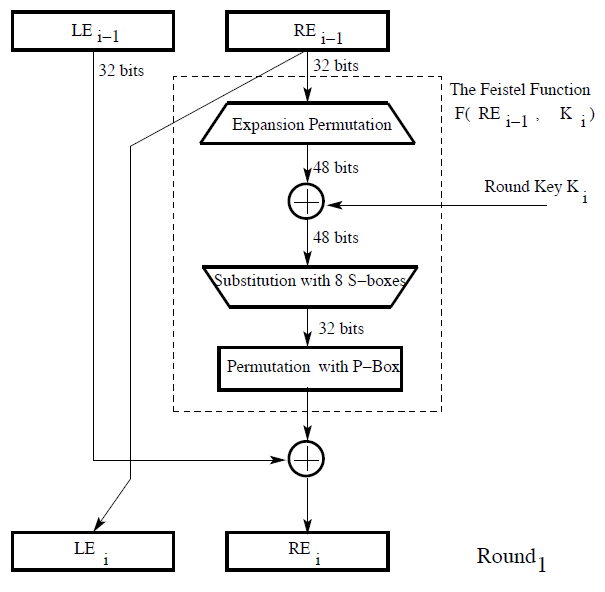
\includegraphics[width=0.7\linewidth]{./round}
	\caption{One round of DES.}
	\label{fig:round}
	\end{figure}

\subsection{DES Modifications}
	In order to facilitate the process by which traces are obtained, there was an addition to the traditional DES algorithm.  This slight modification in no way compromises the integrity of the algorithm or its outputs.  The change was to hold a general purpose input/output (GPIO) high during the algorithm except during a single instruction in which the output of the Feistel function is xored with the other half of the plaintext in round 16 and the result is written back to a register.  This allowed an oscilloscope to be triggered on the falling edge of the GPIO and frame this critical step which will be discussed later.  There were also two no-operations (nops) added before this register write and one after to allow the GPIO to settle and facilitate a cleaner capture.  The output of the assembly dump with comments added can be seen in figure \ref{fig:asm_snippet}.  Note that the register where the xor is written to (R0) is set to zero before the output of the xor is written there.
	
	\begin{figure}[h]
	\centering
	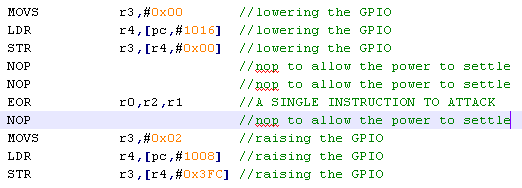
\includegraphics[width=0.7\linewidth]{./asm_snippet}
	\caption{The assembly showing the GPIO writes surrounding the xor and register write under attack.}
	\label{fig:asm_snippet}
	\end{figure}

	

\section{Experimental Setup} \label{sec::expr}
	This portion of the experiment was the most crucial to its success.  The goal is to obtain information about the power usage of the microprocessor during a critical step of the DES algorithm.  During a register write operation the power used will be different depending on the value of the word written.  It is believed that by analyzing this information, the secret key to the algorithm can be obtained.
	
	The oscilloscope used was a Techtronix DP0-2024 the sample rate was 1Gs per second and each trace contained about 270 samples.  The Tiva-C used a 17 MHz clock so there 38.5 samples per clock.
	
	The setup used involved the Tiva-C microprocessor powered by a bench top power supply through a breadboard.  The ground connection between the microprocessor and the power supply had a 1-$\Omega$ resistor added in series.  An Oscilloscope probe was placed on the resistor so that the voltage could be measured.  Then another oscilloscope probe was placed on the GPIO pin discussed in the previous section to act as the trigger.  The voltage data would be taken twenty times for each plain text value used in the DES algorithm and then averaged in an attempt to reduce noise.  91,840 captures with 4,592 unique plain text values would be obtained.  Each trace takes about two seconds to capture so the time to obtain all traces is 183,680 seconds or about 51 hours.  The voltage data acquired would be analyzed later to determine the secret key.  The test setup is illustrated in figure \ref{fig:bench}

	\begin{figure}[h]
	\centering
	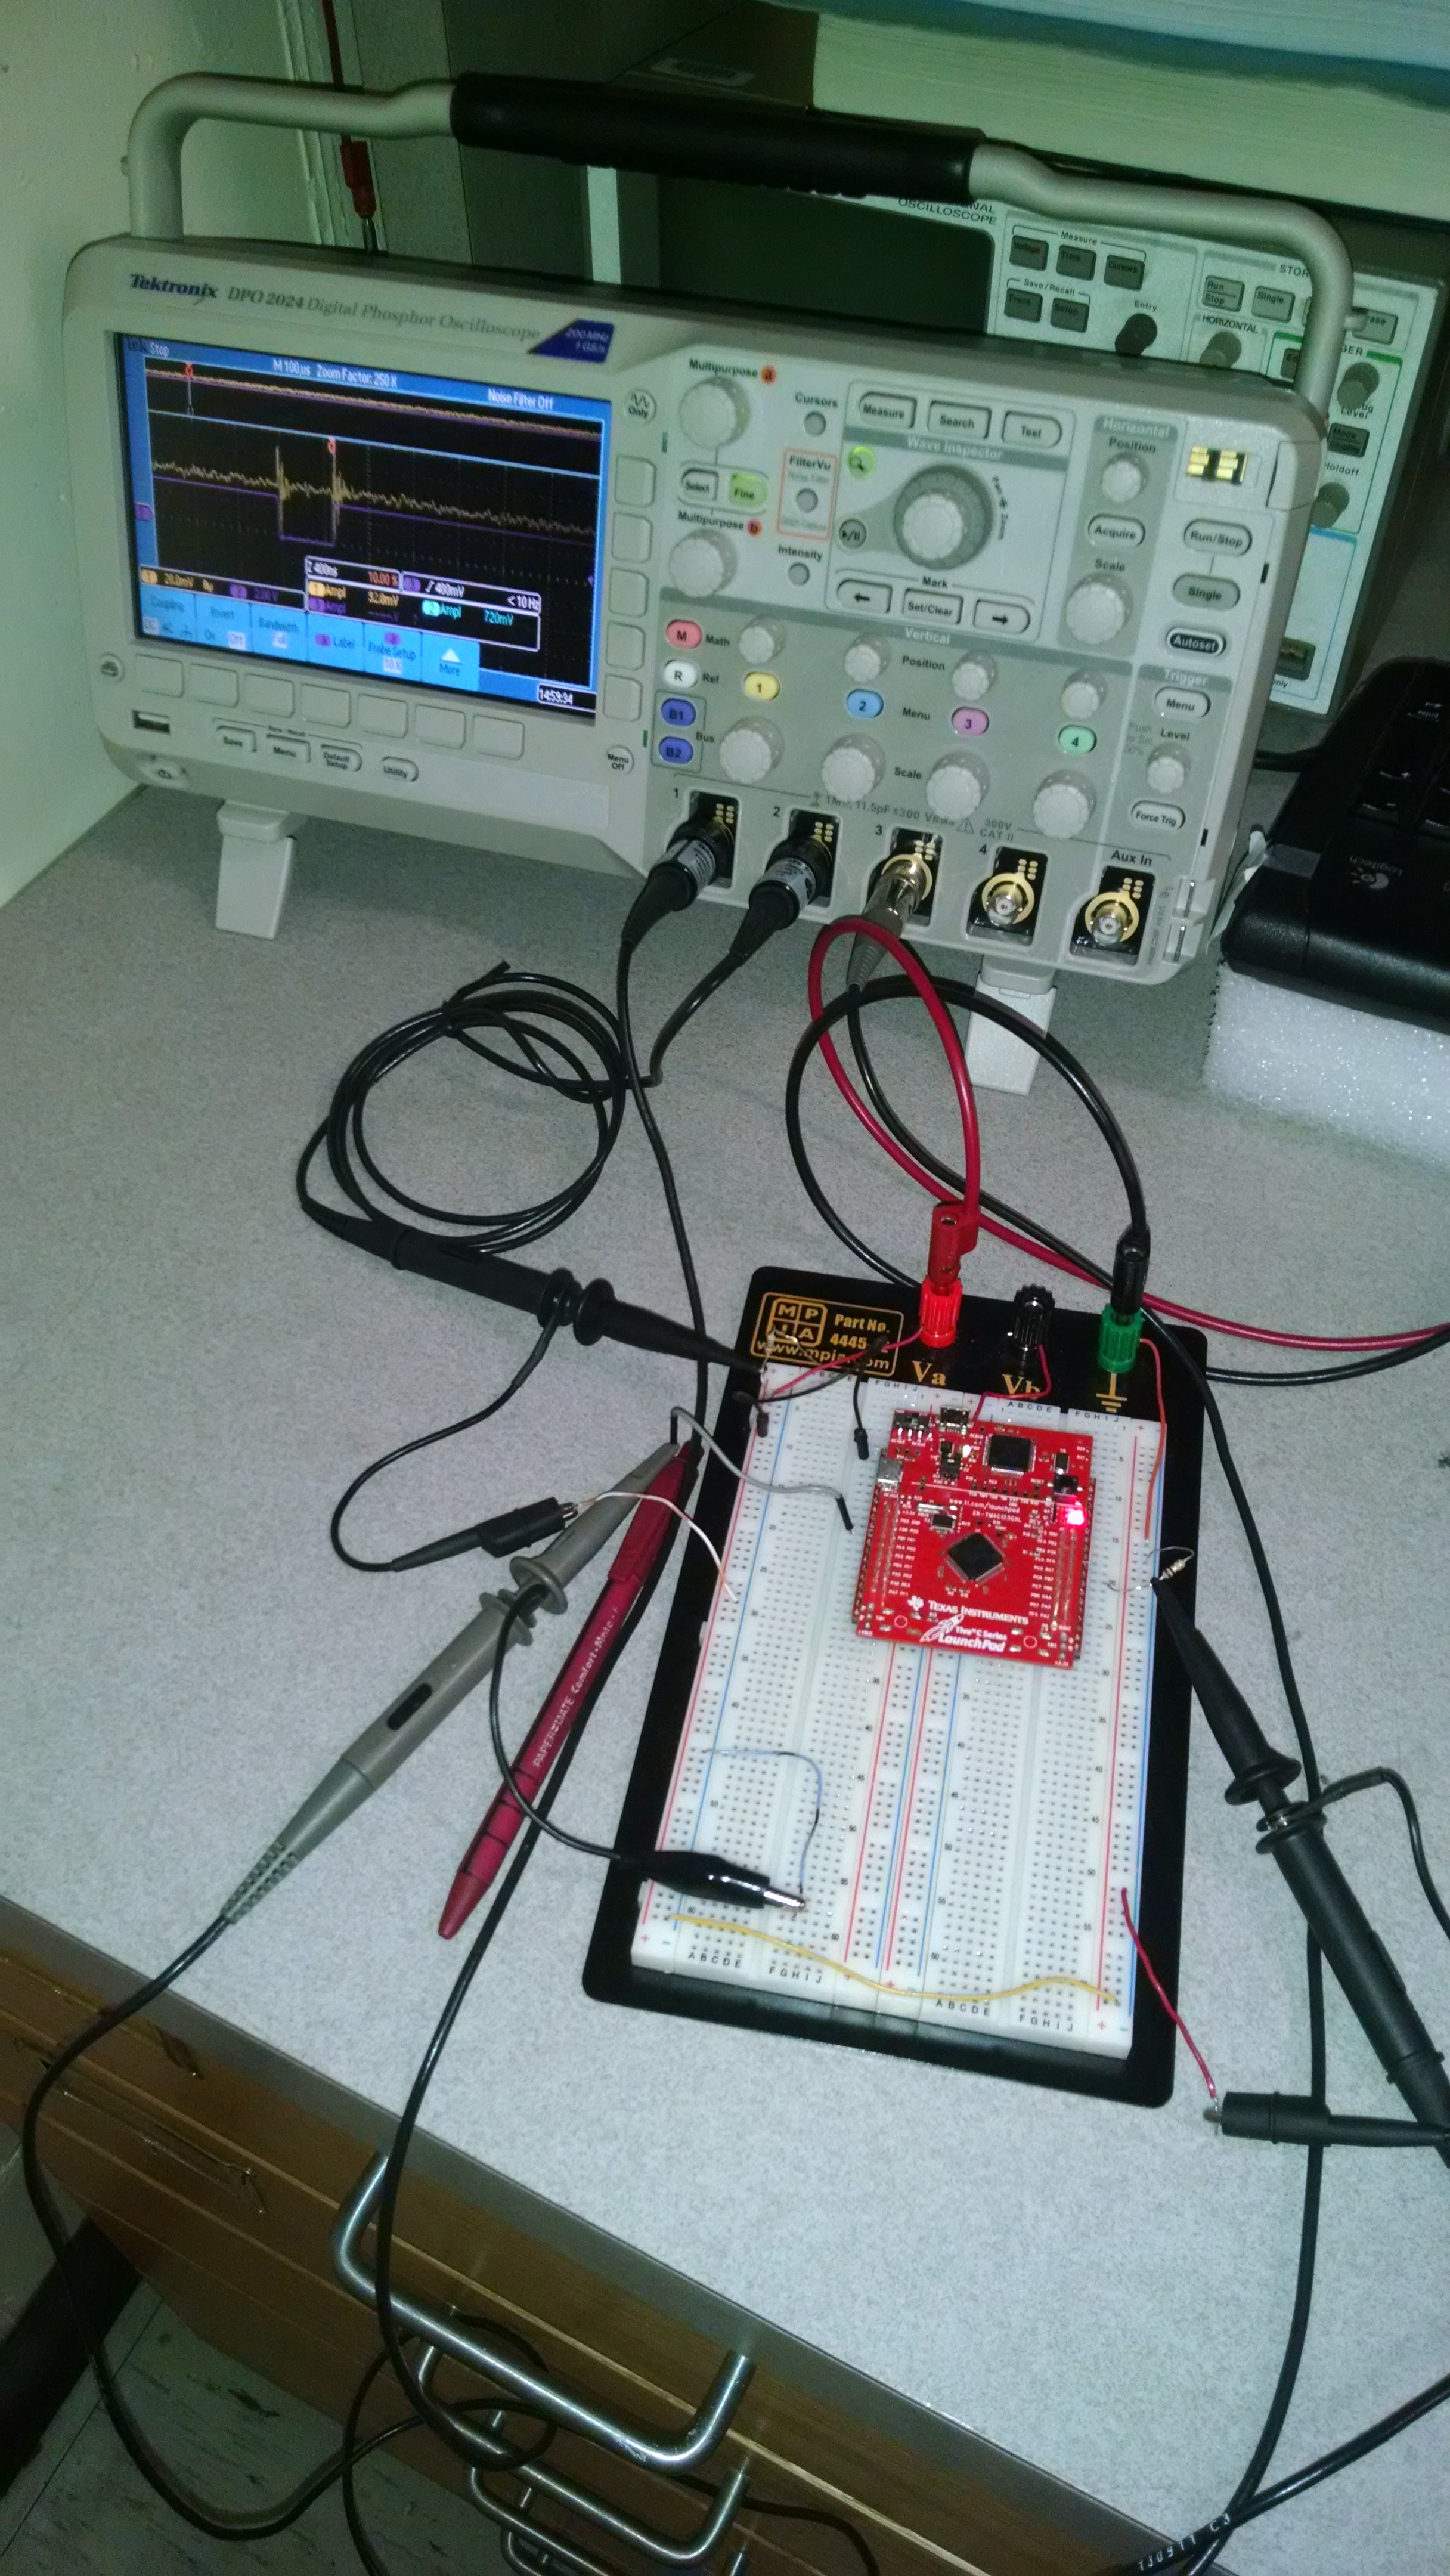
\includegraphics[width=0.7\linewidth]{./bench}
	\caption{Test setup showing the oscilloscope connected to the Tiva-C board.}
	\label{fig:bench}
	\end{figure}
	
	The test setup needed to be automated to facilitate the capturing of the traces.  In order for this to be done a matlab file was written to interface with the oscilloscope.  As trivial as this may sound it was not easy.  It took many hours of learning the oscilloscope and the commands to control it through matlab.  It also took time and patience to fine tune the DES implementation to create enough delay between each run of the algorithm to allow for the oscilloscope to transfer the data capture and re-arm itself.
	

\section{Analysis of the Data}\label{sec::analysis} 
\subsection{Differential Power Analysis}
	In order to analyze the data, differential power analysis (DPA) was employed.  Round 16 was chosen for this because given the cipher text, the input to the Feistel function and the output from the second xor (seen in the bottom right of figure \ref{fig:round}) can be determined.  Then the round key is guessed 6 bits at a time.  This greatly reduces the complexity of the key as there are only 64 possible combinations for a guess of 6 bits of the key.  Using knowledge of the Feistel function and the 6-bit key guess, the output of the Feistel function can be guessed at 4 bits at a time.  Remember, the s-boxes reduce the data from 48 bits to 32 bits.  This output is xored with the D value, and we already know the output of this xor.  So guessing one input and knowing the output determines the other input to the xor gate.  

	For each key guess 4-bits of the D word are deduced.  These 4-bit groups are divided into 3 sets where set 0 contains all guesses for which the four bits guessed are "0000," set 1 contains all guess where the 4 bits are "1111," and set 2 contains all other guessed values.  The average power for each sample point for sets 0 and 1 is calculated.  The two average powers are subtracted from each other.  The correct key guess will show large spikes where the calculation was actually made on the trace.  This is where the difference between the 2 sets of data is the greatest.  This process is repeated 8 times, once for each s-box until the correct key is determined.

  Figures \ref{fig:dpa1} through \ref{fig:dpa8} show the outputs of the DPA.
  
  \begin{figure}[h]
  % This file was created by matlab2tikz.
% Minimal pgfplots version: 1.3
%
%The latest updates can be retrieved from
%  http://www.mathworks.com/matlabcentral/fileexchange/22022-matlab2tikz
%where you can also make suggestions and rate matlab2tikz.
%
\definecolor{mycolor1}{rgb}{0.00000,0.75000,0.75000}%
\definecolor{mycolor2}{rgb}{0.75000,0.00000,0.75000}%
\definecolor{mycolor3}{rgb}{0.75000,0.75000,0.00000}%
%
\begin{tikzpicture}

\begin{axis}[%
width=4.822222in,
height=3.803333in,
at={(0.808889in,0.513333in)},
scale only axis,
separate axis lines,
every outer x axis line/.append style={black},
every x tick label/.append style={font=\color{black}},
xmin=0,
xmax=300,
xlabel={Time (Sample)},
every outer y axis line/.append style={black},
every y tick label/.append style={font=\color{black}},
ymin=-0.0001,
ymax=8e-05,
ylabel={Voltage},
title={$\text{DPA Attack. Voltage difference between traces \textbackslash{} sbox 1, Key60}$}
]
\addplot [color=blue,solid,forget plot]
  table[row sep=crcr]{%
1	7.06788927420758e-06\\
2	6.7790544126152e-06\\
3	6.8901751224832e-06\\
4	6.24620814770275e-06\\
5	4.48881264732484e-06\\
6	1.44111367535431e-06\\
7	-2.99260758494443e-06\\
8	1.9233607720659e-06\\
9	1.2227128558904e-05\\
10	1.59547322563566e-05\\
11	4.07982327314729e-06\\
12	-6.72677683298626e-06\\
13	-3.34704858754448e-06\\
14	5.15366103493765e-06\\
15	1.16499031211073e-05\\
16	1.07628133137493e-05\\
17	4.99490305939899e-06\\
18	-5.478877932593e-06\\
19	-1.26004270076152e-05\\
20	-1.24950326426342e-05\\
21	-4.23803823322404e-06\\
22	6.7655283910702e-06\\
23	1.34629823890188e-05\\
24	1.19823766799574e-05\\
25	3.23573041750586e-06\\
26	-4.2620790087532e-06\\
27	-7.453528983444e-06\\
28	-4.08890644090082e-06\\
29	3.06616149773307e-06\\
30	1.07598020461838e-05\\
31	1.70755161732223e-05\\
32	1.26024509743425e-05\\
33	7.67631341865114e-06\\
34	1.07270236581738e-06\\
35	4.74891705438529e-07\\
36	4.11946340198813e-06\\
37	8.50954596502349e-06\\
38	1.19916079428348e-05\\
39	1.16309469449247e-05\\
40	6.41785039924092e-06\\
41	1.50020363078821e-07\\
42	-5.25742635353087e-06\\
43	-6.40151057028707e-06\\
44	-5.34736946031754e-06\\
45	-2.06261955596181e-06\\
46	-1.33660788112933e-06\\
47	-2.84781991632954e-06\\
48	-6.68373051623469e-06\\
49	-1.03367930000342e-05\\
50	-1.37176072764027e-05\\
51	-1.07512618938918e-05\\
52	-5.14665119895428e-06\\
53	4.27056979600618e-07\\
54	2.88025274901554e-06\\
55	3.75969097483452e-06\\
56	1.59281244986337e-06\\
57	-2.03324735588472e-06\\
58	-3.73337940737109e-06\\
59	-6.50088240012996e-07\\
60	5.42319416504781e-06\\
61	9.4099643337571e-06\\
62	1.07389699983964e-05\\
63	1.04738303570362e-05\\
64	8.14863814190079e-06\\
65	5.14902072097905e-06\\
66	5.19685544682e-06\\
67	5.5534191462309e-06\\
68	8.27901121820424e-06\\
69	1.07518542743976e-05\\
70	1.25527897419427e-05\\
71	1.08629256192257e-05\\
72	5.93619568302773e-06\\
73	1.31399869182777e-06\\
74	8.94445198633582e-07\\
75	-2.53193301163676e-07\\
76	1.78553357439454e-06\\
77	8.15214305989985e-07\\
78	1.10266694640241e-06\\
79	2.02036307988315e-06\\
80	1.90065285267989e-06\\
81	4.57144972787395e-06\\
82	6.41019881770719e-06\\
83	9.85059669994515e-06\\
84	9.42818003430573e-06\\
85	8.70295820014876e-06\\
86	7.08827703661558e-06\\
87	6.20607436843407e-06\\
88	4.98384528996223e-06\\
89	3.07312196867575e-06\\
90	2.86559133150319e-06\\
91	2.91589430944251e-06\\
92	3.38382554394313e-06\\
93	3.92619926199321e-06\\
94	4.32965975144485e-06\\
95	3.02321391107202e-06\\
96	3.55729430203539e-06\\
97	1.98333929827578e-06\\
98	8.80820446999379e-07\\
99	2.4980685927288e-06\\
100	2.3129990497214e-06\\
101	2.40689135987994e-06\\
102	1.88164731145662e-06\\
103	5.50864505299148e-07\\
104	-6.32958570390141e-07\\
105	8.06871613863447e-07\\
106	7.22210566588347e-07\\
107	2.33235014624692e-06\\
108	2.79292598946148e-06\\
109	3.27309975440247e-06\\
110	2.51603746807003e-06\\
111	3.30212639918902e-06\\
112	1.59123276851757e-06\\
113	2.73546508040064e-06\\
114	2.66210862777828e-06\\
115	3.6248256796963e-06\\
116	5.30861790223273e-06\\
117	4.05133964383013e-06\\
118	2.53760999148565e-06\\
119	1.23422478372041e-06\\
120	-6.20271754558747e-07\\
121	-5.83642893285663e-07\\
122	-7.39883251675393e-07\\
123	-2.04025719185204e-07\\
124	-2.35115822730001e-06\\
125	-1.89848079082964e-06\\
126	-2.50621382468083e-06\\
127	-1.77329104394681e-06\\
128	-7.96899875353443e-07\\
129	-1.78429944834926e-06\\
130	-4.09532389638277e-07\\
131	-7.37316269486081e-07\\
132	-1.12848486343974e-06\\
133	-7.36131508473695e-07\\
134	1.05799158326564e-06\\
135	1.43454812476067e-07\\
136	2.47565686358094e-07\\
137	1.69159189919443e-06\\
138	1.61236100655864e-06\\
139	9.35418183610655e-07\\
140	1.73147885325353e-06\\
141	-8.35453973268511e-07\\
142	-1.3977711683477e-06\\
143	-3.61139838823054e-06\\
144	-3.39384664749601e-06\\
145	-3.68564341161632e-06\\
146	-2.55390045539403e-06\\
147	-3.14835429290374e-06\\
148	-1.71622505522415e-06\\
149	-6.6218267533516e-07\\
150	8.50312850959704e-07\\
151	3.820854262062e-07\\
152	-8.92717422161342e-07\\
153	1.36050056156675e-07\\
154	-2.16465709810924e-07\\
155	-1.28502141208929e-06\\
156	-1.99701341495155e-06\\
157	-2.70727764133897e-06\\
158	-3.68490293598195e-06\\
159	-5.68305174690302e-06\\
160	-5.12710264226248e-06\\
161	-2.41627071788982e-06\\
162	7.11350257309729e-08\\
163	4.77952338055233e-07\\
164	1.60041466635164e-06\\
165	2.40541040861988e-06\\
166	1.21462686198878e-06\\
167	-2.34750521418275e-06\\
168	-1.97939009490347e-06\\
169	-2.0743684359904e-06\\
170	-1.92686569005888e-06\\
171	-2.03981290649094e-06\\
172	-3.79636920114831e-06\\
173	-3.28583593528324e-06\\
174	-3.52022115538905e-07\\
175	2.4859247923564e-06\\
176	7.64916264547368e-06\\
177	9.2853669673796e-06\\
178	8.51848103765578e-06\\
179	6.58648138320787e-06\\
180	6.9647657011682e-06\\
181	3.71042466277161e-06\\
182	4.22322872058178e-06\\
183	3.80234237124921e-06\\
184	3.17436967011992e-06\\
185	2.09806365621731e-06\\
186	9.84832590799137e-08\\
187	2.72643127769735e-07\\
188	1.78726135087286e-06\\
189	9.04614397315498e-07\\
190	1.42334226017546e-06\\
191	2.13661775413584e-06\\
192	1.89907317133323e-06\\
193	7.48176578756893e-07\\
194	6.80743931207733e-08\\
195	1.34964025227426e-07\\
196	2.31744190351373e-06\\
197	1.75295264658558e-06\\
198	6.76202347313186e-07\\
199	2.41557960729919e-06\\
200	4.28616914931353e-06\\
201	3.47332436534918e-06\\
202	3.70223006577845e-06\\
203	2.27355638104509e-06\\
204	2.66507053030534e-06\\
205	4.5489392686603e-06\\
206	4.14636734996383e-06\\
207	2.95444840736452e-06\\
208	-4.29920152040207e-07\\
209	-1.96556788310299e-06\\
210	-3.0281010502415e-06\\
211	-2.53425316861736e-06\\
212	-2.05264781744704e-06\\
213	-4.41520936948422e-07\\
214	2.08927667871752e-06\\
215	4.03830727270429e-06\\
216	6.009502770612e-06\\
217	7.86355502350924e-06\\
218	8.02784188376569e-06\\
219	7.84346345135498e-06\\
220	9.36884325364838e-06\\
221	1.04202199212563e-05\\
222	1.19402682990013e-05\\
223	1.22206617383875e-05\\
224	1.13579582618623e-05\\
225	9.7353786915862e-06\\
226	1.09034543188313e-05\\
227	1.13889101432856e-05\\
228	1.13796788804021e-05\\
229	9.78079453035473e-06\\
230	8.79892384208179e-06\\
231	7.66589739476225e-06\\
232	8.89163139123489e-06\\
233	9.44032383468248e-06\\
234	9.18925323032272e-06\\
235	7.10111194757602e-06\\
236	4.96044625997519e-06\\
237	4.29880660010942e-06\\
238	3.4896641943e-06\\
239	2.5992669291262e-06\\
240	3.4752002369522e-06\\
241	2.84698071060987e-06\\
242	1.16580483530866e-06\\
243	2.06306384134113e-06\\
244	9.47265793726712e-07\\
245	1.68310111195013e-06\\
246	2.67272211183691e-06\\
247	3.59792173172321e-06\\
248	4.24726949610835e-06\\
249	3.00815757321108e-06\\
250	3.84770884498398e-06\\
251	3.93528242974457e-06\\
252	4.4925150254815e-06\\
253	4.3875155808417e-06\\
254	5.37274309197165e-06\\
255	4.91419121548525e-06\\
256	3.65656740179601e-06\\
257	-1.50731219687034e-06\\
258	-3.02474422737712e-06\\
259	9.13667946044012e-06\\
260	1.7008132890693e-05\\
261	1.21745547890283e-05\\
262	-4.09004183688031e-06\\
263	-1.00691357415254e-05\\
264	8.41328413284592e-07\\
265	1.33784694368686e-05\\
266	1.89448715891853e-05\\
267	1.6229152525641e-05\\
268	6.29280874749234e-06\\
269	1.16802626221046e-06\\
270	1.57820039738132e-07\\
};
\addplot [color=black!50!green,solid,forget plot]
  table[row sep=crcr]{%
1	-2.95095095094889e-06\\
2	-1.98431765098452e-06\\
3	-7.15382048714804e-07\\
4	-6.17283951037662e-09\\
5	1.04320987654154e-06\\
6	-5.26443109776648e-06\\
7	-9.64614614615191e-06\\
8	6.80680680689195e-07\\
9	2.05323656990363e-05\\
10	2.15360360360326e-05\\
11	6.23957290635593e-08\\
12	-1.48650316983715e-05\\
13	-4.44861528195103e-06\\
14	1.97976309643045e-05\\
15	3.2229896563229e-05\\
16	2.6930764097433e-05\\
17	1.06670003336677e-05\\
18	-3.15315315315323e-06\\
19	-1.1237404070737e-05\\
20	-1.17837837837844e-05\\
21	-4.44260927593776e-06\\
22	2.16649983316494e-06\\
23	3.67367367367635e-06\\
24	-2.7444110777459e-06\\
25	-1.10824157490831e-05\\
26	-1.62467467467462e-05\\
27	-1.3017183850517e-05\\
28	-4.9803136469807e-06\\
29	4.23373373373368e-06\\
30	9.02285618952208e-06\\
31	9.68735402069338e-06\\
32	7.4931598264931e-06\\
33	2.91675008341936e-06\\
34	-4.11077744411244e-07\\
35	3.77711044374611e-07\\
36	4.27994661328108e-06\\
37	5.96062729395913e-06\\
38	6.94294294294228e-06\\
39	4.49849849849587e-06\\
40	-9.17083750414608e-07\\
41	-4.63163163163215e-06\\
42	-7.03203203202647e-06\\
43	-5.54921588255281e-06\\
44	-3.75825825825807e-06\\
45	-1.9657991324638e-06\\
46	2.20537203870705e-06\\
47	4.87854521187374e-06\\
48	4.15198531865217e-06\\
49	2.58124791458099e-06\\
50	2.37604270937782e-06\\
51	4.31865198532045e-06\\
52	7.70203536870542e-06\\
53	9.04270937604392e-06\\
54	7.1296296296295e-06\\
55	4.83566900233868e-06\\
56	2.44778111444703e-06\\
57	-8.80046713380104e-07\\
58	-4.951284617949e-06\\
59	-6.34050717383946e-06\\
60	-6.33483483483948e-06\\
61	-3.26509843176243e-06\\
62	-2.76009342676468e-06\\
63	-3.26793460126654e-06\\
64	-2.37671004337317e-06\\
65	-2.9295962628885e-07\\
66	2.04704704704576e-06\\
67	5.04304304303933e-06\\
68	7.25575575575253e-06\\
69	7.66583249916641e-06\\
70	6.40223556890116e-06\\
71	4.81131131130743e-06\\
72	3.69636302969883e-06\\
73	3.87604270937324e-06\\
74	3.90957624291175e-06\\
75	6.01017684351193e-06\\
76	5.26593259926513e-06\\
77	4.44811478144715e-06\\
78	2.56740073406765e-06\\
79	1.48915582249111e-06\\
80	-7.61261261263656e-07\\
81	-1.94844844845447e-06\\
82	-2.8798798798798e-06\\
83	-1.32749416082659e-06\\
84	-2.74274274278397e-07\\
85	-1.50817484150662e-07\\
86	1.21955288621793e-06\\
87	1.88822155489099e-06\\
88	8.25325325320807e-07\\
89	1.04671338004535e-06\\
90	-1.80513847179015e-07\\
91	-1.77894561228164e-06\\
92	-2.20670670671424e-06\\
93	-2.57974641308016e-06\\
94	-2.21071071071412e-06\\
95	-2.70954287620714e-06\\
96	-3.08958958959368e-06\\
97	-2.29329329329633e-06\\
98	-1.36636636641381e-07\\
99	-6.25625625623981e-07\\
100	-7.29729729727693e-07\\
101	3.17817817817485e-07\\
102	1.35635635635338e-07\\
103	1.18885552219221e-06\\
104	1.17217217217302e-06\\
105	1.47313980647813e-06\\
106	2.92759426092498e-06\\
107	2.85618952285561e-06\\
108	3.26810143476972e-06\\
109	3.5352018685356e-06\\
110	3.21237904571175e-06\\
111	2.05238571905761e-06\\
112	2.55588922255063e-06\\
113	3.68218218218218e-06\\
114	3.71571571571375e-06\\
115	5.2547547547523e-06\\
116	3.90290290290356e-06\\
117	3.72589255922835e-06\\
118	3.29863196529574e-06\\
119	3.98865532198842e-06\\
120	4.06706706706193e-06\\
121	5.30380380380467e-06\\
122	5.98415081748014e-06\\
123	4.11478144811059e-06\\
124	5.1991991991962e-06\\
125	3.36019352685643e-06\\
126	2.10043376710004e-06\\
127	1.14014014014055e-06\\
128	6.42142142141724e-07\\
129	-7.17217217218076e-07\\
130	-8.79879879884735e-07\\
131	-2.03920587253919e-06\\
132	-2.5488822155452e-06\\
133	-2.94277610944031e-06\\
134	-3.21421421421806e-06\\
135	-1.72405739072654e-06\\
136	-1.77410744077282e-06\\
137	-2.33667000333355e-06\\
138	-2.66766766766902e-06\\
139	-3.37804471137702e-06\\
140	-3.54421087754749e-06\\
141	-2.64831498164369e-06\\
142	-2.92525859192779e-06\\
143	-1.85118451785605e-06\\
144	-2.22088755421571e-06\\
145	-2.07157157157238e-06\\
146	-2.76059392726076e-06\\
147	-2.55705705705725e-06\\
148	-5.07624290957236e-06\\
149	-5.22305638972053e-06\\
150	-4.08008008008064e-06\\
151	-1.14881548214998e-06\\
152	6.39639639640061e-07\\
153	3.50517183853559e-07\\
154	1.09609609612663e-07\\
155	8.52185518848518e-07\\
156	7.98965632294382e-07\\
157	1.37871204537472e-06\\
158	1.94577911244442e-06\\
159	-2.33900567232857e-07\\
160	8.40674007342342e-07\\
161	-4.8214881549942e-08\\
162	-3.76993660326699e-06\\
163	-1.70920920920976e-06\\
164	-5.84751418083659e-07\\
165	-2.36903570241878e-08\\
166	4.79813146478381e-07\\
167	2.66266266264747e-07\\
168	1.22956289624714e-07\\
169	-2.93293293297803e-07\\
170	-4.50784117447985e-07\\
171	-8.17484150849798e-08\\
172	-8.04137470798716e-07\\
173	-9.91324657986792e-07\\
174	-3.50233566900199e-06\\
175	-4.69536202869335e-06\\
176	-4.39939939939765e-06\\
177	-3.86219552886077e-06\\
178	-4.31081081081214e-06\\
179	-4.23223223223416e-06\\
180	-2.52035368701869e-06\\
181	-1.91074407740899e-06\\
182	-2.15465465465501e-06\\
183	-2.73189856523325e-06\\
184	-3.10877544211063e-06\\
185	-2.49265932599808e-06\\
186	-2.51518184851522e-06\\
187	-1.73890557223812e-06\\
188	-1.12162162162373e-06\\
189	-2.8228228228077e-07\\
190	-1.02569235902773e-06\\
191	-2.48365031698533e-06\\
192	-3.60460460460763e-06\\
193	-2.32148815482516e-06\\
194	-1.13963963964143e-06\\
195	7.81281281281299e-07\\
196	1.10093426759859e-06\\
197	1.21888555221997e-06\\
198	-1.17117117118086e-07\\
199	-1.90407073740254e-06\\
200	-3.26009342675737e-06\\
201	-3.8601935268617e-06\\
202	-2.18234901568255e-06\\
203	-2.68768768770314e-07\\
204	6.67334000385711e-09\\
205	3.11194527861068e-06\\
206	3.95428762095529e-06\\
207	5.6192859526176e-06\\
208	5.33400066733518e-06\\
209	6.40657323990653e-06\\
210	7.01885218551846e-06\\
211	7.70570570570762e-06\\
212	8.22839506172974e-06\\
213	6.49432766099394e-06\\
214	5.33566900233831e-06\\
215	3.78828828829191e-06\\
216	2.14781448115188e-06\\
217	1.56906906906978e-06\\
218	5.59726393058353e-07\\
219	-7.72939606277778e-07\\
220	-2.69302635969547e-06\\
221	-1.72222222222154e-06\\
222	-2.12162162162299e-06\\
223	-1.15932599266226e-06\\
224	5.9693026359213e-07\\
225	2.11094427760711e-06\\
226	2.77544210877667e-06\\
227	3.20637303970629e-06\\
228	2.88655321988105e-06\\
229	2.25208541875226e-06\\
230	3.00817484150812e-06\\
231	4.05038371704795e-06\\
232	3.77761094427255e-06\\
233	4.61778445111621e-06\\
234	5.84851518184958e-06\\
235	6.22305638972327e-06\\
236	7.30914247580941e-06\\
237	6.02152152152403e-06\\
238	4.66499833166791e-06\\
239	4.41941941941703e-06\\
240	3.52819486152973e-06\\
241	1.32732732732819e-06\\
242	-1.50950950951207e-06\\
243	1.42976309643224e-07\\
244	1.50717384051098e-06\\
245	3.44711378044531e-06\\
246	5.45011678344722e-06\\
247	8.29479479479579e-06\\
248	4.710210210211e-06\\
249	2.47981314647604e-06\\
250	1.20603937270574e-06\\
251	-9.97831164497448e-07\\
252	-9.09743076407156e-07\\
253	-1.43309976643156e-06\\
254	-2.27911244577751e-06\\
255	6.24290957627199e-07\\
256	1.97380714047658e-06\\
257	1.29656322989647e-05\\
258	1.73693693693688e-05\\
259	7.3006339673025e-07\\
260	-2.02507507507511e-05\\
261	-1.4890890890888e-05\\
262	1.26738405071773e-05\\
263	2.49537871204564e-05\\
264	4.27293960627282e-06\\
265	-2.54310977644317e-05\\
266	-3.64185852519162e-05\\
267	-2.43760427093755e-05\\
268	-2.62112112112134e-06\\
269	1.29279279279231e-05\\
270	1.72874541207874e-05\\
};
\addplot [color=red,solid,forget plot]
  table[row sep=crcr]{%
1	-9.58475211478883e-06\\
2	-8.01851256975166e-06\\
3	-7.47474747475347e-06\\
4	-6.64991493260197e-06\\
5	-6.02015443004582e-06\\
6	-5.41989982272978e-06\\
7	-7.10435330930192e-06\\
8	-6.69807616803832e-06\\
9	-1.35560552521827e-06\\
10	-9.90017965287436e-07\\
11	-3.49725761739951e-06\\
12	-8.48056537102165e-06\\
13	-9.54263482885482e-06\\
14	-8.60306242638029e-06\\
15	-5.26827759336681e-06\\
16	-5.1954170682089e-06\\
17	-8.55047530665923e-06\\
18	-6.5808616197307e-06\\
19	-3.64102747141401e-06\\
20	-1.14996847152367e-06\\
21	-2.2902761418679e-06\\
22	-1.1101212359161e-05\\
23	-1.72353452070765e-05\\
24	-2.1592128588595e-05\\
25	-1.77633103710848e-05\\
26	-1.0969340043548e-05\\
27	-1.52683489785827e-06\\
28	2.37636672972656e-06\\
29	-1.2935003747749e-06\\
30	-6.52327753387569e-06\\
31	-1.26756374106167e-05\\
32	-1.32507644168439e-05\\
33	-9.74698694840336e-06\\
34	-6.00954182579687e-06\\
35	-4.01104091563107e-06\\
36	-6.39121485764699e-06\\
37	-1.14722251966046e-05\\
38	-1.82226029434482e-05\\
39	-2.02814481683753e-05\\
40	-1.87070707070741e-05\\
41	-1.35479173359009e-05\\
42	-7.32312524538616e-06\\
43	-1.63105733423912e-06\\
44	-1.08343743679493e-06\\
45	-1.43579493403021e-06\\
46	-1.95457519839085e-06\\
47	-3.33492760347647e-06\\
48	-1.62763084317601e-06\\
49	1.54301555008347e-06\\
50	6.20309098047379e-06\\
51	6.1517412047454e-06\\
52	1.13340709807178e-06\\
53	-6.03938085209747e-06\\
54	-1.1746582432096e-05\\
55	-1.17908412749432e-05\\
56	-8.85172097892959e-06\\
57	-4.91653876812971e-06\\
58	-2.63064092039357e-06\\
59	-2.19233560576565e-06\\
60	-4.49565144971555e-06\\
61	-7.99152895266005e-06\\
62	-1.34222317402528e-05\\
63	-1.39131717647582e-05\\
64	-1.14965913552475e-05\\
65	-8.04621003914173e-06\\
66	-5.94282043045978e-06\\
67	-5.0933837788987e-06\\
68	-7.61290169063334e-06\\
69	-1.12829115655969e-05\\
70	-1.26761609023068e-05\\
71	-1.03654209943952e-05\\
72	-5.86177439887642e-06\\
73	-1.26932457674301e-06\\
74	-7.83000797133053e-07\\
75	-4.20459007035613e-07\\
76	-2.53322387591855e-07\\
77	-2.05170670188656e-06\\
78	-3.31513009958154e-06\\
79	-4.47947079748861e-06\\
80	-2.96239188111698e-06\\
81	-1.90608083187969e-06\\
82	-3.32788426074711e-06\\
83	-4.06010636399938e-06\\
84	-6.17387062616659e-06\\
85	-7.38456413367991e-06\\
86	-6.04394950684366e-06\\
87	-4.63404361638123e-06\\
88	-2.75066328776861e-06\\
89	-2.45384349977906e-06\\
90	-2.68156238474341e-06\\
91	-4.14476924724466e-06\\
92	-4.92315379948009e-06\\
93	-7.61218783833706e-06\\
94	-1.01135263114089e-05\\
95	-1.00326706404439e-05\\
96	-1.06082735482089e-05\\
97	-8.7586822286401e-06\\
98	-7.82225077631312e-06\\
99	-6.50743001273223e-06\\
100	-5.44816837396746e-06\\
101	-6.24520826640867e-06\\
102	-6.19676149004635e-06\\
103	-5.6779336355308e-06\\
104	-4.998346242166e-06\\
105	-3.84899644263227e-06\\
106	-5.80533247670698e-06\\
107	-7.43577113894878e-06\\
108	-7.58986805629884e-06\\
109	-8.96160664358176e-06\\
110	-8.00780478518812e-06\\
111	-8.96174941404562e-06\\
112	-8.79922903951639e-06\\
113	-5.75212668498491e-06\\
114	-4.28411321698029e-06\\
115	-3.30280424979627e-06\\
116	-4.6349478292889e-06\\
117	-3.81634959726717e-06\\
118	-2.17924831352485e-06\\
119	6.8577411334661e-08\\
120	1.20008090326047e-06\\
121	3.29390489107757e-06\\
122	2.72910494818635e-06\\
123	1.09733376163967e-06\\
124	-1.62577482719188e-06\\
125	-4.42141081010219e-06\\
126	-6.77883665869483e-06\\
127	-8.59830341101882e-06\\
128	-8.68820121117161e-06\\
129	-9.67393606263059e-06\\
130	-1.09714340103045e-05\\
131	-9.87852613294499e-06\\
132	-9.36783619468699e-06\\
133	-9.2948328990726e-06\\
134	-8.40784761632542e-06\\
135	-4.79708748259578e-06\\
136	-2.68375153181233e-06\\
137	5.6727463091516e-08\\
138	6.55078464265046e-07\\
139	-1.38929935396357e-06\\
140	-3.73087768141406e-06\\
141	-5.14311548941012e-06\\
142	-4.90392737742757e-06\\
143	-2.83894302269229e-06\\
144	-1.86115572687901e-06\\
145	-2.46074407205064e-06\\
146	-2.57358032623115e-06\\
147	3.45123793881949e-07\\
148	2.48192169040665e-06\\
149	2.86407062378632e-06\\
150	2.23745107137251e-06\\
151	2.03424111551529e-06\\
152	1.88223816492781e-06\\
153	2.24187695565658e-06\\
154	-7.32888365420972e-08\\
155	-1.80480898502242e-06\\
156	-2.30003212335454e-06\\
157	-3.57159343731834e-06\\
158	-4.33969851637919e-06\\
159	-4.76191835908869e-06\\
160	-5.49033325004901e-06\\
161	-5.7449881619492e-06\\
162	-4.97950054133625e-06\\
163	-3.18735053717305e-06\\
164	-2.90937645001498e-06\\
165	-3.6571129433385e-06\\
166	-3.84514164019668e-06\\
167	-2.52280163233736e-06\\
168	-3.89073300734264e-06\\
169	-3.91176785522872e-06\\
170	-3.12172371536457e-06\\
171	-3.36500458055465e-06\\
172	-5.3277176952117e-06\\
173	-6.06022533937694e-06\\
174	-6.68789187517182e-06\\
175	-6.0317188373734e-06\\
176	-6.69698159450755e-06\\
177	-9.28426788497378e-06\\
178	-7.92142865640826e-06\\
179	-6.21441743703204e-06\\
180	-3.20134204232891e-06\\
181	-1.65551867318224e-06\\
182	-9.63510249727545e-07\\
183	-1.27893778777491e-06\\
184	-2.17986698552042e-06\\
185	-4.22600563891942e-08\\
186	-1.16181841977158e-06\\
187	-2.42957252144689e-06\\
188	-3.98629403575851e-06\\
189	-4.44106554353587e-06\\
190	-6.25701062450558e-06\\
191	-8.02864927246672e-06\\
192	-8.02189147065379e-06\\
193	-8.56051682906773e-06\\
194	-8.15999809639697e-06\\
195	-7.94184483230397e-06\\
196	-8.48860810698064e-06\\
197	-9.3867294856699e-06\\
198	-9.53487763381226e-06\\
199	-9.81251858990593e-06\\
200	-9.77930066269148e-06\\
201	-8.44744262411962e-06\\
202	-8.82302411631206e-06\\
203	-5.96723417925146e-06\\
204	-7.05000535389157e-06\\
205	-7.52071956312567e-06\\
206	-6.00578220366459e-06\\
207	-6.43942368323564e-06\\
208	-5.90603324172184e-06\\
209	-2.6120331703388e-06\\
210	9.3181520741635e-08\\
211	-1.05283696803186e-06\\
212	6.01967852850195e-07\\
213	-1.65304398519993e-06\\
214	-2.88534342244174e-06\\
215	-3.70950970244276e-06\\
216	-3.60799990481702e-06\\
217	-2.43771043770963e-06\\
218	-1.80495175547846e-06\\
219	-3.69504229574477e-06\\
220	-6.52327753387309e-06\\
221	-7.45171384039945e-06\\
222	-7.26925319151188e-06\\
223	-8.01608547191645e-06\\
224	-7.31056144483329e-06\\
225	-7.82491582491766e-06\\
226	-7.16374582099191e-06\\
227	-8.10831518958596e-06\\
228	-8.74302506811454e-06\\
229	-7.87540897788288e-06\\
230	-7.33064448965592e-06\\
231	-7.03306325921648e-06\\
232	-6.0116357925525e-06\\
233	-6.67780276261166e-06\\
234	-5.82327396461257e-06\\
235	-5.05721526216241e-06\\
236	-6.21998548500698e-06\\
237	-5.83816968269604e-06\\
238	-7.34615887972804e-06\\
239	-6.3150706118946e-06\\
240	-6.80267932564455e-06\\
241	-4.92729414283861e-06\\
242	-6.45936395759703e-06\\
243	-7.73972944997925e-06\\
244	-9.15077750413777e-06\\
245	-7.28714708927124e-06\\
246	-7.99224280496977e-06\\
247	-9.45040511118444e-06\\
248	-1.14480969887355e-05\\
249	-1.20132300627041e-05\\
250	-1.11311465657779e-05\\
251	-9.36003140949906e-06\\
252	-8.13111087315591e-06\\
253	-7.6086661669663e-06\\
254	-6.94268955752676e-06\\
255	-5.22478019297952e-06\\
256	-5.87595626464887e-06\\
257	5.3610308027802e-07\\
258	5.48143389132727e-06\\
259	-2.30540981071011e-06\\
260	-1.06273096096416e-05\\
261	-1.12747260591793e-05\\
262	-7.52067197292566e-07\\
263	6.59161699444492e-06\\
264	2.72867663680379e-06\\
265	-9.13954622788521e-06\\
266	-1.72227814065262e-05\\
267	-1.27009077821776e-05\\
268	-2.00663882641942e-06\\
269	6.18686273809801e-06\\
270	5.2540957275922e-06\\
};
\addplot [color=mycolor1,solid,forget plot]
  table[row sep=crcr]{%
1	6.6155227922797e-06\\
2	6.478561854888e-06\\
3	3.90089953157795e-06\\
4	4.92749858369002e-06\\
5	6.85103149050594e-06\\
6	9.8166392615848e-06\\
7	8.29022674828529e-06\\
8	1.07711652457248e-06\\
9	-2.56804521148266e-06\\
10	6.79073109394884e-06\\
11	1.45092923961214e-05\\
12	1.24144201406632e-05\\
13	2.62132622182686e-06\\
14	-3.85314559699177e-06\\
15	-2.54709759434264e-06\\
16	-3.18785148747339e-06\\
17	2.63050116759429e-06\\
18	3.82307830484592e-06\\
19	4.47046468889556e-06\\
20	2.36669384145148e-07\\
21	-2.09199817606531e-06\\
22	1.30726395932389e-06\\
23	9.86013734783015e-06\\
24	1.59680535020937e-05\\
25	1.61204349808613e-05\\
26	1.3856986914646e-05\\
27	9.00299843860537e-06\\
28	3.96324494618145e-06\\
29	1.19915435741087e-06\\
30	1.6923905984392e-06\\
31	3.03331444915199e-06\\
32	5.91562918850295e-07\\
33	-2.07027676831818e-06\\
34	-3.18199278716595e-06\\
35	-2.2028713158582e-06\\
36	-5.28167359855648e-07\\
37	2.7945447762228e-06\\
38	4.40541100717303e-06\\
39	4.88239764546506e-06\\
40	3.78776029072436e-06\\
41	2.94134390846964e-06\\
42	-4.27242956435245e-07\\
43	1.29698359839937e-06\\
44	3.68766494866866e-06\\
45	6.13306434898032e-06\\
46	7.0298323914279e-06\\
47	6.56224178193117e-06\\
48	3.10157383482182e-06\\
49	-3.2758978044372e-07\\
50	-1.32312666675707e-06\\
51	-3.79743267331194e-06\\
52	-2.71661300797147e-06\\
53	9.62650785535021e-07\\
54	4.38684003260977e-06\\
55	4.6311367813091e-06\\
56	4.74880822429018e-06\\
57	2.69262549916363e-06\\
58	4.21306877064227e-06\\
59	4.92910143565879e-06\\
60	6.45761423775145e-06\\
61	6.58744524740379e-06\\
62	7.90029155324501e-06\\
63	6.85407138218503e-06\\
64	6.03026073979756e-06\\
65	2.80642798911046e-06\\
66	3.02242610990613e-06\\
67	4.56171670973077e-06\\
68	7.99673902529986e-06\\
69	8.56309847867536e-06\\
70	8.87626259137367e-06\\
71	6.44584156637333e-06\\
72	3.27672686573684e-06\\
73	1.3101380387107e-06\\
74	9.29654143233712e-07\\
75	5.44472233353008e-07\\
76	1.35800251484935e-07\\
77	-7.24599632445817e-07\\
78	-1.6371198408114e-07\\
79	-5.65751475040295e-07\\
80	-5.73710464130909e-07\\
81	-1.80464550717484e-06\\
82	-5.54642052757147e-07\\
83	1.0983957662589e-06\\
84	8.81015876524373e-07\\
85	6.39593207225723e-07\\
86	7.88105732959545e-07\\
87	1.55642453469104e-06\\
88	-3.47282751378929e-06\\
89	-5.41377070926215e-06\\
90	-7.24721228116242e-06\\
91	-5.86251399041201e-06\\
92	-3.5988448411641e-06\\
93	-2.24432438407796e-06\\
94	-1.73472799878385e-06\\
95	-8.8930649017006e-07\\
96	1.14123060341881e-06\\
97	3.09472026087908e-06\\
98	4.10822014342525e-06\\
99	6.04689723784392e-06\\
100	7.03165632643006e-06\\
101	6.11465918669198e-06\\
102	7.3499053488274e-06\\
103	5.54172251316255e-06\\
104	5.48877312735868e-06\\
105	5.82365864780065e-06\\
106	6.46695499578395e-06\\
107	6.67947105884893e-06\\
108	6.92017520830023e-06\\
109	6.82074311533472e-06\\
110	9.2323720827384e-06\\
111	9.05279739122104e-06\\
112	8.44476378660062e-06\\
113	8.62013790053906e-06\\
114	8.74715010156218e-06\\
115	7.63946884802229e-06\\
116	6.5949620704402e-06\\
117	5.88069806966695e-06\\
118	6.6155227922797e-06\\
119	7.19359964627183e-06\\
120	6.78669632863619e-06\\
121	5.38414558317463e-06\\
122	5.09004988185876e-06\\
123	4.271103066143e-06\\
124	4.1341421287526e-06\\
125	2.8857967970604e-06\\
126	2.70986997554477e-06\\
127	1.54813392104665e-06\\
128	3.27285791270216e-06\\
129	3.64615660968827e-06\\
130	4.26330988932168e-06\\
131	3.43916762238824e-06\\
132	6.61237235909714e-06\\
133	5.75550980365207e-06\\
134	5.42742258639612e-06\\
135	6.18595846402399e-06\\
136	8.2878501057055e-06\\
137	8.24993436597272e-06\\
138	9.06141962940619e-06\\
139	9.25016926669412e-06\\
140	8.78595017340771e-06\\
141	5.12210692128106e-06\\
142	3.36764726202587e-06\\
143	3.86022025397007e-06\\
144	3.38091224385152e-06\\
145	3.00954802338015e-06\\
146	4.45786295615556e-06\\
147	3.93428306918586e-06\\
148	5.71040886543275e-06\\
149	4.81391717677485e-06\\
150	4.43619681917036e-06\\
151	2.39620842602817e-06\\
152	1.88843597573665e-06\\
153	1.70162081496606e-06\\
154	2.65399123958437e-06\\
155	3.93450415221361e-06\\
156	5.57460861394781e-06\\
157	7.2338367578138e-06\\
158	6.85451354824141e-06\\
159	6.30490113443308e-06\\
160	5.61385085185969e-06\\
161	6.27704467258752e-06\\
162	5.69974160921378e-06\\
163	4.36417902198276e-06\\
164	1.59069240441255e-06\\
165	1.65524864932046e-06\\
166	2.31584474446114e-07\\
167	6.01069489160333e-07\\
168	6.69992123920361e-07\\
169	1.04323555014975e-06\\
170	2.88800762736699e-06\\
171	2.1696535905261e-06\\
172	2.13140622625039e-06\\
173	-8.22594685717486e-07\\
174	-1.82957261886819e-06\\
175	1.51989056389624e-06\\
176	2.52769755841424e-06\\
177	2.82787304306791e-06\\
178	3.65196003924376e-06\\
179	4.86194746514984e-06\\
180	4.31913335452276e-06\\
181	5.59516933578384e-06\\
182	7.30303574635917e-06\\
183	7.32359646820127e-06\\
184	7.36013043898826e-06\\
185	5.72925619377659e-06\\
186	5.42974395821311e-06\\
187	3.8995177626417e-06\\
188	4.4060742562602e-06\\
189	4.37672548396061e-06\\
190	4.08329303173624e-06\\
191	2.96278896243143e-06\\
192	2.4476655013728e-06\\
193	4.49727100633891e-06\\
194	4.9066615080617e-06\\
195	5.37121222589105e-06\\
196	7.47752552818139e-06\\
197	8.50307443588973e-06\\
198	9.52287518481143e-06\\
199	9.17406143344582e-06\\
200	8.45990797418948e-06\\
201	7.00783462989803e-06\\
202	5.5590775310593e-06\\
203	2.22763261527575e-06\\
204	9.27111688382026e-07\\
205	-8.12811761616468e-07\\
206	-1.69426980419982e-06\\
207	-1.01875060452145e-06\\
208	-1.09944591065395e-06\\
209	-7.92140498265259e-07\\
210	-2.9528954968187e-06\\
211	-2.38570698207936e-06\\
212	-1.88500918876181e-06\\
213	-2.90746293404778e-06\\
214	-2.82483315139793e-06\\
215	-1.27830208232482e-06\\
216	5.75755482170801e-07\\
217	3.0705669397937e-06\\
218	5.50778626798049e-06\\
219	5.01007309557794e-06\\
220	5.18202042254588e-06\\
221	4.59206035567216e-06\\
222	4.83702035345476e-06\\
223	5.46047449945675e-06\\
224	3.1968606209673e-06\\
225	1.96294095701488e-06\\
226	2.01080543311364e-06\\
227	1.14631551310224e-07\\
228	-5.56576529275356e-07\\
229	-1.4079672797122e-06\\
230	-1.8633983225342e-06\\
231	-9.19705406849519e-08\\
232	9.40874107030303e-07\\
233	2.89253982949187e-06\\
234	2.33137582733578e-06\\
235	1.41647897638261e-06\\
236	3.73541888325311e-06\\
237	3.04143925052708e-06\\
238	3.69916126625233e-06\\
239	1.72743225877736e-06\\
240	-1.68343673571415e-06\\
241	-6.74911221348364e-07\\
242	6.2527808100156e-07\\
243	1.77695485760899e-06\\
244	6.11902557652935e-07\\
245	7.48310787467878e-07\\
246	1.44433543822816e-06\\
247	1.9547608848848e-06\\
248	4.28884497934243e-06\\
249	6.85821668900636e-06\\
250	7.31127108924857e-06\\
251	6.5903745975612e-06\\
252	7.73923256552726e-06\\
253	5.87798980254423e-06\\
254	5.93232095728955e-06\\
255	3.9220682317492e-06\\
256	4.76892678006723e-06\\
257	8.66910779179783e-06\\
258	1.69055008221528e-05\\
259	1.51299277334844e-05\\
260	-1.330864572826e-06\\
261	-1.06191706622785e-05\\
262	-1.5462547152895e-06\\
263	1.38381395862991e-05\\
264	1.43969269458762e-05\\
265	4.25468765113068e-06\\
266	-9.46279587127168e-06\\
267	-7.57579693523146e-06\\
268	4.82790067849251e-07\\
269	1.33591632007317e-05\\
270	2.30173964709613e-05\\
};
\addplot [color=mycolor2,solid,forget plot]
  table[row sep=crcr]{%
1	-6.89725490196375e-06\\
2	-6.51450980392477e-06\\
3	-6.31686274509598e-06\\
4	-5.95764705882667e-06\\
5	-3.6039215686309e-06\\
6	-7.35215686274455e-06\\
7	-1.04549019607856e-05\\
8	-5.80235294117895e-06\\
9	3.22588235294585e-06\\
10	5.19450980392046e-06\\
11	-4.82901960784359e-06\\
12	-1.21482352941141e-05\\
13	-5.67137254901644e-06\\
14	4.37882352941153e-06\\
15	1.04392156862754e-05\\
16	9.08313725490146e-06\\
17	3.07764705882372e-06\\
18	-7.85098039215418e-07\\
19	-2.84313725490187e-06\\
20	-1.78588235294009e-06\\
21	-1.74509803921785e-06\\
22	-5.55372549019455e-06\\
23	-8.93568627450929e-06\\
24	-1.13317647058857e-05\\
25	-7.30431372549098e-06\\
26	-2.89019607843622e-06\\
27	4.06823529411349e-06\\
28	7.28784313725785e-06\\
29	3.2439215686287e-06\\
30	-2.69803921568428e-06\\
31	-6.29411764705747e-06\\
32	-5.66823529411743e-06\\
33	-1.79607843137303e-06\\
34	-8.34509803919904e-07\\
35	-1.5215686274485e-06\\
36	-3.43215686274528e-06\\
37	-5.87686274509686e-06\\
38	-5.06352941176662e-06\\
39	-3.43215686274961e-06\\
40	2.55372549019675e-06\\
41	3.78039215686654e-06\\
42	7.82431372549049e-06\\
43	6.6305882352952e-06\\
44	4.36078431372434e-06\\
45	2.05647058823446e-06\\
46	2.23137254902039e-06\\
47	2.2486274509799e-06\\
48	4.4478431372565e-06\\
49	6.19137254902809e-06\\
50	9.37568627450928e-06\\
51	7.64784313725484e-06\\
52	2.76078431372603e-06\\
53	-2.96392156863036e-06\\
54	-5.60627450980206e-06\\
55	-4.15764705882652e-06\\
56	9.09803921549449e-08\\
57	2.94666666666478e-06\\
58	3.57098039215683e-06\\
59	1.87843137255299e-06\\
60	-9.4823529412074e-07\\
61	-4.80549019607653e-06\\
62	-6.86117647058591e-06\\
63	-6.60000000000591e-06\\
64	-6.16078431372753e-06\\
65	-1.96705882353227e-06\\
66	-1.96235294117487e-06\\
67	-2.72313725489803e-06\\
68	-5.75529411764222e-06\\
69	-7.26509803921499e-06\\
70	-6.54823529411784e-06\\
71	-3.62745098039406e-06\\
72	-1.03372549019407e-06\\
73	8.31372549007017e-08\\
74	-5.75686274512099e-07\\
75	-2.63999999999907e-06\\
76	-6.3796078431386e-06\\
77	-8.15607843137472e-06\\
78	-7.56862745098126e-06\\
79	-7.86431372549199e-06\\
80	-5.32156862744848e-06\\
81	-4.35372549019777e-06\\
82	-6.02352941176439e-06\\
83	-6.13960784313743e-06\\
84	-5.60313725489914e-06\\
85	-4.40000000000249e-06\\
86	-2.04235294117786e-06\\
87	-6.58039215685122e-07\\
88	8.97254901960354e-07\\
89	-5.17647058824282e-07\\
90	-2.01411764706293e-06\\
91	-3.69960784313761e-06\\
92	-6.58745098039513e-06\\
93	-6.79843137254589e-06\\
94	-5.97960784314271e-06\\
95	-3.3576470588252e-06\\
96	-1.82980392156524e-06\\
97	-9.85882352945271e-07\\
98	-1.82745098037569e-07\\
99	-9.43529411769409e-07\\
100	-1.89960784314179e-06\\
101	-2.22666666666559e-06\\
102	-2.92392156862886e-06\\
103	-2.92941176470701e-06\\
104	-3.99843137255038e-06\\
105	-6.05803921568688e-06\\
106	-6.79215686274787e-06\\
107	-7.16549019607899e-06\\
108	-4.50588235293868e-06\\
109	-3.02666666666734e-06\\
110	-1.93333333333356e-06\\
111	-2.99607843136547e-07\\
112	6.40784313722578e-07\\
113	2.98039215688127e-07\\
114	-1.53098039216114e-06\\
115	-2.95764705882454e-06\\
116	-3.60627450980439e-06\\
117	-4.43607843136906e-06\\
118	-5.29490196078414e-06\\
119	-6.15372549019576e-06\\
120	-5.22745098039193e-06\\
121	-6.25647058823293e-06\\
122	-3.5356862745084e-06\\
123	-2.97960784313668e-06\\
124	-1.29176470588677e-06\\
125	6.65882352944569e-07\\
126	-6.42352941177069e-07\\
127	-4.4792156862739e-06\\
128	-4.34666666666557e-06\\
129	-5.11372549019673e-06\\
130	-3.19372549019512e-06\\
131	-1.92470588234774e-06\\
132	-2.94352941176967e-06\\
133	-2.76549019608083e-06\\
134	-3.90666666666775e-06\\
135	-1.18509803921554e-06\\
136	-3.56078431373343e-07\\
137	-1.4823529411942e-07\\
138	-1.38745098039045e-06\\
139	-3.29882352941187e-06\\
140	-2.7419607843155e-06\\
141	-2.83137254902116e-06\\
142	-2.85098039215373e-06\\
143	-2.86039215686117e-06\\
144	-2.68235294116105e-07\\
145	1.98509803921946e-06\\
146	1.18039215686247e-06\\
147	4.54117647058321e-07\\
148	-2.88470588235418e-06\\
149	-4.36941176470539e-06\\
150	-5.05882352941269e-06\\
151	-3.82039215685893e-06\\
152	-3.88627450980793e-06\\
153	-5.01333333333392e-06\\
154	-5.17333333333297e-06\\
155	-5.83843137254379e-06\\
156	-5.27058823529374e-06\\
157	-4.72313725489917e-06\\
158	-5.49333333332977e-06\\
159	-7.01098039215592e-06\\
160	-9.18352941176471e-06\\
161	-1.01568627451018e-05\\
162	-9.84470588235187e-06\\
163	-1.01435294117633e-05\\
164	-1.21607843137223e-05\\
165	-1.24439215686261e-05\\
166	-1.00078431372521e-05\\
167	-9.13411764705448e-06\\
168	-8.79372549019829e-06\\
169	-1.07270588235288e-05\\
170	-9.91686274509976e-06\\
171	-9.34431372549144e-06\\
172	-7.06117647059166e-06\\
173	-5.82352941176818e-06\\
174	-4.24078431372852e-06\\
175	-5.44784313725576e-06\\
176	-4.42039215686318e-06\\
177	-5.45882352941118e-06\\
178	-4.75607843137323e-06\\
179	-3.5121568627474e-06\\
180	-3.2462745098074e-06\\
181	-4.17960784313866e-06\\
182	-5.14352941176528e-06\\
183	-7.79294117646961e-06\\
184	-6.6235294117643e-06\\
185	-5.16313725490262e-06\\
186	-3.57176470587844e-06\\
187	-1.9552941176431e-06\\
188	-2.50117647058838e-06\\
189	-2.82117647058648e-06\\
190	-2.22431372549382e-06\\
191	-4.35294117646836e-06\\
192	-4.85019607842849e-06\\
193	-6.34745098038961e-06\\
194	-7.34901960784337e-06\\
195	-7.55450980392119e-06\\
196	-8.09882352941025e-06\\
197	-7.96862745098409e-06\\
198	-8.61960784313744e-06\\
199	-8.005490196074e-06\\
200	-7.55137254902175e-06\\
201	-5.40627450980238e-06\\
202	-5.60078431372565e-06\\
203	-3.93803921568386e-06\\
204	-2.99058823529513e-06\\
205	-2.12705882352959e-06\\
206	-6.0235294117774e-07\\
207	-1.20392156863474e-06\\
208	-7.12156862744083e-07\\
209	-2.18274509804044e-06\\
210	-2.72549019608194e-06\\
211	-5.73568627451008e-06\\
212	-7.749019607841e-06\\
213	-9.54980392156492e-06\\
214	-1.10282352941164e-05\\
215	-1.13223529411765e-05\\
216	-1.20603921568646e-05\\
217	-1.02345098039226e-05\\
218	-6.84392156862987e-06\\
219	-5.27607843137101e-06\\
220	-3.4007843137231e-06\\
221	-2.12235294117478e-06\\
222	-2.65176470587956e-06\\
223	-1.89725490195962e-06\\
224	-2.6870588235306e-06\\
225	-1.83529411764815e-06\\
226	-2.67137254901864e-06\\
227	-4.30823529411987e-06\\
228	-5.67529411764876e-06\\
229	-6.93019607843348e-06\\
230	-6.76470588235282e-06\\
231	-6.20941176470401e-06\\
232	-6.72862745098451e-06\\
233	-6.66901960784481e-06\\
234	-5.80000000000372e-06\\
235	-3.44862745097971e-06\\
236	-1.8149019607866e-06\\
237	5.01960784314928e-07\\
238	2.07764705882282e-06\\
239	2.65803921568365e-06\\
240	4.12941176470682e-06\\
241	3.24784313725322e-06\\
242	3.52078431372759e-06\\
243	3.19843137254559e-06\\
244	1.92549019607802e-06\\
245	4.7058823574031e-09\\
246	-2.27843137254671e-06\\
247	-2.75921568627414e-06\\
248	-3.92156862745029e-06\\
249	-3.77490196078537e-06\\
250	-4.07921568627498e-06\\
251	-2.49960784313476e-06\\
252	-3.26980392157013e-06\\
253	-1.94039215686576e-06\\
254	-7.30980392158083e-07\\
255	8.39215686266465e-08\\
256	4.15686274455804e-08\\
257	1.34823529411793e-05\\
258	2.24925490196078e-05\\
259	4.20862745098053e-06\\
260	-2.04972549019628e-05\\
261	-2.04172549019615e-05\\
262	7.82980392156647e-06\\
263	2.3917647058825e-05\\
264	8.15294117647073e-06\\
265	-1.56823529411767e-05\\
266	-2.72313725490211e-05\\
267	-2.13286274509776e-05\\
268	-2.6329411764673e-06\\
269	7.42039215686358e-06\\
270	1.01341176470633e-05\\
};
\addplot [color=mycolor3,solid,forget plot]
  table[row sep=crcr]{%
1	4.55830985915916e-06\\
2	4.47661971831118e-06\\
3	5.05032863850046e-06\\
4	4.83661971831424e-06\\
5	3.89765258216029e-06\\
6	-2.7692018779342e-06\\
7	-1.08621596244104e-05\\
8	-5.23943661972625e-06\\
9	7.74065727699846e-06\\
10	1.00614084507043e-05\\
11	-4.11323943662334e-06\\
12	-1.11923004694871e-05\\
13	-2.08150234742334e-06\\
14	8.51436619717788e-06\\
15	1.26593427230062e-05\\
16	5.24638497652677e-06\\
17	2.7830985915476e-07\\
18	-2.1607511737087e-06\\
19	-4.35981220657132e-06\\
20	-5.98197183098457e-06\\
21	-6.30798122065691e-06\\
22	-4.55699530515705e-06\\
23	-2.1564319248853e-06\\
24	-1.99774647887665e-06\\
25	-1.38535211267757e-06\\
26	-7.33521126758657e-07\\
27	1.06704225352142e-06\\
28	1.18666666666569e-06\\
29	1.12657276995099e-06\\
30	1.51737089198155e-07\\
31	-2.38873239438719e-07\\
32	-8.54272300470152e-07\\
33	-2.15417840375735e-06\\
34	2.00563380280041e-07\\
35	2.39436619718734e-06\\
36	9.46478873253484e-08\\
37	-3.27192488262448e-06\\
38	-4.94816901407862e-06\\
39	-6.11680751173719e-06\\
40	-7.11305164319536e-06\\
41	-4.1958685445989e-06\\
42	-2.65446009389738e-06\\
43	-4.3624413145326e-07\\
44	2.17464788737284e-07\\
45	-1.15399061033101e-06\\
46	-1.07079812206035e-06\\
47	-8.38309859150892e-07\\
48	2.0492018779298e-06\\
49	3.08582159624059e-06\\
50	3.91643192488786e-06\\
51	2.58516431924597e-06\\
52	8.38309859156096e-07\\
53	1.97652582159535e-06\\
54	3.44093896713967e-06\\
55	5.32995305164248e-06\\
56	6.28563380282053e-06\\
57	6.16976525821692e-06\\
58	5.85577464789003e-06\\
59	3.52225352112743e-06\\
60	7.09107981219231e-07\\
61	-3.53295774647815e-06\\
62	-5.20075117370952e-06\\
63	-5.34178403755912e-06\\
64	-5.52600938967356e-06\\
65	-3.36093896713494e-06\\
66	-3.75342723004778e-06\\
67	-3.99286384977077e-06\\
68	-4.93915492958113e-06\\
69	-5.60431924882376e-06\\
70	-5.19154929577888e-06\\
71	-5.57427230046771e-06\\
72	-5.03868544601003e-06\\
73	-2.15305164319099e-06\\
74	7.51737089197194e-07\\
75	2.10197183098549e-06\\
76	4.4446948356848e-06\\
77	3.68713615023393e-06\\
78	3.8792488262886e-06\\
79	5.82103286384363e-06\\
80	7.54291079812282e-06\\
81	6.72619718310001e-06\\
82	8.18441314554344e-06\\
83	7.23962441314882e-06\\
84	7.26948356807866e-06\\
85	6.67793427229935e-06\\
86	5.73032863850163e-06\\
87	4.96356807511318e-06\\
88	4.96037558686113e-06\\
89	3.03342723004772e-06\\
90	2.2578403755932e-06\\
91	1.45352112676132e-06\\
92	4.35868544601536e-06\\
93	5.20225352112829e-06\\
94	6.23117370892289e-06\\
95	6.52187793426847e-06\\
96	7.39323943661947e-06\\
97	7.02553990610411e-06\\
98	6.69596244131515e-06\\
99	3.95849765258329e-06\\
100	3.75981220656837e-06\\
101	2.71887323943874e-06\\
102	3.05183098591854e-06\\
103	3.92281690141105e-06\\
104	4.4512676056355e-06\\
105	3.98215962441311e-06\\
106	3.7628169014068e-06\\
107	3.7744600938994e-06\\
108	1.38272300469634e-06\\
109	8.11830985914929e-07\\
110	-9.63380281664324e-08\\
111	-5.73521126759173e-07\\
112	-1.02159624413255e-06\\
113	-6.57652582158712e-07\\
114	-1.07999999999879e-06\\
115	-2.09765258215883e-06\\
116	-1.96018779342628e-06\\
117	-1.90929577464742e-06\\
118	-7.45915492959999e-07\\
119	1.45446009389583e-06\\
120	2.84882629108044e-06\\
121	2.7382159624419e-06\\
122	2.0751173708906e-06\\
123	2.86478873239753e-06\\
124	1.89596244131373e-06\\
125	1.97671361502894e-06\\
126	2.08431924882515e-06\\
127	3.93446009389325e-06\\
128	3.04244131455649e-06\\
129	2.45295774648109e-06\\
130	1.64957746479153e-06\\
131	3.91305164318921e-06\\
132	5.73539906103312e-06\\
133	6.5481690140843e-06\\
134	6.86234741783826e-06\\
135	5.95192488262852e-06\\
136	7.31455399061078e-06\\
137	8.41971830986034e-06\\
138	9.83605633802717e-06\\
139	9.3091079812176e-06\\
140	8.14760563380961e-06\\
141	6.00882629108119e-06\\
142	6.43117370891606e-06\\
143	5.69333333333248e-06\\
144	4.2974647887304e-06\\
145	5.05352112676292e-06\\
146	6.03718309859658e-06\\
147	5.9697652582168e-06\\
148	5.23812206572934e-06\\
149	2.89690140845185e-06\\
150	3.80657276992727e-07\\
151	-2.22009389671575e-06\\
152	-2.77164319248662e-06\\
153	-2.49483568074988e-06\\
154	-1.6204694835726e-06\\
155	-3.92544600939359e-06\\
156	-5.68957746479443e-06\\
157	-5.42629107981585e-06\\
158	-3.88882629108337e-06\\
159	-1.44413145540014e-06\\
160	7.07230046947602e-07\\
161	1.96037558685812e-06\\
162	3.52638497652484e-06\\
163	2.020657276996e-06\\
164	3.63943661973835e-07\\
165	1.50985915493233e-06\\
166	3.01276995305199e-06\\
167	2.70629107981379e-06\\
168	3.30253521127043e-06\\
169	2.36976525821476e-06\\
170	1.1201877934278e-06\\
171	7.1868544601443e-07\\
172	2.11849765258294e-06\\
173	1.92093896713569e-06\\
174	2.35530516432166e-06\\
175	1.54253521126527e-06\\
176	2.39455399060878e-06\\
177	3.80206572770346e-06\\
178	5.62028169014302e-06\\
179	6.54159624412926e-06\\
180	7.40582159624529e-06\\
181	7.25258215962706e-06\\
182	8.3821596244182e-06\\
183	7.94666666666718e-06\\
184	5.56169014084406e-06\\
185	3.43492957746543e-06\\
186	2.78553990610414e-06\\
187	4.27380281690145e-06\\
188	6.77126760563647e-06\\
189	7.62741784037738e-06\\
190	7.5981220657266e-06\\
191	9.15380281690022e-06\\
192	9.71530516431611e-06\\
193	1.07917370892009e-05\\
194	1.05877934272348e-05\\
195	8.79774647887573e-06\\
196	6.48206572769882e-06\\
197	5.67530516432189e-06\\
198	4.61990610328526e-06\\
199	4.18328638497525e-06\\
200	5.2488262910818e-06\\
201	3.4279812206623e-06\\
202	2.49483568075162e-06\\
203	1.44225352112677e-06\\
204	1.58384976526194e-06\\
205	1.33708920190163e-07\\
206	-2.4544600939029e-07\\
207	-5.81408450704181e-07\\
208	-3.07417840377487e-07\\
209	2.14028169013766e-06\\
210	2.12882629108124e-06\\
211	2.60037558685259e-06\\
212	3.38366197182721e-06\\
213	3.84281690140632e-06\\
214	3.54197183098735e-06\\
215	1.30028169013831e-06\\
216	9.63380281686008e-08\\
217	-4.77934272299745e-07\\
218	-7.49859154931636e-07\\
219	1.87417840373863e-07\\
220	-5.80281690155601e-08\\
221	1.10779342723209e-06\\
222	2.78910798121815e-06\\
223	3.98215962441398e-06\\
224	5.35380281689764e-06\\
225	6.35774647886854e-06\\
226	7.00901408450492e-06\\
227	6.74985915492983e-06\\
228	8.34779342723507e-06\\
229	9.38084507042403e-06\\
230	6.99192488263362e-06\\
231	7.35680751173633e-06\\
232	8.18178403756437e-06\\
233	7.88600938967082e-06\\
234	7.95474178403796e-06\\
235	6.90835680751574e-06\\
236	6.40976525821766e-06\\
237	6.43887323943746e-06\\
238	3.80676056337993e-06\\
239	2.36037558685575e-06\\
240	-2.67042253526174e-07\\
241	4.85258215957886e-07\\
242	4.07624413145159e-06\\
243	5.10892018779421e-06\\
244	6.86985915492738e-06\\
245	8.15098591549265e-06\\
246	7.97276995305376e-06\\
247	5.71173708920243e-06\\
248	5.98291079812689e-06\\
249	6.63267605633799e-06\\
250	4.83305164319069e-06\\
251	3.68882629108325e-06\\
252	4.89765258210317e-07\\
253	-2.62741784037759e-06\\
254	-4.35061032863851e-06\\
255	-5.99774647887588e-06\\
256	-1.13295774648026e-06\\
257	1.0679999999999e-05\\
258	1.90016901408436e-05\\
259	6.30929577464791e-06\\
260	-2.00516431924868e-05\\
261	-2.34473239436621e-05\\
262	-6.59342723001097e-07\\
263	1.32955868544582e-05\\
264	3.87399061032803e-06\\
265	-1.30020657276999e-05\\
266	-2.02054460093932e-05\\
267	-1.23130516431922e-05\\
268	-1.48657276995319e-06\\
269	3.4704225352223e-06\\
270	6.21295774648305e-06\\
};
\addplot [color=darkgray,solid,forget plot]
  table[row sep=crcr]{%
1	4.86010659384462e-06\\
2	2.20530326388874e-06\\
3	-7.88001585675865e-08\\
4	-8.97282297494112e-07\\
5	-2.2304100779592e-06\\
6	-1.62533585870185e-06\\
7	-3.61273840459794e-07\\
8	-5.99132273267598e-06\\
9	-1.12952032771006e-05\\
10	-1.14097696339664e-05\\
11	-8.25912874950936e-06\\
12	-6.69285997445795e-06\\
13	-1.04314848257871e-05\\
14	-1.07551424921772e-05\\
15	-6.06902171519305e-06\\
16	-4.18561423600437e-06\\
17	-5.14319693432636e-06\\
18	-7.43161696692082e-06\\
19	-8.77558031978109e-06\\
20	-8.17451438135924e-06\\
21	-7.35686913623393e-06\\
22	-3.59133154208616e-06\\
23	1.77716601330044e-06\\
24	4.58860062547061e-06\\
25	3.96744923578541e-06\\
26	-7.91789631323855e-07\\
27	-2.21032462670301e-06\\
28	-1.99585957802711e-06\\
29	3.8079989428735e-06\\
30	1.16748447341703e-05\\
31	1.2754657974721e-05\\
32	7.28586530414355e-06\\
33	2.19345460952033e-06\\
34	-1.29427828921306e-06\\
35	-1.03699951548063e-06\\
36	7.67739946243642e-08\\
37	5.22882438444127e-06\\
38	7.20067832445494e-06\\
39	8.63718451305775e-06\\
40	3.76857684006434e-06\\
41	1.00220235211158e-06\\
42	-1.3754129410213e-06\\
43	-1.66616746685461e-06\\
44	3.86054706426157e-06\\
45	6.87856230453896e-06\\
46	6.92186054706417e-06\\
47	6.93318063692012e-06\\
48	6.10844381799744e-06\\
49	2.22626965599732e-06\\
50	-7.33471347397034e-07\\
51	-8.38215213852349e-07\\
52	1.55904506012137e-06\\
53	6.55375941505977e-06\\
54	9.75910672597856e-06\\
55	9.19059155177508e-06\\
56	3.76725542879921e-06\\
57	-2.49746729512335e-08\\
58	5.05131480416868e-07\\
59	4.70347531163727e-06\\
60	7.63405717305651e-06\\
61	9.76505307668553e-06\\
62	1.01771131568546e-05\\
63	6.33035281680889e-06\\
64	2.66149848037085e-06\\
65	-3.29533541823003e-06\\
66	-4.04677795885853e-06\\
67	-1.39941857903864e-06\\
68	4.16244549184333e-08\\
69	2.67695899220169e-06\\
70	2.60243139672822e-06\\
71	-1.30392459146049e-06\\
72	-4.30881381315593e-06\\
73	-4.3148482579379e-06\\
74	-3.50270889309511e-06\\
75	-7.18363211908712e-07\\
76	1.81830595075236e-06\\
77	3.36677972074661e-06\\
78	4.50429458661748e-06\\
79	3.43690261198721e-06\\
80	1.8891335946793e-06\\
81	2.65947231643197e-06\\
82	2.9115975862231e-06\\
83	5.46813196493703e-06\\
84	6.24335990838127e-06\\
85	3.91996652424585e-06\\
86	3.32220411399572e-06\\
87	-3.05246002736334e-08\\
88	-3.32044223229876e-06\\
89	-2.31806369202329e-06\\
90	-5.92432718108521e-08\\
91	4.355019160462e-06\\
92	5.78253975245385e-06\\
93	4.60780513588614e-06\\
94	4.95784698057323e-06\\
95	4.30057701625167e-06\\
96	2.63401312601899e-06\\
97	3.40501255340596e-06\\
98	2.63388098488675e-06\\
99	3.25692639739118e-06\\
100	3.54644760604001e-06\\
101	2.99806193013782e-06\\
102	2.16539664361914e-06\\
103	1.27604281372363e-06\\
104	-7.62806677529967e-07\\
105	-1.13839580672022e-06\\
106	-1.78769325640243e-06\\
107	-2.75100207020474e-06\\
108	-2.31220543540911e-06\\
109	-1.98594899352431e-06\\
110	-5.00462493942515e-07\\
111	-7.70647051057029e-07\\
112	2.8088798837431e-07\\
113	4.78703255075638e-07\\
114	2.03136149407729e-06\\
115	3.68576840065107e-06\\
116	5.61450028630384e-06\\
117	6.42368849931418e-06\\
118	5.34572523455158e-06\\
119	3.33519799145671e-06\\
120	4.57472580715768e-06\\
121	4.19852001938385e-06\\
122	4.17658459234442e-06\\
123	5.8245165837174e-06\\
124	8.36585473285197e-06\\
125	7.67999823811675e-06\\
126	8.00167378760524e-06\\
127	7.26353345372951e-06\\
128	6.7160287186719e-06\\
129	6.56490331674749e-06\\
130	6.70092058318358e-06\\
131	7.68422675416925e-06\\
132	6.84173897722972e-06\\
133	5.58490067391684e-06\\
134	4.50874333788806e-06\\
135	2.17425009910871e-06\\
136	5.66885433699038e-08\\
137	3.0609170594241e-06\\
138	3.03250671717173e-06\\
139	4.9352508479086e-06\\
140	5.53164779984634e-06\\
141	6.24824913007284e-06\\
142	8.21860547064405e-06\\
143	8.82376778399158e-06\\
144	9.86534819186723e-06\\
145	9.6605294454509e-06\\
146	9.87371712989245e-06\\
147	7.50403030436338e-06\\
148	5.34374311765475e-06\\
149	4.96674448311179e-06\\
150	5.42003259481044e-06\\
151	2.9213760296019e-06\\
152	2.11632823856039e-06\\
153	1.36929040215131e-06\\
154	2.64810817957734e-07\\
155	6.51896225168681e-07\\
156	-2.12747214047015e-08\\
157	-4.09417257631051e-07\\
158	-1.39364841646172e-07\\
159	-1.28709862132637e-06\\
160	-1.86878386116297e-06\\
161	-2.05083028674731e-06\\
162	4.44522750298396e-07\\
163	7.42633132211346e-08\\
164	-1.13535656080885e-06\\
165	-3.80874774256849e-07\\
166	-3.95542439324617e-07\\
167	-3.84015328370752e-06\\
168	-3.32867902920302e-06\\
169	-1.33903008413348e-06\\
170	1.08399770960659e-07\\
171	2.86398273356518e-06\\
172	3.59287318856504e-06\\
173	3.79403603047775e-06\\
174	3.54160243139744e-06\\
175	5.18142976698929e-06\\
176	6.37431176496277e-06\\
177	9.26705721710636e-06\\
178	9.59776241025306e-06\\
179	7.96048980311083e-06\\
180	6.54362859533585e-06\\
181	8.48535435845222e-06\\
182	1.05022243756317e-05\\
183	9.39897810862001e-06\\
184	8.71347399022254e-06\\
185	6.31150068273328e-06\\
186	5.29564374752382e-06\\
187	4.34427168215842e-06\\
188	5.91067259836028e-07\\
189	1.7353213231661e-06\\
190	-5.73272254767582e-07\\
191	-7.50913976124701e-07\\
192	1.20028190108389e-07\\
193	-9.88944192397388e-07\\
194	-8.62793463421614e-07\\
195	9.20935559179346e-07\\
196	8.03770426818437e-07\\
197	2.53138351759535e-06\\
198	3.01841166365936e-06\\
199	3.86715412060024e-06\\
200	4.18411663656929e-06\\
201	2.27185834471028e-06\\
202	2.00347971633826e-06\\
203	9.47848301985355e-07\\
204	8.72660000879322e-07\\
205	7.40915297534755e-07\\
206	1.9867858873264e-06\\
207	2.8534554904671e-06\\
208	1.99969167070414e-06\\
209	1.44038232832364e-06\\
210	1.8151345637131e-06\\
211	2.36030480553397e-06\\
212	2.54587499449403e-06\\
213	2.29401400695869e-06\\
214	2.77368629696215e-06\\
215	3.17094657094168e-06\\
216	8.55789983704447e-07\\
217	-4.27476544946626e-07\\
218	-2.05184336871285e-06\\
219	-1.4950887547863e-06\\
220	-2.03761617407084e-06\\
221	-3.28938906752826e-06\\
222	-3.62678941109168e-06\\
223	-2.90851429326187e-06\\
224	-3.41272078579688e-06\\
225	-3.50508743337651e-06\\
226	-3.00885345549083e-06\\
227	-3.6872219530441e-06\\
228	-2.36735233228539e-06\\
229	-1.27339999119163e-06\\
230	-4.78306831695405e-07\\
231	3.11954367264358e-06\\
232	5.60335638462219e-06\\
233	8.77831123640305e-06\\
234	1.0124080517991e-05\\
235	1.08036823327296e-05\\
236	1.05974100339176e-05\\
237	9.14672069770878e-06\\
238	8.57256750209576e-06\\
239	6.69937893670123e-06\\
240	5.3622869224312e-06\\
241	5.37025943707879e-06\\
242	4.82266660793967e-06\\
243	3.32722547680738e-06\\
244	3.11963176672508e-06\\
245	2.31727084526717e-06\\
246	3.11703299123688e-06\\
247	3.49909703563269e-06\\
248	1.83777474342759e-06\\
249	6.48901026293301e-07\\
250	1.4528476412843e-06\\
251	1.74514381359216e-06\\
252	1.29445447738345e-06\\
253	3.26626437034856e-06\\
254	1.97150156366465e-06\\
255	-4.77073514513517e-07\\
256	-2.5168479936364e-07\\
257	-7.95366251156275e-06\\
258	-1.58701052724317e-05\\
259	-2.86323393384146e-06\\
260	1.75649914108276e-05\\
261	1.89826014183091e-05\\
262	-2.19605338501027e-06\\
263	-1.32164471655736e-05\\
264	-4.66163062150336e-06\\
265	9.87860635158337e-06\\
266	1.52023521120545e-05\\
267	6.86508390960929e-06\\
268	-3.09205831828217e-06\\
269	-7.52737523675336e-06\\
270	-4.5404131612534e-06\\
};
\addplot [color=blue,solid,forget plot]
  table[row sep=crcr]{%
1	-7.26395173453881e-06\\
2	-5.33433886375223e-06\\
3	-4.79551820727672e-06\\
4	-4.73633555986893e-06\\
5	-7.51590892767232e-06\\
6	-1.3794297206062e-05\\
7	-2.39821877468949e-05\\
8	-1.89186238598003e-05\\
9	1.87976729154344e-06\\
10	7.52194211017711e-06\\
11	-1.44174387703782e-05\\
12	-3.76517991812087e-05\\
13	-3.35906054729608e-05\\
14	-7.55009696189017e-07\\
15	2.81390504919847e-05\\
16	3.60814479638e-05\\
17	1.88824247647778e-05\\
18	-7.04144221791274e-06\\
19	-2.10244918480216e-05\\
20	-1.70130000718251e-05\\
21	-5.79099332040714e-06\\
22	2.41801335918758e-06\\
23	3.81857358327685e-06\\
24	-4.1690727573063e-06\\
25	-1.33933778639662e-05\\
26	-2.07394957983157e-05\\
27	-1.6739208503919e-05\\
28	-9.33261509732369e-06\\
29	-2.56582633053042e-06\\
30	6.94534223946199e-07\\
31	-7.92214321626745e-07\\
32	-3.52969905911176e-06\\
33	-8.98958557781979e-06\\
34	-1.22157580981115e-05\\
35	-1.04954392013234e-05\\
36	-7.53343388637095e-06\\
37	-2.68275515334301e-06\\
38	8.84723120017465e-07\\
39	8.69065574938405e-08\\
40	-1.987071751777e-06\\
41	-8.39014580191096e-06\\
42	-1.34743948861614e-05\\
43	-1.52775982187768e-05\\
44	-1.20336134453803e-05\\
45	-7.31810672987068e-06\\
46	-2.2571284924288e-06\\
47	-2.88127558715785e-06\\
48	-7.61933491345498e-06\\
49	-9.21238238885645e-06\\
50	-9.92214321625905e-06\\
51	-7.1063707534286e-06\\
52	-5.20390720390538e-06\\
53	-4.31185807656456e-06\\
54	-6.30007900596181e-06\\
55	-9.97385620915125e-06\\
56	-1.15650362709162e-05\\
57	-1.20044530632752e-05\\
58	-1.36835452129547e-05\\
59	-1.4998348057169e-05\\
60	-1.16200531494626e-05\\
61	-8.43956043955658e-06\\
62	-8.19536019535522e-06\\
63	-7.96983408748184e-06\\
64	-9.49924585218458e-06\\
65	-1.07846010198968e-05\\
66	-1.06001580119234e-05\\
67	-9.29167564461732e-06\\
68	-7.07074624721818e-06\\
69	-8.37032248796922e-06\\
70	-8.65531853767344e-06\\
71	-1.04105437046644e-05\\
72	-1.04651296415981e-05\\
73	-1.04157150039503e-05\\
74	-8.92178409825015e-06\\
75	-6.88831430008252e-06\\
76	-2.99274581628053e-06\\
77	-4.13287366228532e-06\\
78	-7.64748976513768e-06\\
79	-9.35732241614303e-06\\
80	-1.03325432737225e-05\\
81	-9.18178553472628e-06\\
82	-1.0450333979747e-05\\
83	-1.04500466853348e-05\\
84	-1.16684622566993e-05\\
85	-1.18803418803458e-05\\
86	-1.24918480212633e-05\\
87	-1.32080729727752e-05\\
88	-1.22454930690276e-05\\
89	-9.49077066724011e-06\\
90	-9.37886949651558e-06\\
91	-9.06083459024671e-06\\
92	-8.50276520864999e-06\\
93	-8.4488975077208e-06\\
94	-6.95898872369368e-06\\
95	-7.72850678732633e-06\\
96	-8.18631042160149e-06\\
97	-7.36105724341487e-06\\
98	-6.34101845866687e-06\\
99	-5.4379084967332e-06\\
100	-6.66853408030129e-06\\
101	-7.31968684910232e-06\\
102	-9.06859153918145e-06\\
103	-9.47180923651335e-06\\
104	-7.01745313510128e-06\\
105	-8.23816706169416e-06\\
106	-7.95575666163485e-06\\
107	-9.68900380665487e-06\\
108	-9.69877181642093e-06\\
109	-9.38389714860537e-06\\
110	-1.08110321051492e-05\\
111	-8.54499748616884e-06\\
112	-6.13574660633838e-06\\
113	-2.53106370753757e-06\\
114	-6.62213603396487e-07\\
115	5.86080586087619e-07\\
116	1.20203979027747e-06\\
117	2.83990519290948e-07\\
118	5.38677009291957e-08\\
119	-9.41894706597834e-07\\
120	2.00962436256238e-07\\
121	5.76743517916034e-07\\
122	-1.18508942040761e-07\\
123	-2.85556273791699e-06\\
124	-5.35602959132438e-06\\
125	-7.75852905264812e-06\\
126	-1.02397471809265e-05\\
127	-1.18540544422905e-05\\
128	-1.27991093873442e-05\\
129	-1.23622782446293e-05\\
130	-1.20965309200602e-05\\
131	-1.06290310996132e-05\\
132	-9.24800689506341e-06\\
133	-1.07926452632343e-05\\
134	-1.00290167349033e-05\\
135	-8.43668749551506e-06\\
136	-7.72218631042449e-06\\
137	-6.77167277167434e-06\\
138	-6.59671047906034e-06\\
139	-6.89061265531782e-06\\
140	-7.63211951447778e-06\\
141	-7.7035121741017e-06\\
142	-7.94713782948601e-06\\
143	-8.73834662069991e-06\\
144	-7.22746534511168e-06\\
145	-7.38633915104564e-06\\
146	-7.35832794655864e-06\\
147	-7.13452560511477e-06\\
148	-7.7757667169432e-06\\
149	-7.83279465632614e-06\\
150	-6.37448825683944e-06\\
151	-5.63010845363709e-06\\
152	-5.29928894634716e-06\\
153	-6.39201321554241e-06\\
154	-8.04840910722908e-06\\
155	-6.83344106872878e-06\\
156	-6.51799181211003e-06\\
157	-6.85125332184179e-06\\
158	-7.78065072182688e-06\\
159	-7.17891259067798e-06\\
160	-6.53048911871974e-06\\
161	-7.42541119011335e-06\\
162	-9.12518853695213e-06\\
163	-9.8213028801265e-06\\
164	-1.0436112906703e-05\\
165	-1.12103713280163e-05\\
166	-1.0941176470586e-05\\
167	-1.00495582848531e-05\\
168	-1.01585865115257e-05\\
169	-9.62895927602084e-06\\
170	-7.82532500179667e-06\\
171	-8.30984701572987e-06\\
172	-7.56661639014517e-06\\
173	-7.68627450980271e-06\\
174	-9.93981182216292e-06\\
175	-1.28832866479935e-05\\
176	-1.51714429361474e-05\\
177	-1.47326007326034e-05\\
178	-1.59665302018278e-05\\
179	-1.56660202542567e-05\\
180	-1.33928032751626e-05\\
181	-1.54366156719125e-05\\
182	-1.52857861093125e-05\\
183	-1.45004668534116e-05\\
184	-1.36279537456038e-05\\
185	-1.23828197945821e-05\\
186	-1.11049342814019e-05\\
187	-9.05609423256133e-06\\
188	-9.47295841413273e-06\\
189	-9.0089779501536e-06\\
190	-8.94534223945878e-06\\
191	-9.28377504847821e-06\\
192	-9.82963441786919e-06\\
193	-9.80564533505698e-06\\
194	-1.0841916253679e-05\\
195	-8.79551820728679e-06\\
196	-9.5581412052027e-06\\
197	-9.70006464124252e-06\\
198	-1.13288802700588e-05\\
199	-1.26728434963735e-05\\
200	-1.23143000790088e-05\\
201	-1.25761689291105e-05\\
202	-1.38304963010873e-05\\
203	-1.38172807584557e-05\\
204	-1.38261868850116e-05\\
205	-1.37800761330215e-05\\
206	-1.24842347195304e-05\\
207	-1.12011779070612e-05\\
208	-1.0405085110971e-05\\
209	-1.04925662572728e-05\\
210	-8.55189255189077e-06\\
211	-9.27860374919532e-06\\
212	-9.00825971414301e-06\\
213	-7.19313366372241e-06\\
214	-6.47374847375336e-06\\
215	-5.9132370897122e-06\\
216	-4.51813545931587e-06\\
217	-5.28822811176038e-06\\
218	-6.47705235940453e-06\\
219	-7.02133160956388e-06\\
220	-9.33936651583821e-06\\
221	-9.03311068017106e-06\\
222	-1.10546577605378e-05\\
223	-1.1697478991597e-05\\
224	-1.18257559434043e-05\\
225	-1.12936867054537e-05\\
226	-1.18065072182713e-05\\
227	-1.19390935861535e-05\\
228	-8.61595920419525e-06\\
229	-7.49982044099921e-06\\
230	-5.2675429146002e-06\\
231	-5.94455217984517e-06\\
232	-6.63448969331557e-06\\
233	-9.47827336062954e-06\\
234	-1.08189327012904e-05\\
235	-1.09275299863534e-05\\
236	-8.82568411980384e-06\\
237	-6.93787258493166e-06\\
238	-4.06047547224422e-06\\
239	-3.36551030668489e-06\\
240	-2.51698628169362e-06\\
241	-3.60999784528547e-06\\
242	-4.85843568196614e-06\\
243	-4.93729799612517e-06\\
244	-4.68074409250459e-06\\
245	-5.13481289951719e-06\\
246	-5.8531925590773e-06\\
247	-7.30790777849454e-06\\
248	-7.55627379156638e-06\\
249	-1.12062055591415e-05\\
250	-1.21006966889306e-05\\
251	-1.07653522947648e-05\\
252	-1.00959563312511e-05\\
253	-7.82920347626101e-06\\
254	-6.65862242333129e-06\\
255	-5.71155641744276e-06\\
256	-6.71407024347564e-06\\
257	-8.42950513538741e-06\\
258	-1.32452775982199e-05\\
259	-1.64096818214465e-05\\
260	-1.22640235581412e-05\\
261	-3.30661495367372e-06\\
262	2.85139696899923e-07\\
263	-2.01436472024689e-06\\
264	-5.843137254902e-06\\
265	-1.14699418228827e-05\\
266	-1.82421891833659e-05\\
267	-1.83629964806403e-05\\
268	-6.56482080010901e-06\\
269	1.6029591323706e-06\\
270	1.33793004382116e-06\\
};
\addplot [color=black!50!green,solid,forget plot]
  table[row sep=crcr]{%
1	1.24726190476173e-05\\
2	1.09789682539684e-05\\
3	9.38928571428497e-06\\
4	8.27658730158561e-06\\
5	8.70317460316926e-06\\
6	1.65615079365132e-05\\
7	2.36793650793638e-05\\
8	1.28488095238058e-05\\
9	-6.55873015872801e-06\\
10	-4.2845238095281e-06\\
11	2.07027777777763e-05\\
12	3.46539682539674e-05\\
13	1.95380952380921e-05\\
14	-7.37103174603022e-06\\
15	-2.16408730158739e-05\\
16	-1.71210317460317e-05\\
17	-1.30833333333337e-06\\
18	1.51496031746036e-05\\
19	2.20257936507954e-05\\
20	1.93079365079347e-05\\
21	9.06150793650307e-06\\
22	3.08492063491855e-06\\
23	2.99166666666842e-06\\
24	1.08202380952379e-05\\
25	1.98801587301574e-05\\
26	2.39210317460317e-05\\
27	1.89809523809528e-05\\
28	7.84563492063368e-06\\
29	6.87301587306427e-07\\
30	-2.832142857144e-06\\
31	-9.00793650794249e-07\\
32	3.83650793650721e-06\\
33	9.18531746031724e-06\\
34	1.20980158730163e-05\\
35	9.43174603174708e-06\\
36	3.79880952380406e-06\\
37	1.78571428571979e-07\\
38	-1.23015873016146e-06\\
39	-1.38571428571349e-06\\
40	3.80555555555681e-06\\
41	8.71388888888658e-06\\
42	9.58055555555157e-06\\
43	7.97619047618759e-06\\
44	5.57817460318001e-06\\
45	4.25000000000338e-06\\
46	4.56349206348714e-06\\
47	7.32500000000247e-06\\
48	1.12440476190516e-05\\
49	1.6189285714281e-05\\
50	1.63333333333343e-05\\
51	1.41813492063499e-05\\
52	1.03194444444421e-05\\
53	9.17698412698439e-06\\
54	8.55873015873218e-06\\
55	8.98650793650611e-06\\
56	1.19361111111122e-05\\
57	1.17460317460337e-05\\
58	9.14246031746184e-06\\
59	7.43095238095416e-06\\
60	5.02261904761735e-06\\
61	3.23888888888874e-06\\
62	5.48888888888838e-06\\
63	8.32896825396197e-06\\
64	9.22341269841455e-06\\
65	7.3845238095227e-06\\
66	5.29880952381077e-06\\
67	2.54722222221837e-06\\
68	2.47976190476031e-06\\
69	3.95158730158527e-06\\
70	5.75634920635046e-06\\
71	7.7460317460345e-06\\
72	1.09789682539679e-05\\
73	1.04190476190504e-05\\
74	9.01825396825394e-06\\
75	6.57500000000259e-06\\
76	6.54920634920834e-06\\
77	6.46349206349581e-06\\
78	8.00714285714536e-06\\
79	9.31666666666858e-06\\
80	1.06503968253968e-05\\
81	9.11309523809328e-06\\
82	7.45039682539372e-06\\
83	5.9924603174645e-06\\
84	4.94761904761519e-06\\
85	7.28253968253819e-06\\
86	9.89523809524079e-06\\
87	1.18666666666708e-05\\
88	1.10503968253949e-05\\
89	7.83690476190493e-06\\
90	2.38531746031469e-06\\
91	3.02579365079117e-06\\
92	3.74365079365384e-06\\
93	4.73333333333038e-06\\
94	3.02936507936506e-06\\
95	5.38690476190257e-06\\
96	3.69365079365153e-06\\
97	4.19285714285851e-06\\
98	5.47896825396892e-06\\
99	4.58452380952285e-06\\
100	6.33650793650884e-06\\
101	6.78968253968459e-06\\
102	9.75555555555487e-06\\
103	1.23670634920641e-05\\
104	1.35726190476221e-05\\
105	1.35630952380989e-05\\
106	1.35420634920632e-05\\
107	1.4875396825393e-05\\
108	1.35257936507904e-05\\
109	1.58246031746081e-05\\
110	1.65269841269902e-05\\
111	1.40107142857144e-05\\
112	1.25595238095236e-05\\
113	1.06265873015829e-05\\
114	9.04126984126782e-06\\
115	9.16825396825478e-06\\
116	9.29801587301431e-06\\
117	1.06472222222232e-05\\
118	1.2695634920637e-05\\
119	1.27968253968228e-05\\
120	1.22912698412719e-05\\
121	1.14813492063486e-05\\
122	1.08111111111072e-05\\
123	8.81825396825252e-06\\
124	7.97817460317573e-06\\
125	7.06031746032076e-06\\
126	5.66071428571542e-06\\
127	5.95793650793415e-06\\
128	5.58650793650766e-06\\
129	6.97698412698011e-06\\
130	8.63690476190539e-06\\
131	7.5400793650756e-06\\
132	8.2170634920619e-06\\
133	8.88928571428794e-06\\
134	8.9087301587314e-06\\
135	8.78611111111358e-06\\
136	9.40198412698393e-06\\
137	9.26468253968638e-06\\
138	1.02785714285675e-05\\
139	1.07285714285718e-05\\
140	9.05198412698427e-06\\
141	9.34801587301705e-06\\
142	9.25476190476301e-06\\
143	7.67222222222393e-06\\
144	7.8226190476198e-06\\
145	7.58888888888632e-06\\
146	6.75039682539874e-06\\
147	8.04841269840938e-06\\
148	8.68492063492519e-06\\
149	1.02710317460303e-05\\
150	1.21876984126978e-05\\
151	1.28408730158697e-05\\
152	1.45726190476196e-05\\
153	1.30206349206376e-05\\
154	1.50353174603228e-05\\
155	1.4925000000005e-05\\
156	1.4311111111112e-05\\
157	1.36373015872989e-05\\
158	1.13035714285658e-05\\
159	1.09150793650798e-05\\
160	9.73928571428549e-06\\
161	7.63968253968128e-06\\
162	7.12420634920493e-06\\
163	9.05317460317499e-06\\
164	9.3706349206359e-06\\
165	9.8369047619052e-06\\
166	1.15591269841337e-05\\
167	1.41126984126994e-05\\
168	1.59464285714285e-05\\
169	1.79329365079363e-05\\
170	1.9043253968249e-05\\
171	2.00571428571415e-05\\
172	2.12948412698418e-05\\
173	1.91146825396825e-05\\
174	1.62757936507949e-05\\
175	1.35384920634963e-05\\
176	1.23523809523783e-05\\
177	1.00543650793684e-05\\
178	9.28293650793478e-06\\
179	8.78253968253796e-06\\
180	1.03884920634907e-05\\
181	1.17305555555527e-05\\
182	1.21515873015877e-05\\
183	1.01349206349183e-05\\
184	9.15555555555583e-06\\
185	1.02920634920643e-05\\
186	9.98928571428487e-06\\
187	1.00007936507931e-05\\
188	8.90674603174369e-06\\
189	7.20198412698572e-06\\
190	8.4138888888953e-06\\
191	7.38134920635382e-06\\
192	9.88174603175265e-06\\
193	9.85119047619207e-06\\
194	1.04158730158737e-05\\
195	1.0892460317458e-05\\
196	1.0038095238093e-05\\
197	9.64484126983814e-06\\
198	8.99801587301435e-06\\
199	9.82698412698661e-06\\
200	1.10091269841231e-05\\
201	1.20841269841236e-05\\
202	1.46023809523797e-05\\
203	1.46940476190476e-05\\
204	1.56079365079371e-05\\
205	1.63198412698393e-05\\
206	1.73861111111119e-05\\
207	1.70797619047647e-05\\
208	1.67809523809528e-05\\
209	1.62456349206341e-05\\
210	1.3984523809526e-05\\
211	1.21944444444379e-05\\
212	1.15230158730193e-05\\
213	1.05932539682585e-05\\
214	9.3007936507964e-06\\
215	8.16071428571489e-06\\
216	6.79761904762415e-06\\
217	8.41746031745704e-06\\
218	6.99761904762036e-06\\
219	5.32142857142745e-06\\
220	5.30039682539781e-06\\
221	4.64880952380856e-06\\
222	5.0503968253993e-06\\
223	6.88928571429201e-06\\
224	6.51150793650867e-06\\
225	6.53333333333617e-06\\
226	7.14325396825467e-06\\
227	8.73333333333177e-06\\
228	8.59841269841306e-06\\
229	8.82658730158407e-06\\
230	7.8059523809515e-06\\
231	6.44999999999726e-06\\
232	5.77817460316842e-06\\
233	3.84246031745732e-06\\
234	3.74682539682012e-06\\
235	3.36865079364652e-06\\
236	6.00238095237876e-06\\
237	7.74761904761591e-06\\
238	8.84960317460142e-06\\
239	8.09801587301189e-06\\
240	4.82460317459757e-06\\
241	3.67698412697976e-06\\
242	4.12777777777668e-06\\
243	3.08531746031748e-06\\
244	6.2392857142872e-06\\
245	8.58611111110956e-06\\
246	1.07773809523782e-05\\
247	1.11230158730147e-05\\
248	1.30726190476172e-05\\
249	1.32753968253982e-05\\
250	1.36222222222194e-05\\
251	1.5508730158733e-05\\
252	1.52896825396853e-05\\
253	1.38563492063509e-05\\
254	1.33797619047624e-05\\
255	1.40452380952396e-05\\
256	1.11932539682549e-05\\
257	1.28337301587285e-05\\
258	1.62432539682529e-05\\
259	1.23301587301587e-05\\
260	3.36031746031823e-06\\
261	4.73809523809064e-07\\
262	5.93730158730474e-06\\
263	1.24750000000009e-05\\
264	8.75952380952359e-06\\
265	4.64722222222119e-06\\
266	-4.67460317460887e-07\\
267	-1.32857142856688e-06\\
268	3.17142857142808e-06\\
269	1.17436507936497e-05\\
270	1.8603571428571e-05\\
};
\addplot [color=red,solid,forget plot]
  table[row sep=crcr]{%
1	-7.86925562646507e-07\\
2	1.6196631302005e-06\\
3	2.75718493522852e-06\\
4	3.036689639393e-06\\
5	2.81449283651494e-07\\
6	-7.2934313248901e-06\\
7	-1.70837599016245e-05\\
8	-1.13558866424585e-05\\
9	7.32574566044818e-06\\
10	1.16707941319382e-05\\
11	-9.77986216363228e-06\\
12	-3.03147931024587e-05\\
13	-2.60747519231289e-05\\
14	2.12027796048404e-06\\
15	2.39903914896001e-05\\
16	2.00420944264914e-05\\
17	1.29909348279926e-06\\
18	-1.778832680374e-05\\
19	-2.79531013183101e-05\\
20	-2.88099173553717e-05\\
21	-2.3097543538558e-05\\
22	-1.41568818096014e-05\\
23	-7.43527124024259e-06\\
24	-8.69541593983073e-06\\
25	-1.53469072607169e-05\\
26	-1.96401956018217e-05\\
27	-1.60185306986209e-05\\
28	-8.17501215362275e-06\\
29	-1.40438674253989e-06\\
30	4.08750607680877e-06\\
31	9.32883411019179e-07\\
32	-5.66330178157796e-06\\
33	-1.45282392976652e-05\\
34	-1.81016900683462e-05\\
35	-1.52468758042837e-05\\
36	-1.14110211901957e-05\\
37	-5.65386485172799e-06\\
38	-3.40404358145294e-06\\
39	-7.38883010667317e-07\\
40	-2.30100946552528e-06\\
41	-7.33049272212552e-06\\
42	-8.96582687523418e-06\\
43	-7.88641368068468e-06\\
44	-3.59484114501041e-06\\
45	-4.04586919847648e-07\\
46	-1.98764620092193e-06\\
47	-4.34127369956273e-06\\
48	-7.45591809888594e-06\\
49	-1.13121907975603e-05\\
50	-1.16132574566061e-05\\
51	-1.29288798650243e-05\\
52	-9.81332036946794e-06\\
53	-1.08228430895953e-05\\
54	-1.28561869084057e-05\\
55	-1.65614115359329e-05\\
56	-1.8396293860275e-05\\
57	-2.11319168406322e-05\\
58	-1.88227858960782e-05\\
59	-1.52762732706056e-05\\
60	-1.24331264834601e-05\\
61	-1.04375303840547e-05\\
62	-9.59358288769863e-06\\
63	-1.13566301581402e-05\\
64	-1.23298349967126e-05\\
65	-1.42739569332848e-05\\
66	-1.31445566072808e-05\\
67	-9.69418627927779e-06\\
68	-1.04915782550225e-05\\
69	-1.17968486373658e-05\\
70	-1.31551946009334e-05\\
71	-1.85468843833113e-05\\
72	-1.85057050530449e-05\\
73	-1.76889244759646e-05\\
74	-1.72728988532701e-05\\
75	-1.49662844233477e-05\\
76	-1.29381452143263e-05\\
77	-1.30950270239355e-05\\
78	-1.1800623409307e-05\\
79	-1.0910577940464e-05\\
80	-1.08941634018702e-05\\
81	-9.37384540593365e-06\\
82	-8.55723640938791e-06\\
83	-8.67471188767486e-06\\
84	-8.25302410707024e-06\\
85	-1.11905401927416e-05\\
86	-1.22955760816718e-05\\
87	-1.42133890016867e-05\\
88	-1.32056392805058e-05\\
89	-1.10604249478098e-05\\
90	-9.3095598959112e-06\\
91	-7.43469930510098e-06\\
92	-7.90694615230778e-06\\
93	-8.17998798936358e-06\\
94	-7.40816151448493e-06\\
95	-6.27418570733635e-06\\
96	-5.27072549973053e-06\\
97	-6.74814835997621e-06\\
98	-9.1855643570048e-06\\
99	-9.07100574794924e-06\\
100	-1.17061969172726e-05\\
101	-1.34488261031166e-05\\
102	-1.57504075037852e-05\\
103	-1.65033029254445e-05\\
104	-1.69721181618003e-05\\
105	-1.56118848122621e-05\\
106	-1.67458606194033e-05\\
107	-1.55470845606132e-05\\
108	-1.28097457748303e-05\\
109	-1.3872973204836e-05\\
110	-1.32627756012464e-05\\
111	-1.16866367353939e-05\\
112	-1.08364551459853e-05\\
113	-1.18430609968882e-05\\
114	-1.04842002916859e-05\\
115	-9.89876747976848e-06\\
116	-9.33678400869605e-06\\
117	-1.06390231347821e-05\\
118	-1.06149446652739e-05\\
119	-1.12466470302301e-05\\
120	-1.07902427864673e-05\\
121	-1.04334124510271e-05\\
122	-1.11220795561799e-05\\
123	-1.29927078269319e-05\\
124	-1.50684320398067e-05\\
125	-1.92877691669755e-05\\
126	-1.862941462438e-05\\
127	-1.9246246675624e-05\\
128	-1.73407875546914e-05\\
129	-1.52810775258042e-05\\
130	-1.15215762532504e-05\\
131	-8.16551803025766e-06\\
132	-9.93148216992153e-06\\
133	-1.31032628899897e-05\\
134	-1.27582144184863e-05\\
135	-1.11493608624781e-05\\
136	-1.09523863993793e-05\\
137	-1.24801967456931e-05\\
138	-1.24320398066872e-05\\
139	-1.00692041522452e-05\\
140	-8.4359861591693e-06\\
141	-4.64096771426092e-06\\
142	-4.82844805399247e-06\\
143	-3.89299093483085e-06\\
144	-4.91875661300014e-06\\
145	-7.36280705767624e-06\\
146	-6.61946295290369e-06\\
147	-1.01687780605696e-05\\
148	-1.07015356458628e-05\\
149	-1.12721553375888e-05\\
150	-1.12896565529494e-05\\
151	-1.34743916039883e-05\\
152	-1.59727758872134e-05\\
153	-1.62600589093181e-05\\
154	-1.68319940518713e-05\\
155	-1.62633189396341e-05\\
156	-1.50118104606956e-05\\
157	-1.44791100689188e-05\\
158	-1.34269781806775e-05\\
159	-1.24097915296401e-05\\
160	-1.2992822213963e-05\\
161	-1.38316222940294e-05\\
162	-1.27079985129692e-05\\
163	-1.21306871800671e-05\\
164	-1.14825130830146e-05\\
165	-1.16024478824094e-05\\
166	-1.15803139923969e-05\\
167	-9.0642569132663e-06\\
168	-9.41536789728081e-06\\
169	-9.95367325345217e-06\\
170	-8.64188281049071e-06\\
171	-9.43138208127012e-06\\
172	-1.05742800766391e-05\\
173	-1.04813406159717e-05\\
174	-1.04814550030054e-05\\
175	-1.17549829849305e-05\\
176	-1.09073179101532e-05\\
177	-1.21449855586377e-05\\
178	-1.43820526752273e-05\\
179	-1.54489404901462e-05\\
180	-1.58912751293989e-05\\
181	-1.59509279647717e-05\\
182	-1.63599187852108e-05\\
183	-1.63682118447762e-05\\
184	-1.37044811118411e-05\\
185	-1.04976979610526e-05\\
186	-7.88475506877714e-06\\
187	-8.20017729989166e-06\\
188	-9.5003574594639e-06\\
189	-8.85898939060204e-06\\
190	-9.09851582830013e-06\\
191	-8.72898853269966e-06\\
192	-1.08651090966264e-05\\
193	-1.19791243672947e-05\\
194	-1.22295175727068e-05\\
195	-1.35074494552329e-05\\
196	-1.40884211730407e-05\\
197	-1.42065829734925e-05\\
198	-1.38076582115601e-05\\
199	-1.19442363236038e-05\\
200	-1.04561182761908e-05\\
201	-7.64156824615853e-06\\
202	-4.8681975463984e-06\\
203	-3.61274271497552e-06\\
204	-2.63622065257724e-06\\
205	-1.77820355171717e-06\\
206	-3.82287168634952e-06\\
207	-5.43687265864776e-06\\
208	-7.69390031170498e-06\\
209	-7.25082215677006e-06\\
210	-6.93763047270469e-06\\
211	-6.83971517629386e-06\\
212	-5.33020675455229e-06\\
213	-5.91764133946963e-06\\
214	-6.2403843404139e-06\\
215	-4.65629557608056e-06\\
216	-3.87812062111956e-06\\
217	-5.17915868340248e-06\\
218	-6.88243873144846e-06\\
219	-8.0876204638404e-06\\
220	-9.4953816237222e-06\\
221	-1.16134290371484e-05\\
222	-1.17223826818016e-05\\
223	-1.05526037347337e-05\\
224	-1.07527238411148e-05\\
225	-1.06550945122835e-05\\
226	-1.10659727186923e-05\\
227	-1.31078383711312e-05\\
228	-1.19837570419492e-05\\
229	-1.34767365380763e-05\\
230	-1.13640653149919e-05\\
231	-1.24482827647317e-05\\
232	-1.31084674997832e-05\\
233	-1.18439188995937e-05\\
234	-1.38567302467871e-05\\
235	-1.39878749749796e-05\\
236	-1.5558237295891e-05\\
237	-1.50989733764192e-05\\
238	-1.2575938688553e-05\\
239	-1.05147416282992e-05\\
240	-7.733992965199e-06\\
241	-5.98947639337492e-06\\
242	-7.42714976121727e-06\\
243	-9.62829935085077e-06\\
244	-1.01262832794789e-05\\
245	-8.15064771654984e-06\\
246	-8.1850210186165e-06\\
247	-5.75504017844269e-06\\
248	-3.74159970259642e-06\\
249	-3.1167605593508e-06\\
250	-1.99199290800561e-06\\
251	-3.0159855872328e-06\\
252	-3.12551116703023e-06\\
253	-6.09562755583305e-06\\
254	-6.03019817552435e-06\\
255	-9.8766907832646e-06\\
256	-1.15630987446071e-05\\
257	-1.1268609339699e-05\\
258	-7.05836598129594e-06\\
259	-7.45803425891508e-06\\
260	-1.26431982613176e-05\\
261	-1.53203122765918e-05\\
262	-8.71978037690537e-06\\
263	-2.35700191598487e-06\\
264	-5.21644885469977e-06\\
265	-1.51638308215842e-05\\
266	-2.04489690869012e-05\\
267	-1.51669764648686e-05\\
268	-1.08684835139691e-05\\
269	-7.71540507307072e-06\\
270	-8.8128342246056e-06\\
};
\addplot [color=mycolor1,solid,forget plot]
  table[row sep=crcr]{%
1	4.99657728313813e-06\\
2	4.22871002108121e-06\\
3	5.93354035859084e-06\\
4	3.60287417548733e-06\\
5	3.40517260920097e-06\\
6	-1.2455062674303e-06\\
7	-1.22918149466165e-05\\
8	-1.06635537321211e-05\\
9	1.06315479293699e-05\\
10	2.49531473128341e-05\\
11	1.55149715529166e-05\\
12	-4.26275585375252e-06\\
13	-6.9503819389409e-06\\
14	8.41281138790236e-06\\
15	2.4683591359341e-05\\
16	2.97631298592379e-05\\
17	2.16331572863081e-05\\
18	6.28678287281571e-06\\
19	-4.92902962576829e-06\\
20	-7.82473876283695e-06\\
21	4.76006981437252e-07\\
22	4.59664075073063e-06\\
23	1.00723983951791e-05\\
24	7.35281184124177e-06\\
25	6.26107849578759e-07\\
26	-1.18951877960778e-06\\
27	-2.7608404922462e-08\\
28	4.00081601196599e-06\\
29	6.71478115011909e-06\\
30	8.67470589568497e-06\\
31	1.02260806491847e-05\\
32	1.04782283473458e-05\\
33	7.2854455198724e-06\\
34	3.98540245256972e-06\\
35	2.00503207379958e-06\\
36	3.5945327198153e-06\\
37	4.86878074211668e-06\\
38	8.84420971507694e-06\\
39	1.03595439399731e-05\\
40	9.2134551306737e-06\\
41	6.41752612371609e-06\\
42	5.35770791305207e-06\\
43	2.67756193757674e-06\\
44	2.9114853684507e-06\\
45	5.69290749597665e-06\\
46	5.11163497064673e-06\\
47	5.28762155178105e-06\\
48	2.32903415916998e-06\\
49	-1.17677992610751e-06\\
50	-3.23888750368168e-06\\
51	-9.38957771385446e-07\\
52	3.60450619945468e-07\\
53	1.2135911326679e-06\\
54	2.0480993721218e-06\\
55	2.30310311217542e-06\\
56	3.90679329963835e-06\\
57	4.04669401817557e-06\\
58	4.12652718906293e-06\\
59	4.30355645216233e-06\\
60	6.18419203481536e-06\\
61	7.72722533263961e-06\\
62	7.71163043724373e-06\\
63	5.33839562980682e-06\\
64	3.96169277149059e-06\\
65	4.6470068227689e-06\\
66	7.06281025454874e-06\\
67	7.59521272978778e-06\\
68	5.56887367680805e-06\\
69	4.64437745086553e-06\\
70	4.78863023324096e-06\\
71	3.67241652877515e-06\\
72	2.63689734115741e-06\\
73	2.32173538544916e-06\\
74	2.07888115692344e-06\\
75	1.99904798603087e-06\\
76	3.9985493120601e-06\\
77	3.12546184010488e-06\\
78	2.05322211392373e-06\\
79	2.14107940249347e-06\\
80	3.99637328014381e-06\\
81	4.12280980121183e-06\\
82	4.15390892399663e-06\\
83	3.46501348686898e-06\\
84	2.17272253326146e-06\\
85	6.23206473693121e-07\\
86	8.12158578326026e-07\\
87	1.30752317700593e-06\\
88	2.68817009316594e-06\\
89	3.55686016728033e-06\\
90	4.4853004510766e-06\\
91	5.59766076568954e-06\\
92	5.47104290862582e-06\\
93	4.84470838905396e-06\\
94	7.91173470544252e-06\\
95	8.90232790081011e-06\\
96	9.61457034702809e-06\\
97	9.75537774554249e-06\\
98	7.40752997710568e-06\\
99	5.50744610921389e-06\\
100	5.28603486184363e-06\\
101	4.92522156991543e-06\\
102	3.19922025523219e-06\\
103	2.71786386200901e-06\\
104	2.61413967404985e-06\\
105	2.42890495727281e-06\\
106	3.18144932792003e-06\\
107	3.34823310741902e-06\\
108	7.16821180046703e-07\\
109	-7.1401047218797e-08\\
110	-7.48010970830215e-07\\
111	-1.59040732597296e-06\\
112	-3.80524514359548e-06\\
113	-4.33905297277711e-06\\
114	-4.21946188543937e-06\\
115	-2.55615749031671e-06\\
116	1.21622050456606e-06\\
117	2.3377382868282e-06\\
118	1.86173130539268e-06\\
119	1.90343858376841e-06\\
120	6.44377450870204e-07\\
121	4.01477888343181e-07\\
122	-8.89589047306169e-07\\
123	-8.24262755857834e-07\\
124	5.84989913186666e-07\\
125	3.74431624997366e-06\\
126	2.59831810866737e-06\\
127	2.71981322392785e-06\\
128	1.34043565972342e-06\\
129	2.11161230364611e-06\\
130	8.20545368049666e-08\\
131	1.05954620667655e-06\\
132	2.66359906611613e-06\\
133	3.13529931772298e-06\\
134	4.04492599224981e-06\\
135	3.93422036856425e-06\\
136	2.6695378198844e-06\\
137	2.87363147992697e-06\\
138	1.10433619693664e-06\\
139	7.22669265814518e-07\\
140	-4.12539383860475e-08\\
141	3.29079493166691e-07\\
142	-1.16694244849244e-06\\
143	-2.37423215540588e-06\\
144	-2.85799125054279e-06\\
145	3.46805086462801e-08\\
146	2.13990071854572e-06\\
147	1.35059047532728e-06\\
148	2.19448285241567e-06\\
149	4.42441689145045e-06\\
150	6.88967971530438e-06\\
151	7.47498696647593e-06\\
152	7.54797470362955e-06\\
153	6.99553460117418e-06\\
154	5.67840061654196e-06\\
155	5.52367568057779e-06\\
156	3.48845116395022e-06\\
157	2.72031189790627e-06\\
158	2.59940612462334e-06\\
159	1.9832264206536e-06\\
160	4.09547340024692e-07\\
161	-6.39436045060497e-07\\
162	-3.61307432508902e-06\\
163	-5.11172563864154e-06\\
164	-6.11460434753359e-06\\
165	-4.61314232609155e-06\\
166	-8.43529705104804e-07\\
167	-2.51422354199081e-07\\
168	2.35899993199749e-06\\
169	3.94514586213833e-06\\
170	5.13198993585227e-06\\
171	4.72987737152979e-06\\
172	5.51587823287812e-06\\
173	5.62105310877945e-06\\
174	6.14851417820705e-06\\
175	6.2100324138073e-06\\
176	5.04567400321735e-06\\
177	5.73280141441968e-06\\
178	4.61064895618604e-06\\
179	2.43425436906482e-06\\
180	1.21195910873697e-06\\
181	7.81739465514041e-07\\
182	-1.09336536935692e-06\\
183	-6.12054310127237e-07\\
184	-2.35283450873355e-08\\
185	-5.73248407646255e-07\\
186	7.6038715234733e-07\\
187	1.63968538205352e-06\\
188	2.6417027449736e-06\\
189	2.89725049300305e-06\\
190	2.95514200875004e-06\\
191	3.25040233923463e-06\\
192	1.96939955119085e-06\\
193	1.01724958632716e-06\\
194	-3.72917469453928e-07\\
195	5.07559444205656e-07\\
196	4.81719065212848e-07\\
197	1.10460820091848e-06\\
198	2.26978262347476e-06\\
199	3.45685336718051e-06\\
200	2.98556112156376e-06\\
201	3.01484688442107e-06\\
202	1.07246639616861e-06\\
203	-3.77314867286947e-07\\
204	-1.33055284808233e-07\\
205	6.98143572726989e-09\\
206	-8.31425527576465e-07\\
207	-1.18095065399469e-07\\
208	7.73443343832919e-07\\
209	7.54629734566088e-07\\
210	1.50948613913179e-06\\
211	3.24518892943961e-06\\
212	3.06385293650895e-06\\
213	4.3103112178991e-06\\
214	4.52351701157525e-06\\
215	4.43865176689463e-06\\
216	5.2513090191969e-06\\
217	5.25117301720772e-06\\
218	5.72246526282273e-06\\
219	5.35884126300415e-06\\
220	4.37223745948425e-06\\
221	3.30951787292505e-06\\
222	1.7642632091884e-06\\
223	1.31912868055282e-06\\
224	9.2494956591832e-07\\
225	-2.51195684200338e-07\\
226	1.28979758369594e-06\\
227	1.86485935127229e-06\\
228	2.64043339302279e-06\\
229	1.61275698710387e-06\\
230	1.04222861935233e-06\\
231	4.5433733027872e-07\\
232	5.77283133487878e-07\\
233	2.4107713579866e-06\\
234	3.93966044835541e-06\\
235	4.67660992361542e-06\\
236	5.47285626855548e-06\\
237	4.11845773738533e-06\\
238	4.76356053222965e-06\\
239	6.55166942449201e-06\\
240	8.81900401205737e-06\\
241	8.49142054083589e-06\\
242	9.46750685676574e-06\\
243	9.37987623818998e-06\\
244	8.78409683342015e-06\\
245	7.28018677607391e-06\\
246	4.99249722328999e-06\\
247	3.25720243896706e-06\\
248	4.28528685087436e-06\\
249	6.00870412766248e-06\\
250	4.96484348437142e-06\\
251	4.50461273432141e-06\\
252	4.86492735227075e-06\\
253	5.90307591177754e-06\\
254	5.06181290658731e-06\\
255	3.3879910238668e-06\\
256	1.76779926105985e-06\\
257	-1.50699276922541e-06\\
258	8.49695128863357e-07\\
259	1.22528277081396e-05\\
260	1.27529523766359e-05\\
261	2.82136137996075e-06\\
262	-7.49466192170953e-06\\
263	-5.05986354466586e-06\\
264	9.24704762336547e-06\\
265	1.86315479293697e-05\\
266	1.59797357027905e-05\\
267	6.43266767911838e-06\\
268	-9.61171430505919e-07\\
269	-3.50540607928565e-06\\
270	2.25763311191562e-07\\
};
\addplot [color=mycolor2,solid,forget plot]
  table[row sep=crcr]{%
1	2.92358803986436e-06\\
2	2.23716372621096e-06\\
3	-4.17381291941549e-09\\
4	-2.00558907132841e-06\\
5	-3.87622485817189e-06\\
6	-1.44805881717976e-05\\
7	-2.43240222123648e-05\\
8	-7.53368434939887e-06\\
9	2.17783321539511e-05\\
10	2.42258656464036e-05\\
11	-2.85229739616435e-06\\
12	-2.28059536802709e-05\\
13	-1.11177902778906e-05\\
14	1.15462057881585e-05\\
15	2.49242836753575e-05\\
16	2.29335668109898e-05\\
17	3.67477841610952e-06\\
18	-1.21021384794368e-05\\
19	-2.34589874905545e-05\\
20	-1.66497715197249e-05\\
21	-2.27578348945554e-06\\
22	2.52501289323961e-06\\
23	-1.31561461793814e-06\\
24	-1.31574894755133e-05\\
25	-1.6024227304894e-05\\
26	-1.19814337287308e-05\\
27	-3.97941878456029e-06\\
28	2.61218321599872e-06\\
29	3.48973937657013e-06\\
30	8.27518380369131e-07\\
31	-2.74368231048712e-07\\
32	-5.47681015148835e-07\\
33	-1.08955707209561e-06\\
34	-3.0772035453392e-06\\
35	-3.49827890185582e-06\\
36	-4.7877472204548e-06\\
37	-5.95699053695942e-06\\
38	-3.47971263058499e-06\\
39	-4.17021480743915e-06\\
40	-2.60868105113072e-06\\
41	-6.11823404537016e-07\\
42	5.61161951141784e-07\\
43	-7.91729133936374e-07\\
44	-1.89519891577363e-06\\
45	-3.36298979335299e-06\\
46	-2.7398443215778e-06\\
47	-2.80859229763453e-06\\
48	4.64732480180176e-07\\
49	3.83271165909412e-06\\
50	9.02076112117758e-06\\
51	1.26967868836723e-05\\
52	1.0252035933171e-05\\
53	4.56624728642236e-06\\
54	-4.87760413539831e-07\\
55	8.6604219388985e-07\\
56	3.72529594492351e-06\\
57	7.01545989901424e-06\\
58	5.52857502668586e-06\\
59	3.6306895186914e-06\\
60	1.83950010194337e-06\\
61	-1.42566894947155e-06\\
62	-4.56140182544112e-06\\
63	-5.17754296748595e-06\\
64	-1.68574067189141e-06\\
65	2.84965877880156e-06\\
66	4.62722333497475e-06\\
67	2.90027225733919e-06\\
68	8.7362222197726e-08\\
69	2.27880590572029e-07\\
70	8.16004413692339e-07\\
71	3.19435815632858e-06\\
72	6.11842594480444e-06\\
73	6.33201002675065e-06\\
74	6.02233229787547e-06\\
75	4.62842270650046e-06\\
76	3.09375487244409e-06\\
77	2.53057797713809e-06\\
78	1.7219137172105e-06\\
79	2.8314763064162e-06\\
80	3.76449140650215e-06\\
81	2.52534871727356e-06\\
82	3.87636878282013e-08\\
83	-3.04002302793389e-06\\
84	-4.51592165705197e-06\\
85	-4.7066697050754e-06\\
86	-2.48720870263744e-06\\
87	-8.40567542614683e-07\\
88	2.34107727550663e-06\\
89	3.50801779867328e-06\\
90	4.45365028724784e-06\\
91	4.49270182424112e-06\\
92	4.80521006992465e-06\\
93	4.44779735419079e-06\\
94	2.80888014680437e-06\\
95	3.10546073857467e-06\\
96	1.15360351175819e-06\\
97	8.10727178955466e-07\\
98	1.05060148482879e-06\\
99	-1.69207335358468e-07\\
100	1.4584357795229e-08\\
101	4.75862647974536e-07\\
102	8.83505043354493e-07\\
103	2.59769480791348e-06\\
104	3.35718483514356e-06\\
105	2.66682658287085e-06\\
106	1.74801204168729e-06\\
107	7.94751550190279e-07\\
108	-8.37353226907853e-07\\
109	-3.24310061522795e-08\\
110	2.72516401406044e-06\\
111	4.15870084075976e-06\\
112	5.83321539513511e-06\\
113	5.05496719719212e-06\\
114	4.85687899540437e-06\\
115	5.54541420295842e-06\\
116	3.73047722993132e-06\\
117	4.25772095422137e-06\\
118	3.85401249744944e-06\\
119	3.67233169818858e-06\\
120	2.03173537066323e-06\\
121	1.75962195809141e-06\\
122	1.28275183803542e-06\\
123	1.01951377478281e-06\\
124	2.21802175660087e-06\\
125	1.75189800544207e-06\\
126	2.32999508257897e-06\\
127	1.35485805437784e-06\\
128	2.63943293714103e-06\\
129	2.58507741943484e-06\\
130	3.64824831787687e-06\\
131	3.66518344387893e-06\\
132	3.14484809959496e-06\\
133	4.02806529378914e-06\\
134	4.34561089988645e-06\\
135	4.34997661225359e-06\\
136	4.71636062703527e-06\\
137	6.72933782698039e-06\\
138	7.77528575026699e-06\\
139	8.00921117334596e-06\\
140	8.95863367595361e-06\\
141	1.03549420103831e-05\\
142	9.31072118210211e-06\\
143	9.2980078438918e-06\\
144	9.16305455941728e-06\\
145	8.36552046727668e-06\\
146	7.1230675126174e-06\\
147	5.9316118353964e-06\\
148	4.27417633160065e-06\\
149	2.63127721074601e-06\\
150	2.14222147595141e-06\\
151	3.28896458255679e-06\\
152	3.18270026506556e-06\\
153	3.91964210753621e-06\\
154	4.1564460222859e-06\\
155	4.35885196157105e-06\\
156	4.28578624800391e-06\\
157	1.60072921788577e-06\\
158	4.56240929788514e-08\\
159	-1.5342360603081e-06\\
160	-8.22289120497657e-07\\
161	8.94443311706336e-07\\
162	3.25034481931871e-06\\
163	3.05988462046339e-06\\
164	4.27897381771822e-06\\
165	4.88763088141511e-06\\
166	2.56507190232302e-06\\
167	2.00175108243297e-06\\
168	2.96945200714549e-06\\
169	2.11233313744067e-06\\
170	2.51920793504449e-06\\
171	2.93169579141002e-06\\
172	2.55643642731174e-06\\
173	1.77929165117927e-06\\
174	1.53241301557947e-06\\
175	2.56991736330339e-06\\
176	3.4191683557826e-06\\
177	2.63732204325035e-06\\
178	1.03808004605754e-06\\
179	-1.41808892140105e-06\\
180	-1.44447509505506e-06\\
181	-5.71572496016297e-07\\
182	-8.8911810211794e-07\\
183	-1.65494081101353e-06\\
184	-1.21769792628575e-06\\
185	2.01158592892312e-07\\
186	2.66351631744623e-06\\
187	4.84517312927639e-06\\
188	6.67061659690143e-06\\
189	8.26933087062429e-06\\
190	9.43934178490417e-06\\
191	8.92231670605002e-06\\
192	8.44611823404631e-06\\
193	5.42667642155527e-06\\
194	4.31912877651899e-06\\
195	3.5289828130081e-06\\
196	2.23692385189957e-06\\
197	2.38511819806476e-06\\
198	3.67837653069986e-06\\
199	3.87449776316929e-06\\
200	5.28284778775895e-06\\
201	3.96598582342363e-06\\
202	2.77045228300275e-06\\
203	1.84631253223252e-06\\
204	7.83909231561429e-07\\
205	2.18957266393503e-07\\
206	2.47502308790143e-07\\
207	1.06993535387446e-06\\
208	9.33159024669138e-07\\
209	1.18565071902544e-06\\
210	7.24132554539951e-07\\
211	7.96814469218587e-07\\
212	-6.48668097916194e-07\\
213	-5.40244911669333e-07\\
214	-7.70620195021839e-07\\
215	-2.3613706417857e-06\\
216	-2.6895186922022e-06\\
217	-3.18385166172847e-06\\
218	-2.05174088777505e-06\\
219	-3.43835830025029e-06\\
220	-2.88352903078833e-06\\
221	-2.27328879667029e-06\\
222	-1.51144800124552e-06\\
223	-1.26408961703683e-06\\
224	1.68631637025712e-07\\
225	2.31694592033645e-06\\
226	4.26309413867169e-06\\
227	5.13853940535547e-06\\
228	6.29060772155444e-06\\
229	5.69231322786537e-06\\
230	4.6723197044728e-06\\
231	3.99294769540606e-06\\
232	2.47483118845804e-06\\
233	4.23243820237961e-06\\
234	4.99447089725297e-06\\
235	4.25757702963558e-06\\
236	4.95143744677889e-06\\
237	5.01260539477206e-06\\
238	4.12631780946637e-06\\
239	3.85228540244684e-06\\
240	1.20018710196047e-06\\
241	-2.59543998944699e-07\\
242	-7.92304832269129e-07\\
243	-8.11350852156223e-07\\
244	5.01145399809354e-07\\
245	1.52991832281027e-07\\
246	-1.82232510164641e-06\\
247	-2.05960876500846e-06\\
248	-1.54152823920398e-06\\
249	-3.62210201857935e-07\\
250	6.58023195843419e-07\\
251	3.49971814769378e-06\\
252	1.0284370989622e-06\\
253	2.10436931048427e-06\\
254	3.37388008683336e-06\\
255	3.48335872002881e-06\\
256	2.78148650107238e-06\\
257	2.14769061012083e-06\\
258	3.06756059824582e-06\\
259	3.4443071830361e-06\\
260	-1.04105448734283e-08\\
261	-2.87163126521869e-06\\
262	-5.87557719754217e-06\\
263	-7.44584237859398e-06\\
264	-6.89653021816554e-06\\
265	2.88904613982282e-06\\
266	3.9986567038899e-06\\
267	-2.77347469926706e-06\\
268	-6.57298775442496e-06\\
269	-5.53274883960571e-06\\
270	-5.87979898532785e-06\\
};
\addplot [color=mycolor3,solid,forget plot]
  table[row sep=crcr]{%
1	-8.9780592289054e-06\\
2	-9.28744024337232e-06\\
3	-1.16247594213722e-05\\
4	-1.17187309865248e-05\\
5	-1.51360774818428e-05\\
6	-1.60947165828559e-05\\
7	-2.01775625504434e-05\\
8	-1.73606009809396e-05\\
9	-1.15316322095958e-05\\
10	-5.90356987645573e-06\\
11	-7.76924318618725e-06\\
12	-9.58311293226908e-06\\
13	-8.41661389458168e-06\\
14	-2.87616564226528e-06\\
15	-5.38151114420904e-07\\
16	4.7929471658258e-07\\
17	-7.19786428260557e-07\\
18	7.07369466691038e-07\\
19	1.15745948966041e-06\\
20	3.07409200968551e-06\\
21	5.90456323337112e-06\\
22	5.82534301856071e-06\\
23	6.73729434407574e-06\\
24	3.41501210653636e-06\\
25	9.77860557520738e-07\\
26	1.70623952319053e-06\\
27	4.14602346805477e-06\\
28	3.74366424535626e-06\\
29	1.43798348544149e-06\\
30	6.26410877255928e-07\\
31	1.50130998944308e-06\\
32	2.41693673558221e-06\\
33	2.15985596324283e-06\\
34	1.75138759545609e-06\\
35	2.81969330104964e-06\\
36	2.07750667411896e-06\\
37	-1.57034829577612e-06\\
38	-3.78439187930825e-06\\
39	-6.38822872043449e-06\\
40	-6.6359222698209e-06\\
41	-4.89243186192452e-06\\
42	-4.36570435214355e-06\\
43	-3.78940833178302e-06\\
44	-4.15029490283703e-06\\
45	-6.78288942695775e-06\\
46	-7.17129198485062e-06\\
47	-7.63494132985897e-06\\
48	-7.35531135531535e-06\\
49	-5.1239336934213e-06\\
50	-3.10707145961559e-06\\
51	-8.36853541935634e-07\\
52	-2.8148755199563e-06\\
53	-5.41091450922526e-06\\
54	-6.82773949214161e-06\\
55	-5.86820636989949e-06\\
56	-4.80024833923471e-06\\
57	-2.41142360464302e-06\\
58	5.80766126528562e-07\\
59	5.44111255968305e-07\\
60	-2.38455329979945e-07\\
61	-8.14056000498532e-07\\
62	-1.7876451232331e-06\\
63	2.1307506053829e-08\\
64	1.96808840876445e-06\\
65	2.29748556528422e-06\\
66	1.97841932079047e-06\\
67	-2.03141491197933e-08\\
68	-1.31207549512822e-06\\
69	-3.28180294282589e-06\\
70	-4.08751474514218e-06\\
71	-2.99492146272262e-06\\
72	-2.63423356304483e-06\\
73	-2.26892655367378e-06\\
74	-2.96313404110279e-06\\
75	-3.16339479728995e-06\\
76	-3.22975103992165e-06\\
77	-2.37059663500509e-06\\
78	-1.46217172657549e-06\\
79	-1.46271807288829e-06\\
80	8.96007946843934e-08\\
81	4.64891041149218e-08\\
82	2.08902961446739e-07\\
83	-9.57099397776683e-07\\
84	5.25634817161863e-07\\
85	6.59191655803283e-07\\
86	1.75054324206506e-06\\
87	3.73576705780393e-06\\
88	3.70114856894452e-06\\
89	4.69629353697792e-06\\
90	6.01457751288424e-06\\
91	7.09122741665439e-06\\
92	8.717303035948e-06\\
93	8.33197988452323e-06\\
94	8.76945427453861e-06\\
95	7.65138138697236e-06\\
96	8.04956851058365e-06\\
97	6.04437822065203e-06\\
98	3.56605202707187e-06\\
99	1.06309058173302e-06\\
100	1.61311231141811e-06\\
101	2.26753585397775e-06\\
102	1.63764822748089e-06\\
103	1.95279071211769e-06\\
104	2.93482336872087e-06\\
105	2.14177686720142e-06\\
106	2.84427888495604e-06\\
107	1.82236294778929e-06\\
108	2.13283665487143e-06\\
109	2.17723970944404e-06\\
110	1.30333395417402e-06\\
111	-8.06109145073085e-08\\
112	-1.20663065747602e-06\\
113	-1.0713354442124e-06\\
114	-6.93015459114418e-07\\
115	-2.04681194515902e-07\\
116	-1.15254237288351e-06\\
117	-6.44142298383311e-07\\
118	4.42441174643496e-07\\
119	-1.61420500403853e-07\\
120	-8.94617247159182e-07\\
121	-1.85340535170837e-06\\
122	-2.57209908734917e-06\\
123	-1.38081579437481e-06\\
124	-1.37609734897912e-06\\
125	-1.40569938536202e-06\\
126	-1.23017321661516e-06\\
127	-8.33426460550898e-07\\
128	1.65359160613637e-06\\
129	1.05012727385882e-06\\
130	-1.25828521760525e-06\\
131	-1.97633327124642e-06\\
132	-1.38583224684567e-06\\
133	-1.85747811510661e-06\\
134	1.71602408891199e-07\\
135	2.08853293597912e-07\\
136	2.20326566091437e-07\\
137	-6.38430496059661e-07\\
138	-9.32861488797329e-07\\
139	4.03451915318917e-07\\
140	7.26143912603561e-08\\
141	-1.06020984665415e-06\\
142	-2.96959086112068e-06\\
143	-2.86181163469115e-06\\
144	-4.12253057677052e-06\\
145	-5.54015024523125e-06\\
146	-6.13308499410482e-06\\
147	-7.13414043583462e-06\\
148	-5.36993853604301e-06\\
149	-3.98644067796557e-06\\
150	-3.21658906065475e-06\\
151	-3.49368597504004e-06\\
152	-2.58774445893121e-06\\
153	-2.40978456571284e-06\\
154	-2.89265536723878e-06\\
155	-2.82103433289771e-06\\
156	-2.79764077730157e-06\\
157	-1.84759421369141e-06\\
158	-2.11078413112509e-06\\
159	-1.45546656732908e-06\\
160	1.86204755696015e-07\\
161	1.58192090395776e-07\\
162	-1.04560749984457e-06\\
163	-5.65816104795835e-07\\
164	-1.30050288694311e-06\\
165	-4.44328552800903e-07\\
166	-1.11042403923983e-06\\
167	-1.24417954926702e-06\\
168	-3.32218290184042e-06\\
169	-3.03093065127154e-06\\
170	-2.85818588191284e-06\\
171	-3.47158378344314e-06\\
172	-3.41471409945511e-06\\
173	-4.75395790649948e-06\\
174	-4.8546346309063e-06\\
175	-8.05254858136494e-06\\
176	-6.95816725647218e-06\\
177	-4.43459365493358e-06\\
178	-2.79317067113788e-06\\
179	-1.43415906127698e-06\\
180	3.89048239898132e-07\\
181	9.06686533808272e-07\\
182	3.03261935804405e-06\\
183	5.88027565654251e-06\\
184	6.51960017383768e-06\\
185	5.23042155584942e-06\\
186	3.15604395604088e-06\\
187	2.20892779536751e-06\\
188	-1.01868752716127e-06\\
189	-1.71865648475669e-06\\
190	-3.35610604085528e-06\\
191	-1.81630347054033e-06\\
192	-2.16482274786964e-06\\
193	-1.18984292543211e-06\\
194	-3.01627863661877e-06\\
195	-4.95829142608747e-06\\
196	-5.91583783447498e-06\\
197	-6.36577885391402e-06\\
198	-6.27011858197937e-06\\
199	-6.65534239771299e-06\\
200	-5.54983547525461e-06\\
201	-5.25143105481983e-06\\
202	-5.52162413857554e-06\\
203	-5.6466381076559e-06\\
204	-4.87494878002696e-06\\
205	-4.713428943935e-06\\
206	-3.13155770782954e-06\\
207	-4.44090147141106e-06\\
208	-3.59307133544762e-06\\
209	-4.47502328180388e-06\\
210	-5.50429006021882e-06\\
211	-5.75103992052871e-06\\
212	-6.890171974922e-06\\
213	-7.43676662321151e-06\\
214	-6.02714347799644e-06\\
215	-5.09378531073426e-06\\
216	-3.20536412740102e-06\\
217	-5.48655863909925e-06\\
218	-4.03595952070367e-06\\
219	-4.38790587943116e-06\\
220	-4.98183398522228e-06\\
221	-5.10784131123234e-06\\
222	-3.53878437946327e-06\\
223	-3.46621965605174e-06\\
224	-3.16751722853614e-06\\
225	-3.6396101074079e-06\\
226	-4.19633699633506e-06\\
227	-3.95043148941447e-06\\
228	-3.87677407338513e-06\\
229	-4.64712236915559e-06\\
230	-5.90560625815095e-06\\
231	-4.09541193269886e-06\\
232	-4.2791332960793e-06\\
233	-4.8438070404137e-06\\
234	-6.89881418016684e-06\\
235	-7.72439312100165e-06\\
236	-7.73492270441257e-06\\
237	-8.33009250636191e-06\\
238	-1.0413360650649e-05\\
239	-1.02748866952227e-05\\
240	-8.76394114359726e-06\\
241	-6.97108089650796e-06\\
242	-6.07407959272738e-06\\
243	-5.18487614081017e-06\\
244	-2.96566710126372e-06\\
245	-3.47615322530796e-06\\
246	-4.52245607499707e-06\\
247	-4.20403551250944e-06\\
248	-4.25976283603517e-06\\
249	-3.33435152418023e-06\\
250	-4.16757931334059e-06\\
251	-5.57044763146476e-06\\
252	-7.14546470478514e-06\\
253	-5.84540882845458e-06\\
254	-5.22366672874724e-06\\
255	-5.067064009435e-06\\
256	-2.93775377165073e-06\\
257	-3.29844167130163e-07\\
258	1.3008505618669e-06\\
259	-3.55805550381814e-06\\
260	-1.20606941081517e-05\\
261	-1.59100515303946e-05\\
262	-1.06307568138054e-05\\
263	-8.27818960700329e-06\\
264	-8.58995467809009e-06\\
265	-1.25091947600415e-05\\
266	-1.28133109827989e-05\\
267	-1.08809337555056e-05\\
268	-7.5043645619971e-06\\
269	-3.81190786615145e-06\\
270	-1.98527348357555e-06\\
};
\addplot [color=darkgray,solid,forget plot]
  table[row sep=crcr]{%
1	4.15700850873307e-06\\
2	2.69090909090809e-06\\
3	2.90873264666147e-06\\
4	2.37447380205778e-06\\
5	9.64263322886932e-07\\
6	1.23931930139012e-06\\
7	-2.13712494402055e-06\\
8	-9.16426332288507e-06\\
9	-9.06233766234232e-06\\
10	-5.05508284819045e-06\\
11	1.58360949395215e-06\\
12	-2.65454545454388e-06\\
13	-9.48275862069133e-06\\
14	-1.0205732198839e-05\\
15	-6.30362740707338e-06\\
16	-1.44379758174225e-07\\
17	3.04469323779628e-06\\
18	1.61630094043877e-06\\
19	7.41603224368309e-08\\
20	-3.17832512315361e-06\\
21	-2.67568293774731e-06\\
22	-1.20170174653473e-06\\
23	3.04254366320558e-07\\
24	1.04048365428145e-06\\
25	-2.28472906403871e-06\\
26	-5.17957904164808e-06\\
27	-4.5682042095832e-06\\
28	-2.84558889386641e-06\\
29	1.17751903269247e-06\\
30	4.47666815942167e-06\\
31	6.83537841468778e-06\\
32	4.47075682937685e-06\\
33	1.32754142408934e-06\\
34	-9.3327362292667e-07\\
35	-2.52978056425887e-06\\
36	-2.39552171966018e-06\\
37	3.6560680698591e-06\\
38	4.40170174652484e-06\\
39	4.17492163009778e-06\\
40	1.68571428571518e-06\\
41	1.53694581281512e-07\\
42	-2.07281683833578e-06\\
43	5.194805194602e-08\\
44	2.97859381997306e-06\\
45	5.43439319301668e-06\\
46	6.87192118226706e-06\\
47	7.01012091357343e-06\\
48	3.48034034931312e-06\\
49	5.72413793102113e-07\\
50	-4.69144648454142e-07\\
51	-2.29914912673428e-07\\
52	1.87863860277599e-06\\
53	4.08025078369942e-06\\
54	3.95566502462991e-06\\
55	9.34617107031452e-07\\
56	-1.21450962830118e-06\\
57	-3.20662785489997e-06\\
58	-3.56524854455784e-06\\
59	-1.67639946260616e-06\\
60	1.51482310792577e-06\\
61	3.32628750559279e-06\\
62	3.70452306314075e-06\\
63	1.47218987908877e-06\\
64	-1.26645768026325e-07\\
65	-3.10022391402341e-06\\
66	-1.76497984774246e-06\\
67	-4.58396775637575e-07\\
68	-1.52709359614242e-07\\
69	1.57402597403093e-06\\
70	1.27496641289752e-06\\
71	-1.28016121808943e-06\\
72	-1.69843260187973e-06\\
73	-9.21182266007924e-07\\
74	2.71473354227815e-07\\
75	2.97456336766869e-06\\
76	5.73076578593793e-06\\
77	6.88535602328972e-06\\
78	7.47845947156279e-06\\
79	5.30362740707368e-06\\
80	3.18432601881117e-06\\
81	2.97214509628087e-06\\
82	3.49520824003552e-06\\
83	3.10353784146664e-06\\
84	2.86314375279925e-06\\
85	2.22749664128587e-06\\
86	-2.2615315718906e-07\\
87	-3.25141065830956e-06\\
88	-4.63770712046552e-06\\
89	-2.53381101657322e-06\\
90	-9.96238244512296e-07\\
91	1.51930138826651e-06\\
92	1.84334975369526e-06\\
93	1.93372145096014e-06\\
94	1.64406627854545e-06\\
95	-9.27272727273016e-07\\
96	-8.15315718768334e-07\\
97	-2.93237796683554e-07\\
98	3.21450962834091e-07\\
99	3.12288401253715e-06\\
100	3.43349753694714e-06\\
101	2.79668607254709e-06\\
102	1.43242274966426e-06\\
103	1.08723690103035e-06\\
104	1.55082848186505e-06\\
105	3.81119570085423e-06\\
106	5.50300044783146e-06\\
107	3.71392745185991e-06\\
108	4.14079713390286e-06\\
109	2.0781907747406e-06\\
110	3.66099417823968e-06\\
111	3.92485445588602e-06\\
112	4.54957456336559e-06\\
113	3.94214061800492e-06\\
114	5.88517689207452e-06\\
115	6.6806986117364e-06\\
116	7.3802955664979e-06\\
117	7.42418271383952e-06\\
118	4.72637707120502e-06\\
119	2.62839229735797e-06\\
120	1.5249440214974e-06\\
121	8.61800268698101e-07\\
122	1.26806986117372e-06\\
123	2.53112404833243e-07\\
124	1.64137931034369e-06\\
125	3.61656963725676e-06\\
126	3.81755485893195e-06\\
127	4.32118226601592e-06\\
128	3.31912225705246e-06\\
129	2.56103896103307e-06\\
130	2.52037617555056e-06\\
131	3.83143752798708e-06\\
132	3.78459471563671e-06\\
133	4.71679355127774e-06\\
134	5.97519032691923e-06\\
135	5.74339453649972e-06\\
136	5.80492610838083e-06\\
137	5.82552619794122e-06\\
138	4.84146887594784e-06\\
139	3.96686072548242e-06\\
140	3.21836094939118e-06\\
141	1.92216748768357e-06\\
142	9.42051052393953e-07\\
143	9.04612628424908e-09\\
144	-1.50443349753934e-06\\
145	-1.26780116435372e-06\\
146	-1.56560680699032e-06\\
147	-1.7655172413816e-06\\
148	-3.70622480965616e-07\\
149	2.02391401701429e-06\\
150	2.20017913121675e-06\\
151	2.89117778773471e-06\\
152	3.47102552620063e-06\\
153	3.85579937304398e-06\\
154	6.14509628305178e-07\\
155	4.81952530228397e-07\\
156	2.22660098518623e-07\\
157	3.3103448276138e-07\\
158	1.72189879086388e-06\\
159	2.79874608150434e-06\\
160	3.07004030452532e-06\\
161	4.06600985221762e-06\\
162	4.02937751903688e-06\\
163	4.91473354231799e-06\\
164	4.00519480519071e-06\\
165	5.26618898342903e-06\\
166	2.8403940886693e-06\\
167	-5.2377966860799e-07\\
168	-3.5421406180073e-06\\
169	-6.15772503358668e-06\\
170	-5.99202866099352e-06\\
171	-6.41701746529298e-06\\
172	-6.17313031795602e-06\\
173	-5.70962830273407e-06\\
174	-5.26753246753425e-06\\
175	-2.60761307657731e-06\\
176	2.30989699953436e-07\\
177	5.96865203763078e-07\\
178	8.45947156291951e-07\\
179	1.76829377519176e-06\\
180	2.53819973130426e-06\\
181	1.90595611285725e-06\\
182	1.69789520823669e-06\\
183	1.54276757725023e-06\\
184	9.11957008511641e-07\\
185	1.82454097626128e-06\\
186	1.58746081504752e-06\\
187	1.08625167935528e-06\\
188	1.64334975369124e-06\\
189	1.81289744737804e-06\\
190	6.37080161217454e-07\\
191	-1.04505150022235e-06\\
192	-9.72592924315674e-07\\
193	-1.77563815495149e-06\\
194	-1.20922525750217e-06\\
195	1.63278101208975e-06\\
196	3.42355575458971e-06\\
197	3.00268696820302e-06\\
198	6.89476041198546e-07\\
199	5.58710255260317e-07\\
200	-1.77089117778077e-06\\
201	-1.84505150021847e-06\\
202	-1.37984773847331e-06\\
203	-1.36775638155413e-06\\
204	-1.43869234214052e-06\\
205	-1.03887147335623e-06\\
206	-2.35844155844003e-06\\
207	-1.09198387818546e-06\\
208	-7.67039856689605e-07\\
209	-1.27039856694707e-06\\
210	-9.52978056432963e-08\\
211	9.98566950289985e-07\\
212	1.6699507389209e-06\\
213	4.1207344379738e-06\\
214	4.46197939991001e-06\\
215	2.74670846394775e-06\\
216	2.27138378862228e-06\\
217	2.78504254366211e-06\\
218	3.58316166592081e-06\\
219	4.05579937304713e-06\\
220	3.32342140618117e-06\\
221	1.02373488579909e-06\\
222	6.06180026865161e-07\\
223	-7.34437975869612e-08\\
224	2.12691446484919e-06\\
225	4.10586654724706e-06\\
226	3.52637707120695e-06\\
227	3.01970443349758e-06\\
228	2.01003134796696e-06\\
229	3.48822212270592e-06\\
230	1.83260188087783e-06\\
231	2.18969995521585e-06\\
232	2.2592924317057e-06\\
233	6.03134796236734e-07\\
234	-1.20680698611954e-06\\
235	-2.36901030009097e-07\\
236	-1.50470219429343e-07\\
237	-1.54993282579664e-06\\
238	-2.5537841468878e-06\\
239	-1.78710255262574e-06\\
240	-8.90640394090106e-07\\
241	-9.36229287950598e-07\\
242	3.33452754143135e-07\\
243	1.75763546797839e-06\\
244	3.15772503358801e-06\\
245	2.48365427676315e-06\\
246	2.27075682937734e-06\\
247	-7.21540528438383e-07\\
248	-3.04433497536841e-06\\
249	-3.0492610837464e-06\\
250	-1.26206896551746e-06\\
251	3.33094491713863e-07\\
252	2.7586206897013e-07\\
253	2.3435736677159e-06\\
254	4.7558441558463e-06\\
255	7.69010300044441e-06\\
256	7.93784146887241e-06\\
257	7.56462158530737e-06\\
258	1.0546887595162e-05\\
259	1.01312136139721e-05\\
260	2.00322436184593e-06\\
261	-7.47783251227492e-07\\
262	2.17904164800074e-06\\
263	7.10550828481732e-06\\
264	3.42758620689706e-06\\
265	-7.01092700403051e-06\\
266	-1.23267353336308e-05\\
267	-1.2727451858487e-05\\
268	-5.40295566502959e-06\\
269	2.82194357367586e-06\\
270	8.33470667263147e-06\\
};
\addplot [color=blue,solid,forget plot]
  table[row sep=crcr]{%
1	1.85552389600349e-05\\
2	1.91011470499223e-05\\
3	1.94092953836184e-05\\
4	1.81749485967169e-05\\
5	2.07521057081104e-05\\
6	3.28027053261137e-05\\
7	4.87877174854667e-05\\
8	3.17284654162888e-05\\
9	-1.00558808487552e-05\\
10	-2.32175846197127e-05\\
11	8.17968709229937e-06\\
12	4.07834591017713e-05\\
13	3.11681122209312e-05\\
14	-5.55894417134193e-06\\
15	-2.93810105311534e-05\\
16	-2.65106094289804e-05\\
17	-3.90447860892809e-06\\
18	1.84560436693068e-05\\
19	3.05401676216721e-05\\
20	3.05929799292383e-05\\
21	2.28698166181299e-05\\
22	2.16165993466304e-05\\
23	2.10357057122911e-05\\
24	2.84166118712892e-05\\
25	3.08439323251e-05\\
26	2.58482637692957e-05\\
27	1.31437517612827e-05\\
28	2.41700848545474e-06\\
29	4.26280907202519e-06\\
30	7.49742722651846e-06\\
31	1.24133137113713e-05\\
32	1.27578253018971e-05\\
33	1.11972946738874e-05\\
34	9.83419440356769e-06\\
35	1.04093266952649e-05\\
36	1.35411591570943e-05\\
37	1.85770736136816e-05\\
38	2.20256546743093e-05\\
39	2.25842126686947e-05\\
40	1.79749715585906e-05\\
41	1.32715032720664e-05\\
42	8.94469319806697e-06\\
43	8.64289069104057e-06\\
44	1.26076546534386e-05\\
45	1.60858774044727e-05\\
46	1.95479433468034e-05\\
47	1.81993299308058e-05\\
48	1.45168300090797e-05\\
49	8.74893279476964e-06\\
50	3.66809656511275e-06\\
51	2.84785671791389e-06\\
52	8.88599430128208e-06\\
53	1.83514627756752e-05\\
54	2.43036394568462e-05\\
55	2.37908382127315e-05\\
56	1.69955850580824e-05\\
57	1.2143824821783e-05\\
58	9.65363058521521e-06\\
59	1.29083716900969e-05\\
60	1.63040151965844e-05\\
61	2.16668232248876e-05\\
62	2.38327123190428e-05\\
63	2.35856425671375e-05\\
64	2.03625470979324e-05\\
65	1.39916293536253e-05\\
66	9.93067601841053e-06\\
67	9.75800273455337e-06\\
68	1.54306290509418e-05\\
69	1.95387585976573e-05\\
70	2.29388274832747e-05\\
71	2.09014831282486e-05\\
72	1.81819206562937e-05\\
73	1.73376334658849e-05\\
74	1.762014799971e-05\\
75	1.66461888509665e-05\\
76	1.65724603646755e-05\\
77	1.95563348676028e-05\\
78	2.07278913694682e-05\\
79	2.20394317980194e-05\\
80	1.69099998956288e-05\\
81	1.3051612027846e-05\\
82	1.46131446284925e-05\\
83	1.6477064220183e-05\\
84	2.00761081712957e-05\\
85	2.19272943607698e-05\\
86	2.09450271889495e-05\\
87	1.63691016689107e-05\\
88	1.20571959378347e-05\\
89	1.1215580674454e-05\\
90	1.01767020488264e-05\\
91	1.12124077611114e-05\\
92	1.33394286668518e-05\\
93	1.61022847063462e-05\\
94	1.51718278694514e-05\\
95	1.25021970337454e-05\\
96	9.8597864545847e-06\\
97	8.13530805439736e-06\\
98	1.20952291490575e-05\\
99	1.39578127772398e-05\\
100	1.61315924058847e-05\\
101	1.71640417071118e-05\\
102	1.66229347360897e-05\\
103	1.42207053469862e-05\\
104	1.21875776267827e-05\\
105	1.17650791662798e-05\\
106	1.30611725167292e-05\\
107	1.46018306874975e-05\\
108	1.55504482783806e-05\\
109	1.37456450720716e-05\\
110	1.29933306196551e-05\\
111	1.29669870891683e-05\\
112	1.31657534103605e-05\\
113	1.34032626733895e-05\\
114	1.42707622298064e-05\\
115	1.6412812725056e-05\\
116	1.56073519741945e-05\\
117	1.51540846040667e-05\\
118	1.39097598396863e-05\\
119	1.36487042197674e-05\\
120	1.43449917024115e-05\\
121	1.4566344156728e-05\\
122	1.55844318502065e-05\\
123	1.621859702957e-05\\
124	1.66958282451944e-05\\
125	1.66034797674606e-05\\
126	1.63999540762566e-05\\
127	1.72269154898705e-05\\
128	1.70591685714561e-05\\
129	1.84899437434059e-05\\
130	2.22980242352133e-05\\
131	2.29996138230437e-05\\
132	2.29287242592205e-05\\
133	2.03131581968663e-05\\
134	1.82183256619787e-05\\
135	1.66697769567146e-05\\
136	1.50587719572872e-05\\
137	1.36102535199497e-05\\
138	1.43006961622364e-05\\
139	1.5117053365479e-05\\
140	1.42665038461139e-05\\
141	1.51288682927876e-05\\
142	1.50728413230218e-05\\
143	1.65560948116603e-05\\
144	1.59141643443807e-05\\
145	1.73442297857242e-05\\
146	1.66526181753683e-05\\
147	1.65725021135368e-05\\
148	1.5779065034284e-05\\
149	1.49932679963704e-05\\
150	1.27590360188279e-05\\
151	1.30703155170088e-05\\
152	1.02338144889443e-05\\
153	9.78580747513016e-06\\
154	1.10612351400165e-05\\
155	1.27052217386309e-05\\
156	1.45425473066759e-05\\
157	1.54173529135445e-05\\
158	1.73028149168621e-05\\
159	1.65095448330589e-05\\
160	1.80443164146072e-05\\
161	1.93298890524005e-05\\
162	2.09732911669834e-05\\
163	2.16457400507202e-05\\
164	2.07839600880879e-05\\
165	2.01635720324346e-05\\
166	1.97692123033956e-05\\
167	1.82642911565499e-05\\
168	1.61994760518088e-05\\
169	1.52243061861367e-05\\
170	1.24040454645103e-05\\
171	1.29492855726375e-05\\
172	1.33682353800737e-05\\
173	1.17223700827661e-05\\
174	1.20035904019392e-05\\
175	1.35020404755165e-05\\
176	1.19539092588499e-05\\
177	9.65304610118112e-06\\
178	9.08592959054672e-06\\
179	8.63904979595247e-06\\
180	8.38442350043281e-06\\
181	1.04407635866492e-05\\
182	1.16562398889504e-05\\
183	1.16779075471501e-05\\
184	1.19888948033149e-05\\
185	1.30463516715175e-05\\
186	1.35570237237903e-05\\
187	1.35758524595318e-05\\
188	1.44428510296356e-05\\
189	1.67029255513399e-05\\
190	1.76240306436638e-05\\
191	1.77631795931568e-05\\
192	1.6761248708393e-05\\
193	1.67688052519991e-05\\
194	1.65526714051593e-05\\
195	1.61377294882591e-05\\
196	1.63556585360746e-05\\
197	1.4994854453043e-05\\
198	1.50703363914371e-05\\
199	1.53793197023334e-05\\
200	1.6139775182388e-05\\
201	1.71217501121982e-05\\
202	1.76717078414802e-05\\
203	1.7758253227711e-05\\
204	1.74693928672092e-05\\
205	1.73262360271724e-05\\
206	1.71040485956774e-05\\
207	1.66540793854579e-05\\
208	1.60415818642951e-05\\
209	1.51485320057159e-05\\
210	1.51876506872912e-05\\
211	1.71348175052972e-05\\
212	1.83389381177576e-05\\
213	1.82355261921932e-05\\
214	1.8692884950584e-05\\
215	1.74541545334053e-05\\
216	1.59644299715092e-05\\
217	1.78034254939381e-05\\
218	1.71757731366956e-05\\
219	1.75487157007036e-05\\
220	1.73975848284588e-05\\
221	1.73894855496756e-05\\
222	1.63515671478204e-05\\
223	1.60317708822553e-05\\
224	1.69439417185887e-05\\
225	1.79915876047628e-05\\
226	1.72449509972744e-05\\
227	1.70342027533375e-05\\
228	1.71684253373805e-05\\
229	1.82836626274659e-05\\
230	1.76952541983714e-05\\
231	1.49269708071094e-05\\
232	1.47363872624231e-05\\
233	1.15564183653209e-05\\
234	1.1105196689315e-05\\
235	1.21393576937908e-05\\
236	1.31356107336339e-05\\
237	1.32583106323926e-05\\
238	1.4432580810137e-05\\
239	1.33452317583587e-05\\
240	1.30186721775186e-05\\
241	1.24721378547367e-05\\
242	1.14659068374224e-05\\
243	1.13369446097002e-05\\
244	1.12908538685546e-05\\
245	1.2246694012172e-05\\
246	1.29047812881594e-05\\
247	1.25090020978835e-05\\
248	9.72118024026702e-06\\
249	1.18086649758351e-05\\
250	1.19437642859353e-05\\
251	1.10641575602e-05\\
252	1.17193224160074e-05\\
253	1.14025320683449e-05\\
254	1.22560457567573e-05\\
255	1.33175105154959e-05\\
256	1.45030111365083e-05\\
257	8.32192545740596e-06\\
258	-4.76225068102906e-06\\
259	1.99467702038383e-06\\
260	2.49950005740459e-05\\
261	3.78252601475858e-05\\
262	2.12836939391062e-05\\
263	5.81144127499364e-07\\
264	-1.20904697790579e-07\\
265	1.05102754381016e-05\\
266	2.03134086900264e-05\\
267	1.62447318157663e-05\\
268	8.25220486165394e-06\\
269	5.83678283286836e-06\\
270	1.17128930916116e-05\\
};
\addplot [color=black!50!green,solid,forget plot]
  table[row sep=crcr]{%
1	-7.5785477395441e-07\\
2	-2.63379298306651e-06\\
3	-2.10525397102528e-06\\
4	-2.65818641996714e-06\\
5	-2.54289579333395e-06\\
6	2.36171234072047e-06\\
7	9.16503752836952e-06\\
8	3.13920404957594e-06\\
9	-1.42833391516845e-05\\
10	-2.05514924070515e-05\\
11	-5.28796474079125e-06\\
12	1.19496858090396e-05\\
13	9.45400593472569e-06\\
14	-6.40670274043836e-06\\
15	-1.92377814627357e-05\\
16	-2.16199598533787e-05\\
17	-1.00215569907479e-05\\
18	3.31362366905305e-06\\
19	1.09480712166159e-05\\
20	7.33871530808269e-06\\
21	1.20658055507462e-06\\
22	-1.9308779891764e-06\\
23	-2.40159713736686e-06\\
24	6.0215569907358e-07\\
25	4.29782684587161e-06\\
26	8.14649153429948e-06\\
27	5.5821696631226e-06\\
28	3.08291150288419e-06\\
29	1.47259556641625e-06\\
30	2.47032640949326e-06\\
31	3.76562227264853e-06\\
32	3.68716180834715e-06\\
33	4.98642869610532e-06\\
34	5.44056554372275e-06\\
35	4.34286088322414e-06\\
36	3.30712166171556e-06\\
37	1.55389247686721e-06\\
38	-2.6867690696309e-07\\
39	-1.23773782510252e-06\\
40	-4.03259731192188e-06\\
41	-2.35826496770798e-06\\
42	1.35407575496856e-07\\
43	1.06213998958896e-07\\
44	1.79346308256008e-06\\
45	1.77343340897022e-06\\
46	-8.55079420486807e-07\\
47	-2.98027578984287e-06\\
48	-6.71626810961473e-07\\
49	-3.76623319951318e-06\\
50	-5.49550532379355e-06\\
51	-6.78233548611924e-06\\
52	-6.40757549310277e-06\\
53	-5.11721068249121e-06\\
54	-3.3091289928411e-06\\
55	-8.3592249956483e-07\\
56	-1.1494152557189e-06\\
57	-2.42625240007071e-06\\
58	-1.77133880258388e-06\\
59	-2.72909757373981e-07\\
60	-8.74149066152317e-07\\
61	1.65831733286471e-06\\
62	2.95614417873766e-06\\
63	3.58823529411807e-06\\
64	2.4059609006746e-06\\
65	4.65700820387153e-06\\
66	4.92769244196407e-06\\
67	4.61843253621655e-06\\
68	4.44087100716188e-06\\
69	4.18432536219288e-06\\
70	2.95474777447895e-06\\
71	9.13815674639766e-07\\
72	-2.51597137371391e-06\\
73	-4.38444754755855e-06\\
74	-2.71033339151704e-06\\
75	-2.3268458718825e-06\\
76	-7.62043986734032e-07\\
77	2.11380694710959e-07\\
78	2.15548088671998e-06\\
79	2.45941700122154e-06\\
80	1.50602199336424e-06\\
81	1.37956013265741e-06\\
82	3.6106650375279e-06\\
83	5.13466573573255e-06\\
84	6.97233374062113e-06\\
85	7.57191481933969e-06\\
86	7.15369174375622e-06\\
87	3.95893698725783e-06\\
88	2.32348577413818e-06\\
89	-4.29743410717241e-07\\
90	-3.92345959159424e-07\\
91	-1.11337057077682e-06\\
92	6.85721766449827e-07\\
93	2.37379996508762e-06\\
94	3.98319951125641e-06\\
95	3.98861057776144e-06\\
96	3.76680048874006e-06\\
97	3.28211729795549e-06\\
98	2.37262174899566e-06\\
99	1.73385407574965e-06\\
100	1.20548961424129e-06\\
101	-1.0181532553678e-06\\
102	-2.42123407225708e-06\\
103	-2.55764531332126e-06\\
104	-3.39147320649932e-06\\
105	-2.47032640949846e-06\\
106	-2.28255367428626e-06\\
107	-1.86337057078191e-06\\
108	-2.52539710245917e-06\\
109	-4.07640949554857e-06\\
110	-5.91145924245086e-06\\
111	-4.52469890033485e-06\\
112	-3.40674637807356e-06\\
113	-3.51824053063544e-06\\
114	-2.35512305812174e-06\\
115	-3.08518065980472e-06\\
116	-1.52011694885476e-06\\
117	-1.57640949554911e-06\\
118	-4.55271426077694e-07\\
119	-1.09809739920041e-06\\
120	-2.16006283818883e-07\\
121	-9.64871705355468e-07\\
122	-1.4660935590805e-06\\
123	-8.31035084657584e-07\\
124	-2.55502705532804e-06\\
125	-2.73132309303471e-06\\
126	-1.84063536394106e-06\\
127	-1.29263396753598e-06\\
128	2.82335486122276e-07\\
129	5.54023389772156e-07\\
130	-2.21024611626007e-07\\
131	6.69008552977787e-07\\
132	-2.69156920928298e-07\\
133	-2.91499389072983e-07\\
134	-2.4733810438226e-07\\
135	6.9746028975165e-07\\
136	1.69554023389095e-06\\
137	8.83051143304135e-07\\
138	3.65857915869856e-07\\
139	9.43271076974013e-07\\
140	6.93751090941573e-07\\
141	8.03412462902983e-07\\
142	-3.99197067554001e-07\\
143	5.22560656309769e-07\\
144	9.63693489263936e-07\\
145	3.82527491707592e-07\\
146	-4.27299703264702e-07\\
147	-1.79088846220896e-06\\
148	-2.95928608832173e-06\\
149	-2.01090940827632e-06\\
150	-3.19043463082279e-06\\
151	-2.57627858265153e-06\\
152	-3.86520335136746e-06\\
153	-4.09067900157458e-06\\
154	-3.36179961599268e-06\\
155	-4.35246116250922e-06\\
156	-5.0956973293723e-06\\
157	-4.97329376854348e-06\\
158	-5.90526269855394e-06\\
159	-5.20164950252927e-06\\
160	-6.31912201082968e-06\\
161	-4.57291848490228e-06\\
162	-5.5154913597517e-06\\
163	-5.29276488043118e-06\\
164	-4.79451038575517e-06\\
165	-3.41403386279991e-06\\
166	-1.23141036830095e-06\\
167	1.62681096177453e-06\\
168	2.69623843602868e-06\\
169	3.58247512654598e-06\\
170	3.27277884447277e-06\\
171	2.52526618956233e-06\\
172	4.30843079071534e-06\\
173	5.9146884272979e-06\\
174	7.15408448246063e-06\\
175	8.6594082736955e-06\\
176	9.33858439518178e-06\\
177	8.60446849363077e-06\\
178	9.49231977658092e-06\\
179	9.12475999301655e-06\\
180	8.80978355734165e-06\\
181	9.00493105254231e-06\\
182	9.39793157618985e-06\\
183	8.40334264269518e-06\\
184	6.20343864548949e-06\\
185	5.29071391167524e-06\\
186	3.66996858089993e-06\\
187	3.26745505323852e-06\\
188	1.87240356083144e-06\\
189	7.78495374414989e-07\\
190	5.87275266187258e-07\\
191	-3.08954442308253e-07\\
192	9.78792110319614e-07\\
193	3.91996858093227e-07\\
194	1.76178216094048e-06\\
195	7.38785128342676e-08\\
196	-1.89369872577796e-06\\
197	-2.97063187292609e-06\\
198	-3.40657182753851e-06\\
199	-1.80891080467371e-06\\
200	-9.7896666084122e-07\\
201	-1.7603421190171e-07\\
202	-6.90696456626116e-07\\
203	1.15198987606872e-06\\
204	2.48538139291203e-06\\
205	2.32256938384294e-06\\
206	4.88758945715005e-06\\
207	3.68218711816783e-06\\
208	3.91665212078757e-06\\
209	3.89814976435327e-06\\
210	5.34094082737038e-06\\
211	4.95832606039418e-06\\
212	5.05812532727769e-06\\
213	2.8803019724178e-06\\
214	3.4257287484761e-06\\
215	3.62593820911819e-06\\
216	3.40997556292494e-06\\
217	8.00881480185305e-07\\
218	-4.13510211202603e-07\\
219	-1.40308081689709e-06\\
220	-6.62986559612014e-07\\
221	-3.0205969628232e-06\\
222	-2.38326933147282e-06\\
223	-2.47569383836962e-06\\
224	-2.53429917961446e-06\\
225	-1.85110839588144e-07\\
226	-4.01553499734461e-07\\
227	1.58177692441766e-06\\
228	1.44218013614725e-06\\
229	2.74528713562188e-06\\
230	2.17948158491837e-06\\
231	1.97534473730075e-06\\
232	5.33120963518326e-07\\
233	1.41800488741382e-06\\
234	1.73149764356832e-06\\
235	1.84840286263348e-06\\
236	1.14369872578155e-06\\
237	1.32034386455052e-06\\
238	-5.28233548609779e-07\\
239	-5.91900855300385e-07\\
240	1.34883923896129e-06\\
241	3.78399371617991e-06\\
242	3.82278757200382e-06\\
243	3.92887065805893e-06\\
244	3.81131087449568e-06\\
245	1.37877465525987e-06\\
246	1.22743934369198e-06\\
247	4.85948682143848e-07\\
248	1.35547215919605e-06\\
249	2.39169139466117e-06\\
250	2.40033164601323e-06\\
251	1.13374934543505e-06\\
252	2.95954791412582e-06\\
253	2.22421015883944e-06\\
254	2.41695758421926e-06\\
255	2.0897626112756e-06\\
256	1.76448769418323e-06\\
257	4.06375458195368e-06\\
258	2.58195147495241e-06\\
259	-5.96203525920759e-06\\
260	-8.13536393786014e-06\\
261	-4.4019898760685e-06\\
262	2.79263396753444e-06\\
263	-1.1556990748827e-06\\
264	-7.99672717751799e-06\\
265	-1.32283557339862e-05\\
266	-1.20134403909927e-05\\
267	-2.70775877115725e-06\\
268	4.80912899284563e-06\\
269	9.68467446326067e-06\\
270	1.22188863676048e-05\\
};
\addplot [color=red,solid,forget plot]
  table[row sep=crcr]{%
1	5.67087064560004e-06\\
2	3.02255145576483e-06\\
3	3.70331473580759e-06\\
4	5.37320080641352e-06\\
5	5.61442167940681e-06\\
6	4.43016550236239e-06\\
7	1.8743025927059e-06\\
8	1.74476065450783e-06\\
9	8.19921234000362e-06\\
10	1.30710300529774e-05\\
11	7.88728960570383e-06\\
12	-3.51554221950795e-06\\
13	-5.88189788550391e-06\\
14	5.48834919593313e-06\\
15	1.3879037929581e-05\\
16	1.49594917717671e-05\\
17	7.9171081625955e-06\\
18	-1.86666041539674e-06\\
19	-9.43569787613223e-06\\
20	-1.65808523606352e-05\\
21	-1.11166955787884e-05\\
22	-1.5494866144731e-06\\
23	9.39608045384286e-06\\
24	1.35048994326968e-05\\
25	4.94153499929579e-06\\
26	-5.29856064513268e-06\\
27	-1.07107693750321e-05\\
28	-7.6236579305165e-06\\
29	1.86614468563381e-06\\
30	1.16380983637317e-05\\
31	1.36871395752308e-05\\
32	7.33058277462614e-06\\
33	-5.50236766846349e-07\\
34	-5.51165080407007e-06\\
35	-4.696938440621e-06\\
36	7.52543485391804e-07\\
37	9.51249472549206e-06\\
38	1.90346007782837e-05\\
39	1.94843171269152e-05\\
40	1.23196117961456e-05\\
41	4.04796286746032e-06\\
42	-4.00933002016194e-06\\
43	-2.38248394205005e-06\\
44	4.65066341601063e-06\\
45	1.29767921609111e-05\\
46	1.74575460640475e-05\\
47	1.59454264147436e-05\\
48	1.10706549767917e-05\\
49	1.89797927703864e-06\\
50	-4.30062356416693e-06\\
51	-3.48028505790104e-06\\
52	3.92114023161239e-06\\
53	1.14445121665351e-05\\
54	1.41401378404996e-05\\
55	1.10857049088081e-05\\
56	3.47325237938815e-06\\
57	-3.80256927188334e-06\\
58	-4.98101176801781e-06\\
59	-1.51315110881759e-06\\
60	5.08143841717722e-06\\
61	1.05531904918211e-05\\
62	1.25894791129493e-05\\
63	7.97932392517398e-06\\
64	1.86445684279436e-06\\
65	-2.94280088142425e-06\\
66	-3.99296732149067e-06\\
67	-2.54123493834309e-06\\
68	2.09526935158848e-06\\
69	7.54854892400045e-06\\
70	8.8039289230608e-06\\
71	4.98490318346072e-06\\
72	-6.03872661631821e-07\\
73	-2.38426555394279e-06\\
74	-9.47067373057928e-08\\
75	2.881147733131e-06\\
76	6.67795020864014e-06\\
77	9.65432040882577e-06\\
78	7.13873130479608e-06\\
79	5.12494725491211e-06\\
80	1.30376482723391e-06\\
81	-4.58765061652107e-07\\
82	-7.06596652449293e-07\\
83	4.05846500070237e-06\\
84	5.20929251253757e-06\\
85	4.43288480473335e-06\\
86	1.36288621126104e-06\\
87	-9.45379530215874e-07\\
88	-4.32809789488453e-06\\
89	-6.57907074874588e-06\\
90	-5.27216465845025e-06\\
91	-1.81832247175395e-06\\
92	2.49627268038852e-06\\
93	3.37540437901195e-06\\
94	5.10638098363781e-06\\
95	3.36016690890163e-06\\
96	6.42177317265388e-07\\
97	2.5149327207083e-06\\
98	5.32448778658469e-06\\
99	6.35402503633767e-06\\
100	5.92995452201438e-06\\
101	5.13071405129368e-06\\
102	2.40119086689691e-06\\
103	1.51244784096696e-06\\
104	1.21716911247877e-06\\
105	9.65914951476035e-07\\
106	4.14590463687376e-06\\
107	6.18603778892394e-06\\
108	6.66313469923447e-06\\
109	8.24290871583337e-06\\
110	8.21562192320239e-06\\
111	9.61287449012787e-06\\
112	1.03572131839322e-05\\
113	8.98996671198308e-06\\
114	6.57203807023776e-06\\
115	7.01392470345199e-06\\
116	5.80130338974881e-06\\
117	3.16137652960676e-06\\
118	1.38614093487307e-06\\
119	1.6573679028492e-07\\
120	-1.72591307609406e-06\\
121	-2.4687045806172e-06\\
122	-8.07773453981222e-07\\
123	-2.04932251860954e-07\\
124	1.80022504571095e-06\\
125	3.70345538937495e-06\\
126	4.50035163392527e-06\\
127	5.49810117680396e-06\\
128	5.00539172019164e-06\\
129	5.57996155469039e-06\\
130	4.55947301795413e-06\\
131	1.8944160532601e-06\\
132	1.72239673683263e-06\\
133	2.18463125322126e-06\\
134	1.17614515448422e-06\\
135	-1.58938534408279e-08\\
136	7.56247362752871e-08\\
137	1.18800693891391e-06\\
138	3.34380421022819e-06\\
139	3.92254676730933e-06\\
140	5.14867082376282e-06\\
141	7.69717286324204e-06\\
142	8.34127244596968e-06\\
143	9.6741525622418e-06\\
144	1.10396643068066e-05\\
145	1.0414318533449e-05\\
146	1.14164752215281e-05\\
147	1.07247409630081e-05\\
148	8.45459233906991e-06\\
149	5.53035772891172e-06\\
150	2.82629284072827e-06\\
151	1.30615593792009e-06\\
152	4.48216043883419e-07\\
153	3.41694406678049e-07\\
154	3.97111913344114e-08\\
155	-4.54779877211847e-09\\
156	1.48155094008978e-08\\
157	1.37512307187265e-06\\
158	2.28754278212969e-06\\
159	2.870458061798e-06\\
160	3.75305921515058e-06\\
161	4.7759388625843e-06\\
162	5.21501242440204e-06\\
163	5.28838670354678e-06\\
164	3.80627314923616e-06\\
165	3.68906184068998e-06\\
166	2.48352009001897e-06\\
167	2.41328707393466e-06\\
168	1.86183130948536e-06\\
169	3.25355150265251e-06\\
170	3.44896619625893e-06\\
171	1.42196071077107e-06\\
172	1.12654132870555e-06\\
173	2.18153687463543e-07\\
174	1.64583431009474e-06\\
175	2.60598246519181e-06\\
176	3.07754700173274e-06\\
177	3.16498663791541e-06\\
178	4.97777673590452e-06\\
179	6.55028365136902e-06\\
180	7.29148108209125e-06\\
181	9.70082985606632e-06\\
182	1.16500539172016e-05\\
183	1.11810211449225e-05\\
184	9.33442730554571e-06\\
185	6.41164611561371e-06\\
186	5.24600309437673e-06\\
187	3.40634816447302e-06\\
188	2.04186787941367e-06\\
189	1.81958835388137e-06\\
190	1.86511322612225e-06\\
191	1.4879272352171e-06\\
192	3.59651179141114e-07\\
193	1.2897932392484e-06\\
194	3.16217356650505e-06\\
195	1.98804444653117e-06\\
196	2.23550096112909e-06\\
197	3.64569365652375e-06\\
198	5.10216137652574e-06\\
199	5.32322190444773e-06\\
200	3.67715317173799e-06\\
201	3.82535515026147e-06\\
202	3.39111069435401e-06\\
203	1.45084157719428e-06\\
204	4.92521918514857e-07\\
205	3.15251535466798e-07\\
206	1.41239626799336e-06\\
207	9.00182849643272e-07\\
208	-5.01054901775808e-07\\
209	-1.44179286417495e-06\\
210	-7.96568052898947e-08\\
211	-2.74752684138995e-06\\
212	-9.36330817196546e-07\\
213	-3.68043508811727e-08\\
214	1.32059637114514e-06\\
215	2.37010642786719e-06\\
216	2.36166721365432e-06\\
217	2.34741431853237e-06\\
218	3.50518073983803e-06\\
219	2.22799943738142e-06\\
220	1.99123259411738e-06\\
221	-6.25158235267528e-07\\
222	-2.26813258943047e-06\\
223	-2.07103005298113e-06\\
224	-2.11978995734094e-06\\
225	-2.33925641145855e-06\\
226	-1.94523887665082e-06\\
227	-7.22678043976743e-07\\
228	2.61474987107036e-06\\
229	3.97627643114982e-06\\
230	5.31581414974641e-06\\
231	5.72258427492846e-06\\
232	4.83562286089124e-06\\
233	6.50616531483201e-06\\
234	5.64588119461844e-06\\
235	3.6571334802336e-06\\
236	2.8776313938739e-06\\
237	-9.52693515890793e-08\\
238	2.60865488302744e-07\\
239	-1.86994233203341e-06\\
240	-3.36513666838578e-06\\
241	-4.46059355806855e-06\\
242	-1.83266913592051e-06\\
243	2.43982371419052e-06\\
244	6.40536358948156e-06\\
245	8.85512682263605e-06\\
246	9.50241455295511e-06\\
247	8.38946973604534e-06\\
248	8.80074077547113e-06\\
249	1.06287214590465e-05\\
250	9.9942800881438e-06\\
251	1.04165221060529e-05\\
252	8.44104271179903e-06\\
253	6.2118711613296e-06\\
254	3.86145623330284e-06\\
255	7.94786440999271e-07\\
256	4.92990763752664e-07\\
257	7.90534014721107e-06\\
258	1.82820104083639e-05\\
259	7.46434431994007e-06\\
260	-1.99127479019179e-05\\
261	-2.0163861409352e-05\\
262	8.55553471799334e-06\\
263	3.2266772938252e-05\\
264	1.61423414130995e-05\\
265	-2.24899901542495e-05\\
266	-5.02448309812895e-05\\
267	-4.70514792067162e-05\\
268	-1.63911575788885e-05\\
269	1.6843077500113e-05\\
270	3.6215199962491e-05\\
};
\addplot [color=mycolor1,solid,forget plot]
  table[row sep=crcr]{%
1	-9.32924648786807e-06\\
2	-8.06334610472473e-06\\
3	-7.8937420178813e-06\\
4	-8.1123882503184e-06\\
5	-1.08904214559348e-05\\
6	-8.98646232439133e-06\\
7	-2.8429118773916e-06\\
8	-6.80817369093194e-06\\
9	-1.88929757343479e-05\\
10	-2.04194125159648e-05\\
11	-6.78007662835173e-06\\
12	9.1243933588803e-06\\
13	5.70319284802934e-06\\
14	-1.37476372924624e-05\\
15	-3.04229885057516e-05\\
16	-3.80219667943816e-05\\
17	-2.73757343550438e-05\\
18	-8.47509578544043e-06\\
19	2.3540229885054e-06\\
20	1.15657726692088e-06\\
21	-1.50298850574728e-05\\
22	-2.7671519795657e-05\\
23	-3.47810983397181e-05\\
24	-2.7150957854407e-05\\
25	-1.03356321839083e-05\\
26	4.16143039591501e-06\\
27	1.15090676883799e-05\\
28	4.66513409962035e-06\\
29	-9.98365261813388e-06\\
30	-2.17006385696012e-05\\
31	-2.85757343550493e-05\\
32	-2.44883780332046e-05\\
33	-1.59085568326961e-05\\
34	-8.68250319284751e-06\\
35	-8.46845466155599e-06\\
36	-1.61619412515981e-05\\
37	-2.5744572158367e-05\\
38	-3.3292464878668e-05\\
39	-3.04224776500658e-05\\
40	-2.20321839080433e-05\\
41	-1.13256704980858e-05\\
42	-3.03448275865321e-07\\
43	1.6362707535196e-06\\
44	-3.98007662834928e-06\\
45	-1.03688378033234e-05\\
46	-1.77297573435535e-05\\
47	-2.07514687100901e-05\\
48	-1.40480204342298e-05\\
49	-6.13844189016697e-06\\
50	-6.80970625798784e-07\\
51	-3.47892720306206e-06\\
52	-1.3690421455945e-05\\
53	-2.34922094508325e-05\\
54	-2.59841634738206e-05\\
55	-2.05363984674342e-05\\
56	-1.20653895274553e-05\\
57	-4.12362707534995e-06\\
58	-2.75351213285986e-07\\
59	3.99489144314348e-07\\
60	-6.29578544061003e-06\\
61	-1.25261813537676e-05\\
62	-1.45624521072805e-05\\
63	-1.03473818646258e-05\\
64	-4.14355044700034e-06\\
65	-1.56832694760654e-07\\
66	1.9616858237554e-07\\
67	-1.41149425287191e-06\\
68	-7.88556832694801e-06\\
69	-1.4803065134102e-05\\
70	-1.74871008940024e-05\\
71	-1.67570881226061e-05\\
72	-1.3263346104729e-05\\
73	-1.17343550447e-05\\
74	-1.18835249042146e-05\\
75	-1.36669220945108e-05\\
76	-1.81195402298847e-05\\
77	-2.02712643678155e-05\\
78	-2.10636015325711e-05\\
79	-1.74717752235015e-05\\
80	-1.18809706257986e-05\\
81	-5.67049808429618e-06\\
82	-3.68224776500434e-06\\
83	-5.66947637292876e-06\\
84	-9.01404853129086e-06\\
85	-1.04413793103461e-05\\
86	-1.01266922094487e-05\\
87	-9.24189016602694e-06\\
88	-8.82298850574115e-06\\
89	-7.49629629629919e-06\\
90	-8.32490421456096e-06\\
91	-9.54942528735674e-06\\
92	-1.35427841634747e-05\\
93	-1.306819923372e-05\\
94	-1.12510855683296e-05\\
95	-7.78595146871345e-06\\
96	-4.15785440613121e-06\\
97	-3.67611749681109e-06\\
98	-5.04214559386967e-06\\
99	-6.3111111111144e-06\\
100	-7.79974457215758e-06\\
101	-1.05343550446972e-05\\
102	-1.0089399744573e-05\\
103	-1.14784163473824e-05\\
104	-1.27581098339708e-05\\
105	-1.49195402298838e-05\\
106	-1.6639591315452e-05\\
107	-1.83141762452096e-05\\
108	-1.74896551724158e-05\\
109	-1.74186462324399e-05\\
110	-1.62814814814792e-05\\
111	-1.43816091954011e-05\\
112	-1.18533844189013e-05\\
113	-1.1060536398471e-05\\
114	-8.951213282247e-06\\
115	-9.08556832695129e-06\\
116	-8.01123882503401e-06\\
117	-7.26692209450461e-06\\
118	-7.54789272031098e-06\\
119	-8.42758620690082e-06\\
120	-7.80434227330706e-06\\
121	-8.72439335887314e-06\\
122	-1.19775223499318e-05\\
123	-1.37936143039612e-05\\
124	-1.73644955300117e-05\\
125	-1.92664112388273e-05\\
126	-2.00653895274568e-05\\
127	-1.80827586206871e-05\\
128	-1.60679438058744e-05\\
129	-1.52807151979554e-05\\
130	-1.26477650063874e-05\\
131	-1.14610472541493e-05\\
132	-1.36250319284778e-05\\
133	-1.15902937420191e-05\\
134	-9.83141762451924e-06\\
135	-1.06523627075332e-05\\
136	-8.28505747126236e-06\\
137	-8.13384418901775e-06\\
138	-8.73052362707506e-06\\
139	-9.60255427841315e-06\\
140	-1.05828863346058e-05\\
141	-1.03504469987237e-05\\
142	-1.31376756066417e-05\\
143	-1.50222222222271e-05\\
144	-1.52270753512153e-05\\
145	-1.40035759897796e-05\\
146	-1.29833971902974e-05\\
147	-1.42661558109854e-05\\
148	-1.36102171136663e-05\\
149	-1.19606641123893e-05\\
150	-1.20848020434263e-05\\
151	-1.17869731800779e-05\\
152	-1.50508301404902e-05\\
153	-1.59657726692209e-05\\
154	-1.51116219667949e-05\\
155	-1.54641123882512e-05\\
156	-1.35902937420202e-05\\
157	-1.40541507024266e-05\\
158	-1.55964240102172e-05\\
159	-1.60204342273267e-05\\
160	-1.52582375478947e-05\\
161	-1.45992337164729e-05\\
162	-1.44301404853163e-05\\
163	-1.59136653895284e-05\\
164	-1.48296296296315e-05\\
165	-1.49747126436776e-05\\
166	-1.63315453384442e-05\\
167	-1.65215836526169e-05\\
168	-1.44980842911929e-05\\
169	-1.46819923371689e-05\\
170	-1.17670498084345e-05\\
171	-1.09721583652659e-05\\
172	-1.02630906768878e-05\\
173	-1.01665389527477e-05\\
174	-1.15330779054991e-05\\
175	-1.11673052362732e-05\\
176	-1.24117496807189e-05\\
177	-1.34074074074073e-05\\
178	-1.30881226053621e-05\\
179	-1.16526181353736e-05\\
180	-1.25282247765025e-05\\
181	-1.37900383141796e-05\\
182	-1.35514687100878e-05\\
183	-1.45180076628329e-05\\
184	-1.27141762452116e-05\\
185	-1.11197956577285e-05\\
186	-9.35019157088327e-06\\
187	-9.86257982120084e-06\\
188	-1.03060025542787e-05\\
189	-1.06615581098339e-05\\
190	-1.36832694763731e-05\\
191	-1.2760664112388e-05\\
192	-1.17098339719006e-05\\
193	-1.2328480204344e-05\\
194	-1.02860791826309e-05\\
195	-1.00500638569598e-05\\
196	-8.4970625798186e-06\\
197	-7.83499361430018e-06\\
198	-1.05251596424034e-05\\
199	-1.28143039591286e-05\\
200	-1.47530012771391e-05\\
201	-1.47897828863359e-05\\
202	-1.44567049808458e-05\\
203	-1.53675606641129e-05\\
204	-1.43826309067681e-05\\
205	-1.44357598978288e-05\\
206	-1.42671775223511e-05\\
207	-1.53696040868451e-05\\
208	-1.39249042145602e-05\\
209	-1.36137931034449e-05\\
210	-1.23187739463565e-05\\
211	-1.10125159642361e-05\\
212	-1.2075606641123e-05\\
213	-9.40025542784176e-06\\
214	-7.32822477650125e-06\\
215	-6.58901660280809e-06\\
216	-6.33869731800352e-06\\
217	-8.84648786717186e-06\\
218	-9.01966794380517e-06\\
219	-9.59489144316747e-06\\
220	-9.90395913154363e-06\\
221	-9.63933588761425e-06\\
222	-1.14191570881267e-05\\
223	-1.07928480204324e-05\\
224	-1.14375478927212e-05\\
225	-1.32143039591323e-05\\
226	-1.47616858237583e-05\\
227	-1.44975734355035e-05\\
228	-1.34681992337207e-05\\
229	-1.19269476372931e-05\\
230	-1.05808429118779e-05\\
231	-1.07499361430407e-05\\
232	-1.16316730523645e-05\\
233	-1.16015325670538e-05\\
234	-1.34564495530044e-05\\
235	-1.57282247765069e-05\\
236	-1.64613026819894e-05\\
237	-1.76260536398441e-05\\
238	-1.74293742017835e-05\\
239	-1.64567049808391e-05\\
240	-1.3972924648783e-05\\
241	-1.28219667943786e-05\\
242	-8.87509578543794e-06\\
243	-8.51085568326533e-06\\
244	-1.06426564495535e-05\\
245	-9.65210727969009e-06\\
246	-1.25195402298824e-05\\
247	-1.29956577266917e-05\\
248	-1.14610472541476e-05\\
249	-8.43780332055941e-06\\
250	-6.48991060025333e-06\\
251	-5.64802043422508e-06\\
252	-6.06385696040948e-06\\
253	-7.07790549169755e-06\\
254	-6.7259259259279e-06\\
255	-7.81353767560691e-06\\
256	-9.13920817369358e-06\\
257	-1.76347381864576e-05\\
258	-1.82120051085567e-05\\
259	-4.12924648786719e-06\\
260	7.16781609195268e-06\\
261	-7.86871008939902e-06\\
262	-3.30421455938725e-05\\
263	-4.45215836526185e-05\\
264	-2.09399744572156e-05\\
265	1.14702426564512e-05\\
266	2.88648786717707e-05\\
267	2.70876117496842e-05\\
268	-1.08761174967727e-06\\
269	-3.04638569604034e-05\\
270	-4.82022988505743e-05\\
};
\addplot [color=mycolor2,solid,forget plot]
  table[row sep=crcr]{%
1	-8.07285254058893e-06\\
2	-1.04528297874594e-05\\
3	-9.76411172423988e-06\\
4	-1.04554665986195e-05\\
5	-1.10659734405055e-05\\
6	-1.92007059849229e-05\\
7	-2.67625700402924e-05\\
8	-1.61741571241816e-05\\
9	2.85519866457737e-06\\
10	7.14329154837857e-06\\
11	-5.73765855422029e-06\\
12	-1.70154700009613e-05\\
13	-8.65435445971969e-06\\
14	2.58428758252889e-06\\
15	1.09638608018874e-05\\
16	6.87761155943913e-06\\
17	-3.58083208403751e-06\\
18	-1.27513210636553e-05\\
19	-1.56488788236417e-05\\
20	-8.05396957034767e-06\\
21	-4.34193486651031e-06\\
22	-8.60468033980636e-06\\
23	-1.44192742389943e-05\\
24	-2.22618310952373e-05\\
25	-1.72196952781946e-05\\
26	-6.46078275014662e-06\\
27	4.4625477124546e-06\\
28	6.78094265998616e-06\\
29	-3.63216484322755e-06\\
30	-1.21642903469334e-05\\
31	-1.49930358414969e-05\\
32	-1.3380413171297e-05\\
33	-8.1944010292068e-06\\
34	-3.51074394224458e-06\\
35	-2.03298140410372e-06\\
36	-6.27212316459819e-06\\
37	-1.15370695246298e-05\\
38	-1.58474051864406e-05\\
39	-1.39915154221551e-05\\
40	-8.41508511158565e-06\\
41	-2.24822174731219e-06\\
42	8.5815444483394e-07\\
43	3.66176517484565e-08\\
44	-6.39192795551073e-06\\
45	-1.12279246807607e-05\\
46	-1.50666964371139e-05\\
47	-1.53740125248556e-05\\
48	-1.20141622276838e-05\\
49	-5.35846809777193e-06\\
50	5.95876792872617e-07\\
51	6.82126035314243e-07\\
52	-7.40186915887571e-06\\
53	-1.80883119092444e-05\\
54	-2.10969985008471e-05\\
55	-1.57982839462806e-05\\
56	-7.82371641520896e-06\\
57	-2.04246541843194e-06\\
58	1.5163365336573e-06\\
59	-2.01494901810135e-06\\
60	-8.72563341945774e-06\\
61	-1.44589965232365e-05\\
62	-1.56196612548266e-05\\
63	-1.36693141101337e-05\\
64	-9.14913931506205e-06\\
65	-5.34906914186929e-06\\
66	-5.68156252325931e-06\\
67	-9.35383241364076e-06\\
68	-1.67836432649728e-05\\
69	-2.24223788714908e-05\\
70	-2.30717999425848e-05\\
71	-2.04079827331393e-05\\
72	-1.46783196708247e-05\\
73	-9.90211901799988e-06\\
74	-9.04481515740917e-06\\
75	-7.46523768513276e-06\\
76	-1.00130352035559e-05\\
77	-1.22006953526205e-05\\
78	-1.15228647677387e-05\\
79	-7.44320755318925e-06\\
80	-2.83423176294408e-06\\
81	-2.3225628103269e-06\\
82	-5.15811297885707e-06\\
83	-1.00496103260916e-05\\
84	-1.1544894899687e-05\\
85	-1.35551657044417e-05\\
86	-1.31069928657208e-05\\
87	-1.14668537952011e-05\\
88	-8.70964243564545e-06\\
89	-5.91874793999438e-06\\
90	-6.02200886734659e-06\\
91	-8.46658798762815e-06\\
92	-1.14134796338201e-05\\
93	-1.06869956301207e-05\\
94	-7.72041295864613e-06\\
95	-4.38161462154281e-06\\
96	-8.15880407851154e-07\\
97	-1.0485151988775e-06\\
98	-3.11551997278069e-06\\
99	-4.99127087918647e-06\\
100	-7.1264499803339e-06\\
101	-7.83264754979085e-06\\
102	-7.47004348611996e-06\\
103	-5.5219503896746e-06\\
104	-5.16198313716461e-06\\
105	-7.55178463206913e-06\\
106	-9.94928391439501e-06\\
107	-1.05496688037566e-05\\
108	-1.17845895399394e-05\\
109	-1.27384347123416e-05\\
110	-1.34888626625381e-05\\
111	-1.28662349951664e-05\\
112	-1.13716308889674e-05\\
113	-1.06372789809945e-05\\
114	-1.11528180919305e-05\\
115	-1.09925680201661e-05\\
116	-1.16514305763772e-05\\
117	-1.12548456721196e-05\\
118	-9.18775583979171e-06\\
119	-7.89040222002289e-06\\
120	-5.49877196899355e-06\\
121	-7.25463302606033e-06\\
122	-1.06065303605435e-05\\
123	-1.31820569253521e-05\\
124	-1.35848510945911e-05\\
125	-1.2621224203372e-05\\
126	-1.28590475582916e-05\\
127	-1.11007623361339e-05\\
128	-1.05045878387735e-05\\
129	-9.24130011801996e-06\\
130	-6.72918460867256e-06\\
131	-5.55508064601327e-06\\
132	-4.29553549594671e-06\\
133	-1.5140399561922e-06\\
134	-5.12689653702457e-07\\
135	-1.92793424983774e-06\\
136	-3.56832849563674e-06\\
137	-5.92002381636335e-06\\
138	-8.3008941766825e-06\\
139	-8.5641500005328e-06\\
140	-7.98218026006655e-06\\
141	-6.48391864161877e-06\\
142	-7.09753011599989e-06\\
143	-7.99072863173073e-06\\
144	-1.12122314014423e-05\\
145	-1.09374926902904e-05\\
146	-1.34485024401131e-05\\
147	-1.56701859589806e-05\\
148	-1.63280703433192e-05\\
149	-1.61245680626882e-05\\
150	-1.54290453255063e-05\\
151	-1.58273313982521e-05\\
152	-1.56433074968354e-05\\
153	-1.74203481016003e-05\\
154	-1.501578897005e-05\\
155	-1.36502610230353e-05\\
156	-1.41484907445781e-05\\
157	-1.32488277885855e-05\\
158	-1.13794562640254e-05\\
159	-1.23266243501011e-05\\
160	-1.14704687782419e-05\\
161	-1.15156348016567e-05\\
162	-1.12261384538521e-05\\
163	-1.06164821962081e-05\\
164	-1.16769906329433e-05\\
165	-1.1130064963367e-05\\
166	-1.18063644966122e-05\\
167	-1.20731927742875e-05\\
168	-1.28735074904612e-05\\
169	-1.50041359658955e-05\\
170	-1.55713055404929e-05\\
171	-1.51876920459759e-05\\
172	-1.66523981159567e-05\\
173	-1.68474796125593e-05\\
174	-1.74589646263308e-05\\
175	-1.6358095967171e-05\\
176	-1.56402453935518e-05\\
177	-1.52874230487047e-05\\
178	-1.48340191168861e-05\\
179	-1.33334183917535e-05\\
180	-1.29680924585082e-05\\
181	-1.34274079508371e-05\\
182	-1.48507330972967e-05\\
183	-1.70060710450518e-05\\
184	-1.74340850371641e-05\\
185	-1.63180334492256e-05\\
186	-1.36802441176725e-05\\
187	-1.16803929699249e-05\\
188	-1.10467502365715e-05\\
189	-7.91668527319513e-06\\
190	-6.33574686612591e-06\\
191	-7.84982935153004e-06\\
192	-7.75375586106047e-06\\
193	-8.23718541673527e-06\\
194	-9.24517027633357e-06\\
195	-9.88259810957674e-06\\
196	-1.06522917929291e-05\\
197	-1.19286785110516e-05\\
198	-1.26722592580777e-05\\
199	-1.34190296960188e-05\\
200	-1.26011929444036e-05\\
201	-1.14458443643481e-05\\
202	-1.00257089088026e-05\\
203	-7.98175496794212e-06\\
204	-6.89700488022606e-06\\
205	-6.29776827958638e-06\\
206	-6.83236047760091e-06\\
207	-5.3135572496369e-06\\
208	-4.64733713970329e-06\\
209	-6.26323455923342e-06\\
210	-7.75473403293817e-06\\
211	-8.61586552262841e-06\\
212	-1.02261916153628e-05\\
213	-1.08799506661145e-05\\
214	-1.31429300500785e-05\\
215	-1.40010844949081e-05\\
216	-1.43832519962136e-05\\
217	-1.46006613292457e-05\\
218	-1.47441548913954e-05\\
219	-1.45510722677671e-05\\
220	-1.39100719806955e-05\\
221	-1.16077956046033e-05\\
222	-1.01313089428358e-05\\
223	-9.12038956758614e-06\\
224	-8.48891582405902e-06\\
225	-9.00607104505242e-06\\
226	-1.14358074702553e-05\\
227	-1.128202183875e-05\\
228	-1.12654354459717e-05\\
229	-1.15580364262709e-05\\
230	-1.19448396117038e-05\\
231	-1.26074872678151e-05\\
232	-1.33931719349771e-05\\
233	-1.50005209828578e-05\\
234	-1.57652812775794e-05\\
235	-1.61817273239577e-05\\
236	-1.47248891582416e-05\\
237	-1.46212879971932e-05\\
238	-1.39295928891147e-05\\
239	-1.54337235388526e-05\\
240	-1.48059923660068e-05\\
241	-1.3424090672281e-05\\
242	-1.31800580523743e-05\\
243	-1.38666071257685e-05\\
244	-1.14639192795585e-05\\
245	-1.05136040317718e-05\\
246	-1.03713863459981e-05\\
247	-1.12784068557106e-05\\
248	-9.72098710301777e-06\\
249	-9.79851785695273e-06\\
250	-9.46581182949876e-06\\
251	-1.1623021062594e-05\\
252	-1.19296141537278e-05\\
253	-1.10927668442277e-05\\
254	-9.74735521461385e-06\\
255	-7.90571273643487e-06\\
256	-5.58089587785696e-06\\
257	-6.10936386930992e-06\\
258	-4.98412597152833e-06\\
259	1.25193242108174e-06\\
260	3.66023412331422e-06\\
261	-4.80380211157969e-06\\
262	-1.90253155135977e-05\\
263	-2.61049833604442e-05\\
264	-1.35280320670259e-05\\
265	4.34380615185043e-06\\
266	1.0901683093578e-05\\
267	8.59234686824851e-06\\
268	-3.57628145832706e-06\\
269	-1.81958257578167e-05\\
270	-2.90640808905656e-05\\
};
\addplot [color=mycolor3,solid,forget plot]
  table[row sep=crcr]{%
1	1.24776570048285e-05\\
2	1.01328502415451e-05\\
3	9.65096618357232e-06\\
4	9.23792270531281e-06\\
5	1.0183574879228e-05\\
6	2.20682367149724e-05\\
7	3.45090579710102e-05\\
8	1.4916666666657e-05\\
9	-2.03351449275403e-05\\
10	-2.44655797101423e-05\\
11	6.36654589371895e-06\\
12	3.20809178743948e-05\\
13	1.63188405797182e-05\\
14	-1.5395531400968e-05\\
15	-3.30917874396168e-05\\
16	-2.77053140096606e-05\\
17	-3.33152173913028e-06\\
18	1.81117149758455e-05\\
19	2.79607487922709e-05\\
20	2.29486714975837e-05\\
21	1.28411835748788e-05\\
22	9.01086956521654e-06\\
23	1.1251811594201e-05\\
24	2.33913043478236e-05\\
25	2.57089371980715e-05\\
26	1.85942028985467e-05\\
27	8.8085748792292e-06\\
28	1.29951690821303e-06\\
29	3.82789855072046e-06\\
30	7.93840579709805e-06\\
31	9.00905797101247e-06\\
32	7.25664251207845e-06\\
33	7.14975845410347e-06\\
34	7.33212560386377e-06\\
35	5.33454106280661e-06\\
36	6.93055555554996e-06\\
37	9.87439613527041e-06\\
38	1.36153381642477e-05\\
39	1.31147342995164e-05\\
40	8.86171497584435e-06\\
41	5.26630434782328e-06\\
42	4.81159420289909e-06\\
43	5.07125603864487e-06\\
44	1.08218599033823e-05\\
45	1.39685990338144e-05\\
46	1.35646135265791e-05\\
47	1.28423913043473e-05\\
48	1.07143719806765e-05\\
49	6.3943236715009e-06\\
50	1.34903381642133e-06\\
51	-1.64915458937022e-06\\
52	3.69806763285147e-06\\
53	1.15531400966167e-05\\
54	1.64734299516914e-05\\
55	1.32995169082133e-05\\
56	6.36594202898817e-06\\
57	1.31400966183306e-06\\
58	1.94142512076941e-06\\
59	5.16787439613659e-06\\
60	1.00362318840551e-05\\
61	1.09154589371992e-05\\
62	1.07349033816508e-05\\
63	8.96014492753842e-06\\
64	3.78864734299107e-06\\
65	2.14975845408936e-07\\
66	2.77777777776128e-08\\
67	2.76388888888722e-06\\
68	7.24214975845582e-06\\
69	1.42500000000004e-05\\
70	1.52560386473414e-05\\
71	1.42753623188405e-05\\
72	1.17940821256048e-05\\
73	9.64070048309253e-06\\
74	7.22946859903466e-06\\
75	8.07185990338299e-06\\
76	1.30978260869594e-05\\
77	1.5864734299517e-05\\
78	1.55392512077297e-05\\
79	1.05452898550755e-05\\
80	6.35265700483102e-06\\
81	4.47403381642446e-06\\
82	5.69444444444185e-06\\
83	8.20410628019335e-06\\
84	1.15193236714974e-05\\
85	1.18140096618388e-05\\
86	1.26678743961337e-05\\
87	1.09993961352646e-05\\
88	7.60205314009627e-06\\
89	7.2270531400985e-06\\
90	8.58212560386415e-06\\
91	1.22530193236671e-05\\
92	1.60531400966199e-05\\
93	1.79631642512092e-05\\
94	1.755072463768e-05\\
95	1.59160628019311e-05\\
96	1.46340579710146e-05\\
97	1.53393719806785e-05\\
98	1.49474637681163e-05\\
99	1.5980072463769e-05\\
100	1.6044082125603e-05\\
101	1.64112318840606e-05\\
102	1.51213768115948e-05\\
103	1.35235507246409e-05\\
104	1.20887681159436e-05\\
105	1.18967391304348e-05\\
106	1.35923913043455e-05\\
107	1.53780193236728e-05\\
108	1.60664251207727e-05\\
109	1.66008454106259e-05\\
110	1.66684782608689e-05\\
111	1.85754830917891e-05\\
112	1.86352657004789e-05\\
113	1.68146135265676e-05\\
114	1.74009661835801e-05\\
115	1.63532608695657e-05\\
116	1.61249999999979e-05\\
117	1.54408212560417e-05\\
118	1.24202898550791e-05\\
119	1.1028985507245e-05\\
120	9.33152173913064e-06\\
121	9.81763285023713e-06\\
122	1.26606280193169e-05\\
123	1.50923913043491e-05\\
124	1.7312198067632e-05\\
125	1.83435990338135e-05\\
126	1.80923913043465e-05\\
127	1.68852657004841e-05\\
128	1.6791062801929e-05\\
129	1.65066425120795e-05\\
130	1.37536231884063e-05\\
131	1.22922705314008e-05\\
132	1.2996980676327e-05\\
133	1.29589371980678e-05\\
134	1.20295893719811e-05\\
135	1.08864734299496e-05\\
136	8.31582125603893e-06\\
137	9.82487922705864e-06\\
138	1.20060386473407e-05\\
139	1.23961352656967e-05\\
140	1.32306763285022e-05\\
141	1.52095410628017e-05\\
142	1.66564009661842e-05\\
143	1.84571256038667e-05\\
144	2.0546497584541e-05\\
145	2.04764492753619e-05\\
146	1.88448067632886e-05\\
147	1.62753623188369e-05\\
148	1.30320048309191e-05\\
149	1.20392512077301e-05\\
150	1.11962560386493e-05\\
151	1.15471014492793e-05\\
152	1.17687198067694e-05\\
153	1.07741545893733e-05\\
154	1.13520531400931e-05\\
155	1.11721014492763e-05\\
156	1.28731884057962e-05\\
157	1.26370772946804e-05\\
158	1.23532608695596e-05\\
159	1.42729468599e-05\\
160	1.33472222222254e-05\\
161	1.51920289855082e-05\\
162	1.5219806763285e-05\\
163	1.34178743961388e-05\\
164	1.3856884057967e-05\\
165	1.28762077294684e-05\\
166	1.35603864734298e-05\\
167	1.32276570048275e-05\\
168	1.40935990338197e-05\\
169	1.51769323671535e-05\\
170	1.43864734299557e-05\\
171	1.54136473429949e-05\\
172	1.61733091787438e-05\\
173	1.65434782608657e-05\\
174	1.61449275362293e-05\\
175	1.7382850241541e-05\\
176	1.82771739130451e-05\\
177	1.83774154589337e-05\\
178	1.65791062801913e-05\\
179	1.4429951690818e-05\\
180	1.30652173913016e-05\\
181	1.43792270531438e-05\\
182	1.50785024154573e-05\\
183	1.46249999999981e-05\\
184	1.39710144927523e-05\\
185	1.24456521739128e-05\\
186	1.17240338164291e-05\\
187	1.01938405797138e-05\\
188	8.765700483096e-06\\
189	9.19323671497423e-06\\
190	9.02898550724125e-06\\
191	9.09722222221937e-06\\
192	8.8943236714956e-06\\
193	1.01086956521782e-05\\
194	1.1435990338161e-05\\
195	1.13170289855052e-05\\
196	1.15072463768105e-05\\
197	1.2884661835748e-05\\
198	1.43260869565204e-05\\
199	1.57554347826067e-05\\
200	1.7938405797102e-05\\
201	1.73182367149763e-05\\
202	1.63164251207682e-05\\
203	1.56944444444458e-05\\
204	1.3311594202898e-05\\
205	1.11473429951717e-05\\
206	9.6932367149756e-06\\
207	8.99637681159131e-06\\
208	8.68236714975795e-06\\
209	8.72403381642524e-06\\
210	8.69625603864329e-06\\
211	8.60144927535608e-06\\
212	9.95410628019076e-06\\
213	1.31576086956527e-05\\
214	1.47433574879232e-05\\
215	1.57518115942003e-05\\
216	1.46479468599052e-05\\
217	1.26920289855092e-05\\
218	9.32487922705814e-06\\
219	8.51328502415784e-06\\
220	7.45289855072495e-06\\
221	5.25543478260577e-06\\
222	4.86533816424981e-06\\
223	7.21980676328567e-06\\
224	8.8580917874401e-06\\
225	9.96497584541348e-06\\
226	1.04468599033793e-05\\
227	1.22602657004834e-05\\
228	1.25676328502451e-05\\
229	1.27240338164249e-05\\
230	1.21799516908236e-05\\
231	1.21787439613559e-05\\
232	1.20157004830966e-05\\
233	1.18303140096638e-05\\
234	1.36413043478291e-05\\
235	1.44637681159451e-05\\
236	1.53037439613547e-05\\
237	1.49154589371963e-05\\
238	1.4011473429945e-05\\
239	1.46660628019329e-05\\
240	1.59112318840575e-05\\
241	1.6312801932367e-05\\
242	1.65132850241537e-05\\
243	1.66437198067587e-05\\
244	1.70797101449295e-05\\
245	1.50483091787479e-05\\
246	1.53466183574853e-05\\
247	1.71129227053163e-05\\
248	1.6692028985508e-05\\
249	1.50984299516904e-05\\
250	1.50972222222254e-05\\
251	1.39196859903394e-05\\
252	1.35597826086964e-05\\
253	1.5780193236713e-05\\
254	1.71189613526555e-05\\
255	2.08363526570049e-05\\
256	2.18550724637697e-05\\
257	1.90942028985511e-05\\
258	1.30839371980669e-05\\
259	1.51219806763283e-05\\
260	2.92952898550717e-05\\
261	3.773550724638e-05\\
262	3.34492753623124e-05\\
263	2.32475845410641e-05\\
264	1.32711352657006e-05\\
265	6.32306763285019e-06\\
266	9.5833333333354e-06\\
267	5.94685990337046e-06\\
268	6.73309178744579e-06\\
269	1.23490338164289e-05\\
270	2.11702898550671e-05\\
};
\addplot [color=darkgray,solid,forget plot]
  table[row sep=crcr]{%
1	1.80554046714208e-06\\
2	1.1230499096836e-06\\
3	1.36402107044423e-06\\
4	1.62636585273723e-06\\
5	-3.81895582528095e-07\\
6	4.96307618458661e-06\\
7	1.45176408170473e-05\\
8	1.1902984980351e-05\\
9	-5.54006290818046e-06\\
10	-1.35727549486521e-05\\
11	-4.67895355149919e-07\\
12	1.52191301491834e-05\\
13	1.144757020326e-05\\
14	-3.96124452080489e-06\\
15	-1.50464737314147e-05\\
16	-1.33887295832658e-05\\
17	-3.53660169523601e-06\\
18	5.53278678170406e-06\\
19	9.58412389626476e-06\\
20	7.26339325189847e-06\\
21	8.79299672823519e-07\\
22	-1.07727094728711e-06\\
23	-9.01229109560083e-07\\
24	3.00332225913313e-06\\
25	3.07446660687384e-06\\
26	-3.06304713061471e-07\\
27	-4.77804024607599e-06\\
28	-8.06700099794527e-06\\
29	-5.63318722130324e-06\\
30	-4.13415358185235e-06\\
31	-1.68796028447455e-06\\
32	3.88060078572797e-07\\
33	1.13810744918836e-06\\
34	2.58353018455469e-06\\
35	-8.21545418948095e-07\\
36	-1.5259654131336e-06\\
37	-1.44385634703002e-06\\
38	-9.5246516679335e-08\\
39	-2.65376501649463e-07\\
40	-3.33489130147774e-09\\
41	2.02367267535322e-07\\
42	-1.52677387162993e-06\\
43	-4.33510604701259e-06\\
44	-6.10941980470729e-06\\
45	-4.27593699076859e-06\\
46	-1.28590376817506e-06\\
47	1.64122127761703e-06\\
48	1.12719325947273e-06\\
49	4.66227909503951e-07\\
50	-3.03419526798913e-06\\
51	-4.50028422368728e-06\\
52	-2.5903010244686e-06\\
53	1.46947437565641e-06\\
54	6.00694769020953e-06\\
55	6.45331783787929e-06\\
56	4.88283667875221e-06\\
57	1.5277339160992e-06\\
58	-1.77492010156217e-06\\
59	-3.45151143842396e-06\\
60	-2.04342937988513e-06\\
61	-4.46875434234086e-07\\
62	3.96902593382577e-07\\
63	1.18474539873275e-06\\
64	-2.37792908302972e-06\\
65	-4.03466265806035e-06\\
66	-6.25822669681787e-06\\
67	-4.59522756842811e-06\\
68	-4.79870646639263e-07\\
69	2.57918472013931e-06\\
70	3.42776297007283e-06\\
71	4.20307466872166e-06\\
72	3.61391053901351e-06\\
73	1.37346992913059e-06\\
74	-1.55001705342238e-06\\
75	-1.87072243345524e-06\\
76	-3.81743996565563e-07\\
77	1.49999368391713e-06\\
78	1.14149286914314e-06\\
79	-1.1626643760124e-07\\
80	-1.61337998812313e-06\\
81	-4.8051236057221e-06\\
82	-4.66672561676151e-06\\
83	-2.6719553326655e-06\\
84	-7.03611535694815e-07\\
85	1.28544901027358e-07\\
86	-2.74471659742273e-07\\
87	-1.84151687025388e-06\\
88	-4.30625418440522e-06\\
89	-4.81174285966741e-06\\
90	-6.03049404393832e-06\\
91	-4.46941121483736e-06\\
92	-2.89746472468015e-06\\
93	-3.86372421459259e-06\\
94	-5.94312999760037e-06\\
95	-9.49827570961848e-06\\
96	-1.2043909402115e-05\\
97	-1.11492995465094e-05\\
98	-1.08980205398993e-05\\
99	-1.02745474527231e-05\\
100	-6.97260083624886e-06\\
101	-5.23406136705446e-06\\
102	-5.32531611990503e-06\\
103	-6.61455477937983e-06\\
104	-7.54701059838426e-06\\
105	-7.54549473870689e-06\\
106	-7.26778924497757e-06\\
107	-4.51882824046776e-06\\
108	-4.56955901115535e-06\\
109	-4.42236903604176e-06\\
110	-6.46691004635696e-06\\
111	-7.15647461566569e-06\\
112	-1.03815166176088e-05\\
113	-1.11241868044386e-05\\
114	-8.00232431817736e-06\\
115	-5.66426234478463e-06\\
116	-3.33170799489847e-06\\
117	-1.3453759963632e-06\\
118	3.06355241717383e-07\\
119	-6.65058171112412e-07\\
120	-1.51889140129896e-07\\
121	1.26483331860158e-06\\
122	-1.3917613026263e-06\\
123	-2.78140040170776e-06\\
124	-4.18544016775584e-06\\
125	-7.4199815570373e-06\\
126	-8.23910160049424e-06\\
127	-7.90035749024523e-06\\
128	-7.49754304409708e-06\\
129	-5.54405467200576e-06\\
130	-3.95411998029352e-06\\
131	-3.64933112691548e-06\\
132	-2.13822113865995e-06\\
133	-1.178530374033e-06\\
134	-5.65264075388407e-07\\
135	6.35145206741294e-08\\
136	-1.17868196000768e-06\\
137	-1.65491454341173e-06\\
138	-8.02698230235183e-07\\
139	-5.69457953864677e-08\\
140	5.57027904451307e-07\\
141	6.3352828973259e-07\\
142	-4.55768477698043e-07\\
143	-2.92960094993786e-06\\
144	-4.57147910009476e-06\\
145	-5.54375150006899e-06\\
146	-6.84824981366915e-06\\
147	-6.74527241261488e-06\\
148	-6.47363035761583e-06\\
149	-5.00521708373704e-06\\
150	-4.24940944633231e-06\\
151	-3.9567979990664e-06\\
152	-1.49605244874427e-06\\
153	4.41418339376491e-07\\
154	7.96836906129424e-07\\
155	1.11157990475598e-06\\
156	3.41876886928577e-07\\
157	-1.26018468219607e-07\\
158	-1.09637077927958e-06\\
159	-2.99372181448033e-06\\
160	-1.36159569495654e-06\\
161	-3.54711165622204e-08\\
162	-1.34001995884953e-07\\
163	2.2991043795717e-06\\
164	4.47077548851663e-07\\
165	2.09693922663401e-07\\
166	1.94686911814904e-06\\
167	1.32086959816601e-06\\
168	5.90275760140382e-07\\
169	1.08181852629709e-07\\
170	-3.14742998623954e-07\\
171	-5.04478102146544e-07\\
172	-6.66422444830714e-07\\
173	9.76870507689125e-07\\
174	-1.2430049391738e-06\\
175	-2.72915377133327e-06\\
176	-2.33533342597261e-06\\
177	-2.12922703788591e-06\\
178	-2.64835845028861e-06\\
179	-2.60682389500739e-06\\
180	-2.3788385988396e-06\\
181	-2.28318785291167e-06\\
182	-5.0366964364848e-07\\
183	-1.68634336748363e-06\\
184	-9.29676742930131e-07\\
185	1.61034826873414e-07\\
186	1.90715359447979e-06\\
187	2.89185604385612e-06\\
188	2.16282859416463e-06\\
189	2.33760721549212e-06\\
190	1.76521859959842e-06\\
191	2.22578729962286e-06\\
192	4.18847188712011e-06\\
193	4.63514520672708e-06\\
194	4.12864595833538e-06\\
195	3.41871834063593e-06\\
196	1.59301693973199e-06\\
197	-1.64329295251203e-06\\
198	-3.41129062819429e-06\\
199	-3.93557596351825e-06\\
200	-4.49199752409427e-06\\
201	-5.26134684132942e-06\\
202	-5.9364096863454e-06\\
203	-5.20450210325912e-06\\
204	-4.89309399593491e-06\\
205	-4.42439018228779e-06\\
206	-3.9984841403197e-06\\
207	-4.51155211399299e-06\\
208	-4.59613708424407e-06\\
209	-5.34916564556582e-06\\
210	-6.71965438399109e-06\\
211	-6.41996892487579e-06\\
212	-5.7228755858188e-06\\
213	-5.45375996361883e-06\\
214	-7.21023710572276e-06\\
215	-8.27320844333859e-06\\
216	-6.29016080744369e-06\\
217	-6.29071662265872e-06\\
218	-7.13782954157947e-06\\
219	-7.5931432613717e-06\\
220	-7.59374960524351e-06\\
221	-6.83339438879282e-06\\
222	-7.5058802723486e-06\\
223	-7.99828202569398e-06\\
224	-7.27769286156497e-06\\
225	-6.79827697282979e-06\\
226	-6.54805906800081e-06\\
227	-5.52025567500045e-06\\
228	-5.07418869927136e-06\\
229	-4.85024569559216e-06\\
230	-6.15701779872139e-06\\
231	-6.18293899927805e-06\\
232	-6.38763058499747e-06\\
233	-5.86137463209121e-06\\
234	-7.47328928918985e-06\\
235	-7.13030077182514e-06\\
236	-6.60652072306377e-06\\
237	-5.32516453393729e-06\\
238	-5.53703118881185e-06\\
239	-5.34982251809181e-06\\
240	-5.73858999785345e-06\\
241	-5.46598789838686e-06\\
242	-5.66790040802245e-06\\
243	-6.84223690360433e-06\\
244	-5.53101827873749e-06\\
245	-7.31857054431847e-06\\
246	-6.31239341611443e-06\\
247	-5.88396094134726e-06\\
248	-3.25050844459784e-06\\
249	-3.00645503581009e-06\\
250	-2.77902555487208e-06\\
251	-2.73092227429626e-06\\
252	-2.52820130616175e-06\\
253	-1.95550951833171e-06\\
254	-1.05807005797934e-06\\
255	1.60302161363209e-06\\
256	2.16126220582875e-06\\
257	2.71717847984609e-06\\
258	-2.59297904324019e-06\\
259	-1.39277692861564e-05\\
260	-1.44953071510652e-05\\
261	-4.19837550370665e-06\\
262	4.37002134835197e-06\\
263	1.78330785846961e-06\\
264	-6.98543511488909e-06\\
265	-1.40789510251004e-05\\
266	-1.34681606305956e-05\\
267	-7.64781526722564e-06\\
268	5.71175928151813e-07\\
269	9.62242461755893e-06\\
270	1.26960827659369e-05\\
};
\addplot [color=blue,solid,forget plot]
  table[row sep=crcr]{%
1	1.62843492878002e-05\\
2	1.44330413754442e-05\\
3	1.33311510218514e-05\\
4	1.0377893774516e-05\\
5	6.92235099826032e-06\\
6	3.24633578106196e-06\\
7	-7.8946592350481e-07\\
8	1.02604028429272e-06\\
9	8.78356778436385e-06\\
10	1.32595476127267e-05\\
11	6.03680438821582e-06\\
12	-7.43873307968573e-07\\
13	2.31790969949623e-06\\
14	1.07428116429293e-05\\
15	1.8805626824739e-05\\
16	1.94717036774892e-05\\
17	1.59254475213075e-05\\
18	7.57444926125807e-06\\
19	2.51107375623004e-06\\
20	-7.8651685393033e-07\\
21	5.27488277448805e-06\\
22	1.22247191011232e-05\\
23	1.69171016544253e-05\\
24	1.55683151965534e-05\\
25	1.19329971394059e-05\\
26	1.17792916334886e-05\\
27	1.13549795039691e-05\\
28	1.40422896576136e-05\\
29	1.69445869828084e-05\\
30	1.96887551977372e-05\\
31	2.0108289834557e-05\\
32	1.6707186882538e-05\\
33	1.29209944262601e-05\\
34	9.50709251231136e-06\\
35	1.04532719926863e-05\\
36	1.3949276003419e-05\\
37	1.58881712819569e-05\\
38	1.66613583414445e-05\\
39	1.55090388982283e-05\\
40	1.23854433926093e-05\\
41	9.38995546904747e-06\\
42	6.28452623197343e-06\\
43	2.23598454687259e-06\\
44	1.23495237252906e-06\\
45	6.97513934358636e-07\\
46	1.93747972514636e-06\\
47	2.4846500928967e-06\\
48	1.5825297118785e-06\\
49	1.96213394674377e-06\\
50	3.55138753723241e-06\\
51	7.3399392491718e-06\\
52	1.15279719248556e-05\\
53	1.39088147689415e-05\\
54	1.30301100002943e-05\\
55	1.1388245008701e-05\\
56	9.32737621280304e-06\\
57	9.07493585773503e-06\\
58	1.15008404848295e-05\\
59	1.20089061900965e-05\\
60	1.38441121826042e-05\\
61	1.63021026866033e-05\\
62	1.6277448465012e-05\\
63	1.43597864873655e-05\\
64	1.33691350378976e-05\\
65	1.21098233507302e-05\\
66	1.36738329057206e-05\\
67	1.26156477631327e-05\\
68	1.17782299684484e-05\\
69	1.20267775516837e-05\\
70	1.01916895219618e-05\\
71	9.83638562033866e-06\\
72	9.08985814975427e-06\\
73	8.96605620926685e-06\\
74	1.01664454864531e-05\\
75	1.25882214161424e-05\\
76	1.42443599044518e-05\\
77	1.4397003745315e-05\\
78	1.37903801350698e-05\\
79	1.31724320976728e-05\\
80	1.24234863900434e-05\\
81	1.42783331858838e-05\\
82	1.5713232475156e-05\\
83	1.62949069568534e-05\\
84	1.51768557020296e-05\\
85	1.41680969654055e-05\\
86	1.30635524492034e-05\\
87	1.5113863576042e-05\\
88	1.69579167772563e-05\\
89	1.87261199091704e-05\\
90	1.99306968651407e-05\\
91	1.92791294346614e-05\\
92	1.91594561915727e-05\\
93	1.82694269957812e-05\\
94	1.51555634197421e-05\\
95	1.51480138016443e-05\\
96	1.63367247633349e-05\\
97	1.75221917485041e-05\\
98	1.78953080303161e-05\\
99	1.78114954731759e-05\\
100	1.69263027514832e-05\\
101	1.38996726532772e-05\\
102	1.23520599250946e-05\\
103	1.16784924356376e-05\\
104	1.27132029844575e-05\\
105	1.54511191718986e-05\\
106	1.5682916039996e-05\\
107	1.46028488012028e-05\\
108	1.65678728361192e-05\\
109	1.53966203662744e-05\\
110	1.65512990651429e-05\\
111	1.65630363620287e-05\\
112	1.81778288949846e-05\\
113	1.90626087469403e-05\\
114	1.62447137927952e-05\\
115	1.53627060662355e-05\\
116	1.25974225131968e-05\\
117	1.16919401928674e-05\\
118	1.11590433218315e-05\\
119	1.17193665398561e-05\\
120	1.05564894275836e-05\\
121	1.09573859447352e-05\\
122	1.12799551741424e-05\\
123	1.11714294140221e-05\\
124	1.14052316494131e-05\\
125	1.19555280309056e-05\\
126	1.26733315638917e-05\\
127	1.45789023563115e-05\\
128	1.49519596567261e-05\\
129	1.48157716240516e-05\\
130	1.41175499130041e-05\\
131	1.56178005839168e-05\\
132	1.58825090683908e-05\\
133	1.65010469196977e-05\\
134	1.80353298534349e-05\\
135	1.80469491875314e-05\\
136	1.78323748857238e-05\\
137	1.70454451620516e-05\\
138	1.50337668465578e-05\\
139	1.40008257394821e-05\\
140	1.23343065262871e-05\\
141	1.15173552744079e-05\\
142	1.23489339113494e-05\\
143	1.46814709959032e-05\\
144	1.31043675720343e-05\\
145	1.23324191217628e-05\\
146	1.1166003126015e-05\\
147	1.17699725736501e-05\\
148	1.13321537055034e-05\\
149	1.07860450028032e-05\\
150	1.01823114807276e-05\\
151	1.21598985520065e-05\\
152	1.28255625350213e-05\\
153	1.2387684685481e-05\\
154	9.706213689579e-06\\
155	9.01601344775911e-06\\
156	8.1764723229823e-06\\
157	7.8559084608805e-06\\
158	7.8610398419293e-06\\
159	7.99221445633904e-06\\
160	8.39659087557365e-06\\
161	7.57155917308159e-06\\
162	9.66563449231617e-06\\
163	1.30163083547127e-05\\
164	1.27837447285355e-05\\
165	1.46408917986365e-05\\
166	1.40483647409258e-05\\
167	1.37727446990468e-05\\
168	1.31431183461612e-05\\
169	1.43668642543296e-05\\
170	1.51632899820136e-05\\
171	1.60606918517183e-05\\
172	1.73047273585207e-05\\
173	1.55275000737294e-05\\
174	1.27528384794564e-05\\
175	1.29843994219839e-05\\
176	1.23874487599164e-05\\
177	1.10357132324778e-05\\
178	1.04451325606755e-05\\
179	7.40882951428753e-06\\
180	5.78672328880713e-06\\
181	8.12409684744757e-06\\
182	8.53997463799976e-06\\
183	9.31345660444213e-06\\
184	1.03706390633803e-05\\
185	9.40393405880757e-06\\
186	1.07524845911131e-05\\
187	1.13068506886064e-05\\
188	1.3685806128168e-05\\
189	1.43200330295808e-05\\
190	1.38189271284908e-05\\
191	1.25443392609628e-05\\
192	1.00606328703326e-05\\
193	8.8575894305375e-06\\
194	8.31419387183497e-06\\
195	1.17305140228249e-05\\
196	1.20979680910656e-05\\
197	1.1488218467073e-05\\
198	1.07797339939245e-05\\
199	1.0563567194549e-05\\
200	1.12039281606651e-05\\
201	1.19725736530104e-05\\
202	1.40232386682025e-05\\
203	1.44146981627298e-05\\
204	1.44070305818506e-05\\
205	1.36037630127667e-05\\
206	1.43618508360631e-05\\
207	1.38044177062204e-05\\
208	1.38408682060819e-05\\
209	1.40267185702895e-05\\
210	1.43715237842477e-05\\
211	1.49978471792184e-05\\
212	1.61202630570064e-05\\
213	1.43666283287649e-05\\
214	1.18383320062533e-05\\
215	9.76413341590484e-06\\
216	8.01215016662127e-06\\
217	7.27718304874888e-06\\
218	7.65672830221973e-06\\
219	9.91595151730255e-06\\
220	1.14512961160804e-05\\
221	1.29660562092635e-05\\
222	1.56270016809694e-05\\
223	1.49020613996256e-05\\
224	1.65817334630922e-05\\
225	1.86456692913362e-05\\
226	1.94124863605524e-05\\
227	1.78869326727411e-05\\
228	1.56940045415721e-05\\
229	1.43040490725175e-05\\
230	1.23557167713605e-05\\
231	1.21722846441932e-05\\
232	1.36446371169904e-05\\
233	1.60998554955931e-05\\
234	1.63324781031577e-05\\
235	1.70810699224424e-05\\
236	1.80606918517194e-05\\
237	1.66026718570285e-05\\
238	1.38700050134185e-05\\
239	1.25098351470088e-05\\
240	1.19581232121248e-05\\
241	1.27436373824038e-05\\
242	1.16249963136661e-05\\
243	1.11598690613161e-05\\
244	1.08483883334834e-05\\
245	1.00309062490769e-05\\
246	1.0058450558844e-05\\
247	9.18322569229673e-06\\
248	7.51092630275115e-06\\
249	4.32068182488338e-06\\
250	5.83679849007392e-06\\
251	6.43492877996921e-06\\
252	8.54640360965948e-06\\
253	9.28095785779261e-06\\
254	1.05899908578837e-05\\
255	1.027662272553e-05\\
256	1.1380046595298e-05\\
257	1.19753457784059e-05\\
258	1.25161461558892e-05\\
259	1.35050281636145e-05\\
260	1.62262526172991e-05\\
261	1.79319354743565e-05\\
262	1.4494853873598e-05\\
263	9.08720398714409e-06\\
264	7.60146273850597e-06\\
265	1.22729068978733e-05\\
266	1.51774455159374e-05\\
267	1.56287711227119e-05\\
268	1.23463977115129e-05\\
269	1.13647114335438e-05\\
270	8.95490872629065e-06\\
};
\addplot [color=black!50!green,solid,forget plot]
  table[row sep=crcr]{%
1	-2.15840497530973e-06\\
2	-1.45600877995023e-06\\
3	-1.60746295957415e-06\\
4	-1.81123102250234e-06\\
5	1.84763124199371e-06\\
6	4.35211267605685e-06\\
7	5.63800987744487e-06\\
8	7.87141027986174e-06\\
9	6.308761660875e-06\\
10	6.60490214010774e-06\\
11	7.458203768062e-06\\
12	9.38503749771218e-06\\
13	6.92957746478619e-06\\
14	-1.3376623376601e-06\\
15	-1.13665630144489e-05\\
16	-1.28792756539241e-05\\
17	-8.54783244924151e-06\\
18	-1.65428937259936e-06\\
19	3.90872507773847e-06\\
20	7.60398756173173e-06\\
21	1.49551856594172e-06\\
22	-8.81177976952809e-06\\
23	-1.73235778306194e-05\\
24	-1.85342966892276e-05\\
25	-7.39710993231859e-06\\
26	6.55350283519478e-06\\
27	1.63875983171793e-05\\
28	1.5620815803908e-05\\
29	2.55807572708926e-06\\
30	-9.82421803548492e-06\\
31	-1.58970184744858e-05\\
32	-1.01907810499363e-05\\
33	1.69690872507547e-06\\
34	9.92299250046104e-06\\
35	1.2554966160597e-05\\
36	6.83153466252313e-06\\
37	-2.08304371684693e-06\\
38	-6.20888970184752e-06\\
39	-7.5412474849039e-06\\
40	3.64733857695192e-07\\
41	1.00722516919692e-05\\
42	1.59087250777372e-05\\
43	1.63455277117225e-05\\
44	7.13462593744663e-06\\
45	-5.11011523686693e-06\\
46	-1.34239985366746e-05\\
47	-1.68611670020137e-05\\
48	-1.4125114322301e-05\\
49	-6.69123833912412e-06\\
50	-2.35577098956809e-06\\
51	-1.83135174684854e-06\\
52	-6.83299798792669e-06\\
53	-1.14876531918766e-05\\
54	-1.45844155844169e-05\\
55	-1.08156209987172e-05\\
56	-3.74940552405221e-06\\
57	6.80354856411264e-06\\
58	9.87122736418765e-06\\
59	6.83153466251489e-06\\
60	-9.19151271263144e-07\\
61	-5.04097311139571e-06\\
62	-5.15017376988888e-06\\
63	-1.38778123285254e-06\\
64	4.90872507774055e-06\\
65	1.05225900859695e-05\\
66	1.25063105908168e-05\\
67	8.1605999634228e-06\\
68	3.63124199743731e-06\\
69	-2.97585513078444e-06\\
70	-3.50027437350919e-06\\
71	-7.31662703340463e-09\\
72	3.6118529357994e-06\\
73	7.69251874885605e-06\\
74	7.67861715749146e-06\\
75	3.78726906896058e-06\\
76	-3.83940003657879e-07\\
77	-3.59191512712669e-06\\
78	-4.00091457837624e-06\\
79	-8.79275653925104e-07\\
80	4.40058533016227e-06\\
81	6.95116151454289e-06\\
82	6.057618437901e-06\\
83	2.34333272361442e-06\\
84	-2.05853301628051e-06\\
85	-4.20065849643294e-06\\
86	-2.12163892445664e-06\\
87	2.04316809947376e-07\\
88	4.12968721419469e-06\\
89	5.6859337845272e-06\\
90	6.19407353210115e-06\\
91	3.78306200841559e-06\\
92	1.10663983904965e-07\\
93	-1.29138467166784e-06\\
94	-1.72727272727434e-06\\
95	-2.42729101882725e-07\\
96	2.33729650630718e-06\\
97	1.89226266691239e-06\\
98	5.62099871959619e-07\\
99	-9.33601609655159e-07\\
100	-8.51655386866802e-07\\
101	-2.81013352844504e-06\\
102	-1.64807023966297e-07\\
103	2.67916590451951e-06\\
104	4.2348637278207e-06\\
105	5.19004938723255e-06\\
106	6.63544905798053e-06\\
107	4.29760380464463e-06\\
108	4.46552039509848e-06\\
109	2.59813426010773e-06\\
110	2.67751966343118e-06\\
111	2.45820376806134e-06\\
112	2.07847082495235e-06\\
113	7.93854033282262e-08\\
114	-2.69965246021443e-06\\
115	-3.9235412474881e-06\\
116	-1.88165355771187e-06\\
117	-1.28223888785396e-07\\
118	2.04316809950585e-06\\
119	4.34753978415577e-06\\
120	5.96286811779638e-06\\
121	4.43259557344252e-06\\
122	5.48161697457505e-06\\
123	4.43844887506716e-06\\
124	3.89884763124255e-06\\
125	5.29778672032216e-06\\
126	6.66178891531137e-06\\
127	9.16846533748246e-06\\
128	9.77300164623504e-06\\
129	8.53155295408269e-06\\
130	5.55697823303135e-06\\
131	1.70587159319287e-06\\
132	3.87781232879733e-08\\
133	3.73513810137359e-07\\
134	9.24089994513815e-07\\
135	-1.17248948233555e-07\\
136	1.78562282787415e-06\\
137	4.23449789643295e-07\\
138	-1.64130235961232e-06\\
139	-3.4082677885499e-06\\
140	-3.99615877080123e-06\\
141	-2.95829522590227e-06\\
142	-2.45143588805449e-06\\
143	-2.03292482165579e-06\\
144	-1.12383391256618e-06\\
145	-2.0449972562642e-06\\
146	-3.28187305652112e-06\\
147	-4.01262118163853e-06\\
148	-4.28955551491118e-06\\
149	-2.4382659593921e-06\\
150	-2.84543625388937e-06\\
151	-3.05030181086373e-06\\
152	-1.33400402414514e-06\\
153	1.72141942564059e-06\\
154	4.81781598683003e-06\\
155	7.33619901225127e-06\\
156	8.42107188585815e-06\\
157	7.08212913846365e-06\\
158	6.50795683189388e-06\\
159	4.46497164806369e-06\\
160	2.76659959757728e-06\\
161	1.27858057436675e-07\\
162	-1.42619352478442e-06\\
163	-9.5939271995641e-07\\
164	6.12767514176007e-07\\
165	1.88421437717374e-06\\
166	1.19498811048096e-06\\
167	2.1946222791289e-06\\
168	2.43259557344225e-06\\
169	2.83940003658473e-06\\
170	2.54929577464796e-06\\
171	1.73824766782574e-06\\
172	1.75269800622036e-06\\
173	1.92171209072688e-06\\
174	2.54527162977906e-06\\
175	3.32943113224952e-06\\
176	1.31004207060571e-06\\
177	-1.84177794036646e-06\\
178	-3.99835375891871e-06\\
179	-5.22992500457103e-06\\
180	-5.58953722333902e-06\\
181	-5.34296689226436e-06\\
182	-5.68648253155678e-06\\
183	-4.48637278214776e-06\\
184	-1.89153100420975e-06\\
185	-9.32869947609105e-09\\
186	-1.14688128773424e-07\\
187	-7.30016462408695e-07\\
188	1.14688128774292e-07\\
189	-5.13261386501582e-07\\
190	-2.87177611135725e-08\\
191	-9.66160599964565e-07\\
192	-2.77464788732591e-06\\
193	-1.2877263581507e-06\\
194	-9.1750503017872e-07\\
195	4.44850923726064e-07\\
196	-4.45582586427844e-07\\
197	4.58935430761552e-07\\
198	2.57216023413082e-06\\
199	3.30912749222419e-06\\
200	2.84360709712755e-06\\
201	1.78543991219936e-06\\
202	9.57563563198927e-07\\
203	-5.85330162793801e-08\\
204	-1.75580757270661e-06\\
205	-4.21017011157515e-06\\
206	-7.16480702396115e-06\\
207	-5.33089445765682e-06\\
208	-4.6292299250043e-06\\
209	-2.76349003109667e-06\\
210	-3.1128589720146e-06\\
211	-1.70495701481803e-06\\
212	-5.93744283885513e-07\\
213	4.90945674045708e-07\\
214	1.99231754161554e-06\\
215	2.74684470458891e-06\\
216	3.47503201024359e-06\\
217	1.65264313151114e-06\\
218	1.04682641302242e-06\\
219	-7.49588439728777e-07\\
220	-1.36766050850765e-06\\
221	-2.88201938905986e-06\\
222	-1.21821840131601e-06\\
223	-1.41997439180499e-06\\
224	-1.26065483812068e-06\\
225	-1.98317175781944e-06\\
226	-3.68575086885821e-07\\
227	-2.88275105178419e-07\\
228	4.11560270714012e-07\\
229	5.27162977869214e-07\\
230	1.3930857874515e-06\\
231	1.49222608378068e-06\\
232	2.24528992134876e-06\\
233	5.33930857878236e-07\\
234	-1.55478324451175e-08\\
235	-1.69928662885951e-06\\
236	-8.1470642034065e-07\\
237	-2.33638192792887e-06\\
238	-1.86226449606659e-06\\
239	-1.18273276020035e-06\\
240	-8.72690689599116e-07\\
241	-1.78452533382365e-06\\
242	-2.02451070056755e-06\\
243	-5.84598500092022e-07\\
244	-7.76659959761394e-07\\
245	1.56191695628149e-06\\
246	1.16663618071697e-06\\
247	-1.62977867202915e-06\\
248	-3.48417779403882e-06\\
249	-3.84598500091475e-06\\
250	-4.41723065666613e-06\\
251	-4.24035119810009e-06\\
252	-4.75599048838354e-06\\
253	-5.03713188220421e-06\\
254	-3.45253338211032e-06\\
255	-2.95738064752006e-06\\
256	-3.46899579293548e-06\\
257	-1.25847814157675e-05\\
258	-1.93270532284605e-05\\
259	3.87781232851655e-06\\
260	3.16330711541948e-05\\
261	2.3439912200481e-05\\
262	-1.8141759648798e-05\\
263	-4.21865739893908e-05\\
264	-1.63493689409183e-05\\
265	2.90909090909091e-05\\
266	5.45224071702927e-05\\
267	4.18732394366142e-05\\
268	6.54051582220372e-06\\
269	-2.65657581854841e-05\\
270	-4.22326687397091e-05\\
};
\addplot [color=red,solid,forget plot]
  table[row sep=crcr]{%
1	-6.38750813272779e-06\\
2	-5.7470396877023e-06\\
3	-5.69993493819507e-06\\
4	-5.02771633051433e-06\\
5	-6.04320104098839e-06\\
6	-1.10948601171135e-05\\
7	-1.5068835393625e-05\\
8	-7.36343526349173e-06\\
9	2.79037085230711e-06\\
10	3.38165256993754e-06\\
11	-5.23539362394347e-06\\
12	-8.64749512036449e-06\\
13	-2.37449577097926e-06\\
14	4.64333116460738e-06\\
15	4.52595966167479e-06\\
16	-1.96616785946716e-06\\
17	-9.71034482758588e-06\\
18	-1.14956408588158e-05\\
19	-1.03443070917368e-05\\
20	-3.67391021470357e-06\\
21	-6.60221210149704e-06\\
22	-1.19328562134015e-05\\
23	-1.7626024723486e-05\\
24	-2.03581001951866e-05\\
25	-1.65095640858822e-05\\
26	-4.58659726740654e-06\\
27	5.89642160052448e-06\\
28	7.37800910865626e-06\\
29	-1.27391021470177e-06\\
30	-1.09998698763882e-05\\
31	-1.51679895901129e-05\\
32	-1.33959661678595e-05\\
33	-8.2115810019494e-06\\
34	-9.85035783997515e-07\\
35	2.4762524398177e-06\\
36	3.01886792448795e-07\\
37	-5.84853610930205e-06\\
38	-1.33043591411825e-05\\
39	-1.45322055953145e-05\\
40	-9.93545868575255e-06\\
41	-5.69446974625805e-06\\
42	2.26415094342017e-07\\
43	3.25517241379653e-06\\
44	2.63708523096529e-06\\
45	9.42094990213915e-08\\
46	-3.8758620689661e-06\\
47	-4.03305139883101e-06\\
48	1.22290175667231e-06\\
49	6.26883539361824e-06\\
50	1.12330513988273e-05\\
51	8.50722186077069e-06\\
52	-1.66818477555057e-07\\
53	-1.32343526350002e-05\\
54	-1.80749512036439e-05\\
55	-1.54011711125559e-05\\
56	-9.02068965517215e-06\\
57	-2.22719583604491e-06\\
58	9.87638256344948e-07\\
59	1.00975927130702e-06\\
60	-4.12075471698144e-06\\
61	-7.80507482108471e-06\\
62	-1.2238126219909e-05\\
63	-1.06310995445702e-05\\
64	-4.07338972023292e-06\\
65	1.32335718933205e-06\\
66	3.6648015614817e-06\\
67	2.13402732603118e-08\\
68	-6.32713077423561e-06\\
69	-1.20218607677297e-05\\
70	-1.7769420949899e-05\\
71	-1.75604424203007e-05\\
72	-1.37457384515277e-05\\
73	-1.03162003903712e-05\\
74	-1.03172413793125e-05\\
75	-1.17590110605068e-05\\
76	-1.51430058555647e-05\\
77	-1.76694860117114e-05\\
78	-1.67086532205608e-05\\
79	-1.46097592713113e-05\\
80	-9.43682498373523e-06\\
81	-7.87612231619838e-06\\
82	-8.25712426805788e-06\\
83	-1.16788549121682e-05\\
84	-1.70441119063114e-05\\
85	-1.96629798308425e-05\\
86	-1.99214053350711e-05\\
87	-1.78511385816541e-05\\
88	-1.54115810019548e-05\\
89	-1.26579050097608e-05\\
90	-1.3036564736499e-05\\
91	-1.54823682498397e-05\\
92	-1.85925829538081e-05\\
93	-2.08702667534133e-05\\
94	-2.02024723487309e-05\\
95	-1.79122966818442e-05\\
96	-1.69730644111921e-05\\
97	-1.56221210149661e-05\\
98	-1.68231620039016e-05\\
99	-1.6744827586207e-05\\
100	-1.58896551724136e-05\\
101	-1.4945738451534e-05\\
102	-1.25407937540661e-05\\
103	-1.06456733897234e-05\\
104	-1.07750162654545e-05\\
105	-9.3803513337657e-06\\
106	-9.98490566037763e-06\\
107	-1.07026675341603e-05\\
108	-1.14035133376681e-05\\
109	-1.22290175666824e-05\\
110	-1.07057905009769e-05\\
111	-1.00559531554965e-05\\
112	-8.28783344176704e-06\\
113	-8.39245283018684e-06\\
114	-8.40156148340567e-06\\
115	-9.84931685100825e-06\\
116	-1.04835393623937e-05\\
117	-8.76746909564755e-06\\
118	-8.367729342873e-06\\
119	-7.21431359791951e-06\\
120	-8.34248536109305e-06\\
121	-1.16970722186093e-05\\
122	-1.43276512687071e-05\\
123	-1.45603122966818e-05\\
124	-1.65371502927787e-05\\
125	-1.82891346779484e-05\\
126	-1.90748210800247e-05\\
127	-1.92338321405357e-05\\
128	-1.64700065061786e-05\\
129	-1.72213402732588e-05\\
130	-1.43242680546484e-05\\
131	-1.40124918672768e-05\\
132	-1.59893298633685e-05\\
133	-1.48052049446972e-05\\
134	-1.4532726089784e-05\\
135	-1.43029277813898e-05\\
136	-1.32934287573137e-05\\
137	-1.17418347430039e-05\\
138	-1.26964216005188e-05\\
139	-1.50919973975283e-05\\
140	-1.73436564736493e-05\\
141	-1.82092387768428e-05\\
142	-1.56733897202295e-05\\
143	-1.34165256994155e-05\\
144	-1.18326610279761e-05\\
145	-1.11703318152242e-05\\
146	-1.14948601171129e-05\\
147	-1.12244632400772e-05\\
148	-9.7894599869891e-06\\
149	-1.08593363695531e-05\\
150	-1.06204294079348e-05\\
151	-1.02459336369584e-05\\
152	-1.0391411841248e-05\\
153	-1.09277813923189e-05\\
154	-1.19979180221181e-05\\
155	-1.15180221210162e-05\\
156	-1.18435914118441e-05\\
157	-1.33689004554335e-05\\
158	-1.33780091086514e-05\\
159	-1.29925829538014e-05\\
160	-1.18269355888047e-05\\
161	-1.27422251138603e-05\\
162	-1.46779440468418e-05\\
163	-1.59276512687097e-05\\
164	-1.42972023422202e-05\\
165	-1.28530904359133e-05\\
166	-1.28335718932995e-05\\
167	-1.12418998048152e-05\\
168	-1.12934287573203e-05\\
169	-1.27994795055325e-05\\
170	-1.34506180871829e-05\\
171	-1.4027846454134e-05\\
172	-1.32054651919367e-05\\
173	-1.08202992843203e-05\\
174	-6.63370201692184e-06\\
175	-4.44918672739061e-06\\
176	-3.71711125569506e-06\\
177	-5.88418998048474e-06\\
178	-7.93025374105222e-06\\
179	-1.05217957059173e-05\\
180	-1.48054651919315e-05\\
181	-1.50100195185432e-05\\
182	-1.48658425504194e-05\\
183	-1.45431359791781e-05\\
184	-1.3218737800906e-05\\
185	-1.18243331164586e-05\\
186	-1.18128822381306e-05\\
187	-1.17142485361096e-05\\
188	-1.03721535458694e-05\\
189	-8.49394925179006e-06\\
190	-7.69394925178701e-06\\
191	-6.0627195836065e-06\\
192	-5.1237475601814e-06\\
193	-7.25673389720492e-06\\
194	-8.04216005204951e-06\\
195	-1.17457384515227e-05\\
196	-1.31872478854895e-05\\
197	-1.58888744307096e-05\\
198	-1.69996096291434e-05\\
199	-1.69782693558865e-05\\
200	-1.75031880286234e-05\\
201	-1.62532205595289e-05\\
202	-1.57363695510717e-05\\
203	-1.21855562784613e-05\\
204	-1.04236824983719e-05\\
205	-6.34716981132589e-06\\
206	-5.4204294079414e-06\\
207	-3.84801561483742e-06\\
208	-4.21001951854579e-06\\
209	-3.70956408588408e-06\\
210	-4.81535458685903e-06\\
211	-5.45868575145807e-06\\
212	-8.14417696811537e-06\\
213	-9.31424853610561e-06\\
214	-1.032374756018e-05\\
215	-1.13264801561491e-05\\
216	-9.82121014964435e-06\\
217	-9.45660377358638e-06\\
218	-9.41314248535836e-06\\
219	-9.74651919323326e-06\\
220	-8.29746258945979e-06\\
221	-8.00572543917157e-06\\
222	-6.85309043591594e-06\\
223	-4.57722836694988e-06\\
224	-4.05647364996094e-06\\
225	-3.96278464540826e-06\\
226	-7.05478204293761e-06\\
227	-8.50253741054192e-06\\
228	-1.07802212101511e-05\\
229	-1.28752114508818e-05\\
230	-1.65590110605077e-05\\
231	-1.78568640208212e-05\\
232	-1.83026675341568e-05\\
233	-1.65194534808072e-05\\
234	-1.27864671437871e-05\\
235	-1.07601821730668e-05\\
236	-1.23739752765153e-05\\
237	-1.16668835393637e-05\\
238	-1.21556278464578e-05\\
239	-1.27773584905708e-05\\
240	-1.38521795705919e-05\\
241	-1.38841899804832e-05\\
242	-1.48728692257634e-05\\
243	-1.62651919323378e-05\\
244	-1.41444372153557e-05\\
245	-1.51273910214689e-05\\
246	-1.52551724137938e-05\\
247	-1.47404033832167e-05\\
248	-1.39367599219283e-05\\
249	-1.20184775536762e-05\\
250	-1.34969420949923e-05\\
251	-1.48286271958375e-05\\
252	-1.41100845803457e-05\\
253	-1.31778789850328e-05\\
254	-1.21772283669464e-05\\
255	-1.12442420299305e-05\\
256	-9.90735198438519e-06\\
257	-1.81470396877059e-06\\
258	4.50644111906319e-06\\
259	-7.67859466493164e-06\\
260	-2.32851008458036e-05\\
261	-2.52840598568655e-05\\
262	-1.11406636304455e-05\\
263	-2.74769030578995e-06\\
264	-7.46128822381271e-06\\
265	-1.28621990891349e-05\\
266	-1.21316851008487e-05\\
267	-4.4416395575857e-06\\
268	2.22589459988008e-06\\
269	-6.55823031889616e-07\\
270	-1.01936239427442e-05\\
};
\addplot [color=mycolor1,solid,forget plot]
  table[row sep=crcr]{%
1	-2.86375232198214e-06\\
2	-3.42697213622043e-06\\
3	-2.03279256965998e-06\\
4	-1.76128792570267e-06\\
5	-3.17577708978424e-06\\
6	-1.33472198142436e-05\\
7	-2.39138575851344e-05\\
8	-8.17595046439818e-06\\
9	1.71448173374627e-05\\
10	2.16953065015494e-05\\
11	-3.87229721362202e-06\\
12	-2.52184767801826e-05\\
13	-1.24461176470581e-05\\
14	1.20493374612968e-05\\
15	2.7907962848293e-05\\
16	1.95239133126933e-05\\
17	1.13907120743073e-06\\
18	-1.33416718266261e-05\\
19	-2.12115417956647e-05\\
20	-1.46482724458206e-05\\
21	-4.26471826625498e-06\\
22	3.04232817337517e-06\\
23	4.83903405572783e-06\\
24	-1.99331269350005e-06\\
25	-7.39853869969036e-06\\
26	-9.03356037151729e-06\\
27	-1.7963591331261e-06\\
28	5.400272445822e-06\\
29	4.06167182663217e-06\\
30	2.01218575851189e-06\\
31	2.83492260063668e-07\\
32	-4.21632198142289e-06\\
33	-7.28396284829314e-06\\
34	-8.92651393188601e-06\\
35	-6.35452631579008e-06\\
36	-5.5535851393165e-06\\
37	-5.24180804953485e-06\\
38	-6.88039628482821e-06\\
39	-7.9534365325074e-06\\
40	-7.70788854489307e-06\\
41	-9.81146749225951e-06\\
42	-9.31120743033996e-06\\
43	-6.82447058823147e-06\\
44	-5.12262538699629e-06\\
45	-5.80200619194633e-06\\
46	-5.14377708978487e-06\\
47	-6.71356037151762e-06\\
48	-8.87296594427513e-06\\
49	-8.9186873065061e-06\\
50	-6.5517275541797e-06\\
51	-4.28032198142737e-06\\
52	-5.02781424149053e-06\\
53	-8.74130030959711e-06\\
54	-9.50801238390128e-06\\
55	-9.0553065015442e-06\\
56	-5.91648297213962e-06\\
57	-3.44624148606622e-06\\
58	-4.78835913312638e-06\\
59	-3.72646439628435e-06\\
60	-7.02850773994391e-06\\
61	-8.79048916408842e-06\\
62	-1.23356037151712e-05\\
63	-1.26903777089766e-05\\
64	-1.09733746130065e-05\\
65	-8.51502167182466e-06\\
66	-7.55209907120705e-06\\
67	-8.41619814241374e-06\\
68	-1.05924953560368e-05\\
69	-1.24551331269346e-05\\
70	-1.25903157894725e-05\\
71	-1.22535727554197e-05\\
72	-1.03324334365332e-05\\
73	-6.95484829721111e-06\\
74	-5.65087306501639e-06\\
75	-4.76621671826726e-06\\
76	-6.2796780185741e-06\\
77	-4.25253250773642e-06\\
78	-2.65065015480053e-06\\
79	-2.23113312693623e-06\\
80	-1.86521362229497e-06\\
81	-9.62427244580177e-07\\
82	-9.60297213623007e-07\\
83	-9.66092879255316e-07\\
84	-3.36807430340209e-06\\
85	-6.19294117647304e-06\\
86	-7.32790092879566e-06\\
87	-8.0182786377685e-06\\
88	-6.96807430340587e-06\\
89	-6.11100928792595e-06\\
90	-6.0477523219811e-06\\
91	-6.41837770897456e-06\\
92	-7.33721362228918e-06\\
93	-6.64440866873003e-06\\
94	-5.64666253869512e-06\\
95	-5.28173374612743e-06\\
96	-4.88391331269176e-06\\
97	-5.24121362229565e-06\\
98	-4.23826625387067e-06\\
99	-1.75722600619099e-06\\
100	-3.55665634675477e-07\\
101	-3.90191950466225e-07\\
102	1.79180185758826e-06\\
103	2.09109597522957e-06\\
104	2.0906996904017e-06\\
105	2.61240866873159e-06\\
106	-5.10712074298404e-07\\
107	-2.65377089783431e-06\\
108	-3.41077399380755e-06\\
109	-5.77609907120641e-06\\
110	-5.72913931888661e-06\\
111	-4.62469349845479e-06\\
112	-3.09221052631784e-06\\
113	-1.19034055727496e-06\\
114	-2.1255727554112e-07\\
115	-5.26068111452067e-07\\
116	-9.04817337461089e-07\\
117	-1.2493374612968e-06\\
118	-2.09897213622207e-06\\
119	-3.50117647059112e-06\\
120	-3.68534984520122e-06\\
121	-3.9932631579016e-06\\
122	-4.74655108359187e-06\\
123	-4.38603095975374e-06\\
124	-5.36624148606739e-06\\
125	-5.97716408668814e-06\\
126	-6.86850773993749e-06\\
127	-6.28478018575331e-06\\
128	-5.52104024767811e-06\\
129	-4.53652012383839e-06\\
130	-2.67452631578721e-06\\
131	-1.93357275541425e-06\\
132	-3.17503405572635e-06\\
133	-4.49555417956875e-06\\
134	-4.05310216718309e-06\\
135	-3.27430340556732e-06\\
136	-5.60534984520283e-06\\
137	-5.57349845201494e-06\\
138	-7.21961609906688e-06\\
139	-7.85837770897642e-06\\
140	-8.01575232198259e-06\\
141	-6.39643343653719e-06\\
142	-6.20378947368714e-06\\
143	-4.60899071207674e-06\\
144	-5.51083591331103e-06\\
145	-5.79001857584777e-06\\
146	-7.7429597523165e-06\\
147	-9.54828482972476e-06\\
148	-7.8340061919523e-06\\
149	-1.00826253869963e-05\\
150	-9.89691640866219e-06\\
151	-8.85770897832497e-06\\
152	-8.32827244581953e-06\\
153	-6.99081114551373e-06\\
154	-6.70632817337171e-06\\
155	-4.95465015479778e-06\\
156	-4.84487925696709e-06\\
157	-3.54689783281688e-06\\
158	-2.84829721361977e-06\\
159	-3.83192569658897e-06\\
160	-4.19155417956136e-06\\
161	-2.4643962848233e-06\\
162	-2.24208049535383e-06\\
163	-2.04864396285368e-06\\
164	-1.17230959752364e-06\\
165	-2.2399999999919e-07\\
166	-2.17278018576055e-06\\
167	-2.80287306501665e-06\\
168	-3.66523839009491e-06\\
169	-3.64081733745907e-06\\
170	-4.75650773993676e-06\\
171	-2.62380185758488e-06\\
172	-1.98642724458329e-06\\
173	-9.48507739937515e-07\\
174	-1.17216099070755e-06\\
175	-7.98761609905989e-07\\
176	-5.68074303400508e-07\\
177	-5.48904024766025e-07\\
178	-1.18741795665338e-06\\
179	-1.00686068111276e-06\\
180	-1.02830959752397e-06\\
181	-1.15051393188414e-06\\
182	-2.25763467491796e-06\\
183	-2.57396904025133e-06\\
184	-2.63930650154422e-06\\
185	-2.34922600618817e-06\\
186	-3.83425386996789e-06\\
187	-3.59613622291297e-06\\
188	-2.60448297213431e-06\\
189	1.39195046435295e-08\\
190	-4.66377708976257e-07\\
191	-1.12361609906977e-06\\
192	-4.14068111454641e-07\\
193	-1.91405572755408e-06\\
194	-3.10974613002869e-06\\
195	-3.33765944272434e-06\\
196	-2.43630959752446e-06\\
197	-4.08609287925847e-06\\
198	-5.10627863777122e-06\\
199	-5.50211764706408e-06\\
200	-5.84435913312913e-06\\
201	-4.88698452012944e-06\\
202	-4.53810526315941e-06\\
203	-3.50196904024772e-06\\
204	-1.89013003095827e-06\\
205	-2.3881114551063e-07\\
206	-1.43009287924788e-07\\
207	-1.1716160990688e-06\\
208	-1.11866253869625e-06\\
209	5.58266253869975e-07\\
210	-1.48279876160951e-06\\
211	-3.86778947368722e-06\\
212	-6.53498452013023e-06\\
213	-7.20658823529126e-06\\
214	-7.50736842105183e-06\\
215	-6.80510216718392e-06\\
216	-5.93273065015859e-06\\
217	-6.98749226006167e-06\\
218	-4.69389473684544e-06\\
219	-3.56369040248154e-06\\
220	-4.05295356037828e-06\\
221	-5.57944272446161e-06\\
222	-5.00854489164301e-06\\
223	-4.34144891640984e-06\\
224	-4.1416222910191e-06\\
225	-5.28009907120597e-06\\
226	-5.3163095975195e-06\\
227	-6.34714551083805e-06\\
228	-7.99460061919575e-06\\
229	-7.0934489164098e-06\\
230	-5.50409907120429e-06\\
231	-3.21258204334218e-06\\
232	-1.20520123838685e-06\\
233	2.62786377712085e-07\\
234	3.49453869969395e-06\\
235	3.01845201238719e-06\\
236	2.42689783281399e-06\\
237	3.9679009287974e-06\\
238	2.97446439628292e-06\\
239	2.12403715170364e-06\\
240	2.7761238390123e-06\\
241	2.3556656346688e-06\\
242	1.0001238390147e-07\\
243	-5.414241486092e-07\\
244	-7.84891640863775e-07\\
245	-2.88262538699399e-06\\
246	-4.38959752321628e-06\\
247	-4.18442105262935e-06\\
248	-5.08314551083463e-06\\
249	-7.63972755417515e-06\\
250	-7.9197027863737e-06\\
251	-7.9275789473714e-06\\
252	-7.75147987616253e-06\\
253	-5.27420433436843e-06\\
254	-2.67660681114914e-06\\
255	-1.23041486068103e-06\\
256	-1.55725077399544e-06\\
257	1.59147987616008e-06\\
258	6.72584520123925e-06\\
259	4.19997523219822e-06\\
260	-4.15534365324956e-06\\
261	-1.02217213622307e-05\\
262	-3.85297832817318e-06\\
263	-2.1281486068084e-06\\
264	-4.3428359133127e-06\\
265	-7.86001238390201e-06\\
266	-9.46858204334787e-06\\
267	-2.35997523220267e-06\\
268	3.62105263159579e-07\\
269	-1.58667492259831e-06\\
270	-5.21525696594617e-06\\
};
\addplot [color=mycolor2,solid,forget plot]
  table[row sep=crcr]{%
1	6.66984679842126e-06\\
2	4.5772191514604e-06\\
3	2.28661568360457e-06\\
4	1.6868327402152e-06\\
5	3.49117892026879e-06\\
6	7.90404078645536e-06\\
7	9.00779889452183e-06\\
8	6.83274021359877e-07\\
9	-6.56606345120821e-06\\
10	-3.20708715075523e-06\\
11	4.857121223595e-06\\
12	7.96163650588783e-06\\
13	5.28002826807872e-08\\
14	-3.0477272153712e-06\\
15	-4.692965851422e-07\\
16	5.97415511976096e-06\\
17	1.41710204184657e-05\\
18	1.39700663789405e-05\\
19	1.30155725499097e-05\\
20	8.33992074909936e-06\\
21	7.97627520759004e-06\\
22	1.16034930971007e-05\\
23	1.52811387900361e-05\\
24	1.67680270563562e-05\\
25	1.33290426793868e-05\\
26	7.8180762726871e-06\\
27	-4.03371949219203e-07\\
28	-1.9416975846117e-06\\
29	1.47704500138169e-06\\
30	1.06164407763579e-05\\
31	1.32899724893379e-05\\
32	1.15314101107999e-05\\
33	6.31639786981622e-06\\
34	1.37881426516247e-06\\
35	-6.19166603568928e-07\\
36	9.6756770399508e-07\\
37	7.63680876303147e-06\\
38	1.3891825042273e-05\\
39	1.37574518563393e-05\\
40	1.28526286565238e-05\\
41	9.92953231872132e-06\\
42	4.86009944221811e-06\\
43	3.6804724767147e-06\\
44	5.7003609197125e-06\\
45	1.09407132581211e-05\\
46	1.66233058226661e-05\\
47	1.86282022159971e-05\\
48	1.67188612099634e-05\\
49	1.07513187451135e-05\\
50	5.01486585397296e-06\\
51	5.88889730193231e-06\\
52	9.0993664975704e-06\\
53	1.52146588930108e-05\\
54	1.88129527270891e-05\\
55	1.84222508265797e-05\\
56	1.41845990762487e-05\\
57	1.02132707402651e-05\\
58	7.62065571288184e-06\\
59	9.8664344665724e-06\\
60	1.35315615456457e-05\\
61	1.5143837863758e-05\\
62	1.54489285984719e-05\\
63	1.26228515181358e-05\\
64	1.01953004719687e-05\\
65	7.45750990636257e-06\\
66	6.67595467050263e-06\\
67	8.80512859342212e-06\\
68	1.25486989222875e-05\\
69	1.65649024507202e-05\\
70	1.82294237904132e-05\\
71	1.7677797127785e-05\\
72	1.36149516670467e-05\\
73	1.11248580298325e-05\\
74	9.68269352111077e-06\\
75	8.81386133616026e-06\\
76	1.10616087428414e-05\\
77	1.36904671764991e-05\\
78	1.53801771787679e-05\\
79	1.21880820776847e-05\\
80	8.20246838797566e-06\\
81	8.43032735165471e-06\\
82	6.47530350066615e-06\\
83	6.15895610913287e-06\\
84	8.27152267736646e-06\\
85	9.85290628707346e-06\\
86	8.24623305822544e-06\\
87	5.20845006436038e-06\\
88	3.86497059639852e-06\\
89	3.15125817117613e-06\\
90	4.15077862749458e-06\\
91	5.83493601877434e-06\\
92	9.57653769465515e-06\\
93	1.09408646929657e-05\\
94	1.29645390070927e-05\\
95	1.02185204815613e-05\\
96	8.44844905479626e-06\\
97	8.31341965119511e-06\\
98	7.88980591101031e-06\\
99	6.53890613563565e-06\\
100	5.91019913682295e-06\\
101	5.15297443274935e-06\\
102	2.29211781630542e-06\\
103	1.54741172610304e-06\\
104	2.22851518134372e-06\\
105	2.94555917316509e-06\\
106	6.46495545291413e-06\\
107	7.48633300523029e-06\\
108	9.11001741500791e-06\\
109	7.82887862497148e-06\\
110	7.08906892809202e-06\\
111	4.81800055526218e-06\\
112	3.77991469170365e-06\\
113	5.5319653719018e-06\\
114	8.17309002801563e-06\\
115	1.12426743393672e-05\\
116	9.94538249918242e-06\\
117	9.73539284722727e-06\\
118	8.91739229196605e-06\\
119	9.56119229701072e-06\\
120	1.02912092072409e-05\\
121	1.05803992832077e-05\\
122	1.16783019106018e-05\\
123	1.40183236162629e-05\\
124	1.33414098584072e-05\\
125	1.18431639787031e-05\\
126	1.20783927715098e-05\\
127	1.21918679488165e-05\\
128	1.16774942580961e-05\\
129	1.06482925721204e-05\\
130	1.03560737992467e-05\\
131	1.04605133641232e-05\\
132	1.27304207364811e-05\\
133	1.26255773453526e-05\\
134	1.19907624744437e-05\\
135	1.02969132530712e-05\\
136	1.05209863456258e-05\\
137	1.08860452790157e-05\\
138	1.22105449130499e-05\\
139	1.41025213901691e-05\\
140	1.52623103909554e-05\\
141	1.42524923651653e-05\\
142	1.25786830216298e-05\\
143	1.27858458898091e-05\\
144	1.06104843391151e-05\\
145	9.27891774564309e-06\\
146	6.72835112692539e-06\\
147	7.2596855203045e-06\\
148	7.75482698569044e-06\\
149	8.93354534211698e-06\\
150	8.34830014386639e-06\\
151	8.33229852855669e-06\\
152	7.58345321925404e-06\\
153	6.6742384089262e-06\\
154	7.3243986774699e-06\\
155	7.58779435147943e-06\\
156	9.56593725549761e-06\\
157	1.19415461497683e-05\\
158	1.32013831049176e-05\\
159	1.50966406703523e-05\\
160	1.60854092526707e-05\\
161	1.71397996012214e-05\\
162	1.67941748062924e-05\\
163	1.54897150500951e-05\\
164	1.46592968375331e-05\\
165	1.4205497084873e-05\\
166	1.19569420256932e-05\\
167	7.94038514928628e-06\\
168	6.362938845564e-06\\
169	4.65581383609671e-06\\
170	2.87660584033858e-06\\
171	2.53375735089628e-06\\
172	3.88662577925896e-06\\
173	4.63698543701468e-06\\
174	4.53769465687519e-06\\
175	4.29312738194423e-06\\
176	5.14585699502423e-06\\
177	5.55624542539906e-06\\
178	8.72017364528764e-06\\
179	9.57729486887864e-06\\
180	1.12279346811068e-05\\
181	1.07126019030374e-05\\
182	1.01810655965279e-05\\
183	9.72317710305325e-06\\
184	8.09949269327086e-06\\
185	6.27515711365285e-06\\
186	6.46636884480464e-06\\
187	5.56770399535219e-06\\
188	6.11650387420497e-06\\
189	6.89356654299481e-06\\
190	7.14257590671719e-06\\
191	7.97975820903286e-06\\
192	5.97057116176122e-06\\
193	8.77948562630609e-06\\
194	1.10227909441984e-05\\
195	1.21904040786469e-05\\
196	1.34363090280414e-05\\
197	1.22812145074607e-05\\
198	9.80247848363439e-06\\
199	8.1466394083957e-06\\
200	8.05840337195132e-06\\
201	6.75732566063434e-06\\
202	3.56149516670106e-06\\
203	1.882133212186e-06\\
204	8.55808788268256e-07\\
205	-5.5339340249063e-07\\
206	2.57641149895103e-06\\
207	4.27192650362136e-06\\
208	6.54965800963702e-06\\
209	8.32815930945727e-06\\
210	1.0737992478734e-05\\
211	1.36755760833853e-05\\
212	1.51406072537242e-05\\
213	1.56076827944711e-05\\
214	1.39938921279075e-05\\
215	1.39777895560413e-05\\
216	1.37656798162569e-05\\
217	1.42402261427014e-05\\
218	1.45926655056687e-05\\
219	1.42116049569674e-05\\
220	1.36415537215105e-05\\
221	1.35907725701051e-05\\
222	1.15790616087462e-05\\
223	9.35195981929121e-06\\
224	9.05444082683303e-06\\
225	9.82993866888594e-06\\
226	9.32455011231313e-06\\
227	7.42596098028767e-06\\
228	6.16062189243149e-06\\
229	5.26024078140348e-06\\
230	3.37795613437712e-06\\
231	3.34216703263418e-06\\
232	5.01658211554332e-06\\
233	4.96342848489272e-06\\
234	3.99086343100697e-06\\
235	4.70508063905601e-06\\
236	6.32765452664077e-06\\
237	6.89316271674026e-06\\
238	6.41296282274419e-06\\
239	6.52633704348836e-06\\
240	7.24030186012321e-06\\
241	6.67807475833362e-06\\
242	6.34557431664767e-06\\
243	7.58072739203645e-06\\
244	1.02128669140075e-05\\
245	1.26428913959772e-05\\
246	1.4821534034982e-05\\
247	1.48003836349456e-05\\
248	1.27394563489104e-05\\
249	1.26099795562974e-05\\
250	1.10805885767664e-05\\
251	9.56023320966299e-06\\
252	6.41669821559079e-06\\
253	3.32460059059621e-06\\
254	2.60775851189735e-06\\
255	5.11970924509803e-06\\
256	7.9544685898901e-06\\
257	3.34913303550984e-06\\
258	-4.65222987809481e-06\\
259	-9.73776532646811e-07\\
260	9.71752353549882e-06\\
261	1.75541758158588e-05\\
262	1.56429671133987e-05\\
263	1.6730420736479e-05\\
264	2.03409807930136e-05\\
265	1.71878044471369e-05\\
266	1.20869236011198e-05\\
267	-1.14126347138931e-06\\
268	-3.6112667524766e-06\\
269	-3.32550919966354e-07\\
270	1.05846394588731e-05\\
};
\addplot [color=mycolor3,solid,forget plot]
  table[row sep=crcr]{%
1	-6.7362707698573e-06\\
2	-4.8181469059598e-06\\
3	-4.37543203870953e-06\\
4	-3.90501548938344e-06\\
5	-4.36196523208483e-06\\
6	-5.49322819323218e-07\\
7	6.7393430451361e-06\\
8	-3.71591694608986e-07\\
9	-1.94016743900209e-05\\
10	-2.62971914283521e-05\\
11	-1.552584551576e-05\\
12	2.14659873524776e-06\\
13	1.56542666222836e-06\\
14	-1.03153178524834e-05\\
15	-2.4149568601352e-05\\
16	-2.53629637215497e-05\\
17	-1.40988760592951e-05\\
18	-1.81402493663386e-06\\
19	5.00151053534265e-06\\
20	4.02160833610794e-07\\
21	-6.60329245500118e-06\\
22	-1.0218336362939e-05\\
23	-9.72856447937652e-06\\
24	-4.52126270513971e-06\\
25	-1.03330858444977e-06\\
26	-1.53562559205081e-06\\
27	-2.45761540234278e-06\\
28	-5.76630226067822e-06\\
29	-6.09047850687675e-06\\
30	-6.91241455234946e-06\\
31	-9.41432192324426e-06\\
32	-9.6976881128496e-06\\
33	-8.32095035715585e-06\\
34	-5.74551319798468e-06\\
35	-2.39581146470585e-06\\
36	-7.87577766968306e-07\\
37	-1.01257072634107e-06\\
38	-3.0937299982086e-06\\
39	-3.82964233595169e-06\\
40	-5.51273714124697e-06\\
41	-7.38585217235476e-06\\
42	-7.87997644588782e-06\\
43	-7.47131262960818e-06\\
44	-5.44038505849876e-06\\
45	-4.7802555108974e-06\\
46	-5.12219974909116e-06\\
47	-7.93251235311088e-06\\
48	-8.47389846130205e-06\\
49	-1.00443943777378e-05\\
50	-1.11234798638006e-05\\
51	-1.04680099336906e-05\\
52	-9.14959420364458e-06\\
53	-7.92723828055113e-06\\
54	-8.39263678025642e-06\\
55	-7.14257917509451e-06\\
56	-8.89259837681894e-06\\
57	-9.47791802145478e-06\\
58	-7.87429273662894e-06\\
59	-6.34240507949371e-06\\
60	-4.4199800302144e-06\\
61	-4.92142655982106e-06\\
62	-5.57930310555749e-06\\
63	-5.05184464528628e-06\\
64	-4.49576282035395e-06\\
65	-6.63068690954539e-06\\
66	-7.11083233057453e-06\\
67	-7.54811951151485e-06\\
68	-7.2063288870652e-06\\
69	-5.22000051204723e-06\\
70	-4.77631275762423e-06\\
71	-4.17691185130133e-06\\
72	-5.88356076704471e-06\\
73	-7.60362528482708e-06\\
74	-9.32036150439602e-06\\
75	-1.05772805243315e-05\\
76	-9.8688138457214e-06\\
77	-9.61048669960354e-06\\
78	-8.85603830102838e-06\\
79	-9.80598581632863e-06\\
80	-1.02633964003179e-05\\
81	-1.16062367188112e-05\\
82	-9.96098210399605e-06\\
83	-7.10827210118319e-06\\
84	-6.12360787526599e-06\\
85	-6.30318236514212e-06\\
86	-6.85337566245538e-06\\
87	-8.0077318927816e-06\\
88	-8.90365856780467e-06\\
89	-9.77091067359739e-06\\
90	-1.12473949665905e-05\\
91	-1.13768401648821e-05\\
92	-8.61128037071748e-06\\
93	-8.80724032873174e-06\\
94	-1.06776415166807e-05\\
95	-1.0820399907832e-05\\
96	-1.13535932819552e-05\\
97	-1.19825392355154e-05\\
98	-1.14452494943502e-05\\
99	-9.6183210015633e-06\\
100	-1.10041219693281e-05\\
101	-9.8829975165764e-06\\
102	-1.02726132261482e-05\\
103	-9.96297908292289e-06\\
104	-9.85514222073824e-06\\
105	-7.81376891369288e-06\\
106	-7.69630558897921e-06\\
107	-7.37940039427509e-06\\
108	-7.0096008602384e-06\\
109	-8.00506925420453e-06\\
110	-7.93829847154422e-06\\
111	-6.83729742184756e-06\\
112	-3.79021480324902e-06\\
113	-2.63283750224098e-06\\
114	-2.18730638265087e-06\\
115	-2.26815842699433e-06\\
116	-3.60546864999148e-06\\
117	-4.70590644922105e-06\\
118	-6.88542973450654e-06\\
119	-8.5574131442126e-06\\
120	-9.08144089710461e-06\\
121	-7.31646995571003e-06\\
122	-4.8887580327223e-06\\
123	-3.83932000306945e-06\\
124	-3.5995289177893e-06\\
125	-5.09413963491797e-06\\
126	-6.44010343326925e-06\\
127	-7.63813717709208e-06\\
128	-7.79682019508938e-06\\
129	-8.47942855680423e-06\\
130	-8.62566885992747e-06\\
131	-8.43851609104527e-06\\
132	-9.40664123504683e-06\\
133	-1.0364167029364e-05\\
134	-9.73132952712414e-06\\
135	-1.00048132312715e-05\\
136	-7.9164853170827e-06\\
137	-7.27176835043763e-06\\
138	-5.8838167899854e-06\\
139	-6.87221895082166e-06\\
140	-5.48846616656423e-06\\
141	-6.72326480452394e-06\\
142	-6.19683043600553e-06\\
143	-3.50382754294668e-06\\
144	-1.95693694155039e-06\\
145	-9.68637189891625e-07\\
146	-1.17514529301803e-06\\
147	-3.70055556972622e-07\\
148	-1.93630149260965e-06\\
149	-2.37620010752702e-06\\
150	-4.88445684733441e-06\\
151	-5.46183978084383e-06\\
152	-7.32502112189143e-06\\
153	-7.56291763741746e-06\\
154	-8.82843902813308e-06\\
155	-7.13300391715771e-06\\
156	-6.5559794157604e-06\\
157	-7.80485931539416e-06\\
158	-7.31344888501954e-06\\
159	-6.60160270360465e-06\\
160	-5.59067052408133e-06\\
161	-5.33597890371197e-06\\
162	-6.92644460943779e-06\\
163	-7.3033103766074e-06\\
164	-9.20847947976158e-06\\
165	-1.18405489131831e-05\\
166	-1.3289485137867e-05\\
167	-1.52502112189274e-05\\
168	-1.3935840651326e-05\\
169	-1.37562661614507e-05\\
170	-1.24511636242601e-05\\
171	-1.30508205535224e-05\\
172	-1.16465859341004e-05\\
173	-1.1973783250979e-05\\
174	-1.11496966128137e-05\\
175	-8.30983896157184e-06\\
176	-7.99651808802444e-06\\
177	-7.2470877390627e-06\\
178	-5.05466089761354e-06\\
179	-5.33669576793881e-06\\
180	-4.34163701067743e-06\\
181	-4.08049361222493e-06\\
182	-3.38365037507414e-06\\
183	-1.79886837860851e-06\\
184	-2.18300519726558e-06\\
185	-2.40861261168856e-06\\
186	-4.17122814204158e-06\\
187	-4.54865715967829e-06\\
188	-5.00427558308963e-06\\
189	-5.12086842981759e-06\\
190	-7.72293197470568e-06\\
191	-8.96367034486367e-06\\
192	-1.06819427020677e-05\\
193	-1.05914641951926e-05\\
194	-8.10133387951512e-06\\
195	-9.322358483322e-06\\
196	-7.26946414398525e-06\\
197	-7.3058194014165e-06\\
198	-8.12437594408834e-06\\
199	-9.44862899716035e-06\\
200	-8.73304488082163e-06\\
201	-8.39596507847679e-06\\
202	-7.26992498528267e-06\\
203	-4.4037481758347e-06\\
204	-3.70900432678997e-06\\
205	-1.44427660718309e-06\\
206	8.55987096439435e-07\\
207	2.27855295834543e-06\\
208	1.87613610179351e-06\\
209	2.8851225069744e-06\\
210	3.22117821756861e-06\\
211	2.46923884380124e-06\\
212	-9.20146445097109e-08\\
213	-2.23994469904665e-06\\
214	-3.14862131647019e-06\\
215	-3.49087278219903e-06\\
216	-4.73529788268517e-06\\
217	-4.41895593844902e-06\\
218	-6.35167310991062e-06\\
219	-5.50771909163267e-06\\
220	-5.7724980158198e-06\\
221	-5.89436493510145e-06\\
222	-4.56012698737528e-06\\
223	-5.26193706956203e-06\\
224	-5.0701758877586e-06\\
225	-3.28538877083454e-06\\
226	-4.2202309326906e-06\\
227	-3.3184157300515e-06\\
228	-1.93840088071485e-06\\
229	-1.05117898563378e-06\\
230	-2.82255050052319e-06\\
231	-2.85890575795616e-06\\
232	-2.9501523336542e-06\\
233	-1.12593768401836e-06\\
234	-2.57646125093134e-06\\
235	-2.23098389615702e-06\\
236	-4.31439616989469e-06\\
237	-4.75839115184583e-06\\
238	-5.28861465987594e-06\\
239	-5.68703755856464e-06\\
240	-4.77354770987617e-06\\
241	-6.42100412196877e-06\\
242	-5.335415653244e-06\\
243	-4.19247804603427e-06\\
244	-5.50951125220626e-06\\
245	-5.81305204946144e-06\\
246	-4.96556491461596e-06\\
247	-3.39547863488412e-06\\
248	-4.29985406692236e-06\\
249	-6.31798049104994e-06\\
250	-7.04124529558002e-06\\
251	-7.75135052100747e-06\\
252	-7.95678332778799e-06\\
253	-8.10292122174067e-06\\
254	-8.95429990526928e-06\\
255	-8.0558130008436e-06\\
256	-7.8283110166678e-06\\
257	-1.43917663022602e-05\\
258	-1.64119921144935e-05\\
259	-7.5406948462583e-06\\
260	7.88407281292311e-06\\
261	6.86802017461213e-06\\
262	-7.05030850764628e-06\\
263	-1.45540848460056e-05\\
264	-2.86167080570433e-06\\
265	1.27875777669687e-05\\
266	1.87157377301017e-05\\
267	1.70430374561671e-05\\
268	4.56509383242425e-06\\
269	-5.40326173224456e-06\\
270	-1.09965436903116e-05\\
};
\addplot [color=darkgray,solid,forget plot]
  table[row sep=crcr]{%
1	-4.02173913039393e-07\\
2	1.29045893719915e-06\\
3	4.19625603864573e-06\\
4	5.16062801932289e-06\\
5	5.95289855072519e-06\\
6	1.62940821255989e-05\\
7	2.8667874396141e-05\\
8	1.5503623188402e-05\\
9	-1.76020531401054e-05\\
10	-2.60205314009656e-05\\
11	8.02777777778084e-06\\
12	3.87983091787447e-05\\
13	2.66817632850183e-05\\
14	-1.80766908212532e-05\\
15	-4.90471014492743e-05\\
16	-4.54728260869583e-05\\
17	-1.95489130434783e-05\\
18	9.89070048309181e-06\\
19	2.85018115942018e-05\\
20	3.35458937198068e-05\\
21	1.89160628019315e-05\\
22	-2.64975845410548e-06\\
23	-1.60054347826048e-05\\
24	-8.48852657004979e-06\\
25	1.09003623188393e-05\\
26	2.91008454106267e-05\\
27	3.18423913043516e-05\\
28	1.91165458937126e-05\\
29	-1.96497584540375e-06\\
30	-1.92318840579716e-05\\
31	-1.99426328502403e-05\\
32	-9.06702898550646e-06\\
33	8.99577294686182e-06\\
34	2.1106280193234e-05\\
35	1.90984299516905e-05\\
36	8.80434782609026e-06\\
37	-4.44685990338284e-06\\
38	-1.35440821256013e-05\\
39	-1.25948067632884e-05\\
40	-1.81280193236851e-06\\
41	1.30972222222221e-05\\
42	2.46884057970988e-05\\
43	2.39323671497559e-05\\
44	1.44251207729509e-05\\
45	6.21980676334538e-07\\
46	-5.35688405797156e-06\\
47	-4.0525362318862e-06\\
48	2.91183574878829e-06\\
49	1.05573671497503e-05\\
50	1.4352657004826e-05\\
51	1.10573671497551e-05\\
52	1.06400966183584e-06\\
53	-8.29166666667033e-06\\
54	-8.92330917874433e-06\\
55	-5.38345410628152e-06\\
56	1.77777777777936e-06\\
57	9.68780193236901e-06\\
58	1.22874396135259e-05\\
59	8.9444444444399e-06\\
60	6.89009661838935e-07\\
61	-5.7318840579676e-06\\
62	-5.82125603864475e-06\\
63	-2.41425120772873e-06\\
64	3.1648550724659e-06\\
65	7.70712560386154e-06\\
66	6.74094202898854e-06\\
67	3.52536231883974e-06\\
68	-1.00966183575087e-06\\
69	-3.77113526570192e-06\\
70	-3.14613526570043e-06\\
71	6.67270531400435e-07\\
72	8.03925120773305e-06\\
73	1.09855072463715e-05\\
74	9.59601449274702e-06\\
75	5.02113526570317e-06\\
76	-1.16545893719643e-07\\
77	-2.30253623188272e-06\\
78	-3.4589371980683e-06\\
79	-1.2946859903407e-06\\
80	2.15519323671157e-06\\
81	6.46980676329012e-06\\
82	8.48248792270981e-06\\
83	8.00120772946698e-06\\
84	5.37681159420642e-06\\
85	5.86473429952002e-06\\
86	7.0881642512087e-06\\
87	9.85869565217883e-06\\
88	1.17518115942006e-05\\
89	9.51449275362389e-06\\
90	8.20712560386291e-06\\
91	5.88707729468584e-06\\
92	3.51570048309205e-06\\
93	3.25362318840186e-06\\
94	3.84299516907995e-06\\
95	6.08756038647171e-06\\
96	6.71557971014753e-06\\
97	8.54227053139964e-06\\
98	9.58393719806619e-06\\
99	7.94504830917749e-06\\
100	7.69202898550595e-06\\
101	7.89855072463354e-06\\
102	8.63707729468425e-06\\
103	8.51026570048222e-06\\
104	8.84782608695771e-06\\
105	8.41727053139951e-06\\
106	5.9426328502428e-06\\
107	4.72826086956452e-06\\
108	3.74214975845709e-06\\
109	1.69625603864756e-06\\
110	2.77113526569702e-06\\
111	4.17512077295016e-06\\
112	3.39734299516356e-06\\
113	3.57004830917312e-06\\
114	1.2681159420316e-06\\
115	-1.94625603865128e-06\\
116	-4.27113526570416e-06\\
117	-3.82185990337874e-06\\
118	-7.18599033815853e-07\\
119	-5.51328502412449e-07\\
120	1.0326086956336e-07\\
121	-8.69565217375204e-08\\
122	-9.67391304347153e-07\\
123	-2.15700483091911e-06\\
124	-1.03321256038737e-06\\
125	-6.37681159418313e-07\\
126	3.84661835750241e-07\\
127	2.37077294686127e-06\\
128	2.68961352657303e-06\\
129	3.13043478260538e-06\\
130	1.12258454106756e-06\\
131	-1.6545893719716e-07\\
132	-1.24275362319189e-06\\
133	-3.75603864738103e-07\\
134	8.14613526569849e-07\\
135	2.78200483092104e-06\\
136	3.69927536231478e-06\\
137	2.61775362318632e-06\\
138	3.65640096618245e-06\\
139	3.40458937198203e-06\\
140	1.48671497584608e-06\\
141	3.77415458938709e-07\\
142	6.21376811594642e-07\\
143	6.28019323641558e-08\\
144	1.30434782608362e-06\\
145	1.40096618355713e-07\\
146	1.36835748792453e-06\\
147	2.33031400965946e-06\\
148	2.70169082125342e-06\\
149	2.57306763284861e-06\\
150	3.8254830917895e-06\\
151	2.20048309178787e-06\\
152	3.33212560386497e-06\\
153	5.1213768115935e-06\\
154	3.81944444444258e-06\\
155	4.17753623188286e-06\\
156	3.38466183575411e-06\\
157	2.15640096618789e-06\\
158	3.5591787439595e-06\\
159	2.07729468598965e-06\\
160	2.50966183574803e-06\\
161	1.71618357488156e-06\\
162	-8.87077294689509e-07\\
163	-7.82608695654163e-07\\
164	-8.57487922706519e-07\\
165	-5.21135265699538e-07\\
166	-4.29347826087084e-07\\
167	1.57487922705386e-06\\
168	1.38828502415245e-06\\
169	1.58997584541118e-06\\
170	2.15640096618529e-06\\
171	2.16243961352613e-06\\
172	3.12862318840867e-06\\
173	4.4402173913034e-06\\
174	5.38949275362324e-06\\
175	5.55917874395847e-06\\
176	6.37741545893387e-06\\
177	5.53562801932674e-06\\
178	5.43659420290318e-06\\
179	6.4879227053144e-06\\
180	6.90277777777928e-06\\
181	5.92391304347906e-06\\
182	6.44202898550817e-06\\
183	7.30072463767974e-06\\
184	6.78623188405877e-06\\
185	4.7844202898514e-06\\
186	2.22222222222377e-06\\
187	4.58333333330611e-07\\
188	-1.52958937197668e-06\\
189	-2.61111111111208e-06\\
190	-1.98731884057737e-06\\
191	-2.27777777777726e-06\\
192	-5.66425120771506e-07\\
193	1.02053140097445e-07\\
194	7.49396135266492e-07\\
195	1.32669082125378e-06\\
196	1.46859903381574e-06\\
197	1.4039855072449e-06\\
198	1.03562801932137e-06\\
199	9.51690821254271e-07\\
200	-1.27898550724998e-06\\
201	-1.16545893720076e-06\\
202	-1.59661835748802e-06\\
203	-2.3925120772976e-06\\
204	-2.47584541062957e-06\\
205	-1.076690821257e-06\\
206	-1.03260869564227e-07\\
207	2.47161835748889e-06\\
208	2.47705314009809e-06\\
209	3.60024154589644e-06\\
210	1.71497584541217e-06\\
211	1.64855072463423e-06\\
212	2.01751207729722e-06\\
213	1.74637681159533e-06\\
214	3.79106280192811e-06\\
215	3.62500000000102e-06\\
216	2.59722222222588e-06\\
217	2.19806763289941e-07\\
218	5.77898550728484e-07\\
219	2.75181159420292e-06\\
220	3.01932367149579e-06\\
221	3.82004830917684e-06\\
222	3.9782608695655e-06\\
223	4.15881642512085e-06\\
224	4.55615942029312e-06\\
225	2.84299516908285e-06\\
226	1.7204106280205e-06\\
227	1.01086956521678e-06\\
228	5.25966183572736e-07\\
229	7.86231884057978e-07\\
230	5.16304347827207e-07\\
231	1.4692028985526e-06\\
232	2.10446859903561e-06\\
233	1.44202898551011e-06\\
234	1.81340579709973e-06\\
235	3.05857487922691e-06\\
236	4.28562801931681e-06\\
237	4.10144927536545e-06\\
238	3.53502415459134e-06\\
239	4.12862318840447e-06\\
240	4.2512077294693e-06\\
241	3.90277777777542e-06\\
242	3.94504830917436e-06\\
243	5.88405797101454e-06\\
244	3.54770531401163e-06\\
245	1.77657004831171e-06\\
246	3.23067632850439e-06\\
247	2.40458937198363e-06\\
248	2.92270531400841e-06\\
249	3.32487922705214e-06\\
250	2.10144927535998e-06\\
251	2.96557971014508e-06\\
252	3.69504830918278e-06\\
253	7.73490338164349e-06\\
254	9.39975845410702e-06\\
255	7.9323671497598e-06\\
256	5.56159420290331e-06\\
257	9.5356280193225e-06\\
258	1.36286231884051e-05\\
259	9.97644927536225e-06\\
260	-1.78260869565343e-06\\
261	-6.58514492753604e-06\\
262	-4.6600241545942e-06\\
263	7.96497584544704e-07\\
264	2.18115942028971e-06\\
265	3.73490338164198e-06\\
266	1.90640096618417e-06\\
267	-2.61956521739083e-06\\
268	-3.77415458942612e-07\\
269	2.22222222221943e-06\\
270	1.04045893719717e-06\\
};
\addplot [color=blue,solid,forget plot]
  table[row sep=crcr]{%
1	-7.33870369912498e-06\\
2	-6.52202920753842e-06\\
3	-6.16323605722932e-06\\
4	-5.98161555758793e-06\\
5	-5.29155650004238e-06\\
6	-1.31568855173091e-05\\
7	-1.79728681212778e-05\\
8	-4.07961649657573e-06\\
9	1.87337468185505e-05\\
10	1.99374335911415e-05\\
11	-5.59025426870221e-06\\
12	-2.42537250735074e-05\\
13	-1.29624156761949e-05\\
14	7.79090167782586e-06\\
15	1.97923348736091e-05\\
16	1.51828807235174e-05\\
17	9.07608292765737e-07\\
18	-1.11615310484565e-05\\
19	-1.58455113790804e-05\\
20	-1.38677012033925e-05\\
21	-8.13995898094923e-06\\
22	-3.92898267810235e-06\\
23	-5.16434801947283e-06\\
24	-1.15358916701613e-05\\
25	-1.42044033704801e-05\\
26	-1.38157107909755e-05\\
27	-7.49358768439672e-06\\
28	8.91645457023159e-07\\
29	4.76142232325432e-06\\
30	5.60765030022635e-06\\
31	1.79638735822458e-06\\
32	3.61313598062386e-07\\
33	-1.19676789641721e-06\\
34	-3.74523709506221e-06\\
35	-4.55993476488389e-06\\
36	-5.19671847587326e-06\\
37	-7.74721391682241e-06\\
38	-7.77978205540163e-06\\
39	-8.33798710123904e-06\\
40	-7.19404976648593e-06\\
41	-6.32335862017861e-06\\
42	-4.74417455336188e-06\\
43	-3.10010131211302e-06\\
44	-3.99070893770687e-06\\
45	-4.61884405347172e-06\\
46	-7.63537522548412e-06\\
47	-7.75719686673618e-06\\
48	-3.43625985321783e-06\\
49	-4.13748795376721e-07\\
50	1.33929674565793e-06\\
51	9.60735377700077e-07\\
52	-1.05097729126164e-06\\
53	-3.78254960586855e-06\\
54	-7.56425906249135e-06\\
55	-9.40319750920588e-06\\
56	-8.9251031653863e-06\\
57	-6.49613284242666e-06\\
58	-6.7978452642746e-06\\
59	-6.93913859991634e-06\\
60	-8.2069238182287e-06\\
61	-9.39519138105742e-06\\
62	-8.83619560651527e-06\\
63	-7.15782450764904e-06\\
64	-4.86960389434188e-06\\
65	-2.45476784699241e-06\\
66	-2.42071709209528e-06\\
67	-4.07630532012291e-06\\
68	-5.82490301218128e-06\\
69	-9.65573648965823e-06\\
70	-1.04673206651985e-05\\
71	-9.88119301193087e-06\\
72	-8.96182262966538e-06\\
73	-8.99735600088996e-06\\
74	-9.85386345103353e-06\\
75	-1.13751760606878e-05\\
76	-1.31653858508989e-05\\
77	-1.38589537670756e-05\\
78	-1.24745360646403e-05\\
79	-1.25493587684379e-05\\
80	-1.13240752180636e-05\\
81	-1.04931181892304e-05\\
82	-1.27505498035523e-05\\
83	-1.33134992216241e-05\\
84	-1.65292940275284e-05\\
85	-1.83871111220941e-05\\
86	-1.83290419827524e-05\\
87	-1.69246583804922e-05\\
88	-1.41540438360205e-05\\
89	-1.29599446489952e-05\\
90	-1.18504534334929e-05\\
91	-1.17235414761906e-05\\
92	-1.18687390348151e-05\\
93	-1.23970940720071e-05\\
94	-8.8014529640002e-06\\
95	-6.12874051742884e-06\\
96	-5.22261484098849e-06\\
97	-6.12903704069918e-06\\
98	-7.65593417183328e-06\\
99	-9.05848921396377e-06\\
100	-1.16139267093314e-05\\
101	-1.10222639551228e-05\\
102	-1.07087400232258e-05\\
103	-9.37354518273318e-06\\
104	-7.43314635893999e-06\\
105	-5.99490968395278e-06\\
106	-5.47016234648482e-06\\
107	-5.77681682275254e-06\\
108	-5.56801502384682e-06\\
109	-6.34124885715058e-06\\
110	-5.98937458301052e-06\\
111	-5.78343917566164e-06\\
112	-4.34426351034233e-06\\
113	-5.87891966690943e-06\\
114	-7.63957597172977e-06\\
115	-9.56277644617066e-06\\
116	-9.8143764362844e-06\\
117	-9.8024660851511e-06\\
118	-9.67624601546768e-06\\
119	-9.42850082779299e-06\\
120	-9.31013862462589e-06\\
121	-1.01805826682117e-05\\
122	-1.12676863772243e-05\\
123	-9.80498653289875e-06\\
124	-1.02056388840812e-05\\
125	-9.38476364624507e-06\\
126	-9.20665200524048e-06\\
127	-9.24223479700651e-06\\
128	-8.15018903358019e-06\\
129	-7.42627690330675e-06\\
130	-6.7928043687767e-06\\
131	-5.15505695717743e-06\\
132	-6.54708542341311e-06\\
133	-8.24818997256869e-06\\
134	-9.28898663174645e-06\\
135	-9.88045170377018e-06\\
136	-9.40606390076142e-06\\
137	-8.50285403642369e-06\\
138	-9.4809360251082e-06\\
139	-9.2679829004844e-06\\
140	-8.49430428229072e-06\\
141	-1.00502606933724e-05\\
142	-9.62608416318466e-06\\
143	-9.66888235439138e-06\\
144	-9.45538560379652e-06\\
145	-1.05566235884241e-05\\
146	-9.60863871111214e-06\\
147	-9.74963552348527e-06\\
148	-8.31703279053145e-06\\
149	-6.38048876918772e-06\\
150	-6.80160122562903e-06\\
151	-7.88391114185834e-06\\
152	-9.72660554992514e-06\\
153	-1.19245842496738e-05\\
154	-1.24843213323723e-05\\
155	-1.2378610788507e-05\\
156	-1.04073241246347e-05\\
157	-7.47920630606372e-06\\
158	-5.55936642862445e-06\\
159	-5.32447058242342e-06\\
160	-6.7531690923898e-06\\
161	-7.34591909857304e-06\\
162	-8.69233240258487e-06\\
163	-9.79584373223853e-06\\
164	-1.01137660925635e-05\\
165	-1.04541748004641e-05\\
166	-1.07009315772595e-05\\
167	-1.07361684252164e-05\\
168	-1.02289653809073e-05\\
169	-9.7068867528265e-06\\
170	-1.02086041167317e-05\\
171	-1.0704242753715e-05\\
172	-1.15255133559056e-05\\
173	-9.48212211816617e-06\\
174	-7.97385653215649e-06\\
175	-6.83075934665954e-06\\
176	-6.50374360621885e-06\\
177	-6.8913489337484e-06\\
178	-5.4583014158973e-06\\
179	-8.85077466702619e-06\\
180	-1.1767772863179e-05\\
181	-1.19218661197469e-05\\
182	-1.22776446168692e-05\\
183	-1.19703476735228e-05\\
184	-1.04989498134339e-05\\
185	-9.58847512910928e-06\\
186	-8.51881687217136e-06\\
187	-1.05536583557761e-05\\
188	-9.87284093997582e-06\\
189	-1.13979095109819e-05\\
190	-1.14211865872623e-05\\
191	-1.04088561615027e-05\\
192	-1.1222268897184e-05\\
193	-1.10618992315119e-05\\
194	-1.07826237366899e-05\\
195	-1.14216313721587e-05\\
196	-1.1973856532164e-05\\
197	-1.12415923299329e-05\\
198	-1.21150510267167e-05\\
199	-1.38040969631052e-05\\
200	-1.30237465714497e-05\\
201	-1.17083693691447e-05\\
202	-1.24626257135075e-05\\
203	-1.12775704860487e-05\\
204	-1.22584694457507e-05\\
205	-1.15264523462451e-05\\
206	-1.12209839630397e-05\\
207	-8.94413007487393e-06\\
208	-8.13788331809843e-06\\
209	-8.45600336059956e-06\\
210	-9.03516271714283e-06\\
211	-7.89839136128897e-06\\
212	-8.5008277941152e-06\\
213	-7.43828609552945e-06\\
214	-5.97790901677407e-06\\
215	-5.61511280239204e-06\\
216	-5.3198744718163e-06\\
217	-4.71575774049163e-06\\
218	-5.50579455879923e-06\\
219	-7.11339543848361e-06\\
220	-7.99441547851259e-06\\
221	-7.59830981738978e-06\\
222	-8.30111937532522e-06\\
223	-1.01229583137725e-05\\
224	-1.02611381551359e-05\\
225	-8.99310583409463e-06\\
226	-9.68879883367444e-06\\
227	-8.12394672465144e-06\\
228	-7.34354691245276e-06\\
229	-9.31809533223204e-06\\
230	-1.06309026662371e-05\\
231	-1.07403197509145e-05\\
232	-1.15306530924873e-05\\
233	-1.11436408114871e-05\\
234	-1.15030270083282e-05\\
235	-1.03849366181541e-05\\
236	-8.49059774148293e-06\\
237	-7.27391336578613e-06\\
238	-6.3580024216121e-06\\
239	-4.44854085844028e-06\\
240	-4.48229509007053e-06\\
241	-3.9356544515529e-06\\
242	-3.84541253799393e-06\\
243	-2.84291680051774e-06\\
244	-5.02972645728857e-06\\
245	-5.9201364007045e-06\\
246	-5.56712545404965e-06\\
247	-3.92295337171659e-06\\
248	-4.45382885665754e-06\\
249	-5.57448911512638e-06\\
250	-7.01633348983242e-06\\
251	-9.20413155748936e-06\\
252	-8.75633200721638e-06\\
253	-9.01707479799511e-06\\
254	-1.06123699621938e-05\\
255	-1.05050779609086e-05\\
256	-8.7040944920791e-06\\
257	-2.87439768711885e-06\\
258	1.2007709604871e-06\\
259	-7.87709110677319e-06\\
260	-1.65417974251909e-05\\
261	-1.53062344016401e-05\\
262	-1.84773530356817e-06\\
263	5.90906619881695e-06\\
264	-2.03632409992828e-06\\
265	-9.94657639180586e-06\\
266	-1.1088981689689e-05\\
267	-3.08576935432146e-06\\
268	1.5847685883013e-06\\
269	-2.25530653092006e-06\\
270	-8.74348266574013e-06\\
};
\addplot [color=black!50!green,solid,forget plot]
  table[row sep=crcr]{%
1	-8.97276340972811e-06\\
2	-1.03061294596876e-05\\
3	-1.09036168228875e-05\\
4	-1.04507533002932e-05\\
5	-8.37944741620585e-06\\
6	2.91480590861731e-06\\
7	1.28242626490629e-05\\
8	-4.29022917995594e-06\\
9	-2.8687588948321e-05\\
10	-2.49302645139128e-05\\
11	8.09515630367276e-06\\
12	3.01447710654166e-05\\
13	1.27240025518957e-05\\
14	-2.25498846738934e-05\\
15	-4.64432939098038e-05\\
16	-4.45356038671022e-05\\
17	-2.24438828090498e-05\\
18	5.31039897924105e-06\\
19	1.97836776758104e-05\\
20	1.53772881189554e-05\\
21	-4.95455660794219e-06\\
22	-2.11686214850082e-05\\
23	-2.82800215929712e-05\\
24	-1.81113019580917e-05\\
25	-1.100603621732e-06\\
26	1.29440054963893e-05\\
27	1.53580507434806e-05\\
28	4.53398439416788e-06\\
29	-1.04712175491928e-05\\
30	-2.6548314275893e-05\\
31	-3.02231928154297e-05\\
32	-2.38210727781314e-05\\
33	-1.02008146439596e-05\\
34	2.36447956028897e-06\\
35	6.58786867546376e-06\\
36	-2.62914069784972e-06\\
37	-1.30239976444055e-05\\
38	-2.43707120773425e-05\\
39	-2.3044461893309e-05\\
40	-1.51506109829697e-05\\
41	-5.06536781665545e-06\\
42	4.02973941208019e-06\\
43	5.46999067576291e-06\\
44	-1.72027285664893e-06\\
45	-9.24326446483971e-06\\
46	-1.59159346321816e-05\\
47	-1.57577170339148e-05\\
48	-8.72552387495666e-06\\
49	-1.83972125435746e-06\\
50	-1.38195023807221e-07\\
51	-2.99214801001077e-06\\
52	-1.28193060803892e-05\\
53	-2.02336948520376e-05\\
54	-2.17973205084189e-05\\
55	-1.67536438141019e-05\\
56	-1.11479118614136e-05\\
57	-2.58143985866488e-06\\
58	2.2982283947575e-06\\
59	2.71384404024709e-08\\
60	-6.45683859252979e-06\\
61	-1.34986995141556e-05\\
62	-1.49632919468059e-05\\
63	-1.3002895421309e-05\\
64	-7.23040683122973e-06\\
65	-2.51744614025457e-06\\
66	-1.05992049860039e-06\\
67	-4.04298964518622e-06\\
68	-9.13078470824932e-06\\
69	-1.28494871669063e-05\\
70	-1.26059282524425e-05\\
71	-1.03085832065591e-05\\
72	-5.22275114098842e-06\\
73	-1.96923001423693e-06\\
74	-1.76129950434523e-06\\
75	-3.0871570888772e-06\\
76	-8.18938018354049e-06\\
77	-1.06960298375605e-05\\
78	-1.25652451293135e-05\\
79	-8.83682583304596e-06\\
80	-5.89973990282973e-06\\
81	-4.98032095009194e-06\\
82	-5.12592628944437e-06\\
83	-7.41483044609369e-06\\
84	-9.59557344064853e-06\\
85	-9.51867301369255e-06\\
86	-7.85645580801166e-06\\
87	-5.97212543553688e-06\\
88	-4.21769642243875e-06\\
89	-4.54900132502902e-06\\
90	-5.71678853609342e-06\\
91	-7.92452274622898e-06\\
92	-9.44265593560848e-06\\
93	-9.73774353437871e-06\\
94	-8.07704765176144e-06\\
95	-5.08023752269137e-06\\
96	-5.23968199440863e-06\\
97	-3.65421799087499e-06\\
98	-5.1058546400376e-06\\
99	-9.34710703243916e-06\\
100	-1.20997202728594e-05\\
101	-1.38925258870281e-05\\
102	-1.3657849536242e-05\\
103	-1.26016587328817e-05\\
104	-1.27991853560412e-05\\
105	-1.4304509986747e-05\\
106	-1.58098346174666e-05\\
107	-1.54890317514891e-05\\
108	-1.72103842567572e-05\\
109	-1.60126613338559e-05\\
110	-1.45256416548075e-05\\
111	-1.08537566864586e-05\\
112	-8.23187907935275e-06\\
113	-7.52235363400255e-06\\
114	-6.8850174216083e-06\\
115	-6.70937822054747e-06\\
116	-5.93639888109201e-06\\
117	-5.3082887569297e-06\\
118	-5.54797075133853e-06\\
119	-5.11527702802463e-06\\
120	-3.72419885164964e-06\\
121	-4.39814496736371e-06\\
122	-7.50733670314618e-06\\
123	-8.82823771899532e-06\\
124	-9.8848211218523e-06\\
125	-1.0425234332825e-05\\
126	-1.00143789566638e-05\\
127	-8.79565196054135e-06\\
128	-9.43603081906066e-06\\
129	-9.05093978505189e-06\\
130	-9.02208372184632e-06\\
131	-1.02891495313319e-05\\
132	-1.06280610492225e-05\\
133	-1.06447956028871e-05\\
134	-9.27663542228847e-06\\
135	-8.86941159149949e-06\\
136	-6.9380183540307e-06\\
137	-6.1251410904432e-06\\
138	-6.96432252048941e-06\\
139	-7.46694802964375e-06\\
140	-5.97585513078137e-06\\
141	-6.84747509446934e-06\\
142	-6.32826225646513e-06\\
143	-8.00363154537234e-06\\
144	-8.54929577464789e-06\\
145	-8.44388280905103e-06\\
146	-1.0468861952201e-05\\
147	-8.66599597585272e-06\\
148	-7.58772145065603e-06\\
149	-6.42184816214333e-06\\
150	-5.35412474849273e-06\\
151	-5.25921381950255e-06\\
152	-4.42013053933519e-06\\
153	-3.38082151444662e-06\\
154	-2.03832752612883e-06\\
155	-2.37988909064166e-06\\
156	-5.53486774304644e-06\\
157	-6.22569563724345e-06\\
158	-7.18717181135559e-06\\
159	-7.39137262600106e-06\\
160	-7.89026843991091e-06\\
161	-6.51057564901494e-06\\
162	-6.48230848505297e-06\\
163	-5.06522059183934e-06\\
164	-5.8141041370148e-06\\
165	-7.33150120233502e-06\\
166	-5.88967954066009e-06\\
167	-3.58816312509471e-06\\
168	-1.32070471610055e-06\\
169	9.71683761107414e-07\\
170	4.48054178731061e-07\\
171	2.27216960299766e-07\\
172	-1.86175590125709e-06\\
173	-4.96913186435067e-06\\
174	-8.69897433380343e-06\\
175	-1.15377140894124e-05\\
176	-1.3966236443042e-05\\
177	-1.27645384502082e-05\\
178	-1.19924424596346e-05\\
179	-9.55444864308118e-06\\
180	-6.62855179859711e-06\\
181	-6.77513863669987e-06\\
182	-8.63591303920924e-06\\
183	-9.32595573440494e-06\\
184	-9.01958090003367e-06\\
185	-6.9297246895984e-06\\
186	-7.47352407125344e-06\\
187	-6.88393777297652e-06\\
188	-5.94547774451348e-06\\
189	-6.65618098836911e-06\\
190	-6.62776659959754e-06\\
191	-8.53035284880364e-06\\
192	-9.43122147519914e-06\\
193	-9.04264612062739e-06\\
194	-9.02581341708994e-06\\
195	-1.0261274966874e-05\\
196	-7.90749374294641e-06\\
197	-5.14879521029254e-06\\
198	-3.42145556264575e-06\\
199	-5.87034401534382e-07\\
200	1.163812141141e-06\\
201	1.21529175050369e-06\\
202	2.19669234922254e-06\\
203	1.78951759336604e-06\\
204	2.43136870000608e-06\\
205	3.1737252785026e-06\\
206	1.37483437208808e-06\\
207	1.63188889433855e-06\\
208	8.42911125288094e-07\\
209	4.68518427642825e-07\\
210	-1.27270942729216e-06\\
211	-4.12882171075147e-06\\
212	-6.72827207145402e-06\\
213	-1.00419099965656e-05\\
214	-1.17802424301917e-05\\
215	-1.57568336850407e-05\\
216	-1.57663542228962e-05\\
217	-1.71119399322763e-05\\
218	-1.69774255287854e-05\\
219	-1.42880208077794e-05\\
220	-1.34271482553888e-05\\
221	-1.15059135299585e-05\\
222	-1.10127594837271e-05\\
223	-8.23536339990619e-06\\
224	-8.43411689649756e-06\\
225	-1.01016832703502e-05\\
226	-1.05081219021431e-05\\
227	-9.48397703292529e-06\\
228	-8.50586445501952e-06\\
229	-9.16498993963361e-06\\
230	-8.45502281984854e-06\\
231	-7.38936055356618e-06\\
232	-7.40756735535461e-06\\
233	-6.9011140010778e-06\\
234	-6.03822937625832e-06\\
235	-6.06929381164953e-06\\
236	-5.04828973843432e-06\\
237	-6.19060705697554e-06\\
238	-5.53653629091488e-06\\
239	-5.85621043332901e-06\\
240	-8.26058791775306e-06\\
241	-7.93149138735016e-06\\
242	-8.68611670020326e-06\\
243	-7.4614025617108e-06\\
244	-8.68248515483155e-06\\
245	-7.70932914560644e-06\\
246	-1.0538450213475e-05\\
247	-9.97114393679315e-06\\
248	-6.55808018845076e-06\\
249	-4.18668106198263e-06\\
250	-4.77877018206698e-06\\
251	-4.49359572066241e-06\\
252	-3.59326691858411e-06\\
253	-4.22407616430375e-06\\
254	-3.24645433576881e-06\\
255	-6.00299357118427e-06\\
256	-9.59115669627378e-06\\
257	-2.19807135495918e-05\\
258	-3.09633900966767e-05\\
259	-7.29768857044718e-06\\
260	2.26000392599508e-05\\
261	1.48659763458802e-05\\
262	-2.67004465819261e-05\\
263	-5.3854541885457e-05\\
264	-2.79992148010012e-05\\
265	1.91581194483975e-05\\
266	4.62014035432128e-05\\
267	3.72521961034484e-05\\
268	1.92413014672363e-06\\
269	-3.3351671001625e-05\\
270	-5.1094223879865e-05\\
};
\addplot [color=red,solid,forget plot]
  table[row sep=crcr]{%
1	-2.95887191539574e-06\\
2	-3.21269095181903e-06\\
3	-5.19173521347505e-06\\
4	-5.42264003133668e-06\\
5	-7.06639247943872e-06\\
6	-8.91931061496303e-06\\
7	-1.21280846063464e-05\\
8	-9.66588327458266e-06\\
9	4.79827653740092e-07\\
10	7.68801410105501e-06\\
11	6.97414806110578e-06\\
12	3.23364669016935e-06\\
13	-3.0356443398924e-08\\
14	2.98707403055456e-06\\
15	8.6368977673364e-06\\
16	5.44359576968136e-06\\
17	2.29925577751742e-06\\
18	1.18468468468459e-06\\
19	-1.15589502546051e-06\\
20	-8.72111241673711e-07\\
21	-3.65569917743901e-06\\
22	-5.06795926361481e-06\\
23	-4.87191539365241e-06\\
24	-4.34841363102303e-06\\
25	-1.05895025460543e-06\\
26	5.2485311398333e-06\\
27	7.58362710536354e-06\\
28	4.77203290246732e-06\\
29	-1.01508029768955e-06\\
30	-4.44712103407196e-06\\
31	-6.32373678026085e-06\\
32	-5.14198981590172e-06\\
33	-3.55601253427054e-06\\
34	1.19388954171505e-06\\
35	5.83920877399386e-06\\
36	3.56384645515059e-06\\
37	9.88444966701016e-07\\
38	-2.55385820603421e-06\\
39	-3.65863689776773e-06\\
40	-1.39933411672606e-06\\
41	-8.32745789268105e-07\\
42	-6.02428515472826e-07\\
43	-9.9921660790675e-07\\
44	-2.76047786917574e-06\\
45	-3.6368977673366e-06\\
46	-5.96925186055735e-06\\
47	-5.00940070505447e-06\\
48	-1.68507638072767e-06\\
49	2.88484136312835e-07\\
50	4.44516255385628e-06\\
51	4.7873090481803e-06\\
52	8.34312573420176e-08\\
53	-5.41069330199824e-06\\
54	-7.09009009009203e-06\\
55	-5.13787700744204e-06\\
56	-3.08441049745242e-06\\
57	-1.32452017234663e-06\\
58	1.723658441049e-06\\
59	2.33274578926483e-06\\
60	9.41833137486914e-07\\
61	-1.21171171171136e-06\\
62	-2.43478260869481e-06\\
63	-2.32373678025295e-06\\
64	-1.99960830396355e-07\\
65	3.8725029377195e-06\\
66	6.68409714062006e-06\\
67	7.72248335292186e-06\\
68	8.24324324324999e-06\\
69	7.28417547982575e-06\\
70	6.41441441441397e-06\\
71	7.98276537406807e-06\\
72	8.50078339208801e-06\\
73	9.67019193106461e-06\\
74	8.75244810027292e-06\\
75	7.44183313748474e-06\\
76	6.05581668625295e-06\\
77	4.72757540148812e-06\\
78	3.96337641989314e-06\\
79	3.9471210340771e-06\\
80	5.09929494711984e-06\\
81	6.42910301605973e-06\\
82	9.44751273011801e-06\\
83	9.22150411280815e-06\\
84	7.91754798276471e-06\\
85	6.58950254602431e-06\\
86	7.40579710144847e-06\\
87	7.2618488053287e-06\\
88	9.44947121033629e-06\\
89	1.0418527222872e-05\\
90	1.01349392871127e-05\\
91	7.8819036427734e-06\\
92	5.5035252643932e-06\\
93	1.96670583627436e-06\\
94	1.14943204073716e-06\\
95	1.8004308656454e-06\\
96	1.7812377594963e-06\\
97	3.50019584802186e-06\\
98	4.05072463768169e-06\\
99	4.68723070897164e-06\\
100	3.25244810027523e-06\\
101	1.94007050528973e-06\\
102	1.20250685471668e-07\\
103	1.34508421464896e-06\\
104	1.63356835095919e-06\\
105	3.98296122208937e-06\\
106	1.94026635331242e-06\\
107	-1.11163337250184e-06\\
108	-4.43928711319928e-06\\
109	-4.64904034468746e-06\\
110	-3.51782216999677e-06\\
111	-3.01840971406305e-06\\
112	-2.24343909126451e-06\\
113	8.66431649042439e-07\\
114	3.78280454367032e-06\\
115	4.97316882099638e-06\\
116	6.47747747748329e-06\\
117	8.44046220133381e-06\\
118	8.50998824911825e-06\\
119	8.3820994907927e-06\\
120	8.11829220524751e-06\\
121	6.94535840187541e-06\\
122	4.35938112025363e-06\\
123	1.99059929494949e-06\\
124	-3.29024676855479e-07\\
125	-2.96180963572489e-06\\
126	-2.66960438699646e-06\\
127	-2.78437132784654e-06\\
128	-1.40658049353933e-06\\
129	-1.28985507246663e-06\\
130	-3.36466901684415e-06\\
131	-4.20387779083084e-06\\
132	-3.7499020759937e-06\\
133	-2.58264786526068e-06\\
134	-5.53662358012547e-07\\
135	1.72444183313934e-06\\
136	4.96748922835816e-06\\
137	8.49334116725595e-06\\
138	1.07062279670975e-05\\
139	1.10943987465745e-05\\
140	1.13795534665085e-05\\
141	1.01496278887558e-05\\
142	9.67058362710436e-06\\
143	8.09988249118486e-06\\
144	6.83725029377441e-06\\
145	5.05307481393942e-06\\
146	4.03603603603767e-06\\
147	1.74892283588517e-07\\
148	7.85350567937201e-08\\
149	-7.80062671369534e-07\\
150	-1.05562083822439e-07\\
151	1.4567175871498e-06\\
152	1.99490795142927e-06\\
153	4.24304739522242e-06\\
154	5.18762240500886e-06\\
155	5.34919702311395e-06\\
156	5.55660007833716e-06\\
157	5.17077947512819e-06\\
158	2.12181746964352e-06\\
159	1.73462593027916e-06\\
160	2.21543282412709e-06\\
161	3.20603211907949e-06\\
162	5.02173913044263e-06\\
163	4.86153544849294e-06\\
164	4.57500979239491e-06\\
165	3.16803760281887e-06\\
166	4.45299647473286e-06\\
167	5.24128476302437e-06\\
168	6.04014884449718e-06\\
169	7.34939287113257e-06\\
170	7.97806502154247e-06\\
171	7.30787309048252e-06\\
172	6.51410105757897e-06\\
173	6.19761065413175e-06\\
174	5.22072072072118e-06\\
175	2.85095965531137e-06\\
176	3.0517038777907e-06\\
177	4.33490011750824e-06\\
178	5.95182138660427e-06\\
179	7.63807285546203e-06\\
180	7.66862514688452e-06\\
181	7.29553466510303e-06\\
182	7.58617312965337e-06\\
183	7.42929886407909e-06\\
184	6.39717978847924e-06\\
185	8.31218174696287e-06\\
186	8.54857030943915e-06\\
187	7.70035252643797e-06\\
188	7.0648256952589e-06\\
189	5.46533490011943e-06\\
190	4.28613396004623e-06\\
191	3.7489228358837e-06\\
192	5.81394437916029e-06\\
193	3.88209949079687e-06\\
194	4.05660007833913e-06\\
195	4.541911476693e-06\\
196	3.56130043086683e-06\\
197	4.24187230708886e-06\\
198	3.88601645123516e-06\\
199	4.44614179396369e-06\\
200	2.97591069330257e-06\\
201	5.77751664708644e-07\\
202	4.80023501765389e-07\\
203	-8.6741088915418e-07\\
204	-8.42538190362965e-07\\
205	6.5922444183325e-07\\
206	3.2275754015005e-07\\
207	-1.23482177830179e-06\\
208	-1.05660007833699e-06\\
209	-4.19114766941377e-07\\
210	-7.24441833137475e-07\\
211	4.36741088910217e-08\\
212	2.21895808854948e-07\\
213	9.75323149231613e-08\\
214	-1.31981981982016e-06\\
215	-2.23364669015968e-06\\
216	-3.92518605561807e-06\\
217	-4.77046611829009e-06\\
218	-3.07070113592101e-06\\
219	8.60556208379798e-07\\
220	4.19388954171936e-06\\
221	5.57050528790081e-06\\
222	6.36506071288907e-06\\
223	7.5213474343928e-06\\
224	5.83627105366601e-06\\
225	6.20231100666255e-06\\
226	7.8952213082616e-06\\
227	6.62142577360133e-06\\
228	4.90148844496836e-06\\
229	2.28045436741035e-06\\
230	3.28672150410724e-06\\
231	3.71406188797146e-06\\
232	4.56051703878139e-06\\
233	5.28025851938806e-06\\
234	7.65041128084759e-06\\
235	8.76752839796494e-06\\
236	7.39208773991099e-06\\
237	7.22091656874587e-06\\
238	4.71210340775678e-06\\
239	6.26086956521596e-06\\
240	6.16980023501919e-06\\
241	5.70603211907592e-06\\
242	3.88405797101254e-06\\
243	1.92028985507037e-06\\
244	1.77673325500033e-06\\
245	7.94555424992599e-07\\
246	1.25793184488961e-06\\
247	9.72385428908533e-07\\
248	1.92753623188494e-06\\
249	2.84645515080412e-06\\
250	4.64551508029716e-06\\
251	6.32040736388804e-06\\
252	6.89796318057052e-06\\
253	6.3423423423397e-06\\
254	8.73286329807887e-06\\
255	8.83783783783582e-06\\
256	6.42087739913689e-06\\
257	4.27457892675231e-06\\
258	6.21073247160354e-06\\
259	5.32824128476308e-06\\
260	-2.95064629847182e-06\\
261	-1.08362710536589e-05\\
262	-8.64512338425924e-06\\
263	-3.35526831178688e-06\\
264	-1.64943204073608e-06\\
265	1.05131218174721e-06\\
266	6.11829220520561e-07\\
267	-1.83705444577707e-07\\
268	-9.79044261655015e-07\\
269	-1.31707794751371e-06\\
270	-1.28730904817593e-06\\
};
\addplot [color=mycolor1,solid,forget plot]
  table[row sep=crcr]{%
1	-5.95436204577429e-06\\
2	-4.34749221165688e-06\\
3	-5.27101127728753e-06\\
4	-5.51246709353838e-06\\
5	-5.53876926967858e-06\\
6	-1.28035958569458e-05\\
7	-2.21875869362825e-05\\
8	-8.49445332168439e-06\\
9	1.708473485153e-05\\
10	2.07451057030218e-05\\
11	-3.1182793226725e-06\\
12	-2.32396739817693e-05\\
13	-1.19784800377025e-05\\
14	1.12584809573539e-05\\
15	2.56449895963832e-05\\
16	2.75828897906625e-05\\
17	1.25940061387075e-05\\
18	-8.00124153628619e-06\\
19	-1.92662060720325e-05\\
20	-1.56875926841308e-05\\
21	-6.80499833312191e-07\\
22	7.07946981802054e-06\\
23	7.38898021588903e-06\\
24	-2.60419133453439e-06\\
25	-9.11756658887857e-06\\
26	-8.88530733770578e-06\\
27	-4.96991573647326e-06\\
28	2.05488050212827e-06\\
29	3.40746531170017e-06\\
30	4.24600811596912e-06\\
31	7.15501960017999e-06\\
32	8.7178378875459e-06\\
33	7.34488268631711e-06\\
34	3.98156088701014e-06\\
35	1.17490717216904e-06\\
36	6.04628171378165e-07\\
37	-3.45560932990714e-07\\
38	-6.10881835633875e-07\\
39	4.10028854223431e-07\\
40	1.10611686535188e-06\\
41	2.98010093230296e-06\\
42	1.28641552380251e-06\\
43	-1.07728563382078e-06\\
44	-4.84755543804505e-06\\
45	-4.72078078837378e-06\\
46	-3.81151639862725e-06\\
47	-2.10982997849926e-06\\
48	-2.71206704296166e-06\\
49	-1.98558438422713e-06\\
50	-7.31310855394719e-07\\
51	3.39523388014681e-06\\
52	4.82120727908226e-06\\
53	3.81349366011721e-06\\
54	2.43635402177042e-06\\
55	2.42113370655956e-06\\
56	5.31322351101857e-06\\
57	5.12837255285236e-06\\
58	-1.71102093369114e-07\\
59	-5.16023865085964e-06\\
60	-6.16165262274423e-06\\
61	-5.95404016600146e-06\\
62	-4.47086413224961e-06\\
63	-2.35629792272925e-06\\
64	-7.43496304126366e-07\\
65	-6.14652427317376e-07\\
66	-3.24100748370741e-06\\
67	-4.36491970249187e-06\\
68	-6.17825242272239e-06\\
69	-4.76690156226908e-06\\
70	-3.19530055524573e-06\\
71	-8.98044580331658e-08\\
72	4.74220878497657e-07\\
73	-8.04607479104862e-07\\
74	-2.89563048201224e-06\\
75	-5.79535343549122e-06\\
76	-6.99927577050077e-06\\
77	-8.15560588119605e-06\\
78	-9.0219223120142e-06\\
79	-7.86444263067712e-06\\
80	-6.95945464368941e-06\\
81	-8.41007483704751e-06\\
82	-1.045746013864e-05\\
83	-1.29784685419946e-05\\
84	-1.28063548264735e-05\\
85	-1.15466553242387e-05\\
86	-9.96949039533748e-06\\
87	-7.78489234271301e-06\\
88	-6.92105898446663e-06\\
89	-4.19763418363188e-06\\
90	-6.41943234201648e-06\\
91	-6.03570566393933e-06\\
92	-6.78619135752829e-06\\
93	-5.98618216096245e-06\\
94	-5.72122912091948e-06\\
95	-3.44038901470799e-06\\
96	-2.53710239225e-06\\
97	-2.20575015231605e-06\\
98	-1.21109565577072e-06\\
99	5.24618055154809e-07\\
100	1.70113462622141e-06\\
101	1.99717205623135e-06\\
102	3.3733920380705e-06\\
103	3.50798376806422e-06\\
104	3.52876800515257e-06\\
105	2.29376128016174e-06\\
106	3.04217774660474e-06\\
107	2.2756900297724e-06\\
108	2.95853498717431e-07\\
109	2.53310188644273e-06\\
110	6.48909632250828e-07\\
111	-6.72176941914852e-07\\
112	-1.56033521479587e-06\\
113	-3.11046224234918e-06\\
114	-5.09080458449204e-06\\
115	-5.22636195380601e-06\\
116	-4.07394038326545e-06\\
117	-4.87045488509977e-06\\
118	-3.44884985457438e-06\\
119	-1.06339882054076e-06\\
120	-9.78928370256975e-07\\
121	-8.89491774819229e-07\\
122	-1.21601581809343e-06\\
123	1.94461368673102e-07\\
124	1.84064651852786e-06\\
125	5.42418006874807e-06\\
126	7.00286243088266e-06\\
127	5.93822207405493e-06\\
128	5.38937106990198e-06\\
129	3.60142086930446e-06\\
130	2.95559208635891e-06\\
131	2.15503109588563e-06\\
132	1.17040085527605e-06\\
133	-7.67177459218803e-07\\
134	-2.0873903597016e-06\\
135	-1.21619974939764e-06\\
136	-3.48857901573928e-06\\
137	-5.33745646001497e-06\\
138	-5.46459897228426e-06\\
139	-4.99483842784833e-06\\
140	-4.09532239708729e-06\\
141	-4.48355539206047e-06\\
142	-4.2410419708273e-06\\
143	-3.86986860406941e-06\\
144	-4.35655082826371e-06\\
145	-1.89518214946654e-06\\
146	-6.02053133148643e-07\\
147	1.28954235593167e-06\\
148	4.51178884686848e-06\\
149	4.99396475416372e-06\\
150	3.8077917897672e-06\\
151	4.16034211222615e-06\\
152	2.87811102553381e-06\\
153	1.53288346802383e-06\\
154	3.83358815482168e-07\\
155	-3.99222890250413e-07\\
156	-4.52930830350043e-08\\
157	1.12464794399265e-06\\
158	7.05100644908356e-07\\
159	-8.75421030249734e-07\\
160	-6.62658497053124e-07\\
161	-2.57011806090428e-06\\
162	-3.97342192690921e-06\\
163	-3.13340767223429e-06\\
164	-3.72502270402052e-06\\
165	-2.40660313372693e-06\\
166	-3.26478060444588e-06\\
167	-3.6829944015911e-06\\
168	-2.7787421398081e-06\\
169	-1.88276678660896e-06\\
170	-1.9204727034431e-06\\
171	-2.63044752784984e-06\\
172	-2.01795629332924e-06\\
173	-1.8607869960597e-06\\
174	-3.01647334722578e-07\\
175	-1.74274908325625e-07\\
176	-3.59125866484025e-08\\
177	7.74028900204539e-07\\
178	-1.22682178213193e-07\\
179	-3.79864120753255e-07\\
180	-6.62198668792587e-07\\
181	1.23831748841119e-07\\
182	-1.07622802883196e-06\\
183	-2.79851475467989e-07\\
184	-1.29947464618668e-07\\
185	-1.38307142282749e-06\\
186	-4.01797928477332e-07\\
187	1.44965455402095e-06\\
188	3.14770833093666e-06\\
189	4.09385094667612e-06\\
190	8.4249732724799e-07\\
191	-5.01764590924401e-07\\
192	-1.49402798055136e-06\\
193	-6.35390681580535e-07\\
194	-9.09678235179283e-07\\
195	-7.02479623858852e-07\\
196	-9.64627711550273e-07\\
197	-3.51078872044309e-07\\
198	2.08762027382493e-06\\
199	2.59793767028345e-06\\
200	2.71804481026365e-06\\
201	2.72733334099641e-06\\
202	5.90373495499251e-07\\
203	-1.53076825805485e-06\\
204	-3.41091402361517e-06\\
205	-3.58523491475905e-06\\
206	-2.79722723562671e-06\\
207	-1.54203405028364e-06\\
208	-4.21386612107361e-07\\
209	-4.03775189968154e-07\\
210	-1.20911839428077e-06\\
211	-3.40907471059557e-06\\
212	-3.4699559714451e-06\\
213	-4.99207945832587e-06\\
214	-6.3849452229597e-06\\
215	-6.0904712090035e-06\\
216	-6.39621101518762e-06\\
217	-4.96872018301234e-06\\
218	-2.7219073676062e-06\\
219	-2.03745301130022e-06\\
220	-3.31674119715894e-07\\
221	1.63841405235142e-06\\
222	2.15406545655238e-06\\
223	1.67469450160131e-06\\
224	1.29827909275092e-06\\
225	6.23757026751125e-07\\
226	1.39796985825641e-06\\
227	1.32251204175253e-06\\
228	2.58823529411881e-06\\
229	-3.15396199517502e-07\\
230	-1.85605076504034e-06\\
231	-3.1993930267064e-06\\
232	-4.09145983975429e-06\\
233	-3.94017634413983e-06\\
234	-2.58841922541695e-06\\
235	-2.27270114612314e-06\\
236	-1.4631275218743e-06\\
237	3.30064720825696e-07\\
238	2.78701904839196e-07\\
239	1.58470611227174e-06\\
240	1.59151157043142e-06\\
241	2.98244605639788e-06\\
242	3.73670234167078e-06\\
243	5.75856717515821e-06\\
244	7.67991355228939e-06\\
245	8.33999701111386e-06\\
246	7.58546482888638e-06\\
247	5.53007851567585e-06\\
248	2.51631815516903e-06\\
249	5.82326501055198e-07\\
250	-2.5247330122111e-06\\
251	-2.96317925254849e-06\\
252	-3.97650277621665e-06\\
253	-5.51706537608304e-06\\
254	-7.04038441641432e-06\\
255	-5.09268988032642e-06\\
256	-4.13252250284525e-06\\
257	-5.33065100185096e-06\\
258	-8.46553012449837e-06\\
259	-5.78468541999571e-06\\
260	4.11730218762701e-07\\
261	1.34467576359733e-06\\
262	-6.18938026646781e-06\\
263	-8.49689041143098e-06\\
264	-9.29772729885549e-07\\
265	1.09120003678629e-05\\
266	1.41452367540748e-05\\
267	8.74492177170994e-06\\
268	3.39003782087038e-06\\
269	-8.00560990520116e-08\\
270	-5.20599156214694e-06\\
};
\addplot [color=mycolor2,solid,forget plot]
  table[row sep=crcr]{%
1	-8.90521096636333e-06\\
2	-9.67800894419862e-06\\
3	-1.07490764145414e-05\\
4	-9.0233326852018e-06\\
5	-5.17353684620012e-06\\
6	5.01652731868443e-06\\
7	1.05561928835278e-05\\
8	-3.62307991444519e-06\\
9	-2.00889558623317e-05\\
10	-1.5791075247914e-05\\
11	6.15282908808263e-06\\
12	1.58328796422335e-05\\
13	1.2586039276688e-06\\
14	-1.40280964417714e-05\\
15	-2.05399572234108e-05\\
16	-1.50419016138421e-05\\
17	-5.19142523818775e-06\\
18	3.64048220882806e-06\\
19	8.56397044526501e-06\\
20	1.8519346684817e-06\\
21	-6.42300213883271e-06\\
22	-8.8227688119784e-06\\
23	-7.23089636398954e-06\\
24	1.18598094497315e-06\\
25	4.27464514874505e-06\\
26	1.55949834726877e-06\\
27	-3.91658565040282e-06\\
28	-9.79204744313428e-06\\
29	-1.05448181995007e-05\\
30	-1.01088858642847e-05\\
31	-9.10149718063181e-06\\
32	-6.65039860004357e-06\\
33	-7.94857087303182e-06\\
34	-6.83083803227486e-06\\
35	-8.17412016332992e-06\\
36	-9.70717480070545e-06\\
37	-9.5806922029958e-06\\
38	-9.47443126579541e-06\\
39	-7.47676453431365e-06\\
40	-7.55142912696807e-06\\
41	-1.03194633482399e-05\\
42	-9.60694147384648e-06\\
43	-8.93690453043338e-06\\
44	-7.50534707368543e-06\\
45	-3.38790589150297e-06\\
46	8.03324907638729e-07\\
47	4.09060859420628e-06\\
48	2.20386933696276e-06\\
49	1.49718063389634e-07\\
50	-2.0556095664051e-06\\
51	-4.5563873225735e-06\\
52	-5.94215438459809e-06\\
53	-5.15156523430045e-06\\
54	-3.25772895196953e-06\\
55	-2.95877892280338e-06\\
56	-5.18753645732022e-06\\
57	-4.20659148356968e-06\\
58	-1.91658565040125e-06\\
59	-2.19628621427135e-06\\
60	-2.03499902780725e-06\\
61	-4.34775422905077e-06\\
62	-5.3885864281563e-06\\
63	-6.8768228660295e-06\\
64	-8.37682286603057e-06\\
65	-7.58010888586742e-06\\
66	-7.00777756173707e-06\\
67	-7.06815088469346e-06\\
68	-5.04102663815252e-06\\
69	-2.84328213105353e-06\\
70	-1.21816060664765e-06\\
71	-3.36525374295066e-06\\
72	-5.66702313824869e-06\\
73	-7.21038304491448e-06\\
74	-9.7702702702698e-06\\
75	-9.42193272408798e-06\\
76	-9.22856309546524e-06\\
77	-7.55181800505406e-06\\
78	-6.71446626482461e-06\\
79	-8.04559595566755e-06\\
80	-1.01499125024283e-05\\
81	-1.26783978222807e-05\\
82	-1.33631149134734e-05\\
83	-1.24593622399423e-05\\
84	-8.90316935640498e-06\\
85	-4.79311685786226e-06\\
86	-3.15098191717034e-06\\
87	-2.11189966945174e-06\\
88	-3.63513513513321e-06\\
89	-5.36398988916584e-06\\
90	-6.22068831421328e-06\\
91	-6.8093525179831e-06\\
92	-7.75850670814513e-06\\
93	-7.42280769978855e-06\\
94	-8.34415710674339e-06\\
95	-9.27853392961508e-06\\
96	-9.87585067081624e-06\\
97	-8.39364184328402e-06\\
98	-5.22088275326047e-06\\
99	-3.51963834338467e-06\\
100	-2.68286992027942e-06\\
101	1.06649815282897e-07\\
102	-8.55629010302304e-07\\
103	-9.83472681314636e-07\\
104	-1.92659926113049e-06\\
105	-3.28572817421754e-06\\
106	-4.67373128524174e-06\\
107	-3.79399183355732e-06\\
108	-1.12677425627167e-06\\
109	4.23877114529708e-07\\
110	-2.15244020999612e-07\\
111	-5.51720785535101e-07\\
112	2.80672759088094e-07\\
113	8.43087692012877e-07\\
114	2.1369823060436e-06\\
115	1.01108302545498e-07\\
116	2.53742951583473e-07\\
117	-3.45518180051504e-07\\
118	-4.85805949837839e-07\\
119	-4.48279214471971e-07\\
120	5.6367878670336e-07\\
121	2.70756367877316e-07\\
122	-5.91094691821531e-08\\
123	-2.09323352129247e-06\\
124	-8.72156328992138e-07\\
125	-1.84522652148635e-06\\
126	-2.27308963640128e-06\\
127	-4.00213882947344e-06\\
128	-5.58963639899152e-06\\
129	-5.63639898891986e-06\\
130	-4.93700174995001e-06\\
131	-4.39510013610332e-06\\
132	-2.63785728174537e-06\\
133	-2.72175772895577e-06\\
134	-2.41979389461328e-06\\
135	-3.41775228465679e-06\\
136	-5.08740034999532e-06\\
137	-6.82422710480361e-06\\
138	-7.86389266964945e-06\\
139	-8.25627065914689e-06\\
140	-5.88421154967909e-06\\
141	-5.81324129885321e-06\\
142	-7.54462376045557e-06\\
143	-8.43243243243454e-06\\
144	-1.13728368656384e-05\\
145	-1.06618705035958e-05\\
146	-1.00564845420996e-05\\
147	-5.95576511763698e-06\\
148	-4.18539762784415e-06\\
149	-2.97238965584271e-06\\
150	-2.52206883142366e-06\\
151	-3.24392377989285e-06\\
152	-3.05317907835483e-06\\
153	-2.71057748395861e-06\\
154	-2.14952362434604e-06\\
155	-2.94575150690257e-06\\
156	-2.66507874781274e-06\\
157	-3.07612288547813e-06\\
158	-3.83181022749635e-06\\
159	-6.78271436904947e-06\\
160	-8.5037915613477e-06\\
161	-9.19580011666393e-06\\
162	-8.45343184911578e-06\\
163	-8.28115885669924e-06\\
164	-8.84649037526716e-06\\
165	-9.86321213299231e-06\\
166	-9.76521485514595e-06\\
167	-8.46519541124104e-06\\
168	-7.46150106941713e-06\\
169	-7.04909585844821e-06\\
170	-7.01127746451612e-06\\
171	-6.79117246743088e-06\\
172	-4.64087108691374e-06\\
173	-5.49513902391684e-06\\
174	-4.00077775617423e-06\\
175	-6.37692008555006e-06\\
176	-7.19648065331414e-06\\
177	-8.03101302741371e-06\\
178	-8.14174606261243e-06\\
179	-7.78738090608747e-06\\
180	-6.20454987361723e-06\\
181	-6.45129301964e-06\\
182	-7.22204938751955e-06\\
183	-5.94186272604141e-06\\
184	-5.38216993972631e-06\\
185	-4.19259187244437e-06\\
186	-4.64232937973531e-06\\
187	-4.12502430487821e-06\\
188	-3.61053859614883e-06\\
189	-9.66362045499297e-07\\
190	2.29438071172247e-08\\
191	3.61851059690541e-07\\
192	-1.7383822671635e-06\\
193	-2.18082831032491e-06\\
194	-2.43408516430437e-06\\
195	-1.84882364379253e-06\\
196	-1.70318880031179e-06\\
197	-1.7500486097664e-06\\
198	-2.40803033249148e-06\\
199	-3.04851254131697e-06\\
200	-3.35115691230993e-06\\
201	-3.05706785922333e-06\\
202	-3.87439237798781e-06\\
203	-3.55881781061423e-06\\
204	-4.10713591289091e-06\\
205	-6.30254715147053e-06\\
206	-8.19939723896435e-06\\
207	-8.04647093136449e-06\\
208	-6.32286603150217e-06\\
209	-5.95557067859138e-06\\
210	-6.75422904919658e-06\\
211	-8.86817032859973e-06\\
212	-7.2890336379524e-06\\
213	-8.96947307019082e-06\\
214	-8.28874197938891e-06\\
215	-8.52372156328815e-06\\
216	-7.90978028387783e-06\\
217	-9.48920863309832e-06\\
218	-7.73799338907224e-06\\
219	-6.8423099358339e-06\\
220	-7.34221271631551e-06\\
221	-8.67645343184415e-06\\
222	-1.08383239354479e-05\\
223	-9.79632510208356e-06\\
224	-9.88090608594616e-06\\
225	-1.03520318880087e-05\\
226	-1.01009138635056e-05\\
227	-9.44176550651387e-06\\
228	-7.65000972195555e-06\\
229	-5.75092358545692e-06\\
230	-4.47277853393192e-06\\
231	-4.15875947890575e-06\\
232	-6.91629399183699e-06\\
233	-7.61452459653936e-06\\
234	-1.00594983472703e-05\\
235	-9.57476181217415e-06\\
236	-1.06584678203382e-05\\
237	-1.01783006027593e-05\\
238	-8.35203188800145e-06\\
239	-6.87089247520742e-06\\
240	-2.6606066498092e-06\\
241	-3.36875364573101e-06\\
242	-1.19220299435712e-06\\
243	6.00038887810413e-07\\
244	1.7240909974724e-06\\
245	1.22827143690489e-06\\
246	1.77911724676301e-07\\
247	-1.56455376239522e-06\\
248	-4.26511763562069e-06\\
249	-6.45965389850164e-06\\
250	-6.86778145051348e-06\\
251	-7.43019638343393e-06\\
252	-7.52099941668007e-06\\
253	-4.26103441570225e-06\\
254	-1.62405210965642e-06\\
255	-6.90161384404343e-07\\
256	-1.45965389850879e-06\\
257	-1.06888975306241e-05\\
258	-1.90568734201814e-05\\
259	-5.18753645732063e-06\\
260	1.42545207077579e-05\\
261	1.00083608788647e-05\\
262	-1.2486000388879e-05\\
263	-2.37517985611489e-05\\
264	-1.11407738673928e-05\\
265	3.71203577678324e-06\\
266	1.08033249076401e-05\\
267	5.27056192883672e-06\\
268	-9.65914835699203e-06\\
269	-1.7297005638732e-05\\
270	-2.07298269492518e-05\\
};
\addplot [color=mycolor3,solid,forget plot]
  table[row sep=crcr]{%
1	4.56000000000067e-06\\
2	3.34468468468629e-06\\
3	3.17207207206974e-06\\
4	2.96468468468855e-06\\
5	1.99189189189521e-06\\
6	-1.36234234234499e-06\\
7	-4.04144144142658e-07\\
8	4.46936936937103e-06\\
9	6.4005405405335e-06\\
10	1.12522522522848e-06\\
11	-8.59585585585854e-06\\
12	-8.68090090090125e-06\\
13	-1.99279279279249e-06\\
14	8.17009009009169e-06\\
15	1.34985585585577e-05\\
16	7.67819819819712e-06\\
17	3.76576576575612e-07\\
18	-4.37549549549558e-06\\
19	-7.1109909909892e-06\\
20	-6.35675675675698e-06\\
21	-1.73423423423507e-06\\
22	6.32576576576824e-06\\
23	1.10800000000006e-05\\
24	1.0116036036038e-05\\
25	4.25153153153302e-06\\
26	-3.90810810811269e-06\\
27	-8.09135135134992e-06\\
28	-5.78468468468742e-06\\
29	1.90306306307141e-06\\
30	1.25158558558578e-05\\
31	1.39472072072057e-05\\
32	6.74270270270561e-06\\
33	-1.00756756756795e-06\\
34	-6.78738738738808e-06\\
35	-5.77765765765251e-06\\
36	-6.1801801797684e-08\\
37	7.79261261260947e-06\\
38	1.40517117117162e-05\\
39	1.51180180180161e-05\\
40	8.31945945945541e-06\\
41	-1.50162162162017e-06\\
42	-6.17297297297479e-06\\
43	-3.07405405405425e-06\\
44	3.39729729730096e-06\\
45	9.92360360360135e-06\\
46	1.07535135135135e-05\\
47	7.96486486486815e-06\\
48	1.25207207207247e-06\\
49	-5.7454054054034e-06\\
50	-7.31549549549265e-06\\
51	-6.48774774774947e-06\\
52	-6.89909909912939e-07\\
53	6.96162162162027e-06\\
54	1.03904504504472e-05\\
55	7.92324324324495e-06\\
56	2.94450450450366e-06\\
57	-2.22144144144693e-06\\
58	-1.1327927927976e-06\\
59	5.50504504504825e-06\\
60	1.09679279279287e-05\\
61	1.43836036036e-05\\
62	1.23794594594573e-05\\
63	7.28774774774385e-06\\
64	2.04666666666839e-06\\
65	-3.4363963963939e-06\\
66	-3.77279279279406e-06\\
67	-2.06036036035865e-06\\
68	1.47999999999988e-06\\
69	5.82594594594667e-06\\
70	7.30972972972765e-06\\
71	5.72684684685106e-06\\
72	4.00720720720484e-06\\
73	5.07837837837935e-06\\
74	6.59819819820006e-06\\
75	8.29477477476935e-06\\
76	1.00248648648637e-05\\
77	1.24942342342388e-05\\
78	1.27441441441401e-05\\
79	1.0317837837837e-05\\
80	7.10594594594384e-06\\
81	5.51855855855914e-06\\
82	8.30072072071936e-06\\
83	1.16286486486509e-05\\
84	1.53994594594654e-05\\
85	1.49329729729692e-05\\
86	1.24882882882923e-05\\
87	8.6886486486467e-06\\
88	6.2621621621621e-06\\
89	5.06540540540484e-06\\
90	5.76234234234314e-06\\
91	8.08918918919098e-06\\
92	9.44468468468953e-06\\
93	8.15153153153414e-06\\
94	5.86576576576663e-06\\
95	4.6138738738744e-06\\
96	3.02252252252491e-06\\
97	1.59567567567607e-06\\
98	-1.43963963961796e-07\\
99	1.04090090090152e-06\\
100	2.60378378378126e-06\\
101	2.33873873873788e-06\\
102	2.77927927928422e-06\\
103	2.30738738738866e-06\\
104	3.93045045045393e-06\\
105	5.85261261261665e-06\\
106	7.86180180180601e-06\\
107	8.76792792792961e-06\\
108	7.81567567567339e-06\\
109	5.36234234234075e-06\\
110	3.48450450450913e-06\\
111	1.62612612612063e-06\\
112	-2.29729729728061e-07\\
113	-9.13333333333981e-07\\
114	1.28144144143777e-06\\
115	-1.75855855851295e-07\\
116	4.15495495497201e-07\\
117	8.84504504503753e-07\\
118	9.22522522513528e-08\\
119	-8.48828828829695e-07\\
120	-1.42558558558284e-06\\
121	-1.47765765765723e-06\\
122	-6.81801801802676e-07\\
123	1.60594594594788e-06\\
124	2.93081081081167e-06\\
125	2.88162162162499e-06\\
126	2.65585585585652e-06\\
127	2.15333333333182e-06\\
128	2.59819819819779e-06\\
129	3.17567567567623e-06\\
130	4.13315315315414e-06\\
131	6.34090090089866e-06\\
132	5.8572972972985e-06\\
133	6.55441441441487e-06\\
134	6.59045045045461e-06\\
135	6.07135135135412e-06\\
136	7.45261261261322e-06\\
137	6.85747747747757e-06\\
138	9.64486486485991e-06\\
139	1.19598198198194e-05\\
140	1.18376576576547e-05\\
141	1.00675675675723e-05\\
142	1.0092072072072e-05\\
143	9.88486486486282e-06\\
144	9.32630630630284e-06\\
145	8.83603603603605e-06\\
146	7.92522522522366e-06\\
147	6.25063063062429e-06\\
148	4.62990990990342e-06\\
149	1.85801801801458e-06\\
150	-1.99279279281331e-07\\
151	-2.1648648648627e-06\\
152	-4.15567567567474e-06\\
153	-5.25297297297375e-06\\
154	-6.21459459459409e-06\\
155	-5.86828828828389e-06\\
156	-5.53351351351497e-06\\
157	-4.20252252252441e-06\\
158	-1.71333333334007e-06\\
159	1.31009009008819e-06\\
160	3.25171171171095e-06\\
161	6.23621621621568e-06\\
162	8.43981981981951e-06\\
163	8.82306306306587e-06\\
164	9.57999999999948e-06\\
165	6.30234234234167e-06\\
166	4.44306306306499e-06\\
167	2.05315315315348e-06\\
168	-4.54594594595341e-07\\
169	-1.18828828828479e-06\\
170	-2.62342342342153e-06\\
171	-3.29549549550265e-07\\
172	-4.02522522520085e-07\\
173	1.31693693693376e-06\\
174	3.47459459459389e-06\\
175	5.09423423423073e-06\\
176	6.07369369369243e-06\\
177	6.26108108108241e-06\\
178	6.85819819820199e-06\\
179	6.32882882882751e-06\\
180	5.906126126126e-06\\
181	7.64558558559014e-06\\
182	8.46540540540633e-06\\
183	8.52270270270111e-06\\
184	7.474054054055e-06\\
185	6.28720720720604e-06\\
186	5.43189189189299e-06\\
187	4.7562162162184e-06\\
188	3.40648648648745e-06\\
189	2.73045045045238e-06\\
190	1.34162162161982e-06\\
191	7.73153153153273e-07\\
192	1.92450450450365e-06\\
193	3.35531531531121e-06\\
194	3.38054054053755e-06\\
195	2.69297297297941e-06\\
196	1.79405405405751e-06\\
197	1.37189189189368e-06\\
198	2.4544144144158e-06\\
199	1.94756756756627e-06\\
200	2.74828828829374e-06\\
201	1.38720720720825e-06\\
202	1.32432432431787e-07\\
203	3.15135135135584e-07\\
204	-4.57657657653744e-07\\
205	-1.45099099098812e-06\\
206	-1.48360360360204e-06\\
207	-2.6661261261253e-06\\
208	-2.24828828828631e-06\\
209	-1.6165765765741e-06\\
210	-3.07729729729939e-06\\
211	-2.99909909910311e-06\\
212	-1.95531531532126e-06\\
213	-2.1951351351383e-06\\
214	-1.3227027027057e-06\\
215	1.11603603604026e-06\\
216	1.7203603603598e-06\\
217	3.71945945946191e-06\\
218	3.00918918918602e-06\\
219	4.11747747747996e-06\\
220	4.14198198198622e-06\\
221	5.08702702703076e-06\\
222	4.573513513512e-06\\
223	6.49153153153316e-06\\
224	7.41531531531833e-06\\
225	9.36630630631128e-06\\
226	1.03717117117125e-05\\
227	8.77405405405682e-06\\
228	8.1027027027036e-06\\
229	6.69441441441231e-06\\
230	6.46324324324321e-06\\
231	5.49693693693756e-06\\
232	6.80144144144315e-06\\
233	6.1956756756739e-06\\
234	7.22864864864756e-06\\
235	5.07207207206973e-06\\
236	3.09153153153253e-06\\
237	2.32090090089825e-06\\
238	1.23225225224979e-06\\
239	1.74486486486432e-06\\
240	4.28630630630155e-06\\
241	6.36036036036174e-06\\
242	8.34576576576578e-06\\
243	8.93171171170888e-06\\
244	8.67297297296992e-06\\
245	5.9931531531535e-06\\
246	3.52036036036386e-06\\
247	-3.79459459460933e-07\\
248	-4.23243243239182e-07\\
249	-1.78252252252143e-06\\
250	-1.50072072072072e-06\\
251	-1.34594594594639e-07\\
252	-5.60720720722829e-07\\
253	1.11531531532018e-07\\
254	2.25261261261548e-06\\
255	2.89243243243274e-06\\
256	4.4378378378394e-06\\
257	6.95657657657318e-06\\
258	6.02486486486514e-06\\
259	6.17423423423413e-06\\
260	9.4654054054069e-06\\
261	1.40845045045095e-05\\
262	1.49576576576544e-05\\
263	1.429009009009e-05\\
264	8.627207207207e-06\\
265	2.08612612612646e-06\\
266	1.6081081081077e-06\\
267	3.70432432432195e-06\\
268	4.77711711711383e-06\\
269	8.29747747747855e-06\\
270	1.20641441441428e-05\\
};
\addplot [color=darkgray,solid,forget plot]
  table[row sep=crcr]{%
1	7.42230576441204e-06\\
2	6.34310776942339e-06\\
3	6.31278195488763e-06\\
4	3.80751879699819e-06\\
5	2.28020050125483e-06\\
6	5.49899749373306e-06\\
7	7.75363408521499e-06\\
8	5.77644110275402e-06\\
9	-4.31478696742097e-06\\
10	-5.23759398495839e-06\\
11	3.00776942355804e-06\\
12	1.45776942355857e-05\\
13	1.33413533834536e-05\\
14	1.21829573935042e-06\\
15	-8.37994987468692e-06\\
16	-5.64486215538828e-06\\
17	3.01604010025005e-06\\
18	8.89423558897233e-06\\
19	1.30283208020048e-05\\
20	1.25611528822064e-05\\
21	9.99949874687118e-06\\
22	7.25087719298002e-06\\
23	5.8263157894714e-06\\
24	6.16491228070228e-06\\
25	8.2576441102762e-06\\
26	8.47343358396186e-06\\
27	7.24260651628877e-06\\
28	3.33508771929811e-06\\
29	8.07769423556357e-07\\
30	8.26065162908701e-07\\
31	3.78847117794671e-06\\
32	7.4070175438588e-06\\
33	1.20090225563894e-05\\
34	1.31736842105276e-05\\
35	1.31375939849613e-05\\
36	1.46476190476218e-05\\
37	1.41190476190475e-05\\
38	1.51799498746903e-05\\
39	1.59360902255625e-05\\
40	1.43486215538851e-05\\
41	1.63879699248116e-05\\
42	1.53025062656622e-05\\
43	1.21175438596464e-05\\
44	9.12280701754684e-06\\
45	6.69147869674595e-06\\
46	5.18571428571174e-06\\
47	4.96967418546403e-06\\
48	6.96917293233328e-06\\
49	6.15964912280276e-06\\
50	4.40952380952216e-06\\
51	4.11077694235495e-06\\
52	4.05614035087296e-06\\
53	4.54686716791844e-06\\
54	4.54385964912193e-06\\
55	3.48170426065116e-06\\
56	1.61578947368429e-06\\
57	5.0726817042452e-07\\
58	7.35588972434597e-07\\
59	2.62305764411061e-06\\
60	3.02857142857067e-06\\
61	5.26441102756837e-06\\
62	8.53408521303469e-06\\
63	9.48045112782311e-06\\
64	9.4867167919812e-06\\
65	9.92406015037656e-06\\
66	9.12907268170449e-06\\
67	7.79949874686776e-06\\
68	7.15413533834697e-06\\
69	7.08646616541606e-06\\
70	8.71754385964665e-06\\
71	8.45338345864619e-06\\
72	8.50626566416225e-06\\
73	8.86416040099926e-06\\
74	7.93533834586146e-06\\
75	8.10175438596596e-06\\
76	8.06090225563376e-06\\
77	8.69097744361259e-06\\
78	8.1463659147899e-06\\
79	8.04310776942284e-06\\
80	8.36566416039615e-06\\
81	7.46616541353468e-06\\
82	6.08095238095307e-06\\
83	5.54461152882119e-06\\
84	4.83709273182541e-06\\
85	6.62581453634258e-06\\
86	5.92656641604326e-06\\
87	7.15939849623738e-06\\
88	9.00651629072609e-06\\
89	9.56165413533785e-06\\
90	9.45588972431225e-06\\
91	1.18877192982468e-05\\
92	1.200200501253e-05\\
93	1.17872180451098e-05\\
94	1.25100250626528e-05\\
95	9.55864661654092e-06\\
96	8.40651629072835e-06\\
97	6.97418546365819e-06\\
98	4.48621553884431e-06\\
99	4.70300751879982e-06\\
100	3.63909774435747e-06\\
101	3.68045112781896e-06\\
102	3.3100250626571e-06\\
103	1.64987468671308e-06\\
104	1.41854636591474e-06\\
105	1.14260651629203e-06\\
106	2.3706766917285e-06\\
107	2.39523809523676e-06\\
108	1.8127819548892e-06\\
109	3.52932330827029e-06\\
110	2.9213032581442e-06\\
111	1.86791979949917e-06\\
112	2.05263157894951e-06\\
113	8.52380952378988e-07\\
114	1.17819548871648e-06\\
115	2.61929824561455e-06\\
116	4.14436090225272e-06\\
117	3.08521303258279e-06\\
118	3.91102756892598e-06\\
119	1.02130325814465e-06\\
120	-1.9353383458624e-06\\
121	-2.1834586466183e-06\\
122	-2.20626566415803e-06\\
123	-2.80451127819201e-07\\
124	2.49298245614486e-06\\
125	5.28972431078096e-06\\
126	6.37017543859888e-06\\
127	6.33308270676621e-06\\
128	4.46240601503821e-06\\
129	5.05037593984993e-06\\
130	4.00050125313415e-06\\
131	3.66015037594255e-06\\
132	5.37042606516599e-06\\
133	6.61403508771946e-06\\
134	7.72005012531288e-06\\
135	8.75864661653656e-06\\
136	6.6370927318312e-06\\
137	7.31553884711529e-06\\
138	9.33433583960152e-06\\
139	8.57994987468486e-06\\
140	6.97919799498656e-06\\
141	5.09749373434065e-06\\
142	3.87192982456317e-06\\
143	3.67919799498708e-06\\
144	5.8917293233058e-06\\
145	7.02631578946948e-06\\
146	9.26416040100513e-06\\
147	9.08245614035259e-06\\
148	7.0230576441092e-06\\
149	4.97042606515709e-06\\
150	4.40350877193088e-06\\
151	2.96791979949914e-06\\
152	2.60300751879668e-06\\
153	2.65112781954856e-06\\
154	2.75639097744619e-06\\
155	4.5523809523787e-06\\
156	6.37719298245566e-06\\
157	6.83784461152741e-06\\
158	6.35513784461505e-06\\
159	7.12030075188455e-06\\
160	8.72205513784228e-06\\
161	9.44310776942146e-06\\
162	8.25689223057577e-06\\
163	9.15213032581536e-06\\
164	9.01779448621558e-06\\
165	7.62506265664098e-06\\
166	6.90877192982553e-06\\
167	5.78571428571251e-06\\
168	4.73659147870193e-06\\
169	4.12807017543919e-06\\
170	3.68320802005169e-06\\
171	5.38746867167952e-06\\
172	5.51077694235357e-06\\
173	5.54636591478756e-06\\
174	6.15664160401319e-06\\
175	7.74611528822286e-06\\
176	7.96115288220507e-06\\
177	9.48771929824063e-06\\
178	9.62456140350763e-06\\
179	8.09097744360401e-06\\
180	7.53233082706733e-06\\
181	8.33984962405904e-06\\
182	8.91904761904806e-06\\
183	9.59899749373386e-06\\
184	6.96365914786869e-06\\
185	4.65739348371082e-06\\
186	3.1671679198023e-06\\
187	3.00225563910038e-06\\
188	4.89824561403836e-06\\
189	6.07644110275224e-06\\
190	6.03383458646755e-06\\
191	7.22506265664162e-06\\
192	7.82932330827164e-06\\
193	7.53583959899919e-06\\
194	5.53408521303603e-06\\
195	4.68796992481209e-06\\
196	3.81353383458339e-06\\
197	3.4972431077699e-06\\
198	7.29097744360356e-06\\
199	7.01729323307736e-06\\
200	7.15488721804436e-06\\
201	6.64185463659234e-06\\
202	5.77067669172825e-06\\
203	4.10476190476367e-06\\
204	3.30576441104694e-07\\
205	-1.24937343358444e-06\\
206	-3.12005012531157e-06\\
207	-2.09223057643943e-06\\
208	-2.99573934837028e-06\\
209	-3.03383458646889e-06\\
210	-2.18020050125022e-06\\
211	-8.22807017543219e-07\\
212	3.96992481203721e-07\\
213	3.47017543859268e-06\\
214	4.76566416039974e-06\\
215	6.56566416039946e-06\\
216	7.40075187969681e-06\\
217	7.20902255639186e-06\\
218	6.23032581453103e-06\\
219	6.57443609022521e-06\\
220	8.29373433584163e-06\\
221	1.01974937343347e-05\\
222	1.24746867167956e-05\\
223	1.25508771929867e-05\\
224	1.16889724310794e-05\\
225	1.07403508771958e-05\\
226	1.02523809523821e-05\\
227	9.78421052631826e-06\\
228	1.01436090225639e-05\\
229	9.12506265664248e-06\\
230	9.69899749374021e-06\\
231	8.69373433584099e-06\\
232	9.30375939850025e-06\\
233	1.27350877193004e-05\\
234	1.53007518796959e-05\\
235	1.65370927318314e-05\\
236	1.89714285714288e-05\\
237	1.76350877192991e-05\\
238	1.63616541353382e-05\\
239	1.35942355889724e-05\\
240	1.18593984962416e-05\\
241	9.31929824560772e-06\\
242	7.48521303258268e-06\\
243	6.23258145363795e-06\\
244	5.8909774436058e-06\\
245	5.16441102756549e-06\\
246	3.6694235588967e-06\\
247	3.18045112781846e-06\\
248	2.43132832080002e-06\\
249	2.20676691729208e-06\\
250	1.44987468671687e-06\\
251	1.27644110275906e-06\\
252	3.17167919799445e-06\\
253	1.97192982456015e-06\\
254	-2.86967418547564e-07\\
255	-2.92230576437111e-07\\
256	4.75664160401023e-06\\
257	6.45012531328348e-06\\
258	3.94686716791962e-06\\
259	7.01203007518798e-06\\
260	1.23373433583969e-05\\
261	1.19423558897222e-05\\
262	9.5112781954565e-07\\
263	-8.32631578947607e-06\\
264	-4.24085213032569e-06\\
265	7.05814536340881e-06\\
266	1.68666666666671e-05\\
267	1.43934837092711e-05\\
268	6.47493734336722e-06\\
269	-2.84436090226478e-06\\
270	-4.56741854636643e-06\\
};
\addplot [color=blue,solid,forget plot]
  table[row sep=crcr]{%
1	-5.00843537414811e-06\\
2	-5.50822510822415e-06\\
3	-6.43730364873266e-06\\
4	-7.16279529993855e-06\\
5	-7.0782931354367e-06\\
6	-7.99896103895973e-06\\
7	-6.42597402597707e-06\\
8	-2.49172541743649e-06\\
9	1.38122448979563e-06\\
10	4.10933828070593e-07\\
11	-6.02102659232398e-08\\
12	-1.51490414347557e-06\\
13	-1.76326530615216e-07\\
14	1.76544217687057e-06\\
15	3.79111935683383e-06\\
16	6.22169449598095e-06\\
17	2.89553494124922e-06\\
18	-1.09189857761005e-07\\
19	-2.67908472479836e-06\\
20	-8.49424860854212e-07\\
21	-3.0169449598055e-07\\
22	-2.13135435992535e-06\\
23	-4.91121830550282e-06\\
24	-7.38300556586344e-06\\
25	-5.0963512677818e-06\\
26	-2.55099567099534e-06\\
27	-1.6304761904784e-06\\
28	-6.89128014840813e-07\\
29	-2.51764996907818e-06\\
30	-3.78369820655273e-06\\
31	-3.22280766852125e-06\\
32	-4.22609771182688e-07\\
33	2.73790970933482e-06\\
34	3.11104514533027e-06\\
35	1.63873840444912e-06\\
36	-5.75881261598472e-07\\
37	-4.1882498453957e-06\\
38	-4.94441558441909e-06\\
39	-3.81526283240461e-06\\
40	-3.16235003092148e-06\\
41	-1.05464440321515e-06\\
42	6.53457019174439e-07\\
43	-1.84390847247223e-07\\
44	-8.93061224491697e-07\\
45	-2.39213358070936e-06\\
46	-1.21553494125334e-06\\
47	-1.20519480519519e-06\\
48	1.52326530612583e-06\\
49	4.83903525046788e-06\\
50	6.1190847248007e-06\\
51	6.92373531230566e-06\\
52	4.01246753246268e-06\\
53	-1.08917748918146e-06\\
54	-4.33875077303879e-06\\
55	-4.4818800247386e-06\\
56	-4.41325912183032e-06\\
57	-2.83290043289093e-07\\
58	1.14226345083622e-06\\
59	1.69083487940643e-06\\
60	1.2212739641344e-06\\
61	1.43277674706076e-06\\
62	1.08200371052615e-07\\
63	-1.16888064316664e-06\\
64	-5.8547928262747e-07\\
65	-7.00358688935504e-07\\
66	-5.12257266539924e-07\\
67	-5.80333951763837e-07\\
68	-2.22090290664077e-07\\
69	-1.07844155844417e-06\\
70	-3.24700061842681e-06\\
71	-4.25311069883211e-06\\
72	-2.94748299319936e-06\\
73	-4.07238095237808e-06\\
74	-4.73271490414144e-06\\
75	-6.1763760049495e-06\\
76	-5.93786023500315e-06\\
77	-6.37551020408154e-06\\
78	-2.84645640074395e-06\\
79	-2.56771799628719e-06\\
80	-2.36888064316732e-06\\
81	-1.00393320965047e-06\\
82	-3.42001236858583e-06\\
83	-4.58508348794105e-06\\
84	-7.42387136673604e-06\\
85	-7.13672232529553e-06\\
86	-7.00927643785404e-06\\
87	-5.42124922696223e-06\\
88	-3.61291280148203e-06\\
89	-3.42199134199198e-06\\
90	-3.91317254174687e-06\\
91	-5.71903525046569e-06\\
92	-7.05464440322115e-06\\
93	-6.16282003710906e-06\\
94	-4.49454545454727e-06\\
95	-1.90377241805675e-06\\
96	-1.63557204700075e-06\\
97	-2.45100803957822e-06\\
98	-2.07114409400341e-06\\
99	-8.30624613482739e-07\\
100	-1.00719851577405e-06\\
101	-2.65845392702531e-06\\
102	-4.98998144712361e-06\\
103	-4.46159554730666e-06\\
104	-2.87841682127497e-06\\
105	-3.75163883738552e-07\\
106	1.01709338280742e-06\\
107	4.56336425479729e-06\\
108	8.52284477427566e-06\\
109	8.20047000618402e-06\\
110	8.02735930736063e-06\\
111	8.06367346939179e-06\\
112	7.36192949907146e-06\\
113	6.83102040816442e-06\\
114	5.76029684601093e-06\\
115	3.52178107606346e-06\\
116	2.69318491032469e-06\\
117	9.88893011753464e-07\\
118	-9.6836116265063e-07\\
119	-3.9161410018548e-06\\
120	-5.23567099567409e-06\\
121	-6.54916512059494e-06\\
122	-5.89872603586495e-06\\
123	-6.16870748299404e-06\\
124	-5.88423005565882e-06\\
125	-4.78283240569304e-06\\
126	-3.44217687075045e-06\\
127	-3.66451453308759e-06\\
128	-2.55539888682679e-06\\
129	-1.56427952999454e-06\\
130	-1.77281385281645e-06\\
131	-1.86043290042841e-06\\
132	-3.2647124304239e-06\\
133	-3.45677179962398e-06\\
134	-2.0816821274033e-06\\
135	-1.76272108843439e-06\\
136	-1.1044650587537e-06\\
137	-1.18055658626572e-06\\
138	-2.69922077921619e-06\\
139	-2.67047619047396e-06\\
140	-7.5507730365118e-07\\
141	1.80932591218328e-06\\
142	2.75972789116029e-06\\
143	2.22021026592125e-06\\
144	2.33212121212613e-06\\
145	3.02995670995853e-06\\
146	4.94773036487182e-06\\
147	6.19646258502669e-06\\
148	7.3843908472461e-06\\
149	1.00469511440911e-05\\
150	9.93706864563931e-06\\
151	7.90743351886287e-06\\
152	5.42510822511104e-06\\
153	2.46426716141255e-06\\
154	-9.09635126778753e-07\\
155	-3.65085961657845e-06\\
156	-3.47299938156624e-06\\
157	-3.32982065553381e-06\\
158	-3.4493011750133e-06\\
159	-3.38958565244095e-06\\
160	-3.58787878787861e-06\\
161	-3.23181199752415e-06\\
162	-3.74253555967922e-06\\
163	-2.51136672850885e-06\\
164	-1.93627705627822e-06\\
165	-3.06775510204235e-06\\
166	-4.90696351268267e-06\\
167	-4.13308596166045e-06\\
168	-3.05548546691327e-06\\
169	-3.24749536177987e-06\\
170	-1.80294372294307e-06\\
171	-3.44405689548574e-06\\
172	-4.69140383426055e-06\\
173	-4.63411255410828e-06\\
174	-3.49051329622506e-06\\
175	-3.5003092145906e-06\\
176	-3.54824984538735e-06\\
177	-3.53147804576549e-06\\
178	-2.94446505874971e-06\\
179	-2.6807173778608e-06\\
180	-2.07411255411568e-06\\
181	-3.26782931354529e-06\\
182	-4.1092888064375e-06\\
183	-3.44801484230065e-06\\
184	-3.18535559679003e-06\\
185	-3.16051948051881e-06\\
186	-3.45974025974579e-06\\
187	-2.06634508348718e-06\\
188	-3.68752009894616e-06\\
189	-1.94651824366072e-06\\
190	-1.46122448979342e-06\\
191	-3.13108225108178e-06\\
192	-4.04136054421751e-06\\
193	-5.23735312307153e-06\\
194	-5.18679035250123e-06\\
195	-3.89363017934668e-06\\
196	-3.50565244279597e-06\\
197	-3.71092145949256e-06\\
198	-2.14540507111928e-06\\
199	1.34124922694309e-07\\
200	3.46221397647638e-07\\
201	2.29511440939453e-06\\
202	1.78859616574087e-06\\
203	7.34644403216182e-07\\
204	3.40432900430496e-07\\
205	1.23478045764049e-06\\
206	8.8756957328847e-07\\
207	6.78342609772634e-07\\
208	7.77390228821027e-07\\
209	1.70488559059819e-06\\
210	4.2157081014205e-06\\
211	3.12326530612066e-06\\
212	1.30058132343652e-06\\
213	1.81966604821497e-07\\
214	-3.26233766235681e-07\\
215	-8.88212739641979e-07\\
216	-3.05291280148102e-06\\
217	-4.35012987013046e-06\\
218	-3.45400123685346e-06\\
219	-3.37251700679823e-06\\
220	-3.77652442795119e-06\\
221	-2.91750154607275e-06\\
222	-4.57019171304796e-06\\
223	-4.06288188002125e-06\\
224	-3.18456400741525e-06\\
225	-3.18055658627119e-06\\
226	-2.79386518243011e-06\\
227	-3.50115027829192e-06\\
228	-2.52991960420727e-06\\
229	-2.23218305503946e-06\\
230	-1.9560667903545e-06\\
231	1.69598021029782e-07\\
232	1.29177489175888e-07\\
233	3.44094001237562e-07\\
234	7.71205936923869e-07\\
235	1.50263450835169e-06\\
236	2.59294990724405e-07\\
237	5.96957328387847e-07\\
238	9.07705627709553e-07\\
239	3.15408781694382e-06\\
240	6.8678293135482e-06\\
241	5.46696351267761e-06\\
242	4.26646876932647e-06\\
243	3.3862213976478e-06\\
244	1.57803339517325e-06\\
245	-4.70748299319888e-07\\
246	1.3343228200376e-06\\
247	2.17024118738095e-06\\
248	-3.61162646863797e-08\\
249	-7.64131106988433e-07\\
250	1.58985776128624e-06\\
251	3.37454545453961e-06\\
252	5.14384662956505e-06\\
253	5.68128633271665e-06\\
254	2.80143475571686e-06\\
255	1.17283858998372e-06\\
256	-2.95010513296466e-06\\
257	-9.1255411255424e-06\\
258	-1.11732838589981e-05\\
259	-9.62656771799614e-06\\
260	-6.03369202226318e-06\\
261	-7.81922077922308e-06\\
262	-9.59322201607785e-06\\
263	-1.00255782312926e-05\\
264	-7.92034632034633e-06\\
265	-3.96051948051959e-06\\
266	-3.58307977736585e-06\\
267	-6.42310451453264e-06\\
268	-8.78253555968052e-06\\
269	-6.67710575139903e-06\\
270	-5.84044526901785e-06\\
};
\addplot [color=black!50!green,solid,forget plot]
  table[row sep=crcr]{%
1	1.48244705486054e-05\\
2	1.52150225253634e-05\\
3	1.47352111490055e-05\\
4	1.35425034735416e-05\\
5	1.16594669698098e-05\\
6	1.41686665824595e-05\\
7	1.95368616058202e-05\\
8	9.56203949307836e-06\\
9	-9.16912972085022e-06\\
10	-7.19666540356136e-06\\
11	8.80266094058875e-06\\
12	1.83547640099325e-05\\
13	7.84219611805071e-06\\
14	-5.49265294094194e-06\\
15	-8.36074270556524e-06\\
16	-4.23662161593138e-06\\
17	5.86181634457431e-06\\
18	1.24784640646705e-05\\
19	1.33405751336782e-05\\
20	1.07510420613846e-05\\
21	8.08993305545253e-06\\
22	1.11719085512173e-05\\
23	1.80954065091953e-05\\
24	2.18335227990434e-05\\
25	1.79165508820693e-05\\
26	1.16663719422353e-05\\
27	3.55083996463577e-06\\
28	6.04774535811758e-07\\
29	6.9330975537886e-06\\
30	1.62751884131233e-05\\
31	2.16159319607603e-05\\
32	1.84308871205405e-05\\
33	1.07603048292702e-05\\
34	9.009304871372e-06\\
35	9.1372994821255e-06\\
36	1.21603300913637e-05\\
37	1.72785987958444e-05\\
38	2.14564439392044e-05\\
39	2.01096374889504e-05\\
40	1.40458928045142e-05\\
41	4.89899372658163e-06\\
42	-2.39232032335935e-06\\
43	-1.16862447896611e-06\\
44	7.61618458170518e-06\\
45	1.41149425287373e-05\\
46	1.86856974443202e-05\\
47	1.75675971538017e-05\\
48	9.50764178350282e-06\\
49	2.99844217085433e-06\\
50	-2.25304197717848e-06\\
51	-4.91263525747264e-07\\
52	7.05199781062069e-06\\
53	1.79175613658411e-05\\
54	2.2817902404109e-05\\
55	1.91857184960609e-05\\
56	1.23573744263434e-05\\
57	8.01162056334554e-06\\
58	7.08584901687979e-06\\
59	1.06897393793914e-05\\
60	1.5126942023499e-05\\
61	2.05102943034007e-05\\
62	2.49404235611135e-05\\
63	2.25361458464938e-05\\
64	1.55355142941365e-05\\
65	9.74308450171248e-06\\
66	6.6735716390872e-06\\
67	9.15313039450989e-06\\
68	1.30887962612077e-05\\
69	1.66733190181496e-05\\
70	1.66697823249535e-05\\
71	1.20752810407999e-05\\
72	6.48983200707233e-06\\
73	5.06690244621213e-06\\
74	6.80375563134276e-06\\
75	1.01993179234539e-05\\
76	1.52768304492405e-05\\
77	1.56244368658175e-05\\
78	1.53665950907312e-05\\
79	1.12658835417453e-05\\
80	9.07565997221001e-06\\
81	7.25476822028767e-06\\
82	1.00677866195107e-05\\
83	1.32657993347669e-05\\
84	1.43626794661235e-05\\
85	1.23476064165734e-05\\
86	9.94737063702688e-06\\
87	8.66254052460987e-06\\
88	7.11229000884515e-06\\
89	9.10799545281865e-06\\
90	1.16934865900349e-05\\
91	1.67255273462157e-05\\
92	2.1220832807041e-05\\
93	2.01764978316659e-05\\
94	1.77931034482776e-05\\
95	1.45068418171868e-05\\
96	1.19573912677352e-05\\
97	9.41417203486391e-06\\
98	1.04571596985384e-05\\
99	1.11986863711019e-05\\
100	1.13607006020861e-05\\
101	1.23912256326025e-05\\
102	1.17591680350313e-05\\
103	1.04645699128452e-05\\
104	1.13327438844698e-05\\
105	1.0849395814915e-05\\
106	1.21994021304332e-05\\
107	1.44770325459925e-05\\
108	1.53287019493968e-05\\
109	1.4427013599425e-05\\
110	1.36016167740271e-05\\
111	1.24981684981613e-05\\
112	1.17539472022253e-05\\
113	1.14730327144107e-05\\
114	1.08158814365721e-05\\
115	1.06309629068256e-05\\
116	1.08664056250266e-05\\
117	9.00593659214615e-06\\
118	7.35480611342536e-06\\
119	5.53256704980808e-06\\
120	4.31442886615271e-06\\
121	6.35493242389772e-06\\
122	7.87604732432152e-06\\
123	9.7701991495047e-06\\
124	9.74358974359033e-06\\
125	9.25266304576322e-06\\
126	1.096021220159e-05\\
127	1.23368279230343e-05\\
128	1.33004926108379e-05\\
129	1.36080165045673e-05\\
130	1.40719969685529e-05\\
131	1.34204033514339e-05\\
132	1.35010736390107e-05\\
133	1.42234011199548e-05\\
134	1.45494505494519e-05\\
135	1.35549661066893e-05\\
136	1.40218096080181e-05\\
137	1.44622121173842e-05\\
138	1.29778114605688e-05\\
139	1.43963622584297e-05\\
140	1.40622289587812e-05\\
141	1.28141130899739e-05\\
142	1.19570544398102e-05\\
143	1.14100458928081e-05\\
144	1.25306723927389e-05\\
145	1.5291482463895e-05\\
146	1.77659888004689e-05\\
147	1.71105216622489e-05\\
148	1.6828259862745e-05\\
149	1.63078607216555e-05\\
150	1.46376994652865e-05\\
151	1.1208791208789e-05\\
152	1.08824049513704e-05\\
153	1.18986147951668e-05\\
154	1.09408445960147e-05\\
155	9.70519136036206e-06\\
156	7.55740810913334e-06\\
157	7.43497115910773e-06\\
158	8.45050734705685e-06\\
159	1.08957096543261e-05\\
160	1.20020209675373e-05\\
161	1.39146983284917e-05\\
162	1.36824554755584e-05\\
163	1.42111069007626e-05\\
164	1.44633910151163e-05\\
165	1.58831207107057e-05\\
166	1.63853311439558e-05\\
167	1.6184750115787e-05\\
168	1.43894572860103e-05\\
169	1.32055071365433e-05\\
170	1.22031072375926e-05\\
171	1.00575133678621e-05\\
172	7.14209928002942e-06\\
173	4.70009683802789e-06\\
174	5.2058439644698e-06\\
175	8.01431518673238e-06\\
176	7.83242810828769e-06\\
177	9.54620858068921e-06\\
178	1.16667087701567e-05\\
179	1.29377289377298e-05\\
180	1.19801271525402e-05\\
181	1.15755968169776e-05\\
182	1.24511810029064e-05\\
183	1.25838912045789e-05\\
184	1.3103279861898e-05\\
185	1.25070944381259e-05\\
186	1.11644983369092e-05\\
187	1.22864721485384e-05\\
188	1.31563302597781e-05\\
189	1.43146814870964e-05\\
190	1.14856637615313e-05\\
191	1.32652940928813e-05\\
192	1.21775083154361e-05\\
193	1.37904088248902e-05\\
194	1.37616100374756e-05\\
195	1.20895962275264e-05\\
196	1.1458380699758e-05\\
197	1.04704644014976e-05\\
198	1.13733316491945e-05\\
199	9.91772977979206e-06\\
200	9.65382510209698e-06\\
201	9.06016588774969e-06\\
202	9.42562418424202e-06\\
203	1.00332617573992e-05\\
204	1.06735716390921e-05\\
205	1.02207064965687e-05\\
206	9.28045134942178e-06\\
207	8.76712559471585e-06\\
208	7.22596943286691e-06\\
209	8.62431055534667e-06\\
210	9.43353964043964e-06\\
211	1.11301418887618e-05\\
212	1.41189844638121e-05\\
213	1.72430634499581e-05\\
214	1.80044629699812e-05\\
215	1.78520483348089e-05\\
216	2.00988589954126e-05\\
217	2.07846406467061e-05\\
218	1.98570165466693e-05\\
219	1.86338259441678e-05\\
220	1.81043324491608e-05\\
221	1.78192076123107e-05\\
222	1.76326049429456e-05\\
223	1.79722959033268e-05\\
224	1.67647677992485e-05\\
225	1.67969348659047e-05\\
226	1.56675508399592e-05\\
227	1.51087533156518e-05\\
228	1.56798450591565e-05\\
229	1.64996842238205e-05\\
230	1.59317923455818e-05\\
231	1.5728685107996e-05\\
232	1.48684265925611e-05\\
233	1.37774409498508e-05\\
234	1.32353164077293e-05\\
235	1.09418550797834e-05\\
236	1.04280240831962e-05\\
237	1.17776935707956e-05\\
238	1.22822617995028e-05\\
239	1.26150477874577e-05\\
240	1.18738579428217e-05\\
241	1.16827080965023e-05\\
242	1.21677403056705e-05\\
243	1.25027156751287e-05\\
244	1.36780767125621e-05\\
245	1.46179950317902e-05\\
246	1.61930023998957e-05\\
247	1.47948296913801e-05\\
248	1.44022567470838e-05\\
249	1.34867584522733e-05\\
250	1.10294303397734e-05\\
251	7.25948381120542e-06\\
252	6.41236158477245e-06\\
253	5.38486800555436e-06\\
254	5.31969180245055e-06\\
255	5.53408277546158e-06\\
256	5.6288998358002e-06\\
257	2.47568523430381e-06\\
258	1.70098101136013e-08\\
259	4.42490842490832e-06\\
260	7.44305502926239e-06\\
261	1.00354511388991e-05\\
262	1.03687423687465e-05\\
263	1.00357879668223e-05\\
264	9.12450002105169e-06\\
265	5.24340027788337e-06\\
266	3.65323565323494e-06\\
267	-4.64654119833319e-07\\
268	4.18155025052117e-06\\
269	1.38616479306228e-05\\
270	2.24261715296194e-05\\
};
\addplot [color=red,solid,forget plot]
  table[row sep=crcr]{%
1	-6.59010788458397e-06\\
2	-5.16603137200658e-06\\
3	-4.27929863469536e-06\\
4	-5.74116940421643e-06\\
5	-8.79557372883422e-06\\
6	-1.79391965255153e-05\\
7	-2.97514727285375e-05\\
8	-1.8617506410694e-05\\
9	6.27800494375393e-06\\
10	1.48645089749766e-05\\
11	-4.21918820893083e-06\\
12	-2.69100191743451e-05\\
13	-2.13660914362293e-05\\
14	1.33989419455471e-08\\
15	1.39396585579991e-05\\
16	1.01547346778473e-05\\
17	-2.50158246124701e-06\\
18	-1.72171321643909e-05\\
19	-2.434342874304e-05\\
20	-2.20040196825836e-05\\
21	-1.84675768706457e-05\\
22	-1.58810266361713e-05\\
23	-1.60870931226473e-05\\
24	-2.14504585672355e-05\\
25	-2.11378935939181e-05\\
26	-1.52840344676219e-05\\
27	-3.13618407374056e-06\\
28	1.50063529465953e-06\\
29	-1.7396446970238e-06\\
30	-9.95328851618234e-06\\
31	-1.39136923325723e-05\\
32	-1.16271859911723e-05\\
33	-7.02843809919935e-06\\
34	-3.49439785617047e-06\\
35	-1.03097927784193e-06\\
36	-3.46977152493929e-06\\
37	-1.0752743317851e-05\\
38	-1.79802712130662e-05\\
39	-2.15936886363102e-05\\
40	-1.69420380252698e-05\\
41	-1.43900940236083e-05\\
42	-9.16321297386984e-06\\
43	-9.18418924850638e-06\\
44	-1.40713378150494e-05\\
45	-1.76646568253681e-05\\
46	-2.02540254579933e-05\\
47	-1.80539653937654e-05\\
48	-1.37402453392454e-05\\
49	-6.74331785524562e-06\\
50	-4.62494513346623e-08\\
51	-6.08219557831149e-07\\
52	-6.76082888626927e-06\\
53	-1.52287291796602e-05\\
54	-2.20775752535368e-05\\
55	-2.0017834453765e-05\\
56	-1.20948552683273e-05\\
57	-5.31124818074899e-06\\
58	-1.7517961512694e-06\\
59	-6.39360547049876e-07\\
60	-4.54861736780277e-06\\
61	-8.36722341580626e-06\\
62	-1.07674359507443e-05\\
63	-8.43417192228357e-06\\
64	-3.00348834523026e-06\\
65	6.64957146484513e-07\\
66	2.99115207798815e-06\\
67	8.50509390808336e-07\\
68	-5.32815856954701e-06\\
69	-1.35384295515987e-05\\
70	-1.68133619793459e-05\\
71	-1.53362441379658e-05\\
72	-1.00846443504953e-05\\
73	-5.87469679118368e-06\\
74	-6.34315152355219e-06\\
75	-7.64511285143449e-06\\
76	-1.1530482592924e-05\\
77	-1.60200984129196e-05\\
78	-1.6624436897917e-05\\
79	-1.42102247787995e-05\\
80	-1.22540716612361e-05\\
81	-9.6542148913031e-06\\
82	-1.0429644003977e-05\\
83	-1.08338762214982e-05\\
84	-1.25601681798216e-05\\
85	-1.18836602213098e-05\\
86	-1.04974703721708e-05\\
87	-8.86737357636263e-06\\
88	-5.80081779748623e-06\\
89	-3.66867650796517e-06\\
90	-4.16416014046433e-06\\
91	-8.32901332963867e-06\\
92	-1.39753736687746e-05\\
93	-1.71689421766311e-05\\
94	-1.46587659112414e-05\\
95	-1.01394414027283e-05\\
96	-6.95321921131585e-06\\
97	-5.12597315591168e-06\\
98	-5.62335112158467e-06\\
99	-6.51535102918089e-06\\
100	-8.48060618661908e-06\\
101	-8.85753228452042e-06\\
102	-9.24993647053677e-06\\
103	-9.10347217409572e-06\\
104	-8.91052741008175e-06\\
105	-8.7009494767476e-06\\
106	-8.89481830572587e-06\\
107	-1.06204634185763e-05\\
108	-1.08837757294344e-05\\
109	-1.09032735001271e-05\\
110	-8.87000716150773e-06\\
111	-6.6767851779983e-06\\
112	-5.14741146302473e-06\\
113	-4.94758241504148e-06\\
114	-6.77686141336079e-06\\
115	-6.24580127982916e-06\\
116	-8.44461385635011e-06\\
117	-7.69399588791599e-06\\
118	-7.49809411601781e-06\\
119	-8.32887471989129e-06\\
120	-6.95192552036764e-06\\
121	-7.28056922401962e-06\\
122	-7.2679095340384e-06\\
123	-8.2010303324347e-06\\
124	-9.14611777207966e-06\\
125	-9.75364428119517e-06\\
126	-1.16344399011224e-05\\
127	-1.05148889966936e-05\\
128	-1.07917850624916e-05\\
129	-1.19091182110035e-05\\
130	-1.09806639406749e-05\\
131	-1.14852496130493e-05\\
132	-1.16374431122519e-05\\
133	-1.18787164737682e-05\\
134	-1.0596622542566e-05\\
135	-8.13874835400678e-06\\
136	-6.81807471064957e-06\\
137	-6.60193591609046e-06\\
138	-7.30755192090028e-06\\
139	-9.68013491347945e-06\\
140	-1.07900755423138e-05\\
141	-8.19423845496324e-06\\
142	-6.48518030817646e-06\\
143	-5.1219534733314e-06\\
144	-6.59509783537248e-06\\
145	-8.27615681382732e-06\\
146	-1.092716057939e-05\\
147	-1.15529835747466e-05\\
148	-1.19514403862523e-05\\
149	-1.02996280638527e-05\\
150	-9.22771270820116e-06\\
151	-7.45119781920579e-06\\
152	-6.45209878254258e-06\\
153	-7.89742878924433e-06\\
154	-9.67505255619443e-06\\
155	-9.52840344676294e-06\\
156	-7.8911913507498e-06\\
157	-8.29283618638535e-06\\
158	-7.98941945618671e-06\\
159	-8.2782821632355e-06\\
160	-8.72876383209735e-06\\
161	-7.3321320488819e-06\\
162	-7.15046087739705e-06\\
163	-7.61983967472596e-06\\
164	-6.63626492942646e-06\\
165	-5.42416891908485e-06\\
166	-5.55871277750555e-06\\
167	-5.36059324971003e-06\\
168	-6.56095363503559e-06\\
169	-8.38542749554728e-06\\
170	-7.83699494074676e-06\\
171	-7.7660267516844e-06\\
172	-7.30505694550299e-06\\
173	-7.37990620740519e-06\\
174	-9.77725414097116e-06\\
175	-1.21356527363866e-05\\
176	-1.18549218010057e-05\\
177	-1.26730889181519e-05\\
178	-1.38067318132444e-05\\
179	-1.39412756716773e-05\\
180	-1.38750202139182e-05\\
181	-1.42731536026952e-05\\
182	-1.39498232725743e-05\\
183	-1.55009125141518e-05\\
184	-1.41043731374324e-05\\
185	-1.04852265114244e-05\\
186	-8.6853789821404e-06\\
187	-7.16478388430863e-06\\
188	-7.42680250421807e-06\\
189	-7.20165407628193e-06\\
190	-6.59431238016206e-06\\
191	-6.44110240950041e-06\\
192	-8.23277196386994e-06\\
193	-8.354471319332e-06\\
194	-9.48390971885343e-06\\
195	-1.16019590177202e-05\\
196	-1.11712523390385e-05\\
197	-1.27519116593939e-05\\
198	-1.39452953542615e-05\\
199	-1.29228636773174e-05\\
200	-1.56750525561978e-05\\
201	-1.46476771317062e-05\\
202	-1.21339894194562e-05\\
203	-8.64065423799264e-06\\
204	-6.929147319059e-06\\
205	-5.34978168965309e-06\\
206	-4.7006260540149e-06\\
207	-5.25598909603252e-06\\
208	-2.83729526185175e-06\\
209	-2.42992122346467e-06\\
210	-4.63187562086548e-07\\
211	-1.43276272321184e-07\\
212	-2.41287222491234e-06\\
213	-3.26948044447519e-06\\
214	-4.57134936586358e-06\\
215	-6.04800517476928e-06\\
216	-7.31055513202537e-06\\
217	-8.41481276133479e-06\\
218	-8.74502737542235e-06\\
219	-1.008713932589e-05\\
220	-8.99397047612275e-06\\
221	-7.81292304849034e-06\\
222	-7.24776491787399e-06\\
223	-6.00766973918483e-06\\
224	-3.83741076997492e-06\\
225	-3.71414050407727e-06\\
226	-6.35294661214224e-06\\
227	-9.75211957400871e-06\\
228	-1.18838450343123e-05\\
229	-1.11773511677887e-05\\
230	-1.02068057384434e-05\\
231	-1.0451682953311e-05\\
232	-9.76967680828104e-06\\
233	-1.06382516690939e-05\\
234	-1.21347286714231e-05\\
235	-1.22686718876351e-05\\
236	-1.19451105412699e-05\\
237	-1.26684685933399e-05\\
238	-1.12352438376394e-05\\
239	-8.78319125834429e-06\\
240	-5.78691061981981e-06\\
241	-4.28983297525755e-06\\
242	-6.59616051008807e-06\\
243	-8.36699239956887e-06\\
244	-6.83877376579829e-06\\
245	-6.14225980086203e-06\\
246	-5.89225402545992e-06\\
247	-6.55901309862521e-06\\
248	-8.12650449326727e-06\\
249	-9.44325086053247e-06\\
250	-9.33277889435778e-06\\
251	-1.11499988449141e-05\\
252	-1.4150437775768e-05\\
253	-1.44833783814954e-05\\
254	-1.47396677986408e-05\\
255	-1.1965717189916e-05\\
256	-1.25877053156875e-05\\
257	-1.56272783976715e-05\\
258	-1.72549264213274e-05\\
259	-5.23053110633689e-06\\
260	4.92600549818582e-06\\
261	-3.8710467345866e-06\\
262	-2.27355095063107e-05\\
263	-3.1774343336336e-05\\
264	-1.63802989350152e-05\\
265	7.59013098620758e-06\\
266	2.43780811791071e-05\\
267	2.48741192505758e-05\\
268	6.78129692517453e-06\\
269	-1.75796890521437e-05\\
270	-3.48705153972373e-05\\
};
\addplot [color=mycolor1,solid,forget plot]
  table[row sep=crcr]{%
1	-2.96004898208899e-06\\
2	-3.7160059186709e-06\\
3	-4.16204908413632e-06\\
4	-2.68534108883046e-06\\
5	8.51369967858062e-07\\
6	1.83792030205654e-05\\
7	3.26819735700767e-05\\
8	1.30896474309951e-05\\
9	-2.83569569875962e-05\\
10	-3.2387366702382e-05\\
11	1.11291392418003e-05\\
12	4.62050104597187e-05\\
13	2.44916577376358e-05\\
14	-2.23732843512344e-05\\
15	-5.26222766467719e-05\\
16	-4.80681667432018e-05\\
17	-1.81610286239095e-05\\
18	1.19867340170418e-05\\
19	3.02834838512181e-05\\
20	2.49940303076665e-05\\
21	6.27236083473219e-06\\
22	-1.1244451247513e-05\\
23	-1.74559926526883e-05\\
24	-5.84846165620819e-06\\
25	8.4685953364973e-06\\
26	1.51624062452137e-05\\
27	1.37385580897013e-05\\
28	4.51482218479828e-06\\
29	-4.94310934231329e-06\\
30	-1.51673044543098e-05\\
31	-2.1359661207203e-05\\
32	-1.61879687739161e-05\\
33	-5.54048675952554e-06\\
34	1.72345527832754e-06\\
35	1.5762028674894e-06\\
36	-3.22149089239041e-06\\
37	-1.13663962447033e-05\\
38	-1.78572376141662e-05\\
39	-1.8574417062094e-05\\
40	-1.25171692433304e-05\\
41	-6.99954079289846e-06\\
42	-2.27154446655114e-06\\
43	-1.02484820654457e-06\\
44	-3.6995765090031e-06\\
45	-7.35690596458723e-06\\
46	-1.1350681157196e-05\\
47	-1.06650339303056e-05\\
48	-9.23843053216716e-06\\
49	-5.79345884994462e-06\\
50	-5.89601510281226e-06\\
51	-1.0757079442824e-05\\
52	-1.5035767130969e-05\\
53	-1.89050461758301e-05\\
54	-1.85024746160519e-05\\
55	-1.56548803510364e-05\\
56	-1.20198989744381e-05\\
57	-1.02490943415436e-05\\
58	-7.66467676922237e-06\\
59	-7.78294810959866e-06\\
60	-1.02205214551768e-05\\
61	-1.32789428032012e-05\\
62	-1.31285269656597e-05\\
63	-1.23222613398655e-05\\
64	-1.02903209347385e-05\\
65	-9.44527782029657e-06\\
66	-9.99887749374671e-06\\
67	-1.00106127863715e-05\\
68	-1.09703556303853e-05\\
69	-1.20654115005883e-05\\
70	-1.16603908362654e-05\\
71	-1.07400377570284e-05\\
72	-5.98050920965149e-06\\
73	-5.59579570386321e-06\\
74	-6.00561253125478e-06\\
75	-7.14444614521078e-06\\
76	-7.57028419817122e-06\\
77	-7.62375631409903e-06\\
78	-5.96326343180707e-06\\
79	-4.80973519057046e-06\\
80	-6.06143170569758e-06\\
81	-6.86014592580705e-06\\
82	-7.69600489820572e-06\\
83	-8.29032093473819e-06\\
84	-6.64207357518442e-06\\
85	-4.5588040206131e-06\\
86	-5.13515995714375e-06\\
87	-5.130261748045e-06\\
88	-5.98091739374348e-06\\
89	-7.08679014235509e-06\\
90	-7.27230981173053e-06\\
91	-8.9015766110553e-06\\
92	-1.00827593244542e-05\\
93	-1.22865452319007e-05\\
94	-1.22390938313141e-05\\
95	-1.08821878667307e-05\\
96	-9.086075820191e-06\\
97	-7.78151946528079e-06\\
98	-5.41037808051131e-06\\
99	-6.32297566202731e-06\\
100	-6.89647430991615e-06\\
101	-6.35063013418573e-06\\
102	-7.07046277871517e-06\\
103	-8.21092912903481e-06\\
104	-9.54160926577678e-06\\
105	-1.00282667483001e-05\\
106	-9.26230930149447e-06\\
107	-8.65299249961857e-06\\
108	-9.98622378693085e-06\\
109	-7.16577376396691e-06\\
110	-7.16230419919341e-06\\
111	-8.33430277054651e-06\\
112	-9.22577682534956e-06\\
113	-8.9059645900294e-06\\
114	-8.74034389509656e-06\\
115	-1.02562375631377e-05\\
116	-1.13883361395938e-05\\
117	-1.01344966579927e-05\\
118	-7.05056380427733e-06\\
119	-7.18046839124492e-06\\
120	-6.30593397622781e-06\\
121	-5.34853819072079e-06\\
122	-5.30894433389351e-06\\
123	-5.61344966580092e-06\\
124	-5.47527935098506e-06\\
125	-4.04479820399111e-06\\
126	-7.31618960151358e-06\\
127	-8.30950558702078e-06\\
128	-8.54390530129505e-06\\
129	-8.62258278483841e-06\\
130	-8.163171590388e-06\\
131	-8.92729220878293e-06\\
132	-1.12015919179597e-05\\
133	-1.03139956120213e-05\\
134	-1.18278483596116e-05\\
135	-1.24226746262539e-05\\
136	-1.43771621001097e-05\\
137	-1.62220521455168e-05\\
138	-1.50023980815331e-05\\
139	-1.43380784733919e-05\\
140	-1.27903464462479e-05\\
141	-1.09642328690266e-05\\
142	-1.21344966579951e-05\\
143	-1.19960202051078e-05\\
144	-1.30130108679056e-05\\
145	-1.18383590999565e-05\\
146	-1.14381345987019e-05\\
147	-1.01430685239077e-05\\
148	-9.41772539415388e-06\\
149	-9.12220011224998e-06\\
150	-8.72769018827289e-06\\
151	-7.65630899535619e-06\\
152	-7.41946017653733e-06\\
153	-8.50584213480613e-06\\
154	-7.80019388744654e-06\\
155	-6.99086688096383e-06\\
156	-6.59462217459956e-06\\
157	-7.38088677993982e-06\\
158	-5.86366651359957e-06\\
159	-2.79402010306675e-06\\
160	-4.0282667483002e-06\\
161	-5.18220317363358e-06\\
162	-5.46762589928237e-06\\
163	-4.14949742334313e-06\\
164	-3.57038624419423e-06\\
165	-4.38940762284047e-06\\
166	-3.66947293229183e-06\\
167	-2.4587989183103e-06\\
168	-3.49160671462862e-06\\
169	-3.51099545895048e-06\\
170	-1.45966630950723e-06\\
171	-2.17296800857341e-06\\
172	-3.02944027756255e-06\\
173	-1.50987295269994e-06\\
174	-3.64681871524181e-06\\
175	-5.71233226185231e-06\\
176	-6.90892392468927e-06\\
177	-9.49936221235521e-06\\
178	-1.01277616204893e-05\\
179	-7.44384917598234e-06\\
180	-5.81325577835457e-06\\
181	-7.97203938976247e-06\\
182	-1.02802183784903e-05\\
183	-1.08393285371718e-05\\
184	-9.70641359253257e-06\\
185	-9.89499464258258e-06\\
186	-1.06617684575766e-05\\
187	-1.08219807133025e-05\\
188	-1.12201642941002e-05\\
189	-1.34176233481248e-05\\
190	-1.1318128475944e-05\\
191	-1.32916985560484e-05\\
192	-1.49480075514082e-05\\
193	-1.36697790703612e-05\\
194	-1.38656053880288e-05\\
195	-1.48862697076394e-05\\
196	-1.5886728914739e-05\\
197	-1.70666870758689e-05\\
198	-1.74718097862084e-05\\
199	-1.53379254043519e-05\\
200	-1.27131996530408e-05\\
201	-1.16779427521791e-05\\
202	-1.11390377060044e-05\\
203	-1.05530894433407e-05\\
204	-1.02185825807486e-05\\
205	-8.89892341446406e-06\\
206	-7.29802540946033e-06\\
207	-6.39308127965785e-06\\
208	-3.4063982856285e-06\\
209	-2.96402877697846e-06\\
210	-3.56120210214927e-06\\
211	-3.96948823919944e-06\\
212	-4.89249451502728e-06\\
213	-4.37695800806041e-06\\
214	-5.72406755446671e-06\\
215	-3.86866676871291e-06\\
216	-2.90422980764315e-06\\
217	-3.80468391244278e-06\\
218	-3.44701260268036e-06\\
219	-4.34583397111981e-06\\
220	-6.02357263126095e-06\\
221	-9.54038471350383e-06\\
222	-1.22291953671069e-05\\
223	-1.21631715903868e-05\\
224	-1.1993775192609e-05\\
225	-1.21272513903779e-05\\
226	-1.11188325935038e-05\\
227	-1.25477830501602e-05\\
228	-1.41722536864154e-05\\
229	-1.25920710240352e-05\\
230	-1.13186387060565e-05\\
231	-9.72314914026665e-06\\
232	-8.68483085871962e-06\\
233	-1.11562834838545e-05\\
234	-1.30439308127965e-05\\
235	-1.10268891269985e-05\\
236	-8.50380121434919e-06\\
237	-8.65829889279933e-06\\
238	-6.96657992754843e-06\\
239	-5.04433899688704e-06\\
240	-4.81606204398403e-06\\
241	-5.51732231236259e-06\\
242	-6.2069493341468e-06\\
243	-6.3927751415959e-06\\
244	-5.48762691974288e-06\\
245	-7.39160161232922e-06\\
246	-8.82340935761967e-06\\
247	-8.64503290984569e-06\\
248	-9.10250522985663e-06\\
249	-7.79794887493992e-06\\
250	-8.86626868717988e-06\\
251	-9.68212663911717e-06\\
252	-1.06285014541537e-05\\
253	-8.81402112352589e-06\\
254	-7.29557630490922e-06\\
255	-7.93438440737163e-06\\
256	-1.04148170825052e-05\\
257	-3.03658349915799e-05\\
258	-4.89182101127599e-05\\
259	-1.61809275983469e-05\\
260	3.88667789172905e-05\\
261	3.65310475024241e-05\\
262	-2.23540996989648e-05\\
263	-5.99513240471441e-05\\
264	-2.47376906985053e-05\\
265	3.3877952956783e-05\\
266	6.31439359151022e-05\\
267	4.9083728761677e-05\\
268	1.85580896983062e-06\\
269	-3.55166079902044e-05\\
270	-5.43212408796361e-05\\
};
\addplot [color=mycolor2,solid,forget plot]
  table[row sep=crcr]{%
1	-3.00719424460843e-06\\
2	-4.50625345877007e-06\\
3	-5.70437188710925e-06\\
4	-6.92285556169996e-06\\
5	-7.16214720531023e-06\\
6	-5.27293857222316e-06\\
7	5.16325401218008e-07\\
8	-2.98284449363855e-06\\
9	-1.18055340343108e-05\\
10	-1.31035971222991e-05\\
11	-1.1785279468747e-06\\
12	9.37421140010958e-06\\
13	6.46275594908506e-06\\
14	-8.09230769231121e-06\\
15	-1.89851687880495e-05\\
16	-2.28160486995021e-05\\
17	-1.46587714443828e-05\\
18	-1.82235749861693e-06\\
19	6.15428887659189e-06\\
20	3.59557277255194e-06\\
21	-6.69795240730055e-06\\
22	-1.33514111787456e-05\\
23	-1.55089097952431e-05\\
24	-8.96546762589557e-06\\
25	-3.69341449917449e-07\\
26	7.90470392915974e-06\\
27	8.64582180409509e-06\\
28	3.73702268954054e-06\\
29	-5.72473713337206e-06\\
30	-1.50971776425009e-05\\
31	-1.89706696181501e-05\\
32	-2.09628112894304e-05\\
33	-1.77774211400127e-05\\
34	-1.29574986164932e-05\\
35	-9.17697841726437e-06\\
36	-9.98262313225973e-06\\
37	-1.39346983951292e-05\\
38	-1.69354731599345e-05\\
39	-1.50076369673465e-05\\
40	-1.05433314886551e-05\\
41	-6.10348644161825e-06\\
42	-2.4792473713323e-06\\
43	-2.25744327614526e-06\\
44	-2.36491422247152e-06\\
45	-5.81151079136893e-06\\
46	-7.50525733259066e-06\\
47	-7.81427780852714e-06\\
48	-5.96912008854651e-06\\
49	-2.18428334256004e-06\\
50	1.29861649141895e-06\\
51	4.77365799666195e-07\\
52	-2.76115107913314e-06\\
53	-4.48367459878266e-06\\
54	-4.61604869950128e-06\\
55	-3.38660763696784e-06\\
56	-3.09020475926496e-07\\
57	2.83652462645251e-06\\
58	5.80088544549148e-06\\
59	4.73480907581909e-06\\
60	-3.93691200888634e-07\\
61	-3.79369120088405e-06\\
62	-6.44471499723197e-06\\
63	-6.30902047592729e-06\\
64	-4.46209186496897e-06\\
65	-1.67183176535187e-06\\
66	1.19092418373202e-06\\
67	-6.55783065859998e-07\\
68	-4.57598229108847e-06\\
69	-5.66740453790491e-06\\
70	-7.81538461538337e-06\\
71	-8.17697841726597e-06\\
72	-7.39524073049445e-06\\
73	-7.03807415605847e-06\\
74	-7.20232429441293e-06\\
75	-8.7940232429435e-06\\
76	-1.02806862202556e-05\\
77	-1.10832318760386e-05\\
78	-1.0632982844492e-05\\
79	-7.15539568345736e-06\\
80	-4.80896513558584e-06\\
81	-2.02114001107007e-06\\
82	2.35749861620185e-08\\
83	-1.37797454344366e-06\\
84	-1.9899280575518e-06\\
85	-3.36292197011378e-06\\
86	-2.42468179302568e-06\\
87	-1.1224128389619e-06\\
88	-2.45810736026163e-06\\
89	-3.98893193137833e-06\\
90	-4.37111234089524e-06\\
91	-3.76170448256573e-06\\
92	-5.67105700054974e-06\\
93	-6.82921970116684e-06\\
94	-7.4169341449863e-06\\
95	-8.0773657996653e-06\\
96	-9.3883785279498e-06\\
97	-8.92717210846435e-06\\
98	-6.29363586054314e-06\\
99	-7.51599335915756e-06\\
100	-5.31521859435322e-06\\
101	-4.43918096292104e-06\\
102	-1.3174322080747e-06\\
103	-3.14222468177083e-07\\
104	1.21306032096861e-07\\
105	-1.09064748201465e-06\\
106	-4.50381848367785e-06\\
107	-6.28312119535252e-06\\
108	-7.91732152739723e-06\\
109	-7.97443276148333e-06\\
110	-8.19391256225545e-06\\
111	-6.42280022136255e-06\\
112	-5.20863309352382e-06\\
113	-5.3515218594322e-06\\
114	-5.51831765357048e-06\\
115	-8.33646928610765e-06\\
116	-8.67482014388528e-06\\
117	-1.01514111787498e-05\\
118	-9.77055893746671e-06\\
119	-9.25102379634949e-06\\
120	-6.79346983951338e-06\\
121	-6.92318760376395e-06\\
122	-7.06485888212491e-06\\
123	-7.59667957941391e-06\\
124	-7.57498616491947e-06\\
125	-5.76447149972566e-06\\
126	-3.07205312672981e-06\\
127	-3.27548422800368e-06\\
128	-3.84471499723094e-06\\
129	-2.69341449916916e-06\\
130	-3.55617044825798e-06\\
131	-4.7194244604332e-06\\
132	-5.61936912008443e-06\\
133	-4.54687327061491e-06\\
134	-2.60166021028973e-06\\
135	-2.22833425566824e-06\\
136	-2.45511898173782e-06\\
137	-1.99435528500276e-06\\
138	-9.6889872717304e-07\\
139	-3.29607083565144e-07\\
140	-2.63973436634597e-07\\
141	-2.37299391256775e-06\\
142	-2.91986718317736e-06\\
143	-4.47581627006097e-06\\
144	-5.70415052573731e-06\\
145	-3.95672385168893e-06\\
146	-4.22291090204901e-06\\
147	-3.64925290536732e-06\\
148	-3.25047039291797e-06\\
149	-2.37055893746643e-06\\
150	-3.55661317100273e-06\\
151	-3.37100166021044e-06\\
152	-2.89429994466007e-06\\
153	-7.86386275595727e-07\\
154	1.52606530160262e-06\\
155	1.97111234089518e-06\\
156	9.46873270607669e-07\\
157	1.50780298837326e-06\\
158	1.75749861649121e-06\\
159	-2.93303818485729e-07\\
160	-1.52971776425179e-06\\
161	-2.6983951300465e-06\\
162	-3.25644714997339e-06\\
163	-5.9091311566152e-06\\
164	-6.79546209185998e-06\\
165	-6.55517432208205e-06\\
166	-5.2215827338175e-06\\
167	-4.63353624792408e-06\\
168	-4.96059767570757e-06\\
169	-4.56613171001714e-06\\
170	-4.69175428887639e-06\\
171	-5.35384615384799e-06\\
172	-3.67847260653292e-06\\
173	-5.72451577200012e-06\\
174	-4.544770337578e-06\\
175	-2.86751521859623e-06\\
176	-2.17332595462208e-06\\
177	-2.65002767017158e-06\\
178	-2.87249584947184e-06\\
179	-3.32706142777955e-06\\
180	-5.58594355285023e-06\\
181	-4.88854454897339e-06\\
182	-5.6819037078e-06\\
183	-3.21405644714522e-06\\
184	-1.20564471499038e-06\\
185	4.22800221362186e-07\\
186	-8.24792473714218e-07\\
187	-1.7469839513019e-06\\
188	-2.3531820697309e-06\\
189	-3.08234643054111e-06\\
190	-1.96303265079766e-06\\
191	-2.60985058107323e-07\\
192	2.6342003320648e-07\\
193	-1.87493082458995e-07\\
194	4.77808522410077e-07\\
195	-2.82014388488985e-06\\
196	-3.40520199224904e-06\\
197	-4.73004980630631e-06\\
198	-5.25744327614652e-06\\
199	-4.4757055893763e-06\\
200	-2.8970669618128e-06\\
201	-3.35860542335399e-06\\
202	-3.73768677366156e-06\\
203	-3.29208633093395e-06\\
204	-4.47802988378342e-06\\
205	-5.43187603762978e-06\\
206	-7.47382401770913e-06\\
207	-6.15794133923368e-06\\
208	-5.71588267847187e-06\\
209	-3.53835085777163e-06\\
210	-4.94344216934051e-06\\
211	-6.20520199225323e-06\\
212	-6.01438848920905e-06\\
213	-4.93702268953948e-06\\
214	-4.79546209186232e-06\\
215	-4.63652462644962e-06\\
216	-4.28256779192067e-06\\
217	-2.42822357498715e-06\\
218	-3.94355284998385e-07\\
219	-1.95052573326304e-06\\
220	-1.49750968453724e-07\\
221	2.28400664084236e-06\\
222	4.80785832871703e-06\\
223	5.07415605976221e-06\\
224	1.99313779745362e-06\\
225	9.16768123964719e-07\\
226	-1.40896513558825e-06\\
227	-2.45412285555802e-06\\
228	-4.62147205312381e-06\\
229	-4.60796900940592e-06\\
230	-4.6000000000013e-06\\
231	-4.68876591034912e-06\\
232	-4.64571112340773e-06\\
233	-4.39346983951289e-06\\
234	-2.35949086884683e-06\\
235	-1.64084117321682e-06\\
236	-1.573990038738e-06\\
237	-1.90470392916458e-06\\
238	-2.89053680132493e-06\\
239	-3.83010514665248e-06\\
240	-3.12440509130964e-06\\
241	-2.3258439402268e-06\\
242	-1.01184283341892e-06\\
243	-2.11721084670061e-06\\
244	-3.70658550083187e-06\\
245	-5.71566131709646e-06\\
246	-6.27205312672512e-06\\
247	-6.6423907028202e-06\\
248	-6.11123408965786e-06\\
249	-6.30160486995296e-06\\
250	-5.25965688987461e-06\\
251	-5.72064194798161e-06\\
252	-5.56978417266558e-06\\
253	-5.74211400110932e-06\\
254	-6.11256225788604e-06\\
255	-4.22700608743946e-06\\
256	-4.75971223021579e-06\\
257	-6.89407858328866e-06\\
258	-8.97188710569942e-06\\
259	2.83785279468876e-07\\
260	1.15268400664099e-05\\
261	8.03076923076851e-06\\
262	-6.89961261759672e-06\\
263	-1.52540121748776e-05\\
264	-8.62944106253465e-06\\
265	7.19214167127784e-06\\
266	1.79560597675698e-05\\
267	1.85537354731634e-05\\
268	2.63431101273082e-06\\
269	-1.32666297730979e-05\\
270	-2.15852794687322e-05\\
};
\addplot [color=mycolor3,solid,forget plot]
  table[row sep=crcr]{%
1	-1.21768310475806e-06\\
2	-4.6911779009659e-07\\
3	9.10320007775287e-07\\
4	-2.30911389936979e-07\\
5	-3.69750024316676e-06\\
6	-9.40365723178967e-06\\
7	-1.7239957202605e-05\\
8	-1.03734072560979e-05\\
9	6.14366306779524e-06\\
10	1.06802840190616e-05\\
11	-2.2621340336525e-06\\
12	-1.49266608306595e-05\\
13	-9.95214473300133e-06\\
14	6.84252504620179e-06\\
15	1.91415231981327e-05\\
16	2.44109522420034e-05\\
17	1.58804590993099e-05\\
18	3.25736796031499e-06\\
19	-6.09687773563041e-06\\
20	-3.23635833090466e-06\\
21	6.44460655578648e-06\\
22	7.72804201925811e-06\\
23	4.28411633109733e-06\\
24	-3.75926466297024e-06\\
25	-7.69244236942072e-06\\
26	-4.03501604902051e-06\\
27	9.44071588362093e-07\\
28	6.1941445384699e-06\\
29	4.27818305612573e-06\\
30	2.18198618811595e-06\\
31	7.01488182085555e-07\\
32	-5.1745939110481e-07\\
33	-1.97918490419269e-06\\
34	-3.42048438867638e-06\\
35	-4.13782705962649e-06\\
36	-4.57659760723633e-06\\
37	-5.46483805077217e-06\\
38	-4.04377006127518e-06\\
39	-2.1478455403184e-06\\
40	1.33673767143197e-06\\
41	2.58544888629515e-06\\
42	2.49187822196637e-06\\
43	1.33926660830612e-06\\
44	-1.5629802548444e-06\\
45	-5.71919074020006e-06\\
46	-5.7421457056693e-06\\
47	-6.67328080925823e-06\\
48	-3.4892520182888e-06\\
49	-2.33732127223954e-07\\
50	2.778815290338e-06\\
51	5.48633401420591e-06\\
52	3.84447038225596e-06\\
53	-2.52669973737924e-06\\
54	-5.28752066919404e-06\\
55	-4.81285867133443e-06\\
56	-1.7492461822791e-06\\
57	2.35385662873157e-06\\
58	3.94484972278701e-06\\
59	3.09561326719381e-06\\
60	4.3812858671298e-06\\
61	2.91878221962867e-06\\
62	6.29608014782873e-07\\
63	2.05232953991684e-07\\
64	3.19813247736875e-07\\
65	1.53263301234767e-06\\
66	2.15037447718995e-06\\
67	7.78523489933583e-07\\
68	-2.00408520571911e-06\\
69	-3.0945433323595e-06\\
70	-1.64886684175542e-06\\
71	-1.63836202704158e-06\\
72	3.35181402588442e-07\\
73	6.41960898762478e-08\\
74	-4.68436922475626e-07\\
75	-1.22497811496942e-06\\
76	-3.25542262426086e-06\\
77	-3.58826962358269e-06\\
78	-2.61988133450465e-06\\
79	-3.31028110106503e-06\\
80	-2.37068378562428e-06\\
81	-1.62377200660889e-06\\
82	-1.47553739908348e-06\\
83	-1.82151541678992e-06\\
84	-3.30522322731543e-06\\
85	-4.93074603637698e-06\\
86	-3.2685536426446e-06\\
87	2.12041630174437e-08\\
88	3.0234412994835e-06\\
89	6.5481957008057e-06\\
90	7.07975877833108e-06\\
91	5.90711020329341e-06\\
92	4.44694095904632e-06\\
93	2.66481859741022e-06\\
94	1.88950491197739e-06\\
95	3.19715980937659e-07\\
96	1.65917712284525e-06\\
97	1.83435463476603e-06\\
98	6.8894076451359e-07\\
99	-1.48030347242589e-06\\
100	-3.28236552865017e-06\\
101	-4.16019842428179e-06\\
102	-3.91401614628899e-06\\
103	-1.303666958467e-06\\
104	2.02081509580697e-06\\
105	4.31708977725355e-06\\
106	5.75829199494626e-06\\
107	3.87228868786813e-06\\
108	9.92802256587991e-07\\
109	1.16370002917763e-06\\
110	-9.26174496643315e-07\\
111	-4.5968291021662e-07\\
112	-1.02684563758025e-06\\
113	-4.02392763351397e-07\\
114	-6.82229355120946e-07\\
115	-4.89738352303995e-07\\
116	9.02246863144184e-07\\
117	4.45384690204997e-07\\
118	3.39072074705821e-07\\
119	-1.08948545861527e-06\\
120	-2.54839023441748e-07\\
121	-1.43954868203448e-06\\
122	-1.86917615017847e-06\\
123	-2.40443536620068e-07\\
124	-2.825600622469e-07\\
125	1.18198618811105e-06\\
126	1.41542651492955e-06\\
127	-8.91450248030525e-07\\
128	-1.22206011088323e-06\\
129	-2.85925493628825e-06\\
130	-2.5923548292936e-06\\
131	-1.77560548584796e-06\\
132	-2.45297150083031e-06\\
133	-3.04270012644811e-06\\
134	-2.27575138605097e-06\\
135	-3.10718801672851e-06\\
136	-1.99620659468904e-06\\
137	-2.65995525726946e-06\\
138	-1.41669098336229e-06\\
139	-1.31718704406061e-06\\
140	7.26777550823579e-07\\
141	3.85614239860159e-06\\
142	4.39898842525014e-06\\
143	6.62669001069878e-06\\
144	7.14580293745531e-06\\
145	5.76694874039087e-06\\
146	5.98949518529346e-06\\
147	5.09532146678471e-06\\
148	2.81383133936362e-06\\
149	7.7832895632908e-07\\
150	9.81324773854236e-07\\
151	-1.02460850111719e-06\\
152	-4.00058360079149e-07\\
153	-2.77404921700166e-06\\
154	-5.53409201439845e-06\\
155	-6.91430794669875e-06\\
156	-7.51065071490867e-06\\
157	-6.89534092013916e-06\\
158	-5.1067989495202e-06\\
159	-2.70002918004338e-06\\
160	-3.01235288399301e-07\\
161	1.57017799824744e-06\\
162	2.37807606263702e-06\\
163	1.36338877540932e-06\\
164	7.87861103009567e-07\\
165	4.3108647018817e-07\\
166	2.37039198522186e-07\\
167	3.42768213205252e-07\\
168	4.67366987646524e-07\\
169	-1.65937165646189e-07\\
170	1.81781927827487e-06\\
171	2.3931524170788e-06\\
172	3.06390428946989e-06\\
173	4.19365820445751e-06\\
174	6.81665207664158e-06\\
175	8.55646337904765e-06\\
176	8.25999416399249e-06\\
177	7.64069643030812e-06\\
178	7.20533022079313e-06\\
179	5.34111467756244e-06\\
180	4.31728431086586e-06\\
181	3.75517945725053e-06\\
182	1.40569983464889e-06\\
183	-2.43167007189793e-09\\
184	-2.61453166033876e-07\\
185	-1.74486917615003e-06\\
186	-2.11185682326941e-06\\
187	-4.74078397040903e-07\\
188	1.67055733877892e-06\\
189	2.17313490905643e-06\\
190	1.44207761890863e-06\\
191	7.57611127321159e-07\\
192	-6.11321855850319e-07\\
193	-2.81519307460381e-06\\
194	-4.26738644100731e-06\\
195	-5.95992607723035e-06\\
196	-5.58253088221109e-06\\
197	-5.24092987063546e-06\\
198	-3.65100671140695e-06\\
199	-4.31436630677316e-06\\
200	-3.93687384495339e-06\\
201	-3.94893492850629e-06\\
202	-3.75177511915264e-06\\
203	-4.57348506954867e-06\\
204	-3.91557241513543e-06\\
205	-9.26077229837161e-07\\
206	-6.25620075868881e-07\\
207	-1.69127516778857e-06\\
208	-3.79885225172856e-06\\
209	-3.77346561618048e-06\\
210	-3.91041727458054e-06\\
211	-4.27701585448224e-06\\
212	-5.76879680965012e-06\\
213	-4.68067308627765e-06\\
214	-1.66267872774972e-06\\
215	-1.39081801381249e-06\\
216	-1.08899912460055e-06\\
217	-1.8016729890066e-06\\
218	-1.38118860033235e-06\\
219	-3.47923353760139e-07\\
220	1.04775800019701e-06\\
221	1.85555879778435e-06\\
222	3.48837661705986e-06\\
223	2.35045229063282e-06\\
224	1.33090166326566e-06\\
225	1.14376033460116e-06\\
226	-1.0533022079583e-06\\
227	-3.40589436825019e-06\\
228	-4.61676879680815e-06\\
229	-5.45997471062751e-06\\
230	-5.7794961579611e-06\\
231	-4.97899037058339e-06\\
232	-3.07119929967604e-06\\
233	-1.41435658009871e-06\\
234	-2.12333430596803e-07\\
235	2.10738255033635e-06\\
236	1.91168174302082e-06\\
237	2.25902149596571e-06\\
238	1.82832409298915e-06\\
239	1.22945238790508e-06\\
240	7.53720455209418e-07\\
241	8.99231592263981e-07\\
242	7.16856336912403e-08\\
243	-2.37622799340899e-07\\
244	-1.13315825306382e-07\\
245	-3.76227993386172e-07\\
246	-2.41173037641897e-06\\
247	-5.99163505502973e-08\\
248	1.27750218850264e-06\\
249	1.26806730862787e-06\\
250	2.90156599552609e-06\\
251	1.77317381577433e-06\\
252	2.37749246182525e-06\\
253	3.59556463379231e-06\\
254	3.05203773952063e-06\\
255	1.70421165256261e-06\\
256	-1.43954868208132e-07\\
257	-2.19521447329977e-06\\
258	-3.16895243653416e-06\\
259	-3.97840676976912e-06\\
260	-1.93171870439433e-07\\
261	2.88950491197058e-06\\
262	9.77336834939377e-07\\
263	-3.300554420777e-06\\
264	-1.20747009045824e-06\\
265	6.6484777745358e-06\\
266	6.65353564828237e-06\\
267	-8.98161657431409e-07\\
268	-4.62542554225884e-06\\
269	-5.3096002334465e-06\\
270	-4.38050773270745e-06\\
};
\addplot [color=darkgray,solid,forget plot]
  table[row sep=crcr]{%
1	1.70033444815785e-06\\
2	1.93712374581875e-06\\
3	2.21538461538107e-06\\
4	2.70434782608311e-06\\
5	3.72173913043127e-06\\
6	1.46595317725715e-05\\
7	2.39431438127111e-05\\
8	6.71505016722196e-06\\
9	-1.99732441471577e-05\\
10	-1.77505016722397e-05\\
11	1.16214046822728e-05\\
12	2.80494983277632e-05\\
13	1.28046822742501e-05\\
14	-1.80026755852844e-05\\
15	-3.69016722408045e-05\\
16	-3.29819397993335e-05\\
17	-1.22327759197318e-05\\
18	8.72374581939851e-06\\
19	2.13866220735777e-05\\
20	1.86180602006663e-05\\
21	3.95183946488072e-06\\
22	-5.77190635451565e-06\\
23	-9.36521739130494e-06\\
24	-2.14648829431705e-06\\
25	7.94314381271028e-06\\
26	1.38642140468243e-05\\
27	1.18662207357892e-05\\
28	2.91438127090517e-06\\
29	-7.28762541806274e-06\\
30	-1.56976588628803e-05\\
31	-1.60314381270933e-05\\
32	-1.05003344481624e-05\\
33	-1.50568561872863e-06\\
34	6.81471571906556e-06\\
35	8.21337792641973e-06\\
36	4.8287625418076e-06\\
37	-1.38996655518146e-06\\
38	-6.50568561873059e-06\\
39	-8.03612040133767e-06\\
40	-6.90903010033307e-06\\
41	-2.17123745819203e-06\\
42	-1.76588628760053e-07\\
43	7.55852842771951e-08\\
44	-2.00133779263562e-06\\
45	-6.83478260869556e-06\\
46	-8.77257525083892e-06\\
47	-7.59264214046738e-06\\
48	-5.55183946445922e-08\\
49	3.34916387959797e-06\\
50	3.78996655518455e-06\\
51	2.92307692306357e-07\\
52	-2.56053511705351e-06\\
53	-3.00869565217528e-06\\
54	3.21739130439321e-07\\
55	2.64682274247552e-06\\
56	3.37458193980233e-06\\
57	6.06889632107392e-06\\
58	7.96187290970319e-06\\
59	6.54782608695186e-06\\
60	3.63946488294437e-06\\
61	5.14381270897736e-07\\
62	-1.0321070234116e-06\\
63	-2.54916387959969e-06\\
64	-3.58060200668885e-06\\
65	-2.56321070234069e-06\\
66	-2.09899665551492e-06\\
67	-2.36923076923131e-06\\
68	-4.1752508361196e-06\\
69	-4.8983277591971e-06\\
70	-4.93846153845883e-06\\
71	-2.06688963210388e-06\\
72	-1.09565217391297e-06\\
73	1.52107023411322e-06\\
74	3.02675585284098e-06\\
75	2.48494983277892e-06\\
76	1.40936454848858e-06\\
77	-1.12508361203943e-06\\
78	-3.41739130434561e-06\\
79	-1.75518394648607e-06\\
80	-1.25551839464874e-06\\
81	-1.32040133779196e-06\\
82	-1.61070234113575e-06\\
83	-1.61806020066487e-06\\
84	-1.89230769230813e-06\\
85	-1.53645484949911e-06\\
86	-2.68227424749315e-06\\
87	-1.44548494983125e-06\\
88	-3.71906354513021e-07\\
89	-1.19197324414781e-06\\
90	-1.76588628762568e-06\\
91	-1.08896321069979e-06\\
92	-1.75117056856093e-06\\
93	-1.45284280936775e-06\\
94	-1.32173913043642e-06\\
95	-1.46822742474887e-06\\
96	-2.62876254180765e-07\\
97	1.79197324414945e-06\\
98	4.86086956521647e-06\\
99	4.79933110368331e-06\\
100	5.78729096989677e-06\\
101	6.46889632106677e-06\\
102	4.55050167224094e-06\\
103	2.38862876254364e-06\\
104	2.7351170568575e-06\\
105	1.95384615384649e-06\\
106	-1.0474916388014e-06\\
107	-2.8428093645505e-06\\
108	-1.98662207357477e-06\\
109	-2.45618729097013e-06\\
110	-2.87558528428182e-06\\
111	-1.02675585284201e-06\\
112	2.65016722407908e-06\\
113	5.72909698996239e-06\\
114	5.94648829431617e-06\\
115	5.80869565217079e-06\\
116	6.05953177257399e-06\\
117	5.3745819398e-06\\
118	2.85551839464705e-06\\
119	7.83277591973573e-07\\
120	7.42474916388958e-07\\
121	-9.76588628760072e-07\\
122	-2.36521739130574e-06\\
123	-3.38729096989758e-06\\
124	-4.52642140467757e-06\\
125	-3.74381270902818e-06\\
126	-4.74916387959877e-06\\
127	-4.6394648829406e-06\\
128	-3.4448160535069e-06\\
129	-1.60334448160836e-06\\
130	-2.93511705685198e-06\\
131	-6.85953177257705e-06\\
132	-8.34648829432013e-06\\
133	-7.7317725752481e-06\\
134	-7.9565217391284e-06\\
135	-6.12040133778687e-06\\
136	-4.18528428093503e-06\\
137	-3.47424749163553e-06\\
138	-2.53578595317636e-06\\
139	-3.36120401337684e-06\\
140	-3.08428093645768e-06\\
141	-3.04949832775772e-06\\
142	-3.82876254180877e-06\\
143	-5.11705685618882e-06\\
144	-1.3685618729109e-06\\
145	1.60334448160489e-06\\
146	3.09698996655682e-06\\
147	4.35317725752411e-06\\
148	4.20133779264597e-06\\
149	1.85351170569042e-06\\
150	1.3150501672228e-06\\
151	1.69765886287761e-06\\
152	1.10434782609088e-06\\
153	1.20668896320692e-06\\
154	1.71973244147104e-06\\
155	1.93377926421389e-06\\
156	3.40401337792923e-06\\
157	4.24548494983197e-06\\
158	4.97859531772664e-06\\
159	2.97324414715852e-06\\
160	2.17391304347747e-06\\
161	1.97458193979764e-06\\
162	2.21872909698939e-06\\
163	4.08093645484948e-06\\
164	4.68963210702514e-06\\
165	5.32575250836512e-06\\
166	3.99397993311023e-06\\
167	3.06020066889821e-06\\
168	3.29632107023622e-06\\
169	7.18394648829487e-07\\
170	4.15384615386552e-07\\
171	-2.30568561873038e-06\\
172	-4.0501672240777e-06\\
173	-5.41939799330714e-06\\
174	-4.47625418059996e-06\\
175	-3.44949832775752e-06\\
176	-2.83812709029902e-06\\
177	-4.09765886287116e-06\\
178	-3.47424749163553e-06\\
179	-2.11505016722499e-06\\
180	1.70769230769131e-06\\
181	2.85886287625624e-06\\
182	4.57257525083351e-06\\
183	4.88093645485081e-06\\
184	5.27558528428274e-06\\
185	5.27959866220441e-06\\
186	3.91571906354585e-06\\
187	2.43344481605165e-06\\
188	2.97926421405272e-06\\
189	1.97458193979677e-06\\
190	2.18327759197307e-06\\
191	-6.38127090303413e-07\\
192	-3.32775919732568e-06\\
193	-4.63277591973392e-06\\
194	-5.35050167223446e-06\\
195	-2.94648829431664e-06\\
196	-2.21739130434623e-06\\
197	-4.08026755811461e-08\\
198	5.85953177255003e-07\\
199	1.29096989967027e-07\\
200	-1.01672240805303e-07\\
201	-8.14046822740153e-07\\
202	-6.02006688965075e-07\\
203	-9.47826086951722e-07\\
204	1.13043478263894e-07\\
205	-1.56989966555027e-06\\
206	-2.69297658862539e-06\\
207	-6.88963210703462e-07\\
208	-3.51170568564478e-07\\
209	-2.91237458194694e-06\\
210	-4.73110367893177e-06\\
211	-4.90234113712917e-06\\
212	-4.74916387959833e-06\\
213	-4.490301003344e-06\\
214	-3.10434782609288e-06\\
215	-2.10434782608841e-06\\
216	-2.02541806020202e-06\\
217	-3.43010033444953e-06\\
218	-4.59866220735468e-06\\
219	-4.03411371237457e-06\\
220	-2.59063545150501e-06\\
221	-1.3163879598703e-06\\
222	1.79933110369679e-07\\
223	-9.53177257523481e-07\\
224	-4.17725752508563e-06\\
225	-6.92508361204314e-06\\
226	-6.39866220735613e-06\\
227	-4.89632107023193e-06\\
228	-2.54046822742438e-06\\
229	-9.60535117052602e-07\\
230	-1.11438127089938e-06\\
231	3.9799331103766e-07\\
232	3.20602006688951e-06\\
233	3.28628762541732e-06\\
234	2.48428093645343e-06\\
235	2.70100334448433e-06\\
236	3.01270903010215e-06\\
237	4.24816053511742e-06\\
238	4.60602006688814e-06\\
239	3.87357859531895e-06\\
240	1.09498327759139e-06\\
241	-2.85083612040597e-06\\
242	-5.35785953177225e-06\\
243	-5.19063545150432e-06\\
244	-4.36588628762932e-06\\
245	-5.41204013378063e-06\\
246	-4.82742474916444e-06\\
247	-2.54314381270722e-06\\
248	-2.03612040133513e-06\\
249	-7.19732441476981e-07\\
250	-3.80602006693105e-07\\
251	1.47157190633594e-07\\
252	-6.82274247493751e-07\\
253	-1.26755852843281e-06\\
254	-3.79264214046479e-07\\
255	4.41471571908589e-07\\
256	2.00468227424914e-06\\
257	8.40334448160571e-06\\
258	1.41719063545132e-05\\
259	8.90635451505006e-06\\
260	-6.42876254180612e-06\\
261	-1.29464882943145e-05\\
262	-1.9003344481662e-06\\
263	7.70836120401021e-06\\
264	5.12374581939821e-06\\
265	-5.36454849498391e-06\\
266	-1.17438127090284e-05\\
267	-9.08896321069868e-06\\
268	-2.98260869565324e-06\\
269	3.34983277592779e-06\\
270	7.61404682274314e-06\\
};
\addplot [color=blue,solid,forget plot]
  table[row sep=crcr]{%
1	1.05638482838571e-05\\
2	1.0544873033245e-05\\
3	1.15437783072513e-05\\
4	1.10201558374658e-05\\
5	1.10327344538157e-05\\
6	1.5072488033137e-05\\
7	2.30234185502427e-05\\
8	1.91873269367003e-05\\
9	1.56017773198219e-06\\
10	-7.77470109687272e-06\\
11	2.51430656620852e-06\\
12	1.72823749114573e-05\\
13	1.71669779122892e-05\\
14	2.91360250712601e-06\\
15	-6.99070556163528e-06\\
16	-7.39635520639144e-06\\
17	2.02313950243649e-06\\
18	1.49722025457754e-05\\
19	2.12829330070643e-05\\
20	1.98833580183316e-05\\
21	1.43198317127092e-05\\
22	1.00367484491427e-05\\
23	1.01172859381378e-05\\
24	1.32180651254642e-05\\
25	1.30316611930371e-05\\
26	1.05898211947481e-05\\
27	1.94384699594378e-06\\
28	-3.34810140167983e-06\\
29	-1.36827870435806e-06\\
30	2.41247558331083e-06\\
31	7.13160323695047e-06\\
32	9.77933758344656e-06\\
33	1.2555777362784e-05\\
34	1.24136776353903e-05\\
35	1.17230128576663e-05\\
36	1.05913666902735e-05\\
37	1.21138944340739e-05\\
38	1.40215081460525e-05\\
39	1.50172365681448e-05\\
40	1.52530104964902e-05\\
41	1.6449266962888e-05\\
42	1.3792517225841e-05\\
43	1.18858050529103e-05\\
44	9.60654259771383e-06\\
45	9.15208105265776e-06\\
46	1.12656320432761e-05\\
47	1.27545881898434e-05\\
48	1.45554768497657e-05\\
49	1.61644235516321e-05\\
50	1.33605941571718e-05\\
51	1.12879558675193e-05\\
52	1.44985510979511e-05\\
53	1.71982741966701e-05\\
54	2.07649344237623e-05\\
55	2.23269152338614e-05\\
56	1.95286667954556e-05\\
57	1.6871616545388e-05\\
58	1.47688840234396e-05\\
59	1.29898040225813e-05\\
60	1.25304484083558e-05\\
61	1.51080344302076e-05\\
62	1.48391182089426e-05\\
63	1.48088951853554e-05\\
64	1.40462360744449e-05\\
65	1.03764569515108e-05\\
66	8.91205701161225e-06\\
67	8.15124390924141e-06\\
68	1.07704724493984e-05\\
69	1.44457466675274e-05\\
70	1.76407152209851e-05\\
71	1.84040182883618e-05\\
72	1.56385257689905e-05\\
73	1.2621976087751e-05\\
74	8.36336316998969e-06\\
75	6.12072037263229e-06\\
76	6.20774035675533e-06\\
77	7.8543799772457e-06\\
78	1.05171399746706e-05\\
79	1.19947624873944e-05\\
80	9.36857921737897e-06\\
81	6.36396419602045e-06\\
82	6.85371455556253e-06\\
83	8.80297078584107e-06\\
84	1.19584433425652e-05\\
85	1.26845686564897e-05\\
86	1.5596668598533e-05\\
87	1.43411681370314e-05\\
88	1.4338978685041e-05\\
89	1.31379140103499e-05\\
90	1.24381050507676e-05\\
91	1.40860325841983e-05\\
92	1.55295683345129e-05\\
93	1.69644321377158e-05\\
94	1.54566295318438e-05\\
95	1.42325970764389e-05\\
96	1.18428316912451e-05\\
97	9.59332002490459e-06\\
98	1.01345439714904e-05\\
99	9.14315152295356e-06\\
100	1.20126215467824e-05\\
101	1.48553888423796e-05\\
102	1.632901882499e-05\\
103	1.489213729152e-05\\
104	1.28328932964107e-05\\
105	1.12599222959198e-05\\
106	8.53229441690091e-06\\
107	9.61774744027283e-06\\
108	1.11059308390712e-05\\
109	1.05389915641728e-05\\
110	1.05939425161538e-05\\
111	1.10104106295773e-05\\
112	1.10313177495843e-05\\
113	1.16744156094997e-05\\
114	1.27197716101009e-05\\
115	1.23069955137714e-05\\
116	1.20721660549061e-05\\
117	1.1612381136364e-05\\
118	1.23217635821125e-05\\
119	1.33663468349539e-05\\
120	1.50733895722e-05\\
121	1.46438276772444e-05\\
122	1.34190654045084e-05\\
123	1.20345160667186e-05\\
124	1.10944254835075e-05\\
125	1.0148968596389e-05\\
126	1.0490523107305e-05\\
127	1.0031124562649e-05\\
128	1.05758688046056e-05\\
129	1.04225642346559e-05\\
130	1.03470066756808e-05\\
131	8.72603945306638e-06\\
132	7.03196170605963e-06\\
133	3.8682894369672e-06\\
134	3.45298044518525e-06\\
135	4.48678815978803e-06\\
136	5.92813445811444e-06\\
137	7.03998969669821e-06\\
138	8.24332968424584e-06\\
139	9.16762186876398e-06\\
140	1.06331809303023e-05\\
141	1.03797625947183e-05\\
142	1.02127202867776e-05\\
143	1.21756283941879e-05\\
144	1.36505462897335e-05\\
145	1.28700281194355e-05\\
146	1.31215145856142e-05\\
147	1.36803829394504e-05\\
148	1.16969970163309e-05\\
149	1.01351449975336e-05\\
150	7.60705776289838e-06\\
151	8.35224418828818e-06\\
152	8.36508038722875e-06\\
153	7.23394938502171e-06\\
154	6.57780067400519e-06\\
155	7.54596775924196e-06\\
156	9.88769399187881e-06\\
157	1.08688260673532e-05\\
158	1.04319230686675e-05\\
159	1.06510829201295e-05\\
160	8.59845021143873e-06\\
161	8.43625904222399e-06\\
162	8.47953291690812e-06\\
163	6.90935239444548e-06\\
164	8.28381308090684e-06\\
165	8.26136046536315e-06\\
166	7.8128233198093e-06\\
167	6.36130250928225e-06\\
168	6.78944770000564e-06\\
169	7.02247408075098e-06\\
170	7.53240174297329e-06\\
171	9.29220598020614e-06\\
172	1.06756820572257e-05\\
173	9.536179620925e-06\\
174	9.8831433661753e-06\\
175	1.03793762208353e-05\\
176	1.15338184472034e-05\\
177	1.10136733423478e-05\\
178	9.93830897031128e-06\\
179	8.87505097988458e-06\\
180	7.88056754029605e-06\\
181	5.61723227509789e-06\\
182	5.24146221049255e-06\\
183	2.80254148152855e-06\\
184	4.60974091485208e-06\\
185	6.27428252517135e-06\\
186	7.12297422027827e-06\\
187	7.66325369738665e-06\\
188	9.18681177152717e-06\\
189	1.09912207268128e-05\\
190	1.32788546160969e-05\\
191	1.16772919483941e-05\\
192	9.43198746430809e-06\\
193	8.53117822568333e-06\\
194	7.55549831497979e-06\\
195	6.96168459012134e-06\\
196	6.75875244166967e-06\\
197	7.14255049691793e-06\\
198	6.65151222443896e-06\\
199	6.00467941700052e-06\\
200	5.93581900530313e-06\\
201	6.58398265610937e-06\\
202	9.1089788996964e-06\\
203	1.20009444694912e-05\\
204	1.4096164165968e-05\\
205	1.41039775044599e-05\\
206	1.60798076716696e-05\\
207	1.6654560285061e-05\\
208	1.66158799665148e-05\\
209	1.57262326400068e-05\\
210	1.49831498057413e-05\\
211	1.49779122931232e-05\\
212	1.4162963916973e-05\\
213	1.16835597913601e-05\\
214	1.00096593470267e-05\\
215	9.18191770236509e-06\\
216	7.950587073648e-06\\
217	1.02236675467385e-05\\
218	1.22477085882384e-05\\
219	1.04710326915263e-05\\
220	1.16512761070674e-05\\
221	1.10141885075301e-05\\
222	1.10190396462595e-05\\
223	1.16711099663065e-05\\
224	1.00181166419857e-05\\
225	9.57872367827843e-06\\
226	8.58432609955606e-06\\
227	8.86925537166641e-06\\
228	9.64633910747765e-06\\
229	9.42413119539836e-06\\
230	8.66198724966145e-06\\
231	7.69244639062337e-06\\
232	8.34022366755054e-06\\
233	8.93043123618206e-06\\
234	8.37658574280673e-06\\
235	8.43681713782844e-06\\
236	8.33494322450504e-06\\
237	8.38302530748684e-06\\
238	8.61785476634347e-06\\
239	7.62959623929176e-06\\
240	7.50874707536407e-06\\
241	7.63912679502092e-06\\
242	5.26129606971595e-06\\
243	3.68179964368217e-06\\
244	2.17854766351114e-06\\
245	2.003992530108e-06\\
246	3.13890141026302e-06\\
247	3.98458797518271e-06\\
248	4.30472020091291e-06\\
249	3.6236718397812e-06\\
250	6.24238521475771e-06\\
251	7.75486723764152e-06\\
252	9.11271384721433e-06\\
253	9.70395174619554e-06\\
254	7.05407087814389e-06\\
255	7.23214630691214e-06\\
256	8.40109901903852e-06\\
257	4.50383154098873e-06\\
258	-2.39908128877079e-06\\
259	1.96496876811144e-06\\
260	1.8504260845303e-05\\
261	2.27470324339427e-05\\
262	1.36219546225391e-05\\
263	2.35997166591305e-06\\
264	1.6080022323822e-06\\
265	1.53233734732861e-05\\
266	2.56005323373502e-05\\
267	2.02725223774868e-05\\
268	8.82258999292118e-06\\
269	3.83639212657091e-06\\
270	7.95964539463886e-06\\
};
\addplot [color=black!50!green,solid,forget plot]
  table[row sep=crcr]{%
1	-3.78496126740308e-06\\
2	-2.2833245966556e-06\\
3	-9.69980779316239e-07\\
4	-1.36240899295103e-06\\
5	-2.20495078338996e-06\\
6	1.01760149106168e-06\\
7	-1.59650532937424e-06\\
8	-3.84875065524704e-06\\
9	-6.85006698118978e-06\\
10	-5.01084512784852e-06\\
11	2.0595258900212e-08\\
12	-9.52507426177709e-07\\
13	-4.84123711340639e-06\\
14	-7.10913856367956e-06\\
15	-2.37451220222364e-06\\
16	3.17227561302336e-06\\
17	6.43499330188208e-06\\
18	2.99656357388332e-06\\
19	4.33711922651894e-07\\
20	2.45773195876008e-06\\
21	5.20305201235109e-06\\
22	3.56526297397037e-06\\
23	3.24417263673164e-06\\
24	1.10007571786164e-06\\
25	2.82499854388756e-06\\
26	6.99190401305238e-06\\
27	9.01051895858384e-06\\
28	7.43526122662982e-06\\
29	2.76940998311138e-06\\
30	2.51010542256028e-07\\
31	-3.30684372997631e-06\\
32	-2.71377482672155e-06\\
33	-2.30191624439255e-06\\
34	-2.40945890848162e-07\\
35	3.25703302466417e-08\\
36	3.60230648262239e-07\\
37	-1.77850777564013e-06\\
38	-1.71332051953884e-06\\
39	-1.12556351564153e-06\\
40	2.44855262391489e-06\\
41	4.01947696429322e-06\\
42	4.07273574465437e-06\\
43	3.04460364610858e-06\\
44	1.22942512667968e-06\\
45	1.58112877861761e-06\\
46	1.22579066923027e-06\\
47	-3.52728755318582e-08\\
48	-2.90435086493842e-06\\
49	-2.3427805929269e-06\\
50	-4.98433222670229e-07\\
51	1.79812452675773e-07\\
52	-2.22102626827331e-06\\
53	-3.87428504863754e-06\\
54	-5.33803948977703e-06\\
55	-2.25848913739616e-06\\
56	6.45954918749182e-07\\
57	2.92760207350326e-06\\
58	3.09795561768142e-06\\
59	2.54430659910043e-06\\
60	1.64128370901302e-06\\
61	1.57497815830767e-06\\
62	1.41790436251378e-06\\
63	-2.25056788374749e-08\\
64	2.34329314460248e-07\\
65	3.1237695847109e-07\\
66	2.52361814901021e-07\\
67	5.47265420231847e-07\\
68	9.30141534159941e-07\\
69	-1.18017356864029e-06\\
70	7.7479177587516e-07\\
71	1.00301706563955e-06\\
72	3.48674937386767e-06\\
73	5.4056963131187e-06\\
74	6.87522860970055e-06\\
75	6.19250975595568e-06\\
76	2.29515988117886e-06\\
77	6.75170365197972e-08\\
78	2.53247131454162e-07\\
79	1.58005707961116e-07\\
80	1.74300192207124e-06\\
81	1.89131574349338e-06\\
82	1.74565787174064e-06\\
83	1.44679363976198e-07\\
84	3.63632127673742e-07\\
85	1.49413477780122e-06\\
86	1.14448133263587e-06\\
87	9.98171122375269e-07\\
88	1.34409691886217e-06\\
89	1.24172636729262e-06\\
90	2.14982817869479e-06\\
91	2.01684431242561e-06\\
92	2.17988234608307e-06\\
93	3.5245384122592e-06\\
94	3.07875822703422e-06\\
95	3.2800978507783e-06\\
96	3.24557050498378e-06\\
97	2.93370609819911e-06\\
98	2.27847865338828e-06\\
99	1.33174908265032e-06\\
100	9.02603529616582e-07\\
101	-4.46572310561222e-07\\
102	-4.88787931737962e-07\\
103	-9.89690721649866e-08\\
104	-3.50818335372212e-07\\
105	9.20729221269047e-07\\
106	2.52273283243235e-06\\
107	2.50041353602477e-06\\
108	1.424334556464e-06\\
109	6.40689615054833e-08\\
110	-8.37928825210381e-07\\
111	-1.00907449472783e-06\\
112	-2.56117420932914e-06\\
113	-2.89204962432375e-06\\
114	-3.71199254470787e-06\\
115	-5.36105772031177e-06\\
116	-5.55904246024325e-06\\
117	-8.00950550410885e-06\\
118	-6.79610926669714e-06\\
119	-6.68768128604322e-06\\
120	-4.42145727764989e-06\\
121	-8.06290407133134e-07\\
122	6.42506843730531e-07\\
123	3.89189818859404e-06\\
124	4.51949443764938e-06\\
125	3.8535034073057e-06\\
126	3.12507426175092e-06\\
127	2.49868949851609e-06\\
128	1.94946706272856e-06\\
129	1.34083522628035e-06\\
130	1.35304327567032e-06\\
131	-4.97734288540906e-07\\
132	-1.49958646397923e-06\\
133	-2.1906459316207e-06\\
134	-3.47407536839626e-06\\
135	-4.13414875648308e-06\\
136	-4.82544120216852e-06\\
137	-7.05788339449252e-06\\
138	-8.40179393092871e-06\\
139	-6.65543712505007e-06\\
140	-7.26057429087639e-06\\
141	-5.39069252722662e-06\\
142	-2.98323722989048e-06\\
143	-3.00728056377292e-07\\
144	1.30467703047393e-09\\
145	3.67685945594845e-07\\
146	-6.94740520650744e-08\\
147	-9.12994350282283e-07\\
148	-1.09425126681821e-06\\
149	-2.94763818508084e-07\\
150	9.72590133383258e-07\\
151	2.34608888111804e-07\\
152	5.09057021376436e-07\\
153	-1.32694973498798e-06\\
154	-2.38900343642583e-06\\
155	-3.54336303803101e-06\\
156	-3.32184751587056e-06\\
157	-2.15486050439678e-06\\
158	-6.16040538179308e-07\\
159	1.46501252256976e-06\\
160	2.59859048284353e-06\\
161	3.23587861844003e-06\\
162	2.61406022482227e-06\\
163	2.77770400139692e-06\\
164	2.03893063078966e-06\\
165	1.15640980837776e-06\\
166	2.36677733124122e-06\\
167	3.02680412371178e-06\\
168	2.40731551051209e-06\\
169	3.82624497641173e-06\\
170	4.5443764925112e-06\\
171	3.5844603646076e-06\\
172	2.66554837206629e-06\\
173	4.06630555070328e-06\\
174	3.76427281728597e-06\\
175	4.85908323140643e-06\\
176	3.78878210729062e-06\\
177	3.15373056089616e-06\\
178	3.38545052128592e-06\\
179	7.15880948221146e-06\\
180	7.63594851185215e-06\\
181	5.5067155920541e-06\\
182	4.58384297279991e-06\\
183	9.46589783915215e-07\\
184	-1.88204321743563e-06\\
185	-3.81673947230481e-06\\
186	-5.01541149746949e-06\\
187	-3.13336828003906e-06\\
188	-7.30479352323461e-07\\
189	1.2910711165489e-06\\
190	2.11958762886405e-06\\
191	3.29482206302533e-06\\
192	1.90398974896696e-06\\
193	2.62403168501454e-06\\
194	2.38019686644303e-06\\
195	-2.68949851480772e-07\\
196	3.68617857762071e-07\\
197	-1.20962199312569e-06\\
198	-1.38994699749612e-06\\
199	-1.32578484477158e-06\\
200	-6.62449764108133e-07\\
201	-4.42471897022997e-07\\
202	-1.57670219581938e-06\\
203	-1.9462985613606e-06\\
204	-3.14995631661708e-06\\
205	-5.60172403751488e-06\\
206	-6.81619197390442e-06\\
207	-7.68296348068603e-06\\
208	-7.83421282543953e-06\\
209	-7.03248878793084e-06\\
210	-7.19380278408569e-06\\
211	-6.16557749431954e-06\\
212	-4.27034771972867e-06\\
213	-3.12106703943046e-06\\
214	-1.59282427631031e-06\\
215	-2.01190517793836e-06\\
216	-9.19750713499444e-07\\
217	-1.28464092259174e-06\\
218	-3.38302754965356e-06\\
219	-4.18889859630893e-06\\
220	-4.97361523676271e-06\\
221	-5.0358203739307e-06\\
222	-6.53447492573924e-06\\
223	-4.30944143514113e-06\\
224	-2.85300250451193e-06\\
225	-2.7484885549529e-06\\
226	-1.0390820665146e-06\\
227	-1.28878793174102e-06\\
228	-8.61366416216383e-07\\
229	-1.33407886306579e-06\\
230	-2.74573941405707e-06\\
231	-6.36761605218601e-06\\
232	-6.63307123303491e-06\\
233	-8.84533752693734e-06\\
234	-1.06947172229029e-05\\
235	-1.0307600908613e-05\\
236	-9.36380686120467e-06\\
237	-7.97320752519114e-06\\
238	-6.81861494553852e-06\\
239	-5.96284000232376e-06\\
240	-3.83961791601117e-06\\
241	-2.01432814956985e-06\\
242	-6.28900926088853e-07\\
243	-1.14229133903795e-06\\
244	3.04082940186419e-07\\
245	4.42565088238159e-07\\
246	1.08940532353788e-07\\
247	9.76084804010791e-07\\
248	5.40695439455417e-07\\
249	-2.1597064476641e-07\\
250	-2.92480633698466e-07\\
251	-1.37685363154564e-06\\
252	-1.10524783039374e-06\\
253	-2.59001689090817e-06\\
254	-1.87691770051242e-06\\
255	-4.0524200594326e-07\\
256	-8.62065350341369e-07\\
257	9.44353194713178e-07\\
258	2.00650008736576e-06\\
259	-2.88939367464619e-06\\
260	-8.06677150678721e-06\\
261	-3.51419418719631e-06\\
262	6.04564039839543e-06\\
263	1.01313763177825e-05\\
264	7.44458034830208e-06\\
265	-3.19156619488594e-06\\
266	-1.67322499854379e-05\\
267	-1.95675461587769e-05\\
268	-5.32550527112749e-06\\
269	1.21917875240251e-05\\
270	2.19036635797061e-05\\
};
\addplot [color=red,solid,forget plot]
  table[row sep=crcr]{%
1	1.4608415974237e-06\\
2	2.57003484320246e-06\\
3	1.94487268828734e-06\\
4	9.08196194049707e-07\\
5	-7.12302331814033e-08\\
6	-6.73672473867556e-06\\
7	-1.42078370410064e-05\\
8	-3.57686411149062e-06\\
9	1.52370517287519e-05\\
10	1.95835968909101e-05\\
11	5.13886893593885e-06\\
12	-7.41471991422531e-06\\
13	-2.34047708389407e-06\\
14	1.0090077727145e-05\\
15	1.89643527204438e-05\\
16	1.14655373894376e-05\\
17	-4.81543822031987e-07\\
18	-9.16095416778409e-06\\
19	-1.10445885821485e-05\\
20	-3.6989975877753e-06\\
21	-4.07028678638425e-06\\
22	-8.02718842133135e-06\\
23	-1.36833663897072e-05\\
24	-1.9893690699544e-05\\
25	-1.49501581345468e-05\\
26	-4.67833824712143e-06\\
27	5.5088716161885e-06\\
28	8.87478960064515e-06\\
29	2.82961136424155e-06\\
30	-3.94103457517728e-06\\
31	-8.62722058429626e-06\\
32	-9.00927365318034e-06\\
33	-2.18656660413161e-06\\
34	4.03923880995961e-07\\
35	2.74092736531452e-06\\
36	4.7884213347834e-07\\
37	-6.35840257303712e-06\\
38	-1.02557812918813e-05\\
39	-8.24546770302739e-06\\
40	-1.95949611364035e-06\\
41	5.81737871884532e-06\\
42	1.18454462610562e-05\\
43	1.40139587242061e-05\\
44	1.08755400696813e-05\\
45	6.05499865988148e-06\\
46	-1.95404985259273e-06\\
47	-3.74818547305839e-06\\
48	6.91760922003071e-07\\
49	7.07379254891345e-06\\
50	1.32985258643747e-05\\
51	1.25996033235052e-05\\
52	5.7880889841877e-06\\
53	-3.08472795497016e-06\\
54	-1.04334923612948e-05\\
55	-9.40509246850863e-06\\
56	-3.92293755025657e-06\\
57	9.64459930316922e-07\\
58	3.91440364513971e-06\\
59	1.64301259715635e-06\\
60	-3.40562851782432e-06\\
61	-8.04584293755128e-06\\
62	-1.17874242830289e-05\\
63	-1.00241651031924e-05\\
64	-5.8139908871626e-06\\
65	-1.04207987133495e-07\\
66	3.89321897614064e-06\\
67	4.16244438487985e-06\\
68	2.86447601179334e-06\\
69	-9.08367729834415e-07\\
70	-1.41388367729586e-06\\
71	2.8531546502255e-06\\
72	7.11641919056956e-06\\
73	1.01899973197518e-05\\
74	1.15370678102382e-05\\
75	8.65882605199497e-06\\
76	4.62627713750108e-06\\
77	9.6771911016133e-07\\
78	-5.38622353207611e-08\\
79	4.06839989280493e-07\\
80	3.33002412222089e-06\\
81	4.71067274188889e-06\\
82	4.98410077726802e-06\\
83	2.46303939962708e-06\\
84	2.51021173948516e-06\\
85	1.93406593406407e-07\\
86	-1.18068078263246e-06\\
87	3.67987134814243e-07\\
88	1.85374430447527e-06\\
89	3.05162154918236e-06\\
90	2.36629321897835e-06\\
91	-8.2285714285554e-07\\
92	-2.87069418386694e-06\\
93	-4.47198070222541e-06\\
94	-2.9625515947521e-06\\
95	5.42310372558894e-07\\
96	2.71618332886104e-06\\
97	4.45907263469172e-07\\
98	-1.23728759045608e-06\\
99	-2.72750469043279e-06\\
100	-5.08663629054159e-06\\
101	-8.18508710801e-06\\
102	-6.57316537121602e-06\\
103	-5.14658804609981e-06\\
104	-4.84588582149933e-06\\
105	-4.65642455105535e-06\\
106	-5.60094344679175e-06\\
107	-6.47015813454773e-06\\
108	-7.63432859822964e-06\\
109	-7.64406325381821e-06\\
110	-6.38100241222165e-06\\
111	-5.35551862771138e-06\\
112	-3.26411149825789e-06\\
113	-3.05209327258228e-06\\
114	-3.74248190833978e-06\\
115	-4.56405253282995e-06\\
116	-6.86876440632658e-06\\
117	-7.46485124631692e-06\\
118	-6.00623961404326e-06\\
119	-3.93498793889099e-06\\
120	-5.01909407665466e-06\\
121	-4.91510050924793e-06\\
122	-6.45755025462276e-06\\
123	-7.91508978825782e-06\\
124	-8.92003216295713e-06\\
125	-7.96963816670918e-06\\
126	-6.82905387295501e-06\\
127	-7.45185741088178e-06\\
128	-5.48618600911812e-06\\
129	-3.74415438220144e-06\\
130	-2.2682176360235e-06\\
131	-1.40582149557675e-06\\
132	-1.03350308228601e-06\\
133	8.79721254356224e-07\\
134	2.54730635218005e-06\\
135	5.52139372821722e-06\\
136	6.05508442776646e-06\\
137	6.82892522112233e-06\\
138	6.39288126508264e-06\\
139	4.00055749128804e-06\\
140	3.39593674617694e-06\\
141	1.17454837845078e-06\\
142	2.62278209596425e-07\\
143	-1.18887161619377e-06\\
144	-2.27104797641438e-06\\
145	-3.53307960332654e-06\\
146	-4.66675958188043e-06\\
147	-5.55252747252988e-06\\
148	-6.70764942374991e-06\\
149	-6.24857678906913e-06\\
150	-5.91584025730601e-06\\
151	-3.41008844814347e-06\\
152	-2.51252747252885e-06\\
153	-1.03178772447275e-06\\
154	-7.09729295030395e-08\\
155	-1.4254623425386e-07\\
156	1.72908067543574e-07\\
157	9.41602787452728e-07\\
158	1.37104261591818e-06\\
159	1.38450817475022e-06\\
160	1.4188153310106e-06\\
161	5.24127579742788e-07\\
162	3.4229965156958e-07\\
163	-1.02119538997886e-06\\
164	-1.07501474135799e-06\\
165	-5.01827928171307e-07\\
166	1.97008844815029e-07\\
167	1.71004020369913e-06\\
168	2.81974805682074e-06\\
169	2.02009112838363e-06\\
170	7.94382203159888e-07\\
171	5.66068077915288e-09\\
172	-7.80787992496479e-07\\
173	-4.62760653982194e-07\\
174	-1.35080139372547e-06\\
175	-6.74993299387174e-07\\
176	-1.09782900027059e-06\\
177	-1.85910479764094e-06\\
178	-2.20217636022479e-06\\
179	-1.84027874564324e-06\\
180	-2.27649423746763e-06\\
181	-2.07215223800659e-06\\
182	-1.10318949343192e-06\\
183	-5.20611096218281e-07\\
184	2.558842133479e-06\\
185	4.46627713749422e-06\\
186	3.82353256499646e-06\\
187	3.13147145537471e-06\\
188	1.74957920128123e-06\\
189	-4.32313052800559e-07\\
190	-1.22630930045504e-06\\
191	-2.96482444385026e-06\\
192	-1.61522380059172e-06\\
193	-2.30338247118791e-06\\
194	-2.39815599035065e-06\\
195	-2.06383275261172e-06\\
196	-1.59875636558497e-06\\
197	-4.58343607608568e-07\\
198	9.13127847761847e-07\\
199	1.01056017153163e-06\\
200	1.49403377110516e-06\\
201	1.44789064593798e-06\\
202	2.76189761458292e-06\\
203	3.19939962476878e-06\\
204	5.15113374430394e-06\\
205	4.44539265612338e-06\\
206	3.43062985795096e-06\\
207	2.86696328061827e-06\\
208	2.67801661752755e-06\\
209	4.51096220852737e-07\\
210	2.85006700620136e-07\\
211	-4.95352452427149e-07\\
212	-4.08855534710269e-07\\
213	-4.01393728272775e-08\\
214	-1.01437684267309e-06\\
215	2.70168855533853e-08\\
216	-1.57641383005495e-07\\
217	5.49257571694738e-07\\
218	1.16575716965512e-06\\
219	1.01669257571418e-06\\
220	3.81984454569592e-06\\
221	6.09642455105634e-06\\
222	6.13617796837735e-06\\
223	6.42958992227386e-06\\
224	6.07262396140271e-06\\
225	6.00195121950621e-06\\
226	5.14307156258224e-06\\
227	4.50555883141183e-06\\
228	5.90996515679402e-06\\
229	5.60707585097429e-06\\
230	5.96880192977722e-06\\
231	5.40234789600698e-06\\
232	3.78986866791248e-06\\
233	4.94044492093011e-06\\
234	7.15775931385294e-06\\
235	7.46793889037315e-06\\
236	7.21590994371205e-06\\
237	5.0946127043653e-06\\
238	3.38701688555425e-06\\
239	2.13236129724056e-06\\
240	1.85777539533655e-06\\
241	3.7680407397496e-06\\
242	5.64785848298187e-06\\
243	5.80134012329123e-06\\
244	7.21346555883177e-06\\
245	6.34317877244543e-06\\
246	7.65139640846856e-06\\
247	6.95569016349699e-06\\
248	6.37667113374731e-06\\
249	7.32067542213999e-06\\
250	7.91556151165385e-06\\
251	7.06071294558856e-06\\
252	6.09307960332088e-06\\
253	3.43303135887964e-06\\
254	3.11285982310203e-06\\
255	3.69260787992393e-06\\
256	2.38700616456925e-06\\
257	5.03547574376862e-06\\
258	8.02272849102044e-06\\
259	5.31915304207982e-06\\
260	-2.08467435004137e-06\\
261	-6.83196998123303e-06\\
262	-5.44484588582694e-06\\
263	-2.98596622889643e-06\\
264	-3.39941034574833e-07\\
265	5.55094076654941e-06\\
266	1.23082926829308e-05\\
267	1.34841275797378e-05\\
268	9.27391047976511e-06\\
269	-4.74082015549174e-07\\
270	-7.80813722862234e-06\\
};
\addplot [color=mycolor1,solid,forget plot]
  table[row sep=crcr]{%
1	-3.72974209412406e-06\\
2	-4.33819408703507e-06\\
3	-8.83799393835115e-07\\
4	-6.105678504063e-07\\
5	-1.07142448676611e-06\\
6	-6.34374106479353e-06\\
7	-8.34579973694235e-06\\
8	4.05718533767665e-06\\
9	1.68707611368467e-05\\
10	1.27453536913139e-05\\
11	-4.19483044547227e-06\\
12	-7.90673071425062e-06\\
13	3.5406301824208e-06\\
14	1.73794247155055e-05\\
15	2.12473265854612e-05\\
16	1.49762680848641e-05\\
17	3.12780922971374e-06\\
18	-1.88374220849762e-06\\
19	-6.23320180708712e-07\\
20	2.34717218505114e-06\\
21	2.45685366272131e-06\\
22	1.80991593747449e-07\\
23	-4.3905758563543e-06\\
24	-1.00133241836813e-05\\
25	-1.04996282953083e-05\\
26	-6.47904157373945e-06\\
27	1.32778635557849e-06\\
28	6.19911934579727e-06\\
29	5.20472350889339e-06\\
30	1.45919826156395e-06\\
31	-4.44152799222459e-06\\
32	-7.2866129124491e-06\\
33	-7.76977183050004e-06\\
34	-6.02133013095484e-06\\
35	-1.24286612912484e-06\\
36	9.79527649117018e-07\\
37	-2.28203808543253e-06\\
38	-4.75547549608213e-06\\
39	-5.22582489849953e-06\\
40	-3.80728541202278e-06\\
41	-1.33807971636375e-06\\
42	1.4382684279733e-06\\
43	3.93515182707006e-06\\
44	3.00182993080884e-06\\
45	2.31903699891064e-06\\
46	-2.65168410816703e-07\\
47	-2.54949390976391e-06\\
48	-2.59850174415092e-07\\
49	1.134385543544e-06\\
50	3.32572768341807e-06\\
51	5.18282152455959e-06\\
52	1.52193057700433e-06\\
53	-3.76342425802579e-06\\
54	-6.6178875736244e-06\\
55	-4.44541659518592e-06\\
56	-2.33602104419929e-06\\
57	-1.54932235374786e-06\\
58	-6.44078458286474e-07\\
59	-2.0550122948478e-06\\
60	-3.78635557843256e-06\\
61	-8.56310402012634e-06\\
62	-1.23571796191478e-05\\
63	-1.32615085492085e-05\\
64	-1.11945445187877e-05\\
65	-6.75558986676372e-06\\
66	-4.43289300622925e-06\\
67	-3.99782695717152e-06\\
68	-6.7800651912843e-06\\
69	-8.10464916795647e-06\\
70	-9.94881912277663e-06\\
71	-9.04271744724952e-06\\
72	-6.34454165952337e-06\\
73	-4.95419454451737e-06\\
74	-3.78046548864773e-06\\
75	-3.99925659061093e-06\\
76	-5.53719906215729e-06\\
77	-7.28220964144608e-06\\
78	-7.88951792760279e-06\\
79	-6.37593640990695e-06\\
80	-2.96837650826587e-06\\
81	1.05850060044214e-06\\
82	8.87344884768076e-07\\
83	9.54995138958276e-09\\
84	-2.9238863155541e-06\\
85	-6.19322925601851e-06\\
86	-9.017841825356e-06\\
87	-9.64064733802259e-06\\
88	-1.04718362211919e-05\\
89	-1.08593812546422e-05\\
90	-1.02997083547742e-05\\
91	-1.01962600789151e-05\\
92	-9.06318979813437e-06\\
93	-8.13604391834135e-06\\
94	-4.80711385600482e-06\\
95	-3.15531537714055e-06\\
96	2.56762166182291e-07\\
97	-1.81917996225529e-06\\
98	-1.172642534456e-06\\
99	-2.24681191742914e-06\\
100	-2.20895522387923e-06\\
101	-2.93360782295266e-06\\
102	-2.58918053411359e-06\\
103	-1.4097901298105e-06\\
104	-1.53445416595319e-06\\
105	-1.46177160176286e-06\\
106	-1.77651970035067e-06\\
107	-1.96603190941776e-06\\
108	-7.80179561959624e-07\\
109	8.40166981186472e-07\\
110	1.26951449651302e-07\\
111	-3.50946417339119e-07\\
112	-9.65402870708489e-07\\
113	-3.13964659461301e-06\\
114	-4.25001429633573e-06\\
115	-5.2640247040648e-06\\
116	-6.3635843769675e-06\\
117	-7.60296220049701e-06\\
118	-6.31537713730295e-06\\
119	-5.30657059529677e-06\\
120	-5.09847315148179e-06\\
121	-6.99771258649579e-06\\
122	-8.38571510264905e-06\\
123	-9.79218848286972e-06\\
124	-9.5456053067983e-06\\
125	-7.65786012466366e-06\\
126	-7.00314519357223e-06\\
127	-5.62463544347006e-06\\
128	-5.4008120317973e-06\\
129	-3.64030422599733e-06\\
130	-4.48659003831481e-06\\
131	-4.1678961514224e-06\\
132	-6.60450620461155e-06\\
133	-5.81151712700841e-06\\
134	-5.61651512552205e-06\\
135	-4.14776691256419e-06\\
136	-6.35031737862644e-06\\
137	-7.42357179619318e-06\\
138	-9.69005546977951e-06\\
139	-7.84439869617667e-06\\
140	-5.89363527191567e-06\\
141	-5.3901755589867e-06\\
142	-5.9710642191335e-06\\
143	-5.44404414708471e-06\\
144	-6.83850860639518e-06\\
145	-5.42688854577363e-06\\
146	-4.63269857608421e-06\\
147	-4.16229198833308e-06\\
148	-4.71836221190534e-07\\
149	1.5354263166803e-07\\
150	-1.69371533138927e-06\\
151	-1.65145536684327e-06\\
152	-2.94670326527954e-06\\
153	-2.55498370218318e-06\\
154	-2.60776576885887e-06\\
155	-3.4706353291003e-06\\
156	-5.86652942185725e-06\\
157	-6.69411562875203e-06\\
158	-5.01875679075926e-06\\
159	-3.75759135357685e-06\\
160	-4.63973237262074e-06\\
161	-4.34431291816435e-06\\
162	-5.59244009835751e-06\\
163	-3.93332189626335e-06\\
164	-5.0858351918542e-06\\
165	-6.44301481100059e-06\\
166	-4.55103791387797e-06\\
167	-1.81025904957832e-06\\
168	-2.13610110367732e-06\\
169	-2.26139417853089e-06\\
170	-3.1062503574068e-06\\
171	-5.00165837479839e-06\\
172	-5.33201807056873e-06\\
173	-4.03476868530983e-06\\
174	-4.84983130325054e-06\\
175	-2.98736204036934e-06\\
176	-2.80042317149769e-06\\
177	-2.28455424029078e-06\\
178	-1.62789500772129e-06\\
179	-1.36347000629072e-06\\
180	-1.65242751758252e-06\\
181	-1.71944873334547e-06\\
182	-2.11276948590498e-06\\
183	-2.95173557499865e-06\\
184	-2.0870360839479e-06\\
185	-3.01343855435218e-06\\
186	-1.72139303482744e-06\\
187	-7.67999085073828e-08\\
188	1.1453651283834e-06\\
189	1.36358437697031e-06\\
190	7.0703951507e-07\\
191	5.62474981413534e-07\\
192	3.8514324927387e-07\\
193	-3.55120946988162e-07\\
194	9.9388116886652e-08\\
195	-1.59690055469806e-06\\
196	-1.3515182707164e-06\\
197	-1.8070566706694e-06\\
198	-2.26957168182086e-06\\
199	-6.00617601645079e-07\\
200	-2.92388631557318e-07\\
201	2.10253331045518e-06\\
202	3.48641848229875e-06\\
203	2.13781666380357e-06\\
204	2.57963058272054e-07\\
205	-1.2580774295598e-09\\
206	-3.02641962600814e-06\\
207	-4.40092640247372e-06\\
208	-5.08126036484046e-06\\
209	-4.51970034882898e-06\\
210	-7.13084005260663e-06\\
211	-7.57362612225938e-06\\
212	-9.72905587007591e-06\\
213	-1.0320180705666e-05\\
214	-9.67736032481039e-06\\
215	-9.47109281180039e-06\\
216	-9.44404414707743e-06\\
217	-7.93017670269042e-06\\
218	-7.56647795505192e-06\\
219	-5.00223022817034e-06\\
220	-4.36358437696724e-06\\
221	-4.40332818664891e-06\\
222	-6.18150626179384e-06\\
223	-6.89049007834407e-06\\
224	-7.10133241837128e-06\\
225	-7.7284268313639e-06\\
226	-6.40104077314838e-06\\
227	-4.7940755990199e-06\\
228	-4.94653170926996e-06\\
229	-6.40693086293147e-06\\
230	-6.78343912621001e-06\\
231	-9.13164064733803e-06\\
232	-1.08431406187449e-05\\
233	-9.30634185394592e-06\\
234	-7.30782867273093e-06\\
235	-5.49076456796919e-06\\
236	-3.74163664436638e-06\\
237	-3.64939669468978e-06\\
238	-3.30840052610495e-06\\
239	-2.80917252816135e-06\\
240	-3.10922399496174e-06\\
241	-3.43523760507319e-06\\
242	-4.59061016754893e-06\\
243	-5.42380053753649e-06\\
244	-6.76176588322933e-06\\
245	-8.18728198090542e-06\\
246	-9.68290730256685e-06\\
247	-1.01431349002088e-05\\
248	-9.53697032081077e-06\\
249	-9.01784182535861e-06\\
250	-9.68473723337269e-06\\
251	-1.23706753588368e-05\\
252	-1.21097386630072e-05\\
253	-1.14145936981752e-05\\
254	-1.22861554297466e-05\\
255	-1.40305941556543e-05\\
256	-1.2891347858408e-05\\
257	-7.89443586664274e-06\\
258	-5.76731286098218e-06\\
259	-8.33733630697082e-06\\
260	-1.28635557842961e-05\\
261	-1.44549093612457e-05\\
262	-8.91004746382366e-06\\
263	-5.55235317664399e-06\\
264	-5.777606221765e-06\\
265	-7.2993080574141e-06\\
266	-8.36026762737925e-06\\
267	-3.97163607250908e-06\\
268	-1.37078972950282e-06\\
269	-8.07954480471634e-06\\
270	-1.5942357179612e-05\\
};
\addplot [color=mycolor2,solid,forget plot]
  table[row sep=crcr]{%
1	-6.0449667499355e-06\\
2	-4.05582726387479e-06\\
3	-3.09151683614093e-06\\
4	-2.41342669153252e-06\\
5	-5.93059122948845e-06\\
6	-2.19203640500626e-05\\
7	-3.60258025169169e-05\\
8	-1.64293538815231e-05\\
9	2.05540504087378e-05\\
10	2.39837678711781e-05\\
11	-1.34085828554006e-05\\
12	-4.30480278667197e-05\\
13	-2.47396877895408e-05\\
14	1.96203276919653e-05\\
15	4.42852350961177e-05\\
16	4.01124051464326e-05\\
17	1.40982137621241e-05\\
18	-1.49453338493835e-05\\
19	-3.11046526629381e-05\\
20	-3.22165065737793e-05\\
21	-1.65550355957461e-05\\
22	1.13404407538903e-06\\
23	9.45057058747379e-06\\
24	1.95447028605768e-06\\
25	-1.28580040580323e-05\\
26	-2.2712595146778e-05\\
27	-2.22267102963766e-05\\
28	-1.07900496112007e-05\\
29	7.27818631762918e-07\\
30	1.09743264956642e-05\\
31	1.04506292295612e-05\\
32	4.87226581284e-06\\
33	-3.63853019480801e-06\\
34	-1.19890691155592e-05\\
35	-1.63155413250766e-05\\
36	-1.21902818338545e-05\\
37	-5.47618544972928e-06\\
38	-1.87804792230878e-06\\
39	-1.22669856796043e-06\\
40	-4.83238919578386e-06\\
41	-9.83971945627124e-06\\
42	-1.23297092525514e-05\\
43	-9.61697336476601e-06\\
44	-5.60899804135512e-06\\
45	-3.97452587880438e-07\\
46	2.93140049024716e-06\\
47	1.91384305032582e-06\\
48	-4.01299508576494e-07\\
49	-6.14719163060089e-06\\
50	-9.96887278186583e-06\\
51	-7.94684681514838e-06\\
52	-5.91787762570153e-06\\
53	-3.79686382135855e-06\\
54	-3.78949837561392e-06\\
55	-4.8970831427503e-06\\
56	-6.32630801168004e-06\\
57	-6.96597586291809e-06\\
58	-8.29297585119154e-06\\
59	-9.63306475258502e-06\\
60	-8.76703845748093e-06\\
61	-8.74470755192393e-06\\
62	-9.33370864266477e-06\\
63	-1.10211463354541e-05\\
64	-1.17491995355549e-05\\
65	-1.45203898525735e-05\\
66	-1.30896637462923e-05\\
67	-1.24039735876031e-05\\
68	-1.10133586667194e-05\\
69	-7.35507781804857e-06\\
70	-8.87400161852462e-06\\
71	-8.72889764610887e-06\\
72	-8.21322261708142e-06\\
73	-8.51426761901619e-06\\
74	-9.29594314063795e-06\\
75	-6.495760177333e-06\\
76	-4.77918909726986e-06\\
77	-5.18189601585606e-06\\
78	-5.45258787516389e-06\\
79	-6.29694005606319e-06\\
80	-6.74796805178986e-06\\
81	-4.29977833292256e-06\\
82	-4.9452165652164e-06\\
83	-3.9067356297608e-06\\
84	-2.96447462557001e-06\\
85	-4.02331609256155e-06\\
86	-2.50828612645502e-06\\
87	-2.23022882141297e-06\\
88	-4.19356579055633e-06\\
89	-4.8288706707483e-06\\
90	-5.41618286947808e-06\\
91	-6.18697442032225e-06\\
92	-5.42411127921888e-06\\
93	-5.80209469523479e-06\\
94	-4.36672413591096e-06\\
95	-3.0750501389845e-06\\
96	-2.45180207124242e-06\\
97	-3.57810539158669e-07\\
98	-1.84403551364756e-06\\
99	-2.7079976074023e-06\\
100	-1.68072903838652e-06\\
101	3.43314216013323e-07\\
102	2.26452271214275e-07\\
103	1.06494024371996e-06\\
104	1.82433177345689e-06\\
105	3.05637849946395e-06\\
106	2.97198081231423e-06\\
107	1.26554308433734e-06\\
108	2.18111021193026e-06\\
109	-5.31344193846397e-07\\
110	-3.17338118527516e-06\\
111	-6.17679415455949e-06\\
112	-8.3222030658075e-06\\
113	-7.55314732064395e-06\\
114	-6.71550379413924e-06\\
115	-6.42177732428171e-06\\
116	-3.82210337426369e-06\\
117	-3.36342845079496e-06\\
118	-3.75914523298784e-06\\
119	-2.38363651290652e-06\\
120	-3.52392010602616e-06\\
121	-4.05183960217222e-06\\
122	-5.0914464656414e-06\\
123	-5.23734797039811e-06\\
124	-4.66701851917304e-06\\
125	-5.22866894198159e-06\\
126	-7.0835415127311e-06\\
127	-7.73315506139623e-06\\
128	-8.72106306369679e-06\\
129	-1.17203476302733e-05\\
130	-1.27614088174244e-05\\
131	-1.13399716172311e-05\\
132	-1.06023949427037e-05\\
133	-1.02433646482058e-05\\
134	-8.24775107607922e-06\\
135	-8.86846580579713e-06\\
136	-8.21655348744177e-06\\
137	-6.64668144447281e-06\\
138	-6.05242602301232e-06\\
139	-4.64482835461563e-06\\
140	-3.99826419431471e-06\\
141	-2.47999718518436e-06\\
142	-1.26479246566856e-06\\
143	5.42368905616635e-07\\
144	4.21050162444959e-07\\
145	-1.10200204074019e-07\\
146	-8.35016361142721e-07\\
147	8.12075577928673e-08\\
148	3.31585799236492e-07\\
149	-1.17026142641349e-06\\
150	-3.70852538615629e-06\\
151	-4.55428497707008e-06\\
152	-7.33626543752541e-06\\
153	-7.538697911166e-06\\
154	-8.78655454300721e-06\\
155	-9.87987755532785e-06\\
156	-1.15206361493304e-05\\
157	-1.07022741400124e-05\\
158	-1.03750513118228e-05\\
159	-9.17438982911802e-06\\
160	-9.12508356496963e-06\\
161	-7.88956522758833e-06\\
162	-5.32657776526873e-06\\
163	-3.06932667159046e-06\\
164	-3.52767319939523e-06\\
165	-6.62918264663411e-06\\
166	-8.70281364718454e-06\\
167	-8.70201611484749e-06\\
168	-9.748425460053e-06\\
169	-8.57713193296115e-06\\
170	-7.39420381642725e-06\\
171	-8.10442982301929e-06\\
172	-8.79298171539873e-06\\
173	-1.06176887981931e-05\\
174	-1.01431101415623e-05\\
175	-9.60824742267819e-06\\
176	-8.75657670971076e-06\\
177	-7.34724323563606e-06\\
178	-6.55182200954164e-06\\
179	-7.26373690815209e-06\\
180	-6.97151167563474e-06\\
181	-5.79876382487011e-06\\
182	-3.89739981000378e-06\\
183	-3.03221796089589e-06\\
184	-5.59407949521362e-06\\
185	-7.33223086215543e-06\\
186	-9.07005383343675e-06\\
187	-8.54691953133466e-06\\
188	-6.8770275500514e-06\\
189	-6.31059193319326e-06\\
190	-7.27907767730188e-06\\
191	-4.74494212025778e-06\\
192	-3.10831192896783e-06\\
193	-3.80451074909541e-06\\
194	-2.6806938531361e-06\\
195	-1.97628514126552e-06\\
196	-1.1130736661813e-06\\
197	-1.24203933711022e-06\\
198	-1.96141350878535e-06\\
199	-3.31628021533765e-06\\
200	-4.57853934297467e-06\\
201	-5.80547247927207e-06\\
202	-7.09874154088304e-06\\
203	-8.51708243904473e-06\\
204	-9.90769735993453e-06\\
205	-1.11255292448093e-05\\
206	-9.50883736204524e-06\\
207	-7.24745786566134e-06\\
208	-6.95617090649275e-06\\
209	-6.68529139251361e-06\\
210	-5.36068400126908e-06\\
211	-6.87228926966703e-06\\
212	-8.66875432485245e-06\\
213	-7.37360871655695e-06\\
214	-6.54717755649813e-06\\
215	-4.80729038387223e-06\\
216	-4.14665212342819e-06\\
217	-6.34610557920419e-06\\
218	-7.72841678101533e-06\\
219	-6.81162989807967e-06\\
220	-8.19872629393738e-06\\
221	-8.59378628479627e-06\\
222	-8.28124743441471e-06\\
223	-8.63478882985949e-06\\
224	-9.54458557639575e-06\\
225	-1.04885823862628e-05\\
226	-1.10159389183993e-05\\
227	-1.20542791128614e-05\\
228	-1.1187079976078e-05\\
229	-8.30306228962255e-06\\
230	-7.91851096021163e-06\\
231	-6.29468820003733e-06\\
232	-6.28999683332295e-06\\
233	-6.55590349858334e-06\\
234	-8.14031877836938e-06\\
235	-1.06729530980646e-05\\
236	-1.33302370313032e-05\\
237	-1.42182189226264e-05\\
238	-1.60245827615733e-05\\
239	-1.57754711891441e-05\\
240	-1.38566083764322e-05\\
241	-1.20196568265179e-05\\
242	-1.23250178858322e-05\\
243	-1.10940970878305e-05\\
244	-1.20469136671237e-05\\
245	-1.21243212178801e-05\\
246	-1.33701136483602e-05\\
247	-1.21054619236964e-05\\
248	-8.808885448559e-06\\
249	-8.99414752002659e-06\\
250	-9.03181919472557e-06\\
251	-8.00774075507705e-06\\
252	-5.91318625898975e-06\\
253	-6.39986864173561e-06\\
254	-6.84798799010372e-06\\
255	-6.69875561497627e-06\\
256	-6.09896438079696e-06\\
257	-7.74582175152097e-06\\
258	-6.03093956346953e-06\\
259	-2.98136354573496e-06\\
260	-1.0379179714525e-06\\
261	-3.30065796418089e-06\\
262	-6.21376212425317e-06\\
263	-8.02960252395749e-06\\
264	-5.2798517528118e-06\\
265	-1.10767859446683e-06\\
266	2.85910652920735e-06\\
267	6.66934074569376e-06\\
268	4.6563222030685e-06\\
269	-2.93703013029729e-06\\
270	-1.0448893423878e-05\\
};
\addplot [color=mycolor3,solid,forget plot]
  table[row sep=crcr]{%
1	1.24985941893363e-06\\
2	1.69934395501461e-06\\
3	1.16963448930536e-07\\
4	1.88016244923473e-06\\
5	2.61505779444119e-06\\
6	3.14751640112174e-06\\
7	2.453608247425e-06\\
8	1.79656357388123e-06\\
9	5.41143392689559e-06\\
10	8.99793814433149e-06\\
11	8.17444548578683e-06\\
12	6.45598250546744e-06\\
13	1.48753514527065e-06\\
14	4.55857544517935e-07\\
15	-1.86916588566007e-06\\
16	-4.12483598875206e-06\\
17	-6.17357075913825e-06\\
18	-3.9436426116842e-06\\
19	-2.89234614183091e-06\\
20	-1.06216807229005e-08\\
21	-2.93095907528745e-06\\
22	-1.99287722586327e-06\\
23	-1.27035301468285e-06\\
24	-1.52077475786862e-07\\
25	1.7878163074015e-06\\
26	6.31977507029079e-06\\
27	9.59187753827011e-06\\
28	7.26947828803663e-06\\
29	2.85873164635603e-06\\
30	-1.83080287410181e-06\\
31	-4.02636676039014e-06\\
32	-2.38637925648521e-06\\
33	-3.67885035931943e-07\\
34	2.7099031552646e-06\\
35	6.3127772571051e-06\\
36	5.59637613245859e-06\\
37	2.74701655733015e-06\\
38	4.46985317085168e-07\\
39	-2.56669790686583e-07\\
40	4.64604810994623e-07\\
41	2.20056232427606e-06\\
42	4.33951890034057e-06\\
43	4.97169634488832e-06\\
44	5.60299906279555e-06\\
45	4.21005935645393e-06\\
46	2.75701343329521e-06\\
47	4.022243049049e-06\\
48	3.98675413933354e-06\\
49	6.09197125898357e-06\\
50	6.48197438300139e-06\\
51	6.27553889410298e-06\\
52	5.33670727897746e-06\\
53	2.45285848172409e-06\\
54	-3.50890346766022e-07\\
55	-1.08478600437155e-06\\
56	-6.78412995940448e-07\\
57	-1.71821305843846e-07\\
58	7.60137457046003e-07\\
59	-5.93064667291174e-07\\
60	-1.66497969384272e-06\\
61	-2.05673227116412e-06\\
62	-1.82917838175388e-06\\
63	-1.58912839737973e-06\\
64	2.78725398313376e-06\\
65	4.61930646673044e-06\\
66	5.62136832239508e-06\\
67	6.24129959387633e-06\\
68	6.30253045922485e-06\\
69	5.86766635426138e-06\\
70	5.23024054982849e-06\\
71	6.48897219619358e-06\\
72	8.6019368947237e-06\\
73	9.76907216494174e-06\\
74	9.06216807248107e-06\\
75	9.14139331458994e-06\\
76	8.07772571072025e-06\\
77	5.03505154639001e-06\\
78	1.93901905654915e-06\\
79	1.94639175257793e-06\\
80	4.36051233989243e-06\\
81	2.97407060293776e-06\\
82	3.13989378319078e-06\\
83	1.44792252421144e-06\\
84	7.57888159954971e-07\\
85	-1.10840362386837e-06\\
86	-2.69965635739302e-06\\
87	-3.24860980943035e-06\\
88	-5.23136519837725e-06\\
89	-3.74657919400244e-06\\
90	-4.23467666353476e-06\\
91	-3.14789128397002e-06\\
92	-2.96869728209741e-06\\
93	-2.51746329272108e-06\\
94	-7.00905966885459e-07\\
95	5.71071540134485e-08\\
96	4.81974383004062e-07\\
97	1.80093720712586e-06\\
98	1.74795376445182e-06\\
99	4.18706654170542e-06\\
100	3.56176194939075e-06\\
101	2.48559825054805e-06\\
102	1.92052483598618e-06\\
103	7.78881599502491e-07\\
104	6.19931271481251e-07\\
105	-9.67447672600534e-07\\
106	-4.7260231177907e-07\\
107	-2.73589503280505e-06\\
108	-3.59350203061335e-06\\
109	-3.87553889409599e-06\\
110	-3.17525773194625e-07\\
111	-9.18338019368931e-07\\
112	6.22680412374482e-07\\
113	1.35320212433891e-06\\
114	1.85754451733407e-06\\
115	3.20737269603535e-06\\
116	2.45985629490804e-06\\
117	3.47266479225252e-06\\
118	4.018369259607e-06\\
119	4.3092783505172e-06\\
120	2.40787253982279e-06\\
121	7.4914089347438e-07\\
122	3.95001562014229e-07\\
123	-2.09896907216438e-06\\
124	-2.68066229303435e-06\\
125	-3.83992502342792e-06\\
126	-2.18019368946644e-06\\
127	7.76132458608827e-07\\
128	2.50121836925955e-06\\
129	3.93976882224513e-06\\
130	4.86660418619247e-06\\
131	4.99606373008735e-06\\
132	7.45804436113901e-06\\
133	8.425242111843e-06\\
134	7.42542955326463e-06\\
135	6.68928459855809e-06\\
136	6.82611683848824e-06\\
137	7.92277413308885e-06\\
138	7.25735707591321e-06\\
139	7.16026241799096e-06\\
140	4.67478912839943e-06\\
141	3.11715089034836e-06\\
142	9.40706029366536e-07\\
143	-7.84004998438496e-07\\
144	-2.7528897219558e-06\\
145	-3.91815057794627e-06\\
146	-5.56226179319278e-06\\
147	-6.97444548578875e-06\\
148	-1.07243986254288e-05\\
149	-1.05428303655121e-05\\
150	-9.52364885972983e-06\\
151	-1.03255232739782e-05\\
152	-8.7283973758184e-06\\
153	-7.19312714776276e-06\\
154	-6.43611371446088e-06\\
155	-4.4173695720115e-06\\
156	-2.00099968759773e-06\\
157	-1.30534208060262e-06\\
158	-5.00968447362301e-07\\
159	-1.77444548578537e-06\\
160	-1.35707591377918e-07\\
161	-3.45766947826114e-07\\
162	-6.18181818179409e-07\\
163	6.60543580130978e-07\\
164	4.5935645110514e-07\\
165	8.59106529205352e-07\\
166	5.9281474539593e-07\\
167	6.02311777574832e-07\\
168	-7.28022492967745e-07\\
169	7.30396751014856e-07\\
170	-2.51796313655364e-07\\
171	-6.09809434548407e-07\\
172	-1.47453920601448e-08\\
173	-4.17119650106615e-07\\
174	-1.53327085285551e-06\\
175	-2.71165260856427e-06\\
176	-2.73364573570491e-06\\
177	-1.24136207434958e-06\\
178	-6.12558575446842e-07\\
179	-1.90815370203386e-07\\
180	-9.95938769189283e-08\\
181	-1.08353639487885e-06\\
182	-2.86510465480339e-06\\
183	-2.62667916276545e-06\\
184	-2.8616057482023e-06\\
185	-3.58038113090157e-06\\
186	-4.64379881287124e-06\\
187	-4.97606997813208e-06\\
188	-4.45985629491004e-06\\
189	-3.74432989690577e-06\\
190	-2.96907216494439e-06\\
191	-8.80724773506814e-07\\
192	1.11490159325142e-06\\
193	1.88578569196556e-06\\
194	1.24473601999069e-06\\
195	2.56819743829715e-06\\
196	2.51121524523588e-06\\
197	3.06229303343071e-06\\
198	5.21374570446737e-06\\
199	5.32321149640091e-06\\
200	4.46785379568798e-06\\
201	2.95370196813811e-06\\
202	3.79431427678743e-06\\
203	2.59106529209088e-06\\
204	1.19775070290141e-06\\
205	8.54108091218921e-07\\
206	9.30709153390205e-07\\
207	1.99537644485909e-06\\
208	2.70765385816749e-06\\
209	8.12246173075189e-07\\
210	1.4895345204673e-06\\
211	3.19612621056068e-06\\
212	2.69290846610561e-06\\
213	2.67029053420322e-06\\
214	1.01518275538552e-06\\
215	-6.76413620745962e-07\\
216	-1.51227741330452e-06\\
217	-1.38906591690049e-06\\
218	-3.9212746017446e-07\\
219	2.51171508834636e-08\\
220	1.65823180252149e-07\\
221	5.00468603560969e-07\\
222	2.4854732896297e-07\\
223	-4.35488909714815e-07\\
224	-9.08716026242623e-07\\
225	-6.78537956889588e-08\\
226	-1.11265229615649e-06\\
227	-1.04929709465653e-06\\
228	5.21087160265839e-07\\
229	1.00156201187328e-06\\
230	1.57350827866172e-06\\
231	2.44611059043928e-06\\
232	-8.3124023742779e-07\\
233	-2.06035613870784e-06\\
234	-2.71627616369851e-06\\
235	-3.0191815057817e-06\\
236	-9.37082161822818e-07\\
237	-2.91034051858995e-06\\
238	-4.15920024992092e-06\\
239	-4.54732895969513e-06\\
240	-5.53851921274856e-06\\
241	-5.74795376445149e-06\\
242	-4.96519837550613e-06\\
243	-2.93870665416668e-06\\
244	-3.04754764136796e-06\\
245	-1.33758200562741e-06\\
246	8.57232114884546e-08\\
247	1.32383630115172e-06\\
248	1.22499218993977e-06\\
249	2.18256794751355e-06\\
250	1.66935332708475e-06\\
251	2.82561699468942e-06\\
252	2.09422055607797e-06\\
253	1.19725085910832e-06\\
254	2.59418931584064e-06\\
255	5.25660731021029e-06\\
256	7.69347079037676e-06\\
257	9.76169946891427e-06\\
258	9.21661980631048e-06\\
259	5.57988128709793e-06\\
260	-8.36363636364012e-07\\
261	-3.23611371446427e-06\\
262	-3.73695720087483e-06\\
263	-3.9750078100597e-06\\
264	-5.7369572008745e-06\\
265	-7.21299593876856e-06\\
266	-1.08428616057542e-06\\
267	2.46398000625873e-06\\
268	4.92696032490005e-06\\
269	1.52752264917511e-06\\
270	-1.44954701670683e-08\\
};
\addplot [color=darkgray,solid,forget plot]
  table[row sep=crcr]{%
1	-8.10723988266867e-06\\
2	-7.84738773257267e-06\\
3	-9.24977541102382e-06\\
4	-9.13495903280635e-06\\
5	-9.66059464666685e-06\\
6	-1.23794741912061e-05\\
7	-1.67350932450041e-05\\
8	-1.86206448680058e-05\\
9	-1.17850007035304e-05\\
10	-6.27814397505949e-06\\
11	-5.48230888289952e-06\\
12	-1.07219967312791e-05\\
13	-1.64255825783905e-05\\
14	-1.92574601422125e-05\\
15	-1.72869651805909e-05\\
16	-1.86928596941291e-05\\
17	-1.75650442142633e-05\\
18	-1.45525862908731e-05\\
19	-1.14477817103396e-05\\
20	-9.15244991394996e-06\\
21	-1.24069660464772e-05\\
22	-1.74647747074922e-05\\
23	-1.96401814029487e-05\\
24	-1.88643915532906e-05\\
25	-1.12712277169844e-05\\
26	-1.002132242316e-06\\
27	7.76144862595172e-06\\
28	6.10466387418723e-06\\
29	-3.88375491118878e-06\\
30	-1.56517409704389e-05\\
31	-2.04358000238112e-05\\
32	-1.80024894199668e-05\\
33	-1.16164561483269e-05\\
34	-4.98364559318402e-06\\
35	-4.35172257038079e-06\\
36	-1.00617592622637e-05\\
37	-1.85240553733559e-05\\
38	-2.54349882564332e-05\\
39	-2.50520505244009e-05\\
40	-1.91379246896337e-05\\
41	-1.06751090474151e-05\\
42	-4.55139569871272e-06\\
43	-3.18654414390232e-06\\
44	-5.40069920230892e-06\\
45	-1.15057527248332e-05\\
46	-1.65064995508273e-05\\
47	-1.63994761394459e-05\\
48	-1.43699278068211e-05\\
49	-6.96751848123546e-06\\
50	-2.62774512669282e-06\\
51	-3.33231591821779e-06\\
52	-9.49516727819216e-06\\
53	-1.91860679070489e-05\\
54	-2.26894394475662e-05\\
55	-1.82198266064906e-05\\
56	-1.06694374993241e-05\\
57	-3.4589083352291e-06\\
58	2.8357740472669e-08\\
59	-7.57952614432317e-07\\
60	-7.8356549880346e-06\\
61	-1.23948003593385e-05\\
62	-1.68331114502492e-05\\
63	-1.57621413341101e-05\\
64	-1.25783247286043e-05\\
65	-7.83963805998412e-06\\
66	-6.10046433093588e-06\\
67	-8.01428710589004e-06\\
68	-1.3287095063372e-05\\
69	-1.71709798573484e-05\\
70	-1.9155372276522e-05\\
71	-1.63659663820121e-05\\
72	-1.30770313125708e-05\\
73	-8.45069324934477e-06\\
74	-7.76296392505406e-06\\
75	-9.59348854325838e-06\\
76	-1.15316426924743e-05\\
77	-1.23116320853763e-05\\
78	-1.09451353486807e-05\\
79	-7.00760896624143e-06\\
80	-4.03589094175776e-06\\
81	-6.79806474657846e-07\\
82	-1.55720795315655e-06\\
83	-5.54101589981745e-06\\
84	-9.09837538288355e-06\\
85	-1.20022945957884e-05\\
86	-1.3609594008074e-05\\
87	-1.34087519347119e-05\\
88	-1.12274139255995e-05\\
89	-8.47195073113739e-06\\
90	-9.4433440486646e-06\\
91	-1.14083406392369e-05\\
92	-1.20131614551192e-05\\
93	-1.30194066521594e-05\\
94	-1.09617170503591e-05\\
95	-8.24378997954121e-06\\
96	-6.85932612483646e-06\\
97	-6.13605221287845e-06\\
98	-7.60065374332593e-06\\
99	-1.06119427216904e-05\\
100	-1.24964552824401e-05\\
101	-1.43859899773766e-05\\
102	-1.38311307378396e-05\\
103	-1.4001017415115e-05\\
104	-1.34393176824538e-05\\
105	-1.49596822201321e-05\\
106	-1.6504378132067e-05\\
107	-1.5694342522533e-05\\
108	-1.75452154430626e-05\\
109	-1.77070060936682e-05\\
110	-1.67377341948908e-05\\
111	-1.38831704386759e-05\\
112	-1.12603175633991e-05\\
113	-8.21651459557808e-06\\
114	-6.72048143217016e-06\\
115	-4.72310073492289e-06\\
116	-3.14801225227181e-06\\
117	-4.00129882780539e-06\\
118	-4.24435280492116e-06\\
119	-5.03585847105945e-06\\
120	-6.18255024839847e-06\\
121	-7.3750040588353e-06\\
122	-9.57028281975371e-06\\
123	-1.10201210074606e-05\\
124	-1.3381606433523e-05\\
125	-1.48080657206809e-05\\
126	-1.57421826801332e-05\\
127	-1.47561991968932e-05\\
128	-1.43785433646135e-05\\
129	-1.40370382396551e-05\\
130	-1.22800272753824e-05\\
131	-9.71293740732564e-06\\
132	-7.85301598640788e-06\\
133	-5.81649727787389e-06\\
134	-4.56836704874029e-06\\
135	-3.2318732344043e-06\\
136	-1.80688595209557e-06\\
137	-3.6644694829573e-06\\
138	-5.70142113409406e-06\\
139	-8.23850807979507e-06\\
140	-1.0486995486573e-05\\
141	-1.22532714225453e-05\\
142	-1.32406403221042e-05\\
143	-1.23802534878919e-05\\
144	-1.24448052299456e-05\\
145	-1.02203894318679e-05\\
146	-9.2906018984559e-06\\
147	-9.47295732268115e-06\\
148	-8.89844248898493e-06\\
149	-7.22191555454187e-06\\
150	-5.28514682165363e-06\\
151	-4.11390719875539e-06\\
152	-3.79911463237875e-06\\
153	-5.2678724118127e-06\\
154	-7.41470489549513e-06\\
155	-9.23427606585193e-06\\
156	-9.36303319587061e-06\\
157	-8.45861609896723e-06\\
158	-7.88102737279408e-06\\
159	-7.32439306858849e-06\\
160	-7.79231743351433e-06\\
161	-6.8179801062853e-06\\
162	-4.26833782510728e-06\\
163	-2.80460217986014e-06\\
164	-7.97393685534123e-07\\
165	-3.58216709421891e-07\\
166	-8.18910932885199e-07\\
167	-3.57870355335854e-07\\
168	-1.07512636512205e-06\\
169	-1.68921215269908e-06\\
170	-1.56603998224987e-06\\
171	-1.65916593607672e-06\\
172	-4.78553105822017e-06\\
173	-6.53609117771091e-06\\
174	-8.55780324923641e-06\\
175	-9.74999729411001e-06\\
176	-9.03533893993613e-06\\
177	-6.99804093472721e-06\\
178	-5.69895336125902e-06\\
179	-5.45672197508305e-06\\
180	-4.60291586842822e-06\\
181	-4.44428569882152e-06\\
182	-3.47787122121929e-06\\
183	-4.43307248541424e-06\\
184	-5.24198244417681e-06\\
185	-4.42116656383575e-06\\
186	-4.72123908172844e-06\\
187	-4.99563810328098e-06\\
188	-5.88970787198002e-06\\
189	-7.36236213484415e-06\\
190	-6.32607072117378e-06\\
191	-6.40161920533074e-06\\
192	-4.03294693205464e-06\\
193	-3.00453507375963e-06\\
194	-2.34451407604697e-06\\
195	-3.41115476615653e-06\\
196	-4.01675487872281e-06\\
197	-4.45614832613427e-06\\
198	-4.68772932428127e-06\\
199	-5.76121050751676e-06\\
200	-6.35845482785478e-06\\
201	-7.70564232446813e-06\\
202	-9.67825870484742e-06\\
203	-1.12260285092701e-05\\
204	-1.18366074617644e-05\\
205	-1.02230736760082e-05\\
206	-1.00282062105612e-05\\
207	-9.47001331299061e-06\\
208	-9.49161714886102e-06\\
209	-9.99404703921208e-06\\
210	-9.27319760582468e-06\\
211	-9.30107910943577e-06\\
212	-9.70709268218947e-06\\
213	-8.82453918671713e-06\\
214	-7.17455163381456e-06\\
215	-6.36676732581904e-06\\
216	-5.71938825210706e-06\\
217	-8.28141269171041e-06\\
218	-9.96954248790732e-06\\
219	-1.14700349601142e-05\\
220	-1.10971847907268e-05\\
221	-9.41260512387319e-06\\
222	-9.7993527508099e-06\\
223	-9.19613382255411e-06\\
224	-7.705642324469e-06\\
225	-8.34713337878861e-06\\
226	-7.48990702557472e-06\\
227	-6.76386228095748e-06\\
228	-8.63707503978052e-06\\
229	-9.32783496228242e-06\\
230	-1.06683118485593e-05\\
231	-1.05957073740972e-05\\
232	-1.206944399346e-05\\
233	-1.36476929571043e-05\\
234	-1.21864250846905e-05\\
235	-1.27370414867217e-05\\
236	-1.09889924343257e-05\\
237	-9.11608273533159e-06\\
238	-8.01363769198198e-06\\
239	-4.82774296197992e-06\\
240	-2.60765658993082e-06\\
241	-4.54719615546398e-07\\
242	-4.76799688285331e-07\\
243	-7.79946098646705e-07\\
244	1.06373997463792e-07\\
245	-5.6005455076856e-07\\
246	-4.66106005997564e-07\\
247	6.8318342693989e-08\\
248	-1.66968644132234e-06\\
249	-5.05663971598919e-06\\
250	-8.00406966046819e-06\\
251	-1.10998690348654e-05\\
252	-9.50711649403378e-06\\
253	-9.27285125174385e-06\\
254	-6.34018465002061e-06\\
255	-2.3168490437377e-06\\
256	-8.48307735608171e-07\\
257	-3.00925414813049e-06\\
258	-6.04799168750351e-06\\
259	3.92973341559248e-06\\
260	1.43475013800068e-05\\
261	6.61869662629388e-06\\
262	-1.21827017783138e-05\\
263	-2.23140782110807e-05\\
264	-8.34739314435395e-06\\
265	1.50308146897426e-05\\
266	3.09013215572989e-05\\
267	2.76370209219478e-05\\
268	8.45095301490843e-06\\
269	-1.58969596605781e-05\\
270	-3.11285298351576e-05\\
};
\addplot [color=blue,solid,forget plot]
  table[row sep=crcr]{%
1	8.81587556166019e-06\\
2	7.87194664018855e-06\\
3	7.96135487073774e-06\\
4	7.09115209836676e-06\\
5	4.5627219612725e-06\\
6	1.49555122771431e-06\\
7	5.17355939966095e-07\\
8	3.88197706240826e-06\\
9	8.10641412405874e-06\\
10	7.79699851070816e-06\\
11	-1.93551507745356e-06\\
12	-8.95645422028905e-06\\
13	-3.96318784129466e-06\\
14	9.72859306780718e-06\\
15	1.85821972734567e-05\\
16	1.65815099094965e-05\\
17	8.40376268122908e-06\\
18	-8.40366084953149e-07\\
19	-5.58465396316367e-06\\
20	-5.27666399358301e-06\\
21	2.2619875001584e-06\\
22	1.37672381970667e-05\\
23	2.21000241850261e-05\\
24	1.89812247807421e-05\\
25	8.05269790354196e-06\\
26	-3.98737286948746e-06\\
27	-9.35003373175262e-06\\
28	-4.11741194740814e-06\\
29	7.79964613485153e-06\\
30	1.66534030880483e-05\\
31	1.80127035042804e-05\\
32	9.57767849187269e-06\\
33	-2.42726034546106e-06\\
34	-7.96812667863515e-06\\
35	-5.96082025432687e-06\\
36	3.06406486679043e-06\\
37	1.40982930461695e-05\\
38	2.07792670663606e-05\\
39	1.84373925993819e-05\\
40	1.15847303369348e-05\\
41	6.01519838089055e-07\\
42	-7.50535252860797e-06\\
43	-6.13754916562251e-06\\
44	5.66031491454864e-07\\
45	9.05008846628814e-06\\
46	1.51644200048406e-05\\
47	1.43188095874606e-05\\
48	9.64315627346741e-06\\
49	3.21166991254854e-06\\
50	-1.29901605121652e-06\\
51	2.80408854265966e-06\\
52	1.24665928386914e-05\\
53	2.03570728478566e-05\\
54	2.19610748335656e-05\\
55	1.84915161466925e-05\\
56	8.58665241022794e-06\\
57	4.04577334812625e-07\\
58	-8.4107890683735e-07\\
59	2.01081961787898e-06\\
60	9.77533381703137e-06\\
61	1.47370323697518e-05\\
62	1.68709665100998e-05\\
63	1.44236962360488e-05\\
64	7.30504957931113e-06\\
65	1.11678822825936e-06\\
66	5.62671045430119e-07\\
67	1.44158042794836e-06\\
68	6.12517661434994e-06\\
69	8.24083196496964e-06\\
70	6.92923969909057e-06\\
71	2.15241659347592e-06\\
72	-2.2291467776602e-06\\
73	-2.59594455264203e-06\\
74	-5.91133004925089e-07\\
75	4.08228001171421e-06\\
76	8.87768740214911e-06\\
77	1.11987372869516e-05\\
78	9.24051374091416e-06\\
79	6.69141176920041e-06\\
80	2.33754661982735e-06\\
81	-5.60227084686268e-07\\
82	8.00804470412614e-07\\
83	2.65755272972883e-06\\
84	5.26622624456678e-06\\
85	6.06356843726574e-06\\
86	4.63909573452173e-06\\
87	4.93751352452151e-06\\
88	3.42465090821028e-06\\
89	5.36103155509768e-06\\
90	7.01187612174407e-06\\
91	9.85975229439873e-06\\
92	1.4160257634194e-05\\
93	1.49161543259355e-05\\
94	1.44266493552793e-05\\
95	1.27036061149948e-05\\
96	1.08895253369944e-05\\
97	1.13155891600164e-05\\
98	1.35714158424642e-05\\
99	1.43041458229931e-05\\
100	1.26755005664418e-05\\
101	1.06465549063774e-05\\
102	9.28699991089785e-06\\
103	9.23063606623857e-06\\
104	1.05252224386126e-05\\
105	1.23121650691827e-05\\
106	1.37645905729311e-05\\
107	1.51102455416795e-05\\
108	1.58501037410426e-05\\
109	1.43059787935489e-05\\
110	1.2798513257212e-05\\
111	9.50018456995086e-06\\
112	7.55031122312566e-06\\
113	7.88462468654522e-06\\
114	7.16299436107157e-06\\
115	7.11111111111312e-06\\
116	5.55242423085078e-06\\
117	3.62536118429964e-06\\
118	3.9800919031073e-06\\
119	4.22957956238128e-06\\
120	5.8349562760138e-06\\
121	7.23005053398194e-06\\
122	1.01238528022801e-05\\
123	1.17402273392664e-05\\
124	1.29161288680208e-05\\
125	1.35270681381346e-05\\
126	1.18482707704842e-05\\
127	1.18123750970606e-05\\
128	1.04070467534761e-05\\
129	1.03581166227499e-05\\
130	1.0128944387163e-05\\
131	6.79736765061591e-06\\
132	7.35596542813903e-06\\
133	4.42916968979891e-06\\
134	3.27745318924166e-06\\
135	1.69300288947131e-06\\
136	9.82217639796008e-07\\
137	1.31469813265984e-06\\
138	1.7743155000579e-06\\
139	2.72593271470178e-06\\
140	4.94504907014911e-06\\
141	4.48879214878318e-06\\
142	5.87395781622346e-06\\
143	6.73662504296424e-06\\
144	7.29990707857512e-06\\
145	7.61207214775971e-06\\
146	5.51072415065981e-06\\
147	7.33936686142262e-06\\
148	7.75631674749394e-06\\
149	9.94671656419453e-06\\
150	8.69199730145834e-06\\
151	1.18267842822775e-05\\
152	1.3720039205206e-05\\
153	1.43407543183004e-05\\
154	1.36201423097957e-05\\
155	1.45975738598016e-05\\
156	1.3526711727197e-05\\
157	1.17301969170458e-05\\
158	1.03973727422027e-05\\
159	1.06137141838878e-05\\
160	9.1455047669972e-06\\
161	9.60216901515955e-06\\
162	8.77239342676576e-06\\
163	8.34928272298169e-06\\
164	7.78681534094588e-06\\
165	6.15628619798393e-06\\
166	5.20935324143431e-06\\
167	4.8938786420729e-06\\
168	3.81400440421613e-06\\
169	5.88088237165815e-06\\
170	5.93149272539676e-06\\
171	4.49851707589894e-06\\
172	4.09551813240847e-06\\
173	3.55346800575296e-06\\
174	1.01811331322272e-06\\
175	1.62426649355681e-06\\
176	2.43779992617574e-06\\
177	4.39337584807412e-06\\
178	5.08832626876059e-06\\
179	6.60943725258253e-06\\
180	7.0790341263503e-06\\
181	6.55037486794064e-06\\
182	6.58362291722572e-06\\
183	8.63191659983883e-06\\
184	9.18990338717816e-06\\
185	9.48465523605783e-06\\
186	7.74374053283747e-06\\
187	6.01509654917821e-06\\
188	6.42934789526692e-06\\
189	4.62524662364541e-06\\
190	5.00915212382682e-06\\
191	4.83191405404974e-06\\
192	2.06779445271858e-06\\
193	2.30597879355161e-06\\
194	1.61892032942215e-06\\
195	4.31471086161702e-06\\
196	3.64267257290177e-06\\
197	3.42643296291634e-06\\
198	4.52366950522663e-06\\
199	5.92248062015414e-06\\
200	6.09427069411025e-06\\
201	6.74309135576413e-06\\
202	5.65206654701191e-06\\
203	4.45758073344162e-06\\
204	5.2983541451836e-06\\
205	3.33615916294286e-06\\
206	2.88122605364254e-06\\
207	3.37271674240389e-06\\
208	4.52127646032724e-06\\
209	4.39856926465112e-06\\
210	5.79880602334572e-06\\
211	6.59609730018201e-06\\
212	7.01319993380665e-06\\
213	6.71936457020874e-06\\
214	5.94050483063852e-06\\
215	6.00832474127993e-06\\
216	6.28826007815358e-06\\
217	7.54613612352108e-06\\
218	8.56190730769407e-06\\
219	6.36692506459941e-06\\
220	6.48790112142087e-06\\
221	6.32186453838196e-06\\
222	7.37541528239138e-06\\
223	7.61482160359719e-06\\
224	6.7599954175707e-06\\
225	7.67108361655108e-06\\
226	7.03743587785431e-06\\
227	5.0884790163035e-06\\
228	3.8289736637746e-06\\
229	2.87058464123417e-06\\
230	3.46930410763738e-06\\
231	3.44481358434921e-06\\
232	4.52993215462917e-06\\
233	4.44770305876863e-06\\
234	4.13339952393989e-06\\
235	6.41763725003734e-06\\
236	7.00719186364548e-06\\
237	6.81218416262799e-06\\
238	6.57277784142391e-06\\
239	7.45158539224543e-06\\
240	5.52289303853027e-06\\
241	5.29163325313758e-06\\
242	4.65060271635873e-06\\
243	5.04316391084555e-06\\
244	5.72614910706367e-06\\
245	5.43526686269061e-06\\
246	5.52910477208835e-06\\
247	7.61553442547511e-06\\
248	8.26074006186114e-06\\
249	9.10721604866979e-06\\
250	8.18467178370901e-06\\
251	8.98191214470257e-06\\
252	6.63570983057936e-06\\
253	6.87990224157095e-06\\
254	3.05515459324453e-06\\
255	1.26505518005093e-06\\
256	2.68321431753666e-06\\
257	6.0281310064773e-06\\
258	6.47613956034293e-06\\
259	-8.45712249080403e-07\\
260	-1.15252097096516e-05\\
261	-5.18364073777249e-06\\
262	1.00690164330872e-05\\
263	2.2590241977575e-05\\
264	1.15859523173077e-05\\
265	-1.23721948549534e-05\\
266	-2.58361273405387e-05\\
267	-2.12928043176611e-05\\
268	-3.30046715292e-06\\
269	1.43398378330238e-05\\
270	2.38844719389958e-05\\
};
\addplot [color=black!50!green,solid,forget plot]
  table[row sep=crcr]{%
1	-5.64143767742276e-07\\
2	-8.75461995822682e-07\\
3	-1.20413519738658e-06\\
4	-2.17419251164874e-06\\
5	-6.13359044405147e-06\\
6	-2.00600996304052e-05\\
7	-3.34036102630038e-05\\
8	-9.38047029834868e-06\\
9	3.22763940221711e-05\\
10	3.60530290856517e-05\\
11	-5.06818790508689e-06\\
12	-3.90099094756038e-05\\
13	-1.80874176442256e-05\\
14	3.06683807381218e-05\\
15	5.91037548877864e-05\\
16	5.16595425571792e-05\\
17	2.06174942417918e-05\\
18	-1.0497723498848e-05\\
19	-2.95372007070541e-05\\
20	-3.26462049386705e-05\\
21	-1.5574267502279e-05\\
22	1.84434088595659e-06\\
23	1.00458514114316e-05\\
24	-7.91686753454438e-08\\
25	-1.69028871391057e-05\\
26	-2.71805667148724e-05\\
27	-2.56536504365532e-05\\
28	-1.15859446140638e-05\\
29	1.81391611763036e-06\\
30	1.24262681450507e-05\\
31	1.21186994482825e-05\\
32	3.24559430071219e-06\\
33	-8.28967807595593e-06\\
34	-1.79709679147271e-05\\
35	-1.69064224114848e-05\\
36	-9.38282714661124e-06\\
37	-2.25496812898164e-06\\
38	2.20750977556264e-06\\
39	1.59622904273744e-08\\
40	-7.50077668862804e-06\\
41	-1.60174621029541e-05\\
42	-2.29266698805498e-05\\
43	-1.96452943382079e-05\\
44	-1.22119020836654e-05\\
45	-3.98821575873891e-06\\
46	1.54062884996815e-06\\
47	2.12705554663e-06\\
48	-6.66773796136402e-07\\
49	-4.50393700787699e-06\\
50	-5.01815844448396e-06\\
51	-1.49263484921364e-06\\
52	5.06015319513657e-06\\
53	9.03947720820673e-06\\
54	8.62413626868301e-06\\
55	3.55391290374381e-06\\
56	-1.03594193583047e-06\\
57	-4.25486099951819e-06\\
58	-4.1626225293313e-06\\
59	-2.20547431570772e-06\\
60	4.2849643794524e-06\\
61	7.99903583480633e-06\\
62	7.73142642884143e-06\\
63	7.52563072473197e-06\\
64	5.95757673147769e-06\\
65	4.3264234827825e-06\\
66	6.4575499491154e-06\\
67	8.10712946595817e-06\\
68	7.99839305801534e-06\\
69	7.66961272698208e-06\\
70	4.29257057153569e-06\\
71	2.7548342171513e-06\\
72	-1.45588944241038e-07\\
73	-1.38175585194565e-06\\
74	-6.16958594461779e-07\\
75	6.60560287106191e-07\\
76	3.34458192727954e-07\\
77	-2.03149606299319e-06\\
78	-4.9954469977004e-06\\
79	-6.60849536665131e-06\\
80	-7.81616583641134e-06\\
81	-4.41244844394482e-06\\
82	-2.50950774010467e-06\\
83	1.09604156622953e-06\\
84	3.88022925705729e-06\\
85	3.90047672612585e-06\\
86	1.46445979966239e-06\\
87	1.1288231828192e-06\\
88	-6.62060099629498e-07\\
89	-1.58026675236948e-06\\
90	-3.72810541538621e-07\\
91	9.42953559376295e-07\\
92	1.10289785205595e-06\\
93	1.37511382505623e-06\\
94	3.9970003749704e-07\\
95	-9.99839305799565e-07\\
96	-2.46290642241321e-06\\
97	-2.70255503776167e-06\\
98	-4.66655953718607e-07\\
99	-1.17842412556378e-07\\
100	1.39803953077416e-07\\
101	4.12127055549223e-07\\
102	6.4866891638822e-07\\
103	2.13091220740719e-06\\
104	2.67791526059602e-06\\
105	2.6658096309376e-06\\
106	4.02196154052157e-06\\
107	1.88172906958207e-06\\
108	6.49204563688173e-08\\
109	-3.78134875997577e-06\\
110	-5.16428303604924e-06\\
111	-5.46467405860077e-06\\
112	-7.31362151159621e-06\\
113	-7.79174031817834e-06\\
114	-6.66398843001976e-06\\
115	-6.5405752852337e-06\\
116	-6.08688199689369e-06\\
117	-3.9717178209886e-06\\
118	-3.00626707376312e-06\\
119	-1.00873105147482e-06\\
120	2.45326477046198e-07\\
121	2.1314478547323e-06\\
122	3.06604531576365e-06\\
123	4.04499437570019e-06\\
124	3.53270126948095e-06\\
125	4.4336600782042e-06\\
126	3.3410466548844e-06\\
127	7.70475119185512e-07\\
128	-2.19636831110459e-06\\
129	-5.39932508436189e-06\\
130	-6.19808238255977e-06\\
131	-8.90685092934905e-06\\
132	-9.87412287749897e-06\\
133	-9.8357705286857e-06\\
134	-9.08661417322459e-06\\
135	-9.22041887621051e-06\\
136	-9.79709679147043e-06\\
137	-1.09959826450276e-05\\
138	-1.05102576463626e-05\\
139	-8.54325352188032e-06\\
140	-6.79447211955793e-06\\
141	-6.2713589372783e-06\\
142	-4.92870534040454e-06\\
143	-3.97214633885215e-06\\
144	-2.96427232310444e-06\\
145	-6.03749531308696e-06\\
146	-5.98896566500907e-06\\
147	-6.59414001821443e-06\\
148	-6.4412662702908e-06\\
149	-6.6745942471462e-06\\
150	-7.99421500883874e-06\\
151	-4.3075686967679e-06\\
152	-1.48920670630694e-06\\
153	9.21313407222998e-08\\
154	1.00605281482674e-06\\
155	1.10236220472477e-06\\
156	-3.73667577266597e-07\\
157	-1.88590711875172e-06\\
158	-4.20504579784617e-06\\
159	-4.71166104236941e-06\\
160	-5.92415233809833e-06\\
161	-8.01628367882567e-06\\
162	-6.41705501098436e-06\\
163	-7.43082114735422e-06\\
164	-7.86769510953585e-06\\
165	-8.46087096255561e-06\\
166	-9.14275001339185e-06\\
167	-7.62418983341409e-06\\
168	-6.33531522845412e-06\\
169	-3.54416412234014e-06\\
170	-2.20440302104927e-06\\
171	-1.48042209009366e-06\\
172	2.3220311746756e-06\\
173	5.4709946970934e-06\\
174	8.24157694574289e-06\\
175	8.88831753173818e-06\\
176	8.68498580534373e-06\\
177	6.53853982538095e-06\\
178	4.49140286035848e-06\\
179	2.58631956719536e-06\\
180	1.45278268787619e-06\\
181	1.06604531576251e-06\\
182	-6.10423697033034e-07\\
183	-9.39953934328379e-07\\
184	-1.19310086238878e-06\\
185	-1.9889656650068e-06\\
186	-2.25400396379038e-06\\
187	-2.24146981627187e-06\\
188	-2.77947399431999e-06\\
189	-3.62097594944037e-06\\
190	-3.72971235738494e-06\\
191	-3.54127162676375e-06\\
192	-4.3186030317657e-06\\
193	-5.25330762226293e-06\\
194	-5.42642883925512e-06\\
195	-5.2445230060566e-06\\
196	-5.27762601103352e-06\\
197	-4.00471369650136e-06\\
198	-3.52595211312607e-06\\
199	-2.32845894263065e-06\\
200	-3.91161819058346e-06\\
201	-3.37018586962605e-06\\
202	-2.57753495098729e-06\\
203	-1.97793133001247e-06\\
204	7.65975681563114e-08\\
205	-4.9997321763251e-07\\
206	-1.23198885852542e-07\\
207	9.81948684988798e-07\\
208	1.6641491242201e-06\\
209	3.12625207563293e-06\\
210	5.42557180352281e-06\\
211	4.70266216722609e-06\\
212	3.69243130322883e-06\\
213	3.2265252557697e-06\\
214	2.63356366168518e-06\\
215	1.65889978038635e-06\\
216	-1.25137929187728e-06\\
217	-1.41871551770454e-06\\
218	-1.87830092666669e-06\\
219	-3.54191440355475e-06\\
220	-4.84203760243735e-06\\
221	-6.22282928919738e-06\\
222	-4.62402913921269e-06\\
223	-4.0823825593235e-06\\
224	-2.83132465584476e-06\\
225	-2.87503347795332e-06\\
226	-1.64058064170552e-06\\
227	-2.97134286785135e-06\\
228	-2.88896030853185e-06\\
229	-4.29010659381591e-06\\
230	-3.3555091327837e-06\\
231	-2.39841448390274e-06\\
232	-2.19219026193276e-06\\
233	-1.33226203867694e-06\\
234	1.15292731265454e-06\\
235	3.46906636670453e-06\\
236	3.09293481171469e-06\\
237	6.49847340506056e-07\\
238	3.0510471905193e-07\\
239	-1.24002356848008e-06\\
240	-2.21029514167661e-06\\
241	-2.03599550056312e-06\\
242	-1.92458085596699e-06\\
243	-9.19063688468828e-07\\
244	-6.17065723925933e-07\\
245	-1.05951041833637e-06\\
246	1.67218383416521e-06\\
247	2.79790026246757e-06\\
248	1.07932936954051e-06\\
249	-3.84594782794172e-07\\
250	-7.92543789171138e-07\\
251	2.05902833573177e-07\\
252	-7.22588247899052e-07\\
253	-1.22963201028888e-06\\
254	-8.79532915528183e-07\\
255	-1.26059242594456e-06\\
256	-3.14896352242126e-06\\
257	-2.38105951041925e-06\\
258	2.867855803739e-06\\
259	-2.16572928383944e-06\\
260	-1.07594407841877e-05\\
261	-1.00529219561876e-05\\
262	2.19668969950616e-06\\
263	8.94445337189589e-06\\
264	-9.04172692699147e-07\\
265	-1.23912368096853e-05\\
266	-1.76008356098352e-05\\
267	-9.97621725854891e-06\\
268	-1.34983127120236e-07\\
269	8.39070116236303e-06\\
270	1.09796989661969e-05\\
};
\addplot [color=red,solid,forget plot]
  table[row sep=crcr]{%
1	-4.1404718693237e-06\\
2	-4.63929219600076e-06\\
3	-6.28620689655315e-06\\
4	-7.5103448275932e-06\\
5	-7.75154264972752e-06\\
6	-1.51085299455534e-05\\
7	-2.75458257713241e-05\\
8	-2.09503629764029e-05\\
9	4.88348457350178e-06\\
10	1.25222323048959e-05\\
11	-7.20254083484608e-06\\
12	-2.89505444646173e-05\\
13	-2.37646098003577e-05\\
14	3.11370235934333e-06\\
15	2.19463702359288e-05\\
16	1.94050816696915e-05\\
17	4.56143375680558e-06\\
18	-8.72785843920203e-06\\
19	-1.78445553539021e-05\\
20	-1.73637023593446e-05\\
21	-1.13474591651509e-05\\
22	-3.87667876588192e-06\\
23	8.25862068969032e-07\\
24	-3.10099818511857e-06\\
25	-8.83493647912958e-06\\
26	-1.11175136116109e-05\\
27	-5.64637023594064e-06\\
28	-1.07041742286942e-06\\
29	3.37431941923975e-06\\
30	3.36025408348949e-06\\
31	1.31052631578699e-06\\
32	-1.64809437386802e-06\\
33	-8.50308529945498e-06\\
34	-8.23765880217852e-06\\
35	-6.95834845734853e-06\\
36	-4.86987295826059e-06\\
37	-3.11914700544449e-06\\
38	-2.42123411977983e-06\\
39	-2.83439201452127e-06\\
40	-3.18611615244884e-06\\
41	-4.96751361161573e-06\\
42	-7.37958257713157e-06\\
43	-5.62876588022006e-06\\
44	-1.41324863883914e-06\\
45	3.8656987295764e-07\\
46	3.39292196003746e-07\\
47	-3.22686025414076e-07\\
48	-1.58765880217942e-06\\
49	-2.07386569873146e-06\\
50	-2.66433756805195e-06\\
51	-2.90626134301364e-06\\
52	-3.11569872957912e-06\\
53	-5.53121597096726e-06\\
54	-6.81960072595198e-06\\
55	-6.59455535390215e-06\\
56	-5.81533575317629e-06\\
57	-6.11842105263227e-06\\
58	-5.18738656987055e-06\\
59	-3.62441016334277e-06\\
60	-3.00072595281042e-06\\
61	-3.90916515426078e-06\\
62	-7.46814882032678e-06\\
63	-1.00321234119808e-05\\
64	-9.53067150634944e-06\\
65	-8.56560798548345e-06\\
66	-6.63384754991028e-06\\
67	-7.23602540834544e-06\\
68	-6.14827586206939e-06\\
69	-7.22568058076755e-06\\
70	-8.89101633393986e-06\\
71	-1.07814882032639e-05\\
72	-9.34981851179878e-06\\
73	-8.54119782214054e-06\\
74	-8.70063520871326e-06\\
75	-8.19736842105814e-06\\
76	-8.9201451905583e-06\\
77	-8.33539019963556e-06\\
78	-9.27214156079591e-06\\
79	-8.29065335753365e-06\\
80	-6.09137931034155e-06\\
81	-6.06488203266399e-06\\
82	-5.49927404718247e-06\\
83	-6.27622504537247e-06\\
84	-5.01823956442719e-06\\
85	-4.37259528130417e-06\\
86	-3.57586206896788e-06\\
87	-4.12413793103583e-06\\
88	-5.66969147005637e-06\\
89	-6.53457350272522e-06\\
90	-7.05980036297665e-06\\
91	-6.85081669691114e-06\\
92	-6.57531760435556e-06\\
93	-6.73865698729318e-06\\
94	-9.12341197821954e-06\\
95	-7.72313974591651e-06\\
96	-6.92386569872781e-06\\
97	-7.25843920145255e-06\\
98	-7.18303085299379e-06\\
99	-8.00145190562283e-06\\
100	-7.00635208711418e-06\\
101	-6.80063520870633e-06\\
102	-6.01225045372168e-06\\
103	-7.58457350271899e-06\\
104	-7.57713248638811e-06\\
105	-9.9178765880217e-06\\
106	-1.01634301270465e-05\\
107	-1.17287658802185e-05\\
108	-1.25932849364841e-05\\
109	-1.18059891107067e-05\\
110	-1.17196007259532e-05\\
111	-1.06313067150636e-05\\
112	-1.06165154264994e-05\\
113	-1.17470054446442e-05\\
114	-1.43008166969159e-05\\
115	-1.43555353901972e-05\\
116	-1.26123411978247e-05\\
117	-1.36397459165171e-05\\
118	-1.21214156079867e-05\\
119	-1.13774954627957e-05\\
120	-1.07293103448255e-05\\
121	-1.09673321234101e-05\\
122	-1.17422867513596e-05\\
123	-1.05600725952833e-05\\
124	-1.02354809437366e-05\\
125	-1.13838475499129e-05\\
126	-1.1625771324868e-05\\
127	-1.2390290381129e-05\\
128	-1.20358439201426e-05\\
129	-9.04809437386484e-06\\
130	-6.53366606170446e-06\\
131	-6.08021778584437e-06\\
132	-4.47549909256099e-06\\
133	-3.28511796733079e-06\\
134	-3.85862068965487e-06\\
135	-4.09364791289103e-06\\
136	-3.71406533575085e-06\\
137	-4.07087114337543e-06\\
138	-4.32450090744486e-06\\
139	-5.46197822141534e-06\\
140	-7.45771324864482e-06\\
141	-8.10961887477918e-06\\
142	-9.55190562613919e-06\\
143	-1.20884754990962e-05\\
144	-1.31420145190568e-05\\
145	-1.09196007259541e-05\\
146	-1.07628856624341e-05\\
147	-8.60254083484731e-06\\
148	-8.94192377495426e-06\\
149	-8.5188747731401e-06\\
150	-8.24990925589464e-06\\
151	-8.05344827586266e-06\\
152	-8.50744101633504e-06\\
153	-8.72695099818441e-06\\
154	-7.61297640653434e-06\\
155	-7.60535390199879e-06\\
156	-7.85190562613541e-06\\
157	-7.03157894737117e-06\\
158	-5.85263157894559e-06\\
159	-7.64854809437226e-06\\
160	-7.58838475498416e-06\\
161	-8.53620689655107e-06\\
162	-9.65544464609676e-06\\
163	-9.37395644283381e-06\\
164	-9.32050816697047e-06\\
165	-7.96352087114108e-06\\
166	-7.65054446460935e-06\\
167	-6.98575317604165e-06\\
168	-6.50961887477611e-06\\
169	-6.65372050816931e-06\\
170	-5.95099818512246e-06\\
171	-7.04999999999976e-06\\
172	-7.64872958257477e-06\\
173	-6.66878402903574e-06\\
174	-6.61696914700406e-06\\
175	-6.29201451905499e-06\\
176	-6.54301270417833e-06\\
177	-7.20263157894842e-06\\
178	-7.12295825771453e-06\\
179	-6.67114337567654e-06\\
180	-7.77667876588218e-06\\
181	-9.04718693284755e-06\\
182	-1.12841197822131e-05\\
183	-1.35573502722322e-05\\
184	-1.40877495462786e-05\\
185	-1.52188747731367e-05\\
186	-1.47932849364806e-05\\
187	-1.27186025408342e-05\\
188	-1.21133393829447e-05\\
189	-1.1724319419237e-05\\
190	-8.96125226860448e-06\\
191	-8.83965517241465e-06\\
192	-5.94954627949115e-06\\
193	-3.09999999999633e-06\\
194	-2.21352087114313e-06\\
195	-3.26098003629836e-06\\
196	-2.19119782214183e-06\\
197	-3.91923774954554e-06\\
198	-6.59029038112529e-06\\
199	-7.82459165153942e-06\\
200	-8.41814882032721e-06\\
201	-9.61234119782346e-06\\
202	-8.41043557169019e-06\\
203	-6.32114337568296e-06\\
204	-6.13911070780713e-06\\
205	-4.93793103448735e-06\\
206	-4.64827586207309e-06\\
207	-4.21542649727859e-06\\
208	-4.93793103448301e-06\\
209	-6.28475499092618e-06\\
210	-8.72323049001464e-06\\
211	-1.01460980036269e-05\\
212	-1.05800362976399e-05\\
213	-1.14166969147006e-05\\
214	-1.16170598911053e-05\\
215	-1.09341197822143e-05\\
216	-1.01339382940126e-05\\
217	-8.63493647913077e-06\\
218	-8.42304900181955e-06\\
219	-7.79863883847935e-06\\
220	-6.83901996371104e-06\\
221	-7.41007259527811e-06\\
222	-8.34137931034814e-06\\
223	-1.00577132486363e-05\\
224	-1.01088021778606e-05\\
225	-1.07241379310339e-05\\
226	-1.04553539019923e-05\\
227	-8.50172413792861e-06\\
228	-6.81470054446787e-06\\
229	-6.0059891107099e-06\\
230	-5.36206896552e-06\\
231	-3.23030852994888e-06\\
232	-4.81379310345205e-06\\
233	-5.2796733212351e-06\\
234	-4.77413793103371e-06\\
235	-4.99891107078303e-06\\
236	-5.85018148820289e-06\\
237	-6.83248638838271e-06\\
238	-7.52041742286755e-06\\
239	-7.07658802177793e-06\\
240	-6.91805807622251e-06\\
241	-7.95689655172429e-06\\
242	-8.46778584392017e-06\\
243	-8.28702359346491e-06\\
244	-6.49528130671536e-06\\
245	-5.62323049002004e-06\\
246	-8.04428312159954e-06\\
247	-9.10807622504697e-06\\
248	-9.6359346642488e-06\\
249	-9.83457350272471e-06\\
250	-9.72903811252441e-06\\
251	-1.0413520871143e-05\\
252	-8.58448275862286e-06\\
253	-8.36188747730966e-06\\
254	-6.07640653357226e-06\\
255	-5.29147005444777e-06\\
256	-4.54283121596732e-06\\
257	-3.07323049001523e-06\\
258	1.38139745916384e-06\\
259	-4.5353901996384e-07\\
260	-8.81361161524639e-06\\
261	-1.13749546279485e-05\\
262	-6.76379310345001e-06\\
263	-1.33121597095838e-06\\
264	-1.73330308529961e-06\\
265	-8.96515426497275e-06\\
266	-1.31100725952763e-05\\
267	-7.98148820326579e-06\\
268	-2.60961887476284e-06\\
269	-8.84301270419677e-07\\
270	-1.98230490018169e-06\\
};
\addplot [color=mycolor1,solid,forget plot]
  table[row sep=crcr]{%
1	-8.00962621607705e-06\\
2	-9.17992831541131e-06\\
3	-7.15893497183883e-06\\
4	-8.76216077829155e-06\\
5	-1.07550435227864e-05\\
6	-2.521561699949e-05\\
7	-3.8135023041474e-05\\
8	-1.57598566308285e-05\\
9	2.39727086533527e-05\\
10	3.03664618535619e-05\\
11	-1.14596518177145e-05\\
12	-4.16845878136209e-05\\
13	-2.29479262672814e-05\\
14	2.23535586277605e-05\\
15	4.66592933947721e-05\\
16	3.60016385048652e-05\\
17	4.63742959549377e-06\\
18	-2.41107014848951e-05\\
19	-3.86806451612902e-05\\
20	-3.35789554531491e-05\\
21	-1.70717869943673e-05\\
22	-3.54639016897145e-06\\
23	-2.04403481822782e-07\\
24	-1.10540706605238e-05\\
25	-2.20186891961068e-05\\
26	-2.67589349718369e-05\\
27	-1.91233486943158e-05\\
28	-7.09006656426404e-06\\
29	1.1166410650203e-06\\
30	4.68197644649428e-06\\
31	8.52585765492506e-07\\
32	-7.11735791090583e-06\\
33	-1.38196620583708e-05\\
34	-2.00708653353863e-05\\
35	-1.73553507424491e-05\\
36	-1.11205837173547e-05\\
37	-7.44485407066457e-06\\
38	-4.20204813108335e-06\\
39	-5.50834613415171e-06\\
40	-9.10834613415418e-06\\
41	-1.44947260624661e-05\\
42	-1.64704557091668e-05\\
43	-1.48584229390705e-05\\
44	-9.50757808499715e-06\\
45	-5.69989759344365e-06\\
46	-4.83307731695328e-06\\
47	-7.08223246287647e-06\\
48	-9.42862263184682e-06\\
49	-1.02753712237641e-05\\
50	-7.3944700460845e-06\\
51	-4.78407578084847e-06\\
52	-3.07311827957464e-06\\
53	-5.66994367639812e-06\\
54	-1.11270353302605e-05\\
55	-1.24885304659495e-05\\
56	-1.43899129544313e-05\\
57	-1.23536098310321e-05\\
58	-1.24719406041965e-05\\
59	-1.03192012288816e-05\\
60	-7.2412698412733e-06\\
61	-8.11346646185148e-06\\
62	-1.12878648233505e-05\\
63	-1.23859703021006e-05\\
64	-1.12367639528944e-05\\
65	-1.07310803891458e-05\\
66	-8.32519201229322e-06\\
67	-8.13000512032633e-06\\
68	-9.17736815155609e-06\\
69	-1.40179211469537e-05\\
70	-1.50101894521235e-05\\
71	-1.55217613927259e-05\\
72	-1.48711213517668e-05\\
73	-1.49192524321559e-05\\
74	-9.6445468509964e-06\\
75	-7.18827444956896e-06\\
76	-7.71167434715937e-06\\
77	-7.46108550947391e-06\\
78	-9.31894521248979e-06\\
79	-9.42007168458665e-06\\
80	-8.95104966717889e-06\\
81	-6.58602150537674e-06\\
82	-4.3301587301578e-06\\
83	-3.47096774193541e-06\\
84	-3.75396825396963e-06\\
85	-5.51530977982266e-06\\
86	-5.29283154121658e-06\\
87	-6.19974398361183e-06\\
88	-4.82432155657873e-06\\
89	-5.75289298514713e-06\\
90	-5.08397337429384e-06\\
91	-8.71894521249812e-06\\
92	-8.89994879672363e-06\\
93	-6.69575012800889e-06\\
94	-5.35755248335648e-06\\
95	-5.06538658473325e-06\\
96	-5.05565796211048e-06\\
97	-5.03789042498488e-06\\
98	-5.39385560676103e-06\\
99	-7.475115207373e-06\\
100	-7.86123911930905e-06\\
101	-9.81520737327549e-06\\
102	-1.08758832565326e-05\\
103	-1.03707117255552e-05\\
104	-8.21310803891633e-06\\
105	-6.17107014849044e-06\\
106	-4.73389656937932e-06\\
107	-7.06594982078854e-06\\
108	-7.94234511008801e-06\\
109	-9.70465949820488e-06\\
110	-1.03877624167944e-05\\
111	-8.85796210957357e-06\\
112	-5.93548387096748e-06\\
113	-3.75427547363253e-06\\
114	-4.17460317460837e-06\\
115	-5.74848950332576e-06\\
116	-8.16810035842146e-06\\
117	-9.60614439323836e-06\\
118	-8.59523809523637e-06\\
119	-7.30128008192329e-06\\
120	-5.26635944700458e-06\\
121	-6.03533026113934e-06\\
122	-5.38110599078391e-06\\
123	-4.69441884280242e-06\\
124	-4.86994367639767e-06\\
125	-4.58847926267276e-06\\
126	-4.08049155145801e-06\\
127	-3.07726574500563e-06\\
128	-1.92852022529817e-06\\
129	-1.93609831028885e-06\\
130	-1.8751152073733e-06\\
131	-1.92288786482562e-06\\
132	-2.65494111623566e-06\\
133	-4.58264208909841e-06\\
134	-4.77562724014984e-06\\
135	-5.80040962621601e-06\\
136	-6.05386584741179e-06\\
137	-5.90609318996873e-06\\
138	-6.23691756272693e-06\\
139	-4.92427035329954e-06\\
140	-4.56210957501275e-06\\
141	-4.90378904250029e-06\\
142	-4.58545826932623e-06\\
143	-5.45755248336022e-06\\
144	-4.83722478238427e-06\\
145	-7.90604198668519e-06\\
146	-7.82580645161419e-06\\
147	-6.91602662570602e-06\\
148	-6.24633896569634e-06\\
149	-5.54239631336481e-06\\
150	-6.7292882744447e-06\\
151	-5.84157706093151e-06\\
152	-5.99027137736588e-06\\
153	-9.08725038402305e-06\\
154	-1.05734767025054e-05\\
155	-1.13431131592455e-05\\
156	-1.17475166410645e-05\\
157	-1.10892985151091e-05\\
158	-9.64828469021814e-06\\
159	-8.01848438299925e-06\\
160	-8.76395289298214e-06\\
161	-7.2153609831033e-06\\
162	-6.53732718894004e-06\\
163	-6.22365591397642e-06\\
164	-3.24188428059164e-06\\
165	-2.57593445980933e-06\\
166	-2.91874039938435e-06\\
167	-3.55929339477569e-06\\
168	-3.8471070148479e-06\\
169	-2.44669738863005e-06\\
170	-4.12913466461481e-06\\
171	-2.63691756271448e-06\\
172	-2.69426523297461e-06\\
173	-8.56118791605492e-08\\
174	1.85867895545044e-06\\
175	1.17352790578434e-06\\
176	5.99795186893327e-07\\
177	1.61658986175088e-06\\
178	6.04710701485045e-07\\
179	-1.8658474142362e-06\\
180	-4.60404505888464e-06\\
181	-4.8043010752695e-06\\
182	-5.7426011264728e-06\\
183	-7.8399897593456e-06\\
184	-9.3355350742428e-06\\
185	-1.13201228878652e-05\\
186	-1.38433179723476e-05\\
187	-1.46144393241088e-05\\
188	-1.45130056323564e-05\\
189	-1.57134664618575e-05\\
190	-1.42490015361011e-05\\
191	-1.24625192012302e-05\\
192	-1.19173579109086e-05\\
193	-1.15597542242694e-05\\
194	-1.13702508960584e-05\\
195	-8.14782386072358e-06\\
196	-6.11991807475832e-06\\
197	-2.9608294930877e-06\\
198	-1.98166922683353e-06\\
199	-1.73323092677712e-06\\
200	-2.80937019969413e-06\\
201	-1.91674347157968e-06\\
202	-2.85335381463442e-06\\
203	-1.93338453660478e-06\\
204	-2.43553507424474e-06\\
205	-1.97721454173183e-06\\
206	-1.46006144393414e-06\\
207	-6.29851510494314e-07\\
208	-2.27357910906507e-06\\
209	-3.76134152585677e-06\\
210	-4.4012800819223e-06\\
211	-5.0506912442419e-06\\
212	-7.20020481311066e-06\\
213	-8.94295954941612e-06\\
214	-7.44710701484561e-06\\
215	-5.259344598052e-06\\
216	-6.51920122887728e-06\\
217	-4.5349718381972e-06\\
218	-4.15934459805593e-06\\
219	-3.31904761904575e-06\\
220	-4.83333333333585e-06\\
221	-6.12196620583538e-06\\
222	-7.4583717357907e-06\\
223	-9.19390681003353e-06\\
224	-8.85391705069023e-06\\
225	-9.84782386072823e-06\\
226	-1.17284178187361e-05\\
227	-1.14959549411178e-05\\
228	-1.12972350230405e-05\\
229	-8.88986175115025e-06\\
230	-7.38023553507623e-06\\
231	-6.77424475166617e-06\\
232	-8.57931387608993e-06\\
233	-8.80844854070362e-06\\
234	-9.618689196105e-06\\
235	-8.55023041474411e-06\\
236	-8.61321044546854e-06\\
237	-8.19134664618078e-06\\
238	-7.97706093189857e-06\\
239	-7.2576036866355e-06\\
240	-7.77030209933669e-06\\
241	-8.44423963133889e-06\\
242	-9.92401433691937e-06\\
243	-1.03838197644647e-05\\
244	-1.02725550435237e-05\\
245	-6.18458781362699e-06\\
246	-6.69984639016866e-06\\
247	-7.72027649769726e-06\\
248	-7.74229390681103e-06\\
249	-7.68100358422476e-06\\
250	-6.63998975934665e-06\\
251	-3.69349718382442e-06\\
252	-4.75161290322632e-06\\
253	-5.61505376343949e-06\\
254	-6.6460317460354e-06\\
255	-7.52155657962172e-06\\
256	-8.20757808499446e-06\\
257	-1.04960061443941e-05\\
258	-1.0430312339989e-05\\
259	-7.36472094214042e-06\\
260	-5.25192012288951e-06\\
261	-7.68878648233374e-06\\
262	-1.34461853558586e-05\\
263	-1.97952380952401e-05\\
264	-1.79436251920121e-05\\
265	-9.72606246799805e-06\\
266	-2.01664106502363e-06\\
267	4.83138760880644e-06\\
268	2.97224782385211e-06\\
269	-4.70931899641987e-06\\
270	-9.48120839733366e-06\\
};
\addplot [color=mycolor2,solid,forget plot]
  table[row sep=crcr]{%
1	-5.37855207123714e-06\\
2	-5.83863724351857e-06\\
3	-5.85985288424542e-06\\
4	-3.04328300425923e-06\\
5	2.37212543553744e-06\\
6	1.62334236675716e-05\\
7	3.18195896244697e-05\\
8	1.53216156923508e-05\\
9	-2.04863595302659e-05\\
10	-2.75995354239262e-05\\
11	4.08522389985788e-06\\
12	3.54954703832766e-05\\
13	2.38563427539095e-05\\
14	-1.61100529100545e-05\\
15	-4.50210865918232e-05\\
16	-4.56667957155752e-05\\
17	-2.34088011356308e-05\\
18	7.73353981158844e-06\\
19	2.7104348948251e-05\\
20	2.57644083107474e-05\\
21	4.76381468576337e-06\\
22	-1.08747451284022e-05\\
23	-1.51680991095629e-05\\
24	-3.05882049296807e-06\\
25	1.11477610014194e-05\\
26	1.53200671054346e-05\\
27	1.15987611304666e-05\\
28	-5.43502387403798e-07\\
29	-9.88241063363052e-06\\
30	-1.89596076913129e-05\\
31	-2.20946702800384e-05\\
32	-1.55272680345906e-05\\
33	-5.19390889146569e-06\\
34	2.58304297328467e-06\\
35	3.82728093947619e-06\\
36	1.0772486772467e-06\\
37	-4.17602271260593e-06\\
38	-1.01012775842076e-05\\
39	-1.09817524841958e-05\\
40	-5.40704607046192e-06\\
41	-7.52871338237371e-07\\
42	3.96066589237109e-06\\
43	4.75607175119339e-06\\
44	8.15589108488918e-09\\
45	-3.52551296941509e-06\\
46	-8.15661375661719e-06\\
47	-7.11978319783372e-06\\
48	-4.93926958317417e-06\\
49	-1.45267776487448e-06\\
50	-1.10904632856079e-06\\
51	-3.31216931216856e-06\\
52	-7.07389340560277e-06\\
53	-5.94703832753306e-06\\
54	-3.14414763195273e-06\\
55	-2.21546005936372e-06\\
56	3.10285198091165e-07\\
57	2.9865531036271e-06\\
58	4.22392566782346e-06\\
59	4.7178732739744e-06\\
60	1.84901277584543e-06\\
61	-2.47944250871424e-06\\
62	-3.57289972899646e-06\\
63	-2.76680862046743e-06\\
64	-1.30700735578339e-06\\
65	1.09392179636122e-06\\
66	-2.20931733133783e-08\\
67	-1.4152535811043e-06\\
68	-3.01736998322474e-06\\
69	-3.89278616595885e-06\\
70	-4.93395276810176e-06\\
71	-4.46390502000394e-06\\
72	-4.76273067492698e-06\\
73	-4.22898438507844e-06\\
74	-6.91320170344723e-06\\
75	-7.05830429732681e-06\\
76	-8.41564072783484e-06\\
77	-6.16626661504617e-06\\
78	-5.2680345851118e-06\\
79	-3.22405471673767e-06\\
80	-7.90347141567307e-07\\
81	9.91921538268103e-07\\
82	9.27964898701263e-07\\
83	2.12208026846052e-07\\
84	9.1428571428586e-07\\
85	4.96064008260501e-07\\
86	-1.76575041940883e-06\\
87	-2.96110465866379e-06\\
88	-4.59233449477334e-06\\
89	-2.94437991999082e-06\\
90	-2.37062846819309e-06\\
91	-1.54275390373479e-06\\
92	-1.35429087624395e-06\\
93	-1.03605626532426e-06\\
94	-8.84294747710655e-07\\
95	-3.84808362369421e-06\\
96	-3.70912375790081e-06\\
97	-3.34303781133419e-06\\
98	-2.80485223899847e-06\\
99	-2.55749128919448e-06\\
100	-1.54693508839197e-06\\
101	-2.86488579169693e-07\\
102	3.27680991100802e-07\\
103	-1.12540973028815e-06\\
104	-2.1499032133148e-06\\
105	-5.17408697896585e-06\\
106	-6.30610401342133e-06\\
107	-5.94760614272636e-06\\
108	-4.58108142985898e-06\\
109	-3.8065298748188e-06\\
110	-4.24385081946059e-06\\
111	-4.97602271260942e-06\\
112	-6.93777261582011e-06\\
113	-9.34850948509491e-06\\
114	-8.04960640082408e-06\\
115	-7.39620596206057e-06\\
116	-4.96709252806749e-06\\
117	-2.730313588847e-06\\
118	-1.46506646018629e-06\\
119	-2.83592721641353e-06\\
120	-2.85409730287935e-06\\
121	-3.59819331527053e-06\\
122	-5.44410891727999e-06\\
123	-5.49846431797995e-06\\
124	-4.24059878693841e-06\\
125	-4.37630662020877e-06\\
126	-4.31234998064453e-06\\
127	-4.43582397728886e-06\\
128	-3.13000387146397e-06\\
129	-2.68659181830184e-06\\
130	-3.16500193573398e-06\\
131	-2.41817008646283e-06\\
132	-3.50713640469465e-06\\
133	-5.28981804103195e-06\\
134	-7.20175506516759e-06\\
135	-9.21006581494199e-06\\
136	-1.02119499290187e-05\\
137	-9.60567815202346e-06\\
138	-9.55220028390873e-06\\
139	-1.03702671312416e-05\\
140	-8.72504839334251e-06\\
141	-1.00381984772259e-05\\
142	-1.04564201832526e-05\\
143	-1.14418376564781e-05\\
144	-9.76038198476949e-06\\
145	-9.73694670279579e-06\\
146	-8.19744483158795e-06\\
147	-7.27273196541364e-06\\
148	-5.93754032778612e-06\\
149	-6.08506904116284e-06\\
150	-7.42165440702301e-06\\
151	-7.34861272422369e-06\\
152	-8.79091495677078e-06\\
153	-1.00770680087721e-05\\
154	-9.46702800361156e-06\\
155	-9.76797006065847e-06\\
156	-1.02535036778954e-05\\
157	-9.99318621757676e-06\\
158	-8.75875596850848e-06\\
159	-8.35364563169178e-06\\
160	-6.32319008904512e-06\\
161	-5.54832881662342e-06\\
162	-4.87959736740051e-06\\
163	-4.69665763324321e-06\\
164	-3.72104787714576e-06\\
165	-2.66093689508477e-06\\
166	-3.6495031617307e-07\\
167	8.86256291135305e-07\\
168	9.41334365724307e-07\\
169	-1.02356433088341e-06\\
170	-2.40490385856277e-06\\
171	-2.9807200929129e-06\\
172	-2.06720867209059e-06\\
173	-5.71015614919505e-07\\
174	-2.40583301070688e-06\\
175	-4.0119757388048e-06\\
176	-6.40893018454252e-06\\
177	-6.93054587688844e-06\\
178	-7.90827203510109e-06\\
179	-9.00209059233326e-06\\
180	-9.17052522906182e-06\\
181	-7.19050200025714e-06\\
182	-5.92546134984412e-06\\
183	-5.44638017808356e-06\\
184	-6.26651180797577e-06\\
185	-8.19734159246584e-06\\
186	-8.79148277196928e-06\\
187	-9.08024261195121e-06\\
188	-1.08888372693282e-05\\
189	-9.56923473996538e-06\\
190	-8.9794296038205e-06\\
191	-8.06891211769384e-06\\
192	-6.52342237707996e-06\\
193	-7.49180539424445e-06\\
194	-6.28173957929832e-06\\
195	-6.78492708736447e-06\\
196	-6.55429087623866e-06\\
197	-7.66142728093541e-06\\
198	-1.01523293328199e-05\\
199	-1.15406891211794e-05\\
200	-9.97666795715755e-06\\
201	-9.36662795199359e-06\\
202	-9.30478771454368e-06\\
203	-7.79455413601939e-06\\
204	-5.39739321202791e-06\\
205	-3.97088656600708e-06\\
206	-3.74138598529129e-06\\
207	-3.18234610917605e-06\\
208	-2.18159762549897e-06\\
209	-3.89417989418109e-06\\
210	-5.21419538005406e-06\\
211	-5.94972254484068e-06\\
212	-6.50643954058783e-06\\
213	-5.22513872757563e-06\\
214	-4.56817653890756e-06\\
215	-3.14920634920425e-06\\
216	-4.0957026713126e-06\\
217	-2.83267518389699e-06\\
218	-4.98185572332319e-06\\
219	-6.72386114337811e-06\\
220	-7.62420957543114e-06\\
221	-8.40170344560374e-06\\
222	-1.12837785520709e-05\\
223	-1.0569002451926e-05\\
224	-1.00144534778725e-05\\
225	-9.25858820493078e-06\\
226	-8.64792876500292e-06\\
227	-6.27900374241923e-06\\
228	-5.37271906052468e-06\\
229	-6.17406116918719e-06\\
230	-7.43414634146559e-06\\
231	-6.41218221705906e-06\\
232	-7.38371402761798e-06\\
233	-8.30486514388426e-06\\
234	-8.26145309072105e-06\\
235	-1.02463285585252e-05\\
236	-1.0281533101046e-05\\
237	-8.59661891857051e-06\\
238	-7.74195380049032e-06\\
239	-7.75743966963637e-06\\
240	-7.98348173957839e-06\\
241	-7.64986449864388e-06\\
242	-5.08912117692852e-06\\
243	-3.73668860498104e-06\\
244	-5.42031229836069e-06\\
245	-5.59390889146982e-06\\
246	-8.27869402503321e-06\\
247	-7.96727319653766e-06\\
248	-7.5444573493311e-06\\
249	-6.83974706413692e-06\\
250	-6.13400438766176e-06\\
251	-8.13689508323643e-06\\
252	-7.29399922570761e-06\\
253	-6.52078977932471e-06\\
254	-5.56453735965547e-06\\
255	-5.66509226996789e-06\\
256	-5.16298877274377e-06\\
257	-9.76327268034389e-06\\
258	-1.01454639308315e-05\\
259	5.90863337204803e-06\\
260	2.01200154858704e-05\\
261	1.06363143631454e-05\\
262	-6.55965931087993e-06\\
263	-1.39937024132152e-05\\
264	-7.16582784875532e-07\\
265	1.39184927087371e-05\\
266	2.30312556458879e-05\\
267	2.02842173183731e-05\\
268	3.03125564588523e-06\\
269	-1.25420570396186e-05\\
270	-2.00578139114733e-05\\
};
\addplot [color=mycolor3,solid,forget plot]
  table[row sep=crcr]{%
1	1.93745932801359e-06\\
2	2.27416058727441e-06\\
3	2.02116655820522e-06\\
4	2.89582263017941e-06\\
5	1.90088022742133e-06\\
6	2.75882225342534e-06\\
7	2.96012147366683e-06\\
8	-2.96879816422298e-07\\
9	6.99980591611221e-07\\
10	3.11963557899243e-06\\
11	4.68472788299912e-06\\
12	3.38331563745457e-06\\
13	2.73128517770671e-06\\
14	5.09778401890613e-06\\
15	1.27825004852108e-05\\
16	1.8710689454398e-05\\
17	1.80293865808132e-05\\
18	1.28003562009794e-05\\
19	7.58278818600009e-06\\
20	5.80790263840199e-06\\
21	6.4562340879753e-06\\
22	9.8493680857647e-06\\
23	1.46222785445981e-05\\
24	1.49227203708109e-05\\
25	9.6914523181591e-06\\
26	2.71973147925693e-06\\
27	-2.37238985740899e-06\\
28	-3.13602995741756e-06\\
29	3.37696795332972e-06\\
30	1.09326757315288e-05\\
31	1.73291776552403e-05\\
32	1.69770866869927e-05\\
33	1.33673094267635e-05\\
34	7.96113755979592e-06\\
35	4.86963272482892e-06\\
36	6.11852815928394e-06\\
37	1.03538491397492e-05\\
38	1.28116815654579e-05\\
39	1.32418627484545e-05\\
40	9.89868822139127e-06\\
41	3.60397757760873e-06\\
42	-2.99117489241905e-07\\
43	-2.36608784007393e-06\\
44	-3.36472925300396e-06\\
45	2.77014761789797e-07\\
46	3.15004966263549e-06\\
47	6.00372184356938e-06\\
48	7.21284150198391e-06\\
49	5.43827562192369e-06\\
50	5.5996163989434e-06\\
51	7.02999166580631e-06\\
52	1.01887180189737e-05\\
53	1.34098708771445e-05\\
54	1.43864095626272e-05\\
55	1.22056832322953e-05\\
56	6.5719080727506e-06\\
57	1.64240618328367e-06\\
58	6.16547362171805e-07\\
59	1.98577479421265e-06\\
60	4.88867577718918e-06\\
61	4.92438720872419e-06\\
62	4.92890822116447e-06\\
63	3.43062643422048e-06\\
64	-8.69632724821018e-07\\
65	-5.18779326643369e-06\\
66	-8.26103138450683e-06\\
67	-6.36531150460719e-06\\
68	-3.33737484444537e-06\\
69	1.57454532999628e-06\\
70	3.59306321425727e-06\\
71	2.29352330718838e-06\\
72	8.1981025447592e-07\\
73	3.31175577402993e-07\\
74	-2.31101368861845e-06\\
75	-2.51619458620234e-06\\
76	-1.31132193946677e-06\\
77	7.99305864757245e-07\\
78	1.84256373371309e-06\\
79	3.32910915506676e-07\\
80	-1.16614720690501e-06\\
81	-2.87527257366704e-06\\
82	-2.04340628603451e-06\\
83	-3.82459385099565e-07\\
84	1.88599285314787e-06\\
85	3.21982852119138e-06\\
86	3.61735794773572e-06\\
87	2.7900126725322e-06\\
88	1.86128711853611e-06\\
89	5.61290543553243e-07\\
90	-9.91608726918364e-07\\
91	-2.74092087087716e-07\\
92	3.69444349298739e-07\\
93	-4.48950234612031e-07\\
94	-4.82195659371083e-07\\
95	-1.10865271546511e-06\\
96	-1.26040346608031e-07\\
97	2.49961754061629e-06\\
98	3.8082451393421e-06\\
99	6.88116358986586e-06\\
100	8.46561861377829e-06\\
101	1.0726764165271e-05\\
102	1.16419723487577e-05\\
103	1.12896987133383e-05\\
104	8.45616558779131e-06\\
105	7.27408067038946e-06\\
106	5.3241999748866e-06\\
107	5.6250071354385e-06\\
108	7.64494069025292e-06\\
109	6.39983559954857e-06\\
110	5.80000228333913e-06\\
111	4.62385404893058e-06\\
112	1.58993503899304e-06\\
113	4.7584797525143e-07\\
114	1.37324610975913e-06\\
115	2.98026052905197e-06\\
116	4.5010560445714e-06\\
117	5.76077450879786e-06\\
118	6.10729412839177e-06\\
119	5.20601431653819e-06\\
120	5.44042196116371e-06\\
121	5.40302085830311e-06\\
122	2.49304152253292e-06\\
123	-1.0440798712181e-06\\
124	-1.37612311766752e-06\\
125	-4.73792969597243e-06\\
126	-5.26191047025377e-06\\
127	-4.97918735943223e-06\\
128	-2.96729116004615e-06\\
129	-2.49272185498441e-06\\
130	7.34824354104574e-07\\
131	1.80726330331182e-06\\
132	2.24297016816668e-06\\
133	2.22680412371393e-06\\
134	3.22603920494078e-06\\
135	3.85637793836983e-06\\
136	4.1980112111973e-06\\
137	5.09052299893942e-06\\
138	6.60410316128106e-06\\
139	7.17064538594686e-06\\
140	6.77005628431804e-06\\
141	6.35549314427237e-06\\
142	5.16514253747456e-06\\
143	4.56727289332992e-06\\
144	3.72449224235721e-06\\
145	6.34065143678957e-06\\
146	6.87787558082374e-06\\
147	7.35454555833397e-06\\
148	7.40934570902987e-06\\
149	6.35622381294464e-06\\
150	6.75649324702321e-06\\
151	6.8585128609102e-06\\
152	8.14522039935782e-06\\
153	9.89466954367559e-06\\
154	1.02519208594488e-05\\
155	1.09102076697402e-05\\
156	1.19288968044662e-05\\
157	1.14225890787854e-05\\
158	1.06104051786128e-05\\
159	9.42480391820854e-06\\
160	7.88505668390064e-06\\
161	8.48950234613125e-06\\
162	9.63030448334137e-06\\
163	1.01663412907724e-05\\
164	9.05905857907785e-06\\
165	8.26011804865804e-06\\
166	6.22525145277733e-06\\
167	7.1406423034345e-06\\
168	8.02132639197983e-06\\
169	5.84763274765528e-06\\
170	6.18291833634921e-06\\
171	6.32991974061289e-06\\
172	6.19570503818632e-06\\
173	7.63352399218552e-06\\
174	7.21667751252698e-06\\
175	7.51410533045629e-06\\
176	6.62885456268088e-06\\
177	7.16996038405658e-06\\
178	6.49966320740662e-06\\
179	5.45430466600532e-06\\
180	3.33244283088219e-06\\
181	3.44012512701244e-06\\
182	2.18958568803159e-06\\
183	1.40544119830131e-06\\
184	1.21322966972065e-06\\
185	1.58281101940265e-06\\
186	4.67573152492483e-06\\
187	6.98409653959644e-06\\
188	6.66767133609796e-06\\
189	9.61747211471534e-06\\
190	1.15097669851913e-05\\
191	1.35057711408669e-05\\
192	1.52601979655463e-05\\
193	1.50658400977317e-05\\
194	1.60220113938668e-05\\
195	1.36635955748886e-05\\
196	1.16866344715798e-05\\
197	8.80830222283174e-06\\
198	5.99851582925356e-06\\
199	3.2880090420238e-06\\
200	7.20073980204836e-07\\
201	-6.79384868310789e-07\\
202	-2.13720587731621e-07\\
203	7.92866847051064e-07\\
204	2.19716637554247e-06\\
205	3.07830713201004e-06\\
206	2.83321345800284e-06\\
207	2.23388247650759e-06\\
208	2.67200968135945e-06\\
209	1.97198342295063e-06\\
210	2.78412165633651e-06\\
211	3.38916098686307e-06\\
212	3.1600506901399e-06\\
213	2.72968683997024e-06\\
214	1.04270986745099e-06\\
215	-7.50716397802942e-07\\
216	-1.8490484182147e-06\\
217	-2.6173465310338e-06\\
218	-1.05718624059808e-06\\
219	-8.06018883260304e-08\\
220	4.12325467227803e-07\\
221	2.86536287975002e-06\\
222	2.76252126360163e-06\\
223	4.54699683757453e-06\\
224	5.87635715998056e-06\\
225	8.50863673208108e-06\\
226	8.8483976664255e-06\\
227	1.00615360025553e-05\\
228	9.82922903037826e-06\\
229	9.76132251030108e-06\\
230	8.88310442853646e-06\\
231	7.42354808142345e-06\\
232	6.87102556198339e-06\\
233	8.09864027125681e-06\\
234	7.35194255117519e-06\\
235	5.74223379114225e-06\\
236	4.11562831798083e-06\\
237	3.78646207943849e-06\\
238	2.53742964459805e-06\\
239	-5.52111518292014e-08\\
240	1.7855715772272e-08\\
241	5.40740487039136e-07\\
242	8.01269536822476e-07\\
243	-1.62345446448955e-07\\
244	7.25142994139998e-07\\
245	3.91181742413413e-07\\
246	1.50417280313925e-06\\
247	2.67424735418079e-06\\
248	5.13043577536447e-06\\
249	5.89001153086452e-06\\
250	8.61599936066368e-06\\
251	1.04278293431995e-05\\
252	1.10446050393346e-05\\
253	9.143633478325e-06\\
254	7.1911041088649e-06\\
255	7.86560263040924e-06\\
256	9.79082325809708e-06\\
257	1.50627804226498e-05\\
258	2.02711694123818e-05\\
259	5.81982167117623e-06\\
260	-1.02185384343134e-05\\
261	-6.93326939982686e-06\\
262	1.7798586612776e-05\\
263	3.25186377595874e-05\\
264	1.52342592275462e-05\\
265	-1.27278373348859e-05\\
266	-2.75350663880994e-05\\
267	-2.1581532349213e-05\\
268	-2.50623922548772e-06\\
269	1.72221803609977e-05\\
270	2.73849596419684e-05\\
};
\addplot [color=darkgray,solid,forget plot]
  table[row sep=crcr]{%
1	1.55366688266668e-05\\
2	1.61531098302713e-05\\
3	1.7670202244126e-05\\
4	1.74915362140945e-05\\
5	1.80222593590467e-05\\
6	2.21626365630992e-05\\
7	2.34284415038194e-05\\
8	1.37112194900039e-05\\
9	8.35942384863099e-07\\
10	1.75410115617163e-06\\
11	1.0200334231443e-05\\
12	1.1732978638746e-05\\
13	3.18511192206206e-06\\
14	-5.89202278228514e-07\\
15	5.57093323329087e-06\\
16	1.33883109943948e-05\\
17	1.86815365551419e-05\\
18	1.59636210679492e-05\\
19	1.22980798744931e-05\\
20	9.54701408546928e-06\\
21	1.4036265247886e-05\\
22	1.98465718540763e-05\\
23	2.57995293475657e-05\\
24	2.7511976626537e-05\\
25	1.79724202221394e-05\\
26	6.77998704000544e-06\\
27	-6.66034582722311e-06\\
28	-7.24181758239226e-06\\
29	3.76026283778041e-06\\
30	1.42955106124222e-05\\
31	2.01808032922919e-05\\
32	1.7717904118772e-05\\
33	1.21926719188763e-05\\
34	5.80603208167035e-06\\
35	4.06034355353952e-06\\
36	1.02743653581667e-05\\
37	1.82235258006187e-05\\
38	2.56205904755418e-05\\
39	2.55503336630144e-05\\
40	1.83222491274733e-05\\
41	1.2448324863861e-05\\
42	5.48062253447361e-06\\
43	5.02415788456844e-06\\
44	8.76905062356138e-06\\
45	1.50770210202e-05\\
46	2.05866102793249e-05\\
47	2.02498777895337e-05\\
48	1.51689232972992e-05\\
49	7.62484226322652e-06\\
50	3.11121721632834e-06\\
51	5.55765492309124e-06\\
52	1.48428316451262e-05\\
53	2.60415401930362e-05\\
54	3.04860452690335e-05\\
55	2.63228857587841e-05\\
56	1.58331571228801e-05\\
57	6.81627502472498e-06\\
58	3.08511533258235e-06\\
59	4.26647567727378e-06\\
60	1.05988199583917e-05\\
61	1.74963564225916e-05\\
62	2.26436115184818e-05\\
63	2.05148983095211e-05\\
64	1.50880256471466e-05\\
65	9.20773507042619e-06\\
66	8.06643702465793e-06\\
67	1.20773961779378e-05\\
68	2.06699180337212e-05\\
69	2.83501017473309e-05\\
70	2.96136330047844e-05\\
71	2.5685481395588e-05\\
72	1.90513738731052e-05\\
73	1.48606573218244e-05\\
74	1.57405272671433e-05\\
75	1.85335197753619e-05\\
76	2.52514807362247e-05\\
77	2.85740140740969e-05\\
78	2.93923581505874e-05\\
79	2.58345895433358e-05\\
80	2.13678478451131e-05\\
81	1.65676022873228e-05\\
82	1.74861248479468e-05\\
83	2.09172038243338e-05\\
84	2.35471732432961e-05\\
85	2.60096176801618e-05\\
86	2.62893716676338e-05\\
87	2.39051419346778e-05\\
88	2.17119470686516e-05\\
89	2.05878380682813e-05\\
90	2.13569796391655e-05\\
91	2.29740686424943e-05\\
92	2.58252674419932e-05\\
93	2.46565942498525e-05\\
94	2.2397371622161e-05\\
95	1.90854336482357e-05\\
96	1.64918431613311e-05\\
97	1.63249548105491e-05\\
98	1.75355092482087e-05\\
99	1.90351852483381e-05\\
100	2.16888464467935e-05\\
101	2.28145015517909e-05\\
102	2.30568761865778e-05\\
103	2.25037799984097e-05\\
104	2.26641656150862e-05\\
105	2.38414788035889e-05\\
106	2.74848288484911e-05\\
107	2.877455293703e-05\\
108	2.88843263644982e-05\\
109	2.85437740868313e-05\\
110	2.58470038538967e-05\\
111	2.37298409558554e-05\\
112	2.34067050919151e-05\\
113	2.30273637779471e-05\\
114	2.27533394722779e-05\\
115	2.26467946750292e-05\\
116	2.20239418846548e-05\\
117	2.16614713004345e-05\\
118	2.24560326500941e-05\\
119	2.20942896445118e-05\\
120	2.20299444084436e-05\\
121	2.27129133840388e-05\\
122	2.62592226276969e-05\\
123	2.80330138808346e-05\\
124	2.91494378318138e-05\\
125	2.96036287984734e-05\\
126	2.59372236053788e-05\\
127	2.51774041358302e-05\\
128	2.24729488534949e-05\\
129	2.05936132237419e-05\\
130	1.82931005081703e-05\\
131	1.6684333185548e-05\\
132	1.6807839659857e-05\\
133	1.65249025158333e-05\\
134	1.62918045087147e-05\\
135	1.64319998181024e-05\\
136	1.73341518593028e-05\\
137	1.91016222730002e-05\\
138	2.12287893773524e-05\\
139	2.2225572115551e-05\\
140	2.19422257085418e-05\\
141	2.20185305185167e-05\\
142	2.16626081420623e-05\\
143	2.07981082955377e-05\\
144	2.074931505292e-05\\
145	1.90348214590252e-05\\
146	1.97074679126408e-05\\
147	1.96986914952875e-05\\
148	1.95809601764348e-05\\
149	1.81748235053378e-05\\
150	1.83885497311385e-05\\
151	1.73606175323665e-05\\
152	1.91892954992468e-05\\
153	1.94525425462992e-05\\
154	1.75691142866889e-05\\
155	1.89224105589811e-05\\
156	2.02427384241128e-05\\
157	1.94516785466609e-05\\
158	1.95134772574871e-05\\
159	2.09890976888044e-05\\
160	2.14486090742675e-05\\
161	2.13865375214605e-05\\
162	2.24187442447385e-05\\
163	2.20426770346609e-05\\
164	2.12010049679993e-05\\
165	1.94990166319901e-05\\
166	1.99729886429505e-05\\
167	1.76705660334406e-05\\
168	1.82523561042727e-05\\
169	2.02285961142697e-05\\
170	2.01920807612289e-05\\
171	2.14210520332421e-05\\
172	2.14181417186755e-05\\
173	2.18139899730591e-05\\
174	2.03410979616415e-05\\
175	1.99858576901647e-05\\
176	1.77229062219312e-05\\
177	1.97181542239315e-05\\
178	2.0434455396014e-05\\
179	1.98373407000619e-05\\
180	2.22180234871455e-05\\
181	2.1871013949043e-05\\
182	2.41342837329316e-05\\
183	2.26056410081487e-05\\
184	2.00291031456417e-05\\
185	2.0270477359802e-05\\
186	2.09877334788585e-05\\
187	2.00485658742961e-05\\
188	2.04571467548901e-05\\
189	1.80297170401193e-05\\
190	1.66725555062917e-05\\
191	1.56218410013297e-05\\
192	1.65611450268872e-05\\
193	1.87235996953281e-05\\
194	1.97355251639903e-05\\
195	2.19730113797814e-05\\
196	2.19220808749063e-05\\
197	2.19310846605921e-05\\
198	2.25917260666389e-05\\
199	2.31197207916957e-05\\
200	2.34034764616938e-05\\
201	2.35989677478026e-05\\
202	2.28512442731641e-05\\
203	2.02760706206019e-05\\
204	1.99395654991302e-05\\
205	1.80308084080762e-05\\
206	1.99949978968465e-05\\
207	2.00165069404179e-05\\
208	2.21307140502247e-05\\
209	2.15221854643509e-05\\
210	2.2582449438968e-05\\
211	2.45203096756541e-05\\
212	2.53202369177941e-05\\
213	2.41448336232228e-05\\
214	2.29618362265916e-05\\
215	2.16676557188806e-05\\
216	2.10082875754594e-05\\
217	1.98092379750641e-05\\
218	1.9587599331539e-05\\
219	2.23063788183722e-05\\
220	2.26155542671375e-05\\
221	2.30589225015043e-05\\
222	2.27422438980017e-05\\
223	2.14276457146754e-05\\
224	2.13556609028782e-05\\
225	2.15258233575459e-05\\
226	1.95074292600262e-05\\
227	1.71242454213667e-05\\
228	1.86728965587803e-05\\
229	1.79577322283238e-05\\
230	2.01706626649853e-05\\
231	2.19412707615687e-05\\
232	2.22173413821714e-05\\
233	2.18728783693105e-05\\
234	2.15293248297605e-05\\
235	1.98120573422916e-05\\
236	2.13312415447394e-05\\
237	2.14647067517011e-05\\
238	2.10425747189163e-05\\
239	1.98993213055519e-05\\
240	1.9339267646622e-05\\
241	1.92792424087377e-05\\
242	1.87111853847659e-05\\
243	1.81324420494974e-05\\
244	1.7700715073384e-05\\
245	1.79637347521074e-05\\
246	1.89381444470971e-05\\
247	1.92941577708801e-05\\
248	1.95604515534978e-05\\
249	1.88750269999949e-05\\
250	1.87548855768915e-05\\
251	1.95792321771686e-05\\
252	1.90534656616973e-05\\
253	1.91027136409632e-05\\
254	1.73878562577433e-05\\
255	1.55974216431943e-05\\
256	1.35032684196769e-05\\
257	8.66296056296163e-06\\
258	2.81172765822005e-06\\
259	4.31963439173291e-06\\
260	8.93894023623436e-06\\
261	1.73497948000867e-05\\
262	1.76502847788265e-05\\
263	1.91283153143963e-05\\
264	1.71342496276844e-05\\
265	9.40709161806645e-06\\
266	2.06491365687799e-06\\
267	-1.06959517069691e-05\\
268	-4.57737912531488e-06\\
269	1.32128281209089e-05\\
270	3.19586644384499e-05\\
};
\addplot [color=blue,solid,forget plot]
  table[row sep=crcr]{%
1	7.51127819549613e-06\\
2	7.20526315789623e-06\\
3	6.30676691729982e-06\\
4	5.60751879699183e-06\\
5	7.38421052631603e-06\\
6	2.05646616541384e-05\\
7	3.17210526315764e-05\\
8	7.03082706766771e-06\\
9	-2.9581203007523e-05\\
10	-2.81601503759445e-05\\
11	1.1172180451127e-05\\
12	3.6433834586464e-05\\
13	1.49894736842064e-05\\
14	-2.52052631578917e-05\\
15	-4.63127819548895e-05\\
16	-3.99962406015049e-05\\
17	-1.18954887218048e-05\\
18	1.7668421052632e-05\\
19	3.28947368421044e-05\\
20	2.60481203007501e-05\\
21	5.97142857142489e-06\\
22	-6.92631578947268e-06\\
23	-9.61278195488842e-06\\
24	3.00827067668905e-06\\
25	1.46120300751891e-05\\
26	1.57248120300759e-05\\
27	8.14060150375936e-06\\
28	-6.39248120300716e-06\\
29	-1.43834586466222e-05\\
30	-1.65007518796983e-05\\
31	-1.62210526315756e-05\\
32	-9.14360902255903e-06\\
33	-6.18796992480665e-07\\
34	7.42105263157973e-06\\
35	9.94135338345777e-06\\
36	7.33233082706505e-06\\
37	4.75563909774473e-06\\
38	8.54135338343182e-07\\
39	3.30375939849815e-06\\
40	5.73308270677021e-06\\
41	7.91127819548725e-06\\
42	1.05037593984884e-05\\
43	1.01932330827054e-05\\
44	7.26466165413588e-06\\
45	4.403007518799e-06\\
46	-1.68270676691694e-06\\
47	-2.5172932330798e-06\\
48	-3.91127819548542e-06\\
49	-7.91729323310064e-07\\
50	-1.69849624059599e-06\\
51	-6.56240601503572e-06\\
52	-8.15263157894711e-06\\
53	-5.34962406015076e-06\\
54	-1.64060150376153e-06\\
55	-2.08571428571844e-06\\
56	-3.56390977443487e-06\\
57	-6.8909774436068e-06\\
58	-5.34661654135208e-06\\
59	-5.47443609022697e-06\\
60	-4.34661654134805e-06\\
61	-2.77443609022609e-06\\
62	3.16616541353593e-06\\
63	4.65939849623965e-06\\
64	5.25263157894786e-06\\
65	3.56466165413443e-06\\
66	2.64511278195469e-06\\
67	2.78646616541558e-06\\
68	2.33007518796787e-06\\
69	1.67894736841697e-06\\
70	7.17293233080084e-07\\
71	9.37593984963112e-07\\
72	7.84962406014892e-07\\
73	1.42857142873022e-08\\
74	-3.00751879699947e-07\\
75	-1.16090225564004e-06\\
76	-3.96240601503728e-07\\
77	-8.91729323310338e-07\\
78	-1.67218045112483e-06\\
79	-2.15939849624279e-06\\
80	-2.18947368421044e-06\\
81	-1.15338345864184e-06\\
82	-7.46616541353815e-07\\
83	1.6315789473989e-07\\
84	5.92481203006041e-07\\
85	2.48646616541736e-06\\
86	2.75939849623836e-06\\
87	1.42105263157936e-06\\
88	3.51879699245737e-07\\
89	-1.22706766917269e-06\\
90	-9.94736842108417e-07\\
91	8.62406015037041e-07\\
92	2.52255639097932e-06\\
93	3.05112781955096e-06\\
94	2.52406015037671e-06\\
95	9.9849624060188e-07\\
96	1.23834586466046e-06\\
97	1.03157894736864e-06\\
98	2.6406015037608e-06\\
99	2.36466165413896e-06\\
100	1.85563909774981e-06\\
101	1.53909774435954e-06\\
102	3.22030075188082e-06\\
103	3.81954887216859e-07\\
104	-1.36090225563625e-06\\
105	-2.28947368420811e-06\\
106	-2.08345864661976e-06\\
107	-1.7586466165417e-06\\
108	-1.68045112782086e-06\\
109	-2.14962406015371e-06\\
110	-3.71879699248307e-06\\
111	-3.85864661654354e-06\\
112	-5.19924812030512e-06\\
113	-3.76842105263061e-06\\
114	-2.34661654135212e-06\\
115	-2.30451127819411e-06\\
116	-1.31654135338867e-06\\
117	-6.1278195488939e-07\\
118	-1.81954887219782e-07\\
119	7.52631578952029e-07\\
120	5.96992481199932e-07\\
121	2.25563909789922e-08\\
122	1.23233082707005e-06\\
123	1.40075187970165e-06\\
124	1.40902255639118e-06\\
125	2.59248120300717e-06\\
126	2.9601503759376e-06\\
127	5.12932330827076e-06\\
128	4.69473684210379e-06\\
129	4.54135338346078e-06\\
130	5.93909774436376e-06\\
131	4.80075187970011e-06\\
132	4.71353383458759e-06\\
133	3.96090225563989e-06\\
134	4.81278195488353e-06\\
135	3.62180451127844e-06\\
136	2.92556390977562e-06\\
137	2.77443609022609e-06\\
138	4.79699248117152e-07\\
139	-2.18947368420958e-06\\
140	-4.10300751879384e-06\\
141	-6.88421052631597e-06\\
142	-9.01428571428286e-06\\
143	-1.09736842105281e-05\\
144	-8.88195488721755e-06\\
145	-7.50451127819619e-06\\
146	-4.26315789473376e-06\\
147	-3.05263157894965e-06\\
148	-1.91428571428686e-06\\
149	-4.56390977444238e-07\\
150	-3.28571428572823e-07\\
151	3.37593984958869e-07\\
152	-1.32932330827382e-06\\
153	-1.31654135338347e-06\\
154	5.2406015037601e-07\\
155	1.7338345864636e-06\\
156	1.89699248120262e-06\\
157	2.37293233082761e-06\\
158	8.65413533837883e-07\\
159	1.32481203007689e-06\\
160	2.59473684210499e-06\\
161	9.47368421050886e-07\\
162	-7.4060150375907e-07\\
163	5.03759398492662e-08\\
164	-1.57218045112716e-06\\
165	-5.90977443606922e-07\\
166	4.27819548871368e-07\\
167	2.2406015037623e-06\\
168	4.03834586466638e-06\\
169	4.10300751879731e-06\\
170	3.7443609022603e-06\\
171	3.07894736841993e-06\\
172	3.03082706766978e-06\\
173	4.80902255638703e-06\\
174	4.848120300752e-06\\
175	4.74135338346046e-06\\
176	3.6796992481207e-06\\
177	2.93909774436336e-06\\
178	3.05939849624005e-06\\
179	2.15338345864718e-06\\
180	1.12932330827414e-06\\
181	-1.04360902255726e-06\\
182	-5.47368421057598e-07\\
183	5.11278195485659e-07\\
184	-2.01503759400534e-07\\
185	1.22631578947183e-06\\
186	1.45488721804438e-06\\
187	2.3120300751845e-06\\
188	3.88947368421075e-06\\
189	4.04511278195505e-06\\
190	3.29172932330736e-06\\
191	3.06466165412699e-06\\
192	1.00375939849403e-06\\
193	7.45864661653821e-07\\
194	4.78947368420628e-07\\
195	2.11052631578657e-06\\
196	3.31578947364991e-07\\
197	5.93233082705168e-07\\
198	-7.51127819552042e-07\\
199	-4.0969924812043e-06\\
200	-4.12180451128067e-06\\
201	-2.52406015037714e-06\\
202	-2.3526315789538e-06\\
203	-1.42932330826889e-06\\
204	-1.04436090225639e-06\\
205	-5.84962406019983e-07\\
206	1.62481203007294e-06\\
207	3.66015037593648e-06\\
208	3.25639097743715e-06\\
209	1.11278195488469e-06\\
210	1.04436090225205e-06\\
211	7.8646616541618e-07\\
212	3.75263157894896e-06\\
213	3.83533834586326e-06\\
214	4.20977443608798e-06\\
215	1.87593984962275e-06\\
216	1.54210526315604e-06\\
217	2.21654135338333e-06\\
218	3.64360902255657e-06\\
219	2.79473684210423e-06\\
220	1.41052631579073e-06\\
221	-3.92481203004627e-07\\
222	1.93984962405802e-07\\
223	1.78195488717212e-07\\
224	-1.07969924812486e-06\\
225	-9.67669172928162e-07\\
226	-2.11278195487441e-07\\
227	-6.51879699247425e-07\\
228	9.0977443609197e-07\\
229	3.02255639098199e-07\\
230	-1.53458646616478e-06\\
231	9.92481202985451e-08\\
232	6.54135338344804e-07\\
233	-1.08796992481525e-06\\
234	-1.45939849623827e-06\\
235	-3.87969924809002e-07\\
236	-7.07518796987973e-07\\
237	-1.32105263157909e-06\\
238	-9.01503759399847e-07\\
239	-2.03007518796879e-06\\
240	-2.18345864661657e-06\\
241	-3.92556390977489e-06\\
242	-3.51127819548692e-06\\
243	-3.95187969924431e-06\\
244	-5.00451127819542e-06\\
245	-5.41804511278426e-06\\
246	-5.96766917293143e-06\\
247	-7.4090225563898e-06\\
248	-7.98195488721769e-06\\
249	-6.70225563909749e-06\\
250	-8.8157894736849e-06\\
251	-8.96992481203094e-06\\
252	-8.81804511278401e-06\\
253	-7.34360902255714e-06\\
254	-6.6977443609036e-06\\
255	-3.77443609022535e-06\\
256	-5.37819548871842e-06\\
257	-5.10225563909832e-06\\
258	-4.15338345864723e-06\\
259	-1.01578947368409e-06\\
260	-1.09548872180608e-06\\
261	-4.71954887217539e-06\\
262	-9.00000000000293e-06\\
263	-4.65864661654226e-06\\
264	1.2421052631575e-06\\
265	2.45563909774397e-06\\
266	2.81879699248234e-06\\
267	1.78496240602326e-06\\
268	-1.94962406014666e-06\\
269	-2.29323308269941e-06\\
270	6.63157894739523e-07\\
};
\addplot [color=black!50!green,solid,forget plot]
  table[row sep=crcr]{%
1	2.24221453287016e-06\\
2	4.86582083813678e-06\\
3	5.16647443290705e-06\\
4	2.30372933486805e-06\\
5	-2.46059208000235e-08\\
6	-9.53018069973881e-06\\
7	-2.27996924259937e-05\\
8	-1.03421760861162e-05\\
9	2.49027297193416e-05\\
10	3.49627066512865e-05\\
11	8.05613225682376e-06\\
12	-2.11487889273361e-05\\
13	-1.25244136870402e-05\\
14	2.22029988465973e-05\\
15	4.80384467512543e-05\\
16	4.65536332179936e-05\\
17	2.1546328335255e-05\\
18	-6.34525182622041e-06\\
19	-2.46966551326411e-05\\
20	-2.98231449442493e-05\\
21	-1.43098808150699e-05\\
22	6.15763168011632e-06\\
23	1.83721645520972e-05\\
24	1.68942714340674e-05\\
25	8.60438292964952e-07\\
26	-1.03575547866206e-05\\
27	-1.49142637447175e-05\\
28	-4.17685505575e-06\\
29	1.06336024605965e-05\\
30	2.32864282968094e-05\\
31	2.64475201845358e-05\\
32	1.80953479431024e-05\\
33	3.56478277585429e-06\\
34	-8.51441753171953e-06\\
35	-1.16386005382576e-05\\
36	-5.28335255670608e-06\\
37	4.62206843521336e-06\\
38	1.3234140715108e-05\\
39	1.6167627835446e-05\\
40	7.30872741253443e-06\\
41	-3.27797001153322e-06\\
42	-9.89850057670156e-06\\
43	-8.57285659361731e-06\\
44	-5.65167243370308e-07\\
45	7.95847750864609e-06\\
46	1.18885044213752e-05\\
47	1.15324875048029e-05\\
48	4.94502114571551e-06\\
49	-4.96732026143872e-06\\
50	-8.35755478662426e-06\\
51	-5.08650519031109e-06\\
52	3.45251826220153e-07\\
53	6.29373317954322e-06\\
54	7.05267204921187e-06\\
55	4.57054978854343e-06\\
56	-5.80545943867396e-07\\
57	-6.09073433294931e-06\\
58	-8.36678200692069e-06\\
59	-6.68358323721889e-06\\
60	-7.62783544793789e-07\\
61	5.75701653210241e-06\\
62	7.08266051518709e-06\\
63	3.87158785082825e-06\\
64	-1.95770857362807e-06\\
65	-5.73933102652763e-06\\
66	-5.89004229142615e-06\\
67	-3.92079969242787e-06\\
68	-6.3975394079107e-07\\
69	3.95770857362573e-06\\
70	5.4248366013086e-06\\
71	4.1714725105722e-06\\
72	1.8562091503296e-06\\
73	-2.30680507855296e-09\\
74	-3.15263360246669e-07\\
75	3.92925797770144e-06\\
76	5.19338715878562e-06\\
77	8.1799307958489e-06\\
78	6.59669357939161e-06\\
79	4.8250672818168e-06\\
80	1.99999999999766e-06\\
81	2.8373702421966e-07\\
82	-5.08266051519116e-07\\
83	1.21261053440385e-06\\
84	2.74663590926327e-06\\
85	4.43675509419553e-06\\
86	4.08458285275359e-06\\
87	1.80315263360615e-06\\
88	-9.55786236065369e-07\\
89	-2.49288735102316e-06\\
90	-1.4240676662813e-06\\
91	6.44367550939936e-07\\
92	1.9946174548242e-06\\
93	3.4801999231086e-06\\
94	1.80699730872695e-06\\
95	3.10649750095938e-06\\
96	1.89619377162021e-06\\
97	2.58439061898933e-06\\
98	3.12572087658551e-06\\
99	4.09996155324895e-06\\
100	4.13225682429751e-06\\
101	2.80046136101782e-06\\
102	6.08996539794293e-07\\
103	1.06497500961325e-06\\
104	1.9223375625696e-08\\
105	-1.79161860819343e-07\\
106	1.31872356786116e-06\\
107	2.01460976547232e-06\\
108	2.13687043444438e-06\\
109	1.11726259131167e-06\\
110	1.48250672818038e-06\\
111	2.77277970011335e-06\\
112	2.5105728565936e-06\\
113	1.01960784313921e-06\\
114	1.8554402152985e-06\\
115	9.59630911187906e-07\\
116	-5.5363321799836e-07\\
117	-5.14417531721073e-07\\
118	-1.54479046520807e-06\\
119	-2.2414455978486e-06\\
120	-2.34217608612291e-06\\
121	-5.97462514417141e-07\\
122	-7.25874663585514e-07\\
123	-3.71395617065895e-07\\
124	7.45866974207615e-08\\
125	-1.50249903883197e-06\\
126	-1.15109573240943e-06\\
127	-1.00961168780951e-06\\
128	-7.68935024987941e-07\\
129	7.72779700116549e-07\\
130	4.16378316032279e-06\\
131	6.91503267973882e-06\\
132	8.86889657823915e-06\\
133	1.14909650134557e-05\\
134	1.39038831218803e-05\\
135	1.30303729334921e-05\\
136	1.16978085351821e-05\\
137	9.36178392926378e-06\\
138	9.02806612841211e-06\\
139	7.91157247213067e-06\\
140	7.76009227220105e-06\\
141	6.75048058438633e-06\\
142	4.867358708189e-06\\
143	3.60938100730287e-06\\
144	4.17839292579745e-06\\
145	2.65128796616589e-06\\
146	1.96309111879633e-06\\
147	5.52095347942233e-07\\
148	1.39792387542428e-06\\
149	1.20645905420883e-06\\
150	3.91695501730446e-06\\
151	3.42099192618059e-06\\
152	4.70895809303803e-06\\
153	5.11341791618967e-06\\
154	2.47443291041729e-06\\
155	1.95770857362807e-06\\
156	-8.03537101112459e-07\\
157	-3.15955401768587e-06\\
158	-4.02460592080012e-06\\
159	-4.42599000384817e-06\\
160	-4.99961553249075e-06\\
161	-4.36831987696892e-06\\
162	-3.94540561322095e-06\\
163	-5.08958093041467e-06\\
164	-4.27220299884651e-06\\
165	-5.47712418300355e-06\\
166	-5.93079584775263e-06\\
167	-3.38331410995683e-06\\
168	-5.82083813921788e-07\\
169	2.79584775086592e-06\\
170	4.94886582083544e-06\\
171	4.84813533256721e-06\\
172	6.10534409842701e-06\\
173	7.31026528258665e-06\\
174	6.5790080738138e-06\\
175	5.85774702037412e-06\\
176	5.82775855440063e-06\\
177	6.28527489427485e-06\\
178	3.54786620530758e-06\\
179	3.92233756247619e-06\\
180	2.17685505574886e-06\\
181	1.93694732795232e-06\\
182	-3.07574009959094e-08\\
183	1.21491733950062e-07\\
184	1.29257977701108e-06\\
185	8.21222606692436e-07\\
186	1.95309496347357e-06\\
187	3.65397923875275e-06\\
188	3.07881584006141e-06\\
189	2.80353710111272e-06\\
190	3.16724336793441e-06\\
191	3.0849673202599e-06\\
192	5.05728565936003e-06\\
193	5.25259515570843e-06\\
194	6.22068435217338e-06\\
195	4.96193771626526e-06\\
196	3.98000768934894e-06\\
197	4.05305651672312e-06\\
198	3.66935793925244e-06\\
199	4.24067666282037e-06\\
200	3.09265667051192e-06\\
201	2.07304882737184e-06\\
202	3.07420222991819e-06\\
203	3.21722414456296e-06\\
204	2.59207996924395e-06\\
205	3.11572472126188e-06\\
206	1.57785467128167e-06\\
207	1.17954632833546e-06\\
208	-2.19146482119924e-07\\
209	-5.90542099193625e-07\\
210	-3.1641676278317e-06\\
211	-3.44559784697714e-06\\
212	-4.9880815071136e-06\\
213	-4.33525567089706e-06\\
214	-5.44636678200591e-06\\
215	-4.26912725874553e-06\\
216	-3.74086889657222e-06\\
217	-3.58246828142603e-06\\
218	-2.06228373702232e-06\\
219	-1.92233756239613e-08\\
220	1.19261822376353e-06\\
221	1.98231449442463e-06\\
222	1.01960784313574e-06\\
223	1.88696655132724e-06\\
224	8.62745098043939e-07\\
225	4.21376393698776e-07\\
226	1.73317954632688e-06\\
227	1.16570549788583e-06\\
228	-1.09188773547882e-07\\
229	-9.43483275662321e-07\\
230	2.62975778543909e-07\\
231	1.61091887734919e-06\\
232	5.20569011918694e-07\\
233	1.28950403691357e-06\\
234	1.95001922337432e-06\\
235	2.35294117646896e-06\\
236	2.67435601691585e-06\\
237	8.23529411766652e-07\\
238	8.89657823916444e-07\\
239	3.79084967321378e-07\\
240	7.35101883895389e-07\\
241	2.75816993464302e-06\\
242	3.63860053825219e-06\\
243	1.85697808535116e-06\\
244	-4.40599769319268e-07\\
245	-8.9196462899413e-07\\
246	-1.36101499423162e-06\\
247	-1.86236063052549e-06\\
248	-2.91657054979095e-06\\
249	2.22991157247665e-07\\
250	1.51095732410598e-06\\
251	1.06266820453383e-06\\
252	2.78585159553882e-06\\
253	3.08650519031083e-06\\
254	3.45098039215928e-06\\
255	2.46828143021793e-07\\
256	1.30257593233211e-06\\
257	1.5107266435986e-05\\
258	2.84913494809701e-05\\
259	6.3621683967705e-06\\
260	-2.76701268742783e-05\\
261	-2.2362168396772e-05\\
262	1.97516339869291e-05\\
263	4.20976547481737e-05\\
264	1.21076509034989e-05\\
265	-3.19769319492501e-05\\
266	-5.36624375240243e-05\\
267	-3.6904267589382e-05\\
268	-2.89965397923947e-06\\
269	2.43660130718991e-05\\
270	3.56309111880062e-05\\
};
\addplot [color=red,solid,forget plot]
  table[row sep=crcr]{%
1	-4.64801864801748e-06\\
2	-5.42307692307301e-06\\
3	-5.48018648018501e-06\\
4	-4.0139860139881e-06\\
5	-1.78088578088858e-06\\
6	3.8811188811036e-07\\
7	3.54079254078973e-06\\
8	8.05477855477833e-06\\
9	6.66783216783477e-06\\
10	1.41258741258917e-06\\
11	4.02447552447747e-06\\
12	1.18123543123502e-05\\
13	1.1123543123547e-05\\
14	2.15501165501484e-06\\
15	-8.26223776223718e-06\\
16	-1.21293706293688e-05\\
17	-1.03706293706291e-05\\
18	-1.88344988344988e-06\\
19	4.79020979021099e-06\\
20	1.11794871794873e-05\\
21	8.99883449883426e-06\\
22	-3.438228438255e-07\\
23	-9.02680652680897e-06\\
24	-1.02645687645687e-05\\
25	-5.44988344988468e-06\\
26	2.92540792540827e-06\\
27	7.51748251748285e-06\\
28	4.62703962703873e-06\\
29	-3.9289044289079e-06\\
30	-1.17354312354307e-05\\
31	-1.3986013986016e-05\\
32	-1.01981351981338e-05\\
33	-3.82284382284244e-06\\
34	6.80652680653746e-07\\
35	3.42191142191015e-06\\
36	-1.4254079254046e-06\\
37	-7.44522144522763e-06\\
38	-1.21608391608422e-05\\
39	-1.24871794871806e-05\\
40	-7.67599067599042e-06\\
41	4.35897435900352e-07\\
42	4.31818181818215e-06\\
43	4.89044289044092e-06\\
44	-8.62470862471321e-07\\
45	-3.88927738927819e-06\\
46	-6.3426573426598e-06\\
47	-6.48484848485113e-06\\
48	-3.4440559440567e-06\\
49	8.11188811187039e-07\\
50	4.0734265734305e-06\\
51	4.52097902097891e-06\\
52	-1.48834498834172e-06\\
53	-6.37179487179233e-06\\
54	-9.41025641025377e-06\\
55	-7.3578088578127e-06\\
56	-4.38578088578397e-06\\
57	8.27505827485052e-08\\
58	1.69813519813791e-06\\
59	-6.41025641024903e-07\\
60	-5.38694638694496e-06\\
61	-9.60023310023293e-06\\
62	-8.53146853146535e-06\\
63	-7.212121212121e-06\\
64	-3.21095571095137e-06\\
65	1.48368298368527e-06\\
66	2.96386946386715e-06\\
67	-5.74592074593927e-07\\
68	-3.19930069929853e-06\\
69	-5.30419580419515e-06\\
70	-5.95920745920936e-06\\
71	-4.24475524475046e-06\\
72	9.48717948716718e-07\\
73	6.57226107225956e-06\\
74	6.96736596736587e-06\\
75	7.12121212121438e-06\\
76	5.11421911422467e-06\\
77	3.45221445221481e-06\\
78	1.62703962704224e-06\\
79	3.51282051281763e-06\\
80	6.07692307692418e-06\\
81	7.19813519813213e-06\\
82	5.30885780885681e-06\\
83	1.43356643356879e-06\\
84	-2.08974358973952e-06\\
85	-5.07459207459322e-06\\
86	-7.12004662004832e-06\\
87	-6.73543123542487e-06\\
88	-3.6724941724969e-06\\
89	-3.41841491841889e-06\\
90	-2.65151515151888e-06\\
91	-2.53496503496578e-06\\
92	-3.75407925408064e-06\\
93	-3.3111888111852e-06\\
94	-1.85314685314511e-06\\
95	1.60139860139793e-06\\
96	2.78205128205001e-06\\
97	4.62237762237968e-06\\
98	4.37995337995451e-06\\
99	1.93240093240322e-06\\
100	1.03962703963071e-06\\
101	-1.67132867133057e-06\\
102	-2.48135198134894e-06\\
103	-3.2424242424247e-06\\
104	-4.34965034964985e-06\\
105	-5.16899766899934e-06\\
106	-5.6724941724963e-06\\
107	-7.53030303030349e-06\\
108	-7.75990675990585e-06\\
109	-5.86363636363762e-06\\
110	-3.87995337995488e-06\\
111	-3.40792540792648e-06\\
112	-3.369463869465e-06\\
113	-2.6118881118857e-06\\
114	-3.29487179487505e-06\\
115	-2.66899766899857e-06\\
116	-3.6433566433557e-06\\
117	-4.05594405594473e-06\\
118	-2.8682983682967e-06\\
119	-1.15268065267911e-06\\
120	-2.3111888111868e-06\\
121	-4.36247086246355e-06\\
122	-4.54545454545239e-06\\
123	-5.65617715617616e-06\\
124	-5.78088578088347e-06\\
125	-6.51398601398409e-06\\
126	-6.17599067599195e-06\\
127	-6.19463869463988e-06\\
128	-7.03846153846371e-06\\
129	-6.68531468531706e-06\\
130	-6.58041958041464e-06\\
131	-5.64452214451856e-06\\
132	-2.93589743590155e-06\\
133	-6.20046620051357e-07\\
134	1.45454545454407e-06\\
135	1.01048951049124e-06\\
136	1.91958041957912e-06\\
137	1.6853146853112e-06\\
138	1.41025641025704e-06\\
139	-9.79020979019647e-07\\
140	-4.29953379953423e-06\\
141	-5.41142191142407e-06\\
142	-5.22960372960216e-06\\
143	-6.01398601398663e-06\\
144	-9.0675990676017e-06\\
145	-8.63986013986164e-06\\
146	-9.78088578088097e-06\\
147	-9.50932400932414e-06\\
148	-9.07575757575722e-06\\
149	-7.89160839160825e-06\\
150	-5.27622377622088e-06\\
151	-3.53729603730021e-06\\
152	-2.2435897435889e-06\\
153	3.99766899765799e-07\\
154	1.0419580419585e-06\\
155	2.96853146853314e-06\\
156	2.48018648019415e-06\\
157	2.84615384615536e-06\\
158	3.79137529137518e-06\\
159	3.56993006993093e-06\\
160	3.811188811187e-06\\
161	4.81468531468663e-06\\
162	4.69463869464011e-06\\
163	2.90675990675861e-06\\
164	2.36596736592244e-07\\
165	-2.87762237762522e-06\\
166	-3.04195804195617e-06\\
167	-2.65268065268061e-06\\
168	-2.24592074592016e-06\\
169	-6.87645687657071e-08\\
170	-2.05361305361581e-06\\
171	-2.4836829836828e-06\\
172	-3.48834498834372e-06\\
173	-1.68531468531293e-06\\
174	-2.45687645688154e-06\\
175	-5.21794871794889e-06\\
176	-5.84848484848355e-06\\
177	-8.05244755244881e-06\\
178	-9.31585081585112e-06\\
179	-7.50932400932734e-06\\
180	-6.0990675990651e-06\\
181	-5.61305361304956e-06\\
182	-4.40675990675838e-06\\
183	-2.49533799533477e-06\\
184	-3.80652680652752e-06\\
185	-3.39976689976533e-06\\
186	-3.01748251748009e-06\\
187	-3.31351981351733e-06\\
188	-3.74242424242433e-06\\
189	-4.05361305361347e-06\\
190	-6.13053613053582e-06\\
191	-7.15384615384163e-06\\
192	-6.02564102564034e-06\\
193	-4.87995337994894e-06\\
194	-4.07459207459049e-06\\
195	-4.11538461538279e-06\\
196	-6.75174825174717e-06\\
197	-6.91724941724852e-06\\
198	-6.6981351981351e-06\\
199	-5.04545454545462e-06\\
200	-1.83566433566672e-06\\
201	-1.31468531468833e-06\\
202	-1.8717948717965e-06\\
203	-2.84149184149284e-06\\
204	-3.52680652680563e-06\\
205	-2.62937062937146e-06\\
206	-1.79603729603527e-06\\
207	-5.87412587416299e-07\\
208	1.74825174840271e-08\\
209	-1.56410256409948e-06\\
210	-3.19930069929853e-06\\
211	-3.75407925408151e-06\\
212	-5.14335664335459e-06\\
213	-4.45221445221494e-06\\
214	-3.80652680652578e-06\\
215	-3.80303030302846e-06\\
216	-3.60256410256513e-06\\
217	-3.3846153846169e-06\\
218	-3.41491841491896e-06\\
219	-1.29953379953297e-06\\
220	-2.59906759907461e-07\\
221	1.52680652678976e-07\\
222	-8.24009324012012e-07\\
223	-1.27505827506123e-06\\
224	-1.82167832168175e-06\\
225	-3.62937062937073e-06\\
226	-6.18065268065057e-06\\
227	-7.18881118881142e-06\\
228	-8.83216783216945e-06\\
229	-8.67249417249669e-06\\
230	-7.08974358974192e-06\\
231	-6.87529137529362e-06\\
232	-6.55594405594116e-06\\
233	-7.31468531468393e-06\\
234	-6.67365967365902e-06\\
235	-5.48018648018674e-06\\
236	-3.93473193473302e-06\\
237	-3.22727272727193e-06\\
238	-1.91375291375053e-06\\
239	-1.19580419579834e-06\\
240	-1.41491841491957e-06\\
241	-1.97552447552159e-06\\
242	-1.56526806526468e-06\\
243	-2.42191142191088e-06\\
244	-1.30186480186683e-06\\
245	-4.26573426578342e-07\\
246	-1.67832167833476e-07\\
247	-1.1993006993e-06\\
248	-1.73659673659721e-06\\
249	8.5314685314454e-07\\
250	8.25174825178944e-07\\
251	-1.2540792540764e-06\\
252	-1.43006993006886e-06\\
253	-2.25990675990512e-06\\
254	-8.60139860139192e-07\\
255	-2.53613053612968e-06\\
256	-1.00349650349659e-06\\
257	-1.16200466200459e-06\\
258	2.32634032634152e-06\\
259	3.86596736596736e-06\\
260	-7.14452214451182e-07\\
261	-4.7715617715648e-06\\
262	-8.72843822843222e-06\\
263	-9.32983682983566e-06\\
264	-5.97435897435887e-06\\
265	-1.98368298368252e-06\\
266	-1.96969696971208e-07\\
267	8.97435897409884e-08\\
268	-2.58391608390883e-06\\
269	-8.61655011655943e-06\\
270	-1.43752913752907e-05\\
};
\addplot [color=mycolor1,solid,forget plot]
  table[row sep=crcr]{%
1	3.03850717290298e-06\\
2	2.00636393053646e-06\\
3	1.21766799698712e-06\\
4	2.48053068708891e-06\\
5	2.84780498328342e-06\\
6	-9.10613741775517e-06\\
7	-2.76157911767855e-05\\
8	-1.81711789450974e-05\\
9	1.99424010354898e-05\\
10	3.5282062344948e-05\\
11	-7.46952863772514e-07\\
12	-3.69308596699361e-05\\
13	-2.6854600366737e-05\\
14	1.93404163520679e-05\\
15	5.55137525617543e-05\\
16	5.33468881458326e-05\\
17	2.60253478589151e-05\\
18	-6.06493366411387e-06\\
19	-2.39706612015962e-05\\
20	-2.76967964620818e-05\\
21	-1.03699708769284e-05\\
22	1.32110883399881e-05\\
23	2.66135260489683e-05\\
24	2.02396720957797e-05\\
25	4.84953079492312e-07\\
26	-1.8117570920074e-05\\
27	-2.24811778664624e-05\\
28	-1.13136662711674e-05\\
29	6.90173659799193e-06\\
30	2.4834537806058e-05\\
31	3.06039262215549e-05\\
32	1.99133858267719e-05\\
33	4.94693129112107e-06\\
34	-4.50738863121917e-06\\
35	-5.13321108833956e-06\\
36	4.9990292309331e-06\\
37	1.68777909610573e-05\\
38	2.48411174630595e-05\\
39	2.588577284004e-05\\
40	1.53174414841985e-05\\
41	2.14755689787339e-07\\
42	-9.96354222845266e-06\\
43	-9.2041850932971e-06\\
44	3.53791392505159e-07\\
45	1.05087908531948e-05\\
46	1.75789019523243e-05\\
47	1.81041958796316e-05\\
48	9.58267716535434e-06\\
49	1.231582353582e-06\\
50	-3.48549239564261e-06\\
51	-8.15985330601329e-07\\
52	1.16357458742359e-05\\
53	2.06377952755958e-05\\
54	2.12395642325489e-05\\
55	1.28200841333194e-05\\
56	5.66120159637643e-06\\
57	-1.10753963973717e-06\\
58	-2.59583647934779e-06\\
59	4.99838205156918e-07\\
60	8.96019846834215e-06\\
61	1.50324668320538e-05\\
62	1.63255312264059e-05\\
63	1.32835724301612e-05\\
64	8.63445151547734e-06\\
65	3.69129543738387e-06\\
66	1.79128465106239e-06\\
67	4.89763779527169e-06\\
68	8.43512026749843e-06\\
69	1.23619889979528e-05\\
70	1.19037859993487e-05\\
71	9.35605652033255e-06\\
72	6.70639628950597e-06\\
73	2.95707043468678e-06\\
74	3.99029230935613e-06\\
75	5.82612447416579e-06\\
76	8.87994822564801e-06\\
77	1.06739294574477e-05\\
78	1.11781900550105e-05\\
79	8.82245712436648e-06\\
80	5.12134613310164e-06\\
81	3.58407938733443e-06\\
82	4.77273217559804e-06\\
83	7.06612015963833e-06\\
84	9.49746521411009e-06\\
85	7.86905403947491e-06\\
86	5.50005393161555e-06\\
87	3.59756229101511e-06\\
88	3.20925466508384e-06\\
89	5.13126955021918e-06\\
90	4.48840470283936e-06\\
91	6.93614496818148e-06\\
92	1.0295868838309e-05\\
93	1.13522813073069e-05\\
94	1.03121561859619e-05\\
95	7.9073454859256e-06\\
96	5.64664006040506e-06\\
97	2.89731420558773e-06\\
98	3.19307518067274e-06\\
99	5.89105813828417e-06\\
100	7.18854492503824e-06\\
101	8.78643080573765e-06\\
102	7.55366195664096e-06\\
103	5.21087261352426e-06\\
104	3.51461546758535e-06\\
105	3.49584726566914e-06\\
106	5.61018228885726e-06\\
107	1.02417214971383e-05\\
108	1.34669399201796e-05\\
109	1.30269658073505e-05\\
110	1.11697767231165e-05\\
111	8.84510840254166e-06\\
112	9.08478049832864e-06\\
113	1.01738755258294e-05\\
114	1.32906914032966e-05\\
115	1.25841872505705e-05\\
116	1.15690863984417e-05\\
117	1.12902599503821e-05\\
118	7.44299428325282e-06\\
119	6.16546219393659e-06\\
120	4.29802610290003e-06\\
121	2.44752453888459e-06\\
122	1.53047136231422e-06\\
123	1.02998597778427e-06\\
124	8.3874447201265e-07\\
125	2.31420558731476e-06\\
126	3.39089634343809e-06\\
127	3.82461438895457e-06\\
128	3.02804443965288e-06\\
129	3.39769172688804e-06\\
130	3.96753316794091e-06\\
131	5.39887822241254e-06\\
132	5.30406644375092e-06\\
133	4.19987056412326e-06\\
134	4.35066335886108e-06\\
135	4.77424226081376e-06\\
136	4.84866788912075e-06\\
137	8.36953942401353e-06\\
138	1.07080142379467e-05\\
139	1.1716643296294e-05\\
140	1.08582677165363e-05\\
141	9.14410527451436e-06\\
142	9.23363175493481e-06\\
143	1.06451299751922e-05\\
144	1.24325315499999e-05\\
145	1.49290259950415e-05\\
146	1.60018336748981e-05\\
147	1.54205587315284e-05\\
148	1.39609535109494e-05\\
149	1.21486355301476e-05\\
150	1.12711681587736e-05\\
151	9.91985762053768e-06\\
152	7.46931291122684e-06\\
153	8.54082623233908e-06\\
154	9.32402114119536e-06\\
155	7.15154783734271e-06\\
156	6.60737784488954e-06\\
157	6.14539963326999e-06\\
158	4.69830654729799e-06\\
159	4.73702944666287e-06\\
160	5.14442886420316e-06\\
161	6.21842303958394e-06\\
162	6.93452701973699e-06\\
163	8.91543522812954e-06\\
164	1.03808650630957e-05\\
165	1.20540394779401e-05\\
166	1.23750404487106e-05\\
167	1.12267285082507e-05\\
168	1.12846510624568e-05\\
169	1.10615899040004e-05\\
170	8.82806601229524e-06\\
171	7.79516772732042e-06\\
172	6.32671772192537e-06\\
173	7.43857189084048e-06\\
174	8.21572645884772e-06\\
175	8.49433718045235e-06\\
176	8.74026534354415e-06\\
177	8.32973789234841e-06\\
178	7.77240858591214e-06\\
179	6.77618379894135e-06\\
180	5.52723546542924e-06\\
181	5.90810052852712e-06\\
182	5.71448603171442e-06\\
183	5.00593247762266e-06\\
184	5.10732391327973e-06\\
185	4.54923956422996e-06\\
186	4.18962355732549e-06\\
187	4.87056412468503e-06\\
188	7.19609535109259e-06\\
189	3.82731096968628e-06\\
190	4.11498220253756e-07\\
191	1.18908424118214e-06\\
192	1.38323805414734e-06\\
193	-2.156185956231e-07\\
194	1.78481285729483e-06\\
195	3.19879193183634e-06\\
196	4.07323913278329e-06\\
197	5.07507280767851e-06\\
198	4.09265451407556e-06\\
199	3.73346996009136e-06\\
200	3.3590766907593e-06\\
201	4.48732607054216e-06\\
202	5.06676733901413e-06\\
203	7.94121453996655e-06\\
204	8.87973249919481e-06\\
205	6.7017581706387e-06\\
206	6.08359400280662e-06\\
207	4.28346456692822e-06\\
208	4.56736058677357e-06\\
209	4.35497788803859e-06\\
210	5.46240966454309e-06\\
211	7.03332973789328e-06\\
212	8.78146909718235e-06\\
213	8.52313666271486e-06\\
214	6.86420019415258e-06\\
215	7.84424549670967e-06\\
216	6.45129975191446e-06\\
217	7.10743177650703e-06\\
218	6.59335562506504e-06\\
219	6.09783194908953e-06\\
220	4.54061050587581e-06\\
221	4.06158990400203e-06\\
222	5.74080465968931e-06\\
223	3.91964189407588e-06\\
224	3.48020709739841e-06\\
225	5.49886743609132e-06\\
226	5.94283248840383e-06\\
227	6.39111206989298e-06\\
228	7.76981986840529e-06\\
229	7.73044978966651e-06\\
230	7.79128465106319e-06\\
231	9.56390896343379e-06\\
232	8.82105490238559e-06\\
233	9.52087153489444e-06\\
234	1.04531334268127e-05\\
235	9.10171502535497e-06\\
236	9.50652572538711e-06\\
237	9.01132563909616e-06\\
238	8.58019631107959e-06\\
239	8.2918778988245e-06\\
240	8.69280552259419e-06\\
241	8.90119728184577e-06\\
242	8.82364361989244e-06\\
243	7.85567899902993e-06\\
244	7.87779096106129e-06\\
245	7.03138819976336e-06\\
246	7.49822025671379e-06\\
247	8.70369970877149e-06\\
248	6.8905188221292e-06\\
249	6.43598317333956e-06\\
250	6.02362204724354e-06\\
251	5.41225326285751e-06\\
252	3.3987703591783e-06\\
253	2.10700032358783e-06\\
254	7.50728076797519e-07\\
255	2.43037428540593e-06\\
256	5.20677381080862e-06\\
257	1.59287024053523e-05\\
258	1.75369431560785e-05\\
259	6.52669614928283e-06\\
260	-6.57264588501782e-06\\
261	1.00722683637252e-06\\
262	2.65364038399326e-05\\
263	3.75711357998038e-05\\
264	1.98123179808003e-05\\
265	-7.0145615359723e-06\\
266	-1.51133642541275e-05\\
267	-5.44191565095102e-06\\
268	1.22912307194585e-05\\
269	2.38460791716043e-05\\
270	3.00232984575535e-05\\
};
\addplot [color=mycolor2,solid,forget plot]
  table[row sep=crcr]{%
1	8.8670626483163e-07\\
2	8.50985610226403e-07\\
3	-3.8359922632878e-07\\
4	2.27547702986042e-06\\
5	5.45681010713332e-06\\
6	2.34137642491621e-05\\
7	4.28939765977606e-05\\
8	2.04873592230372e-05\\
9	-3.04153417742372e-05\\
10	-4.31499471872038e-05\\
11	1.85643150111842e-06\\
12	4.78785717225221e-05\\
13	3.42302637896304e-05\\
14	-1.49703013758856e-05\\
15	-5.3447098039755e-05\\
16	-5.20467496124776e-05\\
17	-1.77427948257183e-05\\
18	1.59263090028667e-05\\
19	3.689998491063e-05\\
20	3.47512585906515e-05\\
21	1.80829915362364e-05\\
22	4.44488950466365e-06\\
23	-5.40473806222384e-07\\
24	1.29237438099279e-05\\
25	2.40937735771405e-05\\
26	2.97322048313409e-05\\
27	2.51336232321387e-05\\
28	1.34040247465649e-05\\
29	3.77464711450413e-06\\
30	-6.36453174941189e-06\\
31	-8.8175146435495e-06\\
32	-5.20703987708917e-06\\
33	2.91702218137421e-06\\
34	1.22541598650207e-05\\
35	1.4881246656333e-05\\
36	1.20583821451607e-05\\
37	7.62035144515234e-06\\
38	3.00673534616054e-06\\
39	1.7659501502067e-06\\
40	2.09231951055298e-06\\
41	5.04385519691257e-06\\
42	6.54165352062487e-06\\
43	5.10991920328174e-06\\
44	5.15601037051096e-06\\
45	2.23300731149335e-06\\
46	2.04600886157848e-06\\
47	2.99065830806737e-06\\
48	3.18254022689101e-06\\
49	2.71608664041949e-06\\
50	2.3272198521225e-06\\
51	-1.61527592970959e-06\\
52	-3.30468182005092e-06\\
53	-2.92514300607311e-06\\
54	-4.45547949897221e-08\\
55	5.3092635015576e-07\\
56	7.89805072774676e-07\\
57	2.11810861602954e-06\\
58	5.56413668225926e-06\\
59	1.01004952056953e-05\\
60	1.11486302967088e-05\\
61	8.28675290470357e-06\\
62	5.83228850876017e-06\\
63	4.05596784592297e-06\\
64	1.81001111126608e-06\\
65	7.61766279373452e-07\\
66	-6.32711011122784e-07\\
67	1.69072278083555e-06\\
68	3.74062744344823e-06\\
69	5.30811122237754e-06\\
70	7.44515013923527e-06\\
71	6.84475781560605e-06\\
72	6.89633602656177e-06\\
73	8.87040974498947e-06\\
74	9.40556111880646e-06\\
75	9.9204653013071e-06\\
76	9.9669405616001e-06\\
77	8.04592655591872e-06\\
78	6.94599377220467e-06\\
79	5.07386932605209e-06\\
80	4.45844250264275e-06\\
81	4.76368674467206e-06\\
82	7.8335779640339e-06\\
83	8.81592340087282e-06\\
84	7.72120330868806e-06\\
85	7.96175530528437e-06\\
86	6.14691559554757e-06\\
87	5.00286698034303e-06\\
88	3.86562229934446e-06\\
89	4.10200414272237e-06\\
90	4.58069383668484e-06\\
91	6.02746265381026e-06\\
92	3.90545823673828e-06\\
93	5.84051907434038e-06\\
94	4.75397467729604e-06\\
95	3.05546029437994e-06\\
96	2.85979231539821e-06\\
97	4.26694467688376e-06\\
98	6.90994389497546e-06\\
99	6.3813769736222e-06\\
100	5.96962921301566e-06\\
101	7.44416247136157e-06\\
102	7.17677883098431e-06\\
103	7.42254351911859e-06\\
104	7.0689035514904e-06\\
105	4.85625317219861e-06\\
106	3.01825813797153e-06\\
107	2.29956515178549e-06\\
108	4.33822137478005e-06\\
109	4.53745593218197e-06\\
110	4.79638952523157e-06\\
111	3.90068450869868e-06\\
112	3.215462489201e-06\\
113	3.66106530953845e-06\\
114	5.07836870190098e-06\\
115	6.56782671916087e-06\\
116	6.86226148506608e-06\\
117	6.50884099918925e-06\\
118	5.28358413695411e-06\\
119	2.38220003018381e-06\\
120	3.2555179083401e-06\\
121	4.34228178712668e-06\\
122	5.14064664810208e-06\\
123	3.96510240195267e-06\\
124	4.17794482777565e-06\\
125	1.60369826746488e-06\\
126	2.32705524080747e-07\\
127	-1.05768254708444e-06\\
128	-8.02370402888317e-07\\
129	-6.54714056432144e-07\\
130	-2.86522448867538e-06\\
131	-4.67172389196149e-06\\
132	-4.9135927790555e-06\\
133	-5.05768254708671e-06\\
134	-3.17919313022521e-06\\
135	-1.17625756183414e-06\\
136	-4.22996200223798e-07\\
137	-9.19024952327797e-07\\
138	-2.40716607912209e-07\\
139	-1.2757376644662e-07\\
140	2.27931796051122e-07\\
141	2.43926528484739e-06\\
142	1.40386013525737e-06\\
143	4.33147231100779e-07\\
144	-2.93831191099884e-06\\
145	-4.4865361664816e-06\\
146	-4.13997448524706e-06\\
147	-3.44103485644398e-06\\
148	-3.5898983525148e-06\\
149	-2.38851013044817e-06\\
150	-9.90630872849813e-07\\
151	2.23871383696686e-07\\
152	5.64836280328614e-07\\
153	2.56903386877585e-06\\
154	5.71815799941915e-06\\
155	6.61891109617584e-06\\
156	6.21665592120957e-06\\
157	6.6209961727846e-06\\
158	7.38435369483518e-06\\
159	8.51693438867155e-06\\
160	8.68834963442446e-06\\
161	8.78151963675921e-06\\
162	7.04492517044231e-06\\
163	8.54601572037889e-06\\
164	7.05288138383095e-06\\
165	7.25902961632146e-06\\
166	5.10816334929696e-06\\
167	1.7036722040108e-06\\
168	8.11039931959516e-07\\
169	8.45992400441524e-07\\
170	8.09613300591788e-07\\
171	8.29750751039394e-07\\
172	3.35971686857457e-07\\
173	-1.98192019093199e-07\\
174	5.80035391435467e-07\\
175	7.83385231624238e-07\\
176	2.95460843084423e-06\\
177	4.91348303817678e-06\\
178	4.67627813824627e-06\\
179	5.60073526385905e-06\\
180	5.64677156065195e-06\\
181	4.9034966186105e-06\\
182	3.23614864401224e-06\\
183	1.70460500143691e-06\\
184	-9.37790641847465e-07\\
185	-1.69851438291523e-06\\
186	-2.16595563724917e-06\\
187	-1.0401240071907e-06\\
188	1.01510308783692e-06\\
189	3.88345519142675e-06\\
190	6.39953908832588e-06\\
191	6.3662876033958e-06\\
192	7.58814249852621e-06\\
193	6.54214735456345e-06\\
194	6.20425520240706e-06\\
195	4.23819256779867e-06\\
196	4.13679199988935e-06\\
197	3.65272500308864e-06\\
198	4.433311842412e-06\\
199	4.54047380622769e-06\\
200	5.11974101153993e-06\\
201	5.61648307932996e-06\\
202	5.47782548457505e-06\\
203	4.551447893659e-06\\
204	4.09552943113345e-06\\
205	2.35416123678129e-06\\
206	6.86429169129664e-07\\
207	-5.26152622117894e-07\\
208	-1.01773686880975e-06\\
209	5.04808022111156e-08\\
210	-4.06041235183341e-09\\
211	1.2542284530655e-06\\
212	4.10485740549513e-07\\
213	2.60881493573031e-06\\
214	3.06122169027676e-06\\
215	2.71669021522942e-06\\
216	4.4576743165204e-07\\
217	-6.1328687636121e-07\\
218	-8.55265504331321e-07\\
219	-2.30324147107615e-06\\
220	-3.46501323749381e-06\\
221	-2.01840903167518e-06\\
222	-6.35344792106023e-07\\
223	1.79289153486636e-06\\
224	2.71839119878568e-06\\
225	3.48586400362137e-06\\
226	3.95890204255272e-06\\
227	6.89693960136562e-06\\
228	7.10325244516249e-06\\
229	6.47240702890146e-06\\
230	5.75958517949442e-06\\
231	6.17956350567033e-06\\
232	7.23636812575718e-06\\
233	5.73044897735162e-06\\
234	6.16387056064094e-06\\
235	2.76634796088446e-06\\
236	3.01238700121595e-07\\
237	-8.77378290506381e-08\\
238	-1.08692849009901e-06\\
239	7.87774866600061e-07\\
240	1.36429855004602e-06\\
241	1.75920108643791e-06\\
242	2.25336424367929e-06\\
243	1.43085639034944e-06\\
244	4.20120989314422e-06\\
245	4.94174131332025e-06\\
246	5.69341143225478e-06\\
247	6.29133458621145e-06\\
248	5.54460280662288e-06\\
249	7.53354641352608e-06\\
250	7.87999835388884e-06\\
251	8.776252074791e-06\\
252	8.12120879573486e-06\\
253	7.69212197698245e-06\\
254	8.40412076982995e-06\\
255	7.9007393791455e-06\\
256	7.26369360348061e-06\\
257	1.94373036666853e-06\\
258	-1.03661229920835e-06\\
259	5.88781739118509e-06\\
260	1.4077230140331e-05\\
261	1.53510473394659e-05\\
262	6.10784784427654e-06\\
263	-1.07847844277396e-06\\
264	2.78972276711629e-06\\
265	5.85237108876625e-06\\
266	5.01658458963803e-06\\
267	-5.49966391859627e-07\\
268	-6.35366740284887e-06\\
269	-3.60537181580065e-06\\
270	9.92825690333821e-07\\
};
\addplot [color=mycolor3,solid,forget plot]
  table[row sep=crcr]{%
1	1.56907344449828e-05\\
2	1.62159624413141e-05\\
3	1.4046300793269e-05\\
4	1.08518158761003e-05\\
5	7.02644217797505e-06\\
6	-7.9554800064734e-06\\
7	-1.52915115212348e-05\\
8	3.1692299390226e-06\\
9	2.31563326318039e-05\\
10	1.66311046354726e-05\\
11	-1.43052722465079e-05\\
12	-2.87600237439956e-05\\
13	-6.21623225945719e-06\\
14	2.33157411904392e-05\\
15	3.86904646268484e-05\\
16	3.17568938535419e-05\\
17	1.27452916734123e-05\\
18	-8.46705520479154e-06\\
19	-2.33600992930755e-05\\
20	-2.04658140413364e-05\\
21	-7.1874156818124e-07\\
22	1.56224704549119e-05\\
23	2.08259133344115e-05\\
24	7.05094166531667e-06\\
25	-6.89800874210814e-06\\
26	-1.38814419081549e-05\\
27	-1.30046408720495e-05\\
28	-2.25422265393276e-06\\
29	1.07805299228315e-05\\
30	2.51839080459759e-05\\
31	2.95386109762028e-05\\
32	2.3435432518485e-05\\
33	1.22210350223914e-05\\
34	2.39199179752955e-06\\
35	1.10868274782799e-06\\
36	8.45507527926035e-06\\
37	1.81646430305995e-05\\
38	2.50853704603085e-05\\
39	2.27339593114272e-05\\
40	1.41944849171641e-05\\
41	4.59640602234286e-06\\
42	-3.3535696940222e-06\\
43	-4.12524958177864e-06\\
44	-6.82262155304522e-07\\
45	7.50234741784227e-06\\
46	1.33447736225785e-05\\
47	1.40195348335235e-05\\
48	1.14221035022411e-05\\
49	4.28762613998313e-06\\
50	1.99816523663299e-06\\
51	8.34725594948613e-06\\
52	1.60700447898133e-05\\
53	2.18145809724284e-05\\
54	2.20357239220769e-05\\
55	1.67289946576034e-05\\
56	1.0479790621124e-05\\
57	1.46478873239674e-06\\
58	-3.31498569963772e-06\\
59	-4.02352814205843e-07\\
60	5.7799902865481e-06\\
61	1.43456370406336e-05\\
62	1.64250715018058e-05\\
63	1.45661324267446e-05\\
64	9.84631158599137e-06\\
65	6.03146079542361e-06\\
66	6.81619988128317e-06\\
67	9.89671361502006e-06\\
68	1.33230262802913e-05\\
69	1.74708866224164e-05\\
70	1.77710323242108e-05\\
71	1.65152986886827e-05\\
72	1.21712805569033e-05\\
73	1.00193189790064e-05\\
74	9.71976687712782e-06\\
75	1.10050725810832e-05\\
76	1.38019534833556e-05\\
77	1.46177216556005e-05\\
78	1.40550968647161e-05\\
79	1.06177756192304e-05\\
80	7.88214343532901e-06\\
81	7.40623819546048e-06\\
82	9.22152069505241e-06\\
83	1.50828341697676e-05\\
84	1.78033025740668e-05\\
85	1.84911229831096e-05\\
86	1.73633910744136e-05\\
87	1.79407479358922e-05\\
88	1.6008742107821e-05\\
89	1.35558793373279e-05\\
90	1.35461658841958e-05\\
91	1.72642598888369e-05\\
92	2.18465814041369e-05\\
93	2.26799956829075e-05\\
94	2.18418326048261e-05\\
95	1.89658410231493e-05\\
96	1.61138632561648e-05\\
97	1.19588257514493e-05\\
98	8.86163725648779e-06\\
99	8.45842102423135e-06\\
100	7.68382710053441e-06\\
101	7.98677891101357e-06\\
102	6.03437483136151e-06\\
103	4.25373698127035e-06\\
104	5.7908369758804e-06\\
105	7.52976094112179e-06\\
106	9.31363660892481e-06\\
107	1.10049646538258e-05\\
108	1.15270627596988e-05\\
109	9.00863418056355e-06\\
110	8.19513248070686e-06\\
111	4.99282283740379e-06\\
112	2.47228967675947e-06\\
113	2.24634396417053e-06\\
114	2.54157897577011e-06\\
115	3.78749123091e-06\\
116	5.23306891155734e-06\\
117	8.27327181479858e-06\\
118	1.05592250822907e-05\\
119	1.05859910420388e-05\\
120	1.0176461065243e-05\\
121	8.8416167503113e-06\\
122	9.6173439102067e-06\\
123	1.22131023690018e-05\\
124	1.38396740596851e-05\\
125	1.61667476121109e-05\\
126	1.67199287680127e-05\\
127	1.70600615185352e-05\\
128	1.62084614969494e-05\\
129	1.60467325022902e-05\\
130	1.77721115967866e-05\\
131	1.692153688414e-05\\
132	1.6937833899955e-05\\
133	1.61929199719397e-05\\
134	1.41120284927977e-05\\
135	1.46158329286062e-05\\
136	1.40622200636761e-05\\
137	1.29148993578306e-05\\
138	1.12557336355307e-05\\
139	1.28450164589055e-05\\
140	1.29873185472987e-05\\
141	1.36865252819665e-05\\
142	1.66069289299028e-05\\
143	1.78159840267672e-05\\
144	1.911386325617e-05\\
145	2.04489773892357e-05\\
146	2.15903620959489e-05\\
147	2.14782256758922e-05\\
148	2.00910906049305e-05\\
149	1.91057687118877e-05\\
150	1.67352004748775e-05\\
151	1.65873940963807e-05\\
152	1.5397657978521e-05\\
153	1.4965948950404e-05\\
154	1.37700609788979e-05\\
155	1.27064378608807e-05\\
156	1.46465921968628e-05\\
157	1.40028061086871e-05\\
158	1.24099077221961e-05\\
159	1.24549133883752e-05\\
160	1.34865900383121e-05\\
161	1.38135016998471e-05\\
162	1.48211105714703e-05\\
163	1.60711240623822e-05\\
164	1.75000809454458e-05\\
165	1.86051481301571e-05\\
166	1.58704872915676e-05\\
167	1.49535912794809e-05\\
168	1.48367600237452e-05\\
169	1.3217527386541e-05\\
170	1.56491284873965e-05\\
171	1.57258108035132e-05\\
172	1.38384868598549e-05\\
173	1.31327505261446e-05\\
174	1.27901354487064e-05\\
175	1.09227240839629e-05\\
176	1.22862770492648e-05\\
177	1.28069721008033e-05\\
178	1.4233770438723e-05\\
179	1.28338999514348e-05\\
180	1.40938967136154e-05\\
181	1.40346986131365e-05\\
182	1.56210134369447e-05\\
183	1.62570287626142e-05\\
184	1.76721709567763e-05\\
185	1.93096972640455e-05\\
186	1.99018941233631e-05\\
187	1.89666504775803e-05\\
188	1.70314607954251e-05\\
189	1.50235281420339e-05\\
190	1.38742647455611e-05\\
191	1.28889428525191e-05\\
192	1.09408558631495e-05\\
193	8.35907398413424e-06\\
194	8.0896335869626e-06\\
195	8.466137823104e-06\\
196	7.3127192272435e-06\\
197	7.83524904214832e-06\\
198	7.87469645459338e-06\\
199	8.76703901570106e-06\\
200	8.24003021963112e-06\\
201	9.31590308132259e-06\\
202	8.85678052992347e-06\\
203	8.63855161621283e-06\\
204	9.06070908208469e-06\\
205	7.67103772057829e-06\\
206	8.04300901192587e-06\\
207	7.74556149156069e-06\\
208	9.36517187415803e-06\\
209	8.84393718633691e-06\\
210	1.25559872645817e-05\\
211	1.66076844207016e-05\\
212	1.89447952080295e-05\\
213	2.10383681398738e-05\\
214	2.16007231126211e-05\\
215	2.24034320867724e-05\\
216	2.30308671955084e-05\\
217	2.32080297879163e-05\\
218	2.04839997841452e-05\\
219	2.0584156278672e-05\\
220	2.09339485187001e-05\\
221	1.97267821488321e-05\\
222	1.95762775889044e-05\\
223	1.76873887000155e-05\\
224	1.6640602234096e-05\\
225	1.57008796071445e-05\\
226	1.51380929253641e-05\\
227	1.28074038098329e-05\\
228	1.13256704980811e-05\\
229	1.33149856996369e-05\\
230	1.29908801467828e-05\\
231	1.43070530462417e-05\\
232	1.48008202471486e-05\\
233	1.45720684258796e-05\\
234	1.4524958178188e-05\\
235	1.26351519076145e-05\\
236	1.10091738168517e-05\\
237	1.0766121634022e-05\\
238	9.09546165883852e-06\\
239	9.44250175381658e-06\\
240	1.05073660352896e-05\\
241	9.95348335222114e-06\\
242	1.01634018671417e-05\\
243	1.00881765689922e-05\\
244	9.76229021639428e-06\\
245	1.11561167772944e-05\\
246	1.32537369812741e-05\\
247	1.47683881064151e-05\\
248	1.77389239652496e-05\\
249	1.53986293238342e-05\\
250	1.81746802654995e-05\\
251	2.00244455237182e-05\\
252	1.92870865036963e-05\\
253	1.60526145378034e-05\\
254	1.29558037882472e-05\\
255	1.59605525875571e-05\\
256	1.59873185473025e-05\\
257	1.38084830824041e-05\\
258	8.65285197776638e-06\\
259	4.20943284226439e-06\\
260	9.83050024283669e-06\\
261	1.92904322486639e-05\\
262	1.96500998327102e-05\\
263	1.50099293076446e-05\\
264	1.03920997247855e-05\\
265	1.05702876261404e-05\\
266	1.42681452700881e-05\\
267	1.34655981868194e-05\\
268	1.36999622254563e-05\\
269	1.63116939183115e-05\\
270	1.6164750957841e-05\\
};
\addplot [color=darkgray,solid,forget plot]
  table[row sep=crcr]{%
1	4.2645614035065e-06\\
2	2.46315789473577e-06\\
3	2.07929824561949e-06\\
4	-3.69122807018958e-07\\
5	-1.02456140351013e-06\\
6	-1.72708771929838e-05\\
7	-3.43880701754399e-05\\
8	-1.64954385964873e-05\\
9	2.18084210526319e-05\\
10	2.70898245614071e-05\\
11	-1.07838596491235e-05\\
12	-4.48975438596556e-05\\
13	-3.03782456140345e-05\\
14	1.32701754386004e-05\\
15	4.48687719298265e-05\\
16	4.50617543859668e-05\\
17	1.99375438596487e-05\\
18	-1.01957894736836e-05\\
19	-2.89789473684218e-05\\
20	-2.93782456140383e-05\\
21	-9.22877192982303e-06\\
22	7.47508771929825e-06\\
23	1.38182456140335e-05\\
24	1.17192982456837e-07\\
25	-1.46863157894713e-05\\
26	-2.45445614035097e-05\\
27	-2.16757894736831e-05\\
28	-8.57263157895156e-06\\
29	5.62315789473869e-06\\
30	1.82933333333348e-05\\
31	2.44028070175454e-05\\
32	2.15396491228086e-05\\
33	1.13515789473685e-05\\
34	1.64771929824599e-06\\
35	4.70175438595753e-07\\
36	5.36701754385964e-06\\
37	1.3115087719299e-05\\
38	2.02435087719279e-05\\
39	1.87578947368418e-05\\
40	1.20435087719293e-05\\
41	4.80210526315793e-06\\
42	-3.61192982456168e-06\\
43	-7.21403508772284e-06\\
44	-6.38807017543878e-06\\
45	-1.48491228070102e-06\\
46	2.55929824561837e-06\\
47	2.43929824561562e-06\\
48	-9.31929824562854e-07\\
49	-5.35438596491623e-06\\
50	-8.07649122807046e-06\\
51	-3.80842105263124e-06\\
52	2.60000000000191e-06\\
53	9.56491228069813e-06\\
54	9.93754385964678e-06\\
55	8.12631578947639e-06\\
56	4.16070175438378e-06\\
57	-6.53333333335091e-07\\
58	-3.41543859649256e-06\\
59	-3.15087719298529e-06\\
60	8.38596491233544e-07\\
61	5.82947368420617e-06\\
62	8.89614035087631e-06\\
63	7.12140350876645e-06\\
64	4.13263157894844e-06\\
65	2.939649122808e-06\\
66	3.05403508771979e-06\\
67	2.17473684210358e-06\\
68	2.99508771930447e-06\\
69	4.94456140350593e-06\\
70	6.46736842104759e-06\\
71	5.62315789473565e-06\\
72	1.0350877192966e-06\\
73	-4.09473684210909e-06\\
74	-5.53052631578881e-06\\
75	-4.74385964912075e-06\\
76	-3.67508771930303e-06\\
77	1.6140350877266e-07\\
78	2.3803508771951e-06\\
79	2.36000000000246e-06\\
80	1.53684210526086e-06\\
81	-7.68421052629344e-07\\
82	-3.45192982456003e-06\\
83	-3.98666666666641e-06\\
84	-2.72631578947507e-06\\
85	-1.51438596490694e-06\\
86	-8.65263157894848e-07\\
87	1.32631578945303e-07\\
88	-4.31578947362662e-07\\
89	1.26315789475764e-07\\
90	5.36842105260289e-07\\
91	1.73333333333432e-06\\
92	3.94666666666751e-06\\
93	5.82105263157839e-06\\
94	5.39157894736486e-06\\
95	4.93473684210323e-06\\
96	5.50666666667039e-06\\
97	3.48140350877549e-06\\
98	4.67789473683911e-06\\
99	3.36280701754461e-06\\
100	2.60912280701867e-06\\
101	-7.85964912285164e-08\\
102	-6.14736842105904e-07\\
103	-5.80350877192777e-07\\
104	-8.91228070154168e-08\\
105	7.97894736839604e-07\\
106	2.27157894736475e-06\\
107	1.81964912280858e-06\\
108	7.81754385964332e-07\\
109	2.7719298245671e-06\\
110	2.5803508771874e-06\\
111	1.38105263158004e-06\\
112	3.24210526312426e-07\\
113	-2.22526315789371e-06\\
114	-1.9389473684215e-06\\
115	-7.30526315790431e-07\\
116	1.90456140351358e-06\\
117	1.93684210526412e-06\\
118	3.84491228070088e-06\\
119	4.57754385965042e-06\\
120	4.48280701754403e-06\\
121	4.44140350877326e-06\\
122	5.02035087719633e-06\\
123	7.90947368421377e-06\\
124	1.12007017543884e-05\\
125	1.27859649122811e-05\\
126	1.27859649122794e-05\\
127	1.07354385964903e-05\\
128	7.00771929824495e-06\\
129	4.29964912280426e-06\\
130	4.0063157894692e-06\\
131	2.95017543859924e-06\\
132	3.57543859649551e-06\\
133	4.09964912280979e-06\\
134	2.37263157894935e-06\\
135	4.10526315788862e-07\\
136	-6.701754385963e-07\\
137	-2.0252631579001e-06\\
138	-2.10877192982802e-06\\
139	-2.95999999999977e-06\\
140	-2.25333333333123e-06\\
141	-1.68982456140096e-06\\
142	-1.14456140350985e-06\\
143	-1.72771929824247e-06\\
144	-6.26666666667282e-07\\
145	6.24561403506432e-07\\
146	1.67649122807031e-06\\
147	3.24140350877085e-06\\
148	2.5291228070122e-06\\
149	1.42526315789412e-06\\
150	-6.19649122809637e-07\\
151	-1.01052631578877e-06\\
152	-1.48631578947202e-06\\
153	-2.67929824561679e-06\\
154	-3.72771929824621e-06\\
155	-3.27157894736922e-06\\
156	-4.01403508771755e-06\\
157	-4.88561403509278e-06\\
158	-3.6189473684267e-06\\
159	-2.45543859649523e-06\\
160	-1.92280701754362e-07\\
161	1.41824561403128e-06\\
162	1.23508771929844e-06\\
163	-1.3094736842122e-06\\
164	-5.89473684209536e-07\\
165	-1.79929824561768e-06\\
166	-2.22666666666906e-06\\
167	-3.94315789473826e-06\\
168	-6.10736842104886e-06\\
169	-6.22175438596759e-06\\
170	-6.28350877192665e-06\\
171	-4.34596491228224e-06\\
172	-3.3249122807005e-06\\
173	-3.48561403508852e-06\\
174	-2.06456140351002e-06\\
175	-2.14526315789679e-06\\
176	-4.23157894736872e-06\\
177	-4.01333333333379e-06\\
178	-2.05543859649413e-06\\
179	-2.64070175438804e-06\\
180	-2.11017543859816e-06\\
181	-1.89894736842174e-06\\
182	-2.48561403508839e-06\\
183	-2.43157894736466e-06\\
184	-2.05614035087703e-06\\
185	-2.60280701754566e-06\\
186	-2.29614035087995e-06\\
187	-7.11578947370541e-07\\
188	-1.93754385965136e-06\\
189	-2.07649122807227e-06\\
190	-4.10035087719095e-06\\
191	-6.33614035087417e-06\\
192	-9.5747368421056e-06\\
193	-9.50035087719445e-06\\
194	-7.86736842105316e-06\\
195	-6.84070175438218e-06\\
196	-5.42315789473814e-06\\
197	-6.03508771930029e-06\\
198	-3.68561403508733e-06\\
199	-3.57403508771757e-06\\
200	-3.14526315788911e-06\\
201	-2.0919298245629e-06\\
202	-2.61824561403716e-06\\
203	-2.01122807017787e-06\\
204	-2.07719298245691e-06\\
205	-1.48280701754537e-06\\
206	-2.37192982457425e-07\\
207	1.18596491228019e-06\\
208	5.4175438596489e-07\\
209	1.8582456140304e-06\\
210	2.62947368420696e-06\\
211	2.7571929824572e-06\\
212	2.44912280701615e-06\\
213	2.21473684210594e-06\\
214	3.05543859648819e-06\\
215	4.81824561403103e-06\\
216	5.50456140350781e-06\\
217	5.92631578947081e-06\\
218	4.5894736842066e-06\\
219	1.16701754385856e-06\\
220	1.82666666666276e-06\\
221	1.17894736840173e-07\\
222	-6.71578947367309e-07\\
223	-2.62596491228118e-06\\
224	-3.06315789473568e-06\\
225	-3.49894736842698e-06\\
226	-2.6350877192988e-06\\
227	-2.18526315789048e-06\\
228	-8.37894736841101e-07\\
229	4.89122807017378e-07\\
230	6.31578947371883e-07\\
231	2.0210526315706e-07\\
232	-1.01614035087974e-06\\
233	-1.52631578947612e-06\\
234	-2.84491228070421e-06\\
235	-4.40561403508913e-06\\
236	-4.38385964912028e-06\\
237	-4.29684210526138e-06\\
238	-3.42666666666713e-06\\
239	-3.25543859649047e-06\\
240	-3.76912280701785e-06\\
241	-4.77543859649186e-06\\
242	-2.88350877193384e-06\\
243	-1.67719298246622e-06\\
244	-1.4807017544461e-07\\
245	1.93543859648964e-06\\
246	2.31228070175608e-06\\
247	2.16561403508508e-06\\
248	8.3859649122834e-07\\
249	6.6105263158301e-07\\
250	1.11508771930002e-06\\
251	1.09192982456104e-06\\
252	2.5382456140359e-06\\
253	2.51649122807399e-06\\
254	-6.54035087711488e-07\\
255	4.95438596496457e-07\\
256	2.98245614038795e-07\\
257	1.31087719298061e-06\\
258	-4.77614035087671e-06\\
259	-9.40000000000026e-06\\
260	-5.01333333333457e-06\\
261	-1.17894736841907e-07\\
262	-1.58596491227868e-06\\
263	-4.50526315789448e-06\\
264	-5.62596491228087e-06\\
265	-3.99368421052687e-06\\
266	6.94736842056856e-08\\
267	-6.8070175441616e-08\\
268	1.3396491228071e-06\\
269	1.29824561401551e-07\\
270	-1.31719298245708e-06\\
};
\addplot [color=blue,solid,forget plot]
  table[row sep=crcr]{%
1	-3.76779026217168e-06\\
2	-3.98501872658861e-06\\
3	-4.43960674157817e-06\\
4	-3.39809612984188e-06\\
5	-6.11891385770072e-07\\
6	2.03959113607962e-05\\
7	4.84336766541794e-05\\
8	2.63422284644231e-05\\
9	-3.73506554307108e-05\\
10	-5.45518102372045e-05\\
11	-1.61407615480516e-06\\
12	5.51571473158558e-05\\
13	3.81368601747763e-05\\
14	-2.76793071161069e-05\\
15	-8.06964731585504e-05\\
16	-8.64513108614247e-05\\
17	-4.87005305867667e-05\\
18	1.16791510611735e-06\\
19	3.48595505617983e-05\\
20	3.86518414481887e-05\\
21	9.67353308364491e-06\\
22	-1.39260299625455e-05\\
23	-2.42990012484408e-05\\
24	-8.39528714107309e-06\\
25	1.40585205992533e-05\\
26	2.37326779026228e-05\\
27	2.04068352059857e-05\\
28	3.53417602996526e-06\\
29	-1.10635143570521e-05\\
30	-2.46992821473137e-05\\
31	-3.13831148564311e-05\\
32	-2.54378901373255e-05\\
33	-1.32793383270926e-05\\
34	-1.3183520599252e-06\\
35	2.30789637952226e-06\\
36	-4.36860174781589e-06\\
37	-1.18696941323309e-05\\
38	-1.9827403245941e-05\\
39	-2.00408863920082e-05\\
40	-1.50685081148545e-05\\
41	-6.28074282147664e-06\\
42	3.65511860174646e-06\\
43	6.45365168539316e-06\\
44	4.53214731585463e-06\\
45	-8.52059925093504e-07\\
46	-7.21083021223111e-06\\
47	-8.10658551810527e-06\\
48	-4.850343320849e-06\\
49	-1.15324594259641e-07\\
50	1.13139825218614e-06\\
51	-5.18305243445583e-06\\
52	-1.1579744069911e-05\\
53	-1.64099563046208e-05\\
54	-1.46554307116097e-05\\
55	-1.05769350811527e-05\\
56	-8.5034332084912e-06\\
57	-3.27715355805417e-06\\
58	-4.2025593008279e-07\\
59	4.51622971286807e-07\\
60	-2.30914481897781e-06\\
61	-7.25546192259507e-06\\
62	-8.3216292134829e-06\\
63	-6.12858926341865e-06\\
64	-2.79400749064133e-06\\
65	-2.21925717852883e-06\\
66	-1.85580524344423e-06\\
67	-2.86516853932519e-06\\
68	-5.27980649188322e-06\\
69	-8.76295255930123e-06\\
70	-8.57272159799933e-06\\
71	-8.25733458177311e-06\\
72	-8.23517478152312e-06\\
73	-5.89715980024198e-06\\
74	-5.52574906367408e-06\\
75	-7.384363295883e-06\\
76	-8.38483146067305e-06\\
77	-8.91619850187236e-06\\
78	-7.3893570536848e-06\\
79	-5.64996878901379e-06\\
80	-4.51513732834148e-06\\
81	-5.35034332084516e-06\\
82	-4.09644194756652e-06\\
83	-3.13826466916394e-06\\
84	-2.70177902621932e-06\\
85	-3.20536828963668e-06\\
86	-4.39497503121247e-06\\
87	-6.57880774032268e-06\\
88	-7.57006866417085e-06\\
89	-9.37983770287008e-06\\
90	-8.09410112359273e-06\\
91	-8.50842696629344e-06\\
92	-8.42009987515836e-06\\
93	-7.66729088639336e-06\\
94	-8.16073657927381e-06\\
95	-8.33068039950103e-06\\
96	-7.21129837702927e-06\\
97	-8.04275905119233e-06\\
98	-7.15605493133847e-06\\
99	-6.53870162296757e-06\\
100	-7.0177902621732e-06\\
101	-6.67212858926174e-06\\
102	-6.47315855180873e-06\\
103	-6.52559300874135e-06\\
104	-5.97378277153275e-06\\
105	-7.1079900124827e-06\\
106	-8.33676654181902e-06\\
107	-7.13935705368238e-06\\
108	-7.02933832709158e-06\\
109	-6.97081772784011e-06\\
110	-7.81367041198435e-06\\
111	-7.49547440699215e-06\\
112	-7.44756554306968e-06\\
113	-8.22003745318354e-06\\
114	-9.65948813982237e-06\\
115	-1.11312421972537e-05\\
116	-1.07248751560563e-05\\
117	-8.64388264669187e-06\\
118	-6.67400124843617e-06\\
119	-7.0280898876408e-06\\
120	-7.58099250936211e-06\\
121	-7.401841448193e-06\\
122	-7.02684144818786e-06\\
123	-8.57412609238384e-06\\
124	-1.06427902621764e-05\\
125	-1.15607053682884e-05\\
126	-1.12606117353298e-05\\
127	-1.05088951310871e-05\\
128	-8.38327091136175e-06\\
129	-6.88030586766617e-06\\
130	-7.1187578027463e-06\\
131	-6.08504993758127e-06\\
132	-7.16479400749218e-06\\
133	-9.35502496878914e-06\\
134	-8.53698501872974e-06\\
135	-9.36719725343465e-06\\
136	-9.84534956304395e-06\\
137	-8.61407615480349e-06\\
138	-8.48735955056266e-06\\
139	-1.01012796504324e-05\\
140	-9.84550561797595e-06\\
141	-9.22674781523528e-06\\
142	-9.06304619226108e-06\\
143	-9.85877028714327e-06\\
144	-1.08316167290934e-05\\
145	-1.16388888888892e-05\\
146	-1.09937578027458e-05\\
147	-1.07083333333313e-05\\
148	-9.21098626716337e-06\\
149	-8.61298377028818e-06\\
150	-7.78682896379352e-06\\
151	-6.55321473158957e-06\\
152	-7.25327715355752e-06\\
153	-9.30446317104049e-06\\
154	-9.30181023720868e-06\\
155	-1.09069912609229e-05\\
156	-1.12911985018765e-05\\
157	-1.06437265917662e-05\\
158	-1.16878901373278e-05\\
159	-1.13472222222255e-05\\
160	-1.37543695380811e-05\\
161	-1.36143882646664e-05\\
162	-1.26900749063633e-05\\
163	-1.30633583021221e-05\\
164	-1.12673220973762e-05\\
165	-9.75811485642505e-06\\
166	-9.47097378277331e-06\\
167	-8.31351435705546e-06\\
168	-6.78729712859285e-06\\
169	-8.48923220973796e-06\\
170	-6.35284019974945e-06\\
171	-4.84566167290902e-06\\
172	-5.21738451934959e-06\\
173	-4.77403245942309e-06\\
174	-4.77824594256882e-06\\
175	-5.66120474406861e-06\\
176	-6.16120474406651e-06\\
177	-9.49391385767894e-06\\
178	-9.90823970037098e-06\\
179	-9.02762172284247e-06\\
180	-7.86844569288393e-06\\
181	-6.59831460673825e-06\\
182	-5.77855805243381e-06\\
183	-4.75468164793866e-06\\
184	-3.74438202247179e-06\\
185	-3.30430711610076e-06\\
186	-3.44850187266113e-06\\
187	-3.32849563046671e-06\\
188	-4.42805867665284e-06\\
189	-4.35877028714515e-06\\
190	-4.67821473158683e-06\\
191	-5.16635455680581e-06\\
192	-4.98064918851189e-06\\
193	-5.1705680399498e-06\\
194	-4.68648564294454e-06\\
195	-3.60190387016426e-06\\
196	-2.68773408240285e-06\\
197	-3.20536828963842e-06\\
198	-3.96441947565773e-06\\
199	-5.13779650436908e-06\\
200	-6.81882022472106e-06\\
201	-8.69350811485807e-06\\
202	-9.31070536829004e-06\\
203	-8.17134831460845e-06\\
204	-7.64872034956458e-06\\
205	-6.96504369538265e-06\\
206	-6.86610486891424e-06\\
207	-7.59644194755875e-06\\
208	-1.05079588014947e-05\\
209	-1.03481585518065e-05\\
210	-1.20614856429467e-05\\
211	-1.20569600499387e-05\\
212	-1.10277777777747e-05\\
213	-9.98236579275846e-06\\
214	-7.96332709113515e-06\\
215	-5.91354556803668e-06\\
216	-6.78979400748746e-06\\
217	-7.75483770286932e-06\\
218	-7.72674781522337e-06\\
219	-8.7826154806462e-06\\
220	-8.3628277153594e-06\\
221	-7.47347066167286e-06\\
222	-6.53339575530827e-06\\
223	-5.45318352060051e-06\\
224	-4.01201622970797e-06\\
225	-3.6104868913877e-06\\
226	-3.62109862671323e-06\\
227	-4.05071785267858e-06\\
228	-5.79494382022157e-06\\
229	-6.09300873907759e-06\\
230	-6.9288389513188e-06\\
231	-8.56772784020229e-06\\
232	-7.31054931335951e-06\\
233	-8.35284019974798e-06\\
234	-6.92384519350789e-06\\
235	-3.1601123595508e-06\\
236	-4.01466916354759e-06\\
237	-3.50951935081199e-06\\
238	-2.25717852684292e-06\\
239	-4.17915106118438e-07\\
240	4.32740324594026e-07\\
241	-5.98158551812396e-07\\
242	-4.6098626716503e-07\\
243	-2.59004369537828e-06\\
244	-1.31210986267435e-06\\
245	-4.47877652937946e-07\\
246	-2.4502184769043e-06\\
247	-4.202715355805e-06\\
248	-7.2698189762764e-06\\
249	-9.53760923845352e-06\\
250	-9.8486267166055e-06\\
251	-8.29229088639312e-06\\
252	-7.98299001248098e-06\\
253	-7.67712234706931e-06\\
254	-5.09909488140194e-06\\
255	-3.05945692883908e-06\\
256	-4.54884519350638e-06\\
257	-1.66768102372009e-05\\
258	-2.84208801498132e-05\\
259	-9.03370786516837e-06\\
260	3.10073345817729e-05\\
261	3.2837546816481e-05\\
262	-4.24016853932223e-06\\
263	-3.85568039950063e-05\\
264	-2.62493757802745e-05\\
265	7.90028089887645e-06\\
266	3.18842072409503e-05\\
267	2.94321161048716e-05\\
268	3.87328339570073e-07\\
269	-2.62234706616751e-05\\
270	-4.01757178526835e-05\\
};
\addplot [color=black,solid,line width=3.0pt,forget plot]
  table[row sep=crcr]{%
1	8.8670626483163e-07\\
2	8.50985610226403e-07\\
3	-3.8359922632878e-07\\
4	2.27547702986042e-06\\
5	5.45681010713332e-06\\
6	2.34137642491621e-05\\
7	4.28939765977606e-05\\
8	2.04873592230372e-05\\
9	-3.04153417742372e-05\\
10	-4.31499471872038e-05\\
11	1.85643150111842e-06\\
12	4.78785717225221e-05\\
13	3.42302637896304e-05\\
14	-1.49703013758856e-05\\
15	-5.3447098039755e-05\\
16	-5.20467496124776e-05\\
17	-1.77427948257183e-05\\
18	1.59263090028667e-05\\
19	3.689998491063e-05\\
20	3.47512585906515e-05\\
21	1.80829915362364e-05\\
22	4.44488950466365e-06\\
23	-5.40473806222384e-07\\
24	1.29237438099279e-05\\
25	2.40937735771405e-05\\
26	2.97322048313409e-05\\
27	2.51336232321387e-05\\
28	1.34040247465649e-05\\
29	3.77464711450413e-06\\
30	-6.36453174941189e-06\\
31	-8.8175146435495e-06\\
32	-5.20703987708917e-06\\
33	2.91702218137421e-06\\
34	1.22541598650207e-05\\
35	1.4881246656333e-05\\
36	1.20583821451607e-05\\
37	7.62035144515234e-06\\
38	3.00673534616054e-06\\
39	1.7659501502067e-06\\
40	2.09231951055298e-06\\
41	5.04385519691257e-06\\
42	6.54165352062487e-06\\
43	5.10991920328174e-06\\
44	5.15601037051096e-06\\
45	2.23300731149335e-06\\
46	2.04600886157848e-06\\
47	2.99065830806737e-06\\
48	3.18254022689101e-06\\
49	2.71608664041949e-06\\
50	2.3272198521225e-06\\
51	-1.61527592970959e-06\\
52	-3.30468182005092e-06\\
53	-2.92514300607311e-06\\
54	-4.45547949897221e-08\\
55	5.3092635015576e-07\\
56	7.89805072774676e-07\\
57	2.11810861602954e-06\\
58	5.56413668225926e-06\\
59	1.01004952056953e-05\\
60	1.11486302967088e-05\\
61	8.28675290470357e-06\\
62	5.83228850876017e-06\\
63	4.05596784592297e-06\\
64	1.81001111126608e-06\\
65	7.61766279373452e-07\\
66	-6.32711011122784e-07\\
67	1.69072278083555e-06\\
68	3.74062744344823e-06\\
69	5.30811122237754e-06\\
70	7.44515013923527e-06\\
71	6.84475781560605e-06\\
72	6.89633602656177e-06\\
73	8.87040974498947e-06\\
74	9.40556111880646e-06\\
75	9.9204653013071e-06\\
76	9.9669405616001e-06\\
77	8.04592655591872e-06\\
78	6.94599377220467e-06\\
79	5.07386932605209e-06\\
80	4.45844250264275e-06\\
81	4.76368674467206e-06\\
82	7.8335779640339e-06\\
83	8.81592340087282e-06\\
84	7.72120330868806e-06\\
85	7.96175530528437e-06\\
86	6.14691559554757e-06\\
87	5.00286698034303e-06\\
88	3.86562229934446e-06\\
89	4.10200414272237e-06\\
90	4.58069383668484e-06\\
91	6.02746265381026e-06\\
92	3.90545823673828e-06\\
93	5.84051907434038e-06\\
94	4.75397467729604e-06\\
95	3.05546029437994e-06\\
96	2.85979231539821e-06\\
97	4.26694467688376e-06\\
98	6.90994389497546e-06\\
99	6.3813769736222e-06\\
100	5.96962921301566e-06\\
101	7.44416247136157e-06\\
102	7.17677883098431e-06\\
103	7.42254351911859e-06\\
104	7.0689035514904e-06\\
105	4.85625317219861e-06\\
106	3.01825813797153e-06\\
107	2.29956515178549e-06\\
108	4.33822137478005e-06\\
109	4.53745593218197e-06\\
110	4.79638952523157e-06\\
111	3.90068450869868e-06\\
112	3.215462489201e-06\\
113	3.66106530953845e-06\\
114	5.07836870190098e-06\\
115	6.56782671916087e-06\\
116	6.86226148506608e-06\\
117	6.50884099918925e-06\\
118	5.28358413695411e-06\\
119	2.38220003018381e-06\\
120	3.2555179083401e-06\\
121	4.34228178712668e-06\\
122	5.14064664810208e-06\\
123	3.96510240195267e-06\\
124	4.17794482777565e-06\\
125	1.60369826746488e-06\\
126	2.32705524080747e-07\\
127	-1.05768254708444e-06\\
128	-8.02370402888317e-07\\
129	-6.54714056432144e-07\\
130	-2.86522448867538e-06\\
131	-4.67172389196149e-06\\
132	-4.9135927790555e-06\\
133	-5.05768254708671e-06\\
134	-3.17919313022521e-06\\
135	-1.17625756183414e-06\\
136	-4.22996200223798e-07\\
137	-9.19024952327797e-07\\
138	-2.40716607912209e-07\\
139	-1.2757376644662e-07\\
140	2.27931796051122e-07\\
141	2.43926528484739e-06\\
142	1.40386013525737e-06\\
143	4.33147231100779e-07\\
144	-2.93831191099884e-06\\
145	-4.4865361664816e-06\\
146	-4.13997448524706e-06\\
147	-3.44103485644398e-06\\
148	-3.5898983525148e-06\\
149	-2.38851013044817e-06\\
150	-9.90630872849813e-07\\
151	2.23871383696686e-07\\
152	5.64836280328614e-07\\
153	2.56903386877585e-06\\
154	5.71815799941915e-06\\
155	6.61891109617584e-06\\
156	6.21665592120957e-06\\
157	6.6209961727846e-06\\
158	7.38435369483518e-06\\
159	8.51693438867155e-06\\
160	8.68834963442446e-06\\
161	8.78151963675921e-06\\
162	7.04492517044231e-06\\
163	8.54601572037889e-06\\
164	7.05288138383095e-06\\
165	7.25902961632146e-06\\
166	5.10816334929696e-06\\
167	1.7036722040108e-06\\
168	8.11039931959516e-07\\
169	8.45992400441524e-07\\
170	8.09613300591788e-07\\
171	8.29750751039394e-07\\
172	3.35971686857457e-07\\
173	-1.98192019093199e-07\\
174	5.80035391435467e-07\\
175	7.83385231624238e-07\\
176	2.95460843084423e-06\\
177	4.91348303817678e-06\\
178	4.67627813824627e-06\\
179	5.60073526385905e-06\\
180	5.64677156065195e-06\\
181	4.9034966186105e-06\\
182	3.23614864401224e-06\\
183	1.70460500143691e-06\\
184	-9.37790641847465e-07\\
185	-1.69851438291523e-06\\
186	-2.16595563724917e-06\\
187	-1.0401240071907e-06\\
188	1.01510308783692e-06\\
189	3.88345519142675e-06\\
190	6.39953908832588e-06\\
191	6.3662876033958e-06\\
192	7.58814249852621e-06\\
193	6.54214735456345e-06\\
194	6.20425520240706e-06\\
195	4.23819256779867e-06\\
196	4.13679199988935e-06\\
197	3.65272500308864e-06\\
198	4.433311842412e-06\\
199	4.54047380622769e-06\\
200	5.11974101153993e-06\\
201	5.61648307932996e-06\\
202	5.47782548457505e-06\\
203	4.551447893659e-06\\
204	4.09552943113345e-06\\
205	2.35416123678129e-06\\
206	6.86429169129664e-07\\
207	-5.26152622117894e-07\\
208	-1.01773686880975e-06\\
209	5.04808022111156e-08\\
210	-4.06041235183341e-09\\
211	1.2542284530655e-06\\
212	4.10485740549513e-07\\
213	2.60881493573031e-06\\
214	3.06122169027676e-06\\
215	2.71669021522942e-06\\
216	4.4576743165204e-07\\
217	-6.1328687636121e-07\\
218	-8.55265504331321e-07\\
219	-2.30324147107615e-06\\
220	-3.46501323749381e-06\\
221	-2.01840903167518e-06\\
222	-6.35344792106023e-07\\
223	1.79289153486636e-06\\
224	2.71839119878568e-06\\
225	3.48586400362137e-06\\
226	3.95890204255272e-06\\
227	6.89693960136562e-06\\
228	7.10325244516249e-06\\
229	6.47240702890146e-06\\
230	5.75958517949442e-06\\
231	6.17956350567033e-06\\
232	7.23636812575718e-06\\
233	5.73044897735162e-06\\
234	6.16387056064094e-06\\
235	2.76634796088446e-06\\
236	3.01238700121595e-07\\
237	-8.77378290506381e-08\\
238	-1.08692849009901e-06\\
239	7.87774866600061e-07\\
240	1.36429855004602e-06\\
241	1.75920108643791e-06\\
242	2.25336424367929e-06\\
243	1.43085639034944e-06\\
244	4.20120989314422e-06\\
245	4.94174131332025e-06\\
246	5.69341143225478e-06\\
247	6.29133458621145e-06\\
248	5.54460280662288e-06\\
249	7.53354641352608e-06\\
250	7.87999835388884e-06\\
251	8.776252074791e-06\\
252	8.12120879573486e-06\\
253	7.69212197698245e-06\\
254	8.40412076982995e-06\\
255	7.9007393791455e-06\\
256	7.26369360348061e-06\\
257	1.94373036666853e-06\\
258	-1.03661229920835e-06\\
259	5.88781739118509e-06\\
260	1.4077230140331e-05\\
261	1.53510473394659e-05\\
262	6.10784784427654e-06\\
263	-1.07847844277396e-06\\
264	2.78972276711629e-06\\
265	5.85237108876625e-06\\
266	5.01658458963803e-06\\
267	-5.49966391859627e-07\\
268	-6.35366740284887e-06\\
269	-3.60537181580065e-06\\
270	9.92825690333821e-07\\
};
\end{axis}
\end{tikzpicture}%
  \caption{SBox 1 using DPA.}
	\label{fig:dpa1}
  \end{figure}
  
  \begin{figure}[h]
  % This file was created by matlab2tikz.
% Minimal pgfplots version: 1.3
%
%The latest updates can be retrieved from
%  http://www.mathworks.com/matlabcentral/fileexchange/22022-matlab2tikz
%where you can also make suggestions and rate matlab2tikz.
%
\definecolor{mycolor1}{rgb}{0.00000,0.75000,0.75000}%
\definecolor{mycolor2}{rgb}{0.75000,0.00000,0.75000}%
\definecolor{mycolor3}{rgb}{0.75000,0.75000,0.00000}%
%
\begin{tikzpicture}

\begin{axis}[%
width=4.822222in,
height=3.803333in,
at={(0.808889in,0.513333in)},
scale only axis,
separate axis lines,
every outer x axis line/.append style={black},
every x tick label/.append style={font=\color{black}},
xmin=0,
xmax=300,
xlabel={Time (Sample)},
every outer y axis line/.append style={black},
every y tick label/.append style={font=\color{black}},
ymin=-0.0001,
ymax=0.0001,
ylabel={Voltage},
title={$\text{DPA Attack. Voltage difference between traces \textbackslash{} sbox 2, Key11}$}
]
\addplot [color=blue,solid,forget plot]
  table[row sep=crcr]{%
1	-2.9643188978485e-06\\
2	-2.85141239921363e-06\\
3	-2.32989800821957e-06\\
4	-2.78049874513457e-06\\
5	-2.68493618839263e-06\\
6	-2.48761680995274e-06\\
7	-7.28701874293247e-07\\
8	1.22693437282651e-06\\
9	1.80402627216955e-07\\
10	-2.41055160997601e-06\\
11	-3.56738399102594e-06\\
12	2.34869439850842e-07\\
13	2.17017141027499e-06\\
14	2.74290596464794e-06\\
15	-2.6799807764169e-06\\
16	-1.05582314305522e-05\\
17	-9.30532386394004e-06\\
18	-6.73752336199126e-06\\
19	-5.07464089282957e-06\\
20	-7.84159769316771e-06\\
21	-1.23188124098914e-05\\
22	-9.04806963207766e-06\\
23	-1.96776846265404e-06\\
24	4.88214876915661e-06\\
25	2.47112724942712e-06\\
26	-2.6769050034711e-06\\
27	-6.12698243178649e-06\\
28	-5.58564639290948e-06\\
29	-1.36235382068584e-06\\
30	3.32324451327113e-06\\
31	1.44347733219315e-06\\
32	-2.99802424303698e-07\\
33	-3.55102258770695e-06\\
34	-4.20603406845734e-06\\
35	-2.63589469749878e-06\\
36	1.49905484060717e-06\\
37	5.68351577935697e-06\\
38	6.81488759545238e-06\\
39	4.43701607305167e-06\\
40	1.45629305280592e-06\\
41	-3.62150905110084e-06\\
42	-2.47087093501385e-06\\
43	-7.00336412665266e-07\\
44	3.12895818870527e-06\\
45	5.82025951833924e-06\\
46	8.35187696908175e-06\\
47	8.95400224275485e-06\\
48	6.0714903615134e-06\\
49	2.99541837988151e-06\\
50	-1.79163774225409e-07\\
51	-1.86400384471087e-06\\
52	6.49244406472627e-07\\
53	3.41837987932053e-06\\
54	5.0267100977202e-06\\
55	3.79409408874862e-06\\
56	2.40764671331339e-07\\
57	-1.63391894057036e-06\\
58	-1.18207935067074e-06\\
59	-4.03182570622631e-07\\
60	1.69235862658261e-06\\
61	8.16959470289515e-07\\
62	2.01659635820119e-06\\
63	1.68368665562661e-06\\
64	8.66171837457866e-07\\
65	-2.13330485395596e-06\\
66	5.02205371920306e-07\\
67	2.15026432423722e-06\\
68	5.50849575479267e-06\\
69	5.82987130881042e-06\\
70	5.57060928072211e-06\\
71	5.26384364820743e-06\\
72	5.33787579430709e-06\\
73	4.94844876381588e-06\\
74	3.93532332994967e-06\\
75	3.25369786938375e-06\\
76	4.2908314198762e-06\\
77	5.20412239013272e-06\\
78	5.66057563944735e-06\\
79	3.39065520372096e-06\\
80	1.9412399209686e-06\\
81	6.25578042399294e-07\\
82	1.81410797244017e-06\\
83	3.8784642494771e-06\\
84	5.35872269984399e-06\\
85	4.82191488224929e-06\\
86	4.35537993271739e-06\\
87	3.70011213755329e-06\\
88	2.27846424947879e-06\\
89	-1.3888823623678e-06\\
90	-3.89281785657296e-06\\
91	-5.23680247770933e-06\\
92	-4.88740321461217e-06\\
93	-5.30647727879727e-06\\
94	-6.36966946120391e-06\\
95	-6.50914722059252e-06\\
96	-4.46106690873927e-06\\
97	-1.76545095317057e-06\\
98	-6.03834036411177e-07\\
99	4.56538687458596e-07\\
100	2.23903454904788e-06\\
101	3.45375126822433e-06\\
102	6.40619426496482e-06\\
103	6.88921877503232e-06\\
104	6.89045762801953e-06\\
105	5.25927270785854e-06\\
106	5.21736530143674e-06\\
107	3.89559459603762e-06\\
108	4.66188925081924e-06\\
109	4.76407326319974e-06\\
110	3.59361349922286e-06\\
111	2.3894483900228e-06\\
112	2.38312596785454e-06\\
113	1.75135366048927e-06\\
114	2.7746462327085e-06\\
115	2.41298659689384e-06\\
116	2.60791370747856e-06\\
117	7.28103807340515e-07\\
118	7.68302451010366e-07\\
119	4.58760079026684e-07\\
120	4.77940940889904e-07\\
121	-2.07187483324336e-08\\
122	5.94435841300579e-07\\
123	1.71974154963318e-06\\
124	2.29512468627891e-06\\
125	2.45126288247023e-06\\
126	1.81966145137514e-06\\
127	3.6580338548791e-07\\
128	1.9078336092708e-07\\
129	7.60143108875268e-07\\
130	2.71283174027321e-06\\
131	1.39024937256208e-06\\
132	1.00253110482586e-06\\
133	1.6349014791521e-06\\
134	-9.93944572006897e-07\\
135	-1.40276605970022e-06\\
136	-2.31665509691989e-06\\
137	-2.07191755220455e-06\\
138	-4.66534949537974e-07\\
139	2.0056175575392e-06\\
140	3.95454691087382e-06\\
141	3.59186201740304e-06\\
142	2.79271639877943e-06\\
143	2.10395685374233e-06\\
144	-4.22918780370284e-07\\
145	-6.46681262348597e-07\\
146	-1.03768889838339e-06\\
147	-1.01603033053534e-06\\
148	-1.91953863405616e-06\\
149	-2.914593901851e-06\\
150	-3.57733753403831e-06\\
151	-2.69245474448804e-06\\
152	-1.91398515512423e-06\\
153	-8.91546964275347e-07\\
154	4.59486303198628e-07\\
155	1.16892187750506e-06\\
156	1.69735675761753e-06\\
157	5.45522507596451e-08\\
158	-1.3055801783529e-06\\
159	-1.44390452284319e-07\\
160	-2.44588027980891e-06\\
161	-1.87622149836787e-06\\
162	-2.58997169861556e-06\\
163	-2.46672718535144e-06\\
164	-1.69197415496314e-06\\
165	-1.37328990227822e-06\\
166	-7.66123778499737e-07\\
167	5.78757943080037e-07\\
168	2.42084690553392e-06\\
169	2.90147914775146e-06\\
170	9.86041544290273e-07\\
171	-6.439472419505e-07\\
172	-2.04432103379816e-06\\
173	-2.56331499972652e-06\\
174	-3.18359587760803e-06\\
175	-2.69527420302534e-06\\
176	-2.38188711485909e-06\\
177	-2.23659956213179e-06\\
178	-3.85753190562318e-08\\
179	1.91069578682999e-06\\
180	4.33325145511761e-06\\
181	6.27487584771175e-06\\
182	8.78449297805721e-06\\
183	9.8820740107898e-06\\
184	9.59081540022593e-06\\
185	9.08655951300553e-06\\
186	8.55748384684819e-06\\
187	8.62040903508183e-06\\
188	6.50773749132083e-06\\
189	6.19584557056806e-06\\
190	3.61001762161622e-06\\
191	1.24197148501995e-06\\
192	5.30357238208955e-07\\
193	-1.61969349068199e-06\\
194	-3.52385325999831e-06\\
195	-5.65292892614703e-06\\
196	-5.03785977465712e-06\\
197	-3.01143803064629e-06\\
198	-4.29830725689681e-06\\
199	-1.69889464409368e-06\\
200	9.3341165162495e-07\\
201	8.55577508411878e-07\\
202	1.17178405512584e-07\\
203	3.94083408981893e-07\\
204	1.60956907139034e-06\\
205	3.08418860469045e-06\\
206	4.9406738933111e-06\\
207	6.19832327655463e-06\\
208	5.94974101564543e-06\\
209	4.52219789608653e-06\\
210	3.95941688471468e-06\\
211	4.11376088001441e-06\\
212	2.97294814973793e-06\\
213	9.29267901956903e-07\\
214	-1.22821594488939e-06\\
215	-1.69214503123547e-06\\
216	-2.41208949644522e-06\\
217	-1.13688257596164e-06\\
218	-3.11199871842662e-06\\
219	-2.85342019543978e-06\\
220	-2.51611042878692e-06\\
221	-1.49580819137993e-06\\
222	-2.41362738302719e-08\\
223	1.09766647087353e-06\\
224	1.74327975650378e-06\\
225	2.46711165697178e-06\\
226	2.48308858866956e-06\\
227	4.8258450365754e-06\\
228	6.25167939339276e-06\\
229	6.4900945159433e-06\\
230	7.74847012335531e-06\\
231	9.35803919474825e-06\\
232	9.62221391573401e-06\\
233	9.36376354995338e-06\\
234	9.68513910396505e-06\\
235	8.53650878410942e-06\\
236	8.17758316869199e-06\\
237	5.95046723981477e-06\\
238	2.65802317509639e-06\\
239	1.44091418806998e-06\\
240	1.20373791851272e-06\\
241	4.99129598974073e-07\\
242	-1.23394030009886e-06\\
243	-8.34816041006374e-07\\
244	-4.59699898542297e-07\\
245	-6.65691247930811e-07\\
246	-1.12526298926691e-06\\
247	7.10674427295381e-07\\
248	1.57402680621508e-06\\
249	2.11036471405197e-06\\
250	4.7747103113123e-07\\
251	2.51188124120172e-08\\
252	4.78239974363234e-07\\
253	-4.39835531588877e-07\\
254	-2.02595183424695e-06\\
255	-3.02301489827229e-06\\
256	-2.62154109040551e-06\\
257	-1.19109307417185e-06\\
258	4.55316922090944e-06\\
259	5.89185667752455e-06\\
260	2.16713835638252e-06\\
261	-2.08473327281862e-06\\
262	4.84639290863377e-06\\
263	1.06739573877308e-05\\
264	7.75551876969091e-06\\
265	-3.27740695252733e-06\\
266	-6.96560046990757e-06\\
267	3.73877289474873e-06\\
268	7.12208041864573e-06\\
269	6.62461686335228e-06\\
270	7.54606717573523e-06\\
};
\addplot [color=black!50!green,solid,forget plot]
  table[row sep=crcr]{%
1	2.40175594107186e-06\\
2	1.36355578067744e-06\\
3	2.19180279430967e-06\\
4	9.29635726650349e-07\\
5	2.3366679329723e-06\\
6	3.36684817018977e-06\\
7	4.5742264995173e-06\\
8	7.05272044235639e-06\\
9	6.89274408003596e-06\\
10	3.61571904942265e-06\\
11	4.66573804398709e-06\\
12	5.8746359376952e-06\\
13	6.29133426195867e-06\\
14	3.06099362626985e-06\\
15	-8.73074163185335e-07\\
16	-7.61639441140393e-07\\
17	2.59507829977247e-07\\
18	8.82191549533189e-07\\
19	3.29964965598592e-06\\
20	7.95500400996426e-06\\
21	7.8807141952633e-06\\
22	2.98121649571544e-06\\
23	-3.16635009074825e-06\\
24	-6.02920940441509e-06\\
25	-3.81663923008707e-06\\
26	1.26453083449741e-06\\
27	3.89337723185734e-06\\
28	3.41387024608772e-06\\
29	-1.41024017559239e-06\\
30	-3.32750833650138e-06\\
31	-2.91756363175744e-06\\
32	-1.22316491494787e-06\\
33	2.02743657929001e-06\\
34	3.36338694018534e-06\\
35	2.47047401967428e-06\\
36	7.43066987466887e-07\\
37	-1.8840065847802e-06\\
38	-2.353214300789e-06\\
39	-1.90646236967714e-06\\
40	9.43396226415604e-07\\
41	3.09704107045138e-06\\
42	5.45624920855747e-06\\
43	6.05622388248801e-06\\
44	2.51234646068098e-06\\
45	-2.81490861508971e-06\\
46	-5.61521252796099e-06\\
47	-3.8744670972056e-06\\
48	-1.16407074416888e-06\\
49	2.54273774850933e-06\\
50	6.94964332446923e-06\\
51	9.43733907391754e-06\\
52	5.94808154995817e-06\\
53	2.63137900468734e-06\\
54	-3.17420117342503e-07\\
55	6.131442319866e-07\\
56	5.03963530454603e-06\\
57	8.59296779367547e-06\\
58	1.02368832045944e-05\\
59	8.58249968342314e-06\\
60	5.91617069773363e-06\\
61	3.93440547043124e-06\\
62	1.52606475032745e-06\\
63	1.70908783926615e-06\\
64	2.05394453590014e-06\\
65	5.05947406187913e-06\\
66	4.62639821028829e-06\\
67	3.63243425773475e-06\\
68	4.41425013718126e-06\\
69	4.9184078342035e-06\\
70	6.80030391288049e-06\\
71	6.65223080494829e-06\\
72	6.78190029969068e-06\\
73	5.88797433624232e-06\\
74	6.47596133552652e-06\\
75	4.88008104343463e-06\\
76	5.01397155037216e-06\\
77	3.28723988012383e-06\\
78	3.44628761977375e-06\\
79	5.18880587564545e-06\\
80	6.6675952893505e-06\\
81	1.0495124730908e-05\\
82	1.09457599932463e-05\\
83	1.27398590181954e-05\\
84	1.12636866320586e-05\\
85	7.66865054240007e-06\\
86	6.66430289983366e-06\\
87	6.10535646448137e-06\\
88	4.09370647081082e-06\\
89	4.41686716474467e-06\\
90	2.00953948756733e-06\\
91	6.57633700564507e-08\\
92	8.8041872441276e-07\\
93	8.58553881270124e-08\\
94	-6.52315225194763e-07\\
95	6.0073445612473e-07\\
96	2.44717403233546e-06\\
97	3.24511417838531e-06\\
98	1.99712971170503e-06\\
99	3.8225486471196e-07\\
100	5.73973238783207e-07\\
101	8.30864041197373e-07\\
102	1.5956270313592e-06\\
103	5.37453041239439e-06\\
104	7.7235237009839e-06\\
105	8.93740238909306e-06\\
106	9.85842725084989e-06\\
107	9.75104470051988e-06\\
108	1.04224389008492e-05\\
109	8.58663627538057e-06\\
110	6.29707483854481e-06\\
111	2.44244649867491e-06\\
112	-1.50960280275629e-06\\
113	-3.325482250645e-06\\
114	-5.78084504664067e-06\\
115	-6.58292178464144e-06\\
116	-7.69000886412848e-06\\
117	-9.20856021274091e-06\\
118	-8.78291334261653e-06\\
119	-8.86724916635169e-06\\
120	-8.15871005867014e-06\\
121	-4.95386433666933e-06\\
122	-3.30268878476897e-06\\
123	-3.12067873876453e-06\\
124	-4.97488497739566e-07\\
125	1.73897260563778e-06\\
126	2.86041112658583e-06\\
127	4.1503524545192e-06\\
128	2.36908530665747e-06\\
129	2.43299143135207e-07\\
130	6.66919927395405e-07\\
131	1.44890464733212e-06\\
132	2.3436748132228e-06\\
133	5.59368536574845e-06\\
134	7.19707905955883e-06\\
135	6.12249377400249e-06\\
136	5.08319615043999e-06\\
137	5.16702545270108e-06\\
138	4.41931535181874e-06\\
139	3.95804313874527e-06\\
140	3.63792157359339e-06\\
141	1.61960238065015e-06\\
142	5.80389177330144e-07\\
143	4.96475454818315e-07\\
144	1.84956312523996e-06\\
145	2.26735891266372e-06\\
146	2.85796293951479e-06\\
147	1.95745219704058e-06\\
148	3.65539656469252e-08\\
149	-2.01198767464401e-06\\
150	-3.68916466167955e-06\\
151	-1.86467434890123e-06\\
152	-1.51112236714511e-06\\
153	-2.40682115570934e-07\\
154	1.6912751677825e-06\\
155	2.5710185302414e-06\\
156	3.2804862606043e-06\\
157	3.73652441856311e-06\\
158	4.01055253050273e-06\\
159	3.03532987211072e-06\\
160	3.34321050187662e-06\\
161	3.08893672702933e-06\\
162	1.94943227386016e-06\\
163	7.74218057485523e-07\\
164	1.78886496980842e-07\\
165	-4.63467139397503e-08\\
166	5.97695327354472e-08\\
167	1.45430754295087e-06\\
168	1.25625765058819e-06\\
169	3.18264319751002e-08\\
170	-1.07948165970189e-06\\
171	-1.75914904394087e-06\\
172	-8.74678147819684e-07\\
173	8.16681440211388e-07\\
174	4.73681988941849e-07\\
175	1.93854206238797e-06\\
176	4.0314043307588e-06\\
177	3.73171246465138e-06\\
178	3.83419864083065e-06\\
179	2.70119454645525e-06\\
180	3.49997889494223e-06\\
181	4.44455700476971e-06\\
182	5.59689333501888e-06\\
183	4.38233928495846e-06\\
184	3.99088261365116e-06\\
185	1.62905744797558e-06\\
186	2.36722806128999e-06\\
187	3.16407074415874e-06\\
188	4.34730488371293e-06\\
189	4.7640876282137e-06\\
190	7.51728504495147e-06\\
191	9.11468490144215e-06\\
192	9.26081634376047e-06\\
193	6.57844751171359e-06\\
194	5.30876704233577e-06\\
195	2.94179224177762e-06\\
196	7.65269511628086e-07\\
197	4.31725127689186e-07\\
198	-2.07867966737878e-06\\
199	-3.57815204085621e-06\\
200	-2.5007808872558e-06\\
201	-3.16390190367548e-06\\
202	-2.15288506183638e-06\\
203	-3.00747119159114e-06\\
204	-2.47688995821081e-06\\
205	-2.72170866570838e-07\\
206	1.34363260309491e-06\\
207	1.96851124899602e-06\\
208	2.52306783166817e-06\\
209	2.26862521632634e-06\\
210	2.2595078299735e-06\\
211	4.27445021316045e-06\\
212	4.49934574311278e-06\\
213	4.80072601410052e-06\\
214	3.36482208434206e-06\\
215	3.10489215313899e-06\\
216	1.9709594360727e-06\\
217	2.57169389219179e-06\\
218	1.06985775188539e-06\\
219	-1.61799839601927e-06\\
220	-2.70921446963047e-06\\
221	-3.49753070786642e-06\\
222	-3.85462833987337e-06\\
223	-2.96475454814472e-06\\
224	-2.04702207589561e-06\\
225	-1.45565826684992e-06\\
226	1.19792326199256e-07\\
227	1.19935840614451e-06\\
228	3.351483685788e-06\\
229	3.2996496559792e-06\\
230	3.77502004980136e-06\\
231	6.13802709889533e-06\\
232	6.84892997340498e-06\\
233	7.75585665442353e-06\\
234	7.46047022075549e-06\\
235	6.3236672153957e-06\\
236	6.86640496390736e-06\\
237	5.89928664893914e-06\\
238	3.7654805622421e-06\\
239	2.95572158203177e-06\\
240	1.93128192140738e-06\\
241	2.3694229876331e-06\\
242	3.08986534970981e-06\\
243	5.17757798320154e-06\\
244	5.16525262757913e-06\\
245	6.57768772951896e-06\\
246	6.98070997425145e-06\\
247	6.51074247604716e-06\\
248	6.8913933561239e-06\\
249	6.75851589211195e-06\\
250	4.62344350174969e-06\\
251	2.59777974758162e-06\\
252	3.12886750242821e-06\\
253	2.30019838757135e-06\\
254	2.14089738719524e-06\\
255	9.99535688657287e-07\\
256	1.80574901865495e-07\\
257	4.06567894980928e-06\\
258	8.49917690262116e-06\\
259	6.93495420201745e-06\\
260	4.32822590857142e-06\\
261	3.74707694905316e-06\\
262	3.48883542273387e-06\\
263	1.80785952471479e-06\\
264	1.27153771474383e-06\\
265	3.56152125279615e-06\\
266	4.8277404921717e-06\\
267	5.38288801655001e-06\\
268	5.36853657506775e-06\\
269	6.59440293781371e-06\\
270	5.24764678570301e-06\\
};
\addplot [color=red,solid,forget plot]
  table[row sep=crcr]{%
1	1.13861586481523e-05\\
2	1.24961790980522e-05\\
3	1.26529329458613e-05\\
4	1.23231083844592e-05\\
5	9.13150360563973e-06\\
6	-2.71531589711958e-07\\
7	-9.10278764396262e-06\\
8	3.58583575508879e-07\\
9	2.65499946184439e-05\\
10	3.41653643310784e-05\\
11	9.56030567215733e-06\\
12	-1.61272198902149e-05\\
13	-9.85431062318787e-06\\
14	1.59556129587833e-05\\
15	3.75252179528537e-05\\
16	3.82102680012903e-05\\
17	2.12807232805938e-05\\
18	4.00641481003048e-06\\
19	-8.66051017113338e-06\\
20	-8.04942417393555e-06\\
21	5.09766440641348e-06\\
22	1.75282316219987e-05\\
23	2.24532988914047e-05\\
24	1.49943386072559e-05\\
25	2.41162415240415e-06\\
26	-4.60178667527778e-06\\
27	-8.38518996878167e-06\\
28	-6.55946615004711e-07\\
29	9.53460337961912e-06\\
30	1.70957701000974e-05\\
31	2.1547260790007e-05\\
32	1.72896351307728e-05\\
33	1.1870670541383e-05\\
34	5.50756646216718e-06\\
35	2.62585297600105e-06\\
36	4.66236142503129e-06\\
37	9.64141642450112e-06\\
38	1.30926272737127e-05\\
39	1.3216919599613e-05\\
40	6.99963405446187e-06\\
41	2.12459369282368e-06\\
42	-4.11998708427534e-06\\
43	-4.59877300612848e-06\\
44	-1.83988806371806e-06\\
45	2.43973738026874e-06\\
46	6.76577332902814e-06\\
47	8.19898826821212e-06\\
48	7.20787859218638e-06\\
49	4.76525670003655e-06\\
50	3.78297276934763e-06\\
51	6.34317081046193e-06\\
52	1.16127435152271e-05\\
53	1.45412119255169e-05\\
54	1.49195565601122e-05\\
55	1.06461737165004e-05\\
56	8.30455279302511e-06\\
57	7.08096006888422e-06\\
58	4.49630825529856e-06\\
59	2.53488322032088e-06\\
60	4.53893014745917e-06\\
61	5.00092562695249e-06\\
62	5.08195027445861e-06\\
63	3.98114304165417e-06\\
64	3.08647077817449e-06\\
65	2.76728016359706e-06\\
66	4.21961037563867e-06\\
67	4.99752448606013e-06\\
68	6.68216553653678e-06\\
69	9.27689161554085e-06\\
70	9.45258852653053e-06\\
71	8.43508771929992e-06\\
72	7.46072543321647e-06\\
73	6.80154988698823e-06\\
74	8.50707135937982e-06\\
75	1.14965450435864e-05\\
76	1.05871058013159e-05\\
77	1.04955763642238e-05\\
78	6.4982025616226e-06\\
79	5.80303519534921e-06\\
80	2.03276288882233e-06\\
81	1.74155634485081e-06\\
82	7.88332795174061e-07\\
83	2.27936712948133e-06\\
84	2.55455817458131e-06\\
85	2.99360671618138e-06\\
86	5.78650306748592e-06\\
87	7.04531266816893e-06\\
88	5.6063287052089e-06\\
89	6.85781939511153e-06\\
90	7.70556452481166e-06\\
91	7.57253255838884e-06\\
92	6.23631471316543e-06\\
93	6.6433322570272e-06\\
94	5.47699924658774e-06\\
95	3.95978904316153e-06\\
96	1.44780970832026e-06\\
97	1.22983532450677e-06\\
98	1.96710795394121e-06\\
99	3.11312022387676e-06\\
100	2.74312775804583e-06\\
101	3.9220751264675e-06\\
102	3.34181465935085e-06\\
103	3.43045958454795e-06\\
104	7.39769669572642e-06\\
105	9.34332149392023e-06\\
106	1.2183144979013e-05\\
107	1.34809600688809e-05\\
108	1.5615757184373e-05\\
109	1.61943816596698e-05\\
110	1.4461435798085e-05\\
111	1.47934560327193e-05\\
112	1.3760241093536e-05\\
113	1.29902916801159e-05\\
114	1.06148315574244e-05\\
115	8.900613496933e-06\\
116	5.48130448821751e-06\\
117	4.11365837907525e-06\\
118	3.99965558067067e-06\\
119	1.36398665375251e-06\\
120	2.63480787859004e-06\\
121	2.06513830588919e-06\\
122	2.30136691421832e-06\\
123	3.0109568399544e-06\\
124	5.80170057044643e-06\\
125	6.7373156818441e-06\\
126	6.9347971154857e-06\\
127	8.85256700032663e-06\\
128	9.87992681088972e-06\\
129	8.229899903134e-06\\
130	9.04935959530808e-06\\
131	9.72687547088312e-06\\
132	9.53408675062085e-06\\
133	1.02646001506846e-05\\
134	1.09335916478317e-05\\
135	8.51934129803347e-06\\
136	7.76855020987767e-06\\
137	7.62850069960588e-06\\
138	8.25056506295781e-06\\
139	9.91363685286153e-06\\
140	1.10178021741451e-05\\
141	1.09860294909068e-05\\
142	1.23757184371997e-05\\
143	1.37819395113598e-05\\
144	1.37951566031641e-05\\
145	1.45657948552357e-05\\
146	1.35170810461769e-05\\
147	1.23336562264575e-05\\
148	1.30220643633598e-05\\
149	1.11531589710489e-05\\
150	9.53938219782832e-06\\
151	6.21788827897748e-06\\
152	4.83805833602358e-06\\
153	2.76448175653976e-06\\
154	1.51682273167447e-06\\
155	1.53460337961285e-06\\
156	1.54812183833768e-06\\
157	2.79328382305453e-06\\
158	3.31245291142548e-06\\
159	3.84044774513368e-06\\
160	5.45177053061941e-06\\
161	6.09764288020658e-06\\
162	7.45706597782628e-06\\
163	8.49927887202392e-06\\
164	8.87986223226805e-06\\
165	8.37980841674694e-06\\
166	1.00880421913686e-05\\
167	1.15935851899675e-05\\
168	1.14406199548008e-05\\
169	1.23365837907691e-05\\
170	1.08517490044176e-05\\
171	1.00983317188694e-05\\
172	1.08394790657605e-05\\
173	8.4741362608963e-06\\
174	7.73505542998355e-06\\
175	6.18155203960941e-06\\
176	6.71931977182239e-06\\
177	7.42240878269344e-06\\
178	8.6484554945648e-06\\
179	9.74616295339095e-06\\
180	9.35963835970149e-06\\
181	1.04953611021396e-05\\
182	1.14560757722513e-05\\
183	1.31019696480422e-05\\
184	1.25746636529976e-05\\
185	1.22776019804115e-05\\
186	1.32596706490197e-05\\
187	1.39810999892336e-05\\
188	1.43265525777599e-05\\
189	1.40817565385852e-05\\
190	1.47634484985483e-05\\
191	1.54121623076051e-05\\
192	1.3629232590677e-05\\
193	1.18491012808079e-05\\
194	1.15978473791845e-05\\
195	1.0483995264236e-05\\
196	1.25698848347892e-05\\
197	1.28313852114977e-05\\
198	1.2245140458513e-05\\
199	1.09851253901625e-05\\
200	9.592293617482e-06\\
201	8.52605747497792e-06\\
202	6.54986546120336e-06\\
203	6.15068345711026e-06\\
204	7.17270476805702e-06\\
205	7.81595092025009e-06\\
206	7.72842535787938e-06\\
207	9.84768055107329e-06\\
208	1.16814551716733e-05\\
209	1.14774728231662e-05\\
210	1.06237434076032e-05\\
211	8.89630825530105e-06\\
212	9.68993649768778e-06\\
213	1.02364008179989e-05\\
214	8.89850392853282e-06\\
215	8.46096222149699e-06\\
216	1.01174039392922e-05\\
217	1.28441717791375e-05\\
218	1.20316865784061e-05\\
219	1.21655365407421e-05\\
220	1.13495210418667e-05\\
221	1.117007857066e-05\\
222	9.44290173285605e-06\\
223	8.6213755247028e-06\\
224	9.38572812398709e-06\\
225	7.89335916478225e-06\\
226	5.33402217199434e-06\\
227	5.13412980303763e-06\\
228	4.14116887309957e-06\\
229	5.31215154450215e-06\\
230	4.17065977828274e-06\\
231	3.51389516736831e-06\\
232	9.4551716715071e-07\\
233	4.582499192737e-07\\
234	-3.18071251747577e-07\\
235	2.0217414702416e-06\\
236	2.72371111828974e-06\\
237	5.18118609406718e-06\\
238	4.70605962759208e-06\\
239	3.34013561510867e-06\\
240	1.66918523301831e-06\\
241	4.77967925946454e-07\\
242	-6.43676676351929e-07\\
243	-2.93961898612145e-07\\
244	3.40286298566167e-07\\
245	4.52192444301037e-06\\
246	5.69208911850409e-06\\
247	5.70926703261608e-06\\
248	6.19791195780733e-06\\
249	8.60514476375054e-06\\
250	9.33118071251744e-06\\
251	1.11669787966851e-05\\
252	1.20585082337759e-05\\
253	1.20675061887846e-05\\
254	1.15750295985361e-05\\
255	1.00037025077999e-05\\
256	1.16539877300622e-05\\
257	2.01084059842827e-05\\
258	2.89533957593367e-05\\
259	1.73560219567323e-05\\
260	-4.19489828866666e-06\\
261	-6.31682273167632e-06\\
262	1.88019373587311e-05\\
263	4.13686793671298e-05\\
264	2.71618555591431e-05\\
265	2.96372833925515e-07\\
266	-1.95929394037307e-05\\
267	-1.96775374017933e-05\\
268	-8.90022602515264e-07\\
269	1.57688946292069e-05\\
270	2.8139920353029e-05\\
};
\addplot [color=mycolor1,solid,forget plot]
  table[row sep=crcr]{%
1	7.30394722560108e-06\\
2	6.22265102087367e-06\\
3	5.05992595183514e-06\\
4	3.31383639455476e-06\\
5	3.64857270348119e-06\\
6	1.2473474113291e-05\\
7	2.2995115715338e-05\\
8	8.94632110855394e-06\\
9	-1.59913168272675e-05\\
10	-1.70073445169439e-05\\
11	7.96300003617955e-06\\
12	2.34741856510552e-05\\
13	9.96066040352336e-06\\
14	-1.62052123156347e-05\\
15	-2.70850830328406e-05\\
16	-2.08495519724082e-05\\
17	-3.54148023975305e-06\\
18	1.35508628902907e-05\\
19	2.45904075061214e-05\\
20	2.36453888734778e-05\\
21	8.60806329067848e-06\\
22	-1.90610113483909e-06\\
23	-9.54656954377242e-06\\
24	-2.77480432711282e-06\\
25	7.72218671233303e-06\\
26	1.40211531735731e-05\\
27	1.20545110288417e-05\\
28	7.93468324509355e-06\\
29	1.55457735863222e-06\\
30	-5.17218007935281e-06\\
31	-8.6562066595108e-06\\
32	-5.9446930136633e-06\\
33	2.19959237327851e-06\\
34	8.19334531289512e-06\\
35	8.7076303380367e-06\\
36	5.45462439248499e-06\\
37	2.56587754314617e-06\\
38	-8.3406698102393e-08\\
39	2.9714299497087e-06\\
40	6.16394312521812e-06\\
41	1.06263220733503e-05\\
42	1.42022455649482e-05\\
43	1.31401005800834e-05\\
44	9.43214462306632e-06\\
45	4.97811116873231e-06\\
46	2.64040810911675e-06\\
47	3.7474161531121e-06\\
48	6.88223446978359e-06\\
49	1.06256467154731e-05\\
50	1.22812865567604e-05\\
51	9.77677010094262e-06\\
52	7.70385556989311e-06\\
53	7.2131115908319e-06\\
54	8.8110083334334e-06\\
55	1.0012904159484e-05\\
56	1.04262231816598e-05\\
57	1.22022214450231e-05\\
58	1.35273218442086e-05\\
59	1.25491141957815e-05\\
60	8.62870994584441e-06\\
61	5.60460208154628e-06\\
62	2.37933404889125e-06\\
63	1.48631797296152e-06\\
64	2.71556579312538e-06\\
65	5.63426958839069e-06\\
66	7.42502924541179e-06\\
67	8.78466937613738e-06\\
68	1.05683377754195e-05\\
69	1.09847441479016e-05\\
70	1.00333578552563e-05\\
71	9.87735018511933e-06\\
72	1.01814541902355e-05\\
73	8.83155850890226e-06\\
74	8.9954292743508e-06\\
75	5.13604843281005e-06\\
76	3.60887130814499e-06\\
77	4.56204247518705e-06\\
78	3.84037434122313e-06\\
79	4.75075676262867e-06\\
80	4.36560981197836e-06\\
81	2.98686670123591e-06\\
82	6.70099735883972e-07\\
83	4.19734922030984e-07\\
84	8.7048806666698e-07\\
85	8.27506361627227e-07\\
86	8.1375800480097e-07\\
87	2.27841628577374e-06\\
88	3.97240680664098e-06\\
89	4.76981150279634e-06\\
90	3.57794956524181e-06\\
91	4.42455890688328e-06\\
92	4.73835912154913e-06\\
93	4.25152257022172e-06\\
94	4.28707533858515e-06\\
95	5.33706388161723e-06\\
96	3.9250835152391e-06\\
97	3.86627913988389e-06\\
98	3.54789613960481e-06\\
99	4.93551538247733e-06\\
100	4.85837986468913e-06\\
101	4.45581832873333e-06\\
102	4.86383096757418e-06\\
103	3.76232226631263e-06\\
104	4.19874817593393e-06\\
105	3.22324195901717e-06\\
106	3.9881812371129e-06\\
107	2.15690010733557e-06\\
108	1.80875312051501e-06\\
109	1.4359555710981e-06\\
110	1.00358180874947e-06\\
111	3.80998323665227e-06\\
112	6.3232793449052e-06\\
113	8.58365392732412e-06\\
114	7.27085468951814e-06\\
115	7.17968137580079e-06\\
116	5.86282999071215e-06\\
117	6.24416599331878e-06\\
118	5.37155537331732e-06\\
119	7.41774502828214e-06\\
120	7.73820234204175e-06\\
121	9.1061879665651e-06\\
122	9.77324859200183e-06\\
123	7.87361159686369e-06\\
124	7.23438536403024e-06\\
125	9.07488030487671e-06\\
126	8.91047890109499e-06\\
127	9.60518095973178e-06\\
128	9.88641927664657e-06\\
129	8.88669665577132e-06\\
130	7.63453490756297e-06\\
131	6.29925590033345e-06\\
132	5.07700285821283e-06\\
133	4.13589165330127e-06\\
134	5.78241416321953e-06\\
135	2.46471858077711e-06\\
136	2.10566938819556e-06\\
137	-4.99861310434592e-07\\
138	-2.24556494894494e-07\\
139	-8.00781485565949e-09\\
140	6.02612187800174e-07\\
141	2.02342044646007e-06\\
142	4.63387160964251e-06\\
143	7.16776613320959e-06\\
144	6.72974830858916e-06\\
145	4.92890652323448e-06\\
146	4.21268949215604e-06\\
147	2.06519615528547e-06\\
148	1.8732015581481e-06\\
149	2.08482977364071e-06\\
150	2.16572799961734e-06\\
151	2.67784223157395e-06\\
152	2.8853700599395e-06\\
153	3.47698356227121e-06\\
154	4.20535703517504e-06\\
155	4.84149591770035e-06\\
156	5.89404117270521e-06\\
157	7.72281383036371e-06\\
158	1.14275859573795e-05\\
159	1.17615504287363e-05\\
160	1.13636199182321e-05\\
161	1.08618772537081e-05\\
162	1.04323496424273e-05\\
163	9.08419059564292e-06\\
164	1.00212978931223e-05\\
165	1.21897755641044e-05\\
166	1.24462668387205e-05\\
167	9.55066993089775e-06\\
168	8.11818762888952e-06\\
169	7.45628866726054e-06\\
170	5.22616046985062e-06\\
171	4.49836587513262e-06\\
172	4.36266718122254e-06\\
173	4.92234590383517e-06\\
174	4.18273254622174e-06\\
175	3.70506156610693e-06\\
176	5.96842701914256e-06\\
177	5.94189510245112e-06\\
178	5.5363909357382e-06\\
179	2.17899395795959e-06\\
180	1.02630277741024e-06\\
181	1.3804315054421e-06\\
182	1.96480903049811e-06\\
183	2.18227426765707e-06\\
184	3.55754410931095e-06\\
185	4.37651201774889e-06\\
186	5.99119622764297e-06\\
187	6.37248399040086e-06\\
188	7.19926675430381e-06\\
189	6.24098216331706e-06\\
190	6.17088966340783e-06\\
191	5.99838396507079e-06\\
192	8.05851493626466e-06\\
193	7.14297085106959e-06\\
194	7.49188967546274e-06\\
195	6.71021116993662e-06\\
196	9.7545797706159e-06\\
197	9.36214860285545e-06\\
198	9.85361617964354e-06\\
199	8.87478141318402e-06\\
200	7.22657050856741e-06\\
201	5.45192296095946e-06\\
202	4.78336690022847e-06\\
203	5.4321928629154e-06\\
204	3.87809790277065e-06\\
205	4.50212858331758e-06\\
206	3.49999397002056e-06\\
207	3.68586210638955e-06\\
208	3.51818039291164e-06\\
209	4.39686923383101e-06\\
210	3.96825817967038e-06\\
211	4.96088954280403e-06\\
212	4.67497196058372e-06\\
213	3.99454889711374e-06\\
214	3.70182949625472e-06\\
215	5.25095575199756e-06\\
216	5.47681472280043e-06\\
217	4.6587151316382e-06\\
218	1.8481650767635e-06\\
219	1.12881245553035e-06\\
220	-2.08492625328356e-07\\
221	2.32901988690519e-07\\
222	2.79086819667679e-06\\
223	4.97444494023877e-06\\
224	6.47393239185026e-06\\
225	7.37476332323891e-06\\
226	5.54526706785831e-06\\
227	3.42266549282957e-06\\
228	8.62817930752553e-07\\
229	-1.3893076375969e-08\\
230	-1.23976410714138e-06\\
231	-1.58950300896236e-06\\
232	-1.40691518228826e-06\\
233	1.73340247711616e-06\\
234	4.60719497341177e-06\\
235	5.14289849129924e-06\\
236	8.03193477972274e-06\\
237	6.57919174133683e-06\\
238	6.54416961130833e-06\\
239	4.95278524825955e-06\\
240	5.30069103583334e-06\\
241	6.29284000048039e-06\\
242	5.86041799828779e-06\\
243	5.36962577937783e-06\\
244	5.81680917522386e-06\\
245	6.11073457229636e-06\\
246	5.28843811430785e-06\\
247	2.99226956427395e-06\\
248	7.76912408494927e-06\\
249	1.05321096491758e-05\\
250	8.21929835140463e-06\\
251	5.12929485401228e-06\\
252	2.77948359241748e-06\\
253	1.97233444686803e-06\\
254	2.10899793774526e-06\\
255	-1.81343238582921e-06\\
256	-3.50457675563163e-06\\
257	-6.76766482953384e-06\\
258	-1.03403562512834e-05\\
259	-7.88094405383569e-06\\
260	5.24994271517776e-07\\
261	5.75525512850217e-06\\
262	6.41662345180361e-06\\
263	7.67669653517445e-06\\
264	1.00129523993296e-05\\
265	1.07441237834523e-05\\
266	1.15089665818384e-05\\
267	1.58130223470651e-06\\
268	-3.38209578021331e-06\\
269	-6.80490599259433e-06\\
270	-7.8937276136986e-06\\
};
\addplot [color=mycolor2,solid,forget plot]
  table[row sep=crcr]{%
1	-7.02787583687931e-06\\
2	-8.31819841753175e-06\\
3	-9.83031040778948e-06\\
4	-1.07245283018833e-05\\
5	-1.19461959829552e-05\\
6	-1.80501521606802e-05\\
7	-2.75371880706071e-05\\
8	-2.19995130858169e-05\\
9	3.75410833834341e-07\\
10	1.21847839318302e-05\\
11	-7.04662203286025e-06\\
12	-3.29197808886213e-05\\
13	-2.93857577601973e-05\\
14	-1.14449178333e-06\\
15	2.57728545343802e-05\\
16	2.95644552647575e-05\\
17	1.58303104077903e-05\\
18	-5.21558125380402e-06\\
19	-2.11208764455267e-05\\
20	-2.64360316494239e-05\\
21	-1.49998782714555e-05\\
22	4.74010955568791e-07\\
23	1.02166768107112e-05\\
24	5.93718807060392e-06\\
25	-8.31211199026159e-06\\
26	-1.90495435179587e-05\\
27	-1.91995130858187e-05\\
28	-9.51259890444745e-06\\
29	5.83225806451322e-06\\
30	1.5713694461344e-05\\
31	1.39386488131488e-05\\
32	5.58904443091627e-06\\
33	-6.96993304930135e-06\\
34	-1.575483870968e-05\\
35	-1.95571515520378e-05\\
36	-1.48762020693869e-05\\
37	-6.85842970176483e-06\\
38	3.9951308581981e-07\\
39	1.99415702982052e-06\\
40	-5.59245283018655e-06\\
41	-1.50208155812494e-05\\
42	-2.04995739500899e-05\\
43	-1.73468046256817e-05\\
44	-9.29348752282122e-06\\
45	-1.11259890438718e-07\\
46	5.19464394400319e-06\\
47	4.59062690201083e-06\\
48	-1.29007912355768e-06\\
49	-9.15958612294522e-06\\
50	-1.21774802191157e-05\\
51	-8.93390139987578e-06\\
52	-3.27474132684122e-06\\
53	-1.53621424223843e-07\\
54	-6.87522824102237e-07\\
55	-4.5407181984169e-06\\
56	-8.81290322580575e-06\\
57	-1.29304930006065e-05\\
58	-1.34653682288505e-05\\
59	-9.1783323189279e-06\\
60	-2.55824710894848e-06\\
61	1.68837492391886e-06\\
62	2.73451004260267e-06\\
63	-9.92087644552647e-07\\
64	-6.35130858186398e-06\\
65	-9.08216676810854e-06\\
66	-8.21253804017194e-06\\
67	-3.27084601339268e-06\\
68	2.29531345100151e-06\\
69	5.46609860011937e-06\\
70	5.74850882531855e-06\\
71	2.9455873402349e-06\\
72	-1.23432744979918e-07\\
73	-3.52160681679715e-06\\
74	-1.88070602556104e-06\\
75	2.80608642726655e-06\\
76	6.89519172245631e-06\\
77	1.1113085818624e-05\\
78	8.68241022519787e-06\\
79	7.34047474132372e-06\\
80	3.32927571515453e-06\\
81	1.98539257456175e-06\\
82	2.19817407182046e-06\\
83	4.50054777845644e-06\\
84	6.22178940962344e-06\\
85	4.32136335971195e-06\\
86	2.25003043213649e-06\\
87	1.25307364577144e-06\\
88	-7.38161898963981e-07\\
89	-5.29275715158151e-07\\
90	-3.51065124770157e-07\\
91	1.98174071818023e-07\\
92	-3.8563603164737e-07\\
93	-2.88009738286764e-07\\
94	-2.17772367620394e-06\\
95	-2.08374923919841e-06\\
96	-3.57541083384006e-06\\
97	-3.61606816797963e-06\\
98	-1.65989044431571e-06\\
99	1.24796104686211e-06\\
100	2.60133901399794e-06\\
101	3.61192939744414e-06\\
102	3.22604990870504e-06\\
103	3.01375532562632e-06\\
104	2.86013390140161e-06\\
105	4.56749847839097e-06\\
106	5.98904443091779e-06\\
107	6.64540474740963e-06\\
108	8.29823493609392e-06\\
109	7.02130249543654e-06\\
110	5.28594035301101e-06\\
111	1.38186244674678e-06\\
112	-1.08362751065133e-06\\
113	-2.21716372489095e-06\\
114	-1.82738892270506e-06\\
115	-1.09117468046101e-06\\
116	-8.86670724283695e-07\\
117	-1.69592209373157e-06\\
118	-1.8079123554459e-06\\
119	-2.74522215459438e-06\\
120	-3.8040170419959e-06\\
121	-3.00620815581187e-06\\
122	-3.08727936701144e-06\\
123	-7.95130858187183e-07\\
124	-2.11272063298934e-06\\
125	-1.20681679854255e-06\\
126	-7.00182592819083e-07\\
127	-1.85051734631712e-06\\
128	-2.3549604382246e-06\\
129	-3.16883749239445e-06\\
130	-3.79866098600135e-06\\
131	-4.01168594034874e-06\\
132	-2.68825319537248e-06\\
133	-3.93718807060409e-06\\
134	-4.79488740109685e-06\\
135	-3.66256847230892e-06\\
136	-3.97516737674769e-06\\
137	-4.60888618380919e-06\\
138	-4.00024345709529e-06\\
139	-4.39391357273406e-06\\
140	-7.27352404138789e-06\\
141	-9.68959220937421e-06\\
142	-1.19471698113204e-05\\
143	-1.2470846013391e-05\\
144	-1.08304321363387e-05\\
145	-1.01246500304351e-05\\
146	-8.7213633597075e-06\\
147	-7.37334144857056e-06\\
148	-4.31308581862362e-06\\
149	-2.36567255021587e-06\\
150	-3.05319537431594e-06\\
151	-3.73292757151634e-06\\
152	-4.53730979914618e-06\\
153	-3.16713329275454e-06\\
154	-9.32927571519089e-07\\
155	-4.44796104688734e-07\\
156	2.20109555690729e-06\\
157	1.92355447352268e-06\\
158	7.91479001826037e-07\\
159	1.9999999999981e-06\\
160	2.6286062081559e-06\\
161	4.777601947655e-06\\
162	4.28484479610743e-06\\
163	2.10687766282087e-06\\
164	1.46658551430576e-06\\
165	3.77845404747265e-07\\
166	-1.12452830188826e-06\\
167	-2.30334753499508e-06\\
168	-1.44370054777805e-06\\
169	-1.83834449178199e-06\\
170	-1.24796104686298e-06\\
171	-1.63359707851165e-06\\
172	1.10042604990063e-07\\
173	1.37139379184203e-06\\
174	1.15617772368081e-06\\
175	9.81375532568309e-07\\
176	-1.28959220937336e-06\\
177	-1.07900182592848e-06\\
178	-2.39829580036491e-06\\
179	-4.96360316494266e-06\\
180	-7.39330493000796e-06\\
181	-7.85197808886393e-06\\
182	-7.11746804625633e-06\\
183	-5.28058429701862e-06\\
184	-4.68143639683911e-06\\
185	-4.20255629945184e-06\\
186	-4.02531953743162e-06\\
187	-4.29993913572679e-06\\
188	-3.34485696896081e-06\\
189	-2.16433353621062e-06\\
190	-1.45562994522449e-06\\
191	-1.32513694461097e-06\\
192	-5.29519172242504e-07\\
193	-1.5442483262346e-06\\
194	-1.16981132075675e-06\\
195	-2.28557516737411e-06\\
196	-3.79427875836589e-06\\
197	-4.80706025563198e-06\\
198	-5.82276323797277e-06\\
199	-6.17699330492886e-06\\
200	-7.75970785148964e-06\\
201	-8.13706634205692e-06\\
202	-8.33743152769961e-06\\
203	-7.01448569689813e-06\\
204	-6.59087035909545e-06\\
205	-7.30444309189962e-06\\
206	-4.71892878880446e-06\\
207	-2.47888009738233e-06\\
208	-4.650030432235e-08\\
209	1.08849665246286e-06\\
210	8.03895313449855e-07\\
211	-7.13816189902398e-07\\
212	-1.44077906269035e-06\\
213	-2.06013390140203e-06\\
214	-2.96116859403728e-06\\
215	-4.6714546561178e-06\\
216	-3.57443700548139e-06\\
217	-3.20048691418093e-06\\
218	-1.37942787583126e-06\\
219	-6.40535605597736e-07\\
220	7.46926354227954e-07\\
221	1.48752282409965e-06\\
222	7.1332927571461e-07\\
223	1.7850273889234e-06\\
224	2.61132075471751e-06\\
225	4.87401095556478e-06\\
226	6.41582471089079e-06\\
227	6.05940353012608e-06\\
228	7.50651247717789e-06\\
229	7.23724893487293e-06\\
230	6.88228849665337e-06\\
231	3.98174071819003e-06\\
232	3.91211199026256e-06\\
233	1.93377967133267e-06\\
234	-5.89896530739029e-07\\
235	-1.31856360316776e-06\\
236	-1.21777236762165e-06\\
237	-1.28959220937596e-06\\
238	-1.63578819233328e-06\\
239	-8.25076080342851e-07\\
240	-4.97626293370808e-07\\
241	-5.53864881314495e-07\\
242	1.22069385270762e-06\\
243	1.08727936701161e-06\\
244	3.29251369445699e-06\\
245	4.50882531953783e-06\\
246	7.88265368229131e-06\\
247	7.50188679245287e-06\\
248	5.43128423615303e-06\\
249	4.99306147291965e-06\\
250	3.73511868533277e-06\\
251	1.33390139987841e-06\\
252	-1.24844796105163e-06\\
253	-1.20511259890568e-06\\
254	-1.21874619598075e-06\\
255	-1.0415094339588e-06\\
256	-2.25976871576564e-06\\
257	-5.62385879488911e-07\\
258	-2.89446135118775e-06\\
259	-8.05721241631165e-06\\
260	-1.32301886792451e-05\\
261	-7.66768107121011e-06\\
262	3.3511868533188e-06\\
263	8.69604382227988e-06\\
264	6.3006695069992e-07\\
265	-1.5497991479002e-05\\
266	-2.38785149117467e-05\\
267	-1.97592209372965e-05\\
268	-7.30103469263541e-06\\
269	4.07668898356681e-06\\
270	1.02366402921512e-05\\
};
\addplot [color=mycolor3,solid,forget plot]
  table[row sep=crcr]{%
1	4.11713147410557e-06\\
2	2.76849524976763e-06\\
3	2.93043211768533e-06\\
4	3.52657064051597e-06\\
5	3.69653692920777e-06\\
6	1.07631014400512e-07\\
7	-9.61201348453379e-07\\
8	9.28041679433209e-07\\
9	6.08317499233881e-06\\
10	4.09285933190232e-06\\
11	-6.53312902237392e-06\\
12	-9.00067422616481e-06\\
13	-2.14017775053334e-06\\
14	6.98314434569459e-06\\
15	7.56567575850315e-06\\
16	6.74820717131742e-06\\
17	1.76763714373259e-06\\
18	-5.13987128409439e-06\\
19	-1.14101133925834e-05\\
20	-1.26730615997569e-05\\
21	-5.60098069261362e-06\\
22	4.34753294514291e-06\\
23	9.78768004903426e-06\\
24	9.05700275820147e-06\\
25	2.60986821942061e-07\\
26	-7.6505056696265e-06\\
27	-1.28539993870629e-05\\
28	-1.06731228930405e-05\\
29	-5.89653692920425e-06\\
30	1.1706405148677e-06\\
31	2.3322096230436e-06\\
32	3.29941771375162e-07\\
33	-3.78204106650168e-06\\
34	-6.68869138829332e-06\\
35	-7.54759423843244e-06\\
36	-2.9399938706702e-06\\
37	7.77934416184602e-07\\
38	4.70934722648008e-06\\
39	4.0281949126547e-06\\
40	-3.03095311067741e-07\\
41	-4.68507508427814e-06\\
42	-7.60827459393189e-06\\
43	-6.68440085810351e-06\\
44	-3.09898866074267e-06\\
45	2.27992644805716e-06\\
46	7.40465828991382e-06\\
47	9.04351823475657e-06\\
48	5.97076310143892e-06\\
49	1.14005516396211e-06\\
50	-4.11578302175666e-06\\
51	-1.52522218816939e-06\\
52	3.56181428133682e-06\\
53	8.92467054857543e-06\\
54	8.10021452650467e-06\\
55	5.69279803861594e-06\\
56	1.25596077229497e-06\\
57	-3.68152007354646e-06\\
58	-5.35954642966576e-06\\
59	-6.25491878639009e-06\\
60	-2.94103585657575e-06\\
61	1.18136684033269e-06\\
62	3.40024517315411e-06\\
63	4.74918786392848e-06\\
64	2.44768617836417e-06\\
65	-7.76463377261116e-07\\
66	3.2840943916309e-07\\
67	1.08899785473526e-06\\
68	1.11676371437452e-06\\
69	7.99570946978176e-07\\
70	5.03217897638089e-08\\
71	-5.90131780568194e-07\\
72	-1.1252221881709e-06\\
73	-4.04498927367072e-06\\
74	-6.55212994177343e-06\\
75	-4.36965982225038e-06\\
76	-2.9955255899496e-06\\
77	1.45504137296758e-06\\
78	4.80643579528007e-06\\
79	3.01673306772826e-06\\
80	1.65301869445343e-06\\
81	-8.06680968440388e-07\\
82	-1.93717437940374e-06\\
83	-3.58951884768532e-06\\
84	-1.40416794361213e-06\\
85	1.94244560220141e-06\\
86	2.02341403616677e-06\\
87	1.34385534783944e-06\\
88	-4.62825620595013e-07\\
89	-2.32626417407365e-06\\
90	-2.01722341403639e-06\\
91	-1.58185718663727e-06\\
92	-1.38737358259481e-06\\
93	-1.77364388599666e-06\\
94	-3.1986515476555e-06\\
95	-2.88967208090596e-06\\
96	-6.06435795281156e-07\\
97	1.13760343240996e-07\\
98	2.13251608948643e-06\\
99	1.69255286546367e-06\\
100	-9.9908060071513e-09\\
101	-3.48145878026514e-07\\
102	-2.25412197364747e-06\\
103	-2.40091939932713e-06\\
104	-4.9347226478702e-07\\
105	-3.95341710037259e-08\\
106	1.0087036469526e-06\\
107	1.91903156604445e-06\\
108	3.83916641127696e-06\\
109	7.21250383083375e-06\\
110	1.00258657676987e-05\\
111	8.89727244866856e-06\\
112	6.38179589334967e-06\\
113	4.66227398099751e-06\\
114	3.68771069568161e-06\\
115	1.53374195525826e-06\\
116	-8.98927367450238e-07\\
117	-3.45062825620867e-06\\
118	-5.34305853509224e-06\\
119	-7.2860557768931e-06\\
120	-7.84958627030041e-06\\
121	-7.75102666258388e-06\\
122	-7.14410052099317e-06\\
123	-7.58038614771589e-06\\
124	-7.53815507201867e-06\\
125	-7.86926141587482e-06\\
126	-7.34642966595742e-06\\
127	-4.98197977321681e-06\\
128	-3.24848299111235e-06\\
129	-2.97787312289466e-06\\
130	-2.34722647869841e-06\\
131	-2.85093472264866e-06\\
132	-3.60312595771e-06\\
133	-4.16003677597768e-06\\
134	-4.66423536623229e-06\\
135	-3.31553784860793e-06\\
136	-1.59969353355841e-06\\
137	-1.42745939319452e-06\\
138	-1.76745326386889e-06\\
139	-3.68863009502993e-07\\
140	1.24486668711191e-07\\
141	3.65062825620575e-07\\
142	-1.17303095310958e-06\\
143	-1.83119828378858e-06\\
144	-3.85933190315615e-06\\
145	-4.26399019307078e-06\\
146	-3.59270609868491e-06\\
147	-2.73190315660827e-06\\
148	-3.67336806619909e-06\\
149	-3.96910818265244e-06\\
150	-3.84339564817992e-06\\
151	-2.93968740422857e-06\\
152	-3.07759730309477e-06\\
153	-4.6886300950023e-06\\
154	-3.40245173153543e-06\\
155	-2.4729390131796e-06\\
156	-3.94704259883485e-06\\
157	-3.82286239656877e-06\\
158	-4.68642353662185e-06\\
159	-5.40478087649029e-06\\
160	-4.36212074777977e-06\\
161	-4.19613852283354e-06\\
162	-3.4182653999397e-06\\
163	-8.34569414649017e-07\\
164	-1.01287159056003e-06\\
165	-1.34299724180529e-06\\
166	1.06962917560769e-06\\
167	1.26711615078007e-06\\
168	2.75758504446853e-07\\
169	3.61017468610697e-08\\
170	-1.38228623965553e-06\\
171	-9.21360711002815e-07\\
172	-7.50842782714159e-07\\
173	2.5951578302378e-07\\
174	-7.62427214214163e-07\\
175	-2.39656757584483e-06\\
176	-1.91903156603924e-06\\
177	-1.94655225252763e-06\\
178	-9.30799877413985e-07\\
179	-7.41464909589408e-07\\
180	-2.11651854122204e-06\\
181	-4.53766472571435e-06\\
182	-4.97339871284152e-06\\
183	-8.2012871590563e-06\\
184	-7.57229543364973e-06\\
185	-1.04166104811492e-05\\
186	-9.58130554704149e-06\\
187	-9.32007355193987e-06\\
188	-9.73466135457783e-06\\
189	-7.14403922770415e-06\\
190	-6.34311982838139e-06\\
191	-3.98302175912222e-06\\
192	-2.66539993870694e-06\\
193	-3.78547349065041e-07\\
194	1.73184186331478e-06\\
195	3.80619062212515e-06\\
196	5.75421391357626e-07\\
197	-8.65093472265585e-07\\
198	-2.72362856267028e-06\\
199	-2.4506282562068e-06\\
200	-3.28544284400756e-06\\
201	-4.43119828379048e-06\\
202	-5.00514863622636e-06\\
203	-4.69653692920704e-06\\
204	-2.51731535396912e-06\\
205	-2.06012871590763e-06\\
206	-1.64934109715426e-06\\
207	-1.93766472571244e-06\\
208	-1.93147410358727e-06\\
209	-3.60839718050506e-06\\
210	-4.33668403309554e-06\\
211	-3.66202880784216e-06\\
212	-3.56524670548034e-06\\
213	-3.88366533864322e-06\\
214	-3.6354888139703e-06\\
215	-4.88121360710855e-06\\
216	-4.26307079374501e-06\\
217	-2.30242108489355e-06\\
218	-2.24486668710163e-06\\
219	-7.25038308305344e-07\\
220	2.57799570946814e-07\\
221	-3.93809377868988e-07\\
222	-1.63334354888467e-06\\
223	-1.94440698743532e-06\\
224	-1.98228623965978e-06\\
225	-1.49175605271539e-06\\
226	-1.03493717437848e-06\\
227	-1.85773827765783e-06\\
228	-2.01146184492743e-06\\
229	-3.56665645112175e-06\\
230	-3.68501379098985e-06\\
231	-5.19019307385765e-06\\
232	-4.13950352436653e-06\\
233	-2.26864848299271e-06\\
234	-3.55200735519413e-06\\
235	-3.78296046583092e-06\\
236	-3.48752681581313e-06\\
237	-2.56739197057945e-06\\
238	-4.52571253447848e-06\\
239	-6.56867912963467e-06\\
240	-7.84223107569686e-06\\
241	-8.45363162733752e-06\\
242	-8.55439779344491e-06\\
243	-1.10001225865795e-05\\
244	-1.18853815507247e-05\\
245	-1.21771376034368e-05\\
246	-1.09686791296372e-05\\
247	-9.9133312902247e-06\\
248	-4.88243947287421e-06\\
249	-2.26092552865417e-06\\
250	-1.67998774134367e-06\\
251	-2.03340484217045e-06\\
252	-4.34238430891895e-06\\
253	-4.03971805087305e-06\\
254	-3.36867912963806e-06\\
255	-3.46981305547351e-06\\
256	-3.80692614158299e-06\\
257	-1.01268771069592e-05\\
258	-1.04698130554699e-05\\
259	2.15427520686485e-06\\
260	1.46457247931367e-05\\
261	9.39209316579669e-06\\
262	-7.09770150169112e-06\\
263	-1.46931045050583e-05\\
264	-4.12822555930122e-06\\
265	6.40422923689845e-06\\
266	9.10928593319052e-06\\
267	4.42182041065706e-06\\
268	-3.7063438553496e-06\\
269	-5.37842476248766e-06\\
270	-5.19730309530685e-06\\
};
\addplot [color=darkgray,solid,forget plot]
  table[row sep=crcr]{%
1	-6.18597402597936e-06\\
2	-5.32066790352552e-06\\
3	-4.96257266542881e-06\\
4	-7.24734693877474e-06\\
5	-8.1710822510796e-06\\
6	-2.03611626468812e-05\\
7	-2.93544588744598e-05\\
8	-1.8305256648107e-05\\
9	3.35920841064083e-06\\
10	8.13714285714546e-06\\
11	-1.04106864564028e-05\\
12	-1.92316635745189e-05\\
13	-7.06330241186885e-06\\
14	1.2073815708097e-05\\
15	1.79344959802107e-05\\
16	9.83198515769985e-06\\
17	1.94829931973099e-07\\
18	-6.51364254792815e-06\\
19	-8.25978973407657e-06\\
20	-5.04742115027762e-06\\
21	-1.82797773655213e-06\\
22	-1.86137291280364e-06\\
23	-4.45447124304121e-06\\
24	-1.00101917130477e-05\\
25	-9.1327149041448e-06\\
26	-8.51156462585573e-07\\
27	8.80158317872592e-06\\
28	1.00000989486692e-05\\
29	4.12284477427187e-06\\
30	-2.30827458255669e-06\\
31	-4.78303030302957e-06\\
32	-3.48888064316414e-06\\
33	-6.65924551638327e-07\\
34	2.51982683982955e-06\\
35	5.30063079777401e-06\\
36	3.21825602968371e-06\\
37	-2.87515151515226e-06\\
38	-6.46332714904045e-06\\
39	-7.60103896103566e-06\\
40	-6.02176870748454e-06\\
41	-3.5761533704378e-06\\
42	-2.54906617192484e-06\\
43	-4.11626468767995e-07\\
44	-3.82164502164394e-06\\
45	-6.96588744588528e-06\\
46	-8.91111935683812e-06\\
47	-7.47260358688676e-06\\
48	-3.5085219542378e-06\\
49	7.58194186765634e-07\\
50	6.04363636363698e-06\\
51	6.45570810141848e-06\\
52	4.23663574521116e-06\\
53	7.11045145334113e-07\\
54	-2.65172541743207e-06\\
55	-3.64576376008213e-07\\
56	3.8360420531831e-06\\
57	6.48514533085724e-06\\
58	8.69397649968986e-06\\
59	6.87292517006577e-06\\
60	1.08051948046958e-07\\
61	-2.44145949288965e-06\\
62	-4.53323438465679e-06\\
63	-2.19725417439356e-06\\
64	3.16878169449777e-06\\
65	7.39576994434298e-06\\
66	7.81808286951045e-06\\
67	6.06654298083553e-06\\
68	1.67079777365665e-06\\
69	-4.23050092764488e-06\\
70	-6.76190476190611e-06\\
71	-5.37014223870756e-06\\
72	-3.01278911564494e-06\\
73	-1.06923933209432e-06\\
74	4.31366728510796e-07\\
75	4.54372294373707e-07\\
76	-1.14523191095065e-06\\
77	-4.24094001236913e-06\\
78	-6.1303648732189e-06\\
79	-5.92954854668594e-06\\
80	-2.0609029066183e-06\\
81	-1.14315398886539e-06\\
82	-2.53358070500826e-06\\
83	-4.93575757575752e-06\\
84	-6.64732220160766e-06\\
85	-8.76150896721942e-06\\
86	-1.04212244897922e-05\\
87	-9.32309214594397e-06\\
88	-6.42270871985262e-06\\
89	-5.1542857142893e-06\\
90	-5.59109461966724e-06\\
91	-7.55453308596502e-06\\
92	-7.31735312306742e-06\\
93	-6.17538651824425e-06\\
94	-3.63181199752698e-06\\
95	9.63760049465731e-08\\
96	2.05031539888753e-06\\
97	3.58223871366626e-06\\
98	4.30624613481992e-06\\
99	3.266542980827e-06\\
100	1.11416202844706e-06\\
101	-1.43742733456614e-06\\
102	-1.24086580086807e-06\\
103	-1.09308596165768e-06\\
104	-1.68529375386712e-06\\
105	-2.25692022263763e-06\\
106	-3.55299938156663e-06\\
107	-6.98770562770207e-06\\
108	-8.14441558441657e-06\\
109	-7.79196042052874e-06\\
110	-5.28514533085743e-06\\
111	-1.56423005565455e-06\\
112	-3.52366110080394e-06\\
113	-3.39126777984013e-06\\
114	-2.77694495980172e-06\\
115	-1.26961038960857e-06\\
116	-1.17447124304421e-06\\
117	-1.7990847248012e-06\\
118	-4.14693877550699e-07\\
119	2.54812615955481e-06\\
120	3.07631416202655e-06\\
121	2.92927643784965e-06\\
122	1.26921459493202e-06\\
123	-1.18491032775111e-07\\
124	-2.37580705009883e-06\\
125	-5.0318862090319e-06\\
126	-6.52492269635372e-06\\
127	-5.88170686456743e-06\\
128	-5.61652442795544e-06\\
129	-5.85899814470933e-06\\
130	-5.88517006803145e-06\\
131	-6.35512677798697e-06\\
132	-5.8403957946835e-06\\
133	-3.81991341991562e-06\\
134	1.0364873221768e-07\\
135	1.71077303648751e-06\\
136	2.15252937538907e-06\\
137	1.67599257885204e-06\\
138	1.46340136054132e-06\\
139	1.35861471861794e-06\\
140	1.38028447742907e-06\\
141	-2.5706864563782e-07\\
142	-3.11435992579254e-06\\
143	-4.38317872603847e-06\\
144	-6.56608534322679e-06\\
145	-7.03559678416881e-06\\
146	-8.06768089053802e-06\\
147	-7.2535312306771e-06\\
148	-5.56680272109037e-06\\
149	-4.356264687695e-06\\
150	-2.71905998763203e-06\\
151	3.4617192331849e-07\\
152	2.4401236858396e-06\\
153	3.3385281385254e-06\\
154	1.38251082251132e-06\\
155	-6.01014223874062e-07\\
156	-1.25288806431846e-06\\
157	-1.09570810141821e-06\\
158	-9.1008039579182e-07\\
159	-7.36178107606233e-07\\
160	-1.28712430426652e-06\\
161	-1.36321583178809e-06\\
162	-9.59406307980346e-07\\
163	2.25800865802893e-07\\
164	2.78169449597753e-06\\
165	2.67839208409858e-06\\
166	2.96232529375072e-06\\
167	2.48949907235858e-06\\
168	6.91601731602626e-07\\
169	1.90377241804374e-07\\
170	-1.1556709956723e-06\\
171	-1.43079777368063e-07\\
172	-1.88977118120541e-06\\
173	-7.0827458256012e-07\\
174	7.66802721088519e-07\\
175	-4.7891156463014e-07\\
176	1.27198515768867e-07\\
177	3.21978973405988e-07\\
178	-2.15223252937602e-06\\
179	-4.9150278293086e-06\\
180	-6.66552875695173e-06\\
181	-7.2478416821278e-06\\
182	-7.05573283858469e-06\\
183	-7.90520717377455e-06\\
184	-8.50285714286154e-06\\
185	-9.47077303648826e-06\\
186	-9.5000618429205e-06\\
187	-7.76870748299494e-06\\
188	-6.3718985776123e-06\\
189	-5.71487940631121e-06\\
190	-3.99881261595614e-06\\
191	-3.80447742733252e-06\\
192	-1.89427334569905e-06\\
193	-4.06332714904777e-07\\
194	5.07854050711513e-07\\
195	1.23428571428396e-06\\
196	3.34065553493895e-06\\
197	3.6378973407537e-06\\
198	3.1349907235606e-06\\
199	2.00489795918433e-06\\
200	2.46659245516177e-06\\
201	3.03955473097972e-06\\
202	1.90827458255906e-06\\
203	9.55992578850241e-07\\
204	-4.16277056275102e-07\\
205	-1.00225108225216e-06\\
206	-8.92170686457756e-07\\
207	-3.67247990100926e-07\\
208	-9.43030303030695e-07\\
209	-9.01323438467182e-07\\
210	-2.41711811997322e-06\\
211	-2.67260358688751e-06\\
212	-2.68378478664351e-06\\
213	-3.21325912183007e-06\\
214	-1.41699443413287e-06\\
215	-1.49363017930455e-07\\
216	-2.95807050090802e-07\\
217	-2.37016697588084e-06\\
218	-3.00868274582134e-06\\
219	-1.92643166357486e-06\\
220	-1.94478664192546e-06\\
221	-7.36277056275804e-07\\
222	5.24675324679001e-07\\
223	6.20259740262072e-07\\
224	1.3516388373486e-06\\
225	6.59344465055514e-07\\
226	-1.52390847247847e-06\\
227	-6.35250463820389e-08\\
228	-1.54241187383646e-06\\
229	-3.58263450834888e-06\\
230	-3.81645021645029e-06\\
231	-4.79831787260701e-06\\
232	-3.45360544218038e-06\\
233	-4.58166975881007e-06\\
234	-4.99576994434422e-06\\
235	-5.05726654298141e-06\\
236	-4.56376004947471e-06\\
237	-4.31307359306972e-06\\
238	-4.28264687693178e-06\\
239	-3.35267779838586e-06\\
240	-3.43059987631053e-06\\
241	-4.34478664192682e-06\\
242	-2.50488559060125e-06\\
243	-1.82688930117601e-06\\
244	-1.37568336425458e-06\\
245	8.73419913416731e-07\\
246	-1.4932343846653e-06\\
247	-2.3389486703794e-06\\
248	-4.01934446506071e-06\\
249	-5.27376623376662e-06\\
250	-5.24383426098e-06\\
251	-4.90354978354909e-06\\
252	-6.10780457637426e-06\\
253	-6.0239455782294e-06\\
254	-5.84178107606616e-06\\
255	-3.53850340135877e-06\\
256	-2.06322820037186e-06\\
257	1.00912801484221e-05\\
258	1.63815955473089e-05\\
259	3.21424860853423e-06\\
260	-1.63349907235614e-05\\
261	-1.70001236858347e-05\\
262	1.44346320346111e-06\\
263	6.17677179962691e-06\\
264	-3.0985776128641e-07\\
265	-1.04441311069884e-05\\
266	-8.65820655534741e-06\\
267	2.79297464439963e-06\\
268	9.33961657390014e-06\\
269	4.05892393321242e-06\\
270	-4.56074211503243e-06\\
};
\addplot [color=blue,solid,forget plot]
  table[row sep=crcr]{%
1	8.53510836918737e-06\\
2	7.75598668722663e-06\\
3	6.35722596531267e-06\\
4	4.33574153746279e-06\\
5	3.68785345131097e-06\\
6	9.12736423410929e-06\\
7	1.78233081689558e-05\\
8	1.23760045458192e-05\\
9	-8.13393944314265e-06\\
10	-1.97225424141568e-05\\
11	-4.40614768514556e-06\\
12	1.46601726330603e-05\\
13	1.33331168655441e-05\\
14	-3.91590226479343e-06\\
15	-1.65257461374009e-05\\
16	-1.22972643883438e-05\\
17	9.21557485726392e-07\\
18	1.07151013339823e-05\\
19	1.63509483994901e-05\\
20	1.58712557837464e-05\\
21	1.6471520956793e-05\\
22	1.62956408799363e-05\\
23	1.47909191763377e-05\\
24	1.65736937521965e-05\\
25	1.89785967475678e-05\\
26	1.3946207754962e-05\\
27	5.62020726790468e-06\\
28	-3.97759558441388e-08\\
29	3.97137213519003e-06\\
30	8.29396325459104e-06\\
31	1.33359309467751e-05\\
32	1.36084638904634e-05\\
33	1.46169331926285e-05\\
34	1.13927537408378e-05\\
35	7.73628811862482e-06\\
36	5.93733257569801e-06\\
37	5.78845685526679e-06\\
38	5.66258083718827e-06\\
39	5.53464837514239e-06\\
40	1.8414914630489e-06\\
41	3.67832886867363e-07\\
42	-1.13526530833236e-06\\
43	-1.77395351354595e-06\\
44	-7.90107422023179e-09\\
45	3.46223990042773e-06\\
46	5.49590064128497e-06\\
47	8.73209405525318e-06\\
48	9.36845523175425e-06\\
49	5.71810482452757e-06\\
50	8.18518819166968e-07\\
51	-5.10809860103899e-07\\
52	-5.60218632462972e-07\\
53	2.31598885190674e-06\\
54	6.26051898151934e-06\\
55	5.24734150498998e-06\\
56	4.64664339637792e-06\\
57	2.66195849230218e-06\\
58	-2.44716833075042e-07\\
59	-4.06039451252699e-07\\
60	2.17707064967092e-06\\
61	5.50710284926131e-06\\
62	9.63038125388962e-06\\
63	9.73596341694288e-06\\
64	9.06253213193379e-06\\
65	5.99193657493859e-06\\
66	2.43022972644044e-06\\
67	-7.16508374599793e-07\\
68	1.54709527288611e-06\\
69	4.39175257731933e-06\\
70	1.00228373515129e-05\\
71	1.04633492978359e-05\\
72	7.14598046378185e-06\\
73	3.74435154368779e-06\\
74	1.71052845198728e-06\\
75	2.83637741158027e-06\\
76	4.16235084016534e-06\\
77	6.70330383959698e-06\\
78	9.38993965960344e-06\\
79	1.09954271180026e-05\\
80	8.49235598127714e-06\\
81	4.84043618259253e-06\\
82	4.66937251399849e-06\\
83	6.98509078117873e-06\\
84	9.20621262548698e-06\\
85	1.1065021511489e-05\\
86	1.33629353031885e-05\\
87	1.14010336336821e-05\\
88	9.77925697432085e-06\\
89	5.21541250643118e-06\\
90	3.40936764347839e-06\\
91	1.95091592932036e-06\\
92	2.03598776957062e-06\\
93	4.83399626592749e-06\\
94	5.94642422274477e-06\\
95	5.57323375815133e-06\\
96	4.4032794869679e-06\\
97	3.29426089780167e-06\\
98	3.93738669263871e-06\\
99	3.08601888681335e-06\\
100	3.9685580539555e-06\\
101	4.11743377438673e-06\\
102	5.29880672132683e-06\\
103	4.23914278756352e-06\\
104	4.21516898017112e-06\\
105	2.72971290959847e-06\\
106	4.53824715209578e-06\\
107	8.06055686338337e-06\\
108	1.16114403225388e-05\\
109	1.29984576670212e-05\\
110	1.32285088075344e-05\\
111	9.88424385095976e-06\\
112	6.52087561219591e-06\\
113	5.44140487593412e-06\\
114	6.23816868252237e-06\\
115	5.91536109533202e-06\\
116	7.09527288470391e-06\\
117	9.20897258976927e-06\\
118	8.34699786237975e-06\\
119	7.99480477311522e-06\\
120	4.85569716156525e-06\\
121	3.33170982493112e-06\\
122	4.72289417431659e-06\\
123	6.69989447195851e-06\\
124	7.09657169142624e-06\\
125	8.50777931109357e-06\\
126	8.64301756094924e-06\\
127	9.85236896933932e-06\\
128	8.77814757691258e-06\\
129	7.5864382931539e-06\\
130	7.33495684173292e-06\\
131	9.02216088968007e-06\\
132	7.54839407960273e-06\\
133	7.1707660253802e-06\\
134	5.13710528451776e-06\\
135	3.4687339340294e-06\\
136	3.8019319749975e-06\\
137	2.95608409773412e-06\\
138	3.78861920610502e-06\\
139	5.9254268474215e-06\\
140	6.78669805449523e-06\\
141	7.6493221852483e-06\\
142	8.38130800660591e-06\\
143	9.48875720432245e-06\\
144	9.17525773195746e-06\\
145	1.01064480342002e-05\\
146	1.16124685445246e-05\\
147	1.23062478015008e-05\\
148	1.03980842600902e-05\\
149	1.14382119760781e-05\\
150	1.08129447736593e-05\\
151	1.010336336824e-05\\
152	8.20418323998519e-06\\
153	8.26890710826401e-06\\
154	8.1193819844675e-06\\
155	9.9939930189117e-06\\
156	1.26504856995981e-05\\
157	1.12313228887613e-05\\
158	8.64447871851267e-06\\
159	6.86143355792214e-06\\
160	6.696268636528e-06\\
161	8.58776415834771e-06\\
162	9.45812701247384e-06\\
163	9.08607300376292e-06\\
164	1.01954162946135e-05\\
165	1.03390426712128e-05\\
166	1.15470411559361e-05\\
167	1.20077928403295e-05\\
168	1.20636956462885e-05\\
169	9.44811537732706e-06\\
170	5.69613334415811e-06\\
171	4.46324106394367e-06\\
172	3.04754173770065e-06\\
173	1.77395351354595e-06\\
174	8.9114376167123e-07\\
175	2.36274589386631e-07\\
176	1.2181183537607e-06\\
177	2.51730389371537e-06\\
178	3.63736234001988e-06\\
179	3.29301620802334e-06\\
180	4.8615417918077e-06\\
181	7.52090267066869e-06\\
182	8.25819195280925e-06\\
183	7.10625862489385e-06\\
184	7.07270611792314e-06\\
185	6.39164434342813e-06\\
186	5.77151825094119e-06\\
187	3.99983764916376e-06\\
188	3.87049814649411e-06\\
189	1.66350082528039e-06\\
190	-1.04986876641074e-07\\
191	2.63495413583767e-07\\
192	-5.40195362184158e-07\\
193	-9.2361392970558e-07\\
194	-2.89563546824589e-06\\
195	-8.93146088700239e-07\\
196	-2.84914901101455e-06\\
197	-9.15334036852636e-07\\
198	9.50077116655505e-07\\
199	2.0395594880528e-06\\
200	4.81289065670017e-06\\
201	6.9184187028188e-06\\
202	6.82544578835178e-06\\
203	7.34204616175283e-06\\
204	5.80279784614512e-06\\
205	6.34440024893396e-06\\
206	4.69816272965183e-06\\
207	6.95370295207901e-06\\
208	5.85962064020458e-06\\
209	4.32989690721773e-06\\
210	4.69708039072415e-06\\
211	4.31799117893861e-06\\
212	2.76299483183227e-06\\
213	2.21192196336265e-06\\
214	2.68647346916926e-06\\
215	3.13158535595291e-06\\
216	2.76808182482057e-06\\
217	4.05022052655819e-06\\
218	4.00627756581666e-06\\
219	1.94333955678538e-06\\
220	3.20329031036019e-06\\
221	3.62199312714875e-06\\
222	6.51779094623314e-06\\
223	7.74868089942551e-06\\
224	7.22423356874433e-06\\
225	7.33387450279916e-06\\
226	8.26571420840892e-06\\
227	1.03866114673831e-05\\
228	1.06757583137147e-05\\
229	9.85826771653358e-06\\
230	1.04277944638345e-05\\
231	1.09077576643099e-05\\
232	1.2230213491355e-05\\
233	1.07240306301895e-05\\
234	1.20778742863301e-05\\
235	1.43168547230531e-05\\
236	1.49525123792566e-05\\
237	1.55180885894413e-05\\
238	1.56810347160244e-05\\
239	1.42655518575617e-05\\
240	1.20906458857565e-05\\
241	1.0642801093164e-05\\
242	8.63847173742695e-06\\
243	8.71158373245019e-06\\
244	7.89393078442537e-06\\
245	8.88113212652551e-06\\
246	6.84839137375486e-06\\
247	9.51132397109672e-06\\
248	1.06623373109273e-05\\
249	7.70571204372628e-06\\
250	7.92353275427989e-06\\
251	9.52956138215028e-06\\
252	1.03691316935888e-05\\
253	1.01007116378483e-05\\
254	1.22579213680772e-05\\
255	1.62230700543843e-05\\
256	1.48289092729353e-05\\
257	1.15433070866167e-05\\
258	5.75836783288874e-06\\
259	4.0985469599805e-06\\
260	9.843872608708e-06\\
261	1.57883486213706e-05\\
262	1.3782233406397e-05\\
263	8.1221419487524e-06\\
264	2.95440647238651e-06\\
265	3.0005682279409e-06\\
266	4.33893443732049e-06\\
267	1.9240739237477e-06\\
268	2.35349189596848e-06\\
269	7.11545850583598e-06\\
270	1.19435019076243e-05\\
};
\addplot [color=black!50!green,solid,forget plot]
  table[row sep=crcr]{%
1	-4.54879779966406e-06\\
2	-3.53185165469054e-06\\
3	-5.0025729748911e-06\\
4	-5.62829385147845e-06\\
5	-6.81164049329882e-06\\
6	-1.41220832224299e-05\\
7	-1.92133794694356e-05\\
8	-1.262310354006e-05\\
9	-1.50119776411856e-07\\
10	2.34673054741886e-06\\
11	-7.62248247715425e-06\\
12	-1.66386744743117e-05\\
13	-1.45197409280482e-05\\
14	-7.75836216838563e-06\\
15	-1.7792564989752e-06\\
16	-8.36216839679611e-07\\
17	-8.51246561973202e-06\\
18	-1.32496229260933e-05\\
19	-1.50089610504833e-05\\
20	-8.14705882353156e-06\\
21	-6.78613255257607e-06\\
22	-1.08622571200418e-05\\
23	-1.82301038062272e-05\\
24	-2.37663029012485e-05\\
25	-1.94595421879138e-05\\
26	-8.2168396770485e-06\\
27	4.1648922012227e-06\\
28	8.08073817762031e-06\\
29	3.41495874364196e-07\\
30	-7.74984473427432e-06\\
31	-9.59067518409989e-06\\
32	-6.88709963623472e-06\\
33	-1.45200070978584e-06\\
34	1.91420459586672e-06\\
35	2.23649188182441e-06\\
36	-3.27694969390249e-06\\
37	-1.11554875343789e-05\\
38	-1.49570135746634e-05\\
39	-1.33567119155352e-05\\
40	-5.34517789015782e-06\\
41	1.09648655842454e-06\\
42	4.87747316120848e-06\\
43	5.65939135834838e-06\\
44	1.62039748025523e-06\\
45	-3.34020938692284e-06\\
46	-6.87192795670571e-06\\
47	-6.8490817141352e-06\\
48	-4.06459054209767e-06\\
49	1.62496672876516e-06\\
50	7.49161565078739e-06\\
51	5.67261112589292e-06\\
52	-5.24753792919587e-07\\
53	-8.04014728063296e-06\\
54	-1.23763197586745e-05\\
55	-1.04441930618387e-05\\
56	-3.51455061662394e-06\\
57	2.06876053588561e-06\\
58	2.56352586283388e-06\\
59	5.6738532517274e-07\\
60	-5.29416200869322e-06\\
61	-9.37938071156157e-06\\
62	-9.96743855913567e-06\\
63	-7.47799662851809e-06\\
64	-3.07576967438668e-06\\
65	2.53411409812873e-06\\
66	3.20898766746538e-06\\
67	-4.59409103007943e-07\\
68	-6.79438381687245e-06\\
69	-1.12709165113987e-05\\
70	-1.09378937095212e-05\\
71	-7.10966196433268e-06\\
72	-2.94179753349433e-06\\
73	-4.86203531185458e-07\\
74	-1.54804365184915e-06\\
75	-4.613521426668e-06\\
76	-6.05798065832566e-06\\
77	-9.4644219678806e-06\\
78	-1.079447254015e-05\\
79	-8.86687073019688e-06\\
80	-4.63849702776959e-06\\
81	-3.52595155708822e-06\\
82	-5.67261112589205e-06\\
83	-8.59968059621977e-06\\
84	-1.3113876319761e-05\\
85	-1.53435365096259e-05\\
86	-1.62104959630944e-05\\
87	-1.54168219323927e-05\\
88	-1.47877739331065e-05\\
89	-1.27348061396476e-05\\
90	-1.30759027592922e-05\\
91	-1.24996894685461e-05\\
92	-1.35073640315855e-05\\
93	-1.36690621950126e-05\\
94	-1.185072309467e-05\\
95	-1.02092981989124e-05\\
96	-9.26191109928238e-06\\
97	-8.13627894596589e-06\\
98	-9.10247537929017e-06\\
99	-9.75814036021424e-06\\
100	-1.02588945080319e-05\\
101	-9.06450181882828e-06\\
102	-9.1022979327492e-06\\
103	-8.12558779167936e-06\\
104	-6.59533315588903e-06\\
105	-7.3914027149324e-06\\
106	-8.41935054564803e-06\\
107	-1.02955372194161e-05\\
108	-1.117145772336e-05\\
109	-1.29300860615754e-05\\
110	-1.15243101765665e-05\\
111	-9.77677224735804e-06\\
112	-1.01555318960155e-05\\
113	-1.06035844201907e-05\\
114	-1.15383728151964e-05\\
115	-1.23817318782695e-05\\
116	-1.26007009138484e-05\\
117	-1.14079496051798e-05\\
118	-1.0284890426762e-05\\
119	-8.08198030342964e-06\\
120	-5.33249046224572e-06\\
121	-5.02501996273771e-06\\
122	-4.38257474935514e-06\\
123	-7.39996451068741e-06\\
124	-8.12363587968708e-06\\
125	-8.5708011711488e-06\\
126	-5.5473338656741e-06\\
127	-4.84681927069748e-06\\
128	-7.75871706148751e-06\\
129	-5.11347706503087e-06\\
130	-5.91402714932542e-06\\
131	-7.51406263862879e-06\\
132	-7.67070357554633e-06\\
133	-7.00004436163422e-06\\
134	-6.89597196344444e-06\\
135	-8.06973649187994e-06\\
136	-7.63406086416469e-06\\
137	-7.04267589388824e-06\\
138	-8.94468103983942e-06\\
139	-1.0196344601191e-05\\
140	-7.98642533936592e-06\\
141	-8.26248780054885e-06\\
142	-7.04697897258586e-06\\
143	-7.95084730724612e-06\\
144	-7.00350456924945e-06\\
145	-6.50164138053452e-06\\
146	-8.52985538105869e-06\\
147	-8.69328364830248e-06\\
148	-8.75942684766279e-06\\
149	-7.3242391979431e-06\\
150	-6.42369798598171e-06\\
151	-4.09218347972255e-06\\
152	-2.94579008074201e-06\\
153	-4.35915180551673e-06\\
154	-5.46490994588009e-06\\
155	-8.47200780764671e-06\\
156	-1.03349747138633e-05\\
157	-1.08291633395428e-05\\
158	-8.83138142134497e-06\\
159	-1.00778546712793e-05\\
160	-1.00444059976902e-05\\
161	-1.17493123946381e-05\\
162	-1.21498979682349e-05\\
163	-1.02175051015898e-05\\
164	-5.98207789903171e-06\\
165	-6.25472451423834e-06\\
166	-6.63423831070726e-06\\
167	-6.60793186052933e-06\\
168	-7.25130866826261e-06\\
169	-7.43225978173424e-06\\
170	-6.50811817939738e-06\\
171	-7.13179842072673e-06\\
172	-7.85764350989641e-06\\
173	-8.60385059001448e-06\\
174	-7.94778635436304e-06\\
175	-8.98948629225044e-06\\
176	-8.41469257385936e-06\\
177	-6.7937183923332e-06\\
178	-8.28302723804471e-06\\
179	-8.11529589211414e-06\\
180	-7.45049241416065e-06\\
181	-7.35023511666977e-06\\
182	-7.28648744565807e-06\\
183	-6.49498713512029e-06\\
184	-8.31532250909414e-06\\
185	-8.87778369266026e-06\\
186	-8.79158903380108e-06\\
187	-6.59817230059655e-06\\
188	-4.59595421879126e-06\\
189	-4.1959897080987e-06\\
190	-4.85063437139378e-06\\
191	-5.60793186052226e-06\\
192	-6.06680862390036e-06\\
193	-6.73941974980042e-06\\
194	-6.3501020317663e-06\\
195	-5.18166089965525e-06\\
196	-3.44614497383225e-06\\
197	-3.70237778369534e-06\\
198	-1.51499423299041e-06\\
199	-1.35294117647577e-06\\
200	-2.68645195635343e-06\\
201	-3.617380889007e-06\\
202	-5.13845266613289e-06\\
203	-5.12864874456596e-06\\
204	-2.99356756277083e-06\\
205	-3.92077011799989e-06\\
206	-4.24438825303609e-06\\
207	-6.94916156507904e-06\\
208	-7.48922012243445e-06\\
209	-7.20699139384207e-06\\
210	-7.46242569426084e-06\\
211	-7.82991748735605e-06\\
212	-8.12944725401849e-06\\
213	-8.99214799041786e-06\\
214	-8.51290923609659e-06\\
215	-8.39477419927338e-06\\
216	-7.59520007097888e-06\\
217	-8.02692751308322e-06\\
218	-7.4120752373329e-06\\
219	-8.21794871795015e-06\\
220	-8.03526750066483e-06\\
221	-8.30547422589045e-06\\
222	-7.98283204684822e-06\\
223	-7.12461183568613e-06\\
224	-5.25587791678182e-06\\
225	-4.76120131311011e-06\\
226	-5.97737556561062e-06\\
227	-7.07812084109471e-06\\
228	-7.6018986780238e-06\\
229	-7.3773400763007e-06\\
230	-7.68698429598307e-06\\
231	-9.66759826102111e-06\\
232	-1.19505811374265e-05\\
233	-1.19265814923298e-05\\
234	-1.27074350102013e-05\\
235	-1.1140404578126e-05\\
236	-1.09577233608389e-05\\
237	-7.41464821222681e-06\\
238	-5.36083754768425e-06\\
239	-3.27229172211382e-06\\
240	-1.31141868511993e-06\\
241	-4.62647502436769e-07\\
242	1.07829828764183e-06\\
243	1.03752994410657e-06\\
244	1.22571200432409e-07\\
245	2.87596486560522e-07\\
246	-1.00567828942993e-07\\
247	-9.09857155535244e-07\\
248	-2.85001330849275e-06\\
249	-2.57785467128093e-06\\
250	-3.9875787419064e-06\\
251	-5.14084819447716e-06\\
252	-6.00958211339087e-06\\
253	-4.04311951024763e-06\\
254	-3.27504214355217e-06\\
255	-2.02431017655783e-06\\
256	-1.92808978795051e-06\\
257	3.73564901073615e-06\\
258	1.4115473338657e-05\\
259	2.80108242391993e-06\\
260	-2.04019607843132e-05\\
261	-2.3213556915978e-05\\
262	-6.17704728950695e-06\\
263	8.49645106911195e-06\\
264	6.6036731434662e-07\\
265	-1.28870109129622e-05\\
266	-2.43474403336013e-05\\
267	-2.23794694348325e-05\\
268	-1.09528879425041e-05\\
269	-4.05700470232882e-06\\
270	-3.02116050040092e-06\\
};
\addplot [color=red,solid,forget plot]
  table[row sep=crcr]{%
1	1.27858680057441e-05\\
2	1.31375281820058e-05\\
3	1.09008505841399e-05\\
4	9.06092436974044e-06\\
5	8.00548268087373e-06\\
6	1.14987702398064e-05\\
7	1.93860934617719e-05\\
8	1.65602582496427e-05\\
9	3.62031153925031e-06\\
10	-1.48262963722227e-06\\
11	5.98191227710494e-06\\
12	1.26872822299694e-05\\
13	8.25522648083016e-06\\
14	-3.83013937282472e-06\\
15	-9.32173601147883e-06\\
16	-6.23555031768709e-06\\
17	-1.93174830904639e-08\\
18	4.40336134453832e-06\\
19	7.42570198811296e-06\\
20	5.48734371797572e-06\\
21	3.01117032178557e-06\\
22	3.61862061898062e-06\\
23	5.50046116007223e-06\\
24	7.38214798114362e-06\\
25	4.64152490264576e-06\\
26	2.00655872103703e-07\\
27	-3.35176265628314e-06\\
28	-3.96136503382112e-06\\
29	-8.38798934216928e-08\\
30	4.15863906538198e-06\\
31	5.52059848329522e-06\\
32	2.95736831317905e-06\\
33	-3.37159253944661e-08\\
34	-1.6102172576333e-06\\
35	-3.56440869030486e-06\\
36	-3.47253535561056e-06\\
37	2.39639270342186e-06\\
38	4.86800573887888e-06\\
39	4.45859807337787e-06\\
40	4.5627177700366e-06\\
41	4.58905513425062e-06\\
42	4.59341053494523e-06\\
43	1.43584750973442e-06\\
44	4.01158024186318e-07\\
45	1.61062717769691e-06\\
46	1.74451731912734e-06\\
47	1.37271981963567e-06\\
48	-1.52772084443566e-06\\
49	-4.31440869031255e-06\\
50	-4.62010657921539e-06\\
51	-2.48662635786174e-06\\
52	1.55446812871805e-06\\
53	7.36826193892259e-06\\
54	1.31295347407276e-05\\
55	1.16831830293115e-05\\
56	8.68308054929575e-06\\
57	5.33126665300341e-06\\
58	4.56707317073165e-06\\
59	3.20511375282058e-06\\
60	6.30216232834577e-06\\
61	8.94261119081894e-06\\
62	1.17394445583096e-05\\
63	1.16118056978877e-05\\
64	8.35176265628207e-06\\
65	3.9024390243933e-06\\
66	1.76880508299254e-07\\
67	7.5701988112159e-07\\
68	9.57419553191882e-07\\
69	2.56548473048009e-06\\
70	2.06225660995697e-06\\
71	1.28889116622361e-06\\
72	-2.25614880098321e-06\\
73	-4.32588645214206e-06\\
74	-5.15474482475423e-06\\
75	-2.99277515884624e-06\\
76	-1.2517421602784e-06\\
77	1.14162738265849e-06\\
78	5.56794425086949e-06\\
79	5.33721049395409e-06\\
80	3.20045091207078e-06\\
81	3.31917401106847e-06\\
82	3.67688050829755e-06\\
83	6.29606476737141e-06\\
84	9.26521828242821e-06\\
85	1.04328755892585e-05\\
86	1.17333982373414e-05\\
87	1.04321069891349e-05\\
88	7.11365033818304e-06\\
89	4.59781717565468e-06\\
90	5.07419553187616e-06\\
91	5.17242262758908e-06\\
92	7.26747284279707e-06\\
93	8.52874564459928e-06\\
94	8.1663250666112e-06\\
95	8.14772494362901e-06\\
96	7.76327116212578e-06\\
97	6.81138552982054e-06\\
98	4.5009735601528e-06\\
99	5.05943840950918e-06\\
100	6.43948555031394e-06\\
101	5.7292477966776e-06\\
102	4.03617544579397e-06\\
103	8.82250461163754e-07\\
104	-4.28366468494673e-08\\
105	-1.90151670420753e-07\\
106	1.88460750153666e-06\\
107	4.14019266243605e-06\\
108	9.56994261119013e-06\\
109	1.2693021110885e-05\\
110	1.4666888706702e-05\\
111	1.56371182619404e-05\\
112	1.58579114572632e-05\\
113	1.23945480631259e-05\\
114	1.12123385939689e-05\\
115	8.39070506251146e-06\\
116	6.58741545398606e-06\\
117	8.04422012707501e-06\\
118	8.337517934001e-06\\
119	8.16232834597273e-06\\
120	6.83306005328996e-06\\
121	5.26511580242056e-06\\
122	6.21689895469657e-06\\
123	6.35345357655279e-06\\
124	5.92611190817875e-06\\
125	6.46966591514404e-06\\
126	6.21787251486004e-06\\
127	7.74113547858226e-06\\
128	8.27782332444779e-06\\
129	7.94491699118976e-06\\
130	9.55554416889014e-06\\
131	1.04013117442113e-05\\
132	1.04299549087946e-05\\
133	1.0318917811029e-05\\
134	9.94460955113918e-06\\
135	7.69368723099219e-06\\
136	6.16345562615313e-06\\
137	4.47904283665257e-06\\
138	3.64388194302404e-06\\
139	1.75297192047102e-06\\
140	3.4161713465897e-06\\
141	3.10842385734455e-06\\
142	4.65899774543818e-06\\
143	4.82588645213996e-06\\
144	5.70080959213116e-06\\
145	6.22970895675697e-06\\
146	8.07860217257993e-06\\
147	6.97771059643068e-06\\
148	7.93502766960417e-06\\
149	5.91017626562929e-06\\
150	4.49339003894163e-06\\
151	2.32168477142143e-07\\
152	-2.29765320762521e-06\\
153	-5.02213568354289e-06\\
154	-5.54965156793989e-06\\
155	-4.49661815945732e-06\\
156	-4.30810616929705e-06\\
157	-2.64690510350888e-06\\
158	-2.51024800163382e-07\\
159	1.99164787865764e-06\\
160	2.13394138142819e-06\\
161	1.91248206599191e-06\\
162	3.42247386759652e-06\\
163	5.30574912892441e-06\\
164	6.59945685591631e-06\\
165	6.70752203320649e-06\\
166	5.63655462184742e-06\\
167	6.24221151875309e-06\\
168	6.7088542734144e-06\\
169	6.73790735807294e-06\\
170	7.31912277106197e-06\\
171	6.93492518958824e-06\\
172	7.65541094486719e-06\\
173	8.70613855298227e-06\\
174	9.42185898749736e-06\\
175	8.85063537609757e-06\\
176	8.20137323221705e-06\\
177	9.36979913916929e-06\\
178	1.05146034023416e-05\\
179	1.06679647468725e-05\\
180	1.23065177290394e-05\\
181	1.2571787251483e-05\\
182	1.20065587210514e-05\\
183	1.24323119491711e-05\\
184	1.0143523262964e-05\\
185	1.11225660996122e-05\\
186	9.50763476122683e-06\\
187	6.45183439229504e-06\\
188	4.72448247592055e-06\\
189	4.55728632916836e-06\\
190	3.8432055749129e-06\\
191	3.22197171551911e-06\\
192	3.81953269112511e-06\\
193	4.96582291453253e-06\\
194	2.89224226275933e-06\\
195	1.92211518753628e-06\\
196	2.95080959212927e-06\\
197	4.71075015371584e-06\\
198	5.27608116416851e-06\\
199	5.91386554621952e-06\\
200	5.99093051855022e-06\\
201	5.18113342898568e-06\\
202	4.48672883787866e-06\\
203	1.97017831523455e-06\\
204	1.40935642549845e-06\\
205	3.18149210904069e-07\\
206	2.26839516294809e-06\\
207	1.3625230580027e-06\\
208	5.30641524900365e-07\\
209	6.20311539248179e-07\\
210	1.00983808157349e-06\\
211	3.82711621234322e-07\\
212	5.6732937077017e-07\\
213	2.06461365033234e-06\\
214	1.64096126255894e-06\\
215	1.19430211108825e-06\\
216	1.9244209879107e-06\\
217	3.432619389219e-06\\
218	3.34935437589032e-06\\
219	6.52269932363125e-06\\
220	7.81999385119844e-06\\
221	7.84961057593691e-06\\
222	8.31292273006847e-06\\
223	9.26362984217995e-06\\
224	8.80697888911396e-06\\
225	8.29770444763216e-06\\
226	8.69799139167817e-06\\
227	6.07317073170622e-06\\
228	5.79801188768138e-06\\
229	5.82788481246366e-06\\
230	5.43318302931133e-06\\
231	3.8958290633365e-06\\
232	3.34515269522374e-06\\
233	1.74605451937031e-06\\
234	1.72053699528784e-06\\
235	3.91068866571493e-06\\
236	5.84612625538234e-06\\
237	8.2165402746472e-06\\
238	1.0069993851199e-05\\
239	1.03724636195948e-05\\
240	9.07470793195479e-06\\
241	7.20936667349906e-06\\
242	5.31107808977513e-06\\
243	5.42467718795108e-06\\
244	4.34182209469239e-06\\
245	6.07081369133344e-06\\
246	5.45511375282109e-06\\
247	5.06389629022393e-06\\
248	5.07347817175954e-06\\
249	4.70741955318783e-06\\
250	5.27608116417631e-06\\
251	6.31348637016114e-06\\
252	6.01137528181885e-06\\
253	6.13778438204524e-06\\
254	7.05492928878854e-06\\
255	7.78397212543649e-06\\
256	9.11698093871479e-06\\
257	3.56820045091391e-06\\
258	-1.44015167042482e-06\\
259	5.70296167247376e-06\\
260	2.1410329985652e-05\\
261	2.54119184259043e-05\\
262	1.18236831317805e-05\\
263	2.14495798319314e-06\\
264	6.60657921705261e-06\\
265	1.70294117647055e-05\\
266	1.95594384095107e-05\\
267	1.19822709571593e-05\\
268	4.10791145727223e-06\\
269	1.04857552777129e-06\\
270	3.47765935642449e-06\\
};
\addplot [color=mycolor1,solid,forget plot]
  table[row sep=crcr]{%
1	-6.45197383261978e-06\\
2	-6.43320550417371e-06\\
3	-6.97793819084275e-06\\
4	-6.37563726596253e-06\\
5	-6.27114820662879e-06\\
6	-1.52619896232799e-05\\
7	-3.11856530566153e-05\\
8	-1.68249943604745e-05\\
9	1.90312655086854e-05\\
10	2.91459508233631e-05\\
11	-1.6065869614286e-06\\
12	-3.75975637265926e-05\\
13	-2.61533949920973e-05\\
14	1.5770809835329e-05\\
15	4.60868937514156e-05\\
16	4.65999548838296e-05\\
17	2.0679449582676e-05\\
18	-8.52397924655957e-06\\
19	-2.648319422513e-05\\
20	-2.97221745995959e-05\\
21	-1.42285585382389e-05\\
22	2.01687344912691e-06\\
23	1.08064064967273e-05\\
24	3.49533047597521e-06\\
25	-1.05917437401267e-05\\
26	-2.06689826302716e-05\\
27	-1.99494698849565e-05\\
28	-8.73810060906827e-06\\
29	3.81556508008071e-06\\
30	1.31512745319201e-05\\
31	1.66399278141256e-05\\
32	9.29411233927414e-06\\
33	-1.65838032934905e-06\\
34	-9.19160839161007e-06\\
35	-1.07174374013087e-05\\
36	-7.22481389577988e-06\\
37	-7.6959169862615e-07\\
38	3.76223776223572e-06\\
39	3.38082562598586e-06\\
40	-8.29596210241267e-07\\
41	-5.42946086171938e-06\\
42	-8.50800812091015e-06\\
43	-5.93981502368564e-06\\
44	-3.3566433566435e-07\\
45	4.18254004059659e-06\\
46	8.26356868937565e-06\\
47	6.77870516580317e-06\\
48	1.90985788405332e-06\\
49	-2.01398601398523e-06\\
50	-4.62900969997251e-06\\
51	-1.62752086623353e-06\\
52	1.42783667945057e-06\\
53	4.47146401985187e-06\\
54	2.91639972930255e-06\\
55	5.8452515226768e-07\\
56	-1.42143018271989e-06\\
57	-3.5150011279063e-06\\
58	-5.41836228287827e-06\\
59	-5.62923528084998e-06\\
60	-4.08346492217302e-06\\
61	-1.47593052109325e-06\\
62	-2.10169185653388e-06\\
63	-3.56147078727767e-06\\
64	-5.96462891946578e-06\\
65	-7.41520415068874e-06\\
66	-6.56846379426968e-06\\
67	-4.57920144372043e-06\\
68	-2.9193773967949e-06\\
69	-1.8872997969762e-06\\
70	-4.13904804872668e-06\\
71	-4.85567335889924e-06\\
72	-6.46496729077165e-06\\
73	-6.17838935258351e-06\\
74	-5.52140762463769e-06\\
75	-4.59156327543581e-06\\
76	-2.85486126777069e-06\\
77	-4.29966162869035e-06\\
78	-3.78208887886165e-06\\
79	-4.18425445522595e-06\\
80	-4.46307241146193e-06\\
81	-5.88874351455278e-06\\
82	-4.62792691180089e-06\\
83	-4.26961425670745e-06\\
84	-1.01493345364655e-06\\
85	1.6569366117743e-06\\
86	3.03054364990136e-06\\
87	2.23189713512238e-06\\
88	1.71017369726689e-06\\
89	-1.41664786827526e-07\\
90	-2.44349199190336e-07\\
91	-9.72524249947399e-07\\
92	-3.19882697947084e-06\\
93	-6.48951048951279e-06\\
94	-9.19079630048005e-06\\
95	-1.05833521317428e-05\\
96	-1.02492217459961e-05\\
97	-8.35154522895679e-06\\
98	-7.15181592601463e-06\\
99	-6.79034513873054e-06\\
100	-5.16896007218739e-06\\
101	-5.03604782314988e-06\\
102	-3.48360027069717e-06\\
103	-3.58303631851735e-06\\
104	-1.82964132641912e-06\\
105	6.72321227157026e-07\\
106	1.70042860365201e-06\\
107	3.17789307466721e-06\\
108	3.25450033837387e-06\\
109	2.56891495600126e-07\\
110	1.29302955107369e-07\\
111	-1.57094518382032e-07\\
112	-1.49785698197978e-08\\
113	4.25986916309171e-07\\
114	2.1815474847758e-06\\
115	9.23798781859997e-07\\
116	-5.74058199863912e-07\\
117	-3.44046920821087e-06\\
118	-5.33390480487658e-06\\
119	-3.40428603654627e-06\\
120	-2.37437401308729e-06\\
121	-1.83478457026817e-06\\
122	-4.17775772639656e-08\\
123	-6.3126550868672e-07\\
124	-6.65553801038835e-07\\
125	-1.69690954207645e-06\\
126	-3.38019399955024e-06\\
127	-4.0744416873479e-06\\
128	-4.61294834197502e-06\\
129	-3.40699300699181e-06\\
130	-4.57432889690995e-06\\
131	-3.80248138957991e-06\\
132	-2.2688923979209e-06\\
133	-3.09641326415831e-06\\
134	-4.03473945409516e-06\\
135	-2.49366117753298e-06\\
136	-1.06925332731683e-06\\
137	1.25215429731471e-06\\
138	3.80536882472419e-06\\
139	4.14094292804437e-06\\
140	3.22499436048156e-06\\
141	9.92916760657846e-07\\
142	-1.46952402436083e-06\\
143	-3.16778705166006e-06\\
144	-2.50710579742693e-06\\
145	-2.42021204601914e-06\\
146	-1.56950146627723e-06\\
147	-7.63907060676548e-07\\
148	-2.36498984886209e-07\\
149	6.33431085040811e-07\\
150	2.13986013985687e-06\\
151	3.67850214301902e-06\\
152	5.93449131513525e-06\\
153	6.65093616061038e-06\\
154	5.1822242273826e-06\\
155	4.95312429506321e-06\\
156	4.90304534176041e-06\\
157	2.78772840062776e-06\\
158	6.94789081866556e-08\\
159	-1.19702233250009e-06\\
160	-2.9391382810719e-06\\
161	-3.64286036543936e-06\\
162	-4.05621475298937e-06\\
163	-3.88612677644593e-06\\
164	-3.34085269569108e-06\\
165	-2.98714189036608e-06\\
166	-4.45747800586344e-06\\
167	-2.62512970900051e-06\\
168	-4.15195127453135e-06\\
169	-5.56616286939097e-06\\
170	-3.66207985562882e-06\\
171	-3.77234378524677e-06\\
172	-3.55677870516029e-06\\
173	-4.39413489735935e-06\\
174	-3.14522896458034e-06\\
175	2.01218136692757e-08\\
176	6.14392059555303e-07\\
177	-3.23031806867893e-08\\
178	-7.13918339724853e-07\\
179	6.73764944734805e-07\\
180	1.6252650575305e-06\\
181	1.79742837807563e-06\\
182	1.606767426123e-06\\
183	7.78705165800642e-07\\
184	1.61561019625459e-06\\
185	3.42531017369797e-06\\
186	3.71964809384607e-06\\
187	1.48991653508256e-06\\
188	-8.61628693883849e-07\\
189	-3.24565756823925e-06\\
190	-6.57243401759513e-06\\
191	-6.72853598014927e-06\\
192	-5.31387322355321e-06\\
193	-3.65901195579013e-06\\
194	-2.61673810061317e-06\\
195	-4.78953304760589e-07\\
196	-3.75366568912752e-08\\
197	-7.5993683735804e-07\\
198	-1.31630949695705e-06\\
199	-2.15131964809417e-06\\
200	-2.21339950372528e-06\\
201	-1.66523798782355e-06\\
202	9.680126325292e-07\\
203	-4.6027520866649e-07\\
204	-6.23234829685154e-07\\
205	-1.39472140762466e-06\\
206	-1.28951048951852e-06\\
207	-1.16345589893947e-06\\
208	-3.30683510038274e-06\\
209	-3.65305662079762e-06\\
210	-4.26789984209284e-06\\
211	-2.99445071057745e-06\\
212	-1.11978344235174e-07\\
213	8.69749605236086e-07\\
214	2.32357320099474e-06\\
215	2.76923076923587e-06\\
216	4.12524249944132e-06\\
217	3.95479359350734e-06\\
218	3.26451612903383e-06\\
219	3.8862170087953e-06\\
220	4.13949921046746e-06\\
221	3.52258064516102e-06\\
222	1.57861493345433e-06\\
223	2.33016016241462e-06\\
224	-2.39205955336087e-07\\
225	-1.37053913828664e-06\\
226	-2.91152718249685e-06\\
227	-5.68355515452156e-06\\
228	-6.43113016016422e-06\\
229	-6.1725242499434e-06\\
230	-5.816286938869e-06\\
231	-2.7565080081178e-06\\
232	-2.16584705617015e-06\\
233	-8.92397924655633e-07\\
234	-9.8714189036668e-07\\
235	1.70087976541708e-07\\
236	1.48323934129682e-06\\
237	1.29510489510227e-06\\
238	7.18159260095809e-07\\
239	-2.22873900290917e-07\\
240	1.40302278366783e-06\\
241	1.82386645612449e-06\\
242	-1.28680351905996e-06\\
243	-3.51888111887674e-06\\
244	-2.50178208887741e-06\\
245	-4.73963455898882e-06\\
246	-1.01051206857685e-06\\
247	-1.12790435372566e-07\\
248	-5.1206857658824e-07\\
249	-3.57789307467351e-06\\
250	-4.00721858786601e-06\\
251	-4.80586510264239e-06\\
252	-3.82828784119531e-06\\
253	-2.52605459057347e-06\\
254	-2.49528535980169e-06\\
255	-8.02255808707818e-07\\
256	-1.02774644710445e-07\\
257	1.42193548387124e-05\\
258	2.66596886983985e-05\\
259	4.42012181367041e-06\\
260	-3.26367696819312e-05\\
261	-3.03574103316055e-05\\
262	1.32713737875014e-05\\
263	4.47113918339726e-05\\
264	1.93223550642905e-05\\
265	-2.8304353710805e-05\\
266	-5.39276336566684e-05\\
267	-4.10670877509485e-05\\
268	-6.68414166477699e-06\\
269	2.08558538236075e-05\\
270	3.03676968193105e-05\\
};
\addplot [color=mycolor2,solid,forget plot]
  table[row sep=crcr]{%
1	-9.58037105225958e-06\\
2	-7.96393334277692e-06\\
3	-7.62479346646389e-06\\
4	-4.33238918000085e-06\\
5	-5.37633951754046e-06\\
6	-1.81910022187598e-05\\
7	-3.28707926167205e-05\\
8	-1.55385450597246e-05\\
9	1.95532738516708e-05\\
10	2.66896568002599e-05\\
11	-1.78369447198339e-06\\
12	-2.84413916820095e-05\\
13	-1.70169475522805e-05\\
14	1.44226974460645e-05\\
15	3.4559174809985e-05\\
16	3.14695746589226e-05\\
17	9.06184204314722e-06\\
18	-1.34398810366805e-05\\
19	-2.88046074682527e-05\\
20	-2.84220837463971e-05\\
21	-1.28328848605025e-05\\
22	-2.32030401737344e-06\\
23	2.91360997026245e-06\\
24	-4.81428503989502e-06\\
25	-1.41539442005353e-05\\
26	-1.51178303356447e-05\\
27	-6.03233725156912e-06\\
28	2.93277628286848e-06\\
29	5.33262521833309e-06\\
30	5.16763442383241e-06\\
31	3.80814804324271e-06\\
32	-9.66199310769526e-07\\
33	-4.83307369116611e-06\\
34	-8.79464665061707e-06\\
35	-8.16584053250696e-06\\
36	-4.47915781523305e-06\\
37	-2.31090969173616e-06\\
38	-3.73738375112264e-06\\
39	-5.0887976207328e-06\\
40	-6.86956521738858e-06\\
41	-9.14341689090383e-06\\
42	-1.15418023887101e-05\\
43	-1.00318651749054e-05\\
44	-9.49006278619553e-06\\
45	-6.10357362035557e-06\\
46	-3.84260963980521e-06\\
47	-3.39026577916065e-06\\
48	-5.57720813860064e-06\\
49	-6.90312986829054e-06\\
50	-2.55341547467352e-06\\
51	-7.35495444458868e-07\\
52	4.29023273379459e-07\\
53	-2.99480715668272e-06\\
54	-6.84567813812823e-06\\
55	-9.09200774205834e-06\\
56	-5.51697115611311e-06\\
57	-4.12174857196846e-06\\
58	-4.74791106075617e-06\\
59	-5.40914884577257e-06\\
60	-6.93867724118301e-06\\
61	-8.59245621489136e-06\\
62	-8.84383703913302e-06\\
63	-7.46173818628494e-06\\
64	-6.16286644951076e-06\\
65	-2.62115847613539e-06\\
66	8.63144974740798e-07\\
67	-7.58627201054123e-07\\
68	-3.58174007459178e-06\\
69	-5.92229618090207e-06\\
70	-7.84978520511868e-06\\
71	-7.17438512014409e-06\\
72	-6.22437803899202e-06\\
73	-6.27474861917545e-06\\
74	-6.47028277392121e-06\\
75	-3.47991313789323e-06\\
76	-4.39031298682824e-06\\
77	-7.10923854033846e-06\\
78	-6.25940612755584e-06\\
79	-4.19076618043013e-06\\
80	-1.53609026105764e-06\\
81	1.22385875465925e-06\\
82	4.28220743048206e-07\\
83	-3.04985129585475e-06\\
84	-6.6804985129551e-06\\
85	-9.31029599207135e-06\\
86	-8.44932256998613e-06\\
87	-6.7200585375099e-06\\
88	-6.50686871547703e-06\\
89	-6.07076429212389e-06\\
90	-5.93197375253892e-06\\
91	-8.45479865930598e-06\\
92	-8.45139970731285e-06\\
93	-8.91403483925697e-06\\
94	-8.30699145541475e-06\\
95	-7.33361657933055e-06\\
96	-4.49053486286126e-06\\
97	-1.15389699287347e-06\\
98	-9.54114148138049e-07\\
99	3.17471557383965e-07\\
100	-2.73757258175723e-07\\
101	1.31322286739139e-06\\
102	2.66959354199361e-06\\
103	3.55275456733698e-06\\
104	1.81159420289349e-06\\
105	-1.07633479698444e-08\\
106	-3.95203701081173e-06\\
107	-7.22003493367103e-06\\
108	-7.18415710711153e-06\\
109	-6.40079308879922e-06\\
110	-5.15068687154769e-06\\
111	-4.9319265448735e-06\\
112	-5.39847991313765e-06\\
113	-7.08662606807662e-06\\
114	-8.87726006703043e-06\\
115	-8.65849974036013e-06\\
116	-7.98758438370472e-06\\
117	-7.05079544918198e-06\\
118	-6.88358589434612e-06\\
119	-6.52811216541715e-06\\
120	-7.25709295189454e-06\\
121	-7.09059151205848e-06\\
122	-9.15616296086504e-06\\
123	-7.55039418401816e-06\\
124	-5.57475333994202e-06\\
125	-3.42241420006823e-06\\
126	-2.57852995326187e-06\\
127	-1.95590803946577e-06\\
128	-9.20219043574252e-07\\
129	-1.09535948638034e-06\\
130	-2.12486427796001e-06\\
131	-4.05943445215117e-06\\
132	-4.83637822782431e-06\\
133	-5.02558655525627e-06\\
134	-3.92168248123693e-06\\
135	-2.50786007647587e-06\\
136	-1.48420903554446e-06\\
137	-2.90327149129153e-06\\
138	-6.24208091394487e-06\\
139	-8.24647122692722e-06\\
140	-9.48307605155158e-06\\
141	-1.09680876174316e-05\\
142	-1.09107303026081e-05\\
143	-1.1897087286974e-05\\
144	-1.16954161355817e-05\\
145	-1.06249350894537e-05\\
146	-1.04658924609388e-05\\
147	-9.69168672992817e-06\\
148	-8.33555209365892e-06\\
149	-6.89708728697502e-06\\
150	-6.32691309068473e-06\\
151	-4.60581598451214e-06\\
152	-3.45815040362924e-06\\
153	-3.67077373365516e-06\\
154	-2.92970778454325e-06\\
155	-3.12604446961982e-06\\
156	-2.42085634706915e-06\\
157	-2.7887456922936e-06\\
158	-4.5156965491162e-06\\
159	-5.7045272152177e-06\\
160	-7.42784308171637e-06\\
161	-8.35160270027963e-06\\
162	-1.02710192135206e-05\\
163	-9.66525043667125e-06\\
164	-9.1735825898092e-06\\
165	-9.73894160411545e-06\\
166	-8.8314686305024e-06\\
167	-8.34437992729576e-06\\
168	-7.15186706321327e-06\\
169	-6.6305528017771e-06\\
170	-5.72567624982766e-06\\
171	-4.87938441202842e-06\\
172	-4.86498607373854e-06\\
173	-5.55129112968147e-06\\
174	-5.38889675683572e-06\\
175	-4.60496624651602e-06\\
176	-5.92191851956844e-06\\
177	-5.11428976065782e-06\\
178	-4.30614171741377e-06\\
179	-4.29740829910666e-06\\
180	-4.5765944389339e-06\\
181	-6.49010999386433e-06\\
182	-6.1762734268082e-06\\
183	-4.74739177642753e-06\\
184	-3.45272152197599e-06\\
185	-3.81437945524282e-07\\
186	-1.26403247887371e-06\\
187	-9.41698531843442e-07\\
188	-2.24784024925682e-06\\
189	-2.93622244252213e-06\\
190	-2.31586649671826e-06\\
191	-2.77184534768285e-06\\
192	-3.07185006844912e-06\\
193	-5.27366284284233e-06\\
194	-6.05164518717623e-06\\
195	-6.86149270641423e-06\\
196	-7.69192276825655e-06\\
197	-6.65038002171589e-06\\
198	-6.25529906056119e-06\\
199	-5.999291885001e-06\\
200	-5.79549638861452e-06\\
201	-4.06585469480032e-06\\
202	-4.30151536609611e-06\\
203	-4.93924373318622e-06\\
204	-5.35575697493181e-06\\
205	-6.72879195581268e-06\\
206	-9.23721852428856e-06\\
207	-1.0766086012368e-05\\
208	-1.02558655525652e-05\\
209	-8.75546428740024e-06\\
210	-8.44710380966049e-06\\
211	-7.8907614596644e-06\\
212	-9.21403956002324e-06\\
213	-7.67639144596925e-06\\
214	-7.58806590190047e-06\\
215	-7.52815937308474e-06\\
216	-7.72723410282124e-06\\
217	-7.65382618137141e-06\\
218	-7.40159561912843e-06\\
219	-7.12557239296134e-06\\
220	-8.57895482226419e-06\\
221	-9.16376339517907e-06\\
222	-8.40626917811543e-06\\
223	-7.37199641221657e-06\\
224	-7.07218052211581e-06\\
225	-7.44346881933599e-06\\
226	-6.39446726148282e-06\\
227	-6.11844403531053e-06\\
228	-5.01142425529677e-06\\
229	-5.57843553792518e-06\\
230	-3.77184534768558e-06\\
231	-2.63003351744229e-06\\
232	-4.25586555256527e-06\\
233	-6.53920596704795e-06\\
234	-9.12066279563917e-06\\
235	-1.08378888731518e-05\\
236	-1.44061275551173e-05\\
237	-1.50340839352343e-05\\
238	-1.4284520606144e-05\\
239	-1.43215786243683e-05\\
240	-1.10721805221189e-05\\
241	-6.89935325496899e-06\\
242	-4.08983618939776e-06\\
243	-2.60454137751553e-06\\
244	-1.77184534768705e-06\\
245	-3.20459802671813e-06\\
246	-1.97044800075673e-06\\
247	-3.38804701883588e-06\\
248	-6.48005476089515e-06\\
249	-7.85398668744219e-06\\
250	-6.52159750743741e-06\\
251	-5.86120946041539e-06\\
252	-5.08884482840373e-06\\
253	-2.54369069537137e-06\\
254	-1.59462776754948e-06\\
255	-1.43388566303283e-06\\
256	-1.41065949109658e-06\\
257	7.28853325780059e-06\\
258	2.36341405844315e-05\\
259	8.20025492139932e-06\\
260	-2.82232450549969e-05\\
261	-3.67590048623865e-05\\
262	-5.14195345324361e-06\\
263	2.35310862484097e-05\\
264	1.26271066421187e-05\\
265	-1.69125241939293e-05\\
266	-3.84843034508752e-05\\
267	-3.03890855875011e-05\\
268	-8.08492659208453e-06\\
269	9.71807581551243e-06\\
270	1.59676627484295e-05\\
};
\addplot [color=mycolor3,solid,forget plot]
  table[row sep=crcr]{%
1	-6.87445388640982e-06\\
2	-6.81002448509396e-06\\
3	-3.38547217821304e-06\\
4	-3.07398338854521e-06\\
5	-1.41965528829835e-06\\
6	-4.29238081521219e-06\\
7	-1.53996831341215e-06\\
8	7.1488789668327e-06\\
9	9.59594795716875e-06\\
10	2.54558548178335e-06\\
11	-3.67535647415214e-06\\
12	2.77574535503984e-06\\
13	9.5367036343514e-06\\
14	1.05699745547106e-05\\
15	6.17658072879241e-06\\
16	-6.12223342450532e-07\\
17	-6.86859666810722e-06\\
18	-1.17951893993951e-05\\
19	-1.4882519564069e-05\\
20	-9.85933074079074e-06\\
21	-4.22631907436369e-06\\
22	-5.24701137836862e-06\\
23	-9.49445484660447e-06\\
24	-1.4823275241254e-05\\
25	-1.39369148782951e-05\\
26	-1.20113303567152e-05\\
27	-4.37956694992071e-06\\
28	-4.66272984780795e-06\\
29	-6.47097796341659e-06\\
30	-7.60497383455599e-06\\
31	-6.56834221518434e-06\\
32	-5.9200153631955e-06\\
33	-4.23131211291965e-06\\
34	-2.20413846080099e-06\\
35	1.20524269047861e-06\\
36	2.10379758990367e-07\\
37	-2.79773392865799e-06\\
38	-2.18474242642168e-06\\
39	-3.87123721734117e-06\\
40	-3.39785875461997e-06\\
41	-8.29420519469007e-07\\
42	1.02434106294142e-06\\
43	3.52479715780805e-06\\
44	2.12367372413261e-06\\
45	8.32973258439208e-07\\
46	-6.74348264439843e-07\\
47	-1.84780834414002e-06\\
48	-1.45038167938781e-06\\
49	1.34168707091164e-06\\
50	2.80868020547959e-06\\
51	4.5933074079383e-06\\
52	8.84824043396494e-07\\
53	-2.40606846223235e-06\\
54	-4.89529022036595e-06\\
55	-5.05285899466985e-06\\
56	-2.85745835133799e-06\\
57	-4.99332661193239e-06\\
58	-5.40986125114251e-06\\
59	-6.61769648087254e-06\\
60	-7.49704738585346e-06\\
61	-9.0658216909149e-06\\
62	-9.00283258917743e-06\\
63	-6.99390273176679e-06\\
64	-5.01992414422142e-06\\
65	-4.71976571126114e-06\\
66	-4.55326707955207e-06\\
67	-5.64818282202534e-06\\
68	-6.37236545201342e-06\\
69	-3.88832877238569e-06\\
70	-3.62052907004751e-06\\
71	-2.90546833741842e-06\\
72	-2.65840894905951e-06\\
73	1.79365307981239e-07\\
74	-1.32334725622824e-06\\
75	-3.83926256662236e-06\\
76	-6.43036151519536e-06\\
77	-7.44241202170395e-06\\
78	-5.81064861491284e-06\\
79	-6.20989965912462e-06\\
80	-3.35224926784538e-06\\
81	-3.61601613135115e-06\\
82	-1.73997791540551e-06\\
83	-1.41783090883228e-06\\
84	-3.5677180853658e-06\\
85	-3.50549714340457e-06\\
86	-2.7338806471728e-06\\
87	-2.826155840417e-06\\
88	-2.07479955830793e-06\\
89	-3.09971674107828e-06\\
90	-2.7121801334665e-06\\
91	-4.60127706562903e-06\\
92	-6.58437755052992e-06\\
93	-5.44951749963498e-06\\
94	-4.81194488453343e-06\\
95	-2.32032262710916e-06\\
96	-1.91060540592281e-06\\
97	-1.12948293244826e-06\\
98	-2.3749579912604e-06\\
99	-1.64559028277902e-06\\
100	-1.35484180709827e-06\\
101	-4.98823755341275e-06\\
102	-6.69528061836896e-06\\
103	-5.14196552883067e-06\\
104	-5.57722406260581e-06\\
105	-6.60185318546083e-06\\
106	-9.35119304815504e-06\\
107	-8.59618800710428e-06\\
108	-1.07889961111869e-05\\
109	-9.93134571991442e-06\\
110	-1.00962120121e-05\\
111	-1.06061740842091e-05\\
112	-1.1422535887469e-05\\
113	-1.43495126986434e-05\\
114	-1.27616304191284e-05\\
115	-1.12528685966683e-05\\
116	-7.85548994191015e-06\\
117	-5.1907436746856e-06\\
118	-4.76940803687161e-06\\
119	-3.19640885303955e-06\\
120	-3.03557539968382e-06\\
121	-1.73133611791696e-06\\
122	-2.87589418599115e-06\\
123	-1.92068750300232e-06\\
124	-5.5970041768676e-07\\
125	7.69215996928967e-07\\
126	-4.7625906190573e-08\\
127	-6.06270104181426e-07\\
128	-2.16073743338277e-06\\
129	-5.13975706946911e-06\\
130	-5.0882903643969e-06\\
131	-4.09342743290519e-06\\
132	-4.7377214460612e-06\\
133	-4.5072735128833e-06\\
134	-2.20586682029428e-06\\
135	-1.79154064045527e-06\\
136	-2.39406596572352e-06\\
137	-4.4015555235484e-07\\
138	1.14715060732691e-06\\
139	1.19938547217795e-06\\
140	1.49071006769717e-06\\
141	7.05074655528003e-07\\
142	-1.98857362330735e-07\\
143	-2.20625090018457e-06\\
144	-4.33539776273102e-06\\
145	-6.74444284410724e-06\\
146	-8.05367516443396e-06\\
147	-5.80978443516077e-06\\
148	-6.5573959383506e-06\\
149	-5.71030774401075e-06\\
150	-6.15151951605889e-06\\
151	-7.09789236161447e-06\\
152	-8.67396418455062e-06\\
153	-9.96351241058357e-06\\
154	-9.17854913822045e-06\\
155	-6.94771712516327e-06\\
156	-6.35181717797712e-06\\
157	-4.72744730904045e-06\\
158	-4.1306831821018e-06\\
159	-4.21633299726174e-06\\
160	-2.75615728071148e-06\\
161	-1.68591867108665e-06\\
162	5.40976523116972e-07\\
163	2.92188775266079e-07\\
164	-3.64011714437673e-07\\
165	-1.66575447693371e-06\\
166	-1.40842095156055e-06\\
167	-2.8226031014494e-06\\
168	-4.93494646886927e-06\\
169	-5.10951077824229e-06\\
170	-6.84084689615404e-06\\
171	-6.751356282109e-06\\
172	-7.24240241970018e-06\\
173	-6.89048922176017e-06\\
174	-4.5180277497732e-06\\
175	-2.34442364011739e-06\\
176	-1.49397474674771e-06\\
177	5.22828748378279e-07\\
178	2.5111143117729e-06\\
179	3.19381631379376e-06\\
180	5.33707811224606e-06\\
181	5.26381487349434e-06\\
182	6.64679053243022e-06\\
183	5.52470113783857e-06\\
184	5.03605549954413e-06\\
185	4.31014451005539e-06\\
186	1.90013922895908e-06\\
187	-7.32152287677076e-07\\
188	-6.90671659702921e-07\\
189	-1.53132651591406e-06\\
190	-6.78861203127525e-07\\
191	1.4393393826112e-07\\
192	1.17240385998432e-07\\
193	1.32334725623084e-06\\
194	6.84910461376358e-07\\
195	-1.84646406453833e-07\\
196	-2.39406596572005e-06\\
197	-3.44673292044725e-06\\
198	-3.1014451005798e-06\\
199	-2.70123385664577e-06\\
200	-3.30385520188031e-06\\
201	-4.84900859379009e-06\\
202	-5.17864515819227e-06\\
203	-5.14859090690843e-06\\
204	-3.94488453598404e-06\\
205	-1.88871285227397e-06\\
206	-1.02933410149435e-06\\
207	-7.17557251911187e-07\\
208	-1.48149215036843e-06\\
209	-2.07864035719606e-06\\
210	-2.86437178933369e-06\\
211	-2.51226655143943e-06\\
212	-1.90196360842602e-06\\
213	-2.04666570646772e-06\\
214	-4.09515579240845e-06\\
215	-4.08968265399549e-06\\
216	-5.41571846944446e-06\\
217	-6.31110470978181e-06\\
218	-5.11623217629674e-06\\
219	-4.64842287195653e-06\\
220	-3.19948149215231e-06\\
221	-3.053243074559e-06\\
222	-4.2237265351153e-06\\
223	-5.73344855730063e-06\\
224	-7.43511450381623e-06\\
225	-7.67103557539495e-06\\
226	-8.0585721830128e-06\\
227	-6.59705218685521e-06\\
228	-7.18805511546339e-06\\
229	-6.59580392721893e-06\\
230	-5.09923664122544e-06\\
231	-2.74809160305447e-06\\
232	-8.62067309993428e-07\\
233	-4.34874453885715e-07\\
234	9.10557395940835e-07\\
235	1.37049306256094e-06\\
236	1.82658793029464e-06\\
237	2.19069566469946e-06\\
238	1.62629026837641e-06\\
239	-4.7760334149962e-07\\
240	8.36333957469904e-08\\
241	1.68889529022272e-06\\
242	4.16131355322237e-06\\
243	3.74919583272758e-06\\
244	2.59138700849613e-06\\
245	-9.35234528796208e-08\\
246	-3.29770992366432e-06\\
247	-3.26679149263622e-06\\
248	-3.0902107638368e-06\\
249	-3.96255221085922e-06\\
250	-2.69556867828376e-06\\
251	-1.60871861346838e-06\\
252	-9.79403715940796e-09\\
253	1.27149647126228e-06\\
254	4.62528205866751e-07\\
255	1.26256661385493e-06\\
256	1.84377550530197e-06\\
257	-4.1227135244115e-06\\
258	-9.33314129338805e-06\\
259	8.22987181333735e-07\\
260	1.88960583801432e-05\\
261	1.63055355513978e-05\\
262	-5.46862547409505e-06\\
263	-2.05078496327248e-05\\
264	-7.59009073887385e-06\\
265	1.50106102069226e-05\\
266	2.67632627586585e-05\\
267	2.09174708339305e-05\\
268	6.96509674013267e-06\\
269	-7.21321234815886e-06\\
270	-1.6883671803739e-05\\
};
\addplot [color=darkgray,solid,forget plot]
  table[row sep=crcr]{%
1	4.89462457338007e-06\\
2	4.88481228668597e-06\\
3	4.77231228669054e-06\\
4	5.2177901023907e-06\\
5	2.44355802048006e-06\\
6	-1.63924914675564e-06\\
7	-3.50430887372227e-06\\
8	5.6181740614239e-07\\
9	4.54453924913969e-06\\
10	2.88033276450717e-06\\
11	-3.52602389078194e-07\\
12	6.45819112621987e-07\\
13	5.15034129692626e-06\\
14	4.73506825939256e-06\\
15	2.5169795221866e-06\\
16	-5.40102389079682e-07\\
17	-2.81019624573343e-06\\
18	-5.90529010238792e-07\\
19	1.98220989761143e-06\\
20	3.53993174061337e-06\\
21	4.60789249146464e-06\\
22	-1.27052047781649e-06\\
23	-5.16045221843082e-06\\
24	-6.10942832764833e-06\\
25	8.26877133105076e-07\\
26	9.27453071672022e-06\\
27	1.59775597269613e-05\\
28	1.32817832764484e-05\\
29	4.70482081911527e-06\\
30	-3.91215870306893e-06\\
31	-6.69151023890806e-06\\
32	-4.98097269624421e-06\\
33	8.45392491464862e-07\\
34	6.22444539248763e-06\\
35	1.00676621160446e-05\\
36	8.46651023890619e-06\\
37	5.61655290102266e-06\\
38	2.74180887371725e-06\\
39	1.70648464164124e-06\\
40	5.41318259386159e-06\\
41	9.03604948805561e-06\\
42	1.2172994880549e-05\\
43	1.20937713310653e-05\\
44	8.79279010238595e-06\\
45	2.75529010238668e-06\\
46	-1.58886518771516e-06\\
47	-2.39317406144045e-06\\
48	5.37585324231031e-07\\
49	5.86416382252711e-06\\
50	1.16414249146778e-05\\
51	1.16399317406091e-05\\
52	6.93873720136479e-06\\
53	1.39266211604538e-06\\
54	-1.43728668941349e-07\\
55	5.46544368601118e-07\\
56	4.31629692832771e-06\\
57	8.08916382252561e-06\\
58	9.75136518771352e-06\\
59	1.08665955631387e-05\\
60	7.3408276450547e-06\\
61	4.35891638224991e-06\\
62	2.13114334470747e-06\\
63	4.55473549487891e-06\\
64	8.13617747440817e-06\\
65	1.42071672354959e-05\\
66	1.59494880546075e-05\\
67	1.30308447098904e-05\\
68	1.05994453924894e-05\\
69	8.17986348122281e-06\\
70	5.78131399317592e-06\\
71	7.81117747440316e-06\\
72	8.76369453924964e-06\\
73	9.70998293515612e-06\\
74	8.87845563139929e-06\\
75	4.74069965870298e-06\\
76	2.46446245733695e-06\\
77	-1.84846416382417e-06\\
78	-5.33801194539229e-06\\
79	-4.95008532423041e-06\\
80	-2.26988054607188e-06\\
81	1.65597269624618e-06\\
82	3.78139931741291e-06\\
83	4.19099829351236e-06\\
84	2.61058020478277e-06\\
85	-2.30247440270032e-07\\
86	-1.64756825938792e-06\\
87	-1.98481228668498e-06\\
88	-1.49505119454146e-06\\
89	-1.10029863481347e-06\\
90	4.19411262799624e-07\\
91	-6.57295221841592e-07\\
92	-1.26053754266131e-06\\
93	-1.83613481228488e-06\\
94	-2.74018771335375e-07\\
95	1.01668088737508e-06\\
96	1.39982935153495e-06\\
97	9.60494880546635e-07\\
98	7.91296928326531e-07\\
99	8.86817406141327e-07\\
100	-2.17918088735516e-07\\
101	-1.90584470989661e-06\\
102	7.40870307167421e-07\\
103	2.52977815699308e-06\\
104	2.93600682593764e-06\\
105	3.09598976109236e-06\\
106	1.59820819112776e-06\\
107	1.51113481228551e-06\\
108	1.25285836177639e-06\\
109	1.50435153583543e-06\\
110	1.92052047781957e-06\\
111	2.82244027303633e-06\\
112	2.8771757679181e-06\\
113	3.42687713310221e-06\\
114	4.41813139931586e-06\\
115	5.82499999999663e-06\\
116	5.02218430034097e-06\\
117	4.66126279863484e-06\\
118	5.43741467576644e-06\\
119	6.20332764505321e-06\\
120	6.73250853242685e-06\\
121	7.20055460750896e-06\\
122	5.48813993173514e-06\\
123	5.71719283276465e-06\\
124	2.59325938566828e-06\\
125	1.18233788395971e-06\\
126	1.52290955631558e-06\\
127	-1.31629692832992e-06\\
128	1.11689419798715e-07\\
129	3.84087030715075e-07\\
130	3.19372866894058e-06\\
131	6.8139931740591e-06\\
132	9.21194539249114e-06\\
133	9.29671501706357e-06\\
134	1.06951791808887e-05\\
135	1.21069539249152e-05\\
136	1.11760665529028e-05\\
137	9.5366040955662e-06\\
138	7.81412116040905e-06\\
139	5.44658703072274e-06\\
140	3.79560580204396e-06\\
141	3.01497440273295e-06\\
142	2.21557167235341e-06\\
143	2.45891638225209e-06\\
144	2.82145904436856e-06\\
145	2.39308873720145e-06\\
146	2.3446672354991e-06\\
147	2.04014505119157e-06\\
148	1.62474402729765e-06\\
149	2.75409556313964e-06\\
150	5.38609215016729e-06\\
151	7.15294368600679e-06\\
152	8.80951365187996e-06\\
153	9.32231228669041e-06\\
154	6.8165955631385e-06\\
155	5.01881399317568e-06\\
156	2.3075511945414e-06\\
157	3.22350682594157e-06\\
158	2.15298634812042e-06\\
159	2.19910409556033e-06\\
160	2.57717576791685e-06\\
161	3.17180034129644e-06\\
162	3.60656996586939e-06\\
163	3.22034982935208e-06\\
164	4.01736348122888e-06\\
165	2.64005972696463e-06\\
166	6.78882252560555e-07\\
167	-1.33233788394277e-07\\
168	-1.07687713310923e-06\\
169	-8.14846416384053e-07\\
170	1.1299488054603e-06\\
171	1.61996587030606e-06\\
172	1.31710750852793e-06\\
173	3.62329351528967e-07\\
174	2.98506825938995e-07\\
175	1.18749999999945e-06\\
176	1.02401877132615e-06\\
177	1.5763651877148e-06\\
178	1.18336177473959e-06\\
179	-2.94411262799499e-07\\
180	-1.83617747439094e-07\\
181	1.48976109214799e-06\\
182	2.24936006825924e-06\\
183	4.06143344709904e-07\\
184	3.33959044371626e-07\\
185	-1.7947952218357e-07\\
186	-1.70140784982575e-06\\
187	-2.106953924913e-06\\
188	1.47444539249069e-06\\
189	8.25639931738981e-07\\
190	1.62209897611003e-06\\
191	2.05302901023531e-06\\
192	1.31719283276519e-06\\
193	2.33139931740851e-06\\
194	1.90277303754524e-06\\
195	2.8927474402772e-06\\
196	1.94910409556399e-06\\
197	2.02141638224861e-06\\
198	2.30371160409547e-06\\
199	1.77563993173854e-06\\
200	-1.36220136522265e-07\\
201	9.43771331058697e-07\\
202	3.93391638225677e-06\\
203	4.08391638225848e-06\\
204	5.19244880546176e-06\\
205	7.00409556313956e-06\\
206	9.49436860068174e-06\\
207	9.05499146757263e-06\\
208	1.01199658703024e-05\\
209	1.06357508532469e-05\\
210	1.0239803754265e-05\\
211	9.94155290102387e-06\\
212	9.55836177474363e-06\\
213	9.40499146757923e-06\\
214	8.58203924914997e-06\\
215	6.258959044372e-06\\
216	6.37555460750953e-06\\
217	5.60179180887545e-06\\
218	6.87303754266354e-06\\
219	6.54812286689059e-06\\
220	6.24978668941744e-06\\
221	7.0155290102401e-06\\
222	6.6505119453884e-06\\
223	6.52568259385759e-06\\
224	6.7252133105801e-06\\
225	7.34044368601045e-06\\
226	6.29023037542788e-06\\
227	7.25844709897634e-06\\
228	7.64628839590095e-06\\
229	9.45115187713126e-06\\
230	1.05087883958983e-05\\
231	9.64897610921354e-06\\
232	7.52372013651872e-06\\
233	4.10170648464016e-06\\
234	2.72017918088834e-06\\
235	1.27947952218398e-06\\
236	1.22453071671642e-06\\
237	-2.64078498296225e-07\\
238	1.72576791808779e-06\\
239	2.59274744027031e-06\\
240	2.8290529010223e-06\\
241	1.98720136519552e-06\\
242	2.9815699658679e-06\\
243	3.21911262798815e-06\\
244	1.94688566553403e-06\\
245	1.98353242321456e-06\\
246	1.95153583618015e-06\\
247	1.93604948805614e-06\\
248	9.63353242317e-07\\
249	-4.75426621162657e-07\\
250	-3.55076791808649e-07\\
251	-1.34406996587025e-06\\
252	-1.41902730375204e-06\\
253	4.68088737204213e-07\\
254	8.17278157001951e-07\\
255	9.24701365192723e-07\\
256	-9.99616040949815e-07\\
257	7.11561433445768e-07\\
258	3.68694539249078e-06\\
259	-2.29257679180912e-06\\
260	-1.54221416382248e-05\\
261	-1.62617320819056e-05\\
262	-5.01463310580673e-06\\
263	6.457337883957e-06\\
264	3.44496587030747e-06\\
265	-5.69475255972633e-06\\
266	-9.74505119454103e-06\\
267	-8.6119027303622e-06\\
268	-2.69308873720488e-06\\
269	9.64590443700009e-08\\
270	1.0660836177465e-06\\
};
\addplot [color=blue,solid,forget plot]
  table[row sep=crcr]{%
1	-1.58119774011263e-05\\
2	-1.59615819209022e-05\\
3	-1.46799999999978e-05\\
4	-1.35021468926581e-05\\
5	-1.03891525423715e-05\\
6	-5.10485875705909e-06\\
7	-6.90847457627576e-06\\
8	-1.13651977401161e-05\\
9	-1.12277966101675e-05\\
10	-3.44497175141026e-06\\
11	2.68790960451792e-06\\
12	-2.17378531073426e-06\\
13	-1.31597740112991e-05\\
14	-1.84210169491515e-05\\
15	-1.6341694915256e-05\\
16	-8.64994350282654e-06\\
17	-5.2867796610167e-06\\
18	-3.45920903954819e-06\\
19	-3.51593220338929e-06\\
20	-6.73175141242951e-06\\
21	-9.63322033898295e-06\\
22	-1.7090847457624e-05\\
23	-2.04680225988703e-05\\
24	-2.03193220338991e-05\\
25	-1.41502824858729e-05\\
26	-6.25920903954717e-06\\
27	-1.43887005649677e-06\\
28	-9.64971751418915e-07\\
29	-5.06146892654841e-06\\
30	-1.02822598870081e-05\\
31	-1.06239548022559e-05\\
32	-5.91480225988318e-06\\
33	-1.58237288135988e-06\\
34	-9.3039548022724e-07\\
35	-9.67005649718695e-07\\
36	-5.68836158191654e-06\\
37	-1.23545762711853e-05\\
38	-1.84827118644066e-05\\
39	-1.9978079096046e-05\\
40	-1.35134463276785e-05\\
41	-5.64994350282138e-06\\
42	-2.32768361577672e-08\\
43	-4.2004519774071e-06\\
44	-1.07541242937879e-05\\
45	-1.74354802259845e-05\\
46	-2.25728813559338e-05\\
47	-2.2850169491522e-05\\
48	-1.80820338983069e-05\\
49	-1.36775141242928e-05\\
50	-1.04289265536756e-05\\
51	-1.05414689265558e-05\\
52	-1.40757062146888e-05\\
53	-1.73059887005637e-05\\
54	-1.74320903954832e-05\\
55	-1.49245197740107e-05\\
56	-7.77401129943176e-06\\
57	-9.96836158190934e-07\\
58	3.93898305087442e-07\\
59	-6.5039548022847e-07\\
60	-5.2406779660983e-06\\
61	-7.730621468925e-06\\
62	-7.6856497175171e-06\\
63	-7.31118644067916e-06\\
64	-5.95977401129846e-06\\
65	-3.81197740113252e-06\\
66	-3.88745762712386e-06\\
67	-7.13175141243191e-06\\
68	-1.1737175141237e-05\\
69	-1.64522033898312e-05\\
70	-1.62856497175155e-05\\
71	-1.39543502824893e-05\\
72	-9.79932203390259e-06\\
73	-5.64474576270763e-06\\
74	-6.5055367231585e-06\\
75	-8.83412429378456e-06\\
76	-1.06700564971723e-05\\
77	-1.32650847457644e-05\\
78	-1.2849717514125e-05\\
79	-1.14510734463297e-05\\
80	-1.02006779661009e-05\\
81	-8.20090395480151e-06\\
82	-9.7057627118681e-06\\
83	-1.09342372881368e-05\\
84	-1.44818079096031e-05\\
85	-1.40049717514117e-05\\
86	-1.1962259887012e-05\\
87	-8.91999999999907e-06\\
88	-6.88677966101219e-06\\
89	-5.8445197740082e-06\\
90	-7.38983050847016e-06\\
91	-9.72112994349896e-06\\
92	-1.05453107344649e-05\\
93	-1.25536723163846e-05\\
94	-1.02820338983003e-05\\
95	-9.7909604519753e-06\\
96	-9.12926553672247e-06\\
97	-9.98666666666807e-06\\
98	-1.17929943502836e-05\\
99	-1.34289265536682e-05\\
100	-1.4927231638419e-05\\
101	-1.53062146892695e-05\\
102	-1.4381468926559e-05\\
103	-1.19952542372917e-05\\
104	-1.16192090395435e-05\\
105	-1.14128813559281e-05\\
106	-1.13703954802242e-05\\
107	-1.17941242937869e-05\\
108	-1.36099435028214e-05\\
109	-1.4159548022601e-05\\
110	-1.31667796610178e-05\\
111	-1.31303954802333e-05\\
112	-9.59548022598294e-06\\
113	-9.35118644068093e-06\\
114	-1.15877966101706e-05\\
115	-1.39500564971798e-05\\
116	-1.23945762711894e-05\\
117	-8.07864406779813e-06\\
118	-5.95977401129846e-06\\
119	-4.27706214689225e-06\\
120	-4.78598870056086e-06\\
121	-5.45129943502632e-06\\
122	-7.81649717514167e-06\\
123	-8.16384180791184e-06\\
124	-1.09190960451947e-05\\
125	-1.05746892655346e-05\\
126	-8.7444067796592e-06\\
127	-7.96271186440751e-06\\
128	-8.02802259887003e-06\\
129	-8.77672316384245e-06\\
130	-8.07525423728722e-06\\
131	-8.93107344632736e-06\\
132	-1.07371751412455e-05\\
133	-1.07794350282459e-05\\
134	-1.09830508474573e-05\\
135	-9.50757062146475e-06\\
136	-6.81062146892612e-06\\
137	-6.96700564971776e-06\\
138	-8.10531073445944e-06\\
139	-7.97514124293436e-06\\
140	-8.55954802260212e-06\\
141	-6.90983050847475e-06\\
142	-5.99954802260605e-06\\
143	-5.23548022599105e-06\\
144	-5.36519774011531e-06\\
145	-5.72451977400804e-06\\
146	-7.01536723164004e-06\\
147	-9.4763841807918e-06\\
148	-1.25177401130005e-05\\
149	-1.27462146892656e-05\\
150	-1.24840677966113e-05\\
151	-1.27179661016984e-05\\
152	-1.40883615819204e-05\\
153	-1.5713220338982e-05\\
154	-1.55272316384198e-05\\
155	-1.53708474576282e-05\\
156	-1.47990960451929e-05\\
157	-1.45586440677935e-05\\
158	-1.22707344632792e-05\\
159	-1.22022598870058e-05\\
160	-1.21746892655351e-05\\
161	-1.43525423728797e-05\\
162	-1.52461016949103e-05\\
163	-1.46851977401155e-05\\
164	-1.54879096045226e-05\\
165	-1.48411299435054e-05\\
166	-1.38348022598817e-05\\
167	-1.30639548022605e-05\\
168	-1.19220338983097e-05\\
169	-1.04372881355929e-05\\
170	-1.07326553672321e-05\\
171	-1.05432768361556e-05\\
172	-1.07032768361546e-05\\
173	-1.23805649717536e-05\\
174	-1.24194350282518e-05\\
175	-1.2696949152546e-05\\
176	-1.40180790960493e-05\\
177	-1.38103954802305e-05\\
178	-1.40750282485898e-05\\
179	-1.26038418079089e-05\\
180	-1.1803841807911e-05\\
181	-1.30117514124256e-05\\
182	-1.49548022598837e-05\\
183	-1.90404519773996e-05\\
184	-1.88585310734457e-05\\
185	-1.85120903954828e-05\\
186	-1.92047457627164e-05\\
187	-1.99157062146888e-05\\
188	-1.91032768361611e-05\\
189	-1.75575141242957e-05\\
190	-1.45893785310752e-05\\
191	-1.47943502824838e-05\\
192	-1.47489265536717e-05\\
193	-1.39120903954815e-05\\
194	-1.418644067797e-05\\
195	-1.36657627118645e-05\\
196	-1.39437288135588e-05\\
197	-1.35421468926552e-05\\
198	-1.39107344632764e-05\\
199	-1.37999999999987e-05\\
200	-1.23941242937851e-05\\
201	-1.45376271186394e-05\\
202	-1.52673446327731e-05\\
203	-1.49663276836163e-05\\
204	-1.58632768361569e-05\\
205	-1.49649717514095e-05\\
206	-1.56962711864404e-05\\
207	-1.58228248587598e-05\\
208	-1.58944632768386e-05\\
209	-1.56253107344642e-05\\
210	-1.44456497175134e-05\\
211	-1.57907344632774e-05\\
212	-1.63407909604492e-05\\
213	-1.66499435028215e-05\\
214	-1.65346892655365e-05\\
215	-1.72872316384172e-05\\
216	-1.51733333333326e-05\\
217	-1.42350282485871e-05\\
218	-1.20282485875731e-05\\
219	-1.00472316384168e-05\\
220	-9.73468926553957e-06\\
221	-1.09457627118659e-05\\
222	-1.07516384180786e-05\\
223	-1.15839548022623e-05\\
224	-1.13023728813598e-05\\
225	-1.10327683615838e-05\\
226	-9.14485875706719e-06\\
227	-8.08542372881908e-06\\
228	-6.50033898305039e-06\\
229	-5.98621468926152e-06\\
230	-6.02960451977653e-06\\
231	-7.01401129943151e-06\\
232	-7.1557062146883e-06\\
233	-7.62033898305588e-06\\
234	-8.45581920904011e-06\\
235	-9.31344632768786e-06\\
236	-8.56903954802365e-06\\
237	-9.92384180790919e-06\\
238	-1.18350282485883e-05\\
239	-1.36795480225995e-05\\
240	-1.58106214689273e-05\\
241	-1.68890395480245e-05\\
242	-1.75279096045191e-05\\
243	-1.71193220339025e-05\\
244	-1.63109604519786e-05\\
245	-1.57945762711909e-05\\
246	-1.64863276836142e-05\\
247	-1.78897175141255e-05\\
248	-1.74144632768356e-05\\
249	-1.49611299435021e-05\\
250	-1.37087005649744e-05\\
251	-1.39975141242926e-05\\
252	-1.33963841807919e-05\\
253	-1.21224858757076e-05\\
254	-1.23240677966088e-05\\
255	-1.21764971751405e-05\\
256	-1.4116610169485e-05\\
257	-2.56388700564975e-05\\
258	-3.2224632768362e-05\\
259	-1.39093785310736e-05\\
260	1.2755932203391e-05\\
261	7.56451977401273e-06\\
262	-2.90415819209026e-05\\
263	-4.96813559322036e-05\\
264	-2.2452429378531e-05\\
265	1.91803389830502e-05\\
266	3.82289265536719e-05\\
267	3.05717514124263e-05\\
268	4.03593220338512e-06\\
269	-1.8275706214689e-05\\
270	-3.04985310734486e-05\\
};
\addplot [color=black!50!green,solid,forget plot]
  table[row sep=crcr]{%
1	1.55334765485245e-06\\
2	-2.51074113854534e-07\\
3	-2.96231650555052e-06\\
4	-5.47001432151667e-06\\
5	-5.02542069459426e-06\\
6	-6.73934837092712e-06\\
7	-1.0162638739715e-05\\
8	-1.40930003580397e-05\\
9	-7.06355173647581e-06\\
10	6.23737916219565e-06\\
11	7.46706050841267e-06\\
12	2.67042606516294e-06\\
13	-4.20068027213311e-07\\
14	3.52219835304812e-07\\
15	2.00474400286182e-06\\
16	-6.28687790905783e-06\\
17	-9.23746867167888e-06\\
18	-3.39240959541689e-06\\
19	6.62370211175316e-09\\
20	9.16666666665993e-07\\
21	-5.16908342284347e-06\\
22	-7.56229860365268e-06\\
23	-6.68430003580118e-06\\
24	-4.02882205513891e-06\\
25	2.66156462585144e-06\\
26	1.10017901897618e-05\\
27	1.71595954171124e-05\\
28	1.37803437164283e-05\\
29	4.87092731828523e-06\\
30	-2.91988900823562e-06\\
31	-8.75349087002888e-06\\
32	-9.8955424274994e-06\\
33	-9.1286251342618e-06\\
34	-1.11752595774841e-06\\
35	3.78204439670541e-06\\
36	4.07160759040986e-06\\
37	-1.99785177228649e-06\\
38	-6.84899749373675e-06\\
39	-9.45005370569857e-06\\
40	-4.7487468671655e-06\\
41	6.01414249908495e-07\\
42	3.40315073398163e-06\\
43	7.82662012173158e-06\\
44	6.81829573935186e-06\\
45	3.35884353741631e-06\\
46	-9.07626208426771e-08\\
47	-5.17830290010842e-06\\
48	-2.71652345148771e-06\\
49	-6.47064088797958e-07\\
50	1.35812746151261e-06\\
51	4.25438596490801e-07\\
52	-2.18134622270109e-06\\
53	-7.07411385606621e-06\\
54	-1.00574650912992e-05\\
55	-7.78437164339471e-06\\
56	-3.85034013605312e-06\\
57	3.32653061224479e-06\\
58	8.9581095596104e-06\\
59	1.14844253490932e-05\\
60	1.00407268170417e-05\\
61	6.83709273182915e-06\\
62	9.28123881130914e-07\\
63	1.20175438596791e-06\\
64	3.38193698532201e-06\\
65	7.00143215180693e-06\\
66	9.92875044754805e-06\\
67	9.71142141066497e-06\\
68	3.68958109559295e-06\\
69	-2.52658431793788e-06\\
70	-1.00601503759384e-05\\
71	-1.32941281775906e-05\\
72	-1.19262441818794e-05\\
73	-7.28571428571705e-06\\
74	-3.36358754028133e-06\\
75	-4.79233798783563e-07\\
76	-1.93617973505335e-06\\
77	-2.99319727890737e-06\\
78	-5.53705692806633e-07\\
79	5.98549946293891e-07\\
80	2.94351951306846e-06\\
81	6.98782670963127e-06\\
82	6.95954171142047e-06\\
83	5.92964554243201e-06\\
84	3.7048872180449e-06\\
85	1.23460436806267e-06\\
86	-1.33404940923579e-06\\
87	-8.98138202649022e-07\\
88	1.94924812030404e-06\\
89	3.976817042603e-06\\
90	6.96858216970696e-06\\
91	7.11027568922259e-06\\
92	5.95631936984925e-06\\
93	4.10159326888742e-06\\
94	2.63515932689192e-06\\
95	3.47672753312454e-06\\
96	3.27210884353739e-06\\
97	5.10356247761853e-06\\
98	5.3904403866786e-06\\
99	5.73147153597534e-06\\
100	2.84854994629311e-06\\
101	-4.92212674546751e-07\\
102	-3.38605442177283e-06\\
103	-3.09738632295244e-06\\
104	-2.82438238452878e-06\\
105	-2.85803795201447e-07\\
106	-1.79949874687391e-06\\
107	-3.96661296096865e-06\\
108	-5.88202649481244e-06\\
109	-5.36349803078977e-06\\
110	-3.23129251700478e-06\\
111	-1.68958109559225e-06\\
112	9.11117078407873e-07\\
113	3.21025778732623e-06\\
114	3.23621553884306e-06\\
115	2.16595059075904e-06\\
116	-2.8553526674243e-07\\
117	-2.44897959183858e-06\\
118	-2.44316147511234e-06\\
119	-1.70864661653593e-06\\
120	-1.79923021840708e-06\\
121	-1.52246688149473e-06\\
122	-1.10991765127052e-06\\
123	-2.76342642320472e-06\\
124	-3.52935911206815e-06\\
125	-6.88381668456552e-06\\
126	-8.1945041174405e-06\\
127	-6.94889008234952e-06\\
128	-4.46160042964034e-06\\
129	-2.91469745793138e-06\\
130	-1.51879699248486e-06\\
131	-6.97278911564875e-07\\
132	-1.48039742212547e-06\\
133	2.73899033301217e-07\\
134	1.27157178660652e-06\\
135	3.46598639455655e-06\\
136	4.79726100966523e-06\\
137	5.78141783029017e-06\\
138	5.71840315073853e-06\\
139	6.08127461510736e-06\\
140	5.81238811313799e-06\\
141	8.19405656999781e-06\\
142	8.88703902613731e-06\\
143	9.04663444324574e-06\\
144	9.42937701396696e-06\\
145	8.46437522377709e-06\\
146	6.52622627998322e-06\\
147	3.99221267454331e-06\\
148	2.75698174006557e-06\\
149	7.04260651631164e-07\\
150	1.04018976011377e-06\\
151	2.08109559613791e-07\\
152	-3.83548156100005e-07\\
153	6.25313283210763e-07\\
154	-9.70282849977258e-08\\
155	-1.7645005370593e-06\\
156	-4.71992481203016e-06\\
157	-5.91935195130931e-06\\
158	-4.65324024347341e-06\\
159	-2.82751521661672e-06\\
160	2.78643036156698e-07\\
161	1.3553526673829e-06\\
162	2.05558539205335e-06\\
163	2.10705334765388e-06\\
164	7.29412817758804e-07\\
165	1.62853562477548e-06\\
166	1.73585750089505e-06\\
167	1.53043322592e-06\\
168	8.82116004297107e-07\\
169	1.20085929108168e-06\\
170	1.3152524167585e-06\\
171	1.73925886143636e-06\\
172	2.1132295023275e-06\\
173	1.92543859649577e-06\\
174	3.55827067669186e-06\\
175	4.48693161474601e-06\\
176	4.82080200501275e-06\\
177	6.24239169351882e-06\\
178	5.58718224131279e-06\\
179	6.2270855710712e-06\\
180	7.81569996419901e-06\\
181	7.33718224132322e-06\\
182	5.84174722520828e-06\\
183	4.75402792696113e-06\\
184	3.89393125670764e-06\\
185	9.75742928748316e-07\\
186	-1.05701754386182e-06\\
187	-2.37432867883879e-06\\
188	-3.77613677049731e-06\\
189	-3.07062298603947e-06\\
190	-2.33145363408641e-06\\
191	-5.47171500176954e-07\\
192	1.08261725743474e-06\\
193	2.23442534908695e-06\\
194	3.63542785535281e-06\\
195	5.10025062656645e-06\\
196	6.18528464016617e-06\\
197	6.1673827425647e-06\\
198	5.1241496598544e-06\\
199	3.9499641962034e-06\\
200	2.91604010025162e-06\\
201	2.96142141066949e-06\\
202	2.14921231650542e-06\\
203	1.45676691728786e-06\\
204	7.92785535264767e-07\\
205	1.34917651271015e-06\\
206	2.7026494808435e-06\\
207	3.46151092015922e-06\\
208	3.25322234156957e-06\\
209	5.60177228786131e-06\\
210	6.63668098818595e-06\\
211	6.13444325098505e-06\\
212	7.87003222342195e-06\\
213	7.62307554600609e-06\\
214	8.19029717150001e-06\\
215	6.71679197995247e-06\\
216	4.76450053705536e-06\\
217	3.84058360186103e-06\\
218	3.66532402434807e-06\\
219	2.80728607232345e-06\\
220	3.72252058718388e-06\\
221	5.48003938417342e-06\\
222	4.26566416040618e-06\\
223	3.32796276405686e-06\\
224	2.53392409595415e-06\\
225	1.84300035803355e-06\\
226	2.59246330111366e-06\\
227	2.58082706766985e-06\\
228	1.63014679556688e-06\\
229	3.42194772646066e-06\\
230	2.04010025062467e-06\\
231	-1.15753669889095e-06\\
232	-2.13551736484487e-06\\
233	-1.43063014680037e-06\\
234	-1.35481561045619e-06\\
235	-9.03419262443354e-07\\
236	-1.29788757597185e-08\\
237	2.12262799857265e-06\\
238	9.93107769425676e-07\\
239	4.08252774796239e-07\\
240	-7.19208736125326e-07\\
241	-1.29027926960672e-06\\
242	-1.75456498389005e-06\\
243	-3.6452738990363e-06\\
244	-3.48424633011234e-06\\
245	-3.97350519155005e-06\\
246	-1.461242391693e-06\\
247	3.20533476550096e-07\\
248	-1.76709631220882e-06\\
249	-1.47717508056002e-06\\
250	1.3419262441805e-06\\
251	2.608575008947e-06\\
252	1.37388113140551e-06\\
253	1.98326172574578e-06\\
254	-9.71177944866959e-07\\
255	-7.41317579665106e-07\\
256	-1.54108485499183e-06\\
257	-1.30146795560308e-06\\
258	1.53007518796937e-06\\
259	9.60508413891867e-06\\
260	8.4923916935202e-06\\
261	-3.54564983888472e-06\\
262	-1.38679735051895e-05\\
263	-1.37866988900834e-05\\
264	-4.26163623344069e-06\\
265	7.41953097028287e-06\\
266	1.57251163623324e-05\\
267	1.57505370569286e-05\\
268	5.91040100251725e-06\\
269	-7.90977443609724e-06\\
270	-1.17591299677745e-05\\
};
\addplot [color=red,solid,forget plot]
  table[row sep=crcr]{%
1	-7.02068965517146e-06\\
2	-7.86275130985805e-06\\
3	-1.0521652248077e-05\\
4	-1.17848178384262e-05\\
5	-1.35817229194556e-05\\
6	-1.78470573900334e-05\\
7	-1.63592542951133e-05\\
8	-6.00955282076612e-06\\
9	1.87659315218757e-06\\
10	-3.12776897769956e-06\\
11	-9.86747898135566e-06\\
12	-7.1723650542253e-06\\
13	1.35927866455263e-06\\
14	2.5217009869587e-06\\
15	-1.43784574144559e-06\\
16	-1.8382843913747e-06\\
17	-3.95564761788742e-06\\
18	-6.54324357256026e-06\\
19	-5.48458632874298e-06\\
20	2.82490556844164e-07\\
21	3.53303277689839e-06\\
22	-3.52640428902045e-06\\
23	-1.46117217009836e-05\\
24	-2.08000974777646e-05\\
25	-1.72278299013051e-05\\
26	-6.66596807603458e-06\\
27	2.95732910929498e-06\\
28	4.07725112708951e-06\\
29	-2.70617765322188e-06\\
30	-1.11913244791022e-05\\
31	-1.42895576946533e-05\\
32	-1.09398805897415e-05\\
33	-4.06857560619105e-06\\
34	-2.32177409528658e-06\\
35	-4.2396490800567e-06\\
36	-1.00857804313384e-05\\
37	-1.89331058852178e-05\\
38	-2.48061898379427e-05\\
39	-2.30498842451552e-05\\
40	-1.64566345802349e-05\\
41	-7.26643109540907e-06\\
42	-1.48492750091283e-06\\
43	-2.45185816984909e-06\\
44	-7.49560131594988e-06\\
45	-1.63955160229039e-05\\
46	-1.77611794809343e-05\\
47	-1.77426587059841e-05\\
48	-1.27339100767674e-05\\
49	-6.93924698427512e-06\\
50	-1.54039234799216e-06\\
51	1.57913975875647e-07\\
52	-5.29669794078601e-06\\
53	-1.19060314365798e-05\\
54	-1.63926891677815e-05\\
55	-1.52049713659122e-05\\
56	-8.75988790057436e-06\\
57	-6.03748019982735e-06\\
58	-7.37043986840085e-06\\
59	-1.19823565249131e-05\\
60	-1.56661874010011e-05\\
61	-1.66525161447552e-05\\
62	-1.68424515657383e-05\\
63	-1.19383940538572e-05\\
64	-6.30856585841656e-06\\
65	-1.81562081150687e-06\\
66	-1.173973437304e-06\\
67	-5.78793712684676e-06\\
68	-1.06750822468638e-05\\
69	-1.42335079809921e-05\\
70	-1.65347630071925e-05\\
71	-1.45092238333154e-05\\
72	-1.28859266479834e-05\\
73	-1.19033507981038e-05\\
74	-1.3329255513588e-05\\
75	-1.59009625929065e-05\\
76	-1.6413208236872e-05\\
77	-1.85257950529967e-05\\
78	-1.84372365054238e-05\\
79	-1.28667235286899e-05\\
80	-7.24927500913609e-06\\
81	-4.50634823930852e-06\\
82	-6.22410137687043e-06\\
83	-9.39593030339827e-06\\
84	-1.25768246618712e-05\\
85	-1.3049494334106e-05\\
86	-1.17140002436943e-05\\
87	-1.23096381138034e-05\\
88	-1.16081393932016e-05\\
89	-1.1730766418915e-05\\
90	-1.22292189594234e-05\\
91	-1.52406969660024e-05\\
92	-1.75040331424404e-05\\
93	-1.90806384793418e-05\\
94	-1.57977823808954e-05\\
95	-1.21735591568166e-05\\
96	-9.17680029243872e-06\\
97	-9.43652979164353e-06\\
98	-7.82176191056402e-06\\
99	-8.91429267698383e-06\\
100	-8.80726209333792e-06\\
101	-1.01187279151942e-05\\
102	-1.06995004264679e-05\\
103	-8.55664676495393e-06\\
104	-9.37024491287977e-06\\
105	-1.03586694285354e-05\\
106	-1.28167174363323e-05\\
107	-1.44842695260121e-05\\
108	-1.52819300597048e-05\\
109	-1.77217984647254e-05\\
110	-1.74067503350777e-05\\
111	-1.6842987693437e-05\\
112	-1.4778262458875e-05\\
113	-1.33007432679419e-05\\
114	-1.2885731692459e-05\\
115	-1.31412696478617e-05\\
116	-1.18458389179975e-05\\
117	-7.97382722066576e-06\\
118	-8.21025953454124e-06\\
119	-8.94563177775143e-06\\
120	-1.01869623492182e-05\\
121	-1.14151821615704e-05\\
122	-1.62786401852106e-05\\
123	-1.98265383209439e-05\\
124	-2.02902887778706e-05\\
125	-1.92279761179453e-05\\
126	-1.68387474107465e-05\\
127	-1.7164713049838e-05\\
128	-1.60264652126225e-05\\
129	-1.69842329718539e-05\\
130	-1.63426830754269e-05\\
131	-1.57647861581591e-05\\
132	-1.30231265992493e-05\\
133	-1.29306202022702e-05\\
134	-1.03861094187937e-05\\
135	-1.01520653101048e-05\\
136	-9.80324113561328e-06\\
137	-1.07019861094147e-05\\
138	-1.12709150724942e-05\\
139	-1.24895820640914e-05\\
140	-1.43579383453159e-05\\
141	-1.36142804922621e-05\\
142	-1.19119288412343e-05\\
143	-9.16641891068621e-06\\
144	-6.60933349579552e-06\\
145	-6.64920190081384e-06\\
146	-7.5020348482991e-06\\
147	-5.88249055684473e-06\\
148	-4.89494334104945e-06\\
149	-4.07072011696791e-06\\
150	-3.82171317168337e-06\\
151	-4.18155233337675e-06\\
152	-2.43923479956078e-06\\
153	-2.23813817473197e-06\\
154	-3.24654563178123e-06\\
155	-5.15623248446319e-06\\
156	-5.88595101742254e-06\\
157	-6.93973437309106e-06\\
158	-8.55942488120227e-06\\
159	-1.11785061532857e-05\\
160	-1.17336907517985e-05\\
161	-1.33052759839153e-05\\
162	-1.4559717314489e-05\\
163	-1.43061289143414e-05\\
164	-1.43092482027558e-05\\
165	-1.35904959181208e-05\\
166	-9.67963933228011e-06\\
167	-8.08997197514465e-06\\
168	-7.43033995370072e-06\\
169	-6.20465456318067e-06\\
170	-5.34436456683506e-06\\
171	-3.47147556963631e-06\\
172	-3.81703423906008e-06\\
173	-3.98742536858714e-06\\
174	-5.28797368100527e-06\\
175	-7.68953332520861e-06\\
176	-7.92996222736663e-06\\
177	-8.59100767637479e-06\\
178	-8.92092116486221e-06\\
179	-1.13486535884e-05\\
180	-1.15056415255221e-05\\
181	-1.01639088582895e-05\\
182	-9.82020226635797e-06\\
183	-8.04415742658177e-06\\
184	-8.99870841963857e-06\\
185	-8.59831850859045e-06\\
186	-1.1109979285974e-05\\
187	-1.44188619471191e-05\\
188	-1.32479590593407e-05\\
189	-1.36692579505255e-05\\
190	-1.32130132813454e-05\\
191	-1.18673815035913e-05\\
192	-1.24505909589413e-05\\
193	-1.108107712928e-05\\
194	-1.19486292189585e-05\\
195	-1.44780309491929e-05\\
196	-1.711144145242e-05\\
197	-1.81264286584623e-05\\
198	-1.66206896551743e-05\\
199	-1.49583038869276e-05\\
200	-1.61501644937263e-05\\
201	-1.56813451931293e-05\\
202	-1.41513342268801e-05\\
203	-1.21388083343501e-05\\
204	-1.00829048373351e-05\\
205	-6.08451322042097e-06\\
206	-4.73449494334342e-06\\
207	-5.29226270257286e-06\\
208	-6.60757889606352e-06\\
209	-5.29294504691274e-06\\
210	-5.51495065188434e-06\\
211	-6.66479834287702e-06\\
212	-8.04089192153225e-06\\
213	-1.01113683440958e-05\\
214	-1.23998050444753e-05\\
215	-1.46462775679297e-05\\
216	-1.5509345680521e-05\\
217	-1.74796637017176e-05\\
218	-1.67314243938125e-05\\
219	-1.63924454733766e-05\\
220	-1.71128061410971e-05\\
221	-1.62419885463647e-05\\
222	-1.56666260509343e-05\\
223	-1.19468258803447e-05\\
224	-1.00380650664075e-05\\
225	-8.07539904959173e-06\\
226	-6.81106372608757e-06\\
227	-7.83574996953643e-06\\
228	-9.63021810649646e-06\\
229	-9.4445229681956e-06\\
230	-9.11373217984783e-06\\
231	-1.16073595711032e-05\\
232	-1.36821737541136e-05\\
233	-1.55095893749251e-05\\
234	-1.67316680882148e-05\\
235	-1.64120385037127e-05\\
236	-1.62984769099574e-05\\
237	-1.81234555866969e-05\\
238	-1.72200804191515e-05\\
239	-1.66530035335729e-05\\
240	-1.47434141586477e-05\\
241	-1.25705373461675e-05\\
242	-1.00755452662358e-05\\
243	-1.00786158157657e-05\\
244	-1.04088704764244e-05\\
245	-9.65946143536168e-06\\
246	-9.75045692701293e-06\\
247	-8.72406482271132e-06\\
248	-7.0173754112314e-06\\
249	-6.36900207140467e-06\\
250	-8.4502985256505e-06\\
251	-1.06991105154192e-05\\
252	-1.20394297550867e-05\\
253	-1.34160107225544e-05\\
254	-1.29584501035685e-05\\
255	-1.13368100402075e-05\\
256	-1.1539563787015e-05\\
257	-1.05978798586553e-05\\
258	-1.0390349701474e-05\\
259	-1.27038869257948e-05\\
260	-1.56128670646997e-05\\
261	-1.44965517241361e-05\\
262	-1.4766565127328e-05\\
263	-1.60145241866719e-05\\
264	-9.1132935299132e-06\\
265	2.64886072864597e-06\\
266	7.68231997075493e-06\\
267	1.094563177775e-05\\
268	3.80874862922036e-06\\
269	-5.30001218472e-06\\
270	-1.75400999147066e-05\\
};
\addplot [color=mycolor1,solid,forget plot]
  table[row sep=crcr]{%
1	-3.44340479874108e-06\\
2	-3.76291166286329e-06\\
3	-3.97298558412786e-06\\
4	-1.72003241730428e-06\\
5	-2.26970210467047e-06\\
6	4.52417790218831e-07\\
7	8.28684397947109e-06\\
8	4.71111766006237e-06\\
9	-1.12585279599172e-05\\
10	-1.9101647879367e-05\\
11	-1.12405019769652e-05\\
12	1.98384046760144e-06\\
13	-1.02473046980668e-06\\
14	-1.19472973304814e-05\\
15	-1.74728259534854e-05\\
16	-1.99906677472426e-05\\
17	-1.50575407058124e-05\\
18	-6.85340995604038e-06\\
19	1.13411429552472e-07\\
20	4.49740907193172e-06\\
21	8.20108548838655e-07\\
22	-5.92941869888806e-06\\
23	-8.14499373756996e-06\\
24	-4.24371914830874e-06\\
25	5.03863061470039e-06\\
26	9.08946683366232e-06\\
27	1.15802942115472e-05\\
28	6.90233060732931e-06\\
29	1.96326039441069e-06\\
30	-1.80849235000523e-06\\
31	-4.55747930941906e-06\\
32	-4.66818929737876e-06\\
33	-3.79410103391008e-06\\
34	8.97910066555239e-07\\
35	4.20324664162112e-06\\
36	2.84894029814117e-06\\
37	-1.50877968515747e-06\\
38	-4.83779071195223e-06\\
39	-4.16974876593385e-06\\
40	-4.67472187431128e-06\\
41	-3.8421866941714e-06\\
42	-1.88757091284337e-06\\
43	-3.18534345146015e-06\\
44	-3.63481421449506e-06\\
45	-4.44200496083069e-06\\
46	-7.41285395024563e-06\\
47	-7.8053488543426e-06\\
48	-7.33112306294369e-06\\
49	-4.85807608241722e-06\\
50	-3.93698273533447e-06\\
51	-4.67354306343988e-06\\
52	-7.15376114344794e-06\\
53	-6.93744934797229e-06\\
54	-8.17593752302495e-06\\
55	-8.88288022790184e-06\\
56	-1.01205334119212e-05\\
57	-9.22945062501509e-06\\
58	-6.98072153048528e-06\\
59	-4.31543014317365e-06\\
60	-3.3373118200359e-06\\
61	-3.70947223655212e-06\\
62	-4.08266411257557e-06\\
63	-1.63186718730828e-06\\
64	-1.67405879318832e-06\\
65	-2.18281391979169e-06\\
66	-2.87732999336345e-06\\
67	-2.31071489967694e-06\\
68	-3.12502762838014e-06\\
69	-3.01534909993156e-06\\
70	-2.98784351286056e-06\\
71	-3.29227142120431e-06\\
72	-1.2396669859297e-06\\
73	-7.91227682409371e-07\\
74	-1.21854662443049e-06\\
75	-1.77749944743014e-06\\
76	-3.3850536604518e-06\\
77	-3.52120631646417e-06\\
78	-4.93872639308448e-06\\
79	-6.38797612907607e-06\\
80	-6.48169159360185e-06\\
81	-9.18986222647657e-06\\
82	-8.56710626488937e-06\\
83	-9.7236179670444e-06\\
84	-8.85365554164231e-06\\
85	-7.4888381345244e-06\\
86	-5.8683170018935e-06\\
87	-6.38296618285777e-06\\
88	-5.67808639701309e-06\\
89	-5.4121171934457e-06\\
90	-3.84665635207258e-06\\
91	-1.45799258331704e-06\\
92	-2.30943785456406e-06\\
93	-3.09339620324688e-06\\
94	-4.79397824111561e-06\\
95	-4.11616198826674e-06\\
96	-5.71197720965937e-06\\
97	-5.21874309290359e-06\\
98	-5.39075124634993e-06\\
99	-5.6338318720978e-06\\
100	-6.44814460079753e-06\\
101	-7.55701269677771e-06\\
102	-8.02504973108908e-06\\
103	-9.67833198261842e-06\\
104	-1.22718632579438e-05\\
105	-1.21240698445413e-05\\
106	-1.24074265085063e-05\\
107	-9.23696554434427e-06\\
108	-8.55453228222657e-06\\
109	-6.31636336845091e-06\\
110	-5.94400648345952e-06\\
111	-6.54343181315633e-06\\
112	-7.92077408580611e-06\\
113	-8.70134335322851e-06\\
114	-8.16572116211015e-06\\
115	-8.94373633929853e-06\\
116	-1.09105331663317e-05\\
117	-1.13160441071727e-05\\
118	-1.17407598418402e-05\\
119	-1.04246175004329e-05\\
120	-9.03504506495883e-06\\
121	-1.00997568702604e-05\\
122	-7.78850168226203e-06\\
123	-6.01006900954968e-06\\
124	-4.42108106780926e-06\\
125	-3.7633537169398e-06\\
126	-4.67604803654686e-06\\
127	-4.99349198162906e-06\\
128	-5.63736830472457e-06\\
129	-3.57002873351085e-06\\
130	-4.09735013137853e-07\\
131	-2.62187185344487e-07\\
132	-2.85812519952404e-07\\
133	-1.6043616002364e-06\\
134	-1.85918121761025e-06\\
135	-3.70048380360886e-07\\
136	-1.29811635845353e-06\\
137	-9.09796409533266e-07\\
138	-1.47282595348332e-06\\
139	-5.82479923373451e-07\\
140	-1.0545445615108e-06\\
141	-1.01883641543234e-06\\
142	-6.92895208623864e-07\\
143	-1.31712468380779e-06\\
144	-2.50197696406891e-06\\
145	-2.56794125592409e-06\\
146	-3.02129227142036e-06\\
147	-2.58302021169735e-06\\
148	-2.05844937252887e-06\\
149	-1.4492497360007e-06\\
150	-1.7970480611024e-06\\
151	-3.36486652423047e-06\\
152	-3.03735356958681e-06\\
153	-3.25911736535553e-06\\
154	-4.73508681450661e-06\\
155	-5.90731599498483e-06\\
156	-7.1845084604269e-06\\
157	-7.43166580711822e-06\\
158	-9.07507551757255e-06\\
159	-9.89243350769681e-06\\
160	-9.98153196295985e-06\\
161	-9.74999386035933e-06\\
162	-8.97404160220185e-06\\
163	-7.02586016356182e-06\\
164	-6.4899432697333e-06\\
165	-7.0279230825936e-06\\
166	-4.92821532944825e-06\\
167	-4.19632112772655e-06\\
168	-6.14126083646471e-06\\
169	-7.67744787445734e-06\\
170	-7.75146737395579e-06\\
171	-8.02215182101745e-06\\
172	-6.87845968712526e-06\\
173	-6.35575529850992e-06\\
174	-5.22169012008925e-06\\
175	-5.6663474053897e-06\\
176	-6.45315454701929e-06\\
177	-6.24838527468925e-06\\
178	-5.3103956384002e-06\\
179	-3.69213389326672e-06\\
180	-3.8023035929197e-06\\
181	-2.03880252461989e-06\\
182	2.03698519118771e-06\\
183	3.12055797048374e-06\\
184	4.73867236425087e-06\\
185	4.82595348608346e-06\\
186	3.83688204523384e-06\\
187	2.15378570200299e-06\\
188	1.29747783589752e-06\\
189	2.58208698640343e-07\\
190	-5.94906554678143e-07\\
191	-1.31388295386732e-07\\
192	-1.8196419361953e-06\\
193	-2.40659151747296e-06\\
194	-1.37144821827414e-06\\
195	1.84582136103506e-07\\
196	3.08077310346658e-06\\
197	3.71919742626729e-06\\
198	2.95213536677906e-06\\
199	2.87394091210737e-06\\
200	-3.29526756550139e-07\\
201	-2.08620054520034e-06\\
202	-1.75809818512337e-06\\
203	-8.23546747216568e-07\\
204	2.07809622043611e-06\\
205	2.59819740169951e-06\\
206	2.16621233330768e-06\\
207	-1.35563250555637e-08\\
208	-2.02544266804036e-06\\
209	-1.92912399616871e-06\\
210	-1.7134016061307e-06\\
211	-1.43706869029387e-06\\
212	-1.23023649893465e-06\\
213	-1.95947837619125e-06\\
214	-3.8527468749442e-07\\
215	-4.1091382401489e-07\\
216	-7.99626709907172e-08\\
217	-2.72354429135292e-07\\
218	-5.91959527490755e-07\\
219	-9.56162970603032e-07\\
220	4.18035806380723e-07\\
221	1.90377956234625e-07\\
222	-2.52191851470018e-06\\
223	-3.50121564871887e-06\\
224	-2.58631105872452e-06\\
225	-3.1300866917168e-06\\
226	-4.04705420073599e-06\\
227	-3.66865591001474e-06\\
228	-5.18573638841942e-06\\
229	-4.01905744247012e-06\\
230	-5.64542351236957e-06\\
231	-4.60694024902349e-06\\
232	-5.57051990471118e-06\\
233	-4.1736781355101e-06\\
234	-2.77369287064733e-06\\
235	-2.75625629312781e-06\\
236	-1.46373928632849e-06\\
237	1.20155210098487e-06\\
238	1.01215648714431e-06\\
239	-5.90436896783474e-07\\
240	-1.97161030477191e-06\\
241	-2.24931849996442e-06\\
242	-8.33861342371123e-07\\
243	-1.1127974655625e-06\\
244	-1.22856651686275e-06\\
245	-2.86573835310382e-06\\
246	-2.22888577813916e-06\\
247	-2.4402858616393e-06\\
248	-4.37216041651763e-06\\
249	-4.0330067044847e-06\\
250	-2.82506937792672e-06\\
251	-1.24826248188662e-06\\
252	-9.59552051865188e-07\\
253	1.08607775239911e-06\\
254	-4.44018762737509e-07\\
255	1.73746899481686e-06\\
256	3.91733588742636e-06\\
257	-5.63186718730967e-06\\
258	-1.66130307718752e-05\\
259	-1.46978069206022e-06\\
260	2.31708539011285e-05\\
261	2.52620643925476e-05\\
262	-4.12068076328671e-06\\
263	-2.10503696063285e-05\\
264	-8.90837201306496e-06\\
265	1.27557160048137e-05\\
266	2.17421842383173e-05\\
267	9.069918219997e-06\\
268	-9.00724477516726e-06\\
269	-2.44505022225453e-05\\
270	-3.11394680615907e-05\\
};
\addplot [color=mycolor2,solid,forget plot]
  table[row sep=crcr]{%
1	-2.77222222222137e-06\\
2	-6.48730158730234e-06\\
3	-6.27420634920477e-06\\
4	-6.4063492063466e-06\\
5	-1.25396825396799e-06\\
6	9.18968253968422e-06\\
7	1.76126984126994e-05\\
8	6.02539682539784e-06\\
9	-1.97619047618966e-05\\
10	-2.17174603174596e-05\\
11	3.8134920634942e-06\\
12	2.25182539682596e-05\\
13	1.13019841269848e-05\\
14	-1.6822619047621e-05\\
15	-3.33015873015888e-05\\
16	-2.96035714285737e-05\\
17	-1.18587301587303e-05\\
18	1.10087301587302e-05\\
19	2.18527777777792e-05\\
20	2.06079365079339e-05\\
21	6.85119047618516e-06\\
22	-1.56428571428373e-06\\
23	-3.78373015873148e-06\\
24	2.2222222222203e-06\\
25	1.34638888888887e-05\\
26	1.76853174603171e-05\\
27	1.34829365079367e-05\\
28	4.13333333333134e-06\\
29	-5.87063492062979e-06\\
30	-1.04293650793653e-05\\
31	-9.86190476190592e-06\\
32	-4.82896825396671e-06\\
33	-1.02976190476372e-06\\
34	2.14206349205852e-06\\
35	4.87103174602772e-06\\
36	2.67341269841615e-06\\
37	9.17460317457347e-07\\
38	-6.19047619050943e-07\\
39	5.71825396825099e-07\\
40	3.67896825396964e-06\\
41	4.96626984127033e-06\\
42	6.16587301587382e-06\\
43	4.86468253968388e-06\\
44	1.94285714286146e-06\\
45	-1.53095238095407e-06\\
46	-4.14047619047998e-06\\
47	-4.37063492063697e-06\\
48	-2.96031746032169e-06\\
49	-9.3174603174942e-07\\
50	-2.36388888889133e-06\\
51	-4.19642857142979e-06\\
52	-6.10674603174731e-06\\
53	-4.33650793650424e-06\\
54	-2.15873015873029e-06\\
55	5.92460317461446e-07\\
56	1.10992063492117e-06\\
57	1.15238095237764e-06\\
58	2.44801587301769e-06\\
59	3.96031746032009e-06\\
60	3.20119047619166e-06\\
61	2.86428571428556e-06\\
62	1.91547619047671e-06\\
63	3.00198412698637e-06\\
64	1.18492063491855e-06\\
65	-9.91666666666849e-07\\
66	-2.45555555555919e-06\\
67	-2.31984126984001e-06\\
68	-3.21865079365002e-06\\
69	-2.11626984126731e-06\\
70	-1.87619047619086e-06\\
71	-2.70476190476158e-06\\
72	-1.36230158730025e-06\\
73	-1.04484126984064e-06\\
74	-2.04722222221787e-06\\
75	-2.08134920634973e-06\\
76	-2.65476190476274e-06\\
77	-2.82142857147873e-07\\
78	1.26388888888485e-06\\
79	8.3888888888781e-07\\
80	5.40476190474034e-07\\
81	1.70952380952518e-06\\
82	8.41269841269678e-07\\
83	1.47817460317574e-06\\
84	9.7420634920329e-07\\
85	2.01349206349361e-06\\
86	3.33769841270176e-06\\
87	5.73412698412577e-06\\
88	6.83531746031689e-06\\
89	6.71309523809366e-06\\
90	6.31507936507767e-06\\
91	8.17539682539722e-06\\
92	8.56825396825574e-06\\
93	8.12261904762582e-06\\
94	7.00674603174673e-06\\
95	4.47023809523701e-06\\
96	2.17420634920787e-06\\
97	9.05952380953444e-07\\
98	3.27380952382106e-07\\
99	-6.99999999998445e-07\\
100	-1.15079365080664e-07\\
101	-2.19087301587748e-06\\
102	-3.33888888889161e-06\\
103	-3.09484126983974e-06\\
104	-4.12857142857281e-06\\
105	-3.94166666666668e-06\\
106	-4.72063492063576e-06\\
107	-6.19960317460068e-06\\
108	-5.47539682540111e-06\\
109	-7.90277777777595e-06\\
110	-9.52460317460565e-06\\
111	-1.07523809523766e-05\\
112	-1.15194444444437e-05\\
113	-1.03996031746052e-05\\
114	-9.67261904762182e-06\\
115	-7.8146825396759e-06\\
116	-5.91269841270121e-06\\
117	-3.77698412698524e-06\\
118	-3.89722222221816e-06\\
119	-3.31666666666258e-06\\
120	-3.64880952380756e-06\\
121	-2.02222222221975e-06\\
122	-1.45634920643845e-07\\
123	9.31746031745083e-07\\
124	1.23888888888587e-06\\
125	1.00634920634658e-06\\
126	-1.89563492063042e-06\\
127	-2.08015873016205e-06\\
128	-3.28412698412557e-06\\
129	-2.43333333333536e-06\\
130	-2.30238095238165e-06\\
131	-4.00793650795483e-07\\
132	-5.58730158732416e-07\\
133	8.83333333335026e-07\\
134	9.71825396820988e-07\\
135	1.46190476190289e-06\\
136	2.9230158730114e-06\\
137	2.25158730158583e-06\\
138	1.35000000000066e-06\\
139	8.79761904759406e-07\\
140	-1.14603174602556e-06\\
141	4.13888888887298e-07\\
142	-3.05555555557644e-07\\
143	-1.38253968254461e-06\\
144	8.8492063492901e-08\\
145	4.22222222221449e-07\\
146	2.33452380952234e-06\\
147	4.21507936507626e-06\\
148	3.99166666666551e-06\\
149	3.80158730158356e-06\\
150	4.6960317460279e-06\\
151	4.55079365079165e-06\\
152	2.37182539682915e-06\\
153	2.72738095237653e-06\\
154	3.13412698412039e-06\\
155	3.23769841269975e-06\\
156	4.52380952383098e-07\\
157	-2.53809523809677e-06\\
158	-5.5158730158985e-07\\
159	-8.75793650792663e-07\\
160	2.96190476190266e-06\\
161	4.32380952380788e-06\\
162	6.27420634920391e-06\\
163	7.25912698412799e-06\\
164	6.85634920635173e-06\\
165	7.60119047618722e-06\\
166	6.92222222222361e-06\\
167	6.51944444444996e-06\\
168	6.3988095238077e-06\\
169	4.35436507935979e-06\\
170	3.47658730158636e-06\\
171	6.04365079364712e-07\\
172	-1.11388888888488e-06\\
173	-1.42222222222332e-06\\
174	-2.08492063491668e-06\\
175	-1.47738095238395e-06\\
176	8.40079365084165e-07\\
177	5.50000000002805e-07\\
178	-9.95238095241602e-07\\
179	-1.27142857142548e-06\\
180	-2.54563492063653e-06\\
181	-3.58452380952445e-06\\
182	-2.3849206349201e-06\\
183	-1.14047619048045e-06\\
184	-1.87063492064141e-06\\
185	-2.05515873015569e-06\\
186	-4.23015873021043e-07\\
187	-3.99206349207572e-07\\
188	-1.46111111111111e-06\\
189	-7.47619047616714e-07\\
190	1.06587301587635e-06\\
191	-3.18253968250963e-07\\
192	-1.12341269841148e-06\\
193	-8.6547619047514e-07\\
194	-1.06865079364804e-06\\
195	-5.59523809524204e-08\\
196	2.44047619047533e-07\\
197	-5.78571428568736e-07\\
198	3.08730158728697e-07\\
199	1.30555555559117e-07\\
200	1.08015873015455e-06\\
201	2.23809523807947e-07\\
202	1.89682539680422e-07\\
203	-2.39523809524023e-06\\
204	-2.79166666666657e-06\\
205	-4.37936507937092e-06\\
206	-4.59206349206175e-06\\
207	-3.42619047619293e-06\\
208	-1.44126984126611e-06\\
209	-8.03174603176277e-07\\
210	4.92063492044462e-08\\
211	9.35714285717898e-07\\
212	4.67460317459152e-07\\
213	-7.5436507936729e-07\\
214	4.97619047618199e-07\\
215	-1.0436507936161e-07\\
216	-5.41269841268857e-07\\
217	-1.11230158729696e-06\\
218	-1.35753968253782e-06\\
219	-1.59126984131119e-07\\
220	6.97619047622215e-07\\
221	1.99166666666525e-06\\
222	4.01309523809321e-06\\
223	4.34404761904573e-06\\
224	3.73888888888663e-06\\
225	4.30793650793137e-06\\
226	5.40396825396937e-06\\
227	6.17222222222026e-06\\
228	6.36309523809574e-06\\
229	6.06944444443962e-06\\
230	3.19444444444022e-06\\
231	3.34206349206483e-06\\
232	3.37499999999991e-06\\
233	2.382539682543e-06\\
234	1.43214285714625e-06\\
235	1.74682539681899e-06\\
236	2.36944444444338e-06\\
237	3.83055555555362e-06\\
238	2.88174603174738e-06\\
239	3.82857142857199e-06\\
240	3.20436507936228e-06\\
241	1.59206349206048e-06\\
242	2.02380952379379e-07\\
243	-6.47222222227052e-07\\
244	-1.44166666667112e-06\\
245	-1.70198412698629e-06\\
246	-1.56746031745869e-06\\
247	6.5952380952361e-07\\
248	4.40476190474194e-07\\
249	1.43412698412788e-06\\
250	-1.5932539682538e-06\\
251	-3.42658730158665e-06\\
252	-1.47698412698676e-06\\
253	-9.21825396827357e-07\\
254	5.76190476189904e-07\\
255	6.81746031747435e-07\\
256	-6.64682539685407e-07\\
257	-5.78492063491986e-06\\
258	-1.20515873015892e-05\\
259	-1.07619047619051e-06\\
260	1.34476190476198e-05\\
261	9.53928571427974e-06\\
262	-6.84523809523635e-06\\
263	-1.82619047619007e-05\\
264	-5.30515873015905e-06\\
265	1.08365079365078e-05\\
266	1.76619047619038e-05\\
267	1.12841269841336e-05\\
268	-1.24603174603624e-06\\
269	-1.01047619047532e-05\\
270	-1.19238095238079e-05\\
};
\addplot [color=mycolor3,solid,forget plot]
  table[row sep=crcr]{%
1	-9.63146997929546e-06\\
2	-1.09520624303229e-05\\
3	-9.95572543398791e-06\\
4	-8.65105908584227e-06\\
5	-6.9660774008615e-06\\
6	6.69851887243316e-06\\
7	1.78971173753787e-05\\
8	-8.0203854117139e-07\\
9	-3.43035515209447e-05\\
10	-3.82946329033273e-05\\
11	-5.3040293040256e-06\\
12	2.22538620799472e-05\\
13	7.39799331103685e-06\\
14	-3.25535913362025e-05\\
15	-5.94712533843007e-05\\
16	-5.80232521102102e-05\\
17	-3.50482560917346e-05\\
18	-4.60774008600106e-06\\
19	1.52329988851734e-05\\
20	1.43347666825911e-05\\
21	-6.55263577002511e-06\\
22	-2.60404523013229e-05\\
23	-3.42379359770653e-05\\
24	-2.42057652492418e-05\\
25	-5.51043159738697e-06\\
26	6.85650581302988e-06\\
27	8.00955566172563e-06\\
28	-2.01178531613905e-06\\
29	-1.74008600095504e-05\\
30	-2.94741200828194e-05\\
31	-3.18127090301028e-05\\
32	-2.11377607899316e-05\\
33	-5.36773371556188e-06\\
34	4.62621436534338e-06\\
35	5.34925943621338e-06\\
36	-4.0210224558062e-06\\
37	-1.54508679726063e-05\\
38	-2.50587673196363e-05\\
39	-2.67150820194317e-05\\
40	-1.86188883580154e-05\\
41	-7.6935817805361e-06\\
42	-8.77846790891569e-07\\
43	-1.62382544991162e-06\\
44	-8.57971014492625e-06\\
45	-1.55750915750881e-05\\
46	-2.15582099060358e-05\\
47	-2.05083612040144e-05\\
48	-1.20847268673379e-05\\
49	-3.52795031055564e-06\\
50	-1.18490205445153e-07\\
51	-3.99936295588255e-06\\
52	-1.32689918776845e-05\\
53	-2.06121993948111e-05\\
54	-1.97075967510742e-05\\
55	-1.50208631947801e-05\\
56	-8.79821627647629e-06\\
57	-1.65758878802351e-06\\
58	1.83787227265447e-06\\
59	-5.44672718585156e-07\\
60	-7.21070234113719e-06\\
61	-1.34575569358192e-05\\
62	-1.3011626055103e-05\\
63	-8.16563146997795e-06\\
64	-3.02659659181387e-06\\
65	1.48112756808653e-06\\
66	1.42952699473849e-06\\
67	-2.81063863673096e-06\\
68	-1.04481605351144e-05\\
69	-1.74136008918632e-05\\
70	-2.06268514094587e-05\\
71	-1.99764293677372e-05\\
72	-1.39869405956358e-05\\
73	-9.62955884694543e-06\\
74	-8.85618729096812e-06\\
75	-7.90253225035464e-06\\
76	-9.52890587672776e-06\\
77	-9.84296862557681e-06\\
78	-1.02341137123763e-05\\
79	-1.10578117534683e-05\\
80	-9.20401337792644e-06\\
81	-7.96559961777337e-06\\
82	-8.75043796782961e-06\\
83	-1.33658225832103e-05\\
84	-1.6801401497046e-05\\
85	-1.84551680203872e-05\\
86	-1.77563306258972e-05\\
87	-1.59382067208193e-05\\
88	-1.41774167861097e-05\\
89	-1.51903169294471e-05\\
90	-1.64433827042534e-05\\
91	-1.84029304029251e-05\\
92	-1.85335244465624e-05\\
93	-1.90775601210378e-05\\
94	-1.98611243828585e-05\\
95	-1.89953814301587e-05\\
96	-1.94158305462646e-05\\
97	-1.89431438127096e-05\\
98	-2.0847905717469e-05\\
99	-1.98917025003948e-05\\
100	-1.89055582099024e-05\\
101	-1.59152731326623e-05\\
102	-1.3545469023735e-05\\
103	-1.227647714604e-05\\
104	-1.22369804108902e-05\\
105	-1.28396241439706e-05\\
106	-1.49151138716334e-05\\
107	-1.625163242554e-05\\
108	-1.86679407548976e-05\\
109	-1.87386526516904e-05\\
110	-1.5868768912246e-05\\
111	-1.38958432871509e-05\\
112	-1.21223124701381e-05\\
113	-1.17885013537202e-05\\
114	-1.34945054945041e-05\\
115	-1.48851727982124e-05\\
116	-1.28797579232324e-05\\
117	-1.19356585443547e-05\\
118	-7.30307373784586e-06\\
119	-5.43717152412873e-06\\
120	-5.5499283325355e-06\\
121	-6.80172001911276e-06\\
122	-8.51855390986145e-06\\
123	-1.04500716674601e-05\\
124	-1.20904602643732e-05\\
125	-1.37448638318225e-05\\
126	-1.38901098901108e-05\\
127	-1.4225832138877e-05\\
128	-1.51966873706074e-05\\
129	-1.56528109571522e-05\\
130	-1.42099060359939e-05\\
131	-1.46915113871616e-05\\
132	-1.60598821468362e-05\\
133	-1.61758241758207e-05\\
134	-1.41774167861115e-05\\
135	-1.22624621754983e-05\\
136	-1.12349100175116e-05\\
137	-1.12170727822915e-05\\
138	-1.08737060041377e-05\\
139	-1.12552954292054e-05\\
140	-1.09845516802062e-05\\
141	-9.56903965599601e-06\\
142	-7.87259117693935e-06\\
143	-7.12852365026065e-06\\
144	-6.4672718585769e-06\\
145	-8.54658385093278e-06\\
146	-9.27536231883856e-06\\
147	-1.18840579710179e-05\\
148	-1.18318203535649e-05\\
149	-1.1540054148754e-05\\
150	-1.08424908424939e-05\\
151	-1.18031533683722e-05\\
152	-1.21662685140904e-05\\
153	-1.07908902691484e-05\\
154	-1.0570473005251e-05\\
155	-1.07787864309589e-05\\
156	-1.09628921802826e-05\\
157	-1.19261028826267e-05\\
158	-1.38964803312598e-05\\
159	-1.35238095238148e-05\\
160	-1.27829272177108e-05\\
161	-1.16719222806221e-05\\
162	-1.1317725752507e-05\\
163	-1.06348144609057e-05\\
164	-1.28377130116245e-05\\
165	-1.25899028507685e-05\\
166	-1.13285555024658e-05\\
167	-8.84981684981436e-06\\
168	-5.4091415830522e-06\\
169	-4.81350533524522e-06\\
170	-3.55343207516807e-06\\
171	-4.31215161650171e-06\\
172	-5.23522853957802e-06\\
173	-5.15432393693484e-06\\
174	-5.83532409619957e-06\\
175	-6.82656473961155e-06\\
176	-7.24956203217511e-06\\
177	-8.44847905717878e-06\\
178	-1.01449275362285e-05\\
179	-1.01219939480793e-05\\
180	-8.97467749641501e-06\\
181	-1.18114349418651e-05\\
182	-1.16636407071187e-05\\
183	-1.30931677018616e-05\\
184	-1.38009237139643e-05\\
185	-1.50310559006222e-05\\
186	-1.60694378085694e-05\\
187	-1.54323936932656e-05\\
188	-1.38939321548057e-05\\
189	-1.23000477783072e-05\\
190	-1.07418378722766e-05\\
191	-9.04093008440975e-06\\
192	-9.19063545150225e-06\\
193	-9.14413123109022e-06\\
194	-8.26437330785339e-06\\
195	-7.28459945851124e-06\\
196	-6.5443541965287e-06\\
197	-7.94648829431383e-06\\
198	-7.99999999999673e-06\\
199	-8.30068482242288e-06\\
200	-7.15591654722181e-06\\
201	-7.95094760311799e-06\\
202	-7.33874820831731e-06\\
203	-1.0102245580507e-05\\
204	-9.76524924350877e-06\\
205	-1.03016403885962e-05\\
206	-9.63401815575957e-06\\
207	-1.0618251313905e-05\\
208	-1.14362159579565e-05\\
209	-1.21745500875963e-05\\
210	-1.2038859691036e-05\\
211	-1.52635770027092e-05\\
212	-1.6658066571109e-05\\
213	-1.36798853320611e-05\\
214	-1.44105749323139e-05\\
215	-1.54100971492283e-05\\
216	-1.33868450390151e-05\\
217	-1.33435260391791e-05\\
218	-1.25803471890413e-05\\
219	-1.15967510750129e-05\\
220	-8.43573817487127e-06\\
221	-7.55215798694132e-06\\
222	-6.99792960662596e-06\\
223	-8.09619366140806e-06\\
224	-8.37330785156964e-06\\
225	-8.59245102723723e-06\\
226	-8.38350055741479e-06\\
227	-7.43175664915437e-06\\
228	-7.28205128205494e-06\\
229	-7.5483357222482e-06\\
230	-8.56059882146758e-06\\
231	-1.03532409619364e-05\\
232	-1.08093645484961e-05\\
233	-1.19076286032825e-05\\
234	-1.23096034400447e-05\\
235	-1.21191272495647e-05\\
236	-1.47819716515337e-05\\
237	-1.56967670011153e-05\\
238	-1.72658066571116e-05\\
239	-1.60350374263435e-05\\
240	-1.71084567606302e-05\\
241	-1.78149386845022e-05\\
242	-1.87768752986173e-05\\
243	-2.02484472049697e-05\\
244	-1.83863672559344e-05\\
245	-1.61841057493232e-05\\
246	-1.59713330148102e-05\\
247	-1.35652173913047e-05\\
248	-1.26134734830391e-05\\
249	-1.13081700907781e-05\\
250	-1.33766523331743e-05\\
251	-1.24758719541344e-05\\
252	-1.2731963688486e-05\\
253	-1.32791845835322e-05\\
254	-1.44972129319954e-05\\
255	-1.26376811594182e-05\\
256	-1.08106386367242e-05\\
257	-1.34817646122009e-05\\
258	-1.73664596273292e-05\\
259	-1.41277273451187e-05\\
260	-2.70616340181562e-06\\
261	-4.07198598502759e-06\\
262	-1.77060041407842e-05\\
263	-3.14425863991077e-05\\
264	-2.4534480012741e-05\\
265	-4.93454371715241e-06\\
266	1.35371874502299e-05\\
267	1.71231087752839e-05\\
268	2.61315496097661e-06\\
269	-1.8630992196211e-05\\
270	-3.1412008281574e-05\\
};
\addplot [color=darkgray,solid,forget plot]
  table[row sep=crcr]{%
1	3.05929047647764e-07\\
2	-9.85127210258174e-08\\
3	-1.25417530715422e-06\\
4	-1.51269873124513e-06\\
5	-4.00468258746327e-06\\
6	-3.33645505830836e-06\\
7	5.34805003679813e-06\\
8	8.54532075723891e-06\\
9	-2.77302829620931e-06\\
10	-1.5935558677284e-05\\
11	-1.20103908845645e-05\\
12	6.08972729502534e-06\\
13	1.17880794701982e-05\\
14	-1.15213949650195e-06\\
15	-1.72776328405486e-05\\
16	-2.63424532298659e-05\\
17	-2.43420964613018e-05\\
18	-1.35705844315117e-05\\
19	-2.45675296006503e-06\\
20	3.27852476196978e-06\\
21	-2.72022654803803e-06\\
22	-1.20162775659512e-05\\
23	-2.05761812384366e-05\\
24	-2.16054585590983e-05\\
25	-1.45932615336591e-05\\
26	-6.06586839699882e-06\\
27	-1.03181929671931e-06\\
28	-1.76016232969912e-06\\
29	-9.6350257542295e-06\\
30	-1.44126474457603e-05\\
31	-1.66037862064389e-05\\
32	-1.29192142172248e-05\\
33	-4.66042321671609e-06\\
34	-7.79940687222359e-07\\
35	1.08475483309983e-06\\
36	-1.48536133966464e-06\\
37	-4.29312997525001e-06\\
38	-7.32539523268282e-06\\
39	-8.05164225031784e-06\\
40	-5.88578946194998e-06\\
41	-1.74094142306198e-06\\
42	2.82431377795827e-06\\
43	4.17133810511235e-06\\
44	3.66802684680784e-07\\
45	-5.52411532544518e-06\\
46	-9.73933596449834e-06\\
47	-1.00155194327411e-05\\
48	-5.40009365174263e-06\\
49	-1.91531206100454e-06\\
50	1.20904408321739e-06\\
51	-1.10732044508559e-07\\
52	-4.19305639172939e-06\\
53	-8.94418801703455e-06\\
54	-1.05876424286999e-05\\
55	-7.28048698909675e-06\\
56	-1.97007603630443e-06\\
57	2.83769259927947e-06\\
58	5.89118558654879e-06\\
59	6.44836889870199e-06\\
60	3.50690124200064e-06\\
61	-1.48995473498933e-07\\
62	3.11369768328171e-07\\
63	-4.16661092155456e-07\\
64	2.92238053826478e-07\\
65	-5.12364260712127e-07\\
66	-1.79467968871878e-06\\
67	-3.72649229602329e-06\\
68	-5.41811046446666e-06\\
69	-8.14132494927119e-06\\
70	-1.15797712221524e-05\\
71	-1.25827368608819e-05\\
72	-9.5826253707007e-06\\
73	-5.13942961624962e-06\\
74	-3.74085223091725e-06\\
75	-4.45265012152373e-06\\
76	-4.48475929270675e-06\\
77	-2.97986487390184e-06\\
78	-2.52507414096872e-06\\
79	-2.3193078689779e-06\\
80	-1.08230204919285e-06\\
81	-8.48083483846913e-07\\
82	-1.54864316453777e-06\\
83	-2.60855798603615e-06\\
84	-1.66379022008452e-06\\
85	-6.73088500901566e-07\\
86	1.08569135059012e-06\\
87	3.3108123174367e-07\\
88	5.71364862756753e-07\\
89	1.44000713540871e-07\\
90	7.73429660848486e-07\\
91	-1.50288759563112e-07\\
92	6.09762079957239e-07\\
93	1.10361897117045e-06\\
94	5.94019666923067e-08\\
95	6.55696033178589e-07\\
96	2.78903828571705e-07\\
97	-2.09244765538713e-07\\
98	-1.76689633643069e-06\\
99	-2.4448904051488e-06\\
100	-1.79673110798674e-06\\
101	-9.10384195153789e-07\\
102	6.73311481258834e-07\\
103	1.34680134680331e-06\\
104	1.35946663098411e-06\\
105	1.33966597546178e-07\\
106	3.65955359332877e-07\\
107	-1.60211385376394e-06\\
108	-5.52384774901021e-06\\
109	-7.65567373514587e-06\\
110	-9.40325997280137e-06\\
111	-9.24588043793367e-06\\
112	-8.34463843734897e-06\\
113	-7.79392155550972e-06\\
114	-6.44047539411895e-06\\
115	-7.790398465898e-06\\
116	-9.49258590317997e-06\\
117	-8.64285236470107e-06\\
118	-7.20908867928548e-06\\
119	-5.02062568288018e-06\\
120	-1.92240283631434e-06\\
121	-2.07929181438894e-06\\
122	-2.83095859253055e-07\\
123	-1.05607955938874e-06\\
124	-1.78005217740546e-06\\
125	-3.10571498651248e-06\\
126	-3.63636363636625e-06\\
127	-1.42529043191354e-06\\
128	-2.72174281445731e-06\\
129	-1.70446183691154e-06\\
130	-7.46627422127527e-07\\
131	-1.49173857785442e-07\\
132	6.51994559276899e-07\\
133	-9.22023769709714e-07\\
134	-1.46636341337783e-06\\
135	-2.87332486007853e-06\\
136	-3.13572814235243e-06\\
137	-3.09817825049942e-06\\
138	-4.55339264610923e-06\\
139	-3.61647378866424e-06\\
140	-2.89053894351934e-06\\
141	-1.72453006890136e-06\\
142	-4.32180524895676e-07\\
143	-6.24344995061449e-09\\
144	-9.54801881924636e-08\\
145	3.91330523780847e-07\\
146	1.6224050661132e-06\\
147	-1.17662273953299e-06\\
148	-3.19075969406821e-06\\
149	-5.57174392935757e-06\\
150	-5.90862265034166e-06\\
151	-7.53530893928076e-06\\
152	-8.19082658817805e-06\\
153	-6.6735344616117e-06\\
154	-8.45617321113944e-06\\
155	-9.28302896515028e-06\\
156	-8.98766918634806e-06\\
157	-7.75976096506134e-06\\
158	-9.29346444578224e-06\\
159	-9.07115303141462e-06\\
160	-1.00611412134611e-05\\
161	-9.24240194439142e-06\\
162	-7.9825183401357e-06\\
163	-9.26710816777018e-06\\
164	-9.0559011751085e-06\\
165	-8.45911655183301e-06\\
166	-6.60619439427426e-06\\
167	-5.18152830735179e-06\\
168	-3.44192476642909e-06\\
169	-3.76404218787978e-06\\
170	-2.68004548799328e-06\\
171	-3.8296876045266e-06\\
172	-4.56476464423192e-06\\
173	-4.32064575110226e-06\\
174	-4.82498271902557e-06\\
175	-6.301870805186e-06\\
176	-7.35679086672544e-06\\
177	-6.11594978482035e-06\\
178	-7.3688318059156e-06\\
179	-6.18873057283038e-06\\
180	-5.66450375722154e-06\\
181	-5.35897607420281e-06\\
182	-5.65656565656558e-06\\
183	-6.64481459183418e-06\\
184	-7.1549936450626e-06\\
185	-8.57154324703825e-06\\
186	-8.00347849354288e-06\\
187	-5.94911588289431e-06\\
188	-4.47954155238968e-06\\
189	-1.59805561130051e-06\\
190	-1.26679599526947e-06\\
191	-3.10843534684444e-06\\
192	-3.71748388966562e-06\\
193	-4.43860235912856e-06\\
194	-5.01433763685014e-06\\
195	-6.09409770999277e-06\\
196	-3.82933083595272e-06\\
197	-3.00127098802529e-06\\
198	-3.9242758712978e-06\\
199	-5.89992641648884e-06\\
200	-4.69083773719375e-06\\
201	-6.07344972907917e-06\\
202	-7.85510736503632e-06\\
203	-8.79180324213184e-06\\
204	-1.07262470176372e-05\\
205	-1.08189622494261e-05\\
206	-1.13413160300595e-05\\
207	-1.23288068321252e-05\\
208	-9.58057395143447e-06\\
209	-7.39924632639673e-06\\
210	-4.43953887662493e-06\\
211	-2.15742413093353e-06\\
212	-9.82183869601902e-07\\
213	-2.61043102102974e-06\\
214	-5.28904943474136e-06\\
215	-6.08388520971503e-06\\
216	-8.86248801480142e-06\\
217	-9.4300622115193e-06\\
218	-1.10233906392889e-05\\
219	-9.53428322964488e-06\\
220	-8.78261645149373e-06\\
221	-8.27752135036837e-06\\
222	-8.82618681294443e-06\\
223	-6.62960733159232e-06\\
224	-6.07233482730236e-06\\
225	-6.08464334292229e-06\\
226	-6.21638013691053e-06\\
227	-5.86826320600909e-06\\
228	-5.45664146988679e-06\\
229	-7.2960064218322e-06\\
230	-8.27364149218277e-06\\
231	-9.02923272459548e-06\\
232	-9.00519544228418e-06\\
233	-7.27187994737505e-06\\
234	-9.74022788592481e-06\\
235	-1.11231966463754e-05\\
236	-1.08201217472771e-05\\
237	-9.13960800053362e-06\\
238	-8.47356567886762e-06\\
239	-7.9582134813929e-06\\
240	-7.74990523334622e-06\\
241	-4.98468124958146e-06\\
242	-5.23852208619661e-06\\
243	-3.75338372689184e-06\\
244	-4.28175797712212e-06\\
245	-4.13329765647924e-06\\
246	-6.21441790978148e-06\\
247	-6.13459094253588e-06\\
248	-4.68044685263125e-06\\
249	-3.17189555600235e-06\\
250	-4.22552233148195e-06\\
251	-3.31170423885536e-06\\
252	-3.46930675407427e-06\\
253	-3.44977367493834e-06\\
254	-4.69725957143001e-06\\
255	-7.14875019510765e-06\\
256	-5.69014649809754e-06\\
257	-1.49352242067181e-06\\
258	-1.45690904631342e-06\\
259	-1.04780698820433e-05\\
260	-1.51136084910926e-05\\
261	-8.79586148459961e-06\\
262	-1.4495506945782e-06\\
263	-6.28969607777531e-06\\
264	-1.54648917430376e-05\\
265	-2.13544272749574e-05\\
266	-2.19558944856892e-05\\
267	-1.52724596963055e-05\\
268	-8.14047762392155e-06\\
269	-6.39204406092594e-06\\
270	-9.29105625794343e-06\\
};
\addplot [color=blue,solid,forget plot]
  table[row sep=crcr]{%
1	3.29592066711584e-06\\
2	4.30597250394241e-06\\
3	3.5770114942494e-06\\
4	3.35956727518828e-06\\
5	3.96556231687956e-06\\
6	1.21076402974929e-05\\
7	1.7890105927427e-05\\
8	7.03646608068206e-06\\
9	-8.94820824880876e-06\\
10	-1.03475321162928e-05\\
11	9.6517466756799e-06\\
12	2.18262790173526e-05\\
13	1.12448951994576e-05\\
14	-8.18985801216785e-06\\
15	-2.24715798963241e-05\\
16	-2.05948163173328e-05\\
17	-5.58196979941433e-06\\
18	9.04322740590479e-06\\
19	1.74938021185484e-05\\
20	1.34112237998633e-05\\
21	2.39116520171301e-06\\
22	-5.98169934640236e-06\\
23	-9.33243182330576e-06\\
24	-3.80473292765525e-06\\
25	5.44764480504964e-06\\
26	1.2799459093982e-05\\
27	1.13036736533716e-05\\
28	4.56650890240818e-06\\
29	-4.23817894973713e-06\\
30	-1.03235519495169e-05\\
31	-1.16379535722326e-05\\
32	-8.60689655172346e-06\\
33	-3.45891368041563e-06\\
34	-4.17759747572532e-07\\
35	-8.23980166810186e-08\\
36	-4.4058598151946e-06\\
37	-6.63096686951033e-06\\
38	-7.93004282172464e-06\\
39	-6.34590939823949e-06\\
40	-2.08915934189844e-06\\
41	1.37245886860449e-06\\
42	3.39725039441054e-06\\
43	3.24056795132036e-06\\
44	1.07838629704888e-06\\
45	-1.77705656974683e-06\\
46	-1.4086995717812e-06\\
47	-6.10322289832689e-07\\
48	1.18440387649518e-06\\
49	1.72008113590201e-06\\
50	2.24908722109337e-06\\
51	1.58503493351541e-06\\
52	-5.99143565472443e-07\\
53	-3.31845841785271e-06\\
54	-1.73901284651482e-06\\
55	8.48861843589024e-07\\
56	3.01501014199129e-06\\
57	6.07653820148971e-06\\
58	7.48631958530366e-06\\
59	7.97061077304276e-06\\
60	4.25729096236154e-06\\
61	4.57426188866118e-06\\
62	4.96659905341659e-06\\
63	7.47856659905543e-06\\
64	1.08649988731129e-05\\
65	1.27504169483905e-05\\
66	9.78589136803841e-06\\
67	6.48275862069354e-06\\
68	4.76033355871486e-06\\
69	3.94158215010192e-06\\
70	3.72684246112941e-06\\
71	3.7908496732012e-06\\
72	3.29934640522483e-06\\
73	3.68393058372942e-06\\
74	5.83781834573218e-06\\
75	6.07617759747128e-06\\
76	8.14135677259294e-06\\
77	7.79030876718687e-06\\
78	7.42429569528793e-06\\
79	8.69272030651434e-06\\
80	1.08215460896993e-05\\
81	1.32675231011934e-05\\
82	1.34162722560307e-05\\
83	1.03828713094419e-05\\
84	5.72008113589994e-06\\
85	2.17696641875188e-06\\
86	3.0254676583203e-07\\
87	3.28149650665951e-07\\
88	-2.81631733151447e-07\\
89	2.04895199459182e-06\\
90	9.64615731351755e-07\\
91	2.18021185485794e-06\\
92	4.33301780482405e-06\\
93	6.41514536849118e-06\\
94	8.95253549695624e-06\\
95	1.14105927428412e-05\\
96	1.03918864097336e-05\\
97	1.0826233941854e-05\\
98	8.35122830741743e-06\\
99	7.37831868379696e-06\\
100	6.70813612801795e-06\\
101	6.95172413793174e-06\\
102	5.89659679964445e-06\\
103	5.60829389227059e-06\\
104	4.61825557809478e-06\\
105	4.1449628127143e-06\\
106	3.05756141536547e-06\\
107	1.37426188866457e-06\\
108	1.23939598827786e-06\\
109	8.29749830965482e-07\\
110	3.70160018030134e-06\\
111	6.58282623394518e-06\\
112	7.50975884606644e-06\\
113	6.86175343700326e-06\\
114	5.16961911201704e-06\\
115	6.3453684922268e-06\\
116	5.47577191796749e-06\\
117	6.22618886635205e-06\\
118	7.90263691683498e-06\\
119	9.99846743294716e-06\\
120	9.87063331079653e-06\\
121	9.836375929685e-06\\
122	8.9217038539537e-06\\
123	7.45693035834752e-06\\
124	6.18850574712849e-06\\
125	5.45395537525795e-06\\
126	5.66418751409004e-06\\
127	6.3208474194278e-06\\
128	4.47094883930695e-06\\
129	4.03822402524501e-06\\
130	5.13464052287558e-06\\
131	5.98800991661024e-06\\
132	5.27148974532182e-06\\
133	8.85481180978084e-06\\
134	1.03994590939776e-05\\
135	7.85143114716714e-06\\
136	6.18706333107427e-06\\
137	4.41523551949e-06\\
138	2.10286229434826e-06\\
139	1.43177822853162e-06\\
140	2.87437457741502e-06\\
141	5.05476673428283e-06\\
142	7.18124859138726e-06\\
143	5.15501464953567e-06\\
144	6.1553301780445e-06\\
145	7.32945684020839e-06\\
146	7.76308316429927e-06\\
147	8.55136353391985e-06\\
148	7.25751633986853e-06\\
149	5.65517241379095e-06\\
150	5.72657200811379e-06\\
151	4.81965291864329e-06\\
152	3.05792201938607e-06\\
153	-1.53437006988021e-07\\
154	-3.24237097137393e-06\\
155	-2.64358800991689e-06\\
156	-5.03024566148036e-06\\
157	-3.30962361956132e-06\\
158	-2.00243407707948e-06\\
159	1.31584403876986e-06\\
160	3.83556457065736e-06\\
161	6.52999774622322e-06\\
162	5.6420103673651e-06\\
163	4.69416272255892e-06\\
164	8.0173089925667e-06\\
165	8.19436556231696e-06\\
166	7.82979490647571e-06\\
167	7.36443542934898e-06\\
168	6.52909623620121e-06\\
169	6.29001577642525e-06\\
170	5.5267973856233e-06\\
171	5.40166779355779e-06\\
172	6.08176695965964e-06\\
173	5.08217263917206e-06\\
174	3.51679062429635e-06\\
175	3.58782961460205e-06\\
176	4.75835023664665e-06\\
177	4.0951994590907e-06\\
178	1.05530764029499e-06\\
179	-8.8185711066141e-07\\
180	-6.72165877845486e-07\\
181	1.92021636242698e-07\\
182	-4.226279017314e-07\\
183	3.99008338970892e-07\\
184	-2.97858913679561e-07\\
185	2.41153932838134e-06\\
186	2.7907144467005e-06\\
187	5.08253324318399e-06\\
188	4.87987378859633e-06\\
189	5.29492900608504e-06\\
190	4.75853053865261e-06\\
191	4.22086995717757e-06\\
192	4.79801667793277e-06\\
193	4.68911426639539e-06\\
194	5.59080459769899e-06\\
195	6.01361280144069e-06\\
196	8.47725940950669e-06\\
197	1.0424521072791e-05\\
198	1.23674554879383e-05\\
199	1.36183908045944e-05\\
200	1.46288032454363e-05\\
201	1.52073923822419e-05\\
202	1.35379761099837e-05\\
203	1.20432724814044e-05\\
204	1.0456434527838e-05\\
205	9.62307865675326e-06\\
206	1.07050709939162e-05\\
207	1.02572008113594e-05\\
208	1.1917061077304e-05\\
209	1.14562091503272e-05\\
210	9.77687626774974e-06\\
211	9.0713545188208e-06\\
212	8.96677935541875e-06\\
213	6.55307640297365e-06\\
214	2.46346630606176e-06\\
215	-1.41897678611509e-07\\
216	-1.29348659003853e-06\\
217	-1.67482533243012e-06\\
218	-5.28645481178563e-07\\
219	-2.48275862073204e-07\\
220	5.64886184354838e-07\\
221	1.94347532115821e-06\\
222	3.18178949741069e-06\\
223	3.28293892269769e-06\\
224	4.53892269551386e-06\\
225	4.58562091503172e-06\\
226	4.03840432724751e-06\\
227	1.97610998422127e-06\\
228	-1.73630831641278e-07\\
229	-3.33378408830243e-07\\
230	-2.18634212305249e-06\\
231	-2.17985125084558e-06\\
232	-3.38228532792591e-06\\
233	-3.01068289385031e-06\\
234	-1.93896777101518e-06\\
235	-7.46630606271448e-07\\
236	1.94527834122132e-06\\
237	5.23957629028435e-06\\
238	7.77786792878054e-06\\
239	1.01228758169957e-05\\
240	1.00008113590264e-05\\
241	1.09243182330422e-05\\
242	1.25347757493821e-05\\
243	1.62336713995966e-05\\
244	1.48992562542249e-05\\
245	1.57001577642561e-05\\
246	1.49052062204183e-05\\
247	1.39631282398004e-05\\
248	8.27387874689691e-06\\
249	3.45711066035426e-06\\
250	5.64705882348873e-07\\
251	5.98422357448586e-07\\
252	-1.24498535046449e-06\\
253	-2.51413116970738e-06\\
254	-4.06761325219378e-06\\
255	-3.69204417399217e-06\\
256	-4.93180076628196e-06\\
257	-3.19080459770154e-06\\
258	-7.07865675005385e-07\\
259	-7.69348659003652e-07\\
260	-2.91818796484137e-06\\
261	-2.07942303357897e-06\\
262	-7.51498760422943e-07\\
263	6.07978363759056e-07\\
264	3.69799414018282e-07\\
265	2.13279242731643e-06\\
266	4.28758169934186e-06\\
267	4.66405228758456e-06\\
268	2.45643452783002e-06\\
269	-2.23556457066079e-06\\
270	-3.58548568853059e-06\\
};
\addplot [color=black!50!green,solid,forget plot]
  table[row sep=crcr]{%
1	-3.54098360655798e-06\\
2	-3.47540983606804e-06\\
3	-3.69836065574128e-06\\
4	-1.08852459016536e-06\\
5	1.04918032786845e-06\\
6	1.0832786885245e-05\\
7	1.69442622950837e-05\\
8	4.02622950819442e-06\\
9	-1.62098360655715e-05\\
10	-1.6301639344264e-05\\
11	6.03278688524663e-06\\
12	1.78098360655759e-05\\
13	3.13442622950667e-06\\
14	-2.18754098360663e-05\\
15	-3.2393442622956e-05\\
16	-2.36327868852471e-05\\
17	-7.68524590163944e-06\\
18	5.0098360655737e-06\\
19	1.10032786885253e-05\\
20	9.71803278688706e-06\\
21	3.35737704918512e-06\\
22	-4.36721311475232e-06\\
23	-5.62622950819533e-06\\
24	1.25901639343911e-06\\
25	5.48196721311461e-06\\
26	6.26885245901161e-06\\
27	2.85901639344825e-06\\
28	-1.27213114754082e-06\\
29	-6.24262295081945e-06\\
30	-9.82295081966827e-06\\
31	-1.10163934426222e-05\\
32	-1.01770491803287e-05\\
33	-8.24918032786906e-06\\
34	-5.82295081966991e-06\\
35	-5.33770491803432e-06\\
36	-4.81311475409966e-06\\
37	-5.75737704918127e-06\\
38	-7.16065573770196e-06\\
39	-5.98032786885408e-06\\
40	-4.95737704917865e-06\\
41	-2.92459016393472e-06\\
42	-1.74426229508293e-06\\
43	-1.06229508196453e-06\\
44	-9.1803278689899e-08\\
45	-9.96721311473728e-07\\
46	-2.49180327869039e-06\\
47	-3.37049180327686e-06\\
48	-3.34426229507603e-06\\
49	-2.2819672131115e-06\\
50	-1.46885245902017e-06\\
51	-4.48524590163178e-06\\
52	-7.59344262294976e-06\\
53	-8.81311475410193e-06\\
54	-7.08196721311812e-06\\
55	-8.4065573770528e-06\\
56	-8.104918032784e-06\\
57	-7.59344262294716e-06\\
58	-7.27868852459053e-06\\
59	-2.36065573770575e-06\\
60	4.4590163934214e-07\\
61	8.65573770493858e-07\\
62	2.21639344262156e-06\\
63	3.73770491803472e-06\\
64	2.05901639344259e-06\\
65	1.9409836065562e-06\\
66	2.25573770492368e-06\\
67	4.98360655734262e-07\\
68	-3.27868852461818e-07\\
69	-1.92786885246272e-06\\
70	-4.5377049180317e-06\\
71	-5.19344262295534e-06\\
72	-4.62950819672117e-06\\
73	-4.07868852459045e-06\\
74	-3.89508196721802e-06\\
75	-4.86557377049005e-06\\
76	-5.58688524590362e-06\\
77	-7.18688524589933e-06\\
78	-5.4426229508203e-06\\
79	-5.07540983606244e-06\\
80	-6.55737704918693e-06\\
81	-7.54098360655243e-06\\
82	-7.56721311475413e-06\\
83	-7.00327868852386e-06\\
84	-8.05245901639145e-06\\
85	-8.93114754098572e-06\\
86	-9.61311475409891e-06\\
87	-1.00852459016402e-05\\
88	-1.14622950819696e-05\\
89	-9.44262295081606e-06\\
90	-1.01377049180301e-05\\
91	-9.80983606557176e-06\\
92	-8.45901639344622e-06\\
93	-7.43606557377166e-06\\
94	-7.79016393442781e-06\\
95	-7.68524590163619e-06\\
96	-5.60000000000447e-06\\
97	-1.95409836065488e-06\\
98	-1.79672131147678e-06\\
99	-1.62622950819133e-06\\
100	-5.24590163932491e-07\\
101	-1.96721311483683e-07\\
102	-6.95081967211873e-07\\
103	-1.03606557377237e-06\\
104	-6.68852459018848e-07\\
105	-7.86885245912181e-08\\
106	-2.83278688524655e-06\\
107	-2.3737704918066e-06\\
108	-1.69180327868907e-06\\
109	-5.639344262281e-07\\
110	-6.42622950822788e-07\\
111	-1.67868852459343e-06\\
112	-1.91475409836274e-06\\
113	-2.59672131147637e-06\\
114	-2.70163934425888e-06\\
115	-1.57377049180268e-06\\
116	-1.67868852458692e-06\\
117	-2.79344262294878e-06\\
118	-2.83278688524308e-06\\
119	-2.79344262295311e-06\\
120	-2.91147540983517e-06\\
121	-3.7508196721282e-06\\
122	-2.74098360655752e-06\\
123	-7.04262295081991e-06\\
124	-6.2819672131142e-06\\
125	-4.94426229507997e-06\\
126	-2.43934426229307e-06\\
127	-2.04590163934478e-06\\
128	-1.20655737704742e-06\\
129	1.07540983606668e-06\\
130	1.75737704918334e-06\\
131	2.53114754098643e-06\\
132	3.10819672131365e-06\\
133	3.93442622950973e-06\\
134	3.08196721311282e-06\\
135	3.2786885245913e-06\\
136	1.14098360656269e-06\\
137	-9.96721311470258e-07\\
138	-2.30819672131059e-06\\
139	-2.53114754098383e-06\\
140	-3.93442622950713e-06\\
141	-5.36393442623082e-06\\
142	-4.1573770491821e-06\\
143	-4.66885245901591e-06\\
144	-3.13442622951101e-06\\
145	-4.52459016393389e-06\\
146	-6.00655737705014e-06\\
147	-5.49508196721026e-06\\
148	-6.01967213114448e-06\\
149	-5.86229508196725e-06\\
150	-5.92786885245979e-06\\
151	-7.12131147541199e-06\\
152	-7.61967213114886e-06\\
153	-6.5704918032752e-06\\
154	-5.12786885245847e-06\\
155	-4.30163934425718e-06\\
156	-2.74098360655839e-06\\
157	-1.78360655737463e-06\\
158	-1.50819672130797e-06\\
159	-9.96721311471993e-07\\
160	-6.29508196721071e-07\\
161	-2.75409836066227e-06\\
162	-3.85573770491504e-06\\
163	-4.9704918032795e-06\\
164	-4.43278688524399e-06\\
165	-6.46557377049009e-06\\
166	-5.00983606557294e-06\\
167	-3.9737704918049e-06\\
168	-4.79999999999491e-06\\
169	-6.58360655737735e-06\\
170	-7.22622950819884e-06\\
171	-6.28196721311376e-06\\
172	-5.24590163934312e-06\\
173	-3.89508196721195e-06\\
174	-3.10819672130758e-06\\
175	-1.3114754098334e-06\\
176	-1.73114754097904e-06\\
177	-2.08524590163475e-06\\
178	-2.11147540983038e-06\\
179	-2.42622950819785e-06\\
180	-1.99344262294919e-06\\
181	-1.73114754098511e-06\\
182	2.49180327865396e-07\\
183	1.53442622950663e-06\\
184	3.69836065573694e-06\\
185	3.252459016387e-06\\
186	2.81967213114527e-06\\
187	4.78688524590144e-06\\
188	3.90819672130976e-06\\
189	2.79344262295051e-06\\
190	3.20000000000268e-06\\
191	1.95409836065662e-06\\
192	-1.83606557377196e-07\\
193	-2.29508196721278e-06\\
194	-3.17377049180272e-06\\
195	-3.71147540983562e-06\\
196	-3.68524590163913e-06\\
197	-3.47540983606457e-06\\
198	-3.37049180327339e-06\\
199	-1.193442622947e-06\\
200	-1.48196721311018e-06\\
201	-2.12459016392906e-06\\
202	-2.21639344261896e-06\\
203	-9.44262295079004e-07\\
204	2.22950819671504e-07\\
205	1.33770491803336e-06\\
206	7.73770491803091e-07\\
207	-7.86885245903507e-08\\
208	-7.86885245912181e-08\\
209	-7.99999999998718e-07\\
210	-7.34426229502712e-07\\
211	-2.71475409835669e-06\\
212	-2.24262295082153e-06\\
213	-3.18688524589966e-06\\
214	-5.1278688524654e-06\\
215	-3.58032786885142e-06\\
216	-2.07213114754475e-06\\
217	3.01639344264457e-07\\
218	1.57377049180875e-06\\
219	8.52459016391707e-07\\
220	5.50819672126383e-07\\
221	4.85245901636448e-07\\
222	-1.02295081967022e-06\\
223	-4.72131147546441e-07\\
224	-1.25901639344041e-06\\
225	-3.47540983606023e-06\\
226	-4.76065573770407e-06\\
227	-7.14754098360589e-06\\
228	-8.11803278688485e-06\\
229	-7.37049180327652e-06\\
230	-8.8524590163945e-06\\
231	-8.53770491803223e-06\\
232	-9.07540983606341e-06\\
233	-8.8786885245884e-06\\
234	-8.09180327868576e-06\\
235	-7.13442622950547e-06\\
236	-6.70163934426461e-06\\
237	-5.11475409836412e-06\\
238	-3.46229508196589e-06\\
239	-3.56721311475447e-06\\
240	-3.8163934426268e-06\\
241	-3.06885245902281e-06\\
242	-3.01639344262288e-06\\
243	-4.6557377049181e-06\\
244	-4.39344262295315e-06\\
245	-1.36393442622638e-06\\
246	1.08852459016102e-06\\
247	7.34426229510518e-07\\
248	1.311475409836e-06\\
249	1.88852459016321e-06\\
250	-5.77049180331551e-07\\
251	-1.65245901639216e-06\\
252	-4.41967213114444e-06\\
253	-5.53442622951063e-06\\
254	-6.49180327869005e-06\\
255	-8.2229508196795e-06\\
256	-7.14754098360675e-06\\
257	-4.72131147541107e-06\\
258	-5.90163934424378e-07\\
259	-3.8032786885253e-07\\
260	-4.86557377049179e-06\\
261	-3.06885245901674e-06\\
262	2.32131147540234e-06\\
263	1.00590163934437e-05\\
264	4.36721311475422e-06\\
265	-7.44918032786861e-06\\
266	-1.62622950819688e-05\\
267	-1.84262295081922e-05\\
268	-7.8688524590264e-06\\
269	6.0327868852024e-07\\
270	7.39672131147909e-06\\
};
\addplot [color=red,solid,forget plot]
  table[row sep=crcr]{%
1	-3.28082571042585e-06\\
2	-2.69689251146399e-06\\
3	-3.36096037564966e-06\\
4	-6.99563666969362e-06\\
5	-1.03952689982064e-05\\
6	-3.10266008106486e-05\\
7	-5.63629316263957e-05\\
8	-3.06826286296481e-05\\
9	2.80578528871036e-05\\
10	4.37961416642632e-05\\
11	-6.32820217501967e-06\\
12	-5.57482557753215e-05\\
13	-3.93057653547196e-05\\
14	1.50758156326749e-05\\
15	5.38851801811773e-05\\
16	4.95781523400314e-05\\
17	1.78245808323552e-05\\
18	-1.75586613214026e-05\\
19	-3.80219716937266e-05\\
20	-3.55989279939785e-05\\
21	-1.79268200846154e-05\\
22	-6.71213094420933e-06\\
23	-4.89268865312698e-06\\
24	-1.90347958980261e-05\\
25	-3.08793107267071e-05\\
26	-3.07211233914403e-05\\
27	-1.84518815477637e-05\\
28	-4.1684201200461e-06\\
29	-2.32173470065579e-06\\
30	-1.85873441276539e-07\\
31	-2.75368225210147e-06\\
32	-2.13772176570724e-06\\
33	-3.8537730625253e-06\\
34	-8.7116879665095e-06\\
35	-1.02535161354651e-05\\
36	-9.79109171853152e-06\\
37	-1.19267757868408e-05\\
38	-1.3570976101353e-05\\
39	-1.22325632904352e-05\\
40	-9.00648962324406e-06\\
41	-7.47719772309233e-06\\
42	-6.010232784777e-06\\
43	-4.53214910629655e-06\\
44	-7.53739839198797e-06\\
45	-1.06020509867341e-05\\
46	-1.09016811003556e-05\\
47	-1.18740171432411e-05\\
48	-9.17818777824118e-06\\
49	-4.19752375468031e-06\\
50	1.4891581208926e-06\\
51	5.30013953796947e-06\\
52	4.02343352011968e-06\\
53	-3.76163370173922e-06\\
54	-1.24450596912479e-05\\
55	-1.14105738776007e-05\\
56	-6.00885955391942e-06\\
57	-2.35832465835754e-06\\
58	-3.03231522292982e-06\\
59	-7.43272276240801e-06\\
60	-1.17095395246892e-05\\
61	-1.44906863939406e-05\\
62	-1.89626791291028e-05\\
63	-1.9682827969613e-05\\
64	-1.37877693858124e-05\\
65	-8.14237303152412e-06\\
66	-4.04327892090505e-06\\
67	-6.41444993244519e-06\\
68	-9.71423508826924e-06\\
69	-1.48736406121947e-05\\
70	-1.6318633856786e-05\\
71	-1.43301069791099e-05\\
72	-1.0609138629868e-05\\
73	-9.20095683182688e-06\\
74	-7.97399720924279e-06\\
75	-8.85414959356495e-06\\
76	-9.31821302797495e-06\\
77	-9.64216261710883e-06\\
78	-1.0703227092514e-05\\
79	-7.82391636581321e-06\\
80	-4.71044762896016e-06\\
81	-3.50275753615865e-06\\
82	-5.43533633081718e-06\\
83	-6.8052005581529e-06\\
84	-7.20007087643467e-06\\
85	-7.65305986843556e-06\\
86	-5.24844404084252e-06\\
87	-6.22441250082775e-06\\
88	-6.52825090256912e-06\\
89	-6.92072914129042e-06\\
90	-6.76418082349185e-06\\
91	-8.2688431637507e-06\\
92	-1.0679793572397e-05\\
93	-1.23272276240918e-05\\
94	-1.20181620855398e-05\\
95	-8.47708697867405e-06\\
96	-4.58862876254575e-06\\
97	-3.28436953199104e-06\\
98	-5.05238211256052e-06\\
99	-7.48419677068946e-06\\
100	-7.73842167046696e-06\\
101	-9.24117920663055e-06\\
102	-8.47225852178106e-06\\
103	-7.43950032115748e-06\\
104	-5.80841214645189e-06\\
105	-5.03767525304993e-06\\
106	-6.28053777492008e-06\\
107	-9.94236860174524e-06\\
108	-1.12840594476034e-05\\
109	-1.34222684887828e-05\\
110	-1.38878380473548e-05\\
111	-1.15676094708606e-05\\
112	-9.5674322797821e-06\\
113	-6.33431526722572e-06\\
114	-6.51589182485129e-06\\
115	-5.28073711488636e-06\\
116	-8.17187534608074e-06\\
117	-7.5648187113737e-06\\
118	-8.0093911271591e-06\\
119	-6.06852864958735e-06\\
120	-6.37161398923947e-06\\
121	-7.20228576491042e-06\\
122	-7.37814791025408e-06\\
123	-9.88075040421824e-06\\
124	-8.61197368713044e-06\\
125	-9.16241777226823e-06\\
126	-9.48091873573947e-06\\
127	-9.87392854769628e-06\\
128	-8.6853307935935e-06\\
129	-9.78050455159194e-06\\
130	-1.06596380872208e-05\\
131	-1.01755077631816e-05\\
132	-9.39763892887809e-06\\
133	-9.2226184411643e-06\\
134	-9.40454938093849e-06\\
135	-8.9790693038605e-06\\
136	-8.65844204744979e-06\\
137	-6.82517885224488e-06\\
138	-6.86938802631556e-06\\
139	-7.78577598617956e-06\\
140	-8.53618020332531e-06\\
141	-9.99198210370434e-06\\
142	-1.06770028129076e-05\\
143	-1.22907262619337e-05\\
144	-1.44237524640611e-05\\
145	-1.53451460718898e-05\\
146	-1.69290571219727e-05\\
147	-1.59639416155372e-05\\
148	-1.45231566590614e-05\\
149	-1.41916764490931e-05\\
150	-1.19923364858563e-05\\
151	-1.31370351502836e-05\\
152	-1.19232319652713e-05\\
153	-1.10789607743259e-05\\
154	-1.20031008438732e-05\\
155	-1.23643491550191e-05\\
156	-1.44986599924686e-05\\
157	-1.503878269729e-05\\
158	-1.53395202551563e-05\\
159	-1.55605218277229e-05\\
160	-1.63989014153182e-05\\
161	-1.69423464528567e-05\\
162	-1.78645374205423e-05\\
163	-1.75424040399549e-05\\
164	-1.6414627123526e-05\\
165	-1.44259673525438e-05\\
166	-1.55121043655445e-05\\
167	-1.40694589027424e-05\\
168	-1.32618662650298e-05\\
169	-1.35944539192473e-05\\
170	-1.20699461782113e-05\\
171	-1.05745863695798e-05\\
172	-9.9534873419108e-06\\
173	-8.51181643004521e-06\\
174	-9.33159095439437e-06\\
175	-9.17411238344264e-06\\
176	-1.03676271899725e-05\\
177	-1.21095040864667e-05\\
178	-1.1548472834395e-05\\
179	-1.12989877959638e-05\\
180	-1.31349088573311e-05\\
181	-1.40793816031356e-05\\
182	-1.41255398790601e-05\\
183	-1.2254446388622e-05\\
184	-1.10798024319436e-05\\
185	-8.52935834680379e-06\\
186	-8.40802675584895e-06\\
187	-6.6367804381056e-06\\
188	-4.02330062681134e-06\\
189	-3.01149527121101e-06\\
190	-2.2342909034535e-06\\
191	-3.77855544973424e-06\\
192	-5.06837360738938e-06\\
193	-7.84779286363245e-06\\
194	-9.41407340140487e-06\\
195	-9.26837803716732e-06\\
196	-9.1759728897637e-06\\
197	-8.67031384969592e-06\\
198	-8.82571042547936e-06\\
199	-9.23954018914978e-06\\
200	-9.33424882057325e-06\\
201	-9.70249617931931e-06\\
202	-1.1288312033484e-05\\
203	-1.0169749053132e-05\\
204	-1.07230281955273e-05\\
205	-9.5665906221596e-06\\
206	-9.87543467186047e-06\\
207	-8.84373961771052e-06\\
208	-6.82779242065085e-06\\
209	-5.20060244966342e-06\\
210	-6.68067952778323e-06\\
211	-7.928591995391e-06\\
212	-9.66479877738055e-06\\
213	-1.28476821192073e-05\\
214	-1.31027486766017e-05\\
215	-1.38077476799035e-05\\
216	-1.41091940020826e-05\\
217	-1.35742984340723e-05\\
218	-1.27666172008269e-05\\
219	-9.03142926753347e-06\\
220	-9.17397949013084e-06\\
221	-7.1790737336359e-06\\
222	-7.35661919422891e-06\\
223	-6.02121863164506e-06\\
224	-8.37750559259335e-06\\
225	-9.41332033931822e-06\\
226	-9.08609271522975e-06\\
227	-1.17365168663779e-05\\
228	-1.14278943055216e-05\\
229	-1.13547143901303e-05\\
230	-1.16403907063235e-05\\
231	-1.06220292808252e-05\\
232	-1.07082327404778e-05\\
233	-1.07043788345222e-05\\
234	-1.21240780526681e-05\\
235	-1.45022924095692e-05\\
236	-1.32060953730957e-05\\
237	-1.38295421825479e-05\\
238	-1.2934948725331e-05\\
239	-1.31286185740542e-05\\
240	-1.2550311191831e-05\\
241	-9.75724822255275e-06\\
242	-1.20393364194098e-05\\
243	-1.37233161310295e-05\\
244	-1.29991804912639e-05\\
245	-1.3542492635495e-05\\
246	-9.04250370993651e-06\\
247	-8.81472457861694e-06\\
248	-9.96013200735626e-06\\
249	-9.84854592570895e-06\\
250	-9.15395689826855e-06\\
251	-6.05377749229863e-06\\
252	-6.79301867150157e-06\\
253	-6.63385678530918e-06\\
254	-6.20908547254839e-06\\
255	-7.45053046578847e-06\\
256	-6.33108153004752e-06\\
257	3.43015349177139e-06\\
258	1.42252541584531e-05\\
259	2.61529601984541e-06\\
260	-2.18842056302485e-05\\
261	-2.72029502314617e-05\\
262	-7.42040798245875e-06\\
263	8.81157943697416e-06\\
264	2.62831956410957e-06\\
265	-1.1945292254536e-05\\
266	-2.2923475603006e-05\\
267	-1.71223282907692e-05\\
268	-4.90114952712492e-06\\
269	2.1681986311934e-06\\
270	-1.4523909721148e-06\\
};
\addplot [color=mycolor1,solid,forget plot]
  table[row sep=crcr]{%
1	3.64189223374389e-06\\
2	5.33554262585351e-06\\
3	6.52603086263425e-06\\
4	7.99853275992943e-06\\
5	8.16048570705802e-06\\
6	2.35800657727957e-06\\
7	-5.23339236023403e-06\\
8	-2.34419428282381e-06\\
9	1.10390083480957e-05\\
10	1.49407032633414e-05\\
11	5.14566152289529e-06\\
12	-3.06471034656943e-06\\
13	3.04841892233808e-06\\
14	1.59188464457375e-05\\
15	2.04684543384766e-05\\
16	1.54249936756899e-05\\
17	6.25165696939065e-06\\
18	-2.90564128509988e-06\\
19	-9.70751328105424e-06\\
20	-1.39649886162405e-05\\
21	-9.218517581584e-06\\
22	-1.22742221096619e-07\\
23	9.96691120667796e-06\\
24	9.09284088034326e-06\\
25	2.66855552744603e-06\\
26	-3.16559575006285e-06\\
27	-7.32673918542228e-06\\
28	-5.18350619782733e-06\\
29	8.38603592207866e-07\\
30	8.14667341259272e-06\\
31	1.1029901340753e-05\\
32	7.42469010877808e-06\\
33	3.36013154566281e-06\\
34	-4.66278775611718e-07\\
35	-1.31920060713209e-06\\
36	1.92815583103211e-07\\
37	5.48641538072447e-06\\
38	8.79053883127067e-06\\
39	7.47862383000198e-06\\
40	2.99114596508934e-06\\
41	-7.20617252718617e-07\\
42	-3.04077915507135e-06\\
43	-1.58714900077607e-07\\
44	2.08848975461872e-06\\
45	9.04477611940284e-06\\
46	1.18503921072606e-05\\
47	1.05835061978239e-05\\
48	9.27644826713685e-06\\
49	4.53781937769047e-06\\
50	3.73088793321867e-06\\
51	4.40627371616625e-06\\
52	7.55041740451053e-06\\
53	9.73513786996921e-06\\
54	9.93776878320486e-06\\
55	8.44781178851745e-06\\
56	3.78148241841642e-06\\
57	1.59139893751497e-06\\
58	2.86526688591041e-06\\
59	5.01715153048343e-06\\
60	5.17571464710154e-06\\
61	8.00075891727991e-06\\
62	8.78583354414503e-06\\
63	8.33002782696466e-06\\
64	4.53711105490029e-06\\
65	2.49870984062994e-06\\
66	2.5011383759134e-06\\
67	2.38446749304538e-06\\
68	3.5572982544918e-06\\
69	5.30189729319556e-06\\
70	5.20536301543053e-06\\
71	5.36670882873977e-06\\
72	3.7788515051887e-06\\
73	4.22307108525295e-06\\
74	3.04528206425316e-06\\
75	4.74363774348625e-06\\
76	4.95233999494183e-06\\
77	4.81472299519118e-06\\
78	5.15218821148375e-06\\
79	3.50235264356437e-06\\
80	7.7778902099479e-07\\
81	4.63647862382691e-07\\
82	7.4151277511085e-07\\
83	2.55552744750625e-06\\
84	5.82625853782093e-06\\
85	8.56772071844165e-06\\
86	1.04586896028354e-05\\
87	1.18614217050356e-05\\
88	1.14553503668098e-05\\
89	1.07654945610937e-05\\
90	1.14831267391848e-05\\
91	1.22848975461689e-05\\
92	1.08524158866719e-05\\
93	9.54803946370038e-06\\
94	8.48975461675058e-06\\
95	7.29334682519423e-06\\
96	6.67391854287935e-06\\
97	7.13559322034103e-06\\
98	8.64553503667799e-06\\
99	8.5865924614216e-06\\
100	7.97353908423785e-06\\
101	7.84138628889472e-06\\
102	6.99301796103832e-06\\
103	5.39671135846038e-06\\
104	2.75127751074924e-06\\
105	3.27573994434501e-06\\
106	5.14809005818222e-06\\
107	3.58365798128028e-06\\
108	4.793422716923e-06\\
109	6.64745762711831e-06\\
110	7.94712876296677e-06\\
111	7.75264356185114e-06\\
112	6.12678977991244e-06\\
113	7.03131798634234e-06\\
114	7.27892739691479e-06\\
115	7.96539337212087e-06\\
116	7.27169238552965e-06\\
117	4.99731849228253e-06\\
118	5.1210220086053e-06\\
119	7.71373640273167e-06\\
120	9.81072603086375e-06\\
121	1.06746774601596e-05\\
122	1.20216038451823e-05\\
123	1.17703010371834e-05\\
124	1.06722995193514e-05\\
125	8.20490766506197e-06\\
126	3.38988110296003e-06\\
127	2.55684290412098e-06\\
128	1.48484695167758e-06\\
129	3.56827725777904e-06\\
130	4.14287882621271e-06\\
131	5.1207690361767e-06\\
132	4.07852264102879e-06\\
133	4.28985580571469e-06\\
134	5.60060713382556e-06\\
135	7.17708069820477e-06\\
136	5.95805717177374e-06\\
137	5.8871237035114e-06\\
138	6.41264862130154e-06\\
139	5.88079939286678e-06\\
140	5.64108272198098e-06\\
141	7.63121679737012e-06\\
142	7.02757399443288e-06\\
143	3.59043764229777e-06\\
144	1.95724766000657e-06\\
145	9.35441436879757e-07\\
146	7.48292436121394e-07\\
147	3.12982544902699e-06\\
148	4.88560586895791e-06\\
149	6.20875284594157e-06\\
150	5.96933974196436e-06\\
151	7.26597520870308e-06\\
152	6.93959018467204e-06\\
153	8.33017961042286e-06\\
154	1.05900834809006e-05\\
155	1.17998482165446e-05\\
156	1.05517328611165e-05\\
157	8.34125980267442e-06\\
158	6.73620035416189e-06\\
159	5.49587654945444e-06\\
160	4.35982797874872e-06\\
161	5.41892233746344e-06\\
162	5.61371110548679e-06\\
163	6.79827978750189e-06\\
164	7.38694662282165e-06\\
165	6.32719453579848e-06\\
166	5.9606880850006e-06\\
167	5.47993928661818e-06\\
168	5.71904882367986e-06\\
169	5.02408297495174e-06\\
170	3.35320010118757e-06\\
171	3.20566658234232e-06\\
172	3.96569693903066e-06\\
173	5.7039210726046e-06\\
174	8.15021502656096e-06\\
175	8.69678725018939e-06\\
176	9.18259549709342e-06\\
177	7.50999241082382e-06\\
178	7.34060207437624e-06\\
179	6.25454085504372e-06\\
180	5.57961042246726e-06\\
181	3.94905135340205e-06\\
182	2.65970149253541e-06\\
183	2.18021755628208e-06\\
184	3.21629142423403e-06\\
185	3.65808246901005e-06\\
186	2.73129268909145e-06\\
187	3.2945104983563e-06\\
188	1.69425752592593e-06\\
189	1.17450037945971e-06\\
190	9.63369592712864e-07\\
191	2.36898558057114e-06\\
192	2.81730331394212e-06\\
193	2.9131798633961e-06\\
194	3.20531242094767e-06\\
195	3.44604098153484e-06\\
196	3.36347078168462e-06\\
197	2.77353908424184e-06\\
198	1.59509233493837e-06\\
199	1.5979762205973e-06\\
200	1.27487983810071e-06\\
201	4.56261067543606e-06\\
202	3.608702251451e-06\\
203	3.3949405514825e-06\\
204	2.24179104477747e-06\\
205	5.94636984571455e-07\\
206	1.28813559321928e-06\\
207	3.51226916265983e-06\\
208	3.44249936757007e-06\\
209	2.96802428535487e-06\\
210	2.89375158107549e-06\\
211	4.08196306602316e-06\\
212	4.3335694409289e-06\\
213	4.41421705034157e-06\\
214	5.27396913736246e-06\\
215	5.56417910447648e-06\\
216	4.35330129016417e-06\\
217	3.81143435365487e-06\\
218	3.97551226916353e-06\\
219	4.46526688591218e-06\\
220	5.47725777890178e-06\\
221	9.28135593220806e-06\\
222	1.01380723501179e-05\\
223	9.94844421958307e-06\\
224	9.57981280040685e-06\\
225	9.95390842398018e-06\\
226	9.61517834556069e-06\\
227	8.55259296736553e-06\\
228	7.93139387806653e-06\\
229	5.84953200101056e-06\\
230	4.63116620288539e-06\\
231	3.68975461674786e-06\\
232	3.49845686820147e-06\\
233	1.114900075894e-06\\
234	6.35770301042268e-07\\
235	8.10675436379964e-07\\
236	2.89096888440518e-07\\
237	-9.92916772070591e-07\\
238	-7.2092081963588e-07\\
239	-3.41563369594088e-07\\
240	5.47331140904675e-07\\
241	5.90943587180578e-08\\
242	-9.92157854814296e-08\\
243	-1.48171009360654e-06\\
244	-2.58401214267914e-06\\
245	-3.48029344801343e-06\\
246	-4.28307614470068e-06\\
247	-3.48813559322616e-06\\
248	-1.03232987604205e-06\\
249	7.84518087527074e-07\\
250	-5.93473311353773e-08\\
251	-1.25044270173937e-06\\
252	-9.54667341255232e-07\\
253	-1.64963318997728e-06\\
254	-2.26020743738543e-06\\
255	-1.54556033392286e-06\\
256	-3.12117379205022e-06\\
257	4.57713129268763e-06\\
258	1.14572729572491e-05\\
259	3.68226663293678e-06\\
260	-1.51679736908675e-05\\
261	-1.9486870731087e-05\\
262	2.51201619025018e-07\\
263	1.56333923602321e-05\\
264	8.98841386288908e-06\\
265	-1.12765494561094e-05\\
266	-2.18269668606141e-05\\
267	-1.82495320010141e-05\\
268	-6.49238552997804e-06\\
269	2.4191753098899e-06\\
270	8.62828231722179e-06\\
};
\addplot [color=mycolor2,solid,forget plot]
  table[row sep=crcr]{%
1	3.86127546230831e-06\\
2	3.38008427395575e-06\\
3	3.83485797873697e-06\\
4	2.49280614807341e-06\\
5	2.5492653319692e-06\\
6	-8.89557452568752e-06\\
7	-1.92119293496119e-05\\
8	-1.69905901360561e-06\\
9	3.14933956291064e-05\\
10	3.61836560923926e-05\\
11	1.50880946663164e-06\\
12	-2.44153876383709e-05\\
13	-7.95092024540034e-06\\
14	3.03005043337809e-05\\
15	5.56176232997807e-05\\
16	4.90212431500116e-05\\
17	2.22479750234698e-05\\
18	-2.80020959325872e-06\\
19	-1.85106215750048e-05\\
20	-1.67811715389835e-05\\
21	8.06672052049758e-07\\
22	2.06091740715701e-05\\
23	2.72515337423327e-05\\
24	1.63532083051342e-05\\
25	1.26629260091896e-06\\
26	-1.04659520118741e-05\\
27	-1.31746828810351e-05\\
28	-2.43818090518017e-06\\
29	1.19072986485601e-05\\
30	2.74209986245427e-05\\
31	3.2767242320376e-05\\
32	2.67351483527263e-05\\
33	1.56431674781096e-05\\
34	3.20096936881663e-06\\
35	3.27175075868352e-06\\
36	1.04552540226626e-05\\
37	1.78466039342413e-05\\
38	2.34591620636212e-05\\
39	2.17984848154013e-05\\
40	1.31751195336562e-05\\
41	3.7119402659211e-06\\
42	-4.78226317053142e-06\\
43	-3.05840228805726e-06\\
44	4.12872519267755e-06\\
45	1.24936357880504e-05\\
46	1.94474597733771e-05\\
47	1.87019190882693e-05\\
48	1.16670960417439e-05\\
49	3.66661572386625e-06\\
50	9.07931794857063e-07\\
51	5.58675195948266e-06\\
52	1.41342706809567e-05\\
53	1.91917996637788e-05\\
54	2.07848830862628e-05\\
55	1.91202322991947e-05\\
56	1.29544789642575e-05\\
57	6.29338689605435e-06\\
58	1.36681003427624e-06\\
59	1.36589306377497e-06\\
60	5.46571185293995e-06\\
61	9.25952448529565e-06\\
62	9.39733205248747e-06\\
63	7.47055869702255e-06\\
64	3.3101325240684e-06\\
65	1.50453027094287e-06\\
66	4.27570246490025e-06\\
67	8.65122371896451e-06\\
68	1.26574241861889e-05\\
69	1.38487871973406e-05\\
70	1.50391895727374e-05\\
71	1.28237015042687e-05\\
72	9.7650808898982e-06\\
73	8.31412789555931e-06\\
74	1.09064471759531e-05\\
75	1.45869921184191e-05\\
76	1.8640176407657e-05\\
77	1.86376438224591e-05\\
78	1.58326310503664e-05\\
79	1.35232190031222e-05\\
80	1.03992314913911e-05\\
81	8.44254743139015e-06\\
82	9.8725410999272e-06\\
83	1.34548392026809e-05\\
84	1.54562364910607e-05\\
85	1.76119468157064e-05\\
86	1.67120057638151e-05\\
87	1.57478767766331e-05\\
88	1.45686090430785e-05\\
89	1.23533829661784e-05\\
90	1.13486016199813e-05\\
91	1.1373403488855e-05\\
92	1.26054625242894e-05\\
93	1.13614392070372e-05\\
94	1.04508001659283e-05\\
95	9.49212933650965e-06\\
96	8.74497303669916e-06\\
97	7.17197563478503e-06\\
98	8.81505578236713e-06\\
99	1.12480841866248e-05\\
100	1.31484837237704e-05\\
101	1.16473156780142e-05\\
102	1.08710783136463e-05\\
103	1.25366460712196e-05\\
104	1.29272755059759e-05\\
105	1.53315285024965e-05\\
106	1.74195576708933e-05\\
107	1.95930397572175e-05\\
108	2.12087417854707e-05\\
109	2.00437525926245e-05\\
110	1.79114905137219e-05\\
111	1.36952601358011e-05\\
112	1.19291749448719e-05\\
113	1.07723948212981e-05\\
114	1.19368600310019e-05\\
115	1.23771368687664e-05\\
116	1.37357814990286e-05\\
117	1.45689583651723e-05\\
118	1.55917734646167e-05\\
119	1.51747702115549e-05\\
120	1.73176429491542e-05\\
121	1.77930703229049e-05\\
122	1.7054428749207e-05\\
123	1.6781695522126e-05\\
124	1.6300809990611e-05\\
125	1.66377311529809e-05\\
126	1.74846625766853e-05\\
127	1.53009628190261e-05\\
128	1.35682815536149e-05\\
129	1.19222321681945e-05\\
130	9.46344125930462e-06\\
131	8.61249263148841e-06\\
132	7.3418335043594e-06\\
133	6.0209156605472e-06\\
134	6.67257603213529e-06\\
135	6.21365412745763e-06\\
136	7.42086762875547e-06\\
137	8.61292928410872e-06\\
138	8.89090234264169e-06\\
139	9.57622863131426e-06\\
140	1.14785057747325e-05\\
141	1.09941270222528e-05\\
142	1.01419994323485e-05\\
143	9.22756151344089e-06\\
144	9.9694779817916e-06\\
145	1.05741108660986e-05\\
146	1.29179748051397e-05\\
147	1.39764207584608e-05\\
148	1.33132764229427e-05\\
149	1.36523808484139e-05\\
150	1.44093181669294e-05\\
151	1.50409798484775e-05\\
152	1.50529441303041e-05\\
153	1.3203589284542e-05\\
154	1.25413619195226e-05\\
155	1.11898347269811e-05\\
156	1.10500622230022e-05\\
157	8.7201711678293e-06\\
158	9.00569831670294e-06\\
159	8.77523306333679e-06\\
160	1.01144903172268e-05\\
161	1.06764622404623e-05\\
162	1.17830709778846e-05\\
163	1.12627993799561e-05\\
164	1.01320874178598e-05\\
165	1.18628474117463e-05\\
166	1.18278715368009e-05\\
167	1.17702333908235e-05\\
168	1.26577298430238e-05\\
169	1.34260201296848e-05\\
170	1.33046307010439e-05\\
171	1.21265855948334e-05\\
172	1.10291465624515e-05\\
173	9.84861253629579e-06\\
174	8.72030216361556e-06\\
175	6.35884112394538e-06\\
176	6.40892517957212e-06\\
177	6.89828177193562e-06\\
178	6.9471868654877e-06\\
179	7.28070213741779e-06\\
180	7.13459817042964e-06\\
181	8.62087636181036e-06\\
182	8.52987795559035e-06\\
183	9.85035914678484e-06\\
184	9.86673362007254e-06\\
185	7.72634980241403e-06\\
186	6.79924895749355e-06\\
187	4.48490273562661e-06\\
188	3.535969259655e-06\\
189	4.39381699888705e-06\\
190	5.2403554352317e-06\\
191	6.05165600506014e-06\\
192	7.76844311508023e-06\\
193	8.40979848481995e-06\\
194	8.80671571731276e-06\\
195	9.98375652250076e-06\\
196	8.60930506736083e-06\\
197	8.19391742898964e-06\\
198	8.53297818920531e-06\\
199	8.27675043119699e-06\\
200	8.62476257014032e-06\\
201	8.84370019430848e-06\\
202	9.37392747199853e-06\\
203	9.32716197628563e-06\\
204	9.1970831604879e-06\\
205	8.24539877300901e-06\\
206	8.04427657576882e-06\\
207	1.01372399187814e-05\\
208	1.11446411807077e-05\\
209	1.13262450057829e-05\\
210	1.18743313756763e-05\\
211	1.01242713359375e-05\\
212	1.13596052660316e-05\\
213	1.16396305918833e-05\\
214	1.16451324149091e-05\\
215	9.33580769818532e-06\\
216	9.75888042267954e-06\\
217	9.85420168984463e-06\\
218	9.65936729035652e-06\\
219	1.06622710302822e-05\\
220	1.27746654149255e-05\\
221	1.30801912538473e-05\\
222	1.29062288496381e-05\\
223	1.40725716656145e-05\\
224	1.42458354256284e-05\\
225	1.39255943933762e-05\\
226	1.33800406086895e-05\\
227	1.30086238892616e-05\\
228	1.29188481103907e-05\\
229	1.32489574918709e-05\\
230	1.34037945112783e-05\\
231	1.18996572276873e-05\\
232	1.21803811977414e-05\\
233	1.16866144139029e-05\\
234	1.17104119817489e-05\\
235	1.37606270331639e-05\\
236	1.46962426041909e-05\\
237	1.5732768595943e-05\\
238	1.49254415649676e-05\\
239	1.56690609785411e-05\\
240	1.42565770801023e-05\\
241	1.39886906971188e-05\\
242	1.24123747352808e-05\\
243	1.08687203894953e-05\\
244	1.2994476344343e-05\\
245	1.3248215182414e-05\\
246	1.30711088793317e-05\\
247	1.14065017575273e-05\\
248	1.16037377464366e-05\\
249	1.03161801628679e-05\\
250	1.00771565181299e-05\\
251	1.01909481911673e-05\\
252	1.14916053533601e-05\\
253	1.01056699342806e-05\\
254	9.72966836233248e-06\\
255	8.78680435778805e-06\\
256	8.7678972993015e-06\\
257	1.81730890989654e-05\\
258	2.58524550793609e-05\\
259	7.0521144903172e-06\\
260	-2.17552125406626e-05\\
261	-1.75818614501205e-05\\
262	1.78090518088373e-05\\
263	4.06955002947413e-05\\
264	1.99454184223742e-05\\
265	-1.69835600288193e-05\\
266	-3.45703119883009e-05\\
267	-2.40200860205722e-05\\
268	5.13267689889255e-06\\
269	3.2626378184835e-05\\
270	4.65404449490189e-05\\
};
\addplot [color=mycolor3,solid,forget plot]
  table[row sep=crcr]{%
1	1.36461988304087e-05\\
2	1.32134502924021e-05\\
3	1.08399122806992e-05\\
4	8.50950292397793e-06\\
5	4.08918128654706e-06\\
6	-5.29459064327244e-06\\
7	-1.02361111111171e-05\\
8	-1.65423976608309e-06\\
9	1.22821637426902e-05\\
10	1.37763157894736e-05\\
11	1.92251461988285e-06\\
12	-4.96783625731408e-06\\
13	2.90935672510838e-07\\
14	1.19429824561416e-05\\
15	1.60804093567246e-05\\
16	1.12529239766094e-05\\
17	5.45979532163806e-06\\
18	-2.14839181286524e-06\\
19	-1.07624269005862e-05\\
20	-1.15387426900568e-05\\
21	-4.5592105263133e-06\\
22	3.6681286549674e-06\\
23	8.91666666666836e-06\\
24	8.51973684210536e-06\\
25	3.88230994152056e-06\\
26	2.5548245614045e-06\\
27	2.95833333333311e-06\\
28	4.86403508771424e-06\\
29	1.07331871344995e-05\\
30	1.82302631578958e-05\\
31	2.22061403508814e-05\\
32	2.06915204678392e-05\\
33	1.74912280701757e-05\\
34	1.41827485380108e-05\\
35	1.31995614035115e-05\\
36	1.66440058479503e-05\\
37	1.91176900584782e-05\\
38	2.06820175438602e-05\\
39	1.74546783625741e-05\\
40	1.29078947368414e-05\\
41	1.03611111111086e-05\\
42	8.71856725146282e-06\\
43	1.10307017543859e-05\\
44	1.31805555555597e-05\\
45	1.73749999999948e-05\\
46	1.86747076023411e-05\\
47	1.58260233918146e-05\\
48	1.22989766081858e-05\\
49	4.47368421052381e-06\\
50	1.46052631578956e-06\\
51	4.03654970760736e-06\\
52	6.83114035087556e-06\\
53	8.68713450292036e-06\\
54	8.64254385964623e-06\\
55	8.87353801169158e-06\\
56	8.38669590643186e-06\\
57	7.46929824561047e-06\\
58	6.55336257309857e-06\\
59	6.94663742689889e-06\\
60	1.04926900584825e-05\\
61	1.2743421052632e-05\\
62	1.39524853801165e-05\\
63	1.09334795321638e-05\\
64	9.42397660818727e-06\\
65	8.85453216374274e-06\\
66	9.07090643274388e-06\\
67	8.69005847953155e-06\\
68	9.18347953216166e-06\\
69	9.84283625731202e-06\\
70	1.51973684210487e-05\\
71	1.37858187134517e-05\\
72	1.15124269005791e-05\\
73	9.35233918129049e-06\\
74	7.85599415204907e-06\\
75	6.99195906432235e-06\\
76	6.60672514619931e-06\\
77	7.16666666666487e-06\\
78	7.72295321637209e-06\\
79	6.5738304093608e-06\\
80	5.05921052631553e-06\\
81	3.89766081871062e-06\\
82	4.70979532162918e-06\\
83	5.55482456140143e-06\\
84	5.48684210526559e-06\\
85	4.42616959064543e-06\\
86	4.30190058478639e-06\\
87	5.79385964912405e-06\\
88	8.46052631579049e-06\\
89	8.11622807017458e-06\\
90	7.45614035087489e-06\\
91	7.75146198830727e-06\\
92	9.39766081871352e-06\\
93	1.32997076023387e-05\\
94	1.69459064327509e-05\\
95	1.82441520467881e-05\\
96	2.07002923976614e-05\\
97	1.87668128654945e-05\\
98	1.73084795321611e-05\\
99	1.66038011695877e-05\\
100	1.71235380116968e-05\\
101	1.45036549707616e-05\\
102	1.37119883040987e-05\\
103	9.44444444444126e-06\\
104	6.20614035088188e-06\\
105	5.19225146198773e-06\\
106	3.64839181286446e-06\\
107	6.64327485380093e-06\\
108	6.27046783626068e-06\\
109	6.09210526316024e-06\\
110	5.77923976608765e-06\\
111	5.79459064327338e-06\\
112	6.06652046783191e-06\\
113	5.61257309941547e-06\\
114	7.02119883041249e-06\\
115	9.10307017543566e-06\\
116	8.3304093567221e-06\\
117	1.15906432748523e-05\\
118	1.04371345029212e-05\\
119	9.11622807017471e-06\\
120	9.13304093566776e-06\\
121	7.41812865497158e-06\\
122	7.38450292397334e-06\\
123	9.61842105263056e-06\\
124	9.65350877192442e-06\\
125	1.00343567251441e-05\\
126	1.30402046783617e-05\\
127	1.33918128654991e-05\\
128	1.47404970760223e-05\\
129	1.08574561403503e-05\\
130	9.48903508771973e-06\\
131	9.06067251461948e-06\\
132	9.672514619888e-06\\
133	1.03011695906435e-05\\
134	1.05774853801218e-05\\
135	1.09671052631582e-05\\
136	1.12543859649133e-05\\
137	1.11440058479552e-05\\
138	1.07682748538025e-05\\
139	1.09093567251493e-05\\
140	1.2638888888891e-05\\
141	1.18384502923994e-05\\
142	1.37017543859644e-05\\
143	1.53684210526337e-05\\
144	1.39276315789466e-05\\
145	1.23823099415265e-05\\
146	1.11907894736838e-05\\
147	1.05182748538013e-05\\
148	1.00051169590583e-05\\
149	8.81871345029001e-06\\
150	7.89254385964808e-06\\
151	6.84868421052705e-06\\
152	7.40131578947159e-06\\
153	7.75804093567766e-06\\
154	8.1337719298278e-06\\
155	5.89912280701734e-06\\
156	6.69005847953215e-06\\
157	5.19956140351049e-06\\
158	3.39985380117111e-06\\
159	2.6586257309974e-06\\
160	1.40277777778506e-06\\
161	1.85891812865251e-06\\
162	1.62207602339391e-06\\
163	8.89619883038574e-07\\
164	1.6476608187127e-06\\
165	1.81578947368397e-06\\
166	2.92178362573236e-06\\
167	5.415204678361e-06\\
168	6.04751461988438e-06\\
169	5.9349415204692e-06\\
170	5.12938596490889e-06\\
171	6.17909356724882e-06\\
172	6.17105263158151e-06\\
173	5.5197368421054e-06\\
174	4.74415204678325e-06\\
175	6.32748538011325e-06\\
176	5.94371345028974e-06\\
177	7.20760233917546e-06\\
178	7.90643274853776e-06\\
179	9.03581871344698e-06\\
180	9.59429824560955e-06\\
181	1.0683479532164e-05\\
182	9.10307017544e-06\\
183	8.03216374269198e-06\\
184	9.30190058479486e-06\\
185	6.93567251462256e-06\\
186	4.80482456140588e-06\\
187	2.46198830409269e-06\\
188	2.92616959064133e-06\\
189	3.29970760233785e-06\\
190	4.6973684210555e-06\\
191	7.13596491228388e-06\\
192	7.85453216374001e-06\\
193	9.29459064327558e-06\\
194	9.85380116958878e-06\\
195	9.89254385964922e-06\\
196	9.03143274853715e-06\\
197	9.66666666666911e-06\\
198	1.02624269005865e-05\\
199	9.27412280701378e-06\\
200	1.06169590643277e-05\\
201	1.06827485380108e-05\\
202	8.86622807016926e-06\\
203	6.46418128654597e-06\\
204	4.84210526315292e-06\\
205	6.58625730993838e-06\\
206	6.95029239765679e-06\\
207	7.25073099415181e-06\\
208	8.67616959064361e-06\\
209	8.33114035087793e-06\\
210	8.10818713449946e-06\\
211	7.83479532162883e-06\\
212	6.69517543859261e-06\\
213	5.39327485380141e-06\\
214	4.37719298245366e-06\\
215	5.15862573098862e-06\\
216	7.05774853801064e-06\\
217	6.70687134502954e-06\\
218	8.72441520468042e-06\\
219	8.27339181287082e-06\\
220	8.54532163742632e-06\\
221	8.42690058479399e-06\\
222	1.03859649122793e-05\\
223	1.10175438596521e-05\\
224	1.25467836257316e-05\\
225	1.3230994152051e-05\\
226	1.45380116959087e-05\\
227	1.64956140350876e-05\\
228	1.82024853801182e-05\\
229	1.86359649122841e-05\\
230	1.92192982456148e-05\\
231	1.9150584795318e-05\\
232	1.89020467836259e-05\\
233	1.73230994152023e-05\\
234	1.69269005847938e-05\\
235	1.70402046783579e-05\\
236	1.55767543859658e-05\\
237	1.45489766081924e-05\\
238	1.20080409356793e-05\\
239	9.79824561403702e-06\\
240	7.44371345029644e-06\\
241	6.23684210526287e-06\\
242	6.91154970760242e-06\\
243	8.88304093567098e-06\\
244	9.69809941520419e-06\\
245	9.58333333333367e-06\\
246	7.52119883041125e-06\\
247	5.77412280702069e-06\\
248	7.03216374268751e-06\\
249	7.93055555556137e-06\\
250	8.06871345029794e-06\\
251	9.69809941520853e-06\\
252	1.09656432748561e-05\\
253	1.04393274853766e-05\\
254	1.03004385964894e-05\\
255	1.09422514619935e-05\\
256	1.34831871345014e-05\\
257	2.26133040935692e-05\\
258	2.47975146198858e-05\\
259	1.31929824561401e-05\\
260	-2.62573099415152e-06\\
261	-3.53070175438449e-06\\
262	9.37865497075991e-06\\
263	1.1044590643273e-05\\
264	1.7368421052633e-06\\
265	-7.90204678362586e-06\\
266	-7.55263157894807e-06\\
267	1.60160818713385e-06\\
268	9.88669590643552e-06\\
269	1.44466374268973e-05\\
270	1.83304093567191e-05\\
};
\addplot [color=darkgray,solid,forget plot]
  table[row sep=crcr]{%
1	4.90259740260068e-06\\
2	5.66883116883288e-06\\
3	6.43073593073473e-06\\
4	6.83549783549956e-06\\
5	7.04545454545489e-06\\
6	1.08679653679639e-05\\
7	1.63852813852838e-05\\
8	1.10692640692654e-05\\
9	-3.41341991341899e-06\\
10	-8.68398268398431e-06\\
11	-2.16450216450857e-07\\
12	1.11320346320347e-05\\
13	1.33333333333357e-05\\
14	6.05627705627717e-06\\
15	-1.48268398268269e-06\\
16	-3.19913419913505e-06\\
17	3.13203463203485e-06\\
18	8.02164502164545e-06\\
19	1.06666666666658e-05\\
20	5.98268398268459e-06\\
21	2.85714285714602e-06\\
22	8.75541125540912e-06\\
23	1.59155844155837e-05\\
24	2.07164502164518e-05\\
25	1.78138528138545e-05\\
26	8.99783549783732e-06\\
27	3.16017316016014e-07\\
28	-1.40043290042767e-06\\
29	7.31818181818125e-06\\
30	1.66645021644997e-05\\
31	2.04870129870095e-05\\
32	1.68787878787875e-05\\
33	6.9783549783548e-06\\
34	1.50216450216581e-06\\
35	6.88311688308834e-07\\
36	4.31385281385831e-06\\
37	1.13246753246738e-05\\
38	1.75627705627682e-05\\
39	1.97835497835514e-05\\
40	1.3932900432897e-05\\
41	7.48268398268088e-06\\
42	6.6233766233886e-07\\
43	-3.57142857143958e-07\\
44	4.52164502164412e-06\\
45	9.3376623376603e-06\\
46	1.24372294372293e-05\\
47	1.22099567099587e-05\\
48	6.58008658008333e-06\\
49	-1.50432900432578e-06\\
50	-8.90043290043517e-06\\
51	-8.31168831168759e-06\\
52	-2.17965367965093e-06\\
53	7.38961038960779e-06\\
54	1.3170995670996e-05\\
55	1.10995670995684e-05\\
56	3.88961038961253e-06\\
57	-1.47835497835451e-06\\
58	-7.12121212121438e-07\\
59	3.45887445887209e-06\\
60	1.11969696969623e-05\\
61	1.79350649350688e-05\\
62	1.98290043290049e-05\\
63	1.54025974025982e-05\\
64	8.29004329003843e-06\\
65	3.67748917749246e-06\\
66	1.20562770562858e-06\\
67	5.45021645021598e-06\\
68	1.14307359307371e-05\\
69	1.68744588744628e-05\\
70	1.67077922077919e-05\\
71	1.20584415584401e-05\\
72	3.34632034631977e-06\\
73	-1.82467532467692e-06\\
74	-1.87445887446253e-06\\
75	2.05627705627577e-07\\
76	4.16450216450016e-06\\
77	7.58874458874591e-06\\
78	7.90909090909488e-06\\
79	6.06060606060752e-06\\
80	3.23160173160142e-06\\
81	2.71212121212387e-06\\
82	3.19696969697247e-06\\
83	9.08658008657616e-06\\
84	1.23463203463153e-05\\
85	1.4816017316014e-05\\
86	1.36666666666644e-05\\
87	1.20562770562788e-05\\
88	9.69480519480686e-06\\
89	6.96103896104163e-06\\
90	5.48051948051848e-06\\
91	5.80952380952772e-06\\
92	5.39393939394048e-06\\
93	4.97402597402245e-06\\
94	5.49134199134176e-06\\
95	4.09090909090585e-06\\
96	5.46536796536528e-06\\
97	5.53463203463358e-06\\
98	8.66233766233602e-06\\
99	8.95454545454116e-06\\
100	8.91991341991048e-06\\
101	8.74458874458757e-06\\
102	4.44372294372726e-06\\
103	2.41991341991179e-06\\
104	1.63636363636685e-06\\
105	2.85714285716554e-07\\
106	1.8203463203444e-06\\
107	2.62337662338026e-06\\
108	3.52813852813822e-06\\
109	2.69264069264075e-06\\
110	1.7424242424258e-06\\
111	1.06926406926409e-06\\
112	-8.93939393940314e-07\\
113	-1.16450216449803e-06\\
114	2.22943722944652e-07\\
115	4.48051948052138e-06\\
116	8.08874458874728e-06\\
117	9.97402597402268e-06\\
118	9.18398268397614e-06\\
119	8.27272727272829e-06\\
120	7.2813852813854e-06\\
121	9.58658008658013e-06\\
122	1.08874458874457e-05\\
123	1.10411255411238e-05\\
124	1.19004329004321e-05\\
125	1.141558441559e-05\\
126	1.03116883116909e-05\\
127	9.92640692640788e-06\\
128	1.13073593073602e-05\\
129	1.11580086580077e-05\\
130	1.21450216450259e-05\\
131	1.16796536796518e-05\\
132	1.28766233766248e-05\\
133	1.33181818181812e-05\\
134	1.24545454545507e-05\\
135	1.31428571428557e-05\\
136	1.34069264069257e-05\\
137	1.288095238095e-05\\
138	1.29220779220797e-05\\
139	1.18506493506478e-05\\
140	9.70995670995529e-06\\
141	7.98268398268702e-06\\
142	5.76406926406899e-06\\
143	3.73160173160192e-06\\
144	2.31601731601715e-06\\
145	2.54329004329215e-06\\
146	1.57575757575926e-06\\
147	2.55411255411109e-06\\
148	1.83982683982578e-06\\
149	9.61038961042569e-07\\
150	1.40043290043374e-06\\
151	4.96103896104137e-06\\
152	8.11471861471898e-06\\
153	8.46103896104053e-06\\
154	9.65584415584322e-06\\
155	1.14740259740268e-05\\
156	1.09848484848504e-05\\
157	1.11645021644972e-05\\
158	1.23961038961027e-05\\
159	1.09696969696994e-05\\
160	1.10454545454585e-05\\
161	9.80735930736134e-06\\
162	9.82900432900356e-06\\
163	9.08441558441532e-06\\
164	1.04393939393908e-05\\
165	1.12337662337616e-05\\
166	1.12510822510752e-05\\
167	9.53679653679235e-06\\
168	7.30952380952228e-06\\
169	6.43506493506855e-06\\
170	5.04761904762153e-06\\
171	7.20779220779282e-06\\
172	8.17965367965086e-06\\
173	8.35497835497984e-06\\
174	8.11038961038863e-06\\
175	7.85714285713671e-06\\
176	7.38095238095229e-06\\
177	6.75108225107763e-06\\
178	7.31601731601261e-06\\
179	7.61255411255157e-06\\
180	6.80519480519576e-06\\
181	6.93506493506125e-06\\
182	6.02164502164649e-06\\
183	3.61038961038847e-06\\
184	5.51948051947908e-06\\
185	3.80952380952745e-06\\
186	5.50649350648975e-06\\
187	6.26190476190648e-06\\
188	5.12337662337929e-06\\
189	6.73376623376229e-06\\
190	5.09523809523807e-06\\
191	4.50649350649136e-06\\
192	2.36580086579799e-06\\
193	3.97835497835657e-06\\
194	4.52380952380583e-06\\
195	5.79653679653493e-06\\
196	5.50649350649149e-06\\
197	5.03246753246443e-06\\
198	6.57142857142783e-06\\
199	6.68398268398318e-06\\
200	5.50216450216721e-06\\
201	7.65151515151608e-06\\
202	7.37445887445589e-06\\
203	7.7272727272721e-06\\
204	5.70346320346183e-06\\
205	7.72510822510605e-06\\
206	7.00649350648952e-06\\
207	7.08225108224728e-06\\
208	6.11904761904734e-06\\
209	5.93290043290288e-06\\
210	6.84848484848715e-06\\
211	8.15584415584346e-06\\
212	9.46103896104153e-06\\
213	8.62987012987051e-06\\
214	1.06796536796542e-05\\
215	1.22943722943763e-05\\
216	1.37294372294424e-05\\
217	1.30000000000026e-05\\
218	1.43852813852792e-05\\
219	1.35844155844164e-05\\
220	1.30021645021678e-05\\
221	1.35497835497874e-05\\
222	1.41298701298778e-05\\
223	1.24350649350659e-05\\
224	1.29134199134198e-05\\
225	1.4978354978358e-05\\
226	1.43679653679708e-05\\
227	1.41450216450305e-05\\
228	1.21969696969737e-05\\
229	1.01038961039003e-05\\
230	9.91991341991148e-06\\
231	9.82467532467408e-06\\
232	1.07770562770559e-05\\
233	1.17272727272709e-05\\
234	1.30974025974e-05\\
235	1.34696969696958e-05\\
236	1.26017316017342e-05\\
237	1.39480519480532e-05\\
238	1.43982683982712e-05\\
239	1.43571428571449e-05\\
240	1.35259740259765e-05\\
241	1.19610389610414e-05\\
242	1.15519480519445e-05\\
243	1.32922077922043e-05\\
244	1.1385281385278e-05\\
245	1.25303030302998e-05\\
246	1.05800865800865e-05\\
247	1.09848484848496e-05\\
248	1.01861471861501e-05\\
249	7.97186147185897e-06\\
250	9.11255411255134e-06\\
251	6.53896103895886e-06\\
252	7.41991341991679e-06\\
253	7.72943722943988e-06\\
254	7.02813852813781e-06\\
255	8.05627705627743e-06\\
256	6.59956709956645e-06\\
257	9.61038961043003e-07\\
258	-6.3095238095241e-06\\
259	-1.5800865800866e-06\\
260	1.17380952380959e-05\\
261	1.56601731601709e-05\\
262	7.3051948051954e-06\\
263	-3.26406926406996e-06\\
264	3.00865800865742e-07\\
265	5.80735930735962e-06\\
266	1.41471861471827e-05\\
267	1.47835497835503e-05\\
268	8.94588744589087e-06\\
269	8.47402597403679e-06\\
270	1.25324675324659e-05\\
};
\addplot [color=blue,solid,forget plot]
  table[row sep=crcr]{%
1	-7.56432093231441e-06\\
2	-7.80696249812977e-06\\
3	-7.75221873599088e-06\\
4	-7.37534737785348e-06\\
5	-5.97914238756932e-06\\
6	-4.40687285223253e-06\\
7	-5.1777080531867e-06\\
8	-5.85650679815752e-06\\
9	-5.04168534289778e-06\\
10	-4.46556103391935e-06\\
11	-3.58081577767413e-06\\
12	-5.34695950993661e-06\\
13	-7.5052741670403e-06\\
14	-9.91459734050668e-06\\
15	-1.22725235320474e-05\\
16	-1.2903750186762e-05\\
17	-9.95667114896234e-06\\
18	-4.18969072164951e-06\\
19	1.42716270730729e-07\\
20	1.67817122365566e-07\\
21	-3.86015239803089e-06\\
22	-1.05774988794264e-05\\
23	-1.4956282683398e-05\\
24	-1.52472135066519e-05\\
25	-9.7393694905132e-06\\
26	-2.76467951591808e-06\\
27	3.00134468848336e-06\\
28	3.89362020020937e-06\\
29	-6.37920215159661e-07\\
30	-8.29284326908826e-06\\
31	-1.28329896907173e-05\\
32	-9.52804422531088e-06\\
33	-4.8107575078434e-06\\
34	4.98192141042478e-07\\
35	4.56680113551829e-06\\
36	1.66179590617346e-06\\
37	-3.83552965785121e-06\\
38	-9.74498730016383e-06\\
39	-1.33712236665149e-05\\
40	-9.34397131331297e-06\\
41	-4.14008665769938e-06\\
42	-3.609741521058e-08\\
43	3.41012998651691e-07\\
44	-4.99076647243225e-06\\
45	-1.11872105184535e-05\\
46	-1.47964739279898e-05\\
47	-1.35560137456969e-05\\
48	-8.62871656955727e-06\\
49	-4.57839533841639e-06\\
50	-1.79865531152543e-06\\
51	-2.83806962497659e-06\\
52	-7.0999551770529e-06\\
53	-1.29764231286385e-05\\
54	-1.46987001344735e-05\\
55	-1.23532048408761e-05\\
56	-7.31116091438498e-06\\
57	-9.84072911999236e-07\\
58	3.19139399299756e-08\\
59	-2.95747796204456e-06\\
60	-5.44545047063884e-06\\
61	-1.02765277155206e-05\\
62	-1.14367847004384e-05\\
63	-1.07528462572853e-05\\
64	-6.43382638577678e-06\\
65	-2.15305543104644e-06\\
66	-2.92484685495559e-07\\
67	-2.08970566263275e-06\\
68	-4.55652173913298e-06\\
69	-8.23499178245583e-06\\
70	-7.3121171373057e-06\\
71	-5.24966382788169e-06\\
72	-3.54710891976601e-06\\
73	-3.06397728970205e-06\\
74	-2.11456745853947e-06\\
75	-6.02922456297526e-06\\
76	-8.19734050500585e-06\\
77	-9.35162109666661e-06\\
78	-1.02858508889882e-05\\
79	-7.17358434184755e-06\\
80	-3.57137307634798e-06\\
81	-8.10518452114967e-07\\
82	-8.42671447785423e-07\\
83	-1.82937397280938e-06\\
84	-3.7685940534847e-06\\
85	-5.24213357239178e-06\\
86	-3.00851636037686e-06\\
87	-1.60286866872188e-07\\
88	2.60618556701016e-06\\
89	3.73954878230432e-06\\
90	3.69042282981867e-06\\
91	1.19312714776977e-06\\
92	-3.39279844613826e-06\\
93	-6.39808755415871e-06\\
94	-5.98033766622099e-06\\
95	-6.13500672344341e-06\\
96	-2.93094277603557e-06\\
97	-1.04025100851422e-06\\
98	-5.03451367101469e-07\\
99	-2.61634543553477e-06\\
100	-2.77376363365129e-06\\
101	-2.02229194681391e-06\\
102	-5.25803077842425e-07\\
103	6.67921709243853e-07\\
104	2.60522934409074e-06\\
105	9.3458837591761e-07\\
106	-9.23711340208855e-07\\
107	-2.79922306888492e-06\\
108	-4.92705812042693e-06\\
109	-5.14005677573499e-06\\
110	-6.11014492753669e-06\\
111	-4.80274914088858e-06\\
112	-2.85145674585761e-06\\
113	-4.45683549977691e-06\\
114	-6.46382787987745e-06\\
115	-8.77059614522602e-06\\
116	-9.62294935006637e-06\\
117	-1.0938114447928e-05\\
118	-1.03474077394325e-05\\
119	-1.13933960854623e-05\\
120	-1.08439264903618e-05\\
121	-9.80654415060327e-06\\
122	-1.1363992230689e-05\\
123	-1.25070372030476e-05\\
124	-1.20632302405524e-05\\
125	-1.12910802330785e-05\\
126	-7.99330643956337e-06\\
127	-8.24957418198288e-06\\
128	-5.32305393694974e-06\\
129	-3.88585088898722e-06\\
130	-4.30109069176569e-06\\
131	-5.67685641714947e-06\\
132	-5.35640221126319e-06\\
133	-3.33530554310225e-06\\
134	-3.21458239952062e-06\\
135	-4.79462124607956e-06\\
136	-3.43331839235041e-06\\
137	-4.48731510533252e-06\\
138	-4.0255789630992e-06\\
139	-4.31830270431616e-06\\
140	-3.67918721052001e-06\\
141	-6.68328103989486e-06\\
142	-7.24482294934322e-06\\
143	-7.20872553413958e-06\\
144	-8.17188106977916e-06\\
145	-6.64359778873667e-06\\
146	-7.92218735993014e-06\\
147	-6.99405348872015e-06\\
148	-7.46845958463863e-06\\
149	-8.32798446137421e-06\\
150	-8.9841924398636e-06\\
151	-7.32885103839776e-06\\
152	-6.77448080083944e-06\\
153	-7.78425220379804e-06\\
154	-8.17833557448071e-06\\
155	-8.35930076198768e-06\\
156	-1.03913939937276e-05\\
157	-1.09733751680807e-05\\
158	-1.03961751083217e-05\\
159	-9.61996115344524e-06\\
160	-8.77358434184889e-06\\
161	-7.05489317197241e-06\\
162	-6.93118183176487e-06\\
163	-7.58607500373713e-06\\
164	-7.82285970417004e-06\\
165	-6.75069475571284e-06\\
166	-7.79895413118275e-06\\
167	-8.41284924548054e-06\\
168	-6.57104437471866e-06\\
169	-6.13668011355609e-06\\
170	-6.20588674735047e-06\\
171	-5.25193485731695e-06\\
172	-3.43917525773459e-06\\
173	-4.80095622292041e-06\\
174	-5.23926490362918e-06\\
175	-4.20750037351866e-06\\
176	-5.04897654265545e-06\\
177	-7.2523532048353e-06\\
178	-7.38132377110616e-06\\
179	-4.90745555057574e-06\\
180	-3.75520693261019e-06\\
181	-2.49490512475511e-06\\
182	-2.25883759151068e-06\\
183	-1.33046466457235e-06\\
184	-1.52457791722377e-06\\
185	-1.4692365157597e-06\\
186	-1.01957268788377e-06\\
187	1.5243388614963e-06\\
188	1.51262513073749e-06\\
189	2.32015538622742e-06\\
190	1.81825788137056e-06\\
191	1.66072015538726e-06\\
192	2.52622142537379e-06\\
193	2.4827132825379e-06\\
194	2.27760346630662e-06\\
195	1.69562229195269e-06\\
196	1.59450171820404e-07\\
197	-1.63036007772357e-07\\
198	-1.10097116390491e-06\\
199	-3.38646346929438e-06\\
200	-4.61676378305919e-06\\
201	-5.89917824592515e-06\\
202	-6.60606603914132e-06\\
203	-5.7092484685526e-06\\
204	-7.61141491110312e-06\\
205	-8.3682653518628e-06\\
206	-7.6947258329579e-06\\
207	-5.60788883908255e-06\\
208	-4.12765575974559e-06\\
209	-5.25169580158254e-06\\
210	-6.60558792767857e-06\\
211	-7.24326908710816e-06\\
212	-6.05265202450241e-06\\
213	-6.57319587628758e-06\\
214	-8.32678918272125e-06\\
215	-9.67649783355229e-06\\
216	-9.004034065444e-06\\
217	-1.01821007022253e-05\\
218	-9.89822202300452e-06\\
219	-9.10587180636899e-06\\
220	-7.91621096667833e-06\\
221	-6.78320633498014e-06\\
222	-6.71543403556272e-06\\
223	-5.44604810996316e-06\\
224	-6.31979680262677e-06\\
225	-7.08728522336773e-06\\
226	-8.45121769012334e-06\\
227	-8.91737636336386e-06\\
228	-8.98227999402042e-06\\
229	-8.67055132228005e-06\\
230	-7.42291946810233e-06\\
231	-5.71367099955287e-06\\
232	-3.50479605558136e-06\\
233	-3.3402061855644e-06\\
234	-2.28465561033942e-06\\
235	-1.69586134767755e-06\\
236	-2.02348722545646e-06\\
237	-8.89526370835385e-07\\
238	-2.64873748692142e-07\\
239	3.05274167042291e-07\\
240	8.70521440308504e-07\\
241	3.0240549827882e-07\\
242	2.01284924546651e-07\\
243	-3.26669654862957e-07\\
244	-4.31734648140454e-07\\
245	-5.23173464810761e-07\\
246	-8.73629164797711e-07\\
247	-1.71749589122829e-06\\
248	-2.48976542656289e-06\\
249	-3.55559539817838e-06\\
250	-4.35798595547522e-06\\
251	-5.54501718213248e-06\\
252	-5.61135514716773e-06\\
253	-6.54116240848216e-06\\
254	-6.75953981771598e-06\\
255	-6.6476617361453e-06\\
256	-5.39070670850256e-06\\
257	-1.61828776333757e-06\\
258	2.75679067682764e-06\\
259	-3.59731062303894e-06\\
260	-1.52161362617653e-05\\
261	-1.95322874645201e-05\\
262	-1.25518601523985e-05\\
263	-1.00879127446591e-05\\
264	-1.40280292843269e-05\\
265	-1.42652920962193e-05\\
266	-1.25021365605833e-05\\
267	-4.52329299268327e-06\\
268	-1.48417749887449e-06\\
269	-4.07984461378401e-06\\
270	-8.3685044075868e-06\\
};
\addplot [color=black!50!green,solid,forget plot]
  table[row sep=crcr]{%
1	1.03007246376784e-05\\
2	1.14450483091749e-05\\
3	1.16775362318817e-05\\
4	1.21219806763261e-05\\
5	1.3658212560384e-05\\
6	1.95338164251163e-05\\
7	2.21473429951654e-05\\
8	1.16099033816422e-05\\
9	-1.12922705313833e-06\\
10	9.49275362315503e-07\\
11	1.66298309178746e-05\\
12	2.46708937198126e-05\\
13	1.68146135265746e-05\\
14	1.15579710145176e-06\\
15	-7.68357487922981e-06\\
16	-4.19927536231615e-06\\
17	9.13949275362308e-06\\
18	1.86884057971013e-05\\
19	2.01111111111122e-05\\
20	1.304649758454e-05\\
21	6.62077294685684e-06\\
22	4.33393719806701e-06\\
23	5.07910628019239e-06\\
24	1.0667874396133e-05\\
25	1.48768115942042e-05\\
26	1.53979468599098e-05\\
27	9.42632850241525e-06\\
28	4.13405797101106e-06\\
29	-1.35869565221977e-07\\
30	-1.28985507246836e-06\\
31	1.64009661835461e-06\\
32	3.93659420289778e-06\\
33	6.56944444444489e-06\\
34	7.35144927536133e-06\\
35	4.00241545893843e-06\\
36	5.08756038647331e-06\\
37	6.53562801932253e-06\\
38	5.75181159420332e-06\\
39	5.42210144927405e-06\\
40	6.9758454106241e-06\\
41	8.13949275362165e-06\\
42	1.13840579710122e-05\\
43	1.24867149758449e-05\\
44	1.16044685990364e-05\\
45	1.03061594202867e-05\\
46	8.60809178743639e-06\\
47	8.07789855072471e-06\\
48	7.90277777777681e-06\\
49	4.98188405797031e-06\\
50	2.31461352657308e-06\\
51	-5.70652173913049e-07\\
52	-5.09661835744295e-07\\
53	3.46678743961583e-06\\
54	5.92874396135009e-06\\
55	6.75483091788038e-06\\
56	6.49335748792185e-06\\
57	6.63768115942128e-06\\
58	3.60144927536278e-06\\
59	6.28019323671482e-07\\
60	-5.16304347823737e-07\\
61	7.48792270584275e-08\\
62	2.53260869565244e-06\\
63	4.21014492753714e-06\\
64	6.13526570048765e-06\\
65	6.37620772946795e-06\\
66	5.74818840579777e-06\\
67	5.53140096618433e-06\\
68	5.32487922705587e-06\\
69	7.18297101449331e-06\\
70	7.91183574879329e-06\\
71	9.79649758454113e-06\\
72	8.75422705314162e-06\\
73	9.04227053140231e-06\\
74	7.80797101449307e-06\\
75	5.25966183574818e-06\\
76	6.15398550725139e-06\\
77	7.34118357488198e-06\\
78	1.03599033816452e-05\\
79	1.24329710144882e-05\\
80	1.31171497584457e-05\\
81	1.07167874396127e-05\\
82	1.01286231883975e-05\\
83	9.54710144927644e-06\\
84	1.02566425120767e-05\\
85	1.16298309178727e-05\\
86	1.28580917874372e-05\\
87	1.35851449275361e-05\\
88	1.26763285024142e-05\\
89	1.0636473429952e-05\\
90	7.70169082125755e-06\\
91	7.53683574878814e-06\\
92	7.45471014492469e-06\\
93	8.52053140096547e-06\\
94	8.94746376811639e-06\\
95	8.7602657004855e-06\\
96	8.20108695651902e-06\\
97	9.05495169082216e-06\\
98	1.055314009662e-05\\
99	9.65096618357059e-06\\
100	8.35446859903145e-06\\
101	7.94565217391435e-06\\
102	6.62077294685988e-06\\
103	5.54589371980566e-06\\
104	6.27415458937484e-06\\
105	5.59118357487762e-06\\
106	7.520531400961e-06\\
107	8.19625603864713e-06\\
108	9.26871980676952e-06\\
109	1.05428743961333e-05\\
110	1.05404589372006e-05\\
111	9.62560386473348e-06\\
112	8.64613526570289e-06\\
113	9.05193236715521e-06\\
114	9.52234299517098e-06\\
115	8.82789855072199e-06\\
116	9.26811594202746e-06\\
117	6.97463768115601e-06\\
118	8.22765700482595e-06\\
119	6.92693236715048e-06\\
120	4.53260869565444e-06\\
121	4.5259661835724e-06\\
122	4.61775362318746e-06\\
123	5.11413043478544e-06\\
124	4.24456521739072e-06\\
125	6.39975845410619e-06\\
126	8.05495169082246e-06\\
127	8.49758454106453e-06\\
128	9.89130434782314e-06\\
129	1.0283212560384e-05\\
130	1.06370772946854e-05\\
131	1.20265700483124e-05\\
132	1.32439613526551e-05\\
133	1.50791062801881e-05\\
134	1.31074879227049e-05\\
135	1.52004830917861e-05\\
136	1.57161835748756e-05\\
137	1.50561594202923e-05\\
138	1.42306763284963e-05\\
139	1.365821256039e-05\\
140	1.33206521739137e-05\\
141	1.37173913043426e-05\\
142	1.37777777777784e-05\\
143	1.3835748792271e-05\\
144	1.22004830917901e-05\\
145	1.26847826086964e-05\\
146	1.1001207729463e-05\\
147	1.02445652173907e-05\\
148	1.02415458937237e-05\\
149	7.97222222222258e-06\\
150	6.87801932367383e-06\\
151	6.4547101449328e-06\\
152	7.0187198067638e-06\\
153	7.26328502415746e-06\\
154	6.86654589371945e-06\\
155	7.44384057970848e-06\\
156	8.78260869565089e-06\\
157	8.9106280193223e-06\\
158	9.86473429951795e-06\\
159	9.50301932367385e-06\\
160	8.23973429951762e-06\\
161	9.69565217390743e-06\\
162	1.01201690821213e-05\\
163	1.28266908212488e-05\\
164	1.24957729468588e-05\\
165	1.25736714975799e-05\\
166	1.11859903381591e-05\\
167	9.48490338164177e-06\\
168	7.99818840579482e-06\\
169	6.79227053140136e-06\\
170	7.58876811594172e-06\\
171	7.06461352656656e-06\\
172	6.40036231884262e-06\\
173	4.31884057971142e-06\\
174	4.45108695652612e-06\\
175	6.01268115942195e-06\\
176	7.12681159420123e-06\\
177	9.03743961352694e-06\\
178	1.12095410628029e-05\\
179	1.30809178743932e-05\\
180	1.56654589371962e-05\\
181	1.4616545893722e-05\\
182	1.21896135265717e-05\\
183	1.06292270531435e-05\\
184	8.82065217391523e-06\\
185	7.66847826087075e-06\\
186	8.04227053139827e-06\\
187	9.97041062802181e-06\\
188	9.94323671497845e-06\\
189	9.42572463768099e-06\\
190	8.98913043478368e-06\\
191	9.21497584541187e-06\\
192	1.0375e-05\\
193	7.0543478260859e-06\\
194	5.78140096618197e-06\\
195	5.1763285024136e-06\\
196	4.66183574879524e-06\\
197	5.87620772946832e-06\\
198	4.79227053140283e-06\\
199	5.66183574879104e-06\\
200	6.83454106280464e-06\\
201	8.87016908212614e-06\\
202	6.66847826087235e-06\\
203	4.813405797101e-06\\
204	4.97342995169157e-06\\
205	4.31884057970969e-06\\
206	4.55072463767959e-06\\
207	2.85326086956698e-06\\
208	2.58333333333621e-06\\
209	1.76147342994919e-06\\
210	4.19565217391581e-06\\
211	7.16183574879341e-06\\
212	8.28079710145629e-06\\
213	9.58333333333887e-06\\
214	1.0839371980674e-05\\
215	1.26956521739122e-05\\
216	1.3526570048307e-05\\
217	1.41781400966202e-05\\
218	1.32198067632813e-05\\
219	1.44184782608654e-05\\
220	1.46111111111119e-05\\
221	1.43055555555547e-05\\
222	1.47699275362314e-05\\
223	1.69673913043506e-05\\
224	1.71992753623231e-05\\
225	1.56491545893712e-05\\
226	1.40120772946844e-05\\
227	1.33079710144925e-05\\
228	1.26817632850199e-05\\
229	1.19849033816434e-05\\
230	1.14118357487933e-05\\
231	1.02898550724618e-05\\
232	1.15893719806782e-05\\
233	1.10646135265706e-05\\
234	1.24462560386479e-05\\
235	1.16280193236768e-05\\
236	1.0166062801938e-05\\
237	9.47282608695921e-06\\
238	7.74758454106291e-06\\
239	5.83393719806591e-06\\
240	3.91968599033812e-06\\
241	2.59722222222328e-06\\
242	1.70169082125329e-06\\
243	4.04106280193182e-06\\
244	4.15519323671357e-06\\
245	3.8278985507248e-06\\
246	4.38586956521495e-06\\
247	6.84118357487714e-06\\
248	1.01050724637675e-05\\
249	1.10048309178764e-05\\
250	1.0552536231884e-05\\
251	9.19806763285264e-06\\
252	9.15821256038639e-06\\
253	1.01334541062845e-05\\
254	1.1520531400965e-05\\
255	1.01515700483097e-05\\
256	1.17155797101486e-05\\
257	7.64975845410354e-06\\
258	3.52053140096698e-06\\
259	1.46443236714977e-05\\
260	3.11268115942022e-05\\
261	2.66074879227036e-05\\
262	6.97222222222332e-06\\
263	-1.03635265700486e-05\\
264	-2.94082125603886e-06\\
265	1.85917874396134e-05\\
266	3.44492753623273e-05\\
267	3.29993961352658e-05\\
268	1.41364734299529e-05\\
269	-4.05555555555923e-06\\
270	-1.19824879227038e-05\\
};
\addplot [color=red,solid,forget plot]
  table[row sep=crcr]{%
1	-5.67694462246839e-06\\
2	-3.16048327755284e-06\\
3	-2.97714163640175e-06\\
4	-2.79242327137687e-06\\
5	-4.76778466140023e-06\\
6	-1.10402810415593e-05\\
7	-1.99384272116547e-05\\
8	-1.556205938902e-05\\
9	3.4148923544388e-06\\
10	1.03071518431502e-05\\
11	-5.2786916375884e-06\\
12	-2.09885352132717e-05\\
13	-1.57914500700214e-05\\
14	2.98844026680196e-06\\
15	1.60125804077932e-05\\
16	1.05316527807468e-05\\
17	-2.76987348382359e-06\\
18	-1.22389802748698e-05\\
19	-1.24603479788263e-05\\
20	-8.01803983004707e-06\\
21	-5.72161693845885e-06\\
22	-4.70255643380841e-06\\
23	-6.85029314723834e-06\\
24	-9.81267060694594e-06\\
25	-6.8373329535458e-06\\
26	6.4706021982771e-08\\
27	8.36668328229023e-06\\
28	1.29919532863348e-05\\
29	9.17125970234783e-06\\
30	2.29647036483187e-06\\
31	-6.71950437940508e-06\\
32	-1.04358992617918e-05\\
33	-9.94739965344289e-06\\
34	-5.50119869923262e-06\\
35	-8.53758693536693e-07\\
36	-2.71926701322315e-06\\
37	-6.9784708870398e-06\\
38	-9.49032732796857e-06\\
39	-8.90389043176499e-06\\
40	-5.1381233829432e-06\\
41	-6.41695744023601e-07\\
42	1.97146858458988e-06\\
43	3.5231313347114e-06\\
44	2.35628664340456e-06\\
45	2.45484108334429e-07\\
46	-2.66885043557347e-06\\
47	-5.36015571221855e-06\\
48	-5.37349569180567e-06\\
49	-8.20527427661775e-07\\
50	4.23356832585618e-06\\
51	4.89055045217908e-06\\
52	-7.97787747157733e-07\\
53	-7.11443423769779e-06\\
54	-1.17113627192663e-05\\
55	-1.0475634361129e-05\\
56	-7.70367205487916e-06\\
57	-1.41693370362241e-06\\
58	3.92247620403796e-06\\
59	3.05827339837188e-06\\
60	-1.79909326117594e-06\\
61	-6.4471504189487e-06\\
62	-9.54886182914089e-06\\
63	-8.64753495217032e-06\\
64	-3.39300719219907e-06\\
65	1.53243608916158e-07\\
66	3.13655676612446e-06\\
67	2.09238291913692e-06\\
68	-3.42424458210644e-06\\
69	-1.03838211208407e-05\\
70	-1.53056089629506e-05\\
71	-1.4184053739708e-05\\
72	-1.01160720643719e-05\\
73	-6.87830235705095e-06\\
74	-2.69562534121245e-06\\
75	-1.83184979467461e-06\\
76	-3.74801205820126e-06\\
77	-6.29381186356259e-06\\
78	-7.00723966863374e-06\\
79	-4.80158560611831e-06\\
80	-3.49113437299927e-06\\
81	-1.0604571672743e-06\\
82	-6.78629922380367e-07\\
83	-5.39637779201942e-06\\
84	-6.70146454936297e-06\\
85	-9.79643475990544e-06\\
86	-1.01658240167076e-05\\
87	-9.77151131049958e-06\\
88	-8.03261411379177e-06\\
89	-5.72304113556025e-06\\
90	-3.67395380854174e-06\\
91	-3.97559875620198e-06\\
92	-5.95884070355487e-06\\
93	-7.27978352204001e-06\\
94	-9.06501459801935e-06\\
95	-6.08227111965941e-06\\
96	-5.36893826105344e-06\\
97	-4.61449357924606e-06\\
98	-4.63281824870931e-06\\
99	-5.46801490659918e-06\\
100	-8.40319020152264e-06\\
101	-9.21745116190444e-06\\
102	-9.64015286382229e-06\\
103	-8.80248759762073e-06\\
104	-8.34873839872761e-06\\
105	-7.94521588454687e-06\\
106	-7.16204989437055e-06\\
107	-9.55906857509018e-06\\
108	-1.09718246338623e-05\\
109	-1.15802891120119e-05\\
110	-9.1652780744903e-06\\
111	-4.61017351467783e-06\\
112	-1.35199031546214e-06\\
113	1.58332739917926e-06\\
114	3.44840845972836e-06\\
115	4.27657907854043e-06\\
116	2.33354696290138e-06\\
117	-8.13596335066946e-07\\
118	-2.92971587268105e-06\\
119	-4.91338507916262e-06\\
120	-5.29018016093112e-06\\
121	-5.99919295497103e-06\\
122	-8.09333238387024e-06\\
123	-9.5767760924753e-06\\
124	-9.87846851337659e-06\\
125	-8.42626219468411e-06\\
126	-7.16684469130114e-06\\
127	-5.17724133019615e-06\\
128	-2.73123026893777e-06\\
129	-2.84901136983918e-06\\
130	-2.57134040684837e-06\\
131	-2.47558688789076e-06\\
132	-3.43563815899221e-06\\
133	-4.77519048636393e-06\\
134	-3.85943174535143e-06\\
135	-2.3904199007831e-06\\
136	-2.09499394716005e-06\\
137	-8.21904151532965e-07\\
138	-2.042583493558e-06\\
139	-2.68850435566903e-06\\
140	-1.93866457784669e-06\\
141	-1.84129696883433e-06\\
142	-6.50383346384627e-07\\
143	-1.1620973676147e-06\\
144	-2.38405848702796e-06\\
145	-5.70690023499187e-06\\
146	-9.15564100738633e-06\\
147	-1.12541479740805e-05\\
148	-1.06891689809901e-05\\
149	-1.0747466115975e-05\\
150	-9.73638111514529e-06\\
151	-9.11348477295858e-06\\
152	-6.83728548031125e-06\\
153	-6.29205535379769e-06\\
154	-7.46146359989312e-06\\
155	-5.77549906240291e-06\\
156	-6.29542595361691e-06\\
157	-4.9014218234493e-06\\
158	-5.66844691305204e-06\\
159	-5.75114529184195e-06\\
160	-6.47506468228615e-06\\
161	-7.42652329749002e-06\\
162	-7.96700610031665e-06\\
163	-9.9661515820422e-06\\
164	-9.60725391060263e-06\\
165	-9.99116997792062e-06\\
166	-1.01387642716406e-05\\
167	-9.53352797360228e-06\\
168	-8.4551259227619e-06\\
169	-7.92109948016123e-06\\
170	-7.08889363620988e-06\\
171	-7.84319589831536e-06\\
172	-7.41484488120132e-06\\
173	-7.1448171093608e-06\\
174	-6.04832775523163e-06\\
175	-6.16957440242958e-06\\
176	-6.10634005079186e-06\\
177	-5.98537824301765e-06\\
178	-5.9014455600654e-06\\
179	-7.38474684895858e-06\\
180	-7.6818343658757e-06\\
181	-7.65425241520609e-06\\
182	-8.64905409575338e-06\\
183	-7.00211255904703e-06\\
184	-7.91264924398898e-06\\
185	-7.48652946900869e-06\\
186	-5.14410501079466e-06\\
187	-4.45213510883065e-06\\
188	-2.98459493460607e-06\\
189	-1.71012841510172e-06\\
190	-7.22685086280983e-07\\
191	-1.3211327114385e-06\\
192	-1.74606565549011e-06\\
193	-2.94547698735052e-06\\
194	-4.16976429538484e-06\\
195	-6.54100500842997e-06\\
196	-6.71679840490071e-06\\
197	-6.42198960335971e-06\\
198	-5.24351396899696e-06\\
199	-4.44658074011048e-06\\
200	-4.71475705571354e-06\\
201	-3.78656032662319e-06\\
202	-3.66730755536893e-06\\
203	-4.71955185264456e-06\\
204	-5.42775760165384e-06\\
205	-5.55992309335569e-06\\
206	-4.45792684373742e-06\\
207	-1.87842104014055e-06\\
208	-1.06947708229665e-06\\
209	-1.7198129554424e-06\\
210	-4.20935697500492e-06\\
211	-4.11863561916494e-06\\
212	-5.12919841439557e-06\\
213	-4.00398775190353e-06\\
214	-3.4557193382195e-06\\
215	-3.52754634574872e-06\\
216	-3.325737615416e-06\\
217	-2.67264829452527e-06\\
218	-4.05449927603618e-06\\
219	-4.09171829381105e-06\\
220	-6.15343350186034e-06\\
221	-6.27263879987398e-06\\
222	-6.81060552113529e-06\\
223	-5.79401362481649e-06\\
224	-5.34776519737091e-06\\
225	-3.62662299128666e-06\\
226	-2.61211991739625e-06\\
227	-1.26050938783085e-06\\
228	-1.72280376937832e-06\\
229	-2.09029409670419e-06\\
230	-8.54091006194553e-07\\
231	2.03114244345243e-06\\
232	2.43271855491622e-06\\
233	2.93640959909362e-06\\
234	1.42861211991849e-06\\
235	-7.24156756622997e-07\\
236	-1.52498279095206e-06\\
237	-1.48035794820915e-06\\
238	-2.39682878777365e-06\\
239	-2.71105414322535e-06\\
240	-2.54898051222762e-06\\
241	-3.28358138099259e-06\\
242	-3.38579126017702e-06\\
243	-3.75475325784923e-06\\
244	-5.26558902418876e-06\\
245	-7.09240665575008e-06\\
246	-6.9077832372021e-06\\
247	-5.53680362695621e-06\\
248	-6.06280709250159e-06\\
249	-7.28491063163063e-06\\
250	-7.860523629802e-06\\
251	-8.06176268128723e-06\\
252	-9.72717130718129e-06\\
253	-1.16639844287818e-05\\
254	-1.30298369294349e-05\\
255	-1.35522799022065e-05\\
256	-1.43387215457268e-05\\
257	-1.0914192124188e-05\\
258	-9.95309644188274e-06\\
259	-1.25724322912955e-05\\
260	-1.41494457499595e-05\\
261	-9.51995062783897e-06\\
262	-5.1428232334021e-06\\
263	-3.83550523392218e-06\\
264	-5.03785990647773e-06\\
265	-5.53965202117267e-06\\
266	-1.18735312967192e-06\\
267	-7.46041918861864e-07\\
268	-3.4404329559163e-06\\
269	-1.38148543758401e-05\\
270	-2.61666310617421e-05\\
};
\addplot [color=mycolor1,solid,forget plot]
  table[row sep=crcr]{%
1	-1.53132859485958e-06\\
2	-1.81820667030999e-06\\
3	-2.42777474029551e-06\\
4	-2.35795516675703e-06\\
5	-2.67299070530642e-06\\
6	-7.42504100601123e-06\\
7	-9.75959540732395e-06\\
8	-3.67413887365602e-07\\
9	1.45041006014172e-05\\
10	1.28079825041007e-05\\
11	-2.46331328594956e-06\\
12	-1.38666484417703e-05\\
13	-8.02564242755304e-06\\
14	5.32329141607855e-06\\
15	1.51623838162947e-05\\
16	1.57746856205543e-05\\
17	5.77955166757742e-06\\
18	-4.87905959540734e-06\\
19	-1.24510661563702e-05\\
20	-6.47944231820484e-06\\
21	3.33641334062263e-06\\
22	6.87195188627844e-06\\
23	5.57271733187719e-06\\
24	-2.8465281574617e-06\\
25	-1.15633132859497e-05\\
26	-1.24806998359778e-05\\
27	-8.99874248222726e-06\\
28	6.40295243301697e-07\\
29	4.71809732094375e-06\\
30	5.34067796610117e-06\\
31	4.51519956260176e-06\\
32	1.05347184253509e-06\\
33	2.19464188079554e-07\\
34	-2.5581191908171e-06\\
35	-2.53515582285518e-06\\
36	-1.39644614543469e-06\\
37	1.59600874795069e-06\\
38	2.49010388190304e-06\\
39	2.70147621651015e-06\\
40	2.25642427558164e-07\\
41	-1.27938764352001e-06\\
42	-2.47457627120754e-07\\
43	-4.06506287587045e-07\\
44	-7.69874248222717e-07\\
45	1.7104428649533e-06\\
46	2.59185347184845e-06\\
47	2.61569163476777e-06\\
48	3.06954620010909e-06\\
49	2.75910333515615e-06\\
50	3.40508474576569e-06\\
51	4.37441224713109e-06\\
52	5.07402952432817e-06\\
53	4.12881355932228e-06\\
54	2.3973209404074e-06\\
55	3.28687807545211e-06\\
56	5.67692728266735e-06\\
57	6.10246036085189e-06\\
58	5.00831055221364e-06\\
59	4.34909786768776e-06\\
60	3.88758884636246e-06\\
61	2.01142700929479e-06\\
62	-9.25369054128114e-07\\
63	-2.9508474576256e-06\\
64	-5.19480590486718e-06\\
65	-5.79103335155914e-06\\
66	-4.94658283215106e-06\\
67	-5.23171131765806e-06\\
68	-4.73870967741298e-06\\
69	-3.8894477856731e-06\\
70	-2.33931109896134e-06\\
71	5.51120831055341e-07\\
72	2.97331875341719e-06\\
73	2.39212684526903e-06\\
74	3.48130125751682e-06\\
75	4.03696008747807e-06\\
76	5.16812465828267e-06\\
77	5.46735921267902e-06\\
78	3.81804264625637e-06\\
79	5.28337889557119e-06\\
80	4.14368507381264e-06\\
81	2.7325861126316e-06\\
82	-4.47785675206092e-08\\
83	-6.1705850191475e-07\\
84	-1.53728813558941e-06\\
85	-1.98840896664752e-06\\
86	-2.5669764898836e-06\\
87	-2.8232367413868e-06\\
88	-4.52433023510196e-06\\
89	-4.12465828321731e-06\\
90	-3.32739201749617e-06\\
91	-2.03154729360062e-06\\
92	-3.14855112082619e-06\\
93	-1.20896664843398e-06\\
94	3.6019682886964e-07\\
95	1.58326954619731e-06\\
96	3.57725533078456e-06\\
97	3.03920174958734e-06\\
98	2.43061782394857e-06\\
99	2.74969928922789e-06\\
100	1.28523783488391e-06\\
101	8.06998359758476e-07\\
102	-5.86823400765442e-07\\
103	-1.4787315472933e-06\\
104	-1.82017495899134e-06\\
105	-1.42186987425047e-06\\
106	-3.96008747951745e-07\\
107	1.40355385456429e-06\\
108	2.31623838162958e-06\\
109	3.8200656096222e-06\\
110	4.58786221979156e-06\\
111	6.25254237288401e-06\\
112	5.8052487698192e-06\\
113	5.45746309458996e-06\\
114	6.15363586659121e-06\\
115	5.02028430836559e-06\\
116	5.40262438490906e-06\\
117	5.25598687807494e-06\\
118	4.03045379989125e-06\\
119	4.16047020229422e-06\\
120	4.02422088573075e-06\\
121	2.25374521596339e-06\\
122	8.59923455442946e-07\\
123	2.73750683434017e-06\\
124	4.20092946965293e-06\\
125	6.52914160743662e-06\\
126	8.66626571897032e-06\\
127	9.91290322580572e-06\\
128	9.35554948059032e-06\\
129	1.0596774193549e-05\\
130	9.55084745762544e-06\\
131	8.3004373974847e-06\\
132	6.73422635319963e-06\\
133	4.26872607982298e-06\\
134	3.89201749589809e-06\\
135	1.78168398031787e-06\\
136	-1.03860032804864e-06\\
137	-1.87840349918401e-06\\
138	-1.25369054128181e-06\\
139	-1.20267905959637e-06\\
140	-1.82695462000969e-06\\
141	-1.35680699835973e-06\\
142	-1.22509568070087e-06\\
143	1.91208310552395e-06\\
144	1.75112083105472e-06\\
145	3.27326407873179e-06\\
146	1.68113723346148e-06\\
147	-7.79606342262221e-07\\
148	-2.07490431928907e-07\\
149	1.19436850738123e-06\\
150	-1.0307818480047e-06\\
151	-2.36243849097671e-06\\
152	-2.99595407326266e-06\\
153	-3.20295243302644e-06\\
154	-1.82843083651983e-06\\
155	-2.27413887369902e-06\\
156	-8.2586112630078e-07\\
157	-1.60579551665256e-07\\
158	-8.96610169491118e-07\\
159	-4.05959540727453e-07\\
160	-1.97178786221636e-06\\
161	-3.42782941497883e-06\\
162	-1.92936030617933e-06\\
163	-2.13406232914271e-06\\
164	-2.10114816839684e-06\\
165	-1.5517769272784e-06\\
166	6.75068343359078e-07\\
167	2.70978676872487e-06\\
168	4.20962274467074e-06\\
169	6.99278294150497e-06\\
170	7.40803717878737e-06\\
171	6.91864406779895e-06\\
172	6.43706943685273e-06\\
173	5.08999453253337e-06\\
174	4.20513942044846e-06\\
175	4.10650628758849e-06\\
176	3.27419354838755e-06\\
177	4.44242755604559e-06\\
178	4.54466921815441e-06\\
179	5.97233460907214e-06\\
180	4.26522689994571e-06\\
181	2.79606342263455e-06\\
182	4.58469108802293e-06\\
183	4.67987971568967e-06\\
184	5.4845270639663e-06\\
185	3.46331328594882e-06\\
186	2.2330781847997e-06\\
187	-5.10934937125555e-07\\
188	-1.62733734280791e-06\\
189	-3.29086932749755e-06\\
190	-1.8509568069985e-06\\
191	-1.42361946418781e-06\\
192	-9.57135046471616e-07\\
193	7.834882449426e-07\\
194	1.7001640240542e-06\\
195	1.57769272826885e-06\\
196	2.6605248769811e-06\\
197	2.1006560962265e-06\\
198	3.52372881356252e-06\\
199	4.71290322580711e-06\\
200	5.30185893931039e-06\\
201	5.72181519955996e-06\\
202	5.66041552760646e-06\\
203	4.20716238381472e-06\\
204	5.1139420448364e-06\\
205	4.06599234554789e-06\\
206	2.96577364680695e-06\\
207	2.6558775287058e-06\\
208	4.19338436304269e-06\\
209	2.68780754510492e-06\\
210	1.93269546199838e-06\\
211	3.01924548933713e-06\\
212	2.67796610169211e-06\\
213	1.72640787315329e-06\\
214	6.52159650083375e-07\\
215	1.49939857845786e-06\\
216	-6.76872607963119e-08\\
217	-6.09677419353624e-07\\
218	-1.09666484418049e-06\\
219	-3.44789502460148e-06\\
220	-3.21448879169253e-06\\
221	-2.89240021869933e-06\\
222	-3.57599781301409e-06\\
223	-5.63548387096536e-06\\
224	-6.77780207763729e-06\\
225	-6.52126845270516e-06\\
226	-5.57829414980521e-06\\
227	-5.90749043192888e-06\\
228	-3.99917987971721e-06\\
229	-3.62301804264411e-06\\
230	-3.29764898852197e-06\\
231	-2.71383269545913e-06\\
232	-3.59409513395019e-06\\
233	-2.80251503553992e-06\\
234	-2.50071077091164e-06\\
235	-5.49425915797284e-07\\
236	1.1454346637331e-07\\
237	-9.85073810827464e-07\\
238	1.31432476763258e-06\\
239	1.17889557135244e-06\\
240	3.19414980864182e-06\\
241	4.81142700929464e-06\\
242	7.47375615090147e-06\\
243	9.35970475669529e-06\\
244	9.29349371241346e-06\\
245	6.54532531437976e-06\\
246	2.86517222525869e-06\\
247	-1.3532531437958e-06\\
248	-3.24084199015973e-06\\
249	-2.9627665390922e-06\\
250	-4.35986878075719e-06\\
251	-4.44663750683461e-06\\
252	-4.59633679606233e-06\\
253	-4.42689994532494e-06\\
254	-2.19753963914219e-06\\
255	-4.07260798250455e-06\\
256	-1.6764898851853e-06\\
257	5.46965554949069e-07\\
258	5.27862219792301e-06\\
259	7.72848551120839e-06\\
260	6.44242755604087e-06\\
261	3.84494259158229e-06\\
262	2.85024603608429e-06\\
263	4.59338436304335e-06\\
264	3.83526517222548e-06\\
265	2.1820667031173e-06\\
266	-3.45396391470375e-06\\
267	-9.66041552761653e-06\\
268	-7.7640787315425e-06\\
269	-7.29589939858603e-06\\
270	-6.89207217058081e-06\\
};
\addplot [color=mycolor2,solid,forget plot]
  table[row sep=crcr]{%
1	-7.35324675325052e-06\\
2	-9.37012987013361e-06\\
3	-1.04727272727248e-05\\
4	-1.23077922077912e-05\\
5	-1.29012987012929e-05\\
6	-1.16688311688311e-05\\
7	-4.40259740259758e-06\\
8	-1.77142857141904e-06\\
9	-8.32857142857475e-06\\
10	-1.79818181818142e-05\\
11	-1.92740259740273e-05\\
12	-9.37142857142855e-06\\
13	-5.1415584415614e-06\\
14	-7.87792207791738e-06\\
15	-1.70779220779174e-05\\
16	-2.33012987012975e-05\\
17	-2.4524675324675e-05\\
18	-1.8520779220779e-05\\
19	-1.12701298701295e-05\\
20	-9.33246753246882e-06\\
21	-1.21675324675349e-05\\
22	-1.33363636363642e-05\\
23	-1.27714285714257e-05\\
24	-1.17025974025963e-05\\
25	-1.23038961038959e-05\\
26	-1.29051948051981e-05\\
27	-1.03025974026024e-05\\
28	-9.18441558441733e-06\\
29	-7.53506493506549e-06\\
30	-6.92987012986934e-06\\
31	-7.44415584415584e-06\\
32	-9.37532467532943e-06\\
33	-1.02701298701322e-05\\
34	-1.02922077922099e-05\\
35	-4.96363636363429e-06\\
36	-2.58701298701518e-06\\
37	-5.06493506497764e-07\\
38	-5.32467532467305e-07\\
39	-3.46363636363539e-06\\
40	-7.29610389609957e-06\\
41	-1.0303896103893e-05\\
42	-1.24480519480526e-05\\
43	-1.19519480519456e-05\\
44	-9.45584415584528e-06\\
45	-6.80779220778999e-06\\
46	-5.88441558441611e-06\\
47	-1.04584415584431e-05\\
48	-1.00246753246764e-05\\
49	-1.12753246753255e-05\\
50	-1.17298701298695e-05\\
51	-1.0763636363635e-05\\
52	-1.06038961038965e-05\\
53	-6.7207792207799e-06\\
54	-5.15844155843902e-06\\
55	-3.51558441558531e-06\\
56	-3.37012987012934e-06\\
57	-4.88831168831338e-06\\
58	-4.37142857143136e-06\\
59	-1.48311688311781e-06\\
60	-9.79220779213398e-07\\
61	-4.63636363638026e-07\\
62	-2.24545454545651e-06\\
63	-5.34675324675516e-06\\
64	-1.11350649350693e-05\\
65	-1.29025974025957e-05\\
66	-1.50688311688317e-05\\
67	-1.32129870129881e-05\\
68	-1.24649350649372e-05\\
69	-1.14415584415587e-05\\
70	-1.23805194805204e-05\\
71	-1.44974025974038e-05\\
72	-1.59974025974023e-05\\
73	-1.67415584415571e-05\\
74	-1.47961038961036e-05\\
75	-1.30974025973991e-05\\
76	-1.12740259740262e-05\\
77	-1.19480519480512e-05\\
78	-1.3538961038965e-05\\
79	-1.33103896103855e-05\\
80	-1.47558441558459e-05\\
81	-1.3898701298704e-05\\
82	-1.26909090909103e-05\\
83	-1.09103896103937e-05\\
84	-1.1833766233771e-05\\
85	-1.13298701298658e-05\\
86	-1.38337662337687e-05\\
87	-1.41493506493513e-05\\
88	-1.44844155844145e-05\\
89	-1.44129870129879e-05\\
90	-1.03506493506476e-05\\
91	-7.43636363636233e-06\\
92	-5.61038961038656e-06\\
93	-5.81428571428582e-06\\
94	-4.98441558441668e-06\\
95	-6.98701298701204e-06\\
96	-7.23246753246871e-06\\
97	-6.98961038961103e-06\\
98	-2.19350649350268e-06\\
99	-1.56883116883121e-06\\
100	-8.07792207794394e-07\\
101	-3.38051948052184e-06\\
102	-6.01038961038809e-06\\
103	-7.99350649350467e-06\\
104	-9.07792207792066e-06\\
105	-1.14012987013001e-05\\
106	-1.22636363636399e-05\\
107	-1.17571428571404e-05\\
108	-1.06688311688305e-05\\
109	-1.19012987013028e-05\\
110	-1.38558441558456e-05\\
111	-1.52597402597416e-05\\
112	-1.50519480519484e-05\\
113	-1.43181818181804e-05\\
114	-1.37870129870163e-05\\
115	-1.22818181818194e-05\\
116	-1.07532467532546e-05\\
117	-9.57142857142823e-06\\
118	-9.71558441558752e-06\\
119	-9.04805194805111e-06\\
120	-8.40389610389652e-06\\
121	-5.31558441558069e-06\\
122	-5.42077922077765e-06\\
123	-7.34545454545354e-06\\
124	-8.06883116882904e-06\\
125	-7.40389610389509e-06\\
126	-6.2948051948058e-06\\
127	-3.97142857142896e-06\\
128	-3.53376623376828e-06\\
129	-1.22077922079349e-07\\
130	-3.76623376608862e-08\\
131	1.2376623376607e-06\\
132	6.98701298700033e-07\\
133	-1.39610389610079e-06\\
134	-6.22077922078114e-07\\
135	-2.27922077921609e-06\\
136	-4.09740259740051e-06\\
137	-5.32337662337637e-06\\
138	-6.55844155844024e-06\\
139	-7.32987012987303e-06\\
140	-6.58831168831413e-06\\
141	-6.98831168830698e-06\\
142	-7.62727272726922e-06\\
143	-7.51168831169104e-06\\
144	-7.82077922078291e-06\\
145	-8.36233766233693e-06\\
146	-8.57012987013055e-06\\
147	-8.14025974026078e-06\\
148	-8.64025974026041e-06\\
149	-9.284415584415e-06\\
150	-8.57272727272391e-06\\
151	-7.14675324675531e-06\\
152	-7.5077922077945e-06\\
153	-7.47922077922337e-06\\
154	-5.86753246753068e-06\\
155	-6.71038961039001e-06\\
156	-6.07532467532604e-06\\
157	-5.2519480519507e-06\\
158	-6.4714285714319e-06\\
159	-8.51818181818757e-06\\
160	-8.16623376623552e-06\\
161	-9.34155844155814e-06\\
162	-8.9441558441582e-06\\
163	-1.0053246753244e-05\\
164	-8.7168831168806e-06\\
165	-8.45324675324746e-06\\
166	-6.76883116883156e-06\\
167	-7.58961038961354e-06\\
168	-7.59740259740401e-06\\
169	-5.05974025973716e-06\\
170	-2.59350649350204e-06\\
171	-1.23246753246879e-06\\
172	-1.09350649350921e-06\\
173	-1.58441558441389e-06\\
174	-6.24675324675805e-07\\
175	-1.41428571428289e-06\\
176	-2.95974025973835e-06\\
177	-3.1883116883135e-06\\
178	-4.85714285714152e-06\\
179	-5.82467532467875e-06\\
180	-6.60909090909392e-06\\
181	-8.23116883116957e-06\\
182	-7.79610389610268e-06\\
183	-7.79610389610528e-06\\
184	-8.03116883116468e-06\\
185	-9.31298701298613e-06\\
186	-1.10142857142823e-05\\
187	-1.38610389610397e-05\\
188	-1.44896103896055e-05\\
189	-1.37194805194798e-05\\
190	-1.23207792207813e-05\\
191	-1.13909090909067e-05\\
192	-1.16909090909058e-05\\
193	-1.15155844155855e-05\\
194	-8.91558441558794e-06\\
195	-7.74025974025708e-06\\
196	-5.73766233765306e-06\\
197	-3.67922077921905e-06\\
198	-2.48051948052198e-06\\
199	-3.40259740259658e-06\\
200	-4.54545454544892e-06\\
201	-6.780519480519e-06\\
202	-7.36233766233507e-06\\
203	-5.65064935065078e-06\\
204	-4.0999999999982e-06\\
205	-6.23246753246685e-06\\
206	-7.68961038961034e-06\\
207	-8.04415584415054e-06\\
208	-9.76363636363657e-06\\
209	-1.04000000000033e-05\\
210	-9.34675324675265e-06\\
211	-7.80519480519416e-06\\
212	-4.6675324675326e-06\\
213	-3.64415584416019e-06\\
214	-4.10259740259763e-06\\
215	-4.46753246752946e-06\\
216	-2.47662337662154e-06\\
217	-3.10259740259403e-06\\
218	-2.45844155844378e-06\\
219	-3.79350649350706e-06\\
220	-3.76753246753014e-06\\
221	-3.31428571428462e-06\\
222	-4.77272727272739e-06\\
223	-6.51558441558658e-06\\
224	-6.40779220779583e-06\\
225	-7.80909090909287e-06\\
226	-7.40259740259624e-06\\
227	-7.81948051947756e-06\\
228	-7.48831168831138e-06\\
229	-7.64155844156216e-06\\
230	-8.6493506493493e-06\\
231	-9.70389610389488e-06\\
232	-1.21402597402578e-05\\
233	-1.19701298701303e-05\\
234	-1.23506493506474e-05\\
235	-1.09636363636381e-05\\
236	-1.10675324675302e-05\\
237	-1.17194805194813e-05\\
238	-8.43636363636203e-06\\
239	-8.20909090909309e-06\\
240	-5.83636363636272e-06\\
241	-2.95974025974182e-06\\
242	-1.49740259740901e-06\\
243	2.37142857142936e-06\\
244	2.15064935064815e-06\\
245	4.50259740259525e-06\\
246	1.90259740259508e-06\\
247	-2.40259740264329e-07\\
248	-1.70519480519309e-06\\
249	-2.46753246754654e-07\\
250	-1.34935064935102e-06\\
251	-2.92987012987401e-06\\
252	-3.17662337662606e-06\\
253	-4.49740259740681e-06\\
254	-3.77142857142885e-06\\
255	-3.39480519480264e-06\\
256	-4.74935064934991e-06\\
257	-4.16233766234063e-06\\
258	-3.61428571428457e-06\\
259	-6.48051948051948e-06\\
260	-1.24792207792203e-05\\
261	-1.29090909090912e-05\\
262	-6.21038961038257e-06\\
263	-2.1129870129903e-06\\
264	-6.2610389610389e-06\\
265	-1.77363636363638e-05\\
266	-2.25688311688262e-05\\
267	-1.57805194805228e-05\\
268	-8.46103896103706e-06\\
269	-4.4870129870065e-06\\
270	-5.79999999999938e-06\\
};
\addplot [color=mycolor3,solid,forget plot]
  table[row sep=crcr]{%
1	4.91043203371903e-06\\
2	5.446575342463e-06\\
3	6.45247629083717e-06\\
4	3.51865121179986e-06\\
5	2.20442571123407e-07\\
6	-7.72391991570118e-06\\
7	-1.74406743941053e-05\\
8	-9.40505795574229e-06\\
9	1.18278187565884e-05\\
10	1.86746048472068e-05\\
11	2.32750263434722e-06\\
12	-1.48295047418326e-05\\
13	-6.55553213909678e-06\\
14	1.32134878819794e-05\\
15	2.21841938882993e-05\\
16	1.85477344573234e-05\\
17	9.32771338250829e-06\\
18	2.01264488935982e-07\\
19	-7.47439409905085e-06\\
20	-1.19610115911499e-05\\
21	-5.30874604847287e-06\\
22	-9.23919915703404e-07\\
23	3.9020021074831e-06\\
24	-2.62592202319306e-07\\
25	-4.91907270811463e-06\\
26	-4.69905163330044e-06\\
27	-2.35742887249885e-06\\
28	1.0147523709144e-06\\
29	-1.47608008429709e-06\\
30	-2.34077976817796e-06\\
31	-3.12602739726501e-06\\
32	-3.41664910431978e-06\\
33	-3.95911485774831e-06\\
34	-3.45816649104189e-06\\
35	-3.6916754478397e-06\\
36	-2.52876712328754e-06\\
37	-1.34984193888524e-06\\
38	-2.78187565858718e-06\\
39	-3.42107481559684e-06\\
40	-3.18440463645828e-06\\
41	-3.63203371970405e-06\\
42	-3.42170706006629e-06\\
43	-4.18693361433405e-06\\
44	-5.63540569020228e-06\\
45	-6.6457323498418e-06\\
46	-4.18904109588877e-06\\
47	-4.98861959958088e-06\\
48	-2.78904109589275e-06\\
49	-4.59009483667113e-06\\
50	-4.60758693361131e-06\\
51	-3.26828240253436e-06\\
52	-3.62992623814326e-06\\
53	-4.56628029505118e-06\\
54	-5.27060063224265e-06\\
55	-4.31464699683984e-06\\
56	-1.21664910432114e-06\\
57	1.80421496312174e-06\\
58	2.59662802950438e-06\\
59	2.31359325606048e-06\\
60	-1.66849315068763e-06\\
61	-1.70663856691525e-06\\
62	-7.0537407797621e-07\\
63	-6.5374077976672e-07\\
64	9.78503688089938e-07\\
65	1.04446786090753e-06\\
66	4.09947312961061e-06\\
67	2.6748155953632e-06\\
68	5.76396206533256e-07\\
69	-2.59093782929015e-06\\
70	-4.65711275026825e-06\\
71	-6.24531085352802e-06\\
72	-6.94731296101364e-06\\
73	-6.9930453108543e-06\\
74	-6.22086406743601e-06\\
75	-4.86259220232321e-06\\
76	-4.13719704952555e-06\\
77	-2.16880927292155e-06\\
78	-2.00421496314527e-07\\
79	5.93256059008319e-07\\
80	1.38419388830222e-06\\
81	1.02592202318348e-06\\
82	9.16122233927952e-07\\
83	-8.06322444675892e-07\\
84	-8.06954689144476e-07\\
85	-7.91148577447207e-07\\
86	1.77028450978195e-08\\
87	-2.99262381420889e-08\\
88	1.95363540571487e-07\\
89	-1.53066385669143e-06\\
90	-1.76332982086344e-06\\
91	-3.17449947312854e-06\\
92	-5.65310853530227e-06\\
93	-8.34267650158104e-06\\
94	-6.18356164383332e-06\\
95	-2.89989462592347e-06\\
96	-8.32455216017314e-07\\
97	1.07608008429686e-06\\
98	1.83266596417639e-06\\
99	1.20864067439195e-06\\
100	-1.63119072709231e-07\\
101	1.43730242361563e-07\\
102	-1.46006322444651e-06\\
103	-2.71380400421965e-06\\
104	-4.69251844046649e-06\\
105	-5.53930453108756e-06\\
106	-5.85205479452025e-06\\
107	-6.44826132770865e-06\\
108	-7.18377239199326e-06\\
109	-7.03940990516095e-06\\
110	-5.16459430980167e-06\\
111	-2.84193888303334e-06\\
112	2.42149631189074e-07\\
113	1.49863013698247e-06\\
114	7.22023182297103e-07\\
115	-6.65542676503948e-07\\
116	-1.02339304531174e-06\\
117	1.26701791359346e-06\\
118	3.22444678608775e-06\\
119	3.06427818757161e-06\\
120	1.43308746048017e-07\\
121	2.88724973655091e-07\\
122	4.16438356162611e-07\\
123	-4.64067439413362e-07\\
124	-5.586933614324e-07\\
125	-8.51633298203005e-07\\
126	3.88619599576978e-07\\
127	-3.99578503691017e-07\\
128	4.92939936774187e-07\\
129	1.76480505795652e-06\\
130	4.59852476293078e-07\\
131	-3.81243414117674e-07\\
132	-2.38145416223828e-07\\
133	1.44573234984319e-07\\
134	1.20569020020753e-06\\
135	3.78271865121137e-06\\
136	3.5553213909344e-06\\
137	3.66701791380125e-08\\
138	-1.78714436251462e-07\\
139	-2.04805057956326e-06\\
140	-2.446153846156e-06\\
141	-1.53024236037875e-06\\
142	-1.10052687038844e-06\\
143	-9.9557428872481e-07\\
144	2.72286617497043e-07\\
145	1.98187565858977e-06\\
146	-6.64488935722685e-07\\
147	-1.38124341412822e-06\\
148	-1.56122233930557e-06\\
149	-1.2128556375092e-06\\
150	-3.76817702846255e-07\\
151	5.30874604849803e-07\\
152	1.5829293993708e-06\\
153	3.55447839831425e-06\\
154	3.87755532139326e-06\\
155	5.7945205479467e-06\\
156	6.63624868282604e-06\\
157	4.81116965226659e-06\\
158	3.02845100105158e-06\\
159	3.17597471018085e-07\\
160	-8.17281348791665e-07\\
161	-7.94520547945168e-07\\
162	4.51001053740699e-07\\
163	-1.47523709160061e-08\\
164	1.22233930451368e-07\\
165	-7.02002107479983e-07\\
166	-1.22276080084284e-06\\
167	-1.94415173867396e-06\\
168	-1.98925184405081e-06\\
169	5.41622760851304e-08\\
170	8.6469968387827e-07\\
171	3.6543730243168e-07\\
172	-6.08429926240474e-07\\
173	-7.40358271866109e-07\\
174	-3.98314014753848e-07\\
175	-2.10453108535468e-06\\
176	-2.09778714436309e-06\\
177	-2.7593256059031e-06\\
178	-1.74689146469845e-06\\
179	-1.37428872497552e-06\\
180	-1.23435194942026e-06\\
181	8.8830347734839e-07\\
182	-6.19810326657651e-07\\
183	-5.26870390284845e-09\\
184	-2.88303477346749e-07\\
185	5.8018967333956e-07\\
186	-1.18587987355066e-06\\
187	-3.37850368809477e-06\\
188	-4.86617492096667e-06\\
189	-5.32202318229754e-06\\
190	-5.55785036881074e-06\\
191	-4.87207586933984e-06\\
192	-3.6168598524745e-06\\
193	-1.62592202318339e-06\\
194	-1.03751317175917e-06\\
195	1.17808219175612e-07\\
196	2.07523709167511e-06\\
197	2.96164383561948e-06\\
198	4.37154899894307e-06\\
199	3.22465753424539e-06\\
200	4.36986301369496e-06\\
201	3.83856691254288e-06\\
202	5.11548998946218e-06\\
203	5.85858798735506e-06\\
204	4.66301369863014e-06\\
205	1.97723919915897e-06\\
206	1.54077976817837e-06\\
207	1.94099051633364e-06\\
208	2.03224446785645e-06\\
209	1.05795574288463e-06\\
210	9.45205479446418e-07\\
211	1.07713382508159e-06\\
212	-3.29820864073196e-07\\
213	-1.56817702845567e-06\\
214	-3.24088514225274e-06\\
215	-3.46912539515073e-06\\
216	-3.5359325605876e-06\\
217	-1.04615384615477e-06\\
218	1.40105374077208e-06\\
219	2.96838777660586e-06\\
220	2.69104320336968e-06\\
221	4.10389884088376e-06\\
222	5.09673340358396e-06\\
223	3.82739726027554e-06\\
224	2.93340358272116e-06\\
225	2.92455216017052e-06\\
226	1.07038988409001e-06\\
227	-1.3350895679675e-06\\
228	-2.68767123287952e-06\\
229	-2.21664910432171e-06\\
230	-3.53656480505879e-06\\
231	-4.17407797681686e-06\\
232	-5.70242360379506e-06\\
233	-6.13888303477132e-06\\
234	-5.34815595363506e-06\\
235	-4.59683877766098e-06\\
236	-5.01601685985037e-06\\
237	-3.3736564805046e-06\\
238	-3.16122233930214e-06\\
239	-2.74394099051504e-06\\
240	-2.9629083245471e-06\\
241	-1.16501580611252e-06\\
242	-1.3555321390947e-06\\
243	-2.58482613276802e-06\\
244	-3.54815595362927e-06\\
245	-3.68535300315689e-06\\
246	-4.45922023181809e-06\\
247	-4.95279241306736e-06\\
248	-4.76775553213439e-06\\
249	-3.80316122233944e-06\\
250	-3.92139093783033e-06\\
251	-2.40590094836846e-06\\
252	-3.57449947313224e-06\\
253	-9.09799789250779e-07\\
254	1.53719704952451e-06\\
255	2.57070600632233e-06\\
256	5.05479452055178e-06\\
257	1.00840885142238e-05\\
258	1.56080084299268e-05\\
259	9.82065331928353e-06\\
260	-4.04657534246546e-06\\
261	-8.17112750263471e-06\\
262	-2.61327713383004e-07\\
263	5.83835616438551e-06\\
264	2.04594309799781e-06\\
265	-2.96080084299325e-06\\
266	-4.65753424652368e-07\\
267	6.85458377239299e-06\\
268	1.12335089567928e-05\\
269	4.99093782929498e-06\\
270	1.37260273973087e-06\\
};
\addplot [color=darkgray,solid,forget plot]
  table[row sep=crcr]{%
1	8.34565232453455e-06\\
2	7.84197325573704e-06\\
3	7.7393750433051e-06\\
4	9.67538280330273e-06\\
5	1.08192059862858e-05\\
6	5.80830042264287e-06\\
7	1.95385574724635e-06\\
8	1.36436222545515e-05\\
9	2.77714681632384e-05\\
10	2.48484999653539e-05\\
11	8.73165662024916e-06\\
12	-3.35270560521215e-06\\
13	8.0735536617518e-06\\
14	2.44415436846043e-05\\
15	3.17843275826242e-05\\
16	3.02924132197053e-05\\
17	2.17259890528652e-05\\
18	8.19599528857477e-06\\
19	-1.06311924062902e-07\\
20	-3.02988983579607e-06\\
21	2.2122081341368e-06\\
22	8.98025358552846e-06\\
23	1.1567047737822e-05\\
24	9.2415436846083e-06\\
25	4.102265641244e-07\\
26	-6.23437954687042e-06\\
27	-8.51182706297811e-06\\
28	-2.06304995496471e-06\\
29	6.53175362017294e-06\\
30	1.55582900297968e-05\\
31	2.17579158872045e-05\\
32	2.11060763528029e-05\\
33	1.76309291207623e-05\\
34	1.12778770872271e-05\\
35	1.07141134899156e-05\\
36	1.33683087369212e-05\\
37	1.66752303748319e-05\\
38	1.93820827270774e-05\\
39	1.9408577565301e-05\\
40	1.53328621908151e-05\\
41	1.13073096376344e-05\\
42	7.22699369500382e-06\\
43	6.12219219843328e-06\\
44	6.91864477240286e-06\\
45	8.67079609228466e-06\\
46	1.25358276172691e-05\\
47	1.22312478348209e-05\\
48	8.88685650938387e-06\\
49	3.92084805653486e-06\\
50	-2.41114113475396e-08\\
51	9.50155892748793e-07\\
52	2.81105799210257e-06\\
53	7.33319476200339e-06\\
54	8.48195108431923e-06\\
55	6.66699923785848e-06\\
56	4.65139610614359e-06\\
57	1.71074620661151e-06\\
58	1.48770179453795e-07\\
59	3.42548326747252e-07\\
60	1.96272431234046e-06\\
61	5.55216517701945e-06\\
62	7.65318367629622e-06\\
63	9.33837732973149e-06\\
64	8.14788332293825e-06\\
65	7.53528718908276e-06\\
66	7.01885955796053e-06\\
67	6.24468925379019e-06\\
68	6.25510981777742e-06\\
69	9.87780780156364e-06\\
70	1.12002771426598e-05\\
71	1.30892815076557e-05\\
72	1.05345250467669e-05\\
73	7.28624679553844e-06\\
74	5.95784660153802e-06\\
75	4.75016974987776e-06\\
76	6.48275479803173e-06\\
77	6.64565925310133e-06\\
78	8.61193099147787e-06\\
79	8.02200512714079e-06\\
80	7.67807108708815e-06\\
81	6.47388623293936e-06\\
82	4.46410309707431e-06\\
83	4.52280191228123e-06\\
84	5.47922122912624e-06\\
85	6.92573962446895e-06\\
86	6.73811404420556e-06\\
87	4.5792835862285e-06\\
88	6.1724104482774e-06\\
89	3.83105383496354e-06\\
90	2.18975957874245e-06\\
91	1.65969652878841e-06\\
92	2.79625857409942e-06\\
93	3.91824291553697e-06\\
94	3.96646573823638e-06\\
95	2.50797478001767e-06\\
96	2.10173907018441e-06\\
97	2.14497332502468e-06\\
98	1.49124922053066e-06\\
99	-3.35564331740805e-07\\
100	-1.05098039215532e-06\\
101	2.49871821522869e-07\\
102	-7.75999445712557e-07\\
103	-1.28533222476263e-06\\
104	-2.07940137185968e-06\\
105	-1.2360562599411e-07\\
106	3.36007759993255e-07\\
107	2.34579089586611e-06\\
108	3.18636458116655e-06\\
109	3.20271599806368e-06\\
110	4.37846601537752e-06\\
111	1.18905286496064e-06\\
112	8.2533083904917e-07\\
113	2.1644287396972e-06\\
114	5.01500727499975e-06\\
115	6.95456246102653e-06\\
116	7.88077322801724e-06\\
117	8.07111480634771e-06\\
118	1.04335896902895e-05\\
119	1.21475507517529e-05\\
120	1.24067345666241e-05\\
121	1.18365966881402e-05\\
122	1.03043857825795e-05\\
123	1.13304787639438e-05\\
124	1.09669784521594e-05\\
125	9.53448347537069e-06\\
126	5.6570359592634e-06\\
127	1.46941037899558e-06\\
128	-4.22088269939024e-07\\
129	-1.6094782789456e-06\\
130	-2.01931684334477e-06\\
131	-9.00935356477894e-07\\
132	-1.89565578886074e-07\\
133	4.27686551654829e-07\\
134	7.31712048776187e-07\\
135	1.8203284140525e-06\\
136	2.17762073027091e-06\\
137	3.51804891564854e-07\\
138	-4.9985450010278e-07\\
139	-1.50388692579662e-06\\
140	-3.54537518187231e-06\\
141	-2.46302224070046e-06\\
142	-2.58313586918484e-06\\
143	-4.81430056121753e-06\\
144	-4.30241806970329e-06\\
145	-5.03202383426819e-06\\
146	-3.35885817224525e-06\\
147	-1.36681216656321e-06\\
148	-5.9790757292108e-07\\
149	-4.04184854148337e-07\\
150	-1.0099078500813e-07\\
151	5.80724728051901e-07\\
152	1.56120002771376e-06\\
153	9.79422157517187e-08\\
154	1.37568073165558e-06\\
155	3.09052864962567e-06\\
156	4.53538418900955e-06\\
157	3.46600152428562e-06\\
158	4.27730894477776e-06\\
159	2.8234185547025e-06\\
160	-2.10295849791334e-07\\
161	1.27707337353559e-07\\
162	-1.52716690916994e-06\\
163	-1.37030416406947e-06\\
164	-4.79900228636705e-07\\
165	7.8265086953834e-08\\
166	2.0735813759977e-07\\
167	-5.44751610894942e-07\\
168	-5.13711633064705e-07\\
169	-2.9859350100369e-07\\
170	3.39666043093316e-07\\
171	1.54279775514254e-06\\
172	1.3554493175378e-06\\
173	2.4517148202027e-06\\
174	3.56660430956852e-06\\
175	5.0243746968744e-06\\
176	4.99677128801973e-06\\
177	4.18745929466752e-06\\
178	4.90182221297899e-06\\
179	5.23406083281427e-06\\
180	5.73070047807465e-06\\
181	5.43299383357673e-06\\
182	3.3593016004977e-06\\
183	6.74842375117564e-07\\
184	-9.54867317950157e-07\\
185	5.45416753245861e-08\\
186	2.73811404420243e-06\\
187	2.37234116266458e-08\\
188	-1.28993279290956e-06\\
189	-1.41148756322394e-06\\
190	-1.666292524077e-06\\
191	-1.67643594539951e-06\\
192	-2.31042749255454e-06\\
193	-1.57993487147606e-06\\
194	-1.39901614356047e-06\\
195	-2.05662024527382e-06\\
196	-4.16429016836251e-06\\
197	-5.09676435945378e-06\\
198	-7.22233769833141e-06\\
199	-7.80638813829664e-06\\
200	-8.13269590521897e-06\\
201	-5.03551583177358e-06\\
202	-3.7148756322292e-06\\
203	-2.77857687244407e-06\\
204	-2.51983648582969e-06\\
205	-2.75147232037601e-06\\
206	-2.21830527264225e-06\\
207	-4.2635626689054e-07\\
208	4.55345389037583e-07\\
209	2.48951707891489e-06\\
210	1.6800942285039e-06\\
211	1.51696805930461e-06\\
212	8.80759370884727e-07\\
213	1.98234601261199e-06\\
214	3.27987251437251e-06\\
215	2.29113836346887e-06\\
216	3.10527263909077e-06\\
217	4.4271322663372e-06\\
218	4.71946234324467e-06\\
219	6.04060139957133e-06\\
220	5.76268274094481e-06\\
221	6.32223376983813e-06\\
222	6.12368876879571e-06\\
223	5.92458948243686e-06\\
224	4.62406983995321e-06\\
225	2.81942770041354e-06\\
226	1.62111827063226e-06\\
227	1.32313448347222e-06\\
228	-2.06637566688671e-07\\
229	-9.91173006306863e-07\\
230	9.21055913531699e-07\\
231	2.79398600429651e-06\\
232	3.62225455553637e-06\\
233	3.71914362918072e-06\\
234	4.68088408508375e-06\\
235	4.18878957943354e-06\\
236	3.48501351070136e-06\\
237	2.15145846323844e-06\\
238	1.39480357513617e-06\\
239	2.15594817432052e-06\\
240	1.88512436776964e-06\\
241	2.88921222199329e-06\\
242	9.90563292456274e-07\\
243	2.77769001593917e-06\\
244	3.2507171066308e-06\\
245	3.78028129979606e-06\\
246	6.05650938820777e-06\\
247	8.02621769555988e-06\\
248	8.58454929675376e-06\\
249	7.57841058685038e-06\\
250	8.16074274232349e-06\\
251	9.78635072403349e-06\\
252	9.18007344280578e-06\\
253	5.56790688006556e-06\\
254	6.22152012748171e-06\\
255	5.75536617473775e-06\\
256	2.65774267304338e-06\\
257	3.14811889420234e-06\\
258	4.00471142520623e-06\\
259	-1.75880274371236e-06\\
260	-1.30040878542229e-05\\
261	-1.10865377953269e-05\\
262	4.45290653363663e-06\\
263	1.55193237719115e-05\\
264	8.44187625580249e-06\\
265	-7.05045382110351e-06\\
266	-1.58588235294093e-05\\
267	-1.30870643663787e-05\\
268	-3.26357652602124e-06\\
269	8.65910067206731e-06\\
270	1.65838841543683e-05\\
};
\addplot [color=blue,solid,forget plot]
  table[row sep=crcr]{%
1	-1.19233023937451e-05\\
2	-1.03036964663773e-05\\
3	-1.09524507409245e-05\\
4	-1.00205178309677e-05\\
5	-1.31470444553004e-05\\
6	-1.94230581338573e-05\\
7	-2.81292949031106e-05\\
8	-1.80622048526254e-05\\
9	6.404168702164e-06\\
10	1.44294088910632e-05\\
11	-5.84676762742029e-06\\
12	-2.44636052760105e-05\\
13	-1.68741247353861e-05\\
14	1.14787493893549e-05\\
15	2.50519459371462e-05\\
16	1.88796612929486e-05\\
17	4.59794821690231e-06\\
18	-1.10156326331217e-05\\
19	-1.90799544048214e-05\\
20	-2.07138902458856e-05\\
21	-1.43035336264427e-05\\
22	-5.36345872007753e-06\\
23	1.07132388861737e-06\\
24	-6.73343103729102e-07\\
25	-7.96645497475957e-06\\
26	-1.22172284644216e-05\\
27	-9.13613418010439e-06\\
28	-1.93095587037485e-06\\
29	2.90848396026968e-06\\
30	6.87949845301628e-06\\
31	7.47060739293183e-06\\
32	6.14427617651658e-06\\
33	2.1698420452701e-06\\
34	-1.25728708679331e-06\\
35	-1.35792216251519e-06\\
36	-7.91402051791151e-08\\
37	-7.02002931121486e-07\\
38	-2.26705748249904e-06\\
39	-5.6015306953267e-06\\
40	-9.58492102263314e-06\\
41	-1.36334473212862e-05\\
42	-1.46539651522518e-05\\
43	-1.48737990555278e-05\\
44	-1.29630353362673e-05\\
45	-1.19814362481681e-05\\
46	-1.17599739456117e-05\\
47	-1.04390164468345e-05\\
48	-7.72056668294982e-06\\
49	-7.08011724474735e-06\\
50	-8.68164794007743e-06\\
51	-6.96531509526525e-06\\
52	-7.93844650708291e-06\\
53	-8.57824458557442e-06\\
54	-1.08891060087951e-05\\
55	-1.05974596971161e-05\\
56	-9.50008141996578e-06\\
57	-9.93958638658473e-06\\
58	-9.05911089399154e-06\\
59	-7.52922976713808e-06\\
60	-5.37632307441669e-06\\
61	-4.22960429897513e-06\\
62	-2.93698094772261e-06\\
63	-9.34375508872872e-07\\
64	-4.14427617650287e-07\\
65	7.20078163166105e-07\\
66	4.19801335287823e-07\\
67	-1.87917277318789e-07\\
68	-2.28187591597238e-06\\
69	-2.70639960918591e-06\\
70	-3.73180263800715e-06\\
71	-3.44471584432871e-06\\
72	-4.5106660152925e-07\\
73	2.12424686533161e-06\\
74	1.95473049991769e-06\\
75	1.94512294414504e-06\\
76	1.56456603159303e-06\\
77	4.38039407246738e-08\\
78	-4.34131248976209e-07\\
79	1.03028822667295e-06\\
80	1.01612115290277e-06\\
81	1.40172610323726e-06\\
82	2.66520110730768e-06\\
83	3.18514899858881e-07\\
84	-2.44194756553618e-06\\
85	-3.70444553004189e-06\\
86	-5.33284481355183e-06\\
87	-5.94186614557689e-06\\
88	-6.02784562774884e-06\\
89	-6.50431525810527e-06\\
90	-8.87103077674891e-06\\
91	-1.11102426314986e-05\\
92	-1.10350105845939e-05\\
93	-1.17876567334294e-05\\
94	-1.07946588503486e-05\\
95	-8.16088584920834e-06\\
96	-6.00048851978532e-06\\
97	-2.69907181241116e-06\\
98	-9.42354665365089e-07\\
99	6.89627096562943e-07\\
100	7.498778700505e-07\\
101	-7.27731639800673e-07\\
102	-6.17814688162917e-07\\
103	-7.26754600228162e-07\\
104	2.10552027354871e-07\\
105	1.36459859956077e-07\\
106	-2.46262823644025e-06\\
107	-5.17879824132872e-06\\
108	-6.92020843510869e-06\\
109	-9.70086305162113e-06\\
110	-1.01560006513565e-05\\
111	-1.16901156163468e-05\\
112	-1.38568637029833e-05\\
113	-1.39026217228439e-05\\
114	-1.23611789610801e-05\\
115	-9.77756065787504e-06\\
116	-7.54600227976035e-06\\
117	-4.8309721543717e-06\\
118	-4.12620094446606e-06\\
119	-3.4077511805921e-06\\
120	-7.54681647939862e-06\\
121	-8.95798729848903e-06\\
122	-1.13282852955547e-05\\
123	-1.2220810942844e-05\\
124	-1.38493730662812e-05\\
125	-1.38762416544529e-05\\
126	-1.45466536394709e-05\\
127	-1.34189871356461e-05\\
128	-1.02071323888593e-05\\
129	-9.82234163816962e-06\\
130	-9.26673180263755e-06\\
131	-8.51164305487595e-06\\
132	-7.32600553656187e-06\\
133	-5.29066927210629e-06\\
134	-3.1936166748122e-06\\
135	-2.57026542908184e-06\\
136	-2.65021983390096e-06\\
137	-2.24849373065775e-06\\
138	-3.23921185474592e-06\\
139	-3.23172121804039e-06\\
140	-3.52792704771086e-06\\
141	-4.91613743690018e-06\\
142	-5.42810617164009e-06\\
143	-7.93193290995033e-06\\
144	-8.2564728871512e-06\\
145	-8.68881289691793e-06\\
146	-8.93144439016204e-06\\
147	-9.14525321608298e-06\\
148	-1.01734245236918e-05\\
149	-9.33545025240488e-06\\
150	-8.02377462953696e-06\\
151	-6.22292786191421e-06\\
152	-6.74645823155098e-06\\
153	-4.46800195407718e-06\\
154	-4.72105520273654e-06\\
155	-6.22765021983385e-06\\
156	-7.55039895782277e-06\\
157	-8.3536883243732e-06\\
158	-9.4912880638327e-06\\
159	-8.65380231232765e-06\\
160	-7.00097703957171e-06\\
161	-4.67741410193744e-06\\
162	-4.92037127503616e-06\\
163	-5.17049340498059e-06\\
164	-8.19443087445113e-06\\
165	-9.92737339195436e-06\\
166	-9.89952776420718e-06\\
167	-6.0543885360689e-06\\
168	-4.29897410844822e-06\\
169	-2.27259404005954e-06\\
170	-1.60332193454259e-06\\
171	-2.90832112034584e-06\\
172	-5.17407588340908e-06\\
173	-5.98290180752348e-06\\
174	-6.58638658198978e-06\\
175	-6.33545025240361e-06\\
176	-7.37388047549348e-06\\
177	-7.37404331541992e-06\\
178	-8.74092167399334e-06\\
179	-8.2310698583301e-06\\
180	-7.19361667480753e-06\\
181	-9.72382348151443e-06\\
182	-9.86712261846247e-06\\
183	-9.25924116593202e-06\\
184	-8.49584758182923e-06\\
185	-9.71714704446017e-06\\
186	-8.90327308256025e-06\\
187	-7.76127666503833e-06\\
188	-7.39749226510555e-06\\
189	-7.98436736687645e-06\\
190	-6.36638983878869e-06\\
191	-5.36915811757271e-06\\
192	-4.08516528252814e-06\\
193	-4.1730988438347e-06\\
194	-4.36606415892687e-06\\
195	-5.28415567496807e-06\\
196	-7.16056016934839e-06\\
197	-7.73066275850526e-06\\
198	-7.97085165282242e-06\\
199	-8.50724637680832e-06\\
200	-7.98355316723991e-06\\
201	-9.09102751994479e-06\\
202	-9.16528252727349e-06\\
203	-1.08518156652039e-05\\
204	-1.02322097378293e-05\\
205	-1.0318677739778e-05\\
206	-9.72854583943493e-06\\
207	-8.50610649731111e-06\\
208	-6.73766487543047e-06\\
209	-5.49780166096692e-06\\
210	-5.26950008141683e-06\\
211	-4.4782608695634e-06\\
212	-4.07865168538819e-06\\
213	-3.60413613418199e-06\\
214	-4.48184334798842e-06\\
215	-5.79140205178227e-06\\
216	-6.37941703305559e-06\\
217	-8.91125223904422e-06\\
218	-8.53916300276418e-06\\
219	-8.6236769255817e-06\\
220	-7.72984855886439e-06\\
221	-8.06888128969223e-06\\
222	-9.2579384465075e-06\\
223	-8.21527438527297e-06\\
224	-7.99918580035325e-06\\
225	-7.93942354665022e-06\\
226	-6.2287900993328e-06\\
227	-4.59420289854965e-06\\
228	-4.27487379905597e-06\\
229	-4.78830809313817e-06\\
230	-4.84237094935946e-06\\
231	-5.87054225696486e-06\\
232	-7.10535743364462e-06\\
233	-9.91108939911965e-06\\
234	-1.21761928024737e-05\\
235	-1.32429571730987e-05\\
236	-1.40335450252377e-05\\
237	-1.45280898876344e-05\\
238	-1.12939260706706e-05\\
239	-8.84725614720607e-06\\
240	-8.61455788959357e-06\\
241	-7.00618791727933e-06\\
242	-5.2426314932439e-06\\
243	-3.41068229930009e-06\\
244	-4.14557889594647e-06\\
245	-4.92541931281995e-06\\
246	-5.19166259567005e-06\\
247	-2.67285458394138e-06\\
248	-3.00390815828003e-06\\
249	-4.5424198013384e-06\\
250	-6.05992509363721e-06\\
251	-7.31802638007008e-06\\
252	-8.26770884220646e-06\\
253	-9.36443575964754e-06\\
254	-1.02966943494546e-05\\
255	-1.10122129946258e-05\\
256	-1.2607881452532e-05\\
257	-1.63911415078989e-05\\
258	-1.4669923465233e-05\\
259	-4.99641752157629e-06\\
260	1.16446832763525e-06\\
261	-8.29229767138669e-06\\
262	-1.76254681647928e-05\\
263	-2.09376323074403e-05\\
264	-1.29780166096729e-05\\
265	1.01612115291035e-07\\
266	1.31963849535951e-05\\
267	1.88234815176663e-05\\
268	6.87607881452029e-06\\
269	-1.01061716332815e-05\\
270	-2.45499104380431e-05\\
};
\addplot [color=black!50!green,solid,forget plot]
  table[row sep=crcr]{%
1	-3.95627157653324e-07\\
2	2.26711162255432e-06\\
3	4.06075949367386e-06\\
4	4.73118527042488e-06\\
5	5.18734177215076e-06\\
6	5.39788262370403e-06\\
7	6.03323360183743e-06\\
8	6.11686996547425e-06\\
9	5.2031760644387e-06\\
10	4.3472036823913e-06\\
11	3.90342922899824e-06\\
12	2.70982738780068e-06\\
13	2.84395857307745e-06\\
14	5.32156501726559e-06\\
15	3.66287686996616e-06\\
16	5.11120828538669e-06\\
17	2.65753739930917e-06\\
18	1.05652474108222e-06\\
19	2.79139240506182e-06\\
20	2.10761795166889e-06\\
21	1.61141542002596e-06\\
22	-5.18527042579851e-07\\
23	-6.10909090909169e-07\\
24	-2.73937859608837e-06\\
25	-4.11406214039086e-06\\
26	-4.18895281932867e-06\\
27	-3.95604142692466e-06\\
28	-1.37799769849793e-06\\
29	-1.5468814729587e-06\\
30	-3.0100345224382e-06\\
31	-5.69827387802112e-06\\
32	-5.51037974683751e-06\\
33	-4.65426927503216e-06\\
34	-2.47834292289731e-06\\
35	-1.49228998849293e-06\\
36	8.30840046006989e-08\\
37	1.41790563866918e-06\\
38	4.59111622554695e-06\\
39	6.92340621403749e-06\\
40	6.64059838895344e-06\\
41	6.90402761795291e-06\\
42	7.21012658227559e-06\\
43	5.74991944764756e-06\\
44	4.95300345224308e-06\\
45	4.84326812428149e-06\\
46	3.80879171461759e-06\\
47	4.16478711162162e-06\\
48	3.74605293440751e-06\\
49	3.92069044879029e-06\\
50	4.83774453394897e-06\\
51	3.80460299194418e-06\\
52	3.69164556962304e-06\\
53	4.7796087456857e-06\\
54	3.30568469505271e-06\\
55	7.93279631764593e-07\\
56	5.01219792864004e-07\\
57	9.87387802071742e-07\\
58	1.61196777905513e-06\\
59	2.01979286534697e-07\\
60	2.66973532864201e-09\\
61	-8.15373993095538e-07\\
62	6.17261219793691e-08\\
63	4.01841196802019e-08\\
64	1.19258918296946e-06\\
65	1.72437284235143e-06\\
66	4.8360874568441e-06\\
67	5.90504027618045e-06\\
68	6.71074798618779e-06\\
69	6.22757192174448e-06\\
70	2.12124280782669e-06\\
71	7.26075949368261e-07\\
72	-2.0047871116184e-06\\
73	-1.64400460299623e-06\\
74	-1.61265822784615e-06\\
75	-4.08009205984418e-06\\
76	-2.62835443037932e-06\\
77	-1.90835443037839e-06\\
78	-6.61956271577006e-07\\
79	-2.90632911393012e-07\\
80	2.30379746837209e-07\\
81	-7.18803222094118e-07\\
82	-8.24948216339612e-07\\
83	-1.9300805523632e-06\\
84	-2.27470655926251e-06\\
85	-1.53159953970253e-06\\
86	-1.13914844649364e-06\\
87	-2.83447640966623e-06\\
88	-2.76584579977143e-06\\
89	-2.9310932105845e-06\\
90	-1.89012658227596e-06\\
91	-8.76823935557283e-07\\
92	-5.69390103595004e-08\\
93	9.2616800920816e-07\\
94	1.12920598389086e-06\\
95	1.92092059838776e-06\\
96	2.07314154200425e-06\\
97	1.62508630610278e-06\\
98	-3.40851553511448e-07\\
99	-1.15516685846116e-06\\
100	-2.06844649021896e-06\\
101	-1.58982738780213e-06\\
102	-1.94609896432725e-06\\
103	-2.65726121979285e-06\\
104	-2.61003452244231e-06\\
105	-3.08556962025711e-06\\
106	-4.11746835442869e-06\\
107	-3.57850402762146e-06\\
108	-4.35926352128878e-06\\
109	-3.01670886076241e-06\\
110	-2.21592635212724e-06\\
111	-2.11245109321212e-06\\
112	-5.40529344074479e-07\\
113	-1.8825776754881e-06\\
114	-2.01689298043404e-06\\
115	-8.68216340624457e-07\\
116	-2.43084004602784e-06\\
117	-3.3836133486783e-06\\
118	-3.00308400460417e-06\\
119	-2.89712313003131e-06\\
120	-1.99378596087759e-06\\
121	-1.94554660529114e-06\\
122	-1.58563866513436e-06\\
123	-1.25910241657e-06\\
124	5.14292289990458e-07\\
125	9.83797468353045e-07\\
126	-1.15958573072318e-06\\
127	-1.86034522439661e-06\\
128	-2.60639815880155e-06\\
129	-3.32962025315943e-06\\
130	-2.77592635212869e-06\\
131	-2.36892980436977e-06\\
132	-1.97031070195332e-06\\
133	-4.22361334867505e-06\\
134	-4.44584579976839e-06\\
135	-5.04359033371999e-06\\
136	-6.29933256616859e-06\\
137	-3.85901035672691e-06\\
138	-1.92418872266894e-06\\
139	1.19871116225322e-06\\
140	3.98499424626025e-06\\
141	5.16649021864305e-06\\
142	3.89357882623741e-06\\
143	-1.50747986191191e-07\\
144	-2.32161104717771e-06\\
145	-3.31723820483441e-06\\
146	-5.44220943613036e-06\\
147	-5.05054085155401e-06\\
148	-4.33275028768627e-06\\
149	-4.1780897583445e-06\\
150	-2.23953970080425e-06\\
151	-1.71949367088267e-06\\
152	4.02991944761615e-07\\
153	1.126398158806e-06\\
154	3.94108170314635e-07\\
155	9.63130034521871e-07\\
156	1.08584579976926e-06\\
157	1.63005753739832e-06\\
158	3.05960874568897e-06\\
159	4.34467203682754e-06\\
160	3.66706559264086e-06\\
161	3.66108170310724e-06\\
162	4.12727272727266e-06\\
163	5.67733026466972e-06\\
164	4.67461449942062e-06\\
165	5.96220943612988e-06\\
166	6.390103567319e-06\\
167	6.87558112773008e-06\\
168	6.12653624856158e-06\\
169	7.22499424625836e-06\\
170	6.34434982738422e-06\\
171	6.31659378596411e-06\\
172	4.73459148446573e-06\\
173	3.90614499424721e-06\\
174	3.70941311852047e-06\\
175	4.19843498273426e-06\\
176	5.51475258918008e-06\\
177	6.16842347525744e-06\\
178	5.83760644418726e-06\\
179	6.25339470655423e-06\\
180	6.26605293440902e-06\\
181	4.34734177214621e-06\\
182	3.94158803221616e-06\\
183	2.68115074798271e-06\\
184	2.23484464901853e-06\\
185	4.78052934406795e-06\\
186	8.38665132336068e-06\\
187	1.10516915995378e-05\\
188	1.31924971231313e-05\\
189	1.37479861910235e-05\\
190	1.36363636363667e-05\\
191	1.20100345224411e-05\\
192	1.04503107019559e-05\\
193	6.9160414269279e-06\\
194	1.45385500575478e-06\\
195	-4.85477560415414e-07\\
196	-2.68469505178542e-06\\
197	-4.23125431530356e-06\\
198	-5.28879171461574e-06\\
199	-7.45924050632885e-06\\
200	-7.71516685846036e-06\\
201	-6.84745684695516e-06\\
202	-3.7484464902194e-06\\
203	-3.30513233602354e-06\\
204	-1.98269275028789e-06\\
205	2.01841196773717e-07\\
206	2.38619102412192e-07\\
207	3.39792865359546e-07\\
208	1.78094361334789e-06\\
209	2.92750287687101e-06\\
210	2.59346375143781e-06\\
211	1.89689298043822e-06\\
212	1.74844649022347e-06\\
213	2.64446490219096e-06\\
214	6.98504027616884e-07\\
215	-1.00409666282941e-06\\
216	-2.59143843498247e-06\\
217	-2.87512082853929e-06\\
218	-3.62637514384704e-06\\
219	-3.33021864212021e-06\\
220	-2.39364787112204e-06\\
221	-3.33629459148797e-06\\
222	-2.92197928654023e-06\\
223	-4.39838895281795e-06\\
224	-2.04676639815795e-06\\
225	-8.59286536246742e-07\\
226	1.33436133486955e-06\\
227	2.46471806674298e-06\\
228	6.24073647867603e-07\\
229	7.40161104723254e-07\\
230	2.42531645572308e-07\\
231	1.26678941311884e-06\\
232	6.8073647871425e-07\\
233	4.01841196780335e-07\\
234	3.82600690449798e-07\\
235	3.94844649021647e-07\\
236	1.2724971231266e-06\\
237	2.29919447640448e-06\\
238	4.33937859608581e-06\\
239	4.42218642117149e-06\\
240	3.033924050635e-06\\
241	3.64566168009183e-06\\
242	3.49040276179276e-06\\
243	4.6895742232423e-06\\
244	4.4081012658204e-06\\
245	2.43788262370512e-06\\
246	1.57505178366175e-06\\
247	3.45500575375975e-07\\
248	-3.83475258922995e-07\\
249	-1.00952819332735e-06\\
250	-1.98996547755986e-06\\
251	-9.20598388957049e-07\\
252	-1.64920598388994e-06\\
253	-7.18895281938241e-07\\
254	1.94678941311654e-06\\
255	3.36414269275047e-06\\
256	2.8497123130064e-06\\
257	-3.82991944763858e-06\\
258	-8.50352128883673e-06\\
259	-7.38227848101272e-07\\
260	1.28585960874571e-05\\
261	1.3010632911396e-05\\
262	1.90195627157441e-07\\
263	-1.03269505178382e-05\\
264	-3.25077100115078e-06\\
265	9.18803222094448e-06\\
266	1.87683314154131e-05\\
267	1.79043498273902e-05\\
268	9.76662830839622e-06\\
269	1.16105868814241e-06\\
270	-3.88336018412611e-06\\
};
\addplot [color=red,solid,forget plot]
  table[row sep=crcr]{%
1	1.37678431372541e-05\\
2	1.38678431372561e-05\\
3	1.28799999999972e-05\\
4	1.25933333333323e-05\\
5	1.16580392156866e-05\\
6	1.02792156862841e-05\\
7	1.088725490196e-05\\
8	1.62743137254902e-05\\
9	1.85978431372523e-05\\
10	1.64249019607788e-05\\
11	1.51590196078456e-05\\
12	1.38098039215691e-05\\
13	1.68125490196134e-05\\
14	1.80980392156943e-05\\
15	2.14164705882366e-05\\
16	2.0890980392155e-05\\
17	1.5521764705883e-05\\
18	9.81352941176422e-06\\
19	5.15078431372463e-06\\
20	8.0147058823519e-06\\
21	1.17809803921545e-05\\
22	9.99137254902418e-06\\
23	5.51588235294005e-06\\
24	9.59607843138699e-07\\
25	2.31705882353149e-06\\
26	5.83980392156267e-06\\
27	7.59431372548795e-06\\
28	6.55235294117189e-06\\
29	7.70450980392464e-06\\
30	9.01803921568318e-06\\
31	1.16847058823514e-05\\
32	1.27819607843136e-05\\
33	1.28805882352958e-05\\
34	1.16350980392155e-05\\
35	9.37901960784129e-06\\
36	9.56901960783973e-06\\
37	1.11347058823529e-05\\
38	1.22480392156831e-05\\
39	1.32835294117677e-05\\
40	1.40331372549033e-05\\
41	1.4282745098041e-05\\
42	1.36484313725499e-05\\
43	1.22796078431365e-05\\
44	1.09845098039199e-05\\
45	8.87627450980172e-06\\
46	6.00333333333064e-06\\
47	5.37274509803624e-06\\
48	5.74490196078581e-06\\
49	7.80921568627885e-06\\
50	1.08164705882371e-05\\
51	1.20449019607822e-05\\
52	1.20543137254849e-05\\
53	1.17635294117667e-05\\
54	1.17378431372535e-05\\
55	1.19360784313688e-05\\
56	1.07166666666655e-05\\
57	9.45098039215444e-06\\
58	6.75156862744997e-06\\
59	6.07960784313561e-06\\
60	6.11000000000621e-06\\
61	7.73999999999914e-06\\
62	9.18450980392019e-06\\
63	9.1901960784322e-06\\
64	1.21570588235264e-05\\
65	1.30339215686304e-05\\
66	1.32290196078423e-05\\
67	1.25823529411751e-05\\
68	1.27556862745109e-05\\
69	1.36390196078416e-05\\
70	1.56439215686288e-05\\
71	1.46198039215699e-05\\
72	1.44056862745128e-05\\
73	1.45747058823515e-05\\
74	1.29682352941196e-05\\
75	1.10207843137221e-05\\
76	1.21282352941194e-05\\
77	1.24764705882359e-05\\
78	1.39162745098034e-05\\
79	1.45786274509791e-05\\
80	1.60607843137264e-05\\
81	1.47841176470556e-05\\
82	1.62821568627505e-05\\
83	1.3755294117645e-05\\
84	1.3277647058824e-05\\
85	1.26205882352961e-05\\
86	1.46258823529354e-05\\
87	1.41733333333342e-05\\
88	1.23909803921548e-05\\
89	1.24705882352969e-05\\
90	1.00066666666662e-05\\
91	9.61627450980079e-06\\
92	9.86156862745188e-06\\
93	1.02298039215661e-05\\
94	9.87784313725417e-06\\
95	9.09019607843323e-06\\
96	8.23117647058905e-06\\
97	7.31196078431438e-06\\
98	8.5547058823552e-06\\
99	1.09258823529348e-05\\
100	1.22947058823521e-05\\
101	1.23074509803906e-05\\
102	1.4793529411767e-05\\
103	1.58349019607857e-05\\
104	1.72462745098006e-05\\
105	1.71315686274508e-05\\
106	1.59596078431381e-05\\
107	1.55498039215718e-05\\
108	1.6276078431372e-05\\
109	1.42700000000007e-05\\
110	1.11858823529376e-05\\
111	1.0473333333331e-05\\
112	8.81921568627372e-06\\
113	9.91941176470452e-06\\
114	9.44901960784044e-06\\
115	9.58470588235168e-06\\
116	8.97980392156397e-06\\
117	9.04921568627409e-06\\
118	7.20000000000148e-06\\
119	5.32803921568081e-06\\
120	6.8937254901983e-06\\
121	7.52941176470397e-06\\
122	7.9009803921593e-06\\
123	8.06588235294095e-06\\
124	6.99411764705981e-06\\
125	6.11980392156361e-06\\
126	6.03352941176477e-06\\
127	6.19254901960834e-06\\
128	7.34686274509897e-06\\
129	7.59921568627663e-06\\
130	8.36862745097651e-06\\
131	5.59627450980992e-06\\
132	4.88137254901679e-06\\
133	4.75568627450983e-06\\
134	3.76450980392375e-06\\
135	2.18372549019331e-06\\
136	-8.12156862743489e-07\\
137	-9.15098039218874e-07\\
138	-2.91568627451902e-07\\
139	9.10000000005004e-07\\
140	2.88803921568402e-06\\
141	3.78215686274016e-06\\
142	6.02235294117461e-06\\
143	1.03637254901946e-05\\
144	1.16041176470589e-05\\
145	1.23094117647042e-05\\
146	1.32543137254925e-05\\
147	1.32541176470586e-05\\
148	1.3920980392163e-05\\
149	1.36874509803911e-05\\
150	1.23276470588253e-05\\
151	1.05133333333307e-05\\
152	9.97549019607271e-06\\
153	8.46647058823282e-06\\
154	5.7466666666655e-06\\
155	4.08627450980848e-06\\
156	4.10431372548786e-06\\
157	6.86627450980238e-06\\
158	6.80431372549004e-06\\
159	8.88784313725572e-06\\
160	7.95274509803653e-06\\
161	8.66352941176346e-06\\
162	8.66313725490526e-06\\
163	6.01843137254619e-06\\
164	5.45705882352542e-06\\
165	4.8345098039226e-06\\
166	3.11098039215869e-06\\
167	1.59313725490561e-06\\
168	1.31196078431619e-06\\
169	8.62352941169257e-07\\
170	1.21235294117672e-06\\
171	3.28254901960697e-06\\
172	4.17137254901754e-06\\
173	4.98294117646809e-06\\
174	5.36862745098218e-06\\
175	7.48803921568793e-06\\
176	7.14627450980245e-06\\
177	7.50686274510366e-06\\
178	7.51078431372558e-06\\
179	8.38843137255206e-06\\
180	8.60764705882741e-06\\
181	8.824901960784e-06\\
182	1.01531372549025e-05\\
183	1.13817647058824e-05\\
184	1.06413725490207e-05\\
185	1.27384313725488e-05\\
186	1.42437254901954e-05\\
187	1.22039215686258e-05\\
188	1.15523529411795e-05\\
189	1.04819607843172e-05\\
190	9.46039215686534e-06\\
191	8.38254901961138e-06\\
192	8.14764705882407e-06\\
193	6.65313725490158e-06\\
194	5.81784313725357e-06\\
195	3.75019607842548e-06\\
196	3.42235294117574e-06\\
197	4.12921568627468e-06\\
198	5.47882352940673e-06\\
199	7.28647058823376e-06\\
200	8.45725490196403e-06\\
201	1.01186274509835e-05\\
202	9.97784313725748e-06\\
203	1.08968627450948e-05\\
204	1.01841176470578e-05\\
205	1.02860784313734e-05\\
206	1.30194117647069e-05\\
207	1.31329411764743e-05\\
208	1.30513725490229e-05\\
209	1.29747058823567e-05\\
210	1.23474509803913e-05\\
211	1.16545098039151e-05\\
212	1.19913725490223e-05\\
213	1.28947058823511e-05\\
214	1.0117647058828e-05\\
215	9.61176470588247e-06\\
216	8.83529411764648e-06\\
217	1.07509803921593e-05\\
218	8.69960784314044e-06\\
219	7.73470588235226e-06\\
220	7.36235294118096e-06\\
221	7.40470588235335e-06\\
222	6.44568627451193e-06\\
223	6.63823529411904e-06\\
224	3.03000000000456e-06\\
225	2.95941176470683e-06\\
226	2.26901960784405e-06\\
227	7.64705882470851e-09\\
228	1.28294117647185e-06\\
229	1.96529411764564e-06\\
230	2.85725490196433e-06\\
231	5.50431372548996e-06\\
232	8.4294117647047e-06\\
233	9.60745098039367e-06\\
234	1.20205882352953e-05\\
235	1.28452941176443e-05\\
236	1.40505882352884e-05\\
237	1.6296470588228e-05\\
238	1.72870588235298e-05\\
239	1.77288235294103e-05\\
240	2.03786274509789e-05\\
241	2.19088235294098e-05\\
242	2.26886274509782e-05\\
243	2.25094117647078e-05\\
244	2.07131372549013e-05\\
245	1.65450980392154e-05\\
246	1.54980392156829e-05\\
247	1.23252941176422e-05\\
248	8.50372549019048e-06\\
249	5.98745098039088e-06\\
250	6.28999999999994e-06\\
251	7.01274509804038e-06\\
252	1.09364705882364e-05\\
253	1.57615686274511e-05\\
254	1.75519607843178e-05\\
255	1.90678431372573e-05\\
256	2.23343137254898e-05\\
257	2.5709411764707e-05\\
258	2.37594117647076e-05\\
259	1.52117647058823e-05\\
260	8.46647058823542e-06\\
261	1.15396078431392e-05\\
262	1.48123529411749e-05\\
263	1.59805882352943e-05\\
264	8.30019607843125e-06\\
265	3.21215686274561e-06\\
266	-2.9627450980757e-07\\
267	-1.70372549019009e-06\\
268	5.45764705882877e-06\\
269	1.478627450981e-05\\
270	2.04121568627511e-05\\
};
\addplot [color=mycolor1,solid,forget plot]
  table[row sep=crcr]{%
1	1.20539031097993e-05\\
2	1.04185318383762e-05\\
3	8.94385445313582e-06\\
4	8.49485931880573e-06\\
5	6.82056272477676e-06\\
6	3.86198434525458e-06\\
7	-4.47556589800065e-07\\
8	6.94563147878025e-07\\
9	1.07858684154829e-05\\
10	1.80715041252361e-05\\
11	1.09221070446362e-05\\
12	-5.15760524646101e-06\\
13	-9.10894859319691e-06\\
14	4.68356251322362e-06\\
15	2.51537973344606e-05\\
16	2.78283900994256e-05\\
17	2.01163528665113e-05\\
18	7.8762851702987e-06\\
19	-3.12748043156293e-06\\
20	-4.48022001269151e-06\\
21	2.47869684789686e-06\\
22	1.48992595726664e-05\\
23	2.4664015231649e-05\\
24	2.43702982864382e-05\\
25	1.23326422678239e-05\\
26	-2.05847260419155e-06\\
27	-1.01837105986862e-05\\
28	-6.8769198223028e-06\\
29	4.68880896975412e-06\\
30	1.60248783583694e-05\\
31	2.17439390734105e-05\\
32	1.77795642056252e-05\\
33	8.74499682673984e-06\\
34	4.25047598893221e-07\\
35	-2.79153797334234e-06\\
36	2.9444467950111e-06\\
37	1.22223820605083e-05\\
38	1.88044002538538e-05\\
39	1.9741569705948e-05\\
40	1.67994076581373e-05\\
41	1.05354770467514e-05\\
42	6.03181722022084e-06\\
43	4.44493336153838e-06\\
44	7.57977575628968e-06\\
45	1.2160101544317e-05\\
46	1.66285593399618e-05\\
47	1.67646287285838e-05\\
48	1.13484239475303e-05\\
49	3.10945631479091e-06\\
50	-3.23934842394197e-06\\
51	-2.56111698752285e-06\\
52	4.60156547492548e-06\\
53	1.27126718849112e-05\\
54	1.55241802411625e-05\\
55	1.26455680135411e-05\\
56	8.34330442141089e-06\\
57	3.035244341022e-06\\
58	2.7059868838576e-06\\
59	4.86879627671719e-06\\
60	1.17606092659159e-05\\
61	1.81728792045715e-05\\
62	1.79733446160372e-05\\
63	1.28595726676521e-05\\
64	7.07078485296872e-06\\
65	-4.89274381217618e-07\\
66	-3.63697905648389e-06\\
67	-1.45309921726049e-06\\
68	1.73217685636023e-06\\
69	5.6289401311636e-06\\
70	6.84848741273544e-06\\
71	4.05119526126043e-06\\
72	1.27971229109273e-06\\
73	-1.76010154441693e-08\\
74	6.46668077003421e-07\\
75	5.67277342923382e-06\\
76	1.10696847895088e-05\\
77	1.50182356674442e-05\\
78	1.5886524222547e-05\\
79	1.3145504548338e-05\\
80	9.56251322191794e-06\\
81	6.37309075524149e-06\\
82	6.20723503278863e-06\\
83	8.75371271419866e-06\\
84	1.25740638883013e-05\\
85	1.42767082716337e-05\\
86	1.47811296805625e-05\\
87	1.22824624497562e-05\\
88	8.04899513433092e-06\\
89	6.42817854876274e-06\\
90	7.27886608843306e-06\\
91	9.06350751005017e-06\\
92	1.04404484874122e-05\\
93	1.09738946477661e-05\\
94	1.13447006558046e-05\\
95	1.02008038925299e-05\\
96	8.68787814681726e-06\\
97	8.67332346096445e-06\\
98	8.06008038925412e-06\\
99	8.95993230379082e-06\\
100	1.01315845144881e-05\\
101	9.02466680769657e-06\\
102	8.36141315845116e-06\\
103	8.49452083774311e-06\\
104	8.36335942458032e-06\\
105	9.50818701079062e-06\\
106	1.20938438756095e-05\\
107	1.45339538819558e-05\\
108	1.74179818066456e-05\\
109	1.77758409138956e-05\\
110	1.51097101755825e-05\\
111	1.34822932092221e-05\\
112	1.3967759678447e-05\\
113	1.46102813623865e-05\\
114	1.2829955574359e-05\\
115	1.10599534588526e-05\\
116	9.39691136027029e-06\\
117	1.02744235244371e-05\\
118	8.9393695790127e-06\\
119	8.83528665115551e-06\\
120	8.79026866934616e-06\\
121	8.36699809604168e-06\\
122	8.58802623228665e-06\\
123	1.00601650095261e-05\\
124	1.16350327903532e-05\\
125	1.26312671884904e-05\\
126	1.36786122276254e-05\\
127	1.40809815950944e-05\\
128	1.48982441294703e-05\\
129	1.48263169028971e-05\\
130	1.38411677596765e-05\\
131	1.15288343558277e-05\\
132	1.01030674846654e-05\\
133	6.83884070234661e-06\\
134	3.54770467526563e-06\\
135	4.45102601998038e-08\\
136	-6.76115929767324e-07\\
137	2.65707636977822e-08\\
138	-5.11106410016129e-08\\
139	1.36957901417101e-06\\
140	3.30941400465429e-06\\
141	4.02978633382445e-06\\
142	5.77118679923657e-06\\
143	9.45504548339766e-06\\
144	1.28000846202703e-05\\
145	1.56627882377811e-05\\
146	1.90987095409377e-05\\
147	1.80264861434267e-05\\
148	1.85291305267584e-05\\
149	1.65225301459694e-05\\
150	1.52973979268009e-05\\
151	1.30384599111447e-05\\
152	9.93958112967784e-06\\
153	1.05977575629327e-05\\
154	9.72650729849471e-06\\
155	9.16132853818856e-06\\
156	9.67649672096137e-06\\
157	1.06148508567799e-05\\
158	1.17075523587882e-05\\
159	1.03655595515158e-05\\
160	1.00707425428376e-05\\
161	8.50687539665808e-06\\
162	8.78883012481353e-06\\
163	8.08546646921711e-06\\
164	7.78963401734667e-06\\
165	6.65411466046172e-06\\
166	8.22686693463005e-06\\
167	9.90615612439343e-06\\
168	1.2918129892109e-05\\
169	1.33717791411048e-05\\
170	1.4067019251115e-05\\
171	1.04649037444473e-05\\
172	8.88614343135408e-06\\
173	8.5053522318598e-06\\
174	8.44044848741319e-06\\
175	8.80448487413244e-06\\
176	8.84357943727477e-06\\
177	8.92769198223425e-06\\
178	1.11658980325837e-05\\
179	1.35284958747602e-05\\
180	1.56930822932068e-05\\
181	1.52132007615836e-05\\
182	1.4735011635284e-05\\
183	1.40062618997254e-05\\
184	1.21259995769039e-05\\
185	1.09330230590263e-05\\
186	7.85386079966196e-06\\
187	7.3275227416977e-06\\
188	6.98582610535355e-06\\
189	7.65424159086207e-06\\
190	8.59394965093546e-06\\
191	1.05836259784182e-05\\
192	1.36857203300164e-05\\
193	1.48630420985819e-05\\
194	1.62270361751676e-05\\
195	1.49650941400443e-05\\
196	1.35301882800915e-05\\
197	1.33280304632968e-05\\
198	1.0905606092659e-05\\
199	1.15426274592736e-05\\
200	1.08588110852579e-05\\
201	8.49731330654097e-06\\
202	7.24857203300219e-06\\
203	7.65491855299338e-06\\
204	8.43342500529004e-06\\
205	9.05496086312744e-06\\
206	8.69270150201124e-06\\
207	6.99699598053546e-06\\
208	8.14216204780664e-06\\
209	8.65758409138509e-06\\
210	9.28047387349119e-06\\
211	9.95802834778941e-06\\
212	1.19089485931872e-05\\
213	1.14170509837083e-05\\
214	1.06670615612472e-05\\
215	9.4106198434505e-06\\
216	8.42487835836687e-06\\
217	7.61827797757329e-06\\
218	6.41497778717474e-06\\
219	6.05144912206416e-06\\
220	6.97524857203209e-06\\
221	6.62974402369006e-06\\
222	7.39775756293699e-06\\
223	7.86409985191559e-06\\
224	8.08445102601883e-06\\
225	8.23549820181974e-06\\
226	7.96183625978702e-06\\
227	7.79589591707198e-06\\
228	1.08088851279884e-05\\
229	1.36479796911376e-05\\
230	1.2062195895916e-05\\
231	1.23669980960457e-05\\
232	1.07807911994889e-05\\
233	9.17622170509922e-06\\
234	7.70941400465245e-06\\
235	6.46490374444763e-06\\
236	8.30243283266724e-06\\
237	7.63816374021575e-06\\
238	7.36890205204222e-06\\
239	5.6379944996833e-06\\
240	6.01514702771536e-06\\
241	7.15100486566467e-06\\
242	6.88766659615037e-06\\
243	8.87463507510088e-06\\
244	1.01979268034682e-05\\
245	1.18024116775957e-05\\
246	1.14321133911546e-05\\
247	9.25534165432864e-06\\
248	7.72261476623959e-06\\
249	8.1975883224044e-06\\
250	7.8163740215801e-06\\
251	6.81370848318232e-06\\
252	7.19339961920747e-06\\
253	8.77258303363937e-06\\
254	9.50454833932579e-06\\
255	8.89697482546817e-06\\
256	9.19213031521249e-06\\
257	1.34346519991544e-05\\
258	1.6766490374444e-05\\
259	5.20262322826313e-06\\
260	-7.35265496086502e-06\\
261	4.56272477259746e-07\\
262	2.40940977364107e-05\\
263	3.72415485508787e-05\\
264	2.06850010577534e-05\\
265	-5.84108313941259e-06\\
266	-2.25536704040593e-05\\
267	-2.10392214935445e-05\\
268	1.02052041456302e-07\\
269	2.09391157182121e-05\\
270	3.56643960228529e-05\\
};
\addplot [color=mycolor2,solid,forget plot]
  table[row sep=crcr]{%
1	-5.9356490267953e-06\\
2	-4.13285077459705e-06\\
3	-4.87655029350956e-06\\
4	-4.19049300437197e-06\\
5	-1.85276073619896e-06\\
6	3.61009842432189e-06\\
7	1.03514145738592e-05\\
8	5.92205499404166e-06\\
9	-1.06916184843516e-05\\
10	-1.78931897426822e-05\\
11	-1.88330317341286e-06\\
12	1.432987597652e-05\\
13	8.23948448602611e-06\\
14	-1.63989936884856e-05\\
15	-3.80300127995814e-05\\
16	-3.97577790528306e-05\\
17	-2.31879772255812e-05\\
18	-7.15805269894368e-07\\
19	1.53847376086859e-05\\
20	1.72258463168105e-05\\
21	1.88489208632816e-06\\
22	-1.34012446484544e-05\\
23	-2.47823630666025e-05\\
24	-1.97534536787742e-05\\
25	-4.18978682084929e-06\\
26	1.06937370349105e-05\\
27	1.61186388312725e-05\\
28	7.11471068544529e-06\\
29	-9.26194994923732e-06\\
30	-2.18975151167426e-05\\
31	-2.85083638610593e-05\\
32	-2.07842167983382e-05\\
33	-8.9868914684146e-06\\
34	2.2090303217516e-06\\
35	5.76740080328016e-06\\
36	-1.61089288078752e-06\\
37	-1.28186432449152e-05\\
38	-1.98527607361975e-05\\
39	-1.87887187182759e-05\\
40	-6.91071192126125e-06\\
41	4.50094893410594e-06\\
42	1.22485765988436e-05\\
43	1.33290373835913e-05\\
44	5.92452663635695e-06\\
45	-3.0715452178148e-06\\
46	-1.10103720704418e-05\\
47	-1.10603345544391e-05\\
48	-4.06355651675055e-06\\
49	3.80571125921554e-06\\
50	9.73014962263579e-06\\
51	6.98962792955449e-06\\
52	-1.46939135807315e-06\\
53	-1.20933927704528e-05\\
54	-1.55352429712691e-05\\
55	-1.06374188992325e-05\\
56	-3.12044842653214e-06\\
57	2.25175442468461e-06\\
58	5.17155845875493e-06\\
59	1.76228097276739e-06\\
60	-4.45645937237598e-06\\
61	-1.02246546321199e-05\\
62	-1.35226199408619e-05\\
63	-1.23003928145836e-05\\
64	-6.66319459769783e-06\\
65	1.01302025864048e-06\\
66	3.47080372511618e-06\\
67	2.853864147917e-07\\
68	-4.37568963234693e-06\\
69	-9.26742287152109e-06\\
70	-1.2036986361829e-05\\
71	-9.57002250960137e-06\\
72	-5.18577040208544e-06\\
73	-1.87059187006528e-06\\
74	-2.37745509113971e-06\\
75	-5.08293242706872e-06\\
76	-7.86353003487134e-06\\
77	-1.10067528799043e-05\\
78	-9.92532109281817e-06\\
79	-7.75310058701668e-06\\
80	-2.64748201438993e-06\\
81	9.0356181312555e-07\\
82	-7.91808271174803e-07\\
83	-4.21088405349376e-06\\
84	-5.89813302731817e-06\\
85	-8.18378426094193e-06\\
86	-5.24650218475427e-06\\
87	-1.90828441541582e-06\\
88	-2.72233746744996e-07\\
89	1.04965352870981e-06\\
90	1.58944255638626e-06\\
91	-1.26636359623579e-06\\
92	-3.08037251180691e-06\\
93	-3.48351502846896e-06\\
94	-5.18426976210511e-06\\
95	-3.25144546938633e-06\\
96	-7.47495255333866e-07\\
97	9.96601491814325e-07\\
98	-6.81731915080398e-07\\
99	-5.19194950787758e-06\\
100	-8.71562872401151e-06\\
101	-8.38672374983609e-06\\
102	-7.06457165555729e-06\\
103	-4.25272542701593e-06\\
104	-2.07150108134588e-06\\
105	-3.08875844110424e-06\\
106	-4.896323432051e-06\\
107	-8.39934678024262e-06\\
108	-1.14537670477129e-05\\
109	-1.09586441276398e-05\\
110	-9.03570640420435e-06\\
111	-5.35560753850764e-06\\
112	-3.3012314075132e-06\\
113	-1.66420973650265e-06\\
114	-1.89151255682377e-06\\
115	-2.91556693295635e-06\\
116	-4.41170499183158e-06\\
117	-5.97131129452533e-06\\
118	-4.10989981021286e-06\\
119	-4.22235953568498e-06\\
120	-4.76453193273829e-06\\
121	-5.48024892969238e-06\\
122	-5.57408306483837e-06\\
123	-7.22814141325065e-06\\
124	-6.83700401641436e-06\\
125	-9.41360286004769e-06\\
126	-1.06710508893464e-05\\
127	-1.11184181489179e-05\\
128	-1.23298759765185e-05\\
129	-1.19668976475262e-05\\
130	-1.09913051154166e-05\\
131	-9.68557178796566e-06\\
132	-1.01264951229202e-05\\
133	-9.3409542304794e-06\\
134	-7.84252107516314e-06\\
135	-6.06911771196435e-06\\
136	-2.7681511232721e-06\\
137	-1.97837312971953e-06\\
138	-2.65083638610608e-06\\
139	-2.34920775036597e-06\\
140	-1.51123273160574e-06\\
141	-1.25577084344845e-06\\
142	9.54142207708342e-07\\
143	6.31681158139944e-07\\
144	-1.99099616012346e-06\\
145	-2.94284327139686e-06\\
146	-6.00379573641608e-06\\
147	-6.71483426756183e-06\\
148	-6.63980226861451e-06\\
149	-6.8123758661786e-06\\
150	-5.52597431257348e-06\\
151	-4.53555192655389e-06\\
152	-5.28013417486987e-06\\
153	-6.02056759500726e-06\\
154	-6.85501169616232e-06\\
155	-9.56984596372189e-06\\
156	-1.05600918038594e-05\\
157	-1.0152800459024e-05\\
158	-8.07962219181958e-06\\
159	-7.22920068852578e-06\\
160	-7.04162069118004e-06\\
161	-8.88873195921923e-06\\
162	-1.01037207044172e-05\\
163	-8.57571611422199e-06\\
164	-8.52760736196057e-06\\
165	-7.14772476497361e-06\\
166	-5.97245884274324e-06\\
167	-3.85461446793592e-06\\
168	-6.31672330847228e-06\\
169	-5.08637507172158e-06\\
170	-4.96146886171979e-06\\
171	-5.31129452266844e-06\\
172	-6.43394977269725e-06\\
173	-6.47323123096569e-06\\
174	-5.5859999117296e-06\\
175	-6.24442777066858e-06\\
176	-6.74334642714828e-06\\
177	-5.73120889791473e-06\\
178	-7.29469920995787e-06\\
179	-7.38403142516632e-06\\
180	-6.88158185108145e-06\\
181	-7.46400670873903e-06\\
182	-8.44463079842893e-06\\
183	-7.81109590854926e-06\\
184	-7.87986052875646e-06\\
185	-7.35357726089261e-06\\
186	-6.16215739065226e-06\\
187	-3.27033587853472e-06\\
188	-3.41934060113947e-06\\
189	-1.61936708302068e-06\\
190	-1.04691706756792e-06\\
191	-2.49741801650657e-06\\
192	-3.34898706801437e-06\\
193	-5.38756234276429e-06\\
194	-8.22288917332915e-06\\
195	-7.26300922452346e-06\\
196	-5.32850774595268e-06\\
197	-4.61332038663616e-06\\
198	-4.51427814803385e-06\\
199	-2.09966014918118e-06\\
200	-2.32669815068264e-06\\
201	-2.78607053008206e-06\\
202	-1.35737299730536e-06\\
203	-1.26592223154229e-06\\
204	-1.31120624972166e-06\\
205	-1.85823365847146e-06\\
206	-1.72176369334e-06\\
207	-2.85651233617422e-07\\
208	-6.92059849045912e-08\\
209	1.8940724720853e-06\\
210	1.96689764752397e-06\\
211	2.46263847817219e-06\\
212	9.68972061619194e-07\\
213	-7.41492695195689e-09\\
214	-9.05680363684491e-07\\
215	-2.22015271218821e-06\\
216	-5.15522796486548e-06\\
217	-5.7548660458151e-06\\
218	-5.78417266186917e-06\\
219	-5.06721984375614e-06\\
220	-3.06845566491482e-06\\
221	-2.29315443350895e-06\\
222	-2.81899633667541e-06\\
223	-1.80650571567596e-06\\
224	-8.61632166663205e-07\\
225	-1.97501875799557e-06\\
226	-2.75941210222362e-06\\
227	-3.41342631416004e-06\\
228	-3.62228009003884e-06\\
229	-3.17703138103236e-06\\
230	-3.29461093701543e-06\\
231	-1.42022333053139e-06\\
232	-1.02996866310247e-06\\
233	-5.41907578232789e-07\\
234	-1.20457253828705e-06\\
235	-3.15425696252765e-06\\
236	-4.08341792823563e-06\\
237	-3.79158758882694e-06\\
238	-3.54486472172507e-06\\
239	-4.37480690294954e-06\\
240	-1.54442335702221e-06\\
241	-1.2057200865093e-06\\
242	-3.19194950791114e-07\\
243	7.36637683717775e-07\\
244	-1.39029880389524e-07\\
245	-9.51140927751143e-07\\
246	-6.03610363242649e-07\\
247	-2.48717835546735e-06\\
248	-2.25890453281388e-06\\
249	-1.94438804784064e-06\\
250	-2.28671050889542e-06\\
251	-2.92474731871176e-06\\
252	-3.52818113607233e-06\\
253	-3.77057862912134e-06\\
254	-4.61217283841825e-06\\
255	-4.79189654411637e-06\\
256	-4.50801076929633e-06\\
257	-9.36840711481327e-07\\
258	1.00825351988221e-06\\
259	6.36447896898646e-08\\
260	3.10014565034619e-07\\
261	-1.1509025908121e-06\\
262	-3.52120757382123e-06\\
263	-5.70693383943142e-06\\
264	-4.39546277088745e-06\\
265	2.90523899898541e-06\\
266	7.61724853245733e-06\\
267	8.48144061436993e-06\\
268	3.90192876374186e-06\\
269	-4.51577878801852e-06\\
270	-7.82327757425927e-06\\
};
\addplot [color=mycolor3,solid,forget plot]
  table[row sep=crcr]{%
1	-1.51815181517658e-06\\
2	-4.03960396039293e-06\\
3	-5.94059405940352e-06\\
4	-6.09900990098874e-06\\
5	-4.58085808580956e-06\\
6	1.82178217822144e-06\\
7	8.27722772277391e-06\\
8	3.4587458745787e-06\\
9	-1.04158415841623e-05\\
10	-1.15775577557743e-05\\
11	-1.05610561055864e-06\\
12	9.28052805280414e-06\\
13	5.72937293729335e-06\\
14	-1.04950495049506e-05\\
15	-1.84422442244215e-05\\
16	-1.72277227722768e-05\\
17	-7.12871287128708e-06\\
18	4.93729372937253e-06\\
19	1.31881188118817e-05\\
20	9.20132013201543e-06\\
21	-1.3201320133837e-08\\
22	-8.34323432343442e-06\\
23	-7.30033003300528e-06\\
24	-4.75247524750044e-07\\
25	7.55115511551219e-06\\
26	7.19471947194543e-06\\
27	1.63696369636507e-06\\
28	-4.79207920791886e-06\\
29	-8.84488448844607e-06\\
30	-8.68646864685997e-06\\
31	-7.45874587459051e-06\\
32	-2.56105610561093e-06\\
33	2.09900990098474e-06\\
34	4.10561056105431e-06\\
35	3.32673267327199e-06\\
36	-3.56435643560256e-07\\
37	-2.42904290428426e-06\\
38	-3.74917491748799e-06\\
39	-3.64356435643507e-06\\
40	-1.67656765676354e-06\\
41	1.75577557755659e-06\\
42	2.90429042904298e-06\\
43	2.61386138614064e-06\\
44	-1.98019801980233e-07\\
45	-2.32343234323439e-06\\
46	-2.52145214521288e-06\\
47	-6.33663366339174e-07\\
48	3.16831683168806e-06\\
49	3.88118811880597e-06\\
50	2.67986798679638e-06\\
51	-3.56435643566327e-07\\
52	-1.14851485148552e-06\\
53	-1.79537953795637e-06\\
54	-9.10891089106382e-07\\
55	-3.03630363036184e-07\\
56	-7.65676567657594e-07\\
57	-5.41254125413591e-07\\
58	-1.83498349835051e-06\\
59	-3.44554455446134e-06\\
60	-5.9801980198072e-06\\
61	-6.1782178217883e-06\\
62	-6.44224422442254e-06\\
63	-5.47854785478037e-06\\
64	-3.57755775577586e-06\\
65	-3.74917491749449e-06\\
66	-4.0264026402656e-06\\
67	-4.7920792079206e-06\\
68	-3.99999999999793e-06\\
69	-1.13531353135386e-06\\
70	1.57095709570933e-06\\
71	3.65676567656414e-06\\
72	5.17491749175069e-06\\
73	4.63366336633667e-06\\
74	4.13201320132416e-06\\
75	3.94719471947039e-06\\
76	2.46864686468361e-06\\
77	4.59405940593949e-06\\
78	7.07590759076128e-06\\
79	7.08910891089555e-06\\
80	7.24752475247427e-06\\
81	4.51485148514862e-06\\
82	2.97029702969916e-06\\
83	5.2145214521496e-06\\
84	6.53465346534855e-06\\
85	1.04422442244222e-05\\
86	1.06402640264042e-05\\
87	9.2409240924126e-06\\
88	8.75247524752352e-06\\
89	5.87458745874604e-06\\
90	2.17821782178169e-06\\
91	1.2013201320122e-06\\
92	9.1089108910725e-07\\
93	-2.11221122108432e-07\\
94	2.11221122115371e-07\\
95	1.1881188118415e-07\\
96	-9.1089108910378e-07\\
97	1.7161716171863e-07\\
98	6.33663366340909e-07\\
99	-2.37623762377841e-07\\
100	9.90099009898562e-07\\
101	2.4026402640296e-06\\
102	4.73927392739219e-06\\
103	4.59405940593863e-06\\
104	4.64686468647137e-06\\
105	6.58745874587436e-06\\
106	4.33003300329745e-06\\
107	5.38613861386563e-06\\
108	3.41914191418933e-06\\
109	1.96699669967543e-06\\
110	1.65016501650368e-06\\
111	-3.96039603956563e-07\\
112	-1.21452145214777e-06\\
113	-1.43894389439091e-06\\
114	-9.37293729372755e-07\\
115	-2.05940594059581e-06\\
116	-2.74587458745645e-06\\
117	-2.29702970296758e-06\\
118	-2.09900990099082e-06\\
119	-1.29372937293561e-06\\
120	-2.73267326732912e-06\\
121	-2.7854785478558e-06\\
122	-1.55775577557549e-06\\
123	5.54455445545259e-07\\
124	1.83498349834617e-06\\
125	3.24752475247807e-06\\
126	4.4092409240918e-06\\
127	4.23762376237664e-06\\
128	5.66336633663197e-06\\
129	4.60726072606943e-06\\
130	3.6435643564316e-06\\
131	4.34323432342218e-06\\
132	5.25412541254461e-06\\
133	5.29372937293875e-06\\
134	3.0231023102267e-06\\
135	1.50495049504838e-06\\
136	6.60066006599909e-07\\
137	3.69636963700598e-07\\
138	1.53135313531172e-06\\
139	1.86138613861558e-06\\
140	1.72937293729455e-06\\
141	1.75577557755919e-06\\
142	2.0066006600687e-06\\
143	3.24752475247764e-06\\
144	2.86468646864841e-06\\
145	2.81188118812087e-06\\
146	2.97029702970002e-06\\
147	2.75907590759072e-06\\
148	1.29372937293908e-06\\
149	6.60066006566082e-08\\
150	-4.88448844889085e-07\\
151	-3.03630363038786e-07\\
152	1.0033003300337e-06\\
153	1.84818481848651e-06\\
154	3.00990099010023e-06\\
155	4.73927392739132e-06\\
156	4.83168316831907e-06\\
157	3.77557755775262e-06\\
158	3.89438943894371e-06\\
159	3.73597359736022e-06\\
160	1.96699669966632e-06\\
161	3.0495049504935e-06\\
162	3.89438943894198e-06\\
163	2.42904290429641e-06\\
164	1.83498349834877e-06\\
165	3.37953795379476e-06\\
166	3.6171617161726e-06\\
167	2.91749174917422e-06\\
168	1.49174917491671e-06\\
169	-1.05610561058553e-07\\
170	-1.34653465346489e-06\\
171	-9.63696369632623e-07\\
172	-1.13531353135125e-06\\
173	3.03630363034449e-07\\
174	1.78217821782296e-06\\
175	3.26072607260714e-06\\
176	3.73597359736109e-06\\
177	3.33993399339975e-06\\
178	4.51485148515035e-06\\
179	4.21122112211243e-06\\
180	4.27722772277511e-06\\
181	6.89108910891315e-06\\
182	7.90759075907504e-06\\
183	8.30363036303204e-06\\
184	8.30363036303378e-06\\
185	8.39603960396239e-06\\
186	6.82508250824526e-06\\
187	6.38943894389239e-06\\
188	5.0165016501659e-06\\
189	3.41914191418977e-06\\
190	2.31023102309838e-06\\
191	2.11221122111901e-06\\
192	2.29702970296671e-06\\
193	2.6402640264005e-06\\
194	1.50495049505532e-06\\
195	5.41254125417494e-07\\
196	-1.37293729373083e-06\\
197	-9.37293729371021e-07\\
198	-1.86138613861471e-06\\
199	-1.90099009900885e-06\\
200	8.58085808579274e-07\\
201	4.46204620462021e-06\\
202	6.91749174917301e-06\\
203	7.06270627062831e-06\\
204	5.12211221122185e-06\\
205	4.00000000000053e-06\\
206	4.0264026402604e-06\\
207	4.52805280528115e-06\\
208	5.39933993399383e-06\\
209	6.2178217821755e-06\\
210	6.98349834983483e-06\\
211	9.72937293729215e-06\\
212	9.84818481847803e-06\\
213	7.08910891089338e-06\\
214	6.07260726072627e-06\\
215	4.75247524752299e-06\\
216	4.14521452145062e-06\\
217	3.78877887788863e-06\\
218	2.33663366336779e-06\\
219	2.87788778877921e-06\\
220	1.34653465346576e-06\\
221	1.37293729373083e-06\\
222	1.39933993399417e-06\\
223	2.6402640263979e-06\\
224	2.23102310231531e-06\\
225	2.81188118811913e-06\\
226	4.3960396039636e-06\\
227	4.42244224422173e-06\\
228	4.67326732673298e-06\\
229	6.19141914191476e-06\\
230	7.53795379537965e-06\\
231	8.22442244224116e-06\\
232	8.91089108910701e-06\\
233	6.60066006600863e-06\\
234	3.51155115511578e-06\\
235	3.03630363036184e-06\\
236	2.16501650165176e-06\\
237	1.21452145214473e-06\\
238	-3.96039603961333e-07\\
239	2.64026402607351e-08\\
240	1.62376237623947e-06\\
241	3.68316831683268e-06\\
242	2.57425742574997e-06\\
243	1.00330033003023e-06\\
244	1.35973597359396e-06\\
245	4.62046204622278e-07\\
246	-1.84818481848564e-07\\
247	1.20132013201393e-06\\
248	2.53465346534889e-06\\
249	3.70957095709688e-06\\
250	3.53795379537999e-06\\
251	3.00990099010457e-06\\
252	2.73267326732652e-06\\
253	8.97689768976882e-07\\
254	-9.24092409225474e-08\\
255	-1.47854785477984e-06\\
256	-1.14851485148379e-06\\
257	-3.82838283828407e-06\\
258	-7.43234323432544e-06\\
259	9.10891089108795e-07\\
260	1.55511551155122e-05\\
261	1.5339933993397e-05\\
262	1.0033003300311e-06\\
263	-7.93399339933795e-06\\
264	-1.82178217821786e-06\\
265	1.26864686468645e-05\\
266	2.15841584158437e-05\\
267	1.9075907590765e-05\\
268	2.38943894390574e-06\\
269	-1.30561056105542e-05\\
270	-2.01056105610543e-05\\
};
\addplot [color=darkgray,solid,forget plot]
  table[row sep=crcr]{%
1	-1.95195195189582e-07\\
2	-1.95195195191317e-07\\
3	6.45645645644226e-07\\
4	1.19969969970043e-06\\
5	2.90240240240301e-06\\
6	9.76876876876941e-06\\
7	1.85795795795826e-05\\
8	1.37492492492518e-05\\
9	-4.06006006005693e-06\\
10	-1.26696696696729e-05\\
11	-3.16066066065757e-06\\
12	9.46246246246417e-06\\
13	8.15765765766179e-06\\
14	-1.47147147147586e-06\\
15	-1.00465465465473e-05\\
16	-4.19069069069198e-06\\
17	5.43693693693683e-06\\
18	1.00930930930936e-05\\
19	1.09684684684694e-05\\
20	9.43993993994226e-06\\
21	9.88138138138068e-06\\
22	1.54444444444429e-05\\
23	1.70345345345355e-05\\
24	1.80450450450449e-05\\
25	9.43393393393549e-06\\
26	-8.63363363359619e-07\\
27	-8.42192192191532e-06\\
28	-8.82132132131331e-06\\
29	1.11561561561002e-06\\
30	9.67117117117375e-06\\
31	1.49879879879867e-05\\
32	1.22672672672702e-05\\
33	5.99699699699958e-06\\
34	-3.09759759759562e-06\\
35	-5.75225225224983e-06\\
36	-1.38138138138302e-06\\
37	7.06156156156119e-06\\
38	1.18813813813844e-05\\
39	1.25885885885889e-05\\
40	7.63513513513114e-06\\
41	1.57657657657261e-06\\
42	-2.03153153153363e-06\\
43	-1.41891891891795e-06\\
44	3.73273273272887e-06\\
45	1.03093093093091e-05\\
46	1.41336336336373e-05\\
47	1.51576576576558e-05\\
48	9.17717717717568e-06\\
49	1.18168168168273e-06\\
50	-4.09459459459628e-06\\
51	-3.46096096095604e-06\\
52	1.16966966966486e-06\\
53	7.8003003003025e-06\\
54	1.0749249249248e-05\\
55	9.75525525525201e-06\\
56	1.59009009008957e-06\\
57	-4.59459459459591e-06\\
58	-8.29129129129285e-06\\
59	-6.05105105105138e-06\\
60	9.21921921916494e-07\\
61	7.39189189189436e-06\\
62	1.12522522522519e-05\\
63	9.38288288288361e-06\\
64	3.15465465465254e-06\\
65	-2.03003003003497e-06\\
66	-4.89339339339225e-06\\
67	-2.17717717717562e-06\\
68	3.00600600600196e-06\\
69	7.45495495495328e-06\\
70	1.0861861861871e-05\\
71	1.02642642642661e-05\\
72	7.37837837838e-06\\
73	2.42942942943686e-06\\
74	-3.06306306307839e-07\\
75	1.6576576576605e-06\\
76	5.90240240240601e-06\\
77	9.12912912912674e-06\\
78	1.07837837837869e-05\\
79	7.37837837837393e-06\\
80	3.59309309309365e-06\\
81	3.16816816814044e-07\\
82	1.64714714714562e-06\\
83	5.80480480480861e-06\\
84	8.06156156156132e-06\\
85	1.01921921921884e-05\\
86	9.90240240240393e-06\\
87	8.33183183182942e-06\\
88	4.39939939939505e-06\\
89	1.0300300300253e-06\\
90	6.62162162161535e-07\\
91	1.86786786786916e-06\\
92	4.49249249249517e-06\\
93	5.41741741741722e-06\\
94	4.62912912912528e-06\\
95	2.77627627628127e-06\\
96	1.57507507507612e-06\\
97	5.52552552557546e-07\\
98	2.75375375375069e-06\\
99	5.82432432432931e-06\\
100	7.5225225225203e-06\\
101	8.1741741741739e-06\\
102	6.40990990990846e-06\\
103	5.63063063062277e-06\\
104	3.12612612612256e-06\\
105	2.18768768768616e-06\\
106	2.47747747747495e-06\\
107	4.56906906907018e-06\\
108	4.52252252252207e-06\\
109	4.26276276275931e-06\\
110	3.38588588588793e-06\\
111	2.18618618618924e-06\\
112	-2.74774774777515e-07\\
113	-1.12012012011813e-06\\
114	-4.48948948949049e-07\\
115	1.98348348348643e-06\\
116	3.20720720721045e-06\\
117	6.77177177180188e-07\\
118	2.14714714718081e-07\\
119	7.11711711709126e-07\\
120	1.44144144144463e-06\\
121	3.12762762762729e-06\\
122	1.49699699699638e-06\\
123	2.8003003002949e-06\\
124	4.43393393393526e-06\\
125	5.52702702702728e-06\\
126	6.264264264263e-06\\
127	5.5225225225222e-06\\
128	5.96696696697138e-06\\
129	6.02252252252054e-06\\
130	5.91141141141269e-06\\
131	5.15165165165289e-06\\
132	4.74174174174089e-06\\
133	5.04504504504101e-06\\
134	5.27927927928065e-06\\
135	2.84084084084188e-06\\
136	4.63963963969437e-07\\
137	8.46846846844912e-07\\
138	2.48048048047921e-06\\
139	3.27927927927605e-06\\
140	2.40840840841014e-06\\
141	1.04654654654954e-06\\
142	-3.69369369370657e-07\\
143	-1.08858858858564e-06\\
144	-2.975975975982e-06\\
145	-2.31681681682038e-06\\
146	-2.50750750750966e-06\\
147	-5.8408408408657e-07\\
148	6.7567567567893e-07\\
149	2.46846846847087e-06\\
150	4.6141141141166e-06\\
151	6.67867867868398e-06\\
152	8.77027027027313e-06\\
153	1.12672672672696e-05\\
154	1.37102102102079e-05\\
155	1.41156156156143e-05\\
156	1.48978978978982e-05\\
157	1.40360360360321e-05\\
158	1.33888888888913e-05\\
159	1.19369369369379e-05\\
160	1.11801801801802e-05\\
161	9.92792792792532e-06\\
162	6.58558558558429e-06\\
163	6.76126126125578e-06\\
164	7.51351351351969e-06\\
165	7.22522522522695e-06\\
166	7.44594594594833e-06\\
167	7.48348348348672e-06\\
168	6.45045045045457e-06\\
169	5.55555555555552e-06\\
170	4.32882882883071e-06\\
171	4.79279279279234e-06\\
172	7.12912912913168e-06\\
173	6.53303303303852e-06\\
174	6.1021021021037e-06\\
175	7.01801801801863e-06\\
176	5.32132132132542e-06\\
177	3.42342342342112e-06\\
178	1.29729729729869e-06\\
179	7.50750750741838e-08\\
180	-1.97897897897398e-06\\
181	-2.51201201201083e-06\\
182	-1.8438438438434e-06\\
183	-1.41891891891708e-06\\
184	1.21321321321522e-06\\
185	1.7942942942958e-06\\
186	1.28528528528689e-06\\
187	1.54804804804697e-06\\
188	2.4099099099114e-06\\
189	2.6201201201153e-06\\
190	4.04054054053971e-06\\
191	4.50450450450567e-06\\
192	4.30480480480364e-06\\
193	4.22672672672694e-06\\
194	4.87987987987659e-06\\
195	4.7957957957992e-06\\
196	2.36336336336632e-06\\
197	1.56756756756419e-06\\
198	2.73273273278425e-07\\
199	-2.55255255252919e-07\\
200	4.23423423424191e-07\\
201	1.2462462462429e-06\\
202	1.53153153156955e-07\\
203	-4.20420420404327e-08\\
204	-5.25525525521889e-07\\
205	-1.71171171169451e-07\\
206	1.23123123122945e-06\\
207	1.98798798798673e-06\\
208	1.66966966966709e-06\\
209	3.33783783783813e-06\\
210	3.2162162162128e-06\\
211	5.40990990990833e-06\\
212	7.79579579579612e-06\\
213	7.88738738739109e-06\\
214	7.25975975976109e-06\\
215	5.39189189189583e-06\\
216	5.58558558558762e-06\\
217	5.90690690690631e-06\\
218	7.62912912913305e-06\\
219	6.05255255255264e-06\\
220	3.51351351351135e-06\\
221	2.79129129129342e-06\\
222	2.26726726726759e-06\\
223	1.02102102102642e-06\\
224	1.35435435435084e-06\\
225	2.30930930931062e-06\\
226	4.3063063063023e-06\\
227	6.00150150149772e-06\\
228	7.61711711711344e-06\\
229	7.99249249249043e-06\\
230	1.07942942942849e-05\\
231	1.3327327327322e-05\\
232	1.52117117117106e-05\\
233	1.74864864864906e-05\\
234	1.84579579579564e-05\\
235	1.71306306306308e-05\\
236	1.36741741741751e-05\\
237	1.00945945945945e-05\\
238	7.03753753753499e-06\\
239	3.15165165165176e-06\\
240	-5.55555555552256e-08\\
241	-1.51951951951612e-06\\
242	4.12912912913649e-07\\
243	1.17717717718069e-06\\
244	1.09609609609713e-06\\
245	3.45195195194936e-06\\
246	2.02252252252174e-06\\
247	3.85585585585893e-06\\
248	3.99549549549762e-06\\
249	1.65915915915915e-06\\
250	-1.15015015015197e-06\\
251	-2.98948948948552e-06\\
252	-3.36186186185913e-06\\
253	-3.81981981982006e-06\\
254	-3.98648648648487e-06\\
255	-4.71021021021187e-06\\
256	-5.79429429429287e-06\\
257	-7.80780780780836e-06\\
258	-8.93393393393391e-06\\
259	-2.78528528528516e-06\\
260	7.93243243243208e-06\\
261	1.31486486486454e-05\\
262	1.23633633633694e-05\\
263	9.35435435435537e-06\\
264	9.97747747747741e-06\\
265	5.89189189189134e-06\\
266	1.98198198198777e-06\\
267	3.15315315342277e-08\\
268	1.81681681681728e-06\\
269	1.00960960961061e-05\\
270	1.41021021021039e-05\\
};
\addplot [color=blue,solid,forget plot]
  table[row sep=crcr]{%
1	-7.98239980444055e-06\\
2	-8.10915676840909e-06\\
3	-6.40918232424487e-06\\
4	-6.9464771830759e-06\\
5	-7.58008422316152e-06\\
6	-3.0030111445728e-06\\
7	-8.08364537383931e-06\\
8	-1.66526739185961e-05\\
9	-1.12804364492992e-05\\
10	2.98358870650349e-07\\
11	4.73827486970405e-07\\
12	-1.27097856642841e-05\\
13	-2.19733552595004e-05\\
14	-1.70712563472937e-05\\
15	-4.74716385737498e-06\\
16	6.4234047044919e-06\\
17	5.20059111767924e-06\\
18	-1.00694452160569e-06\\
19	-6.84523161368408e-06\\
20	-1.18871987466519e-05\\
21	-1.04804275603064e-05\\
22	-9.5326836964814e-06\\
23	-5.59383993155478e-06\\
24	-3.58781764242012e-06\\
25	-6.84469827442634e-06\\
26	-8.76667518527954e-06\\
27	-8.79760886232216e-06\\
28	-6.39238213758116e-06\\
29	-1.70526339181472e-06\\
30	-2.50998344425608e-06\\
31	-3.50981677574042e-06\\
32	-6.20642451582649e-06\\
33	-9.1182790919915e-06\\
34	-1.17080412004537e-05\\
35	-1.3445927176968e-05\\
36	-1.34200157779502e-05\\
37	-1.30380115334625e-05\\
38	-1.14467494083249e-05\\
39	-1.02504250047218e-05\\
40	-1.20390671007452e-05\\
41	-1.44685607617887e-05\\
42	-1.90829231435877e-05\\
43	-2.08528094756593e-05\\
44	-2.00778675318583e-05\\
45	-1.80317559083957e-05\\
46	-1.70679674218648e-05\\
47	-1.54057711752387e-05\\
48	-1.51707907865674e-05\\
49	-1.46666074067542e-05\\
50	-1.35464171824185e-05\\
51	-1.336717074634e-05\\
52	-1.16850631673628e-05\\
53	-9.98979988666836e-06\\
54	-8.37907087856363e-06\\
55	-9.92815475727967e-06\\
56	-1.04183824264719e-05\\
57	-1.10459005100037e-05\\
58	-1.0424960277337e-05\\
59	-6.92309914554837e-06\\
60	-6.94101045567528e-06\\
61	-5.15841287125184e-06\\
62	-5.70584117600987e-06\\
63	-7.03332259247144e-06\\
64	-7.50235002611351e-06\\
65	-7.12910143445787e-06\\
66	-7.7840864898494e-06\\
67	-7.81199791108789e-06\\
68	-7.23523594706611e-06\\
69	-8.02364470716722e-06\\
70	-9.65610729008158e-06\\
71	-1.23983599817838e-05\\
72	-1.15446171624132e-05\\
73	-1.39528216980163e-05\\
74	-1.35064167379618e-05\\
75	-1.26201846687209e-05\\
76	-1.20194668829605e-05\\
77	-1.10110112334612e-05\\
78	-1.2011600128886e-05\\
79	-1.20613340148217e-05\\
80	-1.32349026100271e-05\\
81	-1.39632218135732e-05\\
82	-1.4121490238779e-05\\
83	-1.40041556017309e-05\\
84	-1.59475549728286e-05\\
85	-1.72052578361996e-05\\
86	-1.70649007211225e-05\\
87	-1.53765264058565e-05\\
88	-1.3291925465838e-05\\
89	-1.04604273380802e-05\\
90	-9.67166301847622e-06\\
91	-9.47117190190855e-06\\
92	-8.68369648551444e-06\\
93	-9.40308225646624e-06\\
94	-9.7670863009546e-06\\
95	-1.04673163035082e-05\\
96	-1.29124101378901e-05\\
97	-1.43920265780742e-05\\
98	-1.31963244036038e-05\\
99	-9.59037322636677e-06\\
100	-9.96784408715656e-06\\
101	-9.57766197401833e-06\\
102	-8.54493938821314e-06\\
103	-6.98069978555173e-06\\
104	-6.80220891342929e-06\\
105	-8.48178313092585e-06\\
106	-9.68437427082639e-06\\
107	-9.3251702796707e-06\\
108	-9.65424060267363e-06\\
109	-7.08870098556488e-06\\
110	-6.0157112856821e-06\\
111	-3.48999433327302e-06\\
112	-2.34731497016603e-06\\
113	-2.91861020678026e-06\\
114	-4.61965132945823e-06\\
115	-5.56303958932584e-06\\
116	-6.82572028577483e-06\\
117	-4.99369993000372e-06\\
118	-5.69348548316601e-06\\
119	-6.1999355548412e-06\\
120	-4.77236413737574e-06\\
121	-4.76938632651153e-06\\
122	-4.84489827665005e-06\\
123	-6.0104223380303e-06\\
124	-6.39247102745752e-06\\
125	-6.42536028177924e-06\\
126	-6.5922954699529e-06\\
127	-5.9674440827137e-06\\
128	-6.74438604873198e-06\\
129	-8.54271714130408e-06\\
130	-8.14035711507732e-06\\
131	-8.77534194824569e-06\\
132	-9.30325892509534e-06\\
133	-7.82128690318597e-06\\
134	-6.25073611929157e-06\\
135	-6.9921665796285e-06\\
136	-8.09168990766138e-06\\
137	-8.80169779664351e-06\\
138	-7.60092889920492e-06\\
139	-7.12016800187044e-06\\
140	-6.33882598695835e-06\\
141	-5.73077478638329e-06\\
142	-6.23202480027436e-06\\
143	-6.3776708630137e-06\\
144	-5.79264214047113e-06\\
145	-4.33960377337235e-06\\
146	-4.05204502271911e-06\\
147	-4.09462327359382e-06\\
148	-3.65084056489808e-06\\
149	-3.168790764339e-06\\
150	-4.45924954722236e-06\\
151	-5.27059189546833e-06\\
152	-5.54766164068306e-06\\
153	-6.18362426249054e-06\\
154	-5.55397282191953e-06\\
155	-7.20905787842709e-06\\
156	-7.80337559306947e-06\\
157	-8.43382704252254e-06\\
158	-9.09063434037863e-06\\
159	-7.76644184935765e-06\\
160	-5.59775108611993e-06\\
161	-5.96922188024311e-06\\
162	-4.90463227368829e-06\\
163	-6.05006722296901e-06\\
164	-7.07487860976234e-06\\
165	-8.17982422027068e-06\\
166	-7.50977233080451e-06\\
167	-6.0876231958145e-06\\
168	-5.02343359370765e-06\\
169	-3.25368059645153e-06\\
170	-4.16626851409106e-06\\
171	-4.34218157979727e-06\\
172	-2.51802797808596e-06\\
173	-3.83133145923868e-06\\
174	-3.80928676985571e-06\\
175	-4.17209080101014e-06\\
176	-4.70658562872796e-06\\
177	-4.44098267758739e-06\\
178	-5.43437149301204e-06\\
179	-7.69021878021126e-06\\
180	-9.42757141745784e-06\\
181	-8.55978399760121e-06\\
182	-9.13712374581935e-06\\
183	-9.79526439182955e-06\\
184	-9.0662785142033e-06\\
185	-9.60561784020021e-06\\
186	-9.77326414737696e-06\\
187	-9.70273003033078e-06\\
188	-8.93752152801575e-06\\
189	-1.08056756186166e-05\\
190	-1.13378148646056e-05\\
191	-1.07313636818207e-05\\
192	-1.03389593217708e-05\\
193	-8.97289969888689e-06\\
194	-7.3748819431332e-06\\
195	-7.42323803597754e-06\\
196	-6.85900954454886e-06\\
197	-7.47479416437612e-06\\
198	-8.97485527617033e-06\\
199	-8.68142979366503e-06\\
200	-9.81908687874237e-06\\
201	-9.12734585939781e-06\\
202	-1.0351137234862e-05\\
203	-1.06366515183502e-05\\
204	-1.17318636873734e-05\\
205	-1.13598595539921e-05\\
206	-1.25926732519235e-05\\
207	-1.2472005244504e-05\\
208	-1.18187979866484e-05\\
209	-1.07914532383735e-05\\
210	-9.99611106790137e-06\\
211	-1.09299436660418e-05\\
212	-1.17282636473799e-05\\
213	-1.26953410593484e-05\\
214	-1.38681096456626e-05\\
215	-1.50876343070518e-05\\
216	-1.53272814142399e-05\\
217	-1.51993688818804e-05\\
218	-1.43182035355974e-05\\
219	-1.30921899132216e-05\\
220	-1.23834264825198e-05\\
221	-1.33114812386828e-05\\
222	-1.26792964366199e-05\\
223	-1.46522072467419e-05\\
224	-1.33464149601626e-05\\
225	-1.20499561106239e-05\\
226	-9.59015100167673e-06\\
227	-7.43839375992855e-06\\
228	-8.75356392848661e-06\\
229	-6.87558750652774e-06\\
230	-9.31499238880727e-06\\
231	-1.15228391426555e-05\\
232	-1.26051178346454e-05\\
233	-1.31017011300132e-05\\
234	-1.40655785064283e-05\\
235	-1.3251836131511e-05\\
236	-1.33793486594294e-05\\
237	-1.16537739308156e-05\\
238	-1.14122156912875e-05\\
239	-8.02746697185341e-06\\
240	-8.40916010177994e-06\\
241	-9.41401571128656e-06\\
242	-8.14813497927898e-06\\
243	-6.97114412382543e-06\\
244	-6.29500327781456e-06\\
245	-3.71626351403954e-06\\
246	-2.89909887887622e-06\\
247	-3.58230647007005e-06\\
248	-2.20851342792091e-06\\
249	-9.85166501846386e-07\\
250	-5.08272314141481e-07\\
251	-1.85979844220547e-06\\
252	-1.52419471326996e-06\\
253	-3.41550461671614e-06\\
254	-5.82597584417813e-06\\
255	-6.95105501172244e-06\\
256	-1.02224691385447e-05\\
257	-1.89953221702514e-05\\
258	-2.40998233313689e-05\\
259	-6.453938377093e-06\\
260	1.64941388237656e-05\\
261	1.48718096867739e-05\\
262	-9.79504216713431e-06\\
263	-2.18862876254179e-05\\
264	-5.72046356070595e-06\\
265	1.84057600640004e-05\\
266	2.65426060289545e-05\\
267	1.64930721452353e-05\\
268	-1.32023689152112e-06\\
269	-1.91979021989079e-05\\
270	-2.70567450749411e-05\\
};
\addplot [color=black!50!green,solid,forget plot]
  table[row sep=crcr]{%
1	8.87299103968352e-06\\
2	8.66093016640892e-06\\
3	7.53406343336881e-06\\
4	6.50869956857897e-06\\
5	7.49514056795977e-06\\
6	1.39121509505529e-05\\
7	1.90527663205707e-05\\
8	4.42232020101199e-06\\
9	-1.45044801592954e-05\\
10	-1.13472241975989e-05\\
11	7.46897074858748e-06\\
12	1.87427582610316e-05\\
13	6.67216612146217e-06\\
14	-1.46320580287256e-05\\
15	-2.10921632769201e-05\\
16	-1.51289053240381e-05\\
17	-5.89579481344695e-07\\
18	1.2983217181055e-05\\
19	2.13929265633146e-05\\
20	1.96880481676365e-05\\
21	9.21803441900635e-06\\
22	3.09998577727004e-06\\
23	3.09292182240802e-06\\
24	8.97643768074967e-06\\
25	1.38888256767636e-05\\
26	1.64483952022009e-05\\
27	1.11772625989697e-05\\
28	6.31934765087886e-06\\
29	2.27317119423382e-06\\
30	1.56734461669462e-06\\
31	5.16891859858593e-06\\
32	6.73280235148838e-06\\
33	8.53823543355654e-06\\
34	9.23704546531602e-06\\
35	6.7755179443468e-06\\
36	4.59266107239592e-06\\
37	4.29483714976635e-06\\
38	5.33774237899314e-06\\
39	7.02920400132796e-06\\
40	7.63656189257033e-06\\
41	1.00941544588259e-05\\
42	1.12742141942838e-05\\
43	1.12203100554719e-05\\
44	8.23002891954614e-06\\
45	7.70497321386353e-06\\
46	8.41890674631481e-06\\
47	1.04104679277467e-05\\
48	1.09565732707498e-05\\
49	1.24860380220941e-05\\
50	1.00311477741373e-05\\
51	5.8681079030936e-06\\
52	4.34328924287311e-06\\
53	4.92575736026329e-06\\
54	6.49514056796181e-06\\
55	6.26904660313687e-06\\
56	5.0836296401624e-06\\
57	3.9282700421946e-06\\
58	4.433034656047e-06\\
59	3.97070118048548e-06\\
60	5.29080737685875e-06\\
61	4.67723889442228e-06\\
62	6.17707296259214e-06\\
63	6.34087137913169e-06\\
64	5.4857061584394e-06\\
65	3.65675816621936e-06\\
66	4.01768359170867e-06\\
67	4.04157777461698e-06\\
68	5.95121604323769e-06\\
69	5.04916322950719e-06\\
70	6.48110747640714e-06\\
71	7.41890674631814e-06\\
72	5.89119613141715e-06\\
73	2.70402503200345e-06\\
74	2.79381785426268e-06\\
75	2.28398046745858e-06\\
76	1.36874792584871e-06\\
77	9.62214952830893e-07\\
78	7.59209216328639e-07\\
79	3.55354857062068e-06\\
80	3.79614089982385e-06\\
81	4.56450007111243e-06\\
82	6.46920779405393e-06\\
83	8.04124591096897e-06\\
84	7.45370502061842e-06\\
85	7.18546437206927e-06\\
86	7.18840373583989e-06\\
87	7.64789266581405e-06\\
88	5.98283790831031e-06\\
89	5.19883373631316e-06\\
90	5.30545678661086e-06\\
91	6.61873607357959e-06\\
92	7.7473569430604e-06\\
93	7.67136016687972e-06\\
94	7.70312425923134e-06\\
95	6.1578248708072e-06\\
96	4.94936708860926e-06\\
97	2.1764566443842e-06\\
98	1.79732612714829e-06\\
99	2.23002891954534e-06\\
100	4.49874365903227e-06\\
101	5.80287299104063e-06\\
102	7.45166642962189e-06\\
103	6.92239131465724e-06\\
104	6.8923813587498e-06\\
105	7.28748874034065e-06\\
106	8.46304461195498e-06\\
107	7.70454653202003e-06\\
108	6.22329682832979e-06\\
109	5.58583416299455e-06\\
110	6.32617456028254e-06\\
111	6.02844545583752e-06\\
112	6.00033186365411e-06\\
113	6.37258806238626e-06\\
114	7.15526477978578e-06\\
115	5.55440193429017e-06\\
116	6.46129047551271e-06\\
117	7.56644384392827e-06\\
118	8.77101408049922e-06\\
119	9.54563125207808e-06\\
120	1.0932442042381e-05\\
121	1.1546579433936e-05\\
122	1.23981889726429e-05\\
123	1.20233726828849e-05\\
124	1.15051912956874e-05\\
125	9.7635708528887e-06\\
126	9.47214715782277e-06\\
127	1.02886739676662e-05\\
128	9.10643341393239e-06\\
129	6.89418290428147e-06\\
130	6.22253828283948e-06\\
131	7.29644905892845e-06\\
132	8.78561608116685e-06\\
133	9.78390935382246e-06\\
134	1.06119091641821e-05\\
135	9.11923386905881e-06\\
136	8.92898117858983e-06\\
137	9.16365618925611e-06\\
138	8.69345280424694e-06\\
139	9.98696249940399e-06\\
140	6.97117527141689e-06\\
141	5.8051960366008e-06\\
142	5.24681173849195e-06\\
143	5.3160290143647e-06\\
144	4.56122884369328e-06\\
145	3.60441852747303e-06\\
146	3.79922249087172e-06\\
147	3.72820366946729e-06\\
148	3.41146351870176e-06\\
149	3.76726876214969e-06\\
150	5.3517754705348e-06\\
151	8.08310814013734e-06\\
152	1.13659033802675e-05\\
153	1.00482150476467e-05\\
154	8.59669084530158e-06\\
155	7.81254444602586e-06\\
156	8.34447447020051e-06\\
157	7.84904944768194e-06\\
158	8.48423647655666e-06\\
159	8.32167069643929e-06\\
160	9.00270231830435e-06\\
161	9.2720807850933e-06\\
162	9.45446356610986e-06\\
163	7.63537666524563e-06\\
164	7.20343241833975e-06\\
165	8.56862466221218e-06\\
166	8.95718958896386e-06\\
167	7.65704262077355e-06\\
168	5.78059071729836e-06\\
169	4.97302422604404e-06\\
170	6.32792869672844e-06\\
171	7.72497985113401e-06\\
172	8.9185985872129e-06\\
173	9.61954202815651e-06\\
174	7.75726544351152e-06\\
175	7.47750438533611e-06\\
176	8.72801403309104e-06\\
177	6.84317072014492e-06\\
178	6.86374626653486e-06\\
179	5.96202531645638e-06\\
180	6.09254254965892e-06\\
181	6.89498885886666e-06\\
182	8.2500829659141e-06\\
183	8.59422557246588e-06\\
184	9.39363769970804e-06\\
185	6.81131180960484e-06\\
186	7.25776323898687e-06\\
187	5.33541933342256e-06\\
188	4.45394206608721e-06\\
189	2.8086569003917e-06\\
190	1.15242023420153e-06\\
191	7.67648034889247e-07\\
192	2.55885838903753e-06\\
193	5.11226473237387e-06\\
194	7.10714455032496e-06\\
195	7.14758450671028e-06\\
196	6.97288199876921e-06\\
197	6.58540748115811e-06\\
198	7.16744891670045e-06\\
199	6.29611719528238e-06\\
200	7.28943251315783e-06\\
201	7.15962641634725e-06\\
202	9.2876783767161e-06\\
203	1.09004883136589e-05\\
204	1.27779832171798e-05\\
205	1.09638742710871e-05\\
206	1.10703076850113e-05\\
207	9.71957521452363e-06\\
208	7.42374247381106e-06\\
209	5.72403166927606e-06\\
210	7.29279855876414e-06\\
211	7.06940691224973e-06\\
212	7.4667899303037e-06\\
213	6.18356800834163e-06\\
214	6.41738965533392e-06\\
215	5.79633053619799e-06\\
216	6.94235054283458e-06\\
217	9.06575641207961e-06\\
218	6.96633954392657e-06\\
219	7.44555065661408e-06\\
220	8.42568624662057e-06\\
221	1.09526383160309e-05\\
222	1.09478025885372e-05\\
223	1.13685582894766e-05\\
224	1.05536907978919e-05\\
225	1.01031621865047e-05\\
226	9.82529749206113e-06\\
227	8.70127530460188e-06\\
228	7.30721092305486e-06\\
229	5.90186317735598e-06\\
230	6.37225619874206e-06\\
231	5.44687811122359e-06\\
232	6.08282368558168e-06\\
233	7.01237377328905e-06\\
234	8.58322666287114e-06\\
235	7.84208031100447e-06\\
236	8.24434646565578e-06\\
237	6.9359503152731e-06\\
238	4.36585597117251e-06\\
239	3.5322618878314e-06\\
240	3.09785236808462e-06\\
241	1.98255345375178e-06\\
242	3.5860712084574e-06\\
243	4.39577110889974e-06\\
244	5.34224624282841e-06\\
245	4.38439292656332e-06\\
246	3.98653581757096e-06\\
247	3.60024652728153e-06\\
248	4.68766889489321e-06\\
249	5.48826624947093e-06\\
250	4.7331816242363e-06\\
251	4.93661404257946e-06\\
252	3.88190394917404e-06\\
253	3.32532119660597e-06\\
254	2.71222680510094e-06\\
255	3.18532214478411e-06\\
256	5.03617313800993e-06\\
257	8.43583179253827e-06\\
258	6.95581472526415e-06\\
259	5.51524202342009e-06\\
260	7.14568814298689e-06\\
261	1.11763618261965e-05\\
262	9.79083108140332e-06\\
263	8.23917887450695e-06\\
264	5.28208410373142e-06\\
265	4.2520267387288e-06\\
266	4.70468875930254e-06\\
267	4.44616697482716e-06\\
268	2.52050443275316e-06\\
269	1.34954724316169e-06\\
270	-7.24173896553965e-07\\
};
\addplot [color=red,solid,forget plot]
  table[row sep=crcr]{%
1	8.44368202058358e-06\\
2	7.8677762367094e-06\\
3	7.69214297880166e-06\\
4	8.47434119278807e-06\\
5	5.53295861011743e-06\\
6	6.14789400686655e-07\\
7	-8.34800593717613e-06\\
8	-1.1986276370838e-07\\
9	1.66215052193573e-05\\
10	1.9672871499136e-05\\
11	1.93673504149047e-06\\
12	-1.37403703433341e-05\\
13	-6.3359369297019e-06\\
14	1.82424507871636e-05\\
15	3.4819767866269e-05\\
16	3.40443828016619e-05\\
17	2.4210477650437e-05\\
18	8.22313064213916e-06\\
19	-5.70693724602782e-06\\
20	-1.11132686084173e-05\\
21	-5.48896513127579e-07\\
22	1.88929605567322e-05\\
23	3.13935323746281e-05\\
24	3.12206243764704e-05\\
25	1.45825242718425e-05\\
26	-3.95444922987077e-06\\
27	-1.54055040513853e-05\\
28	-9.21955373871849e-06\\
29	1.08711584787223e-05\\
30	2.9802029345204e-05\\
31	3.61462880502199e-05\\
32	2.80468160693023e-05\\
33	1.35941796238184e-05\\
34	1.87677932695762e-06\\
35	-5.03988125653875e-06\\
36	2.42236659610002e-06\\
37	1.49702411368193e-05\\
38	2.62058057765779e-05\\
39	2.60080784485481e-05\\
40	1.57538993113848e-05\\
41	9.71993089522727e-07\\
42	-6.74195196729904e-06\\
43	-6.57133124072271e-06\\
44	2.5549310168644e-06\\
45	1.36412390198785e-05\\
46	2.10061075017597e-05\\
47	2.21959267099831e-05\\
48	1.56453269095098e-05\\
49	3.70406599022217e-06\\
50	-3.32325960532374e-06\\
51	-2.26868141226747e-06\\
52	1.05661240479811e-05\\
53	2.33020901769e-05\\
54	2.99761539771719e-05\\
55	2.34043847482822e-05\\
56	1.19171715697e-05\\
57	2.89451784802035e-06\\
58	-3.4325133221394e-06\\
59	-1.95060466700843e-06\\
60	3.77798866097422e-06\\
61	1.20622429861062e-05\\
62	1.61769958877808e-05\\
63	1.47586928486228e-05\\
64	1.11373092926493e-05\\
65	7.00683748204502e-06\\
66	4.76112611626136e-06\\
67	9.24052850572853e-06\\
68	1.76888824001782e-05\\
69	2.37817845584881e-05\\
70	2.56395357325339e-05\\
71	1.82167068155819e-05\\
72	1.24636348151899e-05\\
73	4.35934496435288e-06\\
74	1.79570284935572e-06\\
75	3.77015353918674e-06\\
76	8.22181667761539e-06\\
77	1.24085456359316e-05\\
78	1.25126894907164e-05\\
79	1.16423096576325e-05\\
80	6.2456627004377e-06\\
81	4.28999683675223e-06\\
82	4.47477918096191e-06\\
83	8.20950434338164e-06\\
84	1.25023237705947e-05\\
85	1.65456845998488e-05\\
86	1.8343577390079e-05\\
87	1.82211353626756e-05\\
88	1.46417500060895e-05\\
89	1.24389128160216e-05\\
90	9.8195488721798e-06\\
91	9.65437866510708e-06\\
92	1.19235467309037e-05\\
93	1.23784704479653e-05\\
94	9.78392583400297e-06\\
95	7.12543494659108e-06\\
96	4.44752658345119e-06\\
97	4.3670827554361e-06\\
98	7.51032922111008e-06\\
99	9.45105482151945e-06\\
100	1.3184320023364e-05\\
101	1.75108158746362e-05\\
102	1.7462734506167e-05\\
103	1.46232571720598e-05\\
104	1.38904056257187e-05\\
105	1.40384942939869e-05\\
106	1.76546219918736e-05\\
107	1.78225174586929e-05\\
108	2.07894006861863e-05\\
109	1.82014258948348e-05\\
110	1.71527362094579e-05\\
111	1.41726160060368e-05\\
112	1.09312115239564e-05\\
113	9.49787089081933e-06\\
114	9.60770859186576e-06\\
115	1.19340584470865e-05\\
116	1.4362410881574e-05\\
117	1.53065187239957e-05\\
118	1.44020731440266e-05\\
119	1.49992456870279e-05\\
120	1.52698250480603e-05\\
121	1.37840718300595e-05\\
122	1.38070418765394e-05\\
123	1.2892619899263e-05\\
124	1.12109886366411e-05\\
125	8.77864564323341e-06\\
126	7.73117259167313e-06\\
127	6.10492250042961e-06\\
128	4.19753266661443e-06\\
129	4.53716816312816e-06\\
130	6.08988490644405e-06\\
131	6.56262014259602e-06\\
132	7.46730904931884e-06\\
133	9.97381804024745e-06\\
134	9.28296469329074e-06\\
135	9.38292332773941e-06\\
136	1.08479937708352e-05\\
137	1.00003406574671e-05\\
138	9.74275494561305e-06\\
139	9.60678395016748e-06\\
140	8.79105530817142e-06\\
141	6.92668564614921e-06\\
142	6.97496167603295e-06\\
143	7.35922330096948e-06\\
144	1.00808818161904e-05\\
145	9.79760079811154e-06\\
146	1.07788889699952e-05\\
147	1.06030610506859e-05\\
148	1.11150692264665e-05\\
149	9.63223592963247e-06\\
150	1.04444606662318e-05\\
151	1.00869649852795e-05\\
152	1.16990047935375e-05\\
153	1.19620896902447e-05\\
154	1.23057157456717e-05\\
155	1.23353529454702e-05\\
156	1.24067936832385e-05\\
157	1.30034795727163e-05\\
158	1.43462053191225e-05\\
159	1.56478575078483e-05\\
160	1.52973209723321e-05\\
161	1.45259751320034e-05\\
162	1.07957271820299e-05\\
163	8.52938170669074e-06\\
164	7.31571647565824e-06\\
165	7.27060369369852e-06\\
166	8.10677178382773e-06\\
167	9.3859405796105e-06\\
168	1.00641896002155e-05\\
169	9.9166849161763e-06\\
170	1.13998588704761e-05\\
171	1.36206535756838e-05\\
172	1.45611115166568e-05\\
173	1.55279460787852e-05\\
174	1.58559505560006e-05\\
175	1.39197021680419e-05\\
176	1.17956541840067e-05\\
177	1.11496702922369e-05\\
178	9.31216390490704e-06\\
179	6.47594714943064e-06\\
180	4.99024259678366e-06\\
181	2.29904859235571e-06\\
182	2.21948074068719e-06\\
183	2.1320777672312e-06\\
184	3.08971457770382e-06\\
185	3.93688103754973e-06\\
186	4.858116164198e-06\\
187	7.14728568995161e-06\\
188	7.94291554127944e-06\\
189	1.01899895369488e-05\\
190	1.03941406915317e-05\\
191	1.27155266807779e-05\\
192	1.34243375428901e-05\\
193	1.36914616638709e-05\\
194	1.34991848553421e-05\\
195	1.22761758765888e-05\\
196	1.35664403727743e-05\\
197	1.34765554663302e-05\\
198	1.2821033165444e-05\\
199	1.37437769180231e-05\\
200	1.22873689077097e-05\\
201	1.04565783390544e-05\\
202	7.71851959996926e-06\\
203	9.41022459060442e-06\\
204	7.43640655035717e-06\\
205	5.61388909166034e-06\\
206	6.4558970241128e-06\\
207	7.96452295787758e-06\\
208	9.01691121006198e-06\\
209	1.01195221062361e-05\\
210	1.08584081563142e-05\\
211	9.94160157675832e-06\\
212	9.64488892133027e-06\\
213	9.20548945178897e-06\\
214	1.00088084288401e-05\\
215	1.09820668175269e-05\\
216	1.09517483027977e-05\\
217	1.18554639024788e-05\\
218	1.08475557826608e-05\\
219	1.02594349952554e-05\\
220	8.96712655425094e-06\\
221	1.00903715599667e-05\\
222	1.03586149840544e-05\\
223	1.2957734141175e-05\\
224	1.33101199600964e-05\\
225	1.47667226318201e-05\\
226	1.38766819962523e-05\\
227	1.32089446918263e-05\\
228	1.27429252743481e-05\\
229	1.15186023310681e-05\\
230	1.16707302236204e-05\\
231	1.25527897413442e-05\\
232	1.31966323575925e-05\\
233	1.41951480643297e-05\\
234	1.46641360683234e-05\\
235	1.52808234177666e-05\\
236	1.44148234664339e-05\\
237	1.53905151227584e-05\\
238	1.34517361364559e-05\\
239	1.46812176071241e-05\\
240	1.39698761466751e-05\\
241	1.21745626201425e-05\\
242	1.01635155850812e-05\\
243	8.93724602769094e-06\\
244	6.81422001606088e-06\\
245	6.50874759715141e-06\\
246	7.74655084312837e-06\\
247	8.13095846411566e-06\\
248	7.74533420930864e-06\\
249	7.63418254373649e-06\\
250	8.50689831374124e-06\\
251	6.81825924033104e-06\\
252	4.72019855463773e-06\\
253	4.6352775141768e-06\\
254	5.75535927196946e-06\\
255	6.78351217850339e-06\\
256	6.97393970362521e-06\\
257	2.03159354697363e-05\\
258	2.75063873275418e-05\\
259	2.19135216682461e-06\\
260	-3.14787940725598e-05\\
261	-2.26301189867944e-05\\
262	2.56564712752747e-05\\
263	5.51960970387151e-05\\
264	2.42645448572886e-05\\
265	-2.45632041268215e-05\\
266	-4.94935883397852e-05\\
267	-3.93723629461985e-05\\
268	-5.04085456359132e-06\\
269	3.21268219091366e-05\\
270	5.78036839671992e-05\\
};
\addplot [color=mycolor1,solid,forget plot]
  table[row sep=crcr]{%
1	3.14147659063839e-06\\
2	3.2984993997608e-06\\
3	4.57917166866821e-06\\
4	7.05762304922201e-06\\
5	1.06941776710718e-05\\
6	1.99521008403362e-05\\
7	2.92012004801884e-05\\
8	1.90282713085225e-05\\
9	-3.20918367346934e-06\\
10	-7.53037214886072e-06\\
11	6.5007202881143e-06\\
12	1.54265306122458e-05\\
13	5.72683073230169e-06\\
14	-1.10825930372095e-05\\
15	-1.70252701080413e-05\\
16	-7.82436974789552e-06\\
17	7.02569027611016e-06\\
18	1.50963385354143e-05\\
19	1.78417767106836e-05\\
20	1.77995798319348e-05\\
21	1.71731092436967e-05\\
22	1.59701080432182e-05\\
23	1.4459123649461e-05\\
24	1.40667466986791e-05\\
25	1.02174669867976e-05\\
26	4.88349339736139e-06\\
27	-1.64183673469556e-06\\
28	-4.78001200480103e-06\\
29	-1.66896758703721e-06\\
30	1.43295318127002e-06\\
31	4.05726290516294e-06\\
32	6.62917166866644e-06\\
33	5.68055222088977e-06\\
34	3.40726290516333e-06\\
35	2.14669867946906e-06\\
36	8.05582232890796e-07\\
37	3.20528211284529e-06\\
38	5.11764705882602e-06\\
39	7.03487394957975e-06\\
40	6.44687875149628e-06\\
41	5.92509003601591e-06\\
42	3.31842737095155e-06\\
43	3.4753901560422e-08\\
44	-1.83733493395316e-07\\
45	7.10504201681394e-07\\
46	1.06212484993901e-06\\
47	7.75990396159783e-07\\
48	1.99699879951942e-06\\
49	1.57953181272735e-06\\
50	5.77070828329182e-07\\
51	-5.78571428570471e-07\\
52	3.19087635054175e-06\\
53	5.20180072029024e-06\\
54	1.05716686674695e-05\\
55	9.24009603841961e-06\\
56	8.26980792316932e-06\\
57	5.63199279711695e-06\\
58	2.80888355342138e-06\\
59	-3.46818727492947e-07\\
60	2.56134453781483e-06\\
61	3.23385354141816e-06\\
62	3.51200480191733e-06\\
63	3.43703481392715e-06\\
64	1.60522208883778e-06\\
65	-2.32286914766001e-06\\
66	-2.53103241296734e-06\\
67	-5.00480192074104e-07\\
68	4.36518607443374e-06\\
69	7.81494597838946e-06\\
70	9.51164465786726e-06\\
71	1.009069627851e-05\\
72	1.11673469387779e-05\\
73	8.8254501800708e-06\\
74	8.11320528210698e-06\\
75	9.40900360144221e-06\\
76	8.02376950780493e-06\\
77	9.74501800720274e-06\\
78	8.76098439375706e-06\\
79	4.96428571428393e-06\\
80	1.64825930376589e-07\\
81	-2.14165666266152e-06\\
82	-4.94075630252337e-06\\
83	-3.601920768306e-06\\
84	-7.87635054019277e-07\\
85	1.45528211284527e-06\\
86	6.86014405765385e-07\\
87	-7.89975990395445e-07\\
88	1.31452581032983e-07\\
89	1.28811524609859e-06\\
90	2.98805522208623e-06\\
91	6.81260504201706e-06\\
92	8.37148859543588e-06\\
93	9.57995198079325e-06\\
94	8.67394957983344e-06\\
95	8.28631452581179e-06\\
96	6.87322929171681e-06\\
97	3.42851140456429e-06\\
98	-5.77731092438194e-07\\
99	-7.38235294116783e-07\\
100	-1.56590636254256e-06\\
101	-1.91536614647762e-07\\
102	-8.79651860746442e-07\\
103	-3.6926770708573e-07\\
104	9.43757503001942e-07\\
105	1.29039615846295e-06\\
106	3.53325330132003e-06\\
107	6.01716686674664e-06\\
108	9.2829531812698e-06\\
109	1.13044417767135e-05\\
110	1.18073229291725e-05\\
111	1.00158463385365e-05\\
112	7.6359543817496e-06\\
113	5.71764705882809e-06\\
114	5.13367346938447e-06\\
115	4.11074429772056e-06\\
116	1.85210084033618e-06\\
117	2.68607442975577e-07\\
118	-1.91770708283037e-06\\
119	-3.36584633853654e-06\\
120	-3.22857142857468e-06\\
121	-3.11212484993637e-06\\
122	5.33133253301232e-07\\
123	2.04477791116396e-06\\
124	4.16932773109188e-06\\
125	6.51248499399567e-06\\
126	8.50036014406067e-06\\
127	9.46470588235543e-06\\
128	8.35162064826128e-06\\
129	6.86950780312209e-06\\
130	5.42004801920657e-06\\
131	4.74549819927741e-06\\
132	3.52040816326265e-06\\
133	2.8867947178832e-06\\
134	2.59615846338011e-06\\
135	9.31332533014168e-07\\
136	8.89255702276638e-07\\
137	1.64795918367305e-06\\
138	1.71578631452673e-06\\
139	3.57947178871668e-06\\
140	4.80102040816867e-06\\
141	6.8630852340934e-06\\
142	8.16206482592841e-06\\
143	6.11368547419116e-06\\
144	5.32334933973661e-06\\
145	4.42569027611119e-06\\
146	4.05648259303726e-06\\
147	6.019447779111e-06\\
148	4.2539615846349e-06\\
149	2.68937575029823e-06\\
150	2.09639855942162e-06\\
151	1.69585834333425e-06\\
152	7.83853541414491e-07\\
153	-6.19567827128513e-07\\
154	-1.73091236494588e-06\\
155	-2.30678271308671e-06\\
156	-2.72154861944828e-06\\
157	-1.83607442977296e-06\\
158	1.30732292917372e-07\\
159	3.60768307323261e-06\\
160	5.00606242497242e-06\\
161	5.41536614645684e-06\\
162	4.86086434573884e-06\\
163	6.19315726290478e-06\\
164	3.7468787515019e-06\\
165	2.57130852340543e-06\\
166	-1.52220888353406e-07\\
167	-6.70708283309965e-07\\
168	1.71548619449548e-07\\
169	2.36986794717974e-06\\
170	1.55516206483061e-06\\
171	2.33073229292946e-07\\
172	9.11044417763879e-07\\
173	1.77617046818578e-06\\
174	2.75450180072228e-06\\
175	4.60834333733829e-06\\
176	6.16308523409669e-06\\
177	7.39189675870531e-06\\
178	7.7233493397345e-06\\
179	9.98307322929489e-06\\
180	7.33823529411835e-06\\
181	5.83049219687621e-06\\
182	3.1854741896712e-06\\
183	3.30918367346701e-06\\
184	2.21116446578584e-06\\
185	1.69807923169289e-06\\
186	1.46554621848621e-06\\
187	2.94495798319489e-06\\
188	2.97220888355407e-06\\
189	5.32689075630113e-06\\
190	5.43859543817443e-06\\
191	5.93175270107923e-06\\
192	5.70378151260216e-06\\
193	4.21554621848549e-06\\
194	4.21188475389998e-06\\
195	5.30300120048146e-06\\
196	6.29195678271324e-06\\
197	7.93835534213753e-06\\
198	8.02094837935256e-06\\
199	6.98577430972413e-06\\
200	6.48925570227894e-06\\
201	5.4385954381727e-06\\
202	3.62478991596405e-06\\
203	4.92563025209641e-06\\
204	7.07905162064277e-06\\
205	7.17268907562702e-06\\
206	6.53763505401896e-06\\
207	5.31596638655291e-06\\
208	5.6117647058828e-06\\
209	4.97304921969009e-06\\
210	5.16032412965512e-06\\
211	3.83085234093809e-06\\
212	2.34651860744287e-06\\
213	2.05420168066916e-06\\
214	3.71230492196648e-06\\
215	4.47244897958977e-06\\
216	4.90132052821148e-06\\
217	3.82743097238677e-06\\
218	3.51944777911284e-06\\
219	2.82478991596533e-06\\
220	2.82190876350289e-06\\
221	1.78277310924208e-06\\
222	2.59303721454954e-08\\
223	4.7959183673181e-07\\
224	1.07935174069405e-06\\
225	1.67430972388555e-06\\
226	6.6560624249843e-07\\
227	3.5534213687835e-08\\
228	1.02893157262647e-06\\
229	1.00942376950533e-06\\
230	1.45330132052604e-06\\
231	4.25450180068648e-07\\
232	1.86590636254251e-06\\
233	4.01764705882258e-06\\
234	5.7870948379328e-06\\
235	8.78451380552023e-06\\
236	1.1931272509003e-05\\
237	1.34044417767079e-05\\
238	1.39806122448983e-05\\
239	1.44676470588256e-05\\
240	1.48409363745494e-05\\
241	1.14756302520983e-05\\
242	9.52689075630307e-06\\
243	5.24663865545793e-06\\
244	5.39297719087239e-06\\
245	3.85546218487683e-06\\
246	3.35636254501955e-06\\
247	1.64381752701132e-06\\
248	1.50918367347076e-06\\
249	2.23547418967771e-06\\
250	2.22364945978281e-06\\
251	2.38487394957614e-06\\
252	4.07827130852016e-06\\
253	3.85636254501744e-06\\
254	4.92929171668627e-06\\
255	5.17659063625428e-06\\
256	4.8893757502973e-06\\
257	-3.22106842737258e-06\\
258	-1.05629651860734e-05\\
259	1.83655462184868e-06\\
260	2.96496398559407e-05\\
261	3.12842136854776e-05\\
262	9.05870348139135e-06\\
263	-5.95204081632779e-06\\
264	1.72112845138071e-06\\
265	2.3461344537815e-05\\
266	2.77898559423772e-05\\
267	1.50247899159675e-05\\
268	1.97430972389764e-06\\
269	-1.48931572629615e-06\\
270	2.08529411765707e-06\\
};
\addplot [color=mycolor2,solid,forget plot]
  table[row sep=crcr]{%
1	-1.02756067461999e-05\\
2	-8.65158371040741e-06\\
3	-5.86160244984545e-06\\
4	-8.7237076648863e-06\\
5	-8.95223730518029e-06\\
6	-1.90905434434858e-05\\
7	-3.28747200511893e-05\\
8	-2.12314091137577e-05\\
9	8.14104849398631e-06\\
10	1.36415741121571e-05\\
11	-1.11598336304218e-05\\
12	-3.42941633529811e-05\\
13	-2.30545271721764e-05\\
14	6.91750079985249e-06\\
15	2.61605192193454e-05\\
16	2.05678504502046e-05\\
17	3.59568536039182e-06\\
18	-1.50913661501898e-05\\
19	-2.4202934320585e-05\\
20	-2.30071758307083e-05\\
21	-1.56823437999928e-05\\
22	-8.15649709767167e-06\\
23	-8.01718542894903e-06\\
24	-1.49119246766298e-05\\
25	-1.879756844463e-05\\
26	-1.84907902554929e-05\\
27	-1.10261894967767e-05\\
28	-4.35943141825247e-06\\
29	-5.2519767813914e-06\\
30	-4.85543214955551e-06\\
31	-7.15453174276841e-06\\
32	-7.95456830750794e-06\\
33	-9.17327117327255e-06\\
34	-7.01467160290747e-06\\
35	-6.19086795557297e-06\\
36	-6.99154440330935e-06\\
37	-1.05020339138014e-05\\
38	-1.28072581013733e-05\\
39	-1.0939256821608e-05\\
40	-8.64820147173208e-06\\
41	-9.99981717628596e-06\\
42	-9.75848987613912e-06\\
43	-9.10544357602544e-06\\
44	-7.80300745006381e-06\\
45	-6.64929841400711e-06\\
46	-9.01247771836408e-06\\
47	-8.84373143197024e-06\\
48	-9.13387266328596e-06\\
49	-7.26852232735015e-06\\
50	-3.53480506421963e-06\\
51	-1.60564925271063e-06\\
52	-3.47940947940939e-06\\
53	-7.68983957219384e-06\\
54	-1.14021664609871e-05\\
55	-1.2037844508431e-05\\
56	-7.7954202660083e-06\\
57	-6.33694410165191e-06\\
58	-5.64669317610353e-06\\
59	-6.30129347776098e-06\\
60	-7.94177064764642e-06\\
61	-1.06321129850562e-05\\
62	-1.23795420266023e-05\\
63	-1.03699437817096e-05\\
64	-6.53576488871075e-06\\
65	-2.98212898212826e-06\\
66	-7.28552493257061e-07\\
67	7.13012477619041e-09\\
68	-1.41770647653274e-06\\
69	-5.2209881621643e-06\\
70	-7.40701128936969e-06\\
71	-6.39727592668471e-06\\
72	-5.91699803464789e-06\\
73	-5.59559394853418e-06\\
74	-5.18305224188071e-06\\
75	-6.51958499016999e-06\\
76	-1.02396818867419e-05\\
77	-1.19831802184748e-05\\
78	-1.45732437497139e-05\\
79	-1.49943781708505e-05\\
80	-1.41736825266252e-05\\
81	-1.25664792723626e-05\\
82	-1.24681201151807e-05\\
83	-1.25128205128184e-05\\
84	-1.23660130718984e-05\\
85	-1.38575803281674e-05\\
86	-1.41756021756036e-05\\
87	-1.37359111476738e-05\\
88	-9.62758809817683e-06\\
89	-5.37538278715024e-06\\
90	-4.86484757073347e-06\\
91	-2.87919923213763e-06\\
92	-6.07084418848903e-06\\
93	-5.30005941770488e-06\\
94	-3.15325197677938e-06\\
95	-2.17587641117029e-06\\
96	-2.20384843913936e-06\\
97	-1.84222313634116e-06\\
98	-4.02203025732292e-06\\
99	-7.57566616390107e-06\\
100	-7.88546094428189e-06\\
101	-8.45130033365511e-06\\
102	-7.60308972073617e-06\\
103	-7.16668951963179e-06\\
104	-6.06883312766031e-06\\
105	-7.02536679007479e-06\\
106	-6.49654920243173e-06\\
107	-8.06810183281124e-06\\
108	-9.87184057772055e-06\\
109	-1.00446089857874e-05\\
110	-9.98674528086352e-06\\
111	-8.58914941267172e-06\\
112	-7.90191507838702e-06\\
113	-7.01138077608462e-06\\
114	-6.15869098222633e-06\\
115	-6.72727272727196e-06\\
116	-8.50687874216945e-06\\
117	-1.07676767676767e-05\\
118	-1.17451437451387e-05\\
119	-1.2430458430461e-05\\
120	-9.27382421500242e-06\\
121	-8.61465332053449e-06\\
122	-1.0680652680652e-05\\
123	-1.16220119749538e-05\\
124	-1.27294666118186e-05\\
125	-1.31271995977909e-05\\
126	-1.21376662553128e-05\\
127	-1.26257141551222e-05\\
128	-1.12137666255338e-05\\
129	-9.14100278806042e-06\\
130	-9.01567713332708e-06\\
131	-9.05598976187142e-06\\
132	-7.29046117281442e-06\\
133	-8.75314228255489e-06\\
134	-7.58334475981729e-06\\
135	-7.89688742629854e-06\\
136	-9.28607340372305e-06\\
137	-8.19233054526886e-06\\
138	-8.66200466200732e-06\\
139	-7.95923031216873e-06\\
140	-8.24736048265357e-06\\
141	-9.76351752822067e-06\\
142	-1.04340234928454e-05\\
143	-1.12372594725497e-05\\
144	-1.33831527949135e-05\\
145	-1.433630421866e-05\\
146	-1.49867909867924e-05\\
147	-1.51174185291847e-05\\
148	-1.5612230906346e-05\\
149	-1.50792997851831e-05\\
150	-1.42038484391375e-05\\
151	-1.16423054070088e-05\\
152	-9.37629690571026e-06\\
153	-1.01011015128652e-05\\
154	-9.28351387174953e-06\\
155	-1.08646647470137e-05\\
156	-1.1094108505875e-05\\
157	-9.83966360436784e-06\\
158	-9.6119566707826e-06\\
159	-8.01151789386933e-06\\
160	-8.46318387494847e-06\\
161	-8.52095616801427e-06\\
162	-1.03819187348593e-05\\
163	-1.16273138626062e-05\\
164	-1.13528954705415e-05\\
165	-1.27415329768243e-05\\
166	-1.24230540701105e-05\\
167	-1.3133872663283e-05\\
168	-1.3060651766531e-05\\
169	-1.21272453037181e-05\\
170	-1.2887883358478e-05\\
171	-1.36699117875587e-05\\
172	-1.39308926367767e-05\\
173	-1.45790026966465e-05\\
174	-1.40722153663285e-05\\
175	-1.41533890945667e-05\\
176	-1.14869052516087e-05\\
177	-1.10679647150258e-05\\
178	-8.89217971570839e-06\\
179	-6.63467251702573e-06\\
180	-5.85428950134522e-06\\
181	-4.9984002925222e-06\\
182	-3.62411444764302e-06\\
183	-2.94428447369672e-06\\
184	-1.88390694273125e-06\\
185	-1.71973124914269e-06\\
186	-4.16472416473607e-07\\
187	-2.11344211348621e-07\\
188	-4.78175419352592e-07\\
189	-2.01563142738191e-07\\
190	-1.49842314548041e-06\\
191	-2.47762694821282e-06\\
192	-5.32647744412237e-06\\
193	-6.52132181543606e-06\\
194	-7.08359614242336e-06\\
195	-6.5122720416793e-06\\
196	-5.83545865898843e-06\\
197	-4.92938434114559e-06\\
198	-2.93432058138046e-06\\
199	-4.78495360848631e-06\\
200	-4.62004662005015e-06\\
201	-3.6899309840523e-06\\
202	-4.10786599021849e-06\\
203	-4.79135243840884e-06\\
204	-4.88084464555019e-06\\
205	-4.54673431143915e-06\\
206	-4.22990081813332e-06\\
207	-4.82864847570468e-06\\
208	-5.01110654051173e-06\\
209	-4.45623657388105e-06\\
210	-4.28511357923426e-06\\
211	-4.18328077152197e-06\\
212	-5.92705333882053e-06\\
213	-6.55596690890894e-06\\
214	-5.39302527538098e-06\\
215	-3.32912838795028e-06\\
216	-3.55308743544332e-06\\
217	-4.11015128662026e-06\\
218	-5.8566662095999e-06\\
219	-7.1942044883198e-06\\
220	-8.26125508478388e-06\\
221	-8.54563736916916e-06\\
222	-8.98459710224012e-06\\
223	-7.5193564605322e-06\\
224	-8.87435440377008e-06\\
225	-1.23676584853089e-05\\
226	-1.4447095388271e-05\\
227	-1.40015540015552e-05\\
228	-1.21663695781329e-05\\
229	-1.40643539467073e-05\\
230	-1.42148178618766e-05\\
231	-1.39552996023598e-05\\
232	-1.18204671145858e-05\\
233	-1.08708807532347e-05\\
234	-8.39105992047218e-06\\
235	-8.430275606746e-06\\
236	-8.22094245623607e-06\\
237	-8.07815713698649e-06\\
238	-8.13666072489554e-06\\
239	-7.79249508661272e-06\\
240	-6.57406645642074e-06\\
241	-7.91964897847545e-06\\
242	-5.32227249874524e-06\\
243	-4.33301339183671e-06\\
244	-3.62045797339897e-06\\
245	-4.41043923396327e-06\\
246	-3.96800585035408e-06\\
247	-4.03071438365415e-06\\
248	-4.75314228256044e-06\\
249	-7.2705333881767e-06\\
250	-8.69674116732617e-06\\
251	-7.17272270213225e-06\\
252	-8.05868641162982e-06\\
253	-7.91745509392747e-06\\
254	-8.07852278439988e-06\\
255	-7.11805841217654e-06\\
256	-6.37442296266486e-06\\
257	-2.30513277572376e-06\\
258	9.03962703962678e-06\\
259	6.11316787787382e-06\\
260	-7.18405777229295e-06\\
261	-1.47917180858331e-05\\
262	-6.18977101330201e-06\\
263	1.87312034370711e-06\\
264	-7.39704739704888e-07\\
265	-1.10293889117419e-05\\
266	-1.85290918232103e-05\\
267	-1.65654737419377e-05\\
268	-1.01595136889135e-05\\
269	-6.19927784633635e-06\\
270	-7.94826088943747e-06\\
};
\addplot [color=mycolor3,solid,forget plot]
  table[row sep=crcr]{%
1	1.1460083656243e-05\\
2	1.03730144473818e-05\\
3	1.10688495983955e-05\\
4	1.11032359054689e-05\\
5	8.53627242167372e-06\\
6	5.72331853524507e-06\\
7	3.57443095794999e-06\\
8	7.55805896995605e-06\\
9	1.08689471118081e-05\\
10	8.10777797736507e-06\\
11	5.59316379686661e-06\\
12	6.03197413328455e-06\\
13	1.13738099514977e-05\\
14	1.39103389873961e-05\\
15	1.44598013805891e-05\\
16	1.3879955862352e-05\\
17	1.08846005799479e-05\\
18	6.39256845184617e-06\\
19	2.90949216042585e-07\\
20	2.7870871718589e-06\\
21	9.92009032821156e-06\\
22	1.17574995509269e-05\\
23	1.09815494367346e-05\\
24	6.31409581975176e-06\\
25	4.54735815648465e-06\\
26	6.15350663348176e-06\\
27	6.91713926454559e-06\\
28	1.06001180425457e-05\\
29	1.29501398547574e-05\\
30	1.50272267700011e-05\\
31	1.60852472478141e-05\\
32	1.23303138392047e-05\\
33	1.07062536888274e-05\\
34	7.02122199697014e-06\\
35	5.17585773307126e-06\\
36	6.74905694269829e-06\\
37	9.78988426698479e-06\\
38	1.30221971310568e-05\\
39	1.06980420334149e-05\\
40	9.19099797274574e-06\\
41	8.98226795658166e-06\\
42	9.02312094228173e-06\\
43	8.95270599707721e-06\\
44	8.57630424183457e-06\\
45	7.74117888578067e-06\\
46	7.32746542123682e-06\\
47	5.61466806949223e-06\\
48	2.85242115528016e-06\\
49	1.67984808437539e-06\\
50	2.3830224024253e-06\\
51	7.24770971798159e-06\\
52	1.135846442044e-05\\
53	1.31258692807092e-05\\
54	1.32410377479586e-05\\
55	1.1771356719445e-05\\
56	1.07965305755843e-05\\
57	1.00294593138196e-05\\
58	1.18015858759537e-05\\
59	1.1072750134723e-05\\
60	1.08646873155571e-05\\
61	1.32375477944037e-05\\
62	1.28233724242359e-05\\
63	1.169519361544e-05\\
64	9.88062305935181e-06\\
65	7.56195950627359e-06\\
66	6.80202212015053e-06\\
67	5.79871179655529e-06\\
68	5.59829608149515e-06\\
69	6.46924478431114e-06\\
70	7.92830198363074e-06\\
71	1.13227437193671e-05\\
72	1.03880007185243e-05\\
73	1.11807334034707e-05\\
74	1.23566937822381e-05\\
75	1.09122635941396e-05\\
76	1.02609766737694e-05\\
77	9.60389027174994e-06\\
78	7.58120557366355e-06\\
79	6.87587569606681e-06\\
80	5.76104082732672e-06\\
81	4.84395288563068e-06\\
82	4.51143216402897e-06\\
83	5.25320126254242e-06\\
84	6.43065000384586e-06\\
85	6.9494726577567e-06\\
86	7.25941132695071e-06\\
87	6.30326669916973e-06\\
88	7.2118863712195e-06\\
89	8.44076060458471e-06\\
90	5.63242577433527e-06\\
91	4.11994149195159e-06\\
92	3.40337191099974e-06\\
93	6.9337678667656e-06\\
94	9.22251020041504e-06\\
95	1.00877107444349e-05\\
96	8.82942852010234e-06\\
97	8.68264517949954e-06\\
98	7.84249018450766e-06\\
99	7.02065744566556e-06\\
100	7.26931663630297e-06\\
101	5.05740460365542e-06\\
102	6.20246862890854e-06\\
103	5.68590418024463e-06\\
104	6.80838615309699e-06\\
105	7.64299828068336e-06\\
106	9.55539018194108e-06\\
107	1.2939823962636e-05\\
108	1.33513818676386e-05\\
109	1.45262644666256e-05\\
110	1.62885370422632e-05\\
111	1.45767148246011e-05\\
112	1.3392953373196e-05\\
113	1.29808822397284e-05\\
114	1.1268033565142e-05\\
115	1.08830095717138e-05\\
116	1.13155071980314e-05\\
117	1.08998434653193e-05\\
118	9.56000923811162e-06\\
119	7.47347891913962e-06\\
120	6.40929969976389e-06\\
121	6.14780979753347e-06\\
122	8.01606405091519e-06\\
123	8.46154635736297e-06\\
124	8.65431496831345e-06\\
125	1.12330313839161e-05\\
126	1.39344607251886e-05\\
127	1.39826528779336e-05\\
128	1.37451820677961e-05\\
129	1.30069029228358e-05\\
130	1.43099899920446e-05\\
131	1.2603351381868e-05\\
132	1.33156611665684e-05\\
133	1.13293130437004e-05\\
134	1.02716518258113e-05\\
135	9.54266211603775e-06\\
136	5.01716749210651e-06\\
137	3.90849136493003e-06\\
138	4.38748749006113e-06\\
139	5.23000333598443e-06\\
140	5.99881957453335e-06\\
141	7.40203751700176e-06\\
142	7.2233826888036e-06\\
143	8.19158818548193e-06\\
144	9.19710539146797e-06\\
145	1.23685493597456e-05\\
146	1.45637301444774e-05\\
147	1.3468500603046e-05\\
148	1.34124560548137e-05\\
149	1.36023505863661e-05\\
150	1.19640226846985e-05\\
151	1.017495958326e-05\\
152	8.14124047319748e-06\\
153	7.54076317072399e-06\\
154	6.80905335009863e-06\\
155	8.094228745926e-06\\
156	9.10077240884148e-06\\
157	8.93797634016723e-06\\
158	5.57145423285207e-06\\
159	5.01768072057535e-06\\
160	4.52842002617894e-06\\
161	5.21496574200538e-06\\
162	6.29284816136121e-06\\
163	6.70266108958491e-06\\
164	7.43585927275373e-06\\
165	5.12294387846647e-06\\
166	4.34211809386808e-06\\
167	3.38556288331533e-06\\
168	4.3234365777918e-06\\
169	3.9519104929539e-06\\
170	2.68161872257321e-06\\
171	2.97426159255425e-06\\
172	4.80171418306818e-06\\
173	5.03261566886428e-06\\
174	6.07893453770554e-06\\
175	5.97428725396688e-06\\
176	6.61695193615325e-06\\
177	5.92342631322573e-06\\
178	5.66686340424446e-06\\
179	5.02584105314518e-06\\
180	4.35884934178472e-06\\
181	5.08296338115003e-06\\
182	6.02011855577525e-06\\
183	5.65398136980876e-06\\
184	6.5602915137724e-06\\
185	7.3796094331403e-06\\
186	6.33878210885581e-06\\
187	6.74833842285137e-06\\
188	5.10154225153055e-06\\
189	3.77423079883903e-06\\
190	3.47116939105208e-06\\
191	3.1052888193172e-06\\
192	3.06012471451653e-06\\
193	4.07985834894719e-06\\
194	4.43870769072964e-06\\
195	5.24421976442601e-06\\
196	6.27893966999391e-06\\
197	7.90207600913449e-06\\
198	8.70178860119981e-06\\
199	7.81949754933425e-06\\
200	7.4603915933202e-06\\
201	8.38774410429066e-06\\
202	8.12091662603324e-06\\
203	8.77102312094296e-06\\
204	8.94254407349682e-06\\
205	9.76678898611735e-06\\
206	8.14893890015156e-06\\
207	8.04331648233438e-06\\
208	7.61631040057005e-06\\
209	7.35271626164241e-06\\
210	6.08293771972145e-06\\
211	4.65195411737153e-06\\
212	5.74692704457484e-06\\
213	6.80972054709853e-06\\
214	8.3960584054011e-06\\
215	1.02420898663025e-05\\
216	9.27737432317947e-06\\
217	8.27129256588625e-06\\
218	6.82650311786218e-06\\
219	6.32620801149959e-06\\
220	5.53516898047293e-06\\
221	2.83327773358075e-06\\
222	2.71107803638884e-06\\
223	2.51599989735309e-06\\
224	4.57871641561247e-06\\
225	6.13554363724979e-06\\
226	5.88965588031731e-06\\
227	9.04400934076226e-06\\
228	9.5240832456581e-06\\
229	9.86733044214521e-06\\
230	9.99127511611651e-06\\
231	9.66650414431849e-06\\
232	8.11368010469622e-06\\
233	8.92550488849723e-06\\
234	8.35972183017234e-06\\
235	9.49683081423371e-06\\
236	8.12645949344309e-06\\
237	7.97485180527562e-06\\
238	7.45685031691961e-06\\
239	7.33116066617152e-06\\
240	6.4254150735181e-06\\
241	5.80040545048593e-06\\
242	5.67882162744952e-06\\
243	5.09019990248705e-06\\
244	5.00536323744596e-06\\
245	4.18568605814549e-06\\
246	3.91429084656975e-06\\
247	6.58117991223645e-06\\
248	8.21047499294236e-06\\
249	8.51497344042662e-06\\
250	9.11411634889423e-06\\
251	7.2542790423135e-06\\
252	6.96404834612304e-06\\
253	8.45025533116345e-06\\
254	9.97059200903792e-06\\
255	9.16867253458221e-06\\
256	1.0595191049294e-05\\
257	1.88648412840988e-05\\
258	2.37392286176205e-05\\
259	1.058651748826e-05\\
260	-9.53994200518569e-06\\
261	-1.04393235648807e-05\\
262	9.66080730837541e-06\\
263	2.39118786727961e-05\\
264	1.37292719854243e-05\\
265	-5.30231722651307e-06\\
266	-1.69526546742235e-05\\
267	-1.18030229156541e-05\\
268	8.71035951653838e-06\\
269	2.52205086094075e-05\\
270	3.54376555723743e-05\\
};
\addplot [color=darkgray,solid,forget plot]
  table[row sep=crcr]{%
1	-3.09194546606155e-06\\
2	-2.2288692096608e-06\\
3	-1.18036867076746e-06\\
4	9.35077056409515e-07\\
5	2.54060600673057e-06\\
6	1.02187357637288e-05\\
7	1.37785530950297e-05\\
8	1.49161657351723e-06\\
9	-1.65723619151327e-05\\
10	-1.60723119145799e-05\\
11	-3.05212280136708e-06\\
12	4.90969899665742e-06\\
13	-4.20240224891476e-06\\
14	-1.54551050567187e-05\\
15	-2.27053189479883e-05\\
16	-2.56705518950221e-05\\
17	-1.43006922299138e-05\\
18	8.36053733930652e-07\\
19	1.3295925510281e-05\\
20	8.29755886176415e-06\\
21	-3.90471005233583e-06\\
22	-3.11407904532044e-06\\
23	4.01951132790327e-06\\
24	1.27395193279946e-05\\
25	1.44983833153711e-05\\
26	6.19531328125995e-06\\
27	-3.82182024244362e-06\\
28	-7.1928799208875e-06\\
29	-4.32702585584019e-06\\
30	-2.80300892232729e-06\\
31	-6.52233913710047e-06\\
32	-9.54126156957596e-06\\
33	-1.15604395604378e-05\\
34	-9.52877254191626e-06\\
35	-7.68195202169222e-06\\
36	-5.08321203568363e-06\\
37	9.41299347773095e-07\\
38	3.19319103545728e-06\\
39	1.68219646884881e-06\\
40	-1.89424326934966e-07\\
41	-6.33629262547291e-06\\
42	-8.07822309136733e-06\\
43	-6.5292281025333e-06\\
44	-1.13810153446001e-06\\
45	4.54951721685481e-06\\
46	5.53459482883264e-06\\
47	3.61972910810273e-06\\
48	2.18224646955298e-08\\
49	-4.96476627518273e-06\\
50	-1.06017177968617e-05\\
51	-1.45048722763564e-05\\
52	-1.16774186379827e-05\\
53	-7.202924476939e-06\\
54	-1.95539950443658e-06\\
55	-3.05865620728969e-06\\
56	-6.00442227136067e-06\\
57	-7.97955532838915e-06\\
58	-6.67922976921743e-06\\
59	-4.12244580495248e-06\\
60	-3.16536850410686e-07\\
61	-5.27916976857459e-07\\
62	-1.67477416415131e-06\\
63	-9.98011089013272e-07\\
64	-1.84650940565894e-06\\
65	-4.67334081489471e-06\\
66	-3.86444293824957e-06\\
67	-2.63776264180539e-06\\
68	1.5757952866154e-06\\
69	2.13820153557691e-06\\
70	1.63006255625257e-06\\
71	-5.87917643533453e-07\\
72	-4.96787742086018e-06\\
73	-6.52967255191945e-06\\
74	-4.6922743586076e-06\\
75	-1.14210157890846e-06\\
76	6.46584962056204e-07\\
77	4.00728896987786e-06\\
78	3.85626506960992e-06\\
79	1.02134468160523e-06\\
80	-2.97025522505521e-06\\
81	-4.74800831120475e-06\\
82	-3.87862087356319e-06\\
83	-2.52145023833545e-06\\
84	1.43543817154e-06\\
85	2.08006755630322e-06\\
86	8.81787575418395e-07\\
87	-1.53317259080597e-06\\
88	-3.16719074656188e-06\\
89	-2.27771419682339e-06\\
90	-1.27588084311916e-06\\
91	1.85895398837829e-06\\
92	3.67617417971686e-06\\
93	5.58828431426696e-06\\
94	2.48229424771327e-06\\
95	-2.15522394693716e-06\\
96	-4.63689596551112e-06\\
97	-4.74587495416425e-06\\
98	-4.99823331370601e-06\\
99	-5.25681396459487e-06\\
100	-5.83810931232588e-06\\
101	-4.29844776052811e-06\\
102	-3.71910799008748e-06\\
103	-3.59639551550731e-06\\
104	-2.74700830009064e-06\\
105	-1.13730152556928e-06\\
106	1.26076956411154e-06\\
107	-1.4586828742981e-07\\
108	3.09736774855955e-07\\
109	1.34690385448751e-06\\
110	1.5301947799448e-06\\
111	8.15520172453219e-07\\
112	-2.2871809686794e-06\\
113	-3.0595006611147e-06\\
114	-2.02673363037219e-06\\
115	-2.55856176180173e-06\\
116	-1.72126356959811e-06\\
117	-2.18149090545558e-06\\
118	-2.33687040967004e-06\\
119	-1.79908665651814e-06\\
120	-1.25525839175973e-06\\
121	1.66979633104899e-07\\
122	2.50856120623429e-06\\
123	3.76773075256047e-06\\
124	2.36824853609274e-06\\
125	-1.2800586673199e-06\\
126	-3.999688885435e-06\\
127	-4.27884754274641e-06\\
128	-3.67977421971344e-06\\
129	-3.16425738063324e-06\\
130	-2.6527405860054e-06\\
131	-2.78434204824436e-06\\
132	-4.13213480149593e-06\\
133	-6.15144612717625e-06\\
134	-7.68906321181335e-06\\
135	-7.0004777830892e-06\\
136	-5.91046567184356e-06\\
137	-4.06311181235224e-06\\
138	-2.46176068622803e-06\\
139	-1.17081300903162e-06\\
140	-4.6044956050241e-08\\
141	-4.5031611462746e-07\\
142	-2.04340048222786e-06\\
143	-2.79349770553137e-06\\
144	-3.02678918654049e-06\\
145	-2.09597884421025e-06\\
146	-3.59915110164852e-07\\
147	3.12314581273933e-07\\
148	6.11117901308696e-07\\
149	-4.99116656876158e-08\\
150	-4.61649573887946e-07\\
151	-8.49342770481085e-07\\
152	-2.39838220424463e-06\\
153	-1.85722063578576e-06\\
154	-1.41174901943739e-06\\
155	-1.25045833842229e-06\\
156	-6.96274403052047e-07\\
157	-2.6364737386016e-06\\
158	-4.88600984454874e-06\\
159	-3.26328070311471e-06\\
160	-3.0759452882799e-06\\
161	-2.02575584172873e-06\\
162	-3.25079167546195e-06\\
163	-3.06705630062718e-06\\
164	-3.1370126334718e-06\\
165	-2.28798097756406e-06\\
166	-2.88794319937193e-06\\
167	-3.10390115445657e-06\\
168	-3.30794786608784e-06\\
169	-3.71515239058241e-06\\
170	-6.51291681018872e-06\\
171	-8.93396593295692e-06\\
172	-1.07608751208311e-05\\
173	-1.14883498705514e-05\\
174	-1.02862031800327e-05\\
175	-9.24192491028215e-06\\
176	-6.97852198357739e-06\\
177	-5.81686463182497e-06\\
178	-3.32252580584509e-06\\
179	-1.67824086934592e-06\\
180	-1.19005766730743e-06\\
181	-9.33832598138708e-07\\
182	-9.40143779372578e-07\\
183	-4.87205413395898e-07\\
184	-2.97469971891062e-07\\
185	-1.89824331378596e-07\\
186	-6.24184713164319e-07\\
187	-1.41943799375488e-06\\
188	-1.67975199724668e-06\\
189	3.81559795105922e-07\\
190	1.2121023566904e-06\\
191	1.27774753052451e-06\\
192	1.97957755086048e-06\\
193	-4.62449582773472e-07\\
194	-2.48847209413389e-06\\
195	-2.48918321314826e-06\\
196	-2.86452071689234e-06\\
197	-5.34574828608622e-06\\
198	-9.01227791419608e-06\\
199	-7.80115334614567e-06\\
200	-6.90465449616415e-06\\
201	-5.4137045967231e-06\\
202	-6.3687374304202e-06\\
203	-6.50545006055433e-06\\
204	-4.28898098867557e-06\\
205	-4.18391315458715e-06\\
206	-4.29329214769215e-06\\
207	-5.71921910243623e-06\\
208	-4.10813453482865e-06\\
209	-3.49719441327181e-06\\
210	-2.73603040033561e-06\\
211	-3.2413249036068e-06\\
212	-3.93182146468142e-06\\
213	-3.27163635151315e-06\\
214	-2.68394093267885e-06\\
215	-7.32363692928888e-07\\
216	-2.92056578406197e-06\\
217	-2.96669962999638e-06\\
218	-3.39452660585039e-06\\
219	-4.67618529094872e-06\\
220	-1.83584262047464e-06\\
221	-7.3725263614096e-07\\
222	-4.74983055369187e-07\\
223	6.16495738841628e-07\\
224	-3.4387048745109e-07\\
225	3.21603573365074e-07\\
226	-1.31134790386581e-06\\
227	-2.04771164123967e-06\\
228	6.14673496381404e-08\\
229	5.71206346733528e-07\\
230	2.77740863787335e-06\\
231	2.53745041611624e-06\\
232	2.60585117612538e-06\\
233	2.64274047489469e-06\\
234	2.3911821242454e-06\\
235	3.51457238413969e-06\\
236	6.03891154345778e-06\\
237	7.92408804542108e-06\\
238	8.52965032944585e-06\\
239	8.86472071911538e-06\\
240	8.86138734874919e-06\\
241	8.83592039911674e-06\\
242	7.01367792975589e-06\\
243	3.43737152634985e-06\\
244	1.01636684851462e-06\\
245	-2.27251413904665e-06\\
246	-1.79619773553377e-06\\
247	-4.09684552050548e-06\\
248	-5.4702830031483e-06\\
249	-4.9260991788801e-06\\
250	-4.24222491360749e-06\\
251	-2.3982933143726e-06\\
252	-1.17383526483661e-06\\
253	4.35293725484058e-07\\
254	-4.99561106214602e-08\\
255	2.06668962986559e-07\\
256	-2.07402304469931e-06\\
257	-7.26141401571076e-06\\
258	-9.4339270436338e-06\\
259	-1.93628818097975e-06\\
260	5.89522105801012e-06\\
261	5.13916821297776e-06\\
262	1.201346681628e-06\\
263	-1.82224246933135e-08\\
264	1.20494672163017e-06\\
265	-1.53575039722644e-06\\
266	-5.92539917116004e-07\\
267	-1.61161790686402e-06\\
268	-5.73361926244076e-06\\
269	-7.733685929847e-06\\
270	-3.9942221580205e-06\\
};
\addplot [color=blue,solid,forget plot]
  table[row sep=crcr]{%
1	1.81685534590605e-06\\
2	2.93459119496756e-06\\
3	3.36930817609795e-06\\
4	4.75849056603972e-06\\
5	6.33886792452895e-06\\
6	3.21710691823796e-06\\
7	-9.10943396226389e-07\\
8	-1.34716981132696e-06\\
9	6.83849056604211e-06\\
10	9.61685534591177e-06\\
11	2.35773584905587e-06\\
12	-5.2925786163515e-06\\
13	-5.80729559748142e-06\\
14	4.12704402515899e-06\\
15	1.52233962264145e-05\\
16	1.41562264150915e-05\\
17	7.35924528301858e-06\\
18	-1.29660377358454e-06\\
19	-8.58540880503233e-06\\
20	-6.9071698113217e-06\\
21	-1.01157232704164e-06\\
22	7.03672955974961e-06\\
23	1.13552201257854e-05\\
24	9.19672955975066e-06\\
25	8.29937106919341e-07\\
26	-6.39371069182217e-06\\
27	-8.22264150943369e-06\\
28	-5.40452830189147e-06\\
29	2.01886792453032e-06\\
30	8.17534591194928e-06\\
31	1.12171069182408e-05\\
32	6.18566037735926e-06\\
33	1.23018867924894e-07\\
34	-4.85836477987509e-06\\
35	-4.60503144654413e-06\\
36	1.31823899370692e-06\\
37	8.27949685534672e-06\\
38	1.21974842767296e-05\\
39	1.00568553459131e-05\\
40	6.56830188679094e-06\\
41	-4.94339622640529e-07\\
42	-3.67748427673124e-06\\
43	-1.9640251572306e-06\\
44	4.96528301886876e-06\\
45	9.28905660377288e-06\\
46	1.14007547169833e-05\\
47	9.01610062893111e-06\\
48	4.21534591194851e-06\\
49	9.03144654071722e-08\\
50	-9.95471698113023e-07\\
51	-1.3383647798626e-06\\
52	2.7381132075505e-06\\
53	7.01761006289409e-06\\
54	6.25031446540745e-06\\
55	5.21559748428019e-06\\
56	-1.50440251573455e-07\\
57	-3.9833962264162e-06\\
58	-5.10792452829969e-06\\
59	-9.7509433962667e-07\\
60	2.23748427673112e-06\\
61	5.10062893082155e-06\\
62	6.97207547169752e-06\\
63	6.1250314465364e-06\\
64	3.67974842767869e-06\\
65	1.99874213836597e-06\\
66	1.90440251572263e-06\\
67	3.1257861635263e-06\\
68	3.72276729559886e-06\\
69	5.46037735848874e-06\\
70	6.12503144654161e-06\\
71	4.84125786163895e-06\\
72	4.32754716981048e-06\\
73	3.26264150943929e-06\\
74	3.16981132075268e-06\\
75	6.55874213836578e-06\\
76	9.45383647798885e-06\\
77	1.0727547169808e-05\\
78	8.01056603773461e-06\\
79	6.69358490565809e-06\\
80	4.51723270439991e-06\\
81	3.48276729559595e-06\\
82	2.97157232704692e-06\\
83	5.5142138364779e-06\\
84	6.57685534591248e-06\\
85	3.98188679245036e-06\\
86	9.41886792449331e-07\\
87	-2.15119496855404e-06\\
88	-5.39245283018991e-06\\
89	-6.02163522012318e-06\\
90	-6.24704402515551e-06\\
91	-5.35748427673167e-06\\
92	-2.52578616352552e-06\\
93	-2.98616352202487e-07\\
94	-8.16100628927771e-07\\
95	-5.36855345907149e-07\\
96	-2.59069182389961e-06\\
97	-3.7330817610039e-06\\
98	-2.02138364780412e-06\\
99	-9.57484276723972e-07\\
100	-3.08930817605364e-07\\
101	-7.58742138360323e-07\\
102	-1.23949685534603e-06\\
103	-5.76100628911849e-08\\
104	1.66465408804953e-06\\
105	3.94088050314177e-06\\
106	5.4420125786183e-06\\
107	5.85861635219939e-06\\
108	4.26238993710614e-06\\
109	3.24075471698276e-06\\
110	3.35773584905861e-06\\
111	2.65182389937385e-06\\
112	2.31396226415322e-06\\
113	7.79874213837836e-07\\
114	2.01761006295327e-07\\
115	9.20251572327814e-07\\
116	1.21584905660339e-06\\
117	6.8125786163286e-07\\
118	-9.66289308171851e-07\\
119	-8.51069182391216e-07\\
120	8.78490566037608e-07\\
121	1.48025157233056e-06\\
122	1.55496855345659e-06\\
123	3.45962264151336e-06\\
124	3.0940880503148e-06\\
125	4.4905660377347e-06\\
126	6.12477987421613e-06\\
127	5.6329559748429e-06\\
128	5.99899371069284e-06\\
129	4.14540880503203e-06\\
130	4.59698113207917e-06\\
131	3.67396226415469e-06\\
132	2.61610062893096e-06\\
133	1.92805031446353e-06\\
134	-5.24779874211227e-07\\
135	-1.23849056603807e-06\\
136	-6.05031446538826e-07\\
137	2.45811320754262e-06\\
138	3.64880503144448e-06\\
139	4.29132075471968e-06\\
140	6.02440251572245e-06\\
141	5.56477987420948e-06\\
142	4.42364779873472e-06\\
143	4.04452830188567e-06\\
144	2.7202515723232e-06\\
145	4.03522012580246e-07\\
146	6.63647798741437e-07\\
147	-5.40377358491072e-07\\
148	-6.05786163526516e-07\\
149	1.45911949686779e-07\\
150	1.86918238995366e-07\\
151	5.90943396222218e-07\\
152	4.30188679253693e-08\\
153	-2.01685534591267e-06\\
154	-1.6150943395795e-07\\
155	-2.5157232704312e-07\\
156	8.83773584908071e-07\\
157	1.93685534590708e-06\\
158	2.55723270440288e-06\\
159	3.99345911949577e-06\\
160	3.04729559748394e-06\\
161	2.38289308176261e-06\\
162	2.05685534591157e-06\\
163	2.12125786163558e-06\\
164	3.0525786163518e-06\\
165	3.59345911949815e-06\\
166	3.10188679244865e-06\\
167	1.04628930817832e-06\\
168	9.50943396232223e-08\\
169	-6.27672955972637e-07\\
170	1.14037735848664e-06\\
171	-2.48553459122718e-07\\
172	2.93836477987738e-07\\
173	1.8644025157246e-06\\
174	1.48628930817744e-06\\
175	2.11119496855081e-06\\
176	1.87723270440084e-06\\
177	2.95622641509601e-06\\
178	1.04628930817658e-06\\
179	-5.93962264152162e-07\\
180	-7.57987421386511e-07\\
181	-2.25182389937233e-06\\
182	-2.10591194968555e-06\\
183	-3.42641509433819e-06\\
184	-2.35849056603142e-06\\
185	-1.86666666666772e-06\\
186	-1.49811320755092e-06\\
187	8.7547169812241e-08\\
188	-1.42968553459681e-06\\
189	-8.69685534594933e-07\\
190	-9.69056603773721e-07\\
191	4.29937106921283e-07\\
192	2.53911949685444e-06\\
193	2.78163522012681e-06\\
194	3.17081761006671e-06\\
195	4.40880503144777e-06\\
196	6.35748427673007e-06\\
197	7.00628930817588e-06\\
198	6.30465408805667e-06\\
199	6.21081761006774e-06\\
200	7.30037735848909e-06\\
201	6.40679245283212e-06\\
202	5.84654088050304e-06\\
203	5.25735849056519e-06\\
204	6.01056603773999e-06\\
205	5.46012578616067e-06\\
206	5.90893081760767e-06\\
207	5.38012578616374e-06\\
208	2.18037735849001e-06\\
209	1.13106918238955e-06\\
210	1.95647798742309e-06\\
211	1.30289308175689e-06\\
212	1.48628930817397e-06\\
213	8.68679245285241e-07\\
214	6.55849056602383e-07\\
215	1.22540880502942e-06\\
216	1.46918238993349e-06\\
217	-4.03522012581981e-07\\
218	-1.33283018867534e-06\\
219	-2.61132075473486e-07\\
220	9.36100628933997e-07\\
221	2.15094339626846e-07\\
222	8.83773584904601e-07\\
223	1.85710691824083e-06\\
224	3.3061635220091e-06\\
225	4.90792452830218e-06\\
226	3.45182389937301e-06\\
227	5.14339622641191e-06\\
228	6.01559748427977e-06\\
229	4.68503144654235e-06\\
230	5.24050314465452e-06\\
231	6.10490566037986e-06\\
232	5.30968553459285e-06\\
233	5.45811320754649e-06\\
234	6.12100628930717e-06\\
235	5.30691823899011e-06\\
236	4.78490566037642e-06\\
237	3.55647798742139e-06\\
238	2.60905660377266e-06\\
239	4.1788679245279e-06\\
240	3.68905660376971e-06\\
241	3.48125786163705e-06\\
242	1.51773584905479e-06\\
243	1.51748427673192e-06\\
244	3.05610062893008e-06\\
245	2.49660377358088e-06\\
246	3.13559748427866e-06\\
247	3.95270440251786e-06\\
248	3.7494339622619e-06\\
249	2.62540880503238e-06\\
250	3.28125786163216e-06\\
251	2.46113207546996e-06\\
252	2.5084276729535e-06\\
253	1.23194968553418e-06\\
254	1.9753459119462e-06\\
255	2.88176100628982e-06\\
256	3.04276729559856e-06\\
257	1.95255345911949e-05\\
258	3.27637735849044e-05\\
259	7.52981132075465e-06\\
260	-3.182465408805e-05\\
261	-2.76923270440231e-05\\
262	2.19509433962255e-05\\
263	5.28545911949699e-05\\
264	2.61871698113208e-05\\
265	-2.50503144654087e-05\\
266	-5.52080503144672e-05\\
267	-4.46193710691885e-05\\
268	-4.30289308177116e-06\\
269	3.33139622641487e-05\\
270	5.57041509433951e-05\\
};
\addplot [color=black!50!green,solid,forget plot]
  table[row sep=crcr]{%
1	4.19471384884278e-06\\
2	3.09309742245554e-06\\
3	1.85854084753384e-06\\
4	5.96505024027215e-07\\
5	-3.03962429007779e-06\\
6	-5.72839667977929e-06\\
7	-1.92625600698316e-06\\
8	3.49759720403089e-07\\
9	2.28920926158803e-07\\
10	-5.73516819572274e-06\\
11	-1.11269550021834e-05\\
12	-1.07119702927082e-05\\
13	-7.10965487112861e-06\\
14	-5.81520314542686e-07\\
15	1.77422455220795e-06\\
16	1.93630406290909e-06\\
17	-3.55701179554041e-07\\
18	-7.26963739624198e-06\\
19	-9.94919178680799e-06\\
20	-1.06749235473966e-05\\
21	-5.19563128003296e-06\\
22	2.75797291393598e-07\\
23	4.57894276976838e-06\\
24	2.42450851900338e-06\\
25	-4.05491480996029e-06\\
26	-1.04771515945863e-05\\
27	-1.36969418960279e-05\\
28	-1.14723023154186e-05\\
29	-3.93455657492475e-06\\
30	7.7064220189299e-08\\
31	2.90034949760199e-06\\
32	1.35993883792129e-06\\
33	-2.4704674530412e-06\\
34	-5.30445609436174e-06\\
35	-8.11961555263925e-06\\
36	-4.62612494539494e-06\\
37	6.37614678894102e-07\\
38	4.42306684141297e-06\\
39	3.71647007427114e-06\\
40	2.70860637803343e-08\\
41	-4.85128877238854e-06\\
42	-1.09670161642672e-05\\
43	-1.23944080384431e-05\\
44	-1.10250327654002e-05\\
45	-6.05399737877484e-06\\
46	-3.28776758409723e-06\\
47	-2.72136304062774e-06\\
48	-4.17859327216802e-06\\
49	-7.50244648318674e-06\\
50	-8.01764962865721e-06\\
51	-6.19357798165021e-06\\
52	-2.31048492791396e-06\\
53	3.37584097859223e-06\\
54	6.26767147226008e-06\\
55	5.36675404106454e-06\\
56	2.56880733944713e-06\\
57	-2.16181738751193e-06\\
58	-4.62166885103078e-06\\
59	-5.78435998252512e-06\\
60	-3.37754477937584e-06\\
61	-8.40235910875252e-07\\
62	4.09916994322315e-07\\
63	-3.57584097859668e-06\\
64	-6.77225862822598e-06\\
65	-9.63792048929921e-06\\
66	-8.90117955438651e-06\\
67	-8.5441240716428e-06\\
68	-4.81874180864421e-06\\
69	-8.78112712994483e-08\\
70	2.94359982525114e-06\\
71	3.70157273919293e-06\\
72	1.84866754040927e-06\\
73	-1.41371778064007e-07\\
74	-2.43403232852608e-06\\
75	-2.41664482306374e-06\\
76	-7.1813018785033e-07\\
77	4.04849279159875e-07\\
78	4.01354303191086e-07\\
79	8.00786369597496e-08\\
80	-1.55487112275896e-06\\
81	-5.35373525557045e-06\\
82	-5.19654871123428e-06\\
83	-4.48733071210794e-06\\
84	-2.45561380515964e-06\\
85	-1.6339886413242e-06\\
86	-6.50546090000086e-07\\
87	-1.32988204456022e-06\\
88	-4.07802533857783e-06\\
89	-4.76605504587391e-06\\
90	-5.536435124505e-06\\
91	-5.58654434250306e-06\\
92	-4.46955002184101e-06\\
93	-1.64836173001566e-06\\
94	1.05242463957749e-06\\
95	2.58366098733302e-06\\
96	2.43840104849216e-06\\
97	3.15220620357871e-06\\
98	3.97217125382415e-06\\
99	2.88553953691536e-06\\
100	3.02297946701453e-06\\
101	3.57863695937127e-06\\
102	3.17190913062728e-06\\
103	2.86260375710091e-06\\
104	3.78864132808982e-06\\
105	2.66251638269925e-06\\
106	4.30843162953568e-06\\
107	6.44006116207966e-06\\
108	7.85351681957189e-06\\
109	9.8148536478806e-06\\
110	9.4449541284433e-06\\
111	9.56806465705591e-06\\
112	7.9924421144623e-06\\
113	6.97295762341898e-06\\
114	4.41917868064436e-06\\
115	6.1134556574886e-06\\
116	4.63272171253356e-06\\
117	4.00904325032272e-06\\
118	2.82551332459607e-06\\
119	2.96325906509048e-06\\
120	2.01917868064387e-06\\
121	1.20144167758962e-06\\
122	-6.67365661856031e-07\\
123	-2.34067278287583e-06\\
124	-1.28016601135374e-06\\
125	-2.93110528615335e-06\\
126	-2.01834862385321e-06\\
127	-1.57994757535827e-06\\
128	-1.31830493665941e-06\\
129	-2.44076015727375e-06\\
130	-3.00428134556319e-06\\
131	-4.95181301878121e-06\\
132	-3.55447793796201e-06\\
133	-4.04364351245298e-06\\
134	-4.58514635211758e-06\\
135	-5.827173438183e-06\\
136	-5.79100043686994e-06\\
137	-3.60961118392109e-06\\
138	-2.667190913061e-06\\
139	-9.29445172560481e-07\\
140	1.26989951944323e-06\\
141	2.14311926605409e-06\\
142	3.72437745740656e-06\\
143	5.74840541721139e-06\\
144	6.09663608562658e-06\\
145	5.91079073831297e-06\\
146	3.94635211882835e-06\\
147	3.45032765399454e-06\\
148	4.71179554390345e-06\\
149	2.79707295762661e-06\\
150	1.34967234600471e-06\\
151	2.83180428132732e-07\\
152	-1.93765836609822e-06\\
153	-2.4075141983387e-06\\
154	-3.5740498034063e-06\\
155	-5.31262560069749e-06\\
156	-5.48693752730218e-06\\
157	-5.55080821319342e-06\\
158	-7.43468763652298e-06\\
159	-6.60550458715485e-06\\
160	-5.31310615989799e-06\\
161	-6.31284403670041e-06\\
162	-5.64298820445071e-06\\
163	-3.40449978156535e-06\\
164	-1.43363914372873e-06\\
165	1.33857579724499e-07\\
166	8.91218872865404e-07\\
167	8.66535605065048e-07\\
168	-1.07570991699814e-06\\
169	-2.73901266928389e-06\\
170	-3.92918304936533e-06\\
171	-3.11900393184465e-06\\
172	-5.3891218872882e-06\\
173	-7.4482306684125e-06\\
174	-7.44788117081584e-06\\
175	-7.59781564001888e-06\\
176	-6.13914373089053e-06\\
177	-5.16020096111899e-06\\
178	-1.23674093490799e-06\\
179	-1.47195281782666e-06\\
180	-2.74831804281464e-06\\
181	-4.26574923547297e-06\\
182	-5.18519003931718e-06\\
183	-6.14106596767434e-06\\
184	-5.49148099606225e-06\\
185	-6.10467453036369e-06\\
186	-8.00231542158036e-06\\
187	-5.71638269986768e-06\\
188	-3.77518567059882e-06\\
189	-2.89916994320686e-06\\
190	-2.82887723896882e-06\\
191	-1.8416339012681e-06\\
192	-1.87208387942336e-06\\
193	1.81957186544575e-07\\
194	1.07352555701185e-06\\
195	1.7955002184376e-06\\
196	3.31467889907924e-06\\
197	4.05600698995083e-06\\
198	5.03259065094772e-06\\
199	5.33940585408389e-06\\
200	3.75037134120026e-06\\
201	1.39196155526499e-06\\
202	-1.63971166448028e-06\\
203	-1.75220620358095e-06\\
204	-1.78658802970667e-06\\
205	-1.08811708169568e-06\\
206	-3.02140672779616e-07\\
207	-1.94744429881776e-06\\
208	-5.68291830493981e-06\\
209	-6.99812145041421e-06\\
210	-6.91345565749252e-06\\
211	-7.01074705111455e-06\\
212	-7.8426387068618e-06\\
213	-7.16928789864287e-06\\
214	-8.13914373088125e-06\\
215	-5.22420270860757e-06\\
216	-5.03154215814906e-06\\
217	-4.3500218436009e-06\\
218	-1.02337265181322e-06\\
219	-9.38401048472884e-08\\
220	4.01441677590035e-07\\
221	8.45434687634164e-07\\
222	1.07033639144046e-06\\
223	-1.02359108782729e-07\\
224	5.7011795539727e-08\\
225	6.07863695939979e-07\\
226	-8.22629969416191e-07\\
227	-2.56487549148317e-07\\
228	6.36085626922259e-08\\
229	4.19790301440376e-07\\
230	4.4386194845026e-07\\
231	9.27304499776481e-07\\
232	1.18169506334656e-06\\
233	-4.51288772389084e-07\\
234	-9.48842289208614e-07\\
235	-2.02009611183478e-06\\
236	-3.56806465705295e-06\\
237	-2.5817824377411e-06\\
238	-1.85875928352796e-06\\
239	-3.16863259062529e-07\\
240	-4.18567059850758e-07\\
241	8.49453910003149e-07\\
242	2.65539536915913e-06\\
243	4.64041065968007e-06\\
244	5.19934469200584e-06\\
245	5.66470074268247e-06\\
246	5.3514635211865e-06\\
247	3.84460463084303e-06\\
248	1.52826561817046e-06\\
249	-1.88903451291134e-07\\
250	1.01564001747743e-06\\
251	1.04687636522365e-06\\
252	1.63525557012045e-06\\
253	1.27627785059207e-06\\
254	3.45128877560219e-09\\
255	-2.3154215814114e-07\\
256	2.70249017038024e-06\\
257	1.09252948885972e-05\\
258	1.5225251201398e-05\\
259	5.11463521188265e-06\\
260	-5.6739187418095e-06\\
261	-2.84036697247719e-06\\
262	1.40989078200081e-05\\
263	2.4697466142423e-05\\
264	1.1939231105286e-05\\
265	-1.13100043687203e-05\\
266	-2.49824377457413e-05\\
267	-1.99899082568939e-05\\
268	-3.11620795106528e-06\\
269	1.10117081695057e-05\\
270	1.65974224552255e-05\\
};
\addplot [color=red,solid,forget plot]
  table[row sep=crcr]{%
1	2.20180912279102e-05\\
2	2.17127421716272e-05\\
3	2.17503773734798e-05\\
4	2.18476659592098e-05\\
5	2.2448149451247e-05\\
6	1.99024844227021e-05\\
7	1.38454414418485e-05\\
8	9.0229147987125e-06\\
9	1.34517472675901e-05\\
10	2.23426437707761e-05\\
11	2.31203622785463e-05\\
12	1.3730447513874e-05\\
13	7.1185463460053e-06\\
14	9.03058711369288e-06\\
15	1.84699860400223e-05\\
16	2.26679680849864e-05\\
17	2.19434564005945e-05\\
18	1.71391344811542e-05\\
19	1.13488065918361e-05\\
20	4.34498178392704e-06\\
21	7.16875688068367e-06\\
22	1.31886640411336e-05\\
23	2.03606896003778e-05\\
24	2.06982714592149e-05\\
25	1.6669125741981e-05\\
26	1.1048315155093e-05\\
27	4.52103644350138e-06\\
28	3.7417743930868e-06\\
29	7.43710631149943e-06\\
30	1.66558694344524e-05\\
31	2.37464958176793e-05\\
32	2.31868708077472e-05\\
33	1.88749843943311e-05\\
34	1.39848596624604e-05\\
35	1.18989433542586e-05\\
36	1.36320693686198e-05\\
37	1.73850117468127e-05\\
38	2.30302012280271e-05\\
39	2.54020361143592e-05\\
40	2.2315268587772e-05\\
41	1.84494660023364e-05\\
42	1.30657254082973e-05\\
43	1.17709655086335e-05\\
44	1.45374479338092e-05\\
45	1.74421682234503e-05\\
46	2.03885641648464e-05\\
47	2.17181445709286e-05\\
48	1.59700371131291e-05\\
49	9.87694787138449e-06\\
50	7.01975961593226e-06\\
51	8.30139940301549e-06\\
52	1.31369099637922e-05\\
53	2.04022290571917e-05\\
54	2.40296450986837e-05\\
55	2.24360734998696e-05\\
56	1.90118149110742e-05\\
57	1.6054841162651e-05\\
58	1.13614727212863e-05\\
59	1.01702663746067e-05\\
60	1.1728926670374e-05\\
61	1.45507496396528e-05\\
62	1.66745281412767e-05\\
63	1.35769558160955e-05\\
64	9.83105017648457e-06\\
65	5.97913947496774e-06\\
66	6.04682836032652e-06\\
67	7.99205529514613e-06\\
68	1.41041210319033e-05\\
69	1.9199037555759e-05\\
70	2.22213394772373e-05\\
71	2.24086075202327e-05\\
72	1.75291967903402e-05\\
73	1.39469974690413e-05\\
74	1.28418209263507e-05\\
75	1.38095767742222e-05\\
76	1.46905764450839e-05\\
77	1.34227831436106e-05\\
78	1.36111861444325e-05\\
79	1.08517858561537e-05\\
80	9.50241178540329e-06\\
81	7.30245491379743e-06\\
82	8.65704979060092e-06\\
83	1.28596624635376e-05\\
84	1.56633715057445e-05\\
85	1.87232178324561e-05\\
86	2.06670828178709e-05\\
87	1.93764087664172e-05\\
88	1.97123562859633e-05\\
89	1.80271254922888e-05\\
90	1.79616611242868e-05\\
91	1.91524134878379e-05\\
92	1.98897274966189e-05\\
93	2.003554687943e-05\\
94	2.07661873361385e-05\\
95	2.02903222145255e-05\\
96	1.96991453767473e-05\\
97	1.83275261324096e-05\\
98	1.73953171639669e-05\\
99	1.57345106629259e-05\\
100	1.48676752658658e-05\\
101	1.43835476512045e-05\\
102	1.3271742954752e-05\\
103	1.43642987663036e-05\\
104	1.26589111214487e-05\\
105	1.36000181593246e-05\\
106	1.63331782224276e-05\\
107	1.91687568806762e-05\\
108	2.20144139645205e-05\\
109	2.12303396928785e-05\\
110	1.73751149144812e-05\\
111	1.53977459737397e-05\\
112	1.44881453653981e-05\\
113	1.12350384183215e-05\\
114	1.14590336968987e-05\\
115	1.51645348375291e-05\\
116	1.43836838461435e-05\\
117	1.31240168427787e-05\\
118	1.33235878287058e-05\\
119	1.28929848256139e-05\\
120	1.55024798828693e-05\\
121	1.75706000522125e-05\\
122	1.8345276872962e-05\\
123	1.99130622297395e-05\\
124	2.15289244004618e-05\\
125	2.19203940573609e-05\\
126	2.37597521252075e-05\\
127	2.4057565061463e-05\\
128	2.17169188164667e-05\\
129	2.11521637971139e-05\\
130	1.924252914004e-05\\
131	1.97757323315414e-05\\
132	1.94160868923704e-05\\
133	1.68574379461788e-05\\
134	1.70733977232773e-05\\
135	1.65148168745528e-05\\
136	1.60961990262037e-05\\
137	1.71100795605429e-05\\
138	1.74586932095459e-05\\
139	1.80600392695462e-05\\
140	1.75953421330359e-05\\
141	1.6019430478157e-05\\
142	1.43689747925898e-05\\
143	1.50830902631992e-05\\
144	1.55404328729195e-05\\
145	1.56596942423532e-05\\
146	1.54658888422256e-05\\
147	1.47322066985202e-05\\
148	1.35015492174501e-05\\
149	1.32350157191624e-05\\
150	1.29378837576185e-05\\
151	1.42510753725475e-05\\
152	1.64147135933868e-05\\
153	1.65061911949933e-05\\
154	1.72846360757704e-05\\
155	1.88737132415535e-05\\
156	2.0696137738487e-05\\
157	2.18526597736911e-05\\
158	2.37965247591059e-05\\
159	2.20738403568311e-05\\
160	2.10392581915611e-05\\
161	1.86909396315922e-05\\
162	1.52614602367549e-05\\
163	1.35731423577604e-05\\
164	1.37910996606478e-05\\
165	1.41512898795791e-05\\
166	1.52857483344416e-05\\
167	1.45002213167763e-05\\
168	1.48922811517545e-05\\
169	1.49604240202456e-05\\
170	1.41018057179185e-05\\
171	1.50539445459598e-05\\
172	1.60574742648313e-05\\
173	1.61936238068754e-05\\
174	1.80551816500009e-05\\
175	1.93877583447794e-05\\
176	1.97635201852264e-05\\
177	1.89373162786969e-05\\
178	1.93023187188557e-05\\
179	1.95593639696311e-05\\
180	1.99401650228682e-05\\
181	2.36378576535844e-05\\
182	2.51356842093254e-05\\
183	2.58065804855344e-05\\
184	2.47959232314498e-05\\
185	2.31268088390531e-05\\
186	2.20013846485585e-05\\
187	2.26099036420742e-05\\
188	2.04678750184428e-05\\
189	1.7459192590997e-05\\
190	1.68017796138868e-05\\
191	1.62251756347272e-05\\
192	1.4378054455276e-05\\
193	1.57070446832929e-05\\
194	1.71491221101112e-05\\
195	1.79933491470819e-05\\
196	1.75641988900133e-05\\
197	1.76625316369488e-05\\
198	1.9627279846556e-05\\
199	1.89729539547606e-05\\
200	1.97071354799171e-05\\
201	2.11027704320769e-05\\
202	2.2257067949923e-05\\
203	2.41596204700999e-05\\
204	2.31879149689565e-05\\
205	2.2865450748504e-05\\
206	2.18160233347352e-05\\
207	2.10078879569623e-05\\
208	1.97408210285029e-05\\
209	1.80876414441217e-05\\
210	1.94761034627601e-05\\
211	2.09964021836637e-05\\
212	2.15666957972477e-05\\
213	2.15641080933832e-05\\
214	2.16830970729415e-05\\
215	2.11403602356193e-05\\
216	2.01507224006645e-05\\
217	2.05063273899355e-05\\
218	1.82038157282476e-05\\
219	1.66793403625042e-05\\
220	1.49732263446433e-05\\
221	1.5220374763078e-05\\
222	1.72973476035392e-05\\
223	1.83605761045957e-05\\
224	1.89301887434856e-05\\
225	2.10588702629641e-05\\
226	2.06950935772712e-05\\
227	2.06622251983334e-05\\
228	1.88306756403996e-05\\
229	1.82996515679448e-05\\
230	1.68252051436276e-05\\
231	1.61447298232835e-05\\
232	1.72721515395722e-05\\
233	1.73899147646629e-05\\
234	1.88434779647929e-05\\
235	1.85810303147266e-05\\
236	1.77459283387605e-05\\
237	1.74327253742498e-05\\
238	1.69924071320784e-05\\
239	1.66406609994427e-05\\
240	1.64178914753331e-05\\
241	1.74579214382211e-05\\
242	1.86076337264059e-05\\
243	1.98826453597228e-05\\
244	1.92275930949171e-05\\
245	1.94378326845131e-05\\
246	1.79387803743028e-05\\
247	1.53094916523853e-05\\
248	1.3329217219576e-05\\
249	1.0482334381277e-05\\
250	9.61354685673297e-06\\
251	8.89062411331496e-06\\
252	1.06948892848614e-05\\
253	1.36204474003761e-05\\
254	1.68701494739475e-05\\
255	1.87959913289177e-05\\
256	2.15904845135007e-05\\
257	3.30448421841162e-05\\
258	3.7597385057144e-05\\
259	2.00127569260801e-05\\
260	-5.30288619777857e-06\\
261	-1.41088878548128e-06\\
262	2.20076496158118e-05\\
263	3.57013698941101e-05\\
264	1.95870115425213e-05\\
265	-7.34036250553329e-06\\
266	-2.17003484320587e-05\\
267	-1.67938349090293e-05\\
268	4.51168439093673e-06\\
269	2.69341837950687e-05\\
270	4.23364696001552e-05\\
};
\addplot [color=mycolor1,solid,forget plot]
  table[row sep=crcr]{%
1	-6.33006148204052e-06\\
2	-7.96138496386538e-06\\
3	-8.4657534246569e-06\\
4	-1.10985869916881e-05\\
5	-1.0763779527561e-05\\
6	-5.50523136662751e-06\\
7	3.4602523999545e-06\\
8	6.01661093733823e-07\\
9	-1.35218423039643e-05\\
10	-2.03410635314424e-05\\
11	-6.75504260597669e-06\\
12	1.61471254449394e-05\\
13	1.7130190917914e-05\\
14	-3.74608995793672e-06\\
15	-2.12595189299962e-05\\
16	-2.96972279150054e-05\\
17	-1.97463056843919e-05\\
18	-2.43145291770031e-06\\
19	7.43814043792585e-06\\
20	8.6302448495299e-06\\
21	-3.95512889656089e-06\\
22	-1.41967425304726e-05\\
23	-1.77035918455404e-05\\
24	-9.68320569517869e-06\\
25	3.2105490238377e-06\\
26	1.21668644159248e-05\\
27	1.74757847049923e-05\\
28	1.11727968935453e-05\\
29	1.92147556897938e-06\\
30	-8.00323589688658e-06\\
31	-1.42643727753166e-05\\
32	-1.22116276561348e-05\\
33	-4.82634020062492e-06\\
34	2.30136986301187e-06\\
35	7.3683529284857e-06\\
36	6.30536080250405e-06\\
37	-3.96720957823553e-07\\
38	-7.6456692913395e-06\\
39	-1.012738647395e-05\\
40	-7.47535325207587e-06\\
41	-3.14992988889725e-06\\
42	1.14615467587285e-06\\
43	4.05986409233224e-06\\
44	2.49088555711284e-06\\
45	-1.7227915003748e-06\\
46	-6.01218854492935e-06\\
47	-7.53888469420382e-06\\
48	-3.31107755366118e-06\\
49	-6.15575450329565e-07\\
50	5.96591521954959e-07\\
51	-2.32207960306017e-06\\
52	-7.2559594434269e-06\\
53	-1.17915003775204e-05\\
54	-1.32303958580559e-05\\
55	-1.21099126307871e-05\\
56	-8.80681695610095e-06\\
57	-4.25897961384885e-06\\
58	7.58494229316769e-07\\
59	4.57286161147444e-06\\
60	3.59756229101772e-06\\
61	1.65472980260747e-06\\
62	-3.72559594438715e-07\\
63	1.05824614388735e-06\\
64	2.0763671664337e-06\\
65	7.40869377629204e-06\\
66	7.41343975838287e-06\\
67	5.75288534138216e-06\\
68	8.61287886958634e-07\\
69	-1.77920396936433e-06\\
70	-3.21238269874319e-06\\
71	-2.24010354870014e-06\\
72	8.62905835197561e-09\\
73	5.68978535215366e-07\\
74	-5.25078200843722e-07\\
75	-2.17214971415941e-06\\
76	-4.21205910904922e-06\\
77	-4.89375471901879e-06\\
78	-3.9888900873683e-06\\
79	-1.69593355624654e-06\\
80	1.85373746089791e-06\\
81	3.26911875741902e-06\\
82	4.83701866033776e-06\\
83	4.20127278610589e-06\\
84	7.79311832597301e-07\\
85	-1.71189731420357e-06\\
86	-4.2665300399097e-06\\
87	-1.41991155215137e-06\\
88	-1.81641678355556e-07\\
89	8.89440189837283e-07\\
90	9.20828389600579e-07\\
91	-4.06644374934158e-07\\
92	-4.34063207852432e-06\\
93	-7.52087153489634e-06\\
94	-6.00280444396951e-06\\
95	-4.78049832811859e-06\\
96	3.88415489156139e-07\\
97	3.28928918131872e-06\\
98	5.25024269226477e-06\\
99	6.26178405781393e-06\\
100	3.50016179484318e-06\\
101	1.11649228778325e-06\\
102	4.79991370941346e-07\\
103	4.08262323376048e-07\\
104	-6.5257253800341e-08\\
105	-1.25369431560815e-06\\
106	-3.64707151332116e-06\\
107	-5.44860317117524e-06\\
108	-8.23406320785277e-06\\
109	-9.68903030956498e-06\\
110	-8.14043792471235e-06\\
111	-4.29899687196629e-06\\
112	-1.4720094919647e-06\\
113	-1.29759464998457e-07\\
114	6.5041527343504e-07\\
115	8.68622586560654e-07\\
116	1.78039046488769e-06\\
117	-9.50382914467925e-07\\
118	-2.00183367490055e-06\\
119	5.10840254559948e-07\\
120	1.71534893754662e-06\\
121	2.29403516341202e-06\\
122	-7.33577823319297e-07\\
123	-1.33631754934858e-06\\
124	-3.02006256067003e-06\\
125	-2.34731959874611e-06\\
126	-9.31830439000574e-07\\
127	-8.47157803899722e-07\\
128	1.45485923848995e-06\\
129	1.75601337503578e-06\\
130	7.30881242586717e-07\\
131	-6.71448603176139e-07\\
132	-7.76723115093053e-07\\
133	1.2970553338364e-06\\
134	2.65516125552701e-06\\
135	4.06493366411718e-06\\
136	3.83248840470519e-06\\
137	3.2718153381529e-06\\
138	3.42519685039063e-06\\
139	2.26998166325421e-06\\
140	1.20062560672943e-06\\
141	1.41419480099037e-06\\
142	-1.96796462086394e-06\\
143	-1.51903785999179e-06\\
144	-2.8818897637806e-06\\
145	-5.10969690432819e-06\\
146	-5.77003559487036e-06\\
147	-5.4446122316849e-06\\
148	-5.58170639628711e-06\\
149	-4.69409988134578e-06\\
150	-3.69712005177363e-06\\
151	-1.58343220796157e-06\\
152	-7.35411498220019e-07\\
153	-1.34030848883675e-06\\
154	1.23837773703152e-06\\
155	2.11077553662065e-06\\
156	3.71103440836851e-06\\
157	4.75666055441918e-06\\
158	5.73918671124872e-06\\
159	4.80638550317929e-06\\
160	5.34149498435978e-06\\
161	5.20828389601914e-06\\
162	4.78492072052659e-06\\
163	4.03505554956354e-06\\
164	3.86258224571289e-06\\
165	4.50070111098627e-06\\
166	4.38507172904543e-06\\
167	2.84219609535293e-06\\
168	6.62388091900862e-07\\
169	6.97012188549673e-07\\
170	2.38485600261018e-07\\
171	1.48657102793173e-06\\
172	2.82170208175826e-06\\
173	2.48516880595358e-06\\
174	2.02405350016501e-06\\
175	2.77888037968077e-06\\
176	2.26394132240085e-06\\
177	2.3179808003853e-07\\
178	8.11347211740997e-07\\
179	-1.73444072914739e-07\\
180	-1.6365009168403e-06\\
181	-1.72257577393982e-07\\
182	-5.94865710283436e-07\\
183	7.88156617408109e-07\\
184	6.36500916841899e-07\\
185	3.26825585161145e-07\\
186	3.53683529285068e-07\\
187	1.45431992234265e-06\\
188	1.20353791392171e-06\\
189	2.54125768525681e-07\\
190	1.30945960522683e-07\\
191	-9.66238809187517e-07\\
192	-2.23363175493041e-06\\
193	-2.45734009276296e-06\\
194	-1.29554524862588e-06\\
195	-6.61093733147003e-07\\
196	-2.47006795399407e-08\\
197	1.93830223276913e-06\\
198	1.47653974760104e-06\\
199	1.23719124150642e-06\\
200	-1.29435875290476e-08\\
201	-1.09243878761676e-06\\
202	-6.28626901091715e-07\\
203	1.34926113687026e-06\\
204	2.26825585158009e-06\\
205	4.18584834429615e-06\\
206	5.91263078416737e-06\\
207	6.94099881350715e-06\\
208	7.86236651925329e-06\\
209	7.34160284758881e-06\\
210	5.19383022328131e-06\\
211	3.7332542336295e-06\\
212	3.2667457663723e-06\\
213	2.69528637687581e-06\\
214	4.27246251752823e-06\\
215	4.93938086506239e-06\\
216	4.63175493474206e-06\\
217	2.87833027720966e-06\\
218	2.2209038938667e-06\\
219	1.95771761406487e-06\\
220	6.15036134185738e-07\\
221	1.4257361665394e-06\\
222	1.78265559270911e-06\\
223	3.06601229641251e-06\\
224	1.50566281954204e-06\\
225	4.03084888364082e-07\\
226	2.29317225757843e-07\\
227	-4.06320785243525e-07\\
228	-1.9534030848865e-06\\
229	-2.45734009276643e-06\\
230	-1.481501456152e-06\\
231	1.31442131377259e-06\\
232	2.4250889871652e-06\\
233	3.49174846294657e-06\\
234	6.96052205802732e-06\\
235	6.38496386581519e-06\\
236	5.34591737676345e-06\\
237	4.57253802178641e-06\\
238	4.87412361125598e-06\\
239	4.20785244310135e-06\\
240	5.90766907556523e-07\\
241	-2.14108510409108e-06\\
242	-2.31808866357763e-06\\
243	-1.95987487865232e-06\\
244	-5.26480422822877e-07\\
245	2.1380649336631e-06\\
246	5.9330169345272e-06\\
247	1.00338690540436e-05\\
248	1.03983389062676e-05\\
249	1.14928270952422e-05\\
250	1.06421098047685e-05\\
251	9.45809513537392e-06\\
252	6.03710495092249e-06\\
253	2.8055225973515e-06\\
254	-8.45647718689634e-07\\
255	-4.69409988134925e-06\\
256	-6.12663143134077e-06\\
257	-4.29748678675837e-06\\
258	2.43015855893886e-07\\
259	-1.1804551828281e-06\\
260	-8.07043468881337e-06\\
261	-1.1660338690548e-05\\
262	-6.51752777477716e-06\\
263	1.59313989860858e-06\\
264	3.52701973897079e-06\\
265	-1.59260058246117e-06\\
266	1.42379462820391e-08\\
267	4.00582461439116e-06\\
268	4.97875094380117e-06\\
269	3.24635961601073e-06\\
270	1.85772840038869e-06\\
};
\addplot [color=mycolor2,solid,forget plot]
  table[row sep=crcr]{%
1	-1.73035566583936e-05\\
2	-1.8984859927353e-05\\
3	-2.00850625142329e-05\\
4	-2.13171743326038e-05\\
5	-2.32065307296733e-05\\
6	-2.66860862372783e-05\\
7	-3.10389949772817e-05\\
8	-1.91538821160105e-05\\
9	-1.76013234077978e-06\\
10	3.43232519389985e-06\\
11	-9.35256110571724e-06\\
12	-2.59462725213074e-05\\
13	-1.96957121108574e-05\\
14	-3.84641756872185e-06\\
15	2.74750961987841e-06\\
16	9.90014504743519e-07\\
17	-8.80905287637399e-06\\
18	-1.75493940374727e-05\\
19	-2.06420925186715e-05\\
20	-1.97621222473949e-05\\
21	-1.52843528607922e-05\\
22	-1.48968724901421e-05\\
23	-1.60684719674883e-05\\
24	-1.97965500293674e-05\\
25	-2.21897603720905e-05\\
26	-2.01994222078358e-05\\
27	-1.62608455904411e-05\\
28	-1.06724206135099e-05\\
29	-8.77625537934294e-06\\
30	-1.13385358602733e-05\\
31	-1.16049915488857e-05\\
32	-8.58038143872501e-06\\
33	-6.54669687488903e-06\\
34	-5.06826818187124e-06\\
35	-6.1017729348742e-06\\
36	-9.33788854125695e-06\\
37	-1.1195981827113e-05\\
38	-1.40824013138163e-05\\
39	-1.48950024574145e-05\\
40	-1.09991009458062e-05\\
41	-8.74067680799433e-06\\
42	-6.07204420949217e-06\\
43	-7.49638580213249e-06\\
44	-1.02764052217052e-05\\
45	-1.41660253413448e-05\\
46	-1.47526881720469e-05\\
47	-1.67995109145178e-05\\
48	-1.45219549034497e-05\\
49	-1.23591901319813e-05\\
50	-1.18895242205213e-05\\
51	-1.25006892748823e-05\\
52	-1.66841442802166e-05\\
53	-1.92564941681348e-05\\
54	-2.25675549322107e-05\\
55	-1.86410616031924e-05\\
56	-1.30436700590967e-05\\
57	-8.72120928782638e-06\\
58	-6.34238381223146e-06\\
59	-9.51252082808914e-06\\
60	-1.26831373395194e-05\\
61	-1.5733544311382e-05\\
62	-1.64709125999446e-05\\
63	-1.45438678510216e-05\\
64	-1.30834681914644e-05\\
65	-1.04436532767519e-05\\
66	-1.12326152887157e-05\\
67	-1.11017129979258e-05\\
68	-1.26393114443591e-05\\
69	-1.37782572733492e-05\\
70	-1.29223576797221e-05\\
71	-1.10129583677965e-05\\
72	-1.00403016027122e-05\\
73	-8.40488605986746e-06\\
74	-1.02329629230085e-05\\
75	-1.1708802339941e-05\\
76	-1.4099327507463e-05\\
77	-1.45423814147507e-05\\
78	-1.2606897543785e-05\\
79	-1.08116181776817e-05\\
80	-9.00214574267935e-06\\
81	-9.06361707484014e-06\\
82	-9.18291557282496e-06\\
83	-1.12130998189876e-05\\
84	-1.12429723930409e-05\\
85	-9.35212955970044e-06\\
86	-7.0501672240781e-06\\
87	-7.27428345380452e-06\\
88	-5.95629397873512e-06\\
89	-7.08684863523663e-06\\
90	-6.59440668416373e-06\\
91	-8.40848227664842e-06\\
92	-1.14289207753453e-05\\
93	-1.18332314405271e-05\\
94	-1.11522038815132e-05\\
95	-1.11316814710959e-05\\
96	-8.9838769614368e-06\\
97	-8.2980544467235e-06\\
98	-6.65098716150746e-06\\
99	-9.10336725764346e-06\\
100	-1.04825883170913e-05\\
101	-1.19261097325605e-05\\
102	-1.14938444756079e-05\\
103	-1.24724469857725e-05\\
104	-1.41016770357546e-05\\
105	-1.65018880138043e-05\\
106	-1.81689502643228e-05\\
107	-1.84938564630026e-05\\
108	-1.87581544215483e-05\\
109	-1.71381306865248e-05\\
110	-1.57094736337373e-05\\
111	-1.32961244770518e-05\\
112	-1.10089785545619e-05\\
113	-8.55712590354992e-06\\
114	-8.21572505724233e-06\\
115	-8.83945289555706e-06\\
116	-8.68841179079913e-06\\
117	-7.66176382445503e-06\\
118	-7.08330036801232e-06\\
119	-7.7253449371241e-06\\
120	-1.00529123362248e-05\\
121	-1.07742175231703e-05\\
122	-1.14878028314187e-05\\
123	-1.2846309682213e-05\\
124	-1.53201232303596e-05\\
125	-1.53348916939349e-05\\
126	-1.61029476990235e-05\\
127	-1.77632490619855e-05\\
128	-1.80123470109425e-05\\
129	-1.85436281032372e-05\\
130	-1.77040793085696e-05\\
131	-1.65733328538363e-05\\
132	-1.37456036249876e-05\\
133	-1.29279198283413e-05\\
134	-1.22964241617797e-05\\
135	-9.30624183359281e-06\\
136	-9.90954316059962e-06\\
137	-9.70705218110175e-06\\
138	-7.78202131358242e-06\\
139	-8.516752376511e-06\\
140	-9.03489529015169e-06\\
141	-8.89234125699438e-06\\
142	-1.05513000323637e-05\\
143	-1.26953644765692e-05\\
144	-1.31955263063255e-05\\
145	-1.25203485932777e-05\\
146	-1.2066841682549e-05\\
147	-1.19689766365774e-05\\
148	-1.2647606717737e-05\\
149	-1.21212644298169e-05\\
150	-9.92565421176813e-06\\
151	-1.03912923604347e-05\\
152	-1.10011627767565e-05\\
153	-1.03002841011215e-05\\
154	-8.93352992651329e-06\\
155	-8.02896153246496e-06\\
156	-7.80335886646933e-06\\
157	-7.56715934836522e-06\\
158	-1.04919384807172e-05\\
159	-1.2378849450378e-05\\
160	-1.43509667829425e-05\\
161	-1.57910358303025e-05\\
162	-1.70403135901056e-05\\
163	-1.57759317198332e-05\\
164	-1.54361611584631e-05\\
165	-1.44888217595129e-05\\
166	-1.43102096594409e-05\\
167	-1.29555387732173e-05\\
168	-1.09840927344437e-05\\
169	-1.03936418887314e-05\\
170	-8.2885124848683e-06\\
171	-7.31662291269738e-06\\
172	-6.59498207885266e-06\\
173	-6.10709533570546e-06\\
174	-5.91769458529231e-06\\
175	-8.13205308015843e-06\\
176	-8.87445607221371e-06\\
177	-1.12208676472363e-05\\
178	-9.90633054026493e-06\\
179	-9.09070857458508e-06\\
180	-8.44545138514556e-06\\
181	-7.62484266551323e-06\\
182	-5.62961364644534e-06\\
183	-4.88946428357263e-06\\
184	-4.31550808549161e-06\\
185	-4.3386677215547e-06\\
186	-6.35681662890415e-06\\
187	-5.96612363793284e-06\\
188	-5.40909363349815e-06\\
189	-5.12465686098012e-06\\
190	-4.43207345872387e-06\\
191	-3.88923652318122e-06\\
192	-4.96944414476314e-06\\
193	-5.9987772862936e-06\\
194	-8.1437527720829e-06\\
195	-8.29853394229522e-06\\
196	-1.04578942952032e-05\\
197	-1.18717349348475e-05\\
198	-1.29213507390176e-05\\
199	-1.241016051114e-05\\
200	-1.2190215892883e-05\\
201	-1.13034847340591e-05\\
202	-9.79801249085827e-06\\
203	-1.0346027978567e-05\\
204	-1.01856367101822e-05\\
205	-1.06959158964757e-05\\
206	-1.20575874180372e-05\\
207	-1.32375301183174e-05\\
208	-1.33904892053545e-05\\
209	-1.28162453099361e-05\\
210	-1.3195334508098e-05\\
211	-1.23910286378712e-05\\
212	-1.14258999532506e-05\\
213	-1.18094005106678e-05\\
214	-1.0405916975347e-05\\
215	-9.47200345236768e-06\\
216	-9.16306445619599e-06\\
217	-1.00389110655567e-05\\
218	-1.15566104458105e-05\\
219	-1.04733820021326e-05\\
220	-1.0922813200513e-05\\
221	-1.01704367005909e-05\\
222	-9.9491015451772e-06\\
223	-9.46936622672929e-06\\
224	-8.9980700303258e-06\\
225	-1.07912396159222e-05\\
226	-1.07776698912753e-05\\
227	-1.09377255127592e-05\\
228	-1.17587178288412e-05\\
229	-1.27548219273329e-05\\
230	-1.14595605423115e-05\\
231	-1.10833962671314e-05\\
232	-1.11580537274815e-05\\
233	-1.25998489588939e-05\\
234	-1.42391484158682e-05\\
235	-1.37660780858513e-05\\
236	-1.28428093645466e-05\\
237	-1.11247287853198e-05\\
238	-1.02524783927279e-05\\
239	-1.02271130770432e-05\\
240	-1.12718859759525e-05\\
241	-1.29358794548106e-05\\
242	-1.56488653936014e-05\\
243	-1.94676640174569e-05\\
244	-2.19446901859217e-05\\
245	-2.21318852567064e-05\\
246	-2.08091008259284e-05\\
247	-1.88331954783507e-05\\
248	-1.69471955502763e-05\\
249	-1.57672049004437e-05\\
250	-1.62705793505195e-05\\
251	-1.41384063964706e-05\\
252	-1.51437168099148e-05\\
253	-1.54524640078616e-05\\
254	-1.5719830738066e-05\\
255	-1.40703180254356e-05\\
256	-1.08768295752886e-05\\
257	-1.1863727358819e-05\\
258	-1.16098824037112e-05\\
259	-1.33418683544913e-05\\
260	-1.61150309874029e-05\\
261	-1.83019623356201e-05\\
262	-1.49758933601822e-05\\
263	-1.2876422004053e-05\\
264	-1.37106004483282e-05\\
265	-1.28079979861195e-05\\
266	-9.7327051941324e-06\\
267	-3.61251962934656e-06\\
268	-2.32095036022464e-06\\
269	-5.33721724744855e-06\\
270	-1.28896560818003e-05\\
};
\addplot [color=mycolor3,solid,forget plot]
  table[row sep=crcr]{%
1	-1.30640578933213e-05\\
2	-1.33272045028153e-05\\
3	-1.20947735191609e-05\\
4	-1.14534441168568e-05\\
5	-1.08512463146597e-05\\
6	-1.46246582685573e-05\\
7	-1.67554006968674e-05\\
8	-6.89096756901347e-06\\
9	8.30726346824195e-06\\
10	9.29734655588394e-06\\
11	-5.92382739211979e-06\\
12	-1.2509782900026e-05\\
13	-4.59158402573052e-06\\
14	4.13009916912493e-06\\
15	6.94167783436492e-06\\
16	2.29606003752502e-06\\
17	-5.8691503618337e-06\\
18	-9.34757437684301e-06\\
19	-9.76885553470954e-06\\
20	-5.68051460734555e-06\\
21	-6.51943178771926e-06\\
22	-1.30039131600091e-05\\
23	-1.90422942910754e-05\\
24	-2.46403645135342e-05\\
25	-2.03013669257562e-05\\
26	-1.07883677298304e-05\\
27	-9.44465290809472e-07\\
28	-1.40927365325193e-07\\
29	-7.50329670329546e-06\\
30	-1.67522380059015e-05\\
31	-2.187456445993e-05\\
32	-2.0535245242561e-05\\
33	-1.41108013937282e-05\\
34	-7.29380863039681e-06\\
35	-4.16263736263646e-06\\
36	-9.69429107477732e-06\\
37	-1.79682658804602e-05\\
38	-2.44767622621304e-05\\
39	-2.49207183060842e-05\\
40	-2.05876708657157e-05\\
41	-1.17105869740048e-05\\
42	-6.03902439024482e-06\\
43	-5.73288662557032e-06\\
44	-1.07916376306605e-05\\
45	-1.78003216295877e-05\\
46	-2.28419190565531e-05\\
47	-2.05035111230257e-05\\
48	-1.48783168051449e-05\\
49	-7.5285446261052e-06\\
50	-1.09707853122778e-06\\
51	-4.8732243366394e-06\\
52	-1.02183864915534e-05\\
53	-1.80283034039172e-05\\
54	-2.18606271777011e-05\\
55	-1.7586545162155e-05\\
56	-9.3876708657202e-06\\
57	-2.46068078263006e-06\\
58	1.56076119003012e-06\\
59	-1.11342803538281e-06\\
60	-7.3912623961463e-06\\
61	-1.38652372018225e-05\\
62	-1.79658000536032e-05\\
63	-1.58523184132925e-05\\
64	-1.12649155722348e-05\\
65	-6.83366389708003e-06\\
66	-5.01785044224046e-06\\
67	-8.14060573573003e-06\\
68	-1.32938086303954e-05\\
69	-2.09008844813735e-05\\
70	-1.94880729027062e-05\\
71	-1.61434467971055e-05\\
72	-1.02042883945337e-05\\
73	-6.48464218708017e-06\\
74	-6.32452425623157e-06\\
75	-8.34350040204018e-06\\
76	-1.24417046368291e-05\\
77	-1.50818547306332e-05\\
78	-1.68533369069969e-05\\
79	-1.22392388099677e-05\\
80	-9.04218708121024e-06\\
81	-6.28801929777965e-06\\
82	-7.1832752613259e-06\\
83	-1.04647011525058e-05\\
84	-1.4463307424285e-05\\
85	-1.56011257035635e-05\\
86	-1.38375770570905e-05\\
87	-1.00285714285716e-05\\
88	-6.05408737603622e-06\\
89	-4.72463146609925e-06\\
90	-4.31015813455232e-06\\
91	-4.23880997051963e-06\\
92	-4.46764942374717e-06\\
93	-4.04245510587063e-06\\
94	-3.61634950415361e-06\\
95	-1.7818279281559e-07\\
96	9.32028946664439e-07\\
97	-4.1366925757156e-07\\
98	-1.67708389171763e-06\\
99	-5.29295095148818e-06\\
100	-9.66727418922481e-06\\
101	-1.28530152774019e-05\\
102	-1.36399356740844e-05\\
103	-1.1626373626371e-05\\
104	-1.1213776467435e-05\\
105	-1.12017153578161e-05\\
106	-1.10144733315477e-05\\
107	-1.33433395872427e-05\\
108	-1.4843848834096e-05\\
109	-1.42734923612958e-05\\
110	-1.19247922808876e-05\\
111	-9.81613508442645e-06\\
112	-8.858268560708e-06\\
113	-8.84352720450544e-06\\
114	-1.01636022514055e-05\\
115	-1.19711069418368e-05\\
116	-1.30158670597676e-05\\
117	-1.34064861967249e-05\\
118	-1.03073170731717e-05\\
119	-8.42353256499343e-06\\
120	-8.18198874296631e-06\\
121	-7.99474671669617e-06\\
122	-9.33513803270036e-06\\
123	-9.38054140980958e-06\\
124	-1.10729563119862e-05\\
125	-1.02285178236378e-05\\
126	-9.89847225944763e-06\\
127	-8.51348164030829e-06\\
128	-9.27038327526138e-06\\
129	-9.1482712409564e-06\\
130	-8.85623157330373e-06\\
131	-7.76719378182793e-06\\
132	-7.53749664969116e-06\\
133	-7.34065934065217e-06\\
134	-5.6420798713458e-06\\
135	-5.27365317609402e-06\\
136	-5.51374966496678e-06\\
137	-6.6464218708125e-06\\
138	-7.26764942374832e-06\\
139	-8.05087108013153e-06\\
140	-8.23704100777391e-06\\
141	-3.77904047172296e-06\\
142	-3.48871616188615e-06\\
143	-4.34494773519489e-06\\
144	-5.00611096220134e-06\\
145	-9.16210131332324e-06\\
146	-1.01030286786393e-05\\
147	-1.0322808898418e-05\\
148	-1.17314928973463e-05\\
149	-1.22666845349751e-05\\
150	-1.15650495845611e-05\\
151	-1.21467703028686e-05\\
152	-1.09364781559918e-05\\
153	-9.59624765478357e-06\\
154	-9.00359153042062e-06\\
155	-1.03548646475538e-05\\
156	-1.11976413830093e-05\\
157	-1.24668453497729e-05\\
158	-1.20220852318394e-05\\
159	-1.00732243366367e-05\\
160	-1.10751541141799e-05\\
161	-1.35239346019814e-05\\
162	-1.42873760385995e-05\\
163	-1.50924685071024e-05\\
164	-1.70038595550788e-05\\
165	-1.62313588850174e-05\\
166	-1.60195121951248e-05\\
167	-1.31378718842149e-05\\
168	-1.48484588582132e-05\\
169	-1.37246314660961e-05\\
170	-1.19404449209319e-05\\
171	-1.10972393460185e-05\\
172	-8.94768158670768e-06\\
173	-8.28496381667307e-06\\
174	-8.24861967301405e-06\\
175	-9.78536585366074e-06\\
176	-9.60117930849658e-06\\
177	-1.01227016885558e-05\\
178	-9.71047976413859e-06\\
179	-1.11958724202648e-05\\
180	-1.08201018493735e-05\\
181	-9.39399624765459e-06\\
182	-1.08677566336137e-05\\
183	-9.91053336907126e-06\\
184	-9.8539801661789e-06\\
185	-9.30056285178196e-06\\
186	-8.18091664432901e-06\\
187	-1.04762798177433e-05\\
188	-1.0989386223537e-05\\
189	-9.4465290806766e-06\\
190	-1.03602787456421e-05\\
191	-1.2690645939427e-05\\
192	-1.16855534709193e-05\\
193	-1.21173948003225e-05\\
194	-1.20753685339059e-05\\
195	-1.26448673277964e-05\\
196	-1.16575180916633e-05\\
197	-1.19959260251887e-05\\
198	-9.10388635754541e-06\\
199	-1.07393728222974e-05\\
200	-1.00613240418103e-05\\
201	-9.03661216831997e-06\\
202	-8.85601715358043e-06\\
203	-9.17598499061961e-06\\
204	-1.00060037523473e-05\\
205	-1.02032699008294e-05\\
206	-9.55207719110542e-06\\
207	-9.46341463414768e-06\\
208	-1.13740552130769e-05\\
209	-1.21784508174735e-05\\
210	-1.19336906995457e-05\\
211	-1.25510050924694e-05\\
212	-1.24972393460206e-05\\
213	-1.23224872688324e-05\\
214	-9.84250871080301e-06\\
215	-8.73637094612762e-06\\
216	-9.0596086839978e-06\\
217	-9.81114982578565e-06\\
218	-1.09054945054933e-05\\
219	-1.30876976681821e-05\\
220	-1.38724738675934e-05\\
221	-1.51246850710234e-05\\
222	-1.59359957116042e-05\\
223	-1.68221924417011e-05\\
224	-1.66926293218945e-05\\
225	-1.49303671937821e-05\\
226	-1.32911819887413e-05\\
227	-1.24123827392091e-05\\
228	-1.27543285982287e-05\\
229	-1.30692039667663e-05\\
230	-1.04516751541148e-05\\
231	-9.53572768695125e-06\\
232	-8.7416778343655e-06\\
233	-6.03752345215876e-06\\
234	-6.04754757437768e-06\\
235	-7.02819619405239e-06\\
236	-9.33449477351876e-06\\
237	-1.08792816939174e-05\\
238	-1.31487000804096e-05\\
239	-1.21976949879355e-05\\
240	-1.24903779147641e-05\\
241	-1.49090860359158e-05\\
242	-1.45877244706527e-05\\
243	-1.44880192977734e-05\\
244	-1.58640042883969e-05\\
245	-1.56895202358615e-05\\
246	-1.72341999463959e-05\\
247	-1.41580273385145e-05\\
248	-9.95095148753448e-06\\
249	-9.50720986330877e-06\\
250	-1.08930045564217e-05\\
251	-1.34306620209086e-05\\
252	-1.30965424819064e-05\\
253	-1.3033342267486e-05\\
254	-1.05438756365598e-05\\
255	-7.81500938086196e-06\\
256	-6.86866791744893e-06\\
257	-3.89402305011775e-06\\
258	-1.88726882873282e-06\\
259	-8.67258107745903e-06\\
260	-1.72709193245776e-05\\
261	-1.63884213347613e-05\\
262	-9.63253819351046e-06\\
263	-8.11053336906894e-06\\
264	-8.33899758777805e-06\\
265	-7.37823639774843e-06\\
266	-5.05789332618661e-06\\
267	-5.17341195382937e-07\\
268	-4.54553738944534e-06\\
269	-1.39118198874185e-05\\
270	-2.67526668453564e-05\\
};
\addplot [color=darkgray,solid,forget plot]
  table[row sep=crcr]{%
1	1.07282662692963e-06\\
2	1.42334823646523e-06\\
3	7.50173869848089e-07\\
4	5.36264282164495e-07\\
5	-1.18479880774607e-06\\
6	1.70640834577102e-07\\
7	-2.94823646298896e-06\\
8	-4.48802781917099e-06\\
9	-4.6050670639633e-08\\
10	3.09846000993465e-06\\
11	-6.32985593640965e-07\\
12	-6.0098360655722e-06\\
13	-6.68102334823624e-06\\
14	1.44128166914941e-06\\
15	9.10422255340302e-06\\
16	1.3037555886736e-05\\
17	8.23969200198745e-06\\
18	1.26477893690907e-07\\
19	-6.54237456532408e-06\\
20	-7.99095876800708e-06\\
21	-1.48037754628579e-08\\
22	7.95648286139967e-06\\
23	1.14754098360661e-05\\
24	9.19448584202776e-06\\
25	3.62309985096638e-06\\
26	-1.96264282165733e-06\\
27	-3.44823646299466e-06\\
28	1.73278688524788e-06\\
29	9.10824639841368e-06\\
30	1.30718330849508e-05\\
31	1.75399403874845e-05\\
32	1.50042225534031e-05\\
33	9.29339294584997e-06\\
34	3.46035767511115e-06\\
35	2.53353204188525e-08\\
36	4.11092896174334e-06\\
37	9.84932935916508e-06\\
38	1.18364629905603e-05\\
39	9.50750124192965e-06\\
40	3.3697466467952e-06\\
41	-2.82975658221505e-06\\
42	-5.28122205663284e-06\\
43	-5.00218579234987e-06\\
44	-2.01485345255846e-06\\
45	2.08688524590186e-06\\
46	6.5783407848961e-06\\
47	7.84321907600256e-06\\
48	6.32752111276967e-06\\
49	3.26353700943766e-06\\
50	8.80973671139353e-07\\
51	2.53710879284576e-06\\
52	6.90660705414663e-06\\
53	1.23063586686565e-05\\
54	1.3023248882272e-05\\
55	1.10792846497731e-05\\
56	7.83144560357468e-06\\
57	5.79205166417913e-06\\
58	4.36154992548236e-06\\
59	6.07307501242042e-06\\
60	8.77471435667843e-06\\
61	9.14679582712102e-06\\
62	8.85598609041451e-06\\
63	7.02190760059696e-06\\
64	3.34803775459396e-06\\
65	-8.02434177838915e-07\\
66	-8.16542473922391e-07\\
67	1.35290611028103e-06\\
68	2.94033780427749e-06\\
69	5.58266269250034e-06\\
70	5.9228514654704e-06\\
71	4.36497764530518e-06\\
72	1.44793840039592e-06\\
73	-1.14088425235727e-06\\
74	-1.0764033780428e-06\\
75	-8.59612518629323e-07\\
76	9.80129160465561e-07\\
77	1.23725782413993e-06\\
78	-1.52151018380448e-06\\
79	-9.9846000993194e-07\\
80	-2.69051167411981e-06\\
81	-3.17560854446244e-06\\
82	-8.1867858917322e-07\\
83	9.33929458518667e-07\\
84	6.67511177348916e-07\\
85	2.03368107303068e-06\\
86	5.12369597614921e-07\\
87	1.0344262295096e-06\\
88	9.06905116744745e-07\\
89	3.82513661207479e-07\\
90	-6.91852955791647e-07\\
91	-1.98077496274497e-06\\
92	-1.02250372577706e-06\\
93	-2.76065573770077e-06\\
94	-1.7684550422236e-06\\
95	-2.76711376055597e-06\\
96	-3.0591157476386e-06\\
97	-2.89056135122003e-06\\
98	-3.28936910084631e-06\\
99	-1.27411823149393e-06\\
100	9.76353700943289e-07\\
101	3.18768007948403e-06\\
102	2.69975161450858e-06\\
103	1.11828117238099e-06\\
104	5.01241927521393e-08\\
105	-1.12637853949028e-06\\
106	1.25782414302743e-07\\
107	1.59935419771686e-06\\
108	1.73631395926355e-06\\
109	2.5769498261277e-06\\
110	3.90715350223744e-06\\
111	4.34257327371719e-06\\
112	2.55057128663912e-06\\
113	6.86040735221362e-07\\
114	9.07501241927816e-07\\
115	1.89269746646899e-06\\
116	4.42404371584545e-06\\
117	7.08256333830162e-06\\
118	8.63219076006026e-06\\
119	9.01172379533157e-06\\
120	8.30844510680759e-06\\
121	4.54719324391624e-06\\
122	1.62950819671947e-06\\
123	1.15300546447809e-06\\
124	2.71058122205394e-06\\
125	4.2370591157477e-06\\
126	5.5845007451579e-06\\
127	6.38514654743979e-06\\
128	3.94828614008833e-06\\
129	4.96184798807336e-06\\
130	3.84739195231302e-06\\
131	4.87794336810794e-06\\
132	4.21053154495837e-06\\
133	4.62921013412877e-06\\
134	5.47873820168788e-06\\
135	6.55454545454761e-06\\
136	5.65310481867587e-06\\
137	3.6004967709901e-06\\
138	4.64744162941184e-06\\
139	5.44724292101274e-06\\
140	4.57714853452622e-06\\
141	4.71063089915302e-06\\
142	3.33616492796587e-06\\
143	1.73134624938034e-06\\
144	1.74714356681802e-07\\
145	-1.32439145552297e-07\\
146	6.33383010431414e-07\\
147	1.28460009935633e-06\\
148	2.63835072031576e-06\\
149	2.63442622950964e-06\\
150	3.4201689021341e-06\\
151	4.4250372578207e-06\\
152	3.17719821162164e-06\\
153	4.30919026328871e-06\\
154	6.8646299056117e-06\\
155	7.83159463487067e-06\\
156	8.8748633879825e-06\\
157	8.674217585694e-06\\
158	7.55777446597274e-06\\
159	7.40417287630867e-06\\
160	6.99453551913096e-06\\
161	6.90442126180177e-06\\
162	8.2094386487791e-06\\
163	9.66373571782871e-06\\
164	9.65846994535526e-06\\
165	9.10511674118413e-06\\
166	7.57978142076898e-06\\
167	7.55285643318487e-06\\
168	8.34217585693291e-06\\
169	9.32717337307886e-06\\
170	8.34078489816027e-06\\
171	7.36979632389671e-06\\
172	7.58122205663306e-06\\
173	7.55727769498164e-06\\
174	7.67297565822025e-06\\
175	7.25573770491653e-06\\
176	7.74133134624766e-06\\
177	7.60675608544627e-06\\
178	6.77565822156025e-06\\
179	6.47406855439504e-06\\
180	3.50839542970823e-06\\
181	2.86005961251754e-06\\
182	3.81520119225459e-06\\
183	2.23874813710424e-06\\
184	2.65886736214652e-06\\
185	2.42846497764803e-06\\
186	1.37228017883795e-06\\
187	4.24888226525054e-07\\
188	2.4964729259825e-06\\
189	1.96020864381714e-06\\
190	1.6755588673617e-06\\
191	2.26125186289158e-06\\
192	2.92617983110172e-06\\
193	3.53407848981222e-06\\
194	4.18907103824726e-06\\
195	3.39940387481582e-06\\
196	4.7497267759572e-06\\
197	3.64103328365489e-06\\
198	5.34326875310624e-07\\
199	1.06974664679845e-06\\
200	2.46204669647043e-06\\
201	2.41187282662425e-06\\
202	2.89473422752061e-06\\
203	4.24098360655989e-06\\
204	4.46343765524247e-06\\
205	4.6728763040205e-06\\
206	4.45345255837247e-06\\
207	2.86150024838595e-06\\
208	2.75707898658283e-06\\
209	3.9238946845507e-06\\
210	4.36716343765742e-06\\
211	3.8233979135615e-06\\
212	4.42170889219766e-06\\
213	4.36522603079748e-06\\
214	4.88594138102223e-06\\
215	6.12811723795393e-06\\
216	5.47213114754537e-06\\
217	4.88027819175747e-06\\
218	5.33089915548922e-06\\
219	6.3166418281177e-06\\
220	6.46820665673245e-06\\
221	5.80039741679243e-06\\
222	4.80173869846136e-06\\
223	3.43015399901364e-06\\
224	2.20054644809071e-06\\
225	1.63755588673733e-06\\
226	2.62260307998339e-06\\
227	3.68176850472097e-06\\
228	2.58127173372556e-06\\
229	1.95032290114389e-06\\
230	5.52608047686004e-07\\
231	7.05067064077532e-07\\
232	8.34823646297771e-07\\
233	-5.09736711379501e-07\\
234	-1.86299056134914e-06\\
235	-3.15250869349464e-07\\
236	-5.70094386485691e-07\\
237	2.26080476905394e-07\\
238	7.68951813214999e-07\\
239	3.49259811227055e-06\\
240	2.3613015399937e-06\\
241	2.64724292101462e-06\\
242	3.03298559363972e-06\\
243	1.74078489815956e-06\\
244	1.33447590660446e-06\\
245	2.11689021361195e-06\\
246	9.60208643817004e-07\\
247	2.6069547938417e-06\\
248	5.68320914058878e-06\\
249	7.06015896671883e-06\\
250	6.59781420764716e-06\\
251	2.59483358172e-06\\
252	2.32006954794129e-06\\
253	9.34674615008999e-07\\
254	-1.52752111276348e-06\\
255	-3.2326378539508e-06\\
256	-1.96597118728038e-06\\
257	1.47282662692075e-06\\
258	1.84088425236092e-06\\
259	1.03974167908568e-06\\
260	-2.23204172876195e-06\\
261	-1.85171385991105e-06\\
262	3.43045206159954e-06\\
263	6.15081967212912e-06\\
264	1.16979632389482e-06\\
265	-5.49125683060045e-06\\
266	-6.52126179830938e-06\\
267	-2.43015399900744e-06\\
268	2.34356681568307e-06\\
269	5.68395429706783e-06\\
270	5.95330352707018e-06\\
};
\addplot [color=blue,solid,forget plot]
  table[row sep=crcr]{%
1	1.71171415649018e-05\\
2	1.75790240715627e-05\\
3	1.64647469722079e-05\\
4	1.57201869440664e-05\\
5	1.32077993869016e-05\\
6	-1.30911101061879e-07\\
7	-1.50088949193395e-05\\
8	2.01633247901359e-06\\
9	3.39095934469109e-05\\
10	3.77619478365739e-05\\
11	5.71561384994125e-06\\
12	-2.23018242122746e-05\\
13	-8.62978039096757e-06\\
14	3.06375194733385e-05\\
15	5.93928840645214e-05\\
16	6.02660937735551e-05\\
17	3.32603648424543e-05\\
18	-1.41122669480897e-06\\
19	-2.46494296195778e-05\\
20	-2.14944972109152e-05\\
21	3.36328458717082e-06\\
22	2.24657017940579e-05\\
23	2.84946982260456e-05\\
24	1.50910095984684e-05\\
25	-6.54454997738594e-06\\
26	-1.99043167998418e-05\\
27	-2.06975727423475e-05\\
28	-8.58681340771671e-06\\
29	7.6791296045025e-06\\
30	2.52229760289548e-05\\
31	3.12029247700922e-05\\
32	2.12194582642393e-05\\
33	6.64963063470511e-06\\
34	-3.76918438112998e-06\\
35	-6.25760088446758e-06\\
36	3.48525051509663e-06\\
37	1.46684255490186e-05\\
38	2.45501784009242e-05\\
39	2.40520629177362e-05\\
40	1.55563596160625e-05\\
41	4.86773204683632e-06\\
42	-1.90125131916069e-06\\
43	-1.71722197095468e-06\\
44	5.69043670536288e-06\\
45	1.2133624805271e-05\\
46	1.75650032664901e-05\\
47	1.55429418563719e-05\\
48	7.02804161012947e-06\\
49	-1.13342379014225e-06\\
50	-4.45504799236138e-06\\
51	-1.51866927987181e-07\\
52	8.34901251318791e-06\\
53	1.67311422684573e-05\\
54	1.68085330921105e-05\\
55	1.3443137846124e-05\\
56	7.25061560882465e-06\\
57	8.46223428312403e-07\\
58	-2.30463842404265e-06\\
59	-1.44921855369743e-06\\
60	6.58399919593877e-06\\
61	1.37571234735366e-05\\
62	1.42052866978215e-05\\
63	1.03659480375886e-05\\
64	3.81129705010006e-06\\
65	-2.40600030152437e-06\\
66	-2.6850595507338e-06\\
67	-9.15171616665093e-07\\
68	4.32061912658717e-06\\
69	8.29524096688464e-06\\
70	9.90753304186236e-06\\
71	6.64867581285679e-06\\
72	3.89677873260117e-06\\
73	2.27086788280725e-06\\
74	3.01874466053335e-06\\
75	6.45942007136083e-06\\
76	1.02640836222925e-05\\
77	1.15230413588654e-05\\
78	9.97024976129388e-06\\
79	7.79270315091158e-06\\
80	5.13573546409183e-06\\
81	6.2138298406976e-06\\
82	6.24016282225418e-06\\
83	9.35911352328931e-06\\
84	1.15635961606122e-05\\
85	1.17591838785878e-05\\
86	1.43302678526558e-05\\
87	1.25565606311877e-05\\
88	1.12487059651251e-05\\
89	9.43183074526757e-06\\
90	1.05614855017838e-05\\
91	1.1817377757677e-05\\
92	1.31012111161334e-05\\
93	1.38918036082167e-05\\
94	1.28774310266836e-05\\
95	7.78305442484346e-06\\
96	4.64782149856447e-06\\
97	3.39916578722451e-06\\
98	3.45735966631334e-06\\
99	6.15121362882148e-06\\
100	8.19191919191817e-06\\
101	7.30614603748365e-06\\
102	5.78642142821505e-06\\
103	3.9379365797277e-06\\
104	2.13211719181546e-06\\
105	4.37243077541609e-06\\
106	6.13965525905757e-06\\
107	1.02377506407351e-05\\
108	1.23405698778819e-05\\
109	1.34774109251702e-05\\
110	1.41555354540401e-05\\
111	1.19277853158468e-05\\
112	1.0937635057039e-05\\
113	1.01049801497551e-05\\
114	1.20485954068035e-05\\
115	1.33569023569018e-05\\
116	1.19168299914565e-05\\
117	1.08633599678366e-05\\
118	9.09171315141306e-06\\
119	5.83446404341451e-06\\
120	5.31478968792375e-06\\
121	6.57982813206861e-06\\
122	7.84707774259671e-06\\
123	8.22443338861388e-06\\
124	7.76737524498926e-06\\
125	1.03156440022113e-05\\
126	1.30419116538536e-05\\
127	1.2618975827933e-05\\
128	1.3487863711747e-05\\
129	1.27386300819128e-05\\
130	1.27353133323269e-05\\
131	1.27481783004169e-05\\
132	1.38609980401038e-05\\
133	1.46956630986484e-05\\
134	1.51366902859428e-05\\
135	1.38511482989084e-05\\
136	1.2673752449871e-05\\
137	1.24038896426948e-05\\
138	1.07919995979682e-05\\
139	9.68073772551498e-06\\
140	8.72541333735415e-06\\
141	6.48203427307476e-06\\
142	7.23629328106727e-06\\
143	7.90295994773562e-06\\
144	8.91848836624774e-06\\
145	1.15596763656453e-05\\
146	1.26257600884467e-05\\
147	1.27602894617841e-05\\
148	1.27972762450365e-05\\
149	1.18445650535157e-05\\
150	1.01036232976548e-05\\
151	7.11709131112018e-06\\
152	7.44549977385687e-06\\
153	6.29885923915646e-06\\
154	5.93190612593712e-06\\
155	5.60199004975316e-06\\
156	5.47836574702094e-06\\
157	7.03934871098925e-06\\
158	6.75606814412501e-06\\
159	7.49846725966357e-06\\
160	7.12045831448944e-06\\
161	4.93225790240692e-06\\
162	4.45555053017743e-06\\
163	4.82868485853633e-06\\
164	5.09854766571251e-06\\
165	5.21553846927116e-06\\
166	5.09216543545087e-06\\
167	5.01336750590668e-06\\
168	4.49148198401837e-06\\
169	1.13231820693914e-06\\
170	2.63088597416555e-06\\
171	2.55354540428573e-06\\
172	1.99331624704813e-06\\
173	9.74973616767877e-07\\
174	1.56641037238336e-07\\
175	9.22458414997357e-07\\
176	2.52299110507781e-06\\
177	3.49268807477588e-06\\
178	6.98748680838003e-06\\
179	1.09839187898905e-05\\
180	1.26145032413672e-05\\
181	1.32926277702375e-05\\
182	1.29729634654983e-05\\
183	1.16238001909635e-05\\
184	8.9233629830621e-06\\
185	8.05623398160774e-06\\
186	7.53987637570116e-06\\
187	7.53570531182145e-06\\
188	8.4590682948877e-06\\
189	9.30423639378987e-06\\
190	9.87778280315751e-06\\
191	1.07649128096932e-05\\
192	1.09766319915591e-05\\
193	9.88999447208358e-06\\
194	1.13069500979959e-05\\
195	1.15257048092883e-05\\
196	1.27686315895305e-05\\
197	1.476501331725e-05\\
198	1.79569325091727e-05\\
199	1.99629629629621e-05\\
200	1.9399165787224e-05\\
201	1.74847982310688e-05\\
202	1.39310015578676e-05\\
203	1.11734760540726e-05\\
204	1.05386200311584e-05\\
205	7.60098497412133e-06\\
206	6.17377757676334e-06\\
207	5.93683099653439e-06\\
208	5.59319563797275e-06\\
209	6.00904568068446e-06\\
210	6.36238001909799e-06\\
211	7.27081762902718e-06\\
212	9.98130559324521e-06\\
213	1.15501281471413e-05\\
214	1.22964973114249e-05\\
215	1.01076938539592e-05\\
216	9.20533695160288e-06\\
217	7.99221066385448e-06\\
218	5.65224383134583e-06\\
219	3.64224332881444e-06\\
220	1.77737574752392e-06\\
221	8.07980300512878e-07\\
222	1.43379064274606e-06\\
223	1.88511985526729e-06\\
224	2.52203628322949e-06\\
225	2.66530981456441e-06\\
226	3.34805769134413e-06\\
227	3.51856877230192e-06\\
228	4.89708025529657e-06\\
229	4.63560982964101e-06\\
230	5.17674254987659e-06\\
231	7.72109151213774e-06\\
232	6.66254585657625e-06\\
233	7.50208553193521e-06\\
234	8.73847932056793e-06\\
235	8.57294336398598e-06\\
236	7.00919644202724e-06\\
237	6.49796472184175e-06\\
238	7.62932810694124e-06\\
239	6.7450625659618e-06\\
240	4.87768229559798e-06\\
241	3.26006331976495e-06\\
242	2.03824312778982e-06\\
243	3.09462787074881e-06\\
244	3.81541786019339e-06\\
245	3.95562591084999e-06\\
246	2.60123624303086e-06\\
247	2.13086084728271e-06\\
248	3.2224734911341e-06\\
249	4.1709633649958e-06\\
250	6.08618523543613e-06\\
251	6.12437810944711e-06\\
252	7.94215789737783e-06\\
253	6.2947886828495e-06\\
254	7.81149806523308e-06\\
255	8.9616563646415e-06\\
256	1.31794060002988e-05\\
257	3.80433187597371e-05\\
258	5.86455098246167e-05\\
259	1.45256043017237e-05\\
260	-4.87328006432491e-05\\
261	-3.58329061761883e-05\\
262	4.28658726569116e-05\\
263	9.16484747977282e-05\\
264	4.35110809588423e-05\\
265	-3.89755766621435e-05\\
266	-8.54497713452937e-05\\
267	-6.51309111010636e-05\\
268	2.94306246545993e-06\\
269	6.5715262073468e-05\\
270	9.54248454696207e-05\\
};
\addplot [color=black!50!green,solid,forget plot]
  table[row sep=crcr]{%
1	-9.58454106280131e-06\\
2	-8.62479871175346e-06\\
3	-7.24681598594443e-06\\
4	-6.79549114331827e-06\\
5	-5.58000292782794e-06\\
6	-2.77558190601903e-06\\
7	8.86839408578526e-07\\
8	-1.27814375640301e-06\\
9	-7.39027960767677e-06\\
10	-1.06892109500798e-05\\
11	-6.04011125750377e-06\\
12	1.06368028107533e-06\\
13	1.14082857561801e-06\\
14	-5.52042160737853e-06\\
15	-1.32005562875114e-05\\
16	-1.242175376958e-05\\
17	-9.76050358659044e-06\\
18	-6.99341238471715e-06\\
19	-3.62289562289551e-06\\
20	-8.24623042012911e-07\\
21	-4.4374176548078e-06\\
22	-1.30019030888618e-05\\
23	-1.75652173913048e-05\\
24	-1.6917142438881e-05\\
25	-1.15915678524361e-05\\
26	-3.86736934562988e-06\\
27	2.63709559361353e-06\\
28	3.78568291609614e-07\\
29	-7.31225296442956e-06\\
30	-1.38095447225839e-05\\
31	-1.71538574147284e-05\\
32	-1.55454545454573e-05\\
33	-9.78363343580573e-06\\
34	-2.44151661542768e-06\\
35	-1.85141267750131e-06\\
36	-7.12121212120918e-06\\
37	-1.42875128092525e-05\\
38	-1.89391011564915e-05\\
39	-1.77619675010986e-05\\
40	-1.29702825354991e-05\\
41	-7.09632557458796e-06\\
42	-1.61250182989471e-06\\
43	-2.05621431707999e-06\\
44	-6.05548235982963e-06\\
45	-1.13618796662267e-05\\
46	-1.7384863123999e-05\\
47	-1.75495535060756e-05\\
48	-1.455614112136e-05\\
49	-7.84716732542615e-06\\
50	-2.23935002195783e-06\\
51	-3.70077587468973e-06\\
52	-7.13116673986287e-06\\
53	-1.5057092665788e-05\\
54	-1.59044063826664e-05\\
55	-1.52913189869703e-05\\
56	-1.21882594056504e-05\\
57	-7.60210803689128e-06\\
58	-6.69521299955867e-06\\
59	-8.07304933391796e-06\\
60	-1.18540477236136e-05\\
61	-1.51521007173173e-05\\
62	-1.70481627872971e-05\\
63	-1.43961352656995e-05\\
64	-9.57897818767463e-06\\
65	-4.99575464792557e-06\\
66	-4.46040111257411e-06\\
67	-5.07553798857925e-06\\
68	-8.64880690967448e-06\\
69	-1.0372712633583e-05\\
70	-1.35289123115254e-05\\
71	-1.12800468452657e-05\\
72	-1.0535207143903e-05\\
73	-7.33479724784577e-06\\
74	-6.21504904114046e-06\\
75	-8.03586590543155e-06\\
76	-9.96837944664073e-06\\
77	-1.11785975698987e-05\\
78	-1.23588054457627e-05\\
79	-1.18708827404504e-05\\
80	-9.13921826965368e-06\\
81	-7.47899282681555e-06\\
82	-7.76753037622351e-06\\
83	-9.80427463036747e-06\\
84	-1.29117259552031e-05\\
85	-1.39250475772248e-05\\
86	-1.49919484702093e-05\\
87	-1.37323964280499e-05\\
88	-1.24104816278652e-05\\
89	-1.03498755672643e-05\\
90	-1.07397160005857e-05\\
91	-1.05788317962263e-05\\
92	-1.24240960327924e-05\\
93	-1.31998243302601e-05\\
94	-1.31169667691436e-05\\
95	-1.18884497145367e-05\\
96	-1.09581320450851e-05\\
97	-8.44049187527854e-06\\
98	-9.93602693602404e-06\\
99	-1.2095740008781e-05\\
100	-1.33904259991225e-05\\
101	-1.15224710876913e-05\\
102	-1.13451910408423e-05\\
103	-1.25798565363804e-05\\
104	-1.29382228077892e-05\\
105	-1.43091787439577e-05\\
106	-1.61239935587768e-05\\
107	-1.66410481627919e-05\\
108	-1.48432147562532e-05\\
109	-1.35851266286017e-05\\
110	-1.5044210218126e-05\\
111	-1.57520128824507e-05\\
112	-1.40711462450591e-05\\
113	-1.19456887717724e-05\\
114	-1.04479578392621e-05\\
115	-9.45571658615002e-06\\
116	-8.91289708680916e-06\\
117	-7.72478407261388e-06\\
118	-8.5126628604909e-06\\
119	-1.00341092080245e-05\\
120	-1.11806470502107e-05\\
121	-1.26214317083817e-05\\
122	-1.03113746157228e-05\\
123	-1.07520128824474e-05\\
124	-1.13321622017284e-05\\
125	-1.09841897233207e-05\\
126	-1.03848631239972e-05\\
127	-1.16092812179739e-05\\
128	-9.69023569023699e-06\\
129	-9.50534328795095e-06\\
130	-7.82667252232413e-06\\
131	-9.49348558044235e-06\\
132	-1.08508271116975e-05\\
133	-1.14276094276087e-05\\
134	-1.00439174352219e-05\\
135	-9.74117991509125e-06\\
136	-9.8584394671343e-06\\
137	-1.1553359683795e-05\\
138	-1.20481627872912e-05\\
139	-1.25756111843079e-05\\
140	-1.17918313570498e-05\\
141	-1.00724637681149e-05\\
142	-9.03454838237228e-06\\
143	-9.51090616308371e-06\\
144	-1.08615136875994e-05\\
145	-1.10780266432409e-05\\
146	-1.28666373883767e-05\\
147	-1.24713804713836e-05\\
148	-1.30885668276973e-05\\
149	-1.33872053872074e-05\\
150	-1.56558336993117e-05\\
151	-1.47228809837478e-05\\
152	-1.40475772214908e-05\\
153	-1.55445761967476e-05\\
154	-1.81806470502055e-05\\
155	-1.65540916410439e-05\\
156	-1.47884643536857e-05\\
157	-1.32081686429566e-05\\
158	-1.14235104669846e-05\\
159	-1.01570780266392e-05\\
160	-1.0237739715997e-05\\
161	-1.20257648953273e-05\\
162	-1.39997072170998e-05\\
163	-1.55969843361158e-05\\
164	-1.76619821402445e-05\\
165	-1.96221636656396e-05\\
166	-1.9496413409455e-05\\
167	-1.83749085053437e-05\\
168	-1.75106133801809e-05\\
169	-1.66666666666657e-05\\
170	-1.81513687600651e-05\\
171	-1.67771922119772e-05\\
172	-1.58328209632561e-05\\
173	-1.47776313863274e-05\\
174	-1.36432440345485e-05\\
175	-1.38486312399322e-05\\
176	-1.30907626994543e-05\\
177	-1.1462450592881e-05\\
178	-1.04517640169815e-05\\
179	-9.83750548968175e-06\\
180	-8.45015371102233e-06\\
181	-8.13482652613218e-06\\
182	-7.27609427609438e-06\\
183	-6.00278143756544e-06\\
184	-4.55379885814806e-06\\
185	-4.42541355585163e-06\\
186	-3.76899429073516e-06\\
187	-2.26584687453967e-06\\
188	-8.33552920508421e-07\\
189	-3.009661835752e-06\\
190	-3.98887424974282e-06\\
191	-6.32498902064169e-06\\
192	-8.77060459669125e-06\\
193	-8.98975259845235e-06\\
194	-9.3533889620875e-06\\
195	-9.39174352217968e-06\\
196	-8.88786414873777e-06\\
197	-8.338310642661e-06\\
198	-6.980237154155e-06\\
199	-6.75098814229003e-06\\
200	-8.15605328648682e-06\\
201	-8.31415605328633e-06\\
202	-9.0004391743552e-06\\
203	-8.91172595520514e-06\\
204	-8.83077148294744e-06\\
205	-7.38120333773021e-06\\
206	-8.28429219733393e-06\\
207	-9.27814375640667e-06\\
208	-1.04333186941854e-05\\
209	-9.71907480603555e-06\\
210	-1.05463328941603e-05\\
211	-1.16208461425887e-05\\
212	-1.22491582491566e-05\\
213	-1.16709120187367e-05\\
214	-1.15524813350887e-05\\
215	-8.95827843654454e-06\\
216	-9.27331283853521e-06\\
217	-9.30917874396135e-06\\
218	-8.56404625969916e-06\\
219	-7.61542965890556e-06\\
220	-7.63958424828196e-06\\
221	-7.05211535646528e-06\\
222	-5.83238178890246e-06\\
223	-6.05255453081741e-06\\
224	-6.3661250182933e-06\\
225	-7.1985068071977e-06\\
226	-7.40535792709534e-06\\
227	-8.15253989166261e-06\\
228	-9.1870882740425e-06\\
229	-9.55892255892227e-06\\
230	-1.1399941443415e-05\\
231	-1.29742351046673e-05\\
232	-1.24261455131018e-05\\
233	-1.27230273751994e-05\\
234	-1.10704142878056e-05\\
235	-1.07713365539415e-05\\
236	-1.19054311228262e-05\\
237	-1.08328209632537e-05\\
238	-7.63973063972693e-06\\
239	-4.00439174352233e-06\\
240	-1.70794905577677e-06\\
241	-1.15898111550331e-06\\
242	-6.09134826525318e-07\\
243	-3.85448689798305e-07\\
244	-1.87981261894066e-06\\
245	-4.44210218123256e-06\\
246	-4.51090616307784e-06\\
247	-6.22163665641839e-06\\
248	-7.29205094422616e-06\\
249	-8.1008637095566e-06\\
250	-7.76313863269651e-06\\
251	-7.43536817449878e-06\\
252	-7.74440052700876e-06\\
253	-7.67266871614866e-06\\
254	-7.58000292782907e-06\\
255	-7.79710144927555e-06\\
256	-6.73576343141608e-06\\
257	-1.1295417947592e-05\\
258	-1.82611623481192e-05\\
259	-4.24052115356461e-06\\
260	2.38992826818915e-05\\
261	2.19688186209911e-05\\
262	-1.13387498170145e-05\\
263	-3.76442687747046e-05\\
264	-2.03308446786705e-05\\
265	1.36127946127955e-05\\
266	3.08730786122069e-05\\
267	2.22601376079681e-05\\
268	-1.23334797247528e-06\\
269	-2.31614697701714e-05\\
270	-3.79117259552003e-05\\
};
\addplot [color=red,solid,forget plot]
  table[row sep=crcr]{%
1	2.02493129168937e-07\\
2	8.32106399682557e-07\\
3	2.14075382799946e-07\\
4	2.75152139772583e-06\\
5	6.45848056537394e-06\\
6	1.83391735374978e-05\\
7	2.32462210443696e-05\\
8	4.18035924616873e-06\\
9	-1.59214762465625e-05\\
10	-7.9005202198645e-06\\
11	2.26627404789929e-05\\
12	3.28392716921876e-05\\
13	1.30556046329024e-05\\
14	-1.5521544954847e-05\\
15	-2.59120533961489e-05\\
16	-1.87596191597943e-05\\
17	1.58775029446333e-06\\
18	1.85981546917939e-05\\
19	2.67504416961121e-05\\
20	1.99180899096985e-05\\
21	6.09221633293992e-06\\
22	-1.1192579505272e-06\\
23	-2.51717707109612e-07\\
24	7.28273458971366e-06\\
25	1.74987730663552e-05\\
26	2.13018256772705e-05\\
27	1.65040243423646e-05\\
28	7.72727718884123e-06\\
29	-2.78641539065618e-06\\
30	-6.95543776993261e-06\\
31	-4.45867687475909e-06\\
32	1.09893992932941e-06\\
33	7.16813898704333e-06\\
34	9.90621319198626e-06\\
35	1.0811297605023e-05\\
36	5.69768354927516e-06\\
37	2.22060266980972e-06\\
38	3.84030231643552e-07\\
39	3.90994307027624e-06\\
40	1.10860816647067e-05\\
41	1.56174420887344e-05\\
42	1.91531703965424e-05\\
43	1.61575382803302e-05\\
44	1.15831370239494e-05\\
45	4.37622693364587e-06\\
46	2.1737338044784e-06\\
47	2.61945425991065e-06\\
48	4.53597369453728e-06\\
49	6.65714566156373e-06\\
50	6.65400471142399e-06\\
51	3.33819199057565e-06\\
52	5.49715351400373e-07\\
53	2.42098547308459e-07\\
54	1.9591185708703e-06\\
55	3.38510993325289e-06\\
56	4.14575971731737e-06\\
57	6.62401845308476e-06\\
58	8.94581861013086e-06\\
59	9.36587161366352e-06\\
60	7.90940321947556e-06\\
61	7.82268354927642e-06\\
62	9.02473498233004e-06\\
63	1.10502552021952e-05\\
64	1.20476050255204e-05\\
65	1.33148311739321e-05\\
66	1.30795053003528e-05\\
67	1.07630545740089e-05\\
68	7.00981546918143e-06\\
69	3.12544169611424e-06\\
70	8.86827640385335e-08\\
71	3.57234000786504e-07\\
72	3.01545936396037e-06\\
73	5.01595013741333e-06\\
74	5.13457008244518e-06\\
75	5.26732430310151e-06\\
76	5.08230270906355e-06\\
77	4.48223400078933e-06\\
78	4.32175107970131e-06\\
79	5.40375932469271e-06\\
80	6.14909697683585e-06\\
81	8.86376128779193e-06\\
82	7.17245779348515e-06\\
83	6.2437671770714e-06\\
84	6.29834118571083e-06\\
85	7.56811935610346e-06\\
86	6.76423243031396e-06\\
87	6.63879073419752e-06\\
88	6.0477522575552e-06\\
89	6.26835492736292e-06\\
90	5.03533568904689e-06\\
91	5.39899882214369e-06\\
92	4.30516293679038e-06\\
93	1.47099528857849e-06\\
94	2.26344719275566e-07\\
95	9.62750294463029e-07\\
96	2.06306438947732e-06\\
97	1.87750294464595e-06\\
98	9.21378091874731e-07\\
99	2.30810757753837e-07\\
100	-8.76864939144961e-07\\
101	-3.33137023956348e-07\\
102	8.24941107186068e-07\\
103	2.97153513937991e-06\\
104	1.59795838240544e-06\\
105	1.50937377305961e-06\\
106	1.2315469179432e-06\\
107	-2.02110325873452e-06\\
108	-2.0205634079294e-06\\
109	-3.27164310954045e-06\\
110	-9.50039261881936e-07\\
111	1.96230859835162e-06\\
112	5.43153710247509e-06\\
113	6.56816843344968e-06\\
114	7.49371809972543e-06\\
115	6.64737926972959e-06\\
116	5.79574008637614e-06\\
117	2.18997840597222e-06\\
118	6.12828818214242e-07\\
119	8.15665488809389e-07\\
120	5.76756968987888e-07\\
121	8.60227718887246e-07\\
122	7.86268158618156e-07\\
123	-5.74204947010465e-08\\
124	8.94189242245554e-07\\
125	-1.33274440518522e-06\\
126	-4.28101688261344e-07\\
127	1.26300549666263e-06\\
128	1.271594032232e-07\\
129	3.90935414212954e-06\\
130	4.93408912446286e-06\\
131	6.43237141735326e-06\\
132	4.92599136238565e-06\\
133	4.04937180997159e-06\\
134	4.77115233607928e-06\\
135	4.22796427169102e-06\\
136	3.89909697683533e-06\\
137	2.54461130741804e-06\\
138	4.07145661558347e-07\\
139	-3.37504907734973e-07\\
140	-5.83087946602438e-07\\
141	-1.37706124852784e-06\\
142	-3.71270121712636e-07\\
143	-2.07155477033923e-07\\
144	1.86739301136912e-07\\
145	1.89683941892275e-06\\
146	1.39948959560366e-06\\
147	2.68148802512729e-06\\
148	2.30609540635869e-06\\
149	1.57891637219982e-06\\
150	1.59177463682648e-06\\
151	1.87475461379052e-08\\
152	1.36351590106047e-06\\
153	1.40582057322081e-06\\
154	3.81625441695649e-07\\
155	6.76433058502054e-07\\
156	3.05261091480824e-07\\
157	1.38550255201694e-06\\
158	2.43963486454757e-06\\
159	3.63633686690156e-06\\
160	4.27537298783006e-06\\
161	4.96760895170919e-06\\
162	4.78666077738474e-06\\
163	6.06576364350214e-06\\
164	7.75755791126639e-06\\
165	8.23287200628093e-06\\
166	9.60880447584914e-06\\
167	9.79338437377599e-06\\
168	9.40871613663765e-06\\
169	7.91146446800766e-06\\
170	8.54294267766016e-06\\
171	7.19949941107353e-06\\
172	4.81640164899742e-06\\
173	4.03587553984841e-06\\
174	3.89737926973031e-06\\
175	3.87131919905425e-06\\
176	2.97261484099188e-06\\
177	1.32032783666924e-06\\
178	3.41578327445018e-07\\
179	8.13751472320684e-07\\
180	1.76040439732895e-06\\
181	2.94522968197642e-06\\
182	5.25461327051131e-06\\
183	5.31453670985383e-06\\
184	5.25058892815455e-06\\
185	6.6025716529243e-06\\
186	6.44454259913791e-06\\
187	7.42486258343243e-06\\
188	7.40233608166347e-06\\
189	9.08318610129324e-06\\
190	8.94778170396418e-06\\
191	8.41224970553681e-06\\
192	6.96157243816175e-06\\
193	5.4189242245763e-06\\
194	5.79215744012616e-06\\
195	6.74347271299204e-06\\
196	8.31885551629517e-06\\
197	7.3221436984669e-06\\
198	6.73522771888618e-06\\
199	6.88736749116653e-06\\
200	7.40763643501674e-06\\
201	7.86312328229528e-06\\
202	1.01222025912853e-05\\
203	1.07101491951334e-05\\
204	1.09338437377336e-05\\
205	1.13405967805246e-05\\
206	9.04868472713372e-06\\
207	9.62789556340805e-06\\
208	1.05996270121705e-05\\
209	1.02477915194365e-05\\
210	1.06767765999235e-05\\
211	1.10543776992511e-05\\
212	1.02416568511952e-05\\
213	1.16421279937121e-05\\
214	9.06968983116832e-06\\
215	9.33382410679522e-06\\
216	9.74950922654188e-06\\
217	8.52380251275923e-06\\
218	8.70769532783887e-06\\
219	9.30177659992041e-06\\
220	8.64517078916303e-06\\
221	9.22776796231147e-06\\
222	8.82778759324528e-06\\
223	7.80177659991891e-06\\
224	9.07366509618913e-06\\
225	9.51668629760316e-06\\
226	8.83789752649349e-06\\
227	9.12185904986245e-06\\
228	7.94223596388074e-06\\
229	6.89394385551805e-06\\
230	8.25363172359504e-06\\
231	8.34997055359533e-06\\
232	9.90464271692377e-06\\
233	1.03375539850827e-05\\
234	9.63579701609724e-06\\
235	1.01649489595585e-05\\
236	1.11333431488028e-05\\
237	1.10904004711355e-05\\
238	9.94179426776817e-06\\
239	6.2495583038908e-06\\
240	5.66794267765729e-06\\
241	3.42314487632948e-06\\
242	1.88569886140546e-06\\
243	1.86660777384828e-06\\
244	1.85914801727801e-06\\
245	2.24597565763769e-06\\
246	4.55953082057186e-06\\
247	5.03047703180343e-06\\
248	4.22281115037074e-06\\
249	3.32813113466859e-06\\
250	3.08490380840354e-06\\
251	4.62740478995079e-06\\
252	5.51433058500021e-06\\
253	7.22737534354645e-06\\
254	7.87411660777525e-06\\
255	6.42098547310246e-06\\
256	4.24627012171174e-06\\
257	6.4123969375769e-06\\
258	6.41877699254084e-06\\
259	3.1242147624657e-06\\
260	-3.44969572045649e-06\\
261	-4.3162053396141e-06\\
262	3.16745190418258e-07\\
263	2.77596191597916e-06\\
264	3.22256576364361e-06\\
265	1.66274047899467e-06\\
266	7.36896348644926e-07\\
267	2.7596191597935e-06\\
268	5.75446603846841e-06\\
269	7.55359246172246e-06\\
270	7.73444248135507e-06\\
};
\addplot [color=mycolor1,solid,forget plot]
  table[row sep=crcr]{%
1	6.91305186042469e-06\\
2	9.23925197609567e-06\\
3	1.11339888181992e-05\\
4	1.1903990746096e-05\\
5	1.42448428764232e-05\\
6	2.84569115095454e-05\\
7	3.95492577597864e-05\\
8	1.93321765953307e-05\\
9	-1.55569693464468e-05\\
10	-1.93051860420271e-05\\
11	1.31783304414858e-05\\
12	3.56961634856304e-05\\
13	2.03454790823135e-05\\
14	-1.09944090996728e-05\\
15	-2.77123578176211e-05\\
16	-2.26982841719701e-05\\
17	-4.10102178523253e-06\\
18	1.21958743011372e-05\\
19	2.12758820127244e-05\\
20	1.59695392326986e-05\\
21	7.25621746674315e-06\\
22	6.6913437439765e-06\\
23	1.17050318102965e-05\\
24	2.24626951995364e-05\\
25	2.43219587430124e-05\\
26	1.53553113553112e-05\\
27	-5.31713900136718e-07\\
28	-1.12384808174373e-05\\
29	-9.12820512820236e-06\\
30	-3.11586658955157e-06\\
31	1.36764989396368e-06\\
32	3.06227106227274e-06\\
33	4.17813765182188e-06\\
34	5.25274725274999e-06\\
35	4.11528822055187e-06\\
36	6.05436668594389e-06\\
37	1.20296896086352e-05\\
38	1.72172739541171e-05\\
39	1.57663389242367e-05\\
40	1.37374204742633e-05\\
41	8.57297088876271e-06\\
42	2.42143821091445e-06\\
43	-1.48679390784678e-06\\
44	-1.94640447272274e-06\\
45	6.29265471366498e-07\\
46	2.44688644688608e-06\\
47	2.56024677077697e-06\\
48	5.78368999422374e-07\\
49	-3.72816657027378e-06\\
50	-7.0614999036064e-06\\
51	-6.21206863312025e-06\\
52	-1.82494698283599e-06\\
53	5.02679776363899e-06\\
54	9.84384037016001e-06\\
55	9.27472527472622e-06\\
56	2.6635820320072e-06\\
57	-8.71409292460545e-07\\
58	-1.30133024869687e-06\\
59	3.13244650087044e-06\\
60	8.43030653556627e-06\\
61	1.28864468864438e-05\\
62	1.45201465201446e-05\\
63	1.31744746481549e-05\\
64	6.67129361866213e-06\\
65	6.60111818001456e-07\\
66	-5.42124542124954e-07\\
67	7.66531713896138e-07\\
68	6.2274918064386e-06\\
69	1.38854829381148e-05\\
70	1.46786196259909e-05\\
71	1.15450163871212e-05\\
72	7.3294775400027e-06\\
73	4.80663196452671e-06\\
74	2.8883747831155e-06\\
75	4.2853287063804e-06\\
76	6.23905918643256e-06\\
77	9.04800462695008e-06\\
78	1.22028147291342e-05\\
79	1.04395604395573e-05\\
80	6.40717177559629e-06\\
81	3.44206670522228e-06\\
82	4.25641025640893e-06\\
83	6.34200886832741e-06\\
84	9.0649701176039e-06\\
85	9.60478118372608e-06\\
86	8.50935029882236e-06\\
87	6.80046269519504e-06\\
88	3.92828224407647e-06\\
89	4.84171968382144e-06\\
90	5.73279352226877e-06\\
91	5.76325428957268e-06\\
92	7.63639868902894e-06\\
93	8.82745324850415e-06\\
94	7.11162521688626e-06\\
95	6.25062656641829e-06\\
96	3.74436090225467e-06\\
97	4.05706574127616e-06\\
98	3.74011952959837e-06\\
99	6.09485251590325e-06\\
100	7.49643339116937e-06\\
101	6.80084827452913e-06\\
102	6.96317717370411e-06\\
103	3.59012916907164e-06\\
104	2.33236938500334e-06\\
105	-1.58087526532999e-08\\
106	1.3067283593576e-06\\
107	4.04279930596007e-06\\
108	8.16155774050918e-06\\
109	9.85155195681355e-06\\
110	9.53691922112596e-06\\
111	9.57624831308566e-06\\
112	1.09477540003846e-05\\
113	1.03605166763042e-05\\
114	9.92982456140667e-06\\
115	1.08259109311767e-05\\
116	1.10549450549413e-05\\
117	9.90784653942447e-06\\
118	9.33256217467131e-06\\
119	6.65548486601143e-06\\
120	4.39329091960448e-06\\
121	4.23019086176913e-06\\
122	6.3342972816652e-06\\
123	6.06516290726621e-06\\
124	7.04761904761746e-06\\
125	6.4638519375361e-06\\
126	7.78407557354595e-06\\
127	6.52130325814407e-06\\
128	7.53229226913531e-06\\
129	8.64584538268643e-06\\
130	9.9132446500852e-06\\
131	8.64121843069127e-06\\
132	6.8760362444591e-06\\
133	3.7162136109492e-06\\
134	3.41623288990789e-07\\
135	-2.42529400423883e-06\\
136	-3.30171582803209e-06\\
137	-4.11181800655767e-06\\
138	-2.62001156738079e-06\\
139	-1.7775207248839e-06\\
140	7.96606901875066e-07\\
141	1.36996336996213e-06\\
142	1.88625409678093e-06\\
143	2.21206863312102e-06\\
144	2.96587622903004e-06\\
145	4.50395218816024e-06\\
146	5.34374397532979e-06\\
147	6.51436283015134e-06\\
148	8.51744746481475e-06\\
149	9.97339502602657e-06\\
150	1.04349334875626e-05\\
151	7.84114131482591e-06\\
152	6.62425294004239e-06\\
153	6.48621553884371e-06\\
154	7.92288413340933e-06\\
155	7.17408906882305e-06\\
156	7.17755928281855e-06\\
157	4.80239059186521e-06\\
158	1.597455176406e-06\\
159	9.23848081743183e-07\\
160	-2.73761326391106e-07\\
161	-1.00327742432859e-06\\
162	-2.93811451704609e-07\\
163	1.18796992481032e-06\\
164	1.14786967418679e-06\\
165	-1.25698862540012e-07\\
166	1.32639290534482e-06\\
167	3.7347214189359e-06\\
168	5.89859263543536e-06\\
169	6.87680740312207e-06\\
170	7.88702525544686e-06\\
171	8.56333140543137e-06\\
172	6.93001735106551e-06\\
173	6.60381723539306e-06\\
174	6.53749759013059e-06\\
175	5.40890688259174e-06\\
176	3.12704839020451e-06\\
177	6.45459803355619e-07\\
178	-1.46944283785887e-06\\
179	-7.68074031228146e-07\\
180	1.42085984191319e-06\\
181	2.38750722961374e-06\\
182	3.3880855986124e-06\\
183	3.33140543666652e-06\\
184	1.75477154424654e-06\\
185	3.33179101600061e-06\\
186	1.97300944669316e-06\\
187	3.53576248314502e-07\\
188	-1.80682475419292e-06\\
189	6.32735685367203e-07\\
190	4.3840370156159e-06\\
191	6.12377096587558e-06\\
192	7.63678426836303e-06\\
193	9.17061885482955e-06\\
194	7.47522652785881e-06\\
195	7.64758048968535e-06\\
196	6.49199922884546e-06\\
197	5.82957393483949e-06\\
198	4.81704260651885e-06\\
199	4.16849816850182e-06\\
200	3.54385964912007e-06\\
201	2.53248505880429e-06\\
202	3.14285714285954e-06\\
203	2.69365721997268e-06\\
204	1.94216310005907e-06\\
205	2.62540967804065e-06\\
206	5.70117601696521e-06\\
207	6.88181993445305e-06\\
208	7.56082513977269e-06\\
209	8.26412184307037e-06\\
210	6.00424137266187e-06\\
211	4.58877964141114e-06\\
212	3.35454019664665e-06\\
213	3.58434547908203e-06\\
214	2.61846925005051e-06\\
215	3.54463080778911e-06\\
216	2.76576055523343e-06\\
217	4.82128397917211e-06\\
218	6.97011760169165e-06\\
219	8.38982070560951e-06\\
220	8.77694235588717e-06\\
221	8.55909003277377e-06\\
222	7.63369963369814e-06\\
223	7.62483130904625e-06\\
224	6.97050318103354e-06\\
225	6.94042799305981e-06\\
226	5.64680933101951e-06\\
227	7.86196259880498e-06\\
228	7.15056872952098e-06\\
229	8.12685560053639e-06\\
230	8.96741854636458e-06\\
231	8.06978985926424e-06\\
232	8.49199922883879e-06\\
233	8.7927511085396e-06\\
234	6.92924619240427e-06\\
235	7.31096973202207e-06\\
236	8.77462887989046e-06\\
237	8.27414690572365e-06\\
238	6.83477925582984e-06\\
239	5.91054559475387e-06\\
240	4.64738770001964e-06\\
241	3.79564295353851e-06\\
242	5.9803354540526e-07\\
243	9.43898207060589e-07\\
244	6.9789859263869e-07\\
245	3.13861577021582e-07\\
246	3.53961827650323e-07\\
247	1.84615384615609e-06\\
248	2.14150761519271e-06\\
249	3.95257374204844e-06\\
250	4.07326007326441e-06\\
251	3.31443994601877e-06\\
252	4.60458839406357e-06\\
253	5.96298438403434e-06\\
254	7.3294775400027e-06\\
255	7.7058029689615e-06\\
256	6.27221900905642e-06\\
257	5.31019857335623e-06\\
258	-7.87738577210815e-07\\
259	-4.52014652014656e-06\\
260	2.04511278195435e-06\\
261	1.44680933101982e-05\\
262	1.88020050125286e-05\\
263	1.59572006940439e-05\\
264	4.68440331598242e-06\\
265	-2.63620589936416e-06\\
266	-3.59745517640019e-06\\
267	-1.71004434162264e-06\\
268	4.85290148448739e-06\\
269	1.34304993252253e-05\\
270	2.22675920570677e-05\\
};
\addplot [color=mycolor2,solid,forget plot]
  table[row sep=crcr]{%
1	-5.24827219563779e-06\\
2	-4.83772711636597e-06\\
3	-6.03029260613785e-06\\
4	-6.34531069206197e-06\\
5	-7.26096882133938e-06\\
6	-1.3204991087346e-05\\
7	-1.69754094088469e-05\\
8	-7.19558849589675e-06\\
9	6.84496148272828e-06\\
10	6.25703891338637e-06\\
11	-1.06798011070474e-05\\
12	-2.23020712804009e-05\\
13	-1.53323951590165e-05\\
14	-2.34606123150714e-06\\
15	4.45953862672141e-06\\
16	4.66193409846567e-06\\
17	-5.34767697615943e-06\\
18	-1.56467460987584e-05\\
19	-1.94108682282062e-05\\
20	-1.53593311859571e-05\\
21	-6.64873711313414e-06\\
22	-5.23467909226702e-06\\
23	-7.69031908351035e-06\\
24	-1.47483086801975e-05\\
25	-1.6041446456309e-05\\
26	-1.26743179993971e-05\\
27	-7.50918889618705e-06\\
28	-1.83114947201711e-06\\
29	-2.47869823101834e-06\\
30	-5.08765675329235e-06\\
31	-4.04219699576183e-06\\
32	-3.68589924007803e-06\\
33	-2.46869103834877e-06\\
34	-3.37909539147594e-06\\
35	-4.49518925060496e-06\\
36	-8.24521791704079e-06\\
37	-1.09815596626766e-05\\
38	-1.10021994975539e-05\\
39	-7.89033784699255e-06\\
40	-5.24130885740885e-06\\
41	-2.83078462645549e-06\\
42	-4.06863266305939e-06\\
43	-2.58344018096417e-06\\
44	-4.93087740145726e-06\\
45	-7.26005149535077e-06\\
46	-6.91392771888164e-06\\
47	-6.58794341766404e-06\\
48	-5.8980725729952e-06\\
49	-2.94027999290982e-06\\
50	-6.72942010398678e-07\\
51	1.04324983581355e-06\\
52	-7.62047721792301e-07\\
53	-3.9437512378707e-06\\
54	-4.45240850194739e-06\\
55	-2.97768187551561e-06\\
56	-2.08266358111588e-06\\
57	1.31828084769421e-06\\
58	1.80571452398264e-06\\
59	-8.11499932241739e-07\\
60	-4.98466606206355e-06\\
61	-8.04269735538848e-06\\
62	-8.19580740323879e-06\\
63	-7.06562008109552e-06\\
64	-5.60523709749843e-06\\
65	-6.23448103324094e-06\\
66	-5.97220919202213e-06\\
67	-7.34127654251036e-06\\
68	-9.82243487506439e-06\\
69	-1.11435093973827e-05\\
70	-8.91553303937389e-06\\
71	-3.67339024923532e-06\\
72	-1.06439003033816e-06\\
73	1.82748016803883e-06\\
74	1.54331759286315e-06\\
75	-1.20132178336833e-06\\
76	-2.33809717401379e-06\\
77	-3.36904650217323e-06\\
78	-4.66176731192145e-06\\
79	-4.96877964370089e-06\\
80	-3.68910988106288e-06\\
81	-3.30362448009748e-06\\
82	-2.96538136785891e-06\\
83	-4.99788389571668e-06\\
84	-5.92075554304954e-06\\
85	-5.67341109755995e-06\\
86	-7.16660933378858e-06\\
87	-6.02866643733321e-06\\
88	-3.1712793570355e-06\\
89	-3.27143467701053e-06\\
90	-2.81523178117431e-06\\
91	-3.32034483117687e-06\\
92	-5.05125558995703e-06\\
93	-4.78681552365783e-06\\
94	-1.61749590851887e-06\\
95	7.23936996382176e-07\\
96	5.35843470826896e-07\\
97	-1.70347437220691e-06\\
98	-4.66118355901129e-06\\
99	-4.83639282400448e-06\\
100	-7.43809613159598e-06\\
101	-8.16140767843747e-06\\
102	-9.37498827281984e-06\\
103	-1.00317102917765e-05\\
104	-1.09609198277912e-05\\
105	-1.14417654355718e-05\\
106	-1.17254276511183e-05\\
107	-9.72828387069656e-06\\
108	-9.45942396096862e-06\\
109	-9.43094515850132e-06\\
110	-7.29190772534669e-06\\
111	-5.70722706945718e-06\\
112	-5.28446487579708e-06\\
113	-2.01603235659188e-06\\
114	-1.18727001698939e-06\\
115	-2.73233886856437e-06\\
116	-3.57769646933733e-06\\
117	-3.49321908455109e-06\\
118	-1.49615869739651e-06\\
119	9.27374884036533e-07\\
120	1.3329997602448e-06\\
121	4.96189969867097e-08\\
122	-1.05851080464073e-06\\
123	-3.16765174969121e-06\\
124	-2.563509188893e-06\\
125	-1.94873398588801e-06\\
126	-1.30422908132134e-06\\
127	-2.92451866446214e-06\\
128	-5.03582783458649e-06\\
129	-5.58468065589134e-06\\
130	-6.98197662903598e-06\\
131	-8.27615682104897e-06\\
132	-9.41176470588192e-06\\
133	-1.13967330685584e-05\\
134	-1.1497930804431e-05\\
135	-1.13720486599762e-05\\
136	-1.18937986677914e-05\\
137	-1.22843293617267e-05\\
138	-1.16479553012088e-05\\
139	-1.21557786325645e-05\\
140	-1.03634487287696e-05\\
141	-6.33196776849863e-06\\
142	-5.62608541556341e-06\\
143	-5.77736081142132e-06\\
144	-5.20544975034145e-06\\
145	-4.06538032544056e-06\\
146	-2.1992890723568e-06\\
147	-3.17478187447477e-06\\
148	-3.25663237117982e-06\\
149	-2.91880622530546e-06\\
150	-3.18687389895024e-06\\
151	-3.91923361582613e-06\\
152	-5.20432394116987e-06\\
153	-3.58265836904181e-06\\
154	-3.52103074084589e-06\\
155	-3.63411201801007e-06\\
156	-4.34800012508781e-06\\
157	-7.2630953497823e-06\\
158	-7.64958147001556e-06\\
159	-9.76080724687843e-06\\
160	-8.99888461498334e-06\\
161	-7.43922194077016e-06\\
162	-5.35935203427491e-06\\
163	-3.68702504924961e-06\\
164	-4.6641857168175e-06\\
165	-4.35429631714512e-06\\
166	-3.71125079484235e-06\\
167	-4.85845034452377e-06\\
168	-6.4242841208836e-06\\
169	-7.96660099446587e-06\\
170	-8.16407626314311e-06\\
171	-6.9222253494686e-06\\
172	-9.32507739938044e-06\\
173	-9.4411608343491e-06\\
174	-9.04133179055553e-06\\
175	-9.26428370391294e-06\\
176	-8.86599743565603e-06\\
177	-9.41910331384022e-06\\
178	-8.89455963140346e-06\\
179	-8.31410075991836e-06\\
180	-8.81441869677625e-06\\
181	-9.83327600045849e-06\\
182	-1.0277970624719e-05\\
183	-1.12160198475972e-05\\
184	-1.0506843460407e-05\\
185	-8.95556181004786e-06\\
186	-1.00401330122716e-05\\
187	-1.20306887241859e-05\\
188	-1.19875744024386e-05\\
189	-1.08741908246583e-05\\
190	-1.18416361760002e-05\\
191	-1.23803567147274e-05\\
192	-1.20620445945565e-05\\
193	-1.11810363698983e-05\\
194	-1.06540325859224e-05\\
195	-1.07868363719748e-05\\
196	-1.03330518810476e-05\\
197	-9.73958365908627e-06\\
198	-8.60376729107295e-06\\
199	-6.94486662288635e-06\\
200	-6.43479167318321e-06\\
201	-6.50734382003949e-06\\
202	-6.7262511596845e-06\\
203	-7.25871720298928e-06\\
204	-6.58656742867376e-06\\
205	-5.886439211511e-06\\
206	-5.36189552907771e-06\\
207	-5.31019170028641e-06\\
208	-8.20593968581512e-06\\
209	-8.33474059480036e-06\\
210	-9.37707310463397e-06\\
211	-8.9068601390593e-06\\
212	-9.71923570066303e-06\\
213	-9.93822643358122e-06\\
214	-1.01887815200522e-05\\
215	-9.63496679905543e-06\\
216	-8.66948118960487e-06\\
217	-5.69747005660457e-06\\
218	-2.51739270934904e-06\\
219	-5.28087896504818e-07\\
220	-1.69838738260306e-06\\
221	-2.59828418342108e-06\\
222	-4.17220710719271e-06\\
223	-7.73497618079474e-06\\
224	-9.19690193993457e-06\\
225	-8.19201300934769e-06\\
226	-5.83323430382223e-06\\
227	-4.19905974085883e-06\\
228	-5.68187551470371e-06\\
229	-5.96724729232459e-06\\
230	-7.50343476039941e-06\\
231	-7.52953685460769e-06\\
232	-9.86738384880885e-06\\
233	-9.7839905765576e-06\\
234	-1.00104033107099e-05\\
235	-9.81722279554988e-06\\
236	-9.83102438211099e-06\\
237	-1.06927687608801e-05\\
238	-1.04297880768513e-05\\
239	-1.13491155101109e-05\\
240	-1.08942052099905e-05\\
241	-1.13248897645191e-05\\
242	-1.01893235763218e-05\\
243	-8.89176595678717e-06\\
244	-6.15500724478798e-06\\
245	-3.94208337242078e-06\\
246	-4.09527681353994e-06\\
247	-4.48939341818593e-06\\
248	-4.30930564676926e-06\\
249	-5.31419457735008e-06\\
250	-6.37679165233114e-06\\
251	-7.27172655345942e-06\\
252	-8.58829783907493e-06\\
253	-8.85098664665275e-06\\
254	-8.70642440920985e-06\\
255	-6.37670825905882e-06\\
256	-9.99401653271371e-06\\
257	-2.15845972626138e-05\\
258	-2.67020671107362e-05\\
259	-5.61762099842569e-06\\
260	2.21889900032309e-05\\
261	1.70315330810722e-05\\
262	-1.76347166192326e-05\\
263	-3.87239161480642e-05\\
264	-1.68923914063232e-05\\
265	1.67147637364351e-05\\
266	3.41294055102104e-05\\
267	2.33906453596857e-05\\
268	2.49345883975016e-08\\
269	-2.22857678956728e-05\\
270	-3.76204146730419e-05\\
};
\addplot [color=mycolor3,solid,forget plot]
  table[row sep=crcr]{%
1	2.9332470611286e-08\\
2	-1.63663323627782e-06\\
3	-4.83824005179101e-07\\
4	-9.63873611562957e-07\\
5	-2.15555915022373e-06\\
6	-3.33840181171181e-06\\
7	1.47476544807602e-06\\
8	4.08939933138966e-06\\
9	-5.40094899168907e-06\\
10	-1.35149897552058e-05\\
11	-1.36415399547046e-05\\
12	1.08794349185787e-06\\
13	6.29833926452973e-06\\
14	1.61851612207053e-06\\
15	-8.120241561522e-06\\
16	-1.86796074625249e-05\\
17	-1.63200150975956e-05\\
18	-4.66806858621797e-06\\
19	5.72500808799711e-06\\
20	8.45740321363166e-06\\
21	9.62363852045466e-07\\
22	-1.73358136525094e-06\\
23	-9.11625148276168e-07\\
24	2.98883856357122e-06\\
25	6.23832632373669e-06\\
26	8.78545238865115e-06\\
27	1.05564003019505e-05\\
28	6.34735252884842e-06\\
29	4.41928178583021e-06\\
30	2.40882130917754e-06\\
31	-3.09387468996284e-06\\
32	-7.98474064488261e-06\\
33	-8.83295589345408e-06\\
34	-6.05079262374535e-06\\
35	-1.68499946081972e-07\\
36	2.38547395665055e-06\\
37	2.03742046802312e-06\\
38	1.33241669362464e-06\\
39	1.10320284697502e-06\\
40	-1.79316294618339e-06\\
41	-3.59948236816577e-06\\
42	-1.99600992127754e-06\\
43	3.55855710126082e-06\\
44	6.6504906718421e-06\\
45	7.23573816456633e-06\\
46	5.86794996225697e-06\\
47	3.97206944893497e-06\\
48	1.42877170279578e-06\\
49	-1.23061576620329e-06\\
50	-3.75272295912842e-06\\
51	-6.45373665480575e-06\\
52	-8.10325676695728e-06\\
53	-8.11269276394279e-06\\
54	-8.46964304971297e-06\\
55	-8.09150221072266e-06\\
56	-9.74361048204642e-06\\
57	-1.02619971961591e-05\\
58	-7.0154750350473e-06\\
59	-6.29246198641156e-07\\
60	3.37086164131813e-06\\
61	3.86261188396481e-06\\
62	3.33408821308941e-06\\
63	3.99342176210559e-06\\
64	1.69152377871122e-06\\
65	-3.35813652541789e-07\\
66	-2.80766742154562e-06\\
67	-3.73476760487639e-06\\
68	-4.05219454330166e-06\\
69	-6.06335597972633e-06\\
70	-7.42240914482564e-06\\
71	-1.12189151299457e-05\\
72	-1.005618462202e-05\\
73	-8.59624716919661e-06\\
74	-5.56459613932758e-06\\
75	-1.78971206729692e-06\\
76	-1.32589237574442e-07\\
77	-1.41804162622546e-06\\
78	-1.00372047880755e-06\\
79	-1.52237679283858e-06\\
80	-2.28987382723967e-06\\
81	-2.16812250621728e-07\\
82	2.05165534347337e-06\\
83	2.76318343578417e-06\\
84	2.20931737302237e-06\\
85	1.76161975628045e-06\\
86	1.78205542974118e-06\\
87	-3.78518278873474e-08\\
88	-1.72322872856942e-06\\
89	-1.73940472339169e-06\\
90	-2.56939501779539e-06\\
91	-2.18737194003851e-06\\
92	-1.85161220747458e-07\\
93	-1.43966353930748e-06\\
94	-1.76172759624657e-06\\
95	-1.68251914158977e-06\\
96	-1.70581257414064e-06\\
97	-1.883856357166e-06\\
98	2.37355764043379e-07\\
99	4.07931629461348e-06\\
100	5.33743125202043e-06\\
101	3.59506092957422e-06\\
102	1.1459613932915e-06\\
103	-1.06448829936562e-06\\
104	-1.78620726841525e-06\\
105	-3.63555483662032e-06\\
106	-4.37404292030503e-06\\
107	-5.66127466838928e-06\\
108	-6.42710018333281e-06\\
109	-6.91787986627484e-06\\
110	-5.98080448614095e-06\\
111	-4.44478593766406e-06\\
112	-3.12638843955612e-06\\
113	-2.35889140515807e-06\\
114	-1.15059851180446e-06\\
115	-1.50814191737444e-07\\
116	-2.56012078070876e-07\\
117	4.26884503398027e-07\\
118	2.3638520435347e-07\\
119	3.20338617488918e-07\\
120	1.39259139436861e-06\\
121	2.02679823142499e-06\\
122	7.48571120456551e-07\\
123	-5.37043028155798e-08\\
124	-2.62261404076602e-06\\
125	-3.6639706675317e-06\\
126	-5.25342391890452e-06\\
127	-4.04669470506101e-06\\
128	-1.66467162730473e-06\\
129	3.31068694065309e-08\\
130	1.36045508465372e-06\\
131	1.78119271001913e-06\\
132	1.41971314570818e-07\\
133	9.45379057479441e-07\\
134	-4.92828642287974e-08\\
135	-1.32141701714682e-06\\
136	-1.85695028577862e-06\\
137	-7.92192386502022e-07\\
138	-3.08152701388939e-07\\
139	-5.90855170925358e-07\\
140	-6.38304755744799e-07\\
141	-2.20877817318742e-06\\
142	-3.38159171788888e-06\\
143	-5.01380351557949e-06\\
144	-4.29030518710183e-06\\
145	-3.87005284158571e-06\\
146	-2.06173838024262e-06\\
147	-2.06475789927933e-06\\
148	-1.85867572522792e-06\\
149	-2.13695675617843e-06\\
150	-2.82157877709924e-06\\
151	-4.18117114202483e-06\\
152	-2.22942952658126e-06\\
153	-1.5735468564702e-06\\
154	-4.72932168660463e-07\\
155	3.88277795749549e-07\\
156	-2.21611129039637e-08\\
157	-4.43222258166877e-07\\
158	-4.67917610267373e-07\\
159	-1.41189474819762e-06\\
160	-2.97746144720893e-07\\
161	-2.50442143858755e-06\\
162	-8.92753154321628e-07\\
163	-3.01342607570473e-06\\
164	-1.42073762536554e-06\\
165	-5.68424458102616e-07\\
166	3.34843092844941e-08\\
167	1.19756281677895e-06\\
168	1.42941874258905e-06\\
169	4.92666882346594e-07\\
170	-2.50404399869744e-07\\
171	-1.21519465113781e-06\\
172	-5.37528307990344e-07\\
173	-2.35775908551724e-06\\
174	-2.73110104604801e-06\\
175	-4.41620834681303e-06\\
176	-4.21778281030957e-06\\
177	-3.72878248678776e-06\\
178	-1.82794133505877e-06\\
179	-7.94996225599552e-07\\
180	-2.22198856896557e-06\\
181	-3.48883856357302e-06\\
182	-1.73315000539034e-06\\
183	-1.00291167905164e-08\\
184	1.49493152162058e-06\\
185	1.09565404936285e-07\\
186	1.42780114311541e-07\\
187	-2.15518171037786e-07\\
188	-3.29073654694624e-07\\
189	8.59969804815203e-07\\
190	-9.60314892695623e-07\\
191	-3.49293648224842e-07\\
192	-3.60940364497672e-07\\
193	1.44505553761713e-07\\
194	2.18812681980311e-06\\
195	3.57974765448441e-06\\
196	6.4584816132883e-06\\
197	8.34670548905455e-06\\
198	8.536126388437e-06\\
199	7.18472986088736e-06\\
200	4.82508357597423e-06\\
201	3.88455731694347e-06\\
202	2.71762105036061e-06\\
203	8.88709155612809e-07\\
204	-1.95406017468487e-07\\
205	-4.85980804484226e-07\\
206	-3.66871562599777e-07\\
207	-5.96408929145163e-07\\
208	-5.54297422614147e-08\\
209	1.00668607787464e-07\\
210	7.38272403750725e-07\\
211	8.0782918149714e-07\\
212	1.80232934325446e-06\\
213	4.39631187317858e-06\\
214	4.13566267659041e-06\\
215	2.07548797584705e-06\\
216	3.34341637011227e-06\\
217	3.7695459937509e-07\\
218	-8.36838132253423e-08\\
219	-2.11166828426989e-06\\
220	1.53186670976552e-07\\
221	1.1102124447028e-07\\
222	-1.29057478701674e-06\\
223	-3.74188504259285e-06\\
224	-2.90461555051916e-06\\
225	-3.82993637445053e-07\\
226	1.86935188180651e-06\\
227	2.12811387900313e-06\\
228	1.12849131888356e-06\\
229	-5.24210072250404e-07\\
230	-1.17103418526866e-06\\
231	-1.94705057692153e-07\\
232	4.76490887522593e-07\\
233	1.4736331284404e-07\\
234	-3.66170602826045e-07\\
235	-1.02830799094365e-06\\
236	-2.19632265718167e-06\\
237	-1.05224846328172e-06\\
238	-1.92645314353503e-06\\
239	-3.71756713037595e-06\\
240	-2.63382939717262e-06\\
241	-2.87560659980538e-06\\
242	-1.59392860994267e-06\\
243	-6.81171142020466e-07\\
244	4.9158848269143e-07\\
245	1.61565836299081e-06\\
246	1.65065243178976e-06\\
247	2.99072576296841e-06\\
248	2.31289765987262e-06\\
249	2.93378626119341e-07\\
250	-1.05009166397399e-06\\
251	-1.65480427046383e-06\\
252	-8.08530141269137e-07\\
253	-3.50048527982504e-07\\
254	-2.55958158093626e-06\\
255	-2.63587835651682e-06\\
256	-4.77828103095067e-06\\
257	-1.15449692656071e-05\\
258	-1.86030950070108e-05\\
259	-5.02722959128631e-06\\
260	1.45393076674217e-05\\
261	1.28156475789967e-05\\
262	-9.50043135985752e-06\\
263	-2.60943599698035e-05\\
264	-1.53145152593551e-05\\
265	4.59775692871747e-06\\
266	2.20560228620702e-05\\
267	2.2755203278331e-05\\
268	1.86940580178957e-06\\
269	-1.93543082066261e-05\\
270	-3.15373665480409e-05\\
};
\addplot [color=darkgray,solid,forget plot]
  table[row sep=crcr]{%
1	7.87988385716511e-07\\
2	8.85690998931633e-07\\
3	1.07442310630975e-06\\
4	8.74738933317847e-07\\
5	8.32153227039653e-07\\
6	-4.48560949518288e-06\\
7	-1.47301716672613e-05\\
8	-7.3366614028866e-06\\
9	1.57682746676265e-05\\
10	2.15746013957534e-05\\
11	-9.88742295347095e-07\\
12	-2.84515307421938e-05\\
13	-2.1631144618204e-05\\
14	6.88803423157247e-06\\
15	3.36718964902474e-05\\
16	4.11282665172437e-05\\
17	2.477102541898e-05\\
18	7.78666394987259e-07\\
19	-1.85716978248673e-05\\
20	-2.10723855127103e-05\\
21	-2.58509500280493e-06\\
22	1.22604044623309e-05\\
23	1.92242881157352e-05\\
24	1.09488564005908e-05\\
25	-4.46472416076741e-06\\
26	-1.53829147776503e-05\\
27	-1.60945952829734e-05\\
28	-6.16978248687769e-06\\
29	7.33003922367536e-06\\
30	1.82406907442362e-05\\
31	2.31893433854597e-05\\
32	1.78253782283123e-05\\
33	7.17355203504492e-06\\
34	-1.79583312108402e-06\\
35	-3.98161071774299e-06\\
36	2.01365187712989e-06\\
37	8.63455758749222e-06\\
38	1.61807854923324e-05\\
39	1.57595130151266e-05\\
40	8.53833222963334e-06\\
41	1.30146197341004e-06\\
42	-4.55870816565458e-06\\
43	-5.03682950435576e-06\\
44	-2.3280016300687e-06\\
45	3.08705618664706e-06\\
46	8.95170903163298e-06\\
47	1.03301920431958e-05\\
48	5.50206306352587e-06\\
49	8.6597728094287e-09\\
50	-3.32260200702761e-06\\
51	3.93153685498797e-07\\
52	5.65916153023177e-06\\
53	1.02314196933437e-05\\
54	9.21659619988573e-06\\
55	2.75778106056642e-06\\
56	-1.12480260812007e-06\\
57	-6.47358769293414e-06\\
58	-1.05543273394128e-05\\
59	-8.88467220212796e-06\\
60	-3.09556313993469e-06\\
61	2.58244613111653e-06\\
62	2.72263257093414e-06\\
63	1.68565024705929e-06\\
64	-1.04197442819722e-06\\
65	-2.52957057715001e-06\\
66	-5.06357292037914e-06\\
67	-4.39483470022432e-06\\
68	-1.29641892924505e-06\\
69	1.89638836533765e-06\\
70	2.8381131883257e-06\\
71	1.13713004940919e-06\\
72	-7.73063012579015e-07\\
73	-2.79853293260433e-06\\
74	-3.03871427843796e-06\\
75	-4.17197290021945e-08\\
76	2.67795833120907e-06\\
77	3.09265956904749e-06\\
78	3.66425551423825e-06\\
79	2.0550659670911e-06\\
80	-2.40894503591733e-07\\
81	-2.91085527991293e-06\\
82	-3.54750140084924e-06\\
83	-1.81121695278126e-06\\
84	-1.27145840763884e-07\\
85	2.52406907442441e-06\\
86	2.68386735265656e-06\\
87	2.61367225306598e-06\\
88	1.6358820233266e-06\\
89	-1.40008150374248e-06\\
90	-1.78727522795463e-06\\
91	-2.30385614589067e-06\\
92	-2.13173042636549e-06\\
93	-1.60170139065774e-06\\
94	-3.93530640313642e-06\\
95	-4.99679079007378e-06\\
96	-6.50466099536224e-06\\
97	-6.2908155468392e-06\\
98	-4.9690795170948e-06\\
99	-2.27023585146115e-06\\
100	4.8851306606694e-08\\
101	5.46635423569371e-07\\
102	-1.05241709540647e-07\\
103	-1.65676735775205e-06\\
104	-1.27940502266544e-06\\
105	-1.00759003616308e-06\\
106	-1.49472772655555e-06\\
107	2.03351841475581e-06\\
108	2.76312974377543e-06\\
109	2.08155468391829e-06\\
110	-2.41811420713823e-07\\
111	-5.08247160104077e-06\\
112	-5.76598237481867e-06\\
113	-7.10432479241949e-06\\
114	-5.96174418012688e-06\\
115	-3.60491060058098e-06\\
116	2.07681727879341e-07\\
117	4.61046304314587e-06\\
118	6.25999694360991e-06\\
119	5.80077428556213e-06\\
120	2.76582955529864e-06\\
121	1.38490143140532e-06\\
122	1.31694768478342e-06\\
123	1.99567011359295e-06\\
124	4.29978095868892e-06\\
125	5.46390912332809e-06\\
126	3.22337119861146e-06\\
127	1.25867250776656e-06\\
128	1.58718353624821e-06\\
129	1.63460852732871e-06\\
130	2.86409250675052e-06\\
131	4.08333757831881e-06\\
132	4.52274463858589e-06\\
133	4.66751566400095e-06\\
134	4.30426366460936e-06\\
135	4.62253578523662e-06\\
136	3.78442259691292e-06\\
137	2.72354948805884e-06\\
138	3.12510824716089e-06\\
139	3.51999388721776e-06\\
140	9.7111711069419e-07\\
141	-1.25918190617023e-06\\
142	-2.45453619275755e-06\\
143	-2.26824919769518e-06\\
144	-1.24568284856283e-06\\
145	-5.84127145836916e-07\\
146	-5.72563802142892e-08\\
147	3.19372421170826e-06\\
148	4.37771891396467e-06\\
149	2.86602822066866e-06\\
150	3.15353267790492e-06\\
151	1.24043604502952e-06\\
152	1.38479955172962e-06\\
153	3.71147674592918e-07\\
154	7.97208496767891e-07\\
155	2.88125923285018e-06\\
156	5.11619377515076e-06\\
157	5.9265956904881e-06\\
158	5.36569711170887e-06\\
159	5.4773572410946e-06\\
160	5.06988946054766e-06\\
161	4.31343283582245e-06\\
162	3.6704701747263e-06\\
163	5.01502725279782e-07\\
164	-1.08889002088403e-06\\
165	-1.65055269726617e-06\\
166	-1.47710254189918e-06\\
167	-1.24293209769616e-08\\
168	3.27135652793912e-06\\
169	3.93097651673214e-06\\
170	5.49100911823291e-06\\
171	6.8030156385292e-06\\
172	8.27105088889706e-06\\
173	7.46543731852765e-06\\
174	6.28266517242911e-06\\
175	8.4401711578589e-06\\
176	9.53318730578974e-06\\
177	9.82405379247337e-06\\
178	9.85201976465722e-06\\
179	1.0100453364574e-05\\
180	1.20204268758599e-05\\
181	1.09902195507073e-05\\
182	9.69578727522645e-06\\
183	6.68284855585496e-06\\
184	5.30161479293367e-06\\
185	4.32937700575297e-06\\
186	1.98481992766397e-06\\
187	-5.83719627116758e-07\\
188	-1.77881921445237e-07\\
189	-1.5833121084002e-06\\
190	-3.72247975141161e-06\\
191	-3.79348988844164e-06\\
192	-2.70541490499619e-06\\
193	-7.161632112479e-07\\
194	1.7900259793209e-06\\
195	5.39442718149995e-06\\
196	3.88721919413523e-06\\
197	1.77000662218013e-06\\
198	5.24680352723822e-09\\
199	8.39539503847721e-07\\
200	3.45677754572636e-07\\
201	7.55896286489324e-07\\
202	1.52921399825152e-07\\
203	-1.29015332892609e-06\\
204	-2.48168712750282e-06\\
205	-1.93143497529465e-06\\
206	-3.46095461260538e-06\\
207	-2.82823085935406e-06\\
208	-1.02108909378392e-06\\
209	-4.21119657687853e-07\\
210	-1.10086088329908e-06\\
211	-5.51984106771444e-07\\
212	6.23860221079207e-07\\
213	1.64657938974029e-06\\
214	2.35510162497829e-06\\
215	1.32290764606833e-06\\
216	8.0311751820758e-07\\
217	3.06932912230631e-06\\
218	4.94763384443087e-06\\
219	5.48917528398526e-06\\
220	6.56303805205826e-06\\
221	4.93270847129208e-06\\
222	2.15658906831031e-06\\
223	1.96286485660592e-06\\
224	8.74229534921118e-07\\
225	-2.08710712648434e-06\\
226	-4.4424634506636e-07\\
227	1.12862309612372e-06\\
228	1.16356782639548e-06\\
229	1.81437522286509e-06\\
230	-2.917324639631e-07\\
231	-1.88813611125445e-06\\
232	-1.76710305129814e-06\\
233	-1.02623401762852e-06\\
234	-2.80576638992704e-07\\
235	1.80454383373087e-06\\
236	3.68870663746204e-06\\
237	5.92063572920753e-06\\
238	6.46345066477021e-06\\
239	6.34124598848824e-06\\
240	4.56054199989963e-06\\
241	5.15068004686668e-06\\
242	5.28215577403138e-06\\
243	6.85186694513677e-06\\
244	6.99801334623669e-06\\
245	7.22332025877154e-06\\
246	4.99505883551354e-06\\
247	2.43140950537731e-06\\
248	9.54816361879197e-07\\
249	5.32321328510811e-07\\
250	1.11593907595273e-06\\
251	1.53242320819185e-06\\
252	2.19662778259445e-06\\
253	3.39422342214048e-06\\
254	4.68514084865559e-06\\
255	6.59691304569221e-06\\
256	9.30049411644596e-06\\
257	5.96057256380079e-06\\
258	1.37394936579956e-06\\
259	3.83291732463964e-06\\
260	1.31616321124755e-05\\
261	1.64601905150042e-05\\
262	8.21038153940579e-06\\
263	-2.85242728338036e-06\\
264	-2.18995466354265e-06\\
265	2.74234628903209e-06\\
266	4.79883857164905e-06\\
267	6.10773776169287e-06\\
268	7.65834649278652e-06\\
269	9.70892975395501e-06\\
270	1.15243237736309e-05\\
};
\addplot [color=blue,solid,forget plot]
  table[row sep=crcr]{%
1	1.15142007158483e-05\\
2	1.13370055315346e-05\\
3	1.04451262027674e-05\\
4	1.03102310231046e-05\\
5	9.11816111188578e-06\\
6	3.36029377583785e-07\\
7	-6.9552363687166e-06\\
8	5.23316134430369e-06\\
9	2.30970111095548e-05\\
10	2.33508111374472e-05\\
11	1.77543810719058e-06\\
12	-1.50154790126934e-05\\
13	-3.71830985915634e-06\\
14	1.94432668619033e-05\\
15	3.59541672477074e-05\\
16	3.3096220889697e-05\\
17	1.78780737228651e-05\\
18	2.84325756519333e-06\\
19	-8.44889136801096e-06\\
20	-7.11104913308364e-06\\
21	1.80811602287344e-06\\
22	1.31643657323511e-05\\
23	1.95757913819582e-05\\
24	1.49774090085044e-05\\
25	7.47287686514962e-06\\
26	-2.2457118951354e-06\\
27	-7.70306326406886e-06\\
28	-2.77074327151121e-06\\
29	6.51880258448374e-06\\
30	1.81740343048386e-05\\
31	2.12789940965928e-05\\
32	1.78797936131688e-05\\
33	8.27676288755672e-06\\
34	-1.82959140983697e-07\\
35	-4.05043462092542e-06\\
36	5.07693022821706e-07\\
37	7.81606470505632e-06\\
38	1.47011109561663e-05\\
39	1.68132292102446e-05\\
40	1.11959745270327e-05\\
41	4.41044949565364e-06\\
42	-1.53279412447955e-06\\
43	-1.40171059359075e-06\\
44	3.57653511829509e-06\\
45	9.47682796448822e-06\\
46	1.45771394040768e-05\\
47	1.76889322735111e-05\\
48	1.62328359596562e-05\\
49	1.13273834425678e-05\\
50	8.34337377399533e-06\\
51	8.77227722771885e-06\\
52	1.32636080509424e-05\\
53	1.98143912982828e-05\\
54	2.19967461534843e-05\\
55	1.99973969227918e-05\\
56	1.39492864779434e-05\\
57	6.65904336912384e-06\\
58	7.32580300287673e-07\\
59	9.94886812619254e-07\\
60	5.19346441686143e-06\\
61	9.17858968995777e-06\\
62	1.176358480918e-05\\
63	1.19628131827212e-05\\
64	9.99660670292744e-06\\
65	8.62961929995812e-06\\
66	9.50081346162441e-06\\
67	1.21948124389972e-05\\
68	1.68296843768862e-05\\
69	2.02763445358604e-05\\
70	2.28308464649257e-05\\
71	2.15448798400971e-05\\
72	1.70170594524272e-05\\
73	1.23605726769812e-05\\
74	8.33407706967923e-06\\
75	6.95542230279809e-06\\
76	9.71166271556377e-06\\
77	1.21779854041779e-05\\
78	1.34904011527899e-05\\
79	1.26521638079287e-05\\
80	1.12981453074907e-05\\
81	9.32659322270667e-06\\
82	8.43424905871363e-06\\
83	9.75424162134256e-06\\
84	1.12052247478265e-05\\
85	1.44532608190385e-05\\
86	1.66382187514495e-05\\
87	1.66960442523154e-05\\
88	1.63804676242248e-05\\
89	1.45928508343742e-05\\
90	1.45234509366459e-05\\
91	1.49775019755503e-05\\
92	1.71908148561286e-05\\
93	1.51839352949355e-05\\
94	1.15556175335854e-05\\
95	9.54934225817338e-06\\
96	6.96555571050132e-06\\
97	3.59986984613953e-06\\
98	2.81090503416546e-06\\
99	4.1077488030514e-06\\
100	5.34430344442584e-06\\
101	8.04876121415169e-06\\
102	7.07465253567494e-06\\
103	7.75865755589696e-06\\
104	6.55213126945966e-06\\
105	9.35652861060437e-06\\
106	9.85329800585501e-06\\
107	1.1576302700691e-05\\
108	1.21547901268974e-05\\
109	1.1446799609544e-05\\
110	1.18454422907079e-05\\
111	8.87412262353011e-06\\
112	7.10849253939732e-06\\
113	9.72230744201216e-06\\
114	9.46223213870497e-06\\
115	9.26532794124583e-06\\
116	8.28759354808833e-06\\
117	7.22735090410466e-06\\
118	5.39524938409069e-06\\
119	6.31176497931443e-06\\
120	7.32905684935111e-06\\
121	7.54395016965871e-06\\
122	6.07665132710492e-06\\
123	7.11114210013046e-06\\
124	7.77501975549435e-06\\
125	8.51987170548234e-06\\
126	9.1961139775977e-06\\
127	8.76116766606412e-06\\
128	1.01115604518218e-05\\
129	9.47222609584946e-06\\
130	7.83033514619499e-06\\
131	8.59643006554094e-06\\
132	8.55938269883443e-06\\
133	8.10551759401409e-06\\
134	7.00413703342076e-06\\
135	6.80039975828849e-06\\
136	8.42048993631665e-06\\
137	8.22832705806281e-06\\
138	9.45391158833821e-06\\
139	1.06565332589617e-05\\
140	1.24043136708009e-05\\
141	1.23550876214382e-05\\
142	1.28824896574158e-05\\
143	1.24039418026296e-05\\
144	1.22918700320761e-05\\
145	1.03276158601815e-05\\
146	9.86073536931448e-06\\
147	9.62599358526883e-06\\
148	8.48319620694316e-06\\
149	6.11439594663636e-06\\
150	5.74545623576676e-06\\
151	6.59652303258186e-06\\
152	7.96643889741135e-06\\
153	9.09087528471256e-06\\
154	8.5853669874016e-06\\
155	7.32031794728732e-06\\
156	6.27411332682331e-06\\
157	6.79974898897808e-06\\
158	7.2954492632356e-06\\
159	7.27439222795653e-06\\
160	7.73299865197263e-06\\
161	6.75605447868384e-06\\
162	5.17812485473917e-06\\
163	6.23176683865918e-06\\
164	7.02598428856983e-06\\
165	8.65258215962048e-06\\
166	8.77822711848556e-06\\
167	9.12569144238297e-06\\
168	7.22191233207964e-06\\
169	6.62250732114903e-06\\
170	7.67577743689563e-06\\
171	8.46074466601295e-06\\
172	7.30618695672387e-06\\
173	6.49816390089868e-06\\
174	5.35922465486408e-06\\
175	5.78696602054635e-06\\
176	6.60033468135104e-06\\
177	6.4755264258809e-06\\
178	6.71017524287321e-06\\
179	5.62985171756285e-06\\
180	7.62734160739999e-06\\
181	7.80853437456347e-06\\
182	6.55492028075848e-06\\
183	5.84497745549379e-06\\
184	7.0724213266397e-06\\
185	6.86724306233656e-06\\
186	6.83651745456409e-06\\
187	7.39724817552627e-06\\
188	7.88820713057241e-06\\
189	9.03746571840214e-06\\
190	6.30297959373308e-06\\
191	1.93538790498656e-06\\
192	2.23353321248711e-07\\
193	5.72676986004481e-07\\
194	2.20857156137903e-06\\
195	2.37135685399788e-06\\
196	3.76962766699719e-06\\
197	5.03751220192698e-06\\
198	6.05996374285298e-06\\
199	7.38874169106587e-06\\
200	7.55259610467872e-06\\
201	8.55245665411578e-06\\
202	9.8810486682489e-06\\
203	9.4345744433592e-06\\
204	8.36057267698115e-06\\
205	7.51131873750772e-06\\
206	8.81680844140673e-06\\
207	1.19901454934202e-05\\
208	1.42319062892216e-05\\
209	1.49097754845928e-05\\
210	1.73827918003118e-05\\
211	1.67563333798157e-05\\
212	1.53338911355943e-05\\
213	1.46916748012824e-05\\
214	1.44224422442239e-05\\
215	1.27324873332446e-05\\
216	1.40412773671755e-05\\
217	1.65367452238212e-05\\
218	1.87575419513799e-05\\
219	1.88846743829343e-05\\
220	1.79894482405952e-05\\
221	1.85118300562465e-05\\
222	1.68523218518979e-05\\
223	1.64080323525242e-05\\
224	1.37871519546306e-05\\
225	1.36617858969013e-05\\
226	1.35722586343118e-05\\
227	1.27997025054574e-05\\
228	1.21325710035749e-05\\
229	1.25476688513934e-05\\
230	1.34792915911326e-05\\
231	1.39964207688369e-05\\
232	1.31065867150114e-05\\
233	1.19309719704384e-05\\
234	1.16734997443416e-05\\
235	8.56379863338561e-06\\
236	9.47152884302801e-06\\
237	8.94408032352679e-06\\
238	9.17742760191218e-06\\
239	8.48984335053392e-06\\
240	6.08450704224928e-06\\
241	6.96848417236495e-06\\
242	6.99335285640843e-06\\
243	8.09185143866784e-06\\
244	8.35597080834326e-06\\
245	9.0379305536202e-06\\
246	1.31866313391911e-05\\
247	1.42753218983884e-05\\
248	1.38904848231277e-05\\
249	1.33603402593758e-05\\
250	1.19557476874425e-05\\
251	1.27506159066605e-05\\
252	1.19760609863812e-05\\
253	9.07381583228287e-06\\
254	7.3072095941951e-06\\
255	8.87017152419439e-06\\
256	9.85729558871263e-06\\
257	1.78854646027998e-05\\
258	1.97732998651976e-05\\
259	7.64003160879295e-07\\
260	-1.92145679356666e-05\\
261	-9.84107283967875e-06\\
262	2.16596011713829e-05\\
263	3.96957653511815e-05\\
264	1.87154278808163e-05\\
265	-1.16206479802906e-05\\
266	-2.78754241621361e-05\\
267	-2.3920513178074e-05\\
268	-1.07302561242958e-06\\
269	1.99860084600066e-05\\
270	3.43166922326093e-05\\
};
\addplot [color=black,solid,line width=3.0pt,forget plot]
  table[row sep=crcr]{%
1	-9.58037105225958e-06\\
2	-7.96393334277692e-06\\
3	-7.62479346646389e-06\\
4	-4.33238918000085e-06\\
5	-5.37633951754046e-06\\
6	-1.81910022187598e-05\\
7	-3.28707926167205e-05\\
8	-1.55385450597246e-05\\
9	1.95532738516708e-05\\
10	2.66896568002599e-05\\
11	-1.78369447198339e-06\\
12	-2.84413916820095e-05\\
13	-1.70169475522805e-05\\
14	1.44226974460645e-05\\
15	3.4559174809985e-05\\
16	3.14695746589226e-05\\
17	9.06184204314722e-06\\
18	-1.34398810366805e-05\\
19	-2.88046074682527e-05\\
20	-2.84220837463971e-05\\
21	-1.28328848605025e-05\\
22	-2.32030401737344e-06\\
23	2.91360997026245e-06\\
24	-4.81428503989502e-06\\
25	-1.41539442005353e-05\\
26	-1.51178303356447e-05\\
27	-6.03233725156912e-06\\
28	2.93277628286848e-06\\
29	5.33262521833309e-06\\
30	5.16763442383241e-06\\
31	3.80814804324271e-06\\
32	-9.66199310769526e-07\\
33	-4.83307369116611e-06\\
34	-8.79464665061707e-06\\
35	-8.16584053250696e-06\\
36	-4.47915781523305e-06\\
37	-2.31090969173616e-06\\
38	-3.73738375112264e-06\\
39	-5.0887976207328e-06\\
40	-6.86956521738858e-06\\
41	-9.14341689090383e-06\\
42	-1.15418023887101e-05\\
43	-1.00318651749054e-05\\
44	-9.49006278619553e-06\\
45	-6.10357362035557e-06\\
46	-3.84260963980521e-06\\
47	-3.39026577916065e-06\\
48	-5.57720813860064e-06\\
49	-6.90312986829054e-06\\
50	-2.55341547467352e-06\\
51	-7.35495444458868e-07\\
52	4.29023273379459e-07\\
53	-2.99480715668272e-06\\
54	-6.84567813812823e-06\\
55	-9.09200774205834e-06\\
56	-5.51697115611311e-06\\
57	-4.12174857196846e-06\\
58	-4.74791106075617e-06\\
59	-5.40914884577257e-06\\
60	-6.93867724118301e-06\\
61	-8.59245621489136e-06\\
62	-8.84383703913302e-06\\
63	-7.46173818628494e-06\\
64	-6.16286644951076e-06\\
65	-2.62115847613539e-06\\
66	8.63144974740798e-07\\
67	-7.58627201054123e-07\\
68	-3.58174007459178e-06\\
69	-5.92229618090207e-06\\
70	-7.84978520511868e-06\\
71	-7.17438512014409e-06\\
72	-6.22437803899202e-06\\
73	-6.27474861917545e-06\\
74	-6.47028277392121e-06\\
75	-3.47991313789323e-06\\
76	-4.39031298682824e-06\\
77	-7.10923854033846e-06\\
78	-6.25940612755584e-06\\
79	-4.19076618043013e-06\\
80	-1.53609026105764e-06\\
81	1.22385875465925e-06\\
82	4.28220743048206e-07\\
83	-3.04985129585475e-06\\
84	-6.6804985129551e-06\\
85	-9.31029599207135e-06\\
86	-8.44932256998613e-06\\
87	-6.7200585375099e-06\\
88	-6.50686871547703e-06\\
89	-6.07076429212389e-06\\
90	-5.93197375253892e-06\\
91	-8.45479865930598e-06\\
92	-8.45139970731285e-06\\
93	-8.91403483925697e-06\\
94	-8.30699145541475e-06\\
95	-7.33361657933055e-06\\
96	-4.49053486286126e-06\\
97	-1.15389699287347e-06\\
98	-9.54114148138049e-07\\
99	3.17471557383965e-07\\
100	-2.73757258175723e-07\\
101	1.31322286739139e-06\\
102	2.66959354199361e-06\\
103	3.55275456733698e-06\\
104	1.81159420289349e-06\\
105	-1.07633479698444e-08\\
106	-3.95203701081173e-06\\
107	-7.22003493367103e-06\\
108	-7.18415710711153e-06\\
109	-6.40079308879922e-06\\
110	-5.15068687154769e-06\\
111	-4.9319265448735e-06\\
112	-5.39847991313765e-06\\
113	-7.08662606807662e-06\\
114	-8.87726006703043e-06\\
115	-8.65849974036013e-06\\
116	-7.98758438370472e-06\\
117	-7.05079544918198e-06\\
118	-6.88358589434612e-06\\
119	-6.52811216541715e-06\\
120	-7.25709295189454e-06\\
121	-7.09059151205848e-06\\
122	-9.15616296086504e-06\\
123	-7.55039418401816e-06\\
124	-5.57475333994202e-06\\
125	-3.42241420006823e-06\\
126	-2.57852995326187e-06\\
127	-1.95590803946577e-06\\
128	-9.20219043574252e-07\\
129	-1.09535948638034e-06\\
130	-2.12486427796001e-06\\
131	-4.05943445215117e-06\\
132	-4.83637822782431e-06\\
133	-5.02558655525627e-06\\
134	-3.92168248123693e-06\\
135	-2.50786007647587e-06\\
136	-1.48420903554446e-06\\
137	-2.90327149129153e-06\\
138	-6.24208091394487e-06\\
139	-8.24647122692722e-06\\
140	-9.48307605155158e-06\\
141	-1.09680876174316e-05\\
142	-1.09107303026081e-05\\
143	-1.1897087286974e-05\\
144	-1.16954161355817e-05\\
145	-1.06249350894537e-05\\
146	-1.04658924609388e-05\\
147	-9.69168672992817e-06\\
148	-8.33555209365892e-06\\
149	-6.89708728697502e-06\\
150	-6.32691309068473e-06\\
151	-4.60581598451214e-06\\
152	-3.45815040362924e-06\\
153	-3.67077373365516e-06\\
154	-2.92970778454325e-06\\
155	-3.12604446961982e-06\\
156	-2.42085634706915e-06\\
157	-2.7887456922936e-06\\
158	-4.5156965491162e-06\\
159	-5.7045272152177e-06\\
160	-7.42784308171637e-06\\
161	-8.35160270027963e-06\\
162	-1.02710192135206e-05\\
163	-9.66525043667125e-06\\
164	-9.1735825898092e-06\\
165	-9.73894160411545e-06\\
166	-8.8314686305024e-06\\
167	-8.34437992729576e-06\\
168	-7.15186706321327e-06\\
169	-6.6305528017771e-06\\
170	-5.72567624982766e-06\\
171	-4.87938441202842e-06\\
172	-4.86498607373854e-06\\
173	-5.55129112968147e-06\\
174	-5.38889675683572e-06\\
175	-4.60496624651602e-06\\
176	-5.92191851956844e-06\\
177	-5.11428976065782e-06\\
178	-4.30614171741377e-06\\
179	-4.29740829910666e-06\\
180	-4.5765944389339e-06\\
181	-6.49010999386433e-06\\
182	-6.1762734268082e-06\\
183	-4.74739177642753e-06\\
184	-3.45272152197599e-06\\
185	-3.81437945524282e-07\\
186	-1.26403247887371e-06\\
187	-9.41698531843442e-07\\
188	-2.24784024925682e-06\\
189	-2.93622244252213e-06\\
190	-2.31586649671826e-06\\
191	-2.77184534768285e-06\\
192	-3.07185006844912e-06\\
193	-5.27366284284233e-06\\
194	-6.05164518717623e-06\\
195	-6.86149270641423e-06\\
196	-7.69192276825655e-06\\
197	-6.65038002171589e-06\\
198	-6.25529906056119e-06\\
199	-5.999291885001e-06\\
200	-5.79549638861452e-06\\
201	-4.06585469480032e-06\\
202	-4.30151536609611e-06\\
203	-4.93924373318622e-06\\
204	-5.35575697493181e-06\\
205	-6.72879195581268e-06\\
206	-9.23721852428856e-06\\
207	-1.0766086012368e-05\\
208	-1.02558655525652e-05\\
209	-8.75546428740024e-06\\
210	-8.44710380966049e-06\\
211	-7.8907614596644e-06\\
212	-9.21403956002324e-06\\
213	-7.67639144596925e-06\\
214	-7.58806590190047e-06\\
215	-7.52815937308474e-06\\
216	-7.72723410282124e-06\\
217	-7.65382618137141e-06\\
218	-7.40159561912843e-06\\
219	-7.12557239296134e-06\\
220	-8.57895482226419e-06\\
221	-9.16376339517907e-06\\
222	-8.40626917811543e-06\\
223	-7.37199641221657e-06\\
224	-7.07218052211581e-06\\
225	-7.44346881933599e-06\\
226	-6.39446726148282e-06\\
227	-6.11844403531053e-06\\
228	-5.01142425529677e-06\\
229	-5.57843553792518e-06\\
230	-3.77184534768558e-06\\
231	-2.63003351744229e-06\\
232	-4.25586555256527e-06\\
233	-6.53920596704795e-06\\
234	-9.12066279563917e-06\\
235	-1.08378888731518e-05\\
236	-1.44061275551173e-05\\
237	-1.50340839352343e-05\\
238	-1.4284520606144e-05\\
239	-1.43215786243683e-05\\
240	-1.10721805221189e-05\\
241	-6.89935325496899e-06\\
242	-4.08983618939776e-06\\
243	-2.60454137751553e-06\\
244	-1.77184534768705e-06\\
245	-3.20459802671813e-06\\
246	-1.97044800075673e-06\\
247	-3.38804701883588e-06\\
248	-6.48005476089515e-06\\
249	-7.85398668744219e-06\\
250	-6.52159750743741e-06\\
251	-5.86120946041539e-06\\
252	-5.08884482840373e-06\\
253	-2.54369069537137e-06\\
254	-1.59462776754948e-06\\
255	-1.43388566303283e-06\\
256	-1.41065949109658e-06\\
257	7.28853325780059e-06\\
258	2.36341405844315e-05\\
259	8.20025492139932e-06\\
260	-2.82232450549969e-05\\
261	-3.67590048623865e-05\\
262	-5.14195345324361e-06\\
263	2.35310862484097e-05\\
264	1.26271066421187e-05\\
265	-1.69125241939293e-05\\
266	-3.84843034508752e-05\\
267	-3.03890855875011e-05\\
268	-8.08492659208453e-06\\
269	9.71807581551243e-06\\
270	1.59676627484295e-05\\
};
\end{axis}
\end{tikzpicture}%
  \caption{SBox 2 using DPA.}
	\label{fig:dpa2}
  \end{figure}
  
  \begin{figure}[h]
  % This file was created by matlab2tikz.
% Minimal pgfplots version: 1.3
%
%The latest updates can be retrieved from
%  http://www.mathworks.com/matlabcentral/fileexchange/22022-matlab2tikz
%where you can also make suggestions and rate matlab2tikz.
%
\definecolor{mycolor1}{rgb}{0.00000,0.75000,0.75000}%
\definecolor{mycolor2}{rgb}{0.75000,0.00000,0.75000}%
\definecolor{mycolor3}{rgb}{0.75000,0.75000,0.00000}%
%
\begin{tikzpicture}

\begin{axis}[%
width=4.822222in,
height=3.803333in,
at={(0.808889in,0.513333in)},
scale only axis,
separate axis lines,
every outer x axis line/.append style={black},
every x tick label/.append style={font=\color{black}},
xmin=0,
xmax=300,
xlabel={Time (Sample)},
every outer y axis line/.append style={black},
every y tick label/.append style={font=\color{black}},
ymin=-6e-05,
ymax=8e-05,
ylabel={Voltage},
title={$\text{DPA Attack. Voltage difference between traces \textbackslash{} sbox 3, Key56}$}
]
\addplot [color=blue,solid,forget plot]
  table[row sep=crcr]{%
1	-1.1797869165186e-05\\
2	-1.40719708275486e-05\\
3	-1.4208593415433e-05\\
4	-1.49722160941619e-05\\
5	-1.47312578673503e-05\\
6	-2.05940383342651e-05\\
7	-2.35250392556403e-05\\
8	-9.20837280526075e-06\\
9	8.17570952127249e-06\\
10	4.21344683943729e-06\\
11	-1.12923344450376e-05\\
12	-1.81683125916451e-05\\
13	-5.92885970490415e-06\\
14	6.79837527089652e-06\\
15	9.53726365512247e-06\\
16	3.75499292749751e-06\\
17	-6.72087621173348e-06\\
18	-1.39946274932197e-05\\
19	-1.75856421702847e-05\\
20	-1.2634267249771e-05\\
21	-7.85891330019623e-06\\
22	-9.92423986815672e-06\\
23	-1.44329929015453e-05\\
24	-2.18773147847768e-05\\
25	-2.02227903294866e-05\\
26	-1.23153946975712e-05\\
27	-3.16204466707052e-06\\
28	3.31512217910911e-06\\
29	1.09505703422066e-06\\
30	-5.66049390726166e-06\\
31	-1.02262941382601e-05\\
32	-9.13538976628735e-06\\
33	-6.13779052414335e-06\\
34	-4.38028004515765e-06\\
35	-3.37165029393313e-06\\
36	-4.50454846286433e-06\\
37	-1.02270727624287e-05\\
38	-1.42436315031303e-05\\
39	-1.51136142436336e-05\\
40	-1.28285599345968e-05\\
41	-8.67797401990413e-06\\
42	-5.74557157502747e-06\\
43	-6.40542960588658e-06\\
44	-1.05952581787973e-05\\
45	-1.27971035180849e-05\\
46	-1.63237000220598e-05\\
47	-1.97748218897188e-05\\
48	-1.85891330019856e-05\\
49	-1.52652383238845e-05\\
50	-1.05151117974541e-05\\
51	-9.37006709144858e-06\\
52	-1.32171453042429e-05\\
53	-1.79785878352953e-05\\
54	-2.06268962742819e-05\\
55	-1.82158605743633e-05\\
56	-1.37099624962752e-05\\
57	-1.00095251690285e-05\\
58	-9.18324919866502e-06\\
59	-1.06299329085515e-05\\
60	-1.40783555457498e-05\\
61	-1.68909017765635e-05\\
62	-1.91877911729973e-05\\
63	-1.72404521210992e-05\\
64	-1.34827599631467e-05\\
65	-6.90219182703823e-06\\
66	-3.019556443766e-06\\
67	-5.7068479995823e-06\\
68	-8.5103102817367e-06\\
69	-9.9529451459265e-06\\
70	-1.13063496801164e-05\\
71	-1.02965779467728e-05\\
72	-9.50886982701345e-06\\
73	-7.53728960925905e-06\\
74	-7.05257010861268e-06\\
75	-7.11558675819783e-06\\
76	-8.12115392102505e-06\\
77	-9.97049014391438e-06\\
78	-1.03005748841771e-05\\
79	-1.03692495360707e-05\\
80	-9.39939526856028e-06\\
81	-7.30567487250249e-06\\
82	-6.86450641716393e-06\\
83	-7.77663867945668e-06\\
84	-1.01105386781557e-05\\
85	-1.16403275412322e-05\\
86	-9.63869243047859e-06\\
87	-9.18895910924974e-06\\
88	-7.42340284716567e-06\\
89	-6.8832453055459e-06\\
90	-7.83731945652082e-06\\
91	-1.10529853748396e-05\\
92	-1.47968699308306e-05\\
93	-1.54431799011148e-05\\
94	-1.57052647971039e-05\\
95	-1.42552070491408e-05\\
96	-1.19434718851815e-05\\
97	-9.11530126267417e-06\\
98	-1.05417407441025e-05\\
99	-1.00697906798711e-05\\
100	-9.71276554328354e-06\\
101	-8.42045705238756e-06\\
102	-6.96619473390583e-06\\
103	-4.58152843924638e-06\\
104	-1.35215873551392e-06\\
105	-1.62286040566399e-06\\
106	-2.99152597360228e-06\\
107	-5.33440610441232e-06\\
108	-9.70539456779254e-06\\
109	-1.28355675521373e-05\\
110	-1.4369353352629e-05\\
111	-1.31092799024084e-05\\
112	-1.18676338909142e-05\\
113	-9.45078446385091e-06\\
114	-8.88270026862086e-06\\
115	-9.79156230939814e-06\\
116	-1.00722822772127e-05\\
117	-9.98896949090319e-06\\
118	-9.7097548631582e-06\\
119	-7.57969867244516e-06\\
120	-6.21669110681487e-06\\
121	-6.86762091384532e-06\\
122	-8.26089100559521e-06\\
123	-1.20580853631628e-05\\
124	-1.31501836255318e-05\\
125	-1.42446696686982e-05\\
126	-1.55699399161696e-05\\
127	-1.50458739407501e-05\\
128	-1.49782893626967e-05\\
129	-1.53975006164054e-05\\
130	-1.52403223504065e-05\\
131	-1.58734995263365e-05\\
132	-1.49199963664168e-05\\
133	-1.34445554704861e-05\\
134	-1.14936866556798e-05\\
135	-1.11072814337086e-05\\
136	-8.8717476219571e-06\\
137	-7.57917958966667e-06\\
138	-8.12239971969587e-06\\
139	-8.16460114976859e-06\\
140	-1.10580723860949e-05\\
141	-1.23195992680933e-05\\
142	-1.27562517032429e-05\\
143	-1.38717086907453e-05\\
144	-1.48125981390881e-05\\
145	-1.45505132430959e-05\\
146	-1.51795377567824e-05\\
147	-1.28677506845394e-05\\
148	-1.21817827898147e-05\\
149	-1.13550915532279e-05\\
150	-9.38688537354803e-06\\
151	-7.59293528335581e-06\\
152	-6.70738005943521e-06\\
153	-6.63590236052967e-06\\
154	-5.72216094161474e-06\\
155	-5.61133676792776e-06\\
156	-4.0508182042329e-06\\
157	-3.20019725146264e-06\\
158	-4.62674054945182e-06\\
159	-5.22254376516922e-06\\
160	-8.28388637277855e-06\\
161	-1.12769695947302e-05\\
162	-1.15005385483893e-05\\
163	-1.12613971113068e-05\\
164	-1.07631295500855e-05\\
165	-1.19775756238704e-05\\
166	-1.23144084402853e-05\\
167	-1.13818243164315e-05\\
168	-1.03225839940824e-05\\
169	-7.30821837812649e-06\\
170	-6.45842795779852e-06\\
171	-7.70671822888837e-06\\
172	-9.23687044991454e-06\\
173	-1.17213044550256e-05\\
174	-1.18753163160694e-05\\
175	-1.14201326256481e-05\\
176	-1.14878729285325e-05\\
177	-1.00075526544641e-05\\
178	-8.63769319612261e-06\\
179	-7.74616852022847e-06\\
180	-7.60020244228513e-06\\
181	-8.84818126370857e-06\\
182	-9.19876977381259e-06\\
183	-8.72858459102701e-06\\
184	-7.52919191788094e-06\\
185	-7.44847454547688e-06\\
186	-5.27699554886581e-06\\
187	-2.88734605950833e-06\\
188	-2.89627428333612e-06\\
189	-2.02992512230403e-06\\
190	-1.64881454469638e-06\\
191	-2.32673665632923e-06\\
192	-2.93338870216257e-06\\
193	-1.75652422170023e-06\\
194	-2.42271506248771e-06\\
195	-3.36510985089657e-06\\
196	-4.14508363721575e-06\\
197	-4.35318392400571e-06\\
198	-6.50431487561696e-06\\
199	-8.21858575896558e-06\\
200	-8.84584539119666e-06\\
201	-8.60364136570993e-06\\
202	-8.72136934037399e-06\\
203	-9.19196978938289e-06\\
204	-9.77375777001972e-06\\
205	-1.01571004035832e-05\\
206	-8.2075292957345e-06\\
207	-8.14741950972992e-06\\
208	-8.09556313993189e-06\\
209	-6.33768930300392e-06\\
210	-6.69585642169932e-06\\
211	-7.9684397669335e-06\\
212	-1.03188985063393e-05\\
213	-1.22091903606326e-05\\
214	-1.40993264900876e-05\\
215	-1.48687628959612e-05\\
216	-1.57223945288637e-05\\
217	-1.54393386885372e-05\\
218	-1.41843003413e-05\\
219	-1.24475531735483e-05\\
220	-1.09202039995336e-05\\
221	-1.04023151092083e-05\\
222	-1.22533123970018e-05\\
223	-1.18767178395795e-05\\
224	-1.35875627765795e-05\\
225	-1.27522028575515e-05\\
226	-1.31942537536225e-05\\
227	-1.13762701306796e-05\\
228	-1.0332706108309e-05\\
229	-1.11006371741156e-05\\
230	-9.55392621238265e-06\\
231	-8.85643467992293e-06\\
232	-8.47475311125095e-06\\
233	-9.20614074929101e-06\\
234	-8.60047496074098e-06\\
235	-9.75740666242595e-06\\
236	-1.12628505430914e-05\\
237	-9.1415668513721e-06\\
238	-7.75971658080205e-06\\
239	-6.21435523430122e-06\\
240	-4.49541260592184e-06\\
241	-2.85552628505152e-06\\
242	-2.50576830740108e-06\\
243	-3.39952503925715e-06\\
244	-3.81427218105416e-06\\
245	-4.96310619135885e-06\\
246	-3.4065845650761e-06\\
247	-5.7167624806986e-06\\
248	-6.52985374842777e-06\\
249	-6.67675417537292e-06\\
250	-7.38909147536288e-06\\
251	-5.73202351445042e-06\\
252	-5.10761883751668e-06\\
253	-3.97835424804753e-06\\
254	-4.23125137881484e-06\\
255	-3.96620771097363e-06\\
256	-7.1880507143832e-06\\
257	-1.42335093889102e-05\\
258	-1.66290245136843e-05\\
259	-8.24604523806406e-06\\
260	1.70030755654825e-06\\
261	-4.90470937852643e-06\\
262	-1.98853865220078e-05\\
263	-3.06956487885895e-05\\
264	-1.633153817205e-05\\
265	3.5282575688761e-06\\
266	1.32144979820663e-05\\
267	1.13137206556009e-05\\
268	-2.59297421455369e-06\\
269	-1.57910172724745e-05\\
270	-2.6290556586506e-05\\
};
\addplot [color=black!50!green,solid,forget plot]
  table[row sep=crcr]{%
1	5.42419800553078e-06\\
2	5.48874204013474e-06\\
3	3.38916256157479e-06\\
4	2.15816412351376e-06\\
5	4.69638351556848e-07\\
6	-7.48355160398815e-06\\
7	-2.11590532259972e-05\\
8	-1.88391685690221e-05\\
9	2.50111738556418e-06\\
10	1.48204253273988e-05\\
11	-7.01477832517998e-07\\
12	-2.13469181785421e-05\\
13	-1.89424966959032e-05\\
14	4.26168448877141e-06\\
15	2.48438784092291e-05\\
16	2.62191517481688e-05\\
17	1.30710080499826e-05\\
18	-3.60466178060757e-06\\
19	-1.48896792022126e-05\\
20	-1.9021650847047e-05\\
21	-8.25212062958427e-06\\
22	2.16878529375785e-06\\
23	8.75429532620504e-06\\
24	7.93660939565118e-06\\
25	3.92406584166175e-07\\
26	-3.96150426529079e-06\\
27	-5.44193199567868e-06\\
28	1.26348672351874e-07\\
29	5.70875886098544e-06\\
30	1.16983779887099e-05\\
31	1.50315511233939e-05\\
32	1.15257959870259e-05\\
33	2.55028235011424e-06\\
34	-3.79257479274364e-06\\
35	-3.9435299771704e-06\\
36	6.45200048064558e-07\\
37	5.42626456806212e-06\\
38	9.40617565781728e-06\\
39	1.1018719211821e-05\\
40	6.53807521326264e-06\\
41	4.95782770635299e-07\\
42	-5.86504866033734e-06\\
43	-6.39274300132543e-06\\
44	-2.86242941247537e-06\\
45	3.75499219031593e-06\\
46	5.75018623092706e-06\\
47	6.37856542111924e-06\\
48	4.67317073170846e-06\\
49	1.96006247747162e-06\\
50	9.08278265051611e-07\\
51	2.65279346388803e-06\\
52	6.4391205094284e-06\\
53	7.98865793584253e-06\\
54	8.81792622852047e-06\\
55	5.83510753334035e-06\\
56	3.8323681364914e-06\\
57	3.69001561935974e-07\\
58	-6.78985942567656e-07\\
59	3.450967199324e-06\\
60	5.50090111739281e-06\\
61	7.33451880331835e-06\\
62	8.37371140213761e-06\\
63	7.05500420521143e-06\\
64	5.60740117745359e-06\\
65	4.02840321999266e-06\\
66	4.25476390724603e-06\\
67	6.01585966598234e-06\\
68	6.35866874924926e-06\\
69	6.78130481797379e-06\\
70	7.64085065481281e-06\\
71	6.23635708278452e-06\\
72	6.3198846569773e-06\\
73	7.57260603148277e-06\\
74	8.79846209299578e-06\\
75	9.68511354078588e-06\\
76	1.13897873363e-05\\
77	1.17220713684967e-05\\
78	9.96986663462547e-06\\
79	7.93574432295628e-06\\
80	7.53915655412989e-06\\
81	4.1990628379153e-06\\
82	4.1247627057539e-06\\
83	4.61857503303732e-06\\
84	6.26918178540936e-06\\
85	4.53461492249969e-06\\
86	4.67403580439903e-06\\
87	1.09744082662459e-06\\
88	4.328727622252e-07\\
89	1.35552084584451e-06\\
90	4.11245944971928e-07\\
91	1.76445993031217e-06\\
92	6.62261203949327e-08\\
93	-2.40826625015275e-07\\
94	2.91433377385547e-07\\
95	1.22455845247759e-06\\
96	2.28235011417999e-07\\
97	1.34408266250392e-06\\
98	2.12706956626355e-06\\
99	4.82479875045169e-06\\
100	3.10109335576163e-06\\
101	1.03914453922997e-06\\
102	1.49325964195462e-06\\
103	1.51652048540132e-06\\
104	2.72151868316566e-06\\
105	5.22225159197646e-06\\
106	7.94622131442511e-06\\
107	7.39108494533357e-06\\
108	6.24990988825616e-06\\
109	4.99805358644776e-06\\
110	3.5943289679193e-06\\
111	3.23224798750871e-06\\
112	5.48302294845187e-06\\
113	5.6693499939928e-06\\
114	6.21876727141622e-06\\
115	6.64246065120236e-06\\
116	7.05221674876695e-06\\
117	9.96832872762234e-06\\
118	9.74470743721981e-06\\
119	6.5125555689079e-06\\
120	5.09234650966812e-06\\
121	3.81324041812126e-06\\
122	3.23902439024236e-06\\
123	5.13963715006831e-06\\
124	6.30724498377686e-06\\
125	6.17743602065882e-06\\
126	3.96097560975304e-06\\
127	1.94228042772401e-06\\
128	5.26492851133428e-07\\
129	-5.09527814488396e-07\\
130	1.66526492849546e-07\\
131	2.0959750090168e-06\\
132	3.2292202330848e-06\\
133	3.59423284873508e-06\\
134	4.34127117625999e-06\\
135	3.75941367295862e-06\\
136	4.24318154515491e-07\\
137	-1.03270455364436e-06\\
138	-2.41220713685045e-06\\
139	-2.04916496455553e-06\\
140	-2.00432536344615e-06\\
141	-4.14225639795273e-07\\
142	2.09631142616788e-06\\
143	4.42604829989108e-06\\
144	4.81244743481477e-06\\
145	6.29085666226104e-06\\
146	6.81956025471754e-06\\
147	6.99276703111824e-06\\
148	5.68112459450095e-06\\
149	5.03717409588121e-06\\
150	2.81134206415925e-06\\
151	2.09424486363307e-06\\
152	2.4159077255774e-06\\
153	4.09981977652404e-06\\
154	3.95516039889722e-06\\
155	4.69993992550845e-06\\
156	3.46298209780334e-06\\
157	3.75792382553784e-06\\
158	4.38289078457136e-06\\
159	3.2519524210007e-06\\
160	4.2433257238959e-06\\
161	6.67365132764677e-06\\
162	8.66725940165767e-06\\
163	1.00731467019086e-05\\
164	9.12795866875489e-06\\
165	6.54427490087966e-06\\
166	4.99170972004682e-06\\
167	3.20956385918472e-06\\
168	1.45178421242283e-06\\
169	-9.37498498138067e-07\\
170	-1.86764387840547e-06\\
171	-1.46658656734362e-06\\
172	-5.72053346150313e-07\\
173	5.48071608793936e-07\\
174	-2.45824822779801e-07\\
175	6.91337258197644e-07\\
176	1.47485281749328e-06\\
177	4.90006007449525e-06\\
178	3.97395170010587e-06\\
179	4.29354799951973e-06\\
180	5.6009131322865e-06\\
181	5.676799231049e-06\\
182	6.42676919380015e-06\\
183	6.2329929112117e-06\\
184	5.44077856542285e-06\\
185	4.65370659618377e-06\\
186	5.083263246425e-06\\
187	2.23034963354844e-06\\
188	1.83097440826802e-06\\
189	1.74653370178801e-06\\
190	1.58423645320056e-06\\
191	2.81518683166795e-06\\
192	3.19697224558484e-06\\
193	2.46425567704007e-06\\
194	1.4417878169224e-07\\
195	1.22696143217259e-06\\
196	4.49818575032953e-06\\
197	7.42645680644038e-06\\
198	1.04320076895316e-05\\
199	9.78675958188558e-06\\
200	8.0982338099252e-06\\
201	7.98808122071549e-06\\
202	6.90467379550665e-06\\
203	4.33026552925861e-06\\
204	2.05464375826157e-06\\
205	1.4452961672488e-06\\
206	1.43962513516564e-06\\
207	2.11577556169604e-06\\
208	2.32022107412959e-06\\
209	-6.86291000808262e-08\\
210	9.77099603510431e-07\\
211	-6.21891145038966e-08\\
212	5.71716928990558e-07\\
213	2.45560495013529e-06\\
214	4.02585606151806e-06\\
215	5.12545956986733e-06\\
216	6.96369097681095e-06\\
217	9.4526012255217e-06\\
218	1.17625375465596e-05\\
219	1.13096239336792e-05\\
220	9.69482157875488e-06\\
221	8.51630421722961e-06\\
222	8.92658897032154e-06\\
223	8.35415114742045e-06\\
224	7.54521206295343e-06\\
225	7.5669349994022e-06\\
226	7.40050462573645e-06\\
227	7.66065120749292e-06\\
228	6.36333052985837e-06\\
229	5.65228883816094e-06\\
230	6.72421002043209e-06\\
231	6.29133725820168e-06\\
232	4.35434338579531e-06\\
233	4.18820136969655e-06\\
234	2.29955544875197e-06\\
235	1.29347591013018e-06\\
236	-2.98642316468381e-07\\
237	1.16222515920018e-06\\
238	-6.39817373548381e-07\\
239	-1.9403580439779e-06\\
240	-1.66247747206312e-06\\
241	-8.83335335817408e-07\\
242	1.30010813408337e-06\\
243	4.84402258801083e-06\\
244	6.38010332812931e-06\\
245	4.20776162441371e-06\\
246	1.56414754295172e-06\\
247	1.78257839720738e-06\\
248	1.60749729664553e-06\\
249	8.39553045775716e-07\\
250	2.12433016941096e-06\\
251	1.48840562297012e-07\\
252	2.90380872281729e-06\\
253	5.28886218911437e-06\\
254	5.98029556650361e-06\\
255	5.0309744082629e-06\\
256	5.36868917457457e-06\\
257	9.29078457287099e-06\\
258	1.5909696023067e-05\\
259	1.07311786615405e-05\\
260	-5.80761744563285e-06\\
261	-1.08911690496266e-05\\
262	1.10767752012353e-06\\
263	1.35178661540294e-05\\
264	8.08434458728785e-06\\
265	-7.4662020905919e-06\\
266	-1.75566502463066e-05\\
267	-1.59312747807384e-05\\
268	-3.3452360927496e-06\\
269	9.6120629580667e-06\\
270	1.48334975369488e-05\\
};
\addplot [color=red,solid,forget plot]
  table[row sep=crcr]{%
1	9.15909090909005e-06\\
2	7.90530303030473e-06\\
3	8.05303030302577e-06\\
4	6.55176767677245e-06\\
5	5.16414141414276e-06\\
6	8.29545454545874e-06\\
7	9.78787878788516e-06\\
8	-5.32828282828746e-07\\
9	-1.03131313131371e-05\\
10	-6.38888888889171e-06\\
11	5.30176767676947e-06\\
12	7.47601010101049e-06\\
13	-6.94444444466341e-08\\
14	-8.38257575757825e-06\\
15	-8.71085858585724e-06\\
16	-2.63510101010085e-06\\
17	2.53156565656581e-06\\
18	7.09848484848523e-06\\
19	8.10858585858446e-06\\
20	3.67171717171591e-06\\
21	1.83333333333415e-06\\
22	2.97474747474593e-06\\
23	4.71338383838333e-06\\
24	9.32196969696906e-06\\
25	8.47095959595782e-06\\
26	7.05808080807974e-06\\
27	4.18939393939579e-06\\
28	2.43434343434427e-06\\
29	3.98737373737568e-06\\
30	5.61868686868756e-06\\
31	3.5101010101013e-06\\
32	2.51136363636426e-06\\
33	-9.50757575758632e-07\\
34	-3.89267676767502e-06\\
35	-1.6237373737381e-06\\
36	1.68939393939329e-06\\
37	4.66035353535385e-06\\
38	7.43308080808141e-06\\
39	9.96590909090999e-06\\
40	8.05176767677005e-06\\
41	5.99242424242615e-06\\
42	3.69949494949439e-06\\
43	5.41414141413954e-06\\
44	7.83712121212119e-06\\
45	8.31186868687113e-06\\
46	9.10858585858199e-06\\
47	1.03017676767684e-05\\
48	8.28661616161623e-06\\
49	7.09469696969552e-06\\
50	3.77777777777356e-06\\
51	3.09217171717661e-06\\
52	4.74747474747336e-06\\
53	5.76262626262366e-06\\
54	6.6237373737418e-06\\
55	6.66035353535238e-06\\
56	6.23484848484958e-06\\
57	5.16161616161571e-06\\
58	4.1237373737367e-06\\
59	5.70454545454875e-06\\
60	5.69949494949509e-06\\
61	5.83459595959648e-06\\
62	4.08585858585522e-06\\
63	3.30808080807642e-06\\
64	3.06944444444703e-06\\
65	2.37247474747879e-06\\
66	3.03156565656382e-06\\
67	2.09974747474549e-06\\
68	2.05808080807821e-06\\
69	1.64015151515266e-06\\
70	3.30176767676747e-06\\
71	2.55050505053051e-07\\
72	1.04292929292617e-06\\
73	1.67424242424703e-06\\
74	3.75757575757623e-06\\
75	4.07954545454323e-06\\
76	4.09974747474923e-06\\
77	5.76767676767863e-06\\
78	5.48611111111106e-06\\
79	4.37626262626183e-06\\
80	3.14520202020392e-06\\
81	1.28787878787666e-06\\
82	1.38636363636313e-06\\
83	1.4696969696977e-06\\
84	3.01515151515143e-06\\
85	8.88888888890549e-07\\
86	4.77272727271785e-07\\
87	-1.3270202020221e-06\\
88	-1.11111111111232e-06\\
89	-1.79797979798103e-06\\
90	-1.7424242424683e-07\\
91	-2.87878787879996e-07\\
92	3.94191919191739e-06\\
93	5.39520202020314e-06\\
94	6.47222222222455e-06\\
95	7.81565656565687e-06\\
96	7.19444444444856e-06\\
97	5.59974747475073e-06\\
98	4.25000000000078e-06\\
99	2.98232323232752e-06\\
100	2.16414141414149e-06\\
101	2.00883838384104e-06\\
102	2.77777777776128e-07\\
103	-1.16287878788e-06\\
104	-3.87752525252832e-06\\
105	-3.45328282828385e-06\\
106	-2.85858585858962e-06\\
107	-1.42676767676819e-06\\
108	-2.01893939394014e-06\\
109	3.068181818177e-07\\
110	1.97979797979643e-06\\
111	1.48737373737579e-06\\
112	1.34974747474734e-06\\
113	7.57575757768386e-09\\
114	2.33585858582658e-07\\
115	1.65404040399983e-07\\
116	1.9696969696956e-06\\
117	3.21338383837792e-06\\
118	1.6881313131302e-06\\
119	-6.28787878787299e-07\\
120	-1.14772727273071e-06\\
121	-2.34848484848265e-06\\
122	1.25378787878879e-06\\
123	5.05681818181725e-06\\
124	7.72474747474505e-06\\
125	6.47348484848764e-06\\
126	7.43813131313248e-06\\
127	8.51893939393883e-06\\
128	9.00126262626255e-06\\
129	1.00845959595947e-05\\
130	1.06351010100945e-05\\
131	1.18661616161633e-05\\
132	7.42929292929517e-06\\
133	6.13257575757514e-06\\
134	4.13762626262203e-06\\
135	-5.22727272724878e-07\\
136	-2.60984848484726e-06\\
137	-2.3762626262698e-06\\
138	-6.14898989897625e-07\\
139	2.17297979798053e-06\\
140	3.49368686868804e-06\\
141	6.38510101009983e-06\\
142	8.88636363636326e-06\\
143	1.03952020202064e-05\\
144	1.26376262626323e-05\\
145	1.28560606060604e-05\\
146	1.15542929292915e-05\\
147	9.95959595959193e-06\\
148	8.45833333333254e-06\\
149	5.21464646464562e-06\\
150	2.81313131312699e-06\\
151	-4.11616161617896e-07\\
152	-1.13131313131051e-06\\
153	-2.51262626258138e-07\\
154	3.19318181818407e-06\\
155	3.33207070706779e-06\\
156	4.83207070706756e-06\\
157	4.42171717171796e-06\\
158	7.40909090909177e-06\\
159	9.2967171717172e-06\\
160	1.04356060606028e-05\\
161	1.19204545454563e-05\\
162	1.2440656565655e-05\\
163	1.3046717171717e-05\\
164	1.24141414141448e-05\\
165	1.00808080808071e-05\\
166	9.90782828282077e-06\\
167	1.02537878787856e-05\\
168	8.85858585858434e-06\\
169	6.7866161616182e-06\\
170	5.91035353534903e-06\\
171	5.59090909090908e-06\\
172	5.83080808080807e-06\\
173	7.43308080807838e-06\\
174	6.63005050505032e-06\\
175	4.28409090909212e-06\\
176	3.65025252524985e-06\\
177	3.90530303030247e-06\\
178	5.30303030303256e-06\\
179	6.81313131313272e-06\\
180	8.83964646464317e-06\\
181	7.97474747474443e-06\\
182	7.44696969696979e-06\\
183	8.45707070707118e-06\\
184	9.06060606060272e-06\\
185	1.03446969696979e-05\\
186	1.04267676767703e-05\\
187	1.09482323232303e-05\\
188	1.15315656565636e-05\\
189	1.04154040404068e-05\\
190	8.67297979797836e-06\\
191	7.15151515151471e-06\\
192	6.21969696969552e-06\\
193	6.27904040404262e-06\\
194	6.1085858585868e-06\\
195	4.23737373737073e-06\\
196	3.15025252525282e-06\\
197	3.13762626262884e-06\\
198	4.0000000000014e-06\\
199	4.32702020202076e-06\\
200	5.19444444444656e-06\\
201	5.17929292929119e-06\\
202	5.80429292929181e-06\\
203	3.63762626262674e-06\\
204	1.79797979798189e-06\\
205	1.25505050504755e-06\\
206	5.56818181817083e-07\\
207	1.65277777777837e-06\\
208	3.70202020202361e-06\\
209	7.03156565656695e-06\\
210	8.81186868687076e-06\\
211	1.19924242424248e-05\\
212	1.36565656565666e-05\\
213	1.00770202020187e-05\\
214	8.47853535354028e-06\\
215	6.53787878788364e-06\\
216	3.67803030303353e-06\\
217	3.21969696969598e-06\\
218	1.53914141414174e-06\\
219	4.29292929290774e-07\\
220	-1.1136363636359e-06\\
221	-1.59090909091029e-06\\
222	-1.47727272727365e-06\\
223	-2.3068181818197e-06\\
224	-1.07070707070726e-06\\
225	3.25757575755405e-07\\
226	5.934343434294e-07\\
227	-2.04545454549759e-07\\
228	2.38005050504607e-06\\
229	3.01893939393897e-06\\
230	6.01262626262478e-06\\
231	7.69570707070521e-06\\
232	7.4090909090883e-06\\
233	7.19823232323002e-06\\
234	6.55303030303034e-06\\
235	6.64772727272493e-06\\
236	5.80303030303046e-06\\
237	5.23484848484641e-06\\
238	6.13257575757427e-06\\
239	6.34217171716772e-06\\
240	8.08459595959352e-06\\
241	8.65909090909129e-06\\
242	8.66287878787623e-06\\
243	9.18308080808446e-06\\
244	8.69065656565991e-06\\
245	9.44696969697265e-06\\
246	7.74242424242746e-06\\
247	9.16792929293083e-06\\
248	6.72095959596258e-06\\
249	4.63762626262861e-06\\
250	3.6275252525246e-06\\
251	5.46717171717292e-06\\
252	5.62752525252487e-06\\
253	6.56565656565779e-06\\
254	8.0441919191954e-06\\
255	1.0839646464646e-05\\
256	1.10126262626202e-05\\
257	3.69696969697124e-06\\
258	-4.02398989898822e-06\\
259	3.43939393939417e-06\\
260	1.94078282828301e-05\\
261	2.41590909090894e-05\\
262	7.21085858585834e-06\\
263	-4.64646464646374e-06\\
264	1.9760101010103e-06\\
265	1.31237373737377e-05\\
266	2.36931818181829e-05\\
267	1.73901515151519e-05\\
268	6.5681818181805e-06\\
269	-3.7967171717234e-06\\
270	-5.76767676767169e-06\\
};
\addplot [color=mycolor1,solid,forget plot]
  table[row sep=crcr]{%
1	7.10016223303984e-06\\
2	5.60064004267221e-06\\
3	5.41227192923845e-06\\
4	4.48020979176237e-06\\
5	6.92130586483694e-06\\
6	2.15716158855073e-05\\
7	3.61432984421197e-05\\
8	1.78808365002142e-05\\
9	-1.89160610707352e-05\\
10	-2.69517078916358e-05\\
11	6.91917238927319e-06\\
12	3.4996466431101e-05\\
13	1.97481609885046e-05\\
14	-1.82602840189281e-05\\
15	-4.06151521212574e-05\\
16	-3.21405871502524e-05\\
17	-6.34148943262885e-06\\
18	1.84008267217818e-05\\
19	3.1839100384471e-05\\
20	3.00496477542937e-05\\
21	1.69633086650259e-05\\
22	5.4103606907112e-06\\
23	2.12360824054748e-06\\
24	1.03666022179222e-05\\
25	1.91713225326114e-05\\
26	1.86322199257731e-05\\
27	1.01776562881958e-05\\
28	8.58057203812282e-07\\
29	-3.06278196324141e-06\\
30	-5.20514700979788e-06\\
31	-1.77891859456936e-06\\
32	4.34020045780555e-06\\
33	1.08577460719598e-05\\
34	1.35318799031029e-05\\
35	1.33063982043231e-05\\
36	1.08062759739585e-05\\
37	1.26026179523018e-05\\
38	1.29489965997763e-05\\
39	1.18224326066179e-05\\
40	1.16986910238428e-05\\
41	1.43709136164638e-05\\
42	1.55380136453573e-05\\
43	1.34393848478824e-05\\
44	9.59517301153939e-06\\
45	8.0141342756147e-06\\
46	6.502744627419e-06\\
47	7.3494677423e-06\\
48	7.90017112252146e-06\\
49	6.54776985132329e-06\\
50	3.55832611062881e-06\\
51	4.92877302925993e-07\\
52	9.06193746253586e-07\\
53	3.79127497389213e-06\\
54	6.09613974264771e-06\\
55	8.43518456786381e-06\\
56	6.04413627575259e-06\\
57	5.5428584127778e-06\\
58	4.38873702690882e-06\\
59	4.79823099317671e-06\\
60	7.96804231392723e-06\\
61	8.90659377291835e-06\\
62	1.03061092961796e-05\\
63	9.39951552325711e-06\\
64	7.59152832410705e-06\\
65	5.30013111986211e-06\\
66	3.25888392559669e-06\\
67	4.03786919127812e-06\\
68	6.00191123852675e-06\\
69	9.66308865035445e-06\\
70	1.22291263862043e-05\\
71	1.15797053136901e-05\\
72	9.0801608996125e-06\\
73	7.0473587128095e-06\\
74	7.63864257617708e-06\\
75	7.04446963131159e-06\\
76	7.06264862101579e-06\\
77	8.57457163810568e-06\\
78	1.01919683534453e-05\\
79	1.02746405315907e-05\\
80	9.23861590772582e-06\\
81	8.64084272284796e-06\\
82	7.20816943351743e-06\\
83	8.5830166455525e-06\\
84	1.04307398271011e-05\\
85	1.15809053936929e-05\\
86	1.22104140276042e-05\\
87	1.24395848612128e-05\\
88	1.03870924728243e-05\\
89	1.00682712180829e-05\\
90	1.15474364957686e-05\\
91	1.57897193146252e-05\\
92	1.75878391892813e-05\\
93	1.65811943018445e-05\\
94	1.49565971064736e-05\\
95	1.12607062693068e-05\\
96	8.1491210525155e-06\\
97	6.961841900569e-06\\
98	6.0440473809327e-06\\
99	5.68402337933812e-06\\
100	7.21576994021974e-06\\
101	8.65768829032623e-06\\
102	1.09785541258312e-05\\
103	1.08313887592472e-05\\
104	1.01461430762036e-05\\
105	9.8431895459751e-06\\
106	9.75065004333361e-06\\
107	1.04444296286418e-05\\
108	1.02686845789733e-05\\
109	9.65299908882618e-06\\
110	9.27101806787135e-06\\
111	9.85701268973538e-06\\
112	9.9723092650667e-06\\
113	1.05880836500198e-05\\
114	1.02350823388241e-05\\
115	1.10840278240779e-05\\
116	1.10478031868783e-05\\
117	1.14936995799751e-05\\
118	1.29561081849919e-05\\
119	1.28997933195535e-05\\
120	1.33020868057871e-05\\
121	1.22463719803541e-05\\
122	1.02384603418004e-05\\
123	1.01408538346948e-05\\
124	1.04178056314881e-05\\
125	1.13711136297979e-05\\
126	1.2137031357651e-05\\
127	1.22724181612168e-05\\
128	1.43407338267015e-05\\
129	1.64872769295721e-05\\
130	1.71863013089723e-05\\
131	1.64996333088911e-05\\
132	1.52309265062109e-05\\
133	1.47519612418547e-05\\
134	1.47140031557655e-05\\
135	1.54755205902636e-05\\
136	1.42454830322049e-05\\
137	1.26562215258755e-05\\
138	1.38747472053684e-05\\
139	1.48816143298452e-05\\
140	1.50311798564331e-05\\
141	1.58247883192274e-05\\
142	1.58294552970203e-05\\
143	1.52267040024888e-05\\
144	1.5552192368375e-05\\
145	1.47386714669864e-05\\
146	1.44136275751676e-05\\
147	1.39706202635743e-05\\
148	1.24350512256347e-05\\
149	1.24482076582864e-05\\
150	1.31823454896981e-05\\
151	1.40675156121541e-05\\
152	1.5824566082184e-05\\
153	1.60360468475663e-05\\
154	1.47001800119935e-05\\
155	1.40571593661779e-05\\
156	1.51244749649953e-05\\
157	1.44672755961468e-05\\
158	1.29072160366217e-05\\
159	1.06589772651527e-05\\
160	9.75158343890234e-06\\
161	8.72467053359381e-06\\
162	7.59761761894798e-06\\
163	8.61555214792201e-06\\
164	9.05184790097116e-06\\
165	1.10350467808964e-05\\
166	1.31318087872511e-05\\
167	1.56690890503819e-05\\
168	1.61518767917848e-05\\
169	1.71165188790354e-05\\
170	1.68927261817468e-05\\
171	1.81200968953545e-05\\
172	1.7336444651868e-05\\
173	1.53707136031321e-05\\
174	1.44568749027695e-05\\
175	1.38091428317447e-05\\
176	1.45524368291225e-05\\
177	1.44983887814731e-05\\
178	1.42069471298053e-05\\
179	1.39450630041995e-05\\
180	1.48526346200831e-05\\
181	1.59795541924985e-05\\
182	1.4160944062932e-05\\
183	1.28897926528447e-05\\
184	1.17854079160814e-05\\
185	1.3367957863857e-05\\
186	1.44596306420434e-05\\
187	1.61832566615552e-05\\
188	1.53494677422898e-05\\
189	1.48510345134153e-05\\
190	1.29801097850969e-05\\
191	1.28927261817454e-05\\
192	1.33764473187106e-05\\
193	1.34520968064523e-05\\
194	1.2933973376001e-05\\
195	1.47256928239616e-05\\
196	1.47008467231129e-05\\
197	1.45567482276567e-05\\
198	1.2905127008459e-05\\
199	1.12711514100913e-05\\
200	1.07920083561117e-05\\
201	1.30015778829692e-05\\
202	1.40521812565259e-05\\
203	1.34826766228849e-05\\
204	1.12686179078603e-05\\
205	9.73638242549816e-06\\
206	1.045874169389e-05\\
207	9.59290619374428e-06\\
208	8.35193457342145e-06\\
209	8.47447607617811e-06\\
210	1.08303220214658e-05\\
211	9.71038069204518e-06\\
212	8.99104384736397e-06\\
213	1.06189745983079e-05\\
214	1.05295908616127e-05\\
215	9.67140031557252e-06\\
216	9.19550192235614e-06\\
217	8.49509967331286e-06\\
218	8.49705535924377e-06\\
219	8.14894326288309e-06\\
220	8.64573193768391e-06\\
221	7.70722492610641e-06\\
222	7.78327444052405e-06\\
223	6.59399515523344e-06\\
224	6.28730804275949e-06\\
225	7.48240993844393e-06\\
226	9.67917861191287e-06\\
227	1.32272818187916e-05\\
228	1.46177745182991e-05\\
229	1.65708380558717e-05\\
230	1.76753561348542e-05\\
231	1.71614996555313e-05\\
232	1.61722337044751e-05\\
233	1.46280418694602e-05\\
234	1.32242593950723e-05\\
235	1.13139098162091e-05\\
236	1.18551458986151e-05\\
237	1.16383758917322e-05\\
238	1.20676045069681e-05\\
239	1.15484143387353e-05\\
240	9.71078071871148e-06\\
241	9.49263284219602e-06\\
242	1.08698802142393e-05\\
243	1.04450963397604e-05\\
244	9.12229704202235e-06\\
245	8.43696246416534e-06\\
246	7.03411338533536e-06\\
247	6.76609551748114e-06\\
248	7.96742005022919e-06\\
249	8.62968642354085e-06\\
250	9.27688512567231e-06\\
251	8.58639464853747e-06\\
252	8.10867391159726e-06\\
253	7.20034668977645e-06\\
254	7.52752405715987e-06\\
255	9.65233237771278e-06\\
256	9.40538258106631e-06\\
257	1.53303553570216e-06\\
258	-7.3409782874415e-06\\
259	3.5585927950752e-06\\
260	2.6001866791119e-05\\
261	2.69606862679699e-05\\
262	6.27588505900875e-06\\
263	-6.158321665891e-06\\
264	1.49076605107011e-06\\
265	1.93176433984491e-05\\
266	2.89952663510909e-05\\
267	1.84605640375967e-05\\
268	3.48738804808839e-06\\
269	-2.16885570148394e-06\\
270	1.39631530990825e-06\\
};
\addplot [color=mycolor2,solid,forget plot]
  table[row sep=crcr]{%
1	2.24664169391851e-06\\
2	4.85701028711105e-06\\
3	4.36499439810702e-06\\
4	3.85206477824564e-06\\
5	2.52775482950923e-06\\
6	-4.99616355261433e-06\\
7	-1.25919672260989e-05\\
8	-4.58372848363611e-06\\
9	9.01703201566708e-06\\
10	1.00598666862841e-05\\
11	-7.03710829193151e-06\\
12	-1.82090694068795e-05\\
13	-1.20816178717283e-05\\
14	1.13015628713537e-06\\
15	9.1301110193209e-06\\
16	6.12278895012605e-06\\
17	-3.41188053823525e-06\\
18	-9.10521372067541e-06\\
19	-9.0045833663413e-06\\
20	-2.95322702941088e-06\\
21	2.11400699387477e-06\\
22	2.24650589046929e-06\\
23	-1.06533277503037e-06\\
24	-6.12238153978534e-06\\
25	-5.60166585562068e-06\\
26	2.11373538697938e-06\\
27	1.00831796113745e-05\\
28	1.21545443228484e-05\\
29	6.4550094496631e-06\\
30	1.62783065307641e-07\\
31	-6.47402193225399e-06\\
32	-6.03057840951491e-06\\
33	-2.25605739959155e-06\\
34	2.32011135882764e-06\\
35	7.95151816937022e-06\\
36	6.7717030883957e-06\\
37	1.26985276643031e-06\\
38	-2.44287767504642e-06\\
39	-4.2048368661075e-06\\
40	-9.23372904950304e-07\\
41	1.82719011350939e-06\\
42	3.91960435929114e-06\\
43	2.38887317089917e-06\\
44	-2.17688398990341e-06\\
45	-6.62059911954189e-06\\
46	-9.77608274956628e-06\\
47	-1.01785136312725e-05\\
48	-7.56800923463422e-06\\
49	-2.57854531874203e-06\\
50	5.72022226497538e-06\\
51	7.05195613548426e-06\\
52	4.41673551146785e-06\\
53	-3.00478707150522e-06\\
54	-7.49680296051715e-06\\
55	-7.13542998766713e-06\\
56	-4.64465896359272e-06\\
57	9.68459649399334e-07\\
58	4.30415445379058e-06\\
59	4.59739936398617e-06\\
60	1.02572343627441e-06\\
61	-2.53092357661074e-06\\
62	-3.64645835927106e-06\\
63	-5.11073639420431e-07\\
64	3.68511707388858e-06\\
65	6.77704469064996e-06\\
66	9.11168701832072e-06\\
67	5.2517909079567e-06\\
68	1.4394260041007e-06\\
69	-2.16823783710015e-06\\
70	-4.93727012437599e-06\\
71	-4.45883458008228e-06\\
72	-1.70478593983746e-07\\
73	4.88168124667364e-06\\
74	8.33190362482198e-06\\
75	7.34470309971154e-06\\
76	5.07452214161975e-06\\
77	4.13512442990881e-06\\
78	5.58559578102066e-07\\
79	1.5680771363589e-06\\
80	2.59081289680175e-06\\
81	3.48028020777987e-06\\
82	2.95227640528632e-06\\
83	-1.15007412605003e-06\\
84	-5.28352364677093e-06\\
85	-8.69789391487463e-06\\
86	-1.00626280230423e-05\\
87	-1.00815047021927e-05\\
88	-6.07000667700742e-06\\
89	-3.28345574505257e-06\\
90	-1.65567035976307e-06\\
91	1.30416577076749e-07\\
92	7.54976630489533e-07\\
93	8.43611013661913e-07\\
94	1.64521349433006e-06\\
95	3.54759344974509e-06\\
96	4.60305784095441e-06\\
97	5.74181501307187e-06\\
98	4.55407806434615e-06\\
99	1.26405848601546e-06\\
100	-2.04664848409922e-06\\
101	-5.7027036202955e-06\\
102	-6.0724964068672e-06\\
103	-5.43901859375358e-06\\
104	-5.40352862623064e-06\\
105	-3.56076638412077e-06\\
106	-2.93326392268242e-06\\
107	-1.18674105677868e-06\\
108	-2.999445469303e-07\\
109	-1.73140341545863e-06\\
110	-2.86943630252662e-06\\
111	-1.93931849303344e-06\\
112	-1.53589171938322e-06\\
113	-1.05003225331964e-06\\
114	-2.7095503774199e-06\\
115	-3.83015515544038e-06\\
116	-6.26316444665362e-06\\
117	-6.59579235652748e-06\\
118	-4.89689123275676e-06\\
119	-2.48167219310796e-06\\
120	1.09810667360457e-06\\
121	1.94764777112621e-06\\
122	2.20214343107233e-06\\
123	2.92004572049597e-06\\
124	4.38631553931201e-06\\
125	5.7825560472141e-06\\
126	6.05973088283959e-06\\
127	5.33612484863522e-06\\
128	4.36037708090612e-06\\
129	3.50938741328424e-06\\
130	1.07456740943389e-06\\
131	-9.39578782973086e-07\\
132	-2.09585459977606e-06\\
133	-3.37172798569457e-06\\
134	-2.25936195014011e-06\\
135	-2.14678089245374e-06\\
136	-3.29051752426431e-07\\
137	-5.31489424303831e-07\\
138	-9.38945033551221e-07\\
139	-2.3941242375241e-06\\
140	-1.03473173160718e-06\\
141	-1.14083949163827e-06\\
142	1.22585244957066e-07\\
143	3.24900693728786e-06\\
144	4.62881522809554e-06\\
145	4.03820603647135e-06\\
146	4.16414109978471e-06\\
147	2.04334393354155e-06\\
148	1.29384470875724e-06\\
149	1.54829510088869e-06\\
150	1.12431673890932e-06\\
151	1.34938831863884e-06\\
152	1.16193429376341e-06\\
153	-1.36210857485525e-07\\
154	-1.81419825039716e-06\\
155	-4.50432873487852e-06\\
156	-6.92113214806854e-06\\
157	-8.58372848363317e-06\\
158	-7.49485644443776e-06\\
159	-6.56215836945155e-06\\
160	-4.13571291151341e-06\\
161	-4.10493079682633e-06\\
162	-3.96120548193206e-06\\
163	-2.20644387356229e-06\\
164	-1.3866437309721e-06\\
165	-2.10264477213274e-06\\
166	-1.63258377375471e-06\\
167	-2.34795106549262e-06\\
168	-2.518112784765e-06\\
169	-3.47946538709759e-06\\
170	-3.51581544311228e-06\\
171	-3.6175322250271e-06\\
172	-3.27440218191727e-06\\
173	-4.66127225196011e-06\\
174	-4.60206194900607e-06\\
175	-2.77509817457958e-06\\
176	-1.97824881455286e-06\\
177	-1.99608433394324e-06\\
178	-8.17582019627117e-07\\
179	-1.01395380419384e-06\\
180	-9.54290823080954e-07\\
181	1.28832203519051e-07\\
182	-2.23419304460053e-06\\
183	-2.71511831875272e-06\\
184	-3.27662030488382e-06\\
185	-3.62839650079952e-06\\
186	-2.5067958308346e-06\\
187	-4.14870477462043e-06\\
188	-4.19048696852827e-06\\
189	-3.99158018627756e-06\\
190	-2.57288684177293e-06\\
191	-3.11139277751633e-06\\
192	-3.17024093795127e-06\\
193	-5.07198714394357e-06\\
194	-5.69052657787249e-06\\
195	-3.50368366850741e-06\\
196	-8.74347860529978e-07\\
197	1.98150809728025e-06\\
198	3.40504509805783e-06\\
199	1.07343571404284e-06\\
200	3.82694114052853e-07\\
201	9.89282844626044e-07\\
202	1.51887102067295e-06\\
203	1.31675022350692e-06\\
204	2.60719984608582e-06\\
205	3.17254959654976e-06\\
206	2.32884804726372e-06\\
207	2.65445944569453e-06\\
208	2.99912859454653e-06\\
209	2.15511017054738e-06\\
210	1.73995903262909e-06\\
211	1.06755089800386e-06\\
212	-2.95060149610102e-06\\
213	-3.41559249912322e-06\\
214	-3.50852732478295e-06\\
215	-3.27861208877268e-06\\
216	-3.53251926711769e-06\\
217	-3.42917284384004e-06\\
218	-2.58972646922408e-06\\
219	-1.02540656156738e-06\\
220	-1.55961205481649e-06\\
221	-7.27046388190877e-07\\
222	-8.12285685185786e-07\\
223	-1.80220227923456e-06\\
224	-3.17431504136267e-06\\
225	-6.53744214207386e-06\\
226	-8.38328259565937e-06\\
227	-1.01705917635274e-05\\
228	-1.01333816190062e-05\\
229	-9.01227889501133e-06\\
230	-6.74802802077754e-06\\
231	-5.03984699478169e-06\\
232	-3.79991625454497e-06\\
233	5.36061473694824e-07\\
234	1.5975012165716e-06\\
235	1.74801670382429e-06\\
236	1.66508606543655e-06\\
237	3.80711383723975e-06\\
238	3.1117096522355e-06\\
239	5.54394939056117e-07\\
240	-1.04355895567607e-06\\
241	-8.74166789268695e-07\\
242	-1.68283104919498e-06\\
243	-1.06325045550696e-06\\
244	-2.26289283976246e-06\\
245	-1.79283184138009e-06\\
246	7.96985163479397e-07\\
247	1.87662256827086e-06\\
248	3.82082998539885e-06\\
249	3.57787761846081e-06\\
250	5.30801353507658e-06\\
251	3.96441949684651e-06\\
252	4.14942905967424e-06\\
253	5.61479352217346e-06\\
254	3.28155449678697e-06\\
255	5.69061711349315e-07\\
256	-1.03391691089715e-07\\
257	3.18323280105873e-06\\
258	7.40518090150736e-06\\
259	3.35475255480234e-06\\
260	-8.66263028643198e-06\\
261	-1.37908400574911e-05\\
262	-7.87270690221116e-06\\
263	9.24459332528847e-07\\
264	3.94373210506468e-07\\
265	-9.75747767730504e-07\\
266	-1.32331405678938e-06\\
267	-1.4951959530652e-07\\
268	5.77902515759392e-06\\
269	7.20631938707153e-06\\
270	4.54864592645994e-06\\
};
\addplot [color=mycolor3,solid,forget plot]
  table[row sep=crcr]{%
1	2.15860039886988e-06\\
2	2.25658037635891e-06\\
3	1.83760835653721e-06\\
4	1.55950476867991e-06\\
5	2.82645182947752e-07\\
6	3.3890567304462e-06\\
7	7.94036688190041e-06\\
8	4.61272041545838e-06\\
9	-3.3437592559726e-06\\
10	-7.06451039630702e-06\\
11	-3.02553166281472e-06\\
12	4.8416562999842e-06\\
13	3.22330825582549e-06\\
14	-1.3010682621455e-06\\
15	-2.4847264182646e-06\\
16	-3.97278992160738e-06\\
17	-2.50676302746629e-06\\
18	-3.1485101593512e-06\\
19	-4.4336236004988e-06\\
20	-5.13267381474633e-06\\
21	-5.40189167308426e-06\\
22	-1.3499990126971e-06\\
23	5.22137314140506e-06\\
24	6.09624232371852e-06\\
25	3.38344884782005e-06\\
26	-1.82066623224822e-06\\
27	-5.94569831961073e-06\\
28	-5.36792844026569e-06\\
29	1.71447189147283e-06\\
30	9.90182256184902e-06\\
31	1.26924550283404e-05\\
32	6.48492387891149e-06\\
33	-2.42402701261827e-06\\
34	-6.03787295381381e-06\\
35	-7.04606757103094e-06\\
36	-3.8088185928967e-06\\
37	3.39288746717663e-06\\
38	9.98795489999147e-06\\
39	1.06764607152019e-05\\
40	5.15585569575141e-06\\
41	-2.46300574610527e-06\\
42	-6.79466066386266e-06\\
43	-6.76042098611811e-06\\
44	4.68455660216152e-07\\
45	6.16357640739664e-06\\
46	1.07668582035063e-05\\
47	9.28432359852127e-06\\
48	4.16405031297435e-06\\
49	-9.4994372371298e-07\\
50	-3.45220464822472e-06\\
51	-2.05272199514314e-06\\
52	3.0546768556303e-06\\
53	1.15385739391368e-05\\
54	1.42993108623105e-05\\
55	1.29045672649744e-05\\
56	6.36356455976537e-06\\
57	-1.60685583397435e-06\\
58	-3.45666725905074e-06\\
59	-1.77939695515227e-06\\
60	3.90431056611611e-06\\
61	8.35870702762479e-06\\
62	7.82252236241655e-06\\
63	4.80761408289555e-06\\
64	-4.23513614909547e-07\\
65	-3.24514740437758e-06\\
66	-3.24803032995726e-06\\
67	7.39292695976432e-08\\
68	4.59771340560744e-06\\
69	8.27225875244236e-06\\
70	6.71737456311907e-06\\
71	4.2170487530367e-06\\
72	-1.59785162805876e-07\\
73	-1.59923385265048e-06\\
74	-2.57180656754261e-06\\
75	-8.90350097744984e-07\\
76	1.06901249925968e-06\\
77	2.91945579843078e-06\\
78	2.71397823983603e-06\\
79	6.02018047899701e-07\\
80	-3.33360977824819e-06\\
81	-5.56756116343836e-06\\
82	-2.2027920936786e-06\\
83	2.84730367474534e-06\\
84	8.03968959185199e-06\\
85	8.93533163517229e-06\\
86	9.89779436447527e-06\\
87	8.29753371640266e-06\\
88	4.86073099935282e-06\\
89	3.87947001559592e-06\\
90	4.89580001184538e-06\\
91	5.20063977251873e-06\\
92	4.869972158047e-06\\
93	4.4728787789031e-06\\
94	2.96206780799405e-06\\
95	-8.12313646506545e-07\\
96	-3.10759631143298e-06\\
97	-4.13478664376514e-06\\
98	-2.41936694112856e-06\\
99	1.56815354540336e-06\\
100	6.09790099322539e-06\\
101	9.26595975751787e-06\\
102	1.1192543885632e-05\\
103	9.2990936555867e-06\\
104	8.68538593684805e-06\\
105	7.67016172027821e-06\\
106	7.02853306479116e-06\\
107	6.99362202081187e-06\\
108	7.74851410856531e-06\\
109	7.86252789131397e-06\\
110	7.01194636968609e-06\\
111	3.80743636830324e-06\\
112	7.4521651560874e-07\\
113	-6.56517188950441e-07\\
114	3.62972177791673e-07\\
115	1.98795489998477e-06\\
116	4.66196710305344e-06\\
117	4.9782990739081e-06\\
118	5.73812767805902e-06\\
119	6.79071145074598e-06\\
120	7.00594356574293e-06\\
121	7.4794147266171e-06\\
122	7.04132851529152e-06\\
123	6.82088343897415e-06\\
124	5.86315976541362e-06\\
125	3.12789526686705e-06\\
126	1.9199889422037e-06\\
127	5.78717690496652e-07\\
128	-1.88239243331277e-06\\
129	-2.25057757241706e-06\\
130	-1.4861678810504e-06\\
131	-4.69837884804411e-07\\
132	-1.90668009397536e-07\\
133	1.4215192622874e-06\\
134	3.62186284382903e-06\\
135	2.50921153960044e-06\\
136	2.60723100922212e-06\\
137	2.78411626483243e-06\\
138	3.1377288075363e-06\\
139	2.46948245562033e-06\\
140	2.48038228382961e-06\\
141	2.1200560788308e-06\\
142	1.24625318405564e-06\\
143	1.77347313548093e-06\\
144	-1.69934640522479e-07\\
145	-1.06893351500045e-06\\
146	-1.45453468396606e-06\\
147	-4.33307663446139e-07\\
148	8.67010248207546e-07\\
149	9.35173666647554e-07\\
150	7.53667831690161e-07\\
151	1.35379025731006e-07\\
152	-1.36966609403516e-06\\
153	-2.61125920660195e-06\\
154	-2.76389629366453e-06\\
155	-1.15474991607949e-06\\
156	2.95401141322399e-07\\
157	1.57020713622853e-06\\
158	5.53442726538515e-07\\
159	1.58679383129717e-07\\
160	-1.89953201824552e-06\\
161	-1.58801808739471e-06\\
162	-2.15322946903011e-06\\
163	-3.36919218846266e-06\\
164	-2.64498548663891e-06\\
165	-6.64139170265636e-07\\
166	-1.65393045432893e-07\\
167	3.17959046659908e-06\\
168	4.83328396816678e-06\\
169	5.79120510238017e-06\\
170	4.18616590644027e-06\\
171	1.27717552277865e-06\\
172	1.24704302667967e-06\\
173	2.42181545326986e-06\\
174	1.76375807120835e-06\\
175	2.53278834192686e-06\\
176	1.39533597930466e-06\\
177	3.10171198391294e-07\\
178	1.06233832893737e-08\\
179	1.23527437158408e-06\\
180	1.82441798471204e-06\\
181	1.62786564776932e-06\\
182	3.14748336394371e-06\\
183	4.33244476038142e-06\\
184	3.67948186324411e-06\\
185	4.13948620737233e-06\\
186	4.62847777580721e-06\\
187	4.67270896273818e-06\\
188	3.65934087632937e-06\\
189	3.02778271429448e-06\\
190	2.73996406211299e-07\\
191	1.99474754655066e-07\\
192	1.81616412929519e-06\\
193	3.3574235333584e-06\\
194	6.52252038781023e-06\\
195	6.37008076140831e-06\\
196	6.4214995162213e-06\\
197	4.77487510613592e-06\\
198	4.53673755504338e-06\\
199	4.09632130797966e-06\\
200	4.4531722054441e-06\\
201	5.7378907252735e-06\\
202	6.57587425705736e-06\\
203	6.22672432517863e-06\\
204	4.75366783168375e-06\\
205	2.89425981873058e-06\\
206	1.13520131113636e-06\\
207	1.70096558260377e-06\\
208	1.70937740655124e-06\\
209	3.80226289911807e-06\\
210	4.32719230693268e-06\\
211	4.2626621645633e-06\\
212	4.38548269257426e-06\\
213	2.16096992674154e-06\\
214	2.36759275714683e-06\\
215	3.49248662204378e-06\\
216	7.96003396323977e-07\\
217	-2.74430819657487e-07\\
218	-1.6400292241741e-06\\
219	-1.11849613964547e-06\\
220	-1.90695653891088e-06\\
221	-5.82587919358002e-07\\
222	-1.62668088387295e-07\\
223	-8.89560255119652e-07\\
224	1.70989080425493e-06\\
225	3.81596666863913e-06\\
226	4.24623343798797e-06\\
227	6.04750903382585e-06\\
228	8.58187706099644e-06\\
229	7.68121951701031e-06\\
230	7.70598108326866e-06\\
231	5.99861777540994e-06\\
232	5.75443792824506e-06\\
233	4.60462452856348e-06\\
234	4.47426100349483e-06\\
235	5.20285133187061e-06\\
236	5.47021306004751e-06\\
237	7.12615761309324e-06\\
238	5.63679086942534e-06\\
239	5.20498390695762e-06\\
240	4.61674861283994e-06\\
241	3.41318642260637e-06\\
242	3.8407677270336e-06\\
243	3.38155322551683e-06\\
244	2.93896491123952e-06\\
245	1.63102501808329e-08\\
246	-2.48243587465564e-06\\
247	-3.47179274529444e-06\\
248	-3.94372371305234e-06\\
249	-3.3921766088062e-06\\
250	-3.91015540153472e-06\\
251	-2.31321209249059e-06\\
252	-1.33898070809463e-06\\
253	9.97689710323553e-07\\
254	3.87658709002144e-06\\
255	5.420531959008e-06\\
256	8.76373832513471e-06\\
257	2.27802065438515e-05\\
258	3.04183401457275e-05\\
259	4.08423671583431e-06\\
260	-2.75785004837795e-05\\
261	-1.62142053195848e-05\\
262	2.85859842426338e-05\\
263	5.31170349307893e-05\\
264	2.12710147503108e-05\\
265	-3.16110025077494e-05\\
266	-5.71434156744237e-05\\
267	-4.63075252255989e-05\\
268	-3.76668048891228e-06\\
269	3.28066662717424e-05\\
270	5.47458483897119e-05\\
};
\addplot [color=darkgray,solid,forget plot]
  table[row sep=crcr]{%
1	8.00441386150999e-06\\
2	1.09052135639463e-05\\
3	1.05438224536555e-05\\
4	1.01357634368585e-05\\
5	9.46505486330764e-06\\
6	3.84754819911844e-06\\
7	-8.14283057468113e-07\\
8	6.57833984254313e-06\\
9	1.68933854069776e-05\\
10	1.70057652966399e-05\\
11	6.95798152625278e-06\\
12	3.51472320376904e-06\\
13	1.12667038621277e-05\\
14	2.5185196206064e-05\\
15	3.36388320624865e-05\\
16	2.78203707147753e-05\\
17	1.75568036699523e-05\\
18	8.22803297997681e-06\\
19	-1.61314239662804e-06\\
20	7.67466369101365e-07\\
21	8.19763188890984e-06\\
22	1.85763560845596e-05\\
23	2.26799082511928e-05\\
24	1.62925051143746e-05\\
25	5.85178848180445e-06\\
26	-6.96844584958511e-07\\
27	-1.99149463765355e-06\\
28	3.58876697043563e-06\\
29	1.33015436116751e-05\\
30	2.18811976938765e-05\\
31	2.50404314673623e-05\\
32	1.76724071663257e-05\\
33	9.31875271216942e-06\\
34	4.41078668402114e-06\\
35	5.70196516025542e-06\\
36	1.01608579753318e-05\\
37	1.37263157894774e-05\\
38	1.80056785072241e-05\\
39	1.53071229309996e-05\\
40	9.83021511375163e-06\\
41	2.78241894488985e-06\\
42	-6.72345173886608e-07\\
43	-1.98425392099015e-07\\
44	3.18080714152742e-06\\
45	9.62975636972698e-06\\
46	1.28163164093949e-05\\
47	1.3169772487759e-05\\
48	8.67809807204162e-06\\
49	2.27100613724596e-06\\
50	-2.95083999709081e-08\\
51	-8.99683838573827e-07\\
52	2.68065216043039e-06\\
53	7.18293968135671e-06\\
54	9.94512429483389e-06\\
55	8.02048230116176e-06\\
56	4.41782902486053e-06\\
57	-1.3457814146689e-06\\
58	-2.10675097637872e-06\\
59	-3.21467980906806e-07\\
60	5.59489182319715e-06\\
61	1.09201413427606e-05\\
62	1.42002355712646e-05\\
63	9.02262723947653e-06\\
64	3.77236377162131e-06\\
65	1.95300973281163e-06\\
66	1.16937573615798e-06\\
67	2.11781042712845e-06\\
68	7.05087099374304e-06\\
69	1.16165891761244e-05\\
70	1.26841981278264e-05\\
71	9.6667534560846e-06\\
72	6.50548633066754e-06\\
73	3.93513111400078e-06\\
74	4.7022503254588e-06\\
75	7.65596677205268e-06\\
76	9.25919037877976e-06\\
77	1.06407786250075e-05\\
78	1.22387452730771e-05\\
79	1.24355836587961e-05\\
80	9.18827103093363e-06\\
81	5.42111462401972e-06\\
82	5.57128510321643e-06\\
83	6.61280763746778e-06\\
84	8.22039551174897e-06\\
85	8.08054057404792e-06\\
86	7.36609013700547e-06\\
87	7.54710805282201e-06\\
88	6.79407352302975e-06\\
89	8.20055793193143e-06\\
90	9.06572438161843e-06\\
91	1.07103093422607e-05\\
92	1.31334201227515e-05\\
93	1.47959084991598e-05\\
94	1.51665240840592e-05\\
95	1.27870063852194e-05\\
96	1.1186907197321e-05\\
97	1.18768086293485e-05\\
98	1.19563077304518e-05\\
99	1.29595437356623e-05\\
100	1.26181885809961e-05\\
101	9.75160870373467e-06\\
102	8.96172586944705e-06\\
103	8.87930072531167e-06\\
104	9.63942718988555e-06\\
105	9.35560101667822e-06\\
106	1.14131052011647e-05\\
107	1.32670262227999e-05\\
108	1.49525757857584e-05\\
109	1.59780298803515e-05\\
110	1.40070671378052e-05\\
111	1.2198028640502e-05\\
112	1.02642117661682e-05\\
113	9.06964230363867e-06\\
114	7.75103837331523e-06\\
115	8.37473188271438e-06\\
116	6.64355588617712e-06\\
117	4.58555576219547e-06\\
118	2.72067447771186e-06\\
119	1.26484408902346e-06\\
120	9.72338974646221e-07\\
121	1.67811047052397e-06\\
122	2.753902423905e-06\\
123	4.39065154050683e-06\\
124	6.9887793689152e-06\\
125	7.60399231293854e-06\\
126	1.0313756121753e-05\\
127	1.06978612609268e-05\\
128	1.11055731200817e-05\\
129	1.20816812348816e-05\\
130	1.32172834914138e-05\\
131	1.46747008864852e-05\\
132	1.12263839811572e-05\\
133	9.86532763003114e-06\\
134	8.54746760895787e-06\\
135	7.58926290992789e-06\\
136	7.22162296200226e-06\\
137	4.91505796292729e-06\\
138	5.31518194780631e-06\\
139	4.38613849110345e-06\\
140	4.60316161428245e-06\\
141	4.94030128324417e-06\\
142	5.0926043022757e-06\\
143	7.65428057777125e-06\\
144	7.33177112391924e-06\\
145	8.0453288698757e-06\\
146	8.67844522968453e-06\\
147	8.02087905275601e-06\\
148	7.72916744156988e-06\\
149	6.7598041039018e-06\\
150	7.5700700514561e-06\\
151	7.53386646828915e-06\\
152	7.59045316471064e-06\\
153	7.00623643915422e-06\\
154	3.98293968136097e-06\\
155	4.84914760399188e-06\\
156	6.29322422664429e-06\\
157	9.96967329985367e-06\\
158	1.09966648068893e-05\\
159	1.26309342260251e-05\\
160	1.30261484098957e-05\\
161	1.36330295703929e-05\\
162	1.43686566238905e-05\\
163	1.34518132787779e-05\\
164	1.07906019465639e-05\\
165	9.82079226334066e-06\\
166	8.18329923749344e-06\\
167	8.83352550988623e-06\\
168	1.02112454280559e-05\\
169	1.17045192486506e-05\\
170	1.13159506540221e-05\\
171	1.23707643667429e-05\\
172	1.40908809125309e-05\\
173	1.5290756927658e-05\\
174	1.41907631268975e-05\\
175	1.5742359432149e-05\\
176	1.64726799330482e-05\\
177	1.62719236253203e-05\\
178	1.58202715268736e-05\\
179	1.45864236563127e-05\\
180	1.45685698344812e-05\\
181	1.4375054243382e-05\\
182	1.45954497551342e-05\\
183	1.23434381005504e-05\\
184	1.00077118591535e-05\\
185	8.62572686132369e-06\\
186	6.95713842911467e-06\\
187	4.70830078730389e-06\\
188	4.39729712974676e-06\\
189	3.84020829458879e-06\\
190	3.85617754633787e-06\\
191	3.13899944207139e-06\\
192	4.23472816316311e-06\\
193	2.74993490794167e-06\\
194	3.46136011406244e-06\\
195	3.18224536606428e-06\\
196	3.85925237120568e-06\\
197	5.3771743847306e-06\\
198	7.34997210340409e-06\\
199	8.32488996342466e-06\\
200	1.02530531275241e-05\\
201	9.26087657306032e-06\\
202	8.16980968321689e-06\\
203	7.16379641683626e-06\\
204	6.09137685202675e-06\\
205	6.79094910420626e-06\\
206	6.22582604922067e-06\\
207	5.66561279523835e-06\\
208	2.66592275742581e-06\\
209	3.69068253673263e-06\\
210	2.66909677019197e-06\\
211	3.63325274316002e-06\\
212	6.7071849234393e-06\\
213	1.02530531275163e-05\\
214	1.2707308908318e-05\\
215	1.46296695803091e-05\\
216	1.64309218275384e-05\\
217	1.50865290434593e-05\\
218	1.37743227326256e-05\\
219	1.26588556196138e-05\\
220	1.36251937263637e-05\\
221	1.45485834728166e-05\\
222	1.63894116917774e-05\\
223	1.47445291674431e-05\\
224	1.32868638026157e-05\\
225	1.17060070671388e-05\\
226	1.14658731634734e-05\\
227	1.12844584960652e-05\\
228	1.12573801996129e-05\\
229	1.00149029818352e-05\\
230	9.47834604177883e-06\\
231	7.59888413613512e-06\\
232	7.60696794991148e-06\\
233	7.86535242700438e-06\\
234	8.79628045378188e-06\\
235	1.11615150951592e-05\\
236	1.18670386212881e-05\\
237	1.12958155105104e-05\\
238	1.00400471142502e-05\\
239	9.0812968817789e-06\\
240	7.98834542186082e-06\\
241	8.58213377968181e-06\\
242	8.87275432397659e-06\\
243	9.60257888537631e-06\\
244	1.05174384725055e-05\\
245	9.7681234889355e-06\\
246	6.66532763003019e-06\\
247	5.73420122744733e-06\\
248	6.38789907631172e-06\\
249	6.22944640754023e-06\\
250	8.57047920153464e-06\\
251	1.17616018845699e-05\\
252	1.34793379207724e-05\\
253	1.58729898952319e-05\\
254	1.8025912838635e-05\\
255	1.82620296323875e-05\\
256	1.72553716446611e-05\\
257	2.19513235385264e-05\\
258	2.75423470336618e-05\\
259	1.70042774781476e-05\\
260	3.63374868265305e-07\\
261	-1.78548137127685e-06\\
262	1.74329675779513e-05\\
263	3.18532019093643e-05\\
264	1.73111648378899e-05\\
265	-4.19247411815736e-06\\
266	-1.87392226148426e-05\\
267	-1.6563089703046e-05\\
268	1.45349947306209e-06\\
269	2.11576219701203e-05\\
270	3.48326080218181e-05\\
};
\addplot [color=blue,solid,forget plot]
  table[row sep=crcr]{%
1	-1.10983047054243e-05\\
2	-1.28388071392645e-05\\
3	-1.36393442622968e-05\\
4	-1.40121524086585e-05\\
5	-1.54130140435299e-05\\
6	-1.97831813349755e-05\\
7	-1.9500654618693e-05\\
8	-1.31038773569158e-05\\
9	-7.51703687125373e-06\\
10	-1.31347171711503e-05\\
11	-2.12775471381405e-05\\
12	-1.68712583226106e-05\\
13	-9.69789067308251e-06\\
14	-8.99381189503178e-06\\
15	-1.44776142785175e-05\\
16	-2.10565210093461e-05\\
17	-2.29574441895597e-05\\
18	-1.68251552621273e-05\\
19	-8.94126335813906e-06\\
20	-1.74466513735982e-06\\
21	-5.7172718625838e-06\\
22	-1.72536004028447e-05\\
23	-2.87243999328606e-05\\
24	-3.079295026017e-05\\
25	-2.10283220500158e-05\\
26	-9.8348122866917e-06\\
27	2.02029877468396e-06\\
28	6.05248139651064e-07\\
29	-1.14536115929081e-05\\
30	-2.4990141554296e-05\\
31	-3.2097219269292e-05\\
32	-2.67146645778534e-05\\
33	-1.74178705309724e-05\\
34	-6.98040619929053e-06\\
35	-2.76139428187581e-06\\
36	-4.87327253399349e-06\\
37	-1.57210541039529e-05\\
38	-2.40857158842964e-05\\
39	-2.52184188440636e-05\\
40	-1.57526996027529e-05\\
41	-6.95874223689396e-06\\
42	2.14759693389476e-07\\
43	1.37078274491977e-06\\
44	-4.04771442958848e-06\\
45	-1.21028143008975e-05\\
46	-2.00598892183745e-05\\
47	-2.2201309237393e-05\\
48	-1.70717842555828e-05\\
49	-8.77462093661248e-06\\
50	-7.32009175850867e-07\\
51	-1.74855927935827e-06\\
52	-1.03345157500146e-05\\
53	-2.08294074861472e-05\\
54	-2.80849549599911e-05\\
55	-2.55374699267064e-05\\
56	-1.64386057181221e-05\\
57	-7.74791025569396e-06\\
58	-3.28298550886881e-06\\
59	-5.99156269233273e-06\\
60	-1.11195210652911e-05\\
61	-1.76511162088052e-05\\
62	-1.97841660605413e-05\\
63	-1.53864712135613e-05\\
64	-7.11065853521622e-06\\
65	9.8875398636851e-08\\
66	1.91864824036943e-06\\
67	-3.40079449448385e-06\\
68	-1.2312381804957e-05\\
69	-2.10445252615665e-05\\
70	-2.39116432607855e-05\\
71	-2.10490460471088e-05\\
72	-1.6025334303141e-05\\
73	-1.15182453980867e-05\\
74	-1.15327029597701e-05\\
75	-1.52757343478971e-05\\
76	-1.93459184244377e-05\\
77	-2.37221731102829e-05\\
78	-2.5021339450565e-05\\
79	-2.01649415319163e-05\\
80	-1.25416885805407e-05\\
81	-7.93129301180327e-06\\
82	-6.90834219213392e-06\\
83	-1.09789291109479e-05\\
84	-1.52397023443183e-05\\
85	-1.81214569462303e-05\\
86	-2.00882224584559e-05\\
87	-1.72396799641992e-05\\
88	-1.37248363453251e-05\\
89	-1.03172382923955e-05\\
90	-1.14498069714035e-05\\
91	-1.55536955183796e-05\\
92	-1.77607340681478e-05\\
93	-1.9044995244221e-05\\
94	-1.80282213394505e-05\\
95	-1.45291780898533e-05\\
96	-1.13082302915023e-05\\
97	-1.03159402450575e-05\\
98	-1.21970793934964e-05\\
99	-1.61421138029413e-05\\
100	-1.82012644771449e-05\\
101	-1.98605270519785e-05\\
102	-1.75251160969064e-05\\
103	-1.41804509595526e-05\\
104	-1.44572931237092e-05\\
105	-1.4819940692668e-05\\
106	-1.61406814748466e-05\\
107	-1.82848318693038e-05\\
108	-1.868642085828e-05\\
109	-1.78891512337036e-05\\
110	-1.51945392491497e-05\\
111	-1.21016505343265e-05\\
112	-1.13350864432396e-05\\
113	-1.01599060034719e-05\\
114	-1.01218150282516e-05\\
115	-1.15854752979396e-05\\
116	-1.23916969730917e-05\\
117	-1.18280758686293e-05\\
118	-1.12720640071586e-05\\
119	-9.17647848710547e-06\\
120	-9.05772953617261e-06\\
121	-9.15808202316647e-06\\
122	-9.6641414423994e-06\\
123	-9.28394785430732e-06\\
124	-1.09681866502574e-05\\
125	-9.60555027135473e-06\\
126	-7.32098696357847e-06\\
127	-6.08059083534061e-06\\
128	-5.76435964863131e-06\\
129	-7.30182957533673e-06\\
130	-1.04982935153573e-05\\
131	-1.09505063503627e-05\\
132	-1.18946343646816e-05\\
133	-1.20333463884074e-05\\
134	-1.3452559726965e-05\\
135	-1.4662250321716e-05\\
136	-1.24876181950449e-05\\
137	-1.31160521456963e-05\\
138	-1.39647065405934e-05\\
139	-1.46121188384684e-05\\
140	-1.43781122363277e-05\\
141	-1.46120293179636e-05\\
142	-1.30349465674489e-05\\
143	-1.46840038046181e-05\\
144	-1.54521792648113e-05\\
145	-1.75584177250551e-05\\
146	-1.90987075477022e-05\\
147	-2.03994852570914e-05\\
148	-1.91747104571205e-05\\
149	-1.89208303026916e-05\\
150	-1.73842108207936e-05\\
151	-1.59668774128569e-05\\
152	-1.39788955407566e-05\\
153	-1.430976333016e-05\\
154	-1.40369495887629e-05\\
155	-1.46843618866466e-05\\
156	-1.64008280646739e-05\\
157	-1.67410507469316e-05\\
158	-1.78724108991224e-05\\
159	-1.67905108263856e-05\\
160	-1.43710401163733e-05\\
161	-1.45844122419322e-05\\
162	-1.3204185083643e-05\\
163	-1.30342304033981e-05\\
164	-1.24404856487442e-05\\
165	-1.49471045711386e-05\\
166	-1.73682761707584e-05\\
167	-1.7570637274103e-05\\
168	-1.90505455155837e-05\\
169	-1.95294354613136e-05\\
170	-1.89287528674538e-05\\
171	-1.82021149219532e-05\\
172	-1.87290773792917e-05\\
173	-1.74559167459339e-05\\
174	-1.41626363788921e-05\\
175	-1.47651541431192e-05\\
176	-1.43144183964682e-05\\
177	-1.48058859732606e-05\\
178	-1.56513623901988e-05\\
179	-1.71777317741857e-05\\
180	-1.63831925250367e-05\\
181	-1.58096794046873e-05\\
182	-1.57090135959291e-05\\
183	-1.55674816762659e-05\\
184	-1.65515358361724e-05\\
185	-1.7665752811505e-05\\
186	-1.83360823588687e-05\\
187	-1.87786717394936e-05\\
188	-2.04018127902394e-05\\
189	-2.10564762490924e-05\\
190	-2.13648296312858e-05\\
191	-2.06174229284376e-05\\
192	-1.92670508588335e-05\\
193	-1.91085100430793e-05\\
194	-1.77734459799687e-05\\
195	-1.63585743859418e-05\\
196	-1.60549655905508e-05\\
197	-1.51775303530444e-05\\
198	-1.39495328148531e-05\\
199	-1.3995904436858e-05\\
200	-1.27477647848687e-05\\
201	-1.26529625692389e-05\\
202	-1.27197896268106e-05\\
203	-1.25949085212317e-05\\
204	-1.25428971073658e-05\\
205	-1.40090191909602e-05\\
206	-1.42739551278453e-05\\
207	-1.51852738767954e-05\\
208	-1.46216527723425e-05\\
209	-1.64061992950259e-05\\
210	-1.71344486096341e-05\\
211	-1.60657528115032e-05\\
212	-1.60365243663616e-05\\
213	-1.60336597101775e-05\\
214	-1.74123650198647e-05\\
215	-1.73853745873637e-05\\
216	-1.5827628266107e-05\\
217	-1.64628210149419e-05\\
218	-1.56599563587538e-05\\
219	-1.48027527555467e-05\\
220	-1.56817546019122e-05\\
221	-1.690505231354e-05\\
222	-1.64868572707462e-05\\
223	-1.5142169753261e-05\\
224	-1.5312213954009e-05\\
225	-1.72309517148753e-05\\
226	-1.73909696189805e-05\\
227	-1.73479102556912e-05\\
228	-1.69236278184963e-05\\
229	-1.44308398142444e-05\\
230	-1.36412241929142e-05\\
231	-1.23838639288273e-05\\
232	-1.40226263078431e-05\\
233	-1.37728640966844e-05\\
234	-1.43929278800421e-05\\
235	-1.45823085100421e-05\\
236	-1.54235327029595e-05\\
237	-1.59344709897598e-05\\
238	-1.54947015050628e-05\\
239	-1.39798802663189e-05\\
240	-1.18747608124012e-05\\
241	-1.25480892967057e-05\\
242	-1.48255804845263e-05\\
243	-1.57440161136901e-05\\
244	-1.60927432439938e-05\\
245	-1.61211212443314e-05\\
246	-1.54679796340847e-05\\
247	-1.35723381637139e-05\\
248	-1.21539752699611e-05\\
249	-1.1810887931514e-05\\
250	-1.28402394673523e-05\\
251	-1.24127342919517e-05\\
252	-1.28926984837505e-05\\
253	-1.0218676215523e-05\\
254	-9.88986739774902e-06\\
255	-1.0064253343032e-05\\
256	-7.61304761371512e-06\\
257	-2.6225927376518e-06\\
258	9.36250209815749e-07\\
259	-7.69809209422018e-06\\
260	-2.15044816203216e-05\\
261	-2.30362222346575e-05\\
262	-1.41886868460835e-05\\
263	-6.21572203882712e-06\\
264	-7.79992166955725e-06\\
265	-1.24070945000838e-05\\
266	-1.47293907010572e-05\\
267	-7.79213338555126e-06\\
268	-5.26434286353059e-06\\
269	-1.44304817322177e-05\\
270	-2.61061041794894e-05\\
};
\addplot [color=black!50!green,solid,forget plot]
  table[row sep=crcr]{%
1	-6.78123881132399e-07\\
2	-3.90404582885622e-06\\
3	-3.26530612244479e-06\\
4	-3.97278911564575e-06\\
5	-3.15001790189302e-06\\
6	6.12101682778352e-06\\
7	7.93626924454165e-06\\
8	-7.76870748298887e-06\\
9	-2.33548156104565e-05\\
10	-1.27833870390273e-05\\
11	1.40615825277492e-05\\
12	2.42735409953466e-05\\
13	7.68635875402022e-06\\
14	-1.63186537773035e-05\\
15	-2.42549230218382e-05\\
16	-1.64940923737937e-05\\
17	-1.66630862871589e-06\\
18	1.22334407447187e-05\\
19	2.11564625850315e-05\\
20	1.67790905836024e-05\\
21	4.31149301826023e-06\\
22	-6.01217329036395e-06\\
23	-6.50268528463831e-06\\
24	-1.00250626580527e-08\\
25	1.105692803437e-05\\
26	1.94271392767644e-05\\
27	1.92645900465461e-05\\
28	9.46079484424704e-06\\
29	-1.38703902614543e-06\\
30	-9.2302184031539e-06\\
31	-9.5417114214123e-06\\
32	-4.14106695309545e-06\\
33	4.20479770855357e-06\\
34	8.67525957751756e-06\\
35	8.18045112781912e-06\\
36	2.78338703902769e-06\\
37	-4.82706766917213e-06\\
38	-9.81668456856953e-06\\
39	-6.55066237021176e-06\\
40	6.80272108830558e-08\\
41	9.13784461152936e-06\\
42	1.45363408521316e-05\\
43	1.46215538847101e-05\\
44	9.16720372359358e-06\\
45	1.13139992838959e-06\\
46	-3.72574292875193e-06\\
47	-2.18188327962953e-06\\
48	9.53097028282696e-07\\
49	7.7651271034717e-06\\
50	7.63981382026751e-06\\
51	3.84819190834326e-06\\
52	-9.00107411387803e-07\\
53	-4.91228070175192e-06\\
54	-5.05477980665848e-06\\
55	-1.71428571428198e-06\\
56	3.52166129609756e-06\\
57	7.1407089151463e-06\\
58	9.6204797708525e-06\\
59	5.58037952022887e-06\\
60	-1.89044038666208e-07\\
61	-4.11528822054797e-06\\
62	-8.01861797350076e-06\\
63	-5.95417114214025e-06\\
64	-3.12853562477438e-06\\
65	-1.57966344432707e-06\\
66	-3.20014321518111e-06\\
67	-5.95130683852391e-06\\
68	-8.32796276405666e-06\\
69	-1.07984246330113e-05\\
70	-9.3068385248838e-06\\
71	-5.12495524525487e-06\\
72	-1.67346938775327e-06\\
73	7.46867167919323e-07\\
74	2.49194414610188e-07\\
75	-1.87969924811838e-06\\
76	-6.36877909058597e-06\\
77	-8.075904045831e-06\\
78	-5.28750447547494e-06\\
79	-3.34264232008637e-06\\
80	-8.37808807732654e-07\\
81	1.09416398138846e-06\\
82	1.68993913354613e-06\\
83	-9.58825635517975e-07\\
84	-2.50769781596875e-06\\
85	-6.21553884712529e-07\\
86	1.50805585391947e-06\\
87	4.9044038668072e-06\\
88	4.72681704260895e-06\\
89	5.72287862513326e-06\\
90	5.78231292516773e-06\\
91	4.92015753670097e-06\\
92	4.21983530254303e-06\\
93	5.79520229144473e-06\\
94	5.83458646616743e-06\\
95	6.99964196204704e-06\\
96	7.57679914071066e-06\\
97	7.73791621911692e-06\\
98	5.81811672037413e-06\\
99	4.40887934120317e-06\\
100	2.28571428571335e-06\\
101	2.32509846043866e-06\\
102	2.41675617615542e-06\\
103	4.02577873254324e-06\\
104	3.73934837092759e-06\\
105	2.15682062298245e-06\\
106	3.25098460437524e-07\\
107	-1.6877909058393e-06\\
108	-2.25349087003366e-06\\
109	5.87182241297383e-08\\
110	6.22986036517663e-07\\
111	1.72359470103746e-06\\
112	2.08879341210286e-06\\
113	3.6734693877917e-07\\
114	1.35767991406906e-06\\
115	5.01253132490637e-09\\
116	1.04045828857712e-06\\
117	2.41245972073222e-06\\
118	4.58789831721956e-06\\
119	7.96777658431964e-06\\
120	7.30110991764912e-06\\
121	5.98138202649329e-06\\
122	1.51450053705515e-06\\
123	-8.95094880064631e-07\\
124	-4.37665592553128e-06\\
125	-5.01611170783704e-06\\
126	-4.0200501253136e-06\\
127	-6.1532402434619e-06\\
128	-3.25384890798508e-06\\
129	5.64983888289624e-07\\
130	3.89760114572445e-06\\
131	5.70569280343609e-06\\
132	5.01754385965041e-06\\
133	4.1467955603277e-06\\
134	9.60973863231747e-07\\
135	-2.14106695306353e-07\\
136	-2.75904045829185e-06\\
137	-2.7697815968477e-06\\
138	-3.77013963479608e-06\\
139	-3.23523093447801e-06\\
140	-3.14930182599132e-06\\
141	-5.1020408163259e-06\\
142	-6.56784819190676e-06\\
143	-5.5596133190115e-06\\
144	-7.49516648764414e-06\\
145	-8.74257071249544e-06\\
146	-7.87898317221661e-06\\
147	-6.11958467598012e-06\\
148	-5.49588256355035e-06\\
149	-6.80343716433912e-06\\
150	-7.74579305406163e-06\\
151	-6.7039026136733e-06\\
152	-5.51235230934408e-06\\
153	-3.35123523093409e-06\\
154	-1.60401002506291e-06\\
155	8.7504475474072e-07\\
156	2.05442176870116e-06\\
157	4.37737200143428e-06\\
158	5.46723952739173e-06\\
159	6.74400286430291e-06\\
160	2.88578589330898e-06\\
161	1.81668456856196e-06\\
162	-2.69244539919354e-07\\
163	-2.80343716434206e-06\\
164	-3.26960257786887e-06\\
165	-3.6168993913302e-06\\
166	-2.18617973504493e-06\\
167	-1.56176154672474e-06\\
168	-2.71965628356914e-06\\
169	-1.10776942355891e-06\\
170	-7.46151092016756e-07\\
171	1.76870748300889e-07\\
172	6.70963122091119e-07\\
173	3.42355889724078e-06\\
174	5.16075904045954e-06\\
175	8.70963122090972e-06\\
176	9.61117078410526e-06\\
177	9.98066595059039e-06\\
178	7.26960257787287e-06\\
179	5.90404582886256e-06\\
180	2.20336555674817e-06\\
181	8.06301467957266e-07\\
182	1.34908700322699e-06\\
183	1.17006802721233e-06\\
184	4.58288578583828e-07\\
185	1.15073397780139e-06\\
186	1.51020408163411e-06\\
187	2.90726817043195e-07\\
188	-4.37522377372962e-07\\
189	-8.9652703186803e-07\\
190	1.08270676690923e-06\\
191	4.15538847117498e-06\\
192	4.07662012173477e-06\\
193	4.40816326530494e-06\\
194	5.77801646974799e-06\\
195	4.6444683136429e-06\\
196	1.55102040816108e-06\\
197	-8.39240959538655e-07\\
198	-1.6011457214431e-06\\
199	-1.834586466163e-06\\
200	-2.0916577157231e-06\\
201	-3.06408879341413e-06\\
202	-3.02327246688282e-06\\
203	-2.69101324740749e-06\\
204	-1.32617257429541e-06\\
205	-1.05406373075625e-06\\
206	-2.95023272466836e-06\\
207	-3.59183673468919e-06\\
208	-3.06766917293044e-06\\
209	-3.57465091299896e-06\\
210	-3.64983888292286e-06\\
211	-1.94772645900187e-06\\
212	-1.5997135696371e-06\\
213	-1.94128177586836e-06\\
214	-4.34658073757491e-07\\
215	-1.10562119584514e-06\\
216	1.21088435374016e-06\\
217	-6.06516290729137e-07\\
218	-2.20766201217398e-06\\
219	-2.14106695309736e-06\\
220	-2.66666666666991e-06\\
221	-1.15503043322893e-06\\
222	-1.51593268886245e-06\\
223	-1.61904761904631e-06\\
224	-1.93698532044255e-06\\
225	-1.78804153240942e-06\\
226	-1.20873612603073e-06\\
227	-3.38274257070947e-06\\
228	-5.11636233440933e-06\\
229	-5.89044038667996e-06\\
230	-7.11636233441133e-06\\
231	-7.48012889366118e-06\\
232	-8.21124239169281e-06\\
233	-9.52452559971079e-06\\
234	-9.03831006086615e-06\\
235	-6.36519871106619e-06\\
236	-4.35374149659971e-06\\
237	-4.882205513786e-06\\
238	-4.38811313999143e-06\\
239	-2.87003222341695e-06\\
240	-1.98925886144008e-06\\
241	-1.37414965986453e-06\\
242	1.02756892230577e-06\\
243	-1.66129609738101e-07\\
244	7.1535982813873e-07\\
245	5.61403508771152e-07\\
246	-4.47547440031448e-07\\
247	-1.87468671679347e-06\\
248	-2.68528464017655e-06\\
249	-4.24489795918664e-06\\
250	-4.42176870748059e-06\\
251	-4.29573934836863e-06\\
252	-4.62012173290012e-06\\
253	-4.6265664160371e-06\\
254	-3.05191550304101e-06\\
255	-3.3426423200842e-06\\
256	-3.73003938417601e-06\\
257	-1.50096670247014e-05\\
258	-2.18252774794115e-05\\
259	3.19513068385257e-06\\
260	3.59097744360884e-05\\
261	2.80007160759089e-05\\
262	-1.50232724668809e-05\\
263	-4.28020050125318e-05\\
264	-1.61360544217684e-05\\
265	2.62871464375215e-05\\
266	4.97636949516678e-05\\
267	3.70261367705037e-05\\
268	4.32867883995609e-06\\
269	-2.73469387755045e-05\\
270	-3.8920873612602e-05\\
};
\addplot [color=red,solid,forget plot]
  table[row sep=crcr]{%
1	1.278789163722e-05\\
2	1.16361837455854e-05\\
3	1.10156419316889e-05\\
4	1.16679858657241e-05\\
5	1.45600942285055e-05\\
6	1.85685747938757e-05\\
7	2.6235241460542e-05\\
8	1.98922968197845e-05\\
9	5.62256772674349e-06\\
10	1.75670200235414e-06\\
11	1.23889281507692e-05\\
12	2.1029634864546e-05\\
13	1.51999528857499e-05\\
14	6.36513545343442e-07\\
15	-3.69738515901101e-06\\
16	-1.37102473501786e-08\\
17	9.45229681978833e-06\\
18	1.66759481743225e-05\\
19	1.65096819788003e-05\\
20	1.74847114252081e-05\\
21	1.4549540636042e-05\\
22	1.03366784452311e-05\\
23	8.29027090695116e-06\\
24	6.27491166077781e-06\\
25	6.52221436984752e-06\\
26	6.9726266195458e-06\\
27	3.31227326265827e-06\\
28	-1.30845700824743e-06\\
29	3.31260306246292e-07\\
30	7.73191990581339e-07\\
31	5.85931684334452e-06\\
32	1.00507420494715e-05\\
33	1.19836513545342e-05\\
34	1.22096584216688e-05\\
35	1.11829446407538e-05\\
36	1.17052061248471e-05\\
37	1.60189399293301e-05\\
38	1.73237691401644e-05\\
39	1.7961743227326e-05\\
40	1.75260306242669e-05\\
41	1.73333333333371e-05\\
42	1.48431566548892e-05\\
43	1.23632037691427e-05\\
44	1.05541107184902e-05\\
45	9.37978798586786e-06\\
46	1.00880094228489e-05\\
47	8.47382803297742e-06\\
48	6.54826855123799e-06\\
49	4.68282685512147e-06\\
50	4.16706713781117e-06\\
51	4.68391048292181e-06\\
52	6.52805653710096e-06\\
53	9.31321554770419e-06\\
54	1.22903180212039e-05\\
55	1.32791519434623e-05\\
56	1.52221436984681e-05\\
57	1.49890223792703e-05\\
58	1.39296584216711e-05\\
59	1.35207538280325e-05\\
60	1.31023792697242e-05\\
61	1.56995053003529e-05\\
62	1.87485041224936e-05\\
63	1.99137338044754e-05\\
64	1.87743698468737e-05\\
65	1.73797879858681e-05\\
66	1.75169375736155e-05\\
67	1.80569140164873e-05\\
68	2.05201884570082e-05\\
69	2.30522025912797e-05\\
70	2.25798351001201e-05\\
71	2.09715429917482e-05\\
72	1.75586808009455e-05\\
73	1.49412956419299e-05\\
74	1.38309540636018e-05\\
75	1.26212485276811e-05\\
76	1.14333097762046e-05\\
77	9.4267608951662e-06\\
78	8.61385159010809e-06\\
79	7.92150765606533e-06\\
80	5.14586572438087e-06\\
81	4.55203769140176e-06\\
82	5.88367491166294e-06\\
83	6.82007067138307e-06\\
84	7.43802120141586e-06\\
85	8.46049469964069e-06\\
86	9.53936395760302e-06\\
87	1.07433215547677e-05\\
88	1.28737809187299e-05\\
89	1.40005182567718e-05\\
90	1.51348881036535e-05\\
91	1.56972438162561e-05\\
92	1.57474676089476e-05\\
93	1.50674676089525e-05\\
94	1.35632508833955e-05\\
95	1.28550294464101e-05\\
96	1.13826148409896e-05\\
97	1.17899175500601e-05\\
98	1.09750294464001e-05\\
99	1.2018751472327e-05\\
100	1.31709305064807e-05\\
101	1.3493804475846e-05\\
102	1.32849469964662e-05\\
103	1.32142285041228e-05\\
104	1.20505535924588e-05\\
105	1.37955241460578e-05\\
106	1.38899882214339e-05\\
107	1.46916843345108e-05\\
108	1.66084805653718e-05\\
109	1.54754770318034e-05\\
110	1.43614134275648e-05\\
111	1.39118021201413e-05\\
112	1.26595053003536e-05\\
113	1.30228504122516e-05\\
114	1.2005653710249e-05\\
115	1.25530742049532e-05\\
116	1.1514628975271e-05\\
117	1.16726972909324e-05\\
118	9.23707891637392e-06\\
119	8.94534746760569e-06\\
120	8.76065959952953e-06\\
121	9.4891401648976e-06\\
122	9.76881036513508e-06\\
123	1.32796702002366e-05\\
124	1.42689752650189e-05\\
125	1.59417196701982e-05\\
126	1.64637455830393e-05\\
127	1.86360424028263e-05\\
128	1.6728009422852e-05\\
129	1.4563250883393e-05\\
130	1.33004004711432e-05\\
131	1.16194581861011e-05\\
132	1.24944640753841e-05\\
133	1.24241696113046e-05\\
134	1.34272320376876e-05\\
135	1.37614605418123e-05\\
136	1.42394346289761e-05\\
137	1.41112367491149e-05\\
138	1.57567962308655e-05\\
139	1.80722261484108e-05\\
140	1.90691637220264e-05\\
141	1.96081036513591e-05\\
142	2.04656301531227e-05\\
143	1.76035335689049e-05\\
144	1.86651590106043e-05\\
145	1.99213191990569e-05\\
146	2.08260541813884e-05\\
147	1.97529328621908e-05\\
148	1.834214369847e-05\\
149	1.86881036513559e-05\\
150	1.78995995288554e-05\\
151	1.77319199057713e-05\\
152	1.54013663133104e-05\\
153	1.47781389870415e-05\\
154	1.58286454652557e-05\\
155	1.53714016490007e-05\\
156	1.51333333333354e-05\\
157	1.36119670200241e-05\\
158	1.43513309776204e-05\\
159	1.41314487632506e-05\\
160	1.54542756183778e-05\\
161	1.55019081272117e-05\\
162	1.53429917550043e-05\\
163	1.72381625441727e-05\\
164	1.79785630153081e-05\\
165	1.78675618374563e-05\\
166	1.76126266195498e-05\\
167	1.6536678445229e-05\\
168	1.70065017667843e-05\\
169	1.77059599528887e-05\\
170	1.77820494699646e-05\\
171	1.66831566548844e-05\\
172	1.67450647820958e-05\\
173	1.50192226148456e-05\\
174	1.5121554770319e-05\\
175	1.59210836277943e-05\\
176	1.74637926972851e-05\\
177	1.75091166077727e-05\\
178	1.71324381625457e-05\\
179	1.55162308598349e-05\\
180	1.59330035335728e-05\\
181	1.52754299175455e-05\\
182	1.46504593639494e-05\\
183	1.39711189634821e-05\\
184	1.35624499411026e-05\\
185	1.5227420494696e-05\\
186	1.45387985865707e-05\\
187	1.44441931684315e-05\\
188	1.43858186101298e-05\\
189	1.49824263839804e-05\\
190	1.40469729093097e-05\\
191	1.44882921083661e-05\\
192	1.30235100117794e-05\\
193	1.17469964664284e-05\\
194	1.01052061248453e-05\\
195	1.09025677267355e-05\\
196	1.21379505300364e-05\\
197	1.28620965842135e-05\\
198	1.20647349823276e-05\\
199	1.29535924617164e-05\\
200	1.48963486454644e-05\\
201	1.62295877502924e-05\\
202	1.69613191990554e-05\\
203	1.72689281507637e-05\\
204	1.55579740871541e-05\\
205	1.55507656065968e-05\\
206	1.47805418139e-05\\
207	1.60861248527698e-05\\
208	1.45908598351008e-05\\
209	1.28430153121303e-05\\
210	1.2161507656064e-05\\
211	1.22877267373341e-05\\
212	1.30556890459415e-05\\
213	1.26549352179066e-05\\
214	1.20547467608954e-05\\
215	1.0114393404005e-05\\
216	1.07429446407556e-05\\
217	1.24269493521813e-05\\
218	1.44313309776243e-05\\
219	1.45240989399345e-05\\
220	1.3520942285042e-05\\
221	1.47545347467587e-05\\
222	1.64302473498251e-05\\
223	1.56349116607829e-05\\
224	1.468551236749e-05\\
225	1.24740636042427e-05\\
226	1.06620965842222e-05\\
227	1.01645700824491e-05\\
228	9.50511189634802e-06\\
229	1.04249705535969e-05\\
230	1.13289045936401e-05\\
231	1.27637691401672e-05\\
232	1.32795759717327e-05\\
233	1.51065724381646e-05\\
234	1.66462661955269e-05\\
235	1.46003297997691e-05\\
236	1.45314958775013e-05\\
237	1.55510954063607e-05\\
238	1.7275948174327e-05\\
239	1.72517785630155e-05\\
240	1.57116607773867e-05\\
241	1.47659835100155e-05\\
242	1.26847114252102e-05\\
243	1.25180683156643e-05\\
244	1.10253474676116e-05\\
245	9.7945347467621e-06\\
246	1.02613427561881e-05\\
247	1.01923203769168e-05\\
248	1.31671142520641e-05\\
249	1.62619081272098e-05\\
250	1.70658657243803e-05\\
251	1.6818186101295e-05\\
252	1.52088103651344e-05\\
253	1.42465017667825e-05\\
254	1.26229917550057e-05\\
255	1.09899175500614e-05\\
256	1.12220965842154e-05\\
257	1.7060447585393e-05\\
258	2.03510482921091e-05\\
259	1.23267373380447e-05\\
260	-1.51227326266245e-06\\
261	1.93215547703712e-07\\
262	1.6140117785628e-05\\
263	3.08919670200256e-05\\
264	2.26175736160189e-05\\
265	4.15665488810398e-06\\
266	-1.10053710247358e-05\\
267	-1.7002355712596e-05\\
268	-1.56056537102371e-06\\
269	1.73528857479368e-05\\
270	3.24409893992881e-05\\
};
\addplot [color=mycolor1,solid,forget plot]
  table[row sep=crcr]{%
1	-4.24541718459757e-07\\
2	1.37301933908311e-06\\
3	4.18346939003774e-06\\
4	5.68289268877351e-06\\
5	8.70521046796979e-06\\
6	1.45768132495698e-05\\
7	1.64576880438113e-05\\
8	8.55614158855583e-06\\
9	-2.26129606611079e-06\\
10	-5.33252707136077e-06\\
11	4.63416983012728e-06\\
12	9.43169729342337e-06\\
13	2.66160513319978e-06\\
14	-5.50139416132054e-06\\
15	-8.95895902621856e-06\\
16	-2.6053907571026e-06\\
17	4.10302236257141e-06\\
18	6.63692455851576e-06\\
19	7.53286077423594e-06\\
20	9.55662310612657e-06\\
21	8.61602893584452e-06\\
22	5.18189046034906e-06\\
23	3.49353310713117e-06\\
24	3.31530441988626e-06\\
25	4.95430062373613e-06\\
26	3.87534294128645e-06\\
27	-7.35042160780915e-07\\
28	-4.59918701917802e-06\\
29	-7.26218071465598e-06\\
30	-6.99212774772379e-06\\
31	-3.95578996875614e-06\\
32	1.47321978477381e-06\\
33	4.64845858388777e-06\\
34	5.77937537093445e-06\\
35	2.86048308529218e-06\\
36	3.28130704023172e-06\\
37	3.18639208967547e-06\\
38	2.63213177904105e-06\\
39	2.09238418382969e-06\\
40	2.25453242405031e-06\\
41	1.29046707202964e-07\\
42	-1.78824425258383e-06\\
43	-2.47683676554786e-06\\
44	-1.16262975778745e-06\\
45	-1.8298563285897e-06\\
46	-4.32693922795824e-07\\
47	-7.87180434705728e-07\\
48	3.3101533017648e-07\\
49	4.83174880458979e-07\\
50	-5.05526253907242e-07\\
51	8.83976663195764e-07\\
52	1.80795287846661e-06\\
53	2.89757113582523e-06\\
54	3.6836317622432e-06\\
55	2.96932845097022e-06\\
56	-2.99391944103521e-07\\
57	-2.0182080827753e-06\\
58	-3.0671101107463e-06\\
59	-3.16000940639351e-06\\
60	-1.85319313333702e-06\\
61	2.78030481181465e-06\\
62	5.75872610608739e-06\\
63	7.41035374743826e-06\\
64	7.71812185753652e-06\\
65	6.03030201229426e-06\\
66	3.17268563622148e-06\\
67	2.08732265036433e-06\\
68	2.31639063392759e-06\\
69	1.49839307510627e-06\\
70	2.06394105329005e-06\\
71	2.00942878579233e-06\\
72	2.45242494485319e-06\\
73	1.26592087434799e-06\\
74	-9.61243435100914e-08\\
75	-2.47804615849563e-06\\
76	-1.8158811211479e-06\\
77	-1.71989115462824e-06\\
78	-9.72396725682379e-07\\
79	-4.58135967124768e-07\\
80	-1.50506713251456e-06\\
81	-5.5909788244414e-07\\
82	-1.17418617932765e-06\\
83	-4.33007469121012e-07\\
84	-4.84249896415441e-07\\
85	1.02610273121535e-06\\
86	2.68427005296543e-06\\
87	3.87063974647672e-06\\
88	6.43894245305233e-06\\
89	8.16976293658254e-06\\
90	7.42701649477555e-06\\
91	6.80561247913981e-06\\
92	7.30437509098569e-06\\
93	7.31803675210361e-06\\
94	7.52179706834223e-06\\
95	5.86152450700664e-06\\
96	1.65418080424378e-06\\
97	-1.5963539042093e-06\\
98	-2.55952340959265e-06\\
99	-2.87728020962989e-06\\
100	-2.61645446300064e-06\\
101	-2.82850136056837e-06\\
102	-1.44782253278918e-06\\
103	7.13855387954321e-07\\
104	1.17871020481001e-06\\
105	3.03974199617005e-06\\
106	3.30468863730601e-06\\
107	5.95442380264474e-06\\
108	6.9171901770403e-06\\
109	5.80136840572882e-06\\
110	5.41593039271896e-06\\
111	4.38839430689326e-06\\
112	4.20259571561185e-06\\
113	4.49401462469367e-06\\
114	3.26961624170282e-06\\
115	3.32717438774385e-06\\
116	1.74134668144699e-06\\
117	3.6501270982061e-07\\
118	-3.01586768344277e-07\\
119	-1.3923696263159e-06\\
120	-2.59392392022544e-06\\
121	-9.60123626838304e-07\\
122	2.66424788076744e-07\\
123	1.60168419167028e-06\\
124	2.75553465246652e-06\\
125	2.39415012148313e-07\\
126	8.47874043960039e-07\\
127	8.1759442783309e-07\\
128	3.20524966125786e-06\\
129	-2.54778781869601e-07\\
130	-1.40934591997925e-06\\
131	-6.02904782705943e-07\\
132	1.75800942878689e-06\\
133	1.98886910561091e-06\\
134	1.71357543588338e-06\\
135	2.71235484485249e-06\\
136	5.42184298048514e-06\\
137	8.69652075564682e-06\\
138	9.99567754000636e-06\\
139	9.4246648973716e-06\\
140	1.09949048722894e-05\\
141	8.5781794156841e-06\\
142	6.13278686688833e-06\\
143	3.47310780394799e-06\\
144	3.04623688424533e-06\\
145	3.05376199594663e-06\\
146	1.28209090603446e-06\\
147	-1.30511416445399e-06\\
148	-1.50600777146671e-06\\
149	-1.54909799442333e-06\\
150	-2.82841177590316e-06\\
151	-2.72646442929601e-06\\
152	-3.73608358249233e-06\\
153	-5.23868713676271e-06\\
154	-5.92275562423701e-06\\
155	-3.80793048230382e-06\\
156	-1.32625614494668e-06\\
157	-1.78600463600093e-06\\
158	-1.16012138721673e-06\\
159	7.94302415432248e-07\\
160	2.31625625693368e-06\\
161	2.54536903281782e-06\\
162	3.79140211195957e-06\\
163	2.52790002351882e-06\\
164	3.88130032138133e-06\\
165	3.38759924300991e-06\\
166	4.98301250825839e-06\\
167	6.06434418427577e-06\\
168	6.84229739868116e-06\\
169	6.46192091914143e-06\\
170	6.99499445695143e-06\\
171	5.30471103346846e-06\\
172	2.19137523655745e-06\\
173	-8.78422414079573e-07\\
174	-1.95428942565204e-07\\
175	5.88123313261663e-08\\
176	5.66264655491554e-07\\
177	9.15868803262609e-07\\
178	1.16065889519713e-06\\
179	-1.75989070669812e-07\\
180	1.62954502187958e-07\\
181	-4.6288395426624e-07\\
182	-2.1494496142329e-06\\
183	-1.79581415662034e-06\\
184	-4.33338932374818e-06\\
185	-3.59333042182584e-06\\
186	-3.80407834178666e-06\\
187	-3.20202461339021e-06\\
188	-1.63259090043416e-06\\
189	-1.43787863517847e-06\\
190	-1.35142943527913e-06\\
191	-2.55011701996537e-06\\
192	-3.35207892408242e-06\\
193	-3.02961892923673e-06\\
194	8.52398069489668e-08\\
195	-9.40191039290779e-07\\
196	2.57242360112049e-07\\
197	2.91405471383125e-06\\
198	3.36376972262173e-06\\
199	3.11136493432417e-06\\
200	2.76323893349303e-06\\
201	2.50115900158124e-06\\
202	2.11446680328624e-06\\
203	3.33071298194015e-06\\
204	3.34276211912728e-06\\
205	2.79490711190076e-06\\
206	2.95580116684447e-06\\
207	2.8630810405255e-06\\
208	2.01350488795646e-06\\
209	3.80775131297601e-06\\
210	3.05129841771373e-06\\
211	2.57457363299265e-06\\
212	1.35796911569092e-06\\
213	7.55064332984105e-07\\
214	4.69647596333667e-07\\
215	2.6285036001817e-06\\
216	4.66014938242405e-06\\
217	5.16836317622157e-06\\
218	5.95213939373444e-06\\
219	5.70815556377204e-06\\
220	5.78246604181643e-06\\
221	6.19298776050048e-06\\
222	5.31290803014537e-06\\
223	5.84781805355265e-06\\
224	5.75778546712657e-06\\
225	5.67218732153325e-06\\
226	6.95436781223552e-06\\
227	6.13820673900714e-06\\
228	4.81683295820105e-06\\
229	4.28940325416724e-06\\
230	2.70044008465926e-06\\
231	3.47906518404287e-06\\
232	1.580183872525e-06\\
233	-5.6957928802441e-07\\
234	-1.10834145194277e-06\\
235	-1.6009675143612e-06\\
236	-2.95275528829336e-06\\
237	-3.45080122282973e-06\\
238	-3.19848601919737e-06\\
239	-1.38578515357715e-06\\
240	-1.97946271598363e-06\\
241	-2.50859452861213e-06\\
242	-3.85845623229394e-06\\
243	-2.65994781693465e-06\\
244	-3.84228620054286e-07\\
245	9.99854424922099e-07\\
246	2.79069663273318e-06\\
247	4.43135015285555e-06\\
248	6.00387453667754e-06\\
249	6.46662411395507e-06\\
250	5.29310981959609e-06\\
251	4.04026830606603e-06\\
252	1.93005677428301e-06\\
253	2.41152954614209e-06\\
254	3.77850192047075e-06\\
255	3.62916428707158e-06\\
256	3.58222192360994e-06\\
257	5.66519971780628e-06\\
258	6.53744079013576e-06\\
259	-2.15374967805514e-06\\
260	-1.26937884234223e-05\\
261	-7.78692287880297e-06\\
262	7.31942531438396e-06\\
263	1.92807247399269e-05\\
264	9.889609298888e-06\\
265	-7.395885824348e-06\\
266	-2.00912867717061e-05\\
267	-2.02353837023021e-05\\
268	-5.82586981108177e-06\\
269	9.77991287892145e-06\\
270	1.91476019305529e-05\\
};
\addplot [color=mycolor2,solid,forget plot]
  table[row sep=crcr]{%
1	1.67923268378205e-06\\
2	1.38379975312981e-06\\
3	4.89690200127305e-07\\
4	1.14336591189833e-06\\
5	1.51160484833726e-06\\
6	2.83676318824783e-06\\
7	2.04811914446355e-06\\
8	2.30943564216973e-06\\
9	5.62759262631631e-06\\
10	8.87189137781241e-06\\
11	5.51613751795764e-06\\
12	-4.92320767318463e-07\\
13	-9.73916914556901e-07\\
14	3.75207915983937e-06\\
15	8.89746858495459e-06\\
16	1.16016107165264e-05\\
17	6.58851858596906e-06\\
18	6.13933912057825e-07\\
19	-4.26568728626722e-06\\
20	-6.87541229081861e-06\\
21	-6.29005038547655e-06\\
22	-1.56235455998043e-06\\
23	2.17305085089192e-06\\
24	3.9006859709808e-06\\
25	2.70462777472724e-07\\
26	-3.59800886298332e-06\\
27	-6.30510532387187e-06\\
28	-4.47147858111639e-06\\
29	-2.01380036020903e-07\\
30	4.89293591533508e-06\\
31	6.32169813230207e-06\\
32	3.25830146300464e-06\\
33	-2.15269430785779e-06\\
34	-5.63989558671893e-06\\
35	-6.97152916894579e-06\\
36	-8.27519779841596e-06\\
37	-5.59327384204184e-06\\
38	-2.20251320342743e-06\\
39	-1.34162973755092e-06\\
40	-3.16833606508029e-06\\
41	-5.89137781015908e-06\\
42	-7.35826301624708e-06\\
43	-8.954814949713e-06\\
44	-4.4008984398684e-06\\
45	-2.51757421234657e-06\\
46	-1.73718610251179e-06\\
47	-3.64313320788678e-07\\
48	-2.70430401262418e-06\\
49	-4.47196422428617e-06\\
50	-8.49308970233761e-06\\
51	-8.83813917723977e-06\\
52	-4.52210688196408e-06\\
53	-1.92557518363494e-07\\
54	2.77443898095238e-06\\
55	2.58119346810371e-06\\
56	4.52943199987042e-07\\
57	-1.658147675995e-06\\
58	-2.07369635160486e-06\\
59	-1.24757684291351e-06\\
60	8.69705983549962e-08\\
61	-1.93083631799297e-07\\
62	-9.65458629268584e-07\\
63	-2.17535765596657e-06\\
64	-4.27398369048145e-06\\
65	-5.42649588214719e-06\\
66	-5.17262591311247e-06\\
67	-1.61140452053198e-06\\
68	1.41682348893651e-06\\
69	3.84815556769662e-06\\
70	3.88538821101316e-06\\
71	5.46627815212978e-06\\
72	3.02410004249243e-06\\
73	2.36212792650283e-06\\
74	2.15269430785345e-06\\
75	9.03741475951833e-07\\
76	6.56832392373699e-08\\
77	-1.07812784554996e-07\\
78	-5.98150508911415e-07\\
79	-1.77583520508248e-06\\
80	-4.27742366296497e-06\\
81	-6.04981889556263e-06\\
82	-4.29620186567781e-06\\
83	-3.74552297698061e-07\\
84	3.40112102632621e-06\\
85	5.00900463384739e-06\\
86	4.66444080211934e-06\\
87	2.92073898702869e-06\\
88	1.04595398530902e-06\\
89	-1.40128290738659e-06\\
90	-2.70543718003564e-06\\
91	-3.89060887512555e-06\\
92	-5.17315202654568e-06\\
93	-4.48831421113148e-06\\
94	-4.40911390355968e-06\\
95	-5.84127562273549e-06\\
96	-5.48331613347457e-06\\
97	-3.75086505190712e-06\\
98	-3.37602946235034e-07\\
99	2.47265221878235e-06\\
100	6.51356765616826e-06\\
101	8.02339181287144e-06\\
102	7.31580970881295e-06\\
103	5.79465387806535e-06\\
104	3.71666767842813e-06\\
105	7.42831704408226e-07\\
106	-3.2165766203178e-07\\
107	-1.10111495578349e-06\\
108	-1.90113114388818e-06\\
109	1.12790627086398e-07\\
110	-1.06987191161173e-06\\
111	-6.98152532429327e-07\\
112	-1.73949290758644e-06\\
113	-2.44582043343756e-06\\
114	-2.35464092757792e-06\\
115	-6.94065035748356e-08\\
116	2.58888281834749e-07\\
117	9.81646735062798e-07\\
118	1.70727857706169e-06\\
119	1.8750682935758e-06\\
120	2.93405370404079e-06\\
121	5.21236771282556e-06\\
122	4.14642141686235e-06\\
123	4.18490863837153e-06\\
124	4.64141322163453e-06\\
125	2.4103280114947e-06\\
126	2.94085270847446e-06\\
127	3.43106902204408e-07\\
128	-5.76377506624447e-07\\
129	1.61112122867672e-07\\
130	2.47273315946359e-08\\
131	8.69301280880148e-07\\
132	-6.66666666666177e-07\\
133	-2.45027216252795e-06\\
134	-2.69835488374715e-06\\
135	-2.28211821364562e-06\\
136	-2.20639834881686e-06\\
137	-2.25269633137137e-06\\
138	-2.95194156093269e-06\\
139	-3.41807806714198e-06\\
140	-3.85232400494043e-06\\
141	-4.05605131629594e-06\\
142	-4.21319735323996e-06\\
143	-3.65434347113268e-06\\
144	-3.26728586171315e-06\\
145	-2.4575972804022e-06\\
146	7.59748274955369e-07\\
147	3.68898601752366e-06\\
148	2.55019324551381e-06\\
149	3.27946741131898e-06\\
150	3.465266395517e-06\\
151	2.03735405410795e-06\\
152	2.99386875492972e-06\\
153	4.10267306096695e-06\\
154	6.45504765373842e-06\\
155	6.15593192901821e-06\\
156	5.01786762176389e-06\\
157	5.36643800967077e-06\\
158	4.24055525202489e-06\\
159	2.21153807239416e-06\\
160	2.29709221149718e-07\\
161	-7.62702604258265e-07\\
162	-1.87652522309293e-06\\
163	-3.88615714604339e-06\\
164	-5.52977599708581e-06\\
165	-5.64770634776252e-06\\
166	-4.82733361662283e-06\\
167	-3.63455351180472e-06\\
168	-3.53362067221068e-06\\
169	-1.97960298670835e-06\\
170	-3.34935955806446e-06\\
171	-3.29941925170454e-06\\
172	-8.82211295244982e-07\\
173	8.29235719057922e-08\\
174	-5.03288208994652e-07\\
175	2.11740423719693e-07\\
176	1.07452599202532e-06\\
177	2.17102733766298e-06\\
178	2.58301462999905e-06\\
179	1.34466500739238e-06\\
180	1.53179951029037e-07\\
181	-1.10864242497486e-06\\
182	-6.71523098402099e-07\\
183	-1.80400250915543e-06\\
184	-1.01382059531935e-06\\
185	-5.63831724639981e-07\\
186	1.42892409802243e-06\\
187	2.67148262813634e-06\\
188	2.89900645500385e-06\\
189	3.38598514741488e-06\\
190	3.76770068192481e-06\\
191	1.88186729800557e-06\\
192	4.103280114914e-07\\
193	-4.62170420281738e-07\\
194	1.03401525726292e-07\\
195	6.00983427415797e-08\\
196	-1.90319512737621e-06\\
197	-3.15886602319203e-06\\
198	-4.46694591149134e-06\\
199	-4.84056739310634e-06\\
200	-4.79864019911538e-06\\
201	-4.81988708796437e-06\\
202	-4.68916813371571e-06\\
203	-2.97250045529218e-06\\
204	-2.21319735324577e-06\\
205	-1.45288249391376e-08\\
206	-5.37242760883551e-07\\
207	-2.320160262222e-07\\
208	1.1099374734409e-06\\
209	2.44238046099264e-07\\
210	-2.32096966757724e-07\\
211	5.50517007627017e-07\\
212	4.08628260386776e-07\\
213	2.67820069204186e-06\\
214	2.7797001153412e-06\\
215	2.34691110706422e-06\\
216	2.47164046216983e-06\\
217	1.9859972884952e-06\\
218	3.39322932475187e-06\\
219	3.27776766021089e-06\\
220	4.49531556688358e-06\\
221	3.48060462575066e-06\\
222	2.64521742650119e-06\\
223	1.70440518829258e-06\\
224	1.21681944191716e-06\\
225	5.35421599027683e-08\\
226	-5.23320989900128e-07\\
227	-2.54958619154769e-06\\
228	-3.1527550132535e-06\\
229	-2.78581112527973e-06\\
230	-2.13517068334279e-06\\
231	-1.98110038648891e-06\\
232	-5.30969869885246e-07\\
233	8.77597685098284e-07\\
234	2.08510896619e-06\\
235	2.59620793621827e-06\\
236	2.49106618911699e-06\\
237	1.77988223149655e-07\\
238	-1.9712256419625e-06\\
239	-1.94374633238643e-06\\
240	-1.83985916348169e-06\\
241	-8.93462028772954e-07\\
242	6.43396264593012e-07\\
243	1.07383799753148e-06\\
244	-1.96968777200004e-07\\
245	1.76167061253889e-07\\
246	-9.14547036569117e-07\\
247	-2.16536150063687e-06\\
248	-1.31653817357549e-06\\
249	3.14737246808264e-07\\
250	6.14702847084696e-07\\
251	5.59744227932556e-07\\
252	7.19804123921683e-07\\
253	-3.85438798846532e-07\\
254	-5.46065278536623e-07\\
255	-1.89542483660082e-06\\
256	-2.63348104979997e-06\\
257	-6.71563568670295e-07\\
258	-2.08729436046808e-06\\
259	-2.88973876444286e-06\\
260	2.20433436532428e-06\\
261	6.31676076004017e-06\\
262	9.88093648191923e-06\\
263	2.80503450090196e-06\\
264	-1.84378477913335e-06\\
265	-2.93769602784338e-06\\
266	-1.96394099435167e-06\\
267	8.15233007545046e-07\\
268	4.21837754710497e-06\\
269	4.21934883343585e-06\\
270	3.86697424067765e-06\\
};
\addplot [color=mycolor3,solid,forget plot]
  table[row sep=crcr]{%
1	-2.99896234967276e-06\\
2	-2.92023199676642e-06\\
3	-5.32574574290626e-06\\
4	-6.37964894650758e-06\\
5	-4.36603934332851e-06\\
6	-1.66111432722046e-06\\
7	-3.23406114490291e-06\\
8	-1.35002457592893e-05\\
9	-1.51573405568301e-05\\
10	-6.48149159503467e-06\\
11	1.54690725590566e-06\\
12	-6.27020414404721e-06\\
13	-1.70668356034194e-05\\
14	-1.53335445042787e-05\\
15	-6.15429314167627e-06\\
16	-1.07867573973484e-06\\
17	-1.14272607123719e-06\\
18	-7.52499645014361e-06\\
19	-8.74684608915253e-06\\
20	-1.26472316581616e-05\\
21	-1.2795255207366e-05\\
22	-8.63530414077192e-06\\
23	-1.70755737114022e-06\\
24	3.19622513735279e-06\\
25	5.67845947157305e-07\\
26	-6.05323692287477e-06\\
27	-1.01462540823358e-05\\
28	-8.69682042095588e-06\\
29	-2.119646543528e-06\\
30	3.30147564798176e-06\\
31	4.6796063482386e-06\\
32	3.923847388941e-06\\
33	-1.69095496597386e-06\\
34	-3.31860233962694e-06\\
35	-1.63481262219472e-06\\
36	-5.0973752907784e-07\\
37	2.7883739473324e-06\\
38	5.37572772055499e-06\\
39	7.74965320634452e-06\\
40	5.42374362391598e-06\\
41	1.19423721778875e-06\\
42	-4.28949351741334e-06\\
43	-5.39281072166418e-06\\
44	-3.67000535206677e-07\\
45	2.42469389315561e-06\\
46	3.3981628127901e-06\\
47	3.27277096326319e-06\\
48	-2.09889353707145e-07\\
49	-3.73178377551485e-06\\
50	-7.88631721516855e-06\\
51	-8.9000688126015e-06\\
52	-4.75082192828453e-06\\
53	-2.0031238736019e-06\\
54	5.35165423305121e-07\\
55	-3.50852511660053e-06\\
56	-6.0269352178499e-06\\
57	-7.29409194674376e-06\\
58	-5.14272607124097e-06\\
59	-1.96004500125756e-06\\
60	2.00972114512699e-06\\
61	5.54157701003043e-06\\
62	6.86797811103902e-06\\
63	3.58856618570911e-06\\
64	-8.36149552719753e-07\\
65	-3.72833222287133e-06\\
66	-3.66991797101125e-06\\
67	-1.10781732985503e-06\\
68	6.73358601028726e-07\\
69	7.05864362714366e-07\\
70	-7.53268598516731e-07\\
71	-3.24721199742748e-06\\
72	-6.91149388878671e-06\\
73	-7.96316887485783e-06\\
74	-8.55019496904131e-06\\
75	-9.9436610487896e-06\\
76	-7.47864078729996e-06\\
77	-5.76951055672372e-06\\
78	-6.41031970552474e-06\\
79	-7.35421012965131e-06\\
80	-8.95254115103328e-06\\
81	-7.70093825434946e-06\\
82	-7.30885934923427e-06\\
83	-4.91951110285702e-06\\
84	-3.41922165303203e-06\\
85	-3.16996712287389e-06\\
86	-6.06909658886195e-06\\
87	-8.9441525673627e-06\\
88	-1.00247506908567e-05\\
89	-8.28171660131102e-06\\
90	-6.09828186951726e-06\\
91	-3.18377333348007e-06\\
92	-2.39065896256952e-06\\
93	-3.52106430155825e-06\\
94	-4.93213766888934e-06\\
95	-7.61486789073234e-06\\
96	-7.84350048605364e-06\\
97	-5.94261247583144e-06\\
98	-3.69220014636001e-06\\
99	6.13633632975952e-07\\
100	2.0816357738148e-06\\
101	3.5942459558954e-06\\
102	3.23672626784902e-06\\
103	6.53566786449136e-07\\
104	-1.60274376590549e-06\\
105	-1.23993752252586e-06\\
106	-9.71721298043647e-07\\
107	1.56237370703242e-07\\
108	8.9521916265406e-08\\
109	5.92268958964689e-07\\
110	-1.74342730440216e-06\\
111	-1.81704586414482e-06\\
112	-1.02122267975823e-06\\
113	3.01945321290291e-07\\
114	-2.16137100914754e-07\\
115	4.94664292815389e-07\\
116	-5.27170054508835e-07\\
117	-6.85679333279135e-07\\
118	-5.59894268896584e-07\\
119	-2.02942557863284e-06\\
120	-3.24533330420436e-06\\
121	-4.00030583378071e-06\\
122	-3.57178901838184e-06\\
123	-4.77087588609832e-06\\
124	-5.75828208796998e-06\\
125	-5.67527006214898e-06\\
126	-6.35168700097383e-06\\
127	-7.26180463775242e-06\\
128	-7.66624796565965e-06\\
129	-7.18071499568752e-06\\
130	-7.69822944086777e-06\\
131	-8.29277030790602e-06\\
132	-9.08042336132502e-06\\
133	-1.08073356416515e-05\\
134	-1.06616276910679e-05\\
135	-1.12375126975648e-05\\
136	-9.73486395857738e-06\\
137	-7.56711413061294e-06\\
138	-7.02500191146049e-06\\
139	-4.18293229058949e-06\\
140	-2.55580920341392e-06\\
141	-1.454458073466e-06\\
142	-2.58302840977715e-06\\
143	-3.28898015357262e-06\\
144	-8.35406813540565e-07\\
145	1.56018918002002e-07\\
146	7.90667700677379e-07\\
147	1.80966216292537e-07\\
148	1.86209081077214e-07\\
149	-3.78447456666868e-07\\
150	-1.08645265584073e-06\\
151	-1.39560691620952e-06\\
152	-1.78650617676905e-07\\
153	1.89940253186253e-06\\
154	4.28757113366159e-06\\
155	3.74502200911012e-06\\
156	2.65983637892566e-06\\
157	2.88571647023839e-06\\
158	2.44728190228367e-06\\
159	4.51406289253163e-06\\
160	4.83352812032448e-06\\
161	4.11451290509464e-06\\
162	4.94306030387245e-06\\
163	1.33002741581345e-06\\
164	5.30796369319769e-07\\
165	-1.08968575578995e-06\\
166	-3.89374460694949e-06\\
167	-4.15781023013848e-06\\
168	-3.65353401854483e-06\\
169	-2.43596605244839e-06\\
170	-2.61461667012183e-06\\
171	-2.7850534662999e-06\\
172	-2.61334964446382e-06\\
173	-2.52155582012616e-06\\
174	-2.51299247430638e-06\\
175	-1.88852358742973e-06\\
176	-3.84773846842656e-06\\
177	-2.47817111399297e-06\\
178	-1.0533789171303e-06\\
179	-4.36905399064241e-08\\
180	-1.06360250346198e-06\\
181	-5.61772962109734e-07\\
182	-1.56709228533395e-06\\
183	-2.23127587299036e-06\\
184	-3.30920887354515e-06\\
185	-3.00595283605955e-06\\
186	-4.02586479962552e-06\\
187	-5.11188055006204e-06\\
188	-6.13511299465529e-06\\
189	-6.23957707557299e-06\\
190	-7.56519174685555e-06\\
191	-9.56368442323052e-06\\
192	-9.80498727513185e-06\\
193	-1.11579959149377e-05\\
194	-1.11127762061347e-05\\
195	-8.98360512489871e-06\\
196	-6.41731019190676e-06\\
197	-6.04043559467894e-06\\
198	-4.45630399878178e-06\\
199	-3.02840977357052e-06\\
200	-2.93084879795982e-06\\
201	-5.94916605682269e-06\\
202	-5.74133015848483e-06\\
203	-3.28771312791201e-06\\
204	-4.26860943933925e-06\\
205	-3.48541282099019e-06\\
206	-1.90840278308825e-06\\
207	3.92253667274786e-07\\
208	7.44880014853094e-07\\
209	1.42610291306838e-06\\
210	2.61426714580782e-06\\
211	8.19022861073271e-07\\
212	1.73316002752277e-06\\
213	7.295009448096e-07\\
214	6.94679584516134e-08\\
215	8.04430220751468e-07\\
216	2.41416447303768e-06\\
217	4.41007940755935e-06\\
218	4.59414765218141e-06\\
219	5.05975773595294e-06\\
220	4.95913842255002e-06\\
221	3.11570347230616e-06\\
222	3.04256550849851e-06\\
223	2.09544198442099e-06\\
224	2.56384826275748e-06\\
225	1.89581990759583e-06\\
226	1.12315270936469e-06\\
227	-1.66548338117328e-07\\
228	3.49524319296496e-09\\
229	8.5240243354219e-08\\
230	-9.7176498858615e-07\\
231	-9.45375902483211e-07\\
232	9.52890675367038e-08\\
233	2.34487127669797e-07\\
234	1.12254104179914e-06\\
235	6.69513833517418e-07\\
236	1.12813343090563e-06\\
237	1.36323222614445e-06\\
238	1.08479241532101e-06\\
239	1.66452218933622e-06\\
240	2.30729741243843e-06\\
241	2.10985986259186e-06\\
242	6.55751313447667e-07\\
243	1.14333773879993e-06\\
244	1.73726693827696e-06\\
245	1.65364324489388e-06\\
246	-7.86167575063217e-07\\
247	-1.1948488853426e-06\\
248	-2.91359103469883e-06\\
249	-2.9072995969574e-06\\
250	-1.65543455703417e-06\\
251	-1.18147958013716e-06\\
252	-4.39657903072814e-07\\
253	-8.98932858563878e-07\\
254	-2.24709184844067e-06\\
255	-3.15166078665007e-06\\
256	-3.65584961716479e-06\\
257	-5.36130984238499e-06\\
258	-4.68681528731992e-06\\
259	9.0483108145e-07\\
260	4.4166766790814e-06\\
261	8.45936233654157e-07\\
262	-4.60900243574782e-06\\
263	5.01611088654912e-07\\
264	2.55449848721509e-06\\
265	-8.93908446473069e-07\\
266	-8.92431706224495e-06\\
267	-1.02338536148387e-05\\
268	-6.08853887911452e-06\\
269	-5.2240778566047e-07\\
270	1.0343735322672e-06\\
};
\addplot [color=darkgray,solid,forget plot]
  table[row sep=crcr]{%
1	-1.01005363881707e-05\\
2	-1.11206817392856e-05\\
3	-9.14798266537196e-06\\
4	-9.38305282135836e-06\\
5	-1.03473869273582e-05\\
6	-1.52244655714931e-05\\
7	-1.79482424608936e-05\\
8	-1.14156392425702e-05\\
9	1.03201531899237e-07\\
10	1.50385773955378e-06\\
11	-2.62160558112731e-06\\
12	-7.27194544294322e-06\\
13	-5.06668458360136e-06\\
14	-1.85820987447065e-06\\
15	1.27210221610025e-07\\
16	9.62542412736439e-07\\
17	-1.86501830886612e-06\\
18	-4.25827258373362e-06\\
19	-6.86666442705126e-06\\
20	-5.69619601124144e-06\\
21	-5.50851614203752e-06\\
22	-1.44556499927198e-05\\
23	-2.21933013068174e-05\\
24	-2.70273793126601e-05\\
25	-2.10695512928172e-05\\
26	-9.67774157064477e-06\\
27	7.06867784237321e-07\\
28	3.64412492580811e-06\\
29	-4.74780797528242e-06\\
30	-1.3893864570391e-05\\
31	-1.76627361395728e-05\\
32	-1.4657887369682e-05\\
33	-7.10491483857639e-06\\
34	-3.47216716498197e-06\\
35	-3.80833361327947e-06\\
36	-9.74412380600354e-06\\
37	-1.76610340309686e-05\\
38	-2.32870852510027e-05\\
39	-2.18781872543426e-05\\
40	-1.39569769655426e-05\\
41	-4.32716318966592e-06\\
42	7.05031298638744e-07\\
43	-6.41560564829807e-07\\
44	-6.32109382873221e-06\\
45	-1.1799330354641e-05\\
46	-1.47459490935165e-05\\
47	-1.58636073504213e-05\\
48	-9.38574036125212e-06\\
49	-2.56557037435576e-06\\
50	4.1118016595558e-06\\
51	3.65899597989071e-06\\
52	-2.60212091689714e-06\\
53	-1.1199337073494e-05\\
54	-1.49796306872264e-05\\
55	-1.24480576925252e-05\\
56	-7.32412850919977e-06\\
57	-1.55742936809459e-06\\
58	-1.21064713721076e-06\\
59	-6.44964782029432e-06\\
60	-1.27233513622501e-05\\
61	-1.99468315024449e-05\\
62	-2.03473197388599e-05\\
63	-1.8651078935283e-05\\
64	-1.34743843853927e-05\\
65	-7.40296301273129e-06\\
66	-7.14536231397143e-06\\
67	-1.15397140009604e-05\\
68	-1.71869967861499e-05\\
69	-2.00878825545054e-05\\
70	-1.96066337443054e-05\\
71	-1.61332123940375e-05\\
72	-1.31048924424154e-05\\
73	-1.13412839721832e-05\\
74	-1.17550755310697e-05\\
75	-1.2052541404909e-05\\
76	-1.49470666621857e-05\\
77	-1.92693474877076e-05\\
78	-1.8943662444993e-05\\
79	-1.62997950750796e-05\\
80	-1.09142338831584e-05\\
81	-8.31968287029385e-06\\
82	-9.63339716240734e-06\\
83	-1.00230904469195e-05\\
84	-1.34908679634048e-05\\
85	-1.32868388931775e-05\\
86	-1.20181856866144e-05\\
87	-6.43146213367887e-06\\
88	-2.79978947604308e-06\\
89	-4.8375718076938e-07\\
90	-3.6305528493541e-06\\
91	-7.21465605088741e-06\\
92	-8.73723698502664e-06\\
93	-9.8505951781065e-06\\
94	-8.84823238260979e-06\\
95	-4.99954087860134e-06\\
96	-3.40063381149436e-06\\
97	-4.27381552278207e-06\\
98	-7.57012799408509e-06\\
99	-9.89968757349018e-06\\
100	-1.2407341463145e-05\\
101	-1.21327644707209e-05\\
102	-1.13858523420798e-05\\
103	-1.0037916708663e-05\\
104	-7.67870460577098e-06\\
105	-7.84730294173773e-06\\
106	-1.00285551113662e-05\\
107	-1.31753955722796e-05\\
108	-1.43735008566494e-05\\
109	-1.21834245977097e-05\\
110	-8.93647327577553e-06\\
111	-6.60144903192423e-06\\
112	-5.55353243525099e-06\\
113	-6.62702545324145e-06\\
114	-8.26929149729677e-06\\
115	-1.09725982911741e-05\\
116	-1.10780394396472e-05\\
117	-9.88087479423475e-06\\
118	-6.83109931580005e-06\\
119	-4.45007334743969e-06\\
120	-2.06627025453598e-06\\
121	-2.30438628906569e-06\\
122	-3.58208754661256e-06\\
123	-5.43684841155297e-06\\
124	-6.42447452995883e-06\\
125	-7.46786710115101e-06\\
126	-7.42580710182648e-06\\
127	-5.75205204869211e-06\\
128	-5.38627786923025e-06\\
129	-5.47115933751752e-06\\
130	-5.29606611347679e-06\\
131	-5.88526444272874e-06\\
132	-4.76809890146476e-06\\
133	-3.88013572076747e-06\\
134	-4.14499277723562e-06\\
135	-4.61522267387708e-06\\
136	-4.4097602490481e-06\\
137	-7.24842946887242e-06\\
138	-6.23307689723903e-06\\
139	-7.63601751379867e-06\\
140	-8.87340567294875e-06\\
141	-8.41195507329069e-06\\
142	-7.78759476377901e-06\\
143	-8.45728491282501e-06\\
144	-9.14574304878776e-06\\
145	-8.59923181151072e-06\\
146	-9.7900359458435e-06\\
147	-1.03917313355956e-05\\
148	-1.19781413422089e-05\\
149	-1.45750663486412e-05\\
150	-1.44543510151082e-05\\
151	-1.42457979194002e-05\\
152	-1.31151498863353e-05\\
153	-1.24527160950067e-05\\
154	-1.02139505716659e-05\\
155	-8.25177769566386e-06\\
156	-6.340354531305e-06\\
157	-5.09396311351197e-06\\
158	-4.07811782622775e-06\\
159	-3.83198396434765e-06\\
160	-4.14051354407936e-06\\
161	-5.75236559501383e-06\\
162	-6.43361216559786e-06\\
163	-6.93806340354344e-06\\
164	-8.42216772488445e-06\\
165	-8.87913909138408e-06\\
166	-8.81307040234789e-06\\
167	-9.83352929977838e-06\\
168	-9.31272886082156e-06\\
169	-8.68859251295859e-06\\
170	-8.31784638469918e-06\\
171	-8.13930415112084e-06\\
172	-9.23066930941675e-06\\
173	-9.77126795892718e-06\\
174	-9.53140502345847e-06\\
175	-9.67272482950768e-06\\
176	-9.60741761010797e-06\\
177	-8.95080682187816e-06\\
178	-9.42135026483094e-06\\
179	-8.10212651594124e-06\\
180	-6.99826429715732e-06\\
181	-5.71133581930665e-06\\
182	-5.58461831334182e-06\\
183	-6.11549702690759e-06\\
184	-7.62352045329939e-06\\
185	-8.48080088688367e-06\\
186	-8.53159539087201e-06\\
187	-6.74738244812317e-06\\
188	-5.75769588246657e-06\\
189	-3.98902587876466e-06\\
190	-4.38351194275658e-06\\
191	-3.38934614394285e-06\\
192	-2.76113369390967e-06\\
193	-2.85828826105013e-06\\
194	-2.23410712085845e-06\\
195	-2.09722175563247e-06\\
196	-3.91811961791833e-06\\
197	-6.25950437285056e-06\\
198	-8.27090402122713e-06\\
199	-1.03835791312569e-05\\
200	-1.32806127591013e-05\\
201	-1.43085071835723e-05\\
202	-1.24443847213411e-05\\
203	-1.21552950134987e-05\\
204	-9.33449793395422e-06\\
205	-8.82637372481669e-06\\
206	-7.64932083627008e-06\\
207	-7.21877694538197e-06\\
208	-7.60313994243884e-06\\
209	-7.90772779700379e-06\\
210	-5.93480476142154e-06\\
211	-4.84182707919962e-06\\
212	-6.75378775153151e-06\\
213	-8.57370018252611e-06\\
214	-9.53256962408187e-06\\
215	-1.01233804772633e-05\\
216	-1.02541292930627e-05\\
217	-1.24757841457558e-05\\
218	-1.54164455045333e-05\\
219	-1.67274722567513e-05\\
220	-1.66464877213012e-05\\
221	-1.51616219303237e-05\\
222	-1.49962486422316e-05\\
223	-1.42154735109368e-05\\
224	-1.5431406143269e-05\\
225	-1.44543510151125e-05\\
226	-1.28231486769496e-05\\
227	-1.27513913617998e-05\\
228	-1.2900952956852e-05\\
229	-1.22678133503556e-05\\
230	-1.30927537205635e-05\\
231	-1.40782298070569e-05\\
232	-1.27764750674627e-05\\
233	-1.3653867257925e-05\\
234	-1.39539310870032e-05\\
235	-1.52744090211755e-05\\
236	-1.45777986808636e-05\\
237	-1.50008622523826e-05\\
238	-1.50762477463817e-05\\
239	-1.40786777303743e-05\\
240	-1.36062082171521e-05\\
241	-1.34502861110193e-05\\
242	-1.54118766867101e-05\\
243	-1.42707472480701e-05\\
244	-1.26443824817225e-05\\
245	-1.340155205429e-05\\
246	-1.25876305976432e-05\\
247	-1.35630284095406e-05\\
248	-1.3247152887432e-05\\
249	-1.20942430655892e-05\\
250	-1.21923382716852e-05\\
251	-1.04724471170518e-05\\
252	-9.77202942856106e-06\\
253	-1.09301351608583e-05\\
254	-1.01619018823941e-05\\
255	-1.01898970896143e-05\\
256	-1.23735680451556e-05\\
257	-1.543584058409e-05\\
258	-1.42935913371638e-05\\
259	-9.4323243860651e-06\\
260	-5.68929799218401e-06\\
261	-1.13227847392547e-05\\
262	-2.4208508303372e-05\\
263	-3.28155787729122e-05\\
264	-1.95473286973268e-05\\
265	7.30607719958234e-07\\
266	1.17413690776131e-05\\
267	1.11807482558986e-05\\
268	6.88682097627069e-07\\
269	-1.24310366065201e-05\\
270	-2.40644113727699e-05\\
};
\addplot [color=blue,solid,forget plot]
  table[row sep=crcr]{%
1	6.2946021949558e-06\\
2	6.34611651693061e-06\\
3	4.48463280492382e-06\\
4	4.60483288952825e-06\\
5	6.04603936988236e-06\\
6	1.52722295498117e-05\\
7	2.89125749695128e-05\\
8	1.91504865241594e-05\\
9	-1.2986486822783e-05\\
10	-2.25740238409258e-05\\
11	8.03782694173711e-06\\
12	3.54399124007651e-05\\
13	2.24868725580436e-05\\
14	-1.73055769852881e-05\\
15	-4.44737326730183e-05\\
16	-3.64066893960152e-05\\
17	-1.44831396361642e-05\\
18	9.82171565089697e-06\\
19	2.27338426697856e-05\\
20	2.44245078764652e-05\\
21	1.26614239852703e-05\\
22	-5.56946967623278e-06\\
23	-1.62575218375931e-05\\
24	-1.37945897518855e-05\\
25	2.24746783465462e-06\\
26	1.71601921210478e-05\\
27	1.94927705746218e-05\\
28	8.20376776248296e-06\\
29	-8.37588034741186e-06\\
30	-1.99813851628804e-05\\
31	-1.97816987283191e-05\\
32	-9.46833237936264e-06\\
33	4.93691362018524e-06\\
34	1.39562999278259e-05\\
35	1.22860413607736e-05\\
36	3.75009332304922e-06\\
37	-4.33262822586902e-06\\
38	-1.14917253564942e-05\\
39	-9.30970808550851e-06\\
40	-2.37792101137222e-06\\
41	6.34362790234233e-06\\
42	1.38165891048416e-05\\
43	1.06054301570353e-05\\
44	2.88913222009322e-06\\
45	-1.49605554588227e-06\\
46	-4.12592389816783e-06\\
47	-2.91974217952757e-06\\
48	1.96924072369022e-06\\
49	6.29818579996923e-06\\
50	1.10066943732447e-05\\
51	8.80964587014494e-06\\
52	3.15889804145854e-06\\
53	-2.98160913820081e-06\\
54	-3.05517258542649e-06\\
55	-6.14190080385369e-07\\
56	3.05004603936556e-06\\
57	7.17905581962405e-06\\
58	6.99235995321301e-06\\
59	3.92763108777311e-06\\
60	1.82017270987204e-07\\
61	-2.29116790682448e-06\\
62	-2.69098872656987e-06\\
63	-3.08637981233026e-07\\
64	1.09777766717223e-06\\
65	1.67508647935886e-06\\
66	3.01918721841953e-07\\
67	-2.00522609064297e-06\\
68	-5.65268894805841e-06\\
69	-8.53420600751935e-06\\
70	-5.14127865017429e-06\\
71	-2.11960281711098e-06\\
72	1.09792698404403e-06\\
73	3.06278774606311e-06\\
74	2.53664484981334e-06\\
75	1.59823806086812e-06\\
76	-1.2653112012543e-06\\
77	-3.31135057114133e-06\\
78	-4.71249035661472e-06\\
79	-2.79854664908194e-06\\
80	-2.15454296592947e-06\\
81	-8.35079511236382e-07\\
82	-2.44979220067817e-07\\
83	-6.08018316202753e-07\\
84	-1.26680437000527e-06\\
85	-4.91352064306561e-07\\
86	7.84411318243555e-08\\
87	1.75407510638517e-06\\
88	1.53627155762091e-06\\
89	2.83323793644121e-06\\
90	3.34519572953943e-07\\
91	-7.74357315278321e-07\\
92	-3.00072169823066e-06\\
93	-5.0567652987582e-06\\
94	-5.27312545106151e-06\\
95	-2.7308065599866e-06\\
96	8.50110743375564e-08\\
97	1.98705920414002e-06\\
98	2.54187094045864e-07\\
99	1.33130926013771e-06\\
100	1.30517880695888e-06\\
101	1.78184804519067e-06\\
102	9.45374909786835e-07\\
103	7.1537714953912e-07\\
104	1.78463529353599e-06\\
105	9.94350844887686e-07\\
106	-9.73894432965659e-07\\
107	-1.85272378866019e-06\\
108	-1.35111863225606e-06\\
109	-1.03695592663976e-06\\
110	-1.98043948932466e-07\\
111	2.35378144986757e-06\\
112	5.7552696413922e-06\\
113	5.35106885996787e-06\\
114	5.72505786029104e-06\\
115	6.74519075230962e-06\\
116	6.66854142298764e-06\\
117	6.15528955030722e-06\\
118	5.68897294875824e-06\\
119	5.99631685041166e-06\\
120	4.86787945150856e-06\\
121	4.79386805365273e-06\\
122	3.75482169076699e-06\\
123	2.49593111515149e-06\\
124	3.25182291018716e-06\\
125	1.83893686384962e-06\\
126	2.6802379115517e-06\\
127	2.50872259412995e-06\\
128	2.52031953811536e-06\\
129	9.38556105818319e-07\\
130	1.16168528979926e-06\\
131	5.97267501133841e-08\\
132	5.83430804074019e-07\\
133	2.11591966752314e-06\\
134	3.07478286837998e-06\\
135	1.0763755817168e-06\\
136	-1.0183410894659e-07\\
137	-3.20832192718216e-07\\
138	1.29472662568474e-06\\
139	3.33957146056874e-06\\
140	2.61195032725224e-06\\
141	2.27210511908292e-06\\
142	4.26055794738997e-06\\
143	3.71356046088974e-06\\
144	1.42194460344119e-06\\
145	9.62098399863096e-08\\
146	8.7907821715548e-07\\
147	1.39068760421444e-06\\
148	2.5590423811065e-06\\
149	2.902720055745e-06\\
150	4.05659109573714e-06\\
151	4.19202150162955e-06\\
152	3.81579274817863e-06\\
153	3.53079660553313e-06\\
154	3.09056068486472e-06\\
155	2.92108603140457e-06\\
156	1.85267401637493e-06\\
157	4.8979916880236e-06\\
158	5.51671104695537e-06\\
159	4.73588333374389e-06\\
160	5.82246223527214e-06\\
161	5.50999178757471e-06\\
162	4.92372396287011e-06\\
163	6.59771545180772e-06\\
164	9.05596894209063e-06\\
165	1.10003732921842e-05\\
166	1.13018440634086e-05\\
167	1.11281387651504e-05\\
168	8.80556454222088e-06\\
169	3.84197297364532e-06\\
170	3.29990294412746e-08\\
171	-1.04477017644124e-06\\
172	2.66281760938e-08\\
173	2.63628897792436e-06\\
174	4.90993703804784e-06\\
175	5.94982952990038e-06\\
176	5.21160689843925e-06\\
177	4.21013861583164e-06\\
178	3.00226463927425e-06\\
179	4.58950302366368e-07\\
180	5.71385909462797e-07\\
181	4.54968519021486e-07\\
182	1.80245377398233e-06\\
183	1.88194012392968e-06\\
184	3.34230893661407e-06\\
185	4.26593335489667e-06\\
186	5.36928551875433e-06\\
187	5.70430281462541e-06\\
188	5.12828808202099e-06\\
189	7.57111216186015e-06\\
190	8.72796953935683e-06\\
191	9.50217753776204e-06\\
192	9.55513525620257e-06\\
193	7.95829081950191e-06\\
194	7.1236592588883e-06\\
195	6.57710972301606e-06\\
196	3.20269765821408e-06\\
197	2.3010228205958e-06\\
198	1.40153796381569e-06\\
199	1.49102854440919e-06\\
200	-1.33459423139019e-06\\
201	8.27464350596288e-07\\
202	1.49520941691676e-06\\
203	2.23353159296315e-06\\
204	3.87507154767097e-06\\
205	5.13864071871421e-06\\
206	4.75166115023774e-06\\
207	2.82681731080588e-06\\
208	5.91145509303698e-07\\
209	-1.8678545653664e-06\\
210	-2.42540377771907e-06\\
211	-1.18323669213299e-06\\
212	-6.69188462777519e-07\\
213	6.05380384744413e-07\\
214	1.51262971903425e-06\\
215	2.54769429858422e-06\\
216	2.62533907374046e-06\\
217	1.46449991290237e-06\\
218	2.54535500087208e-06\\
219	1.12281312992894e-06\\
220	-4.21222905210364e-07\\
221	-1.27735609586378e-06\\
222	-7.9088171614939e-07\\
223	1.08642958464647e-06\\
224	2.92576462683318e-06\\
225	3.49456237712462e-06\\
226	1.83863823010298e-06\\
227	-3.46813329015275e-07\\
228	-1.70868277629688e-06\\
229	-2.1206978075318e-06\\
230	-1.20702784759796e-06\\
231	-1.97043525869498e-06\\
232	-1.05537167458848e-06\\
233	1.34191075827801e-06\\
234	2.1968494139284e-06\\
235	1.35515018788879e-06\\
236	-6.490804569095e-07\\
237	-3.24236617474903e-06\\
238	-2.80232934325199e-06\\
239	-3.04233133414759e-06\\
240	-2.75718587462812e-06\\
241	6.69735957990747e-07\\
242	2.99838240051722e-06\\
243	5.71938381902382e-06\\
244	6.45616305402184e-06\\
245	7.67896871811669e-06\\
246	6.02209889753909e-06\\
247	5.36913620187603e-06\\
248	6.0023392977138e-06\\
249	6.70447701763954e-06\\
250	5.94022347758828e-06\\
251	3.95500584824543e-06\\
252	2.86185700420702e-06\\
253	1.61471268944786e-06\\
254	3.66224522811709e-07\\
255	-2.07998407286431e-06\\
256	-3.37401388647227e-06\\
257	-1.15065077271517e-05\\
258	-1.78270910584091e-05\\
259	-2.24781624069898e-06\\
260	1.96361147749057e-05\\
261	1.67702262150694e-05\\
262	-9.93121469278213e-06\\
263	-2.74114924221675e-05\\
264	-7.19762088445352e-06\\
265	2.46450489012757e-05\\
266	3.77668665853719e-05\\
267	2.35204937411304e-05\\
268	5.71236592588828e-07\\
269	-1.54983450712902e-05\\
270	-2.14235870890653e-05\\
};
\addplot [color=black!50!green,solid,forget plot]
  table[row sep=crcr]{%
1	-1.16458333333375e-05\\
2	-1.18930555555539e-05\\
3	-1.29152777777822e-05\\
4	-1.30319444444447e-05\\
5	-1.61999999999983e-05\\
6	-3.03708333333347e-05\\
7	-4.49236111111162e-05\\
8	-3.20861111111131e-05\\
9	2.8180555555514e-06\\
10	1.26347222222274e-05\\
11	-1.47430555555534e-05\\
12	-3.94486111111106e-05\\
13	-3.02722222222203e-05\\
14	-3.01666666667044e-06\\
15	1.43500000000032e-05\\
16	1.08680555555552e-05\\
17	-4.69999999999941e-06\\
18	-1.77055555555557e-05\\
19	-2.16152777777782e-05\\
20	-1.55305555555566e-05\\
21	-9.19444444444448e-06\\
22	-1.22875000000008e-05\\
23	-1.94041666666664e-05\\
24	-2.73611111111104e-05\\
25	-2.37027777777767e-05\\
26	-1.04944444444433e-05\\
27	5.65694444444771e-06\\
28	1.22986111111079e-05\\
29	2.76944444444795e-06\\
30	-9.68750000000015e-06\\
31	-1.78250000000026e-05\\
32	-1.57694444444419e-05\\
33	-1.05944444444448e-05\\
34	-4.99722222221987e-06\\
35	-3.89583333333448e-06\\
36	-1.00388888888874e-05\\
37	-2.25069444444405e-05\\
38	-2.98569444444441e-05\\
39	-2.79347222222237e-05\\
40	-1.79861111111105e-05\\
41	-6.40277777777575e-06\\
42	-3.94444444443837e-07\\
43	1.07222222222713e-06\\
44	-5.0236111111112e-06\\
45	-1.52624999999939e-05\\
46	-2.27236111111128e-05\\
47	-2.30111111111141e-05\\
48	-1.53388888888906e-05\\
49	-5.83055555555562e-06\\
50	1.82361111110852e-06\\
51	4.25000000000078e-07\\
52	-6.53194444444425e-06\\
53	-1.6530555555558e-05\\
54	-2.269583333333e-05\\
55	-1.80833333333357e-05\\
56	-6.28472222221873e-06\\
57	2.72916666667084e-06\\
58	5.80000000000502e-06\\
59	1.86527777777841e-06\\
60	-6.7624999999993e-06\\
61	-1.50888888888869e-05\\
62	-1.92555555555514e-05\\
63	-1.60597222222223e-05\\
64	-9.04305555555606e-06\\
65	9.86111111108724e-07\\
66	4.19027777777501e-06\\
67	1.13333333333181e-06\\
68	-7.14166666666762e-06\\
69	-1.66694444444426e-05\\
70	-1.82250000000011e-05\\
71	-1.2886111111107e-05\\
72	-4.90833333333151e-06\\
73	-3.51388888888537e-07\\
74	2.31527777778007e-06\\
75	-2.63888888892526e-07\\
76	-4.94583333333042e-06\\
77	-9.72083333333675e-06\\
78	-9.44583333333535e-06\\
79	-7.02500000000035e-06\\
80	2.47222222224657e-07\\
81	5.33888888889014e-06\\
82	3.67777777777502e-06\\
83	-2.31388888888816e-06\\
84	-1.17847222222221e-05\\
85	-1.67249999999987e-05\\
86	-1.72763888888917e-05\\
87	-1.51527777777763e-05\\
88	-1.24541666666625e-05\\
89	-1.24541666666669e-05\\
90	-1.33708333333316e-05\\
91	-1.72972222222257e-05\\
92	-2.03930555555572e-05\\
93	-2.12152777777732e-05\\
94	-1.71708333333337e-05\\
95	-1.20833333333331e-05\\
96	-9.3180555555566e-06\\
97	-9.7291666666683e-06\\
98	-1.3488888888886e-05\\
99	-1.67569444444408e-05\\
100	-1.97722222222236e-05\\
101	-2.20180555555545e-05\\
102	-2.18541666666631e-05\\
103	-1.85791666666652e-05\\
104	-1.54624999999953e-05\\
105	-1.16916666666614e-05\\
106	-1.17930555555545e-05\\
107	-1.10680555555562e-05\\
108	-1.18791666666711e-05\\
109	-1.17138888888883e-05\\
110	-9.86944444444741e-06\\
111	-6.62499999999622e-06\\
112	-6.08888888889263e-06\\
113	-5.97361111111163e-06\\
114	-7.741666666671e-06\\
115	-1.06875000000003e-05\\
116	-1.41680555555568e-05\\
117	-1.63986111111139e-05\\
118	-1.50527777777777e-05\\
119	-1.34041666666699e-05\\
120	-1.13805555555487e-05\\
121	-1.20583333333346e-05\\
122	-1.26916666666715e-05\\
123	-1.42444444444431e-05\\
124	-1.52027777777799e-05\\
125	-1.3629166666669e-05\\
126	-1.1999999999999e-05\\
127	-9.65694444444651e-06\\
128	-1.04402777777735e-05\\
129	-1.24972222222243e-05\\
130	-1.47152777777776e-05\\
131	-1.4816666666668e-05\\
132	-1.77444444444449e-05\\
133	-1.64541666666657e-05\\
134	-1.73944444444478e-05\\
135	-1.52638888888919e-05\\
136	-1.55611111111106e-05\\
137	-1.34430555555594e-05\\
138	-1.40819444444445e-05\\
139	-1.44638888888837e-05\\
140	-1.28138888888856e-05\\
141	-1.23888888888942e-05\\
142	-1.29986111111137e-05\\
143	-1.14444444444437e-05\\
144	-1.1959722222221e-05\\
145	-1.1222222222225e-05\\
146	-1.18111111111138e-05\\
147	-1.2101388888892e-05\\
148	-1.19805555555564e-05\\
149	-1.05166666666693e-05\\
150	-1.13569444444434e-05\\
151	-1.18208333333269e-05\\
152	-1.38569444444441e-05\\
153	-1.3934722222218e-05\\
154	-1.56569444444473e-05\\
155	-1.56222222222223e-05\\
156	-1.47361111111199e-05\\
157	-1.32152777777795e-05\\
158	-9.99166666666674e-06\\
159	-7.06249999999665e-06\\
160	-6.24444444444726e-06\\
161	-5.79583333333578e-06\\
162	-5.14583333333096e-06\\
163	-5.76388888888588e-06\\
164	-7.10277777777463e-06\\
165	-7.68888888888746e-06\\
166	-6.96666666666259e-06\\
167	-6.83472222222283e-06\\
168	-6.9041666666712e-06\\
169	-7.11527777777672e-06\\
170	-8.12638888888963e-06\\
171	-1.04374999999992e-05\\
172	-1.45249999999979e-05\\
173	-1.5169444444448e-05\\
174	-1.7516666666665e-05\\
175	-1.95986111111122e-05\\
176	-1.87833333333302e-05\\
177	-1.60416666666659e-05\\
178	-1.3825000000002e-05\\
179	-1.22347222222229e-05\\
180	-1.16569444444459e-05\\
181	-1.19791666666645e-05\\
182	-1.19055555555525e-05\\
183	-1.16194444444405e-05\\
184	-1.24513888888882e-05\\
185	-1.11791666666658e-05\\
186	-9.97777777777924e-06\\
187	-8.87500000000107e-06\\
188	-1.02680555555575e-05\\
189	-1.14263888888891e-05\\
190	-1.20833333333292e-05\\
191	-1.2790277777776e-05\\
192	-1.33180555555576e-05\\
193	-1.31222222222215e-05\\
194	-1.25263888888878e-05\\
195	-1.21124999999996e-05\\
196	-1.21458333333371e-05\\
197	-1.11305555555519e-05\\
198	-8.72500000000109e-06\\
199	-7.05138888888734e-06\\
200	-5.4041666666645e-06\\
201	-6.63611111110726e-06\\
202	-8.55833333333281e-06\\
203	-1.15777777777801e-05\\
204	-1.12416666666684e-05\\
205	-1.1584722222225e-05\\
206	-1.01847222222194e-05\\
207	-8.5597222222256e-06\\
208	-9.67500000000239e-06\\
209	-7.89722222221956e-06\\
210	-8.48611111110668e-06\\
211	-9.00694444444256e-06\\
212	-6.76250000000451e-06\\
213	-8.53611111111333e-06\\
214	-8.61388888889151e-06\\
215	-8.16805555555605e-06\\
216	-9.34861111111327e-06\\
217	-9.34861111111154e-06\\
218	-1.09249999999967e-05\\
219	-1.09583333333298e-05\\
220	-9.334722222221e-06\\
221	-9.57638888888709e-06\\
222	-9.6000000000011e-06\\
223	-1.0926388888893e-05\\
224	-1.2319444444445e-05\\
225	-1.22000000000013e-05\\
226	-1.42486111111163e-05\\
227	-1.25041666666674e-05\\
228	-1.10999999999974e-05\\
229	-1.03236111111118e-05\\
230	-1.18861111111125e-05\\
231	-9.52638888888566e-06\\
232	-9.29444444444563e-06\\
233	-9.52638888889346e-06\\
234	-7.3652777777761e-06\\
235	-7.54583333333319e-06\\
236	-6.42916666666622e-06\\
237	-4.89027777777779e-06\\
238	-5.32777777777996e-06\\
239	-5.40416666666536e-06\\
240	-6.56805555555168e-06\\
241	-7.21388888888855e-06\\
242	-8.54444444444314e-06\\
243	-1.07624999999972e-05\\
244	-8.85138888888099e-06\\
245	-1.01291666666685e-05\\
246	-8.4111111111106e-06\\
247	-7.74444444444529e-06\\
248	-7.64027777778141e-06\\
249	-8.42361111111183e-06\\
250	-8.99166666666965e-06\\
251	-9.95555555555454e-06\\
252	-1.0408333333334e-05\\
253	-1.08097222222261e-05\\
254	-1.04458333333324e-05\\
255	-9.23611111111264e-06\\
256	-7.31111111111366e-06\\
257	-5.75555555555433e-06\\
258	-4.26111111111139e-06\\
259	-3.62361111111095e-06\\
260	-2.93750000000012e-06\\
261	-6.83055555555836e-06\\
262	-1.86833333333403e-05\\
263	-2.49652777777817e-05\\
264	-1.61305555555557e-05\\
265	1.76111111111095e-06\\
266	1.75680555555566e-05\\
267	1.85333333333352e-05\\
268	3.24305555553933e-06\\
269	-2.23000000000029e-05\\
270	-4.49263888888888e-05\\
};
\addplot [color=red,solid,forget plot]
  table[row sep=crcr]{%
1	-1.50340713312228e-06\\
2	1.03597418292783e-06\\
3	1.12653963845605e-06\\
4	5.15312813391053e-07\\
5	-5.19324230495791e-07\\
6	-6.6484610043941e-06\\
7	-1.36257039265644e-05\\
8	-2.5809869114695e-06\\
9	1.81309881971828e-05\\
10	2.12155622412516e-05\\
11	9.60168685235421e-07\\
12	-1.26923808789134e-05\\
13	-4.01259996399631e-06\\
14	1.83068734089312e-05\\
15	3.06398210290857e-05\\
16	2.18789889171751e-05\\
17	7.62796677723733e-06\\
18	-4.43472447221561e-06\\
19	-1.14519787086341e-05\\
20	-1.3408778832063e-05\\
21	-7.06976265782248e-06\\
22	6.11530252770526e-06\\
23	1.47889120316819e-05\\
24	1.33687675178086e-05\\
25	4.59518115662446e-06\\
26	-2.6080382627496e-06\\
27	-4.42762734963274e-06\\
28	-4.41615881099922e-07\\
29	6.87875748927019e-06\\
30	1.50861683252332e-05\\
31	1.90962482964387e-05\\
32	1.47868034662793e-05\\
33	6.64568386947147e-06\\
34	1.67785234899158e-06\\
35	2.73213505104378e-06\\
36	4.87520892797702e-06\\
37	1.0111291110595e-05\\
38	1.33228933631604e-05\\
39	1.11279796343434e-05\\
40	3.53786417753039e-06\\
41	-6.16112525392678e-06\\
42	-1.26918151662448e-05\\
43	-1.23462161536678e-05\\
44	-8.77590064028624e-06\\
45	-3.33338476176184e-06\\
46	-9.20414513100667e-07\\
47	3.09084831184164e-07\\
48	-5.88557175550466e-06\\
49	-7.91030882768811e-06\\
50	-9.69106945409182e-06\\
51	-5.73216076525489e-06\\
52	-1.48556146982535e-06\\
53	1.44195016585965e-06\\
54	2.64342101879891e-06\\
55	-1.44997300007606e-06\\
56	-7.39988171462183e-06\\
57	-1.15558641261035e-05\\
58	-1.13820360513215e-05\\
59	-7.8060634112493e-06\\
60	-4.191622309648e-06\\
61	-1.7888863174673e-06\\
62	-3.62827534772757e-07\\
63	-7.40672169508363e-07\\
64	-3.50412713106575e-06\\
65	-6.93918588803941e-06\\
66	-5.82786906323362e-06\\
67	-3.33698475147182e-06\\
68	-1.17416235953342e-06\\
69	7.72043508449026e-07\\
70	1.65496670008827e-07\\
71	1.46571009821371e-08\\
72	-1.88418318804954e-06\\
73	-2.21615366812963e-06\\
74	-8.04391987448659e-07\\
75	2.08218262233353e-06\\
76	3.13430533055263e-06\\
77	3.89734886471673e-06\\
78	4.16297667720942e-06\\
79	2.03224562215706e-06\\
80	-9.68551518423875e-07\\
81	-1.4701843709013e-06\\
82	2.54524415644383e-06\\
83	6.55640412455718e-06\\
84	8.3635475327205e-06\\
85	4.93985445755313e-06\\
86	9.402658849543e-07\\
87	-6.9140373884502e-07\\
88	-2.5944097302574e-06\\
89	-1.62014965671663e-06\\
90	-1.59834400473725e-06\\
91	1.31451052993135e-07\\
92	5.61701252283289e-07\\
93	6.38329604774751e-07\\
94	2.66399238844743e-08\\
95	-3.65650955283211e-06\\
96	-4.40978168633624e-06\\
97	-4.53336419039066e-06\\
98	-2.76504924271673e-06\\
99	-5.26884208898633e-07\\
100	2.76787780605948e-07\\
101	8.90534598469578e-07\\
102	5.31769909235119e-08\\
103	-1.21746509296021e-06\\
104	-3.17421378796204e-06\\
105	-3.9184859471882e-06\\
106	-2.85792897734317e-06\\
107	-3.14258530690042e-06\\
108	-2.29607343979346e-06\\
109	-3.500784283475e-06\\
110	-6.04546272724984e-06\\
111	-6.4425415927387e-06\\
112	-6.72282650620529e-06\\
113	-4.08423975931712e-06\\
114	-3.77124636789794e-07\\
115	2.99874000359978e-06\\
116	4.38818174805077e-06\\
117	6.24227930776881e-06\\
118	8.53403275990258e-06\\
119	5.92152022422902e-06\\
120	4.07575406927499e-06\\
121	2.82768906374655e-06\\
122	-5.58872688932732e-07\\
123	-2.57877548921195e-06\\
124	-3.67054951272037e-06\\
125	-3.83717760806153e-06\\
126	-4.6991694309449e-06\\
127	-5.03941988737495e-06\\
128	-3.99043431304315e-06\\
129	-1.52732135050987e-06\\
130	5.89678315205712e-07\\
131	5.36244182157766e-07\\
132	-1.05747126437003e-06\\
133	-8.51808994828222e-07\\
134	-6.23775360641086e-07\\
135	1.22821363367567e-06\\
136	3.33230476484529e-06\\
137	2.786032039904e-06\\
138	2.96814009102721e-06\\
139	2.76546067011583e-06\\
140	2.86646609581193e-06\\
141	2.47879863200231e-06\\
142	5.69466944379173e-07\\
143	-4.60798683433496e-07\\
144	-1.03494561443963e-06\\
145	1.33652189565278e-06\\
146	-6.46969580088072e-08\\
147	-1.49085859754445e-06\\
148	-3.33842474735304e-06\\
149	-3.83321761937561e-06\\
150	-4.16904523129966e-06\\
151	-1.85882897477379e-06\\
152	4.38941603027494e-07\\
153	8.6785466326799e-07\\
154	3.03011134253871e-06\\
155	3.87477178636405e-06\\
156	3.67409807400156e-06\\
157	3.62138393890203e-06\\
158	4.54390701740918e-06\\
159	2.58134691043807e-06\\
160	7.46586438326972e-07\\
161	1.67605235414005e-06\\
162	1.65825811925761e-06\\
163	7.18763660675741e-07\\
164	-4.47941577306349e-07\\
165	-4.19707372262962e-07\\
166	2.28702203702857e-07\\
167	2.33963331532777e-06\\
168	3.98930288770475e-06\\
169	5.36583609761065e-06\\
170	6.03579418344529e-06\\
171	7.10869397515818e-06\\
172	5.40157885262765e-06\\
173	5.73797217722112e-06\\
174	5.18542518450089e-06\\
175	3.75278356347462e-06\\
176	3.24364216102227e-06\\
177	2.63622103937201e-06\\
178	2.81128339633431e-06\\
179	2.00596569724463e-06\\
180	2.01486281468152e-06\\
181	1.61300110570854e-06\\
182	2.96531152768013e-06\\
183	4.84111188253731e-06\\
184	5.88418318804487e-06\\
185	4.43616446810582e-06\\
186	6.08290262027553e-06\\
187	8.01738280747748e-06\\
188	8.94870014657174e-06\\
189	8.65766669238058e-06\\
190	8.19712515107152e-06\\
191	6.43225590784072e-06\\
192	2.91774023502851e-06\\
193	9.30391627454973e-07\\
194	7.71426367359926e-08\\
195	1.050682712396e-07\\
196	1.14145388156392e-06\\
197	1.24328216204866e-06\\
198	3.01190568026671e-06\\
199	3.67708092262505e-06\\
200	5.78132633907019e-06\\
201	6.69690658026446e-06\\
202	6.9815629098165e-06\\
203	6.84445473013006e-06\\
204	5.59505258556237e-06\\
205	5.95968011519402e-06\\
206	4.54920414513262e-06\\
207	5.29507058551464e-06\\
208	4.86523181362879e-06\\
209	5.25449355859037e-06\\
210	4.43616446809715e-06\\
211	4.95008871403101e-06\\
212	5.69564658386978e-06\\
213	7.01848851860677e-06\\
214	6.869963228677e-06\\
215	5.11075111213777e-06\\
216	4.37079894057436e-06\\
217	3.47105865411684e-06\\
218	2.03635989611678e-06\\
219	1.62323536218381e-06\\
220	1.30530484198244e-06\\
221	3.49168145234204e-06\\
222	4.4184216616526e-06\\
223	5.82930905911744e-06\\
224	7.00228856488887e-06\\
225	8.63246676437862e-06\\
226	1.0744477872921e-05\\
227	8.53639846743609e-06\\
228	4.55388413176695e-06\\
229	2.60634112474699e-06\\
230	4.27730206487183e-07\\
231	-9.49163002392055e-07\\
232	2.84296330583904e-07\\
233	1.78801203425637e-06\\
234	1.85857183265543e-06\\
235	5.3912417393321e-07\\
236	-2.9658772403296e-07\\
237	1.06919694521646e-07\\
238	1.43336161896775e-06\\
239	9.04111702500904e-08\\
240	-8.29180488060195e-07\\
241	1.85039471318343e-07\\
242	1.88356604695263e-06\\
243	2.57034122759774e-06\\
244	2.71038082748452e-06\\
245	2.80310627683803e-06\\
246	3.53128133919692e-06\\
247	5.31610481113026e-06\\
248	7.38923603075051e-06\\
249	1.05438041605628e-05\\
250	1.04070559798445e-05\\
251	1.27126436781661e-05\\
252	1.13119905371713e-05\\
253	9.36902465993161e-06\\
254	8.38046748438161e-06\\
255	5.12587106893739e-06\\
256	5.39335030471429e-06\\
257	1.31528709917984e-05\\
258	2.33680475198643e-05\\
259	8.0420684512329e-06\\
260	-1.708704260845e-05\\
261	-1.80031885623167e-05\\
262	1.23657075265481e-05\\
263	2.90729512201359e-05\\
264	1.05648383861759e-05\\
265	-1.52983105762559e-05\\
266	-2.98555375556021e-05\\
267	-1.83898274576429e-05\\
268	7.27300779138421e-07\\
269	1.80547712720878e-05\\
270	2.92986191468012e-05\\
};
\addplot [color=mycolor1,solid,forget plot]
  table[row sep=crcr]{%
1	-1.04855984303489e-05\\
2	-9.71008502288675e-06\\
3	-8.85964682799043e-06\\
4	-8.10040549378398e-06\\
5	-8.02139960758615e-06\\
6	-7.01164159583149e-07\\
7	1.46093917593199e-05\\
8	1.05540353171982e-05\\
9	-2.1933237410063e-05\\
10	-4.00486069326352e-05\\
11	-1.29336298234106e-05\\
12	2.46156180510118e-05\\
13	2.29990320470908e-05\\
14	-1.40818312622647e-05\\
15	-4.64801569653363e-05\\
16	-4.88598561151077e-05\\
17	-2.59767691301496e-05\\
18	2.93420536298444e-07\\
19	1.9609627207325e-05\\
20	2.63886461739711e-05\\
21	1.36919293655985e-05\\
22	-8.30749509483529e-06\\
23	-2.50576324395055e-05\\
24	-2.31888554610865e-05\\
25	-9.96672334859297e-06\\
26	2.89726618704937e-06\\
27	9.06255068672344e-06\\
28	2.32936559843664e-06\\
29	-1.40744538914325e-05\\
30	-3.03743100065383e-05\\
31	-3.75465271419207e-05\\
32	-2.8841752779599e-05\\
33	-1.46372269457162e-05\\
34	-3.6423283191621e-06\\
35	-2.58275997383831e-06\\
36	-9.65765860038922e-06\\
37	-1.92185219097408e-05\\
38	-2.76438456507534e-05\\
39	-2.77003008502317e-05\\
40	-1.81487508175296e-05\\
41	-5.22778286461689e-06\\
42	3.87348593852309e-06\\
43	2.93629823414337e-06\\
44	-5.96855461086013e-06\\
45	-1.48526357096109e-05\\
46	-2.03549509483307e-05\\
47	-2.03566252452566e-05\\
48	-1.34837933289719e-05\\
49	-5.33844342707514e-06\\
50	1.61438848921176e-06\\
51	-6.28646173963208e-07\\
52	-8.19772400261973e-06\\
53	-1.61540876389794e-05\\
54	-1.83620667102672e-05\\
55	-1.1665768476127e-05\\
56	-4.66605624591413e-06\\
57	2.2372792674954e-06\\
58	3.88735120994193e-06\\
59	-1.61993459777765e-06\\
60	-9.88415958143047e-06\\
61	-1.71323479398293e-05\\
62	-2.05264617396984e-05\\
63	-1.64917724002575e-05\\
64	-1.13799869195536e-05\\
65	-6.47644211903241e-06\\
66	-6.76243296271993e-06\\
67	-1.14228384565105e-05\\
68	-1.68113015042515e-05\\
69	-2.35786003924135e-05\\
70	-2.30347155003247e-05\\
71	-2.17143754087639e-05\\
72	-1.74964551994767e-05\\
73	-1.46916939175951e-05\\
74	-1.45984041857459e-05\\
75	-1.8193904512756e-05\\
76	-2.12107782864629e-05\\
77	-2.17787835186359e-05\\
78	-2.09308567691293e-05\\
79	-1.85397514715501e-05\\
80	-1.41210725964668e-05\\
81	-1.16663963374772e-05\\
82	-1.29283453237363e-05\\
83	-1.51681883584021e-05\\
84	-1.75120470895978e-05\\
85	-1.56325964682817e-05\\
86	-1.45072073250456e-05\\
87	-1.07455853499069e-05\\
88	-7.93506867233576e-06\\
89	-8.06958796598957e-06\\
90	-7.83811641595633e-06\\
91	-8.78576847612722e-06\\
92	-9.4015958142582e-06\\
93	-1.09116546762596e-05\\
94	-9.26681491170839e-06\\
95	-8.14671026814822e-06\\
96	-8.20060170045192e-06\\
97	-9.11570961412492e-06\\
98	-1.23980117723984e-05\\
99	-1.62181818181796e-05\\
100	-1.4504748201436e-05\\
101	-1.43035186396349e-05\\
102	-1.23201569653371e-05\\
103	-1.22545977763247e-05\\
104	-1.0388489208632e-05\\
105	-1.10120078482693e-05\\
106	-1.10702419882256e-05\\
107	-1.06601962066681e-05\\
108	-1.15461608894726e-05\\
109	-1.09563897972547e-05\\
110	-9.28873773708072e-06\\
111	-8.63434924787279e-06\\
112	-1.02620274689347e-05\\
113	-1.14701896664487e-05\\
114	-1.2061164159579e-05\\
115	-1.29410071942468e-05\\
116	-1.12373577501653e-05\\
117	-1.19015304120337e-05\\
118	-1.07158142576861e-05\\
119	-8.7490385873145e-06\\
120	-8.91144538914083e-06\\
121	-8.40622629169445e-06\\
122	-8.33318508829508e-06\\
123	-1.12590189666494e-05\\
124	-1.35511837802459e-05\\
125	-1.22078221059538e-05\\
126	-1.10524002616122e-05\\
127	-9.45056899934616e-06\\
128	-9.76538914323512e-06\\
129	-1.13072073250516e-05\\
130	-1.45558142576859e-05\\
131	-1.43281621975142e-05\\
132	-1.57493786788702e-05\\
133	-1.54022236756122e-05\\
134	-1.45377109221747e-05\\
135	-1.43920470896007e-05\\
136	-1.30289601046434e-05\\
137	-1.28105166775716e-05\\
138	-1.17594767822136e-05\\
139	-1.21379202092852e-05\\
140	-1.13637671680777e-05\\
141	-1.35932504905182e-05\\
142	-1.26653237410086e-05\\
143	-1.21305428384543e-05\\
144	-1.14468018312611e-05\\
145	-1.22021190320501e-05\\
146	-1.35637933289696e-05\\
147	-1.52428515369516e-05\\
148	-1.54060431654729e-05\\
149	-1.66080313930691e-05\\
150	-1.50919555264853e-05\\
151	-1.2907102681493e-05\\
152	-1.30905428384629e-05\\
153	-1.52696402877664e-05\\
154	-1.56983649444086e-05\\
155	-1.67390974493151e-05\\
156	-1.71270634401581e-05\\
157	-1.53112361020282e-05\\
158	-1.57875212557219e-05\\
159	-1.58741137998714e-05\\
160	-1.567795945062e-05\\
161	-1.76409679529099e-05\\
162	-1.87559973839121e-05\\
163	-1.7936272073249e-05\\
164	-1.65458207979042e-05\\
165	-1.50128973185077e-05\\
166	-1.25594767822054e-05\\
167	-1.12526880313886e-05\\
168	-1.1587547416609e-05\\
169	-1.28734597776275e-05\\
170	-1.31904774362352e-05\\
171	-1.37032308698505e-05\\
172	-1.30344538914326e-05\\
173	-1.13630346631798e-05\\
174	-8.87748855461085e-06\\
175	-9.60565075211993e-06\\
176	-7.97331589273871e-06\\
177	-9.40902550687107e-06\\
178	-9.13240026160795e-06\\
179	-1.07073904512742e-05\\
180	-1.00827207325065e-05\\
181	-1.0849705689992e-05\\
182	-1.10732766514096e-05\\
183	-1.11226160889495e-05\\
184	-1.16697449313247e-05\\
185	-1.07119947678203e-05\\
186	-9.79871811641886e-06\\
187	-8.89695225637834e-06\\
188	-9.7687900588667e-06\\
189	-1.07391497710888e-05\\
190	-1.16685415304137e-05\\
191	-1.33790974493134e-05\\
192	-1.45718247220429e-05\\
193	-1.54407848266813e-05\\
194	-1.44698495748849e-05\\
195	-1.49107128842342e-05\\
196	-1.65342053629822e-05\\
197	-1.46085546108539e-05\\
198	-1.29725572269434e-05\\
199	-1.38789797253106e-05\\
200	-1.36235971223012e-05\\
201	-1.53196075866578e-05\\
202	-1.55498234139968e-05\\
203	-1.50439241334201e-05\\
204	-1.31949771092175e-05\\
205	-1.22951994767813e-05\\
206	-1.20958011772419e-05\\
207	-1.15070765206024e-05\\
208	-1.21055853499067e-05\\
209	-1.31330804447336e-05\\
210	-1.37898757357757e-05\\
211	-1.28139699149786e-05\\
212	-9.95594506213084e-06\\
213	-1.02647482014421e-05\\
214	-1.03239764552019e-05\\
215	-9.2961151079117e-06\\
216	-8.72742969260792e-06\\
217	-1.04910922171346e-05\\
218	-1.35693394375412e-05\\
219	-1.28924002616056e-05\\
220	-1.3002851536951e-05\\
221	-1.33710922171366e-05\\
222	-1.4170882930019e-05\\
223	-1.5291301504251e-05\\
224	-1.51678744277264e-05\\
225	-1.68584434270761e-05\\
226	-1.71015827338129e-05\\
227	-1.72990451275303e-05\\
228	-1.53955264878981e-05\\
229	-1.15828907782823e-05\\
230	-1.21629300196199e-05\\
231	-1.20253760627831e-05\\
232	-1.29007194244633e-05\\
233	-1.41511052975827e-05\\
234	-1.4478796599088e-05\\
235	-1.39757750163534e-05\\
236	-1.44877436232876e-05\\
237	-1.37932243296284e-05\\
238	-1.41398037933269e-05\\
239	-1.37877828646172e-05\\
240	-1.20424852844978e-05\\
241	-1.14559581425745e-05\\
242	-1.12746631785472e-05\\
243	-1.23551079136705e-05\\
244	-1.19894310006523e-05\\
245	-9.39128842380489e-06\\
246	-7.86835840418509e-06\\
247	-7.50006540222326e-06\\
248	-7.02979725310075e-06\\
249	-7.15353826029937e-06\\
250	-7.75738391105545e-06\\
251	-9.42990189666676e-06\\
252	-1.04197776324396e-05\\
253	-1.06019097449337e-05\\
254	-9.3579071288423e-06\\
255	-1.0690647482014e-05\\
256	-1.14777240026167e-05\\
257	-1.77041726618682e-05\\
258	-2.93770045781557e-05\\
259	-2.3283505559189e-05\\
260	-7.77658600391654e-07\\
261	5.78401569652828e-06\\
262	-1.57306998037916e-05\\
263	-3.46868279921496e-05\\
264	-2.26543884892082e-05\\
265	4.61687377370881e-06\\
266	2.01469718770428e-05\\
267	1.69011903204692e-05\\
268	-1.61182472203925e-06\\
269	-1.81534597776308e-05\\
270	-3.14451798561158e-05\\
};
\addplot [color=mycolor2,solid,forget plot]
  table[row sep=crcr]{%
1	1.70477888125284e-06\\
2	1.86741363212162e-06\\
3	1.42407265936884e-06\\
4	1.67634326457642e-06\\
5	1.18920295392316e-07\\
6	-1.2179526355998e-05\\
7	-2.18279432985359e-05\\
8	-8.71657754010925e-06\\
9	1.9486715898482e-05\\
10	2.36377217553681e-05\\
11	4.92318139380665e-09\\
12	-1.89997453526932e-05\\
13	-8.32586367880469e-06\\
14	1.38224259400759e-05\\
15	2.56361938714839e-05\\
16	2.18948306595357e-05\\
17	5.57567269331963e-06\\
18	-7.99159663865563e-06\\
19	-1.61111959935476e-05\\
20	-1.33581190051787e-05\\
21	-3.22909769968861e-06\\
22	-8.5569985569826e-07\\
23	-2.93065104829812e-06\\
24	-1.09449961802894e-05\\
25	-1.32314744079468e-05\\
26	-8.14039555216027e-06\\
27	6.19641796067993e-08\\
28	7.27119938884625e-06\\
29	6.16611493081329e-06\\
30	4.06323741617819e-06\\
31	1.82700959171916e-06\\
32	1.42042271454373e-06\\
33	2.93812070282975e-06\\
34	4.65605636193987e-06\\
35	7.52465834819027e-06\\
36	7.39062897886153e-06\\
37	4.55708343943123e-06\\
38	2.56387403445822e-06\\
39	-5.48001018590982e-07\\
40	4.5098039215671e-07\\
41	3.62736609795444e-06\\
42	5.90671420083472e-06\\
43	6.44062473473782e-06\\
44	3.10915881504385e-06\\
45	6.97394109160261e-07\\
46	-1.35760971055332e-06\\
47	-9.81750275873272e-07\\
48	2.38562091503958e-06\\
49	4.40938799761963e-06\\
50	1.0391053391054e-05\\
51	1.25485103132103e-05\\
52	8.04218657159041e-06\\
53	1.5114166878865e-06\\
54	-4.52024446142164e-06\\
55	-3.28478057890066e-06\\
56	3.68559545030692e-07\\
57	6.53127917833859e-06\\
58	8.38324420677486e-06\\
59	5.52618623207235e-06\\
60	1.35175282233845e-06\\
61	-2.41711229946682e-06\\
62	-5.78719972837635e-06\\
63	-5.79416008827591e-06\\
64	-4.54723707665489e-06\\
65	-5.92903828201298e-07\\
66	1.38222561751802e-06\\
67	1.025125201593e-06\\
68	-1.06637806637777e-06\\
69	-4.29938035820341e-06\\
70	-5.96935743994286e-06\\
71	-4.65656565656111e-06\\
72	-1.11195993546167e-07\\
73	3.85748238689119e-06\\
74	7.03047279517616e-06\\
75	8.76309311603502e-06\\
76	7.04592139886585e-06\\
77	6.03505644682523e-06\\
78	1.3897801544936e-06\\
79	1.00297088532087e-06\\
80	3.12087259145928e-06\\
81	5.7067311773169e-06\\
82	5.0380273321441e-06\\
83	3.84381631441093e-06\\
84	1.80460062812644e-06\\
85	-1.29921059332724e-06\\
86	-1.56064850182804e-06\\
87	2.17545199898261e-06\\
88	4.38485697309282e-06\\
89	5.57626687038102e-06\\
90	5.01476954418425e-06\\
91	3.4625244037037e-06\\
92	2.76648841354612e-06\\
93	2.08938120702584e-06\\
94	2.63992869875378e-06\\
95	5.56039385451491e-06\\
96	6.94890077243375e-06\\
97	7.68186062303361e-06\\
98	5.61582208640984e-06\\
99	1.47967065614301e-06\\
100	7.9602750190956e-07\\
101	-4.92572786691715e-07\\
102	1.10160427807624e-06\\
103	2.34334946099587e-06\\
104	3.08938120702901e-06\\
105	4.53951277480744e-06\\
106	3.4871403106684e-06\\
107	1.98760716408133e-06\\
108	2.24106612341625e-06\\
109	2.92386045327173e-06\\
110	1.96570749511895e-06\\
111	2.17723453017861e-06\\
112	1.52245140480926e-06\\
113	2.27612257024373e-06\\
114	-6.14379084966886e-07\\
115	-1.23478482301747e-06\\
116	-3.62906374671169e-06\\
117	-5.2243442831626e-06\\
118	-5.85162549868266e-06\\
119	-4.088362617778e-06\\
120	-3.72141583906103e-06\\
121	-4.34555640437852e-06\\
122	-4.61930226636469e-06\\
123	-4.0001697648724e-06\\
124	-4.69875222816043e-06\\
125	-3.38273491214862e-06\\
126	-1.47033358798617e-06\\
127	-1.84458025634642e-06\\
128	-4.15856039385565e-06\\
129	-4.30532212885096e-06\\
130	-4.55326372973859e-06\\
131	-4.42738307444152e-06\\
132	-3.33511586452905e-06\\
133	-3.41125541125208e-06\\
134	-4.02325778796689e-06\\
135	-3.39470333587857e-06\\
136	-9.40921823274453e-07\\
137	3.99796282151213e-07\\
138	1.1348781936947e-07\\
139	2.77565571664071e-08\\
140	1.32051608522487e-06\\
141	9.4448688566515e-07\\
142	-2.40471946352967e-07\\
143	-7.80324250915319e-07\\
144	-8.72336813520502e-07\\
145	-2.26322043968795e-06\\
146	-3.23402088108111e-06\\
147	-3.59570494864406e-06\\
148	-2.28766658178295e-06\\
149	-1.03335879806949e-06\\
150	1.44512350395108e-06\\
151	3.86002886003291e-06\\
152	6.66301672184316e-06\\
153	6.79704609116583e-06\\
154	5.50123079534701e-06\\
155	4.89304812834566e-06\\
156	3.60139207198663e-06\\
157	4.36643748408412e-06\\
158	6.73287496821134e-07\\
159	-2.06493506493821e-06\\
160	-2.60020371785396e-06\\
161	-4.27238774297276e-06\\
162	-6.04388422034783e-06\\
163	-4.29649435531448e-06\\
164	-3.51209574739244e-06\\
165	-3.40081487140449e-06\\
166	-2.96918767507103e-06\\
167	-2.67311773193696e-06\\
168	-2.98938969526923e-06\\
169	-2.23834988540613e-06\\
170	7.48663101591066e-08\\
171	4.35786435787171e-07\\
172	6.22527798998553e-07\\
173	1.98905016552276e-06\\
174	1.20830150241759e-06\\
175	1.25277989983935e-06\\
176	-5.63279857398839e-07\\
177	-2.13105848400827e-06\\
178	-3.00432900433075e-06\\
179	-1.2220524573444e-06\\
180	2.50488074013747e-07\\
181	1.24777183600679e-06\\
182	5.23979288687138e-07\\
183	-2.23359646889156e-06\\
184	-2.14014090484018e-06\\
185	-2.46006281299973e-06\\
186	-2.41914947797257e-06\\
187	-1.64595535183734e-06\\
188	-1.06247347423684e-06\\
189	6.7074102368548e-07\\
190	2.6614039555237e-06\\
191	2.52270605212088e-06\\
192	3.56845768610323e-06\\
193	2.86189627366189e-06\\
194	1.00679059502305e-06\\
195	1.95628554452033e-06\\
196	2.21127238773846e-06\\
197	2.39988116458763e-06\\
198	2.27221797809759e-06\\
199	2.0428656311031e-06\\
200	7.80918427917623e-08\\
201	1.17171717171384e-06\\
202	1.34988540870934e-06\\
203	3.98124098124376e-06\\
204	4.83150836091961e-06\\
205	6.37034207622532e-06\\
206	4.94440200322823e-06\\
207	4.9325184619262e-06\\
208	3.74798404210747e-06\\
209	4.71555895085411e-06\\
210	2.55597996774628e-06\\
211	2.03794244970929e-06\\
212	-8.12579577285678e-07\\
213	-1.60266530854422e-06\\
214	-3.80358203883567e-07\\
215	7.06561412445669e-07\\
216	1.46634411340475e-06\\
217	6.39758933875141e-07\\
218	1.53976742209815e-07\\
219	-1.48824378235976e-06\\
220	-2.44902809608954e-06\\
221	-3.10567863508887e-06\\
222	-2.90671420082739e-06\\
223	-1.47347423817747e-06\\
224	2.06858500976029e-07\\
225	-6.1268143620747e-07\\
226	-1.30039894744721e-07\\
227	7.99592564302426e-07\\
228	7.46116628471023e-07\\
229	-1.34623546387859e-07\\
230	6.12002376701795e-08\\
231	-6.0003395297055e-07\\
232	-1.41753671165524e-06\\
233	-5.83227230285983e-07\\
234	-1.6920465155789e-06\\
235	-2.16085221967782e-06\\
236	-2.34097275273772e-06\\
237	-2.77777777777603e-06\\
238	-2.6281300398931e-06\\
239	-4.12537136066683e-06\\
240	-2.31958237840914e-06\\
241	-2.84653255241702e-06\\
242	-2.66692131398183e-06\\
243	-6.92301162895023e-07\\
244	-1.72107630931791e-06\\
245	-1.19548425430924e-06\\
246	-1.0386215092105e-06\\
247	-1.6369578134303e-06\\
248	-1.38027332144842e-06\\
249	-1.63194974959688e-06\\
250	8.381291910671e-07\\
251	5.77964519139773e-07\\
252	1.30277565571664e-06\\
253	1.94380782616264e-06\\
254	2.1706985824585e-06\\
255	-2.14073508190971e-07\\
256	1.01655207537452e-06\\
257	1.72168746286395e-05\\
258	3.31272387742957e-05\\
259	9.46507087683533e-06\\
260	-3.28708938120727e-05\\
261	-3.84073508191184e-05\\
262	-8.14871403079925e-09\\
263	3.25850946439198e-05\\
264	1.60477888124949e-05\\
265	-1.83922417451829e-05\\
266	-4.01647568118177e-05\\
267	-3.09657074951232e-05\\
268	-4.76326288091286e-06\\
269	1.217536711654e-05\\
270	1.91093285799183e-05\\
};
\addplot [color=mycolor3,solid,forget plot]
  table[row sep=crcr]{%
1	-2.1242428040304e-06\\
2	-3.59334920834679e-06\\
3	-5.02840790407924e-06\\
4	-2.37673893971509e-06\\
5	-5.65108409573967e-07\\
6	-3.96749801562669e-06\\
7	-9.71880352591912e-06\\
8	-2.27455403768988e-06\\
9	1.15467686009063e-05\\
10	1.09476124827692e-05\\
11	-5.06337469189429e-06\\
12	-1.59834147971773e-05\\
13	-9.06834607511398e-06\\
14	1.09366670844272e-05\\
15	2.20672181142209e-05\\
16	1.60720641684412e-05\\
17	2.81108743785754e-06\\
18	-1.20808371976436e-05\\
19	-2.0606550528472e-05\\
20	-2.06877219367505e-05\\
21	-1.24528971884568e-05\\
22	-1.33838826920502e-06\\
23	6.78334795505085e-06\\
24	4.9009065463553e-06\\
25	-2.90065588837369e-06\\
26	-1.07158791828512e-05\\
27	-1.08929690437404e-05\\
28	-6.16998788486624e-06\\
29	3.16769018674379e-06\\
30	1.23825040731912e-05\\
31	1.24312988260813e-05\\
32	6.9837907841412e-06\\
33	-1.44207711910271e-06\\
34	-5.95943518402363e-06\\
35	-4.0413585662355e-06\\
36	9.22003592735907e-08\\
37	5.0556460709384e-06\\
38	8.59075907591166e-06\\
39	8.1615072899709e-06\\
40	2.27756193340884e-06\\
41	-7.28959351631005e-06\\
42	-1.45554998537832e-05\\
43	-1.34243639553847e-05\\
44	-4.79278940552531e-06\\
45	3.72390023813032e-06\\
46	6.82433053431943e-06\\
47	6.05288883319226e-06\\
48	6.46196265198518e-07\\
49	-4.1327233989254e-06\\
50	-6.01349375443753e-06\\
51	-4.58173538872824e-06\\
52	-3.36466558049225e-07\\
53	3.91577891966678e-06\\
54	5.4449596858467e-06\\
55	2.89606049212613e-06\\
56	-4.30759911434391e-06\\
57	-9.62138112545067e-06\\
58	-1.02920165434253e-05\\
59	-7.59907256548623e-06\\
60	-2.4062330283639e-06\\
61	1.75209926051197e-07\\
62	-6.35961064457749e-07\\
63	-2.51355641893176e-06\\
64	-5.58724986422354e-06\\
65	-7.50933700965212e-06\\
66	-9.09069641141531e-06\\
67	-8.09754772944891e-06\\
68	-5.10774115386123e-06\\
69	-3.0596983748802e-07\\
70	1.35271755022197e-07\\
71	8.47599949872335e-07\\
72	-2.85499436022095e-07\\
73	-1.60934954254949e-06\\
74	-2.41868237456713e-06\\
75	-4.21523164984006e-08\\
76	1.46125245436071e-06\\
77	8.17688097926907e-07\\
78	1.7934578267929e-07\\
79	-1.07490495883551e-07\\
80	-2.05664870284172e-06\\
81	-3.42106362534542e-06\\
82	-2.34820570664106e-06\\
83	2.22751389062324e-07\\
84	1.8051134227353e-06\\
85	1.71592095918587e-06\\
86	-3.263566863013e-07\\
87	-2.39745999916496e-06\\
88	-4.98404144211664e-06\\
89	-4.62113046747602e-06\\
90	-3.16852571333268e-06\\
91	-1.41237414881317e-06\\
92	-5.93056774035247e-07\\
93	1.30133266496892e-07\\
94	-1.14705267995193e-06\\
95	-5.4639261394757e-07\\
96	-7.48088732927324e-07\\
97	-8.6706771942717e-07\\
98	2.349918536192e-07\\
99	2.24246981660008e-06\\
100	2.32109286877995e-06\\
101	1.62677027196884e-06\\
102	3.8417512637258e-07\\
103	-1.72728412081713e-06\\
104	-1.54079458578992e-06\\
105	-2.6362117224463e-06\\
106	-2.66654133767533e-06\\
107	-2.56648702845301e-06\\
108	-2.5940594059388e-06\\
109	-2.37435768893129e-06\\
110	-1.10723983790667e-06\\
111	-5.69829134816104e-07\\
112	-1.20729414713463e-06\\
113	-7.48590048877881e-07\\
114	1.63441534026861e-06\\
115	4.69649496595125e-06\\
116	3.09286878055239e-06\\
117	2.40568993607835e-06\\
118	2.30889418055547e-06\\
119	5.28470568577667e-07\\
120	2.36830012110938e-07\\
121	9.79446045877228e-07\\
122	2.15958557881531e-06\\
123	1.05581317625184e-06\\
124	1.49555082089997e-06\\
125	5.20240631660378e-07\\
126	-1.60901533191203e-06\\
127	-2.28917575302101e-06\\
128	-3.0904457534362e-06\\
129	-3.59635710406314e-06\\
130	-4.21130467476334e-06\\
131	-2.77185946442621e-06\\
132	-2.697706479508e-06\\
133	-3.2236704683164e-06\\
134	-3.10803358817037e-06\\
135	-2.47792120984351e-06\\
136	-9.95404603749105e-07\\
137	-8.08204871121515e-07\\
138	-1.56736433136895e-06\\
139	-1.91970589464088e-06\\
140	-3.38659815348613e-06\\
141	-4.10861845678541e-06\\
142	-3.78146802022068e-06\\
143	-3.82654467978236e-06\\
144	-4.37172578017508e-06\\
145	-3.11680661737104e-06\\
146	-1.58691565359161e-06\\
147	-7.49342022812391e-07\\
148	-2.05744245310342e-06\\
149	-9.37669716340878e-07\\
150	-1.32313990892918e-06\\
151	-1.95224965534452e-06\\
152	-2.54305050757884e-06\\
153	-2.01211513556777e-06\\
154	-2.79358315578588e-06\\
155	-1.90771608806536e-06\\
156	-2.81154697748167e-06\\
157	-1.56648702844594e-06\\
158	-9.3675063708807e-07\\
159	-2.20203032962399e-07\\
160	8.62722981154022e-07\\
161	1.59974098675776e-06\\
162	3.18444249488084e-06\\
163	2.55240840539486e-06\\
164	1.25299745164231e-06\\
165	4.04482600158997e-06\\
166	4.40167940844033e-06\\
167	3.238083301999e-06\\
168	2.7889042068744e-06\\
169	3.21999415131384e-06\\
170	2.48113798721576e-06\\
171	1.16973722808639e-09\\
172	-2.29886786146626e-06\\
173	-3.46033337511337e-06\\
174	-3.69110581944793e-06\\
175	-3.89326147805062e-06\\
176	-5.2439319881397e-06\\
177	-2.98654802188998e-06\\
178	-2.71337260308348e-06\\
179	-2.4013869741428e-06\\
180	-1.59000710197536e-06\\
181	-2.62259263900718e-06\\
182	-1.62560053473034e-06\\
183	-1.01905000626269e-06\\
184	-2.72536240965727e-06\\
185	-2.25788528219594e-06\\
186	-1.58637256130693e-06\\
187	2.11931319711416e-07\\
188	-1.65563771567165e-06\\
189	-2.61348539917685e-06\\
190	-3.09495759702634e-06\\
191	-3.90654635084014e-06\\
192	-3.86059238835675e-06\\
193	-4.15841584157969e-06\\
194	-2.10226845469199e-06\\
195	-2.91694865689127e-06\\
196	-4.16806617370598e-06\\
197	-4.39035802314407e-06\\
198	-5.36625308100291e-06\\
199	-5.33074320089883e-06\\
200	-1.85725028198705e-06\\
201	4.48260015885674e-08\\
202	1.63019593098571e-06\\
203	5.43802481511348e-07\\
204	5.1689852529832e-07\\
205	-1.48180640847928e-07\\
206	1.46509587660611e-07\\
207	9.34954254927858e-08\\
208	9.44312152737804e-07\\
209	-5.49776496636817e-08\\
210	-1.57463341271015e-06\\
211	-6.84296277727973e-07\\
212	5.81025191127328e-07\\
213	3.60070184236491e-07\\
214	-4.00635000205422e-07\\
215	1.64494297531011e-06\\
216	2.10226845469026e-06\\
217	1.78735848268413e-06\\
218	3.62555875840862e-06\\
219	3.2451852780193e-06\\
220	3.50996365459239e-06\\
221	3.50632911392916e-06\\
222	5.53544721560491e-06\\
223	5.55098801019102e-06\\
224	5.20574842294112e-06\\
225	4.34686886409841e-06\\
226	4.19868822324962e-06\\
227	2.72761833145126e-06\\
228	2.57843505866752e-07\\
229	-2.3026277311284e-06\\
230	-3.45101725362455e-06\\
231	-2.93700129506448e-06\\
232	-2.29535864978807e-06\\
233	-6.07594936709831e-07\\
234	-1.4680619960716e-06\\
235	-9.47445377451339e-07\\
236	-3.49199983289313e-06\\
237	-4.78347328403562e-06\\
238	-4.34005932239013e-06\\
239	-3.27814680202518e-06\\
240	-2.66641600868856e-06\\
241	-2.74729498266763e-06\\
242	-2.8466390942861e-06\\
243	-3.36850900279836e-06\\
244	-3.64882817395582e-06\\
245	-3.60730250239735e-06\\
246	-4.68371140911316e-06\\
247	-4.46685048251672e-06\\
248	-4.88018548690499e-06\\
249	-4.88319338263002e-06\\
250	-4.17988887495887e-06\\
251	-4.22613527175427e-06\\
252	-3.94957597025722e-06\\
253	-3.49922713790453e-06\\
254	-9.76396373814602e-07\\
255	2.8527802147316e-06\\
256	4.98412499477536e-06\\
257	1.46847140410286e-05\\
258	2.1002882566738e-05\\
259	6.94293353385966e-06\\
260	-1.60596148222429e-05\\
261	-1.35052429293507e-05\\
262	9.88461377783318e-06\\
263	2.07679742657793e-05\\
264	5.82667000877276e-06\\
265	-2.23156619459416e-05\\
266	-3.60768684463386e-05\\
267	-2.22992020721046e-05\\
268	1.79947361824903e-06\\
269	2.22204536909371e-05\\
270	2.81788444667268e-05\\
};
\addplot [color=darkgray,solid,forget plot]
  table[row sep=crcr]{%
1	-3.65557932956954e-06\\
2	-4.60947934902319e-06\\
3	-3.33901316216297e-06\\
4	-3.94174933540398e-06\\
5	-6.80531673474295e-06\\
6	-8.27102379563193e-06\\
7	-7.91752577319373e-06\\
8	-2.29724437528136e-06\\
9	-3.57232704402063e-07\\
10	-7.14392789988392e-06\\
11	-1.45680088179979e-05\\
12	-1.16169876159013e-05\\
13	-3.28802437917636e-06\\
14	1.11791480257063e-06\\
15	-6.72450236657157e-07\\
16	-3.93547299487726e-06\\
17	-7.76554496531091e-06\\
18	-8.20743046099973e-06\\
19	-5.31382999416287e-06\\
20	-4.41512027491396e-06\\
21	-5.52629190170035e-06\\
22	-8.68438047072579e-06\\
23	-1.24204629449575e-05\\
24	-1.23506970109584e-05\\
25	-1.07574401867331e-05\\
26	-9.39033910393565e-06\\
27	-5.8097127666433e-06\\
28	-4.26542177267564e-06\\
29	-5.62697270310372e-06\\
30	-8.84429747779417e-06\\
31	-1.45052454126916e-05\\
32	-1.56277766971413e-05\\
33	-1.46533359268596e-05\\
34	-1.44588212410003e-05\\
35	-1.27220385139062e-05\\
36	-1.34177267717027e-05\\
37	-1.30084160020741e-05\\
38	-1.55367956947423e-05\\
39	-1.6332075471697e-05\\
40	-1.50680931076961e-05\\
41	-1.32292290734659e-05\\
42	-1.1333151786295e-05\\
43	-1.12045127407083e-05\\
44	-1.16310445438649e-05\\
45	-1.16795954094541e-05\\
46	-1.35132723853987e-05\\
47	-1.32253906503267e-05\\
48	-1.28010892822411e-05\\
49	-1.00417298839394e-05\\
50	-8.30458406276321e-06\\
51	-9.0157297542616e-06\\
52	-8.28663684108479e-06\\
53	-9.69855410750536e-06\\
54	-1.0546949361341e-05\\
55	-9.73102509239454e-06\\
56	-8.72452830188867e-06\\
57	-5.33105102768676e-06\\
58	-4.40448680541841e-06\\
59	-6.53942812682377e-06\\
60	-7.06741879011926e-06\\
61	-7.6170913570605e-06\\
62	-1.00079621344722e-05\\
63	-1.07952019710827e-05\\
64	-9.32378914608126e-06\\
65	-6.40202295273517e-06\\
66	-6.54549698502187e-06\\
67	-7.19050768333094e-06\\
68	-8.10161447188911e-06\\
69	-1.21611100304788e-05\\
70	-1.28736562277102e-05\\
71	-1.17467159437205e-05\\
72	-9.3395578032794e-06\\
73	-8.31246839136509e-06\\
74	-8.76726966219602e-06\\
75	-9.80665240225571e-06\\
76	-1.22328989172011e-05\\
77	-1.31324904363616e-05\\
78	-1.18600012967637e-05\\
79	-1.03438241587281e-05\\
80	-7.96690656811212e-06\\
81	-5.56374246255421e-06\\
82	-3.51065292096553e-06\\
83	-3.9738572262223e-06\\
84	-4.09445633145749e-06\\
85	-2.76402775076581e-06\\
86	-2.98406276340746e-06\\
87	-2.77253452635792e-06\\
88	-4.05332295921705e-06\\
89	-6.4553977825333e-06\\
90	-8.69325034039701e-06\\
91	-9.76920184140922e-06\\
92	-1.05992349089018e-05\\
93	-1.11558581339538e-05\\
94	-9.34417428515542e-06\\
95	-7.85517733255248e-06\\
96	-6.57703429942464e-06\\
97	-5.19753614731076e-06\\
98	-4.8623484406379e-06\\
99	-6.79032613629116e-06\\
100	-7.84807106269433e-06\\
101	-8.6400829929327e-06\\
102	-8.86074045257108e-06\\
103	-1.00534007650959e-05\\
104	-1.13346560331991e-05\\
105	-1.1886610905793e-05\\
106	-1.1989159048177e-05\\
107	-1.07006418984638e-05\\
108	-1.26527912857454e-05\\
109	-1.2486494196978e-05\\
110	-9.50860403294007e-06\\
111	-7.22583155028308e-06\\
112	-5.34552292031417e-06\\
113	-3.53352784801617e-06\\
114	-1.5564287103656e-06\\
115	-2.16985022368898e-06\\
116	-1.06801530182308e-06\\
117	-1.85203916228897e-06\\
118	-8.29929326332836e-07\\
119	-7.37651559356602e-07\\
120	-2.94251442650544e-06\\
121	-4.57005770602113e-06\\
122	-6.76205666861208e-06\\
123	-9.27477144524371e-06\\
124	-1.08205666861172e-05\\
125	-1.1529066977893e-05\\
126	-1.02101017960205e-05\\
127	-8.81442002204731e-06\\
128	-6.74519872916925e-06\\
129	-4.65076833301367e-06\\
130	-3.95715489853038e-06\\
131	-3.30477857745249e-06\\
132	-2.90511573623926e-06\\
133	-1.27108863386127e-06\\
134	-1.7204953640694e-06\\
135	-3.39814562666432e-06\\
136	-4.99036503923134e-06\\
137	-6.56178434805133e-06\\
138	-5.93529144783667e-06\\
139	-6.28401737664142e-06\\
140	-6.33396874796972e-06\\
141	-7.86186863775337e-06\\
142	-8.63157621734017e-06\\
143	-9.71847241133241e-06\\
144	-1.03687220385151e-05\\
145	-1.14028139791252e-05\\
146	-1.199465732996e-05\\
147	-9.63345652596655e-06\\
148	-7.66735395189063e-06\\
149	-8.6954289048825e-06\\
150	-9.72614925760611e-06\\
151	-9.25640925890196e-06\\
152	-9.02402904752637e-06\\
153	-8.53940219153887e-06\\
154	-9.18716203073856e-06\\
155	-8.25063865654996e-06\\
156	-7.56112299812265e-06\\
157	-8.89720547234824e-06\\
158	-8.68707774103871e-06\\
159	-7.02011281851793e-06\\
160	-7.77659339946902e-06\\
161	-9.75146210205596e-06\\
162	-9.89094209946119e-06\\
163	-9.1586332101384e-06\\
164	-7.91161252674307e-06\\
165	-9.02086494196808e-06\\
166	-7.50365039226854e-06\\
167	-7.30908383583025e-06\\
168	-6.96538935356442e-06\\
169	-5.2845231148296e-06\\
170	-3.40354016728495e-06\\
171	-3.16752901510873e-06\\
172	-4.38985930104312e-06\\
173	-4.58349218699326e-06\\
174	-4.25302470336529e-06\\
175	-6.04224858976633e-06\\
176	-6.17410361148513e-06\\
177	-5.94716981132219e-06\\
178	-6.89095506710771e-06\\
179	-7.96109706283164e-06\\
180	-7.35540426635619e-06\\
181	-6.59902742656832e-06\\
182	-5.54626207611812e-06\\
183	-5.74036179731927e-06\\
184	-7.13070090125213e-06\\
185	-5.68989172015401e-06\\
186	-5.31165142968366e-06\\
187	-4.35116384620796e-06\\
188	-3.77768268170712e-06\\
189	-3.46054593788718e-06\\
190	-5.08461388835143e-06\\
191	-5.41933475977762e-06\\
192	-5.08378395902218e-06\\
193	-5.24370096609099e-06\\
194	-5.44117227517255e-06\\
195	-6.11076962976978e-06\\
196	-6.19039097451805e-06\\
197	-8.41097062828471e-06\\
198	-8.87329313363147e-06\\
199	-1.0828347273552e-05\\
200	-9.60741749335414e-06\\
201	-7.4576411852427e-06\\
202	-5.90473967451103e-06\\
203	-3.88142384750208e-06\\
204	-4.1145821176149e-06\\
205	-5.57214549698395e-06\\
206	-7.2978797899222e-06\\
207	-8.43451987291629e-06\\
208	-9.9661544446638e-06\\
209	-9.45590352071334e-06\\
210	-9.32472281657028e-06\\
211	-7.84594436880216e-06\\
212	-8.02245996239358e-06\\
213	-7.68747973805238e-06\\
214	-9.07569214809653e-06\\
215	-9.30739804188598e-06\\
216	-7.41764896583334e-06\\
217	-8.94611943202082e-06\\
218	-8.81436815146266e-06\\
219	-9.14696232899408e-06\\
220	-1.09149192764066e-05\\
221	-1.06935874991908e-05\\
222	-1.1366712053428e-05\\
223	-1.1192789988972e-05\\
224	-1.16485249302984e-05\\
225	-1.18023212085823e-05\\
226	-1.12811774622325e-05\\
227	-1.04681060753399e-05\\
228	-9.20344939376108e-06\\
229	-8.21059456655726e-06\\
230	-6.78301238410135e-06\\
231	-8.42482007391496e-06\\
232	-7.3661414770141e-06\\
233	-9.72827595150001e-06\\
234	-1.17528885430814e-05\\
235	-9.4991117162678e-06\\
236	-8.82391233871828e-06\\
237	-1.12500032419111e-05\\
238	-1.01639369772437e-05\\
239	-7.05678532062458e-06\\
240	-4.52742008688525e-06\\
241	-2.77699539648433e-06\\
242	-1.78906827465533e-06\\
243	-2.18338844582694e-06\\
244	-3.12784801919253e-06\\
245	-3.56371652726443e-06\\
246	-4.17381832328381e-06\\
247	-3.5323866951981e-06\\
248	-2.47718342734436e-06\\
249	-2.38080788432862e-06\\
250	-2.16009855411037e-06\\
251	-2.79400894767374e-06\\
252	-1.64341567788183e-06\\
253	-3.0844323413064e-06\\
254	-3.43595928158774e-06\\
255	-4.01193023406073e-06\\
256	-6.54088050314628e-06\\
257	-9.24022563703183e-06\\
258	-1.19781106140183e-05\\
259	-9.33784607404529e-06\\
260	-2.91668287622209e-07\\
261	5.42358814753161e-07\\
262	-5.06417687868351e-06\\
263	-1.09144524411591e-05\\
264	-6.74312390585479e-06\\
265	4.25857485573402e-07\\
266	6.82041107436752e-06\\
267	9.3815729754294e-06\\
268	2.32572132529384e-06\\
269	-6.92596771056236e-06\\
270	-1.54733061012722e-05\\
};
\addplot [color=blue,solid,forget plot]
  table[row sep=crcr]{%
1	1.88563963963934e-05\\
2	1.96500900900868e-05\\
3	1.70320720720759e-05\\
4	1.67218018018028e-05\\
5	1.5007567567572e-05\\
6	1.34259459459484e-05\\
7	9.35153153153352e-06\\
8	9.3836036036089e-06\\
9	1.50264864864896e-05\\
10	2.25574774774719e-05\\
11	1.87735135135122e-05\\
12	4.98936936936447e-06\\
13	1.93207207206843e-06\\
14	1.47041441441393e-05\\
15	3.2472072072077e-05\\
16	4.01371171171172e-05\\
17	3.56464864864869e-05\\
18	2.1546846846847e-05\\
19	7.2578378378387e-06\\
20	1.84810810810931e-06\\
21	1.31333333333308e-05\\
22	3.21263063063075e-05\\
23	4.57025225225225e-05\\
24	4.35418018017997e-05\\
25	2.60427027027024e-05\\
26	7.73063063062851e-06\\
27	-8.90918918918741e-06\\
28	-5.0598198198205e-06\\
29	1.23163963963993e-05\\
30	3.30951351351378e-05\\
31	4.29563963963934e-05\\
32	3.81016216216227e-05\\
33	2.48443243243217e-05\\
34	1.03019819819826e-05\\
35	7.02072072071699e-06\\
36	1.34243243243206e-05\\
37	2.89228828828795e-05\\
38	4.28009009008981e-05\\
39	4.53126126126135e-05\\
40	3.46196396396391e-05\\
41	1.93264864864853e-05\\
42	7.27009009009226e-06\\
43	2.51459459459352e-06\\
44	8.33351351351829e-06\\
45	1.83711711711698e-05\\
46	2.8526486486484e-05\\
47	3.18974774774798e-05\\
48	2.36349549549621e-05\\
49	1.09313513513469e-05\\
50	-2.86900900901138e-06\\
51	-6.74594594593167e-07\\
52	9.28918918919035e-06\\
53	2.22369369369344e-05\\
54	3.0596036036033e-05\\
55	2.67138738738711e-05\\
56	1.74956756756758e-05\\
57	7.29639639639483e-06\\
58	1.88612612612949e-06\\
59	5.53153153152802e-06\\
60	1.52673873873889e-05\\
61	2.39118918918917e-05\\
62	2.96250450450477e-05\\
63	2.62484684684645e-05\\
64	1.69682882882891e-05\\
65	7.78882882883098e-06\\
66	2.93315315315172e-06\\
67	6.34612612612773e-06\\
68	1.49010810810814e-05\\
69	2.62167567567561e-05\\
70	3.12100900900928e-05\\
71	2.8000000000002e-05\\
72	1.98172972972967e-05\\
73	1.40736936936892e-05\\
74	1.25117117117136e-05\\
75	1.4816756756757e-05\\
76	1.9860180180185e-05\\
77	2.39057657657675e-05\\
78	2.4694234234234e-05\\
79	2.03965765765736e-05\\
80	1.36387387387363e-05\\
81	9.05621621621628e-06\\
82	8.02054054054036e-06\\
83	1.11317117117114e-05\\
84	1.77052252252272e-05\\
85	2.07342342342272e-05\\
86	2.06998198198248e-05\\
87	1.5936936936938e-05\\
88	1.20589189189172e-05\\
89	1.12682882882935e-05\\
90	1.29010810810833e-05\\
91	1.73933333333328e-05\\
92	2.11454054054082e-05\\
93	2.46618018018034e-05\\
94	2.30479279279255e-05\\
95	2.02381981981971e-05\\
96	1.67486486486509e-05\\
97	1.32589189189214e-05\\
98	1.24945945945958e-05\\
99	1.40081081081061e-05\\
100	1.56574774774782e-05\\
101	1.7550990990987e-05\\
102	1.76329729729766e-05\\
103	1.73464864864879e-05\\
104	1.61153153153144e-05\\
105	1.69273873873851e-05\\
106	1.86118918918954e-05\\
107	2.17084684684711e-05\\
108	2.41308108108089e-05\\
109	2.54781981982033e-05\\
110	2.44967567567594e-05\\
111	2.07365765765802e-05\\
112	1.92935135135161e-05\\
113	1.66650450450449e-05\\
114	1.65655855855883e-05\\
115	1.65668468468487e-05\\
116	1.51951351351331e-05\\
117	1.47618018018006e-05\\
118	1.4164684684688e-05\\
119	1.0886666666661e-05\\
120	1.00338738738721e-05\\
121	1.12214414414447e-05\\
122	1.42868468468497e-05\\
123	1.76974774774813e-05\\
124	2.17308108108097e-05\\
125	2.42600000000086e-05\\
126	2.42803603603611e-05\\
127	2.27762162162159e-05\\
128	2.37169369369373e-05\\
129	2.3464144144141e-05\\
130	2.47654054054049e-05\\
131	2.51906306306324e-05\\
132	2.3413873873869e-05\\
133	2.22178378378405e-05\\
134	1.87003603603578e-05\\
135	1.55108108108115e-05\\
136	1.29558558558613e-05\\
137	1.07459459459426e-05\\
138	1.02082882882885e-05\\
139	1.14127927927921e-05\\
140	1.28569369369329e-05\\
141	1.59713513513482e-05\\
142	1.74495495495518e-05\\
143	1.79378378378386e-05\\
144	1.96965765765773e-05\\
145	2.04362162162137e-05\\
146	2.19039639639653e-05\\
147	2.05702702702716e-05\\
148	1.92994594594579e-05\\
149	1.92378378378408e-05\\
150	2.08172972972999e-05\\
151	2.02046846846859e-05\\
152	2.12554954955009e-05\\
153	2.24711711711689e-05\\
154	2.33540540540587e-05\\
155	2.41463063063111e-05\\
156	2.36353153153165e-05\\
157	2.35041441441425e-05\\
158	2.43048648648639e-05\\
159	2.60140540540538e-05\\
160	2.80245045045009e-05\\
161	2.760558558559e-05\\
162	2.61318918918967e-05\\
163	2.43996396396421e-05\\
164	2.46852252252239e-05\\
165	2.31445045045025e-05\\
166	2.03243243243169e-05\\
167	1.76571171171163e-05\\
168	1.574018018018e-05\\
169	1.53131531531563e-05\\
170	1.58185585585604e-05\\
171	1.91084684684718e-05\\
172	2.28947747747737e-05\\
173	2.26120720720722e-05\\
174	2.3671891891894e-05\\
175	2.36794594594648e-05\\
176	2.44014414414418e-05\\
177	2.54210810810883e-05\\
178	2.52318918918916e-05\\
179	2.36389189189222e-05\\
180	2.3809729729732e-05\\
181	2.3054234234236e-05\\
182	2.1238198198199e-05\\
183	2.07088288288271e-05\\
184	1.9663963963963e-05\\
185	1.83277477477459e-05\\
186	1.86646846846847e-05\\
187	1.84172972972976e-05\\
188	1.69673873873883e-05\\
189	1.67654054054073e-05\\
190	1.55288288288284e-05\\
191	1.64427027027026e-05\\
192	1.67729729729704e-05\\
193	1.70221621621641e-05\\
194	1.93349549549564e-05\\
195	2.07738738738725e-05\\
196	2.21237837837859e-05\\
197	2.30360360360376e-05\\
198	2.22949549549545e-05\\
199	2.29342342342349e-05\\
200	2.23099099099129e-05\\
201	2.14547747747753e-05\\
202	2.10174774774724e-05\\
203	1.92178378378401e-05\\
204	1.73778378378371e-05\\
205	1.52751351351361e-05\\
206	1.36180180180185e-05\\
207	1.30181981981992e-05\\
208	1.29147747747705e-05\\
209	1.17562162162107e-05\\
210	1.35088288288265e-05\\
211	1.38846846846827e-05\\
212	1.54935135135148e-05\\
213	1.89603603603658e-05\\
214	2.26104504504557e-05\\
215	2.3686486486491e-05\\
216	2.52405405405413e-05\\
217	2.66702702702683e-05\\
218	2.87967567567538e-05\\
219	2.84360360360341e-05\\
220	2.85636036036034e-05\\
221	2.57897297297298e-05\\
222	2.28994594594564e-05\\
223	2.0459459459457e-05\\
224	1.94717117117105e-05\\
225	1.88578378378353e-05\\
226	1.87151351351382e-05\\
227	1.84001801801833e-05\\
228	1.89246846846857e-05\\
229	1.87095495495487e-05\\
230	1.89459459459407e-05\\
231	1.87099099099057e-05\\
232	1.94416216216216e-05\\
233	2.106738738739e-05\\
234	2.17821621621627e-05\\
235	2.21754954954937e-05\\
236	2.36589189189203e-05\\
237	2.26475675675682e-05\\
238	2.46014414414398e-05\\
239	2.40612612612658e-05\\
240	2.37131531531549e-05\\
241	2.22427027027046e-05\\
242	1.83428828828842e-05\\
243	1.58668468468442e-05\\
244	1.34720720720684e-05\\
245	1.31133333333283e-05\\
246	1.37306306306336e-05\\
247	1.5405405405405e-05\\
248	1.65673873873933e-05\\
249	1.63072072072072e-05\\
250	1.70019819819766e-05\\
251	1.64780180180136e-05\\
252	1.59828828828774e-05\\
253	1.63091891891825e-05\\
254	1.6294954954952e-05\\
255	1.63926126126122e-05\\
256	1.83338738738732e-05\\
257	1.55268468468449e-05\\
258	1.34684684684693e-05\\
259	1.17722522522522e-05\\
260	1.05450450450446e-05\\
261	1.26021621621644e-05\\
262	2.02470270270283e-05\\
263	2.8904504504506e-05\\
264	2.40940540540539e-05\\
265	9.86162162162202e-06\\
266	-5.3225225225273e-06\\
267	-1.49857657657645e-05\\
268	-3.47747747746728e-06\\
269	1.94223423423418e-05\\
270	4.180900900901e-05\\
};
\addplot [color=black!50!green,solid,forget plot]
  table[row sep=crcr]{%
1	9.99045275701469e-06\\
2	8.65610649370893e-06\\
3	9.12040638146455e-06\\
4	9.15954780991799e-06\\
5	9.45045525155199e-06\\
6	2.98944360663245e-06\\
7	-4.02598845713163e-06\\
8	6.86013629199941e-06\\
9	2.23837265996207e-05\\
10	2.05187259759831e-05\\
11	2.21296474777095e-06\\
12	-9.713922873693e-06\\
13	-4.91785062308597e-07\\
14	1.82854875103479e-05\\
15	2.69492136564181e-05\\
16	2.46965178642301e-05\\
17	1.08999580465565e-05\\
18	-2.96463438141398e-06\\
19	-1.30403546766754e-05\\
20	-1.28168902293851e-05\\
21	-1.56148447155984e-06\\
22	8.249135418911e-06\\
23	1.16230993389504e-05\\
24	4.24741192611971e-06\\
25	-4.71856042996537e-06\\
26	-9.71904799700095e-06\\
27	-9.0684748222658e-06\\
28	-2.91469844545221e-06\\
29	3.38602836959852e-06\\
30	1.07106459696395e-05\\
31	1.22982549635416e-05\\
32	9.1078883811711e-06\\
33	3.30611273002997e-06\\
34	-1.39335321397427e-06\\
35	-1.9362987992229e-06\\
36	3.44508067533743e-06\\
37	7.14551041466026e-06\\
38	1.00971732450422e-05\\
39	8.33254339913493e-06\\
40	5.24885194970242e-06\\
41	3.01565883917276e-07\\
42	-3.55583776490273e-06\\
43	-2.31800709806808e-06\\
44	1.84146134047086e-06\\
45	6.27070175637442e-06\\
46	8.50230743936701e-06\\
47	7.79277266903505e-06\\
48	6.12905786173852e-06\\
49	2.44427562278229e-06\\
50	-1.47821255655056e-06\\
51	2.37016543263181e-06\\
52	6.53412402345111e-06\\
53	9.74517251936188e-06\\
54	1.02050276098997e-05\\
55	8.45073872075743e-06\\
56	6.77967639154797e-06\\
57	5.71342396788778e-06\\
58	6.16316487703304e-06\\
59	9.27946662433298e-06\\
60	9.81202589774802e-06\\
61	1.07035705781619e-05\\
62	7.38503055798187e-06\\
63	3.70319639880247e-06\\
64	-3.34720442656325e-08\\
65	-1.34659213310399e-07\\
66	-9.68466885125675e-07\\
67	7.59017155557706e-07\\
68	3.00754028097032e-06\\
69	5.27597428367534e-06\\
70	6.44223464447546e-06\\
71	4.11969203905271e-06\\
72	2.6949984692705e-06\\
73	2.27691540145153e-06\\
74	2.78003923213921e-06\\
75	2.99429659950719e-06\\
76	3.46571723379169e-06\\
77	2.4640050797697e-06\\
78	4.93689975393074e-07\\
79	-2.29950222807238e-06\\
80	-3.8428900252861e-06\\
81	-4.49777193201745e-06\\
82	-6.37134466454671e-06\\
83	-5.09931627226679e-06\\
84	-3.35940494142987e-06\\
85	-2.41275384667717e-06\\
86	-6.94250110550194e-07\\
87	3.20615014795002e-07\\
88	2.24525756012568e-06\\
89	2.97366004105033e-06\\
90	4.60653339834274e-06\\
91	7.50118490130047e-06\\
92	8.25471409295498e-06\\
93	7.80129942285889e-06\\
94	5.54025829714372e-06\\
95	4.65465513135822e-06\\
96	5.99888880069852e-06\\
97	8.0077557175727e-06\\
98	8.12835485809738e-06\\
99	1.07007585636075e-05\\
100	9.21869082580202e-06\\
101	7.85563480094811e-06\\
102	4.72354948805823e-06\\
103	3.87785878698099e-06\\
104	4.16160012698969e-06\\
105	4.52131121517468e-06\\
106	5.90382456657802e-06\\
107	8.63442676856275e-06\\
108	9.60062590001738e-06\\
109	7.61303051262851e-06\\
110	6.22756908145311e-06\\
111	5.16177020852115e-06\\
112	4.79126461283693e-06\\
113	3.56028256210707e-06\\
114	2.78076491331495e-06\\
115	3.16492238612749e-06\\
116	2.62528772124963e-06\\
117	5.10607417823945e-07\\
118	-1.78277187531679e-06\\
119	-1.5612123411184e-06\\
120	-6.51298855914792e-08\\
121	1.76653475899517e-06\\
122	3.92235211411083e-06\\
123	5.52864739832492e-06\\
124	5.81778599208519e-06\\
125	7.46789427732725e-06\\
126	8.37984874083129e-06\\
127	1.07899266381705e-05\\
128	1.003512750445e-05\\
129	9.93598131371473e-06\\
130	9.85942194958647e-06\\
131	1.02355969294624e-05\\
132	9.7263501638448e-06\\
133	8.48625174333217e-06\\
134	7.84819656889264e-06\\
135	7.48381390813097e-06\\
136	7.3850759130566e-06\\
137	8.30487680428087e-06\\
138	7.81327316226772e-06\\
139	7.27114396834386e-06\\
140	7.65013096277242e-06\\
141	8.47609220686529e-06\\
142	7.84638236594895e-06\\
143	6.79840803691862e-06\\
144	7.12110938509876e-06\\
145	8.0714795958883e-06\\
146	7.96412413683889e-06\\
147	9.77274840407213e-06\\
148	9.09736600411028e-06\\
149	9.45467327339005e-06\\
150	7.50458653181116e-06\\
151	5.02738312564179e-06\\
152	2.283491887114e-06\\
153	1.49617316567378e-06\\
154	9.51005181821021e-07\\
155	1.47884752758204e-06\\
156	1.21606023154117e-06\\
157	1.91783928429456e-06\\
158	1.98120032202185e-06\\
159	3.89840463528709e-06\\
160	5.25470275418655e-06\\
161	3.87949156962532e-06\\
162	4.09334074132767e-06\\
163	3.22528998900062e-06\\
164	2.04791763518987e-06\\
165	-7.12528205179183e-08\\
166	-1.60103409601112e-08\\
167	-6.08166180995212e-07\\
168	-3.95269465835318e-07\\
169	1.2619142108752e-06\\
170	2.69953397661823e-07\\
171	2.06320229504363e-07\\
172	2.34245348270171e-06\\
173	6.02542151869993e-07\\
174	1.885863957456e-06\\
175	2.01303958364228e-06\\
176	3.58695134534785e-06\\
177	5.4305443742712e-06\\
178	7.60182780946712e-06\\
179	1.00147177213624e-05\\
180	1.0277368952186e-05\\
181	1.02434433571818e-05\\
182	9.95013209665122e-06\\
183	1.11373011463488e-05\\
184	9.78812377399729e-06\\
185	1.02385450092453e-05\\
186	1.05721769301445e-05\\
187	9.35022053904708e-06\\
188	7.56032791718146e-06\\
189	6.17500255122548e-06\\
190	4.67021192158273e-06\\
191	4.31766693501697e-06\\
192	3.77004977719468e-06\\
193	4.95331829056863e-06\\
194	5.52152665177826e-06\\
195	5.5462905219272e-06\\
196	6.20656968240273e-06\\
197	7.2636150261372e-06\\
198	7.09362421053798e-06\\
199	7.18655675620468e-06\\
200	8.03029718911968e-06\\
201	7.54926127924296e-06\\
202	8.52820518635299e-06\\
203	8.12826414794878e-06\\
204	6.93333938067697e-06\\
205	5.74871021509667e-06\\
206	6.35551574388292e-06\\
207	6.40236753483934e-06\\
208	8.17321102581942e-06\\
209	7.75363124057207e-06\\
210	8.37114056671199e-06\\
211	8.02167972515332e-06\\
212	8.1747530983169e-06\\
213	7.96031431065866e-06\\
214	7.07702425363065e-06\\
215	7.72519360947577e-06\\
216	7.86402548955296e-06\\
217	7.65307904255271e-06\\
218	8.25149388273411e-06\\
219	8.80441758415763e-06\\
220	9.94645833569084e-06\\
221	1.07854364858858e-05\\
222	1.18462009456519e-05\\
223	1.17319968704985e-05\\
224	1.02347805381337e-05\\
225	1.06699624686738e-05\\
226	1.09245858514826e-05\\
227	1.12333178370104e-05\\
228	1.02908394090237e-05\\
229	9.81524610796803e-06\\
230	9.92994908893038e-06\\
231	8.87326658578422e-06\\
232	8.71234678489086e-06\\
233	9.19134171646109e-06\\
234	8.02580703684452e-06\\
235	5.02833558219118e-06\\
236	1.98215277857124e-06\\
237	2.00138332974269e-06\\
238	3.45342600886756e-06\\
239	2.77074144205882e-06\\
240	3.56917215651835e-06\\
241	2.07871373011318e-06\\
242	2.0015647500338e-06\\
243	2.11889832527155e-06\\
244	3.31663510709599e-06\\
245	5.33479981404232e-06\\
246	5.93434853106423e-06\\
247	5.44306237456466e-06\\
248	4.87830099894521e-06\\
249	2.28789132924664e-06\\
250	1.49608245552085e-06\\
251	1.00089576270286e-06\\
252	-1.26082568911723e-06\\
253	-1.4888709988373e-06\\
254	-9.9100835667526e-07\\
255	1.93892939344756e-07\\
256	2.01408275032986e-06\\
257	-4.21657047611386e-06\\
258	-1.14918871112232e-05\\
259	-7.18424364745251e-07\\
260	1.47453426008876e-05\\
261	1.60906647919982e-05\\
262	-1.27765242142162e-07\\
263	-1.44752531380044e-05\\
264	-6.57503429977443e-06\\
265	1.13698819634207e-05\\
266	2.42107196716298e-05\\
267	2.02557119045755e-05\\
268	7.20370097399663e-06\\
269	-5.37670790199014e-06\\
270	-1.00042406993728e-05\\
};
\addplot [color=red,solid,forget plot]
  table[row sep=crcr]{%
1	4.36739662243273e-06\\
2	3.54931042225847e-06\\
3	2.00777621517292e-06\\
4	2.040488317946e-06\\
5	2.77778696951801e-06\\
6	8.91021898672545e-06\\
7	1.18114326908307e-05\\
8	1.48301168796054e-06\\
9	-1.08871267003085e-05\\
10	-8.38635262417377e-06\\
11	8.87415058440071e-06\\
12	1.69276150182585e-05\\
13	5.82979779477095e-06\\
14	-1.41134287436288e-05\\
15	-2.59787985865756e-05\\
16	-2.40095016367848e-05\\
17	-1.32510961154376e-05\\
18	1.36175945731915e-06\\
19	1.09065554203072e-05\\
20	1.51986007539823e-05\\
21	1.04203174303031e-05\\
22	-2.71387546237501e-06\\
23	-1.05188791850305e-05\\
24	-9.87758960965205e-06\\
25	2.7413403925901e-06\\
26	1.81909545363241e-05\\
27	2.2559296595245e-05\\
28	1.68628998900985e-05\\
29	5.55945022867946e-06\\
30	-8.22903199120505e-06\\
31	-1.14499923183336e-05\\
32	-6.16377323705859e-06\\
33	7.07422858291229e-06\\
34	1.61302811491756e-05\\
35	1.92791519434592e-05\\
36	1.40391647068553e-05\\
37	3.71367455712177e-06\\
38	-3.44521786402492e-06\\
39	-3.17288488129331e-06\\
40	3.49305695072823e-06\\
41	1.38834985877511e-05\\
42	1.95315362161268e-05\\
43	1.7672288074499e-05\\
44	9.01705331079593e-06\\
45	-7.13993641947644e-07\\
46	-7.83379226396586e-06\\
47	-1.06683526950903e-05\\
48	-4.28443456988725e-06\\
49	2.32950825484329e-06\\
50	8.05890069371061e-06\\
51	6.71184277390401e-06\\
52	3.38967346986616e-06\\
53	-3.89907465403027e-06\\
54	-6.82832055024342e-06\\
55	-3.98978928584093e-06\\
56	3.68706051975419e-06\\
57	1.04646111301504e-05\\
58	1.34601321247515e-05\\
59	1.28819031636682e-05\\
60	5.93502487680059e-06\\
61	4.12493943296836e-07\\
62	-2.73916588864904e-06\\
63	-7.27749742956366e-07\\
64	3.08803195575146e-06\\
65	5.89701832964893e-06\\
66	7.98766205372357e-06\\
67	7.17264852215845e-06\\
68	1.60558752969071e-06\\
69	-3.54552867627613e-06\\
70	-4.21456681281782e-06\\
71	-3.13601285794642e-07\\
72	4.4563149249016e-06\\
73	8.68274696574044e-06\\
74	8.39334885425168e-06\\
75	7.11105333443384e-06\\
76	5.49397875131401e-06\\
77	5.79944928324333e-06\\
78	5.90746540293265e-06\\
79	7.10679887020761e-06\\
80	7.86617346396458e-06\\
81	5.55188673670437e-06\\
82	4.73895316543439e-06\\
83	2.72867154354432e-06\\
84	-1.8636916931606e-06\\
85	-3.7895931077666e-06\\
86	-2.67109446092876e-06\\
87	7.8854130966706e-07\\
88	4.00378174598461e-06\\
89	6.14817353486626e-06\\
90	6.4990250186088e-06\\
91	5.61910727158626e-06\\
92	4.32962643440475e-06\\
93	6.343831617761e-06\\
94	8.64015505158558e-06\\
95	1.04942505643061e-05\\
96	1.20159306049635e-05\\
97	1.22342318919352e-05\\
98	1.0632851554648e-05\\
99	8.46236571847361e-06\\
100	6.2340191687273e-06\\
101	3.69140952763847e-06\\
102	3.82679603389436e-06\\
103	4.91069170497661e-06\\
104	6.86982521242926e-06\\
105	6.1879764113584e-06\\
106	4.94652374818071e-06\\
107	3.99508373021863e-06\\
108	2.88707942848075e-06\\
109	3.7702589314164e-06\\
110	5.41995107366296e-06\\
111	7.79862202629922e-06\\
112	9.92514506541241e-06\\
113	1.04323717456303e-05\\
114	9.36885023104014e-06\\
115	7.81691622251009e-06\\
116	5.47681907890705e-06\\
117	4.62516988312088e-06\\
118	3.88924211446127e-06\\
119	2.44645874942703e-06\\
120	1.89304749636642e-06\\
121	5.54403961378937e-07\\
122	2.45246227113631e-07\\
123	1.44264154956688e-06\\
124	2.87039247432331e-06\\
125	3.24398170579825e-06\\
126	5.46651382109849e-06\\
127	5.87924412352291e-06\\
128	6.78686315988509e-06\\
129	6.06993866480304e-06\\
130	6.64859307231407e-06\\
131	5.34833425907232e-06\\
132	5.21909309004337e-06\\
133	6.88811940863406e-06\\
134	6.63762600895679e-06\\
135	6.86646891287328e-06\\
136	5.76564992850383e-06\\
137	3.3510996608286e-06\\
138	1.57315905787228e-06\\
139	1.73473415507591e-06\\
140	2.58605244809248e-06\\
141	3.47471548270287e-06\\
142	2.96763061796105e-06\\
143	2.61961544370222e-06\\
144	1.76082820236949e-06\\
145	3.76453904062015e-06\\
146	4.61529007173694e-06\\
147	5.0940118415917e-06\\
148	6.98932838554944e-06\\
149	8.84701655695565e-06\\
150	8.93177493884248e-06\\
151	8.1455026767676e-06\\
152	5.8600044908208e-06\\
153	4.34234255527327e-06\\
154	2.26219317631029e-06\\
155	8.46307479580519e-07\\
156	4.52155004306877e-07\\
157	2.66943994699752e-07\\
158	1.35017786024282e-06\\
159	1.06021248685514e-06\\
160	2.12217403121936e-06\\
161	2.28578181689192e-06\\
162	2.95831806846909e-06\\
163	5.5972204167018e-06\\
164	5.41631114315232e-06\\
165	5.92547596818538e-06\\
166	5.61546734107864e-06\\
167	5.61059834312122e-06\\
168	7.48747887540421e-06\\
169	7.02033870262839e-06\\
170	7.7500265904017e-06\\
171	8.04557003911306e-06\\
172	8.95125093066523e-06\\
173	1.17483248047072e-05\\
174	1.05594856825474e-05\\
175	1.06418332013695e-05\\
176	9.53855608211256e-06\\
177	8.13562286537933e-06\\
178	6.1011380691825e-06\\
179	6.81480080834927e-06\\
180	6.69543945070426e-06\\
181	5.03104577094342e-06\\
182	4.91962607987104e-06\\
183	6.11262512261075e-06\\
184	6.17110036990089e-06\\
185	5.96660245577151e-06\\
186	7.33417634754194e-06\\
187	6.59054327144769e-06\\
188	7.91855064584922e-06\\
189	7.00265904014525e-06\\
190	6.54918042473571e-06\\
191	5.17602845763552e-06\\
192	3.03329118262093e-06\\
193	3.07238498174073e-06\\
194	2.29925428696116e-06\\
195	1.5188437311681e-06\\
196	2.21889218478353e-06\\
197	3.78420411974081e-06\\
198	5.38624626256895e-06\\
199	6.42112105132819e-06\\
200	5.74768663507558e-06\\
201	6.85951995461724e-06\\
202	8.58082891144404e-06\\
203	1.0286254535136e-05\\
204	1.08798941111142e-05\\
205	1.09109044281862e-05\\
206	1.04702837491304e-05\\
207	1.11412127586658e-05\\
208	9.01171159459722e-06\\
209	7.49934410343173e-06\\
210	4.94113476015145e-06\\
211	4.89225569329579e-06\\
212	2.54705319261816e-06\\
213	3.45755581029807e-06\\
214	4.32211021425891e-06\\
215	4.52197548955931e-06\\
216	4.87183426498613e-06\\
217	4.88251769739483e-06\\
218	4.90199368921237e-06\\
219	5.68353876879892e-06\\
220	3.93637212380091e-06\\
221	3.87917321578377e-06\\
222	3.01026980394255e-06\\
223	2.65866197100232e-06\\
224	2.19449992318235e-06\\
225	3.16796861151315e-06\\
226	3.61256012385621e-06\\
227	5.08087027429206e-06\\
228	6.38760532753122e-06\\
229	4.88852121913793e-06\\
230	4.93030951227279e-06\\
231	5.9820130706616e-06\\
232	5.75761371828919e-06\\
233	3.80557098455733e-06\\
234	2.79508845740274e-06\\
235	2.24011723412489e-06\\
236	1.56777006984563e-06\\
237	9.16222508483104e-07\\
238	-2.71529361714658e-07\\
239	-3.70516562866671e-07\\
240	-7.46091210985199e-07\\
241	1.54125057612742e-06\\
242	2.15824243355537e-06\\
243	3.79833839535271e-06\\
244	3.79153125258051e-06\\
245	1.68349149698172e-06\\
246	1.0010281621892e-06\\
247	1.98305305080648e-06\\
248	3.13166385005562e-06\\
249	2.81858255433542e-06\\
250	5.63423425552906e-06\\
251	7.3163075977687e-06\\
252	9.57760260940788e-06\\
253	1.14298545209612e-05\\
254	1.23127503929513e-05\\
255	1.04787454057705e-05\\
256	7.44616330052104e-06\\
257	6.11692685866753e-06\\
258	9.45460132124464e-06\\
259	6.72436980748541e-06\\
260	-1.95445359679487e-06\\
261	-4.19244359880534e-06\\
262	4.35798952934212e-07\\
263	8.66251462472087e-06\\
264	7.24435988040206e-06\\
265	6.84973468688301e-06\\
266	6.55759480955396e-06\\
267	1.13565831924567e-06\\
268	4.76358178617964e-07\\
269	-1.90207641490719e-06\\
270	-2.23997541865754e-06\\
};
\addplot [color=mycolor1,solid,forget plot]
  table[row sep=crcr]{%
1	1.37455425427433e-05\\
2	1.31362692053069e-05\\
3	9.3107778006106e-06\\
4	7.48738670867336e-06\\
5	5.16165559436704e-06\\
6	7.43825765358447e-06\\
7	1.2279889505285e-05\\
8	7.17530762733148e-06\\
9	-3.75992511927534e-06\\
10	-3.50455448256456e-06\\
11	6.22870579640618e-06\\
12	1.25783622126306e-05\\
13	9.45451224801733e-06\\
14	1.9780836928978e-06\\
15	-6.19592265373343e-07\\
16	3.10252722414937e-07\\
17	5.01906262128163e-06\\
18	7.85265849371087e-06\\
19	8.92760769810293e-06\\
20	7.64737575051919e-06\\
21	3.01595781110981e-06\\
22	6.34709951372828e-06\\
23	1.12279524233532e-05\\
24	1.72882222678806e-05\\
25	1.57695135036408e-05\\
26	1.09615779741111e-05\\
27	3.40789443645153e-06\\
28	-1.74083966851708e-06\\
29	1.28913544734845e-06\\
30	7.46519644772951e-06\\
31	1.09204392393239e-05\\
32	7.25023400223847e-06\\
33	4.82300299066299e-06\\
34	1.21334155194766e-06\\
35	2.31048101728172e-06\\
36	5.62664657672001e-06\\
37	9.5334566125576e-06\\
38	1.25846631509247e-05\\
39	1.17108873821416e-05\\
40	9.27329178366859e-06\\
41	5.35451909686614e-06\\
42	4.60520968883268e-06\\
43	5.97328950071706e-06\\
44	8.94249252334032e-06\\
45	1.1421820423259e-05\\
46	1.31340319156209e-05\\
47	1.21366573065784e-05\\
48	9.6962308517726e-06\\
49	6.75419491815918e-06\\
50	3.45487751980678e-06\\
51	3.53884437138963e-06\\
52	5.99881286669508e-06\\
53	1.10490605666246e-05\\
54	1.37110700180309e-05\\
55	1.26865283199794e-05\\
56	6.90674154738002e-06\\
57	2.55064721594147e-06\\
58	5.09371504234593e-07\\
59	2.71620665251307e-06\\
60	6.3327169371975e-06\\
61	9.09914846014635e-06\\
62	1.22783371001994e-05\\
63	1.19101887998529e-05\\
64	8.9494326872535e-06\\
65	6.26477638518332e-06\\
66	5.47862018583038e-06\\
67	5.76083829874775e-06\\
68	9.55308997100703e-06\\
69	1.37491952606032e-05\\
70	1.46754331895021e-05\\
71	1.37820697212539e-05\\
72	1.13793575782506e-05\\
73	1.02736798849369e-05\\
74	8.54206332899163e-06\\
75	9.27192201447425e-06\\
76	1.11519758920608e-05\\
77	1.25768098075503e-05\\
78	1.20489920781668e-05\\
79	1.05016551377743e-05\\
80	6.66264867703629e-06\\
81	1.8191904664084e-06\\
82	-2.25144396500364e-07\\
83	9.219459854359e-07\\
84	2.94495810789202e-06\\
85	3.70307969773786e-06\\
86	4.77264114330089e-06\\
87	4.18281852840926e-06\\
88	4.69086592243002e-06\\
89	5.98310617994438e-06\\
90	8.88815834531676e-06\\
91	1.1680295870147e-05\\
92	1.33902244138506e-05\\
93	1.44574572517884e-05\\
94	1.31585507841874e-05\\
95	1.07158870397005e-05\\
96	8.44554025979929e-06\\
97	7.52660776658955e-06\\
98	1.0205876309839e-05\\
99	1.17217542177465e-05\\
100	1.14801269319471e-05\\
101	8.10743556377454e-06\\
102	6.17491952605454e-06\\
103	3.66792228842765e-06\\
104	4.27112298244294e-06\\
105	4.67698559459585e-06\\
106	6.30545853023794e-06\\
107	7.49081113166072e-06\\
108	8.54475720841411e-06\\
109	7.28315412186053e-06\\
110	7.5971508800717e-06\\
111	8.37244024381881e-06\\
112	9.53984886879799e-06\\
113	1.13639705043057e-05\\
114	1.0337967719108e-05\\
115	1.06894048352837e-05\\
116	8.26477638517925e-06\\
117	6.73515512636304e-06\\
118	4.9727644225268e-06\\
119	2.29061936396924e-06\\
120	2.49042303038759e-06\\
121	4.34677990092218e-06\\
122	5.89621715407686e-06\\
123	6.76971896902429e-06\\
124	6.99883569618177e-06\\
125	6.26938794146556e-06\\
126	8.24240348834939e-06\\
127	1.14310435358287e-05\\
128	1.30385133438392e-05\\
129	1.38291441225515e-05\\
130	1.44798301486169e-05\\
131	1.14148346003744e-05\\
132	1.07171198319737e-05\\
133	9.59587242882996e-06\\
134	7.649704358151e-06\\
135	7.2887701755564e-06\\
136	5.01677967262686e-06\\
137	3.86736068306009e-06\\
138	4.38769034084071e-06\\
139	4.65972650275179e-06\\
140	6.04862680638005e-06\\
141	6.509143209368e-06\\
142	8.19774901262595e-06\\
143	9.65472684519341e-06\\
144	1.03751341232333e-05\\
145	1.13046138392348e-05\\
146	1.32739766682691e-05\\
147	1.33779878090552e-05\\
148	1.33875305344438e-05\\
149	1.51555372919698e-05\\
150	1.39563956806617e-05\\
151	1.33389950460056e-05\\
152	1.2994863365522e-05\\
153	1.30105243933065e-05\\
154	1.29077917037672e-05\\
155	1.32590461840529e-05\\
156	1.37796497956784e-05\\
157	1.38243499303728e-05\\
158	1.41344200168957e-05\\
159	1.57280094970637e-05\\
160	1.7626053010067e-05\\
161	1.88940483528523e-05\\
162	2.02961440997117e-05\\
163	2.05858502842242e-05\\
164	1.98570417551305e-05\\
165	1.76015798004714e-05\\
166	1.43799739743917e-05\\
167	1.29232700956617e-05\\
168	1.37691482318594e-05\\
169	1.16029952286377e-05\\
170	1.07496746798172e-05\\
171	1.11372737027094e-05\\
172	1.17039472182232e-05\\
173	1.00800858388716e-05\\
174	8.70214368879543e-06\\
175	8.64447640572599e-06\\
176	8.78506038399542e-06\\
177	8.07972056708194e-06\\
178	9.33095906673065e-06\\
179	8.71013400908539e-06\\
180	8.156929890645e-06\\
181	8.25861242380321e-06\\
182	9.22434536447091e-06\\
183	1.08477044951224e-05\\
184	1.226075839554e-05\\
185	1.06408236878706e-05\\
186	9.77042668310127e-06\\
187	9.13713672579235e-06\\
188	1.03016231764921e-05\\
189	1.02958701458811e-05\\
190	7.80909983334743e-06\\
191	6.36787434650423e-06\\
192	7.42862361025227e-06\\
193	9.69038650320934e-06\\
194	1.25844348560578e-05\\
195	1.46280391753991e-05\\
196	1.62007625048501e-05\\
197	1.82849119923292e-05\\
198	1.9093167134672e-05\\
199	1.80681231879073e-05\\
200	1.381462456909e-05\\
201	1.3378581375705e-05\\
202	1.15179782206685e-05\\
203	1.15327717279609e-05\\
204	1.28831815172448e-05\\
205	1.06118302399417e-05\\
206	8.83514827752091e-06\\
207	8.47142889756451e-06\\
208	6.83368719037528e-06\\
209	5.67454283952919e-06\\
210	7.6182453256626e-06\\
211	7.22941351048549e-06\\
212	7.14197657694475e-06\\
213	6.30632605072567e-06\\
214	7.59080428281139e-06\\
215	7.40127388534906e-06\\
216	9.31242152364328e-06\\
217	1.09985617423479e-05\\
218	1.40962491153541e-05\\
219	1.50273268954204e-05\\
220	1.5587927767507e-05\\
221	1.55875168367445e-05\\
222	1.45611031207886e-05\\
223	1.12610095198938e-05\\
224	9.96415770609244e-06\\
225	9.87083076501617e-06\\
226	1.04897838047683e-05\\
227	1.05767184896011e-05\\
228	1.07216857292867e-05\\
229	1.12126110083776e-05\\
230	1.16132684975885e-05\\
231	1.2338241672947e-05\\
232	1.21896673743816e-05\\
233	1.42612149852733e-05\\
234	1.42936785151732e-05\\
235	1.28041458347626e-05\\
236	1.30060954729172e-05\\
237	1.36833093623721e-05\\
238	1.27879368992988e-05\\
239	1.19374472068142e-05\\
240	1.15117686003297e-05\\
241	1.03329908910377e-05\\
242	8.17108417231881e-06\\
243	7.36739492728823e-06\\
244	6.5602356003041e-06\\
245	7.29488847795584e-06\\
246	8.39522407141205e-06\\
247	9.80398602835799e-06\\
248	1.05322009908001e-05\\
249	1.08877017555862e-05\\
250	9.41570212085758e-06\\
251	7.25772207382964e-06\\
252	5.97100655206143e-06\\
253	5.57797411136068e-06\\
254	5.57181014998291e-06\\
255	5.58468598040908e-06\\
256	8.02123142250397e-06\\
257	1.30716617583264e-05\\
258	1.6546400931442e-05\\
259	1.04920210944457e-05\\
260	-3.96794740086296e-06\\
261	-4.36938109262246e-06\\
262	1.38417459991354e-05\\
263	3.28881126863446e-05\\
264	2.38984544437596e-05\\
265	1.39186813688671e-06\\
266	-1.34094011825688e-05\\
267	-1.32843869141393e-05\\
268	1.94945551675041e-06\\
269	1.75962833595736e-05\\
270	3.02123598840279e-05\\
};
\addplot [color=mycolor2,solid,forget plot]
  table[row sep=crcr]{%
1	-5.59994314345506e-06\\
2	-6.2486289281339e-06\\
3	-4.53577816471838e-06\\
4	-4.91008374495228e-06\\
5	-4.5519822797083e-06\\
6	-4.29930232282404e-07\\
7	3.39049785011251e-06\\
8	-2.05479549411809e-06\\
9	-1.02572047901671e-05\\
10	-9.28097793255044e-06\\
11	4.73084349052102e-06\\
12	1.5745235303179e-05\\
13	9.84338391196715e-06\\
14	-9.9819243571048e-06\\
15	-2.61991163545494e-05\\
16	-2.58496381317893e-05\\
17	-1.65179631143167e-05\\
18	-2.30491690652993e-06\\
19	8.73022754462548e-06\\
20	1.12358480508896e-05\\
21	1.79344491429674e-06\\
22	-1.19314404842248e-05\\
23	-1.92606280279093e-05\\
24	-1.43458536180905e-05\\
25	-2.58019733958724e-06\\
26	8.56638593748444e-06\\
27	1.44808879096953e-05\\
28	8.23713916823718e-06\\
29	-4.45935349371786e-06\\
30	-1.67306539687094e-05\\
31	-2.26822548357701e-05\\
32	-1.67150184191521e-05\\
33	-5.64230126860917e-06\\
34	3.69657557774787e-06\\
35	7.17624344076821e-06\\
36	2.44677398338663e-06\\
37	-7.44138445684002e-06\\
38	-1.45282683628846e-05\\
39	-1.39982232330057e-05\\
40	-5.64272769269358e-06\\
41	3.54969617284272e-06\\
42	1.0222711820241e-05\\
43	9.41350106013848e-06\\
44	2.53205879914217e-06\\
45	-6.94611657960781e-06\\
46	-1.40384492377599e-05\\
47	-1.65616478921653e-05\\
48	-1.11443563957665e-05\\
49	-3.59480236428438e-06\\
50	3.24243393387894e-06\\
51	3.96195349608355e-06\\
52	-1.47201591983552e-06\\
53	-8.35630100802075e-06\\
54	-1.47542257441661e-05\\
55	-1.32159719507712e-05\\
56	-6.4130864811749e-06\\
57	5.31892967556898e-07\\
58	6.28321665896566e-06\\
59	3.92087464316532e-06\\
60	2.39508190893849e-07\\
61	-5.49764874501184e-06\\
62	-7.0355708752393e-06\\
63	-4.94552432393726e-06\\
64	-1.19692500858901e-06\\
65	1.59335726045932e-06\\
66	1.93279082714558e-06\\
67	-1.89185411558594e-06\\
68	-8.1045212797469e-06\\
69	-1.45475995877928e-05\\
70	-1.65415585800096e-05\\
71	-1.26927022256972e-05\\
72	-8.06116816507102e-06\\
73	-5.61501012757417e-06\\
74	-5.42852066380117e-06\\
75	-7.52828020799973e-06\\
76	-1.02922663255262e-05\\
77	-1.28032882034555e-05\\
78	-1.11364912405388e-05\\
79	-9.51413714272552e-06\\
80	-6.3026900252324e-06\\
81	-4.07604562737904e-06\\
82	-4.40467645073869e-06\\
83	-6.88172654371953e-06\\
84	-9.98931570780816e-06\\
85	-1.04725489499325e-05\\
86	-9.33233834381469e-06\\
87	-6.62317141063382e-06\\
88	-5.13035547185237e-06\\
89	-3.93887921538039e-06\\
90	-4.13148075761481e-06\\
91	-6.92801724648312e-06\\
92	-9.03142508558181e-06\\
93	-7.91030880210571e-06\\
94	-6.5117325847232e-06\\
95	-3.69079516245692e-06\\
96	-2.21224074008512e-06\\
97	-3.30909823152963e-06\\
98	-4.96646648425088e-06\\
99	-6.71039882496789e-06\\
100	-8.01298224417483e-06\\
101	-7.32165405161779e-06\\
102	-7.19491133932288e-06\\
103	-4.04486928917442e-06\\
104	-2.95080724447248e-06\\
105	-4.6484488824142e-06\\
106	-6.70532911647547e-06\\
107	-8.01530388638144e-06\\
108	-8.81067955415139e-06\\
109	-7.97488835981019e-06\\
110	-6.04877817656207e-06\\
111	-3.85866410812378e-06\\
112	-2.88779124172234e-06\\
113	-3.31720028901982e-06\\
114	-4.03586700307209e-06\\
115	-4.51820001657992e-06\\
116	-3.80626132688577e-06\\
117	-3.05703422052994e-06\\
118	-2.36025727585933e-06\\
119	-9.79211826161556e-07\\
120	1.66580197339533e-06\\
121	2.87352972531182e-06\\
122	2.41152292621699e-06\\
123	-9.27188088554673e-07\\
124	-4.65247622093417e-06\\
125	-6.97776672234059e-06\\
126	-7.40646506283823e-06\\
127	-7.93257761510374e-06\\
128	-5.82229961029702e-06\\
129	-4.3450718406118e-06\\
130	-3.81066770903903e-06\\
131	-3.1663883065091e-06\\
132	-5.60079599161e-06\\
133	-5.58662923610519e-06\\
134	-5.07089300308839e-06\\
135	-3.75599066605118e-06\\
136	-2.13970126624208e-06\\
137	-1.33721853049201e-06\\
138	-1.05871622662138e-06\\
139	-1.36721035736819e-06\\
140	-1.09268801155686e-06\\
141	-4.32299254942304e-07\\
142	-2.40844319675942e-06\\
143	-1.56208616135549e-06\\
144	-2.4702273077248e-06\\
145	-3.90950333439485e-06\\
146	-3.67212726389878e-06\\
147	-3.08110349076136e-06\\
148	-1.3880577567774e-06\\
149	-1.45344278218006e-06\\
150	-1.92781587955715e-06\\
151	-3.64218281747718e-06\\
152	-5.74525899340976e-06\\
153	-7.62957961692942e-06\\
154	-8.25675467585728e-06\\
155	-9.66191677623414e-06\\
156	-9.23961479691853e-06\\
157	-7.59811899601111e-06\\
158	-6.63416367577578e-06\\
159	-6.03664878054367e-06\\
160	-5.67499378131137e-06\\
161	-6.96852753396485e-06\\
162	-7.20869905120915e-06\\
163	-6.88035251057099e-06\\
164	-6.69779562441266e-06\\
165	-7.70922615874955e-06\\
166	-9.08392262771902e-06\\
167	-7.88609739052568e-06\\
168	-6.82439619535419e-06\\
169	-5.56000142141588e-06\\
170	-5.60207526384936e-06\\
171	-3.60167252999328e-06\\
172	-4.05064970446147e-06\\
173	-2.08071260201625e-06\\
174	-3.53936723404384e-06\\
175	-6.44857444061491e-06\\
176	-8.70232045769442e-06\\
177	-9.63486253746561e-06\\
178	-1.09164090354545e-05\\
179	-1.00778223943764e-05\\
180	-9.62562334909118e-06\\
181	-9.82211008848481e-06\\
182	-9.39563862927765e-06\\
183	-7.70382478707757e-06\\
184	-6.69864847257454e-06\\
185	-5.14542245596585e-06\\
186	-2.82908686021714e-06\\
187	-2.16514456960384e-06\\
188	-3.29133056157626e-06\\
189	-6.34817526030604e-06\\
190	-6.40967508854472e-06\\
191	-7.15454319320883e-06\\
192	-7.11474361252476e-06\\
193	-7.39049785011305e-06\\
194	-8.28541985004299e-06\\
195	-8.55018182248455e-06\\
196	-6.8053966336178e-06\\
197	-5.52129159115365e-06\\
198	-3.02690025229604e-06\\
199	-1.39142176894518e-06\\
200	-3.67117965482684e-06\\
201	-5.11969486988e-06\\
202	-6.66453454627267e-06\\
203	-8.66697463961126e-06\\
204	-8.69256008433333e-06\\
205	-7.99142413797534e-06\\
206	-6.4439311561991e-06\\
207	-6.30799663598608e-06\\
208	-7.52221550999205e-06\\
209	-7.33402034990005e-06\\
210	-8.86511969486799e-06\\
211	-6.38920673276186e-06\\
212	-7.38500171754315e-06\\
213	-7.4899494213734e-06\\
214	-6.36651149568939e-06\\
215	-5.44316122384238e-06\\
216	-4.88923634554914e-06\\
217	-7.54088340854976e-06\\
218	-9.19285028961291e-06\\
219	-9.67357236771917e-06\\
220	-7.53211802471086e-06\\
221	-6.00551982279322e-06\\
222	-6.10174952323742e-06\\
223	-3.99275079066702e-06\\
224	-2.53599137675989e-06\\
225	-4.38174431139846e-07\\
226	-1.02156995131913e-06\\
227	-1.50087061582746e-06\\
228	-1.74867038602988e-06\\
229	-4.31844402591988e-06\\
230	-5.41051609159217e-06\\
231	-4.75737654430809e-06\\
232	-7.40073202800014e-06\\
233	-9.06591805550482e-06\\
234	-9.70351681413989e-06\\
235	-7.82578207360676e-06\\
236	-7.23940158487649e-06\\
237	-8.11451855536882e-06\\
238	-8.26826812598113e-06\\
239	-8.12783246271868e-06\\
240	-5.79126541345315e-06\\
241	-5.50996766284211e-06\\
242	-6.56318775689359e-06\\
243	-7.86804543785602e-06\\
244	-7.94356988024873e-06\\
245	-1.0587967733915e-05\\
246	-1.07461710671282e-05\\
247	-9.66314866801803e-06\\
248	-1.10622460703846e-05\\
249	-1.13188112244233e-05\\
250	-9.21592457031866e-06\\
251	-7.37083496203661e-06\\
252	-6.20646032479123e-06\\
253	-4.44869289174289e-06\\
254	-3.30047498903457e-06\\
255	-2.60592492566918e-06\\
256	-4.64337917392092e-06\\
257	-3.92343318763493e-06\\
258	6.93270791134919e-07\\
259	-1.89024318017603e-06\\
260	-1.12350425831812e-05\\
261	-1.79579972282417e-05\\
262	-1.5441621359108e-05\\
263	-1.03036376342927e-05\\
264	-6.37584544496114e-06\\
265	-5.52484512514383e-06\\
266	-5.8702960093783e-06\\
267	-4.79352783008466e-06\\
268	-5.59326249954979e-06\\
269	-9.10661786479409e-06\\
270	-1.32674271229403e-05\\
};
\addplot [color=mycolor3,solid,forget plot]
  table[row sep=crcr]{%
1	-1.29124929124785e-06\\
2	-2.01152901152524e-06\\
3	-2.46654696655062e-06\\
4	-3.59213759214359e-06\\
5	-3.76167076167073e-06\\
6	-6.87289737289886e-06\\
7	-1.23802683802713e-05\\
8	-5.70383670384002e-06\\
9	1.05977130977096e-05\\
10	1.77152712152696e-05\\
11	7.19570969571082e-06\\
12	-9.18399168398955e-06\\
13	-9.15006615005362e-06\\
14	1.92298242298553e-06\\
15	1.12860517860504e-05\\
16	1.40012285012314e-05\\
17	5.07200907200905e-06\\
18	-7.14713664713641e-06\\
19	-1.1187677187677e-05\\
20	-1.13268758268766e-05\\
21	-3.31251181251175e-06\\
22	6.18408618409047e-07\\
23	2.7343602343609e-06\\
24	3.73936873937497e-07\\
25	-2.46701946701993e-06\\
26	-9.95369495370227e-07\\
27	1.66471366471518e-06\\
28	5.36713286713227e-06\\
29	6.63711963711389e-06\\
30	7.47467397466724e-06\\
31	8.58117558118557e-06\\
32	7.41665091664881e-06\\
33	6.16244566244801e-06\\
34	2.83235683235308e-06\\
35	-1.0552825552828e-06\\
36	-1.91183141183549e-06\\
37	-1.78888678889141e-07\\
38	9.33849933850567e-07\\
39	1.7604422604422e-06\\
40	2.02551502551628e-06\\
41	5.62445662445491e-06\\
42	4.92591192591176e-06\\
43	3.36751086751474e-06\\
44	-1.82262332262297e-06\\
45	-4.74853524853793e-06\\
46	-6.77471177471488e-06\\
47	-5.91759591759677e-06\\
48	-2.75326025326109e-06\\
49	-2.05991305990937e-06\\
50	-5.50179550179615e-07\\
51	3.91438291438406e-06\\
52	5.30901530901295e-06\\
53	5.35484785484791e-06\\
54	4.91287091287278e-06\\
55	2.42836892836709e-06\\
56	4.5861840861877e-06\\
57	7.79332829332641e-06\\
58	8.94103194103288e-06\\
59	7.74494424494402e-06\\
60	5.88329238329285e-06\\
61	5.7366282366321e-06\\
62	3.69637119636626e-06\\
63	2.68720468720503e-06\\
64	2.04035154035588e-06\\
65	1.30126630123149e-07\\
66	5.0085050074325e-09\\
67	1.63579663579709e-06\\
68	8.92269892268857e-07\\
69	-3.099603099882e-08\\
70	-7.64222264222104e-07\\
71	2.48620298619762e-06\\
72	3.74059724059673e-06\\
73	3.71375921375981e-06\\
74	4.02192402192744e-06\\
75	2.88319788319634e-06\\
76	1.65327915327852e-06\\
77	1.21527121527566e-06\\
78	1.88801738801748e-06\\
79	5.27490077490518e-06\\
80	7.22698922698758e-06\\
81	7.67567567567292e-06\\
82	8.54091854090959e-06\\
83	8.41901341901846e-06\\
84	7.11094311094205e-06\\
85	7.00812700812556e-06\\
86	6.27622377622622e-06\\
87	5.58816858816855e-06\\
88	4.5152145152173e-06\\
89	5.73124173123846e-06\\
90	5.48091098090744e-06\\
91	5.75014175014255e-06\\
92	3.7322812322777e-06\\
93	2.06945756945753e-06\\
94	5.29767529767154e-07\\
95	-7.44944244942224e-07\\
96	-1.32309582309177e-06\\
97	-5.45454545452725e-07\\
98	-2.08760158760483e-06\\
99	-7.97202797205541e-07\\
100	-2.35598185597402e-06\\
101	-2.20931770931847e-06\\
102	-2.67794367793915e-06\\
103	-2.46314496314421e-06\\
104	-3.06898506898055e-06\\
105	-2.90266490266759e-06\\
106	-2.93687393687712e-06\\
107	-3.29077679077708e-06\\
108	-2.23700623700612e-06\\
109	-1.32356832357149e-06\\
110	8.94915894912411e-07\\
111	2.72765072764939e-06\\
112	2.37970137970242e-06\\
113	1.77045927045576e-06\\
114	3.51323001323688e-06\\
115	3.32016632016794e-06\\
116	5.19608769608288e-06\\
117	7.87327537327132e-06\\
118	9.29247779247414e-06\\
119	9.71829521829309e-06\\
120	6.45870345870013e-06\\
121	5.02910602910491e-06\\
122	3.44348894348824e-06\\
123	2.20336420335941e-06\\
124	1.02513702513601e-06\\
125	1.93706293706401e-06\\
126	2.3103383103352e-06\\
127	1.9179739179742e-06\\
128	1.4526554526573e-06\\
129	1.808259308257e-06\\
130	1.01738801738718e-06\\
131	8.41617841617834e-07\\
132	2.33415233413282e-07\\
133	-1.1293706293795e-06\\
134	-1.10234360234818e-06\\
135	-1.06208656208608e-06\\
136	-1.458041958044e-06\\
137	-2.72576072576133e-06\\
138	-2.38763938764132e-06\\
139	-2.57522207522225e-06\\
140	-3.38215838215777e-06\\
141	-2.20922320922192e-06\\
142	-1.95964845964899e-06\\
143	-4.90266490266612e-07\\
144	-1.13352863352709e-06\\
145	-5.19278019271707e-07\\
146	-1.52863352863731e-06\\
147	-5.43375543376329e-07\\
148	-3.70818370821167e-07\\
149	5.3912303912395e-07\\
150	3.50132300132224e-06\\
151	3.82470232470136e-06\\
152	3.4036099036093e-06\\
153	2.67388017388074e-06\\
154	1.77565677565196e-07\\
155	-3.04611604611763e-06\\
156	-5.25137025137075e-06\\
157	-4.3902853902834e-06\\
158	-3.04961254961322e-06\\
159	1.352296352293e-07\\
160	-1.50255150257669e-07\\
161	1.56974106974364e-06\\
162	2.7187677187606e-07\\
163	-6.14250614348194e-09\\
164	2.07049707048705e-07\\
165	-2.05915705915258e-07\\
166	-1.0652995652994e-06\\
167	-2.03298053298544e-06\\
168	-9.83462483459055e-07\\
169	-1.45010395010553e-06\\
170	-4.96314496316146e-07\\
171	2.59081459080997e-06\\
172	5.29172179172376e-06\\
173	6.24796824796794e-06\\
174	7.4132489132489e-06\\
175	7.48601398601646e-06\\
176	6.92128142128125e-06\\
177	6.37204687204806e-06\\
178	4.81534681534557e-06\\
179	2.67463617463926e-06\\
180	1.37403137403548e-06\\
181	1.32328482328487e-06\\
182	8.71668871671102e-07\\
183	1.64997165000291e-07\\
184	4.21564921569174e-07\\
185	1.00841050841051e-06\\
186	1.28397278397179e-06\\
187	2.94585144585378e-06\\
188	1.70402570402566e-06\\
189	1.921564921562e-06\\
190	5.72670572668472e-07\\
191	5.84294084295632e-07\\
192	-9.81761481762787e-07\\
193	-2.33358533358562e-06\\
194	-2.09733509733828e-06\\
195	-1.78690228690766e-06\\
196	-2.09733509734002e-06\\
197	-2.83207333207428e-06\\
198	-4.33916083916481e-06\\
199	-2.75609525609167e-06\\
200	-3.286335286329e-06\\
201	-3.33972783972229e-06\\
202	-2.41958041957702e-06\\
203	-1.87771687771513e-06\\
204	1.43073143076856e-07\\
205	9.63050463050931e-07\\
206	4.45964845964455e-06\\
207	4.2433377433369e-06\\
208	2.62426762426705e-06\\
209	2.7329427329404e-06\\
210	3.06993006992697e-06\\
211	1.85928935929249e-06\\
212	1.33122283122161e-06\\
213	1.16745416745175e-06\\
214	-7.94745794746414e-07\\
215	-1.01115101083793e-08\\
216	-4.48402948401323e-07\\
217	-1.34662634658674e-07\\
218	-1.08901908901782e-06\\
219	-9.43866943868034e-07\\
220	-1.53061803062193e-06\\
221	-2.04781704781897e-06\\
222	-2.63144963145393e-06\\
223	-2.13352863352983e-06\\
224	-1.62663012662906e-06\\
225	-1.80136080135847e-06\\
226	-2.57040257039057e-07\\
227	-7.65261765256833e-07\\
228	1.10565110564981e-06\\
229	9.71838971836232e-07\\
230	1.02447552447187e-06\\
231	1.90228690227952e-07\\
232	-8.50217350222178e-07\\
233	-8.57682857688738e-07\\
234	-2.03326403326425e-06\\
235	-2.7606312606324e-06\\
236	-1.35210735210771e-06\\
237	-5.12001511999115e-07\\
238	-9.93195993156948e-08\\
239	-1.19656019655946e-06\\
240	-1.99017199010651e-07\\
241	1.98544698544554e-06\\
242	1.24409374409676e-06\\
243	-5.21829521830421e-07\\
244	-8.61840861839797e-07\\
245	-8.40861840863648e-07\\
246	-1.28000378000342e-06\\
247	-1.2530712530448e-07\\
248	8.6751086751484e-07\\
249	1.09157059157133e-06\\
250	2.23719523719402e-06\\
251	2.22434322434684e-06\\
252	4.7043092043144e-06\\
253	4.50803250803562e-06\\
254	2.25231525231937e-06\\
255	1.16254016254303e-06\\
256	9.11736911734032e-07\\
257	-5.49782649782605e-06\\
258	-6.37696087695959e-06\\
259	3.18370818370604e-07\\
260	7.76261576261529e-06\\
261	8.27820827822498e-07\\
262	-1.31576261576229e-05\\
263	-1.9365053865053e-05\\
264	-6.95237195237218e-06\\
265	1.31370251370257e-05\\
266	2.11718011718029e-05\\
267	1.52555282555292e-05\\
268	3.72651672651478e-06\\
269	-4.68569268568565e-06\\
270	-6.06227556227724e-06\\
};
\addplot [color=darkgray,solid,forget plot]
  table[row sep=crcr]{%
1	-1.93483474090084e-06\\
2	-7.75935773121919e-07\\
3	2.37774997393584e-06\\
4	4.12970493170791e-06\\
5	1.73902617037116e-06\\
6	-1.17458033573091e-05\\
7	-1.78392242727466e-05\\
8	5.37795850276759e-06\\
9	3.23192576373683e-05\\
10	2.77539359816465e-05\\
11	-4.26326764675286e-06\\
12	-1.96363257220335e-05\\
13	7.80002085289978e-07\\
14	3.27081639036574e-05\\
15	4.737118131582e-05\\
16	3.65009905119356e-05\\
17	1.41612970493172e-05\\
18	-5.24512563862035e-06\\
19	-1.82815139193014e-05\\
20	-1.70278385986889e-05\\
21	-6.80304452090746e-06\\
22	4.99436972161739e-06\\
23	8.63914086122542e-06\\
24	-1.7912626420597e-06\\
25	-1.24125742883975e-05\\
26	-1.82736940882076e-05\\
27	-1.73473047648861e-05\\
28	-8.30737149410711e-06\\
29	-8.47669690395153e-08\\
30	7.6500886247461e-06\\
31	9.01365863830664e-06\\
32	3.26733395891949e-06\\
33	-3.57918882285674e-06\\
34	-8.28151391930182e-06\\
35	-4.85173600250259e-06\\
36	1.32301115629823e-06\\
37	7.84391617140827e-06\\
38	1.05615681367959e-05\\
39	6.5712647273489e-06\\
40	7.13064331142252e-07\\
41	-3.98321342925858e-06\\
42	-6.2191637993955e-06\\
43	-7.01282452298183e-07\\
44	3.97278698780357e-06\\
45	7.63841101032291e-06\\
46	1.3714419768533e-05\\
47	1.38235846105722e-05\\
48	1.13849442185381e-05\\
49	6.11208424564341e-06\\
50	4.73798352622345e-06\\
51	6.74371806902527e-06\\
52	7.65196538421702e-06\\
53	7.87446564487482e-06\\
54	4.99801897612361e-06\\
55	2.21050985299044e-06\\
56	-8.93963090400039e-07\\
57	-2.43989156500663e-06\\
58	-5.49765405067097e-06\\
59	-4.6966948180553e-06\\
60	-4.12146804296219e-06\\
61	-2.8248357835485e-06\\
62	-3.78177458033434e-06\\
63	-3.85830466061686e-06\\
64	-3.85684495881645e-06\\
65	-1.49483891147793e-06\\
66	-1.15879470337019e-06\\
67	-1.27317276613081e-06\\
68	-7.97101449275493e-07\\
69	5.74809717442983e-07\\
70	3.5491606715024e-07\\
71	-2.17182775518561e-06\\
72	-4.06318423522203e-06\\
73	-2.16411218850786e-06\\
74	5.19445313317511e-07\\
75	2.45918048170316e-06\\
76	5.46866854342527e-06\\
77	4.81284537586727e-06\\
78	2.3570013554376e-06\\
79	1.38775935774188e-07\\
80	-2.21061411740395e-06\\
81	-1.87029506829289e-06\\
82	-3.49421332498934e-06\\
83	-2.47502867271442e-06\\
84	-1.51715149619615e-06\\
85	-3.25482222917305e-06\\
86	-3.77687415284867e-06\\
87	-4.21478469398232e-06\\
88	-4.72630591179073e-06\\
89	-2.84579293087592e-06\\
90	-2.96225628193276e-06\\
91	-1.91001981023889e-06\\
92	-1.29757063914307e-06\\
93	9.52872484616049e-07\\
94	2.08820769471334e-06\\
95	4.16609321238432e-06\\
96	3.62329267021219e-06\\
97	1.38953185277891e-06\\
98	8.08674799289075e-07\\
99	5.06725054741017e-07\\
100	9.5693879678671e-07\\
101	1.88593473047539e-06\\
102	2.30976957564261e-06\\
103	3.90720467104578e-06\\
104	6.05640704827611e-06\\
105	8.48660202272793e-06\\
106	7.03451152122073e-06\\
107	5.80439995829379e-06\\
108	5.86164112188498e-06\\
109	5.81003023668574e-06\\
110	5.86685434260902e-06\\
111	4.22833906787686e-06\\
112	3.41330413929693e-06\\
113	4.46971118757151e-06\\
114	2.65613596079576e-06\\
115	7.8125325826163e-07\\
116	1.05067250547389e-06\\
117	5.84297779168165e-07\\
118	-6.38306745906307e-07\\
119	-8.11177145244521e-07\\
120	-8.93650297147802e-07\\
121	-3.23678448545684e-06\\
122	-3.9232613908897e-06\\
123	-4.00375351892329e-06\\
124	-5.94588676884568e-06\\
125	-5.75883640913273e-06\\
126	-4.60118861432849e-06\\
127	-1.76040037535305e-06\\
128	-2.13231154207183e-06\\
129	-3.11625482222848e-06\\
130	-2.9001146908559e-06\\
131	-3.74423939109286e-06\\
132	-3.79595454071818e-06\\
133	-4.05619851944969e-06\\
134	-5.76102596184808e-06\\
135	-4.27369408820873e-06\\
136	-4.85006777187387e-06\\
137	-3.79960379521746e-06\\
138	-2.93744135126863e-06\\
139	-1.43290584922896e-06\\
140	3.80877906369474e-07\\
141	1.32030028151446e-06\\
142	1.95954540715276e-06\\
143	1.33625273694444e-06\\
144	3.19142946512366e-06\\
145	2.06714628297414e-06\\
146	-4.36450839325433e-07\\
147	-2.73714941090211e-06\\
148	-5.09091856949057e-06\\
149	-6.86268376602715e-06\\
150	-6.22239599624378e-06\\
151	-5.93973516838705e-06\\
152	-4.48451673443467e-06\\
153	-1.27265144406457e-06\\
154	-1.74121572351499e-08\\
155	3.25294546971167e-06\\
156	5.52257324575207e-06\\
157	3.24595975393629e-06\\
158	3.20571368991798e-06\\
159	3.94380148055441e-06\\
160	4.86810551559008e-06\\
161	3.84965071421276e-06\\
162	4.16557189031243e-06\\
163	2.67052445000662e-06\\
164	3.4962986132786e-06\\
165	3.86716713586012e-06\\
166	1.87112918360963e-06\\
167	-5.39151287663742e-07\\
168	-4.25920133459955e-07\\
169	-9.46720884160458e-07\\
170	-1.43373996455178e-06\\
171	-2.53727452820176e-06\\
172	-3.77395474924352e-06\\
173	-5.69450526534832e-06\\
174	-2.89573558544167e-06\\
175	-1.51360650609868e-06\\
176	6.44562610781912e-07\\
177	1.65384214367587e-06\\
178	2.16015014075591e-06\\
179	4.74569909290207e-06\\
180	6.71744343655641e-06\\
181	6.28964654363334e-06\\
182	7.69387967886406e-06\\
183	1.00706912730718e-05\\
184	1.0187154624126e-05\\
185	9.14544885830242e-06\\
186	5.99092899593312e-06\\
187	3.67427796892864e-06\\
188	1.15535397769012e-06\\
189	3.89531852780511e-07\\
190	-1.2038369304546e-06\\
191	-1.97685329997137e-06\\
192	-2.15222604524942e-06\\
193	-1.22302158273458e-06\\
194	-1.38358878112345e-07\\
195	7.41319987486444e-07\\
196	1.5466583255172e-06\\
197	2.16494630382591e-06\\
198	2.54832655614996e-06\\
199	2.96225628192842e-06\\
200	3.30393076842378e-06\\
201	4.26566572828569e-06\\
202	2.64988009592449e-06\\
203	3.87133771246814e-07\\
204	-1.64497966844302e-06\\
205	-2.84162235428872e-06\\
206	-3.29162756751e-06\\
207	-1.86028568449539e-06\\
208	8.13262433438378e-09\\
209	3.19132520070972e-06\\
210	6.30320091752918e-06\\
211	7.63674277968595e-06\\
212	6.50599520383727e-06\\
213	3.85788760296369e-06\\
214	1.90960275258095e-06\\
215	6.60410801791439e-07\\
216	-8.61849650713939e-07\\
217	-1.14909811281625e-06\\
218	-3.24794077781292e-06\\
219	-1.93066416432318e-06\\
220	-7.5456156813699e-07\\
221	1.11615055781687e-06\\
222	2.1378375560429e-06\\
223	1.8998018976096e-06\\
224	6.86476905433289e-07\\
225	-2.2375143363812e-07\\
226	1.40027108747661e-06\\
227	1.83880721509651e-06\\
228	1.13377124387731e-06\\
229	3.11948701907632e-06\\
230	4.83025753310589e-06\\
231	4.45907621728341e-06\\
232	4.32332394953178e-06\\
233	4.13762902721267e-06\\
234	3.82994473986046e-06\\
235	4.89646543634648e-06\\
236	4.00667292253191e-06\\
237	5.60348243144795e-06\\
238	3.98394328016225e-06\\
239	3.12563861953972e-06\\
240	1.96371598373823e-06\\
241	1.54467730164014e-06\\
242	1.58116984672746e-06\\
243	1.76676050463957e-06\\
244	4.54175789803019e-06\\
245	5.87967886560205e-06\\
246	8.02335522886305e-06\\
247	5.70107392346749e-06\\
248	2.43426128662509e-06\\
249	6.65102700446625e-07\\
250	-5.53331248045845e-07\\
251	2.6437284954637e-06\\
252	1.55072463767746e-06\\
253	2.07319361901666e-06\\
254	2.4706495673002e-06\\
255	3.70701699509493e-06\\
256	4.88238974037658e-06\\
257	7.62589928055696e-07\\
258	-3.24533416744851e-06\\
259	-4.80189761234486e-06\\
260	-5.6946095297666e-06\\
261	-4.29684078824197e-06\\
262	-6.15055781461211e-06\\
263	-2.80095923261463e-06\\
264	-5.16265248670628e-06\\
265	-3.43384422896457e-06\\
266	-3.38233760817375e-06\\
267	-5.26316338233905e-06\\
268	-2.9150245021356e-06\\
269	-9.67365238236512e-07\\
270	3.46689604838104e-06\\
};
\addplot [color=blue,solid,forget plot]
  table[row sep=crcr]{%
1	-1.24975385625611e-06\\
2	6.36965321082657e-07\\
3	3.42823542281729e-06\\
4	5.86626189694791e-06\\
5	6.06820916748945e-06\\
6	1.14297122853048e-05\\
7	1.92680231922079e-05\\
8	6.93649491302888e-06\\
9	-1.88221748167678e-05\\
10	-2.62979433322376e-05\\
11	-2.92178098676519e-06\\
12	2.07822995295951e-05\\
13	1.58263319111748e-05\\
14	-8.99803085000796e-06\\
15	-2.87953177989268e-05\\
16	-3.1919319549282e-05\\
17	-1.74826058418115e-05\\
18	3.42949349086557e-06\\
19	1.76591182583961e-05\\
20	1.84710097363532e-05\\
21	6.56886555081525e-06\\
22	-3.59626955475159e-06\\
23	-8.84788316376974e-06\\
24	-6.50366480683083e-08\\
25	9.51558910403973e-06\\
26	1.5900886117492e-05\\
27	1.59173503993014e-05\\
28	6.66032162782715e-06\\
29	-1.56574773000837e-06\\
30	-1.29684936002617e-05\\
31	-1.74856689640094e-05\\
32	-1.61552346570394e-05\\
33	-1.04347992560963e-05\\
34	-2.19100754840496e-06\\
35	5.22973416474792e-07\\
36	8.69434416365424e-07\\
37	-3.53161579695702e-06\\
38	-6.57936768406163e-06\\
39	-8.95115414068512e-06\\
40	-8.9067388688367e-06\\
41	-4.80450716552026e-06\\
42	-1.4100207854713e-06\\
43	2.51247128323431e-06\\
44	2.3254567333977e-06\\
45	1.4565693031458e-06\\
46	-1.39076687452003e-06\\
47	-3.11951646428128e-06\\
48	-2.57406191882595e-06\\
49	-1.06038726616769e-06\\
50	4.49184990706369e-07\\
51	-2.96083579476563e-06\\
52	-6.95553002954142e-06\\
53	-8.04868176348256e-06\\
54	-8.10496663384641e-06\\
55	-8.00979105130585e-06\\
56	-5.90290996608893e-06\\
57	-2.29794333224528e-06\\
58	7.06760748275196e-07\\
59	3.54485286074065e-06\\
60	3.11607045181111e-06\\
61	2.39525216054644e-07\\
62	-3.20041570944264e-06\\
63	-3.30953943769715e-06\\
64	-8.18455311235415e-07\\
65	6.92757903944519e-07\\
66	2.25112132152226e-06\\
67	2.87468548298975e-06\\
68	4.39448638004866e-07\\
69	-1.67361339021687e-06\\
70	-2.63231593917654e-06\\
71	-2.67733289574567e-06\\
72	-9.96827480580654e-07\\
73	-9.4393392407674e-07\\
74	-1.35050869707904e-06\\
75	-1.18602997483709e-06\\
76	-1.78180724209193e-06\\
77	-1.84657039711301e-06\\
78	-2.76107646865476e-06\\
79	-2.83628705831243e-06\\
80	-2.98457499179824e-06\\
81	-3.68991357620196e-06\\
82	-1.40624658134022e-06\\
83	9.39011049118366e-07\\
84	2.12454873645823e-06\\
85	3.70457280385317e-06\\
86	9.28235422816524e-07\\
87	2.1596105458932e-06\\
88	3.69035116507856e-06\\
89	3.48145717098299e-06\\
90	1.0350071108188e-06\\
91	-1.77196149217474e-06\\
92	-1.38524231484399e-06\\
93	-2.13543375998486e-06\\
94	-1.00607154578146e-06\\
95	1.52669292199882e-06\\
96	2.42566458812273e-06\\
97	3.23553221747916e-06\\
98	8.94814571712581e-07\\
99	-6.5479706815811e-07\\
100	-3.55431572038149e-07\\
101	-1.53659337052449e-06\\
102	-1.42577398534478e-06\\
103	-4.66524450275924e-07\\
104	-9.83699814030049e-07\\
105	-6.43693250195788e-07\\
106	-2.63920796411774e-06\\
107	-2.67973963461506e-06\\
108	-6.54698610655109e-06\\
109	-6.47456514604435e-06\\
110	-4.59676184224852e-06\\
111	-2.72273274258637e-06\\
112	-1.17065966524516e-06\\
113	-2.08883054370577e-06\\
114	-2.56602122306309e-06\\
115	-3.27929110600575e-06\\
116	-1.68602997483759e-06\\
117	-9.51154140681892e-07\\
118	-2.33289574443074e-07\\
119	9.64883491959279e-07\\
120	6.83021551253424e-07\\
121	1.70462750246226e-06\\
122	3.4037304452463e-06\\
123	4.51826933595958e-06\\
124	2.42375013674622e-06\\
125	1.230718739744e-06\\
126	-1.40739525214973e-07\\
127	1.04036757466548e-06\\
128	-4.99890602779617e-07\\
129	6.29799803084259e-07\\
130	-7.31265725852255e-07\\
131	-9.05863691062943e-07\\
132	-1.22005251066044e-06\\
133	-3.98260584176177e-07\\
134	-3.84914123178169e-07\\
135	2.31156328630439e-07\\
136	1.13964555299977e-06\\
137	-1.76129526293506e-08\\
138	-3.29832622250961e-07\\
139	-5.40657477300383e-06\\
140	-7.74483098129296e-06\\
141	-9.01345585822139e-06\\
142	-1.00754293840943e-05\\
143	-9.76238923531365e-06\\
144	-1.12711957116268e-05\\
145	-1.16465922765565e-05\\
146	-1.50240673886855e-05\\
147	-1.72765014768636e-05\\
148	-1.67886992670343e-05\\
149	-1.50818838201457e-05\\
150	-1.44785034460141e-05\\
151	-1.00342960288845e-05\\
152	-7.26058418116637e-06\\
153	-7.57515589104151e-06\\
154	-1.0073022645221e-05\\
155	-1.00300842358608e-05\\
156	-7.89393939394124e-06\\
157	-6.21693468985923e-06\\
158	-3.93419757138127e-06\\
159	-4.43386937971782e-06\\
160	-3.58505633956795e-06\\
161	-3.48725522371623e-06\\
162	-3.59856689640184e-06\\
163	-2.15775079313169e-06\\
164	-5.31014112239818e-07\\
165	-8.70200196913772e-07\\
166	-5.50869707903988e-07\\
167	-1.63023739196619e-06\\
168	-2.67284760967039e-06\\
169	-3.31369653210848e-06\\
170	-3.53298326222565e-06\\
171	-3.29985778360978e-06\\
172	-2.03276446778151e-06\\
173	-9.08817416036753e-07\\
174	-1.31008642380564e-06\\
175	-2.82206541953739e-06\\
176	-2.67738759435372e-06\\
177	-3.43873755606714e-06\\
178	-4.21441855376868e-06\\
179	-4.00459468329582e-06\\
180	-3.05502680232432e-06\\
181	-1.27453232687431e-06\\
182	-9.95077125037422e-07\\
183	-1.70304124275274e-06\\
184	-1.77868942128658e-06\\
185	-2.29602888086877e-06\\
186	-7.00853298320203e-07\\
187	8.71075374686905e-07\\
188	3.86117492614385e-07\\
189	-9.59413630876108e-08\\
190	-4.68220107199824e-08\\
191	4.45082594901364e-07\\
192	2.1881632206542e-06\\
193	3.6985012580688e-06\\
194	3.33574007219898e-06\\
195	3.36773875943535e-06\\
196	2.05705065091204e-06\\
197	2.75079312985361e-06\\
198	6.93961273385939e-07\\
199	3.40498851331486e-07\\
200	-1.8085548627025e-06\\
201	-2.9692593808096e-06\\
202	-3.74756591182187e-06\\
203	-3.7181927579049e-06\\
204	-2.0918936658983e-06\\
205	-1.65228093206276e-06\\
206	-1.494366043105e-07\\
207	8.30926594465493e-07\\
208	2.9236407395267e-06\\
209	3.73449294387845e-06\\
210	4.59829340334998e-06\\
211	4.04425117602348e-06\\
212	3.3972760091934e-06\\
213	1.66075921671522e-06\\
214	7.71906793563953e-07\\
215	1.34886773875756e-06\\
216	3.35193086091999e-07\\
217	1.18351383874768e-06\\
218	1.59446450058789e-07\\
219	7.2864019254066e-07\\
220	-6.9204682200813e-07\\
221	-9.72541297450565e-07\\
222	-5.72202166063303e-07\\
223	-1.34503883602102e-07\\
224	4.51208839295086e-07\\
225	-1.66283776394105e-07\\
226	-7.5325456733253e-07\\
227	-1.16464281807536e-06\\
228	-2.19992342194962e-06\\
229	-3.94973197681472e-06\\
230	-4.57646865769344e-06\\
231	-4.90400393830023e-06\\
232	-5.03041242753098e-06\\
233	-7.76846078110079e-06\\
234	-7.00722021661042e-06\\
235	-7.47265069467665e-06\\
236	-4.8455858221233e-06\\
237	-3.35794770813143e-06\\
238	-3.75352806039012e-06\\
239	-2.12509572256828e-06\\
240	-1.23241439667441e-06\\
241	-1.71977901761589e-06\\
242	-2.79947489333771e-06\\
243	-3.1349414724869e-06\\
244	-3.72251394814994e-06\\
245	-6.38600809539994e-06\\
246	-4.36363636363828e-06\\
247	-4.36932501914761e-06\\
248	-5.69768077891136e-06\\
249	-5.21337928016848e-06\\
250	-3.31468110709773e-06\\
251	1.32529263756863e-06\\
252	1.33967837217305e-06\\
253	1.68088830544005e-06\\
254	3.23646209386512e-06\\
255	2.93627611858745e-06\\
256	2.7134339787762e-06\\
257	-4.18685045399606e-06\\
258	-1.46977901761298e-05\\
259	-9.51471392626624e-06\\
260	6.69964992889367e-06\\
261	1.19855595667843e-05\\
262	-3.57143638551102e-06\\
263	-2.03910403675728e-05\\
264	-1.20386172191226e-05\\
265	3.55776173285058e-06\\
266	1.74348539547075e-05\\
267	1.7188600809538e-05\\
268	4.53210808444918e-06\\
269	-9.70014221638588e-06\\
270	-1.65385078219e-05\\
};
\addplot [color=black!50!green,solid,forget plot]
  table[row sep=crcr]{%
1	9.20741205862746e-06\\
2	9.41181814538387e-06\\
3	7.71735848552769e-06\\
4	7.96066852813953e-06\\
5	1.03160679216022e-05\\
6	8.10548957261986e-06\\
7	2.92688140439597e-06\\
8	1.21925425178061e-05\\
9	2.3924650305273e-05\\
10	2.19374490654798e-05\\
11	5.35650826308199e-06\\
12	-7.84219315707029e-06\\
13	1.55455504936928e-06\\
14	2.16967041188499e-05\\
15	3.78026746469598e-05\\
16	3.76298513045923e-05\\
17	2.46753683985518e-05\\
18	6.82678922125294e-06\\
19	-5.58571027775242e-06\\
20	-5.6887416333821e-06\\
21	6.64055256442437e-06\\
22	1.78264552243811e-05\\
23	2.27582797825022e-05\\
24	1.69153117526811e-05\\
25	6.18952318606411e-06\\
26	-2.04336615409291e-06\\
27	-4.3654727391769e-06\\
28	1.20003740764971e-06\\
29	1.46526833308819e-05\\
30	2.66514007828886e-05\\
31	3.03202362025934e-05\\
32	2.68113986453106e-05\\
33	1.81719415906245e-05\\
34	9.47514395265329e-06\\
35	8.18121334384683e-06\\
36	1.16047614594338e-05\\
37	1.84269014442007e-05\\
38	2.34296936580669e-05\\
39	2.34535811144804e-05\\
40	1.73553860335876e-05\\
41	9.43527808580213e-06\\
42	2.06212341852556e-06\\
43	8.01058102056079e-08\\
44	9.86279408426646e-07\\
45	7.54742087614047e-06\\
46	1.27190284698962e-05\\
47	1.39917435972772e-05\\
48	8.54871678401033e-06\\
49	5.61200251165701e-06\\
50	4.41127039051224e-06\\
51	8.25298259208261e-06\\
52	1.66424496666753e-05\\
53	2.20063860202251e-05\\
54	2.35640940000796e-05\\
55	1.99106491563252e-05\\
56	1.66922552804908e-05\\
57	9.4009164874221e-06\\
58	4.3434556652555e-06\\
59	3.66675127920577e-06\\
60	5.52051408798764e-06\\
61	9.24669009098357e-06\\
62	1.26895298660007e-05\\
63	9.21361104060103e-06\\
64	6.24857383334579e-06\\
65	3.25131260771674e-06\\
66	3.81360302467368e-06\\
67	6.34941416948354e-06\\
68	1.12971102590419e-05\\
69	1.6473099891787e-05\\
70	1.76433714980479e-05\\
71	1.58406968510725e-05\\
72	1.20806936447114e-05\\
73	1.00301131581385e-05\\
74	8.34767738573921e-06\\
75	8.59681233383869e-06\\
76	1.03644306689264e-05\\
77	1.06581875993633e-05\\
78	9.40011489492399e-06\\
79	7.41131047013411e-06\\
80	4.52632563359336e-06\\
81	3.49969940281573e-06\\
82	4.1430041014829e-06\\
83	4.63512845519549e-06\\
84	8.59654513633498e-06\\
85	1.07778920789307e-05\\
86	1.19878692335425e-05\\
87	1.23957729355646e-05\\
88	1.13387396293964e-05\\
89	9.21313008510425e-06\\
90	7.75268199489391e-06\\
91	7.67487408317655e-06\\
92	9.44468343776423e-06\\
93	1.00711546939902e-05\\
94	1.05663250991972e-05\\
95	9.06301853014673e-06\\
96	6.3598348719429e-06\\
97	4.94817704505858e-06\\
98	5.52885064995789e-06\\
99	8.22471309668265e-06\\
100	9.50736797103707e-06\\
101	1.03529411764752e-05\\
102	1.14943554528329e-05\\
103	9.49555784157674e-06\\
104	7.40516492765686e-06\\
105	7.12589010166877e-06\\
106	8.77904102817347e-06\\
107	1.01087226623579e-05\\
108	1.21768847443633e-05\\
109	1.18307036646149e-05\\
110	8.48405498924234e-06\\
111	4.98814979091582e-06\\
112	4.43905893040934e-06\\
113	4.63293743569772e-06\\
114	3.86704252448508e-06\\
115	5.27768500087084e-06\\
116	4.58505564388239e-06\\
117	4.83114454049357e-06\\
118	4.45236536586024e-06\\
119	2.98988657466102e-06\\
120	2.63638428344478e-06\\
121	2.0312353876395e-06\\
122	-1.3514849500993e-06\\
123	-4.11216951008014e-07\\
124	8.7704907082058e-07\\
125	1.66747271245415e-06\\
126	3.49953908431594e-06\\
127	1.58293142375754e-06\\
128	2.93772962284885e-06\\
129	2.03337296762925e-06\\
130	2.82021616277665e-06\\
131	4.33228680979739e-06\\
132	5.84564000480781e-06\\
133	4.21397175722274e-06\\
134	6.25471937582608e-06\\
135	4.66061909660306e-06\\
136	5.35714953708161e-06\\
137	5.71305660579044e-06\\
138	6.22009057995275e-06\\
139	6.56701981269214e-06\\
140	5.55161587687761e-06\\
141	6.38030220037611e-06\\
142	8.34014241627139e-06\\
143	8.53701353355782e-06\\
144	8.3532350937188e-06\\
145	1.01302053412819e-05\\
146	1.12512591682141e-05\\
147	1.16933641501121e-05\\
148	1.13370830049069e-05\\
149	1.09075363054585e-05\\
150	8.93871825359636e-06\\
151	6.95621968978179e-06\\
152	6.68319728527184e-06\\
153	5.92996753550311e-06\\
154	6.5568128682315e-06\\
155	6.64840817090132e-06\\
156	9.13302427489344e-06\\
157	9.98682716330055e-06\\
158	1.08785720965656e-05\\
159	9.6745801659282e-06\\
160	7.34349574488171e-06\\
161	9.1467582263435e-06\\
162	9.15167466032478e-06\\
163	8.66435986158695e-06\\
164	7.42744919907373e-06\\
165	7.16463373902701e-06\\
166	5.7582129831214e-06\\
167	4.04809554982195e-06\\
168	4.49175027721505e-06\\
169	4.56677933494739e-06\\
170	3.49456921083097e-06\\
171	3.79874684372766e-06\\
172	3.3172569504766e-06\\
173	2.63291071595732e-06\\
174	2.59742688808479e-06\\
175	4.82061695902206e-06\\
176	7.399446901174e-06\\
177	8.0726777197393e-06\\
178	9.46472325018786e-06\\
179	9.54974549437909e-06\\
180	8.46273262882381e-06\\
181	8.44568542838695e-06\\
182	7.55848285259771e-06\\
183	6.29378365018477e-06\\
184	6.38740965384563e-06\\
185	5.64534875953458e-06\\
186	5.51992625348781e-06\\
187	4.56223697746158e-06\\
188	5.96304658588825e-06\\
189	4.85177218740706e-06\\
190	7.80804531668941e-06\\
191	9.24401811598814e-06\\
192	1.0186049618578e-05\\
193	1.23970020440628e-05\\
194	1.13644440288049e-05\\
195	1.00737732294841e-05\\
196	7.8240237271418e-06\\
197	7.19236883942997e-06\\
198	7.41334117112559e-06\\
199	9.42330763783941e-06\\
200	1.26639857850929e-05\\
201	1.43170298326006e-05\\
202	1.39812160158169e-05\\
203	1.40277618201493e-05\\
204	1.2063325807274e-05\\
205	1.09260263723918e-05\\
206	9.79925451897838e-06\\
207	8.78903421464017e-06\\
208	1.14111501516335e-05\\
209	1.12918197485677e-05\\
210	1.06896100252451e-05\\
211	1.13620392513097e-05\\
212	1.01211740658105e-05\\
213	9.58645843074715e-06\\
214	9.3419192796337e-06\\
215	8.89083646176802e-06\\
216	8.37984796461973e-06\\
217	6.99923848712473e-06\\
218	8.91060907669966e-06\\
219	7.52214399272946e-06\\
220	7.13818118662935e-06\\
221	7.69459325860623e-06\\
222	9.50795580553603e-06\\
223	1.05840670131313e-05\\
224	1.12883996205787e-05\\
225	1.20757237712255e-05\\
226	1.29239155121537e-05\\
227	1.12215468063229e-05\\
228	9.02406113478978e-06\\
229	7.36075670331945e-06\\
230	5.14098676036249e-06\\
231	4.17715194185684e-06\\
232	3.66824758520241e-06\\
233	5.1344137018865e-06\\
234	6.98438230618131e-06\\
235	5.73619590921171e-06\\
236	5.12693217191718e-06\\
237	4.51146945264821e-06\\
238	3.0947883127826e-06\\
239	2.94644026131892e-06\\
240	3.0570065864188e-06\\
241	3.67519472017647e-06\\
242	6.88696209803514e-06\\
243	8.60573673030791e-06\\
244	7.70111287758026e-06\\
245	6.51486286088257e-06\\
246	6.61655822901692e-06\\
247	6.39665468731357e-06\\
248	6.6582944783641e-06\\
249	7.76646938584549e-06\\
250	6.43310042618313e-06\\
251	7.41505123512138e-06\\
252	9.44869140025173e-06\\
253	1.12057287143816e-05\\
254	1.04551175001038e-05\\
255	1.14742087614092e-05\\
256	1.28434890649424e-05\\
257	1.88865880215343e-05\\
258	2.35585362921005e-05\\
259	2.77062430695664e-06\\
260	-1.80538402960555e-05\\
261	-8.97329360997207e-06\\
262	2.31483346915858e-05\\
263	3.92778720391166e-05\\
264	1.57976246142338e-05\\
265	-1.69713163484788e-05\\
266	-3.56310002538355e-05\\
267	-2.80512484803147e-05\\
268	1.45633324871025e-06\\
269	3.31674393127621e-05\\
270	4.94312166838123e-05\\
};
\addplot [color=red,solid,forget plot]
  table[row sep=crcr]{%
1	-4.24028268551299e-07\\
2	-4.56282047871411e-07\\
3	1.17612051329496e-06\\
4	2.75830920056126e-06\\
5	5.47341852865854e-06\\
6	9.85031483302212e-06\\
7	1.43650468928495e-05\\
8	1.07248332846203e-05\\
9	-1.78952682058312e-06\\
10	-6.18332049204511e-06\\
11	-1.981721087169e-06\\
12	5.2748478971314e-06\\
13	3.06894444593135e-06\\
14	-3.55184781742571e-06\\
15	-4.47169159648216e-06\\
16	-2.23948563989529e-06\\
17	3.27431653338256e-06\\
18	6.35213475384583e-06\\
19	7.75897340524385e-06\\
20	6.34219825181677e-06\\
21	4.40505858285154e-06\\
22	3.79159913918787e-06\\
23	4.3894364887471e-06\\
24	6.88604904487428e-06\\
25	7.48234543957544e-06\\
26	1.46284439012274e-06\\
27	-2.85103217407406e-06\\
28	-6.71930710167881e-06\\
29	6.63832726693729e-07\\
30	7.65679215707516e-06\\
31	1.00993118839479e-05\\
32	9.97677940434063e-06\\
33	7.22027684051194e-06\\
34	6.79720502670287e-06\\
35	4.66648954541979e-06\\
36	3.59961741810445e-06\\
37	5.64324238157537e-06\\
38	7.25199925609172e-06\\
39	7.66423124950273e-06\\
40	4.78726852467127e-06\\
41	2.29469433300983e-06\\
42	-3.49743616986746e-07\\
43	2.27370546509488e-07\\
44	4.40697149233903e-06\\
45	4.51000292249915e-06\\
46	4.57668907250398e-06\\
47	4.31244188208585e-06\\
48	8.60968676109908e-07\\
49	-2.74460001594128e-06\\
50	-6.76728924785871e-06\\
51	-7.82815696485049e-06\\
52	-6.30245224368057e-06\\
53	-2.2070193150675e-06\\
54	1.33871781928451e-06\\
55	1.98905390685076e-06\\
56	2.23406572969669e-06\\
57	1.41023937937079e-07\\
58	-1.17133823959075e-06\\
59	-1.8735885651093e-07\\
60	2.06073487605575e-06\\
61	4.1246047982153e-06\\
62	6.80299689152005e-06\\
63	4.85666462977409e-06\\
64	2.83546321634427e-06\\
65	-1.60732219240366e-06\\
66	-3.66444379500206e-06\\
67	-4.89486968304267e-06\\
68	-3.25088339222807e-06\\
69	-1.93878689657215e-06\\
70	-5.41140837958219e-07\\
71	8.2643003268025e-07\\
72	-1.30832381306598e-06\\
73	-2.12704907143722e-06\\
74	-2.58768830202743e-06\\
75	-1.07840272058329e-06\\
76	4.25303541538337e-07\\
77	-4.86729190458945e-08\\
78	4.39751321766949e-06\\
79	3.99139190733261e-06\\
80	3.51438667339646e-06\\
81	2.09017242753726e-06\\
82	3.36002550546666e-06\\
83	1.92656553043343e-06\\
84	2.30208028906189e-06\\
85	2.84805653710373e-06\\
86	2.33072079491858e-06\\
87	-9.60705651047514e-08\\
88	-4.48364728076849e-07\\
89	-9.88336565973386e-09\\
90	1.56364409256531e-06\\
91	3.37283137171124e-06\\
92	4.40867185631582e-06\\
93	4.73492919578255e-06\\
94	5.68522011743086e-06\\
95	5.33149127234867e-06\\
96	3.16751242062426e-06\\
97	4.29501315127138e-07\\
98	8.44974627380382e-07\\
99	2.59704030393729e-06\\
100	5.0058184330069e-06\\
101	5.87178192832001e-06\\
102	5.90849916309779e-06\\
103	4.83822630781717e-06\\
104	1.58016950503256e-06\\
105	1.75296899490064e-07\\
106	-1.35534950450843e-06\\
107	-1.14253832461057e-06\\
108	-3.28855708175329e-06\\
109	-1.74696458460528e-06\\
110	-1.51491803711788e-07\\
111	-3.76949440736817e-07\\
112	2.31462047345539e-07\\
113	2.08177688036312e-06\\
114	2.85926831212167e-06\\
115	3.23403916150863e-06\\
116	2.42987326975076e-06\\
117	1.51024203618334e-06\\
118	1.74367012938624e-06\\
119	1.44812561439153e-06\\
120	2.84970376471065e-06\\
121	2.01796009458542e-06\\
122	1.67905629798633e-06\\
123	2.32227211137198e-06\\
124	1.7280480352818e-06\\
125	1.03562793906959e-07\\
126	-1.75360663141888e-06\\
127	-3.85036796939553e-06\\
128	-1.2619888944969e-06\\
129	-1.2735726241395e-06\\
130	5.07505512900054e-07\\
131	2.39235898934816e-06\\
132	3.26905603230312e-06\\
133	4.06769574112092e-06\\
134	1.90520470787995e-06\\
135	2.0879938361822e-06\\
136	-7.65163792916523e-09\\
137	1.56167804668018e-07\\
138	-1.08132522117898e-06\\
139	-2.85294508355245e-06\\
140	-2.49337123728235e-06\\
141	-1.22904434230516e-06\\
142	-4.14941948510741e-07\\
143	5.44010202184909e-07\\
144	1.81455405297466e-06\\
145	3.44499056829494e-06\\
146	4.99030261165e-06\\
147	3.8205584632937e-06\\
148	1.43436329339344e-06\\
149	6.66808363664929e-07\\
150	-1.03605303010401e-06\\
151	-3.53463163208119e-06\\
152	-6.08693110868818e-06\\
153	-5.97141263051874e-06\\
154	-3.63176492468222e-06\\
155	-5.78230027365421e-07\\
156	2.2319402747167e-06\\
157	3.14503573421113e-06\\
158	4.5560721591946e-06\\
159	5.64186083583515e-06\\
160	6.36706607508569e-06\\
161	8.24968782380062e-06\\
162	1.07631977470162e-05\\
163	8.48635723584967e-06\\
164	7.28117112569655e-06\\
165	5.03626557559964e-06\\
166	2.30611865352243e-06\\
167	-9.91949839263331e-07\\
168	-2.57052525306535e-06\\
169	-1.73267089986599e-06\\
170	-9.99229522573482e-07\\
171	-2.10473179412807e-07\\
172	-1.31570976911934e-06\\
173	-4.40654640133757e-06\\
174	-3.184569196844e-06\\
175	-5.83756210314167e-07\\
176	3.27718589761099e-06\\
177	5.93512048672942e-06\\
178	8.06971492335086e-06\\
179	8.2927814235266e-06\\
180	7.53139031323732e-06\\
181	6.21206727065195e-06\\
182	5.9246526209521e-06\\
183	5.85318419724524e-06\\
184	6.66106963521408e-06\\
185	6.17736921809751e-06\\
186	8.0477696006746e-06\\
187	6.48656978133842e-06\\
188	5.44796620527161e-06\\
189	3.07314221950541e-06\\
190	1.47697866574679e-06\\
191	-1.64191397220535e-07\\
192	-8.30362124394114e-07\\
193	-1.28988549111426e-06\\
194	-2.45739791174086e-06\\
195	-3.17946810488978e-06\\
196	-3.23287016126828e-06\\
197	-2.56181088764164e-06\\
198	-1.62390074125249e-06\\
199	-9.02521320971308e-07\\
200	6.38486676050876e-07\\
201	-7.7531284040696e-07\\
202	-1.41720024442963e-06\\
203	-2.69273891442649e-06\\
204	-4.85028826483457e-06\\
205	-5.02701984643646e-06\\
206	-4.94040755599431e-06\\
207	-4.75358006323586e-06\\
208	-2.41712053986477e-06\\
209	-2.08905656367154e-06\\
210	-2.63535162995949e-06\\
211	-4.22646722815848e-07\\
212	4.65793458911262e-07\\
213	1.36071627833152e-06\\
214	2.48168123489177e-06\\
215	2.83211562475058e-06\\
216	2.17290576263844e-06\\
217	3.47007093705505e-06\\
218	3.27516671537378e-06\\
219	1.95924440075587e-06\\
220	2.9296740083444e-06\\
221	3.10358936209468e-06\\
222	1.15375009963024e-06\\
223	1.2827652169263e-06\\
224	-1.04248253141384e-06\\
225	-1.21788570365926e-06\\
226	2.70464146235466e-08\\
227	1.63181806109303e-07\\
228	1.25614389334672e-07\\
229	5.09577831504099e-07\\
230	8.46249900373491e-07\\
231	1.57751268631094e-06\\
232	1.28999176386181e-06\\
233	1.18446292409445e-06\\
234	1.46183479901238e-06\\
235	4.18225776454683e-06\\
236	5.04869948723431e-06\\
237	5.632615106675e-06\\
238	6.5318951087967e-06\\
239	4.86973617790445e-06\\
240	3.87768006589358e-06\\
241	1.05613857966959e-06\\
242	8.0544116475012e-07\\
243	-1.48893435000883e-06\\
244	-2.11360556869305e-06\\
245	-2.61845426286541e-06\\
246	-3.83458646616413e-06\\
247	5.53999840589153e-07\\
248	2.63349185685054e-06\\
249	5.20013815457233e-06\\
250	5.72438162544341e-06\\
251	4.52711283508832e-06\\
252	4.67169691011592e-06\\
253	3.89176120513778e-06\\
254	2.41186003879183e-06\\
255	-9.79834745857416e-08\\
256	-1.26113871250569e-06\\
257	1.0275512101806e-06\\
258	1.12224022954946e-07\\
259	-2.78009511411041e-06\\
260	-3.75764499588207e-06\\
261	1.02808257393047e-06\\
262	4.04394378171816e-06\\
263	6.03246632482164e-06\\
264	3.12335609341371e-06\\
265	-4.82393262307668e-06\\
266	-1.15344190865863e-05\\
267	-1.18776800658886e-05\\
268	-5.54727808920776e-06\\
269	3.75902654162902e-06\\
270	9.32676213501963e-06\\
};
\addplot [color=mycolor1,solid,forget plot]
  table[row sep=crcr]{%
1	-5.78051057821116e-06\\
2	-5.03185989842933e-06\\
3	-5.73710459793753e-06\\
4	-5.73145681036658e-06\\
5	-6.21484366104819e-06\\
6	-3.36070688437308e-06\\
7	1.83949352098797e-06\\
8	-3.78816241943837e-06\\
9	-1.27169046480417e-05\\
10	-1.19852428776416e-05\\
11	2.39188358269922e-06\\
12	1.32472956662346e-05\\
13	7.57281774498714e-06\\
14	-8.45883719341987e-06\\
15	-1.89577554599082e-05\\
16	-1.67517934002884e-05\\
17	-8.11737377877961e-06\\
18	3.61886543235256e-06\\
19	1.04544647127145e-05\\
20	1.00760629455025e-05\\
21	1.96615882124994e-06\\
22	-4.54537587393083e-06\\
23	-8.04217622008257e-06\\
24	-3.36088907107587e-06\\
25	4.99473935915802e-06\\
26	1.23151829837581e-05\\
27	1.33981917970413e-05\\
28	7.95859807337616e-06\\
29	-1.27530687139138e-09\\
30	-6.10425633668522e-06\\
31	-7.88440254150414e-06\\
32	-4.26421625561143e-06\\
33	4.07670059893997e-06\\
34	9.77550044407687e-06\\
35	1.0564824303705e-05\\
36	6.60877684406994e-06\\
37	1.0461615540542e-06\\
38	-4.49946482658069e-06\\
39	-5.6885062968289e-06\\
40	-2.612784951379e-06\\
41	5.15223975765863e-07\\
42	6.16282935938335e-06\\
43	5.7529092937986e-06\\
44	5.21873790164211e-07\\
45	-3.57769123909314e-06\\
46	-7.21482088770608e-06\\
47	-8.87071576597624e-06\\
48	-7.17300904101281e-06\\
49	-6.01006581494277e-06\\
50	-4.0398077930286e-06\\
51	-5.35341941655058e-06\\
52	-1.07872742592958e-05\\
53	-1.44690396483788e-05\\
54	-1.45260640841728e-05\\
55	-9.32804991915634e-06\\
56	-3.87379016647321e-06\\
57	1.67466010794672e-06\\
58	3.87456445992721e-06\\
59	2.71576598119289e-06\\
60	-4.8215709047908e-07\\
61	-2.60823028398402e-06\\
62	-5.19833299173454e-06\\
63	-5.41477078636748e-06\\
64	-4.71904534171501e-06\\
65	-3.66336453280769e-06\\
66	-2.98353487736616e-06\\
67	-3.0253467240551e-06\\
68	-4.02978752476763e-06\\
69	-5.14340370293825e-06\\
70	-7.19172872401183e-06\\
71	-7.2287126232618e-06\\
72	-6.013117442096e-06\\
73	-2.31463642367657e-06\\
74	-2.17266744096528e-06\\
75	-4.52538088406302e-06\\
76	-5.1739655211689e-06\\
77	-5.40684566509731e-06\\
78	-4.18510168294925e-06\\
79	-5.27430484374009e-08\\
80	1.63603652843366e-06\\
81	1.91728724010035e-06\\
82	1.24401630570859e-06\\
83	-2.94946596524678e-06\\
84	-5.82842567921869e-06\\
85	-7.2051194461558e-06\\
86	-7.98036938352235e-06\\
87	-8.8127803967138e-06\\
88	-7.51237730864385e-06\\
89	-7.96848170162446e-06\\
90	-7.25144041356521e-06\\
91	-6.18792557673499e-06\\
92	-5.40520598483031e-06\\
93	-5.832251599832e-06\\
94	-5.41263009269134e-06\\
95	-4.53362483204475e-06\\
96	-3.23176425041276e-06\\
97	-2.07027851790824e-06\\
98	-3.55929038281869e-06\\
99	-5.5751861720299e-06\\
100	-7.0058527476e-06\\
101	-8.16497005306453e-06\\
102	-6.76563958917128e-06\\
103	-6.96959759513473e-06\\
104	-6.4458108446656e-06\\
105	-4.79697570084786e-06\\
106	-5.36931520576066e-06\\
107	-5.52977613809888e-06\\
108	-4.36788048552555e-06\\
109	-3.06998246453385e-06\\
110	-8.75771446786668e-07\\
111	9.28969961969117e-07\\
112	2.1705267472822e-06\\
113	6.51317437542348e-07\\
114	-1.14139964927512e-07\\
115	-7.19090888387681e-07\\
116	-1.61125913780182e-06\\
117	-2.06686251736851e-06\\
118	-4.09309740156266e-06\\
119	-4.2034114458812e-06\\
120	-4.77443009724333e-06\\
121	-4.48999111839904e-06\\
122	-5.12126801940601e-06\\
123	-2.88146478103803e-06\\
124	-3.16162237252483e-06\\
125	-3.17464872127103e-06\\
126	-3.82587506547174e-06\\
127	-3.39468470314736e-06\\
128	-2.78317505864219e-06\\
129	-1.60520143016683e-06\\
130	-1.71469563435122e-06\\
131	-4.56427774362094e-06\\
132	-3.32185557149183e-06\\
133	-2.90733529184108e-06\\
134	-2.02222677688456e-06\\
135	-3.00594384094761e-06\\
136	-4.59356425497239e-06\\
137	-6.11996993919381e-06\\
138	-5.82382546514531e-06\\
139	-6.92282116098418e-06\\
140	-7.08943089430553e-06\\
141	-8.32146842476766e-06\\
142	-7.30664298239552e-06\\
143	-4.52870579125807e-06\\
144	-2.78053335155126e-06\\
145	-7.54435107375856e-07\\
146	1.32868757258663e-06\\
147	2.60363006991584e-06\\
148	4.26895310969618e-06\\
149	3.49894103983221e-06\\
150	4.9846279975424e-06\\
151	5.56006467627383e-06\\
152	5.91573865318332e-06\\
153	5.28523604563427e-06\\
154	2.45068433877768e-06\\
155	3.03750768602777e-07\\
156	-1.11261415134973e-06\\
157	-7.24283209220522e-07\\
158	-3.77354193710575e-07\\
159	1.56375395686959e-06\\
160	4.01507594907907e-06\\
161	5.23126323699954e-06\\
162	5.31005898294322e-06\\
163	7.58306574662627e-06\\
164	7.07763430575319e-06\\
165	7.75195281364424e-06\\
166	8.42208102753376e-06\\
167	7.35829291066085e-06\\
168	5.27521577736983e-06\\
169	4.65026986403837e-06\\
170	4.6532303978478e-06\\
171	3.76124433512995e-06\\
172	3.76625446926737e-06\\
173	3.17068616064852e-06\\
174	3.55564664890253e-06\\
175	2.2427637721735e-06\\
176	4.12015212581177e-07\\
177	-3.35086880283095e-07\\
178	-1.28528159231041e-06\\
179	-2.63596820842312e-06\\
180	-3.79130513994234e-06\\
181	-3.9688460750165e-06\\
182	-5.08829222745956e-06\\
183	-4.87554371342205e-06\\
184	-5.49966978661328e-06\\
185	-3.90526291817617e-06\\
186	-2.37166085946192e-06\\
187	-2.49627655940499e-06\\
188	2.88401539473744e-07\\
189	2.51253672201024e-06\\
190	4.98608549110834e-06\\
191	4.42244540092753e-06\\
192	3.27726537769843e-06\\
193	-4.35790576390829e-07\\
194	-2.07128054474474e-06\\
195	-9.91186718586438e-07\\
196	-1.13771036870051e-06\\
197	-1.29853567443043e-07\\
198	-1.54558083395855e-06\\
199	-1.38516544829093e-06\\
200	-2.1116348978608e-06\\
201	-3.50650178770374e-06\\
202	-2.62758762040963e-06\\
203	-3.54284803352322e-06\\
204	-1.85839539067808e-06\\
205	-5.09940561591385e-07\\
206	6.81287149002265e-07\\
207	3.23622782446003e-06\\
208	4.82065997130937e-07\\
209	3.41235681265359e-07\\
210	1.9698936484791e-07\\
211	-2.47500626266231e-07\\
212	-1.18507890961139e-06\\
213	1.90325886451678e-06\\
214	1.852064403003e-06\\
215	4.67217781426228e-07\\
216	8.69759285830954e-07\\
217	1.43699756325298e-06\\
218	3.41235681262757e-07\\
219	9.67365808115725e-07\\
220	1.68850629683141e-06\\
221	1.85529821684731e-06\\
222	1.02602992416677e-06\\
223	9.74516635924086e-07\\
224	5.96706975474967e-07\\
225	-2.00860832116206e-08\\
226	-2.39989979731146e-06\\
227	-2.82744642572403e-06\\
228	-4.97556420942478e-06\\
229	-3.01304912208797e-06\\
230	-7.38083851428532e-07\\
231	-8.14055703584129e-07\\
232	6.09733324225502e-07\\
233	1.87993896745998e-06\\
234	2.45086652543927e-07\\
235	3.51483682907092e-07\\
236	3.1578419985908e-06\\
237	2.73872150486146e-06\\
238	1.1725991209471e-06\\
239	8.81738061077851e-07\\
240	-7.44050465716246e-07\\
241	-3.62505978001963e-07\\
242	-9.09749265559645e-07\\
243	-5.27202751024469e-07\\
244	-2.55576051559365e-06\\
245	-4.30247546172411e-06\\
246	-5.46988226185138e-06\\
247	-5.0928468948528e-06\\
248	-3.68490810958438e-06\\
249	-3.45521623283662e-06\\
250	-2.11254583134049e-06\\
251	-4.43323996265031e-06\\
252	-5.24324201224818e-06\\
253	-6.0969233221719e-06\\
254	-7.40616246498304e-06\\
255	-7.05782150258339e-06\\
256	-9.03955728632794e-06\\
257	-1.54574480198595e-05\\
258	-2.13623921113157e-05\\
259	-6.51604381590035e-06\\
260	1.31570221584588e-05\\
261	7.9138256928778e-06\\
262	-1.70140511489168e-05\\
263	-3.2132996287943e-05\\
264	-1.39272164150215e-05\\
265	1.61408758625394e-05\\
266	3.55874382273269e-05\\
267	2.7642003142727e-05\\
268	3.78123932499516e-06\\
269	-1.81855116030156e-05\\
270	-2.79286283619189e-05\\
};
\addplot [color=mycolor2,solid,forget plot]
  table[row sep=crcr]{%
1	3.74088300848611e-06\\
2	1.70953668136766e-06\\
3	1.54407929055592e-06\\
4	-2.948261962352e-07\\
5	-2.56987717551192e-06\\
6	-1.17846540522611e-05\\
7	-2.3447100109074e-05\\
8	-1.33599848247722e-05\\
9	1.60434865082784e-05\\
10	2.32906055863749e-05\\
11	3.3689002703393e-07\\
12	-2.63417271304566e-05\\
13	-1.95725802627196e-05\\
14	1.05301370512678e-05\\
15	3.65476359842527e-05\\
16	3.61803955043405e-05\\
17	1.7918765115949e-05\\
18	-2.29288187034485e-07\\
19	-1.08958600085372e-05\\
20	-1.21361502347424e-05\\
21	-2.62336984872304e-06\\
22	7.18499549485271e-06\\
23	1.16869161094534e-05\\
24	6.09380186844836e-06\\
25	-9.36453739267071e-07\\
26	-6.27519324702258e-06\\
27	-3.99212785127858e-06\\
28	2.03992981457311e-06\\
29	7.56982975293023e-06\\
30	1.21941006307183e-05\\
31	1.15895575473019e-05\\
32	7.00682885189895e-06\\
33	-4.61421729006962e-08\\
34	-4.07867406458868e-06\\
35	-3.0675771802535e-06\\
36	-4.81813439561461e-07\\
37	4.12652345047407e-06\\
38	8.28439322804941e-06\\
39	6.2621046142174e-06\\
40	3.15967183572982e-06\\
41	4.04467207282266e-07\\
42	-3.49120311092131e-06\\
43	-3.03689476929044e-06\\
44	1.29662825437606e-06\\
45	4.49746289183164e-06\\
46	6.60013278323043e-06\\
47	6.63271209750023e-06\\
48	4.34087352397475e-06\\
49	3.18798311756477e-06\\
50	3.87442500118275e-06\\
51	3.7284108692576e-06\\
52	5.51306492151387e-06\\
53	6.53255560298036e-06\\
54	5.83952198036702e-06\\
55	3.99127424479447e-06\\
56	1.92497747427463e-06\\
57	2.15459761938397e-06\\
58	2.7713757291218e-06\\
59	4.44970835111313e-06\\
60	5.27021387584925e-06\\
61	7.99909897093286e-06\\
62	6.7442500118562e-06\\
63	3.31507563901311e-06\\
64	8.41798264334531e-07\\
65	-9.53668136769587e-07\\
66	-3.94271352013691e-07\\
67	1.21695831555284e-06\\
68	2.47446293925174e-06\\
69	1.31863233271152e-06\\
70	1.11177502726614e-06\\
71	-3.58988950537129e-07\\
72	-1.43804239578944e-06\\
73	-1.30639730639565e-06\\
74	1.78356333286125e-06\\
75	3.83174467681515e-06\\
76	5.09100393607416e-06\\
77	3.45795988049638e-06\\
78	-6.60122350228456e-08\\
79	-9.19713567601108e-07\\
80	-1.53203395456642e-06\\
81	-1.46175368710526e-06\\
82	6.22516242237796e-07\\
83	2.00891544553661e-06\\
84	2.64314506567744e-06\\
85	1.05648029591864e-06\\
86	7.94897330113134e-07\\
87	-4.06364110587705e-07\\
88	6.58083179209783e-07\\
89	3.15459761938801e-06\\
90	4.28889837340504e-06\\
91	6.88082704983391e-06\\
92	1.06476027884449e-05\\
93	1.10623606961609e-05\\
94	1.12632901787786e-05\\
95	1.14566794707609e-05\\
96	9.20870678617442e-06\\
97	7.7423531085535e-06\\
98	7.45482999004159e-06\\
99	7.34727557262678e-06\\
100	5.77042727746991e-06\\
101	3.12277706644021e-06\\
102	2.76393038364624e-06\\
103	4.89823113766687e-06\\
104	2.44899701238015e-06\\
105	3.18395219803952e-06\\
106	3.58723384075686e-06\\
107	5.50855977616335e-06\\
108	8.48503817517344e-06\\
109	1.11403708445948e-05\\
110	1.11527955612479e-05\\
111	1.09652392469299e-05\\
112	1.05894627021406e-05\\
113	1.03244653103813e-05\\
114	9.30611277090085e-06\\
115	7.47465262958356e-06\\
116	5.1554038032935e-06\\
117	2.78133447147513e-06\\
118	2.8420353772457e-07\\
119	1.54801536491733e-06\\
120	1.78052828757498e-06\\
121	2.53108550291731e-06\\
122	4.06866789964735e-06\\
123	7.01067008109088e-06\\
124	7.61620903874487e-06\\
125	9.41831460141368e-06\\
126	1.00540143216218e-05\\
127	9.6152131645144e-06\\
128	8.00872575520539e-06\\
129	7.04728031488723e-06\\
130	5.71892635272721e-06\\
131	3.96414852752835e-06\\
132	2.70000474225391e-06\\
133	2.52681747047422e-06\\
134	3.12097500829948e-06\\
135	3.8234931474387e-06\\
136	4.22492530943383e-06\\
137	5.7427324892112e-06\\
138	7.09968226870073e-06\\
139	8.35799307630399e-06\\
140	8.38711054204112e-06\\
141	8.29387774458137e-06\\
142	8.60117608004812e-06\\
143	9.40223834589807e-06\\
144	9.40309195238999e-06\\
145	7.79793237539426e-06\\
146	3.59026888604921e-06\\
147	1.34101579171882e-06\\
148	9.35789823114548e-07\\
149	7.45008773214706e-08\\
150	1.54630815194477e-06\\
151	2.81362925024474e-06\\
152	5.11926779532372e-07\\
153	-9.57936169203137e-07\\
154	-3.74719021197737e-06\\
155	-3.86015080381611e-06\\
156	-4.39199506805169e-06\\
157	-3.34030445298551e-06\\
158	6.22279129316484e-07\\
159	2.68549343197377e-06\\
160	4.56930810451787e-06\\
161	5.77668705837968e-06\\
162	4.20756864418902e-06\\
163	6.21311708635941e-06\\
164	6.53824631288887e-06\\
165	6.84379001280547e-06\\
166	6.97448665054525e-06\\
167	7.46450419689907e-06\\
168	5.52923602219549e-06\\
169	4.77739839711746e-06\\
170	4.27879736330291e-06\\
171	3.38089818371651e-06\\
172	1.81552615355612e-06\\
173	4.33110447194997e-07\\
174	9.6059183383318e-07\\
175	-1.36102812158673e-06\\
176	-2.71091193626213e-06\\
177	-6.06819367383188e-07\\
178	9.55327927163255e-07\\
179	1.87746004647743e-06\\
180	4.60032247356131e-06\\
181	5.51695357328859e-06\\
182	6.12344098259443e-06\\
183	7.74671598615176e-06\\
184	6.69625835823025e-06\\
185	6.91127234789691e-06\\
186	6.68003983497149e-06\\
187	5.41409399156065e-06\\
188	4.49039692701578e-06\\
189	3.82083748280519e-06\\
190	4.90496514440365e-06\\
191	3.86114667805075e-06\\
192	3.2872860055988e-06\\
193	3.93849291032474e-06\\
194	4.28045715369918e-06\\
195	3.35211267605846e-06\\
196	2.65656565656778e-06\\
197	3.26627780148931e-06\\
198	4.49845876606281e-06\\
199	5.01313605538907e-06\\
200	6.12448427940969e-06\\
201	6.17807179778898e-06\\
202	6.68302745767367e-06\\
203	4.96011760801104e-06\\
204	5.10466163987453e-06\\
205	5.95466401100055e-06\\
206	6.55915967183538e-06\\
207	8.1290368473463e-06\\
208	7.68231611893502e-06\\
209	1.00670555318412e-05\\
210	7.93773414900067e-06\\
211	6.77052212263475e-06\\
212	7.3519229857287e-06\\
213	7.56219471712092e-06\\
214	7.35026319532983e-06\\
215	5.47389386825782e-06\\
216	1.51505666999042e-06\\
217	-1.22758097406434e-06\\
218	-4.12552757622989e-06\\
219	-3.7651159482139e-06\\
220	-3.8113529662832e-06\\
221	-1.69673258405573e-06\\
222	3.94745577845905e-07\\
223	1.00436287760013e-06\\
224	1.47726087163305e-06\\
225	1.05116896666289e-06\\
226	4.64447289799663e-06\\
227	5.37293118983706e-06\\
228	5.03940816616762e-06\\
229	4.47194954236903e-06\\
230	3.05415658936273e-06\\
231	1.33143643002431e-06\\
232	1.14226774790109e-06\\
233	-2.37444871246766e-07\\
234	-8.56451842336584e-08\\
235	6.10044103004082e-07\\
236	-3.65153886320788e-08\\
237	1.38104045146244e-06\\
238	1.33404467207547e-06\\
239	2.73983971167072e-06\\
240	1.85906008441476e-06\\
241	2.99867216768668e-06\\
242	1.13823682837584e-06\\
243	3.15625740977994e-06\\
244	3.2028263859344e-06\\
245	1.96851140513762e-06\\
246	1.5224071702926e-06\\
247	1.65106463697988e-06\\
248	3.2915066154526e-06\\
249	5.26992934035426e-06\\
250	3.49812680798534e-06\\
251	4.02304737515732e-06\\
252	5.52558448333081e-06\\
253	7.11575852420897e-06\\
254	9.08142457438366e-06\\
255	8.05382463128865e-06\\
256	4.70801915872579e-06\\
257	8.92824963247231e-06\\
258	1.09323279745804e-05\\
259	-1.29416228007812e-06\\
260	-1.75767534499932e-05\\
261	-1.93128942002213e-05\\
262	-3.48323611703508e-06\\
263	1.39332290036544e-05\\
264	5.5731493337128e-06\\
265	-1.36284440650638e-05\\
266	-2.34640773936591e-05\\
267	-2.08958600085357e-05\\
268	-3.94669701712577e-06\\
269	1.06210461421705e-05\\
270	1.67578602930695e-05\\
};
\addplot [color=mycolor3,solid,forget plot]
  table[row sep=crcr]{%
1	2.31274266021281e-06\\
2	1.73323735985862e-06\\
3	2.44121624572331e-07\\
4	-5.03031889365069e-07\\
5	-1.46992103999821e-06\\
6	-5.26964184443483e-06\\
7	-1.11835710858077e-05\\
8	-6.64433102124436e-06\\
9	6.4740217249077e-06\\
10	8.51044802163779e-06\\
11	-4.90010033590491e-06\\
12	-1.75941630676611e-05\\
13	-1.10360773022764e-05\\
14	9.58901539938311e-06\\
15	2.53339004493321e-05\\
16	2.63801422152399e-05\\
17	1.78961741482356e-05\\
18	9.43899140600944e-07\\
19	-1.43006587270424e-05\\
20	-2.24914714478928e-05\\
21	-1.39793220782602e-05\\
22	4.45631025607724e-06\\
23	2.05732234000787e-05\\
24	2.07760328054772e-05\\
25	5.25694717096225e-06\\
26	-1.57918248047807e-05\\
27	-2.69303319809866e-05\\
28	-2.24183134842713e-05\\
29	-5.52576015356524e-06\\
30	1.35991798630225e-05\\
31	2.27245997469847e-05\\
32	1.85365353574996e-05\\
33	5.159795838238e-06\\
34	-7.00231208829562e-06\\
35	-1.27208044322265e-05\\
36	-6.3862496182893e-06\\
37	6.52676351262441e-06\\
38	1.63069842516231e-05\\
39	1.70370370370337e-05\\
40	6.3119137983722e-06\\
41	-7.88243249138241e-06\\
42	-1.89482615713448e-05\\
43	-1.79016271866688e-05\\
44	-9.23975919382182e-06\\
45	1.37255158574705e-06\\
46	1.04957466300279e-05\\
47	1.37552676351196e-05\\
48	6.18021201413861e-06\\
49	-3.31941717924677e-06\\
50	-1.33930113859499e-05\\
51	-1.21689133185023e-05\\
52	-1.89791912053386e-06\\
53	9.77101601011988e-06\\
54	1.63503031889388e-05\\
55	1.4025171225411e-05\\
56	6.43166252235674e-06\\
57	-3.9031104131261e-06\\
58	-8.06530558827541e-06\\
59	-5.34271255943613e-06\\
60	1.93687562709873e-06\\
61	1.0145094446622e-05\\
62	1.19066003577174e-05\\
63	7.83025781965485e-06\\
64	1.91990577149553e-06\\
65	-5.20368189154893e-06\\
66	-6.87087204991055e-06\\
67	-5.00004362430449e-06\\
68	3.21685643235939e-07\\
69	7.19500065436609e-06\\
70	1.24630720237297e-05\\
71	1.08305631898128e-05\\
72	3.28443048466191e-06\\
73	-2.78698250665487e-06\\
74	-5.5182567726764e-06\\
75	-4.62234437028416e-06\\
76	-7.07978885836937e-07\\
77	5.99131876281075e-06\\
78	8.83680146577213e-06\\
79	7.16197705361108e-06\\
80	2.70488156000476e-06\\
81	-1.05339615233489e-06\\
82	-1.48034724948513e-06\\
83	2.32268900231519e-06\\
84	8.38498451337117e-06\\
85	1.00113859442495e-05\\
86	8.33032325611802e-06\\
87	5.33704139946654e-06\\
88	3.78004624178307e-07\\
89	-3.48270296209388e-06\\
90	-3.04741962221236e-06\\
91	-3.52789774457109e-07\\
92	2.30113859442859e-06\\
93	3.99201675173278e-06\\
94	3.2474370719399e-06\\
95	6.84421759803659e-07\\
96	-3.00449330366877e-06\\
97	-2.83278802949097e-06\\
98	2.16943681017809e-07\\
99	2.06700693626723e-06\\
100	6.0811412118866e-06\\
101	8.80739868253707e-06\\
102	7.49260567989036e-06\\
103	6.62565981765333e-06\\
104	3.46529686341517e-06\\
105	2.08292980848762e-06\\
106	3.12904070147793e-06\\
107	2.97421803428788e-06\\
108	4.66767002573745e-06\\
109	4.65676394887727e-06\\
110	3.96579854295039e-06\\
111	9.93369105262328e-07\\
112	-3.90010033590477e-06\\
113	-7.41957858919114e-06\\
114	-6.89237883348594e-06\\
115	-5.13113466823773e-06\\
116	-4.05706059416252e-06\\
117	-3.00506041966877e-06\\
118	-3.2201718797812e-06\\
119	-4.49465602233527e-06\\
120	-4.98464424377679e-06\\
121	-5.23517864153659e-06\\
122	-5.62216987305122e-06\\
123	-3.12079570737077e-06\\
124	-6.99341272958516e-07\\
125	2.72302927191524e-07\\
126	-2.6327269554401e-07\\
127	-9.50704532565964e-07\\
128	-4.86192906688949e-07\\
129	1.45094446624139e-07\\
130	2.40348121973398e-06\\
131	2.87833180648029e-06\\
132	5.1703092963434e-06\\
133	4.80988526807384e-06\\
134	5.51611918161218e-06\\
135	1.94939580333998e-06\\
136	-2.93853335075513e-07\\
137	-1.55232735680501e-06\\
138	-2.58430397420337e-07\\
139	3.51577018715011e-06\\
140	3.76181128124934e-06\\
141	3.17065829080233e-06\\
142	3.36369585133243e-06\\
143	1.45831697421486e-06\\
144	2.32604807396189e-07\\
145	2.05090956680812e-06\\
146	3.36923613837234e-06\\
147	4.53819308117963e-06\\
148	3.38816908781667e-06\\
149	1.92980848928801e-06\\
150	-6.92405008071405e-07\\
151	-3.49016271866676e-06\\
152	-4.68826069885755e-06\\
153	-4.96985560353904e-06\\
154	-4.33874274745685e-06\\
155	-3.85180822754221e-06\\
156	-1.94027832308222e-06\\
157	-6.15059110933847e-07\\
158	-3.73249574658376e-07\\
159	8.35100117785835e-07\\
160	-7.16005758408939e-07\\
161	-5.03075513677564e-07\\
162	-1.26663176722337e-06\\
163	-4.62600881211486e-06\\
164	-5.61069668018801e-06\\
165	-5.70893862059801e-06\\
166	-4.21083627797497e-06\\
167	-3.17410461108617e-06\\
168	-2.38062208262561e-06\\
169	-1.20071543864477e-06\\
170	-3.41927321909422e-07\\
171	4.60323692361847e-07\\
172	1.78571740173765e-06\\
173	1.89024124241672e-06\\
174	1.44453169305912e-06\\
175	3.35008506739676e-06\\
176	4.38262880076562e-06\\
177	5.38014221524059e-06\\
178	5.91846616934937e-06\\
179	5.43872966016646e-06\\
180	5.6397940932729e-06\\
181	5.5932905815145e-06\\
182	4.93853335078401e-06\\
183	4.63072023731449e-06\\
184	2.63010949701041e-06\\
185	2.59438118919899e-06\\
186	9.75832133666074e-07\\
187	-4.3742093094358e-07\\
188	-5.85350957556414e-07\\
189	-1.93953670985566e-06\\
190	-2.6723378266447e-06\\
191	-3.14112463464713e-06\\
192	-1.39035030319052e-06\\
193	-6.85904986260678e-07\\
194	4.0557518648978e-07\\
195	-6.22257121668177e-07\\
196	-3.03843301490379e-07\\
197	-1.59608253719277e-06\\
198	-5.93552327352379e-07\\
199	1.13379575100887e-07\\
200	8.79684160016471e-07\\
201	-3.59682415040398e-07\\
202	-1.1197923482989e-06\\
203	-1.10975875757934e-06\\
204	-2.59102211752626e-06\\
205	-2.71234131658197e-06\\
206	-2.38424290014382e-06\\
207	-1.13737294420071e-06\\
208	6.00270470709971e-07\\
209	1.01932556820835e-06\\
210	-5.65458273351672e-07\\
211	-2.39362212624966e-06\\
212	-2.47236400122228e-06\\
213	-1.78205295990868e-06\\
214	-2.4878070060616e-06\\
215	-1.5261091480135e-06\\
216	-2.6008812110262e-07\\
217	-1.20568860969335e-06\\
218	-6.15582602625682e-07\\
219	-9.40365571697535e-07\\
220	-1.8641102822476e-06\\
221	-2.84181826113936e-06\\
222	-1.5660253893544e-06\\
223	-1.03913100379677e-06\\
224	4.02434236352646e-07\\
225	8.61100205033077e-07\\
226	1.15626226934208e-06\\
227	2.01662086114253e-06\\
228	2.14810452384227e-06\\
229	1.70872049906103e-06\\
230	1.89861710945139e-06\\
231	2.83069406273057e-06\\
232	2.22113161454061e-06\\
233	1.69367011299167e-06\\
234	-1.4740217249027e-06\\
235	-3.09483924442779e-06\\
236	-4.18466169348816e-06\\
237	-4.9634428303455e-06\\
238	-6.0386075121056e-06\\
239	-6.68162980412695e-06\\
240	-7.04288269423679e-06\\
241	-5.77223749072438e-06\\
242	-3.59289796274601e-06\\
243	-3.52506216463704e-06\\
244	-3.42847794792059e-06\\
245	-2.51027352441043e-06\\
246	-3.16250054529718e-06\\
247	-6.11582253632042e-06\\
248	-6.77027439689379e-06\\
249	-3.7312742660247e-06\\
250	-1.26689351306625e-06\\
251	1.24726257470526e-06\\
252	1.07389957684605e-06\\
253	1.78091872791736e-06\\
254	1.222745713912e-06\\
255	1.57409588622329e-06\\
256	2.31217554421282e-06\\
257	9.64271692192181e-07\\
258	-2.7343715918518e-06\\
259	-3.56057235091392e-06\\
260	2.47131701784208e-06\\
261	1.19641408192596e-05\\
262	1.81573528770214e-05\\
263	1.4890066745191e-05\\
264	8.05422501417782e-06\\
265	8.3959342145497e-07\\
266	-4.44924311826262e-06\\
267	-6.93670112980257e-07\\
268	4.04960083758357e-06\\
269	1.23040177987185e-05\\
270	1.96926231296034e-05\\
};
\addplot [color=darkgray,solid,forget plot]
  table[row sep=crcr]{%
1	-6.85589507346939e-06\\
2	-7.76399983094898e-06\\
3	-8.57382753616936e-06\\
4	-1.02772213065082e-05\\
5	-1.16263330656669e-05\\
6	-2.20422354648272e-05\\
7	-3.05650085231628e-05\\
8	-1.56554668019077e-05\\
9	8.00811461898476e-06\\
10	5.22936477748148e-06\\
11	-2.09975909724828e-05\\
12	-3.76748235492988e-05\\
13	-2.37264133665874e-05\\
14	2.22864629559338e-06\\
15	1.59338433145979e-05\\
16	9.01483453784628e-06\\
17	-1.05776876153441e-05\\
18	-2.43297690996441e-05\\
19	-2.68582054858207e-05\\
20	-2.13566628629361e-05\\
21	-1.68793654818731e-05\\
22	-1.53641857909611e-05\\
23	-1.79023146387168e-05\\
24	-2.25762224758011e-05\\
25	-2.35121648845481e-05\\
26	-1.88764633785579e-05\\
27	-6.26465491737876e-06\\
28	-2.81757600757715e-10\\
29	-1.73128777312438e-06\\
30	-5.56313483509544e-06\\
31	-1.17522787146237e-05\\
32	-1.41521209303581e-05\\
33	-1.55348745474269e-05\\
34	-1.35923249228683e-05\\
35	-8.93194145077389e-06\\
36	-6.70363326430411e-06\\
37	-9.3666370821208e-06\\
38	-9.56589605961714e-06\\
39	-8.97127481227708e-06\\
40	-8.1514165363541e-06\\
41	-7.51515151514986e-06\\
42	-6.47755096290807e-06\\
43	-4.48913120042367e-06\\
44	-4.14425989321305e-06\\
45	-4.72231379344736e-06\\
46	-7.60322894213881e-06\\
47	-9.31034191285502e-06\\
48	-9.65104320752811e-06\\
49	-7.02838707860275e-06\\
50	-4.90297676908856e-06\\
51	-5.42107265119954e-06\\
52	-1.06068213515925e-05\\
53	-1.63615513573689e-05\\
54	-2.03265570629602e-05\\
55	-2.09783187523757e-05\\
56	-1.77893298395349e-05\\
57	-1.60067621824975e-05\\
58	-1.12695715875624e-05\\
59	-1.02270684530109e-05\\
60	-9.74227631968076e-06\\
61	-1.20423763436388e-05\\
62	-1.47285969880132e-05\\
63	-1.30851048842679e-05\\
64	-8.57377118465303e-06\\
65	-2.74381189862335e-06\\
66	4.83608751392084e-07\\
67	-1.29061888057454e-06\\
68	-4.48287618162475e-06\\
69	-8.42838426102447e-06\\
70	-1.03026921939031e-05\\
71	-1.20710029161909e-05\\
72	-1.07979657101016e-05\\
73	-8.38741670541052e-06\\
74	-6.64559119789056e-06\\
75	-8.76660608878192e-06\\
76	-1.2277193130749e-05\\
77	-1.5234689996195e-05\\
78	-1.56041869179935e-05\\
79	-1.50837806235289e-05\\
80	-1.25989039629188e-05\\
81	-1.06466618767899e-05\\
82	-9.20158347773956e-06\\
83	-8.98772945635059e-06\\
84	-6.81921023343388e-06\\
85	-7.67772565261893e-06\\
86	-7.32248566558211e-06\\
87	-7.37100432497868e-06\\
88	-5.59283208655809e-06\\
89	-4.70292887029197e-06\\
90	-4.18224081822315e-06\\
91	-8.29032303509454e-06\\
92	-1.23839229111229e-05\\
93	-1.49319696265246e-05\\
94	-1.38552611188584e-05\\
95	-1.15418621360079e-05\\
96	-8.22754744093804e-06\\
97	-6.10827944718881e-06\\
98	-2.92036121325029e-06\\
99	-3.41783243875283e-06\\
100	-2.64863418001585e-06\\
101	-4.03138779707466e-06\\
102	-6.065621345956e-06\\
103	-5.65543862615127e-06\\
104	-4.50288097150406e-06\\
105	-5.87994308496719e-06\\
106	-8.25555414676448e-06\\
107	-1.06851499654843e-05\\
108	-1.30678613189054e-05\\
109	-1.35127002239993e-05\\
110	-1.45244917797212e-05\\
111	-1.53397292309409e-05\\
112	-1.44640829494408e-05\\
113	-1.53884732964262e-05\\
114	-1.46934899905617e-05\\
115	-1.55326768381198e-05\\
116	-1.7179437330061e-05\\
117	-1.73373906428281e-05\\
118	-1.72591747319767e-05\\
119	-1.55862671343838e-05\\
120	-1.2592536241072e-05\\
121	-1.1051265796036e-05\\
122	-1.13677922882944e-05\\
123	-1.20179197836108e-05\\
124	-1.22639505233677e-05\\
125	-1.48292971556556e-05\\
126	-1.67645210825116e-05\\
127	-1.75103334601246e-05\\
128	-1.64891312004279e-05\\
129	-1.57854697603664e-05\\
130	-1.41603482523966e-05\\
131	-1.38700252173031e-05\\
132	-1.20009016243306e-05\\
133	-1.19359846723829e-05\\
134	-1.07017173125983e-05\\
135	-7.40413901920145e-06\\
136	-5.38078131383582e-06\\
137	-6.25834354704875e-06\\
138	-8.9418029669084e-06\\
139	-1.14352450586771e-05\\
140	-1.39016947719919e-05\\
141	-1.58980600988971e-05\\
142	-1.68151810997028e-05\\
143	-1.54317512643882e-05\\
144	-1.73541270445058e-05\\
145	-1.57796655537255e-05\\
146	-1.69069777270648e-05\\
147	-1.91717453474826e-05\\
148	-2.07014637307575e-05\\
149	-2.0017130862319e-05\\
150	-1.8183846836565e-05\\
151	-1.60939943366712e-05\\
152	-1.27356127523487e-05\\
153	-1.03924038149985e-05\\
154	-8.60121437527145e-06\\
155	-8.52333657354494e-06\\
156	-7.46471690404437e-06\\
157	-8.05274502344803e-06\\
158	-8.85710663116107e-06\\
159	-9.27760167927479e-06\\
160	-9.92429173182286e-06\\
161	-1.08985531747045e-05\\
162	-1.10271473451346e-05\\
163	-1.27285124607327e-05\\
164	-1.27920206246558e-05\\
165	-1.44579406336741e-05\\
166	-1.18781680120529e-05\\
167	-9.94502909147221e-06\\
168	-1.1450009157127e-05\\
169	-1.28321992589808e-05\\
170	-1.21029542284783e-05\\
171	-1.07962188129508e-05\\
172	-1.05342969443402e-05\\
173	-9.70931068002261e-06\\
174	-9.75715312117546e-06\\
175	-1.12713184847102e-05\\
176	-1.26358705605564e-05\\
177	-1.2533761604888e-05\\
178	-1.02428468788272e-05\\
179	-9.43690742853838e-06\\
180	-7.12029640899999e-06\\
181	-5.29912796021735e-06\\
182	-5.36365045151598e-06\\
183	-7.50038741670345e-06\\
184	-8.39987039150201e-06\\
185	-8.48434132116622e-06\\
186	-1.02471295944104e-05\\
187	-1.07504613780741e-05\\
188	-1.1579617654931e-05\\
189	-1.26187396982313e-05\\
190	-1.39502697829074e-05\\
191	-1.40986996886557e-05\\
192	-1.41673921924962e-05\\
193	-1.31859741064749e-05\\
194	-1.32954651113626e-05\\
195	-1.26104560246804e-05\\
196	-1.25379316174264e-05\\
197	-1.48544299339312e-05\\
198	-1.57906541002773e-05\\
199	-1.62201090401926e-05\\
200	-1.69711621092359e-05\\
201	-1.71445557386983e-05\\
202	-1.41153233872895e-05\\
203	-1.24078159559346e-05\\
204	-8.4939210796978e-06\\
205	-7.3160615922125e-06\\
206	-7.38142935632208e-06\\
207	-5.5731090542778e-06\\
208	-6.95479199244297e-06\\
209	-6.68909457193518e-06\\
210	-7.89236859529471e-06\\
211	-8.44579688093899e-06\\
212	-7.83612977755394e-06\\
213	-6.68131806207204e-06\\
214	-7.13697645915012e-06\\
215	-6.82642322810158e-06\\
216	-4.62251525013523e-06\\
217	-2.86158657706627e-06\\
218	-2.0142851105201e-06\\
219	-2.27992617950808e-06\\
220	-2.40299790090805e-06\\
221	-3.77577729878797e-06\\
222	-5.29749376611006e-06\\
223	-8.21802403392063e-06\\
224	-8.93177239620797e-06\\
225	-1.11317921192402e-05\\
226	-1.30951354549687e-05\\
227	-1.6516799797135e-05\\
228	-1.69995069241946e-05\\
229	-1.76655818998903e-05\\
230	-1.7919727258636e-05\\
231	-1.77892734880185e-05\\
232	-1.73804995562323e-05\\
233	-1.84818336784838e-05\\
234	-1.80315850273989e-05\\
235	-1.65961990899197e-05\\
236	-1.81553329670486e-05\\
237	-1.53317273149925e-05\\
238	-1.34038854373601e-05\\
239	-1.17975853373368e-05\\
240	-1.04237352605537e-05\\
241	-1.00403195131202e-05\\
242	-7.91586717946522e-06\\
243	-8.16037642815785e-06\\
244	-7.46854880746221e-06\\
245	-5.84477973599069e-06\\
246	-3.70663398278296e-06\\
247	-2.64063226406482e-06\\
248	-4.87316681458978e-06\\
249	-7.12193060310468e-06\\
250	-7.99182902948368e-06\\
251	-1.00937407548282e-05\\
252	-1.3311750700868e-05\\
253	-1.32879703590985e-05\\
254	-1.55635011199889e-05\\
255	-1.75358043475217e-05\\
256	-1.59423523942393e-05\\
257	-1.39325190538593e-05\\
258	-1.18161813391947e-05\\
259	-1.44283560852599e-05\\
260	-1.77370356282509e-05\\
261	-1.37703957285556e-05\\
262	-8.57084090556941e-06\\
263	-8.00822732203608e-06\\
264	-7.63867404871617e-06\\
265	-8.72141216911031e-06\\
266	-5.73838806474606e-06\\
267	-9.94604341855027e-08\\
268	2.12107124237734e-07\\
269	-8.49245594015252e-06\\
270	-2.09240522378602e-05\\
};
\addplot [color=blue,solid,forget plot]
  table[row sep=crcr]{%
1	-6.24116505808063e-06\\
2	-5.3384415137879e-06\\
3	-4.09902011346171e-06\\
4	-2.95631032196531e-06\\
5	-1.54659986738651e-06\\
6	5.38043665119017e-06\\
7	9.07335641837665e-06\\
8	1.17797588349879e-06\\
9	-1.21531962965667e-05\\
10	-1.42549178516133e-05\\
11	3.174537685109e-06\\
12	1.96801984331547e-05\\
13	1.42150838674865e-05\\
14	-7.48431935950963e-06\\
15	-2.61758392887876e-05\\
16	-3.25119968565034e-05\\
17	-2.1897099634077e-05\\
18	-6.79500970063166e-06\\
19	4.26213806822471e-06\\
20	5.71163338981828e-06\\
21	-1.62381197970057e-07\\
22	-8.52683022668169e-06\\
23	-1.0548687344973e-05\\
24	-7.6005304648916e-06\\
25	8.10874530319649e-07\\
26	9.19153220854977e-06\\
27	1.0616911024333e-05\\
28	6.61833542080908e-06\\
29	-1.00017190992133e-06\\
30	-9.5271494879581e-06\\
31	-1.35663940666522e-05\\
32	-1.19666985927964e-05\\
33	-4.09568014931748e-06\\
34	1.93275866303393e-06\\
35	5.88206979542771e-06\\
36	3.98428252167474e-06\\
37	-3.67376409047496e-06\\
38	-1.11924654338296e-05\\
39	-1.46095434563702e-05\\
40	-1.20726442201435e-05\\
41	-7.51958545150899e-06\\
42	-3.08750214887124e-06\\
43	-2.87732999337213e-06\\
44	-6.43311476215304e-06\\
45	-1.08635771998303e-05\\
46	-1.25801223016262e-05\\
47	-1.47349885802738e-05\\
48	-9.06461357106075e-06\\
49	-5.97666936810824e-06\\
50	-1.28981556521152e-06\\
51	3.29428522309952e-07\\
52	-3.43903337507879e-06\\
53	-7.87912276823798e-06\\
54	-8.11193791596266e-06\\
55	-4.46955966502396e-06\\
56	2.18291215403361e-06\\
57	9.42994670792823e-06\\
58	1.28440777032858e-05\\
59	1.36104521230858e-05\\
60	9.64247648517665e-06\\
61	5.7079496058373e-06\\
62	2.51823473071833e-06\\
63	2.35305385692074e-06\\
64	5.99557945921841e-06\\
65	6.06679928288629e-06\\
66	6.68650998305199e-06\\
67	6.62722561948787e-06\\
68	2.81907708932043e-06\\
69	-1.28023772685924e-06\\
70	-5.04290380411859e-06\\
71	-4.7701073209055e-06\\
72	-1.93000810432171e-06\\
73	-1.27630835728082e-06\\
74	-1.97991109802259e-07\\
75	-2.54574031780322e-07\\
76	-1.99169920676e-06\\
77	-5.08568481543976e-06\\
78	-5.88256096662127e-06\\
79	-4.11861784424886e-06\\
80	-1.92637343746083e-06\\
81	-8.48596478303723e-07\\
82	4.43232888822954e-07\\
83	1.59630639323324e-08\\
84	-1.66045335101353e-06\\
85	-9.78462142979704e-07\\
86	9.0547410299454e-07\\
87	2.52648640683591e-06\\
88	3.31049387263752e-06\\
89	3.39114418330521e-06\\
90	3.5793609862696e-06\\
91	3.53962523637428e-06\\
92	2.66524227019458e-06\\
93	3.11156953759686e-07\\
94	8.50708514426972e-08\\
95	1.65676956703515e-06\\
96	4.68061592868562e-06\\
97	6.30595053905791e-06\\
98	6.41440113951976e-06\\
99	5.55573565165241e-06\\
100	5.7751909428019e-06\\
101	5.04604729978549e-06\\
102	5.85500626242973e-06\\
103	6.25256022986596e-06\\
104	4.94722365480382e-06\\
105	5.14216950318024e-06\\
106	3.3862324713297e-06\\
107	9.23893022910724e-07\\
108	-1.17974409980437e-06\\
109	-3.59635550971089e-06\\
110	-4.97767626905961e-06\\
111	-4.03713254254826e-06\\
112	4.40875267072351e-07\\
113	4.66558609003246e-06\\
114	6.02878263218816e-06\\
115	7.1323951963435e-06\\
116	6.52589700139705e-06\\
117	5.2011100469089e-06\\
118	2.86131781232404e-06\\
119	9.10827869055227e-07\\
120	-9.48107762961496e-07\\
121	-4.6371472777005e-07\\
122	4.61750042971953e-07\\
123	8.94275399686544e-07\\
124	-8.05520764262432e-07\\
125	-1.88388712886152e-06\\
126	-3.40980868881666e-06\\
127	-5.60863478965166e-06\\
128	-6.04695596650171e-06\\
129	-8.07028659839844e-06\\
130	-7.0447211375519e-06\\
131	-6.77904663670421e-06\\
132	-6.41867432893753e-06\\
133	-4.32044008939238e-06\\
134	-2.46838085414623e-06\\
135	1.19403718167217e-07\\
136	9.333235099062e-07\\
137	1.9227878877183e-06\\
138	2.99894398192446e-06\\
139	3.35258724427998e-06\\
140	2.3495174242983e-06\\
141	1.34227264912993e-06\\
142	2.03580638031328e-06\\
143	1.95206169110182e-06\\
144	2.15098602618022e-06\\
145	5.02419018149486e-07\\
146	1.81905253076112e-06\\
147	2.82983373854889e-06\\
148	4.44283995186361e-06\\
149	3.86257029887788e-06\\
150	3.00469068494069e-06\\
151	2.75070605859976e-06\\
152	2.53247869545607e-07\\
153	-1.79960215132991e-06\\
154	-4.70065571354841e-06\\
155	-5.21830103882969e-06\\
156	-5.7397774994479e-06\\
157	-2.23556570643022e-06\\
158	-1.41717625678703e-06\\
159	-3.59743608634687e-06\\
160	-3.62892016012202e-06\\
161	-4.44986369999012e-06\\
162	-5.45406321373395e-06\\
163	-4.19234264102935e-06\\
164	-4.35329944252234e-06\\
165	-2.81745622436689e-06\\
166	-1.60210221272772e-06\\
167	-1.66634740539091e-06\\
168	-7.60971536628748e-07\\
169	-6.3169527738955e-07\\
170	-2.06910778751887e-06\\
171	-1.5459122277078e-06\\
172	-1.0491416782988e-07\\
173	3.07689285100523e-06\\
174	3.36250890247726e-06\\
175	3.9173358874255e-06\\
176	2.39426312041192e-06\\
177	-1.92047938307391e-07\\
178	-2.58842309486685e-06\\
179	-3.06417151698171e-06\\
180	-4.16807878386195e-06\\
181	-5.06436798545715e-06\\
182	-4.98101623320948e-06\\
183	-3.60337925784e-06\\
184	-3.57778923843876e-06\\
185	-1.64291853925469e-06\\
186	1.59085439230527e-06\\
187	9.11171688894145e-07\\
188	1.22871386822303e-06\\
189	1.49875979272521e-06\\
190	2.36243522679699e-06\\
191	3.88398536309807e-06\\
192	3.18087379356374e-06\\
193	4.16041651317683e-06\\
194	3.06323829170774e-06\\
195	1.44492742945503e-06\\
196	-1.36300007367446e-07\\
197	9.32144699034368e-07\\
198	-7.01343353228315e-07\\
199	-1.54704192146648e-06\\
200	-2.47697635011052e-06\\
201	-1.16515631523682e-06\\
202	-1.49880890984704e-06\\
203	-6.50065080180437e-07\\
204	-1.58933176158584e-06\\
205	-1.24074756256351e-06\\
206	-6.3862079127848e-07\\
207	-3.20592352464743e-06\\
208	-3.42031975245072e-06\\
209	-4.04528598443085e-06\\
210	-5.39669441784393e-06\\
211	-5.47159802549539e-06\\
212	-4.36292639799905e-06\\
213	-2.69991895675975e-06\\
214	-2.35197328028996e-06\\
215	-2.37569684913806e-06\\
216	-1.97205235885189e-06\\
217	-6.25899457257564e-07\\
218	-1.61300621331038e-07\\
219	-1.49708981065765e-06\\
220	-3.5746457427736e-06\\
221	-4.76269063582214e-06\\
222	-4.5091971806778e-06\\
223	-2.46769321446665e-06\\
224	-3.46324811511915e-07\\
225	1.15415408040876e-06\\
226	2.72776836366534e-06\\
227	4.05884230948207e-06\\
228	2.96554434047868e-06\\
229	2.38168913774869e-06\\
230	-9.93442864508434e-07\\
231	-7.51344581156367e-07\\
232	4.62388565532733e-07\\
233	1.62479432205993e-06\\
234	3.63402834057877e-06\\
235	4.39627692232301e-06\\
236	3.93059750975963e-06\\
237	2.78356541172625e-06\\
238	3.02060463174252e-06\\
239	2.3680345784538e-06\\
240	1.74832387829157e-06\\
241	2.89884329182644e-06\\
242	2.7672585279628e-06\\
243	3.19438100149748e-06\\
244	2.68582234338229e-06\\
245	2.76853557307569e-06\\
246	4.07455978781307e-06\\
247	3.16083400869402e-06\\
248	2.4818880620843e-06\\
249	7.88722709300221e-07\\
250	-1.74518038261948e-06\\
251	2.08698641911489e-07\\
252	1.53495910999984e-06\\
253	2.70836710135162e-06\\
254	4.75547041921352e-06\\
255	4.26366069893741e-06\\
256	4.53596601095434e-06\\
257	4.4122399862458e-06\\
258	1.72111299393376e-06\\
259	5.09983054593704e-06\\
260	1.07105773717439e-05\\
261	8.58454284240716e-06\\
262	-2.93740023085253e-06\\
263	-1.44236842751569e-05\\
264	-8.39863454407018e-06\\
265	8.86215280335894e-06\\
266	2.36973403079663e-05\\
267	2.65373412903043e-05\\
268	1.22442103195133e-05\\
269	-3.79292222303824e-06\\
270	-1.31085733932543e-05\\
};
\addplot [color=black!50!green,solid,forget plot]
  table[row sep=crcr]{%
1	-1.16651420399719e-05\\
2	-1.23684527119821e-05\\
3	-1.40152765324801e-05\\
4	-1.49461689498238e-05\\
5	-1.70294521558484e-05\\
6	-2.43778501628697e-05\\
7	-2.78441475899168e-05\\
8	-1.37504681701041e-05\\
9	1.46128091341007e-06\\
10	-1.92774858414398e-06\\
11	-1.98630332883146e-05\\
12	-2.36793063137664e-05\\
13	-1.02477158973524e-05\\
14	4.37939370551577e-06\\
15	7.1080593355994e-06\\
16	7.97103587600601e-07\\
17	-7.22709371346858e-06\\
18	-1.49190207583791e-05\\
19	-1.72158122325769e-05\\
20	-1.61132233937543e-05\\
21	-1.35596590586646e-05\\
22	-1.38542941129742e-05\\
23	-1.72778717270647e-05\\
24	-2.27255785447554e-05\\
25	-2.29907500936322e-05\\
26	-1.88560986959341e-05\\
27	-1.12881998433805e-05\\
28	-6.85759684027672e-06\\
29	-1.00290776197665e-05\\
30	-1.54331566582311e-05\\
31	-2.11254695888048e-05\\
32	-2.20081489972664e-05\\
33	-2.20272616872292e-05\\
34	-2.10879251835777e-05\\
35	-1.94825046249516e-05\\
36	-1.96886583663384e-05\\
37	-1.95130122915927e-05\\
38	-2.19588464288613e-05\\
39	-2.1433043162448e-05\\
40	-1.77323088447231e-05\\
41	-1.39504477408661e-05\\
42	-9.96488440454428e-06\\
43	-7.62323939665875e-06\\
44	-9.01855656062524e-06\\
45	-1.16254639140178e-05\\
46	-1.52633669659209e-05\\
47	-1.70804344618676e-05\\
48	-1.65523612797765e-05\\
49	-1.34432123846603e-05\\
50	-8.31215880330201e-06\\
51	-6.77796819847747e-06\\
52	-9.64623364241822e-06\\
53	-1.44374354492738e-05\\
54	-1.69398812834118e-05\\
55	-1.508327185645e-05\\
56	-1.14376964895752e-05\\
57	-6.6225697715333e-06\\
58	-5.49796275068704e-06\\
59	-6.40029962886528e-06\\
60	-9.63206936862356e-06\\
61	-1.38975133073781e-05\\
62	-1.48286327162949e-05\\
63	-1.43686116060786e-05\\
64	-1.22180934978245e-05\\
65	-1.04248147181317e-05\\
66	-1.12026694208322e-05\\
67	-1.39033696898239e-05\\
68	-1.82576127296871e-05\\
69	-2.07887048996143e-05\\
70	-2.15136705671391e-05\\
71	-1.9200535700098e-05\\
72	-1.50285668887411e-05\\
73	-1.45662758628518e-05\\
74	-1.49448977970444e-05\\
75	-1.7026592062111e-05\\
76	-2.01240281923502e-05\\
77	-2.01224392513818e-05\\
78	-2.0093929110539e-05\\
79	-1.77561429592875e-05\\
80	-1.33137363946922e-05\\
81	-1.15457444755914e-05\\
82	-1.25164512138386e-05\\
83	-1.24387293012063e-05\\
84	-1.29440125299319e-05\\
85	-1.4086960469421e-05\\
86	-1.46682404748646e-05\\
87	-1.51875971807682e-05\\
88	-1.63030337422933e-05\\
89	-1.58366568681978e-05\\
90	-1.75696920859387e-05\\
91	-1.67601039621373e-05\\
92	-1.87573119658593e-05\\
93	-1.81525610323586e-05\\
94	-1.67952422567472e-05\\
95	-1.56648696500923e-05\\
96	-1.45742659660173e-05\\
97	-1.46730980944039e-05\\
98	-1.31349578363169e-05\\
99	-1.21086835624031e-05\\
100	-1.45648685151373e-05\\
101	-1.41838404703228e-05\\
102	-1.42649672564632e-05\\
103	-1.28132653871909e-05\\
104	-1.04649014289132e-05\\
105	-1.08484263809635e-05\\
106	-1.19221418924268e-05\\
107	-1.44895981114314e-05\\
108	-1.58424224540022e-05\\
109	-1.5219149008617e-05\\
110	-1.56705898375908e-05\\
111	-1.69285317050483e-05\\
112	-1.51953602923667e-05\\
113	-1.3442077426826e-05\\
114	-1.26605908590443e-05\\
115	-1.28914412829608e-05\\
116	-1.26517835862365e-05\\
117	-1.29565424644498e-05\\
118	-1.27137522841049e-05\\
119	-1.40396100284839e-05\\
120	-1.37909634657131e-05\\
121	-1.35190275681249e-05\\
122	-1.38943354254396e-05\\
123	-1.40954953523542e-05\\
124	-1.58214938315053e-05\\
125	-1.73187756074846e-05\\
126	-1.78616032414348e-05\\
127	-1.73207731332808e-05\\
128	-1.63194679317683e-05\\
129	-1.45410797988848e-05\\
130	-1.35258827134556e-05\\
131	-1.2176236252822e-05\\
132	-1.06309684595176e-05\\
133	-8.46950935772667e-06\\
134	-7.85359043911464e-06\\
135	-8.30848153991499e-06\\
136	-1.09500732047791e-05\\
137	-1.37940959493389e-05\\
138	-1.41543315665803e-05\\
139	-1.53638334335895e-05\\
140	-1.48392105233314e-05\\
141	-1.44244515316275e-05\\
142	-1.42026807704075e-05\\
143	-1.3080025877037e-05\\
144	-1.20684152583725e-05\\
145	-1.26425223302903e-05\\
146	-1.30122915933655e-05\\
147	-1.24534383547682e-05\\
148	-1.35700552724482e-05\\
149	-1.19733511900009e-05\\
150	-1.0956201977096e-05\\
151	-1.07488678795587e-05\\
152	-9.84289913630136e-06\\
153	-8.7656879546958e-06\\
154	-8.33490335834172e-06\\
155	-7.85086654031021e-06\\
156	-8.84858527505292e-06\\
157	-7.18600823980224e-06\\
158	-5.81901962342334e-06\\
159	-6.23187188596164e-06\\
160	-5.2912642295364e-06\\
161	-4.7028112905613e-06\\
162	-4.20992180140325e-06\\
163	-5.55670816828994e-06\\
164	-9.28272934660242e-06\\
165	-1.14775562087858e-05\\
166	-1.37610005788288e-05\\
167	-1.38744055658297e-05\\
168	-1.45507042413383e-05\\
169	-1.17349646460655e-05\\
170	-1.18699338319548e-05\\
171	-1.13207050358097e-05\\
172	-1.12684969753437e-05\\
173	-1.27592867925031e-05\\
174	-1.24550272957392e-05\\
175	-1.31409958120058e-05\\
176	-1.31069924752336e-05\\
177	-1.3505362675777e-05\\
178	-1.27377225936061e-05\\
179	-1.26651306903954e-05\\
180	-1.41157883984562e-05\\
181	-1.40845543588047e-05\\
182	-1.08550545347185e-05\\
183	-1.08224585456595e-05\\
184	-1.03314303873583e-05\\
185	-9.85978730890479e-06\\
186	-9.21467727473587e-06\\
187	-1.05300934070303e-05\\
188	-1.21858152969606e-05\\
189	-1.24962943626591e-05\\
190	-1.30008966166923e-05\\
191	-1.13156658230144e-05\\
192	-9.39227547696805e-06\\
193	-1.08418436255099e-05\\
194	-9.38360439909844e-06\\
195	-9.80299401877154e-06\\
196	-1.01201012382372e-05\\
197	-8.75320341848975e-06\\
198	-9.89533418833347e-06\\
199	-8.55199809327023e-06\\
200	-6.58525235787237e-06\\
201	-5.50182160732535e-06\\
202	-6.98185202419824e-06\\
203	-8.03813458330038e-06\\
204	-9.24886220477015e-06\\
205	-1.05816204927986e-05\\
206	-9.93006389812725e-06\\
207	-1.19597316959631e-05\\
208	-1.35037283364916e-05\\
209	-1.52537425234653e-05\\
210	-1.52308163751721e-05\\
211	-1.64035456082798e-05\\
212	-1.66689895470373e-05\\
213	-1.5415587510924e-05\\
214	-1.54345640059452e-05\\
215	-1.53993803130251e-05\\
216	-1.33154161322917e-05\\
217	-1.15064295361424e-05\\
218	-9.97963885641853e-06\\
219	-9.79654745826477e-06\\
220	-1.15973169596741e-05\\
221	-1.15102883927855e-05\\
222	-9.09173864190819e-06\\
223	-1.0353176179507e-05\\
224	-8.85362448784562e-06\\
225	-1.09410389404077e-05\\
226	-1.24037272015362e-05\\
227	-1.40357965701561e-05\\
228	-1.64046351678005e-05\\
229	-1.48698089865971e-05\\
230	-1.29302114426485e-05\\
231	-1.24397280641085e-05\\
232	-1.11086949119875e-05\\
233	-1.05877946634256e-05\\
234	-1.29352506554369e-05\\
235	-1.46022767254193e-05\\
236	-1.34705421693578e-05\\
237	-1.28431828757564e-05\\
238	-1.30265012654833e-05\\
239	-1.28423657061155e-05\\
240	-1.379554869537e-05\\
241	-1.22737972284353e-05\\
242	-1.14737881487682e-05\\
243	-1.18296201296088e-05\\
244	-1.45026274273857e-05\\
245	-1.54245309786716e-05\\
246	-1.52844771816691e-05\\
247	-1.55981795276318e-05\\
248	-1.56997809531321e-05\\
249	-1.72033276963747e-05\\
250	-1.55498757221208e-05\\
251	-1.47690247307318e-05\\
252	-1.23429388598209e-05\\
253	-1.36970797534859e-05\\
254	-1.35109920666428e-05\\
255	-1.18396531568876e-05\\
256	-1.01266385953789e-05\\
257	-1.106406836986e-05\\
258	-1.12117944818346e-05\\
259	-5.77956848903054e-06\\
260	3.49448977970501e-06\\
261	-3.96327276448727e-08\\
262	-1.35088129476005e-05\\
263	-2.60590859049573e-05\\
264	-1.6835646755723e-05\\
265	-3.14369701165569e-06\\
266	6.5186530320404e-06\\
267	1.10723308629108e-05\\
268	-5.73289902274302e-07\\
269	-1.74675912789808e-05\\
270	-3.22008875370226e-05\\
};
\addplot [color=red,solid,forget plot]
  table[row sep=crcr]{%
1	-1.14447451213329e-05\\
2	-1.2316370756606e-05\\
3	-1.22372560667078e-05\\
4	-1.34965348821837e-05\\
5	-1.35843178668098e-05\\
6	-1.71370426594528e-05\\
7	-2.45258618793084e-05\\
8	-2.21357006138225e-05\\
9	-5.86143928893706e-06\\
10	7.0391393307348e-06\\
11	3.06787230765562e-06\\
12	-7.04807163444052e-06\\
13	-5.70021780740143e-06\\
14	5.25505467185994e-06\\
15	7.58392185333523e-06\\
16	-1.92229335797432e-06\\
17	-9.60992673750818e-06\\
18	-1.33394935427806e-05\\
19	-1.18854641057791e-05\\
20	-1.13450817327753e-05\\
21	-1.45894440410923e-05\\
22	-1.65136294633999e-05\\
23	-1.52740193166581e-05\\
24	-8.97084900886979e-06\\
25	-3.43097265307225e-06\\
26	9.76305194373868e-07\\
27	7.44003696125876e-06\\
28	6.45075132553897e-06\\
29	-3.29219193451018e-07\\
30	-6.93916793170421e-06\\
31	-1.32736233031863e-05\\
32	-1.47197324709076e-05\\
33	-1.20748465447808e-05\\
34	-7.16485160495066e-06\\
35	-1.89294436011211e-06\\
36	-1.19543264470983e-06\\
37	-5.50185906320663e-06\\
38	-1.03556640925788e-05\\
39	-1.3286207731068e-05\\
40	-1.29313796669098e-05\\
41	-9.49996699887642e-06\\
42	-6.65505027170558e-06\\
43	-4.30739445141451e-06\\
44	-7.33742547247198e-06\\
45	-9.41944426110196e-06\\
46	-1.55197236706038e-05\\
47	-1.48067234285888e-05\\
48	-1.21339845554755e-05\\
49	-9.30094823224127e-06\\
50	-3.15521527732149e-06\\
51	-1.28000352011843e-06\\
52	-5.3260290849939e-06\\
53	-1.12664070578391e-05\\
54	-1.58921083316835e-05\\
55	-1.83946934195775e-05\\
56	-1.42625129254392e-05\\
57	-5.55400083602792e-06\\
58	7.94579015688402e-07\\
59	1.65054011836644e-06\\
60	-1.15578729677039e-06\\
61	-3.178184058256e-06\\
62	-5.54198842760839e-06\\
63	-6.9022946780177e-06\\
64	-5.25558268981829e-06\\
65	-1.14038677315274e-06\\
66	2.30963852767933e-07\\
67	-1.95102633487355e-07\\
68	-3.05071172419704e-06\\
69	-7.18685235298177e-06\\
70	-1.17927969550957e-05\\
71	-1.20773546300594e-05\\
72	-9.87463973775452e-06\\
73	-6.99311376586593e-06\\
74	-3.05590390073211e-06\\
75	-2.33608342683437e-06\\
76	-3.35203396915808e-06\\
77	-5.9190372472661e-06\\
78	-5.71447429212162e-06\\
79	-4.44828724176357e-06\\
80	-5.28017952408297e-09\\
81	3.8593712186211e-06\\
82	4.88689415439978e-06\\
83	1.7081820781915e-06\\
84	-1.46326975117468e-06\\
85	-6.99135370602153e-06\\
86	-1.06480540338358e-05\\
87	-1.18777638439685e-05\\
88	-1.14571975447187e-05\\
89	-1.12277737443003e-05\\
90	-8.44274305326301e-06\\
91	-9.08850900930647e-06\\
92	-9.64187182364183e-06\\
93	-9.23340593580145e-06\\
94	-8.2119992079726e-06\\
95	-5.15191516511308e-06\\
96	-3.66409257914662e-06\\
97	-1.33804149341291e-06\\
98	-2.56515521528198e-06\\
99	-2.80610740765411e-06\\
100	-5.8354784062643e-06\\
101	-8.49132070490383e-06\\
102	-9.23190988493579e-06\\
103	-8.81631575473576e-06\\
104	-9.77114821903904e-06\\
105	-1.0009812333618e-05\\
106	-1.23888412206031e-05\\
107	-1.39714870305572e-05\\
108	-1.51305304380372e-05\\
109	-1.61371526631931e-05\\
110	-1.41690097463327e-05\\
111	-1.01525091853135e-05\\
112	-4.94061998107921e-06\\
113	-1.82707412051814e-06\\
114	4.56471520030727e-07\\
115	-1.87393571381578e-06\\
116	-3.01581853783331e-06\\
117	-5.00204606956357e-06\\
118	-5.45504147140847e-06\\
119	-4.31667876708321e-06\\
120	-2.43552680790921e-06\\
121	-2.58139176732321e-06\\
122	-3.82804215343351e-06\\
123	-8.57179944118228e-06\\
124	-1.19444701119835e-05\\
125	-1.33938793918974e-05\\
126	-1.32099531384064e-05\\
127	-1.13616262952978e-05\\
128	-8.97370910611086e-06\\
129	-7.45935361802161e-06\\
130	-9.20220887510714e-06\\
131	-9.24951048335114e-06\\
132	-1.13131366466495e-05\\
133	-8.79809913537175e-06\\
134	-8.06943436076641e-06\\
135	-6.83664444590948e-06\\
136	-6.67806305414305e-06\\
137	-4.38153697226041e-06\\
138	-4.15616130948829e-06\\
139	-7.32374100719576e-06\\
140	-1.05314060678046e-05\\
141	-1.18739797153114e-05\\
142	-1.33288451807396e-05\\
143	-1.39315776736459e-05\\
144	-1.3757771764239e-05\\
145	-1.23431236662055e-05\\
146	-1.24306866433463e-05\\
147	-1.05756275713357e-05\\
148	-9.93038963324842e-06\\
149	-7.23450597320523e-06\\
150	-5.01639055728101e-06\\
151	-2.95448045233536e-06\\
152	-2.60739665148418e-06\\
153	-3.16414758101159e-06\\
154	-3.80168525729828e-06\\
155	-3.45156535322497e-06\\
156	-4.73350493916929e-06\\
157	-5.18372824675692e-06\\
158	-6.55094273205141e-06\\
159	-5.12164213582961e-06\\
160	-5.53376014784078e-06\\
161	-6.05310980573287e-06\\
162	-4.09134710580104e-06\\
163	-4.52308978505112e-06\\
164	-4.39548544650323e-06\\
165	-4.18960244648065e-06\\
166	-5.51285943722023e-06\\
167	-6.04554154841168e-06\\
168	-5.56117307988404e-06\\
169	-4.19972279057206e-06\\
170	-2.92636349635486e-06\\
171	-1.24291025894833e-06\\
172	-2.33586341935339e-06\\
173	-2.69306756429943e-06\\
174	-4.62996941896169e-06\\
175	-7.01515851538655e-06\\
176	-8.86920555298598e-06\\
177	-8.50518117616241e-06\\
178	-8.54887466174032e-06\\
179	-8.11823201989255e-06\\
180	-7.1612434822772e-06\\
181	-6.93305172375872e-06\\
182	-9.6095747255413e-06\\
183	-9.05066772269834e-06\\
184	-7.09515323520614e-06\\
185	-6.18511429388222e-06\\
186	-5.87613578861574e-06\\
187	-5.6531802081275e-06\\
188	-6.30805447384471e-06\\
189	-6.39315336720906e-06\\
190	-6.85842518645396e-06\\
191	-9.25743075264746e-06\\
192	-1.06880513937547e-05\\
193	-1.20754185642348e-05\\
194	-1.40716784370679e-05\\
195	-1.42379600906444e-05\\
196	-1.33974875145782e-05\\
197	-1.18584471872048e-05\\
198	-1.13789188832432e-05\\
199	-1.09949178272069e-05\\
200	-1.21251402547687e-05\\
201	-1.33447297208109e-05\\
202	-1.24545354542073e-05\\
203	-1.21194200602822e-05\\
204	-9.95881459969414e-06\\
205	-8.28306162409687e-06\\
206	-7.80142124832007e-06\\
207	-6.45999163972118e-06\\
208	-6.29080588740102e-06\\
209	-4.8755417684206e-06\\
210	-5.9414780102492e-06\\
211	-7.35080192726563e-06\\
212	-7.15789936857943e-06\\
213	-8.58852000968149e-06\\
214	-9.76305194376297e-06\\
215	-9.70021780740283e-06\\
216	-9.41240402173565e-06\\
217	-9.9468021912746e-06\\
218	-1.08095835258419e-05\\
219	-9.70492596748598e-06\\
220	-8.71084416870487e-06\\
221	-7.00464215783701e-06\\
222	-7.54902866697323e-06\\
223	-6.9949618286989e-06\\
224	-8.93252370581191e-06\\
225	-9.46181770180438e-06\\
226	-9.45517347590227e-06\\
227	-9.01097837326115e-06\\
228	-8.41594614217189e-06\\
229	-7.27652740193426e-06\\
230	-7.72305458385768e-06\\
231	-9.54788462807863e-06\\
232	-1.02248036433321e-05\\
233	-1.27515015510525e-05\\
234	-1.05270059182015e-05\\
235	-1.03636723648637e-05\\
236	-9.62167513695548e-06\\
237	-7.92229335797555e-06\\
238	-7.29175191956088e-06\\
239	-5.48390645281702e-06\\
240	-3.12401821661763e-06\\
241	-2.11457989571836e-06\\
242	-2.02732492904541e-06\\
243	-4.83532440107536e-07\\
244	6.63542560445929e-08\\
245	-1.73005082173151e-06\\
246	-2.70459595626531e-06\\
247	-1.86297934129474e-06\\
248	-3.33658944404267e-06\\
249	-4.99086968957195e-06\\
250	-4.14384089059052e-06\\
251	-4.0040481376364e-06\\
252	-4.36301234241643e-06\\
253	-3.63513959474558e-06\\
254	-3.35185796317226e-06\\
255	-2.43979495303127e-06\\
256	-3.43972895077999e-06\\
257	-1.33314852705018e-05\\
258	-2.0057245946362e-05\\
259	1.16969176952006e-06\\
260	2.2063714166282e-05\\
261	5.64217983411216e-06\\
262	-3.26028644973926e-05\\
263	-5.22556486920564e-05\\
264	-2.35324841044595e-05\\
265	2.14865465425821e-05\\
266	4.89878335863409e-05\\
267	4.92792994961876e-05\\
268	1.3867819505865e-05\\
269	-2.40715464325802e-05\\
270	-4.33907992871789e-05\\
};
\addplot [color=mycolor1,solid,forget plot]
  table[row sep=crcr]{%
1	1.10321783876573e-05\\
2	1.00295483133278e-05\\
3	8.88022870211558e-06\\
4	8.809148084616e-06\\
5	1.24968324756941e-05\\
6	2.14962607204125e-05\\
7	2.82027215551713e-05\\
8	1.44679702687228e-05\\
9	-8.79849056603828e-06\\
10	-1.04263922241265e-05\\
11	1.06639679817054e-05\\
12	3.21646655231534e-05\\
13	2.40531046312286e-05\\
14	-2.29900514579686e-06\\
15	-2.45685534591266e-05\\
16	-2.7613127501431e-05\\
17	-1.22359291023445e-05\\
18	1.18803887935965e-05\\
19	2.51309777015453e-05\\
20	2.27876500857619e-05\\
21	1.32687021154954e-05\\
22	4.52217267009119e-06\\
23	4.58620926243507e-06\\
24	1.15879245283002e-05\\
25	2.01735391652394e-05\\
26	2.62626415094367e-05\\
27	2.29237735849073e-05\\
28	1.61530474556875e-05\\
29	9.85138936535068e-06\\
30	2.88612921669866e-06\\
31	1.42902229846153e-06\\
32	4.49372212693025e-06\\
33	1.00343053173247e-05\\
34	1.46740308747915e-05\\
35	1.72201715265843e-05\\
36	1.51801486563755e-05\\
37	1.22647455688928e-05\\
38	9.69491137792862e-06\\
39	6.63780445969101e-06\\
40	8.29850200114368e-06\\
41	1.22828130360163e-05\\
42	1.38597598627796e-05\\
43	1.39510120068641e-05\\
44	1.21431217838773e-05\\
45	8.21841052029478e-06\\
46	6.39720983419429e-06\\
47	7.19437392795834e-06\\
48	9.51894797027349e-06\\
49	1.34579759862785e-05\\
50	1.25613264722732e-05\\
51	1.06368896512282e-05\\
52	9.91236134933755e-06\\
53	1.00983876500848e-05\\
54	1.07807432818746e-05\\
55	1.16510005717567e-05\\
56	1.29437621498021e-05\\
57	1.67897541452269e-05\\
58	1.94953459119532e-05\\
59	2.12458319039468e-05\\
60	1.97307718696393e-05\\
61	1.83911720983377e-05\\
62	1.73018181818183e-05\\
63	1.71239794168059e-05\\
64	1.78577930245831e-05\\
65	1.7810634648373e-05\\
66	2.33580789022348e-05\\
67	2.32562607204133e-05\\
68	2.36118010291542e-05\\
69	2.34054202401411e-05\\
70	2.37535048599226e-05\\
71	2.37743624928507e-05\\
72	2.33651686678093e-05\\
73	2.02648827901672e-05\\
74	1.80241052029732e-05\\
75	1.55968439108029e-05\\
76	1.57760548885099e-05\\
77	1.75260377358452e-05\\
78	1.58985020011436e-05\\
79	1.5291023441966e-05\\
80	1.5357667238427e-05\\
81	1.63132761577993e-05\\
82	1.76940880503148e-05\\
83	1.96431789594095e-05\\
84	2.05748656375042e-05\\
85	2.18716523727883e-05\\
86	2.19708176100661e-05\\
87	2.07586049170939e-05\\
88	1.7572372784447e-05\\
89	1.54009376786739e-05\\
90	1.2997507146941e-05\\
91	1.28919382504319e-05\\
92	1.24547055460216e-05\\
93	1.21638421955446e-05\\
94	1.16993481989684e-05\\
95	1.13806746712465e-05\\
96	1.17075357347059e-05\\
97	1.32009605488823e-05\\
98	1.28328416237862e-05\\
99	1.41343853630625e-05\\
100	1.53074442538629e-05\\
101	1.66361578044583e-05\\
102	1.53948542024026e-05\\
103	1.71904859919986e-05\\
104	1.69780217267046e-05\\
105	1.72671926815318e-05\\
106	1.68939965694724e-05\\
107	1.22300285877678e-05\\
108	8.34149799885681e-06\\
109	4.87204116638058e-06\\
110	5.94566037735635e-06\\
111	8.64425385934536e-06\\
112	1.02909548313338e-05\\
113	1.41423899371095e-05\\
114	1.53354373927973e-05\\
115	1.76861292166984e-05\\
116	1.9036477987424e-05\\
117	2.13081761006309e-05\\
118	2.05426643796452e-05\\
119	2.03763522012576e-05\\
120	2.01867124070883e-05\\
121	1.96361806746688e-05\\
122	1.93758719268088e-05\\
123	1.68183419096643e-05\\
124	1.62780560320165e-05\\
125	1.49644825614597e-05\\
126	1.31720983419102e-05\\
127	1.28076843910812e-05\\
128	1.24492624356764e-05\\
129	1.3496260720411e-05\\
130	1.20811892509974e-05\\
131	1.13239108061689e-05\\
132	1.02421497998832e-05\\
133	1.01299028015993e-05\\
134	1.11881989708421e-05\\
135	1.09438536306473e-05\\
136	1.10183190394518e-05\\
137	1.21635220125841e-05\\
138	1.41698799313861e-05\\
139	1.64372327043968e-05\\
140	1.67188107490042e-05\\
141	1.57989708404801e-05\\
142	1.61178273299016e-05\\
143	1.6107444253859e-05\\
144	1.33719839908522e-05\\
145	1.32692510005717e-05\\
146	1.27351858204691e-05\\
147	1.40742367066866e-05\\
148	1.36411206403701e-05\\
149	1.43995425957661e-05\\
150	1.41326929674127e-05\\
151	1.36818753573497e-05\\
152	1.3034373927961e-05\\
153	1.2116043453401e-05\\
154	9.91039451114697e-06\\
155	8.29182389936768e-06\\
156	8.11828473413437e-06\\
157	7.44878216123439e-06\\
158	6.42177244139768e-06\\
159	7.72514579760021e-06\\
160	5.69509433962162e-06\\
161	5.01347055460212e-06\\
162	3.72985706117816e-06\\
163	4.3339965694689e-06\\
164	5.2744654088022e-06\\
165	5.69299028016154e-06\\
166	6.65349342481025e-06\\
167	7.65214408233062e-06\\
168	7.81324185248917e-06\\
169	6.37086335048866e-06\\
170	6.57331046312586e-06\\
171	6.69040594626202e-06\\
172	7.95961120640676e-06\\
173	9.23759862778411e-06\\
174	9.15384791309176e-06\\
175	9.24313321898004e-06\\
176	9.40944539737105e-06\\
177	7.90156660949309e-06\\
178	5.49516295025691e-06\\
179	5.4973127501393e-06\\
180	7.33735849056411e-06\\
181	7.44983419096509e-06\\
182	8.52244711263116e-06\\
183	1.02416466552357e-05\\
184	1.14159862778787e-05\\
185	1.3461086335053e-05\\
186	1.34833619211041e-05\\
187	1.38054202401374e-05\\
188	1.31588336192145e-05\\
189	1.10555060034321e-05\\
190	1.03881989708381e-05\\
191	9.60631217838785e-06\\
192	9.75149228130134e-06\\
193	9.73342481417998e-06\\
194	1.17234076615191e-05\\
195	1.21912407089727e-05\\
196	1.17319153802127e-05\\
197	1.22997369925619e-05\\
198	1.26975871926772e-05\\
199	1.27400800457346e-05\\
200	1.20906117781587e-05\\
201	1.18040480274438e-05\\
202	1.13589937106914e-05\\
203	1.04081875357378e-05\\
204	1.26206518010295e-05\\
205	1.44541109205242e-05\\
206	1.53271583762096e-05\\
207	1.57788450543149e-05\\
208	1.52650428816431e-05\\
209	1.54989594053721e-05\\
210	1.59318010291591e-05\\
211	1.52349914236708e-05\\
212	1.48155974842778e-05\\
213	1.54458547741562e-05\\
214	1.49185134362467e-05\\
215	1.41743167524286e-05\\
216	1.18454431103478e-05\\
217	1.02796112064051e-05\\
218	9.12160091480398e-06\\
219	1.0502870211546e-05\\
220	1.06102687249861e-05\\
221	1.07647341337875e-05\\
222	1.10763636363663e-05\\
223	1.13557918810757e-05\\
224	1.21288965122864e-05\\
225	1.43807890222933e-05\\
226	1.48056260720385e-05\\
227	1.59576901086313e-05\\
228	1.6919199542594e-05\\
229	1.78544539736975e-05\\
230	1.81106003430496e-05\\
231	1.74860606060624e-05\\
232	1.73476043453386e-05\\
233	1.75473070325857e-05\\
234	1.66806632361299e-05\\
235	1.64373241852483e-05\\
236	1.66570154373925e-05\\
237	1.7304516866783e-05\\
238	1.6884162378503e-05\\
239	1.68416695254438e-05\\
240	1.68413036020568e-05\\
241	1.90536306460794e-05\\
242	2.00464265294464e-05\\
243	1.98829502572884e-05\\
244	1.97452258433378e-05\\
245	1.8496740994846e-05\\
246	1.78605831903959e-05\\
247	1.48161921097846e-05\\
248	1.36307833047454e-05\\
249	1.0090245854774e-05\\
250	1.02465866209239e-05\\
251	1.02552315608927e-05\\
252	1.09699256718096e-05\\
253	1.16158261863853e-05\\
254	1.02565580331563e-05\\
255	9.56866781017408e-06\\
256	9.92704402515837e-06\\
257	7.93701543739351e-06\\
258	1.46726129216716e-06\\
259	4.07007432818755e-06\\
260	1.31307947398528e-05\\
261	1.44567181246417e-05\\
262	5.52169239565522e-06\\
263	-3.530748999427e-06\\
264	-8.70714694110842e-07\\
265	1.04579531160664e-05\\
266	2.54539965694692e-05\\
267	2.43003316180651e-05\\
268	1.39123156089171e-05\\
269	1.10463121783672e-06\\
270	-2.0690680388822e-06\\
};
\addplot [color=mycolor2,solid,forget plot]
  table[row sep=crcr]{%
1	4.67936507935612e-06\\
2	4.42273425498886e-06\\
3	4.39037378392217e-06\\
4	5.02427035330589e-06\\
5	3.7906810035843e-06\\
6	4.33097798259278e-06\\
7	5.4900153609802e-06\\
8	7.64567332312525e-07\\
9	-6.66789554532032e-06\\
10	-8.51244239631187e-06\\
11	-1.82283666154675e-06\\
12	9.49718381981594e-07\\
13	-2.83543266768778e-06\\
14	-3.88550947260334e-06\\
15	-1.13507424475117e-06\\
16	6.82375832053179e-06\\
17	1.14168970814138e-05\\
18	1.10533538146438e-05\\
19	1.08329749103932e-05\\
20	7.129339477727e-06\\
21	8.33200204812751e-06\\
22	9.40440348182409e-06\\
23	9.7898617511475e-06\\
24	8.88766001024086e-06\\
25	6.31193036354461e-06\\
26	5.35586277522482e-07\\
27	-4.00860215053148e-06\\
28	-3.54203789042391e-06\\
29	3.95903737833089e-07\\
30	5.04004096261914e-06\\
31	4.93701996927536e-06\\
32	2.74674859190947e-06\\
33	-2.67690732206694e-06\\
34	-6.00020481310651e-06\\
35	-6.98351254480511e-06\\
36	-5.66984126984266e-06\\
37	1.21454173071175e-07\\
38	4.9370199692758e-06\\
39	7.24014336917368e-06\\
40	5.75627240143517e-06\\
41	2.24393241167508e-06\\
42	1.21658986175152e-07\\
43	6.20583717391918e-08\\
44	2.66277521761109e-06\\
45	9.26943164362114e-06\\
46	1.34508960573454e-05\\
47	1.23213517665118e-05\\
48	8.64249871991834e-06\\
49	3.58197644649214e-06\\
50	4.56733230975309e-08\\
51	-1.3665130568349e-06\\
52	1.56518177163098e-06\\
53	6.50711725550326e-06\\
54	1.06568356374784e-05\\
55	8.34306195596386e-06\\
56	3.19938556067384e-06\\
57	-1.6878648233477e-06\\
58	-4.21976446492514e-06\\
59	-2.46738351254413e-06\\
60	1.17972350231581e-07\\
61	2.31397849462939e-06\\
62	2.34408602150377e-06\\
63	1.85417306707882e-06\\
64	-2.43645673322652e-06\\
65	-5.68581669226943e-06\\
66	-7.87035330261209e-06\\
67	-6.9771633384539e-06\\
68	-4.31541218637831e-06\\
69	-2.29595494114117e-07\\
70	2.72565284178006e-06\\
71	3.28458781362687e-06\\
72	2.42232462877631e-06\\
73	1.35545314900506e-06\\
74	-1.45847414234016e-06\\
75	-6.88786482337146e-07\\
76	2.0585765489042e-06\\
77	3.37532002048137e-06\\
78	1.9850486431129e-06\\
79	-3.25529953917143e-06\\
80	-7.6981054787529e-06\\
81	-1.06644137224795e-05\\
82	-1.12608294930913e-05\\
83	-9.47178699437206e-06\\
84	-5.15924219150234e-06\\
85	-2.99334357398411e-06\\
86	-2.73917050691661e-06\\
87	-3.22089093701683e-06\\
88	-2.64925755248408e-06\\
89	-2.78894009216827e-06\\
90	-1.8570404505874e-06\\
91	-7.98771121373124e-08\\
92	2.09155145929063e-06\\
93	2.51612903225725e-06\\
94	3.98115719406214e-06\\
95	3.71551459293126e-06\\
96	3.35238095238062e-06\\
97	2.80798771123102e-07\\
98	-8.15156169994835e-08\\
99	2.00491551459545e-06\\
100	2.66257040450104e-06\\
101	3.84208909370246e-06\\
102	3.54654377879987e-06\\
103	2.52677931387307e-06\\
104	3.04086021505733e-06\\
105	3.98791602662131e-06\\
106	4.43707117255519e-06\\
107	5.00665642600914e-06\\
108	6.8460829493076e-06\\
109	6.98719918074825e-06\\
110	2.45468509985124e-06\\
111	3.96313364053619e-07\\
112	9.68766001052147e-08\\
113	-1.40583717358339e-06\\
114	-1.25796210958141e-06\\
115	-1.77491039426644e-06\\
116	-1.87322068612508e-06\\
117	-2.17265745007609e-06\\
118	-2.8049155145907e-06\\
119	-4.16753712237806e-06\\
120	-4.82437275985646e-06\\
121	-5.4209933435731e-06\\
122	-3.49001536098601e-06\\
123	-1.40460829492917e-06\\
124	3.88530465950283e-07\\
125	1.99016897081726e-06\\
126	3.40829493087518e-06\\
127	3.75340501792068e-06\\
128	3.16620583717432e-06\\
129	3.84720942140076e-06\\
130	5.98668714798124e-06\\
131	5.64792626728348e-06\\
132	5.8478238607277e-06\\
133	5.06420890937151e-06\\
134	2.94193548387722e-06\\
135	2.79303635432673e-06\\
136	2.17163338453279e-06\\
137	1.86093189964188e-06\\
138	1.81054787507136e-07\\
139	4.37685611877001e-07\\
140	1.79211469533789e-06\\
141	1.61658986175348e-06\\
142	1.72124935995423e-06\\
143	1.2624679979565e-06\\
144	8.61853558620923e-07\\
145	-8.6349206349437e-07\\
146	-1.59631336405213e-06\\
147	-3.80256016385e-06\\
148	-6.25069124423824e-06\\
149	-7.88428059395486e-06\\
150	-6.38771121351869e-06\\
151	-5.29237071172483e-06\\
152	-4.60727086533559e-06\\
153	-2.26257040450255e-06\\
154	5.16129032259588e-07\\
155	1.15883256528084e-06\\
156	1.68929851510589e-06\\
157	2.36763952893206e-06\\
158	3.19283154121995e-06\\
159	4.13804403481995e-06\\
160	3.91930363542996e-06\\
161	2.31766513057036e-06\\
162	-1.50558115719329e-06\\
163	-3.78617511520921e-06\\
164	-5.43819764465148e-06\\
165	-6.57818740399611e-06\\
166	-6.07414234511227e-06\\
167	-5.87301587302164e-06\\
168	-6.56303123399652e-06\\
169	-8.11530977982804e-06\\
170	-8.49503328213298e-06\\
171	-7.37941628263777e-06\\
172	-6.46328725038489e-06\\
173	-3.82734254992297e-06\\
174	-3.60696364567602e-06\\
175	-2.50527393752618e-06\\
176	3.19303635431395e-07\\
177	2.70824372760204e-06\\
178	3.70445468510488e-06\\
179	3.58975934460111e-06\\
180	2.91920122887611e-06\\
181	2.25601638504519e-06\\
182	1.07813620072676e-06\\
183	7.36098310289909e-07\\
184	4.55709165388639e-07\\
185	9.17562724012805e-07\\
186	-9.5176651305779e-07\\
187	-4.15606758832638e-06\\
188	-5.0805939580149e-06\\
189	-5.19098822324496e-06\\
190	-4.66257040450131e-06\\
191	-3.73210445468557e-06\\
192	-2.41822836661871e-06\\
193	-1.98218125960388e-06\\
194	-6.34920635164682e-09\\
195	1.21740911418391e-06\\
196	1.73353814643916e-06\\
197	1.32534562211854e-06\\
198	9.23707117252669e-07\\
199	6.89810547878714e-07\\
200	1.1346646185649e-07\\
201	5.44188428062108e-07\\
202	-6.67076292878467e-07\\
203	-1.76262160778151e-06\\
204	-2.93906810036083e-06\\
205	-2.61402969790013e-06\\
206	-3.14490527393747e-06\\
207	-2.89933435739485e-06\\
208	-9.43573988731322e-07\\
209	-3.3507424474985e-07\\
210	2.55401945721719e-07\\
211	1.54060419867066e-06\\
212	1.93507424475076e-06\\
213	2.81351766513293e-06\\
214	4.26154633896558e-06\\
215	4.88213005632281e-06\\
216	6.40696364567154e-06\\
217	7.1041474654374e-06\\
218	4.80245775730075e-06\\
219	4.27506400409866e-06\\
220	2.4860215053794e-06\\
221	1.96210957507589e-07\\
222	6.54582693298232e-07\\
223	-2.09871991807987e-06\\
224	-3.08940092165737e-06\\
225	-2.42252944188635e-06\\
226	-2.71090629800231e-06\\
227	-1.90394265232787e-06\\
228	-1.13650793650676e-06\\
229	-2.65253456221623e-06\\
230	-2.14664618535931e-06\\
231	-2.82764976958574e-06\\
232	-3.08305171530746e-06\\
233	-1.62089093702199e-06\\
234	-5.93138760883113e-07\\
235	6.01536098309222e-07\\
236	-3.00256016382526e-07\\
237	-1.42078853046599e-06\\
238	-1.76610343062111e-06\\
239	-2.7780849974476e-06\\
240	-3.40788530466159e-06\\
241	-4.79590373784165e-06\\
242	-5.24096262160493e-06\\
243	-5.93732718894013e-06\\
244	-7.03143881207891e-06\\
245	-4.50773169482794e-06\\
246	-4.2709677419376e-06\\
247	-3.32124935996207e-06\\
248	-1.7243215565876e-06\\
249	1.51500256016356e-06\\
250	3.07629288274873e-07\\
251	-1.15514592940492e-07\\
252	5.32514080896045e-07\\
253	-1.48899129544331e-06\\
254	-1.42242703533076e-06\\
255	-7.05376344082784e-07\\
256	-2.5316948284726e-06\\
257	-7.70773169482845e-06\\
258	-8.12186379928236e-06\\
259	-2.88827444956465e-06\\
260	6.98781362007189e-06\\
261	1.13216589861789e-05\\
262	7.74357398873344e-06\\
263	6.83809523809595e-06\\
264	7.57112135176647e-06\\
265	4.21157194060399e-06\\
266	-2.66912442396707e-06\\
267	-9.63563748079908e-06\\
268	-3.50721966205399e-06\\
269	6.17572964669959e-06\\
270	1.21933435739902e-05\\
};
\addplot [color=mycolor3,solid,forget plot]
  table[row sep=crcr]{%
1	-9.11735003973711e-06\\
2	-9.79994389639291e-06\\
3	-9.53695824956486e-06\\
4	-8.64243302632281e-06\\
5	-1.22815465893704e-05\\
6	-2.46253214268967e-05\\
7	-3.11608303333452e-05\\
8	-1.11766796016639e-05\\
9	1.6123848707277e-05\\
10	1.13701435317179e-05\\
11	-1.71548459488515e-05\\
12	-3.19210809294522e-05\\
13	-1.30591425499121e-05\\
14	1.21338070971063e-05\\
15	1.94478470241675e-05\\
16	1.20974332600871e-05\\
17	-9.01421291317895e-06\\
18	-2.46420122492867e-05\\
19	-2.99236523446625e-05\\
20	-1.85877787647853e-05\\
21	-4.39408106970478e-06\\
22	-1.3318528215428e-06\\
23	-5.60774229744305e-06\\
24	-1.5842442376921e-05\\
25	-1.7266632381132e-05\\
26	-1.12681284772554e-05\\
27	1.04338678759766e-06\\
28	7.36939548365637e-06\\
29	4.07405675815087e-06\\
30	-8.06068539895878e-07\\
31	-3.88877460376965e-06\\
32	-6.10944878208335e-06\\
33	-4.23399878442168e-06\\
34	-4.9667118612374e-06\\
35	-2.84922156248545e-06\\
36	-2.08733461125061e-06\\
37	-5.54565430828727e-06\\
38	-8.47893777175231e-06\\
39	-8.19823273645473e-06\\
40	-5.36715133947008e-06\\
41	-2.62789284211648e-06\\
42	-1.52279208939137e-06\\
43	-1.41741081864828e-06\\
44	-4.27406610874898e-06\\
45	-6.59030342699783e-06\\
46	-9.01173500397322e-06\\
47	-1.42106222824796e-05\\
48	-1.5351395577165e-05\\
49	-1.32072093131938e-05\\
50	-7.9660573191866e-06\\
51	-3.59315536023301e-06\\
52	-4.08653981018477e-06\\
53	-1.03650942073026e-05\\
54	-1.47062041236145e-05\\
55	-1.5213754733743e-05\\
56	-1.24100238440335e-05\\
57	-1.00834541119266e-05\\
58	-9.21571835990793e-06\\
59	-9.47865725372697e-06\\
60	-1.37376221422264e-05\\
61	-1.69101874795512e-05\\
62	-1.90845294310181e-05\\
63	-1.65937631492839e-05\\
64	-1.28463696292477e-05\\
65	-8.49399223900281e-06\\
66	-5.62994997428505e-06\\
67	-5.10963579409846e-06\\
68	-8.02216092384012e-06\\
69	-1.05161064098396e-05\\
70	-1.14947870400684e-05\\
71	-1.0618542241343e-05\\
72	-9.56122305858153e-06\\
73	-8.07765673944451e-06\\
74	-4.93650942073268e-06\\
75	-6.87540324465288e-06\\
76	-9.75440647061308e-06\\
77	-1.24131562952937e-05\\
78	-1.27029781663447e-05\\
79	-1.17375286362176e-05\\
80	-8.63897330403594e-06\\
81	-7.98377670765526e-06\\
82	-8.76810510075463e-06\\
83	-9.35251764925833e-06\\
84	-1.06207396325221e-05\\
85	-1.16477628687665e-05\\
86	-1.17181728926039e-05\\
87	-1.24082004768766e-05\\
88	-1.23970732619589e-05\\
89	-1.54989013044105e-05\\
90	-1.69360886436948e-05\\
91	-1.98520267427247e-05\\
92	-2.10678853616339e-05\\
93	-1.99601196876928e-05\\
94	-1.88993407826436e-05\\
95	-1.59810182804266e-05\\
96	-1.29728832577486e-05\\
97	-1.00295478984505e-05\\
98	-9.03964654729028e-06\\
99	-8.3599513768743e-06\\
100	-7.09509560988929e-06\\
101	-7.98162606947383e-06\\
102	-7.65814203562871e-06\\
103	-8.23259619430958e-06\\
104	-7.75786619290359e-06\\
105	-6.01248305203816e-06\\
106	-5.88634344756995e-06\\
107	-7.66478096217525e-06\\
108	-9.40862125391141e-06\\
109	-1.01467109261807e-05\\
110	-7.83585020337719e-06\\
111	-4.19898078451303e-06\\
112	-1.43601851418894e-06\\
113	-6.90588620315055e-07\\
114	-8.99481041656547e-07\\
115	-3.8387956426229e-06\\
116	-3.97760531113938e-06\\
117	-3.53401281032346e-06\\
118	-2.36168123802279e-06\\
119	-2.45799242601548e-06\\
120	-1.38131749965239e-06\\
121	-1.71555472439078e-06\\
122	-3.19538080321719e-06\\
123	-5.47458974239218e-06\\
124	-8.13249801299813e-06\\
125	-9.68207957361203e-06\\
126	-1.11221188461336e-05\\
127	-9.45514049277823e-06\\
128	-8.8824629482431e-06\\
129	-7.55350881294185e-06\\
130	-4.96858198139379e-06\\
131	-3.67441208097216e-06\\
132	-4.19313665903087e-06\\
133	-3.2839777455735e-06\\
134	-1.22619103277294e-06\\
135	-5.17462246946675e-07\\
136	-2.33133853849883e-06\\
137	-5.05867501986515e-07\\
138	3.38585254101159e-07\\
139	-1.99195848333243e-06\\
140	-3.34274627144474e-06\\
141	-3.29215952125234e-06\\
142	-4.74267146664386e-06\\
143	-5.51489083173507e-06\\
144	-6.1538173827683e-06\\
145	-9.60334751508307e-06\\
146	-1.09630651269378e-05\\
147	-1.22833232035161e-05\\
148	-1.23598578708663e-05\\
149	-1.18339333302188e-05\\
150	-1.02837907335574e-05\\
151	-9.58375800645325e-06\\
152	-6.35887605779026e-06\\
153	-6.57955023609762e-06\\
154	-4.29220627425758e-06\\
155	-5.36654355042486e-06\\
156	-4.01631679835483e-06\\
157	-4.0707372948659e-06\\
158	-6.047501051939e-06\\
159	-9.22768712890163e-06\\
160	-1.08340268362263e-05\\
161	-1.25048389359068e-05\\
162	-1.23221281967349e-05\\
163	-1.15458880733102e-05\\
164	-9.77581934639375e-06\\
165	-8.38463696292268e-06\\
166	-5.83977745570105e-06\\
167	-5.34428912057992e-06\\
168	-4.52321286642781e-06\\
169	-4.44027303754448e-06\\
170	-3.97054560755637e-06\\
171	-3.22661180980881e-06\\
172	-1.97045210154675e-06\\
173	-1.80349712468591e-06\\
174	-2.69171069241375e-06\\
175	-7.37098508579205e-06\\
176	-8.04207770349272e-06\\
177	-6.82322689232566e-06\\
178	-6.4329328159354e-06\\
179	-6.70120155219899e-06\\
180	-5.78633877226526e-06\\
181	-4.99041563420573e-06\\
182	-5.63906681004273e-06\\
183	-6.32820608724178e-06\\
184	-5.78764785637113e-06\\
185	-5.79835429426277e-06\\
186	-6.04796858198059e-06\\
187	-5.36224227406287e-06\\
188	-6.09804104913843e-06\\
189	-4.8128009724601e-06\\
190	-4.45565477581733e-06\\
191	-4.57912945906781e-06\\
192	-5.21871055215572e-06\\
193	-5.36537472532912e-06\\
194	-6.31745289635111e-06\\
195	-6.09659170601549e-06\\
196	-7.45607555285247e-06\\
197	-7.0776099864436e-06\\
198	-7.14498106503536e-06\\
199	-6.06297629622554e-06\\
200	-5.73434943195155e-06\\
201	-5.58062555519254e-06\\
202	-4.3947823647689e-06\\
203	-2.72102482584951e-06\\
204	-4.37000327271897e-07\\
205	-1.29632053859265e-06\\
206	-1.97227546869932e-06\\
207	2.26565056802436e-07\\
208	-2.3984290993366e-08\\
209	-2.03328813876136e-07\\
210	-2.83435410724977e-06\\
211	-4.65889008368931e-06\\
212	-5.76642199261179e-06\\
213	-6.8685773060911e-06\\
214	-7.24503249333822e-06\\
215	-7.76595446257047e-06\\
216	-6.21090280050751e-06\\
217	-7.33877226611473e-06\\
218	-6.68652110898029e-06\\
219	-7.30866333161894e-06\\
220	-7.9740053298416e-06\\
221	-9.08537098508536e-06\\
222	-1.3358455280753e-05\\
223	-1.4137079807376e-05\\
224	-1.53954369068229e-05\\
225	-1.50033662162808e-05\\
226	-1.61410538127094e-05\\
227	-1.72526999859717e-05\\
228	-1.72547571181438e-05\\
229	-1.70477348169626e-05\\
230	-1.77285988124734e-05\\
231	-1.76322408714773e-05\\
232	-1.74419561456826e-05\\
233	-1.74075926878299e-05\\
234	-1.62136612277342e-05\\
235	-1.58333722941684e-05\\
236	-1.55044181588682e-05\\
237	-1.41317967179422e-05\\
238	-1.21051007527257e-05\\
239	-1.15090934592549e-05\\
240	-9.48679227640199e-06\\
241	-8.54308289307409e-06\\
242	-8.72560662022563e-06\\
243	-8.10898125204722e-06\\
244	-8.3527981672854e-06\\
245	-7.13880966852175e-06\\
246	-8.49544158212055e-06\\
247	-9.04058160736999e-06\\
248	-1.0828416475761e-05\\
249	-9.74323250269027e-06\\
250	-8.66674458833722e-06\\
251	-7.26784795922978e-06\\
252	-7.23848707278978e-06\\
253	-6.11089812520282e-06\\
254	-5.98714292393207e-06\\
255	-4.54990883164402e-06\\
256	-3.93693019776556e-06\\
257	-5.09981766325454e-07\\
258	-2.00182336715111e-06\\
259	-9.45556126981154e-06\\
260	-1.40747580532055e-05\\
261	-1.10073402216117e-05\\
262	-6.52470896254573e-06\\
263	-8.22207676843233e-06\\
264	-9.49380522698585e-06\\
265	-5.76866613679933e-06\\
266	-1.9877507129824e-06\\
267	2.26948431436818e-06\\
268	4.89728365047487e-06\\
269	7.04334003462717e-07\\
270	-3.44995090934691e-06\\
};
\addplot [color=darkgray,solid,forget plot]
  table[row sep=crcr]{%
1	4.8288590604002e-06\\
2	4.32158836688543e-06\\
3	4.03131991051024e-06\\
4	4.42505592840835e-06\\
5	4.92020879940859e-06\\
6	5.03355704690317e-07\\
7	-1.11796234153619e-05\\
8	-1.04413683818076e-05\\
9	6.55788590604202e-06\\
10	1.75474459358721e-05\\
11	6.87509321401804e-06\\
12	-1.55351416853064e-05\\
13	-1.93003355704654e-05\\
14	-3.21616331096144e-06\\
15	1.69107009694311e-05\\
16	2.23096569724104e-05\\
17	1.41563199105142e-05\\
18	-1.81329231916532e-06\\
19	-1.36451342281879e-05\\
20	-1.77129008202825e-05\\
21	-1.0520786726323e-05\\
22	-4.82857941834329e-06\\
23	-8.30164056672602e-07\\
24	-3.95851976137162e-06\\
25	-7.46607009694412e-06\\
26	-9.05350484712523e-06\\
27	-8.46690902311584e-06\\
28	-5.85775540642031e-06\\
29	-8.28765846384166e-07\\
30	2.63730425055855e-06\\
31	5.080630126773e-06\\
32	8.26575316927383e-06\\
33	6.62276286353273e-06\\
34	2.17468307233196e-06\\
35	-4.48452647274378e-07\\
36	-9.14429530204236e-07\\
37	2.06655480981983e-07\\
38	1.75969425801571e-06\\
39	2.75997390007535e-06\\
40	4.50326249067708e-06\\
41	3.62956748695088e-06\\
42	1.00009321401823e-06\\
43	-1.39243102162488e-06\\
44	2.6286353467346e-07\\
45	1.50857568978827e-06\\
46	3.39410887396745e-06\\
47	4.6057046979844e-06\\
48	4.21010439970084e-06\\
49	2.94761372110139e-06\\
50	2.84079045488085e-06\\
51	3.18400447427321e-06\\
52	3.54036167039742e-06\\
53	2.91927665921603e-06\\
54	3.68475018642633e-06\\
55	4.63348247576548e-06\\
56	4.99450037285461e-06\\
57	2.95096942579988e-06\\
58	-2.05536912755658e-07\\
59	-1.89811707680372e-06\\
60	-4.49300894854367e-06\\
61	-4.3450782997792e-06\\
62	-2.34340044742709e-06\\
63	-1.89662565249328e-06\\
64	-2.65240492169916e-06\\
65	-3.85505219985087e-06\\
66	-2.21243475018087e-06\\
67	-1.20264727815605e-06\\
68	-2.30313199105388e-06\\
69	-1.31357196122422e-06\\
70	-1.26267710663739e-06\\
71	-1.49701715137455e-06\\
72	3.62788963459079e-07\\
73	-3.46662938106781e-07\\
74	6.35906040269418e-07\\
75	1.34806114839101e-06\\
76	2.89429530201269e-06\\
77	2.05005592841118e-06\\
78	2.14783743474273e-06\\
79	-7.14858314689037e-07\\
80	-3.94258016405595e-06\\
81	-5.91200596569696e-06\\
82	-4.67309843400505e-06\\
83	-4.18269947800344e-06\\
84	-4.21662938105642e-06\\
85	-3.54483594332787e-06\\
86	-1.25382177479719e-06\\
87	3.57662192394977e-07\\
88	2.91405667412776e-06\\
89	2.79157345264933e-06\\
90	2.38301640566882e-06\\
91	4.72408650263427e-07\\
92	-1.16787844892021e-06\\
93	-1.71541759880949e-06\\
94	-4.16414988814581e-06\\
95	-4.30089485458588e-06\\
96	-5.85971290082126e-06\\
97	-5.7621178225194e-06\\
98	-3.52115958239876e-06\\
99	-3.47175615212237e-06\\
100	-1.09237509321632e-06\\
101	-4.67188665172549e-07\\
102	1.71868008948511e-06\\
103	2.70600298284823e-06\\
104	3.67869127516473e-06\\
105	3.56180089485392e-06\\
106	3.13665175242627e-06\\
107	1.9964578672621e-06\\
108	-5.97688292317856e-07\\
109	6.48769574938726e-07\\
110	3.53560775537363e-07\\
111	-1.22865398955721e-06\\
112	-1.21840044742293e-06\\
113	-7.54101416831909e-08\\
114	-1.15352348993309e-06\\
115	-1.41601416853328e-06\\
116	-1.5337434750174e-06\\
117	-2.02544742729238e-06\\
118	-2.68549589858228e-06\\
119	-4.26118568232561e-06\\
120	-5.84601043997126e-06\\
121	-7.24850857569334e-06\\
122	-6.20898583146784e-06\\
123	-5.25894854586312e-06\\
124	-4.71029082774362e-06\\
125	-4.70889261745301e-06\\
126	-2.37872856078064e-06\\
127	-3.25354213274011e-06\\
128	-4.3982102908278e-06\\
129	-5.3614839671829e-06\\
130	-5.69258016405467e-06\\
131	-7.4843400447392e-06\\
132	-5.92738627889448e-06\\
133	-6.18502982848487e-06\\
134	-5.50419463086951e-06\\
135	-6.36772930648431e-06\\
136	-6.15715883668742e-06\\
137	-8.45199478001404e-06\\
138	-1.00968493661488e-05\\
139	-9.91778523490045e-06\\
140	-1.13761185682329e-05\\
141	-1.11820469798638e-05\\
142	-9.20087621178022e-06\\
143	-6.94891871737312e-06\\
144	-3.15790454884224e-06\\
145	-9.73900074569163e-07\\
146	8.27647278150469e-07\\
147	2.71737509320753e-06\\
148	1.88525354212661e-06\\
149	1.11241610738135e-06\\
150	2.35934004474275e-06\\
151	2.56403803131772e-06\\
152	4.26379567486975e-06\\
153	6.0360738254996e-06\\
154	4.00950782997785e-06\\
155	3.13758389261336e-06\\
156	1.64215137956822e-06\\
157	2.27759134973802e-06\\
158	2.61651752423656e-06\\
159	1.78700596569241e-06\\
160	1.97147651006787e-06\\
161	2.91489560030021e-06\\
162	4.94192766591593e-06\\
163	3.56832587620863e-06\\
164	2.78961595824145e-06\\
165	9.41181953756712e-07\\
166	9.7995898583076e-07\\
167	-4.40715883665704e-07\\
168	-2.1528709917961e-06\\
169	-2.61633109619255e-06\\
170	-2.62015287098676e-06\\
171	-2.6800894854604e-06\\
172	-4.34190902312385e-06\\
173	-5.0051267710665e-06\\
174	-3.30136092468406e-06\\
175	-1.77237136465488e-06\\
176	-4.66442953017329e-07\\
177	2.83836689042062e-07\\
178	2.02796420582275e-06\\
179	1.5769015659986e-06\\
180	1.08398583146922e-06\\
181	6.08594332587517e-07\\
182	9.18158090981204e-07\\
183	1.9989746457864e-06\\
184	2.31981730052042e-06\\
185	1.12723713646505e-06\\
186	-2.99310216254206e-07\\
187	-1.10337434750321e-06\\
188	-2.87928784489105e-06\\
189	-2.68447054436668e-06\\
190	-1.06618195376378e-06\\
191	-1.91489560030095e-06\\
192	-3.7829045488446e-06\\
193	-3.34479865771349e-06\\
194	-3.89709172259316e-06\\
195	-3.25494034302681e-06\\
196	-2.57848620432728e-06\\
197	-2.29297166293337e-06\\
198	-1.17486950037323e-06\\
199	-1.95423191648361e-06\\
200	-2.0038217747988e-06\\
201	-1.68437733039095e-07\\
202	-1.87211036540257e-06\\
203	-1.7889634601068e-06\\
204	-2.53327740492616e-06\\
205	-1.95469798657325e-06\\
206	-2.18279269201954e-06\\
207	-1.91648023862342e-06\\
208	-2.13786353467707e-06\\
209	-3.2345264727885e-06\\
210	-3.27861670395418e-06\\
211	-3.89783743474925e-06\\
212	-6.07252050708728e-06\\
213	-5.67617449664676e-06\\
214	-5.90137956748768e-06\\
215	-7.77721849366201e-06\\
216	-7.54110738255404e-06\\
217	-6.3683818046275e-06\\
218	-5.69491051454363e-06\\
219	-6.1004847129037e-06\\
220	-4.12397464579113e-06\\
221	-5.70311334824672e-06\\
222	-5.19304623415248e-06\\
223	-3.97203579418325e-06\\
224	-2.40333706188946e-06\\
225	-5.39336316177953e-07\\
226	1.41601416853501e-06\\
227	2.34293437733051e-06\\
228	2.24655108128566e-06\\
229	3.22809470544409e-06\\
230	2.44388516032652e-06\\
231	4.09806114839723e-06\\
232	3.98182326622268e-06\\
233	5.1552013422846e-06\\
234	4.87416107382461e-06\\
235	2.14149888143073e-06\\
236	8.92151379563999e-07\\
237	-1.30807233408164e-06\\
238	-1.24151752423519e-06\\
239	-1.53187919463109e-06\\
240	-2.64830350484111e-06\\
241	-5.14345637583642e-06\\
242	-3.07252050708428e-06\\
243	-1.02926920208645e-06\\
244	-1.02358314690593e-06\\
245	-1.43847874720018e-06\\
246	-5.52199850853766e-07\\
247	-1.3310961968771e-07\\
248	-1.60048471292869e-07\\
249	-1.17598806860346e-06\\
250	-2.18092841163149e-06\\
251	-8.02479492920463e-07\\
252	-1.32168158091008e-06\\
253	-3.46001118568459e-06\\
254	-2.97445935868758e-06\\
255	-1.4578672632333e-06\\
256	1.86950037285843e-06\\
257	3.13749067859482e-06\\
258	2.8107755406404e-06\\
259	1.88618568232649e-06\\
260	3.60421327367686e-06\\
261	6.25233035048481e-06\\
262	1.95162192393687e-06\\
263	-6.89597315437461e-07\\
264	-1.96439224459338e-06\\
265	-8.93736017897311e-07\\
266	1.36828859060266e-06\\
267	-2.93204697986507e-06\\
268	-6.28402311707993e-06\\
269	-6.9417412378852e-06\\
270	-8.94621551081332e-06\\
};
\addplot [color=blue,solid,forget plot]
  table[row sep=crcr]{%
1	-2.05603665156661e-06\\
2	-2.45676756441618e-06\\
3	-4.56693413839349e-06\\
4	-4.54283520033918e-06\\
5	-4.85744551256568e-06\\
6	-1.21522205450064e-05\\
7	-2.19296099149887e-05\\
8	-1.69583432642201e-05\\
9	1.82728211638172e-07\\
10	8.61852175524681e-06\\
11	-3.45531103519963e-06\\
12	-2.05685230793623e-05\\
13	-2.1187415587513e-05\\
14	-6.17149969545355e-06\\
15	8.70972696697531e-06\\
16	1.45872196181231e-05\\
17	8.41349540531245e-06\\
18	-5.96721485130163e-06\\
19	-1.42493578030253e-05\\
20	-1.28644898175346e-05\\
21	-4.92057943380503e-06\\
22	-4.78875029792788e-06\\
23	-8.90818569423447e-06\\
24	-1.73787240804026e-05\\
25	-1.87077672731133e-05\\
26	-1.37321575170123e-05\\
27	-6.40269060670808e-06\\
28	-2.77492651147918e-06\\
29	-3.57162151426275e-06\\
30	-6.75909006647712e-06\\
31	-8.31566960620735e-06\\
32	-6.02282778528179e-06\\
33	-1.68189401764194e-06\\
34	1.01528031566959e-06\\
35	2.36185482376016e-06\\
36	7.90921850589432e-07\\
37	-3.28407616323814e-06\\
38	-7.66049627923303e-06\\
39	-5.1946187865793e-06\\
40	-4.14639442811518e-06\\
41	4.85156643093183e-08\\
42	3.90985408225356e-06\\
43	2.61650909668971e-06\\
44	-1.19541325705429e-07\\
45	-3.58798760625566e-06\\
46	-6.41317761711831e-06\\
47	-6.30677153677043e-06\\
48	-4.67503508911216e-06\\
49	-1.05145520510642e-06\\
50	2.39029686713473e-06\\
51	3.98103863774937e-06\\
52	1.57834803161255e-08\\
53	-4.79981992002748e-06\\
54	-6.47127989195128e-06\\
55	-6.76232091311249e-06\\
56	-3.26326103652257e-06\\
57	-7.2355075342442e-07\\
58	-9.50133735860923e-07\\
59	-5.29604618521636e-06\\
60	-8.44850507137045e-06\\
61	-1.16216201901395e-05\\
62	-1.20335266544846e-05\\
63	-1.07524165143908e-05\\
64	-7.90874182357137e-06\\
65	-4.06747702656404e-06\\
66	-3.11665474960875e-06\\
67	-4.67349911283717e-06\\
68	-1.00686952146404e-05\\
69	-1.31905934694565e-05\\
70	-1.29122110113615e-05\\
71	-1.2274516035062e-05\\
72	-8.98085326130364e-06\\
73	-5.88935674372898e-06\\
74	-5.01893487990339e-06\\
75	-6.31964195863411e-06\\
76	-8.05179947565345e-06\\
77	-1.20298720902544e-05\\
78	-1.14174942400947e-05\\
79	-9.39694393686493e-06\\
80	-7.98755329572878e-06\\
81	-6.84987156060555e-06\\
82	-7.45584068218008e-06\\
83	-9.66828208999199e-06\\
84	-1.2202801832578e-05\\
85	-1.20449140647754e-05\\
86	-9.23810280448016e-06\\
87	-7.20521172638527e-06\\
88	-2.70686687322847e-06\\
89	-2.06488175630813e-06\\
90	-1.57103890257226e-06\\
91	-5.40335266544564e-06\\
92	-8.64410370488185e-06\\
93	-1.22256296178616e-05\\
94	-1.30054288816511e-05\\
95	-1.12140568311204e-05\\
96	-1.10867296946636e-05\\
97	-1.07014644739273e-05\\
98	-1.05453775058936e-05\\
99	-9.14636794576307e-06\\
100	-9.46267312836035e-06\\
101	-9.26437329519438e-06\\
102	-7.34318476735153e-06\\
103	-5.13116707714402e-06\\
104	-1.10378432774654e-06\\
105	-1.39254786684327e-06\\
106	-8.96957178043653e-07\\
107	-2.50157569979276e-06\\
108	-5.03673101877582e-06\\
109	-6.70119965043466e-06\\
110	-7.98241571992172e-06\\
111	-9.85291703079752e-06\\
112	-7.05436826355186e-06\\
113	-8.09438309366979e-06\\
114	-9.13561611186591e-06\\
115	-1.04031143243052e-05\\
116	-9.19186462223186e-06\\
117	-9.10696220969478e-06\\
118	-9.49307486560694e-06\\
119	-7.78824713328508e-06\\
120	-9.08694155345516e-06\\
121	-1.03550753422828e-05\\
122	-1.22428431450407e-05\\
123	-1.20871798946023e-05\\
124	-1.31988559625004e-05\\
125	-1.17979926379064e-05\\
126	-1.01485659807755e-05\\
127	-8.32742776939004e-06\\
128	-6.22743041762746e-06\\
129	-7.35112947220819e-06\\
130	-6.73891051613737e-06\\
131	-8.30168692566267e-06\\
132	-7.74619316226254e-06\\
133	-6.10968989168438e-06\\
134	-4.50300574666909e-06\\
135	-1.28079235189611e-06\\
136	-6.30279918187315e-09\\
137	1.83935806784621e-06\\
138	-1.82050263499312e-06\\
139	-2.81396149465728e-06\\
140	-3.73994332777353e-06\\
141	-3.2315881465057e-06\\
142	-4.61587352030028e-06\\
143	-6.31386880643693e-06\\
144	-5.16029766161122e-06\\
145	-4.23924154551239e-06\\
146	-4.11276184423236e-06\\
147	-4.04411959428839e-06\\
148	-5.67961653557755e-06\\
149	-5.93183443235116e-06\\
150	-8.19586345700719e-06\\
151	-7.09244988215257e-06\\
152	-7.8950769312287e-06\\
153	-6.69452609835652e-06\\
154	-5.64238235216397e-06\\
155	-3.72373612987035e-06\\
156	-2.25031116760609e-06\\
157	-2.24686846216939e-06\\
158	-1.66738169010651e-06\\
159	1.10908079764376e-07\\
160	-1.3535128836643e-06\\
161	-8.06917189691281e-07\\
162	-7.20902518473211e-07\\
163	1.20404650300488e-06\\
164	-1.21808214824642e-06\\
165	-2.23156166415366e-06\\
166	-3.77251661767396e-06\\
167	-5.8514869839231e-06\\
168	-8.28690977463555e-06\\
169	-1.04722862212326e-05\\
170	-1.09674002277491e-05\\
171	-1.06017319456602e-05\\
172	-9.41897725166476e-06\\
173	-9.09822303434872e-06\\
174	-7.41331002886668e-06\\
175	-6.15010195704341e-06\\
176	-4.48955271311648e-06\\
177	-4.461799210825e-06\\
178	-3.22750986467193e-06\\
179	-3.22745689997333e-06\\
180	-2.92894785625455e-06\\
181	-3.20515876168787e-06\\
182	-2.87969068615661e-06\\
183	-3.14557347528329e-06\\
184	-1.80064087285537e-06\\
185	-1.66828208998659e-06\\
186	-3.42787532109975e-06\\
187	-3.88326580334254e-06\\
188	-3.7470935621408e-06\\
189	-4.01106962210056e-06\\
190	-4.29411297370001e-06\\
191	-4.82868568099128e-06\\
192	-4.47133285665178e-06\\
193	-3.36966711686915e-06\\
194	-5.61616482614314e-06\\
195	-5.75313153783168e-06\\
196	-6.59781255792947e-06\\
197	-5.76806758295894e-06\\
198	-5.0712640025409e-06\\
199	-4.95114006514655e-06\\
200	-3.67919281798849e-06\\
201	-4.11175551495117e-06\\
202	-5.99809327083735e-06\\
203	-6.12303699583806e-06\\
204	-6.31450438282836e-06\\
205	-9.27941526972231e-06\\
206	-9.96308360477413e-06\\
207	-9.62109054315069e-06\\
208	-1.05462779057784e-05\\
209	-1.14571647996621e-05\\
210	-1.09113635761776e-05\\
211	-1.05593072217388e-05\\
212	-1.07306480230974e-05\\
213	-1.06013611927648e-05\\
214	-9.84041736182793e-06\\
215	-8.13924419374324e-06\\
216	-6.52853473160145e-06\\
217	-6.4651889515625e-06\\
218	-4.76057307804111e-06\\
219	-4.63012102433664e-06\\
220	-4.76947114747776e-06\\
221	-5.01978231508965e-06\\
222	-4.599242604807e-06\\
223	-5.27750854056094e-06\\
224	-6.60798178014291e-06\\
225	-5.07936760149423e-06\\
226	-5.91440904637152e-06\\
227	-5.77129842959431e-06\\
228	-6.85114271338494e-06\\
229	-8.41450173459397e-06\\
230	-8.37440745743434e-06\\
231	-8.58552474776019e-06\\
232	-7.13784062922416e-06\\
233	-8.8443632319116e-06\\
234	-9.64222345806696e-06\\
235	-8.49024125420574e-06\\
236	-7.76303593654978e-06\\
237	-9.17057281321979e-06\\
238	-6.71385821350047e-06\\
239	-8.21074653742978e-06\\
240	-6.53293080161901e-06\\
241	-5.08005614257949e-06\\
242	-5.34069542649975e-06\\
243	-6.14575885172532e-06\\
244	-6.26498238923742e-06\\
245	-5.71097163740413e-06\\
246	-6.73790418685878e-06\\
247	-6.08389608326015e-06\\
248	-4.52456237917155e-06\\
249	-3.71700961308927e-06\\
250	-6.62598977781582e-06\\
251	-9.5155318979934e-06\\
252	-1.08728582399846e-05\\
253	-1.31784645533732e-05\\
254	-1.38232567993401e-05\\
255	-1.16671168666092e-05\\
256	-1.16248510367845e-05\\
257	-7.15277667434665e-06\\
258	-4.20629750271483e-06\\
259	-7.55271311670764e-06\\
260	-8.61910436694008e-06\\
261	-2.49786817086133e-06\\
262	1.73496464606765e-06\\
263	1.90302163607719e-06\\
264	3.55689732793076e-06\\
265	1.41595826381731e-06\\
266	-1.74783506782378e-08\\
267	-3.85630677153439e-06\\
268	-1.26045390746836e-06\\
269	-1.60355922776759e-06\\
270	-6.74526628002044e-06\\
};
\addplot [color=black!50!green,solid,forget plot]
  table[row sep=crcr]{%
1	1.1310681263828e-05\\
2	9.04591298428632e-06\\
3	7.69532021101423e-06\\
4	6.04326961256996e-06\\
5	7.32828861534952e-06\\
6	1.55817346417838e-05\\
7	2.4315797833116e-05\\
8	1.30848488286385e-05\\
9	-9.40663679165326e-06\\
10	-1.3284429065747e-05\\
11	5.67387826876271e-06\\
12	2.23986386068426e-05\\
13	1.3432775540302e-05\\
14	-6.1710590504244e-06\\
15	-1.63903567984578e-05\\
16	-9.91584321288503e-06\\
17	3.50395371263249e-06\\
18	1.84510522434625e-05\\
19	2.62133983776737e-05\\
20	2.1676464915763e-05\\
21	1.08175846616405e-05\\
22	4.12915083101506e-06\\
23	1.26573259969388e-06\\
24	9.62518577344446e-06\\
25	1.53242044358725e-05\\
26	1.34695785353666e-05\\
27	7.50731181576019e-06\\
28	7.92693856712864e-07\\
29	-2.51222417605758e-07\\
30	6.85733734189994e-07\\
31	3.87180214419473e-06\\
32	6.24988371433332e-06\\
33	7.42254240172421e-06\\
34	8.46468886493571e-06\\
35	9.51527596573928e-06\\
36	9.35735435929341e-06\\
37	9.28397526801968e-06\\
38	1.04624425662238e-05\\
39	1.24333768222805e-05\\
40	1.37357762777248e-05\\
41	1.44699756083732e-05\\
42	1.39172953655892e-05\\
43	1.28397526802399e-05\\
44	1.04836349197335e-05\\
45	8.14648590390706e-06\\
46	8.34465936808224e-06\\
47	1.15333144250912e-05\\
48	1.17042600260948e-05\\
49	1.10127630608718e-05\\
50	8.81415848884813e-06\\
51	6.5327358330031e-06\\
52	9.97479153667154e-06\\
53	1.40493958817878e-05\\
54	1.50922684213498e-05\\
55	1.59072437460957e-05\\
56	1.34826479096933e-05\\
57	1.34308242101082e-05\\
58	1.4116058766805e-05\\
59	1.46375631062457e-05\\
60	1.41856259572287e-05\\
61	1.36247319757225e-05\\
62	1.33100232571287e-05\\
63	1.35130977366822e-05\\
64	1.00753531113466e-05\\
65	8.39639230812254e-06\\
66	6.98063418231188e-06\\
67	8.50412388677356e-06\\
68	1.20062624085308e-05\\
69	1.53653185092761e-05\\
70	1.74782460718118e-05\\
71	1.69469850813992e-05\\
72	1.55047705485281e-05\\
73	1.57637075273711e-05\\
74	1.56483067672583e-05\\
75	1.59411878155342e-05\\
76	1.45968120710211e-05\\
77	1.49091156616942e-05\\
78	1.47108968177405e-05\\
79	1.30335243065413e-05\\
80	1.16947302739824e-05\\
81	8.98029383402266e-06\\
82	8.81257019683026e-06\\
83	1.17289466220428e-05\\
84	1.54729139486085e-05\\
85	1.70556242554895e-05\\
86	1.63550513358679e-05\\
87	1.35731805547649e-05\\
88	1.23950309149695e-05\\
89	1.13979011855461e-05\\
90	1.11581598502522e-05\\
91	1.28331272335352e-05\\
92	1.58443927619281e-05\\
93	1.83125531794193e-05\\
94	1.65599863860676e-05\\
95	1.31231039763994e-05\\
96	9.86143286629956e-06\\
97	7.65075727494555e-06\\
98	5.26963526008457e-06\\
99	4.59560950706248e-06\\
100	4.82237222758451e-06\\
101	6.98989165580019e-06\\
102	6.07449089568349e-06\\
103	6.20563843666943e-06\\
104	6.2506097906834e-06\\
105	5.97510919507927e-06\\
106	7.28971580917902e-06\\
107	9.2037892109589e-06\\
108	8.92574734811863e-06\\
109	1.12386181859449e-05\\
110	1.16641443076671e-05\\
111	1.33810426002608e-05\\
112	1.2608996539792e-05\\
113	1.09023994554419e-05\\
114	1.15529638663545e-05\\
115	1.21873276986775e-05\\
116	1.35285722389225e-05\\
117	1.50065460321046e-05\\
118	1.62448238697618e-05\\
119	1.63657609620459e-05\\
120	1.68259118497891e-05\\
121	1.58333654773374e-05\\
122	1.58347268704997e-05\\
123	1.68689318736166e-05\\
124	1.79462930398788e-05\\
125	1.86423279823016e-05\\
126	1.60696125701934e-05\\
127	1.68088490555313e-05\\
128	1.55046344092148e-05\\
129	1.51499007317508e-05\\
130	1.42036417266978e-05\\
131	1.30165976515951e-05\\
132	1.39973452833357e-05\\
133	1.50612740370953e-05\\
134	1.57769584207806e-05\\
135	1.52731068126374e-05\\
136	1.35810312553216e-05\\
137	1.37270179817418e-05\\
138	1.52670713029655e-05\\
139	1.65564467638595e-05\\
140	1.68028589256318e-05\\
141	1.70578932440898e-05\\
142	1.69712178796338e-05\\
143	1.65397470077732e-05\\
144	1.66609109989281e-05\\
145	1.71241023313833e-05\\
146	1.52487832548618e-05\\
147	1.35438652220776e-05\\
148	1.28513699018682e-05\\
149	1.1132293380226e-05\\
150	9.01600771456134e-06\\
151	7.35724090986101e-06\\
152	5.01918429860089e-06\\
153	3.27052016563592e-06\\
154	3.85487548924725e-06\\
155	3.69767995916405e-06\\
156	4.97761642747306e-06\\
157	6.27134834647186e-06\\
158	7.98806511997105e-06\\
159	7.95425718985721e-06\\
160	8.29129275625338e-06\\
161	8.51347211980324e-06\\
162	7.45371830506575e-06\\
163	6.96747404844555e-06\\
164	9.43018889329635e-06\\
165	8.60305178965876e-06\\
166	6.67395768335841e-06\\
167	7.87211980259571e-06\\
168	9.58475239661808e-06\\
169	9.2779851381241e-06\\
170	9.89964263429198e-06\\
171	8.98269896193373e-06\\
172	9.6071246242042e-06\\
173	7.8787452493026e-06\\
174	7.19464518690767e-06\\
175	7.32057405411751e-06\\
176	7.26884111407373e-06\\
177	8.6486130807216e-06\\
178	9.86923818708033e-06\\
179	1.13964036530705e-05\\
180	1.30938794032564e-05\\
181	1.11531680753296e-05\\
182	1.00635089908662e-05\\
183	9.7825174428497e-06\\
184	9.45192580407723e-06\\
185	8.96182426683365e-06\\
186	9.59328379374937e-06\\
187	1.12823642861182e-05\\
188	1.16484429065738e-05\\
189	1.14817630041467e-05\\
190	1.24793011515101e-05\\
191	1.36996539792386e-05\\
192	1.43597481422645e-05\\
193	1.50286459810493e-05\\
194	1.49712859492893e-05\\
195	1.57434681490685e-05\\
196	1.67410516762152e-05\\
197	1.58212490782217e-05\\
198	1.42877304441513e-05\\
199	1.30933802257637e-05\\
200	1.15053604855626e-05\\
201	1.15776958420806e-05\\
202	1.11360599013028e-05\\
203	1.12011344942983e-05\\
204	1.11116002042104e-05\\
205	1.12076238016935e-05\\
206	1.20305405865344e-05\\
207	1.28389358443459e-05\\
208	1.28241874184573e-05\\
209	1.37115434794928e-05\\
210	1.42341369334604e-05\\
211	1.52486471155493e-05\\
212	1.53806568722031e-05\\
213	1.51901525894801e-05\\
214	1.45706733223694e-05\\
215	1.46338419649448e-05\\
216	1.39883600884898e-05\\
217	1.24625560156515e-05\\
218	1.09107039537133e-05\\
219	1.16578365193737e-05\\
220	1.11290260366497e-05\\
221	1.20482386975962e-05\\
222	1.20703386465469e-05\\
223	1.27534857337326e-05\\
224	1.25924329230252e-05\\
225	1.18898632934386e-05\\
226	1.12617618696492e-05\\
227	1.08483521470328e-05\\
228	1.23519655113712e-05\\
229	1.39404390492948e-05\\
230	1.49243632650764e-05\\
231	1.79414827840459e-05\\
232	1.78993249758952e-05\\
233	1.54155539168442e-05\\
234	1.50149412899182e-05\\
235	1.33631629701042e-05\\
236	1.17442396051961e-05\\
237	1.11762663792571e-05\\
238	1.10852345566919e-05\\
239	8.46573259969709e-06\\
240	8.38255147767725e-06\\
241	9.35662828294333e-06\\
242	9.78328889896657e-06\\
243	9.27117817232578e-06\\
244	1.0481139032268e-05\\
245	9.84577684496387e-06\\
246	9.19435021838784e-06\\
247	9.66906801293157e-06\\
248	1.09203244653662e-05\\
249	1.08338306200025e-05\\
250	1.1157388394121e-05\\
251	9.3614385387724e-06\\
252	1.07820523001893e-05\\
253	1.04770094730301e-05\\
254	1.12185603267376e-05\\
255	1.11617902320057e-05\\
256	1.30599353338262e-05\\
257	1.05075500595629e-05\\
258	5.03692778943787e-06\\
259	2.20296103012086e-06\\
260	2.19887685064279e-06\\
261	6.01050541720709e-06\\
262	9.77516591978492e-06\\
263	1.31754722332515e-05\\
264	8.14948096885827e-06\\
265	1.53596914175566e-06\\
266	-4.85336661184763e-07\\
267	-5.28982925861003e-06\\
268	-6.03110783367784e-06\\
269	-9.54790402189071e-07\\
270	7.03173180554174e-06\\
};
\addplot [color=red,solid,forget plot]
  table[row sep=crcr]{%
1	5.89458483754666e-06\\
2	8.35302920905966e-06\\
3	7.41886445683893e-06\\
4	6.64049885133224e-06\\
5	8.26717426977586e-06\\
6	8.36389891696945e-06\\
7	1.44071939612708e-05\\
8	1.40996389891655e-05\\
9	7.13714473252539e-06\\
10	3.09802428618677e-06\\
11	7.42364292747287e-06\\
12	1.92542960288774e-05\\
13	1.69983327863435e-05\\
14	2.91759763702132e-06\\
15	-7.38210699048614e-06\\
16	-9.38103052182783e-06\\
17	-3.91530029537153e-06\\
18	4.5861765671152e-06\\
19	7.70636035444692e-06\\
20	1.27702264522481e-05\\
21	9.66863144075732e-06\\
22	4.51675746636218e-06\\
23	1.55169018710866e-07\\
24	-1.93270758122501e-06\\
25	1.07032490974943e-06\\
26	6.86576960945385e-06\\
27	8.43688874302764e-06\\
28	4.4761667213648e-06\\
29	-1.62783065310763e-06\\
30	-5.79649491302091e-06\\
31	-5.36233672464564e-06\\
32	2.32848047259683e-06\\
33	1.03623498523119e-05\\
34	1.55192648506747e-05\\
35	1.56221857564808e-05\\
36	1.27531079750567e-05\\
37	8.09835247784357e-06\\
38	4.1247653429638e-06\\
39	1.72119461765499e-06\\
40	3.83522152936841e-06\\
41	9.10183130948834e-06\\
42	1.18248244174624e-05\\
43	1.21818969478198e-05\\
44	8.94934033475459e-06\\
45	4.83812274367466e-06\\
46	1.95560223170167e-06\\
47	2.3908106334021e-06\\
48	5.50007220216555e-06\\
49	8.07435510337753e-06\\
50	1.03000722021674e-05\\
51	7.22121430915199e-06\\
52	4.772694453559e-06\\
53	1.13039711191042e-06\\
54	-1.18017722349709e-06\\
55	7.59094191010376e-07\\
56	2.91791270101878e-06\\
57	3.61215621923119e-06\\
58	2.91239908106278e-06\\
59	1.2981161798503e-06\\
60	3.38851329178061e-07\\
61	-5.15917295699879e-07\\
62	-1.21136855923791e-06\\
63	1.57059402691728e-07\\
64	2.59554972103625e-06\\
65	4.28844108960047e-06\\
66	4.19549721036774e-06\\
67	3.82681982277148e-06\\
68	3.32691828027355e-06\\
69	5.10277650147758e-06\\
70	6.97798490318247e-06\\
71	8.2047915982964e-06\\
72	9.75317361339139e-06\\
73	8.3795996061696e-06\\
74	4.47910731867038e-06\\
75	3.40872989826324e-06\\
76	2.08735149327243e-06\\
77	1.9621660649824e-06\\
78	1.46672792910533e-06\\
79	3.13478175254563e-06\\
80	2.79871348867833e-06\\
81	3.33731539218628e-06\\
82	4.99418444371673e-06\\
83	4.21455858221325e-06\\
84	5.94299967181244e-06\\
85	6.01247128322914e-06\\
86	7.98188382014967e-06\\
87	9.47917295700523e-06\\
88	1.11291631112566e-05\\
89	1.1312425336394e-05\\
90	1.13503905480772e-05\\
91	7.45819494584951e-06\\
92	2.97724975385511e-06\\
93	1.08466032162869e-06\\
94	-9.00032819163912e-07\\
95	-1.06706924843988e-06\\
96	-8.00682638661329e-07\\
97	-1.59805710535192e-06\\
98	-2.59885789301393e-06\\
99	-2.2898326222532e-06\\
100	5.67797833935131e-07\\
101	2.06603216277874e-06\\
102	5.13438792254864e-06\\
103	5.45606826386335e-06\\
104	4.7850344601242e-06\\
105	4.40354446996916e-06\\
106	3.32455530029085e-06\\
107	1.5444437151289e-06\\
108	1.61102723990813e-06\\
109	3.05165736789971e-06\\
110	4.96861174925775e-06\\
111	5.14730554643586e-06\\
112	3.05071217591123e-06\\
113	6.18575648174934e-07\\
114	-1.49786675418453e-06\\
115	-3.06173941581542e-06\\
116	-5.35671808336077e-06\\
117	-3.73828683951534e-06\\
118	-1.41647522152507e-06\\
119	1.88970134558548e-06\\
120	5.85682966852685e-06\\
121	8.0658483754513e-06\\
122	7.50361667213508e-06\\
123	5.7907712504115e-06\\
124	5.14053167049522e-06\\
125	4.59893665900575e-06\\
126	2.90431243846027e-06\\
127	1.43963242533237e-06\\
128	1.01975713818515e-07\\
129	-7.43918608468903e-07\\
130	-4.66872333446111e-07\\
131	1.33692156218876e-07\\
132	1.25022645224883e-06\\
133	1.71930423366936e-06\\
134	-3.95405316683251e-08\\
135	2.25795864788533e-07\\
136	2.89281260260413e-07\\
137	5.43747948797933e-07\\
138	2.0167246471926e-06\\
139	2.38855267475999e-06\\
140	1.90519199212529e-06\\
141	1.51519527403967e-06\\
142	4.3268263866139e-06\\
143	3.46890712176005e-06\\
144	5.57085658024932e-07\\
145	-1.27138825073772e-06\\
146	-2.15745323269186e-06\\
147	-3.56431900229697e-06\\
148	-2.50024286183211e-06\\
149	-3.65264194285807e-07\\
150	2.28059074499666e-06\\
151	2.83925172300543e-06\\
152	3.46470626846115e-06\\
153	3.30974729241974e-06\\
154	2.04271742697704e-06\\
155	2.84056448966036e-06\\
156	3.58416803413007e-06\\
157	4.55409255004612e-06\\
158	2.94600590745138e-06\\
159	1.37714473252143e-06\\
160	1.32778470626586e-06\\
161	4.84752215293861e-06\\
162	6.36429274696298e-06\\
163	5.96248112897952e-06\\
164	2.90646537578088e-06\\
165	3.08521168362452e-06\\
166	1.9641614703008e-06\\
167	1.85541188053601e-06\\
168	2.81572694454078e-06\\
169	3.37822120118677e-06\\
170	5.05835247785035e-06\\
171	5.31901542500345e-06\\
172	6.02297341647465e-06\\
173	6.27796521168386e-06\\
174	5.79518214637639e-06\\
175	5.49644896619648e-06\\
176	4.98242205448311e-06\\
177	3.48087955365749e-06\\
178	3.57907449951081e-06\\
179	4.90034788316537e-06\\
180	6.19846406301524e-06\\
181	4.95133574007246e-06\\
182	4.09425664587779e-06\\
183	3.02309156546745e-06\\
184	4.12481785362021e-06\\
185	2.82260584180856e-06\\
186	2.21568756153014e-06\\
187	1.74456186412351e-06\\
188	3.34104364949073e-06\\
189	2.88561864128338e-06\\
190	2.04812602559463e-06\\
191	2.78227765014571e-06\\
192	2.03058746307393e-06\\
193	2.69799803084662e-06\\
194	3.8956087955351e-06\\
195	4.50620282244768e-06\\
196	5.26492943879377e-06\\
197	6.36571053495068e-06\\
198	6.09202494256805e-06\\
199	6.36250738431446e-06\\
200	8.05140794223839e-06\\
201	8.87325237939034e-06\\
202	8.77379717754891e-06\\
203	8.5420150968147e-06\\
204	7.37181489990097e-06\\
205	7.33258943223011e-06\\
206	6.7153265507075e-06\\
207	6.61581883819838e-06\\
208	4.62823761076224e-06\\
209	2.74310469313907e-06\\
210	2.28584181161812e-06\\
211	1.14756809976684e-06\\
212	-1.61417787987624e-07\\
213	-1.26907778142272e-06\\
214	-1.80447653429661e-06\\
215	-1.37919264850406e-06\\
216	-1.12698391860865e-06\\
217	-8.62645224815328e-07\\
218	9.51230718736554e-07\\
219	1.84911060058766e-06\\
220	4.0638004594664e-07\\
221	1.15260912372534e-06\\
222	2.38345914013727e-06\\
223	4.27121759107116e-06\\
224	4.52946504758862e-06\\
225	4.24511978995654e-06\\
226	4.81638332785941e-06\\
227	5.10503446012403e-06\\
228	4.45426977354821e-06\\
229	5.12330817197329e-06\\
230	5.53751230718182e-06\\
231	4.30093862815312e-06\\
232	3.65153921890512e-06\\
233	1.07557597636958e-06\\
234	9.59159829342499e-07\\
235	-1.44068263866447e-06\\
236	-1.66511322612257e-06\\
237	-2.85784049884955e-06\\
238	-2.14490318346024e-06\\
239	-5.04890055791352e-07\\
240	2.73244502789743e-06\\
241	5.17408598622437e-06\\
242	8.3340203478879e-06\\
243	9.18947161142325e-06\\
244	1.01643321299616e-05\\
245	1.02659402691158e-05\\
246	9.75175582540108e-06\\
247	6.21237938955906e-06\\
248	4.61894322284235e-06\\
249	3.82949786675423e-06\\
250	2.78080735149205e-06\\
251	2.26084673449114e-06\\
252	1.20091893665835e-06\\
253	1.66836888743256e-06\\
254	9.18464063011902e-07\\
255	2.46159501148327e-06\\
256	3.95667870036007e-06\\
257	3.0211486708228e-06\\
258	1.73274696422718e-06\\
259	9.07200525106634e-06\\
260	1.62947423695435e-05\\
261	1.08444502789637e-05\\
262	-2.15887102067869e-06\\
263	-4.41079094191076e-06\\
264	5.73495241220886e-06\\
265	1.97525172300615e-05\\
266	2.09481851000948e-05\\
267	1.18587463078541e-05\\
268	2.19730882835591e-06\\
269	-3.84204791598584e-06\\
270	-3.5734558582216e-06\\
};
\addplot [color=mycolor1,solid,forget plot]
  table[row sep=crcr]{%
1	-3.1091575091605e-06\\
2	-4.32146520146746e-06\\
3	-3.59047619047457e-06\\
4	-2.76644688644925e-06\\
5	-2.27076923076802e-06\\
6	9.44996336996271e-06\\
7	2.13072527472545e-05\\
8	1.0456703296702e-05\\
9	-2.00707692307673e-05\\
10	-2.76334065934039e-05\\
11	2.6610989010958e-06\\
12	2.93916483516555e-05\\
13	1.94915750915767e-05\\
14	-1.70830769230801e-05\\
15	-3.93796336996344e-05\\
16	-3.11957509157518e-05\\
17	-9.54197802197814e-06\\
18	1.13841758241761e-05\\
19	2.53966300366297e-05\\
20	2.95321611721616e-05\\
21	1.98848351648309e-05\\
22	4.09347985347525e-06\\
23	-8.48190476190371e-06\\
24	-4.54652014651898e-06\\
25	9.26300366300243e-06\\
26	1.84572893772873e-05\\
27	2.19350915750963e-05\\
28	1.2884249084251e-05\\
29	6.05128205131283e-07\\
30	-1.00968498168473e-05\\
31	-1.16860073260125e-05\\
32	-5.71487179487368e-06\\
33	2.52395604395834e-06\\
34	7.94271062271121e-06\\
35	7.14197802197721e-06\\
36	-2.13230769230584e-06\\
37	-1.17400732600722e-05\\
38	-1.64383882783909e-05\\
39	-1.37935531135534e-05\\
40	-4.77128205127924e-06\\
41	5.76190476190338e-06\\
42	1.26923076923047e-05\\
43	1.15929670329645e-05\\
44	5.55926739926726e-06\\
45	-2.50695970693653e-07\\
46	-2.49553113553565e-06\\
47	-3.24586080585523e-06\\
48	-5.93699633703523e-07\\
49	6.13523809523883e-06\\
50	9.9529670329699e-06\\
51	8.06065934066177e-06\\
52	2.12527472528111e-06\\
53	-2.15296703296505e-06\\
54	-5.14769230768866e-06\\
55	-3.46344322344231e-06\\
56	1.42417582419448e-07\\
57	5.35970695970597e-06\\
58	7.53875457875459e-06\\
59	6.15252747253109e-06\\
60	1.63487179486929e-06\\
61	-1.33758241758087e-06\\
62	-1.27384615384533e-06\\
63	1.16630036631465e-07\\
64	3.03692307692185e-06\\
65	3.98578754578528e-06\\
66	1.15003663003852e-06\\
67	-3.44761904757379e-07\\
68	-3.05172161172134e-06\\
69	-4.48249084249175e-06\\
70	-4.49186813186991e-06\\
71	-2.96732600732529e-06\\
72	-1.76996336996192e-06\\
73	-2.30183150183279e-06\\
74	-3.00087912087806e-06\\
75	-4.90813186813325e-06\\
76	-6.39150183150399e-06\\
77	-7.49553113553285e-06\\
78	-6.69787545787455e-06\\
79	-4.86798534798071e-06\\
80	-2.1663003662996e-06\\
81	-9.54871794870728e-07\\
82	-7.3406593406513e-07\\
83	-3.48688644688511e-06\\
84	-6.06608058607763e-06\\
85	-4.58974358974202e-06\\
86	-2.60351648352121e-06\\
87	-1.41670329669927e-06\\
88	2.1532600732576e-06\\
89	3.44835164835244e-06\\
90	4.54315018315072e-06\\
91	4.75897435897469e-06\\
92	6.09802197802179e-06\\
93	4.69846153846242e-06\\
94	4.9680586080552e-06\\
95	5.74461538461546e-06\\
96	6.00234432234165e-06\\
97	6.53098901098968e-06\\
98	5.38432234432548e-06\\
99	6.5183882783839e-06\\
100	5.88424908424569e-06\\
101	4.10739926740358e-06\\
102	3.40161172161096e-06\\
103	3.10344322343881e-06\\
104	4.02344322344116e-07\\
105	-6.58754578756852e-07\\
106	-2.24175824179058e-07\\
107	9.4534798534586e-07\\
108	2.10036630036428e-06\\
109	3.79780219780064e-06\\
110	4.56571428571802e-06\\
111	4.78432234432384e-06\\
112	4.03223443223247e-06\\
113	3.69523809523771e-06\\
114	2.50109890109589e-06\\
115	2.66446886446666e-06\\
116	3.19692307692351e-06\\
117	1.80424908425344e-06\\
118	2.42754578754379e-06\\
119	3.64278388278322e-06\\
120	3.67868131868031e-06\\
121	3.69040293040149e-06\\
122	4.887472527471e-06\\
123	4.87340659341027e-06\\
124	3.99003663003467e-06\\
125	6.3440293040359e-06\\
126	6.78520146520523e-06\\
127	6.32000000000323e-06\\
128	6.72219780219674e-06\\
129	7.131721611724e-06\\
130	5.72146520146522e-06\\
131	5.83824175824296e-06\\
132	4.39721611722108e-06\\
133	3.89465201465055e-06\\
134	5.1331868131891e-06\\
135	5.88029304029406e-06\\
136	6.53816849816892e-06\\
137	7.56644688644764e-06\\
138	7.50095238095418e-06\\
139	5.51619047619266e-06\\
140	5.47868131868089e-06\\
141	6.53362637362351e-06\\
142	6.5780219780185e-06\\
143	4.76820512820483e-06\\
144	3.81333333333497e-06\\
145	7.87545787545724e-07\\
146	-7.79633699638134e-07\\
147	-2.64175824177953e-07\\
148	-3.74358974356351e-07\\
149	-2.47472527469504e-07\\
150	8.45421245431952e-08\\
151	1.11413919413883e-06\\
152	2.69626373626628e-06\\
153	2.77347985348092e-06\\
154	3.89787545787557e-06\\
155	2.8933333333335e-06\\
156	5.01978021979349e-07\\
157	1.14871794871813e-06\\
158	1.23824175824253e-06\\
159	1.8398534798532e-06\\
160	2.38256410256456e-06\\
161	2.07575091575041e-06\\
162	2.83296703296881e-06\\
163	5.93318681318782e-06\\
164	7.4873260073249e-06\\
165	9.60029304029539e-06\\
166	1.04640293040375e-05\\
167	9.67252747252623e-06\\
168	9.31457875457623e-06\\
169	8.18725274725172e-06\\
170	4.56761904761918e-06\\
171	4.76146520146051e-06\\
172	2.73992673992512e-06\\
173	3.08864468862025e-07\\
174	-6.64468864469865e-07\\
175	-2.40644688644705e-06\\
176	-2.84849816849665e-06\\
177	-4.07384615384691e-06\\
178	-4.63501831502247e-06\\
179	-3.21054945055192e-06\\
180	-2.25201465201344e-06\\
181	-3.02256410256163e-06\\
182	-4.23179487179202e-06\\
183	-3.02388278387595e-06\\
184	-3.80468864468429e-06\\
185	-2.54095238095501e-06\\
186	-3.28673992674132e-06\\
187	-3.80879120879044e-06\\
188	-5.20937728937937e-06\\
189	-4.7065201465241e-06\\
190	-2.58109890109715e-06\\
191	-2.1698168498124e-06\\
192	-1.65025641025648e-06\\
193	9.98241758241349e-07\\
194	2.8612454212474e-06\\
195	3.16864468865013e-06\\
196	2.85245421246302e-06\\
197	2.68556776557381e-06\\
198	2.38739926739732e-06\\
199	1.9434432234431e-06\\
200	2.32747252747016e-06\\
201	3.65919413919218e-06\\
202	3.50754578754171e-06\\
203	3.8898168498178e-06\\
204	5.4797069597096e-06\\
205	5.96776556776712e-06\\
206	4.51663003663266e-06\\
207	3.47428571428714e-06\\
208	3.66241758242153e-06\\
209	2.49128205128627e-06\\
210	1.28073260073115e-06\\
211	1.44454212454292e-06\\
212	2.09772893772307e-06\\
213	2.35267399267131e-06\\
214	2.51545787545524e-06\\
215	1.02871794871971e-06\\
216	1.35531135531455e-06\\
217	5.45641025645124e-07\\
218	2.32527472525043e-07\\
219	-1.68293040292856e-06\\
220	-4.04747252747036e-06\\
221	-5.62945054944589e-06\\
222	-7.2679853479838e-06\\
223	-8.41245421245255e-06\\
224	-7.88703296703518e-06\\
225	-7.52776556776566e-06\\
226	-7.16293040293331e-06\\
227	-6.96717948717781e-06\\
228	-4.8038095238085e-06\\
229	-3.39999999999716e-06\\
230	-1.75179487179287e-06\\
231	-1.56879120878726e-06\\
232	-1.08571428569793e-07\\
233	1.39487179486898e-06\\
234	1.04366300365984e-06\\
235	1.15457875458306e-06\\
236	6.51868131866691e-07\\
237	-6.62857142862995e-07\\
238	6.89377289376722e-07\\
239	-4.63589743589059e-07\\
240	2.16849816847033e-07\\
241	5.43003662998275e-07\\
242	-1.78754578754846e-06\\
243	-2.08087912088005e-06\\
244	-2.54402930403071e-06\\
245	-3.39677655677561e-06\\
246	-3.50388278388264e-06\\
247	-2.52747252749326e-07\\
248	3.60380952380956e-06\\
249	5.72336996337332e-06\\
250	4.65860805860634e-06\\
251	1.69611721611684e-06\\
252	4.90695970695697e-07\\
253	1.32424908424935e-06\\
254	1.66608058607687e-06\\
255	-1.53260073260109e-06\\
256	8.41318681321472e-07\\
257	1.3066227106227e-05\\
258	1.87078388278401e-05\\
259	2.44542124542055e-07\\
260	-2.52841025641011e-05\\
261	-1.88638827838825e-05\\
262	8.21098901098664e-06\\
263	2.42288644688674e-05\\
264	9.05069597069614e-06\\
265	-1.67677655677659e-05\\
266	-3.3096996336998e-05\\
267	-2.70867399267492e-05\\
268	-1.94637362637556e-06\\
269	2.08842490842503e-05\\
270	2.83191208791242e-05\\
};
\addplot [color=mycolor2,solid,forget plot]
  table[row sep=crcr]{%
1	-1.09403083519213e-06\\
2	6.49311567314619e-07\\
3	1.69779041965783e-06\\
4	7.68323851930465e-07\\
5	-2.84442245885447e-09\\
6	6.6516200840994e-06\\
7	9.17045922994245e-06\\
8	3.93387748371873e-06\\
9	-6.07424354852684e-06\\
10	-4.44146261027213e-06\\
11	7.72850193750136e-06\\
12	1.8205581663773e-05\\
13	1.16827438370786e-05\\
14	-7.99126061505791e-06\\
15	-2.07644488416222e-05\\
16	-1.90587435072963e-05\\
17	-5.44657432599528e-06\\
18	9.19919201912802e-06\\
19	1.81266798581915e-05\\
20	1.88604996289895e-05\\
21	1.07019127710394e-05\\
22	1.58376618022852e-06\\
23	-2.81416439937114e-06\\
24	-1.69840877238016e-07\\
25	9.6042954901448e-06\\
26	1.88203479264599e-05\\
27	2.01187649435204e-05\\
28	1.40618352708422e-05\\
29	3.1798994146251e-06\\
30	-7.13158545634709e-06\\
31	-9.7413224503266e-06\\
32	-2.13698573666571e-06\\
33	6.55041635749419e-06\\
34	1.23793387748362e-05\\
35	1.35658339516839e-05\\
36	7.02898013026608e-06\\
37	-2.39224173468645e-06\\
38	-8.91582158463319e-06\\
39	-9.29483057135689e-06\\
40	-2.81544232830656e-06\\
41	5.07646961826888e-06\\
42	1.06348008904245e-05\\
43	1.19734520570552e-05\\
44	5.4273229450107e-06\\
45	-2.77042625113424e-06\\
46	-6.14172644076549e-06\\
47	-5.60260532607524e-06\\
48	-9.99587764864349e-07\\
49	3.26395415945965e-06\\
50	7.54072883172967e-06\\
51	7.0184269107109e-06\\
52	1.76576799407017e-06\\
53	-5.83151949871616e-06\\
54	-8.9539945584906e-06\\
55	-6.4080303405073e-06\\
56	1.57667573583891e-06\\
57	6.20991013274182e-06\\
58	8.78959518509298e-06\\
59	6.67243795861869e-06\\
60	1.3687855552804e-06\\
61	-2.10557341907402e-06\\
62	-1.8511831148503e-06\\
63	2.67829169758437e-07\\
64	4.75381317503309e-06\\
65	7.32447027784484e-06\\
66	7.80917635419352e-06\\
67	7.02390963805248e-06\\
68	3.07873691153711e-06\\
69	-9.7118476378999e-07\\
70	-2.43688680022763e-06\\
71	-1.14015994723141e-06\\
72	2.27784648364031e-06\\
73	4.93486684805151e-06\\
74	3.18249649599624e-06\\
75	5.24033308599813e-07\\
76	-2.18241404896947e-06\\
77	-4.86503421551557e-06\\
78	-3.63179157391539e-06\\
79	-1.63426498474848e-06\\
80	2.78806991508423e-06\\
81	5.59019704839733e-06\\
82	6.55977409514188e-06\\
83	4.28493692802151e-06\\
84	2.0728419490466e-06\\
85	5.95803446286e-07\\
86	-7.31140242398766e-07\\
87	9.34207271826616e-07\\
88	3.13480089042615e-06\\
89	5.31886387995263e-06\\
90	6.26057383131332e-06\\
91	4.5765932888066e-06\\
92	2.77186907411643e-06\\
93	1.49637233077442e-06\\
94	1.09023827191438e-06\\
95	2.98734438123737e-06\\
96	4.24841289471938e-06\\
97	3.10293511419056e-06\\
98	1.55206529805357e-07\\
99	-3.75970813752159e-06\\
100	-6.10285266716519e-06\\
101	-9.57263583147537e-06\\
102	-8.51578860582708e-06\\
103	-7.0895374721788e-06\\
104	-5.617157226483e-06\\
105	-4.92930167367636e-06\\
106	-3.66101904526565e-06\\
107	-2.7264407618105e-06\\
108	-6.3208013851429e-07\\
109	1.47089619919553e-06\\
110	3.28085580014997e-06\\
111	6.05602275537565e-06\\
112	6.36664193256033e-06\\
113	5.68125979058184e-06\\
114	4.17124247671045e-06\\
115	4.90502102399454e-06\\
116	6.21419737818329e-06\\
117	7.05054002803247e-06\\
118	6.88721246599067e-06\\
119	6.73600461703356e-06\\
120	6.52250803858615e-06\\
121	5.07510924230726e-06\\
122	3.03631791574418e-06\\
123	1.14250968752481e-06\\
124	-9.09308269435478e-07\\
125	-8.79050210238815e-07\\
126	1.30472421468793e-07\\
127	-9.57292439603564e-07\\
128	6.87278423613241e-07\\
129	1.33782669634475e-06\\
130	4.57704674748823e-07\\
131	5.22384368038462e-07\\
132	-8.7888531619118e-07\\
133	-1.20450985241667e-06\\
134	-1.38783081870056e-06\\
135	-4.47275125747479e-08\\
136	-1.10483139583069e-06\\
137	-1.78901805589823e-06\\
138	-3.45815813339746e-06\\
139	-4.53100008245e-06\\
140	-4.7805672355565e-06\\
141	-4.29136779619239e-06\\
142	-2.63170912688558e-06\\
143	-7.87822573998856e-07\\
144	-6.06892571517782e-07\\
145	-3.05054002803021e-07\\
146	-2.7471349657842e-07\\
147	-1.87529887047972e-06\\
148	-2.16295655041786e-06\\
149	-1.42361282875689e-06\\
150	-2.77582653145352e-06\\
151	-4.16571852584601e-06\\
152	-3.52992827108364e-06\\
153	-2.14119053508141e-06\\
154	6.29524280648663e-07\\
155	2.08698161431597e-06\\
156	2.47415285678856e-06\\
157	1.87195976585151e-06\\
158	2.21230109654367e-06\\
159	1.60116250309036e-06\\
160	1.41301838568579e-06\\
161	-4.09349492953501e-07\\
162	5.995547860526e-07\\
163	1.66625443153053e-06\\
164	2.66254431527738e-06\\
165	4.43816472915984e-06\\
166	3.96182702613445e-06\\
167	3.41755297221958e-06\\
168	4.81465908153903e-06\\
169	6.5481902877338e-06\\
170	8.09774095143854e-06\\
171	1.18181218567029e-05\\
172	1.19100502926819e-05\\
173	1.17150218484604e-05\\
174	1.0934908071563e-05\\
175	1.07823398466482e-05\\
176	9.70331437051379e-06\\
177	6.45547860499401e-06\\
178	5.0732129606738e-06\\
179	3.17849781515667e-06\\
180	9.55313710943907e-07\\
181	5.70162420644726e-07\\
182	-1.09378349410182e-06\\
183	-1.12581416439501e-06\\
184	-1.18229037843198e-06\\
185	-1.47167944653664e-08\\
186	2.05750680187973e-06\\
187	2.77380657927404e-06\\
188	4.42864209744803e-06\\
189	4.36169511089119e-06\\
190	4.0483139582782e-06\\
191	5.0260120372618e-06\\
192	2.39236540522554e-06\\
193	9.91095721001103e-07\\
194	-9.79676807650633e-07\\
195	-1.33753813174632e-06\\
196	-1.78118558826369e-06\\
197	-2.56917305631148e-06\\
198	-3.3708467309752e-06\\
199	-3.29676807651197e-06\\
200	-4.95968340341255e-06\\
201	-4.55173550993355e-06\\
202	-3.61221040481863e-06\\
203	-7.13290460879583e-07\\
204	-1.33110726358021e-07\\
205	7.82216176111253e-07\\
206	9.02176601529948e-07\\
207	1.67841536812766e-06\\
208	2.14193255833588e-06\\
209	2.36256080468622e-06\\
210	1.38135872701853e-06\\
211	2.26115096050705e-06\\
212	2.00379256327845e-06\\
213	2.61406546293776e-06\\
214	2.4638469783185e-06\\
215	1.64201500536115e-06\\
216	-2.22112292849741e-07\\
217	6.25030917637999e-07\\
218	1.08265314535585e-06\\
219	4.32888119383454e-07\\
220	3.15112540193174e-07\\
221	1.66658421964661e-06\\
222	4.57523291285625e-06\\
223	6.59687525764695e-06\\
224	8.02353862643622e-06\\
225	6.6594937752568e-06\\
226	7.40753565833981e-06\\
227	6.52803198945059e-06\\
228	5.62008409597022e-06\\
229	4.17837414461511e-06\\
230	1.73023332508768e-06\\
231	2.68872124660393e-06\\
232	2.37970978646338e-06\\
233	1.58607469700686e-06\\
234	2.36412729820792e-06\\
235	4.01970483964505e-06\\
236	5.12684475224758e-06\\
237	4.76185176024029e-06\\
238	1.9121526918962e-06\\
239	6.13653227808653e-07\\
240	-2.10623299529838e-06\\
241	-4.99229120290174e-06\\
242	-5.66588341990252e-06\\
243	-5.5129029598467e-06\\
244	-4.87179487179776e-06\\
245	-3.98701459312315e-06\\
246	-1.6530629074786e-08\\
247	5.94983098359606e-06\\
248	8.89842526176875e-06\\
249	1.09021766015313e-05\\
250	1.19459147497726e-05\\
251	1.11905763047256e-05\\
252	9.38210075027059e-06\\
253	7.75550333910989e-06\\
254	7.22660565586654e-06\\
255	8.38164729161615e-06\\
256	6.61464259213689e-06\\
257	1.11656360788203e-05\\
258	1.55338032813918e-05\\
259	6.61200428724536e-06\\
260	-1.23670541676982e-05\\
261	-1.70352048808678e-05\\
262	-4.96248660239104e-07\\
263	9.2720339681749e-06\\
264	2.14597246269311e-06\\
265	-6.31210322367913e-06\\
266	-9.20183032401562e-06\\
267	-4.54781927612061e-06\\
268	2.73414955890595e-06\\
269	6.04744826448664e-06\\
270	6.61468381564674e-06\\
};
\addplot [color=mycolor3,solid,forget plot]
  table[row sep=crcr]{%
1	-9.34390220609562e-06\\
2	-8.97111068665774e-06\\
3	-9.31128832012094e-06\\
4	-9.44241237704237e-06\\
5	-8.84457071912998e-06\\
6	-5.45263107630881e-06\\
7	-2.24338649602689e-06\\
8	-1.63594690097413e-06\\
9	-3.5515232547018e-06\\
10	-7.73961417247816e-06\\
11	-9.81682742813095e-06\\
12	-7.62372266258863e-06\\
13	-6.22600515710111e-06\\
14	-3.68174004393602e-06\\
15	-4.10247349823603e-06\\
16	-2.23932766689125e-06\\
17	3.15776907649622e-07\\
18	-2.53566994556367e-06\\
19	-3.03915576353579e-06\\
20	-5.19587431954942e-06\\
21	-8.4816636424425e-06\\
22	-8.56794957500816e-06\\
23	-1.15075446471213e-05\\
24	-1.27319740234953e-05\\
25	-1.30645592589041e-05\\
26	-1.2632986343237e-05\\
27	-1.17632031324585e-05\\
28	-8.96318403208109e-06\\
29	-6.84648075637614e-06\\
30	-4.83115270747715e-06\\
31	-5.01814535383387e-06\\
32	-5.00764014898592e-06\\
33	-6.04994747397617e-06\\
34	-5.98018336357524e-06\\
35	-7.75642250023557e-06\\
36	-8.840750644638e-06\\
37	-9.20141342756163e-06\\
38	-9.20900582560827e-06\\
39	-7.97836882818941e-06\\
40	-7.3462420017165e-06\\
41	-7.18221755323985e-06\\
42	-8.41519434628636e-06\\
43	-9.69071721898009e-06\\
44	-8.2349345812277e-06\\
45	-6.57673574634872e-06\\
46	-6.11111641676907e-06\\
47	-5.61832680737173e-06\\
48	-4.60610256899918e-06\\
49	-3.5857129214046e-06\\
50	-4.26974501002708e-06\\
51	-3.28741285455028e-06\\
52	-3.63227007926705e-06\\
53	-3.18823417057041e-06\\
54	-3.55715786457857e-06\\
55	-4.84619425078926e-06\\
56	-6.21602521248994e-06\\
57	-7.37923789513812e-06\\
58	-1.10864291853704e-05\\
59	-1.23291949193e-05\\
60	-1.07772419062208e-05\\
61	-9.47961035240204e-06\\
62	-9.06766306942811e-06\\
63	-8.94570719128795e-06\\
64	-9.53576544742655e-06\\
65	-9.19057396619322e-06\\
66	-1.2384156241052e-05\\
67	-1.292283449527e-05\\
68	-1.26560022920491e-05\\
69	-1.41661254894456e-05\\
70	-1.43780441218639e-05\\
71	-1.44800878617173e-05\\
72	-1.57231401012371e-05\\
73	-1.75078789036377e-05\\
74	-1.73793333970058e-05\\
75	-1.48259478559842e-05\\
76	-1.4095358609495e-05\\
77	-1.45639862477323e-05\\
78	-1.15709101327468e-05\\
79	-1.01969725909662e-05\\
80	-9.71912902301498e-06\\
81	-8.42369401203406e-06\\
82	-9.70857606723101e-06\\
83	-1.22910896762475e-05\\
84	-1.36706618279001e-05\\
85	-1.58990067806366e-05\\
86	-1.62992073345454e-05\\
87	-1.56172762868874e-05\\
88	-1.50844236462624e-05\\
89	-1.63782828765144e-05\\
90	-1.57818737465394e-05\\
91	-1.64006780632216e-05\\
92	-1.5313484862953e-05\\
93	-1.31045745392073e-05\\
94	-1.07295387260027e-05\\
95	-9.5017667844483e-06\\
96	-9.43906981186503e-06\\
97	-9.13943271894143e-06\\
98	-9.27700315156692e-06\\
99	-9.31816445420754e-06\\
100	-9.56494126635489e-06\\
101	-9.36811192818118e-06\\
102	-8.51418202655208e-06\\
103	-9.12090535765651e-06\\
104	-9.65700506160277e-06\\
105	-9.93849680068926e-06\\
106	-1.1265399675291e-05\\
107	-1.22852163117167e-05\\
108	-1.18770891032339e-05\\
109	-1.19234075064444e-05\\
110	-1.03545029128131e-05\\
111	-1.00751122146885e-05\\
112	-9.04187756661659e-06\\
113	-1.09123292904179e-05\\
114	-1.13613790468908e-05\\
115	-1.18067042307376e-05\\
116	-1.26521344666194e-05\\
117	-1.30158055582121e-05\\
118	-1.23308662018911e-05\\
119	-1.20682360806043e-05\\
120	-1.00139910228225e-05\\
121	-9.70757329767872e-06\\
122	-8.53414191576704e-06\\
123	-8.65757807277587e-06\\
124	-7.56198070862683e-06\\
125	-7.38544551618855e-06\\
126	-6.17491166077623e-06\\
127	-6.19386878044064e-06\\
128	-7.42340750644645e-06\\
129	-8.61326520867293e-06\\
130	-9.33468627638181e-06\\
131	-8.70700028650709e-06\\
132	-7.73154426511082e-06\\
133	-7.13437112023849e-06\\
134	-5.24309999045021e-06\\
135	-7.48300066851296e-06\\
136	-7.07926654569882e-06\\
137	-9.03910801261076e-06\\
138	-9.82413332060398e-06\\
139	-9.15380574921e-06\\
140	-7.2793429471852e-06\\
141	-7.13322509788856e-06\\
142	-7.43472447712517e-06\\
143	-7.82886066278288e-06\\
144	-5.29051666507685e-06\\
145	-3.60968388883869e-06\\
146	-2.74056919110331e-06\\
147	-3.53032184127484e-06\\
148	-4.30985579219067e-06\\
149	-6.03638620953143e-06\\
150	-7.78001146022403e-06\\
151	-9.51943462897641e-06\\
152	-1.01567663069431e-05\\
153	-1.08480087861731e-05\\
154	-1.0721039060262e-05\\
155	-1.00266450195757e-05\\
156	-7.28149173908742e-06\\
157	-6.8857320217712e-06\\
158	-7.17562792474551e-06\\
159	-6.10705758762389e-06\\
160	-4.69257950530023e-06\\
161	-3.57874128545724e-06\\
162	-3.33745583039162e-06\\
163	-3.40335211536629e-06\\
164	-3.85698596122325e-06\\
165	-5.66808327762472e-06\\
166	-6.8701174672928e-06\\
167	-8.55515232546858e-06\\
168	-9.5624582179361e-06\\
169	-1.07390411612984e-05\\
170	-1.14656193295776e-05\\
171	-1.17776239136605e-05\\
172	-1.03092350300787e-05\\
173	-1.09794193486785e-05\\
174	-9.38768980995441e-06\\
175	-8.99054531563765e-06\\
176	-8.90497564702639e-06\\
177	-7.52072390411852e-06\\
178	-7.05157100563611e-06\\
179	-8.51542355075584e-06\\
180	-9.1435870499491e-06\\
181	-9.1743386496021e-06\\
182	-8.14855314678828e-06\\
183	-8.92713207907916e-06\\
184	-7.67658294336879e-06\\
185	-9.22151656957207e-06\\
186	-8.58595167605759e-06\\
187	-8.20222519339487e-06\\
188	-7.91342756183751e-06\\
189	-8.80570146117796e-06\\
190	-8.52354120905487e-06\\
191	-9.94565944036074e-06\\
192	-1.05745392035153e-05\\
193	-1.08505395855236e-05\\
194	-9.95363384585952e-06\\
195	-9.83697832107524e-06\\
196	-1.06203800974078e-05\\
197	-1.00022920446925e-05\\
198	-1.04681023779946e-05\\
199	-9.76602043739269e-06\\
200	-7.50200553911121e-06\\
201	-8.49498615222623e-06\\
202	-8.55777862668675e-06\\
203	-8.82198452869815e-06\\
204	-9.41080126062432e-06\\
205	-9.70948333491994e-06\\
206	-9.52468723139973e-06\\
207	-9.65810333301582e-06\\
208	-9.27709865342335e-06\\
209	-7.24281348486299e-06\\
210	-6.05171425842755e-06\\
211	-7.49828096647653e-06\\
212	-6.86281157482541e-06\\
213	-7.34442746633604e-06\\
214	-9.37150224428716e-06\\
215	-1.04467099608417e-05\\
216	-9.85030083086418e-06\\
217	-1.09219749785143e-05\\
218	-1.13762773374104e-05\\
219	-1.25014802788677e-05\\
220	-1.26972590965497e-05\\
221	-1.28044599369704e-05\\
222	-1.26397192245255e-05\\
223	-1.16734791328404e-05\\
224	-1.13699742144997e-05\\
225	-1.01130264540169e-05\\
226	-9.06976411039692e-06\\
227	-8.71912902301094e-06\\
228	-8.03352115366206e-06\\
229	-7.7088625728217e-06\\
230	-6.3453347340283e-06\\
231	-7.50401107821839e-06\\
232	-6.37341228153666e-06\\
233	-7.71296915289162e-06\\
234	-9.44694871549915e-06\\
235	-1.00037723235616e-05\\
236	-1.12101995988975e-05\\
237	-1.12881291185196e-05\\
238	-9.59588386973461e-06\\
239	-8.16703275714065e-06\\
240	-9.50219654282866e-06\\
241	-9.9741189953156e-06\\
242	-8.34777003151307e-06\\
243	-9.93267118708403e-06\\
244	-1.04345334734053e-05\\
245	-7.35307038487142e-06\\
246	-5.69998089962505e-06\\
247	-6.5611689427968e-06\\
248	-6.23660586381112e-06\\
249	-5.05873364530906e-06\\
250	-3.38406073918922e-06\\
251	-2.11861331296092e-06\\
252	-2.66474071244395e-06\\
253	-4.89122337885874e-06\\
254	-5.94522968197769e-06\\
255	-5.907315442648e-06\\
256	-5.03543119091329e-06\\
257	-1.00615987011729e-05\\
258	-1.54750740139439e-05\\
259	-8.85144685321373e-06\\
260	4.79376372839119e-06\\
261	6.19482379906212e-06\\
262	-5.69821411516933e-06\\
263	-1.44836214306158e-05\\
264	-9.97617228535989e-06\\
265	-2.8062744723518e-06\\
266	-1.04383535477585e-07\\
267	-1.18059402157231e-06\\
268	-5.19940788845132e-06\\
269	-9.15714831438257e-06\\
270	-9.85221086811146e-06\\
};
\addplot [color=darkgray,solid,forget plot]
  table[row sep=crcr]{%
1	7.41129744042182e-06\\
2	8.93409826419316e-06\\
3	9.26581347455036e-06\\
4	1.06615180935615e-05\\
5	1.13147984701391e-05\\
6	1.60791409238052e-05\\
7	2.16310679611621e-05\\
8	1.54992644895574e-05\\
9	1.98705501618102e-06\\
10	-1.30317740512122e-06\\
11	4.36540158870553e-06\\
12	1.00092674315986e-05\\
13	1.08120035304466e-05\\
14	8.59899970579933e-06\\
15	4.33421594586095e-06\\
16	3.63121506325543e-06\\
17	4.95380994410097e-06\\
18	6.31788761400393e-06\\
19	5.7358046484273e-06\\
20	-3.10105913503902e-06\\
21	-3.46749043836792e-06\\
22	4.34922035892757e-06\\
23	1.52260959105604e-05\\
24	2.20685495733995e-05\\
25	1.24832303618656e-05\\
26	-3.55839952926847e-06\\
27	-1.6179611650487e-05\\
28	-1.3260370697263e-05\\
29	1.26169461606238e-06\\
30	1.6350544277728e-05\\
31	2.26431303324516e-05\\
32	1.79964695498666e-05\\
33	8.66710797293394e-06\\
34	1.26066490144239e-06\\
35	-9.06295969404971e-07\\
36	4.94601353338668e-06\\
37	1.6172403648128e-05\\
38	2.36081200353081e-05\\
39	2.46413651073855e-05\\
40	1.53733451015011e-05\\
41	2.89541041482554e-06\\
42	-6.73036187113542e-06\\
43	-6.71197411002914e-06\\
44	1.21874080611772e-06\\
45	1.20692850838471e-05\\
46	1.96774051191536e-05\\
47	2.18621653427439e-05\\
48	1.77771403353892e-05\\
49	7.77493380406044e-06\\
50	-6.60488378928861e-07\\
51	-2.11282730214896e-06\\
52	6.86304795527535e-06\\
53	1.69164460135296e-05\\
54	2.27572815533978e-05\\
55	1.78080317740506e-05\\
56	7.21565166225202e-06\\
57	-2.64695498676353e-06\\
58	-7.31038540747455e-06\\
59	-2.84318917328488e-06\\
60	5.51750514857317e-06\\
61	1.24073256840248e-05\\
62	1.39685201529845e-05\\
63	9.91659311562346e-06\\
64	5.18137687555154e-06\\
65	-2.31465136804956e-06\\
66	-2.2541924095329e-06\\
67	1.19240953221685e-06\\
68	8.96204766107946e-06\\
69	1.6613268608418e-05\\
70	1.8656957928802e-05\\
71	1.64032068255418e-05\\
72	1.04007060900261e-05\\
73	5.91776993233385e-06\\
74	4.48043542217863e-06\\
75	6.30979699911809e-06\\
76	1.22572815534011e-05\\
77	1.74691085613413e-05\\
78	1.52867019711615e-05\\
79	1.08624595469261e-05\\
80	4.27655192703717e-06\\
81	2.38011179754666e-07\\
82	3.37805236834497e-06\\
83	1.02006472491927e-05\\
84	1.76141512209516e-05\\
85	2.05147102088901e-05\\
86	1.85583995292744e-05\\
87	1.4304060017652e-05\\
88	8.6228302441883e-06\\
89	5.80906148867338e-06\\
90	5.89452780229384e-06\\
91	8.31479847013825e-06\\
92	1.03476022359525e-05\\
93	9.51647543395327e-06\\
94	6.84127684613027e-06\\
95	4.28405413356722e-06\\
96	3.37525742865729e-06\\
97	5.45778170049811e-06\\
98	4.43306854957127e-06\\
99	5.310238305389e-06\\
100	7.32583112680787e-06\\
101	8.32450720800269e-06\\
102	7.12753751102961e-06\\
103	3.4888202412502e-06\\
104	8.97175639892091e-07\\
105	4.83524566051961e-07\\
106	2.86040011768327e-06\\
107	4.81685789938298e-06\\
108	4.89541041482191e-06\\
109	5.94807296263765e-06\\
110	6.58576051779797e-06\\
111	5.17137393350698e-06\\
112	4.42453662842296e-06\\
113	5.09826419535075e-06\\
114	6.23771697558402e-06\\
115	9.21256251838407e-06\\
116	1.0110032362458e-05\\
117	8.49426301853442e-06\\
118	7.07737569873891e-06\\
119	4.97102088849611e-06\\
120	4.34245366284086e-06\\
121	6.22021182700942e-06\\
122	7.62444836716969e-06\\
123	1.02377169755833e-05\\
124	1.11378346572531e-05\\
125	1.06526919682261e-05\\
126	1.15542806707826e-05\\
127	1.06153280376568e-05\\
128	7.89673433362718e-06\\
129	6.06295969402806e-06\\
130	6.39746984406817e-06\\
131	6.51838776110671e-06\\
132	6.41688731980138e-06\\
133	5.48146513681177e-06\\
134	3.01927037363835e-06\\
135	2.36981465136753e-06\\
136	1.06472491909117e-06\\
137	1.54516034127448e-06\\
138	1.40305972344545e-06\\
139	2.85672256545959e-06\\
140	4.75772285966555e-06\\
141	6.77772874374625e-06\\
142	8.0002942041725e-06\\
143	9.52691968225802e-06\\
144	9.15945866430783e-06\\
145	9.47911150338526e-06\\
146	9.56281259194194e-06\\
147	1.2025154457195e-05\\
148	1.17334510150073e-05\\
149	1.09764636657848e-05\\
150	9.51426890261758e-06\\
151	8.14813180346867e-06\\
152	7.69285083848398e-06\\
153	8.90923801118073e-06\\
154	8.7641953515705e-06\\
155	7.26198882024243e-06\\
156	6.69417475728049e-06\\
157	5.49779346866505e-06\\
158	4.42718446601927e-06\\
159	3.87069726389983e-06\\
160	4.57119741100213e-06\\
161	4.66872609591017e-06\\
162	5.24448367166669e-06\\
163	5.16799058546905e-06\\
164	3.86113562812675e-06\\
165	4.4326272433063e-06\\
166	5.52809649896971e-06\\
167	7.1476904972001e-06\\
168	8.82450720800492e-06\\
169	7.14004118858736e-06\\
170	7.85598705502124e-06\\
171	8.9521918211254e-06\\
172	9.98455428067018e-06\\
173	1.23178876140035e-05\\
174	1.01350397175631e-05\\
175	9.05766401883366e-06\\
176	8.01265077963759e-06\\
177	6.76375404530614e-06\\
178	5.79729332156071e-06\\
179	6.02235951750307e-06\\
180	5.92027066784618e-06\\
181	5.82818476022474e-06\\
182	6.44880847307933e-06\\
183	6.72271256252268e-06\\
184	6.74757281553338e-06\\
185	5.89099735216324e-06\\
186	4.65122094733643e-06\\
187	6.45557516916646e-06\\
188	5.90614886731428e-06\\
189	2.8496616651958e-06\\
190	2.28964401294794e-06\\
191	3.0351573992362e-06\\
192	3.66946160635165e-06\\
193	4.29008531921231e-06\\
194	5.17917034422062e-06\\
195	6.44468961458981e-06\\
196	7.46337157987199e-06\\
197	7.6263606943244e-06\\
198	7.78140629596833e-06\\
199	6.91674021770922e-06\\
200	3.78170050014878e-06\\
201	1.82053545160973e-06\\
202	8.59811709330582e-07\\
203	9.54545454546173e-07\\
204	-1.07678729034839e-07\\
205	-2.2331568108316e-06\\
206	-4.56413651074138e-06\\
207	-5.27360988526304e-06\\
208	-5.30361871138585e-06\\
209	-4.07811120917666e-06\\
210	-1.29199764635924e-06\\
211	1.97881729920718e-06\\
212	5.35083848190229e-06\\
213	7.42056487202172e-06\\
214	7.11562224183643e-06\\
215	6.71697558105033e-06\\
216	5.24742571344355e-06\\
217	4.89997057958116e-06\\
218	4.01397469844238e-06\\
219	1.81612238893836e-06\\
220	-2.63901147397501e-07\\
221	-2.01735804649002e-06\\
222	-1.66460723742719e-06\\
223	-9.87937628715158e-07\\
224	1.74933804059779e-06\\
225	3.70358929096572e-06\\
226	5.5686966754908e-06\\
227	6.514121800528e-06\\
228	6.24948514268715e-06\\
229	7.60002942041746e-06\\
230	8.67107972933514e-06\\
231	8.76566637246067e-06\\
232	1.02144748455359e-05\\
233	1.09407178581914e-05\\
234	1.2860105913501e-05\\
235	1.34238011179691e-05\\
236	1.32110914975031e-05\\
237	1.30406001765246e-05\\
238	1.2605177993532e-05\\
239	1.2398646660786e-05\\
240	1.36937334510139e-05\\
241	1.07415416298893e-05\\
242	9.01971167990585e-06\\
243	8.26169461606158e-06\\
244	9.44924977934556e-06\\
245	9.229185054427e-06\\
246	1.14683730508955e-05\\
247	1.13420123565716e-05\\
248	9.37319799940942e-06\\
249	6.82024124742941e-06\\
250	8.2091791703447e-06\\
251	7.65063253898093e-06\\
252	7.72697852309111e-06\\
253	7.53074433656759e-06\\
254	8.13003824654598e-06\\
255	9.8814357163907e-06\\
256	7.78052368344186e-06\\
257	2.02486025301834e-06\\
258	-5.38937922918556e-06\\
259	2.4008531921154e-06\\
260	1.89563106796113e-05\\
261	2.54260076493077e-05\\
262	2.12652250661987e-05\\
263	1.62687555163299e-05\\
264	1.16990291262135e-05\\
265	7.41659311562259e-06\\
266	8.91879964695468e-06\\
267	6.42894969108722e-06\\
268	3.75654604296317e-06\\
269	6.62415416298467e-06\\
270	9.87452191820656e-06\\
};
\addplot [color=blue,solid,forget plot]
  table[row sep=crcr]{%
1	7.67453891893557e-06\\
2	6.7685692209463e-06\\
3	6.67920851949843e-06\\
4	3.31113873304825e-06\\
5	-2.85470487451818e-06\\
6	-2.08036640127265e-05\\
7	-3.22150927761222e-05\\
8	-4.99564394575418e-06\\
9	3.07209549725079e-05\\
10	2.92186649645618e-05\\
11	-9.04733429637258e-06\\
12	-2.90221610060306e-05\\
13	-1.30238183223327e-06\\
14	4.2597014591101e-05\\
15	6.61678592624943e-05\\
16	5.81804906999933e-05\\
17	2.83828400577829e-05\\
18	1.20124074758424e-06\\
19	-1.7158419278619e-05\\
20	-1.01044781133457e-05\\
21	1.16620866507655e-05\\
22	2.37540453074466e-05\\
23	2.04843394810837e-05\\
24	3.5816396232952e-06\\
25	-1.04660418136443e-05\\
26	-1.76505526253896e-05\\
27	-1.45497138889792e-05\\
28	-1.36213480252112e-07\\
29	1.07902487094247e-05\\
30	2.15920090480453e-05\\
31	2.37454003874571e-05\\
32	1.7587485022565e-05\\
33	6.15155485380985e-06\\
34	-1.78914009921639e-06\\
35	-1.56419301015594e-06\\
36	5.23917985241571e-06\\
37	1.15933304218312e-05\\
38	1.69628111667294e-05\\
39	1.70500218362605e-05\\
40	1.32475560184067e-05\\
41	9.65812252942504e-06\\
42	7.46419412996861e-06\\
43	8.43233558414907e-06\\
44	8.75667685692073e-06\\
45	1.10206604629253e-05\\
46	1.33826944827033e-05\\
47	1.13223368159374e-05\\
48	6.12803887974512e-06\\
49	8.72688995639907e-07\\
50	2.41054411484736e-06\\
51	8.69024982922198e-06\\
52	1.38264073190628e-05\\
53	1.50085665334134e-05\\
54	1.30368528907872e-05\\
55	8.6172383288001e-06\\
56	5.53539154097334e-06\\
57	3.06410902453516e-06\\
58	5.17127467777011e-07\\
59	1.9946473163784e-06\\
60	6.98043694919576e-06\\
61	9.88611549702489e-06\\
62	1.07549523521632e-05\\
63	1.00309291049348e-05\\
64	7.56049764280824e-06\\
65	8.49087916148742e-06\\
66	8.68747270467082e-06\\
67	9.70896182573601e-06\\
68	1.29650507833135e-05\\
69	1.36267231050048e-05\\
70	1.45176873719236e-05\\
71	1.2926842924491e-05\\
72	9.88293524148897e-06\\
73	9.28836183245471e-06\\
74	8.71094388640858e-06\\
75	9.87720182304974e-06\\
76	1.21409614673986e-05\\
77	1.18127232617755e-05\\
78	1.09606835309766e-05\\
79	1.09819150961353e-05\\
80	1.12725725355829e-05\\
81	1.20084657506585e-05\\
82	9.82098744695126e-06\\
83	8.90166963416188e-06\\
84	1.0241677024893e-05\\
85	1.11596062754007e-05\\
86	1.32403892453611e-05\\
87	1.38015475750564e-05\\
88	1.41564372179472e-05\\
89	1.20131241531487e-05\\
90	1.0701828646935e-05\\
91	1.00362146000584e-05\\
92	1.07898007861069e-05\\
93	9.62555850437911e-06\\
94	9.71742757639683e-06\\
95	9.61212080491988e-06\\
96	9.00939519154305e-06\\
97	7.47588492849404e-06\\
98	7.91386434642518e-06\\
99	8.47887481663073e-06\\
100	9.1671089909413e-06\\
101	1.17985688850037e-05\\
102	1.17600922721998e-05\\
103	1.22498964177315e-05\\
104	1.52023381597092e-05\\
105	1.5796239683767e-05\\
106	1.47318843014043e-05\\
107	1.46277421305468e-05\\
108	1.44962766374392e-05\\
109	1.28439323187866e-05\\
110	9.6033415079343e-06\\
111	5.32007480319322e-06\\
112	2.51638839430688e-06\\
113	1.0326424116202e-06\\
114	-2.45372392251864e-07\\
115	-3.54979227556833e-07\\
116	1.51783294699993e-06\\
117	4.28335628940586e-06\\
118	7.46392537597472e-06\\
119	9.70519926988492e-06\\
120	1.13939597540923e-05\\
121	1.13649343232436e-05\\
122	1.07843361216594e-05\\
123	1.02479031589818e-05\\
124	9.58618604494747e-06\\
125	8.86592535358048e-06\\
126	6.93640608727961e-06\\
127	6.40409401910175e-06\\
128	6.16078207411105e-06\\
129	7.60376703508141e-06\\
130	8.24407341463301e-06\\
131	8.28868657686173e-06\\
132	8.68594976539527e-06\\
133	9.74278003605406e-06\\
134	9.92047121532637e-06\\
135	1.28002597955205e-05\\
136	1.45251676912875e-05\\
137	1.4744605323567e-05\\
138	1.44388528683908e-05\\
139	1.40244790091913e-05\\
140	1.2335360186337e-05\\
141	1.26808882319339e-05\\
142	1.12469961142652e-05\\
143	9.79679958791136e-06\\
144	8.95206100715376e-06\\
145	7.92501763697932e-06\\
146	8.96164656610885e-06\\
147	9.08885678771888e-06\\
148	9.05029059025328e-06\\
149	1.05269593845573e-05\\
150	1.13793126616715e-05\\
151	1.29151521259573e-05\\
152	1.41722937033175e-05\\
153	1.4322392806348e-05\\
154	1.58082440286211e-05\\
155	1.8477822196843e-05\\
156	1.78164634214648e-05\\
157	1.80160132585323e-05\\
158	1.64188530923461e-05\\
159	1.41392817549616e-05\\
160	1.31389794067239e-05\\
161	1.18086471596075e-05\\
162	1.11366726016507e-05\\
163	1.00977144712805e-05\\
164	9.01727864189086e-06\\
165	8.43878567988957e-06\\
166	8.9987794089641e-06\\
167	1.05922666039579e-05\\
168	9.86703396378338e-06\\
169	1.00606264207617e-05\\
170	1.1139897649521e-05\\
171	1.0994098610319e-05\\
172	8.75654247992335e-06\\
173	8.60268082104355e-06\\
174	8.95528605502662e-06\\
175	1.11544999496071e-05\\
176	1.31797852207698e-05\\
177	1.41052395829806e-05\\
178	1.34347431719681e-05\\
179	1.3397879083098e-05\\
180	1.11534697259828e-05\\
181	1.15676196235214e-05\\
182	1.35000503913747e-05\\
183	1.34058969104497e-05\\
184	1.46466444944605e-05\\
185	1.53777897224016e-05\\
186	1.54699275484033e-05\\
187	1.39666969014973e-05\\
188	1.22296502838744e-05\\
189	1.1493353937804e-05\\
190	1.10048039775636e-05\\
191	9.77476176078525e-06\\
192	1.02275226481208e-05\\
193	9.92132226962286e-06\\
194	1.08002373993528e-05\\
195	1.08225439804689e-05\\
196	1.13552143872981e-05\\
197	1.27899575592645e-05\\
198	1.29041332123919e-05\\
199	1.38208082776214e-05\\
200	1.38335292997858e-05\\
201	1.53941389234215e-05\\
202	1.41854178564629e-05\\
203	1.15915387285687e-05\\
204	9.60490923953942e-06\\
205	9.87854559299662e-06\\
206	8.80276816608763e-06\\
207	9.54094579007705e-06\\
208	9.34708457911871e-06\\
209	1.1759689141219e-05\\
210	1.06436882005845e-05\\
211	6.96731279604783e-06\\
212	5.74152585077533e-06\\
213	4.65701391921813e-06\\
214	4.79636286267789e-06\\
215	4.89795187063984e-06\\
216	6.10752399189327e-06\\
217	7.14482480599927e-06\\
218	7.56564876093751e-06\\
219	8.65069820046426e-06\\
220	1.01327868668915e-05\\
221	1.16163984725821e-05\\
222	1.16566667786502e-05\\
223	1.13994692108694e-05\\
224	1.19577608313466e-05\\
225	1.35872610609045e-05\\
226	1.40324968365404e-05\\
227	1.4770002575562e-05\\
228	1.58774929732049e-05\\
229	1.58408976383261e-05\\
230	1.46931389346117e-05\\
231	1.31396064993669e-05\\
232	1.10386669802155e-05\\
233	1.13595144511282e-05\\
234	1.19836060066538e-05\\
235	1.37116493656346e-05\\
236	1.3476982340623e-05\\
237	1.2730652512288e-05\\
238	1.31286771704675e-05\\
239	1.29182427968319e-05\\
240	1.24168822297583e-05\\
241	1.05585379782938e-05\\
242	1.08500464720438e-05\\
243	1.20890471551321e-05\\
244	1.28472469513238e-05\\
245	1.35024691772798e-05\\
246	1.33868601695413e-05\\
247	1.51988891501772e-05\\
248	1.84617417498135e-05\\
249	1.91314766911947e-05\\
250	1.46107658368991e-05\\
251	1.16904401966387e-05\\
252	1.15618862050791e-05\\
253	1.18169337409418e-05\\
254	1.16442593028065e-05\\
255	1.00890695512897e-05\\
256	8.89297992183371e-06\\
257	2.06442481047262e-05\\
258	2.99955431630095e-05\\
259	7.73559086684358e-06\\
260	-2.09619153200976e-05\\
261	-1.35765556936616e-05\\
262	2.31476467228804e-05\\
263	4.26331620026628e-05\\
264	2.04618985229731e-05\\
265	-1.04682814302192e-05\\
266	-2.61088677618376e-05\\
267	-1.78131487889276e-05\\
268	9.11837493420414e-06\\
269	3.01292034803682e-05\\
270	3.80158340892063e-05\\
};
\addplot [color=black!50!green,solid,forget plot]
  table[row sep=crcr]{%
1	5.86905864573793e-06\\
2	5.96124408911141e-06\\
3	5.87237361673269e-06\\
4	7.3896553405197e-06\\
5	7.82976648954631e-06\\
6	1.49017208599424e-05\\
7	2.3129332618348e-05\\
8	1.42180080924285e-05\\
9	-5.48798323015201e-06\\
10	-9.89630965728475e-06\\
11	9.22078681811576e-06\\
12	3.02831375225444e-05\\
13	2.48998683761584e-05\\
14	2.48847072587769e-06\\
15	-1.4341393262807e-05\\
16	-1.25883098522897e-05\\
17	2.16842977623975e-06\\
18	2.00941841758884e-05\\
19	2.76271145127481e-05\\
20	2.401165114805e-05\\
21	1.33229659240492e-05\\
22	4.97367523034269e-06\\
23	1.92560815094871e-07\\
24	3.99468629649468e-06\\
25	9.92448691073755e-06\\
26	1.4863696192659e-05\\
27	1.01719397455312e-05\\
28	3.26490518207968e-06\\
29	-2.75659337981449e-06\\
30	-6.23263296446047e-06\\
31	-6.64744308487546e-06\\
32	-3.92716813728093e-06\\
33	2.07994930043849e-06\\
34	6.02939599278398e-06\\
35	8.10115536489277e-06\\
36	7.8876322332196e-06\\
37	4.92848437576299e-06\\
38	1.38097791644318e-06\\
39	-1.18461463494493e-08\\
40	1.373957977867e-06\\
41	5.95149417442677e-06\\
42	9.6256032759731e-06\\
43	1.11960707843816e-05\\
44	9.16311607273342e-06\\
45	4.59523229171931e-06\\
46	4.51416175108969e-06\\
47	5.24135913810772e-06\\
48	6.01486861990033e-06\\
49	6.74976843953023e-06\\
50	4.4508848047551e-06\\
51	2.77882318529699e-06\\
52	1.41602885974767e-06\\
53	1.61268463900847e-06\\
54	2.50441183639828e-06\\
55	4.28460000974958e-06\\
56	7.23165797299283e-06\\
57	9.75420465070985e-06\\
58	9.47272461365592e-06\\
59	8.12358016867099e-06\\
60	6.5937210549415e-06\\
61	4.76151708672223e-06\\
62	4.55218641837174e-06\\
63	5.00799493004678e-06\\
64	4.68824647784083e-06\\
65	6.14395749037183e-06\\
66	4.98079266805784e-06\\
67	5.15858236240299e-06\\
68	3.24525910398374e-06\\
69	3.24993906303077e-06\\
70	3.66474918344489e-06\\
71	4.49826939014249e-06\\
72	3.60132598839751e-06\\
73	1.75708087554738e-06\\
74	3.42270755129652e-07\\
75	-1.00687368985875e-06\\
76	-1.39116657729525e-06\\
77	5.19670452902438e-08\\
78	2.38570662507197e-06\\
79	3.39638278164895e-06\\
80	4.28728123629115e-06\\
81	5.99244381611994e-06\\
82	6.32111344025556e-06\\
83	5.8822210305693e-06\\
84	5.34904694583782e-06\\
85	4.4054014527381e-06\\
86	3.70828255253329e-06\\
87	3.44035489688831e-06\\
88	1.17505971823466e-06\\
89	1.11982645151568e-06\\
90	-8.00614244623934e-07\\
91	1.50489933212726e-06\\
92	1.95836786427749e-06\\
93	4.17774094476926e-06\\
94	3.27865256179345e-06\\
95	1.6750840930134e-06\\
96	4.12713888757119e-07\\
97	8.45317603467149e-08\\
98	7.59372105493469e-07\\
99	1.82050407058956e-06\\
100	2.20440696143982e-06\\
101	3.44966606542069e-06\\
102	4.14044752108413e-06\\
103	4.60732218593007e-06\\
104	6.66518792960362e-06\\
105	5.60147223711664e-06\\
106	6.08014429873908e-06\\
107	7.18593087310326e-06\\
108	7.45137230049285e-06\\
109	7.95919660702893e-06\\
110	6.66460293472469e-06\\
111	6.31833471456981e-06\\
112	6.3003948715468e-06\\
113	6.82104031589532e-06\\
114	7.02754350899535e-06\\
115	6.25213279383842e-06\\
116	6.34080826792966e-06\\
117	5.67220786818357e-06\\
118	3.8629649490524e-06\\
119	7.44893482182776e-07\\
120	1.24784283137957e-06\\
121	1.48773948227977e-06\\
122	9.97903768333586e-08\\
123	1.01598986008457e-06\\
124	1.18558962609178e-07\\
125	6.16730853602622e-07\\
126	1.17715594988516e-06\\
127	2.3243796616829e-07\\
128	1.37698045141882e-06\\
129	4.38453663530701e-06\\
130	5.04860332471973e-06\\
131	4.50114561497544e-06\\
132	4.96051284551262e-06\\
133	2.89084970505737e-06\\
134	3.74557597620801e-06\\
135	5.3878028567194e-06\\
136	6.50095061667955e-06\\
137	5.86442743625779e-06\\
138	7.44498610636985e-06\\
139	9.04055964510552e-06\\
140	7.90235460439593e-06\\
141	6.03665967922667e-06\\
142	4.51240676644033e-06\\
143	3.60181348412706e-06\\
144	4.89167844781174e-06\\
145	5.25262028957044e-06\\
146	6.5744649734318e-06\\
147	7.29010871155372e-06\\
148	7.08306927314252e-06\\
149	7.46994588797338e-06\\
150	6.60566470043599e-06\\
151	4.91439574903853e-06\\
152	3.83839516404551e-06\\
153	3.36591429824992e-06\\
154	3.06917564471283e-06\\
155	3.33144834982653e-06\\
156	2.28474625847425e-06\\
157	3.90167211036883e-06\\
158	6.16745478477284e-06\\
159	7.88153853654083e-06\\
160	9.16311607273863e-06\\
161	9.83668892897468e-06\\
162	9.21303563593875e-06\\
163	6.50099936625338e-06\\
164	4.58338614536726e-06\\
165	-1.72329742115229e-07\\
166	-3.64086189245504e-06\\
167	-3.86208745673054e-06\\
168	-1.05425827523747e-06\\
169	2.01330863354877e-06\\
170	4.33939453029462e-06\\
171	7.92916686978996e-06\\
172	7.94179300931015e-06\\
173	6.69239019158389e-06\\
174	6.34212450641245e-06\\
175	5.2336567055054e-06\\
176	6.13123385171006e-06\\
177	7.22707551309258e-06\\
178	6.19977575196193e-06\\
179	4.25262028957204e-06\\
180	3.32808462926402e-06\\
181	2.83820016575183e-06\\
182	2.76956076634624e-06\\
183	4.74035977185254e-06\\
184	3.13211134402719e-06\\
185	4.5363428070053e-06\\
186	5.36586554867637e-06\\
187	2.68995271291133e-06\\
188	2.51357675620269e-06\\
189	2.59693852679155e-06\\
190	3.44708233802546e-07\\
191	-9.67532784090439e-07\\
192	-1.77238824160264e-06\\
193	-1.36030809730521e-06\\
194	-2.61478087066735e-06\\
195	-2.52132793837796e-06\\
196	-2.42509628040673e-06\\
197	-2.17354848145064e-06\\
198	-1.74669721640132e-06\\
199	-5.63691317706505e-07\\
200	3.5587188610027e-08\\
201	1.63003948715646e-06\\
202	1.3541169014827e-06\\
203	2.61439087408631e-06\\
204	3.37152049919437e-06\\
205	5.8524837907659e-06\\
206	9.04377711695003e-06\\
207	9.82620777068097e-06\\
208	1.03029298493635e-05\\
209	1.02432116218963e-05\\
210	8.49885438502281e-06\\
211	7.95471164626981e-06\\
212	6.66148296202089e-06\\
213	5.11041778384572e-06\\
214	4.34617072100907e-06\\
215	3.99103007848664e-06\\
216	3.74635596938656e-06\\
217	4.54073026861027e-06\\
218	3.22780675669071e-06\\
219	2.09745039730317e-06\\
220	1.66343294495924e-06\\
221	3.51879296056276e-06\\
222	4.45181104665252e-06\\
223	6.14663871691384e-06\\
224	4.56193633306158e-06\\
225	2.6776190708358e-06\\
226	1.87364110564286e-06\\
227	1.91444449861022e-06\\
228	3.30902354604441e-06\\
229	5.38000292497377e-06\\
230	6.02593477306949e-06\\
231	4.75459464729846e-06\\
232	4.86471993369712e-06\\
233	4.31969970262919e-06\\
234	6.15536489055862e-06\\
235	7.04299712377121e-06\\
236	6.04299712377628e-06\\
237	4.19655828011716e-06\\
238	3.59001608736184e-06\\
239	2.37600545994945e-06\\
240	9.08155803639073e-07\\
241	2.65631550723858e-06\\
242	4.98303514844586e-06\\
243	6.23014673621376e-06\\
244	7.28645249354048e-06\\
245	6.94262175205459e-06\\
246	5.9530541607752e-06\\
247	2.76921951932949e-06\\
248	4.0633256958994e-06\\
249	5.66601667235152e-06\\
250	3.78901184615137e-06\\
251	5.42772875737965e-06\\
252	3.69989762589919e-06\\
253	3.08540925267071e-06\\
254	2.93799054258605e-06\\
255	5.54604397211972e-06\\
256	5.38780285672374e-06\\
257	-5.13498756886301e-06\\
258	-1.10454346024462e-05\\
259	9.0581582411156e-06\\
260	3.3758299614879e-05\\
261	2.51848583824911e-05\\
262	-6.00726368644566e-06\\
263	-2.24187100862855e-05\\
264	-4.11539024033523e-06\\
265	2.89318968459027e-05\\
266	4.53445619850801e-05\\
267	3.62111344025702e-05\\
268	1.09744552235155e-05\\
269	-5.43026373518718e-06\\
270	-8.52235167942469e-06\\
};
\addplot [color=red,solid,forget plot]
  table[row sep=crcr]{%
1	-1.01831220737699e-05\\
2	-8.9885120475048e-06\\
3	-6.89167523124871e-06\\
4	-6.42420920406433e-06\\
5	-7.56871074569267e-06\\
6	-1.44220166723779e-05\\
7	-2.75450039967989e-05\\
8	-2.34440105058784e-05\\
9	4.14826995546146e-06\\
10	1.66628297362092e-05\\
11	-2.77697841726942e-06\\
12	-3.08264474134963e-05\\
13	-2.92927714970886e-05\\
14	-2.52707548246706e-06\\
15	1.82784058467547e-05\\
16	1.94907845152458e-05\\
17	5.34863537741178e-06\\
18	-1.15297476304667e-05\\
19	-1.99790339157268e-05\\
20	-2.06369761333791e-05\\
21	-1.14944844124693e-05\\
22	-6.79981728902426e-06\\
23	-3.69934909215603e-06\\
24	-9.26778577138186e-06\\
25	-1.68152563663369e-05\\
26	-1.64301016329776e-05\\
27	-7.87740093639074e-06\\
28	7.44044764194526e-07\\
29	3.84478702751979e-06\\
30	3.0330935251819e-06\\
31	-2.53648509766259e-07\\
32	-4.12602489436795e-06\\
33	-4.58755281489056e-06\\
34	-4.36829964600054e-06\\
35	-3.11101975562734e-06\\
36	-1.89443873472965e-06\\
37	-1.24124700239502e-06\\
38	-1.94678542880149e-06\\
39	-3.08914011647654e-06\\
40	-4.86029462144462e-06\\
41	-3.96587872559216e-06\\
42	-5.60493319630472e-06\\
43	-5.93824369075988e-06\\
44	-4.64579193787916e-06\\
45	-3.05424232042908e-06\\
46	-2.34760762818625e-06\\
47	-7.52769213144266e-08\\
48	3.31410300331066e-06\\
49	4.7066803699888e-06\\
50	7.15546420007162e-06\\
51	8.65995203837028e-06\\
52	5.77270754824593e-06\\
53	-3.85520155295888e-08\\
54	-3.78403562863649e-06\\
55	-6.63706748886723e-06\\
56	-4.79168665068171e-06\\
57	-3.60968368162727e-06\\
58	-4.49112709832158e-06\\
59	-5.55998629667544e-06\\
60	-4.97567660157593e-06\\
61	-6.59212058924229e-06\\
62	-8.03352746374386e-06\\
63	-8.63638232271105e-06\\
64	-9.23868904876071e-06\\
65	-8.57179399337861e-06\\
66	-7.59387918236772e-06\\
67	-7.03661071143041e-06\\
68	-1.09664496973855e-05\\
69	-1.48160328879736e-05\\
70	-1.52489208633142e-05\\
71	-1.53516501084838e-05\\
72	-1.45297704693356e-05\\
73	-1.06425488180894e-05\\
74	-7.89759049903051e-06\\
75	-7.20580107342952e-06\\
76	-9.16889345666319e-06\\
77	-9.90540139316799e-06\\
78	-1.0245198127215e-05\\
79	-8.86372045220702e-06\\
80	-7.00655475619318e-06\\
81	-3.68002740664449e-06\\
82	-2.04549503254967e-06\\
83	-2.33714742491932e-06\\
84	-4.18024437592781e-06\\
85	-5.76722621902035e-06\\
86	-5.85670891857602e-06\\
87	-5.77640744547393e-06\\
88	-4.27776635833835e-06\\
89	-2.92771497087656e-06\\
90	-2.58746145940462e-06\\
91	-2.11570172433534e-06\\
92	-3.65230101632887e-06\\
93	-3.05282631038158e-06\\
94	-2.40584675117355e-06\\
95	-1.25622930227231e-06\\
96	-2.00063948840781e-06\\
97	-2.22135434509597e-06\\
98	-3.32214228617421e-06\\
99	-4.90414525521673e-06\\
100	-8.0762361539333e-06\\
101	-8.28575996345525e-06\\
102	-7.75941532488514e-06\\
103	-8.46125385406318e-06\\
104	-6.92785200411255e-06\\
105	-6.01722050930838e-06\\
106	-7.34502683567492e-06\\
107	-9.73666780861287e-06\\
108	-1.21094895512153e-05\\
109	-1.32563663355068e-05\\
110	-1.40784286856203e-05\\
111	-1.22700011419407e-05\\
112	-1.25410528719859e-05\\
113	-1.1728856914469e-05\\
114	-1.12439876670083e-05\\
115	-1.19052186821952e-05\\
116	-1.10841155646947e-05\\
117	-8.08285942674892e-06\\
118	-5.25865022267969e-06\\
119	-1.8189791024352e-06\\
120	-1.87022953065594e-06\\
121	-1.30505881009487e-06\\
122	-3.44579193787544e-06\\
123	-5.41002626469871e-06\\
124	-5.48566860796799e-06\\
125	-4.61582733812761e-06\\
126	-3.92403791252922e-06\\
127	-1.82153705606926e-06\\
128	-5.25431083704241e-07\\
129	5.25431083701206e-07\\
130	-9.27303871188154e-07\\
131	-1.59442731529052e-06\\
132	-2.42124015073682e-06\\
133	-4.41160214685165e-06\\
134	-5.75562407217119e-06\\
135	-4.86924745917404e-06\\
136	-2.8459061322348e-06\\
137	-1.81984697955433e-06\\
138	-1.69647139431749e-06\\
139	-2.68977960488862e-06\\
140	-2.85549845837653e-06\\
141	-1.29615165010439e-06\\
142	-2.31010620075191e-06\\
143	-1.20826767157321e-06\\
144	-8.33070686312269e-07\\
145	-2.03106086558904e-06\\
146	-4.13054699097484e-06\\
147	-4.96800274066376e-06\\
148	-6.2542879981746e-06\\
149	-6.68658216284018e-06\\
150	-6.15566974991773e-06\\
151	-6.47911385178064e-06\\
152	-4.69914354230602e-06\\
153	-4.83229416466634e-06\\
154	-3.93335617220481e-06\\
155	-1.81093981957686e-06\\
156	-8.14845266645763e-07\\
157	1.22247344981098e-06\\
158	2.99965741692217e-06\\
159	4.07806326367405e-06\\
160	3.40815347721953e-06\\
161	9.76955578391343e-07\\
162	-5.93856343493633e-07\\
163	-6.61687792623093e-07\\
164	4.99029347953914e-07\\
165	6.97088043849145e-07\\
166	1.97629325111425e-06\\
167	1.66513646225348e-06\\
168	1.79029347950263e-06\\
169	5.29816147082189e-07\\
170	3.82733812949801e-07\\
171	6.3779833275792e-07\\
172	1.8710517300409e-06\\
173	4.82379810437875e-06\\
174	4.15064519813241e-06\\
175	2.05659472422241e-06\\
176	-4.27680712573007e-07\\
177	1.70012561379745e-07\\
178	-1.31090556126749e-06\\
179	-1.53751284686678e-06\\
180	-1.11444558638461e-06\\
181	-2.01516501084371e-06\\
182	-2.21395455063909e-06\\
183	-2.01630695443201e-06\\
184	-1.13965970078601e-07\\
185	2.41224163526933e-07\\
186	-1.23275094210222e-06\\
187	-2.97499143541401e-07\\
188	-2.03941989265419e-06\\
189	-4.14457005823866e-06\\
190	-6.91131666095447e-06\\
191	-6.69192645883117e-06\\
192	-6.58147767500315e-06\\
193	-6.45262076053813e-06\\
194	-5.28834075596944e-06\\
195	-5.0919721365757e-06\\
196	-3.17939933767303e-06\\
197	-5.09078451526625e-07\\
198	2.08546305812806e-06\\
199	4.55909558067825e-06\\
200	4.91624985726052e-06\\
201	3.07534543794209e-06\\
202	3.17903391572685e-06\\
203	3.59817289026076e-06\\
204	5.61109969168024e-06\\
205	2.57805184424118e-06\\
206	3.83007879412034e-07\\
207	-5.93125499598682e-07\\
208	-9.67408929999393e-07\\
209	1.01765444787336e-06\\
210	3.08192303300533e-06\\
211	5.04533516044667e-06\\
212	4.47080050245807e-06\\
213	3.14906931597574e-06\\
214	2.06020326595519e-06\\
215	1.69866392600495e-06\\
216	1.84611168208004e-06\\
217	2.53968253969596e-07\\
218	-2.75359141258501e-06\\
219	-4.55694872672843e-06\\
220	-7.02541966426593e-06\\
221	-7.78924289139907e-06\\
222	-7.6713029576285e-06\\
223	-7.68185451638457e-06\\
224	-7.5568345323726e-06\\
225	-7.48201438848916e-06\\
226	-6.73947698984212e-06\\
227	-6.97321000342564e-06\\
228	-6.88514331391877e-06\\
229	-6.27685280346971e-06\\
230	-4.48180883864686e-06\\
231	-2.94749343382732e-06\\
232	-1.78705035971775e-06\\
233	-1.08900308324819e-06\\
234	-4.78976818546126e-07\\
235	-2.16823112938417e-06\\
236	-2.59910928400008e-06\\
237	-2.34568916295495e-06\\
238	-1.31762018956531e-06\\
239	8.19687107455128e-07\\
240	3.20397396368338e-06\\
241	2.9743519470108e-06\\
242	7.16638118075305e-07\\
243	-1.27614479844811e-06\\
244	-1.00198698184135e-06\\
245	-9.225533858662e-07\\
246	-3.3630238666215e-06\\
247	-1.83482927943335e-06\\
248	-4.59664268584892e-06\\
249	-3.607673860909e-06\\
250	-2.82822884549276e-06\\
251	-3.17163412127345e-06\\
252	-4.32294164668355e-06\\
253	-6.05609226904218e-06\\
254	-7.81180769669852e-06\\
255	-7.41048304213083e-06\\
256	-8.1685965513268e-06\\
257	-1.22567089185788e-05\\
258	-1.36782459746474e-05\\
259	-1.36060294621447e-06\\
260	9.35927829165081e-06\\
261	5.80673746716776e-06\\
262	-1.09868676487351e-05\\
263	-2.07881694644272e-05\\
264	-7.81253854059623e-06\\
265	1.05364850976368e-05\\
266	2.30871759735055e-05\\
267	1.85552129724834e-05\\
268	2.24478702752148e-06\\
269	-1.79276921320123e-05\\
270	-2.92570515016584e-05\\
};
\addplot [color=mycolor1,solid,forget plot]
  table[row sep=crcr]{%
1	4.93867724118188e-06\\
2	5.56778839345354e-06\\
3	6.58812763500508e-06\\
4	8.33479677099253e-06\\
5	8.31048119137676e-06\\
6	3.6378373078497e-06\\
7	1.87103591776493e-06\\
8	6.09710980140673e-06\\
9	8.84481387469164e-06\\
10	1.63672611201184e-06\\
11	-6.48101707101823e-06\\
12	-5.23874369504507e-06\\
13	3.90609305720747e-06\\
14	1.23459087294255e-05\\
15	1.63754098896369e-05\\
16	1.17368426786378e-05\\
17	7.8645648360989e-06\\
18	7.34426372381368e-06\\
19	1.00135740198047e-05\\
20	1.63762378394862e-05\\
21	1.64831305219369e-05\\
22	1.16410619546178e-05\\
23	4.10035623631252e-06\\
24	-1.3861623435283e-07\\
25	1.7089756299501e-06\\
26	7.46941487912928e-06\\
27	1.30796465961473e-05\\
28	1.38596625014944e-05\\
29	1.04797097817974e-05\\
30	6.77036375322689e-06\\
31	3.8422537666262e-06\\
32	2.23088906561777e-06\\
33	5.54909415750654e-06\\
34	8.76973189676503e-06\\
35	1.04921290294477e-05\\
36	5.96424563964644e-06\\
37	4.74066649961899e-07\\
38	-4.42961881624631e-06\\
39	-5.46965454881893e-06\\
40	-3.79440698092389e-06\\
41	-4.89754120682785e-07\\
42	2.48550543069685e-06\\
43	3.66468031331481e-06\\
44	9.6739402738466e-09\\
45	-3.40718791193469e-06\\
46	-7.21370910635767e-06\\
47	-9.25255738454429e-06\\
48	-8.52879849225739e-06\\
49	-5.23700064275576e-06\\
50	-2.06072358458625e-07\\
51	2.87346529691517e-06\\
52	2.15663503753266e-06\\
53	8.31218066740629e-07\\
54	-1.10740470406039e-06\\
55	6.04839148954719e-07\\
56	3.26146873944619e-06\\
57	7.66045341148072e-06\\
58	9.32593988648561e-06\\
59	7.107775102674e-06\\
60	5.3395356944437e-06\\
61	1.49122482106471e-06\\
62	-1.21185711328929e-06\\
63	-2.39233928483323e-08\\
64	1.59711524843915e-06\\
65	3.65927685117874e-06\\
66	3.92809909251918e-06\\
67	2.46920789166889e-06\\
68	8.32133169191042e-07\\
69	-2.13414966282986e-06\\
70	-2.221127972722e-06\\
71	-1.56046757376904e-07\\
72	4.28355103330221e-06\\
73	8.09320972187813e-06\\
74	1.15664593160715e-05\\
75	1.10076367478926e-05\\
76	9.30741995577161e-06\\
77	6.75750874249825e-06\\
78	5.63794624862867e-06\\
79	4.85575152790046e-06\\
80	6.46275859814962e-06\\
81	8.12532546055032e-06\\
82	8.49764143235048e-06\\
83	4.98242785397594e-06\\
84	1.48342466200959e-06\\
85	8.98412732997129e-07\\
86	1.71254888717363e-06\\
87	4.27993419977683e-06\\
88	6.14569738433251e-06\\
89	6.99709128146753e-06\\
90	7.51778458052584e-06\\
91	7.14089309642504e-06\\
92	5.39126077151982e-06\\
93	5.37204361988289e-06\\
94	4.72415107905791e-06\\
95	3.30299696055117e-06\\
96	2.3979606288021e-06\\
97	2.04839148954927e-06\\
98	5.24876624577626e-07\\
99	1.26628392143127e-06\\
100	-3.29131851016518e-07\\
101	-1.44908653165222e-06\\
102	9.39940954063079e-08\\
103	3.03718148443079e-06\\
104	4.50056104496586e-06\\
105	5.20105018901248e-06\\
106	2.9261490527583e-06\\
107	2.87668994368266e-06\\
108	1.2049284803823e-06\\
109	1.36498425806156e-06\\
110	1.77734685651758e-06\\
111	2.13602344405466e-06\\
112	1.77063610514762e-06\\
113	6.24143453205328e-07\\
114	-1.6620003704098e-07\\
115	-1.61450219515573e-06\\
116	-1.96816750732721e-06\\
117	-3.03491551643768e-06\\
118	-4.66061682263211e-06\\
119	-4.07089865240087e-06\\
120	-6.84104452416262e-07\\
121	-2.70404061311798e-06\\
122	-3.82582549867793e-06\\
123	-5.04186593748958e-06\\
124	-3.33092937369883e-06\\
125	-2.95351497391115e-06\\
126	-1.68705674724297e-06\\
127	-2.73938099855072e-06\\
128	2.10517141829847e-07\\
129	-2.91351192352463e-07\\
130	-1.59925048748115e-07\\
131	-1.76152865686684e-06\\
132	-1.10579238068401e-06\\
133	-5.54944276796344e-07\\
134	1.95949582212397e-06\\
135	3.12485701524021e-06\\
136	3.84678570261154e-06\\
137	3.41472661314745e-06\\
138	3.70442190580998e-06\\
139	1.367468107593e-06\\
140	3.40330962058689e-07\\
141	-9.37674986107705e-07\\
142	-1.29992483087222e-06\\
143	-9.00417243144408e-07\\
144	-2.73650496225488e-06\\
145	-2.87198370246215e-06\\
146	-2.09039905003754e-06\\
147	-9.80771954290673e-07\\
148	-2.93390563550419e-06\\
149	-2.51396075953356e-06\\
150	-2.96698005294686e-06\\
151	-2.62638763304235e-06\\
152	-4.32181103134088e-06\\
153	-4.79073567700994e-06\\
154	-3.82338522545139e-06\\
155	-1.50529996840922e-06\\
156	7.24238231669325e-07\\
157	5.09250160688011e-06\\
158	5.8895558484851e-06\\
159	5.91544017517452e-06\\
160	5.83382175111617e-06\\
161	4.55951978908884e-06\\
162	5.18627782074722e-06\\
163	5.49527741766729e-06\\
164	4.48766245792279e-06\\
165	5.45614589347789e-06\\
166	6.35085464033031e-06\\
167	5.10583595698597e-06\\
168	3.93973396664062e-06\\
169	-5.72549105043452e-07\\
170	-2.51208697830702e-06\\
171	-1.75050385105031e-06\\
172	-2.10843964136651e-06\\
173	-1.07637837307595e-06\\
174	-1.27621931955528e-06\\
175	-9.32707287047002e-07\\
176	1.79185776693833e-07\\
177	8.29692895958425e-08\\
178	5.0417787848811e-07\\
179	9.20854531388099e-07\\
180	1.54791759719806e-06\\
181	1.2124236052841e-06\\
182	1.80044229952225e-06\\
183	2.10843964136391e-06\\
184	2.57117645136203e-06\\
185	2.02298650224531e-06\\
186	9.33230202735183e-07\\
187	-1.27068512848112e-07\\
188	-7.07504929568607e-07\\
189	-2.20195439739126e-06\\
190	-3.81684877928494e-07\\
191	2.76143061018336e-07\\
192	2.10974693059824e-06\\
193	4.26795071519891e-06\\
194	4.66288279062609e-06\\
195	6.02886930375825e-06\\
196	7.25366858039291e-06\\
197	6.72626452997722e-06\\
198	6.38628217838281e-06\\
199	4.94233765101562e-06\\
200	3.55774405455967e-06\\
201	2.82997614197127e-06\\
202	2.49090889282728e-06\\
203	2.15920603960709e-07\\
204	-2.9862843572287e-07\\
205	-8.11870186182527e-07\\
206	4.51755580487337e-07\\
207	2.39765559465529e-06\\
208	3.5848049415553e-06\\
209	4.33200788731072e-06\\
210	2.07488588454749e-06\\
211	2.45639645724861e-06\\
212	3.14939047639257e-06\\
213	4.26847363088276e-06\\
214	3.83297201311198e-06\\
215	2.27694922270115e-06\\
216	3.73950083339819e-06\\
217	3.09914699377686e-06\\
218	-3.71705903500462e-07\\
219	-1.68923556262586e-06\\
220	-1.74823788306154e-06\\
221	-1.78288104757743e-06\\
222	-1.97827721067599e-06\\
223	-2.2619153965996e-06\\
224	-4.23618358698277e-06\\
225	-1.91426361486908e-06\\
226	-2.63680237053664e-07\\
227	9.70444369394891e-07\\
228	7.36657479329973e-07\\
229	-1.0883618576556e-06\\
230	-2.52494198904e-06\\
231	-3.04297713333256e-06\\
232	-3.95908184719525e-06\\
233	-6.28549017898591e-06\\
234	-6.19554868018426e-06\\
235	-5.22397132678501e-06\\
236	-6.10120597431107e-06\\
237	-4.63233579902234e-06\\
238	-2.59771442267208e-06\\
239	-2.52363469981347e-06\\
240	-1.08892834965648e-06\\
241	1.34999400831781e-07\\
242	4.43781116210053e-07\\
243	2.33669234037635e-06\\
244	4.06283703550253e-06\\
245	5.42324578126779e-06\\
246	6.69619687775937e-06\\
247	7.38126000893354e-06\\
248	8.46556926998622e-06\\
249	7.89180002832776e-06\\
250	6.84474851023967e-06\\
251	6.52738226226447e-06\\
252	6.30518667000916e-06\\
253	6.59862952512563e-06\\
254	4.02884751560598e-06\\
255	2.31050297952971e-06\\
256	3.22177072325722e-06\\
257	1.19521532142954e-05\\
258	1.59237850380731e-05\\
259	-2.62346802043726e-06\\
260	-2.4435850228232e-05\\
261	-1.92731907661834e-05\\
262	8.00396544399333e-06\\
263	2.4074254028084e-05\\
264	7.42300611157744e-06\\
265	-1.50828058784438e-05\\
266	-2.22147658318159e-05\\
267	-1.7219613696033e-05\\
268	-1.33090758554916e-06\\
269	9.77525519376202e-06\\
270	1.4430032791171e-05\\
};
\addplot [color=mycolor2,solid,forget plot]
  table[row sep=crcr]{%
1	1.1800896965463e-05\\
2	1.17371541732214e-05\\
3	1.03575979963936e-05\\
4	9.15156386510716e-06\\
5	1.02630555070147e-05\\
6	1.82691595317121e-05\\
7	2.16861552798661e-05\\
8	7.62574407362198e-06\\
9	-8.29667423845205e-06\\
10	-6.82243578542172e-06\\
11	1.17896208282377e-05\\
12	2.04587337643411e-05\\
13	8.5604985730096e-06\\
14	-9.70069310966652e-06\\
15	-1.59151028015546e-05\\
16	-8.54218649892291e-06\\
17	3.71092084571064e-06\\
18	1.34959054109148e-05\\
19	1.65000640689624e-05\\
20	1.16343642611694e-05\\
21	6.84680528859625e-06\\
22	7.30111247014857e-06\\
23	1.23437823985064e-05\\
24	2.10875880948241e-05\\
25	2.33745005533228e-05\\
26	1.61356864115583e-05\\
27	8.43315277534312e-06\\
28	2.51807327159709e-06\\
29	4.08191507950302e-06\\
30	8.07842040887602e-06\\
31	1.29788339449021e-05\\
32	1.36339216028898e-05\\
33	1.1027270079796e-05\\
34	9.18264313588346e-06\\
35	8.30711165472576e-06\\
36	8.21517851942819e-06\\
37	9.58755897256889e-06\\
38	1.19725551866686e-05\\
39	1.39613955384681e-05\\
40	1.23180150270802e-05\\
41	8.76719669170916e-06\\
42	5.88558448366217e-06\\
43	6.28290523618184e-06\\
44	1.02439513075892e-05\\
45	1.51473003669397e-05\\
46	1.80829168850826e-05\\
47	1.83340206185529e-05\\
48	1.67264721300034e-05\\
49	1.3812289591705e-05\\
50	9.30770574873122e-06\\
51	6.37763410798412e-06\\
52	7.04949618498575e-06\\
53	1.24393033956536e-05\\
54	1.82426466305528e-05\\
55	1.63611625604281e-05\\
56	1.24746694624062e-05\\
57	6.07504222726847e-06\\
58	4.05731259828668e-06\\
59	4.74548313821521e-06\\
60	6.88021433980102e-06\\
61	1.00281670452548e-05\\
62	1.18432989690718e-05\\
63	1.21077756421433e-05\\
64	9.91144504630843e-06\\
65	6.33774826722718e-06\\
66	4.74813908788937e-06\\
67	6.14218649892286e-06\\
68	8.99313879666741e-06\\
69	1.12573125982899e-05\\
70	1.1170178810649e-05\\
71	9.60484594326799e-06\\
72	5.94518026675924e-06\\
73	2.60101345447806e-06\\
74	8.53631545215741e-08\\
75	1.43169666259012e-06\\
76	3.33596598520343e-06\\
77	6.19442017589771e-06\\
78	5.26637544411186e-06\\
79	5.33463801036466e-06\\
80	3.48889277185975e-06\\
81	7.1361174209042e-07\\
82	1.35546624730875e-06\\
83	3.49387850195546e-06\\
84	5.01247597413986e-06\\
85	7.19538703477032e-06\\
86	9.64067796609732e-06\\
87	8.06337002737505e-06\\
88	7.60910944143291e-06\\
89	5.8413652513252e-06\\
90	7.18001048400762e-06\\
91	8.148220630205e-06\\
92	1.02408294018288e-05\\
93	9.97784378822418e-06\\
94	1.00000232978034e-05\\
95	9.11219057603925e-06\\
96	8.22086318364931e-06\\
97	7.04912342011643e-06\\
98	7.45986370784442e-06\\
99	7.90652920962254e-06\\
100	1.00463859281277e-05\\
101	8.71761896441368e-06\\
102	7.69354068378986e-06\\
103	4.11136350398668e-06\\
104	2.33686295066701e-06\\
105	4.68537480342174e-06\\
106	6.84778379637582e-06\\
107	1.10411555710871e-05\\
108	1.47232337352156e-05\\
109	1.62651290115936e-05\\
110	1.40432174267585e-05\\
111	1.27250742617512e-05\\
112	1.19336012580819e-05\\
113	1.12328964995039e-05\\
114	1.068381385054e-05\\
115	1.11589492690278e-05\\
116	8.97417438406375e-06\\
117	9.49217776224399e-06\\
118	7.72396761605006e-06\\
119	6.6656881588913e-06\\
120	5.59287087191669e-06\\
121	4.68094822062698e-06\\
122	7.52952414234936e-06\\
123	9.78554371250558e-06\\
124	1.22790145028863e-05\\
125	1.256273516221e-05\\
126	1.10991205078976e-05\\
127	1.2259863707848e-05\\
128	1.17273690954617e-05\\
129	1.06184868076198e-05\\
130	1.29110373347317e-05\\
131	1.18254528510709e-05\\
132	1.13464499970906e-05\\
133	9.06387093016492e-06\\
134	7.89967965519368e-06\\
135	5.94028772788521e-06\\
136	5.55256567068892e-06\\
137	3.30204438231656e-06\\
138	1.79784495311138e-06\\
139	1.72832430543005e-06\\
140	2.61662298328691e-06\\
141	9.48034247769299e-07\\
142	1.79840410041623e-06\\
143	3.78603296639479e-06\\
144	6.37017881064458e-06\\
145	9.98124526764045e-06\\
146	1.18234026443009e-05\\
147	1.43593686295048e-05\\
148	1.65491758401795e-05\\
149	1.45761779952215e-05\\
150	1.27593686295082e-05\\
151	1.28383015900752e-05\\
152	1.27871862077031e-05\\
153	1.30167627701086e-05\\
154	1.19430601665796e-05\\
155	8.30473527870055e-06\\
156	6.17489661599354e-06\\
157	5.16554254761156e-06\\
158	4.39718096569529e-06\\
159	5.67245617100675e-06\\
160	6.5461238278287e-06\\
161	1.17615702720014e-05\\
162	1.3160323839482e-05\\
163	1.28047527520542e-05\\
164	1.26378938785018e-05\\
165	1.18153416040507e-05\\
166	1.11520531189931e-05\\
167	9.83255868134206e-06\\
168	8.93908789096742e-06\\
169	8.61105480808207e-06\\
170	8.36605509930369e-06\\
171	7.69218941114574e-06\\
172	6.77155338108925e-06\\
173	8.01327974838534e-06\\
174	8.3186673656005e-06\\
175	8.20073388082838e-06\\
176	7.8544819150754e-06\\
177	6.1221969829368e-06\\
178	5.00832896500013e-06\\
179	5.91372823111579e-06\\
180	5.51934300192184e-06\\
181	5.08157726134169e-06\\
182	4.8751121206822e-06\\
183	4.7162210961571e-06\\
184	4.0661657638788e-06\\
185	2.65287436658577e-06\\
186	1.45084745763017e-06\\
187	1.21591240025924e-06\\
188	2.59313879666639e-06\\
189	4.58333042110959e-06\\
190	7.18667365600875e-06\\
191	1.1287832721767e-05\\
192	1.20830799697118e-05\\
193	1.31727182713049e-05\\
194	1.34976760440319e-05\\
195	1.30160638359836e-05\\
196	1.20456636961974e-05\\
197	9.84821480575458e-06\\
198	7.52868542139903e-06\\
199	5.58839769351782e-06\\
200	4.86672491117283e-06\\
201	3.89972625080073e-06\\
202	3.9857883394499e-06\\
203	5.263719494439e-06\\
204	4.76514648494169e-06\\
205	5.22914555302432e-06\\
206	4.20711747917916e-06\\
207	2.0938668530493e-06\\
208	1.29363387500834e-06\\
209	8.26652687987636e-07\\
210	-2.84559380279645e-07\\
211	-6.31417088941578e-07\\
212	1.24657231055994e-06\\
213	3.3649018580011e-06\\
214	3.30292969887534e-06\\
215	3.93849379696273e-06\\
216	5.74281553963364e-06\\
217	8.87650998893357e-06\\
218	1.17394373580285e-05\\
219	1.13403925680045e-05\\
220	9.49651115382793e-06\\
221	9.43649601025266e-06\\
222	8.62973964703591e-06\\
223	9.19568990622333e-06\\
224	9.11708311492065e-06\\
225	9.55345098724303e-06\\
226	8.33450987244768e-06\\
227	7.1183644941436e-06\\
228	6.52231347195251e-06\\
229	8.88009785077973e-06\\
230	9.95808725027907e-06\\
231	9.69309802551464e-06\\
232	8.67200186382543e-06\\
233	1.01818859572465e-05\\
234	1.166479119343e-05\\
235	1.10438115207617e-05\\
236	1.12800512551674e-05\\
237	9.89905061447426e-06\\
238	7.87475100471908e-06\\
239	8.96233909953963e-06\\
240	7.94403867435296e-06\\
241	7.69545110372929e-06\\
242	6.59574815073481e-06\\
243	6.56271186440845e-06\\
244	4.51832954743818e-06\\
245	6.16515813384698e-06\\
246	7.19380278408396e-06\\
247	8.52247655657844e-06\\
248	1.26875647970216e-05\\
249	1.23428504863396e-05\\
250	1.32884151668724e-05\\
251	1.08463859281281e-05\\
252	8.10623798707267e-06\\
253	6.2046712097372e-06\\
254	5.45094064884847e-06\\
255	5.60125808142953e-06\\
256	3.4569281845238e-06\\
257	3.39812452676167e-06\\
258	2.64080610402418e-06\\
259	1.98618440212025e-06\\
260	1.88879958064e-06\\
261	4.85474983982857e-06\\
262	9.94522686236822e-06\\
263	1.4242600034946e-05\\
264	1.03390529442599e-05\\
265	-9.96726658512512e-07\\
266	-9.50107752344543e-06\\
267	-1.18946939250937e-05\\
268	-3.18541557458793e-06\\
269	9.62697885724048e-06\\
270	2.05968897431406e-05\\
};
\addplot [color=mycolor3,solid,forget plot]
  table[row sep=crcr]{%
1	-2.94303030303096e-06\\
2	-6.39393939393888e-06\\
3	-5.74727272727345e-06\\
4	-3.38181818181592e-06\\
5	-6.42060606060712e-06\\
6	-1.69351515151486e-05\\
7	-2.21103030302932e-05\\
8	-3.00181818181644e-06\\
9	2.20060606060607e-05\\
10	1.93012121212054e-05\\
11	-5.69272727273147e-06\\
12	-2.0206060606061e-05\\
13	-5.06060606060392e-06\\
14	1.7235757575753e-05\\
15	2.69696969696955e-05\\
16	2.15236363636366e-05\\
17	6.78242424242428e-06\\
18	-7.28666666666633e-06\\
19	-1.2762424242425e-05\\
20	-5.4266666666635e-06\\
21	5.27212121211994e-06\\
22	7.06969696969741e-06\\
23	1.45515151515202e-06\\
24	-6.96060606060825e-06\\
25	-1.21830303030273e-05\\
26	-1.16812121212138e-05\\
27	-1.26303030302793e-06\\
28	6.08060606061001e-06\\
29	3.43333333333723e-06\\
30	-8.30303030288637e-08\\
31	-3.64363636363562e-06\\
32	-3.74484848484962e-06\\
33	-5.76969696969472e-06\\
34	-6.8436363636422e-06\\
35	-5.58484848484997e-06\\
36	-4.6884848484861e-06\\
37	-6.57696969696628e-06\\
38	-7.09818181818343e-06\\
39	-7.45636363636178e-06\\
40	-5.43575757575845e-06\\
41	-3.21696969696975e-06\\
42	-1.41575757575977e-06\\
43	-1.96484848485022e-06\\
44	-3.00545454544852e-06\\
45	-4.49393939394149e-06\\
46	-4.67272727272712e-06\\
47	-4.31818181817825e-06\\
48	-2.29878787878692e-06\\
49	6.18787878787358e-07\\
50	4.80303030303466e-06\\
51	6.7412121212149e-06\\
52	2.98060606060413e-06\\
53	-2.15515151515393e-06\\
54	-4.96060606060495e-06\\
55	-4.89090909091237e-06\\
56	-9.00606060604339e-07\\
57	1.96424242424184e-06\\
58	2.1012121212108e-06\\
59	7.09696969695278e-07\\
60	-1.02363636363643e-06\\
61	2.66666666725798e-08\\
62	1.30545454545602e-06\\
63	2.18545454545773e-06\\
64	7.48484848484519e-06\\
65	1.06248484848439e-05\\
66	1.04987878787885e-05\\
67	7.90242424242305e-06\\
68	3.36242424242399e-06\\
69	-6.6666666666531e-07\\
70	-5.13333333334622e-07\\
71	9.69696969696336e-07\\
72	3.05333333333211e-06\\
73	2.7327272727239e-06\\
74	7.66060606058501e-07\\
75	-1.73818181818143e-06\\
76	-5.55090909091106e-06\\
77	-8.51454545454551e-06\\
78	-9.81030303030253e-06\\
79	-7.35090909090427e-06\\
80	-4.40969696970106e-06\\
81	-1.80424242424149e-06\\
82	-1.84545454544934e-06\\
83	-4.50242424242502e-06\\
84	-6.30666666666391e-06\\
85	-7.12303030302956e-06\\
86	-6.83515151515303e-06\\
87	-4.69939393939016e-06\\
88	-1.39636363636481e-06\\
89	-2.45515151515042e-06\\
90	-3.21515151515198e-06\\
91	-4.8533333333327e-06\\
92	-6.50303030302586e-06\\
93	-6.91212121212495e-06\\
94	-2.27272727272403e-06\\
95	1.93939393944471e-07\\
96	7.06666666662904e-07\\
97	-2.13333333329464e-07\\
98	-2.09757575757481e-06\\
99	-4.63393939393372e-06\\
100	-4.86606060606277e-06\\
101	-6.54242424242592e-06\\
102	-4.71515151515261e-06\\
103	-4.49333333333354e-06\\
104	-1.48787878788241e-06\\
105	2.52666666666727e-06\\
106	1.38545454545468e-06\\
107	6.78181818182522e-07\\
108	2.73939393940527e-07\\
109	1.61030303029875e-06\\
110	2.56121212120894e-06\\
111	3.12424242424275e-06\\
112	4.00242424242062e-06\\
113	3.06969696969861e-06\\
114	-9.95151515157354e-07\\
115	-3.49696969696896e-06\\
116	-3.06909090909326e-06\\
117	-2.22545454545576e-06\\
118	-2.49272727272706e-06\\
119	-1.4860606060603e-06\\
120	-3.25999999999712e-06\\
121	-1.20666666666817e-06\\
122	-2.19696969696453e-06\\
123	-2.87515151515313e-06\\
124	-3.09212121211815e-06\\
125	-2.6345454545453e-06\\
126	-3.3200000000011e-06\\
127	-3.105454545454e-06\\
128	-3.87272727272623e-06\\
129	-4.53393939394125e-06\\
130	-6.22242424242175e-06\\
131	-7.40484848485087e-06\\
132	-9.16060606060559e-06\\
133	-9.95939393939101e-06\\
134	-7.82909090909015e-06\\
135	-4.90121212121195e-06\\
136	-4.55818181817943e-06\\
137	-4.88969696969474e-06\\
138	-4.51212121212272e-06\\
139	-5.7369696969704e-06\\
140	-5.73999999999714e-06\\
141	-5.55090909091106e-06\\
142	-7.9975757575749e-06\\
143	-9.56242424241839e-06\\
144	-8.83090909090459e-06\\
145	-8.61575757575561e-06\\
146	-8.39393939394174e-06\\
147	-1.04254545454574e-05\\
148	-1.04866666666677e-05\\
149	-9.41151515151083e-06\\
150	-6.9727272727256e-06\\
151	-4.59272727272933e-06\\
152	-1.64000000000067e-06\\
153	-7.35757575764245e-07\\
154	1.0999999999978e-06\\
155	1.29636363636193e-06\\
156	-1.49696969694267e-07\\
157	-8.60606060606312e-07\\
158	1.68484848485622e-07\\
159	-1.58909090909164e-06\\
160	-2.12848484848916e-06\\
161	-2.43636363636383e-06\\
162	-2.12121212120765e-06\\
163	-2.03696969696895e-06\\
164	-8.19393939395854e-07\\
165	4.58181818180359e-07\\
166	1.39272727272492e-06\\
167	1.33878787879089e-06\\
168	2.7878787878851e-07\\
169	8.33333333335323e-07\\
170	8.14545454544402e-07\\
171	4.22424242418028e-07\\
172	6.12121212112057e-08\\
173	1.38181818183127e-07\\
174	1.70242424242604e-06\\
175	1.31515151515632e-07\\
176	-4.75151515152636e-07\\
177	-1.60363636363733e-06\\
178	-1.86363636363578e-06\\
179	-1.49939393939442e-06\\
180	-1.40787878787942e-06\\
181	2.09696969698248e-07\\
182	-6.25454545451383e-07\\
183	1.39999999999169e-07\\
184	4.48484848451433e-08\\
185	3.08484848485224e-07\\
186	-1.73636363636018e-06\\
187	-3.3866666666665e-06\\
188	-4.4321212121232e-06\\
189	-5.90303030303333e-06\\
190	-7.30242424242227e-06\\
191	-8.54181818181563e-06\\
192	-6.1066666666677e-06\\
193	-3.15696969697271e-06\\
194	-1.08060606060674e-06\\
195	-7.00606060613333e-07\\
196	-5.15151515149796e-07\\
197	-2.29393939393981e-06\\
198	-3.45212121212381e-06\\
199	-3.21636363636094e-06\\
200	-2.6854545454565e-06\\
201	-3.75333333333446e-06\\
202	-4.2812121212113e-06\\
203	-3.3963636363642e-06\\
204	-1.05757575757145e-06\\
205	3.69090909088481e-07\\
206	-5.87878787863469e-08\\
207	-5.77575757573431e-07\\
208	2.00606060607629e-07\\
209	1.03030303030306e-06\\
210	6.49090909091155e-07\\
211	-1.99818181817989e-06\\
212	-3.15272727272314e-06\\
213	-4.00545454545386e-06\\
214	-5.43515151515093e-06\\
215	-8.52969696969741e-06\\
216	-8.9557575757588e-06\\
217	-7.02909090909056e-06\\
218	-3.80848484848959e-06\\
219	-3.62848484848112e-06\\
220	-2.7963636363643e-06\\
221	-3.21636363636441e-06\\
222	-3.13757575757384e-06\\
223	-3.75757575757016e-06\\
224	-5.28424242423643e-06\\
225	-7.02787878787293e-06\\
226	-5.67090909090861e-06\\
227	-4.48787878787674e-06\\
228	-6.1690909090922e-06\\
229	-6.52121212121274e-06\\
230	-6.30666666666391e-06\\
231	-6.90303030302913e-06\\
232	-7.72969696970216e-06\\
233	-7.7327272727289e-06\\
234	-1.04884848484881e-05\\
235	-9.80060606060526e-06\\
236	-8.95575757575793e-06\\
237	-9.25333333333476e-06\\
238	-6.78484848485022e-06\\
239	-3.99515151515428e-06\\
240	-9.80000000002854e-07\\
241	-2.65454545455256e-07\\
242	-1.6927272727266e-06\\
243	-2.51333333333489e-06\\
244	-1.73272727272463e-06\\
245	-3.42424242424574e-07\\
246	2.69212121211965e-06\\
247	5.49333333333367e-06\\
248	6.48424242424232e-06\\
249	6.02727272727092e-06\\
250	3.64606060605874e-06\\
251	-6.61818181823398e-07\\
252	-1.77030303030127e-06\\
253	-1.55818181818163e-06\\
254	-1.86060606060471e-06\\
255	-2.40000000000049e-06\\
256	-5.73393939394193e-06\\
257	-6.65151515151594e-06\\
258	-2.8442424242416e-06\\
259	3.92666666666671e-06\\
260	6.36303030302908e-06\\
261	3.53757575758014e-06\\
262	-6.1096969696953e-06\\
263	-1.02315151515138e-05\\
264	-1.43757575757608e-06\\
265	5.76303030303069e-06\\
266	8.28060606060388e-06\\
267	4.59212121211965e-06\\
268	-3.46545454545967e-06\\
269	-1.06351515151495e-05\\
270	-1.90133333333314e-05\\
};
\addplot [color=darkgray,solid,forget plot]
  table[row sep=crcr]{%
1	1.24342848862478e-05\\
2	1.21623919238766e-05\\
3	1.17153552625232e-05\\
4	1.03065739264869e-05\\
5	1.117408105106e-05\\
6	1.89035888518551e-05\\
7	2.69222817949142e-05\\
8	2.1297686325656e-05\\
9	3.17717239047433e-06\\
10	-3.52678355793491e-06\\
11	1.28658648505067e-05\\
12	2.71454378592507e-05\\
13	2.22169733854983e-05\\
14	7.4424962565817e-06\\
15	2.01999710180978e-07\\
16	2.26300536154212e-06\\
17	1.11621504129834e-05\\
18	1.65946964208089e-05\\
19	1.594189247935e-05\\
20	1.12651306573932e-05\\
21	6.0194174757314e-06\\
22	4.48157271892933e-06\\
23	8.62082789933718e-06\\
24	1.30123653576783e-05\\
25	1.49178862966729e-05\\
26	1.06816403419806e-05\\
27	1.72013717818654e-06\\
28	-2.77288315703259e-06\\
29	1.92001159252195e-06\\
30	1.06738636912532e-05\\
31	1.510930782978e-05\\
32	1.86574409505851e-05\\
33	1.84481959136376e-05\\
34	1.48811766410664e-05\\
35	1.22976380234762e-05\\
36	1.32699125730551e-05\\
37	1.62447471380904e-05\\
38	1.96471525865808e-05\\
39	1.84756315509838e-05\\
40	1.14747138095948e-05\\
41	7.3433318842713e-06\\
42	2.29715500168906e-06\\
43	-1.97555909790814e-08\\
44	1.60715838284746e-06\\
45	3.41515722359579e-06\\
46	7.6397140511093e-06\\
47	1.20575761966852e-05\\
48	1.2506255132108e-05\\
49	8.16615949379967e-06\\
50	1.96440129449776e-06\\
51	3.29082741630689e-07\\
52	3.15485678403782e-06\\
53	1.00722117567544e-05\\
54	1.66018451432152e-05\\
55	1.85494372796245e-05\\
56	1.35220499444541e-05\\
57	8.43930831280872e-06\\
58	6.30555958073707e-06\\
59	6.01990049751023e-06\\
60	1.11704100854903e-05\\
61	1.45779355648912e-05\\
62	1.83579674443296e-05\\
63	1.74243829396681e-05\\
64	1.3556151282422e-05\\
65	8.58590542433119e-06\\
66	5.01951408008426e-06\\
67	5.90194657779531e-06\\
68	9.04835048060656e-06\\
69	1.37861662560983e-05\\
70	1.60177752016677e-05\\
71	1.49302033521721e-05\\
72	1.17356904796436e-05\\
73	7.96338694875444e-06\\
74	9.79891803120497e-06\\
75	9.54624933584367e-06\\
76	1.0651403178282e-05\\
77	1.3657392648408e-05\\
78	1.35870646766154e-05\\
79	1.13264261218196e-05\\
80	8.64913297589842e-06\\
81	9.30609090470276e-06\\
82	1.05764381973655e-05\\
83	1.2162730039126e-05\\
84	1.64088779403982e-05\\
85	1.91974110032387e-05\\
86	1.81498333574866e-05\\
87	1.50967975655735e-05\\
88	1.06777761677088e-05\\
89	6.61309955078855e-06\\
90	6.08438390571316e-06\\
91	9.09302999565088e-06\\
92	1.0813940008693e-05\\
93	1.33524126938096e-05\\
94	1.44438487175774e-05\\
95	1.24383422692373e-05\\
96	1.12403999420379e-05\\
97	9.54117760711398e-06\\
98	9.33217408105244e-06\\
99	9.66116021832494e-06\\
100	1.20486885958572e-05\\
101	1.1081872192429e-05\\
102	1.18763947254e-05\\
103	1.03982997633175e-05\\
104	7.70830314447257e-06\\
105	8.36381200792265e-06\\
106	8.42665314205755e-06\\
107	1.02415591943178e-05\\
108	9.9961358257265e-06\\
109	9.09684586774791e-06\\
110	8.89672994252308e-06\\
111	7.17036178331546e-06\\
112	5.93421243298481e-06\\
113	5.69047964063107e-06\\
114	6.700284982856e-06\\
115	8.67695503067086e-06\\
116	9.01444235135163e-06\\
117	9.4878036999476e-06\\
118	8.20547746703364e-06\\
119	4.98043761773276e-06\\
120	5.4959184659269e-06\\
121	4.0092740182596e-06\\
122	4.74110032362479e-06\\
123	8.07134231754075e-06\\
124	1.03782543592712e-05\\
125	1.15170265178976e-05\\
126	1.22368255808321e-05\\
127	1.08137951021583e-05\\
128	1.03131913249278e-05\\
129	1.11877505675506e-05\\
130	1.26177365599158e-05\\
131	1.35000241510887e-05\\
132	1.33571463072973e-05\\
133	1.31463072984596e-05\\
134	1.20318794377657e-05\\
135	9.51388687629468e-06\\
136	8.90721151524006e-06\\
137	8.86712070714401e-06\\
138	1.10211080519753e-05\\
139	1.31825339322808e-05\\
140	1.26657489252753e-05\\
141	1.31461623919271e-05\\
142	1.52499637733681e-05\\
143	1.50310099985523e-05\\
144	1.52667246292809e-05\\
145	1.53531372264889e-05\\
146	1.4699270637103e-05\\
147	1.40490267111042e-05\\
148	1.09261459691843e-05\\
149	8.19175964835491e-06\\
150	4.57846688885471e-06\\
151	4.26049364826448e-06\\
152	1.75172680287779e-06\\
153	4.12403999420705e-07\\
154	5.85180891657551e-07\\
155	1.94570835144407e-06\\
156	7.29044099889026e-06\\
157	9.90832246534814e-06\\
158	1.17053567115877e-05\\
159	1.40215910737632e-05\\
160	1.38083369559971e-05\\
161	1.34253489832356e-05\\
162	1.44300342945439e-05\\
163	1.41615707868409e-05\\
164	1.54049654639424e-05\\
165	1.5694198908376e-05\\
166	1.53531855286654e-05\\
167	1.47854900255998e-05\\
168	1.29432932425289e-05\\
169	1.20157948123433e-05\\
170	1.08701637443857e-05\\
171	1.1683862242191e-05\\
172	1.1211901656768e-05\\
173	1.08251944162642e-05\\
174	1.04280539052265e-05\\
175	9.05738298797448e-06\\
176	7.33748732067562e-06\\
177	5.64531710380272e-06\\
178	7.00371926773934e-06\\
179	7.61136067236982e-06\\
180	9.37071921943908e-06\\
181	1.17850553059962e-05\\
182	1.29622759986459e-05\\
183	1.47595034536057e-05\\
184	1.32669661401744e-05\\
185	1.45891899724741e-05\\
186	1.42375984156871e-05\\
187	1.24172825194391e-05\\
188	9.22586098633417e-06\\
189	7.70738540308707e-06\\
190	6.6090904699799e-06\\
191	7.06153697531669e-06\\
192	7.82620876201793e-06\\
193	7.15606433850276e-06\\
194	7.13543930831555e-06\\
195	8.87161280973929e-06\\
196	9.35067381538889e-06\\
197	8.12597208134456e-06\\
198	6.81070376273938e-06\\
199	5.28372699608835e-06\\
200	3.63618799207807e-06\\
201	2.6073998937318e-06\\
202	2.88417137613278e-06\\
203	3.53596097184185e-06\\
204	2.99816451722161e-06\\
205	4.73081195962333e-06\\
206	7.20823069120472e-06\\
207	7.20562237356646e-06\\
208	6.79988407477176e-06\\
209	6.22315606434252e-06\\
210	5.94807515819432e-06\\
211	2.62445056271876e-06\\
212	2.56276868086658e-06\\
213	1.86093802830196e-06\\
214	2.27841375646451e-06\\
215	3.61150557889964e-06\\
216	5.71989566729159e-06\\
217	7.50625513209948e-06\\
218	5.8774573733272e-06\\
219	5.96420808578451e-06\\
220	6.27425976911303e-06\\
221	6.05559580736832e-06\\
222	5.21605564410797e-06\\
223	5.16794667439636e-06\\
224	5.29377384920256e-06\\
225	4.74622035454009e-06\\
226	5.3700912911207e-06\\
227	4.24165579867696e-06\\
228	5.41829686519224e-06\\
229	6.71153939042508e-06\\
230	7.7210549195763e-06\\
231	8.31478529681341e-06\\
232	1.10665120996991e-05\\
233	1.12430565618474e-05\\
234	1.24059315075109e-05\\
235	1.22623291310443e-05\\
236	1.19682654687739e-05\\
237	1.23003912476469e-05\\
238	1.2020914843259e-05\\
239	1.06416944404206e-05\\
240	1.10463217891143e-05\\
241	1.24939380766144e-05\\
242	1.22690431338425e-05\\
243	1.20746751678487e-05\\
244	1.12786069651752e-05\\
245	1.19360962179431e-05\\
246	1.09093368110937e-05\\
247	9.60942858522877e-06\\
248	1.13078297831219e-05\\
249	1.15593875283735e-05\\
250	1.19919335362e-05\\
251	1.36333864657239e-05\\
252	1.29633869487521e-05\\
253	1.20114959184679e-05\\
254	1.13051248611306e-05\\
255	1.076003477757e-05\\
256	1.25613196155132e-05\\
257	1.46338694875167e-05\\
258	6.24614790127121e-06\\
259	-1.16973385499674e-06\\
260	6.70472878326893e-06\\
261	1.60843356035315e-05\\
262	1.94960633724565e-05\\
263	1.15905424334637e-05\\
264	3.49659469642109e-07\\
265	-1.84234168961047e-06\\
266	3.13336231467197e-07\\
267	3.28493455054903e-06\\
268	5.6187509056612e-06\\
269	1.21611360672375e-05\\
270	1.85760034777521e-05\\
};
\addplot [color=blue,solid,forget plot]
  table[row sep=crcr]{%
1	1.00035105885963e-05\\
2	1.04747376529568e-05\\
3	9.84768086476507e-06\\
4	9.9120837490042e-06\\
5	1.29311899380027e-05\\
6	1.80402833726903e-05\\
7	2.0252408794154e-05\\
8	9.69195216506819e-06\\
9	-7.76415916351955e-06\\
10	-8.72282766545881e-06\\
11	7.06699162762465e-06\\
12	1.83705312606572e-05\\
13	8.6728712321198e-06\\
14	-1.01370644912772e-05\\
15	-1.98241674980075e-05\\
16	-1.09048984076095e-05\\
17	4.3906098069178e-06\\
18	1.45620730151917e-05\\
19	1.81872734849537e-05\\
20	1.65021404487996e-05\\
21	1.31821843942946e-05\\
22	7.18145196933976e-06\\
23	2.67976612913648e-06\\
24	2.6630466352655e-06\\
25	5.20243973279244e-06\\
26	8.06238240159789e-06\\
27	4.58725328012638e-06\\
28	3.01188296354237e-06\\
29	3.060374546969e-06\\
30	2.5276742981967e-06\\
31	7.39643132253304e-06\\
32	1.43973026556707e-05\\
33	1.64646604957756e-05\\
34	1.71847099976006e-05\\
35	1.22800388942918e-05\\
36	8.93518039121483e-06\\
37	6.23217871169399e-06\\
38	5.27512659586303e-06\\
39	4.07925343166729e-06\\
40	4.48744143757233e-06\\
41	8.08582000025228e-06\\
42	9.26088219323391e-06\\
43	7.91554382552958e-06\\
44	3.83346171816627e-06\\
45	1.8698556617687e-06\\
46	2.35517559257249e-06\\
47	4.47900592253671e-06\\
48	7.7556226243565e-06\\
49	9.01332255742304e-06\\
50	1.00250287287358e-05\\
51	9.87233075300763e-06\\
52	1.04436727323201e-05\\
53	1.06338506610766e-05\\
54	1.32667921049637e-05\\
55	1.21423935142521e-05\\
56	1.23838917021335e-05\\
57	1.15332179974484e-05\\
58	9.47439669650874e-06\\
59	6.44710755281705e-06\\
60	4.17568096579193e-06\\
61	3.88483248936217e-06\\
62	6.59626968392297e-06\\
63	6.60217959564963e-06\\
64	7.75799669145739e-06\\
65	7.594135549128e-06\\
66	7.7345590928082e-06\\
67	7.89735948174795e-06\\
68	7.14472969730578e-06\\
69	8.01414337849721e-06\\
70	9.17637550670002e-06\\
71	8.28367576304707e-06\\
72	8.64453396304818e-06\\
73	6.41119347383938e-06\\
74	7.29813484195638e-06\\
75	9.45929358875733e-06\\
76	1.03120888002165e-05\\
77	1.22284155627643e-05\\
78	1.28386013208896e-05\\
79	1.33955978734411e-05\\
80	1.40914520956196e-05\\
81	1.27580345755081e-05\\
82	9.87404816325463e-06\\
83	1.00542247029279e-05\\
84	9.39039513063629e-06\\
85	9.51531147002759e-06\\
86	9.49116670244908e-06\\
87	8.42344264985907e-06\\
88	7.35698139893264e-06\\
89	6.57121569914727e-06\\
90	5.62381138794659e-06\\
91	6.31587720516594e-06\\
92	8.92856331056145e-06\\
93	8.91381378726646e-06\\
94	1.09003018095915e-05\\
95	9.73544305396057e-06\\
96	6.57505461616834e-06\\
97	4.95094015583262e-06\\
98	4.00252560330081e-06\\
99	1.79161247142613e-06\\
100	1.40069959208601e-07\\
101	6.5665685890573e-07\\
102	1.1750621929851e-06\\
103	4.93922135650585e-06\\
104	5.92440869312712e-06\\
105	6.721943704306e-06\\
106	1.00663475987844e-05\\
107	1.24456174468721e-05\\
108	1.39156195936283e-05\\
109	1.55456439657024e-05\\
110	1.51385167131801e-05\\
111	1.49892535579372e-05\\
112	1.16998067913481e-05\\
113	9.55178118172521e-06\\
114	6.28395357941264e-06\\
115	3.18837212239138e-06\\
116	3.28282968594523e-06\\
117	2.12251701625123e-06\\
118	2.00911742792489e-06\\
119	2.1224665041784e-06\\
120	2.24915076589473e-06\\
121	2.87539936101762e-06\\
122	4.12138049476693e-06\\
123	5.81075654446832e-06\\
124	5.19895440023125e-06\\
125	6.10317089494525e-06\\
126	7.40294737905378e-06\\
127	6.58162118476408e-06\\
128	5.87465430805165e-06\\
129	4.10112515626931e-06\\
130	3.77602949904691e-06\\
131	3.10270365833087e-06\\
132	3.44537751455209e-06\\
133	1.95340261905513e-06\\
134	3.29035598378626e-06\\
135	3.33354380027424e-06\\
136	4.48340047228598e-06\\
137	5.53263710868779e-06\\
138	6.06190253696695e-06\\
139	8.91381378726949e-06\\
140	1.20566745381318e-05\\
141	1.07162358408347e-05\\
142	1.09943552766196e-05\\
143	1.07859424920143e-05\\
144	1.16279281213308e-05\\
145	1.21789642500841e-05\\
146	1.18293702408134e-05\\
147	1.02667289648799e-05\\
148	1.25202742805169e-05\\
149	1.23458056043163e-05\\
150	1.13071765017909e-05\\
151	1.13386455189522e-05\\
152	1.03216860927648e-05\\
153	8.27261362057637e-06\\
154	7.21817424137027e-06\\
155	3.24994633093059e-06\\
156	2.03194888178954e-06\\
157	3.69268459003182e-06\\
158	3.90382502620402e-06\\
159	4.4693581179242e-06\\
160	6.98293954968718e-06\\
161	9.3229615224363e-06\\
162	8.63756329793144e-06\\
163	7.60964275340996e-06\\
164	9.38438419477178e-06\\
165	9.09787975602802e-06\\
166	7.97353167737973e-06\\
167	7.15124575383173e-06\\
168	7.28050613090035e-06\\
169	9.69286138226017e-06\\
170	1.21813383171885e-05\\
171	1.06707749813716e-05\\
172	1.03979088004642e-05\\
173	8.8791625099437e-06\\
174	1.01642399828279e-05\\
175	1.27759158468996e-05\\
176	1.4048516839461e-05\\
177	1.46095038452343e-05\\
178	1.67346980009834e-05\\
179	1.65384586243043e-05\\
180	1.7381151422545e-05\\
181	1.88125118387658e-05\\
182	1.78757150614325e-05\\
183	1.51551351829189e-05\\
184	1.40250792408075e-05\\
185	1.32036015103119e-05\\
186	1.079316571746e-05\\
187	9.4611120231361e-06\\
188	9.22628142796967e-06\\
189	1.11545290381269e-05\\
190	1.27345464647852e-05\\
191	1.33278106807747e-05\\
192	1.3596029751606e-05\\
193	1.37019535541589e-05\\
194	1.13372816931655e-05\\
195	1.12531285910919e-05\\
196	1.11274040586447e-05\\
197	1.10961370897488e-05\\
198	1.15742337950964e-05\\
199	1.21592645443182e-05\\
200	1.29930672189329e-05\\
201	1.14357297099354e-05\\
202	1.06639558524555e-05\\
203	1.14090593390497e-05\\
204	9.96623268383588e-06\\
205	1.10090542878426e-05\\
206	1.11689249769542e-05\\
207	1.0366995416033e-05\\
208	7.19448408238212e-06\\
209	5.0037757769357e-06\\
210	6.18707143668507e-06\\
211	5.94375481443102e-06\\
212	7.90246120041787e-06\\
213	1.03899784060892e-05\\
214	1.26042253343244e-05\\
215	1.48906540049735e-05\\
216	1.38975362739763e-05\\
217	1.3829648057179e-05\\
218	1.32298172726012e-05\\
219	1.28565331043492e-05\\
220	1.13321799744947e-05\\
221	1.08293323567692e-05\\
222	1.09403073659253e-05\\
223	1.07169935218247e-05\\
224	1.09591483665678e-05\\
225	1.11314450239328e-05\\
226	9.8307088105664e-06\\
227	9.10626475900036e-06\\
228	8.06000833449526e-06\\
229	8.51249542234336e-06\\
230	7.06764828448201e-06\\
231	7.8403313591496e-06\\
232	7.36905378272232e-06\\
233	9.66800944575148e-06\\
234	9.35690563083277e-06\\
235	8.27973582189379e-06\\
236	9.61911376580298e-06\\
237	1.0865953604668e-05\\
238	8.11289446766422e-06\\
239	8.54856103752345e-06\\
240	6.77801209764389e-06\\
241	6.59793658210235e-06\\
242	8.88835570596932e-06\\
243	1.14259808811825e-05\\
244	1.12088295091467e-05\\
245	1.09818282842331e-05\\
246	1.10378461655042e-05\\
247	1.05118640215205e-05\\
248	1.06450138276822e-05\\
249	1.00647817247376e-05\\
250	1.13720339946178e-05\\
251	8.91644041470414e-06\\
252	5.8554597229454e-06\\
253	4.25594463877681e-06\\
254	2.67335109674707e-06\\
255	2.49150765889005e-06\\
256	3.61590624960509e-06\\
257	9.62719569637307e-06\\
258	1.12924269784931e-05\\
259	-3.72172902802267e-07\\
260	-1.2188713078836e-05\\
261	-2.08513808736509e-06\\
262	1.77503441134551e-05\\
263	2.86296329035591e-05\\
264	1.01124146030384e-05\\
265	-8.34696738183285e-06\\
266	-1.91285658361663e-05\\
267	-2.03472704542358e-05\\
268	-4.48754246171364e-06\\
269	1.08701966182179e-05\\
270	2.00074252737084e-05\\
};
\addplot [color=black!50!green,solid,forget plot]
  table[row sep=crcr]{%
1	-4.80915817395195e-06\\
2	-3.6005025827162e-06\\
3	-3.70537484294282e-06\\
4	-3.69794778724061e-06\\
5	-4.75532598073671e-06\\
6	-8.30009772441551e-06\\
7	-9.24707524780494e-06\\
8	-6.24805249197207e-06\\
9	-6.74689375962552e-07\\
10	-4.11000977243881e-06\\
11	-1.12295965377686e-05\\
12	-9.3081111266248e-06\\
13	-4.56451207594445e-06\\
14	2.17763506910051e-06\\
15	3.35909535110774e-06\\
16	-3.39433198380448e-06\\
17	-9.15052352366331e-06\\
18	-9.24009493229118e-06\\
19	-6.18065056540618e-06\\
20	-4.09269858997908e-06\\
21	-7.48083205360595e-06\\
22	-9.13673042020682e-06\\
23	-1.02005863465001e-05\\
24	-8.90185676392799e-06\\
25	-7.98190702219672e-06\\
26	-5.70777607147941e-06\\
27	-2.97238587183921e-06\\
28	-1.52137372609086e-06\\
29	-3.88328912467786e-06\\
30	-5.70839033924801e-06\\
31	-8.32087114337101e-06\\
32	-1.08416026804361e-05\\
33	-9.57755130531757e-06\\
34	-5.4600027921247e-06\\
35	-3.06581041462691e-06\\
36	-3.89451347201312e-06\\
37	-7.66717855646588e-06\\
38	-1.11223230489996e-05\\
39	-1.15861510540266e-05\\
40	-1.22443110428588e-05\\
41	-9.19793382661007e-06\\
42	-5.28878961329228e-06\\
43	-1.33312857741007e-06\\
44	1.27449392712739e-06\\
45	7.21485411163056e-08\\
46	-2.37559681698449e-06\\
47	-2.75057936618278e-06\\
48	-4.0552282563151e-06\\
49	-2.01429568616809e-06\\
50	-2.7463911768822e-06\\
51	-3.69214016473184e-06\\
52	-8.28764484154219e-06\\
53	-1.18569314532966e-05\\
54	-1.34330308529983e-05\\
55	-1.51884405975135e-05\\
56	-1.51777188328928e-05\\
57	-1.27257852854949e-05\\
58	-9.79315929079943e-06\\
59	-6.80295965377591e-06\\
60	-6.39838056680324e-06\\
61	-8.22510121457377e-06\\
62	-1.07325980734305e-05\\
63	-1.16332821443539e-05\\
64	-1.22309088370753e-05\\
65	-1.13962306296225e-05\\
66	-9.20519335473845e-06\\
67	-8.24933687002156e-06\\
68	-8.01932151333392e-06\\
69	-1.01711014937845e-05\\
70	-1.22502303504125e-05\\
71	-1.37261482619001e-05\\
72	-1.26928940388116e-05\\
73	-1.19324863883802e-05\\
74	-1.0043836381402e-05\\
75	-7.25695937456913e-06\\
76	-8.17741169901066e-06\\
77	-1.08873377076615e-05\\
78	-1.00062543626927e-05\\
79	-1.01896970543095e-05\\
80	-9.36629903671706e-06\\
81	-7.07736981711386e-06\\
82	-5.08714225882622e-06\\
83	-3.79304760575634e-06\\
84	-5.11740890688211e-06\\
85	-8.24302666480731e-06\\
86	-8.83713527851087e-06\\
87	-9.46770906045009e-06\\
88	-9.86218065056593e-06\\
89	-7.99731955883863e-06\\
90	-8.30450928381715e-06\\
91	-9.90110288985168e-06\\
92	-1.00508725394363e-05\\
93	-9.59932988971006e-06\\
94	-8.72020103308323e-06\\
95	-7.30805528409862e-06\\
96	-6.08331704593295e-06\\
97	-5.70051654334713e-06\\
98	-6.01033086695176e-06\\
99	-7.47441016333943e-06\\
100	-8.98925031411237e-06\\
101	-9.36328354041518e-06\\
102	-7.85933268184023e-06\\
103	-5.1562194611195e-06\\
104	-4.39782214156376e-06\\
105	-7.05207315371097e-06\\
106	-8.49504397598764e-06\\
107	-1.07063520871113e-05\\
108	-1.25239145609361e-05\\
109	-1.36155242216975e-05\\
110	-1.4221248080413e-05\\
111	-1.23782214156072e-05\\
112	-1.0261566382801e-05\\
113	-9.37355856484544e-06\\
114	-5.4100237330745e-06\\
115	-5.47206477732789e-06\\
116	-5.9793941086109e-06\\
117	-6.47058495043852e-06\\
118	-6.07181348597201e-06\\
119	-5.67231606868508e-06\\
120	-4.9929917632233e-06\\
121	-5.44107217646285e-06\\
122	-5.97442412397092e-06\\
123	-5.68895714086288e-06\\
124	-5.23289124668581e-06\\
125	-5.22646935641495e-06\\
126	-6.19656568476724e-06\\
127	-6.18132067569267e-06\\
128	-5.9196426078459e-06\\
129	-4.5055982130374e-06\\
130	-4.89040904649157e-06\\
131	-4.39223788914825e-06\\
132	-4.66519614686356e-06\\
133	-7.06994276141511e-06\\
134	-7.87279073014013e-06\\
135	-9.4234817813732e-06\\
136	-1.00722602261669e-05\\
137	-1.05694262180663e-05\\
138	-8.90604495323161e-06\\
139	-8.92430545860589e-06\\
140	-7.47228814742575e-06\\
141	-6.99757085020035e-06\\
142	-7.48273069942637e-06\\
143	-8.13619991623564e-06\\
144	-1.01008515984904e-05\\
145	-1.00736562892636e-05\\
146	-1.18102471031722e-05\\
147	-1.16803015496334e-05\\
148	-1.2736171994974e-05\\
149	-1.09349155381832e-05\\
150	-9.82387267904963e-06\\
151	-9.49149797571137e-06\\
152	-9.64746614546749e-06\\
153	-8.63442691609838e-06\\
154	-5.91618037134971e-06\\
155	-2.34979757085269e-06\\
156	-1.20273628368122e-06\\
157	-6.16948206057233e-07\\
158	-6.9602122016333e-07\\
159	-2.5481502163938e-06\\
160	-2.19986039369296e-06\\
161	-3.38087393550197e-06\\
162	-4.76800223370068e-06\\
163	-5.84224486946654e-06\\
164	-6.9519475080302e-06\\
165	-7.40851598492361e-06\\
166	-6.5841686444244e-06\\
167	-6.42373307273379e-06\\
168	-7.54935083065959e-06\\
169	-8.61019126064885e-06\\
170	-8.60455116571089e-06\\
171	-7.91651542649506e-06\\
172	-5.80365768532848e-06\\
173	-5.62719530922823e-06\\
174	-2.58059472288234e-06\\
175	-2.06081250872167e-06\\
176	-4.04059751500912e-06\\
177	-4.78726790450849e-06\\
178	-6.17841686443958e-06\\
179	-7.8232584112773e-06\\
180	-7.90780399274275e-06\\
181	-7.63847549908967e-06\\
182	-6.57724417143287e-06\\
183	-6.58774256596332e-06\\
184	-6.48326120340596e-06\\
185	-8.33326818372795e-06\\
186	-7.10959095351349e-06\\
187	-7.85983526455179e-06\\
188	-8.1409465307802e-06\\
189	-7.15778305179597e-06\\
190	-6.17618316348274e-06\\
191	-5.81443529247549e-06\\
192	-2.03640932570047e-06\\
193	-1.60938154408242e-07\\
194	2.36649448554817e-06\\
195	1.51121038671244e-06\\
196	-1.92383079715072e-06\\
197	-4.01552422169688e-06\\
198	-6.14256596397945e-06\\
199	-6.01764623761169e-06\\
200	-5.76155242217307e-06\\
201	-6.82529666341022e-06\\
202	-7.64227279072965e-06\\
203	-8.11944715901122e-06\\
204	-7.36607566662051e-06\\
205	-7.66014239843727e-06\\
206	-7.4792126204112e-06\\
207	-4.75934664247082e-06\\
208	-3.58146028200078e-06\\
209	-3.11612452882915e-06\\
210	-4.11162920564007e-06\\
211	-2.85009074409842e-06\\
212	-4.23839173530234e-06\\
213	-5.49752896831027e-06\\
214	-5.82699986039457e-06\\
215	-4.59751500767568e-06\\
216	-4.39854809437552e-06\\
217	-3.27304202150241e-06\\
218	-5.54259388524467e-06\\
219	-6.72209967890816e-06\\
220	-8.54111405835557e-06\\
221	-9.35155661036056e-06\\
222	-9.99759877146674e-06\\
223	-9.59156777886275e-06\\
224	-9.18425240820954e-06\\
225	-7.14789892503585e-06\\
226	-6.42306296244708e-06\\
227	-6.37341895853676e-06\\
228	-4.78888733770975e-06\\
229	-5.09272651124347e-06\\
230	-4.3871562194599e-06\\
231	-5.79997207873946e-06\\
232	-7.27790032109456e-06\\
233	-9.87150635208597e-06\\
234	-1.11566103587904e-05\\
235	-1.32269719391315e-05\\
236	-1.5737651821863e-05\\
237	-1.38697193913162e-05\\
238	-1.15510819488993e-05\\
239	-9.48647214854461e-06\\
240	-7.53064358509099e-06\\
241	-7.91752059193466e-06\\
242	-7.23814044394869e-06\\
243	-8.63241658522959e-06\\
244	-1.01660198240996e-05\\
245	-1.01588161384855e-05\\
246	-1.13285494904363e-05\\
247	-1.1708278654197e-05\\
248	-1.20514309646814e-05\\
249	-1.34313555772763e-05\\
250	-1.22464330587707e-05\\
251	-1.19639257294421e-05\\
252	-1.22356554516246e-05\\
253	-1.29617757922617e-05\\
254	-1.10352087114331e-05\\
255	-9.95806226441499e-06\\
256	-6.22074549769865e-06\\
257	6.0496998464366e-06\\
258	1.62882591093138e-05\\
259	-2.73069942761424e-06\\
260	-3.03007119921829e-05\\
261	-2.89719949741708e-05\\
262	2.13335194750898e-06\\
263	1.74047186932845e-05\\
264	-1.55370654753598e-06\\
265	-3.13391037274883e-05\\
266	-4.36809158173932e-05\\
267	-2.55491833030808e-05\\
268	-7.1059611894686e-07\\
269	1.14686025408373e-05\\
270	1.51881055423745e-05\\
};
\addplot [color=red,solid,forget plot]
  table[row sep=crcr]{%
1	5.84597588646624e-07\\
2	2.90937402678323e-06\\
3	3.83681096231651e-06\\
4	5.51710637540243e-06\\
5	7.39938603906178e-06\\
6	1.25138586110273e-05\\
7	2.05129688125583e-05\\
8	1.31021043733633e-05\\
9	-4.20029363349447e-06\\
10	-7.79979534636099e-06\\
11	6.03924011211444e-06\\
12	2.02047426257927e-05\\
13	1.43007518797044e-05\\
14	-4.38136762021153e-07\\
15	-8.8634604262193e-06\\
16	-8.24852071006077e-06\\
17	7.67985051385663e-07\\
18	1.04795123904436e-05\\
19	1.37113493793647e-05\\
20	8.77278996307303e-06\\
21	2.43262001156739e-06\\
22	5.07834675445495e-06\\
23	1.2718779196513e-05\\
24	2.01066868354325e-05\\
25	1.73998309382934e-05\\
26	9.02914089958564e-06\\
27	-1.75681808070767e-06\\
28	-6.4911687502802e-06\\
29	-2.86960003562271e-07\\
30	8.13044445433127e-06\\
31	1.27702095475387e-05\\
32	9.56586733105507e-06\\
33	6.52071005917453e-06\\
34	2.10375050051182e-06\\
35	6.68861502867851e-07\\
36	5.3601459269921e-07\\
37	5.72985718734573e-06\\
38	9.33265115451217e-06\\
39	9.10851092227483e-06\\
40	3.46354050807362e-06\\
41	-2.36143613471318e-06\\
42	-7.83334074832198e-06\\
43	-7.53917337722662e-06\\
44	-9.67210926727628e-07\\
45	5.51532677848382e-06\\
46	1.20344352004288e-05\\
47	1.50545001557159e-05\\
48	1.21699515059854e-05\\
49	4.60248253770622e-06\\
50	-1.70449793121443e-06\\
51	-3.96227254527252e-06\\
52	6.73577434688252e-08\\
53	6.18908217289021e-06\\
54	1.24309293944892e-05\\
55	1.30898251546048e-05\\
56	7.00040040930603e-06\\
57	3.81945989233684e-06\\
58	3.19259687680531e-06\\
59	7.36459491924857e-06\\
60	1.24148240423557e-05\\
61	1.41784935712057e-05\\
62	1.51949103528049e-05\\
63	1.27425368154077e-05\\
64	7.32241847221753e-06\\
65	1.84428526938535e-06\\
66	-1.26413667304436e-06\\
67	-5.50785247107125e-08\\
68	2.94461004582587e-06\\
69	7.54219869200309e-06\\
70	8.83578769408488e-06\\
71	9.39778440183728e-06\\
72	7.52324598478566e-06\\
73	5.58464207856858e-06\\
74	5.8270231792527e-06\\
75	7.47608666637478e-06\\
76	1.0228767184239e-05\\
77	1.2708546514216e-05\\
78	1.41741335587487e-05\\
79	1.09948836588478e-05\\
80	7.59665435779138e-06\\
81	5.49931040619116e-06\\
82	7.43221960226512e-06\\
83	1.13628153223322e-05\\
84	1.41157627797312e-05\\
85	1.66298883302928e-05\\
86	1.56311785380623e-05\\
87	1.2863816345598e-05\\
88	8.1628331182991e-06\\
89	6.32566623659601e-06\\
90	5.41540241134984e-06\\
91	6.47088134537446e-06\\
92	8.07839124438011e-06\\
93	8.79645860212778e-06\\
94	6.77510343907121e-06\\
95	4.92450060061511e-06\\
96	4.67117497886596e-06\\
97	6.08586555145285e-06\\
98	6.01281309783267e-06\\
99	6.12661832095213e-06\\
100	6.86390532544674e-06\\
101	7.00974329314024e-06\\
102	4.63932019397189e-06\\
103	2.68621257285256e-06\\
104	-9.68812563956721e-07\\
105	-1.3358544289771e-06\\
106	6.49552876277881e-08\\
107	1.04302175557222e-06\\
108	2.56938203496791e-06\\
109	1.99991102015507e-06\\
110	2.49170262935083e-06\\
111	1.53534724385215e-06\\
112	1.63224629621444e-06\\
113	2.42986163634037e-06\\
114	3.44699025670546e-06\\
115	5.59256128487146e-06\\
116	7.00716287760621e-06\\
117	9.91956221915811e-06\\
118	1.22392668060623e-05\\
119	1.33346976909738e-05\\
120	1.35052720558818e-05\\
121	1.21395203986283e-05\\
122	1.07824887662926e-05\\
123	1.03211282644474e-05\\
124	1.04266583618806e-05\\
125	8.75303643724668e-06\\
126	7.95898029096491e-06\\
127	7.1742670285169e-06\\
128	4.66921742225393e-06\\
129	5.49388263558492e-06\\
130	5.20318547848637e-06\\
131	4.81220803487999e-06\\
132	4.29808248431779e-06\\
133	4.00649552876123e-06\\
134	6.31489967525822e-07\\
135	-1.63447079236725e-06\\
136	-3.46158295146289e-06\\
137	-4.28055345464383e-06\\
138	-1.80237576189249e-06\\
139	-3.06446589844363e-07\\
140	6.69662321485867e-07\\
141	2.5884237220288e-06\\
142	5.53801663922757e-06\\
143	7.74160252703208e-06\\
144	7.0731859233902e-06\\
145	7.685011344934e-06\\
146	7.70173955599082e-06\\
147	7.43026204564918e-06\\
148	6.99443875961867e-06\\
149	7.41905058503946e-06\\
150	8.17751479289825e-06\\
151	6.39195622191557e-06\\
152	6.71415224451442e-06\\
153	5.87266984028011e-06\\
154	5.0169506606761e-06\\
155	3.73421719980418e-06\\
156	8.23579659206975e-06\\
157	1.00477821773368e-05\\
158	8.73399475019273e-06\\
159	7.48489567113306e-06\\
160	8.79521288428119e-06\\
161	7.83342972816414e-06\\
162	7.87000044489509e-06\\
163	8.43564532633078e-06\\
164	8.59420741202398e-06\\
165	8.71219468790742e-06\\
166	9.80041820527414e-06\\
167	1.03439071050407e-05\\
168	8.23730924945625e-06\\
169	6.9569782444245e-06\\
170	7.879254348888e-06\\
171	6.38635049161028e-06\\
172	6.34435200427223e-06\\
173	4.91462383770194e-06\\
174	3.3028429060793e-06\\
175	4.54224318191965e-06\\
176	3.56969346442491e-06\\
177	2.21043733593732e-06\\
178	2.44801352493502e-06\\
179	2.66183209503019e-06\\
180	2.48342750367239e-06\\
181	3.58410819949629e-06\\
182	4.03203274457978e-06\\
183	6.90536993371363e-06\\
184	7.24358232860167e-06\\
185	8.15785024691797e-06\\
186	1.12474974418323e-05\\
187	1.02649819815831e-05\\
188	9.22623125861922e-06\\
189	9.99074609600494e-06\\
190	9.86288205721136e-06\\
191	8.99239222315867e-06\\
192	9.69987097922641e-06\\
193	7.5688926458187e-06\\
194	6.68994972638851e-06\\
195	6.16559149352758e-06\\
196	5.83770076077739e-06\\
197	7.18227521465976e-06\\
198	7.20594385371538e-06\\
199	7.06482181785529e-06\\
200	7.72353961827829e-06\\
201	9.54210971214862e-06\\
202	9.79757085020367e-06\\
203	7.27721671041435e-06\\
204	5.25764114427986e-06\\
205	7.53659296169867e-06\\
206	7.98558526493749e-06\\
207	8.90652667170835e-06\\
208	1.15103439071104e-05\\
209	1.2345330782578e-05\\
210	1.26808737820876e-05\\
211	1.1434177158872e-05\\
212	1.01527783956928e-05\\
213	9.51123370556469e-06\\
214	8.67348845486754e-06\\
215	7.65956310895804e-06\\
216	6.48467322151517e-06\\
217	7.02246741113126e-06\\
218	9.26520443119729e-06\\
219	8.76682831338783e-06\\
220	9.16777149975821e-06\\
221	7.50820839080443e-06\\
222	7.07425368153946e-06\\
223	7.2928771633219e-06\\
224	9.33950260265538e-06\\
225	1.04093962717457e-05\\
226	1.08593673532938e-05\\
227	1.29963073363867e-05\\
228	1.30038706233062e-05\\
229	1.17682075010065e-05\\
230	9.31868131867804e-06\\
231	6.9281487742991e-06\\
232	6.79983983627435e-06\\
233	6.82769052809656e-06\\
234	6.45949192507652e-06\\
235	6.05765894025334e-06\\
236	4.64537082350749e-06\\
237	4.85705387729806e-06\\
238	5.52529252124435e-06\\
239	4.80348800996951e-06\\
240	4.69982648930271e-06\\
241	6.52302353517254e-06\\
242	7.23272678738399e-06\\
243	8.64083285135719e-06\\
244	1.10486274858736e-05\\
245	1.31371624327069e-05\\
246	1.43875072296127e-05\\
247	1.39895893580119e-05\\
248	1.43786092450058e-05\\
249	1.50233572095929e-05\\
250	1.53456422120387e-05\\
251	1.68132757930326e-05\\
252	1.60362147973488e-05\\
253	1.48376562708529e-05\\
254	1.53410152600453e-05\\
255	1.34492147528566e-05\\
256	1.33816790496913e-05\\
257	1.38404591360072e-05\\
258	1.28624816479069e-05\\
259	7.0310984561998e-06\\
260	2.39355785914652e-06\\
261	3.7010277172244e-06\\
262	1.40483160564076e-05\\
263	1.79491925078957e-05\\
264	6.71735551897515e-06\\
265	-8.28500244694577e-06\\
266	-1.26663700671771e-05\\
267	-6.13409262801429e-06\\
268	2.08195043823259e-06\\
269	1.06376295769019e-05\\
270	1.86241936201452e-05\\
};
\addplot [color=mycolor1,solid,forget plot]
  table[row sep=crcr]{%
1	-1.9450357680471e-06\\
2	-3.77598678513984e-06\\
3	-5.34834214768742e-06\\
4	-7.18701959583068e-06\\
5	-9.55519735702792e-06\\
6	-1.92685467648871e-05\\
7	-2.11177215021282e-05\\
8	-2.12482182584441e-06\\
9	1.68613105625652e-05\\
10	6.41997149213296e-06\\
11	-2.02356295043145e-05\\
12	-3.3691928543831e-05\\
13	-1.6667297214481e-05\\
14	9.22189510703646e-06\\
15	2.19920337831518e-05\\
16	2.4392769126246e-05\\
17	7.95641227170412e-06\\
18	-1.15027908401824e-05\\
19	-2.1950364341187e-05\\
20	-1.03012508825442e-05\\
21	8.65637363954563e-06\\
22	1.33312374278982e-05\\
23	7.75318049209186e-06\\
24	-1.14283506733996e-05\\
25	-2.29919938188562e-05\\
26	-2.77666084964141e-05\\
27	-2.23226184608424e-05\\
28	-1.34705263298146e-05\\
29	-6.82771390889906e-06\\
30	-2.57727097126639e-06\\
31	-1.54155620978556e-06\\
32	-4.32999853466811e-07\\
33	-3.93882798033641e-06\\
34	-8.29488323764258e-06\\
35	-1.19972824276999e-05\\
36	-1.08260620512333e-05\\
37	-7.91325082925582e-06\\
38	-4.06239759148403e-06\\
39	-2.80874418852762e-06\\
40	-1.86148374119221e-06\\
41	-4.88305114097884e-06\\
42	-7.41694752687911e-06\\
43	-8.90862829205571e-06\\
44	-1.13327027855114e-05\\
45	-7.7071949058866e-06\\
46	-4.96804188258523e-06\\
47	-5.39891030679456e-06\\
48	-7.31490535121806e-06\\
49	-8.43065528128347e-06\\
50	-3.04336126394269e-06\\
51	8.64827420837301e-07\\
52	2.10430681924119e-06\\
53	2.07254852331411e-06\\
54	-3.52751541955959e-06\\
55	-4.10097646102786e-06\\
56	-4.18202405850793e-06\\
57	-7.41923881332658e-06\\
58	-1.08692767794125e-05\\
59	-1.55955612985673e-05\\
60	-1.65331237427886e-05\\
61	-1.22263577870454e-05\\
62	-6.54098338817403e-06\\
63	-4.21101149639374e-06\\
64	-1.16599837478824e-06\\
65	-2.80389518696016e-07\\
66	-2.30205016851608e-06\\
67	-4.69234150824935e-06\\
68	-2.75588474296998e-06\\
69	-2.6775547177834e-06\\
70	-9.45768446856086e-07\\
71	-7.31399949376044e-07\\
72	-2.31638403026769e-06\\
73	-4.83791812647474e-06\\
74	-8.53072588487963e-06\\
75	-8.06735316450594e-06\\
76	-6.85750063277556e-06\\
77	-5.74228356001877e-06\\
78	-7.12302343240049e-06\\
79	-9.53137863508521e-06\\
80	-9.08995963606104e-06\\
81	-1.13351539291545e-05\\
82	-1.00654615210428e-05\\
83	-1.15126487004987e-05\\
84	-1.01700614118091e-05\\
85	-7.74396206055204e-06\\
86	-5.54198249563733e-06\\
87	-3.27446148107747e-06\\
88	-2.24897758002891e-06\\
89	-3.32513621165067e-06\\
90	-4.42676542288878e-06\\
91	-6.6001305500424e-06\\
92	-8.11584318009947e-06\\
93	-9.43343946074567e-06\\
94	-9.49972691062506e-06\\
95	-8.93596387227177e-06\\
96	-7.18291659450917e-06\\
97	-8.86029813366388e-06\\
98	-9.4884836213012e-06\\
99	-1.2910706435585e-05\\
100	-1.00118027895136e-05\\
101	-8.00618114484269e-06\\
102	-7.79671493465577e-06\\
103	-6.79052046837977e-06\\
104	-6.81822904871794e-06\\
105	-6.59922469260776e-06\\
106	-7.51179612879134e-06\\
107	-7.79261193333859e-06\\
108	-7.35252507760029e-06\\
109	-8.69218165106206e-06\\
110	-1.06696684295357e-05\\
111	-1.12167530339586e-05\\
112	-1.16919019009683e-05\\
113	-1.18955066806996e-05\\
114	-1.26688425007033e-05\\
115	-1.30918246366608e-05\\
116	-1.14123116682413e-05\\
117	-1.14945315518172e-05\\
118	-1.16162361623543e-05\\
119	-8.05861430455343e-06\\
120	-6.40526463026574e-06\\
121	-5.93405890737635e-06\\
122	-4.17605605659236e-06\\
123	-5.6367778118213e-06\\
124	-6.72423301850515e-06\\
125	-6.7225278750963e-06\\
126	-7.69723047411254e-06\\
127	-8.32712110514829e-06\\
128	-1.04445362143165e-05\\
129	-1.06336472751002e-05\\
130	-1.06835227197018e-05\\
131	-9.02740218738322e-06\\
132	-9.40120159323692e-06\\
133	-1.02580894400951e-05\\
134	-8.1509584770904e-06\\
135	-4.86717199301399e-06\\
136	-3.39621937735061e-06\\
137	-4.26925280085609e-07\\
138	1.56979764748787e-07\\
139	-1.53004649180305e-06\\
140	-1.84480530726009e-06\\
141	-3.97229141966627e-06\\
142	-5.94791319754153e-06\\
143	-9.22674410859785e-06\\
144	-1.17176921949728e-05\\
145	-1.20595734477225e-05\\
146	-1.11628811594955e-05\\
147	-1.02067752807498e-05\\
148	-7.8150985120028e-06\\
149	-6.9755818135793e-06\\
150	-5.84778930821407e-06\\
151	-4.93575072934953e-06\\
152	-2.79457018397076e-06\\
153	-2.42396792198701e-06\\
154	-2.05933366192491e-06\\
155	-2.05373866013145e-06\\
156	-3.76762092530684e-06\\
157	-4.8272609801895e-06\\
158	-5.34375957477731e-06\\
159	-6.13622497236182e-06\\
160	-8.03959129844298e-06\\
161	-1.01816244155234e-05\\
162	-1.00919978152829e-05\\
163	-1.0883717212625e-05\\
164	-1.201241557542e-05\\
165	-1.00332769392654e-05\\
166	-9.09427578030253e-06\\
167	-7.50502884090416e-06\\
168	-4.95908987970754e-06\\
169	-4.03426272529723e-06\\
170	-3.97580827793745e-06\\
171	-2.23336486072402e-06\\
172	-2.23309843206624e-06\\
173	-2.23757443349945e-06\\
174	-5.01237561112509e-06\\
175	-8.29062037912848e-06\\
176	-1.01822638442954e-05\\
177	-1.36645396778892e-05\\
178	-1.52255451796399e-05\\
179	-1.50127219683766e-05\\
180	-1.51847815951147e-05\\
181	-1.25008325895532e-05\\
182	-9.82130629970622e-06\\
183	-1.00334900821966e-05\\
184	-8.74173738127371e-06\\
185	-7.20519003024039e-06\\
186	-7.97404984879783e-06\\
187	-6.84535148600188e-06\\
188	-5.58263950870604e-06\\
189	-5.29830684588197e-06\\
190	-4.6929809370275e-06\\
191	-5.91658118746959e-06\\
192	-3.68257689797261e-06\\
193	-5.8635618847315e-07\\
194	-2.39412791240394e-07\\
195	-1.10258835440448e-06\\
196	-3.74225691715351e-06\\
197	-8.01619886234544e-06\\
198	-9.57874965030851e-06\\
199	-8.84068898450614e-06\\
200	-9.18214395140282e-06\\
201	-8.92567972610864e-06\\
202	-9.47196504455603e-06\\
203	-7.72691062650606e-06\\
204	-6.92277565375078e-06\\
205	-8.49934058907466e-06\\
206	-1.03014640254707e-05\\
207	-1.30540450530856e-05\\
208	-1.52572501898336e-05\\
209	-1.50737341308455e-05\\
210	-1.47546591711392e-05\\
211	-1.38821053192418e-05\\
212	-1.409961767488e-05\\
213	-1.31750569491267e-05\\
214	-1.25041895906322e-05\\
215	-1.30847909201141e-05\\
216	-1.19229488323757e-05\\
217	-1.12375877549418e-05\\
218	-1.21424327600714e-05\\
219	-1.31858206668693e-05\\
220	-1.33994431641069e-05\\
221	-1.1829538945211e-05\\
222	-1.04536480743864e-05\\
223	-8.69681750969003e-06\\
224	-9.82631515845673e-06\\
225	-1.25706901834338e-05\\
226	-1.37102055497136e-05\\
227	-1.62145283546669e-05\\
228	-1.7152517084733e-05\\
229	-1.8086562670677e-05\\
230	-1.99984547137834e-05\\
231	-1.92224013214858e-05\\
232	-1.66707607870339e-05\\
233	-1.4160842980275e-05\\
234	-1.35984120852037e-05\\
235	-1.26174750556185e-05\\
236	-1.07964884703011e-05\\
237	-9.78080914383183e-06\\
238	-1.0718531445247e-05\\
239	-1.10320114031521e-05\\
240	-1.27546325282774e-05\\
241	-1.36137050901182e-05\\
242	-1.51759361636927e-05\\
243	-1.60407102988008e-05\\
244	-1.43676449038911e-05\\
245	-1.22916328080258e-05\\
246	-1.12617261912654e-05\\
247	-1.01510384056909e-05\\
248	-1.10513008379168e-05\\
249	-1.02556915821863e-05\\
250	-1.15683855755533e-05\\
251	-1.42216952855479e-05\\
252	-1.60173178627102e-05\\
253	-1.47198635885269e-05\\
254	-1.38007912931122e-05\\
255	-1.36964578310063e-05\\
256	-1.26018623363153e-05\\
257	-1.34541143245563e-06\\
258	8.79571582719464e-06\\
259	-1.0898104360105e-05\\
260	-3.42853717345832e-05\\
261	-2.23056203125169e-05\\
262	1.33921430188989e-05\\
263	3.44164546338607e-05\\
264	1.42907003077252e-05\\
265	-2.15591937868838e-05\\
266	-5.11419398670481e-05\\
267	-4.70265762585464e-05\\
268	-1.41722461267906e-05\\
269	1.91288848628568e-05\\
270	2.67663287463263e-05\\
};
\addplot [color=mycolor2,solid,forget plot]
  table[row sep=crcr]{%
1	-1.05243062200958e-05\\
2	-1.19067464114872e-05\\
3	-1.21693301435378e-05\\
4	-1.28586124401942e-05\\
5	-1.34633492822958e-05\\
6	-5.4027751196159e-06\\
7	4.80334928229867e-07\\
8	-5.80401913875903e-06\\
9	-1.99184210526327e-05\\
10	-1.91718660287089e-05\\
11	-4.41794258373117e-06\\
12	6.47779904306908e-06\\
13	3.91148325354362e-07\\
14	-1.96554545454537e-05\\
15	-3.52566985645916e-05\\
16	-3.2733014354064e-05\\
17	-1.76028708133967e-05\\
18	-1.32684210526297e-06\\
19	9.75607655502304e-06\\
20	7.53406698564708e-06\\
21	-4.89956937798838e-06\\
22	-1.55739712918634e-05\\
23	-2.2144688995215e-05\\
24	-1.79496172248808e-05\\
25	-6.95832535885146e-06\\
26	3.19090909090512e-06\\
27	5.16933014354116e-06\\
28	-1.55598086124843e-07\\
29	-1.11965071770354e-05\\
30	-2.04332535885159e-05\\
31	-2.47115789473659e-05\\
32	-1.55959808612466e-05\\
33	-6.43401913875616e-06\\
34	-4.60526315788565e-07\\
35	-9.1626794261699e-08\\
36	-6.65837320574115e-06\\
37	-1.38176555023913e-05\\
38	-1.86210526315796e-05\\
39	-1.58875119617243e-05\\
40	-7.08177033492902e-06\\
41	1.8246411483255e-06\\
42	7.1364593301447e-06\\
43	3.92698564593078e-06\\
44	-6.40545454545435e-06\\
45	-1.68730143540758e-05\\
46	-2.13036363636366e-05\\
47	-1.95949760765516e-05\\
48	-1.5427224880381e-05\\
49	-7.66234449760435e-06\\
50	-4.61688995215433e-06\\
51	-5.96545454545436e-06\\
52	-1.15315311004774e-05\\
53	-1.73687559808598e-05\\
54	-1.81822488038276e-05\\
55	-1.23819138755964e-05\\
56	-5.30751196172298e-06\\
57	-5.81770334929024e-07\\
58	1.75143540669456e-06\\
59	-3.59100478469071e-06\\
60	-9.9040191387555e-06\\
61	-1.49310526315763e-05\\
62	-1.48547368421055e-05\\
63	-1.05248325358845e-05\\
64	-4.57138755980725e-06\\
65	-2.52076555024277e-06\\
66	-1.24492822966681e-06\\
67	-4.78248803826957e-06\\
68	-1.14468899521476e-05\\
69	-1.48030143540673e-05\\
70	-1.55314832535891e-05\\
71	-1.24523923445015e-05\\
72	-6.96349282296865e-06\\
73	-4.04698564593266e-06\\
74	-4.45272727272582e-06\\
75	-7.60665071770656e-06\\
76	-1.31813397129211e-05\\
77	-1.56708612440233e-05\\
78	-1.49706698564589e-05\\
79	-1.25035406698597e-05\\
80	-1.03403827751204e-05\\
81	-1.00696650717665e-05\\
82	-1.25015789473716e-05\\
83	-1.45863157894732e-05\\
84	-1.6857990430625e-05\\
85	-1.64762200956965e-05\\
86	-1.35186124401885e-05\\
87	-8.06837320574318e-06\\
88	-3.33866028707878e-06\\
89	-2.10660287080968e-06\\
90	-1.6812440191377e-06\\
91	-7.29875598086491e-06\\
92	-9.77306220095427e-06\\
93	-1.18863157894762e-05\\
94	-1.24026315789436e-05\\
95	-1.04354066985655e-05\\
96	-9.73645933014357e-06\\
97	-8.93645933014529e-06\\
98	-9.13966507176938e-06\\
99	-1.02621052631563e-05\\
100	-9.38191387559774e-06\\
101	-6.87516746411369e-06\\
102	-4.39555023923344e-06\\
103	4.71818181818455e-07\\
104	3.08995215311022e-06\\
105	6.30813397127158e-07\\
106	-1.73674641148428e-06\\
107	-4.65334928229696e-06\\
108	-4.10741626793911e-06\\
109	-3.79382775120155e-06\\
110	-2.79712918660165e-06\\
111	-3.25622009569133e-06\\
112	-4.20220095694165e-06\\
113	-7.34550239234188e-06\\
114	-8.12224880382406e-06\\
115	-8.77516746411629e-06\\
116	-8.86248803827656e-06\\
117	-6.77200956937518e-06\\
118	-4.12421052631892e-06\\
119	-4.65674641148515e-06\\
120	-3.65904306220011e-06\\
121	-4.26416267942584e-06\\
122	-5.21492822966752e-06\\
123	-4.82990430622152e-06\\
124	-6.71904306220449e-06\\
125	-6.17296650717641e-06\\
126	-7.47540669856356e-06\\
127	-6.66650717703367e-06\\
128	-6.80870813396864e-06\\
129	-6.41856459329942e-06\\
130	-7.10669856459657e-06\\
131	-8.61822966507185e-06\\
132	-1.20172727272726e-05\\
133	-1.25958373205729e-05\\
134	-1.37742105263084e-05\\
135	-1.37155980861206e-05\\
136	-1.32497607655538e-05\\
137	-1.31302392344509e-05\\
138	-1.24555502392385e-05\\
139	-1.11160287081299e-05\\
140	-1.06799521531128e-05\\
141	-9.04464114832946e-06\\
142	-1.20858373205764e-05\\
143	-1.34062200956961e-05\\
144	-1.52113875598048e-05\\
145	-1.5592727272723e-05\\
146	-1.48934928229675e-05\\
147	-1.35189473684239e-05\\
148	-1.17384210526345e-05\\
149	-1.17489473684187e-05\\
150	-1.06221531100481e-05\\
151	-9.33531100478363e-06\\
152	-9.57066985645717e-06\\
153	-7.59952153109485e-06\\
154	-6.28464114832243e-06\\
155	-3.63311004784872e-06\\
156	-2.59679425837663e-06\\
157	-2.44507177033469e-06\\
158	-4.44205741626305e-06\\
159	-5.14129186602805e-06\\
160	-8.11698564593148e-06\\
161	-9.52100478468759e-06\\
162	-1.08149760765577e-05\\
163	-1.11971770334904e-05\\
164	-1.15513397129187e-05\\
165	-1.39654066985658e-05\\
166	-1.45077511961769e-05\\
167	-1.53766507177029e-05\\
168	-1.45388995215316e-05\\
169	-1.48514832535871e-05\\
170	-1.4227224880382e-05\\
171	-1.41505263157905e-05\\
172	-1.31532057416305e-05\\
173	-1.44446889952148e-05\\
174	-1.35477511961721e-05\\
175	-1.32908133971266e-05\\
176	-1.28441148325347e-05\\
177	-1.22222009569396e-05\\
178	-1.29221531100475e-05\\
179	-1.40360765550273e-05\\
180	-1.38211961722527e-05\\
181	-1.44715789473738e-05\\
182	-1.41255023923433e-05\\
183	-1.38398086124382e-05\\
184	-1.03162200956949e-05\\
185	-1.17168421052598e-05\\
186	-9.5897607655538e-06\\
187	-8.41736842105076e-06\\
188	-8.56296650718e-06\\
189	-9.0845454545456e-06\\
190	-1.01298086124394e-05\\
191	-1.26215311004822e-05\\
192	-1.56343062200975e-05\\
193	-1.54591387559796e-05\\
194	-1.7444880382772e-05\\
195	-1.86360765550208e-05\\
196	-1.80879425837289e-05\\
197	-1.75598564593309e-05\\
198	-1.7164019138754e-05\\
199	-1.61655502392338e-05\\
200	-1.64218181818209e-05\\
201	-1.66414354067015e-05\\
202	-1.63918660287046e-05\\
203	-1.66185645933004e-05\\
204	-1.62950239234461e-05\\
205	-1.72542583732034e-05\\
206	-1.52365550239279e-05\\
207	-1.56735406698621e-05\\
208	-1.43201913875629e-05\\
209	-1.56930143540663e-05\\
210	-1.47646411483232e-05\\
211	-1.52851674641158e-05\\
212	-1.80155502392349e-05\\
213	-1.87507655502401e-05\\
214	-1.63001435406684e-05\\
215	-1.58097129186567e-05\\
216	-1.44043540669858e-05\\
217	-1.46660287081322e-05\\
218	-1.49722488038241e-05\\
219	-1.61972248803842e-05\\
220	-1.56919138755993e-05\\
221	-1.53226315789479e-05\\
222	-1.6410287081341e-05\\
223	-1.64953588516776e-05\\
224	-1.77744019138762e-05\\
225	-1.57473205741644e-05\\
226	-1.5042631578947e-05\\
227	-1.43150239234413e-05\\
228	-1.30600478468901e-05\\
229	-1.42368421052639e-05\\
230	-1.47807177033471e-05\\
231	-1.53697607655524e-05\\
232	-1.59874641148293e-05\\
233	-1.74590430621997e-05\\
234	-1.91991387559782e-05\\
235	-1.77994258373157e-05\\
236	-1.78624401913846e-05\\
237	-1.63575598086116e-05\\
238	-1.55126315789485e-05\\
239	-1.30824401913835e-05\\
240	-9.60708133971103e-06\\
241	-7.9315789473693e-06\\
242	-7.89406698564841e-06\\
243	-7.87770334928148e-06\\
244	-8.80081339713241e-06\\
245	-7.48851674641123e-06\\
246	-1.03645454545423e-05\\
247	-1.04838755980883e-05\\
248	-9.0426315789453e-06\\
249	-9.486794258373e-06\\
250	-1.06881339712907e-05\\
251	-1.20419617224872e-05\\
252	-1.2611961722489e-05\\
253	-1.16910047846868e-05\\
254	-1.13323444976086e-05\\
255	-1.11128229665072e-05\\
256	-1.24601913875644e-05\\
257	-1.02130143540637e-05\\
258	-6.79392344497625e-06\\
259	-1.03706698564594e-05\\
260	-1.22780382775111e-05\\
261	-1.24650239234437e-05\\
262	-8.66880382774902e-06\\
263	-1.1455358851675e-05\\
264	-1.22509090909092e-05\\
265	-7.35526315789436e-06\\
266	-9.11387559808172e-07\\
267	4.74038277511676e-06\\
268	4.96746411475166e-07\\
269	-9.04684210525399e-06\\
270	-1.72794736842128e-05\\
};
\addplot [color=mycolor3,solid,forget plot]
  table[row sep=crcr]{%
1	9.5784817206665e-07\\
2	-2.99994915315543e-08\\
3	-1.0759139675541e-07\\
4	7.40275588548452e-07\\
5	7.2563176895489e-07\\
6	7.13743834850414e-06\\
7	1.60516092947644e-05\\
8	2.17613260792334e-06\\
9	-2.10024406365993e-05\\
10	-2.14865510754052e-05\\
11	1.34031626582588e-06\\
12	1.7686581583359e-05\\
13	6.11491330655429e-06\\
14	-1.80763207403237e-05\\
15	-3.56704123658964e-05\\
16	-3.58996796664462e-05\\
17	-2.02901815223468e-05\\
18	-1.96405145675468e-06\\
19	9.7886815477702e-06\\
20	5.8946967000568e-06\\
21	-9.04947373773449e-06\\
22	-1.4605227030051e-05\\
23	-1.22620633548629e-05\\
24	-4.07128692735733e-07\\
25	9.56251588956269e-06\\
26	1.16054304164339e-05\\
27	6.7874612294733e-06\\
28	-2.53348248335002e-06\\
29	-6.7698174607252e-06\\
30	-1.24180098642389e-05\\
31	-1.2934916357352e-05\\
32	-9.66634463822223e-06\\
33	-2.94772969949711e-06\\
34	2.49021203030733e-06\\
35	3.36548533075602e-06\\
36	9.24035185841457e-07\\
37	3.87603599936656e-07\\
38	-4.26150404230375e-06\\
39	-5.79666446331312e-06\\
40	-6.82879951187506e-06\\
41	-6.44038236639975e-06\\
42	-4.3006050744923e-06\\
43	-9.90135760410918e-07\\
44	5.41312859100342e-07\\
45	-1.04393145878776e-06\\
46	-4.22464026033839e-06\\
47	-3.44160268469888e-06\\
48	-3.70773376724177e-07\\
49	-9.47983932476568e-07\\
50	-1.93989932373902e-06\\
51	-7.03569431027146e-06\\
52	-7.64463314181611e-06\\
53	-7.40321350485747e-06\\
54	-4.68851375400384e-06\\
55	-2.19687801901892e-06\\
56	-2.35424823308034e-06\\
57	8.61748105963466e-07\\
58	1.33716377688498e-06\\
59	2.27243606040371e-06\\
60	1.70727614786335e-06\\
61	4.23755529574063e-07\\
62	-8.23969085266517e-07\\
63	-1.98403416895674e-07\\
64	1.41729801189476e-06\\
65	1.26724970762968e-06\\
66	-4.00976254632916e-07\\
67	-2.82874866528067e-06\\
68	-4.88300198301424e-06\\
69	-7.43656887171058e-06\\
70	-7.93405196522316e-06\\
71	-6.98962729444707e-06\\
72	-6.30218131895954e-06\\
73	-3.60802359282127e-06\\
74	-3.87451060151686e-06\\
75	-6.05516855646613e-06\\
76	-6.25087710377781e-06\\
77	-3.85681598617099e-06\\
78	-3.14221792851186e-06\\
79	-1.75181776579988e-06\\
80	-5.15482788430305e-07\\
81	6.76412264198276e-07\\
82	6.568871714005e-07\\
83	1.26130065591923e-06\\
84	9.44729750343605e-07\\
85	1.69970000508685e-06\\
86	1.07438856968445e-06\\
87	-2.22804698225658e-06\\
88	-4.74769919153479e-06\\
89	-6.89906950729954e-06\\
90	-8.37311232013225e-06\\
91	-9.35150251690732e-06\\
92	-9.02099964407693e-06\\
93	-8.22784359586631e-06\\
94	-6.96074642802819e-06\\
95	-5.96018711547346e-06\\
96	-2.88091727259146e-06\\
97	-3.19672547922575e-06\\
98	-2.11176081761719e-06\\
99	-2.55417704784437e-06\\
100	-4.09091371332635e-06\\
101	-4.61524380943046e-06\\
102	-4.8414094676345e-06\\
103	-4.17338689174488e-06\\
104	-4.69659836274325e-06\\
105	-5.22530126607565e-06\\
106	-5.55641429806578e-06\\
107	-5.68673412314983e-06\\
108	-5.71353027915139e-06\\
109	-5.36334977373383e-06\\
110	-6.69141200997309e-06\\
111	-4.98886459551632e-06\\
112	-2.99522041999128e-06\\
113	-1.75202115218487e-06\\
114	5.91854375361564e-08\\
115	4.56449890684843e-07\\
116	3.05079574925565e-07\\
117	-3.08537143433978e-07\\
118	-3.49366959882802e-07\\
119	-5.56719377632631e-07\\
120	5.37956983777052e-08\\
121	-2.1108455788869e-06\\
122	-2.00040677276331e-06\\
123	-2.84100269487162e-06\\
124	-3.83678242741681e-06\\
125	-4.28311384552968e-06\\
126	-4.38002745716199e-06\\
127	-3.87090049321385e-06\\
128	-2.10474398738966e-06\\
129	-6.45802613516086e-07\\
130	-1.74002135557016e-06\\
131	-2.38012915035335e-06\\
132	-7.0717445467116e-07\\
133	6.49463568416428e-07\\
134	-1.48929679160206e-07\\
135	-1.6581074897019e-06\\
136	-3.23043677225368e-06\\
137	-5.03518584430568e-06\\
138	-6.45207708344e-06\\
139	-5.65688717140377e-06\\
140	-4.05689734071877e-06\\
141	-3.3168759851496e-06\\
142	-1.4025524991087e-06\\
143	-8.46595820396152e-08\\
144	1.54212640463697e-06\\
145	1.45360248131159e-06\\
146	2.08984593481551e-06\\
147	1.59307469365256e-06\\
148	2.4673310621854e-06\\
149	2.40168810698108e-06\\
150	1.65358214267251e-06\\
151	9.42899272890832e-07\\
152	-1.91315401434043e-06\\
153	-4.14038745106139e-06\\
154	-3.82946051762437e-06\\
155	-7.91122184369813e-06\\
156	-6.26780902018755e-06\\
157	-7.09854070270318e-06\\
158	-6.44500940662381e-06\\
159	-7.26002949102576e-06\\
160	-5.86205318554205e-06\\
161	-5.78557990542697e-06\\
162	-4.15686174810425e-06\\
163	-1.70193725530007e-06\\
164	-3.34184166370273e-06\\
165	-4.56571922509679e-06\\
166	-5.65256521075762e-06\\
167	-5.84451110997777e-06\\
168	-7.62968424264029e-06\\
169	-8.77876646158092e-06\\
170	-7.97106828697314e-06\\
171	-6.96949204250733e-06\\
172	-5.63273503838887e-06\\
173	-4.13428585956718e-06\\
174	-3.21218284435754e-06\\
175	-1.34718055626142e-06\\
176	-1.07418518330293e-06\\
177	-5.61804037214897e-07\\
178	2.44114506537003e-07\\
179	-1.46565312452319e-06\\
180	-1.80739309502912e-06\\
181	-4.96161082015785e-07\\
182	-1.12131997763356e-06\\
183	-2.68012406569144e-07\\
184	-2.73097066153145e-07\\
185	5.42177251230264e-07\\
186	-5.45787359535442e-07\\
187	-3.23486042609362e-06\\
188	-5.55397366146845e-06\\
189	-6.44378908832167e-06\\
190	-7.59821019983165e-06\\
191	-8.51883866375552e-06\\
192	-7.58504093150564e-06\\
193	-8.50556770224352e-06\\
194	-8.26943611125387e-06\\
195	-7.91788274775301e-06\\
196	-5.61280317282545e-06\\
197	-5.28057151573738e-06\\
198	-5.04977881731102e-06\\
199	-5.45436518025171e-06\\
200	-6.33401128794821e-06\\
201	-6.61193878070433e-06\\
202	-6.55448212741935e-06\\
203	-5.9954746529766e-06\\
204	-5.29770681853038e-06\\
205	-4.57349875425828e-06\\
206	-5.00518635277412e-06\\
207	-3.3417399705124e-06\\
208	-5.15304825341855e-06\\
209	-6.23165709055969e-06\\
210	-5.07647328011184e-06\\
211	-5.02644022982827e-06\\
212	-4.55504143997282e-06\\
213	-4.61392179792932e-06\\
214	-4.99145777190044e-06\\
215	-7.35475669903698e-06\\
216	-1.01028118167463e-05\\
217	-1.1095337367162e-05\\
218	-1.17995627192721e-05\\
219	-9.68454771952884e-06\\
220	-7.59032897747376e-06\\
221	-4.43346722936791e-06\\
222	1.26572430975396e-06\\
223	3.58717648853493e-06\\
224	3.41175573295282e-06\\
225	2.89378146133522e-06\\
226	2.81913865866294e-06\\
227	-1.72369959833274e-08\\
228	-2.48944933136774e-06\\
229	-3.35201098286206e-06\\
230	-3.76427518177565e-06\\
231	-2.83688412061091e-06\\
232	-2.15116692937542e-06\\
233	-2.07301571159349e-06\\
234	-2.24706360908884e-06\\
235	-2.36670564906106e-06\\
236	-2.60451517771192e-06\\
237	-3.70712360807726e-06\\
238	-4.65398891544636e-06\\
239	-5.2872832663857e-06\\
240	-7.60883713835613e-06\\
241	-8.73071642853301e-06\\
242	-1.02802664361567e-05\\
243	-9.61671836070214e-06\\
244	-9.11308282910018e-06\\
245	-7.06696496669424e-06\\
246	-5.98886459551688e-06\\
247	-4.42233182487966e-06\\
248	-3.43702649107432e-06\\
249	-4.18157319367202e-06\\
250	-2.49788986627156e-06\\
251	-2.19021711496403e-06\\
252	-7.17089540853803e-07\\
253	2.01199979661323e-07\\
254	-6.42243351806938e-07\\
255	-1.80678293588716e-06\\
256	-3.92184878222034e-06\\
257	-1.75672954695659e-05\\
258	-2.78186301927103e-05\\
259	-2.27091066253116e-06\\
260	3.18411043880602e-05\\
261	2.47648853409221e-05\\
262	-1.84622972491935e-05\\
263	-4.26640565414152e-05\\
264	-1.45041948441553e-05\\
265	2.71756241419636e-05\\
266	5.1342502669448e-05\\
267	4.19912035389261e-05\\
268	4.14399755937697e-06\\
269	-3.14657548177149e-05\\
270	-5.08573752987258e-05\\
};
\addplot [color=darkgray,solid,forget plot]
  table[row sep=crcr]{%
1	7.61708288092664e-06\\
2	5.30845095910153e-06\\
3	5.45209011943576e-06\\
4	3.90359211002896e-06\\
5	4.04971950778051e-06\\
6	2.19236337314823e-06\\
7	4.47258414766963e-06\\
8	4.49099710459616e-06\\
9	4.78488056460547e-06\\
10	1.86400651465673e-06\\
11	-1.28488056460197e-06\\
12	-5.16806912776412e-06\\
13	-4.5268277234908e-06\\
14	1.05406261309993e-06\\
15	8.32107310894028e-06\\
16	1.25878121606947e-05\\
17	8.81722765110385e-06\\
18	-8.01302931596401e-07\\
19	-7.39377488237361e-06\\
20	-5.80555555555707e-06\\
21	4.48516105682265e-06\\
22	1.4833061889256e-05\\
23	1.90896670285864e-05\\
24	1.68315689467978e-05\\
25	9.81084871516527e-06\\
26	6.69923995656914e-07\\
27	-5.12400470503108e-06\\
28	-6.00778139703273e-06\\
29	1.23688020263468e-07\\
30	9.05795331162043e-06\\
31	1.42724393774893e-05\\
32	1.24255338400294e-05\\
33	5.24316865725769e-06\\
34	2.94788273618764e-07\\
35	-3.12228555916999e-06\\
36	2.1124230908387e-06\\
37	1.10176438653719e-05\\
38	1.88053745928383e-05\\
39	2.00016739051721e-05\\
40	1.34116901918213e-05\\
41	5.40725660513972e-06\\
42	-8.85314875131993e-07\\
43	-2.81840390879695e-06\\
44	2.89391060441686e-06\\
45	1.09551664857072e-05\\
46	1.68787549764699e-05\\
47	1.50464169381128e-05\\
48	1.02983170466864e-05\\
49	2.30998914223669e-06\\
50	-9.4937567860897e-07\\
51	2.01768910604219e-06\\
52	9.31247737965841e-06\\
53	1.73312522620279e-05\\
54	2.06835414404655e-05\\
55	1.91740861382526e-05\\
56	1.21506967064775e-05\\
57	4.94851610568451e-06\\
58	1.29343105319951e-07\\
59	1.61952587767302e-06\\
60	6.96670285921588e-06\\
61	1.37208650018072e-05\\
62	1.34581071299248e-05\\
63	1.21251809627201e-05\\
64	6.4928067318162e-06\\
65	2.38834600072273e-06\\
66	-4.72403184941655e-07\\
67	2.38336952587855e-06\\
68	7.49511400651489e-06\\
69	1.03793883460008e-05\\
70	1.05295874049931e-05\\
71	9.40363735070287e-06\\
72	5.3338762214983e-06\\
73	3.08944082518881e-06\\
74	3.47412233079984e-06\\
75	5.379705030761e-06\\
76	8.22638436481782e-06\\
77	8.95901194354013e-06\\
78	8.02176076728422e-06\\
79	4.13201230547002e-06\\
80	-2.84201954397784e-07\\
81	-2.42331704669151e-06\\
82	-2.70855953673956e-06\\
83	-1.01284835323911e-06\\
84	1.19819942092335e-06\\
85	4.26714621788379e-06\\
86	5.55967245747472e-06\\
87	2.54944806369912e-06\\
88	3.68440101343112e-07\\
89	4.91585233444204e-07\\
90	2.72561527325669e-06\\
91	3.79261672095454e-06\\
92	4.87472855591978e-06\\
93	4.21968874412095e-06\\
94	2.52949692363096e-06\\
95	1.51669381107458e-06\\
96	2.50348353238996e-06\\
97	2.59373868983365e-06\\
98	4.07677343466917e-06\\
99	5.52646579804732e-06\\
100	8.18055555555728e-06\\
101	7.78601158161248e-06\\
102	7.26506514657586e-06\\
103	6.11427795874e-06\\
104	4.10776330075999e-06\\
105	4.40350162866053e-06\\
106	3.12436663047529e-06\\
107	5.88694353963453e-06\\
108	8.23439196525515e-06\\
109	7.88780311256065e-06\\
110	6.2291892870053e-06\\
111	4.3613373145149e-06\\
112	4.02271082157067e-06\\
113	5.97262938834605e-06\\
114	5.98393955845294e-06\\
115	6.74981903727324e-06\\
116	7.23751357220668e-06\\
117	7.08043792978404e-06\\
118	7.17033116178888e-06\\
119	8.31745385450333e-06\\
120	7.12581433224765e-06\\
121	6.4026420557358e-06\\
122	7.63079080709841e-06\\
123	8.35961816865807e-06\\
124	1.00566413318843e-05\\
125	9.89305103148369e-06\\
126	1.00281397032195e-05\\
127	9.44869706840214e-06\\
128	9.07930691277422e-06\\
129	6.45643322475485e-06\\
130	6.44150380022229e-06\\
131	6.72027687296725e-06\\
132	6.74321389793758e-06\\
133	8.77791349981633e-06\\
134	9.14594643503137e-06\\
135	9.31641331885797e-06\\
136	9.27266558089015e-06\\
137	7.65535649656628e-06\\
138	5.80514838943724e-06\\
139	4.48307998551865e-06\\
140	5.71104777415728e-06\\
141	5.25484075280603e-06\\
142	5.98389431776805e-06\\
143	6.97489142236678e-06\\
144	8.96168114368229e-06\\
145	8.9786463988396e-06\\
146	1.00950054288812e-05\\
147	1.0429017372417e-05\\
148	1.28217969598277e-05\\
149	1.1322430329354e-05\\
150	1.13134726746284e-05\\
151	9.15589938472842e-06\\
152	7.1707835685858e-06\\
153	6.95498552298092e-06\\
154	6.1660785378205e-06\\
155	5.69249909518777e-06\\
156	5.96435034383534e-06\\
157	6.72819399203696e-06\\
158	3.97629388346069e-06\\
159	4.32844733984751e-06\\
160	5.36459464349406e-06\\
161	3.61617806731926e-06\\
162	2.56383460007104e-06\\
163	2.96530039812105e-06\\
164	4.00271444082889e-06\\
165	4.88250995295085e-06\\
166	4.7529406442294e-06\\
167	4.67625769091061e-06\\
168	6.39074375678901e-06\\
169	5.18602967788679e-06\\
170	5.61848534202155e-06\\
171	4.23764929424406e-06\\
172	4.13355048860253e-06\\
173	4.67580528411889e-06\\
174	5.21928157800125e-06\\
175	4.85916576185939e-06\\
176	5.02338943177832e-06\\
177	6.72181505609933e-06\\
178	8.28560441549359e-06\\
179	1.1114368440107e-05\\
180	1.28618802026775e-05\\
181	1.33220684039072e-05\\
182	1.47434853420203e-05\\
183	1.48596634093395e-05\\
184	1.45401284835324e-05\\
185	1.40540626131017e-05\\
186	1.25838762215025e-05\\
187	1.18568584871522e-05\\
188	1.10224393774904e-05\\
189	1.12926619616361e-05\\
190	1.06145946435019e-05\\
191	1.01392508143321e-05\\
192	8.67381469417134e-06\\
193	8.61400651465047e-06\\
194	9.7514929424487e-06\\
195	7.57211364458502e-06\\
196	7.38861744480762e-06\\
197	7.22045783568825e-06\\
198	7.60749185668014e-06\\
199	5.71493847267499e-06\\
200	7.03108034745114e-06\\
201	7.81030582700307e-06\\
202	8.24583785740372e-06\\
203	7.45806188925165e-06\\
204	6.83432862830149e-06\\
205	5.924990951864e-06\\
206	4.6423271806038e-06\\
207	4.13015743756968e-06\\
208	6.44883279044429e-06\\
209	6.34030039811401e-06\\
210	6.21321932682464e-06\\
211	7.31777053926755e-06\\
212	9.51334600072292e-06\\
213	9.32998552298069e-06\\
214	7.74375678610269e-06\\
215	7.64323199420932e-06\\
216	9.00131197972918e-06\\
217	6.58279044516742e-06\\
218	3.79705030763896e-06\\
219	4.29487875497781e-06\\
220	2.42512667390175e-06\\
221	9.1553564965461e-07\\
222	-3.29397394143068e-07\\
223	9.76158161421214e-07\\
224	1.18878935938781e-06\\
225	1.07686391603509e-06\\
226	-4.22774158523667e-07\\
227	-5.51981541805843e-07\\
228	1.24565689468229e-06\\
229	2.24393774882203e-06\\
230	4.06713716974514e-06\\
231	6.10866811437058e-06\\
232	6.60577271081875e-06\\
233	7.49058993847283e-06\\
234	7.70742851972494e-06\\
235	6.19295150198693e-06\\
236	4.13911509229356e-06\\
237	5.59830799855623e-06\\
238	5.66856677524773e-06\\
239	4.07369706840934e-06\\
240	4.37319037278894e-06\\
241	4.8322023163223e-06\\
242	3.23393955845366e-06\\
243	4.23018458197821e-06\\
244	4.34731270358441e-06\\
245	3.85188201230523e-06\\
246	3.82405899384489e-06\\
247	2.50782663771196e-06\\
248	3.9205121245044e-06\\
249	4.48307998552125e-06\\
250	7.37034020991973e-06\\
251	9.17675533840083e-06\\
252	9.79302388707647e-06\\
253	1.05705754614542e-05\\
254	7.98801121968708e-06\\
255	5.87563336953111e-06\\
256	5.99068041983418e-06\\
257	1.08275877669169e-05\\
258	1.25673181324648e-05\\
259	-2.35133912414052e-06\\
260	-1.75633821932683e-05\\
261	-6.82718060079305e-06\\
262	2.01611473036583e-05\\
263	3.8088988418387e-05\\
264	2.24158975750994e-05\\
265	-1.22124954759327e-05\\
266	-3.62525787187852e-05\\
267	-3.80401284835316e-05\\
268	-1.00674086138119e-05\\
269	2.14958378573979e-05\\
270	3.96654451682958e-05\\
};
\addplot [color=blue,solid,forget plot]
  table[row sep=crcr]{%
1	-1.46891704881722e-06\\
2	-2.09573169077364e-06\\
3	-1.66048896968907e-06\\
4	-1.16739478468481e-06\\
5	-3.74623504192234e-06\\
6	-1.16788321167828e-05\\
7	-2.02673323745697e-05\\
8	-7.67611863348918e-06\\
9	1.23892763140088e-05\\
10	1.48019428540388e-05\\
11	-4.26505304859876e-06\\
12	-1.62279868667408e-05\\
13	-5.23371231650038e-06\\
14	1.55661140205723e-05\\
15	2.71398257943745e-05\\
16	2.19406289854304e-05\\
17	5.61805009090114e-06\\
18	-1.00166607874531e-05\\
19	-1.61082137139445e-05\\
20	-1.53005725449782e-05\\
21	-8.45716766613306e-06\\
22	-6.9134127479633e-07\\
23	-3.25617995674404e-09\\
24	-6.44235204732418e-06\\
25	-1.31527419748715e-05\\
26	-1.55453830081673e-05\\
27	-1.3085176240742e-05\\
28	-7.50739424199356e-06\\
29	-2.06485225083541e-06\\
30	2.68368925188806e-06\\
31	3.82552302390527e-06\\
32	1.46652918350939e-06\\
33	-5.69505874691706e-07\\
34	-3.10569017447594e-06\\
35	-2.0924755108156e-06\\
36	-8.88774319592056e-07\\
37	1.32808726561757e-06\\
38	4.85713510453567e-08\\
39	-3.06406534064489e-07\\
40	-7.96678696442753e-07\\
41	-2.86489566657085e-06\\
42	-5.44975985673031e-06\\
43	-4.43621957506735e-06\\
44	-3.27881040891858e-06\\
45	-3.47152199278288e-06\\
46	-3.7361408840508e-06\\
47	-5.31582232111451e-06\\
48	-7.12354489457775e-06\\
49	-8.69286082543549e-06\\
50	-1.04426233956539e-05\\
51	-8.68678262285188e-06\\
52	-6.2190866415221e-06\\
53	-7.31131793883615e-06\\
54	-6.74506824410856e-06\\
55	-6.61883700105864e-06\\
56	-5.8700784196699e-06\\
57	-5.16017691911449e-06\\
58	-4.97034162754914e-06\\
59	-3.04159769896417e-06\\
60	-1.75014245787364e-06\\
61	-3.64100615961056e-06\\
62	-3.10351938783565e-06\\
63	-3.65489919409902e-06\\
64	-3.58168941470491e-06\\
65	-3.76647762732885e-06\\
66	-2.14886169375671e-06\\
67	1.50164165734802e-07\\
68	-3.1747754592349e-07\\
69	-1.34371692942295e-06\\
70	-2.18744742625909e-06\\
71	-3.53599435595677e-06\\
72	-3.35071771633087e-06\\
73	-6.17295742544538e-06\\
74	-6.8186579111609e-06\\
75	-6.64564621604725e-06\\
76	-4.67842509429151e-06\\
77	-4.00086831466029e-06\\
78	-1.10531028681615e-06\\
79	1.55211244655395e-08\\
80	2.08444360024797e-06\\
81	2.22467641711709e-06\\
82	1.72631807451081e-06\\
83	1.59460559520392e-06\\
84	7.56139255962858e-07\\
85	-1.11431905137297e-06\\
86	-2.01617236046149e-06\\
87	-2.9021789270901e-06\\
88	-4.23922068759543e-06\\
89	-3.92499932163476e-06\\
90	-5.67280818386615e-06\\
91	-7.38002333595684e-06\\
92	-7.86101538545383e-06\\
93	-9.13412747944285e-06\\
94	-1.25326025018327e-05\\
95	-1.16469215532011e-05\\
96	-1.22200634955099e-05\\
97	-1.20316392152623e-05\\
98	-9.99435595474326e-06\\
99	-5.81618864136171e-06\\
100	-4.14191517650927e-06\\
101	-1.42278783274441e-06\\
102	-1.00426016877431e-06\\
103	-8.25930046398707e-07\\
104	-1.96564730146377e-07\\
105	-1.28000434157591e-06\\
106	-1.48058502699635e-06\\
107	-3.74628931158836e-06\\
108	-5.34062355846045e-06\\
109	-4.58551542615194e-06\\
110	-3.68697256668488e-06\\
111	-2.77806420101575e-06\\
112	-2.3731582232101e-06\\
113	-1.08371095976136e-06\\
114	-2.03386427155994e-06\\
115	-3.83073291184127e-06\\
116	-4.35410957045149e-06\\
117	-4.02995685560865e-06\\
118	-1.57219222315669e-06\\
119	-7.63574200201254e-07\\
120	3.50364963506121e-07\\
121	2.58323610015897e-07\\
122	-5.01234634903928e-07\\
123	-2.33647192901055e-06\\
124	-3.93438797384547e-06\\
125	-3.54907334545584e-06\\
126	-4.57118823433749e-06\\
127	-5.9113776354671e-06\\
128	-5.41622120315719e-06\\
129	-5.16896860499987e-06\\
130	-4.31742327626234e-06\\
131	-3.33948389547901e-06\\
132	-2.2148536075739e-06\\
133	-2.98331207770983e-06\\
134	-1.84929313759574e-06\\
135	-1.68529020703936e-06\\
136	-2.06767427346401e-06\\
137	-2.67088161072689e-06\\
138	-3.21450085474882e-06\\
139	-4.59702059533475e-06\\
140	-6.09345236480142e-06\\
141	-6.15510270534801e-06\\
142	-5.38105445961265e-06\\
143	-6.55024014327779e-06\\
144	-6.506987219497e-06\\
145	-5.48411255528198e-06\\
146	-3.36330827883143e-06\\
147	-1.79621740428043e-06\\
148	-3.21992782134455e-06\\
149	-5.26763085773041e-06\\
150	-7.80935066344544e-06\\
151	-9.36716142512384e-06\\
152	-1.12890131061241e-05\\
153	-1.1643665373243e-05\\
154	-1.17310938051139e-05\\
155	-1.03732124928741e-05\\
156	-1.12331696198419e-05\\
157	-1.26363118334973e-05\\
158	-1.21665536048617e-05\\
159	-1.05277725015616e-05\\
160	-1.23295254117689e-05\\
161	-1.16000868314627e-05\\
162	-1.18875532521085e-05\\
163	-1.1996526741379e-05\\
164	-1.16717227905475e-05\\
165	-1.39499633679723e-05\\
166	-1.38867934767837e-05\\
167	-1.47085447589016e-05\\
168	-1.3175643773909e-05\\
169	-1.04501126095592e-05\\
170	-9.5434293001951e-06\\
171	-8.96024746967466e-06\\
172	-6.51892654600535e-06\\
173	-6.46194339673847e-06\\
174	-4.36452934632521e-06\\
175	-6.91829701790492e-07\\
176	1.12848343418893e-06\\
177	1.17168208829763e-06\\
178	6.00819471955477e-07\\
179	-1.65245705913055e-06\\
180	-3.16478984071968e-06\\
181	-4.07212438607168e-06\\
182	-2.12780506335646e-06\\
183	1.55699671668553e-06\\
184	3.15171085122235e-06\\
185	4.46259463273129e-06\\
186	3.82704257455638e-06\\
187	1.58461997666701e-06\\
188	-5.55070143540455e-07\\
189	-2.58649228013826e-06\\
190	-4.89452690418269e-06\\
191	-7.17331017827637e-06\\
192	-8.59512115702985e-06\\
193	-9.82519740590909e-06\\
194	-9.53545165929305e-06\\
195	-9.45274468834925e-06\\
196	-1.01769191110587e-05\\
197	-1.01565679863228e-05\\
198	-1.04786584538587e-05\\
199	-8.26239383496484e-06\\
200	-6.63408677720016e-06\\
201	-5.33937535614377e-06\\
202	-5.21981928201191e-06\\
203	-5.51048761295025e-06\\
204	-5.90003527528235e-06\\
205	-3.56551705424195e-06\\
206	-3.57105256017579e-06\\
207	-1.70471874745646e-06\\
208	-1.99099123545082e-06\\
209	-1.90719887119446e-06\\
210	-2.86874881285336e-06\\
211	-3.395001763766e-06\\
212	-4.77681599870237e-06\\
213	-5.13901174938047e-06\\
214	-4.8672835318694e-06\\
215	-5.98740943749416e-06\\
216	-6.98472308902857e-06\\
217	-7.13548422109651e-06\\
218	-7.80945920277921e-06\\
219	-7.97731527962895e-06\\
220	-7.68756953301031e-06\\
221	-6.54389059235108e-06\\
222	-6.44777901391905e-06\\
223	-3.93015493989953e-06\\
224	-3.63107481073186e-06\\
225	-7.44308468781339e-07\\
226	1.59710199983901e-06\\
227	2.9803815157518e-06\\
228	3.63438526036416e-06\\
229	3.33014951293259e-06\\
230	2.85512712669238e-07\\
231	-4.74316880579549e-06\\
232	-7.03551949637546e-06\\
233	-7.57620817843762e-06\\
234	-6.25723821670067e-06\\
235	-3.27327490299081e-06\\
236	-2.76737307681758e-06\\
237	-4.10273247768156e-06\\
238	-4.39600575258183e-06\\
239	-7.13016579382848e-06\\
240	-8.78311127995319e-06\\
241	-9.14536130030338e-06\\
242	-9.13038287249455e-06\\
243	-8.36338968333329e-06\\
244	-7.27463164464179e-06\\
245	-8.06778281279858e-06\\
246	-6.91249016362624e-06\\
247	-8.81990611348131e-06\\
248	-1.03257808048169e-05\\
249	-1.15010446910752e-05\\
250	-1.09670311779246e-05\\
251	-9.29715355601872e-06\\
252	-9.79703144926829e-06\\
253	-1.01721433804552e-05\\
254	-1.05531707052346e-05\\
255	-9.21390388842081e-06\\
256	-9.8719235883107e-06\\
257	-5.61870132689867e-06\\
258	-2.54421621035013e-06\\
259	-1.34695140151414e-05\\
260	-2.35853254823217e-05\\
261	-1.95438634575185e-05\\
262	-5.62640761946412e-06\\
263	-2.20329416872377e-06\\
264	-1.24032778878246e-05\\
265	-2.13781781673138e-05\\
266	-2.25476894689727e-05\\
267	-1.32413100697405e-05\\
268	-1.53512604129935e-06\\
269	4.17925270670104e-06\\
270	3.25417198056635e-06\\
};
\addplot [color=black,solid,line width=3.0pt,forget plot]
  table[row sep=crcr]{%
1	1.00035105885963e-05\\
2	1.04747376529568e-05\\
3	9.84768086476507e-06\\
4	9.9120837490042e-06\\
5	1.29311899380027e-05\\
6	1.80402833726903e-05\\
7	2.0252408794154e-05\\
8	9.69195216506819e-06\\
9	-7.76415916351955e-06\\
10	-8.72282766545881e-06\\
11	7.06699162762465e-06\\
12	1.83705312606572e-05\\
13	8.6728712321198e-06\\
14	-1.01370644912772e-05\\
15	-1.98241674980075e-05\\
16	-1.09048984076095e-05\\
17	4.3906098069178e-06\\
18	1.45620730151917e-05\\
19	1.81872734849537e-05\\
20	1.65021404487996e-05\\
21	1.31821843942946e-05\\
22	7.18145196933976e-06\\
23	2.67976612913648e-06\\
24	2.6630466352655e-06\\
25	5.20243973279244e-06\\
26	8.06238240159789e-06\\
27	4.58725328012638e-06\\
28	3.01188296354237e-06\\
29	3.060374546969e-06\\
30	2.5276742981967e-06\\
31	7.39643132253304e-06\\
32	1.43973026556707e-05\\
33	1.64646604957756e-05\\
34	1.71847099976006e-05\\
35	1.22800388942918e-05\\
36	8.93518039121483e-06\\
37	6.23217871169399e-06\\
38	5.27512659586303e-06\\
39	4.07925343166729e-06\\
40	4.48744143757233e-06\\
41	8.08582000025228e-06\\
42	9.26088219323391e-06\\
43	7.91554382552958e-06\\
44	3.83346171816627e-06\\
45	1.8698556617687e-06\\
46	2.35517559257249e-06\\
47	4.47900592253671e-06\\
48	7.7556226243565e-06\\
49	9.01332255742304e-06\\
50	1.00250287287358e-05\\
51	9.87233075300763e-06\\
52	1.04436727323201e-05\\
53	1.06338506610766e-05\\
54	1.32667921049637e-05\\
55	1.21423935142521e-05\\
56	1.23838917021335e-05\\
57	1.15332179974484e-05\\
58	9.47439669650874e-06\\
59	6.44710755281705e-06\\
60	4.17568096579193e-06\\
61	3.88483248936217e-06\\
62	6.59626968392297e-06\\
63	6.60217959564963e-06\\
64	7.75799669145739e-06\\
65	7.594135549128e-06\\
66	7.7345590928082e-06\\
67	7.89735948174795e-06\\
68	7.14472969730578e-06\\
69	8.01414337849721e-06\\
70	9.17637550670002e-06\\
71	8.28367576304707e-06\\
72	8.64453396304818e-06\\
73	6.41119347383938e-06\\
74	7.29813484195638e-06\\
75	9.45929358875733e-06\\
76	1.03120888002165e-05\\
77	1.22284155627643e-05\\
78	1.28386013208896e-05\\
79	1.33955978734411e-05\\
80	1.40914520956196e-05\\
81	1.27580345755081e-05\\
82	9.87404816325463e-06\\
83	1.00542247029279e-05\\
84	9.39039513063629e-06\\
85	9.51531147002759e-06\\
86	9.49116670244908e-06\\
87	8.42344264985907e-06\\
88	7.35698139893264e-06\\
89	6.57121569914727e-06\\
90	5.62381138794659e-06\\
91	6.31587720516594e-06\\
92	8.92856331056145e-06\\
93	8.91381378726646e-06\\
94	1.09003018095915e-05\\
95	9.73544305396057e-06\\
96	6.57505461616834e-06\\
97	4.95094015583262e-06\\
98	4.00252560330081e-06\\
99	1.79161247142613e-06\\
100	1.40069959208601e-07\\
101	6.5665685890573e-07\\
102	1.1750621929851e-06\\
103	4.93922135650585e-06\\
104	5.92440869312712e-06\\
105	6.721943704306e-06\\
106	1.00663475987844e-05\\
107	1.24456174468721e-05\\
108	1.39156195936283e-05\\
109	1.55456439657024e-05\\
110	1.51385167131801e-05\\
111	1.49892535579372e-05\\
112	1.16998067913481e-05\\
113	9.55178118172521e-06\\
114	6.28395357941264e-06\\
115	3.18837212239138e-06\\
116	3.28282968594523e-06\\
117	2.12251701625123e-06\\
118	2.00911742792489e-06\\
119	2.1224665041784e-06\\
120	2.24915076589473e-06\\
121	2.87539936101762e-06\\
122	4.12138049476693e-06\\
123	5.81075654446832e-06\\
124	5.19895440023125e-06\\
125	6.10317089494525e-06\\
126	7.40294737905378e-06\\
127	6.58162118476408e-06\\
128	5.87465430805165e-06\\
129	4.10112515626931e-06\\
130	3.77602949904691e-06\\
131	3.10270365833087e-06\\
132	3.44537751455209e-06\\
133	1.95340261905513e-06\\
134	3.29035598378626e-06\\
135	3.33354380027424e-06\\
136	4.48340047228598e-06\\
137	5.53263710868779e-06\\
138	6.06190253696695e-06\\
139	8.91381378726949e-06\\
140	1.20566745381318e-05\\
141	1.07162358408347e-05\\
142	1.09943552766196e-05\\
143	1.07859424920143e-05\\
144	1.16279281213308e-05\\
145	1.21789642500841e-05\\
146	1.18293702408134e-05\\
147	1.02667289648799e-05\\
148	1.25202742805169e-05\\
149	1.23458056043163e-05\\
150	1.13071765017909e-05\\
151	1.13386455189522e-05\\
152	1.03216860927648e-05\\
153	8.27261362057637e-06\\
154	7.21817424137027e-06\\
155	3.24994633093059e-06\\
156	2.03194888178954e-06\\
157	3.69268459003182e-06\\
158	3.90382502620402e-06\\
159	4.4693581179242e-06\\
160	6.98293954968718e-06\\
161	9.3229615224363e-06\\
162	8.63756329793144e-06\\
163	7.60964275340996e-06\\
164	9.38438419477178e-06\\
165	9.09787975602802e-06\\
166	7.97353167737973e-06\\
167	7.15124575383173e-06\\
168	7.28050613090035e-06\\
169	9.69286138226017e-06\\
170	1.21813383171885e-05\\
171	1.06707749813716e-05\\
172	1.03979088004642e-05\\
173	8.8791625099437e-06\\
174	1.01642399828279e-05\\
175	1.27759158468996e-05\\
176	1.4048516839461e-05\\
177	1.46095038452343e-05\\
178	1.67346980009834e-05\\
179	1.65384586243043e-05\\
180	1.7381151422545e-05\\
181	1.88125118387658e-05\\
182	1.78757150614325e-05\\
183	1.51551351829189e-05\\
184	1.40250792408075e-05\\
185	1.32036015103119e-05\\
186	1.079316571746e-05\\
187	9.4611120231361e-06\\
188	9.22628142796967e-06\\
189	1.11545290381269e-05\\
190	1.27345464647852e-05\\
191	1.33278106807747e-05\\
192	1.3596029751606e-05\\
193	1.37019535541589e-05\\
194	1.13372816931655e-05\\
195	1.12531285910919e-05\\
196	1.11274040586447e-05\\
197	1.10961370897488e-05\\
198	1.15742337950964e-05\\
199	1.21592645443182e-05\\
200	1.29930672189329e-05\\
201	1.14357297099354e-05\\
202	1.06639558524555e-05\\
203	1.14090593390497e-05\\
204	9.96623268383588e-06\\
205	1.10090542878426e-05\\
206	1.11689249769542e-05\\
207	1.0366995416033e-05\\
208	7.19448408238212e-06\\
209	5.0037757769357e-06\\
210	6.18707143668507e-06\\
211	5.94375481443102e-06\\
212	7.90246120041787e-06\\
213	1.03899784060892e-05\\
214	1.26042253343244e-05\\
215	1.48906540049735e-05\\
216	1.38975362739763e-05\\
217	1.3829648057179e-05\\
218	1.32298172726012e-05\\
219	1.28565331043492e-05\\
220	1.13321799744947e-05\\
221	1.08293323567692e-05\\
222	1.09403073659253e-05\\
223	1.07169935218247e-05\\
224	1.09591483665678e-05\\
225	1.11314450239328e-05\\
226	9.8307088105664e-06\\
227	9.10626475900036e-06\\
228	8.06000833449526e-06\\
229	8.51249542234336e-06\\
230	7.06764828448201e-06\\
231	7.8403313591496e-06\\
232	7.36905378272232e-06\\
233	9.66800944575148e-06\\
234	9.35690563083277e-06\\
235	8.27973582189379e-06\\
236	9.61911376580298e-06\\
237	1.0865953604668e-05\\
238	8.11289446766422e-06\\
239	8.54856103752345e-06\\
240	6.77801209764389e-06\\
241	6.59793658210235e-06\\
242	8.88835570596932e-06\\
243	1.14259808811825e-05\\
244	1.12088295091467e-05\\
245	1.09818282842331e-05\\
246	1.10378461655042e-05\\
247	1.05118640215205e-05\\
248	1.06450138276822e-05\\
249	1.00647817247376e-05\\
250	1.13720339946178e-05\\
251	8.91644041470414e-06\\
252	5.8554597229454e-06\\
253	4.25594463877681e-06\\
254	2.67335109674707e-06\\
255	2.49150765889005e-06\\
256	3.61590624960509e-06\\
257	9.62719569637307e-06\\
258	1.12924269784931e-05\\
259	-3.72172902802267e-07\\
260	-1.2188713078836e-05\\
261	-2.08513808736509e-06\\
262	1.77503441134551e-05\\
263	2.86296329035591e-05\\
264	1.01124146030384e-05\\
265	-8.34696738183285e-06\\
266	-1.91285658361663e-05\\
267	-2.03472704542358e-05\\
268	-4.48754246171364e-06\\
269	1.08701966182179e-05\\
270	2.00074252737084e-05\\
};
\end{axis}
\end{tikzpicture}%
  \caption{SBox 3 using DPA.}
	\label{fig:dpa3}
  \end{figure}
  
  \begin{figure}[h]
  % This file was created by matlab2tikz.
% Minimal pgfplots version: 1.3
%
%The latest updates can be retrieved from
%  http://www.mathworks.com/matlabcentral/fileexchange/22022-matlab2tikz
%where you can also make suggestions and rate matlab2tikz.
%
\definecolor{mycolor1}{rgb}{0.00000,0.75000,0.75000}%
\definecolor{mycolor2}{rgb}{0.75000,0.00000,0.75000}%
\definecolor{mycolor3}{rgb}{0.75000,0.75000,0.00000}%
%
\begin{tikzpicture}

\begin{axis}[%
width=4.822222in,
height=3.803333in,
at={(0.808889in,0.513333in)},
scale only axis,
separate axis lines,
every outer x axis line/.append style={black},
every x tick label/.append style={font=\color{black}},
xmin=0,
xmax=300,
xlabel={Time (Sample)},
every outer y axis line/.append style={black},
every y tick label/.append style={font=\color{black}},
ymin=-8e-05,
ymax=8e-05,
ylabel={Voltage},
title={$\text{DPA Attack. Voltage difference between traces \textbackslash{} sbox 4, Key46}$}
]
\addplot [color=blue,solid,forget plot]
  table[row sep=crcr]{%
1	7.96979225597787e-06\\
2	8.18898259371138e-06\\
3	9.7900982804185e-06\\
4	8.64273027484201e-06\\
5	8.34033707421741e-06\\
6	9.14178957201438e-06\\
7	8.28628942071107e-06\\
8	5.97129211782864e-06\\
9	4.08630784006197e-06\\
10	5.61995605667925e-06\\
11	4.48453431920771e-06\\
12	-1.57880192426518e-10\\
13	-3.39321378294011e-06\\
14	1.22178220426754e-06\\
15	6.00307866380299e-06\\
16	7.5182548975733e-06\\
17	7.26396252976659e-06\\
18	1.28688147144345e-06\\
19	-2.1744313023805e-06\\
20	-1.79230860315434e-06\\
21	5.20157353927405e-06\\
22	1.0904837712317e-05\\
23	1.25446340468647e-05\\
24	7.65982080597671e-06\\
25	8.4129093373209e-07\\
26	-5.81846408883539e-06\\
27	-1.09704106200726e-05\\
28	-1.01990606128392e-05\\
29	-4.87270909258625e-06\\
30	2.11006880944473e-06\\
31	5.76320602049905e-06\\
32	3.30116962911397e-06\\
33	-4.14430249845313e-06\\
34	-8.48437643901278e-06\\
35	-1.1259962898151e-05\\
36	-5.87624824029565e-06\\
37	7.44668254243179e-07\\
38	7.81107003302098e-06\\
39	9.63274435249444e-06\\
40	6.13643480205364e-06\\
41	5.93629534120267e-07\\
42	-7.5282539765964e-07\\
43	-2.09580696514545e-06\\
44	-4.944281447785e-07\\
45	3.00724933230152e-06\\
46	6.30320891497217e-06\\
47	7.76938966147531e-06\\
48	3.39437157103727e-06\\
49	-2.33699527674592e-06\\
50	-5.676898180422e-06\\
51	-6.95914849948957e-06\\
52	-4.33370610601353e-06\\
53	-3.7775468048843e-07\\
54	4.17503650979381e-06\\
55	4.13988185299103e-06\\
56	-7.63666504401996e-07\\
57	-4.88486586761473e-06\\
58	-6.16874761534937e-06\\
59	-2.79442682910936e-06\\
60	2.54397621271725e-07\\
61	3.31080032102242e-06\\
62	4.84860604944674e-06\\
63	1.18310155643566e-06\\
64	-8.2076650834411e-07\\
65	-5.77020537582008e-06\\
66	-5.83604141724155e-06\\
67	-3.63740181825306e-06\\
68	1.4865472917e-06\\
69	6.40635730919225e-06\\
70	9.32850921626059e-06\\
71	8.9517544436717e-06\\
72	6.72174931256502e-06\\
73	6.35751970212792e-06\\
74	3.85111897588646e-06\\
75	4.28934177115065e-06\\
76	3.87701132790758e-06\\
77	2.83242332942829e-06\\
78	2.41551436051639e-06\\
79	1.28203981212237e-06\\
80	7.24512215981993e-07\\
81	-1.19967897693838e-06\\
82	-3.18775902219664e-06\\
83	-1.83198915889009e-06\\
84	1.26498875103413e-06\\
85	4.95007038825174e-06\\
86	5.86682805531116e-06\\
87	7.65640006841328e-06\\
88	7.23959635296791e-06\\
89	6.91931006354535e-06\\
90	8.1269356769758e-06\\
91	8.60531266856949e-06\\
92	1.0250792690143e-05\\
93	9.27851382109303e-06\\
94	1.05230307734842e-05\\
95	1.12788032681204e-05\\
96	1.2141881668789e-05\\
97	1.32591471838127e-05\\
98	1.25543699922405e-05\\
99	1.22926046285231e-05\\
100	1.12047574565531e-05\\
101	1.00783875169371e-05\\
102	5.27777704685019e-06\\
103	2.02065599220775e-06\\
104	2.33025905508732e-06\\
105	4.58699856592266e-06\\
106	7.96995013616682e-06\\
107	9.33308774191816e-06\\
108	9.75468048995632e-06\\
109	8.0377333666606e-06\\
110	7.03924638520642e-06\\
111	4.40843606509551e-06\\
112	4.1201994553197e-06\\
113	2.06302051127243e-06\\
114	7.60719407424948e-07\\
115	1.18804846921915e-06\\
116	-5.11794966254198e-07\\
117	-1.93303248384978e-06\\
118	-3.82480561000962e-06\\
119	-6.64191456050105e-06\\
120	-7.99305327141286e-06\\
121	-6.84205402134725e-06\\
122	-4.28007946636118e-06\\
123	-6.24416172192478e-07\\
124	2.43340744931347e-06\\
125	5.88103727288021e-06\\
126	8.5161103582582e-06\\
127	8.18771955214334e-06\\
128	7.27806649387366e-06\\
129	5.27746128645753e-06\\
130	1.75546989093171e-06\\
131	-6.27258015713401e-07\\
132	-1.759153762158e-06\\
133	-3.91332377276503e-07\\
134	-2.1149630955045e-06\\
135	-3.06261265409745e-06\\
136	-4.64141460655102e-06\\
137	-6.46966726748893e-06\\
138	-5.65579486100191e-06\\
139	-3.52467535884825e-06\\
140	-2.82363466522478e-06\\
141	3.06603339166218e-07\\
142	2.7235386214422e-06\\
143	5.63653347718154e-06\\
144	6.91799439525142e-06\\
145	6.84626415988106e-06\\
146	5.47796913442054e-06\\
147	4.66541239622833e-06\\
148	3.50346678595903e-06\\
149	1.32124672727781e-06\\
150	-2.17216835291228e-06\\
151	-3.32943018406095e-06\\
152	-3.00867025405157e-06\\
153	-2.16106411251877e-06\\
154	-6.79674240534021e-07\\
155	6.55781704320645e-07\\
156	8.49658584074243e-07\\
157	2.05028484218887e-06\\
158	2.28794716276067e-06\\
159	1.56753983185896e-06\\
160	2.28963121817402e-06\\
161	2.69633060112628e-06\\
162	4.1929822253246e-06\\
163	5.0684279079595e-06\\
164	5.77631007670464e-06\\
165	4.50874261581375e-06\\
166	3.68413435604831e-06\\
167	1.77862565290364e-06\\
168	1.26456773718794e-06\\
169	1.26930414304054e-06\\
170	-7.89927243538199e-08\\
171	-2.56755298854491e-06\\
172	-2.06507295380954e-06\\
173	-1.41744839290796e-06\\
174	8.58131487885966e-07\\
175	2.78179641348669e-06\\
176	3.03014196061189e-06\\
177	-3.27338271477289e-07\\
178	-4.17593116426584e-07\\
179	-8.80182088490097e-07\\
180	2.06086281526185e-07\\
181	2.48240293660405e-07\\
182	2.29136790030719e-07\\
183	9.3870301420048e-07\\
184	4.80166300470541e-07\\
185	-3.7591274488092e-07\\
186	-2.56818450941262e-08\\
187	-7.23880695197542e-07\\
188	-1.50280895180877e-06\\
189	-2.32789085215582e-06\\
190	-2.38899048772209e-06\\
191	-1.57069743576387e-06\\
192	-3.64545370822381e-07\\
193	9.87435367794803e-07\\
194	1.34813898719933e-06\\
195	1.80209717525869e-06\\
196	3.09845145842012e-06\\
197	5.24930598497404e-06\\
198	6.79279540042807e-06\\
199	6.06828318444608e-06\\
200	6.40746247056526e-06\\
201	6.58770902680402e-06\\
202	5.85014538135187e-06\\
203	2.62002184009489e-06\\
204	2.36646624653114e-06\\
205	2.73348507374115e-06\\
206	2.49408607101709e-06\\
207	3.07534832318362e-06\\
208	2.51776810031214e-06\\
209	-5.5300169721044e-07\\
210	-3.48546844369108e-07\\
211	-1.47702185324897e-06\\
212	-2.56255344901948e-06\\
213	-3.03251016353819e-06\\
214	-2.70501401186674e-06\\
215	-2.45498440933339e-06\\
216	-6.52676727144232e-07\\
217	7.41247516679311e-07\\
218	-3.89227308006564e-07\\
219	-1.50759798439679e-06\\
220	-2.95809596484627e-06\\
221	-3.20754667333233e-06\\
222	-3.39589774626253e-06\\
223	-2.12611996263865e-06\\
224	-2.93751891273369e-06\\
225	-1.80725459496874e-06\\
226	-8.60868077939489e-07\\
227	1.41671161866044e-07\\
228	2.67359585301441e-06\\
229	3.95095188600487e-06\\
230	4.62462667912e-06\\
231	2.81553014853768e-06\\
232	9.06863841488963e-07\\
233	4.79324272763433e-07\\
234	-5.73210362207061e-07\\
235	-1.89645690528741e-06\\
236	-2.1807465101862e-06\\
237	-4.5174786532801e-06\\
238	-5.2842501348533e-06\\
239	-4.25639743707913e-06\\
240	-2.46203639138378e-06\\
241	-3.41863249439869e-07\\
242	4.15803807542366e-07\\
243	4.457484178641e-08\\
244	-1.24425381872392e-06\\
245	-1.95466207059819e-06\\
246	-9.99381635903226e-07\\
247	3.39863433632126e-07\\
248	3.31895746444408e-06\\
249	5.02806320470603e-06\\
250	4.50621653269329e-06\\
251	3.87580091307845e-06\\
252	2.02918152275924e-06\\
253	7.69402818175807e-08\\
254	3.92858552500895e-07\\
255	2.78016498480357e-06\\
256	1.67316168247621e-06\\
257	3.48020577056827e-07\\
258	-6.83426526504089e-06\\
259	-9.66937255779063e-06\\
260	-2.31136605839135e-06\\
261	7.26464667727585e-06\\
262	8.42296104306035e-06\\
263	4.70219848171726e-06\\
264	1.46497033167987e-06\\
265	1.12542265843889e-06\\
266	1.84351441314713e-07\\
267	-1.17099740813871e-06\\
268	1.35161235148562e-06\\
269	6.03597037115294e-06\\
270	1.29187048561255e-05\\
};
\addplot [color=black!50!green,solid,forget plot]
  table[row sep=crcr]{%
1	-7.5721510286236e-06\\
2	-9.44424804831014e-06\\
3	-1.04867678106758e-05\\
4	-8.48190700642772e-06\\
5	-6.81808808366234e-06\\
6	5.10752688172387e-06\\
7	1.82191289831565e-05\\
8	2.13732999459169e-06\\
9	-2.55014484214664e-05\\
10	-3.02035645897746e-05\\
11	-4.09289536995594e-06\\
12	1.91930573967694e-05\\
13	8.7078607551418e-06\\
14	-2.09245347866623e-05\\
15	-3.91372317965358e-05\\
16	-3.76420189522296e-05\\
17	-2.09965139686751e-05\\
18	-5.27176314626368e-07\\
19	1.33420729611625e-05\\
20	1.3316934256396e-05\\
21	3.71041390486403e-07\\
22	-1.07166003829721e-05\\
23	-1.310625030687e-05\\
24	-4.56154563755352e-06\\
25	6.12697009869231e-06\\
26	1.22006677468448e-05\\
27	1.44550007364838e-05\\
28	8.07301026169421e-06\\
29	6.72705847694702e-07\\
30	-7.54298620316788e-06\\
31	-1.48142092600764e-05\\
32	-1.58209358275658e-05\\
33	-1.10076103500777e-05\\
34	-5.6371581479797e-06\\
35	-2.5000736485481e-06\\
36	-5.24623164924014e-06\\
37	-7.6417243580337e-06\\
38	-1.12224677173878e-05\\
39	-1.21002602248739e-05\\
40	-1.00847449305227e-05\\
41	-8.04644768498137e-06\\
42	-7.44326606766247e-06\\
43	-4.28762213384309e-06\\
44	-4.01212746108798e-06\\
45	-7.21849069573559e-06\\
46	-9.71394903520346e-06\\
47	-1.39507536701467e-05\\
48	-1.13011734668815e-05\\
49	-7.14096332301694e-06\\
50	-5.69475131339918e-06\\
51	-6.6764373741774e-06\\
52	-9.18063534148354e-06\\
53	-9.26940639269565e-06\\
54	-9.08602150537403e-06\\
55	-7.88746501694014e-06\\
56	-6.87538665488556e-06\\
57	-4.55707762557142e-06\\
58	-2.60755143123787e-06\\
59	-4.24215642948981e-07\\
60	-7.25781902100389e-07\\
61	-3.85717091373403e-06\\
62	-3.42613050523157e-06\\
63	-2.6612657730643e-06\\
64	-2.64732164776196e-06\\
65	-2.17818038984654e-06\\
66	-1.26297441940381e-06\\
67	-7.65012029268e-07\\
68	1.02936122158091e-06\\
69	1.64236264544801e-07\\
70	-2.3654441007508e-06\\
71	-3.44449354347954e-06\\
72	-3.84195021357978e-06\\
73	-3.91918299209567e-06\\
74	-2.56439338144551e-06\\
75	-4.79128001178164e-06\\
76	-6.22786861099144e-06\\
77	-6.57524426768679e-06\\
78	-6.14768989051166e-06\\
79	-7.00078558452197e-06\\
80	-6.04217606913447e-06\\
81	-6.89360239603497e-06\\
82	-4.74247557323212e-06\\
83	-6.02071979182231e-06\\
84	-7.59100505719635e-06\\
85	-9.15201060539602e-06\\
86	-1.08893798792193e-05\\
87	-1.3357981047765e-05\\
88	-1.35757843570464e-05\\
89	-1.24997299553193e-05\\
90	-1.09484951146426e-05\\
91	-8.91275101879948e-06\\
92	-6.68689546816066e-06\\
93	-4.45971424363392e-06\\
94	-5.6583689301299e-06\\
95	-5.67854863259233e-06\\
96	-6.08651249570102e-06\\
97	-2.52054794520635e-06\\
98	-3.1699317523488e-06\\
99	-2.3300927971745e-06\\
100	-7.65994009915838e-07\\
101	-6.89988707221895e-07\\
102	6.94604016303856e-07\\
103	8.26827711493741e-07\\
104	1.25104335447525e-07\\
105	9.25173074088625e-07\\
106	-2.21490646634508e-06\\
107	-5.78092011587275e-06\\
108	-7.59581676240987e-06\\
109	-8.32670496391527e-06\\
110	-7.63097166985938e-06\\
111	-7.59969558600205e-06\\
112	-6.10521922717695e-06\\
113	-5.93872440712937e-06\\
114	-4.27019197721864e-06\\
115	-3.21019295919985e-06\\
116	1.03451662003366e-07\\
117	5.93852801098957e-07\\
118	3.02062159375591e-06\\
119	3.35488780870731e-06\\
120	2.53179162370415e-06\\
121	9.11032552662096e-07\\
122	-3.12220749254955e-07\\
123	-1.6446212009638e-06\\
124	-2.93931359552409e-06\\
125	-4.09500662836839e-06\\
126	-6.85510875435627e-06\\
127	-9.64756714292702e-06\\
128	-9.05607109539857e-06\\
129	-7.78381695880652e-06\\
130	-5.76633770314489e-06\\
131	-4.46359306721655e-06\\
132	-1.49207050620988e-06\\
133	-1.67815584032824e-06\\
134	7.05062110275406e-08\\
135	6.04359994106976e-07\\
136	1.73859674966644e-07\\
137	-1.07443413364505e-06\\
138	-1.80173810575539e-06\\
139	-2.48279078901657e-06\\
140	-2.71679677909913e-06\\
141	-4.88510826336924e-06\\
142	-7.20322089655138e-06\\
143	-8.73746747189277e-06\\
144	-1.05157853390299e-05\\
145	-1.01875092060662e-05\\
146	-1.10057936858641e-05\\
147	-8.96185005155262e-06\\
148	-6.85604163598499e-06\\
149	-6.55702852653609e-06\\
150	-4.849756959786e-06\\
151	-5.41950213580993e-06\\
152	-3.48141601610487e-06\\
153	-2.96808562871235e-06\\
154	-3.0859724063385e-06\\
155	-3.69578239308149e-06\\
156	-2.37064859822181e-06\\
157	-2.24122354789595e-06\\
158	-2.74483232680194e-06\\
159	-1.27696764374002e-06\\
160	-1.31064958020215e-06\\
161	-9.2875730348628e-07\\
162	-2.95379781018682e-06\\
163	-3.37938822605067e-06\\
164	-3.03525310550983e-06\\
165	-3.91137624588308e-06\\
166	-3.84042814356809e-06\\
167	-6.008543231701e-06\\
168	-6.12039082829949e-06\\
169	-6.89772671478173e-06\\
170	-6.61810772327465e-06\\
171	-6.04207787106327e-06\\
172	-6.43585211371547e-06\\
173	-6.5139686748197e-06\\
174	-5.99842883095524e-06\\
175	-6.03760985908464e-06\\
176	-5.78337506751056e-06\\
177	-5.81774439043642e-06\\
178	-6.18588893799149e-06\\
179	-8.50375607600474e-06\\
180	-9.14975204988153e-06\\
181	-9.58177443904484e-06\\
182	-9.45215299258482e-06\\
183	-9.21682132862516e-06\\
184	-7.8071389993618e-06\\
185	-7.8368439141753e-06\\
186	-7.80488044385685e-06\\
187	-8.0037315264847e-06\\
188	-8.70187067314628e-06\\
189	-1.07820493936246e-05\\
190	-8.75529042077862e-06\\
191	-7.84258850101017e-06\\
192	-6.80055972897449e-06\\
193	-5.07998232435018e-06\\
194	-5.73128099376659e-06\\
195	-4.33235135267971e-06\\
196	-4.43285707271614e-06\\
197	-4.91442038591701e-06\\
198	-4.35086168802754e-06\\
199	-5.18603623508602e-06\\
200	-4.50837138507923e-06\\
201	-3.76427554376994e-06\\
202	-2.56861589826695e-06\\
203	-7.38940442862601e-08\\
204	-2.46575342465263e-07\\
205	-3.14312368046056e-06\\
206	-3.24564246084302e-06\\
207	-3.40418323759462e-06\\
208	-5.44562282123184e-06\\
209	-6.43192419109897e-06\\
210	-5.76933274415176e-06\\
211	-5.25968478420815e-06\\
212	-4.96563067707654e-06\\
213	-4.94594196493846e-06\\
214	-3.99096577797207e-06\\
215	-3.69971031570493e-06\\
216	-2.12014533313657e-06\\
217	-4.55310060391585e-06\\
218	-5.01350223400168e-06\\
219	-5.32876712328392e-06\\
220	-6.46207099720165e-06\\
221	-6.50817498895444e-06\\
222	-6.02327294152612e-06\\
223	-7.10585751461084e-06\\
224	-7.44896155545696e-06\\
225	-5.875288456819e-06\\
226	-6.01212746108391e-06\\
227	-4.96548337997667e-06\\
228	-5.69720626503265e-06\\
229	-7.71262336131916e-06\\
230	-6.28109196248918e-06\\
231	-6.31050228310816e-06\\
232	-6.65306623458956e-06\\
233	-7.67854863258782e-06\\
234	-7.59272352334611e-06\\
235	-6.2944959984294e-06\\
236	-7.41115530023938e-06\\
237	-4.87597584327478e-06\\
238	-4.31045318407056e-06\\
239	-3.18976776157893e-06\\
240	-2.7477782687706e-06\\
241	-1.21574114990072e-06\\
242	-2.07674178818486e-06\\
243	-1.91874110079537e-06\\
244	-3.55678303137329e-06\\
245	-4.08322286050977e-06\\
246	-3.89664653606056e-06\\
247	-4.14130701625274e-06\\
248	-6.80453675062399e-06\\
249	-8.32115677321197e-06\\
250	-9.25649334707675e-06\\
251	-1.22521235331645e-05\\
252	-1.1253743801243e-05\\
253	-1.33546914125784e-05\\
254	-1.39606716747709e-05\\
255	-1.02548730790001e-05\\
256	-1.01751362498155e-05\\
257	-1.28354200422233e-05\\
258	-1.33835125448022e-05\\
259	-8.01345313497314e-06\\
260	1.35233465900888e-06\\
261	4.21809790347207e-06\\
262	-3.99872342515036e-06\\
263	-8.44518092994045e-06\\
264	-7.67633917611799e-06\\
265	-4.35822654293728e-06\\
266	1.08356655374037e-06\\
267	2.47282368539322e-06\\
268	-3.71777875976184e-07\\
269	-3.60180684440964e-06\\
270	-8.64864732164766e-06\\
};
\addplot [color=red,solid,forget plot]
  table[row sep=crcr]{%
1	-1.74129850172853e-05\\
2	-1.7446484825199e-05\\
3	-1.76530157510561e-05\\
4	-1.65023434498639e-05\\
5	-1.6350364963503e-05\\
6	-1.23987194263009e-05\\
7	-5.04530669740311e-06\\
8	-4.27045716481708e-07\\
9	-9.04530669739757e-06\\
10	-1.54540658214844e-05\\
11	-7.57853758484063e-06\\
12	2.18901267767715e-06\\
13	-8.52298629787536e-07\\
14	-1.98766551415012e-05\\
15	-3.48419003713676e-05\\
16	-3.67276219746448e-05\\
17	-2.99377128953769e-05\\
18	-1.81308746318346e-05\\
19	-6.22845434754575e-06\\
20	9.60891279291626e-07\\
21	-5.37180176719138e-06\\
22	-1.78620053784165e-05\\
23	-2.8110436675634e-05\\
24	-2.86018184146512e-05\\
25	-1.65006530925857e-05\\
26	-2.77059802791281e-06\\
27	6.13978742476217e-06\\
28	3.14749647841242e-06\\
29	-1.11767960046154e-05\\
30	-2.73815341272857e-05\\
31	-3.65348187988295e-05\\
32	-2.88392367780756e-05\\
33	-1.69823024715101e-05\\
34	-6.79001152516234e-06\\
35	-1.62658470995039e-06\\
36	-7.63872454860072e-06\\
37	-1.75198360865703e-05\\
38	-2.7001203739272e-05\\
39	-2.78038161096177e-05\\
40	-2.00790882315255e-05\\
41	-1.02710718401827e-05\\
42	-4.44405173517662e-06\\
43	-2.0202330644134e-06\\
44	-8.30574977589947e-06\\
45	-1.5762837751317e-05\\
46	-2.13544371878626e-05\\
47	-2.21468049686237e-05\\
48	-1.40412344730419e-05\\
49	-4.34765014726765e-06\\
50	1.11599436546962e-06\\
51	-4.60801639130815e-07\\
52	-7.95507747470767e-06\\
53	-1.84472275579477e-05\\
54	-2.44148034319377e-05\\
55	-2.04113714944317e-05\\
56	-1.23761301062866e-05\\
57	-3.15328467153557e-06\\
58	-6.14316813936974e-07\\
59	-2.36081444486861e-06\\
60	-7.45396337558952e-06\\
61	-1.2757382507363e-05\\
62	-1.56328851325487e-05\\
63	-1.06418747598965e-05\\
64	-6.03288513253974e-06\\
65	-2.66892047637562e-06\\
66	-2.54941733896993e-06\\
67	-7.66787040594723e-06\\
68	-1.42161608400523e-05\\
69	-2.00645921372717e-05\\
70	-2.33852734024846e-05\\
71	-1.99478550390571e-05\\
72	-1.47069791266458e-05\\
73	-1.32213087463123e-05\\
74	-1.14129850172862e-05\\
75	-1.44394928928183e-05\\
76	-1.85177615571776e-05\\
77	-1.90960174158089e-05\\
78	-1.94750672301161e-05\\
79	-1.64465616596257e-05\\
80	-1.17844026123692e-05\\
81	-8.20135740811721e-06\\
82	-7.81964400051096e-06\\
83	-9.79761813292655e-06\\
84	-1.45210910487865e-05\\
85	-1.52930208733529e-05\\
86	-1.49380458445338e-05\\
87	-1.41031630170292e-05\\
88	-1.24090664617733e-05\\
89	-1.10548853886555e-05\\
90	-1.09067486233783e-05\\
91	-1.20534255346363e-05\\
92	-1.45817390190786e-05\\
93	-1.66595466769108e-05\\
94	-1.60711486746081e-05\\
95	-1.27564604943012e-05\\
96	-1.13492636701251e-05\\
97	-1.20021513638135e-05\\
98	-1.50358816749909e-05\\
99	-1.71434498655405e-05\\
100	-1.92535279805364e-05\\
101	-2.02031502112973e-05\\
102	-1.90264566525744e-05\\
103	-1.49504417979278e-05\\
104	-1.44578307081601e-05\\
105	-1.2667076450249e-05\\
106	-1.56183378153471e-05\\
107	-1.82310154949444e-05\\
108	-1.84410808041981e-05\\
109	-1.80777564348835e-05\\
110	-1.65439364835421e-05\\
111	-1.21934690741439e-05\\
112	-1.19296708925628e-05\\
113	-1.30495069791325e-05\\
114	-1.32639262389496e-05\\
115	-1.50892047637383e-05\\
116	-1.55991292098831e-05\\
117	-1.62904341144826e-05\\
118	-1.61329235497517e-05\\
119	-1.54496606479702e-05\\
120	-1.45521321552036e-05\\
121	-1.28113202714731e-05\\
122	-1.14417210910493e-05\\
123	-1.01594058138027e-05\\
124	-8.8992700729932e-06\\
125	-7.1747983096445e-06\\
126	-6.62210270200875e-06\\
127	-4.9163785375843e-06\\
128	-2.69453195031423e-06\\
129	-4.14219490331522e-06\\
130	-5.30731207580657e-06\\
131	-4.7105647330006e-06\\
132	-3.43091304904307e-06\\
133	-1.16475861185791e-06\\
134	4.55730567292326e-07\\
135	2.15648610577424e-06\\
136	5.0772185939546e-07\\
137	-1.51440645409454e-06\\
138	-3.82425406582169e-06\\
139	-5.14606223587892e-06\\
140	-4.9011140991163e-06\\
141	-6.6331156358089e-06\\
142	-7.8356767832001e-06\\
143	-8.66241516199462e-06\\
144	-8.64617748751965e-06\\
145	-8.90582661032362e-06\\
146	-8.47662953002738e-06\\
147	-8.52862082212531e-06\\
148	-8.02038673325921e-06\\
149	-6.78212319118934e-06\\
150	-4.86966320911632e-06\\
151	-4.90710718401618e-06\\
152	-4.94542194903486e-06\\
153	-6.7909335382272e-06\\
154	-7.90134460238508e-06\\
155	-8.15438596491608e-06\\
156	-8.48651555897077e-06\\
157	-9.62089896273683e-06\\
158	-7.94150339351873e-06\\
159	-7.97198104751087e-06\\
160	-8.0360609553097e-06\\
161	-9.50421308746393e-06\\
162	-1.26709693942855e-05\\
163	-1.40386221027036e-05\\
164	-1.51904213087457e-05\\
165	-1.39699321295914e-05\\
166	-1.18004353950518e-05\\
167	-8.27040594186031e-06\\
168	-6.58844922524909e-06\\
169	-8.04143936483648e-06\\
170	-8.23157894736838e-06\\
171	-7.8344474324513e-06\\
172	-8.75589704187399e-06\\
173	-8.3291586630797e-06\\
174	-9.2202842873583e-06\\
175	-9.93228326290254e-06\\
176	-1.0024945575616e-05\\
177	-9.83070815724959e-06\\
178	-1.04057881931113e-05\\
179	-1.00994749647875e-05\\
180	-1.16385708797554e-05\\
181	-9.97321039826037e-06\\
182	-7.82328082981135e-06\\
183	-7.98857728262579e-06\\
184	-5.64886669227483e-06\\
185	-5.57700089640328e-06\\
186	-5.75914969906666e-06\\
187	-4.84850813164354e-06\\
188	-4.11965680624949e-06\\
189	-5.62873607375808e-06\\
190	-6.35108208477293e-06\\
191	-7.00724804712869e-06\\
192	-1.04111153796911e-05\\
193	-1.17527468305812e-05\\
194	-1.19074913561305e-05\\
195	-1.09772313996639e-05\\
196	-1.24299654245151e-05\\
197	-1.30168779613289e-05\\
198	-1.23504161864503e-05\\
199	-1.06389550518634e-05\\
200	-1.1861749263666e-05\\
201	-1.4232039953899e-05\\
202	-1.38510436675588e-05\\
203	-1.16838007427301e-05\\
204	-1.09152004097801e-05\\
205	-1.04374439749014e-05\\
206	-8.83636829299237e-06\\
207	-8.01321552055222e-06\\
208	-6.27440133179735e-06\\
209	-7.63257779485063e-06\\
210	-6.79021641695771e-06\\
211	-5.66546292738845e-06\\
212	-6.6570879754136e-06\\
213	-7.66633371750668e-06\\
214	-9.01790242028265e-06\\
215	-8.12810859264664e-06\\
216	-7.22479190677378e-06\\
217	-9.77385068510941e-06\\
218	-1.14997566909945e-05\\
219	-1.30780893840433e-05\\
220	-1.51654245101772e-05\\
221	-1.58003329491611e-05\\
222	-1.68599820719664e-05\\
223	-1.83221923421729e-05\\
224	-1.76525035215768e-05\\
225	-1.77319503137409e-05\\
226	-1.70061723652184e-05\\
227	-1.80191573825065e-05\\
228	-1.68716609040796e-05\\
229	-1.67155845818903e-05\\
230	-1.38482264054295e-05\\
231	-1.36959405813803e-05\\
232	-1.27527212191048e-05\\
233	-1.27763349980813e-05\\
234	-1.2937175054426e-05\\
235	-1.1134383403763e-05\\
236	-8.54117044435734e-06\\
237	-6.7984120886164e-06\\
238	-5.87322320399868e-06\\
239	-5.75233704700091e-06\\
240	-5.09601741580708e-06\\
241	-5.22689204763768e-06\\
242	-5.7459341785103e-06\\
243	-7.2532718657925e-06\\
244	-7.3622742988869e-06\\
245	-8.83985145345382e-06\\
246	-7.3044435907289e-06\\
247	-7.72201306185275e-06\\
248	-1.21521321552005e-05\\
249	-1.49641183250096e-05\\
250	-1.55481623767472e-05\\
251	-1.51423229606861e-05\\
252	-1.3438289153539e-05\\
253	-1.31575873991499e-05\\
254	-1.20336534767569e-05\\
255	-1.00395441157619e-05\\
256	-1.11324369317491e-05\\
257	-8.28853886541319e-06\\
258	-5.07240363683019e-06\\
259	-8.99193238570868e-06\\
260	-1.53411704443577e-05\\
261	-1.48079907798717e-05\\
262	-1.60475861185894e-05\\
263	-1.29274939172754e-05\\
264	-9.84264310411047e-06\\
265	-5.83823793059231e-06\\
266	-3.57920348316096e-06\\
267	-1.98125240107126e-06\\
268	-5.42584197721178e-06\\
269	-9.78599052374983e-06\\
270	-1.91906262005321e-05\\
};
\addplot [color=mycolor1,solid,forget plot]
  table[row sep=crcr]{%
1	7.01139811398136e-06\\
2	9.7183545168791e-06\\
3	1.01080224135588e-05\\
4	9.37564575645682e-06\\
5	8.01514281808646e-06\\
6	6.98176848435914e-06\\
7	8.94650813174688e-06\\
8	9.71223178898323e-06\\
9	3.18338116714247e-06\\
10	-1.68161814951585e-06\\
11	-1.26882602161094e-07\\
12	1.0055432554331e-05\\
13	1.06703840371735e-05\\
14	5.33573869072098e-06\\
15	-1.35448954489536e-06\\
16	-8.73691403580458e-06\\
17	-7.1024190241905e-06\\
18	-1.01134344670552e-08\\
19	5.61563482301365e-06\\
20	1.08842968429682e-05\\
21	8.36823834904658e-06\\
22	4.71362580292201e-06\\
23	2.67765477654979e-06\\
24	2.73549268826239e-06\\
25	8.11715183818848e-06\\
26	1.27302446357781e-05\\
27	1.61372693727015e-05\\
28	1.43461527948568e-05\\
29	1.21432280989478e-05\\
30	8.1880552138848e-06\\
31	4.79726663933297e-06\\
32	3.97288506218422e-06\\
33	2.05619789531543e-06\\
34	3.35886292196757e-06\\
35	5.85026650266754e-06\\
36	7.97195571956497e-06\\
37	8.24206642066703e-06\\
38	8.56389230559102e-06\\
39	6.65830258302514e-06\\
40	5.3511548448789e-06\\
41	6.66863468634519e-06\\
42	6.40891075576926e-06\\
43	8.16815634822714e-06\\
44	8.13666803335146e-06\\
45	8.20636873035806e-06\\
46	7.05190651906825e-06\\
47	6.81180811808093e-06\\
48	3.71605849391627e-06\\
49	1.98141314746401e-06\\
50	2.94120541205738e-06\\
51	4.025748257485e-06\\
52	4.081946152798e-06\\
53	3.78903922373074e-06\\
54	3.09842831761747e-06\\
55	4.04706847068927e-06\\
56	3.93467268006023e-06\\
57	4.00240535738646e-06\\
58	6.35342353423564e-06\\
59	8.28563618969491e-06\\
60	6.93940139401619e-06\\
61	5.86590132568149e-06\\
62	4.90091567582288e-06\\
63	2.51026376930311e-06\\
64	3.6562525625259e-06\\
65	3.69424627579776e-06\\
66	3.80407270738833e-06\\
67	3.77143638103424e-06\\
68	2.99527128604614e-06\\
69	3.06141861418276e-06\\
70	5.08126281262723e-06\\
71	7.20502938363022e-06\\
72	8.03050430504175e-06\\
73	8.10463304632813e-06\\
74	9.93336066694005e-06\\
75	9.7988793221291e-06\\
76	9.28391417247786e-06\\
77	7.73497334973037e-06\\
78	6.93229465628014e-06\\
79	7.7261172611743e-06\\
80	9.24843515101928e-06\\
81	9.4627852945204e-06\\
82	1.13630176301728e-05\\
83	1.33732950662871e-05\\
84	1.5633128331285e-05\\
85	1.44740740740746e-05\\
86	1.35926745934122e-05\\
87	1.45773404400728e-05\\
88	1.30367637009698e-05\\
89	1.1358206915401e-05\\
90	1.03248325816576e-05\\
91	1.01617056170542e-05\\
92	9.01648216482167e-06\\
93	9.22170288369549e-06\\
94	9.96894902282339e-06\\
95	9.69758097581078e-06\\
96	1.1231105644386e-05\\
97	1.41888205548758e-05\\
98	1.49601749350843e-05\\
99	1.3566051660514e-05\\
100	1.26218942189411e-05\\
101	1.12361350280178e-05\\
102	8.94142408089989e-06\\
103	7.02074620746208e-06\\
104	6.8838595052613e-06\\
105	7.46972803061362e-06\\
106	8.73057263905963e-06\\
107	1.02879868798698e-05\\
108	1.01498974989758e-05\\
109	8.51020910209044e-06\\
110	8.8146508131705e-06\\
111	9.29041957086103e-06\\
112	9.2942462758005e-06\\
113	9.61175345086298e-06\\
114	6.94415744157458e-06\\
115	3.84961049610874e-06\\
116	1.62990296569826e-06\\
117	4.40945742796565e-07\\
118	1.85600656006559e-06\\
119	2.85958726254157e-06\\
120	4.79147191471876e-06\\
121	5.27347273472298e-06\\
122	7.31070110701528e-06\\
123	7.60716140495166e-06\\
124	6.62293289599826e-06\\
125	7.16703567035576e-06\\
126	7.91264179308493e-06\\
127	6.74451277845765e-06\\
128	5.90662839961269e-06\\
129	5.54008473418154e-06\\
130	6.26847068470066e-06\\
131	7.31480114801036e-06\\
132	7.60923875905289e-06\\
133	5.85371053710582e-06\\
134	5.85786524532044e-06\\
135	5.67248872489386e-06\\
136	5.9756184228486e-06\\
137	4.39797731310518e-06\\
138	3.78789121224538e-06\\
139	2.99702063687266e-06\\
140	3.0613639469693e-06\\
141	3.97671176711935e-06\\
142	3.10602706026951e-06\\
143	2.93923739237397e-06\\
144	3.86923602569301e-06\\
145	5.94287276206064e-06\\
146	5.63465901325805e-06\\
147	4.91813584802513e-06\\
148	3.82725160584779e-06\\
149	2.97570042366926e-06\\
150	2.47095804292545e-07\\
151	-1.1720650539811e-06\\
152	1.39620062867586e-06\\
153	3.89564028974079e-06\\
154	5.15670356703111e-06\\
155	5.23843105097732e-06\\
156	7.05518655186657e-06\\
157	8.62216755500916e-06\\
158	1.20468498018313e-05\\
159	1.32535738690742e-05\\
160	1.11039497061607e-05\\
161	1.09839551728852e-05\\
162	1.25259532595349e-05\\
163	1.2376165094986e-05\\
164	1.29623616236139e-05\\
165	1.23965012983479e-05\\
166	1.17249145824838e-05\\
167	1.12899275659427e-05\\
168	9.22186688533892e-06\\
169	8.55421620883125e-06\\
170	6.72248189148746e-06\\
171	5.68735820691713e-06\\
172	5.74486811535241e-06\\
173	5.9975399754001e-06\\
174	7.4446357796942e-06\\
175	8.07943146098264e-06\\
176	7.8390050567206e-06\\
177	6.92420390870693e-06\\
178	7.34809348093644e-06\\
179	7.05890392237087e-06\\
180	5.43085964192606e-06\\
181	3.99781331146543e-06\\
182	4.22462757960693e-06\\
183	3.94741014077445e-06\\
184	3.51111111111021e-06\\
185	3.66609266092607e-06\\
186	3.60306136394564e-06\\
187	3.76771901052213e-06\\
188	4.8701927019253e-06\\
189	5.66133661336447e-06\\
190	6.12622659559598e-06\\
191	7.54363810304918e-06\\
192	8.69799097991293e-06\\
193	9.67959546262307e-06\\
194	8.70947109471009e-06\\
195	8.66234795680876e-06\\
196	8.47494874948833e-06\\
197	9.57671176712079e-06\\
198	1.19604209375427e-05\\
199	1.09766844335136e-05\\
200	1.13016810168098e-05\\
201	1.0521033210335e-05\\
202	9.67325406587595e-06\\
203	6.07052070520937e-06\\
204	5.67347273472581e-06\\
205	6.3102364356955e-06\\
206	3.57020636873161e-06\\
207	1.85086784201382e-06\\
208	-2.04947382802592e-07\\
209	-1.79363126959382e-07\\
210	1.86185595189414e-06\\
211	2.33948339483248e-06\\
212	4.41738417384426e-06\\
213	6.07904879048726e-06\\
214	6.0894902282338e-06\\
215	6.53513735137355e-06\\
216	7.06907202405356e-06\\
217	6.28060680606807e-06\\
218	6.80235069017415e-06\\
219	8.55831624983067e-06\\
220	1.11211698783677e-05\\
221	1.12362443624421e-05\\
222	1.12914582479145e-05\\
223	1.04936449364544e-05\\
224	9.00112067787721e-06\\
225	8.94738280716144e-06\\
226	8.56914035806972e-06\\
227	7.34694546945282e-06\\
228	7.96479431461154e-06\\
229	6.91824518245319e-06\\
230	6.23075030750479e-06\\
231	4.11769851031869e-06\\
232	2.09277026103592e-06\\
233	1.58518518518155e-06\\
234	-3.63646303131425e-07\\
235	-9.44212108789852e-07\\
236	9.5088150881429e-07\\
237	-9.20541205413558e-07\\
238	-1.55156484898597e-06\\
239	-1.84091840918499e-06\\
240	-6.70165368319223e-07\\
241	-1.18928522618508e-06\\
242	-5.75153751537598e-07\\
243	-2.19543528769822e-07\\
244	-7.5670356703729e-07\\
245	-8.20172201724569e-07\\
246	-9.88055213888527e-07\\
247	-5.07147738143185e-07\\
248	4.73199398658142e-07\\
249	2.41186278530058e-06\\
250	2.5683750170865e-06\\
251	2.77190105234942e-06\\
252	3.86655733224626e-06\\
253	6.16586032527091e-06\\
254	8.82941096077509e-06\\
255	9.02599425994452e-06\\
256	1.25822604892705e-05\\
257	2.64770807708093e-05\\
258	3.45900232335641e-05\\
259	1.49507721743883e-05\\
260	-1.53896405630731e-05\\
261	-1.5472516058497e-05\\
262	1.73461801284717e-05\\
263	3.70549678830158e-05\\
264	1.63030750307502e-05\\
265	-1.87067924012576e-05\\
266	-3.58487358206924e-05\\
267	-2.40397430641042e-05\\
268	-9.08022413564913e-07\\
269	1.44266776001233e-05\\
270	2.41136531365363e-05\\
};
\addplot [color=mycolor2,solid,forget plot]
  table[row sep=crcr]{%
1	-6.59132661593592e-08\\
2	1.2451706285126e-06\\
3	-2.79686021267302e-07\\
4	7.14078940040885e-07\\
5	1.07587819406577e-06\\
6	-3.39341980738414e-06\\
7	-6.39670433669106e-06\\
8	5.60028948393392e-06\\
9	1.31121750264404e-05\\
10	3.88298168458277e-06\\
11	-1.10667483159835e-05\\
12	-9.58999053610361e-06\\
13	3.01575460669602e-06\\
14	8.8821466347486e-06\\
15	7.16422646551609e-06\\
16	4.86572398819681e-06\\
17	-5.07153593497581e-07\\
18	-3.64983577353501e-06\\
19	-3.67644602794611e-06\\
20	5.34376217776501e-07\\
21	6.35383844569543e-06\\
22	3.42793520013377e-06\\
23	-6.14886154873999e-06\\
24	-1.46716584089536e-05\\
25	-1.18870455937214e-05\\
26	-3.70116350275219e-06\\
27	7.68201302677254e-06\\
28	1.44664031620527e-05\\
29	1.04984690753205e-05\\
30	5.12781829315346e-06\\
31	6.86132605915574e-07\\
32	-1.99827423036239e-06\\
33	2.51233090240886e-06\\
34	4.25931080554835e-06\\
35	5.14613371931224e-06\\
36	1.69420475421445e-06\\
37	-1.02265768524464e-07\\
38	-3.97489283526916e-06\\
39	-6.6438234147966e-06\\
40	-3.33797249902441e-06\\
41	-1.0133607971953e-06\\
42	6.06858542559312e-07\\
43	-8.77247675780748e-07\\
44	-4.57139676000601e-06\\
45	-8.97288871570118e-06\\
46	-9.58603796693148e-06\\
47	-8.41279296331064e-06\\
48	-2.68368312642854e-06\\
49	4.46857429159744e-06\\
50	9.01675666648092e-06\\
51	1.20068474085628e-05\\
52	1.05413906363074e-05\\
53	5.82029727774248e-06\\
54	1.80587875076672e-06\\
55	6.38200745980456e-07\\
56	3.5031453543416e-06\\
57	5.81679006847555e-06\\
58	6.77080665813061e-06\\
59	4.60312865334638e-06\\
60	4.71469130992018e-07\\
61	-2.39993319606224e-07\\
62	-1.31080554473424e-06\\
63	-3.80059010189442e-07\\
64	-9.78121694594075e-08\\
65	6.38145075988403e-07\\
66	1.20859544617061e-07\\
67	-1.09992762901707e-06\\
68	-3.50041752491311e-06\\
69	-7.25279741690867e-06\\
70	-9.20870678617139e-06\\
71	-7.70327896231762e-06\\
72	-4.41991872181247e-06\\
73	-2.2077603963706e-06\\
74	-1.67433056838442e-06\\
75	-1.94800423092018e-06\\
76	-2.22006346378527e-06\\
77	-1.94137950231075e-06\\
78	-1.55341535378224e-06\\
79	-1.70016144294093e-07\\
80	2.8891610532782e-06\\
81	5.66186049100886e-06\\
82	7.67254912876179e-06\\
83	6.46963202137127e-06\\
84	5.38629404887338e-06\\
85	5.17558314313063e-06\\
86	6.716472749543e-06\\
87	8.49707732560913e-06\\
88	9.81935088793448e-06\\
89	7.36719924289159e-06\\
90	5.14151311028534e-06\\
91	3.53955352669182e-06\\
92	7.82107665757772e-07\\
93	2.56432667149068e-06\\
94	3.23676446027784e-06\\
95	5.12575850358798e-06\\
96	5.6223347993079e-06\\
97	5.58442353727328e-06\\
98	2.42398263096497e-06\\
99	1.6351388966232e-06\\
100	1.45521349440535e-06\\
101	9.97105160609364e-07\\
102	3.12843066302936e-06\\
103	5.73044591660465e-06\\
104	7.68969548516508e-06\\
105	8.45654957412796e-06\\
106	8.08383900239434e-06\\
107	6.14251517007218e-06\\
108	3.15732338695886e-06\\
109	3.78277570559082e-07\\
110	-1.21588821466387e-06\\
111	-1.22835829204472e-06\\
112	-2.32450036185584e-06\\
113	-2.87830540555544e-06\\
114	-1.97901241440722e-06\\
115	-2.64103991538117e-06\\
116	-1.15659967711828e-06\\
117	4.58832043643241e-07\\
118	1.52841952902934e-06\\
119	3.49401547625715e-06\\
120	6.38562600902091e-06\\
121	5.91721872739322e-06\\
122	5.43912486778353e-06\\
123	4.02232366531136e-06\\
124	1.98151756388093e-06\\
125	4.08729054167216e-07\\
126	-1.88877136335797e-06\\
127	-4.58308745754799e-06\\
128	-4.89901464120843e-06\\
129	-5.30362411623689e-06\\
130	-4.53287312809914e-06\\
131	-3.23999331960229e-06\\
132	-1.5204587207043e-06\\
133	1.50882369314397e-06\\
134	6.1840449813496e-06\\
135	9.970216556251e-06\\
136	1.23884095084344e-05\\
137	1.33750487112359e-05\\
138	1.14439124867761e-05\\
139	9.6426543450441e-06\\
140	7.06374213660897e-06\\
141	4.30273339642202e-06\\
142	3.41101152368612e-06\\
143	1.21277069532006e-06\\
144	1.06730501586542e-06\\
145	5.12720592319577e-08\\
146	-7.49151032679828e-07\\
147	-5.26248399490906e-07\\
148	-1.90708678951372e-06\\
149	-2.01965150587249e-06\\
150	-1.45215164504883e-06\\
151	6.8769136558379e-07\\
152	2.39676000667911e-06\\
153	3.08806992150266e-06\\
154	4.49874742526439e-06\\
155	3.64092857540414e-06\\
156	3.41986305182895e-06\\
157	2.31976841284787e-06\\
158	6.06357512666824e-07\\
159	9.3937538273416e-07\\
160	1.71480264989868e-06\\
161	3.06429883650122e-06\\
162	2.57952457829742e-06\\
163	2.63619662639603e-06\\
164	2.25975616545502e-06\\
165	2.15214607804728e-06\\
166	6.21165729553473e-07\\
167	-8.41340533319981e-07\\
168	-2.53960919668113e-06\\
169	-3.0469298001462e-06\\
170	-3.12592551355607e-06\\
171	-1.42442799086918e-06\\
172	-3.19373155931602e-06\\
173	-4.49434949618445e-06\\
174	-4.44730835606581e-06\\
175	-3.37744252073766e-06\\
176	-8.7140232700629e-07\\
177	5.10048432890084e-07\\
178	6.43879084788294e-07\\
179	3.63747703611451e-07\\
180	-7.42025274173136e-07\\
181	-2.3102488448494e-06\\
182	-1.65985637143144e-06\\
183	-2.47347325056917e-06\\
184	6.82514056677547e-08\\
185	4.64677392419434e-07\\
186	5.96503924732948e-07\\
187	-1.09475032010389e-06\\
188	-2.35628792518133e-06\\
189	-1.69537382396778e-06\\
190	-1.25808606580083e-06\\
191	-2.03412570283328e-06\\
192	-3.28046540110268e-06\\
193	-3.04275455102147e-06\\
194	-2.57278850971342e-06\\
195	-3.84707454211333e-06\\
196	-1.31336636419437e-06\\
197	5.75349329171547e-07\\
198	1.09920391916461e-06\\
199	2.81829315816173e-06\\
200	8.11891109506364e-07\\
201	6.13928631074817e-07\\
202	-2.16845738462701e-06\\
203	-3.515671101708e-06\\
204	-4.67149139898523e-06\\
205	-4.85887657963435e-06\\
206	-2.54834938484463e-06\\
207	-4.1201358347764e-06\\
208	-2.61793687023493e-06\\
209	-1.63346879696914e-06\\
210	-2.4913989868083e-06\\
211	-1.28976228914914e-06\\
212	7.17252129377177e-07\\
213	2.44519289651236e-06\\
214	3.58475755720018e-06\\
215	4.55196793408986e-06\\
216	4.33374157991599e-06\\
217	2.3557868952884e-06\\
218	1.76768913878744e-06\\
219	1.76807882874483e-07\\
220	-2.46618048213923e-08\\
221	-1.07392974447573e-06\\
222	-1.6029616433811e-06\\
223	-4.18359962142852e-07\\
224	1.24021599955809e-06\\
225	1.13772755108016e-06\\
226	1.83037354562106e-06\\
227	4.07832767355086e-06\\
228	3.7485386628032e-06\\
229	3.27718087179268e-06\\
230	4.9479485609346e-07\\
231	4.83716528420705e-07\\
232	-2.96164337803238e-07\\
233	-1.08211323275511e-06\\
234	-1.61598842064303e-06\\
235	-2.52029171073694e-06\\
236	-1.20030061793487e-06\\
237	2.34927350671946e-08\\
238	2.47402995045068e-06\\
239	4.61793687023173e-06\\
240	4.65991204141435e-06\\
241	5.94917330067491e-06\\
242	7.13828425095726e-06\\
243	5.99142682179959e-06\\
244	3.70645215164254e-06\\
245	5.16561821520614e-07\\
246	-1.82335912709414e-06\\
247	-7.00495462898319e-07\\
248	-2.33262818014751e-06\\
249	-8.4562712241755e-07\\
250	-8.17235428382697e-07\\
251	-2.08428436229962e-06\\
252	-1.5562545231879e-06\\
253	-1.96169904804512e-06\\
254	-1.44112898735945e-06\\
255	-1.07070088515519e-06\\
256	-7.73590157549485e-07\\
257	-4.15582029727763e-06\\
258	-1.00243277848932e-05\\
259	-4.92818571508086e-06\\
260	1.01160719256251e-05\\
261	1.35070422535187e-05\\
262	-3.5915492957771e-06\\
263	-1.77357345654931e-05\\
264	-8.25107164727484e-06\\
265	1.21984635083231e-05\\
266	2.16574625619319e-05\\
267	1.17839447753721e-05\\
268	-8.76690975898375e-07\\
269	-1.22998942270313e-05\\
270	-1.92804097311153e-05\\
};
\addplot [color=mycolor3,solid,forget plot]
  table[row sep=crcr]{%
1	6.84558757400519e-07\\
2	1.95511132237893e-06\\
3	3.75893212739651e-06\\
4	5.00019271040819e-06\\
5	4.24286650307134e-06\\
6	-1.46922414789256e-06\\
7	-4.31023806158736e-06\\
8	-2.84091113480871e-06\\
9	3.29981885221868e-06\\
10	5.59034906278798e-06\\
11	1.68768066600815e-06\\
12	-1.96502948468513e-06\\
13	-2.10999910068427e-06\\
14	5.40128730552522e-06\\
15	8.8655009828232e-06\\
16	9.18000436810279e-06\\
17	7.65563934889552e-06\\
18	1.25929827716911e-06\\
19	-3.44016341842783e-06\\
20	-5.74790909207371e-06\\
21	-2.77652016393093e-06\\
22	4.48778858383675e-06\\
23	7.34550406619044e-06\\
24	7.4792193943754e-06\\
25	2.0776237521984e-06\\
26	-4.42822822051357e-06\\
27	-7.49103896604316e-06\\
28	-7.44900240244768e-06\\
29	5.6163521204404e-07\\
30	7.68046044940379e-06\\
31	1.07768798900329e-05\\
32	9.36680498991914e-06\\
33	4.28402944614888e-06\\
34	6.91136605984483e-07\\
35	-1.54240271335636e-06\\
36	-1.57508639849705e-06\\
37	1.58418232973877e-06\\
38	4.94191708313302e-06\\
39	4.57196448989386e-06\\
40	2.36895049911907e-06\\
41	-1.12902604159975e-06\\
42	-3.00535734933625e-06\\
43	-2.00357156621925e-06\\
44	-8.28551973999087e-07\\
45	2.90139650809245e-06\\
46	6.63941313256821e-06\\
47	7.48708197900391e-06\\
48	6.30594704317984e-06\\
49	3.54114367203014e-06\\
50	1.48977992467554e-07\\
51	-4.27200431671153e-07\\
52	3.217338797744e-06\\
53	4.91190564898703e-06\\
54	6.71069028868087e-06\\
55	5.87946606369662e-06\\
56	3.96700797820762e-06\\
57	2.76423808728181e-06\\
58	-8.74648303540726e-08\\
59	-1.08565335252275e-06\\
60	1.48422986497553e-06\\
61	3.30346750260224e-06\\
62	3.52110178963947e-06\\
63	7.51210863723841e-07\\
64	-1.07794493621471e-06\\
65	-3.8550303840092e-06\\
66	-2.99405167208684e-06\\
67	-1.80125133291114e-06\\
68	-1.50509397843675e-06\\
69	3.68822025515088e-07\\
70	2.76721867492526e-06\\
71	4.52499453987114e-06\\
72	6.50312833228289e-06\\
73	7.13701709984102e-06\\
74	7.53898531546515e-06\\
75	8.73569125222923e-06\\
76	1.0168480285724e-05\\
77	9.73819648752549e-06\\
78	6.42655806365119e-06\\
79	6.12161311458644e-06\\
80	3.27098937523591e-06\\
81	8.60002312525268e-07\\
82	-4.1275999845998e-07\\
83	7.18064673611331e-07\\
84	2.18184154065354e-06\\
85	2.50431028944644e-06\\
86	3.17797448514019e-06\\
87	4.40356128832923e-06\\
88	4.90018885618976e-06\\
89	5.88090496807248e-06\\
90	3.41914513663291e-06\\
91	2.4059508973895e-06\\
92	1.90367049089602e-06\\
93	2.30897902025714e-06\\
94	3.21148040135057e-06\\
95	4.5043359841717e-06\\
96	4.4083405064425e-06\\
97	4.80732813443706e-06\\
98	4.36702339504276e-06\\
99	3.9526189344382e-06\\
100	3.2098873286486e-06\\
101	2.84980150828344e-06\\
102	2.77045620977225e-06\\
103	2.56294564282122e-06\\
104	3.99743052789583e-06\\
105	5.32939347610856e-06\\
106	5.17784601153717e-06\\
107	6.12300062951491e-06\\
108	6.85745853514635e-06\\
109	9.70330305638837e-06\\
110	1.05548775004151e-05\\
111	1.13448360034439e-05\\
112	1.06516952092244e-05\\
113	1.05381245423114e-05\\
114	8.81704073897593e-06\\
115	7.65373793954263e-06\\
116	4.67643922555817e-06\\
117	2.94816090034428e-06\\
118	3.05962460012479e-06\\
119	9.70900728447868e-07\\
120	-8.0439893623916e-07\\
121	-2.92339118928165e-06\\
122	-1.2286187802699e-06\\
123	-1.16952092192677e-06\\
124	-5.62971337537705e-07\\
125	4.33562444595789e-06\\
126	6.51073396970786e-06\\
127	8.11305677248571e-06\\
128	8.39215283220118e-06\\
129	8.84530493210165e-06\\
130	6.89754229993202e-06\\
131	5.38746354561241e-06\\
132	3.84351914898932e-06\\
133	4.3126019759563e-07\\
134	-2.93824273802593e-06\\
135	-2.66906484062187e-06\\
136	-2.3320528797369e-06\\
137	-1.264540000258e-06\\
138	-3.96777881983383e-07\\
139	-1.68238755347654e-06\\
140	-1.3641841283699e-06\\
141	1.84518930585603e-06\\
142	1.29229029895627e-06\\
143	3.71633027994181e-06\\
144	3.87717923352494e-06\\
145	4.19168261880584e-06\\
146	4.43603941569989e-06\\
147	7.08213317574067e-06\\
148	7.24673355858695e-06\\
149	8.85337307450149e-06\\
150	8.43578246849212e-06\\
151	5.21916312293258e-06\\
152	2.80617187198556e-06\\
153	5.27255675319624e-07\\
154	5.45139201152574e-07\\
155	2.82693320657716e-06\\
156	3.30418695478757e-06\\
157	4.26866400297758e-06\\
158	4.9555352852745e-06\\
159	4.38274856430802e-06\\
160	4.15427110499753e-06\\
161	2.93485103485761e-06\\
162	4.27837660752894e-06\\
163	4.10699281832346e-06\\
164	3.41513676014715e-06\\
165	3.40136438968259e-06\\
166	3.76360856662195e-06\\
167	2.89230057684726e-06\\
168	2.17624009147231e-06\\
169	1.85274355383753e-06\\
170	1.46197823656762e-06\\
171	5.42621118489184e-07\\
172	1.16566671377449e-06\\
173	1.14706373575447e-06\\
174	1.08647558359244e-06\\
175	1.08668114135683e-06\\
176	4.40001541683437e-06\\
177	5.53628736975863e-06\\
178	7.95441756490985e-06\\
179	9.82977247323928e-06\\
180	1.07381322507283e-05\\
181	1.21365931369426e-05\\
182	9.99550342382308e-06\\
183	7.78678520498184e-06\\
184	7.65985328314567e-06\\
185	5.82232100415029e-06\\
186	6.14026748204256e-06\\
187	5.47636728034321e-06\\
188	5.32122255482523e-06\\
189	6.28292457314789e-06\\
190	6.17469840821002e-06\\
191	6.4416151701642e-06\\
192	5.01047059882007e-06\\
193	5.50802317664332e-06\\
194	4.33660084535499e-06\\
195	4.17076711589377e-06\\
196	3.85482482624482e-06\\
197	3.48219998201182e-06\\
198	3.23152228374774e-06\\
199	3.1149710292026e-06\\
200	3.29699243290307e-06\\
201	4.34415509333909e-06\\
202	5.56208486966314e-06\\
203	6.85987383891671e-06\\
204	7.75893212739357e-06\\
205	7.84701363104861e-06\\
206	5.62647584054308e-06\\
207	7.02303531739928e-06\\
208	8.63666379742264e-06\\
209	7.31240926551621e-06\\
210	7.00962267302391e-06\\
211	5.79811657694818e-06\\
212	4.34307591505676e-06\\
213	3.90415869059614e-06\\
214	1.48248262394398e-06\\
215	1.10790498091939e-06\\
216	-8.20740778808421e-07\\
217	-1.1199301103576e-06\\
218	-1.39527474080515e-06\\
219	-2.61356424322966e-06\\
220	-3.87990287389547e-08\\
221	1.26937060780392e-06\\
222	4.67798090884701e-07\\
223	9.96338502263182e-07\\
224	7.84459832726785e-07\\
225	4.29307398793627e-07\\
226	1.53721237971735e-06\\
227	1.26315248531912e-06\\
228	1.76589539678963e-06\\
229	9.97366291097257e-07\\
230	3.56873980240837e-06\\
231	3.57567737708109e-06\\
232	4.89540963808689e-06\\
233	7.54037283039535e-06\\
234	7.24365019205957e-06\\
235	5.45175173760105e-06\\
236	4.42031424643941e-06\\
237	2.81382889885141e-06\\
238	4.62299420583498e-07\\
239	-6.71146113032095e-07\\
240	-1.56501406786431e-06\\
241	-1.56424322623246e-06\\
242	-1.28530133484614e-06\\
243	-1.20801161401438e-06\\
244	-7.58919280029711e-07\\
245	-8.05529503966271e-07\\
246	-1.38294127471038e-06\\
247	7.43708005191898e-07\\
248	6.34556830296507e-07\\
249	1.39352749977013e-06\\
250	2.18374295000816e-06\\
251	4.17164073640564e-06\\
252	3.88822796356172e-06\\
253	4.50063594434422e-06\\
254	6.40738980176286e-06\\
255	7.09641944062617e-06\\
256	7.00715597980184e-06\\
257	8.47011061577783e-06\\
258	1.28985957834986e-05\\
259	9.96091832932927e-06\\
260	-2.11930058969427e-06\\
261	-7.37875303518775e-06\\
262	3.12247388773584e-06\\
263	1.26370749129615e-05\\
264	1.01562495985198e-05\\
265	-1.20898801341191e-06\\
266	-1.01471536672814e-05\\
267	-7.17489111862115e-06\\
268	7.21713324011372e-07\\
269	1.09198967072257e-05\\
270	1.89433816822357e-05\\
};
\addplot [color=darkgray,solid,forget plot]
  table[row sep=crcr]{%
1	1.63371870536555e-05\\
2	1.6929582019566e-05\\
3	1.69914032392788e-05\\
4	1.61252593850227e-05\\
5	1.74669469372368e-05\\
6	1.78686501199265e-05\\
7	1.83128250734353e-05\\
8	1.11822567170567e-05\\
9	3.24483251138048e-06\\
10	2.66693615759428e-06\\
11	7.80095399789682e-06\\
12	1.1450831379523e-05\\
13	9.81593769369508e-06\\
14	8.51618293044171e-06\\
15	6.98816934810269e-06\\
16	4.83973374295829e-06\\
17	9.1681892904306e-06\\
18	1.12871425876521e-05\\
19	1.0692807287034e-05\\
20	6.40714689950986e-06\\
21	7.56741315654889e-06\\
22	1.69076993559135e-05\\
23	2.6058371735793e-05\\
24	3.16048184978556e-05\\
25	2.19581211092245e-05\\
26	6.87482146225502e-06\\
27	-7.52725900773302e-06\\
28	-1.17794486215505e-05\\
29	1.55711860296351e-07\\
30	1.36731074999357e-05\\
31	2.05628048616157e-05\\
32	1.68510523620891e-05\\
33	7.21001428301933e-06\\
34	1.42630770474678e-06\\
35	2.46691998817376e-07\\
36	8.44045597865606e-06\\
37	1.88049694127782e-05\\
38	2.67721993154942e-05\\
39	2.818163688792e-05\\
40	1.8550408278758e-05\\
41	8.52728595682889e-06\\
42	2.79553723017342e-06\\
43	4.28690004581223e-06\\
44	1.315131915811e-05\\
45	2.29987333926216e-05\\
46	2.88016816234167e-05\\
47	2.79983830544063e-05\\
48	1.75712938259636e-05\\
49	6.40030182984339e-06\\
50	-5.72452636964267e-07\\
51	5.66955021963009e-07\\
52	9.32864419112434e-06\\
53	1.86937774543918e-05\\
54	2.54052874120777e-05\\
55	2.17605842563373e-05\\
56	1.13272428382766e-05\\
57	2.0915191203813e-06\\
58	1.33807637373029e-06\\
59	6.85110626027228e-06\\
60	1.58687040181082e-05\\
61	2.11440429029562e-05\\
62	2.23167057428536e-05\\
63	1.68057239873865e-05\\
64	8.3573449753396e-06\\
65	1.11957312635969e-06\\
66	-2.08435066160247e-06\\
67	1.88266364836535e-06\\
68	8.18465518636052e-06\\
69	1.61311881855157e-05\\
70	1.7678120031262e-05\\
71	1.38957609076436e-05\\
72	8.60026410110784e-06\\
73	7.20225294419466e-06\\
74	8.28479801655291e-06\\
75	1.39873878243959e-05\\
76	1.89264559247596e-05\\
77	2.24628776241643e-05\\
78	2.04625542350487e-05\\
79	1.65961678389539e-05\\
80	1.16882528902905e-05\\
81	8.93125286333726e-06\\
82	7.61883202630206e-06\\
83	1.08806963645689e-05\\
84	1.72411674347183e-05\\
85	1.83413372140014e-05\\
86	1.58131349880068e-05\\
87	1.16406068935765e-05\\
88	9.12825073435923e-06\\
89	8.25262079930805e-06\\
90	9.80030721966412e-06\\
91	1.23653758051065e-05\\
92	1.7680599347833e-05\\
93	1.96994637130447e-05\\
94	1.6589700056596e-05\\
95	1.29743175142152e-05\\
96	1.02318699975765e-05\\
97	8.47085455574041e-06\\
98	9.03586924300061e-06\\
99	9.12189074837866e-06\\
100	1.03337914679185e-05\\
101	8.87751637157225e-06\\
102	6.39491201121119e-06\\
103	2.8964885331632e-06\\
104	1.32120624140447e-06\\
105	1.73045517018293e-06\\
106	6.40531436117611e-06\\
107	1.26898428867879e-05\\
108	1.60597191904469e-05\\
109	1.93270272455378e-05\\
110	1.96998410003485e-05\\
111	1.73371601045621e-05\\
112	1.62869539440018e-05\\
113	1.47126957177925e-05\\
114	1.52325976230869e-05\\
115	1.46803568059966e-05\\
116	1.33825962756367e-05\\
117	1.09308216778483e-05\\
118	5.8947368421049e-06\\
119	7.69558304359631e-07\\
120	6.14439324112155e-07\\
121	1.84105424852303e-06\\
122	2.91556849112053e-06\\
123	6.26857466246239e-06\\
124	6.71113267038765e-06\\
125	8.01983453257169e-06\\
126	8.90371089012822e-06\\
127	1.03189155684917e-05\\
128	1.00472687094093e-05\\
129	9.51761123238037e-06\\
130	1.04959711105758e-05\\
131	1.01913924596426e-05\\
132	8.48977281914243e-06\\
133	7.9818902093921e-06\\
134	6.45840407470684e-06\\
135	4.18411620449217e-06\\
136	2.69604117821443e-06\\
137	4.10052011749502e-06\\
138	6.40175708087679e-06\\
139	8.45436171072623e-06\\
140	9.16743471581719e-06\\
141	9.35796480448304e-06\\
142	7.88886193979358e-06\\
143	8.04074702886494e-06\\
144	8.66946937235456e-06\\
145	1.0475435901579e-05\\
146	1.12232193386691e-05\\
147	1.16032015522695e-05\\
148	1.19889508718059e-05\\
149	1.19651817716325e-05\\
150	1.21705877597191e-05\\
151	1.08629638612663e-05\\
152	8.98229444578919e-06\\
153	7.98776511170326e-06\\
154	8.39534319670154e-06\\
155	8.77349287196818e-06\\
156	7.63651063141572e-06\\
157	6.61147492386511e-06\\
158	6.47845420001557e-06\\
159	6.56328994529587e-06\\
160	6.79257282992568e-06\\
161	8.37319104212732e-06\\
162	1.01791575713526e-05\\
163	1.03584768372548e-05\\
164	8.87800145525294e-06\\
165	8.15711321314021e-06\\
166	9.10442773600483e-06\\
167	1.03708195219269e-05\\
168	1.04135607836824e-05\\
169	1.16341391112208e-05\\
170	1.13297221548481e-05\\
171	7.75142156466367e-06\\
172	6.56275096342761e-06\\
173	5.89974937342981e-06\\
174	5.26919449160123e-06\\
175	4.85126795482949e-06\\
176	6.67803918397939e-06\\
177	5.98841188994073e-06\\
178	4.64844907968869e-06\\
179	6.67081682701604e-06\\
180	1.01424529064644e-05\\
181	1.04505888376865e-05\\
182	1.07451963241439e-05\\
183	1.22060527663224e-05\\
184	1.29744253105852e-05\\
185	1.4989462904574e-05\\
186	1.61060177325031e-05\\
187	1.68954105694312e-05\\
188	1.59597380548129e-05\\
189	1.62847441183642e-05\\
190	1.54938960303993e-05\\
191	1.34342307381409e-05\\
192	1.23610100520172e-05\\
193	1.17868326730761e-05\\
194	1.37381626108242e-05\\
195	1.26506050071393e-05\\
196	1.13278896165187e-05\\
197	1.08689465599492e-05\\
198	9.17923841863011e-06\\
199	7.49060824103368e-06\\
200	7.03004823887458e-06\\
201	8.83385884064766e-06\\
202	1.13698224054768e-05\\
203	1.05884065001215e-05\\
204	1.03310965585994e-05\\
205	9.73072466111356e-06\\
206	9.37995526450585e-06\\
207	1.0381114075508e-05\\
208	1.12290942409802e-05\\
209	1.04331797235015e-05\\
210	1.1282669038189e-05\\
211	1.22084242865248e-05\\
212	1.34187619586605e-05\\
213	1.44098957070068e-05\\
214	1.18667097852134e-05\\
215	1.09531355269856e-05\\
216	1.11436656156519e-05\\
217	1.26137386476941e-05\\
218	1.37698008461995e-05\\
219	1.58559840461375e-05\\
220	1.69485541811551e-05\\
221	1.74405907241264e-05\\
222	1.70327431481942e-05\\
223	1.61479505214664e-05\\
224	1.27034252297379e-05\\
225	1.20908723421475e-05\\
226	1.17707171153683e-05\\
227	1.18860053359236e-05\\
228	1.30713881477907e-05\\
229	1.37911984261748e-05\\
230	1.65920715767915e-05\\
231	1.53510658366341e-05\\
232	1.50447085455569e-05\\
233	1.45791899102609e-05\\
234	1.36173767752703e-05\\
235	1.1756002910506e-05\\
236	1.0797208073946e-05\\
237	9.51426954482956e-06\\
238	9.12776565068548e-06\\
239	8.25256690112353e-06\\
240	9.22014714205017e-06\\
241	1.0292936642683e-05\\
242	1.11173633007208e-05\\
243	1.21538793219607e-05\\
244	1.47122645322989e-05\\
245	1.59701404047726e-05\\
246	1.58805616190978e-05\\
247	1.44769989489828e-05\\
248	1.4116959064326e-05\\
249	1.42414638747354e-05\\
250	1.401126472094e-05\\
251	1.70564583501769e-05\\
252	1.48124612606767e-05\\
253	1.67097313175431e-05\\
254	1.77498046190754e-05\\
255	1.88551486242491e-05\\
256	1.52866036057841e-05\\
257	1.06173498261777e-05\\
258	5.06648341283555e-06\\
259	1.97224243404199e-06\\
260	1.74387581857696e-06\\
261	6.07006764222554e-06\\
262	1.49597111057248e-05\\
263	1.8924785080982e-05\\
264	1.35269356186161e-05\\
265	3.77287304263035e-09\\
266	-8.13059530547101e-06\\
267	-5.0898752257042e-06\\
268	3.75772765246613e-06\\
269	2.05631282507342e-05\\
270	3.65612418142128e-05\\
};
\addplot [color=blue,solid,forget plot]
  table[row sep=crcr]{%
1	-1.57955603779609e-05\\
2	-1.55265156652632e-05\\
3	-1.59718341697142e-05\\
4	-1.45353316153528e-05\\
5	-1.47829467878283e-05\\
6	-1.74802658348058e-05\\
7	-2.12347755323443e-05\\
8	-1.40544780505404e-05\\
9	-4.85374564853681e-07\\
10	-1.37854333378835e-06\\
11	-1.25934716759387e-05\\
12	-2.05216329852171e-05\\
13	-1.44398480943931e-05\\
14	-4.21840951218746e-06\\
15	-1.81210723811803e-06\\
16	-4.33157014331775e-06\\
17	-1.25200506352e-05\\
18	-1.94628147746279e-05\\
19	-2.23589674035898e-05\\
20	-1.678412224784e-05\\
21	-1.42182286721861e-05\\
22	-1.53730729237308e-05\\
23	-1.80993715809944e-05\\
24	-2.33679189836776e-05\\
25	-1.93978480039791e-05\\
26	-1.34549030245518e-05\\
27	-3.24390795243979e-06\\
28	3.35051313354352e-07\\
29	-4.68683032686223e-06\\
30	-1.06700574167042e-05\\
31	-1.5256476332561e-05\\
32	-1.55188751751892e-05\\
33	-1.15580270355783e-05\\
34	-1.01435417514321e-05\\
35	-7.58144581581395e-06\\
36	-1.16129119761242e-05\\
37	-1.67379628373803e-05\\
38	-2.1579140105788e-05\\
39	-2.13836068538374e-05\\
40	-1.37493557574929e-05\\
41	-8.71336859713202e-06\\
42	-5.9462000994619e-06\\
43	-6.33025905330369e-06\\
44	-6.45915276459557e-06\\
45	-1.1790135177903e-05\\
46	-1.63950449839512e-05\\
47	-1.72987476829917e-05\\
48	-1.31760477417612e-05\\
49	-9.70310592703257e-06\\
50	-4.5995750259974e-06\\
51	-3.34784574347515e-06\\
52	-6.7475021474743e-06\\
53	-1.42608164926021e-05\\
54	-1.72513223925148e-05\\
55	-1.53537230435396e-05\\
56	-8.90677697906739e-06\\
57	-3.30543876305139e-06\\
58	-1.27003933269535e-06\\
59	-1.35345178353024e-06\\
60	-5.25751616257866e-06\\
61	-7.594285455945e-06\\
62	-9.21452145213799e-06\\
63	-9.55499796554847e-06\\
64	-7.95601066956239e-06\\
65	-6.45336588453102e-06\\
66	-8.29300601292923e-06\\
67	-1.09570957095703e-05\\
68	-1.40477869704806e-05\\
69	-1.68538360685398e-05\\
70	-1.94988471449884e-05\\
71	-1.863180975632e-05\\
72	-1.71694470816955e-05\\
73	-1.61423662914184e-05\\
74	-1.72897056828934e-05\\
75	-1.92393869523902e-05\\
76	-2.04101451241031e-05\\
77	-2.02348659523494e-05\\
78	-1.80042045300464e-05\\
79	-1.48811881188105e-05\\
80	-9.20773995207597e-06\\
81	-5.51797097518136e-06\\
82	-3.18739545187522e-06\\
83	-4.89045616890605e-06\\
84	-7.51955332519653e-06\\
85	-1.01779465617778e-05\\
86	-1.1888964238896e-05\\
87	-1.19274831592731e-05\\
88	-1.03113160631078e-05\\
89	-9.35982639359897e-06\\
90	-7.87314073873602e-06\\
91	-6.97866087978226e-06\\
92	-9.52855011528229e-06\\
93	-1.03051222930511e-05\\
94	-8.88652289886402e-06\\
95	-8.39359826393903e-06\\
96	-8.43731633437149e-06\\
97	-7.89362086893713e-06\\
98	-6.69627921696253e-06\\
99	-7.19449342194596e-06\\
100	-7.67539219675376e-06\\
101	-5.73127175731731e-06\\
102	-5.22623084226164e-06\\
103	-3.98734119987261e-06\\
104	-3.13413807134007e-06\\
105	-2.53917446539111e-06\\
106	-4.62335548623467e-06\\
107	-7.42081468421089e-06\\
108	-1.03420136534182e-05\\
109	-1.27621953976212e-05\\
110	-1.24333378543292e-05\\
111	-1.20854016908531e-05\\
112	-1.1374519643754e-05\\
113	-1.1966182919659e-05\\
114	-1.31022198110219e-05\\
115	-1.51690854016942e-05\\
116	-1.43309372033131e-05\\
117	-1.32009584520127e-05\\
118	-1.14803562548003e-05\\
119	-7.92359509923547e-06\\
120	-6.3244269632454e-06\\
121	-6.62918757629409e-06\\
122	-7.34563045345265e-06\\
123	-1.01113070211122e-05\\
124	-1.08319544283243e-05\\
125	-1.3983588769838e-05\\
126	-1.52111759121097e-05\\
127	-1.62829693928306e-05\\
128	-1.51838690718416e-05\\
129	-1.50722003707184e-05\\
130	-1.53124463131227e-05\\
131	-1.62614042226103e-05\\
132	-1.6663592386639e-05\\
133	-1.45050409150549e-05\\
134	-9.24974004250061e-06\\
135	-5.7701071477026e-06\\
136	-3.69668610696646e-06\\
137	-2.21339120213063e-06\\
138	-1.97083954970798e-06\\
139	-4.68579049685454e-06\\
140	-6.63167412631466e-06\\
141	-6.99683529997242e-06\\
142	-7.10402821104544e-06\\
143	-9.48510330485821e-06\\
144	-1.18468285184685e-05\\
145	-1.37621049776165e-05\\
146	-1.32912428229175e-05\\
147	-1.46592070165907e-05\\
148	-1.50451195804523e-05\\
149	-1.52061123920586e-05\\
150	-1.40264478502607e-05\\
151	-1.04185089741804e-05\\
152	-8.20706180206746e-06\\
153	-8.12939102129429e-06\\
154	-6.61824675618657e-06\\
155	-4.98272977982831e-06\\
156	-6.53451783534133e-06\\
157	-5.8094850580925e-06\\
158	-7.33147972331594e-06\\
159	-6.89669514896719e-06\\
160	-5.62453094624495e-06\\
161	-5.35905782359392e-06\\
162	-6.69447081694512e-06\\
163	-6.91889325918696e-06\\
164	-7.09308739092578e-06\\
165	-8.60206157601764e-06\\
166	-9.05086125051018e-06\\
167	-9.60495501605395e-06\\
168	-9.27966906279394e-06\\
169	-8.67335774673138e-06\\
170	-7.82313847822944e-06\\
171	-5.97314525973506e-06\\
172	-5.35896740359171e-06\\
173	-8.33066594330828e-06\\
174	-9.31181337311942e-06\\
175	-1.00750033907521e-05\\
176	-1.12574257425703e-05\\
177	-1.14795876847932e-05\\
178	-1.27682083276813e-05\\
179	-1.41026719110253e-05\\
180	-1.33604593336029e-05\\
181	-1.3344771463448e-05\\
182	-1.2170486911706e-05\\
183	-1.22393417423912e-05\\
184	-1.34963605949627e-05\\
185	-1.43772322437731e-05\\
186	-1.38612505086091e-05\\
187	-1.37324020073239e-05\\
188	-1.41104480311065e-05\\
189	-1.33123558931237e-05\\
190	-1.15508386455063e-05\\
191	-1.07888692978909e-05\\
192	-8.77851620778494e-06\\
193	-8.89077263891043e-06\\
194	-9.13997016140176e-06\\
195	-1.05908494959072e-05\\
196	-1.07052760070555e-05\\
197	-1.13739319137409e-05\\
198	-9.80369817804236e-06\\
199	-8.74008770739704e-06\\
200	-8.14724897146932e-06\\
201	-7.65898096659508e-06\\
202	-8.08047380080733e-06\\
203	-7.09032958090463e-06\\
204	-7.54111849540946e-06\\
205	-9.07102491070743e-06\\
206	-6.90343143903635e-06\\
207	-6.80387901803685e-06\\
208	-7.11876667118701e-06\\
209	-5.19887879199023e-06\\
210	-5.37542384375714e-06\\
211	-5.80595867806163e-06\\
212	-4.43130340431475e-06\\
213	-4.10538451105051e-06\\
214	-3.27333966273005e-06\\
215	-2.40087707400333e-06\\
216	-3.10276233102431e-06\\
217	-4.75220398751981e-06\\
218	-7.13183236131492e-06\\
219	-9.10212939102175e-06\\
220	-1.31104028211022e-05\\
221	-1.28544237985445e-05\\
222	-1.31925041819258e-05\\
223	-1.39417243094188e-05\\
224	-1.3291152402904e-05\\
225	-1.36818120168173e-05\\
226	-1.41406483114047e-05\\
227	-1.27766173877667e-05\\
228	-1.19173561191691e-05\\
229	-1.19269858492718e-05\\
230	-1.23913829739152e-05\\
231	-1.0546679325465e-05\\
232	-9.15742122157333e-06\\
233	-9.62602287625774e-06\\
234	-9.06107871060952e-06\\
235	-9.2182738821809e-06\\
236	-8.56399475563773e-06\\
237	-7.65210904652303e-06\\
238	-6.73348704733658e-06\\
239	-3.90474252904768e-06\\
240	-1.77996292780123e-06\\
241	-1.8046023780461e-06\\
242	-9.22193589221465e-07\\
243	-1.24639450245836e-06\\
244	-3.57923052579732e-06\\
245	-3.20914146208912e-06\\
246	-5.74551290744973e-06\\
247	-6.88195668882476e-06\\
248	-1.03546724535475e-05\\
249	-1.39581807495851e-05\\
250	-1.43386229033877e-05\\
251	-1.58029748180315e-05\\
252	-1.43398887833962e-05\\
253	-1.45619603056221e-05\\
254	-1.4260861702608e-05\\
255	-1.20558795605567e-05\\
256	-8.54102807541085e-06\\
257	-7.72141597721711e-06\\
258	-7.94579320945784e-06\\
259	-4.60002712600021e-06\\
260	-2.62769564627631e-06\\
261	-6.66675708666398e-06\\
262	-1.72193589221912e-05\\
263	-2.34306704643083e-05\\
264	-1.52635743026356e-05\\
265	-3.36416655364214e-06\\
266	6.0446222704489e-06\\
267	5.8659523486564e-06\\
268	-2.76264749763527e-06\\
269	-1.50501831005095e-05\\
270	-2.53443193634394e-05\\
};
\addplot [color=black!50!green,solid,forget plot]
  table[row sep=crcr]{%
1	-1.2009938659829e-05\\
2	-1.04362139917652e-05\\
3	-9.77715661154045e-06\\
4	-1.06359189378062e-05\\
5	-1.2126407329764e-05\\
6	-2.04723969252276e-05\\
7	-2.49960400652205e-05\\
8	-1.49187048683859e-05\\
9	8.23480083857533e-06\\
10	1.07047130988389e-05\\
11	-9.8822889975916e-06\\
12	-2.54594300799814e-05\\
13	-1.19697181458203e-05\\
14	1.33294510443315e-05\\
15	2.8644925848283e-05\\
16	2.41055982607317e-05\\
17	5.9664570230605e-06\\
18	-1.06853016538552e-05\\
19	-2.06317260656877e-05\\
20	-1.88539482879114e-05\\
21	-1.18316639490636e-05\\
22	-3.09014675052436e-06\\
23	2.74477832129571e-06\\
24	1.48365556331981e-06\\
25	-3.5175091233795e-06\\
26	-7.2771177886486e-06\\
27	-5.09775603695865e-06\\
28	-8.73049149776456e-07\\
29	3.95139374175131e-06\\
30	7.08921500116189e-06\\
31	6.75922043636909e-06\\
32	7.66985014363179e-07\\
33	-3.85480239149067e-06\\
34	-1.00767140305946e-05\\
35	-8.20327665191191e-06\\
36	-4.8126407329761e-06\\
37	-3.22431865828424e-06\\
38	-9.64981753246406e-07\\
39	-1.54779097756141e-06\\
40	-3.72295985712938e-06\\
41	-4.88578305769208e-06\\
42	-8.54724745710106e-06\\
43	-6.21383647798901e-06\\
44	-3.1909309729022e-06\\
45	2.90705800144037e-07\\
46	4.33884618371294e-06\\
47	3.99394362916947e-06\\
48	5.41035794702875e-07\\
49	-3.77094494914427e-06\\
50	-4.2698967311159e-06\\
51	-2.32331702772117e-06\\
52	-9.5613013432333e-07\\
53	1.11965214695184e-07\\
54	-3.51642208245911e-06\\
55	-5.23751844087265e-06\\
56	-7.33426508269181e-06\\
57	-8.64834226259499e-06\\
58	-8.8006832828628e-06\\
59	-7.27137200093406e-06\\
60	-4.67101483034738e-06\\
61	-4.31089370292546e-06\\
62	-3.81396071123894e-06\\
63	-5.76582032766606e-06\\
64	-7.24295364546747e-06\\
65	-8.90876620855945e-06\\
66	-7.14201413152919e-06\\
67	-6.54383104278441e-06\\
68	-5.35693765044403e-06\\
69	-5.47589098532242e-06\\
70	-4.91606491186906e-06\\
71	-5.18487460206274e-06\\
72	-5.04200636695278e-06\\
73	-6.4124543831031e-06\\
74	-5.80666200791866e-06\\
75	-4.29847037813468e-06\\
76	-3.66953956052688e-06\\
77	-4.25793928100077e-06\\
78	-4.44925848279952e-06\\
79	-5.41656960944409e-06\\
80	-6.55873903253508e-06\\
81	-6.16134793074256e-06\\
82	-5.2496311825417e-06\\
83	-3.40523332557126e-06\\
84	-2.56324248776654e-06\\
85	-4.77273080208215e-06\\
86	-5.26904262753217e-06\\
87	-5.5047752154638e-06\\
88	-4.86978802701973e-06\\
89	-5.30398322850806e-06\\
90	-4.70362605792078e-06\\
91	-4.04053109713445e-06\\
92	-2.30794316329009e-06\\
93	-1.58397391101985e-06\\
94	-2.15032222998643e-06\\
95	-2.66511375106781e-06\\
96	-4.10559826073643e-06\\
97	-7.64500349405891e-06\\
98	-7.39808991380951e-06\\
99	-8.12749437068168e-06\\
100	-6.57038589952415e-06\\
101	-7.59329140461243e-06\\
102	-6.21973755726615e-06\\
103	-4.54942153893956e-06\\
104	-2.04053109713505e-06\\
105	-1.43504930507146e-06\\
106	-2.08727385666609e-06\\
107	-2.59461138287041e-06\\
108	-2.20653777467661e-06\\
109	-1.27509899836573e-06\\
110	-1.7464088826794e-06\\
111	-1.67963351191966e-06\\
112	-2.53839583818456e-06\\
113	-3.20304371457126e-06\\
114	-4.68607811165197e-06\\
115	-5.32059942542039e-06\\
116	-5.01420917773353e-06\\
117	-3.64950694929991e-06\\
118	-2.82056060253548e-06\\
119	-3.93617516888153e-06\\
120	-4.38885006600123e-06\\
121	-4.81947356160885e-06\\
122	-4.90410746176e-06\\
123	-6.0728317415942e-06\\
124	-7.46719465796871e-06\\
125	-8.31213603540507e-06\\
126	-7.6200015529204e-06\\
127	-8.37363149312808e-06\\
128	-5.28224241012204e-06\\
129	-4.11087817376622e-06\\
130	-2.56557186116991e-06\\
131	-3.46502057613045e-06\\
132	-2.64337293267528e-06\\
133	-4.36773041384998e-06\\
134	-3.65665036104659e-06\\
135	-3.64748815901393e-06\\
136	-5.24357481170457e-06\\
137	-4.34319434738494e-06\\
138	-5.29683981675879e-06\\
139	-5.35662706731711e-06\\
140	-6.18572870564413e-06\\
141	-7.5165773740192e-06\\
142	-8.14084944483285e-06\\
143	-8.3417967233477e-06\\
144	-8.51649972823804e-06\\
145	-9.35709294199675e-06\\
146	-1.01476822734672e-05\\
147	-6.103890053572e-06\\
148	-2.90830033387261e-06\\
149	-2.08634210730786e-06\\
150	-1.7181458187715e-06\\
151	-2.84789191707172e-06\\
152	-1.53039832285345e-06\\
153	-1.90682506405904e-06\\
154	-2.73142324714367e-06\\
155	-3.47278515412837e-06\\
156	-3.16561844863374e-06\\
157	-3.92344126096556e-06\\
158	-4.06165074928093e-06\\
159	-3.12384501902248e-06\\
160	-3.65525273701402e-06\\
161	-3.12524264305895e-06\\
162	-3.65913502600821e-06\\
163	-2.04689805109303e-06\\
164	-1.79703393120637e-06\\
165	-7.79408339150918e-07\\
166	-1.2438853948249e-07\\
167	1.66969485208834e-06\\
168	1.88322074695223e-06\\
169	6.27999068257383e-07\\
170	-1.8280922431833e-06\\
171	-4.34241788958584e-06\\
172	-5.2780495380057e-06\\
173	-5.33193570929642e-06\\
174	-6.89137355384777e-06\\
175	-7.46859228200388e-06\\
176	-9.76069570618639e-06\\
177	-9.47278515412743e-06\\
178	-9.05442969174539e-06\\
179	-7.5092786707082e-06\\
180	-8.18914511996512e-06\\
181	-7.01281155369559e-06\\
182	-4.43745632425045e-06\\
183	-3.19263918006039e-06\\
184	-1.4119108626455e-06\\
185	-3.29683981680623e-07\\
186	-3.95682894636061e-07\\
187	6.63716127024573e-07\\
188	1.10412299089181e-07\\
189	-1.08051867380842e-06\\
190	-2.36835158008881e-06\\
191	-2.55842844941716e-06\\
192	-2.90379687864061e-06\\
193	-3.85915055516398e-06\\
194	-4.66790899914492e-06\\
195	-7.01576209333112e-06\\
196	-8.83546859227913e-06\\
197	-9.07306467893068e-06\\
198	-9.69702616662564e-06\\
199	-1.07238139607155e-05\\
200	-1.11212050625071e-05\\
201	-9.23254911095687e-06\\
202	-1.04360587002113e-05\\
203	-8.66853016538369e-06\\
204	-7.22556099075605e-06\\
205	-6.51075394051803e-06\\
206	-6.92724590417929e-06\\
207	-4.89106297072751e-06\\
208	-5.65354452985393e-06\\
209	-4.36276108393713e-06\\
210	-4.50283407097025e-06\\
211	-2.99479773274627e-06\\
212	7.25988042549718e-07\\
213	2.12889199472082e-06\\
214	3.53567823589002e-06\\
215	4.27797189222687e-06\\
216	4.5842068483546e-06\\
217	4.04674275952897e-06\\
218	3.01964438231914e-06\\
219	2.60750058234116e-06\\
220	3.97235810229921e-07\\
221	-1.376970261667e-06\\
222	-2.68592282009605e-06\\
223	-1.6268343815554e-06\\
224	-2.32704402516101e-06\\
225	-2.71309884307923e-06\\
226	-1.66270673188952e-06\\
227	-1.96443823278613e-06\\
228	-1.54965447628132e-06\\
229	3.39467349952383e-07\\
230	1.95853715350639e-06\\
231	3.71286590573634e-06\\
232	5.19124155602419e-06\\
233	3.93788337604319e-06\\
234	3.94036804100047e-06\\
235	2.39832285115708e-06\\
236	-1.51098687784824e-07\\
237	-1.05349794238697e-06\\
238	-2.54445220902125e-06\\
239	-3.93120583896348e-06\\
240	-5.66224085720747e-06\\
241	-6.03385356006108e-06\\
242	-6.6132463700597e-06\\
243	-7.28131066076755e-06\\
244	-5.78647410513517e-06\\
245	-5.82389937107096e-06\\
246	-4.60284183554337e-06\\
247	-4.45267489712024e-06\\
248	-3.5911173227746e-06\\
249	-5.38271604938641e-06\\
250	-4.00046587467878e-06\\
251	-3.98912959080448e-06\\
252	-2.71014830344023e-06\\
253	-2.43963040608662e-06\\
254	-3.44591971426604e-06\\
255	-3.64267412066369e-06\\
256	-3.58987499029552e-06\\
257	8.60315241866562e-06\\
258	2.28368662163209e-05\\
259	4.38807360819923e-06\\
260	-3.08547247457091e-05\\
261	-3.3933690503923e-05\\
262	1.48194735615989e-06\\
263	2.56783911794364e-05\\
264	9.76116158086799e-06\\
265	-2.85037658203277e-05\\
266	-5.23327898128735e-05\\
267	-3.67908999145839e-05\\
268	-5.08952558427728e-06\\
269	2.19818308874881e-05\\
270	2.99147449336172e-05\\
};
\addplot [color=red,solid,forget plot]
  table[row sep=crcr]{%
1	2.59006802721092e-05\\
2	2.44149659863963e-05\\
3	2.35632653061233e-05\\
4	2.30653061224469e-05\\
5	2.45095238095251e-05\\
6	3.03163265306132e-05\\
7	3.57986394557861e-05\\
8	2.29442176870754e-05\\
9	2.79795918366622e-06\\
10	3.76938775510215e-06\\
11	2.14272108843535e-05\\
12	2.98428571428571e-05\\
13	1.77646258503446e-05\\
14	5.7421768707485e-06\\
15	7.5666666666703e-06\\
16	1.55319727891154e-05\\
17	2.54170068027211e-05\\
18	2.84136054421773e-05\\
19	2.48850340136039e-05\\
20	1.91863945578222e-05\\
21	1.94102040816289e-05\\
22	3.12687074829911e-05\\
23	4.13945578231303e-05\\
24	4.65551020408178e-05\\
25	3.57591836734703e-05\\
26	2.00299319727884e-05\\
27	3.67006802721309e-06\\
28	-1.35034013605366e-06\\
29	1.13340136054414e-05\\
30	2.55551020408203e-05\\
31	3.50666666666631e-05\\
32	3.22863945578212e-05\\
33	1.8602721088438e-05\\
34	8.6020408163281e-06\\
35	3.77346938775338e-06\\
36	1.37802721088412e-05\\
37	2.74789115646224e-05\\
38	3.75972789115617e-05\\
39	3.89605442176837e-05\\
40	2.94653061224479e-05\\
41	1.62795918367286e-05\\
42	8.17210884354125e-06\\
43	8.15510204081864e-06\\
44	1.71088435374127e-05\\
45	2.89285714285712e-05\\
46	3.70557823129274e-05\\
47	3.77156462585031e-05\\
48	2.8951020408164e-05\\
49	1.7564625850338e-05\\
50	8.63469387755219e-06\\
51	7.82789115646217e-06\\
52	1.73476190476205e-05\\
53	3.03768707482967e-05\\
54	3.72149659863962e-05\\
55	3.43442176870749e-05\\
56	2.1851700680271e-05\\
57	1.23374149659876e-05\\
58	9.46870748299352e-06\\
59	1.8299319727892e-05\\
60	2.93258503401353e-05\\
61	3.93843537414996e-05\\
62	4.17911564625853e-05\\
63	3.66863945578228e-05\\
64	2.77653061224441e-05\\
65	1.86544217687075e-05\\
66	1.46850340136066e-05\\
67	1.77210884353797e-05\\
68	2.30122448979615e-05\\
69	2.94006802721127e-05\\
70	3.25863945578224e-05\\
71	2.6036734693877e-05\\
72	1.71707482993192e-05\\
73	1.1374829931974e-05\\
74	1.00380952380973e-05\\
75	1.4538095238094e-05\\
76	1.98469387755144e-05\\
77	2.17863945578211e-05\\
78	2.19925170068017e-05\\
79	1.70632653061229e-05\\
80	1.06870748299306e-05\\
81	4.97414965986483e-06\\
82	5.68027210884597e-06\\
83	1.36190476190488e-05\\
84	1.97972789115642e-05\\
85	2.47353741496623e-05\\
86	2.60544217687122e-05\\
87	2.25795918367341e-05\\
88	1.90646258503378e-05\\
89	1.83918367346893e-05\\
90	1.96401360544178e-05\\
91	2.29346938775449e-05\\
92	2.57938775510211e-05\\
93	2.62306122449023e-05\\
94	2.56510204081606e-05\\
95	2.26074829931993e-05\\
96	2.10877551020407e-05\\
97	2.03204081632618e-05\\
98	2.078707482993e-05\\
99	2.42993197278937e-05\\
100	2.52163265306122e-05\\
101	2.52061224489779e-05\\
102	2.18176870748288e-05\\
103	1.76496598639437e-05\\
104	1.66986394557825e-05\\
105	1.77217687074857e-05\\
106	2.24680272108832e-05\\
107	2.91863945578227e-05\\
108	3.21748299319732e-05\\
109	3.17714285714278e-05\\
110	3.00462585034024e-05\\
111	2.8329931972789e-05\\
112	2.79687074829903e-05\\
113	2.6870068027208e-05\\
114	2.56442176870724e-05\\
115	2.62816326530623e-05\\
116	2.50149659863936e-05\\
117	2.52632653061228e-05\\
118	2.17142857142881e-05\\
119	1.91442176870798e-05\\
120	1.82292517006835e-05\\
121	1.80102040816307e-05\\
122	2.0712925170069e-05\\
123	2.23136054421759e-05\\
124	2.46761904761873e-05\\
125	2.42238095238103e-05\\
126	2.317074829932e-05\\
127	2.44972789115636e-05\\
128	2.5026530612243e-05\\
129	2.65625850340129e-05\\
130	2.82952380952365e-05\\
131	2.84272108843509e-05\\
132	2.70238095238075e-05\\
133	2.62605442176815e-05\\
134	2.37755102040788e-05\\
135	2.20387755102015e-05\\
136	2.19068027210922e-05\\
137	2.1877551020409e-05\\
138	2.24285714285665e-05\\
139	2.40551020408196e-05\\
140	2.33551020408142e-05\\
141	2.50285714285701e-05\\
142	2.51414965986383e-05\\
143	2.30136054421735e-05\\
144	2.18081632653057e-05\\
145	2.24938775510173e-05\\
146	2.21374149659845e-05\\
147	2.18197278911529e-05\\
148	2.04891156462593e-05\\
149	2.04115646258466e-05\\
150	1.99911564625821e-05\\
151	2.11238095238096e-05\\
152	2.05823129251735e-05\\
153	1.98183673469389e-05\\
154	1.92272108843509e-05\\
155	1.90204081632634e-05\\
156	2.02217687074822e-05\\
157	2.06544217687108e-05\\
158	2.12238095238103e-05\\
159	2.1270748299323e-05\\
160	2.17653061224464e-05\\
161	2.19231292517001e-05\\
162	2.36829931972776e-05\\
163	2.42401360544256e-05\\
164	2.5274149659864e-05\\
165	2.43074829931978e-05\\
166	2.45578231292537e-05\\
167	2.62884353741544e-05\\
168	2.5955102040817e-05\\
169	2.59816326530658e-05\\
170	2.48993197278936e-05\\
171	2.63891156462581e-05\\
172	2.62360544217733e-05\\
173	2.498843537415e-05\\
174	2.52680272108865e-05\\
175	2.39380952380963e-05\\
176	2.1278231292516e-05\\
177	1.98625850340185e-05\\
178	1.79278911564655e-05\\
179	1.94299319727894e-05\\
180	2.12714285714264e-05\\
181	2.20714285714312e-05\\
182	2.46836734693889e-05\\
183	2.41108843537429e-05\\
184	2.30782312925174e-05\\
185	2.10612244897976e-05\\
186	2.02877551020381e-05\\
187	1.79129251700683e-05\\
188	1.63496598639401e-05\\
189	1.49428571428502e-05\\
190	1.74544217687077e-05\\
191	1.75414965986357e-05\\
192	1.82197278911561e-05\\
193	1.97551020408157e-05\\
194	2.07346938775515e-05\\
195	2.10700680272121e-05\\
196	2.27503401360532e-05\\
197	2.5389795918364e-05\\
198	2.53462585034009e-05\\
199	2.44442176870778e-05\\
200	2.547551020408e-05\\
201	2.61931972789136e-05\\
202	2.68972789115689e-05\\
203	2.53224489795952e-05\\
204	2.58163265306147e-05\\
205	2.6159863945577e-05\\
206	2.71476190476195e-05\\
207	2.48877551020377e-05\\
208	2.55693877551028e-05\\
209	2.46346938775526e-05\\
210	2.35938775510203e-05\\
211	2.41108843537403e-05\\
212	2.40244897959183e-05\\
213	2.52938775510223e-05\\
214	2.58448979591798e-05\\
215	2.68258503401337e-05\\
216	2.62659863945582e-05\\
217	2.5706802721087e-05\\
218	2.37367346938811e-05\\
219	2.28904761904788e-05\\
220	2.20496598639479e-05\\
221	2.16789115646274e-05\\
222	2.04795918367345e-05\\
223	2.16809523809576e-05\\
224	2.06925170068055e-05\\
225	2.07231292517008e-05\\
226	2.07544217687072e-05\\
227	2.26387755102083e-05\\
228	2.25353741496633e-05\\
229	2.32897959183678e-05\\
230	2.31462585034e-05\\
231	2.41000000000009e-05\\
232	2.33857142857121e-05\\
233	2.27469387755154e-05\\
234	2.12476190476207e-05\\
235	2.02945578231294e-05\\
236	2.03367346938814e-05\\
237	1.90285714285754e-05\\
238	1.94544217687088e-05\\
239	1.92836734693889e-05\\
240	1.86727891156434e-05\\
241	2.05911564625828e-05\\
242	2.17088435374079e-05\\
243	2.27129251700606e-05\\
244	2.35353741496547e-05\\
245	2.16843537414997e-05\\
246	2.18775510204021e-05\\
247	2.54360544217703e-05\\
248	2.83306122448954e-05\\
249	2.93034013605477e-05\\
250	2.77727891156449e-05\\
251	2.52863945578215e-05\\
252	2.33673469387753e-05\\
253	2.41333333333323e-05\\
254	2.37843537414994e-05\\
255	2.24428571428568e-05\\
256	2.26850340136076e-05\\
257	2.93496598639431e-05\\
258	2.92006802721082e-05\\
259	1.51285714285714e-05\\
260	-3.23741496598574e-06\\
261	3.5755102040843e-06\\
262	3.15102040816338e-05\\
263	5.10238095238133e-05\\
264	2.91068027210886e-05\\
265	-8.45578231292558e-06\\
266	-3.11435374149658e-05\\
267	-2.89292517006868e-05\\
268	4.36054421765197e-07\\
269	3.64074829931945e-05\\
270	6.29061224489804e-05\\
};
\addplot [color=mycolor1,solid,forget plot]
  table[row sep=crcr]{%
1	2.60262861242061e-05\\
2	2.38656999385157e-05\\
3	2.21047345767599e-05\\
4	2.10813691330167e-05\\
5	2.38048268087739e-05\\
6	3.75482680877223e-05\\
7	5.62329370772732e-05\\
8	3.54045911047374e-05\\
9	-1.7426931748314e-05\\
10	-2.98407460545174e-05\\
11	1.45980221356841e-05\\
12	5.60631276901027e-05\\
13	4.05543656487092e-05\\
14	-6.07076245132034e-06\\
15	-3.35745542119287e-05\\
16	-3.0365443738471e-05\\
17	8.84300061488067e-07\\
18	3.24040787046522e-05\\
19	4.66371182619375e-05\\
20	4.31451117032175e-05\\
21	2.4957060873132e-05\\
22	1.79559848329613e-05\\
23	1.6041863086699e-05\\
24	2.91131891781123e-05\\
25	3.79809899569584e-05\\
26	3.51369133019031e-05\\
27	2.31769317483093e-05\\
28	1.06846689895456e-05\\
29	1.2541606886656e-05\\
30	1.61298934207854e-05\\
31	1.92366263578594e-05\\
32	1.88386452141831e-05\\
33	1.8019881123185e-05\\
34	1.83082086493138e-05\\
35	1.88233244517336e-05\\
36	2.0904898544785e-05\\
37	2.28094896495166e-05\\
38	2.447642959623e-05\\
39	2.37147981143665e-05\\
40	2.15222894035662e-05\\
41	1.88176880508337e-05\\
42	1.69709469153507e-05\\
43	1.52095203935238e-05\\
44	1.45937692150001e-05\\
45	1.60236728837873e-05\\
46	1.79329268292696e-05\\
47	1.81550010247928e-05\\
48	1.57001947120325e-05\\
49	1.20610268497705e-05\\
50	6.10637425702085e-06\\
51	3.26337364213881e-06\\
52	7.69619799138518e-06\\
53	1.68661098585736e-05\\
54	2.65764500922304e-05\\
55	2.5950245952039e-05\\
56	2.03866571018645e-05\\
57	1.36245132199286e-05\\
58	1.53333674933419e-05\\
59	2.00544681287157e-05\\
60	2.50840848534557e-05\\
61	2.84252408280401e-05\\
62	2.99047448247608e-05\\
63	2.77912994466082e-05\\
64	2.28658536585366e-05\\
65	1.57124923139979e-05\\
66	1.2791299446608e-05\\
67	1.48093871695093e-05\\
68	2.01661201065795e-05\\
69	2.51674011067845e-05\\
70	2.54096638655429e-05\\
71	2.1848995695841e-05\\
72	1.53703115392525e-05\\
73	1.13233244517343e-05\\
74	1.01498257839743e-05\\
75	9.13404386144404e-06\\
76	1.05452961672451e-05\\
77	1.32188460750145e-05\\
78	1.29862164377891e-05\\
79	1.01120618979278e-05\\
80	4.28094896495279e-06\\
81	1.13389014142276e-06\\
82	1.95864931338326e-06\\
83	7.38691330190531e-06\\
84	1.31798524287755e-05\\
85	1.88452039352263e-05\\
86	1.94953883992603e-05\\
87	1.79786841565865e-05\\
88	1.51496208239408e-05\\
89	1.59396392703445e-05\\
90	1.91361447017817e-05\\
91	2.34522443123609e-05\\
92	2.6288430006152e-05\\
93	2.73515064562412e-05\\
94	2.34357962697277e-05\\
95	1.6952859192457e-05\\
96	1.07074707931957e-05\\
97	1.17625538020045e-05\\
98	1.2818610370979e-05\\
99	1.63360319737627e-05\\
100	1.64201680672273e-05\\
101	1.62212543554025e-05\\
102	1.58073375691754e-05\\
103	1.5455831112933e-05\\
104	1.42976532076277e-05\\
105	1.72635273621644e-05\\
106	1.94238061078074e-05\\
107	2.4156538225047e-05\\
108	2.4790274646443e-05\\
109	2.47430825988928e-05\\
110	2.24360012297605e-05\\
111	2.0305851608934e-05\\
112	1.81734986677597e-05\\
113	1.7918272186921e-05\\
114	1.92755687640845e-05\\
115	2.00279770444763e-05\\
116	1.96568456650942e-05\\
117	1.85680979708962e-05\\
118	1.56207214593159e-05\\
119	1.22384197581496e-05\\
120	1.34817585570827e-05\\
121	1.51082188973089e-05\\
122	1.64765320762438e-05\\
123	1.69303135888498e-05\\
124	1.52701885632275e-05\\
125	1.4712646034021e-05\\
126	1.38942406230792e-05\\
127	1.30311026849735e-05\\
128	1.39843205574923e-05\\
129	1.70724533715928e-05\\
130	1.88097458495547e-05\\
131	2.04474789915962e-05\\
132	1.91089362574278e-05\\
133	1.83132301701146e-05\\
134	1.77363701578193e-05\\
135	1.53796884607531e-05\\
136	1.48086698093883e-05\\
137	1.34712031153918e-05\\
138	1.55403258864494e-05\\
139	1.47385734781723e-05\\
140	1.29795552367331e-05\\
141	1.41827731092435e-05\\
142	1.42174113547853e-05\\
143	1.58148186103686e-05\\
144	1.45077372412381e-05\\
145	1.66282537405185e-05\\
146	1.84094589055113e-05\\
147	1.97589157614258e-05\\
148	1.90378663660583e-05\\
149	1.85350994056184e-05\\
150	1.75839311334271e-05\\
151	1.75946915351496e-05\\
152	1.79705882352938e-05\\
153	1.7738061078092e-05\\
154	1.67228940356635e-05\\
155	1.67235089157626e-05\\
156	1.64956958393168e-05\\
157	1.59275978684177e-05\\
158	1.50162430825988e-05\\
159	1.44127382660409e-05\\
160	1.2113445378153e-05\\
161	1.15998667759819e-05\\
162	1.19165300266431e-05\\
163	1.20344845255145e-05\\
164	1.27936052469807e-05\\
165	1.17607091617185e-05\\
166	1.1106630457061e-05\\
167	1.0950194712033e-05\\
168	1.12826398852234e-05\\
169	1.18007788481216e-05\\
170	1.26246156999452e-05\\
171	1.40592846894841e-05\\
172	1.71335314613627e-05\\
173	1.78474072555848e-05\\
174	1.85113752818218e-05\\
175	2.04326706292265e-05\\
176	2.06375281820029e-05\\
177	2.04838593974247e-05\\
178	2.13100532896124e-05\\
179	2.05503689280611e-05\\
180	2.06802111088339e-05\\
181	1.86700143472015e-05\\
182	1.73137425701986e-05\\
183	1.80823426931785e-05\\
184	1.59380508300893e-05\\
185	1.48614470178339e-05\\
186	1.49654129944698e-05\\
187	1.31524390243947e-05\\
188	1.31717052674722e-05\\
189	1.43909100225421e-05\\
190	1.58424369747848e-05\\
191	1.55318200450883e-05\\
192	1.63612420577969e-05\\
193	1.95254662840767e-05\\
194	1.92885837261734e-05\\
195	2.02336031973763e-05\\
196	2.09702807952416e-05\\
197	2.25444250871133e-05\\
198	2.2858936257429e-05\\
199	2.01066816970692e-05\\
200	2.02393420782954e-05\\
201	1.92892498462795e-05\\
202	1.73434105349476e-05\\
203	1.65406333265021e-05\\
204	1.5716693994674e-05\\
205	1.62616827218678e-05\\
206	1.64713055954115e-05\\
207	1.37293502766953e-05\\
208	1.32720332035267e-05\\
209	1.64386657101889e-05\\
210	1.85090182414438e-05\\
211	1.91608423857357e-05\\
212	1.97503586800516e-05\\
213	2.13337261733976e-05\\
214	2.18212748513977e-05\\
215	2.19517831522818e-05\\
216	2.06895367903231e-05\\
217	2.1037353965977e-05\\
218	2.00889526542321e-05\\
219	1.94170424267278e-05\\
220	1.92895060463216e-05\\
221	2.15861344537854e-05\\
222	2.00729145316669e-05\\
223	1.97510248001681e-05\\
224	1.96156999385088e-05\\
225	1.97877126460379e-05\\
226	1.99195531871239e-05\\
227	2.04479913916769e-05\\
228	2.06836441893846e-05\\
229	2.12701885632305e-05\\
230	1.90398134863722e-05\\
231	1.88906538225063e-05\\
232	1.9617288378764e-05\\
233	1.98068251690926e-05\\
234	1.82335007173594e-05\\
235	1.84754047960634e-05\\
236	1.72667042426695e-05\\
237	1.64540377126437e-05\\
238	1.80710186513623e-05\\
239	2.00190612830494e-05\\
240	2.01330703012894e-05\\
241	1.96693994671043e-05\\
242	2.00099918015945e-05\\
243	1.95803443328512e-05\\
244	1.93540684566519e-05\\
245	2.00577474892384e-05\\
246	1.73621643779417e-05\\
247	1.77207931953234e-05\\
248	2.00113240418093e-05\\
249	2.02454908792759e-05\\
250	1.87577372412371e-05\\
251	1.55166017626555e-05\\
252	1.61641729862676e-05\\
253	1.5938819430213e-05\\
254	1.74283664685446e-05\\
255	1.66249231399879e-05\\
256	1.66037097765939e-05\\
257	-4.6807747489325e-07\\
258	-1.87664480426322e-05\\
259	1.19745849559337e-05\\
260	5.93711313793817e-05\\
261	6.18151260504199e-05\\
262	1.61784689485514e-05\\
263	-1.18092334494778e-05\\
264	1.2187743390039e-05\\
265	5.02275056364006e-05\\
266	6.77767472842773e-05\\
267	4.17937589669969e-05\\
268	7.48206599713447e-06\\
269	-8.81036072966461e-06\\
270	-5.53607296577188e-06\\
};
\addplot [color=mycolor2,solid,forget plot]
  table[row sep=crcr]{%
1	-1.7718353196099e-05\\
2	-1.99921126760516e-05\\
3	-2.00009534127854e-05\\
4	-1.88892741061764e-05\\
5	-1.84243553629478e-05\\
6	-1.2494604550376e-05\\
7	-4.57477789815672e-06\\
8	-3.29373781147394e-06\\
9	-1.18599783315281e-05\\
10	-1.76285590465838e-05\\
11	-1.23287107258946e-05\\
12	-4.05014084507282e-06\\
13	-3.38795232935913e-06\\
14	-1.3681906825571e-05\\
15	-2.43256338028179e-05\\
16	-2.3433456121344e-05\\
17	-1.82576381365116e-05\\
18	-9.61976164680421e-06\\
19	-4.29811484290257e-06\\
20	-3.13759479954236e-07\\
21	-4.59319609967578e-06\\
22	-1.34204550379167e-05\\
23	-1.8790205850491e-05\\
24	-1.90849837486459e-05\\
25	-1.36370964247041e-05\\
26	-5.53989165763807e-06\\
27	-1.70253521126606e-06\\
28	-3.97113759479858e-06\\
29	-1.11998266522171e-05\\
30	-1.77703141928543e-05\\
31	-2.20827735644621e-05\\
32	-2.0983358613219e-05\\
33	-1.34589815817994e-05\\
34	-9.03575297941765e-06\\
35	-8.85867822318382e-06\\
36	-1.39196966413855e-05\\
37	-1.64927843986969e-05\\
38	-1.87816251354294e-05\\
39	-1.61321776814727e-05\\
40	-1.29259804983761e-05\\
41	-7.2417334777892e-06\\
42	-3.21326110509562e-06\\
43	-2.33776814735284e-06\\
44	-5.59696641386914e-06\\
45	-8.75284940411551e-06\\
46	-1.26398266522224e-05\\
47	-1.15737811484228e-05\\
48	-8.40286023835474e-06\\
49	-3.91241603466506e-06\\
50	-3.30548212351244e-06\\
51	-4.65980498374607e-06\\
52	-7.69802816900748e-06\\
53	-1.13379848320719e-05\\
54	-1.42129144095364e-05\\
55	-1.09367713976159e-05\\
56	-7.40273022751875e-06\\
57	-3.79076923077114e-06\\
58	-4.14730227519047e-06\\
59	-7.67042253521557e-06\\
60	-9.94357529794133e-06\\
61	-1.4271159263269e-05\\
62	-1.45371614301247e-05\\
63	-1.27547995666319e-05\\
64	-8.47284940411631e-06\\
65	-4.81616468039296e-06\\
66	-2.22491874322939e-06\\
67	-3.37230769230801e-06\\
68	-6.24312026002629e-06\\
69	-9.09733477789856e-06\\
70	-1.02702925243777e-05\\
71	-9.80732394366196e-06\\
72	-8.55449620801568e-06\\
73	-5.78968580715192e-06\\
74	-6.5867388949134e-06\\
75	-7.98994582881622e-06\\
76	-1.01558829902534e-05\\
77	-1.01486457204768e-05\\
78	-8.23835319609546e-06\\
79	-6.8155146262165e-06\\
80	-3.91449620801938e-06\\
81	-1.99393282773654e-06\\
82	-1.001473456122e-06\\
83	-2.00788732394527e-06\\
84	-5.2133477789788e-06\\
85	-6.25027085590212e-06\\
86	-6.50600216684557e-06\\
87	-6.72372697724938e-06\\
88	-6.00654387865676e-06\\
89	-7.08671722643092e-06\\
90	-8.65542795232569e-06\\
91	-1.00864138678188e-05\\
92	-1.10660021668497e-05\\
93	-1.0271679306608e-05\\
94	-8.88793066088208e-06\\
95	-5.66197183098863e-06\\
96	-3.74847237269741e-06\\
97	-5.19739978331515e-06\\
98	-7.26760563380443e-06\\
99	-9.84195016251639e-06\\
100	-9.97664138678231e-06\\
101	-1.15280173347814e-05\\
102	-8.63965330444218e-06\\
103	-7.24624052003946e-06\\
104	-7.3153629469077e-06\\
105	-8.01811484290194e-06\\
106	-1.08535644637066e-05\\
107	-1.20293391115958e-05\\
108	-8.58539544962549e-06\\
109	-7.65022751895864e-06\\
110	-3.83081256771604e-06\\
111	-2.18881906826002e-06\\
112	-1.5073022751849e-06\\
113	-2.34478873239411e-06\\
114	-3.45482123509898e-06\\
115	-5.6499241603454e-06\\
116	-7.28810400866999e-06\\
117	-7.55029252437825e-06\\
118	-7.20281690140545e-06\\
119	-8.08091007583819e-06\\
120	-7.81404117009693e-06\\
121	-7.10721560129648e-06\\
122	-6.95471289274482e-06\\
123	-6.44307692307562e-06\\
124	-5.74981581797935e-06\\
125	-5.95202600216574e-06\\
126	-5.90405200433242e-06\\
127	-7.27761646803632e-06\\
128	-7.75622968580405e-06\\
129	-1.20237486457221e-05\\
130	-1.3547345612131e-05\\
131	-1.43011917659811e-05\\
132	-1.42429469122398e-05\\
133	-1.38642686890542e-05\\
134	-1.36499241603439e-05\\
135	-1.35547128927455e-05\\
136	-1.38434669555805e-05\\
137	-1.39990899241634e-05\\
138	-1.54360563380286e-05\\
139	-1.34232719393281e-05\\
140	-1.26082340194998e-05\\
141	-1.20826868905749e-05\\
142	-1.1760520043333e-05\\
143	-9.92476706391686e-06\\
144	-9.28840736727759e-06\\
145	-9.97451787649282e-06\\
146	-1.21608234019462e-05\\
147	-1.29616468038992e-05\\
148	-1.21269339111588e-05\\
149	-1.19535861321778e-05\\
150	-9.78660888407371e-06\\
151	-1.06778331527609e-05\\
152	-1.26191982665206e-05\\
153	-1.35023185265423e-05\\
154	-1.27483423618619e-05\\
155	-1.14175081256766e-05\\
156	-1.06941711809291e-05\\
157	-9.77339111592548e-06\\
158	-1.09592199349917e-05\\
159	-1.39498591549283e-05\\
160	-1.45857421451757e-05\\
161	-1.35515059588309e-05\\
162	-1.31126760563385e-05\\
163	-1.1981235102927e-05\\
164	-1.13165330444184e-05\\
165	-1.02054171180902e-05\\
166	-8.19059588298872e-06\\
167	-9.52602383531582e-06\\
168	-7.81672806067068e-06\\
169	-8.46153846153705e-06\\
170	-7.24086673889283e-06\\
171	-7.22080173347871e-06\\
172	-7.27765980498493e-06\\
173	-6.49300108342566e-06\\
174	-7.27046587215095e-06\\
175	-5.44598049837842e-06\\
176	-5.72715059588263e-06\\
177	-5.68667388949149e-06\\
178	-8.49330444203326e-06\\
179	-9.290487540628e-06\\
180	-1.03137161430169e-05\\
181	-1.10700758396594e-05\\
182	-1.16271722643601e-05\\
183	-1.13463055254684e-05\\
184	-1.03405417118093e-05\\
185	-1.01363380281714e-05\\
186	-1.04455904658745e-05\\
187	-1.04889707475617e-05\\
188	-8.11046587215723e-06\\
189	-8.05243770313994e-06\\
190	-8.86634886240138e-06\\
191	-9.46942578547872e-06\\
192	-9.50227518959398e-06\\
193	-9.90881906825711e-06\\
194	-9.81209100758308e-06\\
195	-1.16681690140816e-05\\
196	-1.12670422535181e-05\\
197	-1.14013434452881e-05\\
198	-1.28656988082343e-05\\
199	-1.16652221018457e-05\\
200	-1.22770530877571e-05\\
201	-1.16655687973999e-05\\
202	-1.18724160346724e-05\\
203	-1.24257421451803e-05\\
204	-1.21119393282788e-05\\
205	-1.33494691224286e-05\\
206	-1.09724377031365e-05\\
207	-9.4221885157059e-06\\
208	-9.89499458288294e-06\\
209	-9.82448537377879e-06\\
210	-8.51319609967462e-06\\
211	-5.74257854821236e-06\\
212	-6.61404117009712e-06\\
213	-8.68195016251027e-06\\
214	-9.66903575297818e-06\\
215	-1.04045937161443e-05\\
216	-9.28433369447746e-06\\
217	-8.91016251353908e-06\\
218	-7.4243553629446e-06\\
219	-7.97382448537286e-06\\
220	-7.79921993499834e-06\\
221	-7.44663055254891e-06\\
222	-9.14301191765922e-06\\
223	-9.81703141928435e-06\\
224	-9.29451787648992e-06\\
225	-9.29256771397755e-06\\
226	-7.14747562296364e-06\\
227	-6.10301191766166e-06\\
228	-4.08134344528736e-06\\
229	-3.84784398700221e-06\\
230	-6.00901408450046e-06\\
231	-5.18054171180955e-06\\
232	-4.82868905741802e-06\\
233	-5.13997833152986e-06\\
234	-5.10708559046859e-06\\
235	-5.67540628385911e-06\\
236	-7.89425785481957e-06\\
237	-7.4410834236191e-06\\
238	-8.642946912241e-06\\
239	-8.69850487540159e-06\\
240	-1.00680823401922e-05\\
241	-9.08966413867753e-06\\
242	-9.37989165763521e-06\\
243	-9.9719609967493e-06\\
244	-9.84346695558341e-06\\
245	-9.08372697724317e-06\\
246	-7.73217768146924e-06\\
247	-8.13373781148423e-06\\
248	-7.90799566630172e-06\\
249	-1.00245287107271e-05\\
250	-1.08416901408413e-05\\
251	-1.17330444203692e-05\\
252	-1.21089924160342e-05\\
253	-1.07045720476751e-05\\
254	-9.37568797399792e-06\\
255	-1.06689057421516e-05\\
256	-1.11718309859146e-05\\
257	-1.0365027085589e-05\\
258	-5.27544962080078e-06\\
259	-6.9339111592635e-06\\
260	-9.11349945828879e-06\\
261	-8.224095341282e-06\\
262	-2.48290357529775e-06\\
263	2.78097508125486e-06\\
264	3.44918743228246e-07\\
265	-3.93183098591451e-06\\
266	-8.77603466955569e-06\\
267	-9.47696641387125e-06\\
268	-4.72225352111943e-06\\
269	-4.53347778981913e-07\\
270	-3.65321776814483e-06\\
};
\addplot [color=mycolor3,solid,forget plot]
  table[row sep=crcr]{%
1	-3.04651162790978e-06\\
2	-4.31251384274637e-06\\
3	-4.79331118493753e-06\\
4	-4.50210409745286e-06\\
5	-6.28132890365205e-06\\
6	-8.09807308969641e-06\\
7	-2.71858250276268e-06\\
8	1.54861572534276e-07\\
9	-8.08482834994701e-06\\
10	-1.60260465116259e-05\\
11	-1.1575991140639e-05\\
12	2.23937984496041e-06\\
13	6.04841638980873e-06\\
14	-2.21754152823946e-06\\
15	-9.36270210409682e-06\\
16	-1.1444075304541e-05\\
17	-8.08186046511643e-06\\
18	-2.12093023255807e-06\\
19	4.24137320044265e-06\\
20	1.09483499446299e-05\\
21	6.60970099667724e-06\\
22	-4.93067552599213e-07\\
23	-1.16586046511628e-05\\
24	-1.62224584717582e-05\\
25	-1.14726024363233e-05\\
26	-6.57661129568237e-06\\
27	-4.00558139535077e-06\\
28	-6.32155038759411e-06\\
29	-1.02327796234732e-05\\
30	-1.30587375415233e-05\\
31	-1.18249833887052e-05\\
32	-6.66688815061101e-06\\
33	-1.3432115171649e-06\\
34	4.5288150609113e-06\\
35	6.39499446290206e-06\\
36	4.10228128460647e-06\\
37	2.10719822809485e-07\\
38	-3.58976744186052e-06\\
39	-4.8688372093009e-06\\
40	-1.67867109634708e-06\\
41	2.3722259136238e-06\\
42	5.51087486157405e-06\\
43	6.10808416389493e-06\\
44	2.73988925802819e-06\\
45	3.45692137318498e-07\\
46	-7.10653377630766e-07\\
47	-8.13244739760258e-07\\
48	1.32279069767639e-06\\
49	4.67410852713571e-06\\
50	7.06764119601244e-06\\
51	4.01302325581717e-06\\
52	-4.16877076413712e-07\\
53	-3.62710963454881e-06\\
54	-4.4380066445142e-06\\
55	-1.1468438538254e-06\\
56	3.14024363233523e-06\\
57	5.4846511627917e-06\\
58	4.74387596899155e-06\\
59	2.45692137320046e-06\\
60	-2.18400885935652e-06\\
61	-5.96899224805658e-06\\
62	-7.91043189368821e-06\\
63	-6.44642303433089e-06\\
64	-3.92075304540742e-06\\
65	-1.9910520487245e-06\\
66	-2.94121816168252e-06\\
67	-4.12473975636672e-06\\
68	-7.10533776300797e-06\\
69	-7.65931339977849e-06\\
70	-6.12146179401751e-06\\
71	-3.43291251384253e-06\\
72	-5.33067552602445e-07\\
73	5.01218161684438e-07\\
74	3.45382059800149e-07\\
75	-3.76566998894733e-07\\
76	-2.6648504983396e-06\\
77	-3.48615725359776e-06\\
78	-4.62888150609209e-06\\
79	-3.89147286821746e-06\\
80	-3.21816168326978e-06\\
81	-3.72420819490238e-06\\
82	-4.65147286821382e-06\\
83	-6.08128460686912e-06\\
84	-5.14090808416759e-06\\
85	-4.30179401994003e-06\\
86	-2.46839424141668e-06\\
87	-1.03326688815231e-06\\
88	6.6524916943287e-07\\
89	2.79370985603166e-06\\
90	8.11605758584653e-07\\
91	3.5747508305697e-07\\
92	-1.13922480619736e-06\\
93	-3.09519379845281e-06\\
94	-4.18834994463145e-06\\
95	-4.91384274639876e-06\\
96	-6.24217054263606e-06\\
97	-4.63658914729055e-06\\
98	-5.00389811738684e-06\\
99	-4.88234772978713e-06\\
100	-4.62019933555186e-06\\
101	-2.19189368770752e-06\\
102	1.03455149502111e-06\\
103	3.44598006644936e-06\\
104	2.71986710963061e-06\\
105	2.45794019933156e-06\\
106	9.23720930232075e-07\\
107	-1.02214839424377e-06\\
108	-3.78516057585867e-06\\
109	-4.14631229235648e-06\\
110	-6.90431893687936e-06\\
111	-4.19893687707805e-06\\
112	-5.86374307862386e-06\\
113	-7.01523809523881e-06\\
114	-6.89302325581655e-06\\
115	-4.34967884828299e-06\\
116	-3.67388704318374e-06\\
117	-3.81966777408468e-06\\
118	-2.48385382059773e-06\\
119	-2.36088593576992e-06\\
120	-2.16739756367813e-06\\
121	-1.3606201550373e-06\\
122	2.22635658914203e-07\\
123	-2.62414174969933e-07\\
124	-8.96079734216855e-07\\
125	-1.42205980066664e-06\\
126	-2.11933554817439e-06\\
127	-1.72899224806702e-06\\
128	-4.80801771871519e-06\\
129	-3.85669988926113e-06\\
130	-4.42378737541653e-06\\
131	-3.70254706533613e-06\\
132	-2.82476190476087e-06\\
133	-1.27233665559844e-06\\
134	1.47153931335381e-07\\
135	7.54108527131238e-07\\
136	2.6692358803997e-06\\
137	3.12155038759403e-06\\
138	3.48389811738719e-06\\
139	3.42161683278015e-06\\
140	3.77767441860771e-06\\
141	3.95003322259044e-06\\
142	4.38799557032129e-06\\
143	3.16438538206388e-06\\
144	2.26834994462768e-06\\
145	6.45049833888391e-07\\
146	-4.54263565892628e-07\\
147	-1.72372093022906e-06\\
148	-1.33971207087573e-06\\
149	-2.7257142857116e-06\\
150	-2.5693909191625e-06\\
151	-2.17209302326091e-06\\
152	-1.10520487264613e-06\\
153	-2.6666666666942e-07\\
154	-1.53736434108619e-06\\
155	6.7964562569349e-07\\
156	-7.41306755260365e-07\\
157	-1.31269102990241e-06\\
158	-3.28939091915996e-06\\
159	-6.23614617940513e-06\\
160	-7.13758582503209e-06\\
161	-6.59167220376598e-06\\
162	-6.46369878184051e-06\\
163	-6.61014396455793e-06\\
164	-5.63025470653143e-06\\
165	-5.2549280177205e-06\\
166	-5.48376522701861e-06\\
167	-5.80885935770083e-06\\
168	-5.28726467330983e-06\\
169	-5.55153931339897e-06\\
170	-6.52496124030691e-06\\
171	-5.5677076411971e-06\\
172	-4.52624584717457e-06\\
173	-2.76053156146681e-06\\
174	-7.09856035438494e-07\\
175	4.06644518270889e-07\\
176	1.27096345514752e-06\\
177	1.87176079734144e-06\\
178	2.86471760797477e-06\\
179	2.0760132890419e-06\\
180	3.08217054260929e-07\\
181	-1.16930232557742e-06\\
182	-2.13018826134958e-06\\
183	-2.44345514950096e-06\\
184	-2.39530454042031e-06\\
185	-1.42697674418955e-06\\
186	-2.90321151714609e-07\\
187	1.25032115171585e-06\\
188	1.62059800664499e-06\\
189	1.15096345515344e-06\\
190	5.30055370989366e-07\\
191	-1.10697674414982e-07\\
192	-1.05935769656625e-06\\
193	2.92270210407695e-07\\
194	1.95924695457934e-07\\
195	1.40730897010138e-06\\
196	1.04150609080492e-06\\
197	3.42458471760086e-07\\
198	-3.2571428571198e-07\\
199	-1.11437430785986e-06\\
200	-2.32660022148144e-06\\
201	-3.44766334440909e-06\\
202	-2.20522702103557e-06\\
203	-1.73067552602414e-07\\
204	1.31650055368478e-07\\
205	-1.85692137319449e-07\\
206	4.32248062013502e-07\\
207	-1.34684385382552e-06\\
208	2.2516057585683e-07\\
209	-6.13200442963445e-07\\
210	-1.19251384274408e-06\\
211	-2.96004429678996e-06\\
212	-2.71016611295971e-06\\
213	-3.63446290144263e-06\\
214	-4.11052048726688e-06\\
215	-3.99782945736168e-06\\
216	-3.34356589147804e-06\\
217	-4.39056478405107e-06\\
218	-3.84274640088597e-06\\
219	-4.81089700996896e-06\\
220	-3.17377630121816e-06\\
221	-2.70378737541373e-06\\
222	-2.02135105204903e-06\\
223	-2.94104097452522e-06\\
224	-9.43787375418982e-07\\
225	-1.2642303432852e-07\\
226	1.69971207087359e-06\\
227	1.37333333333298e-06\\
228	1.2158139534894e-06\\
229	1.40008859357728e-06\\
230	6.36500553705295e-07\\
231	1.77187153930884e-07\\
232	-1.28562569213717e-06\\
233	-4.7845404208156e-06\\
234	-5.16296788483084e-06\\
235	-3.43300110742118e-06\\
236	-2.05935769656725e-06\\
237	1.62715393133787e-06\\
238	3.93169435215866e-06\\
239	6.61829457364229e-06\\
240	5.71273532668469e-06\\
241	5.39065337763073e-06\\
242	5.53895902547126e-06\\
243	5.08735326688794e-06\\
244	4.50330011074387e-06\\
245	3.79831672203505e-06\\
246	4.6536877076394e-06\\
247	5.03601328902693e-06\\
248	4.73900332225493e-06\\
249	5.80199335548006e-06\\
250	4.36668881506185e-06\\
251	2.50112956810475e-06\\
252	4.45802879291048e-06\\
253	4.26334440753635e-06\\
254	5.33745293466829e-06\\
255	4.88447397563839e-06\\
256	2.72194905869428e-06\\
257	-3.79995570321109e-06\\
258	-1.22232115171645e-05\\
259	-4.53258028792905e-06\\
260	1.56987818383169e-05\\
261	2.08374750830589e-05\\
262	2.57585825025677e-07\\
263	-1.4904673311182e-05\\
264	-8.78400885935771e-06\\
265	9.28828349944667e-06\\
266	2.08791140642317e-05\\
267	1.02556367663417e-05\\
268	-5.11747508303781e-06\\
269	-1.72741085271259e-05\\
270	-2.05632336655569e-05\\
};
\addplot [color=darkgray,solid,forget plot]
  table[row sep=crcr]{%
1	-9.84413041725616e-06\\
2	-8.58994114869178e-06\\
3	-8.6023793893792e-06\\
4	-9.46914049453768e-06\\
5	-9.2700825760992e-06\\
6	-5.41671561344638e-06\\
7	-3.21827960704339e-06\\
8	-4.96142993700044e-06\\
9	-9.87955636941144e-06\\
10	-9.36470534038721e-06\\
11	-2.47456494950008e-06\\
12	2.8122401501832e-06\\
13	2.27886996280111e-06\\
14	-8.26691543148652e-06\\
15	-2.19840375911282e-05\\
16	-2.57542986790106e-05\\
17	-1.84035748425057e-05\\
18	-4.02828548065766e-06\\
19	2.70324430777882e-06\\
20	5.39358969927489e-07\\
21	-5.75328519273732e-06\\
22	-1.56531112877013e-05\\
23	-1.90746409609688e-05\\
24	-1.50072441235075e-05\\
25	-4.59754229577758e-06\\
26	5.19637448318216e-06\\
27	8.80337214525292e-06\\
28	6.3336442893509e-06\\
29	-3.89058954957354e-06\\
30	-1.36700871828524e-05\\
31	-1.64143316173189e-05\\
32	-1.26382199495535e-05\\
33	-3.98042128782255e-06\\
34	5.76535489293928e-07\\
35	1.85228437503317e-06\\
36	-1.86085294083625e-06\\
37	-7.34330695965121e-06\\
38	-1.34396572573697e-05\\
39	-1.58732681477384e-05\\
40	-9.92534752214088e-06\\
41	-3.11531861474671e-06\\
42	3.17184350850583e-06\\
43	3.42719598290728e-06\\
44	-2.82933121422118e-06\\
45	-8.94972877725757e-06\\
46	-1.14634050835602e-05\\
47	-1.09188404795631e-05\\
48	-6.76981192919424e-06\\
49	-8.10742954546369e-07\\
50	1.84390007946719e-06\\
51	1.30103997512086e-06\\
52	-4.67111218601952e-06\\
53	-9.41496504624269e-06\\
54	-1.19420470119438e-05\\
55	-9.48019670846774e-06\\
56	-3.91035253198471e-06\\
57	8.59159958056105e-08\\
58	3.97397182968877e-06\\
59	1.82984947425533e-06\\
60	-4.95944903200745e-06\\
61	-9.69362770503364e-06\\
62	-1.13187990187598e-05\\
63	-9.32384341637222e-06\\
64	-6.4530053323188e-06\\
65	-3.75266328070042e-06\\
66	-1.46020338826977e-06\\
67	-4.24065692338025e-06\\
68	-8.15704430547244e-06\\
69	-1.2548941022008e-05\\
70	-1.6025567494732e-05\\
71	-1.26730930910162e-05\\
72	-8.19440509507163e-06\\
73	-4.80065415932058e-06\\
74	-4.5617017355986e-06\\
75	-5.93032281841384e-06\\
76	-7.24112911584893e-06\\
77	-6.88258531135553e-06\\
78	-4.46284075596593e-06\\
79	-1.68482880143943e-06\\
80	2.71135219799545e-06\\
81	5.09645394971073e-06\\
82	3.68254845730959e-06\\
83	-2.09653456794898e-07\\
84	-3.96715383109425e-06\\
85	-6.33415103248793e-06\\
86	-5.07724377800129e-06\\
87	-3.03893860346093e-06\\
88	-3.188612099643e-06\\
89	-2.43909292977577e-06\\
90	-4.0204079282246e-06\\
91	-6.17991684805606e-06\\
92	-8.71676513607058e-06\\
93	-8.0344585334422e-06\\
94	-7.97351115411175e-06\\
95	-4.98036370337072e-06\\
96	-1.67708945168505e-06\\
97	-4.09969019567018e-06\\
98	-4.88219373711608e-06\\
99	-7.19086940998738e-06\\
100	-7.38813069365782e-06\\
101	-7.45092077531276e-06\\
102	-7.24453811514533e-06\\
103	-6.45830310150221e-06\\
104	-6.12265487336984e-06\\
105	-6.82854806573208e-06\\
106	-6.23261813448989e-06\\
107	-7.27738428405334e-06\\
108	-7.7381980674654e-06\\
109	-1.02178304483545e-05\\
110	-9.10870792016896e-06\\
111	-9.64249271556954e-06\\
112	-9.63231178523292e-06\\
113	-8.85132847320592e-06\\
114	-8.46574301212755e-06\\
115	-9.66280850867637e-06\\
116	-9.25377466054565e-06\\
117	-8.81401375116796e-06\\
118	-7.22528187587206e-06\\
119	-3.83581522303035e-06\\
120	-4.17408930195994e-06\\
121	-3.70968224901787e-06\\
122	-4.72975618744619e-06\\
123	-7.01608909465731e-06\\
124	-7.27102696103897e-06\\
125	-6.25426988679068e-06\\
126	-3.50481981826242e-06\\
127	-1.55565536859824e-06\\
128	-2.55997420216692e-06\\
129	-5.03292678713345e-06\\
130	-7.80706906678211e-06\\
131	-8.01722926671751e-06\\
132	-8.75758099252825e-06\\
133	-8.4104158748809e-06\\
134	-7.56369415748012e-06\\
135	-7.61128194497543e-06\\
136	-7.66914279791593e-06\\
137	-6.12601780511281e-06\\
138	-4.60035241681318e-06\\
139	-2.74594893411549e-06\\
140	-2.63395870043256e-06\\
141	-3.07261398841806e-06\\
142	-2.26504969537845e-06\\
143	-3.26982920452554e-06\\
144	-2.87585944787946e-06\\
145	-2.72830505936798e-06\\
146	-2.44627946883839e-06\\
147	-4.00999666010354e-06\\
148	-5.56159808358641e-06\\
149	-7.14185352819908e-06\\
150	-6.14628753066188e-06\\
151	-5.40943693926824e-06\\
152	-5.12133043108123e-06\\
153	-4.07052943140942e-06\\
154	-4.5048543689313e-06\\
155	-3.83139273744948e-06\\
156	-3.00240702990739e-06\\
157	-2.62115191929178e-06\\
158	-2.92363150560578e-06\\
159	-1.46969330522707e-06\\
160	-4.91052528532772e-06\\
161	-5.78972463117274e-06\\
162	-8.32749427034669e-06\\
163	-7.7322092849148e-06\\
164	-5.854772023175e-06\\
165	-2.84946273710306e-06\\
166	8.70676847807006e-09\\
167	3.44769604626767e-07\\
168	2.71199714382657e-07\\
169	3.47717928342144e-07\\
170	7.69973165643846e-07\\
171	2.34622073274834e-07\\
172	4.05394511033413e-08\\
173	5.81695055802342e-07\\
174	-1.68363104492263e-06\\
175	-3.62408872611828e-06\\
176	-2.28467447511895e-06\\
177	-1.05292010734153e-06\\
178	-5.23143189484244e-07\\
179	6.89631344339553e-08\\
180	-7.64214720886357e-07\\
181	-2.46456828939361e-06\\
182	-3.79587465017435e-06\\
183	-5.00662221147256e-06\\
184	-4.32159762291454e-06\\
185	-2.32549033156795e-06\\
186	-2.16393140540366e-06\\
187	1.64737587670175e-07\\
188	1.11759895887135e-06\\
189	-3.7586520632276e-07\\
190	-1.05379539094234e-06\\
191	-1.25626230868502e-07\\
192	-8.55428485871911e-07\\
193	-1.31080629743336e-06\\
194	-1.99242188669239e-06\\
195	-1.57578689148011e-06\\
196	-5.25676905181564e-07\\
197	-1.01417729099756e-06\\
198	-5.86716419631421e-07\\
199	2.08271430051851e-07\\
200	-1.77853021455458e-06\\
201	-3.56719529189062e-06\\
202	-5.97113867486197e-06\\
203	-8.83267111218434e-06\\
204	-9.86131361642006e-06\\
205	-1.08359188750332e-05\\
206	-9.92373515761296e-06\\
207	-7.77238019555437e-06\\
208	-7.89012887399652e-06\\
209	-6.80579069205212e-06\\
210	-7.03023183498339e-06\\
211	-7.18603231639105e-06\\
212	-6.31088691565966e-06\\
213	-3.91201096407515e-06\\
214	-1.99527807529312e-06\\
215	-2.59060912828363e-06\\
216	-3.27010560987728e-06\\
217	-3.57848184362117e-06\\
218	-2.65574865540574e-06\\
219	-2.91911688491547e-06\\
220	-4.24332884174823e-06\\
221	-5.81271234265535e-06\\
222	-7.48685347061549e-06\\
223	-9.1899710926097e-06\\
224	-9.60398023701434e-06\\
225	-8.83331605799984e-06\\
226	-9.22585772034686e-06\\
227	-9.00777390042563e-06\\
228	-9.00418063089735e-06\\
229	-8.00981238987565e-06\\
230	-6.65137223738836e-06\\
231	-4.55152080526631e-06\\
232	-3.18230084418985e-06\\
233	-1.55943290836621e-06\\
234	-5.06697071257431e-07\\
235	1.27418258876865e-06\\
236	7.5748885740648e-07\\
237	1.10446970482281e-06\\
238	-3.39149362538205e-07\\
239	1.21664420874718e-07\\
240	-3.02848126777777e-07\\
241	-1.51166085064162e-06\\
242	-1.63783989219971e-06\\
243	-3.49127595618542e-06\\
244	-3.93421552706812e-06\\
245	-4.35508873762851e-06\\
246	-4.99492105172049e-06\\
247	-7.49850856280633e-06\\
248	-7.40337905538041e-06\\
249	-7.67996867406112e-06\\
250	-6.56333713390522e-06\\
251	-2.91999216851021e-06\\
252	-2.12781443987599e-06\\
253	-2.54896405578724e-06\\
254	-3.3706710891564e-06\\
255	-1.33863110251056e-06\\
256	1.42381001738776e-06\\
257	8.75449446613268e-06\\
258	1.83575533519891e-05\\
259	4.46187333724907e-06\\
260	-2.19546464890754e-05\\
261	-2.74226813622236e-05\\
262	-1.71592440313673e-06\\
263	1.60590125418908e-05\\
264	2.2857800965114e-06\\
265	-2.01734904237068e-05\\
266	-3.05201718319931e-05\\
267	-2.09535523845649e-05\\
268	-5.95340266501543e-06\\
269	3.62911008995777e-06\\
270	7.37159244031463e-06\\
};
\addplot [color=blue,solid,forget plot]
  table[row sep=crcr]{%
1	-3.53473352450277e-06\\
2	-2.93812808390814e-06\\
3	-2.4975070397051e-06\\
4	-1.1201012684375e-06\\
5	3.80634994446259e-07\\
6	-6.93378800790609e-08\\
7	-3.71262497093471e-06\\
8	-1.03614146580895e-06\\
9	1.02168487948664e-05\\
10	1.35231599886305e-05\\
11	1.35007362629148e-06\\
12	-1.02105453512052e-05\\
13	-8.71807589965939e-06\\
14	2.85432328399164e-06\\
15	1.06372161512817e-05\\
16	1.01733447001998e-05\\
17	6.69921723630163e-07\\
18	-8.77713193314211e-06\\
19	-1.3927458730526e-05\\
20	-1.51289364230573e-05\\
21	-7.74403885401556e-06\\
22	-7.88343796017093e-07\\
23	5.78020615361061e-06\\
24	5.39399106151044e-06\\
25	1.94419902348154e-06\\
26	-2.85163657030591e-06\\
27	-4.49228861504596e-06\\
28	-2.34751608152971e-06\\
29	7.72223513919625e-07\\
30	2.77429021674526e-06\\
31	2.51197395955121e-06\\
32	-2.16053114262442e-06\\
33	-6.80198403472075e-06\\
34	-9.96099098401213e-06\\
35	-9.52176496421672e-06\\
36	-6.72753106512741e-06\\
37	-1.98351804489658e-06\\
38	2.01023017902579e-06\\
39	3.41269472216039e-06\\
40	2.90413082228765e-06\\
41	-8.69100209256821e-07\\
42	-3.28306078689871e-06\\
43	-3.75628406830593e-06\\
44	-1.41548477097884e-06\\
45	6.44811284196238e-07\\
46	2.48825854452014e-06\\
47	2.88051874241385e-06\\
48	2.94091813272772e-07\\
49	-3.26115373685491e-06\\
50	-4.54023612079819e-06\\
51	-3.3652122245504e-06\\
52	-1.44276524838716e-06\\
53	5.9763879200949e-07\\
54	-2.52344416026579e-07\\
55	-5.65372394016432e-06\\
56	-9.25805368260637e-06\\
57	-1.07940272288136e-05\\
58	-1.12003926735398e-05\\
59	-1.05645198790953e-05\\
60	-9.20080601410616e-06\\
61	-7.91743522178708e-06\\
62	-5.92472034927332e-06\\
63	-6.4987987289755e-06\\
64	-9.34960861815291e-06\\
65	-9.74073212947364e-06\\
66	-9.06135524038256e-06\\
67	-6.69534216848639e-06\\
68	-3.81249838538565e-06\\
69	-1.60303805316325e-06\\
70	-1.46353561187272e-06\\
71	-2.18073316283042e-06\\
72	-2.53620605027323e-06\\
73	-1.95324084837798e-06\\
74	-2.20558526440977e-06\\
75	-2.00304838668137e-06\\
76	-3.73246531812019e-07\\
77	5.71960009299911e-07\\
78	2.88821721046916e-06\\
79	2.36120798780774e-06\\
80	1.52977343769985e-06\\
81	3.24834017927968e-07\\
82	1.21640962050164e-06\\
83	1.59239453357066e-06\\
84	2.79376889095705e-06\\
85	3.42230489033726e-06\\
86	2.30416698958433e-06\\
87	2.48236844145253e-06\\
88	-1.78769795135605e-07\\
89	-9.47324911517236e-07\\
90	-3.37905913354308e-08\\
91	1.20602443875973e-06\\
92	1.65036554806161e-06\\
93	2.53811775039695e-06\\
94	2.8841354723667e-06\\
95	4.82254772792142e-06\\
96	4.26303960319313e-06\\
97	1.69578134284233e-06\\
98	3.34883360458404e-06\\
99	2.71363248856814e-06\\
100	3.71706838202517e-06\\
101	1.72523185822462e-06\\
102	-8.82172104676657e-07\\
103	-2.19742178821786e-06\\
104	-1.50853806608463e-06\\
105	-1.68549949624251e-06\\
106	1.51845823968561e-06\\
107	3.23371825673973e-06\\
108	3.3347800253102e-06\\
109	2.17825311942411e-06\\
110	2.13232064894247e-06\\
111	-6.84233640752072e-07\\
112	7.44684698646744e-07\\
113	2.14503087137257e-06\\
114	4.57221834716196e-06\\
115	4.47932005476648e-06\\
116	4.20320855614841e-06\\
117	2.90066909504425e-06\\
118	2.21994884910814e-06\\
119	3.18287736702019e-06\\
120	4.16445787801423e-06\\
121	3.58428272494941e-06\\
122	1.94957245085387e-06\\
123	1.90379498307865e-06\\
124	2.80730579451782e-06\\
125	2.33868092691788e-06\\
126	3.18566741584845e-06\\
127	3.29582267689834e-06\\
128	4.70448732852943e-06\\
129	4.24676431837277e-06\\
130	4.57686842853227e-06\\
131	1.61254488619759e-06\\
132	6.30809372503642e-07\\
133	-5.52584670229783e-07\\
134	-3.35322534817176e-08\\
135	7.54553204679494e-07\\
136	2.21814048412088e-06\\
137	1.70998992482171e-06\\
138	2.17055465138831e-07\\
139	-1.66069906222706e-06\\
140	-1.53556020563057e-07\\
141	1.03433310083209e-06\\
142	1.88421297372737e-06\\
143	2.07088790720768e-06\\
144	2.06344777700391e-06\\
145	3.49928957090427e-06\\
146	2.81851765739083e-06\\
147	3.16608540649067e-06\\
148	1.15869694386397e-06\\
149	-1.31530135110899e-06\\
150	-2.62491926941895e-06\\
151	-1.50409465498724e-06\\
152	-2.33211914541301e-06\\
153	-2.60812730889289e-06\\
154	-3.08501898783117e-06\\
155	-2.19303004469519e-06\\
156	-1.87036606476981e-07\\
157	-9.48719935933533e-07\\
158	-1.07168875455475e-06\\
159	-1.34955695057538e-07\\
160	2.44335942545769e-06\\
161	2.90671420082912e-06\\
162	2.99253403600666e-06\\
163	5.05536180216495e-06\\
164	4.94975328735325e-06\\
165	6.98741894649725e-06\\
166	5.68539616109965e-06\\
167	2.94153814358461e-06\\
168	2.09325996538071e-06\\
169	3.20499108734645e-06\\
170	4.84445477796133e-06\\
171	4.31202046036021e-06\\
172	3.29912940143229e-06\\
173	2.50189878322864e-06\\
174	5.53204681081471e-07\\
175	2.20568859956097e-07\\
176	1.32894158981229e-06\\
177	2.89767237593355e-06\\
178	2.69766720917101e-06\\
179	3.2634271099714e-06\\
180	2.21059701878152e-06\\
181	1.47934588855519e-06\\
182	2.48521015789108e-08\\
183	-1.09793588053651e-07\\
184	9.96977447106397e-07\\
185	5.68859955053617e-07\\
186	2.42630912707618e-07\\
187	-2.08530315944609e-07\\
188	-1.16412203879888e-06\\
189	-2.35759125786009e-07\\
190	-7.56361569663293e-07\\
191	-5.29747603917122e-07\\
192	7.55534888524818e-07\\
193	1.9662610762361e-06\\
194	3.06244025937135e-06\\
195	2.26582965202286e-06\\
196	3.6515022346275e-06\\
197	2.85928337079213e-06\\
198	3.14505670515833e-06\\
199	3.20721279288907e-06\\
200	3.78273786458272e-06\\
201	4.39019349505413e-06\\
202	3.12159962799225e-06\\
203	1.66333410834673e-06\\
204	9.58433439236447e-08\\
205	-2.11764705882259e-06\\
206	-3.61683329458667e-06\\
207	-1.80624660931633e-06\\
208	-1.4349117776211e-06\\
209	-1.46989072308777e-06\\
210	-1.22669146709973e-06\\
211	-1.30703453977542e-06\\
212	-3.94223565623394e-08\\
213	1.39600609677399e-06\\
214	2.77847528998287e-06\\
215	2.97031698054569e-06\\
216	2.3818233485743e-06\\
217	1.51856157482814e-06\\
218	8.78762045004519e-07\\
219	3.45501046270132e-07\\
220	-1.00824097755154e-06\\
221	-4.36074297966924e-06\\
222	-3.35766875920497e-06\\
223	-4.71079077217062e-06\\
224	-5.6987780619527e-06\\
225	-4.71998759978432e-06\\
226	-4.1235888294678e-06\\
227	-3.4857526673357e-06\\
228	-3.82489860239164e-06\\
229	-3.62055335968291e-06\\
230	-3.10408432147545e-06\\
231	-1.00333255832145e-06\\
232	-6.36544472860066e-07\\
233	1.21801131519692e-06\\
234	2.05166757085134e-06\\
235	8.57165000410845e-08\\
236	-1.6505722183471e-06\\
237	-1.83688547882813e-06\\
238	-1.7860962566842e-06\\
239	-2.23234906610286e-06\\
240	-3.24074504636559e-06\\
241	-3.556227233973e-06\\
242	-4.12984060554119e-06\\
243	-5.4896794027216e-06\\
244	-6.71244413444523e-06\\
245	-9.11069777054241e-06\\
246	-8.33031078043434e-06\\
247	-9.14448836187871e-06\\
248	-7.21496292852269e-06\\
249	-5.71954842543305e-06\\
250	-3.33705339843407e-06\\
251	-1.03619313337674e-06\\
252	6.76948513264261e-07\\
253	9.26864553466196e-07\\
254	4.75341651809923e-07\\
255	-3.27727401897883e-07\\
256	3.70838823012757e-06\\
257	6.79924565346679e-06\\
258	1.325350693637e-05\\
259	1.15670774238548e-05\\
260	3.56521739130469e-06\\
261	-9.74708724068955e-07\\
262	6.20047017489949e-06\\
263	1.12999044149941e-05\\
264	8.96313518819898e-06\\
265	-4.23157405254893e-07\\
266	-6.14544421193713e-06\\
267	-2.06608282311317e-06\\
268	5.67428763336916e-06\\
269	8.39463690613558e-06\\
270	9.69180293987869e-06\\
};
\addplot [color=black!50!green,solid,forget plot]
  table[row sep=crcr]{%
1	1.2609473584984e-07\\
2	-1.15128543177415e-06\\
3	-2.53649119504214e-07\\
4	-5.35266974283251e-07\\
5	-2.49369055466218e-06\\
6	-1.15792918353903e-05\\
7	-2.15715698276735e-05\\
8	-1.61942273283746e-05\\
9	3.95423297862296e-06\\
10	1.46899425558017e-05\\
11	2.50560316414176e-06\\
12	-1.64407665505214e-05\\
13	-1.63155664375204e-05\\
14	2.53069968923943e-06\\
15	2.13477728599719e-05\\
16	2.30170920048952e-05\\
17	8.98130709106322e-06\\
18	-5.43036067426363e-06\\
19	-1.23045955363033e-05\\
20	-1.08044542800625e-05\\
21	-5.21419154345939e-06\\
22	-2.34796120162023e-06\\
23	-4.34847914116158e-06\\
24	-1.07923062435261e-05\\
25	-1.47734249929385e-05\\
26	-1.42198417930105e-05\\
27	-7.10391750635957e-06\\
28	-4.03743290328887e-06\\
29	-3.68975421414282e-06\\
30	-3.70557491289128e-06\\
31	-3.94787644787849e-06\\
32	-4.29395423298153e-06\\
33	-5.75388454656864e-06\\
34	-4.72690460495478e-06\\
35	-2.44811187494068e-06\\
36	-3.05490159149303e-06\\
37	-6.50419060175232e-06\\
38	-6.73081269422955e-06\\
39	-5.31170543365727e-06\\
40	-4.22921179018491e-06\\
41	-3.83270552782892e-06\\
42	-2.41260947358339e-06\\
43	1.00607401827286e-06\\
44	2.92805348902411e-06\\
45	1.53060551841364e-06\\
46	-5.4468405687267e-07\\
47	-4.17713532347742e-06\\
48	-5.19083717864539e-06\\
49	-1.8076090027323e-06\\
50	2.91364535266042e-07\\
51	7.59628966949186e-07\\
52	-7.90328656180041e-07\\
53	-3.80134664281027e-06\\
54	-5.38680666729331e-06\\
55	-5.41053771541773e-06\\
56	-1.84720783501322e-06\\
57	1.53380732649099e-06\\
58	4.53300687447249e-06\\
59	6.97151332516811e-06\\
60	6.53559657218684e-06\\
61	3.45912986157108e-06\\
62	2.30746774649432e-06\\
63	2.33440060269478e-06\\
64	2.18179677935991e-06\\
65	3.9221207270004e-06\\
66	4.23514455221569e-06\\
67	3.70345606930805e-06\\
68	2.52905169978793e-06\\
69	1.08673133063838e-06\\
70	-1.07948017703807e-06\\
71	-7.44279122328554e-07\\
72	1.36524154817005e-06\\
73	4.17388642998898e-06\\
74	6.77267162633305e-06\\
75	5.95512760146345e-06\\
76	3.10405876259318e-06\\
77	-9.89123269612251e-07\\
78	-3.39551746869095e-06\\
79	-4.55866842452319e-06\\
80	-4.95837649495956e-06\\
81	-3.47678689141973e-06\\
82	-5.50630944533021e-06\\
83	-5.26584424145361e-06\\
84	-4.31260005650386e-06\\
85	-4.26998775779081e-06\\
86	-4.03724456163584e-06\\
87	-3.21329692061501e-06\\
88	-2.12388172144036e-06\\
89	-5.3766833035384e-07\\
90	-1.59431208211465e-06\\
91	-3.97528015820287e-06\\
92	-5.17732366512756e-06\\
93	-7.37625953479721e-06\\
94	-7.31476598550117e-06\\
95	-7.75251906959132e-06\\
96	-7.63607684339286e-06\\
97	-3.85121009511408e-06\\
98	-4.20868255014261e-06\\
99	-4.74385535361582e-06\\
100	-6.58710801393608e-06\\
101	-7.19422732837604e-06\\
102	-5.66442226197957e-06\\
103	-4.45164328091024e-06\\
104	-1.99491477540295e-06\\
105	-4.38459365290772e-07\\
106	-1.26476127695722e-06\\
107	-2.56874470288757e-06\\
108	-5.16494020152362e-06\\
109	-6.33896788774287e-06\\
110	-7.80478387795618e-06\\
111	-6.499576231285e-06\\
112	-6.90884264054796e-06\\
113	-6.4574818721139e-06\\
114	-5.04821546284864e-06\\
115	-5.10989735380205e-06\\
116	-3.74154816837075e-06\\
117	-2.13932573688447e-06\\
118	-1.71626330163106e-06\\
119	-3.68725868727694e-07\\
120	2.71306149355471e-07\\
121	9.45616348053784e-07\\
122	4.53997551559237e-07\\
123	-1.02170637536567e-06\\
124	-2.11691308032915e-06\\
125	-2.93262077408468e-06\\
126	-4.47311422920949e-06\\
127	-6.27055278274846e-06\\
128	-6.25360203408568e-06\\
129	-5.66724738676298e-06\\
130	-5.08724927017392e-06\\
131	-2.11969111969194e-06\\
132	-7.22761088608678e-08\\
133	2.07623128354456e-06\\
134	2.8141538751256e-06\\
135	3.37305772671759e-06\\
136	2.60886147471478e-06\\
137	1.75623881721546e-06\\
138	5.74818721160025e-07\\
139	4.91100856958235e-07\\
140	-4.90112063278487e-07\\
141	-1.04840380450244e-06\\
142	-9.55551370189489e-07\\
143	4.98163668844788e-08\\
144	5.06074018269756e-07\\
145	-6.53733873246659e-07\\
146	-2.20331481307155e-06\\
147	-2.0823994726412e-06\\
148	-1.56205857425405e-06\\
149	-4.27714474056286e-06\\
150	-5.63306337696395e-06\\
151	-6.43704680290246e-06\\
152	-5.93116112627967e-06\\
153	-6.38934927959731e-06\\
154	-5.05805631415175e-06\\
155	-4.61182785572913e-06\\
156	-4.63810151615004e-06\\
157	-6.7907995103117e-06\\
158	-6.35384687823785e-06\\
159	-6.50442602881515e-06\\
160	-6.87917883039797e-06\\
161	-4.39259817308808e-06\\
162	-2.71927676806158e-06\\
163	-2.85492984273411e-06\\
164	-5.40399284298596e-07\\
165	-6.1738393445851e-07\\
166	1.50814577643162e-07\\
167	2.13800734532796e-06\\
168	1.41039645917655e-06\\
169	2.02326019399599e-06\\
170	1.52552029381199e-06\\
171	1.34099256050412e-06\\
172	2.23655711433651e-08\\
173	-1.28222996515978e-06\\
174	-3.07938600624044e-07\\
175	-2.90658254077127e-07\\
176	-9.09360580092153e-07\\
177	-3.02566155005197e-06\\
178	-3.55089933138774e-06\\
179	-5.42871268480617e-06\\
180	-8.20717581693185e-06\\
181	-8.60283454185741e-06\\
182	-7.6519446275472e-06\\
183	-8.20661079197794e-06\\
184	-8.74997645729497e-06\\
185	-8.94500423768724e-06\\
186	-7.77907524249135e-06\\
187	-6.01624446746381e-06\\
188	-5.32903286561571e-06\\
189	-5.38548827573246e-06\\
190	-5.02217722949706e-06\\
191	-2.94476881062492e-06\\
192	-3.35733119879392e-06\\
193	-3.51647989453065e-06\\
194	-3.37060928524285e-06\\
195	-3.01798662774404e-06\\
196	-1.74187776626894e-06\\
197	-7.31424804598091e-07\\
198	-1.62195121951141e-06\\
199	-3.15994914775516e-06\\
200	-3.43153780958758e-06\\
201	-4.19333270551981e-06\\
202	-3.69352104717755e-06\\
203	-1.76640926641183e-06\\
204	-1.46656935681635e-06\\
205	8.13541764760339e-07\\
206	2.15354553159252e-06\\
207	-4.13786608910276e-07\\
208	5.71616913082676e-08\\
209	-8.30492513420947e-07\\
210	-2.47433844994659e-06\\
211	-2.40733590733521e-06\\
212	-4.13758357660499e-06\\
213	-3.77592051982109e-06\\
214	-2.44401544402008e-06\\
215	-2.78580845653777e-06\\
216	-3.61954986345409e-06\\
217	-6.83279969865714e-06\\
218	-7.17958376494736e-06\\
219	-7.42635841415994e-06\\
220	-7.21254355400686e-06\\
221	-6.2797815236805e-06\\
222	-4.7887277521419e-06\\
223	-3.79753272436011e-06\\
224	-2.74988228646505e-06\\
225	-3.21687541199409e-06\\
226	-4.53715039080461e-06\\
227	-5.18090215651055e-06\\
228	-7.0244373293173e-06\\
229	-6.91237404651986e-06\\
230	-5.58527168283574e-06\\
231	-6.66376306620708e-06\\
232	-8.13122704586364e-06\\
233	-9.59337037385963e-06\\
234	-9.96228458424037e-06\\
235	-8.45413880779747e-06\\
236	-7.1631980412502e-06\\
237	-7.19950089462379e-06\\
238	-7.69022506827421e-06\\
239	-8.71221395611597e-06\\
240	-9.35172803465893e-06\\
241	-7.00442602881868e-06\\
242	-6.93695263207471e-06\\
243	-6.27479046991578e-06\\
244	-5.95983614276163e-06\\
245	-8.01200678029503e-06\\
246	-6.1542988982026e-06\\
247	-3.55593747057223e-06\\
248	-7.47716357473935e-07\\
249	1.2880685563597e-06\\
250	-9.07241736509794e-07\\
251	-1.80346548639149e-06\\
252	-2.55438365194365e-06\\
253	-1.36533571899224e-06\\
254	-2.79870985968322e-06\\
255	-6.7079291835373e-06\\
256	-7.48135417647389e-06\\
257	-9.10919107260325e-06\\
258	-1.11233637818998e-05\\
259	-4.79946322629271e-06\\
260	5.72855259440772e-06\\
261	4.79564930784895e-06\\
262	-1.15605989264586e-05\\
263	-1.879235332894e-05\\
264	-7.12929654393029e-06\\
265	1.15193521047182e-05\\
266	1.9737640079104e-05\\
267	1.31780770317386e-05\\
268	1.4059704304091e-07\\
269	-1.36761465298098e-05\\
270	-2.04007439495307e-05\\
};
\addplot [color=red,solid,forget plot]
  table[row sep=crcr]{%
1	-2.00483264012653e-05\\
2	-1.96583977025086e-05\\
3	-1.84193899782107e-05\\
4	-1.82568825510014e-05\\
5	-1.98506634977239e-05\\
6	-3.12929292929269e-05\\
7	-4.48791344820751e-05\\
8	-2.79555852644043e-05\\
9	1.05690730837762e-05\\
10	1.67736680530819e-05\\
11	-1.89059714795015e-05\\
12	-4.66850861556732e-05\\
13	-3.36547831253677e-05\\
14	2.28555159437118e-06\\
15	2.36307684690065e-05\\
16	1.774103782927e-05\\
17	-2.90978411566676e-06\\
18	-2.13282333135274e-05\\
19	-3.06916716181409e-05\\
20	-3.17100911071499e-05\\
21	-2.61891958803712e-05\\
22	-2.25949197860953e-05\\
23	-1.99731630025758e-05\\
24	-2.50019310754643e-05\\
25	-2.97261338879011e-05\\
26	-2.90260447613389e-05\\
27	-1.91421568627404e-05\\
28	-1.00529807882761e-05\\
29	-1.02184095860536e-05\\
30	-1.15982867894609e-05\\
31	-1.56268568033326e-05\\
32	-2.02909982174684e-05\\
33	-2.19617746088363e-05\\
34	-2.32793622499537e-05\\
35	-2.12419290948696e-05\\
36	-2.28749257278659e-05\\
37	-2.5561794414734e-05\\
38	-2.7415527827293e-05\\
39	-2.68262032085595e-05\\
40	-2.19375618934438e-05\\
41	-2.036680530798e-05\\
42	-1.95389681125003e-05\\
43	-1.76668152109321e-05\\
44	-1.85347098435309e-05\\
45	-2.10402554961416e-05\\
46	-2.40076747870868e-05\\
47	-2.39737571796454e-05\\
48	-2.07305902158875e-05\\
49	-1.71980095068341e-05\\
50	-1.1725391166572e-05\\
51	-1.06850366409185e-05\\
52	-1.30135670429752e-05\\
53	-1.64451871657719e-05\\
54	-1.97646068528408e-05\\
55	-1.91036838977986e-05\\
56	-1.58097147950069e-05\\
57	-1.22952069716775e-05\\
58	-1.13038225391195e-05\\
59	-1.44950980392115e-05\\
60	-1.78180827886719e-05\\
61	-1.96207664884115e-05\\
62	-2.16430976431002e-05\\
63	-1.75250049514759e-05\\
64	-1.41795405030681e-05\\
65	-1.15251534957431e-05\\
66	-1.17335611012044e-05\\
67	-1.39717270746676e-05\\
68	-1.87172212319274e-05\\
69	-2.56573083778919e-05\\
70	-2.82731729055307e-05\\
71	-2.91561200237698e-05\\
72	-2.75116359675178e-05\\
73	-2.50114874232564e-05\\
74	-2.23733412556982e-05\\
75	-2.19125569419663e-05\\
76	-2.31382451970725e-05\\
77	-2.4663596751837e-05\\
78	-2.33404634581102e-05\\
79	-2.12743612596567e-05\\
80	-1.70476331946938e-05\\
81	-1.33455634779176e-05\\
82	-1.47013269954444e-05\\
83	-1.75219350366448e-05\\
84	-2.24509308774032e-05\\
85	-2.39927708457106e-05\\
86	-2.47801544860345e-05\\
87	-2.36628045157455e-05\\
88	-2.28461081402259e-05\\
89	-2.21176470588231e-05\\
90	-2.23621014062234e-05\\
91	-2.55615963557173e-05\\
92	-2.67259853436318e-05\\
93	-2.58308080808055e-05\\
94	-2.26885521885534e-05\\
95	-1.84771736977622e-05\\
96	-1.67444048326392e-05\\
97	-1.55233709645481e-05\\
98	-1.46344325609032e-05\\
99	-1.58086254703864e-05\\
100	-1.79132501485473e-05\\
101	-1.62834224598932e-05\\
102	-1.59350366409194e-05\\
103	-1.46145276292316e-05\\
104	-1.45510992275669e-05\\
105	-1.52691126955829e-05\\
106	-1.82585165379263e-05\\
107	-2.03226876609262e-05\\
108	-2.20376807288582e-05\\
109	-2.19332045949673e-05\\
110	-2.18836898395725e-05\\
111	-2.04667755991255e-05\\
112	-1.75465933848328e-05\\
113	-1.47023668053059e-05\\
114	-1.38461576549851e-05\\
115	-1.48427906516181e-05\\
116	-1.68501188354151e-05\\
117	-2.00275302040019e-05\\
118	-2.1596553773021e-05\\
119	-2.2034462269757e-05\\
120	-2.13306595365417e-05\\
121	-2.3577094474145e-05\\
122	-2.54956427015261e-05\\
123	-2.68540800158466e-05\\
124	-2.70469399881166e-05\\
125	-2.76317092493521e-05\\
126	-2.7524064171126e-05\\
127	-2.60532778768091e-05\\
128	-2.48905723905725e-05\\
129	-2.37389582095483e-05\\
130	-2.39879183996858e-05\\
131	-2.16873638344203e-05\\
132	-1.97266290354525e-05\\
133	-2.03977025153516e-05\\
134	-1.94209744503911e-05\\
135	-1.95482768865149e-05\\
136	-2.01212616359712e-05\\
137	-1.98561101208182e-05\\
138	-2.02157853040185e-05\\
139	-2.21318577936216e-05\\
140	-2.36461675579324e-05\\
141	-2.46611705288177e-05\\
142	-2.64379580114864e-05\\
143	-2.80571400277253e-05\\
144	-2.82050406021001e-05\\
145	-2.84881164587013e-05\\
146	-2.73659140423857e-05\\
147	-2.5543374925727e-05\\
148	-2.42641612200403e-05\\
149	-2.23929490988277e-05\\
150	-2.04918795801128e-05\\
151	-1.86338383838369e-05\\
152	-1.94813329372143e-05\\
153	-2.24971281441843e-05\\
154	-2.22290057437131e-05\\
155	-2.25823430382256e-05\\
156	-2.088383838384e-05\\
157	-1.93618043176861e-05\\
158	-1.98575460487222e-05\\
159	-2.03011487423235e-05\\
160	-1.92256882550995e-05\\
161	-1.9367201426021e-05\\
162	-1.92677262824273e-05\\
163	-1.93347197464831e-05\\
164	-1.95084670231776e-05\\
165	-1.61116062586666e-05\\
166	-1.46747870865488e-05\\
167	-1.42426718162053e-05\\
168	-1.56369578134322e-05\\
169	-1.57439096850828e-05\\
170	-1.5073826500297e-05\\
171	-1.53294216676614e-05\\
172	-1.44981184392974e-05\\
173	-1.38405129728684e-05\\
174	-1.39505347593579e-05\\
175	-1.42108833432342e-05\\
176	-1.53085264408782e-05\\
177	-1.64394929689027e-05\\
178	-1.67302931273483e-05\\
179	-1.77755991285396e-05\\
180	-1.84650920974413e-05\\
181	-2.00665478312543e-05\\
182	-2.08908199643507e-05\\
183	-2.18307090513008e-05\\
184	-2.21635967518358e-05\\
185	-2.21635967518289e-05\\
186	-2.07692612398513e-05\\
187	-2.10450089126587e-05\\
188	-2.06970192117286e-05\\
189	-2.2229748465042e-05\\
190	-2.30300059417699e-05\\
191	-2.06770152505449e-05\\
192	-1.99438997821383e-05\\
193	-1.91645375321849e-05\\
194	-1.82760447613407e-05\\
195	-1.88585858585813e-05\\
196	-1.81643889879219e-05\\
197	-1.81636957813421e-05\\
198	-1.84184987126164e-05\\
199	-1.91176470588222e-05\\
200	-1.98949296890474e-05\\
201	-1.95815012873843e-05\\
202	-1.93141216082351e-05\\
203	-2.07177658942412e-05\\
204	-2.27516835016846e-05\\
205	-2.25953159041364e-05\\
206	-2.1703604674188e-05\\
207	-2.07245989304831e-05\\
208	-2.05126757773823e-05\\
209	-2.01544860368389e-05\\
210	-1.99630619924715e-05\\
211	-2.07501485442706e-05\\
212	-2.08637849079072e-05\\
213	-2.2294513765099e-05\\
214	-2.09733610615952e-05\\
215	-2.11478015448565e-05\\
216	-2.19903941374514e-05\\
217	-2.08824519706838e-05\\
218	-2.12200930877352e-05\\
219	-2.09359774212721e-05\\
220	-2.17776787482674e-05\\
221	-2.14900475341648e-05\\
222	-1.80725886314093e-05\\
223	-1.81903842345022e-05\\
224	-1.5643543275894e-05\\
225	-1.57403446226969e-05\\
226	-1.734264210735e-05\\
227	-1.71947415329755e-05\\
228	-1.86664190928937e-05\\
229	-1.88430877401443e-05\\
230	-1.92280154486064e-05\\
231	-1.9153743315503e-05\\
232	-1.79266191324967e-05\\
233	-1.73094177064754e-05\\
234	-1.77492572786654e-05\\
235	-1.5847048920577e-05\\
236	-1.49437512378661e-05\\
237	-1.44348385818947e-05\\
238	-1.57625272331147e-05\\
239	-1.63623984947474e-05\\
240	-1.81356209150337e-05\\
241	-2.00709051297286e-05\\
242	-2.01541889483028e-05\\
243	-1.77917409387978e-05\\
244	-1.69708358090694e-05\\
245	-1.65297583679912e-05\\
246	-1.64548425430752e-05\\
247	-1.72359378094664e-05\\
248	-1.74829174093873e-05\\
249	-2.00074767280683e-05\\
250	-2.28855218855212e-05\\
251	-2.53810160427831e-05\\
252	-2.59902951079459e-05\\
253	-2.36646365616971e-05\\
254	-2.2554911863734e-05\\
255	-2.22286096256685e-05\\
256	-1.8801247771834e-05\\
257	-2.57278669039702e-07\\
258	1.4589869281044e-05\\
259	-5.49291938997803e-06\\
260	-3.76061596355716e-05\\
261	-3.95102000396146e-05\\
262	-8.45816003168867e-06\\
263	7.01163596751944e-06\\
264	-1.16118043176869e-05\\
265	-3.79012675777385e-05\\
266	-4.22668845315873e-05\\
267	-2.08743810655651e-05\\
268	-8.29758367993857e-06\\
269	-8.2678748266965e-06\\
270	-1.75348088730437e-05\\
};
\addplot [color=mycolor1,solid,forget plot]
  table[row sep=crcr]{%
1	-3.51188227542404e-06\\
2	-3.5891060839021e-06\\
3	-2.63931473753424e-06\\
4	-3.59516802108176e-06\\
5	-5.36903140785534e-06\\
6	-3.82332528003383e-06\\
7	3.27898089171833e-06\\
8	3.06224467384094e-06\\
9	-8.97895892817708e-06\\
10	-1.69936305732489e-05\\
11	-1.36422578519675e-05\\
12	-3.05064792444944e-06\\
13	-2.7138150670257e-07\\
14	-7.44115967494727e-06\\
15	-1.51052053591078e-05\\
16	-1.80188886448507e-05\\
17	-1.37564682626833e-05\\
18	-6.76608829343296e-06\\
19	-2.33841423237513e-06\\
20	-6.07950801688809e-08\\
21	-1.40593015594218e-06\\
22	7.60553481219881e-07\\
23	2.4612343509766e-06\\
24	6.51482538985282e-06\\
25	8.62200746760532e-06\\
26	4.68895233912041e-06\\
27	1.60773116626191e-06\\
28	-1.16151987700815e-06\\
29	4.33999560728662e-07\\
30	1.35058203382544e-06\\
31	-4.72655392064897e-08\\
32	-4.45060399736907e-06\\
33	-6.74227981550552e-06\\
34	-5.60535910388866e-06\\
35	-3.75532615857479e-06\\
36	-1.03492202942895e-07\\
37	2.46694487151568e-07\\
38	4.52273226442083e-07\\
39	-5.51724137925515e-08\\
40	-2.8637821216787e-06\\
41	-7.28065012079934e-06\\
42	-8.85455743465831e-06\\
43	-6.88934768284816e-06\\
44	-1.54895673182189e-06\\
45	4.23175927960137e-06\\
46	5.77816824072052e-06\\
47	4.01616516582104e-06\\
48	9.90116406762026e-08\\
49	-3.9130243795274e-06\\
50	-7.61475949923041e-06\\
51	-8.48100153745101e-06\\
52	-7.02068965517319e-06\\
53	-7.63751372721312e-06\\
54	-5.52374258730795e-06\\
55	-6.25978475730015e-06\\
56	-1.00377772896993e-05\\
57	-1.19646826268393e-05\\
58	-9.88455963101117e-06\\
59	-8.02363276960561e-06\\
60	-4.33446079508171e-06\\
61	-1.54043487810094e-06\\
62	-1.4169119262027e-06\\
63	-3.95633648144367e-06\\
64	-6.23263782121609e-06\\
65	-8.57728969909811e-06\\
66	-5.98172633428304e-06\\
67	-3.22187568636313e-06\\
68	-3.39732044805224e-07\\
69	3.03448275862719e-07\\
70	-7.67230397542666e-07\\
71	-1.97004173072479e-06\\
72	-4.55400834614619e-06\\
73	-3.95484296068262e-06\\
74	-3.97074456402226e-06\\
75	-2.71706567098358e-06\\
76	1.03474632110866e-06\\
77	1.95721502306047e-06\\
78	9.33889743023452e-07\\
79	-1.04669448715332e-06\\
80	-2.86141005930189e-06\\
81	-3.95765429387056e-06\\
82	-2.53986382604647e-06\\
83	-1.92866242037723e-06\\
84	-7.4614539863696e-07\\
85	-1.70568855699989e-06\\
86	-4.36424335602693e-06\\
87	-7.03887546672343e-06\\
88	-5.96055348122022e-06\\
89	-6.12150230617017e-06\\
90	-3.71359543158405e-06\\
91	-3.85240500770222e-07\\
92	-9.01032286399449e-07\\
93	-1.97636723039659e-06\\
94	-4.04972545574355e-06\\
95	-4.75888425214037e-06\\
96	-4.42934329013961e-06\\
97	-5.44801229959181e-06\\
98	-3.97777289699083e-06\\
99	-1.34970349220404e-06\\
100	-3.12936525363045e-07\\
101	-7.45003294532094e-07\\
102	-3.15027454425836e-06\\
103	-5.37008565780657e-06\\
104	-4.23017790468234e-06\\
105	-3.93446079507975e-06\\
106	-2.25477707006295e-06\\
107	-1.06470459038197e-06\\
108	-1.5945530419466e-06\\
109	-2.87599385020033e-06\\
110	-2.82969470678796e-06\\
111	-1.56301339776206e-06\\
112	-7.61871293649373e-07\\
113	-6.88073797496316e-07\\
114	-2.75598506479548e-06\\
115	-3.97311662639777e-06\\
116	-4.69079727651815e-06\\
117	-4.54364155501406e-06\\
118	-5.83957830002473e-06\\
119	-6.19705688557643e-06\\
120	-5.58567977157476e-06\\
121	-4.08829343290576e-06\\
122	-2.27524708983073e-06\\
123	-3.07507138150266e-06\\
124	-3.81093784317934e-06\\
125	-4.28649242257759e-06\\
126	-4.80421699977857e-06\\
127	-4.11306830660433e-06\\
128	-4.88047441247856e-06\\
129	-2.46922907972801e-06\\
130	-5.87480781898478e-07\\
131	-2.57395124094069e-06\\
132	-3.35488688776517e-06\\
133	-3.85424994509085e-06\\
134	-3.17619152207047e-06\\
135	-5.04581594553116e-06\\
136	-5.19710081265095e-06\\
137	-5.97768504282791e-06\\
138	-5.90502965077885e-06\\
139	-3.52303975401438e-06\\
140	-4.11702174391015e-06\\
141	-2.77838787612677e-06\\
142	-2.75475510652223e-06\\
143	-2.53898528442941e-06\\
144	-1.82121678014065e-06\\
145	-1.68767845376647e-06\\
146	-5.99780364594557e-07\\
147	-2.40904897869966e-06\\
148	-2.90639139029127e-06\\
149	-2.98177026137117e-06\\
150	-2.42802547770465e-06\\
151	-2.83602020646062e-06\\
152	-4.14381726334453e-06\\
153	-3.63030968592026e-06\\
154	-4.93019986821941e-06\\
155	-3.48025477707545e-06\\
156	-5.01410059301592e-06\\
157	-3.55282231495439e-06\\
158	-3.49167581814493e-06\\
159	-3.95422798155163e-06\\
160	-4.18800790687136e-06\\
161	-4.44269712277737e-06\\
162	-4.42828904019359e-06\\
163	-3.26949264221714e-06\\
164	-2.2133977597167e-06\\
165	-2.98352734460355e-06\\
166	-2.57799253239495e-06\\
167	-1.92383044146736e-06\\
168	2.47748737072437e-08\\
169	-2.69887985935441e-07\\
170	-2.5996046562702e-07\\
171	1.96424335602643e-06\\
172	1.79398198989558e-06\\
173	1.86057544476152e-06\\
174	2.28183615198514e-06\\
175	2.04085218537264e-07\\
176	-4.1080606194132e-07\\
177	-1.33916099275423e-06\\
178	-3.14746321107128e-06\\
179	-1.6658906215718e-06\\
180	-8.77575225125167e-07\\
181	3.81814188445649e-07\\
182	1.28917197452297e-06\\
183	2.29281792224912e-06\\
184	3.23865583131983e-06\\
185	3.37131561608216e-06\\
186	2.65258071601923e-06\\
187	8.75818141884976e-07\\
188	-1.10494179661556e-06\\
189	-2.24634307050258e-06\\
190	-1.31052053591214e-06\\
191	-3.62969470678667e-06\\
192	-3.84906654952392e-06\\
193	-3.59455304194817e-06\\
194	-4.87133757961621e-06\\
195	-5.02446738414198e-06\\
196	-4.51675818141564e-06\\
197	-4.03259389413629e-06\\
198	-3.87454425653574e-06\\
199	-2.30757742147956e-06\\
200	-1.4560948824972e-06\\
201	-1.89984625521746e-06\\
202	-1.12031627498392e-06\\
203	-1.11706567098527e-06\\
204	-9.96090489782837e-07\\
205	-8.03865583132689e-07\\
206	-2.53485613881284e-06\\
207	-2.63957830001771e-06\\
208	-3.28205578739409e-06\\
209	-3.18207775093764e-06\\
210	-2.35053810674138e-06\\
211	-2.1402152426955e-06\\
212	-2.98106742806746e-06\\
213	-3.12831100373386e-06\\
214	-2.81344168679819e-06\\
215	-4.09997803646391e-06\\
216	-4.37390731385795e-06\\
217	-5.40654513507804e-06\\
218	-5.17417087635228e-06\\
219	-4.62683944652161e-06\\
220	-4.38155062596358e-06\\
221	-1.882011860313e-06\\
222	-1.35295409615238e-08\\
223	2.10076872392186e-06\\
224	3.95194377333843e-06\\
225	3.2085218537245e-06\\
226	2.27357786075372e-06\\
227	9.00241598946437e-07\\
228	8.33560289919058e-07\\
229	-1.75339336701188e-06\\
230	-4.4088732703701e-06\\
231	-5.99701295849169e-06\\
232	-4.23913902921399e-06\\
233	-1.64129145618225e-06\\
234	1.5059960465566e-06\\
235	1.87489567317952e-06\\
236	3.45442565341265e-06\\
237	4.12018449374215e-06\\
238	5.68047441247901e-06\\
239	5.21186031188486e-06\\
240	5.02130463430565e-06\\
241	6.29009444322402e-06\\
242	4.69949483856199e-06\\
243	5.43457061278306e-06\\
244	4.03022183176078e-06\\
245	3.79529980232447e-06\\
246	1.02631232154655e-06\\
247	2.90445859875074e-07\\
248	-1.63092466505706e-06\\
249	-2.20338238524076e-06\\
250	-4.23984186251076e-06\\
251	-2.55971886668326e-06\\
252	-3.08473533933758e-06\\
253	-2.92888205578878e-06\\
254	-1.89483856797776e-06\\
255	-3.0191961344116e-06\\
256	-5.6153744783698e-06\\
257	-1.1364287283112e-05\\
258	-1.33831759279604e-05\\
259	-4.56086097078867e-06\\
260	6.6797276520971e-06\\
261	5.60887327037598e-06\\
262	-4.84199428948517e-06\\
263	-1.18075115308567e-05\\
264	-5.86321106962434e-06\\
265	9.30814847353552e-07\\
266	4.41871293652835e-06\\
267	5.06892159016573e-06\\
268	3.77772896818784e-09\\
269	-2.5846694487637e-07\\
270	6.40456841631901e-08\\
};
\addplot [color=mycolor2,solid,forget plot]
  table[row sep=crcr]{%
1	1.47642523068772e-06\\
2	6.4775628870993e-07\\
3	1.06525091644535e-06\\
4	9.13967892810126e-07\\
5	1.34789533560737e-06\\
6	1.1402654531663e-05\\
7	2.52016180002446e-05\\
8	1.22598912906009e-05\\
9	-2.32901529515876e-05\\
10	-3.50256604727617e-05\\
11	-5.45185185185301e-06\\
12	2.57837441537115e-05\\
13	1.88091518139285e-05\\
14	-1.39214764252318e-05\\
15	-4.14781949184704e-05\\
16	-4.01189230185822e-05\\
17	-1.80140058146888e-05\\
18	6.03691063076736e-06\\
19	2.25896599671354e-05\\
20	2.51904942485128e-05\\
21	1.39851851851834e-05\\
22	-6.28340285678888e-07\\
23	-9.69920364049656e-06\\
24	-4.84641638225092e-06\\
25	7.24414106939878e-06\\
26	1.59100492984456e-05\\
27	1.71028188598104e-05\\
28	9.65056250789957e-06\\
29	-1.13462267728286e-06\\
30	-1.27385159903997e-05\\
31	-1.95929212488894e-05\\
32	-1.91471116167356e-05\\
33	-8.75712299329943e-06\\
34	2.38553912274616e-07\\
35	2.81921375300037e-06\\
36	-7.24156238144508e-07\\
37	-4.35257236758562e-06\\
38	-8.33816205283609e-06\\
39	-9.0561496650229e-06\\
40	-4.20892428264251e-06\\
41	2.23137403615285e-06\\
42	9.13967892807697e-06\\
43	1.15315889268122e-05\\
44	8.05536594614999e-06\\
45	3.49725698395049e-06\\
46	6.28744785743408e-07\\
47	-2.62859309821655e-06\\
48	-1.85205410188367e-06\\
49	2.91138920490656e-06\\
50	3.91566173682436e-06\\
51	5.09745923397802e-06\\
52	1.44178991277628e-06\\
53	-2.93773227151833e-06\\
54	-4.87134369864641e-06\\
55	-3.43794716217835e-06\\
56	-1.79395778029598e-07\\
57	5.51682467450458e-06\\
58	5.3453166477045e-06\\
59	5.04618885096685e-06\\
60	2.8825685754021e-06\\
61	-7.40184553152216e-07\\
62	-1.82586272279035e-06\\
63	-2.80465175072448e-06\\
64	-7.96561749465477e-07\\
65	2.34210592845677e-06\\
66	3.96824674503676e-06\\
67	2.8197193780834e-06\\
68	-3.41802553404866e-07\\
69	-3.296675515135e-07\\
70	-2.88479332574958e-06\\
71	-2.0420174440673e-06\\
72	-1.38687902919874e-06\\
73	1.10661104790353e-06\\
74	1.68388320060785e-06\\
75	2.02310706611409e-06\\
76	2.28117810643393e-06\\
77	1.34076602199221e-06\\
78	1.44826191378995e-06\\
79	3.45245860194389e-06\\
80	2.86380988496733e-06\\
81	3.89038048287035e-06\\
82	3.56753886993164e-06\\
83	1.96415118190307e-06\\
84	-1.59201112374854e-06\\
85	-3.03238528631244e-06\\
86	-4.88964732650501e-06\\
87	-5.92496523827823e-06\\
88	-3.49897610921451e-06\\
89	-1.46100366578156e-06\\
90	1.23332069270395e-06\\
91	3.29910251548569e-06\\
92	-7.47313866717933e-08\\
93	-3.15783086841329e-06\\
94	-5.71765895588218e-06\\
95	-8.17929465301345e-06\\
96	-8.48671470104947e-06\\
97	-7.07212741752044e-06\\
98	-6.34210592845904e-06\\
99	-5.1628365566889e-06\\
100	-5.98473012261309e-06\\
101	-8.20381746934832e-06\\
102	-9.19413474908919e-06\\
103	-9.73409177095017e-06\\
104	-8.55027177347738e-06\\
105	-6.68436354443053e-06\\
106	-3.46954872961283e-06\\
107	-2.4653267602032e-06\\
108	-7.46959929214495e-07\\
109	-2.94678296040938e-07\\
110	-3.92870686365121e-08\\
111	2.44505119454102e-06\\
112	3.12622930097404e-06\\
113	2.85996713437087e-06\\
114	1.99115156111675e-06\\
115	3.8141827834676e-06\\
116	3.13482492731929e-06\\
117	2.60290734420496e-06\\
118	4.02427000378673e-07\\
119	-1.42844141069569e-06\\
120	-1.59792693717794e-06\\
121	-1.10423461004063e-06\\
122	-1.06656554165439e-06\\
123	-1.23640500568995e-06\\
124	-2.20457590696665e-06\\
125	-3.04669447604182e-06\\
126	-1.44452028820029e-06\\
127	-5.26355707175345e-08\\
128	-7.22437112885693e-07\\
129	1.37752496523914e-06\\
130	2.69204904563333e-06\\
131	2.309341423333e-06\\
132	6.32992036406557e-07\\
133	-1.91869548729715e-06\\
134	-2.75772974339152e-06\\
135	-2.46360763493571e-06\\
136	-2.01850587789026e-06\\
137	-2.01036531411944e-06\\
138	-2.31020098596674e-06\\
139	-2.47043357350617e-06\\
140	-1.70987232967108e-06\\
141	1.44861585136234e-07\\
142	-3.15004424198718e-08\\
143	2.25357097711912e-06\\
144	2.33608899001363e-06\\
145	4.01496650233833e-06\\
146	3.94160030337421e-06\\
147	2.44641638225129e-06\\
148	2.83544431803947e-06\\
149	1.80401971937652e-06\\
150	5.72215901902158e-07\\
151	-1.13512830237847e-07\\
152	-1.3913790924058e-06\\
153	-2.41329793957985e-06\\
154	-4.58369359119908e-06\\
155	-4.79074706105642e-06\\
156	-5.38536215396405e-06\\
157	-4.37977499683721e-06\\
158	-2.78381999746979e-06\\
159	-1.61011250157704e-06\\
160	-1.4551384148638e-06\\
161	6.495765389955e-07\\
162	3.03622803690846e-06\\
163	2.85930982176375e-06\\
164	4.61392997092459e-06\\
165	3.92314498799066e-06\\
166	4.40394387560966e-06\\
167	2.68016685627242e-06\\
168	3.02530653520199e-06\\
169	8.91417014274934e-08\\
170	-4.55770446218876e-07\\
171	5.55631399314083e-07\\
172	1.05341928959349e-06\\
173	1.49290860826899e-06\\
174	3.50286942232131e-06\\
175	3.2396410061938e-06\\
176	3.319782581215e-06\\
177	2.16892933889781e-06\\
178	2.46477057262284e-06\\
179	6.63127291114854e-07\\
180	6.84616356972333e-07\\
181	2.16731133864667e-06\\
182	2.0922765769215e-06\\
183	2.41259006447409e-06\\
184	2.27101504234831e-06\\
185	2.81370243964199e-06\\
186	2.86820882315717e-06\\
187	2.30357729743506e-06\\
188	1.78829477942306e-06\\
189	2.48929338895424e-06\\
190	3.99580331184729e-06\\
191	1.20955631399602e-06\\
192	1.13699911515486e-06\\
193	-4.10618126664604e-07\\
194	-1.7112880798956e-06\\
195	-3.48749841992853e-06\\
196	-3.15211730501745e-06\\
197	-1.77626090254197e-06\\
198	-5.69788901533252e-07\\
199	5.36721021361306e-07\\
200	1.00983440778305e-06\\
201	-1.56485905701033e-06\\
202	-2.65346985210777e-06\\
203	-3.26830994817201e-06\\
204	-4.62834028568289e-06\\
205	-5.41125015800399e-06\\
206	-5.41372772089582e-06\\
207	-5.15555555555443e-06\\
208	-3.87076222980922e-06\\
209	-3.97937049677766e-06\\
210	-5.48158260650113e-06\\
211	-4.38068512198519e-06\\
212	-5.13704967766791e-06\\
213	-6.90613070408654e-06\\
214	-8.35949943117469e-06\\
215	-8.21544684616749e-06\\
216	-7.41433447098983e-06\\
217	-7.85417772721213e-06\\
218	-6.6388067248152e-06\\
219	-5.62629250410503e-06\\
220	-4.91224876754057e-06\\
221	-6.02432056630298e-06\\
222	-4.93924914675946e-06\\
223	-2.90431045380044e-06\\
224	-9.23069144229301e-07\\
225	4.85855138410325e-07\\
226	1.39668815573018e-06\\
227	1.05003160156322e-06\\
228	7.29566426492176e-07\\
229	1.28934395145826e-06\\
230	-5.034003286589e-07\\
231	2.13525470861044e-07\\
232	1.70213626595871e-06\\
233	1.11131336113981e-06\\
234	7.15257236757159e-07\\
235	5.88294779419775e-07\\
236	-1.83845278728043e-07\\
237	2.08974845150589e-07\\
238	-6.94122108452558e-07\\
239	-1.09012767032964e-07\\
240	8.64922260143848e-07\\
241	2.57924409051077e-06\\
242	1.39249146757694e-06\\
243	2.16458096327296e-07\\
244	-1.38632284161101e-06\\
245	-2.39201112374899e-06\\
246	-2.63981797496513e-06\\
247	-2.18596890405598e-06\\
248	-1.7780811528258e-06\\
249	2.1610415876748e-07\\
250	2.23602578688226e-06\\
251	3.81716597143249e-06\\
252	4.92099608140686e-06\\
253	6.12863102009836e-06\\
254	7.24004550625452e-06\\
255	7.06691947920546e-06\\
256	1.51520667424857e-06\\
257	-2.2866641385413e-05\\
258	-4.19805334344577e-05\\
259	-1.32749841992162e-05\\
260	3.68954114524087e-05\\
261	3.55675388699272e-05\\
262	-1.63311844267487e-05\\
263	-4.99618253065343e-05\\
264	-1.87477689293389e-05\\
265	3.20483377575524e-05\\
266	6.04504108203847e-05\\
267	4.75243079256756e-05\\
268	1.20535456958667e-05\\
269	-1.63090380482945e-05\\
270	-3.31396283655711e-05\\
};
\addplot [color=mycolor3,solid,forget plot]
  table[row sep=crcr]{%
1	-5.41130487762692e-06\\
2	-4.39738357723221e-06\\
3	-5.70154847165123e-06\\
4	-4.84254331007544e-06\\
5	-1.77843175573535e-06\\
6	-6.89848141719341e-06\\
7	-1.82109462115911e-05\\
8	-1.20834128453e-05\\
9	1.34209152881449e-05\\
10	2.26529331294823e-05\\
11	6.32107507845354e-06\\
12	-2.02754831070649e-05\\
13	-1.85354010277103e-05\\
14	3.22095897181598e-06\\
15	2.2494890158529e-05\\
16	2.96781432135075e-05\\
17	1.92857487728329e-05\\
18	-3.31931623538651e-06\\
19	-1.88035268827097e-05\\
20	-2.14039476255632e-05\\
21	-7.696467369435e-06\\
22	-6.38563496530974e-07\\
23	8.20931382130175e-07\\
24	-7.48765935923218e-06\\
25	-1.70718136775906e-05\\
26	-1.95128579475539e-05\\
27	-1.69044821759041e-05\\
28	-6.56630148640047e-06\\
29	-1.7875823380047e-06\\
30	3.34722781041366e-06\\
31	6.42931864948924e-06\\
32	5.53899918380322e-06\\
33	4.42377771902105e-06\\
34	-4.45297681316622e-07\\
35	-3.0907356102527e-06\\
36	-3.58371748152009e-06\\
37	-2.85493568152363e-06\\
38	4.53942452496338e-07\\
39	2.21669406476983e-06\\
40	1.86115485865945e-06\\
41	1.49995976503163e-07\\
42	-4.08952856108388e-06\\
43	-9.69768591430921e-06\\
44	-1.2190276931565e-05\\
45	-1.27141132786925e-05\\
46	-9.16515881318331e-06\\
47	-6.13208566600972e-06\\
48	-4.35678074238964e-06\\
49	-5.06684753244589e-06\\
50	-3.06213429283973e-06\\
51	-9.36624170872098e-07\\
52	9.40670659510187e-07\\
53	9.9295313200215e-07\\
54	2.76485532653718e-06\\
55	3.00313832782804e-06\\
56	5.32940946556442e-06\\
57	4.38676154456297e-06\\
58	2.71059559254702e-06\\
59	-1.18557518766519e-06\\
60	-3.47873869110515e-06\\
61	-2.4889583740478e-06\\
62	-2.22543080159645e-06\\
63	-1.60691581693956e-06\\
64	-2.11015185823914e-07\\
65	-1.05098345767971e-06\\
66	-2.02834841186734e-06\\
67	-9.27059743182149e-07\\
68	1.2300405798412e-06\\
69	8.67420018622195e-07\\
70	2.28405890400057e-06\\
71	3.754681626408e-06\\
72	3.11184172711388e-06\\
73	1.67147570382872e-06\\
74	3.52228442677439e-07\\
75	-2.9084596903017e-06\\
76	-4.58209658692112e-06\\
77	-4.28182873696541e-06\\
78	-4.76014208693112e-06\\
79	-6.40812056696858e-06\\
80	-6.18137925484808e-06\\
81	-7.71058409684573e-06\\
82	-1.04272494223434e-05\\
83	-1.05425743484816e-05\\
84	-9.81457425651856e-06\\
85	-5.4553104415489e-06\\
86	-2.98782604697245e-06\\
87	1.47016289415991e-06\\
88	2.22607456114559e-06\\
89	3.54821874030357e-06\\
90	1.26048121026987e-06\\
91	1.52571014727047e-07\\
92	-3.98257250921932e-07\\
93	-6.84684270447523e-08\\
94	1.44891882882317e-07\\
95	1.63841405235012e-06\\
96	1.20061157158095e-06\\
97	-1.73396636356238e-06\\
98	-3.9543390543623e-06\\
99	-5.23670808952412e-06\\
100	-5.81935647035389e-06\\
101	-3.63710354183127e-06\\
102	-1.63473542632003e-06\\
103	1.16566462424368e-07\\
104	-8.66638310594026e-07\\
105	-7.26896504156874e-07\\
106	-4.86774189842505e-07\\
107	-1.8357263562082e-06\\
108	-2.78669716860785e-06\\
109	-1.7380128521996e-06\\
110	-2.46564508156639e-06\\
111	-3.19355320787607e-06\\
112	-2.39841819080731e-06\\
113	-9.07700973683256e-07\\
114	1.73755302394774e-06\\
115	1.46252974513733e-06\\
116	2.6978583499062e-06\\
117	1.12510777224104e-06\\
118	7.27310349584419e-07\\
119	5.36159744301754e-08\\
120	8.31369483533795e-08\\
121	2.4003034866573e-07\\
122	-8.13482164413546e-07\\
123	-1.10050696065529e-06\\
124	-1.04335030866234e-06\\
125	-8.06906620381964e-07\\
126	-1.30664796698732e-06\\
127	-2.35753945901276e-06\\
128	-4.78658221154515e-06\\
129	-7.22739656738251e-06\\
130	-9.83591028750393e-06\\
131	-1.1688236443692e-05\\
132	-1.09774339284302e-05\\
133	-1.06060306475529e-05\\
134	-9.16166411845526e-06\\
135	-7.07680281415365e-06\\
136	-4.42883582982452e-06\\
137	-5.55564496658792e-07\\
138	9.46648426813912e-07\\
139	1.06473232247897e-06\\
140	1.75378496136171e-07\\
141	-1.03645288478463e-07\\
142	-3.30570531906649e-07\\
143	-5.02132453429616e-08\\
144	8.54314913379013e-07\\
145	7.23953603328463e-07\\
146	1.89495223532586e-07\\
147	2.77331616641441e-06\\
148	3.29301405924912e-06\\
149	2.89199783880343e-06\\
150	4.53937854211391e-06\\
151	3.7308165400261e-06\\
152	2.86831668371793e-06\\
153	2.02958994814997e-06\\
154	1.85494717722719e-06\\
155	9.39567071699642e-07\\
156	1.38766970536087e-06\\
157	2.50730552138652e-06\\
158	1.87476577498229e-06\\
159	3.0127027555193e-06\\
160	3.28124245594415e-06\\
161	1.77806389313213e-06\\
162	3.86439664784403e-07\\
163	-2.08118267825026e-07\\
164	5.1312234880703e-07\\
165	1.73534584832751e-06\\
166	1.10905976617726e-06\\
167	1.73727712698881e-06\\
168	3.04999482693413e-06\\
169	3.22495947763322e-06\\
170	3.81280391774114e-06\\
171	2.22750002873938e-06\\
172	1.50722505143797e-06\\
173	9.11885410801241e-07\\
174	1.50607548080658e-06\\
175	1.66986630493852e-06\\
176	2.21365919828541e-06\\
177	3.5324466311857e-06\\
178	1.52621595833884e-06\\
179	5.77544287195045e-08\\
180	-1.95794870613483e-07\\
181	5.38320937134955e-07\\
182	-1.34591729988517e-07\\
183	-7.1503293519893e-07\\
184	-2.93485383209228e-06\\
185	-3.59217832140123e-06\\
186	-5.27119520859088e-06\\
187	-5.49117704537472e-06\\
188	-5.95316649231424e-06\\
189	-8.24173171320389e-06\\
190	-9.94672889676092e-06\\
191	-8.58361402016842e-06\\
192	-9.30788950327232e-06\\
193	-7.56288726160969e-06\\
194	-5.37281725275854e-06\\
195	-3.82480543516424e-06\\
196	-5.2412603892436e-06\\
197	-5.87950200600217e-06\\
198	-5.75392290979269e-06\\
199	-5.15393900378004e-06\\
200	-5.66434836588286e-06\\
201	-4.38432445481942e-06\\
202	-4.211842876683e-06\\
203	-2.47957787766206e-06\\
204	-2.88551426042265e-06\\
205	-3.70111163480909e-06\\
206	-3.73095448849645e-06\\
207	-3.12683212820141e-06\\
208	-2.89820552023916e-06\\
209	-2.38324385842033e-06\\
210	-1.3213624711168e-06\\
211	-7.91686305165462e-07\\
212	-5.91293152009918e-07\\
213	-1.49177482210074e-06\\
214	-1.06730736070329e-06\\
215	-6.06743381348883e-07\\
216	-3.11772752876766e-06\\
217	-3.80130821138122e-06\\
218	-5.73304670705051e-06\\
219	-7.85179735368624e-06\\
220	-9.87563944866536e-06\\
221	-1.12110726643586e-05\\
222	-1.08798123900737e-05\\
223	-1.01166814194956e-05\\
224	-1.03097633034083e-05\\
225	-1.24781294186544e-05\\
226	-1.25542309947222e-05\\
227	-9.79949188977761e-06\\
228	-6.55448390026164e-06\\
229	-4.31838508317337e-06\\
230	-4.50070698593784e-06\\
231	-9.66099161959708e-07\\
232	1.93353182586804e-06\\
233	1.39383140397142e-06\\
234	2.07456115141127e-06\\
235	1.79999770086141e-06\\
236	8.81490763221179e-08\\
237	2.01142673212067e-06\\
238	1.74514019013819e-06\\
239	7.65614043155526e-07\\
240	-1.44459644322702e-06\\
241	-3.14375380794721e-06\\
242	-3.39601558817411e-06\\
243	-2.89894124544648e-06\\
244	-3.23994987873333e-07\\
245	-1.91247169182424e-06\\
246	-5.11696881217577e-07\\
247	-1.20277276437122e-06\\
248	-2.15503109588736e-06\\
249	-1.36058582120117e-06\\
250	-3.48273919692325e-07\\
251	8.3265700260779e-07\\
252	1.1003690121407e-07\\
253	-4.92659991492388e-07\\
254	-1.46878340939998e-06\\
255	-1.4250997252491e-06\\
256	-1.79976778673721e-06\\
257	3.82604697145728e-06\\
258	8.79642253618306e-06\\
259	1.1636413799445e-06\\
260	-8.62292933589211e-06\\
261	-6.15038683052151e-06\\
262	2.73689776868462e-06\\
263	1.24661738840543e-05\\
264	6.12454448263572e-06\\
265	-2.05984664727714e-06\\
266	-1.12819321983273e-05\\
267	-1.33496419087486e-05\\
268	-5.95155709342751e-06\\
269	5.12161307751266e-06\\
270	8.35346997896634e-06\\
};
\addplot [color=darkgray,solid,forget plot]
  table[row sep=crcr]{%
1	8.94751269147134e-06\\
2	8.63313706786061e-06\\
3	8.85523502516024e-06\\
4	8.58660351084513e-06\\
5	1.05807045820867e-05\\
6	2.83823558435564e-05\\
7	5.09247283532353e-05\\
8	2.69600780676118e-05\\
9	-2.77106235540454e-05\\
10	-4.00930232558128e-05\\
11	1.0865432058158e-05\\
12	5.4646930473785e-05\\
13	3.5042049055402e-05\\
14	-2.17231450719887e-05\\
15	-6.07030031906835e-05\\
16	-5.70500093198664e-05\\
17	-1.86260101093166e-05\\
18	1.90844160828039e-05\\
19	4.12023288707615e-05\\
20	3.61814852581593e-05\\
21	1.82977752924817e-05\\
22	5.80923873118571e-06\\
23	5.77888885234211e-06\\
24	2.16874883501644e-05\\
25	3.48813525870889e-05\\
26	3.46321064000053e-05\\
27	2.10811925046329e-05\\
28	2.25746960078044e-06\\
29	-8.11113669506834e-06\\
30	-1.3622402771838e-05\\
31	-1.49310439349574e-05\\
32	-9.53898446322829e-06\\
33	-4.01017510388889e-06\\
34	9.60757869808079e-07\\
35	1.04856199905278e-06\\
36	1.7587140775828e-08\\
37	-1.00514237470588e-06\\
38	-1.29785204433909e-06\\
39	-1.12667346468783e-06\\
40	1.0438253127739e-07\\
41	2.48417266975618e-06\\
42	4.762518776796e-06\\
43	5.492275473396e-06\\
44	6.16098154665803e-06\\
45	7.30532986853352e-06\\
46	6.21523414799739e-06\\
47	7.00468186353581e-06\\
48	7.23862153658057e-06\\
49	5.36333234652225e-06\\
50	1.73077639990023e-06\\
51	-4.02070107343062e-06\\
52	-8.27042970078136e-06\\
53	-6.1691830312606e-06\\
54	-1.44082979726748e-06\\
55	-4.77615867898809e-07\\
56	-4.56695503441538e-07\\
57	-1.05299167790307e-06\\
58	-3.53891867592177e-07\\
59	2.5515827330241e-06\\
60	5.06948236351709e-06\\
61	6.48645329649322e-06\\
62	8.66489040930556e-06\\
63	9.16434766400033e-06\\
64	5.98024187800986e-06\\
65	2.46505049176192e-06\\
66	1.12320866636241e-07\\
67	-1.84489545299732e-06\\
68	-1.3421926910312e-06\\
69	5.63621810688308e-07\\
70	1.62652544323603e-06\\
71	1.26824775501053e-06\\
72	-4.79063188706715e-07\\
73	-1.53986162736283e-06\\
74	-2.19295417913917e-06\\
75	-1.19408352795489e-06\\
76	1.01917700075661e-06\\
77	3.98815828426841e-06\\
78	8.17473109437005e-06\\
79	8.85966470401357e-06\\
80	5.94322555178819e-06\\
81	2.27672335340046e-06\\
82	3.23910397684313e-06\\
83	4.93356578182887e-06\\
84	5.31697422233648e-06\\
85	5.26794074755775e-06\\
86	3.49918314090491e-06\\
87	1.48780193633818e-06\\
88	-6.2348826244691e-07\\
89	-1.52894093396333e-06\\
90	9.42074273911978e-08\\
91	3.15222086993234e-06\\
92	6.60701950593555e-06\\
93	8.40731116300919e-06\\
94	8.81659594530963e-06\\
95	7.47058759031742e-06\\
96	5.73555694439879e-06\\
97	4.1069701654569e-06\\
98	3.69084350295562e-06\\
99	3.35888073857513e-06\\
100	4.1123647248455e-06\\
101	6.11857066105514e-06\\
102	5.9765577886681e-06\\
103	5.20272359462188e-06\\
104	2.59386204400948e-06\\
105	9.21548633271707e-07\\
106	1.10667412256578e-06\\
107	2.42693771038138e-06\\
108	4.50296591121427e-06\\
109	7.89302983454339e-06\\
110	1.01069482363512e-05\\
111	1.15521199960528e-05\\
112	1.07826716226433e-05\\
113	9.4867931975922e-06\\
114	7.41537010843542e-06\\
115	6.07598434262339e-06\\
116	4.88812867997703e-06\\
117	4.68699494533993e-06\\
118	3.53843623564828e-06\\
119	9.74003048148479e-07\\
120	-2.52224159293449e-06\\
121	-3.22142911965764e-06\\
122	-5.83708869224785e-07\\
123	2.05168689626153e-07\\
124	1.18943455804706e-07\\
125	-5.86033354165686e-07\\
126	-2.52096970497669e-07\\
127	-3.07533743410318e-07\\
128	1.99896933215536e-06\\
129	3.58843459096272e-06\\
130	3.78728769886896e-06\\
131	4.50248347093427e-06\\
132	7.27068188546842e-06\\
133	6.83183667203689e-06\\
134	5.98445226582516e-06\\
135	5.30272030525424e-06\\
136	2.91757946558561e-06\\
137	1.18899597600832e-06\\
138	4.02311327478335e-06\\
139	3.66281810905422e-06\\
140	3.88649496179099e-06\\
141	3.78873501968554e-06\\
142	2.78517154041202e-06\\
143	2.58092387311806e-06\\
144	4.16451213227417e-06\\
145	4.77514994024018e-06\\
146	4.44051182527279e-06\\
147	4.6503733429808e-06\\
148	4.40349549904722e-06\\
149	3.43857109963517e-06\\
150	5.1599179851352e-07\\
151	-1.05996513272491e-06\\
152	-4.94281986321635e-08\\
153	8.90146157471461e-07\\
154	3.00209422941615e-07\\
155	-8.80541210271021e-07\\
156	-1.83998333388134e-06\\
157	-1.59021084832761e-06\\
158	-1.01132638180828e-06\\
159	-2.94463997894002e-07\\
160	-2.23755797506761e-06\\
161	-2.47947984167215e-06\\
162	-2.77284738440381e-06\\
163	-1.85015843777447e-06\\
164	-8.34577809942158e-07\\
165	-1.15465500038353e-06\\
166	-1.38543688256096e-06\\
167	-7.83351424842212e-07\\
168	-1.02724691073384e-06\\
169	-1.03198359703051e-06\\
170	1.29776432787609e-07\\
171	-3.67049329517283e-07\\
172	1.16430380579617e-06\\
173	3.80399767551786e-06\\
174	4.93536396829145e-06\\
175	5.93690997006437e-06\\
176	4.5987522340309e-06\\
177	2.49140927381566e-06\\
178	2.44470028398433e-06\\
179	3.1188009166341e-06\\
180	4.05495433263535e-06\\
181	4.09754065107751e-06\\
182	4.92176792430202e-06\\
183	6.67320153941841e-06\\
184	7.98605309035739e-06\\
185	8.25060579147125e-06\\
186	7.88074953674694e-06\\
187	8.12188195563768e-06\\
188	7.9675887854529e-06\\
189	7.92820411608854e-06\\
190	6.65785116717339e-06\\
191	6.21269037202801e-06\\
192	4.15582820740244e-06\\
193	4.81856956459706e-06\\
194	5.80888786553321e-06\\
195	6.92297402497388e-06\\
196	8.143854917049e-06\\
197	9.36517439119582e-06\\
198	9.78959025470759e-06\\
199	9.38859467341461e-06\\
200	8.30424437792826e-06\\
201	5.52345865816387e-06\\
202	3.36598576801319e-06\\
203	3.09217898534185e-06\\
204	2.95709570957356e-06\\
205	2.13282457813858e-06\\
206	-1.01904542613995e-06\\
207	-2.1680427178955e-06\\
208	-3.90820477396726e-06\\
209	-4.56094646009153e-06\\
210	-4.42068791596962e-06\\
211	-3.41611569795036e-06\\
212	-3.28269903402539e-06\\
213	-2.61877350529564e-07\\
214	1.35600802605215e-06\\
215	-1.43416335014399e-08\\
216	3.09796826858649e-06\\
217	3.87702158920027e-06\\
218	5.02145762749148e-06\\
219	6.38426367553704e-06\\
220	8.01609596175808e-06\\
221	8.55577119173757e-06\\
222	7.43177307764662e-06\\
223	6.03510849424022e-06\\
224	5.74160937688584e-06\\
225	5.27451947852659e-06\\
226	6.17207767288335e-06\\
227	3.66382684779953e-06\\
228	1.64784053156408e-06\\
229	1.12031402475874e-06\\
230	1.98160148240801e-06\\
231	5.00729142679894e-07\\
232	-2.92665811435326e-07\\
233	5.82743988678663e-07\\
234	5.87524533180589e-07\\
235	2.31220464239068e-06\\
236	3.95697509950749e-06\\
237	3.06744295692617e-06\\
238	1.44521561790904e-06\\
239	1.51008190519674e-06\\
240	1.24522219663737e-06\\
241	5.04676381259291e-07\\
242	-5.9949782353283e-07\\
243	-1.09720074997505e-06\\
244	-2.02769645735006e-06\\
245	-3.51918248302913e-07\\
246	-1.6315252787712e-06\\
247	-2.55338091947888e-06\\
248	-6.18400710474323e-08\\
249	3.55532164512864e-06\\
250	4.90229488064962e-06\\
251	5.40657653805201e-06\\
252	5.42591800708429e-06\\
253	4.83137616087356e-06\\
254	2.74091861013435e-06\\
255	8.10762803860401e-07\\
256	1.88906066686013e-06\\
257	-6.331765402455e-06\\
258	-1.0882317467626e-05\\
259	-8.92909224477288e-07\\
260	1.78513864675497e-05\\
261	1.91758165849834e-05\\
262	5.65963838908626e-06\\
263	-4.40437266317935e-06\\
264	5.81678234268604e-06\\
265	1.67229586746048e-05\\
266	1.62244224422466e-05\\
267	9.47135510893839e-06\\
268	3.00051533393304e-06\\
269	3.40558972841513e-06\\
270	8.88672521736668e-06\\
};
\addplot [color=blue,solid,forget plot]
  table[row sep=crcr]{%
1	3.63535810594864e-06\\
2	2.86603592486705e-06\\
3	9.40445175738776e-07\\
4	6.63101604275046e-07\\
5	-4.03766168470196e-07\\
6	-8.64929841401085e-06\\
7	-2.06143790849669e-05\\
8	-1.25919831802171e-05\\
9	1.59988116458648e-05\\
10	2.4931761049409e-05\\
11	1.91635815165181e-06\\
12	-2.45672105672178e-05\\
13	-1.94302299008188e-05\\
14	7.82375794140377e-06\\
15	3.45843045843064e-05\\
16	3.71634901046684e-05\\
17	1.93127656657066e-05\\
18	-1.84697655285909e-06\\
19	-1.616362722245e-05\\
20	-1.61464417934997e-05\\
21	-2.63220439690763e-06\\
22	4.24918871977896e-06\\
23	4.95196306961017e-06\\
24	-4.94885506650226e-06\\
25	-1.40501851090061e-05\\
26	-1.12994195347175e-05\\
27	-7.39723022075926e-06\\
28	3.95072900954713e-06\\
29	6.96604049545135e-06\\
30	8.49865167512186e-06\\
31	7.12290324055183e-06\\
32	4.12651400886555e-06\\
33	-2.87764523056264e-07\\
34	-3.3729146670298e-06\\
35	-1.81626216920385e-06\\
36	1.21760592348714e-06\\
37	3.37940490881955e-06\\
38	5.62932492344367e-06\\
39	6.88285570638481e-06\\
40	6.47698706522431e-06\\
41	6.96421225832933e-06\\
42	5.56049179578806e-06\\
43	6.4274418392022e-06\\
44	5.56122309063566e-06\\
45	3.46871429224207e-06\\
46	2.15942227707253e-06\\
47	-1.26221490927107e-06\\
48	-4.07642031171381e-06\\
49	-3.90502308149441e-06\\
50	-2.38731203437009e-06\\
51	1.90694273047212e-06\\
52	2.27323003793457e-06\\
53	7.53142282552965e-07\\
54	-5.60354678001522e-07\\
55	3.07509483979482e-07\\
56	3.16513551807751e-06\\
57	3.96791443849943e-06\\
58	4.50843274372526e-06\\
59	4.69975775858585e-06\\
60	3.36386489327174e-06\\
61	3.50052561817141e-06\\
62	1.67896156131556e-06\\
63	3.63727775491967e-07\\
64	1.78216554687447e-06\\
65	4.24864024863719e-06\\
66	4.86704145527712e-06\\
67	4.48951048951079e-06\\
68	1.89633895516291e-06\\
69	-1.82019287901704e-06\\
70	-5.46706887883178e-06\\
71	-6.13446684035162e-06\\
72	-6.21189268247644e-06\\
73	-8.43155537272842e-06\\
74	-6.03574203574681e-06\\
75	-3.72421043009358e-06\\
76	-2.12066365007021e-06\\
77	-1.49942867589889e-06\\
78	-4.6181269710904e-07\\
79	3.73051784817013e-07\\
80	2.71703459938646e-06\\
81	4.02102472690791e-06\\
82	2.03528497646262e-06\\
83	4.25887837651566e-07\\
84	2.38712921065993e-06\\
85	2.74436674436735e-06\\
86	3.66305589835289e-06\\
87	4.81914164267294e-06\\
88	6.80223044929006e-06\\
89	6.88111888111787e-06\\
90	8.29480323598277e-06\\
91	8.44353032588511e-06\\
92	8.04634581105237e-06\\
93	6.65862242332825e-06\\
94	6.77946889711574e-06\\
95	6.41245029480266e-06\\
96	5.25014854426114e-06\\
97	3.45582522053196e-06\\
98	2.68970245440731e-06\\
99	-4.06965583433193e-07\\
100	-2.04881393116481e-06\\
101	-4.27615521733475e-06\\
102	-6.36244800950557e-06\\
103	-7.31166872343196e-06\\
104	-6.58348187759783e-06\\
105	-3.19932355226718e-06\\
106	-5.4289501348441e-07\\
107	1.32775721010947e-06\\
108	2.43749714337908e-06\\
109	3.35115864527483e-06\\
110	3.05745235156885e-06\\
111	1.07920837332616e-06\\
112	2.13126742537985e-06\\
113	2.11993235522609e-06\\
114	1.78865578865858e-06\\
115	9.1128479363066e-07\\
116	-1.68014991544507e-07\\
117	-1.91919191919274e-06\\
118	-1.91014214544379e-06\\
119	-2.52342428812714e-06\\
120	-2.40084098907401e-06\\
121	-1.16294163352536e-06\\
122	-3.10471228118486e-06\\
123	-2.1600621600607e-06\\
124	-4.17020887608002e-07\\
125	3.59888477535156e-07\\
126	1.15178938708219e-07\\
127	2.91229032405287e-06\\
128	2.69281045751218e-06\\
129	3.73463138168915e-06\\
130	2.49060743178452e-06\\
131	1.85986562457711e-06\\
132	1.88765482882734e-06\\
133	9.74176150644358e-07\\
134	1.20106037752171e-06\\
135	1.26029526029397e-06\\
136	2.28346816582084e-06\\
137	2.6513094748444e-06\\
138	2.07724301841666e-06\\
139	2.28913570090358e-06\\
140	3.65409753644644e-06\\
141	2.61794414735525e-06\\
142	3.60601490012992e-06\\
143	5.54952237305246e-06\\
144	6.92892728186567e-06\\
145	6.86640157228184e-06\\
146	4.77617807029696e-06\\
147	3.77988025046429e-06\\
148	2.78979843685179e-06\\
149	2.17797888385843e-06\\
150	6.52954888245155e-07\\
151	-2.57461492755243e-06\\
152	-9.27921751448131e-07\\
153	4.98011792129591e-07\\
154	8.63476392885462e-07\\
155	1.86032268384689e-06\\
156	3.32519767813882e-06\\
157	3.17720188308408e-06\\
158	4.78769596417e-06\\
159	5.52639517345608e-06\\
160	7.71470359705543e-06\\
161	7.07363225009843e-06\\
162	6.67608208784667e-06\\
163	5.35161570456178e-06\\
164	5.40902235020464e-06\\
165	5.27053338818164e-06\\
166	5.77850907262836e-06\\
167	5.92330545271663e-06\\
168	5.1813154166103e-06\\
169	3.90301202065658e-06\\
170	2.35723753370942e-06\\
171	1.86973810503352e-06\\
172	-2.54856254854226e-07\\
173	-1.69751816810407e-06\\
174	-4.13976872800249e-06\\
175	-4.27460121577364e-06\\
176	-5.1731797614165e-06\\
177	-3.64980117921552e-06\\
178	-5.4417477947117e-07\\
179	1.19703825585994e-06\\
180	1.05480140774779e-06\\
181	2.24946295534351e-06\\
182	2.45111750994068e-06\\
183	2.16326157502326e-06\\
184	2.40751405457436e-06\\
185	2.29160382101117e-06\\
186	1.76571141276803e-06\\
187	1.60884866770919e-07\\
188	8.89437359987214e-08\\
189	-1.89469354174975e-06\\
190	-3.05900635312606e-06\\
191	-3.36121394944877e-06\\
192	-3.03121714886716e-06\\
193	-5.19365601718211e-06\\
194	-2.82480917774934e-06\\
195	-1.83737830797281e-07\\
196	3.08770967594098e-06\\
197	4.00694730106656e-06\\
198	6.8754513460334e-06\\
199	8.03171991407576e-06\\
200	7.38872891814513e-06\\
201	7.04913387266411e-06\\
202	8.09031491384293e-06\\
203	5.616070204305e-06\\
204	5.47657571187132e-06\\
205	4.1464417934985e-06\\
206	1.82384935326369e-06\\
207	5.980163627229e-07\\
208	7.55976050097369e-07\\
209	2.40486311074619e-06\\
210	3.5826134649735e-06\\
211	4.52881758764186e-06\\
212	6.51656839891716e-06\\
213	6.63403263402758e-06\\
214	7.39558480734696e-06\\
215	6.98660816307768e-06\\
216	6.66675807851989e-06\\
217	6.70341423282626e-06\\
218	6.23374011609647e-06\\
219	6.51016956899637e-06\\
220	5.63060468942566e-06\\
221	6.72891814068426e-06\\
222	5.12153206270929e-06\\
223	3.01138077607888e-06\\
224	1.83792677910678e-06\\
225	1.50372503313415e-06\\
226	2.06974724621493e-06\\
227	4.49270990447639e-06\\
228	5.69185063302533e-06\\
229	6.47780977193566e-06\\
230	6.4166552401863e-06\\
231	7.07162118927188e-06\\
232	9.71342383106893e-06\\
233	8.50495909319928e-06\\
234	8.78431372549216e-06\\
235	8.09095479683934e-06\\
236	6.62607980255261e-06\\
237	6.80954339777814e-06\\
238	5.93006993006642e-06\\
239	5.83052241875676e-06\\
240	5.47703277115497e-06\\
241	4.06380547556852e-06\\
242	5.04712281183383e-06\\
243	2.32789432789635e-06\\
244	3.30956625073722e-06\\
245	3.77320718497002e-06\\
246	5.53069153069134e-06\\
247	7.41039352803591e-06\\
248	6.18410347821927e-06\\
249	6.13903743314995e-06\\
250	6.27350427350338e-06\\
251	5.06823895059412e-06\\
252	5.937657114128e-06\\
253	4.30723524841043e-06\\
254	3.06631930161415e-06\\
255	2.19041089629009e-06\\
256	1.27062480003836e-06\\
257	4.29571735454477e-06\\
258	6.64692170574484e-06\\
259	1.6881941587823e-06\\
260	-4.12852506970185e-06\\
261	-2.07002148178929e-06\\
262	4.04104392340114e-06\\
263	7.4180721239556e-06\\
264	5.60957996252132e-06\\
265	5.94177064819866e-09\\
266	-1.94780383015649e-06\\
267	-5.25471913707075e-06\\
268	-1.2504227798367e-06\\
269	2.67690479455879e-06\\
270	2.62626262625531e-06\\
};
\addplot [color=black!50!green,solid,forget plot]
  table[row sep=crcr]{%
1	-6.16246605105331e-06\\
2	-6.18473655621728e-06\\
3	-5.16175991309084e-06\\
4	-5.81634980988642e-06\\
5	-8.76246605105695e-06\\
6	-1.94886474742034e-05\\
7	-2.98661053775139e-05\\
8	-1.56080934274857e-05\\
9	1.61537751222143e-05\\
10	2.27200434546404e-05\\
11	-6.92992938619835e-07\\
12	-2.30156436719243e-05\\
13	-1.26550244432342e-05\\
14	1.62770233568723e-05\\
15	3.50562194459478e-05\\
16	3.15771319934844e-05\\
17	1.25406300923412e-05\\
18	-9.41222161868552e-06\\
19	-2.11597501357946e-05\\
20	-1.93030418250933e-05\\
21	-8.19082020641054e-06\\
22	-3.14774579032685e-06\\
23	-1.32482346551109e-06\\
24	-1.02789788158641e-05\\
25	-1.58957088538829e-05\\
26	-1.47663769690391e-05\\
27	-9.53324280282466e-06\\
28	-2.26518196632438e-06\\
29	7.2938620314985e-07\\
30	2.98158609451406e-06\\
31	5.53237370993446e-06\\
32	5.56990765888422e-06\\
33	4.50640956002266e-06\\
34	5.23791417704911e-07\\
35	-5.17490494296013e-07\\
36	-2.98967952200128e-06\\
37	-5.23449212384234e-06\\
38	-7.13134166213832e-06\\
39	-5.60173818576863e-06\\
40	-3.86181423139625e-06\\
41	-1.1123302552968e-06\\
42	-4.92395437263603e-07\\
43	1.50814774578945e-06\\
44	4.84302009777678e-07\\
45	-3.23460076046087e-06\\
46	-5.50103204779908e-06\\
47	-6.35839217815858e-06\\
48	-3.83508962520547e-06\\
49	-3.01928299837034e-06\\
50	-1.73476371537369e-06\\
51	3.43237370985586e-07\\
52	7.01846822378366e-07\\
53	-4.55676262898878e-07\\
54	-3.46420423682483e-06\\
55	-1.86572514937478e-06\\
56	1.88620315046345e-06\\
57	3.76740901683733e-06\\
58	3.02927756654298e-06\\
59	-4.27430744158117e-07\\
60	-2.02862574687733e-06\\
61	-2.95719717545266e-06\\
62	-2.2203150461704e-06\\
63	2.39000543184389e-09\\
64	3.92965779467871e-06\\
65	7.68126018468093e-06\\
66	1.08931015752331e-05\\
67	8.9919608908199e-06\\
68	9.62840847365011e-06\\
69	7.57669744703982e-06\\
70	7.04975556762698e-06\\
71	6.01873981531708e-06\\
72	6.89005975013524e-06\\
73	3.83101575231366e-06\\
74	3.30516023899947e-06\\
75	1.85518739815108e-06\\
76	3.04671374257853e-07\\
77	4.9402498642024e-07\\
78	3.40554046714082e-06\\
79	4.20385659967003e-06\\
80	7.11580662683198e-06\\
81	8.1265073329749e-06\\
82	5.57995654535456e-06\\
83	4.8826724606283e-07\\
84	-2.30266159695781e-06\\
85	-3.76632265073305e-06\\
86	-2.43796849538382e-06\\
87	-1.10586637696621e-06\\
88	-1.81227593698541e-06\\
89	-2.74796306354991e-06\\
90	-3.68250950569986e-06\\
91	-5.74160782183374e-06\\
92	-4.40945138511844e-06\\
93	-1.91846822379009e-06\\
94	2.11624117327312e-06\\
95	4.25893536122037e-06\\
96	5.35035306898799e-06\\
97	5.72954915806483e-06\\
98	4.53758826724285e-06\\
99	2.0600760456237e-06\\
100	7.39054861488217e-07\\
101	-3.68441064640262e-07\\
102	-2.69473112439206e-06\\
103	-1.29380771319958e-06\\
104	-2.61868549701443e-07\\
105	-1.07984790874427e-06\\
106	-1.61640412819821e-06\\
107	-1.63536121672563e-06\\
108	-1.10890820206183e-06\\
109	-1.53519826181624e-06\\
110	-1.45138511678088e-06\\
111	-4.77778381314771e-06\\
112	-3.69473112439307e-06\\
113	-6.3389462248882e-07\\
114	1.06735469856609e-07\\
115	-2.39478544269631e-06\\
116	-3.71982618141767e-06\\
117	-2.15138511678193e-06\\
118	-2.57892449755711e-06\\
119	6.80010863661831e-07\\
120	-4.37262357389986e-08\\
121	-1.29337316675561e-06\\
122	-3.92650733297036e-06\\
123	-4.11412275937292e-06\\
124	-3.9007061379665e-06\\
125	-1.69961977186358e-06\\
126	-2.63503530689886e-06\\
127	-2.04383487235546e-06\\
128	-2.00472569255802e-06\\
129	-2.55290602933084e-06\\
130	-4.19733840304349e-06\\
131	-4.21466594241904e-06\\
132	-5.30130363932471e-06\\
133	-5.51901140684319e-06\\
134	-4.48745247148569e-06\\
135	-4.86224877783905e-06\\
136	-5.0983161325362e-06\\
137	-4.97213470939534e-06\\
138	-5.47381857685797e-06\\
139	-5.45518739815311e-06\\
140	-5.74932102118293e-06\\
141	-5.59299293861676e-06\\
142	-3.84872351982509e-06\\
143	-3.9882129277591e-06\\
144	-6.3022813688229e-06\\
145	-5.57669744703955e-06\\
146	-7.67007061379821e-06\\
147	-8.64638783269929e-06\\
148	-7.51787072243628e-06\\
149	-6.48658337859803e-06\\
150	-5.19532862574418e-06\\
151	-5.99549158065808e-06\\
152	-7.81618685497063e-06\\
153	-8.55996740901834e-06\\
154	-9.70027159153102e-06\\
155	-9.56773492667186e-06\\
156	-1.02473655621965e-05\\
157	-1.01851167843567e-05\\
158	-7.52563824008533e-06\\
159	-6.4620858229239e-06\\
160	-5.95181966322501e-06\\
161	-8.21417707768096e-06\\
162	-7.53704508419436e-06\\
163	-7.03883758827132e-06\\
164	-6.02107550244733e-06\\
165	-2.31336230309149e-06\\
166	1.25784899511483e-06\\
167	3.87571971754725e-06\\
168	6.27865290602717e-06\\
169	6.15377512221908e-06\\
170	5.25812058663807e-06\\
171	4.72954915806557e-06\\
172	3.55768604019552e-06\\
173	-5.61434003257429e-07\\
174	-3.67941336230308e-06\\
175	-5.84812601846577e-06\\
176	-8.2648017381854e-06\\
177	-8.21368821292932e-06\\
178	-6.64253123302747e-06\\
179	-6.27648017381775e-06\\
180	-6.4940793047235e-06\\
181	-6.30065181966323e-06\\
182	-5.29158066268302e-06\\
183	-5.59967409017106e-06\\
184	-5.19755567626474e-06\\
185	-6.36996197718454e-06\\
186	-7.13020097772941e-06\\
187	-6.9514937533913e-06\\
188	-7.41102661596608e-06\\
189	-6.09913090711747e-06\\
190	-8.19163498099081e-06\\
191	-6.31401412276144e-06\\
192	-6.00934274850879e-06\\
193	-6.1185768604026e-06\\
194	-4.74720260727497e-06\\
195	-7.52026072786596e-06\\
196	-8.03704508419573e-06\\
197	-9.50869092884287e-06\\
198	-9.01102661596785e-06\\
199	-1.00784899511085e-05\\
200	-1.07411189570828e-05\\
201	-1.10245518739798e-05\\
202	-8.60537751221947e-06\\
203	-9.43932645301737e-06\\
204	-6.84850624660567e-06\\
205	-5.00662683324167e-06\\
206	-3.17088538837225e-06\\
207	-1.33753394894031e-06\\
208	-3.36067354696559e-07\\
209	-7.64747419881515e-07\\
210	-1.3120043454674e-06\\
211	-3.81656708310293e-06\\
212	-6.72368278109223e-06\\
213	-9.93286257468945e-06\\
214	-9.62840847365445e-06\\
215	-6.51689299293809e-06\\
216	-4.58359587180834e-06\\
217	-2.6483432916842e-06\\
218	-3.74144486688273e-07\\
219	2.76643128735606e-07\\
220	1.1517653449207e-06\\
221	-5.23900054319806e-07\\
222	-1.14877783813014e-06\\
223	-1.0311787072264e-06\\
224	-1.44486692015174e-06\\
225	-3.15915263446494e-07\\
226	-1.16827810972379e-06\\
227	-1.03248234655483e-06\\
228	-1.92428028245473e-06\\
229	-1.85545898967812e-06\\
230	-3.68766974470462e-06\\
231	-4.99527430744291e-06\\
232	-4.5832699619771e-06\\
233	-4.04225964149418e-06\\
234	-3.65860945138272e-06\\
235	-3.71993481803473e-06\\
236	-6.96159695817797e-06\\
237	-7.66045627376751e-06\\
238	-7.87197175447767e-06\\
239	-6.72493210211733e-06\\
240	-6.39532862574312e-06\\
241	-5.64807170016276e-06\\
242	-3.2544269418797e-06\\
243	-1.9823465507926e-06\\
244	-5.07550244433636e-07\\
245	1.31434003258941e-06\\
246	-1.00228136882836e-06\\
247	-4.6061922868209e-07\\
248	-1.83329712112861e-06\\
249	-3.89896795219974e-06\\
250	-7.15029875067788e-06\\
251	-1.07067354698544e-05\\
252	-1.06694731124403e-05\\
253	-1.26642585551373e-05\\
254	-1.52068984247732e-05\\
255	-1.50266702878907e-05\\
256	-1.05724606192289e-05\\
257	1.06898424771362e-07\\
258	6.90776751765165e-06\\
259	4.87007061379679e-06\\
260	-5.72216186854927e-06\\
261	-1.11033677349286e-05\\
262	-9.33231939163632e-06\\
263	-8.35953286257383e-06\\
264	-7.15008147745763e-06\\
265	-2.69815317762117e-06\\
266	2.73231939163562e-06\\
267	6.00711569799864e-06\\
268	2.92189027702693e-06\\
269	-5.4133079847897e-06\\
270	-1.1807550244429e-05\\
};
\addplot [color=red,solid,forget plot]
  table[row sep=crcr]{%
1	8.48229852339413e-06\\
2	1.00476783490471e-05\\
3	1.20012453300091e-05\\
4	1.10104963529619e-05\\
5	8.56644725138068e-06\\
6	9.12061910692159e-06\\
7	1.37594734033108e-05\\
8	1.33794698452209e-05\\
9	1.45650240171002e-06\\
10	-9.50933997508757e-06\\
11	-7.41291585126813e-06\\
12	4.66980964241963e-06\\
13	1.11455257071633e-05\\
14	9.21704323073903e-06\\
15	4.39388009251199e-06\\
16	4.4331969400453e-06\\
17	6.07240704501074e-06\\
18	6.91869774061568e-06\\
19	4.47785091620698e-06\\
20	4.2271837751278e-06\\
21	8.11047856252942e-06\\
22	1.62334104251921e-05\\
23	1.99206546877767e-05\\
24	2.24299946628734e-05\\
25	1.56397438178246e-05\\
26	3.4472513787613e-06\\
27	-7.77566269347021e-06\\
28	-8.80786336950046e-06\\
29	1.7655221490739e-06\\
30	1.25627112613456e-05\\
31	2.03456680306037e-05\\
32	1.8492972780647e-05\\
33	9.33944138053469e-06\\
34	2.63832058352773e-06\\
35	-1.62586728340167e-06\\
36	3.72193559864797e-06\\
37	1.30619106920461e-05\\
38	1.70654687777993e-05\\
39	1.62380359366677e-05\\
40	8.76143035047263e-06\\
41	-2.00996264009901e-06\\
42	-8.21028286781839e-06\\
43	-7.39850560398277e-06\\
44	-1.80519480519684e-06\\
45	4.64970645792928e-06\\
46	8.8644369329342e-06\\
47	8.96513075964583e-06\\
48	2.800391389432e-06\\
49	-7.67354563244605e-06\\
50	-1.21916029176298e-05\\
51	-1.09830990926898e-05\\
52	-3.96744351538643e-06\\
53	6.58619462728938e-06\\
54	1.29567692581422e-05\\
55	9.34887030777263e-06\\
56	2.79612168653303e-06\\
57	-5.72638320583355e-06\\
58	-1.00316669631715e-05\\
59	-7.13040384273545e-06\\
60	-9.05532823339099e-07\\
61	5.08112435509446e-06\\
62	6.90446539761309e-06\\
63	3.91674079344923e-06\\
64	-1.76445472335664e-06\\
65	-6.70610211705915e-06\\
66	-8.22113502935845e-06\\
67	-2.62764632627966e-06\\
68	2.56342287849407e-06\\
69	9.65024017079118e-06\\
70	1.35586194627288e-05\\
71	1.2890944671769e-05\\
72	6.766233766233e-06\\
73	2.88649706457625e-06\\
74	8.04305283754088e-07\\
75	3.13022593844466e-06\\
76	5.15388720867711e-06\\
77	6.67496886674803e-06\\
78	5.33214730474981e-06\\
79	1.88489592599199e-06\\
80	-5.43550969578539e-06\\
81	-8.00160113858563e-06\\
82	-6.28838285002004e-06\\
83	-1.00231275573879e-06\\
84	3.27094822985107e-06\\
85	5.62622309197534e-06\\
86	7.38676392101397e-06\\
87	4.91371642056485e-06\\
88	1.04483188044947e-06\\
89	1.08699519658483e-06\\
90	1.08343711083606e-06\\
91	4.42003202277179e-06\\
92	7.80750756093239e-06\\
93	9.61732787760523e-06\\
94	8.55684041985551e-06\\
95	5.99359544564996e-06\\
96	3.18021704323428e-06\\
97	1.13734210994282e-06\\
98	7.17843800036692e-07\\
99	1.14303504714173e-06\\
100	2.85963351716757e-06\\
101	2.90517701476405e-06\\
102	1.37093043942223e-06\\
103	-2.87742394592012e-06\\
104	-5.15068493151059e-06\\
105	-5.3691513965436e-06\\
106	-3.02686354740952e-06\\
107	2.86781711443355e-07\\
108	3.94342643657676e-06\\
109	6.00622665006224e-06\\
110	6.02615193025843e-06\\
111	4.76143035047123e-06\\
112	3.28073296567257e-06\\
113	1.65166340508702e-06\\
114	1.79149617505776e-06\\
115	2.74203878313818e-06\\
116	2.70716954278456e-06\\
117	4.0056929371951e-06\\
118	2.03202277174967e-06\\
119	-4.65931328940891e-07\\
120	-1.00035580857978e-06\\
121	1.16420565735801e-06\\
122	4.49706457925775e-06\\
123	7.24070450097616e-06\\
124	9.02882049457453e-06\\
125	1.03780466109227e-05\\
126	1.20649350649387e-05\\
127	1.2415940224162e-05\\
128	1.10439423590173e-05\\
129	1.01755915317553e-05\\
130	1.05244618395254e-05\\
131	1.03506493506489e-05\\
132	8.29798968155285e-06\\
133	4.80768546521921e-06\\
134	2.76089663760453e-06\\
135	-1.02188222735923e-06\\
136	-1.37929194093511e-06\\
137	-7.35456324502462e-07\\
138	-1.80217043232143e-07\\
139	1.83632805550709e-06\\
140	3.88133784024261e-06\\
141	5.5287315424285e-06\\
142	5.50275751645722e-06\\
143	6.35349581924868e-06\\
144	5.4694894146964e-06\\
145	6.12471090553381e-06\\
146	6.56235545277214e-06\\
147	8.2848247642776e-06\\
148	8.84415584415186e-06\\
149	6.62978117772252e-06\\
150	5.48799146059611e-06\\
151	3.16153709304344e-06\\
152	3.14748265433252e-06\\
153	1.89557018324439e-06\\
154	3.83615015122057e-06\\
155	4.66518413093885e-06\\
156	4.49813200498368e-06\\
157	5.25564846112943e-06\\
158	5.05781889343368e-06\\
159	4.82369685108784e-06\\
160	4.3942359010821e-06\\
161	5.7854474292858e-06\\
162	6.25191247108879e-06\\
163	8.19587262052522e-06\\
164	9.04678882760867e-06\\
165	9.00462551146723e-06\\
166	7.86390322006243e-06\\
167	6.76125244618558e-06\\
168	4.87457747732137e-06\\
169	2.66162604519067e-06\\
170	9.66376089665301e-07\\
171	-6.45792563601193e-07\\
172	8.09464508078755e-08\\
173	6.21775484787625e-07\\
174	3.27717487991642e-06\\
175	5.44582814445901e-06\\
176	9.01387653442099e-06\\
177	1.00917986123423e-05\\
178	7.66038071517167e-06\\
179	9.27130403842458e-06\\
180	8.37395481230897e-06\\
181	9.19106920476559e-06\\
182	1.12850026685631e-05\\
183	1.3015477673007e-05\\
184	1.26221312933645e-05\\
185	1.20745418964573e-05\\
186	1.0420032022767e-05\\
187	8.42376801280659e-06\\
188	6.56840419854289e-06\\
189	4.72069026863364e-06\\
190	4.17487991460734e-06\\
191	3.16029176303245e-06\\
192	3.22985233943991e-06\\
193	3.64525885073949e-06\\
194	4.17256715887042e-06\\
195	4.44760718733023e-06\\
196	5.40579967977118e-06\\
197	6.54011741682819e-06\\
198	7.72922967443718e-06\\
199	9.20281088774306e-06\\
200	1.13168475360179e-05\\
201	1.10165450987413e-05\\
202	1.05002668564303e-05\\
203	9.62533357054107e-06\\
204	8.39601494396179e-06\\
205	6.88880982031848e-06\\
206	3.85785447429288e-06\\
207	6.6838640811178e-07\\
208	5.01156377868094e-07\\
209	-4.86034513432106e-07\\
210	-8.13734210997237e-07\\
211	1.85554171847936e-07\\
212	1.61981853762962e-06\\
213	4.60291763031313e-06\\
214	4.87155310442862e-06\\
215	4.18751111901702e-06\\
216	4.78971713217986e-06\\
217	3.01956947162344e-06\\
218	2.28304572139851e-06\\
219	3.25902864259115e-06\\
220	4.6274684219914e-06\\
221	5.1124355096941e-06\\
222	6.44049101583208e-06\\
223	5.95872620530631e-06\\
224	5.40917986123664e-06\\
225	5.85803237858167e-06\\
226	5.11012275396239e-06\\
227	3.37591175947425e-06\\
228	-2.02277174878029e-07\\
229	-1.40775662693226e-06\\
230	-1.36577121508368e-06\\
231	-3.39085571962865e-06\\
232	-5.79007294075704e-06\\
233	-4.72905177014826e-06\\
234	-6.6669631738096e-06\\
235	-4.98647927415358e-06\\
236	-3.06529087351105e-06\\
237	-6.71232876709067e-07\\
238	2.43711083437129e-06\\
239	3.73741327166013e-06\\
240	5.87813556306421e-06\\
241	6.79007294075457e-06\\
242	3.94929727806203e-06\\
243	3.33196940046406e-06\\
244	8.19249243908492e-07\\
245	2.01565557729141e-07\\
246	3.43888987726186e-07\\
247	2.17043230745645e-07\\
248	2.2294965308688e-06\\
249	3.66909802526801e-06\\
250	4.15619996442518e-06\\
251	5.16242661448892e-06\\
252	4.19071339619655e-06\\
253	5.18911225760605e-06\\
254	7.18555417185754e-06\\
255	7.22896281800649e-06\\
256	3.56164383561678e-06\\
257	-3.61679416474017e-06\\
258	-7.61821739903804e-06\\
259	1.65984700231344e-07\\
260	1.29083792919395e-05\\
261	1.28984166518423e-05\\
262	6.30581747019902e-06\\
263	3.02935420743583e-06\\
264	7.06795943782241e-06\\
265	9.05977584059723e-06\\
266	1.53940579968211e-06\\
267	-3.98185376268134e-06\\
268	-2.24586372530623e-06\\
269	1.38688845401271e-05\\
270	2.51818181818166e-05\\
};
\addplot [color=mycolor1,solid,forget plot]
  table[row sep=crcr]{%
1	6.6366943382145e-06\\
2	5.88359294841426e-06\\
3	8.57102882193678e-06\\
4	8.03292603302353e-06\\
5	8.94347542207494e-06\\
6	3.26200914093928e-06\\
7	-6.45051767558889e-06\\
8	-5.74759817178506e-07\\
9	1.88260423467958e-05\\
10	2.78869508441339e-05\\
11	4.36171998880429e-06\\
12	-2.10102602369181e-05\\
13	-1.60534465068552e-05\\
14	1.73436246618834e-05\\
15	4.84150732207832e-05\\
16	5.16021826322179e-05\\
17	2.72742281503593e-05\\
18	-1.85206603861619e-06\\
19	-2.18037496502188e-05\\
20	-2.71676149612926e-05\\
21	-9.21406585206903e-06\\
22	1.42010073687195e-05\\
23	2.8544258931072e-05\\
24	2.37603768305211e-05\\
25	4.22982930696958e-06\\
26	-1.18031900009342e-05\\
27	-2.20410409476719e-05\\
28	-1.1194011752637e-05\\
29	1.23267419084002e-05\\
30	3.24388583154596e-05\\
31	3.99399309765876e-05\\
32	2.92366383732867e-05\\
33	1.06594534091983e-05\\
34	-5.86932189161051e-06\\
35	-1.09253800951396e-05\\
36	9.75841805801562e-07\\
37	1.62666728849925e-05\\
38	2.87254920249965e-05\\
39	3.22782389702418e-05\\
40	1.9348381680813e-05\\
41	3.73649846096592e-06\\
42	-7.99972017535931e-06\\
43	-7.92855144110104e-06\\
44	4.31405652457327e-06\\
45	1.89274321425251e-05\\
46	2.77132730155784e-05\\
47	2.66288592482055e-05\\
48	1.43778565432342e-05\\
49	1.47103814942661e-06\\
50	-6.83835463110346e-06\\
51	-3.69667008674138e-06\\
52	9.69825575972399e-06\\
53	2.12259117619625e-05\\
54	2.63447439604503e-05\\
55	2.1268538382615e-05\\
56	1.06200914093794e-05\\
57	1.23495942542119e-07\\
58	-6.39352672325002e-06\\
59	-1.70394552747016e-06\\
60	7.71989553213174e-06\\
61	1.85926685943453e-05\\
62	2.07891054938925e-05\\
63	1.57852812237682e-05\\
64	8.69592388769939e-06\\
65	2.15651525044876e-06\\
66	3.03451170599947e-06\\
67	8.26648633522713e-06\\
68	1.64199235145974e-05\\
69	2.57156048876061e-05\\
70	2.81717190560582e-05\\
71	2.26247551534382e-05\\
72	1.46609458072959e-05\\
73	9.93778565432351e-06\\
74	8.71719056058477e-06\\
75	1.25074153530464e-05\\
76	1.5788079470197e-05\\
77	1.88165283089249e-05\\
78	1.63199328420843e-05\\
79	1.01218169946829e-05\\
80	1.75916425706243e-06\\
81	-2.76886484469954e-06\\
82	-1.22469918851197e-06\\
83	4.91222833691376e-06\\
84	1.0358735192611e-05\\
85	1.49480458912429e-05\\
86	1.52358921742379e-05\\
87	1.31622050181896e-05\\
88	1.08116780151114e-05\\
89	1.03832664863331e-05\\
90	1.15643130305025e-05\\
91	1.66934987407873e-05\\
92	1.89378789292069e-05\\
93	1.93742188228678e-05\\
94	1.74774741162182e-05\\
95	1.10761123029617e-05\\
96	6.20016789479143e-06\\
97	5.67717563659895e-06\\
98	9.20977520754273e-06\\
99	1.32745079749995e-05\\
100	1.52154649752812e-05\\
101	1.70252774927731e-05\\
102	1.52336535770908e-05\\
103	1.35465908030962e-05\\
104	1.14594720641726e-05\\
105	1.14675869788208e-05\\
106	1.52099617572983e-05\\
107	1.86574946366902e-05\\
108	1.94632963342982e-05\\
109	1.74982744146992e-05\\
110	1.5607312750676e-05\\
111	1.30142710568029e-05\\
112	1.03803749650255e-05\\
113	8.91372073500481e-06\\
114	8.9304169387204e-06\\
115	9.85775580635874e-06\\
116	9.8775300811484e-06\\
117	9.04589124148866e-06\\
118	7.51469079377041e-06\\
119	6.29381587538558e-06\\
120	5.90467307154483e-06\\
121	6.72838354631201e-06\\
122	8.40751795541401e-06\\
123	1.09355470571787e-05\\
124	1.39836768958102e-05\\
125	1.51355284021995e-05\\
126	1.59249137207398e-05\\
127	1.52772129465581e-05\\
128	1.33927805242035e-05\\
129	1.37908777166312e-05\\
130	1.34144202966133e-05\\
131	1.25339054192668e-05\\
132	1.06422908310762e-05\\
133	1.04724372726461e-05\\
134	9.95317600970165e-06\\
135	9.22992258185241e-06\\
136	1.00883313123769e-05\\
137	9.79078444175285e-06\\
138	1.20510213599502e-05\\
139	1.49134409103639e-05\\
140	1.62766532972695e-05\\
141	1.55499486988141e-05\\
142	1.44044398843386e-05\\
143	1.29342412088424e-05\\
144	1.08740789105501e-05\\
145	1.0521686409852e-05\\
146	1.19713646115072e-05\\
147	1.24235612349562e-05\\
148	1.13935267232529e-05\\
149	1.0216677548738e-05\\
150	9.97780057830546e-06\\
151	8.88667101949566e-06\\
152	8.66514317694224e-06\\
153	9.51301184590712e-06\\
154	9.08739856356634e-06\\
155	9.65805428597942e-06\\
156	8.8363025837106e-06\\
157	8.28551441096502e-06\\
158	8.85766253148164e-06\\
159	9.08488014177708e-06\\
160	9.31265740136428e-06\\
161	1.03508068277254e-05\\
162	1.11254547150467e-05\\
163	1.35953735658952e-05\\
164	1.38627926499395e-05\\
165	1.44200167894798e-05\\
166	1.53306594534086e-05\\
167	1.35882846749383e-05\\
168	1.4260796567485e-05\\
169	1.37752075366092e-05\\
170	1.28635388489855e-05\\
171	1.33733793489452e-05\\
172	1.2491185523736e-05\\
173	1.13461430836662e-05\\
174	1.07182165842738e-05\\
175	1.1402294562075e-05\\
176	1.31456953642401e-05\\
177	1.43320585766259e-05\\
178	1.44987407891079e-05\\
179	1.42466187855617e-05\\
180	1.23439977614027e-05\\
181	1.00546590803092e-05\\
182	9.04523831732427e-06\\
183	8.26741908404281e-06\\
184	5.68491745173063e-06\\
185	4.20856263407855e-06\\
186	3.20977520753673e-06\\
187	2.42878462830207e-06\\
188	3.80309672605786e-06\\
189	4.69788266020069e-06\\
190	5.30696763361566e-06\\
191	6.36246618785329e-06\\
192	5.6879955228099e-06\\
193	5.98750116593497e-06\\
194	7.2864471597836e-06\\
195	9.33905419270038e-06\\
196	1.29023411995083e-05\\
197	1.43184404439896e-05\\
198	1.71412181699483e-05\\
199	1.92298293069651e-05\\
200	2.1376177595369e-05\\
201	2.03634922115482e-05\\
202	1.97143923141505e-05\\
203	1.80011192985738e-05\\
204	1.70858128905873e-05\\
205	1.59106426639299e-05\\
206	1.70844137673742e-05\\
207	1.46483536983492e-05\\
208	1.16903273948308e-05\\
209	1.18538382613536e-05\\
210	1.40376830519541e-05\\
211	1.28238970245349e-05\\
212	1.1491465348382e-05\\
213	1.15108665236395e-05\\
214	1.20399216490983e-05\\
215	1.41789944967845e-05\\
216	1.65028448838719e-05\\
217	1.72121070795622e-05\\
218	1.88413394272861e-05\\
219	1.7589963622792e-05\\
220	1.78378882566927e-05\\
221	1.65265367036609e-05\\
222	1.67275440723811e-05\\
223	1.50375897770708e-05\\
224	1.59858222180762e-05\\
225	1.56182259117661e-05\\
226	1.32980132450345e-05\\
227	1.2837515157172e-05\\
228	1.39493517395776e-05\\
229	1.43735658987044e-05\\
230	1.50347915306428e-05\\
231	1.52995989180157e-05\\
232	1.63417591642605e-05\\
233	1.83606006902383e-05\\
234	1.98423654509828e-05\\
235	2.06936852905522e-05\\
236	1.90163231041885e-05\\
237	1.69278052420492e-05\\
238	1.19356403320663e-05\\
239	1.04170319932808e-05\\
240	8.11976494729822e-06\\
241	8.28196996548961e-06\\
242	9.50368435779798e-06\\
243	1.0073034231884e-05\\
244	1.02829959891821e-05\\
245	1.17003078071061e-05\\
246	1.39210894506041e-05\\
247	1.58504803656348e-05\\
248	1.63739389982256e-05\\
249	1.45709355470558e-05\\
250	1.30519541087608e-05\\
251	1.25528402201234e-05\\
252	1.48965581568839e-05\\
253	1.41969032739463e-05\\
254	1.09228616733447e-05\\
255	9.46646768025094e-06\\
256	9.26919130677783e-06\\
257	1.26632776793175e-05\\
258	1.53732860740589e-05\\
259	5.37589777073046e-06\\
260	-6.80533532319686e-06\\
261	1.63482884059461e-06\\
262	2.49182912041767e-05\\
263	4.54962223673176e-05\\
264	2.6768678294935e-05\\
265	-7.57765133849403e-06\\
266	-2.78354631097861e-05\\
267	-2.54888536517063e-05\\
268	-6.29791996997753e-07\\
269	2.67833224512713e-05\\
270	4.74118085999446e-05\\
};
\addplot [color=mycolor2,solid,forget plot]
  table[row sep=crcr]{%
1	-6.2987012987032e-06\\
2	-6.29524905474636e-06\\
3	-5.98454709847124e-06\\
4	-5.7894131185272e-06\\
5	-3.70918954463017e-06\\
6	1.34259411475098e-06\\
7	1.15605786618414e-05\\
8	5.18559921091222e-06\\
9	-1.56792700969875e-05\\
10	-2.32656583922406e-05\\
11	-2.5734012822614e-06\\
12	2.30272891665302e-05\\
13	1.89422982081154e-05\\
14	-1.58152227519304e-05\\
15	-4.95684695051733e-05\\
16	-5.8349827387802e-05\\
17	-3.84234752589175e-05\\
18	-8.75045207956613e-06\\
19	1.31765576195963e-05\\
20	1.71104718066739e-05\\
21	-1.63702120663809e-06\\
22	-2.07532467532477e-05\\
23	-3.15041920105211e-05\\
24	-2.42950846621741e-05\\
25	-1.77593292783294e-06\\
26	1.84905474272575e-05\\
27	2.72252178201583e-05\\
28	1.59242150254814e-05\\
29	-8.25809633404374e-06\\
30	-2.91750780864741e-05\\
31	-3.69370376459028e-05\\
32	-2.9432023672529e-05\\
33	-1.02783166200911e-05\\
34	5.08416899556129e-06\\
35	1.17088607594976e-05\\
36	3.3345388788476e-06\\
37	-1.25947723162963e-05\\
38	-2.53626500082197e-05\\
39	-2.98554989314492e-05\\
40	-1.80373171132643e-05\\
41	-2.65263850074242e-06\\
42	9.48117705080066e-06\\
43	1.03983231957904e-05\\
44	-1.89380240018557e-07\\
45	-1.41629130363365e-05\\
46	-2.48895281933234e-05\\
47	-2.42480683873142e-05\\
48	-1.40276179516697e-05\\
49	-6.53624856156165e-07\\
50	1.02487259575909e-05\\
51	6.63389774782121e-06\\
52	-4.84777248067978e-06\\
53	-1.68385664967904e-05\\
54	-2.19247082031879e-05\\
55	-1.57670557290788e-05\\
56	-5.68403748150894e-06\\
57	4.68650337004731e-06\\
58	1.13090580305775e-05\\
59	4.39700805523417e-06\\
60	-5.11063619924174e-06\\
61	-1.38434982738774e-05\\
62	-1.52868650337042e-05\\
63	-1.07404241328282e-05\\
64	-4.57899062962681e-06\\
65	4.37613019889024e-07\\
66	-6.90120006575229e-07\\
67	-5.54298865690969e-06\\
68	-1.40404405720865e-05\\
69	-2.21035673187578e-05\\
70	-2.28531974354722e-05\\
71	-1.62301495972381e-05\\
72	-1.031497616308e-05\\
73	-4.05161926681202e-06\\
74	-2.2888377445348e-06\\
75	-7.09978628965838e-06\\
76	-1.10853197435477e-05\\
77	-1.33575538385673e-05\\
78	-1.18831168831163e-05\\
79	-8.69899720532452e-06\\
80	-4.59658063455297e-06\\
81	-2.21206641459228e-06\\
82	-2.94657241492382e-06\\
83	-5.6266644747659e-06\\
84	-1.06176228834506e-05\\
85	-1.25007397665626e-05\\
86	-1.13896103896127e-05\\
87	-8.52901528851022e-06\\
88	-5.3033042906464e-06\\
89	-3.71675160282248e-06\\
90	-4.79467368075248e-06\\
91	-8.15288508959058e-06\\
92	-1.07890843333903e-05\\
93	-1.22140391254333e-05\\
94	-9.60052605622139e-06\\
95	-5.81522275193251e-06\\
96	-1.638007562056e-06\\
97	-4.18707874400882e-07\\
98	-1.77034358047039e-06\\
99	-4.11047180667781e-06\\
100	-5.72003945421319e-06\\
101	-6.03139898077212e-06\\
102	-4.5020549071205e-06\\
103	-2.19316126911107e-06\\
104	-2.31283905967154e-06\\
105	-3.90744698339392e-06\\
106	-6.0236725299952e-06\\
107	-1.08808153871471e-05\\
108	-1.41407200394566e-05\\
109	-1.44348183462109e-05\\
110	-1.3777412460956e-05\\
111	-1.35881966135095e-05\\
112	-1.40060825250705e-05\\
113	-1.22340950189093e-05\\
114	-1.28834456682532e-05\\
115	-1.2831662008877e-05\\
116	-1.12239026795989e-05\\
117	-9.95364129541265e-06\\
118	-8.10800591812856e-06\\
119	-5.58129212559471e-06\\
120	-4.47903994739516e-06\\
121	-6.17573565674448e-06\\
122	-7.49235574552072e-06\\
123	-7.55005753740306e-06\\
124	-9.43218806509884e-06\\
125	-9.48479368732564e-06\\
126	-1.12298208120964e-05\\
127	-1.38227848101259e-05\\
128	-1.14399145158608e-05\\
129	-1.119825743876e-05\\
130	-1.03519644912044e-05\\
131	-8.43958573072765e-06\\
132	-8.49630116718687e-06\\
133	-7.76623376623833e-06\\
134	-6.66710504685589e-06\\
135	-5.88032220943946e-06\\
136	-5.01134308729823e-06\\
137	-4.60726615157583e-06\\
138	-6.6472135459494e-06\\
139	-9.13710340292272e-06\\
140	-9.90859773137859e-06\\
141	-1.05068222916362e-05\\
142	-1.04456682557962e-05\\
143	-9.62091073483185e-06\\
144	-1.00951832977206e-05\\
145	-9.82541509123545e-06\\
146	-1.05640309058016e-05\\
147	-7.80667433831518e-06\\
148	-7.3031398980742e-06\\
149	-7.09337497944735e-06\\
150	-8.04274206806215e-06\\
151	-6.95183297715323e-06\\
152	-7.03550879500164e-06\\
153	-5.51668584579824e-06\\
154	-5.27700147952975e-06\\
155	-6.34670392897756e-06\\
156	-5.2207792207732e-06\\
157	-6.67779056386705e-06\\
158	-7.56649679434489e-06\\
159	-8.31514055564531e-06\\
160	-6.99276672694229e-06\\
161	-6.85467696860415e-06\\
162	-8.50567154364514e-06\\
163	-7.7414104882479e-06\\
164	-9.28094690120455e-06\\
165	-9.56057866184287e-06\\
166	-9.92454381061603e-06\\
167	-8.82196284727327e-06\\
168	-8.59888213051996e-06\\
169	-7.88673351964555e-06\\
170	-8.19546276507876e-06\\
171	-9.70113430873512e-06\\
172	-1.07141213217168e-05\\
173	-9.97123130034271e-06\\
174	-9.56156501725862e-06\\
175	-9.63422653295961e-06\\
176	-9.9799441065267e-06\\
177	-9.21091566661539e-06\\
178	-1.00406049646585e-05\\
179	-1.30992931119548e-05\\
180	-1.20499753411118e-05\\
181	-1.42521782015457e-05\\
182	-1.47532467532456e-05\\
183	-1.57483149761618e-05\\
184	-1.5382541509127e-05\\
185	-1.28579648199867e-05\\
186	-9.65757027782121e-06\\
187	-7.74979450928869e-06\\
188	-6.63521288837756e-06\\
189	-6.36100608252237e-06\\
190	-7.04405720861577e-06\\
191	-8.55498931448106e-06\\
192	-1.05470984711484e-05\\
193	-1.1534769028437e-05\\
194	-1.28785138911701e-05\\
195	-1.37006411310156e-05\\
196	-1.41525563044581e-05\\
197	-1.37215189873396e-05\\
198	-1.28883774453388e-05\\
199	-1.39470655926297e-05\\
200	-1.38048660200578e-05\\
201	-1.37535755383826e-05\\
202	-1.45760315633722e-05\\
203	-1.14057208614174e-05\\
204	-9.41952983725403e-06\\
205	-6.81029097484957e-06\\
206	-5.80207134637158e-06\\
207	-5.91188558276851e-06\\
208	-6.25152063126692e-06\\
209	-7.12740424132271e-06\\
210	-8.38270590169336e-06\\
211	-8.90547427256395e-06\\
212	-8.64836429393702e-06\\
213	-9.46605293440997e-06\\
214	-1.00115074798644e-05\\
215	-1.12543153049458e-05\\
216	-1.15681407200406e-05\\
217	-9.13529508466109e-06\\
218	-7.23343744862565e-06\\
219	-7.23393062633353e-06\\
220	-8.33568962683127e-06\\
221	-9.06493506493741e-06\\
222	-7.9247082031917e-06\\
223	-1.00384678612571e-05\\
224	-1.19372020384676e-05\\
225	-1.23442380404381e-05\\
226	-1.33111951339786e-05\\
227	-1.45406871609431e-05\\
228	-1.3423968436628e-05\\
229	-1.17522603978277e-05\\
230	-9.53213874732486e-06\\
231	-9.80486602005122e-06\\
232	-8.54709847114554e-06\\
233	-8.31908597731176e-06\\
234	-9.51915173433814e-06\\
235	-7.42084497780144e-06\\
236	-6.23162913036476e-06\\
237	-4.77198750616255e-06\\
238	-3.86536248562098e-06\\
239	-4.23047838237715e-06\\
240	-6.41887226697068e-06\\
241	-9.01956271576188e-06\\
242	-1.06260069044836e-05\\
243	-1.16680914022654e-05\\
244	-1.25796481998978e-05\\
245	-1.30307414104832e-05\\
246	-1.36467203682338e-05\\
247	-1.38341278974156e-05\\
248	-1.45189873417698e-05\\
249	-1.34836429393353e-05\\
250	-1.09771494328417e-05\\
251	-8.10701956271195e-06\\
252	-8.66085812921066e-06\\
253	-8.80190695380385e-06\\
254	-7.96629952325677e-06\\
255	-6.80503041262416e-06\\
256	-6.04257767549028e-06\\
257	-1.03922406707196e-05\\
258	-1.76911063619908e-05\\
259	-7.93654446819018e-06\\
260	1.36115403583761e-05\\
261	1.06406378431612e-05\\
262	-1.8760644418872e-05\\
263	-4.45291796810788e-05\\
264	-2.69201052112445e-05\\
265	1.15020549071182e-05\\
266	4.10966628308406e-05\\
267	3.98742396843666e-05\\
268	1.16481999013502e-05\\
269	-2.12015452901657e-05\\
270	-4.16218970902497e-05\\
};
\addplot [color=mycolor3,solid,forget plot]
  table[row sep=crcr]{%
1	1.04387864598545e-05\\
2	1.12586089162014e-05\\
3	1.1319285923319e-05\\
4	1.27158326016976e-05\\
5	1.12092478782551e-05\\
6	7.00780411667153e-06\\
7	8.81182323672104e-07\\
8	-1.35235586772291e-06\\
9	3.96371085747971e-06\\
10	1.2138718173833e-05\\
11	1.20309238123119e-05\\
12	4.79650765778869e-06\\
13	1.07306604233467e-06\\
14	3.15422885572778e-06\\
15	9.26699834163242e-06\\
16	1.0620817481221e-05\\
17	7.85191688615729e-06\\
18	4.48239196176002e-06\\
19	3.08633304067925e-06\\
20	7.64852209540626e-06\\
21	8.70646766169261e-06\\
22	4.82157838260083e-06\\
23	2.80889669300542e-06\\
24	1.90878938640272e-06\\
25	4.9519071310131e-06\\
26	9.91405716515908e-06\\
27	1.46184762462162e-05\\
28	1.48587454882427e-05\\
29	9.19178616720813e-06\\
30	3.78470393132442e-06\\
31	3.96858843039992e-06\\
32	4.97151497414914e-06\\
33	8.22778265534936e-06\\
34	1.28175787728058e-05\\
35	1.46597405131228e-05\\
36	1.39821480831179e-05\\
37	1.12375378011897e-05\\
38	9.68764023021821e-06\\
39	6.29831235977006e-06\\
40	7.53067993366531e-06\\
41	9.84860013657045e-06\\
42	1.09715149741499e-05\\
43	9.13657204175151e-06\\
44	4.80753097258698e-06\\
45	3.69563944980795e-06\\
46	2.69700517022565e-06\\
47	4.27109550287484e-06\\
48	6.215588723049e-06\\
49	7.88791337430397e-06\\
50	1.12748024583033e-05\\
51	9.8743537215876e-06\\
52	7.25636523265984e-06\\
53	2.15013169447328e-06\\
54	-4.28446005265506e-07\\
55	1.58247975807439e-06\\
56	3.67359282021701e-06\\
57	6.28406984684105e-06\\
58	1.00242903131376e-05\\
59	8.72119793190931e-06\\
60	5.83172373427518e-06\\
61	4.2582187103693e-06\\
62	4.99843917666897e-06\\
63	6.05287289045251e-06\\
64	7.1330601892506e-06\\
65	7.93854258121333e-06\\
66	8.19344454199358e-06\\
67	7.43000682860376e-06\\
68	6.32952882645942e-06\\
69	3.11354989757182e-06\\
70	3.527168081165e-06\\
71	3.47819724904989e-06\\
72	5.08467466588244e-06\\
73	4.9170812603614e-06\\
74	3.93464052287577e-06\\
75	3.31079894644488e-06\\
76	3.99648814749555e-06\\
77	3.60618476246549e-06\\
78	4.67612915812897e-06\\
79	5.67583650375745e-06\\
80	8.32982148083437e-06\\
81	8.88371866159497e-06\\
82	7.35820895522536e-06\\
83	6.72217344648961e-06\\
84	6.45244366403487e-06\\
85	6.11676909570077e-06\\
86	8.33069944395498e-06\\
87	1.03144083504056e-05\\
88	1.27927031509153e-05\\
89	1.27581699346426e-05\\
90	1.20668227489994e-05\\
91	9.54940981367407e-06\\
92	8.00273144083109e-06\\
93	6.49322017364689e-06\\
94	6.40747244171026e-06\\
95	8.00751146229784e-06\\
96	8.88849868305218e-06\\
97	9.93903033850649e-06\\
98	9.76655936006481e-06\\
99	8.08643059213576e-06\\
100	8.32396839333359e-06\\
101	6.69407862647752e-06\\
102	8.27616817871552e-06\\
103	8.59564920495642e-06\\
104	9.0128767925076e-06\\
105	7.90235099014814e-06\\
106	6.82840698468766e-06\\
107	3.23100185347942e-06\\
108	4.04448346502575e-07\\
109	-1.55760413618001e-06\\
110	-1.19773680617172e-06\\
111	-2.5845283387017e-06\\
112	-1.51360842844594e-06\\
113	-4.59467369064853e-08\\
114	1.26485220954247e-06\\
115	3.52902155887312e-06\\
116	5.57184664911042e-06\\
117	6.8828406984689e-06\\
118	9.39440054628735e-06\\
119	1.08639157155423e-05\\
120	1.15846258901577e-05\\
121	1.17081260364825e-05\\
122	1.12019315188744e-05\\
123	1.03819139596084e-05\\
124	9.58657691932504e-06\\
125	9.41800799921996e-06\\
126	9.14847331967084e-06\\
127	8.39459564920108e-06\\
128	1.00466295971094e-05\\
129	9.20134621012732e-06\\
130	1.03752804604456e-05\\
131	9.79787337820458e-06\\
132	9.403180177542e-06\\
133	1.01111111111109e-05\\
134	6.6681299385413e-06\\
135	7.10164861964652e-06\\
136	8.13803531363091e-06\\
137	8.69271290605909e-06\\
138	8.86167203199405e-06\\
139	7.98575748706901e-06\\
140	7.99697590478723e-06\\
141	8.35059994147309e-06\\
142	9.43498195297987e-06\\
143	1.12713881572557e-05\\
144	1.23937176860775e-05\\
145	9.9917081260361e-06\\
146	9.33772314895727e-06\\
147	7.60267290995671e-06\\
148	7.80811628134023e-06\\
149	7.40991122817267e-06\\
150	6.32630962832479e-06\\
151	5.02536337918056e-06\\
152	7.15852111989046e-06\\
153	8.90488732806661e-06\\
154	8.69320066334851e-06\\
155	7.64247390498685e-06\\
156	8.75641400839653e-06\\
157	7.7804116671602e-06\\
158	7.53038727929192e-06\\
159	6.79982440737531e-06\\
160	5.85552629011775e-06\\
161	5.53838649887568e-06\\
162	4.86313530387045e-06\\
163	4.16017949468259e-06\\
164	3.78089942444561e-06\\
165	3.73144083503935e-06\\
166	1.78119207882351e-06\\
167	2.14944883425872e-06\\
168	1.96722270998356e-06\\
169	3.80753097259205e-06\\
170	3.1490586284294e-06\\
171	3.27168081162756e-06\\
172	2.02136376938576e-06\\
173	3.945273631842e-06\\
174	3.89552238805498e-06\\
175	4.80889669300655e-06\\
176	4.93073846453886e-06\\
177	5.80216564237315e-06\\
178	7.62452443663769e-06\\
179	5.76587649985146e-06\\
180	7.07687054921861e-06\\
181	6.68637206126255e-06\\
182	7.91912984099072e-06\\
183	6.49692712905749e-06\\
184	6.33284557603839e-06\\
185	7.15910642863984e-06\\
186	6.1648619646866e-06\\
187	4.98790361916097e-06\\
188	4.58638181640835e-06\\
189	3.56306701785377e-06\\
190	3.71700321920038e-06\\
191	3.22388059701816e-06\\
192	3.92312945078632e-06\\
193	4.6774948785468e-06\\
194	3.06379865378827e-06\\
195	1.38649887816093e-06\\
196	4.52638766952271e-07\\
197	-2.90800897472486e-07\\
198	-1.15257048093065e-06\\
199	-1.49848795239719e-06\\
200	-1.32806555458009e-06\\
201	5.64432738274674e-07\\
202	-4.16934933173026e-07\\
203	-4.38981562558838e-09\\
204	-1.1158911325717e-06\\
205	-2.10350209735744e-06\\
206	-1.58550385327954e-06\\
207	1.22163691347512e-06\\
208	4.66344746853902e-06\\
209	5.17754365427902e-06\\
210	4.64237635353169e-06\\
211	5.94312749975859e-06\\
212	7.36094039606103e-06\\
213	8.35762364647958e-06\\
214	7.04916593503597e-06\\
215	7.29489805872952e-06\\
216	5.65213149936617e-06\\
217	6.75085357526323e-06\\
218	7.11511072090405e-06\\
219	7.06057945565938e-06\\
220	7.43546971026816e-06\\
221	7.45722368549438e-06\\
222	1.00033167495838e-05\\
223	1.14486391571559e-05\\
224	1.00996000390206e-05\\
225	9.35537996293347e-06\\
226	7.62715832601686e-06\\
227	6.09638084088891e-06\\
228	4.54287386596284e-06\\
229	4.40708223588097e-06\\
230	3.76792508048271e-06\\
231	3.76597405131029e-06\\
232	3.51029167885899e-06\\
233	4.37079309335234e-06\\
234	3.22134425909896e-06\\
235	3.67768998146573e-06\\
236	3.35547751438743e-06\\
237	2.99258608916012e-06\\
238	3.22310018534798e-06\\
239	2.39391278899354e-06\\
240	3.03824017169364e-06\\
241	2.25197541703446e-06\\
242	1.01482782167983e-06\\
243	1.00507267584028e-06\\
244	1.04604428836485e-06\\
245	6.76519363963096e-07\\
246	2.70802848502394e-06\\
247	4.40883816212826e-06\\
248	6.06877377816624e-06\\
249	6.31177446102759e-06\\
250	7.61681787142792e-06\\
251	7.73456248170934e-06\\
252	6.07521217442075e-06\\
253	7.17842161740249e-06\\
254	7.52716808116033e-06\\
255	8.49780509218617e-06\\
256	7.81660325821932e-06\\
257	9.27011998829797e-06\\
258	1.29787337820725e-05\\
259	1.01008682079794e-05\\
260	8.25968198223722e-07\\
261	-8.89669300556395e-07\\
262	-6.95834552725746e-07\\
263	6.79836113549968e-06\\
264	6.60150229245948e-06\\
265	4.34981952980172e-06\\
266	1.24973173349155e-06\\
267	-3.31743244560718e-06\\
268	8.96400351182991e-07\\
269	1.59828309432945e-06\\
270	4.05853087503787e-06\\
};
\addplot [color=darkgray,solid,forget plot]
  table[row sep=crcr]{%
1	5.99136201029447e-06\\
2	6.23252770264038e-06\\
3	3.83395864235903e-06\\
4	2.08262804293237e-06\\
5	-8.65631271267965e-07\\
6	-8.48582148154763e-06\\
7	-1.31986737632048e-05\\
8	-1.6481982375062e-06\\
9	1.6191431812234e-05\\
10	1.63451705784828e-05\\
11	-3.1449262717061e-06\\
12	-1.82961347177423e-05\\
13	-8.3734403629734e-06\\
14	1.59106535206387e-05\\
15	2.86847570020038e-05\\
16	2.53088735712435e-05\\
17	1.20858563825143e-05\\
18	-2.87400750370798e-06\\
19	-1.420233836489e-05\\
20	-1.43289416281319e-05\\
21	-2.95611203210899e-06\\
22	7.95410522641884e-06\\
23	1.04306779513132e-05\\
24	2.09842073117415e-06\\
25	-5.65910479015689e-06\\
26	-1.09932815635675e-05\\
27	-9.72829596021258e-06\\
28	-2.99825495157779e-06\\
29	4.73597417328681e-06\\
30	1.19478230520857e-05\\
31	1.52447430416197e-05\\
32	1.29876101561846e-05\\
33	8.32335747317234e-06\\
34	4.13454323357427e-06\\
35	4.05313672454961e-06\\
36	8.91763371433166e-06\\
37	1.27313497949588e-05\\
38	1.63705610330711e-05\\
39	1.55277026437509e-05\\
40	1.24638338713915e-05\\
41	7.6933949917108e-06\\
42	3.95602477969289e-06\\
43	3.88517581362616e-06\\
44	5.81921298315868e-06\\
45	9.72506762062474e-06\\
46	1.43887967891127e-05\\
47	1.41315766512551e-05\\
48	1.15919204257903e-05\\
49	9.63615740336415e-06\\
50	7.43774539742944e-06\\
51	9.3737893726558e-06\\
52	1.28468720006995e-05\\
53	1.28158101387367e-05\\
54	1.10868161591468e-05\\
55	8.24997818689357e-06\\
56	6.5268301195332e-06\\
57	3.61259924962394e-06\\
58	1.46854550214055e-06\\
59	1.40101212808396e-06\\
60	2.79094319867446e-06\\
61	4.72602739725811e-06\\
62	6.19308960823906e-06\\
63	4.9070761713667e-06\\
64	5.34735188901462e-06\\
65	5.75281389058983e-06\\
66	8.00087252421453e-06\\
67	8.23252770264151e-06\\
68	7.320827152958e-06\\
69	1.01957944332971e-05\\
70	1.11096762935164e-05\\
71	9.96256871128517e-06\\
72	9.06212372393366e-06\\
73	8.79347351888989e-06\\
74	8.83169007940242e-06\\
75	1.03915016141697e-05\\
76	9.87426926097029e-06\\
77	8.63676817031492e-06\\
78	8.03324317249967e-06\\
79	7.50615129569429e-06\\
80	6.22240642177705e-06\\
81	5.59750458075259e-06\\
82	4.99441584503931e-06\\
83	4.6293517145116e-06\\
84	5.51923915888698e-06\\
85	4.88002792077297e-06\\
86	5.53756216735077e-06\\
87	6.41060989442239e-06\\
88	6.84259663205795e-06\\
89	8.3203036384252e-06\\
90	1.03994415845046e-05\\
91	1.18377104964679e-05\\
92	1.21172672541653e-05\\
93	1.02582671669131e-05\\
94	1.01081930023558e-05\\
95	8.52185673152258e-06\\
96	8.61835790943056e-06\\
97	9.89032370648287e-06\\
98	9.4659279294999e-06\\
99	1.04419335136526e-05\\
100	8.86222842684005e-06\\
101	8.74775325015575e-06\\
102	6.74792775500008e-06\\
103	5.3832126341519e-06\\
104	4.27711368990429e-06\\
105	5.3011953581707e-06\\
106	7.52037344036328e-06\\
107	9.45929674548134e-06\\
108	9.58720879504433e-06\\
109	8.52630660500876e-06\\
110	8.50126516011018e-06\\
111	7.09728644969444e-06\\
112	6.37675595497461e-06\\
113	5.86563127127036e-06\\
114	4.25224674984771e-06\\
115	4.91597591833169e-06\\
116	4.1848006282234e-06\\
117	4.0615129569873e-06\\
118	3.54471686588465e-06\\
119	5.41471075822184e-06\\
120	6.10897827414952e-06\\
121	6.01474565919708e-06\\
122	5.16132972689385e-06\\
123	4.51941366373231e-06\\
124	4.82706570107154e-06\\
125	4.10417939097386e-06\\
126	4.36349358694677e-06\\
127	5.27344908821375e-06\\
128	4.74312887182703e-06\\
129	5.05811011255498e-06\\
130	4.99633539830652e-06\\
131	6.02347090132398e-06\\
132	7.17057848355091e-06\\
133	8.27789896169946e-06\\
134	7.8856993281631e-06\\
135	9.02582671669355e-06\\
136	1.11542622807815e-05\\
137	1.11666521245982e-05\\
138	1.19726027397269e-05\\
139	1.28429456417428e-05\\
140	1.38880551435322e-05\\
141	1.31489398830804e-05\\
142	1.1985167088386e-05\\
143	1.06828374487351e-05\\
144	6.25416630311518e-06\\
145	4.15958467847328e-06\\
146	3.27885873832676e-06\\
147	1.3915888665908e-06\\
148	2.05453276328881e-06\\
149	3.00052351452987e-06\\
150	3.95480324579325e-06\\
151	3.60195445423678e-06\\
152	4.63851321873959e-06\\
153	3.78117092749482e-06\\
154	3.1341069714674e-06\\
155	5.33522380245614e-06\\
156	6.30512171712321e-06\\
157	7.15897391152668e-06\\
158	7.46697495855207e-06\\
159	7.2793822528572e-06\\
160	6.60910915277957e-06\\
161	6.76214989966083e-06\\
162	6.95445423610705e-06\\
163	6.11630747753434e-06\\
164	6.3121019108249e-06\\
165	6.35058022860433e-06\\
166	8.05802286013482e-06\\
167	8.42221446644992e-06\\
168	9.4161067969627e-06\\
169	7.44996073640588e-06\\
170	8.3620975482035e-06\\
171	8.61870691911716e-06\\
172	7.81013873135238e-06\\
173	6.37003751853809e-06\\
174	4.22607102346702e-06\\
175	3.55265683622211e-06\\
176	2.74391414361707e-06\\
177	1.73623593054638e-06\\
178	3.66285664426744e-06\\
179	4.91013000610864e-06\\
180	3.2468370997291e-06\\
181	2.72288631009317e-06\\
182	2.27013349620407e-06\\
183	1.10836750719621e-06\\
184	1.45851147369432e-06\\
185	1.36698368380025e-06\\
186	3.28234883518325e-06\\
187	5.05165343338363e-06\\
188	7.35005671407673e-06\\
189	1.01446645144401e-05\\
190	1.13285926184445e-05\\
191	1.25756914754359e-05\\
192	1.38840415321497e-05\\
193	1.40841985865068e-05\\
194	1.45249105662675e-05\\
195	1.39685891283482e-05\\
196	1.4349533199543e-05\\
197	1.37350143966479e-05\\
198	1.43445598115325e-05\\
199	1.4192915103392e-05\\
200	1.58674635721149e-05\\
201	1.45091178780192e-05\\
202	1.30634325102531e-05\\
203	1.19432859261772e-05\\
204	1.12885437570896e-05\\
205	1.05649594276218e-05\\
206	1.20674461216268e-05\\
207	9.44053747491298e-06\\
208	7.25320652648041e-06\\
209	6.1345432335767e-06\\
210	6.73867899834112e-06\\
211	4.94232614955438e-06\\
212	5.20931855858917e-06\\
213	4.96614606054855e-06\\
214	4.71564435913438e-06\\
215	4.53171625512672e-06\\
216	6.67219265334997e-06\\
217	6.61390803594845e-06\\
218	6.77680830642614e-06\\
219	8.84189861268328e-06\\
220	8.97260273972651e-06\\
221	8.75735101649178e-06\\
222	7.45153127999169e-06\\
223	6.54244830293818e-06\\
224	8.05156618095566e-06\\
225	9.39769653607835e-06\\
226	7.78056016054532e-06\\
227	6.37963528487759e-06\\
228	7.24195096413714e-06\\
229	7.01256434866224e-06\\
230	7.7151208446001e-06\\
231	8.35407032544894e-06\\
232	8.36637291684508e-06\\
233	7.88369252246839e-06\\
234	1.00654393159379e-05\\
235	1.14674112206628e-05\\
236	1.29252246749865e-05\\
237	1.2304598202598e-05\\
238	1.09316813541593e-05\\
239	1.03224849489578e-05\\
240	1.20322833958662e-05\\
241	1.11040921385612e-05\\
242	1.06965360788767e-05\\
243	9.46383387139763e-06\\
244	9.46496815286586e-06\\
245	9.46453189075956e-06\\
246	1.08782828723494e-05\\
247	9.62629787976642e-06\\
248	7.31611552220405e-06\\
249	6.3816420905671e-06\\
250	6.96911264287583e-06\\
251	7.44088648459845e-06\\
252	8.50405723759433e-06\\
253	9.60579356077632e-06\\
254	7.74653171625641e-06\\
255	7.60596806561719e-06\\
256	7.90393508419591e-06\\
257	9.06858040310371e-06\\
258	9.58206090218819e-06\\
259	6.52002443067798e-06\\
260	2.634412354943e-06\\
261	2.03673326935275e-06\\
262	5.89887444376463e-06\\
263	7.97731437047425e-06\\
264	2.77523776284788e-06\\
265	-3.05462001570507e-06\\
266	-6.18855248233491e-06\\
267	-4.88255824099195e-06\\
268	-2.70046243788444e-07\\
269	3.24770962394777e-06\\
270	6.77715731611621e-06\\
};
\addplot [color=blue,solid,forget plot]
  table[row sep=crcr]{%
1	3.94424878871411e-06\\
2	4.82580948112359e-06\\
3	5.02068258948548e-06\\
4	5.14772363450176e-06\\
5	3.3554459883461e-06\\
6	-3.5151864421273e-06\\
7	-1.37989370557791e-05\\
8	-7.11049924228234e-06\\
9	1.2621160700943e-05\\
10	1.82354272053988e-05\\
11	3.39241424943126e-06\\
12	-1.3205523894895e-05\\
13	-7.10379714413938e-06\\
14	9.18537491196008e-06\\
15	2.29849096070539e-05\\
16	2.3564150178226e-05\\
17	1.05098290324649e-05\\
18	-1.24432776248118e-06\\
19	-9.14802245416272e-06\\
20	-5.68739194467364e-06\\
21	3.32321615333824e-06\\
22	5.55860067020901e-06\\
23	4.98405583659054e-06\\
24	-1.36872211905928e-06\\
25	-3.83458197263835e-06\\
26	-1.39070670850637e-06\\
27	5.14635760175651e-06\\
28	1.17612430897921e-05\\
29	1.16016307015899e-05\\
30	9.81784807155012e-06\\
31	8.98828200038629e-06\\
32	6.65556765063521e-06\\
33	6.70653774732495e-06\\
34	6.5420588674734e-06\\
35	4.8503126934313e-06\\
36	4.41749375680155e-06\\
37	3.73985613968085e-06\\
38	2.8312736120883e-06\\
39	4.23709205779827e-06\\
40	5.26746494205208e-06\\
41	6.34564897227267e-06\\
42	7.72542741884043e-06\\
43	8.73180935305994e-06\\
44	6.72297282875746e-06\\
45	4.0855051119627e-06\\
46	3.79778446564418e-06\\
47	2.62389276642697e-06\\
48	3.44359778872792e-06\\
49	4.04290196580684e-06\\
50	3.06127937504518e-06\\
51	4.37292693859261e-06\\
52	2.61877014364354e-06\\
53	3.84025954622107e-07\\
54	-2.68169302682867e-07\\
55	4.35038739836878e-07\\
56	2.44238116582553e-06\\
57	3.95253036221052e-06\\
58	4.03726708074264e-06\\
59	2.35576615227303e-06\\
60	1.21679366502352e-06\\
61	-2.2924163838537e-06\\
62	-2.88074961046249e-06\\
63	-2.66649591257068e-06\\
64	-4.95827196857548e-07\\
65	3.2060361571766e-06\\
66	3.86053659473182e-06\\
67	3.58357345627523e-06\\
68	1.48603018078602e-06\\
69	7.23357025464964e-07\\
70	-1.15088258522203e-07\\
71	-5.71172440295108e-08\\
72	2.25647264732922e-06\\
73	2.85338626710872e-06\\
74	2.91784593711882e-06\\
75	1.46613732897836e-06\\
76	-2.06736248959272e-06\\
77	-2.12704104501395e-06\\
78	-7.81968367803091e-07\\
79	6.81564961258537e-07\\
80	3.05551642441372e-06\\
81	4.44682077223833e-06\\
82	1.57418198117737e-06\\
83	-1.4661373289827e-06\\
84	-2.17045527309626e-06\\
85	-3.24227871336975e-06\\
86	-1.89417515100709e-06\\
87	-2.69620712474265e-07\\
88	3.29303536743611e-06\\
89	3.28261936778738e-06\\
90	3.14789438859552e-06\\
91	1.98309534481982e-06\\
92	-1.11673176670345e-07\\
93	-1.1268489466601e-06\\
94	-2.81172226846522e-06\\
95	-3.22328232054683e-06\\
96	-2.64954856886738e-06\\
97	-3.1878935348173e-06\\
98	-3.6913619773371e-06\\
99	-6.10522720966185e-06\\
100	-6.58086273505696e-06\\
101	-7.73614223815739e-06\\
102	-8.95938187018934e-06\\
103	-9.16014599474345e-06\\
104	-5.97989370557713e-06\\
105	-4.3411239888172e-06\\
106	-4.25532005719504e-06\\
107	-5.35177477535304e-06\\
108	-6.26326012251712e-06\\
109	-5.92136774028255e-06\\
110	-5.63599496275578e-06\\
111	-4.91827282234937e-06\\
112	-5.70485155066119e-06\\
113	-4.30099677701731e-06\\
114	-5.1441804870744e-06\\
115	-4.03308360547028e-06\\
116	-3.18033766621897e-06\\
117	-6.37510405327758e-07\\
118	1.09871720987802e-06\\
119	1.2863332693033e-06\\
120	2.15077586390462e-06\\
121	2.65381742118459e-06\\
122	2.40720582271765e-06\\
123	3.79061279375112e-06\\
124	4.44545473949438e-06\\
125	5.01039465540054e-06\\
126	5.46822906661616e-06\\
127	2.9030330195739e-06\\
128	9.00685150795767e-07\\
129	-1.111566455359e-06\\
130	-8.5146528355437e-07\\
131	7.61520565196148e-07\\
132	1.32488100573758e-06\\
133	1.92008708459288e-06\\
134	3.05333930972467e-06\\
135	4.88548803654135e-06\\
136	4.69403001003305e-06\\
137	5.00954088493606e-06\\
138	4.31107126849101e-06\\
139	3.58297581695005e-06\\
140	2.85829544726789e-06\\
141	1.8662568568458e-06\\
142	1.27540500736252e-06\\
143	1.14652835585261e-06\\
144	1.010053147215e-06\\
145	4.35294870973144e-07\\
146	5.91705619942991e-07\\
147	9.64205673304776e-07\\
148	1.71347463234252e-06\\
149	1.24445582805159e-06\\
150	1.89741947877013e-06\\
151	3.01265714712767e-06\\
152	2.18283494482323e-06\\
153	2.04345691660803e-06\\
154	2.39145375765647e-06\\
155	3.36872211905564e-06\\
156	4.10236707860858e-06\\
157	3.87389810249574e-06\\
158	4.85308744744032e-06\\
159	3.84986446394031e-06\\
160	4.00896458987044e-06\\
161	2.011227081598e-06\\
162	1.79838210496823e-06\\
163	1.15387078180457e-07\\
164	-1.16770186335199e-06\\
165	-2.60899447183591e-06\\
166	-9.34366395594598e-07\\
167	-5.25282277855088e-07\\
168	-1.63023201212292e-06\\
169	-2.37296962711346e-06\\
170	-2.92168790420703e-06\\
171	-4.02608268766907e-06\\
172	-4.99784422958085e-06\\
173	-4.69232246910669e-06\\
174	-6.34590510341544e-06\\
175	-7.00907131118145e-06\\
176	-5.56850440759128e-06\\
177	-3.55061791637232e-06\\
178	-2.97363983693417e-06\\
179	-2.86149708650808e-06\\
180	-1.5425924740119e-06\\
181	6.31704766167369e-07\\
182	1.05974258820044e-06\\
183	1.29064481014206e-06\\
184	2.3978143475975e-07\\
185	4.13139527439405e-07\\
186	1.67279246974551e-06\\
187	1.05594330964374e-06\\
188	1.45298926383219e-06\\
189	-7.77358007287426e-08\\
190	4.51986083540613e-07\\
191	-2.97410941066563e-07\\
192	7.95628695225703e-07\\
193	-4.08315724316835e-07\\
194	-7.8803013809671e-07\\
195	-2.8753708565428e-06\\
196	-5.31096454717619e-06\\
197	-7.21973917312043e-06\\
198	-6.8433971526765e-06\\
199	-7.96051311604228e-06\\
200	-6.64681650338565e-06\\
201	-4.90986318327832e-06\\
202	-4.22133999274099e-06\\
203	-5.62865253676392e-06\\
204	-6.09989114426761e-06\\
205	-5.82659921879395e-06\\
206	-5.40073851144907e-06\\
207	-1.41747241253799e-06\\
208	-1.4827004759738e-06\\
209	-8.59533414444315e-07\\
210	-8.74260954942217e-07\\
211	1.88482636443322e-06\\
212	4.90708842927796e-06\\
213	5.6070521440351e-06\\
214	5.80256558024416e-06\\
215	6.02659494994533e-06\\
216	2.12887665151235e-06\\
217	7.8030351539915e-07\\
218	-6.70935518987288e-07\\
219	-1.4400546413107e-06\\
220	-3.10849288168939e-06\\
221	-2.33920300527282e-06\\
222	-3.01854816332423e-06\\
223	-1.15391347035691e-06\\
224	-2.6601780111369e-06\\
225	-3.57162066978375e-06\\
226	-2.24883140167997e-06\\
227	-1.04544193293803e-06\\
228	-1.90945764229691e-07\\
229	-2.53569827754832e-07\\
230	-1.14068002817283e-06\\
231	-4.0925487182833e-07\\
232	3.91880642886498e-07\\
233	-4.87204115169615e-07\\
234	-1.36791103711592e-06\\
235	-3.59719109517282e-06\\
236	-2.76356961430909e-06\\
237	-1.40603188832338e-06\\
238	9.30695182603872e-07\\
239	7.97506990250427e-07\\
240	1.38870034791395e-06\\
241	1.69733837057998e-06\\
242	1.33183923502547e-06\\
243	-6.4980470000555e-07\\
244	-2.92766429745104e-06\\
245	-4.17792576465782e-06\\
246	-4.80920364559923e-06\\
247	-3.22409340248672e-06\\
248	-2.37685428272193e-06\\
249	-1.74911954921048e-06\\
250	9.06320035863432e-07\\
251	-3.20420055068688e-07\\
252	-1.48167595141486e-06\\
253	-3.11818317645651e-06\\
254	-3.78992977737979e-06\\
255	-4.46654286995543e-06\\
256	-1.48188939403521e-06\\
257	5.66596230603712e-06\\
258	6.00418347527338e-06\\
259	-4.474525623786e-06\\
260	-1.38271114810793e-05\\
261	-1.01364325201161e-05\\
262	-1.6429531920388e-06\\
263	2.75247059828079e-06\\
264	-2.07777848925284e-06\\
265	-2.6655994535866e-06\\
266	7.81199974240337e-09\\
267	6.55524962114417e-06\\
268	1.24572794604084e-05\\
269	9.47834624660977e-06\\
270	4.61219611106248e-06\\
};
\addplot [color=black!50!green,solid,forget plot]
  table[row sep=crcr]{%
1	-2.80825128926368e-06\\
2	-3.27720240378589e-06\\
3	-4.06005199676124e-06\\
4	-3.92746025657063e-06\\
5	-4.40655500149375e-06\\
6	-5.96428419212796e-06\\
7	-1.57170012359837e-05\\
8	-1.75862847888123e-05\\
9	-2.24566338483979e-07\\
10	1.27494352810823e-05\\
11	1.87273579674123e-07\\
12	-2.36444614925635e-05\\
13	-2.67140178152828e-05\\
14	3.14537782891526e-07\\
15	2.62324510932116e-05\\
16	3.49223032007841e-05\\
17	2.53216127519914e-05\\
18	4.85641222350091e-06\\
19	-9.68264927758678e-06\\
20	-1.81664748753366e-05\\
21	-8.08528321186771e-06\\
22	2.43852022333317e-06\\
23	1.0958232110132e-05\\
24	7.9471934535235e-06\\
25	-6.67075821506264e-06\\
26	-2.01808379150146e-05\\
27	-2.41038230405352e-05\\
28	-1.79090909090867e-05\\
29	-3.06589097728502e-06\\
30	7.38273025614831e-06\\
31	1.1271533904446e-05\\
32	7.66091292673989e-06\\
33	-2.51387290627503e-06\\
34	-9.67860034948621e-06\\
35	-1.44122235008308e-05\\
36	-1.11848016025231e-05\\
37	-3.09828240207741e-06\\
38	3.85036014150094e-06\\
39	8.04539061500728e-06\\
40	3.6550313259184e-06\\
41	-5.4203213570303e-06\\
42	-1.22060265098215e-05\\
43	-1.24861270937218e-05\\
44	-5.30682350935712e-06\\
45	2.96607424455329e-06\\
46	9.72965946384116e-06\\
47	1.02223927034044e-05\\
48	5.11639602779161e-06\\
49	-1.98798107658733e-06\\
50	-6.19064058305068e-06\\
51	-4.96202531644931e-06\\
52	7.78331841625249e-07\\
53	8.70033670033812e-06\\
54	1.15721774709117e-05\\
55	7.1305885862862e-06\\
56	-1.97630311551608e-07\\
57	-5.82836806886991e-06\\
58	-9.49107104803023e-06\\
59	-8.83893790223e-06\\
60	-3.61616161616198e-06\\
61	-8.84797340524809e-08\\
62	5.36760005112429e-07\\
63	-2.07292332608409e-06\\
64	-6.72927588117773e-06\\
65	-1.05283211865471e-05\\
66	-1.16335933171398e-05\\
67	-8.76588671524983e-06\\
68	-5.41976729318688e-06\\
69	-6.16587819118192e-07\\
70	2.34496867408066e-06\\
71	8.20866896777787e-08\\
72	-1.21105570472955e-06\\
73	-1.53599283979301e-06\\
74	-1.47594084298937e-07\\
75	3.37539956527053e-06\\
76	6.67131227890735e-06\\
77	6.63704556109947e-06\\
78	5.12121212121672e-06\\
79	1.65852619017247e-06\\
80	-3.05063291139007e-06\\
81	-2.88628905084805e-06\\
82	-3.68460981119319e-06\\
83	-2.42850445382557e-06\\
84	-2.45045390614984e-06\\
85	-2.17440225034737e-06\\
86	-3.32826151813563e-06\\
87	-6.07441503643925e-06\\
88	-8.02267399735782e-06\\
89	-7.4783275796006e-06\\
90	-6.1032689766872e-06\\
91	-5.43753995653051e-06\\
92	-1.01858244896339e-06\\
93	1.03286024804748e-06\\
94	1.40233559221391e-06\\
95	1.67114179769941e-07\\
96	-2.1524954183145e-06\\
97	-8.53258321615279e-07\\
98	8.3322678259834e-07\\
99	3.52542300643185e-06\\
100	4.75783147934738e-06\\
101	4.10906533690816e-06\\
102	3.09568256403464e-06\\
103	8.74653710092668e-07\\
104	-1.73558368495551e-06\\
105	-3.47270170054752e-06\\
106	-3.10203298811013e-06\\
107	-9.16805182629883e-07\\
108	3.86225120409516e-07\\
109	2.76473596726818e-06\\
110	2.9772833823492e-06\\
111	1.65281507053796e-06\\
112	2.60985381238688e-06\\
113	3.71146059753753e-06\\
114	3.75173677705318e-06\\
115	3.38596939862632e-06\\
116	1.85598602054325e-06\\
117	1.63150492264556e-07\\
118	-3.04364318288401e-06\\
119	-6.97868985210289e-06\\
120	-7.33086135617806e-06\\
121	-8.50236542641273e-06\\
122	-8.95635681712019e-06\\
123	-9.4949494949528e-06\\
124	-6.71725695776653e-06\\
125	-6.39526062310705e-06\\
126	-4.96534969952715e-06\\
127	-4.45164727443017e-06\\
128	-2.66210629501756e-06\\
129	-1.17721518987698e-06\\
130	6.9897285088355e-08\\
131	1.13953884839629e-06\\
132	-1.92686357241428e-07\\
133	-1.41763627839898e-06\\
134	-5.17005498018325e-06\\
135	-6.64595320291114e-06\\
136	-6.10872437454332e-06\\
137	-5.4137152111838e-06\\
138	-4.43715637386648e-06\\
139	-3.91245791246143e-06\\
140	-2.90252738353695e-06\\
141	-8.02028726076473e-07\\
142	-4.51775135352876e-08\\
143	-9.18893577131485e-08\\
144	1.44909005668145e-07\\
145	1.03115543621628e-06\\
146	1.05016408813614e-06\\
147	7.39249030387926e-07\\
148	3.23786387079576e-07\\
149	-2.89349188081767e-07\\
150	-3.00473085282707e-07\\
151	-3.79832076034814e-07\\
152	-5.28491667728739e-07\\
153	-1.89131824575046e-06\\
154	-4.15718365085523e-06\\
155	-3.1680944465786e-06\\
156	-4.182798448619e-06\\
157	-2.54213016238382e-06\\
158	-1.4649448067186e-06\\
159	-9.93308613564305e-07\\
160	-1.70404466607156e-06\\
161	-4.56591228744155e-07\\
162	1.4541192515918e-06\\
163	1.29633891659056e-06\\
164	4.45765673619085e-07\\
165	1.16651749564566e-07\\
166	-3.29361121766125e-06\\
167	-6.05250820440422e-06\\
168	-7.04824617483134e-06\\
169	-5.80300899288323e-06\\
170	-4.64169117333612e-06\\
171	-3.79904530537021e-06\\
172	-2.56898094872643e-06\\
173	-2.76043131739508e-06\\
174	-1.56356817116333e-06\\
175	-1.60678515111201e-07\\
176	4.90133401527364e-07\\
177	7.1423091676636e-07\\
178	1.7057494779045e-06\\
179	2.8612283169251e-06\\
180	3.01299919021336e-06\\
181	1.70395942547964e-06\\
182	3.2203895495176e-07\\
183	-1.51587606018588e-06\\
184	-2.81404764949401e-06\\
185	-4.95567489238163e-06\\
186	-6.24864680561117e-06\\
187	-6.2496270724112e-06\\
188	-5.35289604909877e-06\\
189	-2.9568682606701e-06\\
190	-1.92332608788329e-06\\
191	-2.03520436432066e-06\\
192	-1.89911775987876e-06\\
193	-2.18386395601979e-06\\
194	-1.46362357754566e-06\\
195	-7.25610535738316e-07\\
196	-5.50782082432005e-07\\
197	3.36146272853291e-07\\
198	-7.76115586260256e-08\\
199	-9.19618122156157e-07\\
200	-1.00796999535219e-07\\
201	3.01027149126123e-07\\
202	6.54818224439697e-07\\
203	1.58223586071548e-06\\
204	1.80211396666984e-06\\
205	1.8506158632756e-06\\
206	8.47675062864983e-07\\
207	-2.78267911180477e-07\\
208	-3.18586710993177e-07\\
209	-7.54634957160147e-07\\
210	-2.65298555172065e-06\\
211	-4.32591740186054e-06\\
212	-4.88680049439728e-06\\
213	-5.36210203298804e-06\\
214	-6.21612751992157e-06\\
215	-6.09291224480842e-06\\
216	-3.00213101479038e-06\\
217	-2.57605591782572e-06\\
218	-2.51225333503576e-06\\
219	-2.60929974853653e-06\\
220	-7.35711545834378e-07\\
221	-2.63636363636351e-06\\
222	-4.57418062481483e-06\\
223	-6.636321016067e-06\\
224	-5.13791927716362e-06\\
225	-4.334569321909e-06\\
226	-3.19763031155114e-06\\
227	-4.79704215146891e-06\\
228	-6.59225163022852e-06\\
229	-6.51182713208402e-06\\
230	-5.50155564079877e-06\\
231	-5.40583045646401e-06\\
232	-6.52772450240955e-06\\
233	-6.99305289178585e-06\\
234	-7.47108212931138e-06\\
235	-8.1928994587234e-06\\
236	-7.68405574734683e-06\\
237	-9.04287601755788e-06\\
238	-8.19873843924297e-06\\
239	-8.53279631760767e-06\\
240	-7.88300728806705e-06\\
241	-6.98695818948745e-06\\
242	-3.16762562332061e-06\\
243	-2.15760985381331e-06\\
244	-1.16523888675762e-06\\
245	-1.0256147977665e-06\\
246	-2.02591313983556e-06\\
247	-1.90576652602057e-06\\
248	1.84584239014494e-06\\
249	4.66325704300517e-06\\
250	1.79026552444422e-06\\
251	3.13514895793586e-07\\
252	2.39312960834299e-07\\
253	1.63095085880041e-06\\
254	9.47832757959219e-07\\
255	-2.20415121680688e-06\\
256	-7.0853684524556e-06\\
257	-1.34597451306303e-05\\
258	-1.71456335506955e-05\\
259	-8.46179090482885e-06\\
260	4.6978647231812e-06\\
261	6.61228316924372e-06\\
262	-2.32323232322949e-06\\
263	-6.02335592209124e-06\\
264	1.79717001235993e-06\\
265	9.47359672676194e-06\\
266	7.49635596470483e-06\\
267	1.35468610152657e-06\\
268	-3.62489877678979e-06\\
269	-3.34910284277568e-06\\
270	-2.16600605206559e-06\\
};
\addplot [color=red,solid,forget plot]
  table[row sep=crcr]{%
1	-5.91190742814385e-06\\
2	-8.11322632823103e-06\\
3	-7.14495458504615e-06\\
4	-8.99241010326925e-06\\
5	-5.58143585915275e-06\\
6	3.53913151673532e-06\\
7	9.36767450541564e-06\\
8	1.20492721164718e-06\\
9	-1.21846460121823e-05\\
10	-7.94376010948908e-06\\
11	4.66392932686526e-06\\
12	1.20913276098096e-05\\
13	5.30048525569475e-06\\
14	-5.04864999378244e-06\\
15	-7.98058977230336e-06\\
16	-2.7883538633814e-06\\
17	4.64750528804284e-06\\
18	3.49906681597562e-06\\
19	2.74729376632636e-07\\
20	-7.84198083862014e-06\\
21	-9.65210899589843e-06\\
22	-3.13201443324657e-06\\
23	4.57085977354724e-06\\
24	1.06582057981834e-05\\
25	6.21475675003248e-06\\
26	-5.61478163493313e-06\\
27	-1.90742814483022e-05\\
28	-2.25653850939433e-05\\
29	-1.24417071046493e-05\\
30	-1.0941893741458e-06\\
31	8.08908796814771e-06\\
32	9.83476421550578e-06\\
33	3.4657210401896e-06\\
34	-4.16050765210917e-06\\
35	-1.02573099415191e-05\\
36	-7.55854174443616e-06\\
37	-3.09593131765824e-06\\
38	4.28269254697765e-07\\
39	1.22135125046798e-06\\
40	-2.4887395794447e-06\\
41	-8.99440089585646e-06\\
42	-1.31723279830809e-05\\
43	-1.49075525693668e-05\\
44	-9.01978350130884e-06\\
45	-1.85143710339751e-06\\
46	4.37252706233463e-06\\
47	5.89423914396266e-06\\
48	2.02413836008445e-06\\
49	-3.63468956078757e-06\\
50	-8.52034341172411e-06\\
51	-1.03008585292984e-05\\
52	-3.61005350254899e-06\\
53	5.37663307204235e-06\\
54	9.89050640786424e-06\\
55	6.67438098792862e-06\\
56	-4.95707353490547e-07\\
57	-8.92845589150299e-06\\
58	-1.34052507154408e-05\\
59	-1.25631454522841e-05\\
60	-6.38322757248212e-06\\
61	-5.57173074532125e-07\\
62	1.17979345526289e-06\\
63	-1.44830160502506e-07\\
64	-6.72415080253761e-06\\
65	-1.1095184770436e-05\\
66	-1.19138982207284e-05\\
67	-9.92957571233598e-06\\
68	-4.39193729003407e-06\\
69	1.85516983948995e-06\\
70	3.14371033967829e-06\\
71	1.93156650491605e-06\\
72	-1.46945377628655e-06\\
73	-4.69851934801471e-06\\
74	-5.29028244369758e-06\\
75	2.51835261914912e-07\\
76	3.33134254074802e-06\\
77	3.68868980963385e-06\\
78	2.79606818464739e-06\\
79	-1.4463108124938e-06\\
80	-8.12342914023297e-06\\
81	-1.06699017046194e-05\\
82	-1.03093193977877e-05\\
83	-6.848077640907e-06\\
84	-3.3072041806647e-06\\
85	-9.15018041556734e-07\\
86	-1.47965658827635e-06\\
87	-4.90904566380779e-06\\
88	-7.27062336692771e-06\\
89	-9.58392434988273e-06\\
90	-7.91066318277809e-06\\
91	-4.57484135871645e-06\\
92	-3.60084608686407e-07\\
93	-3.23254945877333e-07\\
94	-1.40674380988285e-06\\
95	-5.09493592136491e-06\\
96	-7.98656215005846e-06\\
97	-7.84770436729979e-06\\
98	-6.13636929202091e-06\\
99	-2.44170710464019e-06\\
100	7.34104765452021e-07\\
101	3.92907801418079e-06\\
102	3.66380490232285e-06\\
103	2.89660321009348e-07\\
104	-3.7210401891254e-06\\
105	-5.07726763717721e-06\\
106	-4.58355107627213e-06\\
107	-1.19472439965261e-06\\
108	2.68756998876227e-07\\
109	2.09705113848662e-06\\
110	1.59611795446258e-06\\
111	1.62523329600437e-06\\
112	-9.24225457256834e-07\\
113	-2.74505412467367e-06\\
114	-2.31802911534323e-06\\
115	-1.72950105761186e-06\\
116	-1.81659823347141e-08\\
117	-5.52196093070619e-07\\
118	-2.85106382978077e-06\\
119	-5.98581560283702e-06\\
120	-9.26738832897865e-06\\
121	-1.10133134254104e-05\\
122	-9.38434739330713e-06\\
123	-7.8827920866071e-06\\
124	-7.37737961926206e-06\\
125	-4.57409481149354e-06\\
126	-4.62809506034502e-06\\
127	-4.67164364812344e-06\\
128	-5.341047654598e-06\\
129	-6.43598357595847e-06\\
130	-8.50317282568604e-06\\
131	-7.71805400024816e-06\\
132	-7.89199950229982e-06\\
133	-7.73870847330972e-06\\
134	-8.61664800298929e-06\\
135	-8.16000995396051e-06\\
136	-8.1510513873324e-06\\
137	-8.76819708846722e-06\\
138	-7.34826427771333e-06\\
139	-5.19671519223688e-06\\
140	-6.47878561652569e-06\\
141	-7.42988677367119e-06\\
142	-9.4460619634207e-06\\
143	-9.93853427895845e-06\\
144	-1.16620629588169e-05\\
145	-1.31559039442605e-05\\
146	-1.1806644270254e-05\\
147	-1.11364937165634e-05\\
148	-9.9606818464602e-06\\
149	-9.00584795321489e-06\\
150	-8.76421550329368e-06\\
151	-5.48040313549849e-06\\
152	-4.49346771182798e-06\\
153	-4.01866368047316e-06\\
154	-1.94898594002742e-06\\
155	-1.59089212392952e-06\\
156	-2.14483016050451e-06\\
157	-2.0216498693576e-06\\
158	-1.62548214508286e-06\\
159	-2.97598606445243e-06\\
160	-4.70051014060105e-06\\
161	-3.20418066442844e-06\\
162	-4.42727385840339e-06\\
163	-5.04217991788205e-06\\
164	-5.73248724648583e-06\\
165	-7.50404379744329e-06\\
166	-1.16488739579472e-05\\
167	-1.3571481896236e-05\\
168	-1.50526315789469e-05\\
169	-1.50374517854926e-05\\
170	-1.37981834017632e-05\\
171	-1.19885529426406e-05\\
172	-1.07032474804016e-05\\
173	-8.48401144705902e-06\\
174	-3.91613786238001e-06\\
175	-1.86238646260762e-06\\
176	8.98594002740269e-07\\
177	2.34415826801376e-06\\
178	2.27348513126557e-06\\
179	4.82219733731557e-06\\
180	4.76247355978444e-06\\
181	4.54074903570925e-06\\
182	4.24511633693916e-06\\
183	3.91489361702049e-06\\
184	9.86437725519589e-07\\
185	-1.56003483887251e-06\\
186	-6.02413836008672e-06\\
187	-8.87719298245902e-06\\
188	-9.78175936294876e-06\\
189	-9.67077267637496e-06\\
190	-8.31031479407891e-06\\
191	-5.89324374766515e-06\\
192	-5.07826303346431e-06\\
193	-4.29165111359795e-06\\
194	-2.8368794326248e-06\\
195	3.68545477167498e-07\\
196	3.09717556301776e-06\\
197	4.4200572352892e-06\\
198	3.44456886897972e-06\\
199	3.02127659574519e-06\\
200	4.85006843351128e-07\\
201	-7.09219858156633e-07\\
202	-2.46111733233616e-06\\
203	-3.39902948861583e-06\\
204	-3.47443075774615e-06\\
205	-3.51673510016158e-06\\
206	-3.5378872713706e-06\\
207	-5.28331466965321e-06\\
208	-6.30683090705603e-06\\
209	-8.38123677989432e-06\\
210	-9.38011695906463e-06\\
211	-1.00577329849496e-05\\
212	-7.88453403011147e-06\\
213	-5.12977479159241e-06\\
214	-5.67375886525306e-06\\
215	-6.61615030483637e-06\\
216	-5.74990668160153e-06\\
217	-5.87159387832083e-06\\
218	-7.20592260794375e-06\\
219	-6.19683961677626e-06\\
220	-5.07229065572004e-06\\
221	-5.76558417319812e-06\\
222	-7.02127659574225e-06\\
223	-9.03073286052068e-06\\
224	-7.97362199826158e-06\\
225	-7.99004603707805e-06\\
226	-7.05885280577381e-06\\
227	-6.43249968893412e-06\\
228	-5.83675500808421e-06\\
229	-6.46659201194912e-06\\
230	-6.84459375389218e-06\\
231	-6.97424412093774e-06\\
232	-6.75102650242801e-06\\
233	-6.34142092820981e-06\\
234	-4.69901704616346e-06\\
235	-4.90630832400852e-06\\
236	-4.0049769814629e-06\\
237	-4.77466716436621e-06\\
238	-3.04591265397856e-06\\
239	-2.74380987930721e-06\\
240	-1.65036705238042e-06\\
241	-2.50192858031444e-06\\
242	-2.23018539255871e-06\\
243	-2.36207540127171e-06\\
244	-2.83264899838143e-06\\
245	-3.27659574467752e-06\\
246	-2.58081373646826e-06\\
247	-1.139479905439e-06\\
248	2.32076645514077e-06\\
249	2.16797312430333e-06\\
250	6.68159761100726e-07\\
251	-3.19646634316245e-06\\
252	-4.85604081124948e-06\\
253	-3.40674380988355e-06\\
254	-3.37240263780219e-06\\
255	-5.00111982082874e-06\\
256	-5.62299365434137e-06\\
257	-3.7775289287059e-06\\
258	2.30907054871057e-06\\
259	1.50553689187466e-07\\
260	-1.10690556177683e-05\\
261	-1.32116461366155e-05\\
262	9.65534403379528e-07\\
263	1.39818340176676e-05\\
264	8.61764339927818e-06\\
265	-9.98482020654482e-06\\
266	-2.58322757247719e-05\\
267	-2.3113101903692e-05\\
268	-1.13198954833898e-05\\
269	1.04424536518724e-05\\
270	2.57899713823635e-05\\
};
\addplot [color=mycolor1,solid,forget plot]
  table[row sep=crcr]{%
1	2.23718353318386e-07\\
2	1.35886107019943e-06\\
3	2.11389297987558e-06\\
4	2.5454800476896e-06\\
5	4.29693526895168e-06\\
6	5.19503471491534e-06\\
7	5.6135773897183e-06\\
8	3.53783575284938e-06\\
9	4.83343853006739e-07\\
10	-1.22252612385059e-06\\
11	5.14355845431143e-06\\
12	9.28045444982106e-06\\
13	7.18086822357623e-06\\
14	-1.61792552071105e-06\\
15	-8.55459709657273e-06\\
16	-7.40051897047539e-06\\
17	-4.17995651868987e-06\\
18	6.10281225892355e-07\\
19	2.91885826495474e-06\\
20	3.36980152886241e-06\\
21	2.65179886387501e-06\\
22	-3.75902938496916e-07\\
23	-2.18795146924786e-06\\
24	-7.84907777543874e-07\\
25	8.46623185355409e-07\\
26	4.93835472332917e-06\\
27	4.98408023002789e-06\\
28	3.42310119924583e-06\\
29	-2.42934287116633e-06\\
30	-4.88449400378073e-06\\
31	-7.25085910652668e-06\\
32	-7.14636370011904e-06\\
33	-4.81281997335211e-06\\
34	-3.12714776632209e-06\\
35	-3.70657128830791e-06\\
36	-3.4449821165617e-06\\
37	-3.15716389648682e-06\\
38	-4.46510975524086e-06\\
39	-4.09299389859171e-06\\
40	-2.85433761133304e-06\\
41	2.74956168033963e-06\\
42	6.50396240970807e-06\\
43	7.44610421488101e-06\\
44	6.05329967038118e-06\\
45	4.02300301563605e-06\\
46	2.55445683427103e-06\\
47	1.19503471491828e-06\\
48	1.38074198751791e-06\\
49	1.02068868784808e-06\\
50	2.72810154990782e-07\\
51	1.5180587698933e-06\\
52	-1.75608387685544e-07\\
53	-2.66456273230985e-06\\
54	-3.90378006873138e-06\\
55	-2.54407742478506e-06\\
56	-1.97769829581116e-06\\
57	3.56266217826397e-07\\
58	1.11340206185263e-06\\
59	3.12083596323148e-07\\
60	-2.07195455501942e-06\\
61	-3.1411739953701e-06\\
62	-3.59015358720582e-06\\
63	-1.68455010870648e-06\\
64	-7.77053089272978e-07\\
65	1.75103443439146e-06\\
66	1.64850270005425e-06\\
67	-5.09432639030603e-07\\
68	-3.23024054982649e-06\\
69	-5.23739392664473e-06\\
70	-5.24104074619593e-06\\
71	-3.79465600673081e-06\\
72	-1.46041096850966e-06\\
73	1.22547163195104e-06\\
74	2.08471842344776e-06\\
75	1.69506978048989e-06\\
76	1.68328774808723e-06\\
77	4.09579914440166e-06\\
78	5.73420295953446e-06\\
79	6.80173925240177e-06\\
80	7.63924538887831e-06\\
81	4.7067816817464e-06\\
82	2.21432077985965e-06\\
83	-1.17076933866828e-06\\
84	-2.03801108071989e-06\\
85	-2.60957991444002e-06\\
86	-1.59267830844058e-06\\
87	-1.28957149870147e-06\\
88	2.62150220909502e-07\\
89	-1.18353320709402e-06\\
90	4.62725296305339e-07\\
91	1.19124763307225e-06\\
92	9.51960165512973e-07\\
93	-2.2329756645123e-07\\
94	-9.96563573881643e-07\\
95	-7.02293288450378e-07\\
96	-1.29658461322504e-06\\
97	-1.71498702573533e-06\\
98	-1.53040185146749e-06\\
99	-1.79072866259532e-06\\
100	-1.68959955116135e-06\\
101	-2.96374219790896e-06\\
102	-3.949365313137e-06\\
103	-4.29595343291386e-06\\
104	-3.30191458026118e-06\\
105	-2.8922084297665e-06\\
106	-2.72305210744037e-06\\
107	-2.84395820183882e-06\\
108	-3.59520302966806e-06\\
109	-4.03464478574995e-06\\
110	-3.77922715478259e-06\\
111	-2.05526334244848e-06\\
112	-2.29146503962028e-06\\
113	-1.32211235009862e-06\\
114	-5.14622343775542e-07\\
115	-5.59646539041725e-08\\
116	6.11122799636099e-07\\
117	2.11375271758074e-06\\
118	4.1087032751283e-06\\
119	2.49807139350664e-06\\
120	2.7081843046485e-06\\
121	1.51230801599157e-06\\
122	2.18234097763316e-06\\
123	2.01346517989063e-06\\
124	2.97636580405504e-06\\
125	4.71070902587989e-06\\
126	4.74647590994895e-06\\
127	4.42289080580718e-06\\
128	4.13072445473034e-06\\
129	5.54709306403289e-06\\
130	5.45858755873676e-06\\
131	3.00259485237504e-06\\
132	5.75496177851464e-07\\
133	-7.30205484259817e-07\\
134	-9.03850199874927e-07\\
135	-1.71582859948352e-06\\
136	-9.97545409917727e-07\\
137	7.97250859109824e-07\\
138	1.44750683778606e-06\\
139	3.03050704817884e-06\\
140	4.07209481730932e-06\\
141	4.3875447086031e-06\\
142	4.07419875166374e-06\\
143	4.13717652009322e-06\\
144	5.56196086682042e-06\\
145	6.68490076442905e-06\\
146	7.31004979311143e-06\\
147	8.15611192930919e-06\\
148	7.36138579143092e-06\\
149	7.35577529981275e-06\\
150	6.814783645415e-06\\
151	7.3437127428265e-06\\
152	5.87348341398505e-06\\
153	4.05905042429652e-06\\
154	3.03723963812272e-06\\
155	2.28739743320192e-06\\
156	1.0348551791866e-06\\
157	-8.78743249877606e-07\\
158	-2.60467073427868e-07\\
159	1.11256048811615e-06\\
160	2.52584332702688e-06\\
161	3.3552142506459e-06\\
162	5.31201346517379e-06\\
163	5.20653622273787e-06\\
164	4.56104916193509e-06\\
165	4.56651939126362e-06\\
166	5.27989340066114e-06\\
167	5.10849288168792e-06\\
168	5.30009117048584e-06\\
169	6.47366575495887e-06\\
170	7.16024966687483e-06\\
171	7.33221123501351e-06\\
172	7.41272178974867e-06\\
173	7.96773967318923e-06\\
174	5.72073777964453e-06\\
175	3.97601514832892e-06\\
176	4.21656497650268e-06\\
177	5.18605792832524e-06\\
178	4.77270495827416e-06\\
179	1.40164106880118e-06\\
180	2.9575706571288e-06\\
181	2.99530121326917e-06\\
182	8.42695841223214e-07\\
183	8.89543446248517e-07\\
184	1.30584192441045e-07\\
185	-8.26565677819469e-07\\
186	4.82642541555986e-07\\
187	1.26151904060803e-06\\
188	1.10498632442495e-06\\
189	2.45739532929966e-07\\
190	-6.40718142925004e-07\\
191	-2.15344694578894e-06\\
192	-2.42106739603044e-06\\
193	-2.15611192930926e-06\\
194	5.72971456625111e-07\\
195	-1.31004979309068e-07\\
196	7.64429483133405e-08\\
197	4.95406409983454e-07\\
198	1.01746265516924e-06\\
199	1.45872782107009e-07\\
200	-5.54176309701046e-07\\
201	1.0138158356111e-06\\
202	1.60838768496849e-06\\
203	1.2797531383649e-06\\
204	1.45872782102326e-06\\
205	1.15856651939413e-06\\
206	2.22946910723078e-06\\
207	4.63903499544217e-06\\
208	4.22988989409907e-06\\
209	5.20036468195598e-06\\
210	5.56743109615329e-06\\
211	4.676765551586e-06\\
212	4.12777894662989e-06\\
213	4.83484115295675e-06\\
214	4.21333894382384e-06\\
215	6.59569394768217e-06\\
216	5.34188933305063e-06\\
217	7.16614068307572e-06\\
218	7.35240900483995e-06\\
219	8.17925520723607e-06\\
220	7.40725156041667e-06\\
221	9.03836173645183e-06\\
222	8.5000350655744e-06\\
223	7.79984571148539e-06\\
224	5.50711831124717e-06\\
225	4.69808541973208e-06\\
226	4.44126516585801e-06\\
227	5.21733641910098e-06\\
228	5.99102321341416e-06\\
229	7.01928606493957e-06\\
230	8.5541763096943e-06\\
231	1.02094115996855e-05\\
232	1.04472964443511e-05\\
233	1.01248334385354e-05\\
234	9.69871660004562e-06\\
235	8.77494915492091e-06\\
236	9.210463566868e-06\\
237	8.60747598008076e-06\\
238	6.99782593449518e-06\\
239	8.17911494494818e-06\\
240	8.36215723402835e-06\\
241	8.25583841783991e-06\\
242	6.99614278701268e-06\\
243	5.66014447015654e-06\\
244	5.64695981485411e-06\\
245	5.50220913107281e-06\\
246	5.93323514973005e-06\\
247	7.02784206466078e-06\\
248	5.63503752016529e-06\\
249	2.72725997615443e-06\\
250	3.74065502490011e-06\\
251	3.27175818780594e-06\\
252	3.41777123220172e-06\\
253	2.88224980713857e-06\\
254	5.15169366715855e-06\\
255	7.75117469668275e-06\\
256	8.17560838768574e-06\\
257	1.35515814573277e-05\\
258	2.01935619608678e-05\\
259	7.72733010730061e-06\\
260	-1.54832737218591e-05\\
261	-1.55531243425213e-05\\
262	7.20331019005409e-06\\
263	2.64308857563667e-05\\
264	1.51422960936953e-05\\
265	-1.022357809103e-05\\
266	-2.25603478504815e-05\\
267	-1.70004909180142e-05\\
268	-8.53636299893296e-07\\
269	1.33072445473049e-05\\
270	2.1359842906233e-05\\
};
\addplot [color=mycolor2,solid,forget plot]
  table[row sep=crcr]{%
1	-7.92797653958836e-06\\
2	-7.7663343108483e-06\\
3	-8.12035190615821e-06\\
4	-6.09853372433855e-06\\
5	-4.13161290322307e-06\\
6	7.99765395892611e-07\\
7	-2.43472140762716e-06\\
8	-6.00000000000513e-06\\
9	4.50439882667547e-08\\
10	8.23319648093641e-06\\
11	9.29782991202248e-06\\
12	-9.34897360709355e-07\\
13	-3.912492668629e-06\\
14	-1.49020527859343e-06\\
15	5.43202346041556e-06\\
16	1.31056891495567e-05\\
17	1.1609384164222e-05\\
18	3.46064516129e-06\\
19	-3.94463343108675e-06\\
20	-9.55073313782919e-06\\
21	-7.12328445748268e-06\\
22	-4.71882697946789e-06\\
23	-4.61419354838262e-06\\
24	-6.70662756598007e-06\\
25	-7.2229912023449e-06\\
26	-4.29912023460323e-06\\
27	-3.78346041055889e-06\\
28	-1.64457478005458e-06\\
29	1.63941348973497e-06\\
30	2.00961876833505e-06\\
31	6.19284457478199e-06\\
32	9.50944281524714e-06\\
33	1.03425219941332e-05\\
34	6.20551319648185e-06\\
35	-1.20211143695391e-06\\
36	-6.39788856305213e-06\\
37	-8.72868035190193e-06\\
38	-9.15824046920574e-06\\
39	-8.81173020527608e-06\\
40	-5.90568914956083e-06\\
41	-2.70733137829569e-06\\
42	-1.85478005865214e-06\\
43	-4.6134897360682e-06\\
44	-5.83436950146905e-06\\
45	-5.34381231671356e-06\\
46	-3.57935483871145e-06\\
47	-1.22815249266762e-06\\
48	2.64046920821128e-06\\
49	4.11214076246301e-06\\
50	3.23120234603947e-06\\
51	2.62662756597958e-06\\
52	4.57947214074252e-07\\
53	-1.53829912023177e-06\\
54	-5.23026392962008e-06\\
55	-6.43260997067966e-06\\
56	-5.66475073313826e-06\\
57	-7.89208211143507e-06\\
58	-9.58944281525187e-06\\
59	-9.65958944281571e-06\\
60	-8.97008797654149e-06\\
61	-5.28492668621684e-06\\
62	5.93548387158721e-08\\
63	4.30498533724203e-06\\
64	5.62064516128249e-06\\
65	5.52891495600883e-06\\
66	4.0640469208186e-06\\
67	1.31847507330377e-07\\
68	-2.10228739003053e-06\\
69	-1.70439882697746e-06\\
70	-2.48375366568732e-06\\
71	-1.40903225806467e-06\\
72	-3.78252199413663e-06\\
73	-5.33958944281491e-06\\
74	-7.87214076246757e-06\\
75	-7.48739002932527e-06\\
76	-9.02733137830153e-06\\
77	-7.56058651026157e-06\\
78	-5.90498533724988e-06\\
79	-4.08070381231578e-06\\
80	-2.75683284457675e-06\\
81	-2.03894428152385e-06\\
82	-2.60739002932477e-06\\
83	-3.69595307917955e-06\\
84	-5.43718475073084e-06\\
85	-6.59542521993552e-06\\
86	-5.4974780058668e-06\\
87	-5.50428152492222e-06\\
88	-5.10357771260888e-06\\
89	-5.5765395894419e-06\\
90	-5.90850439883281e-06\\
91	-5.66076246334441e-06\\
92	-4.1060410557194e-06\\
93	-2.21724340175805e-06\\
94	-1.40809384164197e-06\\
95	-2.03002932551129e-06\\
96	-3.89466275659998e-06\\
97	-6.90134897361142e-06\\
98	-9.07073313782553e-06\\
99	-9.83014662756399e-06\\
100	-1.04945454545459e-05\\
101	-1.05287976539543e-05\\
102	-8.8774193548356e-06\\
103	-8.11002932551638e-06\\
104	-7.82240469208561e-06\\
105	-5.26826979472574e-06\\
106	-5.22909090908911e-06\\
107	-5.10967741935899e-06\\
108	-3.92961876832668e-06\\
109	-2.5212903225825e-06\\
110	-2.24140762463635e-06\\
111	-2.03167155427356e-07\\
112	5.39824046921766e-07\\
113	-1.48645161290439e-06\\
114	-2.16046920820893e-06\\
115	-4.21536656891684e-06\\
116	-3.00222873900278e-06\\
117	-3.06392961877625e-06\\
118	-4.32586510264003e-06\\
119	-3.5474486803494e-06\\
120	-3.1251612903245e-06\\
121	-3.19178885630541e-06\\
122	-3.33348973607277e-06\\
123	-3.3170674486804e-06\\
124	-1.01466275659887e-06\\
125	4.77184750730802e-07\\
126	4.95483870965093e-07\\
127	6.89032258064173e-07\\
128	1.73419354838888e-06\\
129	9.81114369506646e-07\\
130	-4.53724340171262e-07\\
131	1.20938416422241e-06\\
132	3.5730205278587e-07\\
133	-1.24574780057535e-07\\
134	-7.74897360707703e-07\\
135	-8.4480938416457e-07\\
136	-1.83788856305232e-06\\
137	1.48973607041504e-07\\
138	-1.02991202347719e-07\\
139	5.36774193549312e-07\\
140	-1.7173020527856e-06\\
141	-4.3748973607041e-06\\
142	-4.21442815249327e-06\\
143	-5.7581231671525e-06\\
144	-6.88985337243646e-06\\
145	-6.84692082111426e-06\\
146	-5.2647507331402e-06\\
147	-3.22815249266181e-06\\
148	-1.57630498533699e-06\\
149	2.32774193548169e-06\\
150	4.06287390029153e-06\\
151	4.72938416421799e-06\\
152	2.87577712609812e-06\\
153	2.12551319643019e-07\\
154	-5.42873900293353e-07\\
155	9.47800586514023e-07\\
156	3.035777126131e-07\\
157	-1.04821114369456e-06\\
158	1.25513196481963e-07\\
159	-1.12023460410379e-06\\
160	-1.96363636363345e-06\\
161	-2.03401759530514e-06\\
162	-1.47237536657005e-06\\
163	2.59706744868207e-07\\
164	1.20281524926442e-06\\
165	2.37184750733095e-06\\
166	3.06815249266276e-06\\
167	2.53466275659982e-06\\
168	1.33184750732759e-06\\
169	-8.30967741938075e-07\\
170	-8.36363636368131e-07\\
171	-1.11014662757241e-06\\
172	-6.24046920825148e-07\\
173	-1.36070381229897e-07\\
174	-5.13782991195914e-07\\
175	-5.86275659825164e-07\\
176	2.16774193547743e-07\\
177	1.45149560117248e-06\\
178	2.46357771261328e-06\\
179	3.20516129032056e-06\\
180	1.31190615835532e-06\\
181	-2.83870967740865e-07\\
182	-7.20703812316648e-07\\
183	-1.71565982404545e-06\\
184	-1.52140762463629e-06\\
185	-1.190146627565e-06\\
186	-8.15718475071468e-07\\
187	-3.19178885629934e-06\\
188	-4.02346041056007e-06\\
189	-5.0425806451624e-06\\
190	-6.69466275659766e-06\\
191	-7.51812316715852e-06\\
192	-9.57255131965335e-06\\
193	-9.94815249267308e-06\\
194	-1.106439882698e-05\\
195	-1.21567155425212e-05\\
196	-1.55702052785896e-05\\
197	-1.64243988269811e-05\\
198	-1.7118357771264e-05\\
199	-1.36774193548357e-05\\
200	-1.16002346041031e-05\\
201	-1.04471554252129e-05\\
202	-1.01461583577678e-05\\
203	-7.50545454545476e-06\\
204	-5.49677419355108e-06\\
205	-4.26885630498523e-06\\
206	-5.15870967741743e-06\\
207	-7.22885630498327e-06\\
208	-6.86686217008653e-06\\
209	-5.29947214076513e-06\\
210	-5.1612903225794e-06\\
211	-5.53313782990922e-06\\
212	-6.06263929618656e-06\\
213	-8.29137829911914e-06\\
214	-6.41759530791743e-06\\
215	-4.65079178885337e-06\\
216	-2.91730205278715e-06\\
217	-2.7190615835733e-06\\
218	-4.27425219940922e-06\\
219	-6.59542521994072e-06\\
220	-7.036715542523e-06\\
221	-6.25337243401799e-06\\
222	-7.35178885629979e-06\\
223	-5.41771260996905e-06\\
224	-4.65055718474987e-06\\
225	-4.98604105571981e-06\\
226	-4.40821114369369e-06\\
227	-2.95460410557145e-06\\
228	-3.28539589442272e-06\\
229	-3.11976539589098e-06\\
230	-2.38217008797278e-06\\
231	-3.42521994135207e-06\\
232	-3.6175953079115e-06\\
233	-5.46721407624837e-06\\
234	-6.77747800586007e-06\\
235	-7.66780058650968e-06\\
236	-7.29571847507635e-06\\
237	-7.8815249266867e-06\\
238	-8.74510263929994e-06\\
239	-7.95589442814919e-06\\
240	-5.90944281524813e-06\\
241	-2.82721407624583e-06\\
242	-2.04246334310418e-06\\
243	-1.63683284457386e-06\\
244	-3.56973607038187e-06\\
245	-5.9767741935517e-06\\
246	-7.71964809384226e-06\\
247	-9.24598240469119e-06\\
248	-9.64879765395603e-06\\
249	-1.01984750733161e-05\\
250	-8.71061583578199e-06\\
251	-6.20410557184998e-06\\
252	-4.33829912023682e-06\\
253	-3.01724340176068e-06\\
254	-4.41243401759148e-06\\
255	-5.29853372433289e-06\\
256	-8.47249266861926e-06\\
257	-1.20361290322588e-05\\
258	-7.66404692082129e-06\\
259	-3.16832844574785e-06\\
260	-5.12070381231654e-06\\
261	-1.21534310850427e-05\\
262	-1.47894428152474e-05\\
263	-5.98498533724463e-06\\
264	7.04516129032226e-07\\
265	3.91554252199993e-07\\
266	-8.27448680352193e-06\\
267	-1.2001407624633e-05\\
268	-8.73994134897513e-06\\
269	-3.90146627577553e-07\\
270	3.37571847506841e-06\\
};
\addplot [color=mycolor3,solid,forget plot]
  table[row sep=crcr]{%
1	2.30783339310401e-05\\
2	2.18083918233497e-05\\
3	1.7770889902147e-05\\
4	1.54349095752848e-05\\
5	1.76183206106878e-05\\
6	2.6481069726937e-05\\
7	3.5153952559046e-05\\
8	2.05749269942164e-05\\
9	-7.6348173574459e-06\\
10	-1.14154413648239e-05\\
11	1.3672934064248e-05\\
12	3.34098058302245e-05\\
13	2.14838874942379e-05\\
14	-9.26276960940345e-08\\
15	-1.06870229007608e-05\\
16	-3.71822326963433e-06\\
17	1.31294635995692e-05\\
18	2.52594907526005e-05\\
19	3.03914134945427e-05\\
20	2.86621240842208e-05\\
21	2.52757825708297e-05\\
22	2.32860289973882e-05\\
23	2.71573338798082e-05\\
24	3.24596546954288e-05\\
25	2.89296582816757e-05\\
26	1.81130180849387e-05\\
27	2.61509298632705e-06\\
28	-4.16015164711805e-06\\
29	1.32004713356264e-06\\
30	1.09743327014718e-05\\
31	1.67907167375374e-05\\
32	1.90072237307194e-05\\
33	1.57240637327733e-05\\
34	9.93483272708658e-06\\
35	5.61698857523335e-06\\
36	7.39474358317331e-06\\
37	1.37541882268607e-05\\
38	1.72825452123592e-05\\
39	1.75589938009126e-05\\
40	1.32766022849515e-05\\
41	6.06875352220744e-06\\
42	3.23930529227794e-06\\
43	1.33941287975593e-06\\
44	3.29033249654633e-06\\
45	6.78897484501957e-06\\
46	8.29786362006087e-06\\
47	9.90101951944388e-06\\
48	5.49669552744013e-06\\
49	-2.34284543265684e-06\\
50	-8.90107075157773e-06\\
51	-8.27808801681131e-06\\
52	-2.91818228392512e-07\\
53	1.18059326809786e-05\\
54	1.92192222962261e-05\\
55	1.95442389466722e-05\\
56	1.35337875915792e-05\\
57	6.78088016804052e-06\\
58	5.71945284081775e-06\\
59	8.04395716993977e-06\\
60	1.55744659050151e-05\\
61	1.84385470567089e-05\\
62	1.94288641836172e-05\\
63	1.50437010092807e-05\\
64	1.02511399149487e-05\\
65	2.57349249449274e-06\\
66	3.42230647064345e-07\\
67	4.40872995542945e-06\\
68	1.13591884830138e-05\\
69	1.9337875915776e-05\\
70	2.23761463189701e-05\\
71	2.17230390901178e-05\\
72	1.79419027614143e-05\\
73	1.37819560428309e-05\\
74	1.21353552948403e-05\\
75	1.47091551821266e-05\\
76	1.92955581740893e-05\\
77	2.3175674983346e-05\\
78	2.4236897382041e-05\\
79	2.02080024591443e-05\\
80	1.71827450176727e-05\\
81	1.29640862749089e-05\\
82	1.03528869306799e-05\\
83	1.10499513294718e-05\\
84	1.4806803627236e-05\\
85	1.72710692146142e-05\\
86	1.63198934371627e-05\\
87	1.3221578974331e-05\\
88	1.04488959475355e-05\\
89	9.42394589887024e-06\\
90	1.06328193042672e-05\\
91	1.24461294123655e-05\\
92	1.41544136482374e-05\\
93	1.53500691633763e-05\\
94	1.42941749064988e-05\\
95	1.27453250678795e-05\\
96	1.05535119626987e-05\\
97	9.99661867923628e-06\\
98	1.13618525539256e-05\\
99	1.43691787489126e-05\\
100	1.58674112403232e-05\\
101	1.6499820687535e-05\\
102	1.58026538244803e-05\\
103	1.30745427532183e-05\\
104	1.11569240227437e-05\\
105	1.05414211793642e-05\\
106	1.53013986372279e-05\\
107	1.93837799067646e-05\\
108	2.28649008658234e-05\\
109	2.52731184999262e-05\\
110	2.58355448537308e-05\\
111	2.46559762282898e-05\\
112	2.18557303140539e-05\\
113	2.12725037143273e-05\\
114	2.0627491162455e-05\\
115	1.90317126901995e-05\\
116	1.65064808647988e-05\\
117	1.51727035196435e-05\\
118	1.22507300578962e-05\\
119	8.58691531328316e-06\\
120	8.3829089605001e-06\\
121	7.81956042829844e-06\\
122	9.99836057174932e-06\\
123	1.243075977253e-05\\
124	1.45260515395252e-05\\
125	1.75485424458248e-05\\
126	1.75373738408756e-05\\
127	1.86529023003248e-05\\
128	1.93287565961324e-05\\
129	1.9235514114457e-05\\
130	1.7203340335053e-05\\
131	1.66381474460738e-05\\
132	1.40825861980652e-05\\
133	1.23517598237628e-05\\
134	9.00619908806525e-06\\
135	1.01659921102537e-05\\
136	9.7749884727643e-06\\
137	9.01121983708404e-06\\
138	7.989548644915e-06\\
139	7.2580562528856e-06\\
140	7.23571904298094e-06\\
141	8.08115169834015e-06\\
142	8.36036682206947e-06\\
143	9.42691736257033e-06\\
144	1.20859675188292e-05\\
145	1.6163532967876e-05\\
146	1.91344843485809e-05\\
147	2.08451252625688e-05\\
148	2.03232747579317e-05\\
149	2.1082022644601e-05\\
150	2.05978789897003e-05\\
151	1.80316614580688e-05\\
152	1.59640350427849e-05\\
153	1.61945796403554e-05\\
154	1.61724473589841e-05\\
155	1.49920590194136e-05\\
156	1.37680209027092e-05\\
157	1.43002202981704e-05\\
158	1.44980787950217e-05\\
159	1.43297300066597e-05\\
160	1.46109944156999e-05\\
161	1.53833700497e-05\\
162	1.60711102003162e-05\\
163	1.55768225831229e-05\\
164	1.48256570521033e-05\\
165	1.52569291459589e-05\\
166	1.46527998360554e-05\\
167	1.3610021005174e-05\\
168	1.3995594036577e-05\\
169	1.34499718223262e-05\\
170	1.26763666171426e-05\\
171	1.18059326809795e-05\\
172	1.26378400532833e-05\\
173	1.34086787232932e-05\\
174	1.48605973666668e-05\\
175	1.45463394641086e-05\\
176	1.60132178902601e-05\\
177	1.66764690814024e-05\\
178	1.88863158973283e-05\\
179	2.05772836723225e-05\\
180	2.0053076489575e-05\\
181	1.93755827655089e-05\\
182	1.70316102259364e-05\\
183	1.39434397254e-05\\
184	1.1103437676116e-05\\
185	1.06307700189602e-05\\
186	9.16788769916854e-06\\
187	1.10423689738187e-05\\
188	1.45939853476154e-05\\
189	1.65297402530901e-05\\
190	1.88897996823596e-05\\
191	2.07959424150788e-05\\
192	2.09739228444073e-05\\
193	2.24347558788907e-05\\
194	2.3366053588816e-05\\
195	2.23750192120493e-05\\
196	2.08403094420842e-05\\
197	2.09068087504514e-05\\
198	2.05892719913978e-05\\
199	1.95356319483567e-05\\
200	1.81826937855458e-05\\
201	1.81948870331475e-05\\
202	1.61388390798722e-05\\
203	1.4552589784317e-05\\
204	1.40272554946461e-05\\
205	1.39207951226966e-05\\
206	1.44765612992452e-05\\
207	1.5545263589321e-05\\
208	1.85157026486998e-05\\
209	1.94063220451879e-05\\
210	2.00656795942469e-05\\
211	2.09775090937057e-05\\
212	2.20667042368956e-05\\
213	2.31923766586348e-05\\
214	2.33075464931599e-05\\
215	2.47806752395113e-05\\
216	2.36029509708474e-05\\
217	2.17664839387184e-05\\
218	2.0997079768428e-05\\
219	1.957856447564e-05\\
220	1.88825247195079e-05\\
221	1.66385573031431e-05\\
222	1.45473641067675e-05\\
223	1.58006045391642e-05\\
224	1.573461755213e-05\\
225	1.4756493672826e-05\\
226	1.59099339105458e-05\\
227	1.63376197551083e-05\\
228	1.68649008658265e-05\\
229	1.81795173933071e-05\\
230	1.76220093242455e-05\\
231	1.8959475382962e-05\\
232	1.94845022798299e-05\\
233	1.86601772631757e-05\\
234	1.83392591833597e-05\\
235	1.72166606895834e-05\\
236	1.64423382345404e-05\\
237	1.4131051795682e-05\\
238	1.37052103079014e-05\\
239	1.22719401608679e-05\\
240	1.23194835800998e-05\\
241	1.13630821251109e-05\\
242	1.23221476510046e-05\\
243	1.2470823300372e-05\\
244	1.42485783083133e-05\\
245	1.54915723141538e-05\\
246	1.31324350632674e-05\\
247	1.37098211998553e-05\\
248	1.58764280957027e-05\\
249	1.78869819150579e-05\\
250	1.89354987448114e-05\\
251	1.59716173984302e-05\\
252	1.46589476919907e-05\\
253	1.24137507044424e-05\\
254	1.29564014549966e-05\\
255	1.46676571545655e-05\\
256	1.4318151544645e-05\\
257	6.7301603565756e-06\\
258	-5.12977099236477e-06\\
259	7.50509759721296e-06\\
260	3.47668425636563e-05\\
261	4.01844356780583e-05\\
262	1.88271940160939e-05\\
263	-3.25528971770704e-07\\
264	4.60330959577837e-06\\
265	1.86006455248727e-05\\
266	2.60478508120254e-05\\
267	1.47747323121054e-05\\
268	1.76433218915077e-06\\
269	-2.09918540909106e-06\\
270	2.64480762334016e-06\\
};
\addplot [color=darkgray,solid,forget plot]
  table[row sep=crcr]{%
1	1.116953603735e-05\\
2	1.11621287962145e-05\\
3	1.21053623936595e-05\\
4	1.17467172454002e-05\\
5	1.31653161545191e-05\\
6	8.5375861372328e-06\\
7	4.49843999012108e-06\\
8	9.49594846356896e-06\\
9	1.58559403829325e-05\\
10	1.78239770151087e-05\\
11	8.32264146708372e-06\\
12	3.59861731499128e-06\\
13	6.21525891674867e-06\\
14	1.41763372314835e-05\\
15	1.52726987048563e-05\\
16	1.32428901708174e-05\\
17	1.07697694776777e-05\\
18	9.29940966532742e-06\\
19	6.19312697807068e-06\\
20	2.71342955264747e-06\\
21	4.86117034410264e-06\\
22	8.73062333056921e-06\\
23	1.18351103230007e-05\\
24	1.18741666853763e-05\\
25	7.91452492648892e-06\\
26	3.04985297748745e-06\\
27	8.52102085253416e-07\\
28	2.36389755560538e-06\\
29	7.40903683419183e-06\\
30	1.33453345603886e-05\\
31	1.36305806828149e-05\\
32	1.08417319476567e-05\\
33	6.06697941685002e-06\\
34	3.89827388834994e-06\\
35	5.38703957262288e-06\\
36	7.38214630423197e-06\\
37	1.02509932437007e-05\\
38	1.17842023748087e-05\\
39	1.09181387623193e-05\\
40	6.89537833045185e-06\\
41	5.32751228928419e-06\\
42	3.29815267895422e-06\\
43	8.34423469731668e-06\\
44	1.05679782720939e-05\\
45	1.26619380036372e-05\\
46	1.36080896051766e-05\\
47	1.29219995061792e-05\\
48	1.11005364638282e-05\\
49	8.04255796727545e-06\\
50	6.55073960180268e-06\\
51	7.7125990437894e-06\\
52	8.6882449327752e-06\\
53	9.06179434805032e-06\\
54	6.33637853247014e-06\\
55	3.61527238446112e-06\\
56	2.26437117010862e-07\\
57	-3.45594936140446e-06\\
58	-3.37976700859593e-06\\
59	-2.46032636753296e-06\\
60	2.21961347668821e-06\\
61	5.60943637628597e-06\\
62	4.63096226796435e-06\\
63	4.06644070840212e-06\\
64	2.46167313865207e-06\\
65	2.47855266997769e-06\\
66	4.76079100356769e-06\\
67	7.58936948665016e-06\\
68	9.53065026599188e-06\\
69	1.04149850732836e-05\\
70	8.88532243944942e-06\\
71	7.33491953042696e-06\\
72	6.47145967542975e-06\\
73	6.35747794662436e-06\\
74	4.63747166169065e-06\\
75	4.97178514511417e-06\\
76	4.70853628426349e-06\\
77	3.85800543197673e-06\\
78	2.40905928037714e-06\\
79	2.06320845772554e-06\\
80	3.8001391663425e-07\\
81	3.02125653731111e-08\\
82	1.02965141073833e-06\\
83	1.62236537900543e-06\\
84	2.35236021637903e-06\\
85	4.73645933873109e-06\\
86	4.63958160310755e-06\\
87	5.4094408655208e-06\\
88	7.32544724024124e-06\\
89	7.55659805615986e-06\\
90	8.09036834189918e-06\\
91	1.00363179277685e-05\\
92	8.2304325379895e-06\\
93	9.23687459316019e-06\\
94	9.2108819106174e-06\\
95	1.10087315660697e-05\\
96	1.16450360261276e-05\\
97	1.26379654777709e-05\\
98	1.33158402729483e-05\\
99	1.36785706269177e-05\\
100	1.34295975398983e-05\\
101	1.18930663733727e-05\\
102	8.55298422033392e-06\\
103	7.3070862606963e-06\\
104	7.6232632264181e-06\\
105	6.74727840004052e-06\\
106	6.97959641758703e-06\\
107	7.41186505353805e-06\\
108	8.25489887992933e-06\\
109	7.50690220197156e-06\\
110	8.75535902673677e-06\\
111	7.29420215035042e-06\\
112	6.21018607887148e-06\\
113	6.14805503804713e-06\\
114	7.29747929339303e-06\\
115	8.55298422032958e-06\\
116	8.03039213485499e-06\\
117	8.96410854975271e-06\\
118	1.11002222172351e-05\\
119	9.46515229736239e-06\\
120	7.36589526609873e-06\\
121	5.80512221947781e-06\\
122	2.97196471459905e-06\\
123	2.06814661848865e-06\\
124	1.10376871450667e-06\\
125	2.43788018226354e-06\\
126	2.31348342349166e-06\\
127	1.68323943345802e-06\\
128	1.13451998832352e-06\\
129	3.79497654373531e-06\\
130	7.00222217233336e-06\\
131	9.23759287109038e-06\\
132	9.44158380283486e-06\\
133	8.76370900765311e-06\\
134	7.5344212251147e-06\\
135	5.78483086799333e-06\\
136	4.78566137685019e-06\\
137	4.52236762362411e-06\\
138	4.05301788960772e-06\\
139	2.10428497676631e-06\\
140	1.61549684630797e-06\\
141	3.9276334986996e-07\\
142	2.13597899033011e-07\\
143	1.13232026217186e-06\\
144	2.39123700927334e-06\\
145	3.97014657358818e-06\\
146	4.98368162330995e-06\\
147	5.85257345514338e-06\\
148	6.20713339767598e-06\\
149	5.65962604655475e-06\\
150	4.73547170658142e-06\\
151	4.27954479136419e-06\\
152	3.50780004937899e-06\\
153	4.23815402572723e-06\\
154	5.62214091715061e-06\\
155	4.72860317389003e-06\\
156	4.3898004534141e-06\\
157	5.00630737805974e-06\\
158	5.34843213395456e-06\\
159	5.20917600054047e-06\\
160	6.1965387982278e-06\\
161	5.59704608201796e-06\\
162	5.05434221454142e-06\\
163	4.78404525150727e-06\\
164	4.47303090840047e-06\\
165	3.92157302866493e-06\\
166	2.65107404996689e-06\\
167	2.42670198198972e-06\\
168	6.13229781599132e-07\\
169	1.26798500594237e-06\\
170	2.2874907409506e-06\\
171	2.74458485780699e-06\\
172	2.99696976498783e-06\\
173	2.33148526407583e-06\\
174	1.91371686381666e-06\\
175	4.2742025992918e-07\\
176	9.37083342688987e-07\\
177	8.44694844112648e-07\\
178	8.1632286592654e-07\\
179	1.61383582860178e-06\\
180	1.22197032614672e-06\\
181	9.15130973489636e-07\\
182	-3.549639738731e-07\\
183	-2.51397274785709e-09\\
184	-8.27725528045747e-07\\
185	-2.20466431727004e-07\\
186	1.2513299364799e-06\\
187	1.48032591860969e-06\\
188	4.85995825009414e-06\\
189	5.72018585441678e-06\\
190	6.46620726807694e-06\\
191	7.27350676752846e-06\\
192	8.84155237817347e-06\\
193	1.02658526183507e-05\\
194	1.1424794056256e-05\\
195	1.18954007766389e-05\\
196	1.33760858342076e-05\\
197	1.48042019258807e-05\\
198	1.60922987138311e-05\\
199	1.4689277457295e-05\\
200	1.60410316266757e-05\\
201	1.60327265381231e-05\\
202	1.6243496217816e-05\\
203	1.35388655697925e-05\\
204	1.04944894615136e-05\\
205	9.39018203856192e-06\\
206	6.87495230185589e-06\\
207	6.93452447756825e-06\\
208	7.30901663262978e-06\\
209	8.72617898588224e-06\\
210	7.9826266526006e-06\\
211	7.77594217862571e-06\\
212	7.52265942402953e-06\\
213	9.14857130030443e-06\\
214	9.14708985207558e-06\\
215	9.98918093869303e-06\\
216	9.33209131108188e-06\\
217	8.95459136719678e-06\\
218	8.5018069179172e-06\\
219	1.05993580391001e-05\\
220	9.80076765953221e-06\\
221	1.01465735898205e-05\\
222	1.03971628021777e-05\\
223	1.08270521424906e-05\\
224	1.15751386051939e-05\\
225	1.27822944490574e-05\\
226	1.20113128773735e-05\\
227	1.09412583331452e-05\\
228	1.00537810599115e-05\\
229	9.07849430989253e-06\\
230	7.98630782698588e-06\\
231	9.8167493434503e-06\\
232	1.07822495566869e-05\\
233	1.10068011941371e-05\\
234	1.12391641040573e-05\\
235	8.19712239904721e-06\\
236	6.93618549527791e-06\\
237	4.24731206931199e-06\\
238	7.07615990662262e-06\\
239	5.56602545397165e-06\\
240	6.03447734057877e-06\\
241	5.85670355323503e-06\\
242	6.96541042849962e-06\\
243	7.70317164598168e-06\\
244	7.09954883167455e-06\\
245	8.5314807748418e-06\\
246	6.83562658526215e-06\\
247	8.72869295863096e-06\\
248	9.27018473210247e-06\\
249	1.1618818881726e-05\\
250	1.31021974815355e-05\\
251	1.11428699692499e-05\\
252	1.02350564521589e-05\\
253	6.74382168750452e-06\\
254	5.68921011874415e-06\\
255	5.31561581108755e-06\\
256	6.17683104756246e-06\\
257	1.20145002356856e-05\\
258	1.61922291306593e-05\\
259	1.09513142241477e-05\\
260	-4.89668020919897e-06\\
261	-7.76031963367271e-06\\
262	7.39471616798774e-06\\
263	1.5833179951066e-05\\
264	9.09272519135362e-06\\
265	-3.76346209961676e-06\\
266	-7.84790464860522e-06\\
267	-2.6738344818325e-06\\
268	5.36607483556974e-06\\
269	9.88727525757377e-06\\
270	1.43190949698085e-05\\
};
\addplot [color=blue,solid,forget plot]
  table[row sep=crcr]{%
1	-1.59241198587241e-05\\
2	-1.45171470889846e-05\\
3	-1.35348068816222e-05\\
4	-8.78284151760098e-06\\
5	-8.09946450951345e-06\\
6	-2.99316395123688e-06\\
7	-8.19357411416081e-06\\
8	-1.64077703087599e-05\\
9	-1.35274011621323e-05\\
10	-2.99965819756248e-06\\
11	2.0496752876735e-07\\
12	-9.72154494701966e-06\\
13	-1.40951350119725e-05\\
14	-9.83593482966044e-06\\
15	-3.40195966731446e-06\\
16	-1.66400820325987e-06\\
17	-5.83901105161285e-06\\
18	-1.16774524324943e-05\\
19	-1.57468383274453e-05\\
20	-2.14184801184914e-05\\
21	-2.15194257719002e-05\\
22	-1.58987125441507e-05\\
23	-1.07907029736833e-05\\
24	-6.15301355816507e-06\\
25	-6.68918764953983e-06\\
26	-8.43101287455747e-06\\
27	-6.47875128175976e-06\\
28	-6.55337814742685e-06\\
29	-6.86362082716156e-06\\
30	-6.95100831718965e-06\\
31	-5.07952603395322e-06\\
32	-6.56670844251684e-06\\
33	-7.91728380995695e-06\\
34	-8.3799703771226e-06\\
35	-6.87991341004682e-06\\
36	-7.15278568987066e-06\\
37	-7.30283696023792e-06\\
38	-6.08533667540399e-06\\
39	-3.99418935854729e-06\\
40	-5.2643272188649e-06\\
41	-7.07747521932079e-06\\
42	-8.78944969807212e-06\\
43	-8.75310470548236e-06\\
44	-5.72701378602925e-06\\
45	-2.08590634613245e-06\\
46	-4.64509513502069e-07\\
47	-1.08556454369441e-06\\
48	-6.10003418025258e-07\\
49	-1.52751509627149e-06\\
50	-2.06767688276047e-06\\
51	-3.06368918765246e-06\\
52	-5.22069044092081e-06\\
53	-6.72587444456706e-06\\
54	-9.28665831149283e-06\\
55	-1.15614674718028e-05\\
56	-1.24585849379036e-05\\
57	-1.4618890281416e-05\\
58	-1.33155975845936e-05\\
59	-1.36619573886305e-05\\
60	-1.31394553947797e-05\\
61	-1.13128631650857e-05\\
62	-8.45881280619673e-06\\
63	-7.36082944058618e-06\\
64	-5.51726102313282e-06\\
65	-4.35034749914857e-06\\
66	-3.78272758345347e-06\\
67	-2.35547453572051e-06\\
68	-3.13626523869032e-06\\
69	-4.74695226159328e-06\\
70	-3.86920360031986e-06\\
71	-6.02586305115506e-06\\
72	-9.09114731684982e-06\\
73	-1.04708898256796e-05\\
74	-9.90816907827166e-06\\
75	-9.81109718582642e-06\\
76	-1.11699897459286e-05\\
77	-1.24149481599599e-05\\
78	-1.32716190042199e-05\\
79	-1.389312977099e-05\\
80	-1.39307280391915e-05\\
81	-1.36250427252996e-05\\
82	-1.20865899510044e-05\\
83	-1.00934259997755e-05\\
84	-9.01617864874135e-06\\
85	-9.66537541300695e-06\\
86	-1.18407200638045e-05\\
87	-1.30208499487276e-05\\
88	-1.26003190156106e-05\\
89	-1.44183661843411e-05\\
90	-1.49629714025273e-05\\
91	-1.47665489347152e-05\\
92	-1.52857468383285e-05\\
93	-1.48493790589062e-05\\
94	-1.68561011735183e-05\\
95	-1.93763244844521e-05\\
96	-2.10413580950201e-05\\
97	-2.0149481599634e-05\\
98	-1.80639170559429e-05\\
99	-1.50321294291903e-05\\
100	-1.35937108351383e-05\\
101	-1.14297595989491e-05\\
102	-1.07701948273862e-05\\
103	-1.10127606243616e-05\\
104	-1.07861456078405e-05\\
105	-1.00411302267301e-05\\
106	-1.27771448103012e-05\\
107	-1.42234248604271e-05\\
108	-1.5607382932666e-05\\
109	-1.50465990657405e-05\\
110	-1.49506665147493e-05\\
111	-1.358550757662e-05\\
112	-1.14093653868076e-05\\
113	-9.38110971858246e-06\\
114	-6.9463370172022e-06\\
115	-7.65420986669711e-06\\
116	-7.53013558163398e-06\\
117	-6.98017545858621e-06\\
118	-7.10037598268369e-06\\
119	-7.50142417682304e-06\\
120	-8.4036686795021e-06\\
121	-8.78694314685857e-06\\
122	-1.06965933690311e-05\\
123	-1.28568987125465e-05\\
124	-1.5232425657972e-05\\
125	-1.69756180927387e-05\\
126	-1.74804602939473e-05\\
127	-1.746621852569e-05\\
128	-1.63611712430175e-05\\
129	-1.2197447875127e-05\\
130	-1.04666742622777e-05\\
131	-9.12977099236465e-06\\
132	-8.99521476586604e-06\\
133	-6.96354107326217e-06\\
134	-5.03212942919249e-06\\
135	-6.0316736926096e-06\\
136	-5.8313774638271e-06\\
137	-4.50677908169286e-06\\
138	-3.60818047169271e-06\\
139	-3.77475219323024e-06\\
140	-6.04113022672614e-06\\
141	-5.03839580722918e-06\\
142	-6.41825225020445e-06\\
143	-7.88948387832203e-06\\
144	-9.91397971972143e-06\\
145	-1.12568075652259e-05\\
146	-1.23636777942344e-05\\
147	-1.12296912384612e-05\\
148	-9.83547909308522e-06\\
149	-7.74569898598452e-06\\
150	-7.41278341118753e-06\\
151	-5.93858949527425e-06\\
152	-5.185256921501e-06\\
153	-5.90554859291551e-06\\
154	-5.90702973681141e-06\\
155	-4.95112225133883e-06\\
156	-6.28563290418129e-06\\
157	-7.37074171129094e-06\\
158	-7.46656032812832e-06\\
159	-1.1279936196876e-05\\
160	-1.20463711974468e-05\\
161	-1.23526261820639e-05\\
162	-1.26485131593957e-05\\
163	-1.3363677794238e-05\\
164	-1.36413353081927e-05\\
165	-1.54759029281082e-05\\
166	-1.38108693175402e-05\\
167	-1.22047396604831e-05\\
168	-1.1205992936086e-05\\
169	-8.78261364931077e-06\\
170	-7.11666856556374e-06\\
171	-7.05354904864935e-06\\
172	-7.64008203258532e-06\\
173	-8.62527059359783e-06\\
174	-9.46485131594031e-06\\
175	-9.50928563290578e-06\\
176	-9.70832858607565e-06\\
177	-1.03715392503123e-05\\
178	-9.63472712771883e-06\\
179	-7.31639512361985e-06\\
180	-5.67551555200746e-06\\
181	-4.824997151643e-06\\
182	-4.12999886065853e-06\\
183	-2.04853594622072e-06\\
184	-1.59633132049836e-06\\
185	-2.80095704682966e-06\\
186	-3.37313432835756e-06\\
187	-6.72917853480892e-06\\
188	-8.52318559872462e-06\\
189	-9.74706619573992e-06\\
190	-1.28794576734655e-05\\
191	-1.35831149595585e-05\\
192	-1.39490714367099e-05\\
193	-1.51294291899267e-05\\
194	-1.39191067562942e-05\\
195	-1.47569784664462e-05\\
196	-1.49913410048942e-05\\
197	-1.64495841403654e-05\\
198	-1.79212715050716e-05\\
199	-1.72154494702068e-05\\
200	-1.82349322091855e-05\\
201	-1.71358095021109e-05\\
202	-1.61388857240529e-05\\
203	-1.48354790930868e-05\\
204	-1.29618320610682e-05\\
205	-1.16253845277416e-05\\
206	-9.98461889028038e-06\\
207	-1.07991341004848e-05\\
208	-1.35272872279846e-05\\
209	-1.45717215449476e-05\\
210	-1.62481485701284e-05\\
211	-1.81410504728292e-05\\
212	-1.84792070183444e-05\\
213	-1.86103452204604e-05\\
214	-1.7089780107101e-05\\
215	-1.67282670616407e-05\\
216	-1.49743648171349e-05\\
217	-1.47069613763246e-05\\
218	-1.23577532186404e-05\\
219	-1.53910219892889e-05\\
220	-1.5736242451863e-05\\
221	-1.57224564201891e-05\\
222	-1.44972086134152e-05\\
223	-1.31457217728125e-05\\
224	-1.19220690440944e-05\\
225	-1.30509285632867e-05\\
226	-1.25081462914378e-05\\
227	-1.26347271277184e-05\\
228	-1.31348980289391e-05\\
229	-1.41598496069288e-05\\
230	-1.35661387717905e-05\\
231	-1.34967528768399e-05\\
232	-1.09046371197467e-05\\
233	-7.44833086476372e-06\\
234	-6.42531616725731e-06\\
235	-5.4602939500957e-06\\
236	-6.23766662868983e-06\\
237	-8.33701720405564e-06\\
238	-9.51486840605927e-06\\
239	-8.7433063689123e-06\\
240	-1.01211119972614e-05\\
241	-1.04193915916595e-05\\
242	-9.28586077247277e-06\\
243	-9.97618776347239e-06\\
244	-1.06250427253044e-05\\
245	-9.71938019824967e-06\\
246	-9.18514298735556e-06\\
247	-8.90668793437216e-06\\
248	-7.9196764270241e-06\\
249	-9.16577418252386e-06\\
250	-7.13045459724455e-06\\
251	-7.13922752649046e-06\\
252	-6.61763700581224e-06\\
253	-6.24222399453044e-06\\
254	-6.67232539592385e-06\\
255	-7.87569784664512e-06\\
256	-9.11074398997087e-06\\
257	-3.88185029053184e-06\\
258	1.05913182180725e-06\\
259	-6.37826136493108e-06\\
260	-2.20069499829111e-05\\
261	-2.39695795829949e-05\\
262	-9.14970946792795e-06\\
263	2.42611370628075e-06\\
264	-2.78512020052401e-06\\
265	-1.78213512589722e-05\\
266	-2.83078500626678e-05\\
267	-1.67144810299608e-05\\
268	-3.18423151418439e-06\\
269	3.83878318332108e-06\\
270	4.16657172154326e-06\\
};
\addplot [color=black!50!green,solid,forget plot]
  table[row sep=crcr]{%
1	7.5997173558124e-06\\
2	9.82315245730021e-06\\
3	1.20292390536287e-05\\
4	1.17786603640244e-05\\
5	1.25264004288417e-05\\
6	2.84545698204259e-05\\
7	4.35589288759987e-05\\
8	1.88430593796524e-05\\
9	-2.82761628615253e-05\\
10	-3.10773129309728e-05\\
11	1.19078969810652e-05\\
12	4.55074194098586e-05\\
13	2.35268146487654e-05\\
14	-2.86590970005572e-05\\
15	-6.17348992470942e-05\\
16	-5.41482420019011e-05\\
17	-1.79875246704514e-05\\
18	1.72138105796643e-05\\
19	3.80379620379609e-05\\
20	3.73005043736749e-05\\
21	1.74977705221604e-05\\
22	-3.43071562584722e-07\\
23	-7.5213079603325e-06\\
24	3.29723934602323e-06\\
25	2.09026583172923e-05\\
26	2.88578738334862e-05\\
27	2.17388952510984e-05\\
28	4.38897687678012e-06\\
29	-1.09567992982607e-05\\
30	-2.21536512268186e-05\\
31	-2.21021904924313e-05\\
32	-9.7063911698031e-06\\
33	4.15486952072552e-06\\
34	1.23009673253589e-05\\
35	1.05031066494443e-05\\
36	6.0724641212451e-06\\
37	-7.67232767236517e-07\\
38	-4.7497380668126e-06\\
39	-4.03138325089699e-06\\
40	1.01766526156835e-06\\
41	1.1752978728588e-05\\
42	1.70760459053121e-05\\
43	1.60933213128357e-05\\
44	7.79449818473672e-06\\
45	1.49396944518904e-06\\
46	-1.48938866011659e-06\\
47	1.99931775541392e-06\\
48	7.85555907506681e-06\\
49	1.25126580736348e-05\\
50	1.20637898686701e-05\\
51	7.89897906970389e-06\\
52	1.31122536000793e-06\\
53	-2.10945152408475e-06\\
54	-1.14558612119902e-06\\
55	1.40859140859142e-06\\
56	2.70217587290808e-06\\
57	4.58205209424769e-06\\
58	3.58972734582508e-06\\
59	-2.08732730684049e-06\\
60	-4.94105894106346e-06\\
61	-6.6810750225365e-06\\
62	-6.33537194512628e-06\\
63	-1.16498136010527e-06\\
64	3.31200506810229e-06\\
65	5.78021978022477e-06\\
66	4.39194951390356e-06\\
67	2.07090470504944e-06\\
68	5.71184912655058e-07\\
69	-8.19863063765414e-07\\
70	-1.30094295948489e-06\\
71	1.0234156087802e-06\\
72	3.64927755171782e-06\\
73	3.6770059209071e-06\\
74	2.61421505324232e-06\\
75	1.59109183499231e-06\\
76	-7.34874881207909e-08\\
77	6.67478862603418e-07\\
78	4.62941936112907e-06\\
79	5.70307741039637e-06\\
80	7.80979995614094e-06\\
81	7.36629224433894e-06\\
82	4.66747886260135e-06\\
83	1.9178382593063e-06\\
84	1.19251480226908e-06\\
85	2.9492946078272e-06\\
86	4.28595794449167e-06\\
87	6.23771350600349e-06\\
88	7.07677688165445e-06\\
89	6.75924075924008e-06\\
90	5.84824931165956e-06\\
91	4.85246460856176e-06\\
92	4.42162715333242e-06\\
93	4.96659438122948e-06\\
94	6.9126970590372e-06\\
95	8.98686679174764e-06\\
96	9.69664481859913e-06\\
97	1.00762651982196e-05\\
98	8.90743402938259e-06\\
99	7.58987354109158e-06\\
100	6.72069394020564e-06\\
101	7.85263516971287e-06\\
102	7.21727053434179e-06\\
103	7.13842255305099e-06\\
104	5.15240856704437e-06\\
105	4.35257425500726e-06\\
106	2.36207694744375e-06\\
107	2.05662630052908e-06\\
108	2.83160741697437e-06\\
109	2.56665285933546e-06\\
110	3.36721814770801e-06\\
111	3.59265125118684e-06\\
112	2.22655393387113e-06\\
113	4.75232084987294e-07\\
114	-1.52881265076069e-06\\
115	-6.99593089837497e-07\\
116	-1.8030749737892e-08\\
117	5.21965839039677e-07\\
118	2.44516459150298e-06\\
119	3.78762700713707e-06\\
120	4.13381740210772e-06\\
121	5.97490314563614e-06\\
122	6.18362125679025e-06\\
123	8.21242172461883e-06\\
124	9.35211130333267e-06\\
125	1.1272142491651e-05\\
126	1.03039886942317e-05\\
127	1.10138154528396e-05\\
128	1.10978777320275e-05\\
129	9.84644623668344e-06\\
130	8.40057503472165e-06\\
131	8.0646183085193e-06\\
132	7.39811408104456e-06\\
133	7.42140786043517e-06\\
134	6.06003752345787e-06\\
135	4.37625788845403e-06\\
136	3.80989741965206e-06\\
137	3.37964474550045e-06\\
138	4.42274798372316e-06\\
139	4.58497599960511e-06\\
140	5.70395458200212e-06\\
141	4.8359932750177e-06\\
142	6.09049487098126e-06\\
143	3.94805194805017e-06\\
144	2.53687775639191e-06\\
145	2.19239297287888e-06\\
146	5.23671450497303e-07\\
147	-1.33563996978364e-06\\
148	-7.53734070805916e-07\\
149	-1.14056675032219e-06\\
150	-6.79174484052164e-07\\
151	-3.05177749080308e-06\\
152	-1.49338466411564e-06\\
153	-1.63660729514403e-06\\
154	5.73767695719735e-07\\
155	6.92380789936962e-07\\
156	2.12835944543056e-06\\
157	2.68487609951344e-06\\
158	2.52469481737926e-06\\
159	3.28822397114995e-06\\
160	1.80531663458196e-06\\
161	1.92987500304432e-06\\
162	2.68063643673721e-06\\
163	2.53955800297388e-06\\
164	1.94498184741786e-06\\
165	3.98192051850529e-06\\
166	4.34838332399878e-06\\
167	4.48346775176224e-06\\
168	4.66421383494772e-06\\
169	2.60744133915008e-06\\
170	5.39509271215398e-07\\
171	-1.09860870836729e-06\\
172	-4.2835213567155e-08\\
173	-1.11108403796911e-08\\
174	-4.2279671547997e-07\\
175	3.56082941447081e-07\\
176	2.22372749201886e-06\\
177	5.41068687410443e-06\\
178	5.73046465729508e-06\\
179	5.91033356887004e-06\\
180	4.95109768280499e-06\\
181	4.65821982895652e-06\\
182	4.62439999025181e-06\\
183	3.58309982700141e-06\\
184	3.54889013425789e-06\\
185	3.69386710850298e-06\\
186	1.12390048975439e-06\\
187	4.980385468192e-07\\
188	8.49102117395951e-07\\
189	1.03116395799418e-06\\
190	1.94152189274092e-06\\
191	4.87015423600561e-06\\
192	6.30642528203374e-06\\
193	7.00387417460271e-06\\
194	7.95584902902116e-06\\
195	9.7987865792775e-06\\
196	9.13681440511006e-06\\
197	9.64971613751954e-06\\
198	1.04933602982429e-05\\
199	8.26782973124135e-06\\
200	9.34426549060834e-06\\
201	9.72564021344685e-06\\
202	9.92695109767929e-06\\
203	8.9981725591437e-06\\
204	8.33001145195914e-06\\
205	8.62323042810642e-06\\
206	6.7217660388386e-06\\
207	7.30566993981281e-06\\
208	7.30484149996137e-06\\
209	6.46597305134153e-06\\
210	7.78221778222066e-06\\
211	6.90957822664911e-06\\
212	5.73631246801945e-06\\
213	5.13993323749285e-06\\
214	6.11105967203429e-06\\
215	6.41485343924001e-06\\
216	6.55510343314843e-06\\
217	5.67300991691135e-06\\
218	5.72871031407317e-06\\
219	6.19614531809174e-06\\
220	6.08776589264368e-06\\
221	6.25135839770093e-06\\
222	6.96303696303639e-06\\
223	5.98533174142515e-06\\
224	4.22801588654577e-06\\
225	4.19097975195605e-06\\
226	4.18464462367037e-06\\
227	3.13959211519811e-06\\
228	3.59996101459686e-06\\
229	6.40812845690512e-06\\
230	7.43670963182768e-06\\
231	7.46833654150653e-06\\
232	9.08774152676498e-06\\
233	8.44287419897102e-06\\
234	8.61665164104096e-06\\
235	6.32484588582085e-06\\
236	5.91749713701063e-06\\
237	3.57652103993595e-06\\
238	4.51027021758626e-06\\
239	5.02843497964933e-06\\
240	3.55975731585259e-06\\
241	3.43237250554577e-06\\
242	3.2331570868193e-06\\
243	3.38783168051318e-06\\
244	3.76530786286994e-06\\
245	3.54172656611557e-06\\
246	3.88587022733585e-06\\
247	3.47413562048343e-06\\
248	3.36590239029527e-06\\
249	4.14941156404863e-06\\
250	2.68034404619748e-06\\
251	1.33978216904779e-06\\
252	2.776784191417e-06\\
253	3.08973952876327e-06\\
254	2.44989157184138e-06\\
255	1.71126434541334e-06\\
256	4.32621037498807e-06\\
257	4.27986647498707e-06\\
258	8.14833946541317e-06\\
259	8.50203455081514e-06\\
260	2.06734728685934e-06\\
261	-1.82695353426708e-06\\
262	2.57596062474587e-06\\
263	1.00008771716101e-05\\
264	8.75977680855737e-06\\
265	5.81715845130479e-06\\
266	2.89296069783899e-06\\
267	-6.47157720303285e-08\\
268	3.425355132574e-07\\
269	4.03406349748676e-06\\
270	8.87376038596118e-06\\
};
\addplot [color=red,solid,forget plot]
  table[row sep=crcr]{%
1	-1.05517522620098e-05\\
2	-8.20782464636474e-06\\
3	-9.47276666241493e-06\\
4	-9.53541480820056e-06\\
5	-9.18144513827133e-06\\
6	-9.93551675800008e-06\\
7	-1.01614884669308e-05\\
8	-1.01276921116774e-06\\
9	6.60002548744706e-06\\
10	4.73510895883465e-06\\
11	-3.91186440678107e-06\\
12	-7.83789983433651e-06\\
13	-3.68737096980137e-06\\
14	-1.93449726010667e-07\\
15	-2.16898177647726e-06\\
16	-8.13131132916881e-06\\
17	-1.50873454823499e-05\\
18	-1.15994392761571e-05\\
19	-7.15274627246013e-06\\
20	-1.56278832674946e-06\\
21	-5.74028291072757e-07\\
22	-4.62694023193634e-06\\
23	-8.77568497515118e-06\\
24	-1.01548107557053e-05\\
25	-3.1319485153539e-06\\
26	7.51053905951368e-06\\
27	1.57296801325335e-05\\
28	1.63745635274647e-05\\
29	6.88242640499697e-06\\
30	-4.21414553332475e-06\\
31	-1.23899579457147e-05\\
32	-1.32084108576493e-05\\
33	-8.05882502867344e-06\\
34	-1.77463998980287e-06\\
35	3.38024722823732e-06\\
36	2.86478909137643e-06\\
37	-2.38353510896138e-06\\
38	-7.52781954887387e-06\\
39	-9.66305594494836e-06\\
40	-5.76051994392694e-06\\
41	-2.3515738498789e-06\\
42	1.55070727666812e-06\\
43	2.07727794061807e-06\\
44	7.35261883521784e-07\\
45	-5.42637950809791e-06\\
46	-1.21969669937593e-05\\
47	-1.27994902510507e-05\\
48	-9.88821205556104e-06\\
49	-1.33151522875748e-06\\
50	5.26922390722741e-06\\
51	5.98062953995494e-06\\
52	-8.86759271064713e-07\\
53	-8.14405505288485e-06\\
54	-1.34164903784905e-05\\
55	-1.28351217025644e-05\\
56	-6.85311584044859e-06\\
57	4.75442844400254e-07\\
58	4.72027526443337e-06\\
59	6.00005097489437e-06\\
60	1.041264177392e-06\\
61	-2.35417356951508e-06\\
62	-5.08082069580404e-06\\
63	-4.40728940996398e-06\\
64	-1.47776220211452e-06\\
65	3.72075952593479e-06\\
66	5.1887855231289e-06\\
67	3.5701287116113e-06\\
68	-2.2146552822724e-06\\
69	-7.68507709952761e-06\\
70	-1.16551038613485e-05\\
71	-1.24114693513411e-05\\
72	-1.0382872435323e-05\\
73	-6.86009940104645e-06\\
74	-4.02987128838867e-06\\
75	-4.28698865808513e-06\\
76	-5.70266343825464e-06\\
77	-7.4455970434581e-06\\
78	-9.02010959602734e-06\\
79	-5.73008793169384e-06\\
80	-2.5435453039355e-06\\
81	1.27090607875916e-06\\
82	3.49789728562241e-07\\
83	-1.19678858161599e-06\\
84	-2.89175481075436e-06\\
85	-5.47531540716177e-06\\
86	-4.91632471008498e-06\\
87	-2.63998980501879e-06\\
88	-1.20983815470564e-06\\
89	-1.29833057219315e-07\\
90	5.34573722443636e-07\\
91	-6.82044093286427e-07\\
92	-3.40945584299552e-06\\
93	-5.83631961258938e-06\\
94	-4.96938957563137e-06\\
95	-3.2250286733761e-06\\
96	-2.12203389830237e-06\\
97	-2.38837772397176e-06\\
98	-4.3182872435342e-06\\
99	-6.79311838919401e-06\\
100	-8.62214859181486e-06\\
101	-1.06215368930801e-05\\
102	-1.08452147317495e-05\\
103	-9.87674270422345e-06\\
104	-8.74499808844673e-06\\
105	-7.90646106792279e-06\\
106	-8.09226455970088e-06\\
107	-1.00364980247262e-05\\
108	-1.11584044857893e-05\\
109	-1.34890786287777e-05\\
110	-1.24744233465021e-05\\
111	-1.19916910921395e-05\\
112	-8.48614757232224e-06\\
113	-4.47192557665854e-06\\
114	-3.13077609276954e-06\\
115	-5.90758251561158e-06\\
116	-6.42502867337618e-06\\
117	-7.42953995157281e-06\\
118	-9.21646489104172e-06\\
119	-9.39905696444553e-06\\
120	-7.37321269274772e-06\\
121	-5.88953740282474e-06\\
122	-5.22212310437179e-06\\
123	-4.19299095195296e-06\\
124	-5.86216388428736e-06\\
125	-7.56661144386654e-06\\
126	-7.73905951319091e-06\\
127	-8.19711991843991e-06\\
128	-7.03682936154188e-06\\
129	-7.03545303937583e-06\\
130	-7.66789855996368e-06\\
131	-8.82727156874957e-06\\
132	-9.64776347649014e-06\\
133	-8.7520326239347e-06\\
134	-7.38488594367783e-06\\
135	-5.99755320504925e-06\\
136	-5.23685484898461e-06\\
137	-4.15613610296565e-06\\
138	-4.85907990314775e-06\\
139	-3.49070982541295e-06\\
140	-2.27388811010597e-06\\
141	-3.22594622148478e-06\\
142	-2.35325602140814e-06\\
143	-2.52228877277872e-06\\
144	-4.4538804638717e-06\\
145	-5.46945329424949e-06\\
146	-5.42964190135796e-06\\
147	-4.3837899834356e-06\\
148	-5.1709952848247e-06\\
149	-3.37902383075895e-06\\
150	-1.11594239837146e-06\\
151	1.14265324327803e-06\\
152	5.7871798138983e-07\\
153	-1.16044348158571e-06\\
154	-4.02018605836964e-06\\
155	-4.96648400662679e-06\\
156	-8.79373008792934e-06\\
157	-1.02186313240687e-05\\
158	-1.06839301643952e-05\\
159	-1.21565948770228e-05\\
160	-9.95947495858194e-06\\
161	-9.03356696827038e-06\\
162	-9.54815853192095e-06\\
163	-8.58595641646705e-06\\
164	-7.19418886198364e-06\\
165	-7.89850898432441e-06\\
166	-6.97458901490963e-06\\
167	-5.62594622148353e-06\\
168	-6.53569517012394e-06\\
169	-5.65632725882479e-06\\
170	-7.54030839811466e-06\\
171	-8.37899834331326e-06\\
172	-7.61993118388732e-06\\
173	-8.81197910028789e-06\\
174	-8.86269912068766e-06\\
175	-8.37604179941553e-06\\
176	-8.89099018733155e-06\\
177	-8.26731234866533e-06\\
178	-9.0778131770098e-06\\
179	-7.80537785140863e-06\\
180	-7.21763731362322e-06\\
181	-5.74247483114444e-06\\
182	-4.3662036447057e-06\\
183	-2.38914234739797e-06\\
184	-3.92710590034571e-06\\
185	-5.29241748439217e-06\\
186	-6.43863897030819e-06\\
187	-8.65584299732363e-06\\
188	-8.78011979100167e-06\\
189	-1.12991971454078e-05\\
190	-1.18803619217562e-05\\
191	-1.38271951064103e-05\\
192	-1.42002293870265e-05\\
193	-1.47941378870909e-05\\
194	-1.3628393016437e-05\\
195	-1.25747419395961e-05\\
196	-1.1146731234867e-05\\
197	-1.08692748821198e-05\\
198	-9.85879954122724e-06\\
199	-8.978514081809e-06\\
200	-7.32213584809811e-06\\
201	-6.98692493946752e-06\\
202	-5.9524404230904e-06\\
203	-6.28907862876889e-06\\
204	-5.23303173187092e-06\\
205	-4.11357206575244e-06\\
206	-4.28607110997733e-06\\
207	-6.09680132534433e-06\\
208	-8.3785905441577e-06\\
209	-9.32050465146141e-06\\
210	-1.07506563017728e-05\\
211	-1.19202752644322e-05\\
212	-1.21817764750847e-05\\
213	-1.27527972473597e-05\\
214	-1.26526315789473e-05\\
215	-1.29959984707531e-05\\
216	-1.2548031094687e-05\\
217	-1.15815980629517e-05\\
218	-1.12505161208075e-05\\
219	-1.03252708041285e-05\\
220	-1.0317675544793e-05\\
221	-1.12830381037371e-05\\
222	-9.99260864024444e-06\\
223	-1.01086784758562e-05\\
224	-9.53082706766414e-06\\
225	-7.21529246845536e-06\\
226	-5.71928125398229e-06\\
227	-4.5609787179832e-06\\
228	-3.29878934625036e-06\\
229	-8.29463489233906e-07\\
230	-3.7203517267723e-06\\
231	-5.04355804766248e-06\\
232	-6.86244424620824e-06\\
233	-7.96192175353191e-06\\
234	-8.39520835988362e-06\\
235	-8.17698483496568e-06\\
236	-7.74772524531845e-06\\
237	-6.64207977571149e-06\\
238	-6.18789346247366e-06\\
239	-5.53235631451689e-06\\
240	-6.74917802982386e-06\\
241	-7.07082961641948e-06\\
242	-8.50108321651631e-06\\
243	-6.72414935644437e-06\\
244	-5.57537912577923e-06\\
245	-8.00591308779998e-06\\
246	-5.45207085510171e-06\\
247	-4.795922008409e-06\\
248	-3.99872562762728e-06\\
249	-4.39250669045498e-06\\
250	-3.69547597808221e-06\\
251	-3.02938702688871e-06\\
252	-2.49369185676123e-06\\
253	1.20351726773729e-07\\
254	1.41954887218024e-06\\
255	2.96230406524566e-06\\
256	9.86873964574017e-07\\
257	-1.73167325092406e-05\\
258	-3.48870141455354e-05\\
259	-1.32613227985218e-05\\
260	2.92691729323294e-05\\
261	2.5220135083469e-05\\
262	-2.76838537020523e-05\\
263	-6.29526188352259e-05\\
264	-3.50091499936284e-05\\
265	1.95370460048421e-05\\
266	5.32021919204748e-05\\
267	4.19941888619903e-05\\
268	8.21052631572519e-07\\
269	-3.82795972983328e-05\\
270	-5.77520071364784e-05\\
};
\addplot [color=mycolor1,solid,forget plot]
  table[row sep=crcr]{%
1	3.62598664235651e-07\\
2	-1.45719489984958e-07\\
3	-1.95992714029612e-07\\
4	8.10686095942606e-07\\
5	-1.22404371587399e-07\\
6	5.28961748625691e-07\\
7	1.34401942926583e-06\\
8	3.45719489980995e-06\\
9	3.11523982999672e-06\\
10	-1.30977534912313e-06\\
11	-5.39526411657242e-06\\
12	-6.86193078324338e-06\\
13	-7.49678202792339e-06\\
14	-5.69350333940507e-06\\
15	-4.71912568305449e-06\\
16	-6.02817243472832e-06\\
17	-7.42489374620499e-06\\
18	-7.34960534304742e-06\\
19	-6.26763812993356e-06\\
20	-4.80898603521596e-06\\
21	-4.49520340012333e-06\\
22	-1.60145719489907e-06\\
23	-1.53904068002537e-06\\
24	7.40740740739088e-07\\
25	1.50333940499361e-07\\
26	-2.29095324832994e-06\\
27	-4.14620522161836e-06\\
28	-6.47528840315697e-06\\
29	-4.91827565270164e-06\\
30	-3.78360655737403e-06\\
31	-1.32774741955048e-06\\
32	-1.06253794778357e-06\\
33	7.26168791756118e-08\\
34	-1.39040680024495e-06\\
35	-3.35130540376214e-06\\
36	-7.04480874316998e-06\\
37	-7.37292046144606e-06\\
38	-7.51499696417584e-06\\
39	-6.89617486338695e-06\\
40	-6.11026108075178e-06\\
41	-6.38227079538404e-06\\
42	-7.1283545840916e-06\\
43	-9.55239829993938e-06\\
44	-7.61918639951165e-06\\
45	-5.59538554948443e-06\\
46	-2.44784456587994e-06\\
47	2.93867638131648e-07\\
48	1.36733454763477e-07\\
49	1.42756527018398e-06\\
50	-1.98591378264019e-06\\
51	-6.64262295081361e-06\\
52	-7.27480267152629e-06\\
53	-7.22962962963584e-06\\
54	-5.3146326654506e-06\\
55	-3.53734061931234e-06\\
56	-4.1843351548305e-06\\
57	-5.01275045537534e-06\\
58	-5.29180327868677e-06\\
59	-5.0608378870721e-06\\
60	-5.51086824529534e-06\\
61	-4.21177899210742e-06\\
62	-3.42999392835466e-06\\
63	-3.4088646023076e-06\\
64	-5.14219793563628e-06\\
65	-6.15834851244897e-06\\
66	-7.76539162112948e-06\\
67	-1.01452337583465e-05\\
68	-8.25355191256573e-06\\
69	-5.11766848816132e-06\\
70	-1.56697024893647e-06\\
71	-2.49666059503034e-07\\
72	5.39647844565675e-07\\
73	-1.97911353976661e-06\\
74	-2.62853673345474e-06\\
75	-4.14620522161228e-06\\
76	-5.43096539161892e-06\\
77	-4.0609593199778e-06\\
78	-4.70771098967995e-06\\
79	-5.17328476017228e-06\\
80	-5.45088038858338e-06\\
81	-7.02537947783622e-06\\
82	-6.77474195506875e-06\\
83	-6.08694596235509e-06\\
84	-4.31378263509447e-06\\
85	-4.07965998785748e-06\\
86	-1.68136004857419e-06\\
87	-1.81420765023657e-07\\
88	5.82877960047384e-09\\
89	-8.34001214330624e-07\\
90	-5.97449908890275e-08\\
91	7.04310868268436e-08\\
92	-6.56709168181564e-07\\
93	-1.96478445658966e-06\\
94	-1.92422586520885e-06\\
95	-4.64456587735132e-06\\
96	-6.60886460230898e-06\\
97	-7.15506982392356e-06\\
98	-4.51341833636928e-06\\
99	-5.0919247115977e-06\\
100	-4.55154826958099e-06\\
101	-2.07310261080527e-06\\
102	-6.16150576803788e-07\\
103	9.69034608397715e-08\\
104	-7.91013964782442e-07\\
105	-1.97425622343751e-06\\
106	-1.73479052823205e-06\\
107	-1.79429265331071e-06\\
108	-2.66885245901434e-06\\
109	-2.54644808743475e-06\\
110	-3.00473588342584e-06\\
111	-2.18287795992816e-06\\
112	-1.54559805706908e-06\\
113	-3.5409836065918e-07\\
114	-4.00728597353683e-08\\
115	-1.65707346691003e-06\\
116	-3.33406193078669e-06\\
117	-4.55470552519592e-06\\
118	-6.01408621736608e-06\\
119	-5.17595628415218e-06\\
120	-4.26593806921415e-06\\
121	-3.3449908925275e-06\\
122	-1.8416514875547e-06\\
123	1.08925318761726e-06\\
124	2.470188221007e-06\\
125	2.73102610807595e-06\\
126	2.83108682452805e-06\\
127	1.99149969641902e-06\\
128	3.86642380084765e-06\\
129	4.35288403157104e-06\\
130	3.23254401943512e-06\\
131	4.58627808135655e-06\\
132	4.6576806314487e-06\\
133	4.31378263508666e-06\\
134	3.37073466909286e-06\\
135	4.04760170005704e-06\\
136	3.75616272009754e-06\\
137	2.75555555555394e-06\\
138	1.90261080753196e-06\\
139	3.44626593803098e-07\\
140	2.47723132970265e-08\\
141	8.25743776610918e-09\\
142	9.1487553126714e-07\\
143	1.65683060109273e-06\\
144	1.1001821493611e-06\\
145	1.82853673345515e-06\\
146	2.5656344869486e-06\\
147	1.97401335762064e-06\\
148	1.61918639951346e-06\\
149	3.93199757134019e-06\\
150	5.60947176684624e-06\\
151	6.51754705525108e-06\\
152	4.58069216757728e-06\\
153	1.44408014571794e-06\\
154	-4.25986642383323e-07\\
155	-3.74790528233273e-06\\
156	-5.98202792956391e-06\\
157	-9.31851851851753e-06\\
158	-1.01532483302975e-05\\
159	-1.01369763205847e-05\\
160	-7.60898603521668e-06\\
161	-6.0976320582929e-06\\
162	-6.75725561627427e-06\\
163	-3.88245294474614e-06\\
164	-4.94669095324647e-06\\
165	-4.8155434122614e-06\\
166	-3.42076502732498e-06\\
167	-4.26618093503101e-06\\
168	-4.94474802671761e-06\\
169	-3.73746205221438e-06\\
170	-2.5068609593162e-06\\
171	-1.39574984820909e-06\\
172	4.06071645412363e-07\\
173	2.90006071645629e-06\\
174	6.35336976320504e-06\\
175	8.17510625379311e-06\\
176	9.11086824529391e-06\\
177	9.40206435944262e-06\\
178	8.72568306010783e-06\\
179	8.02744383727842e-06\\
180	6.4762598664227e-06\\
181	5.93418336369486e-06\\
182	3.47783849422977e-06\\
183	3.28087431693703e-06\\
184	8.34972677593755e-07\\
185	-1.96381299332176e-06\\
186	-4.08718882817256e-06\\
187	-6.24165148755372e-06\\
188	-6.8114146933836e-06\\
189	-6.04930176077798e-06\\
190	-5.73090467516791e-06\\
191	-5.20534304796448e-06\\
192	-5.20777170613575e-06\\
193	-4.18506375227806e-06\\
194	-5.12009714632739e-06\\
195	-4.14863387978356e-06\\
196	-4.95834851244308e-06\\
197	-5.1999999999934e-06\\
198	-5.36612021857872e-06\\
199	-5.50771098967347e-06\\
200	-6.08330297510642e-06\\
201	-5.6927747419536e-06\\
202	-6.75846994535427e-06\\
203	-5.10916818457358e-06\\
204	-4.01748633878981e-06\\
205	-4.27783849423023e-06\\
206	-3.55482695810379e-06\\
207	-5.10722525804471e-06\\
208	-4.43157255616659e-06\\
209	-4.6890103217968e-06\\
210	-4.14207650273248e-06\\
211	-6.27370977534635e-06\\
212	-6.85634486945804e-06\\
213	-7.45938069216575e-06\\
214	-6.93381906496666e-06\\
215	-6.67783849423158e-06\\
216	-5.81445051608346e-06\\
217	-5.65197328475982e-06\\
218	-5.01202185791954e-06\\
219	-5.73697632058265e-06\\
220	-5.76077717061394e-06\\
221	-4.01602914389728e-06\\
222	-2.3742562234386e-06\\
223	-2.21275045537463e-06\\
224	4.02914389801765e-07\\
225	5.70734669117293e-08\\
226	-7.84699453551703e-07\\
227	2.47723132970265e-07\\
228	5.19247115964884e-07\\
229	2.79295689130897e-07\\
230	1.35033394045407e-07\\
231	-4.85731635468944e-10\\
232	-2.84881602917973e-07\\
233	-1.87905282331927e-06\\
234	-4.29241044323358e-06\\
235	-2.56369156041367e-06\\
236	-3.40522161505763e-06\\
237	-1.9368548876764e-06\\
238	-4.09301760776956e-06\\
239	-1.84286581663296e-06\\
240	-5.49848208865854e-07\\
241	4.57073466912823e-07\\
242	-7.02610807531284e-07\\
243	-1.30151791135052e-06\\
244	-4.06095931997173e-06\\
245	-4.98482088645818e-06\\
246	-7.16259866423864e-06\\
247	-8.96223436551522e-06\\
248	-1.14715239829966e-05\\
249	-1.25802064359403e-05\\
250	-1.27426836672726e-05\\
251	-1.1440194292652e-05\\
252	-8.81748633879513e-06\\
253	-7.65853066180683e-06\\
254	-6.62440801456939e-06\\
255	-3.83655130540249e-06\\
256	1.52325440194116e-06\\
257	7.22914389799907e-06\\
258	1.02661809350327e-05\\
259	-2.49884638737097e-06\\
260	-1.55805707346681e-05\\
261	-1.15550698239217e-05\\
262	8.00340012143026e-06\\
263	1.6754584092287e-05\\
264	3.83582270795378e-06\\
265	-1.90120218579233e-05\\
266	-3.09126897389224e-05\\
267	-2.67931997571238e-05\\
268	-1.28386156648414e-05\\
269	1.05379477838459e-06\\
270	7.75737704918067e-06\\
};
\addplot [color=mycolor2,solid,forget plot]
  table[row sep=crcr]{%
1	5.42309813950786e-06\\
2	6.26167193219784e-06\\
3	7.28784915500404e-06\\
4	8.47470036607727e-06\\
5	9.05180281831394e-06\\
6	8.1139361115274e-06\\
7	9.34832756632233e-06\\
8	1.05716864751025e-05\\
9	8.55774534877941e-06\\
10	5.63296725339477e-06\\
11	4.15992176922009e-06\\
12	6.42054059475563e-06\\
13	6.86068903265214e-06\\
14	5.15821673937981e-06\\
15	1.2503384985681e-06\\
16	5.76751416680576e-07\\
17	4.54124667769818e-06\\
18	5.9259314979191e-06\\
19	8.58402286745756e-06\\
20	1.13641241662903e-05\\
21	1.22692442706038e-05\\
22	9.08996539791991e-06\\
23	3.96309111879919e-06\\
24	-4.19437340151707e-07\\
25	9.20465372851974e-07\\
26	3.97848653528078e-06\\
27	5.29196128579764e-06\\
28	5.92417632013995e-06\\
29	5.77759390201112e-06\\
30	3.83666817110016e-06\\
31	4.26443006870322e-06\\
32	4.4903966701787e-06\\
33	4.19893686374713e-06\\
34	4.56526753924401e-06\\
35	4.88034702372233e-06\\
36	4.98139511559241e-06\\
37	2.33799709142054e-06\\
38	2.77127526201928e-06\\
39	2.89413770623468e-06\\
40	2.73446667669458e-06\\
41	3.49591294318032e-06\\
42	3.42655834712109e-06\\
43	1.6377313073572e-06\\
44	-1.60884609598077e-06\\
45	-3.29777844641777e-06\\
46	-2.62208515119065e-06\\
47	-1.93520886611516e-07\\
48	1.91209066746807e-06\\
49	2.88832054561212e-06\\
50	3.32937164635762e-06\\
51	2.59635925981255e-06\\
52	1.384484228476e-06\\
53	1.01243668823321e-06\\
54	-1.13976229878208e-06\\
55	5.54034401484965e-07\\
56	9.14949099846754e-07\\
57	1.63346873276399e-06\\
58	-6.53929090811863e-08\\
59	-6.36878792444236e-07\\
60	-3.84464169299326e-06\\
61	-5.79374153753844e-06\\
62	-4.30394664260349e-06\\
63	-3.79133443658645e-06\\
64	-1.79659996991498e-06\\
65	2.18494558948228e-07\\
66	1.06283536431984e-06\\
67	2.48934356351059e-06\\
68	3.51065643649021e-06\\
69	2.41106263476794e-06\\
70	7.09793891987519e-07\\
71	1.52098691138906e-06\\
72	2.79444360864892e-06\\
73	4.22907577353211e-06\\
74	4.7759390201102e-06\\
75	5.27696705280353e-06\\
76	5.3379970914166e-06\\
77	5.37766410912098e-06\\
78	6.89288400782841e-06\\
79	7.08866155157625e-06\\
80	8.64149240258766e-06\\
81	7.83230530063562e-06\\
82	6.37174665262582e-06\\
83	4.23007873226206e-06\\
84	4.09603329822907e-06\\
85	2.73882954716573e-06\\
86	1.11283285692942e-06\\
87	1.26989619376842e-06\\
88	1.35083496314529e-06\\
89	3.22651822877527e-06\\
90	3.27084900455989e-06\\
91	3.9256306103002e-06\\
92	5.64460157464509e-06\\
93	5.60904668772634e-06\\
94	8.38974976179315e-06\\
95	1.05430018554698e-05\\
96	1.32709493004335e-05\\
97	1.44029888170145e-05\\
98	1.15806629557222e-05\\
99	8.00646908379662e-06\\
100	5.67123012887912e-06\\
101	4.78160573692907e-06\\
102	4.84173311268189e-06\\
103	7.16603981746299e-06\\
104	7.98580813400011e-06\\
105	7.71325409959153e-06\\
106	8.5589488992505e-06\\
107	8.5996188756831e-06\\
108	8.75116593952599e-06\\
109	8.86515219898762e-06\\
110	8.23644752017934e-06\\
111	6.12271200039994e-06\\
112	4.09718670076964e-06\\
113	3.73511859987248e-06\\
114	1.77413369440056e-06\\
115	2.35238954916523e-06\\
116	3.27827089915359e-06\\
117	3.7929893184907e-06\\
118	5.67639536633215e-06\\
119	5.34225966601111e-06\\
120	3.7921368035744e-06\\
121	4.29697607943515e-06\\
122	2.03279675041338e-06\\
123	1.59620881606121e-07\\
124	3.86139110747016e-09\\
125	6.88129983449776e-07\\
126	3.19362118248638e-06\\
127	6.24081039065152e-06\\
128	7.24908480015992e-06\\
129	7.25099042174493e-06\\
130	6.48167092924101e-06\\
131	4.71846948497511e-06\\
132	5.56581916653833e-06\\
133	4.25620580713371e-06\\
134	2.61882553533131e-06\\
135	2.10616318139199e-06\\
136	7.80953813749041e-07\\
137	-5.08449927287893e-07\\
138	-1.67970513013406e-06\\
139	-2.40068201193527e-06\\
140	2.35444561452226e-07\\
141	-6.34872874957434e-08\\
142	1.90863045987279e-07\\
143	1.27962489343677e-06\\
144	3.79243769118697e-06\\
145	3.05420991925879e-06\\
146	3.44706885311349e-06\\
147	4.22536482623699e-06\\
148	4.55032345418951e-06\\
149	5.73852865954228e-06\\
150	4.14091570131482e-06\\
151	2.15931999398514e-06\\
152	2.5640138408287e-06\\
153	2.30840980893366e-06\\
154	3.51110776791903e-06\\
155	3.41201544556188e-06\\
156	3.8833558999021e-06\\
157	5.3723484278595e-06\\
158	4.56020259766632e-06\\
159	7.98796449526197e-06\\
160	7.95281079183632e-06\\
161	8.81485381876677e-06\\
162	9.88832054561132e-06\\
163	7.84945589489289e-06\\
164	7.94809688581515e-06\\
165	9.92382528459349e-06\\
166	8.1575146682767e-06\\
167	7.17847650569692e-06\\
168	6.63702923624828e-06\\
169	5.45860287849264e-06\\
170	4.18258863647304e-06\\
171	1.80286846196247e-06\\
172	8.36467579359498e-07\\
173	1.31894087557986e-06\\
174	9.06474098590418e-07\\
175	1.03886465072523e-06\\
176	1.98951908129182e-06\\
177	3.608745800107e-06\\
178	5.65337746351747e-06\\
179	5.68522140313894e-06\\
180	6.18339100346213e-06\\
181	6.22391053608194e-06\\
182	7.65352790732879e-06\\
183	5.84373903013673e-06\\
184	7.57675141667934e-06\\
185	6.57865703826335e-06\\
186	5.52414623138531e-06\\
187	6.45845243468779e-06\\
188	6.86760944787479e-06\\
189	6.69269344566979e-06\\
190	5.93871922170783e-06\\
191	5.26232385537027e-06\\
192	5.64008826037243e-06\\
193	6.6511208063804e-06\\
194	8.2955217892795e-06\\
195	9.04518329071079e-06\\
196	8.42284739983705e-06\\
197	9.76565869314529e-06\\
198	1.15079484479235e-05\\
199	1.08218745298611e-05\\
200	1.13507848152079e-05\\
201	1.31274760543634e-05\\
202	1.14827741838448e-05\\
203	9.81008976480482e-06\\
204	9.44481219597882e-06\\
205	9.68291459806179e-06\\
206	9.25239456396262e-06\\
207	1.05249987462936e-05\\
208	1.12620229677559e-05\\
209	8.71480868562362e-06\\
210	8.55273055513656e-06\\
211	6.83812246125935e-06\\
212	4.96158668070439e-06\\
213	4.93270146933577e-06\\
214	4.49380672985257e-06\\
215	4.60784313725468e-06\\
216	4.43332831853716e-06\\
217	4.69635424501895e-06\\
218	4.67825083997481e-06\\
219	6.99513565016567e-06\\
220	7.08464971666597e-06\\
221	8.08500075222176e-06\\
222	6.42951707537087e-06\\
223	4.51637330123843e-06\\
224	7.20976881798605e-07\\
225	3.52740584725827e-07\\
226	4.89594303193681e-07\\
227	-2.89654480719291e-07\\
228	-1.36502682914538e-06\\
229	-1.74058472493695e-06\\
230	-2.8067800010665e-07\\
231	-4.84729953359291e-07\\
232	1.76485632615974e-06\\
233	1.66947495110464e-06\\
234	3.0860538588872e-06\\
235	2.19352088661352e-06\\
236	1.87011684469295e-06\\
237	2.59239757284015e-06\\
238	2.10927235344289e-06\\
239	1.0776791534977e-06\\
240	1.36352239100274e-07\\
241	-4.12717516655448e-08\\
242	8.68512110725576e-07\\
243	2.36984103104115e-06\\
244	3.75492703475356e-06\\
245	5.63131237149659e-06\\
246	7.23414071510976e-06\\
247	7.50308409808945e-06\\
248	7.58071310365607e-06\\
249	8.14001303846117e-06\\
250	6.83476254952249e-06\\
251	3.26979589790072e-06\\
252	4.87081891580379e-06\\
253	4.27511157916147e-06\\
254	3.20249736723236e-06\\
255	3.08540193570597e-06\\
256	6.9128428865136e-06\\
257	9.39341056115355e-06\\
258	1.15630108821036e-05\\
259	1.24782107216288e-05\\
260	9.68136001203894e-06\\
261	6.99944837269893e-06\\
262	6.68537184694579e-06\\
263	8.51110776791406e-06\\
264	1.07875231934201e-05\\
265	1.23554987212282e-05\\
266	8.49275362319133e-06\\
267	2.97557795496915e-06\\
268	4.0630861040114e-06\\
269	5.89925279575153e-06\\
270	9.28494057470062e-06\\
};
\addplot [color=mycolor3,solid,forget plot]
  table[row sep=crcr]{%
1	1.67647296494345e-05\\
2	1.55501841948881e-05\\
3	1.4832751039813e-05\\
4	1.5550849673202e-05\\
5	1.60361734996995e-05\\
6	2.2013214497919e-05\\
7	2.35179084967273e-05\\
8	1.04632679738519e-05\\
9	-3.29934640521962e-06\\
10	1.60836601307505e-06\\
11	1.53673677956035e-05\\
12	1.78091978609608e-05\\
13	2.35260843731329e-06\\
14	-9.97556743909285e-06\\
15	-1.16467736185292e-05\\
16	-6.57131313131464e-06\\
17	1.78110516934455e-07\\
18	7.90740344622687e-06\\
19	1.02949019607846e-05\\
20	9.64805704099835e-06\\
21	7.87489007724124e-06\\
22	1.09355199049304e-05\\
23	1.65272014260223e-05\\
24	2.1121663695783e-05\\
25	1.79807486631032e-05\\
26	8.91194295900202e-06\\
27	-1.90645276292555e-06\\
28	-6.72104575163545e-06\\
29	-2.7184313725493e-06\\
30	5.4838740344643e-06\\
31	9.04175876411274e-06\\
32	8.48033273915952e-06\\
33	3.71783719548512e-06\\
34	2.38764111708863e-07\\
35	-1.28627450980299e-06\\
36	2.06773618538492e-06\\
37	8.2210814022609e-06\\
38	1.28076530005964e-05\\
39	1.21542959001793e-05\\
40	7.80273321449726e-06\\
41	7.1800356506559e-07\\
42	-3.02122400475417e-06\\
43	-4.77109922757384e-06\\
44	-1.88430184194788e-06\\
45	3.82631016042616e-06\\
46	9.32506238860049e-06\\
47	9.62866310160165e-06\\
48	5.55161021984808e-06\\
49	1.260606060597e-07\\
50	-5.01433155079747e-06\\
51	-4.51707664884254e-06\\
52	1.30809269162022e-06\\
53	7.30538324420545e-06\\
54	1.38117171717181e-05\\
55	1.26115745692204e-05\\
56	9.44147355912183e-06\\
57	6.84415923945256e-06\\
58	7.26350564468235e-06\\
59	9.95317884729422e-06\\
60	1.35223291740927e-05\\
61	1.61739750445637e-05\\
62	1.4123303624481e-05\\
63	1.0630065359478e-05\\
64	3.61511586452912e-06\\
65	-2.14759358289039e-07\\
66	-1.74759358288496e-06\\
67	3.93725490200475e-07\\
68	2.70916221034503e-06\\
69	6.23011289364091e-06\\
70	6.7724301841942e-06\\
71	5.98307783719393e-06\\
72	3.0461319073089e-06\\
73	2.69585264408819e-06\\
74	5.70647653000411e-06\\
75	9.17799168151986e-06\\
76	1.43718122400547e-05\\
77	1.688470588235e-05\\
78	1.69561021984527e-05\\
79	1.57123232323222e-05\\
80	9.92641711230124e-06\\
81	5.26022578728122e-06\\
82	2.75555555555307e-06\\
83	1.53468805704719e-06\\
84	3.99852644088119e-06\\
85	6.06169934640709e-06\\
86	5.16976827094704e-06\\
87	2.55063576945491e-06\\
88	6.95424836598402e-07\\
89	-1.67272727272759e-07\\
90	1.17014854426629e-06\\
91	4.51702911467887e-06\\
92	5.41794414735206e-06\\
93	7.09247771836247e-06\\
94	8.26295900177966e-06\\
95	9.34749851455932e-06\\
96	8.23396316102301e-06\\
97	9.9831253713616e-06\\
98	1.11207130124753e-05\\
99	1.08071776589447e-05\\
100	1.00568033273903e-05\\
101	8.85808674985344e-06\\
102	6.92406417111997e-06\\
103	4.60382650029761e-06\\
104	5.27705288175858e-06\\
105	5.23023172905712e-06\\
106	6.79344028520993e-06\\
107	7.84180629827876e-06\\
108	8.38925727866943e-06\\
109	8.0756743909686e-06\\
110	9.68893642305096e-06\\
111	7.35044563279948e-06\\
112	8.34376708258805e-06\\
113	8.46650029709059e-06\\
114	8.30773618538429e-06\\
115	8.52553773024716e-06\\
116	7.54015448603887e-06\\
117	5.77792038027481e-06\\
118	2.53024361259162e-06\\
119	8.03327391760145e-09\\
120	-1.61834818775911e-06\\
121	-2.4859417706493e-06\\
122	-2.26799762329324e-06\\
123	-5.70885323823017e-08\\
124	1.3295781342822e-06\\
125	2.54887700534877e-06\\
126	3.79612596553567e-06\\
127	5.57152703505558e-06\\
128	6.84800950683092e-06\\
129	7.50830659536784e-06\\
130	7.39408199643046e-06\\
131	6.84425430778381e-06\\
132	7.38833036244453e-06\\
133	6.99018419488863e-06\\
134	3.79441473559623e-06\\
135	3.5542245989291e-06\\
136	3.5484254307808e-06\\
137	3.47598336304048e-06\\
138	6.14103386809527e-06\\
139	4.58590612001982e-06\\
140	4.4657397504401e-06\\
141	5.40235294117395e-06\\
142	3.70685680332839e-06\\
143	3.8088175876418e-06\\
144	5.28456327985715e-06\\
145	5.13682709447644e-06\\
146	3.8786452762965e-06\\
147	4.25345216874522e-06\\
148	2.28510992275957e-06\\
149	1.8994177064767e-06\\
150	2.61965537730075e-06\\
151	2.9663220439723e-06\\
152	2.79743315508268e-06\\
153	3.0697088532379e-06\\
154	2.63467617349963e-06\\
155	5.24002376707956e-06\\
156	7.4567320261492e-06\\
157	9.45986928104717e-06\\
158	1.13294830659523e-05\\
159	1.18901960784279e-05\\
160	1.20424004753403e-05\\
161	1.2491883541299e-05\\
162	1.09604753416514e-05\\
163	1.01455496137872e-05\\
164	7.73571004159673e-06\\
165	7.62923351158712e-06\\
166	6.02229352347078e-06\\
167	5.47408199643058e-06\\
168	4.22878193701275e-06\\
169	3.7714557338097e-06\\
170	2.4349851455753e-06\\
171	1.95298871063544e-06\\
172	1.20175876410986e-06\\
173	2.30322043969118e-06\\
174	4.2069637551977e-06\\
175	4.74291146761521e-06\\
176	5.0021152703493e-06\\
177	5.42540701129173e-06\\
178	7.88396910278953e-06\\
179	8.22188948306456e-06\\
180	7.13887106357485e-06\\
181	4.97478312537145e-06\\
182	5.90241235888262e-06\\
183	6.1984076054648e-06\\
184	5.53107546048728e-06\\
185	7.97547237077045e-06\\
186	8.58338680926902e-06\\
187	6.92729649434849e-06\\
188	8.41906120023928e-06\\
189	9.04161616161435e-06\\
190	9.88163992869835e-06\\
191	7.21787284610649e-06\\
192	6.47942959001915e-06\\
193	7.21939393939688e-06\\
194	5.02868686868847e-06\\
195	3.37901366607128e-06\\
196	4.07576945929931e-06\\
197	4.68045157457023e-06\\
198	5.44270944741968e-06\\
199	7.55493761140768e-06\\
200	9.19781342840435e-06\\
201	1.01878550207938e-05\\
202	8.70512180629716e-06\\
203	8.2793107546112e-06\\
204	8.54626262626352e-06\\
205	7.36147355911727e-06\\
206	7.62890077242711e-06\\
207	8.19855020796258e-06\\
208	7.47479500891237e-06\\
209	7.13359477123778e-06\\
210	7.82041592394585e-06\\
211	8.37338086749888e-06\\
212	9.68836601307043e-06\\
213	1.00399286987515e-05\\
214	9.98293523469997e-06\\
215	1.04706357694556e-05\\
216	1.05120380273355e-05\\
217	1.03731907308393e-05\\
218	1.18908615567457e-05\\
219	1.22045395127739e-05\\
220	1.26821152703471e-05\\
221	1.13521568627485e-05\\
222	9.69687462863949e-06\\
223	6.70236482472504e-06\\
224	4.74923351158774e-06\\
225	4.92349376113917e-06\\
226	5.76798573974878e-06\\
227	5.43648247177536e-06\\
228	4.83094474152974e-06\\
229	6.31904931669165e-06\\
230	5.06756981580401e-06\\
231	6.29295306000741e-06\\
232	8.14331550801507e-06\\
233	8.47486631015693e-06\\
234	7.7346167557911e-06\\
235	9.64168746286388e-06\\
236	9.19149138443355e-06\\
237	1.01204040404016e-05\\
238	8.65516339869452e-06\\
239	7.07954842542498e-06\\
240	6.46179441473379e-06\\
241	5.84404040404173e-06\\
242	6.26500297088838e-06\\
243	6.90314913844633e-06\\
244	6.40770053476208e-06\\
245	6.71553178847525e-06\\
246	6.68896019013609e-06\\
247	9.66379084966877e-06\\
248	1.18903862150951e-05\\
249	1.27859774212745e-05\\
250	1.56086036839018e-05\\
251	1.47787997623319e-05\\
252	1.45063339275142e-05\\
253	1.39730481283429e-05\\
254	1.43996672608464e-05\\
255	1.33478312537086e-05\\
256	1.10856803327399e-05\\
257	-7.49518716577349e-06\\
258	-2.21909922756985e-05\\
259	2.40366013071916e-06\\
260	3.96154486036842e-05\\
261	4.12769578134282e-05\\
262	3.08877005347329e-06\\
263	-2.07835531788477e-05\\
264	-1.69311942959028e-06\\
265	3.14351515151514e-05\\
266	4.72240047534123e-05\\
267	2.94914319667345e-05\\
268	3.6930243612586e-06\\
269	-1.31524183006552e-05\\
270	-1.25498752228149e-05\\
};
\addplot [color=darkgray,solid,forget plot]
  table[row sep=crcr]{%
1	4.97021497021695e-06\\
2	2.71950271949796e-06\\
3	3.35767935768019e-06\\
4	3.20072520072334e-06\\
5	4.60191660191407e-06\\
6	6.04299404299152e-06\\
7	3.73426573426709e-06\\
8	-3.26340326340085e-06\\
9	-2.50297850298668e-06\\
10	4.4076664076657e-06\\
11	9.49805749805291e-06\\
12	7.07329707329719e-06\\
13	1.00233100232966e-06\\
14	4.40300440239516e-08\\
15	3.51981351981012e-06\\
16	7.55710955710909e-06\\
17	1.26687386687384e-05\\
18	1.23802123802123e-05\\
19	1.07946127946127e-05\\
20	8.40714840714832e-06\\
21	5.45972545972721e-06\\
22	6.04662004661995e-06\\
23	8.7350427350444e-06\\
24	1.08749028749008e-05\\
25	1.13038073038074e-05\\
26	9.472157472162e-06\\
27	6.11396011395912e-06\\
28	4.05905205905829e-06\\
29	3.96011396011035e-06\\
30	5.04169904169335e-06\\
31	8.64905464905558e-06\\
32	7.39238539238874e-06\\
33	8.17094017093942e-06\\
34	6.44289044289016e-06\\
35	5.37321937322524e-06\\
36	3.5483035483036e-06\\
37	3.09816109816084e-06\\
38	4.95467495467564e-06\\
39	6.2729862729859e-06\\
40	5.86635586635265e-06\\
41	5.60424760424373e-06\\
42	5.36648536648239e-06\\
43	6.12017612017582e-06\\
44	6.42113442113606e-06\\
45	6.83605283605376e-06\\
46	7.4975394975382e-06\\
47	7.53535353535586e-06\\
48	7.81300181299568e-06\\
49	6.90701890702309e-06\\
50	5.18207718207871e-06\\
51	5.77415177414713e-06\\
52	6.43045843046371e-06\\
53	8.8629888629916e-06\\
54	9.62082362082227e-06\\
55	8.33048433048844e-06\\
56	9.07485107485293e-06\\
57	9.04532504532275e-06\\
58	9.2463092463105e-06\\
59	8.58119658120023e-06\\
60	8.25485625485789e-06\\
61	7.45609945609557e-06\\
62	7.9570059570034e-06\\
63	7.9404299404306e-06\\
64	5.31468531468453e-06\\
65	6.51282051281846e-06\\
66	6.58482258482449e-06\\
67	6.9966329966295e-06\\
68	9.34006734005892e-06\\
69	9.13079513079583e-06\\
70	8.19114219114542e-06\\
71	7.21367521367691e-06\\
72	7.19709919710064e-06\\
73	7.51204351204671e-06\\
74	1.13162393162438e-05\\
75	1.27858067858104e-05\\
76	1.40139860139842e-05\\
77	1.18741258741274e-05\\
78	1.3257705257709e-05\\
79	1.39917119917144e-05\\
80	1.30779590779583e-05\\
81	1.24910644910626e-05\\
82	1.39668479668476e-05\\
83	1.4421652421652e-05\\
84	1.5590261590261e-05\\
85	1.29712509712504e-05\\
86	1.20082880082891e-05\\
87	1.26780626780653e-05\\
88	1.15799015799065e-05\\
89	1.03092463092473e-05\\
90	9.13442113442209e-06\\
91	7.96373996374234e-06\\
92	1.07308987309005e-05\\
93	1.21895881895835e-05\\
94	9.0396270396283e-06\\
95	6.11862211862078e-06\\
96	6.10463610463494e-06\\
97	5.1535871535913e-06\\
98	6.34965034964925e-06\\
99	6.33514633513986e-06\\
100	5.52343952343881e-06\\
101	7.41621341621666e-06\\
102	6.81377881377697e-06\\
103	6.26107226107866e-06\\
104	3.47215747216034e-06\\
105	5.53120953120795e-06\\
106	3.79331779331703e-06\\
107	4.60554260554337e-06\\
108	6.24397824397493e-06\\
109	7.91452991452928e-06\\
110	9.37684537684466e-06\\
111	1.19305879305929e-05\\
112	1.37741517741517e-05\\
113	1.28251748251788e-05\\
114	1.34343434343431e-05\\
115	1.22191142191098e-05\\
116	1.03853923853932e-05\\
117	8.77337477337217e-06\\
118	6.64542864542688e-06\\
119	5.22507122507031e-06\\
120	2.24915824915874e-06\\
121	2.95726495726494e-06\\
122	3.59388759389213e-06\\
123	3.1421911421939e-06\\
124	5.62652162651878e-06\\
125	7.55192955192736e-06\\
126	7.65293965293958e-06\\
127	1.0072002072e-05\\
128	1.09370629370609e-05\\
129	1.04936544936549e-05\\
130	1.07713027713043e-05\\
131	1.05470085470152e-05\\
132	1.03879823879832e-05\\
133	9.61875161875365e-06\\
134	1.00657860657855e-05\\
135	8.4672364672354e-06\\
136	9.2732452732433e-06\\
137	8.70292670292639e-06\\
138	9.29810929810922e-06\\
139	1.04921004921042e-05\\
140	1.14374514374538e-05\\
141	1.24351204351205e-05\\
142	1.39813519813509e-05\\
143	1.56581196581228e-05\\
144	1.61947681947732e-05\\
145	1.71929551929517e-05\\
146	1.65905205905216e-05\\
147	1.5389795389795e-05\\
148	1.51929551929558e-05\\
149	1.26314426314418e-05\\
150	1.19020979021008e-05\\
151	9.39290339291039e-06\\
152	8.79461279461834e-06\\
153	8.54752654752891e-06\\
154	9.25511525511763e-06\\
155	1.1141673141677e-05\\
156	1.02501942501965e-05\\
157	9.06915306915067e-06\\
158	8.42320642320754e-06\\
159	8.74384874385153e-06\\
160	6.22170422170725e-06\\
161	6.08961408961068e-06\\
162	5.75550375550397e-06\\
163	4.33566433566575e-06\\
164	6.68738668738525e-06\\
165	9.56643356643354e-06\\
166	8.75058275058224e-06\\
167	7.27738927738635e-06\\
168	8.370888370887e-06\\
169	8.85625485625395e-06\\
170	9.17637917637829e-06\\
171	8.44081844081183e-06\\
172	8.0093240093209e-06\\
173	6.24242424241729e-06\\
174	3.88914788914795e-06\\
175	3.3364413364401e-06\\
176	4.34084434084228e-06\\
177	6.09272209271903e-06\\
178	7.31831131830975e-06\\
179	8.40922040921954e-06\\
180	9.04998704999091e-06\\
181	7.5218855218849e-06\\
182	7.48717948718166e-06\\
183	7.57472157471555e-06\\
184	1.11810411810402e-05\\
185	1.19590779590791e-05\\
186	1.28065268065287e-05\\
187	1.25335405335427e-05\\
188	1.053923853924e-05\\
189	9.92903392903546e-06\\
190	9.58197358197268e-06\\
191	1.08427868427911e-05\\
192	1.18559958559991e-05\\
193	1.02657342657348e-05\\
194	9.59854959855285e-06\\
195	1.06873866873858e-05\\
196	1.16498316498305e-05\\
197	1.25962185962194e-05\\
198	1.23045843045816e-05\\
199	1.26588966588969e-05\\
200	1.19735819735824e-05\\
201	1.14545454545497e-05\\
202	1.12608132608171e-05\\
203	1.08764568764567e-05\\
204	9.60217560217781e-06\\
205	9.45972545972427e-06\\
206	8.30924630924965e-06\\
207	9.30691530691419e-06\\
208	1.11344211344289e-05\\
209	1.07946127946125e-05\\
210	1.1617715617719e-05\\
211	1.16990416990414e-05\\
212	9.18414918415003e-06\\
213	7.59647759648093e-06\\
214	8.50660450660637e-06\\
215	6.56306656306952e-06\\
216	7.28619528619304e-06\\
217	5.16187516188052e-06\\
218	4.13157213156965e-06\\
219	3.28101528101771e-06\\
220	2.23361823361613e-06\\
221	2.1434861434853e-06\\
222	3.8316498316435e-06\\
223	3.09194509193807e-06\\
224	3.38927738927422e-06\\
225	2.99870499870496e-06\\
226	2.61745661745728e-06\\
227	3.89432789432795e-06\\
228	4.77337477337164e-06\\
229	5.27531727531616e-06\\
230	4.62988862988661e-06\\
231	3.20953120953003e-06\\
232	4.96607096607104e-06\\
233	6.51178451178697e-06\\
234	7.95752395752261e-06\\
235	8.68790468790646e-06\\
236	9.27220927221094e-06\\
237	1.03657083657116e-05\\
238	1.14845894845905e-05\\
239	1.30463610463604e-05\\
240	1.40056980057019e-05\\
241	1.38171458171433e-05\\
242	1.16042476042454e-05\\
243	8.99818699818481e-06\\
244	9.54364154364101e-06\\
245	9.81559181558421e-06\\
246	1.12716912716929e-05\\
247	1.05677285677326e-05\\
248	9.843045843041e-06\\
249	9.7529137529145e-06\\
250	9.05205905206256e-06\\
251	6.76767676767529e-06\\
252	6.29474229474174e-06\\
253	5.51307951307794e-06\\
254	5.73581973581545e-06\\
255	4.79564879565103e-06\\
256	5.57109557109553e-06\\
257	1.39502719502748e-05\\
258	1.79694379694381e-05\\
259	4.30458430458411e-06\\
260	-1.38016058016052e-05\\
261	-1.09593369593437e-05\\
262	1.36767676767709e-05\\
263	2.4696192696193e-05\\
264	9.5731675731675e-06\\
265	-1.24252784252779e-05\\
266	-2.14799274799275e-05\\
267	-1.54265734265734e-05\\
268	-8.23620823610025e-07\\
269	1.04957264957309e-05\\
270	1.88666148666101e-05\\
};
\addplot [color=blue,solid,forget plot]
  table[row sep=crcr]{%
1	-9.01115349330722e-06\\
2	-9.63912896528255e-06\\
3	-7.59625319878346e-06\\
4	-6.92250494905948e-06\\
5	-7.22022113852725e-06\\
6	-1.51352421418529e-05\\
7	-2.39014050504608e-05\\
8	-1.31111003814433e-05\\
9	1.37362754092036e-05\\
10	1.7986384047125e-05\\
11	-6.20742600550631e-06\\
12	-2.74639563516968e-05\\
13	-1.55026797354066e-05\\
14	1.27104437255563e-05\\
15	3.12808652406897e-05\\
16	2.78820916421222e-05\\
17	1.23657959538412e-05\\
18	-5.11303172227363e-06\\
19	-1.53142774371106e-05\\
20	-1.67512915841828e-05\\
21	-8.86330935252018e-06\\
22	-2.63937038289062e-06\\
23	3.19588624402315e-06\\
24	4.6342523297169e-07\\
25	-6.00898073487227e-06\\
26	-8.64101202259623e-06\\
27	-7.58408575153146e-06\\
28	-5.13157259428298e-07\\
29	2.59726715271923e-06\\
30	5.97846554971013e-06\\
31	7.69446188016078e-06\\
32	4.67172034184817e-06\\
33	-1.85794988170722e-06\\
34	-8.10622374583644e-06\\
35	-1.03751629568797e-05\\
36	-9.89619043020515e-06\\
37	-8.58471343730648e-06\\
38	-5.30307566027916e-06\\
39	-3.81700545603984e-06\\
40	-5.13920139056474e-06\\
41	-4.78576601805995e-06\\
42	-4.65626961518003e-06\\
43	-4.53401574043288e-06\\
44	-8.12997923804563e-07\\
45	2.38984114721199e-06\\
46	4.9724301096005e-06\\
47	4.61001400222771e-06\\
48	2.27492636762586e-06\\
49	-9.38921346145018e-07\\
50	-3.41248611848786e-06\\
51	-5.72188691999598e-06\\
52	-5.08589638356302e-06\\
53	-5.67679011153222e-06\\
54	-8.98768770218623e-06\\
55	-9.70315291390703e-06\\
56	-9.27594032157017e-06\\
57	-7.82096470474617e-06\\
58	-9.77693013374213e-06\\
59	-7.92100815991169e-06\\
60	-4.61967070638711e-06\\
61	-2.59562551301832e-06\\
62	1.70305634686427e-06\\
63	2.46052822171997e-06\\
64	2.54154796967571e-06\\
65	3.86046062479141e-06\\
66	2.04635218000338e-06\\
67	1.05142194968717e-06\\
68	1.10675486456394e-06\\
69	-1.3895997296124e-06\\
70	-3.08338564049271e-07\\
71	1.91299309545544e-07\\
72	-8.10197479605111e-08\\
73	-1.12645454106771e-06\\
74	-3.07797788614596e-06\\
75	-5.02795615855804e-06\\
76	-5.57413934624065e-06\\
77	-7.70353918207612e-06\\
78	-7.46231471198625e-06\\
79	-7.86239196562139e-06\\
80	-7.6921442711598e-06\\
81	-6.15923905171456e-06\\
82	-6.56597943122107e-06\\
83	-4.58500313842928e-06\\
84	-3.02679735405924e-06\\
85	-1.97943122012215e-06\\
86	-2.18270484283502e-06\\
87	-8.71034715847763e-07\\
88	-1.34421322001317e-07\\
89	6.39949785142223e-07\\
90	-7.39896673261284e-07\\
91	-1.69977306745247e-06\\
92	-1.03104630389461e-06\\
93	-9.88653372601626e-07\\
94	-1.83631886437052e-06\\
95	-3.34228187919526e-06\\
96	-2.9445222345559e-06\\
97	-3.43334459948497e-06\\
98	-2.85790159818781e-06\\
99	-2.73120563951731e-06\\
100	-8.67172034232228e-08\\
101	1.5546328038258e-06\\
102	3.98551494374972e-06\\
103	5.34073680653196e-06\\
104	4.43542079088272e-06\\
105	1.8733040413263e-06\\
106	-8.44671913477826e-07\\
107	-5.23779634010752e-06\\
108	-6.22471150596524e-06\\
109	-5.07363236927237e-06\\
110	-3.66442953019918e-06\\
111	-2.53787842209498e-06\\
112	-2.01004297233423e-06\\
113	9.28685239726806e-07\\
114	1.22524262469517e-06\\
115	1.8687653903721e-06\\
116	2.67316884746804e-06\\
117	3.73212302641045e-06\\
118	3.74921539278688e-06\\
119	3.57684322340682e-06\\
120	1.06455506735954e-06\\
121	-6.84274057262922e-07\\
122	-2.00994640528907e-06\\
123	-2.96132489981463e-06\\
124	-3.34653082903046e-06\\
125	-4.95282700014536e-06\\
126	-8.07088020858245e-06\\
127	-9.59181111486731e-06\\
128	-1.12039978755227e-05\\
129	-1.42313746318403e-05\\
130	-1.42118680894216e-05\\
131	-1.28898652889753e-05\\
132	-9.22669113031897e-06\\
133	-5.61788421611555e-06\\
134	-3.13137946019674e-06\\
135	-2.50127951330423e-06\\
136	-1.74255226691525e-06\\
137	-1.49678914586511e-07\\
138	-9.21539278643524e-07\\
139	9.49640287775146e-07\\
140	1.30317222732119e-06\\
141	2.80073390951591e-06\\
142	1.48761527690765e-06\\
143	-3.89937714259918e-07\\
144	-1.04958717589854e-06\\
145	-1.44473951040579e-06\\
146	-2.5601854087209e-06\\
147	-1.64096373907272e-06\\
148	-1.83747766886993e-06\\
149	-2.24489401766999e-06\\
150	-1.55579160832347e-06\\
151	-2.82429626768683e-06\\
152	-2.40065665588381e-06\\
153	-2.9286852397236e-06\\
154	-2.16339143450234e-06\\
155	-2.6638018444337e-06\\
156	-3.11322485636086e-06\\
157	-4.11520448071433e-06\\
158	-2.56877987542866e-06\\
159	-3.77683356670615e-06\\
160	-5.2854038916513e-06\\
161	-3.48104871807434e-06\\
162	-3.02795615856732e-06\\
163	-3.40389165178097e-06\\
164	-1.67147892424658e-06\\
165	4.9606489305274e-07\\
166	6.05475351210527e-08\\
167	-7.25797885181567e-07\\
168	-3.68210129886304e-07\\
169	-1.67341026507516e-06\\
170	-1.28405195306755e-06\\
171	-2.64400560090992e-07\\
172	4.52416590218663e-07\\
173	2.21138525420203e-07\\
174	9.26367630727995e-07\\
175	1.99121239920653e-06\\
176	2.30573125392305e-06\\
177	2.53198783255019e-06\\
178	2.81386702718524e-06\\
179	2.86089517647671e-06\\
180	2.34068852301029e-06\\
181	1.79392593307581e-06\\
182	1.37154169281735e-06\\
183	1.8625850997005e-06\\
184	4.05378784221113e-06\\
185	5.68374293852952e-06\\
186	6.14803727487512e-06\\
187	6.2195934527557e-06\\
188	4.70320119743631e-06\\
189	4.11790835787296e-06\\
190	2.49693399642734e-06\\
191	3.75752015837044e-06\\
192	3.16488822364649e-06\\
193	1.74515957703306e-06\\
194	8.77408140601867e-07\\
195	-4.5637583892099e-07\\
196	-2.48660132296831e-06\\
197	-3.48693930761045e-06\\
198	-5.05412582685674e-06\\
199	-5.19723818261184e-06\\
200	-7.90710250591492e-06\\
201	-8.67741779730404e-06\\
202	-1.07127613345574e-05\\
203	-1.05564192940961e-05\\
204	-9.96175945150012e-06\\
205	-1.00679831973385e-05\\
206	-8.68581912993015e-06\\
207	-7.8264690261242e-06\\
208	-7.95625513012876e-06\\
209	-7.53251895128232e-06\\
210	-6.97445801747625e-06\\
211	-5.79662981024451e-06\\
212	-5.42967505190364e-06\\
213	-7.29940611269349e-06\\
214	-8.6714306407245e-06\\
215	-9.45864516440579e-06\\
216	-8.89826662160611e-06\\
217	-1.02634348896728e-05\\
218	-9.62676838395151e-06\\
219	-1.01266959586727e-05\\
220	-1.02507846072167e-05\\
221	-8.71189223118803e-06\\
222	-9.33803292935999e-06\\
223	-9.41026507653153e-06\\
224	-8.62488532663713e-06\\
225	-8.55989570759316e-06\\
226	-8.17401380907856e-06\\
227	-6.4191975278835e-06\\
228	-4.8965284148517e-06\\
229	-3.42349476123872e-06\\
230	-3.15175510598106e-06\\
231	-5.33658442373412e-06\\
232	-5.59480469315352e-06\\
233	-3.9124136932021e-06\\
234	-1.79411906716092e-06\\
235	-1.91202742504115e-06\\
236	-3.37733571532332e-06\\
237	-4.47810342329991e-06\\
238	-4.51054994930061e-06\\
239	-2.91139973926727e-06\\
240	-2.21061271787979e-06\\
241	-1.59644633286604e-06\\
242	-1.62628554874374e-06\\
243	-2.15952875283389e-06\\
244	-1.58012650282313e-06\\
245	-2.60006759692823e-06\\
246	-2.59070059389042e-06\\
247	-3.84703780599398e-06\\
248	-3.95644826420728e-06\\
249	-4.64255709526577e-06\\
250	-5.78687653903821e-06\\
251	-8.48370431171669e-06\\
252	-8.00878760079653e-06\\
253	-7.31379460190609e-06\\
254	-8.27328472792835e-06\\
255	-9.54439669740865e-06\\
256	-8.726280720385e-06\\
257	1.35232485152679e-06\\
258	1.20744531891257e-05\\
259	-3.01269856597936e-06\\
260	-2.64173627540923e-05\\
261	-2.74290956496556e-05\\
262	9.75616821982661e-07\\
263	1.46862053980981e-05\\
264	-1.31553280865239e-06\\
265	-2.52156824875671e-05\\
266	-3.45544879532577e-05\\
267	-1.94877118439504e-05\\
268	-1.78185505286983e-06\\
269	9.30153058760486e-06\\
270	1.10259282506955e-05\\
};
\addplot [color=black!50!green,solid,forget plot]
  table[row sep=crcr]{%
1	6.07785678373874e-06\\
2	7.38231702937953e-06\\
3	7.03138691374172e-06\\
4	6.18329383035056e-06\\
5	3.88608776843904e-06\\
6	-1.34597428714991e-06\\
7	-2.28442146089306e-06\\
8	6.31157078215261e-06\\
9	1.39867844573781e-05\\
10	1.48383250736118e-05\\
11	6.47762694821769e-06\\
12	2.13488472311767e-06\\
13	6.86533074768531e-06\\
14	1.04111182934723e-05\\
15	8.47130647131048e-06\\
16	2.15758098111047e-06\\
17	-5.4644832291886e-06\\
18	-4.07914960856158e-06\\
19	-1.73482726423908e-06\\
20	3.40587517058157e-07\\
21	-4.18171371112516e-06\\
22	-5.38633915104147e-06\\
23	-6.3066867772737e-06\\
24	-3.79300438123776e-06\\
25	1.36594124829472e-06\\
26	4.78905408316964e-06\\
27	9.6927386339183e-06\\
28	9.61919126625695e-06\\
29	5.26869209222739e-06\\
30	1.64993176758003e-06\\
31	-3.86410974701976e-08\\
32	-1.05796164619676e-06\\
33	9.27099044745021e-07\\
34	2.6466997055251e-06\\
35	3.37326725561573e-06\\
36	2.13445378151322e-06\\
37	-8.17639876466228e-07\\
38	-4.21719457013641e-06\\
39	-4.26028873087674e-06\\
40	-5.76168929110246e-07\\
41	3.27185233067783e-06\\
42	4.60159448395069e-06\\
43	6.87552969906059e-06\\
44	3.31667025785416e-06\\
45	1.90605472958402e-06\\
46	9.80823098475046e-07\\
47	3.39438339434436e-07\\
48	8.63606981255441e-07\\
49	3.80751274868876e-06\\
50	5.04905551964533e-06\\
51	4.52445593622421e-06\\
52	4.73461179346414e-07\\
53	-1.56805286217337e-06\\
54	-3.37973137972672e-06\\
55	-3.11527687998307e-06\\
56	1.55282625867101e-07\\
57	1.65639589168884e-06\\
58	1.193564605333e-06\\
59	4.66853408030623e-07\\
60	-2.58564964387281e-08\\
61	-2.26402355814163e-06\\
62	-3.04187315952002e-06\\
63	-1.25964231846142e-06\\
64	-2.88730876958979e-08\\
65	6.21561445095405e-07\\
66	2.57056668821753e-06\\
67	2.58593693887917e-06\\
68	2.67327443800348e-07\\
69	-1.28908999496875e-06\\
70	-1.72707031530564e-06\\
71	1.46275946275943e-06\\
72	5.06557494792679e-06\\
73	7.82230841054514e-06\\
74	7.80320333261791e-06\\
75	7.35933347697712e-06\\
76	4.50994756877581e-06\\
77	2.90210443151025e-06\\
78	-1.27300150829564e-06\\
79	-2.72886590533964e-06\\
80	-3.0086906557523e-06\\
81	-3.36378654025842e-06\\
82	-3.81555699202792e-06\\
83	-3.26107879048462e-06\\
84	-3.3334769805396e-06\\
85	-1.82216476334648e-06\\
86	5.28908999494239e-07\\
87	1.82417582417563e-06\\
88	2.43640020110205e-06\\
89	3.92602169072692e-06\\
90	3.40975364504503e-06\\
91	3.73482726424108e-06\\
92	2.43841126194334e-06\\
93	3.36364289305708e-06\\
94	3.69087122027885e-06\\
95	3.43158801982459e-06\\
96	4.02987861811577e-06\\
97	5.20936579760135e-06\\
98	5.21281333045777e-06\\
99	4.05458593693859e-06\\
100	1.7763413057573e-06\\
101	-4.51483157368551e-07\\
102	-2.88127558715698e-06\\
103	-3.29971988795481e-06\\
104	-3.40932270344145e-06\\
105	-1.93981182216273e-06\\
106	6.5790418736153e-08\\
107	9.37441643329012e-07\\
108	1.23953171011831e-06\\
109	3.32543273718136e-07\\
110	-7.66501472384152e-07\\
111	1.0391438626748e-06\\
112	7.53573224156548e-07\\
113	-5.94555771023415e-07\\
114	-2.02858579329002e-06\\
115	-4.72599296127106e-07\\
116	-4.32952668247104e-07\\
117	-2.4420024418402e-08\\
118	-1.22085757379813e-06\\
119	-5.16986281691618e-07\\
120	-5.9283200459781e-07\\
121	-1.1496085613738e-06\\
122	-3.31322272498387e-06\\
123	-3.8722976369995e-06\\
124	-3.42785319255813e-06\\
125	-2.60346189757997e-06\\
126	-1.85304891205801e-08\\
127	1.54550025138409e-06\\
128	8.49385908211452e-07\\
129	8.2812612224592e-07\\
130	1.40056022404633e-07\\
131	-1.55426273073904e-06\\
132	-3.16986281692026e-06\\
133	-4.5204338145529e-06\\
134	-4.89736407383382e-06\\
135	-5.25648208001255e-06\\
136	-4.11247575953476e-06\\
137	-4.83128636069759e-06\\
138	-4.31142713495664e-06\\
139	-4.63894275659193e-06\\
140	-4.69123033828862e-06\\
141	-3.42225095166168e-06\\
142	-3.22401781224606e-06\\
143	-2.53623500682089e-06\\
144	-2.17840982546635e-06\\
145	-1.4004165768914e-06\\
146	-9.38590820942324e-07\\
147	-1.34252675429176e-06\\
148	-3.32083602671857e-06\\
149	-2.79709832651676e-06\\
150	-5.90964590968697e-07\\
151	2.10787904905696e-06\\
152	3.29311211663946e-06\\
153	3.59548947784141e-06\\
154	1.77389930330982e-06\\
155	1.17043740572881e-06\\
156	7.20821661994581e-07\\
157	1.29641600230251e-06\\
158	1.46462687638724e-06\\
159	1.09717733247404e-06\\
160	1.72635207929071e-06\\
161	1.6196222078586e-06\\
162	3.84974502658231e-08\\
163	-9.64160022979242e-07\\
164	-9.64734611792403e-07\\
165	1.04000574588023e-07\\
166	2.33254327372187e-06\\
167	7.3093442505218e-06\\
168	5.53357753357939e-06\\
169	5.00711053652222e-06\\
170	4.47130647130388e-06\\
171	2.44243338361032e-06\\
172	2.14450908568413e-06\\
173	3.3907922143174e-06\\
174	5.61746749981953e-06\\
175	7.40113481290192e-06\\
176	6.49816849816829e-06\\
177	6.37003519356454e-06\\
178	7.96222078575017e-06\\
179	9.0865474394906e-06\\
180	6.73935215111856e-06\\
181	5.88278388278379e-06\\
182	4.74868921927774e-06\\
183	1.75263951734689e-06\\
184	-1.36450477627049e-06\\
185	-2.26689650218923e-06\\
186	-8.68921927747041e-07\\
187	7.44092508793599e-07\\
188	2.11549235078299e-06\\
189	3.40328952093752e-06\\
190	2.42189183365799e-06\\
191	1.22933275874607e-06\\
192	8.82568411981338e-07\\
193	9.84557925735007e-07\\
194	3.44178697123283e-07\\
195	-1.08525461466318e-06\\
196	-8.5872297637176e-07\\
197	-3.29095740857384e-07\\
198	-1.24728865904828e-06\\
199	-9.85994397758802e-07\\
200	-2.46771529124109e-06\\
201	-2.59441212382885e-06\\
202	-2.92408245349419e-06\\
203	-1.64476046828847e-06\\
204	1.39194139190529e-07\\
205	1.23608417725886e-06\\
206	3.11800617682888e-06\\
207	4.28571428572142e-06\\
208	5.00912159735918e-06\\
209	7.09947568771317e-06\\
210	6.89736407383235e-06\\
211	8.03792286144939e-06\\
212	6.11893988364514e-06\\
213	5.57839546074749e-06\\
214	3.91452991452875e-06\\
215	2.7272857861093e-06\\
216	3.73770020829778e-07\\
217	3.30675860088156e-07\\
218	-1.89413201177706e-06\\
219	-9.80823098470709e-07\\
220	-8.13905049198461e-07\\
221	-2.2035480858832e-07\\
222	9.23795159086908e-07\\
223	2.97320979674061e-06\\
224	4.93298858005031e-06\\
225	5.67435179199983e-06\\
226	6.26229979171049e-06\\
227	3.43905767434972e-06\\
228	2.51914098972454e-06\\
229	1.932342167635e-06\\
230	2.56410256410048e-06\\
231	2.94591682826681e-06\\
232	4.36859872153528e-06\\
233	4.13028801263433e-06\\
234	4.06880700998084e-06\\
235	5.50096961861833e-06\\
236	6.67054514113218e-06\\
237	6.79652373769893e-06\\
238	5.22329957624093e-06\\
239	3.30302377360512e-06\\
240	1.93952452775918e-06\\
241	2.9564030740465e-06\\
242	4.39675357322578e-06\\
243	5.27055950585303e-06\\
244	1.75034116210639e-06\\
245	-4.51626804563385e-07\\
246	-4.66422466427474e-07\\
247	-1.69489334195423e-06\\
248	-1.60295913237494e-06\\
249	1.59333476979894e-06\\
250	2.13804496157054e-06\\
251	4.06564677152884e-06\\
252	3.31667025784983e-06\\
253	3.17632694103384e-06\\
254	5.73152337858453e-06\\
255	3.89485024779659e-06\\
256	4.69841269841106e-06\\
257	-3.33634992458198e-06\\
258	-6.44300797241946e-06\\
259	5.58514687926459e-06\\
260	1.69765136823971e-05\\
261	8.66235725059152e-06\\
262	-1.42308410543725e-05\\
263	-2.77634130575301e-05\\
264	-1.14689362924657e-05\\
265	1.53636428930543e-05\\
266	3.15785391079475e-05\\
267	2.64428643252145e-05\\
268	5.13969690439479e-06\\
269	-1.64430079724141e-05\\
270	-2.70983265100947e-05\\
};
\addplot [color=red,solid,forget plot]
  table[row sep=crcr]{%
1	-9.16577916206321e-06\\
2	-1.07709735758061e-05\\
3	-1.14004822666571e-05\\
4	-1.11785391339325e-05\\
5	-1.10045714859864e-05\\
6	-1.09961318195484e-05\\
7	-1.37966944639767e-05\\
8	-1.64440369737825e-05\\
9	-1.1572641414658e-05\\
10	-4.78011654777774e-06\\
11	-6.93685321009017e-06\\
12	-1.0645885662618e-05\\
13	-1.38319602130009e-05\\
14	-8.8978699889497e-06\\
15	-2.24259017382166e-06\\
16	-5.05420476238196e-06\\
17	-7.04697076258352e-06\\
18	-6.06244348437665e-06\\
19	-2.78363307545503e-06\\
20	-1.24907063197253e-06\\
21	-7.28167386717261e-06\\
22	-1.13928966140853e-05\\
23	-1.15333065407387e-05\\
24	-9.22852406309675e-06\\
25	-6.25665628453589e-06\\
26	-3.67678087011269e-07\\
27	5.07846880337844e-06\\
28	4.87305335075336e-06\\
29	-2.5982115945105e-07\\
30	-5.66778860645618e-06\\
31	-1.04503164874911e-05\\
32	-1.19782980005992e-05\\
33	-9.92866472420513e-06\\
34	-6.66834120365781e-06\\
35	-3.12880538530774e-06\\
36	-5.7141565357197e-06\\
37	-1.21986335778141e-05\\
38	-1.30907264141418e-05\\
39	-1.3910378780263e-05\\
40	-9.02994072138992e-06\\
41	-4.85110017080497e-06\\
42	-1.69888475836603e-06\\
43	8.25379282620373e-08\\
44	2.68501959208804e-06\\
45	-9.73676278510222e-07\\
46	-7.05124083191355e-06\\
47	-1.0197930272275e-05\\
48	-1.08691851702985e-05\\
49	-1.06337285240661e-05\\
50	-8.1848688837571e-06\\
51	-9.56796945644073e-06\\
52	-1.23727016979845e-05\\
53	-1.57919722696704e-05\\
54	-1.85306440269235e-05\\
55	-1.82363106600988e-05\\
56	-1.45022103888275e-05\\
57	-8.8368833517545e-06\\
58	-4.16497538430682e-06\\
59	-2.1270973575762e-06\\
60	-5.1942128001612e-06\\
61	-6.78875715864457e-06\\
62	-8.83904350446833e-06\\
63	-9.11790414950299e-06\\
64	-6.16196121772539e-06\\
65	-3.40590776650145e-06\\
66	6.01929066611218e-07\\
67	2.43846076558238e-07\\
68	-9.25047724309458e-07\\
69	-5.46056465387627e-06\\
70	-7.10192906661598e-06\\
71	-9.85778157339221e-06\\
72	-8.62081784386596e-06\\
73	-5.96443283432503e-06\\
74	-5.06068522053427e-06\\
75	-7.2868984225833e-06\\
76	-9.83914397669101e-06\\
77	-1.2894202752938e-05\\
78	-1.25999698583315e-05\\
79	-8.84843765698974e-06\\
80	-4.20240128604218e-06\\
81	-2.54129408218742e-06\\
82	-4.11735155232337e-07\\
83	4.05254697075259e-07\\
84	-2.2146588968151e-06\\
85	-5.6445795237588e-06\\
86	-6.87903144780747e-06\\
87	-7.41761278006715e-06\\
88	-6.91535215513028e-06\\
89	-6.07987541444838e-06\\
90	-3.04737265146519e-06\\
91	-3.4945745001516e-06\\
92	-5.27569577011546e-06\\
93	-5.69340902240511e-06\\
94	-6.61483974680535e-06\\
95	-6.22224454938309e-06\\
96	-4.37772530895034e-06\\
97	-5.47221943132409e-06\\
98	-4.63483371847782e-06\\
99	-4.15628453732247e-06\\
100	-3.76941625640503e-06\\
101	-5.73425097960632e-06\\
102	-6.62162162162576e-06\\
103	-6.8070431025859e-06\\
104	-5.48452727820465e-06\\
105	-6.78905857530009e-06\\
106	-5.76384004822867e-06\\
107	-5.63357781573418e-06\\
108	-7.13433135738316e-06\\
109	-5.47593690344806e-06\\
110	-2.87024012860524e-06\\
111	-2.03687330452935e-06\\
112	-3.55470712347199e-07\\
113	2.17135537024151e-06\\
114	3.95930875113099e-06\\
115	3.58213603938399e-06\\
116	1.45739977895892e-06\\
117	1.87194815633174e-06\\
118	-4.0460162764773e-07\\
119	-1.91846679393256e-06\\
120	-3.40726414146519e-06\\
121	-3.74032954888071e-06\\
122	-3.88109112830267e-06\\
123	-4.96473425097739e-06\\
124	-6.77207877022292e-06\\
125	-8.55536019290538e-06\\
126	-8.93846076559755e-06\\
127	-8.12905656585958e-06\\
128	-7.24007836832956e-06\\
129	-7.81698985230679e-06\\
130	-7.82306842158579e-06\\
131	-9.11689942730779e-06\\
132	-9.11931076057627e-06\\
133	-8.59012358082369e-06\\
134	-8.10022103888211e-06\\
135	-5.27509293680659e-06\\
136	-4.24997488194471e-06\\
137	-2.92605244649798e-06\\
138	-4.20712348035788e-06\\
139	-3.97337486184729e-06\\
140	-4.32854415754243e-06\\
141	-7.30633979704153e-06\\
142	-7.42158143273147e-06\\
143	-5.13428112126858e-06\\
144	-3.02285742991969e-06\\
145	-2.57455038681857e-06\\
146	-3.39947754445392e-06\\
147	-4.94875916809152e-06\\
148	-5.79152014468058e-06\\
149	-5.85200442077601e-06\\
150	-7.81422686627325e-06\\
151	-7.39098764191391e-06\\
152	-7.64010850999933e-06\\
153	-6.97819752838551e-06\\
154	-6.58987240027657e-06\\
155	-7.37727318396268e-06\\
156	-7.64251984326607e-06\\
157	-6.41560333567576e-06\\
158	-7.50577715261666e-06\\
159	-8.09042499749215e-06\\
160	-7.12051642720504e-06\\
161	-7.84522254596368e-06\\
162	-6.37430925349344e-06\\
163	-6.37988546166746e-06\\
164	-6.78172410328599e-06\\
165	-7.53732542952031e-06\\
166	-6.88305033658132e-06\\
167	-7.16351853712917e-06\\
168	-7.49316788908102e-06\\
169	-8.61755249673569e-06\\
170	-9.32864462975871e-06\\
171	-9.647593690351e-06\\
172	-1.1097960413947e-05\\
173	-1.31532201346337e-05\\
174	-1.26435748015663e-05\\
175	-1.01878328142265e-05\\
176	-7.1278006631174e-06\\
177	-7.35617401788433e-06\\
178	-7.65306942630394e-06\\
179	-5.49537827791019e-06\\
180	-3.28051843665085e-06\\
181	-2.12498744097279e-06\\
182	-4.70883150808545e-06\\
183	-2.61308148296734e-06\\
184	-2.69381091127976e-06\\
185	-2.6043906359895e-06\\
186	-1.21953179945625e-06\\
187	-7.67557520342001e-07\\
188	-1.71852707726329e-06\\
189	-3.90736461368998e-06\\
190	-4.96367929267525e-06\\
191	-6.90168793328599e-06\\
192	-8.20310459158282e-06\\
193	-9.55274791520147e-06\\
194	-8.93318597407992e-06\\
195	-5.38365316990128e-06\\
196	-4.1436752737864e-06\\
197	-1.26539736762868e-06\\
198	-1.43263337687438e-06\\
199	-2.15653571787426e-06\\
200	-3.82844368532718e-06\\
201	-3.56460363709447e-06\\
202	-3.46227268160134e-06\\
203	-6.58942027529502e-06\\
204	-7.99367025017435e-06\\
205	-9.61694966341697e-06\\
206	-1.08325630463176e-05\\
207	-1.07678087008919e-05\\
208	-9.04872902642451e-06\\
209	-7.77408821460608e-06\\
210	-8.18295991158319e-06\\
211	-6.44383602933698e-06\\
212	-5.03255299909473e-06\\
213	-5.69305736963961e-06\\
214	-7.15352155128933e-06\\
215	-8.06329749824305e-06\\
216	-9.17984527278037e-06\\
217	-6.42143072440531e-06\\
218	-2.8612478649671e-06\\
219	-3.15382296789575e-07\\
220	-2.54566462372895e-06\\
221	-4.07490203958166e-06\\
222	-7.37224957299623e-06\\
223	-7.78870692253689e-06\\
224	-8.54300210991268e-06\\
225	-9.77654978398697e-06\\
226	-1.03624032954906e-05\\
227	-9.41545262734839e-06\\
228	-8.85848487893696e-06\\
229	-9.77278207575649e-06\\
230	-1.07490203958586e-05\\
231	-1.02511303124685e-05\\
232	-1.06892896614124e-05\\
233	-8.47714257007619e-06\\
234	-4.8948055862575e-06\\
235	-3.08550185873415e-06\\
236	-1.66542750929845e-06\\
237	-1.14608660705447e-06\\
238	-1.22756957701177e-06\\
239	-3.9189189189083e-07\\
240	1.15040691250033e-07\\
241	-2.7316387018984e-06\\
242	-5.67597709233338e-06\\
243	-7.64231889882356e-06\\
244	-7.30995679694771e-06\\
245	-5.00180849994682e-06\\
246	-3.29995981111515e-06\\
247	-1.99628252787847e-06\\
248	-1.84572490706525e-06\\
249	-1.15502863458176e-06\\
250	-1.20114538329497e-07\\
251	-9.58253792822383e-07\\
252	-2.4071636692451e-06\\
253	-2.21581432733719e-06\\
254	-2.98477845876027e-06\\
255	-4.93097558525168e-06\\
256	-4.57977494222866e-06\\
257	-4.42208379383127e-06\\
258	-4.14357480156839e-06\\
259	-6.45885662614256e-07\\
260	-3.23671254901263e-07\\
261	-6.73234200743687e-06\\
262	-1.07054154526191e-05\\
263	-1.21697980508388e-05\\
264	-6.06329749824186e-06\\
265	-1.54491108208556e-06\\
266	2.51753240229635e-06\\
267	4.56264442881462e-06\\
268	-2.18446699487736e-06\\
269	-1.15217522355052e-05\\
270	-1.91611574399701e-05\\
};
\addplot [color=mycolor1,solid,forget plot]
  table[row sep=crcr]{%
1	5.50798528128459e-06\\
2	6.63783619740677e-06\\
3	7.00762490041945e-06\\
4	6.55013087515286e-06\\
5	5.50631614885597e-06\\
6	8.06327529304703e-06\\
7	8.30332688441394e-06\\
8	3.74598839194065e-06\\
9	7.66131785596459e-07\\
10	1.82041652441612e-06\\
11	7.33553355335755e-06\\
12	4.87204582527278e-06\\
13	-2.67516406814855e-07\\
14	-2.11539774666765e-06\\
15	2.1713895527473e-06\\
16	8.56052501801898e-06\\
17	1.05624217594172e-05\\
18	1.00278441637271e-05\\
19	7.02689579302682e-06\\
20	3.44144759303845e-06\\
21	5.07264519555416e-06\\
22	6.23861006790417e-06\\
23	7.25055953871298e-06\\
24	8.797997041083e-06\\
25	6.43541595538727e-06\\
26	1.40237472022854e-06\\
27	-3.78164713023179e-06\\
28	-4.02974090512112e-06\\
29	5.23500625964832e-08\\
30	4.9544402716175e-06\\
31	6.28079359659816e-06\\
32	6.63237358218636e-06\\
33	4.58449982929402e-06\\
34	3.30715830203481e-06\\
35	2.99093357611401e-06\\
36	3.73248359318741e-06\\
37	7.00352793899916e-06\\
38	9.59690451803833e-06\\
39	1.20314100375547e-05\\
40	9.79568301657597e-06\\
41	7.82003717613279e-06\\
42	6.35681499184344e-06\\
43	3.48530025416367e-06\\
44	2.69625583247408e-06\\
45	5.35275596524713e-06\\
46	6.92158871059678e-06\\
47	6.89973824968652e-06\\
48	7.9871021584927e-06\\
49	7.15815029779087e-06\\
50	3.62216911345935e-06\\
51	5.17066879101875e-06\\
52	6.11828079359177e-06\\
53	6.96240658548414e-06\\
54	8.75930351655705e-06\\
55	8.9623307158301e-06\\
56	7.70911573915898e-06\\
57	5.17704184211862e-06\\
58	1.97579757976133e-06\\
59	-1.48552786314281e-07\\
60	6.90110390348143e-07\\
61	3.0106596866572e-06\\
62	2.76924244148411e-06\\
63	2.24194833276566e-06\\
64	1.19176055536369e-06\\
65	-2.24574181553056e-07\\
66	-1.05170517051677e-06\\
67	6.13178559235109e-07\\
68	1.92359925647867e-06\\
69	6.39748112742436e-06\\
70	1.037305109821e-05\\
71	1.2321839080461e-05\\
72	1.08801638784568e-05\\
73	8.23170592921269e-06\\
74	5.15868138537944e-06\\
75	3.58605515723542e-06\\
76	2.26986836614554e-06\\
77	7.06801714654356e-07\\
78	7.88589203748989e-07\\
79	-2.0835324911787e-06\\
80	-5.5632183908012e-06\\
81	-7.53628466294756e-06\\
82	-6.84010470012372e-06\\
83	-5.28857023633297e-06\\
84	-4.7335078335398e-06\\
85	-1.1087591517819e-06\\
86	4.6477751223465e-07\\
87	1.22802625089624e-06\\
88	1.76123819278437e-06\\
89	2.27093054132842e-06\\
90	2.48275862069127e-06\\
91	2.86787299419271e-06\\
92	3.55692120936144e-06\\
93	3.69439702590721e-06\\
94	6.28686316907863e-06\\
95	8.15598801259332e-06\\
96	8.58313417549054e-06\\
97	8.61090246955659e-06\\
98	7.21171427487712e-06\\
99	6.23876180721582e-06\\
100	5.47566480786112e-06\\
101	4.75217176890055e-06\\
102	5.23106103713766e-06\\
103	6.47608209096862e-06\\
104	6.95603353438948e-06\\
105	7.52551117180148e-06\\
106	7.55358294450038e-06\\
107	7.56875687568572e-06\\
108	6.64147794089947e-06\\
109	5.10026175031247e-06\\
110	2.95193657296735e-06\\
111	2.87014908387402e-06\\
112	1.76776298319676e-06\\
113	-8.7932931224291e-07\\
114	-1.55229316035291e-06\\
115	1.97321801145411e-06\\
116	3.95280907401242e-06\\
117	6.14377299799039e-06\\
118	7.69333485072746e-06\\
119	7.43128105914342e-06\\
120	8.99920336860753e-06\\
121	7.32521528014601e-06\\
122	4.77159440081653e-06\\
123	2.58715526725095e-06\\
124	1.36732293919096e-06\\
125	1.78202647851304e-06\\
126	7.61427866926082e-07\\
127	5.85258525855233e-07\\
128	1.80160084973938e-06\\
129	1.50085353362982e-06\\
130	1.80144911042599e-06\\
131	2.26941314820928e-06\\
132	1.90007966314326e-06\\
133	5.78126778194923e-07\\
134	7.70380486330574e-07\\
135	1.75714123137188e-07\\
136	-3.20625165964837e-07\\
137	1.02894427374267e-06\\
138	2.52843215356197e-06\\
139	2.5445165206155e-06\\
140	2.19475740677409e-06\\
141	2.63070444975937e-06\\
142	1.16824096202828e-06\\
143	2.24073441826853e-06\\
144	9.41238951480093e-07\\
145	1.29919198816469e-06\\
146	-4.54307499717088e-07\\
147	1.03228253860079e-06\\
148	2.22176700429271e-06\\
149	3.65752437312978e-06\\
150	3.73051098213374e-06\\
151	4.59724593148639e-06\\
152	4.50802321611075e-06\\
153	3.84310155153444e-06\\
154	5.25412541254461e-06\\
155	6.52812867493486e-06\\
156	7.51200637305171e-06\\
157	9.15003224460746e-06\\
158	9.30526156064189e-06\\
159	9.5925040779943e-06\\
160	9.51860703311347e-06\\
161	9.58764842001747e-06\\
162	1.08273585979288e-05\\
163	9.88657486438154e-06\\
164	1.04228215925036e-05\\
165	1.07118849815967e-05\\
166	1.13098896096508e-05\\
167	1.26450438147222e-05\\
168	1.24828344903426e-05\\
169	1.1909866848756e-05\\
170	1.22691855392442e-05\\
171	9.76700428663435e-06\\
172	1.0060164637153e-05\\
173	1.03478623724416e-05\\
174	9.04669777322502e-06\\
175	7.21930124046762e-06\\
176	4.35947042979907e-06\\
177	2.69124843519167e-06\\
178	2.96437919654249e-06\\
179	2.2815522931624e-06\\
180	2.70475323394751e-06\\
181	1.01392208186335e-06\\
182	1.57004665983854e-06\\
183	1.17567618830583e-06\\
184	1.60843670573944e-06\\
185	1.70676377982647e-06\\
186	3.75827927620153e-06\\
187	2.53040476461824e-06\\
188	1.86836614696293e-06\\
189	1.75714123136321e-06\\
190	1.79659345241057e-07\\
191	7.46557414360582e-07\\
192	9.66427677249332e-07\\
193	6.66894275632574e-07\\
194	-2.50218125266363e-07\\
195	-2.36212586775773e-06\\
196	-3.80243541595743e-06\\
197	-4.84822275331059e-06\\
198	-4.70513258222453e-06\\
199	-4.82500663859676e-06\\
200	-4.02640264026474e-06\\
201	-4.11319752665219e-06\\
202	-2.26364705435949e-06\\
203	1.36868859293079e-07\\
204	1.37748947308045e-06\\
205	2.05697811159894e-06\\
206	2.200523500623e-06\\
207	5.43985433021192e-07\\
208	-1.18902924775566e-06\\
209	-3.447517165538e-07\\
210	5.2592845491313e-07\\
211	7.8570615682453e-07\\
212	2.31979059974689e-06\\
213	3.122946777432e-06\\
214	9.94044232008502e-07\\
215	-3.42930844811351e-07\\
216	-2.05181897499924e-06\\
217	-3.29137741360286e-06\\
218	-4.64549903266605e-06\\
219	-3.70668791017069e-06\\
220	-3.08986760744808e-06\\
221	-8.1908880542915e-07\\
222	-1.0394142862585e-06\\
223	-1.66898069117044e-06\\
224	-4.04385266112271e-07\\
225	1.06520996926828e-06\\
226	1.59978756496346e-06\\
227	7.28045218317992e-07\\
228	-2.47486817645318e-07\\
229	1.03228253859732e-06\\
230	2.79397594931969e-06\\
231	3.11004893592884e-06\\
232	4.55445544554275e-06\\
233	4.39467395015655e-06\\
234	4.56780850499258e-06\\
235	4.10682447555492e-06\\
236	4.75657220894675e-06\\
237	1.73422859527355e-06\\
238	1.29281893704314e-07\\
239	-1.0967717461426e-06\\
240	-6.75695155725846e-07\\
241	-1.18963620497972e-07\\
242	-1.47338871818448e-07\\
243	1.22499146466403e-06\\
244	-4.60225332880697e-07\\
245	-5.74788513338538e-07\\
246	-1.57292970676473e-06\\
247	-9.25609802355024e-08\\
248	9.58233754410481e-07\\
249	3.30184742613343e-07\\
250	8.99358901409845e-07\\
251	-4.67660559159977e-07\\
252	-1.59326277455324e-06\\
253	8.77053222530372e-08\\
254	1.35199726869397e-06\\
255	1.2718789120323e-06\\
256	-2.26941314821361e-06\\
257	-1.5698797465952e-05\\
258	-2.35255111718073e-05\\
259	-6.57425742574258e-06\\
260	2.12847767535385e-05\\
261	2.21399795151973e-05\\
262	-7.52596638974642e-06\\
263	-2.55752057964406e-05\\
264	-7.76283145555927e-06\\
265	2.2112969917681e-05\\
266	3.55727020977976e-05\\
267	2.3441599332351e-05\\
268	4.16418193543815e-06\\
269	-5.35442509768704e-06\\
270	-1.02225257008455e-05\\
};
\addplot [color=mycolor2,solid,forget plot]
  table[row sep=crcr]{%
1	8.5051705170482e-06\\
2	1.09312797946437e-05\\
3	1.14747341400873e-05\\
4	1.25723505683874e-05\\
5	1.37029702970285e-05\\
6	2.07772643931077e-05\\
7	2.23530619728705e-05\\
8	1.04350568390192e-05\\
9	-2.35218188485414e-06\\
10	1.10847084708234e-06\\
11	1.96990099009912e-05\\
12	2.34044737807146e-05\\
13	1.12231756508891e-05\\
14	-5.08866886688407e-06\\
15	-8.89211587824876e-06\\
16	-8.77887788777645e-07\\
17	1.01727906123943e-05\\
18	1.6396186285295e-05\\
19	1.59832783278345e-05\\
20	1.22138613861404e-05\\
21	9.43615694903041e-06\\
22	8.78767876787492e-06\\
23	6.46776677667733e-06\\
24	8.92145214521651e-06\\
25	1.02602126879352e-05\\
26	9.43425009167264e-06\\
27	5.68654198752992e-06\\
28	1.28463513018092e-06\\
29	1.95951595159151e-06\\
30	4.03036303630883e-06\\
31	5.80198019802056e-06\\
32	7.56596993032417e-06\\
33	8.07363403007057e-06\\
34	9.84803813714559e-06\\
35	9.56098276494021e-06\\
36	9.21305463880313e-06\\
37	1.11919325265861e-05\\
38	1.19354602126907e-05\\
39	1.1191932526587e-05\\
40	1.05895122845599e-05\\
41	8.68852218555149e-06\\
42	7.97022368903685e-06\\
43	5.87972130546618e-06\\
44	3.5278327832778e-06\\
45	4.28705537220287e-06\\
46	2.67722772278028e-06\\
47	2.895342867619e-06\\
48	3.31059772643895e-06\\
49	4.48463513018187e-06\\
50	4.71111111111523e-06\\
51	7.42339567290015e-06\\
52	1.08095342867594e-05\\
53	1.47573157315735e-05\\
54	1.69098643197653e-05\\
55	1.75043637697112e-05\\
56	1.61349468280171e-05\\
57	1.37431609827663e-05\\
58	1.15907590759073e-05\\
59	1.03555555555561e-05\\
60	1.08340300696745e-05\\
61	1.01581224789217e-05\\
62	9.42016868353112e-06\\
63	7.9389805647239e-06\\
64	7.10715071507335e-06\\
65	5.57682434910393e-06\\
66	5.70179684635311e-06\\
67	9.02002200220062e-06\\
68	9.30795746241758e-06\\
69	1.03665566556707e-05\\
70	9.11345801246632e-06\\
71	8.29922992299538e-06\\
72	6.28558855885397e-06\\
73	5.81195452878684e-06\\
74	7.86197286395483e-06\\
75	8.83080308030238e-06\\
76	1.21416941694132e-05\\
77	1.34429042904305e-05\\
78	1.20450311697855e-05\\
79	1.11188852218547e-05\\
80	1.06330766409994e-05\\
81	1.14229556288951e-05\\
82	1.07897323065684e-05\\
83	1.12467913458052e-05\\
84	1.25518151815156e-05\\
85	1.29257059039269e-05\\
86	1.00382838283883e-05\\
87	6.1541620828701e-06\\
88	5.66923359002127e-06\\
89	5.15892922626007e-06\\
90	5.11639163916673e-06\\
91	5.1647964796472e-06\\
92	5.21173450678545e-06\\
93	6.80293362669308e-06\\
94	7.76222955628861e-06\\
95	8.29600293362478e-06\\
96	7.21789512284554e-06\\
97	7.53766043270956e-06\\
98	6.23513017968501e-06\\
99	5.16259625962454e-06\\
100	3.91785845250871e-06\\
101	2.1431609827623e-06\\
102	1.09996332966784e-06\\
103	-1.7205720572247e-07\\
104	2.64026402607351e-08\\
105	1.15012834616714e-06\\
106	1.03777044371377e-06\\
107	2.18261826182269e-06\\
108	2.51177117712017e-06\\
109	2.14990832416969e-06\\
110	2.9100110010955e-06\\
111	3.48558855885195e-06\\
112	4.10825082508516e-06\\
113	4.8840484048393e-06\\
114	6.37917125045646e-06\\
115	7.41503483681679e-06\\
116	8.56839017235583e-06\\
117	6.37491749175007e-06\\
118	3.9260726072592e-06\\
119	1.36398973230901e-06\\
120	2.18481848184536e-06\\
121	2.76949028235607e-06\\
122	2.49519618628156e-06\\
123	2.55606894022757e-06\\
124	2.61254125412651e-06\\
125	4.61474147414815e-06\\
126	5.83190319031765e-06\\
127	6.38005133846847e-06\\
128	6.53421342134515e-06\\
129	6.29497616428873e-06\\
130	6.15401540153895e-06\\
131	6.07862119545322e-06\\
132	5.79889988999022e-06\\
133	7.82178217821877e-06\\
134	1.04228822882307e-05\\
135	1.22662266226602e-05\\
136	1.09405207187373e-05\\
137	1.01632563256314e-05\\
138	1.20401906857351e-05\\
139	1.07995599559893e-05\\
140	1.12287495416209e-05\\
141	9.5436743674346e-06\\
142	7.5425009167635e-06\\
143	8.03461679501488e-06\\
144	7.21540154015321e-06\\
145	6.06483314998223e-06\\
146	5.67275394206066e-06\\
147	6.32152548587974e-06\\
148	8.56868353501985e-06\\
149	9.41782178217384e-06\\
150	9.97037037037043e-06\\
151	1.03301796846329e-05\\
152	9.71998533186649e-06\\
153	9.21041437476882e-06\\
154	8.60212687935329e-06\\
155	1.00024935826898e-05\\
156	1.12796479648002e-05\\
157	1.30569856985696e-05\\
158	1.47436743674345e-05\\
159	1.57516685001832e-05\\
160	1.29317198386504e-05\\
161	1.21874587458732e-05\\
162	1.03276861019444e-05\\
163	8.42478914558388e-06\\
164	9.54191419142228e-06\\
165	9.46842684268132e-06\\
166	9.78687202053685e-06\\
167	1.11887055372142e-05\\
168	1.00925559222594e-05\\
169	8.92951961862978e-06\\
170	6.81730839750729e-06\\
171	6.99039237257205e-06\\
172	5.391712504587e-06\\
173	5.15232856619207e-06\\
174	6.77462412908194e-06\\
175	8.1815914924838e-06\\
176	8.20711404474293e-06\\
177	7.55848918224979e-06\\
178	6.77785111844603e-06\\
179	4.68324165749968e-06\\
180	5.21994866153723e-06\\
181	5.40564723138827e-06\\
182	6.19083241657631e-06\\
183	5.76442977631101e-06\\
184	6.68177484414861e-06\\
185	8.90370370370576e-06\\
186	9.77381738173806e-06\\
187	1.07753575357503e-05\\
188	1.12855152181873e-05\\
189	1.12309497616418e-05\\
190	1.04206820682106e-05\\
191	7.31866519985188e-06\\
192	6.93656032269875e-06\\
193	6.46439310597775e-06\\
194	6.29248258158903e-06\\
195	3.69724972497289e-06\\
196	3.72673267327352e-06\\
197	3.84877154382176e-06\\
198	3.26776677667725e-06\\
199	4.85779244590971e-06\\
200	7.38203153648545e-06\\
201	8.09886321965526e-06\\
202	6.26431976531207e-06\\
203	5.16347634763655e-06\\
204	5.29988998899857e-06\\
205	6.65903923725841e-06\\
206	7.2680601393444e-06\\
207	7.75694902823386e-06\\
208	6.18951228456652e-06\\
209	4.03564356435751e-06\\
210	3.82368903557168e-06\\
211	6.06263292995957e-06\\
212	5.71514484781852e-06\\
213	6.09724972497512e-06\\
214	6.25449211587824e-06\\
215	7.62346901357017e-06\\
216	9.06651998532938e-06\\
217	9.89086908690599e-06\\
218	9.10465713237999e-06\\
219	9.69548954895746e-06\\
220	7.90524385771863e-06\\
221	6.64290429042581e-06\\
222	5.87576090942989e-06\\
223	7.77733773377112e-06\\
224	9.84393105977165e-06\\
225	1.06946828016107e-05\\
226	9.58166483314843e-06\\
227	8.0702603593736e-06\\
228	8.96340300696359e-06\\
229	9.63491015768328e-06\\
230	9.29783645031105e-06\\
231	9.69856985698434e-06\\
232	9.7069306930677e-06\\
233	8.18643197652777e-06\\
234	6.88023469014309e-06\\
235	7.66409974330747e-06\\
236	8.33942060872884e-06\\
237	1.03895856252293e-05\\
238	1.07537953795405e-05\\
239	1.09636963696383e-05\\
240	1.03545287862116e-05\\
241	1.02302896956338e-05\\
242	9.31323799046712e-06\\
243	8.75878254492229e-06\\
244	7.70927759442298e-06\\
245	6.77579757975624e-06\\
246	5.78701870186833e-06\\
247	6.35086175284315e-06\\
248	6.55856252292607e-06\\
249	4.20711404473806e-06\\
250	2.71844517785429e-06\\
251	1.9520352035193e-06\\
252	4.38489182251825e-06\\
253	7.20264026402798e-06\\
254	1.13679501283466e-05\\
255	1.16962229556317e-05\\
256	1.08095342867568e-05\\
257	-4.64701136780165e-06\\
258	-1.76412174550773e-05\\
259	5.68346167950133e-06\\
260	3.87766776677664e-05\\
261	3.72643931059752e-05\\
262	-2.03094976164702e-06\\
263	-2.62112211221119e-05\\
264	-7.31367803447015e-06\\
265	2.80676200953429e-05\\
266	4.45402273560672e-05\\
267	3.09390539053869e-05\\
268	4.9726439310567e-06\\
269	-1.1431316464975e-05\\
270	-1.65188118811908e-05\\
};
\addplot [color=mycolor3,solid,forget plot]
  table[row sep=crcr]{%
1	1.12741312741516e-06\\
2	-1.08108108107068e-07\\
3	-8.80308880308461e-07\\
4	-3.55212355212901e-07\\
5	9.42084942080583e-07\\
6	6.1621621621627e-06\\
7	6.87258687258677e-06\\
8	5.8687258687809e-07\\
9	-2.33204633204743e-06\\
10	1.91505791505807e-06\\
11	7.19691119691274e-06\\
12	5.37451737451285e-06\\
13	-1.01930501931243e-06\\
14	-3.72200772201341e-06\\
15	-3.58301158301638e-06\\
16	1.23552123552266e-06\\
17	7.01158301158391e-06\\
18	9.34362934362949e-06\\
19	7.33590733590587e-06\\
20	2.59459459459261e-06\\
21	4.06177606177786e-06\\
22	6.6254826254818e-06\\
23	1.20154440154427e-05\\
24	1.68803088803084e-05\\
25	1.47335907335904e-05\\
26	1.11969111969111e-05\\
27	2.68725868726033e-06\\
28	-1.96138996138868e-06\\
29	-2.39382239382649e-06\\
30	-6.64092664089989e-07\\
31	3.41312741312765e-06\\
32	6.5945945945901e-06\\
33	7.52123552123654e-06\\
34	8.84942084942259e-06\\
35	7.22779922779967e-06\\
36	8.15444015443787e-06\\
37	1.04092664092647e-05\\
38	1.18455598455609e-05\\
39	1.24633204633233e-05\\
40	1.03938223938228e-05\\
41	1.011583011583e-05\\
42	8.57142857142766e-06\\
43	6.42471042471091e-06\\
44	6.00772200772242e-06\\
45	7.76833976834194e-06\\
46	8.52509652509055e-06\\
47	8.94208494208511e-06\\
48	7.32046332046175e-06\\
49	3.2277992277974e-06\\
50	5.86872586872886e-07\\
51	-6.64092664091724e-07\\
52	2.9806949806933e-06\\
53	7.42857142857229e-06\\
54	9.22007722007658e-06\\
55	1.0084942084944e-05\\
56	8.61776061776131e-06\\
57	5.698841698841e-06\\
58	5.29729729729748e-06\\
59	5.63706563706497e-06\\
60	4.2779922779972e-06\\
61	5.34362934363243e-06\\
62	6.87258687258763e-06\\
63	6.50193050192975e-06\\
64	5.15830115830045e-06\\
65	4.52509652509436e-06\\
66	4.72586872587479e-06\\
67	4.1389961389967e-06\\
68	5.4208494208426e-06\\
69	6.44015444014809e-06\\
70	9.49806949807151e-06\\
71	1.03629343629359e-05\\
72	9.89961389961068e-06\\
73	9.68339768339785e-06\\
74	9.69884169883979e-06\\
75	6.6872586872626e-06\\
76	6.5482625482647e-06\\
77	9.40540540540508e-06\\
78	9.68339768339915e-06\\
79	9.65250965250571e-06\\
80	1.07335907335911e-05\\
81	1.12432432432452e-05\\
82	1.18610038610028e-05\\
83	1.1382239382237e-05\\
84	1.09961389961385e-05\\
85	1.03320463320416e-05\\
86	1.03011583011603e-05\\
87	1.11660231660229e-05\\
88	1.1552123552124e-05\\
89	1.27104247104283e-05\\
90	1.38069498069491e-05\\
91	1.51196911196902e-05\\
92	1.44247104247128e-05\\
93	1.45791505791501e-05\\
94	1.46563706563741e-05\\
95	1.45791505791492e-05\\
96	1.47799227799266e-05\\
97	1.07181467181409e-05\\
98	1.09806949806918e-05\\
99	9.72972972972542e-06\\
100	1.17220077220023e-05\\
101	1.28957528957524e-05\\
102	1.41467181467214e-05\\
103	1.42548262548302e-05\\
104	1.15675675675699e-05\\
105	9.88416988416917e-06\\
106	9.69884169883719e-06\\
107	1.16293436293506e-05\\
108	1.46254826254803e-05\\
109	1.76061776061762e-05\\
110	1.82084942084927e-05\\
111	1.92123552123554e-05\\
112	2.03243243243221e-05\\
113	2.00000000000001e-05\\
114	1.85328185328178e-05\\
115	1.71737451737453e-05\\
116	1.59382239382283e-05\\
117	1.5196911196916e-05\\
118	1.34054054054039e-05\\
119	1.25559845559862e-05\\
120	1.12895752895793e-05\\
121	1.13513513513522e-05\\
122	1.2988416988418e-05\\
123	1.36061776061748e-05\\
124	1.28030888030908e-05\\
125	1.2818532818534e-05\\
126	9.69884169884239e-06\\
127	8.89575289575537e-06\\
128	7.9382239382246e-06\\
129	7.33590733590674e-06\\
130	9.01930501930655e-06\\
131	1.0162162162165e-05\\
132	1.30656370656368e-05\\
133	1.27413127413096e-05\\
134	1.35135135135162e-05\\
135	1.26640926640907e-05\\
136	1.35135135135153e-05\\
137	1.37915057915085e-05\\
138	1.2509652509653e-05\\
139	1.41312741312721e-05\\
140	1.24633204633155e-05\\
141	1.19382239382269e-05\\
142	9.15830115830012e-06\\
143	6.50193050192802e-06\\
144	5.1737451737463e-06\\
145	5.85328185328127e-06\\
146	8.01544401544778e-06\\
147	7.64478764478643e-06\\
148	8.46332046332016e-06\\
149	7.79922779922844e-06\\
150	7.81467181466822e-06\\
151	9.25096525096567e-06\\
152	1.01776061776065e-05\\
153	9.69884169884586e-06\\
154	9.63706563706854e-06\\
155	6.99613899613621e-06\\
156	4.78764478764257e-06\\
157	2.77992277992242e-06\\
158	-1.54440154410788e-08\\
159	-8.95752895751275e-07\\
160	1.0965250965278e-06\\
161	1.93050193050045e-06\\
162	3.39768339768266e-06\\
163	3.87644787644675e-06\\
164	4.94208494208545e-06\\
165	4.84942084942076e-06\\
166	5.17374517374544e-06\\
167	3.24324324324325e-06\\
168	3.13513513513445e-06\\
169	1.35907335907254e-06\\
170	-2.31660231656515e-07\\
171	3.39768339766185e-07\\
172	2.54826254825723e-06\\
173	2.82625482625563e-06\\
174	1.40540540541009e-06\\
175	2.84169884170148e-06\\
176	2.93436293436443e-06\\
177	3.66023166023782e-06\\
178	2.14671814672239e-06\\
179	3.11969111969467e-06\\
180	4.55598455598345e-06\\
181	3.21235521235242e-06\\
182	2.47104247104359e-06\\
183	2.74903474903679e-06\\
184	3.38223938223768e-06\\
185	5.14285714285894e-06\\
186	5.74517374517594e-06\\
187	5.49806949807184e-06\\
188	5.74517374517074e-06\\
189	5.31274131273813e-06\\
190	4.91119691119462e-06\\
191	5.32818532818311e-06\\
192	6.00772200772069e-06\\
193	5.88416988417384e-06\\
194	7.93822393822374e-06\\
195	9.69884169884239e-06\\
196	7.58301158300997e-06\\
197	8.10810810810986e-06\\
198	8.64864864865214e-06\\
199	7.36679536679757e-06\\
200	4.72586872586871e-06\\
201	2.11583011582809e-06\\
202	1.46718146718395e-06\\
203	1.26640926640439e-06\\
204	4.94208494204729e-07\\
205	1.69884169877454e-07\\
206	4.4787644787412e-07\\
207	2.23938223938101e-06\\
208	2.7335907335866e-06\\
209	2.48648648648597e-06\\
210	2.96525096525179e-06\\
211	4.40154440154404e-06\\
212	6.48648648648824e-06\\
213	6.68725868725913e-06\\
214	6.903474903475e-06\\
215	5.37451737451893e-06\\
216	4.94208494208198e-06\\
217	5.62162162162302e-06\\
218	6.65637065637003e-06\\
219	7.27413127412768e-06\\
220	7.41312741312124e-06\\
221	8.61776061775784e-06\\
222	9.26640926640805e-06\\
223	9.76061776061885e-06\\
224	1.03474903474909e-05\\
225	1.05173745173761e-05\\
226	8.35521235521483e-06\\
227	6.44015444015676e-06\\
228	6.7027027026989e-06\\
229	6.39382239382355e-06\\
230	5.74517374517507e-06\\
231	6.00772200772069e-06\\
232	5.94594594594596e-06\\
233	5.22007722007778e-06\\
234	6.57915057914946e-06\\
235	5.48262548262166e-06\\
236	4.71042471042373e-06\\
237	3.90733590733584e-06\\
238	4.98841698841866e-06\\
239	5.96138996139181e-06\\
240	6.64092664093112e-06\\
241	5.60617760617978e-06\\
242	5.11196911196811e-06\\
243	5.43629343629018e-06\\
244	7.61389961389473e-06\\
245	1.1644787644787e-05\\
246	1.19382239382199e-05\\
247	1.09189189189179e-05\\
248	1.06563706563654e-05\\
249	1.23706563706508e-05\\
250	1.28339768339734e-05\\
251	1.49343629343608e-05\\
252	1.26949806949815e-05\\
253	1.09343629343638e-05\\
254	7.53667953667762e-06\\
255	8.30888030887815e-06\\
256	5.76061776061832e-06\\
257	6.47104247103892e-06\\
258	8.55598455598507e-06\\
259	4.3552123552124e-06\\
260	-3.75289575289708e-06\\
261	-6.08494208493692e-06\\
262	2.73359073359441e-06\\
263	1.09498069498031e-05\\
264	7.99999999999987e-06\\
265	-1.0810810810813e-06\\
266	-9.54440154440385e-06\\
267	-8.52509652510096e-06\\
268	-3.70656370655281e-06\\
269	5.52895752894793e-06\\
270	1.24169884169857e-05\\
};
\addplot [color=darkgray,solid,forget plot]
  table[row sep=crcr]{%
1	2.45988446726658e-06\\
2	3.04845956353508e-06\\
3	3.20667522464482e-06\\
4	5.58921694480356e-06\\
5	3.59274711168173e-06\\
6	6.83183568678074e-06\\
7	9.3799743260594e-06\\
8	4.68741976893377e-06\\
9	-5.35141206674944e-06\\
10	-7.31322207958574e-06\\
11	4.68292682927066e-06\\
12	1.68267008985885e-05\\
13	1.13478818998709e-05\\
14	-5.89216944801418e-06\\
15	-1.83703465982043e-05\\
16	-1.65253530166869e-05\\
17	-6.21726572528822e-06\\
18	6.88799743260604e-06\\
19	1.80150834403077e-05\\
20	2.09210526315754e-05\\
21	1.1362644415916e-05\\
22	-2.36200256739519e-06\\
23	-1.23879974326044e-05\\
24	-1.20561617458236e-05\\
25	-5.57124518613724e-07\\
26	9.90693196405634e-06\\
27	1.56017329910061e-05\\
28	1.08562259306779e-05\\
29	-1.38543003850959e-06\\
30	-1.43822207958966e-05\\
31	-1.92580231065491e-05\\
32	-1.62317073170702e-05\\
33	-7.58857509628027e-06\\
34	1.04107830551725e-06\\
35	3.77214377406641e-06\\
36	-6.80359435152947e-08\\
37	-6.89634146341586e-06\\
38	-1.28607188703495e-05\\
39	-1.1560333761229e-05\\
40	-3.83023106546865e-06\\
41	5.08087291399041e-06\\
42	1.2988446726577e-05\\
43	1.16014120667583e-05\\
44	4.67169448009966e-06\\
45	-4.01059050064451e-06\\
46	-1.00381899871653e-05\\
47	-7.52310654685527e-06\\
48	-1.16591784338638e-06\\
49	7.11745827984556e-06\\
50	1.08632862644408e-05\\
51	8.18164313221188e-06\\
52	1.37130937098544e-06\\
53	-3.89826700898308e-06\\
54	-4.4034017971724e-06\\
55	-3.23299101412074e-06\\
56	3.5763799743258e-06\\
57	1.19820282413387e-05\\
58	1.47329910141244e-05\\
59	1.10911424903762e-05\\
60	4.25513478818657e-06\\
61	-2.32958921694924e-06\\
62	-5.86617458280241e-06\\
63	-4.54685494223443e-06\\
64	4.65982028243286e-07\\
65	3.63254172015565e-06\\
66	6.01155327342902e-06\\
67	5.33729139922789e-06\\
68	2.53658536585825e-06\\
69	2.99582798459711e-06\\
70	3.53401797176158e-06\\
71	6.88318356868072e-06\\
72	9.69094993581851e-06\\
73	1.02204749679079e-05\\
74	1.02541720154057e-05\\
75	9.80584082156157e-06\\
76	5.87387676508153e-06\\
77	1.66720154043398e-06\\
78	-7.83055198970255e-07\\
79	-1.33504492942031e-07\\
80	4.28177150192709e-06\\
81	7.49133504493373e-06\\
82	8.40372272144316e-06\\
83	8.16238767650974e-06\\
84	7.19415917843202e-06\\
85	7.27406931963926e-06\\
86	8.82220795891692e-06\\
87	1.20166880616121e-05\\
88	1.22544929396706e-05\\
89	1.35215019255496e-05\\
90	1.22525673941004e-05\\
91	9.03241335044628e-06\\
92	2.65853658536772e-06\\
93	-1.33985879332806e-06\\
94	-2.93998716303185e-06\\
95	-5.90821566110681e-07\\
96	1.80712451861758e-06\\
97	1.80295250320692e-06\\
98	1.19897304236109e-06\\
99	2.69576379960043e-08\\
100	-4.29717586650398e-07\\
101	-1.70924261873925e-06\\
102	-2.62195121951588e-07\\
103	1.26379974326515e-06\\
104	4.0689987163044e-06\\
105	2.39762516046627e-06\\
106	1.10173299101499e-06\\
107	-6.41527599488413e-07\\
108	-8.28305519896735e-07\\
109	-1.66591784339252e-06\\
110	-2.5924261874222e-06\\
111	2.72785622594269e-07\\
112	1.62066752246517e-06\\
113	1.00770218228793e-06\\
114	4.42233632864594e-07\\
115	-8.57830551991706e-07\\
116	-1.78915275994302e-06\\
117	-1.64056482669303e-06\\
118	6.57252888321656e-07\\
119	1.59210526315748e-06\\
120	4.02727856225419e-06\\
121	5.5564826700891e-06\\
122	3.71919127086125e-06\\
123	-4.01155327311477e-08\\
124	-3.45507060333814e-06\\
125	-5.84146341463254e-06\\
126	-6.08568677791434e-06\\
127	-4.09146341463339e-06\\
128	-2.79653401797199e-06\\
129	-1.44865211809675e-06\\
130	-1.05166880616774e-06\\
131	-1.97753530167041e-06\\
132	-1.29525032092209e-06\\
133	-6.17458279848597e-07\\
134	1.00385109114403e-06\\
135	-3.20924261991429e-09\\
136	1.25160462128085e-07\\
137	-1.67715019255311e-06\\
138	-1.7615532734265e-06\\
139	-1.84210526318028e-07\\
140	1.71148908858013e-06\\
141	4.35269576380074e-06\\
142	5.93260590500775e-06\\
143	5.47079589216732e-06\\
144	4.84146341463328e-06\\
145	2.18100128369838e-06\\
146	-3.93453145056642e-07\\
147	-1.70186136071778e-06\\
148	-2.05070603337149e-06\\
149	-2.2952503209283e-06\\
150	-2.33793324775407e-06\\
151	-2.46341463414675e-06\\
152	6.79396662391259e-07\\
153	1.61777920410899e-06\\
154	1.67747111682118e-06\\
155	6.80038510910037e-07\\
156	6.29011553274217e-07\\
157	1.81514762515999e-06\\
158	3.12740693196329e-06\\
159	4.15468549421968e-06\\
160	3.68356867779494e-06\\
161	2.20025673941179e-06\\
162	1.55584082156979e-06\\
163	-1.16848523748578e-06\\
164	-1.94993581514608e-06\\
165	-2.89377406932374e-06\\
166	-6.70089858794375e-07\\
167	1.48170731707319e-06\\
168	2.88639281130054e-06\\
169	2.68196405648052e-06\\
170	3.24037227214177e-06\\
171	2.89987163030244e-06\\
172	4.57381258023738e-06\\
173	3.57670089858562e-06\\
174	2.37227214377068e-06\\
175	4.21052631578364e-07\\
176	-1.11392811296893e-06\\
177	-1.66976893453772e-06\\
178	-2.15372272144125e-06\\
179	-2.1318998716293e-06\\
180	-2.2775994865231e-06\\
181	-7.36200256739455e-07\\
182	1.13928112965931e-06\\
183	1.32798459563741e-06\\
184	4.26155327342553e-06\\
185	5.96790757380859e-06\\
186	6.50673940949965e-06\\
187	8.1726572528874e-06\\
188	7.51412066752211e-06\\
189	7.56322207959292e-06\\
190	7.7095635430055e-06\\
191	7.66078305520015e-06\\
192	6.08408215661133e-06\\
193	5.62836970474916e-06\\
194	6.0481386392813e-06\\
195	5.70250320924056e-06\\
196	7.78433889601568e-06\\
197	8.87901155326859e-06\\
198	8.86328626444055e-06\\
199	8.6344672657248e-06\\
200	7.10462130936937e-06\\
201	7.16046213093506e-06\\
202	8.24197689344979e-06\\
203	7.80808729139958e-06\\
204	7.11489088575136e-06\\
205	7.35750962773535e-06\\
206	8.64313222079683e-06\\
207	9.5673940949904e-06\\
208	9.66944801026898e-06\\
209	1.02195121951237e-05\\
210	9.23331193838049e-06\\
211	7.78979460847387e-06\\
212	4.23684210526607e-06\\
213	3.60815147625124e-06\\
214	3.15564826700553e-06\\
215	1.66206675224038e-06\\
216	2.74390243902318e-06\\
217	2.49422336328492e-06\\
218	8.75802310652818e-07\\
219	-1.148908857539e-07\\
220	1.07541720153863e-06\\
221	2.60397946084869e-06\\
222	3.7493581514763e-06\\
223	2.46341463414155e-06\\
224	1.08921694480166e-06\\
225	4.48010269575236e-07\\
226	2.5770218228631e-07\\
227	-2.9862002567339e-06\\
228	-2.25000000000225e-06\\
229	-2.42779204107958e-06\\
230	-2.84820282413917e-06\\
231	-6.31643132220725e-06\\
232	-6.75898587933297e-06\\
233	-6.16591784338965e-06\\
234	-5.97304236200913e-06\\
235	-4.94704749679289e-06\\
236	-5.2320282413372e-06\\
237	-4.28498074454484e-06\\
238	-2.5863286264383e-06\\
239	-1.31675224646858e-06\\
240	-7.87869062897524e-07\\
241	2.53530166880421e-07\\
242	1.49454428754765e-06\\
243	1.54396662387438e-06\\
244	8.40500641845904e-07\\
245	9.98074454429919e-07\\
246	6.48908857507277e-07\\
247	9.70795892166719e-07\\
248	5.28562259301257e-07\\
249	1.22817715019624e-06\\
250	6.98010269577221e-07\\
251	9.50256739410543e-07\\
252	3.36810012837446e-06\\
253	2.01059050064338e-06\\
254	3.19833119383998e-06\\
255	1.6014120667535e-06\\
256	1.06065468549049e-06\\
257	-6.21694480102547e-06\\
258	-1.59204107830547e-05\\
259	-7.21181001283686e-06\\
260	1.25035301668816e-05\\
261	1.38652118100123e-05\\
262	-8.14281129653607e-06\\
263	-2.37127727856219e-05\\
264	-1.01004492939663e-05\\
265	1.88084082156611e-05\\
266	3.83835044929382e-05\\
267	2.91761874197704e-05\\
268	7.33729139922902e-06\\
269	-1.51498716302999e-05\\
270	-2.67480744544236e-05\\
};
\addplot [color=blue,solid,forget plot]
  table[row sep=crcr]{%
1	-1.13091424670288e-06\\
2	-1.1544399516894e-06\\
3	1.19413957886012e-07\\
4	-2.76374520821396e-06\\
5	-3.83027884261547e-06\\
6	-1.26637609620317e-05\\
7	-1.91505540093487e-05\\
8	-8.38344798613239e-06\\
9	1.0910360762487e-05\\
10	1.23111904636779e-05\\
11	-6.21414693063177e-06\\
12	-1.92780549283216e-05\\
13	-1.12322638239756e-05\\
14	6.24103345061699e-06\\
15	1.49639237515117e-05\\
16	8.7661607939926e-06\\
17	-4.8168880953627e-06\\
18	-1.43718951845825e-05\\
19	-1.86257417423721e-05\\
20	-1.31590610723082e-05\\
21	-6.3724203119256e-06\\
22	-3.28383132909473e-06\\
23	-3.73953683768585e-06\\
24	-9.17512996901747e-06\\
25	-1.24429974268795e-05\\
26	-8.58131596911732e-06\\
27	-3.84225174605412e-06\\
28	9.51740797144884e-07\\
29	-3.43853384442844e-07\\
30	-2.87874809640383e-07\\
31	-9.8713438008869e-07\\
32	4.31234574380275e-07\\
33	6.59034815940571e-07\\
34	4.86898072782436e-07\\
35	2.20879063172336e-06\\
36	7.64270335561548e-07\\
37	-3.04132752191981e-06\\
38	-5.54387438953885e-06\\
39	-7.33770939452798e-06\\
40	-7.36690647481835e-06\\
41	-7.28425143097303e-06\\
42	-8.55159376148603e-06\\
43	-7.26692222863517e-06\\
44	-8.09347266712314e-06\\
45	-9.15622538465079e-06\\
46	-8.62973271018204e-06\\
47	-7.08879903376508e-06\\
48	-5.59313133434523e-06\\
49	-7.48306464319268e-07\\
50	2.5154650002638e-06\\
51	8.93451662030767e-07\\
52	-2.78758598960035e-06\\
53	-7.57905792155011e-06\\
54	-1.03711600063002e-05\\
55	-7.94318122145131e-06\\
56	-4.99249067899016e-06\\
57	-1.36617129653689e-06\\
58	1.04510843879383e-06\\
59	1.29664443627563e-06\\
60	2.77582313705851e-07\\
61	-1.99968492355096e-07\\
62	-7.3055716010538e-07\\
63	2.20437956204066e-06\\
64	2.54823294648827e-06\\
65	4.05534842199459e-06\\
66	3.17660032558061e-06\\
67	-1.13637557106437e-07\\
68	-3.20674263508576e-06\\
69	-5.60268865200039e-06\\
70	-5.30389119361274e-06\\
71	-5.12072677624851e-06\\
72	-1.59397153809892e-06\\
73	6.94218347950266e-07\\
74	3.2344693588161e-06\\
75	2.59160846504888e-06\\
76	1.32962243344029e-06\\
77	-8.36947959876981e-07\\
78	-2.93640707871691e-06\\
79	-1.31187312923508e-06\\
80	-1.91986556739594e-07\\
81	8.72446568292613e-07\\
82	-1.81725568450166e-06\\
83	-4.85858320642928e-06\\
84	-9.95368376831719e-06\\
85	-1.24341752875089e-05\\
86	-1.34413695321127e-05\\
87	-1.08963923751487e-05\\
88	-9.99894974531082e-06\\
89	-9.53169143517313e-06\\
90	-1.22013338234514e-05\\
91	-1.25044373260504e-05\\
92	-9.79782597279513e-06\\
93	-7.66013758336749e-06\\
94	-6.01323320904845e-06\\
95	-2.89828283358195e-06\\
96	-1.61109068948966e-06\\
97	-2.52932836212593e-06\\
98	-5.66097778711104e-06\\
99	-8.63372367799521e-06\\
100	-1.12070577114945e-05\\
101	-1.07129128813733e-05\\
102	-1.10151761802246e-05\\
103	-1.04410019429735e-05\\
104	-1.00853857060356e-05\\
105	-9.53064118048609e-06\\
106	-1.09442839888738e-05\\
107	-1.10614924119104e-05\\
108	-1.000094522922e-05\\
109	-9.23720002100241e-06\\
110	-7.32038019219446e-06\\
111	-5.42414535525081e-06\\
112	-3.67946226959926e-06\\
113	-2.26014808591031e-06\\
114	-2.58436170771405e-06\\
115	-3.23436433335381e-06\\
116	-2.94008297012371e-06\\
117	-2.5929737961462e-06\\
118	-3.25841516567952e-06\\
119	-3.0392270125492e-06\\
120	-5.07798141049023e-06\\
121	-7.2578900383348e-06\\
122	-7.81263456388348e-06\\
123	-8.40697369111892e-06\\
124	-6.80953631255468e-06\\
125	-6.3209578322755e-06\\
126	-4.71522344168418e-06\\
127	-3.22995326366678e-06\\
128	-4.04474084965368e-06\\
129	-4.60001050254849e-06\\
130	-4.52124140103843e-06\\
131	-4.29900750931883e-06\\
132	-3.96523656986947e-06\\
133	-5.20768786430818e-06\\
134	-5.18132647167081e-06\\
135	-6.30478391009433e-06\\
136	-6.90132857218001e-06\\
137	-8.60683715801433e-06\\
138	-8.91676731607904e-06\\
139	-8.80008402037464e-06\\
140	-7.77062437640717e-06\\
141	-4.94501916714846e-06\\
142	-3.01738171506289e-06\\
143	1.18573754137423e-07\\
144	8.18568502860759e-07\\
145	2.69705403558272e-07\\
146	-5.94864254578956e-07\\
147	-1.35524864779482e-06\\
148	-3.00740429553994e-06\\
149	-4.7668959722736e-06\\
150	-7.16389224387007e-06\\
151	-8.39678622065795e-06\\
152	-8.98534894711728e-06\\
153	-9.26923278895143e-06\\
154	-9.37163262090899e-06\\
155	-7.64228325369088e-06\\
156	-6.81216194927271e-06\\
157	-5.31638922438276e-06\\
158	-1.65530641180319e-06\\
159	-8.46190201121873e-07\\
160	1.88678254476682e-06\\
161	2.80449509005784e-06\\
162	3.06884419471517e-06\\
163	3.64270335555944e-06\\
164	4.64496140313662e-06\\
165	2.91025573702017e-06\\
166	1.74048206690036e-06\\
167	-7.7109699102209e-07\\
168	-4.50853331933083e-06\\
169	-7.06107231003474e-06\\
170	-9.29727458909377e-06\\
171	-9.71475082707941e-06\\
172	-9.02389329412133e-06\\
173	-7.63871238775374e-06\\
174	-7.4135377829132e-06\\
175	-6.73307777135715e-06\\
176	-6.84177913144474e-06\\
177	-7.16546762590409e-06\\
178	-9.7820721524965e-06\\
179	-1.12011762852492e-05\\
180	-1.10478391009772e-05\\
181	-9.95231843722248e-06\\
182	-9.3952633513604e-06\\
183	-7.1840571338579e-06\\
184	-6.86646011657972e-06\\
185	-6.16604526598036e-06\\
186	-4.46547287717095e-06\\
187	-2.10134957726732e-06\\
188	-1.08071207267479e-06\\
189	-2.30142309510118e-06\\
190	-2.60389644489087e-06\\
191	-2.10754607992553e-06\\
192	-1.49587775035657e-06\\
193	-1.31691435173355e-06\\
194	-2.34364333351507e-06\\
195	-3.33434857953483e-06\\
196	-5.32006511578913e-06\\
197	-5.97710444782702e-06\\
198	-5.23688494459724e-06\\
199	-4.34542876647133e-06\\
200	-5.25442419786835e-06\\
201	-7.56078348999878e-06\\
202	-8.95541668854711e-06\\
203	-1.0757443680098e-05\\
204	-9.34579635562208e-06\\
205	-7.25767998739461e-06\\
206	-7.27406396050945e-06\\
207	-5.63524654728122e-06\\
208	-4.72131491886883e-06\\
209	-4.26350890090927e-06\\
210	-2.88977577062033e-06\\
211	-6.70178018169747e-06\\
212	-7.27301370582242e-06\\
213	-7.84687286666669e-06\\
214	-8.64359607204417e-06\\
215	-8.81646799349121e-06\\
216	-1.04568607887405e-05\\
217	-1.16619230163279e-05\\
218	-1.20112377251453e-05\\
219	-1.07637452082176e-05\\
220	-9.31113795095591e-06\\
221	-7.65331092790218e-06\\
222	-4.59696476395269e-06\\
223	-2.22759019061908e-06\\
224	-2.58215617287161e-06\\
225	-2.33944231476605e-06\\
226	-2.69022738014213e-06\\
227	-2.22349419734535e-06\\
228	-2.34700414850943e-06\\
229	-1.41238250275788e-06\\
230	-5.20926324619822e-08\\
231	3.52675523819512e-07\\
232	-6.06522081602126e-07\\
233	-3.20894816993079e-06\\
234	-4.9562568922995e-06\\
235	-6.09546815102772e-06\\
236	-7.56866040014636e-06\\
237	-8.75387281415452e-06\\
238	-8.30887990337873e-06\\
239	-7.805807908416e-06\\
240	-9.71054980833212e-06\\
241	-9.3327731975042e-06\\
242	-9.50869085753446e-06\\
243	-8.0091372157802e-06\\
244	-7.90264139053417e-06\\
245	-7.58914036654013e-06\\
246	-5.86661765478343e-06\\
247	-4.61702462847043e-06\\
248	-3.72399306831916e-06\\
249	-3.92448668802212e-06\\
250	-4.5029669694897e-06\\
251	-3.33004253531832e-06\\
252	-3.68471354303835e-06\\
253	-1.92049572021128e-06\\
254	-2.35803182271985e-06\\
255	-1.55584729296873e-06\\
256	-1.42582576274225e-06\\
257	1.15317964606218e-06\\
258	3.72714383237963e-06\\
259	-2.47093420154397e-06\\
260	-1.05292233366584e-05\\
261	-1.37975108963941e-05\\
262	-6.13212203959615e-06\\
263	-2.00178543299616e-07\\
264	-6.79409756866036e-07\\
265	-4.26392900278324e-06\\
266	-6.84944599065387e-06\\
267	-5.7104447828589e-06\\
268	-3.91387911568772e-06\\
269	-3.94108071207107e-06\\
270	-6.14546027411737e-06\\
};
\addplot [color=black!50!green,solid,forget plot]
  table[row sep=crcr]{%
1	5.64752335624908e-06\\
2	6.24069569304681e-06\\
3	6.29315470944414e-06\\
4	4.9813972618851e-06\\
5	2.56809448263926e-06\\
6	-5.07089723250122e-06\\
7	-1.05718079793137e-05\\
8	3.80092837416919e-07\\
9	1.749903049533e-05\\
10	1.61611845584343e-05\\
11	-3.87815970386615e-06\\
12	-1.80747634996184e-05\\
13	-7.81625242376148e-06\\
14	1.57063987308277e-05\\
15	3.09923732299267e-05\\
16	2.82636112580049e-05\\
17	1.53788589223815e-05\\
18	-1.69655091368525e-06\\
19	-1.50204359833134e-05\\
20	-1.54459839003468e-05\\
21	-5.59727363534917e-06\\
22	7.58498149127339e-06\\
23	1.59458957635578e-05\\
24	1.23027674951521e-05\\
25	1.42955520300711e-06\\
26	-8.7496562665274e-06\\
27	-1.26271108760786e-05\\
28	-6.39238498149376e-06\\
29	3.53068922968967e-06\\
30	1.59824666549173e-05\\
31	2.23620659263145e-05\\
32	1.94999001116416e-05\\
33	1.12268875962144e-05\\
34	3.01319701509614e-06\\
35	2.61575885774539e-06\\
36	7.36875257065575e-06\\
37	1.44528820729753e-05\\
38	2.17334508490537e-05\\
39	2.07495622539535e-05\\
40	1.1601715729477e-05\\
41	1.12951407250841e-06\\
42	-6.82324460896718e-06\\
43	-8.57173746988699e-06\\
44	-2.26584405663838e-06\\
45	4.30314354544787e-06\\
46	9.0909219108027e-06\\
47	9.14394500264523e-06\\
48	4.42597097361636e-06\\
49	-4.01222163464755e-06\\
50	-7.51451906692499e-06\\
51	-6.7692813913835e-06\\
52	-5.02638227859765e-07\\
53	6.7868617427613e-06\\
54	1.06674657735493e-05\\
55	9.72734003173081e-06\\
56	4.43729948880478e-06\\
57	-1.69894823432359e-06\\
58	-5.01528879487921e-06\\
59	-2.95147776014889e-06\\
60	3.25593748163547e-06\\
61	1.02844585463304e-05\\
62	1.50260767377659e-05\\
63	1.42819202068262e-05\\
64	1.02524472648221e-05\\
65	4.89387155532157e-06\\
66	1.49456489805661e-06\\
67	2.64593689405877e-06\\
68	4.83290440096967e-06\\
69	7.02964921558361e-06\\
70	8.173453199368e-06\\
71	4.99963570127536e-06\\
72	1.16528585694838e-07\\
73	-2.22579470004385e-06\\
74	-3.22463129443732e-06\\
75	-1.84527880604368e-06\\
76	1.402855631937e-06\\
77	4.04329279041649e-06\\
78	5.10948939420495e-06\\
79	2.98015159527635e-06\\
80	1.29224983841597e-06\\
81	-1.77829484693682e-06\\
82	-1.79878958810747e-06\\
83	3.57858863624626e-07\\
84	1.98972912626889e-06\\
85	2.48780774429053e-06\\
86	1.99372466067309e-06\\
87	1.66670192138039e-06\\
88	7.87355308746324e-08\\
89	-4.06933427348974e-07\\
90	2.06291791527216e-06\\
91	3.56453375639429e-06\\
92	8.01349080439481e-06\\
93	8.33858628591661e-06\\
94	7.79937716669475e-06\\
95	5.87902932017549e-06\\
96	1.76837652036185e-06\\
97	-1.78910629297039e-06\\
98	-4.79934191195165e-07\\
99	1.11433104177817e-06\\
100	3.68989952406317e-06\\
101	4.49770256771582e-06\\
102	4.46178976438397e-06\\
103	2.99740290263858e-06\\
104	1.21464245842612e-06\\
105	1.66815911627812e-06\\
106	2.61495975086359e-06\\
107	3.61821493624799e-06\\
108	7.39549914801317e-06\\
109	6.9130266173111e-06\\
110	8.41487748985941e-06\\
111	7.4944003760455e-06\\
112	7.0656560314979e-06\\
113	8.67595040836625e-06\\
114	8.37830659850686e-06\\
115	1.14966566778299e-05\\
116	1.31330865503244e-05\\
117	1.39843234032528e-05\\
118	1.24523415006798e-05\\
119	1.18560667489269e-05\\
120	9.09275515600331e-06\\
121	7.1711851460203e-06\\
122	6.89605734767191e-06\\
123	7.36466302367518e-06\\
124	7.25269404782715e-06\\
125	6.0890064046029e-06\\
126	5.04391562371285e-06\\
127	5.45747693754062e-06\\
128	2.8914037252495e-06\\
129	8.29801986013991e-07\\
130	9.34767025090322e-07\\
131	1.30940713320878e-06\\
132	1.75375756507248e-06\\
133	2.17982255126987e-06\\
134	2.47704330454297e-06\\
135	2.29526999236725e-06\\
136	1.78929431811706e-06\\
137	3.25560843762816e-06\\
138	2.80914272284254e-06\\
139	4.04620718021022e-06\\
140	3.183453786945e-06\\
141	1.52601210411541e-06\\
142	7.42793348611822e-07\\
143	1.57621481873494e-06\\
144	1.60291438967494e-08\\
145	1.78210235619002e-06\\
146	3.7059756742442e-06\\
147	5.09637464010844e-06\\
148	5.29535225335994e-06\\
149	5.93144133027856e-06\\
150	3.58197308890015e-06\\
151	2.94447382337068e-06\\
152	2.60123391503456e-06\\
153	2.91805629002318e-06\\
154	2.69458840119335e-06\\
155	2.10371937246767e-06\\
156	3.33124155355632e-06\\
157	3.69130971267402e-06\\
158	4.4484399788461e-06\\
159	5.46753628297625e-06\\
160	6.23881544156712e-06\\
161	6.49876020918008e-06\\
162	4.87248369469579e-06\\
163	5.74515541453945e-06\\
164	3.42548915917718e-06\\
165	2.21883776955079e-06\\
166	2.78314824608047e-06\\
167	3.74480286738105e-06\\
168	4.17570950114396e-06\\
169	6.58779011692909e-06\\
170	6.83720547623671e-06\\
171	5.2250308478748e-06\\
172	5.64992067688969e-06\\
173	5.60559374816576e-06\\
174	3.98368881838161e-06\\
175	4.41844996768633e-06\\
176	6.19223221105802e-06\\
177	5.95203008402472e-06\\
178	6.12266290616389e-06\\
179	6.14959750866711e-06\\
180	5.9877548622125e-06\\
181	5.14286385803944e-06\\
182	3.23107115576815e-06\\
183	4.1459545214147e-06\\
184	4.31118162053795e-06\\
185	3.57181973088989e-06\\
186	4.98783712321593e-06\\
187	6.40479464127878e-06\\
188	4.61112873846852e-06\\
189	2.33936188965243e-06\\
190	1.69955931605698e-06\\
191	1.37780128091868e-06\\
192	1.35171279158543e-06\\
193	2.93789294318093e-06\\
194	5.6304130677462e-06\\
195	5.66063811034603e-06\\
196	3.50032316822312e-06\\
197	1.76423996709613e-06\\
198	8.74739996476089e-07\\
199	5.2957283036819e-07\\
200	-1.087725483284e-06\\
201	-2.33268699688632e-06\\
202	-1.71055878723896e-06\\
203	-1.10737411129075e-06\\
204	1.09176802396901e-06\\
205	3.30378988189304e-06\\
206	5.08833656501489e-06\\
207	7.22119983547539e-06\\
208	9.05712439038583e-06\\
209	9.5705740642783e-06\\
210	9.09270814971556e-06\\
211	7.31361419589738e-06\\
212	6.94273459075564e-06\\
213	5.68677360597222e-06\\
214	3.91261531230026e-06\\
215	3.67565661907234e-06\\
216	1.77049180327942e-06\\
217	1.51496562665349e-06\\
218	1.2385686585601e-06\\
219	8.91756272396529e-07\\
220	6.61613490801453e-07\\
221	2.13314530817833e-07\\
222	2.13798695575598e-06\\
223	2.11862036547314e-06\\
224	1.31862036547355e-06\\
225	1.19085727716146e-06\\
226	2.13239320759166e-06\\
227	5.20571126388057e-06\\
228	6.4045596098487e-06\\
229	7.22481931958105e-06\\
230	9.58660320818198e-06\\
231	1.16717550972438e-05\\
232	9.93350960690718e-06\\
233	9.27631470708842e-06\\
234	9.26348199071451e-06\\
235	7.50690404841253e-06\\
236	8.8097773077115e-06\\
237	7.5352488395292e-06\\
238	4.55443915623431e-06\\
239	3.68712615312315e-06\\
240	3.54229978258812e-06\\
241	2.27651448380783e-06\\
242	-5.4795228862127e-07\\
243	-1.56657852988257e-06\\
244	-2.84138903578271e-06\\
245	-4.20344321053288e-06\\
246	-3.06307068570662e-06\\
247	-3.52105294082992e-06\\
248	-6.46712497796853e-07\\
249	8.69616311183208e-08\\
250	7.26012104119295e-07\\
251	2.27477525118966e-06\\
252	1.75596686056469e-06\\
253	2.35952758681404e-06\\
254	2.67874728244587e-06\\
255	4.14990304953289e-06\\
256	3.55113696457691e-06\\
257	8.02966096715525e-06\\
258	1.17773782243381e-05\\
259	3.00224455020856e-06\\
260	-1.15229801986021e-05\\
261	-9.39232622362927e-06\\
262	1.05959222045943e-05\\
263	2.32484164757029e-05\\
264	1.16227745460955e-05\\
265	-1.3543028380046e-05\\
266	-2.8066701921378e-05\\
267	-2.78157823608918e-05\\
268	-1.1325882836824e-05\\
269	4.66452788060526e-06\\
270	1.46655855220671e-05\\
};
\addplot [color=red,solid,forget plot]
  table[row sep=crcr]{%
1	1.02714776632285e-05\\
2	1.10596145226323e-05\\
3	1.13019572687903e-05\\
4	1.30091139997034e-05\\
5	1.54470342148506e-05\\
6	2.6857911250555e-05\\
7	4.22244135664133e-05\\
8	3.01616614373145e-05\\
9	-4.38622441356444e-06\\
10	-1.49711639025841e-05\\
11	1.34752726729439e-05\\
12	4.3664126699536e-05\\
13	3.44141640519933e-05\\
14	-5.16674137158047e-06\\
15	-3.17267294187989e-05\\
16	-3.06551621096656e-05\\
17	-6.21933363215219e-06\\
18	2.02294935006722e-05\\
19	3.60572239653367e-05\\
20	3.96672643059905e-05\\
21	2.73986254295516e-05\\
22	1.27773793515587e-05\\
23	4.7927685641728e-06\\
24	1.0033019572689e-05\\
25	2.49456148214548e-05\\
26	3.50926340953231e-05\\
27	3.33942925444496e-05\\
28	2.24458389362072e-05\\
29	1.13567906768232e-05\\
30	1.11026445540237e-06\\
31	-2.14388166741575e-06\\
32	2.20170327207498e-06\\
33	1.01543403555979e-05\\
34	1.70360077693158e-05\\
35	1.73538024802011e-05\\
36	1.41677872404038e-05\\
37	8.30987598983771e-06\\
38	2.85492305393369e-06\\
39	1.35410129986201e-06\\
40	5.08411773494531e-06\\
41	1.15317495891229e-05\\
42	1.88311668907846e-05\\
43	1.77838039743042e-05\\
44	1.23712834304559e-05\\
45	4.9453160017943e-06\\
46	8.42671447782821e-07\\
47	2.6998356491767e-07\\
48	4.44195428058857e-06\\
49	1.16920663379618e-05\\
50	1.48030778425274e-05\\
51	1.36199013895076e-05\\
52	1.10013446884766e-05\\
53	8.19617510832479e-06\\
54	7.29598087554099e-06\\
55	9.06768265351897e-06\\
56	1.18371432840272e-05\\
57	1.39586134767673e-05\\
58	1.49583146571075e-05\\
59	1.49583146571066e-05\\
60	1.15447482444322e-05\\
61	1.03893620200168e-05\\
62	8.84909607051787e-06\\
63	8.65904676527638e-06\\
64	1.1060809801281e-05\\
65	1.26237860451203e-05\\
66	1.32777528761381e-05\\
67	1.36355894217793e-05\\
68	1.47132825339949e-05\\
69	1.47388316151208e-05\\
70	1.19500971163906e-05\\
71	1.21126550127033e-05\\
72	1.21588226505327e-05\\
73	1.11816823547e-05\\
74	1.17377857463043e-05\\
75	7.8978036754801e-06\\
76	5.23532048408819e-06\\
77	3.35320484087451e-06\\
78	5.29209621993052e-06\\
79	6.73046466457411e-06\\
80	9.96339459136478e-06\\
81	1.20227102943394e-05\\
82	1.21627073061429e-05\\
83	9.1235619303744e-06\\
84	5.16001792918303e-06\\
85	5.69415807560262e-06\\
86	6.85432541461251e-06\\
87	7.57477962049988e-06\\
88	8.16136261766031e-06\\
89	9.39982070820907e-06\\
90	8.97460032870702e-06\\
91	9.2605707455568e-06\\
92	7.06977439115901e-06\\
93	5.22964291050504e-06\\
94	4.83176453010921e-06\\
95	6.90900941281714e-06\\
96	6.30733602271323e-06\\
97	7.21649484536433e-06\\
98	7.3727775287552e-06\\
99	8.23860750037014e-06\\
100	9.02719258927178e-06\\
101	8.90258479007734e-06\\
102	9.41655460929072e-06\\
103	1.10052293440955e-05\\
104	1.2949798296729e-05\\
105	1.3874943971314e-05\\
106	1.30224114746735e-05\\
107	1.17557149260476e-05\\
108	9.47915732855183e-06\\
109	6.90348124906485e-06\\
110	5.7099955177017e-06\\
111	4.3917525773202e-06\\
112	4.36695054534773e-06\\
113	3.37815628268304e-06\\
114	2.70491558344941e-06\\
115	1.61497086508412e-06\\
116	8.27879874499768e-07\\
117	1.49619004931063e-06\\
118	3.05184521141432e-06\\
119	6.64664574928989e-06\\
120	9.31958762886466e-06\\
121	1.1963842820855e-05\\
122	1.28260869565223e-05\\
123	1.11915434035542e-05\\
124	1.21535933064413e-05\\
125	1.22492155983874e-05\\
126	1.12985208426731e-05\\
127	1.18786792170909e-05\\
128	1.29974600328667e-05\\
129	1.23515613327349e-05\\
130	1.20325713431945e-05\\
131	1.20013446884793e-05\\
132	1.17327058120438e-05\\
133	1.13291498580626e-05\\
134	1.19962647542205e-05\\
135	1.27610936799622e-05\\
136	1.19146869864009e-05\\
137	1.06391752577291e-05\\
138	1.01008516360385e-05\\
139	1.0070521440312e-05\\
140	1.06859405348859e-05\\
141	1.1163006125805e-05\\
142	1.18688181682367e-05\\
143	1.15871806364823e-05\\
144	1.26899746003255e-05\\
145	1.2566113850295e-05\\
146	1.07492903033014e-05\\
147	1.06704019124451e-05\\
148	9.72941879575501e-06\\
149	1.04144628716579e-05\\
150	1.26030180785837e-05\\
151	1.27291199760919e-05\\
152	1.52389063200371e-05\\
153	1.46786194531612e-05\\
154	1.61689825190492e-05\\
155	1.55477364410534e-05\\
156	1.64238756910186e-05\\
157	1.58978036754786e-05\\
158	1.64060959211105e-05\\
159	1.532421933363e-05\\
160	1.3751680860599e-05\\
161	1.41943821903518e-05\\
162	1.47252353204803e-05\\
163	1.53331839235042e-05\\
164	1.7299267891826e-05\\
165	1.63112206783183e-05\\
166	1.549409831167e-05\\
167	1.55552069326208e-05\\
168	1.54808008366999e-05\\
169	1.41296877334543e-05\\
170	1.13109218586559e-05\\
171	1.03621694307479e-05\\
172	1.13775586433598e-05\\
173	1.10118033766569e-05\\
174	1.16527715523672e-05\\
175	1.25985357836518e-05\\
176	1.01925892723783e-05\\
177	1.13530554310447e-05\\
178	1.2429403854773e-05\\
179	1.29220080681306e-05\\
180	1.19480053787559e-05\\
181	1.3366950545342e-05\\
182	1.27416704019121e-05\\
183	1.16585985357838e-05\\
184	9.42297923203252e-06\\
185	1.01650978634399e-05\\
186	9.36545644703198e-06\\
187	1.00227102943391e-05\\
188	9.76677125354673e-06\\
189	8.52920962199182e-06\\
190	8.35933064396045e-06\\
191	9.85477364410549e-06\\
192	1.03756163155506e-05\\
193	1.12278499925312e-05\\
194	1.19483041984211e-05\\
195	1.32226206484426e-05\\
196	1.45792619154284e-05\\
197	1.66772747646812e-05\\
198	1.74051994621185e-05\\
199	1.60388465561016e-05\\
200	1.67864933512613e-05\\
201	1.50726131779464e-05\\
202	1.25313013596279e-05\\
203	1.0845211414914e-05\\
204	9.62438368444594e-06\\
205	7.63290004482473e-06\\
206	8.40684297026724e-06\\
207	7.1349170775439e-06\\
208	7.96040639474381e-06\\
209	6.44882713282582e-06\\
210	6.23576871358091e-06\\
211	6.82384580905169e-06\\
212	5.88077095472605e-06\\
213	7.08038248916059e-06\\
214	9.55236814582233e-06\\
215	9.79530853130288e-06\\
216	9.97370386971678e-06\\
217	8.42014044523907e-06\\
218	8.19139399371813e-06\\
219	7.76273718810627e-06\\
220	7.66487374869416e-06\\
221	8.63947407739579e-06\\
222	7.80770954728928e-06\\
223	5.69131928880758e-06\\
224	5.33408038248893e-06\\
225	6.09577170177563e-06\\
226	7.1461228148802e-06\\
227	5.7761840729165e-06\\
228	5.47826086956787e-06\\
229	4.18661287913177e-06\\
230	2.59868519348738e-06\\
231	1.74196922157668e-06\\
232	2.69624981323689e-06\\
233	4.08740475123237e-06\\
234	5.01150455700216e-06\\
235	4.50097116390206e-06\\
236	4.37412221724123e-06\\
237	5.06872852233317e-06\\
238	7.11743612729666e-06\\
239	9.40803824891773e-06\\
240	1.046854923054e-05\\
241	1.17845510234586e-05\\
242	1.22713282534022e-05\\
243	1.22786493351292e-05\\
244	1.18095024652636e-05\\
245	1.12523532048436e-05\\
246	1.11535933064438e-05\\
247	1.03408038248948e-05\\
248	1.09236515762759e-05\\
249	9.16644255192015e-06\\
250	7.47004332885253e-06\\
251	6.58419243986831e-06\\
252	7.57926191543527e-06\\
253	6.99596593455899e-06\\
254	7.75556551621103e-06\\
255	8.34483789033478e-06\\
256	8.75571492603942e-06\\
257	2.4854325414601e-06\\
258	-5.29269385925592e-06\\
259	6.15688032272528e-06\\
260	2.34479306738381e-05\\
261	2.30900941281904e-05\\
262	2.64694456895368e-06\\
263	-9.2698341550893e-06\\
264	-9.3844314955901e-07\\
265	1.94424025100851e-05\\
266	3.13151053339279e-05\\
267	2.45332436874315e-05\\
268	1.08459584640709e-05\\
269	6.55311519489471e-07\\
270	4.48528313169369e-07\\
};
\addplot [color=mycolor1,solid,forget plot]
  table[row sep=crcr]{%
1	1.90691631221304e-06\\
2	7.74648850470142e-07\\
3	1.50268747350305e-06\\
4	2.25408591709476e-06\\
5	5.20847408947821e-06\\
6	6.71493633491206e-06\\
7	4.36719230821961e-06\\
8	1.2406417112306e-06\\
9	3.22797707782551e-06\\
10	5.08007713663928e-06\\
11	4.87038581998677e-06\\
12	1.19042083236362e-06\\
13	4.24601665823931e-06\\
14	9.85866487957735e-06\\
15	1.50024754844982e-05\\
16	1.40085069135773e-05\\
17	1.13224557900349e-05\\
18	6.6944212700191e-06\\
19	3.84009190749135e-06\\
20	-2.62581889300725e-06\\
21	-1.40038568321923e-06\\
22	8.9516254769737e-06\\
23	1.72267461739386e-05\\
24	2.17705321607811e-05\\
25	1.27150183951734e-05\\
26	2.17218977802613e-06\\
27	-4.73022689661574e-06\\
28	-1.2004321840401e-06\\
29	9.74367110248304e-06\\
30	2.35987800374735e-05\\
31	2.94779599819437e-05\\
32	2.44814748963981e-05\\
33	1.7724961363293e-05\\
34	1.1457253443114e-05\\
35	8.19360750577624e-06\\
36	1.18080884062531e-05\\
37	1.91085520467212e-05\\
38	2.35638770737286e-05\\
39	2.24650901978997e-05\\
40	1.38902307260957e-05\\
41	4.86201567350851e-06\\
42	-2.58993120614767e-06\\
43	-1.86873093808385e-06\\
44	5.77704227470999e-06\\
45	1.26324110671927e-05\\
46	1.96329718123028e-05\\
47	1.82332426111563e-05\\
48	1.38894648303422e-05\\
49	6.68085397377127e-06\\
50	9.59940916612015e-07\\
51	3.19039347894661e-06\\
52	9.36969514613115e-06\\
53	1.66681893403724e-05\\
54	1.80939042903833e-05\\
55	1.23421365756252e-05\\
56	3.57438078695937e-06\\
57	-5.17920593022091e-06\\
58	-8.13600120355001e-06\\
59	-6.24084686187991e-06\\
60	-5.14189586552256e-07\\
61	3.75710163162766e-06\\
62	7.75163094765725e-06\\
63	4.98428546028993e-06\\
64	1.75286185155263e-06\\
65	9.83136616655896e-07\\
66	1.17493879672661e-06\\
67	5.38452069970795e-06\\
68	1.00306631836671e-05\\
69	1.5115445108526e-05\\
70	1.56404666493406e-05\\
71	1.1231150074537e-05\\
72	4.70156051260353e-06\\
73	6.1944554618186e-07\\
74	-7.85973166295487e-07\\
75	-9.3165748042516e-08\\
76	3.62531285474574e-06\\
77	6.06157254810433e-06\\
78	5.34409234514803e-06\\
79	2.61821464228639e-06\\
80	-4.83061394748567e-07\\
81	-3.62213985807651e-07\\
82	1.58168415006089e-06\\
83	6.26426138927889e-06\\
84	1.22808649151368e-05\\
85	1.49490269020901e-05\\
86	1.50803233174212e-05\\
87	1.33050316615882e-05\\
88	1.17433155080197e-05\\
89	1.12080090813342e-05\\
90	1.22330511372229e-05\\
91	1.20962840379122e-05\\
92	1.36288961527383e-05\\
93	1.22631398990669e-05\\
94	8.0952993147961e-06\\
95	3.83303472516064e-06\\
96	1.33440923451734e-06\\
97	1.2435411737349e-06\\
98	5.4882448678158e-06\\
99	7.28443453643004e-06\\
100	9.73190913194054e-06\\
101	1.13461438516326e-05\\
102	1.13077396501496e-05\\
103	1.13215257737604e-05\\
104	8.56703639372496e-06\\
105	6.82889068205281e-06\\
106	5.25574079899681e-06\\
107	5.43791457526584e-06\\
108	4.01597439719965e-06\\
109	3.47388432221651e-08\\
110	-1.84679349535515e-06\\
111	-5.12225611006998e-06\\
112	-4.14913084507799e-06\\
113	-2.88080747295333e-06\\
114	-2.28619883199145e-07\\
115	2.86023770122365e-06\\
116	5.00890353816175e-06\\
117	6.29768726835046e-06\\
118	5.93394149103321e-06\\
119	6.28390114474058e-06\\
120	5.10305400933109e-06\\
121	4.97339879918738e-06\\
122	4.31817497982719e-06\\
123	4.53962826702219e-06\\
124	4.76595046295693e-06\\
125	4.3580562659809e-06\\
126	4.1337035162816e-06\\
127	2.38248286991809e-06\\
128	5.58666247246938e-07\\
129	-5.9192800583828e-08\\
130	3.12392466868434e-06\\
131	1.41318708371529e-06\\
132	9.5222725220688e-07\\
133	2.97101905165267e-06\\
134	4.10624068273788e-06\\
135	4.51178248560193e-06\\
136	5.23429571781808e-06\\
137	8.09918350041725e-06\\
138	6.392767755793e-06\\
139	5.93208145848595e-06\\
140	5.74925120012861e-06\\
141	3.89928470806867e-06\\
142	1.54524939480639e-06\\
143	-2.06627733631559e-07\\
144	-1.55635488327099e-06\\
145	-1.94898587195687e-06\\
146	-2.86565367834963e-06\\
147	-2.12525130954648e-06\\
148	-1.96835209324495e-07\\
149	3.86821122310733e-06\\
150	6.74300094369827e-06\\
151	1.06036079160791e-05\\
152	1.22501196712097e-05\\
153	1.16784879029466e-05\\
154	1.17539286349283e-05\\
155	1.06636760260946e-05\\
156	9.92371131200865e-06\\
157	8.05919280058142e-06\\
158	7.24903921112607e-06\\
159	5.78327885444093e-06\\
160	5.62194838409948e-06\\
161	4.63290342875376e-06\\
162	4.41008247056146e-06\\
163	4.83302104845474e-06\\
164	5.44114227881212e-06\\
165	6.37405801660277e-06\\
166	5.94017807076328e-06\\
167	5.3070011078165e-06\\
168	7.79041809702372e-06\\
169	9.03209923820529e-06\\
170	9.29376205260294e-06\\
171	1.17966546767552e-05\\
172	1.13261211482979e-05\\
173	1.06548682248997e-05\\
174	1.21531791512268e-05\\
175	1.16708289453924e-05\\
176	1.04609324780829e-05\\
177	9.8380951078442e-06\\
178	9.08182775551884e-06\\
179	9.98394354254431e-06\\
180	8.5441689347222e-06\\
181	6.69365537425953e-06\\
182	5.76298261689614e-06\\
183	6.20397445190695e-06\\
184	2.66055773622854e-06\\
185	1.02635502003626e-06\\
186	1.26897985420517e-06\\
187	3.65179096516611e-06\\
188	4.09168866337146e-06\\
189	5.25448254168077e-06\\
190	6.65503234541665e-06\\
191	6.54873695583522e-06\\
192	7.17387201334876e-06\\
193	8.74335653815259e-06\\
194	8.71408837890136e-06\\
195	8.23562235868248e-06\\
196	6.33871739814419e-06\\
197	3.71076493838485e-06\\
198	1.96654676750795e-06\\
199	1.11547246194662e-06\\
200	2.07661692903146e-06\\
201	1.50378161029117e-06\\
202	4.27698072954369e-07\\
203	8.35318735725558e-07\\
204	1.01886018299361e-06\\
205	1.87644460248552e-06\\
206	4.60412763109153e-07\\
207	1.15311076767221e-06\\
208	2.01846355840554e-06\\
209	2.74579099251732e-06\\
210	4.25734097405511e-06\\
211	3.94622317655222e-06\\
212	4.5001846355865e-06\\
213	4.10186413556547e-06\\
214	3.44505381785591e-06\\
215	5.80089445683264e-06\\
216	4.68531258120651e-06\\
217	6.24259748074982e-06\\
218	4.62890982945267e-06\\
219	6.61695638497391e-06\\
220	6.75596646471273e-06\\
221	5.83054556395866e-06\\
222	5.64815296032195e-06\\
223	6.18739827946968e-06\\
224	7.89501757457456e-06\\
225	9.42927089459845e-06\\
226	8.73602582162746e-06\\
227	9.69148077738843e-06\\
228	1.05016890736814e-05\\
229	9.1149801003873e-06\\
230	8.95359492320436e-06\\
231	9.41723538985199e-06\\
232	9.37396227963447e-06\\
233	6.80427260418229e-06\\
234	5.53622276625119e-06\\
235	3.3838368642047e-06\\
236	2.00177797229483e-06\\
237	1.09326148501395e-06\\
238	7.21528509101468e-07\\
239	3.13924258380383e-06\\
240	3.65255686092178e-06\\
241	1.97732401493577e-06\\
242	1.10414814612474e-06\\
243	4.28135727669789e-07\\
244	8.88439077094232e-07\\
245	1.41028762120927e-06\\
246	3.12222875665114e-06\\
247	7.19362118249342e-06\\
248	8.92000492362221e-06\\
249	8.3923027476519e-06\\
250	7.90420832364695e-06\\
251	7.84545317778634e-06\\
252	4.35690742235043e-06\\
253	5.03560047594807e-06\\
254	7.31315562728114e-06\\
255	9.32313962553107e-06\\
256	1.10712966888658e-05\\
257	1.11196575351843e-05\\
258	5.95319829861662e-06\\
259	7.44341261266023e-07\\
260	9.69624027243477e-07\\
261	6.16945443604119e-06\\
262	1.48059138093725e-05\\
263	1.45074332918455e-05\\
264	2.71641341958773e-06\\
265	-8.42736983191399e-06\\
266	-1.08074456008867e-05\\
267	-1.37861236101412e-06\\
268	8.84965192773229e-06\\
269	1.72963332740646e-05\\
270	2.27623671649572e-05\\
};
\addplot [color=mycolor2,solid,forget plot]
  table[row sep=crcr]{%
1	-4.00521264065385e-06\\
2	-4.36954614941535e-06\\
3	-5.45442698543942e-06\\
4	-4.68972257725193e-06\\
5	-5.00919730346203e-06\\
6	-6.10410244843498e-06\\
7	-5.96050422274532e-06\\
8	-8.72215121672064e-07\\
9	4.78239731349032e-06\\
10	3.33879658171062e-06\\
11	-4.2406836578664e-06\\
12	-5.96927549306736e-06\\
13	-1.99669197804581e-06\\
14	4.71197654311559e-06\\
15	2.75603338094517e-06\\
16	-3.94246046663081e-06\\
17	-8.92619602536058e-06\\
18	-1.23817758063304e-05\\
19	-1.26388492093313e-05\\
20	-7.85820614991606e-06\\
21	-6.91376588226504e-06\\
22	-3.43492970452828e-06\\
23	-1.77871337994281e-06\\
24	-3.46044157080927e-06\\
25	-4.77748540209967e-06\\
26	-7.7288424429234e-06\\
27	-6.2881988822849e-06\\
28	-5.78743452872219e-06\\
29	-3.92396561661994e-06\\
30	-3.81234493647322e-06\\
31	-6.40984387138832e-06\\
32	-8.92018143999274e-06\\
33	-1.13950830764602e-05\\
34	-1.01964263338667e-05\\
35	-8.59589504548491e-06\\
36	-7.66203042377924e-06\\
37	-7.1789589755171e-06\\
38	-6.98789564694633e-06\\
39	-7.53878154524613e-06\\
40	-6.15607849033858e-06\\
41	-5.36110066912251e-06\\
42	-2.62045460241262e-06\\
43	-2.5256246397494e-06\\
44	-6.24163596723258e-07\\
45	-1.20692679747916e-07\\
46	-5.33694208460292e-07\\
47	-1.04668821893084e-06\\
48	-4.97616720547718e-06\\
49	-7.75229932586941e-06\\
50	-7.59992982983862e-06\\
51	-5.3513269678996e-06\\
52	-2.66666666666731e-06\\
53	-1.02939628599322e-06\\
54	3.92301330724796e-07\\
55	2.8136731574065e-06\\
56	2.88970754078492e-06\\
57	1.820113775908e-06\\
58	2.18665263263277e-06\\
59	1.43312532892596e-06\\
60	2.48602861940405e-06\\
61	2.72510838783806e-06\\
62	2.80219532365882e-06\\
63	1.36942084555218e-06\\
64	1.20983384707847e-06\\
65	2.3588201388371e-06\\
66	1.94361326216232e-06\\
67	1.57296443876152e-06\\
68	8.35927123272497e-07\\
69	-2.97872340423652e-07\\
70	-2.17572613588068e-06\\
71	-4.56847856051146e-06\\
72	-6.14846001553877e-06\\
73	-4.86795479036871e-06\\
74	-2.87472119890955e-06\\
75	-8.52066260655787e-08\\
76	1.76523068441074e-06\\
77	3.13169435882128e-06\\
78	2.84239280254426e-06\\
79	1.54840488184212e-06\\
80	-4.97907425507909e-07\\
81	-1.74237526000699e-06\\
82	-7.41598376062524e-07\\
83	-2.84139037163428e-07\\
84	-7.47612961431339e-07\\
85	-2.56502017392021e-06\\
86	-3.29514071624112e-06\\
87	-6.34859534370553e-06\\
88	-7.44044307445652e-06\\
89	-7.20802947146507e-06\\
90	-6.86650126556759e-06\\
91	-4.11708392852829e-06\\
92	-3.1510913966375e-06\\
93	-2.82605317895868e-06\\
94	-2.88955717615271e-06\\
95	-2.87000977370342e-06\\
96	-3.37137558579798e-06\\
97	-2.43861363807395e-06\\
98	-1.90857830238353e-06\\
99	-1.34586371952107e-06\\
100	-3.08648472544838e-07\\
101	-1.45322406836564e-06\\
102	-3.55451971029933e-06\\
103	-3.92176026865407e-06\\
104	-5.08382828359136e-06\\
105	-5.50700448587876e-06\\
106	-8.22825351477156e-06\\
107	-1.01086635090107e-05\\
108	-1.14756785204125e-05\\
109	-9.05400596446339e-06\\
110	-7.04312958925511e-06\\
111	-3.60303736560933e-06\\
112	-2.327293687186e-06\\
113	-1.86587474626607e-06\\
114	-9.75415382300886e-07\\
115	-1.38806606019351e-06\\
116	-2.77743528055881e-06\\
117	-2.30218279327187e-06\\
118	-2.4632233165409e-06\\
119	-3.88512141944082e-06\\
120	-3.28566774428218e-06\\
121	-3.80071673808987e-06\\
122	-3.69315590306209e-06\\
123	-3.77585645189435e-06\\
124	-2.63093000526507e-06\\
125	-2.2386286745316e-06\\
126	-7.82848407387265e-07\\
127	-1.05029697014753e-06\\
128	4.13452622612456e-07\\
129	7.18692830111237e-07\\
130	4.11247274641376e-07\\
131	1.42385284314719e-06\\
132	-6.32433651602017e-07\\
133	-1.71806631080705e-06\\
134	-2.40698694333775e-06\\
135	-1.73681176853565e-06\\
136	-3.68538706362921e-06\\
137	-4.86925795052488e-06\\
138	-6.68801844472613e-06\\
139	-6.99020123800381e-06\\
140	-8.965842167254e-06\\
141	-9.83033857103509e-06\\
142	-9.51868280580585e-06\\
143	-9.67847029045453e-06\\
144	-7.20843044382368e-06\\
145	-5.37052351953608e-06\\
146	-3.11114452547154e-06\\
147	-2.9591258802553e-06\\
148	-7.17590156127865e-07\\
149	-1.84828208405537e-06\\
150	-1.8219181515183e-06\\
151	5.81560283688734e-07\\
152	-3.29699521337858e-07\\
153	-8.29260957820391e-07\\
154	-7.97183169184978e-07\\
155	-1.72207603438453e-06\\
156	-1.90642307595825e-06\\
157	-3.26471693857383e-06\\
158	-5.15259504298149e-06\\
159	-3.9952384532525e-06\\
160	-3.74488133724708e-06\\
161	-2.74224995614261e-06\\
162	-2.10099491266061e-06\\
163	-2.40127308723682e-06\\
164	-3.3857103475983e-06\\
165	-2.88093627046071e-06\\
166	-2.62426383981339e-06\\
167	-2.52021151291807e-06\\
168	-2.13993935293134e-06\\
169	-1.8732426133386e-06\\
170	-2.2647921208924e-06\\
171	-1.8946946344859e-06\\
172	-2.96168207897587e-07\\
173	-2.79988973260394e-06\\
174	-3.32581510162182e-06\\
175	-3.04052326892575e-06\\
176	-2.78375059519376e-06\\
177	-4.01167831992188e-06\\
178	-6.22274014484836e-06\\
179	-6.33150389694939e-06\\
180	-5.22872966945108e-06\\
181	-2.32899781970816e-06\\
182	-5.52138936920146e-07\\
183	3.45738415660768e-07\\
184	1.20066160438654e-06\\
185	2.14901135252559e-06\\
186	7.28867503694934e-07\\
187	1.38270305490625e-06\\
188	8.75473022076377e-07\\
189	-5.11390121044758e-07\\
190	-1.34330752073544e-06\\
191	-5.3945317394612e-06\\
192	-7.03160163396162e-06\\
193	-7.87935744179808e-06\\
194	-8.47054106207709e-06\\
195	-6.19166478710645e-06\\
196	-4.22690023306384e-06\\
197	-4.34623963110371e-06\\
198	-5.50429792245746e-06\\
199	-5.72799037666313e-06\\
200	-4.43680926246175e-06\\
201	-4.3609252437125e-06\\
202	-4.12329900008074e-06\\
203	-2.53023582186523e-06\\
204	-1.56775179810647e-06\\
205	-2.2611833696692e-06\\
206	-5.39057213742346e-07\\
207	9.43838809110489e-07\\
208	2.17106483221992e-06\\
209	2.53589955642296e-06\\
210	1.46595494072976e-06\\
211	1.10217276896429e-06\\
212	-2.41234994863629e-07\\
213	8.83191739971256e-07\\
214	2.26534345788496e-06\\
215	2.9979700774431e-06\\
216	3.56339122371905e-06\\
217	2.65453725283374e-06\\
218	8.98729418835273e-07\\
219	-1.31569054958886e-06\\
220	-1.55482043956434e-06\\
221	-1.7688394356322e-06\\
222	-2.70706463173249e-06\\
223	-2.55309124627418e-06\\
224	-2.31576573190596e-06\\
225	-4.33310778638531e-06\\
226	-4.18409643385045e-06\\
227	-4.2200335814346e-06\\
228	-2.94629476480478e-06\\
229	-3.62068014936236e-06\\
230	-6.06430594191597e-06\\
231	-5.90506979425247e-06\\
232	-7.40756334110474e-06\\
233	-6.65919855649937e-06\\
234	-5.56299025135983e-06\\
235	-5.02678996566752e-06\\
236	-4.38748966243453e-06\\
237	-1.64749517580012e-06\\
238	-5.71786582461917e-07\\
239	-1.27258602111019e-07\\
240	1.14873568403309e-06\\
241	1.73184973560527e-06\\
242	3.29654411948717e-06\\
243	3.76247399944737e-06\\
244	4.6367942259963e-06\\
245	4.25020675137461e-06\\
246	2.88334210460373e-06\\
247	1.75545698318652e-06\\
248	1.60243590707158e-06\\
249	1.71716412299475e-06\\
250	1.54489637370359e-06\\
251	8.23998195623003e-07\\
252	-2.08255018417647e-07\\
253	-8.96373706235458e-07\\
254	-3.42580758337652e-07\\
255	-1.17595168282972e-06\\
256	-3.86888203893904e-07\\
257	3.92381525198774e-06\\
258	5.56163696965265e-06\\
259	1.14768313159402e-06\\
260	-8.64010224795107e-06\\
261	-1.30313510262386e-05\\
262	-5.3169937097499e-06\\
263	-2.66045159511615e-07\\
264	-3.6683457384154e-06\\
265	-1.1838708869008e-05\\
266	-1.60115279552878e-05\\
267	-9.99894744755335e-06\\
268	-3.96536601257949e-06\\
269	-1.19875698569548e-06\\
270	-2.45745933893059e-07\\
};
\addplot [color=mycolor3,solid,forget plot]
  table[row sep=crcr]{%
1	2.34480959832983e-06\\
2	2.35179968700525e-06\\
3	3.59624413147179e-07\\
4	1.74449660928899e-06\\
5	4.74209702660666e-06\\
6	8.50078247261604e-06\\
7	1.09487741262373e-05\\
8	6.23213354199268e-06\\
9	7.14553990617019e-07\\
10	1.65571205012864e-07\\
11	9.43787167449143e-06\\
12	1.22053208137735e-05\\
13	8.63171622326672e-06\\
14	-1.93792383933362e-06\\
15	-5.71278038602029e-06\\
16	1.81637976001594e-07\\
17	7.02983828899256e-06\\
18	1.28967136150232e-05\\
19	1.75227960354718e-05\\
20	2.10630151278044e-05\\
21	1.96999478351573e-05\\
22	1.05077725612948e-05\\
23	1.68596765780108e-06\\
24	-2.49055816379682e-06\\
25	1.96390193009941e-06\\
26	6.85279081898658e-06\\
27	1.14568596765764e-05\\
28	9.09494001043176e-06\\
29	2.7212310902483e-06\\
30	-5.30641627542999e-06\\
31	-8.52676056338139e-06\\
32	-4.05404277516912e-06\\
33	1.17798643714398e-06\\
34	7.4368283776707e-06\\
35	7.30130412102473e-06\\
36	2.44027125717063e-06\\
37	-3.18831507563951e-06\\
38	-6.35555555555728e-06\\
39	-4.62326551903952e-06\\
40	1.7737089201878e-06\\
41	6.57767344809396e-06\\
42	1.09211267605596e-05\\
43	6.21377151799156e-06\\
44	3.32394366195539e-07\\
45	-6.01053729785885e-06\\
46	-9.46750130411712e-06\\
47	-8.22305685967833e-06\\
48	-4.7797600417317e-06\\
49	4.72091810119896e-07\\
50	5.08116849243408e-06\\
51	4.96651017214359e-06\\
52	2.01158059468746e-06\\
53	-1.85216484089451e-06\\
54	-2.9839332290043e-06\\
55	9.35837245687361e-08\\
56	5.73604590506111e-06\\
57	1.07839332290048e-05\\
58	1.11655712050083e-05\\
59	7.02003129890352e-06\\
60	4.8085550339097e-07\\
61	-3.79207094418268e-06\\
62	-4.40980699009056e-06\\
63	-2.06249347939336e-06\\
64	1.25174752216989e-06\\
65	3.51966614501285e-06\\
66	3.55837245696357e-06\\
67	4.73448095983028e-07\\
68	-3.25237350026417e-06\\
69	-4.08127282212033e-06\\
70	-3.52759520083189e-06\\
71	1.58779342722968e-06\\
72	7.27647365675191e-06\\
73	1.17652582159633e-05\\
74	1.20516431924888e-05\\
75	1.18137715179982e-05\\
76	1.02656233698416e-05\\
77	6.75117370891806e-06\\
78	5.19613980177287e-06\\
79	6.28513302034861e-06\\
80	5.95795513823414e-06\\
81	4.59092331768496e-06\\
82	8.58633281133545e-08\\
83	-4.08252477829794e-06\\
84	-8.08628064684087e-06\\
85	-7.41752738653897e-06\\
86	-7.58362023995686e-06\\
87	-5.23348982785481e-06\\
88	-1.09139280125067e-06\\
89	2.05393844548811e-06\\
90	3.75482524778148e-06\\
91	2.72968179447107e-06\\
92	9.13615023474378e-07\\
93	1.56181533646303e-06\\
94	1.43735002608187e-06\\
95	4.29055816379611e-06\\
96	4.14950443401209e-06\\
97	4.37339593114053e-06\\
98	-1.09024517475423e-06\\
99	-3.842253521129e-06\\
100	-6.49358372456846e-06\\
101	-7.57360459049949e-06\\
102	-5.97016171100927e-06\\
103	-3.17683881064304e-06\\
104	-8.84611371931854e-07\\
105	-5.24882629104363e-07\\
106	-1.96630151277997e-06\\
107	-1.92352634324159e-06\\
108	-9.41053729786208e-07\\
109	2.10745957224864e-07\\
110	9.20187793454139e-08\\
111	2.3244653103785e-06\\
112	2.59885237350157e-06\\
113	1.70266040688729e-06\\
114	3.15868544600688e-06\\
115	3.24214919144618e-06\\
116	4.35878977569481e-06\\
117	5.01533646322851e-06\\
118	3.69410537298057e-06\\
119	1.68638497652362e-06\\
120	2.902138758476e-06\\
121	1.88315075639201e-06\\
122	9.44809598329033e-07\\
123	5.8351591027692e-07\\
124	6.29525299945723e-07\\
125	1.80938967136264e-06\\
126	2.82044861763323e-06\\
127	4.73385498174798e-06\\
128	5.92467396974376e-06\\
129	5.85623369848878e-06\\
130	4.96150234742098e-06\\
131	4.86489306207594e-06\\
132	3.50693792383963e-06\\
133	1.22514345331053e-06\\
134	1.59071465831873e-06\\
135	5.6870109546147e-07\\
136	-2.18998435054952e-06\\
137	-3.93260302556601e-06\\
138	-4.95472091810011e-06\\
139	-5.36296296296031e-06\\
140	-4.52707355242613e-06\\
141	-4.27282211789681e-06\\
142	-5.27459572248349e-06\\
143	-5.36004173186996e-06\\
144	-5.28064684402526e-06\\
145	-4.26489306207516e-06\\
146	-4.59457485654183e-06\\
147	-2.54397496087921e-06\\
148	-8.46009389670124e-07\\
149	-4.7344809598563e-07\\
150	-8.23578508083941e-07\\
151	-1.0152321335416e-06\\
152	3.38028168988744e-08\\
153	7.49817423053266e-07\\
154	3.46635367762336e-06\\
155	3.87449139280325e-06\\
156	5.09587897756878e-06\\
157	5.79572248304329e-06\\
158	5.03933229003281e-06\\
159	3.23328116849046e-06\\
160	2.53406364110606e-06\\
161	2.69681794470757e-06\\
162	2.15336463223886e-06\\
163	1.63672404799101e-06\\
164	2.10725091288368e-06\\
165	4.59488784559058e-06\\
166	4.32279603547036e-06\\
167	4.42347417840307e-06\\
168	3.74846113719227e-06\\
169	2.8942097026613e-06\\
170	3.76244131455351e-06\\
171	2.93907146583713e-06\\
172	6.09692227438677e-06\\
173	6.03411580594321e-06\\
174	2.81241523213214e-06\\
175	2.12842983828704e-06\\
176	5.00782472613245e-07\\
177	2.2528951486708e-06\\
178	2.78372456963705e-06\\
179	2.95649452269117e-06\\
180	2.65477308293485e-06\\
181	1.33062076160782e-06\\
182	2.50088680229729e-06\\
183	1.07929055816192e-06\\
184	1.92644757433455e-06\\
185	2.77329160146191e-06\\
186	3.42117892540399e-06\\
187	3.27657798643299e-06\\
188	3.92488262910586e-06\\
189	3.23328116849306e-06\\
190	1.80354720918235e-06\\
191	-1.51278038602008e-07\\
192	-7.96348461137505e-07\\
193	-1.13719353156145e-06\\
194	-8.47157016171766e-07\\
195	4.43922796038512e-07\\
196	3.89984350550668e-07\\
197	1.46906624934589e-06\\
198	-1.35211267605559e-06\\
199	-9.59311424102681e-07\\
200	-8.59780907669014e-07\\
201	2.29733959312625e-07\\
202	3.18925404276926e-06\\
203	5.05237350026128e-06\\
204	4.6540427751712e-06\\
205	6.0291079812206e-06\\
206	6.14042775168994e-06\\
207	5.79572248304416e-06\\
208	5.20020865936357e-06\\
209	3.79916536254361e-06\\
210	2.64204486176336e-06\\
211	2.73510693792403e-06\\
212	-1.3708920187927e-07\\
213	-1.55367762128076e-06\\
214	-7.84141888364974e-07\\
215	-2.27730829420372e-06\\
216	-1.53896713614952e-06\\
217	-3.04381846635577e-06\\
218	-4.00709441836667e-06\\
219	-7.08721961398175e-06\\
220	-7.53510693792675e-06\\
221	-7.22138758476373e-06\\
222	-7.52321335419689e-06\\
223	-5.9537819509627e-06\\
224	-3.37516953573345e-06\\
225	-2.13677621282906e-06\\
226	-1.03077725610232e-07\\
227	-1.13510693792139e-06\\
228	-5.32394366194351e-07\\
229	4.61137193530185e-07\\
230	2.06729264475621e-06\\
231	1.53854981742307e-06\\
232	2.50057381324855e-06\\
233	2.90620761606887e-06\\
234	2.83943661971622e-06\\
235	3.78601982264134e-06\\
236	4.61220657277297e-06\\
237	4.63202921231406e-06\\
238	5.41961398017963e-06\\
239	3.13114241001777e-06\\
240	3.3520083463686e-06\\
241	4.26176317162158e-06\\
242	2.7737089201875e-06\\
243	2.90589462702447e-06\\
244	1.80469483568053e-06\\
245	2.13416797079004e-06\\
246	1.42858633281253e-06\\
247	2.15858111632643e-06\\
248	2.38288993218826e-06\\
249	6.04402712571939e-06\\
250	7.47146583203028e-06\\
251	7.34178403756069e-06\\
252	9.02858633281683e-06\\
253	8.19718309858809e-06\\
254	9.60688575899881e-06\\
255	8.60584246218082e-06\\
256	7.2045905059985e-06\\
257	6.24194053208075e-06\\
258	2.34981742305764e-06\\
259	-1.54251434533102e-06\\
260	-1.52728221178983e-06\\
261	4.60166927491318e-06\\
262	6.75534689619211e-06\\
263	5.97350026082565e-06\\
264	5.25174752216988e-06\\
265	5.70224308815855e-06\\
266	2.80156494522621e-06\\
267	-7.81512780386254e-06\\
268	-9.98455920709143e-06\\
269	-8.661450182584e-06\\
270	-8.83714136671807e-06\\
};
\addplot [color=darkgray,solid,forget plot]
  table[row sep=crcr]{%
1	7.84404023324286e-06\\
2	7.11825042583325e-06\\
3	8.09185513048118e-06\\
4	9.47281520806507e-06\\
5	1.16721164725051e-05\\
6	1.40378709701473e-05\\
7	9.11046735711102e-06\\
8	3.45225099774617e-06\\
9	7.11103927589826e-06\\
10	1.65488431077528e-05\\
11	2.02002213077015e-05\\
12	1.18135544752629e-05\\
13	2.99287588118469e-06\\
14	1.75464684015313e-06\\
15	8.3443945742322e-06\\
16	1.39178177568375e-05\\
17	1.34763461849289e-05\\
18	1.22124553965509e-05\\
19	9.96934017977961e-06\\
20	5.19083437978051e-06\\
21	5.12618269075428e-06\\
22	4.26263505364953e-06\\
23	7.34637142395462e-06\\
24	1.0546928423122e-05\\
25	1.059874923848e-05\\
26	1.42883713990867e-05\\
27	1.3669853663383e-05\\
28	1.19082443336528e-05\\
29	9.92313908816222e-06\\
30	8.76821126183196e-06\\
31	1.07911626114308e-05\\
32	1.20057191878723e-05\\
33	1.4029814375054e-05\\
34	1.29291939674979e-05\\
35	1.29989183275062e-05\\
36	1.1399385808953e-05\\
37	9.1973990128209e-06\\
38	7.70991284455239e-06\\
39	8.04983153261923e-06\\
40	8.24055401524434e-06\\
41	1.07291467220352e-05\\
42	1.14565776877114e-05\\
43	1.13078290708774e-05\\
44	1.03332794569215e-05\\
45	8.47563750294971e-06\\
46	6.82408524076486e-06\\
47	6.26524598724195e-06\\
48	7.87855428876875e-06\\
49	9.78990687669837e-06\\
50	9.14209695266569e-06\\
51	9.15965237283881e-06\\
52	6.86625803483602e-06\\
53	5.15303800773404e-06\\
54	4.90318409568759e-06\\
55	4.36065696062492e-06\\
56	5.16049781800398e-06\\
57	5.53045467543631e-06\\
58	4.92710522062394e-06\\
59	5.6807947184526e-06\\
60	6.73690492471873e-06\\
61	7.57638224067967e-06\\
62	7.60025363354989e-06\\
63	7.38849448595489e-06\\
64	9.62922256343875e-06\\
65	1.08187639094367e-05\\
66	1.27748753590042e-05\\
67	1.30083176884521e-05\\
68	1.33979187129304e-05\\
69	1.14606557173229e-05\\
70	1.14181845308385e-05\\
71	1.0298715669333e-05\\
72	1.1288533028308e-05\\
73	1.24533575362748e-05\\
74	1.19689671892647e-05\\
75	1.22630329101999e-05\\
76	1.13045964864307e-05\\
77	9.15333640014952e-06\\
78	8.66576320075448e-06\\
79	8.43590158023429e-06\\
80	7.85702030311813e-06\\
81	9.14438462781917e-06\\
82	7.90809513744658e-06\\
83	8.75483333540299e-06\\
84	1.02131765115357e-05\\
85	1.11559970658055e-05\\
86	1.42579851052458e-05\\
87	1.70878392659534e-05\\
88	1.78036329276056e-05\\
89	1.60817595205812e-05\\
90	1.49536372791585e-05\\
91	1.24265022192964e-05\\
92	1.40063408387335e-05\\
93	1.39467618206915e-05\\
94	1.45912894282067e-05\\
95	1.32570774949961e-05\\
96	1.17903295992787e-05\\
97	1.04566647188276e-05\\
98	1.0347602292648e-05\\
99	9.76190772214881e-06\\
100	1.01986050154747e-05\\
101	9.65717198592002e-06\\
102	8.56958138031622e-06\\
103	1.03241287563293e-05\\
104	1.06640474443935e-05\\
105	1.17705362360238e-05\\
106	1.16164165558045e-05\\
107	1.06551951362024e-05\\
108	1.10093869279248e-05\\
109	8.75826484812801e-06\\
110	8.79382327709883e-06\\
111	8.40143725678233e-06\\
112	8.93222762367871e-06\\
113	1.14349939699812e-05\\
114	1.13998831296428e-05\\
115	1.14734368589237e-05\\
116	1.29740025611993e-05\\
117	1.35604928447981e-05\\
118	1.44085240765387e-05\\
119	1.51688279394742e-05\\
120	1.52292026706149e-05\\
121	1.49935223980784e-05\\
122	1.38907635115803e-05\\
123	1.55730501920875e-05\\
124	1.44941626984588e-05\\
125	1.40588081709793e-05\\
126	1.26768534520223e-05\\
127	1.13207096766122e-05\\
128	9.55840409792809e-06\\
129	8.8068033469676e-06\\
130	8.19853041737588e-06\\
131	8.06674043590284e-06\\
132	7.05553828747423e-06\\
133	7.42768335592215e-06\\
134	8.62811602491461e-06\\
135	8.64522385647312e-06\\
136	9.9213984657634e-06\\
137	1.04992851015229e-05\\
138	1.11464485086582e-05\\
139	1.13043478260893e-05\\
140	9.88399995027062e-06\\
141	1.03314891024622e-05\\
142	8.20996879312549e-06\\
143	9.48574554587075e-06\\
144	9.38707712200455e-06\\
145	9.41134637142717e-06\\
146	8.94655045940562e-06\\
147	8.87145503598689e-06\\
148	7.80694011015635e-06\\
149	7.95116310875303e-06\\
150	9.93756138802267e-06\\
151	1.07272071713611e-05\\
152	1.17563128644417e-05\\
153	1.22365257176947e-05\\
154	1.21606843132621e-05\\
155	1.28631000484896e-05\\
156	1.35711355074503e-05\\
157	1.38673397073277e-05\\
158	1.4384055898839e-05\\
159	1.29979236861396e-05\\
160	1.43037883403164e-05\\
161	1.39576531436843e-05\\
162	1.3434770175679e-05\\
163	1.56101005831053e-05\\
164	1.51114371324474e-05\\
165	1.25591376459342e-05\\
166	1.34759980604483e-05\\
167	1.18697019805807e-05\\
168	1.04485086595925e-05\\
169	1.11797689945417e-05\\
170	1.18704976936768e-05\\
171	1.39378597804312e-05\\
172	1.29077594459865e-05\\
173	1.25582922007716e-05\\
174	1.04267260136025e-05\\
175	7.62596511295031e-06\\
176	6.66245601820166e-06\\
177	7.31916798249205e-06\\
178	8.43759247056396e-06\\
179	6.01897278412495e-06\\
180	4.13402792455962e-06\\
181	4.48185401151491e-06\\
182	4.21797565615129e-06\\
183	2.51992390993931e-06\\
184	2.61431537590916e-06\\
185	4.56933271997337e-06\\
186	4.75746913503397e-06\\
187	4.74826870236391e-06\\
188	4.71370491477319e-06\\
189	6.95572602603649e-06\\
190	7.30141363404404e-06\\
191	1.1551814598847e-05\\
192	1.22693986149619e-05\\
193	1.4026532058539e-05\\
194	1.27559771729846e-05\\
195	1.27276298939457e-05\\
196	1.10484266016841e-05\\
197	8.33748181671302e-06\\
198	7.83603337021783e-06\\
199	8.33554226604191e-06\\
200	5.83764966244522e-06\\
201	5.8624162325464e-06\\
202	7.68837885889873e-06\\
203	7.49601521801268e-06\\
204	7.62984421429427e-06\\
205	7.82792704305448e-06\\
206	6.85944474145862e-06\\
207	7.96752495928546e-06\\
208	6.82164836941172e-06\\
209	7.82225758724862e-06\\
210	9.95029279755519e-06\\
211	1.10448458927517e-05\\
212	1.03158732329594e-05\\
213	9.58550807524886e-06\\
214	9.74644104885167e-06\\
215	1.0146784200124e-05\\
216	9.10758289714327e-06\\
217	9.01876142283924e-06\\
218	9.03353184718032e-06\\
219	8.72633686017053e-06\\
220	9.75066827467192e-06\\
221	9.66055376658281e-06\\
222	9.93054916636777e-06\\
223	1.10981089381e-05\\
224	1.11995126257326e-05\\
225	1.26365207444891e-05\\
226	1.26947072646095e-05\\
227	1.33764344593503e-05\\
228	1.29942932451457e-05\\
229	1.16733597742211e-05\\
230	1.22718354863219e-05\\
231	1.24362994367855e-05\\
232	1.14416083350976e-05\\
233	1.13973467941461e-05\\
234	9.13543285549316e-06\\
235	9.65876341211831e-06\\
236	9.94895003170616e-06\\
237	9.97635240143537e-06\\
238	9.40821325110929e-06\\
239	8.72424811328761e-06\\
240	7.80415511432084e-06\\
241	6.85879822456825e-06\\
242	6.37042931208275e-06\\
243	5.08142382912163e-06\\
244	5.00021136129111e-06\\
245	2.29085800250699e-06\\
246	2.67931518941385e-06\\
247	3.04439830413339e-06\\
248	1.57297559399017e-06\\
249	3.02420708432269e-07\\
250	1.27945692581042e-06\\
251	2.2784747174551e-06\\
252	1.77130708308749e-06\\
253	3.996319826928e-06\\
254	6.14593875495738e-06\\
255	6.39723489699248e-06\\
256	6.30920913578109e-06\\
257	2.6822493814577e-06\\
258	4.09732565801596e-06\\
259	1.11254615757605e-05\\
260	1.68909002747693e-05\\
261	1.40648754833389e-05\\
262	6.77693923984302e-06\\
263	4.90437766532785e-06\\
264	7.48701371361789e-06\\
265	1.600556999167e-05\\
266	2.37283137098877e-05\\
267	1.89978490880358e-05\\
268	1.16065198741775e-05\\
269	1.86813542043043e-06\\
270	-1.45660255374165e-06\\
};
\addplot [color=blue,solid,forget plot]
  table[row sep=crcr]{%
1	-1.49514535436055e-05\\
2	-1.57120938628109e-05\\
3	-1.54987174615252e-05\\
4	-1.71004180125403e-05\\
5	-1.89988124643763e-05\\
6	-1.9189958198748e-05\\
7	-1.40166730001907e-05\\
8	-6.30448413452885e-06\\
9	-1.09229051871588e-05\\
10	-1.96899106973195e-05\\
11	-1.82850560516866e-05\\
12	-7.30818924567309e-06\\
13	4.28320349602114e-07\\
14	-5.00684020520326e-06\\
15	-1.83026315789536e-05\\
16	-2.42213091392754e-05\\
17	-2.04173475204244e-05\\
18	-1.15350085502568e-05\\
19	-4.7497149914524e-06\\
20	-2.3090442713208e-07\\
21	-5.66188485653972e-06\\
22	-1.47251567547014e-05\\
23	-2.19954873646269e-05\\
24	-2.00362435873068e-05\\
25	-1.34457533726017e-05\\
26	-5.69466083982263e-06\\
27	1.25769523086003e-06\\
28	-1.26653049590825e-06\\
29	-9.83992019760668e-06\\
30	-1.79304579137384e-05\\
31	-2.19325479764373e-05\\
32	-1.79906422192694e-05\\
33	-9.8274273228182e-06\\
34	-5.3965418962609e-06\\
35	-1.60678320349633e-06\\
36	-5.51786053581971e-06\\
37	-1.09270853125574e-05\\
38	-1.87341820254644e-05\\
39	-2.12697605928187e-05\\
40	-1.65078852365583e-05\\
41	-1.06690100703036e-05\\
42	-6.2068212046359e-06\\
43	-5.99425232756991e-06\\
44	-1.10934353030594e-05\\
45	-1.59482709481259e-05\\
46	-2.01183260497857e-05\\
47	-2.07607828234839e-05\\
48	-1.71006555196663e-05\\
49	-1.12941763252845e-05\\
50	-6.869513585403e-06\\
51	-7.12198365951204e-06\\
52	-1.1372743682311e-05\\
53	-1.49995249857449e-05\\
54	-1.60899201976056e-05\\
55	-1.14933973019166e-05\\
56	-8.03420102602533e-06\\
57	-6.41340490214809e-06\\
58	-4.57661979859705e-06\\
59	-4.28472354170768e-06\\
60	-6.42931787953223e-06\\
61	-1.2691050731521e-05\\
62	-1.33813889416686e-05\\
63	-1.17449648489435e-05\\
64	-7.75722021660336e-06\\
65	-5.35778073342767e-06\\
66	-4.64416682500156e-06\\
67	-7.65143454303785e-06\\
68	-1.21060706821247e-05\\
69	-1.64470359110807e-05\\
70	-1.68307999239958e-05\\
71	-1.69400057001695e-05\\
72	-1.37306669200088e-05\\
73	-1.09562036861104e-05\\
74	-1.16299638989173e-05\\
75	-1.51995059851796e-05\\
76	-1.48954018620584e-05\\
77	-1.24210526315748e-05\\
78	-1.17396921907624e-05\\
79	-1.10495914877403e-05\\
80	-7.92475774273257e-06\\
81	-7.79740642219053e-06\\
82	-8.98954968649082e-06\\
83	-1.10152954588619e-05\\
84	-1.41536671100151e-05\\
85	-1.6183117993538e-05\\
86	-1.55360535816079e-05\\
87	-1.61308664259879e-05\\
88	-1.55769048071422e-05\\
89	-1.45837925137737e-05\\
90	-1.4963708911271e-05\\
91	-1.6851273038191e-05\\
92	-1.71925232756954e-05\\
93	-1.31891506745187e-05\\
94	-1.25252707581188e-05\\
95	-1.00434638039123e-05\\
96	-8.5769523085681e-06\\
97	-9.05187155615141e-06\\
98	-1.19696465893989e-05\\
99	-1.39323104693121e-05\\
100	-1.42004085122559e-05\\
101	-1.31906232186986e-05\\
102	-1.17534676040273e-05\\
103	-1.01883906517171e-05\\
104	-1.03249097472904e-05\\
105	-1.16617423522661e-05\\
106	-1.44431882956458e-05\\
107	-1.69745867375972e-05\\
108	-1.65797073912212e-05\\
109	-1.55017575527243e-05\\
110	-1.51330514915463e-05\\
111	-1.34077522325636e-05\\
112	-1.42433973019181e-05\\
113	-1.36117233516982e-05\\
114	-1.33989169675067e-05\\
115	-1.42808284248541e-05\\
116	-1.39891696750889e-05\\
117	-1.2425042751279e-05\\
118	-1.11016055481666e-05\\
119	-1.03333174995279e-05\\
120	-1.07285768573065e-05\\
121	-9.63119893596619e-06\\
122	-1.01439293178781e-05\\
123	-9.49282728482208e-06\\
124	-1.07202166064954e-05\\
125	-1.05743872316206e-05\\
126	-1.11078757362741e-05\\
127	-1.23517005510177e-05\\
128	-1.44870796123901e-05\\
129	-1.49588637659136e-05\\
130	-1.44034296028894e-05\\
131	-1.25686870606125e-05\\
132	-1.09452308569317e-05\\
133	-8.72596427893123e-06\\
134	-6.96660649819776e-06\\
135	-7.57400722021205e-06\\
136	-9.2015485464482e-06\\
137	-9.30890176705293e-06\\
138	-1.08036291088754e-05\\
139	-1.13698935968066e-05\\
140	-9.92618278548157e-06\\
141	-9.27755082652396e-06\\
142	-9.84676040281579e-06\\
143	-9.31160934827726e-06\\
144	-1.13663784913464e-05\\
145	-1.23068117043532e-05\\
146	-1.27918962568906e-05\\
147	-1.20675470264104e-05\\
148	-9.58412502375088e-06\\
149	-9.67794033820968e-06\\
150	-8.9184875546322e-06\\
151	-7.83293748812808e-06\\
152	-7.09476534295917e-06\\
153	-8.01054531636078e-06\\
154	-7.95544366330968e-06\\
155	-8.68725061751487e-06\\
156	-9.48204446133121e-06\\
157	-1.0572439673188e-05\\
158	-1.23777313319395e-05\\
159	-1.37683830514958e-05\\
160	-1.42063461903907e-05\\
161	-1.52738457153741e-05\\
162	-1.59929222876666e-05\\
163	-1.58994869846104e-05\\
164	-1.3587165114951e-05\\
165	-1.55244632338934e-05\\
166	-1.51899106973193e-05\\
167	-1.4399011970357e-05\\
168	-1.43270948128448e-05\\
169	-1.25093102793048e-05\\
170	-9.82296218886292e-06\\
171	-8.38043891317111e-06\\
172	-7.2164164924924e-06\\
173	-8.68848565457273e-06\\
174	-9.39696940908431e-06\\
175	-1.10005225156754e-05\\
176	-1.17630628918867e-05\\
177	-1.28172620178597e-05\\
178	-1.42168440053232e-05\\
179	-1.57515200455991e-05\\
180	-1.30182405472176e-05\\
181	-1.2231664449934e-05\\
182	-1.35866425992779e-05\\
183	-1.18856165684999e-05\\
184	-1.38095667870037e-05\\
185	-1.60060326809854e-05\\
186	-1.60515390461701e-05\\
187	-1.90161979859334e-05\\
188	-2.04099372981201e-05\\
189	-2.04257552726588e-05\\
190	-1.89169675090285e-05\\
191	-1.79099372981184e-05\\
192	-1.70060326809733e-05\\
193	-1.47687155614687e-05\\
194	-1.16556621698669e-05\\
195	-9.76040281208245e-06\\
196	-1.10532015960441e-05\\
197	-1.32422572677177e-05\\
198	-1.42952688580627e-05\\
199	-1.50944328329823e-05\\
200	-1.51810279308369e-05\\
201	-1.37469599087985e-05\\
202	-1.46809804294117e-05\\
203	-1.45206156184708e-05\\
204	-1.54563936918097e-05\\
205	-1.60144879346354e-05\\
206	-1.64527360820808e-05\\
207	-1.40317309519251e-05\\
208	-1.35163879916404e-05\\
209	-1.19021945658351e-05\\
210	-1.02281493444796e-05\\
211	-1.01355215656445e-05\\
212	-8.51752802583788e-06\\
213	-8.84172525175524e-06\\
214	-8.42376021280723e-06\\
215	-1.05920577617297e-05\\
216	-1.413742162265e-05\\
217	-1.55833650009518e-05\\
218	-1.43097092912816e-05\\
219	-1.27651054531667e-05\\
220	-1.28030590917762e-05\\
221	-1.08919817594496e-05\\
222	-8.83008740262554e-06\\
223	-6.89307429222342e-06\\
224	-7.81730951928718e-06\\
225	-9.30947178415069e-06\\
226	-1.14783393501804e-05\\
227	-1.21151909557304e-05\\
228	-1.25711571347126e-05\\
229	-1.21020805624195e-05\\
230	-1.16129108873311e-05\\
231	-1.23883241497256e-05\\
232	-1.21784153524632e-05\\
233	-1.13298498954952e-05\\
234	-9.90067452024106e-06\\
235	-9.52807334220034e-06\\
236	-8.82619228577061e-06\\
237	-9.0246532395942e-06\\
238	-6.01349040471339e-06\\
239	-6.95226106783506e-06\\
240	-6.57253467604198e-06\\
241	-6.43867566027523e-06\\
242	-7.83260497815366e-06\\
243	-7.77935588067678e-06\\
244	-8.3376876306258e-06\\
245	-8.60873076192429e-06\\
246	-8.61177085312737e-06\\
247	-8.38333650009498e-06\\
248	-9.9947273418232e-06\\
249	-8.27446323389998e-06\\
250	-9.06901957058517e-06\\
251	-9.91302489074773e-06\\
252	-1.26484894546865e-05\\
253	-1.41973684210581e-05\\
254	-1.27658179745402e-05\\
255	-1.11474919247626e-05\\
256	-1.08456678700325e-05\\
257	-1.38465703971085e-05\\
258	-1.58758787763616e-05\\
259	-1.12518525555768e-05\\
260	-2.194565836975e-06\\
261	-4.08773513205663e-06\\
262	-1.6601035531064e-05\\
263	-2.35353885616558e-05\\
264	-1.31618848565453e-05\\
265	3.18383051491566e-06\\
266	1.13644309329246e-05\\
267	1.08659984799564e-05\\
268	-4.23280448413194e-06\\
269	-1.93320349610518e-05\\
270	-3.13736937108105e-05\\
};
\addplot [color=black!50!green,solid,forget plot]
  table[row sep=crcr]{%
1	-8.48397163120441e-06\\
2	-5.06014184397177e-06\\
3	-4.07602836879645e-06\\
4	-2.61673758864944e-06\\
5	-1.84255319148931e-06\\
6	1.00624113475141e-05\\
7	1.58425531914868e-05\\
8	2.35319148936351e-06\\
9	-1.67614184397123e-05\\
10	-1.50334751773014e-05\\
11	6.42921985815562e-06\\
12	1.98448226950308e-05\\
13	7.89078014184433e-06\\
14	-1.56119148936153e-05\\
15	-2.98760283687968e-05\\
16	-2.21302127659559e-05\\
17	-3.28482269503568e-06\\
18	1.46794326241139e-05\\
19	2.42618439716311e-05\\
20	1.48002836879439e-05\\
21	2.70524822695243e-06\\
22	-6.45276595744732e-06\\
23	-9.46014184397036e-06\\
24	-4.78978723404341e-06\\
25	1.66070921985787e-06\\
26	3.45106382978414e-06\\
27	-3.51205673761873e-07\\
28	-5.08482269504298e-06\\
29	-1.05418439716315e-05\\
30	-1.57307801418446e-05\\
31	-1.59075177304981e-05\\
32	-8.44765957446359e-06\\
33	5.60851063829363e-07\\
34	7.07829787234158e-06\\
35	4.55886524822462e-06\\
36	1.13418439716753e-06\\
37	-3.34411347517605e-06\\
38	-6.26524822694863e-06\\
39	-6.15319148936175e-06\\
40	-2.73560283687918e-06\\
41	1.33730496453986e-06\\
42	3.92056737588903e-06\\
43	2.70439716312278e-06\\
44	-2.48851063829568e-06\\
45	-5.92709219858056e-06\\
46	-6.99546099291234e-06\\
47	-3.98581560283589e-06\\
48	-3.0723404255157e-07\\
49	3.73248226950666e-06\\
50	2.5415602836797e-06\\
51	-2.33390070921748e-06\\
52	-6.27319148936364e-06\\
53	-9.45843971631756e-06\\
54	-9.28652482269166e-06\\
55	-7.12113475177323e-06\\
56	-4.09219858156029e-06\\
57	-1.06695035461063e-06\\
58	-2.55035460992913e-06\\
59	-5.33588652482358e-06\\
60	-8.31659574468142e-06\\
61	-1.01713475177305e-05\\
62	-1.10425531914884e-05\\
63	-9.90070921985881e-06\\
64	-8.73815602836763e-06\\
65	-6.97503546099026e-06\\
66	-3.84368794325955e-06\\
67	-4.83631205673747e-06\\
68	-6.08907801418184e-06\\
69	-6.5350354609894e-06\\
70	-7.54524822695491e-06\\
71	-3.48709219857943e-06\\
72	-2.44283687943301e-06\\
73	-1.56368794326052e-06\\
74	-4.65191489361881e-06\\
75	-4.57134751773083e-06\\
76	-4.61219858155764e-06\\
77	-2.96879432624009e-06\\
78	-5.27659574469427e-07\\
79	6.26666666663812e-07\\
80	2.77900709219625e-06\\
81	4.78099290779875e-06\\
82	4.27375886525271e-06\\
83	2.89588652482159e-06\\
84	1.67347517730787e-06\\
85	3.33900709223282e-07\\
86	-5.89503546093335e-07\\
87	1.26780141843693e-06\\
88	2.4076595744665e-06\\
89	-3.61134751775648e-07\\
90	-8.08794326239912e-07\\
91	-6.06808510643202e-07\\
92	-1.9455319148938e-06\\
93	-2.48028368794338e-06\\
94	-1.39205673759012e-06\\
95	-8.53900709224097e-07\\
96	-5.42127659571359e-07\\
97	-5.01560283686607e-07\\
98	-2.40567375887901e-07\\
99	9.73049645393298e-07\\
100	3.70723404254699e-06\\
101	5.21957446808323e-06\\
102	5.54297872340775e-06\\
103	4.41588652482297e-06\\
104	3.09617021276767e-06\\
105	1.14468085106196e-06\\
106	-1.49191489361589e-06\\
107	-2.97560283688252e-06\\
108	-5.27063829786848e-06\\
109	-5.22326241134434e-06\\
110	-6.95744680851264e-06\\
111	-7.04539007092631e-06\\
112	-8.58524822695264e-06\\
113	-1.15611347517759e-05\\
114	-1.4758014184402e-05\\
115	-1.53429787234025e-05\\
116	-1.31080851063859e-05\\
117	-1.19858156028335e-05\\
118	-1.12836879432622e-05\\
119	-1.01373049645375e-05\\
120	-1.0299290780137e-05\\
121	-1.09018439716294e-05\\
122	-1.0668652482271e-05\\
123	-1.1977872340425e-05\\
124	-1.25095035461028e-05\\
125	-1.12587234042528e-05\\
126	-1.22289361702138e-05\\
127	-1.06510638297848e-05\\
128	-1.08229787234076e-05\\
129	-1.12405673758798e-05\\
130	-1.2315744680854e-05\\
131	-1.53375886524807e-05\\
132	-1.559943262411e-05\\
133	-1.4347801418439e-05\\
134	-1.3685673758858e-05\\
135	-1.17495035461043e-05\\
136	-1.03304964539034e-05\\
137	-8.78382978723637e-06\\
138	-7.59631205673756e-06\\
139	-6.8930496453885e-06\\
140	-5.19971631205741e-06\\
141	-6.58808510638252e-06\\
142	-7.40879432624669e-06\\
143	-9.61645390070614e-06\\
144	-1.16978723404262e-05\\
145	-1.21407092198555e-05\\
146	-1.44229787234036e-05\\
147	-1.67188652482253e-05\\
148	-1.72422695035443e-05\\
149	-1.67682269503564e-05\\
150	-1.59801418439711e-05\\
151	-1.47770212765982e-05\\
152	-1.28740425531966e-05\\
153	-1.18496453900751e-05\\
154	-1.06411347517718e-05\\
155	-9.05843971631386e-06\\
156	-7.11177304964575e-06\\
157	-5.28992907801364e-06\\
158	-4.39177304965063e-06\\
159	-3.85503546099491e-06\\
160	-3.46808510638154e-06\\
161	-2.36510638297691e-06\\
162	-1.20056737588914e-06\\
163	-2.57021276595711e-06\\
164	-4.40000000000162e-06\\
165	-5.72113475177417e-06\\
166	-6.1021276595765e-06\\
167	-5.67460992907751e-06\\
168	-4.37276595744926e-06\\
169	-3.80198581560135e-06\\
170	-4.16709219857973e-06\\
171	-3.13021276595118e-06\\
172	-1.13475177305165e-06\\
173	4.45390070919968e-07\\
174	2.19773049645391e-06\\
175	1.41361702127481e-06\\
176	-1.2794326240996e-07\\
177	1.9035460993317e-07\\
178	1.83858156028657e-06\\
179	3.13730496453914e-06\\
180	2.15659574467723e-06\\
181	3.1043971631178e-06\\
182	2.03432624113192e-06\\
183	4.69503546099252e-07\\
184	-6.1872340424967e-07\\
185	-1.23631205673543e-06\\
186	-2.62241134751928e-06\\
187	-1.92226950354764e-06\\
188	-1.09957446808341e-06\\
189	-2.40907801418288e-06\\
190	-2.37985815602568e-06\\
191	-2.49021276595759e-06\\
192	-2.26042553191658e-06\\
193	-3.55546099290935e-06\\
194	-3.26921985816138e-06\\
195	-4.77219858156189e-06\\
196	-2.64453900709546e-06\\
197	-7.68794326247088e-07\\
198	-1.48255319149318e-06\\
199	-4.41418439716366e-07\\
200	-5.86666666664917e-07\\
201	-1.52765957446999e-06\\
202	-1.05163120567645e-06\\
203	-3.0374468085112e-06\\
204	-2.50524822694928e-06\\
205	-2.79035460992814e-06\\
206	-2.45248226950299e-06\\
207	-3.832340425532e-06\\
208	-5.62609929078209e-06\\
209	-7.38382978723341e-06\\
210	-6.6692198581542e-06\\
211	-7.80794326240338e-06\\
212	-6.82496453900585e-06\\
213	-5.85049645390051e-06\\
214	-7.09588652481746e-06\\
215	-4.07205673759285e-06\\
216	-4.15290780141769e-06\\
217	-2.70326241134499e-06\\
218	-2.62780141844013e-06\\
219	-2.49021276595759e-06\\
220	-3.16113475177029e-06\\
221	-5.81787234042643e-06\\
222	-7.65418439716264e-06\\
223	-6.99177304964386e-06\\
224	-4.98666666666828e-06\\
225	-4.57021276595825e-06\\
226	-4.41361702127607e-06\\
227	-5.2672340425516e-06\\
228	-5.08113475177017e-06\\
229	-5.7509219858181e-06\\
230	-5.69730496454042e-06\\
231	-6.92822695035154e-06\\
232	-7.13730496453534e-06\\
233	-5.57815602836992e-06\\
234	-6.3029787234067e-06\\
235	-5.64085106383259e-06\\
236	-6.05219858156036e-06\\
237	-8.09843971631176e-06\\
238	-9.30553191489172e-06\\
239	-7.58382978722875e-06\\
240	-6.44028368793851e-06\\
241	-6.22921985814987e-06\\
242	-4.5920567375889e-06\\
243	-4.53843971631035e-06\\
244	-6.87716312057149e-06\\
245	-7.73843971631303e-06\\
246	-9.2192907801469e-06\\
247	-8.649078014197e-06\\
248	-9.44794326241099e-06\\
249	-9.84992907801432e-06\\
250	-1.08947517730449e-05\\
251	-9.17446808510608e-06\\
252	-8.00397163120466e-06\\
253	-8.05617021276597e-06\\
254	-4.85758865248053e-06\\
255	-4.83602836879368e-06\\
256	-7.58836879432775e-06\\
257	-1.01991489361705e-05\\
258	-3.88737588652758e-06\\
259	2.33191489361717e-06\\
260	-5.26496453900666e-06\\
261	-1.40737588652535e-05\\
262	-1.28848226950366e-05\\
263	-5.55914893617115e-06\\
264	-1.89588652482281e-06\\
265	-4.50269503546102e-06\\
266	-8.13078014184291e-06\\
267	-1.01012765957474e-05\\
268	-1.03472340425587e-05\\
269	-7.78241134751986e-06\\
270	-7.32368794325797e-06\\
};
\addplot [color=red,solid,forget plot]
  table[row sep=crcr]{%
1	-5.79831071761527e-06\\
2	-4.7675594729785e-06\\
3	-4.37080142393076e-06\\
4	-3.09482837889102e-06\\
5	-2.5725957938684e-06\\
6	-7.53488249898016e-06\\
7	-1.34485793476724e-05\\
8	-5.63285036845988e-06\\
9	1.16984512722115e-05\\
10	1.50046632600804e-05\\
11	-3.70270731803006e-06\\
12	-1.77497602690257e-05\\
13	-1.00850421006961e-05\\
14	8.22809252959324e-06\\
15	1.70148304806418e-05\\
16	1.08665782179804e-05\\
17	-4.8949781286515e-07\\
18	-7.44361396088115e-06\\
19	-1.31000564845584e-05\\
20	-1.54721977747726e-05\\
21	-1.31721465445904e-05\\
22	-7.35717945013134e-06\\
23	-2.33378433407011e-06\\
24	-5.14745097009118e-06\\
25	-6.52267920711342e-06\\
26	-4.05091491849276e-06\\
27	-2.32821469385754e-07\\
28	2.63296859195385e-06\\
29	5.42052097153838e-06\\
30	4.01476480092321e-06\\
31	2.49987520853454e-06\\
32	-3.72535368512762e-08\\
33	1.27197971810499e-06\\
34	2.53024551079067e-06\\
35	5.21292051440178e-06\\
36	4.57608995494806e-06\\
37	3.93442536813626e-06\\
38	1.25006896370536e-06\\
39	1.38064024590451e-06\\
40	6.31628725681829e-07\\
41	-2.80163411141461e-07\\
42	-2.76989767099408e-06\\
43	-2.99672914997034e-06\\
44	-3.68689164159663e-06\\
45	-4.86854860955958e-06\\
46	-6.64258410288179e-06\\
47	-6.55189354631294e-06\\
48	-6.52089271874646e-06\\
49	-3.74258804366687e-06\\
50	-1.56207390282319e-06\\
51	-2.67395273685286e-07\\
52	1.03574290330911e-06\\
53	-1.88416724683765e-06\\
54	-3.70501924415846e-06\\
55	-5.68560431909787e-06\\
56	-6.85249648613205e-06\\
57	-5.29956520026057e-06\\
58	-4.14013424934355e-06\\
59	-5.09968867813074e-06\\
60	-8.89009155753077e-06\\
61	-1.00335492006802e-05\\
62	-9.78617310546694e-06\\
63	-1.04248952408508e-05\\
64	-7.76996335071292e-06\\
65	-4.3706437926061e-06\\
66	5.23388548084001e-07\\
67	1.78091872791216e-06\\
68	8.61087393437543e-07\\
69	1.81696375793454e-06\\
70	-5.07730502971766e-07\\
71	-4.51876469593354e-08\\
72	8.30769634954133e-07\\
73	1.28516820576199e-06\\
74	3.37204933860587e-06\\
75	3.77947377408656e-06\\
76	1.57027073180611e-06\\
77	-1.22258856910355e-06\\
78	-3.76302757234713e-06\\
79	-4.74354696756692e-06\\
80	-2.40834395155536e-06\\
81	5.43828076765562e-07\\
82	2.43146321279603e-06\\
83	8.97290054772439e-07\\
84	1.64167772275306e-06\\
85	8.31505247812954e-07\\
86	-3.48890669540566e-08\\
87	-5.74828904363264e-08\\
88	-4.77360200717807e-07\\
89	-2.21986942871601e-06\\
90	-4.39045279598599e-06\\
91	-5.4317653395016e-06\\
92	-6.40834395155892e-06\\
93	-7.70943292130498e-06\\
94	-7.75120522285028e-06\\
95	-6.60138978286285e-06\\
96	-5.18733169571801e-06\\
97	-2.66985432238222e-06\\
98	4.6974135326644e-07\\
99	2.69570585994302e-06\\
100	1.67330907561904e-06\\
101	-1.20109816490865e-06\\
102	-1.97900876167112e-06\\
103	-3.33206352542623e-06\\
104	-2.19596201085203e-06\\
105	-1.58797798415974e-06\\
106	-3.66440290566934e-07\\
107	-1.77324733668851e-06\\
108	-5.19552852470181e-06\\
109	-7.09288425919212e-06\\
110	-1.01142038961203e-05\\
111	-1.20105087551069e-05\\
112	-1.20831242528953e-05\\
113	-1.21834828641608e-05\\
114	-1.09319952185166e-05\\
115	-1.12272912370119e-05\\
116	-1.12289200940507e-05\\
117	-9.52455764709117e-06\\
118	-6.34508124581351e-06\\
119	-7.25035795447367e-06\\
120	-5.89309968867559e-06\\
121	-5.50595715055266e-06\\
122	-6.80284261825878e-06\\
123	-8.90900731671807e-06\\
124	-9.51110644055496e-06\\
125	-9.88190786448779e-06\\
126	-9.34107478292546e-06\\
127	-8.63514915864019e-06\\
128	-5.22300891930578e-06\\
129	-4.15064300445401e-06\\
130	-2.81251067295579e-06\\
131	-3.18436297239762e-06\\
132	-2.86973084450814e-06\\
133	-3.7281385053935e-06\\
134	-3.30332208020416e-06\\
135	-3.66487579965113e-06\\
136	-2.86048314001707e-06\\
137	-3.18373244709552e-06\\
138	-3.05678668540213e-06\\
139	-2.52304701353883e-06\\
140	-1.28726995678261e-06\\
141	-1.17346013897525e-06\\
142	-9.87350086042657e-07\\
143	-2.80452401907154e-06\\
144	-4.59884140974719e-06\\
145	-6.51984184323311e-06\\
146	-6.20100621329719e-06\\
147	-5.65176612765499e-06\\
148	-4.5461400028932e-06\\
149	-3.91603504670303e-06\\
150	-2.28859668711598e-06\\
151	-4.54766377237271e-07\\
152	-1.87434156081068e-06\\
153	-2.88323459482313e-06\\
154	-4.27396324562644e-06\\
155	-5.43891129297161e-06\\
156	-5.90749668317406e-06\\
157	-4.24322513694134e-06\\
158	-2.22775099505308e-06\\
159	3.61501175663408e-07\\
160	1.1250673217101e-06\\
161	1.78375609179333e-06\\
162	3.16676080759897e-06\\
163	2.63822296951276e-06\\
164	2.65156908849703e-06\\
165	1.65281700316433e-06\\
166	1.64793043204176e-06\\
167	9.88558592879794e-07\\
168	2.34607957755317e-07\\
169	-2.35984604673913e-06\\
170	-3.83101921788698e-06\\
171	-4.63625257792442e-06\\
172	-5.15501727376202e-06\\
173	-4.91767703968572e-06\\
174	-5.0834001077164e-06\\
175	-4.869126591092e-06\\
176	-3.48265398610135e-06\\
177	-1.74329738463017e-06\\
178	-1.08229668842504e-06\\
179	6.50964835078628e-07\\
180	-9.13736256519249e-08\\
181	7.39238377974946e-07\\
182	-2.40918465195875e-06\\
183	-3.34125868613894e-06\\
184	-4.1450733642449e-06\\
185	-6.91187095249075e-06\\
186	-5.87549752388127e-06\\
187	-2.43629724013764e-06\\
188	-1.54720401434466e-06\\
189	3.19466155265791e-08\\
190	-3.18205104625144e-07\\
191	-1.01430504288909e-06\\
192	-2.61646984643822e-06\\
193	-4.76987139910647e-06\\
194	-5.02386801003347e-06\\
195	-6.16606460256824e-06\\
196	-4.84138347760666e-06\\
197	-5.74088037095903e-06\\
198	-4.98088720165407e-06\\
199	-4.4444152534559e-06\\
200	-3.01585508426933e-06\\
201	-2.4827459377116e-06\\
202	-1.13373704468175e-06\\
203	-1.6212381940715e-06\\
204	-1.52408475311266e-06\\
205	5.61535329120059e-07\\
206	9.63127405502473e-08\\
207	-2.93630380811261e-06\\
208	-5.31716736506139e-06\\
209	-5.57673361619403e-06\\
210	-5.34759021109544e-06\\
211	-6.50486686721002e-06\\
212	-5.83188619018501e-06\\
213	-5.1916402853151e-06\\
214	-4.78810408921677e-06\\
215	-1.49423988860583e-06\\
216	-1.92415305999213e-07\\
217	-7.13544471740539e-07\\
218	-2.41774928737715e-06\\
219	-1.17172619438534e-06\\
220	-1.92767349297632e-06\\
221	-2.87713951685649e-06\\
222	-3.52342795591556e-06\\
223	-3.39369737412543e-06\\
224	-4.31326598972648e-06\\
225	-4.39013753332929e-06\\
226	-4.11680481300983e-06\\
227	-2.90062658452224e-06\\
228	-3.45359727823343e-06\\
229	-4.26545115398899e-06\\
230	-3.75493583091614e-06\\
231	-4.09520932126168e-06\\
232	-2.19564674819317e-06\\
233	-2.18487527420957e-06\\
234	-2.808622433563e-06\\
235	-4.37983895332401e-06\\
236	-3.08463488643811e-06\\
237	-2.76706030711768e-06\\
238	-3.57781076358848e-06\\
239	-2.68724631208306e-06\\
240	-2.45857580096626e-06\\
241	-3.30337462398165e-06\\
242	-2.92889513576079e-06\\
243	-3.6607773851588e-06\\
244	-3.57245129849106e-06\\
245	-3.2581344332535e-06\\
246	-6.93015618636987e-06\\
247	-7.36395759717238e-06\\
248	-5.09606315762193e-06\\
249	-5.37627911253395e-06\\
250	-5.50653513207554e-06\\
251	-6.3488118538773e-06\\
252	-3.61643043860979e-06\\
253	-2.92153900718212e-06\\
254	-1.55392961760301e-06\\
255	-1.10105481628681e-06\\
256	-2.23258502239903e-06\\
257	-3.65184494331662e-06\\
258	-7.45785332405074e-06\\
259	2.41922051308981e-06\\
260	1.21478581843514e-05\\
261	5.76505050770264e-06\\
262	-9.5185676566821e-06\\
263	-2.57370972191217e-05\\
264	-1.54401986154717e-05\\
265	4.7770173525818e-06\\
266	2.27700553023236e-05\\
267	3.12411102499745e-05\\
268	1.49697741931281e-05\\
269	-8.92146019151711e-06\\
270	-2.43413769096404e-05\\
};
\addplot [color=mycolor1,solid,forget plot]
  table[row sep=crcr]{%
1	-2.7758973405222e-06\\
2	-2.92956773558905e-06\\
3	-2.56744334333966e-06\\
4	-1.36709264327191e-06\\
5	-1.85701001620929e-06\\
6	-5.05358803368564e-06\\
7	-5.20720529237698e-06\\
8	-5.31841972422134e-07\\
9	6.77536597677806e-06\\
10	3.24572916389834e-06\\
11	-1.02520789606536e-05\\
12	-1.9538191769173e-05\\
13	-1.52152820213098e-05\\
14	8.28183533040788e-07\\
15	9.53038072212895e-06\\
16	7.85807274369422e-06\\
17	-1.00539334201271e-06\\
18	-1.2107494885624e-05\\
19	-1.67485321076546e-05\\
20	-1.43647280746e-05\\
21	-6.5313637450529e-06\\
22	5.01788039002256e-06\\
23	1.15757060495736e-05\\
24	1.03146736098216e-05\\
25	-2.36042402827156e-06\\
26	-1.47694678392096e-05\\
27	-2.05430537474471e-05\\
28	-1.43259916575893e-05\\
29	-2.06987433247312e-06\\
30	1.04959749196287e-05\\
31	1.36061531921701e-05\\
32	6.84035176279612e-06\\
33	-4.29357846914525e-06\\
34	-1.14008342410802e-05\\
35	-1.30270729828083e-05\\
36	-8.8303089880214e-06\\
37	-5.36464837005458e-07\\
38	6.56531788836021e-06\\
39	6.44129759026476e-06\\
40	8.98164138259886e-07\\
41	-7.65360397460366e-06\\
42	-1.19281596216679e-05\\
43	-1.06037886235047e-05\\
44	-3.86774356385833e-06\\
45	3.51858444698483e-06\\
46	6.95656101384282e-06\\
47	5.2308509790374e-06\\
48	-1.91354711868031e-06\\
49	-1.13440314567313e-05\\
50	-1.57299078083926e-05\\
51	-1.58942586147345e-05\\
52	-8.97228938069507e-06\\
53	-4.42094635880533e-07\\
54	3.90860543584767e-06\\
55	2.22412922766231e-06\\
56	-3.60269932782233e-06\\
57	-5.91987034724789e-06\\
58	-6.10616647626428e-06\\
59	-1.11341959138081e-06\\
60	5.58813996120924e-06\\
61	1.01873588565053e-05\\
62	1.09599617418091e-05\\
63	7.58899014320332e-06\\
64	2.31738356492196e-06\\
65	-3.38356491936913e-06\\
66	-7.48553362204044e-06\\
67	-6.028693642233e-06\\
68	-2.2474560960736e-06\\
69	9.00608411486849e-07\\
70	2.62940035601102e-06\\
71	-1.85770078907875e-06\\
72	-7.16389914716137e-06\\
73	-1.01257737984582e-05\\
74	-9.25736602991507e-06\\
75	-8.21052631578938e-06\\
76	-5.88602247668813e-06\\
77	-2.42918249687739e-06\\
78	-3.03488402986002e-06\\
79	-6.50522064879304e-06\\
80	-1.08555487659083e-05\\
81	-1.4928664417227e-05\\
82	-1.39079677993559e-05\\
83	-9.44908206913266e-06\\
84	-7.16884082999168e-06\\
85	-4.82281675920869e-06\\
86	-7.02558516432576e-06\\
87	-1.00373548712748e-05\\
88	-1.14010467865818e-05\\
89	-1.29919498392649e-05\\
90	-1.30127792980716e-05\\
91	-1.1076383538353e-05\\
92	-1.0125933207573e-05\\
93	-1.04422540450088e-05\\
94	-1.16787374797402e-05\\
95	-1.40380987805242e-05\\
96	-1.36408512447159e-05\\
97	-1.23921995802273e-05\\
98	-1.15903185525651e-05\\
99	-1.0629878583383e-05\\
100	-8.17938840032978e-06\\
101	-7.40003719546141e-06\\
102	-6.93307473631066e-06\\
103	-8.16764526156456e-06\\
104	-7.89951911580808e-06\\
105	-7.96636467493509e-06\\
106	-7.18525996971139e-06\\
107	-6.14941948510594e-06\\
108	-2.81394298467727e-06\\
109	-5.11331331858132e-07\\
110	-5.15157150827918e-07\\
111	1.92890353091458e-06\\
112	1.36916496187725e-06\\
113	7.64207338130492e-07\\
114	3.82805069210328e-06\\
115	4.05956587581826e-06\\
116	3.41725338080193e-06\\
117	2.87887563431809e-06\\
118	1.41714710805239e-06\\
119	-7.36470150641821e-07\\
120	-2.81388984829916e-06\\
121	-1.80658359680026e-06\\
122	-1.34594436614673e-07\\
123	4.39597226282399e-07\\
124	4.37737453173881e-07\\
125	-2.84757830969554e-07\\
126	-1.34892000318862e-06\\
127	-2.35006243523702e-06\\
128	-3.86572438162893e-06\\
129	-3.91795743776057e-06\\
130	-1.26565530433886e-06\\
131	-1.65094715587864e-06\\
132	-2.56483966099095e-06\\
133	-2.60920853370396e-06\\
134	-3.99670554478149e-06\\
135	-4.58513775604668e-06\\
136	-4.65745636174693e-06\\
137	-4.62398044580922e-06\\
138	-6.05292382901447e-06\\
139	-5.81907064481097e-06\\
140	-5.87215388293903e-06\\
141	-6.65766890724966e-06\\
142	-6.29772310635013e-06\\
143	-6.44586731847257e-06\\
144	-3.77889954567955e-06\\
145	-3.8299104652105e-06\\
146	-3.35343659502337e-06\\
147	-2.24113286750524e-06\\
148	-2.50081032971208e-06\\
149	-3.46125029889333e-06\\
150	-4.76006270092467e-06\\
151	-5.65227556523652e-06\\
152	-4.91070432264654e-06\\
153	-2.91867477881808e-06\\
154	-1.98177422354191e-06\\
155	-2.30505592603483e-06\\
156	-2.87504981535004e-06\\
157	-5.61991551316322e-06\\
158	-7.78899545683751e-06\\
159	-9.66306224926437e-06\\
160	-8.68152713940501e-06\\
161	-8.62467121868181e-06\\
162	-8.569196843701e-06\\
163	-9.23743988948209e-06\\
164	-9.07553335635983e-06\\
165	-1.08854645447546e-05\\
166	-1.02637158266687e-05\\
167	-1.26646297723089e-05\\
168	-1.39354924413521e-05\\
169	-1.39622731741007e-05\\
170	-1.47114429182547e-05\\
171	-1.35737400037235e-05\\
172	-1.46801987300424e-05\\
173	-1.37120539865547e-05\\
174	-1.34152873349442e-05\\
175	-1.0477589734049e-05\\
176	-8.88636786312066e-06\\
177	-1.10865857222567e-05\\
178	-1.23357156141249e-05\\
179	-1.39325699407538e-05\\
180	-1.10437046680336e-05\\
181	-8.90693164005626e-06\\
182	-6.25547968862231e-06\\
183	-4.26770105475989e-06\\
184	-5.05013416934961e-06\\
185	-4.51505087808047e-06\\
186	-6.36440925635626e-06\\
187	-6.94922819415803e-06\\
188	-7.29105449135369e-06\\
189	-6.91830282420047e-06\\
190	-5.7329897181161e-06\\
191	-5.74441403863261e-06\\
192	-5.49509816945206e-06\\
193	-4.34597093440861e-06\\
194	-5.4192194266639e-06\\
195	-5.51810621961246e-06\\
196	-6.0066951831873e-06\\
197	-6.35420707244868e-06\\
198	-6.18231090092174e-06\\
199	-6.6540024974077e-06\\
200	-8.57637025425753e-06\\
201	-8.55373415871875e-06\\
202	-5.92210207497369e-06\\
203	-4.89072504583112e-06\\
204	-4.15568957730199e-06\\
205	-3.68707989053738e-06\\
206	-3.33467945481947e-06\\
207	-4.43901272616058e-06\\
208	-4.90879141316122e-06\\
209	-6.23565982092907e-06\\
210	-9.15757591859502e-06\\
211	-1.11176705013408e-05\\
212	-1.1955312309039e-05\\
213	-1.26286033103936e-05\\
214	-1.21087701586151e-05\\
215	-1.01133398868192e-05\\
216	-1.03307739312926e-05\\
217	-9.45577725232176e-06\\
218	-9.97279417625299e-06\\
219	-1.02974574244805e-05\\
220	-1.04075559924548e-05\\
221	-9.78091872791322e-06\\
222	-9.39908074071988e-06\\
223	-9.4956826695719e-06\\
224	-1.15103483089331e-05\\
225	-9.84197242222176e-06\\
226	-7.97056244852476e-06\\
227	-5.11187863651806e-06\\
228	-2.78599325168223e-06\\
229	-6.42950131546707e-08\\
230	-1.35444618615428e-07\\
231	-1.28574085390097e-06\\
232	-2.31786179229199e-06\\
233	-4.79991498180104e-06\\
234	-4.02444273227276e-06\\
235	-5.55886181885772e-06\\
236	-7.45875288928836e-06\\
237	-5.58059459603109e-06\\
238	-4.45128722867134e-06\\
239	-6.57562634501577e-06\\
240	-5.84059087648577e-06\\
241	-5.94500385238828e-06\\
242	-4.45814182098696e-06\\
243	-1.56252822870045e-06\\
244	-5.77007890752157e-07\\
245	-1.5032811711245e-06\\
246	-7.78607295622534e-07\\
247	-2.36913839368573e-06\\
248	-4.98722070193299e-06\\
249	-7.18042455963731e-06\\
250	-6.01748186721505e-06\\
251	-5.10502404420764e-06\\
252	-6.45766359361286e-06\\
253	-5.81513855309884e-06\\
254	-5.96423921995787e-06\\
255	-4.57870825473598e-06\\
256	-4.76867079359043e-06\\
257	7.03472462076308e-07\\
258	8.12933393557098e-07\\
259	-1.44059087648449e-05\\
260	-2.27675549297297e-05\\
261	-1.30481149871135e-05\\
262	4.11264911395325e-06\\
263	1.59494141714713e-05\\
264	4.20611599670576e-06\\
265	-1.80173755944631e-05\\
266	-3.1481017030207e-05\\
267	-2.42252982279034e-05\\
268	-6.55601902280548e-06\\
269	1.17813438189045e-05\\
270	1.94873402587711e-05\\
};
\addplot [color=mycolor2,solid,forget plot]
  table[row sep=crcr]{%
1	-1.06074303672307e-07\\
2	5.47074777215717e-07\\
3	7.43897714070713e-08\\
4	1.11567437255811e-06\\
5	5.10052090056667e-07\\
6	-2.95733781049794e-06\\
7	-3.41263076327012e-06\\
8	1.3192130526498e-06\\
9	1.13039734814246e-05\\
10	9.92259675405664e-06\\
11	2.32330276809124e-06\\
12	-3.5431572603245e-06\\
13	-8.68397262029919e-07\\
14	4.88131215291201e-06\\
15	8.34095311894566e-06\\
16	8.60941065047947e-06\\
17	4.67519049463948e-06\\
18	7.51302251495865e-07\\
19	-3.91390072753978e-06\\
20	-4.43015196521963e-06\\
21	-2.14542167118869e-06\\
22	-1.24516767833257e-06\\
23	2.40905764348816e-07\\
24	-3.35959361143483e-06\\
25	-3.16345946876516e-06\\
26	-3.96573248957147e-07\\
27	-4.28946575398159e-07\\
28	-1.9950923414733e-06\\
29	-6.74932196822586e-06\\
30	-8.95570192431874e-06\\
31	-7.89427009341773e-06\\
32	-5.22863661801907e-06\\
33	-5.15114727280604e-06\\
34	-4.75612381075664e-06\\
35	-6.79237160446187e-06\\
36	-9.07469111885786e-06\\
37	-1.01779671961757e-05\\
38	-1.03499935425575e-05\\
39	-8.27637866460292e-06\\
40	-4.63885660166325e-06\\
41	-1.71940247104679e-06\\
42	-8.32579964700052e-07\\
43	-2.8106246502237e-06\\
44	-8.02669077446493e-06\\
45	-8.36058375306304e-06\\
46	-8.16754918420842e-06\\
47	-6.53992853760256e-06\\
48	-2.95027767014972e-06\\
49	6.56076456151226e-07\\
50	5.1127469972833e-06\\
51	4.97085539627289e-06\\
52	1.59938008523989e-06\\
53	-5.58629299582392e-06\\
54	-8.19492875285283e-06\\
55	-5.06418700761983e-06\\
56	-1.40186835421692e-06\\
57	-3.07202204142057e-07\\
58	-1.49158379611622e-06\\
59	-3.52059925093481e-06\\
60	-6.32054759137218e-06\\
61	-8.36419992250679e-06\\
62	-7.545223642858e-06\\
63	-5.65982177450812e-06\\
64	-6.32864092298385e-06\\
65	-7.3595936114345e-06\\
66	-6.95561582505361e-06\\
67	-9.05178871238484e-06\\
68	-1.1487709328851e-05\\
69	-1.28520384002741e-05\\
70	-9.46127685221183e-06\\
71	-3.69813595075012e-06\\
72	2.61741788279337e-07\\
73	4.53054371690569e-06\\
74	3.60084377287132e-06\\
75	3.32704808644457e-06\\
76	3.18739506653849e-07\\
77	-1.19230272504264e-06\\
78	-3.36372637651291e-06\\
79	-3.75203409531087e-06\\
80	-4.37160445994214e-06\\
81	-6.0241938955605e-06\\
82	-8.62353093116289e-06\\
83	-1.34177106203412e-05\\
84	-1.50773601963047e-05\\
85	-1.33133583021224e-05\\
86	-9.56321839080346e-06\\
87	-7.50148521244925e-06\\
88	-6.36342502906197e-06\\
89	-7.16931421929946e-06\\
90	-6.93013044039551e-06\\
91	-7.3218821300949e-06\\
92	-6.73916225407863e-06\\
93	-6.35670928580403e-06\\
94	-3.97227603426498e-06\\
95	-2.89620732704839e-06\\
96	-1.96564639028682e-06\\
97	-3.07288303414213e-06\\
98	-4.04115545223245e-06\\
99	-3.10060699987118e-06\\
100	-1.95944724267014e-06\\
101	-2.16849627620707e-06\\
102	-1.43923543845931e-06\\
103	7.37009772256575e-08\\
104	9.56735115584598e-07\\
105	2.35533169744371e-06\\
106	3.02449524301838e-06\\
107	1.15872400878025e-06\\
108	2.29196263295574e-07\\
109	-2.42283352702537e-07\\
110	7.03775453100072e-07\\
111	1.96564639028812e-06\\
112	1.12393990270559e-06\\
113	2.23858108265584e-09\\
114	-3.26264583064284e-06\\
115	-5.74660984114465e-06\\
116	-7.25868526410892e-06\\
117	-7.8818717981835e-06\\
118	-6.86469499332557e-06\\
119	-6.05484523655796e-06\\
120	-3.91820569116495e-06\\
121	-4.43032416375978e-06\\
122	-3.06496190106975e-06\\
123	-2.42180033578621e-06\\
124	-1.8716259847602e-06\\
125	-1.84700159283277e-06\\
126	3.45946876747702e-07\\
127	-1.37569417538522e-06\\
128	-1.29183348400366e-06\\
129	-2.01127900469403e-06\\
130	-3.59550561797577e-06\\
131	-4.67794567136134e-06\\
132	-5.20366782900267e-06\\
133	-5.50071031899836e-06\\
134	-5.45972706530312e-06\\
135	-6.41921735760904e-06\\
136	-9.17267209091851e-06\\
137	-9.6706702828386e-06\\
138	-1.01109819622023e-05\\
139	-1.05669637091611e-05\\
140	-1.10362047440679e-05\\
141	-1.07286581428386e-05\\
142	-1.14747944379907e-05\\
143	-1.23557621938102e-05\\
144	-1.23059968143279e-05\\
145	-1.17148392096101e-05\\
146	-1.04856859959503e-05\\
147	-9.66395453957936e-06\\
148	-1.06511687976239e-05\\
149	-9.43785785010361e-06\\
150	-7.88290498944955e-06\\
151	-7.25524129321226e-06\\
152	-5.71923027250544e-06\\
153	-5.15648542769639e-06\\
154	-4.1598002496878e-06\\
155	-3.98674071203781e-06\\
156	-4.35231822290723e-06\\
157	-4.07766154376064e-06\\
158	-3.93869731800996e-06\\
159	-1.96960695682258e-06\\
160	-1.59783029833431e-06\\
161	5.1780102458196e-07\\
162	-1.3180076628358e-06\\
163	-2.60605277885642e-06\\
164	-5.59008136381215e-06\\
165	-5.54289896250067e-06\\
166	-7.11162770674918e-06\\
167	-8.92005682551992e-06\\
168	-9.86663222695729e-06\\
169	-8.69637091566438e-06\\
170	-8.52933832708788e-06\\
171	-8.31684532265776e-06\\
172	-7.36217658960526e-06\\
173	-6.41870076197905e-06\\
174	-4.48869947049235e-06\\
175	-4.42808558267886e-06\\
176	-4.99995695036563e-06\\
177	-4.09298721425894e-06\\
178	-3.93025958930586e-06\\
179	-3.5304145679961e-06\\
180	-7.12953635541996e-06\\
181	-7.51198932368979e-06\\
182	-8.34095311894305e-06\\
183	-9.68651254896775e-06\\
184	-7.66800120538709e-06\\
185	-7.99087347712075e-06\\
186	-7.59619441216206e-06\\
187	-7.2602350510171e-06\\
188	-5.83994145249723e-06\\
189	-2.46984372981578e-06\\
190	-2.6404924878343e-06\\
191	-4.99737397218793e-06\\
192	-6.90533384992576e-06\\
193	-9.51741357785394e-06\\
194	-1.00958284902468e-05\\
195	-1.06732102113719e-05\\
196	-1.06231004348006e-05\\
197	-9.51104223169581e-06\\
198	-9.53773300615621e-06\\
199	-7.70915665762595e-06\\
200	-9.26324852554977e-06\\
201	-7.77872486977353e-06\\
202	-5.42804253304656e-06\\
203	-2.51099918206158e-06\\
204	-5.99939730511721e-07\\
205	2.25063498214897e-07\\
206	3.88652115889537e-07\\
207	-4.67002453831931e-07\\
208	-1.7574583494771e-06\\
209	-3.30449007705878e-06\\
210	-3.99207886693249e-06\\
211	-6.16212493004253e-06\\
212	-6.39149339188346e-06\\
213	-5.9358560420171e-06\\
214	-5.93688923328575e-06\\
215	-4.23350122691693e-06\\
216	-7.29433036297453e-07\\
217	6.61242412483207e-08\\
218	1.95548667613916e-06\\
219	1.66085496577581e-06\\
220	1.24086271471088e-06\\
221	1.61694433681824e-07\\
222	1.99750312115596e-08\\
223	-2.11649231563957e-06\\
224	-2.87554350165888e-06\\
225	-2.60346980067785e-06\\
226	-1.91157604717985e-06\\
227	-2.17986138017177e-06\\
228	-1.45800507985773e-06\\
229	-1.01734900340069e-06\\
230	-5.47935769940749e-07\\
231	-9.65517241377674e-07\\
232	-2.55026045029721e-06\\
233	-2.95940419303611e-06\\
234	-3.62856773860384e-06\\
235	-5.04868913858095e-06\\
236	-4.32373326445575e-06\\
237	-3.65818588832917e-06\\
238	-3.36872013431341e-06\\
239	-4.65401007361359e-06\\
240	-5.72904558956543e-06\\
241	-6.01351758577721e-06\\
242	-3.41056438073542e-06\\
243	-2.92668646949788e-06\\
244	-1.65792759051174e-06\\
245	-2.42627749795239e-06\\
246	-2.6265444056971e-06\\
247	-5.51551939386493e-06\\
248	-2.94459511817301e-06\\
249	-5.09828231951785e-06\\
250	-6.92875285203919e-06\\
251	-6.46295578802733e-06\\
252	-7.21288045115853e-06\\
253	-7.6175470317269e-06\\
254	-8.01480907486676e-06\\
255	-7.18842825778252e-06\\
256	-4.26208618537274e-06\\
257	8.08558267682618e-06\\
258	2.14433682035381e-05\\
259	7.86292995824168e-06\\
260	-2.43283826251663e-05\\
261	-2.66771707779119e-05\\
262	3.44620947953077e-06\\
263	2.38160919540245e-05\\
264	6.8264669163543e-06\\
265	-2.38135089758493e-05\\
266	-4.20026690774481e-05\\
267	-3.54708338714538e-05\\
268	-1.29674114253808e-05\\
269	4.27758405441292e-06\\
270	1.45741960480448e-05\\
};
\addplot [color=mycolor3,solid,forget plot]
  table[row sep=crcr]{%
1	2.06167624944723e-05\\
2	2.18293896506001e-05\\
3	2.42396063688628e-05\\
4	2.44807607253442e-05\\
5	2.49224900486502e-05\\
6	1.95227775320623e-05\\
7	1.51354489164096e-05\\
8	1.48678681999113e-05\\
9	1.64544449358711e-05\\
10	1.71138876603324e-05\\
11	1.29268022998658e-05\\
12	8.40314020344752e-06\\
13	8.5980760725279e-06\\
14	1.34319991154375e-05\\
15	2.15224458204322e-05\\
16	2.22932330827051e-05\\
17	1.64198363555953e-05\\
18	1.1887107474569e-05\\
19	8.29223794780991e-06\\
20	1.1110681114554e-05\\
21	1.58570322866024e-05\\
22	1.96458425475443e-05\\
23	1.83903140203445e-05\\
24	1.35558381247239e-05\\
25	1.06379920389232e-05\\
26	7.80650154798366e-06\\
27	5.98330384785767e-06\\
28	8.86134453780777e-06\\
29	1.43752764263537e-05\\
30	2.22191508182272e-05\\
31	2.64879478107044e-05\\
32	2.44899380804969e-05\\
33	2.02330827067674e-05\\
34	1.75171384343246e-05\\
35	1.83631136665241e-05\\
36	2.21815568332579e-05\\
37	2.54825298540489e-05\\
38	2.89984520123808e-05\\
39	2.7180229986731e-05\\
40	2.38920831490477e-05\\
41	2.02990933215372e-05\\
42	1.70454444935867e-05\\
43	1.61448474126479e-05\\
44	1.76497125165811e-05\\
45	2.13228659884943e-05\\
46	2.10359354268046e-05\\
47	1.86043785935456e-05\\
48	1.57641530296338e-05\\
49	1.09767801857591e-05\\
50	1.10310703228724e-05\\
51	1.5403582485622e-05\\
52	1.9607806280404e-05\\
53	2.32082043343657e-05\\
54	2.61638655462194e-05\\
55	2.51208536046019e-05\\
56	2.03551525873548e-05\\
57	1.52323087129567e-05\\
58	1.24737947810711e-05\\
59	1.28915302963287e-05\\
60	1.29984520123852e-05\\
61	1.42103051747021e-05\\
62	1.5387660327288e-05\\
63	1.42266696152179e-05\\
64	1.34029190623584e-05\\
65	1.04897169394044e-05\\
66	1.02289915966348e-05\\
67	1.14318885448914e-05\\
68	1.56574524546663e-05\\
69	1.91101282618301e-05\\
70	2.21732640424618e-05\\
71	2.14114329942536e-05\\
72	2.05714285714288e-05\\
73	1.86552410437841e-05\\
74	2.06719371959293e-05\\
75	1.96247235736413e-05\\
76	2.00890092879255e-05\\
77	1.87810703228646e-05\\
78	1.7389982308717e-05\\
79	1.52053295002243e-05\\
80	1.49050199026988e-05\\
81	1.3010725342771e-05\\
82	1.44886112339654e-05\\
83	1.72413754975674e-05\\
84	2.21854268022976e-05\\
85	2.60705440070794e-05\\
86	2.75715391419721e-05\\
87	2.89329942503302e-05\\
88	2.80737505528568e-05\\
89	2.88814683768262e-05\\
90	2.87316452896934e-05\\
91	2.93131357806311e-05\\
92	2.7804400707653e-05\\
93	2.5686532507738e-05\\
94	2.25733082706752e-05\\
95	1.92057717823975e-05\\
96	1.87087571870822e-05\\
97	1.84371959310011e-05\\
98	1.97327509951373e-05\\
99	2.05864661654148e-05\\
100	2.1264595311812e-05\\
101	2.10488721804529e-05\\
102	2.06251658558159e-05\\
103	1.88710747456916e-05\\
104	1.8221915081826e-05\\
105	1.66699469261429e-05\\
106	1.64315568332574e-05\\
107	1.55723131357796e-05\\
108	1.54951348960626e-05\\
109	1.39908226448483e-05\\
110	1.3312361786819e-05\\
111	1.33665413533848e-05\\
112	1.42756523662121e-05\\
113	1.60665634674918e-05\\
114	1.85734188412213e-05\\
115	2.11394294559967e-05\\
116	2.10825961963748e-05\\
117	2.01733746130013e-05\\
118	1.9530959752323e-05\\
119	1.79765590446693e-05\\
120	1.83444272445835e-05\\
121	2.12758735073006e-05\\
122	2.26054842989826e-05\\
123	2.38704113224198e-05\\
124	2.56064794338772e-05\\
125	2.46162096417517e-05\\
126	2.04339893852294e-05\\
127	1.95133790358249e-05\\
128	1.85807164971266e-05\\
129	1.78782618310484e-05\\
130	1.96828836797874e-05\\
131	2.02631578947367e-05\\
132	2.18189960194569e-05\\
133	2.42748783723995e-05\\
134	2.47256744803151e-05\\
135	2.56836576735938e-05\\
136	2.80908889871744e-05\\
137	2.8066452896951e-05\\
138	2.89803184431673e-05\\
139	2.76857585139291e-05\\
140	2.56052631578954e-05\\
141	2.39986731534734e-05\\
142	2.55613666519266e-05\\
143	2.57156125608132e-05\\
144	2.67320875718732e-05\\
145	2.71045997346283e-05\\
146	2.33053958425527e-05\\
147	2.05914418398932e-05\\
148	1.85239938080492e-05\\
149	1.66049314462629e-05\\
150	1.63078283945189e-05\\
151	1.63196594427321e-05\\
152	1.79667182662576e-05\\
153	1.7456545776208e-05\\
154	1.79681556833206e-05\\
155	1.87063246351159e-05\\
156	2.00257629367527e-05\\
157	2.00548429898245e-05\\
158	2.03383458646641e-05\\
159	2.01533613445382e-05\\
160	1.8995798319332e-05\\
161	1.85356037151717e-05\\
162	1.76950464396289e-05\\
163	1.87355152587347e-05\\
164	1.8293233082705e-05\\
165	1.80108359133149e-05\\
166	1.83146837682445e-05\\
167	1.8907010172489e-05\\
168	2.00563909774458e-05\\
169	1.97362892525406e-05\\
170	1.88599071207435e-05\\
171	1.66585581601051e-05\\
172	1.37470145953108e-05\\
173	1.40385891198606e-05\\
174	1.34711410880181e-05\\
175	1.34630694383032e-05\\
176	1.56948252985414e-05\\
177	1.58128040689959e-05\\
178	1.52476780185739e-05\\
179	1.1756302521009e-05\\
180	1.04077841662975e-05\\
181	9.15557275542149e-06\\
182	1.07974347633762e-05\\
183	1.41145510835919e-05\\
184	1.67296550199012e-05\\
185	1.87948916408696e-05\\
186	1.95295223352487e-05\\
187	2.24107695709847e-05\\
188	2.35652366209638e-05\\
189	2.57967713401157e-05\\
190	2.79869526758104e-05\\
191	2.98457540911096e-05\\
192	2.94700353825773e-05\\
193	3.05090667846106e-05\\
194	2.83071649712554e-05\\
195	2.75367094206107e-05\\
196	2.4470145953118e-05\\
197	2.25911101282622e-05\\
198	2.2150486510393e-05\\
199	2.09473684210509e-05\\
200	1.92590667846106e-05\\
201	1.87620521893e-05\\
202	1.59339893852318e-05\\
203	1.73017470145986e-05\\
204	1.89648385670047e-05\\
205	1.94321096859806e-05\\
206	1.79574303405582e-05\\
207	1.74922600619156e-05\\
208	1.70746351172042e-05\\
209	1.70411322423722e-05\\
210	1.69927023440982e-05\\
211	1.98426581158777e-05\\
212	2.12655904467101e-05\\
213	2.19281291463959e-05\\
214	2.54398496240598e-05\\
215	2.5461079168513e-05\\
216	2.33669836355596e-05\\
217	2.29917072091957e-05\\
218	2.29161875276449e-05\\
219	2.35781733746157e-05\\
220	2.37517691287058e-05\\
221	2.46508182220242e-05\\
222	2.62333038478519e-05\\
223	2.53808049535615e-05\\
224	2.37066563467487e-05\\
225	2.27649270234378e-05\\
226	2.07150597080884e-05\\
227	2.03130252100781e-05\\
228	1.97304290137099e-05\\
229	2.08763821318014e-05\\
230	1.95718708536022e-05\\
231	1.79241486068056e-05\\
232	1.62885891198585e-05\\
233	1.66259398496254e-05\\
234	1.76892967713362e-05\\
235	1.8564462627154e-05\\
236	1.89227111897419e-05\\
237	1.7652255639101e-05\\
238	1.78219814241489e-05\\
239	1.80026536930559e-05\\
240	2.04934763379039e-05\\
241	2.24321096859818e-05\\
242	2.02858248562615e-05\\
243	1.71294781070343e-05\\
244	1.70162538699684e-05\\
245	1.31492702344074e-05\\
246	1.37756523662068e-05\\
247	1.57310924369762e-05\\
248	1.81180893409991e-05\\
249	1.82922379478095e-05\\
250	2.01787925696558e-05\\
251	1.86496019460424e-05\\
252	1.63908668730636e-05\\
253	1.56796771340079e-05\\
254	1.21162096417471e-05\\
255	1.26998009730176e-05\\
256	1.51266032728855e-05\\
257	2.55561698363537e-05\\
258	3.02432551968147e-05\\
259	1.16965944272445e-05\\
260	-1.29007076514827e-05\\
261	-4.82386112339583e-06\\
262	2.74878372401588e-05\\
263	4.84157452454634e-05\\
264	2.53240822644849e-05\\
265	-5.98452012383973e-06\\
266	-2.34146395400262e-05\\
267	-1.92317558602379e-05\\
268	6.89606368863699e-06\\
269	2.91070322865992e-05\\
270	4.38821318000859e-05\\
};
\addplot [color=darkgray,solid,forget plot]
  table[row sep=crcr]{%
1	6.33872493149487e-06\\
2	5.72990275723734e-06\\
3	5.28539903484667e-06\\
4	5.14528214952664e-06\\
5	2.78473215801437e-06\\
6	-9.96386740063308e-06\\
7	-2.43521594684385e-05\\
8	-9.31115260567345e-06\\
9	2.81013167786172e-05\\
10	3.75408492373358e-05\\
11	4.91704052185855e-06\\
12	-2.9255910953754e-05\\
13	-1.85934961321162e-05\\
14	2.15214491839861e-05\\
15	5.21502049130665e-05\\
16	5.79408783374165e-05\\
17	3.3570579819095e-05\\
18	-4.14482139825473e-07\\
19	-2.23349904212237e-05\\
20	-2.05416494895353e-05\\
21	3.89121420084175e-06\\
22	1.87913281761501e-05\\
23	2.17808763974094e-05\\
24	7.97948444358288e-06\\
25	-9.50879064917556e-06\\
26	-1.91813177486243e-05\\
27	-1.72121638334502e-05\\
28	-4.27145524649689e-06\\
29	6.31515386667093e-06\\
30	1.85824381017091e-05\\
31	2.58506680893356e-05\\
32	2.2225428619928e-05\\
33	1.18372820525274e-05\\
34	1.92007178019668e-06\\
35	-3.25678395615139e-06\\
36	7.7605063413845e-07\\
37	8.91456701506126e-06\\
38	1.54555375027274e-05\\
39	1.56846036326597e-05\\
40	1.0594078133717e-05\\
41	6.04748163057301e-06\\
42	1.9097897519223e-06\\
43	1.25518345175067e-07\\
44	2.60479666318834e-06\\
45	6.05456265004908e-06\\
46	1.14726095496748e-05\\
47	1.23835390547344e-05\\
48	8.77745713801208e-06\\
49	4.12891335451523e-06\\
50	9.42794092689478e-07\\
51	6.34032543589402e-06\\
52	1.20506826393769e-05\\
53	1.65213279336536e-05\\
54	1.71393166331197e-05\\
55	1.5207750321313e-05\\
56	1.13425806920978e-05\\
57	4.6426267672206e-06\\
58	-1.30256808206393e-06\\
59	-2.91350001212481e-06\\
60	-1.72602274656208e-06\\
61	3.72160923442413e-06\\
62	5.73140626136844e-06\\
63	4.72798700196231e-06\\
64	2.66988384218288e-06\\
65	-1.40650386823427e-08\\
66	-2.29648131532239e-06\\
67	-2.55983703954452e-07\\
68	3.4271164245708e-06\\
69	7.88844969323247e-06\\
70	1.32737105027038e-05\\
71	1.28735359022237e-05\\
72	1.09401265853486e-05\\
73	8.33038290855596e-06\\
74	9.27802701457172e-06\\
75	7.65681305623777e-06\\
76	9.71763222349081e-06\\
77	1.11069185440233e-05\\
78	1.17170987220215e-05\\
79	1.11128355602982e-05\\
80	1.09547736256341e-05\\
81	9.47071804447731e-06\\
82	9.8498435870684e-06\\
83	1.11890777699675e-05\\
84	1.09181560249303e-05\\
85	1.30112277808743e-05\\
86	1.37272352498993e-05\\
87	1.39408783374189e-05\\
88	1.31605596915439e-05\\
89	1.23817930499266e-05\\
90	1.16188859519374e-05\\
91	1.23518684676405e-05\\
92	1.19168222712618e-05\\
93	1.15307612095945e-05\\
94	1.2537817978997e-05\\
95	1.01807599970907e-05\\
96	1.02710672454345e-05\\
97	8.3679705119204e-06\\
98	5.39321483133699e-06\\
99	5.70870819895271e-06\\
100	4.90297548318488e-06\\
101	5.77728738753846e-06\\
102	6.88207192569863e-06\\
103	1.01737759778866e-05\\
104	1.22761597594438e-05\\
105	1.46678953367131e-05\\
106	1.69293110556011e-05\\
107	1.88801804204986e-05\\
108	1.92703639935012e-05\\
109	1.84889298445539e-05\\
110	1.65815165991739e-05\\
111	1.3801294953565e-05\\
112	1.17067196934786e-05\\
113	1.06302592332132e-05\\
114	9.16793171181103e-06\\
115	8.04491112350435e-06\\
116	8.13216286345026e-06\\
117	9.37885879186313e-06\\
118	9.39263282974216e-06\\
119	8.76314959866436e-06\\
120	7.55937628828859e-06\\
121	7.4728035502139e-06\\
122	8.45963576400236e-06\\
123	9.39884084681262e-06\\
124	1.23546814753757e-05\\
125	1.33177001236701e-05\\
126	1.38143414894374e-05\\
127	1.539122632587e-05\\
128	1.3285884036182e-05\\
129	1.35112156558403e-05\\
130	1.3938841331813e-05\\
131	1.42536071974196e-05\\
132	1.42633557242249e-05\\
133	1.42866357882507e-05\\
134	1.37657928559265e-05\\
135	1.42769842617083e-05\\
136	1.48316317869846e-05\\
137	1.66651308291087e-05\\
138	1.64941678589617e-05\\
139	1.5600940902586e-05\\
140	1.59122147585936e-05\\
141	1.59166767708637e-05\\
142	1.64568227562631e-05\\
143	1.65782670902342e-05\\
144	1.85371874772671e-05\\
145	1.94364284501784e-05\\
146	1.99349128210038e-05\\
147	1.92425249169442e-05\\
148	1.76818391250562e-05\\
149	1.51071125445608e-05\\
150	1.36356669980806e-05\\
151	1.22381356548722e-05\\
152	1.03039018357351e-05\\
153	8.60722166985857e-06\\
154	8.21529209205259e-06\\
155	8.82736377525156e-06\\
156	7.63654000048714e-06\\
157	6.88876494410028e-06\\
158	6.70844144821372e-06\\
159	7.74522879937786e-06\\
160	1.11284041031134e-05\\
161	1.20114460314749e-05\\
162	1.35122341586424e-05\\
163	1.50298033319554e-05\\
164	1.4792977180691e-05\\
165	1.4104954288629e-05\\
166	1.37593423381955e-05\\
167	1.20562116545852e-05\\
168	1.30605524165141e-05\\
169	1.33671217595836e-05\\
170	1.43190823774786e-05\\
171	1.38163784950424e-05\\
172	1.3455489002597e-05\\
173	1.1515192666782e-05\\
174	9.73989378471284e-06\\
175	9.55491427601877e-06\\
176	9.78747241555267e-06\\
177	1.16706840943837e-05\\
178	1.37427067924429e-05\\
179	1.44813153236207e-05\\
180	1.50319373378276e-05\\
181	1.42151465916578e-05\\
182	1.49334335669393e-05\\
183	1.36385770060895e-05\\
184	1.39119237577917e-05\\
185	1.20717801973987e-05\\
186	1.24306811843744e-05\\
187	1.06206077066734e-05\\
188	9.27531100710591e-06\\
189	7.88039867109704e-06\\
190	8.83968280912615e-06\\
191	9.4449644736528e-06\\
192	9.43696195164663e-06\\
193	1.1416106894294e-05\\
194	1.10682154375943e-05\\
195	1.19098867521874e-05\\
196	1.22122365836521e-05\\
197	1.25033828843029e-05\\
198	1.27104784538087e-05\\
199	1.21600989402698e-05\\
200	1.15887188689772e-05\\
201	1.17993064480924e-05\\
202	1.24760288090801e-05\\
203	1.28640783762192e-05\\
204	1.20897737468798e-05\\
205	9.96658340810235e-06\\
206	8.78031864587781e-06\\
207	9.95023886315397e-06\\
208	8.73812352983772e-06\\
209	1.14334699420453e-05\\
210	1.15957998884468e-05\\
211	1.2585008608775e-05\\
212	1.34545675000595e-05\\
213	1.45333074665971e-05\\
214	1.61002012755507e-05\\
215	1.65976186434543e-05\\
216	1.44508572398547e-05\\
217	1.47905521740198e-05\\
218	1.54476804811211e-05\\
219	1.47613065935911e-05\\
220	1.57426582923052e-05\\
221	1.770749569561e-05\\
222	1.82483691830082e-05\\
223	1.84881053422866e-05\\
224	1.82252831195245e-05\\
225	1.87535465722491e-05\\
226	1.78690496398896e-05\\
227	1.74008293522829e-05\\
228	1.51087615490909e-05\\
229	1.36945946601309e-05\\
230	1.41828455028229e-05\\
231	1.27194509784876e-05\\
232	1.23799500448604e-05\\
233	1.16355699978201e-05\\
234	9.733685767635e-06\\
235	9.00036375099753e-06\\
236	7.00817227247252e-06\\
237	6.96277614763065e-06\\
238	7.76603535659892e-06\\
239	8.84991633726649e-06\\
240	1.34902150980901e-05\\
241	1.52051798142441e-05\\
242	1.69616606445671e-05\\
243	1.73489827097039e-05\\
244	1.74147003904274e-05\\
245	1.82537526978227e-05\\
246	2.00650386788549e-05\\
247	2.11674952106155e-05\\
248	1.82945413099893e-05\\
249	1.56418750151535e-05\\
250	1.46914179013991e-05\\
251	1.21512234158676e-05\\
252	1.00144045396154e-05\\
253	9.3938453330708e-06\\
254	9.05579940344448e-06\\
255	1.10310643354266e-05\\
256	1.33059630914017e-05\\
257	2.64217086596969e-05\\
258	3.42891577951839e-05\\
259	6.88488493343368e-06\\
260	-2.1974052428644e-05\\
261	-9.38593981133704e-06\\
262	2.82256711205964e-05\\
263	5.02905157989167e-05\\
264	2.25095909013752e-05\\
265	-1.32100783277155e-05\\
266	-3.40393821082986e-05\\
267	-2.71599776899313e-05\\
268	4.88915294517313e-06\\
269	3.27500545626424e-05\\
270	4.76282464776786e-05\\
};
\addplot [color=blue,solid,forget plot]
  table[row sep=crcr]{%
1	-4.44154506438338e-06\\
2	-5.29067499025013e-06\\
3	-8.16636753804122e-06\\
4	-1.14273585641823e-05\\
5	-1.50046664065583e-05\\
6	-1.00331174404961e-05\\
7	-3.84424502539865e-07\\
8	-2.75096371439403e-06\\
9	-2.20963558330038e-05\\
10	-3.07425985173618e-05\\
11	-1.50176511900134e-05\\
12	7.60009364026478e-06\\
13	7.25811939133927e-06\\
14	-1.25796956691356e-05\\
15	-3.03382598517343e-05\\
16	-3.12755989075311e-05\\
17	-1.74889426453372e-05\\
18	2.47397580959796e-06\\
19	1.34240187280536e-05\\
20	1.22384081154879e-05\\
21	-7.87577058134706e-07\\
22	-1.51081076863037e-05\\
23	-2.53666484588367e-05\\
24	-2.17917752633637e-05\\
25	-1.06221147093267e-05\\
26	-5.42701521654516e-06\\
27	-4.36201326570271e-06\\
28	-1.18888177916545e-05\\
29	-1.90989933671485e-05\\
30	-2.66349746390901e-05\\
31	-2.97295357003496e-05\\
32	-2.41230433086202e-05\\
33	-1.34499882949663e-05\\
34	-7.91428794381759e-06\\
35	-7.0926882559494e-06\\
36	-1.24761919625422e-05\\
37	-1.76486929379669e-05\\
38	-2.17351541162685e-05\\
39	-2.0740632071792e-05\\
40	-1.52069918064788e-05\\
41	-7.10423722200416e-06\\
42	-1.62653140850857e-06\\
43	-2.07769020678893e-06\\
44	-5.60892703862191e-06\\
45	-9.08697619976442e-06\\
46	-1.29456418259868e-05\\
47	-1.03766523605149e-05\\
48	-6.78117830667235e-06\\
49	-2.6769879047997e-06\\
50	-4.04900507218128e-07\\
51	-4.6984315255523e-06\\
52	-1.1616262192737e-05\\
53	-1.75828326180296e-05\\
54	-1.93848458837284e-05\\
55	-1.73449239172885e-05\\
56	-1.07972844323114e-05\\
57	-6.49251658213154e-06\\
58	-5.64076472883137e-06\\
59	-8.63600468201456e-06\\
60	-1.01245103394463e-05\\
61	-1.37702380023381e-05\\
62	-1.4194116269994e-05\\
63	-1.24088333983623e-05\\
64	-9.39748731954709e-06\\
65	-8.29115879828236e-06\\
66	-9.75244635193374e-06\\
67	-1.47726258291096e-05\\
68	-1.71279282091246e-05\\
69	-1.88365509168932e-05\\
70	-1.61971439719072e-05\\
71	-1.25385563792446e-05\\
72	-1.07238704643029e-05\\
73	-9.45410846664224e-06\\
74	-1.21639328911384e-05\\
75	-1.37815372610256e-05\\
76	-1.62211783066675e-05\\
77	-1.84321498244234e-05\\
78	-1.78400312134236e-05\\
79	-1.55513382754597e-05\\
80	-1.38918454935604e-05\\
81	-1.08329301599722e-05\\
82	-1.06969020678893e-05\\
83	-1.27258993367109e-05\\
84	-1.40442918454891e-05\\
85	-1.44424502536078e-05\\
86	-1.40545922746801e-05\\
87	-1.24745688646127e-05\\
88	-1.13309715177555e-05\\
89	-1.12676082715604e-05\\
90	-1.24626453374978e-05\\
91	-1.41506047600455e-05\\
92	-1.36895200936434e-05\\
93	-1.11773390557937e-05\\
94	-9.02030433086237e-06\\
95	-7.82345688646021e-06\\
96	-7.22927818962334e-06\\
97	-7.38503316426078e-06\\
98	-9.09552867733258e-06\\
99	-9.97368708544662e-06\\
100	-1.09055325790124e-05\\
101	-9.74932500975509e-06\\
102	-1.05851580179525e-05\\
103	-1.12253452984809e-05\\
104	-1.19558017947731e-05\\
105	-1.39700663285237e-05\\
106	-1.49525399921972e-05\\
107	-1.61259773702703e-05\\
108	-1.50738977760419e-05\\
109	-1.50424346468951e-05\\
110	-1.43214046039795e-05\\
111	-1.56065860319925e-05\\
112	-1.55434100663284e-05\\
113	-1.63211236831858e-05\\
114	-2.04358642216145e-05\\
115	-2.15695981271927e-05\\
116	-2.12147639484994e-05\\
117	-1.92923293016022e-05\\
118	-1.79414124073353e-05\\
119	-1.50910027311773e-05\\
120	-1.3407912602419e-05\\
121	-1.35993133047237e-05\\
122	-1.4983940694502e-05\\
123	-1.66736480686717e-05\\
124	-1.82246429964879e-05\\
125	-1.73086539211821e-05\\
126	-1.60666718689055e-05\\
127	-1.62617557549764e-05\\
128	-1.54969020678903e-05\\
129	-1.56301209520084e-05\\
130	-1.48879282091266e-05\\
131	-1.38494576668018e-05\\
132	-1.34612875536443e-05\\
133	-1.50136558720237e-05\\
134	-1.45811626999564e-05\\
135	-1.46909715177503e-05\\
136	-1.49511666016362e-05\\
137	-1.43844557159573e-05\\
138	-1.4407491221221e-05\\
139	-1.59765899336766e-05\\
140	-1.68083027701918e-05\\
141	-1.66430589153355e-05\\
142	-1.63773702692191e-05\\
143	-1.6566898166212e-05\\
144	-1.66864455715997e-05\\
145	-1.76499414748293e-05\\
146	-1.82930003901688e-05\\
147	-1.9538103784628e-05\\
148	-2.06546078813956e-05\\
149	-2.18204916113953e-05\\
150	-1.98460554038235e-05\\
151	-1.89891845493598e-05\\
152	-1.73083417869709e-05\\
153	-1.6039453765119e-05\\
154	-1.40363012095177e-05\\
155	-1.34383769020679e-05\\
156	-1.36937026921592e-05\\
157	-1.34007959422524e-05\\
158	-1.28749122122501e-05\\
159	-1.26584783456864e-05\\
160	-1.43944440109244e-05\\
161	-1.589712056184e-05\\
162	-1.76130472103022e-05\\
163	-1.89783222785816e-05\\
164	-2.22429340616462e-05\\
165	-2.1495872024972e-05\\
166	-2.0572953570038e-05\\
167	-1.93600000000004e-05\\
168	-1.92236597737006e-05\\
169	-1.84479438158401e-05\\
170	-1.68297151775252e-05\\
171	-1.56964806866909e-05\\
172	-1.47725634022577e-05\\
173	-1.3379008973859e-05\\
174	-8.71522434647311e-06\\
175	-8.1525087787743e-06\\
176	-7.99469371829797e-06\\
177	-7.24001560671247e-06\\
178	-1.03476863051108e-05\\
179	-9.4545454545434e-06\\
180	-1.25773858759273e-05\\
181	-1.46544518142798e-05\\
182	-1.59711587982819e-05\\
183	-1.73012875536475e-05\\
184	-1.58871946937178e-05\\
185	-1.53224190401879e-05\\
186	-1.48009051892349e-05\\
187	-1.2580819352322e-05\\
188	-1.36884588373019e-05\\
189	-1.13010066328488e-05\\
190	-1.07484042138097e-05\\
191	-9.12037456105973e-06\\
192	-6.25747951618974e-06\\
193	-7.25612173234445e-06\\
194	-9.2471634802983e-06\\
195	-1.11720952009385e-05\\
196	-1.34669683964092e-05\\
197	-1.53954584471332e-05\\
198	-1.66800156067085e-05\\
199	-1.57787592664849e-05\\
200	-1.55670074131892e-05\\
201	-1.44957003511545e-05\\
202	-1.50397502926298e-05\\
203	-1.41990479906352e-05\\
204	-1.46792352711707e-05\\
205	-1.47414124073344e-05\\
206	-1.48169488880237e-05\\
207	-1.47180023410106e-05\\
208	-1.5830323839252e-05\\
209	-1.837952399532e-05\\
210	-2.09338431525607e-05\\
211	-2.18713070620361e-05\\
212	-2.10012641435799e-05\\
213	-1.91968162309751e-05\\
214	-1.9657588763166e-05\\
215	-1.82865079984369e-05\\
216	-1.39928521264128e-05\\
217	-1.52741630901282e-05\\
218	-1.4661131486537e-05\\
219	-1.5108107686305e-05\\
220	-1.26364416699167e-05\\
221	-1.39976589933685e-05\\
222	-1.33950526726477e-05\\
223	-1.20032461958632e-05\\
224	-1.08642060085828e-05\\
225	-1.10824502536069e-05\\
226	-1.04046820132596e-05\\
227	-1.31650097541913e-05\\
228	-1.37513226687452e-05\\
229	-1.33982988685111e-05\\
230	-1.32972922356625e-05\\
231	-1.3134545454545e-05\\
232	-1.22022005462326e-05\\
233	-9.58882559500603e-06\\
234	-9.4077877487303e-06\\
235	-7.77588763168063e-06\\
236	-7.73555989075098e-06\\
237	-1.10609129925828e-05\\
238	-1.3183987514629e-05\\
239	-1.28058681232949e-05\\
240	-1.55202497073795e-05\\
241	-1.34733983612988e-05\\
242	-1.2511650409679e-05\\
243	-1.27613577838486e-05\\
244	-1.48062114709302e-05\\
245	-1.50222083495884e-05\\
246	-1.71068279360134e-05\\
247	-1.830074131877e-05\\
248	-2.00659851736229e-05\\
249	-2.07153492001507e-05\\
250	-2.19228092079599e-05\\
251	-2.10911587982809e-05\\
252	-1.94523917284436e-05\\
253	-1.79758720249695e-05\\
254	-1.4723121342178e-05\\
255	-1.42467420991034e-05\\
256	-1.22959032383945e-05\\
257	-2.33806632852144e-05\\
258	-3.53582520483807e-05\\
259	-1.59351385095593e-05\\
260	1.93026921576282e-05\\
261	1.81801326570377e-05\\
262	-2.12648302770181e-05\\
263	-5.26422473663651e-05\\
264	-3.20709168942647e-05\\
265	1.03522434646893e-05\\
266	3.76958876316816e-05\\
267	3.22620678891977e-05\\
268	-1.27619196255147e-06\\
269	-3.08624580569617e-05\\
270	-4.74039484978503e-05\\
};
\addplot [color=black,solid,line width=3.0pt,forget plot]
  table[row sep=crcr]{%
1	8.5051705170482e-06\\
2	1.09312797946437e-05\\
3	1.14747341400873e-05\\
4	1.25723505683874e-05\\
5	1.37029702970285e-05\\
6	2.07772643931077e-05\\
7	2.23530619728705e-05\\
8	1.04350568390192e-05\\
9	-2.35218188485414e-06\\
10	1.10847084708234e-06\\
11	1.96990099009912e-05\\
12	2.34044737807146e-05\\
13	1.12231756508891e-05\\
14	-5.08866886688407e-06\\
15	-8.89211587824876e-06\\
16	-8.77887788777645e-07\\
17	1.01727906123943e-05\\
18	1.6396186285295e-05\\
19	1.59832783278345e-05\\
20	1.22138613861404e-05\\
21	9.43615694903041e-06\\
22	8.78767876787492e-06\\
23	6.46776677667733e-06\\
24	8.92145214521651e-06\\
25	1.02602126879352e-05\\
26	9.43425009167264e-06\\
27	5.68654198752992e-06\\
28	1.28463513018092e-06\\
29	1.95951595159151e-06\\
30	4.03036303630883e-06\\
31	5.80198019802056e-06\\
32	7.56596993032417e-06\\
33	8.07363403007057e-06\\
34	9.84803813714559e-06\\
35	9.56098276494021e-06\\
36	9.21305463880313e-06\\
37	1.11919325265861e-05\\
38	1.19354602126907e-05\\
39	1.1191932526587e-05\\
40	1.05895122845599e-05\\
41	8.68852218555149e-06\\
42	7.97022368903685e-06\\
43	5.87972130546618e-06\\
44	3.5278327832778e-06\\
45	4.28705537220287e-06\\
46	2.67722772278028e-06\\
47	2.895342867619e-06\\
48	3.31059772643895e-06\\
49	4.48463513018187e-06\\
50	4.71111111111523e-06\\
51	7.42339567290015e-06\\
52	1.08095342867594e-05\\
53	1.47573157315735e-05\\
54	1.69098643197653e-05\\
55	1.75043637697112e-05\\
56	1.61349468280171e-05\\
57	1.37431609827663e-05\\
58	1.15907590759073e-05\\
59	1.03555555555561e-05\\
60	1.08340300696745e-05\\
61	1.01581224789217e-05\\
62	9.42016868353112e-06\\
63	7.9389805647239e-06\\
64	7.10715071507335e-06\\
65	5.57682434910393e-06\\
66	5.70179684635311e-06\\
67	9.02002200220062e-06\\
68	9.30795746241758e-06\\
69	1.03665566556707e-05\\
70	9.11345801246632e-06\\
71	8.29922992299538e-06\\
72	6.28558855885397e-06\\
73	5.81195452878684e-06\\
74	7.86197286395483e-06\\
75	8.83080308030238e-06\\
76	1.21416941694132e-05\\
77	1.34429042904305e-05\\
78	1.20450311697855e-05\\
79	1.11188852218547e-05\\
80	1.06330766409994e-05\\
81	1.14229556288951e-05\\
82	1.07897323065684e-05\\
83	1.12467913458052e-05\\
84	1.25518151815156e-05\\
85	1.29257059039269e-05\\
86	1.00382838283883e-05\\
87	6.1541620828701e-06\\
88	5.66923359002127e-06\\
89	5.15892922626007e-06\\
90	5.11639163916673e-06\\
91	5.1647964796472e-06\\
92	5.21173450678545e-06\\
93	6.80293362669308e-06\\
94	7.76222955628861e-06\\
95	8.29600293362478e-06\\
96	7.21789512284554e-06\\
97	7.53766043270956e-06\\
98	6.23513017968501e-06\\
99	5.16259625962454e-06\\
100	3.91785845250871e-06\\
101	2.1431609827623e-06\\
102	1.09996332966784e-06\\
103	-1.7205720572247e-07\\
104	2.64026402607351e-08\\
105	1.15012834616714e-06\\
106	1.03777044371377e-06\\
107	2.18261826182269e-06\\
108	2.51177117712017e-06\\
109	2.14990832416969e-06\\
110	2.9100110010955e-06\\
111	3.48558855885195e-06\\
112	4.10825082508516e-06\\
113	4.8840484048393e-06\\
114	6.37917125045646e-06\\
115	7.41503483681679e-06\\
116	8.56839017235583e-06\\
117	6.37491749175007e-06\\
118	3.9260726072592e-06\\
119	1.36398973230901e-06\\
120	2.18481848184536e-06\\
121	2.76949028235607e-06\\
122	2.49519618628156e-06\\
123	2.55606894022757e-06\\
124	2.61254125412651e-06\\
125	4.61474147414815e-06\\
126	5.83190319031765e-06\\
127	6.38005133846847e-06\\
128	6.53421342134515e-06\\
129	6.29497616428873e-06\\
130	6.15401540153895e-06\\
131	6.07862119545322e-06\\
132	5.79889988999022e-06\\
133	7.82178217821877e-06\\
134	1.04228822882307e-05\\
135	1.22662266226602e-05\\
136	1.09405207187373e-05\\
137	1.01632563256314e-05\\
138	1.20401906857351e-05\\
139	1.07995599559893e-05\\
140	1.12287495416209e-05\\
141	9.5436743674346e-06\\
142	7.5425009167635e-06\\
143	8.03461679501488e-06\\
144	7.21540154015321e-06\\
145	6.06483314998223e-06\\
146	5.67275394206066e-06\\
147	6.32152548587974e-06\\
148	8.56868353501985e-06\\
149	9.41782178217384e-06\\
150	9.97037037037043e-06\\
151	1.03301796846329e-05\\
152	9.71998533186649e-06\\
153	9.21041437476882e-06\\
154	8.60212687935329e-06\\
155	1.00024935826898e-05\\
156	1.12796479648002e-05\\
157	1.30569856985696e-05\\
158	1.47436743674345e-05\\
159	1.57516685001832e-05\\
160	1.29317198386504e-05\\
161	1.21874587458732e-05\\
162	1.03276861019444e-05\\
163	8.42478914558388e-06\\
164	9.54191419142228e-06\\
165	9.46842684268132e-06\\
166	9.78687202053685e-06\\
167	1.11887055372142e-05\\
168	1.00925559222594e-05\\
169	8.92951961862978e-06\\
170	6.81730839750729e-06\\
171	6.99039237257205e-06\\
172	5.391712504587e-06\\
173	5.15232856619207e-06\\
174	6.77462412908194e-06\\
175	8.1815914924838e-06\\
176	8.20711404474293e-06\\
177	7.55848918224979e-06\\
178	6.77785111844603e-06\\
179	4.68324165749968e-06\\
180	5.21994866153723e-06\\
181	5.40564723138827e-06\\
182	6.19083241657631e-06\\
183	5.76442977631101e-06\\
184	6.68177484414861e-06\\
185	8.90370370370576e-06\\
186	9.77381738173806e-06\\
187	1.07753575357503e-05\\
188	1.12855152181873e-05\\
189	1.12309497616418e-05\\
190	1.04206820682106e-05\\
191	7.31866519985188e-06\\
192	6.93656032269875e-06\\
193	6.46439310597775e-06\\
194	6.29248258158903e-06\\
195	3.69724972497289e-06\\
196	3.72673267327352e-06\\
197	3.84877154382176e-06\\
198	3.26776677667725e-06\\
199	4.85779244590971e-06\\
200	7.38203153648545e-06\\
201	8.09886321965526e-06\\
202	6.26431976531207e-06\\
203	5.16347634763655e-06\\
204	5.29988998899857e-06\\
205	6.65903923725841e-06\\
206	7.2680601393444e-06\\
207	7.75694902823386e-06\\
208	6.18951228456652e-06\\
209	4.03564356435751e-06\\
210	3.82368903557168e-06\\
211	6.06263292995957e-06\\
212	5.71514484781852e-06\\
213	6.09724972497512e-06\\
214	6.25449211587824e-06\\
215	7.62346901357017e-06\\
216	9.06651998532938e-06\\
217	9.89086908690599e-06\\
218	9.10465713237999e-06\\
219	9.69548954895746e-06\\
220	7.90524385771863e-06\\
221	6.64290429042581e-06\\
222	5.87576090942989e-06\\
223	7.77733773377112e-06\\
224	9.84393105977165e-06\\
225	1.06946828016107e-05\\
226	9.58166483314843e-06\\
227	8.0702603593736e-06\\
228	8.96340300696359e-06\\
229	9.63491015768328e-06\\
230	9.29783645031105e-06\\
231	9.69856985698434e-06\\
232	9.7069306930677e-06\\
233	8.18643197652777e-06\\
234	6.88023469014309e-06\\
235	7.66409974330747e-06\\
236	8.33942060872884e-06\\
237	1.03895856252293e-05\\
238	1.07537953795405e-05\\
239	1.09636963696383e-05\\
240	1.03545287862116e-05\\
241	1.02302896956338e-05\\
242	9.31323799046712e-06\\
243	8.75878254492229e-06\\
244	7.70927759442298e-06\\
245	6.77579757975624e-06\\
246	5.78701870186833e-06\\
247	6.35086175284315e-06\\
248	6.55856252292607e-06\\
249	4.20711404473806e-06\\
250	2.71844517785429e-06\\
251	1.9520352035193e-06\\
252	4.38489182251825e-06\\
253	7.20264026402798e-06\\
254	1.13679501283466e-05\\
255	1.16962229556317e-05\\
256	1.08095342867568e-05\\
257	-4.64701136780165e-06\\
258	-1.76412174550773e-05\\
259	5.68346167950133e-06\\
260	3.87766776677664e-05\\
261	3.72643931059752e-05\\
262	-2.03094976164702e-06\\
263	-2.62112211221119e-05\\
264	-7.31367803447015e-06\\
265	2.80676200953429e-05\\
266	4.45402273560672e-05\\
267	3.09390539053869e-05\\
268	4.9726439310567e-06\\
269	-1.1431316464975e-05\\
270	-1.65188118811908e-05\\
};
\end{axis}
\end{tikzpicture}%
  \caption{SBox 4 using DPA.}
	\label{fig:dpa4}
  \end{figure}
  
  \begin{figure}[h]
  % This file was created by matlab2tikz.
% Minimal pgfplots version: 1.3
%
%The latest updates can be retrieved from
%  http://www.mathworks.com/matlabcentral/fileexchange/22022-matlab2tikz
%where you can also make suggestions and rate matlab2tikz.
%
\definecolor{mycolor1}{rgb}{0.00000,0.75000,0.75000}%
\definecolor{mycolor2}{rgb}{0.75000,0.00000,0.75000}%
\definecolor{mycolor3}{rgb}{0.75000,0.75000,0.00000}%
%
\begin{tikzpicture}

\begin{axis}[%
width=4.822222in,
height=3.803333in,
at={(0.808889in,0.513333in)},
scale only axis,
separate axis lines,
every outer x axis line/.append style={black},
every x tick label/.append style={font=\color{black}},
xmin=0,
xmax=300,
xlabel={Time (Sample)},
every outer y axis line/.append style={black},
every y tick label/.append style={font=\color{black}},
ymin=-8e-05,
ymax=8e-05,
ylabel={Voltage},
title={$\text{DPA Attack. Voltage difference between traces \textbackslash{} sbox 5, Key22}$}
]
\addplot [color=blue,solid,forget plot]
  table[row sep=crcr]{%
1	3.36617640058542e-06\\
2	3.42757865676776e-06\\
3	5.2593650340339e-06\\
4	5.04564710362195e-06\\
5	4.34566138321751e-06\\
6	7.84330525016412e-07\\
7	-3.36427245465915e-06\\
8	-6.47341615294533e-09\\
9	6.54014945975986e-06\\
10	4.15878909039262e-06\\
11	-8.63230044266181e-06\\
12	-1.81672616497699e-05\\
13	-1.05194916464402e-05\\
14	9.44366699984819e-06\\
15	2.55231567423495e-05\\
16	2.76244466657178e-05\\
17	1.70701128087963e-05\\
18	1.06839925746065e-06\\
19	-1.14132038650104e-05\\
20	-1.49420724451419e-05\\
21	-3.20234185348855e-06\\
22	1.35510495501904e-05\\
23	2.54808891427477e-05\\
24	2.3065828930456e-05\\
25	6.14527107430096e-06\\
26	-1.28520158027539e-05\\
27	-2.08239326003161e-05\\
28	-1.57188823837421e-05\\
29	2.06302061020978e-06\\
30	1.79008044171557e-05\\
31	2.48340235137322e-05\\
32	1.7359798181731e-05\\
33	2.21847779523351e-06\\
34	-6.11823504212232e-06\\
35	-7.98257889475908e-06\\
36	3.24470465038612e-06\\
37	1.52945880337032e-05\\
38	2.34815555238219e-05\\
39	2.33276214955474e-05\\
40	1.12744062068576e-05\\
41	-3.27097910419539e-06\\
42	-1.22796896568161e-05\\
43	-1.25915559998089e-05\\
44	-3.74534723213572e-06\\
45	9.86025036888837e-06\\
46	1.99215574277689e-05\\
47	2.03408063211095e-05\\
48	8.48065114950926e-06\\
49	-2.65971726402716e-06\\
50	-1.1334380503593e-05\\
51	-8.30244181065313e-06\\
52	3.00014279594387e-06\\
53	1.70700176115e-05\\
54	2.18312151934854e-05\\
55	1.66793279070877e-05\\
56	3.87909943357252e-06\\
57	-6.47750963872528e-06\\
58	-1.08431624541894e-05\\
59	-7.77895187776797e-06\\
60	3.38483507068832e-06\\
61	1.27407301632673e-05\\
62	1.63717454424268e-05\\
63	1.19374553762689e-05\\
64	4.24189633014584e-06\\
65	-3.04479032795565e-06\\
66	-7.81541244228214e-06\\
67	-3.4226283973501e-06\\
68	5.03051073349331e-06\\
69	1.34412870674439e-05\\
70	1.75079251749236e-05\\
71	1.56034080632116e-05\\
72	1.07202627445385e-05\\
73	5.00890094721346e-06\\
74	3.42005807034765e-06\\
75	5.15959826740461e-06\\
76	8.71426531486117e-06\\
77	1.3142081964874e-05\\
78	1.2832024370506e-05\\
79	6.78737683849993e-06\\
80	2.4873149602582e-06\\
81	-6.23351896805908e-07\\
82	1.93916892760135e-06\\
83	5.75315341044217e-06\\
84	9.14960255128747e-06\\
85	1.33109619686834e-05\\
86	1.3190918177924e-05\\
87	1.19298395925543e-05\\
88	1.13373316197821e-05\\
89	9.28411633109756e-06\\
90	9.6678566328702e-06\\
91	1.31600742538894e-05\\
92	1.4420581655481e-05\\
93	1.38235042124821e-05\\
94	1.21697367794732e-05\\
95	8.38592983959125e-06\\
96	4.57356371079279e-06\\
97	3.23908800989661e-06\\
98	4.01237564853253e-06\\
99	6.17992289019074e-06\\
100	8.63982102908018e-06\\
101	9.14474748916864e-06\\
102	8.05312009138828e-06\\
103	7.25222523680416e-06\\
104	4.81660240849151e-06\\
105	4.25979342187199e-06\\
106	5.27869008520778e-06\\
107	6.76738540625332e-06\\
108	8.70227045551841e-06\\
109	8.47750963872381e-06\\
110	1.05589033271409e-05\\
111	9.87043647960066e-06\\
112	6.83040601647238e-06\\
113	7.78847160740753e-06\\
114	8.6100242753049e-06\\
115	9.90975296301724e-06\\
116	9.4855538102746e-06\\
117	7.77847589128727e-06\\
118	6.16888000381111e-06\\
119	6.93036317768372e-06\\
120	7.46204007806214e-06\\
121	6.11414155837937e-06\\
122	6.68332619353784e-06\\
123	6.66466752344188e-06\\
124	6.79385025465417e-06\\
125	4.38545385311002e-06\\
126	3.85891760673563e-06\\
127	2.55471464610498e-06\\
128	3.07544385739697e-06\\
129	4.17811414155783e-06\\
130	6.01894426197676e-06\\
131	7.00176114998112e-06\\
132	7.04678947118301e-06\\
133	8.74396687134023e-06\\
134	7.92336617640166e-06\\
135	8.5319624922647e-06\\
136	7.87138845257263e-06\\
137	8.99128944737825e-06\\
138	8.98624399066697e-06\\
139	7.06506735208886e-06\\
140	6.96834689894142e-06\\
141	6.97434432862538e-06\\
142	7.26498167452107e-06\\
143	5.67147413013235e-06\\
144	6.34727973725796e-06\\
145	7.65329144651865e-06\\
146	7.9504022085777e-06\\
147	9.68242181921888e-06\\
148	9.60340806320688e-06\\
149	1.02941596458626e-05\\
150	1.0435813222901e-05\\
151	1.01324194392884e-05\\
152	9.70822028653964e-06\\
153	9.76134037793553e-06\\
154	9.9131800656866e-06\\
155	1.03148174591802e-05\\
156	1.07820457899031e-05\\
157	1.08886667618629e-05\\
158	8.50406968442175e-06\\
159	6.00837736208564e-06\\
160	4.14631824456569e-06\\
161	1.65176828977997e-06\\
162	3.75077347801282e-07\\
163	-1.43157694321161e-06\\
164	-3.28582988243318e-06\\
165	-5.2622209529259e-06\\
166	-3.81722119091599e-06\\
167	-2.05902232376307e-06\\
168	-5.87176924173906e-07\\
169	9.4835546670443e-07\\
170	1.53572278547426e-06\\
171	1.86101194726059e-06\\
172	1.97410633538155e-06\\
173	1.4208196487198e-06\\
174	1.50116616688244e-06\\
175	1.63196725213102e-06\\
176	1.40853919748316e-06\\
177	1.57218334999234e-06\\
178	3.1425579513529e-06\\
179	4.0389356942231e-06\\
180	5.04440953876494e-06\\
181	7.26460088533443e-06\\
182	6.72226188776215e-06\\
183	4.62211433195029e-06\\
184	4.0228473511348e-06\\
185	3.02165738492576e-06\\
186	2.79527821410094e-06\\
187	5.30391736874858e-06\\
188	6.77519158455951e-06\\
189	8.43981150935261e-06\\
190	9.26117378266533e-06\\
191	9.67080774906016e-06\\
192	1.02608405921295e-05\\
193	1.1550954352897e-05\\
194	1.01596458660586e-05\\
195	1.08055595221092e-05\\
196	9.28763863106315e-06\\
197	8.96758532057534e-06\\
198	5.03955447665305e-06\\
199	3.79256509114995e-06\\
200	1.76372031034967e-06\\
201	-3.40711123803655e-07\\
202	-1.66557189776144e-06\\
203	-1.34009234137745e-06\\
204	-8.58584416204081e-07\\
205	-1.90223237660127e-06\\
206	1.58313103904885e-07\\
207	2.61545052120549e-06\\
208	2.73635108762743e-06\\
209	4.8582036270171e-06\\
210	5.33438050359311e-06\\
211	6.0218001808705e-06\\
212	8.4043981150991e-06\\
213	7.78247417773138e-06\\
214	6.50054738445156e-06\\
215	5.69089437859292e-06\\
216	5.2993478985193e-06\\
217	5.81303250987708e-06\\
218	7.11771145699581e-06\\
219	9.08582036270381e-06\\
220	1.05865105430982e-05\\
221	1.11690227997492e-05\\
222	1.12819267932811e-05\\
223	1.11224713218155e-05\\
224	1.10601170926752e-05\\
225	1.00789185587102e-05\\
226	8.89057070778496e-06\\
227	8.70017611499449e-06\\
228	9.51696891808053e-06\\
229	1.00449331238966e-05\\
230	9.02575086867644e-06\\
231	7.12389928126007e-06\\
232	6.94454757485009e-06\\
233	7.3663667951784e-06\\
234	8.12556523394764e-06\\
235	8.29796753772354e-06\\
236	9.2701223285245e-06\\
237	7.50821076681094e-06\\
238	7.88681041458475e-06\\
239	7.38036079774799e-06\\
240	9.08077490598645e-06\\
241	1.09819601123301e-05\\
242	1.22916845161575e-05\\
243	1.27326383930681e-05\\
244	1.05487172164329e-05\\
245	9.29706316340432e-06\\
246	9.65871769241424e-06\\
247	9.35275358179919e-06\\
248	9.30620210385768e-06\\
249	9.93669379789879e-06\\
250	9.57484887428948e-06\\
251	1.02094340520753e-05\\
252	9.09457851396879e-06\\
253	8.91294207244417e-06\\
254	9.33894997381772e-06\\
255	8.19848636298987e-06\\
256	8.29035175401414e-06\\
257	9.34647056023566e-06\\
258	3.79008996144524e-06\\
259	-3.13865486220184e-06\\
260	-1.87138845256967e-06\\
261	1.21906801846816e-05\\
262	2.59633490408834e-05\\
263	2.63498500642587e-05\\
264	1.18249321719265e-05\\
265	-5.91279927649943e-06\\
266	-1.63657480127541e-05\\
267	-1.08059403113002e-05\\
268	3.42605550003594e-06\\
269	2.03420438859552e-05\\
270	2.92140511209413e-05\\
};
\addplot [color=black!50!green,solid,forget plot]
  table[row sep=crcr]{%
1	6.31426146010042e-06\\
2	6.86779852857727e-06\\
3	7.24584040746965e-06\\
4	5.45506508206357e-06\\
5	2.57192982456179e-06\\
6	-1.2138030560274e-05\\
7	-2.54936049801915e-05\\
8	-8.41578947368641e-06\\
9	2.08237691001747e-05\\
10	2.33104131295942e-05\\
11	-7.29688737973778e-06\\
12	-2.77579513299443e-05\\
13	-1.42360498019212e-05\\
14	1.86581777023133e-05\\
15	3.8467345783816e-05\\
16	3.35812110922478e-05\\
17	1.3204980192416e-05\\
18	-7.03310696095077e-06\\
19	-1.82706847764572e-05\\
20	-1.36621958121111e-05\\
21	1.36349745331107e-06\\
22	1.29394453876582e-05\\
23	1.6465761177135e-05\\
24	7.53491794001178e-06\\
25	-1.25212224108681e-06\\
26	-2.76610073571054e-06\\
27	1.39479343520214e-06\\
28	9.92263723825857e-06\\
29	1.1736615732884e-05\\
30	1.56023203169127e-05\\
31	1.47474250141479e-05\\
32	8.73588002263739e-06\\
33	4.82654216185522e-06\\
34	1.47566496887068e-06\\
35	1.86298811544975e-06\\
36	3.42478777588806e-06\\
37	5.17028862479039e-06\\
38	5.22258064516133e-06\\
39	6.84929258630302e-06\\
40	6.29592529711618e-06\\
41	4.59835880022713e-06\\
42	1.55076400679133e-06\\
43	2.30384833050778e-06\\
44	2.11080928126748e-06\\
45	3.87391058290828e-06\\
46	4.54782116582168e-06\\
47	3.83372948500188e-06\\
48	2.3869835880019e-06\\
49	4.43491794001414e-06\\
50	7.49530277305462e-06\\
51	1.20732314657654e-05\\
52	1.4494340690438e-05\\
53	1.31911148839869e-05\\
54	7.35964912280561e-06\\
55	6.68896434635009e-06\\
56	7.41007357102494e-06\\
57	6.90843237125373e-06\\
58	4.93259762308993e-06\\
59	4.95314091680885e-06\\
60	2.48562535371151e-06\\
61	1.74510469722923e-06\\
62	-2.31239388794047e-06\\
63	-6.47334465195401e-06\\
64	-7.07872099603608e-06\\
65	-3.26321448783449e-06\\
66	-9.3350311262258e-07\\
67	1.12207130730044e-06\\
68	2.47877758913391e-07\\
69	-3.42218449348418e-07\\
70	1.64685908321874e-08\\
71	-6.32937181663414e-07\\
72	-5.67062818294765e-08\\
73	1.28760611205593e-06\\
74	1.4819468024908e-06\\
75	1.09405772495599e-06\\
76	1.71148839841519e-06\\
77	9.10526315788494e-07\\
78	-6.73457838146815e-07\\
79	-1.06089417091027e-06\\
80	-3.57113752122093e-06\\
81	-3.34436898698134e-06\\
82	-2.53870967741911e-06\\
83	-8.4787775891243e-07\\
84	1.40265987549383e-06\\
85	-3.59366157329406e-07\\
86	5.00848896427611e-08\\
87	1.4714770798013e-06\\
88	1.77606112053853e-06\\
89	3.47628749292669e-06\\
90	4.15353706847629e-06\\
91	4.70939445387829e-06\\
92	4.12144878324814e-06\\
93	2.65698924731186e-06\\
94	1.18302207130841e-06\\
95	1.87843803056221e-06\\
96	2.09677419358168e-07\\
97	-1.3972835314225e-07\\
98	-7.33106960943732e-07\\
99	-3.09337860780572e-07\\
100	-1.47492925863316e-06\\
101	-1.87323146576528e-06\\
102	-1.94838709677639e-06\\
103	-2.38907753254483e-06\\
104	-9.89247311828853e-07\\
105	-7.89926428977974e-07\\
106	4.24108658743198e-07\\
107	1.95076400679763e-07\\
108	9.39388794570905e-07\\
109	2.3043010752683e-06\\
110	-8.72665534847571e-08\\
111	-4.23882286362288e-07\\
112	3.08885116017885e-07\\
113	1.07481607243814e-06\\
114	1.36649688737937e-06\\
115	3.88907753252378e-07\\
116	1.67119411430099e-07\\
117	-4.71307300508109e-07\\
118	1.78771929824559e-06\\
119	2.17408036219235e-06\\
120	1.19530277305907e-06\\
121	6.12620260333208e-07\\
122	-1.76853423883815e-07\\
123	1.53322014713768e-06\\
124	1.25947934351929e-06\\
125	2.18036219581507e-06\\
126	2.82665534804888e-06\\
127	2.82563667232654e-06\\
128	5.59111488398524e-06\\
129	5.51103565365162e-06\\
130	7.6741935483909e-06\\
131	8.67113752121753e-06\\
132	8.11097906055613e-06\\
133	6.53463497453117e-06\\
134	6.20911148839758e-06\\
135	4.73497453310715e-06\\
136	4.38545557442018e-06\\
137	6.21426146009928e-06\\
138	7.1950198075833e-06\\
139	4.60073571024316e-06\\
140	2.914204867005e-06\\
141	2.66519524618012e-06\\
142	1.85625353707215e-06\\
143	2.60690435766866e-06\\
144	1.43757781550548e-06\\
145	1.79835880022815e-06\\
146	4.18834182229402e-06\\
147	3.20362195811805e-06\\
148	3.94612337294761e-06\\
149	2.97962648557193e-06\\
150	3.89835880022695e-06\\
151	5.21765704584141e-06\\
152	3.57883418223431e-06\\
153	3.50554612337396e-06\\
154	2.3464629315198e-06\\
155	1.35766836445884e-06\\
156	2.82059988682311e-07\\
157	1.89394453876772e-06\\
158	4.83446519524647e-06\\
159	6.77719298245762e-06\\
160	7.60594227504179e-06\\
161	6.64861346915888e-06\\
162	5.58500282965297e-06\\
163	4.34872665534651e-06\\
164	5.07425014148206e-06\\
165	4.370288624783e-06\\
166	5.89711375212267e-06\\
167	6.33712507073798e-06\\
168	6.65257498585169e-06\\
169	7.80005659309704e-06\\
170	9.24182229767884e-06\\
171	8.43367289191013e-06\\
172	7.40684776457095e-06\\
173	7.07894736842046e-06\\
174	6.13825693265065e-06\\
175	5.36004527447106e-06\\
176	7.38811544991145e-06\\
177	6.38262591963739e-06\\
178	5.94476513865114e-06\\
179	5.75806451612836e-06\\
180	5.09745331069532e-06\\
181	5.48285229202018e-06\\
182	7.55048104131555e-06\\
183	8.99151103565723e-06\\
184	9.04374646292991e-06\\
185	5.84001131861966e-06\\
186	5.75483870968087e-06\\
187	5.50469722694104e-06\\
188	5.55093378607711e-06\\
189	2.39954725523347e-06\\
190	1.63757781550602e-06\\
191	-1.0107526881957e-07\\
192	-5.97396717605565e-07\\
193	-1.09134125636685e-06\\
194	6.01754385964534e-07\\
195	2.19202037351519e-06\\
196	1.49224674589766e-06\\
197	2.7671760045268e-06\\
198	5.90605546123366e-06\\
199	8.21126202603124e-06\\
200	6.06276174306471e-06\\
201	7.03593661573274e-06\\
202	4.01646859083098e-06\\
203	1.48285229202138e-06\\
204	2.29077532541266e-06\\
205	2.13491794001219e-06\\
206	-1.34397283531838e-06\\
207	-1.70192416525019e-06\\
208	-5.21109224672564e-07\\
209	6.49292586303411e-07\\
210	9.91511035636217e-08\\
211	2.61488398415558e-06\\
212	2.11273344651996e-06\\
213	3.99185059422793e-06\\
214	3.64255800792447e-06\\
215	3.28313525749767e-06\\
216	4.13469156762027e-06\\
217	3.67668364459599e-06\\
218	3.08449349179472e-06\\
219	3.57657045840527e-06\\
220	3.72903225806433e-06\\
221	2.64114318053628e-06\\
222	1.78924731182844e-06\\
223	4.30690435766247e-06\\
224	5.04255800791702e-06\\
225	3.64651952461555e-06\\
226	5.29830220712905e-06\\
227	3.02625919638023e-06\\
228	2.20684776457234e-06\\
229	2.70741369553205e-06\\
230	4.35251839275667e-06\\
231	6.0734578381438e-06\\
232	5.72699490662253e-06\\
233	7.18455008488512e-06\\
234	5.38862478777647e-06\\
235	3.39569892473298e-06\\
236	2.44844368987255e-06\\
237	1.17323146576424e-06\\
238	1.96315789473527e-06\\
239	3.68517260893909e-06\\
240	4.50820599886669e-06\\
241	2.3355970571598e-06\\
242	3.75042444821904e-06\\
243	3.13723825693616e-06\\
244	3.3341822297684e-06\\
245	2.73163554046201e-06\\
246	2.03293718165944e-06\\
247	2.03921901528042e-06\\
248	4.33220147144642e-07\\
249	-1.187323146511e-07\\
250	-9.64912280701502e-07\\
251	-2.14827391058561e-07\\
252	-5.47085455574955e-07\\
253	1.59841539331892e-06\\
254	2.32665534805228e-06\\
255	3.62241086587518e-06\\
256	6.00837577815604e-06\\
257	1.83083757781524e-05\\
258	2.7044086021505e-05\\
259	7.31544991511025e-06\\
260	-1.91918505942298e-05\\
261	-1.57569892473078e-05\\
262	1.18074136955275e-05\\
263	2.74623089983016e-05\\
264	9.55715902659879e-06\\
265	-1.77055461233734e-05\\
266	-2.76059422750436e-05\\
267	-1.88758347481636e-05\\
268	2.68262591963594e-06\\
269	1.83779286926991e-05\\
270	2.29506508205995e-05\\
};
\addplot [color=red,solid,forget plot]
  table[row sep=crcr]{%
1	-8.67223889588261e-06\\
2	-8.91840664363815e-06\\
3	-1.03087531330339e-05\\
4	-1.28003356246196e-05\\
5	-1.44943363345881e-05\\
6	-1.9687955164e-05\\
7	-2.43113563752539e-05\\
8	-1.50391239336902e-05\\
9	2.84549434709062e-06\\
10	5.65316638160077e-06\\
11	-9.99804218973499e-06\\
12	-2.09520551629188e-05\\
13	-1.30851432321088e-05\\
14	1.4453372919887e-06\\
15	6.66180441260145e-06\\
16	-1.72799345962054e-06\\
17	-1.51760845946152e-05\\
18	-2.46126440120052e-05\\
19	-2.72201030539698e-05\\
20	-2.55887092436577e-05\\
21	-2.30886070502678e-05\\
22	-2.13210701261821e-05\\
23	-1.95291358741825e-05\\
24	-1.9520013769217e-05\\
25	-1.6192424780286e-05\\
26	-9.63475005647495e-06\\
27	-3.34092791600543e-06\\
28	-7.70258495499075e-07\\
29	-2.94648293370191e-06\\
30	-7.79970094985909e-06\\
31	-1.0432676068455e-05\\
32	-1.13642495239894e-05\\
33	-1.21850668559935e-05\\
34	-1.03038478501748e-05\\
35	-8.40494400877918e-06\\
36	-8.44913458331736e-06\\
37	-1.07883090758529e-05\\
38	-1.39527758952632e-05\\
39	-1.52040963414765e-05\\
40	-1.42860339282084e-05\\
41	-1.10512580544487e-05\\
42	-7.79100913285988e-06\\
43	-4.79504308258452e-06\\
44	-4.6499499790232e-06\\
45	-6.76214756726266e-06\\
46	-8.9493873775123e-06\\
47	-1.28735276083503e-05\\
48	-1.30246447434968e-05\\
49	-1.02380998483267e-05\\
50	-8.42766321360825e-06\\
51	-7.68416862985486e-06\\
52	-1.02298813480896e-05\\
53	-1.38562192747594e-05\\
54	-1.49170942653314e-05\\
55	-1.26911715665713e-05\\
56	-9.39598326179635e-06\\
57	-5.87510891664504e-06\\
58	-3.65017588020581e-06\\
59	-3.24613547616646e-06\\
60	-6.38005184970016e-06\\
61	-9.81598734953182e-06\\
62	-1.26311463947253e-05\\
63	-1.42991146825006e-05\\
64	-1.17077053818273e-05\\
65	-8.82206516711337e-06\\
66	-5.45630963523069e-06\\
67	-6.70044427233431e-06\\
68	-9.21095943460376e-06\\
69	-1.29138025623671e-05\\
70	-1.71427587913235e-05\\
71	-1.68824775981344e-05\\
72	-1.52951022471749e-05\\
73	-1.29822613784227e-05\\
74	-1.23097212809727e-05\\
75	-1.26208625122323e-05\\
76	-1.30564860532896e-05\\
77	-1.54850743860338e-05\\
78	-1.31697808758539e-05\\
79	-9.36513161433261e-06\\
80	-6.0587127935401e-06\\
81	-4.263207151382e-06\\
82	-7.76149137810597e-06\\
83	-1.02390895106545e-05\\
84	-1.19382967050715e-05\\
85	-1.38448166435426e-05\\
86	-1.12870558621305e-05\\
87	-9.50019900819096e-06\\
88	-7.32840653607132e-06\\
89	-5.53475113219352e-06\\
90	-5.1779993760848e-06\\
91	-8.30550445886239e-06\\
92	-9.20089069609848e-06\\
93	-8.29509148998027e-06\\
94	-8.18855218855108e-06\\
95	-8.74048256795708e-06\\
96	-8.39904906358791e-06\\
97	-8.22624541473894e-06\\
98	-8.37818009702656e-06\\
99	-7.77616419789413e-06\\
100	-8.29724292982989e-06\\
101	-8.62946827163719e-06\\
102	-9.10416196039238e-06\\
103	-8.29362851088519e-06\\
104	-8.67774658190167e-06\\
105	-9.02520411785995e-06\\
106	-1.05617194307269e-05\\
107	-1.50868428695954e-05\\
108	-1.6039672550859e-05\\
109	-1.55978958918234e-05\\
110	-1.65417325545102e-05\\
111	-1.54071922634181e-05\\
112	-1.35545443788292e-05\\
113	-1.4457546713139e-05\\
114	-1.42064736825117e-05\\
115	-1.59334774797997e-05\\
116	-1.79502371962506e-05\\
117	-1.66634179924949e-05\\
118	-1.72121212121193e-05\\
119	-1.68872107658043e-05\\
120	-1.52226417529967e-05\\
121	-1.54417013586306e-05\\
122	-1.35087617387925e-05\\
123	-1.39060896505025e-05\\
124	-1.20339927496427e-05\\
125	-1.13671324533924e-05\\
126	-1.16670861974367e-05\\
127	-1.04645173782535e-05\\
128	-1.11418767009793e-05\\
129	-1.16784888286479e-05\\
130	-1.13251363474979e-05\\
131	-1.23773625498834e-05\\
132	-1.31175439162653e-05\\
133	-1.38559611019672e-05\\
134	-1.55209173739552e-05\\
135	-1.65740041522793e-05\\
136	-1.68932347973895e-05\\
137	-1.72727487871283e-05\\
138	-1.78836716472524e-05\\
139	-1.63682404449141e-05\\
140	-1.56885575671529e-05\\
141	-1.39714503931778e-05\\
142	-1.33101408117398e-05\\
143	-1.20483213390528e-05\\
144	-1.19567130301952e-05\\
145	-1.12556448403078e-05\\
146	-1.21405320510758e-05\\
147	-1.16065877088199e-05\\
148	-1.22151439851149e-05\\
149	-1.10024203698331e-05\\
150	-1.12366261120255e-05\\
151	-1.05044911306923e-05\\
152	-1.02822904228684e-05\\
153	-1.00479986230783e-05\\
154	-8.70003549876056e-06\\
155	-8.55851378535073e-06\\
156	-6.66059960629118e-06\\
157	-7.77418487322209e-06\\
158	-7.73558804229718e-06\\
159	-8.87511967384222e-06\\
160	-1.00285926356259e-05\\
161	-1.10733748561213e-05\\
162	-1.11326685384152e-05\\
163	-1.14732844956533e-05\\
164	-1.19515065457546e-05\\
165	-1.05823302244991e-05\\
166	-1.07508740224442e-05\\
167	-1.13654543303079e-05\\
168	-1.36692591516854e-05\\
169	-1.31014511461757e-05\\
170	-1.37522617011466e-05\\
171	-1.4575789847357e-05\\
172	-1.37474424758786e-05\\
173	-1.33625068577149e-05\\
174	-1.21351104226518e-05\\
175	-1.19605856219295e-05\\
176	-1.08638676434196e-05\\
177	-1.05058250233934e-05\\
178	-1.07905465732928e-05\\
179	-1.21565387635669e-05\\
180	-1.24294273942775e-05\\
181	-1.41652090661637e-05\\
182	-1.14560299480475e-05\\
183	-8.99155559859303e-06\\
184	-4.94887103193956e-06\\
185	-3.90460515700079e-06\\
186	-1.19645873000469e-06\\
187	-1.05584062133623e-06\\
188	-1.60101547960843e-06\\
189	-3.25319219887828e-06\\
190	-4.7820914146823e-06\\
191	-5.92381751486886e-06\\
192	-9.66727982701886e-06\\
193	-1.16162691881526e-05\\
194	-1.07389980744613e-05\\
195	-1.03729951269841e-05\\
196	-1.11263433052542e-05\\
197	-1.20257742494152e-05\\
198	-1.01748044879016e-05\\
199	-6.83310205354219e-06\\
200	-5.7656006282221e-06\\
201	-6.35918288314358e-06\\
202	-6.41520637686705e-06\\
203	-5.88883510289212e-06\\
204	-5.39585417540841e-06\\
205	-4.64629253127662e-06\\
206	-3.95804692289881e-06\\
207	-3.38640935445764e-06\\
208	-3.21201364012879e-06\\
209	-5.028990651996e-06\\
210	-4.1390690719784e-06\\
211	-4.82520626929502e-06\\
212	-7.51592603349602e-06\\
213	-8.18089306268283e-06\\
214	-8.86419035939397e-06\\
215	-1.01038069728158e-05\\
216	-9.8158582631392e-06\\
217	-9.69060143500913e-06\\
218	-8.34668301760884e-06\\
219	-8.81449209883325e-06\\
220	-8.29380062607101e-06\\
221	-1.00650380267034e-05\\
222	-9.77902561289084e-06\\
223	-1.09665343531167e-05\\
224	-1.15869235485832e-05\\
225	-1.28649218489423e-05\\
226	-1.22218564774434e-05\\
227	-1.15838254751994e-05\\
228	-1.1177117285743e-05\\
229	-1.01898645668615e-05\\
230	-9.33514054281097e-06\\
231	-7.80572498144515e-06\\
232	-7.9421692967983e-06\\
233	-1.04245436258216e-05\\
234	-1.21544733813093e-05\\
235	-1.37680532696525e-05\\
236	-1.59875646776591e-05\\
237	-1.6877142027299e-05\\
238	-1.76440873054275e-05\\
239	-1.62838609739507e-05\\
240	-1.55376986047864e-05\\
241	-1.44309549165783e-05\\
242	-1.27223674444184e-05\\
243	-1.12293112165323e-05\\
244	-9.71138434397497e-06\\
245	-8.52520949645892e-06\\
246	-9.19013349683952e-06\\
247	-8.18381902088165e-06\\
248	-8.43274061165279e-06\\
249	-7.89599939759415e-06\\
250	-7.68304988113186e-06\\
251	-5.95484127752927e-06\\
252	-5.39469239788787e-06\\
253	-4.90881122191048e-06\\
254	-4.90782155957662e-06\\
255	-6.79420402104145e-06\\
256	-7.07337485612251e-06\\
257	-6.85039962995378e-06\\
258	-5.47459687395618e-06\\
259	-2.19033788362866e-06\\
260	-3.74479620485072e-07\\
261	-6.15608696119801e-06\\
262	-1.63315799098568e-05\\
263	-2.50796355460905e-05\\
264	-1.88901152096038e-05\\
265	-5.41173180150815e-06\\
266	6.21103473499342e-06\\
267	1.37921063671845e-05\\
268	2.28401157474634e-06\\
269	-1.39758823592701e-05\\
270	-2.69740213637943e-05\\
};
\addplot [color=mycolor1,solid,forget plot]
  table[row sep=crcr]{%
1	4.34409483090169e-06\\
2	4.4007783097386e-06\\
3	3.07847103101118e-06\\
4	1.83594050026659e-06\\
5	1.14160628792229e-06\\
6	1.50630072454508e-05\\
7	3.17552420696938e-05\\
8	1.32292173378717e-05\\
9	-2.43502393814567e-05\\
10	-3.10639289280261e-05\\
11	5.16336823778996e-06\\
12	3.63469110832354e-05\\
13	2.3159732712049e-05\\
14	-1.6077165314014e-05\\
15	-4.40374817583643e-05\\
16	-3.98904733864142e-05\\
17	-1.23721037404952e-05\\
18	1.64919224762544e-05\\
19	3.38977444379e-05\\
20	3.22093755600493e-05\\
21	1.69559896566716e-05\\
22	4.17353234849916e-06\\
23	-2.59566297139977e-06\\
24	5.32932230727732e-06\\
25	1.4283263780434e-05\\
26	1.86405693950189e-05\\
27	1.36093601986733e-05\\
28	3.3930208146642e-06\\
29	-9.23628357096286e-07\\
30	-6.78911390460894e-06\\
31	-6.03860825929524e-06\\
32	-3.29332548196139e-06\\
33	6.57108476919506e-06\\
34	1.34693668552704e-05\\
35	1.21889449294665e-05\\
36	7.39071660821062e-06\\
37	3.24258173532276e-06\\
38	-1.08779026600702e-06\\
39	-7.36782815738326e-07\\
40	9.40628280291997e-08\\
41	2.54778668168842e-06\\
42	5.07022709234821e-06\\
43	4.563404081003e-06\\
44	2.22873089428342e-06\\
45	-2.9556312245568e-06\\
46	-6.6095394147354e-06\\
47	-6.60585268440032e-06\\
48	-4.19252925062084e-06\\
49	-2.00962646252842e-06\\
50	-1.28334058731479e-06\\
51	-2.88414961980687e-06\\
52	-5.87736501190747e-06\\
53	-5.77597992779989e-06\\
54	-3.70705855244581e-06\\
55	-4.72009012007476e-06\\
56	-2.91195371105064e-06\\
57	1.9201720472331e-08\\
58	8.12309582939787e-07\\
59	-4.00266263857977e-07\\
60	-8.9101103459277e-07\\
61	-1.01385084103761e-06\\
62	-2.06252080185709e-07\\
63	2.24916152486961e-06\\
64	1.6125348831237e-06\\
65	2.94021864359357e-06\\
66	1.7023989349425e-06\\
67	-2.02206917739381e-07\\
68	-1.00591412990816e-06\\
69	-2.8618244194735e-07\\
70	-2.75531887653814e-07\\
71	2.07173762769089e-06\\
72	3.00391715097941e-06\\
73	1.73993189789712e-06\\
74	1.87500960086105e-06\\
75	2.02258122327693e-06\\
76	3.27950024322197e-06\\
77	2.15566194731315e-06\\
78	2.41311861543143e-06\\
79	1.81776287154793e-06\\
80	2.57118717836985e-06\\
81	3.78115159118189e-06\\
82	4.1441409150229e-06\\
83	1.93302439898888e-06\\
84	2.54077165314122e-06\\
85	3.10944980670084e-06\\
86	5.80593461173978e-06\\
87	8.43800404516214e-06\\
88	8.1246319670273e-06\\
89	6.82357459227956e-06\\
90	6.08822550500314e-06\\
91	5.83937120765977e-06\\
92	5.2107836862169e-06\\
93	6.44297089019219e-06\\
94	6.04567449243509e-06\\
95	8.15299930874295e-06\\
96	7.73322409687496e-06\\
97	5.99866868071335e-06\\
98	4.76315317852333e-06\\
99	3.43019534550237e-06\\
100	4.27517345554049e-06\\
101	4.65162958601228e-06\\
102	6.84902327248525e-06\\
103	6.59581658517001e-06\\
104	6.6029340228934e-06\\
105	9.11211244527567e-06\\
106	1.20904273022875e-05\\
107	1.2542819836656e-05\\
108	1.22467549092437e-05\\
109	1.03859801838259e-05\\
110	9.03858265700408e-06\\
111	8.06323766609556e-06\\
112	6.42417880642072e-06\\
113	4.75337310223024e-06\\
114	3.55052612714072e-06\\
115	2.13328554238366e-06\\
116	9.85739522257889e-07\\
117	1.73691082720924e-06\\
118	1.1555339358366e-06\\
119	7.75903120921531e-07\\
120	2.57866304818714e-07\\
121	1.88596738268099e-06\\
122	3.38078291814772e-06\\
123	5.04861875624471e-06\\
124	6.24199288255887e-06\\
125	7.12419672802044e-06\\
126	9.67147136383614e-06\\
127	9.33367469725492e-06\\
128	8.07061112675705e-06\\
129	7.89282879745841e-06\\
130	4.88542973450627e-06\\
131	4.60129547607494e-06\\
132	1.82713331114536e-06\\
133	-1.13387439514782e-06\\
134	-2.40472106300803e-06\\
135	-4.05929491282403e-06\\
136	-3.99098799252259e-06\\
137	-5.90107273611227e-06\\
138	-7.57561637522962e-06\\
139	-5.43424050794897e-06\\
140	-4.81917099771825e-06\\
141	-4.19729127730008e-06\\
142	-1.6798177116693e-06\\
143	-3.42558693277803e-08\\
144	-9.77495583608101e-08\\
145	-7.78053713610706e-07\\
146	-4.58229857394458e-07\\
147	-1.02409175864286e-07\\
148	-5.44816815576873e-08\\
149	-4.65296090533876e-07\\
150	-6.01653908191731e-07\\
151	-1.42195140684885e-06\\
152	-1.35640953429286e-07\\
153	1.24360582708007e-06\\
154	9.93983460922422e-07\\
155	3.81525384673086e-07\\
156	4.14050538928307e-06\\
157	7.17780793159113e-06\\
158	7.22076858086524e-06\\
159	4.97263114775191e-06\\
160	5.27504544407201e-06\\
161	4.24107119997939e-06\\
162	4.74825264343282e-06\\
163	4.03661128037421e-06\\
164	3.85007296653962e-06\\
165	3.14857011188708e-06\\
166	4.68972579942533e-06\\
167	4.75352671598997e-06\\
168	2.00384034409595e-06\\
169	1.23756368570777e-06\\
170	8.89321283188867e-07\\
171	3.11518472055107e-06\\
172	3.08558846872416e-06\\
173	4.58823830614807e-06\\
174	6.4289920376874e-06\\
175	8.33620932435501e-06\\
176	6.78194526229376e-06\\
177	5.10755523695349e-06\\
178	3.1454466320165e-06\\
179	3.98474103279877e-06\\
180	1.38257507872799e-06\\
181	7.97869889143654e-07\\
182	1.34360838731275e-06\\
183	2.22110141068817e-06\\
184	5.60895056197705e-07\\
185	-1.09460047620358e-06\\
186	-2.55664507542962e-07\\
187	9.21631378168579e-07\\
188	1.46721626257968e-06\\
189	1.10878414705598e-06\\
190	-5.28994597913217e-07\\
191	-1.18026575179897e-07\\
192	1.51017691184946e-06\\
193	2.76166824547501e-06\\
194	2.30850764228185e-06\\
195	5.23715404900701e-06\\
196	5.53327018100631e-06\\
197	6.70201490053906e-06\\
198	6.91297780280788e-06\\
199	5.2887170690465e-06\\
200	3.32855423845757e-06\\
201	2.98435699838413e-06\\
202	5.83563327274158e-06\\
203	4.21731227117673e-06\\
204	3.60854092526855e-06\\
205	3.50884559256488e-06\\
206	5.03013389999835e-06\\
207	7.18144345733356e-06\\
208	7.56368570623868e-06\\
209	7.26844005222767e-06\\
210	6.34967613097424e-06\\
211	6.24562840830217e-06\\
212	7.49020712256365e-06\\
213	5.38206303284799e-06\\
214	6.27358611331522e-06\\
215	7.14570265495599e-06\\
216	7.87352466781119e-06\\
217	8.36575437159186e-06\\
218	6.52622955016769e-06\\
219	6.68706316085937e-06\\
220	6.86494789932986e-06\\
221	6.71916843749017e-06\\
222	6.62438874522893e-06\\
223	4.05929491282056e-06\\
224	2.2608873755112e-06\\
225	1.5256406974036e-06\\
226	3.90742210500811e-07\\
227	8.33098645607738e-08\\
228	-7.76159143857022e-07\\
229	5.80660027138004e-07\\
230	1.78110038659331e-06\\
231	3.66266417470631e-06\\
232	4.32013108374579e-06\\
233	4.4894134514457e-06\\
234	5.09562456796342e-06\\
235	4.32719731688087e-06\\
236	3.02393814485824e-06\\
237	2.55024450190617e-06\\
238	1.79830512811625e-07\\
239	1.93722317519927e-06\\
240	1.03981156711688e-06\\
241	2.22755318877044e-06\\
242	2.24081517703843e-06\\
243	3.32804219258225e-06\\
244	2.80821321590671e-06\\
245	3.16894953788192e-06\\
246	3.63317033206384e-06\\
247	2.49161524872293e-06\\
248	9.42727668391125e-07\\
249	-5.62226375525055e-08\\
250	-2.58337387029541e-06\\
251	-2.66263857241766e-06\\
252	-2.91548682761905e-06\\
253	-1.60992344913798e-06\\
254	-1.74351621905645e-06\\
255	-6.21726106659302e-07\\
256	-3.22133183132747e-06\\
257	-1.6267646381117e-05\\
258	-2.8459714790446e-05\\
259	-3.87716019355347e-06\\
260	3.50963926367804e-05\\
261	3.24058987685293e-05\\
262	-7.51027932102168e-06\\
263	-3.5276581581708e-05\\
264	-1.5248777490463e-05\\
265	2.59495122762992e-05\\
266	5.0044855219031e-05\\
267	3.66240303131208e-05\\
268	2.80816201132447e-06\\
269	-2.3512276299955e-05\\
270	-3.26550090888039e-05\\
};
\addplot [color=mycolor2,solid,forget plot]
  table[row sep=crcr]{%
1	5.29257752923326e-06\\
2	5.3194373834933e-06\\
3	5.76512455515831e-06\\
4	5.81011692933012e-06\\
5	6.82316556515575e-06\\
6	2.62917302152298e-06\\
7	-9.12980850720571e-08\\
8	7.04482291137998e-06\\
9	1.67984239959323e-05\\
10	1.33039739027259e-05\\
11	1.94996610743776e-06\\
12	-2.32439417048504e-06\\
13	1.92513980681527e-06\\
14	1.43328673106249e-05\\
15	2.09943653617988e-05\\
16	1.95608371462478e-05\\
17	9.45687171665787e-06\\
18	3.72369089984804e-06\\
19	-7.71479410270701e-07\\
20	1.55821047279851e-06\\
21	3.43412133536978e-06\\
22	9.87870699881068e-06\\
23	1.07630062701264e-05\\
24	8.22483477376902e-06\\
25	2.41408235892139e-06\\
26	-2.056134553465e-06\\
27	-3.57477546178517e-06\\
28	1.81778512116891e-06\\
29	5.40272835113532e-06\\
30	1.22463989154411e-05\\
31	1.59247161498084e-05\\
32	1.43723097780048e-05\\
33	1.01394255211011e-05\\
34	5.91925097441146e-06\\
35	6.30202508049163e-06\\
36	1.04562785968485e-05\\
37	1.63936197254645e-05\\
38	1.93280799864427e-05\\
39	1.8415183867138e-05\\
40	1.25686748008837e-05\\
41	8.85341467548022e-06\\
42	3.34591594645115e-06\\
43	3.04592441959309e-06\\
44	4.45564311134412e-06\\
45	7.47119132350673e-06\\
46	9.9996610743976e-06\\
47	1.15274529740705e-05\\
48	9.12586849685995e-06\\
49	6.76550584646947e-06\\
50	5.40234705981822e-06\\
51	4.52270801558526e-06\\
52	5.5201237078497e-06\\
53	7.43437552957159e-06\\
54	8.97847822403132e-06\\
55	6.89340789696534e-06\\
56	3.5016098966275e-06\\
57	2.74313675648107e-06\\
58	3.17624131503233e-06\\
59	4.95322826639432e-06\\
60	6.45691408236119e-06\\
61	8.58812065752165e-06\\
62	7.88311303169097e-06\\
63	7.14895780376057e-06\\
64	4.27541942043565e-06\\
65	1.19585663446373e-06\\
66	5.38171496357494e-07\\
67	4.24478901880389e-06\\
68	7.10739705135025e-06\\
69	9.65806642942192e-06\\
70	1.06631503135075e-05\\
71	1.23193526520935e-05\\
72	1.20542704626333e-05\\
73	1.35114811048945e-05\\
74	1.51482375868464e-05\\
75	1.77409337400458e-05\\
76	1.78057108964598e-05\\
77	1.58210472801243e-05\\
78	1.31183274021365e-05\\
79	1.20601592950324e-05\\
80	1.11296390442276e-05\\
81	1.17388578207084e-05\\
82	1.15450347398724e-05\\
83	1.2147178444331e-05\\
84	1.30174970343951e-05\\
85	1.25258430774501e-05\\
86	1.10142772411425e-05\\
87	8.11349771224785e-06\\
88	6.60964243348605e-06\\
89	6.94712760549061e-06\\
90	6.60943060498253e-06\\
91	7.5889679715291e-06\\
92	6.48474834773509e-06\\
93	5.86896288765158e-06\\
94	4.47750381291426e-06\\
95	-1.96153194373036e-07\\
96	-3.75317742755789e-06\\
97	-5.65467717336156e-06\\
98	-2.79181494661478e-06\\
99	2.96559905104375e-07\\
100	1.42852906287461e-06\\
101	2.64637349601995e-06\\
102	2.38790035587185e-06\\
103	2.42552109812246e-06\\
104	5.00860023725132e-06\\
105	5.42052194543036e-06\\
106	6.04698356210676e-06\\
107	8.76520928656463e-06\\
108	8.31028639213449e-06\\
109	9.11438739197154e-06\\
110	7.43725639722062e-06\\
111	7.06325199118863e-06\\
112	5.13328249449356e-06\\
113	5.97996102355471e-06\\
114	5.87438569733898e-06\\
115	5.75588883240229e-06\\
116	7.44848330791123e-06\\
117	6.967124216232e-06\\
118	7.60676156583498e-06\\
119	7.58278257922441e-06\\
120	8.80558379935496e-06\\
121	9.20843924758549e-06\\
122	1.00962125063587e-05\\
123	9.14582274190922e-06\\
124	8.0954075580412e-06\\
125	7.70369428910534e-06\\
126	8.39200982884376e-06\\
127	8.1673445178768e-06\\
128	8.60311811557183e-06\\
129	6.41810710049493e-06\\
130	5.50796475173951e-06\\
131	3.51054905948188e-06\\
132	3.88599389933384e-06\\
133	2.41043890866245e-06\\
134	2.95458396882241e-06\\
135	4.02122521606357e-06\\
136	4.05524487375342e-06\\
137	4.72127605490643e-06\\
138	6.4100576173589e-06\\
139	7.0173699372976e-06\\
140	5.54084053549977e-06\\
141	6.0543551940336e-06\\
142	3.2633875614264e-06\\
143	2.27558888323768e-06\\
144	1.7100067785103e-06\\
145	3.34011184550086e-07\\
146	1.68128283341458e-06\\
147	1.24762752076301e-06\\
148	1.24936451449068e-06\\
149	1.43704456869766e-07\\
150	3.28164717842624e-07\\
151	2.82791052364124e-07\\
152	3.21204033214804e-06\\
153	4.26724284019551e-06\\
154	5.97987629215313e-06\\
155	6.13429927131658e-06\\
156	6.91137095407482e-06\\
157	7.01626842908179e-06\\
158	8.69975427893188e-06\\
159	1.05390188103716e-05\\
160	1.09689883070643e-05\\
161	9.70500762582927e-06\\
162	9.16759871208254e-06\\
163	9.91170987968068e-06\\
164	1.0406710726993e-05\\
165	1.07594475512651e-05\\
166	1.09386968310437e-05\\
167	1.05674461955601e-05\\
168	1.0505804101002e-05\\
169	1.18850194882275e-05\\
170	9.89239112014935e-06\\
171	8.77554651753775e-06\\
172	7.9315793933242e-06\\
173	8.65438061345772e-06\\
174	8.9595831215053e-06\\
175	8.11642094560461e-06\\
176	6.44064565328076e-06\\
177	6.31248940857927e-06\\
178	8.39836468395552e-06\\
179	9.45704117945832e-06\\
180	9.49618708693482e-06\\
181	8.98165565158936e-06\\
182	1.03421453990808e-05\\
183	1.04395865107611e-05\\
184	8.32452126758258e-06\\
185	9.28618030842428e-06\\
186	9.10176241314484e-06\\
187	1.06944585663441e-05\\
188	1.16556939501735e-05\\
189	1.24889849178102e-05\\
190	1.13579054397579e-05\\
191	1.07044145060157e-05\\
192	9.15560921877726e-06\\
193	9.49199288256299e-06\\
194	9.61434502626864e-06\\
195	9.40798169802009e-06\\
196	8.77474156923009e-06\\
197	9.97936790374243e-06\\
198	1.05463057108899e-05\\
199	9.6392984239935e-06\\
200	9.39730554143543e-06\\
201	1.02034400948992e-05\\
202	9.77520759193936e-06\\
203	8.69149296729536e-06\\
204	8.4927554651771e-06\\
205	9.38150313506501e-06\\
206	8.6201914929673e-06\\
207	9.03101169292923e-06\\
208	9.98140145738041e-06\\
209	1.15492289442425e-05\\
210	1.23193102863949e-05\\
211	1.31667937637685e-05\\
212	1.22943568886648e-05\\
213	8.67742755465521e-06\\
214	8.54969496695644e-06\\
215	7.90760040671277e-06\\
216	8.12264870361009e-06\\
217	8.62993560413628e-06\\
218	9.07278427385912e-06\\
219	1.07442382646988e-05\\
220	1.04571682765604e-05\\
221	8.57469073038426e-06\\
222	7.7774106083655e-06\\
223	6.56575156753134e-06\\
224	7.80469411964212e-06\\
225	9.59943229961267e-06\\
226	1.15126673445216e-05\\
227	1.01132011523508e-05\\
228	9.36502287747758e-06\\
229	8.52537705474127e-06\\
230	7.95788849347352e-06\\
231	8.03626503982201e-06\\
232	7.33676495509161e-06\\
233	8.32397051347099e-06\\
234	8.79825453313325e-06\\
235	8.89319606845775e-06\\
236	9.0065666836182e-06\\
237	8.61459922047326e-06\\
238	8.61688696831165e-06\\
239	8.40120318590116e-06\\
240	9.09689035756816e-06\\
241	8.66370106761792e-06\\
242	1.04874173868829e-05\\
243	1.11861548890025e-05\\
244	1.13719708523972e-05\\
245	9.36875105914548e-06\\
246	8.86794611082951e-06\\
247	9.00402474157073e-06\\
248	8.45428740891326e-06\\
249	7.90666836129623e-06\\
250	8.20280460939096e-06\\
251	9.62205558380138e-06\\
252	9.26563294357304e-06\\
253	7.91298085069895e-06\\
254	6.75715980342443e-06\\
255	6.17874089137941e-06\\
256	8.32596170140601e-06\\
257	1.09916539569582e-05\\
258	9.92687680054422e-06\\
259	6.67899508557894e-06\\
260	-1.16742924928092e-06\\
261	2.1218013895952e-06\\
262	1.09359006948027e-05\\
263	1.86850533807795e-05\\
264	1.01165480427045e-05\\
265	-3.08117268259624e-06\\
266	-4.88548551093228e-06\\
267	-4.53914590746625e-06\\
268	1.11951364174627e-06\\
269	5.74385697338538e-06\\
270	1.19114133197741e-05\\
};
\addplot [color=mycolor3,solid,forget plot]
  table[row sep=crcr]{%
1	3.63147862808555e-06\\
2	2.17907892484034e-06\\
3	2.50203732237841e-06\\
4	3.17630542715289e-06\\
5	4.78730810934275e-06\\
6	1.07034183644359e-05\\
7	2.03053814986061e-05\\
8	1.3786543400107e-05\\
9	-2.08594418764016e-06\\
10	-9.9276151343938e-06\\
11	2.67566056041425e-06\\
12	1.76002739256942e-05\\
13	1.6314877589455e-05\\
14	2.26554813673174e-06\\
15	-8.74594532899401e-06\\
16	-7.25697654510972e-06\\
17	5.30959310620315e-06\\
18	1.54854762312389e-05\\
19	2.01926610740165e-05\\
20	1.46890372653054e-05\\
21	9.04511784512087e-06\\
22	9.36825885978045e-06\\
23	1.14303715117287e-05\\
24	1.60724533470303e-05\\
25	1.31797066712331e-05\\
26	3.44196769959393e-06\\
27	-9.12387148319354e-06\\
28	-1.1769674142556e-05\\
29	-5.1676539405349e-06\\
30	2.37050733321517e-06\\
31	7.26313987331039e-06\\
32	6.87110654568057e-06\\
33	6.04439879016384e-06\\
34	2.0357244764008e-06\\
35	-9.58009473263442e-07\\
36	2.48313644922969e-07\\
37	5.55804371398308e-06\\
38	1.28428237174032e-05\\
39	1.3505997831423e-05\\
40	1.14514637904483e-05\\
41	1.04458825543612e-05\\
42	8.02415111567653e-06\\
43	3.65316441248899e-06\\
44	1.90026821891148e-06\\
45	3.79113165554362e-06\\
46	6.93077669348691e-06\\
47	8.51178451178464e-06\\
48	6.77929578268496e-06\\
49	2.58572162301247e-06\\
50	-2.08580722478851e-06\\
51	-1.75020259088419e-06\\
52	3.06942875078972e-06\\
53	9.98714831934415e-06\\
54	1.54321976830476e-05\\
55	1.38933744221912e-05\\
56	9.16550818923917e-06\\
57	4.79844775438118e-06\\
58	2.61169891000628e-06\\
59	2.23943388689149e-06\\
60	3.86385892826857e-06\\
61	6.74642469897149e-06\\
62	1.0054077498144e-05\\
63	1.00057752667891e-05\\
64	5.02548650345349e-06\\
65	6.73628944819482e-07\\
66	-7.75483650061574e-07\\
67	1.30863436626025e-06\\
68	7.52172573189637e-06\\
69	1.40750784683018e-05\\
70	1.57067625406685e-05\\
71	1.55452376876149e-05\\
72	8.31455800947341e-06\\
73	4.16723163841832e-06\\
74	1.95003138731692e-06\\
75	3.33824116875107e-06\\
76	7.14923243737026e-06\\
77	1.04627746390484e-05\\
78	1.12386235233716e-05\\
79	8.4874051246909e-06\\
80	5.45737602009391e-06\\
81	4.4515208582974e-06\\
82	4.21548821549159e-06\\
83	5.77741254351519e-06\\
84	1.02274268104774e-05\\
85	1.26169719796817e-05\\
86	1.40556753980463e-05\\
87	1.18944472978343e-05\\
88	1.15250128402628e-05\\
89	9.01525994406738e-06\\
90	9.23540489642435e-06\\
91	1.28129201620759e-05\\
92	1.54914112880243e-05\\
93	1.65343833818405e-05\\
94	1.49966101694932e-05\\
95	1.28467499857241e-05\\
96	9.97276722023051e-06\\
97	9.31799349425996e-06\\
98	8.85095017976248e-06\\
99	1.10648176682073e-05\\
100	1.12887519260387e-05\\
101	1.26206243223174e-05\\
102	1.16180106146261e-05\\
103	1.32739827655125e-05\\
104	1.23396222108099e-05\\
105	1.20583461736042e-05\\
106	1.42318552759212e-05\\
107	1.41743765336962e-05\\
108	1.48327112937333e-05\\
109	1.38592706728316e-05\\
110	1.19170918221802e-05\\
111	9.97532386007045e-06\\
112	6.41533983906668e-06\\
113	4.60683672886923e-06\\
114	4.07852536666274e-06\\
115	5.98093933687396e-06\\
116	9.97445642869459e-06\\
117	9.89926382468677e-06\\
118	1.04123723106784e-05\\
119	9.81142498430055e-06\\
120	1.09228785025468e-05\\
121	1.12741425555007e-05\\
122	1.2068161844429e-05\\
123	1.05551332534358e-05\\
124	1.0044170518747e-05\\
125	1.02246418992144e-05\\
126	8.95102436797041e-06\\
127	8.49283798436216e-06\\
128	7.20105004850926e-06\\
129	6.94045540146609e-06\\
130	5.2549905838065e-06\\
131	5.09469839639516e-06\\
132	3.92188552188547e-06\\
133	2.06215830622462e-06\\
134	1.64926097129346e-06\\
135	2.08685727327157e-07\\
136	-2.5383781317341e-08\\
137	-3.14101466676597e-08\\
138	1.13615248530444e-06\\
139	3.31491183016858e-06\\
140	4.65459110882659e-06\\
141	4.28054556867591e-06\\
142	5.93729384238068e-06\\
143	6.64877018775444e-06\\
144	5.2883638646346e-06\\
145	4.41015807795334e-06\\
146	4.67901615019972e-06\\
147	5.42619414483757e-06\\
148	4.03159276379794e-06\\
149	2.02609142270407e-06\\
150	2.38452319808145e-06\\
151	7.46036637559559e-07\\
152	1.50412600581629e-06\\
153	2.72108657193432e-06\\
154	5.08483707128016e-06\\
155	7.63928551047663e-06\\
156	9.01042059008386e-06\\
157	9.25010557552893e-06\\
158	9.19847058152186e-06\\
159	8.86569651315297e-06\\
160	8.68590994692903e-06\\
161	9.68811276608368e-06\\
162	1.0705655424297e-05\\
163	1.11002453917677e-05\\
164	1.20841864977485e-05\\
165	1.06069052102998e-05\\
166	7.11362209667495e-06\\
167	4.0345602921885e-06\\
168	4.01999657592689e-06\\
169	3.92416823603772e-06\\
170	5.94674427894463e-06\\
171	8.79926953147297e-06\\
172	1.09963362437899e-05\\
173	1.14963876048585e-05\\
174	1.02382012212507e-05\\
175	9.03580437139947e-06\\
176	8.53511385036712e-06\\
177	7.31066598185729e-06\\
178	7.0226787650526e-06\\
179	6.86037778919318e-06\\
180	4.25210295040661e-06\\
181	2.4105917936423e-06\\
182	2.93872053871991e-06\\
183	3.04313188380628e-06\\
184	3.56208411801586e-06\\
185	2.93844661302355e-06\\
186	4.2955658277697e-06\\
187	3.10645437425275e-06\\
188	2.8524339439626e-06\\
189	5.89447012497996e-06\\
190	6.52317525538185e-06\\
191	5.88652627974817e-06\\
192	5.21938024310512e-06\\
193	7.03920561547292e-06\\
194	6.90740170061939e-06\\
195	7.37663642070424e-06\\
196	7.12220510186694e-06\\
197	7.45233122181714e-06\\
198	7.97630542715127e-06\\
199	1.00229869314577e-05\\
200	8.69563430918718e-06\\
201	9.6420019403071e-06\\
202	1.01614563716261e-05\\
203	1.02188438052863e-05\\
204	1.03463105632622e-05\\
205	1.04567939279814e-05\\
206	1.28783427495345e-05\\
207	1.29012155452891e-05\\
208	1.32178279974877e-05\\
209	1.239609655881e-05\\
210	1.1320344689837e-05\\
211	8.41591051760696e-06\\
212	5.94569423043988e-06\\
213	3.51154482680204e-06\\
214	1.59516064601132e-06\\
215	2.47551218399058e-06\\
216	3.05344975175953e-06\\
217	4.28926553672129e-06\\
218	6.68004337156872e-06\\
219	5.88419791131955e-06\\
220	6.50409176510772e-06\\
221	6.57837128345724e-06\\
222	6.53901729156126e-06\\
223	6.85161216686797e-06\\
224	6.0110255093301e-06\\
225	5.95674256690954e-06\\
226	7.0565998972795e-06\\
227	7.72611995662666e-06\\
228	8.88519089196904e-06\\
229	9.14706385892958e-06\\
230	7.97511841579401e-06\\
231	8.83195799806363e-06\\
232	8.23110198025934e-06\\
233	1.22838783313348e-05\\
234	1.30863893169006e-05\\
235	1.43172744393105e-05\\
236	1.54817325800326e-05\\
237	1.63368372995435e-05\\
238	1.58071563088518e-05\\
239	1.48177823432044e-05\\
240	1.40473663185507e-05\\
241	1.28183073674626e-05\\
242	1.52376191291433e-05\\
243	1.37319865319858e-05\\
244	1.28541916338517e-05\\
245	1.13001654967757e-05\\
246	9.7735319294634e-06\\
247	6.47569480111826e-06\\
248	6.68862637676244e-06\\
249	6.38694287507374e-06\\
250	6.29732351766117e-06\\
251	6.77463904582599e-06\\
252	8.56538263995822e-06\\
253	8.52977229926204e-06\\
254	9.63497118073621e-06\\
255	9.48253152998832e-06\\
256	7.32568624093894e-06\\
257	-2.50646578782475e-06\\
258	-1.47592078981896e-05\\
259	-4.04962620555844e-06\\
260	2.22028648062555e-05\\
261	2.95298750214003e-05\\
262	9.82662786052149e-06\\
263	-9.29744906693957e-06\\
264	-3.47511270901136e-06\\
265	1.28209096615875e-05\\
266	2.06690635165124e-05\\
267	1.23610340695092e-05\\
268	-3.07152884780441e-06\\
269	-8.43604405638236e-06\\
270	-5.41692632539774e-06\\
};
\addplot [color=darkgray,solid,forget plot]
  table[row sep=crcr]{%
1	1.51048859935166e-06\\
2	-1.78458197614383e-07\\
3	1.77945711183659e-06\\
4	1.88529858848735e-06\\
5	1.66106406080356e-06\\
6	1.76998914223469e-06\\
7	3.75331161780491e-06\\
8	-1.49172638435908e-06\\
9	-1.03794571118419e-05\\
10	-1.2662236699241e-05\\
11	-1.05201302931599e-05\\
12	-7.22249728556112e-06\\
13	-1.00411726384388e-05\\
14	-1.28936807817538e-05\\
15	-1.25137024972787e-05\\
16	-9.6029098805646e-06\\
17	-7.16508143322437e-06\\
18	-4.34275787187849e-06\\
19	-2.76026058631889e-06\\
20	-4.84751357220136e-06\\
21	-4.46453854506361e-06\\
22	-4.23830618892116e-06\\
23	-4.0416938110752e-07\\
24	5.12008686209993e-07\\
25	-1.00612377850048e-06\\
26	-6.72299674266781e-06\\
27	-9.38558089033734e-06\\
28	-1.16535070575413e-05\\
29	-1.05777198697093e-05\\
30	-7.81137893594418e-06\\
31	-5.27774158523217e-06\\
32	-3.11943539630819e-06\\
33	-2.81281216069637e-06\\
34	-2.23048859934911e-06\\
35	-9.66340933765842e-07\\
36	-4.58197611276356e-08\\
37	5.05971769811792e-07\\
38	1.9133116178089e-06\\
39	5.48664495112101e-07\\
40	-1.18553745928531e-06\\
41	-5.85754614549272e-06\\
42	-7.46970684039347e-06\\
43	-8.78540716612621e-06\\
44	-1.08899891422352e-05\\
45	-1.07210423452818e-05\\
46	-1.14674049945668e-05\\
47	-1.06866449511404e-05\\
48	-1.07796742670994e-05\\
49	-1.17273398479905e-05\\
50	-1.24868186753505e-05\\
51	-1.38762649294216e-05\\
52	-1.06280130293141e-05\\
53	-8.8757003257325e-06\\
54	-8.04647122693231e-06\\
55	-6.12781758957664e-06\\
56	-5.82996742671269e-06\\
57	-8.04720955483286e-06\\
58	-8.02423452768864e-06\\
59	-8.10914223670252e-06\\
60	-3.69250814332475e-06\\
61	-2.04529858849334e-06\\
62	-6.06254071663231e-07\\
63	-4.98979370250948e-07\\
64	-1.88621064060607e-06\\
65	-4.73155266015029e-06\\
66	-7.79778501629105e-06\\
67	-9.87313789359203e-06\\
68	-8.26679695982522e-06\\
69	-6.2317480998943e-06\\
70	-3.86896851248437e-06\\
71	-2.0420412594974e-06\\
72	-6.5046688382071e-07\\
73	-1.99626492943189e-06\\
74	-2.97385450597366e-06\\
75	-3.51895765471951e-06\\
76	-3.29216069489772e-06\\
77	-3.90749185668216e-06\\
78	-2.17880564603538e-06\\
79	-3.63978284473494e-06\\
80	-4.32078175895958e-06\\
81	-4.37433224755642e-06\\
82	-1.42245385450265e-06\\
83	8.80260586321596e-07\\
84	-1.5365906623219e-06\\
85	-1.2812160694875e-06\\
86	-2.15682953311896e-06\\
87	-5.41320304016987e-06\\
88	-7.97706840390683e-06\\
89	-9.85176981541797e-06\\
90	-1.10271878393008e-05\\
91	-9.86297502714563e-06\\
92	-8.70866449511698e-06\\
93	-8.31687296416923e-06\\
94	-7.14927252985689e-06\\
95	-6.39800217155364e-06\\
96	-5.86809989142328e-06\\
97	-5.94566775244127e-06\\
98	-2.6690988056419e-06\\
99	-3.35396308360526e-06\\
100	-4.00230184582299e-06\\
101	-3.63066232356504e-06\\
102	-4.75100977198866e-06\\
103	-4.8824755700368e-06\\
104	-7.40521172638755e-06\\
105	-6.99861020629546e-06\\
106	-6.48273615635065e-06\\
107	-5.75782844734318e-06\\
108	-5.96338762214607e-06\\
109	-5.87639522258484e-06\\
110	-6.10023887079184e-06\\
111	-7.65806731813047e-06\\
112	-9.06375678610526e-06\\
113	-9.35300760043431e-06\\
114	-7.54406080347679e-06\\
115	-5.27973941368519e-06\\
116	-4.39891422366993e-06\\
117	-2.21146579804619e-06\\
118	-4.98875135721694e-06\\
119	-6.90332247556876e-06\\
120	-6.71591748099745e-06\\
121	-7.70966340933772e-06\\
122	-6.1185233441929e-06\\
123	-5.36356134636087e-06\\
124	-3.39252985885564e-06\\
125	-1.98054288816536e-06\\
126	-1.01672095546065e-07\\
127	-6.35570032576829e-07\\
128	-1.92000000000204e-06\\
129	-2.62796959826003e-06\\
130	-1.42149837133957e-06\\
131	-1.36799131379099e-06\\
132	-5.14701411509673e-07\\
133	2.96547231274508e-07\\
134	-1.40781758957605e-06\\
135	-3.11878393050892e-06\\
136	-4.73680781759057e-06\\
137	-3.44464712269919e-06\\
138	-2.35048859935187e-06\\
139	-2.22423452768666e-06\\
140	-9.47274701411198e-07\\
141	-8.64799131378418e-07\\
142	5.93355048858057e-07\\
143	-1.95439739418199e-07\\
144	-1.05958740499127e-06\\
145	-2.45454940282427e-06\\
146	-4.67795874050259e-06\\
147	-2.77546145493936e-06\\
148	-2.97163952225985e-06\\
149	-1.54770901194048e-06\\
150	-2.04060803474671e-06\\
151	-1.0139847991331e-06\\
152	-3.25007600434322e-06\\
153	-2.35504885993335e-06\\
154	-3.42228013029255e-06\\
155	-2.88916395222143e-06\\
156	-3.49706840390741e-06\\
157	-5.64399565689162e-06\\
158	-6.66440825190058e-06\\
159	-6.29424538544894e-06\\
160	-4.36321389793264e-06\\
161	-3.56568946797108e-06\\
162	-3.92586319218277e-06\\
163	-3.43435396308548e-06\\
164	-4.18779587405254e-06\\
165	-4.65142236698649e-06\\
166	-5.43374592833212e-06\\
167	-5.17637350705598e-06\\
168	-5.73029315960403e-06\\
169	-6.04369163952241e-06\\
170	-5.29224755700143e-06\\
171	-3.06501628664912e-06\\
172	-3.08712269272548e-06\\
173	-3.62762214983769e-06\\
174	-4.28851248642729e-06\\
175	-4.7730293159581e-06\\
176	-5.73637350705699e-06\\
177	-6.40903365906574e-06\\
178	-7.38275787188526e-06\\
179	-5.35418023887586e-06\\
180	-5.34545059718144e-06\\
181	-5.45120521172615e-06\\
182	-5.6953311617855e-06\\
183	-4.89489685124873e-06\\
184	-4.96416938111036e-06\\
185	-5.86796959826594e-06\\
186	-5.34805646036987e-06\\
187	-3.62102062975538e-06\\
188	-2.8424755700307e-06\\
189	-3.29815418023943e-06\\
190	-1.56147665580659e-06\\
191	-3.52269272530046e-06\\
192	-3.69967426710333e-06\\
193	-3.43361563517452e-06\\
194	-2.65055374592919e-06\\
195	-1.43817589576701e-06\\
196	-8.55287730731728e-07\\
197	-2.22957654723212e-06\\
198	-3.22301845817954e-07\\
199	-3.94918566770305e-07\\
200	5.58089033662716e-07\\
201	4.72529858869947e-08\\
202	2.26275787189832e-07\\
203	-1.54614549392751e-08\\
204	-2.10840390879336e-06\\
205	-3.65259500542843e-06\\
206	-5.37628664495134e-06\\
207	-7.66744842561982e-06\\
208	-9.59648208468961e-06\\
209	-9.73433224755234e-06\\
210	-1.01687296416913e-05\\
211	-9.66097719869771e-06\\
212	-9.67153094462523e-06\\
213	-8.04178067318351e-06\\
214	-8.47882736156394e-06\\
215	-1.01500542888109e-05\\
216	-8.99830618892455e-06\\
217	-9.56812160694733e-06\\
218	-8.85789359392295e-06\\
219	-9.88677524429906e-06\\
220	-9.33311617806569e-06\\
221	-8.53845819761244e-06\\
222	-5.9865363735076e-06\\
223	-4.53511400651859e-06\\
224	-3.84790445167801e-06\\
225	-3.68508143322108e-06\\
226	-4.9708577633022e-06\\
227	-5.39678610206491e-06\\
228	-5.54597176981655e-06\\
229	-6.51166123778486e-06\\
230	-5.5676438653644e-06\\
231	-7.0247557003222e-06\\
232	-4.40178067317998e-06\\
233	-4.97602605863297e-06\\
234	-5.39161780673068e-06\\
235	-5.32912052117474e-06\\
236	-5.83756786101675e-06\\
237	-4.52104234527871e-06\\
238	-2.91930510314727e-06\\
239	-8.67491856674195e-07\\
240	2.63322475567429e-07\\
241	-1.2391748099921e-06\\
242	-1.08603691639439e-06\\
243	-3.10262757872038e-06\\
244	-4.118697068403e-06\\
245	-3.86419109663604e-06\\
246	-3.38306188924983e-06\\
247	-4.92777415852293e-06\\
248	-5.32955483170412e-06\\
249	-4.62836047774185e-06\\
250	-5.39387622150184e-06\\
251	-6.78597176981873e-06\\
252	-7.22840390879678e-06\\
253	-7.33611292074148e-06\\
254	-7.51509229098783e-06\\
255	-6.25081433224504e-06\\
256	-7.69237785016447e-06\\
257	-1.39930076004349e-05\\
258	-1.93298588490782e-05\\
259	-1.03091422366993e-05\\
260	8.18584147665633e-06\\
261	1.13631270358327e-05\\
262	-6.05741585233809e-06\\
263	-2.0802562432142e-05\\
264	-1.40496416938111e-05\\
265	2.07391965255182e-06\\
266	1.19873181324637e-05\\
267	9.28516829532856e-06\\
268	-1.65515743753147e-07\\
269	-5.46636264929339e-06\\
270	-7.24482084690867e-06\\
};
\addplot [color=blue,solid,forget plot]
  table[row sep=crcr]{%
1	-9.56905884407205e-06\\
2	-1.01136720796237e-05\\
3	-9.43006809848643e-06\\
4	-1.11922472498692e-05\\
5	-1.21854374017802e-05\\
6	-1.589872533613e-05\\
7	-1.77316221407304e-05\\
8	-8.48262615680065e-06\\
9	2.43949711891019e-06\\
10	2.56224899597771e-06\\
11	-7.26960013968693e-06\\
12	-1.18400558756808e-05\\
13	-3.12537104941221e-06\\
14	8.09184564344763e-06\\
15	1.14092893312408e-05\\
16	1.01112275187726e-05\\
17	4.44910075083596e-07\\
18	-9.87829579186285e-06\\
19	-1.71618648507053e-05\\
20	-1.48683429369652e-05\\
21	-9.10633839706519e-06\\
22	-8.70176357604122e-06\\
23	-1.02566788894708e-05\\
24	-1.68608346429256e-05\\
25	-1.95149292823455e-05\\
26	-1.80661777544975e-05\\
27	-1.07696874454364e-05\\
28	-3.79238693905704e-06\\
29	-2.71433560328563e-06\\
30	-3.59664745940881e-06\\
31	-6.47791164658587e-06\\
32	-6.22332809499179e-06\\
33	-6.35044525929777e-06\\
34	-7.33019032652434e-06\\
35	-5.85454862930173e-06\\
36	-5.02025493277249e-06\\
37	-5.4910075082959e-06\\
38	-6.81683254757969e-06\\
39	-7.11873581281646e-06\\
40	-4.41732145974949e-06\\
41	-4.05622489959862e-06\\
42	-4.07822594726678e-06\\
43	-5.10773528898233e-06\\
44	-6.94936266806313e-06\\
45	-7.70962109306744e-06\\
46	-8.02182643618119e-06\\
47	-1.00490658285352e-05\\
48	-1.05847738781206e-05\\
49	-1.10218264361842e-05\\
50	-7.38082765845867e-06\\
51	-4.19678714859862e-06\\
52	-4.0321285140546e-06\\
53	-6.17967522262546e-06\\
54	-8.45678365636636e-06\\
55	-9.27047319713645e-06\\
56	-7.12030731622173e-06\\
57	-7.3322856643963e-06\\
58	-7.4978173563835e-06\\
59	-7.10284616727485e-06\\
60	-6.99703160468145e-06\\
61	-7.60729876025414e-06\\
62	-9.07071765322495e-06\\
63	-9.39636808102318e-06\\
64	-8.11262441068224e-06\\
65	-8.76636982713713e-06\\
66	-8.55037541469799e-06\\
67	-8.90082067400103e-06\\
68	-1.12568535009594e-05\\
69	-1.18599615854731e-05\\
70	-1.37038589139203e-05\\
71	-1.36245852977151e-05\\
72	-1.43242535358789e-05\\
73	-1.4531517373842e-05\\
74	-1.3706827309239e-05\\
75	-1.33452069146171e-05\\
76	-1.37148594377499e-05\\
77	-1.25055002619173e-05\\
78	-1.3312729177577e-05\\
79	-1.06256329666498e-05\\
80	-8.1791513881573e-06\\
81	-5.96123624934438e-06\\
82	-7.03614457830959e-06\\
83	-8.3450323031262e-06\\
84	-1.08388335952536e-05\\
85	-1.19235201676265e-05\\
86	-1.07766719050122e-05\\
87	-1.08007682905614e-05\\
88	-1.15463593504438e-05\\
89	-1.15769163610965e-05\\
90	-1.16792386939042e-05\\
91	-1.24157499563475e-05\\
92	-1.30717653221589e-05\\
93	-1.42441068622305e-05\\
94	-1.44304173214627e-05\\
95	-1.36547930853857e-05\\
96	-1.20331761829981e-05\\
97	-1.01952156451894e-05\\
98	-9.52296141086117e-06\\
99	-1.00242709970303e-05\\
100	-7.88964553867684e-06\\
101	-8.78505325650324e-06\\
102	-8.4581805482797e-06\\
103	-8.51300855595968e-06\\
104	-6.56085210406967e-06\\
105	-5.93871136720693e-06\\
106	-6.61760083813488e-06\\
107	-8.04190675746455e-06\\
108	-9.72533612711435e-06\\
109	-9.94325126593091e-06\\
110	-1.15238344683059e-05\\
111	-1.30619870787507e-05\\
112	-1.12924742448066e-05\\
113	-9.47494325126853e-06\\
114	-5.72219312030674e-06\\
115	-5.21983586519812e-06\\
116	-4.38449449973507e-06\\
117	-6.04033525406292e-06\\
118	-6.6275536930345e-06\\
119	-6.8899947616545e-06\\
120	-7.69390605901907e-06\\
121	-7.27815610267277e-06\\
122	-8.96577614807256e-06\\
123	-8.09359175833876e-06\\
124	-7.90990047144779e-06\\
125	-8.88143879866935e-06\\
126	-9.99650777021429e-06\\
127	-1.10403352540631e-05\\
128	-1.2491705954255e-05\\
129	-1.15563122053386e-05\\
130	-1.1718526279029e-05\\
131	-1.09500611140236e-05\\
132	-1.10637331936433e-05\\
133	-1.10426052034205e-05\\
134	-1.07969268377832e-05\\
135	-1.20607647983223e-05\\
136	-1.23804784354789e-05\\
137	-1.24229090274122e-05\\
138	-1.06191723415411e-05\\
139	-7.83691286886361e-06\\
140	-8.50410337000645e-06\\
141	-8.48943600488712e-06\\
142	-1.04398463418882e-05\\
143	-9.79867295268066e-06\\
144	-1.13701763576031e-05\\
145	-1.19065828531493e-05\\
146	-1.21777544962445e-05\\
147	-1.09951108782976e-05\\
148	-1.07691636109719e-05\\
149	-9.84040509865482e-06\\
150	-8.34590536057025e-06\\
151	-8.85070717653123e-06\\
152	-7.78854548629145e-06\\
153	-5.4477038589169e-06\\
154	-6.77562423607656e-06\\
155	-7.97660206041523e-06\\
156	-1.00267155578844e-05\\
157	-9.71328793434797e-06\\
158	-1.16326174262314e-05\\
159	-1.13298411035492e-05\\
160	-9.99301554042422e-06\\
161	-9.89069320761655e-06\\
162	-1.11019731098326e-05\\
163	-1.1390082067398e-05\\
164	-1.31414353064449e-05\\
165	-1.36656189977311e-05\\
166	-1.29554740701939e-05\\
167	-9.49100750829469e-06\\
168	-8.78208486118463e-06\\
169	-8.89959839357572e-06\\
170	-8.68325475816053e-06\\
171	-6.96769687445319e-06\\
172	-7.16884931028366e-06\\
173	-5.60083813514693e-06\\
174	-4.48402304871736e-06\\
175	-4.32599965077569e-06\\
176	-5.49083289680397e-06\\
177	-6.31866596821889e-06\\
178	-8.74436877946506e-06\\
179	-8.60991793260029e-06\\
180	-8.88772481229348e-06\\
181	-1.05379779989506e-05\\
182	-1.21510389383579e-05\\
183	-1.1966125371049e-05\\
184	-1.10726383796052e-05\\
185	-8.67993713986586e-06\\
186	-7.32931726907596e-06\\
187	-6.06163785577245e-06\\
188	-4.47965776148411e-06\\
189	-3.01449275362086e-06\\
190	-1.23363017285813e-06\\
191	-1.16256329666439e-06\\
192	-3.94848961061782e-06\\
193	-6.99179326000068e-06\\
194	-9.104243059198e-06\\
195	-1.26160293347308e-05\\
196	-1.40139689191543e-05\\
197	-1.3475990920205e-05\\
198	-1.27180024445612e-05\\
199	-1.29994761655346e-05\\
200	-1.46334904836745e-05\\
201	-1.31407368604867e-05\\
202	-1.3543740178105e-05\\
203	-1.39062336301744e-05\\
204	-1.36169023921759e-05\\
205	-1.38198009429005e-05\\
206	-1.31913741924202e-05\\
207	-1.23520167627051e-05\\
208	-1.23815261044123e-05\\
209	-1.20722891566232e-05\\
210	-1.09921424829747e-05\\
211	-7.97049065828608e-06\\
212	-7.97066526977454e-06\\
213	-7.21442290902742e-06\\
214	-5.51877073511672e-06\\
215	-5.33944473546464e-06\\
216	-5.25475816308494e-06\\
217	-4.99319015191159e-06\\
218	-6.06390780513028e-06\\
219	-7.25790116989575e-06\\
220	-8.99336476339885e-06\\
221	-1.02072638379653e-05\\
222	-1.15390256678893e-05\\
223	-1.29476165531663e-05\\
224	-1.27178278330666e-05\\
225	-9.80059367906155e-06\\
226	-9.55491531342851e-06\\
227	-7.84337349397143e-06\\
228	-9.23101100052271e-06\\
229	-8.62685524707224e-06\\
230	-9.50410336999791e-06\\
231	-9.54775624235904e-06\\
232	-9.65758686921267e-06\\
233	-8.73232058669262e-06\\
234	-9.93940981316565e-06\\
235	-1.16270298585646e-05\\
236	-1.54239566963494e-05\\
237	-1.7250043652872e-05\\
238	-1.76017111925969e-05\\
239	-1.66079972062196e-05\\
240	-1.51498166579391e-05\\
241	-1.50040160642601e-05\\
242	-1.54417670682732e-05\\
243	-1.63560328269655e-05\\
244	-1.66771433560368e-05\\
245	-1.38210232233293e-05\\
246	-1.39191548803909e-05\\
247	-1.27675921075621e-05\\
248	-8.36930330016042e-06\\
249	-5.54548629300069e-06\\
250	-5.52802514405121e-06\\
251	-7.40562248996088e-06\\
252	-8.43390955124635e-06\\
253	-1.13249519818441e-05\\
254	-1.04005587567681e-05\\
255	-9.7045573598754e-06\\
256	-9.79308538501603e-06\\
257	3.24410686223294e-06\\
258	1.58550724637684e-05\\
259	-3.58285315173735e-06\\
260	-3.41915488039119e-05\\
261	-3.0950235725513e-05\\
262	7.66526977475247e-06\\
263	2.75646935568368e-05\\
264	8.89837611314841e-06\\
265	-2.62118037366864e-05\\
266	-4.71606425702835e-05\\
267	-3.43839706652737e-05\\
268	-2.50777021128246e-06\\
269	1.91410860834618e-05\\
270	2.3107735288983e-05\\
};
\addplot [color=black!50!green,solid,forget plot]
  table[row sep=crcr]{%
1	-4.09728072665958e-06\\
2	-4.05131989781194e-06\\
3	-3.66310530797425e-06\\
4	-2.60282713596648e-06\\
5	-3.98850979278862e-06\\
6	-1.35004938972526e-05\\
7	-2.3630360488221e-05\\
8	-8.44121487368534e-06\\
9	1.83897360204379e-05\\
10	2.4000953732616e-05\\
11	-9.36474595517392e-07\\
12	-1.97486233323892e-05\\
13	-1.01188305421489e-05\\
14	9.7978768095414e-06\\
15	2.28918535339212e-05\\
16	2.15857394266264e-05\\
17	7.51641214873685e-06\\
18	-7.20599489071791e-06\\
19	-1.60885608856073e-05\\
20	-7.40827703661672e-06\\
21	3.90653420380372e-06\\
22	1.26355946636564e-06\\
23	-7.75071246096864e-06\\
24	-2.03747260857224e-05\\
25	-1.99720692591549e-05\\
26	-7.50632983252762e-06\\
27	5.28277036616724e-06\\
28	8.97680386034543e-06\\
29	1.6794777178003e-07\\
30	-1.00569287539041e-05\\
31	-1.29144933295527e-05\\
32	-1.02702923644618e-05\\
33	-2.41803008799168e-06\\
34	1.85437411297229e-06\\
35	1.88639227931015e-06\\
36	-1.82499006529113e-06\\
37	-1.05866136815196e-05\\
38	-1.71830371842163e-05\\
39	-1.89139256315616e-05\\
40	-9.10701107010746e-06\\
41	1.22631847857078e-06\\
42	7.36440533636055e-06\\
43	7.10866874822826e-06\\
44	-1.00414419529089e-06\\
45	-9.87476582457909e-06\\
46	-1.22268521146806e-05\\
47	-1.10725631563974e-05\\
48	-2.69992619926149e-06\\
49	5.20361055918184e-06\\
50	1.44486857791637e-05\\
51	1.69927448197575e-05\\
52	1.11860573374957e-05\\
53	6.8609707635451e-07\\
54	-7.69948339482971e-06\\
55	-7.75629860914071e-06\\
56	2.26656826568181e-06\\
57	1.02839171160943e-05\\
58	1.19902355946635e-05\\
59	9.87917116094302e-06\\
60	2.48565427192395e-06\\
61	-2.14821458984112e-06\\
62	-4.16835651433599e-06\\
63	-3.59707067839514e-06\\
64	2.05047970479755e-06\\
65	7.74644337212579e-06\\
66	1.10849616803818e-05\\
67	6.58148169173541e-06\\
68	1.09860913991011e-07\\
69	-3.78005109282105e-06\\
70	-4.59372126029433e-06\\
71	-1.96550667045173e-06\\
72	4.61093386318551e-06\\
73	7.33347715015575e-06\\
74	4.28089696281279e-06\\
75	2.31620777696451e-08\\
76	-4.77715583309564e-06\\
77	-9.40030655691496e-06\\
78	-8.21940391711835e-06\\
79	-2.78262844167088e-06\\
80	4.07607152997595e-07\\
81	3.40241839341584e-06\\
82	2.10429747375066e-06\\
83	-3.58276468918287e-06\\
84	-7.12887879647951e-06\\
85	-8.13720124893946e-06\\
86	-3.83232472324878e-06\\
87	2.26202668180461e-06\\
88	5.45149020721343e-06\\
89	4.38049389724689e-06\\
90	2.15157536190844e-06\\
91	-4.02189043428565e-06\\
92	-8.97389724667042e-06\\
93	-1.02580755038262e-05\\
94	-9.16169173999616e-06\\
95	-4.8663071246062e-06\\
96	-3.46568265682757e-06\\
97	-4.60516605166241e-06\\
98	-8.42309395401256e-06\\
99	-1.13901561169466e-05\\
100	-1.21543230201552e-05\\
101	-1.23676866307133e-05\\
102	-9.93298892988832e-06\\
103	-6.27814930456803e-06\\
104	-2.83195004257761e-06\\
105	2.64638092529156e-07\\
106	-1.34053931308709e-06\\
107	-3.99395969343744e-06\\
108	-6.00860630145007e-06\\
109	-4.39389156968494e-06\\
110	-3.17365881351284e-06\\
111	-2.36139653704212e-06\\
112	-3.94654555776379e-06\\
113	-7.57990349134225e-06\\
114	-9.98539880783366e-06\\
115	-1.06474709054786e-05\\
116	-1.03792449616851e-05\\
117	-8.69549815498295e-06\\
118	-7.52113539597126e-06\\
119	-5.31569684927586e-06\\
120	-3.00157820039976e-06\\
121	-1.9299914845285e-06\\
122	-2.0547942094838e-06\\
123	-2.72490491058782e-06\\
124	-9.8420664206662e-07\\
125	6.75015611691088e-07\\
126	2.08876525688859e-06\\
127	1.24539313085684e-06\\
128	2.11360772069428e-06\\
129	6.4590405904081e-07\\
130	-8.3637808685668e-07\\
131	-9.63724098777125e-07\\
132	-3.25245529378664e-06\\
133	-2.44632415554846e-06\\
134	-2.91796764121353e-06\\
135	-1.48727788816094e-06\\
136	-2.40585864320301e-06\\
137	-3.82124325858449e-06\\
138	-3.93078626171467e-06\\
139	-3.7670167470907e-06\\
140	-3.94195855804667e-06\\
141	-2.60046551235106e-06\\
142	2.7917116094409e-07\\
143	7.59489071812912e-07\\
144	-1.19498154981922e-06\\
145	-1.44513198978465e-06\\
146	-1.74514902072029e-06\\
147	-1.93662219699197e-06\\
148	-2.17691739994377e-06\\
149	-1.36592676695715e-06\\
150	-6.5562304854376e-07\\
151	-4.61697416978546e-07\\
152	-2.43174567130487e-06\\
153	-2.84171444791138e-06\\
154	-3.77678115242013e-06\\
155	-3.46259437979113e-06\\
156	-2.90779449332954e-06\\
157	-3.32089696282196e-06\\
158	-3.57313653136454e-06\\
159	-4.46292364462367e-06\\
160	-4.67805847289508e-06\\
161	-4.45184217995765e-06\\
162	-3.57449900652805e-06\\
163	-1.53968776610974e-06\\
164	-2.88290661368436e-06\\
165	-1.42051660516514e-06\\
166	-7.91234743113822e-07\\
167	-1.62815782002446e-07\\
168	1.44358785126534e-06\\
169	2.30499006528741e-06\\
170	1.90642066420256e-06\\
171	8.65671302864926e-07\\
172	3.52426908888787e-08\\
173	-8.11126880499898e-07\\
174	-1.05887028101475e-06\\
175	-1.82944081748588e-06\\
176	-9.04183934146048e-07\\
177	-9.70854385472404e-07\\
178	-6.29690604605007e-07\\
179	2.89117229629321e-07\\
180	2.76904910587444e-06\\
181	3.99645756457047e-06\\
182	3.82038035764802e-06\\
183	3.72564291797103e-06\\
184	3.05753051377429e-06\\
185	2.18086857791365e-06\\
186	1.02026681805291e-06\\
187	2.54873687196254e-07\\
188	1.88430315073429e-07\\
189	1.75759296052944e-07\\
190	-1.69255747942132e-06\\
191	-4.09173999431963e-06\\
192	-4.02874822594702e-06\\
193	-4.08887879647848e-06\\
194	-2.68993471473026e-06\\
195	-1.29453306840777e-06\\
196	-1.56107862616869e-06\\
197	1.37046835083868e-06\\
198	3.6626965654301e-06\\
199	6.14240136247689e-06\\
200	6.1496678966759e-06\\
201	3.01715583309568e-06\\
202	5.69787113257995e-07\\
203	-8.48867442519198e-07\\
204	-2.78117513482709e-06\\
205	-3.30250354811136e-06\\
206	-3.05067272211249e-06\\
207	-3.0602100482488e-06\\
208	-3.30795344876539e-06\\
209	-4.49357933579499e-06\\
210	-2.95584445075391e-06\\
211	-2.02690888447422e-06\\
212	-4.20496168038707e-06\\
213	-5.02544422367225e-06\\
214	-4.65285268237258e-06\\
215	-5.33468066988337e-06\\
216	-7.6425319330102e-06\\
217	-7.57586148168992e-06\\
218	-7.17216009083442e-06\\
219	-5.36851546976708e-06\\
220	-4.4984388305417e-06\\
221	-4.17144479137113e-06\\
222	-2.13554357082063e-06\\
223	-2.03190462674981e-07\\
224	-1.45648594947721e-07\\
225	-3.2663071246157e-07\\
226	-6.64479137104171e-07\\
227	-7.29832529081792e-08\\
228	5.28186204937393e-07\\
229	7.86284416689868e-07\\
230	1.47937553221685e-06\\
231	1.08198694294837e-06\\
232	-2.05552086292131e-07\\
233	-1.95933011637971e-06\\
234	-1.8352540448463e-06\\
235	-9.71762702240558e-07\\
236	3.3008231620571e-07\\
237	3.06783990916722e-07\\
238	-1.878853250082e-07\\
239	-6.26284416636175e-08\\
240	-4.40533636105779e-07\\
241	-3.58285552087834e-07\\
242	5.31365313728716e-09\\
243	1.45975588986946e-06\\
244	1.74514902072029e-06\\
245	2.45200113539387e-06\\
246	6.53670167470762e-07\\
247	-1.67988646040344e-06\\
248	-3.29691739994493e-06\\
249	-3.65361339767136e-06\\
250	-6.60110133409147e-06\\
251	-6.79489071813994e-06\\
252	-6.04157820040425e-06\\
253	-4.70925915413162e-06\\
254	-3.95876241839586e-06\\
255	-1.8085495316544e-06\\
256	1.1848084019335e-06\\
257	8.00604030656024e-06\\
258	1.5150860062446e-05\\
259	6.0838603462958e-06\\
260	-5.62970195855709e-06\\
261	-8.67964802724747e-06\\
262	-7.66978143627861e-06\\
263	-5.59246097076287e-06\\
264	-6.39418677263691e-06\\
265	-2.77477150156054e-06\\
266	-2.81133125177874e-06\\
267	-3.17951745671015e-06\\
268	1.23304002263777e-07\\
269	-2.79448197559005e-06\\
270	-7.56487084870808e-06\\
};
\addplot [color=red,solid,forget plot]
  table[row sep=crcr]{%
1	-1.04183998042599e-05\\
2	-1.04411548813308e-05\\
3	-1.21514558355769e-05\\
4	-1.26114509420086e-05\\
5	-1.25759725960323e-05\\
6	-8.90995840470248e-06\\
7	-2.86811842427522e-06\\
8	-4.12747736726685e-06\\
9	-1.27783215072225e-05\\
10	-1.30349889894748e-05\\
11	-5.66919500856727e-06\\
12	2.89503303156895e-06\\
13	-8.27746513331305e-07\\
14	-1.21201370198182e-05\\
15	-2.1197210667975e-05\\
16	-2.57560557866427e-05\\
17	-2.22021042329335e-05\\
18	-1.26119402985073e-05\\
19	-5.06802055297165e-06\\
20	-5.09664790800113e-06\\
21	-1.49992659652545e-05\\
22	-2.38693418155122e-05\\
23	-2.51587961830188e-05\\
24	-1.95674088573545e-05\\
25	-1.38960117445604e-05\\
26	-1.08008319060389e-05\\
27	-1.0496207487159e-05\\
28	-1.2866405676536e-05\\
29	-1.49987766087604e-05\\
30	-1.86415463665343e-05\\
31	-2.03464643993151e-05\\
32	-1.52206997797856e-05\\
33	-1.03963787619252e-05\\
34	-5.66943968681585e-06\\
35	-3.03303156349655e-06\\
36	-4.0102764864167e-06\\
37	-7.47443112307337e-06\\
38	-1.26041105945655e-05\\
39	-1.44729630535824e-05\\
40	-1.31781257646209e-05\\
41	-1.23053584536359e-05\\
42	-1.04032297528795e-05\\
43	-7.63469537557945e-06\\
44	-8.9625642280388e-06\\
45	-1.07648642035758e-05\\
46	-1.22419867873797e-05\\
47	-1.03491558600408e-05\\
48	-8.43454856863483e-06\\
49	-4.31049669684554e-06\\
50	-4.0259358942956e-06\\
51	-5.97969170541314e-06\\
52	-9.85099094690228e-06\\
53	-1.17952043063368e-05\\
54	-1.13560068509908e-05\\
55	-9.70198189381016e-06\\
56	-8.00097871298975e-06\\
57	-6.72644971862115e-06\\
58	-6.03156349400502e-06\\
59	-5.4602397846844e-06\\
60	-6.08539270858643e-06\\
61	-7.13310496697119e-06\\
62	-7.79691705407506e-06\\
63	-8.27281624663553e-06\\
64	-7.90335209200233e-06\\
65	-9.3019329581636e-06\\
66	-1.15057499388282e-05\\
67	-1.24024957181314e-05\\
68	-1.26733545387824e-05\\
69	-1.44717396623412e-05\\
70	-1.42571568387574e-05\\
71	-1.39703939319789e-05\\
72	-1.05737704918043e-05\\
73	-1.00562759970655e-05\\
74	-9.64570589675248e-06\\
75	-8.94396868118385e-06\\
76	-1.03660386591648e-05\\
77	-1.11404453144092e-05\\
78	-9.04551015414815e-06\\
79	-6.87105456325266e-06\\
80	-5.30389038414392e-06\\
81	-6.34303890384262e-06\\
82	-8.2674333251806e-06\\
83	-1.05373134328332e-05\\
84	-1.27651088818173e-05\\
85	-1.38076828969866e-05\\
86	-1.36236848544162e-05\\
87	-1.34876437484716e-05\\
88	-1.14188891607529e-05\\
89	-9.08074382187114e-06\\
90	-1.01788597993628e-05\\
91	-1.14785906532877e-05\\
92	-1.25072180083168e-05\\
93	-1.12260827012443e-05\\
94	-9.52972840714177e-06\\
95	-9.15928553951988e-06\\
96	-7.79251284560621e-06\\
97	-4.60851480303323e-06\\
98	-2.87007585025433e-06\\
99	-1.93002202104019e-06\\
100	-1.04428676290548e-06\\
101	-1.34083679961122e-07\\
102	1.78590653290671e-06\\
103	1.30682652312118e-06\\
104	7.5825789087533e-07\\
105	-2.10276486420965e-06\\
106	-3.88744800586868e-06\\
107	-5.85710790311153e-06\\
108	-7.23782725715449e-06\\
109	-8.60949351602766e-06\\
110	-1.02845608025456e-05\\
111	-1.18370442867598e-05\\
112	-1.49946170785423e-05\\
113	-1.59128945436777e-05\\
114	-1.38544164423769e-05\\
115	-1.20173721556123e-05\\
116	-7.79862980180603e-06\\
117	-4.17885979935983e-06\\
118	-4.79202348910909e-06\\
119	-3.43699535111219e-06\\
120	-4.77416197700465e-06\\
121	-5.3244433569832e-06\\
122	-6.05358453633362e-06\\
123	-8.53413261561048e-06\\
124	-1.08624908245663e-05\\
125	-1.427330560313e-05\\
126	-1.75603131881584e-05\\
127	-1.73577195987256e-05\\
128	-1.65742598482962e-05\\
129	-1.77477367262055e-05\\
130	-1.62380719354038e-05\\
131	-1.37585025691191e-05\\
132	-1.02412527526324e-05\\
133	-6.70687545877707e-06\\
134	-5.80205529728591e-06\\
135	-5.24736970883115e-06\\
136	-6.88182040616252e-06\\
137	-8.07438218742521e-06\\
138	-8.48250550526154e-06\\
139	-9.97479814044636e-06\\
140	-9.38659163200132e-06\\
141	-1.01414240274017e-05\\
142	-1.17220455101556e-05\\
143	-1.37127477367275e-05\\
144	-1.43892830927316e-05\\
145	-1.53418155125979e-05\\
146	-1.40398825544388e-05\\
147	-1.49652556887692e-05\\
148	-1.24394421335966e-05\\
149	-9.29508196721458e-06\\
150	-8.49180327869292e-06\\
151	-7.01761683386329e-06\\
152	-5.83704428676595e-06\\
153	-4.66650354783403e-06\\
154	-3.84487399070297e-06\\
155	-2.15316858331437e-06\\
156	-2.80645950574959e-06\\
157	-2.61928064594803e-06\\
158	-3.16222167849253e-06\\
159	-6.2911671152438e-06\\
160	-1.03193051137745e-05\\
161	-1.49999999999985e-05\\
162	-1.77846831416698e-05\\
163	-1.80298507462678e-05\\
164	-1.7358208955225e-05\\
165	-1.56525568876928e-05\\
166	-1.3135307071201e-05\\
167	-1.079080009787e-05\\
168	-7.54661120626592e-06\\
169	-5.52043063371636e-06\\
170	-5.28578419378267e-06\\
171	-6.8578419378509e-06\\
172	-8.06019084903433e-06\\
173	-1.05747492047939e-05\\
174	-8.5028137998518e-06\\
175	-9.29997553217234e-06\\
176	-1.0905064839732e-05\\
177	-1.22933692194779e-05\\
178	-1.03308049914392e-05\\
179	-9.66748226082729e-06\\
180	-9.38365549302701e-06\\
181	-1.20853927085907e-05\\
182	-1.30061169562063e-05\\
183	-1.39921702960594e-05\\
184	-1.22840714460466e-05\\
185	-1.10919990212862e-05\\
186	-9.52214338145133e-06\\
187	-8.97406410570265e-06\\
188	-8.47516515781709e-06\\
189	-8.46415463665127e-06\\
190	-9.51235625152973e-06\\
191	-7.59579153413164e-06\\
192	-6.79544898458343e-06\\
193	-8.97210667971833e-06\\
194	-9.00024467825368e-06\\
195	-9.17934915585766e-06\\
196	-9.78957670663e-06\\
197	-9.79960851480149e-06\\
198	-1.12967947149484e-05\\
199	-1.09525324198676e-05\\
200	-9.52899437240036e-06\\
201	-9.48470760949328e-06\\
202	-9.82896990457324e-06\\
203	-1.14137509175443e-05\\
204	-1.14103254220668e-05\\
205	-1.01416687056481e-05\\
206	-1.18255444090986e-05\\
207	-1.0216295571323e-05\\
208	-1.07296305358467e-05\\
209	-1.23853682407653e-05\\
210	-1.12549547345254e-05\\
211	-1.0066063126985e-05\\
212	-6.80327868852072e-06\\
213	-5.93589429899628e-06\\
214	-4.05285050158934e-06\\
215	-2.87863958893953e-06\\
216	-3.14680694886178e-06\\
217	-5.04183998042539e-06\\
218	-5.73134328358225e-06\\
219	-7.45828235870077e-06\\
220	-1.09217029606069e-05\\
221	-1.11553706875472e-05\\
222	-1.0475654514311e-05\\
223	-1.17876192806416e-05\\
224	-1.28150232444292e-05\\
225	-1.16704183998053e-05\\
226	-1.27315879618313e-05\\
227	-1.07477367262071e-05\\
228	-8.47785661854759e-06\\
229	-5.93320283826752e-06\\
230	-4.57597259604075e-06\\
231	-5.46219721067175e-06\\
232	-7.11524345485548e-06\\
233	-9.50354783459291e-06\\
234	-1.08947883533141e-05\\
235	-1.05265475899164e-05\\
236	-1.03841448495226e-05\\
237	-9.05798874480286e-06\\
238	-1.0485931000735e-05\\
239	-9.26205040371799e-06\\
240	-8.64154636652861e-06\\
241	-7.28798629801974e-06\\
242	-7.21384878884027e-06\\
243	-5.70075850256889e-06\\
244	-4.2390506483957e-06\\
245	-4.42794225593256e-06\\
246	-1.66479080009746e-06\\
247	-8.85735258137309e-07\\
248	2.04551015410559e-07\\
249	-1.54245167605094e-06\\
250	-1.97430878394814e-06\\
251	-2.58037680450195e-06\\
252	-4.41424027404318e-06\\
253	-5.00318081722399e-06\\
254	-4.98409591387534e-06\\
255	-7.78908735013604e-06\\
256	-1.05796427697594e-05\\
257	-1.46873011989197e-05\\
258	-1.70778076828977e-05\\
259	-1.11524345485687e-05\\
260	-6.34621972106617e-06\\
261	-9.69170540738792e-06\\
262	-1.59283092733076e-05\\
263	-1.86256422803977e-05\\
264	-1.31795938341083e-05\\
265	-5.81771470516265e-06\\
266	-8.9772449229919e-07\\
267	-3.25666748221543e-07\\
268	-6.38292145827349e-06\\
269	-1.33332517739133e-05\\
270	-1.61729875214145e-05\\
};
\addplot [color=mycolor1,solid,forget plot]
  table[row sep=crcr]{%
1	-6.73208320342046e-06\\
2	-3.20039196472551e-06\\
3	-1.06347156028728e-06\\
4	-2.02663578459817e-06\\
5	-1.31673422119026e-06\\
6	1.31682330408063e-06\\
7	1.30025388624545e-06\\
8	-6.65297759565048e-06\\
9	-9.88748830786906e-06\\
10	-3.5822903211441e-06\\
11	8.94347690526265e-06\\
12	1.39077992071619e-05\\
13	7.83706739121079e-06\\
14	-1.54888423678674e-06\\
15	-9.17357801434159e-06\\
16	-1.21303282704563e-05\\
17	-5.18284263507224e-06\\
18	3.19005834929428e-06\\
19	6.69930069930116e-06\\
20	2.53806066544474e-06\\
21	-4.75185960536334e-06\\
22	-5.1625317357821e-06\\
23	-3.67217495880106e-06\\
24	2.63569551467837e-06\\
25	5.76214867934821e-06\\
26	7.05483051979859e-06\\
27	6.71676094605739e-06\\
28	3.7752438644123e-06\\
29	4.79444122754476e-07\\
30	-9.43209656590477e-07\\
31	-1.7277626831718e-06\\
32	-1.60438287827129e-06\\
33	5.65676361828638e-08\\
34	1.16066099505735e-06\\
35	2.41013763306814e-06\\
36	2.91693020355692e-06\\
37	3.17963565097789e-06\\
38	-6.44069306455705e-08\\
39	8.00587947087303e-07\\
40	1.23736136473703e-07\\
41	6.15206449601155e-07\\
42	5.60331388389096e-08\\
43	3.82423945481485e-06\\
44	6.39089572847338e-06\\
45	6.8754175760492e-06\\
46	4.06699033450846e-06\\
47	1.6885662108574e-06\\
48	-3.94637209941845e-08\\
49	-1.48037949311477e-06\\
50	-1.91884548572576e-06\\
51	-4.10725580152552e-06\\
52	-6.22564696450053e-06\\
53	-7.03576678099012e-06\\
54	-8.75283951717312e-06\\
55	-9.71137143111235e-06\\
56	-1.08875328493187e-05\\
57	-9.80330497528078e-06\\
58	-7.31530889492996e-06\\
59	-6.39214288895937e-06\\
60	-4.29735869226025e-06\\
61	-4.00552313927806e-06\\
62	-3.22079194690125e-06\\
63	-3.03362879159295e-06\\
64	-3.26577880718337e-06\\
65	-1.95554763707945e-06\\
66	-1.03175805086717e-06\\
67	1.51253841700148e-06\\
68	1.74272860897513e-06\\
69	-1.08093180704351e-06\\
70	-3.0316689679788e-06\\
71	-4.04516502605428e-06\\
72	-5.10667676272827e-06\\
73	-8.1532225736031e-06\\
74	-8.12133089840312e-06\\
75	-6.86125339628176e-06\\
76	-5.33793594940588e-06\\
77	-2.74517838849079e-06\\
78	-9.52919691773503e-07\\
79	-1.16636230011779e-06\\
80	-2.08186717747406e-07\\
81	-2.04284887086754e-06\\
82	-6.72932163376175e-07\\
83	8.81920627144282e-07\\
84	2.29887310142403e-06\\
85	7.07941739791149e-07\\
86	-8.00677029976805e-07\\
87	-2.31259186671967e-07\\
88	-7.40100663666581e-07\\
89	-9.21295265246362e-07\\
90	-4.51561177674913e-07\\
91	-6.15740946955518e-07\\
92	-1.74424301812789e-06\\
93	-3.97131530889333e-06\\
94	-4.67872255133662e-06\\
95	-4.06868290945108e-06\\
96	-3.43708520778984e-06\\
97	-2.17139548349798e-06\\
98	-1.348982227963e-06\\
99	-2.16489243240817e-06\\
100	-2.64879069974966e-06\\
101	-2.71658278027526e-06\\
102	-2.85715558327477e-06\\
103	-2.89056166762926e-06\\
104	-3.95652754888679e-06\\
105	-5.37989399135644e-06\\
106	-4.57280299318193e-06\\
107	-5.05393969088119e-06\\
108	-4.50064585096792e-06\\
109	-4.95033628791037e-06\\
110	-4.78357311478562e-06\\
111	-4.04828292726624e-06\\
112	-3.30764776624529e-06\\
113	-9.54345018037636e-07\\
114	-1.04850563451171e-07\\
115	-8.59293572672004e-07\\
116	-1.88775555654344e-06\\
117	-3.90370139415237e-06\\
118	-4.43178477573403e-06\\
119	-2.40701973186139e-06\\
120	-2.93082713464718e-06\\
121	-4.53351743797889e-06\\
122	-5.66371208409518e-06\\
123	-7.27860674357107e-06\\
124	-1.07423277359601e-05\\
125	-1.22785622021265e-05\\
126	-1.3691060531828e-05\\
127	-1.24986860273527e-05\\
128	-1.26976972072528e-05\\
129	-1.18612979377302e-05\\
130	-9.83555298205048e-06\\
131	-6.42590530488488e-06\\
132	-5.32368268674026e-06\\
133	-3.42452452006987e-06\\
134	-2.25771680548506e-06\\
135	-1.12039552803943e-06\\
136	5.77168054880645e-07\\
137	3.47654892878142e-06\\
138	2.97171618190723e-06\\
139	3.26212640862789e-06\\
140	1.752705892831e-06\\
141	1.19852122399886e-06\\
142	-2.76940893501445e-06\\
143	-3.33268005879442e-06\\
144	-4.54064406930736e-06\\
145	-5.69150594628177e-06\\
146	-5.27041111754879e-06\\
147	-6.02904102267338e-06\\
148	-3.90735379271045e-06\\
149	-5.39886864728192e-06\\
150	-3.16164090686556e-06\\
151	-2.69333214556345e-06\\
152	-1.26586789007e-06\\
153	-5.08217896754218e-07\\
154	-1.24662598547688e-06\\
155	-2.3716538238806e-06\\
156	-2.08765756536458e-06\\
157	-1.95483497394348e-06\\
158	-3.39655249209951e-06\\
159	-3.40038305642922e-06\\
160	-3.86343592712925e-06\\
161	-3.32724600240683e-06\\
162	-4.81261413745777e-06\\
163	-5.81960714444302e-06\\
164	-5.94859917152704e-06\\
165	-5.89176428667394e-06\\
166	-5.48153757070919e-06\\
167	-4.46002405238202e-06\\
168	-4.3053761525115e-06\\
169	-4.51632443989117e-06\\
170	-3.45490178611189e-06\\
171	-5.02570041423581e-06\\
172	-4.3723664870151e-06\\
173	-4.68727450893096e-06\\
174	-2.32729054384841e-06\\
175	-1.91929090018368e-06\\
176	-3.07024186005193e-06\\
177	-2.80566567191151e-06\\
178	-2.50349650349375e-06\\
179	-3.29722506792109e-06\\
180	-3.61676540020211e-06\\
181	-3.94432319273091e-06\\
182	-3.13625228274758e-06\\
183	-3.92436862500529e-06\\
184	-5.24840764331864e-06\\
185	-6.30787047347422e-06\\
186	-6.08819206271601e-06\\
187	-4.81617745311767e-06\\
188	-3.88508306980138e-06\\
189	-3.05937374727502e-06\\
190	-2.5883034163298e-06\\
191	-1.73159324751756e-06\\
192	-1.59467284308046e-06\\
193	-2.63694267515612e-06\\
194	-4.47160482828363e-06\\
195	-5.22488975991577e-06\\
196	-8.08979555476375e-06\\
197	-8.66776535566206e-06\\
198	-8.7531067658464e-06\\
199	-1.18825887488322e-05\\
200	-1.2186183243508e-05\\
201	-1.04341900138095e-05\\
202	-8.27027749321016e-06\\
203	-6.82116609504978e-06\\
204	-5.61480557659168e-06\\
205	-4.1824417620585e-06\\
206	-2.78188053984014e-06\\
207	-1.94289786646391e-06\\
208	-9.00182619930322e-07\\
209	1.09224533428008e-06\\
210	-3.14997104803628e-07\\
211	1.54273751725668e-06\\
212	2.42893412320117e-06\\
213	2.85466126230798e-06\\
214	3.12716582780322e-06\\
215	2.62696539129505e-06\\
216	1.61382566477627e-06\\
217	-1.71422208364996e-06\\
218	-5.99492227517512e-06\\
219	-6.78232595429946e-06\\
220	-6.07197897643623e-06\\
221	-4.28025477706897e-06\\
222	-4.26965391296576e-06\\
223	-6.50999955458323e-06\\
224	-5.0606209077526e-06\\
225	-4.51267204133136e-06\\
226	-3.20618235267588e-06\\
227	-3.50585720012165e-06\\
228	-3.38550621352841e-06\\
229	-4.03002093447933e-06\\
230	-5.62603002093008e-06\\
231	-5.19905572134681e-06\\
232	-3.71342033762562e-06\\
233	-1.66727539975455e-06\\
234	1.66691906819307e-06\\
235	1.82833726783058e-06\\
236	1.94797559128958e-06\\
237	1.36911496147456e-06\\
238	1.23967751993262e-06\\
239	-9.99510044088353e-08\\
240	6.46741793241395e-07\\
241	-1.50906418422934e-07\\
242	3.18916752069243e-08\\
243	1.51440915771225e-08\\
244	-5.44385550755276e-07\\
245	-2.17023740591103e-06\\
246	-2.50438733241133e-06\\
247	-5.95162798986901e-07\\
248	2.8426350718886e-07\\
249	1.06783662197265e-06\\
250	-4.95033628786917e-07\\
251	-1.19602690302513e-06\\
252	-1.20840942496002e-06\\
253	-2.04186895905699e-06\\
254	-9.00182619923383e-07\\
255	-2.90944724061146e-07\\
256	4.36506169317757e-09\\
257	1.04598458865977e-05\\
258	2.38619215179724e-05\\
259	9.44216293260881e-06\\
260	-2.69423188276703e-05\\
261	-3.33629682419513e-05\\
262	4.13602957551919e-06\\
263	3.19909135450547e-05\\
264	1.56387688744377e-05\\
265	-2.20905082178968e-05\\
266	-4.50012026190329e-05\\
267	-3.12282749098079e-05\\
268	-1.63190949177897e-06\\
269	1.89154157943967e-05\\
270	2.88168010333595e-05\\
};
\addplot [color=mycolor2,solid,forget plot]
  table[row sep=crcr]{%
1	-7.82251082251731e-07\\
2	-2.44090909091565e-06\\
3	-2.87294372294453e-06\\
4	-2.5350649350683e-06\\
5	-5.34588744588536e-06\\
6	-1.85623376623397e-05\\
7	-3.18835497835476e-05\\
8	-1.50651515151475e-05\\
9	1.9419047619056e-05\\
10	2.17153679653651e-05\\
11	-1.54376623376601e-05\\
12	-4.08038961038984e-05\\
13	-2.41712121212207e-05\\
14	1.73504329004318e-05\\
15	4.47140692640714e-05\\
16	3.9016233766231e-05\\
17	1.46244588744585e-05\\
18	-1.07599567099567e-05\\
19	-2.78201298701316e-05\\
20	-2.88662337662392e-05\\
21	-1.27445887445894e-05\\
22	5.84112554112949e-06\\
23	1.58757575757585e-05\\
24	7.74805194805536e-06\\
25	-6.00129870129704e-06\\
26	-1.64119047619056e-05\\
27	-1.51450216450246e-05\\
28	-5.60952380952023e-06\\
29	8.59502164502271e-06\\
30	2.25084415584409e-05\\
31	2.32770562770589e-05\\
32	1.0067099567101e-05\\
33	-6.14437229437201e-06\\
34	-1.80928571428584e-05\\
35	-1.5315151515153e-05\\
36	-6.54415584415858e-06\\
37	2.31212121212018e-06\\
38	1.07883116883087e-05\\
39	9.91861471861307e-06\\
40	9.25108225110442e-07\\
41	-8.34393939393987e-06\\
42	-1.54064935064943e-05\\
43	-1.32541125541143e-05\\
44	-4.42337662337044e-06\\
45	4.6064935064951e-06\\
46	9.63679653679869e-06\\
47	6.78138528138576e-06\\
48	-2.46948051948071e-06\\
49	-8.33982683983141e-06\\
50	-1.37999999999978e-05\\
51	-1.23714285714272e-05\\
52	-4.04069264069596e-06\\
53	2.51861471861452e-06\\
54	4.10281385281692e-06\\
55	2.22835497835439e-06\\
56	-2.44891774891978e-06\\
57	-8.54372294372676e-06\\
58	-7.83636363636212e-06\\
59	-5.84632034631317e-07\\
60	6.02683982684274e-06\\
61	1.16313852813882e-05\\
62	1.15309523809511e-05\\
63	8.89220779220611e-06\\
64	4.06948051948335e-06\\
65	1.15064935065409e-06\\
66	-2.249567099568e-06\\
67	-6.1406926406618e-07\\
68	2.02229437228953e-06\\
69	4.15129870129892e-06\\
70	2.15476190476571e-06\\
71	-3.29935064935288e-06\\
72	-8.25952380952271e-06\\
73	-1.03175324675346e-05\\
74	-7.70216450216542e-06\\
75	-5.73484848484691e-06\\
76	-4.56666666666643e-06\\
77	-5.93181818181986e-06\\
78	-7.27467532468055e-06\\
79	-1.11454545454561e-05\\
80	-1.36634199134201e-05\\
81	-1.26852813852798e-05\\
82	-9.58160173160447e-06\\
83	-3.6240259740283e-06\\
84	4.97835497773741e-08\\
85	4.69264069265923e-07\\
86	-2.46038961039183e-06\\
87	-4.20324675324667e-06\\
88	-4.76363636363851e-06\\
89	-3.85216450216573e-06\\
90	-1.63008658008671e-06\\
91	2.44502164502194e-06\\
92	5.48095238095576e-06\\
93	8.64761904761664e-06\\
94	1.00547619047613e-05\\
95	8.52077922078483e-06\\
96	6.95627705627616e-06\\
97	8.01861471861655e-06\\
98	7.52575757575341e-06\\
99	5.76190476190858e-06\\
100	3.63333333333604e-06\\
101	1.88896103895959e-06\\
102	-1.11255411255375e-06\\
103	-4.03138528138735e-06\\
104	-3.48917748918195e-06\\
105	-1.64393939393933e-06\\
106	6.39393939398658e-07\\
107	3.62402597402396e-06\\
108	5.28506493506367e-06\\
109	6.43008658008769e-06\\
110	5.37683982683836e-06\\
111	4.47510822510801e-06\\
112	2.95779220779377e-06\\
113	-3.21645021646513e-07\\
114	-6.49350649032515e-09\\
115	-4.2645021645013e-06\\
116	-6.26536796537007e-06\\
117	-6.72121212121242e-06\\
118	-9.6088744588772e-06\\
119	-1.06636363636364e-05\\
120	-8.87099567099293e-06\\
121	-7.14567099567142e-06\\
122	-6.96017316017443e-06\\
123	-4.97532467532216e-06\\
124	-2.64480519480276e-06\\
125	-5.88311688309862e-07\\
126	1.65151515151918e-06\\
127	2.41883116883224e-06\\
128	4.01948051947714e-06\\
129	3.34112554112439e-06\\
130	3.20887445887357e-06\\
131	2.90086580086255e-06\\
132	6.77922077924574e-07\\
133	-2.95021645020828e-07\\
134	-2.99090909090891e-06\\
135	-2.71082251082373e-06\\
136	-1.39632034632138e-06\\
137	-5.63852813855424e-07\\
138	-2.54761904761903e-06\\
139	-3.0865800865771e-06\\
140	-3.57164502164369e-06\\
141	-2.96298701298915e-06\\
142	1.26493506493342e-06\\
143	2.57359307359118e-06\\
144	4.21839826839771e-06\\
145	4.69848484848344e-06\\
146	3.78116883116651e-06\\
147	3.71515151515508e-06\\
148	1.73679653679704e-06\\
149	-1.78333333333228e-06\\
150	-4.15497835497963e-06\\
151	-5.82207792207586e-06\\
152	-6.79458874458787e-06\\
153	-9.09242424242552e-06\\
154	-8.12597402597478e-06\\
155	-8.39134199134058e-06\\
156	-6.23766233766396e-06\\
157	-5.2932900432884e-06\\
158	-4.39199134199099e-06\\
159	-1.57207792207811e-06\\
160	4.45887445841599e-08\\
161	6.0303030303098e-07\\
162	5.93073593091811e-08\\
163	-4.01082251081514e-07\\
164	-1.5835497835532e-06\\
165	-2.23246753246805e-06\\
166	-3.65909090909149e-06\\
167	-5.44826839826446e-06\\
168	-4.91861471861501e-06\\
169	-4.45865800865683e-06\\
170	-3.07965367965339e-06\\
171	-7.79437229434313e-07\\
172	1.95562770563019e-06\\
173	2.18354978354963e-06\\
174	1.27077922077584e-06\\
175	1.33766233766271e-06\\
176	1.12099567099299e-06\\
177	3.06082251082338e-06\\
178	3.60670995670949e-06\\
179	6.31796536796313e-06\\
180	6.71147186146956e-06\\
181	8.49177489177858e-06\\
182	8.79567099567203e-06\\
183	5.9538961038972e-06\\
184	3.95952380952136e-06\\
185	2.94783549783725e-06\\
186	2.61406926406818e-06\\
187	2.45086580086176e-06\\
188	4.37445887448325e-07\\
189	1.39264069263807e-06\\
190	1.5809523809529e-06\\
191	5.17965367963745e-07\\
192	3.53030303029862e-07\\
193	2.9437229437379e-07\\
194	-8.38095238097324e-07\\
195	-2.79112554112462e-06\\
196	-3.3909090909074e-06\\
197	-5.29913419913212e-06\\
198	-5.12359307359642e-06\\
199	-4.41536796536805e-06\\
200	-2.09718614718659e-06\\
201	-3.33961038961102e-06\\
202	-2.78701298701573e-06\\
203	-6.65367965371234e-07\\
204	5.10822510818576e-08\\
205	6.38744588740345e-07\\
206	-1.55476190476407e-06\\
207	-3.57835497835461e-06\\
208	-2.01753246753013e-06\\
209	-4.23290043289996e-06\\
210	-4.14177489177492e-06\\
211	-5.0190476190452e-06\\
212	-4.88419913419885e-06\\
213	-4.03593073593049e-06\\
214	-4.08398268398127e-06\\
215	-4.23398268397778e-06\\
216	-1.63311688311692e-06\\
217	-9.0367965368144e-07\\
218	-1.08051948052162e-06\\
219	-2.54177489177575e-06\\
220	-3.71298701298903e-06\\
221	-3.37489177488961e-06\\
222	-3.95064935065133e-06\\
223	-3.76688311688484e-06\\
224	-2.4824675324683e-06\\
225	-3.43463203463477e-06\\
226	-1.50692640692781e-06\\
227	-1.09935064935337e-06\\
228	-8.44155844158603e-08\\
229	4.75541125540858e-07\\
230	6.25541125540835e-07\\
231	1.40974025974148e-06\\
232	8.075757575738e-07\\
233	5.56060606057146e-07\\
234	-1.08831168830863e-06\\
235	-6.13636363640604e-07\\
236	-3.20627705627761e-06\\
237	-4.34285714285849e-06\\
238	-4.1413419913424e-06\\
239	-5.19761904761804e-06\\
240	-3.55670995670545e-06\\
241	-3.20692640692205e-06\\
242	-8.95670995670374e-07\\
243	-4.76406926406756e-07\\
244	-4.59090909089681e-07\\
245	-5.77922077919964e-07\\
246	-1.75476190476202e-06\\
247	-6.52813852811823e-07\\
248	-1.0833333333295e-06\\
249	2.68398268398612e-07\\
250	3.28095238094628e-06\\
251	2.03051948051512e-06\\
252	1.36904761904606e-06\\
253	7.06277056279452e-07\\
254	-9.569264069198e-07\\
255	-1.39242424241834e-06\\
256	-1.94047619047916e-06\\
257	5.05930735930768e-06\\
258	6.74199134199113e-06\\
259	-2.81709956709964e-06\\
260	-1.20956709956719e-05\\
261	-5.66753246753621e-06\\
262	6.38441558441054e-06\\
263	8.14177489177285e-06\\
264	-4.62792207792215e-06\\
265	-2.23716450216444e-05\\
266	-2.66097402597454e-05\\
267	-1.34976190476182e-05\\
268	4.58441558440909e-07\\
269	1.08612554112607e-05\\
270	1.435476190476e-05\\
};
\addplot [color=mycolor3,solid,forget plot]
  table[row sep=crcr]{%
1	3.66194616977216e-06\\
2	6.06857142857256e-06\\
3	8.19759834368161e-06\\
4	8.97399585921693e-06\\
5	4.33681159420739e-06\\
6	-5.22915113871942e-06\\
7	-9.96165631470241e-06\\
8	5.49068322980815e-07\\
9	1.41227329192506e-05\\
10	1.06417391304292e-05\\
11	-7.40331262939764e-06\\
12	-1.93780538302298e-05\\
13	-8.53300207039401e-06\\
14	1.24009937888213e-05\\
15	2.27327536231892e-05\\
16	1.96340372670806e-05\\
17	8.26716356107566e-06\\
18	-6.69142857142896e-06\\
19	-1.52708902691502e-05\\
20	-1.72233540372646e-05\\
21	-7.18641821946097e-06\\
22	4.46567287784843e-06\\
23	1.1251925465838e-05\\
24	6.85879917184393e-06\\
25	-4.28289855072339e-06\\
26	-1.48770186335408e-05\\
27	-1.77757349896371e-05\\
28	-1.08168944099379e-05\\
29	2.74037267081802e-06\\
30	1.44418219461661e-05\\
31	1.80643478260864e-05\\
32	1.39117184265051e-05\\
33	5.10062111801213e-06\\
34	-1.59047619047821e-06\\
35	-4.40240165631425e-06\\
36	4.29233954454475e-07\\
37	8.63486542443392e-06\\
38	1.70388405797105e-05\\
39	1.5183354037265e-05\\
40	8.113706004142e-06\\
41	-1.14749482401548e-06\\
42	-6.14459627328858e-06\\
43	-8.09010351967253e-06\\
44	-3.66691511387036e-06\\
45	1.54799171842197e-06\\
46	3.51296066252848e-06\\
47	4.78691511387238e-06\\
48	1.0680745341652e-06\\
49	-4.2153209109724e-06\\
50	-8.09316770186263e-06\\
51	-3.55378881987216e-06\\
52	3.74890269151315e-06\\
53	9.45267080745046e-06\\
54	1.32347826086953e-05\\
55	9.53118012422469e-06\\
56	3.82741200828608e-06\\
57	-2.40778467909195e-06\\
58	-5.36910973084927e-06\\
59	-7.17689440993654e-06\\
60	-5.27585921325079e-06\\
61	-3.40231884058025e-06\\
62	-2.0712215320854e-06\\
63	-3.18757763975025e-06\\
64	-8.13946169771901e-06\\
65	-1.0845300207037e-05\\
66	-9.78824016562886e-06\\
67	-5.41184265010364e-06\\
68	7.07577639750233e-07\\
69	4.67826086956568e-06\\
70	4.59105590062611e-06\\
71	1.84041407867404e-06\\
72	-3.15031055901334e-06\\
73	-6.41358178053502e-06\\
74	-8.57333333332839e-06\\
75	-6.46401656314525e-06\\
76	-5.62732919254325e-06\\
77	-5.32886128364485e-06\\
78	-3.94716356107421e-06\\
79	-5.15942028985437e-06\\
80	-7.20745341614747e-06\\
81	-1.1607204968944e-05\\
82	-1.27360662525852e-05\\
83	-1.18712215320914e-05\\
84	-8.91113871635211e-06\\
85	-6.31908902692067e-06\\
86	-6.71105590062133e-06\\
87	-7.50691511387357e-06\\
88	-7.8323809523783e-06\\
89	-6.30360248447294e-06\\
90	-5.91254658384877e-06\\
91	-2.3234782608691e-06\\
92	-4.21118012419296e-07\\
93	3.56853002067819e-07\\
94	5.52132505174385e-07\\
95	-2.14790890269538e-06\\
96	-3.47213250517309e-06\\
97	-3.70534161490445e-06\\
98	-3.58757763975308e-06\\
99	-2.09573498964697e-06\\
100	-1.36298136645726e-06\\
101	-1.64223602480695e-07\\
102	1.67768115941647e-06\\
103	1.23701863354291e-06\\
104	8.58716356104058e-07\\
105	2.91428571426097e-07\\
106	7.54037267079559e-07\\
107	2.95055900620921e-06\\
108	4.3921325051724e-06\\
109	4.36281573499165e-06\\
110	4.38650103519846e-06\\
111	2.09722567287747e-06\\
112	6.41821946169123e-07\\
113	-6.27080745342276e-07\\
114	1.49590062112001e-06\\
115	1.68041407867022e-06\\
116	4.35287784679179e-06\\
117	3.50509316769491e-06\\
118	2.4872877846813e-06\\
119	1.45606625258799e-06\\
120	1.60273291925118e-06\\
121	1.81043478260541e-06\\
122	2.87569358178256e-06\\
123	2.4942443064167e-06\\
124	2.94939958591636e-06\\
125	1.76579710144207e-06\\
126	-2.67080745338776e-07\\
127	-1.26550724637931e-06\\
128	-2.24952380952718e-06\\
129	-2.13987577639928e-06\\
130	-1.49714285714066e-06\\
131	-3.67039337476234e-07\\
132	7.17184265007671e-07\\
133	7.59171842654172e-07\\
134	4.13084886127096e-07\\
135	-1.61399585921641e-06\\
136	-3.27428571428572e-06\\
137	-2.72331262939855e-06\\
138	-2.36356107660273e-06\\
139	-8.70144927531818e-07\\
140	-1.49648033125928e-07\\
141	-7.44099378883166e-07\\
142	9.74741200832421e-07\\
143	8.0091097308041e-07\\
144	-8.33788819880506e-07\\
145	-5.1064182194846e-07\\
146	-3.86443064181834e-06\\
147	-5.17217391304142e-06\\
148	-6.43246376811225e-06\\
149	-6.70492753623592e-06\\
150	-6.28745341615163e-06\\
151	-5.91561076604755e-06\\
152	-4.94037267080756e-06\\
153	-4.99354037267197e-06\\
154	-4.52281573498983e-06\\
155	-3.94028985507312e-06\\
156	-5.70906832298487e-06\\
157	-6.50318840579849e-06\\
158	-6.90956521739354e-06\\
159	-4.62749482401563e-06\\
160	-3.50749482401838e-06\\
161	-3.49507246376942e-06\\
162	-4.59619047618858e-06\\
163	-5.96248447205187e-06\\
164	-5.13374741201254e-06\\
165	-3.40033126294305e-06\\
166	-2.24621118012636e-06\\
167	-6.94741200832349e-07\\
168	-6.49275362324224e-07\\
169	-1.05979296066532e-06\\
170	-1.89921325052106e-06\\
171	-1.4566459627342e-06\\
172	-9.31097308487679e-07\\
173	-6.14327122152626e-07\\
174	-1.5468322981391e-06\\
175	-1.45043478260668e-06\\
176	-8.31469979293946e-07\\
177	-2.57308488614896e-07\\
178	-4.52173913039963e-07\\
179	-2.58385093165198e-08\\
180	5.5991718427191e-07\\
181	-1.32662525880074e-06\\
182	-2.16645962732888e-06\\
183	-2.7110559006208e-06\\
184	-1.87643892340071e-06\\
185	-3.54989648033814e-06\\
186	-3.76190476191005e-06\\
187	-2.22906832298211e-06\\
188	-1.66045548654053e-06\\
189	-1.82004140786892e-06\\
190	-7.47412008282253e-07\\
191	-4.70559006213525e-07\\
192	-1.55643892339741e-06\\
193	-2.57175983437059e-06\\
194	-4.01598343685236e-06\\
195	-2.94236024844449e-06\\
196	-2.05175983436848e-06\\
197	-3.78335403726764e-06\\
198	-4.21598343685551e-06\\
199	-3.47552795031039e-06\\
200	-1.70807453415966e-06\\
201	2.14310559006406e-06\\
202	3.42691511386484e-06\\
203	3.22708074534158e-06\\
204	3.33035196687682e-06\\
205	1.75329192546748e-06\\
206	1.05175983435533e-07\\
207	-1.72405797101149e-06\\
208	-1.87072463767989e-06\\
209	-3.02973084885961e-06\\
210	-3.72513457557073e-06\\
211	-4.77879917184024e-06\\
212	-4.54351966873868e-06\\
213	-1.11834368529337e-06\\
214	-2.07950310558876e-07\\
215	6.57805383019218e-07\\
216	1.99146997929747e-06\\
217	8.06045548653288e-07\\
218	2.39917184264617e-06\\
219	1.9965217391291e-06\\
220	1.37714285714137e-06\\
221	7.37888198754783e-07\\
222	-1.71983436852985e-06\\
223	-2.30616977225581e-06\\
224	-4.09308488612693e-06\\
225	-3.85971014492479e-06\\
226	-3.78857142856789e-06\\
227	-4.99370600414491e-06\\
228	-5.17449275362798e-06\\
229	-5.58741200828387e-06\\
230	-4.33896480331233e-06\\
231	-2.58807453415704e-06\\
232	5.49565217396186e-07\\
233	1.08621118012631e-06\\
234	2.84107660455772e-06\\
235	3.09664596273747e-06\\
236	3.33739130434912e-06\\
237	3.56728778467576e-06\\
238	3.15320910973093e-06\\
239	1.6644306418236e-06\\
240	-9.41035196689276e-07\\
241	-3.89706004140424e-06\\
242	-4.57482401656183e-06\\
243	-6.01507246377093e-06\\
244	-7.20861283644118e-06\\
245	-8.04753623187982e-06\\
246	-6.58501035196487e-06\\
247	-4.98310559006281e-06\\
248	-3.35039337474256e-06\\
249	-2.60240165631236e-06\\
250	-2.60215320910338e-06\\
251	-3.62004140786777e-06\\
252	-2.48828157349903e-06\\
253	-2.21250517598234e-06\\
254	-3.39693581780445e-06\\
255	-2.69465838509397e-06\\
256	-2.54128364389223e-06\\
257	3.70269151135812e-07\\
258	3.26625258799244e-06\\
259	-6.48207039337479e-06\\
260	-1.88888612836454e-05\\
261	-1.67450103519618e-05\\
262	2.97060041407407e-06\\
263	1.42627743271216e-05\\
264	3.97656314699805e-06\\
265	-1.44987991718431e-05\\
266	-2.54413250517609e-05\\
267	-2.00859627329259e-05\\
268	-5.58732919254436e-06\\
269	9.10401656313564e-06\\
270	1.88163146997936e-05\\
};
\addplot [color=darkgray,solid,forget plot]
  table[row sep=crcr]{%
1	7.07503057998347e-06\\
2	8.10048697177414e-06\\
3	1.02192526944978e-05\\
4	1.325601790948e-05\\
5	1.33365182672087e-05\\
6	9.63793302407971e-06\\
7	7.80262641648759e-06\\
8	9.93994784094683e-06\\
9	1.39404094255616e-05\\
10	1.08049574188192e-05\\
11	3.28722102979021e-06\\
12	-3.29756052532514e-07\\
13	3.77793163931339e-06\\
14	1.24791709940255e-05\\
15	1.9175563710218e-05\\
16	1.6169309238616e-05\\
17	8.87493364721084e-06\\
18	5.17584066098945e-06\\
19	4.95654180802658e-06\\
20	8.76392254610002e-06\\
21	9.0502434858873e-06\\
22	9.76279166378701e-06\\
23	7.36573657365413e-06\\
24	4.68693023148586e-06\\
25	3.59403632671377e-06\\
26	5.02984144568194e-06\\
27	8.61187657227348e-06\\
28	1.14192342311175e-05\\
29	1.40232177063852e-05\\
30	1.37564679544878e-05\\
31	1.0653280712686e-05\\
32	5.70135475086268e-06\\
33	1.4181725864911e-06\\
34	5.62948602551502e-07\\
35	4.00420042004227e-06\\
36	6.10921092109463e-06\\
37	6.06365251910011e-06\\
38	6.0624985575475e-06\\
39	4.05589789747966e-06\\
40	1.71626393408566e-06\\
41	2.82028202783745e-08\\
42	-7.97849015670999e-07\\
43	1.58065037272892e-06\\
44	4.29398324447872e-06\\
45	5.95204135798218e-06\\
46	4.50109626347773e-06\\
47	3.65501165501114e-06\\
48	3.90916014676723e-07\\
49	-4.3670520898792e-07\\
50	2.29061367675379e-06\\
51	3.55480163401114e-06\\
52	4.75501396293536e-06\\
53	3.221122112213e-06\\
54	2.15389231230691e-06\\
55	5.86766368939565e-07\\
56	-2.76489187395895e-08\\
57	1.0558286597873e-06\\
58	5.00860855316178e-06\\
59	8.4183802995714e-06\\
60	9.66622816127912e-06\\
61	8.43121235200722e-06\\
62	7.0402270996358e-06\\
63	7.3854923953974e-06\\
64	9.78900967019657e-06\\
65	9.24770938632528e-06\\
66	9.16342403471486e-06\\
67	9.57912714348672e-06\\
68	8.40965635024934e-06\\
69	9.51902882595848e-06\\
70	9.66802834129633e-06\\
71	1.0754460061387e-05\\
72	1.2425811811947e-05\\
73	1.62129751436701e-05\\
74	1.76573657365764e-05\\
75	1.88795033349478e-05\\
76	1.69900990099024e-05\\
77	1.49745436082132e-05\\
78	1.16452722195271e-05\\
79	9.7069399247608e-06\\
80	7.42334233423073e-06\\
81	7.39158531237911e-06\\
82	6.82258995130663e-06\\
83	6.88121119804715e-06\\
84	6.26250317338831e-06\\
85	4.01052412933936e-06\\
86	2.95363382491441e-06\\
87	1.89978997900027e-06\\
88	1.8218283366761e-06\\
89	4.45221445221668e-06\\
90	5.99884603845122e-06\\
91	7.78314754552043e-06\\
92	9.18927277343291e-06\\
93	7.47360889935328e-06\\
94	5.22126058759504e-06\\
95	2.94744859101123e-06\\
96	2.44256733365278e-06\\
97	1.07692307692656e-06\\
98	-7.61153038379876e-07\\
99	-2.25590251332671e-06\\
100	-1.92319231923348e-06\\
101	-2.01878649403169e-06\\
102	-1.82681345057677e-06\\
103	-8.37360659144103e-07\\
104	1.74017401744463e-07\\
105	1.93214706085791e-06\\
106	4.19908144660714e-06\\
107	3.60926861917282e-06\\
108	3.20759768284232e-06\\
109	2.79757206489862e-06\\
110	2.68060652219241e-06\\
111	2.00544669851652e-06\\
112	2.40605599022021e-06\\
113	3.29179071753213e-06\\
114	2.65674259733104e-06\\
115	4.00263103233697e-06\\
116	3.56047912483583e-06\\
117	2.82115903898431e-06\\
118	3.12488171894023e-06\\
119	3.14288351912096e-06\\
120	5.74626693438263e-06\\
121	7.50596598120875e-06\\
122	7.83281405063521e-06\\
123	8.91527614299819e-06\\
124	6.12628955202815e-06\\
125	5.60783770684869e-06\\
126	5.49378014724983e-06\\
127	5.96875072122983e-06\\
128	9.7823166932136e-06\\
129	1.0873410417965e-05\\
130	1.22228992129941e-05\\
131	1.15821274435154e-05\\
132	1.18473539661721e-05\\
133	1.19945994599526e-05\\
134	1.19471947194758e-05\\
135	1.20404348127132e-05\\
136	1.14204343511356e-05\\
137	1.12106902998036e-05\\
138	1.02963834845001e-05\\
139	9.17251725172496e-06\\
140	7.10891089109045e-06\\
141	6.22594567148763e-06\\
142	7.54266195850031e-06\\
143	6.96420411271884e-06\\
144	7.86558655866028e-06\\
145	7.0618292598492e-06\\
146	8.5628101271747e-06\\
147	1.00340187864983e-05\\
148	1.14977497749809e-05\\
149	1.26495418772618e-05\\
150	1.29701585543191e-05\\
151	1.12054743935906e-05\\
152	9.21890650603611e-06\\
153	7.94474832098175e-06\\
154	6.23826998084366e-06\\
155	6.25701031641696e-06\\
156	4.22931523921203e-06\\
157	3.93782455168547e-06\\
158	4.51314362205288e-06\\
159	5.80867317500526e-06\\
160	5.11468069883895e-06\\
161	3.55480163401287e-06\\
162	1.45842276535416e-06\\
163	-5.24175494473131e-07\\
164	-2.36797525906673e-06\\
165	-3.27563525583715e-06\\
166	-1.7684229961434e-06\\
167	-8.52869902374931e-07\\
168	-1.11380368802982e-07\\
169	3.55420157385072e-08\\
170	5.22329155993456e-07\\
171	-1.35211982736812e-06\\
172	-1.16365482702094e-06\\
173	5.86535576633726e-07\\
174	2.73525814119876e-06\\
175	3.04128874425817e-06\\
176	3.11098802187847e-06\\
177	5.65238062267583e-06\\
178	6.01384753859749e-06\\
179	3.92739273927419e-06\\
180	4.61566156615377e-06\\
181	4.39959380553207e-06\\
182	3.33005608253289e-06\\
183	4.9113065152739e-06\\
184	4.18121812181642e-06\\
185	4.32020125089392e-06\\
186	4.32527868171346e-06\\
187	7.1010177940898e-06\\
188	6.2021740635616e-06\\
189	7.36250548132381e-06\\
190	7.95333379491857e-06\\
191	8.86385561633344e-06\\
192	8.47058552008902e-06\\
193	9.06076761522743e-06\\
194	8.69602344850257e-06\\
195	7.98836806757599e-06\\
196	9.87966488956264e-06\\
197	1.1843245863047e-05\\
198	1.16908767799845e-05\\
199	1.22635648180198e-05\\
200	1.12993607053078e-05\\
201	1.16682591336089e-05\\
202	1.12133674905904e-05\\
203	1.04080869625395e-05\\
204	9.10387961872757e-06\\
205	7.60386807911913e-06\\
206	8.56493341642051e-06\\
207	8.5572249532628e-06\\
208	7.71884880795826e-06\\
209	8.15656950310401e-06\\
210	8.21279050982043e-06\\
211	6.87387200258398e-06\\
212	6.7750467354407e-06\\
213	4.76323016917156e-06\\
214	5.4274504373477e-06\\
215	4.53797687460702e-06\\
216	4.62646264626134e-06\\
217	3.42532714809815e-06\\
218	1.35696646587791e-06\\
219	-2.19806596043516e-07\\
220	2.23314639158194e-07\\
221	-8.75718341061121e-07\\
222	2.91952272152111e-07\\
223	1.8094578688602e-06\\
224	4.03226476493497e-06\\
225	5.03159546723798e-06\\
226	5.80442659650366e-06\\
227	5.07069168455363e-06\\
228	4.86667128251142e-06\\
229	6.1809873294974e-06\\
230	5.25380230330472e-06\\
231	3.64564148722536e-06\\
232	3.51990583673679e-06\\
233	3.17464054097518e-06\\
234	1.81527383507751e-06\\
235	2.30916937847027e-06\\
236	1.73061921576647e-06\\
237	1.87444898336331e-06\\
238	2.11784255348558e-06\\
239	3.8193357797334e-06\\
240	5.17713309792361e-06\\
241	4.78810958018643e-06\\
242	5.21650626601408e-06\\
243	5.32604029633826e-06\\
244	6.07482286690223e-06\\
245	5.39643195088604e-06\\
246	5.56934154953819e-06\\
247	4.54111565002802e-06\\
248	4.49961919268913e-06\\
249	5.78139352396846e-06\\
250	5.01299360705643e-06\\
251	1.05435158901171e-06\\
252	1.55313992938541e-06\\
253	2.40213252094244e-06\\
254	3.16351635163293e-06\\
255	5.35419695815893e-06\\
256	7.08730873087444e-06\\
257	7.61337672229231e-06\\
258	4.26698054420741e-06\\
259	7.97765930439205e-06\\
260	1.3185949364168e-05\\
261	1.68320524360187e-05\\
262	1.09939763207117e-05\\
263	3.86526344942116e-06\\
264	1.81541231046182e-06\\
265	5.15543862078559e-06\\
266	9.60400655450073e-06\\
267	1.02808742412728e-05\\
268	6.89801287821409e-06\\
269	-5.90551362832092e-07\\
270	-5.73583512197828e-06\\
};
\addplot [color=blue,solid,forget plot]
  table[row sep=crcr]{%
1	-8.61509495211823e-06\\
2	-9.13211058810315e-06\\
3	-8.76468105827019e-06\\
4	-9.01853595195509e-06\\
5	-5.90479900449553e-06\\
6	4.82497430071265e-06\\
7	1.8135887031325e-05\\
8	9.48694476004663e-06\\
9	-1.90753016285228e-05\\
10	-2.86918790239638e-05\\
11	-1.85619217659382e-06\\
12	2.94336633663407e-05\\
13	2.13164096737484e-05\\
14	-1.62350700643838e-05\\
15	-4.65466861440285e-05\\
16	-4.59835308120981e-05\\
17	-2.32706811664774e-05\\
18	4.82960558350915e-06\\
19	2.20657252610495e-05\\
20	2.65518368230272e-05\\
21	1.0791494887195e-05\\
22	-1.11586214359143e-05\\
23	-2.71385381161102e-05\\
24	-2.44723042796061e-05\\
25	-6.79911269815727e-06\\
26	1.26694151382336e-05\\
27	2.39558946058547e-05\\
28	1.83089325325979e-05\\
29	-3.93875453138376e-08\\
30	-1.84446247903404e-05\\
31	-2.67017691933146e-05\\
32	-1.84570037331604e-05\\
33	-3.24077260184952e-06\\
34	7.40511821674264e-06\\
35	7.09001785424148e-06\\
36	-1.90090353298106e-06\\
37	-1.49202618622488e-05\\
38	-2.43117675702018e-05\\
39	-2.59257047016182e-05\\
40	-1.60431098847557e-05\\
41	-3.63741816804784e-06\\
42	4.42287507439274e-06\\
43	3.97104366174367e-06\\
44	-3.65373586539135e-06\\
45	-1.28493859221949e-05\\
46	-1.86806470811023e-05\\
47	-1.59170264567464e-05\\
48	-8.29081859005706e-06\\
49	-1.58026294435482e-07\\
50	6.1497808797311e-06\\
51	1.68898988259485e-06\\
52	-7.40836444300744e-06\\
53	-1.66803224584712e-05\\
54	-2.25300654655642e-05\\
55	-1.86866201374214e-05\\
56	-1.00951577124953e-05\\
57	-9.27165503433833e-07\\
58	3.38291402910773e-06\\
59	2.74630741761966e-07\\
60	-6.19102959476241e-06\\
61	-1.13066060704395e-05\\
62	-1.42573824595581e-05\\
63	-1.07367418709049e-05\\
64	-3.46489206297634e-06\\
65	1.45205864849045e-06\\
66	1.98517556673165e-06\\
67	-3.3914840664416e-06\\
68	-9.54554996482945e-06\\
69	-1.45134880701172e-05\\
70	-1.48984472217797e-05\\
71	-1.10726180814766e-05\\
72	-5.28035492073633e-06\\
73	-4.12084618297984e-06\\
74	-3.1210517773125e-06\\
75	-6.60633014121226e-06\\
76	-9.01676134825759e-06\\
77	-1.07498999080274e-05\\
78	-1.24576313369029e-05\\
79	-1.04038089054803e-05\\
80	-6.87490126061695e-06\\
81	-2.90628144781688e-06\\
82	-3.78743710436735e-06\\
83	-7.71866039062877e-06\\
84	-1.23456581723764e-05\\
85	-1.43576692095424e-05\\
86	-1.18218038197282e-05\\
87	-8.54276903100148e-06\\
88	-5.3618568414248e-06\\
89	-3.07478223232453e-06\\
90	-3.46277119514862e-06\\
91	-4.41317967862179e-06\\
92	-7.80981442406606e-06\\
93	-1.04830168262751e-05\\
94	-1.00162527728199e-05\\
95	-7.53998809717091e-06\\
96	-4.80411188659956e-06\\
97	-5.63345777200921e-06\\
98	-9.32792295622528e-06\\
99	-1.25381377481994e-05\\
100	-1.35658064167035e-05\\
101	-1.48159930747141e-05\\
102	-1.40723042796062e-05\\
103	-1.2376345831306e-05\\
104	-1.0716398853001e-05\\
105	-1.01519883135854e-05\\
106	-8.83086079100058e-06\\
107	-7.33361467294188e-06\\
108	-6.70337066493261e-06\\
109	-5.39886382080849e-06\\
110	-3.51722123032115e-06\\
111	-9.55342747388163e-07\\
112	1.23819726235075e-06\\
113	1.58550018936315e-06\\
114	-1.17630254828881e-06\\
115	-3.7564031813023e-06\\
116	-5.00637342423088e-06\\
117	-5.64735162040652e-06\\
118	-4.50606503273315e-06\\
119	-4.88518097711572e-06\\
120	-6.63580587566704e-06\\
121	-5.24940756370645e-06\\
122	-3.25895146891918e-06\\
123	-1.83429097007923e-06\\
124	-1.29853378780676e-06\\
125	-9.04788183741286e-07\\
126	-1.65341124303171e-08\\
127	5.31125899479439e-07\\
128	1.30662771194922e-06\\
129	3.20294324526391e-08\\
130	-9.25910295949441e-07\\
131	-8.27268300604075e-07\\
132	-2.40692528269242e-06\\
133	-3.60859167884437e-06\\
134	-4.34890439863275e-06\\
135	-3.06608234593771e-06\\
136	-5.63051452686335e-06\\
137	-1.00481956392369e-05\\
138	-1.10625331385585e-05\\
139	-1.21470756911744e-05\\
140	-1.19566737001569e-05\\
141	-1.06053346318243e-05\\
142	-1.00235676026659e-05\\
143	-6.77933235946823e-06\\
144	-3.32720878644995e-06\\
145	-2.68575447708638e-06\\
146	-1.82606719688599e-06\\
147	-1.32575880539259e-06\\
148	7.84721095048457e-08\\
149	4.57328355784985e-07\\
150	-6.58334685897655e-08\\
151	-1.01918519720447e-06\\
152	-4.63258129095381e-07\\
153	-1.02849104582827e-06\\
154	-1.83680138505365e-06\\
155	-3.58543526484279e-06\\
156	-3.95632743602388e-06\\
157	-5.4793702321072e-06\\
158	-6.98925499107014e-06\\
159	-7.85668993128711e-06\\
160	-7.31461342854799e-06\\
161	-6.75851322837814e-06\\
162	-4.27956500568139e-06\\
163	-2.92225288102584e-06\\
164	-2.9136828436898e-06\\
165	-4.22325380079053e-06\\
166	-3.49237677866286e-06\\
167	-3.4286641778904e-06\\
168	-3.66559541200261e-06\\
169	-4.4794892603995e-06\\
170	-3.22263701779939e-06\\
171	-3.49341557106045e-06\\
172	-2.98012227452175e-06\\
173	-1.7233565979529e-06\\
174	-1.65674403506105e-06\\
175	-1.16734296380563e-06\\
176	-2.53482659741833e-06\\
177	-2.36009305848786e-06\\
178	-3.82933506466124e-06\\
179	-2.503013580046e-06\\
180	-2.56694259590136e-06\\
181	-3.09664015581915e-06\\
182	-4.84639939403453e-06\\
183	-6.17994914245325e-06\\
184	-6.80932749012268e-06\\
185	-7.43420440405072e-06\\
186	-8.04843369583193e-06\\
187	-8.16218146404944e-06\\
188	-8.37530703889835e-06\\
189	-8.06124546880779e-06\\
190	-9.84636693177662e-06\\
191	-1.04999404858521e-05\\
192	-9.55619758697106e-06\\
193	-1.14889574203362e-05\\
194	-1.07462641346099e-05\\
195	-9.36133744522047e-06\\
196	-8.2503056863005e-06\\
197	-7.85560785586652e-06\\
198	-6.05529405399343e-06\\
199	-7.04894227127658e-06\\
200	-8.07795271330625e-06\\
201	-8.61197857490639e-06\\
202	-6.87914299626717e-06\\
203	-5.37795812368541e-06\\
204	-4.8495590542659e-06\\
205	-4.23511334740091e-06\\
206	-2.70787209867996e-06\\
207	-1.57004815235732e-06\\
208	-2.62948655521504e-06\\
209	-5.03571930963575e-06\\
210	-6.0760699020744e-06\\
211	-5.74954282313214e-06\\
212	-4.17629172753866e-06\\
213	-5.50689823081065e-06\\
214	-6.6062868581962e-06\\
215	-7.56894443542776e-06\\
216	-9.01953146134268e-06\\
217	-8.96231131309547e-06\\
218	-9.53040090894558e-06\\
219	-7.14689173834937e-06\\
220	-7.21099388627331e-06\\
221	-7.6900935995234e-06\\
222	-8.98135584050195e-06\\
223	-8.0016880376569e-06\\
224	-4.57384623708725e-06\\
225	-4.24030730942528e-06\\
226	-6.4868690147742e-06\\
227	-5.81182708434339e-06\\
228	-6.89758156143146e-06\\
229	-6.80391711302235e-06\\
230	-6.47816912838564e-06\\
231	-7.52981658821636e-06\\
232	-9.28818914678383e-06\\
233	-9.16349077530448e-06\\
234	-1.04838392035967e-05\\
235	-1.25737596710536e-05\\
236	-1.34829194394902e-05\\
237	-1.44371368284383e-05\\
238	-1.47364388897921e-05\\
239	-1.47169615322216e-05\\
240	-1.31978574906622e-05\\
241	-1.02993237028623e-05\\
242	-9.46889574203642e-06\\
243	-6.92658118270698e-06\\
244	-6.35831845479263e-06\\
245	-4.09916139154903e-06\\
246	-3.60508575447845e-06\\
247	-4.37361900124719e-06\\
248	-5.31723205107748e-06\\
249	-6.18886544392211e-06\\
250	-8.988800519397e-06\\
251	-9.17716820862755e-06\\
252	-8.2234269328579e-06\\
253	-6.13294378617926e-06\\
254	-3.71619325867118e-06\\
255	-1.9806308499716e-06\\
256	-1.41163231077209e-06\\
257	-9.62051614997314e-06\\
258	-1.22692203646598e-05\\
259	5.64497105448185e-07\\
260	1.49292214467356e-05\\
261	7.11858464534729e-06\\
262	-1.97394795217196e-05\\
263	-3.29021479197091e-05\\
264	-1.21203700697943e-05\\
265	1.71459178704751e-05\\
266	2.9966520586489e-05\\
267	1.82224097819645e-05\\
268	-5.50062219337351e-06\\
269	-2.65286804090204e-05\\
270	-3.93578964453826e-05\\
};
\addplot [color=black!50!green,solid,forget plot]
  table[row sep=crcr]{%
1	-4.1579601990074e-06\\
2	-6.36961028192481e-06\\
3	-7.44133499171098e-06\\
4	-7.57089552238729e-06\\
5	-6.41915422885681e-06\\
6	-1.88059701492198e-06\\
7	4.62852404643343e-06\\
8	5.47056384739807e-07\\
9	-1.26983830845834e-05\\
10	-1.62707296849085e-05\\
11	-6.61940298507437e-06\\
12	5.57338308457538e-06\\
13	3.38640132670383e-06\\
14	-8.34203980099729e-06\\
15	-1.91446932006666e-05\\
16	-2.61013681592055e-05\\
17	-2.06656301824218e-05\\
18	-1.29807213930346e-05\\
19	-7.83022388059582e-06\\
20	-9.96102819237222e-06\\
21	-1.47294776119402e-05\\
22	-1.50868573797693e-05\\
23	-1.03886815920368e-05\\
24	-2.48714759535718e-06\\
25	1.51368159203875e-06\\
26	-3.52010779436189e-06\\
27	-7.65153399667935e-06\\
28	-9.66272802653458e-06\\
29	-9.51762023217173e-06\\
30	-7.53088723051947e-06\\
31	-6.58229684908848e-06\\
32	-6.267205638471e-06\\
33	-6.80389718076425e-06\\
34	-7.53130182421175e-06\\
35	-8.1579601990036e-06\\
36	-6.30306799336271e-06\\
37	-2.33665008292101e-06\\
38	-1.08602819236768e-06\\
39	-2.04560530679861e-06\\
40	-3.37023217247389e-06\\
41	-6.41625207297184e-06\\
42	-7.78420398009827e-06\\
43	-8.44879767827184e-06\\
44	-7.9193615257064e-06\\
45	-6.0507877280274e-06\\
46	-2.75808457711035e-06\\
47	-1.59991708126132e-06\\
48	-2.09639303482174e-06\\
49	-4.84867330016476e-06\\
50	-7.53005804311931e-06\\
51	-9.65920398009537e-06\\
52	-9.76844941956694e-06\\
53	-5.5729684908792e-06\\
54	-1.98942786069564e-06\\
55	1.95480928692846e-07\\
56	-1.36401326698843e-07\\
57	4.2454394692977e-07\\
58	-4.14800995023577e-07\\
59	-4.69320066337486e-07\\
60	-1.65215588723844e-07\\
61	1.73694029850704e-06\\
62	1.83291873963667e-06\\
63	-9.71600331675215e-07\\
64	-4.29892205638504e-06\\
65	-6.73922056384623e-06\\
66	-7.48300165837653e-06\\
67	-6.48569651741284e-06\\
68	-4.77674129353411e-06\\
69	-1.83810116086407e-06\\
70	-1.00746268656866e-06\\
71	-4.2029436152554e-06\\
72	-5.18843283582159e-06\\
73	-7.48984245439255e-06\\
74	-8.25165837478777e-06\\
75	-8.39531509120705e-06\\
76	-5.76119402984684e-06\\
77	-4.63868159204361e-06\\
78	-2.68864013266892e-06\\
79	-4.18698175787702e-06\\
80	-5.20605306799466e-06\\
81	-4.6735074626901e-06\\
82	-2.88412106136046e-06\\
83	-2.09369817578617e-06\\
84	-2.37251243781142e-06\\
85	-2.04415422885504e-06\\
86	-3.8005804311762e-06\\
87	-3.81757877280023e-06\\
88	-4.10136815920913e-06\\
89	-4.53047263681769e-06\\
90	-6.9170812603647e-06\\
91	-6.56364013266976e-06\\
92	-6.43760364842354e-06\\
93	-5.06281094527286e-06\\
94	-5.85737976782413e-06\\
95	-6.60053897180539e-06\\
96	-6.16438640132881e-06\\
97	-7.01637645107809e-06\\
98	-5.31716417910121e-06\\
99	-3.84867330016896e-06\\
100	-2.12168325041274e-06\\
101	8.21724709787648e-07\\
102	1.0597014925319e-06\\
103	1.02135157545053e-06\\
104	-2.54187396352135e-06\\
105	-3.24295190712916e-06\\
106	-4.19133499170252e-06\\
107	-3.20024875621709e-06\\
108	-3.81343283581762e-06\\
109	-5.93014096185538e-06\\
110	-7.14759535655474e-06\\
111	-9.28959369817265e-06\\
112	-1.18426616915433e-05\\
113	-1.14007048092855e-05\\
114	-9.00310945273989e-06\\
115	-5.71206467661969e-06\\
116	-3.03855721392986e-06\\
117	-1.76119402984891e-06\\
118	-2.9593698175779e-06\\
119	-3.39759535655099e-06\\
120	-2.41500829187367e-06\\
121	-2.57732172471558e-06\\
122	-3.39262023217081e-06\\
123	-4.09121061360328e-06\\
124	-4.33499170812571e-06\\
125	-3.95273631840663e-06\\
126	-3.00912106136145e-06\\
127	-3.44299336650471e-06\\
128	-3.83105306799459e-06\\
129	-2.75746268657128e-06\\
130	-2.23673300165945e-06\\
131	-1.27881426202712e-06\\
132	1.71932006633353e-06\\
133	2.85572139303077e-06\\
134	3.38619402984793e-06\\
135	2.64303482586711e-06\\
136	2.40422885572009e-06\\
137	4.21952736318065e-06\\
138	5.84597844112845e-06\\
139	5.64199834162359e-06\\
140	4.45377280265148e-06\\
141	3.2844112769501e-06\\
142	-2.1565091210588e-06\\
143	-4.38412106135936e-06\\
144	-1.02750829187384e-05\\
145	-1.12319651741303e-05\\
146	-1.13563432835835e-05\\
147	-1.12475124378064e-05\\
148	-1.12709369817559e-05\\
149	-9.07587064676463e-06\\
150	-7.30721393034806e-06\\
151	-6.45190713101113e-06\\
152	-7.32255389718044e-06\\
153	-6.0279850746265e-06\\
154	-2.54063018241893e-06\\
155	-1.01782752902173e-06\\
156	-2.54332504146058e-06\\
157	-3.35883084577214e-06\\
158	-4.99502487562309e-06\\
159	-4.96994195688322e-06\\
160	-5.5487147595382e-06\\
161	-6.7296849087916e-06\\
162	-5.35696517412962e-06\\
163	-5.09950248756171e-06\\
164	-4.46455223880593e-06\\
165	-5.15733830845806e-06\\
166	-5.54249585406254e-06\\
167	-5.42412935323339e-06\\
168	-4.7495854063025e-06\\
169	-1.91915422885665e-06\\
170	-1.36608623542596e-07\\
171	-1.0495439469356e-06\\
172	-2.74875621890727e-06\\
173	-2.34183250414841e-06\\
174	-1.09639303482768e-06\\
175	1.10903814262361e-07\\
176	-7.4647595356761e-07\\
177	-4.28482587064294e-07\\
178	-2.09224709784434e-06\\
179	-4.57110281923499e-06\\
180	-6.8942786069651e-06\\
181	-1.02545605306795e-05\\
182	-1.26156716417965e-05\\
183	-9.81488391376805e-06\\
184	-7.55037313432665e-06\\
185	-5.79311774461053e-06\\
186	-7.65298507462379e-06\\
187	-8.12624378109493e-06\\
188	-7.39116915422951e-06\\
189	-7.47014925373424e-06\\
190	-7.23776948590837e-06\\
191	-8.52694859038421e-06\\
192	-8.96952736318801e-06\\
193	-7.70812603648283e-06\\
194	-6.8188225538935e-06\\
195	-5.75145107794064e-06\\
196	-5.44941956882525e-06\\
197	-6.84535655058171e-06\\
198	-6.4807213930344e-06\\
199	-6.3455638474319e-06\\
200	-5.10779436152693e-06\\
201	-4.78648424543943e-06\\
202	-5.51554726367989e-06\\
203	-5.28669154228629e-06\\
204	-4.3899253731319e-06\\
205	-2.28606965174075e-06\\
206	-1.05597014925587e-06\\
207	1.00746268655652e-07\\
208	5.80845771144117e-07\\
209	8.03067993366754e-07\\
210	1.83851575456112e-06\\
211	8.96144278608388e-07\\
212	-4.31592039796917e-07\\
213	-5.67993366489689e-08\\
214	-9.33457711440634e-07\\
215	-2.59286898838564e-06\\
216	-3.71123548921319e-06\\
217	-4.13826699833739e-06\\
218	-3.38038971807713e-06\\
219	-1.59929519071532e-06\\
220	-1.50932835820371e-06\\
221	-3.31654228855668e-06\\
222	-3.89282752902287e-06\\
223	-4.62417081260533e-06\\
224	-4.83374792703464e-06\\
225	-4.51762023217367e-06\\
226	-4.50704809286991e-06\\
227	-3.92122719734822e-06\\
228	-2.79767827529327e-06\\
229	-2.08872305141466e-06\\
230	-1.75518242122828e-06\\
231	-1.20439469321332e-07\\
232	6.97968490881266e-07\\
233	-5.31301824212987e-07\\
234	-1.36297678275405e-06\\
235	-2.71807628524079e-06\\
236	-2.72553897180498e-06\\
237	-3.42184908789459e-06\\
238	-3.88743781094564e-06\\
239	-4.60468490879034e-06\\
240	-4.43864013266633e-06\\
241	-3.8219320066292e-06\\
242	-3.17433665007923e-06\\
243	-1.32027363183938e-06\\
244	-1.477819237144e-06\\
245	-2.15526533996636e-06\\
246	9.92951907129516e-08\\
247	-4.59369817580602e-07\\
248	-3.24854892205621e-06\\
249	-3.60800165837352e-06\\
250	-3.42558043117582e-06\\
251	-1.31882255389841e-06\\
252	-8.13018242124507e-07\\
253	-7.51243781095361e-07\\
254	-1.4881840795988e-06\\
255	-3.08188225538707e-06\\
256	-4.16252072971482e-07\\
257	-5.8832918739633e-06\\
258	-1.06297678275278e-05\\
259	2.29871475953579e-06\\
260	1.67408789386418e-05\\
261	1.20686152570481e-05\\
262	-7.6919568822581e-06\\
263	-1.70528606965193e-05\\
264	-7.09970978441142e-06\\
265	7.35095356550557e-06\\
266	1.80323383084562e-05\\
267	1.8091003316744e-05\\
268	3.02881426202106e-06\\
269	-6.23383084576851e-06\\
270	-8.01057213929961e-06\\
};
\addplot [color=red,solid,forget plot]
  table[row sep=crcr]{%
1	1.43226518228776e-05\\
2	1.59118399277883e-05\\
3	1.4265784062985e-05\\
4	1.40919211674461e-05\\
5	1.15798104408024e-05\\
6	4.89373652274271e-06\\
7	-1.6763452183946e-06\\
8	2.44039917757666e-06\\
9	1.5428664560461e-05\\
10	1.8966451030538e-05\\
11	8.35279073266304e-06\\
12	-3.44451130836199e-06\\
13	-1.00371094729178e-06\\
14	1.25367333634243e-05\\
15	2.18887217291013e-05\\
16	2.0624341808332e-05\\
17	1.22088661551581e-05\\
18	5.53021413168852e-06\\
19	-2.7667619477451e-06\\
20	-5.88621433228118e-06\\
21	5.11508951601264e-09\\
22	1.02234090567162e-05\\
23	1.61772729552175e-05\\
24	1.46908881199551e-05\\
25	7.03560503485454e-06\\
26	1.92578105410622e-06\\
27	5.07547264432841e-07\\
28	1.19256807582305e-06\\
29	5.01389097839339e-06\\
30	1.24262574595019e-05\\
31	1.43814753522931e-05\\
32	1.00872072614213e-05\\
33	3.70738679103012e-06\\
34	-1.67940424251499e-06\\
35	-1.42826337696297e-06\\
36	6.31011483879888e-07\\
37	4.68196178727339e-06\\
38	8.92081640840306e-06\\
39	9.44857329120965e-06\\
40	7.211273256107e-06\\
41	3.92974274108886e-06\\
42	2.77769419789516e-07\\
43	4.64470187050252e-07\\
44	4.68958427360475e-06\\
45	9.58231783762011e-06\\
46	1.02717516674263e-05\\
47	1.14743994784564e-05\\
48	6.51817862694793e-06\\
49	1.68356652123763e-06\\
50	-4.17707236346956e-06\\
51	-2.96579910736769e-06\\
52	-8.79594804640074e-08\\
53	3.56225866305574e-06\\
54	5.47023719974079e-06\\
55	5.82468281430399e-06\\
56	4.87753873927924e-06\\
57	6.37415375357407e-06\\
58	5.21458301990874e-06\\
59	7.61285793089662e-06\\
60	8.5681761195595e-06\\
61	1.00913695401401e-05\\
62	1.10817411363524e-05\\
63	9.99132440699952e-06\\
64	6.90471892081639e-06\\
65	5.4753522892477e-06\\
66	6.89418785416746e-06\\
67	7.36989117897449e-06\\
68	8.75161727095005e-06\\
69	1.0281129331529e-05\\
70	1.04916002206532e-05\\
71	7.28890226167362e-06\\
72	3.68617421392945e-06\\
73	9.28589338546146e-07\\
74	2.51216087458241e-06\\
75	4.96404392959487e-06\\
76	7.94313224010933e-06\\
77	7.76656135599227e-06\\
78	8.50448824031135e-06\\
79	8.9198134496744e-06\\
80	9.44777092422907e-06\\
81	7.95551878039931e-06\\
82	7.01915651171118e-06\\
83	8.86319642946429e-06\\
84	9.19527606438753e-06\\
85	1.09346572388517e-05\\
86	8.06795045383245e-06\\
87	5.62524447119111e-06\\
88	4.43367935409281e-06\\
89	2.77373251090021e-06\\
90	2.25735920966752e-06\\
91	3.95662203500667e-06\\
92	4.78832556040192e-06\\
93	8.00556642094026e-06\\
94	8.09487989569032e-06\\
95	7.21187503134862e-06\\
96	4.63672834863024e-06\\
97	4.24642695953485e-06\\
98	4.91835915951856e-06\\
99	4.83009879143417e-06\\
100	5.04834261070512e-06\\
101	3.58948899252878e-06\\
102	2.08369690587063e-06\\
103	-7.16162679909038e-07\\
104	-1.13735519783123e-06\\
105	-2.20901659895873e-06\\
106	-1.62614713404563e-06\\
107	1.30108821022167e-06\\
108	2.9883155308187e-06\\
109	4.5880347023671e-06\\
110	4.87643548468262e-06\\
111	4.92151847951601e-06\\
112	7.26653628202673e-06\\
113	6.42034000300756e-06\\
114	5.48152048543329e-06\\
115	5.29451883055435e-06\\
116	4.45865302643126e-06\\
117	3.24206408906531e-06\\
118	1.78737274960945e-06\\
119	1.22797251892858e-06\\
120	3.58357153603349e-07\\
121	-1.23083095130913e-06\\
122	-1.57043277669274e-06\\
123	-1.09813951156218e-06\\
124	-1.03826287548014e-06\\
125	-1.4741988867183e-06\\
126	-1.61215585978364e-06\\
127	-2.71937214783337e-06\\
128	-1.27691690487205e-06\\
129	1.18835564916903e-06\\
130	3.33348377714367e-06\\
131	3.68757835614991e-06\\
132	3.49099844541411e-06\\
133	2.89313474750169e-06\\
134	3.38643999799309e-06\\
135	4.18720224662321e-06\\
136	4.01203550474093e-06\\
137	3.66491148889089e-06\\
138	3.17882754124598e-06\\
139	3.06303595607078e-06\\
140	3.52178927837034e-06\\
141	4.90100797352231e-06\\
142	6.15821673938081e-06\\
143	7.55794594052344e-06\\
144	1.02434682312828e-05\\
145	1.05080487437983e-05\\
146	1.21255704327757e-05\\
147	1.1590542099189e-05\\
148	9.77593902011433e-06\\
149	8.63983752068861e-06\\
150	7.6227872223061e-06\\
151	6.99538638984903e-06\\
152	7.10671480868511e-06\\
153	1.08322050047654e-05\\
154	1.10856025274525e-05\\
155	1.03331828895277e-05\\
156	9.13319291911355e-06\\
157	8.75653176871409e-06\\
158	8.31708540193236e-06\\
159	9.71987362719841e-06\\
160	1.07080888621432e-05\\
161	9.82277719271864e-06\\
162	9.53563010882598e-06\\
163	8.11373551978366e-06\\
164	8.41848452935723e-06\\
165	8.86921418183362e-06\\
166	7.21678952910962e-06\\
167	6.04774083546363e-06\\
168	4.84243518378974e-06\\
169	2.8880698059227e-06\\
170	2.66531267237909e-06\\
171	1.28514116644069e-06\\
172	1.32370492954108e-06\\
173	1.11529010581469e-06\\
174	5.04488240288606e-08\\
175	4.22847399830784e-07\\
176	-4.39697106465083e-07\\
177	3.4406499172749e-07\\
178	1.98234792640924e-07\\
179	-1.38152550022749e-06\\
180	4.40248733767079e-07\\
181	1.98435384386395e-07\\
182	2.67885261521442e-06\\
183	6.3331828895237e-06\\
184	9.16624040920265e-06\\
185	1.17084900456326e-05\\
186	1.11109773832819e-05\\
187	1.05179780352065e-05\\
188	1.10223158317014e-05\\
189	9.55373351386492e-06\\
190	8.55167744847393e-06\\
191	5.74745499223005e-06\\
192	4.21052103706e-06\\
193	3.19512562058175e-06\\
194	4.80923724988352e-06\\
195	4.61611754675861e-06\\
196	6.88531166942626e-06\\
197	6.94368386740252e-06\\
198	7.93555990170631e-06\\
199	7.14016348227382e-06\\
200	5.90702572589048e-06\\
201	6.24086053858941e-06\\
202	6.75783561506372e-06\\
203	7.44145228423476e-06\\
204	9.30901158417274e-06\\
205	8.44706885311762e-06\\
206	6.38679103355001e-06\\
207	5.19657991074167e-06\\
208	4.39310967353772e-06\\
209	3.19918760342906e-06\\
210	3.87437941928599e-06\\
211	6.44160272804829e-06\\
212	7.51908128980572e-06\\
213	8.55182789228064e-06\\
214	9.44245524296412e-06\\
215	9.46462063086077e-06\\
216	1.02970262273712e-05\\
217	6.20164485231646e-06\\
218	3.97863697908837e-06\\
219	7.30204102098939e-07\\
220	-8.7157113484726e-07\\
221	4.58151547064883e-07\\
222	8.98901760193471e-07\\
223	2.71581164435191e-06\\
224	3.41597713253948e-06\\
225	4.29080788324869e-06\\
226	4.88230279323439e-06\\
227	3.22486334686754e-06\\
228	2.25008775888748e-06\\
229	1.07883255603871e-06\\
230	2.22135299132471e-06\\
231	6.25294619127463e-07\\
232	1.61681961787646e-06\\
233	1.88561255704076e-06\\
234	2.92698460458655e-06\\
235	2.58236798555966e-06\\
236	4.35690286344596e-06\\
237	4.51878040218841e-06\\
238	5.95291108770792e-06\\
239	5.14658241813123e-06\\
240	4.30815906925491e-06\\
241	2.94809688581362e-06\\
242	1.38593851863131e-06\\
243	2.23659796403861e-07\\
244	5.75848753825089e-07\\
245	7.02321849455935e-07\\
246	1.60468381725596e-06\\
247	3.99734215936805e-06\\
248	7.62464269595323e-06\\
249	1.01309362619713e-05\\
250	9.29261320896553e-06\\
251	8.07100947795934e-06\\
252	7.1528007622515e-06\\
253	5.31317386289788e-06\\
254	4.87357705231117e-06\\
255	4.29612356451798e-06\\
256	1.13655283084674e-06\\
257	1.0967754876886e-05\\
258	2.73633719472446e-05\\
259	1.22262173411566e-05\\
260	-2.70628855122614e-05\\
261	-3.54150243217499e-05\\
262	4.34702371998174e-06\\
263	3.48196178727254e-05\\
264	2.059435334236e-05\\
265	-1.80272804774088e-05\\
266	-3.94434080537584e-05\\
267	-3.07088912291373e-05\\
268	-8.20620831464697e-07\\
269	2.51590692542901e-05\\
270	4.06045835213828e-05\\
};
\addplot [color=mycolor1,solid,forget plot]
  table[row sep=crcr]{%
1	-3.18239466627016e-06\\
2	-3.71045442013745e-06\\
3	-2.37095520966811e-06\\
4	-1.04443943153756e-06\\
5	-1.59064591322665e-06\\
6	-8.73649647842659e-07\\
7	-4.78983382211536e-07\\
8	-2.81885856079703e-06\\
9	-4.40058149735623e-06\\
10	-3.9408978118622e-06\\
11	-1.110860465732e-07\\
12	-5.99894728926971e-06\\
13	-1.15389628292913e-05\\
14	-1.05924756247334e-05\\
15	-6.45562322981567e-06\\
16	1.48452264581459e-06\\
17	2.82773140837674e-06\\
18	1.03892523247394e-06\\
19	9.93307767500201e-07\\
20	-1.4050179211458e-06\\
21	-2.13860691280045e-06\\
22	-2.77920645662573e-06\\
23	-3.37940196004638e-06\\
24	-5.68503897536076e-06\\
25	-8.56169636814742e-06\\
26	-1.19434543950679e-05\\
27	-1.35927513346904e-05\\
28	-1.34932952352285e-05\\
29	-1.06744366744375e-05\\
30	-9.63059879188159e-06\\
31	-8.2881419655647e-06\\
32	-5.92816502493912e-06\\
33	-5.38932751836113e-06\\
34	-6.17860992054584e-06\\
35	-6.79043537107947e-06\\
36	-8.38624457979824e-06\\
37	-6.89565631501431e-06\\
38	-5.38210893049652e-06\\
39	-4.68952552823768e-06\\
40	-3.63651402361057e-06\\
41	-5.37679524776616e-06\\
42	-6.96623806301306e-06\\
43	-8.37807353936283e-06\\
44	-8.23771210867619e-06\\
45	-6.72401433691409e-06\\
46	-3.36100458681477e-06\\
47	-1.53856179662543e-06\\
48	1.49334536428576e-07\\
49	-9.99774419131044e-07\\
50	-2.7306815048719e-06\\
51	-3.2869138030453e-06\\
52	-1.96871945259188e-06\\
53	-1.21517908614494e-06\\
54	2.00416071381021e-07\\
55	7.90435371082147e-07\\
56	-1.1267012557329e-06\\
57	-2.37461463267925e-06\\
58	-3.75070807328952e-06\\
59	-4.89470386244714e-06\\
60	-6.44955761085284e-06\\
61	-5.93282702960121e-06\\
62	-4.32894703862683e-06\\
63	-2.8638744767784e-06\\
64	-3.31533699275861e-06\\
65	-5.17698072536894e-06\\
66	-5.25187357445535e-06\\
67	-3.68323432839435e-06\\
68	-1.05060530866761e-06\\
69	-2.32498684110682e-07\\
70	1.48793142341463e-06\\
71	2.15825751309802e-06\\
72	1.74043161140251e-06\\
73	1.39810010777938e-06\\
74	3.399253076658e-07\\
75	-1.03737123092248e-06\\
76	-1.16595232724313e-06\\
77	-1.54628167531572e-06\\
78	-2.13234077750361e-06\\
79	-2.96297967265682e-06\\
80	-2.97400807078036e-06\\
81	-4.33882246785641e-06\\
82	-3.44075995688427e-06\\
83	-4.7091259994473e-06\\
84	-4.03749655362821e-06\\
85	-2.39371381307099e-06\\
86	-1.31804396320736e-06\\
87	-3.59876682457395e-06\\
88	-3.58783868461589e-06\\
89	-3.25643532095039e-06\\
90	-3.11963305511375e-06\\
91	-4.96859412989171e-06\\
92	-4.46309246309113e-06\\
93	-6.05614457227554e-06\\
94	-3.52086623054727e-06\\
95	-3.70564202822454e-06\\
96	-4.22553074166162e-06\\
97	-5.00714339424137e-06\\
98	-6.85841040679643e-06\\
99	-7.94761510890338e-06\\
100	-8.48830739153331e-06\\
101	-7.06043060881047e-06\\
102	-5.07391533197902e-06\\
103	-3.35178083565261e-06\\
104	-2.04877559716651e-06\\
105	-1.81356994259987e-06\\
106	-3.22380128830839e-07\\
107	1.51429932074894e-06\\
108	-3.41629696470371e-07\\
109	-6.24558237461749e-07\\
110	-1.76865428478052e-06\\
111	-2.06632077601188e-07\\
112	-2.63744141163532e-06\\
113	-3.81086297215286e-06\\
114	-5.24505601925355e-06\\
115	-4.57994335413894e-06\\
116	-5.38210893049566e-06\\
117	-5.92094643707235e-06\\
118	-5.52648068776959e-06\\
119	-6.59322756096752e-06\\
120	-5.9618517683031e-06\\
121	-3.90169686944469e-06\\
122	-2.45983407273428e-06\\
123	-1.41765044990669e-06\\
124	7.3739880192443e-08\\
125	9.09842845361539e-08\\
126	3.73311276535056e-07\\
127	-3.17216833345228e-07\\
128	-1.8460034589057e-06\\
129	-1.30380730380391e-06\\
130	-1.57946712785618e-06\\
131	-3.62779156327236e-06\\
132	-5.12650073940506e-06\\
133	-2.91159736321225e-06\\
134	-2.83620322330102e-06\\
135	-1.50347143895724e-06\\
136	-2.32598942276601e-06\\
137	-1.42396671428974e-06\\
138	7.21608140963337e-07\\
139	1.67947464721572e-06\\
140	2.89721031656275e-06\\
141	2.06797503571853e-06\\
142	1.42396671428758e-06\\
143	2.04481539965284e-06\\
144	2.96578690126698e-06\\
145	4.03032809484418e-06\\
146	3.0732135248273e-06\\
147	4.11253978996069e-06\\
148	3.5796175151051e-06\\
149	3.15181592601323e-06\\
150	1.34636689475519e-06\\
151	-7.5940546908574e-07\\
152	-2.6500238113113e-06\\
153	-4.58224929192515e-06\\
154	-4.00862220216805e-06\\
155	-1.40170940170822e-06\\
156	-1.88766072637021e-06\\
157	-3.54076747625248e-06\\
158	-3.82093891771688e-06\\
159	-4.04165726746765e-06\\
160	-5.15477354186842e-06\\
161	-4.98794395568415e-06\\
162	-4.27786550367178e-06\\
163	-4.61769055317644e-06\\
164	-5.38717196781578e-06\\
165	-5.21858786375114e-06\\
166	-5.21522921523038e-06\\
167	-4.17966263127623e-06\\
168	-2.80161415645505e-06\\
169	-2.06566909792798e-06\\
170	-2.3427325362823e-06\\
171	-9.30195252777169e-07\\
172	-1.8082562598656e-06\\
173	-4.79334285784228e-07\\
174	1.94079755370079e-06\\
175	1.87858736245931e-06\\
176	2.19505225956731e-06\\
177	2.49477404316249e-06\\
178	3.56247336892341e-06\\
179	4.10537133117405e-06\\
180	5.90415319447115e-06\\
181	5.53740882773546e-06\\
182	2.07840188485176e-06\\
183	-4.15920996566475e-07\\
184	-2.01619169361116e-06\\
185	-3.63034814647879e-06\\
186	-4.49186655638537e-06\\
187	-5.32867132866863e-06\\
188	-4.32739303707352e-06\\
189	-4.10652430007322e-06\\
190	-2.881118881113e-06\\
191	-4.32659097175051e-06\\
192	-5.88334962528525e-06\\
193	-4.84171742236306e-06\\
194	-5.63380705316443e-06\\
195	-4.54916409755451e-06\\
196	-2.86603002731724e-06\\
197	-3.54763516054006e-06\\
198	-5.55731007344067e-06\\
199	-5.48888387597989e-06\\
200	-5.31057472992914e-06\\
201	-3.59455598165134e-06\\
202	-3.09722535528616e-06\\
203	-2.40223575707129e-06\\
204	-3.80294257713593e-06\\
205	-4.05890167180355e-06\\
206	-4.29310474471881e-06\\
207	-4.84342181116502e-06\\
208	-6.28819209464154e-06\\
209	-6.50479985963518e-06\\
210	-6.91645988419934e-06\\
211	-5.36827330375935e-06\\
212	-5.24836453868766e-06\\
213	-4.71594355465257e-06\\
214	-3.980900819614e-06\\
215	-4.29345564829237e-06\\
216	-5.25327718875913e-06\\
217	-6.31265508684812e-06\\
218	-8.73965461062158e-06\\
219	-8.05183347118987e-06\\
220	-7.22079354337473e-06\\
221	-6.74757500563911e-06\\
222	-4.6280672732317e-06\\
223	-3.75386620547931e-06\\
224	-2.61673810060623e-06\\
225	-2.88858811439783e-06\\
226	-3.83397247913451e-06\\
227	-3.49740581998426e-06\\
228	-4.18382334511306e-06\\
229	-5.87733413539605e-06\\
230	-6.09293931874873e-06\\
231	-5.08364037395733e-06\\
232	-5.57946712785844e-06\\
233	-6.26859162343365e-06\\
234	-5.45645035967754e-06\\
235	-5.0190239867659e-06\\
236	-4.57939193423268e-06\\
237	-3.39383913577386e-06\\
238	-9.8388350001314e-07\\
239	2.34604105595407e-08\\
240	1.5718475073279e-06\\
241	1.59781437200548e-06\\
242	3.65390881516825e-07\\
243	-9.34957515609514e-07\\
244	-2.10772739804924e-06\\
245	-4.27485775872545e-06\\
246	-3.92059553349592e-06\\
247	-5.05576860415375e-06\\
248	-4.30799308218446e-06\\
249	-2.25786399979996e-06\\
250	-1.44512118705614e-06\\
251	-5.24149685438534e-07\\
252	-1.29628794144892e-06\\
253	-5.16830839401503e-08\\
254	1.92214953505764e-06\\
255	2.58996917061865e-06\\
256	8.27831666543044e-07\\
257	-5.89598215404701e-06\\
258	-9.17968769581674e-06\\
259	-3.99308218663062e-06\\
260	2.42800210542115e-06\\
261	1.07070707070899e-06\\
262	-4.10572223475542e-06\\
263	-7.12234002554248e-07\\
264	2.86086673183554e-07\\
265	-1.64969797227855e-06\\
266	-6.64024864024601e-06\\
267	-1.42064315612686e-05\\
268	-1.32163821841332e-05\\
269	-9.77702584153625e-06\\
270	-7.87402561596307e-06\\
};
\addplot [color=mycolor2,solid,forget plot]
  table[row sep=crcr]{%
1	1.34495627415127e-05\\
2	1.24816961561943e-05\\
3	8.65151515151794e-06\\
4	9.2941834451913e-06\\
5	8.25452511693785e-06\\
6	1.99426479560718e-05\\
7	3.21549725442313e-05\\
8	1.30351840553202e-05\\
9	-2.66676835468816e-05\\
10	-3.70932479153898e-05\\
11	-9.36038234699253e-07\\
12	3.27173073012025e-05\\
13	2.41958511287294e-05\\
14	-1.48180801301644e-05\\
15	-3.81741915802293e-05\\
16	-3.13683140126071e-05\\
17	-4.33404514948131e-06\\
18	2.21470408785851e-05\\
19	3.70258287573735e-05\\
20	3.69201749033953e-05\\
21	2.3573622127313e-05\\
22	1.38611958511291e-05\\
23	9.72035794183238e-06\\
24	1.85167785234932e-05\\
25	2.54388854992894e-05\\
26	2.40982306284328e-05\\
27	1.40118974984726e-05\\
28	4.85468781777267e-06\\
29	-1.49308521456455e-06\\
30	-4.63229611551413e-06\\
31	-3.15822656091203e-06\\
32	2.33150294895153e-06\\
33	8.27984543421041e-06\\
34	9.66890380313086e-06\\
35	7.47284929834965e-06\\
36	5.45932479153761e-06\\
37	5.44539353264373e-06\\
38	6.27069351230407e-06\\
39	7.15527760829834e-06\\
40	7.61389058368672e-06\\
41	9.63931258897779e-06\\
42	1.10456579214928e-05\\
43	8.6622940817585e-06\\
44	6.35489119382021e-06\\
45	4.49705104738334e-06\\
46	3.26479560708304e-06\\
47	4.9008541793804e-06\\
48	5.90949766117281e-06\\
49	7.21029082774265e-06\\
50	3.87421191783664e-06\\
51	1.16778523489691e-06\\
52	2.05053894651239e-06\\
53	5.89180394549443e-06\\
54	1.10642668293662e-05\\
55	1.18460443359752e-05\\
56	1.22684563758409e-05\\
57	9.85926377872681e-06\\
58	7.55247101891622e-06\\
59	7.73337400854137e-06\\
60	8.54860687410624e-06\\
61	1.08662802521869e-05\\
62	1.14766117551342e-05\\
63	1.15250152532055e-05\\
64	8.86607687613974e-06\\
65	2.5405735204374e-06\\
66	-1.07952003253805e-06\\
67	-2.02399837299395e-06\\
68	4.98271303644299e-07\\
69	4.9175310148494e-06\\
70	1.08857026642302e-05\\
71	1.46268049623756e-05\\
72	1.36922920479991e-05\\
73	1.1811470408784e-05\\
74	9.14826113483386e-06\\
75	6.48301810046888e-06\\
76	5.92322554403106e-06\\
77	6.54708155379755e-06\\
78	5.8779743746188e-06\\
79	4.04494610534937e-06\\
80	2.11968680089531e-06\\
81	-1.14907463902476e-07\\
82	9.69696969696336e-07\\
83	2.27252389668232e-06\\
84	6.38112670327349e-06\\
85	1.02708968883498e-05\\
86	1.3101179581046e-05\\
87	1.15218629245508e-05\\
88	9.76042302216606e-06\\
89	9.29336994101755e-06\\
90	9.08155379296567e-06\\
91	1.2230425055929e-05\\
92	1.31508033353669e-05\\
93	1.18992271710403e-05\\
94	8.74140736221605e-06\\
95	6.27852348993431e-06\\
96	4.89302420175232e-06\\
97	3.57850315232423e-06\\
98	5.49450884685613e-06\\
99	7.36272117144842e-06\\
100	1.00767744559711e-05\\
101	1.08920073215394e-05\\
102	1.22079520032533e-05\\
103	1.34381736831418e-05\\
104	1.45091519219032e-05\\
105	1.43935326418531e-05\\
106	1.64005491153129e-05\\
107	1.68312995729126e-05\\
108	1.76505999593297e-05\\
109	1.85725035590808e-05\\
110	1.85878584502766e-05\\
111	1.5380109823061e-05\\
112	1.37969290217644e-05\\
113	1.30989424445794e-05\\
114	1.26178564165092e-05\\
115	1.4087960138299e-05\\
116	1.62142566605666e-05\\
117	1.70403701443989e-05\\
118	1.71780557250345e-05\\
119	1.53014032946907e-05\\
120	1.4228391295508e-05\\
121	1.61957494407101e-05\\
122	1.44901362619512e-05\\
123	1.47187309334986e-05\\
124	1.48679072605202e-05\\
125	1.62204596298571e-05\\
126	1.85220663005922e-05\\
127	1.83622127313422e-05\\
128	1.65095586739904e-05\\
129	1.41715476916814e-05\\
130	1.10464714256631e-05\\
131	9.78808216392166e-06\\
132	1.12341875127117e-05\\
133	1.09305470815512e-05\\
134	1.1945495220665e-05\\
135	1.12992678462489e-05\\
136	1.20986373805193e-05\\
137	1.10987390685401e-05\\
138	1.18276388041492e-05\\
139	1.24560707748644e-05\\
140	1.26502948952639e-05\\
141	1.24364449867785e-05\\
142	1.26797844213922e-05\\
143	1.30171852755745e-05\\
144	1.45215578604852e-05\\
145	1.37635753508242e-05\\
146	1.28527557453724e-05\\
147	1.31715476916787e-05\\
148	1.48287573723798e-05\\
149	1.26206019930844e-05\\
150	1.15012202562539e-05\\
151	9.70724018710574e-06\\
152	8.98139109212649e-06\\
153	7.28615009151865e-06\\
154	6.54362416106953e-06\\
155	5.84909497661212e-06\\
156	6.14887126296117e-06\\
157	5.30760626397866e-06\\
158	5.10514541386849e-06\\
159	5.73611958511449e-06\\
160	7.94986780557668e-06\\
161	8.0229814927793e-06\\
162	9.0730119991847e-06\\
163	1.23615009151876e-05\\
164	1.2929936953429e-05\\
165	1.18436038234696e-05\\
166	1.17981492780139e-05\\
167	1.19601382957057e-05\\
168	1.25300996542564e-05\\
169	1.33889566809025e-05\\
170	1.76518202155782e-05\\
171	2.06967663209301e-05\\
172	2.36609721374834e-05\\
173	2.39495627415058e-05\\
174	2.25474883058796e-05\\
175	2.26879194630877e-05\\
176	1.93053691275157e-05\\
177	1.59445800284718e-05\\
178	1.42761846654415e-05\\
179	1.38769574944062e-05\\
180	1.25522676428635e-05\\
181	1.07980475899903e-05\\
182	6.8025218629246e-06\\
183	6.02776082977551e-06\\
184	4.62456782590777e-06\\
185	3.96085011185755e-06\\
186	4.14266829367425e-06\\
187	4.72045962985473e-06\\
188	4.05226764286885e-06\\
189	5.41580231848676e-06\\
190	5.54901362619532e-06\\
191	8.55562334756664e-06\\
192	8.67571690055073e-06\\
193	8.8944478340439e-06\\
194	8.56040268456485e-06\\
195	1.09758999389861e-05\\
196	1.29642058165486e-05\\
197	1.3463087248318e-05\\
198	1.24957291031064e-05\\
199	9.77008338417379e-06\\
200	1.04224120398601e-05\\
201	1.11362619483434e-05\\
202	1.11784624771197e-05\\
203	1.19249542403889e-05\\
204	1.22248322147649e-05\\
205	1.17589993898735e-05\\
206	1.17971323978019e-05\\
207	1.43352654057363e-05\\
208	1.31563961765285e-05\\
209	1.42791336180609e-05\\
210	1.31620907057135e-05\\
211	1.3326215171851e-05\\
212	1.14069554606458e-05\\
213	1.09297335773853e-05\\
214	9.67449664429285e-06\\
215	9.06975798251313e-06\\
216	9.69280048810413e-06\\
217	9.23439088875398e-06\\
218	8.59243441123005e-06\\
219	9.39353264185587e-06\\
220	1.08385194224122e-05\\
221	1.31207036811066e-05\\
222	1.4806284319705e-05\\
223	1.70026438885505e-05\\
224	1.78973967866593e-05\\
225	1.76345332519815e-05\\
226	1.66522269676624e-05\\
227	1.58115720968041e-05\\
228	1.52956070774857e-05\\
229	1.47465934512911e-05\\
230	1.20414887126302e-05\\
231	1.07689648159385e-05\\
232	8.05186089078164e-06\\
233	6.80191173479429e-06\\
234	6.55999593247771e-06\\
235	5.28401464307358e-06\\
236	5.27740492169831e-06\\
237	3.83089282082402e-06\\
238	2.85051860890884e-06\\
239	3.80242017490161e-06\\
240	5.754220052878e-06\\
241	8.69534268863222e-06\\
242	9.97264592230741e-06\\
243	1.10863331299563e-05\\
244	1.14382753711615e-05\\
245	1.24351230425023e-05\\
246	1.10838926174533e-05\\
247	9.65365059995768e-06\\
248	1.09695952816725e-05\\
249	9.34919666462867e-06\\
250	9.51088061826571e-06\\
251	1.02703884482429e-05\\
252	1.11902582875818e-05\\
253	1.2497051047387e-05\\
254	1.23063860077294e-05\\
255	1.21579214968498e-05\\
256	1.18077079520051e-05\\
257	-1.93919056335054e-06\\
258	-1.74474272930649e-05\\
259	3.39129550538887e-07\\
260	4.04093959731542e-05\\
261	4.42305267439507e-05\\
262	1.0311978848895e-05\\
263	-1.75890787065293e-05\\
264	-1.54128533658756e-06\\
265	3.05509456985975e-05\\
266	4.71476510067112e-05\\
267	3.30737238153304e-05\\
268	6.61816148056667e-06\\
269	-1.03562131380866e-05\\
270	-1.41586333129978e-05\\
};
\addplot [color=mycolor3,solid,forget plot]
  table[row sep=crcr]{%
1	-1.23084506740631e-06\\
2	-2.68068325511104e-06\\
3	-3.5899183437214e-06\\
4	-2.50446859126861e-06\\
5	-1.42133350479034e-06\\
6	5.65550054652114e-07\\
7	1.75027325917312e-06\\
8	1.75121627125126e-06\\
9	-1.55134057738555e-06\\
10	-6.91913671531808e-06\\
11	-9.94389078205326e-06\\
12	-6.82436400266124e-06\\
13	-3.07520521227855e-06\\
14	2.12177714908196e-07\\
15	-5.31172978419578e-07\\
16	-9.6212949270277e-07\\
17	-1.09672303306942e-06\\
18	-1.4338498467609e-06\\
19	-8.85231145115149e-07\\
20	-4.11226130007025e-06\\
21	-6.57468012602025e-06\\
22	-5.61405087979184e-06\\
23	-2.15473970723978e-06\\
24	4.41171049529385e-06\\
25	2.99714953170801e-06\\
26	-4.07968451959914e-06\\
27	-7.97865363594535e-06\\
28	-7.90201247347945e-06\\
29	-8.13862277371583e-07\\
30	5.66072997706859e-06\\
31	7.49364538459724e-06\\
32	6.26820120448474e-06\\
33	1.22197218114248e-06\\
34	-3.04845796094983e-06\\
35	-3.4419083135024e-06\\
36	-1.16736320966791e-06\\
37	2.97571743929689e-06\\
38	6.18427313058478e-06\\
39	6.68668424098386e-06\\
40	3.96635161490667e-06\\
41	-6.17244261548987e-08\\
42	-3.70655179064618e-06\\
43	-3.97509590861073e-06\\
44	-4.94738421316469e-07\\
45	2.26794401937073e-06\\
46	4.6951713495837e-06\\
47	6.08212777813803e-06\\
48	3.45871107396405e-06\\
49	1.74118605199367e-06\\
50	-2.28971902526548e-06\\
51	-2.420283332253e-06\\
52	3.72446901991501e-06\\
53	8.65295012752055e-06\\
54	1.26019846117599e-05\\
55	8.66002271801775e-06\\
56	5.4101030883642e-06\\
57	1.01352365031475e-06\\
58	-1.43736470991328e-06\\
59	4.64947812851575e-07\\
60	9.44940954584333e-07\\
61	1.63243961508099e-06\\
62	1.38472749094433e-06\\
63	-9.89734027716065e-08\\
64	-4.9552283589464e-06\\
65	-7.09895197068336e-06\\
66	-5.8813519363864e-06\\
67	-1.77256263529223e-06\\
68	1.00323624595364e-06\\
69	5.1580616815634e-06\\
70	6.76898347585185e-06\\
71	4.41496817334391e-06\\
72	2.40999592790144e-06\\
73	2.16875629567483e-06\\
74	2.36121648556666e-06\\
75	4.03394843438796e-06\\
76	3.04537173964094e-06\\
77	5.04430013502106e-06\\
78	3.51477742772119e-06\\
79	1.30298549047732e-06\\
80	-2.13677961379086e-07\\
81	5.69665016395861e-07\\
82	-6.19301742431702e-07\\
83	1.67037441865629e-06\\
84	2.63087507233403e-06\\
85	1.70213677964069e-07\\
86	-2.31590904220275e-06\\
87	-3.43226387192284e-06\\
88	-4.3985940547395e-06\\
89	-4.68526972288632e-06\\
90	-3.72948412953253e-06\\
91	-2.90919222443358e-06\\
92	-1.45292440900668e-06\\
93	-1.10936796759824e-06\\
94	-2.68029747744212e-06\\
95	-5.96497996099539e-06\\
96	-7.99172721233478e-06\\
97	-9.67993313186807e-06\\
98	-9.98679783107293e-06\\
99	-8.27750273258918e-06\\
100	-5.31631625195778e-06\\
101	-3.60084871085711e-06\\
102	-4.88587410789158e-06\\
103	-6.79650228251841e-06\\
104	-6.89393257463818e-06\\
105	-7.51704922951572e-06\\
106	-6.31642341241898e-06\\
107	-3.96819477485339e-06\\
108	-3.18052251440997e-06\\
109	-8.25006965428973e-07\\
110	-1.26783685891344e-06\\
111	-1.81919886838976e-06\\
112	-1.80985447609597e-06\\
113	-1.43037784779143e-06\\
114	2.8770440858774e-07\\
115	4.67819713238782e-07\\
116	1.05394457660789e-06\\
117	2.60888574551196e-06\\
118	3.96489423261977e-06\\
119	3.72858398165355e-06\\
120	3.45421033455008e-06\\
121	2.12884973959954e-06\\
122	1.15626138580491e-06\\
123	1.5971195267651e-07\\
124	-7.76356115645294e-07\\
125	-2.03909213656933e-06\\
126	-1.37696907349374e-06\\
127	-1.24151824942636e-06\\
128	-2.33524078956104e-06\\
129	-3.74911592618526e-06\\
130	-3.81212627788893e-06\\
131	-1.71503889924516e-06\\
132	1.48713002850413e-06\\
133	2.03784907520672e-06\\
134	3.27229473413241e-06\\
135	4.73006279602586e-06\\
136	5.73724254699162e-06\\
137	6.40995306372058e-06\\
138	6.77999957136074e-06\\
139	7.26595083478266e-06\\
140	5.78173557084279e-06\\
141	5.29436978932056e-06\\
142	1.54649692449228e-06\\
143	1.89202511840895e-07\\
144	-5.29458411026133e-07\\
145	-3.00820849140349e-07\\
146	-1.23663173235387e-07\\
147	-1.41704708630716e-06\\
148	-1.2196575151658e-06\\
149	-7.18789515421168e-07\\
150	-2.08071326003329e-06\\
151	-2.53048715145691e-06\\
152	-7.29891339291966e-07\\
153	-1.25484901090933e-06\\
154	-5.74637261839366e-07\\
155	-6.51921387088972e-07\\
156	-3.0836494566925e-07\\
157	5.81838444888537e-07\\
158	8.20377633466499e-07\\
159	1.23598876958361e-06\\
160	6.95728583980683e-07\\
161	4.4377290555047e-07\\
162	-4.11881952034482e-07\\
163	-2.3426991577211e-06\\
164	-3.86969287811609e-06\\
165	-3.74834437085868e-06\\
166	-2.78895818598204e-06\\
167	1.73942862045397e-07\\
168	1.67367496088644e-06\\
169	3.03371268136916e-06\\
170	4.5782807175463e-06\\
171	4.29130500010678e-06\\
172	3.08690713474429e-06\\
173	1.36642448402089e-06\\
174	-7.48622988069186e-07\\
175	-2.01050172527958e-06\\
176	-1.60890717760577e-06\\
177	-4.73949291666075e-07\\
178	2.1250348271537e-06\\
179	2.23931074391261e-06\\
180	2.94434085599832e-06\\
181	3.21048457960649e-06\\
182	4.66105145845077e-06\\
183	3.23701751002003e-06\\
184	4.56233524078354e-06\\
185	6.06078141409359e-06\\
186	6.39709380826758e-06\\
187	6.75346664094374e-06\\
188	7.46985576202067e-06\\
189	4.91159261878718e-06\\
190	4.51051244132993e-06\\
191	2.3690177671969e-06\\
192	1.53933860562623e-06\\
193	1.82588568121891e-06\\
194	1.7122955914186e-06\\
195	1.11386870700007e-06\\
196	3.57564457018154e-06\\
197	3.49360252041749e-06\\
198	3.32398894103969e-06\\
199	1.82554276773918e-06\\
200	-1.138044107259e-07\\
201	-4.36271673201656e-07\\
202	-1.61139330032666e-06\\
203	-1.65961550826436e-06\\
204	-4.87065732229959e-07\\
205	1.13585803381954e-06\\
206	1.26119291026221e-06\\
207	1.7323560299173e-06\\
208	2.26404337855517e-06\\
209	3.14091600762696e-06\\
210	3.42347671403089e-06\\
211	2.78655779163781e-06\\
212	2.37257549453966e-06\\
213	1.87663687606279e-06\\
214	-7.69669302813115e-07\\
215	-3.14387363638171e-06\\
216	-5.34173471355634e-06\\
217	-6.37420433357086e-06\\
218	-6.83207955593217e-06\\
219	-7.13632953985594e-06\\
220	-8.56049208084603e-06\\
221	-1.05571486744248e-05\\
222	-9.75104481450075e-06\\
223	-9.1019524636176e-06\\
224	-8.41102466833579e-06\\
225	-6.15276795473164e-06\\
226	-4.29944919522543e-06\\
227	-3.93741829014631e-06\\
228	-1.9024411153281e-06\\
229	7.32506054565256e-07\\
230	1.74050022503421e-06\\
231	3.74495810025969e-06\\
232	5.25489187509168e-06\\
233	5.79918129407081e-06\\
234	7.54894018302997e-06\\
235	7.11211127542299e-06\\
236	8.02786172013955e-06\\
237	7.15476113932832e-06\\
238	5.59454767568458e-06\\
239	2.94386934995925e-06\\
240	-1.469598576909e-06\\
241	-3.75833172592578e-06\\
242	-4.97173107009887e-06\\
243	-6.23249533851684e-06\\
244	-5.43474999464052e-06\\
245	-6.03857776635026e-06\\
246	-5.70796630874892e-06\\
247	-2.4324996249379e-06\\
248	-2.83632311022606e-06\\
249	-2.72110418139942e-06\\
250	-2.14423798195352e-06\\
251	-1.99845688934538e-06\\
252	-1.85036113075146e-06\\
253	-3.40504511455071e-06\\
254	-4.4439443622887e-06\\
255	-4.93735399387154e-06\\
256	-3.2191860091374e-06\\
257	-2.40583810197587e-06\\
258	-4.09571572472598e-06\\
259	-5.91830086371333e-06\\
260	-1.5622280803262e-06\\
261	5.87269337105553e-06\\
262	1.02280803274801e-05\\
263	9.00769412117862e-06\\
264	1.36286675668127e-06\\
265	-5.88555262650322e-06\\
266	-7.44722347243137e-06\\
267	6.38504897235853e-07\\
268	5.20002571852141e-06\\
269	1.13274180758328e-05\\
270	1.32087700122152e-05\\
};
\addplot [color=darkgray,solid,forget plot]
  table[row sep=crcr]{%
1	9.69379469435098e-06\\
2	1.10532410611324e-05\\
3	1.11245674740499e-05\\
4	1.10566089965413e-05\\
5	1.22966089965409e-05\\
6	2.12482583621647e-05\\
7	2.68547635524806e-05\\
8	1.06036908881224e-05\\
9	-7.03174163783037e-06\\
10	-1.56069204152506e-06\\
11	2.03461591695504e-05\\
12	2.61959861591757e-05\\
13	1.1673079584773e-05\\
14	-9.6298500576646e-06\\
15	-1.63315801614775e-05\\
16	-1.27244290657443e-05\\
17	3.0636216839685e-06\\
18	1.67053748558248e-05\\
19	2.26789388696655e-05\\
20	1.77611995386402e-05\\
21	9.57462514417388e-06\\
22	8.46214532872463e-06\\
23	1.22869665513258e-05\\
24	2.13717185697806e-05\\
25	2.50196539792373e-05\\
26	2.40949480968876e-05\\
27	1.93958477508679e-05\\
28	1.24757554786584e-05\\
29	1.11288119953824e-05\\
30	8.05227220299944e-06\\
31	8.2268973471732e-06\\
32	7.33370242214822e-06\\
33	7.45476355248345e-06\\
34	7.64299884659873e-06\\
35	6.10089965398346e-06\\
36	5.94482122260546e-06\\
37	7.23275663206454e-06\\
38	1.02571626297574e-05\\
39	9.77623990772907e-06\\
40	9.66380622837229e-06\\
41	7.3199999999999e-06\\
42	6.28895040369034e-06\\
43	7.99492502883813e-06\\
44	9.87211072664418e-06\\
45	1.11790080738142e-05\\
46	1.29330103806197e-05\\
47	1.20628373702471e-05\\
48	1.14866435986143e-05\\
49	1.04055824682835e-05\\
50	8.2431833910027e-06\\
51	4.36013840830751e-06\\
52	4.85208765859443e-06\\
53	7.22219146482173e-06\\
54	8.72101499422998e-06\\
55	6.54841983852494e-06\\
56	6.16027681661028e-06\\
57	5.55635524798152e-06\\
58	6.95012687427967e-06\\
59	8.56405997693701e-06\\
60	1.07343483275639e-05\\
61	1.03571856978077e-05\\
62	1.12626989619384e-05\\
63	9.02011534025622e-06\\
64	8.05693194924888e-06\\
65	8.68101499423152e-06\\
66	1.21838985005828e-05\\
67	1.32589158016207e-05\\
68	1.63203229527056e-05\\
69	1.98148096885826e-05\\
70	1.76274971164974e-05\\
71	1.29430219146464e-05\\
72	1.05648904267629e-05\\
73	9.39326412918457e-06\\
74	9.56876585928457e-06\\
75	1.05839446366742e-05\\
76	1.28640830449889e-05\\
77	1.25852825836222e-05\\
78	1.30235294117627e-05\\
79	1.17233217993133e-05\\
80	1.05890657439468e-05\\
81	1.11007612456785e-05\\
82	1.32256978085353e-05\\
83	1.14497808535174e-05\\
84	1.32727104959632e-05\\
85	1.21896193771651e-05\\
86	1.11398385236458e-05\\
87	1.01692733563957e-05\\
88	9.68092272203482e-06\\
89	8.90855824683089e-06\\
90	8.66094579008141e-06\\
91	6.17739331026891e-06\\
92	5.18495963090825e-06\\
93	6.1011303344868e-06\\
94	6.22805074970917e-06\\
95	6.29148788926876e-06\\
96	6.95363321799244e-06\\
97	7.68198385236226e-06\\
98	8.52788927335844e-06\\
99	9.51644752018518e-06\\
100	7.66094579007781e-06\\
101	5.74039215685534e-06\\
102	4.09158016148083e-06\\
103	4.74680507497275e-06\\
104	6.5299653979221e-06\\
105	7.67234140714931e-06\\
106	8.76461361014758e-06\\
107	9.9083275663164e-06\\
108	1.20483967704734e-05\\
109	1.21503575547864e-05\\
110	1.23748558246827e-05\\
111	1.36365397923927e-05\\
112	1.38125028835067e-05\\
113	1.36408304498275e-05\\
114	1.31898039215667e-05\\
115	1.34188696655109e-05\\
116	1.23668281430261e-05\\
117	1.23375317185696e-05\\
118	1.04787081891579e-05\\
119	1.03455132641275e-05\\
120	1.06035063437149e-05\\
121	1.18886274509782e-05\\
122	1.35391926182238e-05\\
123	1.53774855824679e-05\\
124	1.47136793540938e-05\\
125	1.44719723183372e-05\\
126	1.50585928489037e-05\\
127	1.48320645905467e-05\\
128	1.4712295271052e-05\\
129	1.36923183390999e-05\\
130	1.43279354094519e-05\\
131	1.43646597462561e-05\\
132	1.32120415224923e-05\\
133	1.13306113033469e-05\\
134	7.91547866205427e-06\\
135	5.31866205305022e-06\\
136	3.12221453287187e-06\\
137	1.93840830450039e-06\\
138	-3.11880046129087e-08\\
139	-1.05130334487284e-06\\
140	-4.42583621682903e-07\\
141	-2.24405997695156e-07\\
142	3.06685121107333e-06\\
143	6.06214532871633e-06\\
144	7.71617070357503e-06\\
145	8.1685351787748e-06\\
146	6.08419838523354e-06\\
147	5.18039215686127e-06\\
148	6.52978085352238e-06\\
149	7.2748327566317e-06\\
150	7.58232987312264e-06\\
151	7.30242214533154e-06\\
152	7.96226066896843e-06\\
153	7.79898500576776e-06\\
154	8.68756632065124e-06\\
155	7.87026528258766e-06\\
156	7.32696655132616e-06\\
157	5.58772779700196e-06\\
158	3.35649365628419e-06\\
159	2.00442906574073e-06\\
160	3.55252595156267e-06\\
161	4.89462514417002e-06\\
162	5.7332871972321e-06\\
163	7.15866205305751e-06\\
164	8.62002306805092e-06\\
165	1.04879354094626e-05\\
166	1.13695501730076e-05\\
167	1.10113956170652e-05\\
168	1.05649365628596e-05\\
169	7.44272202998515e-06\\
170	6.13960784313743e-06\\
171	5.92018454440794e-06\\
172	5.41038062283616e-06\\
173	4.38560553632939e-06\\
174	4.6237139561707e-06\\
175	6.18865051902999e-06\\
176	6.75584775087015e-06\\
177	7.52456747404873e-06\\
178	8.06851211072532e-06\\
179	7.83178777393184e-06\\
180	7.96156862744885e-06\\
181	1.02226066897321e-05\\
182	1.01644290657404e-05\\
183	9.92982698961881e-06\\
184	1.18640830449809e-05\\
185	9.7617531718561e-06\\
186	9.72881199538637e-06\\
187	9.40346020761665e-06\\
188	6.30915801614913e-06\\
189	5.37411764705686e-06\\
190	3.70334486736457e-06\\
191	1.84046136101571e-06\\
192	2.12267589388797e-06\\
193	2.90800461361616e-06\\
194	3.58629757785632e-06\\
195	6.29393310265427e-06\\
196	8.66906574394262e-06\\
197	9.04996539792795e-06\\
198	8.88728950403789e-06\\
199	8.20069204152205e-06\\
200	7.15271049596573e-06\\
201	3.05158016147833e-06\\
202	2.5607381776236e-06\\
203	3.43091118800917e-06\\
204	5.56802768165998e-06\\
205	5.64295271049484e-06\\
206	6.84207612456755e-06\\
207	7.81730103806364e-06\\
208	8.37910034601989e-06\\
209	9.59354094578688e-06\\
210	9.34256055363288e-06\\
211	8.78223760092302e-06\\
212	8.82662053056527e-06\\
213	6.85633217993066e-06\\
214	6.2934717416363e-06\\
215	5.37033448673365e-06\\
216	4.65937716262899e-06\\
217	6.85993079584547e-06\\
218	7.6561014994217e-06\\
219	1.09577393310337e-05\\
220	1.26080738177652e-05\\
221	1.34151787773975e-05\\
222	1.47406689734774e-05\\
223	1.33099884659761e-05\\
224	1.17096655132638e-05\\
225	1.02145328719746e-05\\
226	7.44272202999035e-06\\
227	7.70602076124831e-06\\
228	8.17194925028727e-06\\
229	8.14131487889003e-06\\
230	8.0385236447501e-06\\
231	7.63192618223781e-06\\
232	6.51603229527044e-06\\
233	4.32941176471083e-06\\
234	3.21748558247074e-06\\
235	4.61121107266961e-06\\
236	5.57767012687466e-06\\
237	6.86025374855691e-06\\
238	5.58269896193744e-06\\
239	5.66519031141959e-06\\
240	5.32032295271368e-06\\
241	3.586528258364e-06\\
242	3.46814302191502e-06\\
243	4.89158016147694e-06\\
244	5.97333333332822e-06\\
245	5.96207612456323e-06\\
246	5.38754325259301e-06\\
247	3.85716262975636e-06\\
248	3.85056516724429e-06\\
249	4.24811995386291e-06\\
250	3.35049596308489e-06\\
251	2.1128950403659e-06\\
252	3.59880046135914e-06\\
253	5.88595155709241e-06\\
254	6.3496655132618e-06\\
255	7.52715109573424e-06\\
256	6.08073817762265e-06\\
257	6.17845444059878e-06\\
258	8.69670126874304e-06\\
259	1.002615916955e-05\\
260	4.60184544405929e-06\\
261	1.27986159169542e-06\\
262	5.71635524797449e-06\\
263	1.31886043829316e-05\\
264	1.25580622837375e-05\\
265	3.9589388696658e-06\\
266	-3.53222606689664e-06\\
267	-3.53826989619652e-06\\
268	2.4530103806264e-06\\
269	8.63132641292473e-06\\
270	1.35295501730087e-05\\
};
\addplot [color=blue,solid,forget plot]
  table[row sep=crcr]{%
1	2.37619922433072e-06\\
2	3.99795876709387e-06\\
3	3.29005919575201e-06\\
4	4.75566442130655e-06\\
5	8.1961624821391e-06\\
6	1.76058379261134e-05\\
7	2.76772810777733e-05\\
8	1.21726883037408e-05\\
9	-1.80338844662162e-05\\
10	-1.83135333741572e-05\\
11	1.28540518473151e-05\\
12	3.82255562359612e-05\\
13	2.25866503368111e-05\\
14	-1.63051643192434e-05\\
15	-4.14294754031413e-05\\
16	-4.03833435395008e-05\\
17	-1.75988977342307e-05\\
18	1.12802612778112e-05\\
19	2.73094509083472e-05\\
20	2.87103490508281e-05\\
21	1.22324964278355e-05\\
22	-4.33741579914521e-06\\
23	-1.03653806899384e-05\\
24	-4.05797101447978e-07\\
25	1.47564809144692e-05\\
26	2.7653398652789e-05\\
27	2.83545621555439e-05\\
28	1.64560114309037e-05\\
29	1.23331292099967e-06\\
30	-9.60461318636613e-06\\
31	-1.31322718922274e-05\\
32	-6.34721371708686e-06\\
33	5.84098795672772e-06\\
34	1.43253725250047e-05\\
35	1.70571545213311e-05\\
36	9.39926515615072e-06\\
37	-3.73341498266858e-07\\
38	-9.77791385997585e-06\\
39	-1.00400081649316e-05\\
40	-3.64319248826296e-06\\
41	6.46601347213758e-06\\
42	1.22257603592615e-05\\
43	1.50063278220062e-05\\
44	1.20114309042673e-05\\
45	6.42886303327261e-06\\
46	1.40722596448251e-06\\
47	2.08879363135066e-06\\
48	8.0153092467828e-06\\
49	1.60187793427219e-05\\
50	1.92267809757066e-05\\
51	1.40193917125952e-05\\
52	6.17125944070082e-06\\
53	-8.5160236782799e-07\\
54	-2.65094917330233e-06\\
55	-1.65217391304194e-06\\
56	3.09920391916834e-06\\
57	8.56195141865418e-06\\
58	1.26558481322709e-05\\
59	1.26456419677519e-05\\
60	8.47519902021088e-06\\
61	5.48765054092428e-06\\
62	3.46315574607098e-06\\
63	8.39171259440791e-06\\
64	1.21730965503128e-05\\
65	1.37501530924665e-05\\
66	1.32006531945337e-05\\
67	1.12333129210045e-05\\
68	7.52235150030655e-06\\
69	3.81465605225374e-06\\
70	2.37211675851914e-06\\
71	3.8215962441337e-06\\
72	7.72708716064319e-06\\
73	9.28577260665394e-06\\
74	7.61951418656436e-06\\
75	6.14574402940053e-06\\
76	3.50112267809895e-06\\
77	2.38885486834265e-06\\
78	3.20187793427344e-06\\
79	4.77362727086851e-06\\
80	6.23596652377925e-06\\
81	7.69606042049301e-06\\
82	7.49540722596448e-06\\
83	5.92569912226826e-06\\
84	3.13288426209268e-06\\
85	1.9199836701362e-06\\
86	3.9681567666882e-06\\
87	5.82853643601045e-06\\
88	7.27944478464901e-06\\
89	9.15737905694911e-06\\
90	9.59563176158211e-06\\
91	8.1112471933013e-06\\
92	5.88160849152941e-06\\
93	3.75525617472968e-06\\
94	1.18105735864458e-06\\
95	2.4831598285386e-06\\
96	4.86976934067516e-06\\
97	5.95611349255183e-06\\
98	5.2790365380681e-06\\
99	7.06103286385058e-06\\
100	5.16656460502161e-06\\
101	3.12757705654265e-06\\
102	2.72729128393805e-06\\
103	1.3351704429487e-06\\
104	1.46560522554066e-07\\
105	3.53541539088557e-07\\
106	-4.36823841577783e-08\\
107	1.44049806082534e-06\\
108	3.7656664625403e-06\\
109	5.58726270667503e-06\\
110	6.30761379873416e-06\\
111	9.59440702183716e-06\\
112	1.21706470708294e-05\\
113	1.18656868748745e-05\\
114	1.14825474586654e-05\\
115	9.83159828536924e-06\\
116	7.65401102265691e-06\\
117	5.71136966727968e-06\\
118	4.57460706266687e-06\\
119	4.26719738722166e-06\\
120	4.0414370279648e-06\\
121	4.04796897325848e-06\\
122	3.89793835476552e-06\\
123	2.21065523576614e-06\\
124	2.75199020207794e-06\\
125	2.83568075117209e-06\\
126	3.841804449887e-06\\
127	6.97366809552721e-06\\
128	8.51602367830332e-06\\
129	8.47274954072531e-06\\
130	9.36272708716105e-06\\
131	8.97101449274899e-06\\
132	7.11777913860526e-06\\
133	6.33027148398083e-06\\
134	5.61257399469411e-06\\
135	6.78138395590871e-06\\
136	4.37089201878269e-06\\
137	3.83425188813912e-06\\
138	3.23596652377928e-06\\
139	3.56705450091539e-06\\
140	2.07797509695594e-06\\
141	3.22473974280263e-06\\
142	2.94876505409344e-06\\
143	8.01183915083176e-07\\
144	1.11635027556269e-06\\
145	4.43988569095652e-06\\
146	4.94692794447606e-06\\
147	5.20453153704959e-06\\
148	5.52745458257033e-06\\
149	7.82241273729334e-06\\
150	7.06082874056112e-06\\
151	6.68442539293775e-06\\
152	4.5076546233919e-06\\
153	3.39457032047345e-06\\
154	1.21453357824867e-07\\
155	-2.39681567667117e-06\\
156	-1.18636456419852e-06\\
157	6.46866707492214e-07\\
158	3.2969993876337e-06\\
159	5.45254133496815e-06\\
160	6.17432129006125e-06\\
161	5.29965299040942e-06\\
162	3.1826903449687e-06\\
163	2.28005715452277e-06\\
164	2.01551337007319e-06\\
165	1.28536436007094e-06\\
166	2.62890385792879e-06\\
167	2.90467442335199e-06\\
168	5.63359869361259e-06\\
169	7.0457236170671e-06\\
170	8.72218820167654e-06\\
171	8.40681771789847e-06\\
172	9.45090834863788e-06\\
173	9.41314553990543e-06\\
174	9.52908756889081e-06\\
175	7.59216166564772e-06\\
176	6.49989793835744e-06\\
177	5.63339457032228e-06\\
178	7.02898550724532e-06\\
179	5.32129005919712e-06\\
180	6.28046540110741e-06\\
181	8.36803429271182e-06\\
182	1.04390691977926e-05\\
183	1.02124923453788e-05\\
184	8.20575627679017e-06\\
185	9.58113900795862e-06\\
186	7.38620126555962e-06\\
187	7.42233108797386e-06\\
188	6.60502143294463e-06\\
189	4.78464992855962e-06\\
190	5.43417023882598e-06\\
191	7.29761175750389e-06\\
192	7.62543376199489e-06\\
193	7.19983670137078e-06\\
194	5.12247397427973e-06\\
195	4.67381098183568e-06\\
196	4.02143294550138e-06\\
197	4.57603592570171e-06\\
198	5.25556235966666e-06\\
199	6.14002857725945e-06\\
200	5.39497856705869e-06\\
201	4.9228413962028e-06\\
202	4.90671565625458e-06\\
203	5.31761583997224e-06\\
204	4.86956521738875e-06\\
205	4.88324147785487e-06\\
206	4.85180649112491e-06\\
207	5.98836497244393e-06\\
208	5.82118799754942e-06\\
209	4.38007756684532e-06\\
210	3.47091243110571e-06\\
211	3.83527250459158e-06\\
212	4.40191875893201e-06\\
213	5.06593182282144e-06\\
214	5.52745458256773e-06\\
215	5.92529087568763e-06\\
216	5.09532557665428e-06\\
217	4.75301081853327e-06\\
218	3.4725454174326e-06\\
219	4.58971218615829e-06\\
220	5.1961624821361e-06\\
221	3.77505613390582e-06\\
222	3.70075525617242e-06\\
223	3.03021024698671e-06\\
224	2.11696264543898e-06\\
225	1.16778934476734e-06\\
226	5.52765870586586e-07\\
227	2.86589099815319e-07\\
228	1.63237395386755e-06\\
229	3.35435803224936e-06\\
230	5.21249234537637e-06\\
231	7.10859359052615e-06\\
232	7.34578485404608e-06\\
233	8.37681159420508e-06\\
234	6.60257195345907e-06\\
235	6.29618289447239e-06\\
236	5.81261481935515e-06\\
237	5.32251479893556e-06\\
238	3.79138599714002e-06\\
239	3.31026740151268e-06\\
240	5.43764033476054e-06\\
241	6.14145744028995e-06\\
242	5.47948560930718e-06\\
243	7.58501735048395e-06\\
244	9.10777709737208e-06\\
245	9.00979791794779e-06\\
246	8.94039599918465e-06\\
247	1.04954072259649e-05\\
248	8.11798326189397e-06\\
249	5.37783221065714e-06\\
250	4.55439885691054e-06\\
251	2.83302714839707e-06\\
252	1.50377628087631e-06\\
253	1.02633190447211e-06\\
254	9.97958767096074e-07\\
255	2.37252500510324e-06\\
256	2.26883037354308e-06\\
257	-6.45805266380993e-06\\
258	-1.19471320677682e-05\\
259	1.06068585425597e-05\\
260	3.35309246785045e-05\\
261	2.45521535007127e-05\\
262	-8.9853031230774e-06\\
263	-2.76627883241481e-05\\
264	-5.21126760563392e-06\\
265	2.85280669524385e-05\\
266	4.9597468871199e-05\\
267	3.81094100836872e-05\\
268	9.30496019596258e-06\\
269	-1.94182486221769e-05\\
270	-3.13810981833057e-05\\
};
\addplot [color=black!50!green,solid,forget plot]
  table[row sep=crcr]{%
1	-1.72500500500508e-05\\
2	-1.7754254254254e-05\\
3	-1.62593593593637e-05\\
4	-1.55081081081058e-05\\
5	-1.61953953953953e-05\\
6	-2.06157157157175e-05\\
7	-2.8418518518516e-05\\
8	-2.20086086086093e-05\\
9	-2.47047047046301e-06\\
10	5.12472472472599e-06\\
11	-5.19439439439174e-06\\
12	-1.82608608608574e-05\\
13	-1.38332332332352e-05\\
14	-4.29829829830166e-06\\
15	-2.71781781781798e-06\\
16	-1.24675675675662e-05\\
17	-2.18997997998004e-05\\
18	-2.4395795795796e-05\\
19	-2.17776776776776e-05\\
20	-1.50692692692648e-05\\
21	-1.96564564564558e-05\\
22	-2.68847847847858e-05\\
23	-3.25555555555582e-05\\
24	-3.47968968968985e-05\\
25	-2.43375375375389e-05\\
26	-6.23043043043248e-06\\
27	1.14745745745702e-05\\
28	1.56667667667622e-05\\
29	2.38488488488609e-06\\
30	-1.30037037037031e-05\\
31	-2.33418418418424e-05\\
32	-2.5257157157157e-05\\
33	-1.78118118118104e-05\\
34	-8.3102102102074e-06\\
35	-1.75475475475617e-06\\
36	-7.74554554553927e-06\\
37	-2.07933933933932e-05\\
38	-2.95317317317314e-05\\
39	-2.96381381381353e-05\\
40	-2.12504504504499e-05\\
41	-1.19374374374379e-05\\
42	-3.18958958959135e-06\\
43	-1.47317317317468e-06\\
44	-5.92882882882728e-06\\
45	-1.32798798798805e-05\\
46	-2.08585585585574e-05\\
47	-2.36479479479509e-05\\
48	-1.91072072072045e-05\\
49	-9.61191191191368e-06\\
50	-1.90590590589193e-07\\
51	-1.7206206206254e-06\\
52	-1.19407407407424e-05\\
53	-2.3444644644645e-05\\
54	-3.13536536536521e-05\\
55	-2.91231231231187e-05\\
56	-1.94505505505516e-05\\
57	-7.84124124123941e-06\\
58	1.50250250252788e-07\\
59	-2.24304304304642e-06\\
60	-7.73053053053103e-06\\
61	-1.62632632632635e-05\\
62	-2.15019019019057e-05\\
63	-2.02475475475435e-05\\
64	-1.32335335335364e-05\\
65	-3.5137137137202e-06\\
66	-4.04804804802518e-07\\
67	-3.56606606606233e-06\\
68	-1.26625625625635e-05\\
69	-2.26406406406403e-05\\
70	-2.76161161161161e-05\\
71	-2.56020020019997e-05\\
72	-1.98904904904914e-05\\
73	-1.08216216216203e-05\\
74	-6.73143143142645e-06\\
75	-7.39349349349657e-06\\
76	-1.18565565565536e-05\\
77	-1.66188188188152e-05\\
78	-1.61455455455419e-05\\
79	-1.35791791791768e-05\\
80	-9.99629629629519e-06\\
81	-6.07017017017e-06\\
82	-8.25945945946011e-06\\
83	-9.6021021021046e-06\\
84	-1.28264264264233e-05\\
85	-1.64428428428426e-05\\
86	-1.79127127127119e-05\\
87	-1.66382382382384e-05\\
88	-1.32282282282268e-05\\
89	-1.23090090090074e-05\\
90	-1.43027027026971e-05\\
91	-1.5982882882883e-05\\
92	-1.82346346346372e-05\\
93	-1.7217917917917e-05\\
94	-1.18120120120102e-05\\
95	-3.75985985986288e-06\\
96	1.45815815815993e-06\\
97	4.72022022022286e-06\\
98	2.81821821821772e-06\\
99	-8.46946946948465e-07\\
100	-4.84764764764525e-06\\
101	-8.13953953953794e-06\\
102	-8.94074074074113e-06\\
103	-1.0946346346347e-05\\
104	-1.18299299299253e-05\\
105	-1.36184184184162e-05\\
106	-1.5296296296298e-05\\
107	-1.86261261261268e-05\\
108	-1.94099099099093e-05\\
109	-2.14672672672694e-05\\
110	-2.00160160160148e-05\\
111	-1.75846846846833e-05\\
112	-1.35396396396411e-05\\
113	-9.88498498498327e-06\\
114	-9.13913913914294e-06\\
115	-1.01054054054009e-05\\
116	-1.03351351351368e-05\\
117	-1.12600600600627e-05\\
118	-8.9432432432441e-06\\
119	-6.5424424424438e-06\\
120	-7.33973973973852e-06\\
121	-6.79729729729378e-06\\
122	-8.28308308308424e-06\\
123	-9.78368368368277e-06\\
124	-1.1178778778779e-05\\
125	-1.31842842842809e-05\\
126	-1.53764764764816e-05\\
127	-1.66448448448509e-05\\
128	-1.5870770770773e-05\\
129	-1.55312312312356e-05\\
130	-1.5903103103101e-05\\
131	-1.44316316316338e-05\\
132	-1.31528528528532e-05\\
133	-1.11496496496494e-05\\
134	-9.82622622622709e-06\\
135	-8.2799799799825e-06\\
136	-8.39419419419295e-06\\
137	-8.12562562562541e-06\\
138	-9.37297297296837e-06\\
139	-1.1349149149153e-05\\
140	-1.47693693693662e-05\\
141	-1.65691691691654e-05\\
142	-1.77846846846855e-05\\
143	-1.80386386386404e-05\\
144	-1.83189189189204e-05\\
145	-2.04585585585632e-05\\
146	-2.09210210210184e-05\\
147	-2.39417417417474e-05\\
148	-2.13307307307346e-05\\
149	-1.85155155155133e-05\\
150	-1.58068068068055e-05\\
151	-1.19016016016001e-05\\
152	-8.53683683683503e-06\\
153	-8.8359359359377e-06\\
154	-8.86166166166186e-06\\
155	-9.86636636636853e-06\\
156	-9.52312312312454e-06\\
157	-9.17467467467705e-06\\
158	-8.09169169169567e-06\\
159	-8.43153153153248e-06\\
160	-1.16143143143164e-05\\
161	-1.26887887887906e-05\\
162	-1.41009009008985e-05\\
163	-1.6407307307305e-05\\
164	-1.63062062062047e-05\\
165	-1.76301301301326e-05\\
166	-1.77567567567552e-05\\
167	-1.70671671671637e-05\\
168	-1.73903903903901e-05\\
169	-1.6195095095096e-05\\
170	-1.48204204204177e-05\\
171	-1.4176276276273e-05\\
172	-1.38496496496481e-05\\
173	-1.38763763763783e-05\\
174	-1.11608608608605e-05\\
175	-9.96906906906934e-06\\
176	-1.05006006006015e-05\\
177	-1.03004004004025e-05\\
178	-9.53613613613631e-06\\
179	-9.60040040040404e-06\\
180	-9.99629629629562e-06\\
181	-1.01274274274289e-05\\
182	-1.1446146146143e-05\\
183	-1.32542542542547e-05\\
184	-1.42507507507493e-05\\
185	-1.36739739739714e-05\\
186	-1.32345345345347e-05\\
187	-1.19941941941976e-05\\
188	-1.00105105105145e-05\\
189	-8.53833833833976e-06\\
190	-1.0689789789793e-05\\
191	-1.14344344344357e-05\\
192	-1.23826826826795e-05\\
193	-1.21918918918919e-05\\
194	-1.29269269269257e-05\\
195	-1.36665665665617e-05\\
196	-1.33325325325307e-05\\
197	-1.17699699699681e-05\\
198	-1.16630630630637e-05\\
199	-1.1593793793797e-05\\
200	-1.22752752752774e-05\\
201	-1.25776776776785e-05\\
202	-1.4148648648649e-05\\
203	-1.36900900900893e-05\\
204	-1.21151151151145e-05\\
205	-1.19348348348357e-05\\
206	-1.05627627627588e-05\\
207	-8.59639639639188e-06\\
208	-8.4094094094057e-06\\
209	-9.50820820820771e-06\\
210	-1.19814814814852e-05\\
211	-1.11113113113138e-05\\
212	-1.06182182182217e-05\\
213	-9.28628628629052e-06\\
214	-9.346846846843e-06\\
215	-7.84344344344906e-06\\
216	-8.06446446446809e-06\\
217	-7.70120120120298e-06\\
218	-9.15405405405804e-06\\
219	-9.25115115115414e-06\\
220	-1.17944944944982e-05\\
221	-1.27111111111154e-05\\
222	-1.52691691691666e-05\\
223	-1.63404404404368e-05\\
224	-1.46127127127107e-05\\
225	-1.55706706706686e-05\\
226	-1.41666666666667e-05\\
227	-1.55305305305307e-05\\
228	-1.50318318318295e-05\\
229	-1.41992992992957e-05\\
230	-1.40413413413391e-05\\
231	-1.45002002001991e-05\\
232	-1.48839839839866e-05\\
233	-1.38401401401402e-05\\
234	-1.372632632633e-05\\
235	-1.53615615615596e-05\\
236	-1.64651651651665e-05\\
237	-1.65503503503483e-05\\
238	-1.59752752752788e-05\\
239	-1.70307307307315e-05\\
240	-1.60984984984985e-05\\
241	-1.66733733733722e-05\\
242	-1.51421421421402e-05\\
243	-1.46898898898875e-05\\
244	-1.55696696696678e-05\\
245	-1.52940940940935e-05\\
246	-1.46314314314298e-05\\
247	-1.5812812812814e-05\\
248	-1.8351251251254e-05\\
249	-1.65378378378404e-05\\
250	-1.5942842842843e-05\\
251	-1.53309309309305e-05\\
252	-1.54189189189172e-05\\
253	-1.65638638638605e-05\\
254	-1.6284584584584e-05\\
255	-1.53215215215234e-05\\
256	-1.08600600600599e-05\\
257	-6.40840840838899e-07\\
258	9.52522522522717e-06\\
259	-6.48348348348307e-07\\
260	-2.52947947947937e-05\\
261	-3.07438438438487e-05\\
262	-1.54217217217213e-05\\
263	-3.69829829829525e-06\\
264	-6.7714714714716e-06\\
265	-1.3784884884885e-05\\
266	-1.07371371371344e-05\\
267	1.39229229229824e-06\\
268	6.0010010009999e-06\\
269	-7.31621621621013e-06\\
270	-2.28110110110022e-05\\
};
\addplot [color=red,solid,forget plot]
  table[row sep=crcr]{%
1	6.08456596444019e-06\\
2	4.19303750186922e-06\\
3	2.8813685940543e-06\\
4	6.06454504701454e-07\\
5	-1.3648588077118e-06\\
6	-6.21993127147488e-07\\
7	1.05826983415498e-06\\
8	1.19632451815559e-06\\
9	-1.91931869116847e-06\\
10	-5.55550575227944e-06\\
11	-3.9246974450893e-06\\
12	-3.25115792620956e-07\\
13	7.64530106087818e-07\\
14	1.44090841177388e-06\\
15	-3.97878380398869e-07\\
16	8.3564918571628e-07\\
17	5.59390407888329e-07\\
18	2.98670252502618e-07\\
19	-2.00507993426084e-07\\
20	1.17226953533179e-06\\
21	4.68638876438034e-06\\
22	7.31615120275631e-06\\
23	1.15688032272529e-05\\
24	1.02831316300608e-05\\
25	8.96966980427601e-06\\
26	3.43164500224077e-06\\
27	-4.36575526665747e-07\\
28	-1.45495293590436e-06\\
29	2.83460331689661e-06\\
30	7.17301658449514e-06\\
31	7.98894367249475e-06\\
32	6.12849245480284e-06\\
33	1.70805318990301e-06\\
34	-1.09965635738344e-07\\
35	-3.8443149559227e-07\\
36	1.41760047810916e-06\\
37	5.59091588225868e-06\\
38	8.21455251755459e-06\\
39	8.69116987897798e-06\\
40	6.45689526370969e-06\\
41	1.89122964290838e-06\\
42	-3.29000448228995e-07\\
43	-6.54415060512108e-07\\
44	4.91857164206834e-07\\
45	4.02271029434093e-06\\
46	8.22635589421868e-06\\
47	8.72672941879676e-06\\
48	7.13237711041231e-06\\
49	3.08142835798303e-06\\
50	-1.5640221126571e-06\\
51	-1.54848349021106e-06\\
52	1.33587330046047e-06\\
53	5.91364111758325e-06\\
54	7.64246227401896e-06\\
55	8.39832660989295e-06\\
56	5.81547885850856e-06\\
57	1.44733303451003e-06\\
58	-9.74450918875096e-07\\
59	1.21425369789411e-06\\
60	4.78365456446899e-06\\
61	7.19049753473196e-06\\
62	1.00126998356488e-05\\
63	9.73046466457581e-06\\
64	7.59151352159454e-06\\
65	6.86941580756162e-06\\
66	7.02375616315129e-06\\
67	7.19841625579452e-06\\
68	8.74301509039624e-06\\
69	7.69385925593943e-06\\
70	1.01142985208464e-05\\
71	7.34468848050118e-06\\
72	4.68414761691264e-06\\
73	3.91976692066089e-06\\
74	1.42805916629202e-06\\
75	-3.77857463020916e-07\\
76	2.54818467054947e-06\\
77	4.67876886298818e-06\\
78	4.49873001643394e-06\\
79	2.41401464216688e-06\\
80	3.8607500373565e-07\\
81	6.16913192889521e-07\\
82	2.41162408486182e-06\\
83	4.41685342895612e-06\\
84	4.9731062303866e-06\\
85	5.494695950993e-06\\
86	3.59106529209795e-06\\
87	1.88764380696337e-06\\
88	6.46645749289958e-07\\
89	1.55983863739557e-07\\
90	3.25056028686529e-06\\
91	6.06529209621872e-06\\
92	5.21500074704851e-06\\
93	7.33258628417624e-06\\
94	7.97176154191314e-06\\
95	6.14970865082769e-06\\
96	4.63558942178808e-06\\
97	5.52203795009532e-06\\
98	7.7803675481861e-06\\
99	8.46421634543432e-06\\
100	9.64530106080733e-06\\
101	9.73330345136695e-06\\
102	8.49604063947289e-06\\
103	6.4812490661887e-06\\
104	2.54728821156344e-06\\
105	4.10877035708981e-07\\
106	-5.52965785143716e-07\\
107	-1.45883759151283e-06\\
108	-2.1597191095131e-06\\
109	-2.28761392499386e-06\\
110	-1.81996115344299e-06\\
111	-2.67398774838777e-06\\
112	-4.83774092335321e-06\\
113	-4.56447034214227e-06\\
114	-3.26131779471682e-06\\
115	-2.33691916927924e-06\\
116	-1.7093978783812e-06\\
117	-3.55445988345707e-07\\
118	-3.76512774543161e-08\\
119	-1.69266397729e-06\\
120	-1.51157926191452e-06\\
121	-1.72986702525087e-06\\
122	1.09621993127362e-06\\
123	4.5832959808755e-06\\
124	6.63006125802695e-06\\
125	5.38383385626949e-06\\
126	3.78290751531455e-06\\
127	1.39100552816376e-06\\
128	1.094875242795e-06\\
129	1.38652323319714e-07\\
130	3.87718511876863e-07\\
131	2.55490811311085e-08\\
132	1.6016733901409e-07\\
133	2.36739877484179e-06\\
134	2.95936052592451e-06\\
135	3.09666816076561e-06\\
136	2.26116838487628e-06\\
137	2.94292544449244e-06\\
138	3.20558792768055e-06\\
139	4.45136709995193e-06\\
140	6.98446137756183e-06\\
141	7.05064993276362e-06\\
142	5.74630210666959e-06\\
143	5.9492006574029e-06\\
144	5.04377708053332e-06\\
145	5.09353055430824e-06\\
146	6.46331988644541e-06\\
147	6.82115643209184e-06\\
148	6.75959958165457e-06\\
149	8.05094875242808e-06\\
150	7.31047362916622e-06\\
151	6.54997758852555e-06\\
152	7.29134917077951e-06\\
153	6.3442402510076e-06\\
154	4.8216046615859e-06\\
155	4.10488570148134e-06\\
156	5.06245330942918e-06\\
157	5.59031824294131e-06\\
158	7.75168086059952e-06\\
159	5.34827431644897e-06\\
160	7.39937247870798e-06\\
161	8.83714328402813e-06\\
162	7.85970416852973e-06\\
163	7.71283430449788e-06\\
164	5.74749738532689e-06\\
165	3.2832810398925e-06\\
166	2.85402659495025e-06\\
167	4.31794412066033e-08\\
168	-1.31495592409648e-06\\
169	2.30091140003899e-08\\
170	2.84476318543336e-07\\
171	-1.29448677723201e-06\\
172	-3.35186015239589e-06\\
173	-2.00478111459824e-06\\
174	-2.43224264156409e-06\\
175	-8.53578365459136e-07\\
176	1.26669654862931e-06\\
177	2.38966083968353e-06\\
178	3.76004781114242e-06\\
179	4.74316450022137e-06\\
180	5.05752278500207e-06\\
181	5.24816972956917e-06\\
182	6.19841625579005e-06\\
183	5.03854773644275e-06\\
184	2.49544300014778e-06\\
185	1.360824742269e-06\\
186	7.98744957415838e-07\\
187	1.67488420734982e-07\\
188	-2.29867025250147e-06\\
189	-2.36052592260654e-06\\
190	-1.69893919019747e-06\\
191	-1.79381443298886e-06\\
192	-1.16614373225736e-06\\
193	7.27775287614335e-07\\
194	1.8132377110399e-06\\
195	1.97250859106709e-06\\
196	4.81398476019634e-06\\
197	6.16450022411508e-06\\
198	6.99925295084575e-06\\
199	8.73659046765098e-06\\
200	1.04943971313311e-05\\
201	1.03366203496194e-05\\
202	1.04164051994626e-05\\
203	8.6533691916876e-06\\
204	6.2575825489344e-06\\
205	4.58882414462562e-06\\
206	4.05423576871258e-06\\
207	3.49499477066053e-06\\
208	4.14119229045443e-06\\
209	1.94352308382009e-06\\
210	1.50067234424515e-06\\
211	-8.48199611535976e-07\\
212	-1.29598087553889e-06\\
213	-2.38323621694434e-06\\
214	-2.18750933811667e-06\\
215	-4.14582399521982e-06\\
216	-2.85581951292059e-06\\
217	-2.13954878230862e-06\\
218	1.30419841625623e-06\\
219	4.17615419094543e-06\\
220	5.09233527566134e-06\\
221	5.38338562677907e-06\\
222	7.86224413566131e-06\\
223	9.03705363812599e-06\\
224	9.62632601224887e-06\\
225	8.31196772747584e-06\\
226	6.29299267891712e-06\\
227	4.27820110562947e-06\\
228	4.61108620947257e-06\\
229	4.41311818317504e-06\\
230	4.59196175108239e-06\\
231	3.19423278051598e-06\\
232	3.5472882115627e-06\\
233	2.54624234274567e-06\\
234	1.3021066786207e-06\\
235	2.80218138353633e-06\\
236	2.82474226804153e-06\\
237	2.13491707754237e-06\\
238	4.85253249663756e-06\\
239	6.3482743164452e-06\\
240	6.17451068280102e-06\\
241	6.65187509338132e-06\\
242	5.83535036605652e-06\\
243	5.60047811145811e-06\\
244	3.44688480502595e-06\\
245	3.71612132078324e-06\\
246	3.82011056327194e-06\\
247	3.85716420140542e-06\\
248	3.76064545047107e-06\\
249	3.62901538920966e-06\\
250	4.07709547287863e-06\\
251	3.90796354400071e-06\\
252	2.96877334528267e-06\\
253	4.59255939040757e-06\\
254	3.35634244733735e-06\\
255	4.11639025848197e-06\\
256	6.82265053040393e-06\\
257	1.58304198416273e-05\\
258	1.98490960705213e-05\\
259	7.97504855819519e-06\\
260	-7.06932616166144e-06\\
261	-2.41894516659139e-06\\
262	1.84624234274636e-05\\
263	2.92965785148687e-05\\
264	9.14970865082955e-06\\
265	-1.27884356790681e-05\\
266	-2.41214701927357e-05\\
267	-1.3796653219776e-05\\
268	6.78230987599844e-06\\
269	2.08069624981419e-05\\
270	2.79212610189731e-05\\
};
\addplot [color=mycolor1,solid,forget plot]
  table[row sep=crcr]{%
1	7.42326555353348e-06\\
2	6.40772579489895e-06\\
3	5.92197057364824e-06\\
4	3.74017743980104e-06\\
5	4.38254256903033e-07\\
6	-1.95992726070432e-05\\
7	-4.34926985176578e-05\\
8	-2.11739681490039e-05\\
9	3.05413566980706e-05\\
10	4.04386399955881e-05\\
11	-9.1472419683717e-06\\
12	-5.5186917947871e-05\\
13	-3.73139361878024e-05\\
14	2.22668209621359e-05\\
15	6.55313274921486e-05\\
16	6.40495398688485e-05\\
17	2.85533697029802e-05\\
18	-1.3583732848405e-05\\
19	-3.96328318730363e-05\\
20	-3.88626770265045e-05\\
21	-1.52100071637178e-05\\
22	1.00076045627417e-05\\
23	2.3234308701158e-05\\
24	1.07093183446291e-05\\
25	-1.12025128120355e-05\\
26	-3.11563343803386e-05\\
27	-3.46698627872394e-05\\
28	-1.84903289799903e-05\\
29	3.56973604452495e-06\\
30	2.66926213699295e-05\\
31	3.38338568358415e-05\\
32	2.43865652724967e-05\\
33	9.02143605003777e-06\\
34	-5.70524053562999e-06\\
35	-9.17231498319447e-06\\
36	-2.17512536507519e-06\\
37	1.02194853143778e-05\\
38	2.32337025403658e-05\\
39	2.57068937014387e-05\\
40	1.64202347495419e-05\\
41	2.40260098087692e-06\\
42	-1.01095497878449e-05\\
43	-1.30686614867427e-05\\
44	-7.80834297679431e-06\\
45	1.11142337576916e-06\\
46	8.00501460296223e-06\\
47	1.05537554416736e-05\\
48	5.85110486581858e-06\\
49	-2.90973714663859e-06\\
50	-8.3172976249532e-06\\
51	-5.93029150823803e-06\\
52	1.96544883452124e-06\\
53	9.56527249683023e-06\\
54	1.33795668705574e-05\\
55	9.14641538545934e-06\\
56	1.53705846696241e-06\\
57	-7.76651788174463e-06\\
58	-1.36277070590185e-05\\
59	-1.58295586047317e-05\\
60	-9.66258885766111e-06\\
61	-2.86901416212109e-06\\
62	1.83247919766528e-06\\
63	2.25006888191024e-06\\
64	-2.18686284234569e-06\\
65	-6.98357855292812e-06\\
66	-8.59012508954392e-06\\
67	-4.78740287650561e-06\\
68	-3.62318840584422e-07\\
69	5.25282415825886e-06\\
70	1.02797156554838e-05\\
71	7.10982531547909e-06\\
72	3.1848790433644e-06\\
73	-3.94886207082026e-07\\
74	7.33179037859348e-07\\
75	2.72722764093312e-06\\
76	6.07444756709017e-06\\
77	7.20080454069769e-06\\
78	5.1098804210053e-06\\
79	9.91789276465899e-07\\
80	-3.44161569405116e-06\\
81	-8.91590896566746e-06\\
82	-9.55347991403368e-06\\
83	-8.19485314377047e-06\\
84	-3.61321430539328e-06\\
85	-2.54934699950738e-06\\
86	-4.25624070094378e-06\\
87	-6.78101063536496e-06\\
88	-7.68198600319646e-06\\
89	-8.98457045241368e-06\\
90	-1.02247203394462e-05\\
91	-7.84851490604225e-06\\
92	-5.00545544718104e-06\\
93	-2.74436545985449e-06\\
94	-3.81809665509457e-06\\
95	-5.94941312613735e-06\\
96	-5.8832864936356e-06\\
97	-6.31575467018985e-06\\
98	-4.03631454235116e-06\\
99	-1.67752245549668e-06\\
100	-1.46856229675182e-07\\
101	1.35030583567949e-06\\
102	2.3954923678831e-06\\
103	2.78712734887165e-06\\
104	3.07406182839878e-06\\
105	3.31911610734585e-06\\
106	5.33107400672427e-06\\
107	5.90086515676966e-06\\
108	7.73213203284114e-06\\
109	8.34799140353578e-06\\
110	6.6714608475244e-06\\
111	3.89502397090237e-06\\
112	3.24626660054301e-06\\
113	3.32065906210634e-06\\
114	6.08117044139777e-06\\
115	7.21717088224098e-06\\
116	7.80768171047743e-06\\
117	8.15727117429565e-06\\
118	7.51700005510812e-06\\
119	5.7933542734305e-06\\
120	3.31564445913649e-06\\
121	2.74926985176747e-06\\
122	1.19667162616459e-06\\
123	3.47820576403635e-06\\
124	3.47842618614877e-06\\
125	5.61541852647871e-06\\
126	6.55359012508624e-06\\
127	7.10695982807184e-06\\
128	5.68953546040444e-06\\
129	6.29029591668259e-06\\
130	5.77417755001034e-06\\
131	3.51071802501615e-06\\
132	2.90543891552468e-06\\
133	1.04094340662268e-06\\
134	-1.1703311842198e-06\\
135	-2.51826748222904e-06\\
136	-1.71802501790913e-06\\
137	5.29013060006182e-07\\
138	1.82515016255904e-06\\
139	2.85160081556213e-06\\
140	1.87650851380186e-06\\
141	1.4082217446392e-06\\
142	-3.04843775827002e-07\\
143	-1.2056538270808e-06\\
144	-4.02766297461291e-07\\
145	1.39339835785509e-06\\
146	3.75726015319506e-06\\
147	6.36645175511232e-06\\
148	6.91794787017162e-06\\
149	6.52162891938163e-06\\
150	6.19942690252128e-06\\
151	6.68562296798729e-06\\
152	8.52548630628225e-06\\
153	6.40105802612e-06\\
154	5.73797321871614e-06\\
155	5.34088279053983e-06\\
156	2.19402656086425e-06\\
157	4.02931614042028e-07\\
158	-1.29718410757287e-07\\
159	1.1851545710013e-06\\
160	-3.9824764423756e-07\\
161	2.05268088391414e-07\\
162	1.25497327382092e-06\\
163	3.71686780184163e-06\\
164	3.35840634815756e-06\\
165	3.3327822780661e-06\\
166	2.90499807130765e-06\\
167	1.98236623133539e-06\\
168	1.19584504325657e-06\\
169	1.6322257122359e-06\\
170	-8.72320493738171e-08\\
171	-3.29090207747823e-07\\
172	-5.18267482231376e-07\\
173	-1.44888962362848e-06\\
174	3.44464649801486e-07\\
175	-2.37780349370345e-07\\
176	1.67619992284731e-06\\
177	3.43775830715775e-06\\
178	6.29101228853332e-06\\
179	7.1816278172732e-06\\
180	7.33316801674981e-06\\
181	6.71108172149628e-06\\
182	5.23017578663021e-06\\
183	2.4547859150308e-06\\
184	8.74579820360662e-07\\
185	1.09902463217137e-06\\
186	-4.62004739076004e-07\\
187	-7.22708987708695e-07\\
188	3.32065906214971e-07\\
189	-2.10943957674667e-07\\
190	8.6047280542078e-07\\
191	2.62721110927226e-06\\
192	3.93899818151681e-06\\
193	2.54692235630762e-06\\
194	9.61701658673715e-07\\
195	-4.20344960600991e-07\\
196	6.2004739075517e-07\\
197	-3.48928197502207e-07\\
198	-8.25150162563244e-07\\
199	-2.19639609853363e-06\\
200	7.25739791656785e-08\\
201	2.533917451919e-06\\
202	3.39466578497868e-06\\
203	3.57205047666655e-06\\
204	1.84735768997846e-06\\
205	9.12767950624581e-07\\
206	-1.66099079737352e-06\\
207	-1.95806469388982e-06\\
208	-2.81638838375495e-06\\
209	-3.78189232379776e-06\\
210	-2.97520251281002e-06\\
211	-1.23337190720014e-06\\
212	-4.47677302032809e-07\\
213	2.11021105417028e-06\\
214	3.34363806689299e-06\\
215	5.80261200198041e-06\\
216	5.7911500523488e-06\\
217	7.5667603460618e-06\\
218	7.53523998456903e-06\\
219	8.94748443268801e-06\\
220	8.1879649528856e-06\\
221	5.70997961095616e-06\\
222	4.80167520802103e-06\\
223	9.64236512919492e-07\\
224	9.85011296631387e-07\\
225	4.76387281646111e-07\\
226	1.82685843389853e-06\\
227	4.44304843776056e-06\\
228	4.82024577065122e-06\\
229	6.70132804320243e-06\\
230	8.92489116657933e-06\\
231	9.20102496280214e-06\\
232	9.29817600705228e-06\\
233	9.29646773571626e-06\\
234	8.34661376536081e-06\\
235	7.56736650686218e-06\\
236	7.65305560147811e-06\\
237	8.25557943461355e-06\\
238	8.02529343693452e-06\\
239	6.19331018900798e-06\\
240	4.10861299387968e-06\\
241	3.67217721937776e-06\\
242	2.08982200915111e-06\\
243	-4.43764809614222e-07\\
244	-7.22708987709562e-07\\
245	-3.12663250124148e-06\\
246	-1.5172204772141e-06\\
247	-6.26439631895223e-07\\
248	2.80668981098974e-06\\
249	5.09070369757864e-06\\
250	6.17529068165298e-06\\
251	7.69350305835845e-06\\
252	6.93717969911783e-06\\
253	5.71945776161025e-06\\
254	5.99988978894177e-06\\
255	5.05482999944764e-06\\
256	7.04711522565588e-06\\
257	2.0284399625281e-05\\
258	2.80386289744862e-05\\
259	2.09715104424978e-06\\
260	-3.0826417589684e-05\\
261	-2.04483936738897e-05\\
262	2.56096875516608e-05\\
263	5.01676861189176e-05\\
264	1.80649694164321e-05\\
265	-3.13907532925551e-05\\
266	-5.64035377748377e-05\\
267	-4.33226428610796e-05\\
268	-5.71846586211629e-06\\
269	2.44876839146941e-05\\
270	3.85777814514814e-05\\
};
\addplot [color=mycolor2,solid,forget plot]
  table[row sep=crcr]{%
1	-1.05558729764392e-05\\
2	-1.1103713824367e-05\\
3	-1.06421562538796e-05\\
4	-9.97905022150167e-06\\
5	-8.81795222125621e-06\\
6	3.33705957851829e-06\\
7	8.92096219931408e-06\\
8	-1.43611145613474e-05\\
9	-3.48279716805341e-05\\
10	-2.40162298679319e-05\\
11	1.46542458493771e-05\\
12	3.04437543990396e-05\\
13	6.18904483914908e-06\\
14	-3.25738417587852e-05\\
15	-5.33094853641339e-05\\
16	-4.56034447066616e-05\\
17	-2.04921955864705e-05\\
18	5.6120564733155e-06\\
19	2.48166273340781e-05\\
20	2.451935577361e-05\\
21	4.20237651637496e-06\\
22	-1.91240839647255e-05\\
23	-3.16793773030271e-05\\
24	-2.16504782014674e-05\\
25	7.9311058667807e-07\\
26	2.40813149505257e-05\\
27	3.43900964683459e-05\\
28	2.22627416884011e-05\\
29	-3.00964683476544e-06\\
30	-2.68865979381368e-05\\
31	-3.60765122345043e-05\\
32	-2.65164575829094e-05\\
33	-9.95818324845809e-06\\
34	4.91533142881178e-06\\
35	9.09419119778316e-06\\
36	-2.40814805614002e-06\\
37	-2.06468761644492e-05\\
38	-3.42859272140102e-05\\
39	-3.20773402889924e-05\\
40	-1.65228336024511e-05\\
41	3.48428766613071e-06\\
42	1.65602616652187e-05\\
43	1.7548461888792e-05\\
44	7.07224775389932e-06\\
45	-6.29404214796958e-06\\
46	-1.91866848838684e-05\\
47	-1.93282822009725e-05\\
48	-1.02458493768951e-05\\
49	2.34024758828926e-06\\
50	8.90936943651489e-06\\
51	3.97052126029692e-06\\
52	-9.78462302819467e-06\\
53	-2.19903117625129e-05\\
54	-2.64907878938427e-05\\
55	-2.08805531403968e-05\\
56	-8.0553140396609e-06\\
57	4.70483997847297e-06\\
58	1.02764873928709e-05\\
59	6.03386742847488e-06\\
60	-5.2602989276708e-06\\
61	-1.59834389102751e-05\\
62	-1.98728108309516e-05\\
63	-1.6145075145948e-05\\
64	-7.30675278433086e-06\\
65	-1.67267006167746e-07\\
66	3.94385790584983e-06\\
67	-1.59152072206833e-06\\
68	-1.02695317351891e-05\\
69	-1.69749513518032e-05\\
70	-1.79884900426471e-05\\
71	-1.2894298844868e-05\\
72	-3.31056183496773e-06\\
73	2.75725582743512e-06\\
74	3.65834471908674e-06\\
75	-8.0784995653161e-07\\
76	-6.48101685090958e-06\\
77	-1.20170579224095e-05\\
78	-1.30261251190347e-05\\
79	-6.61946756096848e-06\\
80	-9.81741398585478e-07\\
81	1.2886183910878e-06\\
82	5.9089968119496e-07\\
83	-4.44582453525393e-06\\
84	-1.00075352958261e-05\\
85	-1.34378338094649e-05\\
86	-1.63714652424169e-05\\
87	-1.40550656233139e-05\\
88	-1.10573427731563e-05\\
89	-9.6364012752018e-06\\
90	-1.21846561503707e-05\\
91	-1.32626174802262e-05\\
92	-1.69042354986912e-05\\
93	-1.54134062021315e-05\\
94	-1.18703266674945e-05\\
95	-7.36090754771806e-06\\
96	-5.05610069142549e-06\\
97	-4.32062269697074e-06\\
98	-4.42611683849122e-06\\
99	-6.85115720614696e-06\\
100	-1.01151823790014e-05\\
101	-1.31046246843042e-05\\
102	-1.44553471618444e-05\\
103	-1.2527305096678e-05\\
104	-1.11321988986888e-05\\
105	-7.36720076181113e-06\\
106	-5.99925475096037e-06\\
107	-7.95329772699128e-06\\
108	-7.65403883575336e-06\\
109	-6.4154349356197e-06\\
110	-5.43667453318381e-06\\
111	-6.76735809215486e-06\\
112	-4.67950151120328e-06\\
113	-4.68943816503073e-06\\
114	-6.08620047199034e-06\\
115	-8.46155757049018e-06\\
116	-1.00264149381028e-05\\
117	-9.01055769469711e-06\\
118	-7.74197822216941e-06\\
119	-5.43684014407859e-06\\
120	-4.92112781021355e-06\\
121	-5.15083012461986e-06\\
122	-6.42951186187934e-06\\
123	-7.34832111952801e-06\\
124	-9.2465532232004e-06\\
125	-8.34463627706616e-06\\
126	-6.83393367283602e-06\\
127	-5.77849542499715e-06\\
128	-3.3105618349686e-06\\
129	-7.39121434195633e-07\\
130	-2.23260050510789e-06\\
131	-5.05659752411507e-06\\
132	-6.27019417877989e-06\\
133	-5.93632261002702e-06\\
134	-7.03895996356785e-06\\
135	-6.78772823251711e-06\\
136	-7.09328033784897e-06\\
137	-6.6396720904225e-06\\
138	-7.96869954042614e-06\\
139	-8.94961288452813e-06\\
140	-8.60497660746477e-06\\
141	-7.15836542044624e-06\\
142	-5.6314329482895e-06\\
143	-4.58311596903066e-06\\
144	-2.29238603899947e-06\\
145	-2.24021860638531e-06\\
146	-2.00703846313377e-06\\
147	-1.97722850163711e-06\\
148	-4.67171779902631e-06\\
149	-5.14553057591113e-06\\
150	-4.93172690763446e-06\\
151	-7.17873556080068e-06\\
152	-7.10156088270467e-06\\
153	-8.374943071255e-06\\
154	-1.11330269531706e-05\\
155	-1.25331014780763e-05\\
156	-1.23308905725979e-05\\
157	-1.14602740860304e-05\\
158	-1.05661408520679e-05\\
159	-7.32116093239048e-06\\
160	-4.90357305510652e-06\\
161	-4.41816751542163e-06\\
162	-3.71266509336526e-06\\
163	-3.91057011551402e-06\\
164	-3.11414731089463e-06\\
165	-4.44814308781481e-06\\
166	-5.27470707572565e-06\\
167	-5.23578851488633e-06\\
168	-4.14987786196384e-06\\
169	-3.22328489214298e-06\\
170	-2.12810002898044e-06\\
171	-4.09638554216968e-06\\
172	-3.09576450130324e-06\\
173	-3.43741978221963e-06\\
174	-6.60240963855797e-06\\
175	-5.88945472612071e-06\\
176	-6.43166480354587e-06\\
177	-6.16569370264462e-06\\
178	-8.08992671717714e-06\\
179	-8.45327702563275e-06\\
180	-6.94257442139957e-06\\
181	-6.21372086283441e-06\\
182	-3.654535668445e-06\\
183	-1.36811162174382e-06\\
184	3.33705957852003e-07\\
185	-6.33958514472538e-07\\
186	-2.68620875256038e-07\\
187	-5.43534964599079e-07\\
188	-1.28431250776342e-06\\
189	-1.88829544984365e-06\\
190	-4.05067693454338e-06\\
191	-4.14606881132557e-06\\
192	-4.81049973088607e-06\\
193	-5.66554879311443e-06\\
194	-5.51384921127981e-06\\
195	-6.27665300376948e-06\\
196	-6.51728563739844e-06\\
197	-6.28062766529821e-06\\
198	-7.00401606425292e-06\\
199	-8.35838198153232e-06\\
200	-6.71303771788371e-06\\
201	-5.84672711463792e-06\\
202	-2.24982403842274e-06\\
203	-1.51550532024973e-06\\
204	-1.37506727942386e-06\\
205	-2.51761685918575e-06\\
206	-2.81074814722625e-06\\
207	-3.83240177203453e-06\\
208	-5.09402558688307e-06\\
209	-5.15381112076944e-06\\
210	-2.7691798120304e-06\\
211	-3.27810209911454e-06\\
212	-5.09501925226395e-06\\
213	-6.16701858982462e-06\\
214	-6.13936156998972e-06\\
215	-7.16432741273976e-06\\
216	-6.81621330683464e-06\\
217	-6.29106115181913e-06\\
218	-6.95896990021792e-06\\
219	-7.44238810914191e-06\\
220	-5.50854966256675e-06\\
221	-5.4832111952962e-06\\
222	-5.10644640417269e-06\\
223	-5.27818490456914e-06\\
224	-5.32207179232674e-06\\
225	-6.8614250817679e-06\\
226	-6.25015526021892e-06\\
227	-4.00082805448836e-06\\
228	-4.9007576698604e-06\\
229	-5.27536951931522e-06\\
230	-4.75352958224755e-06\\
231	-7.03548213472436e-06\\
232	-8.18515298306281e-06\\
233	-8.71461102140442e-06\\
234	-7.89367780400143e-06\\
235	-8.25835299962229e-06\\
236	-8.88303730385565e-06\\
237	-1.09337970438444e-05\\
238	-1.09309816585922e-05\\
239	-1.19643936571006e-05\\
240	-1.05972757007411e-05\\
241	-1.05618349687375e-05\\
242	-9.02463462095805e-06\\
243	-9.02513145364763e-06\\
244	-1.13736595867987e-05\\
245	-1.24777874384195e-05\\
246	-1.15651057839639e-05\\
247	-9.86163209539242e-06\\
248	-8.98687533640134e-06\\
249	-8.48871775762945e-06\\
250	-9.36728356726053e-06\\
251	-8.81629611228577e-06\\
252	-4.38454850329104e-06\\
253	-1.2190618142692e-06\\
254	-4.88386535835335e-07\\
255	8.92642735893755e-07\\
256	-2.07609820725933e-06\\
257	-7.63350308450369e-06\\
258	-6.75361238769564e-06\\
259	7.98310768848588e-06\\
260	1.9868670558524e-05\\
261	6.38148470169433e-06\\
262	-2.43289032418369e-05\\
263	-3.87118784416014e-05\\
264	-1.68151368360038e-05\\
265	1.63275783546553e-05\\
266	3.51971183703888e-05\\
267	2.81916118080551e-05\\
268	7.50217364186428e-08\\
269	-2.87795304931091e-05\\
270	-4.75492071378373e-05\\
};
\addplot [color=mycolor3,solid,forget plot]
  table[row sep=crcr]{%
1	1.17962263251363e-05\\
2	1.22548362873516e-05\\
3	1.35907124211836e-05\\
4	1.43385341549764e-05\\
5	1.22170756999664e-05\\
6	8.44759645755953e-06\\
7	4.93409776273525e-06\\
8	7.0119312967111e-06\\
9	1.72894382397485e-05\\
10	1.73353516812261e-05\\
11	1.63104759407255e-06\\
12	-1.38629986769483e-05\\
13	-8.47243643992308e-06\\
14	1.55135940498458e-05\\
15	3.68958127227462e-05\\
16	3.7282238935836e-05\\
17	2.08658712468865e-05\\
18	-2.25466941606764e-07\\
19	-1.30313122042524e-05\\
20	-1.84217314087489e-05\\
21	-3.91665971369521e-06\\
22	1.66980464140574e-05\\
23	3.10016329546949e-05\\
24	2.89337163426585e-05\\
25	8.35124021121222e-06\\
26	-1.68437488825596e-05\\
27	-3.13268412458125e-05\\
28	-2.55532378988493e-05\\
29	1.84845703666246e-07\\
30	2.3056843510498e-05\\
31	3.01468705674783e-05\\
32	2.25011621392901e-05\\
33	4.75449658510207e-06\\
34	-1.01298020191436e-05\\
35	-1.41801494689896e-05\\
36	-3.18786130612276e-06\\
37	1.58687914943315e-05\\
38	2.97209673766645e-05\\
39	3.06751373708217e-05\\
40	1.55866359941347e-05\\
41	-3.04773710621325e-06\\
42	-1.71646185203279e-05\\
43	-1.64822103293355e-05\\
44	-5.32533940427252e-06\\
45	1.13327055794631e-05\\
46	2.25107453186678e-05\\
47	2.31353683683528e-05\\
48	1.08495893774508e-05\\
49	-2.06796428954461e-06\\
50	-1.18359416904123e-05\\
51	-7.80223369130622e-06\\
52	6.88391718416288e-06\\
53	2.31782304492469e-05\\
54	3.1068715210318e-05\\
55	2.49366723482324e-05\\
56	1.21213869387449e-05\\
57	-1.44977770361173e-06\\
58	-8.69909531925729e-06\\
59	-4.44783484510828e-06\\
60	5.33983336710106e-06\\
61	1.48583620391673e-05\\
62	1.83447799086984e-05\\
63	1.33325387081788e-05\\
64	3.19649093531542e-06\\
65	-3.37113365197345e-06\\
66	-3.05603299283717e-06\\
67	2.1036270665244e-06\\
68	1.10901224120051e-05\\
69	1.94341156417987e-05\\
70	2.0461327580247e-05\\
71	1.24030656638509e-05\\
72	4.17326006889231e-06\\
73	-2.31116726462019e-06\\
74	-1.2259794748299e-06\\
75	3.57900759264188e-06\\
76	8.94158313169847e-06\\
77	1.00115141185003e-05\\
78	1.06791899591127e-05\\
79	4.82167419574211e-06\\
80	-2.99982120933887e-06\\
81	-5.08838218292104e-06\\
82	-1.70037069264009e-06\\
83	4.15590545550012e-06\\
84	9.08385281953028e-06\\
85	1.0908471101469e-05\\
86	1.08177408012257e-05\\
87	6.08417464272037e-06\\
88	1.89360763793497e-06\\
89	1.98815213875436e-08\\
90	2.14815786023139e-06\\
91	5.44524834022965e-06\\
92	1.04526264347918e-05\\
93	1.19561843689251e-05\\
94	1.02321179541571e-05\\
95	4.80942107584361e-06\\
96	-4.69051336755063e-07\\
97	-2.69096630391933e-06\\
98	-3.21251057841358e-07\\
99	3.74821507324354e-06\\
100	7.53385699130919e-06\\
101	1.0508409120708e-05\\
102	9.64225180876289e-06\\
103	6.15349774127708e-06\\
104	4.16358153449824e-06\\
105	4.02584121005252e-06\\
106	5.24438299342837e-06\\
107	8.43048023171748e-06\\
108	9.58503879757485e-06\\
109	8.5060967615039e-06\\
110	4.75592691037956e-06\\
111	4.81638199221861e-07\\
112	-4.42885919639275e-06\\
113	-5.43156489505366e-06\\
114	-3.59383529804566e-06\\
115	-7.29751957757874e-07\\
116	1.07994326375895e-06\\
117	1.435998903415e-06\\
118	-1.11536765319813e-06\\
119	-1.31322931690072e-06\\
120	-6.66960677970195e-07\\
121	-2.24084293811572e-08\\
122	3.18047129218299e-06\\
123	6.4534369524547e-06\\
124	8.77404436391794e-06\\
125	8.03222999630482e-06\\
126	6.34287280832551e-06\\
127	4.96089252297527e-06\\
128	4.62166704411635e-06\\
129	3.9264812806165e-06\\
130	4.88155714745489e-06\\
131	5.32991644516378e-06\\
132	6.84062600569621e-06\\
133	6.5555144999202e-06\\
134	4.94000977388758e-06\\
135	5.70494773352928e-06\\
136	5.84874310166194e-06\\
137	7.44307901355025e-06\\
138	9.87596695948938e-06\\
139	1.17795391968755e-05\\
140	1.38503641369742e-05\\
141	1.28243918137701e-05\\
142	1.12369691407277e-05\\
143	1.05414973121782e-05\\
144	1.05853129432508e-05\\
145	9.73808360250992e-06\\
146	9.44315052981565e-06\\
147	8.93142782221103e-06\\
148	8.33154939986099e-06\\
149	9.15379572571148e-06\\
150	6.51689571736728e-06\\
151	7.51049501173957e-06\\
152	7.32364685269039e-06\\
153	8.07456762459257e-06\\
154	9.26846013564291e-06\\
155	1.04940581903976e-05\\
156	1.21727356162879e-05\\
157	1.24312907493714e-05\\
158	1.05587565705574e-05\\
159	9.14168563833978e-06\\
160	1.00443162449177e-05\\
161	1.139921570497e-05\\
162	1.16308807227919e-05\\
163	1.15076820386894e-05\\
164	1.19082207945473e-05\\
165	1.45323432303906e-05\\
166	1.52646220961412e-05\\
167	1.59266719906518e-05\\
168	1.60024792304888e-05\\
169	1.49972466238326e-05\\
170	1.39713696556514e-05\\
171	1.34616970809444e-05\\
172	1.22529291869825e-05\\
173	1.05368725937778e-05\\
174	9.00723506204286e-06\\
175	9.24109324528834e-06\\
176	1.00358296482575e-05\\
177	1.03465439765449e-05\\
178	1.11593024780402e-05\\
179	1.05542272071718e-05\\
180	1.0057522915002e-05\\
181	1.00759741111121e-05\\
182	1.12607125403764e-05\\
183	1.39670786798076e-05\\
184	1.52230949855203e-05\\
185	1.4774401945244e-05\\
186	1.41521627710153e-05\\
187	1.44503379143424e-05\\
188	1.5064662622028e-05\\
189	1.49647305624744e-05\\
190	1.51883857587229e-05\\
191	1.27171650952983e-05\\
192	1.10451148432021e-05\\
193	1.00603835655596e-05\\
194	9.75820351144675e-06\\
195	9.7073316089975e-06\\
196	1.12145130338418e-05\\
197	1.17903143139839e-05\\
198	1.24483116201992e-05\\
199	1.28629629188165e-05\\
200	1.23884763459968e-05\\
201	1.18021860138085e-05\\
202	1.17911248316421e-05\\
203	1.26291524130745e-05\\
204	1.50059716080416e-05\\
205	1.37580604789196e-05\\
206	1.16818479802636e-05\\
207	7.40045532021064e-06\\
208	6.66388547862235e-06\\
209	5.58460969999394e-06\\
210	4.98234740217533e-06\\
211	4.69647305624717e-06\\
212	4.70219435736233e-06\\
213	6.54755235586241e-06\\
214	7.89453734936774e-06\\
215	8.65256207016087e-06\\
216	9.29611309105453e-06\\
217	6.07239829791481e-06\\
218	6.62016520257269e-06\\
219	5.82909996781934e-06\\
220	5.52434532820074e-06\\
221	5.1393017628746e-06\\
222	5.85165142973076e-06\\
223	8.8509958639741e-06\\
224	9.5045114843189e-06\\
225	9.96951023278861e-06\\
226	7.33718726534001e-06\\
227	7.62716187706607e-06\\
228	7.56131923668451e-06\\
229	6.83714554751413e-06\\
230	6.17428513534444e-06\\
231	7.26514654874645e-06\\
232	6.76090921010192e-06\\
233	5.73908483020389e-06\\
234	6.33657937709146e-06\\
235	6.23378666698548e-06\\
236	7.93310845441288e-06\\
237	9.15846812162089e-06\\
238	1.09154320178254e-05\\
239	9.94962871139499e-06\\
240	8.66286041217336e-06\\
241	6.52657425176135e-06\\
242	5.42760766177389e-06\\
243	4.29378881247611e-06\\
244	3.88037712910003e-06\\
245	4.75716652561641e-06\\
246	4.55487085354415e-06\\
247	4.22227254848109e-06\\
248	4.93643396069256e-06\\
249	5.30517181782184e-06\\
250	5.42217242570885e-06\\
251	4.58867420765827e-06\\
252	4.51205645016998e-06\\
253	3.68280153045103e-06\\
254	2.45887218851791e-06\\
255	4.29736462567547e-06\\
256	5.10421111600719e-06\\
257	3.95756701669983e-06\\
258	6.99762804388937e-07\\
259	7.42720240294597e-07\\
260	6.17929127382541e-06\\
261	1.61422220103253e-05\\
262	2.07793842449651e-05\\
263	2.2675089693312e-05\\
264	1.3056724316722e-05\\
265	-4.49932655518061e-06\\
266	-1.53036699762762e-05\\
267	-1.57487872033558e-05\\
268	-6.84811137466497e-06\\
269	9.31985649070544e-06\\
270	2.2589842306641e-05\\
};
\addplot [color=darkgray,solid,forget plot]
  table[row sep=crcr]{%
1	1.25965995525787e-05\\
2	1.4821655480988e-05\\
3	1.48254138702432e-05\\
4	1.48319463087231e-05\\
5	1.59542729306489e-05\\
6	2.5380671140939e-05\\
7	3.85098881431761e-05\\
8	2.70284563758365e-05\\
9	-5.56465324384747e-06\\
10	-1.49795078299726e-05\\
11	9.87346756152257e-06\\
12	3.46135123042487e-05\\
13	2.61999105145407e-05\\
14	-2.35248322147299e-06\\
15	-2.01865771812049e-05\\
16	-1.56470693512306e-05\\
17	2.90568232662206e-06\\
18	1.97292170022373e-05\\
19	2.95438031319912e-05\\
20	2.5540492170024e-05\\
21	1.88563758389258e-05\\
22	1.93560626398233e-05\\
23	1.92101118568237e-05\\
24	2.46364205816574e-05\\
25	2.32777628635357e-05\\
26	1.71063087248363e-05\\
27	4.39436241610712e-06\\
28	7.56510067112873e-07\\
29	4.89127516778171e-06\\
30	9.63042505592541e-06\\
31	1.19188366890371e-05\\
32	1.32249664429513e-05\\
33	1.46728411633133e-05\\
34	1.33293959731578e-05\\
35	9.07051454138294e-06\\
36	1.09837136465334e-05\\
37	1.94571812080603e-05\\
38	2.34360626398195e-05\\
39	2.21208948545828e-05\\
40	1.64750782997792e-05\\
41	1.17165995525696e-05\\
42	7.38272930648348e-06\\
43	5.23221476509805e-06\\
44	4.44841163310759e-06\\
45	6.66774049216858e-06\\
46	1.00101118568254e-05\\
47	1.14789261744961e-05\\
48	8.39069351230796e-06\\
49	3.15767337807915e-06\\
50	7.43803131993299e-07\\
51	1.19239373601396e-06\\
52	6.011275167782e-06\\
53	1.46132438478839e-05\\
54	2.09708277404963e-05\\
55	1.80688143176775e-05\\
56	1.06016107382489e-05\\
57	4.61431767337936e-06\\
58	4.79821029085274e-07\\
59	8.31588366891848e-07\\
60	4.0232662192408e-06\\
61	6.83400447427669e-06\\
62	8.18371364653438e-06\\
63	7.63534675615306e-06\\
64	4.10961968679881e-06\\
65	-2.34093959735823e-07\\
66	-2.33288590603328e-07\\
67	2.30612975391734e-06\\
68	9.6522595078273e-06\\
69	1.49500671140943e-05\\
70	1.47868456375853e-05\\
71	1.35421923937416e-05\\
72	8.77395973154218e-06\\
73	4.58335570469905e-06\\
74	2.09055928411441e-06\\
75	4.44116331095937e-06\\
76	8.72635346756568e-06\\
77	1.23282326621914e-05\\
78	1.32374049217074e-05\\
79	1.18879642058171e-05\\
80	7.68993288590954e-06\\
81	3.66791946308526e-06\\
82	3.77387024608471e-06\\
83	6.77995525726928e-06\\
84	1.04925279642079e-05\\
85	1.50605816554798e-05\\
86	1.7384519015666e-05\\
87	1.64393736017902e-05\\
88	1.37543624161062e-05\\
89	1.05668008948566e-05\\
90	9.3522147651022e-06\\
91	1.02478747203588e-05\\
92	1.41368232662166e-05\\
93	1.66941387024638e-05\\
94	1.68936017897049e-05\\
95	1.45548098433976e-05\\
96	1.2441521252795e-05\\
97	9.44769574943473e-06\\
98	8.59275167785015e-06\\
99	9.5678747203615e-06\\
100	1.1541565995532e-05\\
101	1.3646174496648e-05\\
102	1.39700223713672e-05\\
103	1.06391946308772e-05\\
104	9.85002237136566e-06\\
105	8.34371364653516e-06\\
106	8.17852348993127e-06\\
107	1.12744519015677e-05\\
108	1.37697539149858e-05\\
109	1.39203579418304e-05\\
110	1.55795078299816e-05\\
111	1.45847874720318e-05\\
112	1.44212975391536e-05\\
113	1.1333422818797e-05\\
114	1.2771722595074e-05\\
115	1.55537360179e-05\\
116	1.79136465324409e-05\\
117	1.73642953020144e-05\\
118	1.46995078299777e-05\\
119	1.383463087248e-05\\
120	1.15921252796438e-05\\
121	1.26616554809835e-05\\
122	1.51655480984331e-05\\
123	1.64697091722616e-05\\
124	1.70444742729312e-05\\
125	1.49268903803148e-05\\
126	1.32429530201356e-05\\
127	1.37372706935095e-05\\
128	1.23642953020189e-05\\
129	1.43995525727098e-05\\
130	1.71548993288589e-05\\
131	1.66376733780728e-05\\
132	1.64284563758414e-05\\
133	1.54533333333378e-05\\
134	1.5824429530205e-05\\
135	1.31719910514572e-05\\
136	1.29045190156597e-05\\
137	1.20393736017885e-05\\
138	1.33282326621924e-05\\
139	1.33462192393689e-05\\
140	1.38323042505606e-05\\
141	1.33387024608537e-05\\
142	1.42239821029075e-05\\
143	1.34801789709121e-05\\
144	1.38200447427315e-05\\
145	1.28898434004496e-05\\
146	1.19387919463136e-05\\
147	9.73038031319966e-06\\
148	8.76724832214563e-06\\
149	5.95472035793722e-06\\
150	4.19633109619531e-06\\
151	5.17270693512536e-06\\
152	5.48268456375747e-06\\
153	5.77888143176667e-06\\
154	5.7261744966482e-06\\
155	5.19740492170226e-06\\
156	3.39937360178521e-06\\
157	2.5972259507798e-06\\
158	2.18675615212653e-06\\
159	3.98702460850013e-06\\
160	6.19042505592806e-06\\
161	7.24984340045014e-06\\
162	9.88608501118534e-06\\
163	1.13988366890385e-05\\
164	1.08391051454127e-05\\
165	1.05345861297537e-05\\
166	1.06593288590577e-05\\
167	1.09059507829978e-05\\
168	1.09948098433992e-05\\
169	1.18860850111882e-05\\
170	1.14890380313159e-05\\
171	1.27899776286335e-05\\
172	1.27601789709124e-05\\
173	1.21246532438467e-05\\
174	1.45235794183447e-05\\
175	1.44362416107362e-05\\
176	1.52409843400441e-05\\
177	1.27503355704687e-05\\
178	1.01494407158849e-05\\
179	1.03991946308734e-05\\
180	9.80429530201502e-06\\
181	8.56912751677312e-06\\
182	8.53637583892331e-06\\
183	9.37798657718245e-06\\
184	8.43140939597517e-06\\
185	7.52170022371573e-06\\
186	6.22675615212162e-06\\
187	4.85816554809948e-06\\
188	5.46711409395335e-06\\
189	4.96375838926044e-06\\
190	6.55275167785185e-06\\
191	7.27212527963997e-06\\
192	7.90460850111536e-06\\
193	7.93512304250472e-06\\
194	9.3280536912748e-06\\
195	1.01548993288606e-05\\
196	1.03433557047013e-05\\
197	1.07761073825461e-05\\
198	9.27812080536456e-06\\
199	9.57199105145086e-06\\
200	7.5702013422798e-06\\
201	8.87400447426891e-06\\
202	1.08937807606216e-05\\
203	1.13395973154384e-05\\
204	1.47107829977658e-05\\
205	1.56071588366894e-05\\
206	1.58202237136506e-05\\
207	1.51067561521235e-05\\
208	1.24013422818812e-05\\
209	1.17747651006738e-05\\
210	1.02154809843383e-05\\
211	1.14549440715849e-05\\
212	1.18330201342286e-05\\
213	1.29125727069343e-05\\
214	1.54128859060406e-05\\
215	1.42635346756133e-05\\
216	1.47489932885887e-05\\
217	1.19780760626442e-05\\
218	1.16584340044742e-05\\
219	1.09504250559332e-05\\
220	1.14348098433983e-05\\
221	9.74711409395309e-06\\
222	9.13387024607977e-06\\
223	1.01913199105205e-05\\
224	1.10068008948531e-05\\
225	1.2013870246087e-05\\
226	1.2445548098438e-05\\
227	1.28187919463119e-05\\
228	1.28714093959748e-05\\
229	1.24649664429589e-05\\
230	1.06587919463143e-05\\
231	9.94621923937344e-06\\
232	9.10604026845788e-06\\
233	8.67534675615383e-06\\
234	9.26335570469727e-06\\
235	1.04025950782953e-05\\
236	9.94201342282165e-06\\
237	9.90684563758389e-06\\
238	9.87928411633025e-06\\
239	1.01601789709157e-05\\
240	1.06950335570424e-05\\
241	1.04348098433973e-05\\
242	1.21298434004498e-05\\
243	1.40019686800871e-05\\
244	1.64026845637559e-05\\
245	1.71078299776254e-05\\
246	1.61237583892618e-05\\
247	1.61332438478714e-05\\
248	1.39476510067097e-05\\
249	1.37250111856817e-05\\
250	1.24909172259527e-05\\
251	1.24137807606282e-05\\
252	1.0355257270697e-05\\
253	9.50639821028967e-06\\
254	9.06791946308702e-06\\
255	1.1140939597319e-05\\
256	1.15471140939554e-05\\
257	4.89172259507484e-06\\
258	-3.79489932885823e-06\\
259	7.67248322147853e-07\\
260	1.46194183445183e-05\\
261	2.46551230425086e-05\\
262	2.14298881431778e-05\\
263	1.35536465324373e-05\\
264	1.34903803131995e-05\\
265	1.60812527964208e-05\\
266	2.0441431767341e-05\\
267	1.33429977628614e-05\\
268	8.22272930648543e-06\\
269	1.09534675615235e-05\\
270	1.59736912751628e-05\\
};
\addplot [color=blue,solid,forget plot]
  table[row sep=crcr]{%
1	1.8341932784792e-06\\
2	-8.46464928187622e-07\\
3	-2.50820434156019e-06\\
4	-2.40938037465895e-06\\
5	-3.82661646446038e-06\\
6	-4.95003021428776e-06\\
7	-2.82466415655897e-06\\
8	5.96011713852387e-07\\
9	9.0628922047066e-07\\
10	-1.34616278529582e-06\\
11	-3.11978803513822e-06\\
12	-1.0770231953245e-07\\
13	5.61144424301128e-06\\
14	9.72156370566447e-06\\
15	7.4480546646237e-06\\
16	-6.02286989260636e-07\\
17	-5.54501929066198e-06\\
18	-5.55654720401711e-06\\
19	-1.5903407242124e-06\\
20	-3.96504439155974e-08\\
21	-2.10923627573826e-06\\
22	-1.13089759680397e-06\\
23	1.26328266629666e-06\\
24	4.17078045832769e-06\\
25	3.86677822711637e-06\\
26	2.86961372193304e-06\\
27	3.18458606423776e-06\\
28	2.45102960999902e-06\\
29	2.20141309905959e-06\\
30	1.22563101380771e-06\\
31	-2.05206154418793e-06\\
32	-5.14470320271297e-06\\
33	-6.55608236880103e-06\\
34	-4.30060893413233e-06\\
35	-1.06670385348123e-06\\
36	2.18030958025212e-06\\
37	4.74280667503435e-06\\
38	3.93343559708338e-06\\
39	3.8290336075884e-06\\
40	1.16715474364351e-06\\
41	-1.08436759168901e-06\\
42	-5.87551712914747e-07\\
43	2.35852740203962e-06\\
44	6.59903314275366e-06\\
45	9.3821410310068e-06\\
46	1.04771998326609e-05\\
47	7.83540185004226e-06\\
48	5.78352623994624e-06\\
49	4.22869892622874e-06\\
50	3.14451726862643e-06\\
51	3.21624134244376e-06\\
52	2.89638823037109e-06\\
53	4.94719471947225e-06\\
54	4.38720773485645e-06\\
55	2.88983405382932e-06\\
56	-1.28754706456551e-06\\
57	-3.45000697252705e-06\\
58	-1.85697020406396e-06\\
59	-1.08957374610587e-06\\
60	6.64203040026679e-07\\
61	3.87695811834496e-06\\
62	3.4519592804344e-06\\
63	1.45116906056413e-06\\
64	-8.29266025214812e-08\\
65	5.14944452194473e-07\\
66	-2.07158462324757e-06\\
67	-3.61823083716746e-06\\
68	-5.98080230558053e-06\\
69	-8.19299958165157e-06\\
70	-1.17247245851387e-05\\
71	-1.27351368939695e-05\\
72	-1.03699623483448e-05\\
73	-7.36545344675633e-06\\
74	-6.1298749593269e-06\\
75	-6.63947380653493e-06\\
76	-6.59587226328664e-06\\
77	-4.99428252684515e-06\\
78	-4.71719425463885e-06\\
79	-4.60475061590717e-06\\
80	-4.0813461627872e-06\\
81	-2.53377027843813e-06\\
82	-2.15367452238192e-06\\
83	-5.65565007201729e-07\\
84	-1.31594849623121e-07\\
85	2.68298238274151e-06\\
86	4.20754892390806e-06\\
87	5.47357411797688e-06\\
88	4.01747780411684e-06\\
89	3.10231023102452e-06\\
90	2.28350299818917e-06\\
91	2.47394598614859e-06\\
92	3.40482498954351e-06\\
93	2.04513549946538e-06\\
94	-5.66820062287629e-07\\
95	-1.00125505507823e-06\\
96	-1.25761167666478e-06\\
97	-8.91275042998185e-07\\
98	-1.24111002653034e-07\\
99	7.43643378424419e-07\\
100	2.78203876725221e-06\\
101	4.59080555942955e-06\\
102	2.12155440895787e-06\\
103	-3.99200483426621e-07\\
104	-1.54120764189053e-06\\
105	-2.2712778320064e-06\\
106	-4.04955143401553e-06\\
107	-4.80727931948238e-06\\
108	-5.89378515316458e-06\\
109	-5.7493143680561e-06\\
110	-5.00455538511536e-06\\
111	-3.54794775252491e-06\\
112	-3.22749035467024e-06\\
113	-1.74029656486736e-06\\
114	-1.22205178264626e-06\\
115	-1.55347929156786e-07\\
116	-5.85041602751621e-07\\
117	-2.5560358852799e-06\\
118	-3.1098405615217e-06\\
119	-4.37298377725052e-06\\
120	-5.14563287314519e-06\\
121	-5.98149955840718e-06\\
122	-5.7563333798194e-06\\
123	-4.99195835076526e-06\\
124	-4.85399525868404e-06\\
125	-5.81982987030898e-06\\
126	-4.70413238506983e-06\\
127	-3.06619253474935e-06\\
128	-2.17101287593429e-06\\
129	-3.72565425559891e-07\\
130	9.97071538146044e-08\\
131	2.82629107981221e-06\\
132	1.44531213684337e-06\\
133	9.28136475623204e-07\\
134	3.08836517460415e-07\\
135	1.93487658625095e-06\\
136	3.04006879561346e-06\\
137	4.93450471807794e-06\\
138	5.26351508390362e-06\\
139	3.99995351648037e-06\\
140	9.58257797609337e-07\\
141	9.33714498213469e-07\\
142	-1.06860967786842e-06\\
143	3.3784223492676e-07\\
144	1.6266908380979e-06\\
145	2.95532933575031e-06\\
146	5.91400548506042e-06\\
147	6.68609677868977e-06\\
148	8.15367452237925e-06\\
149	6.60014874726868e-06\\
150	6.15386045646569e-06\\
151	5.24719936782509e-06\\
152	4.6677357876633e-06\\
153	3.9743410960788e-06\\
154	3.93752614697308e-06\\
155	6.15771858875763e-06\\
156	7.22075024403752e-06\\
157	8.52963324501216e-06\\
158	9.78626876771763e-06\\
159	9.46399851252562e-06\\
160	9.75786733602548e-06\\
161	9.87756240412602e-06\\
162	9.21679914470466e-06\\
163	6.72123832101777e-06\\
164	5.77641426114175e-06\\
165	5.50606609956567e-06\\
166	6.31074234183713e-06\\
167	7.19053595501021e-06\\
168	7.04085901548704e-06\\
169	6.55826709431827e-06\\
170	5.90531306651938e-06\\
171	5.66601589736555e-06\\
172	5.92441779389326e-06\\
173	7.92418537628407e-06\\
174	9.03579231162441e-06\\
175	9.899223725191e-06\\
176	8.87649328313277e-06\\
177	7.69111699902309e-06\\
178	7.00678659414783e-06\\
179	6.7377399711804e-06\\
180	3.25128991772797e-06\\
181	3.07637242597403e-06\\
182	2.3427230046915e-06\\
183	2.12666759634005e-06\\
184	7.38809092173595e-07\\
185	6.8284293218944e-08\\
186	2.97541021704664e-07\\
187	1.13917166364406e-06\\
188	3.21665969433421e-08\\
189	3.32682564031187e-06\\
190	4.72667689303905e-06\\
191	4.8385162459922e-06\\
192	4.17087342536801e-06\\
193	2.61506995769944e-06\\
194	6.20880397898468e-07\\
195	-1.58829544925909e-06\\
196	-2.8149491005389e-06\\
197	-1.69404546087985e-06\\
198	-6.70059963741795e-07\\
199	2.28141123968968e-07\\
200	5.62683028865196e-07\\
201	9.07172407381418e-07\\
202	1.88118811881438e-06\\
203	2.35113652210031e-06\\
204	2.09673220843021e-06\\
205	2.88890438339667e-06\\
206	3.65783479756073e-06\\
207	4.49021521870506e-06\\
208	3.42341839817441e-06\\
209	4.01417747408588e-06\\
210	3.55868544600971e-06\\
211	4.12081067262e-06\\
212	4.97671175568332e-06\\
213	2.76707107330857e-06\\
214	4.01599033142842e-06\\
215	3.50174313205973e-06\\
216	4.21084925393903e-06\\
217	3.92948449774461e-06\\
218	1.92697438757949e-06\\
219	9.52075489234899e-07\\
220	1.5013247803633e-06\\
221	2.58899270208935e-06\\
222	3.68442337191945e-06\\
223	6.14967693952483e-06\\
224	8.30790684702449e-06\\
225	6.29786640635784e-06\\
226	5.29786640635684e-06\\
227	3.47217961232764e-06\\
228	3.52149862873838e-06\\
229	4.5128991772456e-06\\
230	3.66387765537383e-06\\
231	2.49263236182587e-06\\
232	2.36475619393162e-06\\
233	2.15943847905499e-06\\
234	2.50471807743905e-06\\
235	2.6919072188946e-06\\
236	3.23102310230677e-06\\
237	1.47194719471704e-06\\
238	1.58197369032505e-06\\
239	6.28782596569927e-07\\
240	1.48245247059801e-06\\
241	2.85534328080435e-06\\
242	2.39571421931095e-06\\
243	2.22948914610152e-06\\
244	2.66950216148802e-06\\
245	3.17556826105216e-06\\
246	4.97280713986168e-06\\
247	4.37461070050549e-06\\
248	5.31864454053274e-07\\
249	4.14075210339489e-07\\
250	2.56231116069466e-06\\
251	4.90164086830881e-06\\
252	5.71059359457445e-06\\
253	4.97252823874333e-06\\
254	4.21744991400703e-06\\
255	5.34927718123974e-06\\
256	6.69455677962567e-06\\
257	7.52828522288711e-06\\
258	4.0001859340855e-06\\
259	1.5871333612237e-06\\
260	5.0411844001294e-06\\
261	8.77948217357059e-06\\
262	8.1025891321548e-06\\
263	8.24887277460235e-06\\
264	3.91154185841106e-06\\
265	-6.2069446381209e-07\\
266	-4.78315437175449e-07\\
267	5.93362153120981e-07\\
268	-9.14795704918051e-07\\
269	-3.58257797611859e-06\\
270	-1.58062566820143e-06\\
};
\addplot [color=black!50!green,solid,forget plot]
  table[row sep=crcr]{%
1	7.42528735631943e-06\\
2	8.06712853618479e-06\\
3	8.83047289140619e-06\\
4	6.09489319267596e-06\\
5	3.42234818663956e-06\\
6	2.43604681677244e-06\\
7	3.54337899543221e-06\\
8	1.3022621109509e-06\\
9	-3.02482548680035e-06\\
10	-5.09179656747565e-06\\
11	-5.3951608670489e-06\\
12	-4.70702776465218e-06\\
13	-2.16359628405372e-06\\
14	4.28557182595695e-06\\
15	7.66881855875437e-06\\
16	8.62026977379183e-06\\
17	9.12948092163983e-06\\
18	4.3278223901751e-06\\
19	4.55151419723231e-07\\
20	-6.36424710019406e-06\\
21	-3.54395633233575e-06\\
22	1.01463811473263e-05\\
23	2.23042565475249e-05\\
24	2.66576917020938e-05\\
25	1.51416049965895e-05\\
26	-4.35479976906199e-06\\
27	-1.73551671652774e-05\\
28	-1.69378575552428e-05\\
29	-3.01201910460434e-06\\
30	1.25883063034635e-05\\
31	1.92189681415033e-05\\
32	1.34167847583066e-05\\
33	2.0615126226824e-06\\
34	-7.15294179394043e-06\\
35	-1.15049073636676e-05\\
36	-2.52894557287598e-06\\
37	1.33218915656366e-05\\
38	2.42755471579277e-05\\
39	2.64335800136467e-05\\
40	1.62922899280952e-05\\
41	2.6021623891273e-06\\
42	-6.21896814149937e-06\\
43	-8.44628142549798e-06\\
44	-4.58720411483128e-07\\
45	9.35170314386204e-06\\
46	1.58132577546873e-05\\
47	1.68962368131027e-05\\
48	8.00949981630186e-06\\
49	-1.27874875347541e-06\\
50	-7.73620952080993e-06\\
51	-6.08612816879305e-06\\
52	5.06051540440002e-06\\
53	1.75461607095995e-05\\
54	2.44571983414681e-05\\
55	2.19427911614997e-05\\
56	1.19170209415837e-05\\
57	2.78118931402744e-07\\
58	-4.21786595286664e-06\\
59	-8.16826746443278e-07\\
60	7.69600587834096e-06\\
61	1.3804807641838e-05\\
62	1.56831470109683e-05\\
63	7.46869259434218e-06\\
64	-1.86128168792356e-06\\
65	-8.0729019052107e-06\\
66	-8.24620794625565e-06\\
67	-4.42287303836775e-06\\
68	4.68561381409497e-06\\
69	1.1679105652653e-05\\
70	1.35942896131828e-05\\
71	9.48632761244971e-06\\
72	2.23193197921396e-06\\
73	-2.9404293287209e-06\\
74	-2.97276019524395e-06\\
75	2.18989135569031e-06\\
76	9.17813467695566e-06\\
77	1.27764131632796e-05\\
78	1.36666666666662e-05\\
79	1.0430430903271e-05\\
80	4.35983834566611e-06\\
81	1.44701621788978e-07\\
82	9.88138350912701e-07\\
83	6.62068965517383e-06\\
84	1.31054951976132e-05\\
85	1.65170314386162e-05\\
86	1.58225476302957e-05\\
87	1.1863381094838e-05\\
88	7.71479557025011e-06\\
89	8.57796672440111e-06\\
90	1.09485645305198e-05\\
91	1.37788274812392e-05\\
92	1.83868157245587e-05\\
93	2.02293077205661e-05\\
94	1.81725712486212e-05\\
95	1.56828845851004e-05\\
96	1.14520547945226e-05\\
97	7.34325303101968e-06\\
98	7.45751325250624e-06\\
99	1.15133049913407e-05\\
100	1.30988295806442e-05\\
101	1.30427229307695e-05\\
102	1.23698105285244e-05\\
103	7.25838450637683e-06\\
104	4.82097307510487e-06\\
105	3.45924526321158e-06\\
106	5.27360520652734e-06\\
107	1.02921324725792e-05\\
108	1.50846585839489e-05\\
109	1.71695271085929e-05\\
110	1.56024773001655e-05\\
111	1.40252453681823e-05\\
112	1.17468640109162e-05\\
113	1.1270613551672e-05\\
114	1.2076995748702e-05\\
115	1.2146013751115e-05\\
116	9.16291397680142e-06\\
117	6.98987036162023e-06\\
118	4.18002414317737e-06\\
119	1.29097779877092e-06\\
120	-1.54600325407827e-06\\
121	-1.76413163281361e-06\\
122	4.91208733536565e-07\\
123	2.9959061565118e-06\\
124	4.99406917545825e-06\\
125	5.4620794625493e-06\\
126	5.09715005510454e-06\\
127	4.55760247730034e-06\\
128	4.54122710334508e-06\\
129	4.76045767070551e-06\\
130	6.34367291240355e-06\\
131	8.58893612554288e-06\\
132	8.21555660525906e-06\\
133	6.97192043247821e-06\\
134	5.70954705295806e-06\\
135	2.92001259644126e-06\\
136	4.52842072111437e-07\\
137	3.20474465964615e-07\\
138	1.15194457565512e-06\\
139	3.63863958431458e-06\\
140	4.2551304256554e-06\\
141	5.16721776098539e-06\\
142	5.09463076680833e-06\\
143	5.14150002624064e-06\\
144	7.354957224588e-06\\
145	1.00510680732689e-05\\
146	7.71332598540567e-06\\
147	8.98997533196541e-06\\
148	9.91229727601711e-06\\
149	8.61344670130982e-06\\
150	7.03763186899256e-06\\
151	9.28730383666782e-06\\
152	1.002330341678e-05\\
153	1.05067968298959e-05\\
154	1.26413163281363e-05\\
155	1.42739201175659e-05\\
156	1.37190468692599e-05\\
157	1.22037999265223e-05\\
158	9.27528473206171e-06\\
159	8.9689812627974e-06\\
160	1.07271820710669e-05\\
161	1.23221539914979e-05\\
162	1.42157140607807e-05\\
163	1.51112685666307e-05\\
164	1.55013908570856e-05\\
165	1.61948249619466e-05\\
166	1.65142497244525e-05\\
167	1.59521335222805e-05\\
168	1.55569201700546e-05\\
169	1.37979845693595e-05\\
170	1.24056579016369e-05\\
171	1.16492940744279e-05\\
172	1.02190731118435e-05\\
173	9.7400409384352e-06\\
174	1.06458825381824e-05\\
175	1.08112108329365e-05\\
176	1.12060043037845e-05\\
177	9.73106597386333e-06\\
178	8.83939537080648e-06\\
179	8.96410014171022e-06\\
180	8.52259486694949e-06\\
181	7.60804072849446e-06\\
182	6.74130058258508e-06\\
183	5.19262058468369e-06\\
184	4.54043982574606e-06\\
185	3.80890148533094e-06\\
186	2.65386028447303e-06\\
187	3.52070540072299e-06\\
188	3.98079042670391e-06\\
189	5.55655277384003e-06\\
190	7.8536713378468e-06\\
191	1.13384768802779e-05\\
192	1.11895764446524e-05\\
193	7.09636277751013e-06\\
194	4.17488059622963e-06\\
195	2.39752269983514e-06\\
196	1.02535033853074e-06\\
197	6.43625675748882e-07\\
198	3.32388600220168e-07\\
199	-7.78879966417331e-08\\
200	-3.57686453573113e-07\\
201	8.13310239856924e-07\\
202	8.49210098140957e-07\\
203	1.17314858551903e-06\\
204	1.44633391066865e-06\\
205	2.28058573452546e-06\\
206	1.27801396105406e-06\\
207	5.02755471579706e-07\\
208	1.75122028027268e-06\\
209	4.43678160919579e-06\\
210	4.11321051802752e-06\\
211	4.14622369180901e-06\\
212	4.69075736104618e-06\\
213	5.00845011284449e-06\\
214	5.94163648769391e-06\\
215	5.33102398572044e-06\\
216	4.42570723770564e-06\\
217	3.21193512832843e-06\\
218	1.11174093318876e-06\\
219	1.71159397470248e-06\\
220	1.9933343830339e-06\\
221	3.35584947252273e-06\\
222	3.6852464178911e-06\\
223	4.23886002204592e-06\\
224	4.41772949142348e-06\\
225	2.90416207421318e-06\\
226	1.99832047446859e-06\\
227	2.13887576759608e-06\\
228	3.19891880543911e-06\\
229	2.74854353645403e-06\\
230	2.50674434472669e-06\\
231	2.71416574817735e-06\\
232	3.68172991129911e-06\\
233	5.40046186952269e-06\\
234	7.85781766651002e-06\\
235	7.78118931401769e-06\\
236	9.4769327664947e-06\\
237	1.13881278538831e-05\\
238	1.11814412428494e-05\\
239	1.12957014643325e-05\\
240	1.03487639741776e-05\\
241	1.00313861334201e-05\\
242	9.5186584789823e-06\\
243	8.87986143914641e-06\\
244	1.0226473521226e-05\\
245	1.10719046869257e-05\\
246	1.19615808534118e-05\\
247	1.35519865638008e-05\\
248	1.35366084081266e-05\\
249	1.28235448485798e-05\\
250	1.41559334488001e-05\\
251	1.3621424447597e-05\\
252	1.2105757623471e-05\\
253	1.22806382197062e-05\\
254	1.2008712538712e-05\\
255	1.01627040361152e-05\\
256	8.97008345142163e-06\\
257	1.38984936755349e-05\\
258	1.36093003726442e-05\\
259	6.87555765503688e-09\\
260	-8.94300110218928e-06\\
261	2.17094420825858e-06\\
262	2.54592452632119e-05\\
263	3.25365559229536e-05\\
264	1.15117304361518e-05\\
265	-1.55376581115835e-05\\
266	-2.62577546843003e-05\\
267	-1.35836351230706e-05\\
268	6.76082506691211e-06\\
269	2.69890830840308e-05\\
270	4.07182071064998e-05\\
};
\addplot [color=red,solid,forget plot]
  table[row sep=crcr]{%
1	-7.99095214533072e-06\\
2	-6.0353431822974e-06\\
3	-5.8885040409018e-06\\
4	-7.31749958766525e-06\\
5	-1.05510237741807e-05\\
6	-2.64355222544246e-05\\
7	-4.72432789048348e-05\\
8	-2.70986074786183e-05\\
9	2.127108220824e-05\\
10	3.6100987252893e-05\\
11	-7.57192337598293e-06\\
12	-4.89265568671847e-05\\
13	-3.67157701279316e-05\\
14	1.55043000871786e-05\\
15	5.53053886571987e-05\\
16	5.72534106170887e-05\\
17	2.47866921137582e-05\\
18	-1.16669729742463e-05\\
19	-3.53165571028008e-05\\
20	-3.69443227068215e-05\\
21	-1.85491388044563e-05\\
22	-2.42152635423262e-06\\
23	6.0506114370534e-06\\
24	-4.24033363964193e-06\\
25	-1.99484932023272e-05\\
26	-2.81220517895416e-05\\
27	-2.41266228411183e-05\\
28	-1.17994392215123e-05\\
29	-2.22190806060431e-07\\
30	1.08537499116414e-05\\
31	1.35283805753833e-05\\
32	8.79866167149664e-06\\
33	2.06922551306173e-07\\
34	-8.1063594166049e-06\\
35	-9.04238825663768e-06\\
36	-7.41287905562868e-06\\
37	-4.14372894135765e-06\\
38	-7.48568601116779e-07\\
39	-3.01595155627766e-07\\
40	-3.14568459744121e-06\\
41	-8.02488160033671e-06\\
42	-1.14661765745344e-05\\
43	-9.0741028722181e-06\\
44	-3.5534506726987e-06\\
45	2.25154920948951e-06\\
46	5.559246954597e-06\\
47	4.91519992460322e-06\\
48	1.65222308616715e-06\\
49	-3.113875733372e-06\\
50	-4.25659150349832e-06\\
51	-2.37699394453096e-06\\
52	1.9069767441867e-06\\
53	1.25355198981898e-06\\
54	-7.06062533872235e-07\\
55	-2.03576730048926e-06\\
56	-2.81477816262447e-06\\
57	-6.59074951108287e-06\\
58	-1.06668080393944e-05\\
59	-1.28023844866982e-05\\
60	-1.23698310595804e-05\\
61	-1.17816733818735e-05\\
62	-1.23361372257932e-05\\
63	-1.37515609905528e-05\\
64	-1.31754199948174e-05\\
65	-1.07700572559545e-05\\
66	-7.06232181145461e-06\\
67	-4.26945642185809e-06\\
68	-2.82736033552482e-06\\
69	-3.13192431846809e-06\\
70	-3.11778704554545e-06\\
71	-5.47465893829162e-06\\
72	-7.00968403195184e-06\\
73	-6.18680049951827e-06\\
74	-4.19141867533546e-06\\
75	-1.82436794608949e-06\\
76	-1.29907400862449e-06\\
77	-2.68933342758605e-06\\
78	-3.32301312409985e-06\\
79	-6.25169058222344e-06\\
80	-6.45955561838713e-06\\
81	-6.47878230956161e-06\\
82	-5.77922292123358e-06\\
83	-5.81456610353887e-06\\
84	-5.63431587380803e-06\\
85	-6.31299922245008e-06\\
86	-7.65514478923493e-06\\
87	-8.78476001979836e-06\\
88	-8.93027968238477e-06\\
89	-6.07883885865232e-06\\
90	-6.39918946302147e-06\\
91	-7.59548549751025e-06\\
92	-5.88699606512456e-06\\
93	-4.70926698239961e-06\\
94	-4.75978417096602e-06\\
95	-5.64444758605976e-06\\
96	-4.9437572159001e-06\\
97	-4.39857684786295e-06\\
98	-2.54654697108472e-06\\
99	-2.7157230037024e-06\\
100	-4.43377865742833e-06\\
101	-5.47117174430796e-06\\
102	-6.15334228693844e-06\\
103	-5.52861619660359e-06\\
104	-5.02594189581186e-06\\
105	-5.43931575599371e-06\\
106	-5.20228081336057e-06\\
107	-5.87234042553116e-06\\
108	-8.48646356118058e-06\\
109	-1.09459249310806e-05\\
110	-1.2052355034048e-05\\
111	-1.05803821776138e-05\\
112	-1.00662566857551e-05\\
113	-1.11319714427129e-05\\
114	-1.15734313517581e-05\\
115	-1.15058080629579e-05\\
116	-1.01294974199457e-05\\
117	-9.91013406846739e-06\\
118	-9.41556513748762e-06\\
119	-7.52550599656364e-06\\
120	-5.14478923682466e-06\\
121	-4.08100657383476e-06\\
122	-3.84566810395772e-06\\
123	-4.94257910982603e-06\\
124	-6.02643670035612e-06\\
125	-7.64897151339953e-06\\
126	-7.75443556938352e-06\\
127	-8.27218962795497e-06\\
128	-9.37885535213503e-06\\
129	-9.3969981857199e-06\\
130	-8.66991823943609e-06\\
131	-8.58047642609758e-06\\
132	-9.02759124431479e-06\\
133	-7.60429773096708e-06\\
134	-3.69717961405235e-06\\
135	-1.34780047595338e-06\\
136	5.04700643265757e-08\\
137	-1.78285148794925e-06\\
138	-4.1416554746607e-06\\
139	-6.07907447986843e-06\\
140	-7.51325369336212e-06\\
141	-5.86494191936841e-06\\
142	-8.48910251879378e-06\\
143	-9.56810631229073e-06\\
144	-1.12904502721448e-05\\
145	-1.00165877335596e-05\\
146	-6.83617256897872e-06\\
147	-6.46134633962465e-06\\
148	-6.63457505714182e-06\\
149	-7.76310643009741e-06\\
150	-7.95301712965858e-06\\
151	-6.47048844277728e-06\\
152	-6.71082208242128e-06\\
153	-7.78511345161503e-06\\
154	-9.14389387620534e-06\\
155	-9.01439645625314e-06\\
156	-9.15265898541497e-06\\
157	-9.24926368369924e-06\\
158	-8.63848636931249e-06\\
159	-9.51264107820239e-06\\
160	-1.02514078367602e-05\\
161	-9.90264131381976e-06\\
162	-1.08554463843936e-05\\
163	-1.10392309323531e-05\\
164	-1.107693032681e-05\\
165	-9.1123677575921e-06\\
166	-9.36650880045253e-06\\
167	-8.31215098607771e-06\\
168	-6.82618222945172e-06\\
169	-5.7764897151329e-06\\
170	-6.19547136023867e-06\\
171	-6.35197097146722e-06\\
172	-7.04370773544228e-06\\
173	-9.37659338847135e-06\\
174	-9.46061591385657e-06\\
175	-1.00584811856463e-05\\
176	-8.65417874225047e-06\\
177	-7.91569472914991e-06\\
178	-7.4857331354046e-06\\
179	-9.08833439362561e-06\\
180	-7.46740180485386e-06\\
181	-7.86593152847428e-06\\
182	-6.74498715864252e-06\\
183	-5.84981503734799e-06\\
184	-4.72599608868519e-06\\
185	-3.79491529417259e-06\\
186	-3.4978911901181e-06\\
187	-3.59958530665727e-06\\
188	-2.45752927593382e-06\\
189	-2.62731792371323e-06\\
190	-3.23658726231971e-06\\
191	-4.67283994250861e-06\\
192	-4.99139982564414e-06\\
193	-3.89863575316757e-06\\
194	-4.95059023114357e-06\\
195	-5.11703305765623e-06\\
196	-4.62392497820475e-06\\
197	-5.76089159068111e-06\\
198	-4.91750901251021e-06\\
199	-4.58217289884405e-06\\
200	-3.66508800452286e-06\\
201	-3.91673146250306e-06\\
202	-3.55175419994823e-06\\
203	-3.53785254823998e-06\\
204	-4.95360618270064e-06\\
205	-6.22916519403115e-06\\
206	-8.77802125303414e-06\\
207	-1.09027120001924e-05\\
208	-9.8324261916527e-06\\
209	-9.63252515256887e-06\\
210	-8.35885111095773e-06\\
211	-8.1013642468401e-06\\
212	-7.18102777973705e-06\\
213	-4.06554982209945e-06\\
214	-3.1433283852857e-06\\
215	-2.5209585071042e-06\\
216	-2.16616008105307e-06\\
217	-2.27930538865533e-06\\
218	-3.56165029098861e-07\\
219	-1.59751183996266e-06\\
220	-2.96265403737245e-06\\
221	-3.61376970382191e-06\\
222	-2.65601658773658e-06\\
223	-3.75627341485819e-06\\
224	-3.42315214061847e-06\\
225	-4.55276737116976e-06\\
226	-4.19481162083121e-06\\
227	-4.24325534271325e-06\\
228	-3.75382295422083e-06\\
229	-6.12450225018473e-06\\
230	-6.92504889140532e-06\\
231	-6.20098489667771e-06\\
232	-6.08364553144475e-06\\
233	-6.63429231167936e-06\\
234	-7.05638415682969e-06\\
235	-6.17200348719364e-06\\
236	-5.77554723027104e-06\\
237	-3.67295775311523e-06\\
238	-3.99170613321707e-06\\
239	-3.04224688390652e-06\\
240	-2.89291015762982e-06\\
241	-2.78249805612737e-06\\
242	-4.45069626069019e-06\\
243	-3.95141490539506e-06\\
244	-4.33048231662098e-06\\
245	-6.44918828491669e-06\\
246	-7.27009259913949e-06\\
247	-5.61221460380033e-06\\
248	-4.39669187813491e-06\\
249	-5.38069319761577e-06\\
250	-4.76906764685075e-06\\
251	-6.25352842769863e-06\\
252	-5.01722391084338e-06\\
253	-3.98840743620794e-06\\
254	-4.54932730143114e-06\\
255	-6.43651186352755e-06\\
256	-6.04924483400826e-06\\
257	6.6328314601463e-06\\
258	2.12652388021006e-05\\
259	5.91503498975044e-06\\
260	-2.76583021135231e-05\\
261	-3.13596286609669e-05\\
262	-9.64680379822794e-07\\
263	2.23235079286534e-05\\
264	6.6870714639145e-06\\
265	-2.56749369713247e-05\\
266	-4.5156240427887e-05\\
267	-3.42669588369853e-05\\
268	-8.11799910463776e-06\\
269	1.25110624160738e-05\\
270	2.08117150868273e-05\\
};
\addplot [color=mycolor1,solid,forget plot]
  table[row sep=crcr]{%
1	-2.02807757400999e-06\\
2	-1.8427433898429e-06\\
3	-1.79840745776101e-06\\
4	9.29944788168914e-07\\
5	1.68520933327768e-07\\
6	-5.57456371556332e-06\\
7	-1.07643092972318e-05\\
8	-4.20153705296949e-06\\
9	1.1767277973535e-05\\
10	1.50559609355507e-05\\
11	2.94908858862897e-06\\
12	-8.97516854867376e-06\\
13	-6.48253475016465e-06\\
14	6.75987015509236e-06\\
15	1.91122270621199e-05\\
16	1.67436672862953e-05\\
17	5.97980190328155e-06\\
18	-1.02283383736118e-06\\
19	-4.58646616541356e-06\\
20	-2.84976278334395e-06\\
21	-2.49651804788958e-06\\
22	-4.50173403989665e-06\\
23	-8.2599672613262e-06\\
24	-1.32729794967124e-05\\
25	-1.07478289820494e-05\\
26	-3.92164914129979e-06\\
27	5.26310240545839e-06\\
28	8.3583497489095e-06\\
29	6.63868157478771e-06\\
30	3.9971145576129e-06\\
31	3.48500402297131e-06\\
32	3.08165247065893e-06\\
33	2.1785644924101e-06\\
34	6.45351385844713e-06\\
35	1.03614571484068e-05\\
36	8.93954443303632e-06\\
37	4.61620841772214e-06\\
38	-1.86610437531362e-07\\
39	-1.40598729295562e-06\\
40	3.19118830283214e-07\\
41	2.74438864689402e-06\\
42	2.98293704741742e-06\\
43	3.76744444136306e-06\\
44	5.05568348916057e-06\\
45	2.5704297644492e-06\\
46	-6.90896984161665e-07\\
47	-2.69461476569768e-06\\
48	1.56701717393681e-07\\
49	1.46203146241756e-06\\
50	5.56468662430906e-06\\
51	7.56651777043642e-06\\
52	3.99239796908951e-06\\
53	-1.58998973448683e-06\\
54	-5.42141331188019e-06\\
55	-5.3101018228207e-06\\
56	-4.93615958715998e-06\\
57	-1.50470271619756e-06\\
58	1.33401770107972e-06\\
59	2.16519157672079e-07\\
60	-7.88891046803013e-07\\
61	-5.30754931609475e-06\\
62	-8.85353605415903e-06\\
63	-8.89620730793773e-06\\
64	-4.21835030380534e-06\\
65	-7.1198290930042e-07\\
66	1.17648364453705e-06\\
67	7.90555725103601e-07\\
68	-3.20311849735366e-06\\
69	-4.9945897955192e-06\\
70	-8.39724773187868e-06\\
71	-6.06775240684625e-06\\
72	-3.03232250368048e-06\\
73	-4.69605748682888e-07\\
74	3.70013594872681e-06\\
75	2.58186055544611e-06\\
76	2.47687484393466e-06\\
77	3.61235191301268e-07\\
78	-1.40104874733239e-06\\
79	-1.69242293924891e-08\\
80	-1.21682434869267e-06\\
81	-1.8447964930746e-06\\
82	-8.9104680520407e-07\\
83	1.61462697333484e-06\\
84	2.44241600310703e-06\\
85	3.30311017396247e-06\\
86	4.3817662236734e-06\\
87	4.16402630191645e-06\\
88	6.9122437089059e-06\\
89	7.69231196071345e-06\\
90	8.06603223926696e-06\\
91	4.58419110507119e-06\\
92	2.6057209444267e-06\\
93	2.58075076991311e-06\\
94	5.32219848514573e-06\\
95	8.01936575756243e-06\\
96	9.23979690924592e-06\\
97	9.48739006187416e-06\\
98	7.42119135476848e-06\\
99	3.38983991343689e-06\\
100	5.75035374412655e-07\\
101	-1.35005410204468e-06\\
102	-1.98535083095319e-06\\
103	5.83358765916461e-07\\
104	3.38756485309191e-06\\
105	8.52964514607563e-06\\
106	9.37136198429517e-06\\
107	9.72904586188632e-06\\
108	8.74011597258801e-06\\
109	8.00360680298668e-06\\
110	9.37968537579898e-06\\
111	1.07395055905448e-05\\
112	1.18161640263017e-05\\
113	1.17611741530911e-05\\
114	8.88988153039186e-06\\
115	5.31992342479946e-06\\
116	4.27245234858355e-06\\
117	2.86036123519316e-06\\
118	1.05673778542318e-06\\
119	1.63421468801165e-06\\
120	2.4616707821187e-06\\
121	5.0392586632645e-06\\
122	3.77854229670392e-06\\
123	1.89113003912179e-06\\
124	1.90411452986698e-06\\
125	1.84118969009288e-06\\
126	1.69708403850938e-06\\
127	2.31867491607167e-06\\
128	1.63926421219152e-06\\
129	1.74325111672487e-06\\
130	-3.62788891043048e-07\\
131	-7.1042920955517e-07\\
132	-8.47709680103746e-07\\
133	5.08392753101501e-07\\
134	1.00474433315911e-06\\
135	3.39200399522652e-06\\
136	3.58455178537179e-06\\
137	1.41686319118841e-06\\
138	1.03021391116651e-06\\
139	1.04458563383088e-06\\
140	2.11264323169737e-06\\
141	1.87176428155088e-06\\
142	3.53710845379419e-06\\
143	6.74128124740145e-06\\
144	8.27578170518872e-06\\
145	7.89196237826854e-06\\
146	8.05221540936974e-06\\
147	8.19881807840716e-06\\
148	9.39011735981952e-06\\
149	8.12806925062134e-06\\
150	6.55772272008508e-06\\
151	5.68781732930394e-06\\
152	4.14282939821889e-06\\
153	3.48755652970507e-06\\
154	1.73514968232567e-06\\
155	1.51940737452404e-06\\
156	2.51377521293464e-06\\
157	3.95411036816905e-06\\
158	4.38620536581018e-06\\
159	3.45936797713567e-06\\
160	3.07987681380604e-06\\
161	3.13775212940331e-06\\
162	3.3313542157987e-06\\
163	5.6814360624817e-06\\
164	7.2667092084434e-06\\
165	7.14191382515227e-06\\
166	6.45295896567998e-06\\
167	4.87689703965091e-06\\
168	2.30047443331664e-06\\
169	-5.855228477087e-07\\
170	-9.42152429041047e-07\\
171	-1.46807979357986e-06\\
172	-2.92428488194406e-06\\
173	-3.14646394584169e-06\\
174	-3.05773659240068e-06\\
175	-2.91851399717141e-06\\
176	-3.58133340731814e-06\\
177	-1.39549981966434e-06\\
178	-9.77055184089165e-07\\
179	1.28524262685888e-06\\
180	2.25691535110824e-06\\
181	4.09050301029314e-06\\
182	3.75501484338112e-06\\
183	5.02111366978367e-06\\
184	5.62417112892882e-06\\
185	5.25777543489668e-06\\
186	5.32647115945341e-06\\
187	4.33892850206646e-06\\
188	3.80073800738089e-06\\
189	4.64428599173273e-06\\
190	3.51485725383436e-06\\
191	2.07507699137403e-06\\
192	2.792442360516e-06\\
193	3.40709707849149e-06\\
194	4.88061482118492e-06\\
195	3.41880531587371e-06\\
196	2.95436006991692e-06\\
197	1.99927863940401e-06\\
198	2.06697555697223e-06\\
199	2.91668285104085e-06\\
200	3.3486113808481e-06\\
201	3.84912465666021e-06\\
202	3.597314319005e-06\\
203	4.58269289459884e-06\\
204	2.38570596232477e-06\\
205	2.56027522681397e-06\\
206	2.93005576672105e-06\\
207	4.07213605971291e-06\\
208	3.37291568404743e-06\\
209	2.06797436395553e-06\\
210	1.6386538301506e-06\\
211	7.52212634905908e-07\\
212	8.88438809201753e-07\\
213	1.33163166217767e-06\\
214	2.02158532863241e-06\\
215	2.57065172155554e-06\\
216	2.81141969314582e-06\\
217	3.9283078545017e-06\\
218	4.77801514857466e-06\\
219	6.38504009100194e-06\\
220	8.07269095247625e-06\\
221	1.06603223926967e-05\\
222	1.09760008878282e-05\\
223	1.14022695114147e-05\\
224	1.10404239380751e-05\\
225	1.15047027162019e-05\\
226	1.03151236023604e-05\\
227	1.08034292373039e-05\\
228	1.10052437366486e-05\\
229	8.02724523485659e-06\\
230	8.34292372998719e-06\\
231	8.24842549177092e-06\\
232	5.96437588435209e-06\\
233	5.72710373719816e-06\\
234	4.09205671003925e-06\\
235	3.47801237410902e-06\\
236	3.78553394556405e-06\\
237	4.69766667591208e-06\\
238	4.35146907859767e-06\\
239	2.08606386815999e-06\\
240	2.56937546818953e-06\\
241	2.18910745498381e-06\\
242	1.62528091446346e-06\\
243	3.68526482257426e-06\\
244	5.11078434092642e-06\\
245	5.94978220459091e-06\\
246	7.96509724495641e-06\\
247	1.0273007241348e-05\\
248	8.37721610299005e-06\\
249	4.54573703631989e-06\\
250	4.18705435174284e-06\\
251	4.12668201869512e-06\\
252	5.7385900174723e-06\\
253	7.02782787226006e-06\\
254	6.31967372305246e-06\\
255	9.79086091612656e-06\\
256	9.52745331964967e-06\\
257	1.21944344255486e-05\\
258	1.55344449685086e-05\\
259	1.0202702327775e-05\\
260	-4.4607274644181e-06\\
261	-1.06733623727239e-05\\
262	-5.36781067058886e-06\\
263	4.40091002413927e-06\\
264	3.95771717115673e-06\\
265	-4.48691840301775e-06\\
266	-9.6481979857373e-06\\
267	-1.11228810032466e-05\\
268	-4.82246205920495e-06\\
269	-2.04194989317751e-06\\
270	-2.61887190299969e-06\\
};
\addplot [color=mycolor2,solid,forget plot]
  table[row sep=crcr]{%
1	6.89561616450292e-06\\
2	6.37079346946408e-06\\
3	6.94787948022409e-06\\
4	8.43600361749314e-06\\
5	6.84811271360088e-06\\
6	6.78737683849472e-06\\
7	8.52453710314255e-06\\
8	7.19548764815513e-06\\
9	2.56156885143632e-06\\
10	9.42548431617264e-07\\
11	-2.20476938454436e-07\\
12	-2.39088009900638e-06\\
13	-2.78471131418597e-06\\
14	1.00671140939798e-06\\
15	5.97543909753098e-06\\
16	9.97972297586735e-06\\
17	8.74130134704144e-06\\
18	4.0045694702271e-06\\
19	-2.10728735304099e-06\\
20	-7.32581274691824e-06\\
21	-3.50307011281158e-06\\
22	4.96768051786887e-06\\
23	1.44359084201999e-05\\
24	1.7048693417111e-05\\
25	8.34509019943894e-06\\
26	-3.73649388357364e-06\\
27	-1.19624922652189e-05\\
28	-9.94021609786525e-06\\
29	6.07358751044187e-08\\
30	9.40425531915316e-06\\
31	1.50330810604945e-05\\
32	1.1286686658102e-05\\
33	5.4516635727528e-06\\
34	-1.27135989338176e-06\\
35	-4.47370174686728e-06\\
36	-1.60055214431642e-06\\
37	6.47893759816824e-06\\
38	1.25805131134292e-05\\
39	1.41681184254367e-05\\
40	8.8386881812552e-06\\
41	1.17778095102368e-06\\
42	-4.8206958922375e-06\\
43	-7.6096910847671e-06\\
44	-4.04540911038125e-06\\
45	-3.41282307580147e-07\\
46	4.3901185206377e-06\\
47	8.28978057022898e-06\\
48	4.5687086486744e-06\\
49	-1.28611547432159e-06\\
50	-4.66190680184324e-06\\
51	-5.54600409348894e-06\\
52	1.04326717120969e-06\\
53	7.64815079251722e-06\\
54	1.26731400828246e-05\\
55	9.66538150316224e-06\\
56	5.46556237803093e-06\\
57	3.32333761720975e-07\\
58	-2.17440144699736e-06\\
59	1.16435813222841e-06\\
60	6.31158075110449e-06\\
61	1.01457470607818e-05\\
62	1.09294112047255e-05\\
63	1.15460040934915e-05\\
64	5.75105906991911e-06\\
65	-9.93859774339745e-08\\
66	-6.543862154278e-07\\
67	8.01656432953927e-07\\
68	4.38193155314487e-06\\
69	7.84130610690693e-06\\
70	1.00272264267742e-05\\
71	9.65186348707466e-06\\
72	5.19501166166506e-06\\
73	3.51668332619669e-06\\
74	3.17958969965268e-06\\
75	6.80889142748182e-06\\
76	1.02165738493053e-05\\
77	1.14132038650074e-05\\
78	1.19291732114828e-05\\
79	9.87576752820409e-06\\
80	7.44442857823465e-06\\
81	6.90665905088081e-06\\
82	4.38926174496559e-06\\
83	7.24955971250288e-06\\
84	9.36979389785757e-06\\
85	8.38811937741487e-06\\
86	4.68218382598286e-06\\
87	4.17535341995512e-07\\
88	-1.7760959588704e-06\\
89	-3.52915417202275e-06\\
90	-3.81293731258146e-06\\
91	-1.16045504307749e-06\\
92	8.28026084058985e-07\\
93	1.81931553143878e-06\\
94	2.42039126089081e-06\\
95	-5.04545671518516e-09\\
96	-1.69698700556824e-06\\
97	-4.46646675234409e-06\\
98	-5.96725213004162e-06\\
99	-5.32248084154224e-06\\
100	-4.66904659907064e-06\\
101	-3.75924603740994e-06\\
102	-3.47346375362441e-06\\
103	-3.73915940787405e-06\\
104	-3.14141558380079e-06\\
105	-2.51178066542485e-06\\
106	7.92612689805468e-07\\
107	4.10233709362447e-06\\
108	7.93231472226517e-06\\
109	9.79523061544812e-06\\
110	8.68389737731417e-06\\
111	7.83845018801233e-06\\
112	4.95892236660129e-06\\
113	4.80965300585657e-06\\
114	3.42500832976184e-06\\
115	4.35023085344505e-06\\
116	5.39492598409814e-06\\
117	4.88171735922929e-06\\
118	4.14536627159953e-06\\
119	2.46932267123842e-06\\
120	1.53391403683728e-06\\
121	2.00342710266702e-06\\
122	2.56052168118347e-06\\
123	3.56847065543283e-06\\
124	3.82550335570374e-06\\
125	2.95121138559409e-06\\
126	2.04626588604963e-06\\
127	1.88776238754925e-06\\
128	1.04479032795148e-06\\
129	-4.50283211958155e-07\\
130	-1.13113427578811e-06\\
131	-1.59864819839189e-06\\
132	7.61102384694637e-07\\
133	-4.53805511927211e-07\\
134	-1.05887952782466e-06\\
135	-8.93045837497934e-07\\
136	3.25765148271803e-07\\
137	1.14807939454505e-06\\
138	9.15702794037146e-07\\
139	2.46922747393873e-06\\
140	4.67390166119901e-06\\
141	3.25603312865876e-06\\
142	1.54381455566219e-06\\
143	-3.13579894332689e-07\\
144	4.75796087389367e-07\\
145	4.23532771671661e-07\\
146	-4.34290066157403e-07\\
147	-3.02641724974316e-06\\
148	-4.22733114378935e-06\\
149	-3.23461373696269e-06\\
150	-5.06697129801139e-06\\
151	-5.4988814317666e-06\\
152	-4.00418868104491e-06\\
153	-2.81327050311985e-06\\
154	-7.76809938598903e-07\\
155	1.56218763382697e-07\\
156	9.96715693273378e-07\\
157	2.82583654624777e-06\\
158	2.53815031653294e-06\\
159	3.9327907087449e-06\\
160	5.94716550050009e-06\\
161	5.69565424342593e-06\\
162	5.71878718644541e-06\\
163	4.15060212290066e-06\\
164	3.03012994430901e-06\\
165	3.29515921747812e-06\\
166	3.3279070874347e-06\\
167	1.2360416964171e-06\\
168	-9.62444666550294e-08\\
169	-2.06625731829016e-06\\
170	-3.11675948402954e-06\\
171	-2.91751154267179e-06\\
172	-2.25312961111938e-06\\
173	-1.11856823266279e-06\\
174	-7.50535484789205e-07\\
175	2.79023275738706e-07\\
176	6.33252415630815e-07\\
177	1.63958303584389e-06\\
178	3.59522109572279e-06\\
179	4.94073968299643e-06\\
180	5.77190727783349e-06\\
181	4.17249750107093e-06\\
182	4.63277642914501e-06\\
183	4.6304916940321e-06\\
184	7.00528344994931e-06\\
185	8.6501023370926e-06\\
186	9.25184444761692e-06\\
187	8.32062449426015e-06\\
188	6.27569137036377e-06\\
189	3.07334951687305e-06\\
190	2.45599504973895e-06\\
191	1.46194488076425e-06\\
192	2.11880622589568e-06\\
193	2.84944547574231e-06\\
194	1.05526203055852e-06\\
195	1.52620305583079e-06\\
196	2.34975486696105e-06\\
197	3.4698462563678e-06\\
198	4.8834309105579e-06\\
199	5.74648959969417e-06\\
200	5.6750916273985e-06\\
201	6.55024037317375e-06\\
202	6.77804750345151e-06\\
203	6.99690608786923e-06\\
204	7.71983435670677e-06\\
205	7.77314484269164e-06\\
206	5.88766719025226e-06\\
207	5.73649388357824e-06\\
208	7.32257603884567e-06\\
209	6.90266076443322e-06\\
210	5.22747393973556e-06\\
211	5.10638297872377e-06\\
212	3.7713360940576e-06\\
213	2.97462992051526e-06\\
214	3.05688038460157e-06\\
215	3.60512161454857e-06\\
216	5.27050311771495e-06\\
217	6.92236660479201e-06\\
218	1.05394830786773e-05\\
219	1.14580417916108e-05\\
220	1.16529106573317e-05\\
221	1.07749059926714e-05\\
222	1.06832309962387e-05\\
223	9.59522109571752e-06\\
224	6.9839592555616e-06\\
225	5.88300252272675e-06\\
226	4.6767575800884e-06\\
227	2.64172497501172e-06\\
228	-4.36765195868834e-07\\
229	-9.98143652721981e-07\\
230	2.28730544052196e-06\\
231	3.74963111047545e-06\\
232	4.27930886762618e-06\\
233	4.30272740254041e-06\\
234	5.0578323575641e-06\\
235	5.7250702080059e-06\\
236	7.47822361845014e-06\\
237	6.95911276119877e-06\\
238	8.22047693845203e-06\\
239	8.76995573325778e-06\\
240	6.11033366652771e-06\\
241	6.73168642010592e-06\\
242	6.9712028178447e-06\\
243	6.25865105430886e-06\\
244	5.89956685230313e-06\\
245	4.85515731353872e-06\\
246	4.20153267647553e-06\\
247	2.84173449474276e-06\\
248	8.74101575515894e-07\\
249	-3.74125374820802e-08\\
250	4.49521633590078e-07\\
251	1.3517064115379e-06\\
252	2.89970964824447e-06\\
253	3.05983150078546e-06\\
254	7.99276500549131e-07\\
255	2.58651054313268e-07\\
256	-2.6521966776244e-07\\
257	-1.30327954686086e-05\\
258	-2.51109524489492e-05\\
259	-6.40839640154195e-06\\
260	2.84198200771117e-05\\
261	2.90924841734484e-05\\
262	-4.5914608025081e-06\\
263	-2.95551430339394e-05\\
264	-1.401294683231e-05\\
265	1.38451139987617e-05\\
266	3.11232329001853e-05\\
267	2.228920938645e-05\\
268	-2.80165643294292e-07\\
269	-1.53634156789973e-05\\
270	-1.85090199438347e-05\\
};
\addplot [color=mycolor3,solid,forget plot]
  table[row sep=crcr]{%
1	-9.00343642609019e-07\\
2	1.03243986254459e-06\\
3	1.57910652920628e-06\\
4	1.50487972508471e-06\\
5	3.12192439862538e-06\\
6	3.43353951890151e-06\\
7	6.52371134027448e-07\\
8	-3.46116838484227e-07\\
9	9.20714776632154e-06\\
10	1.33300343642569e-05\\
11	8.27381443298855e-06\\
12	-4.31532646047884e-06\\
13	-4.97154639175594e-06\\
14	6.65388316151323e-06\\
15	1.57936769759476e-05\\
16	1.80239175257757e-05\\
17	1.1203711340206e-05\\
18	1.92453608247403e-06\\
19	-2.5682474226788e-06\\
20	-7.9116151202774e-06\\
21	-3.44756013745959e-06\\
22	3.5813058419272e-06\\
23	1.059573883161e-05\\
24	1.0673676975945e-05\\
25	3.65649484535858e-06\\
26	-4.89470790377734e-06\\
27	-6.87367697594504e-06\\
28	-1.2966323024062e-06\\
29	8.81072164948642e-06\\
30	1.56658419243963e-05\\
31	1.66032989690687e-05\\
32	1.28828865979371e-05\\
33	3.04329896907421e-06\\
34	-1.66185567010858e-06\\
35	-3.55134020618882e-06\\
36	-8.60481099652401e-07\\
37	4.73388316151162e-06\\
38	9.83189003436529e-06\\
39	9.64316151202743e-06\\
40	5.72948453608389e-06\\
41	-1.60852233676732e-06\\
42	-6.27793814432596e-06\\
43	-4.86817869415745e-06\\
44	9.69209621989875e-07\\
45	7.30666666666491e-06\\
46	1.1016632302404e-05\\
47	1.00588316151182e-05\\
48	7.03230240550398e-06\\
49	2.36302405497765e-06\\
50	2.61030927835477e-07\\
51	1.18941580755632e-06\\
52	3.85498281786894e-06\\
53	8.68618556701568e-06\\
54	9.60838487972871e-06\\
55	8.55065292096465e-06\\
56	3.02048109965735e-06\\
57	-6.22680412371013e-07\\
58	-1.29333333333519e-06\\
59	8.02886597940297e-07\\
60	3.94515463917559e-06\\
61	5.28371134020725e-06\\
62	6.05374570446845e-06\\
63	2.48384879725314e-06\\
64	-3.54859106529385e-06\\
65	-9.11793814432991e-06\\
66	-7.99642611683683e-06\\
67	-7.34295532645989e-06\\
68	-4.20920962199752e-06\\
69	-6.95257731963585e-07\\
70	7.84604810994023e-07\\
71	-1.99285223367309e-06\\
72	-5.89814432989597e-06\\
73	-5.44206185566515e-06\\
74	-4.08178694157914e-06\\
75	5.84054982812228e-07\\
76	4.56962199312915e-06\\
77	6.68316151202983e-06\\
78	4.33223367697329e-06\\
79	2.17457044673257e-06\\
80	4.47560137456591e-07\\
81	4.34776632300682e-07\\
82	2.65017182130532e-06\\
83	4.67216494845751e-06\\
84	5.49017182130667e-06\\
85	5.00604810996577e-06\\
86	1.94419243986117e-06\\
87	5.74570446715619e-08\\
88	-2.3763573883161e-06\\
89	-4.89003436426449e-06\\
90	-4.15903780068717e-06\\
91	-2.84549828178261e-06\\
92	-9.71958762885274e-07\\
93	-2.45003436426293e-06\\
94	-3.24164948453491e-06\\
95	-5.83972508591156e-06\\
96	-6.46226804123726e-06\\
97	-6.60728522336798e-06\\
98	-4.21058419244284e-06\\
99	-1.4127835051541e-06\\
100	1.84769759450486e-06\\
101	2.95408934707694e-06\\
102	5.16962199313426e-06\\
103	4.92879725085948e-06\\
104	5.05663230240816e-06\\
105	5.10694158075732e-06\\
106	3.91051546391914e-06\\
107	2.81910652921019e-06\\
108	2.74254295532525e-06\\
109	1.81333333332994e-06\\
110	1.93951890036306e-07\\
111	-2.21374570446523e-06\\
112	-2.54336769759831e-06\\
113	-3.37292096219514e-06\\
114	-3.81250859107004e-06\\
115	-3.92247422680188e-06\\
116	-2.0773883161497e-06\\
117	-2.15189003436277e-06\\
118	-1.85209621993056e-06\\
119	-2.35243986254109e-06\\
120	-2.52508591065247e-06\\
121	-3.12618556701054e-06\\
122	-5.58034364261505e-06\\
123	-5.25828178693857e-06\\
124	-6.34268041236914e-06\\
125	-6.41814432990155e-06\\
126	-5.57965635738806e-06\\
127	-5.05525773195807e-06\\
128	-2.49841924397903e-06\\
129	2.29828178695789e-07\\
130	1.90831615120516e-06\\
131	3.78199312714954e-06\\
132	5.08123711340236e-06\\
133	5.24054982818396e-06\\
134	4.17333333333544e-06\\
135	2.98556701031332e-06\\
136	8.52371134019321e-07\\
137	-2.68522336769553e-06\\
138	-4.49182130584161e-06\\
139	-3.70982817869767e-06\\
140	-3.29553264604831e-06\\
141	-1.31532646047844e-06\\
142	-2.66886597937886e-06\\
143	-3.63835051545892e-06\\
144	-2.23189003436489e-06\\
145	1.35271477663072e-06\\
146	4.47134020618509e-06\\
147	5.06254295532665e-06\\
148	7.051546391754e-06\\
149	8.10323024054774e-06\\
150	7.80673539519262e-06\\
151	4.58996563573819e-06\\
152	4.26790378007039e-06\\
153	5.57745704467347e-06\\
154	5.3715463917579e-06\\
155	4.68646048110144e-06\\
156	3.02859106528913e-06\\
157	2.29759450171875e-06\\
158	1.34694158075883e-06\\
159	2.45910652922274e-07\\
160	6.25292096227172e-07\\
161	-1.64013745704034e-06\\
162	-4.06295532646376e-06\\
163	-6.42226804123489e-06\\
164	-6.58721649484263e-06\\
165	-6.12838487972205e-06\\
166	-5.36398625429566e-06\\
167	-4.22694158075995e-06\\
168	-4.54776632302558e-06\\
169	-5.3397938144361e-06\\
170	-3.89030927834978e-06\\
171	-3.01209621992801e-06\\
172	-1.54721649484654e-06\\
173	-1.47202749140995e-06\\
174	-3.72893470790194e-06\\
175	-5.79312714777108e-06\\
176	-6.87106529209756e-06\\
177	-6.14460481099862e-06\\
178	-6.86969072165051e-06\\
179	-7.85539518900324e-06\\
180	-7.50584192439445e-06\\
181	-7.49484536082673e-06\\
182	-9.45030927834711e-06\\
183	-7.96041237113767e-06\\
184	-6.89223367697674e-06\\
185	-6.06749140893374e-06\\
186	-3.90790378006906e-06\\
187	-1.76151202749015e-06\\
188	-1.38886597937996e-06\\
189	1.26144329897198e-06\\
190	2.62281786941789e-06\\
191	2.58281786941292e-06\\
192	8.3010309278285e-07\\
193	-3.94639175257776e-07\\
194	-1.09635738831763e-06\\
195	-1.95848797251378e-06\\
196	-1.29883161512339e-06\\
197	1.86075601374576e-06\\
198	4.17649484536157e-06\\
199	5.46048109965717e-06\\
200	3.8017869415834e-06\\
201	2.09938144330162e-06\\
202	4.43010309279009e-06\\
203	3.9964261168415e-06\\
204	4.10199312714851e-06\\
205	2.57237113402298e-06\\
206	2.57030927834981e-06\\
207	1.27890034364118e-06\\
208	9.86391752575387e-07\\
209	8.38625429557503e-07\\
210	7.22749140894159e-07\\
211	7.31408934706752e-07\\
212	8.71477663231396e-07\\
213	-1.0420618556696e-06\\
214	-1.49828178693922e-06\\
215	-2.38570446734962e-06\\
216	-5.015807560153e-07\\
217	-6.93195876288674e-07\\
218	-2.48920962199386e-06\\
219	-3.06295532645669e-06\\
220	-4.05223367697626e-06\\
221	-3.87862542955072e-06\\
222	-3.65608247422655e-06\\
223	-4.46694158075418e-06\\
224	-3.52027491408707e-06\\
225	-1.22006872852343e-06\\
226	-4.07147766320025e-07\\
227	8.69278350511607e-07\\
228	2.22955326460109e-06\\
229	2.0980068728485e-06\\
230	2.29182130584513e-06\\
231	8.03024054986043e-07\\
232	5.03230240552106e-07\\
233	5.98075601376813e-07\\
234	4.1250859106421e-07\\
235	-4.20618556720709e-08\\
236	-1.80920962199356e-06\\
237	-2.12824742267664e-06\\
238	-1.73209621992781e-06\\
239	3.35395189060908e-08\\
240	1.64068728522246e-06\\
241	1.50914089346553e-06\\
242	2.0115463917501e-06\\
243	2.20810996563649e-06\\
244	2.49635738831366e-06\\
245	1.4218556701048e-06\\
246	-1.35120274914139e-06\\
247	-3.56453608247459e-06\\
248	-3.49965635739e-06\\
249	-3.96673539519114e-06\\
250	-4.69305841924693e-06\\
251	-3.06061855669636e-06\\
252	-2.48439862543179e-06\\
253	-1.63408934708217e-06\\
254	-2.09470790378096e-06\\
255	-7.00618556701699e-07\\
256	-4.63230240549742e-07\\
257	2.08164948453616e-06\\
258	4.76247422680188e-06\\
259	-7.40893470790378e-07\\
260	-9.40439862542972e-06\\
261	-6.15340206185609e-06\\
262	1.13811683848802e-05\\
263	1.85940893470786e-05\\
264	8.19422680412349e-06\\
265	-1.35477663230242e-05\\
266	-2.42468728522396e-05\\
267	-1.60152577319628e-05\\
268	-2.16549828178578e-06\\
269	1.22001374570409e-05\\
270	1.66402749140889e-05\\
};
\addplot [color=darkgray,solid,forget plot]
  table[row sep=crcr]{%
1	1.99711516790831e-06\\
2	3.08613928330041e-06\\
3	1.47937795807671e-06\\
4	-7.54563894518265e-07\\
5	-2.21915708812151e-06\\
6	-9.26878521523462e-06\\
7	-1.30483660130722e-05\\
8	-3.54807302231294e-06\\
9	9.68239801668169e-06\\
10	8.61870633310675e-06\\
11	-7.1388776200108e-06\\
12	-1.23123732251569e-05\\
13	-1.80130718954383e-06\\
14	1.40293892269541e-05\\
15	1.85962587333794e-05\\
16	1.16606716249728e-05\\
17	1.7606490872211e-06\\
18	-5.39202163624044e-06\\
19	-8.89249492900548e-06\\
20	-6.87374352039685e-06\\
21	1.5938697318094e-07\\
22	5.09470362857704e-06\\
23	5.70980392156951e-06\\
24	5.79941401849388e-07\\
25	-5.45089024115699e-06\\
26	-8.34356547216959e-06\\
27	-4.66919089475021e-06\\
28	-2.60004507549559e-06\\
29	1.45765156637709e-06\\
30	3.85720081135833e-06\\
31	1.26211404102416e-06\\
32	-7.33919314854e-07\\
33	-5.80401171963165e-06\\
34	-5.36831192246958e-06\\
35	-4.00685147622284e-06\\
36	-3.08352490421479e-06\\
37	-2.38728870858348e-06\\
38	-1.17006986703055e-06\\
39	-1.37597475771993e-06\\
40	-2.21131395086943e-06\\
41	-2.93098940725746e-06\\
42	-3.90534144692435e-06\\
43	-1.97313500112373e-06\\
44	-5.28014424162025e-07\\
45	8.74645030430644e-07\\
46	2.57633536173037e-06\\
47	2.8506648636472e-06\\
48	5.63443768343552e-08\\
49	2.23772819472542e-06\\
50	2.6269100743756e-06\\
51	4.56858237548024e-06\\
52	3.90146495379481e-06\\
53	1.45251295921144e-06\\
54	-2.13964390354199e-06\\
55	-4.54793779580817e-06\\
56	-6.41126887537032e-06\\
57	-6.51476222673269e-06\\
58	-7.59161595672783e-06\\
59	-7.30430471038938e-06\\
60	-5.08983547442207e-06\\
61	-5.43953121478341e-06\\
62	-4.61347757493499e-06\\
63	-4.31552851025679e-06\\
64	-3.50588235293724e-06\\
65	-1.89767861168057e-06\\
66	-9.19810682897815e-07\\
67	1.06513409962265e-06\\
68	1.09867027270859e-06\\
69	-4.48681541582834e-07\\
70	-2.92900608520746e-07\\
71	-1.94726166328476e-06\\
72	-2.07581699346185e-06\\
73	-2.18066260987589e-06\\
74	-1.63218390804559e-06\\
75	-2.22672977237288e-06\\
76	-2.51566373676154e-06\\
77	-3.36876267748379e-06\\
78	-3.60180302005865e-06\\
79	-3.51570881225709e-06\\
80	-9.87694388098273e-07\\
81	1.51814288937811e-07\\
82	1.76488618436246e-06\\
83	1.16231688077756e-06\\
84	-7.51588911420721e-07\\
85	-1.87649312598671e-06\\
86	-1.01095334685379e-06\\
87	-2.07653820148701e-06\\
88	-3.43610547667503e-06\\
89	-3.36470588234872e-06\\
90	-3.91615956727136e-06\\
91	-3.72927653819561e-06\\
92	-4.35357223349357e-06\\
93	-6.12819472616422e-06\\
94	-6.03515889114432e-06\\
95	-6.43218390804657e-06\\
96	-7.30935316655378e-06\\
97	-6.2269100743733e-06\\
98	-4.96128014424065e-06\\
99	-4.65476673427653e-06\\
100	-3.2475997295469e-06\\
101	-7.07955826010319e-07\\
102	3.41041244083726e-07\\
103	-6.44219066934029e-07\\
104	-4.53279242728852e-07\\
105	-1.11354518818937e-06\\
106	-2.3734054541355e-06\\
107	-2.64719405003271e-06\\
108	-2.6621591165182e-06\\
109	-3.15294117647462e-06\\
110	-3.96015325670931e-06\\
111	-6.41568627450777e-06\\
112	-4.83921568627307e-06\\
113	-4.00261437908528e-06\\
114	-6.77484787018831e-07\\
115	-1.96628352490055e-06\\
116	-6.90105927423322e-07\\
117	1.63624070317805e-06\\
118	3.19170610772919e-06\\
119	3.64768988055358e-06\\
120	5.25003380662768e-06\\
121	5.79238224025606e-06\\
122	2.67324768988067e-06\\
123	9.76155059723496e-07\\
124	-9.88235294118768e-07\\
125	-1.04025242280694e-06\\
126	-1.97908496731968e-06\\
127	-1.95294117647177e-06\\
128	-1.92102772143474e-06\\
129	-1.71331981068355e-06\\
130	-1.71115618660851e-06\\
131	-2.58498985801058e-06\\
132	-2.62537750732837e-06\\
133	-1.95249042145903e-06\\
134	-1.3178273608255e-06\\
135	1.62199684471467e-06\\
136	1.99639395988271e-06\\
137	4.48798737886103e-06\\
138	4.80036060401378e-06\\
139	2.93973405453892e-06\\
140	8.78882127561265e-07\\
141	-1.24246112237318e-06\\
142	-5.41663286003852e-06\\
143	-6.82650439485588e-06\\
144	-8.0175794455687e-06\\
145	-7.29420779806145e-06\\
146	-6.19697994140057e-06\\
147	-3.21613702952955e-06\\
148	-2.81640748253393e-06\\
149	-2.27198557583869e-06\\
150	-2.0112688753661e-06\\
151	-2.55938697317753e-06\\
152	-1.49136804146899e-06\\
153	-2.09691232815057e-06\\
154	-1.86558485463107e-06\\
155	-1.27338291638218e-06\\
156	8.46517917577408e-08\\
157	5.84629253999255e-07\\
158	1.1530313274756e-06\\
159	-6.50439486143267e-07\\
160	-6.0184809556451e-07\\
161	-3.81789497412577e-07\\
162	-7.2084741942896e-07\\
163	1.30619788144947e-06\\
164	2.36790624295966e-06\\
165	8.14965066490286e-07\\
166	3.92887085869011e-06\\
167	2.31471715123489e-06\\
168	2.8125309894057e-06\\
169	1.18737885958925e-06\\
170	-4.99707009241242e-07\\
171	-9.01780482307456e-07\\
172	-2.46148298399702e-06\\
173	-3.50867703400107e-07\\
174	-7.34189767855574e-07\\
175	1.39950416948396e-06\\
176	3.3976109984216e-06\\
177	5.84602208699575e-06\\
178	7.10344827585876e-06\\
179	5.3161144917685e-06\\
180	2.77565922920768e-06\\
181	1.72080234392327e-06\\
182	-8.61392832995737e-07\\
183	-1.33901284651416e-06\\
184	-7.91615956725715e-07\\
185	1.26094207798452e-06\\
186	2.50727969349027e-06\\
187	4.86959657426157e-06\\
188	5.89596574261751e-06\\
189	5.27176019833424e-06\\
190	3.60775298625503e-06\\
191	3.57367590714339e-06\\
192	2.02398016677791e-06\\
193	3.21253098941199e-06\\
194	1.96060401171788e-06\\
195	6.23394185259897e-07\\
196	3.5438359251988e-07\\
197	-2.90917286450802e-07\\
198	-7.05882352925249e-08\\
199	-8.92044173990587e-07\\
200	-1.71395086770269e-06\\
201	-1.49984223574498e-06\\
202	-9.81924723911752e-07\\
203	4.20103673650501e-07\\
204	6.68830290735146e-07\\
205	2.95569078205549e-06\\
206	4.72814965066497e-06\\
207	4.7715122830725e-06\\
208	4.93757043047455e-06\\
209	5.41906693712728e-06\\
210	3.64246112238495e-06\\
211	2.50800090150979e-06\\
212	7.24543610541688e-07\\
213	-2.04723912554036e-06\\
214	-4.28920441739988e-06\\
215	-4.64385846292437e-06\\
216	-6.90340320036193e-06\\
217	-8.15551048005594e-06\\
218	-7.19314852378004e-06\\
219	-4.89141311696938e-06\\
220	-3.06251972052776e-06\\
221	-2.07076853725972e-07\\
222	5.02681992338785e-07\\
223	1.19918864097991e-06\\
224	2.9803921568726e-07\\
225	-2.40703177822703e-07\\
226	-1.40094658550999e-07\\
227	1.52120802343787e-06\\
228	3.16718503493279e-06\\
229	2.97435203966412e-06\\
230	3.0370971377024e-06\\
231	2.66468334460517e-06\\
232	3.37128690556469e-06\\
233	3.51814288933588e-06\\
234	3.45927428442583e-06\\
235	2.21879648411045e-06\\
236	1.69411764705876e-06\\
237	2.27090376380204e-07\\
238	1.97638043722762e-06\\
239	2.4374126662138e-06\\
240	2.37854406130115e-06\\
241	7.74126662158453e-07\\
242	1.80842911874646e-07\\
243	-9.09353166554487e-07\\
244	1.05738111336358e-06\\
245	1.32044173991371e-06\\
246	3.27933288257667e-06\\
247	3.99323867478034e-06\\
248	4.21212530989264e-06\\
249	5.97466756817495e-06\\
250	5.00184809556093e-06\\
251	4.06788370520446e-06\\
252	2.96641875141383e-06\\
253	2.08528284876934e-06\\
254	1.75469912102981e-06\\
255	1.9667342799198e-06\\
256	2.26270002253674e-06\\
257	3.33243182330713e-06\\
258	6.66612576064973e-06\\
259	2.15433851701597e-06\\
260	-1.158061753437e-05\\
261	-1.48847419427544e-05\\
262	-1.15393283751236e-07\\
263	1.3839621365789e-05\\
264	8.20166779355439e-06\\
265	-4.18237547892674e-06\\
266	-9.1758395312164e-06\\
267	-5.38526031101591e-06\\
268	5.99314852377242e-06\\
269	1.19370745999565e-05\\
270	1.22102321388241e-05\\
};
\addplot [color=blue,solid,forget plot]
  table[row sep=crcr]{%
1	2.17105263158358e-06\\
2	4.23684210526087e-06\\
3	4.38157894736349e-06\\
4	6.31578947368674e-06\\
5	6.1578947368442e-06\\
6	5.82894736842095e-06\\
7	4.80263157894966e-06\\
8	4.59210526315267e-06\\
9	2.63157894733225e-07\\
10	-2.76315789473399e-06\\
11	-3.80263157894346e-06\\
12	-2.13157894737252e-06\\
13	-1.06578947367802e-06\\
14	-5.078947368428e-06\\
15	-1.01052631578911e-05\\
16	-1.23289473684218e-05\\
17	-7.77631578947348e-06\\
18	-1.9868421052635e-06\\
19	2.0526315789493e-06\\
20	1.90789473684082e-06\\
21	-4.89473684210867e-06\\
22	-7.77631578947413e-06\\
23	-6.10526315789539e-06\\
24	-8.28947368422452e-07\\
25	3.06578947368522e-06\\
26	3.93421052631267e-06\\
27	3.47368421052801e-06\\
28	-6.57894736843037e-07\\
29	-5.28947368420938e-06\\
30	-5.60526315789445e-06\\
31	-5.71052631579035e-06\\
32	-2.90789473684399e-06\\
33	-1.17105263157998e-06\\
34	-1.05263157891122e-07\\
35	-3.68421052631285e-07\\
36	-2.97368421052924e-06\\
37	-6.03947368420753e-06\\
38	-8.73684210526233e-06\\
39	-7.90789473683771e-06\\
40	-5.78947368420771e-06\\
41	-4.69736842105073e-06\\
42	-1.07894736842097e-06\\
43	-2.30263157894543e-06\\
44	-3.06578947368956e-06\\
45	-2.3815789473719e-06\\
46	-3.99999999999446e-06\\
47	-1.40789473683598e-06\\
48	2.38157894736843e-06\\
49	4.26315789474069e-06\\
50	3.9210526315862e-06\\
51	9.86842105264556e-07\\
52	-2.1973684210504e-06\\
53	-3.59210526315861e-06\\
54	-4.11842105263287e-06\\
55	-2.64473684210556e-06\\
56	-4.73684210525443e-07\\
57	2.36842105264673e-07\\
58	1.13157894736718e-06\\
59	1.71052631575946e-07\\
60	-3.42105263156228e-07\\
61	-3.28947368421519e-07\\
62	5.00000000001367e-07\\
63	3.06578947368435e-06\\
64	3.63157894736968e-06\\
65	4.60526315789085e-06\\
66	4.17105263157518e-06\\
67	3.96052631579293e-06\\
68	2.22368421052763e-06\\
69	6.97368421056707e-07\\
70	4.21052631582701e-07\\
71	1.32894736842208e-06\\
72	1.67105263157137e-06\\
73	2.3026315789528e-06\\
74	1.000000000001e-06\\
75	-1.59210526316095e-06\\
76	-3.71052631579095e-06\\
77	-6.75000000000068e-06\\
78	-7.96052631578652e-06\\
79	-6.89473684210417e-06\\
80	-5.68421052631616e-06\\
81	-4.77631578947157e-06\\
82	-3.51315789473821e-06\\
83	-3.3157894736846e-06\\
84	-2.44736842105065e-06\\
85	-1.10526315789342e-06\\
86	1.05263157892423e-07\\
87	-1.69736842105511e-06\\
88	5.13157894737812e-07\\
89	4.99999999999633e-07\\
90	-4.60526315789432e-07\\
91	-1.96052631579223e-06\\
92	-1.35526315789281e-06\\
93	-4.73684210528045e-07\\
94	3.28947368418916e-07\\
95	1.65789473684794e-06\\
96	2.3815789473719e-06\\
97	3.11842105263534e-06\\
98	3.05263157895051e-06\\
99	5.15789473683973e-06\\
100	7.18421052631115e-06\\
101	7.80263157895266e-06\\
102	5.55263157895128e-06\\
103	3.68421052631546e-06\\
104	2.2763157894734e-06\\
105	-9.21052631577997e-07\\
106	-2.61842105263484e-06\\
107	-4.15789473684394e-06\\
108	-6.82894736841935e-06\\
109	-7.3157894736821e-06\\
110	-6.3157894736863e-06\\
111	-4.6973684210555e-06\\
112	-2.63157894736174e-06\\
113	-2.39473684211094e-06\\
114	-2.56578947367952e-06\\
115	-1.94736842105102e-06\\
116	-2.94736842104855e-06\\
117	-3.47368421052454e-06\\
118	-2.51315789473548e-06\\
119	-2.0789473684224e-06\\
120	-2.57894736841856e-06\\
121	-1.76315789473906e-06\\
122	-1.47368421052774e-06\\
123	-2.52631578947496e-06\\
124	-3.55263157894798e-06\\
125	-4.78947368421148e-06\\
126	-5.07894736842453e-06\\
127	-5.31578947368357e-06\\
128	-5.67105263158361e-06\\
129	-4.40789473684158e-06\\
130	-3.30263157895076e-06\\
131	-1.15789473683486e-06\\
132	2.63157894746235e-08\\
133	1.44736842105486e-06\\
134	3.82894736841981e-06\\
135	5.15789473684233e-06\\
136	6.64473684211259e-06\\
137	8.06578947368242e-06\\
138	9.28947368421338e-06\\
139	8.06578947368675e-06\\
140	6.48684210526312e-06\\
141	4.74999999999781e-06\\
142	2.88157894736936e-06\\
143	2.64473684210426e-06\\
144	2.10526315789182e-06\\
145	6.57894736839568e-08\\
146	-1.26315789473943e-06\\
147	-2.51315789473374e-06\\
148	-4.10526315789122e-06\\
149	-4.9736842105217e-06\\
150	-5.67105263157754e-06\\
151	-3.67105263158161e-06\\
152	-4.84210526316246e-06\\
153	-3.72368421052652e-06\\
154	-1.32894736842339e-06\\
155	-1.31578947367914e-07\\
156	-1.4999999999989e-06\\
157	-7.5000000000075e-07\\
158	1.4473684210219e-07\\
159	1.06578947368582e-06\\
160	-7.89473684238706e-08\\
161	-1.71052631575512e-07\\
162	-7.76315789475374e-07\\
163	-1.2763157894724e-06\\
164	-9.2105263160315e-08\\
165	-3.94736842102006e-08\\
166	-3.81578947369031e-07\\
167	-3.42105263159698e-07\\
168	2.3684210526554e-07\\
169	1.42105263157676e-06\\
170	2.19736842104953e-06\\
171	1.60526315789566e-06\\
172	1.61842105263297e-06\\
173	2.92105263158e-06\\
174	1.89473684210437e-06\\
175	2.63157894741899e-07\\
176	-2.00000000000027e-06\\
177	-2.67105263157368e-06\\
178	-4.6184210526273e-06\\
179	-6.06578947367955e-06\\
180	-5.35526315789334e-06\\
181	-5.98684210526262e-06\\
182	-4.9342105263141e-06\\
183	-3.5789473684187e-06\\
184	-3.68421052631806e-06\\
185	-2.21052631579031e-06\\
186	-1.90789473684255e-06\\
187	-1.35526315789454e-06\\
188	-1.93421052631544e-06\\
189	-3.25000000000238e-06\\
190	-3.55263157894407e-06\\
191	-4.6973684210529e-06\\
192	-5.64473684210812e-06\\
193	-7.26315789473849e-06\\
194	-7.38157894737083e-06\\
195	-7.8552631578915e-06\\
196	-7.64473684210318e-06\\
197	-6.94736842105081e-06\\
198	-6.36842105263512e-06\\
199	-6.18421052631275e-06\\
200	-7.51315789473614e-06\\
201	-3.07894736841993e-06\\
202	-2.93421052631644e-06\\
203	-2.28947368420725e-06\\
204	-9.73684210524642e-07\\
205	3.42105263161432e-07\\
206	8.94736842101639e-07\\
207	8.1578947368037e-07\\
208	2.36842105264673e-07\\
209	-4.34210526317411e-07\\
210	-2.10526315789442e-06\\
211	-1.36842105263185e-06\\
212	-1.28947368420885e-06\\
213	-2.36842105262071e-07\\
214	-6.84210526315059e-07\\
215	-1.50000000000063e-06\\
216	-3.8421052631606e-06\\
217	-4.9210526315794e-06\\
218	-5.51315789473934e-06\\
219	-4.72368421052579e-06\\
220	-2.13157894736731e-06\\
221	-1.60526315789652e-06\\
222	3.15789473687676e-07\\
223	1.4473684210696e-07\\
224	6.57894736908957e-08\\
225	-1.53947368420563e-06\\
226	-2.4210526315795e-06\\
227	-3.10526315789282e-06\\
228	-3.64473684210699e-06\\
229	-3.56578947368312e-06\\
230	-3.34210526315923e-06\\
231	-2.60526315788885e-06\\
232	-1.63157894736508e-06\\
233	-9.21052631568456e-08\\
234	8.02631578949997e-07\\
235	9.34210526316176e-07\\
236	-4.86842105264923e-07\\
237	-1.56578947368372e-06\\
238	-2.03947368421307e-06\\
239	-1.7236842105306e-06\\
240	-4.38157894737303e-06\\
241	-4.19736842105414e-06\\
242	-6.02631578947195e-06\\
243	-6.19736842105267e-06\\
244	-5.23684210526187e-06\\
245	-5.44736842105278e-06\\
246	-5.18421052631869e-06\\
247	-6.18421052631622e-06\\
248	-6.10526315789235e-06\\
249	-6.61842105263277e-06\\
250	-6.3947368421002e-06\\
251	-5.38157894736883e-06\\
252	-5.40789473684172e-06\\
253	-3.52631578947552e-06\\
254	-3.2763157894718e-06\\
255	-1.17105263157738e-06\\
256	-2.67105263157888e-06\\
257	2.31578947368664e-06\\
258	9.27631578947303e-06\\
259	2.63157894736838e-06\\
260	-1.52368421052636e-05\\
261	-2.34342105263161e-05\\
262	-8.25000000000565e-06\\
263	5.74999999999794e-06\\
264	7.63157894736978e-07\\
265	-1.11447368421063e-05\\
266	-1.60789473684208e-05\\
267	-7.88157894736959e-06\\
268	2.96052631577892e-06\\
269	5.52631578946625e-06\\
270	7.78947368421188e-06\\
};
\addplot [color=black!50!green,solid,forget plot]
  table[row sep=crcr]{%
1	4.86565349544065e-06\\
2	1.98608578183025e-06\\
3	1.13907463694662e-06\\
4	2.48564674096546e-06\\
5	3.12745694022298e-06\\
6	4.20398514015992e-06\\
7	6.28220195879412e-06\\
8	2.21965552178044e-06\\
9	-8.39284025667356e-06\\
10	-8.08335021951906e-06\\
11	5.44410672069853e-06\\
12	1.5132590341106e-05\\
13	8.43039513677597e-06\\
14	-6.21546774738115e-06\\
15	-1.11760891590698e-05\\
16	-8.95305639986256e-06\\
17	-3.41263086794952e-06\\
18	3.26119554204703e-06\\
19	7.43910840932203e-06\\
20	8.90969267139819e-06\\
21	4.81850726106233e-06\\
22	-3.80276933466088e-07\\
23	-4.49604863222075e-06\\
24	-5.61972306628057e-08\\
25	6.59452887538355e-06\\
26	1.21003714961179e-05\\
27	1.43192164809196e-05\\
28	9.04464707868983e-06\\
29	3.66713947990392e-06\\
30	-1.35494765282282e-06\\
31	-3.9733873691359e-06\\
32	-3.06261398176242e-06\\
33	3.96487673085238e-07\\
34	5.34778790949215e-06\\
35	1.00972644376906e-05\\
36	7.4765281999345e-06\\
37	1.2297196892953e-06\\
38	-2.1152313407621e-06\\
39	-4.15278622087432e-06\\
40	-2.17210401891451e-06\\
41	-9.52380952413089e-08\\
42	3.57487335359832e-06\\
43	6.9623775751388e-06\\
44	6.95157041539617e-06\\
45	6.42823370483169e-06\\
46	3.60054035798696e-06\\
47	3.09138804458018e-06\\
48	2.67706855791756e-06\\
49	4.4628166160094e-06\\
50	6.61573792637687e-06\\
51	7.06855791962092e-06\\
52	2.8930766632863e-06\\
53	1.07031408307437e-06\\
54	-4.99425869637891e-07\\
55	7.26241134752295e-07\\
56	3.65808848361814e-06\\
57	7.67416413373877e-06\\
58	8.85227963526086e-06\\
59	8.08172914556083e-06\\
60	4.7211077338731e-06\\
61	9.63863559610631e-07\\
62	-2.71529888552779e-07\\
63	-1.24809186085543e-06\\
64	2.6967916244543e-06\\
65	4.57426545085685e-06\\
66	7.5937858831478e-06\\
67	8.68517392773032e-06\\
68	7.17676460655018e-06\\
69	5.65997973657559e-06\\
70	2.99128672745161e-06\\
71	2.25153664302471e-06\\
72	2.50131712260186e-06\\
73	4.75109760215931e-06\\
74	4.40621411685379e-06\\
75	2.10374873353507e-06\\
76	1.01317122594164e-06\\
77	1.19959473148315e-07\\
78	7.91354272204007e-07\\
79	1.75778453225276e-06\\
80	3.69321175278754e-06\\
81	4.88253968253943e-06\\
82	8.45646740965655e-06\\
83	9.48598446470772e-06\\
84	6.41877744005006e-06\\
85	4.77662951706061e-06\\
86	1.36021614319248e-06\\
87	6.17359000362055e-08\\
88	-1.72509287401854e-07\\
89	3.30293819653278e-07\\
90	6.6409996623152e-07\\
91	2.56602499155208e-06\\
92	3.4693684566032e-06\\
93	2.15454238433263e-06\\
94	2.86146572104099e-06\\
95	3.66903073286112e-06\\
96	3.02141168523774e-06\\
97	5.00871327254598e-06\\
98	6.39108409321298e-06\\
99	4.40067544747735e-06\\
100	1.77804795677399e-06\\
101	1.37291455589491e-06\\
102	1.99729821005572e-06\\
103	3.18473488686386e-06\\
104	4.2596420128365e-06\\
105	6.49834515366494e-06\\
106	6.67706855792417e-06\\
107	4.56129685917021e-06\\
108	2.64572779466255e-06\\
109	1.08665991219734e-06\\
110	-1.9189463019249e-06\\
111	-3.23147585275197e-06\\
112	-2.61384667342435e-06\\
113	-3.20797028031256e-06\\
114	-1.74049307666204e-06\\
115	-1.9931104356611e-06\\
116	-1.40263424518606e-06\\
117	2.85309017227647e-07\\
118	6.83012495777437e-07\\
119	7.7960148598278e-07\\
120	2.34029044241576e-06\\
121	3.17933130699125e-06\\
122	5.58946301925344e-06\\
123	5.49179331307608e-06\\
124	6.28855116514924e-06\\
125	5.11421816953676e-06\\
126	5.05694022289544e-06\\
127	4.60952380952053e-06\\
128	5.55109760216497e-06\\
129	4.74326241134849e-06\\
130	5.73792637622444e-06\\
131	5.25619723066705e-06\\
132	6.53009118541017e-06\\
133	8.53779128672568e-06\\
134	7.47085444106638e-06\\
135	6.35393448159254e-06\\
136	4.54981425193797e-06\\
137	4.23600135089717e-06\\
138	2.32232353934107e-06\\
139	1.79128672747261e-07\\
140	1.22120905098402e-07\\
141	1.47409658899115e-06\\
142	3.36926713947897e-06\\
143	4.61344140493267e-06\\
144	4.46903073286504e-06\\
145	3.31671732522153e-06\\
146	2.08929415738187e-06\\
147	4.56197230666068e-07\\
148	-9.22661263088979e-07\\
149	-8.28638973318294e-07\\
150	-1.04356636271286e-06\\
151	-2.34110097939791e-06\\
152	-1.94731509624985e-06\\
153	-2.30597771023328e-06\\
154	-2.83053022627489e-06\\
155	-1.91489361701935e-06\\
156	2.87416413373692e-06\\
157	6.13090172238949e-06\\
158	7.24282337048483e-06\\
159	7.9691995947275e-06\\
160	8.31570415400123e-06\\
161	7.54380276933326e-06\\
162	5.47193515704463e-06\\
163	4.16616008105334e-06\\
164	2.47767646064777e-06\\
165	-4.74299223235906e-07\\
166	-2.81377912867125e-06\\
167	-2.44133738601469e-06\\
168	-3.10638297871917e-06\\
169	-7.49341438700639e-07\\
170	1.34697737250861e-06\\
171	2.48253968253807e-06\\
172	2.89483282674748e-06\\
173	3.18743667679627e-06\\
174	2.98345153664208e-06\\
175	4.88834853090096e-06\\
176	6.59777102330478e-06\\
177	5.86396487673238e-06\\
178	5.90962512664588e-06\\
179	7.25498142519192e-06\\
180	7.85396825396783e-06\\
181	9.27078689632634e-06\\
182	8.96926713948257e-06\\
183	7.47747382641439e-06\\
184	6.35082742317383e-06\\
185	4.60695710908631e-06\\
186	3.28280986153402e-06\\
187	2.07565011820128e-06\\
188	2.39932455251782e-06\\
189	4.01499493414385e-06\\
190	6.69814251941757e-06\\
191	5.95163796014535e-06\\
192	7.9455589327938e-06\\
193	7.0260047281348e-06\\
194	6.77203647416087e-06\\
195	5.65997973657213e-06\\
196	4.81796690307047e-06\\
197	3.21161769672139e-06\\
198	1.75845997973326e-06\\
199	1.52718676123091e-06\\
200	-8.17291455536967e-08\\
201	-2.72772711921391e-06\\
202	-2.14305977710213e-06\\
203	-5.89530564002079e-07\\
204	1.94704491725782e-06\\
205	1.99284025667081e-06\\
206	1.5878419452886e-06\\
207	-1.40628166158015e-07\\
208	1.12394461330555e-06\\
209	1.3787234042573e-06\\
210	3.43748733535806e-06\\
211	4.87389395474342e-06\\
212	4.57602161432064e-06\\
213	4.55130023640365e-06\\
214	4.36068895642676e-06\\
215	3.10206011482333e-06\\
216	1.84788922661088e-06\\
217	5.0172239108269e-07\\
218	-1.56339074636712e-06\\
219	-2.90604525498769e-06\\
220	-2.46200607903133e-06\\
221	-4.04836203984991e-06\\
222	-3.31968929415637e-06\\
223	2.773387369117e-07\\
224	2.37095575818334e-06\\
225	5.15217831813328e-06\\
226	5.91165146909996e-06\\
227	5.97730496453876e-06\\
228	5.96109422492525e-06\\
229	3.63147585274917e-06\\
230	1.08774062816414e-06\\
231	4.87808172914411e-07\\
232	1.580547112634e-08\\
233	8.15400202632682e-07\\
234	-9.92502532928471e-07\\
235	-2.44647078687446e-07\\
236	-4.57548125629668e-07\\
237	-2.11874366767839e-06\\
238	-7.73387369129748e-07\\
239	8.46065518405464e-07\\
240	1.7535967578499e-06\\
241	4.85714285713805e-06\\
242	5.8385680513284e-06\\
243	6.82364066193365e-06\\
244	7.20499831138172e-06\\
245	7.15947315096336e-06\\
246	5.04761904761893e-06\\
247	3.83181357649452e-06\\
248	3.31185410334511e-06\\
249	3.05275244849405e-06\\
250	3.91340763255654e-06\\
251	1.88328267477101e-06\\
252	3.39574468085149e-06\\
253	5.93177980412127e-06\\
254	4.33934481593873e-06\\
255	4.25126646403078e-06\\
256	6.4033772374239e-06\\
257	9.18905775075529e-06\\
258	1.4456602499156e-05\\
259	1.64413373860185e-05\\
260	1.03979736575483e-05\\
261	3.25200945626436e-06\\
262	5.70888213440382e-07\\
263	6.40824045930683e-06\\
264	1.06958459979738e-05\\
265	1.09872340425529e-05\\
266	6.38622087132442e-06\\
267	-3.24620060791238e-07\\
268	3.70374873353771e-06\\
269	4.75677136103046e-06\\
270	6.22195204322273e-06\\
};
\addplot [color=red,solid,forget plot]
  table[row sep=crcr]{%
1	-7.36394542126366e-06\\
2	-5.32231913485948e-06\\
3	-2.74456596981946e-06\\
4	-2.49099327764239e-06\\
5	-5.59582814158629e-06\\
6	-2.63199963080954e-05\\
7	-4.42723399018572e-05\\
8	-1.78870583167996e-05\\
9	2.83710984970882e-05\\
10	3.03781438921943e-05\\
11	-1.77461504145696e-05\\
12	-5.42681249711607e-05\\
13	-3.12386666051359e-05\\
14	2.01663205500911e-05\\
15	5.14296614210798e-05\\
16	4.69889704185706e-05\\
17	1.36067192763851e-05\\
18	-1.8902456658514e-05\\
19	-3.85832294983622e-05\\
20	-3.45376344086019e-05\\
21	-1.41168181888138e-05\\
22	4.18724137402678e-07\\
23	1.77273216730523e-06\\
24	-1.39895088221297e-05\\
25	-2.58592459273605e-05\\
26	-2.88301875182684e-05\\
27	-1.5039488055129e-05\\
28	5.82275754923943e-07\\
29	8.69217161228279e-06\\
30	1.22900610703457e-05\\
31	8.22822157614013e-06\\
32	2.08777516266453e-07\\
33	-8.91503991878049e-06\\
34	-1.62586183026442e-05\\
35	-1.70723768209598e-05\\
36	-1.41440152598947e-05\\
37	-1.09041180180614e-05\\
38	-7.45950436106769e-06\\
39	-8.51840571015243e-06\\
40	-1.08653529619887e-05\\
41	-1.70177980832846e-05\\
42	-2.1015952128231e-05\\
43	-2.00096604981012e-05\\
44	-1.65647391819363e-05\\
45	-1.46782346516529e-05\\
46	-1.25601858261409e-05\\
47	-1.09322380666705e-05\\
48	-1.25402495115938e-05\\
49	-1.16905564016192e-05\\
50	-7.74685803067287e-06\\
51	-2.25821834571888e-06\\
52	-4.95331272010353e-07\\
53	-3.80611318780925e-06\\
54	-9.7388896580391e-06\\
55	-1.11197870998505e-05\\
56	-1.3076930176751e-05\\
57	-1.36707123848182e-05\\
58	-1.24714569200261e-05\\
59	-1.00800221514625e-05\\
60	-7.36308397557284e-06\\
61	-9.22583721753387e-06\\
62	-1.21949943852227e-05\\
63	-1.32027012475599e-05\\
64	-1.23693140738675e-05\\
65	-8.61181103573461e-06\\
66	-9.03244266002579e-06\\
67	-7.7953451166823e-06\\
68	-7.89687264448821e-06\\
69	-9.22719091789922e-06\\
70	-1.00922669866331e-05\\
71	-7.67425046533298e-06\\
72	-7.81441998554079e-06\\
73	-5.03767286599626e-06\\
74	-6.85378497700204e-06\\
75	-6.56273939729848e-06\\
76	-6.70266279015775e-06\\
77	-7.82955681695625e-06\\
78	-8.46665743688916e-06\\
79	-1.01032196532691e-05\\
80	-9.37695940437036e-06\\
81	-8.39097327980185e-06\\
82	-5.73618225729617e-06\\
83	-5.38834279385433e-06\\
84	-3.02742781546194e-06\\
85	-4.13543156890968e-06\\
86	-3.99273924346633e-06\\
87	-4.33842509268458e-06\\
88	-1.08899041641533e-06\\
89	5.52678942268743e-07\\
90	2.78603842662891e-06\\
91	1.13963111664965e-06\\
92	-2.48410171212188e-06\\
93	-8.00092297752707e-06\\
94	-7.55838601996899e-06\\
95	-6.05584014029287e-06\\
96	-4.19819404064332e-06\\
97	-3.58767517343993e-06\\
98	-5.60967280446682e-06\\
99	-6.96829572200113e-06\\
100	-7.51519067177311e-06\\
101	-6.31402772009043e-06\\
102	-3.80469795560265e-06\\
103	-3.08532927222917e-06\\
104	-6.54268001908966e-07\\
105	-6.90141061733714e-07\\
106	-2.10248127124543e-06\\
107	-3.12495577399399e-06\\
108	-3.79552971218992e-06\\
109	-5.55509406679122e-06\\
110	-5.81900410725165e-06\\
111	-7.37840540249819e-06\\
112	-9.84214007722318e-06\\
113	-7.62976294860652e-06\\
114	-5.27358592151885e-06\\
115	-3.19885550787401e-06\\
116	-1.45288968880861e-06\\
117	-2.68851046810858e-06\\
118	-6.37346747274503e-07\\
119	1.57552263602492e-06\\
120	1.44261387235133e-06\\
121	2.50803759599925e-07\\
122	-1.41430922823973e-06\\
123	-4.85738458935259e-06\\
124	-7.46276554832457e-06\\
125	-1.06861107265349e-05\\
126	-1.34806405463995e-05\\
127	-1.68530773609031e-05\\
128	-1.82678788438187e-05\\
129	-1.59756949251596e-05\\
130	-1.42284984693932e-05\\
131	-1.10541326318698e-05\\
132	-9.2849077791635e-06\\
133	-7.08139123479275e-06\\
134	-2.35789991847452e-06\\
135	1.15747534880795e-06\\
136	2.32830310581671e-06\\
137	9.22362207146643e-07\\
138	4.54043410714686e-07\\
139	-2.37217530419786e-06\\
140	-4.32125771070938e-06\\
141	-5.32791853185026e-06\\
142	-6.85655390957832e-06\\
143	-7.53949574661301e-06\\
144	-7.48399403141184e-06\\
145	-1.02447428738453e-05\\
146	-1.25463411632595e-05\\
147	-1.34028643069221e-05\\
148	-1.60873136739121e-05\\
149	-1.5587921300784e-05\\
150	-1.66125494177544e-05\\
151	-1.42702170535481e-05\\
152	-1.3819557893759e-05\\
153	-1.43792514652264e-05\\
154	-1.37955604781028e-05\\
155	-1.24404448751678e-05\\
156	-8.96808036057479e-06\\
157	-6.31082806466701e-06\\
158	-6.41130955128218e-06\\
159	-7.54312612487752e-06\\
160	-9.27463196270968e-06\\
161	-9.78473087513611e-06\\
162	-1.07935453105071e-05\\
163	-1.10061378005427e-05\\
164	-1.08930422877528e-05\\
165	-1.15970895442057e-05\\
166	-1.17113541618597e-05\\
167	-1.24630270586278e-05\\
168	-1.39546818035017e-05\\
169	-1.5417108926735e-05\\
170	-1.44508129893721e-05\\
171	-1.29248234805469e-05\\
172	-1.32606642361645e-05\\
173	-1.22741858569102e-05\\
174	-1.00134447059558e-05\\
175	-1.11010198901645e-05\\
176	-9.96385004691999e-06\\
177	-9.25506483917277e-06\\
178	-8.85713846201196e-06\\
179	-9.25457258449218e-06\\
180	-7.70489331918065e-06\\
181	-6.12414047718342e-06\\
182	-5.18005753226327e-06\\
183	-5.21125417262888e-06\\
184	-5.86502991985465e-06\\
185	-4.74121248480921e-06\\
186	-5.83451012967518e-06\\
187	-6.14081560446934e-06\\
188	-6.56421616133506e-06\\
189	-6.3964188471979e-06\\
190	-6.52114387681216e-06\\
191	-3.73307489962265e-06\\
192	-4.941744735182e-06\\
193	-5.95363576230169e-06\\
194	-7.00250742227682e-06\\
195	-9.53761902564281e-06\\
196	-1.20339655729391e-05\\
197	-1.32318058055298e-05\\
198	-1.40118448782442e-05\\
199	-1.50719768640334e-05\\
200	-1.53249957696869e-05\\
201	-1.3990616395153e-05\\
202	-1.2425800298429e-05\\
203	-1.16162259448998e-05\\
204	-1.23392865383747e-05\\
205	-1.24555201747503e-05\\
206	-1.30601935176217e-05\\
207	-1.12722014552289e-05\\
208	-1.11627978525404e-05\\
209	-1.13208731367404e-05\\
210	-1.3030904364145e-05\\
211	-1.26953712677128e-05\\
212	-1.16919716338249e-05\\
213	-9.23402095158888e-06\\
214	-7.88130509021909e-06\\
215	-6.19644038334349e-06\\
216	-6.80579014567494e-06\\
217	-6.87015244511553e-06\\
218	-6.11312627870914e-06\\
219	-5.96920331656821e-06\\
220	-7.24365068376868e-06\\
221	-6.99272386050446e-06\\
222	-5.76922485270252e-06\\
223	-6.70438568154286e-06\\
224	-5.95437414432302e-06\\
225	-5.77211684895697e-06\\
226	-5.78356177027058e-06\\
227	-6.87876690202895e-06\\
228	-7.38948113280374e-06\\
229	-8.90617933453283e-06\\
230	-8.88765825218536e-06\\
231	-1.08925500330731e-05\\
232	-1.08486778346946e-05\\
233	-1.01443229190683e-05\\
234	-1.0925223437477e-05\\
235	-1.18563846970331e-05\\
236	-1.25457258449138e-05\\
237	-1.2162690171829e-05\\
238	-1.13166274401241e-05\\
239	-9.87259833556617e-06\\
240	-9.96218868737266e-06\\
241	-1.01102958142982e-05\\
242	-1.29115941360173e-05\\
243	-1.32020859292077e-05\\
244	-1.39631116648992e-05\\
245	-1.32423277493191e-05\\
246	-1.27760395034352e-05\\
247	-1.09361145722766e-05\\
248	-7.52718937960511e-06\\
249	-7.82217299675602e-06\\
250	-6.49111634131935e-06\\
251	-6.43204577968539e-06\\
252	-6.23846662667089e-06\\
253	-3.35662313289201e-06\\
254	-2.95992739244091e-06\\
255	-3.44732105773266e-06\\
256	-6.80665159139872e-07\\
257	8.26298706293029e-06\\
258	1.64066638977335e-05\\
259	-1.31678126970487e-08\\
260	-2.83206423923577e-05\\
261	-2.80904517975002e-05\\
262	-2.63356254017952e-08\\
263	2.22517575030404e-05\\
264	7.27613949267025e-06\\
265	-2.05454181857333e-05\\
266	-3.80863599304705e-05\\
267	-3.08382789545756e-05\\
268	-8.17967295830072e-06\\
269	9.07693017676223e-06\\
270	1.12632178073209e-05\\
};
\addplot [color=mycolor1,solid,forget plot]
  table[row sep=crcr]{%
1	2.19397815081138e-06\\
2	3.03863575806026e-06\\
3	2.64544727854137e-06\\
4	2.2277935227558e-06\\
5	5.24133420536262e-06\\
6	1.17549112225394e-05\\
7	1.74889421795865e-05\\
8	1.10588862243495e-05\\
9	-7.97354843397931e-06\\
10	-1.3449943075841e-05\\
11	1.15166048978571e-06\\
12	1.71913862849161e-05\\
13	1.19774241213073e-05\\
14	-4.5873604147045e-06\\
15	-1.65803357314162e-05\\
16	-1.85050505050505e-05\\
17	-1.04961364241936e-05\\
18	4.78913838626062e-06\\
19	1.40502385970014e-05\\
20	1.60713126468519e-05\\
21	5.20839086306938e-06\\
22	-3.36521086161633e-06\\
23	-8.94789622847341e-06\\
24	-1.96526415231291e-06\\
25	6.39309158733748e-06\\
26	1.0301819150741e-05\\
27	9.51675023617201e-06\\
28	5.61591938569913e-06\\
29	-3.19065959357261e-07\\
30	-4.39934113314559e-06\\
31	-6.68546375021811e-06\\
32	-5.7962357386857e-06\\
33	-8.40781919919219e-07\\
34	3.75074485865811e-06\\
35	6.21229077343941e-06\\
36	7.04837342247692e-06\\
37	6.27929171813715e-06\\
38	2.97681854516266e-06\\
39	2.89673715573062e-06\\
40	1.95625317927399e-06\\
41	3.33716057457053e-06\\
42	5.37693481578432e-06\\
43	7.13436523508415e-06\\
44	6.37700748492339e-06\\
45	2.83961921371603e-06\\
46	-1.04692003972603e-06\\
47	-2.94600683089803e-06\\
48	-2.68294455344972e-06\\
49	-7.36041469852171e-07\\
50	1.04343192112392e-06\\
51	-1.31691010827641e-06\\
52	-3.01358912869858e-06\\
53	-5.49078313106903e-06\\
54	-2.34784293776796e-06\\
55	-2.28510524913307e-06\\
56	-2.01700457815555e-06\\
57	1.42915970253489e-07\\
58	1.17462393721141e-06\\
59	2.57796187292736e-06\\
60	2.00673400673444e-06\\
61	3.95547804180572e-06\\
62	4.62766756291911e-06\\
63	4.98645931739424e-06\\
64	4.27730542838529e-06\\
65	3.2734539641005e-06\\
66	3.49630598551944e-06\\
67	3.74284814572655e-06\\
68	2.81723711939401e-06\\
69	1.43981784269179e-06\\
70	2.85294188891085e-06\\
71	3.25930770535363e-06\\
72	3.45924472543342e-06\\
73	3.41535256643231e-06\\
74	5.79080977641897e-06\\
75	5.68708669428184e-06\\
76	4.79858537412361e-06\\
77	6.15275052685913e-06\\
78	4.80057166388041e-06\\
79	3.60346874016173e-06\\
80	5.03088438339599e-06\\
81	3.70011869292412e-06\\
82	3.71867354601128e-06\\
83	3.34316788992966e-06\\
84	6.28675241624941e-06\\
85	6.30322408739451e-06\\
86	5.36928033331718e-06\\
87	4.86011191047457e-06\\
88	6.16573407940385e-06\\
89	5.84366446237071e-06\\
90	7.20495119056492e-06\\
91	6.7694692730629e-06\\
92	5.87360414698243e-06\\
93	6.37221132185339e-06\\
94	4.18254487319272e-06\\
95	2.86815396167983e-06\\
96	2.22885933676966e-06\\
97	-6.66957343219317e-07\\
98	-1.49703267688511e-06\\
99	6.94571615438011e-07\\
100	4.13380810503333e-06\\
101	4.47588595789937e-06\\
102	5.22520165685634e-06\\
103	5.0037545721018e-06\\
104	4.87881210183439e-06\\
105	2.41653949567978e-06\\
106	1.10999685100539e-06\\
107	3.91182811326253e-06\\
108	4.58963738100143e-06\\
109	5.26899692367567e-06\\
110	6.24600925320335e-06\\
111	6.11946806191449e-06\\
112	6.10769566165197e-06\\
113	6.5968558486517e-06\\
114	4.84674078918713e-06\\
115	7.56001259598522e-07\\
116	-1.05224910980275e-06\\
117	-1.97756945957955e-06\\
118	-1.52629411622265e-06\\
119	1.19860475256313e-06\\
120	1.05559189012179e-06\\
121	5.72293680203319e-07\\
122	-1.03694014485503e-06\\
123	-1.70612600828256e-06\\
124	-3.02361746965744e-06\\
125	-2.79059176900784e-06\\
126	-1.1990407673872e-06\\
127	1.43778310684626e-06\\
128	1.68006201099529e-06\\
129	2.55669403870836e-06\\
130	2.80691810188114e-06\\
131	2.10328706731853e-06\\
132	1.00743647506434e-06\\
133	7.98924496764504e-07\\
134	1.59397330620151e-06\\
135	2.17881452413676e-06\\
136	4.03725504445271e-06\\
137	6.27187946612186e-06\\
138	7.59072741806852e-06\\
139	7.67056657704265e-06\\
140	7.27384153283682e-06\\
141	8.96431945353153e-06\\
142	9.12002519196835e-06\\
143	8.06021849187721e-06\\
144	7.12835791972545e-06\\
145	7.92965627497994e-06\\
146	6.5885715669926e-06\\
147	4.74582758036059e-06\\
148	4.97623719206749e-06\\
149	3.30731778213668e-06\\
150	1.04067049391289e-06\\
151	8.91844100481612e-07\\
152	7.4166121648029e-07\\
153	6.3256061817122e-07\\
154	-1.45255916479421e-06\\
155	-1.7224038950641e-06\\
156	-2.16738124651696e-06\\
157	-6.37599011693926e-07\\
158	-8.42574425308565e-07\\
159	-8.49211539856627e-07\\
160	1.63350531695756e-06\\
161	3.02206719473251e-06\\
162	3.73766441392163e-06\\
163	3.19531041833351e-06\\
164	3.0194995518755e-06\\
165	6.0165201172524e-07\\
166	8.34241697551634e-07\\
167	-1.11208003294484e-06\\
168	-2.27032919119467e-06\\
169	-1.24341738729893e-06\\
170	5.0369401448716e-07\\
171	1.11871714749464e-06\\
172	6.17203207126972e-07\\
173	-6.03638301444748e-08\\
174	-3.82724123833972e-09\\
175	-5.23992926869735e-07\\
176	-5.60327495578543e-07\\
177	-1.60298427924043e-06\\
178	-2.94615216917069e-06\\
179	-4.58653683113857e-06\\
180	-5.06794564348462e-06\\
181	-4.41576435821194e-06\\
182	-3.75554102173114e-06\\
183	-2.70392171111689e-06\\
184	-1.78136278855805e-06\\
185	-1.48511493835383e-06\\
186	-1.0148487270753e-06\\
187	-1.01199040767903e-06\\
188	5.18373180248555e-08\\
189	-1.78775767265341e-06\\
190	-2.37037037037219e-06\\
191	-2.51435215463218e-07\\
192	6.61967395782295e-07\\
193	-3.75893224813066e-07\\
194	-6.47239783926543e-07\\
195	-3.98953564417943e-07\\
196	2.89562289559203e-07\\
197	9.19942833607461e-07\\
198	3.90281714023055e-07\\
199	-5.63234261076982e-07\\
200	9.84860596370957e-07\\
201	2.14950463870833e-06\\
202	3.57483710001702e-06\\
203	2.38848920863875e-06\\
204	5.02095293461804e-07\\
205	3.53172007847881e-07\\
206	-1.38148874839414e-06\\
207	-1.45420633190872e-06\\
208	-3.27558559213778e-06\\
209	-2.82896107356954e-06\\
210	-1.99355666981316e-06\\
211	-1.08679117312611e-06\\
212	-8.9630114090411e-07\\
213	5.64396967321634e-08\\
214	1.23900879296299e-06\\
215	2.20008235835272e-06\\
216	1.75810866458268e-06\\
217	3.29854903955307e-06\\
218	4.4959426398249e-06\\
219	4.04016180994941e-06\\
220	4.22522587990165e-06\\
221	2.31620763993003e-07\\
222	-1.42169900443218e-06\\
223	-2.27614272218808e-06\\
224	-2.56551122737939e-06\\
225	-4.11985563061358e-07\\
226	1.50255553133059e-06\\
227	2.44236126250956e-06\\
228	3.52290288981125e-06\\
229	4.760555192212e-06\\
230	4.65654143352e-06\\
231	3.32088268779115e-06\\
232	2.79495191725376e-06\\
233	1.09032773781045e-06\\
234	1.41259113920801e-06\\
235	1.69842307972019e-06\\
236	2.08739674927017e-06\\
237	2.39091151321355e-06\\
238	1.66547973742305e-06\\
239	1.68548797325595e-06\\
240	1.59813967007608e-06\\
241	1.52895865126058e-06\\
242	1.47949519172571e-06\\
243	2.67616210061945e-06\\
244	1.9677833490786e-06\\
245	-5.05292735483026e-08\\
246	1.93469466850619e-06\\
247	2.92323716784022e-06\\
248	3.58617348545157e-06\\
249	5.82108858368079e-06\\
250	6.6586730615506e-06\\
251	9.2755855921299e-06\\
252	6.65004965724053e-06\\
253	6.78758811132555e-06\\
254	6.435821040136e-06\\
255	4.97788435918026e-06\\
256	4.54652035947276e-06\\
257	-6.15013443790212e-06\\
258	-1.91411961340023e-05\\
259	-3.56446963641202e-06\\
260	2.27632681733384e-05\\
261	2.52474384129075e-05\\
262	-4.77581571106753e-06\\
263	-2.0558002083183e-05\\
264	-5.13058643993904e-06\\
265	2.38860063464376e-05\\
266	4.02479955429625e-05\\
267	3.00490274447113e-05\\
268	4.57185766539192e-06\\
269	-1.68413632730263e-05\\
270	-2.43201802194622e-05\\
};
\addplot [color=mycolor2,solid,forget plot]
  table[row sep=crcr]{%
1	-2.04845014316075e-06\\
2	-1.49563052408846e-06\\
3	-1.31527449271761e-06\\
4	-1.71402962778535e-06\\
5	-8.97099464705273e-07\\
6	2.28771318311598e-06\\
7	-1.35441304699446e-08\\
8	-7.91216233038492e-06\\
9	-9.21503796838183e-06\\
10	-2.39596663761769e-06\\
11	5.19656417278819e-06\\
12	4.39636499440475e-07\\
13	-9.01441553591807e-06\\
14	-1.58119258060535e-05\\
15	-1.55362131208786e-05\\
16	-6.26749657662217e-06\\
17	2.54296028880856e-06\\
18	4.97931034482754e-06\\
19	4.55077804058213e-06\\
20	2.43092244491113e-06\\
21	-1.56066226814598e-06\\
22	-9.42093862815957e-06\\
23	-1.37203535416439e-05\\
24	-1.24192705091499e-05\\
25	-6.24498941864844e-06\\
26	1.06909000375556e-07\\
27	8.45562056518701e-07\\
28	-2.09834432964105e-06\\
29	-1.03256068716461e-05\\
30	-1.6288011950704e-05\\
31	-1.4322868168804e-05\\
32	-7.91639487115504e-06\\
33	1.87187850118507e-06\\
34	4.81663139549485e-06\\
35	2.01254823851841e-06\\
36	-4.16900286319237e-06\\
37	-1.00094609734791e-05\\
38	-1.36020415784912e-05\\
39	-1.06522594298503e-05\\
40	-3.68355533424472e-06\\
41	4.75374081912189e-06\\
42	7.81092991410581e-06\\
43	5.09358894560091e-06\\
44	-2.50187974604622e-06\\
45	-7.45639238142193e-06\\
46	-7.74256193203371e-06\\
47	-7.29386281587974e-06\\
48	-2.79233163201671e-06\\
49	2.64334619693146e-06\\
50	4.62402589319205e-06\\
51	4.28935640483206e-06\\
52	4.88883356155462e-07\\
53	-2.13046184488908e-06\\
54	-3.40908751400538e-06\\
55	-1.10349807046087e-06\\
56	3.47909871779416e-06\\
57	6.6157599900407e-06\\
58	7.32413793103504e-06\\
59	3.29630275115299e-06\\
60	-2.42255695256585e-06\\
61	-5.23669861820023e-06\\
62	-7.0731731607104e-06\\
63	-4.89759741068106e-06\\
64	-1.09742312959151e-06\\
65	9.59043943739302e-08\\
66	1.15100211627028e-06\\
67	-9.75426366239471e-07\\
68	-3.55916843023264e-06\\
69	-4.97174156603979e-06\\
70	-3.73394746670027e-06\\
71	-1.36730984687944e-06\\
72	1.90628656790773e-06\\
73	9.50578862194285e-07\\
74	1.62713805552158e-06\\
75	-1.42711315821893e-06\\
76	-3.53895182372572e-06\\
77	-2.31405452508302e-06\\
78	-2.60296277854134e-06\\
79	-1.17365865803668e-06\\
80	1.3125855844202e-07\\
81	7.10170546492847e-07\\
82	-2.94998132702694e-06\\
83	-5.23052408813937e-06\\
84	-8.67277480393405e-06\\
85	-1.05100958545995e-05\\
86	-1.01278725258315e-05\\
87	-6.24852483505078e-06\\
88	-5.03876509398964e-06\\
89	-1.98660525332992e-06\\
90	-2.4005975351616e-06\\
91	-4.0713556579107e-06\\
92	-6.20943607618522e-06\\
93	-4.87553840408834e-06\\
94	-2.95296900286674e-06\\
95	-1.45599402468638e-07\\
96	2.22830822855504e-06\\
97	1.16833063612716e-06\\
98	1.68977965890691e-06\\
99	1.42532055272e-06\\
100	-6.2029129839318e-07\\
101	-5.83592680190696e-07\\
102	3.2749906634516e-07\\
103	2.64459106186742e-06\\
104	4.40677206523053e-06\\
105	6.32476036350246e-06\\
106	5.10095854599872e-06\\
107	6.152471056892e-06\\
108	5.71766463338536e-06\\
109	3.8385659156012e-06\\
110	2.35344205153911e-06\\
111	1.01237395742611e-06\\
112	-3.96514378187343e-07\\
113	-3.24197684551004e-06\\
114	-5.41959417402985e-06\\
115	-6.65021785136149e-06\\
116	-6.66729739823464e-06\\
117	-5.47003610108874e-06\\
118	-2.90287563799434e-06\\
119	-3.77343458236867e-07\\
120	1.94826341341856e-06\\
121	2.84904767832665e-06\\
122	9.0342337856486e-07\\
123	1.17256317689555e-06\\
124	2.02215859579705e-07\\
125	1.17863811774713e-07\\
126	3.04558695381337e-06\\
127	3.36561683057833e-06\\
128	4.72550728246096e-06\\
129	4.87364620938534e-06\\
130	3.92246981202778e-06\\
131	4.93140794223176e-06\\
132	4.58633138304947e-06\\
133	2.5258309473454e-06\\
134	7.55881986805491e-07\\
135	2.17602390140646e-07\\
136	-5.34047055896457e-07\\
137	-2.31146520599315e-07\\
138	2.00124486493709e-07\\
139	9.97335989048193e-07\\
140	1.73225445039733e-06\\
141	1.03373583965755e-06\\
142	4.46856716046929e-07\\
143	1.41416656292831e-06\\
144	-3.90738204908078e-07\\
145	5.77517739324372e-07\\
146	1.27852607991873e-06\\
147	-2.02016681193247e-07\\
148	6.50566413545016e-07\\
149	2.10337358396481e-06\\
150	-7.9760985933347e-07\\
151	-2.68328146395876e-06\\
152	-1.54034607245061e-06\\
153	-2.19873023776882e-06\\
154	-3.32403834184172e-06\\
155	-6.00846508153931e-06\\
156	-7.31895929291689e-06\\
157	-9.05713930038788e-06\\
158	-1.1504493962403e-05\\
159	-1.15032988920716e-05\\
160	-1.10316444665724e-05\\
161	-1.02462342835815e-05\\
162	-1.05803560313637e-05\\
163	-8.2354288559721e-06\\
164	-7.62215859578894e-06\\
165	-5.90763102203875e-06\\
166	-3.849421137808e-06\\
167	-2.35961658160474e-06\\
168	-1.35814764098355e-06\\
169	-9.06211876013432e-07\\
170	1.4183991036967e-06\\
171	2.81563550354452e-06\\
172	2.77191584712854e-06\\
173	4.00552720029868e-06\\
174	3.17191584713224e-06\\
175	1.28758869662616e-06\\
176	1.94816382422403e-06\\
177	1.208216108552e-06\\
178	1.58197435578405e-06\\
179	4.32964023406104e-07\\
180	-2.24145400223776e-06\\
181	-3.94736711067413e-06\\
182	-4.31724137931345e-06\\
183	-4.2716295281962e-06\\
184	-3.09408689157416e-06\\
185	-4.2726254201415e-06\\
186	-6.2372712560663e-06\\
187	-9.02686418522997e-06\\
188	-8.57582472301322e-06\\
189	-7.3155234657004e-06\\
190	-7.3653678575869e-06\\
191	-5.92047802813311e-06\\
192	-3.43831694261075e-06\\
193	-1.5943234159127e-06\\
194	4.2574380679835e-07\\
195	4.07618573380897e-07\\
196	1.49139798331747e-06\\
197	6.63513008836505e-07\\
198	-6.93638740197414e-07\\
199	-7.60064732975747e-07\\
200	-1.98964272376395e-06\\
201	-3.81690526577751e-06\\
202	-5.75934271131347e-06\\
203	-7.22240756878111e-06\\
204	-8.36683679820635e-06\\
205	-8.54784015934511e-06\\
206	-8.12767334744217e-06\\
207	-8.48519855595632e-06\\
208	-9.90051039462085e-06\\
209	-9.32095107680948e-06\\
210	-8.16238018175059e-06\\
211	-8.39855595667627e-06\\
212	-8.31624548736608e-06\\
213	-7.23336238018114e-06\\
214	-7.1582721274813e-06\\
215	-6.4455122619168e-06\\
216	-4.83405950454756e-06\\
217	-2.15740072202417e-06\\
218	-1.12829577990445e-06\\
219	-1.02412548238454e-06\\
220	9.17465454992709e-07\\
221	1.7632266899022e-06\\
222	8.0791734096905e-07\\
223	1.41008340594911e-06\\
224	1.38254699364945e-06\\
225	3.62410058508782e-06\\
226	4.39681314577407e-06\\
227	4.10187974604799e-06\\
228	2.07812772313933e-06\\
229	-4.57811527449122e-07\\
230	-2.46926428482813e-06\\
231	-3.21613344952173e-06\\
232	-4.89675090252755e-06\\
233	-5.31069338976543e-06\\
234	-7.0888584588584e-06\\
235	-7.59297896178127e-06\\
236	-6.97721897174181e-06\\
237	-7.06411054400818e-06\\
238	-7.19317814017184e-06\\
239	-9.09802066475889e-06\\
240	-8.70807917341225e-06\\
241	-8.07738080417942e-06\\
242	-7.10673471928606e-06\\
243	-5.85843395991496e-06\\
244	-3.18272127474654e-06\\
245	-7.67633511764357e-07\\
246	-2.08724013444836e-06\\
247	-4.17826465826283e-07\\
248	2.3976596539273e-06\\
249	3.34823851612202e-06\\
250	1.13203037470366e-06\\
251	-2.11572264409432e-06\\
252	-1.70715797336192e-06\\
253	-1.27787875015863e-06\\
254	1.91111664387886e-07\\
255	4.6483256566348e-07\\
256	-1.95020540271363e-06\\
257	-1.64197684551348e-06\\
258	4.63752022905584e-06\\
259	4.98065479895434e-06\\
260	-2.47479148512259e-06\\
261	-9.69286692393753e-06\\
262	-8.55436325159029e-06\\
263	-2.24867421884422e-06\\
264	1.50314950827802e-06\\
265	-4.93663637495608e-07\\
266	-7.95379061371837e-06\\
267	-1.650422009211e-05\\
268	-1.57193078550964e-05\\
269	-1.41646707332195e-05\\
270	-1.30317440557651e-05\\
};
\addplot [color=mycolor3,solid,forget plot]
  table[row sep=crcr]{%
1	1.05110690633839e-05\\
2	1.14777672658396e-05\\
3	1.24158940397389e-05\\
4	1.35403973509952e-05\\
5	1.50394512771976e-05\\
6	1.27718070009417e-05\\
7	5.57710501418712e-06\\
8	9.22062440869738e-06\\
9	2.46129612109704e-05\\
10	2.98259224219468e-05\\
11	1.43492904446543e-05\\
12	-2.22052980133197e-06\\
13	7.0151371807034e-07\\
14	1.90972563860019e-05\\
15	3.41067171239339e-05\\
16	3.82095553453149e-05\\
17	3.08078524124877e-05\\
18	1.96838221381264e-05\\
19	8.15203405865649e-06\\
20	5.3131504257212e-07\\
21	8.39735099337656e-06\\
22	2.21637653737014e-05\\
23	3.41792809839168e-05\\
24	3.18113528855264e-05\\
25	1.5723273415323e-05\\
26	2.98940397351014e-06\\
27	-6.67587511825243e-06\\
28	-1.18599810785582e-06\\
29	1.23622516556348e-05\\
30	2.62639545884607e-05\\
31	3.19536423841063e-05\\
32	2.6028855250707e-05\\
33	1.46443708609286e-05\\
34	6.21911069063289e-06\\
35	2.42913907284956e-06\\
36	9.47956480605323e-06\\
37	2.2355534531694e-05\\
38	3.00836329233693e-05\\
39	3.0671239356672e-05\\
40	2.28591296121141e-05\\
41	1.25930936613057e-05\\
42	4.64531693471909e-06\\
43	2.64153263954906e-06\\
44	7.4431409650003e-06\\
45	1.50086092715199e-05\\
46	2.10517502365207e-05\\
47	2.34052034058605e-05\\
48	1.73796594134358e-05\\
49	9.510785241253e-06\\
50	4.0259224219517e-06\\
51	5.16234626300564e-06\\
52	1.33814569536423e-05\\
53	2.23924314096541e-05\\
54	2.65728476821227e-05\\
55	2.33668874172217e-05\\
56	1.54463576158932e-05\\
57	8.1396404919571e-06\\
58	4.88722800378108e-06\\
59	7.0880794702027e-06\\
60	1.28970671712369e-05\\
61	1.89189214758754e-05\\
62	1.98505203405884e-05\\
63	1.56540208136168e-05\\
64	1.01393566698197e-05\\
65	5.65477767265794e-06\\
66	5.96083254494201e-06\\
67	1.00526017029349e-05\\
68	1.56314096499532e-05\\
69	2.19286660359504e-05\\
70	2.30251655629135e-05\\
71	2.15817407757872e-05\\
72	1.50031220435211e-05\\
73	9.57890255439721e-06\\
74	9.24522232733944e-06\\
75	1.02773888363264e-05\\
76	1.19713339640495e-05\\
77	1.46238410596083e-05\\
78	1.28211920529821e-05\\
79	9.66111636707808e-06\\
80	5.77521286660452e-06\\
81	4.40690633869353e-06\\
82	5.27738883633003e-06\\
83	1.09900662251666e-05\\
84	1.6791674550618e-05\\
85	1.99229895931873e-05\\
86	2.19315988647124e-05\\
87	2.0054115421002e-05\\
88	1.70565752128675e-05\\
89	1.54995269631038e-05\\
90	1.56773888363316e-05\\
91	1.88238410596033e-05\\
92	2.0064049195836e-05\\
93	2.04961210974455e-05\\
94	1.87479659413416e-05\\
95	1.6134815515607e-05\\
96	1.44790917691582e-05\\
97	1.20998107852417e-05\\
98	1.36907284768225e-05\\
99	1.58675496688748e-05\\
100	1.87964049195802e-05\\
101	1.92232734153247e-05\\
102	1.81608325449337e-05\\
103	1.43512771996262e-05\\
104	1.23779564806014e-05\\
105	1.09479659413441e-05\\
106	1.13403027436126e-05\\
107	1.34414380321699e-05\\
108	1.53340586565801e-05\\
109	1.70533585619696e-05\\
110	1.89946073793721e-05\\
111	1.7101702932829e-05\\
112	1.61619678334959e-05\\
113	1.76108798486292e-05\\
114	1.84528855250712e-05\\
115	1.77638599810738e-05\\
116	1.91612109744568e-05\\
117	1.60565752128621e-05\\
118	1.80926206244086e-05\\
119	1.84171239356636e-05\\
120	1.86074739829721e-05\\
121	1.83767265846749e-05\\
122	1.66967833491018e-05\\
123	1.78638599810767e-05\\
124	2.01579943235591e-05\\
125	1.78999053926207e-05\\
126	1.5661305581836e-05\\
127	1.36503311258247e-05\\
128	1.2999621570484e-05\\
129	1.35458845789979e-05\\
130	1.42369914853339e-05\\
131	1.59874172185404e-05\\
132	1.5009460737939e-05\\
133	1.29483443708656e-05\\
134	1.24789025544025e-05\\
135	1.04804162724707e-05\\
136	8.12639545884949e-06\\
137	8.23008514663943e-06\\
138	9.20879848627983e-06\\
139	9.59829706717596e-06\\
140	1.01388836329271e-05\\
141	1.14720908230841e-05\\
142	1.2038032166511e-05\\
143	1.20852412488128e-05\\
144	1.48067171239392e-05\\
145	1.70138126773895e-05\\
146	1.91868495742703e-05\\
147	2.14329233680158e-05\\
148	2.15590350047248e-05\\
149	2.06656575212809e-05\\
150	2.00118259224167e-05\\
151	1.79908230841961e-05\\
152	1.76446546830671e-05\\
153	1.81926206244071e-05\\
154	1.70049195837314e-05\\
155	1.56969725638592e-05\\
156	1.46351939451289e-05\\
157	1.40273415326405e-05\\
158	1.31284768211922e-05\\
159	1.28834437086102e-05\\
160	1.40242194891197e-05\\
161	1.61706717123943e-05\\
162	1.68463576158927e-05\\
163	1.66228949858042e-05\\
164	1.63613055818371e-05\\
165	1.42768211920481e-05\\
166	1.38419110690654e-05\\
167	1.47745506149481e-05\\
168	1.62044465468287e-05\\
169	1.6281646168406e-05\\
170	1.70902554399261e-05\\
171	1.78267738883651e-05\\
172	1.89812677388844e-05\\
173	1.85956480605503e-05\\
174	1.94000000000019e-05\\
175	1.9214474929044e-05\\
176	1.92041627246941e-05\\
177	1.99302743614013e-05\\
178	1.90820245979141e-05\\
179	2.02339640491944e-05\\
180	1.93709555345329e-05\\
181	1.8225354777671e-05\\
182	1.83752128666021e-05\\
183	1.79656575212891e-05\\
184	1.63140964995262e-05\\
185	1.52006622516536e-05\\
186	1.52431409649973e-05\\
187	1.69953642384073e-05\\
188	1.68938505203413e-05\\
189	1.58711447492904e-05\\
190	1.56127719962169e-05\\
191	1.45538315988658e-05\\
192	1.4331409649954e-05\\
193	1.36973509933759e-05\\
194	1.41819299905397e-05\\
195	1.51237464522261e-05\\
196	1.5542005676444e-05\\
197	1.69266792809817e-05\\
198	1.68472090823135e-05\\
199	1.70054872280041e-05\\
200	1.55670766319761e-05\\
201	1.55097445600719e-05\\
202	1.57341532639552e-05\\
203	1.52451277199584e-05\\
204	1.57824030274333e-05\\
205	1.38667928098381e-05\\
206	1.33358561967851e-05\\
207	1.35549668874146e-05\\
208	1.46339640491964e-05\\
209	1.73588457899696e-05\\
210	1.76716177861906e-05\\
211	1.85960264900602e-05\\
212	1.94863765373681e-05\\
213	2.14305581835352e-05\\
214	2.25403973509912e-05\\
215	2.0909176915801e-05\\
216	1.90017975402043e-05\\
217	1.62633869441814e-05\\
218	1.39250709555328e-05\\
219	1.39450331125852e-05\\
220	1.27154210028384e-05\\
221	1.38497634815478e-05\\
222	1.16398297067173e-05\\
223	1.09853358561968e-05\\
224	1.28241248817419e-05\\
225	1.16489120151391e-05\\
226	1.10553453169333e-05\\
227	1.24697256386015e-05\\
228	1.21939451277206e-05\\
229	1.24438978240313e-05\\
230	1.30520340586599e-05\\
231	1.43102175969717e-05\\
232	1.50559129612126e-05\\
233	1.70913907284803e-05\\
234	1.63161778618691e-05\\
235	1.82180700094596e-05\\
236	1.51027436140058e-05\\
237	1.37592242194905e-05\\
238	1.30330179754024e-05\\
239	8.96140018921254e-06\\
240	8.59006622516787e-06\\
241	7.78401135288764e-06\\
242	9.2047303689672e-06\\
243	1.06732261116321e-05\\
244	1.36957426679274e-05\\
245	1.5561778618731e-05\\
246	1.76635761589376e-05\\
247	1.90666035950774e-05\\
248	1.99610217596936e-05\\
249	2.06175023651821e-05\\
250	1.99228003784297e-05\\
251	2.06641438032168e-05\\
252	1.9462819299907e-05\\
253	1.85729422894996e-05\\
254	1.77422894985816e-05\\
255	1.68192052980125e-05\\
256	1.7296499526964e-05\\
257	1.94037842951751e-05\\
258	2.17694418164608e-05\\
259	1.71197729422894e-05\\
260	3.37464522232609e-06\\
261	5.80350047303755e-06\\
262	2.30437086092758e-05\\
263	3.6798959318826e-05\\
264	2.32140018921482e-05\\
265	-8.35761589403549e-07\\
266	-9.1061494796622e-06\\
267	-7.24474929043439e-06\\
268	3.31901608325615e-06\\
269	1.59481551561032e-05\\
270	2.81327341532644e-05\\
};
\addplot [color=darkgray,solid,forget plot]
  table[row sep=crcr]{%
1	3.24614547433499e-06\\
2	2.72719027752302e-06\\
3	3.63377471431208e-06\\
4	4.32024306185139e-06\\
5	3.88372936695105e-06\\
6	-4.8943406493699e-06\\
7	-1.1487212044266e-05\\
8	-2.6534554688918e-06\\
9	1.12079629965619e-05\\
10	1.54926537275571e-05\\
11	1.1884636314189e-06\\
12	-1.09469435878792e-05\\
13	-4.93941592599571e-06\\
14	9.28251405767858e-06\\
15	2.11239796843845e-05\\
16	2.00027208416467e-05\\
17	1.06666968982409e-05\\
18	-8.50897877743883e-07\\
19	-8.34355160529579e-06\\
20	-5.35389080355293e-06\\
21	5.42989298024221e-07\\
22	3.31915472519522e-06\\
23	3.14112098675741e-06\\
24	-2.92644658080607e-06\\
25	-6.85869762379835e-06\\
26	-6.32115000906474e-06\\
27	-5.08035552330716e-06\\
28	-1.08715762742358e-06\\
29	-2.25140576818033e-06\\
30	-2.61917286413418e-06\\
31	-1.92526754943557e-06\\
32	-1.35670233992633e-06\\
33	4.42227462361684e-07\\
34	2.30473426446678e-06\\
35	3.31761291493026e-06\\
36	2.37973879920177e-06\\
37	9.48213313984279e-07\\
38	-5.33557046981936e-07\\
39	-1.35951387629247e-06\\
40	-1.08833665880695e-06\\
41	1.94848539814994e-06\\
42	3.30718302194322e-06\\
43	2.18746598948123e-06\\
44	-6.94177398873237e-07\\
45	-2.24052240159478e-06\\
46	-3.76519136585998e-06\\
47	-6.77036096495727e-07\\
48	-2.7875929620863e-06\\
49	-6.18538001121924e-08\\
50	1.89316161798916e-06\\
51	4.31389443134381e-06\\
52	4.82269181933601e-06\\
53	1.63722111373027e-06\\
54	7.86051151825846e-07\\
55	1.23099945583153e-06\\
56	3.13921639760783e-06\\
57	4.09314347905084e-06\\
58	4.03437329947551e-06\\
59	4.96553600577709e-07\\
60	-1.99981861052738e-07\\
61	3.6658806456917e-07\\
62	1.26065662978819e-06\\
63	3.74551061128447e-06\\
64	6.11073825503364e-06\\
65	8.6957192091397e-06\\
66	9.91429348811898e-06\\
67	8.51922728097466e-06\\
68	5.66669689823496e-06\\
69	6.07518592417918e-06\\
70	6.36885543261502e-06\\
71	7.01133684019323e-06\\
72	8.60012697260527e-06\\
73	8.90994014147994e-06\\
74	8.36540903319336e-06\\
75	8.49619082169545e-06\\
76	6.53600580445991e-06\\
77	4.98458189733195e-06\\
78	4.96163613277097e-06\\
79	4.99256303283313e-06\\
80	5.64619989117067e-06\\
81	5.15136949029351e-06\\
82	2.64257210230451e-06\\
83	7.69816796659245e-07\\
84	1.23054598222955e-06\\
85	1.42236531834594e-06\\
86	2.13141665154903e-06\\
87	2.09604571014144e-06\\
88	2.9956466533667e-06\\
89	4.97224741520096e-06\\
90	4.46426627970144e-06\\
91	4.41628877199301e-06\\
92	4.31861055686473e-06\\
93	4.74560130600153e-06\\
94	5.01768547070489e-06\\
95	5.45791764918835e-06\\
96	6.09259931072048e-06\\
97	7.09994558316211e-06\\
98	6.33439143841921e-06\\
99	4.73625974969048e-06\\
100	6.28695809903879e-06\\
101	8.18465445311112e-06\\
102	8.76056593505665e-06\\
103	1.00630328314852e-05\\
104	8.47904951931794e-06\\
105	9.1210774532894e-06\\
106	9.83829131144705e-06\\
107	6.59785960457297e-06\\
108	4.90758207872567e-06\\
109	3.89842191184618e-06\\
110	3.69608198803103e-06\\
111	1.85933248685217e-06\\
112	4.48122619263816e-07\\
113	6.73680391798971e-07\\
114	-5.84799564664132e-07\\
115	-2.19671685108402e-06\\
116	-1.91175403592252e-06\\
117	-2.29312534010765e-06\\
118	-1.82133139850927e-06\\
119	-9.48304008704243e-07\\
120	7.48594231819201e-07\\
121	1.08634137492916e-06\\
122	2.38309450389983e-06\\
123	4.17975693814583e-06\\
124	5.17957554870604e-06\\
125	7.42318157084029e-06\\
126	7.12416107382166e-06\\
127	7.07037910393799e-06\\
128	4.94757845093683e-06\\
129	3.18329403228412e-06\\
130	3.40132414293481e-06\\
131	3.3901686921807e-07\\
132	7.14583711224938e-07\\
133	-9.33248684971758e-08\\
134	3.74297115903963e-07\\
135	9.2953020133877e-07\\
136	2.21104661708368e-06\\
137	3.84418646834622e-06\\
138	5.54326138218608e-06\\
139	6.81362234718035e-06\\
140	6.51559949210994e-06\\
141	4.75077090513181e-06\\
142	4.36377652820574e-06\\
143	1.32650099764469e-06\\
144	1.07373480863395e-06\\
145	-6.93996009426372e-07\\
146	-1.76564483946994e-06\\
147	-3.20469798657796e-06\\
148	-5.08262289134788e-06\\
149	-5.81833847269984e-06\\
150	-6.78305822601147e-06\\
151	-8.29022310901324e-06\\
152	-8.12869580990409e-06\\
153	-5.01931797569546e-06\\
154	-3.00027208416376e-06\\
155	-7.23381099218372e-07\\
156	6.46381280612965e-07\\
157	-4.85398149822729e-07\\
158	-1.40649374206873e-06\\
159	-9.14565572284615e-07\\
160	-3.48086341376598e-07\\
161	2.24823145293131e-06\\
162	2.97768909849824e-06\\
163	4.03809178305993e-06\\
164	3.17422456013426e-06\\
165	1.99374206421351e-06\\
166	4.35334663522607e-07\\
167	-1.23018320333495e-06\\
168	-1.37094141120734e-06\\
169	-2.14774170143386e-06\\
170	-1.10720116089282e-06\\
171	-7.3272265553679e-07\\
172	1.7068746599111e-07\\
173	1.09604571013784e-06\\
174	3.29521131870077e-06\\
175	5.16687828768393e-06\\
176	5.00072555777251e-06\\
177	2.93587883184836e-06\\
178	1.32631960819696e-06\\
179	8.733901686684e-08\\
180	-1.3187919463099e-06\\
181	-1.73489932885941e-06\\
182	-6.81026664253043e-07\\
183	5.62942136765263e-07\\
184	9.84309813165454e-07\\
185	-2.17322691819285e-06\\
186	-3.39089424995775e-06\\
187	-4.69009613640516e-06\\
188	-3.43216034827138e-06\\
189	-1.65944132051333e-06\\
190	-6.73771086525873e-07\\
191	-1.192998367496e-06\\
192	-3.73716669689692e-06\\
193	-4.90059858516533e-06\\
194	-4.15309269000304e-06\\
195	-1.25820787230148e-06\\
196	2.47161255215178e-06\\
197	3.01070197714602e-06\\
198	3.46163613278508e-06\\
199	4.73444585525652e-06\\
200	5.43279521132093e-06\\
201	4.56439325231209e-06\\
202	2.37946671503321e-06\\
203	-8.63232359879854e-07\\
204	-1.87738073644059e-06\\
205	-2.08443678577797e-06\\
206	-2.81942680936155e-06\\
207	-4.02657355342249e-06\\
208	-3.60620351895925e-06\\
209	-4.56158171594553e-06\\
210	-6.0890622165773e-06\\
211	-7.86613459096211e-06\\
212	-7.61862869580725e-06\\
213	-6.18429167421972e-06\\
214	-6.03410121530895e-06\\
215	-5.93252312715634e-06\\
216	-3.96363141665339e-06\\
217	-2.18973335752541e-06\\
218	-9.66805731887274e-08\\
219	4.53201523671967e-07\\
220	1.66533647741763e-06\\
221	2.73489932886128e-06\\
222	2.95610375476794e-06\\
223	7.51841102847491e-06\\
224	7.85896970796097e-06\\
225	7.58380192272638e-06\\
226	5.90105205877395e-06\\
227	4.92708144385692e-06\\
228	5.96707781606864e-06\\
229	5.9677126791214e-06\\
230	7.0932341737686e-06\\
231	5.85262107745312e-06\\
232	3.83502630147206e-06\\
233	2.08897152186027e-06\\
234	1.26564483947378e-06\\
235	2.22474152003493e-07\\
236	1.42662797025447e-06\\
237	2.65209504806546e-06\\
238	3.10656629783773e-06\\
239	2.26736803918184e-06\\
240	2.38318519862196e-06\\
241	9.31525485219596e-07\\
242	2.79548340286796e-06\\
243	2.90377290041843e-06\\
244	4.26854707056157e-06\\
245	3.75167785234866e-06\\
246	2.02376201705132e-06\\
247	2.0789044077622e-06\\
248	1.72084164701877e-06\\
249	-8.62416107382837e-07\\
250	-1.24705242154997e-06\\
251	-1.08860874297421e-06\\
252	-8.73571558137817e-07\\
253	6.60166878281576e-07\\
254	1.788046435699e-06\\
255	3.02394340649312e-06\\
256	7.74623616909241e-07\\
257	4.6165427172117e-06\\
258	9.32296390350126e-06\\
259	-1.13196081988031e-06\\
260	-1.76487393433705e-05\\
261	-1.64385996734972e-05\\
262	1.32722655541654e-06\\
263	1.66655178668591e-05\\
264	9.17966624342491e-06\\
265	-1.25702884092125e-06\\
266	-1.18295846181738e-05\\
267	-1.15436241610624e-05\\
268	3.50807183031876e-07\\
269	1.20904226374088e-05\\
270	1.80878831851977e-05\\
};
\addplot [color=blue,solid,forget plot]
  table[row sep=crcr]{%
1	-5.25801876001021e-06\\
2	-6.29494394875293e-06\\
3	-8.20379775794827e-06\\
4	-9.13191489361389e-06\\
5	-9.07746511096073e-06\\
6	-7.37579501257878e-06\\
7	-4.67508579272535e-06\\
8	-3.26131320063996e-06\\
9	-9.16751315488407e-06\\
10	-9.82054449782596e-06\\
11	-3.46401281171513e-06\\
12	1.22196293754397e-06\\
13	8.02104781509258e-07\\
14	-6.03376801647498e-06\\
15	-9.07920384351189e-06\\
16	-7.09183253260045e-06\\
17	-3.31384122626336e-06\\
18	8.40082361016226e-07\\
19	5.03125142987774e-06\\
20	9.73507206589131e-06\\
21	8.18082818577299e-06\\
22	3.317044154657e-06\\
23	3.09860443833358e-07\\
24	8.16289178675635e-07\\
25	4.62630976893249e-06\\
26	6.74975978036917e-06\\
27	7.08158316175059e-06\\
28	3.45431251430346e-06\\
29	-1.65390070922238e-06\\
30	-5.21381834820908e-06\\
31	-7.15799588195312e-06\\
32	-6.36806222832458e-06\\
33	-4.46277739647944e-06\\
34	-4.41299473804375e-06\\
35	-4.17103637611336e-06\\
36	-7.87645847631982e-06\\
37	-1.03360329444056e-05\\
38	-9.81276595744037e-06\\
39	-6.82580645161275e-06\\
40	-2.43825211622027e-06\\
41	-1.49622512010629e-06\\
42	-1.83180050332367e-06\\
43	-3.27796842827625e-06\\
44	-3.63083962480124e-06\\
45	-3.20768702814084e-06\\
46	-5.7304049416616e-06\\
47	-6.81473347059845e-06\\
48	-3.89457789979047e-06\\
49	-1.63395104095087e-06\\
50	1.16302905513958e-06\\
51	2.2272248913326e-06\\
52	-5.16495081212022e-07\\
53	-7.62296957218869e-07\\
54	-9.70761839396133e-07\\
55	6.37291237701003e-07\\
56	1.00636010066414e-06\\
57	7.8279569892814e-07\\
58	1.21921757035301e-06\\
59	-1.18160603980542e-06\\
60	-3.86016929763977e-06\\
61	-7.08423701670582e-06\\
62	-7.97346145047124e-06\\
63	-6.35534202699612e-06\\
64	-3.71191946922558e-06\\
65	-2.27243193777135e-06\\
66	-8.5518188058277e-07\\
67	-2.0625028597579e-06\\
68	-1.94847860901775e-06\\
69	-3.0492793411125e-06\\
70	-2.4011896591191e-06\\
71	-1.83683367650615e-06\\
72	-1.08743994509195e-06\\
73	-1.64511553420264e-06\\
74	-2.52125371768414e-06\\
75	-4.31196522534746e-06\\
76	-4.57085335163563e-06\\
77	-4.9886067261546e-06\\
78	-4.32331274307762e-06\\
79	-3.494760924276e-06\\
80	-2.95447266071905e-06\\
81	-1.4429649965713e-06\\
82	-6.49736902313611e-07\\
83	-1.51315488446969e-06\\
84	-1.83472889498954e-06\\
85	-2.12500571951033e-06\\
86	-4.99226721574052e-06\\
87	-4.84520704644147e-06\\
88	-5.43729123769505e-06\\
89	-4.49471516815458e-06\\
90	-3.66369251887612e-06\\
91	-3.15140700068127e-06\\
92	-4.13644474948341e-06\\
93	-4.38123999085263e-06\\
94	-5.93081674673873e-06\\
95	-5.9709906199989e-06\\
96	-3.64712880347642e-06\\
97	-3.28519789521888e-06\\
98	-5.99039121485997e-07\\
99	3.14802104817852e-08\\
100	-4.79524136350051e-07\\
101	-2.26117593227822e-06\\
102	1.05971173646087e-07\\
103	1.16705559368314e-06\\
104	2.86332646991325e-06\\
105	2.36586593456607e-06\\
106	2.37227179134686e-06\\
107	9.7213452299183e-07\\
108	-8.35781285744679e-07\\
109	-2.00283687943302e-06\\
110	-3.6227865477011e-06\\
111	-6.05618851521423e-06\\
112	-4.63848089681928e-06\\
113	-7.00407229466907e-06\\
114	-8.5121940059437e-06\\
115	-6.89965682910097e-06\\
116	-6.31937771676614e-06\\
117	-3.99194692290387e-06\\
118	-2.90121253717582e-06\\
119	-3.63468313886728e-06\\
120	-2.66703271562408e-06\\
121	-2.16563715396689e-06\\
122	-9.08716540836199e-07\\
123	6.9238160603979e-07\\
124	1.30505605124053e-06\\
125	1.07892930679455e-06\\
126	1.13228094258001e-06\\
127	4.52711050104391e-07\\
128	1.12194005945452e-07\\
129	-1.12862045298454e-06\\
130	-1.36042095630427e-06\\
131	-2.56948066804184e-06\\
132	-2.55859071150288e-06\\
133	-1.51223976206823e-06\\
134	-2.19263326469831e-06\\
135	-8.74857012111985e-08\\
136	3.02264927932658e-07\\
137	1.31750171585444e-06\\
138	1.18636467627466e-06\\
139	2.58393960192102e-06\\
140	4.11814230153601e-06\\
141	2.90285975749083e-06\\
142	3.73324182108715e-06\\
143	2.64012811713532e-06\\
144	2.42397620682077e-06\\
145	1.90592541752643e-06\\
146	1.3897963852651e-06\\
147	2.26035232224128e-08\\
148	-1.45092656142834e-06\\
149	-3.91031800506432e-07\\
150	-1.84808968199321e-06\\
151	-3.48377945549611e-06\\
152	-4.11905742393314e-06\\
153	-2.982383893845e-06\\
154	-2.39084877602051e-06\\
155	-3.0118508350498e-06\\
156	-2.14376572866496e-06\\
157	-9.99954243880753e-07\\
158	-8.38435140702518e-07\\
159	3.98627316404096e-07\\
160	-4.03752001826643e-07\\
161	-6.69869595060039e-07\\
162	-7.83893845800188e-07\\
163	-1.83994509265605e-06\\
164	-3.75282544040623e-06\\
165	-4.8770533058809e-06\\
166	-6.16069549302239e-06\\
167	-5.94179821551168e-06\\
168	-6.21578586135815e-06\\
169	-6.42187142530296e-06\\
170	-5.89064287348246e-06\\
171	-6.55236787920708e-06\\
172	-6.38407687028435e-06\\
173	-5.54683138869697e-06\\
174	-5.85843056508974e-06\\
175	-6.73786318920212e-06\\
176	-7.57776252573433e-06\\
177	-9.62031571722852e-06\\
178	-9.27833447723729e-06\\
179	-9.16339510409394e-06\\
180	-7.94280485015043e-06\\
181	-7.58782887211231e-06\\
182	-9.23843514070034e-06\\
183	-7.17355296270868e-06\\
184	-6.07504003660546e-06\\
185	-6.99464653397628e-06\\
186	-6.68121711278752e-06\\
187	-8.14248455730752e-06\\
188	-7.15790436971262e-06\\
189	-6.59986273164256e-06\\
190	-5.31374971401814e-06\\
191	-5.1929535575387e-06\\
192	-5.33653626172415e-06\\
193	-5.69498970487501e-06\\
194	-5.64026538549603e-06\\
195	-5.99130633722241e-06\\
196	-6.07366735300846e-06\\
197	-5.93703957904243e-06\\
198	-3.3933653626186e-06\\
199	-2.47870052619802e-06\\
200	-1.5678792038374e-06\\
201	-1.94655685197258e-06\\
202	-4.5911690688908e-07\\
203	-1.65563944177355e-06\\
204	-3.26918325325911e-06\\
205	-2.76641500800666e-06\\
206	-4.13397391901219e-06\\
207	-5.09997712194125e-06\\
208	-5.54490963166569e-06\\
209	-4.74509265614362e-06\\
210	-5.07151681537667e-06\\
211	-6.27014413177428e-06\\
212	-8.16774193547996e-06\\
213	-6.68844657972928e-06\\
214	-8.34344543582631e-06\\
215	-8.2061770761855e-06\\
216	-6.86781056966502e-06\\
217	-7.42237474261886e-06\\
218	-7.31493937313962e-06\\
219	-7.4352779684244e-06\\
220	-7.0563257835686e-06\\
221	-5.39638526652134e-06\\
222	-4.90139556165274e-06\\
223	-3.06099290779769e-06\\
224	-2.4316632349598e-06\\
225	-2.36906886296167e-06\\
226	-2.84722031571039e-06\\
227	-5.29114619080527e-06\\
228	-5.62397620681998e-06\\
229	-8.71489361702407e-06\\
230	-1.10547700754946e-05\\
231	-1.20192175703466e-05\\
232	-1.28355067490265e-05\\
233	-1.31148936170231e-05\\
234	-1.14970487302699e-05\\
235	-1.01424845573052e-05\\
236	-8.66794783802114e-06\\
237	-5.94033401967592e-06\\
238	-3.86007778540188e-06\\
239	-1.01606039808015e-06\\
240	7.63303591859096e-07\\
241	3.45824754060826e-06\\
242	3.36527110500907e-06\\
243	2.86826813086522e-06\\
244	2.22457103637302e-06\\
245	3.64932509723092e-06\\
246	3.16257149393911e-06\\
247	2.4140928849524e-07\\
248	1.10180736677574e-07\\
249	-3.47673301303968e-06\\
250	-5.89137497139687e-06\\
251	-6.34857012125293e-06\\
252	-3.51992679020752e-06\\
253	-1.33305879661608e-06\\
254	-2.61047815145517e-06\\
255	-1.62059025394373e-06\\
256	-4.39185541066187e-06\\
257	-1.14697780828205e-05\\
258	-1.37887897506302e-05\\
259	-9.65820178448862e-06\\
260	-3.6246167924945e-06\\
261	-7.08478609013664e-06\\
262	-1.29053305879681e-05\\
263	-1.56989247311846e-05\\
264	-8.46982383893836e-06\\
265	-2.87421642644679e-06\\
266	-4.24305650881598e-06\\
267	-9.2241592312952e-06\\
268	-9.3232669869537e-06\\
269	-5.72473118280563e-06\\
270	-1.3589567604555e-07\\
};
\addplot [color=black!50!green,solid,forget plot]
  table[row sep=crcr]{%
1	-2.45439469317987e-07\\
2	-1.74730514096097e-06\\
3	-2.25082918739461e-06\\
4	-1.86173300166081e-06\\
5	2.27176616915403e-06\\
6	9.48984245438978e-06\\
7	1.87023217247144e-05\\
8	4.57918739635386e-06\\
9	-1.51550580431209e-05\\
10	-1.52614013267044e-05\\
11	7.0395936981717e-06\\
12	2.57400497512446e-05\\
13	1.79653814262014e-05\\
14	-5.70916252073169e-06\\
15	-2.16631426202263e-05\\
16	-2.16919568822543e-05\\
17	-7.38495024875656e-06\\
18	7.82400497512461e-06\\
19	1.85520315091202e-05\\
20	1.37263681592057e-05\\
21	-1.57566334991859e-06\\
22	-6.02280265339823e-06\\
23	-7.44755389718186e-06\\
24	3.27736318407731e-06\\
25	8.571517412933e-06\\
26	1.02987147595338e-05\\
27	7.39987562189091e-06\\
28	2.08499170812216e-06\\
29	-1.23466003316888e-06\\
30	-3.81011608623603e-06\\
31	-4.09763681592182e-06\\
32	6.15464344941655e-07\\
33	3.80493366500863e-06\\
34	6.18304311773973e-06\\
35	6.28980099502208e-06\\
36	4.33830845770859e-06\\
37	3.10157545605101e-06\\
38	1.16086235489241e-06\\
39	-1.40132669983325e-06\\
40	-8.85157545602814e-07\\
41	1.19693200663438e-06\\
42	5.09121061360689e-07\\
43	8.64013267000072e-07\\
44	-5.97014925343697e-08\\
45	-1.06260364842337e-06\\
46	-3.20066334992541e-06\\
47	-9.81135986733751e-07\\
48	-2.81923714772619e-08\\
49	-5.08913764510864e-07\\
50	-8.89510779441757e-07\\
51	-4.87520729684863e-06\\
52	-5.21019900497598e-06\\
53	-4.34784411276583e-06\\
54	-3.17661691542773e-06\\
55	-2.20066334991878e-06\\
56	-1.55887230514394e-06\\
57	-1.55472636817651e-07\\
58	1.25228026533978e-06\\
59	2.18490878938328e-06\\
60	1.31944444444008e-06\\
61	1.11194029851248e-06\\
62	3.2106135986771e-06\\
63	3.45895522387962e-06\\
64	3.3094941956904e-06\\
65	2.7450248756191e-06\\
66	2.53793532338075e-06\\
67	1.40132669982848e-06\\
68	1.93117744610311e-06\\
69	1.52487562189371e-06\\
70	3.25062189054232e-06\\
71	4.27466832504143e-06\\
72	5.11131840795877e-06\\
73	6.53503316749545e-06\\
74	7.94983416251959e-06\\
75	8.19361525704072e-06\\
76	9.38329187396419e-06\\
77	8.36546434494507e-06\\
78	8.93325041459361e-06\\
79	9.08084577114611e-06\\
80	8.01451077943457e-06\\
81	9.03296019900447e-06\\
82	1.04736733001626e-05\\
83	1.010862354892e-05\\
84	1.08729270315066e-05\\
85	1.16088308457695e-05\\
86	1.18472222222256e-05\\
87	8.90174129352436e-06\\
88	7.30389718076735e-06\\
89	5.59286898839557e-06\\
90	4.63474295190735e-06\\
91	2.74150082918813e-06\\
92	1.80887230514072e-06\\
93	2.35468490878896e-06\\
94	9.26616915425046e-07\\
95	-4.12520729689385e-08\\
96	4.6994195687872e-07\\
97	6.95895522383021e-07\\
98	2.89635157545935e-06\\
99	2.86836650083278e-06\\
100	4.88308457711507e-06\\
101	3.34411276948447e-06\\
102	3.35489220564325e-06\\
103	2.24854892205608e-06\\
104	3.48922056384558e-06\\
105	3.41521558872362e-06\\
106	1.32462686567181e-06\\
107	1.34639303482707e-06\\
108	8.40796019899517e-07\\
109	7.91459369815176e-07\\
110	-7.08955223897682e-08\\
111	-1.2230514096173e-06\\
112	-1.10800165837623e-06\\
113	-2.01616915423194e-06\\
114	-3.64344941957122e-06\\
115	-3.6409618573768e-06\\
116	-3.65837479270048e-06\\
117	-2.29166666666607e-06\\
118	-1.49129353233749e-06\\
119	-8.48466003310067e-07\\
120	7.24917081256111e-07\\
121	-7.00041459369971e-07\\
122	4.9191542288423e-07\\
123	-1.30597014925266e-06\\
124	-5.10945273631859e-06\\
125	-5.07794361525758e-06\\
126	-4.29477611940416e-06\\
127	-8.64220563848595e-07\\
128	-2.15381426201412e-07\\
129	1.07400497512729e-06\\
130	-1.2147595356872e-07\\
131	-1.52466832504129e-06\\
132	-1.75870646766142e-06\\
133	4.91708126037008e-07\\
134	5.52238805965471e-07\\
135	2.99274461027822e-06\\
136	2.91915422885938e-06\\
137	3.35364842454604e-06\\
138	3.24834162520465e-06\\
139	3.6424129353195e-06\\
140	4.36276948590376e-06\\
141	3.0798092869027e-06\\
142	2.35655058043217e-06\\
143	8.88681592037255e-07\\
144	-4.90464344939795e-07\\
145	-1.92744610281927e-06\\
146	-2.93138474295306e-06\\
147	-3.37375621890703e-06\\
148	-1.47761194030111e-06\\
149	6.17744610256765e-08\\
150	5.62396351576518e-07\\
151	1.57483416252189e-06\\
152	1.88059701492459e-06\\
153	7.95398009950134e-07\\
154	2.52155887230619e-06\\
155	4.01181592039716e-06\\
156	4.16728855721568e-06\\
157	3.2060530679931e-06\\
158	2.22201492537048e-06\\
159	6.45522388059531e-07\\
160	-4.97719734659369e-07\\
161	-2.17682421227178e-06\\
162	-2.38246268656744e-06\\
163	-5.10613598673094e-06\\
164	-4.9533582089532e-06\\
165	-5.52446102818852e-06\\
166	-5.16334991707782e-06\\
167	-4.70356550580017e-06\\
168	-4.56260364842427e-06\\
169	-3.1963101160869e-06\\
170	-2.90692371475703e-06\\
171	-2.49523217246868e-06\\
172	-9.79477611940359e-07\\
173	1.81592039801871e-07\\
174	1.51927860696406e-06\\
175	1.05762852404667e-06\\
176	5.23631840796367e-07\\
177	2.40588723051088e-06\\
178	3.87396351575042e-06\\
179	3.25435323383222e-06\\
180	4.58146766169239e-06\\
181	5.38598673300097e-06\\
182	4.68905472637317e-06\\
183	3.59722222222168e-06\\
184	5.1225124378133e-06\\
185	7.96268656716361e-06\\
186	7.63391376451018e-06\\
187	8.24668325041366e-06\\
188	6.677860696515e-06\\
189	5.75497512437986e-06\\
190	5.48652570481114e-06\\
191	4.56509121061262e-06\\
192	4.84224709784275e-06\\
193	5.83706467661548e-06\\
194	6.9098258706499e-06\\
195	6.13474295190278e-06\\
196	6.79187396351432e-06\\
197	4.56612769485741e-06\\
198	1.97077114427562e-06\\
199	2.14655887230582e-06\\
200	1.18325041459106e-06\\
201	1.45646766168926e-06\\
202	3.2193200663333e-06\\
203	5.29270315091299e-06\\
204	6.63101160861945e-06\\
205	7.05617744610303e-06\\
206	5.7842039801019e-06\\
207	5.20335820895345e-06\\
208	4.91563018241957e-06\\
209	5.27591210613444e-06\\
210	6.64635157545616e-06\\
211	8.64759535655103e-06\\
212	1.0820688225539e-05\\
213	9.79767827529159e-06\\
214	8.3580016583774e-06\\
215	8.32669983416318e-06\\
216	7.8173714759544e-06\\
217	8.40049751244312e-06\\
218	7.79063018242071e-06\\
219	6.87582918739577e-06\\
220	5.03855721392839e-06\\
221	1.32794361525686e-06\\
222	4.99170812601202e-07\\
223	-3.44941956884233e-07\\
224	-1.50290215588603e-06\\
225	-4.09390547263886e-06\\
226	-4.44195688225572e-06\\
227	-4.6415837479238e-06\\
228	-5.59846600331829e-06\\
229	-5.13308457711619e-06\\
230	-3.39738805970376e-06\\
231	-2.18325041459379e-06\\
232	-2.01077943619461e-07\\
233	-2.24709784415328e-07\\
234	-3.38723051414649e-07\\
235	-5.27570480929156e-07\\
236	1.53606965174e-06\\
237	1.63121890547208e-06\\
238	3.37396351575685e-06\\
239	5.51243781094467e-06\\
240	4.7259535655049e-06\\
241	5.94465174128932e-06\\
242	3.36194029850866e-06\\
243	1.77570480928979e-06\\
244	7.51865671638763e-07\\
245	-7.37976782755161e-07\\
246	-8.84742951908803e-07\\
247	-1.31446932007031e-06\\
248	-9.79892205636539e-07\\
249	-5.0186567164285e-07\\
250	1.17868988391227e-06\\
251	1.55659203979978e-06\\
252	2.99067164179125e-06\\
253	1.28441127694983e-06\\
254	7.90630182421516e-07\\
255	-3.89096185734669e-07\\
256	-5.95978441131004e-07\\
257	-9.23735489220378e-06\\
258	-1.28005804311772e-05\\
259	5.28047263681597e-06\\
260	2.34637230514092e-05\\
261	1.789593698176e-05\\
262	-4.41873963515256e-06\\
263	-1.63067993366526e-05\\
264	1.0387645107792e-06\\
265	2.0860074626866e-05\\
266	3.38474295190697e-05\\
267	3.016625207297e-05\\
268	9.28648424544133e-06\\
269	-7.06820066334254e-06\\
270	-1.45134742951933e-05\\
};
\addplot [color=red,solid,forget plot]
  table[row sep=crcr]{%
1	3.72456140350624e-06\\
2	3.73981106612659e-06\\
3	3.43643724695902e-06\\
4	1.72280701755002e-06\\
5	4.29014844800443e-07\\
6	5.68178137651948e-06\\
7	9.05681511471045e-06\\
8	1.12523616734375e-06\\
9	-1.23408906882545e-05\\
10	-9.32024291497822e-06\\
11	9.39892037786624e-06\\
12	2.00214574898813e-05\\
13	1.51145748987815e-05\\
14	5.03103913629226e-07\\
15	-8.83751686909465e-06\\
16	-7.82456140350791e-06\\
17	-4.77867746289783e-07\\
18	9.29932523616747e-06\\
19	1.6433333333334e-05\\
20	1.36280701754383e-05\\
21	4.61889338731212e-06\\
22	-1.03481781376551e-06\\
23	-5.2738191632911e-06\\
24	9.92037786775018e-07\\
25	8.22820512820207e-06\\
26	1.38763832658578e-05\\
27	1.37985155195617e-05\\
28	9.06923076923749e-06\\
29	1.61659919027841e-06\\
30	-4.4950067476391e-06\\
31	-6.38906882591099e-06\\
32	-4.75074224021849e-06\\
33	-4.35762483132641e-07\\
34	3.42267206477741e-06\\
35	5.5999999999971e-06\\
36	3.59500674763577e-06\\
37	2.19973009503785e-08\\
38	-3.77665317138854e-06\\
39	-3.40283400809436e-06\\
40	-2.64507422423343e-08\\
41	2.75668016194545e-06\\
42	3.47125506073047e-06\\
43	4.74885290148268e-06\\
44	3.84507422401988e-06\\
45	7.01754385965675e-07\\
46	-2.03508771929803e-07\\
47	2.85829959514351e-07\\
48	2.54291497975637e-06\\
49	5.09122807017259e-06\\
50	4.83657219972622e-06\\
51	3.59824561404001e-06\\
52	1.34183535762007e-06\\
53	-1.17165991902601e-06\\
54	-2.38663967611248e-06\\
55	-2.58002699055548e-06\\
56	-3.41336032388777e-06\\
57	-2.57651821862059e-06\\
58	-1.66207827260274e-06\\
59	-1.1427800269909e-06\\
60	-1.65020242914871e-06\\
61	-3.48785425101708e-06\\
62	-4.45668016194663e-06\\
63	-5.12024291497975e-06\\
64	-3.35951417003953e-06\\
65	3.46018893390351e-07\\
66	4.47773279345712e-07\\
67	1.77800269905454e-06\\
68	2.51727395411509e-06\\
69	4.06464237516935e-06\\
70	3.70890688258709e-06\\
71	3.69595141700655e-06\\
72	2.95371120107675e-06\\
73	4.17921727395489e-06\\
74	3.38407557354953e-06\\
75	3.32402159244297e-06\\
76	1.77489878542755e-06\\
77	9.40350877188904e-07\\
78	-8.74358974357285e-07\\
79	-1.77341430499401e-06\\
80	-4.08542510121294e-06\\
81	-3.829824561403e-06\\
82	-1.54291497975276e-06\\
83	-2.50472334682728e-06\\
84	-5.28205128203126e-07\\
85	-2.16599190283259e-07\\
86	1.21309041835761e-06\\
87	2.89298245613901e-06\\
88	2.36356275303343e-06\\
89	3.89149797570907e-06\\
90	5.45074224021606e-06\\
91	4.83616734143219e-06\\
92	3.57692307692385e-06\\
93	2.94601889339226e-07\\
94	9.71120107958086e-07\\
95	3.96099865047081e-06\\
96	4.91767881242002e-06\\
97	7.44224021592167e-06\\
98	6.7113360323846e-06\\
99	6.67503373819218e-06\\
100	5.46369770580094e-06\\
101	5.85006747638121e-06\\
102	7.30593792173072e-06\\
103	8.08704453441472e-06\\
104	8.48879892037437e-06\\
105	9.30418353576028e-06\\
106	9.62172739540825e-06\\
107	8.10391363023199e-06\\
108	6.5946018893339e-06\\
109	2.48609986504235e-06\\
110	1.78623481781682e-06\\
111	2.70850202430725e-07\\
112	1.5812415654539e-06\\
113	3.25506072874904e-06\\
114	3.9804318488568e-06\\
115	4.69608636976832e-06\\
116	4.93697705803049e-06\\
117	3.5852901484508e-06\\
118	2.88083670714999e-06\\
119	3.55006747638272e-06\\
120	2.82429149797703e-06\\
121	3.77840755735794e-06\\
122	3.05141700404545e-06\\
123	2.21646423751538e-06\\
124	3.78744939271087e-06\\
125	2.80229419703619e-06\\
126	2.71700404858542e-06\\
127	3.16369770580766e-06\\
128	3.39554655870824e-06\\
129	4.3303643724674e-06\\
130	6.10431848852445e-06\\
131	4.81970310390982e-06\\
132	4.08650472334942e-06\\
133	4.18825910930912e-06\\
134	6.91875843454939e-06\\
135	8.94885290148896e-06\\
136	1.04645074224009e-05\\
137	1.18491228070141e-05\\
138	1.0807287449394e-05\\
139	7.7811066126806e-06\\
140	8.35438596490969e-06\\
141	8.21781376518027e-06\\
142	8.71889338731465e-06\\
143	7.41781376518069e-06\\
144	7.93805668016217e-06\\
145	7.5812415654521e-06\\
146	8.84237516868974e-06\\
147	9.08960863697274e-06\\
148	8.80958164642225e-06\\
149	8.12240215924531e-06\\
150	6.96599190283531e-06\\
151	7.33751686909229e-06\\
152	6.35654520917718e-06\\
153	4.79311740891279e-06\\
154	3.15330634278847e-06\\
155	3.04601889338386e-06\\
156	3.76315789473586e-06\\
157	5.42591093117325e-06\\
158	5.54804318488684e-06\\
159	5.90728744939359e-06\\
160	3.67125506072668e-06\\
161	5.49028340080925e-06\\
162	4.57678812415627e-06\\
163	5.11349527665319e-06\\
164	3.27139001349459e-06\\
165	4.14763832658205e-06\\
166	3.53360323886685e-06\\
167	3.77314439946406e-06\\
168	3.00269905533206e-06\\
169	3.85452091767723e-06\\
170	4.51862348178293e-06\\
171	2.63981106612618e-06\\
172	3.20148448043102e-06\\
173	1.70350877192697e-06\\
174	3.95371120107731e-06\\
175	5.38380566801871e-06\\
176	4.59244264507542e-06\\
177	3.4097165991856e-06\\
178	4.13927125506291e-06\\
179	3.14278002699203e-06\\
180	3.2860998650441e-06\\
181	4.17732793522169e-06\\
182	1.38340080971851e-06\\
183	2.33387314439899e-06\\
184	-7.53036437216997e-08\\
185	-1.99784075573597e-06\\
186	-2.53022941969997e-06\\
187	-2.52159244264541e-06\\
188	-2.3686909581648e-06\\
189	-6.26585695007349e-07\\
190	-2.74858299594699e-06\\
191	-1.41821862348346e-06\\
192	-2.58879892037385e-06\\
193	-3.07908232118417e-06\\
194	-1.57651821862219e-06\\
195	-5.85695006764808e-08\\
196	2.05695006747809e-06\\
197	4.30040485829928e-06\\
198	6.31390013495093e-06\\
199	6.84102564102191e-06\\
200	6.69325236166921e-06\\
201	4.45236167341372e-06\\
202	5.25155195681571e-06\\
203	5.50080971660396e-06\\
204	5.23076923076606e-06\\
205	4.72469635627321e-06\\
206	4.836302294196e-06\\
207	7.91700404858143e-06\\
208	7.45654520917325e-06\\
209	6.56747638326776e-06\\
210	6.12024291497901e-06\\
211	4.23292847503455e-06\\
212	2.66639676113796e-06\\
213	2.4831309041835e-06\\
214	7.25371120106032e-07\\
215	-3.15384615388881e-07\\
216	9.14979757108206e-08\\
217	1.28771929824335e-06\\
218	9.39676113358157e-07\\
219	1.41767881241608e-06\\
220	2.50742240215981e-06\\
221	3.73657219972841e-06\\
222	5.03144399460059e-06\\
223	5.20296896086916e-06\\
224	5.69298245613799e-06\\
225	5.64696356275193e-06\\
226	7.97031039136403e-06\\
227	1.12696356275302e-05\\
228	1.36742240215921e-05\\
229	1.3810796221321e-05\\
230	1.26512820512806e-05\\
231	1.15337381916322e-05\\
232	1.13686909581591e-05\\
233	1.1806612685559e-05\\
234	9.62753036437038e-06\\
235	9.35330634277507e-06\\
236	8.16329284750433e-06\\
237	7.60215924426252e-06\\
238	6.64385964912247e-06\\
239	2.81767881241384e-06\\
240	-5.34412955494404e-08\\
241	-1.78515519568424e-06\\
242	-4.70175438596534e-06\\
243	-4.73117408906522e-06\\
244	-5.31835357624622e-06\\
245	-4.41228070175749e-06\\
246	-2.18353576248668e-06\\
247	4.16072874493897e-06\\
248	7.17085020243008e-06\\
249	7.67165991902904e-06\\
250	4.45425101214432e-06\\
251	3.45681511471248e-06\\
252	4.27422402159757e-06\\
253	4.69608636976832e-06\\
254	5.84696356275075e-06\\
255	4.72091767881287e-06\\
256	2.8129554655856e-06\\
257	2.27044534413306e-06\\
258	2.90499325236054e-06\\
259	4.66761133603231e-06\\
260	1.42024291497895e-06\\
261	-3.01309041835819e-06\\
262	-9.62078272606463e-07\\
263	3.30026990553447e-06\\
264	4.77570850202397e-06\\
265	4.05695006747695e-06\\
266	3.61727395411723e-06\\
267	6.98151147098067e-06\\
268	7.79716599190461e-06\\
269	7.96477732794253e-06\\
270	5.94304993252817e-06\\
};
\addplot [color=mycolor1,solid,forget plot]
  table[row sep=crcr]{%
1	-5.73340421761766e-06\\
2	-5.91458444090115e-06\\
3	-6.35676058834134e-06\\
4	-4.7900762006059e-06\\
5	-3.73758639022129e-06\\
6	1.90026581605753e-06\\
7	3.61736664894734e-06\\
8	-3.6723728513207e-06\\
9	-1.115860357966e-05\\
10	-8.01020733652048e-06\\
11	3.50012404749019e-06\\
12	9.65344674818455e-06\\
13	1.2743576112053e-06\\
14	-1.60962608541501e-05\\
15	-2.84026227184118e-05\\
16	-3.11632819422303e-05\\
17	-2.20053163211051e-05\\
18	-5.60538720538711e-06\\
19	6.16353003721508e-06\\
20	8.2805599858197e-06\\
21	-3.19773170299759e-06\\
22	-1.6334432039692e-05\\
23	-2.30215133794095e-05\\
24	-1.54452596136802e-05\\
25	-1.34084706716452e-06\\
26	1.09460925039858e-05\\
27	1.52800992379958e-05\\
28	7.92727272726917e-06\\
29	-7.84192805245235e-06\\
30	-2.02008860535176e-05\\
31	-2.47302498670911e-05\\
32	-1.79850434166222e-05\\
33	-4.53999645578422e-06\\
34	5.73127768917344e-06\\
35	8.7681020733703e-06\\
36	4.89526847421463e-06\\
37	-7.3138401559484e-06\\
38	-1.80977494240635e-05\\
39	-1.81460925039877e-05\\
40	-8.7459861775629e-06\\
41	4.05188729399623e-06\\
42	1.37105794790027e-05\\
43	1.39447811447783e-05\\
44	8.05061137692641e-06\\
45	-2.77582846004883e-07\\
46	-6.36767676767853e-06\\
47	-6.5501329080302e-06\\
48	1.74375332269092e-07\\
49	7.49856459330428e-06\\
50	1.23724260145345e-05\\
51	8.71111111111229e-06\\
52	3.50026581608966e-07\\
53	-8.85925925925984e-06\\
54	-9.98192450824432e-06\\
55	-7.03384724437669e-06\\
56	3.72227538543522e-06\\
57	1.18604997341853e-05\\
58	1.52102073365237e-05\\
59	1.29497076023369e-05\\
60	7.89650894915395e-07\\
61	-9.9917065390729e-06\\
62	-1.1500124047493e-05\\
63	-8.51150097466421e-06\\
64	-1.04525961367764e-06\\
65	4.79007620060156e-06\\
66	5.84171539960883e-06\\
67	2.63845472266676e-06\\
68	-6.48180046074545e-06\\
69	-1.2530497962078e-05\\
70	-1.59768917242604e-05\\
71	-1.27783094098924e-05\\
72	-8.26028708134389e-06\\
73	-3.08715222399484e-06\\
74	-3.45560871876753e-06\\
75	-8.0117667907104e-06\\
76	-1.26697146907665e-05\\
77	-1.46015948963296e-05\\
78	-1.23252170831172e-05\\
79	-7.96994506468193e-06\\
80	-2.20648591174729e-06\\
81	9.69980506819804e-07\\
82	1.93528265106987e-06\\
83	3.80932128297637e-07\\
84	-3.03569023569431e-06\\
85	-5.77026404394599e-06\\
86	-6.99358497252989e-06\\
87	-3.94541910331888e-06\\
88	-1.07021088073707e-06\\
89	1.79365585681237e-06\\
90	1.6664894559636e-06\\
91	-1.95470494417874e-06\\
92	-5.23678894205452e-06\\
93	-5.16689704058333e-06\\
94	-5.78387382598172e-06\\
95	-4.17749424065248e-06\\
96	-1.5360623781698e-06\\
97	1.23452064504544e-06\\
98	1.54867978026125e-06\\
99	-1.33659401028129e-06\\
100	-3.94967216020038e-06\\
101	-5.01676413255416e-06\\
102	-4.96927166401123e-06\\
103	-4.01020733652602e-06\\
104	-2.89448874712158e-06\\
105	-3.96725146198981e-06\\
106	-6.67361332624267e-06\\
107	-8.50129363813394e-06\\
108	-9.71922736132903e-06\\
109	-9.67201842991131e-06\\
110	-1.03869572922149e-05\\
111	-8.72188552188428e-06\\
112	-6.18621300726508e-06\\
113	-5.15342902711411e-06\\
114	-6.83466241360557e-06\\
115	-9.39160021265397e-06\\
116	-9.93414850257012e-06\\
117	-1.00142477405625e-05\\
118	-9.01534644692087e-06\\
119	-8.80751373383195e-06\\
120	-5.94917597023133e-06\\
121	-5.80443026758793e-06\\
122	-5.79082048555481e-06\\
123	-7.27428672692024e-06\\
124	-8.0266524898091e-06\\
125	-7.60318979266261e-06\\
126	-4.79574694311731e-06\\
127	-3.59766081871197e-06\\
128	-1.75637072479537e-06\\
129	-1.31986531986573e-06\\
130	-3.56306928938482e-06\\
131	-3.50848839270057e-06\\
132	-5.04752791068413e-06\\
133	-4.25319865319986e-06\\
134	-5.6630870104565e-06\\
135	-6.31890838206483e-06\\
136	-5.20574162679501e-06\\
137	-3.26493000177112e-06\\
138	-3.71915647705019e-06\\
139	-3.77784866206158e-06\\
140	-2.98961545277567e-06\\
141	-6.46606415023645e-07\\
142	-3.65762892052916e-08\\
143	-2.49370902006066e-07\\
144	-2.44621655147784e-06\\
145	-4.09867091971834e-06\\
146	-3.73843700159689e-06\\
147	-2.63023214602028e-06\\
148	-1.45114300903817e-06\\
149	-2.48350168349787e-06\\
150	-1.60949849370602e-06\\
151	-2.34201665776958e-07\\
152	-1.37317029948788e-06\\
153	-5.19085592769631e-06\\
154	-6.08924331029891e-06\\
155	-7.65337586390059e-06\\
156	-6.29409888357451e-06\\
157	-5.79564061669192e-06\\
158	-4.95637072478851e-06\\
159	-5.43937621832503e-06\\
160	-5.83873825979377e-06\\
161	-6.24504696083647e-06\\
162	-7.54704944178671e-06\\
163	-6.87662590820749e-06\\
164	-5.59787347155678e-06\\
165	-4.39340776182875e-06\\
166	-1.98291688817669e-06\\
167	-8.6648945596228e-07\\
168	-2.62130072658379e-07\\
169	6.31862484496218e-07\\
170	1.51522239942928e-06\\
171	9.14407230195174e-07\\
172	-8.37143363459185e-07\\
173	-3.19475456317039e-06\\
174	-5.36721601984789e-06\\
175	-4.76370724791786e-06\\
176	-3.77558036505563e-06\\
177	-5.82512847775805e-06\\
178	-6.48279284068236e-06\\
179	-7.24409002303677e-06\\
180	-8.39836966152595e-06\\
181	-7.34276094275978e-06\\
182	-5.92649300017786e-06\\
183	-3.73843700159429e-06\\
184	-2.94453304979566e-06\\
185	-2.09122807017566e-06\\
186	-2.632075137338e-06\\
187	-3.99914938862406e-06\\
188	-4.0484848484821e-06\\
189	-4.45479354952739e-06\\
190	-4.4923622186761e-06\\
191	-2.64837852206271e-06\\
192	-1.88552188552446e-06\\
193	-2.27892964735268e-06\\
194	-5.10225057593662e-07\\
195	-1.15073542442026e-06\\
196	-2.30232146021525e-07\\
197	-2.72649300017778e-06\\
198	-3.95023923444905e-06\\
199	-4.48243841927754e-06\\
200	-5.58057770689343e-06\\
201	-5.9019670388084e-06\\
202	-3.46411483253661e-06\\
203	2.12511075669934e-07\\
204	1.67783094099077e-06\\
205	2.85748715222675e-06\\
206	2.51483253588432e-06\\
207	2.97416267942309e-06\\
208	2.46365408470683e-06\\
209	3.38685096580062e-07\\
210	-1.30597200070481e-06\\
211	-2.09675704412361e-06\\
212	-3.55087719297771e-06\\
213	-5.63558390926765e-06\\
214	-7.36586921849976e-06\\
215	-8.09498493709038e-06\\
216	-6.47967393230427e-06\\
217	-6.04543682438362e-06\\
218	-5.97157540315179e-06\\
219	-6.97246145667154e-06\\
220	-6.45954279638369e-06\\
221	-7.7132021974128e-06\\
222	-5.50614921141553e-06\\
223	-6.59422293106462e-06\\
224	-6.82388800283401e-06\\
225	-6.77171717171528e-06\\
226	-5.98617756512355e-06\\
227	-3.80790359737551e-06\\
228	-3.12046783626074e-06\\
229	-3.51855396065956e-06\\
230	-3.34531277689388e-06\\
231	-1.45865674286601e-06\\
232	-9.3326244905538e-07\\
233	4.4416090731747e-07\\
234	2.96012759172515e-07\\
235	3.10331384015608e-07\\
236	8.05528973952738e-07\\
237	-1.04199893672698e-07\\
238	-1.54853801169561e-06\\
239	-1.78557504873066e-06\\
240	-1.79450646818971e-06\\
241	-1.45723905724173e-06\\
242	-3.52479177742615e-06\\
243	-3.6233209285844e-06\\
244	-2.71430090376806e-06\\
245	-1.85688463583307e-06\\
246	-1.35927698033129e-06\\
247	-2.28091440722823e-06\\
248	-2.08172957646795e-06\\
249	-3.08219032429079e-06\\
250	-2.70735424419584e-06\\
251	-2.02218678008095e-06\\
252	-9.89828105620386e-07\\
253	-7.71362750311665e-07\\
254	-3.28335991495003e-07\\
255	-9.7395002658391e-07\\
256	1.43186248422258e-08\\
257	-3.02477405635061e-06\\
258	-2.30855927697946e-06\\
259	6.55693779904313e-06\\
260	1.17151869572913e-05\\
261	1.46319333687531e-06\\
262	-1.75427255006168e-05\\
263	-2.83741272372852e-05\\
264	-1.24102782208047e-05\\
265	1.155130249867e-05\\
266	2.97104377104326e-05\\
267	2.768825093035e-05\\
268	4.77703349282578e-06\\
269	-2.09111465532402e-05\\
270	-3.63263512316164e-05\\
};
\addplot [color=mycolor2,solid,forget plot]
  table[row sep=crcr]{%
1	-8.06722689128056e-08\\
2	6.80672268904038e-07\\
3	2.75798319327759e-06\\
4	4.65630252100956e-06\\
5	3.23277310924561e-06\\
6	3.69747899154997e-07\\
7	-2.61344537814782e-06\\
8	3.46722689075624e-06\\
9	1.58512605042014e-05\\
10	1.65327731092438e-05\\
11	1.9747899159591e-07\\
12	-1.15630252100814e-05\\
13	-5.20168067226143e-06\\
14	1.48033613445427e-05\\
15	2.71663865546237e-05\\
16	2.48663865546239e-05\\
17	1.3840336134454e-05\\
18	-4.75630252100832e-07\\
19	-9.40840336134392e-06\\
20	-1.57588235294116e-05\\
21	-6.1092436974778e-06\\
22	1.19563025210122e-05\\
23	2.49268907563036e-05\\
24	2.61638655462164e-05\\
25	1.18613445378142e-05\\
26	-6.49579831932907e-06\\
27	-1.56596638655479e-05\\
28	-1.33000000000008e-05\\
29	3.80588235294414e-06\\
30	2.09563025210056e-05\\
31	2.95386554621854e-05\\
32	1.95638655462178e-05\\
33	4.31176470588272e-06\\
34	-9.32184873949412e-06\\
35	-1.17563025210073e-05\\
36	-2.54873949580119e-06\\
37	1.30722689075623e-05\\
38	2.51655462184877e-05\\
39	2.73983193277293e-05\\
40	1.81100840336138e-05\\
41	3.81848739495734e-06\\
42	-6.14957983193333e-06\\
43	-6.58907563024901e-06\\
44	1.16470588235225e-06\\
45	1.2918487394954e-05\\
46	1.97487394957971e-05\\
47	1.730336134454e-05\\
48	8.23361344537941e-06\\
49	-4.69999999999898e-06\\
50	-1.4109243697478e-05\\
51	-1.22302521008413e-05\\
52	6.81512605047591e-07\\
53	1.33428571428562e-05\\
54	2.14907563025235e-05\\
55	2.08058823529412e-05\\
56	1.11512605042003e-05\\
57	3.26218487395336e-06\\
58	2.85714285713952e-07\\
59	6.57142857142827e-06\\
60	1.22142857142847e-05\\
61	1.83436974789944e-05\\
62	1.89285714285708e-05\\
63	1.37260504201697e-05\\
64	3.22605042017091e-06\\
65	-4.62016806722712e-06\\
66	-5.97899159663403e-06\\
67	-2.15462184873644e-06\\
68	3.99747899159503e-06\\
69	1.0031932773112e-05\\
70	9.90672268907401e-06\\
71	4.34285714285935e-06\\
72	-2.70084033613532e-06\\
73	-7.72352941175907e-06\\
74	-5.95210084033699e-06\\
75	-2.95126050420171e-06\\
76	2.3697478991622e-06\\
77	8.19327731092778e-06\\
78	9.76134453781457e-06\\
79	7.16050420168082e-06\\
80	3.09327731092338e-06\\
81	2.10168067226856e-06\\
82	4.15042016806144e-06\\
83	8.66638655462257e-06\\
84	1.37478991596631e-05\\
85	1.65781512605073e-05\\
86	1.6619327731093e-05\\
87	1.42588235294058e-05\\
88	1.12117647058799e-05\\
89	8.0806722689104e-06\\
90	7.58907563025088e-06\\
91	1.04924369747892e-05\\
92	1.3158823529411e-05\\
93	1.2664705882349e-05\\
94	9.85210084033681e-06\\
95	5.57647058823697e-06\\
96	3.37142857142776e-06\\
97	2.31848739495714e-06\\
98	5.01764705882878e-06\\
99	9.04117647058424e-06\\
100	9.81008403361325e-06\\
101	1.04890756302536e-05\\
102	8.36134453781421e-06\\
103	2.7705882352921e-06\\
104	2.41176470588793e-07\\
105	-1.29663865546664e-06\\
106	-1.12857142856547e-06\\
107	2.10756302520838e-06\\
108	6.04957983193349e-06\\
109	7.67394957983157e-06\\
110	4.79075630252209e-06\\
111	3.15966386554714e-06\\
112	5.21008403382012e-08\\
113	-2.12268907563099e-06\\
114	-1.48655462184951e-06\\
115	-5.68067226889256e-07\\
116	9.13445378153584e-07\\
117	-1.0781512605057e-06\\
118	1.64705882348647e-07\\
119	-3.89075630251139e-07\\
120	-7.983193277359e-08\\
121	6.73949579828477e-07\\
122	2.10924369748768e-07\\
123	3.3277310924635e-07\\
124	1.46134453781485e-06\\
125	1.83277310923874e-06\\
126	3.04705882352889e-06\\
127	3.35546218487243e-06\\
128	5.521848739495e-06\\
129	7.25714285714071e-06\\
130	7.89663865546127e-06\\
131	1.03663865546203e-05\\
132	1.15159663865525e-05\\
133	1.30638655462187e-05\\
134	1.0822689075634e-05\\
135	6.90336134453757e-06\\
136	4.84033613445522e-06\\
137	5.2966386554611e-06\\
138	5.0596638655441e-06\\
139	6.45714285714503e-06\\
140	6.14705882352826e-06\\
141	3.54369747899031e-06\\
142	2.84789915966366e-06\\
143	1.3932773109235e-06\\
144	4.02521008401394e-07\\
145	3.50252100840207e-06\\
146	4.54369747899131e-06\\
147	7.87815126050261e-06\\
148	8.15882352941076e-06\\
149	7.79747899160022e-06\\
150	1.02226890756306e-05\\
151	1.17025210084002e-05\\
152	1.31974789915985e-05\\
153	1.17470588235314e-05\\
154	1.31789915966372e-05\\
155	1.25932773109251e-05\\
156	1.21756302521002e-05\\
157	1.03781512605055e-05\\
158	7.35294117646963e-06\\
159	5.85378151260387e-06\\
160	5.81344537814964e-06\\
161	5.84285714285392e-06\\
162	4.68067226890891e-06\\
163	4.51008403361351e-06\\
164	5.86806722688987e-06\\
165	6.44369747899477e-06\\
166	6.65294117646684e-06\\
167	5.88487394957704e-06\\
168	5.07815126050797e-06\\
169	3.66386554621727e-06\\
170	1.99159663865495e-06\\
171	-7.58823529409605e-07\\
172	-2.97563025210106e-06\\
173	-1.60252100840121e-06\\
174	1.18235294117343e-06\\
175	2.95126050419824e-06\\
176	5.57058823529369e-06\\
177	8.28151260504322e-06\\
178	7.20924369748254e-06\\
179	4.63697478991776e-06\\
180	6.14453781512883e-06\\
181	7.55882352941259e-06\\
182	1.10781512605036e-05\\
183	8.73025210083953e-06\\
184	9.20168067226803e-06\\
185	7.46638655462362e-06\\
186	4.65882352941593e-06\\
187	3.63613445378361e-06\\
188	3.69495798319304e-06\\
189	4.49075630252083e-06\\
190	3.12436974789915e-06\\
191	1.97899159663697e-06\\
192	1.76554621848703e-06\\
193	5.91596638652853e-07\\
194	-2.9831932773193e-07\\
195	-1.21764705882359e-06\\
196	-8.15126050390108e-08\\
197	1.3411764705892e-06\\
198	1.14957983192877e-06\\
199	4.36974789915986e-06\\
200	6.2352941176463e-06\\
201	7.43697478991848e-06\\
202	8.57478991596588e-06\\
203	9.13109243697204e-06\\
204	8.1756302521014e-06\\
205	8.81260504201602e-06\\
206	8.13193277310938e-06\\
207	8.21092436974809e-06\\
208	8.09915966386732e-06\\
209	6.33781512605121e-06\\
210	5.63109243697114e-06\\
211	6.48571428571443e-06\\
212	7.13613445378538e-06\\
213	7.90000000000339e-06\\
214	8.91344537814944e-06\\
215	7.53445378151585e-06\\
216	6.93277310924185e-06\\
217	5.26554621848706e-06\\
218	5.30924369747734e-06\\
219	4.03529411764636e-06\\
220	2.65966386554881e-06\\
221	3.72689075630022e-06\\
222	2.61008403361091e-06\\
223	2.6210084033626e-06\\
224	1.40672268907766e-06\\
225	1.8176470588235e-06\\
226	1.19747899159778e-06\\
227	3.57142857141356e-07\\
228	-5.94117647057489e-07\\
229	-3.49579831933518e-07\\
230	2.26890756278506e-08\\
231	9.24369747915682e-08\\
232	2.50756302521294e-06\\
233	4.30336134454173e-06\\
234	4.67142857143131e-06\\
235	6.24705882352767e-06\\
236	6.42605042017012e-06\\
237	8.12773109243325e-06\\
238	7.40000000000202e-06\\
239	6.35882352941364e-06\\
240	4.23025210084284e-06\\
241	3.18067226890741e-06\\
242	1.82521008403047e-06\\
243	7.02521008405683e-07\\
244	-5.60504201678816e-07\\
245	-2.03697478991759e-06\\
246	-2.04789915966494e-06\\
247	-1.15546218487379e-06\\
248	1.43529411764619e-06\\
249	5.16554621848939e-06\\
250	5.29075630252389e-06\\
251	6.08487394958713e-06\\
252	5.38235294118058e-06\\
253	5.63697478992049e-06\\
254	6.55798319327411e-06\\
255	7.25126050420133e-06\\
256	7.81344537815424e-06\\
257	1.98655462184871e-05\\
258	3.21252100840353e-05\\
259	9.36134453781505e-06\\
260	-2.78857142857133e-05\\
261	-2.30823529411795e-05\\
262	2.53344537815099e-05\\
263	5.8142016806725e-05\\
264	2.83731092436975e-05\\
265	-3.08352941176468e-05\\
266	-6.3326050420167e-05\\
267	-4.67294117647054e-05\\
268	-2.95126050420778e-06\\
269	3.57647058823584e-05\\
270	5.5706722689077e-05\\
};
\addplot [color=mycolor3,solid,forget plot]
  table[row sep=crcr]{%
1	-1.97254901960695e-06\\
2	-3.1925925925904e-06\\
3	-1.84923747276449e-06\\
4	-9.88671023962467e-07\\
5	-4.4845315904157e-06\\
6	-1.29342047930281e-05\\
7	-1.84335511982606e-05\\
8	-5.42309368191558e-06\\
9	1.33751633987047e-05\\
10	1.16043572984791e-05\\
11	-1.05433551198268e-05\\
12	-2.23315904139395e-05\\
13	-9.14901960784135e-06\\
14	1.94732026143792e-05\\
15	3.63668845315933e-05\\
16	3.14749455337673e-05\\
17	1.19594771241827e-05\\
18	-4.01830065359474e-06\\
19	-1.37485838779968e-05\\
20	-9.44226579520325e-06\\
21	2.93202614378742e-06\\
22	8.84705882352784e-06\\
23	8.3891067538147e-06\\
24	-6.6971677559766e-07\\
25	-8.35163398692869e-06\\
26	-1.24034858387792e-05\\
27	-6.34422657951658e-06\\
28	2.42875816993272e-06\\
29	9.28496732025951e-06\\
30	1.05860566448814e-05\\
31	6.76470588235369e-06\\
32	-1.72374727668966e-06\\
33	-1.06941176470578e-05\\
34	-1.35904139433531e-05\\
35	-8.77037037037148e-06\\
36	-3.4614379084922e-06\\
37	2.33986928104956e-06\\
38	6.94945533768815e-06\\
39	6.05141612200575e-06\\
40	1.60261437908609e-06\\
41	-4.43747276688763e-06\\
42	-7.07407407407774e-06\\
43	-3.87755991285328e-06\\
44	4.02178649242142e-07\\
45	3.96601307189187e-06\\
46	5.02788671024549e-06\\
47	-3.88671023964296e-07\\
48	-6.0300653594754e-06\\
49	-9.44618736383688e-06\\
50	-8.63050108932187e-06\\
51	-6.87276688453396e-06\\
52	-2.63224400871148e-06\\
53	-2.74379084967604e-06\\
54	-3.12418300653892e-06\\
55	-4.35686274509938e-06\\
56	-7.46187363834814e-06\\
57	-7.77080610021809e-06\\
58	-7.87450980392016e-06\\
59	-4.28148148148714e-06\\
60	-3.20261437910217e-07\\
61	3.61655773419966e-06\\
62	4.14074074073494e-06\\
63	1.74771241830086e-06\\
64	-2.83224400885254e-08\\
65	-1.09803921568685e-06\\
66	-1.75032679738951e-06\\
67	-1.39346405228849e-06\\
68	-8.75816993465076e-07\\
69	-1.03703703704244e-07\\
70	-1.80043572984168e-06\\
71	-5.70762527233237e-06\\
72	-4.89019607842868e-06\\
73	-3.15250544662572e-06\\
74	6.58823529412801e-07\\
75	5.54858387799562e-06\\
76	8.22309368191977e-06\\
77	6.66623093682241e-06\\
78	3.63660130718634e-06\\
79	-8.64488017431747e-07\\
80	-5.71808278867223e-06\\
81	-7.7673202614403e-06\\
82	-9.42483660130826e-06\\
83	-8.11067538126434e-06\\
84	-7.03965141612105e-06\\
85	-6.29150326797705e-06\\
86	-7.09324618736185e-06\\
87	-7.66884531590122e-06\\
88	-6.42701525054717e-06\\
89	-3.92374727668874e-06\\
90	-9.24618736381812e-07\\
91	2.94596949890766e-06\\
92	6.58867102396347e-06\\
93	6.49629629629602e-06\\
94	5.40479302832061e-06\\
95	5.64226579520891e-06\\
96	5.05838779956075e-06\\
97	3.26928104575023e-06\\
98	2.78649237472894e-06\\
99	1.35032679738929e-06\\
100	-2.57777777777721e-06\\
101	-4.18344226579739e-06\\
102	-5.588235294114e-06\\
103	-5.80435729847454e-06\\
104	-3.57254901960698e-06\\
105	-3.05010893261043e-08\\
106	3.4305010893276e-06\\
107	5.18649237472597e-06\\
108	6.30283224400518e-06\\
109	6.71023965141552e-06\\
110	6.81699346404864e-06\\
111	4.98474945533978e-06\\
112	3.03267973855844e-06\\
113	1.75119825708385e-06\\
114	4.3006535947656e-07\\
115	-1.33856209150272e-06\\
116	-5.23877995642786e-06\\
117	-7.59389978213006e-06\\
118	-1.07529411764703e-05\\
119	-9.44531590414167e-06\\
120	-8.76601307189286e-06\\
121	-6.93507625272507e-06\\
122	-5.92200435730467e-06\\
123	-4.24183006535617e-06\\
124	-3.71808278866893e-06\\
125	-3.36688453158977e-06\\
126	-3.79215686274748e-06\\
127	-3.57864923747645e-06\\
128	-2.8156862745066e-06\\
129	-1.47145969499503e-06\\
130	-8.85403050108861e-07\\
131	-4.08583877995351e-06\\
132	-5.98779956427053e-06\\
133	-5.80697167756189e-06\\
134	-7.0967320261496e-06\\
135	-8.09324618736024e-06\\
136	-8.8993464052306e-06\\
137	-8.98213507625339e-06\\
138	-7.84183006535561e-06\\
139	-7.36906318083309e-06\\
140	-7.79215686274714e-06\\
141	-6.68453159040957e-06\\
142	-6.0832244008751e-06\\
143	-4.48496732026243e-06\\
144	1.75337690631883e-06\\
145	3.455773420479e-06\\
146	3.43050108932413e-06\\
147	2.32766884531929e-06\\
148	1.18997821350799e-06\\
149	4.02614379084107e-07\\
150	2.24836601303915e-07\\
151	2.61002178652756e-07\\
152	1.93333333333746e-06\\
153	1.75599128540271e-06\\
154	-3.22440087139123e-08\\
155	-8.09586056646841e-07\\
156	8.92374727668767e-07\\
157	3.01132897603373e-06\\
158	5.38779956426802e-06\\
159	5.23093681916971e-06\\
160	5.72244008714435e-06\\
161	6.62004357298435e-06\\
162	6.73159041394197e-06\\
163	6.47625272331195e-06\\
164	5.21394335511929e-06\\
165	4.83703703704243e-06\\
166	4.03834422658435e-06\\
167	2.59041394335986e-06\\
168	3.46274509804324e-06\\
169	2.19869281046451e-06\\
170	-4.35729847492357e-07\\
171	-3.19912854030401e-06\\
172	-3.54509803921627e-06\\
173	-3.98039215686319e-06\\
174	-1.5681917211385e-06\\
175	-2.34030501089413e-06\\
176	-1.00740740740634e-06\\
177	-1.69237472766662e-06\\
178	-1.51067538126624e-06\\
179	8.51416122000202e-07\\
180	1.88496732025836e-06\\
181	2.01917211329217e-06\\
182	2.38649237472698e-06\\
183	2.17864923748347e-07\\
184	-3.29150326796798e-06\\
185	-4.34335511982457e-06\\
186	-3.09586056644693e-06\\
187	-2.58997821350922e-06\\
188	-9.8649237473096e-07\\
189	-1.63398692806273e-07\\
190	-5.47276688455181e-07\\
191	-6.39651416122627e-07\\
192	-1.18082788671224e-06\\
193	-4.53159041367834e-08\\
194	-9.5119825707906e-07\\
195	-1.51764705882355e-06\\
196	-2.91546840958459e-06\\
197	-2.24357298474805e-06\\
198	-2.29542483659671e-06\\
199	-1.97211328975891e-06\\
200	-1.89019607842959e-06\\
201	-1.9037037037031e-06\\
202	-4.64052287582617e-07\\
203	-4.26143790849438e-07\\
204	-6.58823529411934e-07\\
205	4.61873638343303e-07\\
206	7.84313725476354e-08\\
207	-4.77124183002019e-07\\
208	-1.323311546844e-06\\
209	-3.01568627450802e-06\\
210	-2.37952069717575e-06\\
211	-1.32549019607811e-06\\
212	8.71459694988183e-08\\
213	-3.99564270153058e-07\\
214	1.00871459695045e-06\\
215	1.20653594770908e-06\\
216	7.69498910674349e-07\\
217	-6.92374727675159e-07\\
218	-1.91372549019232e-06\\
219	-4.10762527233276e-06\\
220	-4.76949891067488e-06\\
221	-3.48235294117798e-06\\
222	-1.61525054466483e-06\\
223	3.0501089327839e-08\\
224	1.07189542480728e-07\\
225	1.11111111110885e-06\\
226	1.32679738562048e-06\\
227	2.81917211325533e-07\\
228	2.2392156862755e-06\\
229	2.93681917211668e-06\\
230	2.39912854030615e-06\\
231	1.61220043565224e-08\\
232	-5.79520697167359e-07\\
233	3.60348583876638e-07\\
234	-1.64705882352983e-07\\
235	-1.06666666666727e-06\\
236	-1.05620915032915e-06\\
237	-2.22396514161245e-06\\
238	-1.97342047930215e-06\\
239	4.11328976030953e-07\\
240	3.17080610021721e-06\\
241	2.1982570806052e-06\\
242	2.52897603485441e-06\\
243	2.42265795207062e-06\\
244	1.64618736383289e-06\\
245	1.57342047930106e-06\\
246	8.37908496732764e-07\\
247	-1.02091503268158e-06\\
248	-1.45315904139572e-06\\
249	3.95206971678767e-07\\
250	3.65490196078261e-06\\
251	5.93725490195991e-06\\
252	4.49106753812496e-06\\
253	2.9276688453166e-06\\
254	1.60915032679666e-06\\
255	3.61220043574445e-07\\
256	-2.91503267973742e-06\\
257	-8.60522875817046e-06\\
258	-1.29477124183016e-05\\
259	-6.10239651416101e-06\\
260	2.83267973856288e-06\\
261	4.53376906318741e-06\\
262	-5.57952069716889e-06\\
263	-7.77472766884607e-06\\
264	-3.88017429193938e-06\\
265	1.03137254902068e-06\\
266	1.04226579520413e-06\\
267	-5.84400871459639e-06\\
268	-7.47320261438103e-06\\
269	-9.64967320260524e-06\\
270	-1.06082788670983e-05\\
};
\addplot [color=darkgray,solid,forget plot]
  table[row sep=crcr]{%
1	-8.92325338894707e-06\\
2	-8.48665276329246e-06\\
3	-1.05833159541185e-05\\
4	-1.21404588112606e-05\\
5	-1.01331595411883e-05\\
6	-3.43639207507802e-06\\
7	4.18946819603829e-06\\
8	-2.12012513034314e-06\\
9	-1.57464025026012e-05\\
10	-1.7407507820648e-05\\
11	9.18039624608208e-07\\
12	1.60055265902032e-05\\
13	1.03773722627664e-05\\
14	-1.15766423357663e-05\\
15	-2.74997914494254e-05\\
16	-3.0631386861314e-05\\
17	-1.95473409801875e-05\\
18	-2.55286757038572e-06\\
19	7.83899895724595e-06\\
20	9.77528675703962e-06\\
21	-2.78081334723805e-06\\
22	-1.47744525547445e-05\\
23	-2.31391032325346e-05\\
24	-1.79371220020881e-05\\
25	-1.02085505735219e-06\\
26	1.41690302398359e-05\\
27	1.90833159541175e-05\\
28	1.22004171011509e-05\\
29	-3.6113660062554e-06\\
30	-1.85333680917596e-05\\
31	-2.43519290928041e-05\\
32	-2.07966631908239e-05\\
33	-1.23898852971822e-05\\
34	-5.54316996871683e-06\\
35	-1.10948905109216e-07\\
36	-2.68237747653825e-06\\
37	-8.67445255474213e-06\\
38	-1.43810218978112e-05\\
39	-1.32479666319057e-05\\
40	-5.03357664233565e-06\\
41	4.75130344108595e-06\\
42	1.23859228362885e-05\\
43	1.26245046923818e-05\\
44	8.31689259645288e-06\\
45	-2.19499478626949e-07\\
46	-8.1288842544323e-06\\
47	-1.17923879040657e-05\\
48	-7.30677789364219e-06\\
49	-1.8800834202309e-06\\
50	2.31689259645382e-06\\
51	1.37507820646612e-06\\
52	-7.54066736183712e-06\\
53	-1.56163712200187e-05\\
54	-2.13086548487996e-05\\
55	-2.01600625651709e-05\\
56	-1.32288842544324e-05\\
57	-6.27163712200313e-06\\
58	-2.03774765380549e-06\\
59	-4.53388946823185e-07\\
60	-4.30865484880427e-06\\
61	-8.13983315954125e-06\\
62	-1.03901981230456e-05\\
63	-8.18415015641557e-06\\
64	-3.51991657977085e-06\\
65	8.41293013554081e-07\\
66	7.00729927010507e-07\\
67	-3.06120959332832e-06\\
68	-1.01383733055261e-05\\
69	-1.53698644421284e-05\\
70	-1.69094890510998e-05\\
71	-1.47623566214791e-05\\
72	-9.61199165797587e-06\\
73	-4.77674661105614e-06\\
74	-4.26454640250259e-06\\
75	-7.11261730970084e-06\\
76	-7.90688216892495e-06\\
77	-7.99562043795644e-06\\
78	-6.29238790406323e-06\\
79	-3.09687174139452e-06\\
80	1.73753910322812e-06\\
81	6.55901981230691e-06\\
82	9.33774765380594e-06\\
83	5.47695516162766e-06\\
84	3.22075078206321e-06\\
85	-1.98925964546223e-06\\
86	-4.07455683003408e-06\\
87	-4.10646506777447e-06\\
88	-5.92940563086484e-06\\
89	-5.29374348279786e-06\\
90	-5.11689259645627e-06\\
91	-6.6906152241899e-06\\
92	-9.13837330552376e-06\\
93	-1.12221063607873e-05\\
94	-1.04683003128237e-05\\
95	-6.97518248174867e-06\\
96	-5.27226277372483e-06\\
97	-4.99968717413649e-06\\
98	-5.38415015641398e-06\\
99	-5.52252346194392e-06\\
100	-8.61240875912883e-06\\
101	-7.46809176225324e-06\\
102	-5.13138686131492e-06\\
103	-2.22335766422894e-06\\
104	-1.20291970802378e-06\\
105	-4.22836287801084e-07\\
106	-2.40563086548878e-06\\
107	-3.4863399374337e-06\\
108	-5.59290928049986e-06\\
109	-7.8141814390041e-06\\
110	-7.41595411887135e-06\\
111	-8.37997914493764e-06\\
112	-6.43534932221216e-06\\
113	-5.27726798748695e-06\\
114	-4.27403545359695e-06\\
115	-4.86308654848965e-06\\
116	-5.53180396245957e-06\\
117	-5.20031282585758e-06\\
118	-5.1861313868579e-06\\
119	-2.81438998957391e-06\\
120	-2.64306569343082e-06\\
121	-3.13096976016156e-06\\
122	-2.84462982273314e-06\\
123	-3.3651720542224e-06\\
124	-6.12012513034237e-06\\
125	-7.47382690302698e-06\\
126	-9.03670490093669e-06\\
127	-7.68008342023159e-06\\
128	-8.40886339937424e-06\\
129	-7.98258602711628e-06\\
130	-6.50823774765111e-06\\
131	-6.49082377476417e-06\\
132	-7.20239833159556e-06\\
133	-8.77288842544149e-06\\
134	-8.91240875912358e-06\\
135	-7.87778936391786e-06\\
136	-7.06120959332625e-06\\
137	-7.12763295098937e-06\\
138	-7.07914494264914e-06\\
139	-7.83482794577527e-06\\
140	-1.04304483837308e-05\\
141	-1.18626694473444e-05\\
142	-1.25202294056301e-05\\
143	-1.14363920750795e-05\\
144	-1.19996871741383e-05\\
145	-1.27953076120933e-05\\
146	-1.20063607924889e-05\\
147	-1.191605839416e-05\\
148	-1.07542231491172e-05\\
149	-1.00301355578708e-05\\
150	-7.16736183524469e-06\\
151	-8.2916579770562e-06\\
152	-7.49676746611069e-06\\
153	-7.34025026068955e-06\\
154	-5.77497393117795e-06\\
155	-5.09854014598722e-06\\
156	-3.79280500521426e-06\\
157	-3.66266944734281e-06\\
158	-3.35380604796643e-06\\
159	-3.21334723670788e-06\\
160	-4.16089676746716e-06\\
161	-5.12398331595481e-06\\
162	-6.1483837330541e-06\\
163	-5.30646506777862e-06\\
164	-6.19134515119756e-06\\
165	-5.43055265901735e-06\\
166	-5.46329509905699e-06\\
167	-4.07236704900657e-06\\
168	-3.70469238790243e-06\\
169	-4.47028154327515e-06\\
170	-4.57883211678507e-06\\
171	-5.42930135557715e-06\\
172	-5.37122002085538e-06\\
173	-6.97007299269893e-06\\
174	-7.04765380604884e-06\\
175	-7.35265901981308e-06\\
176	-8.43003128258354e-06\\
177	-1.17871741397288e-05\\
178	-1.12733055265884e-05\\
179	-1.14730969760137e-05\\
180	-1.21568300312817e-05\\
181	-1.32202294056295e-05\\
182	-1.40427528675683e-05\\
183	-1.30083420229405e-05\\
184	-1.33010427528666e-05\\
185	-1.33875912408767e-05\\
186	-1.10584984358729e-05\\
187	-1.22156412930112e-05\\
188	-1.12822732012477e-05\\
189	-1.08376433785194e-05\\
190	-1.25534932221075e-05\\
191	-1.03126173096966e-05\\
192	-8.86788321167748e-06\\
193	-8.15484880083584e-06\\
194	-7.76173096976151e-06\\
195	-6.71908237747428e-06\\
196	-7.6766423357643e-06\\
197	-8.52283628779808e-06\\
198	-7.29541188738275e-06\\
199	-8.42596454640309e-06\\
200	-1.00189781021944e-05\\
201	-1.12602711157444e-05\\
202	-9.87716371219673e-06\\
203	-1.01904066736169e-05\\
204	-9.83315954119178e-06\\
205	-7.7702815432755e-06\\
206	-5.90959332638467e-06\\
207	-3.98477580813416e-06\\
208	-4.90782064651012e-06\\
209	-1.7969760166877e-06\\
210	-1.50990615224115e-06\\
211	-2.39030239833089e-06\\
212	-2.5704900938478e-06\\
213	-6.12450469239436e-06\\
214	-7.70510948905345e-06\\
215	-7.3248175182488e-06\\
216	-6.13952033367941e-06\\
217	-5.20344108446025e-06\\
218	-6.46100104274849e-06\\
219	-6.99687174139912e-06\\
220	-7.77591240876379e-06\\
221	-7.88633993743966e-06\\
222	-7.50688216892385e-06\\
223	-1.00690302398303e-05\\
224	-9.13524504692845e-06\\
225	-9.21021897809949e-06\\
226	-7.9775808133481e-06\\
227	-6.66548488008518e-06\\
228	-7.76673618352406e-06\\
229	-8.3511991657995e-06\\
230	-8.63013555787041e-06\\
231	-8.8556830031292e-06\\
232	-9.74452554744574e-06\\
233	-1.01744525547428e-05\\
234	-9.8248175182513e-06\\
235	-7.89322210636642e-06\\
236	-5.60500521376572e-06\\
237	-4.64577685089021e-06\\
238	-4.34577685089112e-06\\
239	-5.03065693430779e-06\\
240	-4.32919708029302e-06\\
241	-3.30688216892798e-06\\
242	-2.66047966632384e-06\\
243	-1.94087591240486e-06\\
244	2.06465067775947e-07\\
245	-1.92700729926762e-07\\
246	1.58998957246886e-06\\
247	-1.59019812302416e-07\\
248	-2.46788321167646e-06\\
249	-4.43837330552435e-06\\
250	-4.02335766423473e-06\\
251	-3.93117831073899e-06\\
252	-6.76412930135893e-06\\
253	-7.04400417101195e-06\\
254	-7.01167883211239e-06\\
255	-5.93149113659996e-06\\
256	-6.39238790406046e-06\\
257	-6.06621480709257e-06\\
258	-6.10865484880073e-06\\
259	-2.0945776850885e-06\\
260	2.48863399374328e-06\\
261	5.6673618352085e-07\\
262	-1.18457768508813e-05\\
263	-1.78510948905136e-05\\
264	-1.04727841501567e-05\\
265	-7.90615224191223e-07\\
266	6.36402502606891e-06\\
267	8.63847758081522e-06\\
268	2.68623566216687e-06\\
269	-1.12919708029156e-05\\
270	-1.98228362877934e-05\\
};
\addplot [color=blue,solid,forget plot]
  table[row sep=crcr]{%
1	2.62780861749832e-06\\
2	1.13798572562007e-06\\
3	5.32646048110111e-07\\
4	-1.65609304784466e-07\\
5	2.54797779540659e-06\\
6	1.22989690721654e-05\\
7	1.65695215437519e-05\\
8	2.50066085114194e-07\\
9	-2.17183452286577e-05\\
10	-2.0226407613004e-05\\
11	4.53780068728794e-06\\
12	1.96879460745451e-05\\
13	5.98202484800893e-06\\
14	-1.75113666402308e-05\\
15	-3.11222574676156e-05\\
16	-3.10778482685682e-05\\
17	-1.61648162833732e-05\\
18	1.22997620935765e-06\\
19	1.1498281786941e-05\\
20	7.58458895056815e-06\\
21	-3.56753899021824e-06\\
22	-9.72204599523994e-06\\
23	-6.52127940787726e-06\\
24	4.48043880518084e-06\\
25	1.3242664551944e-05\\
26	1.75393867301058e-05\\
27	1.20363468146993e-05\\
28	5.54771345492606e-06\\
29	4.51017710810867e-06\\
30	2.42889241343098e-06\\
31	-2.92492730633899e-07\\
32	2.7134549299623e-07\\
33	1.71213322760046e-06\\
34	3.87734602167377e-06\\
35	5.23592386994466e-06\\
36	3.84496431403598e-06\\
37	3.10031720856391e-06\\
38	2.80002643404664e-06\\
39	1.20843246100835e-06\\
40	-3.0306634945642e-07\\
41	-1.43920169177894e-06\\
42	-6.38382236291951e-08\\
43	1.3256674596604e-07\\
44	4.37351308492546e-07\\
45	4.51757864128495e-07\\
46	-1.05286809410493e-06\\
47	3.46814697333928e-07\\
48	1.25508855405767e-06\\
49	2.26011102300028e-06\\
50	-5.70578905626645e-07\\
51	-3.80927835051323e-06\\
52	-4.54070843246019e-06\\
53	-1.01295268306253e-06\\
54	1.79777954004753e-06\\
55	2.54321966693203e-06\\
56	3.68332011631061e-06\\
57	3.79632566746037e-06\\
58	2.60520750726845e-06\\
59	5.08723235527172e-06\\
60	5.18437747819202e-06\\
61	4.5114988104656e-06\\
62	4.39822891884229e-06\\
63	4.12886597937843e-06\\
64	2.33544805709578e-06\\
65	5.52207242935504e-07\\
66	2.42862807295786e-06\\
67	3.31866243721488e-06\\
68	3.86968014803608e-06\\
69	3.56066613798472e-06\\
70	2.50092519164542e-06\\
71	1.14393338620285e-06\\
72	1.72799365583251e-06\\
73	5.27359238695815e-07\\
74	1.72587893206358e-06\\
75	2.98427174200578e-06\\
76	3.16851704996318e-06\\
77	4.70922548241777e-06\\
78	6.09912767644523e-06\\
79	7.27504625958834e-06\\
80	6.2363203806523e-06\\
81	4.28575204864182e-06\\
82	6.65648955855067e-06\\
83	6.37060533967629e-06\\
84	5.62397568067922e-06\\
85	2.81126090404069e-06\\
86	8.84615384616136e-07\\
87	1.20274914089738e-06\\
88	2.53396775046644e-06\\
89	3.23803859370465e-06\\
90	3.36782976473066e-06\\
91	4.02868094105278e-06\\
92	3.84562516521272e-06\\
93	4.66217287867048e-06\\
94	4.14974887655468e-06\\
95	4.36029606132576e-06\\
96	5.96722178165549e-06\\
97	6.37285223368048e-06\\
98	7.4328575204851e-06\\
99	7.3871266190852e-06\\
100	6.55617234998716e-06\\
101	7.29513613534089e-06\\
102	6.71940259053434e-06\\
103	4.69984139571909e-06\\
104	5.10507533703006e-06\\
105	2.54216230504648e-06\\
106	1.68371662700745e-06\\
107	1.90034364260915e-06\\
108	3.20063441712872e-06\\
109	2.68768173406755e-06\\
110	2.47211208035574e-06\\
111	4.76434047052242e-06\\
112	7.91461802801584e-06\\
113	8.57441184245848e-06\\
114	9.95321173671501e-06\\
115	6.92519164684213e-06\\
116	5.17948717948611e-06\\
117	2.81985196933822e-06\\
118	5.00396510704978e-07\\
119	-1.68847475548548e-06\\
120	-1.08392809939403e-06\\
121	-6.81601903252706e-07\\
122	7.36849061594349e-07\\
123	-4.66560930480198e-08\\
124	1.94514935236527e-06\\
125	1.09912767644023e-06\\
126	1.39294210943497e-06\\
127	-6.00581549033228e-07\\
128	-1.87998942638521e-06\\
129	-3.38620142747818e-07\\
130	-1.21371927041657e-06\\
131	-2.24425059477257e-07\\
132	8.53687549565336e-07\\
133	1.75799629923042e-06\\
134	2.28429817605066e-06\\
135	5.00687285223678e-06\\
136	5.48347872059065e-06\\
137	6.4032513877859e-06\\
138	4.42598466825032e-06\\
139	3.80584192440081e-06\\
140	1.02920962199039e-06\\
141	1.6301876817346e-06\\
142	2.20644990747698e-06\\
143	2.57903780068311e-06\\
144	3.65001321702297e-06\\
145	3.87311657414156e-06\\
146	3.26711604546701e-06\\
147	3.46193497224433e-06\\
148	1.01942902458116e-06\\
149	-6.0837959291616e-07\\
150	-1.91924398625261e-06\\
151	-3.42175522072188e-06\\
152	-2.35580227332926e-06\\
153	-3.14961670631973e-06\\
154	-3.25945017182281e-06\\
155	-2.91157811261548e-06\\
156	2.41078509120862e-07\\
157	-1.44065556431476e-07\\
158	1.09172614330688e-07\\
159	4.67353951893491e-07\\
160	8.91091726144301e-07\\
161	-2.10282844302287e-07\\
162	5.1374570446492e-07\\
163	-1.5107057890415e-07\\
164	7.61300555114815e-07\\
165	1.16785619878532e-06\\
166	7.77689664281829e-07\\
167	-3.87258789322567e-07\\
168	1.36003172081928e-07\\
169	1.00991276764419e-06\\
170	1.76447264076205e-06\\
171	1.45413692836417e-06\\
172	3.03476077187243e-06\\
173	3.72574676182902e-06\\
174	2.79341792227931e-06\\
175	4.92466296589823e-06\\
176	6.78826328311122e-06\\
177	6.51506740682005e-06\\
178	6.48519693364873e-06\\
179	5.43893735130852e-06\\
180	3.57877346021662e-06\\
181	-5.46127412103144e-07\\
182	3.49986782973224e-07\\
183	-1.65265662173397e-06\\
184	2.11604546657487e-07\\
185	-3.96510705788153e-08\\
186	-1.07983082209967e-06\\
187	-3.04586307163426e-06\\
188	-2.51017710811447e-06\\
189	-1.1262225746789e-06\\
190	-1.79659000793149e-06\\
191	-1.54877081681194e-06\\
192	-6.89267776894306e-07\\
193	-5.54454136931018e-07\\
194	1.2479513613519e-06\\
195	2.08326724821309e-06\\
196	2.32183452286792e-06\\
197	4.47131905899172e-07\\
198	-1.84906159134135e-07\\
199	-1.4780597409475e-06\\
200	-2.00647634152583e-06\\
201	-3.61842453079197e-06\\
202	-5.57613005551256e-06\\
203	-4.72495374041759e-06\\
204	-3.12371134020446e-06\\
205	-1.69402590536466e-06\\
206	-1.51797515199597e-06\\
207	-6.52127940785861e-07\\
208	6.61644197724569e-07\\
209	3.27544277029055e-06\\
210	4.05894792492468e-06\\
211	2.09397303727217e-06\\
212	1.67406819984086e-06\\
213	2.52233676976271e-06\\
214	3.19997356595762e-06\\
215	3.30637060533875e-06\\
216	1.7809939201769e-06\\
217	3.73037272006008e-06\\
218	4.04163362410608e-06\\
219	2.02458366375686e-06\\
220	3.16190853819325e-06\\
221	2.34959027227595e-06\\
222	1.43920169177938e-06\\
223	6.608511763425e-08\\
224	-1.04956383822474e-06\\
225	-6.71424795180633e-08\\
226	1.81509384086266e-06\\
227	3.31826592651126e-06\\
228	4.42320909331204e-06\\
229	5.4064234734346e-06\\
230	6.17367168913828e-06\\
231	7.69508326724667e-06\\
232	6.35500925191476e-06\\
233	5.65040972773292e-06\\
234	7.29169970922847e-06\\
235	4.90510177108151e-06\\
236	2.62780861749572e-06\\
237	9.89690721653336e-07\\
238	-2.23248744382273e-06\\
239	-4.13811789585095e-06\\
240	-5.72548242135529e-06\\
241	-5.62344699973211e-06\\
242	-4.22786148559281e-06\\
243	-3.59503039915315e-06\\
244	-3.81416864922001e-06\\
245	-1.63521015067621e-06\\
246	-1.77213851440539e-06\\
247	-6.26354744910629e-07\\
248	4.31139307428829e-07\\
249	2.85487708167297e-07\\
250	1.65926513349523e-06\\
251	8.23552735922627e-07\\
252	-3.83954533442372e-07\\
253	4.36161776400795e-09\\
254	2.70684641820798e-07\\
255	-4.06423473432206e-07\\
256	4.21623050457162e-08\\
257	-2.99920697859057e-06\\
258	-6.26764472640672e-06\\
259	4.87708168120547e-06\\
260	1.96192175522085e-05\\
261	1.87720063441737e-05\\
262	-9.50700502250386e-07\\
263	-1.40392545598714e-05\\
264	-5.60401797515206e-06\\
265	9.8161512027496e-06\\
266	1.81802802008968e-05\\
267	1.44385408406018e-05\\
268	1.02299762102381e-07\\
269	-1.14951097012986e-05\\
270	-1.21152524451534e-05\\
};
\addplot [color=black!50!green,solid,forget plot]
  table[row sep=crcr]{%
1	-5.14723377784999e-06\\
2	-2.6220338763417e-06\\
3	-5.39896064176773e-07\\
4	-4.67633451269392e-07\\
5	-2.09774114536942e-06\\
6	-8.60526418102348e-06\\
7	-2.15946502857564e-05\\
8	-1.56932726825066e-05\\
9	1.00633723416638e-05\\
10	2.39480580070759e-05\\
11	4.65176315073493e-06\\
12	-2.02202091676073e-05\\
13	-1.81469357075281e-05\\
14	7.19360315176807e-06\\
15	2.9011313712528e-05\\
16	3.35744333424038e-05\\
17	2.00708111400547e-05\\
18	-1.22177727667427e-06\\
19	-1.73353550276677e-05\\
20	-2.16974456669632e-05\\
21	-9.52440936718242e-06\\
22	3.78466363412959e-06\\
23	1.07467568653406e-05\\
24	2.53665616940834e-06\\
25	-8.17536902401449e-06\\
26	-1.35359693117154e-05\\
27	-1.34563974962081e-05\\
28	-4.22606689734917e-06\\
29	2.64733097468314e-06\\
30	8.07967549213643e-06\\
31	1.12798621100807e-05\\
32	9.28978914764697e-06\\
33	1.48770783924826e-06\\
34	-5.13458522867103e-06\\
35	-6.25159726812133e-06\\
36	-7.86231743190625e-07\\
37	4.57146559879832e-06\\
38	6.53603410961153e-06\\
39	6.42167878387627e-06\\
40	2.72653992198363e-06\\
41	-2.35771030156857e-06\\
42	-5.9654497621903e-06\\
43	-6.37320995813991e-06\\
44	-4.83869211928556e-06\\
45	4.69240439070033e-07\\
46	4.85714655987929e-06\\
47	4.1468579500565e-06\\
48	1.55867449425605e-06\\
49	-3.17100164586546e-06\\
50	-4.37396161372377e-06\\
51	-1.28030273576548e-06\\
52	2.84965592317523e-06\\
53	5.08005131993026e-06\\
54	5.6409419022076e-06\\
55	4.91328745642547e-06\\
56	2.06295763513888e-06\\
57	-1.22084418697913e-06\\
58	-3.48887420136479e-06\\
59	-3.37467439057984e-06\\
60	-1.54742557961947e-06\\
61	2.94047665331393e-06\\
62	4.14302191464443e-06\\
63	2.1677228723622e-06\\
64	-2.92316265566514e-07\\
65	-5.0200225496129e-07\\
66	6.83747391889283e-07\\
67	1.53482886875583e-06\\
68	2.51104804116237e-06\\
69	1.20570739861863e-06\\
70	8.49941033917272e-07\\
71	-1.63612093879171e-06\\
72	-3.82152067701516e-06\\
73	-7.79637909360635e-06\\
74	-7.03451135906745e-06\\
75	-5.32555758588765e-06\\
76	-4.87917784430109e-06\\
77	-3.48037271749244e-06\\
78	-3.46585798893231e-06\\
79	-1.76789393880423e-06\\
80	-3.03435584412268e-06\\
81	-5.74674390576256e-06\\
82	-5.03090859609642e-06\\
83	-4.67198009408438e-06\\
84	-3.15021448103487e-06\\
85	-2.0707852208977e-06\\
86	-2.38767284838591e-07\\
87	1.12478778689293e-06\\
88	3.05825330793302e-06\\
89	3.69674584969285e-06\\
90	4.48862796936268e-06\\
91	5.30845094151577e-06\\
92	5.03360418853318e-06\\
93	5.43529930147491e-06\\
94	4.02607467309092e-06\\
95	5.10716275935142e-06\\
96	3.93743115223878e-06\\
97	3.66009616007378e-06\\
98	2.94757850264997e-06\\
99	4.98233609372289e-06\\
100	3.15244352863328e-06\\
101	2.12651141090394e-06\\
102	-3.65822998066832e-07\\
103	-3.85194976866912e-06\\
104	-5.81646644117438e-06\\
105	-5.05625753275535e-06\\
106	-3.26529554319898e-06\\
107	-2.63291992276017e-06\\
108	-1.519536565455e-06\\
109	1.04029133133786e-06\\
110	3.25316537718758e-06\\
111	4.22259373015392e-06\\
112	4.33658618767844e-06\\
113	4.25540738436918e-06\\
114	2.46631157420005e-06\\
115	4.55907624120726e-06\\
116	3.70654329147607e-06\\
117	9.19456216059121e-07\\
118	2.91486852502243e-07\\
119	-1.12582455321763e-06\\
120	2.61472467370447e-07\\
121	3.79456475249965e-07\\
122	-1.11924108705218e-06\\
123	8.17853116131303e-07\\
124	2.75339216982079e-06\\
125	1.20949159571233e-06\\
126	3.15954537800662e-07\\
127	-1.28548656739419e-06\\
128	1.06268548394611e-07\\
129	-1.3955393128812e-06\\
130	-3.58482692482207e-06\\
131	-3.79487578243236e-06\\
132	-3.7690084626063e-06\\
133	-3.60250379067683e-06\\
134	-1.13266721096968e-06\\
135	-7.64718841930745e-07\\
136	-3.89616785247821e-07\\
137	-1.22696110830319e-06\\
138	-1.71983981960173e-06\\
139	-1.98214170003992e-06\\
140	-2.85043349791941e-06\\
141	-4.39801459248485e-06\\
142	-5.0286795484876e-06\\
143	-5.58583777199046e-06\\
144	-6.69367442945358e-06\\
145	-8.98389124321265e-06\\
146	-6.84416106165077e-06\\
147	-8.10331376437101e-06\\
148	-7.54418568485026e-06\\
149	-7.95339735365583e-06\\
150	-7.15814574342704e-06\\
151	-5.19777613623446e-06\\
152	-2.31877972603316e-06\\
153	1.72269092700052e-06\\
154	4.3332685354374e-06\\
155	3.3778365278684e-06\\
156	3.48778559672303e-06\\
157	3.42677189844789e-06\\
158	2.51249951401271e-06\\
159	3.05042572216899e-06\\
160	1.71818099348273e-06\\
161	-4.1169990799058e-07\\
162	-2.35910993611355e-06\\
163	-4.2197944610748e-06\\
164	-3.18992263131056e-06\\
165	-2.13568679289719e-06\\
166	-9.42109560285627e-07\\
167	3.55921879655573e-07\\
168	3.11755634176993e-07\\
169	-2.16839677045708e-07\\
170	1.71481150296887e-07\\
171	-5.29424724288706e-07\\
172	-1.06040459805969e-06\\
173	-1.66395811464042e-06\\
174	-1.11960395526682e-06\\
175	-8.56939206615726e-07\\
176	5.08793074401048e-07\\
177	2.8619934424462e-07\\
178	1.8387050788795e-07\\
179	-2.9547840250943e-09\\
180	-8.34234024077798e-07\\
181	-9.1188782188039e-07\\
182	-1.13499993520394e-06\\
183	-1.69573500252707e-06\\
184	3.10511514584923e-07\\
185	-5.72450526805865e-07\\
186	-2.50005831810719e-06\\
187	-8.01213016599078e-07\\
188	-2.62535152857971e-06\\
189	-2.20660160957925e-06\\
190	-2.15880668195598e-06\\
191	-2.00997887588733e-06\\
192	-2.33873747780989e-06\\
193	-3.2408796962289e-06\\
194	-4.61039617433243e-06\\
195	-4.44072936511049e-06\\
196	-3.97169627930349e-06\\
197	-2.50705649080391e-06\\
198	-1.60304809299853e-06\\
199	-1.01768982543014e-06\\
200	-4.9464121405253e-07\\
201	1.4129569871563e-06\\
202	3.62038800980069e-07\\
203	3.97496209323701e-07\\
204	4.94693052369155e-07\\
205	-4.54466518924612e-07\\
206	-2.06176535386213e-06\\
207	-3.75267939297166e-06\\
208	-4.55368505631205e-06\\
209	-4.80250897451177e-06\\
210	-4.77830048080038e-06\\
211	-3.35679017145728e-06\\
212	-1.52731231288939e-06\\
213	1.78572631961103e-06\\
214	3.18701968560296e-06\\
215	3.49431722458139e-06\\
216	3.7254124386002e-06\\
217	1.60449956585623e-06\\
218	9.41228308906465e-07\\
219	1.57728444980573e-06\\
220	9.82543446993202e-07\\
221	-1.52238767285161e-06\\
222	-3.51401578477153e-06\\
223	-5.18585332348175e-06\\
224	-5.41855552531768e-06\\
225	-3.57223021396451e-06\\
226	-3.65864468721607e-06\\
227	-3.08386143618115e-06\\
228	-1.57350025271463e-06\\
229	-1.00291590528559e-06\\
230	-2.1643533818028e-06\\
231	-2.2323134144615e-06\\
232	-2.59492243691491e-06\\
233	-3.34408978396993e-06\\
234	-4.11845055272621e-06\\
235	-2.42789938183132e-06\\
236	-2.69673289011573e-06\\
237	-2.57988932519503e-06\\
238	-3.86563508417148e-06\\
239	-4.87783004807837e-06\\
240	-7.24393815687997e-06\\
241	-7.12502105931507e-06\\
242	-7.59768282725896e-06\\
243	-8.75315889739634e-06\\
244	-9.27957699933986e-06\\
245	-9.87779116934026e-06\\
246	-9.16957609217034e-06\\
247	-1.0446613014011e-05\\
248	-9.34639658903974e-06\\
249	-6.23827482083492e-06\\
250	-7.37457071394148e-06\\
251	-5.67048974249237e-06\\
252	-4.70489742492985e-06\\
253	-3.78704819667917e-06\\
254	-2.70647849357538e-06\\
255	-4.29231626556358e-06\\
256	-5.22789419799604e-06\\
257	3.80026696731976e-07\\
258	9.59428741754411e-06\\
259	2.87090963285502e-06\\
260	-1.50169900081632e-05\\
261	-1.77520832523349e-05\\
262	-5.57106385182769e-07\\
263	1.31408058266264e-05\\
264	9.77007114808914e-06\\
265	-5.34007231445146e-06\\
266	-1.98451589492393e-05\\
267	-1.89102030766055e-05\\
268	-2.7271101434613e-06\\
269	1.42393634254816e-05\\
270	2.41863069087534e-05\\
};
\addplot [color=red,solid,forget plot]
  table[row sep=crcr]{%
1	-1.30369904061678e-05\\
2	-1.05431470803028e-05\\
3	-9.36156925943673e-06\\
4	-1.06747916299443e-05\\
5	-1.47900687432366e-05\\
6	-3.26908065368973e-05\\
7	-5.06609422607218e-05\\
8	-2.51725127791893e-05\\
9	2.41332561126129e-05\\
10	3.21432780197922e-05\\
11	-1.29062523606862e-05\\
12	-4.87012313348332e-05\\
13	-3.0943670838262e-05\\
14	1.68865107143803e-05\\
15	4.67381461989776e-05\\
16	3.47491753330126e-05\\
17	2.65333769798289e-06\\
18	-2.77561000176268e-05\\
19	-4.35986704605555e-05\\
20	-4.10533074811734e-05\\
21	-2.40557500062956e-05\\
22	-9.44955052501698e-06\\
23	-3.53964696698551e-06\\
24	-1.66331931609328e-05\\
25	-2.58976153904252e-05\\
26	-2.9316646941811e-05\\
27	-1.98272605947672e-05\\
28	-8.03157656183075e-06\\
29	-3.99904313449443e-06\\
30	-1.39269256918192e-06\\
31	-2.95283660262709e-06\\
32	-7.8758592904119e-06\\
33	-1.53718429733332e-05\\
34	-1.66323873794479e-05\\
35	-1.35909148137867e-05\\
36	-1.00495051998089e-05\\
37	-5.42416840833108e-06\\
38	-2.4742527635793e-06\\
39	-2.72439755243841e-06\\
40	-6.31934127363594e-06\\
41	-1.052798831617e-05\\
42	-1.45169088207921e-05\\
43	-1.52070606602361e-05\\
44	-1.41389469443245e-05\\
45	-1.08124795406995e-05\\
46	-9.32777679852823e-06\\
47	-1.11606778636737e-05\\
48	-1.21902147911229e-05\\
49	-1.27844282728591e-05\\
50	-8.27794424999688e-06\\
51	-6.16805580036864e-06\\
52	-4.06426107319932e-06\\
53	-6.56757233147027e-06\\
54	-1.02686777629516e-05\\
55	-1.19890212273055e-05\\
56	-1.14260317780109e-05\\
57	-1.19807116057682e-05\\
58	-1.15939364943429e-05\\
59	-1.2873920378719e-05\\
60	-1.20581169894005e-05\\
61	-1.10321557172718e-05\\
62	-1.10837257321257e-05\\
63	-1.01753581950477e-05\\
64	-7.80051872183076e-06\\
65	-3.96358874927682e-06\\
66	-2.96487296351511e-06\\
67	-3.66479490342912e-06\\
68	-3.59383577166333e-06\\
69	-4.19756754715516e-06\\
70	-7.44652884445991e-06\\
71	-7.17528265303628e-06\\
72	-6.78326996197834e-06\\
73	-5.49920680885515e-06\\
74	-4.57311207917224e-06\\
75	-6.21443859693226e-06\\
76	-8.64301362274271e-06\\
77	-1.09182383602364e-05\\
78	-1.52161257019135e-05\\
79	-1.35861808475864e-05\\
80	-1.2773096970765e-05\\
81	-1.17065444564749e-05\\
82	-1.12794299096004e-05\\
83	-9.63921134137201e-06\\
84	-9.64243446730569e-06\\
85	-1.06746909072546e-05\\
86	-9.35280638581903e-06\\
87	-8.37337899428636e-06\\
88	-7.81668471281759e-06\\
89	-7.93664543096567e-06\\
90	-7.15513811598133e-06\\
91	-5.37365598166648e-06\\
92	-6.19560345478925e-06\\
93	-6.91164102434782e-06\\
94	-7.13222370508524e-06\\
95	-8.46695036889637e-06\\
96	-1.08593155893548e-05\\
97	-1.08760355551083e-05\\
98	-1.26518772190411e-05\\
99	-1.54404854833421e-05\\
100	-1.78648805177137e-05\\
101	-1.91103165210361e-05\\
102	-1.7809029788732e-05\\
103	-1.51765920479484e-05\\
104	-1.31462241583407e-05\\
105	-1.20132450331118e-05\\
106	-1.27429808878723e-05\\
107	-1.27561755596407e-05\\
108	-1.29005111676305e-05\\
109	-1.4516505930047e-05\\
110	-1.5202779946114e-05\\
111	-1.54328305592612e-05\\
112	-1.59640420013597e-05\\
113	-1.6411250723939e-05\\
114	-1.67925364490257e-05\\
115	-1.5117165663635e-05\\
116	-1.5462946642157e-05\\
117	-1.39884672525382e-05\\
118	-1.21179966257887e-05\\
119	-1.02131292020234e-05\\
120	-1.00505124266603e-05\\
121	-1.06099765819758e-05\\
122	-1.13572381839678e-05\\
123	-1.33061214211976e-05\\
124	-1.53098481605507e-05\\
125	-1.66935260494019e-05\\
126	-1.67738523909025e-05\\
127	-1.61483645154024e-05\\
128	-1.48187747085332e-05\\
129	-1.37491501523436e-05\\
130	-1.34908971873189e-05\\
131	-1.46625538236878e-05\\
132	-1.50623221615107e-05\\
133	-1.38180948304071e-05\\
134	-1.50876539168543e-05\\
135	-1.60147558733942e-05\\
136	-1.69854707526571e-05\\
137	-1.61418679022014e-05\\
138	-1.46260418502752e-05\\
139	-1.38523909047408e-05\\
140	-1.32903583209597e-05\\
141	-1.45947674564982e-05\\
142	-1.37321783798719e-05\\
143	-1.35212650769229e-05\\
144	-1.35431722609741e-05\\
145	-1.39251630448464e-05\\
146	-1.416347291819e-05\\
147	-1.51489436708398e-05\\
148	-1.4337874247726e-05\\
149	-1.37398333039558e-05\\
150	-1.16959182131808e-05\\
151	-7.92944375897081e-06\\
152	-6.66975549567551e-06\\
153	-4.87759675672859e-06\\
154	-7.36479238536061e-06\\
155	-8.03726739354547e-06\\
156	-8.65807166418927e-06\\
157	-1.05047717372112e-05\\
158	-1.18849243320863e-05\\
159	-1.26209553546735e-05\\
160	-1.11856067282774e-05\\
161	-1.04748067383514e-05\\
162	-1.03770553722942e-05\\
163	-1.02377558985709e-05\\
164	-1.17019615742953e-05\\
165	-1.28073930451009e-05\\
166	-1.34421977689911e-05\\
167	-1.34861632211086e-05\\
168	-1.29431168634959e-05\\
169	-1.16946591796115e-05\\
170	-1.05377584166382e-05\\
171	-1.00534837458805e-05\\
172	-1.16759247601565e-05\\
173	-1.18391458716295e-05\\
174	-1.06666330924408e-05\\
175	-9.20721174426428e-06\\
176	-7.75886989147316e-06\\
177	-9.07944501800113e-06\\
178	-1.03526301211253e-05\\
179	-1.00566565104628e-05\\
180	-1.11610807544092e-05\\
181	-9.8605998035935e-06\\
182	-9.29675421147257e-06\\
183	-9.43247802986675e-06\\
184	-1.08367033465097e-05\\
185	-1.10332133054659e-05\\
186	-1.23702062296976e-05\\
187	-1.11509581245473e-05\\
188	-9.70165940623879e-06\\
189	-7.43701055069303e-06\\
190	-5.19044141716711e-06\\
191	-4.2750736534633e-06\\
192	-3.71576058217846e-06\\
193	-3.02802608717883e-06\\
194	-2.41019313575001e-06\\
195	-7.50384005262367e-08\\
196	-2.02049706644891e-06\\
197	-2.88520131947086e-06\\
198	-5.79654017575804e-06\\
199	-6.92770629265229e-06\\
200	-8.26157681364011e-06\\
201	-8.49500163674442e-06\\
202	-8.77914033188196e-06\\
203	-7.99164001712323e-06\\
204	-6.52184423236869e-06\\
205	-7.16113111575833e-06\\
206	-9.38413114093522e-06\\
207	-9.40226122428996e-06\\
208	-1.09888449626085e-05\\
209	-1.26807846297147e-05\\
210	-1.3571374612849e-05\\
211	-1.35848210913317e-05\\
212	-1.33016392617072e-05\\
213	-1.17829929745942e-05\\
214	-1.14957318762153e-05\\
215	-1.00480950822176e-05\\
216	-9.69833555763012e-06\\
217	-9.19129755999094e-06\\
218	-1.14079016946614e-05\\
219	-1.08312139601649e-05\\
220	-1.15480069498618e-05\\
221	-1.26205021025831e-05\\
222	-1.29631606778664e-05\\
223	-1.41083272480061e-05\\
224	-1.39181628182241e-05\\
225	-1.27063681917743e-05\\
226	-1.08707979754727e-05\\
227	-1.1894845516577e-05\\
228	-1.29044393523559e-05\\
229	-1.43166217611377e-05\\
230	-1.52416085412834e-05\\
231	-1.57747840757432e-05\\
232	-1.62614760909532e-05\\
233	-1.4019540200947e-05\\
234	-1.4588472288672e-05\\
235	-1.4670913806563e-05\\
236	-1.37467328078979e-05\\
237	-1.20338428222511e-05\\
238	-8.7159368468764e-06\\
239	-5.88905396217785e-06\\
240	-3.53818648804721e-06\\
241	-3.94500541384471e-06\\
242	-6.08672223201528e-06\\
243	-7.67567295344163e-06\\
244	-8.73003802281599e-06\\
245	-1.11944199632369e-05\\
246	-1.0902727066703e-05\\
247	-9.41031903910206e-06\\
248	-1.0222798579808e-05\\
249	-6.73406693022134e-06\\
250	-6.93047616649907e-06\\
251	-7.56628811724325e-06\\
252	-9.42698864351849e-06\\
253	-8.27965653564262e-06\\
254	-5.20701029889728e-06\\
255	-4.35811950746587e-06\\
256	-3.10815098329871e-06\\
257	3.161332561126e-06\\
258	7.59388613300266e-06\\
259	4.82562385113223e-07\\
260	-1.28492936821722e-05\\
261	-1.72400473396643e-05\\
262	-9.04983254853935e-06\\
263	-3.99934530254586e-06\\
264	-7.88769420592776e-06\\
265	-1.12075642736636e-05\\
266	-1.02370508397748e-05\\
267	-1.59927479666602e-06\\
268	2.08490922368187e-06\\
269	-2.8635963034828e-06\\
270	-1.1021378389953e-05\\
};
\addplot [color=mycolor1,solid,forget plot]
  table[row sep=crcr]{%
1	7.45022639280467e-06\\
2	6.17595205284344e-06\\
3	5.52114093225423e-06\\
4	4.0966380121148e-06\\
5	4.31624997265269e-06\\
6	1.00318481090168e-05\\
7	1.1477218540148e-05\\
8	2.58735262593721e-06\\
9	-7.46750661679511e-06\\
10	-3.35765688912627e-06\\
11	9.60732331518194e-06\\
12	1.57905811842317e-05\\
13	6.99892818864165e-06\\
14	-3.37782444167871e-06\\
15	-8.31581249863614e-06\\
16	-4.13741059124414e-06\\
17	1.78436905308704e-06\\
18	6.15770938600547e-06\\
19	7.45376993241051e-06\\
20	5.39208609488633e-06\\
21	5.1158212481129e-06\\
22	5.58177483211573e-06\\
23	9.96679572150489e-06\\
24	1.25711660870116e-05\\
25	1.21266924776342e-05\\
26	9.29277949121652e-06\\
27	5.27856158540757e-06\\
28	1.52827175886605e-06\\
29	3.397642015005e-06\\
30	8.44591727365996e-06\\
31	9.04053196841646e-06\\
32	7.25642539974513e-06\\
33	5.99881882013204e-06\\
34	3.72071658245312e-06\\
35	1.88258197169125e-06\\
36	3.53483386923703e-06\\
37	3.86543298991782e-06\\
38	6.48524618850543e-06\\
39	5.59638646455531e-06\\
40	3.28726731850396e-06\\
41	1.72872235710761e-06\\
42	2.81925760657782e-06\\
43	1.31307828598291e-06\\
44	1.49047400311089e-06\\
45	2.50344510794535e-06\\
46	3.28433624253652e-06\\
47	3.24636349717002e-06\\
48	1.71765426427561e-06\\
49	-6.74584946487936e-08\\
50	-2.07944528293237e-06\\
51	-2.58324037010534e-06\\
52	8.98046678477968e-07\\
53	8.37640265109133e-06\\
54	1.00598464466157e-05\\
55	1.07273880613334e-05\\
56	8.1615154100198e-06\\
57	4.10368134391974e-06\\
58	3.63256556641526e-06\\
59	5.45053262462425e-06\\
60	8.33278649080022e-06\\
61	9.02408294507513e-06\\
62	8.9924535730734e-06\\
63	7.5714504451296e-06\\
64	3.49686112387226e-06\\
65	1.70680490846255e-06\\
66	-2.73202528600948e-07\\
67	-5.458363409672e-07\\
68	2.24183564101303e-06\\
69	6.1799768138757e-06\\
70	6.04046634731376e-06\\
71	6.44722969573783e-06\\
72	5.1716429337002e-06\\
73	3.71861670713132e-06\\
74	1.62871579500144e-06\\
75	5.42467790912854e-09\\
76	4.60441411289335e-07\\
77	-4.36599076952468e-08\\
78	-1.15847496554109e-06\\
79	-3.55526390620432e-06\\
80	-6.34271715116994e-06\\
81	-7.95043419297113e-06\\
82	-6.69422753023924e-06\\
83	-4.36152853424548e-06\\
84	-2.41275674256816e-06\\
85	-2.24988516306975e-06\\
86	-2.50895728065928e-06\\
87	-1.68969967407912e-06\\
88	-3.13931360326584e-07\\
89	1.40153553382892e-06\\
90	6.17844565477081e-07\\
91	4.40063871207791e-06\\
92	7.97646389745846e-06\\
93	7.75654570509855e-06\\
94	8.97101734584349e-06\\
95	9.07977338845652e-06\\
96	8.12516131854868e-06\\
97	5.56396963930297e-06\\
98	5.72666622919177e-06\\
99	4.60222674279059e-06\\
100	5.57385655226318e-06\\
101	4.65809217577683e-06\\
102	2.82573222215154e-06\\
103	-3.93726622485713e-09\\
104	-1.37410591246646e-07\\
105	4.50948224955949e-07\\
106	2.41170680490965e-06\\
107	3.08112955792889e-06\\
108	4.17026489051746e-06\\
109	5.19154800184083e-06\\
110	7.46921276549486e-06\\
111	7.93787868845312e-06\\
112	6.92810114399488e-06\\
113	8.96038672703898e-06\\
114	1.04589539996073e-05\\
115	1.18802196119577e-05\\
116	1.26960211737403e-05\\
117	1.28538618019546e-05\\
118	1.32836362840933e-05\\
119	1.39088741605981e-05\\
120	1.26134260778222e-05\\
121	1.02108187326391e-05\\
122	1.07822910514711e-05\\
123	9.88078832819556e-06\\
124	9.7713323271402e-06\\
125	8.38729575431156e-06\\
126	6.87350438567788e-06\\
127	6.63040006999285e-06\\
128	6.27416497145546e-06\\
129	7.73012227398961e-06\\
130	8.26344685784467e-06\\
131	9.66760723581424e-06\\
132	1.03802086751092e-05\\
133	9.48518056740483e-06\\
134	8.47715291904267e-06\\
135	8.3860270796432e-06\\
136	8.20368790603512e-06\\
137	8.87503554475831e-06\\
138	8.42391233020403e-06\\
139	9.33158343723473e-06\\
140	8.5334995734614e-06\\
141	7.86171446070334e-06\\
142	7.518384845901e-06\\
143	8.36992803551978e-06\\
144	1.05875276155461e-05\\
145	1.31502067064766e-05\\
146	1.29503248244636e-05\\
147	1.4502570159892e-05\\
148	1.42273552507831e-05\\
149	1.14598945687612e-05\\
150	9.66511363387646e-06\\
151	9.39694205656563e-06\\
152	8.46752849050295e-06\\
153	8.19681956383978e-06\\
154	8.76334842618565e-06\\
155	7.21928385502297e-06\\
156	4.19730078526654e-06\\
157	1.85174005293363e-06\\
158	3.27208696983446e-06\\
159	5.23389548746011e-06\\
160	4.47199072555653e-06\\
161	4.1262112562097e-06\\
162	4.29061399479392e-06\\
163	3.93687249819648e-06\\
164	6.11719929129086e-06\\
165	9.1104403176041e-06\\
166	9.12732681496945e-06\\
167	8.92403263556222e-06\\
168	7.32209025089154e-06\\
169	5.2468884659939e-06\\
170	1.76179539339641e-06\\
171	1.03217621453579e-06\\
172	4.72909420972181e-08\\
173	1.19452282520797e-06\\
174	1.02277052300027e-06\\
175	1.47997462650405e-06\\
176	9.54130848481415e-07\\
177	3.42056565391657e-06\\
178	3.80869260887227e-06\\
179	5.5817310847155e-06\\
180	6.6140822888661e-06\\
181	6.35194785308935e-06\\
182	5.34273902487101e-06\\
183	5.83397860752077e-06\\
184	5.52407200822384e-06\\
185	7.59218671391414e-06\\
186	8.0373602817322e-06\\
187	8.19603211059481e-06\\
188	7.44471422009594e-06\\
189	6.76706695539736e-06\\
190	5.84110943412444e-06\\
191	5.09324758842227e-06\\
192	3.09075398648162e-06\\
193	1.92099219108437e-06\\
194	-1.14574447145945e-07\\
195	4.18268915281829e-07\\
196	9.7543583349631e-07\\
197	2.16387776975305e-06\\
198	1.53247150950359e-06\\
199	1.21237176542964e-06\\
200	4.38217730822262e-07\\
201	2.32289957783575e-06\\
202	2.20876260471643e-06\\
203	4.00358728700444e-06\\
204	3.62294113787336e-06\\
205	3.09009777544732e-06\\
206	1.69543058381027e-06\\
207	1.96351466631804e-06\\
208	-5.10138460525604e-07\\
209	2.19261981316936e-07\\
210	2.31108777916378e-06\\
211	2.23522978323211e-06\\
212	2.16147166261921e-06\\
213	3.47874969923792e-06\\
214	3.66406369621628e-06\\
215	3.62569722422469e-06\\
216	3.15493142594245e-06\\
217	2.76474834306692e-06\\
218	3.75348338692207e-06\\
219	5.0442504976279e-06\\
220	6.38808320756103e-06\\
221	7.78957499398148e-06\\
222	8.24424174814334e-06\\
223	7.55653258087494e-06\\
224	8.24704158190921e-06\\
225	7.95004046634778e-06\\
226	8.78250978847937e-06\\
227	9.1215521578385e-06\\
228	9.09075398648502e-06\\
229	1.03298991622394e-05\\
230	1.09487936653758e-05\\
231	1.01809830041315e-05\\
232	1.1206290876478e-05\\
233	1.04916770566699e-05\\
234	1.09710173458455e-05\\
235	9.51606623357179e-06\\
236	9.28954218343096e-06\\
237	9.45989456875747e-06\\
238	8.09348819913631e-06\\
239	8.19603211058527e-06\\
240	8.66150447316732e-06\\
241	8.16663385611559e-06\\
242	5.79591836734946e-06\\
243	3.23201434914745e-06\\
244	1.84159065555294e-06\\
245	4.35986613295421e-07\\
246	5.34330774111177e-07\\
247	-6.53148719310936e-08\\
248	-3.6117855502487e-07\\
249	6.62204431612495e-07\\
250	9.59293041981335e-07\\
251	4.04593477262936e-06\\
252	5.33324583853242e-06\\
253	6.62996259597187e-06\\
254	8.0353479012191e-06\\
255	9.00697771069256e-06\\
256	8.33151781613056e-06\\
257	5.94286589234057e-06\\
258	-1.07863595598954e-06\\
259	3.29899162237102e-07\\
260	5.29172955355791e-06\\
261	8.53231839359654e-06\\
262	7.21539033619878e-06\\
263	3.77855064855525e-06\\
264	3.61642277489757e-06\\
265	3.2802677341038e-06\\
266	3.70343635846052e-06\\
267	2.92560754204443e-06\\
268	4.10914976923561e-06\\
269	7.1394448454571e-06\\
270	1.01979132488966e-05\\
};
\addplot [color=mycolor2,solid,forget plot]
  table[row sep=crcr]{%
1	3.42803449780108e-06\\
2	2.14548586641595e-06\\
3	2.85244471290996e-06\\
4	1.49226484109834e-06\\
5	1.25342013714003e-06\\
6	6.19443605490502e-06\\
7	1.23371477790063e-05\\
8	2.94278331488488e-06\\
9	-1.39470452028582e-05\\
10	-1.02995849972608e-05\\
11	1.23019788136058e-05\\
12	2.34613242055043e-05\\
13	8.76821369844277e-06\\
14	-1.50832354553244e-05\\
15	-2.82068525789374e-05\\
16	-2.61091982952473e-05\\
17	-1.2865621888877e-05\\
18	2.90206606485697e-06\\
19	1.38301732720333e-05\\
20	1.72484982717542e-05\\
21	7.18006197075911e-06\\
22	-6.2510822510871e-06\\
23	-1.45766860185441e-05\\
24	-1.005640010291e-05\\
25	2.49256686466045e-06\\
26	1.29763638600849e-05\\
27	1.70452699755083e-05\\
28	1.04651833954215e-05\\
29	-2.34813248766765e-06\\
30	-1.27835162253755e-05\\
31	-1.56204346902049e-05\\
32	-9.24809557368038e-06\\
33	4.62476369454852e-07\\
34	1.02829401434031e-05\\
35	1.39715650413308e-05\\
36	8.50927883485741e-06\\
37	-4.55272548292862e-07\\
38	-7.12149177265397e-06\\
39	-7.98706891730339e-06\\
40	3.2233743861446e-07\\
41	9.4070270814442e-06\\
42	1.58796827634073e-05\\
43	1.5632426144053e-05\\
44	1.09963869033653e-05\\
45	4.68583956955704e-06\\
46	-6.08118840670843e-07\\
47	-3.48351734398393e-06\\
48	-1.00517914471219e-06\\
49	6.02959830866938e-06\\
50	7.80974753067723e-06\\
51	5.06383883128094e-06\\
52	-4.89631643119885e-06\\
53	-1.16075930959659e-05\\
54	-1.53035113035081e-05\\
55	-1.13250332785227e-05\\
56	-3.07616586686307e-06\\
57	5.97773974518167e-06\\
58	1.16036556036562e-05\\
59	1.04605747396364e-05\\
60	4.26309607705084e-06\\
61	-1.77124512008159e-06\\
62	-3.83238811145405e-06\\
63	-1.20849692942637e-06\\
64	6.14785731073431e-08\\
65	4.73335794266231e-06\\
66	6.24517601261615e-06\\
67	4.1934293097106e-06\\
68	-4.64445115630485e-08\\
69	-4.24340861550267e-06\\
70	-6.21224425875495e-06\\
71	-4.5778717406627e-06\\
72	1.25977381791077e-06\\
73	4.27123952705024e-06\\
74	6.45050728771777e-06\\
75	4.81537411769779e-06\\
76	3.28333165541123e-07\\
77	-1.24227882367968e-06\\
78	-2.10888508563002e-06\\
79	6.8910589840496e-07\\
80	4.44802398290962e-06\\
81	7.61582603443084e-06\\
82	5.98570421826358e-06\\
83	3.01576115529882e-06\\
84	-2.29860062418274e-06\\
85	-4.24045549626568e-06\\
86	-3.75046142488296e-06\\
87	1.87344094322063e-07\\
88	3.39550544201529e-06\\
89	2.05760819715038e-06\\
90	1.95961833171152e-06\\
91	1.35145474680328e-06\\
92	-8.40878329247657e-07\\
93	-2.97822074566551e-06\\
94	-2.37931921652891e-06\\
95	1.53830665461895e-07\\
96	4.85295927156199e-07\\
97	-9.16138125446088e-07\\
98	-2.04982270098422e-06\\
99	-5.71880488159284e-06\\
100	-8.3212635770772e-06\\
101	-9.38013579874272e-06\\
102	-9.15605669094075e-06\\
103	-4.51514032909651e-06\\
104	-1.0991867736088e-06\\
105	1.21113683904453e-06\\
106	7.11701734953593e-07\\
107	-2.11931049140784e-06\\
108	-5.22263610635383e-06\\
109	-4.77617817152675e-06\\
110	-4.54561115026354e-06\\
111	-4.91551170620635e-06\\
112	-4.73684799266521e-06\\
113	-3.27339843619011e-06\\
114	-3.5448616843934e-06\\
115	-4.24336387127786e-06\\
116	-6.49274584158324e-06\\
117	-7.65676700560571e-06\\
118	-7.0179983668317e-06\\
119	-6.69458706667979e-06\\
120	-5.73231763929555e-06\\
121	-6.37332348960452e-06\\
122	-4.21513026164447e-06\\
123	-2.44795686656476e-06\\
124	-3.85113594418476e-07\\
125	6.07626654139295e-07\\
126	1.6867680123476e-06\\
127	2.78917637057613e-06\\
128	3.46579862859275e-06\\
129	3.53255702093252e-06\\
130	2.16579974719137e-06\\
131	2.0184569952033e-06\\
132	1.14030672170029e-06\\
133	1.66439589695776e-06\\
134	1.52944729689321e-06\\
135	1.72779847198469e-06\\
136	4.86146067539203e-07\\
137	2.09085316062348e-06\\
138	2.30835486649331e-06\\
139	3.93364430573834e-06\\
140	4.47947917715536e-06\\
141	5.58958354307309e-06\\
142	5.61705650077961e-06\\
143	5.35503428526806e-06\\
144	3.91852075572966e-06\\
145	4.4772867098487e-06\\
146	4.92007561774931e-06\\
147	6.87539850330581e-06\\
148	4.60225734644475e-06\\
149	4.42462275020324e-06\\
150	4.25079141357781e-06\\
151	3.86469344608974e-06\\
152	3.27787285927215e-06\\
153	1.84091188742269e-06\\
154	-6.08521538453949e-09\\
155	-7.07764242650899e-07\\
156	-1.26693289484014e-06\\
157	-2.88913498217372e-07\\
158	2.36352450306036e-06\\
159	4.61138516952113e-06\\
160	6.43627862232429e-06\\
161	5.80055259124558e-06\\
162	5.85200845665441e-06\\
163	4.63107263107276e-06\\
164	2.81387518597052e-06\\
165	2.09886237792761e-06\\
166	1.65043569694528e-06\\
167	1.82869671241405e-06\\
168	9.23655156215633e-07\\
169	3.42816873048681e-06\\
170	3.10918710918952e-06\\
171	1.39615423336119e-06\\
172	1.57199906037058e-06\\
173	-5.96619573363377e-07\\
174	-3.20910097654364e-06\\
175	-2.55042115507309e-06\\
176	-1.89420226629974e-06\\
177	3.19115853995161e-07\\
178	1.71383827197915e-06\\
179	3.07549470339799e-06\\
180	1.85420092397009e-06\\
181	3.10153584572471e-06\\
182	3.4940322382231e-06\\
183	4.33544749823753e-06\\
184	3.0064990995211e-06\\
185	1.69996756043452e-06\\
186	1.12768884861971e-06\\
187	2.61306307832929e-08\\
188	1.61678803539417e-06\\
189	-6.06821257985446e-07\\
190	3.92988579032104e-07\\
191	-4.25875588666753e-07\\
192	-6.42437665698305e-07\\
193	2.29224694342153e-07\\
194	-5.70488942605238e-08\\
195	5.11292325248991e-07\\
196	2.43028289539145e-06\\
197	3.98044677114504e-06\\
198	4.56977303489071e-06\\
199	6.41453292616386e-06\\
200	8.19687461548185e-06\\
201	7.41501392663955e-06\\
202	6.97835497834916e-06\\
203	5.27641867176243e-06\\
204	2.99576048412836e-06\\
205	1.40344754298322e-06\\
206	8.15955792697956e-07\\
207	2.80635815521832e-07\\
208	4.71514704073785e-07\\
209	-4.55138315602795e-07\\
210	2.81754421294078e-07\\
211	-2.83857400132891e-07\\
212	1.94637403911138e-08\\
213	-2.42021544349762e-07\\
214	-1.32478718525234e-06\\
215	5.7272615443596e-09\\
216	1.17990536596321e-07\\
217	-9.59047842771441e-07\\
218	-8.80745438885944e-07\\
219	-2.6931105070651e-06\\
220	-4.10479098850863e-06\\
221	-3.91131693457114e-06\\
222	-5.78641341431908e-06\\
223	-6.05577368367922e-06\\
224	-5.54398917189652e-06\\
225	-4.17964808662168e-06\\
226	-5.02625367741587e-06\\
227	-2.9159367763926e-06\\
228	-1.62636330077945e-06\\
229	-1.68300949696717e-06\\
230	-1.32268420640486e-06\\
231	-1.06289920242999e-06\\
232	1.21212121215186e-07\\
233	7.67184581140778e-07\\
234	6.39439802234756e-07\\
235	5.94382361826691e-07\\
236	1.22200968712474e-06\\
237	7.3206035997031e-07\\
238	2.84049800328753e-06\\
239	2.84349586675281e-06\\
240	2.17926776066493e-06\\
241	3.03768582834638e-07\\
242	7.77923196521382e-07\\
243	-1.44331465261761e-06\\
244	-3.83601239414659e-06\\
245	-5.36872601988696e-06\\
246	-6.23873284338536e-06\\
247	-6.51498372428519e-06\\
248	-5.91523205476646e-06\\
249	-6.33010056265947e-06\\
250	-6.54881036276592e-06\\
251	-6.5181605646723e-06\\
252	-5.27695560253571e-06\\
253	-4.47777889638328e-06\\
254	-3.99346734230362e-06\\
255	-2.01523541058183e-06\\
256	-2.89396735908554e-06\\
257	-8.73555040996777e-06\\
258	-1.11875342573005e-05\\
259	3.27948365157671e-06\\
260	1.79389464970863e-05\\
261	1.05305099723689e-05\\
262	-1.26430640849272e-05\\
263	-2.18629707932072e-05\\
264	-4.40292179827067e-06\\
265	1.84977571954314e-05\\
266	2.96342382854042e-05\\
267	1.80742083067719e-05\\
268	-4.18492790593347e-07\\
269	-1.47108292224626e-05\\
270	-2.14859559045611e-05\\
};
\addplot [color=mycolor3,solid,forget plot]
  table[row sep=crcr]{%
1	-2.37807148175447e-06\\
2	-2.70513775130123e-06\\
3	-3.68503350707278e-06\\
4	-3.76247207743534e-06\\
5	-4.656180193594e-06\\
6	-3.84288905435487e-06\\
7	1.5982874162334e-06\\
8	-3.02494415488352e-06\\
9	-5.5631049888363e-06\\
10	-6.85498883097255e-06\\
11	-3.8745346239797e-06\\
12	-3.71872673120277e-06\\
13	-4.84828741623752e-06\\
14	-1.11671630677584e-05\\
15	-1.31751675353699e-05\\
16	-1.39277736411056e-05\\
17	-8.51154132539141e-06\\
18	-2.88477289650015e-06\\
19	2.05919583023051e-06\\
20	7.41250930752155e-07\\
21	-7.50967982129621e-06\\
22	-1.75824646314209e-05\\
23	-2.17150037230066e-05\\
24	-1.93199925539863e-05\\
25	-1.32243112434842e-05\\
26	-8.98343261354975e-06\\
27	-7.59307520476621e-06\\
28	-1.0142405063287e-05\\
29	-1.32140729709575e-05\\
30	-1.73293000744609e-05\\
31	-1.95282948622488e-05\\
32	-1.67096053611342e-05\\
33	-1.33199925539855e-05\\
34	-8.70029784065399e-06\\
35	-7.83190618019363e-06\\
36	-9.84642591213454e-06\\
37	-1.35083767684252e-05\\
38	-1.42855547282149e-05\\
39	-1.30629188384241e-05\\
40	-8.09959046910082e-06\\
41	-5.27810871183776e-06\\
42	-4.26880119136237e-06\\
43	-6.51991809381882e-06\\
44	-7.61950856292219e-06\\
45	-1.04603499627622e-05\\
46	-1.49523454951641e-05\\
47	-1.58116157855529e-05\\
48	-1.54197691734932e-05\\
49	-1.18268801191359e-05\\
50	-9.6420327624731e-06\\
51	-1.22753164556975e-05\\
52	-1.4974869694713e-05\\
53	-1.7540394638871e-05\\
54	-1.9177773641103e-05\\
55	-1.78123603871913e-05\\
56	-1.43199925539818e-05\\
57	-9.33023082650818e-06\\
58	-7.37472077438428e-06\\
59	-7.35256887565098e-06\\
60	-1.0028108711836e-05\\
61	-1.31070364854796e-05\\
62	-1.32738272524196e-05\\
63	-1.09035740878619e-05\\
64	-8.68037974684037e-06\\
65	-9.79132539092025e-06\\
66	-1.00446760982935e-05\\
67	-1.19685405807887e-05\\
68	-1.53661578555517e-05\\
69	-1.86342144452697e-05\\
70	-1.71438942665678e-05\\
71	-1.28754653760249e-05\\
72	-9.62937453462915e-06\\
73	-6.57613551749555e-06\\
74	-6.43503350707293e-06\\
75	-6.42051377512925e-06\\
76	-8.3220402084935e-06\\
77	-8.29635145196874e-06\\
78	-5.30603127327136e-06\\
79	-2.68782576321987e-06\\
80	-2.99143708112296e-07\\
81	-5.90655249438875e-07\\
82	-2.49702159344813e-06\\
83	-2.96016381236101e-06\\
84	-4.73603871928557e-06\\
85	-5.68242740133645e-06\\
86	-6.48287416232622e-06\\
87	-6.770104244231e-06\\
88	-7.79765450484044e-06\\
89	-8.35871183916832e-06\\
90	-8.51768428890634e-06\\
91	-1.23386075949381e-05\\
92	-1.36453834698506e-05\\
93	-1.47254281459472e-05\\
94	-1.44529039463885e-05\\
95	-1.2287974683545e-05\\
96	-1.03112434847326e-05\\
97	-9.46425912136568e-06\\
98	-8.78499627699446e-06\\
99	-8.96518987341874e-06\\
100	-9.29672375279446e-06\\
101	-8.32166790766878e-06\\
102	-8.02029039463897e-06\\
103	-7.02624720774325e-06\\
104	-8.40562174236718e-06\\
105	-9.23175725987217e-06\\
106	-1.1642405063292e-05\\
107	-1.25913998510778e-05\\
108	-1.31848473566604e-05\\
109	-1.2014705882352e-05\\
110	-1.06924795234518e-05\\
111	-1.13564780342525e-05\\
112	-9.17330603127141e-06\\
113	-1.00491437081164e-05\\
114	-9.78332092330461e-06\\
115	-9.97989575576928e-06\\
116	-9.55752047654673e-06\\
117	-7.64314966492964e-06\\
118	-8.89873417721405e-06\\
119	-1.00065152643328e-05\\
120	-1.1695830230825e-05\\
121	-1.22373417721479e-05\\
122	-1.27347356664175e-05\\
123	-1.25789277736388e-05\\
124	-1.27280342516745e-05\\
125	-1.21751675353698e-05\\
126	-1.04594192107225e-05\\
127	-9.48343261355155e-06\\
128	-9.17963514519447e-06\\
129	-1.0775874906924e-05\\
130	-1.38185033507019e-05\\
131	-1.47161206254624e-05\\
132	-1.32259865971681e-05\\
133	-1.30210349962743e-05\\
134	-1.41518987341804e-05\\
135	-1.3912509307522e-05\\
136	-1.40372300819055e-05\\
137	-1.52472077438511e-05\\
138	-1.63322784810177e-05\\
139	-1.58715562174191e-05\\
140	-1.39173492181678e-05\\
141	-1.30716679076727e-05\\
142	-1.06805658972448e-05\\
143	-9.53369322412474e-06\\
144	-1.0116716306777e-05\\
145	-1.21563663440004e-05\\
146	-1.51958302308285e-05\\
147	-1.55085629188357e-05\\
148	-1.46334698436319e-05\\
149	-1.19959046909904e-05\\
150	-1.08797468354451e-05\\
151	-1.14236783320919e-05\\
152	-1.08419583023109e-05\\
153	-1.00476545048418e-05\\
154	-1.04525316455681e-05\\
155	-1.1824460163813e-05\\
156	-1.14529039463903e-05\\
157	-1.07920699925577e-05\\
158	-1.1447877885326e-05\\
159	-1.19448994787799e-05\\
160	-1.24921816828018e-05\\
161	-1.39387565152634e-05\\
162	-1.42315711094548e-05\\
163	-1.32140729709601e-05\\
164	-1.20597542814568e-05\\
165	-9.93708116157378e-06\\
166	-9.36131794490157e-06\\
167	-7.77438570364816e-06\\
168	-7.75502606105601e-06\\
169	-6.99832464631268e-06\\
170	-6.4869694713322e-06\\
171	-6.33767684288158e-06\\
172	-6.26768428890062e-06\\
173	-5.26321667907587e-06\\
174	-6.09865971705134e-06\\
175	-6.05845122858984e-06\\
176	-7.56682799701695e-06\\
177	-1.02617274757985e-05\\
178	-1.19826880119146e-05\\
179	-1.1324274013404e-05\\
180	-1.26993670886092e-05\\
181	-1.33399106478005e-05\\
182	-1.36762844378229e-05\\
183	-1.31846612062567e-05\\
184	-1.24795234549531e-05\\
185	-1.16744229337268e-05\\
186	-1.05255026061051e-05\\
187	-8.77419955324071e-06\\
188	-9.03629932985477e-06\\
189	-8.13942665673934e-06\\
190	-8.71947133283986e-06\\
191	-9.33562918838289e-06\\
192	-1.00476545048384e-05\\
193	-1.18225986597163e-05\\
194	-1.05199180938194e-05\\
195	-8.48529411764075e-06\\
196	-9.36113179448878e-06\\
197	-9.39594192107297e-06\\
198	-9.34251675353739e-06\\
199	-9.22822040208375e-06\\
200	-7.99516008935346e-06\\
201	-8.91455696201693e-06\\
202	-7.35070737155168e-06\\
203	-8.15245718540671e-06\\
204	-8.92349218168439e-06\\
205	-9.41362620998122e-06\\
206	-9.1062918838444e-06\\
207	-9.58655994042889e-06\\
208	-7.68726731198432e-06\\
209	-8.64687267311624e-06\\
210	-1.13605733432576e-05\\
211	-1.23821667907652e-05\\
212	-1.27224497393844e-05\\
213	-1.20262472077439e-05\\
214	-1.11349590469082e-05\\
215	-8.91995532389597e-06\\
216	-7.89184661206289e-06\\
217	-8.78369322412833e-06\\
218	-8.73734177214876e-06\\
219	-9.72040208488661e-06\\
220	-1.00014892032733e-05\\
221	-9.25893521965763e-06\\
222	-7.9795234549521e-06\\
223	-6.76954579300042e-06\\
224	-6.70383469843737e-06\\
225	-8.10052122114657e-06\\
226	-1.10977289650011e-05\\
227	-1.31330975428143e-05\\
228	-1.55392777364096e-05\\
229	-1.65281087118434e-05\\
230	-1.65251303052899e-05\\
231	-1.48482874162336e-05\\
232	-1.50134028294837e-05\\
233	-1.54004095308984e-05\\
234	-1.31442665673815e-05\\
235	-1.25718540580824e-05\\
236	-1.17384586746094e-05\\
237	-9.4918093819776e-06\\
238	-9.13793745346402e-06\\
239	-7.72524199553308e-06\\
240	-1.08019359642579e-05\\
241	-1.01584139985149e-05\\
242	-1.07998883097553e-05\\
243	-1.06185778108656e-05\\
244	-9.93000744601864e-06\\
245	-8.27401340282915e-06\\
246	-1.04743112434849e-05\\
247	-1.187676842889e-05\\
248	-1.18475428145959e-05\\
249	-1.30470960536108e-05\\
250	-1.44698436336582e-05\\
251	-1.56612062546559e-05\\
252	-1.50584512285971e-05\\
253	-1.32570737155606e-05\\
254	-1.23883097542807e-05\\
255	-1.18276247207741e-05\\
256	-1.10342516753577e-05\\
257	-7.40915860015113e-06\\
258	-7.70215934474969e-06\\
259	-1.75537974683544e-05\\
260	-2.45711094564404e-05\\
261	-1.93700670141506e-05\\
262	-6.28965003723198e-06\\
263	-6.90543559195723e-06\\
264	-1.54823157110943e-05\\
265	-2.04960908413995e-05\\
266	-1.90707371556208e-05\\
267	-7.84158600148493e-06\\
268	-7.49813849591427e-07\\
269	-1.34977661950773e-06\\
270	-7.52438570364358e-06\\
};
\addplot [color=darkgray,solid,forget plot]
  table[row sep=crcr]{%
1	-3.36857479387494e-06\\
2	-3.99401648998755e-06\\
3	-4.03053003533455e-06\\
4	-4.12042402826458e-06\\
5	-1.29121319199319e-06\\
6	1.17135453474651e-05\\
7	2.33926030624243e-05\\
8	8.12084805653247e-06\\
9	-2.4139976442873e-05\\
10	-3.23083627797394e-05\\
11	-6.86355712603125e-06\\
12	1.75444522968219e-05\\
13	7.63279151943207e-06\\
14	-2.22225206124834e-05\\
15	-4.40676560659594e-05\\
16	-3.95264075382798e-05\\
17	-1.84665253239103e-05\\
18	2.7996702002352e-06\\
19	1.79225441696101e-05\\
20	1.82672320376913e-05\\
21	5.61116607774139e-06\\
22	-6.75429917550326e-06\\
23	-1.28446643109562e-05\\
24	-3.81027090694914e-06\\
25	2.74082449940949e-06\\
26	6.15561837455803e-06\\
27	2.852296819786e-06\\
28	-4.65795053003915e-06\\
29	-8.62563015312061e-06\\
30	-1.24144640753863e-05\\
31	-1.38538044758491e-05\\
32	-9.48032979976613e-06\\
33	-2.65116607774292e-06\\
34	2.43142520612487e-06\\
35	3.65512367491013e-06\\
36	1.27015312131884e-06\\
37	9.91519434626054e-07\\
38	-1.61601884570393e-06\\
39	-3.0915429917555e-06\\
40	-2.68386336866981e-06\\
41	-1.82266195524134e-06\\
42	-1.1009658421675e-06\\
43	-7.75689045932892e-07\\
44	-3.79557126030817e-06\\
45	-8.97493521790325e-06\\
46	-1.13115194346289e-05\\
47	-8.65790341578448e-06\\
48	-6.01785630153107e-06\\
49	-2.767915194349e-06\\
50	-7.12838633687603e-07\\
51	-6.61012956421417e-07\\
52	-3.88221436984845e-06\\
53	-7.42840989399144e-06\\
54	-7.26308598350978e-06\\
55	-6.8856065959938e-06\\
56	-6.51825677267263e-06\\
57	-5.9693286219068e-06\\
58	-4.06784452296541e-06\\
59	-6.03816254418719e-07\\
60	-5.25182567729515e-07\\
61	-2.47740871613458e-06\\
62	6.05418138972108e-08\\
63	2.06958775029456e-06\\
64	7.58775029440807e-07\\
65	-1.12179034157753e-06\\
66	-4.06515901059563e-06\\
67	-7.19439340400585e-06\\
68	-6.96329799764177e-06\\
69	-8.2414605418156e-06\\
70	-6.65215547702991e-06\\
71	-6.13842167255466e-06\\
72	-6.07627797408585e-06\\
73	-7.34600706713733e-06\\
74	-7.46360424028463e-06\\
75	-7.46987043580283e-06\\
76	-6.37757361602112e-06\\
77	-4.48442873969123e-06\\
78	-2.53922261483908e-06\\
79	-2.71217903415966e-06\\
80	-1.51137809187513e-06\\
81	-2.15010600706795e-06\\
82	-2.02581861012685e-06\\
83	-2.29846878680665e-06\\
84	-2.02600706714073e-06\\
85	-1.27100117785009e-06\\
86	-5.34746760896994e-07\\
87	-1.5374322732643e-06\\
88	-2.15387514723112e-06\\
89	-2.23656065959782e-06\\
90	-3.86303886925959e-06\\
91	-4.66770318021791e-06\\
92	-2.3267844522978e-06\\
93	-3.66322732626469e-06\\
94	-6.16984687867644e-06\\
95	-7.40037691401461e-06\\
96	-6.9324852767956e-06\\
97	-8.02157832744625e-06\\
98	-7.21474676089549e-06\\
99	-7.49842167255786e-06\\
100	-6.70115429917545e-06\\
101	-6.51533568904634e-06\\
102	-6.5999528857481e-06\\
103	-6.36386336866791e-06\\
104	-6.68405182567468e-06\\
105	-7.53865724381804e-06\\
106	-7.95029446407167e-06\\
107	-7.89893992933152e-06\\
108	-7.81295641931294e-06\\
109	-7.62171967020079e-06\\
110	-6.44753828033147e-06\\
111	-3.39321554770379e-06\\
112	-1.76734982331936e-06\\
113	1.56570082449591e-06\\
114	2.07354534747031e-06\\
115	3.18850412249581e-06\\
116	3.81696113073773e-06\\
117	2.91806831566582e-06\\
118	2.07250883392344e-06\\
119	1.44914016489937e-06\\
120	4.65253239105741e-07\\
121	-2.87161366309928e-07\\
122	1.11001177856241e-06\\
123	5.24852767965194e-07\\
124	-6.51354534749599e-07\\
125	1.89578327444402e-06\\
126	1.50845700824364e-06\\
127	2.34176678444963e-06\\
128	1.17389870436064e-06\\
129	-3.63627797410164e-07\\
130	-4.96301531215798e-07\\
131	-8.57290930508792e-07\\
132	-1.07354534746931e-06\\
133	-3.4579034157824e-06\\
134	-5.70223792697132e-06\\
135	-5.98101295641671e-06\\
136	-5.94091872791348e-06\\
137	-6.28819787986019e-06\\
138	-5.28386336866565e-06\\
139	-6.4038633686694e-06\\
140	-6.24687868080488e-06\\
141	-4.42040047114213e-06\\
142	-3.05083627797362e-06\\
143	-3.97210836277891e-06\\
144	-5.12381625441746e-06\\
145	-6.54996466431003e-06\\
146	-7.88273262662242e-06\\
147	-7.52075382803082e-06\\
148	-6.91279151943894e-06\\
149	-5.60636042403004e-06\\
150	-5.07566548880924e-06\\
151	-3.87137809187629e-06\\
152	-4.12640753828103e-06\\
153	-4.62902237927804e-06\\
154	-4.19222614840998e-06\\
155	-2.94322732626463e-06\\
156	-2.28122497055241e-06\\
157	-1.43368669022498e-06\\
158	-7.29799764430557e-07\\
159	-2.0572909305047e-06\\
160	-3.18204946996373e-06\\
161	-4.3429917550063e-06\\
162	-5.47495877503343e-06\\
163	-5.71368669022385e-06\\
164	-5.81305064782048e-06\\
165	-5.63915194346041e-06\\
166	-4.9260777385202e-06\\
167	-4.02445229681723e-06\\
168	-2.94492343934187e-06\\
169	-2.75053003533348e-06\\
170	-2.44146054181622e-06\\
171	-2.23773851590336e-06\\
172	-1.76805653710321e-06\\
173	-1.79632508834088e-06\\
174	-1.50826855123843e-06\\
175	-1.06327444051712e-06\\
176	-1.79533568904662e-06\\
177	-1.90501766784024e-06\\
178	-3.00037691401689e-06\\
179	-2.93432273262579e-06\\
180	-3.43802120141706e-06\\
181	-5.23646643109388e-06\\
182	-5.41766784453116e-06\\
183	-5.03382803298397e-06\\
184	-6.40169611307567e-06\\
185	-6.1233451119011e-06\\
186	-6.96405182567996e-06\\
187	-6.31392226148764e-06\\
188	-5.69983510012063e-06\\
189	-5.52899882214249e-06\\
190	-5.48537102473129e-06\\
191	-6.0406595995318e-06\\
192	-5.80499411071637e-06\\
193	-4.96452296819792e-06\\
194	-5.44570082449541e-06\\
195	-4.59505300353085e-06\\
196	-5.72348645464828e-06\\
197	-6.28395759717272e-06\\
198	-8.68353356890325e-06\\
199	-9.26096584216458e-06\\
200	-8.27495877502981e-06\\
201	-5.88127208480619e-06\\
202	-3.30101295641528e-06\\
203	-2.32932862190716e-06\\
204	-8.12155477033366e-07\\
205	1.89620730271095e-06\\
206	2.89733804476229e-06\\
207	4.64998822143937e-06\\
208	5.06445229682146e-06\\
209	6.6717550058909e-06\\
210	5.69116607773961e-06\\
211	4.80829210836291e-06\\
212	3.25385159011e-06\\
213	-1.35764428739471e-06\\
214	-2.0437220259106e-06\\
215	-1.58845700824316e-06\\
216	-2.6775500588886e-06\\
217	-3.00739693757067e-06\\
218	-1.8055123674858e-06\\
219	-2.60202591283697e-06\\
220	-4.08000000000092e-06\\
221	-5.46775029446316e-06\\
222	-4.54383981154591e-06\\
223	-5.58624263839475e-06\\
224	-5.28485276795904e-06\\
225	-4.45107184923136e-06\\
226	-4.08273262661983e-06\\
227	-3.33908127208953e-06\\
228	-2.13177856301337e-06\\
229	5.3865724381711e-07\\
230	-1.15189634864246e-06\\
231	-1.81253239105172e-06\\
232	-1.80956419316893e-06\\
233	-2.99085983509941e-06\\
234	-1.25842167255676e-06\\
235	-2.37978798586693e-06\\
236	-2.1581625441686e-06\\
237	-3.72287396937544e-06\\
238	-4.61517078916441e-06\\
239	-5.13747938751634e-06\\
240	-8.6436749116639e-06\\
241	-8.93163722026028e-06\\
242	-9.84061248527571e-06\\
243	-9.92862190812936e-06\\
244	-6.91646643109778e-06\\
245	-6.41912838633858e-06\\
246	-5.55481743227341e-06\\
247	-5.07646643109309e-06\\
248	-4.83199057715444e-06\\
249	-6.40169611307393e-06\\
250	-7.74784452296524e-06\\
251	-7.99783274440212e-06\\
252	-8.72777385158268e-06\\
253	-9.68414605418376e-06\\
254	-8.2617196702009e-06\\
255	-8.21926972909177e-06\\
256	-8.0318963486441e-06\\
257	-1.29640047114203e-05\\
258	-1.75629681978791e-05\\
259	-1.07310718492345e-05\\
260	4.44946996466388e-06\\
261	9.27406360424002e-06\\
262	-1.54864546524861e-06\\
263	-1.14990812720875e-05\\
264	-8.19288574793899e-06\\
265	2.5305064782087e-07\\
266	4.67349823321701e-06\\
267	2.71067137808893e-06\\
268	-3.31147232037442e-06\\
269	-7.65248527679827e-06\\
270	-1.13059599528868e-05\\
};
\addplot [color=blue,solid,forget plot]
  table[row sep=crcr]{%
1	1.38368298368326e-05\\
2	1.40396270396246e-05\\
3	1.2803030303027e-05\\
4	1.24685314685305e-05\\
5	1.08123543123544e-05\\
6	5.90675990676422e-06\\
7	5.8834498834464e-06\\
8	9.6818181818158e-06\\
9	1.50466200466264e-05\\
10	1.42564102564085e-05\\
11	1.74708624708485e-06\\
12	-4.06177156176812e-06\\
13	4.38111888111971e-06\\
14	1.87995337995375e-05\\
15	2.73414918414922e-05\\
16	2.09428904428925e-05\\
17	1.35034965034967e-05\\
18	3.13053613053618e-06\\
19	-5.12587412587382e-06\\
20	-9.0256410256429e-06\\
21	-1.63403263403429e-06\\
22	1.0343822843826e-05\\
23	1.82156177156167e-05\\
24	1.74906759906768e-05\\
25	5.36480186480188e-06\\
26	-7.56177156177118e-06\\
27	-1.40151515151538e-05\\
28	-1.08706293706342e-05\\
29	4.63519813519858e-06\\
30	1.70536130536152e-05\\
31	1.97785547785519e-05\\
32	1.37097902097876e-05\\
33	3.3589743589765e-06\\
34	-2.98251748251854e-06\\
35	-4.46969696969507e-06\\
36	-4.97668997672708e-07\\
37	9.11888111888772e-06\\
38	1.3937062937063e-05\\
39	1.18939393939396e-05\\
40	4.35897435897619e-06\\
41	-4.54079254079377e-06\\
42	-8.71328671328553e-06\\
43	-7.31585081585086e-06\\
44	1.69696969697358e-06\\
45	1.07226107226117e-05\\
46	1.4812354312355e-05\\
47	1.51888111888125e-05\\
48	5.45104895104641e-06\\
49	-2.57575757575765e-06\\
50	-8.9125874125906e-06\\
51	-7.36363636363261e-06\\
52	2.64452214452076e-06\\
53	1.18333333333324e-05\\
54	1.59801864801864e-05\\
55	1.27762237762245e-05\\
56	7.51631701631722e-06\\
57	1.76107226107459e-06\\
58	-2.52214452214471e-06\\
59	3.2634032634234e-07\\
60	4.78904428904449e-06\\
61	1.08811188811167e-05\\
62	1.30069930069868e-05\\
63	1.0244755244763e-05\\
64	7.52680652680703e-06\\
65	3.34848484848365e-06\\
66	4.08857808857979e-06\\
67	6.95221445221657e-06\\
68	1.04720279720232e-05\\
69	1.3159673659671e-05\\
70	1.20489510489503e-05\\
71	7.36596736596864e-06\\
72	2.30069930069743e-06\\
73	2.33100233104893e-07\\
74	1.2575757575772e-06\\
75	4.13170163170249e-06\\
76	8.27505827505695e-06\\
77	1.110372960373e-05\\
78	1.13939393939404e-05\\
79	1.06923076923092e-05\\
80	8.49533799534077e-06\\
81	7.09790209790177e-06\\
82	1.04930069930089e-05\\
83	1.27121212121235e-05\\
84	1.33974358974354e-05\\
85	1.24685314685348e-05\\
86	9.02797202797633e-06\\
87	5.44988344988295e-06\\
88	4.42890442870283e-08\\
89	-2.48135198134894e-06\\
90	-2.95221445221778e-06\\
91	6.08391608389412e-07\\
92	6.36480186480201e-06\\
93	8.51282051281526e-06\\
94	8.99300699300264e-06\\
95	8.67599067598751e-06\\
96	7.87762237762024e-06\\
97	9.4557109557138e-06\\
98	9.62004662004474e-06\\
99	8.58508158508003e-06\\
100	8.57925407925491e-06\\
101	8.01515151514776e-06\\
102	6.42424242424181e-06\\
103	4.24825174825168e-06\\
104	4.23892773893011e-06\\
105	3.08741258741273e-06\\
106	2.66899766899684e-06\\
107	2.07692307691628e-06\\
108	3.58158508158637e-06\\
109	3.80419580419279e-06\\
110	3.72727272727113e-06\\
111	5.98951048951012e-06\\
112	4.95571095571147e-06\\
113	4.13170163170249e-06\\
114	3.02564102563647e-06\\
115	2.24125874126284e-06\\
116	3.08974358974399e-06\\
117	4.80303030303292e-06\\
118	2.62470862470894e-06\\
119	-1.57342657345835e-07\\
120	-1.40792540792491e-06\\
121	1.00815850815825e-06\\
122	5.12237762237888e-06\\
123	7.78554778554756e-06\\
124	8.07459207459102e-06\\
125	8.30419580419338e-06\\
126	6.61188811188493e-06\\
127	4.60372960372829e-06\\
128	3.84498834499246e-06\\
129	2.5547785547763e-06\\
130	7.36596736594479e-07\\
131	1.42074592074555e-06\\
132	1.17365967365786e-06\\
133	2.94755244755005e-06\\
134	1.96270396270182e-06\\
135	1.71794871794539e-06\\
136	1.74358974358753e-06\\
137	2.73193473193656e-06\\
138	2.67132867132376e-06\\
139	3.5407925407932e-06\\
140	4.41025641025397e-06\\
141	3.38578088578166e-06\\
142	2.8566433566456e-06\\
143	3.0419580419579e-07\\
144	-7.7972027971978e-07\\
145	-2.81002331002297e-06\\
146	-3.69230769230525e-06\\
147	-4.47202797202676e-06\\
148	-5.2156177156211e-06\\
149	-4.01398601398723e-06\\
150	-2.94055944055367e-06\\
151	-1.1258741258735e-06\\
152	-5.38461538458941e-07\\
153	-4.02097902090989e-07\\
154	-1.56293706293602e-06\\
155	-1.95571095571064e-06\\
156	-7.69230769230404e-07\\
157	-1.20745920745811e-06\\
158	-1.66666666666761e-06\\
159	-7.91375291375653e-07\\
160	-7.57575757547209e-08\\
161	1.95804195803409e-07\\
162	1.11072261072074e-06\\
163	3.7424242424252e-06\\
164	2.92540792540957e-06\\
165	2.9720279720322e-06\\
166	3.65151515151468e-06\\
167	3.93473193473128e-06\\
168	5.28787878788239e-06\\
169	5.31818181818532e-06\\
170	4.11188811188894e-06\\
171	3.67715617715508e-06\\
172	6.50932400932547e-06\\
173	8.36130536130148e-06\\
174	9.48368298368807e-06\\
175	7.68648018648153e-06\\
176	8.90209790210036e-06\\
177	7.62004662004621e-06\\
178	6.82167832167721e-06\\
179	7.19463869463567e-06\\
180	7.50699300699348e-06\\
181	5.60606060606619e-06\\
182	5.22843822843826e-06\\
183	4.02447552447487e-06\\
184	2.00233100232719e-06\\
185	-2.92540792543386e-07\\
186	2.71561771560298e-07\\
187	1.27505827506209e-06\\
188	1.95337995337677e-06\\
189	2.77039627039673e-06\\
190	3.04428904428829e-06\\
191	1.23310023310112e-06\\
192	1.24242424242617e-06\\
193	1.13519813520115e-06\\
194	3.16666666667128e-06\\
195	4.54195804195767e-06\\
196	6.26107226106998e-06\\
197	6.90442890442962e-06\\
198	7.24475524475562e-06\\
199	7.57342657343139e-06\\
200	6.93706293706381e-06\\
201	5.1270396270401e-06\\
202	4.36480186480175e-06\\
203	5.07459207459409e-06\\
204	7.52913752913743e-06\\
205	7.15850815850849e-06\\
206	7.72960372960683e-06\\
207	6.06526806526658e-06\\
208	6.00699300699805e-06\\
209	5.06993006993417e-06\\
210	4.57459207459186e-06\\
211	3.50815850815641e-06\\
212	5.49999999999769e-06\\
213	5.28321678322074e-06\\
214	5.30536130536035e-06\\
215	6.58275058275197e-06\\
216	7.02097902097968e-06\\
217	6.57692307692338e-06\\
218	7.77272727273039e-06\\
219	8.04312354312289e-06\\
220	7.76107226107409e-06\\
221	7.95804195804096e-06\\
222	7.72727272726949e-06\\
223	8.28554778554633e-06\\
224	7.29137529136958e-06\\
225	5.70862470862347e-06\\
226	2.31351981351807e-06\\
227	1.18065268065685e-06\\
228	3.10372960373069e-06\\
229	4.00233100232919e-06\\
230	5.59207459207255e-06\\
231	4.14452214452053e-06\\
232	4.14452214452226e-06\\
233	3.49067599067672e-06\\
234	1.32284382284211e-06\\
235	-1.28321678322108e-06\\
236	-2.09557109557244e-06\\
237	-1.03496503496645e-06\\
238	1.30536130538497e-07\\
239	1.23310023310372e-06\\
240	2.05128205128628e-06\\
241	2.78554778556685e-07\\
242	-1.41142191141617e-06\\
243	-2.3123543123546e-06\\
244	-6.91142191143121e-07\\
245	9.58041958040029e-07\\
246	1.49184149184425e-06\\
247	3.46037296037379e-06\\
248	5.81818181818496e-06\\
249	6.74475524475859e-06\\
250	7.30419580419715e-06\\
251	6.76223776223915e-06\\
252	4.71911421911358e-06\\
253	4.13519813519895e-06\\
254	4.92773892773763e-06\\
255	5.52214452214338e-06\\
256	3.37412587412839e-06\\
257	-6.12937062937366e-06\\
258	-1.55407925407918e-05\\
259	-4.13519813519811e-06\\
260	1.62191142191147e-05\\
261	2.18065268065238e-05\\
262	4.03962703962157e-06\\
263	-1.21515151515132e-05\\
264	-8.82400932400928e-06\\
265	6.11305361305451e-06\\
266	1.57156177156195e-05\\
267	1.16445221445246e-05\\
268	-1.63170163170953e-07\\
269	-7.32983682984016e-06\\
270	-7.66433566433931e-06\\
};
\addplot [color=black!50!green,solid,forget plot]
  table[row sep=crcr]{%
1	-1.26689325328187e-05\\
2	-1.16799837183296e-05\\
3	-1.04315457413271e-05\\
4	-1.08718021776723e-05\\
5	-1.24090363284824e-05\\
6	-1.26055154167099e-05\\
7	-1.23616566602182e-05\\
8	-1.39862012821807e-05\\
9	-1.19649129948062e-05\\
10	-1.05163325531728e-05\\
11	-1.16291034903803e-05\\
12	-1.09964790882275e-05\\
13	-1.1918388114378e-05\\
14	-1.38703164750129e-05\\
15	-1.41605372952075e-05\\
16	-1.40899562430063e-05\\
17	-1.48199857535367e-05\\
18	-1.36057799938944e-05\\
19	-1.09684746107648e-05\\
20	-7.43128116413713e-06\\
21	-7.63488348427864e-06\\
22	-1.50118652691533e-05\\
23	-2.03561615956045e-05\\
24	-1.92503103693901e-05\\
25	-9.6290627862e-06\\
26	6.89366032359702e-07\\
27	8.94914012414347e-06\\
28	8.39971507072407e-06\\
29	-2.75567314533126e-07\\
30	-9.46311183474321e-06\\
31	-1.57245140938256e-05\\
32	-1.62891625114488e-05\\
33	-1.14909534954734e-05\\
34	-8.53701027780408e-06\\
35	-6.16928869441287e-06\\
36	-8.20612597944147e-06\\
37	-1.52749771038987e-05\\
38	-2.18343746819986e-05\\
39	-1.96216953291931e-05\\
40	-1.49334690139401e-05\\
41	-8.8882466673457e-06\\
42	-6.21573216647454e-06\\
43	-6.81668871476727e-06\\
44	-1.0645364811236e-05\\
45	-1.4901109188969e-05\\
46	-2.11579932838093e-05\\
47	-2.37472270275844e-05\\
48	-2.16963467996314e-05\\
49	-1.39599470845653e-05\\
50	-6.96867813167971e-06\\
51	-4.11861198737484e-06\\
52	-7.0999898239589e-06\\
53	-1.26228961025735e-05\\
54	-1.5068647603542e-05\\
55	-1.48595095146031e-05\\
56	-1.14354329907411e-05\\
57	-7.59938943726505e-06\\
58	-5.29280553577009e-06\\
59	-4.77114073470794e-06\\
60	-9.64493741732395e-06\\
61	-1.27963366235882e-05\\
62	-1.47119568535675e-05\\
63	-1.45661951765565e-05\\
64	-1.1785570367356e-05\\
65	-8.10945354635245e-06\\
66	-6.67963773277186e-06\\
67	-7.6809606187056e-06\\
68	-1.1057413249204e-05\\
69	-1.53806044571048e-05\\
70	-1.79136664292213e-05\\
71	-1.54510633967628e-05\\
72	-1.24000000000036e-05\\
73	-9.54798005495033e-06\\
74	-7.58062480920012e-06\\
75	-8.17616770122827e-06\\
76	-1.13834130456916e-05\\
77	-1.48003256334487e-05\\
78	-1.39249821919187e-05\\
79	-1.39886842373035e-05\\
80	-1.04268240561744e-05\\
81	-8.16831179403701e-06\\
82	-7.42407652386604e-06\\
83	-7.63150503714245e-06\\
84	-1.00359824971976e-05\\
85	-1.15320647196496e-05\\
86	-1.20811641396122e-05\\
87	-1.14359621451168e-05\\
88	-1.08268240561708e-05\\
89	-8.99403683728237e-06\\
90	-1.02409687595373e-05\\
91	-1.22391370713341e-05\\
92	-1.43737050982023e-05\\
93	-1.65544316678545e-05\\
94	-1.68472575557137e-05\\
95	-1.5145049353816e-05\\
96	-1.34369797496745e-05\\
97	-1.0676869848375e-05\\
98	-9.02586750788775e-06\\
99	-8.65497099827254e-06\\
100	-7.75935687391972e-06\\
101	-9.52901190597304e-06\\
102	-8.59122824870776e-06\\
103	-9.77751093924912e-06\\
104	-1.03813574844824e-05\\
105	-1.16830365320042e-05\\
106	-1.52888165258986e-05\\
107	-1.63446016078162e-05\\
108	-1.65967640175001e-05\\
109	-1.55610053933046e-05\\
110	-1.25704284115154e-05\\
111	-9.35443166785342e-06\\
112	-7.82953088429919e-06\\
113	-7.63187137478496e-06\\
114	-6.93033479190041e-06\\
115	-7.95205047318497e-06\\
116	-8.5952986669368e-06\\
117	-7.8467080492535e-06\\
118	-7.81711610867847e-06\\
119	-7.79253078253724e-06\\
120	-7.85244733896105e-06\\
121	-8.00826294901445e-06\\
122	-9.54785794240369e-06\\
123	-1.28178691360553e-05\\
124	-1.54881042027108e-05\\
125	-1.64755469624486e-05\\
126	-1.61058715782976e-05\\
127	-1.34315253892368e-05\\
128	-1.24150605474746e-05\\
129	-1.15146433295995e-05\\
130	-1.12391574234325e-05\\
131	-1.05052610155721e-05\\
132	-9.48916251144755e-06\\
133	-1.00271496896271e-05\\
134	-9.09986771140299e-06\\
135	-9.5905973338745e-06\\
136	-9.19678436959569e-06\\
137	-1.08674468301652e-05\\
138	-1.24623995115475e-05\\
139	-1.26517553678636e-05\\
140	-1.30678335198932e-05\\
141	-1.32772565381066e-05\\
142	-1.27336114785835e-05\\
143	-1.16215325124689e-05\\
144	-1.088368779892e-05\\
145	-1.23978426783333e-05\\
146	-1.37674163020237e-05\\
147	-1.4397639157426e-05\\
148	-1.23883993080305e-05\\
149	-1.23521725857358e-05\\
150	-1.14174824463222e-05\\
151	-1.08103795665058e-05\\
152	-9.9207082527742e-06\\
153	-1.02965706726341e-05\\
154	-1.09532105423832e-05\\
155	-1.2704833621654e-05\\
156	-1.34866795563219e-05\\
157	-1.33695736236898e-05\\
158	-1.26704792917463e-05\\
159	-1.15896204335021e-05\\
160	-9.61302533835457e-06\\
161	-1.01315152131898e-05\\
162	-8.74447949526531e-06\\
163	-7.99914521216853e-06\\
164	-6.88556019130815e-06\\
165	-5.72426986872841e-06\\
166	-5.79204233235302e-06\\
167	-5.27066246056723e-06\\
168	-6.02869644856022e-06\\
169	-8.29718123536959e-06\\
170	-8.15915335300368e-06\\
171	-8.43260405006957e-06\\
172	-9.07593365218323e-06\\
173	-7.73896407855676e-06\\
174	-7.72585733184103e-06\\
175	-7.33171873409846e-06\\
176	-6.6796377327788e-06\\
177	-6.55325124656464e-06\\
178	-6.24068383025828e-06\\
179	-6.74224076523556e-06\\
180	-7.22409687594749e-06\\
181	-8.42951053220842e-06\\
182	-1.08758318917261e-05\\
183	-1.20756690749979e-05\\
184	-1.39315762694592e-05\\
185	-1.3796316271502e-05\\
186	-1.13265085987576e-05\\
187	-9.56764017503043e-06\\
188	-1.01307418337261e-05\\
189	-8.6079983718252e-06\\
190	-7.6515721990399e-06\\
191	-6.97128319934216e-06\\
192	-8.06020148569689e-06\\
193	-7.14447949526267e-06\\
194	-6.79226620535229e-06\\
195	-5.84731861198381e-06\\
196	-7.62657983107828e-06\\
197	-8.66229775109417e-06\\
198	-8.12589803602434e-06\\
199	-8.35172483973096e-06\\
200	-7.37356263355929e-06\\
201	-6.98487839625832e-06\\
202	-6.93570774397672e-06\\
203	-6.86117838607885e-06\\
204	-7.64379770021306e-06\\
205	-8.98430853770674e-06\\
206	-9.62002645771547e-06\\
207	-1.0687900681791e-05\\
208	-1.1641274040906e-05\\
209	-1.31731352396441e-05\\
210	-1.58907092703778e-05\\
211	-1.47975984532414e-05\\
212	-1.35561615956063e-05\\
213	-1.17779179810732e-05\\
214	-1.08376513686783e-05\\
215	-1.05544316678519e-05\\
216	-7.20862928665824e-06\\
217	-6.2324208812423e-06\\
218	-7.22092194973406e-06\\
219	-7.79289712018408e-06\\
220	-1.02944133509681e-05\\
221	-1.05107967843738e-05\\
222	-1.03391472473817e-05\\
223	-1.0498056375291e-05\\
224	-1.01068891828647e-05\\
225	-1.0626559478988e-05\\
226	-1.01520301210994e-05\\
227	-1.2119588887762e-05\\
228	-1.23593365218321e-05\\
229	-1.23740714358354e-05\\
230	-1.34310369390442e-05\\
231	-1.41794647400021e-05\\
232	-1.17715274244408e-05\\
233	-1.14890811030834e-05\\
234	-1.193458837896e-05\\
235	-1.2815996743667e-05\\
236	-1.44772565381091e-05\\
237	-1.43207489569606e-05\\
238	-1.39377226009959e-05\\
239	-1.41916352905261e-05\\
240	-1.31561615956061e-05\\
241	-1.29910654319701e-05\\
242	-1.35432176656116e-05\\
243	-1.20693192225494e-05\\
244	-9.70131270988227e-06\\
245	-8.53831281163921e-06\\
246	-8.67870153658211e-06\\
247	-6.26014042942862e-06\\
248	-7.78858247685484e-06\\
249	-7.65425867507892e-06\\
250	-8.40838506156565e-06\\
251	-9.34584308537496e-06\\
252	-1.03058919303928e-05\\
253	-1.25522336420041e-05\\
254	-1.37693293985938e-05\\
255	-1.36152640683868e-05\\
256	-1.10131678029892e-05\\
257	-3.62820799837231e-06\\
258	-6.38974254606964e-07\\
259	-9.66349852447328e-06\\
260	-1.80336623588095e-05\\
261	-1.63752518571271e-05\\
262	-7.26940063090764e-06\\
263	-2.76694820392767e-06\\
264	-6.04839727282009e-06\\
265	-1.16375292561316e-05\\
266	-9.82623384552985e-06\\
267	-3.84337030630202e-06\\
268	1.51651572197556e-06\\
269	-1.60765238628111e-06\\
270	-1.23709372137999e-05\\
};
\addplot [color=red,solid,forget plot]
  table[row sep=crcr]{%
1	-1.25628571428574e-05\\
2	-1.3403809523806e-05\\
3	-1.21419047619037e-05\\
4	-1.19838095238127e-05\\
5	-1.01257142857041e-05\\
6	-1.66961904761887e-05\\
7	-2.67228571428635e-05\\
8	-1.19895238095196e-05\\
9	1.24742857142857e-05\\
10	1.3951428571436e-05\\
11	-1.09514285714287e-05\\
12	-3.10552380952357e-05\\
13	-2.2031428571428e-05\\
14	3.26285714285449e-06\\
15	1.87161904761854e-05\\
16	9.7590476190474e-06\\
17	-1.04733333333329e-05\\
18	-2.63619047619046e-05\\
19	-3.48790476190478e-05\\
20	-3.44876190476171e-05\\
21	-2.71895238095226e-05\\
22	-1.73533333333383e-05\\
23	-1.13561904761888e-05\\
24	-1.47352380952385e-05\\
25	-2.16733333333347e-05\\
26	-2.66000000000021e-05\\
27	-2.07590476190437e-05\\
28	-1.16780952381023e-05\\
29	-4.62666666667128e-06\\
30	7.53333333333196e-07\\
31	4.5619047618975e-07\\
32	-4.47999999999768e-06\\
33	-1.01123809523808e-05\\
34	-1.29200000000022e-05\\
35	-1.02971428571478e-05\\
36	-5.91333333333204e-06\\
37	-4.10476190476107e-06\\
38	-3.55809523809678e-06\\
39	-2.42190476190717e-06\\
40	-7.86190476190522e-06\\
41	-1.23066666666664e-05\\
42	-1.29895238095211e-05\\
43	-1.19180952380974e-05\\
44	-6.90380952381251e-06\\
45	-2.97809523808982e-06\\
46	-9.61904761905864e-07\\
47	-3.42857142857176e-06\\
48	-6.13904761905069e-06\\
49	-8.96380952380982e-06\\
50	-8.7752380952431e-06\\
51	-6.9438095238088e-06\\
52	-3.85142857142404e-06\\
53	-2.42095238095659e-06\\
54	-1.32761904762194e-06\\
55	-3.73904761904282e-06\\
56	-5.5733333333345e-06\\
57	-6.98000000000278e-06\\
58	-7.0238095238105e-06\\
59	-6.84380952381504e-06\\
60	-5.20285714285772e-06\\
61	-4.01238095238364e-06\\
62	-4.8628571428554e-06\\
63	-6.90571428571323e-06\\
64	-9.3104761904779e-06\\
65	-9.64e-06\\
66	-8.31238095238065e-06\\
67	-6.73999999999987e-06\\
68	-6.94571428571343e-06\\
69	-6.82285714285417e-06\\
70	-7.14476190476297e-06\\
71	-8.23333333333474e-06\\
72	-7.87238095238414e-06\\
73	-7.38476190476327e-06\\
74	-8.08095238095073e-06\\
75	-9.63619047619248e-06\\
76	-9.18761904762297e-06\\
77	-7.75238095237964e-06\\
78	-6.15714285714507e-06\\
79	-5.95238095237602e-06\\
80	-7.27809523809204e-06\\
81	-5.9695238095207e-06\\
82	-5.81142857142888e-06\\
83	-6.40952380952155e-06\\
84	-3.58666666666445e-06\\
85	-4.50666666667113e-06\\
86	-6.27714285714523e-06\\
87	-7.67714285714299e-06\\
88	-9.05904761904375e-06\\
89	-8.67904761904688e-06\\
90	-8.21333333333053e-06\\
91	-8.00666666666509e-06\\
92	-8.99333333333197e-06\\
93	-9.9790476190448e-06\\
94	-1.07085714285706e-05\\
95	-1.1922857142856e-05\\
96	-1.30542857142879e-05\\
97	-1.06638095238023e-05\\
98	-9.39714285713798e-06\\
99	-9.30761904761445e-06\\
100	-7.02952380952568e-06\\
101	-6.94380952380707e-06\\
102	-8.48666666666918e-06\\
103	-8.60095238095979e-06\\
104	-7.91333333333231e-06\\
105	-6.54857142856798e-06\\
106	-7.16476190476111e-06\\
107	-6.78761904762248e-06\\
108	-6.57904761904374e-06\\
109	-9.52571428571459e-06\\
110	-1.09380952380976e-05\\
111	-1.25314285714258e-05\\
112	-1.16200000000008e-05\\
113	-1.07209523809507e-05\\
114	-9.96095238095171e-06\\
115	-9.33619047619166e-06\\
116	-9.98190476190607e-06\\
117	-8.58000000000195e-06\\
118	-7.51238095237673e-06\\
119	-6.82761904761877e-06\\
120	-5.93904761904927e-06\\
121	-6.39619047619177e-06\\
122	-7.2799999999997e-06\\
123	-9.70952380952017e-06\\
124	-1.10171428571375e-05\\
125	-1.18904761904738e-05\\
126	-1.26647619047657e-05\\
127	-1.39447619047638e-05\\
128	-1.2947619047621e-05\\
129	-1.09161904761909e-05\\
130	-9.90476190475958e-06\\
131	-9.19619047619422e-06\\
132	-9.40666666666545e-06\\
133	-9.27428571428305e-06\\
134	-1.03904761904723e-05\\
135	-9.31238095237992e-06\\
136	-1.24885714285726e-05\\
137	-1.28609523809553e-05\\
138	-1.14914285714281e-05\\
139	-1.08742857142874e-05\\
140	-1.12342857142862e-05\\
141	-9.56476190476768e-06\\
142	-9.14476190476887e-06\\
143	-6.29333333333499e-06\\
144	-7.8819047619012e-06\\
145	-6.81714285714376e-06\\
146	-5.38380952381026e-06\\
147	-4.45523809523753e-06\\
148	-4.27142857142935e-06\\
149	-6.36857142856991e-06\\
150	-5.06571428571159e-06\\
151	-4.99238095238216e-06\\
152	-3.77809523809287e-06\\
153	-3.79619047619507e-06\\
154	-2.46857142857052e-06\\
155	-4.69142857143293e-06\\
156	-7.2876190476143e-06\\
157	-1.02895238095219e-05\\
158	-9.4390476190428e-06\\
159	-1.14399999999958e-05\\
160	-1.48857142857105e-05\\
161	-1.60457142857175e-05\\
162	-1.59180952380902e-05\\
163	-1.41952380952378e-05\\
164	-1.24761904761921e-05\\
165	-1.2014285714285e-05\\
166	-1.0627619047617e-05\\
167	-9.67523809523863e-06\\
168	-9.33904761904816e-06\\
169	-9.33809523809715e-06\\
170	-9.97238095238207e-06\\
171	-1.19152380952409e-05\\
172	-1.44419047619021e-05\\
173	-1.47771428571451e-05\\
174	-1.4201904761907e-05\\
175	-1.41523809523867e-05\\
176	-1.37476190476193e-05\\
177	-1.45019047619044e-05\\
178	-1.29961904761925e-05\\
179	-1.08019047619038e-05\\
180	-1.05609523809534e-05\\
181	-9.69428571428663e-06\\
182	-1.24057142857183e-05\\
183	-1.76333333333336e-05\\
184	-1.87047619047568e-05\\
185	-1.71323809523786e-05\\
186	-1.66399999999983e-05\\
187	-1.57257142857125e-05\\
188	-1.48961904761899e-05\\
189	-1.19580952380981e-05\\
190	-1.13923809523814e-05\\
191	-9.50380952381095e-06\\
192	-8.62190476190374e-06\\
193	-7.76952380952215e-06\\
194	-6.73619047618975e-06\\
195	-6.48666666666371e-06\\
196	-7.38380952380706e-06\\
197	-7.79047619047998e-06\\
198	-8.65523809523601e-06\\
199	-1.03228571428568e-05\\
200	-1.06390476190465e-05\\
201	-1.08761904761912e-05\\
202	-1.09933333333366e-05\\
203	-1.1353333333331e-05\\
204	-1.07123809523777e-05\\
205	-1.0775238095239e-05\\
206	-9.55999999999787e-06\\
207	-9.8133333333323e-06\\
208	-8.75047619047428e-06\\
209	-9.58952380952522e-06\\
210	-7.8295238095244e-06\\
211	-8.58000000000022e-06\\
212	-8.27904761904578e-06\\
213	-9.29428571428293e-06\\
214	-9.17238095238162e-06\\
215	-1.07676190476162e-05\\
216	-1.27885714285726e-05\\
217	-1.3692380952386e-05\\
218	-1.45914285714322e-05\\
219	-1.42142857142841e-05\\
220	-1.59038095238059e-05\\
221	-1.73285714285725e-05\\
222	-1.70019047619086e-05\\
223	-1.70923809523814e-05\\
224	-1.50314285714296e-05\\
225	-1.33733333333328e-05\\
226	-9.29809523809392e-06\\
227	-5.84476190475941e-06\\
228	-4.95523809523196e-06\\
229	-3.87809523809662e-06\\
230	-3.90666666666775e-06\\
231	-5.38285714285925e-06\\
232	-6.47238095237944e-06\\
233	-5.87047619047404e-06\\
234	-7.45333333333157e-06\\
235	-8.36666666666902e-06\\
236	-1.02571428571424e-05\\
237	-9.97523809523858e-06\\
238	-9.93333333332985e-06\\
239	-9.5980952380904e-06\\
240	-8.20571428571722e-06\\
241	-8.42952380952864e-06\\
242	-7.21333333333386e-06\\
243	-4.61809523809656e-06\\
244	-3.02476190476315e-06\\
245	-2.2580952380967e-06\\
246	-1.03809523812996e-07\\
247	2.05714285714427e-07\\
248	1.84476190475714e-06\\
249	1.11238095237744e-06\\
250	6.78095238090468e-07\\
251	-1.20380952381254e-06\\
252	-5.46190476190603e-06\\
253	-6.64476190476333e-06\\
254	-7.44761904761682e-06\\
255	-7.66095238095409e-06\\
256	-5.60380952380722e-06\\
257	3.25523809524076e-06\\
258	8.68571428571394e-06\\
259	-4.02857142857139e-07\\
260	-1.64000000000006e-05\\
261	-1.69200000000071e-05\\
262	4.52666666667274e-06\\
263	1.52285714285715e-05\\
264	3.82476190476181e-06\\
265	-1.69933333333336e-05\\
266	-2.57533333333374e-05\\
267	-1.21180952380884e-05\\
268	2.39428571428314e-06\\
269	8.03428571428955e-06\\
270	7.66857142857173e-06\\
};
\addplot [color=mycolor1,solid,forget plot]
  table[row sep=crcr]{%
1	-7.94183445192338e-07\\
2	-1.42247461710522e-06\\
3	-2.19884701428436e-06\\
4	-3.42961624504902e-06\\
5	-7.15401824126667e-06\\
6	-1.48356565135123e-05\\
7	-1.97533987265517e-05\\
8	-8.47349853726111e-06\\
9	1.23822922044343e-05\\
10	1.74897607984857e-05\\
11	6.54448459816263e-07\\
12	-1.26111684735815e-05\\
13	-6.49552572706477e-06\\
14	1.12264670452632e-05\\
15	2.23487351574585e-05\\
16	2.12074513853034e-05\\
17	9.0921528136292e-06\\
18	-1.60953364308986e-06\\
19	-8.73343658578524e-06\\
20	-1.83668903803655e-06\\
21	4.31741524694208e-06\\
22	4.88323868525192e-06\\
23	1.28988125968265e-06\\
24	-7.00025813113112e-06\\
25	-6.2494407158829e-06\\
26	-4.36843916706408e-07\\
27	9.05678884873494e-06\\
28	1.39539666150386e-05\\
29	6.79263465840074e-06\\
30	-5.71330235734149e-08\\
31	-5.29013939080773e-06\\
32	-3.77052142488607e-06\\
33	2.16399931167541e-07\\
34	1.32533126828618e-06\\
35	2.55721906729017e-06\\
36	-1.34279814145277e-06\\
37	-6.42324901049471e-06\\
38	-9.80175529168405e-06\\
39	-1.05399242815328e-05\\
40	-5.76510067114072e-06\\
41	-6.33797969368851e-07\\
42	5.52228532094351e-06\\
43	6.70134228188037e-06\\
44	4.1037687145062e-06\\
45	-4.79693684395793e-07\\
46	-3.13061435209139e-06\\
47	-5.27258647392299e-06\\
48	-1.09912235415812e-06\\
49	1.9288418516639e-06\\
50	7.23593185338392e-06\\
51	8.92006539322029e-06\\
52	4.74737566683731e-06\\
53	4.87695749435031e-07\\
54	-4.72930648769306e-06\\
55	-1.57666494579123e-06\\
56	3.20435381173569e-06\\
57	8.27310273618853e-06\\
58	7.59034589571011e-06\\
59	3.73799690242538e-06\\
60	-9.6945448287318e-07\\
61	-6.27060746859458e-06\\
62	-8.89192909998317e-06\\
63	-8.95448287730263e-06\\
64	-4.84021683015007e-06\\
65	-4.08105317497263e-07\\
66	1.89571502322988e-06\\
67	1.88349681639471e-07\\
68	-2.65926690758665e-06\\
69	-4.84030287386042e-06\\
70	-3.96532438478453e-06\\
71	-2.38203407331014e-06\\
72	1.2424711753195e-07\\
73	1.79013939081247e-06\\
74	2.50619514713391e-06\\
75	2.35587678542454e-07\\
76	-1.67062467733292e-06\\
77	-3.67759421786643e-06\\
78	-5.45353639649178e-06\\
79	-4.81027361900165e-06\\
80	-2.10609189467545e-06\\
81	-1.00240922388303e-06\\
82	-2.68456375853224e-08\\
83	-3.77000516262136e-06\\
84	-7.50361383582924e-06\\
85	-8.92841163311134e-06\\
86	-6.6076406814693e-06\\
87	-1.90621235587364e-06\\
88	2.075202202724e-06\\
89	2.32404061262931e-06\\
90	1.15857855790408e-06\\
91	-5.16262261230412e-07\\
92	-3.06676991911796e-06\\
93	-3.12820512820633e-06\\
94	-2.07829977628493e-06\\
95	2.46136637411729e-06\\
96	5.33815178111081e-06\\
97	5.88934778867397e-06\\
98	3.92436757872764e-06\\
99	-3.19824470833112e-07\\
100	-3.70177250042913e-06\\
101	-5.82610566167777e-06\\
102	-6.10746859404723e-06\\
103	-4.52796420581658e-06\\
104	-4.50782997763171e-06\\
105	-3.87342970228736e-06\\
106	-4.26716572018981e-06\\
107	-5.55429358113646e-06\\
108	-5.44235071416477e-06\\
109	-4.13732576148461e-06\\
110	-2.69540526587689e-06\\
111	-2.21149543968256e-06\\
112	-8.81431767339649e-07\\
113	4.14128377214038e-07\\
114	-1.83109619686719e-06\\
115	-4.59783169850375e-06\\
116	-6.56866288074355e-06\\
117	-7.66064360695207e-06\\
118	-8.08853897780494e-06\\
119	-7.54723799689921e-06\\
120	-5.85131646876468e-06\\
121	-5.11874032008489e-06\\
122	-4.90139390810565e-06\\
123	-3.93538117363437e-06\\
124	-1.24505248665953e-06\\
125	-8.8280846675861e-08\\
126	2.17484081913456e-06\\
127	2.97934950955342e-06\\
128	3.58853897780087e-06\\
129	2.84512132162767e-06\\
130	8.68955429361717e-07\\
131	-5.73051109961122e-07\\
132	-1.79332300808809e-06\\
133	-2.60884529340762e-06\\
134	-4.8711925658201e-06\\
135	-5.11753570813737e-06\\
136	-5.87437618310496e-06\\
137	-6.89218723111222e-06\\
138	-9.36818103597099e-06\\
139	-1.01136637411757e-05\\
140	-9.77525382894143e-06\\
141	-7.55360523146346e-06\\
142	-7.36172775769959e-06\\
143	-6.51204611942964e-06\\
144	-6.19359834796041e-06\\
145	-4.06186542763892e-06\\
146	-2.28015832042308e-06\\
147	-7.48236103941154e-07\\
148	-5.06539321971575e-07\\
149	3.29203235241438e-07\\
150	8.25245224572724e-07\\
151	-3.29289278954391e-07\\
152	8.88831526392117e-08\\
153	-7.5546377556468e-08\\
154	-2.51049733264105e-06\\
155	-4.6656341421451e-06\\
156	-3.36327654448191e-06\\
157	-2.37179487179179e-06\\
158	-2.21011874031521e-06\\
159	-1.28033040784365e-06\\
160	-1.17380829461281e-06\\
161	3.41507485800835e-07\\
162	1.9031147823062e-06\\
163	2.51092755119541e-06\\
164	4.78067458269203e-06\\
165	6.0123042505628e-06\\
166	5.15143692996194e-06\\
167	3.57270693512532e-06\\
168	2.08647392875745e-06\\
169	-8.87799001893057e-07\\
170	-2.52848046807235e-06\\
171	-3.03682670796477e-06\\
172	-3.36998795388409e-06\\
173	-3.84950955085572e-06\\
174	-5.40724488039702e-06\\
175	-3.9486319050085e-06\\
176	-4.08389261745239e-06\\
177	-4.58294613664076e-06\\
178	-4.92385131647347e-06\\
179	-5.1023059714347e-06\\
180	-5.57425572190757e-06\\
181	-4.03631044570453e-06\\
182	-5.35768370331629e-06\\
183	-3.78850456031043e-06\\
184	-3.20332128721235e-06\\
185	-3.41765616933276e-06\\
186	-3.40922388573309e-06\\
187	-4.70254689382155e-06\\
188	-4.13982102907828e-06\\
189	-4.91550507657808e-06\\
190	-5.71338840130338e-06\\
191	-4.4001892961585e-06\\
192	-4.80382034072965e-06\\
193	-5.82576148683029e-06\\
194	-5.84778867664896e-06\\
195	-6.13689554293268e-06\\
196	-5.1690758905527e-06\\
197	-4.89502667354921e-06\\
198	-1.78403028739098e-06\\
199	-3.77998623300735e-06\\
200	-4.3570813973463e-06\\
201	-6.89494062983825e-06\\
202	-6.83995869901928e-06\\
203	-6.42385131646803e-06\\
204	-7.6773360867307e-06\\
205	-6.29444157632629e-06\\
206	-4.43839270349283e-06\\
207	-3.48554465668532e-06\\
208	-2.01247633797776e-06\\
209	-1.17776630528463e-06\\
210	-1.15814833934018e-07\\
211	-1.71992772328346e-06\\
212	-3.55145413870155e-06\\
213	-4.20805369127746e-06\\
214	-5.12355876785588e-06\\
215	-5.16769919119055e-06\\
216	-5.28876269144819e-06\\
217	-6.00507657890024e-06\\
218	-5.31758733435944e-06\\
219	-3.72844605058854e-06\\
220	-2.85785579073709e-06\\
221	1.05145413873894e-07\\
222	2.09636895542788e-06\\
223	2.09860609189615e-06\\
224	2.63422818791784e-06\\
225	2.23317845465462e-06\\
226	1.03639648941622e-06\\
227	1.24556874892077e-06\\
228	8.24040612632145e-07\\
229	-4.56720013769334e-07\\
230	-1.46609877818213e-06\\
231	-2.40259852005674e-06\\
232	-2.24367578730098e-06\\
233	-5.22182068490775e-06\\
234	-6.89545689210209e-06\\
235	-6.89562897951673e-06\\
236	-6.42075374290407e-06\\
237	-6.81758733436528e-06\\
238	-7.49862330063234e-06\\
239	-8.36783686112511e-06\\
240	-6.60265014627241e-06\\
241	-5.39597315436097e-06\\
242	-3.50636723455301e-06\\
243	-2.3207709516429e-06\\
244	-2.09662708655547e-06\\
245	-1.76905868179249e-07\\
246	7.87213904664304e-07\\
247	1.00705558423592e-06\\
248	1.15728790225401e-06\\
249	8.68611254519445e-07\\
250	2.16830149711925e-08\\
251	1.33453794526513e-07\\
252	8.37205300291584e-07\\
253	5.14197212181551e-07\\
254	-1.44966442952674e-06\\
255	-3.95740836344437e-06\\
256	-5.65376011013759e-06\\
257	-1.21124591292389e-05\\
258	-1.29350369987955e-05\\
259	-4.23799690242639e-06\\
260	6.98717948718116e-06\\
261	2.38530373429698e-06\\
262	-1.45952503871989e-05\\
263	-2.57936671829275e-05\\
264	-1.25974014799519e-05\\
265	8.89889864051001e-06\\
266	1.65081741524704e-05\\
267	5.34185166064204e-06\\
268	-1.0636637411807e-05\\
269	-2.24763379796898e-05\\
270	-2.94438995009447e-05\\
};
\addplot [color=mycolor2,solid,forget plot]
  table[row sep=crcr]{%
1	-2.31497127407745e-06\\
2	-3.06158525488834e-06\\
3	-4.21290976681133e-06\\
4	-5.16473860711925e-06\\
5	-5.70062651103487e-06\\
6	-1.32575974211672e-05\\
7	-2.49174617204416e-05\\
8	-1.56183221982518e-05\\
9	1.06748641692869e-05\\
10	2.00606753840982e-05\\
11	1.15293628304581e-06\\
12	-1.7602516442664e-05\\
13	-1.48930251904194e-05\\
14	6.79371929186365e-06\\
15	2.35749603556303e-05\\
16	2.18213013752034e-05\\
17	8.58756856526421e-06\\
18	-5.68466477760151e-06\\
19	-1.60536563807939e-05\\
20	-1.50947565445711e-05\\
21	-8.70715158447256e-06\\
22	-2.70143239660412e-06\\
23	7.28260586997913e-07\\
24	-2.7778095510445e-06\\
25	-7.21288377050246e-06\\
26	-1.16989627472904e-05\\
27	-9.61561858216133e-06\\
28	-6.08412405438824e-06\\
29	-3.38004003431602e-06\\
30	2.06675852029541e-06\\
31	4.35594145631324e-06\\
32	4.92604050224841e-06\\
33	1.83086801674136e-06\\
34	-1.36381833779585e-06\\
35	-3.27693867470608e-06\\
36	-3.80034835053503e-06\\
37	-6.59817505914342e-06\\
38	-6.1275378896203e-06\\
39	-3.43281254061708e-06\\
40	-2.00135180804554e-06\\
41	-1.77118049236825e-06\\
42	-3.35991889151765e-06\\
43	-3.01983518340588e-06\\
44	-9.85832011859804e-07\\
45	2.51124340358913e-08\\
46	1.29071671822571e-06\\
47	4.74120674859302e-07\\
48	1.42813320508535e-06\\
49	-5.8320118543221e-07\\
50	-3.5625341201443e-07\\
51	-5.8860841760551e-07\\
52	-1.12704395975691e-06\\
53	-2.86994046845394e-06\\
54	-2.66254191904833e-06\\
55	7.18485974988796e-07\\
56	5.80253204045169e-06\\
57	9.45657316661153e-06\\
58	1.12331088985393e-05\\
59	1.10600254763782e-05\\
60	9.6776977669185e-06\\
61	7.68300101385792e-06\\
62	6.50084488002748e-06\\
63	5.05498219252609e-06\\
64	5.00902071905954e-06\\
65	5.63745548132297e-06\\
66	3.36231055189998e-06\\
67	2.0777809551023e-06\\
68	-1.771804403773e-06\\
69	-4.58065354719261e-06\\
70	-5.36808173239468e-06\\
71	-6.73741128759961e-06\\
72	-6.81799984402192e-06\\
73	-8.08880338992388e-06\\
74	-8.08183637923589e-06\\
75	-7.44331504926206e-06\\
76	-8.07263368601905e-06\\
77	-6.7908596979244e-06\\
78	-4.25491980138911e-06\\
79	-1.70717758078611e-06\\
80	1.73624145371294e-06\\
81	4.40959783710223e-06\\
82	3.38659110406085e-06\\
83	1.6858606077929e-06\\
84	1.30350690201019e-06\\
85	-1.22177450801852e-06\\
86	-7.93251358308968e-07\\
87	-1.40426859385721e-06\\
88	-1.54158109548497e-06\\
89	-3.82899628252782e-06\\
90	-5.4591727974636e-06\\
91	-6.63841734473841e-06\\
92	-8.3618686146595e-06\\
93	-5.21038812488755e-06\\
94	-4.63924922660796e-06\\
95	-4.74417032781099e-06\\
96	-4.1942964099104e-06\\
97	-2.29880157017956e-06\\
98	-1.58452699716531e-06\\
99	-3.55286349338312e-06\\
100	-4.53942340187564e-06\\
101	-4.256947513449e-06\\
102	-6.32786544310735e-06\\
103	-4.76392752229386e-06\\
104	-4.45956274209257e-06\\
105	-3.77404008630906e-06\\
106	-4.20089947227378e-06\\
107	-5.58026360256234e-06\\
108	-9.59190994878839e-06\\
109	-8.56136428626589e-06\\
110	-8.6336860165839e-06\\
111	-1.01237424285751e-05\\
112	-9.88379650089738e-06\\
113	-9.71560038474407e-06\\
114	-1.0045025606367e-05\\
115	-1.08417604700126e-05\\
116	-1.10717238152192e-05\\
117	-9.50331452933672e-06\\
118	-7.4075441287378e-06\\
119	-5.93116177502722e-06\\
120	-5.42698936751435e-06\\
121	-5.3663139834171e-06\\
122	-5.29591597992971e-06\\
123	-6.68755036784636e-06\\
124	-6.92068526269348e-06\\
125	-6.80770530584905e-06\\
126	-6.38698104869296e-06\\
127	-5.06460082668348e-06\\
128	-2.62942262198741e-06\\
129	-2.33769204772884e-06\\
130	-3.47872202147419e-06\\
131	-2.67247250890484e-06\\
132	-2.68188317259065e-06\\
133	-1.94405594405173e-06\\
134	-3.7457041100206e-06\\
135	-5.97681129279812e-06\\
136	-6.87815530194934e-06\\
137	-6.30992799022581e-06\\
138	-5.99324095978352e-06\\
139	-6.07845685912222e-06\\
140	-5.34016169703635e-06\\
141	-5.83336366235783e-06\\
142	-5.67156263810284e-06\\
143	-5.33309070111865e-06\\
144	-6.4081420438275e-06\\
145	-6.7362674500181e-06\\
146	-7.55634699873067e-06\\
147	-7.15491200249749e-06\\
148	-7.46676371955139e-06\\
149	-7.00194972313994e-06\\
150	-7.31978059115637e-06\\
151	-7.10619492032532e-06\\
152	-7.42402578834088e-06\\
153	-5.82192528661256e-06\\
154	-5.85286089375362e-06\\
155	-4.74359840902609e-06\\
156	-3.31640107104677e-06\\
157	-2.01668963006971e-06\\
158	-2.92484467205719e-06\\
159	-3.2604570151056e-06\\
160	-3.07536329841301e-06\\
161	-4.35167806171321e-06\\
162	-2.71656224815585e-06\\
163	-5.40770010658709e-06\\
164	-5.01822341227205e-06\\
165	-5.33043907765141e-06\\
166	-4.359476954271e-06\\
167	-3.59055814074406e-06\\
168	-4.41495307666392e-06\\
169	-2.91002677619591e-06\\
170	-3.15075259312795e-06\\
171	-4.31606311903851e-06\\
172	-5.5056022044888e-06\\
173	-5.85104115215229e-06\\
174	-6.83994072841858e-06\\
175	-6.11739932929699e-06\\
176	-6.63456989107893e-06\\
177	-6.63815738165176e-06\\
178	-5.97967088673563e-06\\
179	-5.79291340629604e-06\\
180	-4.19330855018236e-06\\
181	-1.5909740816774e-06\\
182	1.0885694231395e-06\\
183	2.67897158603633e-06\\
184	3.60215249434279e-06\\
185	3.8462058387723e-06\\
186	1.68352094002695e-06\\
187	-2.1592013934018e-06\\
188	-3.22115059661534e-06\\
189	-4.25601164634557e-06\\
190	-5.04338783892822e-06\\
191	-6.37824628902696e-06\\
192	-5.52026412249575e-06\\
193	-5.78631034393179e-06\\
194	-3.86492318091031e-06\\
195	-3.14456547170511e-06\\
196	-4.48805469623666e-06\\
197	-3.22083864091535e-06\\
198	-1.05139470195272e-06\\
199	-4.61954402474797e-07\\
200	7.9283541737276e-07\\
201	1.50830582057275e-06\\
202	1.76967270647602e-06\\
203	2.40460654586921e-06\\
204	1.06205318844716e-06\\
205	-8.18987703743966e-07\\
206	-3.86752281176031e-06\\
207	-4.56843528218523e-06\\
208	-4.77952530740164e-06\\
209	-6.78545246574676e-06\\
210	-7.92237502274598e-06\\
211	-6.88413445290754e-06\\
212	-6.05292848415272e-06\\
213	-6.06415888943813e-06\\
214	-7.03829256245517e-06\\
215	-7.82842436373565e-06\\
216	-8.65006369095336e-06\\
217	-6.5591286037333e-06\\
218	-5.51267320040259e-06\\
219	-3.64078300880977e-06\\
220	-2.79954246496569e-06\\
221	-4.02838796890407e-06\\
222	-5.86403930641875e-06\\
223	-7.68991603192562e-06\\
224	-9.15392414277318e-06\\
225	-1.0451763849533e-05\\
226	-1.14214781501039e-05\\
227	-1.07870642368727e-05\\
228	-1.09049834923448e-05\\
229	-8.76777497595387e-06\\
230	-7.8854082720247e-06\\
231	-5.81948163360952e-06\\
232	-6.80926508435462e-06\\
233	-4.60191852756902e-06\\
234	-4.11396781656997e-06\\
235	-2.55663295812419e-06\\
236	-1.8611277198639e-06\\
237	-1.05389034753441e-07\\
238	8.56422388018259e-07\\
239	1.7986325941766e-06\\
240	3.31359346972954e-06\\
241	1.91015675773953e-06\\
242	1.02643824576639e-06\\
243	1.08446200639944e-06\\
244	1.39454597447228e-06\\
245	2.33509241687451e-06\\
246	1.53544596667114e-06\\
247	3.3098500012551e-07\\
248	2.95837990988215e-08\\
249	6.11953102657749e-07\\
250	-2.86375334702937e-07\\
251	-1.57490836301573e-06\\
252	-2.79158759456354e-06\\
253	-4.0044713650652e-06\\
254	-5.77923934801019e-06\\
255	-6.78404866509032e-06\\
256	-6.49231809083002e-06\\
257	1.06200119583295e-06\\
258	1.13166090415175e-05\\
259	1.01820261522867e-05\\
260	-3.84932539579407e-06\\
261	-1.44890425559539e-05\\
262	-7.51059349572269e-06\\
263	1.32529180853127e-07\\
264	-1.773156211818e-06\\
265	-8.76158785452475e-06\\
266	-1.40811084825979e-05\\
267	-9.85098915954122e-06\\
268	-7.93968856422321e-06\\
269	-9.09704421971774e-06\\
270	-8.62963059245457e-06\\
};
\addplot [color=mycolor3,solid,forget plot]
  table[row sep=crcr]{%
1	2.33223936111845e-06\\
2	1.77830653101327e-06\\
3	1.79958429035246e-08\\
4	1.75035554094219e-07\\
5	9.17897385403418e-07\\
6	8.7944973197673e-06\\
7	1.79952412208738e-05\\
8	1.30757575757534e-05\\
9	-3.04966633847287e-06\\
10	-1.119833716223e-05\\
11	-1.57717973963984e-06\\
12	9.34492943879383e-06\\
13	1.01368012252493e-05\\
14	7.97833935021162e-07\\
15	-9.42375013675018e-06\\
16	-4.63975495022372e-06\\
17	2.84826605404214e-06\\
18	9.66409583196492e-06\\
19	1.29356197352581e-05\\
20	1.16045837435718e-05\\
21	1.23080078766008e-05\\
22	9.49004485286103e-06\\
23	5.98747401816049e-06\\
24	2.14456842796478e-06\\
25	-8.17033147360469e-07\\
26	-3.22535827589846e-06\\
27	-4.59123728257637e-06\\
28	-3.44612186849776e-06\\
29	-1.81489990153626e-07\\
30	1.16026692922357e-06\\
31	1.19576632753512e-06\\
32	6.28377639206711e-07\\
33	-5.90198008993716e-08\\
34	-1.01055683185934e-06\\
35	-3.83327863472246e-06\\
36	-2.35658024286094e-06\\
37	-6.45662400172546e-07\\
38	-1.07707034241152e-06\\
39	-1.215403128761e-07\\
40	-1.42079641177227e-06\\
41	-2.69281260257496e-07\\
42	7.36790285523533e-07\\
43	-6.81818181812871e-07\\
44	1.36582430803646e-07\\
45	2.69204682201447e-06\\
46	5.83781861940389e-06\\
47	3.8494694234786e-06\\
48	1.9541625642704e-06\\
49	-3.15775079312835e-06\\
50	-4.87003610108276e-06\\
51	-2.7551690187106e-06\\
52	9.63680122521328e-07\\
53	4.49863253473501e-06\\
54	6.44530138934393e-06\\
55	5.24554206323205e-06\\
56	1.82775407504355e-06\\
57	-4.63023739193363e-07\\
58	-2.05595667869887e-06\\
59	-8.96072639747746e-07\\
60	2.05327644677532e-06\\
61	4.44010502133156e-06\\
62	3.94579367684125e-06\\
63	2.93135324362648e-06\\
64	3.43753418663006e-06\\
65	7.11793020453586e-07\\
66	-2.06503664807248e-06\\
67	-3.0782737118493e-06\\
68	-2.11163986435243e-06\\
69	2.51799584290342e-06\\
70	4.1448419210114e-06\\
71	2.68586587900618e-06\\
72	5.87517777047609e-07\\
73	-1.6807789082118e-06\\
74	-8.85953396787681e-07\\
75	6.22032600375994e-07\\
76	2.64664697516553e-06\\
77	3.0793676840616e-06\\
78	6.25730226452154e-06\\
79	7.28700361010909e-06\\
80	7.02313751230589e-06\\
81	8.09287824089181e-06\\
82	7.02745870254876e-06\\
83	6.11891477957441e-06\\
84	6.47106443496699e-06\\
85	7.0825949020888e-06\\
86	8.51121321518693e-06\\
87	9.45662400174668e-06\\
88	9.25888852423232e-06\\
89	9.31971337928082e-06\\
90	8.61464828793256e-06\\
91	8.0536046384392e-06\\
92	7.30915654742351e-06\\
93	6.10518542829312e-06\\
94	3.05048681763578e-06\\
95	-1.21376217043908e-06\\
96	-4.19811836779036e-06\\
97	-5.9409255004899e-06\\
98	-5.25828683951585e-06\\
99	-3.25615359369688e-06\\
100	-1.04988513291871e-06\\
101	1.59337052839034e-06\\
102	5.80013127666427e-06\\
103	6.19002297341797e-06\\
104	7.04315720380724e-06\\
105	8.07313204244462e-06\\
106	9.49124822230071e-06\\
107	1.13918061481243e-05\\
108	1.30751011924316e-05\\
109	1.08769828246363e-05\\
110	1.26186412865142e-05\\
111	1.07211464828796e-05\\
112	8.99349086533243e-06\\
113	7.37501367464952e-06\\
114	3.69368778032741e-06\\
115	2.29477081281886e-06\\
116	1.75828683951409e-06\\
117	2.47292418772537e-06\\
118	2.78487036428805e-06\\
119	4.50678262772265e-06\\
120	4.58615031178645e-06\\
121	5.1941800678244e-06\\
122	6.15999343616313e-06\\
123	6.62055573788121e-06\\
124	7.28098676293799e-06\\
125	1.04719396127355e-05\\
126	8.2810961601564e-06\\
127	7.71480144404202e-06\\
128	5.72481128979395e-06\\
129	4.39700251613981e-06\\
130	4.17126134996063e-06\\
131	3.47872224045875e-06\\
132	3.48610655289024e-06\\
133	3.26014659227103e-06\\
134	3.44300404769675e-06\\
135	3.29679466141465e-06\\
136	3.15364839733115e-06\\
137	1.99961710972609e-06\\
138	2.7616234547622e-06\\
139	1.17941144294788e-06\\
140	-1.13959085439215e-06\\
141	-5.3117820807266e-07\\
142	2.53801553449888e-08\\
143	-2.94059730881341e-07\\
144	9.24461218685009e-07\\
145	2.55267476205988e-06\\
146	3.63062028223976e-06\\
147	3.76594464500651e-06\\
148	3.623071873975e-06\\
149	3.47024395580368e-06\\
150	2.9108959632429e-06\\
151	9.48856799033379e-07\\
152	2.3137512308001e-08\\
153	-2.5916201728312e-07\\
154	-3.08171972432901e-07\\
155	3.87922546763071e-07\\
156	6.63712941689765e-07\\
157	8.75123071875615e-07\\
158	3.47336177662031e-07\\
159	5.1936330816918e-07\\
160	-6.43310359918145e-07\\
161	-5.30084235859062e-07\\
162	-2.26900776720447e-06\\
163	-3.37479488021156e-06\\
164	-3.84482004157482e-06\\
165	-3.72393611202098e-06\\
166	-1.92829012142948e-06\\
167	9.11278853522879e-08\\
168	1.86276118586785e-06\\
169	5.91166174379164e-06\\
170	5.98561426539985e-06\\
171	6.91910075483783e-06\\
172	6.9039492396868e-06\\
173	6.20424461218825e-06\\
174	4.68105240127113e-06\\
175	3.17919264850985e-06\\
176	4.70025161358918e-07\\
177	3.78897276007498e-07\\
178	6.7498085547929e-08\\
179	1.28394048791274e-06\\
180	3.72492068701543e-06\\
181	4.56180943004311e-06\\
182	3.95082594902094e-06\\
183	3.91773328957835e-06\\
184	4.38414834263469e-06\\
185	4.79378623783125e-06\\
186	5.77732195602282e-06\\
187	4.19855595667692e-06\\
188	2.4444262115746e-06\\
189	1.5150968165371e-06\\
190	3.3858439995281e-07\\
191	1.48840389453848e-06\\
192	2.42303905480853e-06\\
193	2.43868285745331e-06\\
194	5.45197461984323e-06\\
195	7.42369543813882e-06\\
196	7.33333333333315e-06\\
197	8.97779236407742e-06\\
198	9.63291762389514e-06\\
199	9.81194617657392e-06\\
200	9.01493272070959e-06\\
201	7.50913466798179e-06\\
202	7.03161579695966e-06\\
203	5.85658024286183e-06\\
204	3.80171753637699e-06\\
205	3.87249753856615e-06\\
206	5.87944426211698e-06\\
207	6.61705502680646e-06\\
208	5.82611311672823e-06\\
209	5.15687561536068e-06\\
210	6.65813368340776e-06\\
211	6.54009408160815e-06\\
212	5.08724428399405e-06\\
213	3.47544032381231e-06\\
214	1.82086205010104e-06\\
215	4.72049009950237e-08\\
216	3.12110272400294e-07\\
217	8.83273164864994e-07\\
218	2.9032928563627e-06\\
219	4.39842468001259e-06\\
220	4.6950552455979e-06\\
221	6.97117383218447e-06\\
222	7.7447762826836e-06\\
223	7.96089049338086e-06\\
224	8.47434635160415e-06\\
225	8.66901870692511e-06\\
226	7.06618531889133e-06\\
227	7.73082813696098e-06\\
228	7.27037523246769e-06\\
229	7.91860846734768e-06\\
230	6.90148780220588e-06\\
231	4.11989935455298e-06\\
232	2.2404550924374e-06\\
233	-1.18012252488947e-06\\
234	-1.71480144404643e-06\\
235	-2.60802975604428e-06\\
236	-2.8779673996249e-06\\
237	-2.99961710972622e-06\\
238	-2.81030521824977e-06\\
239	-1.74641724100515e-06\\
240	3.53079531782881e-07\\
241	1.86691828027441e-06\\
242	2.58910403675913e-06\\
243	2.58133683404219e-06\\
244	4.94869270319716e-06\\
245	5.72541297451205e-06\\
246	6.28853517120435e-06\\
247	6.33650585274773e-06\\
248	6.74707362432764e-06\\
249	6.69221091784047e-06\\
250	3.56284870364418e-06\\
251	4.04567333989539e-06\\
252	1.6807789082144e-06\\
253	-1.01766765124491e-06\\
254	7.35149327205087e-07\\
255	1.52204354009287e-06\\
256	1.35767421508177e-06\\
257	-3.51383874849873e-07\\
258	-1.3803741384967e-06\\
259	-7.0412427524341e-06\\
260	-1.32640301936336e-05\\
261	-6.64790504320729e-06\\
262	9.33043430697417e-06\\
263	2.08575101192424e-05\\
264	1.26771687999127e-05\\
265	-4.57110819385175e-06\\
266	-1.81163986434727e-05\\
267	-1.94577179739629e-05\\
268	-4.56421616890773e-06\\
269	1.49361667213591e-05\\
270	2.51209933267637e-05\\
};
\addplot [color=darkgray,solid,forget plot]
  table[row sep=crcr]{%
1	4.80130158803105e-06\\
2	5.34251472306731e-06\\
3	4.45202685671331e-06\\
4	4.00398725910675e-06\\
5	4.71596507711433e-07\\
6	-9.18114530579998e-06\\
7	-1.61677856962772e-05\\
8	-4.38598501340502e-06\\
9	1.31549302229677e-05\\
10	1.58701161804822e-05\\
11	-1.50984211370105e-06\\
12	-1.1080776369762e-05\\
13	9.18994477412671e-07\\
14	2.20089827906141e-05\\
15	3.29890694103939e-05\\
16	2.49983271844024e-05\\
17	9.21460161781927e-06\\
18	-5.37202960654445e-06\\
19	-1.82968445656417e-05\\
20	-1.63693943490916e-05\\
21	-6.87893856413145e-06\\
22	3.87176608080114e-06\\
23	9.79247920438343e-06\\
24	5.01180137033519e-06\\
25	-2.55230413159259e-07\\
26	-2.58763949678156e-06\\
27	-3.70769266023682e-07\\
28	4.9986021677861e-06\\
29	8.8318247439224e-06\\
30	1.35618598042985e-05\\
31	1.24057838172291e-05\\
32	8.7277893627228e-06\\
33	3.76388093219042e-06\\
34	-2.08529068036149e-07\\
35	-5.43046357613479e-07\\
36	2.79841426246118e-07\\
37	5.39595316116376e-06\\
38	8.45280597630647e-06\\
39	5.39700726414098e-06\\
40	3.43156350970453e-06\\
41	-1.05607369555154e-06\\
42	-4.70377414697742e-06\\
43	-2.49446595935229e-06\\
44	2.45537248791481e-06\\
45	3.88583606406555e-06\\
46	4.15266161003444e-06\\
47	4.97949082243088e-06\\
48	1.94019111344947e-06\\
49	-9.24127500633552e-07\\
50	-1.09516716698468e-06\\
51	3.36222186576168e-06\\
52	6.10513531474396e-06\\
53	6.00714956804863e-06\\
54	4.16549416805672e-06\\
55	3.56373885744077e-06\\
56	1.26276954100658e-06\\
57	-6.6729301771663e-07\\
58	-4.85345677033594e-07\\
59	5.37500859322006e-07\\
60	4.11205572996547e-06\\
61	6.13616260684065e-06\\
62	5.73803249387037e-06\\
63	5.11876990765209e-06\\
64	5.23953344485316e-06\\
65	7.06941038978916e-06\\
66	6.66784298448356e-06\\
67	5.05772359586827e-06\\
68	6.24560599463749e-06\\
69	6.38584752171451e-06\\
70	5.89018996768886e-06\\
71	7.13581887760734e-06\\
72	7.69559339123486e-06\\
73	8.08831549760228e-06\\
74	9.14461834597251e-06\\
75	8.69726620683197e-06\\
76	8.74062192075722e-06\\
77	7.64133000297727e-06\\
78	6.64043630697279e-06\\
79	4.4704049130353e-06\\
80	4.03758106280868e-06\\
81	2.36109901693461e-06\\
82	2.69011663878854e-06\\
83	3.33128623478639e-06\\
84	3.32583239762672e-06\\
85	2.62829120740733e-06\\
86	1.18953229909409e-06\\
87	-9.19681935878693e-07\\
88	9.16932102014607e-07\\
89	2.17672265634405e-06\\
90	2.70574486124992e-06\\
91	5.98093448520715e-06\\
92	8.21705355301839e-06\\
93	8.0344645844322e-06\\
94	8.96633745044607e-06\\
95	7.74770274296474e-06\\
96	7.16950434244542e-06\\
97	4.77361992712571e-06\\
98	4.76491211989089e-06\\
99	4.95194665322499e-06\\
100	6.51967276976782e-06\\
101	5.48871422351594e-06\\
102	4.71243612364981e-06\\
103	4.90886592268997e-06\\
104	4.59359747015473e-06\\
105	5.07211439308881e-06\\
106	4.3248928710566e-06\\
107	3.63647196315302e-06\\
108	4.00343729232717e-06\\
109	1.34384380943596e-06\\
110	3.46708219715105e-07\\
111	1.38371640046649e-06\\
112	4.40477554480758e-07\\
113	1.62354774399e-06\\
114	1.85150897133446e-06\\
115	4.5551456266139e-06\\
116	4.34038360182069e-06\\
117	3.05107816402517e-06\\
118	4.09427347097726e-06\\
119	3.24132083686594e-06\\
120	3.71598799239238e-06\\
121	3.41575196498908e-06\\
122	2.53433855037675e-06\\
123	2.44043172392249e-06\\
124	3.55965993720491e-06\\
125	5.36735488897719e-06\\
126	6.57453195536221e-06\\
127	6.64314031027183e-06\\
128	6.66028094136037e-06\\
129	6.34753316986923e-06\\
130	7.29040537133813e-06\\
131	6.91042416187289e-06\\
132	6.09848988290633e-06\\
133	5.15726758174451e-06\\
134	5.09140906070245e-06\\
135	5.22528013932079e-06\\
136	4.1103599990773e-06\\
137	4.27113361900662e-06\\
138	6.16590664314406e-06\\
139	7.33545681614895e-06\\
140	6.80744288365873e-06\\
141	4.62059167258971e-06\\
142	3.39457824422842e-06\\
143	2.282957904626e-06\\
144	4.262929947982e-06\\
145	3.13389399390039e-06\\
146	1.69591420518238e-06\\
147	-2.72600197072544e-07\\
148	-2.28089552922837e-06\\
149	-1.2969591420527e-06\\
150	-1.21359334542652e-07\\
151	1.82726460275229e-07\\
152	-1.08847590461758e-07\\
153	-4.58305644033576e-07\\
154	-1.73147872316055e-06\\
155	-2.21228717431701e-06\\
156	-2.88411741790773e-06\\
157	-3.51694585119106e-06\\
158	-4.05889227526011e-06\\
159	-1.98359265793542e-06\\
160	-9.36547583585239e-07\\
161	1.04058296477617e-06\\
162	4.01072435207012e-06\\
163	6.26879626022727e-06\\
164	7.63569284356006e-06\\
165	5.85856687824581e-06\\
166	3.91585508375224e-06\\
167	3.32404500561888e-06\\
168	2.48195421526706e-06\\
169	2.54157977955076e-06\\
170	4.72008982790265e-06\\
171	7.21125598661474e-06\\
172	1.00662709961296e-05\\
173	9.03599990833767e-06\\
174	8.10490616192164e-06\\
175	6.76207062490046e-06\\
176	6.2704919911059e-06\\
177	6.6641307087667e-06\\
178	6.61687939686705e-06\\
179	6.07672036481363e-06\\
180	5.18600334562316e-06\\
181	3.28944292948396e-06\\
182	4.14674946718971e-07\\
183	-1.17037512317123e-06\\
184	-1.99688352161675e-06\\
185	-8.45253099287374e-07\\
186	1.52221636609204e-06\\
187	3.52780769495402e-06\\
188	3.48216045280552e-06\\
189	2.73943032608713e-06\\
190	2.63773230367494e-06\\
191	2.34918307018359e-06\\
192	2.34460001374316e-06\\
193	5.29003872682624e-06\\
194	5.51648754554095e-06\\
195	6.6435527853511e-06\\
196	7.19443616948624e-06\\
197	7.09865028987889e-06\\
198	5.07752239969125e-06\\
199	3.32234927472638e-06\\
200	1.2425124315393e-06\\
201	4.46618850109479e-07\\
202	9.68216503581185e-07\\
203	4.36627787071819e-07\\
204	8.92871055706464e-07\\
205	9.70370540108456e-07\\
206	7.87689910397397e-07\\
207	8.11613465020837e-07\\
208	-1.05034487499732e-06\\
209	-2.00297898668347e-06\\
210	-2.11379729141148e-06\\
211	-2.32635944912019e-06\\
212	-3.34430211508616e-06\\
213	-2.90194550745752e-06\\
214	-1.06954788148088e-06\\
215	8.89387932812187e-07\\
216	3.71626297578e-06\\
217	3.97726804005592e-06\\
218	2.57581521115671e-06\\
219	3.33078209857878e-06\\
220	2.8283874515941e-06\\
221	3.66337450446053e-06\\
222	6.03808519902826e-06\\
223	8.5886019386347e-06\\
224	1.02378606292586e-05\\
225	9.91301358876061e-06\\
226	9.95549852196489e-06\\
227	9.55287701367904e-06\\
228	9.14122688420917e-06\\
229	8.90332042439296e-06\\
230	6.41760810284487e-06\\
231	2.23914388505428e-06\\
232	1.69683081646579e-06\\
233	4.57389032747571e-07\\
234	2.09509842113726e-06\\
235	2.92522743417997e-06\\
236	4.28726597768297e-06\\
237	3.90393913700902e-06\\
238	4.21732853639854e-06\\
239	6.037031096035e-06\\
240	7.25199935837448e-06\\
241	5.50539654896234e-06\\
242	5.52826600059859e-06\\
243	5.03017942666412e-06\\
244	5.1716583789746e-06\\
245	2.19963793853927e-06\\
246	6.67018034325971e-07\\
247	1.19787346180861e-06\\
248	-1.95971493386314e-07\\
249	-2.94598867987828e-07\\
250	-5.89701872181526e-07\\
251	1.03989550631969e-07\\
252	-1.28449322853164e-06\\
253	-5.99097137884107e-07\\
254	-8.86913082337459e-07\\
255	-8.84484062421698e-07\\
256	-2.85079859758171e-06\\
257	-1.23893764751738e-05\\
258	-1.95495313824777e-05\\
259	-5.02926281537182e-06\\
260	1.59175966452036e-05\\
261	1.1986892458583e-05\\
262	-1.52087811361385e-05\\
263	-3.32553908201395e-05\\
264	-1.55678177776762e-05\\
265	1.60540800659965e-05\\
266	3.35384403858966e-05\\
267	2.4413758335437e-05\\
268	5.14021861178909e-06\\
269	-1.08272416874909e-05\\
270	-1.59373496184676e-05\\
};
\addplot [color=blue,solid,forget plot]
  table[row sep=crcr]{%
1	-8.18671935811938e-06\\
2	-7.10515537991323e-06\\
3	-6.81726842704199e-06\\
4	-4.48983893179804e-06\\
5	-2.60841865756117e-06\\
6	3.95918807257183e-06\\
7	6.23871624453893e-06\\
8	-3.70262858511751e-06\\
9	-1.5567498952161e-05\\
10	-1.46077959403672e-05\\
11	4.12257948626156e-06\\
12	1.65855936770281e-05\\
13	5.23623735106116e-06\\
14	-1.7464439255134e-05\\
15	-3.19510927489402e-05\\
16	-2.66136878031239e-05\\
17	-1.0826417579786e-05\\
18	5.16366684629615e-06\\
19	1.53693311777748e-05\\
20	1.55921681336451e-05\\
21	5.01886114603715e-06\\
22	-7.02947128914354e-06\\
23	-1.23174899706617e-05\\
24	-7.79598826417677e-06\\
25	4.09963475240822e-06\\
26	1.6947775582297e-05\\
27	1.94299263517181e-05\\
28	1.20870846057079e-05\\
29	-2.21280162864511e-06\\
30	-1.40239746123016e-05\\
31	-1.51105682294457e-05\\
32	-9.333908149208e-06\\
33	2.32129812586645e-07\\
34	6.32594455422103e-06\\
35	8.83041734027956e-06\\
36	3.27740853841001e-06\\
37	-6.22118436021876e-06\\
38	-1.23966229567131e-05\\
39	-1.34465720615542e-05\\
40	-7.52558529429435e-06\\
41	3.18074366804358e-06\\
42	9.58146218789282e-06\\
43	8.4666067900049e-06\\
44	1.93842284893202e-06\\
45	-3.88245015268962e-06\\
46	-1.02166337345019e-05\\
47	-9.83509969462986e-06\\
48	-5.89559906592502e-06\\
49	1.57921082570133e-06\\
50	6.32862702832498e-06\\
51	5.46884617688356e-06\\
52	5.1513083048748e-07\\
53	-6.74019519789071e-06\\
54	-1.17388898868346e-05\\
55	-9.55133225555554e-06\\
56	-2.28743189030402e-06\\
57	3.52539368899882e-06\\
58	7.09236572660156e-06\\
59	6.43132746541925e-06\\
60	1.32226812766135e-06\\
61	-3.91919046763538e-06\\
62	-6.17591760971974e-06\\
63	-3.72198071971761e-06\\
64	5.63798574952992e-08\\
65	1.56081671755931e-06\\
66	2.30961020297824e-06\\
67	5.60732890240827e-07\\
68	-4.28644991317621e-06\\
69	-9.05804442847668e-06\\
70	-1.05858571343032e-05\\
71	-6.37854020717329e-06\\
72	-3.06975630201631e-06\\
73	-1.89449733548411e-07\\
74	-5.23944673968928e-07\\
75	5.16855278081749e-08\\
76	-2.8397341476534e-06\\
77	-3.57401353212172e-06\\
78	-3.63753068678219e-06\\
79	-8.62128016281948e-07\\
80	4.34896114012099e-07\\
81	1.28068977905439e-06\\
82	-8.39710196974888e-08\\
83	-2.33293814742071e-06\\
84	-3.17063648883585e-06\\
85	-4.55191904675904e-06\\
86	-4.11510687982775e-06\\
87	-2.47812705825821e-06\\
88	-1.77977366624602e-06\\
89	-1.14144063230112e-06\\
90	-2.50653254296263e-06\\
91	-4.93369259325395e-06\\
92	-8.0445482306497e-06\\
93	-7.51940602359332e-06\\
94	-5.39282677683699e-06\\
95	-3.06319382073397e-06\\
96	-2.20576013411833e-06\\
97	-7.79067121726811e-07\\
98	4.72498652773212e-07\\
99	-3.6232560924037e-07\\
100	-2.11786120591761e-06\\
101	-2.24891922639189e-06\\
102	-5.08429435363503e-06\\
103	-4.9928986288238e-06\\
104	-5.17454044667714e-06\\
105	-7.02889647326288e-06\\
106	-9.7400155679335e-06\\
107	-1.13875336806169e-05\\
108	-1.07480510149103e-05\\
109	-8.07913298604863e-06\\
110	-6.88844979342606e-06\\
111	-3.02372313035638e-06\\
112	5.66672654338934e-08\\
113	2.77248068978123e-06\\
114	2.49359918567602e-06\\
115	-1.81067001974421e-07\\
116	-1.94091371774445e-06\\
117	-1.98397700737225e-06\\
118	-6.78761750791401e-07\\
119	3.52457936647274e-07\\
120	3.35165558949108e-07\\
121	-3.09706005628251e-06\\
122	-5.03078857553175e-06\\
123	-8.53817136698201e-06\\
124	-9.5010837674412e-06\\
125	-1.18699958086364e-05\\
126	-1.1082689659307e-05\\
127	-1.08604275193122e-05\\
128	-1.01962277707967e-05\\
129	-8.25464343452535e-06\\
130	-5.92299862283395e-06\\
131	-4.39748518052657e-06\\
132	-2.72055565534585e-06\\
133	-2.62537572600415e-06\\
134	-1.45040416742181e-06\\
135	1.45375726004395e-06\\
136	1.21741213100855e-06\\
137	4.6813963236296e-07\\
138	-9.96299622777613e-07\\
139	-1.04477576193165e-06\\
140	-1.5324591341832e-06\\
141	-2.01563978205303e-06\\
142	2.42380695770171e-08\\
143	-5.18483923120025e-07\\
144	-3.13753667446209e-07\\
145	-2.03551883120982e-06\\
146	-4.23998562960361e-06\\
147	-5.48815041015276e-06\\
148	-5.01392730974624e-06\\
149	-4.71502305251538e-06\\
150	-2.42672893839037e-06\\
151	-2.02392671097302e-06\\
152	-7.62110053250872e-08\\
153	-6.54332075918085e-08\\
154	1.32744147057166e-06\\
155	1.7730674809896e-06\\
156	-9.33596790609822e-07\\
157	-3.10707143284534e-06\\
158	-4.97186994790873e-06\\
159	-5.36992994431412e-06\\
160	-4.71674750014738e-06\\
161	-2.78263577030251e-06\\
162	-1.03265672713859e-06\\
163	6.04418897070212e-07\\
164	2.69818573738183e-06\\
165	4.42373510568285e-06\\
166	4.49185078738468e-06\\
167	4.65399676666169e-06\\
168	4.62084905095139e-06\\
169	4.63196215794853e-06\\
170	3.49009041374169e-06\\
171	3.03268067780669e-06\\
172	2.32853122567912e-06\\
173	1.91907071432802e-06\\
174	7.18998862342911e-07\\
175	-3.29417400159009e-07\\
176	-2.50557451649588e-06\\
177	-2.98990479611749e-06\\
178	-2.72050775402578e-06\\
179	-2.84141069396924e-06\\
180	-2.80783186635582e-06\\
181	-4.4553020777157e-06\\
182	-5.64004550625448e-06\\
183	-6.8244057242076e-06\\
184	-5.15365546973397e-06\\
185	-7.3267948027091e-06\\
186	-7.50168253398076e-06\\
187	-5.51933417160602e-06\\
188	-6.42577091192285e-06\\
189	-6.34711693910193e-06\\
190	-4.46435542781828e-06\\
191	-3.95070953834991e-06\\
192	-5.28993473444817e-06\\
193	-4.63924315909602e-06\\
194	-3.64179390455882e-06\\
195	-4.33612358541682e-06\\
196	-3.72461529249846e-06\\
197	-3.31663972217514e-06\\
198	-4.04785342195471e-06\\
199	-2.52631578947626e-06\\
200	-2.96892401652812e-06\\
201	-2.66657086401331e-06\\
202	-2.40397580983202e-06\\
203	-2.47649841326678e-06\\
204	-5.54888928805397e-07\\
205	-1.6312795640995e-06\\
206	-2.37394168013747e-06\\
207	-1.02595054188477e-06\\
208	-3.06712172924196e-07\\
209	5.41380755642897e-07\\
210	2.16490030537173e-06\\
211	3.37450452068781e-06\\
212	3.71556194239675e-06\\
213	3.07579186875281e-06\\
214	3.78573738099661e-06\\
215	5.19370097598962e-06\\
216	5.21602299262836e-06\\
217	5.57063648883461e-06\\
218	6.54221902879771e-06\\
219	5.52244775762004e-06\\
220	6.26693012394097e-06\\
221	4.95012274713807e-06\\
222	3.23731513082823e-06\\
223	3.91281959163849e-06\\
224	3.67321717262541e-06\\
225	3.51064008143314e-06\\
226	3.6117597748634e-06\\
227	4.74989521587373e-07\\
228	-1.71242440572504e-06\\
229	-2.14473384827635e-06\\
230	-1.96400215555712e-06\\
231	-1.36413388419562e-06\\
232	-1.2353751272353e-06\\
233	-9.25453565656098e-07\\
234	-6.46332554932356e-07\\
235	-3.55044608106765e-07\\
236	-1.7729237770216e-06\\
237	-1.96855278126844e-06\\
238	-3.38772528590998e-06\\
239	-3.68313274654031e-06\\
240	-4.71646009220922e-06\\
241	-7.60658643195189e-06\\
242	-6.29868870127316e-06\\
243	-4.49199449134921e-06\\
244	-5.3614993114192e-06\\
245	-4.92981258607382e-06\\
246	-5.12975270941865e-06\\
247	-2.91081971139518e-06\\
248	-4.32855517633942e-06\\
249	-4.70549068918007e-06\\
250	-5.23369858092173e-06\\
251	-6.88792287887111e-06\\
252	-5.36236153523759e-06\\
253	-3.37321118495763e-06\\
254	-3.04125501467047e-06\\
255	-3.43548290521536e-06\\
256	-3.8599844320716e-06\\
257	-6.71514280581841e-06\\
258	-4.55833782408164e-06\\
259	4.47709717980955e-06\\
260	7.86487036704385e-06\\
261	-7.40219148552546e-07\\
262	-1.35354290162247e-05\\
263	-1.75423747081024e-05\\
264	-4.72637566612791e-06\\
265	1.25538350996948e-05\\
266	2.01416442129187e-05\\
267	1.64185617627733e-05\\
268	1.83284833243404e-06\\
269	-1.05221483743534e-05\\
270	-1.60829171905836e-05\\
};
\addplot [color=black,solid,line width=3.0pt,forget plot]
  table[row sep=crcr]{%
1	-1.72500500500508e-05\\
2	-1.7754254254254e-05\\
3	-1.62593593593637e-05\\
4	-1.55081081081058e-05\\
5	-1.61953953953953e-05\\
6	-2.06157157157175e-05\\
7	-2.8418518518516e-05\\
8	-2.20086086086093e-05\\
9	-2.47047047046301e-06\\
10	5.12472472472599e-06\\
11	-5.19439439439174e-06\\
12	-1.82608608608574e-05\\
13	-1.38332332332352e-05\\
14	-4.29829829830166e-06\\
15	-2.71781781781798e-06\\
16	-1.24675675675662e-05\\
17	-2.18997997998004e-05\\
18	-2.4395795795796e-05\\
19	-2.17776776776776e-05\\
20	-1.50692692692648e-05\\
21	-1.96564564564558e-05\\
22	-2.68847847847858e-05\\
23	-3.25555555555582e-05\\
24	-3.47968968968985e-05\\
25	-2.43375375375389e-05\\
26	-6.23043043043248e-06\\
27	1.14745745745702e-05\\
28	1.56667667667622e-05\\
29	2.38488488488609e-06\\
30	-1.30037037037031e-05\\
31	-2.33418418418424e-05\\
32	-2.5257157157157e-05\\
33	-1.78118118118104e-05\\
34	-8.3102102102074e-06\\
35	-1.75475475475617e-06\\
36	-7.74554554553927e-06\\
37	-2.07933933933932e-05\\
38	-2.95317317317314e-05\\
39	-2.96381381381353e-05\\
40	-2.12504504504499e-05\\
41	-1.19374374374379e-05\\
42	-3.18958958959135e-06\\
43	-1.47317317317468e-06\\
44	-5.92882882882728e-06\\
45	-1.32798798798805e-05\\
46	-2.08585585585574e-05\\
47	-2.36479479479509e-05\\
48	-1.91072072072045e-05\\
49	-9.61191191191368e-06\\
50	-1.90590590589193e-07\\
51	-1.7206206206254e-06\\
52	-1.19407407407424e-05\\
53	-2.3444644644645e-05\\
54	-3.13536536536521e-05\\
55	-2.91231231231187e-05\\
56	-1.94505505505516e-05\\
57	-7.84124124123941e-06\\
58	1.50250250252788e-07\\
59	-2.24304304304642e-06\\
60	-7.73053053053103e-06\\
61	-1.62632632632635e-05\\
62	-2.15019019019057e-05\\
63	-2.02475475475435e-05\\
64	-1.32335335335364e-05\\
65	-3.5137137137202e-06\\
66	-4.04804804802518e-07\\
67	-3.56606606606233e-06\\
68	-1.26625625625635e-05\\
69	-2.26406406406403e-05\\
70	-2.76161161161161e-05\\
71	-2.56020020019997e-05\\
72	-1.98904904904914e-05\\
73	-1.08216216216203e-05\\
74	-6.73143143142645e-06\\
75	-7.39349349349657e-06\\
76	-1.18565565565536e-05\\
77	-1.66188188188152e-05\\
78	-1.61455455455419e-05\\
79	-1.35791791791768e-05\\
80	-9.99629629629519e-06\\
81	-6.07017017017e-06\\
82	-8.25945945946011e-06\\
83	-9.6021021021046e-06\\
84	-1.28264264264233e-05\\
85	-1.64428428428426e-05\\
86	-1.79127127127119e-05\\
87	-1.66382382382384e-05\\
88	-1.32282282282268e-05\\
89	-1.23090090090074e-05\\
90	-1.43027027026971e-05\\
91	-1.5982882882883e-05\\
92	-1.82346346346372e-05\\
93	-1.7217917917917e-05\\
94	-1.18120120120102e-05\\
95	-3.75985985986288e-06\\
96	1.45815815815993e-06\\
97	4.72022022022286e-06\\
98	2.81821821821772e-06\\
99	-8.46946946948465e-07\\
100	-4.84764764764525e-06\\
101	-8.13953953953794e-06\\
102	-8.94074074074113e-06\\
103	-1.0946346346347e-05\\
104	-1.18299299299253e-05\\
105	-1.36184184184162e-05\\
106	-1.5296296296298e-05\\
107	-1.86261261261268e-05\\
108	-1.94099099099093e-05\\
109	-2.14672672672694e-05\\
110	-2.00160160160148e-05\\
111	-1.75846846846833e-05\\
112	-1.35396396396411e-05\\
113	-9.88498498498327e-06\\
114	-9.13913913914294e-06\\
115	-1.01054054054009e-05\\
116	-1.03351351351368e-05\\
117	-1.12600600600627e-05\\
118	-8.9432432432441e-06\\
119	-6.5424424424438e-06\\
120	-7.33973973973852e-06\\
121	-6.79729729729378e-06\\
122	-8.28308308308424e-06\\
123	-9.78368368368277e-06\\
124	-1.1178778778779e-05\\
125	-1.31842842842809e-05\\
126	-1.53764764764816e-05\\
127	-1.66448448448509e-05\\
128	-1.5870770770773e-05\\
129	-1.55312312312356e-05\\
130	-1.5903103103101e-05\\
131	-1.44316316316338e-05\\
132	-1.31528528528532e-05\\
133	-1.11496496496494e-05\\
134	-9.82622622622709e-06\\
135	-8.2799799799825e-06\\
136	-8.39419419419295e-06\\
137	-8.12562562562541e-06\\
138	-9.37297297296837e-06\\
139	-1.1349149149153e-05\\
140	-1.47693693693662e-05\\
141	-1.65691691691654e-05\\
142	-1.77846846846855e-05\\
143	-1.80386386386404e-05\\
144	-1.83189189189204e-05\\
145	-2.04585585585632e-05\\
146	-2.09210210210184e-05\\
147	-2.39417417417474e-05\\
148	-2.13307307307346e-05\\
149	-1.85155155155133e-05\\
150	-1.58068068068055e-05\\
151	-1.19016016016001e-05\\
152	-8.53683683683503e-06\\
153	-8.8359359359377e-06\\
154	-8.86166166166186e-06\\
155	-9.86636636636853e-06\\
156	-9.52312312312454e-06\\
157	-9.17467467467705e-06\\
158	-8.09169169169567e-06\\
159	-8.43153153153248e-06\\
160	-1.16143143143164e-05\\
161	-1.26887887887906e-05\\
162	-1.41009009008985e-05\\
163	-1.6407307307305e-05\\
164	-1.63062062062047e-05\\
165	-1.76301301301326e-05\\
166	-1.77567567567552e-05\\
167	-1.70671671671637e-05\\
168	-1.73903903903901e-05\\
169	-1.6195095095096e-05\\
170	-1.48204204204177e-05\\
171	-1.4176276276273e-05\\
172	-1.38496496496481e-05\\
173	-1.38763763763783e-05\\
174	-1.11608608608605e-05\\
175	-9.96906906906934e-06\\
176	-1.05006006006015e-05\\
177	-1.03004004004025e-05\\
178	-9.53613613613631e-06\\
179	-9.60040040040404e-06\\
180	-9.99629629629562e-06\\
181	-1.01274274274289e-05\\
182	-1.1446146146143e-05\\
183	-1.32542542542547e-05\\
184	-1.42507507507493e-05\\
185	-1.36739739739714e-05\\
186	-1.32345345345347e-05\\
187	-1.19941941941976e-05\\
188	-1.00105105105145e-05\\
189	-8.53833833833976e-06\\
190	-1.0689789789793e-05\\
191	-1.14344344344357e-05\\
192	-1.23826826826795e-05\\
193	-1.21918918918919e-05\\
194	-1.29269269269257e-05\\
195	-1.36665665665617e-05\\
196	-1.33325325325307e-05\\
197	-1.17699699699681e-05\\
198	-1.16630630630637e-05\\
199	-1.1593793793797e-05\\
200	-1.22752752752774e-05\\
201	-1.25776776776785e-05\\
202	-1.4148648648649e-05\\
203	-1.36900900900893e-05\\
204	-1.21151151151145e-05\\
205	-1.19348348348357e-05\\
206	-1.05627627627588e-05\\
207	-8.59639639639188e-06\\
208	-8.4094094094057e-06\\
209	-9.50820820820771e-06\\
210	-1.19814814814852e-05\\
211	-1.11113113113138e-05\\
212	-1.06182182182217e-05\\
213	-9.28628628629052e-06\\
214	-9.346846846843e-06\\
215	-7.84344344344906e-06\\
216	-8.06446446446809e-06\\
217	-7.70120120120298e-06\\
218	-9.15405405405804e-06\\
219	-9.25115115115414e-06\\
220	-1.17944944944982e-05\\
221	-1.27111111111154e-05\\
222	-1.52691691691666e-05\\
223	-1.63404404404368e-05\\
224	-1.46127127127107e-05\\
225	-1.55706706706686e-05\\
226	-1.41666666666667e-05\\
227	-1.55305305305307e-05\\
228	-1.50318318318295e-05\\
229	-1.41992992992957e-05\\
230	-1.40413413413391e-05\\
231	-1.45002002001991e-05\\
232	-1.48839839839866e-05\\
233	-1.38401401401402e-05\\
234	-1.372632632633e-05\\
235	-1.53615615615596e-05\\
236	-1.64651651651665e-05\\
237	-1.65503503503483e-05\\
238	-1.59752752752788e-05\\
239	-1.70307307307315e-05\\
240	-1.60984984984985e-05\\
241	-1.66733733733722e-05\\
242	-1.51421421421402e-05\\
243	-1.46898898898875e-05\\
244	-1.55696696696678e-05\\
245	-1.52940940940935e-05\\
246	-1.46314314314298e-05\\
247	-1.5812812812814e-05\\
248	-1.8351251251254e-05\\
249	-1.65378378378404e-05\\
250	-1.5942842842843e-05\\
251	-1.53309309309305e-05\\
252	-1.54189189189172e-05\\
253	-1.65638638638605e-05\\
254	-1.6284584584584e-05\\
255	-1.53215215215234e-05\\
256	-1.08600600600599e-05\\
257	-6.40840840838899e-07\\
258	9.52522522522717e-06\\
259	-6.48348348348307e-07\\
260	-2.52947947947937e-05\\
261	-3.07438438438487e-05\\
262	-1.54217217217213e-05\\
263	-3.69829829829525e-06\\
264	-6.7714714714716e-06\\
265	-1.3784884884885e-05\\
266	-1.07371371371344e-05\\
267	1.39229229229824e-06\\
268	6.0010010009999e-06\\
269	-7.31621621621013e-06\\
270	-2.28110110110022e-05\\
};
\end{axis}
\end{tikzpicture}%
  \caption{SBox 5 using DPA.}
	\label{fig:dpa5}
  \end{figure}
  
  \begin{figure}[h]
  % This file was created by matlab2tikz.
% Minimal pgfplots version: 1.3
%
%The latest updates can be retrieved from
%  http://www.mathworks.com/matlabcentral/fileexchange/22022-matlab2tikz
%where you can also make suggestions and rate matlab2tikz.
%
\definecolor{mycolor1}{rgb}{0.00000,0.75000,0.75000}%
\definecolor{mycolor2}{rgb}{0.75000,0.00000,0.75000}%
\definecolor{mycolor3}{rgb}{0.75000,0.75000,0.00000}%
%
\begin{tikzpicture}

\begin{axis}[%
width=4.822222in,
height=3.803333in,
at={(0.808889in,0.513333in)},
scale only axis,
separate axis lines,
every outer x axis line/.append style={black},
every x tick label/.append style={font=\color{black}},
xmin=0,
xmax=300,
xlabel={Time (Sample)},
every outer y axis line/.append style={black},
every y tick label/.append style={font=\color{black}},
ymin=-8e-05,
ymax=6e-05,
ylabel={Voltage},
title={$\text{DPA Attack. Voltage difference between traces \textbackslash{} sbox 6, Key50}$}
]
\addplot [color=blue,solid,forget plot]
  table[row sep=crcr]{%
1	2.35354474982432e-06\\
2	2.66474982382227e-06\\
3	3.17750528541078e-06\\
4	2.4957857646243e-06\\
5	2.60724453840684e-06\\
6	8.47030303030311e-06\\
7	1.10468217054353e-05\\
8	6.30336856941808e-06\\
9	-5.22959830866893e-06\\
10	-9.40250880901439e-06\\
11	-6.84594785060975e-07\\
12	4.82272022551272e-06\\
13	1.53257223396708e-06\\
14	-7.42088794926463e-06\\
15	-1.11046088794907e-05\\
16	-8.34576462297159e-06\\
17	-2.69784355179739e-06\\
18	1.22288935870284e-06\\
19	2.30280479210669e-06\\
20	9.17322057784973e-07\\
21	2.82232558139299e-06\\
22	9.46018322762511e-07\\
23	4.93587033121613e-07\\
24	2.49020436926366e-07\\
25	1.40335447498027e-06\\
26	2.20019732205968e-06\\
27	1.40927413671416e-06\\
28	1.64222692037013e-06\\
29	3.19199436223452e-06\\
30	5.40944326990391e-06\\
31	6.44966878083405e-06\\
32	8.85942212825635e-06\\
33	5.97181113460091e-06\\
34	6.47458773784344e-06\\
35	5.38023960535783e-06\\
36	5.09271317829501e-06\\
37	6.52532769556541e-06\\
38	8.64169133192811e-06\\
39	1.1892262156451e-05\\
40	9.82720225510851e-06\\
41	7.77150105708444e-06\\
42	4.35850599013162e-06\\
43	1.17395348837e-06\\
44	3.77719520790014e-06\\
45	3.16205778717708e-06\\
46	5.8947991543332e-06\\
47	4.43839323467643e-06\\
48	2.12042283297999e-06\\
49	-8.50119802677483e-07\\
50	-4.85654686398999e-06\\
51	-5.57096546863547e-06\\
52	-3.59532064834155e-06\\
53	-6.58604651163075e-07\\
54	1.09744890767908e-06\\
55	1.79292459478314e-06\\
56	2.06178999295412e-06\\
57	7.83424947144607e-07\\
58	1.59870331219083e-06\\
59	3.7580267794211e-06\\
60	7.79625088089941e-06\\
61	8.11771670190201e-06\\
62	6.9983932346725e-06\\
63	3.75064129669181e-06\\
64	-6.93446088788699e-08\\
65	-1.52169133192312e-06\\
66	-1.0315433403834e-06\\
67	-2.02339675827758e-07\\
68	3.21815362931514e-06\\
69	3.56978153629329e-06\\
70	4.61040169132901e-06\\
71	3.40921775898685e-06\\
72	1.6537843551814e-06\\
73	-1.43881606765343e-06\\
74	-2.66085976039377e-06\\
75	-4.00236786469478e-06\\
76	-2.95537702607682e-06\\
77	-4.06489076814134e-06\\
78	-5.48848484848308e-06\\
79	-7.6249189570137e-06\\
80	-9.18336856941485e-06\\
81	-1.14608597603944e-05\\
82	-1.0936828752646e-05\\
83	-1.02667230443962e-05\\
84	-7.91081042987845e-06\\
85	-5.0637914023946e-06\\
86	-1.24250880901948e-06\\
87	-1.14063424946822e-06\\
88	-2.19929527836733e-07\\
89	2.39898520083999e-06\\
90	3.05928118392957e-06\\
91	4.43337561663445e-06\\
92	2.31548978153967e-06\\
93	2.44318534178833e-06\\
94	2.14004228329609e-06\\
95	-6.5815362931777e-07\\
96	-2.97764622973892e-06\\
97	-2.96631430584705e-06\\
98	-2.58097251585633e-06\\
99	-1.99582804791786e-06\\
100	-6.49753347431448e-07\\
101	3.14926004226813e-07\\
102	1.11797040169143e-06\\
103	9.99182522900231e-07\\
104	-1.72916138125711e-06\\
105	-2.82317124735906e-06\\
106	-1.44862579281018e-06\\
107	-7.96053558869969e-08\\
108	-8.99450317124253e-07\\
109	-4.11782945738699e-07\\
110	4.19844961241801e-07\\
111	-4.57336152219923e-07\\
112	-9.46582100071203e-07\\
113	8.09302325582156e-07\\
114	1.80622973925109e-06\\
115	2.25713883016294e-06\\
116	4.02367864692742e-07\\
117	-1.36941508104699e-06\\
118	-4.44978153629674e-06\\
119	-5.02534178999179e-06\\
120	-6.31830866807195e-06\\
121	-5.7446088794896e-06\\
122	-4.22021141648944e-06\\
123	-3.32741367163429e-07\\
124	8.6015503875797e-07\\
125	9.3806906271976e-07\\
126	-3.62565186751412e-07\\
127	-1.51560253699784e-06\\
128	-2.32197322057618e-06\\
129	-4.87013389711358e-06\\
130	-6.20944326990436e-06\\
131	-3.94193093728075e-06\\
132	-4.2368992248052e-06\\
133	-5.32978153629758e-06\\
134	-4.1421282593445e-06\\
135	-2.89420718815967e-06\\
136	-2.91444679351421e-06\\
137	-1.49417899929401e-06\\
138	-3.08386187463164e-08\\
139	4.06539816774285e-07\\
140	-3.78294573641184e-07\\
141	3.79196617337433e-07\\
142	2.54038054968344e-07\\
143	3.19639182522809e-06\\
144	6.06878083156924e-06\\
145	7.6131923890041e-06\\
146	1.14367300916149e-05\\
147	1.31785200845665e-05\\
148	1.34739957716725e-05\\
149	1.15541649048619e-05\\
150	1.00310641296675e-05\\
151	9.58799154334236e-06\\
152	6.7216913319278e-06\\
153	3.25598308667865e-06\\
154	2.97093727977e-06\\
155	2.45378435518272e-06\\
156	3.25011980267711e-06\\
157	3.4916420014108e-06\\
158	4.42903453136368e-06\\
159	5.0745031712515e-06\\
160	5.42443974630184e-06\\
161	7.05127554615718e-06\\
162	7.93178294573784e-06\\
163	6.97296687808286e-06\\
164	7.50116983791547e-06\\
165	9.15219168428402e-06\\
166	1.15047780126871e-05\\
167	1.26986892177577e-05\\
168	1.15945313601132e-05\\
169	1.03520789288243e-05\\
170	1.03954897815372e-05\\
171	1.00275123326278e-05\\
172	9.35633544749993e-06\\
173	6.31667371388256e-06\\
174	4.8448766737175e-06\\
175	4.64045102184507e-06\\
176	6.44645525017546e-06\\
177	7.08002818886229e-06\\
178	7.74539816772012e-06\\
179	7.85516560958266e-06\\
180	6.40727272727473e-06\\
181	7.3565609584169e-06\\
182	6.3546723044379e-06\\
183	3.6567159971794e-06\\
184	4.18587737843583e-06\\
185	6.43157152924612e-06\\
186	7.62367864693379e-06\\
187	9.25186751233199e-06\\
188	9.20817477096953e-06\\
189	8.53107822410253e-06\\
190	7.33350246652584e-06\\
191	6.63120507399511e-06\\
192	6.5077942212827e-06\\
193	5.40329809725539e-06\\
194	3.34178999295606e-06\\
195	3.2946018322785e-06\\
196	2.34666666666314e-06\\
197	3.6936434108497e-06\\
198	3.63540521493896e-06\\
199	2.20707540521912e-06\\
200	2.02694855532416e-06\\
201	1.61133192388974e-06\\
202	1.01727977448989e-06\\
203	-7.43509513742059e-07\\
204	-1.94644115574221e-06\\
205	-5.88921775897082e-07\\
206	2.55205073995679e-06\\
207	2.72693446088691e-06\\
208	2.82909090908601e-06\\
209	3.29454545454529e-06\\
210	3.28890768146618e-06\\
211	3.49874559549181e-06\\
212	2.83563072586788e-06\\
213	2.06342494714698e-06\\
214	4.10926004228759e-06\\
215	4.43072586328499e-06\\
216	1.47393939394207e-06\\
217	1.0817195207919e-06\\
218	1.51610993657549e-06\\
219	1.4668921775882e-06\\
220	2.97251585623746e-06\\
221	3.01023255813715e-06\\
222	4.16828752643032e-06\\
223	3.2306694855537e-06\\
224	3.6750387596915e-06\\
225	2.15030303030161e-06\\
226	1.45556025369677e-06\\
227	1.67216349541283e-07\\
228	-1.49874559548808e-06\\
229	-3.69048625785753e-07\\
230	1.28902043692886e-06\\
231	1.13961945031726e-06\\
232	9.088090204383e-07\\
233	9.51656095841621e-07\\
234	1.29871740662396e-06\\
235	2.69344608879504e-06\\
236	4.53260042283452e-06\\
237	4.60594785060484e-06\\
238	6.32467935165852e-06\\
239	8.10396053558919e-06\\
240	7.29200845665974e-06\\
241	7.65998590556739e-06\\
242	9.01626497533132e-06\\
243	8.18621564481828e-06\\
244	8.08603241719483e-06\\
245	7.40324171951811e-06\\
246	4.1250458069084e-06\\
247	3.2428470754034e-06\\
248	3.07004933051101e-06\\
249	2.62804792106747e-06\\
250	2.16856941507616e-06\\
251	1.50122621564181e-06\\
252	1.65006342494299e-06\\
253	6.88428470752359e-07\\
254	1.75503875968729e-06\\
255	2.13592670895036e-06\\
256	2.87458773783923e-06\\
257	5.80944326991108e-06\\
258	8.6054404510223e-06\\
259	3.68152219873131e-06\\
260	-3.14446793516486e-06\\
261	-2.55892882311103e-06\\
262	8.7741226215618e-06\\
263	1.95828611698383e-05\\
264	1.12054122621566e-05\\
265	-5.03081042988005e-06\\
266	-2.07278365045773e-05\\
267	-2.38274841437682e-05\\
268	-7.61854827343103e-06\\
269	1.13209866102817e-05\\
270	2.64020859760405e-05\\
};
\addplot [color=black!50!green,solid,forget plot]
  table[row sep=crcr]{%
1	5.11507406330408e-07\\
2	2.34172523961348e-06\\
3	1.9924949172228e-06\\
4	2.65308161487114e-06\\
5	1.43098460645124e-06\\
6	-3.52362474586188e-06\\
7	-5.31545744989793e-06\\
8	4.65556781876608e-06\\
9	1.10717397618348e-05\\
10	5.56886436247316e-06\\
11	-1.31313389486326e-06\\
12	3.57204763287624e-06\\
13	1.13311414464091e-05\\
14	1.25109497531297e-05\\
15	7.75816439152043e-06\\
16	2.86875399360892e-06\\
17	-5.11925646238501e-07\\
18	2.5153877432478e-06\\
19	4.67280859715196e-06\\
20	1.10756433342996e-05\\
21	1.11685855358683e-05\\
22	7.33746151611791e-06\\
23	-4.19308742374315e-07\\
24	-4.51801336043972e-06\\
25	-3.93191983735341e-07\\
26	1.06815683996483e-05\\
27	1.62622828928259e-05\\
28	1.32017891373779e-05\\
29	2.68338077258606e-06\\
30	-6.84900377577718e-06\\
31	-8.51610804531236e-06\\
32	-5.51955852453852e-06\\
33	7.76113854196545e-07\\
34	5.23241359279758e-06\\
35	8.96246296833939e-06\\
36	6.82943944234782e-06\\
37	2.06340981701979e-06\\
38	-2.79035724658769e-06\\
39	-3.80342724368545e-06\\
40	1.05349985477735e-06\\
41	5.21586988091495e-06\\
42	1.15720941039764e-05\\
43	1.38507115887299e-05\\
44	8.16185884402673e-06\\
45	2.76981702004506e-06\\
46	3.13679930303082e-08\\
47	1.61672959628125e-06\\
48	6.46440894568317e-06\\
49	1.26702991577084e-05\\
50	1.67548300900391e-05\\
51	1.69237525413845e-05\\
52	1.21894626779005e-05\\
53	5.45705489398991e-06\\
54	-8.77653209409128e-07\\
55	1.15053151321463e-06\\
56	5.97432471681611e-06\\
57	1.01233110659329e-05\\
58	1.11438629102545e-05\\
59	9.09825152483517e-06\\
60	4.65905315132163e-06\\
61	3.97234969502953e-06\\
62	5.72923613128239e-06\\
63	9.70665117630033e-06\\
64	1.52769096717978e-05\\
65	1.79834330525713e-05\\
66	1.87530874237634e-05\\
67	1.55983502759215e-05\\
68	1.08867847807125e-05\\
69	6.33312808597224e-06\\
70	3.72428695904776e-06\\
71	4.56657566076137e-06\\
72	7.61489398780563e-06\\
73	9.36634330525555e-06\\
74	9.92399651466528e-06\\
75	9.80721463839703e-06\\
76	5.74011036886309e-06\\
77	2.81015393551864e-06\\
78	6.2666279407363e-07\\
79	2.79941911124392e-06\\
80	4.85711298286139e-06\\
81	4.42158582631292e-06\\
82	5.17093232646048e-06\\
83	3.34020331106428e-06\\
84	2.68663374963871e-06\\
85	2.08144060412363e-06\\
86	2.30603543421339e-06\\
87	4.20846935811955e-06\\
88	7.48812082486221e-06\\
89	7.37217542840559e-06\\
90	6.97103688643416e-06\\
91	6.55739761835656e-06\\
92	6.04895730467285e-06\\
93	4.83011327331298e-06\\
94	5.82041243101785e-06\\
95	8.26795236712283e-06\\
96	9.9972814406029e-06\\
97	1.0563717688066e-05\\
98	1.1345919256462e-05\\
99	9.85782166714431e-06\\
100	9.56240487946444e-06\\
101	9.55747894278158e-06\\
102	1.12516758640725e-05\\
103	1.36355039210001e-05\\
104	1.57285623003205e-05\\
105	1.54684170781301e-05\\
106	1.38529886726697e-05\\
107	1.076326459483e-05\\
108	9.8853790299119e-06\\
109	9.54646529189923e-06\\
110	9.37210572175351e-06\\
111	8.00255591054374e-06\\
112	5.5731397037447e-06\\
113	2.03153064188156e-06\\
114	1.93129247749464e-06\\
115	5.6504211443098e-07\\
116	2.42955562010112e-06\\
117	3.02893987801523e-06\\
118	4.39835027592206e-06\\
119	6.60493755445801e-06\\
120	8.29011908219657e-06\\
121	8.57652047632496e-06\\
122	8.04456578565402e-06\\
123	7.22146964856523e-06\\
124	4.94587278536147e-06\\
125	4.83424920128071e-06\\
126	5.9980714493162e-06\\
127	7.61805402265574e-06\\
128	7.53649724077833e-06\\
129	6.47286668603022e-06\\
130	6.41877432472002e-06\\
131	7.23471391229132e-06\\
132	7.27895440022931e-06\\
133	7.70988091780469e-06\\
134	6.77413883241017e-06\\
135	6.25119953528812e-06\\
136	7.7759628231179e-06\\
137	6.64894568690351e-06\\
138	4.2455068254392e-06\\
139	2.45901829799573e-06\\
140	2.09584664536463e-06\\
141	2.68774905605711e-06\\
142	4.05097879756147e-06\\
143	5.14049375544999e-06\\
144	4.35792041823639e-06\\
145	1.67802497821976e-06\\
146	2.48341562591146e-07\\
147	1.75251815277659e-06\\
148	3.04000000000276e-06\\
149	5.45175718850033e-06\\
150	5.64893406912632e-06\\
151	6.26114435085898e-06\\
152	8.61620679639546e-06\\
153	9.81976183560621e-06\\
154	8.10874237583588e-06\\
155	7.15585245425823e-06\\
156	7.00012779552683e-06\\
157	5.41216381062803e-06\\
158	5.27674702294591e-06\\
159	5.7368573918113e-06\\
160	5.34905605576157e-06\\
161	4.91706070287427e-06\\
162	2.65020040662173e-06\\
163	2.9771710717396e-06\\
164	2.15040371769233e-06\\
165	1.92497240778574e-06\\
166	8.49724077839169e-07\\
167	1.26982282892991e-06\\
168	8.71797850707755e-07\\
169	5.20801626485191e-07\\
170	-8.16079000875991e-07\\
171	-1.16591344757801e-06\\
172	-2.31137961080596e-06\\
173	-1.26006389776501e-06\\
174	6.84705198956449e-07\\
175	8.2435085681145e-07\\
176	1.03370316584424e-06\\
177	3.31710717398244e-07\\
178	7.38239907058756e-07\\
179	9.13064188209391e-07\\
180	1.78727853615644e-06\\
181	1.6869009584683e-06\\
182	2.24185884403066e-06\\
183	3.85138541968751e-06\\
184	4.15846645366626e-06\\
185	4.44217252395813e-06\\
186	5.52968922451404e-06\\
187	4.80808597153569e-06\\
188	5.55799012489071e-06\\
189	5.32781876270722e-06\\
190	3.8382340981722e-06\\
191	3.72261399942016e-06\\
192	6.10923032239377e-06\\
193	6.79649143188552e-06\\
194	8.64715654951952e-06\\
195	7.6681963403968e-06\\
196	7.26719721173396e-06\\
197	7.02401394132596e-06\\
198	7.43584083647431e-06\\
199	7.37765901829418e-06\\
200	7.19772291605733e-06\\
201	8.21446413012007e-06\\
202	8.4693581179204e-06\\
203	8.77499854777704e-06\\
204	8.11264594830201e-06\\
205	6.34200406622078e-06\\
206	5.16795817600679e-06\\
207	6.23312227708041e-06\\
208	6.27508568108899e-06\\
209	5.66106302642491e-06\\
210	6.19464420562998e-06\\
211	6.81758931164733e-06\\
212	6.64741214056932e-06\\
213	6.37839093813562e-06\\
214	6.71103107754631e-06\\
215	5.55278536160716e-06\\
216	5.04411269241882e-06\\
217	5.09295381934463e-06\\
218	6.44600638977522e-06\\
219	5.93900668021882e-06\\
220	5.91042695323972e-06\\
221	3.50471100784688e-06\\
222	2.5899273888982e-06\\
223	2.91564333429646e-06\\
224	3.4018704618069e-06\\
225	3.30311937264075e-06\\
226	2.61794946267505e-06\\
227	4.07068254428943e-06\\
228	4.51099622421954e-06\\
229	4.4070403717629e-06\\
230	3.01123438861683e-06\\
231	4.12012779552572e-07\\
232	-4.27441185012895e-07\\
233	-1.06358408364336e-06\\
234	-2.09106012198645e-06\\
235	1.05280278826347e-06\\
236	3.66605866976462e-06\\
237	6.61172233517443e-06\\
238	7.02117920418476e-06\\
239	6.60484461225373e-06\\
240	6.20649433633481e-06\\
241	5.53535869880946e-06\\
242	4.43357537031723e-06\\
243	1.16475167005314e-06\\
244	1.24393842579167e-06\\
245	2.26881208248951e-06\\
246	2.20379901249169e-06\\
247	1.65297705488968e-06\\
248	1.28264885274586e-06\\
249	-1.25383677025692e-06\\
250	-1.12915480685039e-06\\
251	5.77961080452938e-07\\
252	2.6978797560296e-06\\
253	3.85347661922743e-06\\
254	4.83373801917104e-06\\
255	6.40176590182943e-06\\
256	7.59844321812208e-06\\
257	6.65968051118517e-06\\
258	4.52224223061238e-06\\
259	6.24367121696191e-06\\
260	1.03915422596575e-05\\
261	1.09186174847503e-05\\
262	1.03537612547271e-06\\
263	-6.54870752250791e-06\\
264	-2.30124891083359e-06\\
265	1.045864652919e-05\\
266	1.95351031077552e-05\\
267	1.30347255300608e-05\\
268	5.43321521928423e-06\\
269	-4.86222480395454e-06\\
270	-1.07621492884133e-05\\
};
\addplot [color=red,solid,forget plot]
  table[row sep=crcr]{%
1	1.06954986760768e-05\\
2	1.28602530155937e-05\\
3	1.14037952338893e-05\\
4	1.17458075904638e-05\\
5	1.26649014416027e-05\\
6	1.25791409238104e-05\\
7	1.65467784642558e-05\\
8	1.47096204766136e-05\\
9	5.98455428066618e-06\\
10	-3.18049426301526e-06\\
11	-1.67725801706198e-06\\
12	6.55280964989395e-06\\
13	7.10679611650496e-06\\
14	6.07811120918126e-06\\
15	1.06134157105801e-06\\
16	1.63401000293937e-06\\
17	4.35392762577146e-06\\
18	2.9368932038834e-06\\
19	1.34789644012901e-06\\
20	3.31877022653878e-06\\
21	7.2121212121197e-06\\
22	1.289129155634e-05\\
23	1.53609885260356e-05\\
24	1.51365107384518e-05\\
25	7.93718740806299e-06\\
26	6.63136216537755e-07\\
27	-4.19108561341541e-06\\
28	-2.08252427184863e-06\\
29	7.56663724625021e-06\\
30	1.48089143865854e-05\\
31	1.56450426596006e-05\\
32	1.07544866137102e-05\\
33	3.33759929391263e-06\\
34	-1.20609002647945e-06\\
35	-1.6678434833781e-06\\
36	1.93571638717679e-06\\
37	9.39364518976176e-06\\
38	1.49370403059691e-05\\
39	1.40111797587521e-05\\
40	8.44468961459181e-06\\
41	-8.10091203296611e-07\\
42	-9.34760223595061e-06\\
43	-8.59973521624181e-06\\
44	-3.55398646661315e-06\\
45	2.95145631068559e-06\\
46	5.24154162989156e-06\\
47	5.57825831126908e-06\\
48	7.43012650776358e-07\\
49	-5.32877316857926e-06\\
50	-9.20976757869639e-06\\
51	-7.18829067372813e-06\\
52	1.44895557521903e-07\\
53	8.03618711385946e-06\\
54	1.18396587231559e-05\\
55	9.26066490144085e-06\\
56	1.64636657840793e-06\\
57	-4.63018534862863e-06\\
58	-7.87466902029896e-06\\
59	-5.3936451897608e-06\\
60	-4.91468078849151e-07\\
61	2.42203589290949e-06\\
62	1.20314798470258e-06\\
63	-7.39923506939792e-08\\
64	-4.93203883495004e-06\\
65	-8.40570756104834e-06\\
66	-1.05900264783729e-05\\
67	-8.17917034421755e-06\\
68	-1.69814651367495e-06\\
69	4.55736981465338e-06\\
70	5.68740806119496e-06\\
71	2.47940570756357e-06\\
72	-6.61959399819029e-07\\
73	-4.53751103266127e-06\\
74	-5.40070609002588e-06\\
75	-4.77331568107895e-06\\
76	-2.98190644307424e-06\\
77	2.89791115035132e-07\\
78	2.01191526919822e-06\\
79	2.15019123271654e-06\\
80	-8.31273904087961e-07\\
81	-2.65872315387012e-06\\
82	-1.6634304207102e-06\\
83	-4.52780229476257e-07\\
84	3.25919388055682e-06\\
85	6.34833774639052e-06\\
86	5.60267725801568e-06\\
87	1.3370108855543e-06\\
88	-1.4654310091216e-06\\
89	-3.66298911444723e-06\\
90	-3.12356575464046e-06\\
91	-2.95969402761605e-07\\
92	3.05398646660918e-06\\
93	4.22756693145175e-06\\
94	4.88893792291835e-06\\
95	2.67814062960029e-06\\
96	1.45086790232125e-06\\
97	-2.75463371580183e-06\\
98	-2.42541924094786e-06\\
99	-1.54545454545546e-06\\
100	-1.35510444248133e-06\\
101	-1.45189761693344e-07\\
102	-1.96087084437108e-06\\
103	-3.11606354810434e-06\\
104	-3.88570167696514e-06\\
105	-4.199911738746e-06\\
106	8.39952927359292e-08\\
107	4.31950573697836e-06\\
108	8.24110032362872e-06\\
109	1.20523683436284e-05\\
110	1.70097087378645e-05\\
111	1.539261547514e-05\\
112	1.52867019711672e-05\\
113	1.22018240659022e-05\\
114	1.14046778464305e-05\\
115	9.98249485142585e-06\\
116	7.58193586348956e-06\\
117	5.75757575757476e-06\\
118	2.53000882612098e-06\\
119	-7.92880258896483e-07\\
120	-3.07546337157891e-06\\
121	-5.78846719622578e-07\\
122	2.85731097381808e-06\\
123	4.61370991468356e-06\\
124	6.76699029126442e-06\\
125	8.34215945866258e-06\\
126	7.73139158576162e-06\\
127	6.82141806413253e-06\\
128	1.01696087084387e-05\\
129	1.14480729626349e-05\\
130	1.25333921741676e-05\\
131	1.22706678434845e-05\\
132	1.01325389820555e-05\\
133	7.65033833479995e-06\\
134	4.35995881141026e-06\\
135	4.35127978818534e-07\\
136	-2.20388349514954e-06\\
137	-3.99897028537707e-06\\
138	-3.01412180053057e-06\\
139	-3.99058546631578e-06\\
140	-4.72197705207646e-06\\
141	-5.86407766989738e-06\\
142	-5.35819358634662e-06\\
143	-6.57531626948931e-06\\
144	-5.96793174463105e-06\\
145	-4.31862312445016e-06\\
146	-4.92541924095122e-06\\
147	-5.25463371579566e-06\\
148	-5.56031185642864e-06\\
149	-5.85554574874646e-06\\
150	-5.93395116210357e-06\\
151	-8.02265372168518e-06\\
152	-7.15092674315534e-06\\
153	-7.38526037070107e-06\\
154	-5.67769932333269e-06\\
155	-4.9111503383336e-06\\
156	-3.76419535157331e-06\\
157	-2.02750809061378e-06\\
158	7.62724330687515e-07\\
159	3.29096793174298e-06\\
160	2.31067961165184e-06\\
161	3.02118270079175e-06\\
162	2.85260370697007e-06\\
163	3.40497205060172e-06\\
164	3.67858193586409e-06\\
165	5.27184466019622e-06\\
166	3.71594586642994e-06\\
167	3.14107090320336e-06\\
168	2.24242424242543e-06\\
169	2.13283318623025e-06\\
170	1.65828184760242e-06\\
171	-1.09296852015064e-07\\
172	2.95233892319557e-07\\
173	-3.45542806705519e-07\\
174	-8.12003530454783e-07\\
175	-3.54663136215363e-07\\
176	4.63371579812952e-08\\
177	-2.2477199176224e-07\\
178	1.48837893497629e-06\\
179	3.17711091497169e-06\\
180	2.67622830243865e-06\\
181	1.52162400706129e-06\\
182	1.76816710794649e-07\\
183	1.39879376287455e-06\\
184	-1.0907619888206e-06\\
185	-2.25389820535365e-06\\
186	-1.4579288025859e-06\\
187	-6.33127390411471e-07\\
188	1.14342453662927e-06\\
189	-1.7063842306167e-07\\
190	-9.67196234185307e-07\\
191	-1.76051779935023e-06\\
192	-1.06501912324787e-07\\
193	1.54030597234421e-06\\
194	1.11268020005616e-06\\
195	2.62268314210005e-06\\
196	3.56501912327379e-06\\
197	2.81097381582985e-06\\
198	4.96190055898973e-06\\
199	5.57972933215752e-06\\
200	6.91997646366273e-06\\
201	6.60944395410555e-06\\
202	7.24271844660621e-06\\
203	7.74315975287428e-06\\
204	5.80817887613997e-06\\
205	3.28876140041554e-06\\
206	-2.30273609885118e-06\\
207	-4.0082377169735e-06\\
208	-3.32803765813391e-06\\
209	-1.44498381877273e-06\\
210	7.85966460723625e-07\\
211	2.448808473084e-06\\
212	3.63209767579101e-06\\
213	3.59149749926818e-06\\
214	3.94630773757274e-06\\
215	4.4614592527208e-06\\
216	5.29935275081061e-06\\
217	5.32730214768736e-06\\
218	3.7759635186773e-06\\
219	5.07472786113496e-06\\
220	3.54619005589994e-06\\
221	3.82303618711236e-06\\
222	3.32862606648894e-06\\
223	3.75419240953093e-06\\
224	5.29037952339256e-06\\
225	5.85333921741382e-06\\
226	4.21697558105217e-06\\
227	5.06398940865009e-06\\
228	5.76493086201432e-06\\
229	5.74933804059832e-06\\
230	4.32965578111167e-06\\
231	3.36716681376917e-06\\
232	1.55722271256726e-06\\
233	3.72021182700778e-07\\
234	2.70079435132214e-07\\
235	-1.61827007943635e-06\\
236	-2.11621065019339e-06\\
237	-1.83715798764486e-06\\
238	-1.70417769931961e-06\\
239	-2.62724330684846e-07\\
240	1.22094733741654e-07\\
241	2.71800529567413e-06\\
242	4.44483671667873e-06\\
243	5.99632244777798e-06\\
244	4.83715798764352e-06\\
245	5.91026772580119e-06\\
246	4.52883200941206e-06\\
247	3.76434245366597e-06\\
248	3.69814651368216e-06\\
249	2.91644601353204e-06\\
250	2.2624301265102e-06\\
251	2.6941747572869e-06\\
252	2.33186231244579e-06\\
253	2.82318328919968e-06\\
254	5.53604001176777e-06\\
255	5.67446307737744e-06\\
256	3.18873197999257e-06\\
257	-3.85701676963723e-06\\
258	-1.00180935569299e-05\\
259	-6.15004413062644e-06\\
260	6.53412768461298e-06\\
261	1.44343924683831e-05\\
262	5.3501029714598e-06\\
263	-3.93792291850277e-06\\
264	-4.51735804648401e-06\\
265	-2.76110620770864e-06\\
266	-2.97455133863121e-06\\
267	-2.46322447779775e-06\\
268	4.51603412738449e-08\\
269	8.37761106206938e-06\\
270	1.22491909385044e-05\\
};
\addplot [color=mycolor1,solid,forget plot]
  table[row sep=crcr]{%
1	-9.45198503429518e-06\\
2	-1.13086676366654e-05\\
3	-1.18305965495736e-05\\
4	-1.13587611723113e-05\\
5	-1.04273020162101e-05\\
6	-8.91706505943418e-08\\
7	1.40717626273138e-05\\
8	8.97121180627389e-06\\
9	-1.79329141550676e-05\\
10	-2.56105279567657e-05\\
11	-2.62040116399617e-06\\
12	2.55021824984375e-05\\
13	2.00940552899584e-05\\
14	-1.20040012471434e-05\\
15	-4.03227499480418e-05\\
16	-4.76807836208718e-05\\
17	-2.96503845354398e-05\\
18	-1.51829141550668e-06\\
19	1.78593327790479e-05\\
20	1.90389212222004e-05\\
21	2.45764913739399e-06\\
22	-1.33048742465176e-05\\
23	-1.97481812512987e-05\\
24	-1.02773851590097e-05\\
25	5.59332779047827e-06\\
26	1.55737892330097e-05\\
27	1.68901475784602e-05\\
28	6.46456038245341e-06\\
29	-8.87824776553501e-06\\
30	-2.06173352733314e-05\\
31	-2.45237476616082e-05\\
32	-1.77426210766973e-05\\
33	-5.40485346082163e-06\\
34	4.20681770941329e-06\\
35	7.61193099147774e-06\\
36	1.1276761588009e-06\\
37	-9.22313448347735e-06\\
38	-1.76429536478907e-05\\
39	-1.99797339430464e-05\\
40	-1.80997713573085e-05\\
41	-1.05748804822259e-05\\
42	-2.8055497817538e-06\\
43	-3.90771149414576e-08\\
44	-2.21502806069251e-06\\
45	-8.87736437331192e-06\\
46	-1.74248596965286e-05\\
47	-1.83308044065661e-05\\
48	-1.1912648098104e-05\\
49	-4.3424443982535e-06\\
50	-1.18270629807099e-07\\
51	-3.62918312201733e-06\\
52	-1.10705154853464e-05\\
53	-1.60058199958424e-05\\
54	-1.66462273955541e-05\\
55	-1.35187590937428e-05\\
56	-7.6403034712123e-06\\
57	-9.52504676786283e-07\\
58	3.20707753065971e-06\\
59	1.85943670754155e-06\\
60	-3.91321970484321e-06\\
61	-8.12118062772527e-06\\
62	-9.12242776969757e-06\\
63	-5.49599875285679e-06\\
64	-2.60600706714249e-06\\
65	1.83589690293945e-07\\
66	-2.39326543338431e-06\\
67	-6.25571606734619e-06\\
68	-1.20810122635606e-05\\
69	-1.65500935356477e-05\\
70	-1.62533257119122e-05\\
71	-1.26596861359371e-05\\
72	-8.3491997505715e-06\\
73	-3.87918312201412e-06\\
74	-7.5597588858594e-07\\
75	-1.99999999999853e-06\\
76	-2.279048014967e-06\\
77	-1.99672625234015e-06\\
78	-1.1571918520051e-06\\
79	1.7849719392447e-07\\
80	2.72817501558668e-06\\
81	3.74610268135192e-06\\
82	1.31609852420996e-06\\
83	-9.26626480980859e-07\\
84	-3.16332363334455e-06\\
85	-4.74090625648873e-06\\
86	-6.81729370193961e-06\\
87	-5.47266680523892e-06\\
88	-5.98960715027849e-06\\
89	-5.16654541675432e-06\\
90	-6.09660153814279e-06\\
91	-7.7001143213495e-06\\
92	-9.40345042610511e-06\\
93	-1.22735917688693e-05\\
94	-1.24696528788202e-05\\
95	-9.65890667220743e-06\\
96	-6.47843483683264e-06\\
97	-3.50306589066724e-06\\
98	-3.96674288089763e-06\\
99	-6.402774890878e-06\\
100	-8.38380794013823e-06\\
101	-8.8354811889407e-06\\
102	-6.90719185200694e-06\\
103	-5.14066722095193e-06\\
104	-2.75930160049866e-06\\
105	-3.52837247973286e-06\\
106	-3.90636042403147e-06\\
107	-6.5295676574496e-06\\
108	-6.82290584078224e-06\\
109	-7.05918727915335e-06\\
110	-8.95479110371838e-06\\
111	-8.77473498233196e-06\\
112	-1.05135626688843e-05\\
113	-8.30279567657233e-06\\
114	-1.20414155061347e-05\\
115	-1.36434213261248e-05\\
116	-1.39716275202664e-05\\
117	-1.29235086260681e-05\\
118	-9.75602785283948e-06\\
119	-6.32914155061781e-06\\
120	-5.13235294117426e-06\\
121	-4.29848264394024e-06\\
122	-5.98274786946847e-06\\
123	-6.7083766368734e-06\\
124	-6.11608813136204e-06\\
125	-6.34587403866268e-06\\
126	-5.4138952400723e-06\\
127	-5.12133652047194e-06\\
128	-4.36421741841506e-06\\
129	-4.54749532321531e-06\\
130	-5.82051548534378e-06\\
131	-7.46310538349629e-06\\
132	-6.19715235917768e-06\\
133	-4.50166285595986e-06\\
134	-3.66581791727549e-06\\
135	-1.12450633963854e-06\\
136	7.48389108295132e-07\\
137	1.91550613178135e-06\\
138	1.90968613593846e-06\\
139	-3.03990854311903e-08\\
140	5.20214092703149e-07\\
141	-8.07264601954735e-07\\
142	1.55949906463677e-06\\
143	6.36510081064232e-07\\
144	2.38256079814966e-07\\
145	-1.05565371024633e-06\\
146	-2.5677094159203e-06\\
147	-3.10231760548667e-06\\
148	-3.87133652047372e-06\\
149	-3.90849095821891e-06\\
150	-3.38728954479579e-06\\
151	-2.25997713573269e-06\\
152	-2.31916441488858e-06\\
153	-1.8885366867569e-06\\
154	-1.49594678860998e-06\\
155	-2.97427769694724e-06\\
156	-4.12372687590666e-06\\
157	-5.31157763458343e-06\\
158	-7.06692995219383e-06\\
159	-9.41337559758754e-06\\
160	-9.47074412803971e-06\\
161	-1.07813864061524e-05\\
162	-9.83974225732785e-06\\
163	-8.94070879235188e-06\\
164	-6.87144044897101e-06\\
165	-6.46206609852124e-06\\
166	-7.51387445437502e-06\\
167	-7.5274890875025e-06\\
168	-7.44668468093904e-06\\
169	-7.79905425067444e-06\\
170	-6.92673040948201e-06\\
171	-4.77728123050945e-06\\
172	-4.21518395343941e-06\\
173	-5.42506755349566e-07\\
174	3.04396175431192e-06\\
175	4.58220744128587e-06\\
176	4.2937019330766e-06\\
177	1.89700685928468e-06\\
178	2.66628559553866e-07\\
179	-3.38297651215989e-06\\
180	-5.92174184161406e-06\\
181	-5.11239866971165e-06\\
182	-5.64310954063486e-06\\
183	-6.31791727291435e-06\\
184	-5.49173768446889e-06\\
185	-4.40215131989555e-06\\
186	-4.31531906048676e-06\\
187	-3.62887133652061e-06\\
188	-4.0727499480411e-06\\
189	-3.21674288090296e-06\\
190	-2.24818125129939e-06\\
191	-3.13536686759146e-06\\
192	-5.03798586572266e-06\\
193	-7.29053211390163e-06\\
194	-7.45733735190053e-06\\
195	-8.30632924547683e-06\\
196	-1.00301392641847e-05\\
197	-9.66332363333631e-06\\
198	-8.51418623986407e-06\\
199	-6.89217418415721e-06\\
200	-6.56537102473442e-06\\
201	-6.86977759301304e-06\\
202	-6.79011639991532e-06\\
203	-5.92683433797616e-06\\
204	-2.95515485346232e-06\\
205	1.22012055706229e-07\\
206	9.55310746206077e-07\\
207	-5.45053003535821e-07\\
208	-2.31895655788787e-06\\
209	-5.19969860735426e-06\\
210	-5.87596133859794e-06\\
211	-8.8435876117272e-06\\
212	-1.04440864685121e-05\\
213	-1.26406672209499e-05\\
214	-1.36828621908102e-05\\
215	-1.28652047391414e-05\\
216	-1.17492725005214e-05\\
217	-8.57212637705041e-06\\
218	-7.81272084805947e-06\\
219	-7.15979006443799e-06\\
220	-4.88011847848708e-06\\
221	-3.38905632924456e-06\\
222	-1.8234254832699e-07\\
223	5.91093327787645e-07\\
224	-1.07046352109796e-06\\
225	-2.90215131988972e-06\\
226	-4.1944502182532e-06\\
227	-5.34701725213218e-06\\
228	-6.68478486801159e-06\\
229	-5.90043649969021e-06\\
230	-4.24849303679205e-06\\
231	-2.56895655788812e-06\\
232	-3.32706298067018e-06\\
233	-3.82363334026133e-06\\
234	-2.57815422989062e-06\\
235	-1.2489607150272e-06\\
236	-1.39783828728181e-07\\
237	2.09571814588881e-07\\
238	2.88401579683767e-08\\
239	-4.67314487641313e-07\\
240	3.13396383292558e-07\\
241	-8.12616919559049e-07\\
242	-1.30768031593714e-06\\
243	-5.05045728538701e-06\\
244	-4.04016836416578e-06\\
245	-5.77738515903682e-07\\
246	8.74038661401871e-07\\
247	1.76106838498287e-07\\
248	-7.74111411350024e-07\\
249	1.96580752442714e-07\\
250	5.17044273498288e-08\\
251	1.45905217210657e-06\\
252	-8.34493868216192e-07\\
253	-2.48545001039352e-06\\
254	-4.67771773020233e-06\\
255	-4.17028684265158e-06\\
256	-3.97115984202348e-06\\
257	-1.1093639575971e-05\\
258	-1.8243452504677e-05\\
259	-6.29510496778218e-06\\
260	1.29484514653922e-05\\
261	5.03517979630243e-06\\
262	-1.75210974849294e-05\\
263	-3.45636562045322e-05\\
264	-1.97371648305963e-05\\
265	7.85637081687773e-06\\
266	2.68244647682412e-05\\
267	2.60916649345204e-05\\
268	3.3868738307883e-06\\
269	-1.84762003741425e-05\\
270	-2.96136458116719e-05\\
};
\addplot [color=mycolor2,solid,forget plot]
  table[row sep=crcr]{%
1	-4.05617300848309e-06\\
2	-3.90424308787177e-06\\
3	-4.06602792225787e-06\\
4	-4.37005201203971e-06\\
5	-4.05091705447166e-06\\
6	-4.01587736109481e-07\\
7	2.470791130583e-06\\
8	1.29022721051617e-06\\
9	-7.49427867505811e-06\\
10	-1.2708677799067e-05\\
11	-9.10183410895299e-06\\
12	-1.10479058308167e-06\\
13	9.88174103480274e-07\\
14	-5.83695592663424e-06\\
15	-1.2726690391463e-05\\
16	-1.86809197919523e-05\\
17	-1.58529975362714e-05\\
18	-9.19572953736686e-06\\
19	-1.693840678894e-06\\
20	-3.8532712839023e-07\\
21	-6.17930468108357e-06\\
22	-9.14431973720155e-06\\
23	-8.14404598959957e-06\\
24	-2.967150287437e-06\\
25	-9.25266903916647e-07\\
26	-1.65228579250033e-06\\
27	-1.65086230495461e-06\\
28	-3.69849438816832e-06\\
29	-6.0306597317334e-06\\
30	-7.78083766767284e-06\\
31	-9.21494661921402e-06\\
32	-1.11535724062438e-05\\
33	-1.03753079660589e-05\\
34	-9.05102655351714e-06\\
35	-7.60416096359275e-06\\
36	-7.03892690939126e-06\\
37	-6.08716123733349e-06\\
38	-7.52220093074322e-06\\
39	-7.62852450041009e-06\\
40	-6.6917054475737e-06\\
41	-5.67697782644398e-06\\
42	-8.38352039419935e-06\\
43	-1.03409800164232e-05\\
44	-1.0402299479872e-05\\
45	-9.6771968245259e-06\\
46	-1.00785108130309e-05\\
47	-1.12545305228614e-05\\
48	-1.17421297563701e-05\\
49	-1.0271010128661e-05\\
50	-7.95127292636463e-06\\
51	-8.89937038050376e-06\\
52	-6.39436079934077e-06\\
53	-4.34114426498423e-06\\
54	-1.40667944155404e-06\\
55	-2.73457432247706e-06\\
56	-3.86772515740489e-06\\
57	-3.01231864221086e-06\\
58	-3.07643033123275e-06\\
59	-2.87007938680299e-06\\
60	-9.18696961405181e-07\\
61	-1.04374486722958e-06\\
62	-1.2882014782372e-06\\
63	-1.45015056118121e-06\\
64	-1.00344921981615e-06\\
65	-1.41346838215383e-06\\
66	-1.6076101834123e-06\\
67	-1.28157678620441e-06\\
68	-2.02244730358823e-06\\
69	-1.01100465370752e-06\\
70	1.97810019164114e-07\\
71	-1.40908842048053e-06\\
72	-3.00618669586391e-06\\
73	-2.67708732548579e-06\\
74	-4.28469750889636e-06\\
75	-3.04248562824766e-06\\
76	-4.31497399397494e-06\\
77	-4.74815220366694e-06\\
78	-5.52340542021032e-06\\
79	-5.3721324938384e-06\\
80	-8.59102107856691e-06\\
81	-9.57990692581224e-06\\
82	-1.06490555707621e-05\\
83	-1.18436901177157e-05\\
84	-1.38596769778303e-05\\
85	-1.58435806186675e-05\\
86	-1.72710101286645e-05\\
87	-1.91185327128402e-05\\
88	-2.026558992609e-05\\
89	-1.9059019983573e-05\\
90	-1.81928825622778e-05\\
91	-1.58493840678952e-05\\
92	-1.43762934574332e-05\\
93	-1.43593758554559e-05\\
94	-1.35869696140118e-05\\
95	-1.20809745414742e-05\\
96	-1.26403503969284e-05\\
97	-9.91984670134331e-06\\
98	-8.19808376676615e-06\\
99	-7.20323022173307e-06\\
100	-8.31678072816828e-06\\
101	-9.79463454695278e-06\\
102	-7.48436901177284e-06\\
103	-7.60569395018198e-06\\
104	-9.45442102381639e-06\\
105	-1.16330139611305e-05\\
106	-1.1698658636739e-05\\
107	-1.25756912127016e-05\\
108	-1.19093895428433e-05\\
109	-1.30287982480124e-05\\
110	-1.43537914043287e-05\\
111	-1.34356419381337e-05\\
112	-1.3641226389271e-05\\
113	-1.2097618395838e-05\\
114	-1.24832192718322e-05\\
115	-1.11946345469479e-05\\
116	-8.09077470571937e-06\\
117	-6.32723788666651e-06\\
118	-3.64533260333814e-06\\
119	-2.69504516835391e-06\\
120	-2.97705995072357e-06\\
121	-3.84817957842579e-06\\
122	-6.33117985217833e-06\\
123	-7.80273747604931e-06\\
124	-7.96173008486617e-06\\
125	-8.85414727621247e-06\\
126	-9.64544210237898e-06\\
127	-1.0006022447303e-05\\
128	-1.12277580071179e-05\\
129	-9.96178483438255e-06\\
130	-1.08472488365733e-05\\
131	-8.29203394470557e-06\\
132	-7.49865863673271e-06\\
133	-3.9423487544453e-06\\
134	-1.71431699972583e-06\\
135	-6.05036955929512e-07\\
136	-3.43936490557716e-07\\
137	1.04927456884545e-06\\
138	-6.03449219817656e-07\\
139	-1.52663564194008e-06\\
140	-2.69953462907289e-06\\
141	-4.19890500958069e-06\\
142	-5.43832466466535e-06\\
143	-7.33035860936383e-06\\
144	-8.69477142075113e-06\\
145	-1.11293183684648e-05\\
146	-9.98833835203893e-06\\
147	-7.17257049001174e-06\\
148	-8.01762934574471e-06\\
149	-7.61171639747892e-06\\
150	-8.01795784286224e-06\\
151	-7.60372296742563e-06\\
152	-6.92499315630823e-06\\
153	-5.95685737749853e-06\\
154	-5.68310977279007e-06\\
155	-6.80711743772464e-06\\
156	-6.68584724883466e-06\\
157	-6.19512729263527e-06\\
158	-6.66679441554442e-06\\
159	-6.50095811661729e-06\\
160	-6.95483164522663e-06\\
161	-6.71645223104377e-06\\
162	-5.65841773883958e-06\\
163	-4.63383520394028e-06\\
164	-4.03290446208092e-06\\
165	-5.97886668491417e-06\\
166	-6.85901998357611e-06\\
167	-4.94590747330669e-06\\
168	-3.03153572406203e-06\\
169	-7.9507254311436e-07\\
170	2.97399397756852e-07\\
171	7.0648781823248e-07\\
172	-7.47878456065429e-08\\
173	1.07862031207499e-06\\
174	-3.1563098822681e-07\\
175	-1.11656173008585e-06\\
176	-2.84987681358016e-06\\
177	-5.18324664659352e-06\\
178	-6.84303312346e-06\\
179	-7.69384067889328e-06\\
180	-6.24319737202624e-06\\
181	-3.70829455242309e-06\\
182	-3.02419928825595e-06\\
183	-2.08278127566616e-06\\
184	-4.18264440186448e-06\\
185	-4.66668491650845e-06\\
186	-5.95839036408516e-06\\
187	-9.36408431426172e-06\\
188	-1.08829455242312e-05\\
189	-1.15341910758293e-05\\
190	-1.28225568026318e-05\\
191	-1.38435806186707e-05\\
192	-1.67847248836589e-05\\
193	-1.70376676704087e-05\\
194	-1.59885026006015e-05\\
195	-1.41895975910205e-05\\
196	-1.16514645496823e-05\\
197	-1.03868601149726e-05\\
198	-8.16977826443872e-06\\
199	-8.25179304680783e-06\\
200	-6.2440186148387e-06\\
201	-6.80432521215149e-06\\
202	-6.79206131946105e-06\\
203	-6.05403777716607e-06\\
204	-8.53555981385201e-06\\
205	-1.05465097180396e-05\\
206	-1.22834930194405e-05\\
207	-1.28236517930513e-05\\
208	-1.12108404051459e-05\\
209	-9.91661647960652e-06\\
210	-8.65792499315718e-06\\
211	-8.71234601697475e-06\\
212	-6.58220640569699e-06\\
213	-6.55362715576511e-06\\
214	-7.4206953189198e-06\\
215	-6.88436901177293e-06\\
216	-6.95839036408703e-06\\
217	-6.88546400219158e-06\\
218	-1.09843416370098e-05\\
219	-1.05700520120419e-05\\
220	-1.16920339447027e-05\\
221	-1.34286339994547e-05\\
222	-1.31704900082144e-05\\
223	-1.15470024637278e-05\\
224	-1.19675335340822e-05\\
225	-1.12788393101578e-05\\
226	-1.02678346564494e-05\\
227	-8.50298384888915e-06\\
228	-7.4816862852432e-06\\
229	-6.49493566931385e-06\\
230	-8.16304407336155e-06\\
231	-8.24144538735371e-06\\
232	-7.20361346838536e-06\\
233	-8.46285245004273e-06\\
234	-7.6495483164532e-06\\
235	-4.43799616753598e-06\\
236	-1.38373939228068e-06\\
237	1.91787571856769e-07\\
238	1.25923898165996e-06\\
239	7.55379140433311e-07\\
240	-7.11743772243041e-07\\
241	-4.17990692581135e-06\\
242	-7.2233232959228e-06\\
243	-7.37777169449935e-06\\
244	-9.64160963591847e-06\\
245	-8.37339173282402e-06\\
246	-7.03252121543683e-06\\
247	-6.19052833287885e-06\\
248	-4.81713660005663e-06\\
249	-2.36534355324211e-06\\
250	-3.88168628524203e-06\\
251	-3.96397481521645e-06\\
252	-2.88048179578754e-06\\
253	-4.08015329865594e-06\\
254	-2.37963317820632e-06\\
255	-3.53435532438832e-06\\
256	-4.01795784286518e-06\\
257	-1.15667122912635e-05\\
258	-1.57186969614008e-05\\
259	-8.68809197919533e-06\\
260	6.32132493840701e-06\\
261	4.95516014234997e-06\\
262	-1.20137968792778e-05\\
263	-2.07560361346827e-05\\
264	-1.32034492198187e-05\\
265	-1.40416096359119e-06\\
266	5.90802080481685e-06\\
267	5.81894333425217e-06\\
268	-1.74607172187535e-06\\
269	-9.31935395565367e-06\\
270	-1.54201478237042e-05\\
};
\addplot [color=mycolor3,solid,forget plot]
  table[row sep=crcr]{%
1	1.73574311282572e-06\\
2	3.73719700197915e-06\\
3	5.03426666332261e-06\\
4	6.65404958263231e-06\\
5	7.70215325996727e-06\\
6	1.07467976838017e-05\\
7	1.24543654275167e-05\\
8	3.57882335246234e-06\\
9	-7.74481738649493e-06\\
10	-5.94740931993305e-06\\
11	5.50036347228902e-06\\
12	1.07871556413452e-05\\
13	2.55578672949883e-06\\
14	-6.65379891209069e-06\\
15	-1.10801895069285e-05\\
16	-9.73724713608732e-06\\
17	-1.03186022610429e-06\\
18	4.28736871130265e-06\\
19	9.19344245857694e-06\\
20	5.30037851252142e-06\\
21	5.61000676846217e-08\\
22	-7.20176472064453e-07\\
23	-5.62955907052257e-07\\
24	3.55922091595197e-06\\
25	8.48965984007492e-06\\
26	1.04111999598942e-05\\
27	6.79587897626024e-06\\
28	3.07201764720121e-06\\
29	3.32965683202784e-06\\
30	2.40678815832587e-06\\
31	1.62213922241979e-06\\
32	3.21003684857022e-06\\
33	4.57283232647423e-06\\
34	6.58636853583189e-06\\
35	7.74231068107097e-06\\
36	6.21938685984799e-06\\
37	3.4820645225973e-06\\
38	1.96525706264725e-06\\
39	3.04815381164947e-08\\
40	-9.74256135160331e-07\\
41	4.529115383658e-07\\
42	1.63422154262922e-06\\
43	5.18156067480253e-06\\
44	6.78274383976701e-06\\
45	6.65826084776232e-06\\
46	5.9490637455157e-06\\
47	7.74140826711924e-06\\
48	8.24064372195819e-06\\
49	9.44842453562758e-06\\
50	7.63542476123636e-06\\
51	3.97748978517558e-06\\
52	2.40894392499781e-06\\
53	8.55538565662679e-07\\
54	1.84388238538011e-06\\
55	2.70994911388042e-06\\
56	2.43305843130323e-06\\
57	1.98531070614042e-06\\
58	3.73088010428022e-06\\
59	5.76266512921936e-06\\
60	3.85877221567403e-06\\
61	3.22302158273311e-06\\
62	3.8466898954698e-06\\
63	3.65031459153122e-06\\
64	3.04865515252627e-06\\
65	1.74647181209846e-06\\
66	1.61722607976665e-06\\
67	1.68721329556806e-06\\
68	3.00594089189168e-06\\
69	3.43323390068588e-06\\
70	1.8918105933359e-06\\
71	-6.87990374251875e-07\\
72	-2.64312034692826e-06\\
73	-3.46892938610883e-06\\
74	-2.74414057603849e-06\\
75	-2.60441681498337e-06\\
76	-1.81234803099846e-07\\
77	1.68164840949701e-06\\
78	4.95400195523344e-06\\
79	9.07367207279679e-06\\
80	8.67821422304103e-06\\
81	1.01407264432394e-05\\
82	9.08465144261201e-06\\
83	1.06235179104181e-05\\
84	1.07462462086089e-05\\
85	9.47750231870392e-06\\
86	9.34966034141487e-06\\
87	8.79006341964871e-06\\
88	8.88637104254093e-06\\
89	8.09169528488609e-06\\
90	6.08151806081019e-06\\
91	5.18085879728592e-06\\
92	4.99771889805357e-06\\
93	7.34830672047618e-06\\
94	9.42546311382981e-06\\
95	9.78587722156709e-06\\
96	9.13137643195712e-06\\
97	9.06565061539483e-06\\
98	6.83047151129289e-06\\
99	5.93041385706355e-06\\
100	6.2257037575543e-06\\
101	4.54946983180406e-06\\
102	2.74945479156793e-06\\
103	2.33675080841406e-06\\
104	2.59584388238344e-06\\
105	1.69217657232986e-06\\
106	1.58769708971836e-06\\
107	2.59333717694387e-06\\
108	1.16235931115882e-06\\
109	2.64808362367315e-07\\
110	1.49575113428391e-06\\
111	2.71325796506044e-06\\
112	3.40430651994163e-06\\
113	5.04068382924105e-06\\
114	5.31912866918918e-06\\
115	6.05615020179452e-06\\
116	5.37011505778468e-06\\
117	5.34735417241378e-06\\
118	4.94873787381094e-06\\
119	5.90158674454531e-06\\
120	5.61406763090969e-06\\
121	5.96219888200893e-06\\
122	7.21269395632766e-06\\
123	7.36911237560374e-06\\
124	7.75965708269769e-06\\
125	6.36387336124325e-06\\
126	5.43619181309985e-06\\
127	6.2494673250986e-06\\
128	6.78359611962177e-06\\
129	6.19341739152264e-06\\
130	8.64317048103556e-06\\
131	8.3559521720589e-06\\
132	8.39094577996437e-06\\
133	8.8817587045294e-06\\
134	8.14970044869887e-06\\
135	6.0354949489895e-06\\
136	3.56112601208186e-06\\
137	2.81412779184424e-06\\
138	3.91041034768138e-06\\
139	4.8466146943078e-06\\
140	5.40535933622396e-06\\
141	7.08625573409396e-06\\
142	7.19554809114386e-06\\
143	7.3044895094335e-06\\
144	1.02713759306179e-05\\
145	1.19385857167897e-05\\
146	1.22251522823537e-05\\
147	1.1412327977342e-05\\
148	1.17570501090404e-05\\
149	9.57847241370591e-06\\
150	7.0977364449885e-06\\
151	6.68493219361643e-06\\
152	5.37081693529999e-06\\
153	3.67623392575397e-06\\
154	5.3850550221857e-06\\
155	7.45403955581137e-06\\
156	7.0132103376537e-06\\
157	5.72696964379945e-06\\
158	4.69671370916967e-06\\
159	2.15661895570842e-06\\
160	1.37487779811258e-06\\
161	1.89822775925434e-06\\
162	2.89118391697679e-06\\
163	2.05319228937292e-06\\
164	3.02995512996892e-06\\
165	5.94976562304055e-06\\
166	5.31391472187968e-06\\
167	7.07297019527254e-06\\
168	6.70428395958649e-06\\
169	6.4345123204565e-06\\
170	7.22221943699839e-06\\
171	8.4379214398524e-06\\
172	1.0219888200937e-05\\
173	8.75943147920621e-06\\
174	9.72571629108236e-06\\
175	6.88095655879562e-06\\
176	8.65645601985307e-06\\
177	1.01962249016117e-05\\
178	1.11756949840829e-05\\
179	1.15905045998017e-05\\
180	1.11701300980127e-05\\
181	7.72516481587979e-06\\
182	6.72323465269499e-06\\
183	4.72398666432998e-06\\
184	5.99398390695519e-06\\
185	6.33374276189091e-06\\
186	5.31737397538399e-06\\
187	8.80951545384218e-06\\
188	9.58453864086453e-06\\
189	9.41538615797325e-06\\
190	1.03787631915405e-05\\
191	9.73308600506467e-06\\
192	1.11493244428903e-05\\
193	1.05377885844683e-05\\
194	9.70806908480535e-06\\
195	8.53543228134922e-06\\
196	5.30333642493643e-06\\
197	2.52941618830976e-06\\
198	6.19256511168523e-07\\
199	6.59514200487821e-07\\
200	4.24886571579776e-07\\
201	-1.18336550272366e-06\\
202	4.97881833903986e-07\\
203	1.80352442784477e-06\\
204	4.61900584062137e-06\\
205	7.09999247988299e-06\\
206	7.65317223573071e-06\\
207	8.20895896523274e-06\\
208	9.1788032988236e-06\\
209	8.1705061038273e-06\\
210	7.67618379164149e-06\\
211	7.4151856215331e-06\\
212	7.90018298949067e-06\\
213	7.41533602386431e-06\\
214	7.45283633720503e-06\\
215	8.76680119319111e-06\\
216	7.43689369062019e-06\\
217	4.69972175569724e-06\\
218	5.58087885092502e-06\\
219	4.15386157972576e-06\\
220	5.10079462562318e-06\\
221	6.43075226229931e-06\\
222	5.51776000802442e-06\\
223	4.43566540496345e-06\\
224	2.09560574537023e-06\\
225	7.46145940394571e-07\\
226	3.67683553509184e-07\\
227	9.66385080090892e-07\\
228	3.45644599302961e-06\\
229	4.30391296719033e-06\\
230	5.68134760484638e-06\\
231	6.65194395006383e-06\\
232	8.36683127365418e-06\\
233	1.090231368912e-05\\
234	1.29527486025108e-05\\
235	1.32507958789801e-05\\
236	1.20565512746612e-05\\
237	9.1121750683135e-06\\
238	7.93582834081059e-06\\
239	8.32276339207596e-06\\
240	9.31692276840909e-06\\
241	9.03737497806589e-06\\
242	8.51698292933609e-06\\
243	8.25573408868695e-06\\
244	7.00413606396968e-06\\
245	4.84435865941504e-06\\
246	4.49061238813869e-06\\
247	5.76812974707221e-06\\
248	7.00804652445115e-06\\
249	9.2525505727822e-06\\
250	1.05616524202238e-05\\
251	9.56227909657947e-06\\
252	8.318552126939e-06\\
253	8.96573333667491e-06\\
254	9.37843731982704e-06\\
255	8.8249066252221e-06\\
256	6.89188579450044e-06\\
257	7.43965106659748e-06\\
258	1.30457473742269e-05\\
259	1.23978141528589e-05\\
260	1.66851327300572e-06\\
261	-4.11250094001746e-06\\
262	7.21414784548777e-06\\
263	1.99483117338871e-05\\
264	1.63248188905318e-05\\
265	3.88248564911129e-06\\
266	-5.82046975659573e-06\\
267	-3.9494146842874e-06\\
268	3.57190484545633e-06\\
269	1.24469455794231e-05\\
270	1.59660592083779e-05\\
};
\addplot [color=darkgray,solid,forget plot]
  table[row sep=crcr]{%
1	-1.25637630662007e-05\\
2	-1.51947735191641e-05\\
3	-1.68749128919843e-05\\
4	-1.6790592334494e-05\\
5	-1.62533101045253e-05\\
6	-4.1031358885054e-06\\
7	1.56609756097595e-05\\
8	7.21916376306836e-06\\
9	-3.02463414634177e-05\\
10	-4.50135888501761e-05\\
11	-1.41560975609736e-05\\
12	2.72362369337989e-05\\
13	2.35763066202101e-05\\
14	-1.90843205574928e-05\\
15	-5.87993031358879e-05\\
16	-6.34494773519173e-05\\
17	-3.47094076655054e-05\\
18	-1.73763066202101e-06\\
19	1.97285714285715e-05\\
20	1.82463414634135e-05\\
21	-6.71080139371533e-07\\
22	-1.9642160278745e-05\\
23	-2.61076655052282e-05\\
24	-1.46254355400718e-05\\
25	3.22752613240388e-06\\
26	1.61445993031367e-05\\
27	1.93581881533095e-05\\
28	8.39233449477072e-06\\
29	-9.47595818815913e-06\\
30	-2.59700348432075e-05\\
31	-3.15069686411167e-05\\
32	-2.39905923344946e-05\\
33	-7.7951219512205e-06\\
34	4.48919860627107e-06\\
35	8.97979094076698e-06\\
36	3.41707317073371e-06\\
37	-4.86062717770016e-06\\
38	-1.6894076655052e-05\\
39	-2.21749128919879e-05\\
40	-1.90229965156834e-05\\
41	-9.28710801393522e-06\\
42	-6.59233449478141e-07\\
43	2.02578397212692e-06\\
44	-2.38013937281945e-06\\
45	-9.84599303135904e-06\\
46	-1.64421602787462e-05\\
47	-1.75153310104518e-05\\
48	-1.27114982578364e-05\\
49	-5.87595818814929e-06\\
50	-3.36411149825556e-06\\
51	-7.98362369337433e-06\\
52	-1.64989547038318e-05\\
53	-2.19846689895479e-05\\
54	-2.50209059233443e-05\\
55	-2.02717770034842e-05\\
56	-1.40487804878076e-05\\
57	-9.17839721254442e-06\\
58	-4.72857142857488e-06\\
59	-5.96829268292853e-06\\
60	-1.16836236933827e-05\\
61	-1.79456445993081e-05\\
62	-1.87376306620222e-05\\
63	-1.37933797909376e-05\\
64	-6.58641114982539e-06\\
65	-1.40243902438907e-06\\
66	7.46689895466529e-07\\
67	-2.42055749129222e-06\\
68	-7.17351916376154e-06\\
69	-1.05560975609811e-05\\
70	-1.23822299651546e-05\\
71	-1.01250871080145e-05\\
72	-8.96132404181425e-06\\
73	-7.5616724738636e-06\\
74	-8.67909407665721e-06\\
75	-1.14219512195087e-05\\
76	-1.34379790940808e-05\\
77	-1.28902439024354e-05\\
78	-1.23059233449485e-05\\
79	-8.93937282230679e-06\\
80	-5.18606271777229e-06\\
81	-3.47526132404158e-06\\
82	-1.92891986062257e-06\\
83	-3.18501742159819e-06\\
84	-5.94320557491604e-06\\
85	-7.75574912892027e-06\\
86	-8.66306620209405e-06\\
87	-8.33205574912906e-06\\
88	-8.80871080139074e-06\\
89	-1.09714285714269e-05\\
90	-1.43303135888484e-05\\
91	-1.51982578397219e-05\\
92	-1.62599303135916e-05\\
93	-1.56843205574957e-05\\
94	-1.40571428571372e-05\\
95	-1.00090592334463e-05\\
96	-7.50348432055356e-06\\
97	-6.10836236933972e-06\\
98	-8.19860627177937e-06\\
99	-8.10313588850073e-06\\
100	-8.94773519163981e-06\\
101	-7.39024390244026e-06\\
102	-5.75435540069863e-06\\
103	-6.83972125435552e-06\\
104	-8.31184668989571e-06\\
105	-9.32195121951165e-06\\
106	-1.42766550522673e-05\\
107	-1.81968641114966e-05\\
108	-1.95508710801417e-05\\
109	-1.90752613240426e-05\\
110	-1.75602787456423e-05\\
111	-1.44135888501787e-05\\
112	-1.30979094076652e-05\\
113	-1.05191637630652e-05\\
114	-9.4191637630657e-06\\
115	-9.64529616724781e-06\\
116	-5.70557491288808e-06\\
117	-5.73344947735286e-06\\
118	-5.15749128919638e-06\\
119	-6.38989547038435e-06\\
120	-7.80766550522068e-06\\
121	-1.18668989547016e-05\\
122	-1.53142857142901e-05\\
123	-1.80010452961741e-05\\
124	-1.89466898954669e-05\\
125	-2.15414634146312e-05\\
126	-1.95954703832726e-05\\
127	-1.90445993031307e-05\\
128	-1.73229965156753e-05\\
129	-1.67721254355404e-05\\
130	-1.69501742160278e-05\\
131	-1.57181184669017e-05\\
132	-1.43662020905943e-05\\
133	-1.32466898954678e-05\\
134	-1.18567944250849e-05\\
135	-8.11916376306822e-06\\
136	-7.81637630662205e-06\\
137	-8.97874564460052e-06\\
138	-8.11533101044946e-06\\
139	-8.35261324041731e-06\\
140	-7.96898954703862e-06\\
141	-9.84146341463784e-06\\
142	-1.03355400696862e-05\\
143	-1.00041811846668e-05\\
144	-9.83797909407877e-06\\
145	-1.03836236933783e-05\\
146	-1.13592334494766e-05\\
147	-9.69790940766845e-06\\
148	-1.0044947735194e-05\\
149	-1.18912891986104e-05\\
150	-1.12156794425076e-05\\
151	-1.1215679442512e-05\\
152	-1.19083623693356e-05\\
153	-1.28724738675942e-05\\
154	-1.38515679442546e-05\\
155	-1.35069686411126e-05\\
156	-1.24658536585351e-05\\
157	-1.2663414634146e-05\\
158	-1.26843205574901e-05\\
159	-1.36156794425086e-05\\
160	-1.39710801393723e-05\\
161	-1.49891986062712e-05\\
162	-1.58752613240469e-05\\
163	-1.72017421602765e-05\\
164	-1.77832752613263e-05\\
165	-1.65055749128942e-05\\
166	-1.40756097560995e-05\\
167	-1.06801393728187e-05\\
168	-9.7822299651544e-06\\
169	-9.68571428571624e-06\\
170	-9.1163763066178e-06\\
171	-9.04808362369586e-06\\
172	-8.6153310104543e-06\\
173	-1.06459930313578e-05\\
174	-8.83693379790523e-06\\
175	-8.13902439024232e-06\\
176	-7.52055749128188e-06\\
177	-7.47665505226782e-06\\
178	-9.54529616724667e-06\\
179	-9.25505226481368e-06\\
180	-8.74808362369157e-06\\
181	-1.03853658536546e-05\\
182	-9.710801393727e-06\\
183	-9.88780487804972e-06\\
184	-8.01986062717603e-06\\
185	-6.4693379790929e-06\\
186	-5.98118466899229e-06\\
187	-5.42682926828967e-06\\
188	-5.82717770034654e-06\\
189	-7.6634146341471e-06\\
190	-7.62055749129256e-06\\
191	-7.62020905923332e-06\\
192	-7.15331010452819e-06\\
193	-5.96202090592107e-06\\
194	-4.40452961672239e-06\\
195	-4.12195121951044e-06\\
196	-5.69651567944307e-06\\
197	-8.79407665505417e-06\\
198	-1.21439024390255e-05\\
199	-1.23076655052269e-05\\
200	-1.4317073170728e-05\\
201	-1.45822299651554e-05\\
202	-1.53933797909372e-05\\
203	-1.42275261324079e-05\\
204	-1.20407665505232e-05\\
205	-1.0997560975611e-05\\
206	-9.38780487804922e-06\\
207	-9.06550522648472e-06\\
208	-7.95853658536964e-06\\
209	-8.91324041811872e-06\\
210	-1.07337979094093e-05\\
211	-1.09407665505237e-05\\
212	-9.71811846689919e-06\\
213	-8.442160278746e-06\\
214	-1.01693379790935e-05\\
215	-1.13919860627188e-05\\
216	-1.16543554006948e-05\\
217	-1.34191637630662e-05\\
218	-1.20139372822292e-05\\
219	-1.23271777003478e-05\\
220	-1.23916376306571e-05\\
221	-1.20386759581859e-05\\
222	-1.23822299651615e-05\\
223	-1.28895470383264e-05\\
224	-1.40832752613222e-05\\
225	-1.42787456445959e-05\\
226	-1.46696864111477e-05\\
227	-1.51229965156792e-05\\
228	-1.38348432055721e-05\\
229	-1.26236933797926e-05\\
230	-9.23588850173986e-06\\
231	-7.46341463414828e-06\\
232	-5.79442508710781e-06\\
233	-3.54494773519183e-06\\
234	-9.25435540067264e-07\\
235	-2.18885017421681e-06\\
236	-4.15749128920145e-06\\
237	-5.27073170731879e-06\\
238	-5.33658536585376e-06\\
239	-4.34494773519315e-06\\
240	-3.12369337979439e-06\\
241	-2.0986062717783e-06\\
242	-3.0020905923368e-06\\
243	-2.90487804877754e-06\\
244	-3.65365853658307e-06\\
245	-6.02682926829304e-06\\
246	-5.58745644598999e-06\\
247	-5.22055749128947e-06\\
248	-6.96097560974954e-06\\
249	-8.09895470382967e-06\\
250	-8.91324041811439e-06\\
251	-7.99756097561236e-06\\
252	-7.83519163763142e-06\\
253	-8.12717770034416e-06\\
254	-6.87491289198556e-06\\
255	-6.47317073170471e-06\\
256	-5.05923344947933e-06\\
257	-9.50243902439083e-06\\
258	-1.1657142857143e-05\\
259	-4.26724738675962e-06\\
260	6.55714285714378e-06\\
261	-1.6184668989597e-06\\
262	-1.72700348432036e-05\\
263	-3.02951219512218e-05\\
264	-1.70728222996518e-05\\
265	2.65853658536555e-06\\
266	1.88498257839764e-05\\
267	2.49588850174251e-05\\
268	7.6665505226621e-06\\
269	-1.13658536585286e-05\\
270	-2.26620209059216e-05\\
};
\addplot [color=blue,solid,forget plot]
  table[row sep=crcr]{%
1	-6.16573596286946e-07\\
2	-3.4853090171913e-07\\
3	7.33583091821512e-07\\
4	2.10178836502171e-06\\
5	3.57729553968848e-06\\
6	-6.2564972550111e-06\\
7	-1.85583751560981e-05\\
8	-1.00276148064359e-05\\
9	1.83791616597158e-05\\
10	2.58971749016266e-05\\
11	2.19104168139046e-06\\
12	-2.96599043377926e-05\\
13	-2.37431257510455e-05\\
14	8.80747390494437e-06\\
15	3.9352465776017e-05\\
16	4.73425696849734e-05\\
17	2.85814660352012e-05\\
18	-1.47263259584309e-07\\
19	-2.13538323790689e-05\\
20	-2.26054993991689e-05\\
21	-4.14778162625756e-06\\
22	1.33205155392196e-05\\
23	1.86218043872676e-05\\
24	7.34751773049562e-06\\
25	-1.17861030607216e-05\\
26	-2.57577342663937e-05\\
27	-2.80257298367137e-05\\
28	-1.70349897504708e-05\\
29	-6.95977945848643e-07\\
30	1.5371079852027e-05\\
31	2.27405103555489e-05\\
32	1.90670342357668e-05\\
33	6.14952522325117e-06\\
34	-6.76204613463648e-06\\
35	-1.20951909709918e-05\\
36	-6.4108291510578e-06\\
37	4.55550057727565e-06\\
38	1.46892863033413e-05\\
39	1.9154968073325e-05\\
40	1.44635140548076e-05\\
41	7.96597629650585e-06\\
42	-1.04017341720974e-06\\
43	-4.54791357414053e-06\\
44	-3.35029806083995e-06\\
45	3.2028934285281e-06\\
46	8.81077260196476e-06\\
47	7.99410946961555e-06\\
48	2.19702646025999e-06\\
49	-5.00996677740579e-06\\
50	-6.80040526849363e-06\\
51	-8.45314672140093e-07\\
52	4.75507174666455e-06\\
53	9.70900779906445e-06\\
54	1.11643457976936e-05\\
55	8.80262010791036e-06\\
56	4.84592728729758e-06\\
57	9.46443297753907e-07\\
58	-3.39610282510186e-06\\
59	-2.17685728422755e-06\\
60	2.18779010862074e-06\\
61	4.14396456256769e-06\\
62	5.22051789543423e-06\\
63	2.80200749274047e-07\\
64	-6.44056454843483e-06\\
65	-1.24872175490693e-05\\
66	-1.36341745010727e-05\\
67	-1.196691878137e-05\\
68	-9.02137084423174e-06\\
69	-4.65813717867147e-06\\
70	6.33019957117439e-07\\
71	-3.0187790108719e-07\\
72	-1.4071298979736e-06\\
73	-4.28109610989443e-06\\
74	-5.96437407224346e-06\\
75	-2.99663061662046e-06\\
76	-1.33173110905202e-07\\
77	1.84142692208605e-06\\
78	1.78704554558038e-06\\
79	-1.40760114036853e-07\\
80	-3.13795622157616e-06\\
81	-5.22084776513262e-06\\
82	-5.6299804434461e-06\\
83	-4.39075422350999e-06\\
84	-3.12678777596945e-06\\
85	-6.11342805308633e-07\\
86	4.4791593035217e-07\\
87	1.96526943285931e-06\\
88	1.91984166254475e-06\\
89	2.42359982092696e-06\\
90	2.80596592917371e-06\\
91	4.9881953771108e-06\\
92	6.35343182299854e-06\\
93	7.94260267194657e-06\\
94	7.22867038948456e-06\\
95	4.28222709172432e-06\\
96	2.73711741004962e-06\\
97	1.02405692608762e-06\\
98	2.08034683442989e-06\\
99	3.48700548997733e-06\\
100	3.46928677457965e-06\\
101	2.87787752409254e-06\\
102	9.22551306519956e-07\\
103	7.17702221941091e-08\\
104	-5.28262764755774e-08\\
105	-5.86791074667914e-07\\
106	-1.04512146273817e-06\\
107	2.19862868453165e-06\\
108	4.83753917202489e-06\\
109	3.70561485356444e-06\\
110	3.81122028227272e-06\\
111	8.72740981598848e-07\\
112	1.65335406800181e-06\\
113	-8.95172121300608e-07\\
114	-1.0772130722642e-06\\
115	-1.68761339271097e-06\\
116	-3.01411371079856e-06\\
117	-2.87872576046518e-06\\
118	-3.69553026554389e-06\\
119	-2.60022148393813e-06\\
120	-2.33156617421727e-06\\
121	-6.26752433025707e-09\\
122	1.85678942532345e-06\\
123	3.77507598784722e-06\\
124	5.49346151127545e-06\\
125	7.89689215616564e-06\\
126	9.13757922763091e-06\\
127	8.08161918898487e-06\\
128	6.76935039231044e-06\\
129	5.15581630970013e-06\\
130	4.08920619212466e-06\\
131	2.35027449871795e-06\\
132	9.68544567751632e-07\\
133	2.81143234139372e-07\\
134	-5.90466765630453e-07\\
135	-2.70903136118366e-06\\
136	-2.90893240027183e-06\\
137	-2.65686482410921e-06\\
138	-2.87476732404885e-06\\
139	-3.77997690911847e-06\\
140	-2.31116137697305e-06\\
141	-1.53606182700826e-06\\
142	-2.41323248745349e-06\\
143	-3.78082514549761e-06\\
144	-3.33144836361411e-06\\
145	-3.08093588746814e-06\\
146	-1.73586861761024e-06\\
147	-7.09408355129872e-07\\
148	2.49098748852754e-07\\
149	9.64209137390565e-07\\
150	1.33394594849408e-06\\
151	2.23043754860215e-06\\
152	3.86772224971344e-06\\
153	4.64305742089392e-06\\
154	4.40701208736724e-06\\
155	4.04391979454046e-06\\
156	2.31620367097726e-06\\
157	1.57083951838905e-06\\
158	2.01079145165962e-06\\
159	3.14167903677724e-06\\
160	5.18319549492382e-06\\
161	7.34223981527834e-06\\
162	7.63973516175985e-06\\
163	1.03401899107011e-05\\
164	1.18525011192014e-05\\
165	1.14472326288289e-05\\
166	9.88798567422896e-06\\
167	8.18604651162212e-06\\
168	8.08242030112157e-06\\
169	8.28086048867797e-06\\
170	8.8648712330058e-06\\
171	8.15150444146047e-06\\
172	8.27346198251696e-06\\
173	6.50220305836811e-06\\
174	4.01074432742222e-06\\
175	3.13338517000245e-06\\
176	1.05793925684987e-06\\
177	2.11644400462032e-06\\
178	2.08604886784043e-06\\
179	2.51794255554886e-06\\
180	2.25451803679937e-06\\
181	2.52312622228169e-06\\
182	1.65076223463193e-06\\
183	3.11646756673885e-06\\
184	2.61228529016555e-06\\
185	7.87870219832315e-07\\
186	1.42489573760982e-06\\
187	9.54407294830734e-07\\
188	-3.72799886897389e-07\\
189	7.54553379986311e-07\\
190	1.44025824085504e-06\\
191	2.33048231662765e-06\\
192	1.59336490657049e-06\\
193	1.6218750736258e-06\\
194	2.45479606983488e-06\\
195	2.79267689262848e-06\\
196	1.66617186211394e-06\\
197	8.40884993281131e-07\\
198	-4.00179072124543e-07\\
199	-1.40500930703637e-06\\
200	-1.60670106736423e-06\\
201	-2.86105416931991e-06\\
202	-3.12042600315778e-06\\
203	-2.99705473480547e-06\\
204	-3.21627671355344e-06\\
205	-9.94557149923241e-07\\
206	-9.71042152636201e-07\\
207	-3.35524610595161e-08\\
208	-7.67182677108291e-08\\
209	1.91183054122288e-06\\
210	3.40741264343719e-06\\
211	3.29238236611296e-06\\
212	1.53959614524e-06\\
213	9.34332367286649e-07\\
214	1.40510355552299e-06\\
215	2.34113239556098e-06\\
216	3.48304705356101e-06\\
217	4.69649631253122e-06\\
218	4.38010414458012e-06\\
219	2.31987936193546e-06\\
220	-9.5190971043102e-09\\
221	1.19148936170502e-06\\
222	1.56603284559229e-06\\
223	2.18788435710215e-06\\
224	2.47977191866235e-06\\
225	3.23413680167021e-06\\
226	4.26370726419514e-06\\
227	5.2266911712744e-06\\
228	5.52324403289839e-06\\
229	4.35074574115218e-06\\
230	2.36200843524177e-06\\
231	1.64718079216468e-06\\
232	2.29608161918769e-06\\
233	3.85038052826137e-06\\
234	2.92335241864911e-06\\
235	3.03640347776822e-06\\
236	2.51530359793653e-06\\
237	-2.7157701279739e-07\\
238	-3.04705355671023e-07\\
239	3.85900426474149e-07\\
240	-7.11576070306502e-08\\
241	6.78683348649851e-07\\
242	3.48823072029384e-06\\
243	5.38059894912828e-06\\
244	6.27195400674119e-06\\
245	8.93371975212599e-06\\
246	9.64468320727163e-06\\
247	8.05320327042051e-06\\
248	9.18743667679533e-06\\
249	9.54016163615037e-06\\
250	7.48007822624127e-06\\
251	4.78900120166968e-06\\
252	5.8513701373655e-06\\
253	5.44784524398028e-06\\
254	4.6623312363013e-06\\
255	3.21835018024779e-06\\
256	1.81824179449046e-06\\
257	2.22850545463079e-06\\
258	3.01689404113908e-06\\
259	2.85049833887027e-06\\
260	2.01178106076587e-06\\
261	4.38495794161369e-06\\
262	3.66607761362759e-06\\
263	5.19313871020924e-06\\
264	7.64124313753237e-06\\
265	3.79274757899152e-06\\
266	-7.08574256026197e-06\\
267	-1.17595249876411e-05\\
268	-7.85702504653256e-06\\
269	2.90021441530335e-06\\
270	9.89825875920974e-06\\
};
\addplot [color=black!50!green,solid,forget plot]
  table[row sep=crcr]{%
1	7.06204177784719e-06\\
2	9.12718444268362e-06\\
3	9.92264609024195e-06\\
4	9.85908992571973e-06\\
5	9.20511526165263e-06\\
6	9.7749092569906e-06\\
7	1.19687026754085e-05\\
8	6.37494291002346e-06\\
9	-6.18004374894343e-06\\
10	-8.94002548015773e-06\\
11	1.67909425254163e-06\\
12	1.52885267181088e-05\\
13	1.04856133266058e-05\\
14	-3.24275858753359e-06\\
15	-1.61908127208499e-05\\
16	-1.55268382971575e-05\\
17	-8.60960073075119e-06\\
18	2.18509170452682e-06\\
19	9.52462681185449e-06\\
20	1.05918126968099e-05\\
21	5.51534818874671e-06\\
22	7.0921372082337e-07\\
23	-2.51498762048876e-06\\
24	1.19804812384171e-06\\
25	5.61140357202951e-06\\
26	9.42746568592537e-06\\
27	7.32506430133756e-06\\
28	4.74286675800854e-06\\
29	1.54135717890871e-06\\
30	-2.12211244921597e-06\\
31	-1.82226388788578e-06\\
32	4.63931155493015e-08\\
33	2.78411576644768e-06\\
34	4.67392610754716e-06\\
35	4.26470517535986e-06\\
36	1.97826975312839e-06\\
37	-3.86865700346267e-07\\
38	-2.81257662075075e-06\\
39	-1.03463859042058e-06\\
40	2.25124396048115e-06\\
41	4.79599048099901e-06\\
42	7.89288719021172e-06\\
43	6.65599384629557e-06\\
44	4.58811086272073e-06\\
45	3.52587678180676e-06\\
46	2.00211533376085e-06\\
47	1.39544722482961e-06\\
48	3.89144491718708e-06\\
49	4.86358500997354e-06\\
50	4.16840941323479e-06\\
51	3.49707939712417e-06\\
52	1.9862022547475e-06\\
53	-4.06288310376979e-07\\
54	-7.30078603882519e-07\\
55	-2.31340592774269e-06\\
56	-1.29943991730936e-06\\
57	-2.97305353236417e-06\\
58	-5.4755414533301e-06\\
59	-4.53955433763918e-06\\
60	-6.04350856950667e-06\\
61	-4.1287469051219e-06\\
62	-1.06180139900457e-06\\
63	2.04591235787284e-06\\
64	4.2962909545469e-06\\
65	2.2843681642239e-06\\
66	-2.76579889906502e-07\\
67	-3.14506862816259e-06\\
68	-3.68683445109257e-06\\
69	-4.10470902140886e-06\\
70	-4.00730751664267e-06\\
71	-1.6899593759845e-06\\
72	-1.65193144395503e-06\\
73	-2.34066488786783e-06\\
74	-4.91271844426603e-06\\
75	-3.47246460421884e-06\\
76	-6.13283334534656e-06\\
77	-6.87680584601693e-06\\
78	-5.83202326867203e-06\\
79	-3.2445373909281e-06\\
80	-2.16201533617243e-06\\
81	1.55693372755165e-06\\
82	1.61303814812455e-06\\
83	7.57481791299232e-07\\
84	-2.14321771112476e-07\\
85	2.4172495853049e-07\\
86	8.17288046267572e-10\\
87	1.19391360784739e-06\\
88	-9.58630802161062e-08\\
89	-5.84793634766066e-07\\
90	-4.88065190738535e-07\\
91	-1.61332660272764e-06\\
92	-5.53063628276184e-07\\
93	3.2109805052534e-07\\
94	5.96956803922393e-07\\
95	2.7328189226199e-06\\
96	3.21059589913648e-06\\
97	3.04795557799081e-06\\
98	2.852142977329e-06\\
99	4.66575322709793e-07\\
100	3.27059445688442e-07\\
101	-6.21667748369747e-07\\
102	-1.13506886853607e-06\\
103	2.90714165522739e-07\\
104	4.22201389385993e-07\\
105	-1.06776279415466e-07\\
106	-1.4708300281269e-06\\
107	-1.47482031681839e-06\\
108	-2.14831374245996e-06\\
109	-1.46486863296554e-06\\
110	-7.95173192946579e-08\\
111	-5.01286026776456e-07\\
112	-1.18208696906147e-06\\
113	-2.53474676089466e-06\\
114	-2.25134011201753e-06\\
115	-1.11290593976261e-06\\
116	1.70068027210632e-06\\
117	4.52484315280853e-06\\
118	4.25883993173271e-06\\
119	5.36963053773213e-06\\
120	6.06557534674462e-06\\
121	5.81692747770278e-06\\
122	7.87485877743258e-06\\
123	6.43143193673193e-06\\
124	5.97163529722543e-06\\
125	3.95841446118941e-06\\
126	1.40496622677349e-06\\
127	-1.65433523233085e-06\\
128	-2.21643710487896e-06\\
129	-1.3307853176576e-06\\
130	-5.75370784358133e-07\\
131	-1.65981586980942e-06\\
132	-7.14309752171578e-07\\
133	9.01661017766765e-07\\
134	2.60479315401362e-06\\
135	3.2987668565675e-06\\
136	4.42321098050383e-06\\
137	2.72988630081305e-06\\
138	2.50907430109689e-06\\
139	2.39975000600537e-06\\
140	1.73447753659857e-06\\
141	1.5845772938488e-07\\
142	-9.32621811971634e-07\\
143	-1.84798442345088e-06\\
144	-8.85940241821849e-07\\
145	-1.83707122425065e-06\\
146	-2.44595081849361e-06\\
147	-2.3761448042078e-06\\
148	-2.14216004422799e-06\\
149	-2.21961010552548e-06\\
150	-1.41467753179275e-06\\
151	-6.16187110887706e-07\\
152	1.66721953798969e-06\\
153	1.51775197711895e-06\\
154	2.58782240811217e-06\\
155	1.95740487007358e-06\\
156	1.74226581091917e-06\\
157	-1.57222182159758e-06\\
158	-3.38039950963012e-06\\
159	-4.66974351578248e-06\\
160	-4.49268046441402e-06\\
161	-4.4809019014028e-06\\
162	-5.26992139611784e-06\\
163	-4.48710367539386e-06\\
164	-3.38299560106829e-06\\
165	-3.89029109875913e-07\\
166	3.29943991734041e-07\\
167	3.08958919257012e-06\\
168	1.14252061248453e-06\\
169	-1.05170548785234e-06\\
170	-3.30818970697543e-06\\
171	-4.62335040023014e-06\\
172	-4.5564770077642e-06\\
173	-2.63993653998838e-06\\
174	-1.02930218024225e-07\\
175	9.18824066728843e-07\\
176	2.36302011970974e-06\\
177	3.97192375182522e-06\\
178	3.90408884401623e-06\\
179	1.23189346409869e-06\\
180	4.21768707480064e-07\\
181	-9.40938919738454e-07\\
182	-1.27530588206557e-06\\
183	-1.71765101800777e-06\\
184	-1.95783755198384e-06\\
185	-3.51924232590284e-06\\
186	-4.43619143770686e-06\\
187	-5.71265113819257e-06\\
188	-4.05043148001254e-06\\
189	-1.92404028749506e-06\\
190	9.20650945904558e-08\\
191	5.49217566886244e-07\\
192	1.73404485468917e-06\\
193	6.57580346629522e-07\\
194	-8.64306146484625e-07\\
195	-2.40874017451691e-06\\
196	-2.10326674839317e-06\\
197	-3.04569601692305e-06\\
198	-1.02761952837632e-06\\
199	-1.07151270401819e-06\\
200	-2.11172808346153e-06\\
201	-1.85509963702545e-06\\
202	-2.34157832744702e-06\\
203	-2.56642869161505e-06\\
204	-1.88918535611819e-06\\
205	-2.42268214706211e-06\\
206	-2.95565010456633e-06\\
207	-2.33835725102841e-06\\
208	-2.18138987043235e-06\\
209	-1.30237253909322e-07\\
210	2.06970986274622e-06\\
211	3.48679118290958e-06\\
212	4.60181245643624e-06\\
213	4.39071176174064e-06\\
214	3.23771063195401e-06\\
215	4.22960986515199e-06\\
216	5.71673757842565e-06\\
217	6.97617845724779e-06\\
218	7.52092497776496e-06\\
219	6.36302011970766e-06\\
220	7.02704261916921e-06\\
221	4.60854306387048e-06\\
222	2.22903295593862e-06\\
223	-3.59606740222423e-07\\
224	-1.08415663085167e-06\\
225	-2.89853609288567e-06\\
226	-1.26828682002825e-06\\
227	-7.30222831184929e-07\\
228	9.51900195212546e-09\\
229	1.1913175164413e-07\\
230	2.7412802576874e-06\\
231	2.55551549241569e-06\\
232	5.23597990432795e-06\\
233	5.49044494122831e-06\\
234	4.7613759284618e-06\\
235	3.12857863993699e-06\\
236	2.30297348621789e-06\\
237	1.21049974760676e-06\\
238	1.22684550852518e-06\\
239	1.045984471525e-06\\
240	6.27004158553282e-07\\
241	1.66717146222062e-06\\
242	6.11908367584464e-07\\
243	5.54698204371755e-07\\
244	1.75620778346871e-06\\
245	1.98951948270597e-06\\
246	2.65743611932174e-06\\
247	2.60152400182768e-06\\
248	2.9230066584925e-06\\
249	3.69005552750858e-06\\
250	5.46236869306427e-06\\
251	6.02639359630931e-06\\
252	7.53265546501233e-06\\
253	8.48715175115998e-06\\
254	9.9642316290496e-06\\
255	9.35054445806629e-06\\
256	8.36032787673597e-06\\
257	3.62476863536871e-06\\
258	-3.96557775053392e-06\\
259	1.54977043821076e-06\\
260	1.58798105814762e-05\\
261	1.78145717650968e-05\\
262	2.16514026105379e-06\\
263	-1.31855484243174e-05\\
264	-5.86221485060473e-06\\
265	1.34366962332633e-05\\
266	2.73829475253042e-05\\
267	2.51877118338552e-05\\
268	1.14256868825307e-05\\
269	-3.38775510203872e-06\\
270	-1.35399629816622e-05\\
};
\addplot [color=red,solid,forget plot]
  table[row sep=crcr]{%
1	2.69834633963295e-07\\
2	-9.94658119658418e-07\\
3	-9.31670382759743e-07\\
4	-1.79770531400555e-06\\
5	-2.45698625046201e-06\\
6	-1.25277313266434e-05\\
7	-2.08790876997378e-05\\
8	-2.85228539575674e-06\\
9	2.72558528428045e-05\\
10	2.69254459308761e-05\\
11	-8.42920847268476e-06\\
12	-3.77424284652575e-05\\
13	-1.92815867707183e-05\\
14	2.5124117428465e-05\\
15	5.59806298773705e-05\\
16	5.59061687105183e-05\\
17	3.07031308063916e-05\\
18	2.15765514678255e-07\\
19	-2.00345596432546e-05\\
20	-2.21795800817545e-05\\
21	-1.3873560014855e-06\\
22	2.00458008175431e-05\\
23	3.01176607209203e-05\\
24	1.92074507617997e-05\\
25	-4.59517837235208e-06\\
26	-2.73069955406906e-05\\
27	-3.2873513563729e-05\\
28	-1.95702805648431e-05\\
29	3.54714790040851e-06\\
30	2.64804440728381e-05\\
31	3.22584076551452e-05\\
32	2.36180787811244e-05\\
33	6.13206057227707e-06\\
34	-1.04362225938318e-05\\
35	-1.64920568561824e-05\\
36	-7.16531958379774e-06\\
37	8.4195466369414e-06\\
38	2.12690914158293e-05\\
39	2.08191192865126e-05\\
40	6.76621144555861e-06\\
41	-8.15997770345486e-06\\
42	-2.00216926792992e-05\\
43	-2.22563173541412e-05\\
44	-1.40381363805293e-05\\
45	5.38368636199271e-08\\
46	1.20520252694213e-05\\
47	1.62153010033429e-05\\
48	8.34954477889945e-06\\
49	-4.50441285767579e-06\\
50	-1.15617335563018e-05\\
51	-9.38614827201197e-06\\
52	8.96506874813185e-09\\
53	1.24794221479027e-05\\
54	1.91557971014481e-05\\
55	1.80022761055378e-05\\
56	8.28864734299687e-06\\
57	-1.04162021553498e-06\\
58	-7.59554998142065e-06\\
59	-6.48652917131527e-06\\
60	-1.75297287253844e-06\\
61	4.82329988851695e-06\\
62	5.8279914529934e-06\\
63	1.51867335562933e-06\\
64	-6.13154960980682e-06\\
65	-1.14633036046065e-05\\
66	-1.24757989594911e-05\\
67	-5.32775919732248e-06\\
68	2.56828316610655e-06\\
69	1.18212095875153e-05\\
70	1.46222129319999e-05\\
71	1.38834076551489e-05\\
72	8.1891490152329e-06\\
73	4.92368078781327e-06\\
74	3.21734485321263e-06\\
75	4.21878483834997e-06\\
76	1.03442028985467e-05\\
77	1.56887774061696e-05\\
78	1.66104607952472e-05\\
79	1.27705314009654e-05\\
80	6.50436640653972e-06\\
81	1.52266815311823e-07\\
82	-2.40268487551078e-06\\
83	-1.41555183946242e-06\\
84	1.79970271274327e-06\\
85	4.72691378669999e-06\\
86	4.83584169453863e-06\\
87	1.43334262356094e-06\\
88	-1.05151430694964e-06\\
89	-5.16945373467415e-06\\
90	-5.48132664436986e-06\\
91	-3.65259197324065e-06\\
92	-6.02610553694562e-07\\
93	2.37936640654253e-06\\
94	1.70210888145823e-06\\
95	-2.86877554812404e-06\\
96	-4.06902638424786e-06\\
97	-5.19137866964326e-06\\
98	-5.43078781122062e-06\\
99	-2.18887030843749e-06\\
100	6.66573764399568e-07\\
101	4.29761241174144e-06\\
102	5.39943329617466e-06\\
103	2.79700854700915e-06\\
104	-3.88377926416328e-07\\
105	-1.048448532142e-06\\
106	2.76226309921593e-06\\
107	6.93194908955603e-06\\
108	1.09133686362001e-05\\
109	1.11442772203658e-05\\
110	1.02617985878895e-05\\
111	8.22575250836134e-06\\
112	4.7101449275333e-06\\
113	4.56628576737516e-06\\
114	3.65170940171047e-06\\
115	2.03595317725593e-06\\
116	4.8258082497362e-07\\
117	-2.30852842809503e-06\\
118	-3.15143069491014e-06\\
119	-3.2419175027892e-06\\
120	-2.45991267187103e-06\\
121	6.29970271276772e-07\\
122	3.13507989594406e-06\\
123	5.74094202898277e-06\\
124	9.53915830546187e-06\\
125	1.04136937941293e-05\\
126	9.53404868079231e-06\\
127	7.78846153846359e-06\\
128	2.73885172798454e-06\\
129	1.8825250836141e-06\\
130	2.13907469340767e-07\\
131	2.571581196582e-06\\
132	2.31006131550145e-06\\
133	1.97528799702074e-06\\
134	2.145159791897e-06\\
135	1.79347826086054e-06\\
136	-1.75724637685622e-07\\
137	2.32780564845929e-06\\
138	2.69323671497814e-06\\
139	5.75246191007132e-06\\
140	7.22003901895175e-06\\
141	8.46785581568206e-06\\
142	8.18650130062978e-06\\
143	9.80434782608562e-06\\
144	9.69811408397993e-06\\
145	8.84838350055216e-06\\
146	8.58454106280292e-06\\
147	7.40709773318186e-06\\
148	4.90607580824927e-06\\
149	2.96887774061186e-06\\
150	2.55931809736536e-06\\
151	2.18255295429768e-06\\
152	2.1427443329591e-06\\
153	3.0149108138219e-06\\
154	3.3303604607942e-06\\
155	2.82687662578763e-06\\
156	2.51848755109495e-06\\
157	3.70772946860437e-06\\
158	4.05439427722141e-06\\
159	5.3379319955465e-06\\
160	5.86278335191126e-06\\
161	6.31294128576772e-06\\
162	6.36724266072069e-06\\
163	5.69212188777837e-06\\
164	5.07065217391321e-06\\
165	5.28502415458616e-06\\
166	4.49089557785255e-06\\
167	1.31698253437278e-06\\
168	2.01500371609358e-06\\
169	2.88466183575187e-06\\
170	3.00278706800387e-06\\
171	3.44281865477785e-06\\
172	4.54524340394013e-06\\
173	7.87002972872739e-06\\
174	5.11863619472204e-06\\
175	6.06247677443182e-06\\
176	5.63206057228004e-06\\
177	7.25000000000031e-06\\
178	8.57255667038523e-06\\
179	8.91852471200834e-06\\
180	1.01460423634356e-05\\
181	9.71627647714229e-06\\
182	7.90180230397092e-06\\
183	5.54710144927591e-06\\
184	3.02963582311626e-06\\
185	3.26059085842094e-06\\
186	3.54686919361129e-06\\
187	4.88712374581597e-06\\
188	5.65607580825175e-06\\
189	5.44871794871688e-06\\
190	5.86984392419044e-06\\
191	5.96358231140688e-06\\
192	6.28177257525151e-06\\
193	6.50896506875116e-06\\
194	7.87207357859712e-06\\
195	9.41768859160416e-06\\
196	1.00129134150903e-05\\
197	9.38285024154779e-06\\
198	7.39385916016539e-06\\
199	5.81967670011153e-06\\
200	2.49437941286183e-06\\
201	1.27410813823784e-06\\
202	-1.66852471200282e-06\\
203	-2.79547565960707e-06\\
204	-4.87337421033011e-06\\
205	-5.0833333333309e-06\\
206	-4.68083426235447e-06\\
207	-4.61793942771807e-06\\
208	-4.29542920847657e-06\\
209	-2.57627276105486e-06\\
210	-9.72965440349319e-07\\
211	-3.17168338904127e-07\\
212	2.79357116310212e-07\\
213	2.30955035302859e-06\\
214	3.71358231140723e-06\\
215	4.92642140468083e-06\\
216	4.9067261241164e-06\\
217	6.75631735414135e-06\\
218	3.46376811594194e-06\\
219	4.99707357859598e-06\\
220	4.34745447789285e-06\\
221	5.7164158305447e-06\\
222	5.44662764771341e-06\\
223	3.73913043478016e-06\\
224	1.93422519509812e-06\\
225	2.01546822742489e-06\\
226	-6.69685990339203e-07\\
227	-2.78897250092711e-06\\
228	-2.94072835377128e-06\\
229	-1.69741731698234e-06\\
230	1.39817911559356e-07\\
231	3.97751765143176e-06\\
232	5.13396506875239e-06\\
233	4.9316703827568e-06\\
234	6.1431159420278e-06\\
235	8.2554347826105e-06\\
236	1.0370726495729e-05\\
237	9.63029542920633e-06\\
238	7.36928651059055e-06\\
239	5.83119658119791e-06\\
240	4.48062987737103e-06\\
241	2.6855258268314e-06\\
242	2.42177629134702e-06\\
243	4.38452248233828e-07\\
244	-1.32734113712958e-06\\
245	-1.34805834262237e-06\\
246	-2.54682274247481e-06\\
247	-2.42897621702005e-06\\
248	-6.58305462651436e-07\\
249	2.88038833147139e-06\\
250	1.78790412485707e-06\\
251	2.16360089186091e-06\\
252	-9.14622816797564e-08\\
253	-2.2633314752888e-06\\
254	-3.87095875139555e-06\\
255	-6.82297473058192e-06\\
256	-6.93678000743443e-06\\
257	4.18998513564183e-06\\
258	1.35291248606472e-05\\
259	-1.03266908212559e-05\\
260	-4.14015235971764e-05\\
261	-3.16745633593459e-05\\
262	1.29843924191742e-05\\
263	4.48019323671476e-05\\
264	1.77339279078411e-05\\
265	-3.56943050910445e-05\\
266	-6.66170568561853e-05\\
267	-5.711742846525e-05\\
268	-1.49553140096591e-05\\
269	2.81061408398363e-05\\
270	5.13498234856928e-05\\
};
\addplot [color=mycolor1,solid,forget plot]
  table[row sep=crcr]{%
1	-2.16058995192864e-06\\
2	-2.90655461777922e-06\\
3	-3.66758291657672e-07\\
4	1.89331944831523e-06\\
5	2.60964120945163e-06\\
6	1.47526730683457e-06\\
7	-7.87886126685147e-06\\
8	-7.8605039778171e-06\\
9	5.8232323843898e-06\\
10	1.65094995338098e-05\\
11	1.16974195657708e-05\\
12	-3.42884128695133e-06\\
13	-7.97185861497584e-06\\
14	2.42267779083406e-06\\
15	1.39987164428507e-05\\
16	1.79968758703369e-05\\
17	1.03543828633015e-05\\
18	2.85690759599443e-06\\
19	-2.48525725633623e-06\\
20	-2.59709625467786e-06\\
21	3.30276206967359e-06\\
22	4.55299516849373e-06\\
23	2.66897545499623e-06\\
24	-3.2395044985015e-06\\
25	-6.42548708571855e-06\\
26	-1.59330612838158e-06\\
27	2.47004831502307e-06\\
28	5.84134749281786e-06\\
29	3.52367920759215e-06\\
30	3.0722545802369e-06\\
31	3.32702856520057e-06\\
32	3.5113279972885e-06\\
33	4.27225942385093e-06\\
34	5.08114260804136e-06\\
35	4.69471925214349e-06\\
36	3.92458496300662e-06\\
37	-1.1445454875178e-07\\
38	-2.86741823388691e-08\\
39	8.13097126527856e-07\\
40	1.44746497463119e-06\\
41	2.96743881912642e-06\\
42	4.11648886574712e-06\\
43	5.52719082619682e-06\\
44	4.15557681363293e-06\\
45	2.50661758473443e-06\\
46	5.75614835984263e-07\\
47	-3.24754489422138e-06\\
48	-2.6072678396289e-06\\
49	3.64675538546202e-07\\
50	2.84082680455239e-06\\
51	5.5011806303993e-06\\
52	4.32403763486744e-06\\
53	1.62222249131243e-06\\
54	-2.43062131431715e-06\\
55	-2.08091253647629e-06\\
56	1.98384655437835e-06\\
57	4.19258200840206e-06\\
58	7.84820120363749e-06\\
59	7.65634573701756e-06\\
60	5.88464938304327e-06\\
61	4.57876318370794e-06\\
62	4.22755288619504e-06\\
63	5.56090236489455e-06\\
64	7.0861073102179e-06\\
65	9.84536769068744e-06\\
66	1.17209110833951e-05\\
67	1.01465434774678e-05\\
68	7.67751232094022e-06\\
69	3.66598452465876e-06\\
70	2.88698642577582e-06\\
71	3.55753605463293e-06\\
72	4.40337599747799e-06\\
73	6.72104428272322e-06\\
74	6.38082898417412e-06\\
75	7.28086894397073e-06\\
76	5.94519453155865e-06\\
77	4.62550403836168e-06\\
78	3.49117857186389e-06\\
79	2.76555707590673e-06\\
80	2.35932334742431e-06\\
81	9.57969557898591e-07\\
82	1.65360909630194e-07\\
83	-2.22399283145418e-06\\
84	-1.88469781916417e-06\\
85	-1.84929101631516e-06\\
86	-9.72742574136855e-07\\
87	2.84029400724438e-06\\
88	4.40051826646956e-06\\
89	4.02208687018141e-06\\
90	4.97535812455686e-06\\
91	3.03936645557144e-06\\
92	3.73268106026396e-06\\
93	4.96930360969951e-06\\
94	5.9596284949677e-06\\
95	6.33684898828811e-06\\
96	6.09219815216186e-06\\
97	8.02194156182458e-06\\
98	7.23437026991201e-06\\
99	6.34585810639372e-06\\
100	4.12651514234211e-06\\
101	1.85340808641146e-06\\
102	2.38281486504652e-06\\
103	1.73943789884539e-06\\
104	3.76435828197425e-06\\
105	4.09580664301364e-06\\
106	3.28285482484141e-06\\
107	2.79127665499951e-06\\
108	2.18800479517747e-06\\
109	-1.45366479784243e-06\\
110	-4.05347347517135e-06\\
111	-5.5430294370511e-06\\
112	-5.76491529733674e-06\\
113	-3.73796059721394e-06\\
114	-3.09676325635586e-06\\
115	-2.98288994102919e-06\\
116	-2.94181611227434e-06\\
117	-1.22335105288279e-06\\
118	-8.64294104115787e-07\\
119	-1.95827228363643e-07\\
120	3.39149703934387e-07\\
121	8.94082317186469e-07\\
122	3.6617705821522e-08\\
123	-1.49667607134141e-07\\
124	6.43570710679494e-07\\
125	1.81126866304017e-06\\
126	3.39154547545836e-06\\
127	4.85688337793387e-06\\
128	4.04921109671509e-06\\
129	5.41665960306428e-06\\
130	5.89627405156098e-06\\
131	5.68954869646209e-06\\
132	5.7062591574536e-06\\
133	6.5792717629555e-06\\
134	9.12371795647963e-06\\
135	9.67840838914016e-06\\
136	1.07647336618924e-05\\
137	1.01570056791388e-05\\
138	8.43481103859119e-06\\
139	6.24554690432672e-06\\
140	6.1058571376657e-06\\
141	7.99350956007857e-06\\
142	9.15365147790941e-06\\
143	8.97201603235762e-06\\
144	6.78464090672366e-06\\
145	6.51959846457387e-06\\
146	3.52353389923045e-06\\
147	2.22791615707776e-06\\
148	9.40290374530466e-07\\
149	-3.08538076841842e-07\\
150	-1.46587069978221e-06\\
151	1.27009190753393e-06\\
152	2.61109429301569e-06\\
153	3.14486032234381e-06\\
154	4.23244493418917e-06\\
155	3.98609883390209e-06\\
156	5.36948282333759e-06\\
157	4.64526597483434e-06\\
158	3.86646162042845e-06\\
159	3.92066163738087e-06\\
160	3.70051947737662e-06\\
161	2.61797222188796e-06\\
162	2.75470738529682e-06\\
163	3.01219379290896e-06\\
164	2.42539021347819e-06\\
165	3.08155431504899e-06\\
166	5.255948560841e-06\\
167	7.39193296441388e-06\\
168	8.69268493515398e-06\\
169	9.3524817456371e-06\\
170	8.59557051693244e-06\\
171	6.36276231185274e-06\\
172	5.02742695228202e-06\\
173	1.81049368514537e-06\\
174	-7.63304796384291e-07\\
175	-4.09818001276784e-07\\
176	7.65290677304936e-08\\
177	2.10067447301704e-07\\
178	1.68213797028909e-06\\
179	3.1199641572768e-06\\
180	5.30138164029498e-06\\
181	8.25017255367318e-06\\
182	9.34855842001266e-06\\
183	1.01669350834922e-05\\
184	8.25627550464069e-06\\
185	7.87115992395039e-06\\
186	7.13192787861819e-06\\
187	6.77737548890247e-06\\
188	6.09006696293286e-06\\
189	5.85001755809642e-06\\
190	5.97076880229277e-06\\
191	7.71311286826802e-06\\
192	6.94152549556449e-06\\
193	4.56399016747315e-06\\
194	3.75302423017039e-06\\
195	4.36680672777443e-06\\
196	4.27908891660438e-06\\
197	4.66774033396761e-06\\
198	2.83370669508509e-06\\
199	3.36190257074504e-06\\
200	1.57025053582581e-06\\
201	-1.23003523727194e-06\\
202	-2.05553201022314e-06\\
203	-2.65817420050298e-06\\
204	-3.1402104549395e-06\\
205	-2.47256699320488e-06\\
206	-4.27351876292753e-07\\
207	1.32371069106515e-06\\
208	2.34595497862825e-06\\
209	3.2074397878501e-06\\
210	2.76696172335587e-06\\
211	1.99024012205364e-06\\
212	-4.35876633202679e-07\\
213	-8.48068004312592e-07\\
214	-5.79102236537496e-07\\
215	6.22840051827181e-07\\
216	-5.74839858079497e-07\\
217	-7.60447065647346e-09\\
218	-3.90007628688765e-07\\
219	-2.58377632201233e-06\\
220	-3.1716454960513e-06\\
221	-4.20163956262563e-06\\
222	-3.7336982187568e-06\\
223	-2.92873836020037e-06\\
224	-3.52736035261203e-06\\
225	-2.35070171827282e-06\\
226	-3.92041945677934e-07\\
227	-4.81067532056428e-07\\
228	2.24065485632599e-07\\
229	4.45224804139673e-07\\
230	6.57762493491351e-07\\
231	1.24519574246518e-06\\
232	1.81848564474816e-06\\
233	2.56701742489505e-06\\
234	1.47071431165491e-06\\
235	3.46235908116506e-06\\
236	4.60753423828404e-06\\
237	4.86976738553729e-06\\
238	6.69256384485534e-06\\
239	5.54627465701191e-06\\
240	2.97455892859545e-06\\
241	1.08889238705553e-06\\
242	-2.06919099572222e-06\\
243	-3.74813218216846e-06\\
244	-4.08592567477037e-06\\
245	-3.89872007555778e-06\\
246	-2.86107310221162e-06\\
247	-3.81720208759637e-06\\
248	-2.59501350157072e-06\\
249	-2.06211932238156e-06\\
250	-1.41743458096852e-06\\
251	-2.88747078696413e-06\\
252	-3.69761331023462e-07\\
253	-1.1495828439274e-06\\
254	3.49224416633029e-08\\
255	2.44428029981709e-06\\
256	3.73762154438299e-06\\
257	9.73730670961615e-06\\
258	1.23666129833023e-05\\
259	8.94818546189882e-06\\
260	1.23386169066241e-06\\
261	-2.10459779857817e-06\\
262	-6.12620030756433e-07\\
263	4.77938558783066e-06\\
264	4.74799898284142e-06\\
265	5.63995011079754e-06\\
266	2.12615187145018e-06\\
267	-1.45729750674565e-06\\
268	9.29440683925323e-07\\
269	2.7396437523447e-06\\
270	4.79004153397435e-06\\
};
\addplot [color=mycolor2,solid,forget plot]
  table[row sep=crcr]{%
1	1.05119578384773e-05\\
2	1.09249809548831e-05\\
3	1.02575399947525e-05\\
4	1.09699399298124e-05\\
5	8.17284228141722e-06\\
6	-1.66323230052414e-06\\
7	2.84240630425009e-08\\
8	1.42515454647704e-05\\
9	1.98848550697558e-05\\
10	7.63698125459938e-06\\
11	-1.10961247861341e-05\\
12	-1.06604723190077e-05\\
13	4.59176001898261e-06\\
14	1.94577947622765e-05\\
15	2.2566607970227e-05\\
16	1.54962097086387e-05\\
17	6.40335693679532e-06\\
18	-4.47236896332099e-06\\
19	-1.01519363580743e-05\\
20	-8.65200504539688e-06\\
21	3.61075518589106e-06\\
22	1.16650056823111e-05\\
23	1.4239956040117e-05\\
24	7.14942614863778e-06\\
25	-2.25858903750561e-06\\
26	-9.58075755872487e-06\\
27	-9.19261174178558e-06\\
28	-3.38231363879952e-06\\
29	7.23954391617515e-06\\
30	1.44419217464045e-05\\
31	1.63770559364557e-05\\
32	1.06503315724414e-05\\
33	1.12367464688481e-06\\
34	-3.29414409351364e-06\\
35	4.17169332984652e-07\\
36	5.01212643462881e-06\\
37	1.23950894808473e-05\\
38	1.73566120914691e-05\\
39	1.54381626765571e-05\\
40	9.53664780887695e-06\\
41	3.37736815156234e-06\\
42	-1.05523709614634e-06\\
43	-1.90161477652082e-06\\
44	5.26569505326403e-07\\
45	4.46252794326051e-06\\
46	1.04536610343094e-05\\
47	1.135798583792e-05\\
48	5.90995716408943e-06\\
49	1.25390581094502e-06\\
50	-8.96781686708648e-07\\
51	1.62766475590541e-06\\
52	7.21166935172251e-06\\
53	1.16190975734632e-05\\
54	1.24026325977566e-05\\
55	9.39927316323747e-06\\
56	4.05569917450235e-06\\
57	-1.79730995466913e-06\\
58	-6.05722278421107e-06\\
59	-3.13473955015778e-06\\
60	-3.25502978530158e-07\\
61	5.20659897843001e-06\\
62	7.18264583567108e-06\\
63	4.56958025802073e-06\\
64	2.42253943276947e-06\\
65	-1.38643487817072e-06\\
66	-1.11992806564078e-06\\
67	3.05371348643946e-06\\
68	7.25932586514988e-06\\
69	1.17897418605529e-05\\
70	1.3128769997376e-05\\
71	1.12397437338446e-05\\
72	8.64181434441155e-06\\
73	4.64930750689952e-06\\
74	3.30903050965985e-06\\
75	2.69574013712654e-06\\
76	3.74403356936948e-06\\
77	3.40274499519184e-06\\
78	2.14329424400158e-06\\
79	-5.31614901398691e-07\\
80	-3.3821138211384e-06\\
81	-9.38993168735427e-07\\
82	1.31709814794011e-06\\
83	6.61156694516281e-06\\
84	9.20559989010805e-06\\
85	1.03184843829995e-05\\
86	1.08109849762082e-05\\
87	9.00957875938756e-06\\
88	8.0788780237994e-06\\
89	7.69298015560783e-06\\
90	7.36987498906961e-06\\
91	9.1949096449463e-06\\
92	9.33518164674633e-06\\
93	7.66755335756359e-06\\
94	5.61347770159639e-06\\
95	4.80061943476575e-06\\
96	3.37172330248632e-06\\
97	1.56702009416424e-06\\
98	2.11397100146043e-06\\
99	2.16727236396468e-06\\
100	1.47640278246215e-06\\
101	2.95165661334199e-06\\
102	2.52619484720096e-06\\
103	1.90536135775965e-06\\
104	4.13282879372333e-06\\
105	4.95342999513003e-06\\
106	5.62376831141943e-06\\
107	6.7070298352739e-06\\
108	5.30425986287582e-06\\
109	6.22127308830787e-06\\
110	5.04100008741825e-06\\
111	3.12909470108263e-06\\
112	3.88145816942326e-07\\
113	-2.46210333071546e-06\\
114	-1.98898505114359e-06\\
115	7.4127358784884e-07\\
116	2.19989259800813e-06\\
117	4.43150625054761e-06\\
118	6.10118267081391e-06\\
119	7.66485581906416e-06\\
120	1.01419454747523e-05\\
121	1.10563610705248e-05\\
122	1.27446704881822e-05\\
123	1.11184044559345e-05\\
124	9.97934384873401e-06\\
125	8.49859503203277e-06\\
126	6.15243590223937e-06\\
127	2.97888177038311e-06\\
128	2.72811059907549e-06\\
129	1.69959911580121e-06\\
130	1.9311378367257e-06\\
131	1.27998201641163e-06\\
132	8.70305845916339e-07\\
133	-7.91627639776943e-07\\
134	-3.7538745894421e-06\\
135	-4.52911718057305e-06\\
136	-4.54974835462172e-06\\
137	-2.51390606072124e-06\\
138	-1.23372422664286e-06\\
139	1.46930925530673e-06\\
140	3.60281243365346e-06\\
141	4.15520837236368e-06\\
142	1.9411287200473e-06\\
143	2.85464513631291e-06\\
144	3.91647621545473e-06\\
145	4.78203639179935e-06\\
146	4.8829443133171e-06\\
147	3.82770721716295e-06\\
148	2.6480836236957e-06\\
149	1.48534462303396e-06\\
150	1.33088556692092e-06\\
151	1.36485457020476e-06\\
152	1.5268567432206e-06\\
153	3.27146478837966e-06\\
154	3.21386734604499e-06\\
155	5.32903725351027e-06\\
156	6.62440523022546e-06\\
157	6.98038040287778e-06\\
158	8.085272189129e-06\\
159	8.39803679143119e-06\\
160	5.44173441734044e-06\\
161	5.16698512607189e-06\\
162	4.30731957089259e-06\\
163	3.85203501805046e-06\\
164	3.32651455546736e-06\\
165	3.38046532538921e-06\\
166	3.59481972699895e-06\\
167	4.50329074719313e-06\\
168	5.3666529292026e-06\\
169	4.61284078278473e-06\\
170	6.05402570154519e-06\\
171	5.5909482597101e-06\\
172	5.66223321219351e-06\\
173	5.4340913916073e-06\\
174	5.74111123600052e-06\\
175	4.380752563286e-06\\
176	4.13272888489212e-06\\
177	3.07304584566247e-06\\
178	1.80889937931566e-06\\
179	6.50656276148485e-07\\
180	-2.09518814082467e-06\\
181	-2.41889276035405e-06\\
182	-1.38253843367901e-06\\
183	-2.48463277259872e-06\\
184	-1.43708865660459e-06\\
185	-9.18212131433005e-07\\
186	1.63156120040579e-06\\
187	5.04409726124685e-06\\
188	6.05527456196218e-06\\
189	6.97888177038277e-06\\
190	6.12401183920034e-06\\
191	4.78318534337645e-06\\
192	5.97439836149283e-06\\
193	5.25290672261525e-06\\
194	3.95004558340507e-06\\
195	3.77125872640972e-06\\
196	4.00324703707725e-06\\
197	3.87156719493329e-06\\
198	3.80992344485489e-06\\
199	4.17199305632887e-06\\
200	5.74820476315074e-06\\
201	6.98997165086718e-06\\
202	9.23272513831449e-06\\
203	9.21419204975675e-06\\
204	1.02409051740285e-05\\
205	7.8703183345203e-06\\
206	6.52579521186886e-06\\
207	6.30624555093568e-06\\
208	5.73701497384119e-06\\
209	4.91576436501429e-06\\
210	4.46072958425279e-06\\
211	4.41442184007101e-06\\
212	4.54230514655273e-06\\
213	5.10479187740883e-06\\
214	3.98001823336252e-06\\
215	3.40529267043883e-06\\
216	5.47675246337712e-06\\
217	4.6737352166152e-06\\
218	5.59614351903787e-06\\
219	4.02702533938357e-06\\
220	4.36166997614795e-06\\
221	5.57551234498747e-06\\
222	4.49344972712571e-06\\
223	5.13381539345419e-06\\
224	6.55501854557664e-06\\
225	6.79445006431662e-06\\
226	5.64619784446888e-06\\
227	5.96425761492658e-06\\
228	4.79712262560668e-06\\
229	4.14496771695885e-06\\
230	3.49920697364017e-06\\
231	3.23040225793953e-06\\
232	5.22658074506976e-06\\
233	5.43668902126988e-06\\
234	7.48442046632526e-06\\
235	7.1263472081742e-06\\
236	6.9952668190305e-06\\
237	4.8493749453659e-06\\
238	2.91394102881412e-06\\
239	1.07821612778738e-06\\
240	-6.84325552930028e-07\\
241	-1.80490302599274e-06\\
242	-5.19076342838341e-07\\
243	8.62013412760397e-07\\
244	3.45209995878532e-06\\
245	4.85342125310442e-06\\
246	6.57400122388262e-06\\
247	6.26028748766574e-06\\
248	6.39021892523232e-06\\
249	7.41418455659556e-06\\
250	7.98636244427053e-06\\
251	7.36358073258076e-06\\
252	8.43410388020986e-06\\
253	8.03921421702741e-06\\
254	5.92819052614314e-06\\
255	5.38703433117325e-06\\
256	5.0391018195867e-06\\
257	1.12067238644698e-05\\
258	1.5462740249522e-05\\
259	-1.44982703283259e-06\\
260	-1.64984451687831e-05\\
261	-6.32967417231369e-06\\
262	1.93729222084833e-05\\
263	3.06054725063383e-05\\
264	1.02398061768637e-05\\
265	-1.81595294293953e-05\\
266	-3.15147927516151e-05\\
267	-2.15591772507609e-05\\
268	9.98738650991385e-07\\
269	1.93254655127158e-05\\
270	2.72537309704843e-05\\
};
\addplot [color=mycolor3,solid,forget plot]
  table[row sep=crcr]{%
1	1.53149702950776e-06\\
2	-9.46727549470255e-07\\
3	-4.42971473463977e-07\\
4	-2.52103893553547e-06\\
5	-4.74802376393326e-06\\
6	-5.97540138459404e-06\\
7	-4.89546815928433e-06\\
8	-2.61000638287264e-06\\
9	4.82643491925977e-07\\
10	2.69848283988416e-06\\
11	5.91338930622503e-06\\
12	8.76290077085184e-06\\
13	9.11965434280577e-06\\
14	3.52270830264196e-06\\
15	-2.13075072420972e-06\\
16	-4.46074532331562e-06\\
17	-2.42087690872472e-06\\
18	4.07816566013657e-06\\
19	6.7271075759798e-06\\
20	8.59277262237968e-06\\
21	4.50753670153039e-06\\
22	-8.64192075416496e-07\\
23	-6.71134678646842e-06\\
24	-1.01184759660239e-05\\
25	-2.18804929542817e-06\\
26	8.91643344625792e-06\\
27	1.44080129621475e-05\\
28	1.37877939804572e-05\\
29	5.35955221682167e-06\\
30	-4.16237050129744e-06\\
31	-7.80492954289159e-06\\
32	-4.28452889478107e-06\\
33	2.68365493199998e-06\\
34	6.29071537290452e-06\\
35	7.21038935532848e-06\\
36	3.9249766779631e-06\\
37	-4.23434968330975e-06\\
38	-1.02176560121728e-05\\
39	-1.26441793096639e-05\\
40	-8.33652477046174e-06\\
41	-1.67800854323184e-06\\
42	3.52845288947726e-06\\
43	5.57794471448686e-06\\
44	2.96459959738676e-06\\
45	-2.62070997201266e-06\\
46	-5.8778907055506e-06\\
47	-3.05783866057664e-06\\
48	1.43811066922322e-06\\
49	6.73736927382911e-06\\
50	8.49977905435003e-06\\
51	6.56812490793402e-06\\
52	-2.32061668384818e-06\\
53	-9.65036578779149e-06\\
54	-1.31124367849966e-05\\
55	-1.03947071242701e-05\\
56	-3.75141159719011e-06\\
57	1.1644326606752e-06\\
58	4.61727303972077e-06\\
59	3.87774340845481e-06\\
60	-1.81700790494177e-06\\
61	-3.71684587814006e-06\\
62	-5.52094073747334e-06\\
63	-3.68340943683468e-06\\
64	1.00319143712339e-06\\
65	6.0482152501604e-06\\
66	4.5862915500558e-06\\
67	1.79658270732345e-06\\
68	-3.45554082584968e-06\\
69	-7.47405116119891e-06\\
70	-8.89114744439309e-06\\
71	-4.75185348848247e-06\\
72	1.29719644524282e-07\\
73	3.6160946629343e-06\\
74	6.34884862768352e-06\\
75	3.54823979966962e-06\\
76	1.49231600137401e-06\\
77	-1.50866597927769e-06\\
78	-4.35704816615246e-07\\
79	1.25997937840865e-06\\
80	4.91648254529256e-06\\
81	7.87676142780143e-06\\
82	7.8314430205749e-06\\
83	5.06505621839393e-06\\
84	2.54809250257743e-06\\
85	1.5284528894783e-06\\
86	1.52570334364683e-06\\
87	8.1602592428686e-07\\
88	4.53414837727883e-06\\
89	5.60494918250276e-06\\
90	3.02788825060248e-06\\
91	-3.93332351350008e-07\\
92	-2.70707517061822e-06\\
93	-4.71375263907253e-06\\
94	-4.82250699661161e-06\\
95	-7.61084106643255e-07\\
96	1.44468993960216e-06\\
97	1.90887219521461e-06\\
98	-9.54436097610339e-07\\
99	-1.28551087543415e-06\\
100	-2.22143663770099e-06\\
101	-2.55678303137837e-06\\
102	-3.56458977751606e-07\\
103	2.18426866990893e-06\\
104	3.46413315657681e-06\\
105	4.97481219619966e-06\\
106	5.47139981342103e-06\\
107	3.19079884126064e-06\\
108	2.267786124614e-06\\
109	2.65925271272565e-06\\
110	4.2464280453681e-06\\
111	5.21387538665553e-06\\
112	6.36421662493329e-06\\
113	6.02513870476707e-06\\
114	4.1754308440084e-06\\
115	3.6233122207522e-06\\
116	2.75396474689205e-06\\
117	2.03328914420708e-06\\
118	1.80944665390589e-06\\
119	2.89374969313083e-06\\
120	3.37329994599175e-06\\
121	3.02999950900582e-06\\
122	4.09431924190597e-06\\
123	4.40889674472927e-06\\
124	6.89379879216436e-06\\
125	8.13138901163994e-06\\
126	1.00194923159953e-05\\
127	1.01552511415541e-05\\
128	8.36976481563773e-06\\
129	6.5380272008652e-06\\
130	3.20705062110092e-06\\
131	1.09800166936663e-06\\
132	1.14268178917458e-06\\
133	8.64142975925963e-09\\
134	1.14965385181361e-06\\
135	2.58246182550329e-06\\
136	1.7988412628284e-06\\
137	1.73103549860019e-06\\
138	2.94658025237066e-06\\
139	3.08695438699588e-06\\
140	5.50920606864208e-06\\
141	8.58540776746408e-06\\
142	9.48058133254685e-06\\
143	9.8172043010757e-06\\
144	9.01065449010908e-06\\
145	9.27785142632379e-06\\
146	7.77075661609773e-06\\
147	6.5421515196163e-06\\
148	5.8069917022608e-06\\
149	5.11538272695341e-06\\
150	5.68193646585235e-06\\
151	4.72308145529291e-06\\
152	5.46349486914722e-06\\
153	6.5476015122445e-06\\
154	5.15741149899416e-06\\
155	6.3456080915212e-06\\
156	5.16384347228581e-06\\
157	4.4924632984656e-06\\
158	4.6076005302694e-06\\
159	5.45357686453215e-06\\
160	5.46560612755924e-06\\
161	3.40590170373918e-06\\
162	3.64496489418768e-06\\
163	2.05577650120095e-06\\
164	2.12598811803397e-06\\
165	3.27794962439419e-06\\
166	2.75455393528457e-06\\
167	3.83537094319261e-06\\
168	2.36333284234138e-06\\
169	2.16202680806878e-06\\
170	1.59945009083669e-06\\
171	2.04266705946306e-06\\
172	2.23950508175356e-06\\
173	3.26734423332104e-06\\
174	2.61673295036489e-06\\
175	2.63013698630337e-06\\
176	3.23734472431041e-06\\
177	3.51612903226172e-06\\
178	4.16998085137933e-06\\
179	4.37717876957799e-06\\
180	4.4446408405752e-06\\
181	1.41066430991207e-06\\
182	-4.59959738794043e-07\\
183	-1.12981784258694e-06\\
184	-1.6767319683756e-06\\
185	-1.87352089163224e-06\\
186	-6.66813963759103e-07\\
187	1.00044189130059e-06\\
188	1.31595227573916e-06\\
189	2.14302548240397e-06\\
190	7.85977316248437e-07\\
191	1.57804291255493e-06\\
192	3.11754308440337e-06\\
193	4.27893160504476e-06\\
194	4.96656355869745e-06\\
195	5.90607355034981e-06\\
196	4.80679530612694e-06\\
197	4.85353758530351e-06\\
198	4.2336131978165e-06\\
199	4.83772769675934e-06\\
200	5.2165267344223e-06\\
201	4.83109932733917e-06\\
202	3.87013305838246e-06\\
203	4.28339961702946e-06\\
204	3.94982078853051e-06\\
205	2.26577306427101e-06\\
206	2.0269553689823e-06\\
207	2.62105366523671e-06\\
208	2.00589188392719e-06\\
209	3.57711003093168e-06\\
210	2.30048608042526e-06\\
211	2.69136348013746e-06\\
212	3.68920312269431e-06\\
213	3.288898708694e-06\\
214	1.45058182354253e-06\\
215	2.18402317474393e-06\\
216	1.9488879069076e-06\\
217	1.44439534541067e-06\\
218	6.91510777236191e-07\\
219	1.42254627584146e-06\\
220	2.1017331958556e-06\\
221	5.07733097658385e-07\\
222	-1.76520842539406e-06\\
223	-3.22752491775657e-06\\
224	-2.47444395345704e-06\\
225	-1.93494378160786e-06\\
226	-2.53630873471924e-06\\
227	-2.2902243825805e-06\\
228	-1.78651740560549e-06\\
229	-1.59017037364498e-06\\
230	-4.36780085432461e-06\\
231	-5.24412039083159e-06\\
232	-4.43005842785255e-06\\
233	-2.6881229439786e-06\\
234	-1.46113811558182e-06\\
235	-3.55747041783355e-06\\
236	-4.09274807286041e-06\\
237	-2.9304757696259e-06\\
238	-2.59635685177003e-06\\
239	-2.40005891883818e-06\\
240	-2.6160946629307e-06\\
241	-1.82285068983483e-06\\
242	-1.02872293415365e-06\\
243	-3.66494820052202e-06\\
244	-3.73697648156385e-06\\
245	-2.9718662542394e-06\\
246	-2.54278980704129e-06\\
247	-2.96194824962303e-06\\
248	-3.19089703933097e-06\\
249	-4.56262581627082e-06\\
250	-3.04968822114129e-06\\
251	-8.47940295576645e-07\\
252	-1.17194481268502e-06\\
253	-1.17498895271621e-06\\
254	-2.21642853635764e-06\\
255	-1.80217999705759e-06\\
256	-2.54382088675682e-07\\
257	8.70074139539077e-06\\
258	1.33298473020081e-05\\
259	7.12490793931358e-06\\
260	-3.03373103549792e-06\\
261	-3.67737025581006e-06\\
262	4.47017233760633e-06\\
263	8.09358275641802e-06\\
264	4.98443560661868e-06\\
265	4.54180782638559e-06\\
266	8.72268866303292e-06\\
267	1.18190209652865e-05\\
268	1.10981980655026e-05\\
269	2.29159915549927e-06\\
270	-3.84332498649248e-06\\
};
\addplot [color=darkgray,solid,forget plot]
  table[row sep=crcr]{%
1	-2.34344461390746e-06\\
2	-4.1665254476653e-06\\
3	-5.38275998418231e-06\\
4	-5.06450884031097e-06\\
5	-2.32649833361871e-06\\
6	6.58216121561528e-06\\
7	1.63903293227182e-05\\
8	3.27091453426135e-06\\
9	-2.48049483138422e-05\\
10	-3.02473027170482e-05\\
11	-6.44585663446768e-06\\
12	1.83227701519512e-05\\
13	1.03633282494513e-05\\
14	-2.01302604078404e-05\\
15	-4.40983449132926e-05\\
16	-3.85201943173485e-05\\
17	-1.74805965090669e-05\\
18	4.94933062192868e-06\\
19	1.96719200135581e-05\\
20	2.21439868948758e-05\\
21	9.94498107665526e-06\\
22	-7.8588374851714e-06\\
23	-1.79273569451514e-05\\
24	-1.28120657515722e-05\\
25	-1.88951025250315e-06\\
26	8.68604191380266e-06\\
27	1.15457267129858e-05\\
28	3.06936677399276e-06\\
29	-1.02932836242436e-05\\
30	-2.22523301135393e-05\\
31	-2.38604191380018e-05\\
32	-1.70488052872401e-05\\
33	-4.44467039485003e-06\\
34	5.10088685533924e-06\\
35	4.12043156526902e-06\\
36	-5.7380105067048e-07\\
37	-6.32288312715518e-06\\
38	-1.14520137829729e-05\\
39	-1.0542789357739e-05\\
40	-3.79421566965889e-06\\
41	3.85369711348484e-06\\
42	9.58216121561134e-06\\
43	5.57905439755452e-06\\
44	-2.48986047562353e-06\\
45	-1.06293848500241e-05\\
46	-1.44504886177479e-05\\
47	-1.41135400779464e-05\\
48	-1.00133310738312e-05\\
49	-2.23758684968559e-06\\
50	9.1504264813913e-07\\
51	-1.08320623622843e-06\\
52	-4.96266169576313e-06\\
53	-9.60729819804614e-06\\
54	-1.0885273682427e-05\\
55	-9.36428853866604e-06\\
56	-3.47003332768284e-06\\
57	2.52183245777427e-06\\
58	4.01920578432975e-06\\
59	6.77681748854995e-07\\
60	-3.3873354798623e-06\\
61	-8.18957238885813e-06\\
62	-6.51697452409405e-06\\
63	-1.15020053097778e-06\\
64	2.13297181268866e-06\\
65	3.65819352652393e-06\\
66	3.02282099079194e-06\\
67	-1.56967745579793e-06\\
68	-6.11359656555246e-06\\
69	-1.0279839575216e-05\\
70	-8.15985991075262e-06\\
71	-5.42811952776315e-06\\
72	-3.2460599898327e-06\\
73	-2.30435519403636e-06\\
74	-2.31435349940575e-06\\
75	-2.63910071739235e-06\\
76	-5.35508105970785e-06\\
77	-7.45127944416085e-06\\
78	-8.07676664972036e-06\\
79	-7.27887928599633e-06\\
80	-6.65621646048003e-06\\
81	-6.75394001016776e-06\\
82	-7.26797717901222e-06\\
83	-9.78546009151263e-06\\
84	-1.16303451392378e-05\\
85	-1.10659210303364e-05\\
86	-9.11009433429612e-06\\
87	-4.93543467209017e-06\\
88	-4.52183245777671e-06\\
89	-1.94724058069379e-06\\
90	-1.00785177653551e-06\\
91	-7.39366209119487e-07\\
92	-1.1290741682218e-06\\
93	-1.83567756877143e-06\\
94	-2.38225159577242e-06\\
95	-3.03095520533085e-06\\
96	-3.10851268146579e-06\\
97	-2.65915381573827e-06\\
98	-2.76862678642246e-06\\
99	-3.86476868327601e-06\\
100	-5.90843359882503e-06\\
101	-5.44212845280268e-06\\
102	-5.49127266565638e-06\\
103	-5.52019431735232e-06\\
104	-5.54267638253579e-06\\
105	-7.34463085352507e-06\\
106	-1.06761000960298e-05\\
107	-1.16813534429142e-05\\
108	-1.12426142461776e-05\\
109	-9.87115178218041e-06\\
110	-8.56668361294468e-06\\
111	-7.02931706489949e-06\\
112	-5.66819183189619e-06\\
113	-4.38179969496771e-06\\
114	-4.488561260803e-06\\
115	-4.1818335875278e-06\\
116	-4.79647517369602e-06\\
117	-2.14737615093687e-06\\
118	-1.6913517482944e-06\\
119	-3.87069988137465e-06\\
120	-4.40964808225055e-06\\
121	-5.14460825848384e-06\\
122	-6.29051573179142e-06\\
123	-7.29181494661928e-06\\
124	-7.60289216516878e-06\\
125	-8.82991583347646e-06\\
126	-8.12110941647961e-06\\
127	-7.4232051064777e-06\\
128	-4.32610292041289e-06\\
129	-4.12286053211395e-06\\
130	-3.95543128282796e-06\\
131	-3.58600237247968e-06\\
132	-4.36050386940032e-06\\
133	-4.36615262949368e-06\\
134	-4.46816923684729e-06\\
135	-4.76907868722336e-06\\
136	-3.20697056995639e-06\\
137	-4.40699316499749e-06\\
138	-6.59735638027653e-06\\
139	-7.07394226967528e-06\\
140	-8.02993842851339e-06\\
141	-1.0458227419078e-05\\
142	-1.22435180477834e-05\\
143	-1.26211941478844e-05\\
144	-1.09344743828704e-05\\
145	-1.04967519629446e-05\\
146	-8.31265887137837e-06\\
147	-7.65158447720536e-06\\
148	-5.84420719651653e-06\\
149	-3.75224538213571e-06\\
150	-2.54211150652484e-06\\
151	-2.21668643732732e-06\\
152	-2.62497881714507e-06\\
153	-2.40930915663441e-06\\
154	4.93193244082042e-07\\
155	3.87166017057003e-07\\
156	1.59464497536364e-07\\
157	-9.93899339094863e-07\\
158	-1.73179687058605e-06\\
159	-1.45257865897998e-06\\
160	-2.38835225667726e-06\\
161	-4.04631983279453e-06\\
162	-5.94441620064071e-06\\
163	-4.35022312602305e-06\\
164	-3.56736146415928e-06\\
165	-5.45054510535468e-06\\
166	-5.01225780940879e-06\\
167	-3.49584816133116e-06\\
168	-3.26831610461282e-06\\
169	-3.95802971247736e-06\\
170	-3.4396429983638e-06\\
171	-3.79009207479054e-06\\
172	-5.42134101564912e-06\\
173	-7.35914816697627e-06\\
174	-9.81907021409094e-06\\
175	-1.08734677738229e-05\\
176	-9.76184827430199e-06\\
177	-8.98141557928098e-06\\
178	-8.88047223634482e-06\\
179	-5.95000847314082e-06\\
180	-4.30746201208684e-06\\
181	7.29763316953576e-07\\
182	1.95656103485313e-06\\
183	1.63915720498981e-06\\
184	2.38750494266273e-06\\
185	2.5696774557972e-06\\
186	1.83031124667814e-06\\
187	-1.85064678303367e-06\\
188	-3.26238490650811e-06\\
189	-3.65265774162314e-06\\
190	-4.69553183076333e-06\\
191	-5.54634807659743e-06\\
192	-9.41687849517498e-06\\
193	-9.41925097441322e-06\\
194	-1.08858385584384e-05\\
195	-1.28065864542729e-05\\
196	-1.31256284245625e-05\\
197	-1.14795797322518e-05\\
198	-8.85725583234589e-06\\
199	-7.90673897079451e-06\\
200	-6.11461334237146e-06\\
201	-5.17533751340921e-06\\
202	-3.59803423148706e-06\\
203	-4.51183415240385e-06\\
204	-3.25283850195063e-06\\
205	-2.55216629949876e-06\\
206	-2.59379766141647e-06\\
207	-5.11331412754619e-06\\
208	-6.01553409026578e-06\\
209	-7.01553409026851e-06\\
210	-5.78771959554823e-06\\
211	-6.09512512003609e-06\\
212	-8.03564367621128e-06\\
213	-8.82279839575176e-06\\
214	-9.96469524939224e-06\\
215	-1.22527255267428e-05\\
216	-1.18628481048412e-05\\
217	-1.16789809636803e-05\\
218	-1.03912896119327e-05\\
219	-1.01097554086908e-05\\
220	-9.54487939897573e-06\\
221	-7.77998079421957e-06\\
222	-5.33728746540413e-06\\
223	-2.99757103316197e-06\\
224	-2.72117720160042e-06\\
225	-2.65712026210115e-06\\
226	-1.97870417443288e-06\\
227	-2.36536180308038e-06\\
228	-2.21132011523403e-06\\
229	-3.14472123368915e-06\\
230	-2.65774162571536e-06\\
231	-3.49488787210975e-06\\
232	-4.50443427667518e-06\\
233	-5.36762130712212e-06\\
234	-5.87951194712649e-06\\
235	-3.90928091284146e-06\\
236	-3.06439586511033e-06\\
237	-3.26792069141064e-06\\
238	-2.99305202507757e-06\\
239	-3.36553126588889e-06\\
240	-4.03558718861229e-06\\
241	-4.21448342089077e-06\\
242	-4.51878212732407e-06\\
243	-2.65423939445168e-06\\
244	-2.59492741342803e-06\\
245	-5.38338134779218e-06\\
246	-7.49019940123313e-06\\
247	-7.21821160254953e-06\\
248	-6.86759306332656e-06\\
249	-7.44805965090418e-06\\
250	-5.18799073603339e-06\\
251	-7.41207704908764e-06\\
252	-5.89900016946619e-06\\
253	-4.13681296955806e-06\\
254	-4.24125854374922e-06\\
255	-2.73608992825899e-06\\
256	-2.25379879116236e-06\\
257	-1.0647912783142e-05\\
258	-1.91755069762177e-05\\
259	-7.30819635090101e-06\\
260	1.4675704682823e-05\\
261	1.43836072982011e-05\\
262	-1.71520646218169e-05\\
263	-3.76837824097617e-05\\
264	-2.32532339151557e-05\\
265	9.68751059142654e-06\\
266	2.7624809354347e-05\\
267	2.03021521776045e-05\\
268	-2.05016098966775e-06\\
269	-2.23457041179514e-05\\
270	-3.1994238264701e-05\\
};
\addplot [color=blue,solid,forget plot]
  table[row sep=crcr]{%
1	1.71270200387871e-05\\
2	1.68327946563221e-05\\
3	1.73646304675729e-05\\
4	1.82330855419072e-05\\
5	1.93968972204304e-05\\
6	2.40199849170378e-05\\
7	2.84157509157518e-05\\
8	2.3738472312e-05\\
9	1.4538838612372e-05\\
10	1.35718595130341e-05\\
11	1.961322990735e-05\\
12	2.06825576384399e-05\\
13	1.5635692738645e-05\\
14	9.61737772031766e-06\\
15	9.23911872441514e-06\\
16	1.46494828700688e-05\\
17	2.04938590820944e-05\\
18	2.13818142641674e-05\\
19	1.90735294117647e-05\\
20	1.6623195432019e-05\\
21	1.72484378366737e-05\\
22	2.20296811032127e-05\\
23	2.56213100624895e-05\\
24	2.8666666666669e-05\\
25	2.00607088989418e-05\\
26	5.85073260073524e-06\\
27	-6.98243912949491e-06\\
28	-9.30769230768694e-06\\
29	1.25490196078559e-06\\
30	1.11648351648402e-05\\
31	1.84225382460672e-05\\
32	1.76739926739953e-05\\
33	1.18626373626371e-05\\
34	5.11619263089897e-06\\
35	1.45297349708967e-06\\
36	2.43266537383862e-06\\
37	1.00091575091542e-05\\
38	1.65701896143052e-05\\
39	1.75158371040697e-05\\
40	1.44478560655035e-05\\
41	8.20787545787295e-06\\
42	2.76034259857677e-06\\
43	1.40293040293022e-06\\
44	4.27181641887795e-06\\
45	1.00637254901977e-05\\
46	1.55869424692994e-05\\
47	1.74309416074107e-05\\
48	1.32081986640772e-05\\
49	8.37874380521172e-06\\
50	2.515890971771e-06\\
51	2.77068519715599e-06\\
52	1.12018422753707e-05\\
53	2.12719780219792e-05\\
54	2.77637362637358e-05\\
55	2.5714985994399e-05\\
56	1.77892156862721e-05\\
57	1.02295302736445e-05\\
58	6.34556130144461e-06\\
59	8.40077569489242e-06\\
60	1.45711053652214e-05\\
61	2.30379228614531e-05\\
62	2.77250592544704e-05\\
63	2.72487071751796e-05\\
64	2.01118293471263e-05\\
65	1.215422322775e-05\\
66	6.77052359404802e-06\\
67	7.39048696401286e-06\\
68	1.05244020685248e-05\\
69	1.60903900021589e-05\\
70	1.94317496229231e-05\\
71	1.84987071751752e-05\\
72	1.48100624865321e-05\\
73	1.1555645335057e-05\\
74	8.3377504848112e-06\\
75	9.85746606335224e-06\\
76	1.29411226028921e-05\\
77	1.43779357896908e-05\\
78	1.52141241111857e-05\\
79	1.2252424046543e-05\\
80	8.66844430079871e-06\\
81	5.81738849385772e-06\\
82	4.03625296272088e-06\\
83	5.5158371040781e-06\\
84	6.92081447964052e-06\\
85	8.76858435681915e-06\\
86	9.41952165481666e-06\\
87	7.90729368671007e-06\\
88	6.68078000430616e-06\\
89	6.79810385692623e-06\\
90	8.17404654169379e-06\\
91	1.34961215255314e-05\\
92	1.71956474897686e-05\\
93	1.83472312001707e-05\\
94	1.65005386770075e-05\\
95	1.57189183365614e-05\\
96	1.42768799827626e-05\\
97	1.35602240896315e-05\\
98	1.54046541693612e-05\\
99	1.56712454212407e-05\\
100	1.70437405731536e-05\\
101	1.83560655031244e-05\\
102	1.73650075414779e-05\\
103	1.49263628528382e-05\\
104	1.36081663434599e-05\\
105	1.37363714716671e-05\\
106	1.49002908855821e-05\\
107	1.60331825037737e-05\\
108	1.65722365869435e-05\\
109	1.64244774832996e-05\\
110	1.41212023270832e-05\\
111	1.29311032105142e-05\\
112	1.12609890109937e-05\\
113	9.17167636284907e-06\\
114	7.89156431803273e-06\\
115	9.00651799181328e-06\\
116	9.47575953458117e-06\\
117	1.12608812755897e-05\\
118	1.27937405731537e-05\\
119	1.37857142857162e-05\\
120	1.49186059039e-05\\
121	1.40004309416072e-05\\
122	1.5965309200608e-05\\
123	1.84628851540641e-05\\
124	1.92075522516726e-05\\
125	2.05088881706475e-05\\
126	1.80925985778942e-05\\
127	1.58316095669017e-05\\
128	1.20180995475086e-05\\
129	1.23780973928008e-05\\
130	1.20915750915721e-05\\
131	1.21765244559353e-05\\
132	1.16063887093303e-05\\
133	1.04532967032962e-05\\
134	9.0078108166327e-06\\
135	7.79320189614376e-06\\
136	7.64948287007485e-06\\
137	9.60789700495731e-06\\
138	1.05472419737141e-05\\
139	1.22754794225372e-05\\
140	1.45426093514324e-05\\
141	1.47504309416101e-05\\
142	1.25206851971549e-05\\
143	1.182439129498e-05\\
144	1.18841305753025e-05\\
145	1.18887631975866e-05\\
146	1.14100409394514e-05\\
147	1.05948610213341e-05\\
148	1.07906701142038e-05\\
149	1.14964985994427e-05\\
150	1.03104934281372e-05\\
151	9.35865115276723e-06\\
152	9.83915104503259e-06\\
153	1.47720318896816e-05\\
154	1.85920599008859e-05\\
155	1.92174100409389e-05\\
156	1.86698987287197e-05\\
157	1.94583063994813e-05\\
158	1.83936112906694e-05\\
159	1.79898190045252e-05\\
160	1.89073475544053e-05\\
161	1.8571751777636e-05\\
162	1.8722850678732e-05\\
163	1.87539323421634e-05\\
164	1.86917690152954e-05\\
165	1.84421460892072e-05\\
166	1.67847985347962e-05\\
167	1.4704643395814e-05\\
168	1.34273863391489e-05\\
169	1.4160040939455e-05\\
170	1.30760073260077e-05\\
171	1.23444300797236e-05\\
172	1.03587588881722e-05\\
173	9.61387631976274e-06\\
174	9.63984055160714e-06\\
175	7.89048696402291e-06\\
176	7.66763628528167e-06\\
177	7.06663434604706e-06\\
178	7.66138763197595e-06\\
179	9.10644257703062e-06\\
180	1.03101163542313e-05\\
181	1.30724520577422e-05\\
182	1.48092006033163e-05\\
183	1.37719780219734e-05\\
184	1.38489010989007e-05\\
185	1.49231307907784e-05\\
186	1.39230230553752e-05\\
187	1.30889355742254e-05\\
188	1.46352617970283e-05\\
189	1.61508834302972e-05\\
190	1.70371148459384e-05\\
191	1.79959060547293e-05\\
192	1.68970588235269e-05\\
193	1.82982115923269e-05\\
194	1.90733139409588e-05\\
195	1.9146089204912e-05\\
196	1.52630359836247e-05\\
197	1.47405731523408e-05\\
198	1.34973604826553e-05\\
199	1.24010989010969e-05\\
200	1.27112691230306e-05\\
201	1.3872818358112e-05\\
202	1.50560762766641e-05\\
203	1.57950872656729e-05\\
204	1.58476082740815e-05\\
205	1.73269230769229e-05\\
206	1.66762551174334e-05\\
207	1.51455505279048e-05\\
208	1.38808985132508e-05\\
209	1.41139301874614e-05\\
210	1.25358220211171e-05\\
211	1.08103318250405e-05\\
212	9.97209653092173e-06\\
213	6.70539754363524e-06\\
214	6.46741004093829e-06\\
215	7.74175824176139e-06\\
216	9.65454643396362e-06\\
217	9.89942900237167e-06\\
218	1.10150829562578e-05\\
219	1.06300366300334e-05\\
220	9.4739280327499e-06\\
221	8.89948287006916e-06\\
222	8.76384399913725e-06\\
223	7.27817280758714e-06\\
224	4.34055160525391e-06\\
225	3.31921999568822e-06\\
226	4.23308554191055e-06\\
227	8.25775694893172e-06\\
228	1.05043094160758e-05\\
229	1.20631329454876e-05\\
230	1.43465309200607e-05\\
231	1.44223227752658e-05\\
232	1.45101809954744e-05\\
233	1.36251346692529e-05\\
234	1.37328700711035e-05\\
235	1.28826222796849e-05\\
236	1.20742296918766e-05\\
237	1.21354772678328e-05\\
238	1.25181534152124e-05\\
239	1.17752639517375e-05\\
240	1.33456690368464e-05\\
241	1.24499569058405e-05\\
242	1.42240357681542e-05\\
243	1.49911656970514e-05\\
244	1.60771924154297e-05\\
245	1.639689722043e-05\\
246	1.87880844645548e-05\\
247	1.86730769230724e-05\\
248	1.91417259211351e-05\\
249	1.90840336134496e-05\\
250	1.69529734970935e-05\\
251	1.67190260719685e-05\\
252	1.55025317819394e-05\\
253	1.51549235078638e-05\\
254	1.18368886015928e-05\\
255	9.43174962292608e-06\\
256	9.26664511958792e-06\\
257	5.86026718379668e-06\\
258	-1.80063563887047e-06\\
259	-4.39398836457676e-06\\
260	5.59900883430266e-06\\
261	1.78334949364348e-05\\
262	1.89958521870292e-05\\
263	1.69745205774621e-05\\
264	9.09987071751761e-06\\
265	5.178517560871e-06\\
266	3.83435681965052e-06\\
267	-1.40971773324172e-07\\
268	3.39819004523297e-06\\
269	1.20146520146552e-05\\
270	1.99646627881975e-05\\
};
\addplot [color=black!50!green,solid,forget plot]
  table[row sep=crcr]{%
1	-8.87863312527739e-06\\
2	-6.84864762625411e-06\\
3	-6.96510938781245e-06\\
4	-6.61824601223045e-06\\
5	-8.1112161906564e-06\\
6	-1.1783065380494e-05\\
7	-1.99109766092932e-05\\
8	-9.44702099488822e-06\\
9	1.18058634386202e-05\\
10	1.38024084231801e-05\\
11	-9.61215560179099e-06\\
12	-2.61859907950334e-05\\
13	-1.59481495492168e-05\\
14	1.41615282769044e-05\\
15	3.04146775108741e-05\\
16	2.35252253956261e-05\\
17	7.77096021688435e-06\\
18	-1.00091545299797e-05\\
19	-1.86915326902477e-05\\
20	-2.05307609860662e-05\\
21	-9.89405459932884e-06\\
22	1.45105604942679e-06\\
23	1.06972826429586e-05\\
24	6.53073576697711e-06\\
25	-6.78958451547475e-06\\
26	-1.87618939537222e-05\\
27	-2.25837967341297e-05\\
28	-1.33575436605552e-05\\
29	-8.46100498078269e-07\\
30	8.28401740117155e-06\\
31	7.59457789547158e-06\\
32	1.29399155160328e-06\\
33	-7.82392030766873e-06\\
34	-1.43970745854647e-05\\
35	-1.39246201374438e-05\\
36	-6.98084610049454e-06\\
37	2.39278734001733e-06\\
38	5.29106613706212e-06\\
39	4.75425256919607e-06\\
40	-3.56729083916948e-06\\
41	-1.27459302692126e-05\\
42	-1.8264169976673e-05\\
43	-1.51936447891059e-05\\
44	-7.74967530420192e-06\\
45	3.30420528340224e-07\\
46	5.81875039405103e-06\\
47	8.37001450097307e-06\\
48	1.74183216695468e-06\\
49	-7.28640060525861e-06\\
50	-1.40157619317799e-05\\
51	-1.3515011663824e-05\\
52	-8.09452115251106e-06\\
53	1.41226908900033e-09\\
54	2.60674610680313e-06\\
55	4.63728642581193e-07\\
56	-4.84524304898877e-06\\
57	-9.36737910598286e-06\\
58	-1.16691759662075e-05\\
59	-8.47346321165019e-06\\
60	-4.94339575058626e-06\\
61	-2.58576382321327e-06\\
62	-3.42722400857413e-06\\
63	-5.19477964819499e-06\\
64	-7.84636529853333e-06\\
65	-1.04544732362393e-05\\
66	-1.11191980329047e-05\\
67	-9.85319967214925e-06\\
68	-6.59988651409427e-06\\
69	-5.5980329109126e-06\\
70	-7.49995586658576e-06\\
71	-1.25665720950695e-05\\
72	-1.67106235420232e-05\\
73	-1.87152890738312e-05\\
74	-1.7185045079123e-05\\
75	-1.24713952461986e-05\\
76	-6.90897169157174e-06\\
77	-2.38295189458441e-06\\
78	-1.79620452682612e-06\\
79	-1.67545551982718e-06\\
80	-3.76702603871243e-06\\
81	-4.1908076413846e-06\\
82	-2.10796292793303e-06\\
83	-9.61603934184624e-07\\
84	1.77633188323464e-06\\
85	2.49699262342123e-06\\
86	1.78102263413086e-06\\
87	-1.13838976100768e-07\\
88	-1.95548830464205e-06\\
89	-1.97021625370636e-06\\
90	-1.81683374314828e-06\\
91	-1.61563583632668e-06\\
92	-2.43465103081514e-07\\
93	2.05974402622735e-06\\
94	1.81027677952561e-06\\
95	1.15306727193005e-06\\
96	1.42397074585389e-06\\
97	1.22009961540243e-07\\
98	-2.12026984427235e-06\\
99	-3.6916713952442e-06\\
100	-3.60865014816057e-06\\
101	-4.60349284408385e-06\\
102	-5.76437803416832e-06\\
103	-5.21369396633362e-06\\
104	-5.89173444297698e-06\\
105	-5.61835949814023e-06\\
106	-4.48385347708198e-06\\
107	-5.39860034045377e-06\\
108	-5.36223441144996e-06\\
109	-4.49010781161099e-06\\
110	-4.24386860853592e-06\\
111	-2.8038080827188e-06\\
112	-4.49464724796558e-06\\
113	-1.42165058949519e-06\\
114	-1.7127293361098e-06\\
115	-1.94338314101795e-07\\
116	2.14362272237499e-07\\
117	-1.3629405459974e-06\\
118	-2.93862934241333e-06\\
119	-3.79779332955032e-06\\
120	-5.53589307105123e-06\\
121	-7.22421032722017e-06\\
122	-8.65811739487327e-06\\
123	-9.81204211588163e-06\\
124	-1.02950885820558e-05\\
125	-1.20411071180882e-05\\
126	-1.26856062038971e-05\\
127	-1.35639871382607e-05\\
128	-1.42836391148131e-05\\
129	-1.46213731794902e-05\\
130	-1.18492402748855e-05\\
131	-1.11414412710467e-05\\
132	-9.05400668305394e-06\\
133	-8.72812559106831e-06\\
134	-9.6706638925614e-06\\
135	-8.31175840111231e-06\\
136	-6.12743206607376e-06\\
137	-4.83122123447199e-06\\
138	-3.88308429481038e-06\\
139	-3.43257045583561e-06\\
140	-2.9197150242747e-06\\
141	-1.51586911292106e-06\\
142	-1.26776369711824e-06\\
143	1.16451673916763e-06\\
144	1.25918920622446e-06\\
145	-2.46239203074636e-07\\
146	-1.52262782926633e-06\\
147	-2.31339764201512e-06\\
148	-2.91401550974336e-06\\
149	-4.64586091671656e-06\\
150	-5.53564088014765e-06\\
151	-5.98675997730107e-06\\
152	-7.62201626631522e-06\\
153	-7.66055103713394e-06\\
154	-6.76532375007855e-06\\
155	-5.92381312653888e-06\\
156	-4.58261143685638e-06\\
157	-4.87363974528785e-06\\
158	-5.14948616102493e-06\\
159	-5.97031713006407e-06\\
160	-8.33369901014763e-06\\
161	-1.22117899249716e-05\\
162	-1.35775045709613e-05\\
163	-1.52979005106869e-05\\
164	-1.4674030641192e-05\\
165	-1.39028308429505e-05\\
166	-1.27007376584075e-05\\
167	-1.05723472668805e-05\\
168	-8.77316688732786e-06\\
169	-8.24578525943868e-06\\
170	-6.47903663072991e-06\\
171	-6.85934052077359e-06\\
172	-7.56920749007094e-06\\
173	-7.38697433957936e-06\\
174	-6.24808019670901e-06\\
175	-5.00351806317738e-06\\
176	-3.92398966017182e-06\\
177	-2.91290586974455e-06\\
178	-1.67550595800946e-06\\
179	-2.94649769876174e-06\\
180	-1.87377845031755e-07\\
181	-2.76456717735168e-06\\
182	-4.47669125527937e-06\\
183	-4.6409684130895e-06\\
184	-4.83404577265086e-06\\
185	-3.50621020112594e-06\\
186	-2.56689994325866e-06\\
187	-3.17901771641153e-06\\
188	-4.65196393670351e-06\\
189	-7.27490069983051e-06\\
190	-6.75952335917919e-06\\
191	-8.70704243112128e-06\\
192	-1.02925666729701e-05\\
193	-9.07100435028861e-06\\
194	-9.76916966142875e-06\\
195	-1.12468066326213e-05\\
196	-1.14976861484151e-05\\
197	-1.19164239329181e-05\\
198	-1.26358741567387e-05\\
199	-1.46010970304509e-05\\
200	-1.48432507408097e-05\\
201	-1.53411764705885e-05\\
202	-1.42767290839197e-05\\
203	-1.18712313221135e-05\\
204	-9.81068028497838e-06\\
205	-1.03052770947633e-05\\
206	-9.02384465040294e-06\\
207	-6.70499968476526e-06\\
208	-6.44710926171483e-06\\
209	-7.2339448962894e-06\\
210	-7.49082655570905e-06\\
211	-7.20716222180669e-06\\
212	-6.26961730029914e-06\\
213	-5.18620515730251e-06\\
214	-3.28977996343419e-06\\
215	-3.04530609671581e-06\\
216	-3.82260891494852e-06\\
217	-2.75296639556076e-06\\
218	-3.37350734505755e-06\\
219	-5.15745539372836e-06\\
220	-3.68899817161043e-06\\
221	-2.55570266692162e-06\\
222	-1.61684635268961e-06\\
223	-1.70339827249184e-06\\
224	-2.5644789105354e-06\\
225	-4.12377529789877e-06\\
226	-5.31542777882851e-06\\
227	-6.27869617300138e-06\\
228	-5.6538175398765e-06\\
229	-7.3259945778956e-06\\
230	-7.36225963053876e-06\\
231	-5.72952525061329e-06\\
232	-5.2059769245329e-06\\
233	-3.70286867158644e-06\\
234	-3.51105226656292e-06\\
235	-4.27594729210737e-06\\
236	-5.49917407477625e-06\\
237	-5.18554946094246e-06\\
238	-5.57710106550719e-06\\
239	-5.61321480360612e-06\\
240	-4.84453691444817e-06\\
241	-3.44185108127042e-06\\
242	-4.68091545300069e-06\\
243	-3.59266124456362e-06\\
244	-5.60509425635153e-06\\
245	-4.40451421726464e-06\\
246	-5.26741062984674e-06\\
247	-4.36184351554261e-06\\
248	-4.79172813820476e-06\\
249	-4.98909274320933e-06\\
250	-5.85859655759247e-06\\
251	-7.14512325830814e-06\\
252	-9.99841119727739e-06\\
253	-1.11708971691528e-05\\
254	-9.0818989975372e-06\\
255	-8.1000693524973e-06\\
256	-8.26651535212452e-06\\
257	-5.69774919614375e-06\\
258	-3.06411953849032e-06\\
259	-8.03409621083145e-06\\
260	-1.35690309564333e-05\\
261	-7.80667044953439e-06\\
262	4.71526385474423e-06\\
263	4.74804867284934e-06\\
264	-4.62644221675815e-06\\
265	-1.75455772019425e-05\\
266	-1.97593089969082e-05\\
267	-9.71822709791136e-06\\
268	-3.8888342475344e-06\\
269	-5.84578526002799e-08\\
270	1.51521341655667e-06\\
};
\addplot [color=red,solid,forget plot]
  table[row sep=crcr]{%
1	9.03288749016986e-06\\
2	6.59907834101719e-06\\
3	5.71266719118918e-06\\
4	4.47373271889474e-06\\
5	4.68692817803817e-06\\
6	6.91257727323483e-06\\
7	7.69189614476494e-06\\
8	9.19042373834136e-06\\
9	9.52118691693871e-06\\
10	6.94180060694695e-06\\
11	3.65502978532002e-06\\
12	2.00696864111668e-06\\
13	1.88742272676408e-06\\
14	8.19170506912228e-06\\
15	1.26980780038163e-05\\
16	1.56501742160265e-05\\
17	1.11567045071376e-05\\
18	7.18457907159756e-06\\
19	1.90567607058641e-06\\
20	3.81616275149047e-06\\
21	7.16969765089366e-06\\
22	1.15135888501699e-05\\
23	1.60103855232087e-05\\
24	1.66959199730241e-05\\
25	1.20510733955265e-05\\
26	8.31597167585138e-06\\
27	3.1512644711679e-06\\
28	2.47674497021351e-06\\
29	5.99001910756795e-06\\
30	8.69951669101726e-06\\
31	1.11335056760713e-05\\
32	1.17639653815921e-05\\
33	8.39667303585614e-06\\
34	4.70891311678051e-06\\
35	3.33964257614441e-06\\
36	4.48285939080948e-06\\
37	9.10850848600923e-06\\
38	1.08069236821402e-05\\
39	1.08227492413202e-05\\
40	8.46109924693703e-06\\
41	4.265302911091e-06\\
42	-2.59098572552314e-07\\
43	-3.81342025399141e-07\\
44	4.79352590764155e-07\\
45	5.87389007530859e-07\\
46	3.46080701360118e-06\\
47	4.13869843767477e-06\\
48	2.71619647072147e-06\\
49	2.81083511298116e-07\\
50	-1.97626166123076e-06\\
51	-2.59817916153926e-07\\
52	3.13449477352696e-06\\
53	8.52174890412713e-06\\
54	8.70626053726259e-06\\
55	8.07980218050456e-06\\
56	5.20908171293801e-06\\
57	2.0213105541185e-06\\
58	1.91417331684525e-06\\
59	2.75504102506541e-06\\
60	7.55719905585865e-06\\
61	1.21200404630799e-05\\
62	1.35607058559103e-05\\
63	1.19673597841993e-05\\
64	9.3447678992907e-06\\
65	8.30814881421123e-06\\
66	6.89468360121504e-06\\
67	8.87422726762038e-06\\
68	9.95926716870679e-06\\
69	1.22051478026273e-05\\
70	1.10583342699845e-05\\
71	9.89218837810701e-06\\
72	6.54099134539746e-06\\
73	5.07411487017748e-06\\
74	5.0266831516238e-06\\
75	7.93615825559445e-06\\
76	1.02286613465211e-05\\
77	1.11575137686807e-05\\
78	1.14906148139808e-05\\
79	1.08548499494266e-05\\
80	8.79815668202886e-06\\
81	8.9281780375431e-06\\
82	1.0320962122062e-05\\
83	1.19339103068416e-05\\
84	1.31224907272071e-05\\
85	1.43386759581914e-05\\
86	1.34026301000329e-05\\
87	1.36976059345812e-05\\
88	1.1306238057774e-05\\
89	1.0546431381364e-05\\
90	1.12481061031785e-05\\
91	1.17379341350986e-05\\
92	1.09809149151431e-05\\
93	1.01385635607521e-05\\
94	1.00129931437558e-05\\
95	1.03735641227365e-05\\
96	1.18376981004865e-05\\
97	1.19212768348856e-05\\
98	1.17611329661683e-05\\
99	1.23353040350667e-05\\
100	1.40324154209318e-05\\
101	1.20434303697882e-05\\
102	1.27238844554317e-05\\
103	1.35697875688423e-05\\
104	1.39827357536213e-05\\
105	1.44773294368924e-05\\
106	1.42019557154097e-05\\
107	1.40443295492875e-05\\
108	1.43402495223141e-05\\
109	1.28455434416121e-05\\
110	1.02415645723232e-05\\
111	7.01512869506543e-06\\
112	4.05287175452539e-06\\
113	3.46004271102335e-06\\
114	1.97140609194471e-06\\
115	1.99222209733372e-06\\
116	2.89823536023161e-06\\
117	2.55002809935751e-06\\
118	4.58284815106624e-06\\
119	8.22699786444652e-06\\
120	1.17072721141963e-05\\
121	1.29530403506772e-05\\
122	1.37788917612671e-05\\
123	1.52523322468246e-05\\
124	1.35084185680602e-05\\
125	1.24136675283748e-05\\
126	1.17867146229044e-05\\
127	1.2236843879963e-05\\
128	1.04581319545875e-05\\
129	1.10158929976373e-05\\
130	1.07101270091043e-05\\
131	1.08456333595616e-05\\
132	1.18506912442371e-05\\
133	1.06699336855122e-05\\
134	1.02839608856868e-05\\
135	9.53013375294947e-06\\
136	9.50671012701042e-06\\
137	6.9563673148294e-06\\
138	6.28598403956335e-06\\
139	7.09636956277866e-06\\
140	6.36120040463199e-06\\
141	6.91648870405686e-06\\
142	7.17662133303387e-06\\
143	7.69544790378638e-06\\
144	6.62987523884252e-06\\
145	6.22223221310829e-06\\
146	6.80215803079611e-06\\
147	6.61355513094201e-06\\
148	6.92934697088619e-06\\
149	8.24965718781729e-06\\
150	7.23371923119862e-06\\
151	6.83722603124493e-06\\
152	6.742407553109e-06\\
153	6.65177025964067e-06\\
154	7.77587950994731e-06\\
155	7.08045408564281e-06\\
156	6.99799932561349e-06\\
157	5.51412835787281e-06\\
158	3.117320445091e-06\\
159	2.52543554007077e-06\\
160	2.68665842418671e-06\\
161	1.8849499831405e-06\\
162	2.70077554231744e-06\\
163	2.39010902551486e-06\\
164	1.13134764527425e-06\\
165	7.10127009103008e-07\\
166	1.29944925255504e-06\\
167	2.74861189164706e-06\\
168	3.94780263010368e-06\\
169	4.43565246712688e-06\\
170	4.20640665393154e-06\\
171	4.77990333820275e-06\\
172	6.17880184331822e-06\\
173	5.8550972237845e-06\\
174	5.75919973024898e-06\\
175	6.16288636619451e-06\\
176	5.96412273800705e-06\\
177	6.27415982915568e-06\\
178	6.60415870518127e-06\\
179	6.12197369899859e-06\\
180	7.01863549510805e-06\\
181	7.2060694616214e-06\\
182	6.05993031359102e-06\\
183	5.87276610093494e-06\\
184	7.34314937619277e-06\\
185	4.57830729459503e-06\\
186	4.68112847026771e-06\\
187	3.270360795774e-06\\
188	2.71484770147414e-06\\
189	2.89908958075406e-06\\
190	4.79586377430483e-06\\
191	3.86584241879318e-06\\
192	2.68387096773962e-06\\
193	2.25123075193491e-06\\
194	2.21548836685983e-06\\
195	2.54742047881007e-06\\
196	2.76767449702148e-06\\
197	3.17918399460587e-06\\
198	2.96117792514695e-06\\
199	1.8630999213242e-06\\
200	1.69275036528745e-06\\
201	5.87523884453857e-07\\
202	3.6731482521736e-07\\
203	-6.27852084969863e-07\\
204	-7.04282342361973e-07\\
205	-3.03374171068804e-06\\
206	-2.74002472743472e-06\\
207	-1.94398111723424e-06\\
208	-5.39417781274774e-07\\
209	8.7018095987039e-07\\
210	1.39381814094446e-06\\
211	4.10610318079228e-07\\
212	1.89506575249548e-06\\
213	3.74207036079374e-06\\
214	5.70826121163923e-06\\
215	6.47377767787078e-06\\
216	6.84716196470547e-06\\
217	7.09717882432272e-06\\
218	6.50983477576417e-06\\
219	6.63585478251003e-06\\
220	7.2334944363206e-06\\
221	6.71952343486455e-06\\
222	7.21474654377576e-06\\
223	4.84459930313094e-06\\
224	5.82641339777392e-06\\
225	4.18379228953741e-06\\
226	5.68856918062126e-06\\
227	8.72123187591143e-06\\
228	7.34009216589449e-06\\
229	5.8967741935461e-06\\
230	6.11999550410251e-06\\
231	5.36104304821577e-06\\
232	4.37315949195806e-06\\
233	2.86298752388489e-06\\
234	2.24282342362655e-06\\
235	4.69866247048388e-07\\
236	-2.93851860179786e-07\\
237	1.9170506912556e-07\\
238	6.51905136470066e-09\\
239	1.94245251208466e-06\\
240	3.65660334944624e-06\\
241	5.09879734741838e-06\\
242	6.45700798021509e-06\\
243	7.07478925480922e-06\\
244	7.29072721142136e-06\\
245	8.3459143531469e-06\\
246	7.14717320445066e-06\\
247	7.52487355288115e-06\\
248	7.00096661796282e-06\\
249	8.96904574575891e-06\\
250	8.09014274474971e-06\\
251	8.18145442283563e-06\\
252	6.6055973923819e-06\\
253	5.59411037428115e-06\\
254	5.14182308643512e-06\\
255	3.81319545915068e-06\\
256	5.16506687647886e-06\\
257	1.11708665842393e-05\\
258	1.29710688996291e-05\\
259	-3.31806226818048e-06\\
260	-1.87839496459466e-05\\
261	-7.57163088681723e-06\\
262	2.00802068112864e-05\\
263	3.37586602225429e-05\\
264	1.65061930987972e-05\\
265	-9.96299876362798e-06\\
266	-2.09386984376747e-05\\
267	-1.4077868944585e-05\\
268	4.21913004382615e-06\\
269	2.22575250084216e-05\\
270	3.1085039901093e-05\\
};
\addplot [color=mycolor1,solid,forget plot]
  table[row sep=crcr]{%
1	-3.77243857784936e-06\\
2	-5.37124516873481e-07\\
3	1.67854801889564e-06\\
4	1.62701444295955e-06\\
5	1.31595958682753e-06\\
6	6.32823271476575e-07\\
7	5.55568112473037e-07\\
8	-5.86434012160922e-06\\
9	-1.24617227584035e-05\\
10	-1.27286124358668e-05\\
11	-6.26033496824554e-06\\
12	-4.72309743914257e-06\\
13	-7.55378251927289e-06\\
14	-1.23846032140671e-05\\
15	-1.11137129037361e-05\\
16	-5.34981805031236e-06\\
17	-3.6970368193839e-06\\
18	-5.22441968220963e-06\\
19	-3.41034739958818e-06\\
20	-5.4407250864529e-06\\
21	-7.62389530547429e-06\\
22	-9.66751802545119e-06\\
23	-1.14112514974099e-05\\
24	-1.22321271161505e-05\\
25	-1.02377777275496e-05\\
26	-8.25147480957742e-06\\
27	-6.90079786632748e-06\\
28	-5.18039011821424e-06\\
29	-2.03580227380127e-06\\
30	-1.77691386207823e-06\\
31	-2.85830526863037e-06\\
32	-1.12980584499912e-06\\
33	-1.3738670524132e-06\\
34	-9.06538887505536e-07\\
35	-1.80191216689546e-06\\
36	-4.48947856158174e-06\\
37	-6.2034220102607e-06\\
38	-5.13866600366153e-06\\
39	-1.33666342698457e-06\\
40	4.26824582419258e-07\\
41	1.76561263928645e-06\\
42	-7.50988856990965e-07\\
43	-3.79929028321117e-06\\
44	-2.81789209592015e-06\\
45	-2.24939538461845e-07\\
46	-1.01145943990841e-06\\
47	-2.70261962344309e-06\\
48	-4.47261713717312e-06\\
49	-4.81138259159682e-06\\
50	-5.20755825780643e-06\\
51	-4.70704970278145e-06\\
52	-4.23963112808779e-06\\
53	-3.1694957394364e-06\\
54	-2.63946839048138e-06\\
55	-2.60705648351574e-06\\
56	-2.74289718147757e-06\\
57	-2.71780846687521e-06\\
58	-3.80218339624547e-06\\
59	-6.14809122346984e-06\\
60	-7.75060461541757e-06\\
61	-9.17812987365641e-06\\
62	-8.11020952467319e-06\\
63	-7.72958434102798e-06\\
64	-7.25136179734361e-06\\
65	-6.75871889338486e-06\\
66	-6.62735347964436e-06\\
67	-6.68444725719208e-06\\
68	-6.77024614062927e-06\\
69	-7.45817417444755e-06\\
70	-1.04995140474224e-05\\
71	-1.00078204461744e-05\\
72	-7.76222227244971e-06\\
73	-8.00926700268885e-06\\
74	-7.72940352146076e-06\\
75	-8.97683249327392e-06\\
76	-1.0039961123795e-05\\
77	-1.00003164342395e-05\\
78	-1.00136970820233e-05\\
79	-9.56535497140427e-06\\
80	-1.19191736545894e-05\\
81	-1.14554618809741e-05\\
82	-1.15061365639777e-05\\
83	-1.18813371606788e-05\\
84	-1.114210157539e-05\\
85	-1.19746400560538e-05\\
86	-1.07953348552339e-05\\
87	-8.90156634947552e-06\\
88	-7.73943900730153e-06\\
89	-5.668376918384e-06\\
90	-5.67628777433478e-06\\
91	-7.83866374341659e-06\\
92	-8.37262391790994e-06\\
93	-7.93639671812542e-06\\
94	-9.769907103949e-06\\
95	-1.17326130687385e-05\\
96	-1.18195872793403e-05\\
97	-1.2838053477386e-05\\
98	-1.25930429672556e-05\\
99	-1.10935063173841e-05\\
100	-1.04478448568132e-05\\
101	-8.69353344031942e-06\\
102	-6.93293854395031e-06\\
103	-7.29457767330646e-06\\
104	-8.8241303709078e-06\\
105	-8.98989670682949e-06\\
106	-8.82706868882838e-06\\
107	-8.16829780982738e-06\\
108	-9.12587301945839e-06\\
109	-9.35352485139209e-06\\
110	-7.80638745112583e-06\\
111	-5.99593155979497e-06\\
112	-4.84980674909236e-06\\
113	-3.97617702235266e-06\\
114	-4.09086183124699e-06\\
115	-3.86813733245679e-06\\
116	-6.05456230364301e-06\\
117	-7.42589788214898e-06\\
118	-6.42583007481531e-06\\
119	-7.41676649413693e-06\\
120	-6.69208688380569e-06\\
121	-5.39850371810303e-06\\
122	-4.96037791288852e-06\\
123	-5.02095246705846e-06\\
124	-5.24593721040745e-06\\
125	-5.33951133512792e-06\\
126	-6.01731347331337e-06\\
127	-7.51572000090572e-06\\
128	-7.36857808014517e-06\\
129	-7.91840517143372e-06\\
130	-7.29096128201673e-06\\
131	-6.70307167235755e-06\\
132	-6.07079085956919e-06\\
133	-5.04757814795333e-06\\
134	-6.70126347670792e-06\\
135	-7.23888524738377e-06\\
136	-7.50080238681554e-06\\
137	-6.67825418710147e-06\\
138	-5.57584250615844e-06\\
139	-7.36134529756658e-06\\
140	-5.75105666433123e-06\\
141	-6.77173790203768e-06\\
142	-7.91935447415218e-06\\
143	-7.45772212553406e-06\\
144	-7.49176140858645e-06\\
145	-6.6383382682049e-06\\
146	-5.77691386207616e-06\\
147	-3.46472888365992e-06\\
148	-3.89304522749063e-06\\
149	-3.29177497004982e-06\\
150	-1.40094478222243e-06\\
151	-2.26047058291684e-06\\
152	-2.73887394616149e-06\\
153	-4.12101349366034e-06\\
154	-3.96229912076346e-06\\
155	-2.31797120448136e-06\\
156	-2.36991162443773e-06\\
157	-3.94742671156953e-06\\
158	-4.63869990732823e-06\\
159	-7.66141536514327e-06\\
160	-8.29220441651672e-06\\
161	-5.86415930203723e-06\\
162	-4.30707682571273e-06\\
163	-3.01661279750176e-06\\
164	-2.12684492462058e-06\\
165	-1.99249598806673e-06\\
166	-1.20023506543741e-06\\
167	-2.37949506136891e-06\\
168	-3.57661098930942e-06\\
169	-4.40616594715292e-06\\
170	-4.48201975453404e-06\\
171	-4.15116515606762e-06\\
172	-3.920710620893e-06\\
173	-3.71353660466329e-06\\
174	-6.43134507154457e-06\\
175	-6.6958840946622e-06\\
176	-6.82083041385513e-06\\
177	-6.63137671496044e-06\\
178	-6.36168433424539e-06\\
179	-5.93544741540712e-06\\
180	-7.38109983500386e-06\\
181	-9.64857717605273e-06\\
182	-1.07180344913306e-05\\
183	-9.81868318152088e-06\\
184	-1.17070271003303e-05\\
185	-1.12802477228013e-05\\
186	-9.60341748977491e-06\\
187	-5.54673055624521e-06\\
188	-2.43202314490366e-06\\
189	-3.1246524873985e-06\\
190	-2.91562507062724e-06\\
191	-9.34023461341554e-07\\
192	-2.53341771579846e-06\\
193	-3.59871618109062e-06\\
194	-3.6391293537965e-06\\
195	-3.72632958886045e-06\\
196	-4.50493863436274e-06\\
197	-7.16095201500934e-06\\
198	-7.91171484754768e-06\\
199	-9.31410618628878e-06\\
200	-6.84632597247169e-06\\
201	-5.16312184978707e-06\\
202	-5.42083493434119e-06\\
203	-4.89763352394795e-06\\
204	-4.50891666478777e-06\\
205	-1.77659742784525e-06\\
206	-1.95420744524173e-06\\
207	-1.41238161968822e-06\\
208	-4.00849851954401e-06\\
209	-5.33151006939462e-06\\
210	-5.61973645548698e-06\\
211	-5.1338742851981e-06\\
212	-7.20208846597369e-06\\
213	-8.48685667789555e-06\\
214	-8.24754198404214e-06\\
215	-9.31401577651016e-06\\
216	-8.87055579413751e-06\\
217	-1.01373324593746e-05\\
218	-1.07056483511572e-05\\
219	-1.219062902606e-05\\
220	-1.01131026377065e-05\\
221	-9.17596003887754e-06\\
222	-9.11416495264633e-06\\
223	-9.04830142621233e-06\\
224	-9.55337567524334e-06\\
225	-9.02000316434139e-06\\
226	-8.8746242343429e-06\\
227	-9.85787582215639e-06\\
228	-7.49067649119441e-06\\
229	-4.53495468209688e-06\\
230	-5.75887711050556e-06\\
231	-7.22500734579631e-06\\
232	-7.05322875934992e-06\\
233	-4.58074723685194e-06\\
234	-3.65490586081221e-06\\
235	-2.33709287344661e-07\\
236	-2.95413963789445e-07\\
237	-1.61892276744329e-06\\
238	-2.03458174174043e-06\\
239	-3.23296340663543e-06\\
240	-3.06055195172395e-06\\
241	-4.12336414799992e-06\\
242	-5.59808331261711e-06\\
243	-5.96487579955854e-06\\
244	-6.30431932735053e-06\\
245	-7.29783242546869e-06\\
246	-7.7823384490236e-06\\
247	-7.67872883846235e-06\\
248	-6.38898808851159e-06\\
249	-5.38873946160767e-06\\
250	-4.89663901634668e-06\\
251	-3.83830210429117e-06\\
252	-2.99672264539308e-06\\
253	-3.67660420857226e-06\\
254	-4.34658590059943e-06\\
255	-4.21779716565287e-06\\
256	-5.75489908008313e-06\\
257	-1.27829035101628e-05\\
258	-1.81748525190414e-05\\
259	-6.98207626065143e-06\\
260	9.27233686684958e-06\\
261	8.58757317542033e-06\\
262	-9.06005469791978e-06\\
263	-1.94784711705807e-05\\
264	-6.97199556992049e-06\\
265	7.72009131388019e-06\\
266	1.23158465745949e-05\\
267	1.44000180819434e-06\\
268	-1.03624980222813e-05\\
269	-1.68752571028229e-05\\
270	-2.03766923581161e-05\\
};
\addplot [color=mycolor2,solid,forget plot]
  table[row sep=crcr]{%
1	-5.30878432830964e-06\\
2	-5.03621598164916e-06\\
3	-4.72243506292186e-06\\
4	-4.83010352736891e-06\\
5	-2.64643233525205e-06\\
6	8.55441076188634e-06\\
7	2.15811047052277e-05\\
8	6.12207550678735e-06\\
9	-2.42123612919243e-05\\
10	-2.62902981836193e-05\\
11	7.59838819663992e-06\\
12	3.48224908561096e-05\\
13	2.15451986857644e-05\\
14	-1.85872667534592e-05\\
15	-4.84042898766307e-05\\
16	-5.18355960572813e-05\\
17	-2.69369040977002e-05\\
18	2.93120079350321e-06\\
19	2.22837517822824e-05\\
20	1.68449817122295e-05\\
21	-3.86292232347485e-06\\
22	-2.08146798090611e-05\\
23	-2.46353976814852e-05\\
24	-1.08142086665437e-05\\
25	9.65311511995576e-06\\
26	2.19800880292558e-05\\
27	1.98033599900773e-05\\
28	6.19319323042454e-06\\
29	-7.5309900192163e-06\\
30	-1.87561341516282e-05\\
31	-2.14022689231947e-05\\
32	-1.39378339842544e-05\\
33	-1.63421982517882e-06\\
34	8.36203583162503e-06\\
35	1.13205628913286e-05\\
36	6.73555266257793e-06\\
37	-2.73257702560533e-06\\
38	-9.24336990886952e-06\\
39	-9.50711053251214e-06\\
40	-4.08262351993e-06\\
41	4.56299051515389e-06\\
42	1.31470088649199e-05\\
43	1.64275494389686e-05\\
44	1.05521542371843e-05\\
45	4.44768458248129e-06\\
46	-9.38664682909214e-07\\
47	-1.45751658297763e-06\\
48	5.01374992251113e-06\\
49	1.36508833922262e-05\\
50	1.58295455954362e-05\\
51	1.18586076498662e-05\\
52	3.90200235570511e-06\\
53	-1.37236377161735e-06\\
54	-2.56385840927392e-06\\
55	1.20711673176014e-06\\
56	6.15024487012365e-06\\
57	1.0583200049596e-05\\
58	1.31878246853881e-05\\
59	1.06989523278177e-05\\
60	4.98493583782431e-06\\
61	1.21847374619753e-06\\
62	8.00942284995276e-08\\
63	3.43244684148291e-06\\
64	6.13720166139746e-06\\
65	7.28197879858866e-06\\
66	5.65683466617443e-06\\
67	1.99134585580994e-06\\
68	-3.0718492343932e-06\\
69	-7.06331907507612e-06\\
70	-7.83088463207453e-06\\
71	-4.71950901989419e-06\\
72	-2.59654082201619e-06\\
73	-8.60455024423619e-08\\
74	7.27047300230418e-07\\
75	-1.50229991941007e-06\\
76	-2.56261856053722e-06\\
77	-1.35887421737722e-07\\
78	1.53106441014338e-06\\
79	4.6300415349307e-06\\
80	7.84784576281358e-06\\
81	1.06987043580658e-05\\
82	1.06141466741068e-05\\
83	7.92635298493567e-06\\
84	5.35361725869689e-06\\
85	1.46317029322933e-06\\
86	-7.5829148843843e-07\\
87	-1.75860145056571e-07\\
88	1.86582356952181e-06\\
89	-1.90143202528567e-07\\
90	-1.47918913892325e-06\\
91	-2.76392040170995e-06\\
92	-3.93493273820669e-06\\
93	-4.64680428987349e-06\\
94	-4.34795114995787e-06\\
95	-3.68140846816354e-06\\
96	-2.1376976008969e-06\\
97	-1.03061186535434e-06\\
98	-1.3979542495832e-06\\
99	-2.78083193850417e-06\\
100	-2.97826545161625e-06\\
101	-3.89664620916493e-06\\
102	-4.41887049779533e-06\\
103	-4.66445973590791e-06\\
104	-2.58439030438422e-06\\
105	-1.61815138553355e-06\\
106	-2.41443183931524e-06\\
107	-2.92862190812496e-06\\
108	-3.95100117785846e-06\\
109	-4.1663877007026e-06\\
110	-4.85261918046261e-06\\
111	-3.94663691029827e-06\\
112	-1.15419998760694e-06\\
113	4.85078420433063e-07\\
114	5.84018349762336e-07\\
115	3.67739135828313e-07\\
116	4.75035645651663e-06\\
117	5.95067881718672e-06\\
118	7.88757051639524e-06\\
119	9.78305126774284e-06\\
120	7.99241212571643e-06\\
121	5.5923129378228e-06\\
122	2.85477651726287e-06\\
123	1.18678321243699e-07\\
124	-1.69343500093337e-06\\
125	-3.91172276981806e-06\\
126	-6.7580683156673e-06\\
127	-7.38756431715006e-06\\
128	-9.65673547826751e-06\\
129	-1.02978364639487e-05\\
130	-1.11037381439498e-05\\
131	-8.40538094352104e-06\\
132	-6.22518132787925e-06\\
133	-4.38861818858379e-06\\
134	-1.77734796354655e-06\\
135	8.66654268179105e-07\\
136	2.01158018721566e-06\\
137	5.52154237182766e-06\\
138	7.28515281135569e-06\\
139	7.25415659289658e-06\\
140	7.4938937449677e-06\\
141	6.24417581055175e-06\\
142	5.69968383857221e-06\\
143	5.40321120823771e-06\\
144	5.22194532267314e-06\\
145	4.6765110656476e-06\\
146	5.08893435000914e-06\\
147	2.854726923315e-06\\
148	3.55300973281167e-06\\
149	3.06956791271476e-06\\
150	3.13309776207252e-06\\
151	3.09079412311088e-06\\
152	2.10630463083269e-06\\
153	2.54972413364987e-06\\
154	4.77887297746157e-07\\
155	5.31895108797642e-07\\
156	1.46664186969313e-06\\
157	2.74289256710705e-06\\
158	3.41533692889114e-06\\
159	3.76467670943747e-06\\
160	1.63342632199075e-06\\
161	9.43624077862082e-07\\
162	1.15757237616459e-06\\
163	1.77660405430678e-06\\
164	1.74957535180494e-06\\
165	2.25850846196762e-06\\
166	3.76874341330869e-06\\
167	4.10256028764763e-06\\
168	2.87456450313254e-06\\
169	1.29638584092824e-06\\
170	-5.21480379393237e-07\\
171	-1.4154113197988e-07\\
172	-1.27134089640806e-06\\
173	-1.87286591035903e-06\\
174	-1.58779988841586e-06\\
175	-2.27343624077843e-06\\
176	-3.07611431405071e-06\\
177	-1.62603682350455e-06\\
178	-2.08175562581292e-06\\
179	-3.42317277291903e-06\\
180	-5.59251131362036e-06\\
181	-3.84968073894893e-06\\
182	-1.05828528919414e-06\\
183	3.76517264893961e-07\\
184	4.71564069183094e-06\\
185	6.08106131052156e-06\\
186	8.24152253424935e-06\\
187	1.06728659103605e-05\\
188	1.04638274130552e-05\\
189	8.16777633128388e-06\\
190	5.96520984439807e-06\\
191	4.14774037567345e-06\\
192	4.57117351683207e-06\\
193	4.99024239042876e-06\\
194	5.60590167999423e-06\\
195	6.59252371210811e-06\\
196	5.24699026718464e-06\\
197	1.8931994296683e-06\\
198	1.14492591903569e-06\\
199	-9.20364515532082e-07\\
200	-1.75706403818688e-06\\
201	-2.34926538961958e-06\\
202	-3.74171471080337e-06\\
203	-3.7339284607316e-06\\
204	-1.89275308412704e-06\\
205	-1.0888847560642e-06\\
206	-3.77608331787911e-07\\
207	-1.28830202716142e-06\\
208	-1.80650920587975e-06\\
209	-1.48082573926071e-06\\
210	-1.14085921517747e-06\\
211	-1.09860517016371e-06\\
212	-1.39314363647742e-06\\
213	-2.57789349699354e-07\\
214	2.04907321307238e-06\\
215	3.3475419998789e-06\\
216	3.37819106069163e-06\\
217	5.04831690533499e-06\\
218	6.26227760213132e-06\\
219	5.7399541255965e-06\\
220	6.53876387080813e-06\\
221	8.53427561837983e-06\\
222	8.79146984067523e-06\\
223	7.45724381625949e-06\\
224	4.31878990763031e-06\\
225	1.3923005393341e-06\\
226	-7.47232037690004e-07\\
227	-1.6800446345543e-06\\
228	-2.56713160994276e-06\\
229	-1.08417333085416e-06\\
230	-9.18876697040411e-07\\
231	3.36544541567306e-07\\
232	-1.83993552789474e-08\\
233	-1.62206930754295e-06\\
234	-4.02906205443278e-06\\
235	-4.86700142582515e-06\\
236	-3.93894984812137e-06\\
237	-3.81759345359934e-06\\
238	-3.49667100613821e-06\\
239	-2.3691525633876e-06\\
240	-1.63536048601674e-06\\
241	5.69388134650899e-07\\
242	7.01506416221111e-07\\
243	-5.83125658668547e-07\\
244	-7.84774657486796e-07\\
245	2.38254292976407e-06\\
246	2.33265141653081e-06\\
247	2.5711983138053e-06\\
248	2.45326390180267e-06\\
249	1.75592337734419e-06\\
250	9.20662079227121e-07\\
251	3.03118219574863e-07\\
252	-1.22888847560541e-06\\
253	-3.91281383670897e-06\\
254	-5.83760461223774e-06\\
255	-5.30724691587443e-06\\
256	-5.69908871118126e-06\\
257	-1.21423842291265e-05\\
258	-1.86395883702204e-05\\
259	-9.42086665426712e-07\\
260	2.0500055793194e-05\\
261	1.29109912590667e-05\\
262	-1.57856549500898e-05\\
263	-3.5500688116048e-05\\
264	-1.64734734362408e-05\\
265	1.89448391296264e-05\\
266	4.59915442316029e-05\\
267	4.35715578699352e-05\\
268	1.57732068687706e-05\\
269	-1.4296051081766e-05\\
270	-2.77740003719476e-05\\
};
\addplot [color=mycolor3,solid,forget plot]
  table[row sep=crcr]{%
1	-6.73232676732562e-07\\
2	-7.5132486751419e-07\\
3	-4.67353264670643e-07\\
4	-3.31066893312186e-07\\
5	-4.26657334266691e-06\\
6	-1.57983201679833e-05\\
7	-3.30261973802599e-05\\
8	-2.06256374362607e-05\\
9	1.60981901809881e-05\\
10	2.82684731526903e-05\\
11	-6.31926807319588e-06\\
12	-4.13176682331718e-05\\
13	-2.94052594740548e-05\\
14	1.2382461753827e-05\\
15	4.26812318768139e-05\\
16	3.90992900709936e-05\\
17	1.13235676432364e-05\\
18	-1.58238176182382e-05\\
19	-3.25991400859922e-05\\
20	-3.34375562443747e-05\\
21	-2.11527847215304e-05\\
22	-6.42845715428811e-06\\
23	3.50024997500514e-06\\
24	-3.03919608039263e-06\\
25	-1.8106189381062e-05\\
26	-2.97234276572318e-05\\
27	-2.57452254774568e-05\\
28	-1.26764323567646e-05\\
29	-6.0643935606737e-07\\
30	6.85101489851341e-06\\
31	6.28447155284675e-06\\
32	-1.590140985901e-06\\
33	-1.08326167383233e-05\\
34	-1.801679832017e-05\\
35	-1.6737426257372e-05\\
36	-1.00106989301078e-05\\
37	-4.49365063493433e-06\\
38	-1.96760323967855e-06\\
39	-3.37676232376686e-06\\
40	-9.3173682631756e-06\\
41	-1.72971702829729e-05\\
42	-2.19142085791466e-05\\
43	-1.75212478752147e-05\\
44	-9.54634536546629e-06\\
45	-5.13328667133776e-06\\
46	-1.70772922707726e-06\\
47	-2.22257774222176e-06\\
48	-5.54694530547489e-06\\
49	-8.09569043095683e-06\\
50	-8.94040595940306e-06\\
51	-7.17298270172789e-06\\
52	-1.39516048395204e-06\\
53	1.39546045395574e-06\\
54	1.09739026097483e-06\\
55	-1.73952604739678e-06\\
56	-6.60933906609235e-06\\
57	-1.05837416258343e-05\\
58	-1.03039696030417e-05\\
59	-7.48955104489879e-06\\
60	-4.69053094690353e-06\\
61	-5.51084891510945e-06\\
62	-9.27277272272115e-06\\
63	-1.31363863613634e-05\\
64	-1.36428357164278e-05\\
65	-1.30530946905261e-05\\
66	-1.0443355664436e-05\\
67	-6.88981101889738e-06\\
68	-4.79952004799576e-06\\
69	-3.53464653534297e-06\\
70	-4.52004799519814e-06\\
71	-7.84001599840297e-06\\
72	-8.86671332867061e-06\\
73	-8.53524647535277e-06\\
74	-6.3030696930309e-06\\
75	-3.89771022897382e-06\\
76	-3.35456454354788e-06\\
77	-4.86451354863877e-06\\
78	-7.10318968103179e-06\\
79	-8.6728327167284e-06\\
80	-9.83181681831445e-06\\
81	-9.75242475751911e-06\\
82	-9.7514248575117e-06\\
83	-8.85641435856201e-06\\
84	-8.46265373462447e-06\\
85	-9.36896310369147e-06\\
86	-1.13400659934029e-05\\
87	-1.15032496750336e-05\\
88	-1.09464053594625e-05\\
89	-8.62393760623931e-06\\
90	-6.45405459454148e-06\\
91	-6.4712528747104e-06\\
92	-7.14988501149521e-06\\
93	-7.46285371462999e-06\\
94	-6.31976802319958e-06\\
95	-6.8637136286403e-06\\
96	-6.7801219877958e-06\\
97	-6.14548545145328e-06\\
98	-4.40355964403429e-06\\
99	-4.37206279372063e-06\\
100	-4.9487051294872e-06\\
101	-6.28827117288375e-06\\
102	-6.8965103489655e-06\\
103	-6.71932806719285e-06\\
104	-7.81841815817967e-06\\
105	-6.97260273973058e-06\\
106	-8.4483551644858e-06\\
107	-7.38326167383334e-06\\
108	-8.68343165683462e-06\\
109	-8.49235076492202e-06\\
110	-6.39896010398884e-06\\
111	-5.248675132484e-06\\
112	-2.48725127486964e-06\\
113	-3.51624837516013e-06\\
114	-1.83661633836648e-06\\
115	-1.70582941705615e-06\\
116	-2.76902309769445e-06\\
117	-4.41375862413832e-06\\
118	-6.57044295570338e-06\\
119	-8.1419858014185e-06\\
120	-7.92790720927951e-06\\
121	-9.2263773622623e-06\\
122	-1.22256774322538e-05\\
123	-1.20518948105233e-05\\
124	-1.30519948005224e-05\\
125	-1.5354064593541e-05\\
126	-1.31083891610853e-05\\
127	-1.16249375062493e-05\\
128	-8.57774222578133e-06\\
129	-6.18158184181958e-06\\
130	-5.15768423157807e-06\\
131	-5.12878712129183e-06\\
132	-5.32716728326998e-06\\
133	-7.02079792020208e-06\\
134	-9.3259674032618e-06\\
135	-1.05734426557339e-05\\
136	-1.21018898110213e-05\\
137	-1.50669933006711e-05\\
138	-1.59494050594958e-05\\
139	-1.36252374762485e-05\\
140	-1.22527747225291e-05\\
141	-1.13948605139518e-05\\
142	-1.15176482351764e-05\\
143	-1.02812718728094e-05\\
144	-1.19224077592241e-05\\
145	-1.0910908909108e-05\\
146	-1.03468653134637e-05\\
147	-1.08679132086792e-05\\
148	-1.06475352464738e-05\\
149	-1.05756424357579e-05\\
150	-1.14758524147589e-05\\
151	-9.82801719827658e-06\\
152	-9.54674532546804e-06\\
153	-8.66173382661761e-06\\
154	-7.00659934006666e-06\\
155	-4.92090790920469e-06\\
156	-3.23377662234114e-06\\
157	-2.93440655934306e-06\\
158	-3.98770122987842e-06\\
159	-4.2749725027505e-06\\
160	-4.9691030896892e-06\\
161	-6.60743925607905e-06\\
162	-5.94460553944229e-06\\
163	-8.14358564143938e-06\\
164	-9.26417358264233e-06\\
165	-9.02899710028982e-06\\
166	-6.55564443555797e-06\\
167	-6.64123587641556e-06\\
168	-5.73282671732789e-06\\
169	-3.4089591040877e-06\\
170	-1.79712028797099e-06\\
171	-4.7713228677141e-06\\
172	-5.36836316368441e-06\\
173	-8.8844115588467e-06\\
174	-1.11220877912167e-05\\
175	-1.14733526647339e-05\\
176	-1.13534646535365e-05\\
177	-1.13867613238672e-05\\
178	-1.06052394760522e-05\\
179	-8.22987701229721e-06\\
180	-3.97790220977353e-06\\
181	-2.08809119088375e-06\\
182	-2.73832616737996e-06\\
183	-4.44395560443567e-06\\
184	-6.12778722127848e-06\\
185	-5.44175582441707e-06\\
186	-5.51034896510271e-06\\
187	-6.20547945205576e-06\\
188	-8.6306369363031e-06\\
189	-7.43265673432483e-06\\
190	-6.68463153684958e-06\\
191	-7.25037496250407e-06\\
192	-5.5829417058284e-06\\
193	-4.80761923807478e-06\\
194	-6.65303469653006e-06\\
195	-7.82751724827564e-06\\
196	-1.02738726127415e-05\\
197	-1.22770722927722e-05\\
198	-1.33517648235179e-05\\
199	-1.39571042895694e-05\\
200	-1.47561243875605e-05\\
201	-1.61951804819524e-05\\
202	-1.54197580241955e-05\\
203	-1.45504449555051e-05\\
204	-1.34620537946195e-05\\
205	-1.38469153084693e-05\\
206	-1.21561843815614e-05\\
207	-1.10221977802187e-05\\
208	-1.14682531746797e-05\\
209	-1.18104189581053e-05\\
210	-1.32969703029685e-05\\
211	-1.22614738526155e-05\\
212	-1.13444655534412e-05\\
213	-9.39336066393438e-06\\
214	-7.48445155484504e-06\\
215	-7.25757424257373e-06\\
216	-7.48445155484331e-06\\
217	-8.22477752224649e-06\\
218	-7.96320367963191e-06\\
219	-9.44675532447287e-06\\
220	-9.06719328067507e-06\\
221	-9.01549845015465e-06\\
222	-9.01689831016468e-06\\
223	-1.01991800819943e-05\\
224	-1.06617338266187e-05\\
225	-1.18325167483288e-05\\
226	-1.13810618938151e-05\\
227	-9.65373462654198e-06\\
228	-9.22617738226186e-06\\
229	-9.41795820418121e-06\\
230	-8.91340865913966e-06\\
231	-9.18138186181434e-06\\
232	-1.04084591540871e-05\\
233	-9.98610138986267e-06\\
234	-1.0894910508953e-05\\
235	-1.15023497650277e-05\\
236	-1.02916708329195e-05\\
237	-1.08179182081811e-05\\
238	-1.10559944005622e-05\\
239	-1.24851514848486e-05\\
240	-1.2730226977304e-05\\
241	-1.25462453754678e-05\\
242	-1.09444055594442e-05\\
243	-6.99450054994586e-06\\
244	-6.966303369659e-06\\
245	-9.46035396460522e-06\\
246	-1.21737826217425e-05\\
247	-1.20704929507049e-05\\
248	-1.25404459554047e-05\\
249	-1.23799620037951e-05\\
250	-1.16465353464622e-05\\
251	-1.21034896510344e-05\\
252	-1.15022497750262e-05\\
253	-9.86101389860959e-06\\
254	-7.97270272972442e-06\\
255	-7.90640935906164e-06\\
256	-8.32826717328018e-06\\
257	-3.81671832816585e-06\\
258	5.14778522147838e-06\\
259	-2.24817518248188e-06\\
260	-2.02094790520948e-05\\
261	-2.49327067293279e-05\\
262	-5.78762123788507e-06\\
263	9.68403159683998e-06\\
264	9.30606939306329e-07\\
265	-2.18741125887405e-05\\
266	-3.37598240175985e-05\\
267	-2.61343865613356e-05\\
268	-1.34129587041343e-05\\
269	-5.95300469952327e-06\\
270	-4.28407159284647e-06\\
};
\addplot [color=darkgray,solid,forget plot]
  table[row sep=crcr]{%
1	7.86592387412577e-07\\
2	2.66608571161762e-06\\
3	6.63409168712506e-07\\
4	5.70788335254799e-07\\
5	-2.23796333758807e-06\\
6	-6.49372879773288e-06\\
7	-1.20366001680663e-05\\
8	-5.54517444213264e-06\\
9	1.09518533503534e-05\\
10	1.67582708287938e-05\\
11	1.55164794124387e-06\\
12	-1.75217702530215e-05\\
13	-1.69756932557365e-05\\
14	7.92069963588202e-07\\
15	1.67351778656124e-05\\
16	1.72927702219035e-05\\
17	7.51006815847633e-06\\
18	-4.2164887491833e-06\\
19	-1.22662848962066e-05\\
20	-1.44914879711194e-05\\
21	-8.51016152625091e-06\\
22	2.65264075192126e-06\\
23	4.759702468023e-06\\
24	2.02701440976151e-06\\
25	-4.54003921446667e-06\\
26	-1.06644673368386e-05\\
27	-1.25666801531294e-05\\
28	-6.70467772555944e-06\\
29	1.7449192368799e-06\\
30	9.58389094644126e-06\\
31	1.23555444897427e-05\\
32	1.05506831408926e-05\\
33	5.30895396968524e-06\\
34	7.37356447040507e-07\\
35	-9.87644331018698e-07\\
36	-8.9377859387868e-07\\
37	1.79122965360181e-06\\
38	5.99439793346011e-06\\
39	7.62410133516066e-06\\
40	6.21281628333716e-06\\
41	2.24910522548171e-06\\
42	-1.20033612399043e-06\\
43	-6.940960443182e-07\\
44	1.93719460956504e-06\\
45	5.44190968223852e-06\\
46	6.30730447231682e-06\\
47	4.98241573558197e-06\\
48	7.77753571316007e-07\\
49	-2.75273100743684e-06\\
50	-4.2543960661022e-06\\
51	-4.89390308424775e-06\\
52	9.3118794930111e-08\\
53	2.90716130839103e-06\\
54	5.06433039743157e-06\\
55	5.91260776197861e-06\\
56	3.79266129283719e-06\\
57	8.87429585135456e-07\\
58	-1.04459867417443e-06\\
59	-8.15349662324633e-07\\
60	-6.63533659081908e-07\\
61	-8.32155861941498e-07\\
62	-2.85705393501465e-08\\
63	-1.82963493199637e-06\\
64	-2.4739970744779e-06\\
65	-2.95720643615337e-06\\
66	-2.37888643366251e-06\\
67	-7.0268587968117e-07\\
68	2.12417914164341e-06\\
69	2.91102050978959e-06\\
70	6.73766767296177e-06\\
71	4.4492234913345e-06\\
72	5.21988111169824e-06\\
73	4.54806884317297e-06\\
74	5.19280445675663e-06\\
75	3.11412654445658e-06\\
76	3.50459058230234e-06\\
77	2.81765273411807e-06\\
78	1.1418256512419e-06\\
79	-9.26830786458777e-08\\
80	-3.444897451064e-06\\
81	-5.43201269801851e-06\\
82	-5.02536491238902e-06\\
83	-4.99355762348126e-06\\
84	-4.10942703308638e-06\\
85	-3.53204070834955e-06\\
86	-2.43745915159965e-06\\
87	-2.82362827176176e-06\\
88	-2.14739659519167e-06\\
89	-1.22803523077385e-06\\
90	-2.06541968814826e-06\\
91	-2.63091718278024e-06\\
92	-4.2303694251654e-06\\
93	-4.08583610843338e-06\\
94	-3.66673928604974e-06\\
95	-4.81317108089012e-06\\
96	-6.55609847188083e-06\\
97	-6.30506364570228e-06\\
98	-6.64554480097213e-06\\
99	-6.17553141825291e-06\\
100	-7.25753944788316e-06\\
101	-6.09934331330993e-06\\
102	-6.23205004512527e-06\\
103	-7.35644704490807e-06\\
104	-7.81687466932211e-06\\
105	-6.71706451713452e-06\\
106	-4.04568796489539e-06\\
107	-2.39930285394086e-06\\
108	-1.59833182907703e-06\\
109	-1.34163269116918e-06\\
110	-1.08468457252903e-06\\
111	-3.83349413338825e-06\\
112	-1.9424232050101e-06\\
113	-4.71115122467527e-06\\
114	-4.77812704241867e-06\\
115	-3.6086645295811e-06\\
116	-6.45146431794714e-06\\
117	-4.65656219849741e-06\\
118	-5.64084528959473e-06\\
119	-5.64507796209108e-06\\
120	-6.47605116554234e-06\\
121	-5.68167813015143e-06\\
122	-6.55367090971175e-06\\
123	-5.79160312471011e-06\\
124	-5.96893965329427e-06\\
125	-6.00392144657494e-06\\
126	-6.42444990818633e-06\\
127	-7.30758457564464e-06\\
128	-7.17836357411921e-06\\
129	-5.65995456101864e-06\\
130	-2.84479163424611e-06\\
131	-2.12125361800063e-06\\
132	-1.33117550029684e-06\\
133	-1.40138806760132e-06\\
134	-1.91559553079299e-06\\
135	-1.12290311537078e-06\\
136	2.11197908565365e-07\\
137	2.51862687124672e-06\\
138	1.88360150633286e-06\\
139	3.09651115745074e-06\\
140	5.40674115340201e-06\\
141	5.42367184339131e-06\\
142	5.58127664872145e-06\\
143	2.55833929849788e-06\\
144	2.58952413556644e-06\\
145	2.51756870312241e-06\\
146	-1.24372101708431e-06\\
147	-3.55625408483915e-06\\
148	-5.12694905231877e-06\\
149	-3.51386511468748e-06\\
150	-2.82960380941239e-06\\
151	-2.05384208397125e-06\\
152	-4.01419190193542e-07\\
153	6.04649715226467e-07\\
154	1.32943263514863e-06\\
155	2.60122623014364e-07\\
156	-1.1342317388181e-06\\
157	-5.04565684230143e-06\\
158	-5.65509943668266e-06\\
159	-7.75929787432761e-06\\
160	-1.05262830288524e-05\\
161	-1.09972300893222e-05\\
162	-1.02318010643939e-05\\
163	-8.57869347359579e-06\\
164	-8.2697083813154e-06\\
165	-7.35893685226228e-06\\
166	-9.04273131866525e-06\\
167	-9.12987457595774e-06\\
168	-7.89841586007478e-06\\
169	-5.89343624536956e-06\\
170	-4.45171329868221e-06\\
171	-3.9586069527876e-06\\
172	-3.47489962964059e-06\\
173	-4.18493044100892e-06\\
174	-3.16267778780951e-06\\
175	-4.34465158258637e-06\\
176	-5.52905293953188e-06\\
177	-3.22025458280445e-06\\
178	-1.63325137717517e-06\\
179	1.24552612741809e-07\\
180	-4.79287915345489e-09\\
181	-2.13662817839626e-06\\
182	-3.53826522672945e-06\\
183	-4.52522486072554e-06\\
184	-5.49127011297522e-06\\
185	-6.21119790856269e-06\\
186	-5.69705269054793e-06\\
187	-3.81843079892003e-06\\
188	-1.49207930036366e-06\\
189	1.70427313183827e-07\\
190	1.69375369581202e-06\\
191	3.14605832374068e-06\\
192	1.28810183312039e-06\\
193	2.83626404407045e-06\\
194	2.25483178239051e-06\\
195	1.11885717842854e-06\\
196	-5.4215555071388e-08\\
197	-4.7654912701308e-07\\
198	-1.12116025023038e-06\\
199	-1.89194236096136e-06\\
200	-5.07839780897017e-06\\
201	-5.15888083159766e-06\\
202	-5.71902524042212e-06\\
203	-5.78108368865134e-06\\
204	-5.94130279169686e-06\\
205	-4.74451464317713e-06\\
206	-4.74669322461044e-06\\
207	-6.18268961438944e-06\\
208	-5.55357754193891e-06\\
209	-5.09314991752573e-06\\
210	-5.81276648719663e-06\\
211	-7.5695745541688e-06\\
212	-7.05922629236789e-06\\
213	-6.77134231738628e-06\\
214	-4.71563287790695e-06\\
215	-3.34574087330203e-06\\
216	-2.46671438797457e-06\\
217	-2.78989138215429e-06\\
218	-2.12772711711499e-06\\
219	1.58974199372316e-07\\
220	1.85011359746159e-06\\
221	2.60514767669914e-06\\
222	1.70228128598682e-06\\
223	5.35059599764652e-07\\
224	3.90713018580228e-07\\
225	8.23752762130897e-07\\
226	1.2491363480735e-06\\
227	3.18645544801054e-06\\
228	4.41778967352237e-06\\
229	5.56310105505678e-06\\
230	4.3274719118613e-06\\
231	4.85089166225687e-06\\
232	9.03115371447653e-07\\
233	1.84469826647153e-06\\
234	1.85198095297053e-06\\
235	2.09461267934325e-06\\
236	8.11116989821344e-07\\
237	-2.77177803367258e-06\\
238	-3.31113255111742e-06\\
239	-3.0119199526937e-06\\
240	-3.58283277831356e-06\\
241	-3.98008154119285e-06\\
242	-4.39102424450079e-06\\
243	-4.16283340076533e-06\\
244	-6.1389312501943e-06\\
245	-4.61915284304896e-06\\
246	-6.36102206591927e-06\\
247	-5.01148423640452e-06\\
248	-2.80794248545043e-06\\
249	-1.12956335003578e-06\\
250	-1.63879119852942e-06\\
251	-4.13052815038343e-06\\
252	-3.57642152438217e-06\\
253	-2.67069185521263e-06\\
254	-3.97914786342927e-06\\
255	-5.93800379695714e-06\\
256	-7.68802713890012e-06\\
257	-7.643708568047e-06\\
258	-7.61968192711216e-06\\
259	-1.98126419968255e-06\\
260	3.08561825028918e-06\\
261	5.13896237278565e-06\\
262	2.45277146681232e-06\\
263	-1.77112445924653e-06\\
264	2.42756216728901e-09\\
265	4.14005166350325e-06\\
266	7.91154959385067e-06\\
267	9.46886184680692e-06\\
268	2.96193707012386e-06\\
269	-2.16158849709186e-06\\
270	-1.10091189194257e-05\\
};
\addplot [color=blue,solid,forget plot]
  table[row sep=crcr]{%
1	-4.88805970149005e-07\\
2	-1.14493322856367e-07\\
3	2.29104477611226e-06\\
4	2.37765121759593e-06\\
5	2.91064414768404e-06\\
6	2.71150824823329e-06\\
7	-2.17655145326803e-06\\
8	-4.95856245089424e-06\\
9	-1.20974076983464e-06\\
10	5.0235663786374e-06\\
11	2.76178318931852e-06\\
12	-5.61468970930283e-07\\
13	1.61233307144695e-07\\
14	7.38413197172525e-06\\
15	1.33291437549093e-05\\
16	1.37401806755725e-05\\
17	8.51963864886081e-06\\
18	4.59151610369231e-06\\
19	-2.71661429693541e-06\\
20	-6.40514532600353e-06\\
21	-4.35447761194243e-06\\
22	-1.37156323644968e-06\\
23	4.12293794186877e-06\\
24	4.7480361351146e-06\\
25	-1.34053417125005e-06\\
26	-5.91398271799224e-06\\
27	-1.05286724273353e-05\\
28	-8.82659073055386e-06\\
29	-4.10153181460825e-06\\
30	-2.34092694420714e-07\\
31	2.68656716417588e-06\\
32	9.17321288295032e-07\\
33	-4.76276512176082e-06\\
34	-8.60604870384736e-06\\
35	-8.55027494108549e-06\\
36	-4.23821681068415e-06\\
37	1.70699135899205e-06\\
38	6.43244304791672e-06\\
39	5.90926944225899e-06\\
40	3.28986645718688e-06\\
41	-2.37509819324541e-06\\
42	-5.65887666928314e-06\\
43	-4.64355852317685e-06\\
44	-6.5239591516119e-07\\
45	1.08601728201173e-06\\
46	4.05714846818828e-06\\
47	4.30852317360141e-06\\
48	2.41103692066001e-06\\
49	-9.4717203456135e-07\\
50	-3.69069128043891e-06\\
51	-5.30243519247624e-07\\
52	1.8550667714055e-06\\
53	6.27297721916917e-06\\
54	7.98173605656184e-06\\
55	5.89218381775568e-06\\
56	2.59721131185952e-06\\
57	-1.47270227808223e-06\\
58	-1.28868813825548e-06\\
59	9.72113118619632e-07\\
60	3.82501963864992e-06\\
61	4.61311861743585e-06\\
62	1.1186174391168e-06\\
63	-2.62372348782888e-07\\
64	-2.92340926943968e-06\\
65	-3.95090337785078e-06\\
66	-1.44893951296333e-06\\
67	8.44069128046014e-07\\
68	3.03927729772367e-06\\
69	5.44049489395199e-06\\
70	5.36763550667684e-06\\
71	5.04124116260801e-06\\
72	4.84505106048772e-06\\
73	3.04045561665134e-06\\
74	1.72564807541294e-06\\
75	4.57678711704781e-06\\
76	6.25864100550072e-06\\
77	7.25785545954531e-06\\
78	6.91516103691874e-06\\
79	4.07364493322862e-06\\
80	1.99175176748183e-06\\
81	-5.81696779260524e-07\\
82	-7.06598586013713e-07\\
83	1.95718774548444e-06\\
84	5.42399842890819e-06\\
85	5.87411626079559e-06\\
86	5.29615082482497e-06\\
87	2.70483110761683e-06\\
88	1.10703063628884e-06\\
89	9.56009426552294e-07\\
90	3.2723880597006e-06\\
91	4.50923016496237e-06\\
92	6.73095051060071e-06\\
93	4.9719167321328e-06\\
94	2.28436763550621e-06\\
95	-8.84917517672557e-07\\
96	-4.1537706205793e-06\\
97	-3.71052631578835e-06\\
98	-2.51787117046178e-06\\
99	-1.39748625294436e-06\\
100	6.62804399058012e-07\\
101	1.5636292223101e-06\\
102	4.00549882168238e-06\\
103	5.06362922231014e-06\\
104	8.60035349567988e-06\\
105	9.3858994501192e-06\\
106	8.8152003142189e-06\\
107	8.31893165749876e-06\\
108	6.59760408483609e-06\\
109	5.7521602513733e-06\\
110	3.52494108405094e-06\\
111	3.61665357423479e-06\\
112	3.04222309505412e-06\\
113	4.0159073055792e-06\\
114	4.55871956009379e-06\\
115	1.54968578161725e-06\\
116	2.10349567949467e-06\\
117	2.4055380989773e-06\\
118	1.98291437549219e-06\\
119	3.17085624508984e-06\\
120	3.95443833464421e-06\\
121	5.65121759622724e-06\\
122	3.87666928515539e-06\\
123	2.74803613511173e-06\\
124	1.5585231736082e-06\\
125	2.79890023565862e-06\\
126	4.29850746268279e-06\\
127	5.01963864886577e-06\\
128	4.95816967792861e-06\\
129	4.39886095836371e-06\\
130	4.39925373134798e-06\\
131	5.82187745483409e-06\\
132	5.09131971720023e-06\\
133	4.7044383346441e-06\\
134	3.28161822466411e-06\\
135	2.98448546739907e-06\\
136	2.04104477612068e-06\\
137	2.76217596229499e-06\\
138	1.32835820895565e-06\\
139	7.31932443048464e-07\\
140	-2.08169677926463e-06\\
141	-3.26492537314205e-06\\
142	-3.64748625294575e-06\\
143	-1.73330714846537e-06\\
144	-7.94972505892798e-07\\
145	-8.74901806757408e-07\\
146	5.16496465067726e-08\\
147	3.01904948939429e-06\\
148	4.84406912804741e-06\\
149	3.95581304006663e-06\\
150	2.96347211312456e-06\\
151	2.84347996857594e-06\\
152	2.28024351924157e-06\\
153	2.7757266300079e-06\\
154	2.38020424194775e-06\\
155	1.80636292223483e-06\\
156	2.0948546740002e-06\\
157	1.36252945797354e-06\\
158	7.22702278113142e-08\\
159	1.56520031424461e-07\\
160	1.43421052631451e-06\\
161	2.06480754124001e-06\\
162	1.91889238020798e-06\\
163	2.0510604870419e-06\\
164	6.89709347997773e-07\\
165	-8.15985860173375e-07\\
166	1.74823252160373e-06\\
167	2.33542812254784e-06\\
168	2.41221523959376e-06\\
169	2.10978004713553e-06\\
170	1.58641005499217e-06\\
171	7.79850746272272e-07\\
172	5.63236449333503e-07\\
173	8.11076197957533e-07\\
174	1.25098193245327e-07\\
175	5.93479968580626e-07\\
176	1.46857816182584e-06\\
177	-1.03260015711214e-06\\
178	-2.5235663786323e-06\\
179	-4.72446975648567e-06\\
180	-6.53377847603838e-06\\
181	-4.59622937941818e-06\\
182	-2.84799685781705e-06\\
183	-1.12529457973066e-06\\
184	3.46622152397336e-07\\
185	1.40926944225753e-06\\
186	2.34956794972849e-06\\
187	1.87981146897425e-06\\
188	2.28495679497221e-06\\
189	3.68538884524833e-06\\
190	5.59033778475739e-06\\
191	4.51512175962069e-06\\
192	3.84878240377012e-06\\
193	2.80302435192326e-06\\
194	4.16732128832864e-07\\
195	-2.80636292222976e-07\\
196	5.60683424979946e-07\\
197	7.08955223875998e-08\\
198	2.23409269442358e-06\\
199	2.1851924587573e-06\\
200	3.67262372349096e-06\\
201	4.84976433621966e-06\\
202	3.69010212097464e-06\\
203	1.40003927729792e-06\\
204	3.88256087982888e-07\\
205	1.20345640219899e-06\\
206	3.44422623723816e-06\\
207	3.67694422623559e-06\\
208	3.23743126472934e-06\\
209	1.8664571877474e-06\\
210	2.96190102121001e-06\\
211	1.84701492537184e-06\\
212	3.14277297722154e-06\\
213	2.3747054202633e-06\\
214	6.05655930870259e-07\\
215	-1.05322073841278e-06\\
216	-5.92694422623351e-07\\
217	6.03102906517571e-07\\
218	2.11311861743942e-06\\
219	1.27533385702906e-06\\
220	1.47073841319772e-06\\
221	1.85604870384538e-06\\
222	1.40710919088478e-06\\
223	1.51747839748431e-06\\
224	2.98841319716636e-06\\
225	4.08876669285348e-06\\
226	6.08444619009958e-06\\
227	6.88354281225528e-06\\
228	6.22250589159441e-06\\
229	7.48193244304567e-06\\
230	8.47368421052694e-06\\
231	6.55439905734162e-06\\
232	4.95365278868447e-06\\
233	2.20659858601261e-06\\
234	1.12293794186924e-06\\
235	-1.30243519246009e-06\\
236	-2.007266300081e-06\\
237	-3.08267871171157e-06\\
238	-4.34976433621483e-06\\
239	-5.21465043205015e-06\\
240	-5.18558523173764e-06\\
241	-5.81520031422197e-06\\
242	-5.58778476040991e-06\\
243	-2.47505891595029e-06\\
244	-1.26119402985101e-06\\
245	-1.11115475255434e-06\\
246	4.70934799689723e-07\\
247	2.98487824037727e-06\\
248	4.04948939512675e-06\\
249	3.81952081695853e-06\\
250	5.74725058915745e-06\\
251	5.52474469756297e-06\\
252	5.31539670070493e-06\\
253	5.09092694422723e-06\\
254	6.88786331500425e-06\\
255	6.32541241162628e-06\\
256	8.22741555380879e-06\\
257	1.42386095836606e-05\\
258	1.85092301649644e-05\\
259	8.91005498821691e-06\\
260	-8.72368421052675e-06\\
261	-1.15316182246663e-05\\
262	8.22054202670452e-06\\
263	1.97582482325226e-05\\
264	9.45306362922215e-06\\
265	-1.35661822466614e-05\\
266	-2.65557737627632e-05\\
267	-1.87668892380026e-05\\
268	7.03652788688891e-07\\
269	1.63440691280416e-05\\
270	2.85062843676355e-05\\
};
\addplot [color=black!50!green,solid,forget plot]
  table[row sep=crcr]{%
1	8.81218457101773e-06\\
2	1.00221701514079e-05\\
3	9.69917087238325e-06\\
4	7.45547945204834e-06\\
5	5.20602018745219e-06\\
6	8.56957462148748e-06\\
7	1.51964671953895e-05\\
8	6.49260994953649e-06\\
9	-9.74405191059898e-06\\
10	-1.56317591924991e-05\\
11	-3.29704397981044e-06\\
12	5.22746935832739e-06\\
13	1.99080749819624e-06\\
14	-4.07948810383311e-06\\
15	-6.76892573900703e-06\\
16	-3.52487382840674e-06\\
17	3.23900504686325e-07\\
18	3.53352559480889e-06\\
19	3.86193222783006e-06\\
20	3.84823359770095e-07\\
21	2.84066330213592e-07\\
22	6.7305335255956e-06\\
23	1.12561283345347e-05\\
24	1.52033165104564e-05\\
25	9.86121124729733e-06\\
26	4.34390771444828e-07\\
27	-5.94394376351483e-06\\
28	-6.08958183129227e-06\\
29	4.61211247295996e-06\\
30	1.64425018024505e-05\\
31	2.21636625811076e-05\\
32	1.81602379235768e-05\\
33	1.09506128334533e-05\\
34	3.17141312184722e-06\\
35	8.6373467916151e-07\\
36	5.67051189617664e-06\\
37	1.38896899783674e-05\\
38	2.10659697188163e-05\\
39	2.03704037490949e-05\\
40	1.20865176640216e-05\\
41	3.73702235039949e-06\\
42	-1.58038932949025e-06\\
43	-1.5261355443448e-06\\
44	4.33165104542048e-06\\
45	1.23390410958881e-05\\
46	1.89881038211949e-05\\
47	1.78485940879585e-05\\
48	1.15684931506861e-05\\
49	1.92916366258469e-06\\
50	-3.961607786593e-06\\
51	-4.25775054073863e-06\\
52	2.34318673318634e-09\\
53	7.00901225666756e-06\\
54	1.0874369142033e-05\\
55	8.24711607785985e-06\\
56	1.52703677000748e-06\\
57	-5.39203316510511e-06\\
58	-8.26712328766584e-06\\
59	-5.22602739726164e-06\\
60	1.53875270368035e-06\\
61	9.71395097332933e-06\\
62	1.18375991348257e-05\\
63	8.70872386445195e-06\\
64	1.2604542177384e-06\\
65	-5.78983417447599e-06\\
66	-7.21611391492696e-06\\
67	-5.7613554434047e-06\\
68	7.52883922136571e-07\\
69	6.04416005768257e-06\\
70	9.78622927180067e-06\\
71	8.28028118240532e-06\\
72	4.07444124008675e-06\\
73	-2.91816870948407e-07\\
74	-1.3734679163678e-06\\
75	3.82119682769931e-07\\
76	2.68294881038047e-06\\
77	6.23576063446714e-06\\
78	8.62184571016802e-06\\
79	5.18475126171656e-06\\
80	1.27018745493769e-06\\
81	-9.8900504686035e-07\\
82	-3.64275414565379e-07\\
83	1.58309300648911e-06\\
84	4.79163662581075e-06\\
85	7.11391492429127e-06\\
86	8.50432588320269e-06\\
87	7.77811824080599e-06\\
88	6.22891131939803e-06\\
89	7.54037490988298e-06\\
90	1.0402847873103e-05\\
91	1.34120403749143e-05\\
92	1.55942682047582e-05\\
93	1.54713410237916e-05\\
94	1.42876712328761e-05\\
95	8.88536409517299e-06\\
96	3.07011535688505e-06\\
97	-5.04686373468607e-07\\
98	1.11932227828473e-07\\
99	1.67645998558601e-06\\
100	5.29289834174437e-06\\
101	4.62274693583797e-06\\
102	3.63896899783708e-06\\
103	1.9562004325872e-06\\
104	-7.74513338143087e-07\\
105	-1.31434751261816e-06\\
106	8.13446286954123e-07\\
107	3.6573540014356e-06\\
108	5.82462148521938e-06\\
109	6.00270367699576e-06\\
110	5.07155731795149e-06\\
111	2.53658976207645e-06\\
112	1.28442682047203e-06\\
113	-6.95385724592233e-07\\
114	-9.40879596248757e-07\\
115	-3.27685652491e-07\\
116	-1.14744051911073e-06\\
117	-1.30749819754993e-06\\
118	-3.08633741889081e-06\\
119	-4.92988464310864e-06\\
120	-6.05894015861044e-06\\
121	-3.86842105263435e-06\\
122	-1.0585796683454e-06\\
123	1.282804614278e-06\\
124	2.86679884643325e-06\\
125	2.83147080028766e-06\\
126	2.15212689257506e-06\\
127	3.26694304253429e-06\\
128	5.49945926460243e-06\\
129	6.16618601297515e-06\\
130	8.36247296323069e-06\\
131	9.24675558760298e-06\\
132	8.13716654649976e-06\\
133	8.16708723863895e-06\\
134	6.74747656813097e-06\\
135	6.82588320115307e-06\\
136	5.678803172318e-06\\
137	5.89149242970384e-06\\
138	5.84931506849261e-06\\
139	4.32876712328639e-06\\
140	3.0356885364095e-06\\
141	2.35039653931086e-07\\
142	-6.83309300645012e-07\\
143	-3.67862292718424e-06\\
144	-4.00126171593278e-06\\
145	-3.21124729632614e-06\\
146	-1.26892573900153e-06\\
147	-1.84462869502397e-06\\
148	-3.48053352557456e-07\\
149	-6.09228550845289e-08\\
150	1.01459985580015e-06\\
151	-7.59192501796971e-07\\
152	-1.38211968277353e-06\\
153	-1.11697909156109e-06\\
154	-3.97801009370882e-07\\
155	1.76478010093396e-06\\
156	4.66258111031081e-06\\
157	4.65591204037476e-06\\
158	4.1317591925015e-06\\
159	3.22764960346495e-06\\
160	3.06038211968142e-06\\
161	3.18547224225155e-06\\
162	3.57552271088545e-06\\
163	4.49657534246344e-06\\
164	5.50000000000116e-06\\
165	5.37184571016824e-06\\
166	7.01297764960172e-06\\
167	6.57335976928138e-06\\
168	7.31759192502176e-06\\
169	7.74495313626659e-06\\
170	8.40519105984022e-06\\
171	8.14491708724021e-06\\
172	7.37761355443147e-06\\
173	7.2202595529881e-06\\
174	5.33183129055627e-06\\
175	4.05948089401455e-06\\
176	4.04578226387373e-06\\
177	5.30371304975196e-06\\
178	6.73125450612651e-06\\
179	7.26694304254046e-06\\
180	7.65771449171091e-06\\
181	8.19376351838489e-06\\
182	8.13175919249856e-06\\
183	8.46413121845767e-06\\
184	7.83958183129142e-06\\
185	6.84066330208528e-06\\
186	6.60472242249629e-06\\
187	5.71142754145562e-06\\
188	7.54830569574868e-06\\
189	7.9012256669047e-06\\
190	7.24747656813234e-06\\
191	6.2134102379258e-06\\
192	5.65266762797036e-06\\
193	4.36247296322669e-06\\
194	4.27235039653778e-06\\
195	6.57281903388828e-06\\
196	7.75360490266452e-06\\
197	8.64689978370345e-06\\
198	8.80407354001116e-06\\
199	1.00903028118276e-05\\
200	1.065014419611e-05\\
201	7.73558038932864e-06\\
202	8.81362653208217e-06\\
203	8.60868781542637e-06\\
204	7.3255227108892e-06\\
205	8.25216294160144e-06\\
206	8.10706560923184e-06\\
207	7.06200432588639e-06\\
208	6.50144196107094e-06\\
209	6.99963950973569e-06\\
210	7.38031723143857e-06\\
211	5.34444844988921e-06\\
212	4.32858687815854e-06\\
213	1.8366979091548e-06\\
214	4.01405912041526e-07\\
215	8.55984138426261e-07\\
216	6.80245133380039e-07\\
217	1.44718817591573e-06\\
218	1.50540735399576e-06\\
219	2.49477289113002e-06\\
220	4.45115356885028e-06\\
221	6.68385003604541e-06\\
222	8.6546503244387e-06\\
223	7.97422494592647e-06\\
224	8.95529920692025e-06\\
225	9.41131939437723e-06\\
226	1.15136986301324e-05\\
227	9.6706921413137e-06\\
228	8.14888248017349e-06\\
229	3.9444844989198e-06\\
230	4.16925018024809e-06\\
231	3.62400865176835e-06\\
232	3.40537130497261e-06\\
233	2.57101658255286e-06\\
234	2.92754145638386e-06\\
235	1.08795962509411e-06\\
236	1.49459264599857e-06\\
237	2.04470079307861e-06\\
238	2.73828406633335e-06\\
239	4.09156452775821e-06\\
240	5.22152126892963e-06\\
241	7.8974405191036e-06\\
242	9.00486661860062e-06\\
243	9.47296322999398e-06\\
244	9.99495313626277e-06\\
245	9.77054794520146e-06\\
246	7.8359769286173e-06\\
247	5.44142033165069e-06\\
248	4.66258111030734e-06\\
249	3.79596250901088e-06\\
250	4.62977649603145e-06\\
251	5.55173035327646e-06\\
252	5.16492429704016e-06\\
253	4.88806777216265e-06\\
254	4.96395097331678e-06\\
255	5.47927180965906e-06\\
256	6.70962509012607e-06\\
257	1.42876712328761e-05\\
258	1.85899423215587e-05\\
259	5.31831290555141e-06\\
260	-9.09841384282581e-06\\
261	3.55623648165722e-07\\
262	2.8735940879588e-05\\
263	4.39572819033898e-05\\
264	2.27072819033889e-05\\
265	-1.3629956741169e-05\\
266	-3.49181687094432e-05\\
267	-2.88433669790892e-05\\
268	-8.57966834891602e-07\\
269	2.71879956741192e-05\\
270	4.1108868060559e-05\\
};
\addplot [color=red,solid,forget plot]
  table[row sep=crcr]{%
1	1.95129693002054e-06\\
2	2.28378713484911e-06\\
3	2.01081188315206e-06\\
4	2.81198234390254e-06\\
5	2.51153102216999e-06\\
6	-4.95967861925423e-06\\
7	-7.25556712790915e-06\\
8	5.94435351882264e-06\\
9	1.82850766255009e-05\\
10	1.55234836085889e-05\\
11	5.44165054799581e-07\\
12	-3.06878936665641e-06\\
13	5.89961811238784e-06\\
14	1.53265883053189e-05\\
15	1.40768734811312e-05\\
16	6.56866537717456e-06\\
17	-1.98839458413877e-06\\
18	-4.54624807816263e-06\\
19	-3.05083568913236e-06\\
20	3.91390170113642e-06\\
21	6.74840053563287e-06\\
22	2.99399890889502e-06\\
23	-2.42424242424388e-06\\
24	-7.5344938749184e-06\\
25	-1.53082378614392e-06\\
26	5.38977334722454e-06\\
27	1.23234637702694e-05\\
28	1.37653127014817e-05\\
29	6.25760055547511e-06\\
30	7.7319843277187e-07\\
31	-2.99300699300054e-06\\
32	-3.6388434260775e-06\\
33	4.77111540921928e-08\\
34	3.65878093537553e-06\\
35	4.67241977880487e-06\\
36	1.03883350692328e-06\\
37	-4.30997371422912e-06\\
38	-7.71502256608327e-06\\
39	-8.60973069484071e-06\\
40	-4.90839656797255e-06\\
41	6.02886475226279e-07\\
42	5.71363388384523e-06\\
43	5.20884788970076e-06\\
44	-9.35376680060926e-08\\
45	-3.18127262808037e-06\\
46	-7.39255071170123e-06\\
47	-5.40514804344468e-06\\
48	-9.81004810793849e-07\\
49	2.34399642910429e-06\\
50	8.45677726528903e-06\\
51	6.60209294252572e-06\\
52	3.1361404552897e-06\\
53	-2.63046173684667e-06\\
54	-5.42339929574323e-06\\
55	-2.12061697167773e-06\\
56	3.9231265188725e-06\\
57	8.81257749343108e-06\\
58	9.35168377721963e-06\\
59	8.82289341863846e-06\\
60	5.32281902494627e-06\\
61	2.10087784555633e-06\\
62	5.92967316371748e-07\\
63	2.04691762138677e-06\\
64	6.42444080742495e-06\\
65	1.11247334226077e-05\\
66	1.17172047810364e-05\\
67	8.34508753657769e-06\\
68	5.09616624510233e-06\\
69	3.45127213212133e-06\\
70	2.54694241928494e-06\\
71	5.2988146605152e-06\\
72	6.74949164311024e-06\\
73	8.21008778455461e-06\\
74	7.92927639735926e-06\\
75	5.5092992114307e-06\\
76	2.60556464811747e-06\\
77	1.48787382813625e-08\\
78	-1.78743242572853e-06\\
79	1.86480186474894e-08\\
80	2.11397113524794e-06\\
81	3.72325546793562e-06\\
82	3.79993056588875e-06\\
83	2.70039180677237e-06\\
84	1.93721172445441e-07\\
85	-4.47056489607037e-07\\
86	-1.74924366414062e-06\\
87	-2.0170609532277e-06\\
88	-3.35406437534068e-06\\
89	-3.89753508902788e-06\\
90	-5.57913008976526e-06\\
91	-7.19912711402183e-06\\
92	-7.44432872092386e-06\\
93	-8.67470118533871e-06\\
94	-6.96186083420187e-06\\
95	-3.02256608639574e-06\\
96	1.01463075931254e-06\\
97	1.72940534642289e-06\\
98	1.36497545008465e-06\\
99	2.05346426622368e-06\\
100	4.1273619996729e-07\\
101	-5.60234092151189e-07\\
102	3.7524177949784e-07\\
103	1.61702127659657e-06\\
104	1.60630858503114e-06\\
105	3.00629866587399e-06\\
106	3.88731835540123e-06\\
107	1.3617021276547e-06\\
108	-6.9364677875508e-07\\
109	4.82666269902097e-07\\
110	2.07826216337128e-06\\
111	3.1243366562482e-06\\
112	3.96280315429366e-06\\
113	3.19416753458927e-06\\
114	2.85761047463026e-06\\
115	3.01572186678714e-06\\
116	2.78569657293382e-06\\
117	2.64008332094036e-06\\
118	4.81118881119364e-06\\
119	6.05683678024313e-06\\
120	7.39919654813015e-06\\
121	6.88072211477066e-06\\
122	4.80890740464993e-06\\
123	2.26910677974439e-06\\
124	-1.36388434258689e-07\\
125	-2.08401527550597e-06\\
126	-1.09319049744353e-06\\
127	-1.15330060010887e-06\\
128	-2.36304121410593e-06\\
129	-5.50711699644733e-07\\
130	5.80469176209193e-07\\
131	4.52908793334601e-07\\
132	9.01750731535297e-07\\
133	1.8773000049592e-06\\
134	2.84233496999475e-06\\
135	3.47101125824315e-06\\
136	4.29955859743494e-06\\
137	5.46257997321997e-06\\
138	6.19758964440133e-06\\
139	6.5239299707337e-06\\
140	6.37077815801232e-06\\
141	5.79586371076248e-06\\
142	7.09180181520568e-06\\
143	6.94489907255647e-06\\
144	7.0227644695664e-06\\
145	6.44616376531577e-06\\
146	4.05524971482541e-06\\
147	2.72241233943704e-06\\
148	3.621484898058e-07\\
149	-1.23126518871124e-06\\
150	-1.31617318851161e-06\\
151	2.19510985469303e-07\\
152	1.69796161286068e-06\\
153	1.80528691166772e-06\\
154	1.6999454446236e-06\\
155	1.81004810791835e-06\\
156	-1.79140008928387e-07\\
157	-1.54143728606747e-07\\
158	7.58518077668014e-07\\
159	7.14278629168532e-07\\
160	-8.64355502651348e-07\\
161	-1.09567028715955e-06\\
162	-8.84788969894232e-08\\
163	1.84119426672666e-06\\
164	2.87090214749937e-06\\
165	1.88741754699167e-06\\
166	-4.06487129888181e-07\\
167	-1.95645489262097e-06\\
168	-3.66007042602867e-06\\
169	-3.79993056588614e-06\\
170	-5.48360858999147e-06\\
171	-4.54892625105681e-06\\
172	-4.48028567177645e-06\\
173	-2.25650944799937e-06\\
174	1.59549670187588e-06\\
175	4.96900262857668e-06\\
176	5.12294797401242e-06\\
177	5.75112830431945e-06\\
178	5.22571045975546e-06\\
179	6.10405197639177e-06\\
180	6.25750136388093e-06\\
181	6.8350939840308e-06\\
182	7.48886574418548e-06\\
183	5.56167237018238e-06\\
184	4.54942220899732e-06\\
185	1.23354659524975e-06\\
186	-1.03079898824878e-06\\
187	-7.42052273964428e-07\\
188	-4.6887863909377e-07\\
189	-1.6490601596978e-06\\
190	-6.59822447053246e-07\\
191	7.60105143085901e-07\\
192	-5.7789019491071e-07\\
193	-1.96696920100672e-07\\
194	-7.8351435797968e-07\\
195	-4.56479690520185e-07\\
196	1.28988741754984e-06\\
197	1.45494222089908e-06\\
198	6.15682190148806e-07\\
199	2.59187620885691e-07\\
200	2.04830630362411e-07\\
201	2.40946287755148e-06\\
202	1.64271189803319e-06\\
203	2.48306303625261e-06\\
204	2.33487080295459e-06\\
205	2.2027476069995e-06\\
206	1.13832267023724e-06\\
207	-1.9340375936143e-06\\
208	-3.38610325844712e-06\\
209	-3.26915637553511e-06\\
210	-2.36264444775178e-06\\
211	-7.73793582300487e-07\\
212	-2.96880424537418e-07\\
213	1.19684570748773e-06\\
214	2.47056489609439e-06\\
215	3.04984377324721e-06\\
216	4.58949561077393e-06\\
217	4.40896691961123e-06\\
218	5.11560779645898e-06\\
219	6.92942518474345e-06\\
220	9.47587164608701e-06\\
221	8.60487030700068e-06\\
222	6.66706343302546e-06\\
223	7.05490254426181e-06\\
224	4.5765015126726e-06\\
225	3.61543421117851e-06\\
226	4.55636562019923e-06\\
227	5.52993106184806e-06\\
228	4.99370133412447e-06\\
229	7.24554877746305e-06\\
230	6.74790457769105e-06\\
231	6.03114615880477e-06\\
232	6.32594355998682e-06\\
233	6.17299013043904e-06\\
234	4.03283241581526e-06\\
235	3.51376283291328e-06\\
236	3.88880622923318e-06\\
237	1.80667559391418e-06\\
238	1.82810097704676e-07\\
239	5.04885185707848e-08\\
240	-8.3172147001976e-07\\
241	-1.39324505281629e-06\\
242	3.8446659723218e-07\\
243	-3.68794326239055e-07\\
244	-2.02221891583941e-06\\
245	-7.07335217970534e-07\\
246	-4.8107920446773e-08\\
247	2.27287606011355e-06\\
248	3.09775331052212e-06\\
249	4.82824976442801e-06\\
250	4.76734612905524e-06\\
251	4.37732480285807e-06\\
252	5.06214353022862e-06\\
253	5.79705400982275e-06\\
254	3.65124237464588e-06\\
255	3.89396419183882e-06\\
256	3.84129345831329e-06\\
257	3.92590388335152e-06\\
258	3.47954173486142e-06\\
259	5.27133859048768e-06\\
260	5.99821455140584e-06\\
261	3.58319694489673e-06\\
262	-3.88503694886272e-06\\
263	-7.13108168427573e-06\\
264	-1.16867529633476e-06\\
265	1.03448891533995e-05\\
266	2.15568119823432e-05\\
267	1.99831374299454e-05\\
268	7.60333283737064e-06\\
269	-7.70014382779974e-06\\
270	-1.88307295541333e-05\\
};
\addplot [color=mycolor1,solid,forget plot]
  table[row sep=crcr]{%
1	-6.05075547989269e-06\\
2	-5.12481379017025e-06\\
3	-3.9416897212154e-06\\
4	-3.85954458395187e-06\\
5	-5.46190678868321e-06\\
6	-9.0091508831696e-06\\
7	-9.48680570334037e-06\\
8	-8.58129389231209e-06\\
9	-8.29101936582633e-06\\
10	-1.06325814002986e-05\\
11	-1.16850393700758e-05\\
12	-1.09787188763647e-05\\
13	-9.21717386677401e-06\\
14	-8.23739093424366e-06\\
15	-6.26909980846677e-06\\
16	-1.298680570333e-06\\
17	-5.32347307937537e-07\\
18	-2.6673760374549e-06\\
19	-5.78101723771977e-07\\
20	6.00180889550597e-06\\
21	1.08774207278127e-05\\
22	7.20089380719553e-06\\
23	7.04511598209785e-07\\
24	-5.34528623110818e-06\\
25	-5.08171951479159e-06\\
26	-2.97041923813957e-06\\
27	4.09661630148064e-08\\
28	-3.54649925511999e-07\\
29	-4.99670142583859e-06\\
30	-8.25739519046999e-06\\
31	-9.53532666524929e-06\\
32	-6.95094701000289e-06\\
33	-4.6698233666766e-06\\
34	-5.70887422856074e-06\\
35	-5.00351138539926e-06\\
36	-3.93360289423477e-06\\
37	-2.68812513300708e-06\\
38	-1.41785486273624e-06\\
39	-1.97169610555159e-07\\
40	2.22132368588989e-06\\
41	4.47744200893826e-06\\
42	5.79793573100363e-06\\
43	4.19440306447666e-06\\
44	4.3083634815571e-07\\
45	-1.42913385827066e-06\\
46	-8.159182804824e-07\\
47	4.0519259416217e-07\\
48	1.0778889125351e-06\\
49	3.13736965311916e-06\\
50	5.49968078313902e-06\\
51	7.59182804852161e-06\\
52	4.08374122153402e-06\\
53	2.38657161097909e-06\\
54	2.33358161310076e-06\\
55	2.77399446690745e-06\\
56	4.70653330495764e-06\\
57	5.00042562247586e-06\\
58	5.11800383060481e-06\\
59	3.41753564588477e-06\\
60	-1.20344754203638e-07\\
61	-3.76175782081187e-06\\
62	-4.11672696318342e-06\\
63	-3.40678867844163e-06\\
64	-2.18525218131146e-06\\
65	-2.06937646307897e-06\\
66	-1.37625026601709e-06\\
67	-1.42583528410511e-06\\
68	-2.44137050436129e-06\\
69	-2.52032347308057e-06\\
70	-1.987337731435e-06\\
71	-3.10778889125399e-06\\
72	-7.49521174714905e-07\\
73	9.0551181101961e-08\\
74	7.46116194934136e-07\\
75	-7.61970632046256e-07\\
76	-7.02915513942429e-07\\
77	-5.99489253030883e-07\\
78	-1.40668227282354e-06\\
79	-7.14407320705993e-07\\
80	3.96999361567622e-07\\
81	2.20919344541461e-06\\
82	3.38540114918229e-06\\
83	4.69461587572322e-07\\
84	-5.84911683336117e-07\\
85	-3.304958501784e-07\\
86	1.97148329431768e-06\\
87	1.31772717599371e-06\\
88	4.93434773356314e-06\\
89	4.83570972547448e-06\\
90	4.09448818897368e-06\\
91	3.80719301979046e-06\\
92	7.2334539263268e-07\\
93	-3.05384124282219e-07\\
94	-3.22749521175026e-06\\
95	-3.39540327729849e-06\\
96	-3.24952117471784e-06\\
97	-5.85284103000322e-06\\
98	-4.81134283890523e-06\\
99	-4.08235794849797e-06\\
100	-4.35539476484944e-06\\
101	-1.86901468397609e-06\\
102	-2.33666737600551e-07\\
103	1.29676526920783e-06\\
104	2.19823366673887e-06\\
105	1.52085550116695e-06\\
106	-3.25601191807079e-08\\
107	-1.90051074696902e-06\\
108	-3.08618855075814e-06\\
109	-3.189827622901e-06\\
110	-2.52415407533393e-06\\
111	-3.03692274951795e-06\\
112	-2.05192594168822e-06\\
113	-9.13598638008911e-07\\
114	1.17354756330908e-06\\
115	2.75058523089948e-06\\
116	4.2088742285562e-06\\
117	5.06512023834647e-06\\
118	4.77112151521519e-06\\
119	5.52032347307836e-06\\
120	5.15833155990703e-06\\
121	4.46509895722213e-06\\
122	1.97414343477238e-06\\
123	-5.43945520320877e-07\\
124	-9.82655884229373e-07\\
125	-1.06554586082157e-06\\
126	-4.0625665035255e-07\\
127	8.20812938924411e-07\\
128	8.91679080658719e-07\\
129	2.06746116193993e-07\\
130	-2.54447754841243e-06\\
131	-2.19184932964515e-06\\
132	-3.08427324962647e-06\\
133	-3.72781442860379e-06\\
134	-3.57363268780383e-06\\
135	-4.79070014896762e-06\\
136	-2.91647158969909e-06\\
137	-6.61842945292451e-08\\
138	2.0754415833114e-06\\
139	2.21217280272409e-06\\
140	-1.48967865473693e-09\\
141	-3.96254522235483e-07\\
142	-3.00170248989338e-07\\
143	-4.01894020001826e-07\\
144	2.28133645456367e-07\\
145	-4.46903596334342e-09\\
146	-5.05001064054697e-07\\
147	-3.04383911470425e-06\\
148	-4.0527771866302e-06\\
149	-5.80921472653675e-06\\
150	-7.65928921046474e-06\\
151	-6.22760161736284e-06\\
152	-6.94392423919617e-06\\
153	-7.24462651627983e-06\\
154	-5.98074058310791e-06\\
155	-3.57437752713553e-06\\
156	-1.6326878059152e-06\\
157	1.89848904022343e-06\\
158	2.99989359438561e-06\\
159	2.84486060863915e-06\\
160	3.32177058948559e-06\\
161	1.37018514577945e-06\\
162	-1.30719301979099e-06\\
163	-3.17897424984264e-06\\
164	-2.51276867418559e-06\\
165	-3.43605022344942e-06\\
166	-3.61693977441943e-06\\
167	-4.92860183017984e-06\\
168	-5.20568206001121e-06\\
169	-5.25718237922961e-06\\
170	-6.11172589912775e-06\\
171	-6.29804213661891e-06\\
172	-6.52734624387915e-06\\
173	-6.06405618216489e-06\\
174	-4.27186635454293e-06\\
175	-4.15982123856424e-06\\
176	-3.00425622472896e-06\\
177	-2.87103639071574e-06\\
178	-3.45626729090793e-06\\
179	-5.41530112790033e-06\\
180	-7.55490529899972e-06\\
181	-8.82177058948806e-06\\
182	-9.19280698021083e-06\\
183	-8.06203447542043e-06\\
184	-6.94137050436319e-06\\
185	-3.16460949138092e-06\\
186	-8.80719301976467e-07\\
187	2.07767610130132e-06\\
188	2.36518408171932e-06\\
189	1.24718025111808e-06\\
190	1.75313896573666e-06\\
191	3.45296871674585e-06\\
192	3.75558629495641e-06\\
193	4.77112151521519e-06\\
194	4.04085975739318e-06\\
195	3.14652053628409e-06\\
196	1.90072355820119e-06\\
197	1.01042775058589e-06\\
198	2.46318365610017e-06\\
199	4.11928069802246e-06\\
200	3.70695892743401e-06\\
201	3.63428389018976e-06\\
202	4.08789104064996e-06\\
203	2.91274739306398e-06\\
204	1.8942328154966e-06\\
205	5.72462226006501e-07\\
206	-4.58821025751781e-07\\
207	-4.54458395401924e-07\\
208	-2.03575228772523e-06\\
209	-2.08374122153462e-06\\
210	-7.66652479250451e-07\\
211	3.92849542457316e-07\\
212	4.27963396467529e-07\\
213	4.97020642686689e-07\\
214	1.83283677378243e-06\\
215	1.39402000425785e-06\\
216	1.46201319428489e-07\\
217	8.87422855928854e-08\\
218	9.84677590978866e-07\\
219	1.31017237710567e-06\\
220	1.30112789955335e-06\\
221	2.26463077250636e-06\\
222	2.14524366886314e-06\\
223	2.33943392211142e-06\\
224	1.21291764205046e-06\\
225	1.53968929559982e-07\\
226	-1.18429453075091e-06\\
227	-2.17131304532537e-06\\
228	-3.21493934879805e-06\\
229	-2.1035326665253e-06\\
230	-2.93317727175814e-06\\
231	-9.63715684189521e-07\\
232	-1.34688231538845e-06\\
233	-1.33400723558059e-06\\
234	-9.30410725684915e-07\\
235	8.54224303045541e-07\\
236	1.32879336028902e-06\\
237	2.9453075122126e-07\\
238	-1.26186422643327e-06\\
239	-2.35039370078891e-06\\
240	-4.31793998723062e-06\\
241	-5.8070866141742e-06\\
242	-8.05447967652806e-06\\
243	-6.8714620131971e-06\\
244	-5.66045967227181e-06\\
245	-4.02532453713886e-06\\
246	-1.08586933390137e-06\\
247	9.26580123428514e-07\\
248	2.27697382421642e-06\\
249	2.11342838901847e-06\\
250	1.894552032344e-06\\
251	1.07810172376901e-06\\
252	-1.49627580336466e-06\\
253	-2.14332836773884e-06\\
254	-4.06767397318451e-06\\
255	-5.43583741221404e-06\\
256	-6.25441583315938e-06\\
257	-3.88806128963489e-06\\
258	6.85911896148033e-06\\
259	2.18578420940621e-06\\
260	-1.19241327942114e-05\\
261	-1.49416897212151e-05\\
262	-5.79612683549672e-06\\
263	8.94669078527113e-06\\
264	6.67588848691218e-06\\
265	-5.34209406256631e-06\\
266	-2.23542243030419e-05\\
267	-2.76990849116801e-05\\
268	-1.28202809108312e-05\\
269	4.36975952330595e-06\\
270	1.22490955522473e-05\\
};
\addplot [color=mycolor2,solid,forget plot]
  table[row sep=crcr]{%
1	1.08204646564495e-05\\
2	1.11084033613479e-05\\
3	9.66406327236515e-06\\
4	1.11262481463171e-05\\
5	1.02525951557134e-05\\
6	1.93592684132465e-05\\
7	3.24661888284677e-05\\
8	2.31351952545691e-05\\
9	-4.48868017795777e-06\\
10	-1.20291646070149e-05\\
11	9.49787444389514e-06\\
12	3.38478991596686e-05\\
13	2.61439940682064e-05\\
14	-2.17266435986047e-06\\
15	-2.46209589718268e-05\\
16	-2.74185862580299e-05\\
17	-9.55857637172563e-06\\
18	1.25831438457741e-05\\
19	2.3400296589225e-05\\
20	2.3368610973803e-05\\
21	9.65447355412647e-06\\
22	5.59713297083615e-06\\
23	5.2682155215044e-06\\
24	1.39948096885777e-05\\
25	1.976643598616e-05\\
26	2.00961937716253e-05\\
27	1.29923875432543e-05\\
28	3.70098863073862e-06\\
29	1.44419179437527e-06\\
30	2.14819574888368e-06\\
31	2.92936233317435e-06\\
32	2.31285219970227e-06\\
33	3.85452298566147e-06\\
34	6.82056351952861e-06\\
35	7.6846762234262e-06\\
36	8.65966386554787e-06\\
37	7.29278299555196e-06\\
38	6.69995056846485e-06\\
39	6.60000000000287e-06\\
40	7.20192782995618e-06\\
41	7.76386554621807e-06\\
42	6.45699456253406e-06\\
43	8.906178942167e-06\\
44	1.10533366287696e-05\\
45	1.1617202174987e-05\\
46	1.22247652001974e-05\\
47	1.06383094414277e-05\\
48	1.06582797824977e-05\\
49	1.02689569945634e-05\\
50	6.37350469599902e-06\\
51	2.79055857637517e-06\\
52	2.85546218487236e-06\\
53	3.95946613940008e-06\\
54	7.01566979733259e-06\\
55	5.76460701927697e-06\\
56	3.05827978250208e-06\\
57	5.14918437963382e-06\\
58	8.07498764211073e-06\\
59	1.19951062778037e-05\\
60	1.60151754819513e-05\\
61	1.81595155709343e-05\\
62	2.05417696490353e-05\\
63	1.97401384083055e-05\\
64	1.8615422639639e-05\\
65	1.65039545229895e-05\\
66	1.31007414730594e-05\\
67	1.27736035590732e-05\\
68	1.50496786950095e-05\\
69	1.70177459219e-05\\
70	1.71425605536343e-05\\
71	1.49776075135956e-05\\
72	1.26860603064738e-05\\
73	1.00279288185864e-05\\
74	9.59476025704127e-06\\
75	9.92901631241116e-06\\
76	1.03115669797364e-05\\
77	1.11996045476983e-05\\
78	1.27147305981181e-05\\
79	1.12986159169553e-05\\
80	1.18673751853707e-05\\
81	9.07409787444507e-06\\
82	8.2827978250084e-06\\
83	8.94290657439244e-06\\
84	9.67854671279911e-06\\
85	1.06423133959472e-05\\
86	9.35373208106778e-06\\
87	8.99733069698472e-06\\
88	6.39416707859299e-06\\
89	6.25585763717237e-06\\
90	6.42481463173066e-06\\
91	8.92397429559872e-06\\
92	1.22040533860647e-05\\
93	1.25769649036082e-05\\
94	1.15781018289705e-05\\
95	9.93198220465129e-06\\
96	8.48729609490874e-06\\
97	7.60652496292584e-06\\
98	9.90865051903305e-06\\
99	1.15612951062773e-05\\
100	1.35873949579845e-05\\
101	1.19489372219514e-05\\
102	8.52758279781991e-06\\
103	7.18156203658327e-06\\
104	7.85323776569813e-06\\
105	8.98250123578751e-06\\
106	8.79233811171103e-06\\
107	1.050266930302e-05\\
108	1.27329214038513e-05\\
109	1.28182896688101e-05\\
110	1.33261987147822e-05\\
111	1.40576866040562e-05\\
112	1.32109243697496e-05\\
113	1.27469105289189e-05\\
114	1.18173010380642e-05\\
115	1.29125061789446e-05\\
116	1.27527928818587e-05\\
117	1.39545724172066e-05\\
118	1.23740978744437e-05\\
119	9.44750370736758e-06\\
120	7.53143845773612e-06\\
121	7.75442412258992e-06\\
122	9.54097874443895e-06\\
123	1.36920415224921e-05\\
124	1.44918932278772e-05\\
125	1.50601087493792e-05\\
126	1.52849728126572e-05\\
127	1.62805734058276e-05\\
128	1.67723183390972e-05\\
129	1.68215521502675e-05\\
130	1.6282896688086e-05\\
131	1.24981710331205e-05\\
132	1.03543252595126e-05\\
133	7.68645575877601e-06\\
134	7.14488383588875e-06\\
135	5.91626297577735e-06\\
136	7.39357390014753e-06\\
137	6.30865051903535e-06\\
138	6.77459218981821e-06\\
139	5.82802768166451e-06\\
140	9.56005931784625e-06\\
141	1.04713791398868e-05\\
142	1.32180919426603e-05\\
143	1.44158180919412e-05\\
144	1.56039545229831e-05\\
145	1.57448344043536e-05\\
146	1.60249629263523e-05\\
147	1.68489372219492e-05\\
148	1.75593672763225e-05\\
149	1.83078101828977e-05\\
150	1.70450321304912e-05\\
151	1.57218981710321e-05\\
152	1.44896193771636e-05\\
153	1.32194265941715e-05\\
154	1.20787938704915e-05\\
155	1.12888284725665e-05\\
156	1.05797825012324e-05\\
157	8.91398912505935e-06\\
158	8.62254078101568e-06\\
159	1.05867029164585e-05\\
160	1.23241225902112e-05\\
161	1.40152743450285e-05\\
162	1.56628274839308e-05\\
163	1.70100840336147e-05\\
164	1.74134453781484e-05\\
165	1.76201186356832e-05\\
166	1.69817103311942e-05\\
167	2.04378645575912e-05\\
168	2.05859120118619e-05\\
169	1.85469105289165e-05\\
170	1.79433514582291e-05\\
171	1.64608007909035e-05\\
172	1.54508650519018e-05\\
173	1.35044488383616e-05\\
174	1.14954522985695e-05\\
175	1.15869995056883e-05\\
176	8.92036579337296e-06\\
177	9.41102323281841e-06\\
178	1.08393969352428e-05\\
179	1.4176272862083e-05\\
180	1.81179436480475e-05\\
181	2.0909293129018e-05\\
182	2.17984676223453e-05\\
183	2.12134453781493e-05\\
184	2.18444883835871e-05\\
185	1.99325259515569e-05\\
186	1.59126050420181e-05\\
187	1.23044982698935e-05\\
188	1.29367770637708e-05\\
189	1.49762728620835e-05\\
190	1.34750370736495e-05\\
191	1.18169550173009e-05\\
192	1.18058823529391e-05\\
193	1.09830449826981e-05\\
194	8.95803262481766e-06\\
195	7.54048442906403e-06\\
196	7.22357884330033e-06\\
197	8.99174493326858e-06\\
198	7.20341077607364e-06\\
199	6.8177953534386e-06\\
200	7.97632229362216e-06\\
201	7.20454770143392e-06\\
202	7.60929312901195e-06\\
203	9.33089471082289e-06\\
204	9.7220464656449e-06\\
205	9.42239248640647e-06\\
206	9.97582797825167e-06\\
207	1.01444389520493e-05\\
208	1.25605536332157e-05\\
209	1.29382600098831e-05\\
210	1.13424122590204e-05\\
211	1.22855165595659e-05\\
212	1.16225407810217e-05\\
213	1.15369747899184e-05\\
214	1.08174987642111e-05\\
215	1.20844784972825e-05\\
216	1.27576866040613e-05\\
217	1.35040533860674e-05\\
218	1.48094908551683e-05\\
219	1.45361344537779e-05\\
220	1.51706376668309e-05\\
221	1.52036579337605e-05\\
222	1.53717251606495e-05\\
223	1.50154226396422e-05\\
224	1.4985467128031e-05\\
225	1.49776569451322e-05\\
226	1.48391497775584e-05\\
227	1.54827483934729e-05\\
228	1.45738012852191e-05\\
229	1.40204646564539e-05\\
230	1.25715274345009e-05\\
231	1.14024221453271e-05\\
232	1.03933761739974e-05\\
233	9.40731586752258e-06\\
234	6.38892733564444e-06\\
235	3.7524468610951e-06\\
236	5.89307958477354e-06\\
237	7.53232822540452e-06\\
238	9.71992090953791e-06\\
239	1.02066732575387e-05\\
240	1.18773109243674e-05\\
241	1.34683143845739e-05\\
242	1.46084033613445e-05\\
243	1.58254078101829e-05\\
244	1.63165101334682e-05\\
245	1.49852199703418e-05\\
246	1.21377656945153e-05\\
247	9.88250123579084e-06\\
248	8.61838853188478e-06\\
249	9.81814137419705e-06\\
250	1.17927829955565e-05\\
251	1.04052397429588e-05\\
252	1.19901631240749e-05\\
253	1.38387543252615e-05\\
254	1.35338111715315e-05\\
255	1.40324765200237e-05\\
256	1.56653979238777e-05\\
257	7.33173504696184e-06\\
258	-7.30474542758367e-06\\
259	7.87563025210088e-06\\
260	3.94414730598115e-05\\
261	3.99403361344515e-05\\
262	8.57305981216087e-06\\
263	-2.08519031141847e-05\\
264	-9.74058329214034e-06\\
265	2.47426594167075e-05\\
266	4.81555610479514e-05\\
267	4.32858625803211e-05\\
268	1.36897676717707e-05\\
269	-1.09208106772087e-05\\
270	-1.75720711814136e-05\\
};
\addplot [color=mycolor3,solid,forget plot]
  table[row sep=crcr]{%
1	-5.28110511424651e-06\\
2	-7.44430442948998e-06\\
3	-9.50607479968928e-06\\
4	-1.19362799876378e-05\\
5	-1.33567607408635e-05\\
6	-1.33397370360687e-05\\
7	-1.55143013385916e-05\\
8	-1.12383080910069e-05\\
9	-1.99681399938589e-06\\
10	-1.9125514158936e-07\\
11	-6.71085855584019e-06\\
12	-1.11906607384764e-05\\
13	-9.07572695499174e-06\\
14	-8.75175348914823e-06\\
15	-7.1146246938816e-06\\
16	-8.35797332318861e-06\\
17	-1.03201217337551e-05\\
18	-1.1758054162011e-05\\
19	-1.09613162462248e-05\\
20	-6.91048289307552e-06\\
21	-8.22487458094785e-06\\
22	-1.56729831902779e-05\\
23	-1.99348534201975e-05\\
24	-2.10748710145299e-05\\
25	-1.4850234194824e-05\\
26	-7.07192277514925e-06\\
27	2.52602296773805e-06\\
28	2.65417627618066e-06\\
29	-6.31436791174826e-06\\
30	-1.54195297082643e-05\\
31	-1.91290805772789e-05\\
32	-1.57642359542532e-05\\
33	-9.52343137021472e-06\\
34	-2.41146960223027e-06\\
35	-9.88563684346973e-07\\
36	-4.99969091038478e-06\\
37	-1.02502199291442e-05\\
38	-1.44506526546062e-05\\
39	-1.51877124991086e-05\\
40	-1.04669630756784e-05\\
41	-3.60550655031846e-06\\
42	-2.09244157017537e-06\\
43	-4.00375662759026e-06\\
44	-1.16990893744518e-05\\
45	-1.93381202596328e-05\\
46	-2.41400889227032e-05\\
47	-2.4459069402503e-05\\
48	-1.87935043629199e-05\\
49	-1.18010889464809e-05\\
50	-3.81606790460752e-06\\
51	-3.61187855155761e-06\\
52	-7.56209134785985e-06\\
53	-1.27298794550491e-05\\
54	-1.56967593142893e-05\\
55	-1.14608526118054e-05\\
56	-4.67633562376436e-06\\
57	2.39244870301044e-06\\
58	3.90446753370608e-06\\
59	-1.79990014027897e-06\\
60	-9.29099598183294e-06\\
61	-1.66971159561565e-05\\
62	-1.96133526712489e-05\\
63	-1.86532727834664e-05\\
64	-1.50863786585508e-05\\
65	-9.55933331748138e-06\\
66	-6.61993865760328e-06\\
67	-6.60961981977654e-06\\
68	-1.10642668632198e-05\\
69	-1.28958368006814e-05\\
70	-1.43136546280195e-05\\
71	-1.291699755106e-05\\
72	-9.26712475332429e-06\\
73	-5.07663044770415e-06\\
74	-4.01188806200842e-06\\
75	-6.68346846097005e-06\\
76	-9.41311015478265e-06\\
77	-1.61513112532348e-05\\
78	-1.68123350531377e-05\\
79	-1.2713426377231e-05\\
80	-7.8408901780843e-06\\
81	-3.52352647471459e-06\\
82	-3.21881166932391e-06\\
83	-5.149575596183e-06\\
84	-8.25973037875145e-06\\
85	-9.93818207755456e-06\\
86	-1.0504339142633e-05\\
87	-1.02547849449635e-05\\
88	-8.89369694952354e-06\\
89	-7.41215910982779e-06\\
90	-6.20794598065084e-06\\
91	-7.4623742837435e-06\\
92	-1.04853657956639e-05\\
93	-1.04929266031037e-05\\
94	-8.83558810243004e-06\\
95	-6.49868042511704e-06\\
96	-3.60331914691248e-06\\
97	-5.86271665992989e-06\\
98	-8.65526997788184e-06\\
99	-9.12575191992435e-06\\
100	-1.02933022658649e-05\\
101	-1.02381416581454e-05\\
102	-9.35523906893214e-06\\
103	-1.03066168953168e-05\\
104	-9.9919161178387e-06\\
105	-9.54444946384744e-06\\
106	-9.73993675550903e-06\\
107	-1.13099217765459e-05\\
108	-1.18020399914416e-05\\
109	-1.09057276682718e-05\\
110	-9.84207898428345e-06\\
111	-7.53132504338963e-06\\
112	-8.35022230676399e-06\\
113	-9.38961934425584e-06\\
114	-1.00363299174967e-05\\
115	-1.08984046220759e-05\\
116	-1.24631588958356e-05\\
117	-1.27808554649389e-05\\
118	-1.35949023990032e-05\\
119	-1.16053638935815e-05\\
120	-1.15580494067843e-05\\
121	-1.11439168786675e-05\\
122	-1.30885185097131e-05\\
123	-1.26130911338876e-05\\
124	-1.31905656339908e-05\\
125	-1.17444066668267e-05\\
126	-8.90572766826985e-06\\
127	-9.1367840414614e-06\\
128	-1.00948191825816e-05\\
129	-1.12540003328679e-05\\
130	-1.23120854038346e-05\\
131	-1.43414726931235e-05\\
132	-1.43914025535529e-05\\
133	-1.56777384150821e-05\\
134	-1.6876958558217e-05\\
135	-1.53694096388414e-05\\
136	-1.64370527116642e-05\\
137	-1.4584607337313e-05\\
138	-1.3270405858439e-05\\
139	-1.07009676882505e-05\\
140	-9.2014075465446e-06\\
141	-9.12275612829526e-06\\
142	-9.36636629496638e-06\\
143	-1.12333626572226e-05\\
144	-1.31982690981742e-05\\
145	-1.29578924843651e-05\\
146	-1.50465298746948e-05\\
147	-1.60055636130212e-05\\
148	-1.70410138139298e-05\\
149	-1.67171830048312e-05\\
150	-1.6149456715569e-05\\
151	-1.65119475023174e-05\\
152	-1.59420813618961e-05\\
153	-1.59103164602105e-05\\
154	-1.3785349152382e-05\\
155	-1.50919422715751e-05\\
156	-1.34028388692085e-05\\
157	-1.28994983237818e-05\\
158	-1.17073159133585e-05\\
159	-1.00288166623077e-05\\
160	-8.88580327634576e-06\\
161	-9.22366199862523e-06\\
162	-9.848831403504e-06\\
163	-1.13688390118646e-05\\
164	-1.15623291091086e-05\\
165	-1.01130792458208e-05\\
166	-1.15019377541067e-05\\
167	-1.32880952947072e-05\\
168	-1.35907653534299e-05\\
169	-1.41914929028281e-05\\
170	-1.29451009296469e-05\\
171	-1.32621793195271e-05\\
172	-1.36916236715126e-05\\
173	-1.4110463872178e-05\\
174	-1.5431227561283e-05\\
175	-1.61641503602077e-05\\
176	-1.83953969423948e-05\\
177	-1.9631279868761e-05\\
178	-1.93438265293985e-05\\
179	-1.81997194417336e-05\\
180	-1.76010366390068e-05\\
181	-1.66587412919923e-05\\
182	-1.55816828740557e-05\\
183	-1.58596733160548e-05\\
184	-1.67668751040202e-05\\
185	-1.64573575215776e-05\\
186	-1.56898166860904e-05\\
187	-1.62843148909866e-05\\
188	-1.75378397013707e-05\\
189	-1.63165553151556e-05\\
190	-1.57940036615281e-05\\
191	-1.30472431584235e-05\\
192	-1.1407974511996e-05\\
193	-1.11588958368021e-05\\
194	-1.19736560545911e-05\\
195	-1.3199362799878e-05\\
196	-1.45755724101837e-05\\
197	-1.40094153451079e-05\\
198	-1.69412967498039e-05\\
199	-1.59781259659068e-05\\
200	-1.5984212653657e-05\\
201	-1.58599110773004e-05\\
202	-1.5373879550154e-05\\
203	-1.62517416010845e-05\\
204	-1.68611712118658e-05\\
205	-1.66736251456237e-05\\
206	-1.54030290781962e-05\\
207	-1.4445279250575e-05\\
208	-1.30112936589091e-05\\
209	-1.33220951520482e-05\\
210	-1.20910150027348e-05\\
211	-1.02273472978413e-05\\
212	-1.07597898190651e-05\\
213	-1.0072897596235e-05\\
214	-1.11324567868918e-05\\
215	-1.32013599942948e-05\\
216	-1.35091656958113e-05\\
217	-1.42841246819929e-05\\
218	-1.68033001260127e-05\\
219	-1.47058655697932e-05\\
220	-1.2628117644263e-05\\
221	-1.00519270548509e-05\\
222	-7.63023371929371e-06\\
223	-5.25766185595963e-06\\
224	-4.26729118618938e-06\\
225	-3.16431679307956e-06\\
226	-3.1433938039397e-06\\
227	-5.81288190399081e-06\\
228	-8.11588482845307e-06\\
229	-1.16979956727402e-05\\
230	-1.28722508856566e-05\\
231	-1.3385149432942e-05\\
232	-1.36658028008297e-05\\
233	-1.1845264984902e-05\\
234	-1.1752680757985e-05\\
235	-1.07710597018456e-05\\
236	-1.16453553341746e-05\\
237	-1.09267457619067e-05\\
238	-1.02300577759801e-05\\
239	-9.49195178201901e-06\\
240	-7.77759813595357e-06\\
241	-8.47000641955847e-06\\
242	-7.86100477900235e-06\\
243	-8.76868208944497e-06\\
244	-9.48933640838086e-06\\
245	-1.06473287524627e-05\\
246	-1.1440785563136e-05\\
247	-1.21794146318256e-05\\
248	-1.27946931691141e-05\\
249	-1.31741601084156e-05\\
250	-1.51886635440654e-05\\
251	-1.79514967070049e-05\\
252	-1.78185406215069e-05\\
253	-1.68550845241261e-05\\
254	-1.49074871014527e-05\\
255	-1.43728571768264e-05\\
256	-1.29461470791004e-05\\
257	-1.26101904467488e-05\\
258	-1.11724957797368e-05\\
259	-7.40065146579791e-06\\
260	-4.916712237571e-06\\
261	-8.73672697877109e-06\\
262	-1.30826695832077e-05\\
263	-1.43828431489108e-05\\
264	-8.97800708528508e-06\\
265	-1.14686511804886e-06\\
266	2.5954968021092e-06\\
267	3.92054019353674e-06\\
268	-1.35443068071187e-06\\
269	-1.4297391759184e-05\\
270	-2.8167051047339e-05\\
};
\addplot [color=darkgray,solid,forget plot]
  table[row sep=crcr]{%
1	2.01564468403376e-06\\
2	7.07897538065536e-07\\
3	7.21139854882417e-07\\
4	-1.18575376712761e-06\\
5	-2.15654449750753e-06\\
6	8.20320509437034e-10\\
7	4.38340218166834e-06\\
8	3.78445102002401e-06\\
9	-6.08400472661141e-06\\
10	-1.33718102715849e-05\\
11	-2.73994863230539e-06\\
12	1.24825437748397e-05\\
13	1.26034433930037e-05\\
14	-1.09172941142009e-06\\
15	-1.61243371517277e-05\\
16	-1.79550190919846e-05\\
17	-1.13621812713004e-05\\
18	-4.83832849930096e-07\\
19	1.04829539350959e-05\\
20	1.5817029463178e-05\\
21	1.40880282034012e-05\\
22	4.44723092998941e-06\\
23	-5.50407718825398e-06\\
24	-5.48579575972586e-06\\
25	2.35580425590179e-06\\
26	1.14661666617832e-05\\
27	1.68346565884402e-05\\
28	1.39835740583447e-05\\
29	4.65434232755756e-06\\
30	-3.42268967470829e-06\\
31	-7.28600865242558e-06\\
32	-3.4637838260132e-06\\
33	5.51970234084114e-06\\
34	9.43274836668565e-06\\
35	1.03193976503644e-05\\
36	5.0383695153252e-06\\
37	-7.28913368294379e-07\\
38	-5.89783103350627e-06\\
39	-6.67295579058437e-06\\
40	-1.05196339808284e-06\\
41	6.88190314358751e-06\\
42	1.17598804675822e-05\\
43	1.29099698239227e-05\\
44	7.71667692067279e-06\\
45	2.68115899569078e-06\\
46	-1.9513081182445e-06\\
47	-2.24490473539965e-06\\
48	1.01297864236929e-06\\
49	3.08163165656326e-06\\
50	5.65239894920709e-06\\
51	4.57758376546605e-06\\
52	9.32352855004259e-07\\
53	-3.86292834890934e-06\\
54	-6.32877274192112e-06\\
55	-4.4711764763351e-06\\
56	1.58165607085569e-06\\
57	5.42184982275104e-06\\
58	8.24070547563978e-06\\
59	5.3300129884081e-06\\
60	2.57232980790684e-06\\
61	-6.28053008331145e-07\\
62	-1.75236086286633e-07\\
63	4.27711208116554e-06\\
64	9.80587701051704e-06\\
65	1.1254211466907e-05\\
66	8.88336800164077e-06\\
67	4.51918475766547e-06\\
68	1.67579761520958e-06\\
69	-2.24701413099621e-06\\
70	-1.60196876922841e-06\\
71	1.10297952128462e-06\\
72	3.46538540415197e-06\\
73	7.27280539849226e-06\\
74	6.08091875897374e-06\\
75	4.54973193097542e-06\\
76	1.53989785056912e-06\\
77	-1.77009541108865e-06\\
78	-2.59135343118853e-06\\
79	-1.51224133048203e-06\\
80	1.31915350732714e-07\\
81	1.12430785456554e-06\\
82	1.75517339036629e-06\\
83	-6.80241017976708e-07\\
84	-2.9631929999302e-06\\
85	-2.07939530659593e-06\\
86	-4.44223088116175e-07\\
87	1.9299016591947e-06\\
88	4.34879246867699e-06\\
89	5.36220080274603e-06\\
90	3.35565777009883e-06\\
91	1.91638590220367e-06\\
92	2.31681950018997e-06\\
93	4.20164259416333e-06\\
94	3.91921796111206e-06\\
95	4.80520317581307e-06\\
96	4.9804783249785e-06\\
97	7.00651373549029e-06\\
98	5.71091514565709e-06\\
99	4.53730993466364e-06\\
100	2.52572779031041e-06\\
101	5.02075215577137e-07\\
102	2.844480903136e-06\\
103	4.33515952304089e-06\\
104	5.09712008906187e-06\\
105	4.43055107959747e-06\\
106	2.75291750895679e-06\\
107	1.43813904432931e-06\\
108	8.40086328968061e-07\\
109	2.09904393597268e-06\\
110	1.96337854862019e-06\\
111	1.26091075108165e-06\\
112	7.32116524574961e-07\\
113	1.53489780173668e-06\\
114	1.71513393685489e-06\\
115	1.92060469340546e-06\\
116	1.03774450922224e-06\\
117	1.17024580318335e-06\\
118	2.49365716461971e-06\\
119	3.60233986660026e-06\\
120	4.62395140577495e-06\\
121	4.44367620777708e-06\\
122	4.31082334788552e-06\\
123	1.68919618355684e-06\\
124	-3.64691061438636e-07\\
125	-1.39474018301172e-06\\
126	-2.32763991835864e-06\\
127	-2.0893954042491e-06\\
128	-1.55263234992258e-06\\
129	-1.55103077178684e-06\\
130	-1.49661617789097e-06\\
131	-5.16215978667994e-07\\
132	6.42975029069986e-08\\
133	4.6027011982577e-06\\
134	7.09592867118719e-06\\
135	8.80207814529365e-06\\
136	1.15426517837119e-05\\
137	1.19462885379753e-05\\
138	1.18491782146284e-05\\
139	9.04938524790445e-06\\
140	6.68709655367826e-06\\
141	6.94713815564815e-06\\
142	6.83436361682875e-06\\
143	6.8131915350704e-06\\
144	7.8207404369179e-06\\
145	6.01912128048599e-06\\
146	5.80599419915985e-06\\
147	4.87184445160591e-06\\
148	3.49495600543079e-06\\
149	2.61729118448788e-06\\
150	2.5363528940725e-06\\
151	4.00339847069029e-06\\
152	4.95887655152863e-06\\
153	4.80039844139198e-06\\
154	3.33050127442665e-06\\
155	3.29464154923739e-06\\
156	2.86491079014729e-06\\
157	3.5573784900227e-06\\
158	4.51266125645489e-06\\
159	3.66589517475585e-06\\
160	3.26350843269469e-06\\
161	2.99194328069827e-06\\
162	8.20554888233786e-07\\
163	2.61291614173445e-07\\
164	-2.16252111839149e-07\\
165	-1.95736286486437e-06\\
166	-3.16534341155902e-06\\
167	-3.64304338909549e-06\\
168	-3.6261291614173e-06\\
169	-4.01972675514745e-06\\
170	-3.75042725026583e-06\\
171	-2.38639049209358e-06\\
172	-1.14227678004418e-06\\
173	1.31591128819681e-06\\
174	2.873074932375e-06\\
175	2.09642672291486e-06\\
176	2.6778777136513e-06\\
177	2.08267658864236e-06\\
178	2.74748776844021e-06\\
179	2.5707282297659e-06\\
180	2.31681950021469e-07\\
181	-4.10941513102024e-07\\
182	-2.35158546463624e-08\\
183	9.15790193262156e-07\\
184	2.29654586470472e-06\\
185	2.4863524057811e-06\\
186	1.08606529360903e-06\\
187	3.72034883155611e-07\\
188	2.06837957397905e-07\\
189	-1.56056211486535e-06\\
190	-1.3121221886965e-07\\
191	2.11763786756285e-06\\
192	2.83647301242956e-06\\
193	2.4783445150868e-06\\
194	3.52187033076604e-06\\
195	4.01503920936623e-06\\
196	4.40933993496161e-06\\
197	3.89285051611774e-06\\
198	4.2674244865688e-06\\
199	4.70320999229092e-06\\
200	3.7148019023615e-06\\
201	3.8319124210217e-06\\
202	4.06402406272991e-06\\
203	3.11874139395651e-06\\
204	1.32977861112132e-06\\
205	2.77233176105424e-06\\
206	3.35272805399196e-06\\
207	2.71697965800906e-06\\
208	2.73139386126799e-06\\
209	2.93940370511576e-06\\
210	3.18624205314453e-06\\
211	4.09718844910766e-06\\
212	4.33574546626538e-06\\
213	2.96342737721861e-06\\
214	3.23800037109641e-06\\
215	4.45812947391828e-06\\
216	2.7537768923537e-06\\
217	1.20512895633758e-06\\
218	-1.70353226103606e-07\\
219	-2.56369691111619e-07\\
220	-1.222902567404e-06\\
221	-3.10444437934265e-06\\
222	-4.19679879686431e-06\\
223	-6.31494448188278e-06\\
224	-5.62216427895095e-06\\
225	-5.52927274680669e-06\\
226	-5.4209123135961e-06\\
227	-3.92242111739438e-06\\
228	-2.8731139952486e-06\\
229	-1.5403666051416e-06\\
230	-4.1617593921333e-07\\
231	9.24305901430292e-07\\
232	2.13724743406037e-06\\
233	3.38542368578075e-06\\
234	5.07504956103605e-06\\
235	5.52771023154455e-06\\
236	6.44432074532308e-06\\
237	7.56733952480149e-06\\
238	7.33136065782063e-06\\
239	7.98882801589847e-06\\
240	7.02737331419265e-06\\
241	5.85697125948716e-06\\
242	4.02179708786261e-06\\
243	4.1030088184478e-06\\
244	3.19592964775472e-06\\
245	3.04952196798335e-06\\
246	1.94736276720644e-06\\
247	-5.56567935236681e-07\\
248	-1.18493344661557e-06\\
249	-2.00443363705411e-06\\
250	-2.53498569322431e-06\\
251	-2.78830847960133e-07\\
252	-9.91611246201757e-07\\
253	-2.10427836209396e-06\\
254	-2.02607447338451e-06\\
255	-2.49080557427738e-06\\
256	-2.90127833279478e-06\\
257	-4.32414379046651e-06\\
258	-5.18966005527482e-06\\
259	2.67826834246434e-06\\
260	1.18664830711236e-05\\
261	9.11852654811047e-06\\
262	-6.63776013437502e-06\\
263	-1.60548052227051e-05\\
264	-4.64406878973394e-06\\
265	1.54379632613599e-05\\
266	2.61993574156008e-05\\
267	1.97691774333764e-05\\
268	8.46602017596891e-06\\
269	-9.53524936890549e-08\\
270	-5.00622076387257e-06\\
};
\addplot [color=blue,solid,forget plot]
  table[row sep=crcr]{%
1	3.92943820224853e-06\\
2	4.41692883895294e-06\\
3	3.67490636704083e-06\\
4	4.16149812733965e-06\\
5	7.54516853932428e-06\\
6	2.72140823970061e-05\\
7	5.09057677902597e-05\\
8	2.61262921348298e-05\\
9	-3.31210486891418e-05\\
10	-5.06949812734024e-05\\
11	3.32434456928356e-07\\
12	5.25546067415717e-05\\
13	3.44999250936322e-05\\
14	-2.50334082397014e-05\\
15	-6.84118352059929e-05\\
16	-6.41176029962552e-05\\
17	-2.59874157303377e-05\\
18	1.48880898876406e-05\\
19	4.29213483146068e-05\\
20	4.0749513108616e-05\\
21	1.49267415730354e-05\\
22	-8.3468164794008e-06\\
23	-1.72253183520574e-05\\
24	-3.27026217228788e-06\\
25	1.54826966292125e-05\\
26	2.3426217228464e-05\\
27	1.84611235955114e-05\\
28	2.43760299624939e-06\\
29	-9.12734082397001e-06\\
30	-1.9866217228463e-05\\
31	-2.31718352059953e-05\\
32	-1.55445692883896e-05\\
33	-2.30127340823758e-06\\
34	9.7850187265958e-06\\
35	1.27865168539337e-05\\
36	5.52838951311131e-06\\
37	-1.68674157302855e-06\\
38	-8.55940074906717e-06\\
39	-9.04194756554165e-06\\
40	-4.54606741573035e-06\\
41	1.48239700374772e-06\\
42	7.78367041198757e-06\\
43	7.62516853932381e-06\\
44	4.68599250936369e-06\\
45	-1.16269662921685e-06\\
46	-3.33348314606428e-06\\
47	-3.13722846441867e-06\\
48	2.87011235954992e-06\\
49	5.78471910112326e-06\\
50	6.33153558052355e-06\\
51	1.88314606741364e-06\\
52	-1.78981273408433e-06\\
53	-3.81003745318371e-06\\
54	-1.69483146067028e-06\\
55	-2.19146067415845e-06\\
56	-3.16344569288715e-06\\
57	-4.91535580521806e-07\\
58	1.784269662926e-07\\
59	-1.47640449438486e-06\\
60	-3.05168539325908e-06\\
61	-6.80134831460791e-06\\
62	-6.00943820224745e-06\\
63	-4.33018726591749e-06\\
64	-2.0022471910134e-06\\
65	-1.87355805243185e-06\\
66	-3.81228464419164e-06\\
67	-3.18906367040642e-06\\
68	-2.74337078651991e-06\\
69	-2.17018726591731e-06\\
70	-2.61707865168923e-06\\
71	-2.55220973782808e-06\\
72	2.02996254681977e-07\\
73	-3.00329588014733e-06\\
74	-5.20958801498474e-06\\
75	-6.40269662921262e-06\\
76	-7.2047940074902e-06\\
77	-8.17992509363503e-06\\
78	-6.63011235955101e-06\\
79	-4.55295880149578e-06\\
80	-3.83895131085901e-06\\
81	-4.0010486891378e-06\\
82	-3.93078651685173e-06\\
83	-4.95280898876564e-06\\
84	-3.86786516853518e-06\\
85	-4.83805243445441e-06\\
86	-4.95730337078497e-06\\
87	-5.78621722846853e-06\\
88	-7.06277153558234e-06\\
89	-4.08359550561725e-06\\
90	3.55655430705863e-07\\
91	2.89602996254509e-06\\
92	5.42172284644397e-06\\
93	4.58636704119475e-06\\
94	2.98591760299711e-06\\
95	-9.07415730335651e-07\\
96	-2.79265917603076e-06\\
97	-5.65153558052412e-06\\
98	-6.44509363296065e-06\\
99	-7.64479400748846e-06\\
100	-8.09767790262324e-06\\
101	-8.04883895131041e-06\\
102	-6.86322097378633e-06\\
103	-6.87445692883985e-06\\
104	-6.7787265917562e-06\\
105	-7.87925093632524e-06\\
106	-7.57153558051966e-06\\
107	-4.86322097378433e-06\\
108	-3.44014981273379e-06\\
109	-1.50891385767736e-06\\
110	-1.7833707865178e-06\\
111	2.44194756499061e-08\\
112	6.44194756557401e-07\\
113	2.48689138576935e-06\\
114	1.69977528089761e-06\\
115	2.5303370786503e-07\\
116	1.24119850186764e-06\\
117	1.08464419469427e-07\\
118	5.4621722846062e-07\\
119	-4.37902621720256e-07\\
120	-1.86606741573066e-06\\
121	-2.53887640449483e-06\\
122	-3.42112359550534e-06\\
123	-1.81078651685217e-06\\
124	-1.85767790260825e-08\\
125	-1.24898876404647e-06\\
126	-9.29588014978062e-07\\
127	-1.1782771535563e-06\\
128	1.50861423220752e-06\\
129	2.7806741573046e-06\\
130	4.28943820224813e-06\\
131	2.40943820224802e-06\\
132	1.75760299625169e-06\\
133	2.53483146067657e-06\\
134	1.98052434457075e-06\\
135	4.30861423227936e-07\\
136	-1.04269662922971e-07\\
137	-4.43895131086586e-07\\
138	-2.3862172284627e-06\\
139	-4.31625468164804e-06\\
140	-4.2058426966262e-06\\
141	-4.1772284644229e-06\\
142	-4.79640449438596e-06\\
143	-4.42921348314633e-06\\
144	-5.96584269662703e-06\\
145	-6.9598501872643e-06\\
146	-6.12449438202201e-06\\
147	-4.31445692884117e-06\\
148	-4.92794007490773e-06\\
149	-5.567640449438e-06\\
150	-4.46531835206036e-06\\
151	-4.79850187266179e-06\\
152	-4.39685393258549e-06\\
153	-4.72614232209512e-06\\
154	-6.57902621723199e-06\\
155	-8.12524344568927e-06\\
156	-6.37393258426985e-06\\
157	-3.84868913857854e-06\\
158	-2.91550561797938e-06\\
159	-1.80509363296175e-06\\
160	1.58052434456185e-07\\
161	2.09258426966778e-06\\
162	3.94082397003892e-06\\
163	4.11370786517189e-06\\
164	3.4954307116088e-06\\
165	2.44943820224691e-06\\
166	1.83940074906415e-06\\
167	2.88509363296184e-06\\
168	1.91850187265807e-06\\
169	2.9213483147307e-08\\
170	2.06651685393053e-06\\
171	2.66756554306857e-06\\
172	3.71670411984833e-06\\
173	4.72868913857852e-06\\
174	2.99625468164547e-06\\
175	2.46022471910284e-06\\
176	1.22786516854132e-06\\
177	1.34606741573288e-06\\
178	1.88509363295997e-06\\
179	1.75970037453056e-06\\
180	1.34486891385961e-06\\
181	2.87835205993112e-06\\
182	3.50307116104686e-06\\
183	2.80134831460912e-06\\
184	4.40329588014769e-06\\
185	2.66067415730271e-06\\
186	1.38232209737684e-06\\
187	-5.79475655434862e-07\\
188	-1.78067415730707e-06\\
189	-3.67625468164923e-06\\
190	-5.24269662921691e-06\\
191	-5.30906367041378e-06\\
192	-3.96973782771249e-06\\
193	-3.50516853932226e-06\\
194	-3.6025468164785e-06\\
195	-4.09558052434384e-06\\
196	-3.20988764044693e-06\\
197	-3.45662921348057e-06\\
198	-4.05947565543154e-06\\
199	-4.94426966291851e-06\\
200	-2.29033707865606e-06\\
201	-2.30861423221318e-06\\
202	-7.31086142323652e-07\\
203	-3.38277153558685e-07\\
204	-4.03146067413755e-07\\
205	-1.72134831459038e-07\\
206	-8.5138576779234e-07\\
207	-5.10711610489725e-07\\
208	-3.02322097378918e-07\\
209	-2.43146067415833e-06\\
210	-1.68074906367003e-06\\
211	-2.60494382022403e-06\\
212	-3.2819475655442e-06\\
213	-3.11445692884049e-06\\
214	-3.92434456928693e-06\\
215	-5.6359550561812e-06\\
216	-5.41602996254834e-06\\
217	-3.31730337078603e-06\\
218	-1.32434456928503e-06\\
219	-4.5453183520304e-07\\
220	-3.33483146064753e-07\\
221	-1.49812734266674e-10\\
222	-6.24719101163448e-08\\
223	3.28089887641561e-07\\
224	2.24269662921304e-06\\
225	1.96089887640437e-06\\
226	2.27176029962781e-06\\
227	5.16404494382318e-07\\
228	2.5498127340616e-07\\
229	-1.9980524344574e-06\\
230	-1.44434456928865e-06\\
231	-4.02307116104724e-06\\
232	-4.93767790262119e-06\\
233	-6.36119850187626e-06\\
234	-8.97318352059522e-06\\
235	-9.0996254681697e-06\\
236	-9.91340823970187e-06\\
237	-8.7829213483142e-06\\
238	-7.23340823970305e-06\\
239	-6.61138576779196e-06\\
240	-5.65408239700665e-06\\
241	-4.54996254681695e-06\\
242	-4.54157303370669e-06\\
243	-4.63880149812867e-06\\
244	-4.64164794007453e-06\\
245	-4.23445692883904e-06\\
246	-3.41018726591775e-06\\
247	-2.20119850187234e-06\\
248	2.27116104868121e-07\\
249	-1.12344569288669e-06\\
250	-1.95895131086584e-06\\
251	-3.66516853932564e-06\\
252	-2.57902621722799e-06\\
253	-2.89677902621382e-06\\
254	-8.80299625468511e-07\\
255	1.31101123595698e-06\\
256	-9.69288389491077e-08\\
257	-1.37348314606742e-05\\
258	-2.27565543071146e-05\\
259	-5.07730337078637e-06\\
260	2.48370037453185e-05\\
261	2.52398501872676e-05\\
262	4.5677902621357e-07\\
263	-1.6158801498127e-05\\
264	-3.8566292134828e-06\\
265	1.92037453183518e-05\\
266	2.95044194756544e-05\\
267	1.81600000000014e-05\\
268	-1.22846441959895e-07\\
269	-1.17591011235939e-05\\
270	-1.566561797753e-05\\
};
\addplot [color=black!50!green,solid,forget plot]
  table[row sep=crcr]{%
1	1.45541125541517e-06\\
2	2.00375180375422e-06\\
3	2.25108225108701e-06\\
4	1.53621933622269e-06\\
5	1.83261183258135e-07\\
6	-9.52929292929658e-06\\
7	-1.63307359307332e-05\\
8	-2.98989898998847e-07\\
9	2.12689754689778e-05\\
10	1.83148629148613e-05\\
11	-5.99105339105493e-06\\
12	-2.42383838383884e-05\\
13	-9.80230880230984e-06\\
14	1.28836940836942e-05\\
15	2.75708513708534e-05\\
16	2.55930735930756e-05\\
17	9.58124098124173e-06\\
18	-6.27849927849948e-06\\
19	-1.68297258297248e-05\\
20	-9.88658008657965e-06\\
21	2.09206349206185e-06\\
22	9.05945165945382e-06\\
23	6.20865800865468e-06\\
24	-3.74949494949409e-06\\
25	-7.30562770562748e-06\\
26	-5.64646464646301e-06\\
27	8.65800865784347e-08\\
28	7.12611832611853e-06\\
29	8.25887445887307e-06\\
30	1.08531024531041e-05\\
31	1.24805194805146e-05\\
32	1.3899567099566e-05\\
33	1.36998556998559e-05\\
34	1.11443001442994e-05\\
35	9.23434343434379e-06\\
36	6.43203463203488e-06\\
37	4.7549783549752e-06\\
38	6.17748917749192e-06\\
39	4.32640692640514e-06\\
40	4.3581529581495e-06\\
41	5.14805194804825e-06\\
42	5.86060606060828e-06\\
43	3.21616161616523e-06\\
44	-1.37027417028077e-06\\
45	-3.48398268398137e-06\\
46	-3.83434343434203e-06\\
47	-1.46984126984506e-06\\
48	-5.46897546895887e-07\\
49	7.23520923524151e-07\\
50	4.17662337662186e-06\\
51	5.86089466088954e-06\\
52	7.10735930735829e-06\\
53	6.24040404040033e-06\\
54	3.12525252524733e-06\\
55	4.04992784992829e-06\\
56	6.71053391053519e-06\\
57	5.15238095238207e-06\\
58	3.76277056277161e-06\\
59	9.16883116880516e-07\\
60	-1.57864357859354e-07\\
61	1.27647907648132e-06\\
62	3.12611832611887e-06\\
63	5.00432900433188e-06\\
64	6.14487734487603e-06\\
65	6.44011544011138e-06\\
66	4.25281385281299e-06\\
67	2.66522366522588e-06\\
68	4.64935064939907e-07\\
69	-6.412698412726e-07\\
70	1.27157287157717e-06\\
71	3.66666666666441e-06\\
72	4.32525252525972e-06\\
73	5.28629148629101e-06\\
74	3.44963924964279e-06\\
75	1.38152958152529e-06\\
76	-7.62770562772949e-07\\
77	7.39971139965788e-07\\
78	1.7740259740215e-06\\
79	2.40432900432781e-06\\
80	4.649062049061e-06\\
81	5.21125541126048e-06\\
82	5.88658008658215e-06\\
83	5.3581529581518e-06\\
84	4.22395382395063e-06\\
85	7.16392496392416e-06\\
86	9.6282828282836e-06\\
87	1.245974025974e-05\\
88	1.39492063492069e-05\\
89	1.34646464646443e-05\\
90	1.0863492063494e-05\\
91	8.28398268398192e-06\\
92	5.91197691197877e-06\\
93	6.00808080808164e-06\\
94	7.44098124098045e-06\\
95	9.29552669552041e-06\\
96	8.58528138528202e-06\\
97	8.71746031745526e-06\\
98	7.51341991341893e-06\\
99	5.10620490619916e-06\\
100	3.71284271284168e-06\\
101	4.38499278499621e-06\\
102	4.58383838383876e-06\\
103	6.27619047618988e-06\\
104	5.41962481962355e-06\\
105	5.53189033188507e-06\\
106	6.66406926407102e-06\\
107	5.64040404040476e-06\\
108	4.77835497835269e-06\\
109	3.76075036075249e-06\\
110	3.84415584415944e-06\\
111	1.04155844155886e-06\\
112	-3.34487734486751e-07\\
113	-3.23059163059077e-06\\
114	-2.63492063492556e-06\\
115	-3.12929292929642e-06\\
116	-5.27734487734341e-06\\
117	-5.48715728715485e-06\\
118	-5.20606060606509e-06\\
119	-4.86666666666552e-06\\
120	-4.35757575757614e-06\\
121	-1.57056277056648e-06\\
122	1.05137085136802e-06\\
123	2.11053391053909e-06\\
124	3.77950937951576e-06\\
125	5.91890331890508e-06\\
126	7.90418470417989e-06\\
127	7.68023088023109e-06\\
128	6.37027417027492e-06\\
129	4.47474747474527e-06\\
130	9.82683982681323e-07\\
131	4.96392496395631e-08\\
132	1.08225108224128e-07\\
133	2.82539682538996e-07\\
134	9.73160173156455e-07\\
135	2.07561327561414e-06\\
136	2.86522366522469e-06\\
137	7.34776334774742e-07\\
138	2.71024531024559e-06\\
139	6.26753246753264e-06\\
140	6.67243867243615e-06\\
141	8.81010101009888e-06\\
142	1.03411255411297e-05\\
143	9.68051948051912e-06\\
144	7.90274170274236e-06\\
145	8.45050505050328e-06\\
146	5.53910533910695e-06\\
147	3.16075036075128e-06\\
148	1.49033189033622e-06\\
149	-4.42424242424848e-07\\
150	-1.11139971139835e-06\\
151	4.34343434341407e-07\\
152	2.124963924959e-06\\
153	3.2216450216423e-06\\
154	3.34170274169949e-06\\
155	3.92727272726951e-06\\
156	3.46984126983578e-06\\
157	3.43463203463044e-06\\
158	1.32150072150103e-06\\
159	-2.06637806636489e-07\\
160	-3.87878787881137e-07\\
161	-1.93362193361135e-07\\
162	-1.1246753246737e-06\\
163	-1.58816738816785e-06\\
164	-5.03607503610573e-07\\
165	-6.42424242429732e-07\\
166	-1.36709956710755e-06\\
167	-2.37460317460345e-06\\
168	-2.18961038960918e-06\\
169	-3.71428571431694e-07\\
170	-8.88023088022917e-07\\
171	6.29148629201215e-08\\
172	-4.11832611830684e-07\\
173	2.10678210685149e-07\\
174	1.23318903319253e-06\\
175	2.05223665223839e-06\\
176	4.06089466089676e-06\\
177	2.65627705628088e-06\\
178	2.39451659451561e-06\\
179	2.58643578643619e-06\\
180	1.84992784992531e-06\\
181	2.27503607504002e-06\\
182	2.71746031746053e-06\\
183	8.98989898991814e-07\\
184	-5.10822510801229e-08\\
185	6.40692640677121e-08\\
186	2.28340548340689e-06\\
187	5.44271284271241e-06\\
188	8.05627705627743e-06\\
189	8.32121212121679e-06\\
190	8.76940836940735e-06\\
191	9.42799422800136e-06\\
192	1.05893217893244e-05\\
193	9.75180375180351e-06\\
194	7.64386724386515e-06\\
195	8.90043290043257e-06\\
196	9.0066378066302e-06\\
197	8.16421356421206e-06\\
198	8.69264069263982e-06\\
199	8.51082251082397e-06\\
200	5.50533910533869e-06\\
201	7.00865800865643e-06\\
202	5.76190476190425e-06\\
203	5.98268398268285e-06\\
204	5.11890331889638e-06\\
205	4.5999999999987e-06\\
206	4.25887445887254e-06\\
207	3.14430014429663e-06\\
208	1.71544011543824e-06\\
209	4.69264069265056e-07\\
210	-3.03492063492145e-06\\
211	-2.65627705627915e-06\\
212	-1.81847041846959e-06\\
213	-6.61183261182162e-07\\
214	-2.79653679656142e-07\\
215	1.63347763347619e-06\\
216	2.09725829725463e-06\\
217	2.36883116882993e-06\\
218	2.72900432900409e-06\\
219	3.11659451659313e-06\\
220	4.66060606060543e-06\\
221	2.6891774891763e-06\\
222	2.43145743146055e-06\\
223	7.23520923525019e-07\\
224	-1.52380952380543e-07\\
225	1.22077922076747e-07\\
226	-6.99855699856297e-07\\
227	2.12698412698376e-06\\
228	8.51659451656973e-07\\
229	2.05108225107865e-06\\
230	2.83607503607456e-06\\
231	3.3096681096613e-06\\
232	2.63809523809791e-06\\
233	2.68311688311762e-06\\
234	4.67330447330178e-06\\
235	5.59249639250393e-06\\
236	6.16190476190534e-06\\
237	6.36305916306042e-06\\
238	6.71486291486164e-06\\
239	6.62077922077703e-06\\
240	5.46262626262891e-06\\
241	3.93419913419842e-06\\
242	5.04502164501864e-06\\
243	2.85714285714646e-06\\
244	2.88225108225661e-06\\
245	4.46435786435537e-06\\
246	4.34112554112409e-06\\
247	4.25194805194536e-06\\
248	1.77518037517907e-06\\
249	2.282539682541e-06\\
250	2.59336219336249e-06\\
251	1.16854256854062e-06\\
252	-4.79076479042995e-08\\
253	-1.12178932179085e-06\\
254	-4.81385281385013e-06\\
255	-3.45339105339241e-06\\
256	-1.43896103896052e-06\\
257	1.30109668109646e-05\\
258	2.03968253968247e-05\\
259	-2.02135642135632e-06\\
260	-2.7742857142857e-05\\
261	-1.88559884559906e-05\\
262	1.16689754689758e-05\\
263	3.18582972582975e-05\\
264	1.14600288600289e-05\\
265	-1.4196825396826e-05\\
266	-2.71844155844171e-05\\
267	-2.45229437229417e-05\\
268	-1.71111111109574e-06\\
269	1.61428571428673e-05\\
270	2.45258297258306e-05\\
};
\addplot [color=red,solid,forget plot]
  table[row sep=crcr]{%
1	-4.14853180737661e-07\\
2	1.22022193446703e-07\\
3	-7.53296297845672e-07\\
4	-2.37027136153721e-07\\
5	-1.58255711958568e-06\\
6	-2.3159155145237e-06\\
7	4.77618590145716e-07\\
8	6.13602884869287e-06\\
9	3.17341241663164e-06\\
10	-3.73172939031018e-06\\
11	-7.63231833813584e-06\\
12	-3.98240118068376e-06\\
13	1.315456051686e-06\\
14	1.95090709104694e-06\\
15	-1.51477938821476e-06\\
16	-1.90434818930036e-06\\
17	-5.77525305264337e-06\\
18	-6.27247539089189e-06\\
19	-3.18243459615898e-06\\
20	4.65221447168386e-06\\
21	8.27055400080129e-06\\
22	4.68479456441602e-06\\
23	-1.66648566614705e-06\\
24	-7.65893933698039e-06\\
25	-6.64544783704219e-06\\
26	-2.75716692424259e-06\\
27	2.96952229780593e-07\\
28	7.92448101582209e-07\\
29	-1.87945365690695e-06\\
30	-5.06216671539508e-06\\
31	-7.00048730907597e-06\\
32	-4.89926625175767e-06\\
33	-3.31442574105821e-06\\
34	-2.72486529384478e-06\\
35	-3.46123108196537e-06\\
36	-1.71449257201604e-06\\
37	-3.49464656168672e-06\\
38	-1.14921404006972e-06\\
39	6.26651629699083e-07\\
40	4.02227698647608e-06\\
41	6.86482046141027e-06\\
42	7.0595213232539e-06\\
43	6.20837336229134e-06\\
44	1.77709090402791e-06\\
45	-1.65066900574464e-06\\
46	-4.11166339473173e-06\\
47	-4.744663965584e-06\\
48	-4.49610848892498e-06\\
49	-3.05010929646261e-06\\
50	-4.96498336186556e-07\\
51	-3.63059187161868e-07\\
52	6.18019297442089e-07\\
53	-4.74778274367135e-07\\
54	-9.7339292427388e-07\\
55	-2.43058630243487e-06\\
56	-2.11748325745038e-06\\
57	-2.22218509390946e-06\\
58	-3.75896300628146e-06\\
59	-7.0257159962674e-06\\
60	-9.31016526739461e-06\\
61	-1.09799924815227e-05\\
62	-1.08625927627646e-05\\
63	-9.91025159071367e-06\\
64	-6.56424822132254e-06\\
65	-3.30055831697373e-06\\
66	-1.54050930759909e-06\\
67	-4.48435737852165e-07\\
68	9.59135652925554e-07\\
69	1.62995140832577e-06\\
70	4.22527602578562e-06\\
71	4.23023265527702e-06\\
72	4.45250128788778e-06\\
73	3.89234646283425e-06\\
74	3.37540899155494e-06\\
75	-1.0779276833333e-06\\
76	-2.20542166158577e-06\\
77	-3.08358046865326e-06\\
78	-5.42400066831086e-06\\
79	-2.95509794912387e-06\\
80	-1.00296562382564e-06\\
81	-1.22735057015051e-06\\
82	-9.15973991617164e-07\\
83	3.27081854003229e-07\\
84	-1.58723528674836e-06\\
85	-2.71484064992989e-06\\
86	-1.77965275747431e-06\\
87	1.23397797363329e-06\\
88	3.68795511187028e-07\\
89	-1.78622446848908e-06\\
90	-2.28394803892824e-06\\
91	-5.99830137978626e-06\\
92	-8.34846776102743e-06\\
93	-9.41486710385542e-06\\
94	-7.94035336869857e-06\\
95	-5.47133926458252e-06\\
96	-4.79400749063726e-06\\
97	-3.19101123595362e-06\\
98	-1.89482477758011e-06\\
99	-9.46493463098441e-07\\
100	-7.24948832549546e-07\\
101	2.84031577626499e-07\\
102	1.77280258413254e-06\\
103	3.76414240563661e-06\\
104	3.55668796903942e-06\\
105	2.86576723333883e-06\\
106	-1.75782131072583e-06\\
107	-4.11149631733207e-06\\
108	-7.7342912437493e-06\\
109	-1.01349149993712e-05\\
110	-1.06873285716262e-05\\
111	-1.09440151483497e-05\\
112	-8.89603608871534e-06\\
113	-7.3833173217493e-06\\
114	-4.57931303342752e-06\\
115	-2.26634921960799e-06\\
116	-1.54162315692524e-06\\
117	-1.32236191749142e-06\\
118	-2.50966960444864e-06\\
119	-5.51533631288487e-06\\
120	-3.09059771939381e-06\\
121	-8.06872450327158e-07\\
122	-1.81184300293959e-06\\
123	-1.98014563580155e-06\\
124	-4.42164766161672e-06\\
125	-7.00600086323347e-06\\
126	-7.08285646659366e-06\\
127	-5.09836681842788e-06\\
128	-3.14383971708162e-06\\
129	-3.55161995461029e-06\\
130	-2.90330395555805e-06\\
131	-5.51633877732098e-07\\
132	-1.62081784386373e-06\\
133	-1.76177547582014e-06\\
134	-1.28432396307408e-06\\
135	-6.55500327194185e-07\\
136	6.90419503497283e-07\\
137	-7.51625523855159e-07\\
138	-9.59135652918615e-07\\
139	-1.49461871545332e-06\\
140	-1.99718753045915e-06\\
141	-1.98855519819522e-06\\
142	2.96450997592027e-07\\
143	5.81429347155417e-08\\
144	-7.68444648652916e-07\\
145	-1.85455912441249e-08\\
146	4.90650627235807e-07\\
147	7.06347548837423e-07\\
148	7.59533854056797e-07\\
149	2.06145663645806e-06\\
150	3.34009996797325e-06\\
151	4.83054174846027e-06\\
152	4.33292956295017e-06\\
153	4.24911240131786e-06\\
154	3.97866978544582e-06\\
155	5.76712195257938e-06\\
156	5.95408156161669e-06\\
157	4.59657769795452e-06\\
158	3.61432967155555e-06\\
159	2.70230984503921e-06\\
160	1.07664675660923e-06\\
161	-1.5011904264629e-06\\
162	-1.31540035921366e-06\\
163	-1.58472912576736e-06\\
164	-3.62340754354613e-06\\
165	-3.52332818178477e-06\\
166	-1.96527574732389e-06\\
167	-1.88379766926858e-06\\
168	-3.62836417303752e-07\\
169	1.82960889965559e-06\\
170	1.51745262659368e-06\\
171	9.1012628266815e-07\\
172	1.7085334781345e-06\\
173	3.52199156258663e-07\\
174	8.47472258185683e-07\\
175	5.46398785899842e-07\\
176	7.41155340208861e-07\\
177	-4.75279506566978e-07\\
178	-1.77235704439897e-06\\
179	-1.65490163318155e-06\\
180	-2.82087910557973e-06\\
181	-2.72854099661948e-06\\
182	-4.12029572699306e-06\\
183	-4.83811592387126e-06\\
184	-3.47682497250316e-06\\
185	-2.37110674853463e-06\\
186	1.41453294905287e-06\\
187	3.93261211589432e-06\\
188	6.02202637038467e-06\\
189	4.51871963020115e-06\\
190	3.92837948846522e-06\\
191	3.0895395625348e-06\\
192	3.2913133675835e-06\\
193	3.21011375186472e-06\\
194	2.99848238025438e-07\\
195	-2.63542319313154e-06\\
196	-4.74126672514279e-06\\
197	-7.07650752544524e-06\\
198	-7.21941439371741e-06\\
199	-6.4188351920685e-06\\
200	-6.67106637149226e-06\\
201	-6.57895103239447e-06\\
202	-3.9815101012192e-06\\
203	-3.51129860907875e-06\\
204	-4.25835735070896e-06\\
205	-4.17069740890966e-06\\
206	-3.64083928546585e-06\\
207	-4.64514152847401e-06\\
208	-5.05008145022974e-06\\
209	-4.64235690516776e-06\\
210	-3.77940214137725e-06\\
211	-1.65724071676462e-06\\
212	4.49549587181776e-07\\
213	1.89343246592439e-06\\
214	3.81198223410074e-06\\
215	4.48792169639809e-06\\
216	3.45555045041471e-06\\
217	1.2920095234098e-06\\
218	-6.14287902255331e-08\\
219	-3.32216699386149e-06\\
220	-5.96583267198358e-06\\
221	-6.91254890494535e-06\\
222	-6.45971346226182e-06\\
223	-5.48247775782138e-06\\
224	-3.64768945881021e-06\\
225	-3.77901229410733e-06\\
226	-4.29906854350175e-06\\
227	-3.21362237723326e-06\\
228	-3.29131336758437e-06\\
229	-3.37824930732398e-06\\
230	-3.330131016532e-06\\
231	-2.39015357197687e-06\\
232	-1.37176113501267e-06\\
233	3.66456427603086e-07\\
234	1.5294821992971e-06\\
235	1.13206076048349e-06\\
236	3.00911964133763e-06\\
237	9.85032649706945e-07\\
238	-2.0065995572343e-07\\
239	-3.13715662110352e-07\\
240	-1.04668420979059e-06\\
241	9.34686660261815e-07\\
242	1.28983751722898e-06\\
243	3.46329170321409e-06\\
244	2.93270957771492e-06\\
245	1.60477841359714e-06\\
246	1.20624312546173e-06\\
247	7.20549127719051e-07\\
248	-1.25012878882461e-06\\
249	-1.67188783537203e-06\\
250	-3.00366177965073e-06\\
251	-4.39402419837465e-06\\
252	-2.93287665510938e-06\\
253	-2.7135597232093e-06\\
254	-3.72983584645548e-06\\
255	-3.14896342396963e-06\\
256	-3.70527546885834e-06\\
257	-7.67442184257134e-07\\
258	-1.40829539284066e-06\\
259	-1.2468095178425e-05\\
260	-1.86505158514681e-05\\
261	-9.29813569469466e-06\\
262	4.12748005513761e-06\\
263	8.29054759617434e-06\\
264	1.49111009008229e-06\\
265	-8.55720312434749e-06\\
266	-1.3334447182654e-05\\
267	-1.22796875652673e-05\\
268	-1.29022736449109e-06\\
269	4.12029572699132e-06\\
270	3.83030505548502e-06\\
};
\addplot [color=mycolor1,solid,forget plot]
  table[row sep=crcr]{%
1	1.36464739647433e-06\\
2	-4.44290692905996e-07\\
3	6.79274292743857e-07\\
4	-6.42681426835448e-08\\
5	1.63371258712647e-06\\
6	8.04699671996811e-06\\
7	1.24060065600654e-05\\
8	2.52439524396197e-06\\
9	-1.34619721197217e-05\\
10	-1.32969967199656e-05\\
11	7.33809963099526e-06\\
12	2.02916666666685e-05\\
13	1.30871258712528e-05\\
14	-1.37888478884832e-05\\
15	-2.57539975399767e-05\\
16	-2.34060065600629e-05\\
17	-8.66605166051609e-06\\
18	4.79961049610516e-06\\
19	1.09044177941783e-05\\
20	1.28705412054133e-05\\
21	6.62582000820035e-06\\
22	-6.57943829438434e-06\\
23	-1.63939626896263e-05\\
24	-1.47834153341533e-05\\
25	-1.95510455104674e-06\\
26	1.3031980319806e-05\\
27	1.85084563345634e-05\\
28	1.38400471504712e-05\\
29	4.2056170561789e-07\\
30	-1.03399958999596e-05\\
31	-1.34730422304257e-05\\
32	-5.74282492824766e-06\\
33	4.65380278803036e-06\\
34	1.36908569085699e-05\\
35	1.65167589175875e-05\\
36	1.22518450184498e-05\\
37	5.07257072570808e-06\\
38	-1.37889503894944e-06\\
39	-2.01691266912265e-06\\
40	4.11444239442572e-06\\
41	1.21624641246424e-05\\
42	1.70463304633084e-05\\
43	1.68145243952429e-05\\
44	8.08522960229173e-06\\
45	-1.26383763834545e-07\\
46	-4.90098400984275e-06\\
47	-5.56257687576479e-06\\
48	1.20351578515587e-06\\
49	1.09054940549413e-05\\
50	1.62198134481366e-05\\
51	1.72327285772825e-05\\
52	1.18683886838845e-05\\
53	4.59522345223722e-06\\
54	-6.15979909794184e-07\\
55	1.25451004509688e-06\\
56	6.01414514145261e-06\\
57	1.27176609266092e-05\\
58	1.42536900368975e-05\\
59	1.04476732267354e-05\\
60	3.40498154981477e-06\\
61	-1.46940344402952e-06\\
62	-5.23272857728529e-06\\
63	-4.16256662566766e-06\\
64	-1.48016605166189e-06\\
65	9.75041000412548e-07\\
66	4.53387658876179e-06\\
67	4.41851168511437e-06\\
68	-2.11972119721487e-07\\
69	-2.69147191471822e-06\\
70	-2.45310578105614e-06\\
71	3.07677326773226e-06\\
72	9.18424559245542e-06\\
73	1.23800738007392e-05\\
74	1.18292845428473e-05\\
75	9.06626691267107e-06\\
76	5.31903444034483e-06\\
77	2.90723657236491e-06\\
78	3.8352808528104e-06\\
79	4.85050225502515e-06\\
80	8.20305453054591e-06\\
81	8.94095940959412e-06\\
82	7.7192496924965e-06\\
83	5.36603116031015e-06\\
84	4.70377203771934e-06\\
85	5.44587945879374e-06\\
86	8.75548380483739e-06\\
87	1.26591328413308e-05\\
88	1.65180401804008e-05\\
89	1.61882431324312e-05\\
90	1.35176814268128e-05\\
91	1.12997129971325e-05\\
92	6.94049815498426e-06\\
93	2.76993644936782e-06\\
94	7.79417794180125e-07\\
95	-4.27019270189937e-07\\
96	-2.62453874539086e-07\\
97	-2.14519270192847e-06\\
98	-3.15088150881163e-06\\
99	-4.90810783107618e-06\\
100	-6.16400164001572e-06\\
101	-4.81390938909376e-06\\
102	-3.01809143091452e-06\\
103	5.46279212791483e-07\\
104	4.49825748257207e-06\\
105	7.63514760147594e-06\\
106	8.75604756047331e-06\\
107	8.41420664206803e-06\\
108	6.91979294792713e-06\\
109	4.70525830258139e-06\\
110	3.82251947519084e-06\\
111	3.47627101270846e-06\\
112	2.2670151701553e-06\\
113	-1.4032390324107e-07\\
114	-2.52342148421552e-06\\
115	-4.64186141861667e-06\\
116	-3.602501025015e-06\\
117	-3.17297047970448e-06\\
118	-2.86423739237398e-06\\
119	-1.94751947517509e-07\\
120	-7.0131201311812e-07\\
121	-1.50748257482427e-06\\
122	-2.14247642476391e-06\\
123	-9.77347273470493e-07\\
124	1.03802788027499e-06\\
125	4.5033312833123e-06\\
126	5.62720377203681e-06\\
127	6.33656211562359e-06\\
128	7.58174456744589e-06\\
129	9.15621156211566e-06\\
130	8.44726322263376e-06\\
131	7.90718532185392e-06\\
132	6.63027880278954e-06\\
133	5.77998154981368e-06\\
134	4.19270192701746e-06\\
135	3.3572160721574e-06\\
136	2.07569700696845e-06\\
137	2.17240672406409e-06\\
138	1.57139196391761e-06\\
139	1.19582820828391e-06\\
140	1.13263632636144e-06\\
141	1.00389503894733e-06\\
142	-1.61285362855566e-07\\
143	-4.99231242311916e-07\\
144	-1.51845018449802e-06\\
145	-2.39775522755531e-06\\
146	-6.34225092251486e-07\\
147	5.67753177533291e-07\\
148	3.37561500614661e-06\\
149	5.66620541205334e-06\\
150	7.08174456744235e-06\\
151	5.78162156621501e-06\\
152	3.88135506354872e-06\\
153	3.54776547765306e-06\\
154	1.59988724887736e-06\\
155	1.97857728577444e-06\\
156	3.13033005329508e-06\\
157	3.98185731857389e-06\\
158	5.21581590815726e-06\\
159	5.22668101681162e-06\\
160	4.75317753177327e-06\\
161	4.2739852398558e-06\\
162	2.31129561295562e-06\\
163	3.47545100451083e-06\\
164	2.92112546125458e-06\\
165	4.28895038950567e-06\\
166	2.58758712587143e-06\\
167	2.11572365722747e-06\\
168	1.12971504714551e-06\\
169	1.17045920459448e-06\\
170	2.28213407133838e-06\\
171	3.42035670356823e-06\\
172	4.29182041820474e-06\\
173	4.99441369413746e-06\\
174	4.68368183681889e-06\\
175	3.67999179992119e-06\\
176	1.26742517425182e-06\\
177	1.80673431734654e-06\\
178	2.55119926199227e-06\\
179	7.27398523989696e-07\\
180	8.46043460441502e-07\\
181	6.95725707258385e-07\\
182	1.41840918409155e-06\\
183	4.54064165641456e-06\\
184	5.91425789258065e-06\\
185	4.21473964739693e-06\\
186	3.35255227552726e-06\\
187	1.59768347683751e-06\\
188	1.17015170151853e-06\\
189	1.58697211972026e-06\\
190	1.8657236572359e-06\\
191	1.65375153751614e-06\\
192	2.50456129561715e-06\\
193	2.74692496924928e-06\\
194	4.43757687576974e-06\\
195	3.44188191882082e-06\\
196	3.06959819598197e-06\\
197	5.52239647396476e-06\\
198	4.70474579745885e-06\\
199	5.38904264042739e-06\\
200	7.46125461254573e-06\\
201	5.69382943828994e-06\\
202	6.78577285772967e-06\\
203	6.97960229602539e-06\\
204	8.66466789668004e-06\\
205	9.18803813038278e-06\\
206	8.00276752767511e-06\\
207	8.91584665846379e-06\\
208	9.6018347683453e-06\\
209	8.15216277162949e-06\\
210	9.35762607626005e-06\\
211	8.34752972529891e-06\\
212	9.17937679377132e-06\\
213	9.19885198851986e-06\\
214	8.73242107421197e-06\\
215	9.59194341943349e-06\\
216	9.59901599015961e-06\\
217	9.77050020500338e-06\\
218	1.06526240262438e-05\\
219	9.82913079131294e-06\\
220	9.88273882738481e-06\\
221	9.69316318162952e-06\\
222	8.77060270602654e-06\\
223	8.64380893809188e-06\\
224	7.14257892579003e-06\\
225	7.57195571955867e-06\\
226	7.58553710537065e-06\\
227	7.64514145141365e-06\\
228	7.46817343173344e-06\\
229	7.03264657646394e-06\\
230	5.63627511275012e-06\\
231	5.26071135711556e-06\\
232	6.07164821648035e-06\\
233	5.37879253792884e-06\\
234	3.45448954489416e-06\\
235	3.56888068881074e-06\\
236	3.48636736367727e-06\\
237	3.58733087330986e-06\\
238	2.6123411234133e-06\\
239	1.38417384173712e-06\\
240	2.18839688401889e-08\\
241	-1.28905289052596e-06\\
242	-1.77639401394061e-06\\
243	-5.05714432144557e-06\\
244	-3.96412464124824e-06\\
245	-2.16031160311762e-06\\
246	4.70684706850057e-07\\
247	7.51332513326125e-07\\
248	2.65616031160532e-06\\
249	2.80975809757635e-06\\
250	2.82861828618079e-06\\
251	4.39047765477506e-06\\
252	5.48954489545343e-06\\
253	5.80155801558138e-06\\
254	6.4413694136926e-06\\
255	5.33036080360705e-06\\
256	4.84650471504599e-06\\
257	-7.10588355885399e-07\\
258	-6.32492824928304e-06\\
259	4.57016195161953e-06\\
260	1.92254510045099e-05\\
261	1.52614288642895e-05\\
262	-5.86116236162785e-06\\
263	-2.16199774497753e-05\\
264	-9.60306478064792e-06\\
265	1.67735752357526e-05\\
266	2.97667076670756e-05\\
267	2.05393603936021e-05\\
268	5.43870438705039e-06\\
269	-1.06970582205764e-05\\
270	-1.56436551865518e-05\\
};
\addplot [color=mycolor2,solid,forget plot]
  table[row sep=crcr]{%
1	-5.68823273990049e-06\\
2	-5.49254595454823e-06\\
3	-4.43682153712741e-06\\
4	-5.55565204805354e-06\\
5	-4.44724272687883e-06\\
6	-8.97698653929465e-06\\
7	-1.20442900564425e-05\\
8	-1.01227384570832e-05\\
9	-2.16818642350802e-06\\
10	-1.28383268201138e-06\\
11	-1.01050803300094e-05\\
12	-1.86767983789285e-05\\
13	-1.27205094803857e-05\\
14	-1.3906498769721e-06\\
15	5.05890866985426e-06\\
16	1.23288464321967e-06\\
17	-5.85005065856226e-06\\
18	-1.33359386307709e-05\\
19	-1.46637718917346e-05\\
20	-1.33046750615097e-05\\
21	-1.39580257634965e-05\\
22	-1.45488493269652e-05\\
23	-1.5212331741208e-05\\
24	-1.48837747865104e-05\\
25	-1.49735128093802e-05\\
26	-1.39635258358667e-05\\
27	-1.09373281227398e-05\\
28	-6.54248082212171e-06\\
29	-4.58734983354529e-06\\
30	-5.20393689390497e-06\\
31	-7.61788970907867e-06\\
32	-1.09691706469831e-05\\
33	-1.20917643653207e-05\\
34	-1.32673324649019e-05\\
35	-1.08609060645512e-05\\
36	-1.08675640468937e-05\\
37	-1.03936893906531e-05\\
38	-1.31301201331578e-05\\
39	-1.24976118106804e-05\\
40	-1.17545230858317e-05\\
41	-1.16503111883062e-05\\
42	-9.24938486032787e-06\\
43	-9.61007381676277e-06\\
44	-1.18115501519722e-05\\
45	-1.15617310754114e-05\\
46	-1.31231726733221e-05\\
47	-1.21493703864484e-05\\
48	-1.15576783905058e-05\\
49	-1.0631350412506e-05\\
50	-8.63742943986098e-06\\
51	-1.03945578231344e-05\\
52	-1.01661600810541e-05\\
53	-9.87089303806227e-06\\
54	-7.71428571428407e-06\\
55	-7.38196555218106e-06\\
56	-7.98842090027558e-06\\
57	-7.85584020842472e-06\\
58	-8.81314227818564e-06\\
59	-9.11883051092546e-06\\
60	-8.53148067737636e-06\\
61	-8.52887537993764e-06\\
62	-7.29309596179083e-06\\
63	-6.20437111014446e-06\\
64	-5.66710088290619e-06\\
65	-4.93732812274252e-06\\
66	-5.02185555072924e-06\\
67	-7.3640179476071e-06\\
68	-9.74583876103829e-06\\
69	-9.07048776957638e-06\\
70	-8.79085251121771e-06\\
71	-7.46562454769601e-06\\
72	-4.62063974526056e-06\\
73	-7.04559270516469e-06\\
74	-8.65248226950173e-06\\
75	-9.20538428136972e-06\\
76	-1.00929222752941e-05\\
77	-1.01621073961534e-05\\
78	-7.81039224200713e-06\\
79	-5.09393544652088e-06\\
80	-4.34997828919082e-06\\
81	-2.67361412650217e-06\\
82	-2.76537849182041e-06\\
83	-5.17788391952208e-06\\
84	-6.22173975973594e-06\\
85	-7.00564481110992e-06\\
86	-9.18917354175448e-06\\
87	-1.19930525401659e-05\\
88	-1.26533507019827e-05\\
89	-1.46811405413224e-05\\
90	-1.61412650166478e-05\\
91	-1.67743522941064e-05\\
92	-1.46727456940242e-05\\
93	-1.42150817773888e-05\\
94	-1.22538717614732e-05\\
95	-9.88363004776442e-06\\
96	-6.27587205095058e-06\\
97	-6.3074250976989e-06\\
98	-6.71848313793348e-06\\
99	-8.94543349254633e-06\\
100	-1.05352438847907e-05\\
101	-1.17967867998255e-05\\
102	-1.24926906932988e-05\\
103	-1.03890577507603e-05\\
104	-8.77377333911942e-06\\
105	-9.79649732232597e-06\\
106	-1.10308293530172e-05\\
107	-9.29078014184556e-06\\
108	-8.96946012447167e-06\\
109	-6.52395426255052e-06\\
110	-4.89101172383493e-06\\
111	-3.18193660442953e-06\\
112	-7.03430308298877e-08\\
113	1.46822984512917e-06\\
114	1.47691416992404e-06\\
115	2.8600376320697e-06\\
116	3.07222463453299e-06\\
117	2.9888551165147e-06\\
118	1.61875814155572e-06\\
119	1.15588363005202e-06\\
120	-4.67506151394757e-07\\
121	-2.8024316109437e-06\\
122	-4.44955854682133e-06\\
123	-5.21175278621723e-06\\
124	-5.36199160515059e-06\\
125	-5.93920972644059e-06\\
126	-7.73049645390106e-06\\
127	-9.15067303517e-06\\
128	-9.05861919235943e-06\\
129	-9.22448979591602e-06\\
130	-9.58923143725733e-06\\
131	-8.70748299320288e-06\\
132	-8.85830076711655e-06\\
133	-9.73483861629616e-06\\
134	-1.16193370965417e-05\\
135	-1.14650455927037e-05\\
136	-1.24814010710695e-05\\
137	-1.11631205673745e-05\\
138	-1.05329280648443e-05\\
139	-1.06530612244927e-05\\
140	-9.81473440440309e-06\\
141	-8.09292227529164e-06\\
142	-6.95035460993032e-06\\
143	-8.39021566073151e-06\\
144	-9.40165002171357e-06\\
145	-1.05172962802137e-05\\
146	-1.36873643074272e-05\\
147	-1.52427268779861e-05\\
148	-1.48635113619887e-05\\
149	-1.3359096830221e-05\\
150	-1.21155015197572e-05\\
151	-1.29491966999549e-05\\
152	-1.16862063974507e-05\\
153	-1.22492401215821e-05\\
154	-1.19918946301905e-05\\
155	-1.27523520046307e-05\\
156	-1.20758431031943e-05\\
157	-1.07862208713256e-05\\
158	-1.04814010710636e-05\\
159	-1.12945433492551e-05\\
160	-1.15246779562885e-05\\
161	-1.1326385873501e-05\\
162	-1.34065711391001e-05\\
163	-1.3400202634249e-05\\
164	-1.37284701114456e-05\\
165	-1.37038645245348e-05\\
166	-1.40196844695354e-05\\
167	-1.18616297582847e-05\\
168	-1.02376610218611e-05\\
169	-7.86423505572467e-06\\
170	-7.93747286148214e-06\\
171	-8.71964104790911e-06\\
172	-9.84136633376716e-06\\
173	-8.34418873932579e-06\\
174	-9.91720943696681e-06\\
175	-9.93776233898166e-06\\
176	-8.83745838761718e-06\\
177	-7.49804602692521e-06\\
178	-6.72427268779991e-06\\
179	-6.62845563757265e-06\\
180	-5.351859892898e-06\\
181	-5.71457519177743e-06\\
182	-3.85931393834422e-06\\
183	-3.48936170213067e-06\\
184	-3.71052250687683e-06\\
185	-5.41843971631119e-06\\
186	-8.10218555507159e-06\\
187	-9.68765378491551e-06\\
188	-1.04857432334645e-05\\
189	-1.42081343175605e-05\\
190	-1.53761760023196e-05\\
191	-1.72311477782674e-05\\
192	-1.78627876682583e-05\\
193	-1.7340859748154e-05\\
194	-1.65323491098561e-05\\
195	-1.73877551020354e-05\\
196	-1.64200318425222e-05\\
197	-1.52210160660011e-05\\
198	-1.32273845708502e-05\\
199	-1.22376610218579e-05\\
200	-1.13735707048821e-05\\
201	-1.12951223042437e-05\\
202	-1.18555507309321e-05\\
203	-1.14057027066142e-05\\
204	-1.13489651179608e-05\\
205	-1.31443045303216e-05\\
206	-1.6237082066866e-05\\
207	-1.80483427413567e-05\\
208	-1.64017947604572e-05\\
209	-1.58312346215089e-05\\
210	-1.3305832971486e-05\\
211	-1.22003184252354e-05\\
212	-9.31885945868165e-06\\
213	-6.19337096540665e-06\\
214	-3.23114777825949e-06\\
215	-2.04689535388339e-06\\
216	-1.89115646258113e-06\\
217	-1.32117527862786e-06\\
218	-3.30699088146088e-06\\
219	-4.6892459111313e-06\\
220	-4.96859169199851e-06\\
221	-6.68258792878296e-06\\
222	-8.26776668114322e-06\\
223	-1.01155015197561e-05\\
224	-1.17122593718336e-05\\
225	-1.08829063540346e-05\\
226	-1.18384715588372e-05\\
227	-1.32722535822836e-05\\
228	-1.35874945722996e-05\\
229	-1.2746272977278e-05\\
230	-1.13892024895049e-05\\
231	-1.12074106238215e-05\\
232	-1.10001447387442e-05\\
233	-1.15188884064268e-05\\
234	-1.09474598349946e-05\\
235	-1.16063106093472e-05\\
236	-1.14175712838289e-05\\
237	-1.21991605152695e-05\\
238	-1.40680272108845e-05\\
239	-1.6328846432192e-05\\
240	-1.69683022145078e-05\\
241	-1.71911998842053e-05\\
242	-1.64240845274251e-05\\
243	-1.45036908380421e-05\\
244	-1.52479374728584e-05\\
245	-1.49361702127641e-05\\
246	-1.44981907656706e-05\\
247	-1.75724417426559e-05\\
248	-1.69280648429602e-05\\
249	-1.47532204371114e-05\\
250	-1.38445505861893e-05\\
251	-1.19088145896654e-05\\
252	-1.23091619626536e-05\\
253	-1.10493559125771e-05\\
254	-1.138225502967e-05\\
255	-1.18257345491403e-05\\
256	-1.35397307859291e-05\\
257	-1.11098567086433e-05\\
258	-4.74945722970101e-06\\
259	-7.40715009408006e-06\\
260	-1.70803300043418e-05\\
261	-1.9947894051236e-05\\
262	-1.07419308148842e-05\\
263	-2.51555941525178e-07\\
264	-2.00550007236933e-06\\
265	-1.49309596178893e-05\\
266	-2.21299753944172e-05\\
267	-1.76384426110896e-05\\
268	-1.12378057606013e-05\\
269	-7.14401505282243e-06\\
270	-1.0541901867128e-05\\
};
\addplot [color=mycolor3,solid,forget plot]
  table[row sep=crcr]{%
1	-2.57249070631863e-06\\
2	-1.01115241635339e-06\\
3	-2.37918215607869e-07\\
4	9.368029739781e-07\\
5	5.94795539028345e-08\\
6	-5.27881040892665e-06\\
7	-1.62825278810482e-05\\
8	-8.81784386616742e-06\\
9	1.59256505576242e-05\\
10	2.61561338289985e-05\\
11	4.46096654303785e-08\\
12	-2.72862453531558e-05\\
13	-2.26319702602276e-05\\
14	1.31301115241624e-05\\
15	3.9063197026022e-05\\
16	3.43643122676569e-05\\
17	1.4959107806692e-05\\
18	-6.28996282527885e-06\\
19	-2.18884758364328e-05\\
20	-2.99628252788146e-05\\
21	-1.35464684014853e-05\\
22	9.57620817844005e-06\\
23	2.76133828996258e-05\\
24	2.42230483271399e-05\\
25	3.13754646840249e-06\\
26	-1.64163568773215e-05\\
27	-2.21115241635667e-05\\
28	-1.12416356877285e-05\\
29	8.46096654275388e-06\\
30	2.72118959107771e-05\\
31	3.07063197026022e-05\\
32	2.1724907063194e-05\\
33	5.29368029739824e-06\\
34	-6.8698884758342e-06\\
35	-1.06022304832715e-05\\
36	9.2193308550044e-07\\
37	1.50037174721229e-05\\
38	2.55018587360595e-05\\
39	2.51301115241661e-05\\
40	1.12862453531593e-05\\
41	-3.61338289962777e-06\\
42	-1.50780669145017e-05\\
43	-1.06468401486932e-05\\
44	4.50557620817766e-06\\
45	1.64312267657962e-05\\
46	2.36431226765827e-05\\
47	2.06691449814158e-05\\
48	1.06022304832733e-05\\
49	-4.05947955390597e-06\\
50	-1.17323420074375e-05\\
51	-9.01115241635358e-06\\
52	3.62825278810586e-06\\
53	1.34423791821508e-05\\
54	1.58215613382902e-05\\
55	9.44237918215716e-06\\
56	1.93308550188766e-07\\
57	-7.03345724907285e-06\\
58	-7.49442379182176e-06\\
59	-3.07806691449836e-06\\
60	6.8104089219331e-06\\
61	1.46468401486998e-05\\
62	1.51672862453546e-05\\
63	1.02304832713773e-05\\
64	3.4349442379197e-06\\
65	-2.63197026021886e-06\\
66	-3.74721189591067e-06\\
67	-4.31226765800971e-07\\
68	4.29739776951904e-06\\
69	8.08921933085401e-06\\
70	8.20817843866315e-06\\
71	2.85501858735947e-06\\
72	-3.83643122676709e-06\\
73	-3.6133828996282e-06\\
74	-1.65055762081385e-06\\
75	3.68773234200783e-06\\
76	1.07509293680291e-05\\
77	1.20148698884784e-05\\
78	1.19107806691447e-05\\
79	7.82156133828952e-06\\
80	3.10780669144761e-06\\
81	-3.27137546467758e-07\\
82	1.5613382899635e-06\\
83	4.44609665427743e-06\\
84	7.8066914498149e-06\\
85	7.79182156133724e-06\\
86	6.39405204460805e-06\\
87	3.10780669144587e-06\\
88	7.43494423804947e-08\\
89	-3.13754646840466e-06\\
90	-2.78066914498028e-06\\
91	8.17843866174166e-07\\
92	2.72118959108135e-06\\
93	4.16356877323181e-06\\
94	4.62453531598593e-06\\
95	5.13011152416046e-06\\
96	5.85873605948037e-06\\
97	7.49442379182046e-06\\
98	1.01263940520463e-05\\
99	1.37397769516745e-05\\
100	1.49442379182158e-05\\
101	1.34275092936766e-05\\
102	9.66542750929431e-06\\
103	4.92193308550271e-06\\
104	4.46096654251743e-08\\
105	-5.94795539035284e-07\\
106	-3.27137546472962e-07\\
107	1.79925650557744e-06\\
108	1.85873605947897e-06\\
109	3.86617100368424e-07\\
110	-1.33828996282332e-06\\
111	-2.42379182156024e-06\\
112	-2.14126394052242e-06\\
113	-7.13754646838351e-07\\
114	1.60594795539214e-06\\
115	2.33457249070555e-06\\
116	2.58736059479802e-06\\
117	2.40892193308084e-06\\
118	2.00743494423779e-06\\
119	2.57249070632123e-06\\
120	2.37918215613333e-06\\
121	3.16728624534957e-06\\
122	3.25650557620599e-06\\
123	2.88475836431826e-06\\
124	3.00371747211526e-06\\
125	1.87360594795403e-06\\
126	1.30855018587233e-06\\
127	7.58364312266561e-07\\
128	1.35315985130141e-06\\
129	1.73977695167287e-06\\
130	2.37918215613333e-06\\
131	4.20817843866262e-06\\
132	4.96654275093048e-06\\
133	5.84386617100661e-06\\
134	7.10780669144553e-06\\
135	9.45724907063222e-06\\
136	1.03643122676628e-05\\
137	9.23420074349767e-06\\
138	8.96654275092928e-06\\
139	7.70260223048515e-06\\
140	6.42379182156337e-06\\
141	4.83271375464368e-06\\
142	3.89591078066775e-06\\
143	6.02230483271035e-06\\
144	8.62453531598473e-06\\
145	1.29070631970252e-05\\
146	1.67434944237932e-05\\
147	1.82602230483228e-05\\
148	1.68178438661685e-05\\
149	1.35613382899582e-05\\
150	1.2178438661704e-05\\
151	9.88847583642798e-06\\
152	8.83271375464682e-06\\
153	7.52416356877405e-06\\
154	6.89962825278865e-06\\
155	9.30855018587296e-06\\
156	1.00669144981434e-05\\
157	9.53159851301618e-06\\
158	9.24907063196796e-06\\
159	8.60966542750837e-06\\
160	9.27881040892285e-06\\
161	9.14498141264125e-06\\
162	9.30855018587296e-06\\
163	6.72118959107668e-06\\
164	6.9293680297379e-06\\
165	5.50185873605773e-06\\
166	4.0446096654231e-06\\
167	3.0631970260233e-06\\
168	5.08550185873615e-06\\
169	5.47211895910674e-06\\
170	8.72862453531534e-06\\
171	1.09293680297419e-05\\
172	1.36951672862432e-05\\
173	1.3442379182156e-05\\
174	1.3561338289966e-05\\
175	1.28178438661723e-05\\
176	1.33977695167316e-05\\
177	1.16579925650544e-05\\
178	9.9330855018601e-06\\
179	7.83643122676675e-06\\
180	6.23048327137981e-06\\
181	6.92936802973616e-06\\
182	6.27509293680238e-06\\
183	4.80297397769617e-06\\
184	4.23791821561621e-06\\
185	4.92193308550271e-06\\
186	5.91821561338277e-06\\
187	8.08921933085575e-06\\
188	7.44981412639008e-06\\
189	7.36059479553974e-06\\
190	5.90334572490685e-06\\
191	5.60594795539441e-06\\
192	5.15985130111318e-06\\
193	6.15613382900018e-06\\
194	5.14498141264245e-06\\
195	7.06319702602123e-06\\
196	5.39776951672798e-06\\
197	3.55390334572363e-06\\
198	4.65427509294299e-06\\
199	6.00743494424613e-06\\
200	6.15613382900192e-06\\
201	5.23420074349367e-06\\
202	5.91821561338277e-06\\
203	6.23048327137721e-06\\
204	6.55762081784497e-06\\
205	5.88847583643352e-06\\
206	7.42007434943737e-06\\
207	7.36059479553627e-06\\
208	5.29368029739304e-06\\
209	5.45724907062908e-06\\
210	6.34944237918374e-06\\
211	7.40520446096491e-06\\
212	6.94423791821643e-06\\
213	7.76208178438712e-06\\
214	8.68401486988496e-06\\
215	8.96654275092581e-06\\
216	8.84758364311754e-06\\
217	7.44981412639529e-06\\
218	5.81412639405216e-06\\
219	4.8624535315964e-06\\
220	3.83643122676709e-06\\
221	4.07434944237756e-06\\
222	5.17472118959604e-06\\
223	4.37174721189953e-06\\
224	4.96654275093135e-06\\
225	5.11524163568887e-06\\
226	5.6802973977697e-06\\
227	7.74721189591033e-06\\
228	7.95539033457415e-06\\
229	6.26022304832906e-06\\
230	7.46468401487035e-06\\
231	1.07657992565024e-05\\
232	1.30855018587355e-05\\
233	1.22230483271361e-05\\
234	1.21635687732324e-05\\
235	1.25799256505601e-05\\
236	1.25353159851297e-05\\
237	1.24460966542742e-05\\
238	1.15985130111525e-05\\
239	1.17174721189616e-05\\
240	1.07806691449861e-05\\
241	8.52044609665325e-06\\
242	8.69888475836175e-06\\
243	7.85130111524267e-06\\
244	7.44981412639095e-06\\
245	6.9293680297379e-06\\
246	6.75092936802853e-06\\
247	7.16728624535184e-06\\
248	7.30111524163257e-06\\
249	1.06765799256494e-05\\
250	1.26394052044577e-05\\
251	1.3144981412634e-05\\
252	1.24163568773197e-05\\
253	1.03643122676593e-05\\
254	9.10037174721001e-06\\
255	5.8141263940539e-06\\
256	4.07434944237756e-06\\
257	-3.39033457248976e-06\\
258	-9.78438661710062e-06\\
259	-8.47583643122845e-07\\
260	1.78736059479551e-05\\
261	2.07137546468427e-05\\
262	6.02230483271425e-06\\
263	-8.13382899628352e-06\\
264	-4.98141263940489e-06\\
265	6.18587360594802e-06\\
266	1.86765799256505e-05\\
267	2.00148698884699e-05\\
268	1.09888475836439e-05\\
269	3.47955390334227e-06\\
270	3.00371747212307e-06\\
};
\addplot [color=darkgray,solid,forget plot]
  table[row sep=crcr]{%
1	-1.07041822688713e-05\\
2	-1.36070354939044e-05\\
3	-1.52307895153235e-05\\
4	-1.62790992036263e-05\\
5	-1.70666104108465e-05\\
6	-1.60559569642926e-05\\
7	-1.19673540425061e-05\\
8	-1.05549812773539e-05\\
9	-1.10092822108486e-05\\
10	-1.23302041031594e-05\\
11	-6.73287273877683e-06\\
12	2.92115394757812e-06\\
13	3.32303148568684e-06\\
14	-9.33985549285074e-06\\
15	-2.34252412847462e-05\\
16	-2.81856969569115e-05\\
17	-2.52372765149515e-05\\
18	-1.15423237171041e-05\\
19	1.51184009282239e-06\\
20	7.92363271979145e-06\\
21	-4.85079900849157e-06\\
22	-2.77477453720803e-05\\
23	-4.43854754496069e-05\\
24	-4.58732134381067e-05\\
25	-2.70919782711884e-05\\
26	-1.32387532303163e-06\\
27	1.88904593639537e-05\\
28	1.61827435261851e-05\\
29	-4.51579558040458e-06\\
30	-2.50731501503076e-05\\
31	-3.47395179579116e-05\\
32	-2.49443594747129e-05\\
33	-6.99704656927395e-06\\
34	6.02869046991208e-06\\
35	1.16978007489105e-05\\
36	1.66668424661162e-06\\
37	-1.51148673593138e-05\\
38	-3.1244027213757e-05\\
39	-3.34630030061687e-05\\
40	-2.16485944834134e-05\\
41	-4.1737250145021e-06\\
42	1.03867412056305e-05\\
43	1.1808765360475e-05\\
44	3.15605716998037e-06\\
45	-1.36378882970309e-05\\
46	-2.52800485206492e-05\\
47	-2.67168398291199e-05\\
48	-1.55426401561047e-05\\
49	-1.77385159010404e-06\\
50	1.1371499393494e-05\\
51	8.70507884605763e-06\\
52	-3.87294973894052e-06\\
53	-2.04213385369915e-05\\
54	-2.98458942038951e-05\\
55	-2.54518749011139e-05\\
56	-1.34301988291737e-05\\
57	3.35478086596966e-07\\
58	6.8102420758445e-06\\
59	2.88877168925323e-06\\
60	-7.00490480459986e-06\\
61	-1.99419861821627e-05\\
62	-2.42571594325208e-05\\
63	-1.95148462633801e-05\\
64	-9.15785032434835e-06\\
65	2.09271662888512e-07\\
66	4.06107272822673e-06\\
67	-2.36701650756319e-06\\
68	-1.44435420072822e-05\\
69	-2.34998681504159e-05\\
70	-2.5243868994251e-05\\
71	-1.99370286377318e-05\\
72	-1.28969463635878e-05\\
73	-6.58599229998343e-06\\
74	-6.35936923158113e-06\\
75	-1.22512525710635e-05\\
76	-2.10737830283235e-05\\
77	-2.58159907177841e-05\\
78	-2.7616528664095e-05\\
79	-2.48598702600063e-05\\
80	-1.64357892516202e-05\\
81	-1.11530509994198e-05\\
82	-1.01569537471653e-05\\
83	-1.2498707874062e-05\\
84	-1.8853541479881e-05\\
85	-2.11047940509483e-05\\
86	-2.06258636147889e-05\\
87	-1.74105796107828e-05\\
88	-1.35571436105661e-05\\
89	-9.15352565792997e-06\\
90	-1.07377775433776e-05\\
91	-1.41830072253554e-05\\
92	-1.85556668952048e-05\\
93	-2.11115974895885e-05\\
94	-1.7872369600761e-05\\
95	-1.26194293549888e-05\\
96	-7.46748589209451e-06\\
97	-4.26485944833924e-06\\
98	-4.91767311850463e-06\\
99	-8.56210115500987e-06\\
100	-1.24332577395771e-05\\
101	-1.34012973999247e-05\\
102	-1.06219081272068e-05\\
103	-8.05005010284278e-06\\
104	-4.29597595064026e-06\\
105	-5.00174041453364e-06\\
106	-1.06577184747656e-05\\
107	-1.60488370866546e-05\\
108	-1.84748167290768e-05\\
109	-1.87210062760415e-05\\
110	-1.85684826749643e-05\\
111	-1.68302832129104e-05\\
112	-1.51449290649239e-05\\
113	-1.36034491851674e-05\\
114	-1.46374663783557e-05\\
115	-1.63838405147386e-05\\
116	-1.79964664310953e-05\\
117	-1.72549443594773e-05\\
118	-1.50754707030215e-05\\
119	-1.2264121090658e-05\\
120	-1.11390749433036e-05\\
121	-1.1044248721055e-05\\
122	-1.33298349243192e-05\\
123	-1.48201571647066e-05\\
124	-1.6788249564898e-05\\
125	-1.7062971362274e-05\\
126	-1.54189652444513e-05\\
127	-1.28444174885291e-05\\
128	-1.22197668899317e-05\\
129	-1.10306418437851e-05\\
130	-1.3093718685726e-05\\
131	-1.46180053794617e-05\\
132	-1.59325984916405e-05\\
133	-1.78675175359954e-05\\
134	-1.66665787669461e-05\\
135	-1.66349348663022e-05\\
136	-1.60916618321821e-05\\
137	-1.60058541216167e-05\\
138	-1.68146194820919e-05\\
139	-1.77104583091586e-05\\
140	-1.69356046622006e-05\\
141	-1.80755234428578e-05\\
142	-1.83950740994688e-05\\
143	-1.6854227097724e-05\\
144	-1.50509994198619e-05\\
145	-1.3927271768366e-05\\
146	-1.42228258003243e-05\\
147	-1.29832814724975e-05\\
148	-1.34130056431581e-05\\
149	-1.35589895047736e-05\\
150	-1.21144981804783e-05\\
151	-1.09112915985428e-05\\
152	-1.20948789620792e-05\\
153	-1.39170402404911e-05\\
154	-1.52985602025219e-05\\
155	-1.48371393913762e-05\\
156	-1.38826538684635e-05\\
157	-1.48271188228468e-05\\
158	-1.63713939138194e-05\\
159	-1.59808027002805e-05\\
160	-1.44458098201572e-05\\
161	-1.52865355202798e-05\\
162	-1.62472443436508e-05\\
163	-1.69140340699299e-05\\
164	-1.80081746743322e-05\\
165	-1.75972258847079e-05\\
166	-1.69515848320216e-05\\
167	-1.80459363957582e-05\\
168	-1.83730288486877e-05\\
169	-1.87656241759371e-05\\
170	-1.62960286904682e-05\\
171	-1.54791941353281e-05\\
172	-1.36161067454217e-05\\
173	-1.22385950108153e-05\\
174	-9.37714255577066e-06\\
175	-8.69748430989883e-06\\
176	-7.95527662042841e-06\\
177	-8.71161858551853e-06\\
178	-8.67095617319846e-06\\
179	-8.38642476662203e-06\\
180	-9.99530615473487e-06\\
181	-1.06250197774377e-05\\
182	-1.22676546595616e-05\\
183	-1.11972469806435e-05\\
184	-1.07625125257086e-05\\
185	-1.0913506671587e-05\\
186	-1.24786139971533e-05\\
187	-1.31782079004286e-05\\
188	-1.28921470386543e-05\\
189	-1.21423975528723e-05\\
190	-1.18624545118913e-05\\
191	-1.13010389747375e-05\\
192	-9.55598333421143e-06\\
193	-9.59928273824937e-06\\
194	-9.7799166710608e-06\\
195	-7.76873582616997e-06\\
196	-6.12008860292369e-06\\
197	-6.2873793576345e-06\\
198	-8.85712778862183e-06\\
199	-8.79837561309962e-06\\
200	-1.10119192025682e-05\\
201	-1.30964611571114e-05\\
202	-1.35932703971284e-05\\
203	-1.38441010495201e-05\\
204	-1.39760561151826e-05\\
205	-1.25331469859203e-05\\
206	-1.07381994620534e-05\\
207	-1.17924687516478e-05\\
208	-1.33047835029756e-05\\
209	-1.5383840514741e-05\\
210	-1.69792205052532e-05\\
211	-1.92426559780636e-05\\
212	-1.90438795422227e-05\\
213	-1.93913823110644e-05\\
214	-1.88145667422606e-05\\
215	-1.69606033437039e-05\\
216	-1.59955171140751e-05\\
217	-1.49181477770146e-05\\
218	-1.55007119877629e-05\\
219	-1.57654659564367e-05\\
220	-1.65099414587803e-05\\
221	-1.55672169189335e-05\\
222	-1.42885396339863e-05\\
223	-1.39911397078162e-05\\
224	-1.51008385633651e-05\\
225	-1.55469648225283e-05\\
226	-1.58915669004793e-05\\
227	-1.56386793945451e-05\\
228	-1.49996835609907e-05\\
229	-1.52847951057468e-05\\
230	-1.45897895680617e-05\\
231	-1.39130847529173e-05\\
232	-1.26409999472625e-05\\
233	-1.39802225621009e-05\\
234	-1.26542903855246e-05\\
235	-1.08414113179651e-05\\
236	-1.00518432572111e-05\\
237	-9.10579610780005e-06\\
238	-8.99667739043351e-06\\
239	-7.49828595538078e-06\\
240	-9.15816676335269e-06\\
241	-1.03438109804385e-05\\
242	-1.07186857233287e-05\\
243	-1.06795527662065e-05\\
244	-8.41875428511402e-06\\
245	-7.13617425241852e-06\\
246	-6.04931174516196e-06\\
247	-6.12114339961205e-06\\
248	-8.04229734719091e-06\\
249	-1.08960497864049e-05\\
250	-1.27547070302219e-05\\
251	-1.42005695902159e-05\\
252	-1.36786034491895e-05\\
253	-1.32291018406167e-05\\
254	-1.50360213068924e-05\\
255	-1.43497178418843e-05\\
256	-1.69389272717682e-05\\
257	-1.93460260534783e-05\\
258	-1.40284267707415e-05\\
259	-5.19128737935771e-06\\
260	-5.0007383576797e-06\\
261	-2.0994778756396e-05\\
262	-3.59116607773812e-05\\
263	-3.57050261062188e-05\\
264	-1.61862243552553e-05\\
265	8.50603871103853e-06\\
266	2.06267601919729e-05\\
267	1.57204788776922e-05\\
268	-1.36696376772973e-06\\
269	-2.58260640261625e-05\\
270	-4.1954854701748e-05\\
};
\addplot [color=blue,solid,forget plot]
  table[row sep=crcr]{%
1	1.34301833918165e-05\\
2	1.46374694656917e-05\\
3	1.46992200577819e-05\\
4	1.43439929569588e-05\\
5	1.43015859238394e-05\\
6	1.3058142274357e-05\\
7	1.35975795751853e-05\\
8	1.19166738998307e-05\\
9	9.38594120054436e-06\\
10	8.57023819856358e-06\\
11	9.21358513025858e-06\\
12	6.73126092725143e-06\\
13	4.93940258162236e-06\\
14	5.99809044354166e-06\\
15	1.22028593748059e-05\\
16	1.6431807754784e-05\\
17	1.91071707565062e-05\\
18	1.44372884298241e-05\\
19	7.37584783066874e-06\\
20	3.58431187769213e-06\\
21	6.67189108088202e-06\\
22	1.7019008766596e-05\\
23	2.35252892234038e-05\\
24	2.4729748161742e-05\\
25	1.70942006522262e-05\\
26	6.22262452416042e-06\\
27	-3.96399122099596e-06\\
28	-4.29025258224733e-06\\
29	5.4105422396403e-06\\
30	1.37481617419107e-05\\
31	2.16133520155749e-05\\
32	1.93852716158073e-05\\
33	1.03010899351504e-05\\
34	4.05619551873976e-06\\
35	-1.19235681428614e-07\\
36	2.91393356231361e-06\\
37	1.08121070839596e-05\\
38	1.85561273202931e-05\\
39	2.15172294071699e-05\\
40	1.9522710082211e-05\\
41	1.28066264089193e-05\\
42	5.88262427616551e-06\\
43	3.80760598658707e-06\\
44	6.88690217863063e-06\\
45	1.48972683422822e-05\\
46	2.11174129229877e-05\\
47	2.13815269011867e-05\\
48	1.70488176869541e-05\\
49	1.15156174439199e-05\\
50	4.88127270698892e-06\\
51	3.35868662194351e-06\\
52	8.57946358823278e-06\\
53	1.62916909494477e-05\\
54	2.06740486316946e-05\\
55	1.90592582489119e-05\\
56	1.1578409612262e-05\\
57	4.22438528401578e-06\\
58	-1.28416432105356e-06\\
59	2.64411571413489e-07\\
60	5.10402122831828e-06\\
61	1.07275906109329e-05\\
62	1.40554763351369e-05\\
63	1.25082892110046e-05\\
64	6.41000905178893e-06\\
65	6.76230981929565e-07\\
66	-5.05759668675658e-07\\
67	1.09950773121651e-06\\
68	9.07351792378726e-06\\
69	1.69726834228171e-05\\
70	1.87005592272504e-05\\
71	1.80365791659955e-05\\
72	1.33555370937532e-05\\
73	7.54096246605857e-06\\
74	6.70075762272768e-06\\
75	7.87079494587572e-06\\
76	1.01571044180205e-05\\
77	1.24434138901617e-05\\
78	1.15445335846331e-05\\
79	1.01648418416047e-05\\
80	5.80718439619236e-06\\
81	2.66167371383835e-06\\
82	2.60076630253028e-06\\
83	6.64669485535979e-06\\
84	1.08960779694233e-05\\
85	1.39822188054079e-05\\
86	1.39849467432115e-05\\
87	1.42910709635836e-05\\
88	1.19749525710816e-05\\
89	9.09524222847489e-06\\
90	9.9448708569456e-06\\
91	1.09305987823468e-05\\
92	1.41880541123678e-05\\
93	1.53911242823665e-05\\
94	1.52815107815557e-05\\
95	1.15907101318089e-05\\
96	9.51767579699097e-06\\
97	8.49822064057093e-06\\
98	7.52300767541993e-06\\
99	7.77392835443411e-06\\
100	8.01542524830629e-06\\
101	1.01747616154356e-05\\
102	7.58277431274663e-06\\
103	6.0181779855421e-06\\
104	4.51329869679239e-06\\
105	6.5546393542221e-06\\
106	7.97882128287901e-06\\
107	1.08732624896175e-05\\
108	1.23203590958127e-05\\
109	1.27633761950212e-05\\
110	1.36112192642003e-05\\
111	1.12111299862367e-05\\
112	9.63874663657306e-06\\
113	7.71485610128169e-06\\
114	7.83637333068819e-06\\
115	8.93211154785311e-06\\
116	8.29784120921426e-06\\
117	6.74871972919551e-06\\
118	7.3402854414914e-06\\
119	6.77406475132168e-06\\
120	5.63993700943705e-06\\
121	3.91394596203302e-06\\
122	3.68172405669585e-06\\
123	6.02482423400904e-06\\
124	8.20757126737248e-06\\
125	1.08526293600524e-05\\
126	1.09375426240337e-05\\
127	1.14475677954495e-05\\
128	1.16667451982118e-05\\
129	1.0700112837431e-05\\
130	1.15907101318081e-05\\
131	1.19595273227746e-05\\
132	1.45638647438837e-05\\
133	1.58465410988644e-05\\
134	1.48591764107774e-05\\
135	1.1418106067182e-05\\
136	7.74158989174777e-06\\
137	5.15952236288496e-06\\
138	2.80069934404867e-06\\
139	2.03935670266969e-06\\
140	2.90366659640509e-06\\
141	4.87839597257183e-06\\
142	7.08445447443994e-06\\
143	7.07701464406447e-06\\
144	6.69574813694489e-06\\
145	5.98633551155033e-06\\
146	6.79573945713483e-06\\
147	6.16181631058442e-06\\
148	6.49993180155094e-06\\
149	4.48284499113098e-06\\
150	4.1115478567064e-06\\
151	4.16883455056985e-06\\
152	6.30029635324478e-06\\
153	5.6970253078225e-06\\
154	4.84685109180052e-06\\
155	5.37636861879919e-06\\
156	6.36804840850082e-06\\
157	6.40395798975901e-06\\
158	7.61322801840544e-06\\
159	9.6970253078278e-06\\
160	9.98192121219989e-06\\
161	1.1126911106424e-05\\
162	1.35515518246178e-05\\
163	1.38851538184909e-05\\
164	1.35294803278478e-05\\
165	1.41148461815102e-05\\
166	1.347318561137e-05\\
167	1.47559115652174e-05\\
168	1.54767815293824e-05\\
169	1.50748818926894e-05\\
170	1.29891998462382e-05\\
171	1.09275732513283e-05\\
172	1.03379914937907e-05\\
173	7.47038327526036e-06\\
174	5.34794846677317e-06\\
175	4.61462918645208e-06\\
176	5.68368321201846e-06\\
177	6.77917343483957e-06\\
178	7.51596463600349e-06\\
179	7.77258918496435e-06\\
180	8.76714570907829e-06\\
181	8.51245551601251e-06\\
182	7.11550336651972e-06\\
183	7.92049301275802e-06\\
184	6.33377558991247e-06\\
185	4.78852282167954e-06\\
186	5.14627946482989e-06\\
187	5.3604473817968e-06\\
188	6.6596401602035e-06\\
189	6.81805894825645e-06\\
190	8.18678934119774e-06\\
191	7.48580852356559e-06\\
192	7.05504234503346e-06\\
193	5.81407863900398e-06\\
194	5.95479063076991e-06\\
195	5.02729177774205e-06\\
196	3.87506044862047e-06\\
197	3.38175009609656e-06\\
198	3.18518977766944e-06\\
199	3.24897392339242e-06\\
200	3.35546269544882e-06\\
201	5.51708061056165e-06\\
202	9.08001537564939e-06\\
203	7.93244634022128e-06\\
204	7.87501084975085e-06\\
205	6.15120215258919e-06\\
206	2.55518494178368e-06\\
207	3.08415688122024e-06\\
208	3.51110394682976e-06\\
209	5.19637432266559e-06\\
210	6.07635745905263e-06\\
211	7.36741602291261e-06\\
212	6.70224558880529e-06\\
213	7.28478430692039e-06\\
214	7.23508624003461e-06\\
215	7.85398092923405e-06\\
216	8.67628058080425e-06\\
217	9.5661834910183e-06\\
218	9.73164531848248e-06\\
219	7.30159832355772e-06\\
220	5.47130085434052e-06\\
221	5.46673775837433e-06\\
222	4.83881607499237e-06\\
223	5.67148189021052e-06\\
224	5.91109402705604e-06\\
225	5.89646236065673e-06\\
226	6.89860751174488e-06\\
227	8.5407764702965e-06\\
228	1.04979478467897e-05\\
229	1.08592260096504e-05\\
230	8.80102173670544e-06\\
231	6.95152950513055e-06\\
232	5.02129031458402e-06\\
233	4.78941560132489e-06\\
234	3.52216449464419e-06\\
235	4.65654023088045e-06\\
236	4.84154401279423e-06\\
237	5.90325740572935e-06\\
238	6.88839014470477e-06\\
239	4.55347378079934e-06\\
240	3.93274393343645e-06\\
241	4.45759916673991e-06\\
242	3.14288194229722e-06\\
243	2.61237243791377e-06\\
244	1.10357483853497e-07\\
245	1.43415130135233e-06\\
246	2.37648021625056e-06\\
247	4.48324178208958e-06\\
248	5.76383498456564e-06\\
249	6.7273922154578e-06\\
250	8.30528103959449e-06\\
251	1.03461257083392e-05\\
252	1.16307364192107e-05\\
253	1.23479360670574e-05\\
254	1.44860441181971e-05\\
255	1.58110779074246e-05\\
256	1.47887460165844e-05\\
257	1.57549815864183e-05\\
258	1.58455987203504e-05\\
259	8.16139472020031e-06\\
260	-8.21059679840088e-07\\
261	2.53266705518927e-06\\
262	1.81300730343337e-05\\
263	3.16584125881949e-05\\
264	2.14463526231599e-05\\
265	-2.32995647699225e-06\\
266	-2.17168152566111e-05\\
267	-2.2919786228876e-05\\
268	-6.34771287214009e-06\\
269	1.55613972001502e-05\\
270	3.21421999578382e-05\\
};
\addplot [color=black!50!green,solid,forget plot]
  table[row sep=crcr]{%
1	-5.01088929224201e-07\\
2	-4.18874773142237e-07\\
3	-1.06279491833301e-06\\
4	-2.12686025408484e-06\\
5	-4.19528130671601e-06\\
6	-9.32686025408632e-06\\
7	-1.76284029038106e-05\\
8	-1.13953720508137e-05\\
9	2.97214156079993e-06\\
10	8.42767695100055e-06\\
11	-2.57985480943326e-06\\
12	-1.30647005444628e-05\\
13	-9.75453720508147e-06\\
14	1.77586206903842e-07\\
15	7.9423774954606e-06\\
16	1.03477313974582e-05\\
17	6.86488203266835e-06\\
18	5.75771324864277e-07\\
19	-6.94047186932767e-06\\
20	-4.61551724137985e-06\\
21	2.74047186978911e-08\\
22	-1.25226860254318e-06\\
23	-6.26479128857001e-06\\
24	-1.36477313974577e-05\\
25	-1.1314791288566e-05\\
26	-6.30607985481436e-06\\
27	-1.5838475499047e-06\\
28	6.11615244994895e-08\\
29	-4.67150635208562e-06\\
30	-8.2090744101572e-06\\
31	-9.54001814881724e-06\\
32	-7.4304900181529e-06\\
33	7.30490018171007e-08\\
34	3.64174228675287e-06\\
35	5.48602540834586e-06\\
36	5.9411070780363e-06\\
37	7.63702359346009e-07\\
38	-2.13729582577114e-06\\
39	-4.4328493647881e-06\\
40	-1.71960072595364e-06\\
41	1.93085299455848e-06\\
42	4.71687840290129e-06\\
43	3.78956442831542e-06\\
44	1.99782214156067e-06\\
45	-8.17241379308213e-07\\
46	-2.25961887477012e-06\\
47	-2.10444646097686e-06\\
48	9.38021778586554e-07\\
49	5.66569872958913e-06\\
50	7.7625226860235e-06\\
51	7.41061705989213e-06\\
52	7.05263157887125e-07\\
53	-7.33266787659136e-06\\
54	-1.26725952813095e-05\\
55	-1.19757713248616e-05\\
56	-6.75744101633546e-06\\
57	-1.68765880217449e-06\\
58	1.31842105263041e-06\\
59	7.15698729584265e-07\\
60	-2.15998185117833e-06\\
61	-4.51733212341373e-06\\
62	-6.20508166969229e-06\\
63	-3.78284936478892e-06\\
64	-2.42849364791211e-06\\
65	1.16606170599137e-06\\
66	7.81215970960779e-07\\
67	-1.74999999999741e-06\\
68	-5.86515426497392e-06\\
69	-1.14964609800412e-05\\
70	-1.34203266787649e-05\\
71	-1.27369328493648e-05\\
72	-8.08176043557525e-06\\
73	-3.78330308530061e-06\\
74	-1.1068965517242e-06\\
75	-1.68974591651435e-06\\
76	-2.89637023593962e-06\\
77	-3.94909255898961e-06\\
78	-5.11098003629388e-06\\
79	-5.64455535390388e-06\\
80	-4.19927404718672e-06\\
81	-2.42676950998506e-06\\
82	-2.22776769509981e-06\\
83	-3.64446460979911e-06\\
84	-2.74065335753235e-06\\
85	-2.55072595281482e-06\\
86	-1.86025408358687e-08\\
87	3.02695099819311e-06\\
88	8.1137931034498e-06\\
89	1.24247731397445e-05\\
90	1.25979128856638e-05\\
91	1.05545372050776e-05\\
92	6.98774954628091e-06\\
93	4.10816696914604e-06\\
94	2.67686025408201e-06\\
95	4.08366606170383e-06\\
96	4.4224137931018e-06\\
97	2.92368421052607e-06\\
98	-1.89927404724462e-07\\
99	-2.80172413793557e-06\\
100	-4.24364791288753e-06\\
101	-3.12885662431903e-06\\
102	-2.57767695099539e-06\\
103	-1.30553539020358e-06\\
104	1.09709618874125e-06\\
105	3.97713248638173e-06\\
106	3.81497277676928e-06\\
107	3.66978221415584e-06\\
108	8.24228675135649e-07\\
109	5.31397459164768e-07\\
110	-5.21324863884346e-07\\
111	8.83756805801755e-07\\
112	2.69355716878399e-06\\
113	4.14709618874829e-06\\
114	3.61787658802355e-06\\
115	3.80435571687831e-06\\
116	1.02177858439176e-06\\
117	9.53085299455585e-07\\
118	-1.74337568057889e-06\\
119	-3.37123411978286e-06\\
120	-4.13729582576967e-06\\
121	-2.96379310344829e-06\\
122	-1.11887477314155e-06\\
123	-2.03430127042022e-06\\
124	-2.26279491833108e-06\\
125	-1.82268602541211e-06\\
126	8.01996370236677e-07\\
127	4.03892921960278e-06\\
128	4.01442831216188e-06\\
129	1.86869328493676e-06\\
130	-9.04627949179122e-07\\
131	-2.78529945553496e-06\\
132	-4.47096188747539e-06\\
133	-7.09010889292198e-06\\
134	-7.20199637023553e-06\\
135	-4.81869328493745e-06\\
136	-2.89646098003589e-06\\
137	-3.12341197820573e-07\\
138	3.2849364791504e-07\\
139	-7.5462794918435e-07\\
140	1.03811252268916e-07\\
141	-2.00771324864162e-06\\
142	1.09437386570368e-06\\
143	2.79582577132273e-06\\
144	4.64437386569951e-06\\
145	5.6205989110731e-06\\
146	6.80099818512088e-06\\
147	5.97422867513759e-06\\
148	4.96225045372965e-06\\
149	2.65199637023913e-06\\
150	2.68502722322594e-06\\
151	2.90980036298134e-06\\
152	1.865607985479e-06\\
153	-6.91470054461213e-08\\
154	4.50907441018958e-07\\
155	1.40508166969304e-06\\
156	2.062613430125e-06\\
157	2.7158802177853e-06\\
158	2.26415607985572e-06\\
159	3.64019963703093e-06\\
160	3.02713248639301e-06\\
161	2.94718693285081e-06\\
162	5.9573502722305e-07\\
163	-5.48366606169422e-07\\
164	-1.70934664246898e-06\\
165	-7.22958257712639e-07\\
166	-2.32849364794827e-07\\
167	7.73684210524095e-07\\
168	-1.25635208711797e-06\\
169	-4.41424682395917e-06\\
170	-6.24981851179898e-06\\
171	-7.96524500907766e-06\\
172	-9.67413793103583e-06\\
173	-9.2276769509984e-06\\
174	-8.4411070780388e-06\\
175	-7.30226860253935e-06\\
176	-5.19791288565875e-06\\
177	-3.87186932849191e-06\\
178	-4.63103448275232e-06\\
179	-1.40172413792914e-06\\
180	2.29274047187141e-06\\
181	3.7249546279549e-06\\
182	3.78711433756881e-06\\
183	3.714519056266e-06\\
184	2.18965517241685e-06\\
185	3.37277676951565e-06\\
186	2.44827586206881e-06\\
187	2.93012704174946e-06\\
188	3.65989110707923e-06\\
189	3.62141560798952e-06\\
190	1.81134301270244e-06\\
191	1.67377495462456e-06\\
192	1.24092558983439e-06\\
193	3.36206896553795e-07\\
194	-1.40562613428971e-07\\
195	-1.54183303085163e-06\\
196	-1.63130671506067e-06\\
197	-2.57740471869446e-06\\
198	-3.29509981850887e-06\\
199	-2.22313974591361e-06\\
200	-2.35689655172285e-06\\
201	-2.02649727767696e-06\\
202	-2.49491833030635e-06\\
203	-2.8689655172413e-06\\
204	-2.31333938294047e-06\\
205	-1.32540834846002e-06\\
206	-6.63793103451542e-07\\
207	-1.41787658802621e-06\\
208	-2.68303085299536e-06\\
209	-2.85217785844002e-06\\
210	-1.42912885662486e-06\\
211	-7.18058076222897e-07\\
212	-1.23284936479149e-06\\
213	-8.909255898382e-07\\
214	-3.11052631579017e-06\\
215	-3.57032667876525e-06\\
216	-4.83656987296417e-06\\
217	-4.60961887477525e-06\\
218	-3.69927404718622e-06\\
219	-4.4699637023601e-06\\
220	-4.01270417422876e-06\\
221	-4.33847549909539e-06\\
222	-5.95771324863811e-06\\
223	-5.08448275862283e-06\\
224	-5.31043557169038e-06\\
225	-6.7275862068953e-06\\
226	-6.60199637023476e-06\\
227	-9.60680580762343e-06\\
228	-9.10617059891091e-06\\
229	-8.2474591651541e-06\\
230	-6.65607985481011e-06\\
231	-5.82132486388713e-06\\
232	-3.64110707804389e-06\\
233	-2.62540834845403e-06\\
234	-5.82123411977525e-07\\
235	8.04174228676707e-07\\
236	-2.88203266789015e-07\\
237	-1.87386569872917e-07\\
238	8.96914700547306e-07\\
239	1.70254083484318e-06\\
240	3.27840290381427e-06\\
241	4.78303085299329e-06\\
242	3.77459165153918e-06\\
243	2.487477313972e-06\\
244	3.06460980036005e-06\\
245	4.40108892905966e-08\\
246	-1.58756805807882e-06\\
247	-2.26805807622323e-06\\
248	-1.95934664246489e-06\\
249	-2.45934664246539e-06\\
250	-1.21515426496945e-06\\
251	-6.88475499092782e-07\\
252	-1.40834845735113e-07\\
253	-2.5435571687684e-07\\
254	-8.64156079856231e-07\\
255	-2.37749546283701e-07\\
256	-9.07078039930932e-07\\
257	-3.42558983666046e-06\\
258	1.83938294010888e-06\\
259	3.39646098003596e-06\\
260	-4.76506352087118e-06\\
261	-1.44360254083504e-05\\
262	-1.37062613430137e-05\\
263	-4.50426497277875e-06\\
264	3.17568058076217e-06\\
265	4.84863883847583e-06\\
266	-4.38475499088195e-07\\
267	-5.07667876587306e-06\\
268	-1.63684210525115e-06\\
269	2.51098003629414e-06\\
270	3.75444646099222e-06\\
};
\addplot [color=red,solid,forget plot]
  table[row sep=crcr]{%
1	1.15302278223279e-05\\
2	1.03921344024394e-05\\
3	1.01486572483163e-05\\
4	9.90568919434758e-06\\
5	1.02304950999116e-05\\
6	1.15077001400007e-05\\
7	1.24242077128647e-05\\
8	6.3867888507093e-06\\
9	-4.05001909125312e-06\\
10	-3.66246659030348e-06\\
11	6.66819396716485e-06\\
12	1.34438080692393e-05\\
13	8.45233549700078e-06\\
14	-4.76721394934796e-06\\
15	-1.23861524754963e-05\\
16	-9.48237240677155e-06\\
17	-3.96232658775612e-06\\
18	4.10742013491204e-06\\
19	8.43935344279094e-06\\
20	1.17129947817228e-05\\
21	8.2172584956082e-06\\
22	2.32124220440541e-06\\
23	-1.7017945780828e-06\\
24	-2.34440626193516e-07\\
25	5.2682957871965e-06\\
26	1.20515463917521e-05\\
27	1.18200330915105e-05\\
28	7.50770014000014e-06\\
29	1.49408171057352e-06\\
30	-3.18607611047347e-06\\
31	-2.61779305078553e-06\\
32	1.28891434389997e-06\\
33	6.01629120529313e-06\\
34	7.62237495227506e-06\\
35	6.23914980272134e-06\\
36	2.36107929235327e-06\\
37	-4.43553519155135e-07\\
38	-1.22947689957468e-06\\
39	2.16838487972605e-06\\
40	7.15349369988585e-06\\
41	1.31741122565824e-05\\
42	1.69793814432987e-05\\
43	1.57949599083607e-05\\
44	9.13516609392286e-06\\
45	1.78490518010568e-06\\
46	-8.09978363241169e-07\\
47	-1.29578719613305e-06\\
48	7.10958381059529e-07\\
49	5.41478935979934e-06\\
50	7.13872979509009e-06\\
51	7.37813414789564e-06\\
52	5.85096092656483e-06\\
53	4.10322005855134e-06\\
54	6.66284841541274e-07\\
55	1.6852488227059e-06\\
56	2.65890288914323e-06\\
57	4.4287896143586e-06\\
58	4.78388697976043e-06\\
59	2.21713122056533e-06\\
60	-7.75486827035883e-07\\
61	-4.00280005091389e-07\\
62	1.94985363366658e-07\\
63	2.71070383098346e-06\\
64	5.14509354715247e-06\\
65	7.61741122565999e-06\\
66	6.9019982181541e-06\\
67	6.28407789233371e-06\\
68	4.30991472572147e-06\\
69	4.84243349879298e-06\\
70	7.01769123075471e-06\\
71	8.92656230113038e-06\\
72	8.1860761104802e-06\\
73	7.41568028509582e-06\\
74	5.56141020746029e-06\\
75	3.66068473972147e-06\\
76	2.23838615247968e-06\\
77	1.42700776377316e-06\\
78	2.63344788087099e-06\\
79	4.71146748123007e-06\\
80	8.36973399516829e-06\\
81	8.98409061983116e-06\\
82	7.8255059182894e-06\\
83	7.98116329388081e-06\\
84	7.1503118238489e-06\\
85	8.20504009163732e-06\\
86	8.81277841415298e-06\\
87	9.89627084128312e-06\\
88	1.04948453608228e-05\\
89	9.39913452971571e-06\\
90	8.12574774087475e-06\\
91	8.29998727250097e-06\\
92	7.98192694412541e-06\\
93	7.09952908234997e-06\\
94	7.76759577447153e-06\\
95	9.27796869033912e-06\\
96	1.07379406898297e-05\\
97	1.09280896016259e-05\\
98	1.160048364516e-05\\
99	1.05270459462891e-05\\
100	1.04460990199839e-05\\
101	9.60544737176831e-06\\
102	1.03202240040734e-05\\
103	9.98230876924841e-06\\
104	1.01298205421926e-05\\
105	8.79190530737785e-06\\
106	8.38844342623997e-06\\
107	8.07941962581438e-06\\
108	8.85579737813259e-06\\
109	1.05292096219995e-05\\
110	1.15615374824967e-05\\
111	9.81659666539391e-06\\
112	7.86763395698364e-06\\
113	6.23533155148185e-06\\
114	3.69504900089076e-06\\
115	3.61473844979338e-06\\
116	1.65788468880958e-06\\
117	-2.3571337660986e-07\\
118	1.68295787195821e-06\\
119	3.29565992109298e-06\\
120	4.31182385134468e-06\\
121	4.7538500700002e-06\\
122	4.38220694921887e-06\\
123	4.66526664121437e-06\\
124	7.10156548301049e-06\\
125	8.9648720885834e-06\\
126	8.36362479317634e-06\\
127	7.81519663993913e-06\\
128	7.14305714649135e-06\\
129	6.6603029145974e-06\\
130	5.22858597428767e-06\\
131	2.63561155657531e-06\\
132	-4.69899452721842e-07\\
133	-1.08629247804609e-06\\
134	-1.0614738449842e-06\\
135	-1.31424207712276e-06\\
136	-1.48784523355296e-06\\
137	-1.58711976580746e-06\\
138	-2.96805396462173e-06\\
139	-2.59946544482748e-06\\
140	-2.0982563319321e-06\\
141	6.24284077894739e-07\\
142	8.0514191167164e-07\\
143	5.32009672925791e-08\\
144	-7.10449280897328e-07\\
145	-1.97454499172803e-06\\
146	-2.15973017691096e-06\\
147	3.44151711849892e-07\\
148	3.09532900598375e-06\\
149	7.10818378516463e-06\\
150	8.28267786687122e-06\\
151	7.24424080438425e-06\\
152	6.11327478681166e-06\\
153	5.03321878579394e-06\\
154	3.83785159729748e-06\\
155	2.31258750158815e-06\\
156	5.97174494082996e-07\\
157	1.13783886981737e-07\\
158	2.75461372025191e-06\\
159	3.738577065033e-06\\
160	2.44240804378199e-06\\
161	7.41249840906927e-07\\
162	7.23304060073343e-07\\
163	3.24029527809955e-06\\
164	6.56522845870252e-06\\
165	9.34542446226656e-06\\
166	1.07759959271985e-05\\
167	1.10133638793423e-05\\
168	1.16688303423733e-05\\
169	1.13558610156574e-05\\
170	1.06077383225153e-05\\
171	1.07263586610696e-05\\
172	1.11909125620497e-05\\
173	1.12481863306568e-05\\
174	9.03220058546574e-06\\
175	8.74163166603593e-06\\
176	6.26307751050263e-06\\
177	5.34898816341878e-06\\
178	5.54728267786186e-06\\
179	5.81277841414912e-06\\
180	6.48262695684878e-06\\
181	6.70064910271179e-06\\
182	7.08718340333703e-06\\
183	7.7011582028776e-06\\
184	8.24678630520579e-06\\
185	6.68473972253655e-06\\
186	7.04289168894107e-06\\
187	6.10512918416354e-06\\
188	5.25213185694189e-06\\
189	4.84586992490887e-06\\
190	5.04861906580351e-06\\
191	4.46646302660128e-06\\
192	5.61346569937643e-06\\
193	5.85414280259398e-06\\
194	6.72572228585348e-06\\
195	8.24424080437657e-06\\
196	6.78095965381091e-06\\
197	6.7434135166038e-06\\
198	6.9441262568427e-06\\
199	6.02787323405844e-06\\
200	4.46493572610514e-06\\
201	3.4084256077373e-06\\
202	5.52131856942136e-06\\
203	4.19956726485302e-06\\
204	3.83314242077132e-06\\
205	3.39429807814668e-06\\
206	4.50719103984015e-06\\
207	5.47740868016029e-06\\
208	7.75410462008734e-06\\
209	8.93318060328583e-06\\
210	1.04123711340224e-05\\
211	1.06870306732848e-05\\
212	1.00276186839826e-05\\
213	8.18085783377623e-06\\
214	7.8512154766449e-06\\
215	6.69835815196671e-06\\
216	7.34606083747664e-06\\
217	8.52360952017465e-06\\
218	8.97619956726544e-06\\
219	1.10512918416643e-05\\
220	1.04912816596596e-05\\
221	1.01812396589027e-05\\
222	1.05315005727389e-05\\
223	1.01352933689685e-05\\
224	9.39277077765133e-06\\
225	9.18047600865276e-06\\
226	9.88290696194317e-06\\
227	1.09540537100656e-05\\
228	1.13090238004331e-05\\
229	1.01594756268279e-05\\
230	1.05475372279475e-05\\
231	9.57999236349781e-06\\
232	7.92579865088652e-06\\
233	5.37087947053046e-06\\
234	3.81863306605276e-06\\
235	3.9451444571641e-06\\
236	3.54791905307454e-06\\
237	5.54893725340008e-06\\
238	5.23176785031769e-06\\
239	6.72737686139516e-06\\
240	7.22909507445448e-06\\
241	7.83174239531691e-06\\
242	7.87259768359437e-06\\
243	7.98281786941815e-06\\
244	7.68283059692388e-06\\
245	9.11734758813742e-06\\
246	8.0768741249895e-06\\
247	8.78019600356657e-06\\
248	7.61932035128494e-06\\
249	6.86356115565598e-06\\
250	6.14292987144958e-06\\
251	5.17818505791929e-06\\
252	5.51546391752526e-06\\
253	7.17831233295121e-06\\
254	8.69059437444766e-06\\
255	8.71948580883145e-06\\
256	1.0899579992364e-05\\
257	1.1905434644268e-05\\
258	3.63141148020996e-06\\
259	5.59068346697202e-06\\
260	1.51176021382193e-05\\
261	1.82934962453789e-05\\
262	6.64782996054759e-06\\
263	-4.25098638156965e-06\\
264	-1.50184548809913e-07\\
265	1.53141148020865e-05\\
266	2.72703321878573e-05\\
267	1.96396843578977e-05\\
268	8.40435280641434e-06\\
269	-3.54511900215251e-06\\
270	-7.71159475626386e-06\\
};
\addplot [color=mycolor1,solid,forget plot]
  table[row sep=crcr]{%
1	-1.65386345973156e-06\\
2	-1.41028892434222e-06\\
3	-3.28002072510613e-06\\
4	-3.02373842734141e-06\\
5	-4.06424782863155e-06\\
6	-3.03857324007034e-06\\
7	-8.86560041450137e-06\\
8	-1.58928839257746e-05\\
9	-7.97752962189771e-06\\
10	-2.95496379917187e-07\\
11	-4.75603005139959e-06\\
12	-1.59936188489371e-05\\
13	-2.00865545874765e-05\\
14	-5.374619926099e-06\\
15	8.95155506469569e-06\\
16	1.03144489439731e-05\\
17	4.55259677397334e-06\\
18	-6.90489630629553e-06\\
19	-1.33044272644226e-05\\
20	-2.16873508678654e-05\\
21	-1.98394349681624e-05\\
22	-5.69187766733762e-06\\
23	9.41716093317592e-06\\
24	1.61177513259975e-05\\
25	5.58765219999457e-06\\
26	-1.0664266917548e-05\\
27	-1.91983747153714e-05\\
28	-1.68138421892247e-05\\
29	-2.79139908100634e-06\\
30	1.04757229925966e-05\\
31	1.17128482022355e-05\\
32	9.58208914521655e-07\\
33	-1.16043140944316e-05\\
34	-1.89292755757376e-05\\
35	-2.03326924912411e-05\\
36	-1.46083636710674e-05\\
37	-2.99745026655692e-06\\
38	5.37756507274032e-06\\
39	8.08431845761249e-06\\
40	1.10099398699251e-06\\
41	-1.04312185544267e-05\\
42	-1.59915463383382e-05\\
43	-1.36376651531898e-05\\
44	-1.12810024406607e-06\\
45	1.14188243956308e-05\\
46	1.934355953696e-05\\
47	1.70910132122493e-05\\
48	8.24406539316064e-06\\
49	-3.32676129314192e-06\\
50	-1.26549133499677e-05\\
51	-1.44816678256336e-05\\
52	-6.76745612958503e-06\\
53	3.69130499992994e-06\\
54	6.3717156842712e-06\\
55	3.41435213591004e-06\\
56	-5.86225985465356e-06\\
57	-1.39521413670463e-05\\
58	-1.59534230512286e-05\\
59	-9.77903219208549e-06\\
60	-1.85658772037037e-06\\
61	3.35430386823408e-06\\
62	5.66842557369295e-06\\
63	6.97072578773744e-07\\
64	-5.50982397295053e-06\\
65	-9.68331492617013e-06\\
66	-1.10391186375946e-05\\
67	-6.54602473378237e-06\\
68	1.823263931491e-07\\
69	6.78430891316254e-06\\
70	5.72034741822512e-06\\
71	-1.32913377238163e-06\\
72	-7.34639560409167e-06\\
73	-9.91385446067047e-06\\
74	-1.01461938070129e-05\\
75	-5.17467719283494e-06\\
76	-8.67727464820903e-08\\
77	4.53268976425159e-06\\
78	3.29218308994794e-06\\
79	-3.48399940007169e-07\\
80	-5.05605323079588e-06\\
81	-7.55533739654583e-06\\
82	-6.02178863118828e-06\\
83	-1.43554082982465e-06\\
84	1.32547960894798e-06\\
85	3.31874394949878e-06\\
86	-1.34167791548609e-07\\
87	-6.21785904201047e-06\\
88	-1.05218636233468e-05\\
89	-1.07558391622738e-05\\
90	-1.15442112870062e-05\\
91	-9.38416438281669e-06\\
92	-8.38679592588074e-06\\
93	-6.6503047408714e-06\\
94	-7.95691359539979e-06\\
95	-9.30366370788423e-06\\
96	-1.07334233239251e-05\\
97	-1.15746990087427e-05\\
98	-8.96753521222211e-06\\
99	-7.21042800071268e-06\\
100	-6.79325343259495e-06\\
101	-5.05954377496686e-06\\
102	-6.7786913186367e-06\\
103	-7.46071092567763e-06\\
104	-9.98377442358502e-06\\
105	-1.09302027515284e-05\\
106	-7.4748912613689e-06\\
107	-5.78666775746025e-06\\
108	-6.04387723101858e-06\\
109	-7.17492262172553e-06\\
110	-9.12684582975729e-06\\
111	-1.16700890361453e-05\\
112	-1.03890047858618e-05\\
113	-1.01454847902258e-05\\
114	-9.64431900301026e-06\\
115	-7.66616217395388e-06\\
116	-7.4943619530676e-06\\
117	-7.80981988246759e-06\\
118	-8.52489057961807e-06\\
119	-9.68893252068989e-06\\
120	-1.04631788494782e-05\\
121	-1.2215486562767e-05\\
122	-1.2875035791708e-05\\
123	-1.25081468755521e-05\\
124	-1.33320789190198e-05\\
125	-1.34932438881409e-05\\
126	-1.48128877435517e-05\\
127	-1.38383169032345e-05\\
128	-1.26126995814066e-05\\
129	-1.04191107293378e-05\\
130	-7.15708812260019e-06\\
131	-5.62604818587446e-06\\
132	-3.9872922376321e-06\\
133	-4.87274512209635e-06\\
134	-4.13918544879543e-06\\
135	-6.13915817892097e-06\\
136	-5.91003667798316e-06\\
137	-5.33693295700667e-06\\
138	-5.15978784036263e-06\\
139	-5.30350008862753e-06\\
140	-4.61111792857908e-06\\
141	-1.19191175468368e-06\\
142	-1.48206323884485e-06\\
143	-3.15981511023709e-06\\
144	-4.09026329065403e-06\\
145	-3.53679388063934e-06\\
146	-1.93092540325471e-06\\
147	-1.30039132272951e-06\\
148	-1.37331097203874e-06\\
149	-3.23218936202057e-06\\
150	-4.56737704694968e-06\\
151	-5.97924762411536e-06\\
152	-5.98846484231585e-06\\
153	-4.11115201592524e-06\\
154	-2.41087522667802e-06\\
155	-2.306704299097e-06\\
156	-2.97781595560292e-06\\
157	-4.12325984101587e-06\\
158	-2.3118855755973e-06\\
159	-8.01352585866246e-07\\
160	-4.8644005399591e-07\\
161	1.25763215664057e-06\\
162	1.07497852497394e-06\\
163	1.39654490666653e-06\\
164	1.65773578216909e-06\\
165	-1.87736736613833e-06\\
166	-1.43128672911233e-06\\
167	-2.20046086091014e-06\\
168	-1.08932247992223e-06\\
169	1.05856205942501e-06\\
170	2.89224308366691e-07\\
171	1.20674656740524e-06\\
172	-8.08824531982333e-07\\
173	-3.7130663612453e-06\\
174	-6.58845666134857e-06\\
175	-6.82030514991602e-06\\
176	-7.19717484081242e-06\\
177	-8.6766747112825e-06\\
178	-6.00842639178478e-06\\
179	-4.37768778718643e-06\\
180	-2.02953327606455e-06\\
181	-9.91423623894309e-07\\
182	-1.92045377074134e-06\\
183	-1.73032819295905e-06\\
184	-1.79670307195404e-06\\
185	-3.69266849374866e-06\\
186	-4.02465196820082e-06\\
187	-6.17597251196568e-06\\
188	-8.86903641891292e-06\\
189	-8.4013580398442e-06\\
190	-9.73316426009993e-06\\
191	-1.00919812928649e-05\\
192	-1.27936079409871e-05\\
193	-1.14663830599561e-05\\
194	-1.15392481695141e-05\\
195	-1.19356976316081e-05\\
196	-1.25185639683134e-05\\
197	-9.94919622039278e-06\\
198	-8.65485881021075e-06\\
199	-6.57629429650416e-06\\
200	-3.75604368634333e-06\\
201	-2.71357085395493e-06\\
202	-8.20986896821543e-07\\
203	-1.38694591015134e-07\\
204	-1.12624589247018e-06\\
205	-2.0439317707727e-06\\
206	-5.04312730941793e-06\\
207	-4.90655976875202e-06\\
208	-4.15565645409989e-06\\
209	-4.97462538007892e-06\\
210	-5.12739122728641e-06\\
211	-5.64562795707987e-06\\
212	-5.73529131044775e-06\\
213	-5.65506333428337e-06\\
214	-5.29286483685887e-06\\
215	-6.65603141489571e-06\\
216	-6.64845038927681e-06\\
217	-7.13036364380186e-06\\
218	-6.7844725324161e-06\\
219	-6.42467378410456e-06\\
220	-5.12924557887103e-06\\
221	-3.9787294964632e-06\\
222	-2.78583602623343e-06\\
223	-3.28383850779247e-06\\
224	-2.69175495289185e-06\\
225	-2.56784063484405e-06\\
226	-1.87562209405696e-06\\
227	-9.48446298833575e-08\\
228	-1.27383046318302e-06\\
229	-3.72593774287423e-06\\
230	-4.81220599664496e-06\\
231	-5.48282679537979e-06\\
232	-8.17049126682588e-06\\
233	-1.20377415088434e-05\\
234	-1.56248210414342e-05\\
235	-1.5236334383226e-05\\
236	-1.37213291337718e-05\\
237	-1.12041559291514e-05\\
238	-9.31228098879997e-06\\
239	-8.33923726155719e-06\\
240	-7.60267790185943e-06\\
241	-6.85319262077374e-06\\
242	-7.40426228167373e-06\\
243	-5.94570567623038e-06\\
244	-6.33326515864403e-06\\
245	-7.50379733027717e-06\\
246	-6.32257536712245e-06\\
247	-7.20666475777579e-06\\
248	-5.73943633165423e-06\\
249	-4.4220831458483e-06\\
250	-2.84790226476143e-06\\
251	-3.77415088422331e-06\\
252	-2.45467064807249e-06\\
253	-2.18993468864906e-06\\
254	-2.6396694891009e-06\\
255	-3.13123627984722e-06\\
256	-2.31248551285299e-07\\
257	-6.84850220204454e-06\\
258	-1.23301291228644e-05\\
259	-8.26822650359395e-07\\
260	1.75178413165901e-05\\
261	2.06706207987357e-05\\
262	9.51576880598749e-06\\
263	-2.43378192279695e-06\\
264	-1.80030269562707e-06\\
265	1.05185366984257e-06\\
266	3.3141080705212e-06\\
267	8.82524099753493e-06\\
268	2.19740663475777e-06\\
269	-3.18179463055894e-06\\
270	-8.1839080459797e-06\\
};
\addplot [color=mycolor2,solid,forget plot]
  table[row sep=crcr]{%
1	4.54679163662455e-06\\
2	3.41682287911382e-06\\
3	5.40668108627625e-06\\
4	6.81326604181666e-06\\
5	5.44893054554331e-06\\
6	7.26532083633689e-06\\
7	1.45360249939955e-05\\
8	1.50535448209593e-05\\
9	3.37707281898407e-07\\
10	-5.56957462148535e-06\\
11	2.89858207161691e-06\\
12	1.96438356164404e-05\\
13	2.31333333333321e-05\\
14	8.79125210286134e-06\\
15	-1.20953616918988e-05\\
16	-2.39045421773589e-05\\
17	-1.47457822638778e-05\\
18	2.55755827925977e-06\\
19	1.49817351598163e-05\\
20	1.38913722662797e-05\\
21	3.44864215333232e-06\\
22	-1.826147560678e-06\\
23	-2.38053352559497e-06\\
24	4.60850757029582e-06\\
25	1.06966594568643e-05\\
26	1.29664984378731e-05\\
27	1.17815428983406e-05\\
28	4.93006488824343e-06\\
29	-5.30161018991865e-08\\
30	-3.85854361931864e-06\\
31	-5.3537130497508e-06\\
32	-3.74712809420724e-06\\
33	1.13761115116615e-06\\
34	1.88161499639367e-06\\
35	8.97764960349108e-07\\
36	5.92934390772869e-07\\
37	-2.73141071858388e-06\\
38	-5.55832732516189e-06\\
39	-8.11958663782426e-06\\
40	-8.07546262917994e-06\\
41	-3.08574861812138e-06\\
42	1.15717375630698e-06\\
43	3.74294640711169e-06\\
44	3.188464311462e-06\\
45	8.82624369139516e-07\\
46	4.92189377544403e-08\\
47	3.21586157174016e-06\\
48	7.59428022110292e-06\\
49	7.74063926940564e-06\\
50	6.59125210286052e-06\\
51	4.93366979091841e-06\\
52	2.2813746695504e-06\\
53	8.00432588314581e-07\\
54	1.5946647440512e-06\\
55	2.5382840663328e-06\\
56	3.72021148762388e-06\\
57	5.06359048305658e-06\\
58	6.17933189137141e-06\\
59	5.01888968998084e-06\\
60	7.46166786827658e-07\\
61	-1.94198509973799e-06\\
62	-2.15376111511924e-06\\
63	5.50348473937409e-08\\
64	8.02403268443212e-07\\
65	1.56159577024799e-06\\
66	2.53342946407269e-06\\
67	1.16294160057602e-06\\
68	-1.81268925738762e-06\\
69	-5.34482095650591e-06\\
70	-5.66479211727613e-06\\
71	-4.09343907713765e-06\\
72	-3.31055034847542e-06\\
73	-1.24580629655988e-06\\
74	-5.5044460466145e-07\\
75	-6.82239846195969e-07\\
76	1.09670752222995e-06\\
77	8.76135544341725e-07\\
78	2.77524633501315e-06\\
79	3.41677481374572e-06\\
80	5.60547945205022e-06\\
81	6.5675558759918e-06\\
82	6.10064888248527e-06\\
83	5.78447488584592e-06\\
84	6.2657053592919e-06\\
85	5.89613073780689e-06\\
86	5.66801249699683e-06\\
87	3.42557077625573e-06\\
88	3.55231915405083e-06\\
89	2.09065128575076e-06\\
90	3.29949531362519e-06\\
91	5.95837539053151e-06\\
92	6.06171593367077e-06\\
93	7.41494832972494e-06\\
94	6.66820475847194e-06\\
95	5.80437394857164e-06\\
96	4.27339581830994e-06\\
97	5.58130257149493e-06\\
98	4.09305455419378e-06\\
99	4.96736361451679e-06\\
100	3.54006248498226e-06\\
101	3.58822398461613e-06\\
102	4.78577265080639e-06\\
103	3.00711367459856e-06\\
104	2.08296082672334e-06\\
105	2.50468637346193e-07\\
106	-1.89161259312332e-06\\
107	-1.03652968036667e-06\\
108	-2.37937995674342e-06\\
109	-2.15145397741093e-06\\
110	-1.82436914203431e-06\\
111	-1.44484498918775e-06\\
112	-3.37428502763561e-06\\
113	-3.32583513578278e-06\\
114	-2.85998558038729e-06\\
115	-1.71934631098495e-06\\
116	-1.16318192737441e-07\\
117	6.82432107665734e-07\\
118	-5.6505647680772e-07\\
119	-4.92525835140561e-07\\
120	-1.46863734679266e-06\\
121	-2.68142273492263e-06\\
122	-1.8565248738325e-06\\
123	-3.22432107666571e-06\\
124	-3.10569574621476e-06\\
125	-2.12766161980429e-06\\
126	3.59432828642842e-07\\
127	1.87743330935016e-07\\
128	-2.96082672437796e-08\\
129	1.23354962748914e-06\\
130	2.04676760393908e-06\\
131	1.96164383561674e-06\\
132	2.94804133622525e-06\\
133	2.75553953376587e-06\\
134	3.21143955780024e-06\\
135	5.28320115356865e-06\\
136	4.48151886566113e-06\\
137	3.47921172795182e-06\\
138	2.52847873107552e-06\\
139	4.78000480653561e-06\\
140	4.43532804614549e-06\\
141	4.46541696707756e-06\\
142	4.94150444604749e-06\\
143	6.63662581110343e-06\\
144	5.73852439317551e-06\\
145	6.19985580389143e-06\\
146	5.44965152607726e-06\\
147	4.41850516702796e-06\\
148	5.33669790915743e-06\\
149	5.23479932708522e-06\\
150	3.75337659216934e-06\\
151	3.86580149002325e-06\\
152	2.97120884402719e-06\\
153	3.71256909396326e-06\\
154	3.45724585436302e-06\\
155	5.37966834895064e-06\\
156	4.5565969718827e-06\\
157	5.85638067772138e-06\\
158	6.26402307137182e-06\\
159	4.45916846911502e-06\\
160	3.70670511896237e-06\\
161	2.90463830810231e-06\\
162	4.29560201874353e-06\\
163	5.24075943282055e-06\\
164	5.54193703436543e-06\\
165	6.5639029079561e-06\\
166	5.47882720500128e-06\\
167	4.56154770487899e-06\\
168	2.25056476808438e-06\\
169	1.68517183370825e-07\\
170	1.60249939921975e-07\\
171	-7.81542898342646e-07\\
172	-4.26387887526337e-07\\
173	-1.54265801490059e-06\\
174	6.81422734917156e-07\\
175	3.49194905071085e-06\\
176	7.36005767844761e-06\\
177	1.04321076664308e-05\\
178	1.07835135784726e-05\\
179	1.04313386205231e-05\\
180	1.12183129055508e-05\\
181	1.17302090843581e-05\\
182	1.36767603941329e-05\\
183	1.35118481134353e-05\\
184	1.35494832972857e-05\\
185	1.40345590002406e-05\\
186	1.23209805335256e-05\\
187	1.11990867579939e-05\\
188	1.0174765681323e-05\\
189	7.95251141552308e-06\\
190	5.69387166546309e-06\\
191	5.03926940639311e-06\\
192	4.53491949050505e-06\\
193	3.3810141792873e-06\\
194	2.14357125691202e-06\\
195	8.92429704395063e-07\\
196	1.20341264119288e-06\\
197	6.54169670750646e-08\\
198	-4.59216534490388e-07\\
199	7.2809420812673e-07\\
200	1.95275174237272e-06\\
201	1.58639750059975e-06\\
202	7.43330930064699e-07\\
203	4.49411199218361e-08\\
204	-3.16270127378136e-07\\
205	-1.38332131697366e-07\\
206	1.58413842825909e-06\\
207	2.16135544340006e-06\\
208	3.29680365293919e-07\\
209	-1.31131939437677e-06\\
210	-3.27752944003726e-06\\
211	-3.24984378755316e-06\\
212	-2.66493631339258e-06\\
213	-4.26099495316051e-07\\
214	1.2099495313618e-06\\
215	2.59750060081429e-06\\
216	1.62658014900372e-06\\
217	2.02259072338683e-06\\
218	1.71011776015431e-06\\
219	1.54626291756776e-07\\
220	2.34366738767824e-07\\
221	-1.32953616919021e-06\\
222	-1.99375150204077e-06\\
223	-3.97409276615968e-06\\
224	-4.56327805816066e-06\\
225	-4.36721941840437e-06\\
226	-6.1439077144905e-06\\
227	-6.9478971401124e-06\\
228	-6.99605863975408e-06\\
229	-7.69641913002123e-06\\
230	-6.05162220620493e-06\\
231	-5.01586157174074e-06\\
232	-3.63691420332199e-06\\
233	-1.16505647681023e-06\\
234	5.03052150926594e-07\\
235	-5.68949771690384e-07\\
236	-1.93141071857736e-06\\
237	-2.53400624850107e-06\\
238	-6.09949531360163e-08\\
239	3.58783946166966e-06\\
240	7.34722422494633e-06\\
241	9.4063446286893e-06\\
242	9.09146839701749e-06\\
243	9.92674837779674e-06\\
244	1.20931506849328e-05\\
245	1.53302090843566e-05\\
246	1.54326844508581e-05\\
247	1.48651285748662e-05\\
248	1.06347993270826e-05\\
249	9.22903148281584e-06\\
250	7.70881999519624e-06\\
251	4.64273011295015e-06\\
252	1.84758471521562e-06\\
253	-2.06608988223816e-06\\
254	-1.98928142273319e-06\\
255	6.73588079791974e-07\\
256	1.07358807978786e-06\\
257	-4.13732275895235e-06\\
258	-1.15202595529931e-05\\
259	-4.28781542898359e-06\\
260	1.08073540014417e-05\\
261	7.19524152847321e-06\\
262	-6.9491949050756e-06\\
263	-1.9542850276374e-05\\
264	-1.08633982215816e-05\\
265	8.35448209565118e-06\\
266	2.83597692862306e-05\\
267	3.12320115356916e-05\\
268	1.19694784907441e-05\\
269	-9.5926940639271e-06\\
270	-1.96132179764476e-05\\
};
\addplot [color=mycolor3,solid,forget plot]
  table[row sep=crcr]{%
1	1.32315215648562e-05\\
2	1.04167067500405e-05\\
3	9.66746833413242e-06\\
4	9.70450537117213e-06\\
5	6.91550424883943e-06\\
6	5.2632675966004e-06\\
7	-3.8329324996058e-06\\
8	-3.68430335097487e-06\\
9	1.46649029982423e-05\\
10	2.96693923360564e-05\\
11	1.73533750200401e-05\\
12	-5.00945967612902e-06\\
13	-4.05034471701472e-06\\
14	2.01717171717181e-05\\
15	4.18532948533003e-05\\
16	3.90043290043295e-05\\
17	2.18648388648396e-05\\
18	5.14494147827479e-06\\
19	-6.98075998076014e-06\\
20	-1.42900432900436e-05\\
21	-1.89401956068695e-06\\
22	1.71930415263735e-05\\
23	3.37202180535532e-05\\
24	3.44555074555104e-05\\
25	1.9248997915665e-05\\
26	2.31681898348523e-06\\
27	-8.66313932981234e-06\\
28	-3.49414782748261e-06\\
29	1.13148949815586e-05\\
30	2.7571749238414e-05\\
31	3.3531505531508e-05\\
32	2.59103735770379e-05\\
33	1.29636042969388e-05\\
34	1.59820426487173e-06\\
35	-1.24643257976616e-06\\
36	4.51547218213808e-06\\
37	1.55481802148463e-05\\
38	2.4475388808723e-05\\
39	2.57110790444141e-05\\
40	1.60274170274174e-05\\
41	5.70274170274068e-06\\
42	-1.51835818502227e-06\\
43	2.83068783069398e-06\\
44	1.41766875100197e-05\\
45	2.31082251082254e-05\\
46	2.83722943723048e-05\\
47	2.65129068462416e-05\\
48	1.87846721180019e-05\\
49	7.99294532627566e-06\\
50	-7.69600769310458e-09\\
51	1.53054353054655e-06\\
52	1.1753246753253e-05\\
53	2.30447330447307e-05\\
54	2.56596119929463e-05\\
55	2.1986852653518e-05\\
56	1.17479557479551e-05\\
57	4.06734006733883e-06\\
58	2.10373577040233e-06\\
59	5.83325316658211e-06\\
60	1.52666345999714e-05\\
61	2.20707070707074e-05\\
62	2.19273689273675e-05\\
63	1.90551547218213e-05\\
64	1.23200256533567e-05\\
65	7.82186948853833e-06\\
66	7.47234247234444e-06\\
67	9.45695045694809e-06\\
68	1.4703383036713e-05\\
69	2.1188712522051e-05\\
70	2.1157607824277e-05\\
71	1.86305916305947e-05\\
72	1.33492063492074e-05\\
73	1.18286034952665e-05\\
74	1.13918550585165e-05\\
75	1.39563892897253e-05\\
76	1.6586820586824e-05\\
77	1.81335578002279e-05\\
78	1.59087702421038e-05\\
79	1.09983966650657e-05\\
80	4.60509860509845e-06\\
81	-4.62882796216021e-07\\
82	-4.45406445405937e-07\\
83	3.44717011383638e-06\\
84	6.70771204104234e-06\\
85	8.16145582812136e-06\\
86	6.5491422158101e-06\\
87	5.09187109187445e-06\\
88	5.19127785793966e-06\\
89	4.5252525252568e-06\\
90	7.64967131633822e-06\\
91	1.10808080808085e-05\\
92	1.54159050825679e-05\\
93	1.60729517396157e-05\\
94	1.52228635561967e-05\\
95	1.26065416065362e-05\\
96	1.09443642776989e-05\\
97	1.09283309283319e-05\\
98	1.07322430655758e-05\\
99	1.06618566618581e-05\\
100	1.17607824274522e-05\\
101	1.07283950617305e-05\\
102	9.3953823953833e-06\\
103	6.85473785473883e-06\\
104	5.09652076318996e-06\\
105	6.52060285393809e-06\\
106	9.89113355779649e-06\\
107	1.23416706750024e-05\\
108	1.46971300304644e-05\\
109	1.64143017476323e-05\\
110	1.85606862273527e-05\\
111	1.69459676126363e-05\\
112	1.64110950777608e-05\\
113	1.58459195125889e-05\\
114	1.49765913099271e-05\\
115	1.47712041045356e-05\\
116	1.21572871572811e-05\\
117	8.82491582491606e-06\\
118	6.41446208113003e-06\\
119	4.4008337341658e-06\\
120	5.28282828282656e-06\\
121	5.47218213884943e-06\\
122	5.38303671636722e-06\\
123	8.85666185666042e-06\\
124	1.16631393298019e-05\\
125	1.4436748436751e-05\\
126	1.69669713003047e-05\\
127	1.80846560846595e-05\\
128	1.76666666666628e-05\\
129	1.92522045855347e-05\\
130	1.81000481000431e-05\\
131	1.65909892576579e-05\\
132	1.32514029180667e-05\\
133	1.14021164021134e-05\\
134	9.02741702741607e-06\\
135	5.11351611351147e-06\\
136	4.19785153118243e-06\\
137	4.74234407567276e-06\\
138	4.40147506814044e-06\\
139	5.85329485329467e-06\\
140	5.99727433060835e-06\\
141	7.21693121692778e-06\\
142	9.48757415424268e-06\\
143	1.08912938912974e-05\\
144	1.08767035433659e-05\\
145	1.01423761423745e-05\\
146	9.47186147186568e-06\\
147	1.05855379188757e-05\\
148	1.08803912137268e-05\\
149	1.02494789161424e-05\\
150	9.12810646143836e-06\\
151	8.85489818823297e-06\\
152	8.9145422478747e-06\\
153	1.08096841430179e-05\\
154	1.22550905884231e-05\\
155	1.2712682379349e-05\\
156	1.30354337021009e-05\\
157	1.33746993746984e-05\\
158	1.44713804713808e-05\\
159	1.58489658489656e-05\\
160	1.51943241943273e-05\\
161	1.34636844636906e-05\\
162	1.24585537918907e-05\\
163	1.27978194644825e-05\\
164	1.38587461920789e-05\\
165	1.29315375982045e-05\\
166	1.24551867885158e-05\\
167	1.12313612313621e-05\\
168	1.21317941317979e-05\\
169	1.13915343915366e-05\\
170	1.1711720378383e-05\\
171	1.20618887285515e-05\\
172	1.22384159050807e-05\\
173	1.0766233766237e-05\\
174	9.13788680454927e-06\\
175	8.51499118166132e-06\\
176	9.00080166747145e-06\\
177	7.99535032868729e-06\\
178	8.34102934103333e-06\\
179	9.22526855860143e-06\\
180	9.81032547699677e-06\\
181	1.06806156806149e-05\\
182	9.59082892416571e-06\\
183	1.00586820586841e-05\\
184	1.00610870610906e-05\\
185	9.21051787718813e-06\\
186	1.0084656084655e-05\\
187	1.11970498637166e-05\\
188	1.11431778098458e-05\\
189	1.2064774731437e-05\\
190	1.35023248356517e-05\\
191	1.47045053711737e-05\\
192	1.40211640211651e-05\\
193	1.2396184062854e-05\\
194	1.10177970177967e-05\\
195	1.30110630110637e-05\\
196	1.16551226551215e-05\\
197	9.65929132595508e-06\\
198	7.88103254769929e-06\\
199	8.49687349687139e-06\\
200	8.39089305756154e-06\\
201	9.02388969055683e-06\\
202	8.67372134038483e-06\\
203	9.54577521244167e-06\\
204	6.69921436588766e-06\\
205	4.80615680615616e-06\\
206	4.57655924322384e-06\\
207	7.79781946449055e-06\\
208	1.12065095398406e-05\\
209	1.24314574314549e-05\\
210	1.34421997755275e-05\\
211	1.45433702100324e-05\\
212	1.35743145743116e-05\\
213	1.20541927208619e-05\\
214	1.22077922077926e-05\\
215	1.15670995670947e-05\\
216	1.14067660734315e-05\\
217	1.15566778900117e-05\\
218	1.12461119127815e-05\\
219	1.37665544332208e-05\\
220	1.54022767356069e-05\\
221	1.6583132916464e-05\\
222	1.79982363315715e-05\\
223	1.85547538880861e-05\\
224	1.9082090748755e-05\\
225	1.81274651274614e-05\\
226	1.75005611672266e-05\\
227	1.76466249799589e-05\\
228	1.80734327400959e-05\\
229	1.61680295013584e-05\\
230	1.50530703864026e-05\\
231	1.43338143338131e-05\\
232	1.55034471701196e-05\\
233	1.56759660092974e-05\\
234	1.65775212441861e-05\\
235	1.77410614077287e-05\\
236	1.82122815456133e-05\\
237	2.10376783710102e-05\\
238	2.12126022126023e-05\\
239	2.01529581529544e-05\\
240	1.63562610229267e-05\\
241	1.35268558601942e-05\\
242	1.23419913419945e-05\\
243	1.10376783710115e-05\\
244	9.03126503126912e-06\\
245	7.59820426487513e-06\\
246	9.06445406446098e-06\\
247	1.25138688472056e-05\\
248	1.15042488375832e-05\\
249	1.09299342632724e-05\\
250	1.17474747474778e-05\\
251	1.13389450056142e-05\\
252	1.07332050665399e-05\\
253	9.99070065736771e-06\\
254	8.10790444123397e-06\\
255	6.81962481962305e-06\\
256	9.09042809042748e-06\\
257	1.49778739778768e-05\\
258	1.80141093474423e-05\\
259	1.00352733686068e-05\\
260	-2.36940836940828e-06\\
261	5.16273849610407e-07\\
262	1.8658329325e-05\\
263	2.97267917267943e-05\\
264	1.54016354016356e-05\\
265	-6.86820586820523e-06\\
266	-1.73637966971322e-05\\
267	-1.3579284912627e-05\\
268	1.837101170429e-06\\
269	1.52271925605175e-05\\
270	2.82356902356912e-05\\
};
\addplot [color=darkgray,solid,forget plot]
  table[row sep=crcr]{%
1	-5.23480439107004e-06\\
2	-5.48962400844562e-06\\
3	-8.48542449471187e-06\\
4	-1.16960632628492e-05\\
5	-1.40182715685604e-05\\
6	-1.83941648861721e-05\\
7	-1.43241238733764e-05\\
8	-1.17350622559891e-06\\
9	-3.40224465237519e-06\\
10	-1.93498366855725e-05\\
11	-2.56217490606373e-05\\
12	-9.95515606964665e-06\\
13	3.81035880056731e-06\\
14	1.03922002013881e-06\\
15	-9.81664579189408e-06\\
16	-1.88286058105552e-05\\
17	-2.0411159409612e-05\\
18	-1.54939954321074e-05\\
19	-1.00661607603325e-05\\
20	-2.94299958250284e-06\\
21	-5.94307325818598e-06\\
22	-1.45014857928726e-05\\
23	-2.58717552002702e-05\\
24	-2.96654632972308e-05\\
25	-2.20556496967018e-05\\
26	-1.10421179302057e-05\\
27	-5.55465507503378e-07\\
28	-8.59598713132646e-07\\
29	-7.29261524104029e-06\\
30	-1.71316584395486e-05\\
31	-2.275036223876e-05\\
32	-2.17466538962176e-05\\
33	-1.75084849824399e-05\\
34	-1.13902600751507e-05\\
35	-5.71015987622849e-06\\
36	-6.21999557946177e-06\\
37	-1.05411233085355e-05\\
38	-1.60990692305838e-05\\
39	-1.55193398659122e-05\\
40	-1.01190598983292e-05\\
41	-7.99734767553293e-06\\
42	-3.31049387263926e-06\\
43	-2.47805692674043e-06\\
44	-6.40619858051882e-06\\
45	-1.06676981261808e-05\\
46	-1.27165205432381e-05\\
47	-1.42409194724864e-05\\
48	-1.20608561114e-05\\
49	-6.7244283995186e-06\\
50	-2.68189297379477e-06\\
51	-2.97482747612082e-06\\
52	-5.72808762494027e-06\\
53	-1.16210123038401e-05\\
54	-1.38638473439891e-05\\
55	-1.40180259829551e-05\\
56	-8.1394435030328e-06\\
57	-5.35833394729561e-06\\
58	-3.91763059013955e-06\\
59	-4.3823276603067e-06\\
60	-6.52520936172789e-06\\
61	-1.07027677497002e-05\\
62	-1.40402760382139e-05\\
63	-1.68202559001937e-05\\
64	-1.36249416734209e-05\\
65	-9.77533829416184e-06\\
66	-5.74164394999757e-06\\
67	-5.49340602667373e-06\\
68	-7.02757926275034e-06\\
69	-1.29297870772923e-05\\
70	-1.45910263022186e-05\\
71	-1.57119280925354e-05\\
72	-1.42227461381664e-05\\
73	-1.16129570961947e-05\\
74	-1.15388884795774e-05\\
75	-1.07013433532262e-05\\
76	-1.1543751074438e-05\\
77	-1.37789238439092e-05\\
78	-1.36623198015661e-05\\
79	-1.08459932709505e-05\\
80	-8.13728234976474e-06\\
81	-3.0918735725383e-06\\
82	-2.12524865541436e-06\\
83	-2.26655860900184e-06\\
84	-3.02227461381008e-06\\
85	-5.00027014415944e-06\\
86	-5.18853606424133e-06\\
87	-6.06375402146218e-06\\
88	-8.51671209999797e-06\\
89	-7.08627422087594e-06\\
90	-6.71234558805456e-06\\
91	-7.24236842752001e-06\\
92	-8.53542572263602e-06\\
93	-1.01619882610063e-05\\
94	-1.00536850119112e-05\\
95	-9.1102924924479e-06\\
96	-7.8410078832975e-06\\
97	-7.00454333357661e-06\\
98	-6.48090571968817e-06\\
99	-8.50546427957899e-06\\
100	-1.01772636852604e-05\\
101	-9.85127336132919e-06\\
102	-1.12349026253093e-05\\
103	-1.0799872295489e-05\\
104	-8.84447064024296e-06\\
105	-9.75264618482616e-06\\
106	-1.22071268940727e-05\\
107	-1.39848228099945e-05\\
108	-1.62552125543354e-05\\
109	-1.68785579213629e-05\\
110	-1.61197966551244e-05\\
111	-1.41214666371996e-05\\
112	-1.20878705272701e-05\\
113	-1.08187332694826e-05\\
114	-9.48073380976563e-06\\
115	-9.13450723249738e-06\\
116	-7.78093764581753e-06\\
117	-7.28171124045243e-06\\
118	-7.59100174366027e-06\\
119	-6.52628993835606e-06\\
120	-6.54505267811203e-06\\
121	-6.06748692256933e-06\\
122	-5.41894447309791e-06\\
123	-6.0116407573879e-06\\
124	-6.55806871485351e-06\\
125	-8.21233330877387e-06\\
126	-8.33267025221462e-06\\
127	-8.63744198040381e-06\\
128	-7.15783786438837e-06\\
129	-9.37527935361993e-06\\
130	-9.16908568481239e-06\\
131	-8.28792455610447e-06\\
132	-6.10702620398342e-06\\
133	-6.15290159384878e-06\\
134	-5.71865713794653e-06\\
135	-5.71836243522684e-06\\
136	-5.80898352120669e-06\\
137	-6.06345931874943e-06\\
138	-6.89181954370132e-06\\
139	-6.88690783172321e-06\\
140	-7.92823988801563e-06\\
141	-8.41616935582387e-06\\
142	-8.20673395711836e-06\\
143	-7.754267049779e-06\\
144	-5.51683489280214e-06\\
145	-5.80092831356082e-06\\
146	-7.21604165131954e-06\\
147	-7.23269235491843e-06\\
148	-6.25732459048033e-06\\
149	-4.39283872393208e-06\\
150	-3.42690144649552e-06\\
151	-4.01910655959455e-06\\
152	-4.0444018762761e-06\\
153	-5.04879785849423e-06\\
154	-6.83371399101424e-06\\
155	-7.21815368746447e-06\\
156	-6.84289889241445e-06\\
157	-6.17397283823786e-06\\
158	-4.40629681475353e-06\\
159	-7.26049264470697e-06\\
160	-7.47204007957216e-06\\
161	-7.82101721555004e-06\\
162	-9.3403570814634e-06\\
163	-1.02583560500002e-05\\
164	-1.11794002799672e-05\\
165	-1.07640659151751e-05\\
166	-1.06196615830452e-05\\
167	-9.17036272992874e-06\\
168	-9.78796139394604e-06\\
169	-9.73771458041318e-06\\
170	-9.17728824381507e-06\\
171	-7.83968172106408e-06\\
172	-6.55359905695103e-06\\
173	-6.47953044033249e-06\\
174	-5.43682310469133e-06\\
175	-7.67906873941088e-06\\
176	-8.91343107640823e-06\\
177	-9.22645448071281e-06\\
178	-9.40180259829688e-06\\
179	-9.98246518824335e-06\\
180	-1.1781919988213e-05\\
181	-1.25013384415073e-05\\
182	-9.1086716274948e-06\\
183	-8.78209189813378e-06\\
184	-5.69684913676906e-06\\
185	-4.57265649942556e-06\\
186	-4.9615658537748e-06\\
187	-7.2825953486089e-06\\
188	-8.42461750043006e-06\\
189	-1.03459809916761e-05\\
190	-1.23160195486137e-05\\
191	-1.18731304796322e-05\\
192	-1.38849185883734e-05\\
193	-1.55426213806842e-05\\
194	-1.69743363049191e-05\\
195	-1.79964144502599e-05\\
196	-1.61378226380838e-05\\
197	-1.45710356344742e-05\\
198	-1.24421031950737e-05\\
199	-9.41737272526933e-06\\
200	-8.2418526977622e-06\\
201	-7.93884918588728e-06\\
202	-5.98398781895444e-06\\
203	-7.27807657358633e-06\\
204	-5.46978069205974e-06\\
205	-7.43726515876984e-06\\
206	-7.17694442398196e-06\\
207	-6.25020260812143e-06\\
208	-6.18192981163834e-06\\
209	-5.34816670350827e-06\\
210	-6.76470443773756e-06\\
211	-6.14332375549042e-06\\
212	-6.65291387312843e-06\\
213	-6.49839141433212e-06\\
214	-6.1805545322818e-06\\
215	-6.39991158917896e-06\\
216	-6.35934084825072e-06\\
217	-6.75424249122099e-06\\
218	-5.41511333775491e-06\\
219	-6.17721456813367e-06\\
220	-4.42117930204641e-06\\
221	-4.75851568063849e-06\\
222	-4.78970505170002e-06\\
223	-4.56961123800233e-06\\
224	-3.23843905793327e-06\\
225	-3.80200889019047e-06\\
226	-3.62877280875393e-06\\
227	-4.27196149218288e-06\\
228	-4.83003020703126e-06\\
229	-4.06149463395497e-06\\
230	-3.62066848399924e-06\\
231	-5.97991109801792e-06\\
232	-6.09936393330176e-06\\
233	-7.21579606571994e-06\\
234	-6.79756379085884e-06\\
235	-7.20120828114935e-06\\
236	-6.70782681303807e-06\\
237	-8.01827156855263e-06\\
238	-8.45816449323265e-06\\
239	-9.81585991797606e-06\\
240	-8.40747562563197e-06\\
241	-7.47454505267697e-06\\
242	-7.12900611508308e-06\\
243	-7.01706819911888e-06\\
244	-6.74829931972265e-06\\
245	-6.60134089736867e-06\\
246	-8.40973501313718e-06\\
247	-1.14892310714917e-05\\
248	-1.35492521918506e-05\\
249	-1.55603526609208e-05\\
250	-1.40007367567972e-05\\
251	-1.25644048232969e-05\\
252	-1.01454357916411e-05\\
253	-8.19037795623482e-06\\
254	-6.97379601660112e-06\\
255	-4.27947641150513e-06\\
256	-1.15115793609868e-06\\
257	4.39696456204855e-07\\
258	1.62086495246678e-07\\
259	-3.58235713057806e-06\\
260	-3.42302119403786e-06\\
261	-1.85775682114055e-06\\
262	-4.4987352341673e-06\\
263	-1.0185859181219e-05\\
264	-1.19225914192395e-05\\
265	-8.68434882978441e-06\\
266	-7.83717674795494e-06\\
267	-4.77757312310895e-06\\
268	-2.85316437044492e-06\\
269	-4.91853925685924e-06\\
270	-1.2712100002454e-05\\
};
\addplot [color=blue,solid,forget plot]
  table[row sep=crcr]{%
1	3.43464052287613e-06\\
2	4.61519607843075e-06\\
3	6.84885620915333e-06\\
4	6.32924836601201e-06\\
5	6.26552287581652e-06\\
6	5.17320261438341e-06\\
7	3.95833333333671e-06\\
8	5.55147058823192e-06\\
9	7.18790849672888e-06\\
10	3.84803921568526e-06\\
11	-4.13807189542613e-06\\
12	-9.17075163399134e-06\\
13	-4.92238562091636e-06\\
14	-1.31535947718933e-07\\
15	4.77614379085656e-06\\
16	4.16503267973781e-06\\
17	1.53022875817009e-06\\
18	-2.04330065359487e-06\\
19	-3.26715686274387e-06\\
20	-5.04901960783101e-07\\
21	2.45751633986971e-06\\
22	3.67728758169771e-06\\
23	3.4281045751634e-06\\
24	2.62745098039132e-06\\
25	-1.0620915032707e-06\\
26	-5.48039215686425e-06\\
27	-7.55228758169725e-06\\
28	-3.28186274509753e-06\\
29	1.07107843136996e-06\\
30	2.33251633986742e-06\\
31	1.84885620914833e-06\\
32	-1.68382352941062e-06\\
33	-3.33496732025972e-06\\
34	-4.89379084967108e-06\\
35	-5.01960784313627e-06\\
36	-3.76633986928256e-06\\
37	2.10375816993378e-06\\
38	5.37826797385524e-06\\
39	5.04166666666925e-06\\
40	3.44934640523218e-06\\
41	2.28513071895507e-06\\
42	-3.2271241830065e-07\\
43	-2.67810457516698e-06\\
44	-2.718137254905e-06\\
45	-3.00408496732314e-06\\
46	-7.69607843139827e-07\\
47	1.61192810457442e-06\\
48	3.04493464052535e-06\\
49	1.37091503268558e-06\\
50	7.84313725488497e-07\\
51	1.33496732025729e-06\\
52	3.2892156862736e-06\\
53	4.75326797385808e-06\\
54	5.94852941176484e-06\\
55	3.12418300653632e-06\\
56	1.69362745097799e-06\\
57	9.86928104575093e-07\\
58	-1.6380718954271e-06\\
59	-2.83333333333342e-06\\
60	-2.97875816993726e-06\\
61	-2.0890522875773e-06\\
62	-3.41503267973359e-07\\
63	3.9460784313685e-07\\
64	-1.23856209150158e-06\\
65	-3.21486928104783e-06\\
66	-4.87908496732154e-06\\
67	-5.94444444444123e-06\\
68	-5.12173202614485e-06\\
69	-5.54901960784452e-06\\
70	-5.99183006536053e-06\\
71	-6.2271241830043e-06\\
72	-5.95915032679251e-06\\
73	-7.04983660130892e-06\\
74	-4.23774509803864e-06\\
75	-2.35375816993143e-06\\
76	-2.64379084967143e-06\\
77	-3.46323529412055e-06\\
78	-4.26307189542669e-06\\
79	-5.39297385620781e-06\\
80	-6.89379084967351e-06\\
81	-7.80392156862764e-06\\
82	-8.05800653594629e-06\\
83	-7.55228758169812e-06\\
84	-6.4362745098058e-06\\
85	-4.47303921568849e-06\\
86	-2.96323529412005e-06\\
87	-3.19199346405109e-06\\
88	-2.35375816993403e-06\\
89	-2.06127450980663e-06\\
90	7.35294117659019e-08\\
91	2.71078431372373e-06\\
92	4.70016339869676e-06\\
93	3.51552287582158e-06\\
94	8.48039215682692e-07\\
95	3.64379084966636e-07\\
96	-1.01879084967024e-06\\
97	-3.63316993464129e-06\\
98	-4.43790849673133e-06\\
99	-3.58415032679794e-06\\
100	-4.11111111111532e-06\\
101	-5.27696078431519e-06\\
102	-6.4926470588287e-06\\
103	-4.47875816993615e-06\\
104	-3.90604575163482e-06\\
105	-4.50245098039537e-06\\
106	-5.67238562091451e-06\\
107	-2.97630718954379e-06\\
108	-4.49836601306959e-06\\
109	-3.32598039215742e-06\\
110	-2.21650326797176e-06\\
111	-1.68709150326699e-06\\
112	-1.04003267973685e-06\\
113	-1.79575163398744e-06\\
114	-7.22222222223137e-07\\
115	7.95751633983835e-07\\
116	1.37091503268037e-06\\
117	6.88725490195254e-07\\
118	-6.69934640526448e-07\\
119	-2.23039215686317e-06\\
120	-2.74509803921408e-06\\
121	-3.69362745097912e-06\\
122	-3.50163398692626e-06\\
123	-3.82189542483214e-06\\
124	-4.61764705881988e-06\\
125	-1.67075163398644e-06\\
126	-6.03758169934448e-07\\
127	-1.31535947712471e-06\\
128	-7.53267973857986e-07\\
129	-1.38071895427333e-07\\
130	4.41176470590207e-08\\
131	6.6339869281111e-07\\
132	2.18954248366442e-06\\
133	3.42973856208833e-06\\
134	3.12091503268212e-07\\
135	-3.79084967325714e-07\\
136	1.60457516339921e-06\\
137	8.27614379079848e-07\\
138	-1.4934640522905e-06\\
139	-1.5057189542483e-06\\
140	-1.56535947712453e-06\\
141	-2.51633986927957e-06\\
142	-2.97222222221975e-06\\
143	-5.28186274509866e-06\\
144	-3.98039215686059e-06\\
145	-3.7279411764712e-06\\
146	-4.2148692810471e-06\\
147	-2.88071895424881e-06\\
148	6.55228758172574e-07\\
149	1.24591503267938e-06\\
150	1.07434640522763e-06\\
151	-5.26143790850579e-07\\
152	5.80882352937268e-07\\
153	7.48366013067145e-07\\
154	1.10947712417958e-06\\
155	7.32843137250805e-07\\
156	6.20098039216289e-07\\
157	2.82679738557862e-07\\
158	2.45098039212879e-07\\
159	9.15032679744097e-08\\
160	3.33905228758202e-06\\
161	3.82761437908458e-06\\
162	2.43382352941093e-06\\
163	2.04738562091349e-06\\
164	1.39624183006278e-06\\
165	1.09803921568511e-06\\
166	-9.54248366015313e-07\\
167	-4.28104575163867e-07\\
168	-1.42238562091807e-06\\
169	-2.77450980392183e-06\\
170	-3.13235294117746e-06\\
171	-3.5915032679714e-06\\
172	-6.39215686274678e-06\\
173	-8.03104575163114e-06\\
174	-9.32679738562068e-06\\
175	-6.91666666666289e-06\\
176	-5.80637254901997e-06\\
177	-5.92401960784056e-06\\
178	-5.05718954248516e-06\\
179	-5.32271241830522e-06\\
180	-6.84558823529826e-06\\
181	-6.78676470587756e-06\\
182	-6.57516339869126e-06\\
183	-6.57434640522793e-06\\
184	-6.33660130718895e-06\\
185	-6.12826797385946e-06\\
186	-3.15686274509654e-06\\
187	-2.45669934640768e-06\\
188	-1.33169934640395e-06\\
189	-8.52941176473533e-07\\
190	-9.59967320262115e-07\\
191	-2.55637254902019e-06\\
192	-4.18464052287775e-06\\
193	-5.43872549019914e-06\\
194	-6.14460784313479e-06\\
195	-6.50571895424463e-06\\
196	-4.55718954248379e-06\\
197	-3.66258169934384e-06\\
198	-2.53513071895098e-06\\
199	-1.71241830065807e-06\\
200	-2.30065359477661e-06\\
201	-1.10702614379652e-06\\
202	-1.20996732026497e-06\\
203	-8.57843137245726e-08\\
204	1.94852941176604e-06\\
205	3.45016339869681e-06\\
206	3.69607843137172e-06\\
207	2.72058823529327e-06\\
208	3.61846405228829e-06\\
209	4.47140522876095e-06\\
210	2.26470588235699e-06\\
211	1.5759803921574e-06\\
212	1.13562091503139e-06\\
213	8.30882352938385e-07\\
214	1.01307189540045e-07\\
215	1.05964052287723e-06\\
216	1.55964052287773e-06\\
217	1.66339869280604e-06\\
218	2.11601307189505e-06\\
219	1.69362745098146e-06\\
220	1.67647058823845e-06\\
221	2.49101307189803e-06\\
222	1.94771241830011e-06\\
223	3.26715686274192e-06\\
224	6.29493464052167e-06\\
225	6.42156862744846e-06\\
226	4.38398692810451e-06\\
227	5.0138888888886e-06\\
228	4.12091503267879e-06\\
229	2.51143790850304e-06\\
230	2.99019607844474e-07\\
231	-5.21241830061039e-07\\
232	-1.06209150326636e-06\\
233	-9.69771241828184e-07\\
234	-2.99836601302603e-07\\
235	-9.1584967319789e-07\\
236	-2.2851307189568e-06\\
237	-4.26715686274292e-06\\
238	-6.05555555555342e-06\\
239	-6.60457516339641e-06\\
240	-3.85866013072073e-06\\
241	-4.0016339869298e-06\\
242	-1.60049019608168e-06\\
243	-1.05718954248029e-06\\
244	1.52205882352797e-06\\
245	3.98856209149999e-06\\
246	5.21568627450536e-06\\
247	5.53431372549151e-06\\
248	3.85620915032379e-06\\
249	1.43300653594487e-06\\
250	1.51143790847602e-07\\
251	1.3749999999953e-06\\
252	6.79738562089915e-07\\
253	7.37745098037743e-07\\
254	1.94035947712057e-06\\
255	4.67810457516465e-06\\
256	5.17728758169921e-06\\
257	8.98692810490445e-09\\
258	-4.77941176470686e-06\\
259	1.78758169934638e-06\\
260	1.35465686274499e-05\\
261	1.35923202614395e-05\\
262	2.76470588235142e-06\\
263	-3.89705882352731e-06\\
264	-1.9436274509803e-06\\
265	2.36928104575265e-06\\
266	3.5196078431339e-06\\
267	1.89542483659561e-06\\
268	-4.50000000000277e-06\\
269	-1.06715686274492e-05\\
270	-1.44901960784406e-05\\
};
\addplot [color=black!50!green,solid,forget plot]
  table[row sep=crcr]{%
1	-5.4356810110217e-06\\
2	-7.52506803191211e-06\\
3	-8.73995664406671e-06\\
4	-8.6629306766282e-06\\
5	-8.63507218301467e-06\\
6	-8.19768460864033e-06\\
7	-6.92311240256711e-06\\
8	-7.69055855357349e-06\\
9	-9.60112540934407e-06\\
10	-8.29708039296571e-06\\
11	-9.34979936349865e-06\\
12	-8.84700890180397e-06\\
13	-6.42562612425488e-06\\
14	-2.3975831373018e-06\\
15	-9.52216226187373e-07\\
16	-3.90904478576003e-06\\
17	-3.33268760665942e-06\\
18	-1.46995064803299e-06\\
19	1.32867487662083e-06\\
20	-1.61113417277781e-06\\
21	-1.34624786679713e-06\\
22	4.16904201835846e-06\\
23	6.42096766754205e-06\\
24	8.23771966237865e-06\\
25	3.61067293943966e-06\\
26	-3.18163368848243e-06\\
27	-7.7861261011938e-06\\
28	-9.43268299432275e-06\\
29	-7.05590148055747e-06\\
30	-4.11512384115419e-06\\
31	-5.00857894008503e-06\\
32	-5.36534292698131e-06\\
33	-6.82662238826607e-06\\
34	-8.44914902449522e-06\\
35	-6.70416493704076e-06\\
36	-4.11009639776638e-06\\
37	-2.32503113324883e-06\\
38	-1.11973617453057e-06\\
39	-3.28278215949935e-06\\
40	-7.32890549329191e-06\\
41	-1.29465430561315e-05\\
42	-1.6278861676123e-05\\
43	-1.37144043171446e-05\\
44	-9.54992850883338e-06\\
45	-5.73746598404173e-06\\
46	-4.21373552880484e-06\\
47	-4.27429546607551e-06\\
48	-6.84202758175021e-06\\
49	-1.10175729901747e-05\\
50	-1.3559845025597e-05\\
51	-1.26697569300289e-05\\
52	-8.7434158940981e-06\\
53	-5.278262072788e-06\\
54	-1.32318619989981e-06\\
55	-1.07845579078517e-06\\
56	-2.28264378949149e-06\\
57	-2.43448180434766e-06\\
58	-1.91213504911964e-06\\
59	-6.40606983072847e-07\\
60	-3.48231170158378e-08\\
61	-9.06323509089479e-08\\
62	-3.17974263176757e-07\\
63	-4.08251464415832e-06\\
64	-6.44841105114976e-06\\
65	-6.95549098288402e-06\\
66	-6.15036206817309e-06\\
67	-4.0315944836505e-06\\
68	-3.1121719477889e-06\\
69	-9.02356902355433e-07\\
70	-8.96729855633625e-07\\
71	-3.72575065726031e-06\\
72	-4.25353996586853e-06\\
73	-6.07771781744627e-06\\
74	-6.11885983118916e-06\\
75	-6.55583229555983e-06\\
76	-3.20252755869107e-06\\
77	2.05373368387246e-06\\
78	4.64365112310414e-06\\
79	6.55929154558949e-06\\
80	6.7566532909024e-06\\
81	4.61118029611209e-06\\
82	3.00599603339589e-06\\
83	2.87399105207767e-06\\
84	1.71505004381827e-06\\
85	1.23725842903974e-06\\
86	-9.60795166276077e-07\\
87	-1.86462801531496e-06\\
88	-3.73709699736605e-06\\
89	-5.92883169595396e-06\\
90	-7.08182279415305e-06\\
91	-8.48683178819717e-06\\
92	-7.57091462571342e-06\\
93	-6.87731193211097e-06\\
94	-9.49693279830204e-06\\
95	-1.19904524699087e-05\\
96	-1.07380655873816e-05\\
97	-1.03979060006414e-05\\
98	-9.69304921359573e-06\\
99	-9.04912135048837e-06\\
100	-6.93916332272521e-06\\
101	-6.7124210137836e-06\\
102	-6.0841750841728e-06\\
103	-6.44301462109868e-06\\
104	-7.72764171394318e-06\\
105	-8.56007564226536e-06\\
106	-7.48166597481625e-06\\
107	-7.29800285964675e-06\\
108	-5.0786402841156e-06\\
109	-7.1693187583678e-06\\
110	-7.71518841382072e-06\\
111	-9.14515013145057e-06\\
112	-9.05225773718561e-06\\
113	-9.94239195609408e-06\\
114	-1.05645034823099e-05\\
115	-1.16976154236432e-05\\
116	-9.96632996633218e-06\\
117	-9.23665882570247e-06\\
118	-8.24657534246372e-06\\
119	-6.99437295327565e-06\\
120	-7.93533508602028e-06\\
121	-6.40390203403805e-06\\
122	-7.76038928093853e-06\\
123	-7.07910151745775e-06\\
124	-5.93722614270582e-06\\
125	-7.27535630275352e-06\\
126	-9.41976846086231e-06\\
127	-8.76744615100873e-06\\
128	-8.49910059499146e-06\\
129	-7.77833125778591e-06\\
130	-7.25782943591154e-06\\
131	-7.36432821364565e-06\\
132	-6.75974355426618e-06\\
133	-8.02790461694632e-06\\
134	-6.92947742262241e-06\\
135	-5.61962086619277e-06\\
136	-5.46972003136539e-06\\
137	-6.8042064480401e-06\\
138	-6.0113002167796e-06\\
139	-6.23232323232557e-06\\
140	-6.09266177759721e-06\\
141	-3.96628384299966e-06\\
142	-3.56833171901881e-06\\
143	-2.41192749412221e-06\\
144	-3.63760896637984e-06\\
145	-3.56468797564884e-06\\
146	-4.21502698215274e-06\\
147	-3.84336515843291e-06\\
148	-4.71980074720057e-06\\
149	-5.07444306074509e-06\\
150	-3.47977491812947e-06\\
151	-1.82053410820344e-06\\
152	-2.39370877726849e-06\\
153	-4.3596236335942e-06\\
154	-5.3904340205713e-06\\
155	-6.0663253539971e-06\\
156	-8.15515889488437e-06\\
157	-7.9784604031163e-06\\
158	-6.67280107006021e-06\\
159	-6.42848577095401e-06\\
160	-7.02712052027491e-06\\
161	-7.27277339606421e-06\\
162	-5.62810755961891e-06\\
163	-5.11724551450522e-06\\
164	-4.51076979843951e-06\\
165	-4.67907384345354e-06\\
166	-4.24657534246232e-06\\
167	-8.52479129191241e-06\\
168	-7.42465753424387e-06\\
169	-7.57534246574858e-06\\
170	-6.64222129975398e-06\\
171	-5.14515013145134e-06\\
172	-3.25238688252474e-06\\
173	-3.86974770540983e-07\\
174	1.55832295558374e-06\\
175	5.85720215854832e-07\\
176	2.58890272593001e-07\\
177	-4.18799870853873e-07\\
178	1.06083667700957e-08\\
179	-1.60679857940174e-06\\
180	-1.3405746967397e-06\\
181	-2.0073797334123e-06\\
182	-2.97103454637536e-06\\
183	-3.47447073474269e-06\\
184	-2.28494995618139e-06\\
185	-3.02772012360838e-06\\
186	-3.67538397675303e-06\\
187	-4.29246805958884e-06\\
188	-4.46220192795461e-06\\
189	-3.85817074858089e-06\\
190	-5.26585489599076e-06\\
191	-5.18126470181336e-06\\
192	-5.57285180572981e-06\\
193	-4.99128268990727e-06\\
194	-3.47313315806307e-06\\
195	-1.91301139246345e-06\\
196	-4.8198883815468e-07\\
197	-1.86107651861493e-07\\
198	-1.05022831051529e-07\\
199	-8.29620404963448e-07\\
200	7.67907384346955e-07\\
201	1.26843780268691e-06\\
202	5.11784511786177e-07\\
203	7.33407130669612e-07\\
204	-4.47396337685535e-09\\
205	-3.16313823162107e-07\\
206	4.4947188783135e-07\\
207	-9.44790369446225e-07\\
208	-2.93994741940116e-06\\
209	-5.13689405470027e-06\\
210	-4.71943176052515e-06\\
211	-4.40842212074809e-06\\
212	-4.64683363313526e-06\\
213	-3.02070937687089e-06\\
214	-2.22937133895814e-06\\
215	-3.83003551497358e-06\\
216	-5.46778285134223e-06\\
217	-4.66846547668258e-06\\
218	-4.72404409390583e-06\\
219	-2.72778008394634e-06\\
220	-7.07439693737981e-07\\
221	-6.1007333610006e-07\\
222	1.87113140537754e-06\\
223	-2.35090632345718e-07\\
224	-1.0145288501396e-06\\
225	-1.36179143028249e-06\\
226	-1.81587565150319e-07\\
227	1.44965638116876e-07\\
228	1.57972418242912e-07\\
229	-1.14298233476647e-06\\
230	-2.28956228956294e-06\\
231	-8.20211244871756e-07\\
232	-4.68197961347831e-07\\
233	9.04985932382099e-07\\
234	7.6601632765811e-07\\
235	7.22153037223394e-07\\
236	2.92182094922214e-06\\
237	1.48074350814469e-06\\
238	1.11973617453187e-06\\
239	1.23472164568605e-06\\
240	-1.41165075411356e-06\\
241	-2.32254047322251e-06\\
242	-2.83759974170194e-06\\
243	-2.55740048890358e-06\\
244	-2.08924865089093e-06\\
245	-2.47594668141907e-06\\
246	-3.76919883764495e-07\\
247	-1.25958212259403e-06\\
248	6.40514736399006e-07\\
249	1.43646510769677e-06\\
250	1.94594345278958e-07\\
251	-1.03537659701825e-06\\
252	-1.98851528988592e-06\\
253	-2.27923066279615e-06\\
254	-3.74461510078104e-06\\
255	-8.71638762049796e-06\\
256	-8.90706148239974e-06\\
257	-1.03300124532956e-05\\
258	-1.15898251925651e-05\\
259	-1.04857248281904e-05\\
260	-5.14362806143596e-06\\
261	-1.93870208938744e-06\\
262	-3.75559245422308e-06\\
263	-9.25151053918043e-06\\
264	-9.36861768368604e-06\\
265	-7.76103500761184e-06\\
266	4.49425764496164e-07\\
267	4.46464646464226e-06\\
268	3.28259766596214e-07\\
269	-3.0677551773519e-06\\
270	-5.78068354780553e-06\\
};
\addplot [color=red,solid,forget plot]
  table[row sep=crcr]{%
1	-5.87227687566267e-06\\
2	-5.59032831575022e-06\\
3	-3.78281379637135e-06\\
4	-1.00158824226267e-06\\
5	1.91949745169916e-06\\
6	1.16490695744927e-05\\
7	2.76089131207736e-05\\
8	1.84048358421191e-05\\
9	-1.57060092449901e-05\\
10	-3.21034016830648e-05\\
11	-9.00343724072415e-06\\
12	2.21861325115542e-05\\
13	1.79192129904047e-05\\
14	-1.21984591679464e-05\\
15	-3.71950219272242e-05\\
16	-4.07684722057602e-05\\
17	-2.42850776342305e-05\\
18	-1.99326774920003e-06\\
19	1.48717316581727e-05\\
20	2.06443522579093e-05\\
21	8.9761289557874e-06\\
22	-3.48322863576948e-06\\
23	-1.11092568448518e-05\\
24	-3.85236458456647e-06\\
25	5.47896171625151e-06\\
26	1.02894867844028e-05\\
27	1.14087945952282e-05\\
28	5.72198648808326e-06\\
29	-9.19284105747875e-08\\
30	-5.4287542965506e-06\\
31	-9.59293587767841e-06\\
32	-9.79551973450407e-06\\
33	-6.92231835960812e-06\\
34	3.69372999881479e-07\\
35	2.34879696574654e-06\\
36	6.84082019670497e-07\\
37	-1.0268104776558e-06\\
38	-3.88062107384204e-06\\
39	-5.02965509067282e-06\\
40	-4.01095176010089e-06\\
41	-1.26168069218861e-06\\
42	2.23344790802483e-06\\
43	2.96593575915306e-06\\
44	8.95768638141739e-07\\
45	-4.48595472324429e-06\\
46	-8.65245940500237e-06\\
47	-1.1746450160016e-05\\
48	-1.19789972739121e-05\\
49	-7.3217020267911e-06\\
50	-3.16083916083575e-06\\
51	-4.12307692307292e-06\\
52	-3.18634585753409e-06\\
53	-2.17579708427281e-06\\
54	-4.18774445891824e-07\\
55	-3.36517719568691e-07\\
56	-2.40464620125669e-07\\
57	9.51523053218262e-07\\
58	1.05407135237443e-06\\
59	2.45063411165227e-06\\
60	1.38139148986392e-06\\
61	-5.50669669308057e-07\\
62	-1.78262415531996e-08\\
63	8.89937181463522e-07\\
64	7.63020030818129e-07\\
65	-1.59668128481456e-06\\
66	-1.4438307455256e-06\\
67	-8.0677966101967e-07\\
68	-1.40310536919826e-06\\
69	-8.62059973926778e-07\\
70	-9.95519734504728e-07\\
71	-2.78060922128754e-06\\
72	-3.49503377977591e-06\\
73	-1.73289083797669e-06\\
74	-1.89877918691048e-06\\
75	-1.1009600568903e-06\\
76	-8.29346924260087e-07\\
77	-4.86713286713611e-07\\
78	-6.00308166414168e-07\\
79	8.49922958400928e-07\\
80	1.02766386156665e-06\\
81	-4.08296787953073e-07\\
82	-4.83584212361554e-08\\
83	-2.13251155622984e-07\\
84	-3.34602346805518e-06\\
85	-5.03814151949812e-06\\
86	-5.53760815456047e-06\\
87	-4.12449922958334e-06\\
88	-6.1680692189179e-06\\
89	-5.68045513808357e-06\\
90	-5.96008059736575e-06\\
91	-5.24063055588712e-06\\
92	-4.42896764252633e-06\\
93	-3.33483465686729e-06\\
94	-2.25236458456556e-06\\
95	-1.56866184662478e-06\\
96	-1.83287898541506e-06\\
97	-7.00865236462518e-07\\
98	1.36550906720736e-06\\
99	6.36292521042151e-07\\
100	6.32404883253203e-07\\
101	-2.38757852316987e-07\\
102	7.60412468883524e-07\\
103	-1.09470190826251e-06\\
104	-2.35306388526781e-06\\
105	-4.84191063174211e-06\\
106	-4.54844138912149e-06\\
107	-5.68434277586384e-06\\
108	-6.20277349769327e-06\\
109	-7.28495910868633e-06\\
110	-8.11572833945813e-06\\
111	-7.38447315396743e-06\\
112	-6.68953419461892e-06\\
113	-5.77281024061183e-06\\
114	-1.79224842953608e-06\\
115	-5.02737940030577e-07\\
116	5.78783927936664e-07\\
117	2.63117221760596e-06\\
118	3.914187507407e-06\\
119	5.94860732488437e-06\\
120	5.39324404408813e-06\\
121	5.90096005689475e-06\\
122	5.43472798388359e-06\\
123	3.30183714590798e-06\\
124	5.75512622969301e-07\\
125	-3.39675240014622e-06\\
126	-4.56512978546774e-06\\
127	-5.62057603413621e-06\\
128	-6.42569633756227e-06\\
129	-5.28590731303097e-06\\
130	-3.56605428469478e-06\\
131	1.25684485004392e-07\\
132	4.74102168981916e-08\\
133	2.5742799573342e-06\\
134	3.17928173521314e-06\\
135	2.7772905061051e-06\\
136	4.36112362214251e-06\\
137	1.5769586345863e-06\\
138	2.58196041246113e-07\\
139	-1.31155624036317e-06\\
140	-1.9270830864072e-06\\
141	-1.5998577693483e-06\\
142	-2.96806921891305e-06\\
143	-4.46424084390214e-06\\
144	-5.81035913239328e-06\\
145	-8.06044802655146e-06\\
146	-7.69600568922488e-06\\
147	-7.94073722887572e-06\\
148	-7.27979139504738e-06\\
149	-5.55396467938774e-06\\
150	-5.09787839279591e-06\\
151	-5.09693018845448e-06\\
152	-4.19954960294115e-06\\
153	-3.53310418395314e-06\\
154	-3.61246888704557e-06\\
155	-3.10773971790978e-06\\
156	-4.62268578878874e-06\\
157	-6.99348109517352e-06\\
158	-7.86355339575879e-06\\
159	-8.45390541661609e-06\\
160	-8.99035202086207e-06\\
161	-7.31165106080539e-06\\
162	-6.35989095649787e-06\\
163	-5.4394690055682e-06\\
164	-4.81592983288086e-06\\
165	-3.74986369562364e-06\\
166	-3.61194737465501e-06\\
167	-5.08929714353352e-06\\
168	-4.53497688751928e-06\\
169	-4.31281261111579e-06\\
170	-2.84631978191355e-06\\
171	-2.77544150764295e-06\\
172	-2.36524831101568e-06\\
173	-2.26009244992404e-06\\
174	-2.94260993243846e-06\\
175	-2.86476235629093e-06\\
176	-4.43451463790802e-06\\
177	-3.3725257793096e-06\\
178	-2.97100865236533e-06\\
179	-1.65110821382253e-06\\
180	-4.40915017188744e-07\\
181	2.77918691476975e-07\\
182	1.21621429418142e-06\\
183	6.53929121722033e-07\\
184	1.11670024889859e-06\\
185	3.86156216665261e-07\\
186	-2.86419343368226e-06\\
187	-5.85672632452336e-06\\
188	-7.29538935640307e-06\\
189	-5.76152660898121e-06\\
190	-5.36067322508011e-06\\
191	-6.07163683774125e-06\\
192	-4.63084034609245e-06\\
193	-3.42515112006919e-06\\
194	-2.75680929240265e-06\\
195	-4.30058077515068e-07\\
196	-5.71767215830354e-08\\
197	2.51013393386471e-06\\
198	4.82029157283619e-06\\
199	4.18831338154079e-06\\
200	3.52860021334608e-06\\
201	2.14692426217956e-06\\
202	3.24309588715585e-06\\
203	3.01021690174083e-06\\
204	3.39670498992594e-06\\
205	1.0642171387942e-06\\
206	1.03629252103804e-06\\
207	1.17814389005017e-07\\
208	-5.84378333531692e-07\\
209	-3.74256252221733e-07\\
210	-5.87886689676353e-09\\
211	6.9958516060644e-07\\
212	2.209742799574e-06\\
213	1.47995733080792e-06\\
214	2.62344435225659e-06\\
215	1.82956027023912e-06\\
216	1.81770771601631e-06\\
217	3.41685433207645e-07\\
218	-1.45634704279071e-06\\
219	-1.26959819841434e-06\\
220	-9.96515349058202e-07\\
221	-1.78632215242034e-06\\
222	-1.06744103354085e-06\\
223	-2.49007941211139e-06\\
224	-4.76482161905923e-06\\
225	-4.71276520090051e-06\\
226	-2.81678321678407e-06\\
227	-5.62806684840413e-07\\
228	7.23716961004671e-07\\
229	1.15173639919468e-06\\
230	3.57985065781857e-06\\
231	4.89975109636224e-06\\
232	4.86912409624219e-06\\
233	2.88405831456832e-06\\
234	9.54557307098966e-07\\
235	-1.02102643119526e-06\\
236	-2.16181107028091e-06\\
237	-2.70560625814566e-06\\
238	-3.72241318004427e-06\\
239	-2.48116629133523e-06\\
240	-1.9389830508516e-06\\
241	-2.45442692900326e-06\\
242	-3.28126111177104e-06\\
243	-2.96309114614091e-06\\
244	-3.13808225672375e-06\\
245	-1.32070641223163e-06\\
246	2.89012682234274e-07\\
247	9.57686381326123e-09\\
248	6.35723598435209e-07\\
249	-6.27853502428027e-07\\
250	-1.81818181818009e-06\\
251	-5.1754415076443e-06\\
252	-4.59220101932216e-06\\
253	-4.40640037927941e-06\\
254	-4.15403579471021e-06\\
255	-4.62681047765784e-06\\
256	-3.75768638141358e-06\\
257	-7.42391845442655e-06\\
258	-1.62811899964436e-05\\
259	-1.31301173402867e-05\\
260	2.18049069574408e-06\\
261	1.01477302358642e-05\\
262	-1.97857058196679e-06\\
263	-1.51856347042805e-05\\
264	-1.32174943700367e-05\\
265	-7.57662676306942e-07\\
266	1.04412942989211e-05\\
267	7.93229821027634e-06\\
268	-5.61905890724898e-07\\
269	-6.61163920824895e-06\\
270	-1.20476472679921e-05\\
};
\addplot [color=mycolor1,solid,forget plot]
  table[row sep=crcr]{%
1	4.02531645569623e-06\\
2	1.55696202531422e-06\\
3	1.20253164556661e-06\\
4	2.40506329118699e-07\\
5	1.11392405063686e-06\\
6	1.7341772151902e-06\\
7	6.58227848107304e-07\\
8	1.0126582278714e-07\\
9	-5.44303797468844e-07\\
10	1.51898734180277e-07\\
11	1.64556962025785e-06\\
12	-1.48101265822712e-06\\
13	-1.40506329114089e-06\\
14	3.92405063291169e-07\\
15	5.78481012658387e-06\\
16	6.92405063291339e-06\\
17	7.53164556962127e-06\\
18	3.1392405063287e-06\\
19	-4.12658227848164e-06\\
20	-7.8860759493639e-06\\
21	-1.83544303796997e-06\\
22	7.01265822784574e-06\\
23	1.71898734177204e-05\\
24	1.76075949367091e-05\\
25	1.3746835443037e-05\\
26	2.65822784810453e-06\\
27	-4.39240506328389e-06\\
28	-4.68354430379833e-06\\
29	3.01265822785085e-06\\
30	1.39367088607591e-05\\
31	1.85189873417747e-05\\
32	1.52278481012681e-05\\
33	6.72151898734215e-06\\
34	-2.44303797468761e-06\\
35	-6.65822784809986e-06\\
36	-3.77215189873402e-06\\
37	2.96202531645511e-06\\
38	8.37974683544221e-06\\
39	9.63291139240369e-06\\
40	4.34177215189813e-06\\
41	-2.81012658227831e-06\\
42	-8.64556962025141e-06\\
43	-8.96202531645764e-06\\
44	-5.7341772151864e-06\\
45	4.94936708861013e-06\\
46	1.19873417721563e-05\\
47	1.63291139240497e-05\\
48	1.4860759493673e-05\\
49	7.16455696202732e-06\\
50	-9.74683544307034e-07\\
51	2.91139240504029e-07\\
52	5.30379746835168e-06\\
53	1.2607594936708e-05\\
54	1.77848101265833e-05\\
55	1.5683544303795e-05\\
56	9.62025316455757e-06\\
57	2.417721518988e-06\\
58	-2.29113924050299e-06\\
59	-4.30379746832986e-07\\
60	2.41772151898974e-06\\
61	7.02531645569403e-06\\
62	7.97468354429842e-06\\
63	6.18987341772159e-06\\
64	2.81012658227484e-06\\
65	-7.46835443033583e-07\\
66	-5.31645569615789e-07\\
67	1.59493670886298e-06\\
68	4.88607594936394e-06\\
69	1.01139240506346e-05\\
70	1.11772151898757e-05\\
71	8.77215189873555e-06\\
72	3.92405063290519e-06\\
73	-1.54430379746464e-06\\
74	-3.24050632911476e-06\\
75	-2.83544303797574e-06\\
76	1.87341772151569e-06\\
77	7.88607594936694e-06\\
78	1.06582278481021e-05\\
79	8.36708860759089e-06\\
80	4.03797468354191e-06\\
81	2.17721518987538e-06\\
82	2.58227848101266e-06\\
83	4.37974683544298e-06\\
84	6.77215189873008e-06\\
85	8.67088607595708e-06\\
86	9.7088607594947e-06\\
87	7.08860759494195e-06\\
88	5.7594936708873e-06\\
89	3.22784810127038e-06\\
90	2.08860759493522e-06\\
91	3.8607594936668e-06\\
92	5.26582278480639e-06\\
93	7.1012658227859e-06\\
94	5.64556962025318e-06\\
95	3.25316455696001e-06\\
96	1.10126582278771e-06\\
97	-7.97468354432791e-07\\
98	-2.45569620253242e-06\\
99	-1.83544303797127e-06\\
100	-1.21518987341793e-06\\
101	-7.08860759491767e-07\\
102	-2.34177215190003e-06\\
103	-1.93670886075321e-06\\
104	-3.53164556962139e-06\\
105	-1.24050632911276e-06\\
106	5.06329113957385e-08\\
107	3.55696202531276e-06\\
108	4.7341772151906e-06\\
109	2.79746835442785e-06\\
110	2.51898734177948e-06\\
111	1.29113924050893e-06\\
112	-7.34177215187468e-07\\
113	1.48101265822886e-06\\
114	2.43037974683499e-06\\
115	4.68354430380267e-06\\
116	6.55696202531749e-06\\
117	5.10126582279127e-06\\
118	5.31645569620993e-06\\
119	3.59493670885804e-06\\
120	1.87341772152003e-06\\
121	1.84810126581999e-06\\
122	2.03797468354208e-06\\
123	3.98734177215485e-06\\
124	5.36708860759743e-06\\
125	5.92405063291022e-06\\
126	5.72151898734202e-06\\
127	5.93670886076545e-06\\
128	3.45569620253472e-06\\
129	2.27848101265991e-06\\
130	2.77215189873475e-06\\
131	2.92405063291069e-06\\
132	3.32911392405058e-06\\
133	1.92405063290883e-06\\
134	2.53164556965682e-08\\
135	-1.15189873418214e-06\\
136	-2.74683544303905e-06\\
137	7.59493670845005e-08\\
138	3.91139240506645e-06\\
139	7.75949367088323e-06\\
140	8.16455696202398e-06\\
141	8.24050632911152e-06\\
142	8.06329113923554e-06\\
143	9.03797468354301e-06\\
144	9.15189873417887e-06\\
145	1.03544303797446e-05\\
146	1.11012658227799e-05\\
147	1.29240506329103e-05\\
148	1.16455696202548e-05\\
149	9.18987341771808e-06\\
150	6.59493670886625e-06\\
151	4.37974683544472e-06\\
152	3.30379746836008e-06\\
153	1.18987341772136e-06\\
154	9.62025316458316e-07\\
155	1.11392405063426e-06\\
156	3.44303797468297e-06\\
157	4.11392405063032e-06\\
158	4.37974683544342e-06\\
159	6.49367088607737e-06\\
160	7.4430379746822e-06\\
161	7.99999999999846e-06\\
162	7.74683544304319e-06\\
163	6.21518987341599e-06\\
164	6.30379746835354e-06\\
165	6.37974683544065e-06\\
166	5.96202531645638e-06\\
167	5.22784810126718e-06\\
168	4.94936708860666e-06\\
169	3.87341772151682e-06\\
170	1.49367088607671e-06\\
171	-6.20253164552477e-07\\
172	-2.1012658227848e-06\\
173	-1.79746835442685e-06\\
174	-2.67088607595195e-06\\
175	-1.20253164557094e-06\\
176	1.7341772151902e-06\\
177	4.12658227848337e-06\\
178	5.050632911399e-06\\
179	5.87341772151882e-06\\
180	7.97468354430623e-06\\
181	9.03797468354128e-06\\
182	9.32911392404444e-06\\
183	9.24050632911122e-06\\
184	8.07594936709163e-06\\
185	8.01265822784718e-06\\
186	7.25316455696141e-06\\
187	7.75949367088843e-06\\
188	4.35443037974468e-06\\
189	2.08860759494042e-06\\
190	1.69620253164318e-06\\
191	2.45569620253416e-06\\
192	2.97468354430123e-06\\
193	3.21518987342253e-06\\
194	2.53164556962213e-06\\
195	8.73417721518159e-07\\
196	2.53164556991703e-08\\
197	1.01265822784712e-06\\
198	-2.15189873422131e-07\\
199	8.86075949366009e-07\\
200	1.54430379746464e-06\\
201	1.96202531645238e-06\\
202	-3.29113924048448e-07\\
203	1.58227848100906e-06\\
204	3.15189873417287e-06\\
205	4.8354430379708e-06\\
206	5.22784810126631e-06\\
207	4.34177215189856e-06\\
208	4.16455696202606e-06\\
209	2.73417721518947e-06\\
210	3.01265822784565e-06\\
211	1.22784810125971e-06\\
212	2.07594936708563e-06\\
213	4.86075949367431e-06\\
214	6.79746835443272e-06\\
215	8.55696202531082e-06\\
216	8.98734177214727e-06\\
217	8.68354430379973e-06\\
218	6.21518987341946e-06\\
219	5.75949367089337e-06\\
220	6.83544303798061e-06\\
221	6.32911392404838e-06\\
222	4.89873417721439e-06\\
223	4.27848101266105e-06\\
224	1.63291139239959e-06\\
225	2.16455696202406e-06\\
226	-3.79746835448523e-07\\
227	-1.73417721519107e-06\\
228	-2.7341772151912e-06\\
229	-3.48101265822739e-06\\
230	-3.16455696202159e-06\\
231	-2.84810126582359e-06\\
232	-2.17721518987364e-06\\
233	1.13924050633082e-06\\
234	2.79746835443479e-06\\
235	4.22784810126791e-06\\
236	4.73417721519234e-06\\
237	4.45569620252835e-06\\
238	5.07594936709384e-06\\
239	4.6582278481009e-06\\
240	2.69620253165025e-06\\
241	1.50632911392543e-06\\
242	7.72151898733621e-07\\
243	7.46835443035318e-07\\
244	-3.03797468357084e-07\\
245	2.53164556963947e-07\\
246	-4.0506329113902e-07\\
247	1.98734177215502e-06\\
248	6.78481012657967e-06\\
249	9.99999999999959e-06\\
250	9.62025316455888e-06\\
251	8.05063291139073e-06\\
252	5.93670886076415e-06\\
253	3.63291139240853e-06\\
254	2.79746835443653e-06\\
255	1.77215189873549e-06\\
256	-1.18987341772136e-06\\
257	2.18987341771759e-06\\
258	1.14050632911413e-05\\
259	6.51898734177196e-06\\
260	-1.07721518987339e-05\\
261	-1.09873417721484e-05\\
262	1.30886075949341e-05\\
263	3.06835443037979e-05\\
264	1.86962025316457e-05\\
265	-9.56962025316466e-06\\
266	-2.62784810126579e-05\\
267	-2.15316455696325e-05\\
268	-9.11392405072986e-07\\
269	2.01645569620386e-05\\
270	3.31392405063299e-05\\
};
\addplot [color=mycolor2,solid,forget plot]
  table[row sep=crcr]{%
1	5.12656810036215e-06\\
2	5.39283154121686e-06\\
3	6.39655017921088e-06\\
4	7.6634856630833e-06\\
5	8.56966845878392e-06\\
6	7.40497311827858e-06\\
7	1.44090949820812e-05\\
8	1.7529883512544e-05\\
9	5.98476702511758e-07\\
10	-1.10056451612861e-05\\
11	-5.39323476702637e-06\\
12	1.12094982078819e-05\\
13	1.47151433691753e-05\\
14	4.87589605737901e-07\\
15	-1.20918458781372e-05\\
16	-1.45506272401417e-05\\
17	-1.03248655913971e-05\\
18	-2.15080645161287e-06\\
19	2.72867383512509e-06\\
20	1.01758960573493e-05\\
21	8.8770609318993e-06\\
22	6.1293010752729e-06\\
23	2.66966845878123e-06\\
24	-5.51075268818632e-07\\
25	6.01236559139972e-06\\
26	1.06634408602157e-05\\
27	1.2858467741933e-05\\
28	8.40703405017261e-06\\
29	4.47387992831387e-06\\
30	3.40985663081512e-06\\
31	2.18077956989655e-06\\
32	2.85125448029047e-06\\
33	3.66017025089753e-06\\
34	5.67939068099555e-06\\
35	6.39946236559268e-06\\
36	6.59018817204295e-06\\
37	3.42208781361954e-06\\
38	1.13646953404847e-06\\
39	1.60398745519463e-06\\
40	-1.2715949820781e-06\\
41	-1.68862007166645e-07\\
42	1.52464157706679e-06\\
43	2.92204301075884e-07\\
44	1.51939964157608e-06\\
45	1.57374551971404e-06\\
46	1.00645161290464e-06\\
47	-3.20465949820922e-06\\
48	-5.93938172042605e-06\\
49	-2.99560931898979e-06\\
50	-1.53853046594866e-06\\
51	3.8552867383853e-07\\
52	-4.97715053766543e-07\\
53	-1.75801971326415e-06\\
54	-3.62903226176423e-09\\
55	2.84758064516286e-06\\
56	2.69507168458669e-06\\
57	1.83709677419302e-06\\
58	2.02284946236196e-06\\
59	4.16756272408024e-07\\
60	3.82034050178635e-07\\
61	-2.91173835127202e-07\\
62	-1.53113799283323e-06\\
63	-7.50851254480416e-07\\
64	-8.97849462370807e-07\\
65	-9.16442652328965e-07\\
66	-1.46415770609261e-06\\
67	-2.98700716847532e-07\\
68	7.21998207891747e-07\\
69	3.52284946237083e-07\\
70	2.26796594982211e-06\\
71	2.34399641577208e-06\\
72	2.39946236558998e-06\\
73	2.32746415770348e-06\\
74	2.43835125447213e-06\\
75	2.25107526881894e-06\\
76	2.99516129032094e-06\\
77	2.26738351254748e-06\\
78	2.46626344085725e-06\\
79	3.44242831541415e-06\\
80	1.69032258064616e-06\\
81	8.62634408604554e-07\\
82	3.57706093185965e-07\\
83	5.84811827962148e-07\\
84	2.05040322580775e-06\\
85	2.91160394265324e-06\\
86	2.38525985663679e-06\\
87	3.37974910394161e-06\\
88	3.69238351254249e-06\\
89	5.19605734766899e-06\\
90	5.68248207885374e-06\\
91	4.68799283154372e-06\\
92	4.90775089605341e-06\\
93	5.30712365591534e-06\\
94	4.12428315412633e-06\\
95	2.1663978494635e-06\\
96	2.8510304659504e-06\\
97	3.21568100358771e-06\\
98	3.07423835125241e-06\\
99	3.46832437276082e-06\\
100	5.86285842293834e-06\\
101	9.01680107526746e-06\\
102	8.43355734767536e-06\\
103	8.17759856631007e-06\\
104	7.85313620072208e-06\\
105	8.17961469534115e-06\\
106	7.0375896057389e-06\\
107	5.94735663081956e-06\\
108	6.30452508960412e-06\\
109	4.93104838709566e-06\\
110	5.04610215053963e-06\\
111	4.59829749103547e-06\\
112	5.17249103942821e-06\\
113	5.08812724013801e-06\\
114	3.85497311828145e-06\\
115	1.43337813619977e-06\\
116	-1.35407706093431e-06\\
117	-2.28718637993071e-06\\
118	-2.35237455197424e-06\\
119	-2.01460573476687e-06\\
120	-9.41353046598863e-07\\
121	2.31818996415667e-06\\
122	4.59077060931254e-06\\
123	5.34126344085796e-06\\
124	6.8668458781348e-06\\
125	6.56751792114984e-06\\
126	6.96111111110837e-06\\
127	7.56075268817198e-06\\
128	7.30465949820786e-06\\
129	4.52186379927989e-06\\
130	3.87101254480104e-06\\
131	3.46657706093694e-06\\
132	3.25376344086255e-06\\
133	3.68655913978409e-06\\
134	4.50609318996924e-06\\
135	5.3179211469568e-06\\
136	4.23431899641401e-06\\
137	4.41496415770713e-06\\
138	4.83848566308533e-06\\
139	5.80967741935657e-06\\
140	6.2590949820758e-06\\
141	8.79686379928095e-06\\
142	1.02412634408553e-05\\
143	1.08153673835081e-05\\
144	1.04629032258051e-05\\
145	1.07965501792125e-05\\
146	7.25900537634338e-06\\
147	5.17983870967648e-06\\
148	4.81254480286415e-06\\
149	4.48575268817246e-06\\
150	4.66783154121943e-06\\
151	3.63772401433451e-06\\
152	3.62477598566616e-06\\
153	3.10931899641202e-06\\
154	3.63288530465591e-06\\
155	6.18028673835154e-06\\
156	6.54224910394234e-06\\
157	8.1600806451582e-06\\
158	1.00704749103927e-05\\
159	8.37450716845807e-06\\
160	7.73136200717204e-06\\
161	4.70241935483871e-06\\
162	4.16836917562381e-06\\
163	2.79198028673832e-06\\
164	2.5065860215015e-06\\
165	2.15654121863904e-06\\
166	1.28355734767445e-06\\
167	1.40434587814035e-06\\
168	1.31904121863837e-06\\
169	2.02670250896292e-06\\
170	3.84238351254507e-06\\
171	3.28440860215308e-06\\
172	4.73982974910636e-06\\
173	4.56827956989148e-06\\
174	4.12347670250991e-06\\
175	4.49484767024808e-06\\
176	5.68189964158129e-06\\
177	5.47275985663623e-06\\
178	4.58844086021534e-06\\
179	4.92092293906659e-06\\
180	4.47706093190288e-06\\
181	4.10757168458915e-06\\
182	3.23230286738887e-06\\
183	3.52137096773768e-06\\
184	3.85640681003704e-06\\
185	3.71164874551824e-06\\
186	2.61850358422664e-06\\
187	2.51711469534052e-06\\
188	1.59923835125596e-06\\
189	1.41518817204592e-06\\
190	2.96326164875814e-07\\
191	2.69072580645537e-06\\
192	2.77289426522942e-06\\
193	3.71151433691593e-06\\
194	5.11899641577034e-06\\
195	5.88481182795669e-06\\
196	5.35008960573808e-06\\
197	4.90990143369591e-06\\
198	3.63875448028406e-06\\
199	3.30353942652826e-06\\
200	3.04538530465897e-06\\
201	1.76823476702361e-06\\
202	1.33870967741929e-06\\
203	1.88696236559302e-06\\
204	1.33772401433342e-06\\
205	8.21146953405849e-07\\
206	-5.7302867383438e-07\\
207	-1.32939068100794e-06\\
208	-5.20698924735309e-07\\
209	-2.40232974915711e-07\\
210	6.03315412188617e-07\\
211	1.17379032258096e-06\\
212	2.10654121863846e-06\\
213	3.60394265233772e-07\\
214	-6.77956989239732e-07\\
215	1.38288530465887e-06\\
216	2.90089605734824e-06\\
217	5.411827956988e-06\\
218	3.59247311828084e-06\\
219	2.20564516129149e-06\\
220	1.64543010752836e-06\\
221	-3.10035842302978e-08\\
222	-3.47365591397888e-06\\
223	-6.55443548387008e-06\\
224	-7.87871863799135e-06\\
225	-7.0301971326148e-06\\
226	-4.99601254480304e-06\\
227	-4.49556451612588e-06\\
228	-3.92468637992228e-06\\
229	-1.81944444443971e-06\\
230	-2.90336021505164e-06\\
231	-1.80689964158001e-06\\
232	5.29793906810065e-07\\
233	2.11680107526507e-06\\
234	3.58046594981995e-06\\
235	4.99171146953799e-06\\
236	6.77907706093158e-06\\
237	6.34534050178784e-06\\
238	7.40887096773845e-06\\
239	8.72244623656773e-06\\
240	9.10622759856591e-06\\
241	8.77423835125499e-06\\
242	6.03933691756611e-06\\
243	3.72553763441398e-06\\
244	1.34838709677475e-06\\
245	1.34547491039902e-06\\
246	-1.56075268817075e-06\\
247	-1.78593189963973e-06\\
248	-1.65819892473072e-06\\
249	-2.18458781362386e-06\\
250	-1.52549283153822e-06\\
251	-1.32401433691753e-06\\
252	-1.63982974910309e-06\\
253	-1.69408602150589e-06\\
254	-1.60103046594525e-06\\
255	-1.20246415770582e-06\\
256	2.62455197130862e-07\\
257	3.78001792115598e-07\\
258	-1.9590053763458e-06\\
259	1.49525089605733e-06\\
260	7.6325268817195e-06\\
261	7.97665770609166e-06\\
262	-5.06630824375319e-07\\
263	-4.31129032258141e-06\\
264	3.29448924731176e-06\\
265	1.02870519713264e-05\\
266	1.17693100358416e-05\\
267	3.03938172043633e-06\\
268	-1.98655913977337e-06\\
269	-1.20062724014158e-06\\
270	1.73763440860369e-06\\
};
\addplot [color=mycolor3,solid,forget plot]
  table[row sep=crcr]{%
1	-1.22194238841326e-05\\
2	-1.47085776538809e-05\\
3	-1.59770578999621e-05\\
4	-1.62794065814362e-05\\
5	-1.39982697298906e-05\\
6	-3.62292928321808e-06\\
7	1.27552949469745e-06\\
8	-1.30907110128461e-05\\
9	-2.7872344516006e-05\\
10	-2.31296100483879e-05\\
11	9.85356788107093e-07\\
12	1.01338716395937e-05\\
13	-5.98506840975097e-06\\
14	-3.13287833637712e-05\\
15	-4.31282001986631e-05\\
16	-3.24262872889239e-05\\
17	-1.36851549232602e-05\\
18	-4.59482841488651e-07\\
19	7.22406997981438e-06\\
20	3.78313947899805e-06\\
21	-6.20103175366519e-06\\
22	-1.89386394950169e-05\\
23	-2.65191451183982e-05\\
24	-2.18742029542787e-05\\
25	-1.23995001441858e-05\\
26	-1.58300490243164e-06\\
27	4.23852093951217e-07\\
28	-4.77913422410221e-06\\
29	-1.61080457560334e-05\\
30	-2.8838347912459e-05\\
31	-2.77924957544345e-05\\
32	-1.72989842673597e-05\\
33	-5.19068217501783e-06\\
34	2.23653433304707e-06\\
35	-3.8450446819549e-10\\
36	-8.89820244160799e-06\\
37	-1.51999743663693e-05\\
38	-1.89553013553753e-05\\
39	-1.78683072190673e-05\\
40	-9.43112563683195e-06\\
41	1.10506584639295e-06\\
42	6.62347399788595e-06\\
43	4.58149892658931e-06\\
44	-4.54932871928136e-06\\
45	-1.37806401999414e-05\\
46	-1.96499727642676e-05\\
47	-1.72951392226608e-05\\
48	-1.05977121984029e-05\\
49	-3.1836970104818e-06\\
50	1.00201864846553e-06\\
51	-2.36803486173762e-06\\
52	-9.91034637444401e-06\\
53	-1.79303406068745e-05\\
54	-2.02355730718707e-05\\
55	-1.84900509468417e-05\\
56	-1.1950911596015e-05\\
57	-5.85549040341094e-06\\
58	-4.2618475439779e-06\\
59	-6.94812393861079e-06\\
60	-1.29681822551167e-05\\
61	-1.51133326924896e-05\\
62	-1.37079688551419e-05\\
63	-1.09172354128594e-05\\
64	-5.76551635745725e-06\\
65	-2.28587907334394e-06\\
66	-1.92675189849504e-06\\
67	-6.19411067320427e-06\\
68	-1.1830689865106e-05\\
69	-1.60124323111931e-05\\
70	-1.53146848665452e-05\\
71	-9.88214937998853e-06\\
72	-6.62565285654152e-06\\
73	-6.31420423595616e-06\\
74	-9.59018231919996e-06\\
75	-1.32150341247686e-05\\
76	-1.69585696433699e-05\\
77	-1.97883943734217e-05\\
78	-2.08395014258725e-05\\
79	-1.92884103944412e-05\\
80	-1.64533307699687e-05\\
81	-1.45467012720689e-05\\
82	-1.63515652536177e-05\\
83	-1.9006568618027e-05\\
84	-2.24558300490254e-05\\
85	-2.15690345733632e-05\\
86	-1.70411099362378e-05\\
87	-1.2836938062739e-05\\
88	-1.10684738376787e-05\\
89	-1.03234323432337e-05\\
90	-1.17321285526585e-05\\
91	-1.35049504950526e-05\\
92	-1.62417251433904e-05\\
93	-1.65897016886135e-05\\
94	-1.44885129289654e-05\\
95	-1.26317408439859e-05\\
96	-1.2038065942516e-05\\
97	-1.50480951007738e-05\\
98	-1.55796084462837e-05\\
99	-1.7836777852543e-05\\
100	-1.89824730045841e-05\\
101	-1.61541862924164e-05\\
102	-1.32677112371421e-05\\
103	-1.13275016822125e-05\\
104	-1.08767342753731e-05\\
105	-1.17668621231028e-05\\
106	-1.2567272261209e-05\\
107	-1.34467621519399e-05\\
108	-1.30563619468774e-05\\
109	-1.07238296645153e-05\\
110	-1.0738056329907e-05\\
111	-1.16471530648187e-05\\
112	-1.24153929956091e-05\\
113	-1.54017110448905e-05\\
114	-1.65732961645744e-05\\
115	-1.82302540933672e-05\\
116	-1.77659008619305e-05\\
117	-1.56698388285408e-05\\
118	-1.51574225383732e-05\\
119	-1.38411355698675e-05\\
120	-1.15227017847361e-05\\
121	-1.20608798743959e-05\\
122	-1.32824505751543e-05\\
123	-1.44890256015872e-05\\
124	-1.4630651414653e-05\\
125	-1.34670127206922e-05\\
126	-1.24662757537827e-05\\
127	-1.04717229004463e-05\\
128	-1.03366336633649e-05\\
129	-1.10330994264459e-05\\
130	-1.25438174885415e-05\\
131	-1.35013617866631e-05\\
132	-1.39960908712268e-05\\
133	-1.4513249383191e-05\\
134	-1.41429715787124e-05\\
135	-1.42672946906314e-05\\
136	-1.2837194399048e-05\\
137	-1.35407094107483e-05\\
138	-1.40294145919472e-05\\
139	-1.32234932231131e-05\\
140	-1.30200903585521e-05\\
141	-1.60284533307687e-05\\
142	-1.60026915312834e-05\\
143	-1.73389727322242e-05\\
144	-1.77494953378828e-05\\
145	-1.78740747861176e-05\\
146	-1.93262200006419e-05\\
147	-1.88038065942536e-05\\
148	-1.8693197475079e-05\\
149	-1.71113460860628e-05\\
150	-1.78797141850082e-05\\
151	-1.5707648434748e-05\\
152	-1.58091576147896e-05\\
153	-1.66601941747561e-05\\
154	-1.64056522157074e-05\\
155	-1.71159601397072e-05\\
156	-1.50611682527462e-05\\
157	-1.58496587522846e-05\\
158	-1.8369316543304e-05\\
159	-1.68054086962088e-05\\
160	-1.42411483866887e-05\\
161	-1.3178249863818e-05\\
162	-1.24479477073888e-05\\
163	-1.15599987183133e-05\\
164	-1.05437534044612e-05\\
165	-9.92329135826239e-06\\
166	-9.47060142907595e-06\\
167	-9.51366592969946e-06\\
168	-9.4308693005217e-06\\
169	-1.09974686789069e-05\\
170	-1.11572943702204e-05\\
171	-1.21091992694375e-05\\
172	-1.2564965234386e-05\\
173	-1.33475599987118e-05\\
174	-1.38634368291148e-05\\
175	-1.27513217341091e-05\\
176	-1.40027556153645e-05\\
177	-1.56115223172845e-05\\
178	-1.54506712807239e-05\\
179	-1.42986958890012e-05\\
180	-1.46287288923059e-05\\
181	-1.28174565029284e-05\\
182	-1.36232497036136e-05\\
183	-1.33897273222501e-05\\
184	-1.29308853215439e-05\\
185	-1.46607709314642e-05\\
186	-1.44240443461837e-05\\
187	-1.49877278990121e-05\\
188	-1.58549136467069e-05\\
189	-1.5116536896404e-05\\
190	-1.44414752154811e-05\\
191	-1.43127943862346e-05\\
192	-1.44771059630254e-05\\
193	-1.42906212951439e-05\\
194	-1.43015155884534e-05\\
195	-1.28910250248295e-05\\
196	-1.31372360537034e-05\\
197	-1.30454676535632e-05\\
198	-1.32793745393949e-05\\
199	-1.40424877439222e-05\\
200	-1.55571790188764e-05\\
201	-1.51883110641156e-05\\
202	-1.41186196289519e-05\\
203	-1.45078663206077e-05\\
204	-1.48527668300813e-05\\
205	-1.42462751129497e-05\\
206	-1.32830914159358e-05\\
207	-1.35373770386703e-05\\
208	-1.33430741132336e-05\\
209	-1.26695504501844e-05\\
210	-1.05138902239703e-05\\
211	-9.83498349835243e-06\\
212	-9.40677368707794e-06\\
213	-1.01873177609027e-05\\
214	-1.0685891890164e-05\\
215	-1.18283828382847e-05\\
216	-1.06196289531889e-05\\
217	-1.08968566759644e-05\\
218	-1.0324714024801e-05\\
219	-8.60585087634948e-06\\
220	-9.31628696850418e-06\\
221	-8.44551251241461e-06\\
222	-8.01499567432574e-06\\
223	-7.78429299241098e-06\\
224	-8.42269858053728e-06\\
225	-8.99714825851848e-06\\
226	-1.02757537889702e-05\\
227	-1.1395174468902e-05\\
228	-1.10319459130379e-05\\
229	-9.19709058284316e-06\\
230	-6.8913454452247e-06\\
231	-7.06667948348425e-06\\
232	-7.21368835913082e-06\\
233	-8.19071421705262e-06\\
234	-8.33336537537331e-06\\
235	-8.58585664392265e-06\\
236	-1.11262776763136e-05\\
237	-1.01997500720971e-05\\
238	-1.04496779775075e-05\\
239	-9.61133006504872e-06\\
240	-7.47822743439423e-06\\
241	-7.19638565798483e-06\\
242	-5.44445512512624e-06\\
243	-6.04940882437642e-06\\
244	-4.83924508955496e-06\\
245	-5.68310423275376e-06\\
246	-6.64615976160923e-06\\
247	-8.12214425326488e-06\\
248	-9.73590951327923e-06\\
249	-1.10570668717348e-05\\
250	-1.16128039988504e-05\\
251	-9.75372488705179e-06\\
252	-8.71889519049335e-06\\
253	-7.67240219167603e-06\\
254	-9.1818385722052e-06\\
255	-1.02014162581274e-05\\
256	-1.27668300810638e-05\\
257	-1.58834951456302e-05\\
258	-1.82599891057063e-05\\
259	-1.46214233073795e-05\\
260	-6.57182223076625e-06\\
261	-9.57467397225305e-06\\
262	-2.31329424204545e-05\\
263	-3.18151815181522e-05\\
264	-2.64994072222754e-05\\
265	-9.19016950238767e-06\\
266	-2.10554647698136e-06\\
267	-2.78099266237848e-06\\
268	-1.20130731519792e-05\\
269	-2.03187542055054e-05\\
270	-2.93622993367297e-05\\
};
\addplot [color=darkgray,solid,forget plot]
  table[row sep=crcr]{%
1	-4.66714513556576e-06\\
2	-2.86283891547199e-06\\
3	8.53269537456902e-08\\
4	3.60462519936183e-06\\
5	6.59170653907488e-06\\
6	1.55038277511966e-05\\
7	2.00872408293376e-05\\
8	5.31818181818272e-06\\
9	-1.88022328548683e-05\\
10	-1.70311004784708e-05\\
11	6.65582137160826e-06\\
12	1.9995055821365e-05\\
13	4.79074960127272e-06\\
14	-1.89264752791093e-05\\
15	-3.22352472089281e-05\\
16	-3.10508771929835e-05\\
17	-1.60462519936207e-05\\
18	4.55661881977186e-07\\
19	1.08748006379569e-05\\
20	5.84449760765654e-06\\
21	-4.55390749601282e-06\\
22	-5.58995215310882e-06\\
23	-6.76555023921589e-07\\
24	8.35518341307925e-06\\
25	1.40792663476893e-05\\
26	1.29170653907465e-05\\
27	7.21084529505412e-06\\
28	-2.35725677834135e-07\\
29	-1.29665071770674e-06\\
30	7.33014354066704e-07\\
31	1.9695374800649e-06\\
32	3.35438596491379e-06\\
33	2.67432216906035e-06\\
34	3.66826156299443e-06\\
35	4.18181818182027e-06\\
36	4.25470494417983e-06\\
37	2.67240829346111e-06\\
38	2.10143540670159e-06\\
39	3.46347687400512e-06\\
40	2.80829346092524e-06\\
41	2.16331738437129e-06\\
42	1.58660287081494e-06\\
43	2.87208931418984e-06\\
44	5.98484848484456e-06\\
45	8.7519936204138e-06\\
46	8.31961722487853e-06\\
47	5.80893141945669e-06\\
48	1.53588516746492e-06\\
49	8.2854864433702e-07\\
50	-2.18389154705342e-06\\
51	-4.27926634768375e-06\\
52	-3.69712918660454e-06\\
53	-6.39553429021555e-07\\
54	-5.86443381181932e-07\\
55	-3.37639553428916e-06\\
56	-5.61387559808646e-06\\
57	-6.3995215310998e-06\\
58	-3.4287081339731e-06\\
59	4.79904306220462e-07\\
60	1.44322169059238e-06\\
61	2.37671451355781e-06\\
62	3.0695374800601e-06\\
63	3.67814992025981e-06\\
64	1.81116427432331e-06\\
65	-8.36682615631273e-07\\
66	-3.72408293460719e-06\\
67	-3.17049441786541e-06\\
68	3.19457735251105e-07\\
69	2.36267942583558e-06\\
70	2.14130781499289e-06\\
71	2.21259968102459e-06\\
72	8.01594896330908e-07\\
73	4.80063795855502e-08\\
74	2.38915470489841e-07\\
75	-5.26475279103225e-07\\
76	-1.23285486447293e-07\\
77	1.69314194577511e-06\\
78	8.28548644337453e-07\\
79	1.44529505582188e-06\\
80	-3.56937799042382e-07\\
81	1.40988835725143e-07\\
82	1.36682615629879e-06\\
83	1.32647527910541e-06\\
84	-5.19617224879754e-07\\
85	-2.53652312599655e-06\\
86	-5.06921850079289e-06\\
87	-3.88676236044889e-06\\
88	-4.38580542264696e-06\\
89	-2.95709728867846e-06\\
90	-1.04274322169223e-06\\
91	-3.66826156559738e-09\\
92	1.67256778309168e-06\\
93	1.56618819776699e-06\\
94	1.37384370016078e-06\\
95	2.34673046252193e-06\\
96	4.13875598085766e-06\\
97	4.54210526315644e-06\\
98	4.50510366826248e-06\\
99	5.38022328548139e-06\\
100	3.93652312599777e-06\\
101	8.62041467302593e-07\\
102	-2.46283891546916e-06\\
103	-5.14928229665076e-06\\
104	-6.3185007974486e-06\\
105	-6.8100478468943e-06\\
106	-5.9555023923458e-06\\
107	-3.74688995215255e-06\\
108	-2.84401913875536e-06\\
109	-1.62089314194444e-06\\
110	1.3237639556133e-08\\
111	2.24274322169118e-06\\
112	5.53429027111939e-07\\
113	7.64912280700955e-07\\
114	2.46762360446573e-06\\
115	2.81419457735278e-06\\
116	1.45247208931196e-06\\
117	-6.12121212120731e-07\\
118	-1.74242424242407e-06\\
119	-2.90669856459289e-06\\
120	-3.06985645933018e-06\\
121	-3.2786283891556e-06\\
122	-2.20047846889769e-06\\
123	-2.45007974481555e-06\\
124	-2.67767145135456e-06\\
125	-2.86124401913807e-06\\
126	-2.08532695374856e-06\\
127	1.26794258371778e-07\\
128	1.28867623604752e-07\\
129	7.7926634768806e-07\\
130	2.15151515151665e-06\\
131	3.72838915470557e-06\\
132	3.07113237639142e-06\\
133	2.34657097288558e-06\\
134	1.48708133971501e-06\\
135	1.38133971292094e-06\\
136	9.98086124403066e-07\\
137	2.53078149920621e-06\\
138	1.94066985645999e-06\\
139	1.66698564593292e-06\\
140	2.10574162679434e-06\\
141	4.35629984051316e-06\\
142	4.5933014354029e-06\\
143	6.69074960127879e-06\\
144	6.11977671451536e-06\\
145	6.05039872408376e-06\\
146	5.41850079744614e-06\\
147	3.8374800637982e-06\\
148	3.55693779903899e-06\\
149	1.1245614035078e-06\\
150	1.02073365194216e-08\\
151	-1.73094098884167e-06\\
152	-1.66889952152999e-06\\
153	-2.61084529505542e-06\\
154	-4.67224880382807e-06\\
155	-4.94322169059067e-06\\
156	-5.85342902711949e-06\\
157	-4.58102073365527e-06\\
158	-2.72838915470934e-06\\
159	-2.37894736842279e-06\\
160	4.42902711324331e-07\\
161	1.56363636364017e-06\\
162	3.61116427432129e-06\\
163	6.21196172248886e-06\\
164	8.91531100478439e-06\\
165	8.79409888357788e-06\\
166	7.77448165869849e-06\\
167	6.91371610845627e-06\\
168	7.1569377990471e-06\\
169	5.31228070175475e-06\\
170	5.65869218500849e-06\\
171	5.19856459330059e-06\\
172	7.78181818181581e-06\\
173	5.3405103668247e-06\\
174	4.20940988835571e-06\\
175	2.56427432216485e-06\\
176	2.05039872408237e-06\\
177	1.26602870813633e-06\\
178	1.17735247208688e-06\\
179	-1.20255183415352e-07\\
180	-9.9218500797596e-07\\
181	-2.18197767145115e-06\\
182	-2.16427432216983e-06\\
183	-3.40334928229311e-06\\
184	-2.41132376395826e-06\\
185	4.24561403506753e-07\\
186	2.38979266347587e-06\\
187	4.41850079744427e-06\\
188	4.3079744816571e-06\\
189	1.75231259967861e-06\\
190	2.34051036682604e-06\\
191	3.0303030303068e-06\\
192	2.42519936204458e-06\\
193	2.78963317384712e-06\\
194	3.39984051036732e-06\\
195	4.67352472089365e-06\\
196	5.04370015949086e-06\\
197	3.90143540669654e-06\\
198	3.52169059011226e-06\\
199	3.79681020733387e-06\\
200	2.13540669856752e-06\\
201	3.28867623605733e-07\\
202	-1.6331738436539e-07\\
203	-5.57735247205988e-07\\
204	-1.42647527910742e-06\\
205	-1.61578947368516e-06\\
206	-1.21355661882212e-06\\
207	2.46251993620862e-06\\
208	2.41961722488322e-06\\
209	4.1874003189786e-06\\
210	4.821371610844e-06\\
211	4.87177033492697e-06\\
212	3.01562998405048e-06\\
213	1.24657097288518e-06\\
214	1.54035087719141e-06\\
215	1.76411483253369e-06\\
216	1.60334928229772e-06\\
217	3.76076555024321e-07\\
218	8.29346092504415e-08\\
219	2.9059011164359e-07\\
220	-1.44800637958634e-06\\
221	1.10797448165615e-06\\
222	1.87846889951847e-06\\
223	1.56236044657025e-06\\
224	4.51993620417118e-07\\
225	6.90271132376338e-07\\
226	1.84210526316033e-06\\
227	7.062200956965e-07\\
228	-2.25677830937611e-07\\
229	-9.23763955344194e-07\\
230	-1.91052631578949e-06\\
231	-3.18883572567649e-06\\
232	-4.36427432217151e-06\\
233	-2.1929824561397e-06\\
234	-4.30462519936375e-06\\
235	-3.82089314194829e-06\\
236	-3.01116427432312e-06\\
237	-3.59792663476993e-06\\
238	-3.56124401914258e-06\\
239	-2.3261562998398e-06\\
240	-1.05948963317198e-06\\
241	-7.59968102075417e-07\\
242	-1.76395534292988e-07\\
243	-3.61244019135565e-07\\
244	-1.73365231259572e-06\\
245	-9.64433811800718e-07\\
246	-9.9106858054282e-07\\
247	-1.23094098883076e-06\\
248	-2.17735247208702e-06\\
249	-2.83094098883687e-06\\
250	-2.56188197767654e-06\\
251	-1.58245614034942e-06\\
252	-2.33907496013062e-06\\
253	-2.21419457735288e-06\\
254	-2.45183413077974e-06\\
255	-1.60845295055917e-06\\
256	-3.02503987241118e-06\\
257	-5.80653907496101e-06\\
258	-4.22567783094053e-06\\
259	4.26682615629976e-06\\
260	1.08550239234445e-05\\
261	4.45135566188096e-06\\
262	-3.88437001594411e-06\\
263	-5.18309409888382e-06\\
264	1.74768740031914e-06\\
265	1.0168102073365e-05\\
266	1.25960127591689e-05\\
267	1.42432216905823e-05\\
268	7.7349282296673e-06\\
269	4.24593301435322e-06\\
270	2.94098883572326e-06\\
};
\addplot [color=blue,solid,forget plot]
  table[row sep=crcr]{%
1	1.01000324179146e-05\\
2	9.92090029176482e-06\\
3	9.12480896586836e-06\\
4	5.71361089241745e-06\\
5	5.56939748993113e-06\\
6	7.26846663270594e-06\\
7	7.1335154911336e-06\\
8	2.5702774047202e-06\\
9	-8.10725698146934e-07\\
10	5.49529940258291e-06\\
11	1.29545686101988e-05\\
12	1.5909137220398e-05\\
13	1.2664659843468e-05\\
14	6.64187468161007e-06\\
15	4.24952530912563e-06\\
16	4.61899689714433e-06\\
17	7.49252072430894e-06\\
18	1.12061316167278e-05\\
19	1.13836891585241e-05\\
20	1.09013106099195e-05\\
21	9.06710508034826e-06\\
22	8.14782568424625e-06\\
23	9.64386606770945e-06\\
24	1.23292733756292e-05\\
25	1.22109943037092e-05\\
26	1.10113462696258e-05\\
27	8.32084471820253e-06\\
28	5.92238225350771e-06\\
29	7.19297920622614e-06\\
30	7.50891492613294e-06\\
31	8.15606909647035e-06\\
32	7.58125318390482e-06\\
33	6.38243875329637e-06\\
34	3.9132126151975e-06\\
35	4.51155467049488e-06\\
36	7.10785902839281e-06\\
37	9.68637984531586e-06\\
38	1.02534154587139e-05\\
39	7.23669707775824e-06\\
40	4.87972954198125e-06\\
41	4.09734636224596e-06\\
42	4.26934654749068e-06\\
43	3.72657805770664e-06\\
44	4.29398416153942e-06\\
45	4.72060389941197e-06\\
46	4.22664752466363e-06\\
47	2.21034594544405e-06\\
48	2.44708933451118e-06\\
49	1.41814476913721e-06\\
50	1.11156393275188e-06\\
51	3.52132635576125e-06\\
52	7.8222572129855e-06\\
53	1.15999629509552e-05\\
54	1.5407400546473e-05\\
55	1.51859398879258e-05\\
56	1.30177372296598e-05\\
57	1.12518871856621e-05\\
58	9.78650488584181e-06\\
59	9.55078034548364e-06\\
60	1.06104756171016e-05\\
61	9.94118464316823e-06\\
62	9.01356921224374e-06\\
63	8.84851572269252e-06\\
64	8.69040892882093e-06\\
65	9.0237576992544e-06\\
66	1.08033158894008e-05\\
67	1.34748298059552e-05\\
68	1.46868892696691e-05\\
69	1.3916917519563e-05\\
70	1.41791321261542e-05\\
71	1.39733246885512e-05\\
72	1.39213634048072e-05\\
73	1.40044458852391e-05\\
74	1.4615662483208e-05\\
75	1.44609827258807e-05\\
76	1.47111563932774e-05\\
77	1.61132774510247e-05\\
78	1.44080025934351e-05\\
79	1.17805770388549e-05\\
80	1.17845598110533e-05\\
81	1.15380910480278e-05\\
82	1.18283703051869e-05\\
83	1.36144120779893e-05\\
84	1.47862733293185e-05\\
85	1.56580373269115e-05\\
86	1.52276200620595e-05\\
87	1.49994905756486e-05\\
88	1.4039827721947e-05\\
89	1.26002871300851e-05\\
90	1.31720464965498e-05\\
91	1.48059093224642e-05\\
92	1.43131570416329e-05\\
93	1.28366600287149e-05\\
94	1.14652896772076e-05\\
95	9.72667068031667e-06\\
96	6.18200342703381e-06\\
97	6.49497522345419e-06\\
98	5.42564720048232e-06\\
99	5.07136572037211e-06\\
100	5.92228963089848e-06\\
101	5.46890195896477e-06\\
102	5.36609086277794e-06\\
103	4.27444079100035e-06\\
104	4.46987449636508e-06\\
105	5.632195618957e-06\\
106	4.8842680498316e-06\\
107	6.59389617005401e-06\\
108	6.05047932199969e-06\\
109	5.40165794470646e-06\\
110	4.80526096420303e-06\\
111	3.51799194183875e-06\\
112	4.62825915806221e-06\\
113	4.20719677673292e-06\\
114	3.82318343907905e-06\\
115	3.39369240031501e-06\\
116	2.87769184457304e-06\\
117	3.73713703514904e-06\\
118	4.89834668642407e-06\\
119	4.99004306950962e-06\\
120	5.86819802713551e-06\\
121	5.75214189783586e-06\\
122	5.84189320613528e-06\\
123	6.55805122030343e-06\\
124	7.23938313342649e-06\\
125	9.71851989070224e-06\\
126	1.13046820728957e-05\\
127	1.30785902838905e-05\\
128	1.19209929143687e-05\\
129	1.008215625434e-05\\
130	9.63312184504295e-06\\
131	7.21817255592248e-06\\
132	2.54221275413757e-06\\
133	5.65183161212006e-07\\
134	6.63177881759375e-08\\
135	7.54874264808497e-07\\
136	1.47093965637002e-06\\
137	3.52688371231796e-06\\
138	4.59361830222691e-06\\
139	6.03575232714475e-06\\
140	7.48538878340022e-06\\
141	7.95118788495799e-06\\
142	7.67369054785558e-06\\
143	6.80340851201902e-06\\
144	5.41758903348667e-06\\
145	6.38503218635886e-06\\
146	6.22034918723677e-06\\
147	6.16912888435749e-06\\
148	6.32362339647759e-06\\
149	7.14509331727498e-06\\
150	7.63339971287125e-06\\
151	1.03281619043237e-05\\
152	1.03741027184757e-05\\
153	1.0860186171446e-05\\
154	1.26679016347929e-05\\
155	1.06793868383274e-05\\
156	1.03538183670654e-05\\
157	8.84166164960305e-06\\
158	6.99495206780108e-06\\
159	6.15162321122896e-06\\
160	6.79359051544183e-06\\
161	4.82248876950558e-06\\
162	5.85310054184319e-06\\
163	7.60163015792268e-06\\
164	6.96373824850532e-06\\
165	7.7804844162456e-06\\
166	8.08113740564335e-06\\
167	8.43514101792151e-06\\
168	7.49733709998982e-06\\
169	6.38966331681107e-06\\
170	5.92034455610541e-06\\
171	3.628490714583e-06\\
172	1.20557588107785e-06\\
173	2.75783818830342e-06\\
174	1.04005927847265e-06\\
175	1.00477006437401e-06\\
176	5.36562774971355e-07\\
177	2.68420321401005e-06\\
178	4.5094243504868e-06\\
179	6.77312091881994e-06\\
180	6.86352058537447e-06\\
181	7.39119158987053e-06\\
182	5.81438429120371e-06\\
183	5.26689204834608e-06\\
184	4.83684527393009e-06\\
185	3.47445931551428e-06\\
186	1.77816885101652e-06\\
187	-2.58305932477991e-06\\
188	-3.73130181076896e-06\\
189	-2.87963691937131e-06\\
190	-1.71203630806513e-06\\
191	7.89515120642494e-07\\
192	3.72574445422352e-06\\
193	6.35770851664923e-06\\
194	6.52757838188502e-06\\
195	8.02019172880045e-06\\
196	9.50521002176727e-06\\
197	1.20468670402442e-05\\
198	1.2867966470616e-05\\
199	1.27558004908998e-05\\
200	1.20706710508072e-05\\
201	1.07153244106916e-05\\
202	8.9890242208103e-06\\
203	7.32052053906314e-06\\
204	4.59380354744885e-06\\
205	3.62061779280755e-06\\
206	3.07729356736116e-06\\
207	2.29843004677811e-06\\
208	2.03769740193989e-06\\
209	9.63182512850845e-07\\
210	3.02255360533528e-06\\
211	8.97790950768994e-07\\
212	2.16477562172985e-06\\
213	2.55656925855254e-06\\
214	3.3216320103743e-06\\
215	3.8416153383047e-06\\
216	3.77705737970597e-06\\
217	5.30551567637459e-06\\
218	4.95401287454404e-06\\
219	6.47682119205538e-06\\
220	6.63131570416246e-06\\
221	6.94873338582223e-06\\
222	7.47723799380054e-06\\
223	7.7354698281816e-06\\
224	7.31357384337571e-06\\
225	7.98286481729863e-06\\
226	7.6414578798643e-06\\
227	5.90672903255478e-06\\
228	4.94919649886988e-06\\
229	3.67156022785045e-06\\
230	2.1049414161969e-06\\
231	3.18103088963427e-06\\
232	4.69559579492889e-06\\
233	7.31338859815463e-06\\
234	9.46482656416763e-06\\
235	9.24957162043612e-06\\
236	1.04643171398083e-05\\
237	9.61635715277832e-06\\
238	1.04510721067015e-05\\
239	9.91293474736886e-06\\
240	9.3029222433174e-06\\
241	9.10026397443666e-06\\
242	8.42495253091866e-06\\
243	9.77742787013937e-06\\
244	1.09750382068247e-05\\
245	1.0159588755612e-05\\
246	8.39373871161942e-06\\
247	7.65090538600195e-06\\
248	8.12300282498988e-06\\
249	9.22604547770167e-06\\
250	1.054110128282e-05\\
251	9.49372481822992e-06\\
252	9.175195665268e-06\\
253	1.05800954012889e-05\\
254	1.00893808178621e-05\\
255	8.6283517806646e-06\\
256	7.76047793266468e-06\\
257	8.0125966748514e-06\\
258	7.25364701523569e-06\\
259	3.08664845088692e-06\\
260	-1.24892326216889e-06\\
261	3.96980502941589e-07\\
262	8.51488908442267e-06\\
263	1.44396795257735e-05\\
264	1.0782475802343e-05\\
265	1.77029592923566e-06\\
266	-4.37438058630349e-06\\
267	-3.0863705830558e-06\\
268	2.42328532394642e-06\\
269	9.93710924836883e-06\\
270	1.57096281202225e-05\\
};
\addplot [color=black!50!green,solid,forget plot]
  table[row sep=crcr]{%
1	-2.28277310924344e-06\\
2	-3.25294117647316e-06\\
3	-2.35546218487447e-06\\
4	-5.01302521008565e-06\\
5	-5.60546218487511e-06\\
6	-1.08252100840308e-05\\
7	-2.10306722689046e-05\\
8	-1.16323529411799e-05\\
9	1.31273109243652e-05\\
10	1.84861344537804e-05\\
11	-8.16806722690223e-07\\
12	-2.27764705882276e-05\\
13	-1.75609243697515e-05\\
14	5.41386554620948e-06\\
15	2.22970588235278e-05\\
16	2.41021008403359e-05\\
17	1.00193277310922e-05\\
18	-5.17605042016801e-06\\
19	-1.58050420168076e-05\\
20	-1.11054621848728e-05\\
21	3.39201680672361e-06\\
22	1.42886554621853e-05\\
23	1.62205882352942e-05\\
24	6.29747899159741e-06\\
25	-1.04621848739418e-06\\
26	-4.69537815125801e-06\\
27	-1.76974789915969e-06\\
28	4.51428571428443e-06\\
29	8.23613445378232e-06\\
30	9.10210084033563e-06\\
31	9.18445378151559e-06\\
32	7.30336134453563e-06\\
33	3.28655462184923e-06\\
34	-1.33025210084185e-06\\
35	-1.75798319327963e-06\\
36	8.45798319322293e-07\\
37	2.15462184874251e-06\\
38	4.88529411764305e-06\\
39	5.12605042017177e-06\\
40	4.78319327731165e-06\\
41	2.79033613445352e-06\\
42	4.60084033614139e-07\\
43	-1.34453781493876e-08\\
44	7.87815126052083e-07\\
45	-5.06722689076061e-07\\
46	-5.50420168133128e-08\\
47	-2.38739495798251e-06\\
48	-5.79075630252092e-06\\
49	-7.81050420167913e-06\\
50	-6.22184873949865e-06\\
51	-2.24159663865346e-06\\
52	1.6764705882636e-07\\
53	-8.12605042021033e-07\\
54	-3.23655462184822e-06\\
55	-3.45168067226965e-06\\
56	-3.10378151260589e-06\\
57	-1.57394957983181e-06\\
58	-1.40084033613567e-06\\
59	-2.81554621849077e-06\\
60	-1.40462184874002e-06\\
61	-2.18193277310916e-06\\
62	-3.45714285713943e-06\\
63	-5.13571428571984e-06\\
64	-5.72058823529453e-06\\
65	-5.43445378151271e-06\\
66	-2.56428571428213e-06\\
67	-1.53907563025038e-06\\
68	-2.84873949584277e-07\\
69	-8.06722689071677e-07\\
70	-2.83361344537939e-06\\
71	-5.14873949579659e-06\\
72	-4.00378151260922e-06\\
73	-1.53571428571564e-06\\
74	6.00420168067779e-07\\
75	5.98319327731016e-07\\
76	9.86554621851612e-07\\
77	-2.75462184874068e-06\\
78	-3.75462184873908e-06\\
79	-2.38613445378063e-06\\
80	-4.8176470588239e-06\\
81	-4.1638655462169e-06\\
82	-4.15084033613539e-06\\
83	-4.25210084033407e-06\\
84	-3.32689075630086e-06\\
85	-8.10924369749541e-07\\
86	1.80966386554692e-06\\
87	3.38991596638555e-06\\
88	4.3936974789948e-06\\
89	5.53109243697347e-06\\
90	7.49159663865611e-06\\
91	7.23613445377915e-06\\
92	6.33403361345033e-06\\
93	7.22857142856654e-06\\
94	6.1705882352962e-06\\
95	6.00294117646854e-06\\
96	4.74243697478954e-06\\
97	5.2630252100859e-06\\
98	5.38571428571402e-06\\
99	5.00798319328071e-06\\
100	5.56764705882725e-06\\
101	4.85630252100924e-06\\
102	3.60420168067036e-06\\
103	3.9882352941209e-06\\
104	2.64369747899132e-06\\
105	4.49957983193316e-06\\
106	5.12058823529029e-06\\
107	6.17100840336407e-06\\
108	8.20546218487745e-06\\
109	6.18739495798076e-06\\
110	6.75630252100967e-06\\
111	6.36848739495651e-06\\
112	5.90756302521226e-06\\
113	5.07268907563082e-06\\
114	3.77941176470716e-06\\
115	4.6806722688985e-07\\
116	-2.59201680672446e-06\\
117	-2.7865546218496e-06\\
118	-3.65252100839944e-06\\
119	-2.51218487395174e-06\\
120	-1.46344537814685e-06\\
121	6.88235294116213e-07\\
122	1.00168067227509e-06\\
123	1.31722689075773e-06\\
124	1.90378151260738e-06\\
125	2.98991596638229e-06\\
126	3.25714285714322e-06\\
127	3.59831932773445e-06\\
128	3.80336134453473e-06\\
129	4.11638655461576e-06\\
130	3.29747899160092e-06\\
131	9.66386554623194e-07\\
132	-8.4873949575924e-08\\
133	-2.19369747898792e-06\\
134	-2.79453781512791e-06\\
135	-1.66512605042149e-06\\
136	-1.68865546218422e-06\\
137	-1.28613445378022e-06\\
138	-1.9882352941163e-06\\
139	-1.54789915966357e-06\\
140	-2.96512605042158e-06\\
141	-2.88361344537996e-06\\
142	-1.57941176470461e-06\\
143	2.52521008398381e-07\\
144	1.17352941176284e-06\\
145	2.01218487394777e-06\\
146	2.87563025209991e-06\\
147	2.46050420168314e-06\\
148	-5.92016806725063e-07\\
149	-9.24369748106502e-09\\
150	-1.28151260500933e-07\\
151	-1.14537815125264e-06\\
152	-1.03907563025075e-06\\
153	6.38655462191322e-07\\
154	1.37142857143269e-06\\
155	-1.07142857145442e-07\\
156	-1.14243697479227e-06\\
157	-1.2252100840323e-06\\
158	-1.03487394958199e-06\\
159	1.60252100840554e-06\\
160	2.75798319327326e-06\\
161	4.94579831932657e-06\\
162	7.11554621848822e-06\\
163	7.08571428571347e-06\\
164	5.67563025210497e-06\\
165	4.27983193277293e-06\\
166	1.96806722689742e-06\\
167	3.97773109243882e-06\\
168	6.10126050420469e-06\\
169	6.81050420167899e-06\\
170	7.28193277311009e-06\\
171	6.76008403361402e-06\\
172	3.88907563025464e-06\\
173	2.96176470588466e-06\\
174	1.01512605042361e-06\\
175	2.30378151260414e-06\\
176	2.82436974790006e-06\\
177	3.33781512604908e-06\\
178	5.14495798319397e-06\\
179	4.78193277310586e-06\\
180	3.64999999999567e-06\\
181	3.55840336134332e-06\\
182	3.9575630252078e-06\\
183	3.28991596638181e-06\\
184	2.03193277310484e-06\\
185	-8.27731092478343e-08\\
186	-7.07142857142747e-07\\
187	-2.37226890756163e-06\\
188	-1.73571428571662e-06\\
189	1.2369747899128e-06\\
190	1.01218487395284e-06\\
191	6.30672268907805e-07\\
192	-1.68865546218595e-06\\
193	-2.21470588235729e-06\\
194	-3.02689075630785e-06\\
195	-3.24243697479801e-06\\
196	-1.44831932773291e-06\\
197	-1.1890756302594e-07\\
198	-8.63865546219152e-07\\
199	-1.66428571428661e-06\\
200	-3.07731092437195e-06\\
201	-3.74579831932675e-06\\
202	-2.55042016807094e-06\\
203	-1.19033613445174e-06\\
204	9.46218487395643e-07\\
205	2.77100840336691e-06\\
206	4.40294117647413e-06\\
207	5.65042016806901e-06\\
208	5.9147058823544e-06\\
209	6.3819327731085e-06\\
210	5.41806722689168e-06\\
211	3.29243697478818e-06\\
212	8.49579831935753e-07\\
213	-1.02521008403175e-07\\
214	-2.28151260504069e-06\\
215	-2.78445378151283e-06\\
216	-2.29159663865056e-06\\
217	-2.76428571428181e-06\\
218	-3.50840336134015e-06\\
219	-4.05336134453628e-06\\
220	-4.3605042016814e-06\\
221	-5.20294117647719e-06\\
222	-4.43571428571706e-06\\
223	-4.84873949579967e-06\\
224	-2.85336134454167e-06\\
225	-2.30840336134554e-06\\
226	-9.78571428572432e-07\\
227	1.21554621848596e-06\\
228	1.97731092437155e-06\\
229	2.9873949580414e-07\\
230	-2.25630252098305e-07\\
231	-1.49957983192756e-06\\
232	-6.8529411764804e-07\\
233	9.4873949580028e-07\\
234	1.60504201680324e-06\\
235	2.79915966386497e-06\\
236	3.42941176470317e-06\\
237	5.99285714285563e-06\\
238	6.09117647059048e-06\\
239	5.54201680672429e-06\\
240	6.40630252100698e-06\\
241	6.14495798319063e-06\\
242	6.5596638655456e-06\\
243	5.74747899159678e-06\\
244	7.37394957983292e-06\\
245	7.57731092436952e-06\\
246	7.25882352941177e-06\\
247	7.71260504201648e-06\\
248	6.53067226890659e-06\\
249	4.36050420168227e-06\\
250	1.97184873949527e-06\\
251	2.36134453782989e-07\\
252	-6.76470588234848e-08\\
253	1.22647058823592e-06\\
254	3.20588235294076e-06\\
255	1.98445378150978e-06\\
256	4.38613445377916e-06\\
257	9.09537815126007e-06\\
258	1.2826890756303e-05\\
259	5.15210084033599e-06\\
260	-1.06071428571431e-05\\
261	-1.19424369747932e-05\\
262	5.39789915966066e-06\\
263	1.70449579831923e-05\\
264	1.07054621848737e-05\\
265	-6.12815126050487e-06\\
266	-1.70151260504205e-05\\
267	-1.26033613445323e-05\\
268	5.69327731092875e-07\\
269	1.48050420168046e-05\\
270	2.16533613445384e-05\\
};
\addplot [color=red,solid,forget plot]
  table[row sep=crcr]{%
1	-1.27886877828026e-05\\
2	-1.48058823529404e-05\\
3	-1.83221719457045e-05\\
4	-1.9040723981901e-05\\
5	-1.91300904977326e-05\\
6	-1.4408144796382e-05\\
7	-6.77466063348127e-06\\
8	-9.44638009049356e-06\\
9	-2.23864253393723e-05\\
10	-3.02556561085979e-05\\
11	-1.47540723981904e-05\\
12	5.82805429863963e-06\\
13	4.76606334841485e-06\\
14	-1.59669683257885e-05\\
15	-3.62902714932146e-05\\
16	-3.84414027149332e-05\\
17	-2.94251131221721e-05\\
18	-1.34583710407242e-05\\
19	-3.80316742082778e-07\\
20	4.96131221719605e-06\\
21	-7.35950226244319e-06\\
22	-2.48606334841586e-05\\
23	-3.64943438914021e-05\\
24	-3.38061085972852e-05\\
25	-1.78289592760151e-05\\
26	-2.15113122172331e-06\\
27	6.27307692307403e-06\\
28	1.80588235294994e-06\\
29	-9.60248868778386e-06\\
30	-2.29583710407268e-05\\
31	-2.79649321266989e-05\\
32	-2.42807692307704e-05\\
33	-1.03680995475145e-05\\
34	1.02963800905232e-06\\
35	4.03438914027467e-06\\
36	-3.07171945701599e-06\\
37	-1.21269230769242e-05\\
38	-2.00169683257931e-05\\
39	-2.19081447963808e-05\\
40	-1.5672171945702e-05\\
41	-4.33325791855286e-06\\
42	3.22375565610898e-06\\
43	2.27126696831972e-06\\
44	-6.20226244344487e-06\\
45	-1.57825791855205e-05\\
46	-2.10977375565613e-05\\
47	-1.99832579185523e-05\\
48	-1.35522624434394e-05\\
49	-6.9452488687784e-06\\
50	-3.09343891402754e-06\\
51	-5.83144796380015e-06\\
52	-1.42371040724029e-05\\
53	-1.97642533936648e-05\\
54	-2.01260180995489e-05\\
55	-1.43764705882372e-05\\
56	-6.77963800904983e-06\\
57	5.00678733030349e-07\\
58	3.62013574660381e-06\\
59	1.47601809954729e-06\\
60	-6.67986425339009e-06\\
61	-1.3902036199092e-05\\
62	-1.55839366515797e-05\\
63	-1.3066515837103e-05\\
64	-8.36968325791752e-06\\
65	-2.64660633484109e-06\\
66	-2.52375565610967e-06\\
67	-3.55316742081842e-06\\
68	-8.39841628958674e-06\\
69	-1.39907239819007e-05\\
70	-1.61644796380081e-05\\
71	-1.31291855203614e-05\\
72	-8.20226244343993e-06\\
73	-6.16674208144506e-06\\
74	-6.58733031674245e-06\\
75	-8.12828054298428e-06\\
76	-1.35579185520408e-05\\
77	-1.59904977375543e-05\\
78	-1.49647058823549e-05\\
79	-1.27506787330344e-05\\
80	-8.16380090497715e-06\\
81	-4.01990950226437e-06\\
82	-5.85203619909557e-06\\
83	-1.09466063348438e-05\\
84	-1.45678733031668e-05\\
85	-1.74334841628963e-05\\
86	-1.68821266968346e-05\\
87	-1.6850678733033e-05\\
88	-1.55371040723978e-05\\
89	-1.44760180995447e-05\\
90	-1.60140271493244e-05\\
91	-1.97208144796378e-05\\
92	-2.22549773755657e-05\\
93	-2.14196832579172e-05\\
94	-2.10400452488684e-05\\
95	-1.65214932126671e-05\\
96	-1.13642533936626e-05\\
97	-1.06386877828058e-05\\
98	-1.06703619909485e-05\\
99	-1.15395927601809e-05\\
100	-1.16436651583732e-05\\
101	-1.10165158371013e-05\\
102	-8.23619909502433e-06\\
103	-7.88371040724104e-06\\
104	-5.06583710407123e-06\\
105	-4.92963800904998e-06\\
106	-8.88054298642249e-06\\
107	-1.27683257918577e-05\\
108	-1.46178733031687e-05\\
109	-1.36443438914047e-05\\
110	-1.47312217194545e-05\\
111	-1.2450904977378e-05\\
112	-1.10993212669688e-05\\
113	-9.81696832579124e-06\\
114	-1.04570135746633e-05\\
115	-1.15830316742092e-05\\
116	-1.24280542986421e-05\\
117	-1.38063348416283e-05\\
118	-1.21925339366539e-05\\
119	-1.22013574660662e-05\\
120	-1.2288235294121e-05\\
121	-1.40556561086004e-05\\
122	-1.44266968325848e-05\\
123	-1.43837104072415e-05\\
124	-1.48984162895924e-05\\
125	-1.56981900452449e-05\\
126	-1.71156108597264e-05\\
127	-1.63461538461524e-05\\
128	-1.67943438913972e-05\\
129	-1.70305429864248e-05\\
130	-1.49031674208143e-05\\
131	-1.35113122171938e-05\\
132	-1.17538461538464e-05\\
133	-1.26760180995467e-05\\
134	-1.32868778280511e-05\\
135	-1.40244343891397e-05\\
136	-1.44683257918502e-05\\
137	-1.06298642533961e-05\\
138	-8.21651583710753e-06\\
139	-6.21764705882859e-06\\
140	-4.82782805429419e-06\\
141	-6.026470588233e-06\\
142	-3.74638009049575e-06\\
143	-3.77398190044972e-06\\
144	-3.29117647058803e-06\\
145	-4.30022624434579e-06\\
146	-6.99728506787199e-06\\
147	-8.4687782805383e-06\\
148	-1.06509049773787e-05\\
149	-1.36644796380108e-05\\
150	-1.28590497737602e-05\\
151	-1.43916289592812e-05\\
152	-1.5474660633486e-05\\
153	-1.67004524886912e-05\\
154	-1.81266968325797e-05\\
155	-1.84221719457039e-05\\
156	-1.79909502262439e-05\\
157	-1.76212669683244e-05\\
158	-1.57540723981896e-05\\
159	-1.6210633484164e-05\\
160	-1.59386877828052e-05\\
161	-1.78307692307732e-05\\
162	-1.77140271493213e-05\\
163	-1.6528959276018e-05\\
164	-1.4082805429862e-05\\
165	-1.34904977375548e-05\\
166	-1.35746606334869e-05\\
167	-1.3964932126697e-05\\
168	-1.48513574660617e-05\\
169	-1.41273755656099e-05\\
170	-1.44158371040704e-05\\
171	-1.14656108597252e-05\\
172	-8.80452488687729e-06\\
173	-5.91199095022806e-06\\
174	-5.29705882353158e-06\\
175	-4.49117647058871e-06\\
176	-5.46742081447647e-06\\
177	-4.24095022624315e-06\\
178	-6.63574660633541e-06\\
179	-8.28800904977521e-06\\
180	-9.89479638009456e-06\\
181	-1.16809954751156e-05\\
182	-1.20570135746624e-05\\
183	-1.2807692307693e-05\\
184	-1.36350678733022e-05\\
185	-1.33920814479665e-05\\
186	-1.20097285067908e-05\\
187	-1.08183257918554e-05\\
188	-1.15773755656112e-05\\
189	-1.36282805429889e-05\\
190	-1.35194570135737e-05\\
191	-1.32042986425327e-05\\
192	-1.35208144796343e-05\\
193	-1.51776018099577e-05\\
194	-1.26859728506751e-05\\
195	-1.21065610859707e-05\\
196	-1.17463800905007e-05\\
197	-1.15178733031658e-05\\
198	-1.10443438914015e-05\\
199	-9.00565610859657e-06\\
200	-7.33054298642042e-06\\
201	-7.00520361990656e-06\\
202	-9.14072398189997e-06\\
203	-9.73552036199078e-06\\
204	-8.63144796380434e-06\\
205	-7.93416289592789e-06\\
206	-7.73574660633495e-06\\
207	-8.68280542986287e-06\\
208	-1.21542986425338e-05\\
209	-1.19255656108553e-05\\
210	-1.1450678733033e-05\\
211	-1.24115384615387e-05\\
212	-1.34330316742095e-05\\
213	-1.36065610859704e-05\\
214	-1.54237556561077e-05\\
215	-1.76251131221725e-05\\
216	-1.83266968325829e-05\\
217	-2.01785067873352e-05\\
218	-1.9799547511315e-05\\
219	-1.9562895927602e-05\\
220	-1.80282805429862e-05\\
221	-1.65916289592725e-05\\
222	-1.50828054298648e-05\\
223	-1.31886877828037e-05\\
224	-1.25282805429816e-05\\
225	-1.44151583710388e-05\\
226	-1.48063348416258e-05\\
227	-1.59251131221713e-05\\
228	-1.61273755656041e-05\\
229	-1.48203619909516e-05\\
230	-1.48925339366543e-05\\
231	-1.54384615384581e-05\\
232	-1.55726244343846e-05\\
233	-1.67674208144727e-05\\
234	-1.78680995475055e-05\\
235	-1.94771493212693e-05\\
236	-1.79097285067861e-05\\
237	-1.68649321266989e-05\\
238	-1.7222624434393e-05\\
239	-1.50825791855186e-05\\
240	-1.41373303167418e-05\\
241	-1.36789592760176e-05\\
242	-1.30269230769241e-05\\
243	-1.22296380090517e-05\\
244	-1.25393665158392e-05\\
245	-1.09067873303179e-05\\
246	-1.01348416289577e-05\\
247	-1.21843891402722e-05\\
248	-1.30936651583724e-05\\
249	-1.34690045248903e-05\\
250	-1.39581447963855e-05\\
251	-1.46583710407266e-05\\
252	-1.53312217194548e-05\\
253	-1.55040723981911e-05\\
254	-1.75531674208142e-05\\
255	-1.73914027149311e-05\\
256	-1.65452488687743e-05\\
257	-1.92101809954755e-05\\
258	-2.07156108597286e-05\\
259	-1.40298642533935e-05\\
260	-5.9239819004517e-06\\
261	-9.77217194570498e-06\\
262	-2.76861990950233e-05\\
263	-3.43389140271488e-05\\
264	-2.16662895927601e-05\\
265	5.06787330316772e-07\\
266	1.20943438913996e-05\\
267	7.98031674208513e-06\\
268	-6.29253393664465e-06\\
269	-2.18454751131168e-05\\
270	-3.17744343891401e-05\\
};
\addplot [color=mycolor1,solid,forget plot]
  table[row sep=crcr]{%
1	8.89225257501292e-06\\
2	7.96686072548208e-06\\
3	1.06222421256911e-05\\
4	1.05309449171557e-05\\
5	1.2287147335424e-05\\
6	1.91323481116617e-05\\
7	2.88344529034206e-05\\
8	1.45874906702492e-05\\
9	-9.48225108225471e-06\\
10	-1.29000746380038e-05\\
11	1.13508881922661e-05\\
12	2.90781907747407e-05\\
13	1.88150470219438e-05\\
14	-6.20743394536428e-06\\
15	-1.96147484699235e-05\\
16	-1.71182564561874e-05\\
17	-1.43388565457508e-06\\
18	1.12478280340348e-05\\
19	1.61083743842362e-05\\
20	7.10452306314268e-06\\
21	5.44678310196965e-07\\
22	4.25962083893533e-06\\
23	1.08310494103588e-05\\
24	2.18076130765773e-05\\
25	2.3792804896252e-05\\
26	1.68877145842643e-05\\
27	5.44093148231121e-06\\
28	-2.06592028661589e-06\\
29	-2.81236005370174e-07\\
30	5.15611285266306e-06\\
31	1.14550828481871e-05\\
32	1.3991043439316e-05\\
33	1.12673533363178e-05\\
34	7.70765785938592e-06\\
35	3.30825496342498e-06\\
36	4.94933572174963e-06\\
37	1.23986266606898e-05\\
38	1.67952828780417e-05\\
39	1.6114405135095e-05\\
40	1.03190924018496e-05\\
41	4.67269741752374e-06\\
42	1.0085684430481e-06\\
43	4.47410061200047e-07\\
44	1.22304821615054e-06\\
45	4.80041797282921e-06\\
46	1.06615912822778e-05\\
47	1.41406180026908e-05\\
48	1.20431706224769e-05\\
49	7.34223018360874e-06\\
50	3.33004926101992e-07\\
51	8.81862964617619e-07\\
52	4.66499477534341e-06\\
53	1.14224809673116e-05\\
54	1.76090759814928e-05\\
55	1.69580534408109e-05\\
56	1.09153007911583e-05\\
57	5.37578743096088e-06\\
58	2.25985968054995e-06\\
59	1.41561427078165e-06\\
60	4.74345424690201e-06\\
61	9.82152560083469e-06\\
62	1.30003881176318e-05\\
63	1.09121361397185e-05\\
64	6.19507389162856e-06\\
65	-9.11061352441497e-07\\
66	-3.61271831617049e-06\\
67	-5.73279593970612e-07\\
68	6.18820719510554e-06\\
69	1.20649052097301e-05\\
70	1.44816838334059e-05\\
71	1.23070906105378e-05\\
72	8.47511568891242e-06\\
73	3.69392446634021e-06\\
74	1.38486341245015e-06\\
75	4.69090909091096e-06\\
76	6.89255112703343e-06\\
77	9.62334676817434e-06\\
78	1.28287804149882e-05\\
79	1.32695626212914e-05\\
80	9.81018062396919e-06\\
81	5.86475593372052e-06\\
82	4.4139125242584e-06\\
83	7.31828631139134e-06\\
84	1.17106433796064e-05\\
85	1.40891476339755e-05\\
86	1.51772503358752e-05\\
87	1.2504911180774e-05\\
88	1.0983490073147e-05\\
89	8.88293775190606e-06\\
90	1.01582325720234e-05\\
91	1.23665024630536e-05\\
92	1.49388266905484e-05\\
93	1.54406926406916e-05\\
94	1.52450216450262e-05\\
95	1.31070906105387e-05\\
96	1.23597551873397e-05\\
97	1.28977459322279e-05\\
98	1.21048514703671e-05\\
99	1.47201074787301e-05\\
100	1.72853858784903e-05\\
101	1.60568443051236e-05\\
102	1.66404537990748e-05\\
103	1.60124197641394e-05\\
104	1.59750410508967e-05\\
105	1.58731153903566e-05\\
106	1.54056426332266e-05\\
107	1.59057769816414e-05\\
108	1.65422301836101e-05\\
109	1.40388117629482e-05\\
110	1.07740856844316e-05\\
111	9.33518435587396e-06\\
112	7.56148678907444e-06\\
113	6.58062397372854e-06\\
114	6.38543066129246e-06\\
115	7.66586057619669e-06\\
116	9.83167636960797e-06\\
117	1.16788177339875e-05\\
118	1.0990535900879e-05\\
119	1.01453948350557e-05\\
120	9.01334527541372e-06\\
121	8.73419913419767e-06\\
122	8.54718614718775e-06\\
123	9.70915061949658e-06\\
124	9.69123749813014e-06\\
125	1.04797133900565e-05\\
126	9.32246603970507e-06\\
127	7.55187341394464e-06\\
128	8.85511270338904e-06\\
129	9.37763845349762e-06\\
130	9.19020749366034e-06\\
131	8.42155545603684e-06\\
132	5.62018211673447e-06\\
133	5.15247051799048e-06\\
134	5.10828481862634e-06\\
135	4.16898044484134e-06\\
136	3.82313778175738e-06\\
137	1.47520525451295e-06\\
138	3.64006568144559e-06\\
139	5.78086281534818e-06\\
140	4.38119122257111e-06\\
141	2.4014330497076e-06\\
142	9.84266308407065e-07\\
143	4.57859381995402e-07\\
144	4.19405881471428e-07\\
145	2.07744439468388e-06\\
146	4.91965965069598e-06\\
147	7.85173906552982e-06\\
148	1.11814897745897e-05\\
149	1.26467233915522e-05\\
150	1.40887893715479e-05\\
151	1.10848783400558e-05\\
152	9.0560979250625e-06\\
153	8.88532616808661e-06\\
154	7.69905956112763e-06\\
155	6.91064337960887e-06\\
156	9.04958949097048e-06\\
157	1.05910135841151e-05\\
158	1.05947753396025e-05\\
159	9.18262427227834e-06\\
160	1.03499626809976e-05\\
161	1.09974025974038e-05\\
162	1.30699507389139e-05\\
163	1.12263322883978e-05\\
164	9.98590834453035e-06\\
165	1.01541125541111e-05\\
166	8.83773697566998e-06\\
167	8.38471413643592e-06\\
168	9.7781161367376e-06\\
169	1.12510523958796e-05\\
170	1.41606209882045e-05\\
171	1.28472309299877e-05\\
172	1.33364979847733e-05\\
173	1.26147186147226e-05\\
174	1.30825496342767e-05\\
175	1.1873115390356e-05\\
176	1.10716226302474e-05\\
177	9.63218390804405e-06\\
178	8.99173010897054e-06\\
179	7.65511270338533e-06\\
180	6.99304373786951e-06\\
181	7.36927899686914e-06\\
182	8.13070607553514e-06\\
183	9.99653679653427e-06\\
184	1.09197193610966e-05\\
185	1.30752052545152e-05\\
186	1.55915808329535e-05\\
187	1.41050306015789e-05\\
188	1.32546947305507e-05\\
189	1.10658307209991e-05\\
190	1.24973876697949e-05\\
191	1.12096133751249e-05\\
192	1.22055829228241e-05\\
193	1.21708911777919e-05\\
194	9.61218092252782e-06\\
195	8.66774145394898e-06\\
196	8.3221973428884e-06\\
197	9.89807433945424e-06\\
198	1.06408120615015e-05\\
199	1.21794297656382e-05\\
200	1.48503955814307e-05\\
201	1.38956262128688e-05\\
202	1.32922525750093e-05\\
203	1.19172413793082e-05\\
204	1.13387669801492e-05\\
205	8.49028213165993e-06\\
206	6.82573518435547e-06\\
207	7.86529332736947e-06\\
208	7.29183460218032e-06\\
209	5.11359904463351e-06\\
210	2.75420211971831e-06\\
211	1.41901776384238e-06\\
212	2.35963576652835e-06\\
213	4.69532766084017e-06\\
214	4.60414987311399e-06\\
215	6.44460367218904e-06\\
216	7.95282878041093e-06\\
217	7.64066278548942e-06\\
218	7.98286311389906e-06\\
219	4.93022839229921e-06\\
220	4.4838931183783e-06\\
221	4.26099417823525e-06\\
222	5.36020301537734e-06\\
223	7.90912076429132e-06\\
224	1.17252724287165e-05\\
225	1.37237199582009e-05\\
226	1.40701597253273e-05\\
227	1.40192267502589e-05\\
228	1.28417375727698e-05\\
229	1.12964323033303e-05\\
230	1.12537393640866e-05\\
231	1.06279743245256e-05\\
232	1.12381549484987e-05\\
233	9.79399910434539e-06\\
234	9.03370652336356e-06\\
235	8.08753545305119e-06\\
236	8.03266159128332e-06\\
237	6.67669801462673e-06\\
238	4.92521271831716e-06\\
239	3.58244514106747e-06\\
240	3.27165248544328e-06\\
241	2.62457083146598e-06\\
242	3.2612031646501e-06\\
243	5.33548290789897e-06\\
244	8.3337214509616e-06\\
245	1.08066875653063e-05\\
246	1.13273622928782e-05\\
247	1.11042245111211e-05\\
248	1.03457829526794e-05\\
249	1.3100283624422e-05\\
250	1.44978653530414e-05\\
251	1.41908941633101e-05\\
252	1.52051948051979e-05\\
253	1.61127929541732e-05\\
254	1.61782355575435e-05\\
255	1.51472160023914e-05\\
256	1.21436035229157e-05\\
257	5.19062546648586e-06\\
258	-2.12258546051646e-06\\
259	8.23137781758476e-06\\
260	2.2043648305716e-05\\
261	2.30193163158693e-05\\
262	1.01726227795217e-05\\
263	1.28395282877978e-06\\
264	6.09499925361963e-06\\
265	1.27872816838329e-05\\
266	1.72886699507397e-05\\
267	1.10740707568273e-05\\
268	5.95826242722787e-06\\
269	5.60567248844047e-06\\
270	1.04483654276731e-05\\
};
\addplot [color=mycolor2,solid,forget plot]
  table[row sep=crcr]{%
1	-4.55327281414022e-06\\
2	-1.51011307532659e-06\\
3	-3.18522057654938e-07\\
4	3.85093167703035e-07\\
5	-1.87290969897932e-07\\
6	-9.57668418538008e-06\\
7	-2.13960821786926e-05\\
8	-9.6365663322228e-06\\
9	1.78971173753848e-05\\
10	2.10848861283662e-05\\
11	-7.30976270106772e-06\\
12	-3.5137442267877e-05\\
13	-2.57107819716532e-05\\
14	9.71141901576125e-06\\
15	3.4840898232206e-05\\
16	3.68373944895665e-05\\
17	1.65879917184259e-05\\
18	-8.1560758082497e-06\\
19	-2.40092371396716e-05\\
20	-2.42726548813493e-05\\
21	-1.20496894409931e-05\\
22	2.00031852206316e-07\\
23	7.47125338429683e-06\\
24	1.57955088389691e-06\\
25	-8.37776716037771e-06\\
26	-1.77789456919904e-05\\
27	-1.79691033604127e-05\\
28	-9.07087115782634e-06\\
29	2.76636407071235e-06\\
30	1.17741678611234e-05\\
31	1.35492912884238e-05\\
32	1.12024207676361e-05\\
33	4.49657588787915e-06\\
34	-1.54100971492318e-06\\
35	-1.8512501990765e-06\\
36	2.08408982321946e-06\\
37	5.56139512661227e-06\\
38	1.05663322185097e-05\\
39	9.40531931836524e-06\\
40	4.96989966555263e-06\\
41	-3.76684185379814e-06\\
42	-1.07676381589385e-05\\
43	-1.25121834687021e-05\\
44	-9.57668418537748e-06\\
45	-4.27106227105824e-06\\
46	1.37283006848739e-07\\
47	3.89233954453845e-07\\
48	-3.07469342252387e-06\\
49	-5.5693581780536e-06\\
50	-7.20751712056378e-06\\
51	-7.84073897117446e-06\\
52	-2.84185379837917e-06\\
53	1.88310240483661e-06\\
54	3.93279184583185e-06\\
55	2.37394489568379e-06\\
56	1.35531135530935e-06\\
57	-1.37505972288947e-06\\
58	-3.36327440675355e-06\\
59	-2.71826724000494e-06\\
60	-7.19859850296586e-08\\
61	1.03742634177152e-06\\
62	2.98550724637473e-06\\
63	3.08042681955705e-06\\
64	1.95922917661795e-06\\
65	3.45596432552338e-07\\
66	7.64134416308265e-07\\
67	1.95476986781292e-06\\
68	3.32186653925239e-06\\
69	4.07612677177926e-06\\
70	4.81159420289822e-06\\
71	3.1097308488639e-06\\
72	-5.59643255298222e-07\\
73	-1.9194139194126e-06\\
74	-2.99697404045323e-06\\
75	-3.9764293677351e-06\\
76	-2.24112119763965e-06\\
77	-8.34209268992664e-07\\
78	-6.564739608232e-07\\
79	-2.6765408504539e-06\\
80	-5.06896002548402e-06\\
81	-4.42299729255975e-06\\
82	-5.18426501035316e-06\\
83	-5.87195413282414e-06\\
84	-5.21802834846461e-06\\
85	-7.5779582736123e-06\\
86	-7.91941391941643e-06\\
87	-8.37330785156444e-06\\
88	-8.38668577798473e-06\\
89	-7.50852046504241e-06\\
90	-4.97212931995384e-06\\
91	-3.87131708871067e-06\\
92	-3.52030578117633e-06\\
93	-2.15734989648161e-06\\
94	-1.91272495620202e-06\\
95	-2.5819397993336e-06\\
96	-3.65918139831308e-06\\
97	-6.35324096193764e-06\\
98	-5.38684503902185e-06\\
99	-3.63592928809969e-06\\
100	-2.69533365185662e-06\\
101	-2.68641503424136e-06\\
102	-4.15002388915679e-06\\
103	-3.81557572862352e-06\\
104	-6.08408982321999e-06\\
105	-7.22599139990707e-06\\
106	-6.67080745341345e-06\\
107	-5.00461856983887e-06\\
108	-5.17598343685241e-06\\
109	-4.46408663800149e-06\\
110	-3.96687370599969e-06\\
111	-3.7716196846652e-06\\
112	-2.61793279184757e-06\\
113	-2.46344959388151e-06\\
114	-1.49800923713792e-06\\
115	-2.25322503583352e-06\\
116	-3.33620003185701e-06\\
117	-3.38206720815627e-06\\
118	-5.2288580984312e-06\\
119	-4.44911610129189e-06\\
120	-3.33556298773383e-06\\
121	-1.320910973086e-06\\
122	-8.75935658546743e-07\\
123	-2.32393693263243e-06\\
124	-5.30976270108046e-07\\
125	-1.15304984869705e-06\\
126	-2.18442427138291e-06\\
127	-3.82576843446303e-06\\
128	-5.04602643733266e-06\\
129	-4.59213250517121e-06\\
130	-3.67128523650305e-06\\
131	-4.63449593884023e-06\\
132	-3.19031692944897e-06\\
133	-1.85921325051783e-06\\
134	-2.54021340977562e-06\\
135	-2.92021022455912e-06\\
136	-3.35594839942759e-06\\
137	-2.78706800445859e-06\\
138	-2.09237139672021e-06\\
139	-2.76349737219576e-06\\
140	-2.53957636566198e-06\\
141	-4.31915910172748e-07\\
142	-1.33078515686781e-06\\
143	-2.88867654085062e-06\\
144	-3.05112279025497e-06\\
145	-1.32091097308686e-06\\
146	-2.70170409301385e-06\\
147	-2.17359452141935e-06\\
148	-2.18092052874704e-06\\
149	-2.76954929128315e-06\\
150	-9.15432393690935e-07\\
151	2.86032807767303e-07\\
152	-5.82895365525485e-08\\
153	-7.23045070890813e-08\\
154	2.01305940435333e-07\\
155	-5.70791527315997e-07\\
156	-2.70425226947535e-07\\
157	1.17120560598656e-06\\
158	2.70839305621705e-06\\
159	2.75553432074922e-06\\
160	3.3425704730073e-06\\
161	4.50358337315045e-06\\
162	5.15591654722067e-06\\
163	3.61331422200992e-06\\
164	3.80984233157907e-06\\
165	1.87099856664881e-06\\
166	1.13425704730344e-06\\
167	8.57142857147927e-07\\
168	1.89361363273771e-06\\
169	2.63322185060835e-06\\
170	1.94298455167587e-06\\
171	3.7591973244119e-06\\
172	4.34910017518657e-06\\
173	5.72479694219315e-06\\
174	6.58162127727558e-06\\
175	6.3360407708277e-06\\
176	5.02054467272067e-06\\
177	3.85762064022792e-06\\
178	3.16993151775607e-06\\
179	1.59038063385526e-06\\
180	8.12231247043424e-08\\
181	-1.3225035833753e-06\\
182	-1.95636247810223e-06\\
183	-3.16483516483914e-06\\
184	-5.29511068641467e-06\\
185	-6.37458193979666e-06\\
186	-6.86160216594942e-06\\
187	-4.1767797419965e-06\\
188	-2.38190794712729e-06\\
189	-2.1522535435534e-06\\
190	-1.38047459786322e-06\\
191	-3.86048733873497e-07\\
192	-2.13951266125716e-06\\
193	-2.9084249084238e-06\\
194	-2.20608377130005e-06\\
195	-1.7120560598799e-06\\
196	-3.72638955247525e-06\\
197	-4.06211180124186e-06\\
198	-4.04841535276215e-06\\
199	-3.79200509635202e-06\\
200	-2.96002548176664e-06\\
201	-2.57748049052511e-06\\
202	-3.04984870201901e-06\\
203	-2.00637044115142e-06\\
204	-1.66618888357978e-06\\
205	7.3578595317491e-07\\
206	5.60598821466515e-07\\
207	-1.29956999522177e-06\\
208	-3.47029781812194e-06\\
209	-1.7040930084403e-06\\
210	-1.0310559006195e-06\\
211	2.09842331581542e-06\\
212	2.97627010670525e-06\\
213	4.18315018315459e-06\\
214	4.94059563624707e-06\\
215	3.96464405159631e-06\\
216	8.8007644529365e-07\\
217	5.94999203695941e-07\\
218	-6.55836916709125e-07\\
219	-2.43573817486787e-06\\
220	-2.23761745500074e-06\\
221	-1.87736900780083e-06\\
222	-3.92451027233804e-06\\
223	-5.01035196687379e-06\\
224	-6.26851409460047e-06\\
225	-8.02866698518603e-06\\
226	-8.09810479375592e-06\\
227	-7.25115464245921e-06\\
228	-5.00589265806442e-06\\
229	-3.61395126612356e-06\\
230	-4.66188883579705e-06\\
231	-6.13091256568797e-06\\
232	-6.69278547539218e-06\\
233	-4.81509794553192e-06\\
234	-4.88166905558002e-06\\
235	-3.80984233158167e-06\\
236	-4.08791208790938e-06\\
237	-4.04140786749562e-06\\
238	-3.54164675904316e-06\\
239	-3.92451027233977e-06\\
240	-3.1036789297674e-06\\
241	-1.94776238254552e-06\\
242	-1.07373785634794e-06\\
243	-1.06545628284806e-06\\
244	-4.02675585284631e-06\\
245	-5.13425704730657e-06\\
246	-6.50358337315419e-06\\
247	-6.69087434305299e-06\\
248	-6.82337951903467e-06\\
249	-6.73737856346848e-06\\
250	-7.41678611243784e-06\\
251	-6.85905398948791e-06\\
252	-7.20688007644927e-06\\
253	-7.52030578117339e-06\\
254	-5.58241758242053e-06\\
255	-3.35276317884898e-06\\
256	-3.51903169294385e-06\\
257	-4.33349259436029e-06\\
258	-3.12438286351278e-06\\
259	-2.09460105112286e-06\\
260	8.14779423475871e-07\\
261	2.55390985825707e-06\\
262	1.72001911186159e-08\\
263	-3.51966873708698e-07\\
264	-1.75983436853005e-06\\
265	-2.13919413919426e-06\\
266	-4.37840420449125e-06\\
267	-5.05112279024743e-06\\
268	-5.71205605987522e-06\\
269	-3.18490205446567e-06\\
270	-3.2403248925025e-06\\
};
\addplot [color=mycolor3,solid,forget plot]
  table[row sep=crcr]{%
1	9.6172929830423e-06\\
2	9.01008757344095e-06\\
3	6.82523001884535e-06\\
4	5.69564349850622e-06\\
5	5.86480434541532e-06\\
6	7.29834829841375e-06\\
7	1.12338321693875e-05\\
8	1.3252588404831e-05\\
9	6.71708236337117e-06\\
10	2.55807560137558e-06\\
11	7.15911761445254e-06\\
12	1.4297084580419e-05\\
13	1.65689834829858e-05\\
14	6.80962199312539e-06\\
15	-3.40458929165045e-06\\
16	-7.4504822081805e-06\\
17	-2.78257399401443e-06\\
18	3.24283338875935e-06\\
19	7.84728965746583e-06\\
20	7.22700365813006e-06\\
21	6.27087905997374e-06\\
22	8.5342644939629e-06\\
23	1.22928721871234e-05\\
24	1.63739275024933e-05\\
25	1.80369360381341e-05\\
26	1.67951668329459e-05\\
27	1.19095887373862e-05\\
28	7.72428777296927e-06\\
29	7.36858441414967e-06\\
30	1.00141891142963e-05\\
31	1.09420241658368e-05\\
32	9.50626316372936e-06\\
33	8.37162177142435e-06\\
34	6.87551269260532e-06\\
35	5.50045449506688e-06\\
36	5.8794368695313e-06\\
37	5.73723533976462e-06\\
38	7.81633965192714e-06\\
39	8.24870856889212e-06\\
40	7.85061523112538e-06\\
41	8.07781842367692e-06\\
42	9.18603259062248e-06\\
43	9.0976166722094e-06\\
44	8.48952444296603e-06\\
45	8.54667996896905e-06\\
46	8.52841148431434e-06\\
47	8.41702693714971e-06\\
48	7.06382884381029e-06\\
49	6.55319809333716e-06\\
50	4.17594501718552e-06\\
51	3.94306617890888e-06\\
52	4.87928167608627e-06\\
53	8.75375235561294e-06\\
54	1.06667553486277e-05\\
55	1.23085245538209e-05\\
56	1.2322536304179e-05\\
57	1.10576654472915e-05\\
58	9.90493293426308e-06\\
59	8.71286997006834e-06\\
60	9.08826072497284e-06\\
61	1.07856778627687e-05\\
62	1.19051546391743e-05\\
63	1.22624542733644e-05\\
64	1.13367919299407e-05\\
65	1.17046003768962e-05\\
66	1.15664338765104e-05\\
67	1.12028821638403e-05\\
68	1.04497062409867e-05\\
69	8.65101429996674e-06\\
70	1.01592728078996e-05\\
71	1.09189225141358e-05\\
72	1.01723090566454e-05\\
73	9.530029930161e-06\\
74	7.76321915530506e-06\\
75	6.51941026493571e-06\\
76	7.51681631747797e-06\\
77	7.33980711672445e-06\\
78	8.93479658574522e-06\\
79	8.87156634519354e-06\\
80	1.08507260835802e-05\\
81	1.21096552488618e-05\\
82	1.32445183460795e-05\\
83	1.45422015297679e-05\\
84	1.52642500831409e-05\\
85	1.3366810774856e-05\\
86	1.05281897794015e-05\\
87	8.5795809777146e-06\\
88	6.15501607360326e-06\\
89	3.98279569892301e-06\\
90	4.34293315596836e-06\\
91	5.80614122603143e-06\\
92	7.59485644607084e-06\\
93	8.40505487196717e-06\\
94	7.91650593060488e-06\\
95	9.44156967076738e-06\\
96	7.48777297417211e-06\\
97	9.97011417802444e-06\\
98	1.14493736836268e-05\\
99	1.48180911207167e-05\\
100	1.64684624764447e-05\\
101	1.61092561800193e-05\\
102	1.41763884270061e-05\\
103	1.29022503048467e-05\\
104	1.00629641946598e-05\\
105	6.53280124154627e-06\\
106	3.50218379337013e-06\\
107	1.83429774969733e-06\\
108	1.27200975501979e-06\\
109	1.76463806673358e-06\\
110	2.90420130806155e-06\\
111	3.07247533532602e-06\\
112	3.49096552488539e-06\\
113	4.81095222259597e-06\\
114	7.47491408934018e-06\\
115	8.95004988361002e-06\\
116	9.00454495067395e-06\\
117	8.96015962753658e-06\\
118	8.93422015297522e-06\\
119	6.6011306950383e-06\\
120	6.07351734840944e-06\\
121	4.24236780844842e-06\\
122	2.36222148320472e-06\\
123	1.26429442412132e-06\\
124	1.19246203303695e-06\\
125	1.14497284115205e-06\\
126	1.45394080475723e-07\\
127	9.66500387989105e-07\\
128	1.41904445183708e-06\\
129	5.01540849130386e-06\\
130	8.17643276798067e-06\\
131	1.1652499722869e-05\\
132	1.43945904001776e-05\\
133	1.64245649041089e-05\\
134	1.50529653031844e-05\\
135	1.16092672652734e-05\\
136	9.39301629531222e-06\\
137	9.41580756013815e-06\\
138	8.66759782728807e-06\\
139	7.78689723977127e-06\\
140	8.85737723090637e-06\\
141	9.28012415475589e-06\\
142	1.02563352178233e-05\\
143	8.61549717326394e-06\\
144	8.68879281675904e-06\\
145	9.98213058419663e-06\\
146	9.79044451834398e-06\\
147	1.16818977940348e-05\\
148	1.19131360159647e-05\\
149	1.19569449063307e-05\\
150	1.0493293426451e-05\\
151	1.05472120607401e-05\\
152	1.0409932380006e-05\\
153	1.1274980600817e-05\\
154	1.23187673206973e-05\\
155	1.35853674758908e-05\\
156	1.32149872519713e-05\\
157	1.22592173816671e-05\\
158	1.18581975390754e-05\\
159	1.02518567786296e-05\\
160	7.10830284891004e-06\\
161	5.90852455381943e-06\\
162	5.02893249084996e-06\\
163	4.62609466799803e-06\\
164	3.24842035250711e-06\\
165	4.36856224365206e-06\\
166	3.57592284669014e-06\\
167	3.27112293537022e-06\\
168	3.76876177807586e-06\\
169	4.47449285001771e-06\\
170	4.52246979270633e-06\\
171	5.61707127812693e-06\\
172	7.4232568451427e-06\\
173	9.08174260059666e-06\\
174	1.00275800908956e-05\\
175	1.06446735395182e-05\\
176	1.09088571111846e-05\\
177	1.08485977164388e-05\\
178	9.44897461479296e-06\\
179	6.46664449617355e-06\\
180	6.06518124376173e-06\\
181	5.05726637844896e-06\\
182	3.17171045338856e-06\\
183	2.18583305620131e-06\\
184	1.92311273694915e-06\\
185	1.92799024498723e-06\\
186	1.05021616229103e-06\\
187	6.10708347191513e-07\\
188	-4.19820419018946e-07\\
189	-1.3715109189634e-06\\
190	1.67356168939183e-06\\
191	5.94949562132598e-06\\
192	8.98082252521592e-06\\
193	9.26699922402987e-06\\
194	1.04590178472445e-05\\
195	9.92324575989183e-06\\
196	1.14635627979165e-05\\
197	1.00302405498251e-05\\
198	9.59600931160504e-06\\
199	9.89034475113327e-06\\
200	6.96716550271405e-06\\
201	6.56499279458843e-06\\
202	4.91799135350721e-06\\
203	4.78315042678253e-06\\
204	4.61935483870614e-06\\
205	5.87012526327355e-06\\
206	5.52976388426898e-06\\
207	6.89559915752029e-06\\
208	9.35993792262196e-06\\
209	9.68846025939038e-06\\
210	8.68497949229295e-06\\
211	8.04722314599361e-06\\
212	7.36273140449981e-06\\
213	7.95273251301843e-06\\
214	8.43933045116801e-06\\
215	7.70606362931418e-06\\
216	6.69025606917645e-06\\
217	8.92278017958128e-06\\
218	8.43024054982683e-06\\
219	8.28741824631437e-06\\
220	7.52062964194666e-06\\
221	7.79319365924562e-06\\
222	8.08367143332548e-06\\
223	5.97720873517921e-06\\
224	5.02848908103849e-06\\
225	4.673406495956e-06\\
226	4.4580423456406e-06\\
227	3.63485201197288e-06\\
228	4.31118501274634e-06\\
229	4.2638288438035e-06\\
230	4.4939585411765e-06\\
231	6.6983261279227e-06\\
232	8.72692606141649e-06\\
233	1.12848686398366e-05\\
234	1.26320363596048e-05\\
235	1.30547832834496e-05\\
236	1.23338875956114e-05\\
237	9.94067176588072e-06\\
238	9.7892473118295e-06\\
239	9.63502937589931e-06\\
240	7.35896242101339e-06\\
241	6.20374681299402e-06\\
242	6.32337878283921e-06\\
243	5.95729963418726e-06\\
244	5.69360381332592e-06\\
245	5.95840815874066e-06\\
246	7.35364150315949e-06\\
247	7.21711561911011e-06\\
248	5.75111406717847e-06\\
249	4.40443409821349e-06\\
250	3.18244097106176e-06\\
251	2.35911761445155e-06\\
252	1.20536525883772e-06\\
253	-6.40328123268676e-07\\
254	1.51486531426489e-06\\
255	3.94501718212897e-06\\
256	5.72371134020724e-06\\
257	7.58301740383513e-06\\
258	5.19317148874802e-06\\
259	1.07526438310608e-05\\
260	1.73169271699377e-05\\
261	1.55698924731162e-05\\
262	4.89063296752693e-06\\
263	-3.6848242988578e-06\\
264	-3.85057089014604e-07\\
265	1.11495399623108e-05\\
266	1.94555370801406e-05\\
267	1.71499833721252e-05\\
268	6.16317481431233e-06\\
269	1.92262498619616e-07\\
270	-1.35239995565153e-07\\
};
\addplot [color=darkgray,solid,forget plot]
  table[row sep=crcr]{%
1	-9.30616544831103e-06\\
2	-8.07533692202995e-06\\
3	-5.73629507817728e-06\\
4	-7.58986086308883e-06\\
5	-1.14265966057276e-05\\
6	-2.16831070056628e-05\\
7	-3.01200714313311e-05\\
8	-1.53025938820894e-05\\
9	9.32553926795594e-06\\
10	1.05429037604221e-05\\
11	-1.94411912072664e-05\\
12	-3.64534604365514e-05\\
13	-2.57446201677855e-05\\
14	2.58961676323673e-06\\
15	1.83769672520741e-05\\
16	1.01068129552827e-05\\
17	-9.67575831545373e-06\\
18	-2.64170510168683e-05\\
19	-3.41896527358445e-05\\
20	-2.99800865912118e-05\\
21	-2.19495098731969e-05\\
22	-1.49214897799256e-05\\
23	-1.23474440176315e-05\\
24	-1.81963847527534e-05\\
25	-2.12617135809437e-05\\
26	-2.18777702121107e-05\\
27	-1.3247838431589e-05\\
28	-6.66788288346005e-06\\
29	-5.43597517890012e-06\\
30	-5.73634646761686e-06\\
31	-8.43305882806261e-06\\
32	-1.21519071906687e-05\\
33	-1.66140524429231e-05\\
34	-1.47244626591439e-05\\
35	-7.9710677441309e-06\\
36	-4.90101108727766e-06\\
37	-7.17314387759134e-06\\
38	-7.68292714261763e-06\\
39	-9.59255880879188e-06\\
40	-1.0423166360473e-05\\
41	-1.41938666700929e-05\\
42	-1.63245757159188e-05\\
43	-1.40677569793277e-05\\
44	-1.1122114161646e-05\\
45	-1.10116268612608e-05\\
46	-1.26351221141621e-05\\
47	-1.39750504258894e-05\\
48	-1.60162390636853e-05\\
49	-1.47898814188644e-05\\
50	-1.19233783419216e-05\\
51	-8.14676824646005e-06\\
52	-6.15825378676074e-06\\
53	-9.3599188046847e-06\\
54	-1.3738093708643e-05\\
55	-1.57661780387226e-05\\
56	-1.60472268972331e-05\\
57	-1.5215283220061e-05\\
58	-1.61246707863901e-05\\
59	-1.56946953248464e-05\\
60	-1.38248390868052e-05\\
61	-1.34415766280772e-05\\
62	-1.66821434536323e-05\\
63	-1.85090895075644e-05\\
64	-1.65411308246759e-05\\
65	-1.20891606819346e-05\\
66	-7.43728560967383e-06\\
67	-4.8700232537259e-06\\
68	-5.64749412233084e-06\\
69	-9.40822488019761e-06\\
70	-1.27841514960796e-05\\
71	-1.56571810321603e-05\\
72	-1.41700219689887e-05\\
73	-1.16738312113773e-05\\
74	-9.46367408816151e-06\\
75	-5.92145123784384e-06\\
76	-6.96034019810783e-06\\
77	-8.71092154116748e-06\\
78	-1.23149145008156e-05\\
79	-1.29493171627864e-05\\
80	-1.43008080989758e-05\\
81	-1.27021339465794e-05\\
82	-1.08665544663869e-05\\
83	-9.64883024782547e-06\\
84	-8.46949394247426e-06\\
85	-1.02600048819939e-05\\
86	-1.07362308413702e-05\\
87	-1.1093593021312e-05\\
88	-1.08060177036653e-05\\
89	-9.51989413774858e-06\\
90	-9.18884335213274e-06\\
91	-8.48789136272295e-06\\
92	-8.76200264655728e-06\\
93	-9.99277978339401e-06\\
94	-1.00782404255035e-05\\
95	-1.14336883487299e-05\\
96	-1.14062463866804e-05\\
97	-1.2932615594128e-05\\
98	-1.2644115266516e-05\\
99	-1.25162583347223e-05\\
100	-1.13673445790571e-05\\
101	-1.26362012924435e-05\\
102	-1.10407646748984e-05\\
103	-9.76193840975664e-06\\
104	-8.0385934709791e-06\\
105	-7.00037257345652e-06\\
106	-7.00772126366322e-06\\
107	-7.66679085782099e-06\\
108	-8.77628891144538e-06\\
109	-1.02397060523928e-05\\
110	-1.31492220923207e-05\\
111	-1.12044400477893e-05\\
112	-1.17036370877589e-05\\
113	-1.07454809409411e-05\\
114	-1.21844367074794e-05\\
115	-1.17661266492795e-05\\
116	-9.55751120932605e-06\\
117	-8.91766126649967e-06\\
118	-8.92151547464502e-06\\
119	-7.05088839497627e-06\\
120	-6.47815306345154e-06\\
121	-4.71446741267048e-06\\
122	-4.59056746790953e-06\\
123	-5.88116191528425e-06\\
124	-7.57989131133134e-06\\
125	-9.15790690802359e-06\\
126	-8.00950704677632e-06\\
127	-7.19565245320278e-06\\
128	-5.72021018281589e-06\\
129	-5.80412914167119e-06\\
130	-5.98954224854519e-06\\
131	-6.29885530017884e-06\\
132	-7.32022046070948e-06\\
133	-6.54131068771827e-06\\
134	-6.0596888369303e-06\\
135	-7.32273854336506e-06\\
136	-8.60562457442957e-06\\
137	-8.64205968884035e-06\\
138	-9.77714968459272e-06\\
139	-1.40427817104972e-05\\
140	-1.90716497295651e-05\\
141	-1.98729139098369e-05\\
142	-1.96682297621954e-05\\
143	-1.89637832907256e-05\\
144	-1.71907961509293e-05\\
145	-1.57176664054327e-05\\
146	-1.31480915245962e-05\\
147	-1.29480324267423e-05\\
148	-1.31682875753186e-05\\
149	-1.10891735292966e-05\\
150	-9.40992073178784e-06\\
151	-8.95753947351748e-06\\
152	-9.79421097935251e-06\\
153	-1.09621388285743e-05\\
154	-1.28565592199077e-05\\
155	-1.33346865886378e-05\\
156	-1.30013232781329e-05\\
157	-1.23446689877542e-05\\
158	-1.28646273623045e-05\\
159	-1.2731220370773e-05\\
160	-1.24707272890819e-05\\
161	-1.23069491372984e-05\\
162	-1.00865141256703e-05\\
163	-9.90295103870786e-06\\
164	-8.98338836285983e-06\\
165	-8.03052532857059e-06\\
166	-7.00355871886046e-06\\
167	-5.36279661342808e-06\\
168	-5.44224469082796e-06\\
169	-5.81815845934232e-06\\
170	-4.97084933900015e-06\\
171	-5.83064609375756e-06\\
172	-5.44101134421996e-06\\
173	-7.58831917982601e-06\\
174	-8.02980587638266e-06\\
175	-9.18791834217305e-06\\
176	-1.12112234541438e-05\\
177	-1.41455605945796e-05\\
178	-1.65365571643322e-05\\
179	-1.78720145946011e-05\\
180	-1.99277978339381e-05\\
181	-1.90965736089517e-05\\
182	-1.80522373678313e-05\\
183	-1.6081143928981e-05\\
184	-1.59562161953829e-05\\
185	-1.24429256009341e-05\\
186	-1.05898223210004e-05\\
187	-9.73824787697027e-06\\
188	-7.88319179825022e-06\\
189	-6.01143415085263e-06\\
190	-6.02253427033593e-06\\
191	-7.2174415766315e-06\\
192	-8.51564166142252e-06\\
193	-9.73048807122439e-06\\
194	-1.26616390662502e-05\\
195	-1.39321916312277e-05\\
196	-1.3408481827409e-05\\
197	-1.3794724873774e-05\\
198	-1.45051325205238e-05\\
199	-1.46901345118621e-05\\
200	-1.36924598841169e-05\\
201	-1.45199326798285e-05\\
202	-1.39704767655483e-05\\
203	-1.37049475185322e-05\\
204	-1.25148194303464e-05\\
205	-1.17333401852592e-05\\
206	-1.16007554248005e-05\\
207	-9.64667189126342e-06\\
208	-1.15227462517834e-05\\
209	-1.14608219741264e-05\\
210	-1.14626206045966e-05\\
211	-1.19234297313578e-05\\
212	-1.13722265760513e-05\\
213	-1.19916749103874e-05\\
214	-1.39317805156946e-05\\
215	-1.4674460732042e-05\\
216	-1.52405668255454e-05\\
217	-1.71610416639916e-05\\
218	-1.74937883011964e-05\\
219	-1.77667690173062e-05\\
220	-1.9975744183361e-05\\
221	-1.98800570422823e-05\\
222	-1.72640774952831e-05\\
223	-1.40306024127394e-05\\
224	-1.07309377288473e-05\\
225	-1.113809627812e-05\\
226	-9.66029009340057e-06\\
227	-9.51172321646526e-06\\
228	-9.19444480131874e-06\\
229	-9.37369117515185e-06\\
230	-1.04031758675124e-05\\
231	-1.10735511389135e-05\\
232	-1.22319205519191e-05\\
233	-1.45635109266816e-05\\
234	-1.39981756748075e-05\\
235	-1.46492285160059e-05\\
236	-1.45287202744206e-05\\
237	-1.49215925588104e-05\\
238	-1.47501573801645e-05\\
239	-1.63563343910994e-05\\
240	-1.40557318498878e-05\\
241	-1.39569613422921e-05\\
242	-1.33946580675014e-05\\
243	-1.25712964271435e-05\\
244	-1.21960507213784e-05\\
245	-1.50029420455623e-05\\
246	-1.65221681205606e-05\\
247	-1.6705320091983e-05\\
248	-1.45790305381777e-05\\
249	-1.37686704266612e-05\\
250	-1.19675732620766e-05\\
251	-1.20759022058936e-05\\
252	-1.171160245128e-05\\
253	-1.20861800943029e-05\\
254	-9.78552616364738e-06\\
255	-9.80613332990897e-06\\
256	-9.08889088736039e-06\\
257	-8.92233770571861e-06\\
258	-8.56353662139538e-07\\
259	-3.06126906227165e-07\\
260	-1.47543199249698e-05\\
261	-2.15182496756013e-05\\
262	-9.9351208294237e-06\\
263	3.01255187121858e-06\\
264	4.03206701183239e-06\\
265	-5.65299279263031e-06\\
266	-1.83260403150134e-05\\
267	-1.51162557652526e-05\\
268	-5.19984069273158e-06\\
269	-3.27674499274108e-06\\
270	-5.22676876035799e-06\\
};
\addplot [color=blue,solid,forget plot]
  table[row sep=crcr]{%
1	1.19095626389936e-05\\
2	1.3038732394363e-05\\
3	1.31441808747228e-05\\
4	1.29282802075643e-05\\
5	1.247831727206e-05\\
6	8.82894736841874e-06\\
7	1.98128243142966e-06\\
8	5.33246849518387e-06\\
9	1.78991845811716e-05\\
10	2.02318383988216e-05\\
11	1.81634544106721e-06\\
12	-1.527279466271e-05\\
13	-1.22785396590068e-05\\
14	5.67698295033271e-06\\
15	2.385841363973e-05\\
16	2.56604892512986e-05\\
17	1.2399555226093e-05\\
18	-1.84729429206806e-06\\
19	-1.2533728687915e-05\\
20	-9.95978502594305e-06\\
21	-1.70366938473041e-06\\
22	7.46793921422694e-06\\
23	1.11558561897715e-05\\
24	6.91549295774464e-06\\
25	-4.21460340993681e-06\\
26	-1.17679762787213e-05\\
27	-1.3468495181611e-05\\
28	-8.61119347664394e-06\\
29	1.11100815419329e-06\\
30	8.71441808747344e-06\\
31	1.12134914751691e-05\\
32	6.46089696071167e-06\\
33	-1.22516679021585e-06\\
34	-6.05633802816833e-06\\
35	-5.06393624907136e-06\\
36	3.27724240177431e-06\\
37	1.20546701260233e-05\\
38	2.12616753150455e-05\\
39	2.24621942179408e-05\\
40	1.84199406968143e-05\\
41	9.85878428465823e-06\\
42	2.08580429947964e-06\\
43	-1.7120088954747e-06\\
44	5.04262416602466e-07\\
45	6.09785025945577e-06\\
46	1.16013713862143e-05\\
47	9.51538176427371e-06\\
48	5.73017049666606e-06\\
49	1.86879169755336e-06\\
50	-1.18606375068553e-08\\
51	1.55300222386308e-06\\
52	7.65622683469424e-06\\
53	1.10133432171993e-05\\
54	1.09418087472224e-05\\
55	9.41994069681264e-06\\
56	5.16660489251588e-06\\
57	2.28372868791736e-06\\
58	1.29577464788458e-06\\
59	2.48739807264756e-06\\
60	6.28317272053334e-06\\
61	1.0157524091922e-05\\
62	1.21810600444815e-05\\
63	9.81893995552138e-06\\
64	6.01482579688783e-06\\
65	6.06727205337224e-06\\
66	6.27779836916316e-06\\
67	9.85340993328674e-06\\
68	1.31862490733888e-05\\
69	1.63172720533721e-05\\
70	1.4761119347664e-05\\
71	1.24816530763486e-05\\
72	8.88843587842783e-06\\
73	7.2929948109696e-06\\
74	7.21034099332701e-06\\
75	1.06899555226128e-05\\
76	1.33737954040045e-05\\
77	1.49623795404012e-05\\
78	1.44408821349121e-05\\
79	1.14536693847341e-05\\
80	1.02459229058584e-05\\
81	8.8115270570812e-06\\
82	1.02872498146771e-05\\
83	1.12372127501837e-05\\
84	1.36202742772405e-05\\
85	1.47031134173472e-05\\
86	1.29388435878451e-05\\
87	1.28793550778321e-05\\
88	1.0500370644922e-05\\
89	9.97702001482789e-06\\
90	1.13261675315042e-05\\
91	1.20174203113448e-05\\
92	1.37763157894767e-05\\
93	1.38573017049617e-05\\
94	1.28005930318752e-05\\
95	9.65900667161115e-06\\
96	6.42531504818546e-06\\
97	5.58932542624267e-06\\
98	6.83747220163282e-06\\
99	6.68921423276677e-06\\
100	7.4898072646443e-06\\
101	5.62824314306962e-06\\
102	3.74851742031106e-06\\
103	2.25407709414458e-06\\
104	1.95589325426015e-06\\
105	2.26241660489235e-06\\
106	2.53391401037594e-06\\
107	4.40455893254386e-06\\
108	5.65455893254251e-06\\
109	6.11434395848733e-06\\
110	5.36712379540583e-06\\
111	4.93068939955458e-06\\
112	2.69866567828049e-06\\
113	2.66085989622088e-06\\
114	3.04540400296663e-06\\
115	4.96237954040329e-06\\
116	4.77872498146504e-06\\
117	4.7613046701275e-06\\
118	4.04225352112087e-06\\
119	2.56856931060093e-06\\
120	1.96108228317678e-06\\
121	4.35322461081987e-06\\
122	6.1597479614527e-06\\
123	8.65826538176901e-06\\
124	9.94180874722183e-06\\
125	1.10424388435875e-05\\
126	1.03437731653108e-05\\
127	9.46126760563524e-06\\
128	9.1564121571506e-06\\
129	7.98128243142612e-06\\
130	7.86174944403684e-06\\
131	6.27020014825307e-06\\
132	4.78391401037906e-06\\
133	2.63991845812165e-06\\
134	1.64733135656417e-06\\
135	1.35748702743098e-06\\
136	-5.95997034838307e-07\\
137	-1.19477390659282e-06\\
138	-7.52409191995089e-07\\
139	9.02149740546025e-07\\
140	3.46590066716262e-06\\
141	4.52316530763887e-06\\
142	3.9922164566321e-06\\
143	3.60359525573882e-06\\
144	3.84210526315973e-06\\
145	3.71701260193022e-06\\
146	4.24833209785452e-06\\
147	3.0789473684208e-06\\
148	3.43087472201142e-06\\
149	3.86119347665047e-06\\
150	3.21590066716063e-06\\
151	3.02205337287045e-06\\
152	4.18050407709897e-06\\
153	5.02853965900912e-06\\
154	6.06486286137877e-06\\
155	4.807449962934e-06\\
156	5.38491475166655e-06\\
157	4.92494440326036e-06\\
158	6.00426241660276e-06\\
159	6.63176426983145e-06\\
160	6.41567828020637e-06\\
161	8.00778354336472e-06\\
162	1.05292809488462e-05\\
163	1.20533728687946e-05\\
164	1.21851371386213e-05\\
165	1.30782060785749e-05\\
166	1.32411045218675e-05\\
167	1.2038361749441e-05\\
168	1.12957746478898e-05\\
169	1.12386953298755e-05\\
170	1.11784655300214e-05\\
171	1.28181986656711e-05\\
172	1.17987398072618e-05\\
173	1.13504447739081e-05\\
174	8.90381764269768e-06\\
175	7.21478873239555e-06\\
176	5.62231282431446e-06\\
177	5.32876204595734e-06\\
178	4.012972572273e-06\\
179	3.72461082283164e-06\\
180	5.79132690882011e-06\\
181	5.90789473684482e-06\\
182	5.11953298739255e-06\\
183	6.7262787249809e-06\\
184	7.06912527798694e-06\\
185	6.34785025944995e-06\\
186	4.58098591549477e-06\\
187	1.97294292068276e-06\\
188	1.32301704966909e-06\\
189	5.02965159376347e-07\\
190	-6.69384729431489e-07\\
191	-9.37731653117765e-08\\
192	1.98869532987665e-06\\
193	9.34395848776678e-07\\
194	1.90085248332177e-06\\
195	2.76260192735162e-06\\
196	1.96275018532043e-06\\
197	3.93291326908872e-06\\
198	4.56134173461818e-06\\
199	4.24166048925041e-06\\
200	5.00203854707313e-06\\
201	3.28057820607984e-06\\
202	2.6640103780581e-06\\
203	2.98610081541934e-06\\
204	3.37027427724582e-06\\
205	4.6206449221646e-06\\
206	4.97016308376695e-06\\
207	3.7889177168229e-06\\
208	3.62490733876557e-06\\
209	2.94477390659111e-06\\
210	4.69347664937367e-06\\
211	4.6139733135709e-06\\
212	6.57209043736229e-06\\
213	5.31375092661327e-06\\
214	3.98498888065299e-06\\
215	3.67160859896312e-06\\
216	3.65900667160732e-06\\
217	2.83117123795612e-06\\
218	3.57227575982152e-06\\
219	2.99128984433249e-06\\
220	3.71997776130867e-06\\
221	2.69421793921629e-06\\
222	2.66104521868052e-06\\
223	4.36063750926773e-07\\
224	1.74573758340672e-07\\
225	9.60896960712672e-07\\
226	5.36508524831385e-07\\
227	1.50092661230922e-06\\
228	9.24203113423887e-07\\
229	7.97071905116707e-07\\
230	4.33839881393804e-07\\
231	1.44477390659481e-06\\
232	1.59099332839013e-06\\
233	3.27075611564025e-06\\
234	4.38435878428404e-06\\
235	4.44681245367028e-06\\
236	5.44088213491351e-06\\
237	6.12972572275675e-06\\
238	6.53817642698538e-06\\
239	7.02650111193692e-06\\
240	6.89807264640102e-06\\
241	5.89584877686705e-06\\
242	6.7492587101526e-06\\
243	8.56097108969424e-06\\
244	1.09040029651576e-05\\
245	1.06636397331321e-05\\
246	9.93736100815459e-06\\
247	8.62453669384523e-06\\
248	1.03886212008929e-05\\
249	9.37713120830082e-06\\
250	6.4297627872488e-06\\
251	4.17605633802956e-06\\
252	2.44514455151942e-06\\
253	2.30819125278045e-06\\
254	3.72424017791324e-06\\
255	4.80207561157076e-06\\
256	6.45255744996607e-06\\
257	1.59829503335804e-05\\
258	1.61591919940695e-05\\
259	3.7809488510008e-06\\
260	-9.1065604151206e-06\\
261	5.3521126760353e-07\\
262	2.0604151223123e-05\\
263	3.11719792438843e-05\\
264	1.29714603409934e-05\\
265	-1.19779466271313e-05\\
266	-2.47398072646425e-05\\
267	-2.27449962935493e-05\\
268	-3.02631578947936e-06\\
269	1.38993699036385e-05\\
270	2.23925129725772e-05\\
};
\addplot [color=black!50!green,solid,forget plot]
  table[row sep=crcr]{%
1	-1.8805157411133e-05\\
2	-1.79803950627767e-05\\
3	-1.56662502911083e-05\\
4	-1.47048038447676e-05\\
5	-1.18816928842171e-05\\
6	-2.91825630385593e-06\\
7	6.6663138060313e-06\\
8	-5.88804437575471e-06\\
9	-2.89443821057276e-05\\
10	-3.29531895073409e-05\\
11	-6.59242478775416e-06\\
12	1.74000804522229e-05\\
13	8.46306607667907e-06\\
14	-2.08607964770433e-05\\
15	-4.57902737492823e-05\\
16	-4.62119704443945e-05\\
17	-2.84720428513963e-05\\
18	-9.35879575720406e-06\\
19	6.40251519064988e-06\\
20	6.50638324900185e-06\\
21	-5.90587089534852e-06\\
22	-2.07851713844094e-05\\
23	-2.86615290157324e-05\\
24	-2.07682764169098e-05\\
25	-5.27372811381715e-06\\
26	9.38970634936816e-06\\
27	1.4005843372215e-05\\
28	5.95541252937891e-06\\
29	-8.58992653441672e-06\\
30	-2.30235216903468e-05\\
31	-2.98640780810062e-05\\
32	-2.21663667351211e-05\\
33	-1.00019477907412e-05\\
34	8.2819215379247e-07\\
35	1.96760739313261e-06\\
36	-4.59369508606314e-06\\
37	-1.60410306353619e-05\\
38	-2.29948129485714e-05\\
39	-2.31216734063113e-05\\
40	-1.68305633772995e-05\\
41	-4.59420320538667e-06\\
42	3.99136197150405e-06\\
43	5.00370503673034e-06\\
44	1.03410750957374e-06\\
45	-7.73734465310885e-06\\
46	-1.73757330679805e-05\\
47	-1.79276776829792e-05\\
48	-1.29764359663798e-05\\
49	-6.99803103762411e-06\\
50	-2.87184807233002e-06\\
51	-6.45120995913795e-06\\
52	-1.55304554019468e-05\\
53	-2.11113416467299e-05\\
54	-2.26615713590098e-05\\
55	-1.90143331992507e-05\\
56	-1.28480511506794e-05\\
57	-7.45228971270502e-06\\
58	-3.21487095886501e-06\\
59	-5.80843901509982e-06\\
60	-1.0226070755617e-05\\
61	-1.52446806258354e-05\\
62	-1.59041771642743e-05\\
63	-1.38761035716577e-05\\
64	-1.10899159485962e-05\\
65	-8.15285922977239e-06\\
66	-9.26102513073169e-06\\
67	-1.20738466749927e-05\\
68	-1.45703215971866e-05\\
69	-1.70286875701316e-05\\
70	-2.01837698219492e-05\\
71	-1.68895899053641e-05\\
72	-1.1911968327229e-05\\
73	-1.04647598077601e-05\\
74	-1.10826329049593e-05\\
75	-1.39449113966909e-05\\
76	-1.64547244511258e-05\\
77	-1.77317553405444e-05\\
78	-1.73883937077944e-05\\
79	-1.45546969279966e-05\\
80	-1.36985582114236e-05\\
81	-1.12373552389154e-05\\
82	-1.26801177143115e-05\\
83	-1.53663752037753e-05\\
84	-1.87874579213737e-05\\
85	-2.12218575995583e-05\\
86	-2.00517858277094e-05\\
87	-1.89059767535396e-05\\
88	-1.59490186945558e-05\\
89	-1.59434293819987e-05\\
90	-1.48578324476495e-05\\
91	-1.65898418478644e-05\\
92	-1.86573370313148e-05\\
93	-1.74088455105552e-05\\
94	-1.68504223741904e-05\\
95	-1.35368492367649e-05\\
96	-9.9203099527879e-06\\
97	-6.45328477971111e-06\\
98	-3.67988482628812e-06\\
99	-2.56456291152472e-06\\
100	-4.44761078059828e-06\\
101	-6.68291237059058e-06\\
102	-6.31981877077369e-06\\
103	-5.16579510088759e-06\\
104	-5.16012110177155e-06\\
105	-8.99146782969932e-06\\
106	-1.23519573179747e-05\\
107	-1.52404462981405e-05\\
108	-1.66821501916001e-05\\
109	-1.81205513094676e-05\\
110	-1.67404145406868e-05\\
111	-1.50384265238321e-05\\
112	-1.18497237101205e-05\\
113	-9.68500836279803e-06\\
114	-9.44720851946395e-06\\
115	-1.08141765291269e-05\\
116	-1.12004319014281e-05\\
117	-1.11365358965139e-05\\
118	-1.06498846145688e-05\\
119	-1.06066944720803e-05\\
120	-1.19346643236758e-05\\
121	-1.34489445938234e-05\\
122	-1.43215125018577e-05\\
123	-1.71207418542116e-05\\
124	-1.81678487498156e-05\\
125	-1.78538733512567e-05\\
126	-1.67192852454836e-05\\
127	-1.72683928609204e-05\\
128	-1.67120868884039e-05\\
129	-1.70327525247163e-05\\
130	-1.71136705269621e-05\\
131	-1.43423877373879e-05\\
132	-1.40099930133588e-05\\
133	-1.18347765333581e-05\\
134	-1.03713081955406e-05\\
135	-9.13894946329673e-06\\
136	-7.23722820908899e-06\\
137	-7.93538415937763e-06\\
138	-7.24993119217456e-06\\
139	-9.1992886329436e-06\\
140	-1.08325535113163e-05\\
141	-1.07351216310633e-05\\
142	-1.12694514428431e-05\\
143	-1.25026146973488e-05\\
144	-1.33399106556839e-05\\
145	-1.30167891093085e-05\\
146	-1.30324984650553e-05\\
147	-1.39169648339047e-05\\
148	-1.41389282916618e-05\\
149	-1.41595918108058e-05\\
150	-1.36648106196903e-05\\
151	-1.23799038807609e-05\\
152	-1.09014883661876e-05\\
153	-9.54442868333644e-06\\
154	-9.18993076874219e-06\\
155	-7.99195477738102e-06\\
156	-8.62426693201777e-06\\
157	-1.09169436622696e-05\\
158	-1.20521669171943e-05\\
159	-1.43320983210871e-05\\
160	-1.57647407532883e-05\\
161	-1.70874600385314e-05\\
162	-1.83273982173439e-05\\
163	-1.93095081828399e-05\\
164	-2.069036478733e-05\\
165	-2.10020959922029e-05\\
166	-2.09921029788495e-05\\
167	-2.00082992822849e-05\\
168	-1.81703470031559e-05\\
169	-1.80280735926144e-05\\
170	-1.83633476594728e-05\\
171	-1.8524336798424e-05\\
172	-1.83831643130877e-05\\
173	-1.75028475853734e-05\\
174	-1.55492981601833e-05\\
175	-1.45812038193621e-05\\
176	-1.21725911968297e-05\\
177	-1.13644697563144e-05\\
178	-1.2355979929283e-05\\
179	-1.2001482014687e-05\\
180	-1.28557999703538e-05\\
181	-1.29752503546252e-05\\
182	-1.07989329494228e-05\\
183	-1.10492664027297e-05\\
184	-1.11946732157609e-05\\
185	-1.10869519192158e-05\\
186	-7.08047339783874e-06\\
187	-4.85588465691782e-06\\
188	-4.41208477123915e-06\\
189	-5.33851332754944e-06\\
190	-4.78970211504823e-06\\
191	-6.59699786166503e-06\\
192	-7.6992357038513e-06\\
193	-8.86566595389125e-06\\
194	-1.20696970338542e-05\\
195	-1.36777676624381e-05\\
196	-1.47643808354339e-05\\
197	-1.52023373488847e-05\\
198	-1.4240340439944e-05\\
199	-1.32120339593044e-05\\
200	-1.23148222640956e-05\\
201	-1.23514068553791e-05\\
202	-1.16575699193331e-05\\
203	-1.05246332013616e-05\\
204	-9.63174052039887e-06\\
205	-8.6212605593522e-06\\
206	-7.08602036711501e-06\\
207	-7.59511358584385e-06\\
208	-7.79891177778332e-06\\
209	-8.9804162344085e-06\\
210	-9.99343679207627e-06\\
211	-1.03843922681212e-05\\
212	-1.01483708424208e-05\\
213	-1.06736391929383e-05\\
214	-1.00884551055436e-05\\
215	-9.51610103106047e-06\\
216	-8.74778227087387e-06\\
217	-9.63271441576773e-06\\
218	-9.87000613977655e-06\\
219	-1.04633624796258e-05\\
220	-9.64418944382223e-06\\
221	-9.69826180848097e-06\\
222	-1.14146888827733e-05\\
223	-1.15325725657924e-05\\
224	-1.12788516503249e-05\\
225	-1.2316346622061e-05\\
226	-1.38454046958681e-05\\
227	-1.40528020663479e-05\\
228	-1.39688353481722e-05\\
229	-1.47475282112064e-05\\
230	-1.52330785679498e-05\\
231	-1.56726864692048e-05\\
232	-1.76842885270838e-05\\
233	-1.9086020367114e-05\\
234	-1.97374293396486e-05\\
235	-1.95371456396982e-05\\
236	-2.00650392733889e-05\\
237	-1.9242182372493e-05\\
238	-1.99896682404272e-05\\
239	-1.81509537823142e-05\\
240	-1.69584824169528e-05\\
241	-1.81325344568439e-05\\
242	-2.02755700463688e-05\\
243	-2.10710731903497e-05\\
244	-1.97166811339534e-05\\
245	-1.79904727626865e-05\\
246	-1.51522875955403e-05\\
247	-1.21442212012782e-05\\
248	-1.14084644210624e-05\\
249	-8.62142993246148e-06\\
250	-7.31662185336508e-06\\
251	-7.73133190778031e-06\\
252	-6.14820146931355e-06\\
253	-8.6085575762701e-06\\
254	-1.07565896724816e-05\\
255	-1.36388541909296e-05\\
256	-1.69580166409083e-05\\
257	-2.3159697669002e-05\\
258	-2.4566171956047e-05\\
259	-1.75445557131668e-05\\
260	-5.97306967586191e-06\\
261	-6.4814430588752e-06\\
262	-1.9015180064778e-05\\
263	-2.63674126140664e-05\\
264	-1.41443058878328e-05\\
265	3.5383312514555e-06\\
266	1.24992272351934e-05\\
267	1.46767302521538e-05\\
268	5.63622890776411e-06\\
269	-5.58960895984291e-06\\
270	-1.88209091101553e-05\\
};
\addplot [color=red,solid,forget plot]
  table[row sep=crcr]{%
1	-1.29449972662669e-05\\
2	-1.12268999453262e-05\\
3	-9.10770913066777e-06\\
4	-7.96872607982443e-06\\
5	-1.06987424822345e-05\\
6	-1.20782941498117e-05\\
7	-1.31643521049706e-05\\
8	-6.11022416621525e-06\\
9	-2.43586659376318e-06\\
10	-7.43750683434088e-06\\
11	-1.1688354291964e-05\\
12	-1.04118097320992e-05\\
13	-5.48168398030978e-06\\
14	-2.37331875341598e-06\\
15	-2.11940951339116e-06\\
16	-4.89622744669462e-06\\
17	-8.39037725533075e-06\\
18	-1.05318753417164e-05\\
19	-8.42580645161388e-06\\
20	-6.09272826681195e-06\\
21	-6.27315472936062e-06\\
22	-1.10217605248744e-05\\
23	-1.58819026790566e-05\\
24	-1.83967195188602e-05\\
25	-1.37445598687776e-05\\
26	-5.24636413340874e-06\\
27	1.75899398578098e-06\\
28	3.66845270640022e-06\\
29	-1.97156916347755e-06\\
30	-1.00448332422103e-05\\
31	-1.37489338436266e-05\\
32	-1.31002733734288e-05\\
33	-9.12126845270707e-06\\
34	-6.32936030617965e-06\\
35	-3.12586112629753e-06\\
36	-5.41213778020889e-06\\
37	-1.04203389830488e-05\\
38	-1.33511208310539e-05\\
39	-1.36979770366378e-05\\
40	-1.14329141607437e-05\\
41	-8.24909786768932e-06\\
42	-3.11142700929606e-06\\
43	-2.54062329141554e-06\\
44	-4.40174958994243e-06\\
45	-8.06254784034913e-06\\
46	-1.24623291416093e-05\\
47	-1.22650628758937e-05\\
48	-1.01745215964977e-05\\
49	-5.8348824494292e-06\\
50	-4.83521049754725e-06\\
51	-3.84122471295927e-06\\
52	-8.45708037178986e-06\\
53	-1.34628758884665e-05\\
54	-1.49561509021337e-05\\
55	-1.50149808638609e-05\\
56	-1.06068890103899e-05\\
57	-9.76293056314994e-06\\
58	-9.273701476218e-06\\
59	-1.02784034991836e-05\\
60	-1.24653909240029e-05\\
61	-1.25869874248261e-05\\
62	-1.26335702569699e-05\\
63	-1.16548933843685e-05\\
64	-8.80721705849748e-06\\
65	-5.99365773646353e-06\\
66	-5.34215418260611e-06\\
67	-6.02296336796315e-06\\
68	-8.19223619463998e-06\\
69	-1.04317113176653e-05\\
70	-1.10176052487733e-05\\
71	-1.15556041552787e-05\\
72	-9.54510661563919e-06\\
73	-1.04505194095141e-05\\
74	-1.0856642974298e-05\\
75	-1.02731547293603e-05\\
76	-1.23628212137837e-05\\
77	-1.12371787862209e-05\\
78	-9.86462547840827e-06\\
79	-7.73624931656516e-06\\
80	-5.61312192454708e-06\\
81	-3.90114816839569e-06\\
82	-4.82908693274792e-06\\
83	-7.18184800437612e-06\\
84	-9.52148715144784e-06\\
85	-1.13701476216477e-05\\
86	-1.02731547293585e-05\\
87	-1.03930016402401e-05\\
88	-1.07446692181462e-05\\
89	-1.18158556588286e-05\\
90	-1.25828321487151e-05\\
91	-1.36282121377829e-05\\
92	-1.42418808091898e-05\\
93	-1.37110989611808e-05\\
94	-1.06707490431916e-05\\
95	-8.69786768726254e-06\\
96	-6.60470202296613e-06\\
97	-5.06462547840425e-06\\
98	-5.78545653362635e-06\\
99	-7.71591033351358e-06\\
100	-8.10410060142399e-06\\
101	-7.83138326954699e-06\\
102	-7.50180426462542e-06\\
103	-6.54718425369388e-06\\
104	-6.54696555495073e-06\\
105	-5.25882996173319e-06\\
106	-4.3722252597014e-06\\
107	-7.09896118097041e-06\\
108	-8.10147621651365e-06\\
109	-8.21148168398105e-06\\
110	-8.10147621651495e-06\\
111	-7.90202296336532e-06\\
112	-8.60317113176787e-06\\
113	-7.63739748496379e-06\\
114	-7.58950246036207e-06\\
115	-7.02022963368094e-06\\
116	-5.72531437944071e-06\\
117	-5.40973209404647e-06\\
118	-4.5478403499187e-06\\
119	-6.08835429196253e-06\\
120	-6.69917987972373e-06\\
121	-6.8597047566954e-06\\
122	-8.36916347730834e-06\\
123	-9.31044286495803e-06\\
124	-1.05828321487179e-05\\
125	-1.32028430836462e-05\\
126	-1.41441224712937e-05\\
127	-1.21911427009313e-05\\
128	-8.95899398578376e-06\\
129	-9.20612356478546e-06\\
130	-8.96577364680254e-06\\
131	-7.98075451066086e-06\\
132	-5.71175505740835e-06\\
133	-4.56992892290675e-06\\
134	-2.29852378348834e-06\\
135	-6.50410060137364e-07\\
136	4.6976489885206e-07\\
137	-2.02996172771544e-06\\
138	-2.38359759431334e-06\\
139	-5.97113176598833e-06\\
140	-8.00481137233199e-06\\
141	-7.54291962820879e-06\\
142	-7.91448879168977e-06\\
143	-5.78370694368294e-06\\
144	-4.96664844177371e-06\\
145	-4.82689994533037e-06\\
146	-3.83553854565837e-06\\
147	-3.61793329688338e-06\\
148	-2.98458173865306e-06\\
149	-3.65336249316065e-06\\
150	-4.93559322034022e-06\\
151	-6.60295243302533e-06\\
152	-7.6393657736434e-06\\
153	-9.57484964461425e-06\\
154	-9.65729907053282e-06\\
155	-1.00638600328056e-05\\
156	-1.02458173865498e-05\\
157	-9.9626025150323e-06\\
158	-1.04443958447286e-05\\
159	-1.04142154182655e-05\\
160	-1.03737561509042e-05\\
161	-9.64964461454016e-06\\
162	-1.02657189721194e-05\\
163	-1.05375615090247e-05\\
164	-1.01804264625504e-05\\
165	-1.00454893384354e-05\\
166	-8.59617277200637e-06\\
167	-7.31678512848419e-06\\
168	-6.63313285948364e-06\\
169	-5.90027337342772e-06\\
170	-6.23400765445859e-06\\
171	-5.10136686713951e-06\\
172	-4.66440677966348e-06\\
173	-5.26954620010817e-06\\
174	-5.01082558775241e-06\\
175	-5.86943685073563e-06\\
176	-6.53603061782481e-06\\
177	-5.83313285948839e-06\\
178	-3.83531984691089e-06\\
179	-3.94423182066301e-06\\
180	-3.49524330235142e-06\\
181	-3.53701476216335e-06\\
182	-3.43203936577045e-06\\
183	-1.73887370147254e-06\\
184	-1.25008201203036e-06\\
185	7.65226899945674e-07\\
186	-2.99835975944331e-07\\
187	1.34127938764168e-06\\
188	1.51951886276716e-06\\
189	-4.47895024604551e-07\\
190	-2.33570256971856e-06\\
191	-4.28124658283843e-06\\
192	-6.03346090760105e-06\\
193	-6.72914160743197e-06\\
194	-6.86254784034845e-06\\
195	-7.56391470748546e-06\\
196	-8.89382176052795e-06\\
197	-9.03050847457336e-06\\
198	-7.69797703662964e-06\\
199	-8.05708037178617e-06\\
200	-7.38611262984887e-06\\
201	-6.2182613449948e-06\\
202	-6.97080371787288e-06\\
203	-7.53176599234667e-06\\
204	-8.2414434117023e-06\\
205	-8.90169491525507e-06\\
206	-9.24177145981541e-06\\
207	-8.81683980316541e-06\\
208	-1.14661563696012e-05\\
209	-1.25946418808049e-05\\
210	-1.32592673592171e-05\\
211	-1.27118644067756e-05\\
212	-1.27149261891779e-05\\
213	-1.29159103335105e-05\\
214	-1.14576271186412e-05\\
215	-1.031208310552e-05\\
216	-9.42525970475984e-06\\
217	-8.15571350465307e-06\\
218	-7.38917441224767e-06\\
219	-8.11875341716773e-06\\
220	-6.81137233460739e-06\\
221	-5.33603061781719e-06\\
222	-3.3056314926198e-06\\
223	-4.1073810825602e-06\\
224	-4.69043193001423e-06\\
225	-6.68255877528563e-06\\
226	-8.03039912520512e-06\\
227	-8.63007107709118e-06\\
228	-8.94827774740228e-06\\
229	-8.97102241661889e-06\\
230	-7.97987971569176e-06\\
231	-8.80481137233852e-06\\
232	-8.23575724439533e-06\\
233	-9.90420995079268e-06\\
234	-1.1927173318751e-05\\
235	-1.31125205030088e-05\\
236	-9.91470749043318e-06\\
237	-9.68966648441736e-06\\
238	-1.00876981957388e-05\\
239	-1.00050300710789e-05\\
240	-1.09449972662623e-05\\
241	-9.65161290322498e-06\\
242	-1.08017495899374e-05\\
243	-9.83072717331782e-06\\
244	-1.05124111536336e-05\\
245	-9.50749043192832e-06\\
246	-1.02749043192985e-05\\
247	-1.17998906506312e-05\\
248	-1.31392017495898e-05\\
249	-1.28474576271183e-05\\
250	-1.12308365226915e-05\\
251	-1.05721159103312e-05\\
252	-9.79092400219157e-06\\
253	-8.70530344450598e-06\\
254	-8.72367413887448e-06\\
255	-8.43870967742136e-06\\
256	-9.68572990705727e-06\\
257	-1.403171131766e-05\\
258	-1.69270639693829e-05\\
259	-8.71448879168931e-06\\
260	4.82121377802123e-06\\
261	8.12903225811193e-07\\
262	-2.06012028430838e-05\\
263	-3.20323674138901e-05\\
264	-1.76190267905961e-05\\
265	7.89086932750124e-06\\
266	2.15293603061783e-05\\
267	1.84398031711289e-05\\
268	2.32039365772631e-06\\
269	-1.28177145981515e-05\\
270	-2.36940404592717e-05\\
};
\addplot [color=mycolor1,solid,forget plot]
  table[row sep=crcr]{%
1	2.72806074849349e-06\\
2	3.68232223626336e-06\\
3	3.2284091311674e-06\\
4	3.53309635437848e-06\\
5	5.0408965834867e-06\\
6	3.95961122855344e-06\\
7	-4.27459640756772e-07\\
8	5.49098338395448e-07\\
9	9.2168593596887e-06\\
10	1.5939912845285e-05\\
11	9.48914108907586e-06\\
12	-1.52452259763285e-06\\
13	-1.27075829327826e-06\\
14	8.04416783778232e-06\\
15	1.62290114198663e-05\\
16	1.81225598450607e-05\\
17	1.3707760076526e-05\\
18	6.83004830119148e-06\\
19	-1.36646314819822e-06\\
20	-4.50360782739247e-06\\
21	8.26292854022494e-07\\
22	8.31319012246185e-06\\
23	1.54001676960711e-05\\
24	1.33245627502139e-05\\
25	5.96809050863473e-06\\
26	-1.60000944766751e-06\\
27	-6.05203301959172e-06\\
28	-3.22708645795512e-06\\
29	2.74780637008788e-06\\
30	1.10571229495655e-05\\
31	1.49538127236426e-05\\
32	1.52496663793013e-05\\
33	1.07183768910074e-05\\
34	3.91199499273631e-06\\
35	-3.82488751375903e-07\\
36	2.62087697958276e-06\\
37	6.63155284197359e-06\\
38	1.17487393270881e-05\\
39	1.35338285484881e-05\\
40	1.00117387248039e-05\\
41	6.33300660155467e-06\\
42	8.86238293751774e-07\\
43	-3.21967004026941e-06\\
44	-4.14993445682372e-06\\
45	8.93276804790968e-08\\
46	5.2273462687602e-06\\
47	7.69337600528986e-06\\
48	7.19940479705118e-06\\
49	4.78292806783704e-06\\
50	3.86475666356093e-06\\
51	5.41370147737804e-06\\
52	6.5357062720723e-06\\
53	8.55027929662789e-06\\
54	9.03201577760705e-06\\
55	6.83874015375936e-06\\
56	4.46411658419849e-06\\
57	3.28452826623814e-06\\
58	3.42251142576794e-06\\
59	3.78978943514456e-06\\
60	6.80014643882412e-06\\
61	8.87338946821848e-06\\
62	1.07303754266191e-05\\
63	1.14927075829329e-05\\
64	9.34567828335484e-06\\
65	7.07516799130798e-06\\
66	5.03947943361095e-06\\
67	4.08479280088192e-06\\
68	4.87509004806503e-06\\
69	6.3645145671181e-06\\
70	6.47680007558309e-06\\
71	5.90044522124798e-06\\
72	3.8618751254803e-06\\
73	2.68592415886325e-06\\
74	2.67009931858523e-06\\
75	2.59003035062936e-06\\
76	1.35233888777248e-06\\
77	2.20919494077314e-06\\
78	1.35318917769906e-06\\
79	1.74767646468751e-06\\
80	9.79959138845514e-07\\
81	5.63600505447751e-07\\
82	2.82437970166964e-07\\
83	1.01156158106418e-06\\
84	2.4327267144561e-06\\
85	4.06939310557131e-06\\
86	4.30138054016965e-06\\
87	6.839779396999e-06\\
88	6.74752294011188e-06\\
89	8.05139530214716e-06\\
90	8.6422050852024e-06\\
91	9.83473670536101e-06\\
92	8.66889474119463e-06\\
93	8.25626793580711e-06\\
94	8.54442174380056e-06\\
95	8.8654061905836e-06\\
96	6.41794111742606e-06\\
97	5.51696446496677e-06\\
98	5.84243655302012e-06\\
99	6.04400250363204e-06\\
100	7.41896855108518e-06\\
101	9.01874180710312e-06\\
102	8.60247765036622e-06\\
103	8.55949077081721e-06\\
104	8.40483248108238e-06\\
105	7.51391759274116e-06\\
106	8.80064244127531e-06\\
107	1.24500868004269e-05\\
108	1.28505733552205e-05\\
109	1.19154433907659e-05\\
110	1.04325377611341e-05\\
111	8.58013392066341e-06\\
112	6.90770811436533e-06\\
113	4.20043223070977e-06\\
114	4.43827721813804e-06\\
115	6.52677822785691e-06\\
116	6.98791879731424e-06\\
117	7.67740945003311e-06\\
118	6.63311170684584e-06\\
119	4.93919246075981e-06\\
120	3.12868901827194e-06\\
121	1.82287988474174e-06\\
122	1.77261830248791e-06\\
123	4.75085324231749e-06\\
124	6.9800772346724e-06\\
125	1.10591069593844e-05\\
126	1.26543925741329e-05\\
127	1.17056107325469e-05\\
128	9.19068932531478e-06\\
129	9.0996138266625e-06\\
130	7.79829233439958e-06\\
131	6.86816963284178e-06\\
132	6.72503749542686e-06\\
133	5.79269459238894e-06\\
134	4.0797382996529e-06\\
135	3.70348500773696e-06\\
136	4.08739090898211e-06\\
137	3.96863374942016e-06\\
138	3.48954261487899e-06\\
139	4.98326582188974e-06\\
140	7.81194421153181e-06\\
141	8.3212206384263e-06\\
142	6.60495766264613e-06\\
143	6.79858757396054e-06\\
144	5.05813857364177e-06\\
145	1.72646645488564e-06\\
146	-6.52408564304208e-07\\
147	-1.94749459711801e-06\\
148	-9.12077659818294e-07\\
149	-1.55900657793692e-06\\
150	-8.30922210282373e-07\\
151	1.64266565891476e-06\\
152	3.24886332770617e-06\\
153	6.27684022816259e-06\\
154	6.94455401112262e-06\\
155	9.21024599360044e-06\\
156	6.5709933039686e-06\\
157	6.33551023299702e-06\\
158	5.19706649975207e-06\\
159	4.44177285449524e-06\\
160	2.90553515122421e-06\\
161	2.75399459121091e-06\\
162	2.96831489070368e-06\\
163	4.78396731107798e-06\\
164	5.73832327550525e-06\\
165	7.56729690470481e-06\\
166	6.85924158862206e-06\\
167	7.20705740637692e-06\\
168	6.6050521393031e-06\\
169	7.37546204990572e-06\\
170	8.28059567533051e-06\\
171	7.79021458011207e-06\\
172	7.14423042857178e-06\\
173	6.39828997248387e-06\\
174	4.80881467222315e-06\\
175	3.6653164377622e-06\\
176	3.47135585814472e-06\\
177	1.90956221878761e-06\\
178	-4.75217591551329e-07\\
179	-7.78109758255326e-07\\
180	2.20602997258457e-08\\
181	2.32634599713847e-06\\
182	3.06803500359394e-06\\
183	3.9145458625104e-06\\
184	4.81056249040674e-06\\
185	4.47757950801462e-06\\
186	3.52242049199165e-06\\
187	2.56962339242103e-06\\
188	1.61659010121384e-06\\
189	1.87937692643775e-06\\
190	2.14924950104646e-06\\
191	1.75178619932041e-06\\
192	4.14417138065726e-06\\
193	6.31529222810696e-06\\
194	7.53252949442854e-06\\
195	6.54775204600704e-06\\
196	5.40945002775427e-06\\
197	4.28390235837281e-06\\
198	2.61393294518752e-06\\
199	2.26805389893364e-06\\
200	2.68214509252605e-06\\
201	1.93129185020562e-06\\
202	1.38526400321123e-06\\
203	1.31766595415795e-06\\
204	1.2956528927582e-06\\
205	2.00040152580159e-06\\
206	2.45554282744982e-06\\
207	3.26487712129162e-06\\
208	5.29220449472807e-06\\
209	6.47231243430715e-06\\
210	7.57424093909571e-06\\
211	5.01179777271168e-06\\
212	6.5667418543405e-06\\
213	5.41672473044e-06\\
214	3.99111919410951e-06\\
215	4.8919068932592e-06\\
216	6.11410418413678e-06\\
217	7.4628057205638e-06\\
218	8.08942215713322e-06\\
219	8.89053698170054e-06\\
220	7.05915419771126e-06\\
221	6.33659671456493e-06\\
222	4.0802106829451e-06\\
223	3.42421200561979e-06\\
224	1.18709921229955e-06\\
225	1.96591754548971e-06\\
226	1.50940633228749e-06\\
227	7.39468804985752e-07\\
228	-4.07099920878874e-07\\
229	9.32768047995358e-07\\
230	-3.65105046234299e-07\\
231	-8.03712932672708e-07\\
232	-1.33533308927132e-06\\
233	-5.81173163907191e-07\\
234	-1.42229885328766e-06\\
235	-3.89494195590298e-06\\
236	-3.08915053674752e-06\\
237	-3.01772618302703e-06\\
238	-2.12506347650569e-06\\
239	-2.07636075911979e-06\\
240	-6.14665139295548e-07\\
241	-2.58157468971398e-07\\
242	2.60646928917658e-06\\
243	3.48108695395061e-06\\
244	5.90063417456755e-06\\
245	6.83694509725358e-06\\
246	8.37866244671106e-06\\
247	9.48380315787811e-06\\
248	9.80875562431576e-06\\
249	7.84307427046174e-06\\
250	5.72797808141758e-06\\
251	4.19197656978485e-06\\
252	4.27705280064191e-06\\
253	3.44537477709166e-06\\
254	1.17713192484756e-06\\
255	-6.03469655275669e-07\\
256	-2.43612787415633e-06\\
257	-1.03891257366515e-06\\
258	1.3405765438056e-06\\
259	1.42314914321461e-06\\
260	-3.7248839708545e-06\\
261	-5.53160834701125e-06\\
262	-9.04614003757048e-08\\
263	4.84566056898608e-06\\
264	3.17880888552963e-06\\
265	-3.65473505202062e-06\\
266	-8.92332038215926e-06\\
267	-1.10211273427353e-05\\
268	-7.1935472442438e-06\\
269	-2.12369356496038e-06\\
270	5.17032960544068e-06\\
};
\addplot [color=mycolor2,solid,forget plot]
  table[row sep=crcr]{%
1	-3.91170985473109e-06\\
2	-4.91293678837965e-06\\
3	-5.81473301924061e-06\\
4	-6.9563211621505e-06\\
5	-6.84226541028485e-06\\
6	-7.75721436984365e-06\\
7	-7.51320180604562e-06\\
8	-2.83490380839722e-06\\
9	-9.94307027876035e-08\\
10	-1.60448566942535e-06\\
11	-5.55746957203989e-06\\
12	-8.12995681193432e-06\\
13	-5.12696309383411e-06\\
14	-2.3508048682154e-08\\
15	2.59766391830056e-07\\
16	4.01030624263762e-06\\
17	7.72089713388336e-06\\
18	4.01217118178258e-06\\
19	2.13457008244977e-06\\
20	1.44979387514677e-06\\
21	5.88883981154573e-06\\
22	5.80879466038344e-06\\
23	2.30982528464903e-06\\
24	-3.12563800549791e-06\\
25	-5.60875539850703e-06\\
26	-6.60178641539218e-06\\
27	-3.78420691009296e-06\\
28	-1.89924420886806e-06\\
29	-1.79225559481487e-06\\
30	-2.38299960738167e-06\\
31	-1.08073223400399e-06\\
32	3.20475068710767e-07\\
33	-5.79259913629799e-07\\
34	-2.9847369454254e-06\\
35	-4.48400078523507e-06\\
36	-5.77807224185368e-06\\
37	-6.77900471142585e-06\\
38	-7.42314487631873e-06\\
39	-5.58735767569899e-06\\
40	-4.88785826462546e-06\\
41	-4.76163133098038e-06\\
42	-4.72330192383e-06\\
43	-4.98841774636705e-06\\
44	-5.61155280722272e-06\\
45	-3.33107577541597e-06\\
46	-1.78190027482882e-06\\
47	-4.09108755397743e-07\\
48	1.68953670985541e-06\\
49	9.59854731057662e-07\\
50	8.04966627406672e-07\\
51	4.24273655280465e-07\\
52	-8.29407146088479e-09\\
53	3.0153121319005e-07\\
54	1.06154299169946e-07\\
55	-3.90999214761132e-07\\
56	-6.32901452687646e-07\\
57	-3.32391048292555e-06\\
58	-5.59486650961779e-06\\
59	-5.3788771103261e-06\\
60	-4.06340793089686e-06\\
61	-2.74308009423196e-06\\
62	-1.65910875540159e-06\\
63	-7.68747546130415e-07\\
64	-1.25736160188489e-07\\
65	1.14679034158259e-06\\
66	2.48616018845484e-06\\
67	5.06968983118514e-07\\
68	-1.27198665096379e-06\\
69	-3.76884570082482e-06\\
70	-4.61204358068613e-06\\
71	-5.1127306635256e-06\\
72	-5.51025716529494e-06\\
73	-4.31993521790228e-06\\
74	-2.62141735374484e-06\\
75	-1.8625834314898e-06\\
76	-7.04358068316993e-07\\
77	-3.55614448375487e-07\\
78	-1.04205928542871e-06\\
79	-9.08568904596594e-07\\
80	-1.16789360031771e-06\\
81	-6.24067530426847e-07\\
82	3.08451118962577e-07\\
83	-3.61650961913651e-07\\
84	-1.80943266587987e-06\\
85	-2.24671181782085e-06\\
86	-9.82037691406486e-07\\
87	8.38290145274527e-07\\
88	7.27915194342899e-07\\
89	-5.5158029054099e-07\\
90	-2.16720651746933e-06\\
91	-3.96397722811359e-06\\
92	-5.08421672556179e-06\\
93	-4.15586965056818e-06\\
94	-3.94424813505946e-06\\
95	-2.75058892815292e-06\\
96	-3.85806831566457e-06\\
97	-3.9635846093445e-06\\
98	-5.80717510796983e-06\\
99	-5.11361405575346e-06\\
100	-3.3066843345116e-06\\
101	1.26953278366693e-06\\
102	2.97197683549275e-06\\
103	3.74003729878853e-06\\
104	6.23306831566434e-06\\
105	5.99224577935153e-06\\
106	4.90007852375473e-06\\
107	4.73797605025483e-06\\
108	3.84550451511647e-06\\
109	3.85016686297972e-06\\
110	4.81409501374049e-06\\
111	3.61758932077147e-06\\
112	3.79308990969577e-06\\
113	3.45205143306021e-06\\
114	2.9285924617161e-06\\
115	3.26830585002224e-06\\
116	9.36592069104673e-07\\
117	6.20239497450305e-07\\
118	-5.83627797408857e-07\\
119	-5.9148017275603e-07\\
120	1.4167648213605e-06\\
121	3.46495877502889e-06\\
122	3.55138398115381e-06\\
123	8.32744405181683e-07\\
124	-1.54696702002336e-06\\
125	-2.02797408715896e-06\\
126	-2.17908323517889e-06\\
127	-3.55722418531393e-06\\
128	-6.08951707891173e-06\\
129	-6.43997840596346e-06\\
130	-7.38054574008808e-06\\
131	-4.36641146446363e-06\\
132	-1.55501570475378e-06\\
133	-6.59108755438759e-08\\
134	2.56306438947782e-06\\
135	3.7349332548068e-06\\
136	3.94356105221962e-06\\
137	4.33617981939697e-06\\
138	4.40454456223077e-06\\
139	3.26658814291288e-06\\
140	2.67329210835998e-06\\
141	6.83941892429523e-07\\
142	2.41710836278121e-06\\
143	2.61356497840938e-06\\
144	3.27404789949009e-06\\
145	2.82818021201444e-06\\
146	8.42903415782317e-07\\
147	6.79623085982073e-07\\
148	4.70406360424287e-07\\
149	-8.51491951323058e-08\\
150	-1.45401452689067e-06\\
151	-1.41239693757234e-06\\
152	-1.51639183353092e-06\\
153	-9.6849234393695e-07\\
154	-2.26541028662715e-07\\
155	2.41053199843098e-06\\
156	2.80339615234357e-06\\
157	2.01585198272847e-06\\
158	-2.04652532389844e-07\\
159	-1.94498429524409e-06\\
160	-2.46741264232648e-06\\
161	-1.69837063211751e-06\\
162	-1.2284059678052e-06\\
163	-7.5201217117956e-07\\
164	-4.81939536707207e-07\\
165	-1.76531213191746e-06\\
166	-2.37077934825761e-06\\
167	-2.47531409501046e-06\\
168	-3.84010600706312e-06\\
169	-4.27718884963169e-06\\
170	-5.9624558303847e-06\\
171	-6.42942677659634e-06\\
172	-8.67618767176614e-06\\
173	-9.73272477424597e-06\\
174	-1.04144581861048e-05\\
175	-9.00063800549512e-06\\
176	-9.63913427561979e-06\\
177	-8.6062033765235e-06\\
178	-7.82322340008024e-06\\
179	-5.89605418139291e-06\\
180	-5.64517078917044e-06\\
181	-4.54240282686275e-06\\
182	-3.8227817039712e-06\\
183	-5.41460541814229e-06\\
184	-4.64414016490208e-06\\
185	-4.3075186493954e-06\\
186	-2.72379269729631e-06\\
187	-4.65155084414769e-07\\
188	-2.36012956418737e-07\\
189	-3.02561837456534e-07\\
190	9.02974087164769e-07\\
191	8.10904986256467e-07\\
192	1.70151158224684e-07\\
193	4.984295249328e-07\\
194	-5.77542206518268e-07\\
195	-7.2418531605993e-07\\
196	-1.50215940322284e-06\\
197	-8.07911268156658e-07\\
198	-2.46265213977095e-06\\
199	-3.42049469964981e-06\\
200	-6.14168629760499e-06\\
201	-5.20082449941266e-06\\
202	-4.04029250098293e-06\\
203	-3.96255398508495e-06\\
204	-3.9042991755011e-06\\
205	-1.0628680800857e-06\\
206	-3.3382410678795e-07\\
207	-4.09403219469792e-07\\
208	1.03749509225079e-07\\
209	3.31517471537958e-07\\
210	1.44748723989157e-06\\
211	9.8036906163914e-07\\
212	-6.28140950133423e-07\\
213	-1.35801923831919e-06\\
214	-2.14085198272252e-06\\
215	-2.55918727915319e-06\\
216	-2.60821554770325e-06\\
217	2.79053788764839e-07\\
218	7.99666274045596e-07\\
219	1.90120730270919e-06\\
220	3.18914409108782e-06\\
221	2.54122497055868e-06\\
222	2.84682960345617e-06\\
223	1.79078327443814e-06\\
224	7.44552414603215e-07\\
225	8.20180604634881e-07\\
226	-1.81409501374009e-06\\
227	-2.70425991362282e-06\\
228	-3.41725559481476e-06\\
229	-3.39688849627581e-06\\
230	-2.18423635649743e-06\\
231	-4.79878288186381e-07\\
232	8.33284255988102e-07\\
233	2.9322241853133e-06\\
234	6.0255202198661e-06\\
235	7.20543776992592e-06\\
236	8.31654888103651e-06\\
237	6.84187279151663e-06\\
238	5.07778759324413e-06\\
239	2.84491558696053e-06\\
240	1.25009815469569e-06\\
241	2.24960738123749e-06\\
242	1.34736945426456e-06\\
243	1.35355319982704e-07\\
244	-3.30192383202026e-07\\
245	5.92118178243881e-07\\
246	1.74764428737678e-07\\
247	1.44596584216589e-06\\
248	4.12215351394164e-06\\
249	5.80781311346722e-06\\
250	6.79171574400738e-06\\
251	8.17554966627519e-06\\
252	6.42505889281685e-06\\
253	4.08961523360764e-06\\
254	8.42118178244998e-07\\
255	-3.76521397723283e-06\\
256	-6.36567530427987e-06\\
257	-2.97438162544066e-06\\
258	3.34913623871143e-06\\
259	-8.59589713388296e-06\\
260	-2.28668531605809e-05\\
261	-2.21218590498624e-05\\
262	-1.80889281507172e-06\\
263	1.06508146839406e-05\\
264	6.52669807616791e-06\\
265	-9.87495092265387e-06\\
266	-2.41322143698462e-05\\
267	-1.66695131527377e-05\\
268	3.54289360043891e-07\\
269	1.88210149195123e-05\\
270	2.44645661562617e-05\\
};
\addplot [color=mycolor3,solid,forget plot]
  table[row sep=crcr]{%
1	-8.03006343250666e-06\\
2	-7.39649781113585e-06\\
3	-7.39832931296626e-06\\
4	-9.60653980166572e-06\\
5	-1.08830965782182e-05\\
6	-4.38501742160494e-06\\
7	-1.75511480390248e-06\\
8	-1.95272491735907e-05\\
9	-4.01267756633692e-05\\
10	-3.42080764763678e-05\\
11	-7.10216206557986e-06\\
12	1.04451442866109e-05\\
13	-5.64120432413467e-06\\
14	-3.30090681676023e-05\\
15	-4.43848834092743e-05\\
16	-4.19226302153138e-05\\
17	-2.46902528365945e-05\\
18	-2.20016974895063e-06\\
19	1.20210846064504e-05\\
20	1.21439739122656e-05\\
21	-2.26454033771216e-06\\
22	-1.99142321093567e-05\\
23	-2.51320468149731e-05\\
24	-1.67086125256845e-05\\
25	-9.24283034038284e-07\\
26	1.27738318591937e-05\\
27	1.7278611632269e-05\\
28	9.14772625747878e-06\\
29	-6.30956848030138e-06\\
30	-2.05189850799644e-05\\
31	-2.82066470115271e-05\\
32	-2.32648083623673e-05\\
33	-1.38218976145823e-05\\
34	-1.10341284731419e-06\\
35	1.98025551683941e-06\\
36	-1.69932100419715e-06\\
37	-1.1327124095413e-05\\
38	-1.90266684534997e-05\\
39	-1.82607433217188e-05\\
40	-9.6070311801995e-06\\
41	4.97364424193857e-07\\
42	5.92111140891236e-06\\
43	5.23720182257076e-06\\
44	9.52917001698778e-07\\
45	-9.2588671491119e-06\\
46	-1.80930045564206e-05\\
47	-2.07627088358768e-05\\
48	-1.90350665594556e-05\\
49	-1.15861252568579e-05\\
50	-6.69306709550482e-06\\
51	-9.36250335030909e-06\\
52	-1.67209863307328e-05\\
53	-2.37710176002864e-05\\
54	-2.67023139462097e-05\\
55	-2.33241311534019e-05\\
56	-1.67704368801932e-05\\
57	-6.27195568658539e-06\\
58	-2.25498079154274e-07\\
59	1.36607701242296e-06\\
60	-3.68064861967516e-06\\
61	-8.1596533547711e-06\\
62	-1.07635575806314e-05\\
63	-9.13990887161775e-06\\
64	-5.0556597873657e-06\\
65	-1.68944876262431e-06\\
66	-8.70767443940032e-07\\
67	-2.3684445635665e-06\\
68	-7.9811042615896e-06\\
69	-1.23000089341544e-05\\
70	-1.57809791834183e-05\\
71	-1.33893951576891e-05\\
72	-6.47971946752526e-06\\
73	-3.0838470472627e-06\\
74	-2.93272581077756e-06\\
75	-1.78566961493536e-06\\
76	-6.31139998212831e-06\\
77	-1.01455820602113e-05\\
78	-1.13002769588132e-05\\
79	-8.9918699186964e-06\\
80	-4.90190297506828e-06\\
81	-3.36018046994107e-06\\
82	-3.25770570892663e-06\\
83	-6.7435450728133e-06\\
84	-9.2522558742059e-06\\
85	-1.08914500133997e-05\\
86	-1.24902170999712e-05\\
87	-9.72527472527848e-06\\
88	-7.6319128026409e-06\\
89	-3.18368623246964e-06\\
90	-2.86424551058798e-06\\
91	-3.58728669703958e-06\\
92	-5.11596533547733e-06\\
93	-9.62137049941632e-06\\
94	-1.05686143125174e-05\\
95	-9.52872330920677e-06\\
96	-4.63588850174029e-06\\
97	-3.24287501116648e-06\\
98	-3.18641114982563e-06\\
99	-4.12195121950783e-06\\
100	-5.23045653533314e-06\\
101	-7.38037166086048e-06\\
102	-8.50437773608059e-06\\
103	-7.75694630572414e-06\\
104	-5.93991780576623e-06\\
105	-4.85995711605163e-06\\
106	-5.9680603948899e-06\\
107	-7.08080943446609e-06\\
108	-6.77887965692958e-06\\
109	-7.35160368087922e-06\\
110	-7.94581434825125e-06\\
111	-7.51751094434094e-06\\
112	-8.64008755472202e-06\\
113	-7.57853122487166e-06\\
114	-8.37000804073448e-06\\
115	-8.8931028321285e-06\\
116	-6.91843116232879e-06\\
117	-5.55686589832644e-06\\
118	-3.75654426873137e-06\\
119	-1.76440632537918e-06\\
120	-1.11721611721974e-06\\
121	-3.46479942821623e-06\\
122	-8.25739301348917e-06\\
123	-8.95742875011308e-06\\
124	-1.23385598141748e-05\\
125	-1.39279460377043e-05\\
126	-1.46802465826835e-05\\
127	-1.40542749933049e-05\\
128	-1.23357902260344e-05\\
129	-1.07768694719906e-05\\
130	-8.89524702939355e-06\\
131	-9.22768694720452e-06\\
132	-9.0216653265392e-06\\
133	-7.38139908871421e-06\\
134	-6.5088894844979e-06\\
135	-5.42204949521841e-06\\
136	-6.76047529706014e-06\\
137	-7.9044938801065e-06\\
138	-1.02790583400344e-05\\
139	-1.07417135709834e-05\\
140	-1.03235504333053e-05\\
141	-1.05951934244674e-05\\
142	-1.0506253908697e-05\\
143	-1.20613329759709e-05\\
144	-1.45360046457594e-05\\
145	-1.61496024300885e-05\\
146	-1.63929688197922e-05\\
147	-1.58781827928169e-05\\
148	-1.35930045564274e-05\\
149	-1.06641204324128e-05\\
150	-7.33319932100587e-06\\
151	-4.53113553113525e-06\\
152	-3.79116412042944e-06\\
153	-4.51639417492489e-06\\
154	-7.22978647368748e-06\\
155	-8.82234432234268e-06\\
156	-1.22849548825138e-05\\
157	-1.37969266505861e-05\\
158	-1.45911730545867e-05\\
159	-1.35220673635329e-05\\
160	-1.48021531314207e-05\\
161	-1.62286250335033e-05\\
162	-1.75295273831888e-05\\
163	-1.74024836951678e-05\\
164	-1.90452068256942e-05\\
165	-1.95224247297367e-05\\
166	-1.8484320557492e-05\\
167	-1.48054140980975e-05\\
168	-1.30913070669177e-05\\
169	-1.08040293040285e-05\\
170	-6.11382113821068e-06\\
171	-5.00920217993799e-06\\
172	-3.08089877602315e-06\\
173	-3.63642455106401e-06\\
174	-3.64450996158307e-06\\
175	-4.21039935673967e-06\\
176	-4.99749843652e-06\\
177	-6.12717770034563e-06\\
178	-7.10506566604149e-06\\
179	-7.56414723488384e-06\\
180	-6.95800947020375e-06\\
181	-9.61221299026083e-06\\
182	-1.04634593049218e-05\\
183	-8.2907174126642e-06\\
184	-6.51831501831662e-06\\
185	-6.4871348164023e-06\\
186	-8.54279460377021e-06\\
187	-1.07761547395698e-05\\
188	-1.01589832931298e-05\\
189	-8.41820780844889e-06\\
190	-6.84409899044235e-06\\
191	-8.00151880640029e-06\\
192	-6.43692486375098e-06\\
193	-6.56325381935031e-06\\
194	-5.330117037434e-06\\
195	-5.9547931743056e-06\\
196	-4.46238720629242e-06\\
197	-4.24774412579113e-06\\
198	-4.78307870990791e-06\\
199	-4.08746538014485e-06\\
200	-2.9273206468344e-06\\
201	-3.17024032877623e-06\\
202	-1.97301885107061e-06\\
203	-2.40806754221376e-06\\
204	-7.40194764583743e-07\\
205	-2.69784686857816e-06\\
206	-3.79844545698137e-06\\
207	-4.81841329402592e-06\\
208	-6.52322880371776e-06\\
209	-4.67287590459001e-06\\
210	-3.95068346287913e-06\\
211	-3.34400964888126e-06\\
212	-2.3792548914511e-06\\
213	-2.36201197177047e-06\\
214	-4.39761458054157e-06\\
215	-5.92732064683132e-06\\
216	-6.42857142857476e-06\\
217	-6.04476011792886e-06\\
218	-5.77910301080998e-06\\
219	-6.89774859286875e-06\\
220	-1.00368980612874e-05\\
221	-1.01671133744307e-05\\
222	-8.97051728759347e-06\\
223	-7.31626909675643e-06\\
224	-7.22170106316582e-06\\
225	-6.69945501652683e-06\\
226	-4.28482087018629e-06\\
227	-3.24510854998392e-06\\
228	-3.74390243902591e-06\\
229	-5.57862056642378e-06\\
230	-8.2907620834495e-06\\
231	-8.57299204860308e-06\\
232	-8.85401590279729e-06\\
233	-1.00971589386241e-05\\
234	-1.17507817385858e-05\\
235	-1.1143482533729e-05\\
236	-9.84141874385731e-06\\
237	-7.9467524345591e-06\\
238	-6.54140980970407e-06\\
239	-7.65880461002597e-06\\
240	-1.1093585276515e-05\\
241	-1.22640936299507e-05\\
242	-1.39254891450037e-05\\
243	-1.41682301438417e-05\\
244	-1.38306977575308e-05\\
245	-1.4370097382292e-05\\
246	-1.39497900473531e-05\\
247	-1.46389261145314e-05\\
248	-1.30523094791371e-05\\
249	-9.66103814884194e-06\\
250	-1.09312963459274e-05\\
251	-1.09339319217345e-05\\
252	-8.43433395871993e-06\\
253	-5.41874385776974e-06\\
254	-5.43656749754217e-06\\
255	-8.14156169034238e-06\\
256	-7.24595729473428e-06\\
257	-1.14674796747958e-05\\
258	-1.47294737782547e-05\\
259	-4.34441168587513e-06\\
260	4.80443134101734e-06\\
261	-7.19199499434053e-09\\
262	-1.4902885732161e-05\\
263	-2.52302331814527e-05\\
264	-1.08359242383635e-05\\
265	9.71312427410008e-06\\
266	2.11570177789675e-05\\
267	1.57682926829276e-05\\
268	-1.49142321093608e-06\\
269	-2.06852497096413e-05\\
270	-3.23244885196156e-05\\
};
\addplot [color=darkgray,solid,forget plot]
  table[row sep=crcr]{%
1	-2.93936831184498e-06\\
2	-3.87442914650572e-06\\
3	-3.15780927573513e-06\\
4	-3.46880461870192e-06\\
5	-2.57032351183573e-06\\
6	-2.49179662392685e-06\\
7	-1.12833350247553e-05\\
8	-1.368938804505e-05\\
9	6.52864697856057e-06\\
10	2.11811959451129e-05\\
11	7.39501370048464e-06\\
12	-1.73834444030952e-05\\
13	-2.10729001048704e-05\\
14	-1.4655345443931e-06\\
15	1.74825389308011e-05\\
16	2.36404271393592e-05\\
17	1.26064296426592e-05\\
18	-5.95541422820619e-06\\
19	-1.88710801393725e-05\\
20	-2.83233539686276e-05\\
21	-2.05716540937939e-05\\
22	-9.34027942221284e-06\\
23	1.57973907062656e-06\\
24	3.09917346052622e-06\\
25	-8.81792451766202e-06\\
26	-2.12268416720186e-05\\
27	-2.56742780465249e-05\\
28	-2.03986784389392e-05\\
29	-6.92840792485515e-06\\
30	3.09736928160408e-06\\
31	8.1146104664899e-06\\
32	6.72859510841839e-06\\
33	1.2341485966863e-06\\
34	-4.80245368334126e-06\\
35	-6.87937936244771e-06\\
36	-4.54756830508586e-06\\
37	1.09017511811839e-06\\
38	3.45315336648883e-06\\
39	3.44286954658598e-06\\
40	-3.06394686690713e-07\\
41	-6.09496746839478e-06\\
42	-1.13804900601058e-05\\
43	-1.1459603306169e-05\\
44	-8.63056053583989e-06\\
45	-3.47593112547031e-06\\
46	-6.43325101767379e-07\\
47	1.49065773598009e-06\\
48	1.98504786712121e-06\\
49	-3.3047596495377e-06\\
50	-5.77855958864507e-06\\
51	-3.58449759254708e-06\\
52	-1.87499295241887e-07\\
53	3.26348905652953e-06\\
54	3.97365898763442e-06\\
55	2.33501347495727e-06\\
56	-2.18625892222865e-06\\
57	-4.96261966780737e-06\\
58	-8.25479516930764e-06\\
59	-7.24418434198699e-06\\
60	-3.0168126923958e-06\\
61	-4.46489180566147e-07\\
62	1.04894962958159e-06\\
63	-1.53355209002708e-06\\
64	-5.731425414119e-06\\
65	-8.97055805509483e-06\\
66	-1.20013080297295e-05\\
67	-1.13314163932236e-05\\
68	-7.10778841491767e-06\\
69	-2.35715977132175e-06\\
70	-8.07099444088619e-07\\
71	2.57118049682434e-06\\
72	2.69787896214988e-06\\
73	-7.47020285735492e-07\\
74	-7.2266387018613e-07\\
75	-4.14961153767483e-07\\
76	-2.58538840588844e-07\\
77	1.59624730782307e-07\\
78	8.22570278407979e-07\\
79	-2.77424083533918e-06\\
80	-8.2254321572342e-06\\
81	-9.94161225939972e-06\\
82	-1.14676770068692e-05\\
83	-1.05213851583743e-05\\
84	-7.87366237046776e-06\\
85	-6.23104766415191e-06\\
86	-4.77593225308229e-06\\
87	-5.67901401621763e-06\\
88	-5.69633413394048e-06\\
89	-6.41317952707054e-06\\
90	-6.23073193284276e-06\\
91	-5.001589932684e-06\\
92	-4.42289954106492e-06\\
93	-4.40043751338869e-06\\
94	-5.87336919139099e-06\\
95	-7.32825908009334e-06\\
96	-6.12789373385979e-06\\
97	-7.81448530158199e-06\\
98	-7.14869817214359e-06\\
99	-6.83702626207757e-06\\
100	-7.70068671560736e-06\\
101	-8.29430668786244e-06\\
102	-8.53769042545409e-06\\
103	-1.05694665268451e-05\\
104	-9.3731154787299e-06\\
105	-6.62395273051588e-06\\
106	-3.72323895221974e-06\\
107	1.73246281699041e-07\\
108	2.96413066765621e-06\\
109	3.94776901999246e-06\\
110	3.66703877856733e-06\\
111	2.70942570729325e-06\\
112	1.18530045217302e-06\\
113	-7.38766167130735e-07\\
114	-2.05387729327895e-06\\
115	-1.51406695758811e-06\\
116	-2.94487105756414e-07\\
117	-1.71392487849798e-06\\
118	-2.21025450198795e-06\\
119	-4.04758521926375e-06\\
120	-6.37254039669109e-06\\
121	-8.04492405534485e-06\\
122	-6.49504414600155e-06\\
123	-6.52174599415686e-06\\
124	-5.61176324661433e-06\\
125	-5.28592853196079e-06\\
126	-6.44727850883939e-06\\
127	-8.27238591386784e-06\\
128	-8.15515938793485e-06\\
129	-7.88466786193383e-06\\
130	-6.64145326612596e-06\\
131	-8.99577145562977e-06\\
132	-9.54036286549085e-06\\
133	-1.03748407248314e-05\\
134	-1.19272013802008e-05\\
135	-1.24758070881676e-05\\
136	-1.24329578385955e-05\\
137	-9.77675540971869e-06\\
138	-7.90189777071047e-06\\
139	-4.62704238693434e-06\\
140	-3.24179380490307e-06\\
141	-3.09574552056352e-06\\
142	-4.37544963521538e-06\\
143	-3.73212453344714e-06\\
144	-4.18767971312878e-06\\
145	-4.99956023138591e-06\\
146	-5.35651703257711e-06\\
147	-6.72900104868156e-06\\
148	-8.54314806670968e-06\\
149	-9.45015391901581e-06\\
150	-1.05233246507214e-05\\
151	-1.11781062886885e-05\\
152	-1.14655570966219e-05\\
153	-1.01541445372832e-05\\
154	-9.43152577156763e-06\\
155	-7.5284327323193e-06\\
156	-6.40023454325997e-06\\
157	-5.80584779495859e-06\\
158	-4.15073914955284e-06\\
159	-3.63857785595952e-06\\
160	-3.76590778390206e-06\\
161	-4.16048171577015e-06\\
162	-4.32921755015147e-06\\
163	-6.36527857650684e-06\\
164	-6.0424658615485e-06\\
165	-7.0499193757555e-06\\
166	-7.81168882424063e-06\\
167	-9.8481106863826e-06\\
168	-8.84034144086297e-06\\
169	-9.23441922352861e-06\\
170	-8.43205574912759e-06\\
171	-7.3856770745253e-06\\
172	-5.81049355569824e-06\\
173	-3.21013046468942e-06\\
174	-1.16103424557205e-06\\
175	-1.30347417205343e-06\\
176	-9.30189551548617e-07\\
177	3.49243936265467e-07\\
178	1.21497919556169e-06\\
179	-8.23427263395293e-07\\
180	-4.16945750594463e-06\\
181	-5.52561370273635e-06\\
182	-6.46387695500163e-06\\
183	-7.72689241455588e-06\\
184	-9.03650079496585e-06\\
185	-1.10270965122941e-05\\
186	-1.10877169243245e-05\\
187	-1.12434175659386e-05\\
188	-1.13750324188429e-05\\
189	-9.69750685024442e-06\\
190	-9.00366473845053e-06\\
191	-8.57530755612665e-06\\
192	-6.44768444910647e-06\\
193	-5.69881487996575e-06\\
194	-4.24663125965594e-06\\
195	-2.78687008784233e-06\\
196	-2.47655131197996e-06\\
197	-2.92804708907322e-06\\
198	-3.82936977774782e-06\\
199	-2.11517427241119e-06\\
200	-1.907468173158e-06\\
201	-2.44357994204358e-06\\
202	-3.03783137692217e-06\\
203	-3.71597713202942e-06\\
204	-2.74235197275825e-06\\
205	-2.71925848246285e-06\\
206	-1.16495833474544e-06\\
207	-7.32722167717803e-07\\
208	1.40455329659429e-07\\
209	-1.4822231994855e-06\\
210	-4.82076609944516e-07\\
211	-3.54340741747471e-07\\
212	-3.83478231454071e-07\\
213	-2.0974933188974e-06\\
214	-4.11912091381576e-06\\
215	-6.28057237577005e-06\\
216	-4.342027220554e-06\\
217	-4.59249236042705e-06\\
218	-4.69911933516105e-06\\
219	-5.71031652063774e-06\\
220	-7.17400178163168e-06\\
221	-7.38671447741111e-06\\
222	-7.07062232896752e-06\\
223	-4.97335453243826e-06\\
224	-4.17586234115197e-06\\
225	-2.65584159309367e-06\\
226	-1.66169389849251e-06\\
227	-2.49242808655816e-06\\
228	-2.50036647384596e-06\\
229	-4.55090603610799e-06\\
230	-4.43985882299901e-06\\
231	-5.59327041258807e-06\\
232	-7.22221846351494e-06\\
233	-8.64882784750495e-06\\
234	-8.53976523121705e-06\\
235	-1.05658581689878e-05\\
236	-1.17604952471154e-05\\
237	-1.14065153411546e-05\\
238	-9.02779563163175e-06\\
239	-7.67506737481098e-06\\
240	-6.38769549970216e-06\\
241	-4.33855417610908e-06\\
242	-2.80279196689451e-06\\
243	-3.97054677903769e-07\\
244	1.21696379237583e-06\\
245	6.60690323962473e-07\\
246	-6.72237069112777e-07\\
247	-2.45756232874171e-06\\
248	-3.634879289156e-06\\
249	-3.58332487624281e-06\\
250	-2.88140906374267e-06\\
251	-2.66053245830816e-06\\
252	-2.77239155193655e-06\\
253	-3.81439509263698e-06\\
254	-5.57067307150466e-06\\
255	-5.52687662799031e-06\\
256	-7.34129427285447e-06\\
257	-9.42480520505938e-06\\
258	-6.20461644283417e-06\\
259	-1.59155644261039e-06\\
260	4.91111035936815e-06\\
261	9.04434897333779e-07\\
262	-3.3764306575151e-06\\
263	-5.25850501223316e-06\\
264	-2.76878319407318e-06\\
265	-1.25322778886611e-06\\
266	-2.08657803638015e-06\\
267	2.58561392825919e-06\\
268	4.26399648185277e-06\\
269	4.46701171589146e-06\\
270	1.93619972260837e-06\\
};
\addplot [color=blue,solid,forget plot]
  table[row sep=crcr]{%
1	6.46483067150497e-07\\
2	1.04591887617727e-06\\
3	6.86546324926013e-07\\
4	5.74278020775386e-07\\
5	2.42453945775451e-06\\
6	5.54537035717725e-06\\
7	1.20338514582111e-05\\
8	7.22420892162318e-06\\
9	-6.55550014960066e-06\\
10	-1.08343472623972e-05\\
11	2.52974112754066e-07\\
12	1.2270925643619e-05\\
13	1.05557850945308e-05\\
14	-1.51020815227117e-06\\
15	-9.0639843850198e-06\\
16	-1.33844334582311e-05\\
17	-9.44461382837761e-06\\
18	-6.41866959210269e-07\\
19	7.17793386428053e-06\\
20	1.12068272806287e-05\\
21	6.0006553733471e-06\\
22	2.4569661912846e-06\\
23	7.30256877855794e-07\\
24	3.30262576757117e-06\\
25	6.71199190756212e-06\\
26	9.91209448774309e-06\\
27	1.02167006226081e-05\\
28	8.26870307313668e-06\\
29	7.03831084643367e-06\\
30	5.98013933807238e-06\\
31	2.5794355240855e-06\\
32	-2.73319181068625e-06\\
33	-7.20112838193711e-07\\
34	9.24076422231628e-07\\
35	3.41757255410647e-06\\
36	4.97200416019455e-06\\
37	4.9013378164665e-06\\
38	5.16844519796427e-06\\
39	4.59262847454702e-06\\
40	3.20819501631103e-06\\
41	1.74061462621935e-06\\
42	2.73017139437769e-06\\
43	5.653250509342e-06\\
44	8.08804798472975e-06\\
45	8.78428243742367e-06\\
46	7.25110772342979e-06\\
47	3.12618786419815e-06\\
48	1.94172876091976e-06\\
49	1.05480915812625e-06\\
50	1.21620196897286e-06\\
51	-9.05953924401105e-07\\
52	-1.24543731924026e-06\\
53	-8.3580048155802e-07\\
54	-1.63068287054036e-06\\
55	-1.83624214620225e-06\\
56	-2.50466597329947e-06\\
57	-5.59358304008054e-06\\
58	-5.66316659305699e-06\\
59	-5.43828805083099e-06\\
60	-2.98571001154137e-06\\
61	-2.12717092421856e-06\\
62	-6.76915186139347e-07\\
63	1.86758608898595e-06\\
64	3.94158628844784e-06\\
65	3.5412956446183e-06\\
66	2.24074997506526e-06\\
67	1.4944222029049e-06\\
68	1.51419738135712e-06\\
69	-8.72216444171466e-07\\
70	5.64020003131736e-07\\
71	-3.4478337057782e-08\\
72	-4.53860291501317e-07\\
73	4.65827978744868e-07\\
74	1.56292296513844e-06\\
75	1.92280841727118e-06\\
76	2.78465286583218e-06\\
77	1.96982433145216e-06\\
78	2.17469973925067e-07\\
79	-1.72334696319377e-07\\
80	5.93825243253195e-08\\
81	2.80955705312703e-07\\
82	9.15414096228431e-07\\
83	2.86979441222954e-06\\
84	4.16669278661616e-06\\
85	4.3982960292975e-06\\
86	3.19844989955537e-06\\
87	1.2737038567693e-07\\
88	-2.25083702574611e-06\\
89	-2.83417629542808e-06\\
90	-1.38585818290323e-06\\
91	-1.94617390189252e-06\\
92	-2.08722164441984e-06\\
93	-7.98415706168478e-07\\
94	1.49442220290707e-06\\
95	2.04180142187151e-06\\
96	1.13031956574302e-06\\
97	3.55577084728848e-06\\
98	3.39363717960939e-06\\
99	3.29065808032502e-06\\
100	3.43427032725805e-06\\
101	3.29424838649804e-06\\
102	9.72232116145007e-07\\
103	-1.27330493381907e-06\\
104	-2.7541067688687e-06\\
105	-5.06968328370296e-06\\
106	-4.14173161036608e-06\\
107	-5.25090826198043e-06\\
108	-5.55477354001249e-06\\
109	-6.10226673695676e-06\\
110	-6.34828819330623e-06\\
111	-6.81149467865547e-06\\
112	-3.38030175668809e-06\\
113	2.77593355080263e-07\\
114	2.54689481258077e-06\\
115	4.7354428756646e-06\\
116	5.91710951858542e-06\\
117	6.22673068429412e-06\\
118	5.33251649118688e-06\\
119	4.01732465201473e-06\\
120	2.96610580004675e-06\\
121	2.38983316474053e-06\\
122	1.61837324937032e-06\\
123	4.3465500292484e-07\\
124	-4.00461610790617e-07\\
125	-2.72008434370162e-06\\
126	-2.69090598242023e-06\\
127	-2.21721352348892e-06\\
128	-1.95192978956526e-06\\
129	-1.84718403168933e-06\\
130	-2.27625411389643e-06\\
131	-1.91853424325907e-06\\
132	-1.05452421319662e-06\\
133	4.96203108750308e-07\\
134	2.11622903873842e-06\\
135	5.01537277920912e-06\\
136	6.08055393295278e-06\\
137	4.6595335451453e-06\\
138	3.29111399221919e-06\\
139	1.89984185556494e-06\\
140	7.23874111331277e-07\\
141	9.91893316619995e-07\\
142	2.63015572240372e-06\\
143	4.46884839504528e-06\\
144	6.74031543404334e-06\\
145	9.94030403624578e-06\\
146	8.30215560843148e-06\\
147	6.77000669620665e-06\\
148	6.11258174358035e-06\\
149	4.211030218409e-06\\
150	2.33683340694277e-06\\
151	1.17192152616213e-06\\
152	-4.84121443534297e-07\\
153	2.56108507031179e-07\\
154	3.39825328750896e-07\\
155	7.1618059809854e-07\\
156	5.50684580202625e-07\\
157	6.71216287452189e-07\\
158	4.77453732067572e-07\\
159	-2.01302198349915e-06\\
160	-2.06465400561309e-06\\
161	-3.98159255723778e-06\\
162	-5.75303822536542e-06\\
163	-5.7301856416208e-06\\
164	-5.62162162162476e-06\\
165	-3.93725512544667e-06\\
166	-3.17742096339786e-06\\
167	-1.71496958212541e-06\\
168	-5.44415791646664e-07\\
169	1.58942284403645e-06\\
170	2.2169855675349e-06\\
171	2.72361766088646e-06\\
172	8.88002393538596e-07\\
173	8.27708045418422e-07\\
174	8.56829417717267e-07\\
175	2.90142329994938e-06\\
176	4.77898246164111e-06\\
177	4.45876134437181e-06\\
178	1.24406958355687e-06\\
179	-1.65775263930197e-06\\
180	-2.33039365143007e-06\\
181	-2.91247916340154e-06\\
182	-2.02333699012881e-06\\
183	-1.78654774964874e-06\\
184	4.76940831182181e-07\\
185	1.33627776432044e-06\\
186	2.31472168003757e-06\\
187	3.25048084457661e-06\\
188	4.17170781746769e-06\\
189	3.89764777956707e-06\\
190	4.48799669464182e-06\\
191	6.08579691974663e-06\\
192	7.23805724543725e-06\\
193	7.79700522873794e-06\\
194	6.23943922836972e-06\\
195	7.11045890381366e-06\\
196	6.74196811465983e-06\\
197	7.20209719471537e-06\\
198	8.2854578352734e-06\\
199	7.51023664676952e-06\\
200	4.5072019832209e-06\\
201	4.20242488139658e-06\\
202	4.77470828762639e-06\\
203	2.18683839347915e-06\\
204	9.58839704228581e-07\\
205	7.61885765579104e-07\\
206	2.85201384832463e-06\\
207	-1.17397312972452e-07\\
208	-2.73512943623714e-06\\
209	-4.39499066805325e-06\\
210	-6.69016512558785e-06\\
211	-4.93661399934842e-06\\
212	-4.50908261978231e-06\\
213	-2.44420065822256e-06\\
214	-1.83350667483286e-06\\
215	-2.35313225718792e-06\\
216	-4.5237287894127e-06\\
217	-4.79909957401027e-06\\
218	-6.9949422274139e-06\\
219	-6.40282665375323e-06\\
220	-3.50938181196622e-06\\
221	-5.55408967217036e-06\\
222	-6.11548818190821e-06\\
223	-7.7849235635254e-06\\
224	-8.86218638248074e-06\\
225	-8.33281568336872e-06\\
226	-8.76080297482554e-06\\
227	-6.92564361936578e-06\\
228	-5.90525580931606e-06\\
229	-4.13962301784761e-06\\
230	-1.87436777842644e-07\\
231	3.13456524526651e-06\\
232	3.38263830514628e-06\\
233	5.23398253287569e-06\\
234	6.86329766772138e-06\\
235	9.02557380786165e-06\\
236	1.10464032825686e-05\\
237	1.01712804000615e-05\\
238	9.92320734018604e-06\\
239	6.74897776004914e-06\\
240	3.43170582285321e-06\\
241	2.33016569548342e-06\\
242	-3.90317571128534e-07\\
243	-2.23607687814629e-06\\
244	-1.79680576728371e-06\\
245	-1.97501032925609e-06\\
246	2.31170126373335e-06\\
247	3.84812434997116e-06\\
248	3.01317870321505e-06\\
249	1.58549060394562e-06\\
250	4.45824844347298e-07\\
251	2.02835202097514e-06\\
252	-7.283192523036e-08\\
253	2.12574619954872e-06\\
254	2.28685406544835e-06\\
255	4.20607217655519e-06\\
256	5.927367536223e-06\\
257	1.54712561797432e-05\\
258	2.2399578281496e-05\\
259	3.20808103833941e-06\\
260	-2.01041188790277e-05\\
261	-1.79719899129471e-05\\
262	5.64339141461215e-06\\
263	2.50434683497416e-05\\
264	9.45042670503967e-06\\
265	-1.95879126358834e-05\\
266	-3.40278391200918e-05\\
267	-2.3895767142997e-05\\
268	-9.52798871616672e-07\\
269	2.05184288136328e-05\\
270	2.8431121685735e-05\\
};
\addplot [color=black,solid,line width=3.0pt,forget plot]
  table[row sep=crcr]{%
1	-2.28277310924344e-06\\
2	-3.25294117647316e-06\\
3	-2.35546218487447e-06\\
4	-5.01302521008565e-06\\
5	-5.60546218487511e-06\\
6	-1.08252100840308e-05\\
7	-2.10306722689046e-05\\
8	-1.16323529411799e-05\\
9	1.31273109243652e-05\\
10	1.84861344537804e-05\\
11	-8.16806722690223e-07\\
12	-2.27764705882276e-05\\
13	-1.75609243697515e-05\\
14	5.41386554620948e-06\\
15	2.22970588235278e-05\\
16	2.41021008403359e-05\\
17	1.00193277310922e-05\\
18	-5.17605042016801e-06\\
19	-1.58050420168076e-05\\
20	-1.11054621848728e-05\\
21	3.39201680672361e-06\\
22	1.42886554621853e-05\\
23	1.62205882352942e-05\\
24	6.29747899159741e-06\\
25	-1.04621848739418e-06\\
26	-4.69537815125801e-06\\
27	-1.76974789915969e-06\\
28	4.51428571428443e-06\\
29	8.23613445378232e-06\\
30	9.10210084033563e-06\\
31	9.18445378151559e-06\\
32	7.30336134453563e-06\\
33	3.28655462184923e-06\\
34	-1.33025210084185e-06\\
35	-1.75798319327963e-06\\
36	8.45798319322293e-07\\
37	2.15462184874251e-06\\
38	4.88529411764305e-06\\
39	5.12605042017177e-06\\
40	4.78319327731165e-06\\
41	2.79033613445352e-06\\
42	4.60084033614139e-07\\
43	-1.34453781493876e-08\\
44	7.87815126052083e-07\\
45	-5.06722689076061e-07\\
46	-5.50420168133128e-08\\
47	-2.38739495798251e-06\\
48	-5.79075630252092e-06\\
49	-7.81050420167913e-06\\
50	-6.22184873949865e-06\\
51	-2.24159663865346e-06\\
52	1.6764705882636e-07\\
53	-8.12605042021033e-07\\
54	-3.23655462184822e-06\\
55	-3.45168067226965e-06\\
56	-3.10378151260589e-06\\
57	-1.57394957983181e-06\\
58	-1.40084033613567e-06\\
59	-2.81554621849077e-06\\
60	-1.40462184874002e-06\\
61	-2.18193277310916e-06\\
62	-3.45714285713943e-06\\
63	-5.13571428571984e-06\\
64	-5.72058823529453e-06\\
65	-5.43445378151271e-06\\
66	-2.56428571428213e-06\\
67	-1.53907563025038e-06\\
68	-2.84873949584277e-07\\
69	-8.06722689071677e-07\\
70	-2.83361344537939e-06\\
71	-5.14873949579659e-06\\
72	-4.00378151260922e-06\\
73	-1.53571428571564e-06\\
74	6.00420168067779e-07\\
75	5.98319327731016e-07\\
76	9.86554621851612e-07\\
77	-2.75462184874068e-06\\
78	-3.75462184873908e-06\\
79	-2.38613445378063e-06\\
80	-4.8176470588239e-06\\
81	-4.1638655462169e-06\\
82	-4.15084033613539e-06\\
83	-4.25210084033407e-06\\
84	-3.32689075630086e-06\\
85	-8.10924369749541e-07\\
86	1.80966386554692e-06\\
87	3.38991596638555e-06\\
88	4.3936974789948e-06\\
89	5.53109243697347e-06\\
90	7.49159663865611e-06\\
91	7.23613445377915e-06\\
92	6.33403361345033e-06\\
93	7.22857142856654e-06\\
94	6.1705882352962e-06\\
95	6.00294117646854e-06\\
96	4.74243697478954e-06\\
97	5.2630252100859e-06\\
98	5.38571428571402e-06\\
99	5.00798319328071e-06\\
100	5.56764705882725e-06\\
101	4.85630252100924e-06\\
102	3.60420168067036e-06\\
103	3.9882352941209e-06\\
104	2.64369747899132e-06\\
105	4.49957983193316e-06\\
106	5.12058823529029e-06\\
107	6.17100840336407e-06\\
108	8.20546218487745e-06\\
109	6.18739495798076e-06\\
110	6.75630252100967e-06\\
111	6.36848739495651e-06\\
112	5.90756302521226e-06\\
113	5.07268907563082e-06\\
114	3.77941176470716e-06\\
115	4.6806722688985e-07\\
116	-2.59201680672446e-06\\
117	-2.7865546218496e-06\\
118	-3.65252100839944e-06\\
119	-2.51218487395174e-06\\
120	-1.46344537814685e-06\\
121	6.88235294116213e-07\\
122	1.00168067227509e-06\\
123	1.31722689075773e-06\\
124	1.90378151260738e-06\\
125	2.98991596638229e-06\\
126	3.25714285714322e-06\\
127	3.59831932773445e-06\\
128	3.80336134453473e-06\\
129	4.11638655461576e-06\\
130	3.29747899160092e-06\\
131	9.66386554623194e-07\\
132	-8.4873949575924e-08\\
133	-2.19369747898792e-06\\
134	-2.79453781512791e-06\\
135	-1.66512605042149e-06\\
136	-1.68865546218422e-06\\
137	-1.28613445378022e-06\\
138	-1.9882352941163e-06\\
139	-1.54789915966357e-06\\
140	-2.96512605042158e-06\\
141	-2.88361344537996e-06\\
142	-1.57941176470461e-06\\
143	2.52521008398381e-07\\
144	1.17352941176284e-06\\
145	2.01218487394777e-06\\
146	2.87563025209991e-06\\
147	2.46050420168314e-06\\
148	-5.92016806725063e-07\\
149	-9.24369748106502e-09\\
150	-1.28151260500933e-07\\
151	-1.14537815125264e-06\\
152	-1.03907563025075e-06\\
153	6.38655462191322e-07\\
154	1.37142857143269e-06\\
155	-1.07142857145442e-07\\
156	-1.14243697479227e-06\\
157	-1.2252100840323e-06\\
158	-1.03487394958199e-06\\
159	1.60252100840554e-06\\
160	2.75798319327326e-06\\
161	4.94579831932657e-06\\
162	7.11554621848822e-06\\
163	7.08571428571347e-06\\
164	5.67563025210497e-06\\
165	4.27983193277293e-06\\
166	1.96806722689742e-06\\
167	3.97773109243882e-06\\
168	6.10126050420469e-06\\
169	6.81050420167899e-06\\
170	7.28193277311009e-06\\
171	6.76008403361402e-06\\
172	3.88907563025464e-06\\
173	2.96176470588466e-06\\
174	1.01512605042361e-06\\
175	2.30378151260414e-06\\
176	2.82436974790006e-06\\
177	3.33781512604908e-06\\
178	5.14495798319397e-06\\
179	4.78193277310586e-06\\
180	3.64999999999567e-06\\
181	3.55840336134332e-06\\
182	3.9575630252078e-06\\
183	3.28991596638181e-06\\
184	2.03193277310484e-06\\
185	-8.27731092478343e-08\\
186	-7.07142857142747e-07\\
187	-2.37226890756163e-06\\
188	-1.73571428571662e-06\\
189	1.2369747899128e-06\\
190	1.01218487395284e-06\\
191	6.30672268907805e-07\\
192	-1.68865546218595e-06\\
193	-2.21470588235729e-06\\
194	-3.02689075630785e-06\\
195	-3.24243697479801e-06\\
196	-1.44831932773291e-06\\
197	-1.1890756302594e-07\\
198	-8.63865546219152e-07\\
199	-1.66428571428661e-06\\
200	-3.07731092437195e-06\\
201	-3.74579831932675e-06\\
202	-2.55042016807094e-06\\
203	-1.19033613445174e-06\\
204	9.46218487395643e-07\\
205	2.77100840336691e-06\\
206	4.40294117647413e-06\\
207	5.65042016806901e-06\\
208	5.9147058823544e-06\\
209	6.3819327731085e-06\\
210	5.41806722689168e-06\\
211	3.29243697478818e-06\\
212	8.49579831935753e-07\\
213	-1.02521008403175e-07\\
214	-2.28151260504069e-06\\
215	-2.78445378151283e-06\\
216	-2.29159663865056e-06\\
217	-2.76428571428181e-06\\
218	-3.50840336134015e-06\\
219	-4.05336134453628e-06\\
220	-4.3605042016814e-06\\
221	-5.20294117647719e-06\\
222	-4.43571428571706e-06\\
223	-4.84873949579967e-06\\
224	-2.85336134454167e-06\\
225	-2.30840336134554e-06\\
226	-9.78571428572432e-07\\
227	1.21554621848596e-06\\
228	1.97731092437155e-06\\
229	2.9873949580414e-07\\
230	-2.25630252098305e-07\\
231	-1.49957983192756e-06\\
232	-6.8529411764804e-07\\
233	9.4873949580028e-07\\
234	1.60504201680324e-06\\
235	2.79915966386497e-06\\
236	3.42941176470317e-06\\
237	5.99285714285563e-06\\
238	6.09117647059048e-06\\
239	5.54201680672429e-06\\
240	6.40630252100698e-06\\
241	6.14495798319063e-06\\
242	6.5596638655456e-06\\
243	5.74747899159678e-06\\
244	7.37394957983292e-06\\
245	7.57731092436952e-06\\
246	7.25882352941177e-06\\
247	7.71260504201648e-06\\
248	6.53067226890659e-06\\
249	4.36050420168227e-06\\
250	1.97184873949527e-06\\
251	2.36134453782989e-07\\
252	-6.76470588234848e-08\\
253	1.22647058823592e-06\\
254	3.20588235294076e-06\\
255	1.98445378150978e-06\\
256	4.38613445377916e-06\\
257	9.09537815126007e-06\\
258	1.2826890756303e-05\\
259	5.15210084033599e-06\\
260	-1.06071428571431e-05\\
261	-1.19424369747932e-05\\
262	5.39789915966066e-06\\
263	1.70449579831923e-05\\
264	1.07054621848737e-05\\
265	-6.12815126050487e-06\\
266	-1.70151260504205e-05\\
267	-1.26033613445323e-05\\
268	5.69327731092875e-07\\
269	1.48050420168046e-05\\
270	2.16533613445384e-05\\
};
\end{axis}
\end{tikzpicture}%
  \caption{SBox 6 using DPA.}
	\label{fig:dpa6}
  \end{figure}
  
  \begin{figure}[h]
  % This file was created by matlab2tikz.
% Minimal pgfplots version: 1.3
%
%The latest updates can be retrieved from
%  http://www.mathworks.com/matlabcentral/fileexchange/22022-matlab2tikz
%where you can also make suggestions and rate matlab2tikz.
%
\definecolor{mycolor1}{rgb}{0.00000,0.75000,0.75000}%
\definecolor{mycolor2}{rgb}{0.75000,0.00000,0.75000}%
\definecolor{mycolor3}{rgb}{0.75000,0.75000,0.00000}%
%
\begin{tikzpicture}

\begin{axis}[%
width=4.822222in,
height=3.803333in,
at={(0.808889in,0.513333in)},
scale only axis,
separate axis lines,
every outer x axis line/.append style={black},
every x tick label/.append style={font=\color{black}},
xmin=0,
xmax=300,
xlabel={Time (Sample)},
every outer y axis line/.append style={black},
every y tick label/.append style={font=\color{black}},
ymin=-8e-05,
ymax=0.0001,
ylabel={Voltage},
title={$\text{DPA Attack. Voltage difference between traces \textbackslash{} sbox 7, Key16}$}
]
\addplot [color=blue,solid,forget plot]
  table[row sep=crcr]{%
1	-3.14330457863894e-06\\
2	-4.64668878566877e-06\\
3	-4.12650298606612e-06\\
4	-4.83094890510981e-06\\
5	-4.1878168546795e-06\\
6	1.81573988055402e-06\\
7	1.11152753815569e-05\\
8	2.67524883875228e-06\\
9	-1.80896084936884e-05\\
10	-2.92495288652947e-05\\
11	-1.41382349037851e-05\\
12	8.99275381552669e-06\\
13	8.40376907763896e-06\\
14	-7.91734571997226e-06\\
15	-2.46293297942951e-05\\
16	-2.860714001327e-05\\
17	-1.68216058394158e-05\\
18	-2.70656934306542e-06\\
19	9.34980756469922e-06\\
20	9.65982747179895e-06\\
21	-2.95575315195857e-06\\
22	-9.51017916390236e-06\\
23	-1.15703251493036e-05\\
24	-6.71511612475046e-06\\
25	-2.8228268082282e-06\\
26	-5.24936960849629e-06\\
27	-9.2413005972139e-06\\
28	-1.34613404114137e-05\\
29	-1.39060384870592e-05\\
30	-1.28608891838064e-05\\
31	-1.30985003317869e-05\\
32	-9.95312541472639e-06\\
33	-1.10118646317204e-05\\
34	-7.89850033178609e-06\\
35	-6.09183808891788e-06\\
36	-5.12504313205427e-06\\
37	-3.93688122097072e-06\\
38	-3.50035832780626e-06\\
39	-2.03381552753854e-06\\
40	-3.38234903782177e-06\\
41	-3.47827471798437e-06\\
42	-3.49292634372993e-06\\
43	-3.61003317850359e-06\\
44	-2.06492368945606e-06\\
45	1.1389515593872e-06\\
46	-1.27102853351036e-06\\
47	-1.29550099535643e-06\\
48	-5.45348374253116e-06\\
49	-8.67562043795327e-06\\
50	-1.10293828798919e-05\\
51	-1.44865295288611e-05\\
52	-1.28854678168614e-05\\
53	-1.08668878566667e-05\\
54	-7.30781685468092e-06\\
55	-8.17969475779869e-06\\
56	-8.45802256138053e-06\\
57	-9.41016589250379e-06\\
58	-1.05738022561385e-05\\
59	-9.34322495023225e-06\\
60	-1.00495288653003e-05\\
61	-1.12245786330458e-05\\
62	-1.00277106834723e-05\\
63	-1.05665295288696e-05\\
64	-9.3027737226286e-06\\
65	-1.0253536828134e-05\\
66	-1.06231187790322e-05\\
67	-1.08249502322501e-05\\
68	-8.98542800265544e-06\\
69	-8.7910285335108e-06\\
70	-1.1742747179827e-05\\
71	-1.30831055076327e-05\\
72	-1.40014863968165e-05\\
73	-1.53392435301943e-05\\
74	-1.58187657597897e-05\\
75	-1.29330856005272e-05\\
76	-1.06489183808872e-05\\
77	-9.13730590577314e-06\\
78	-1.08393364299927e-05\\
79	-1.3237319177174e-05\\
80	-1.39282282680853e-05\\
81	-1.53699270072985e-05\\
82	-1.46625613802248e-05\\
83	-1.25945056403468e-05\\
84	-1.16185268745819e-05\\
85	-1.16862110152586e-05\\
86	-1.33262906436577e-05\\
87	-1.36402388852064e-05\\
88	-1.34504047777043e-05\\
89	-1.20845122760461e-05\\
90	-1.11783410749861e-05\\
91	-9.88390179163662e-06\\
92	-8.63835434638388e-06\\
93	-9.29613802256191e-06\\
94	-1.10221101526191e-05\\
95	-1.14978102189801e-05\\
96	-1.22972262773702e-05\\
97	-1.38600663569972e-05\\
98	-1.73150895819525e-05\\
99	-1.76340278699441e-05\\
100	-1.90626144658248e-05\\
101	-1.98983941605843e-05\\
102	-2.01542136695479e-05\\
103	-2.16247378898521e-05\\
104	-2.04982614465873e-05\\
105	-2.06274717982772e-05\\
106	-1.85491174518907e-05\\
107	-1.50996151293964e-05\\
108	-1.22543861977402e-05\\
109	-9.64735235567133e-06\\
110	-7.34683477107007e-06\\
111	-4.48987392169834e-06\\
112	-4.70901128069023e-06\\
113	-3.52254810882715e-06\\
114	-2.58617120106348e-06\\
115	-3.78341074984759e-07\\
116	-1.00119442602783e-07\\
117	4.56217650960863e-07\\
118	-5.04844061047748e-07\\
119	-1.40554744525786e-06\\
120	-5.47854014598757e-06\\
121	-7.44148639681471e-06\\
122	-5.19665560716562e-06\\
123	-6.85037823490312e-06\\
124	-8.10022561380502e-06\\
125	-1.12577571333792e-05\\
126	-1.02463702720611e-05\\
127	-1.03611413404116e-05\\
128	-1.04971997345756e-05\\
129	-1.05220437956162e-05\\
130	-1.12894492368919e-05\\
131	-1.0602043795621e-05\\
132	-1.08665162574639e-05\\
133	-1.0476974120769e-05\\
134	-1.04021234240189e-05\\
135	-1.12510683477115e-05\\
136	-1.04238885202355e-05\\
137	-1.26600132714007e-05\\
138	-1.20164565361597e-05\\
139	-1.22734439283352e-05\\
140	-1.25491174518943e-05\\
141	-1.2646423357663e-05\\
142	-1.43823755806255e-05\\
143	-1.44659854014618e-05\\
144	-1.50832647644273e-05\\
145	-1.30657996018618e-05\\
146	-1.11773324485758e-05\\
147	-9.87418712674031e-06\\
148	-1.02876708692797e-05\\
149	-1.16477770404771e-05\\
150	-1.33879230258798e-05\\
151	-1.42975978765789e-05\\
152	-1.59726609157305e-05\\
153	-1.73813934970183e-05\\
154	-1.7079548772397e-05\\
155	-1.82789648307908e-05\\
156	-1.66873523556694e-05\\
157	-1.76327007299229e-05\\
158	-1.51179296615793e-05\\
159	-1.46577836761777e-05\\
160	-1.19398540145955e-05\\
161	-1.01166290643667e-05\\
162	-7.35453218314672e-06\\
163	-7.55742534838157e-06\\
164	-7.50402123424459e-06\\
165	-7.90853351028287e-06\\
166	-9.08905109489166e-06\\
167	-9.09510285334886e-06\\
168	-8.52337093563537e-06\\
169	-9.46802919708084e-06\\
170	-1.04464499004657e-05\\
171	-1.03197876575997e-05\\
172	-1.12939615129369e-05\\
173	-1.35445255474431e-05\\
174	-1.3875779694761e-05\\
175	-1.34482813536835e-05\\
176	-1.25406768414068e-05\\
177	-1.01512939615096e-05\\
178	-7.07100199070707e-06\\
179	-6.73072329130699e-06\\
180	-8.37637690776459e-06\\
181	-1.07385268745845e-05\\
182	-1.07074717982727e-05\\
183	-1.00171997345702e-05\\
184	-6.90367617783242e-06\\
185	-6.15219641672462e-06\\
186	-5.71424021234435e-06\\
187	-5.94946250829544e-06\\
188	-7.70325149303079e-06\\
189	-8.68406104844073e-06\\
190	-8.32408759123861e-06\\
191	-1.04952355673505e-05\\
192	-1.05982747179755e-05\\
193	-1.224605175846e-05\\
194	-1.14166423357681e-05\\
195	-1.02648440610522e-05\\
196	-9.94739216987096e-06\\
197	-9.47376244193367e-06\\
198	-7.32167219641509e-06\\
199	-8.37765096217778e-06\\
200	-7.59092236231069e-06\\
201	-8.35285998673167e-06\\
202	-8.10022561380502e-06\\
203	-8.64302587923107e-06\\
204	-8.76968812209538e-06\\
205	-8.94487060384887e-06\\
206	-1.0179694757792e-05\\
207	-9.43400132713546e-06\\
208	-9.09765096217176e-06\\
209	-9.49451891173875e-06\\
210	-1.05547976111458e-05\\
211	-8.42415394823777e-06\\
212	-6.28995355010306e-06\\
213	-4.5921698739234e-06\\
214	-5.29029860650565e-06\\
215	-5.95795620438391e-06\\
216	-5.19904445918547e-06\\
217	-6.89826144658397e-06\\
218	-8.6724883875261e-06\\
219	-7.90763105507509e-06\\
220	-8.02091572661007e-06\\
221	-7.21173191771396e-06\\
222	-6.73656270736792e-06\\
223	-6.45573988055682e-06\\
224	-8.17268745852574e-06\\
225	-8.90717982746959e-06\\
226	-1.1289661579296e-05\\
227	-1.16356735235584e-05\\
228	-1.1344552090245e-05\\
229	-1.02583676177843e-05\\
230	-1.11995753151965e-05\\
231	-1.34188719309886e-05\\
232	-1.29240610484424e-05\\
233	-1.2674983410752e-05\\
234	-1.51782349037816e-05\\
235	-1.54676575978771e-05\\
236	-1.44766556071652e-05\\
237	-1.33123291307232e-05\\
238	-1.27262641008647e-05\\
239	-1.13128599867262e-05\\
240	-1.0755885865953e-05\\
241	-1.04598274717994e-05\\
242	-8.96345056403125e-06\\
243	-9.84934306569058e-06\\
244	-1.11296615792952e-05\\
245	-1.06585268745815e-05\\
246	-1.24325945587266e-05\\
247	-1.47190444591888e-05\\
248	-1.61269276708663e-05\\
249	-1.57076045122721e-05\\
250	-1.42507763769067e-05\\
251	-1.25615394824148e-05\\
252	-1.18094226940922e-05\\
253	-1.39619376244172e-05\\
254	-1.66315593895143e-05\\
255	-1.53635036496368e-05\\
256	-1.2687777040477e-05\\
257	-1.49793231585932e-05\\
258	-1.67328998009269e-05\\
259	-7.78208360982088e-06\\
260	8.89980092899818e-06\\
261	1.24957664233618e-05\\
262	9.83304578640494e-07\\
263	-7.24310550763094e-06\\
264	-3.33457199734567e-06\\
265	6.7307232913072e-07\\
266	2.20326476442923e-06\\
267	5.16958195089824e-06\\
268	9.39615129435384e-08\\
269	-1.99617783675984e-06\\
270	-4.88276045122922e-06\\
};
\addplot [color=black!50!green,solid,forget plot]
  table[row sep=crcr]{%
1	3.64078467153528e-06\\
2	1.75967153284804e-06\\
3	-2.60766423358129e-07\\
4	-1.65547445255595e-06\\
5	6.65967153289267e-07\\
6	1.66551094890523e-06\\
7	3.03120437956071e-06\\
8	1.12116788321924e-06\\
9	-1.59224452555336e-06\\
10	3.45072992705316e-07\\
11	4.88540145985629e-06\\
12	4.36505474452585e-06\\
13	1.25282846715011e-06\\
14	-2.39735401459315e-06\\
15	-4.89352189781203e-06\\
16	-2.87436131386851e-06\\
17	1.68932481751807e-06\\
18	3.98239051094859e-06\\
19	2.83923357664341e-06\\
20	-2.49087591239726e-07\\
21	-9.93156934307043e-07\\
22	-2.63029197080256e-06\\
23	-7.57846715330329e-07\\
24	4.94799270073058e-07\\
25	2.28476277372479e-06\\
26	1.13923357664223e-06\\
27	-3.82618613138912e-06\\
28	-5.41496350365406e-06\\
29	-4.14762773722713e-06\\
30	-4.2317518247903e-07\\
31	1.50848540146197e-06\\
32	5.63029197080426e-06\\
33	6.1983576642357e-06\\
34	4.02518248174841e-06\\
35	4.23722627736125e-07\\
36	-1.54662408759134e-06\\
37	-2.88339416058131e-06\\
38	-2.49771897810032e-06\\
39	-7.07116788323768e-07\\
40	1.61925182481709e-06\\
41	4.52709854014636e-06\\
42	5.56925182481748e-06\\
43	5.16989051094641e-06\\
44	1.53312043795102e-06\\
45	9.84945255479673e-07\\
46	2.47509124087861e-06\\
47	4.24051094890382e-06\\
48	3.2987226277377e-06\\
49	1.64552919708523e-06\\
50	-2.02645985398348e-07\\
51	-8.16879562041094e-07\\
52	1.94525547441739e-07\\
53	9.92791970804915e-07\\
54	3.61624087591265e-06\\
55	5.10072992700476e-06\\
56	2.95246350364743e-06\\
57	1.60009124087297e-06\\
58	1.38686131337731e-08\\
59	-1.88868613138805e-07\\
60	-1.38686131398447e-08\\
61	3.968978102252e-07\\
62	5.14416058390935e-07\\
63	1.57527372262982e-06\\
64	1.98476277372527e-06\\
65	1.77043795620418e-06\\
66	3.61459854014701e-06\\
67	4.52563868612657e-06\\
68	4.65748175182325e-06\\
69	7.68321167883036e-06\\
70	7.97427007299609e-06\\
71	9.77919708029448e-06\\
72	7.60830291970417e-06\\
73	5.20538321167928e-06\\
74	3.0827554744553e-06\\
75	1.44151459853959e-06\\
76	2.28549270073035e-06\\
77	5.36231751824441e-06\\
78	8.65875912408644e-06\\
79	8.00620437956499e-06\\
80	8.60063868613576e-06\\
81	9.5849452554737e-06\\
82	8.92874087591016e-06\\
83	8.10310218978417e-06\\
84	7.39370437956299e-06\\
85	8.62271897810168e-06\\
86	1.09406934306559e-05\\
87	1.10251824817489e-05\\
88	6.77691605839494e-06\\
89	4.70474452554832e-06\\
90	3.00903284671319e-06\\
91	4.42609489052347e-07\\
92	4.84215328461907e-07\\
93	6.38321167882941e-07\\
94	1.17043795620428e-06\\
95	9.66149635036381e-07\\
96	2.42828467153077e-06\\
97	1.63585766423807e-06\\
98	2.10437956203648e-06\\
99	3.27107664233311e-06\\
100	4.4463503649627e-06\\
101	6.43001824817378e-06\\
102	9.21614963503899e-06\\
103	1.00248175182475e-05\\
104	1.14455291970799e-05\\
105	1.09031021897779e-05\\
106	7.30629562043471e-06\\
107	7.07728102189269e-06\\
108	7.17554744525959e-06\\
109	7.76888686131313e-06\\
110	7.90611313868702e-06\\
111	7.06879562043308e-06\\
112	7.1593978102219e-06\\
113	8.74352189780912e-06\\
114	8.82737226276954e-06\\
115	8.21076642335342e-06\\
116	9.76797445255417e-06\\
117	1.04664233576655e-05\\
118	1.11010036496408e-05\\
119	9.77226277372283e-06\\
120	6.41450729926742e-06\\
121	5.22645985401478e-06\\
122	5.17262773722452e-06\\
123	7.04434306569119e-06\\
124	9.0176094890513e-06\\
125	8.32992700730084e-06\\
126	8.98421532846954e-06\\
127	7.12299270073415e-06\\
128	9.10465328466965e-06\\
129	7.63312043795469e-06\\
130	5.39534671532924e-06\\
131	7.78540145985728e-06\\
132	8.13065693430759e-06\\
133	9.83895985401211e-06\\
134	9.51459854013972e-06\\
135	9.26359489051166e-06\\
136	9.53093065693324e-06\\
137	9.48129562043567e-06\\
138	8.20839416058525e-06\\
139	7.89388686131803e-06\\
140	6.38266423357275e-06\\
141	6.22062043796005e-06\\
142	3.55812043795721e-06\\
143	3.72755474452834e-06\\
144	4.15593065693307e-06\\
145	4.8751824817542e-06\\
146	3.65072992700079e-06\\
147	1.558667883211e-06\\
148	1.87846715328337e-06\\
149	2.41021897810344e-06\\
150	2.13010948905273e-06\\
151	1.38594890510685e-06\\
152	3.09379562043847e-06\\
153	3.86943430657084e-06\\
154	5.31797445255198e-06\\
155	7.71651459853442e-06\\
156	8.4046532846712e-06\\
157	5.5376824817481e-06\\
158	5.00656934306282e-06\\
159	4.54343065693728e-06\\
160	2.29206204379467e-06\\
161	1.6207116788269e-06\\
162	3.95437956204545e-07\\
163	6.08120437955648e-07\\
164	2.0358576642357e-06\\
165	2.78914233576948e-06\\
166	1.75602189781115e-06\\
167	1.46633211678925e-06\\
168	8.96532846719235e-07\\
169	3.43111313868411e-06\\
170	5.80638686131351e-06\\
171	7.61058394160938e-06\\
172	9.23129562044062e-06\\
173	1.06227189780976e-05\\
174	1.10828467153228e-05\\
175	1.11510948905113e-05\\
176	1.13332116788321e-05\\
177	1.0649178832119e-05\\
178	1.20083941605826e-05\\
179	1.25853102189788e-05\\
180	1.13761861313885e-05\\
181	1.14497262773726e-05\\
182	8.207299270078e-06\\
183	6.79087591240989e-06\\
184	4.48010948904572e-06\\
185	5.02025547444683e-06\\
186	4.32262773722089e-06\\
187	2.91076642335367e-06\\
188	4.58184306569021e-06\\
189	3.32737226277705e-06\\
190	2.70985401459867e-06\\
191	3.26605839415847e-06\\
192	3.57837591241032e-06\\
193	4.16989051094802e-06\\
194	6.33239051095035e-06\\
195	6.60684306570073e-06\\
196	7.23987226277593e-06\\
197	6.34124087591208e-06\\
198	6.50985401459692e-06\\
199	4.22372262773307e-06\\
200	4.51541970802709e-06\\
201	4.11414233576508e-06\\
202	3.50547445255277e-06\\
203	1.41833941605992e-06\\
204	2.75729927005225e-07\\
205	1.2183394160533e-06\\
206	2.67481751824606e-06\\
207	4.8157846715283e-06\\
208	5.80711678832384e-06\\
209	8.23321167883664e-06\\
210	9.07518248175615e-06\\
211	9.36450729927506e-06\\
212	8.2184306569328e-06\\
213	1.05577554744525e-05\\
214	1.12441605839416e-05\\
215	1.02631386861354e-05\\
216	9.02801094890444e-06\\
217	7.80374087590643e-06\\
218	6.98667883211688e-06\\
219	6.70602189780864e-06\\
220	6.4785583941615e-06\\
221	6.4583029197084e-06\\
222	5.48704379562098e-06\\
223	5.12992700729426e-06\\
224	4.73695255474599e-06\\
225	3.54260948904565e-06\\
226	3.44215328466901e-06\\
227	2.10419708028976e-06\\
228	5.66240875913421e-07\\
229	-2.55930656937152e-07\\
230	1.0556569343019e-06\\
231	4.46049270072697e-06\\
232	4.25638686131404e-06\\
233	5.70437956204546e-06\\
234	5.28394160583846e-06\\
235	5.09489051094686e-06\\
236	6.9548357664196e-06\\
237	6.49708029196606e-06\\
238	5.61560218977943e-06\\
239	3.54014598539804e-06\\
240	1.44799270069933e-07\\
241	-1.20885036496762e-06\\
242	-2.31313868613321e-06\\
243	-9.83120437955155e-07\\
244	1.19744525547191e-06\\
245	2.48056569343222e-06\\
246	5.75857664233265e-06\\
247	8.30593065693358e-06\\
248	8.15538321168041e-06\\
249	6.25100364963493e-06\\
250	6.9818430656907e-06\\
251	7.4437043795627e-06\\
252	7.07107664233569e-06\\
253	7.6621350364953e-06\\
254	6.36304744526181e-06\\
255	5.05684306569346e-06\\
256	4.31797445255965e-06\\
257	-5.09653284672118e-06\\
258	-1.39201642335783e-05\\
259	-2.13832116788314e-06\\
260	2.35244525547459e-05\\
261	2.51009124087589e-05\\
262	1.03832116789097e-07\\
263	-1.5841970802918e-05\\
264	-5.29543795620439e-06\\
265	2.19985401459853e-05\\
266	3.68454379562036e-05\\
267	2.96656934306565e-05\\
268	1.07440693430591e-05\\
269	-7.51697080290763e-06\\
270	-1.58137773722655e-05\\
};
\addplot [color=red,solid,forget plot]
  table[row sep=crcr]{%
1	1.03244933410615e-05\\
2	9.93297046902267e-06\\
3	8.78216560509272e-06\\
4	7.77917776490899e-06\\
5	9.34341632889517e-06\\
6	1.5189206716856e-05\\
7	1.93295657209096e-05\\
8	1.07620613781136e-05\\
9	-6.48722640417439e-06\\
10	-6.23541401273756e-06\\
11	1.0188627678054e-05\\
12	2.09203937463816e-05\\
13	1.25786218876656e-05\\
14	-6.44349739432892e-06\\
15	-1.5011974522295e-05\\
16	-8.26746960046112e-06\\
17	3.3950665894616e-06\\
18	1.68716155182402e-05\\
19	2.25729704690211e-05\\
20	2.4725373480024e-05\\
21	1.8661493920092e-05\\
22	1.06077127967575e-05\\
23	6.72667052692725e-06\\
24	8.85646786334508e-06\\
25	1.49120092646201e-05\\
26	1.88861146496805e-05\\
27	1.98187376954191e-05\\
28	1.67811001737135e-05\\
29	1.0047944412281e-05\\
30	5.07844817602965e-06\\
31	2.46114649681602e-06\\
32	5.08984365952527e-06\\
33	1.22118355529847e-05\\
34	1.62851187029541e-05\\
35	1.52706427330633e-05\\
36	1.02118818760943e-05\\
37	6.07346844238785e-06\\
38	5.00400694846423e-06\\
39	6.88690214243953e-06\\
40	1.02581586566303e-05\\
41	1.30250376375214e-05\\
42	1.62990156340461e-05\\
43	1.82279096699479e-05\\
44	1.46044238564071e-05\\
45	1.19565026056694e-05\\
46	9.25581933989682e-06\\
47	7.43550665895099e-06\\
48	7.89081644470089e-06\\
49	8.34177185871782e-06\\
50	1.05909438332386e-05\\
51	8.880231615516e-06\\
52	6.41269253039492e-06\\
53	4.35752171395413e-06\\
54	3.27152287203517e-06\\
55	2.53961783439538e-06\\
56	5.28097278517433e-06\\
57	7.96284887087531e-06\\
58	8.3884192240884e-06\\
59	9.13292414591845e-06\\
60	7.52546612623178e-06\\
61	5.96386797915328e-06\\
62	5.89095541401151e-06\\
63	5.46404169079551e-06\\
64	6.70800231615618e-06\\
65	7.21667631730424e-06\\
66	7.28120440069997e-06\\
67	8.64129704690204e-06\\
68	8.39240301100334e-06\\
69	8.37169658367016e-06\\
70	8.46160972784935e-06\\
71	9.98022003474014e-06\\
72	1.13035321366536e-05\\
73	1.41040880138983e-05\\
74	1.54731673422132e-05\\
75	1.4354603358426e-05\\
76	1.23466357845959e-05\\
77	1.0308882455126e-05\\
78	8.346126230456e-06\\
79	9.51624782860334e-06\\
80	8.38193398957623e-06\\
81	8.99520555877262e-06\\
82	1.22264736537262e-05\\
83	1.38742327736004e-05\\
84	1.50086392588364e-05\\
85	1.49127504342796e-05\\
86	1.4694244354377e-05\\
87	1.39062883613176e-05\\
88	1.3558170237407e-05\\
89	1.35160162130854e-05\\
90	1.25687550665892e-05\\
91	1.25667631731357e-05\\
92	1.03200926462074e-05\\
93	1.06589924724933e-05\\
94	1.0760023161552e-05\\
95	1.07597915460327e-05\\
96	1.11313491603891e-05\\
97	1.30986450492167e-05\\
98	1.32281644470199e-05\\
99	1.56569774174883e-05\\
100	1.90630225825154e-05\\
101	1.8628743485816e-05\\
102	1.91892067168487e-05\\
103	1.72787492762018e-05\\
104	1.66446323103643e-05\\
105	1.5859038795597e-05\\
106	1.6816815286618e-05\\
107	1.7124910248985e-05\\
108	1.72580428488686e-05\\
109	1.57286855819332e-05\\
110	1.56913028372912e-05\\
111	1.60112101910844e-05\\
112	1.51691024898697e-05\\
113	1.44913954834951e-05\\
114	1.22453734800222e-05\\
115	1.12732368268663e-05\\
116	8.79624782860328e-06\\
117	7.57188187608393e-06\\
118	7.12185292414159e-06\\
119	7.69218297626186e-06\\
120	9.09971048059996e-06\\
121	1.07711407064306e-05\\
122	1.27343138390293e-05\\
123	1.1653271569198e-05\\
124	1.26658482918333e-05\\
125	1.29342443543727e-05\\
126	1.2920856977424e-05\\
127	1.3301493920093e-05\\
128	1.49519397799687e-05\\
129	1.43385292414597e-05\\
130	1.36087550665917e-05\\
131	1.35225477706988e-05\\
132	1.2949577301683e-05\\
133	1.28814823393171e-05\\
134	1.2889542559358e-05\\
135	1.0751823972208e-05\\
136	1.01061725535645e-05\\
137	1.11752634626506e-05\\
138	9.85097857556481e-06\\
139	7.77533294731014e-06\\
140	6.83691951360726e-06\\
141	7.40516502605558e-06\\
142	9.56016213086216e-06\\
143	1.0360393746381e-05\\
144	1.20967689635266e-05\\
145	1.35033236826837e-05\\
146	1.32826404169095e-05\\
147	1.23096699478908e-05\\
148	1.190397220614e-05\\
149	1.39114765489289e-05\\
150	1.4368731905039e-05\\
151	1.50603358425013e-05\\
152	1.45720903300482e-05\\
153	1.38782165605093e-05\\
154	1.33751939779938e-05\\
155	1.26235552982031e-05\\
156	1.06942906774755e-05\\
157	1.09540243196289e-05\\
158	1.14502374059014e-05\\
159	1.28304342790924e-05\\
160	1.28951013317852e-05\\
161	1.3999583092064e-05\\
162	1.32611464968161e-05\\
163	1.06176259409381e-05\\
164	8.18052113491907e-06\\
165	6.56287203242966e-06\\
166	5.82160972785028e-06\\
167	7.04509554140011e-06\\
168	9.8389345686168e-06\\
169	9.86186450491981e-06\\
170	9.88701795020305e-06\\
171	1.06858598726165e-05\\
172	1.27260220034739e-05\\
173	1.31141632889412e-05\\
174	1.28473422119279e-05\\
175	1.3488963520554e-05\\
176	1.32853271569188e-05\\
177	1.35605327156885e-05\\
178	1.60884308048684e-05\\
179	1.55293109438369e-05\\
180	1.59366763173158e-05\\
181	1.5535101331789e-05\\
182	1.23409843659512e-05\\
183	1.12736074116939e-05\\
184	9.60046323104057e-06\\
185	8.04020845396151e-06\\
186	6.1519397799659e-06\\
187	5.34202663578665e-06\\
188	5.54524609148836e-06\\
189	6.35302837289579e-06\\
190	8.82464389113935e-06\\
191	1.07620150550068e-05\\
192	1.00339548349771e-05\\
193	1.13086740011568e-05\\
194	1.11465431383911e-05\\
195	1.33569426751671e-05\\
196	1.40866242038214e-05\\
197	1.21277127967606e-05\\
198	1.25179386218852e-05\\
199	1.28384018529245e-05\\
200	1.25511986103092e-05\\
201	1.23532599884185e-05\\
202	9.43624782860381e-06\\
203	6.59464968153032e-06\\
204	6.73287782282199e-06\\
205	6.87300521135144e-06\\
206	5.92986682107673e-06\\
207	5.9411233352619e-06\\
208	5.12944991314535e-06\\
209	6.87356108859324e-06\\
210	8.27909669947214e-06\\
211	9.40683265779167e-06\\
212	1.0791939779967e-05\\
213	1.10282339316784e-05\\
214	1.16888013896995e-05\\
215	1.13211812391434e-05\\
216	1.06476433121006e-05\\
217	9.4921134916005e-06\\
218	1.11762362478311e-05\\
219	1.31057324840806e-05\\
220	1.42855819339907e-05\\
221	1.38221656050975e-05\\
222	1.59273653734813e-05\\
223	1.84293688477114e-05\\
224	1.95520555877245e-05\\
225	2.24907469600424e-05\\
226	2.24437290098469e-05\\
227	2.25220150550072e-05\\
228	2.37221540243205e-05\\
229	2.49113144180644e-05\\
230	2.57398957730177e-05\\
231	2.50588998262852e-05\\
232	2.29542096120451e-05\\
233	2.11795251881877e-05\\
234	1.93442038216524e-05\\
235	1.86257788071797e-05\\
236	1.79586797915497e-05\\
237	1.61847828604499e-05\\
238	1.49773248407647e-05\\
239	1.52497510133168e-05\\
240	1.66130399536779e-05\\
241	1.49818181818173e-05\\
242	1.3242709901563e-05\\
243	1.30099826288355e-05\\
244	1.35240301100178e-05\\
245	1.32249681528661e-05\\
246	1.34269832078723e-05\\
247	1.44217255356105e-05\\
248	1.61346149391995e-05\\
249	1.60248755066601e-05\\
250	1.33228951939776e-05\\
251	1.17893688477136e-05\\
252	1.11559930515348e-05\\
253	1.28766647365369e-05\\
254	1.42251766068338e-05\\
255	1.33052460914943e-05\\
256	1.08365952518801e-05\\
257	5.69134916039498e-06\\
258	2.73051534452665e-06\\
259	8.16134337000584e-06\\
260	1.22777070063703e-05\\
261	8.67071221771678e-06\\
262	-1.12023161551612e-06\\
263	-3.13380428489021e-06\\
264	5.39877243775367e-06\\
265	1.72401621308626e-05\\
266	2.27772553561042e-05\\
267	1.70981354950892e-05\\
268	6.02617255356444e-06\\
269	-2.07235668789503e-06\\
270	-1.81021424435455e-06\\
};
\addplot [color=mycolor1,solid,forget plot]
  table[row sep=crcr]{%
1	-3.39883286104223e-06\\
2	-2.47790587839213e-06\\
3	-3.3354812830769e-06\\
4	-1.54761072939519e-06\\
5	1.50372009368252e-06\\
6	7.92179392622352e-06\\
7	1.51710466726193e-05\\
8	1.28135294954947e-05\\
9	-7.90341989828462e-07\\
10	-8.91885666964506e-06\\
11	-6.29012848881935e-07\\
12	1.53148816686693e-05\\
13	1.40783354683396e-05\\
14	-2.86179366742415e-06\\
15	-2.09056066664054e-05\\
16	-2.62513101199472e-05\\
17	-1.55680809492389e-05\\
18	-9.60055898451061e-07\\
19	1.07023278081862e-05\\
20	1.15754823182298e-05\\
21	2.62779653998789e-06\\
22	-3.16871757048654e-06\\
23	-3.47558971572001e-06\\
24	-6.73369305020238e-08\\
25	4.36116610380002e-06\\
26	5.73926995587563e-06\\
27	3.23108574977297e-06\\
28	-2.48147716833038e-06\\
29	-5.97513036501834e-06\\
30	-8.85446993517582e-06\\
31	-1.06738092465362e-05\\
32	-1.10020056157192e-05\\
33	-7.49194518846275e-06\\
34	-3.65363663418911e-06\\
35	3.10655642250064e-06\\
36	5.66468692985312e-06\\
37	6.1256938783472e-06\\
38	5.22748858093527e-06\\
39	3.26798907909938e-06\\
40	3.0047487804552e-06\\
41	2.75066961686167e-06\\
42	1.28457746205197e-06\\
43	-6.67831217734602e-07\\
44	-3.62646377598426e-06\\
45	-3.76533002083377e-06\\
46	-4.80964765860355e-06\\
47	-6.11554934461939e-06\\
48	-5.44626890777722e-06\\
49	-4.29828034625469e-06\\
50	-3.56404383887541e-06\\
51	-5.45905309059028e-06\\
52	-5.64217227592197e-06\\
53	-5.32743294126992e-06\\
54	-4.29274225897036e-06\\
55	-4.4587813620052e-06\\
56	-3.05003687745085e-06\\
57	-5.07190455856753e-06\\
58	-3.25779278754525e-06\\
59	-1.86975143304713e-06\\
60	2.45176817669293e-07\\
61	-1.1675012615989e-06\\
62	-7.30354670496099e-07\\
63	4.77879999479132e-07\\
64	1.11636453036489e-06\\
65	6.14986478269207e-07\\
66	-4.23379009612153e-07\\
67	1.03981470704617e-07\\
68	2.96582689595509e-06\\
69	2.43525743048173e-06\\
70	4.10750100278065e-07\\
71	4.25759869573591e-07\\
72	-1.57706093195393e-07\\
73	4.22188579636204e-07\\
74	-4.24414166111733e-08\\
75	1.36878744355293e-06\\
76	1.76960004141108e-06\\
77	4.4858507045574e-07\\
78	-2.23127984162047e-06\\
79	-1.99686865157969e-06\\
80	-4.29579597065795e-06\\
81	-4.94551194958961e-06\\
82	-3.28196369188578e-06\\
83	-1.94883738985612e-06\\
84	1.19922880838404e-07\\
85	1.80997114501528e-06\\
86	-1.08204909229914e-06\\
87	-7.97536327520887e-07\\
88	-2.74953094471248e-06\\
89	-1.31697786059058e-06\\
90	-4.78190546436205e-07\\
91	1.43472691277414e-06\\
92	5.20424931742518e-07\\
93	-8.43445518421138e-07\\
94	-2.17486381221899e-06\\
95	-2.9274225897373e-07\\
96	8.24139849643548e-07\\
97	8.91890842742715e-07\\
98	3.71036321053855e-06\\
99	4.36489266721074e-06\\
100	5.53876014130171e-06\\
101	5.32665657389329e-06\\
102	5.6908763893691e-06\\
103	4.74608904933813e-06\\
104	2.41496836302698e-06\\
105	-1.64972891839293e-06\\
106	-4.13576077533135e-06\\
107	-5.9156606239388e-06\\
108	-5.15482059443772e-06\\
109	-6.21021440679178e-06\\
110	-6.57583168355404e-06\\
111	-5.94806102247568e-06\\
112	-3.27218146293617e-06\\
113	-1.81892524876194e-06\\
114	3.0568171525535e-07\\
115	1.59015566165988e-06\\
116	2.49959240712638e-06\\
117	3.4231590388574e-06\\
118	5.15694266527058e-06\\
119	7.12001345703345e-06\\
120	6.48975842035184e-06\\
121	5.86079732929796e-06\\
122	4.12727249201553e-06\\
123	1.60030019538768e-06\\
124	-2.98953197988561e-07\\
125	-1.24348174889832e-06\\
126	-2.4845826378391e-06\\
127	-4.3633399324579e-06\\
128	-4.2524746710162e-06\\
129	-2.55342054526764e-06\\
130	-1.29839680136981e-06\\
131	-6.54011878424565e-07\\
132	-1.28085089864515e-06\\
133	-7.31752131773872e-07\\
134	-9.02397681246982e-07\\
135	1.15197391405576e-06\\
136	2.76686981612751e-06\\
137	3.57289442697202e-06\\
138	3.46140807163352e-06\\
139	2.86836691122238e-06\\
140	9.90593015280303e-07\\
141	-5.74718890313311e-07\\
142	-7.28594904440567e-07\\
143	9.4473558221158e-07\\
144	-2.2473247673991e-07\\
145	-4.27985456049121e-07\\
146	1.44425035260558e-06\\
147	2.30720857109616e-06\\
148	2.03962061513883e-06\\
149	1.43721128837999e-06\\
150	1.84646041173457e-06\\
151	2.28469391716068e-06\\
152	1.752778748235e-06\\
153	4.8698937670736e-07\\
154	1.53275623357863e-06\\
155	1.05285767892146e-06\\
156	9.20305888748967e-07\\
157	7.19071464620399e-07\\
158	-1.7268480778437e-06\\
159	-2.90832395222641e-06\\
160	-4.88278146551849e-06\\
161	-6.31134919710542e-06\\
162	-9.11998757812445e-06\\
163	-1.03340708823398e-05\\
164	-1.01247104796675e-05\\
165	-8.55696595628962e-06\\
166	-6.93606614650313e-06\\
167	-6.25689996506563e-06\\
168	-4.74821112017056e-06\\
169	-3.65094522728447e-06\\
170	-2.05716651786956e-06\\
171	-2.40963730703883e-06\\
172	-1.79941254868209e-06\\
173	-1.88393307712798e-06\\
174	1.16248075253574e-07\\
175	2.36119198275195e-07\\
176	-2.18832084675213e-07\\
177	-4.49050890883977e-07\\
178	-1.06828151080762e-06\\
179	-2.77111395773598e-07\\
180	-8.90803928417679e-07\\
181	-1.3283645821198e-06\\
182	-2.18780326850538e-06\\
183	-3.91035544685964e-06\\
184	-2.09702004321227e-06\\
185	-2.23640386630593e-06\\
186	-1.0782707710634e-06\\
187	7.61719912529928e-07\\
188	9.66215079643146e-07\\
189	2.6954957752668e-06\\
190	4.42891709690352e-06\\
191	6.14267044498403e-06\\
192	4.45634874422351e-06\\
193	3.94332518147394e-06\\
194	3.75415033060291e-06\\
195	3.34759261416163e-06\\
196	4.99307739090446e-07\\
197	-1.81726899835429e-06\\
198	-2.26114410671954e-06\\
199	-3.09843044395044e-06\\
200	-4.05356934901971e-06\\
201	-2.35963924795791e-06\\
202	-8.13529495488803e-07\\
203	-8.74707244797983e-07\\
204	-8.68082243182973e-07\\
205	-8.44014854496818e-07\\
206	-1.64212051810206e-06\\
207	-4.38947763415059e-06\\
208	-6.5408951515902e-06\\
209	-7.5841258750332e-06\\
210	-7.07819313432775e-06\\
211	-5.7559359755736e-06\\
212	-4.15894828099082e-06\\
213	-3.4642029941908e-06\\
214	-5.72803850782712e-07\\
215	1.53456775746005e-06\\
216	3.83582417866606e-06\\
217	3.5857303676088e-06\\
218	3.74322942950107e-06\\
219	3.60762392764228e-06\\
220	5.11755496033876e-06\\
221	4.10605178370431e-06\\
222	2.81697139086195e-06\\
223	2.54353480066451e-06\\
224	1.20802763867427e-06\\
225	1.4293440989601e-06\\
226	1.10394265232829e-06\\
227	1.38245150940568e-07\\
228	-4.91751096621564e-07\\
229	-1.41759507265356e-06\\
230	-1.44476793084974e-06\\
231	-1.66706778980969e-06\\
232	7.74297064069784e-08\\
233	-6.90242356015704e-07\\
234	-1.41366147794145e-06\\
235	2.3932818343092e-07\\
236	-1.19384599459385e-06\\
237	-1.46629918610676e-06\\
238	-1.54693787766773e-06\\
239	-2.1256938783484e-06\\
240	-7.64049014658971e-07\\
241	-8.75224823050809e-07\\
242	5.04587037251404e-07\\
243	3.60803799021731e-07\\
244	-7.65239444638389e-07\\
245	-1.95416844584167e-06\\
246	-3.91071775164304e-06\\
247	-4.08198439501815e-06\\
248	-2.42324961505051e-06\\
249	-6.63431802597723e-07\\
250	-2.71506023317037e-06\\
251	-2.01306885084466e-06\\
252	-6.54840003623189e-07\\
253	7.58407411725025e-07\\
254	1.66737833676329e-06\\
255	2.73058758071439e-06\\
256	5.569814836375e-06\\
257	7.77267963200049e-06\\
258	8.74934979232223e-06\\
259	7.8427079694113e-06\\
260	7.01541089243485e-06\\
261	7.66906046608534e-06\\
262	8.26727740900219e-06\\
263	3.65689737717289e-06\\
264	-1.1055989027341e-06\\
265	-2.42790781931348e-06\\
266	-5.53912244608337e-07\\
267	2.30741560239538e-06\\
268	2.13330227863233e-06\\
269	-1.65619864652897e-06\\
270	-5.13836160604027e-06\\
};
\addplot [color=mycolor2,solid,forget plot]
  table[row sep=crcr]{%
1	2.60250407019269e-06\\
2	3.65778667857624e-06\\
3	1.41513103866196e-06\\
4	1.64208221073003e-06\\
5	2.95532150935279e-07\\
6	-1.87646779143107e-06\\
7	-2.35082916709255e-06\\
8	4.3532784877549e-06\\
9	1.04025242410695e-05\\
10	8.17929027331632e-06\\
11	-2.54055066492348e-06\\
12	-8.05722765715496e-06\\
13	-3.48074401717614e-06\\
14	4.16240436843743e-06\\
15	9.65954442635596e-06\\
16	6.91255925194855e-06\\
17	-7.57560476608802e-07\\
18	-9.36055441093841e-06\\
19	-1.7463944558906e-05\\
20	-1.73421700981223e-05\\
21	-8.60005474951622e-06\\
22	5.37997608310477e-06\\
23	1.45291973432061e-05\\
24	1.23670523146076e-05\\
25	-1.29168527669959e-06\\
26	-1.53759130923385e-05\\
27	-2.34619562868316e-05\\
28	-1.87367268431144e-05\\
29	-5.6300373161202e-06\\
30	7.35585747835017e-06\\
31	9.56531761926033e-06\\
32	1.01223219560031e-06\\
33	-8.07503565922445e-06\\
34	-1.72870747907256e-05\\
35	-1.81154638581116e-05\\
36	-8.67485988445202e-06\\
37	1.51258518593482e-06\\
38	9.29646865589729e-06\\
39	6.55046320976235e-06\\
40	-3.46305127725197e-07\\
41	-1.17288457936507e-05\\
42	-1.95971587880167e-05\\
43	-1.88658204503924e-05\\
44	-1.11455616868573e-05\\
45	-9.23076923077179e-07\\
46	6.99416485368948e-06\\
47	7.15397582376574e-06\\
48	9.88027144240358e-07\\
49	-8.49205411557977e-06\\
50	-1.74115002809488e-05\\
51	-1.52508536602897e-05\\
52	-6.11725042143005e-06\\
53	3.71443802497928e-06\\
54	8.36855072255081e-06\\
55	4.79922774360153e-06\\
56	-1.13348797671758e-06\\
57	-8.78372498450911e-06\\
58	-1.19405823620108e-05\\
59	-1.01158672756365e-05\\
60	-1.65349316351513e-06\\
61	5.3651648969132e-06\\
62	8.6150964600136e-06\\
63	7.21604449118634e-06\\
64	4.53959975222663e-07\\
65	-5.19100378923963e-06\\
66	-5.92280317547253e-06\\
67	-2.14635411414227e-06\\
68	3.72106559857338e-06\\
69	1.03380350685136e-05\\
70	9.77653550794481e-06\\
71	6.77764490613362e-06\\
72	2.08878067053378e-06\\
73	-2.88725921016118e-06\\
74	-3.02280749780223e-06\\
75	-1.06796144481048e-06\\
76	6.06336536663338e-07\\
77	1.78932960652294e-06\\
78	6.26161626353459e-07\\
79	-2.09880847753131e-06\\
80	-5.67158932096188e-06\\
81	-5.95680550953114e-06\\
82	-3.86041753713123e-06\\
83	1.42636909822042e-06\\
84	4.58754880631324e-06\\
85	6.65909778552881e-06\\
86	5.5087815350038e-06\\
87	1.88205800567397e-06\\
88	-2.92518045730532e-06\\
89	-5.77394210958884e-06\\
90	-4.23680608584382e-06\\
91	-1.56641260967922e-06\\
92	2.23781462964671e-06\\
93	5.16213062082922e-06\\
94	3.88058841327334e-06\\
95	2.65166337688879e-06\\
96	8.15767862033002e-07\\
97	-6.22012188975993e-07\\
98	-1.61712795536395e-07\\
99	-6.39993084273864e-07\\
100	-1.03511173224491e-06\\
101	-3.24578212571904e-07\\
102	-2.08157678620226e-06\\
103	-4.84861757459563e-06\\
104	-7.25465731122015e-06\\
105	-9.5445128012973e-06\\
106	-8.30573285115575e-06\\
107	-5.10040773985497e-06\\
108	-5.61845347012493e-07\\
109	7.38888008413024e-07\\
110	2.25210713616702e-06\\
111	3.27915051795847e-06\\
112	4.52778538187959e-06\\
113	3.14625325975593e-06\\
114	4.34388462258652e-06\\
115	3.00736236979234e-06\\
116	2.60786376014323e-06\\
117	2.45744665523535e-06\\
118	1.27854539167232e-06\\
119	-2.22432895816919e-06\\
120	-2.83936778710994e-06\\
121	-3.25465731122396e-06\\
122	-2.73275029896236e-06\\
123	4.57072053252402e-07\\
124	1.92585762242951e-06\\
125	8.31558776491405e-07\\
126	1.11844626622757e-06\\
127	1.68812943939336e-06\\
128	2.36108749837854e-06\\
129	2.99387669831438e-06\\
130	4.6518650856529e-06\\
131	3.85430864321707e-06\\
132	4.05359689944693e-06\\
133	4.58403331076319e-06\\
134	3.78002218796251e-06\\
135	4.91771723313064e-06\\
136	3.90173901767578e-06\\
137	4.18153788522228e-06\\
138	3.81494661921399e-06\\
139	3.42086533058634e-06\\
140	3.62349618914654e-06\\
141	3.9125160286391e-06\\
142	3.00079242727741e-06\\
143	-6.83504545666118e-08\\
144	-5.94291642053851e-07\\
145	-3.21166452951077e-06\\
146	-3.54621291800365e-06\\
147	-4.36705231461002e-06\\
148	-5.19140720676645e-06\\
149	-7.2073421989189e-06\\
150	-8.31835405651002e-06\\
151	-8.10471566268546e-06\\
152	-6.57835664990766e-06\\
153	-5.64311957007048e-06\\
154	-3.52863544022738e-06\\
155	-4.44940712032021e-06\\
156	-3.59462302073656e-06\\
157	-4.08356505828206e-06\\
158	-4.65947238751296e-06\\
159	-5.4750097252484e-06\\
160	-5.2995807339291e-06\\
161	-5.7542899131232e-06\\
162	-6.6170847320907e-06\\
163	-7.00401976745646e-06\\
164	-7.7396228046157e-06\\
165	-5.89542841500194e-06\\
166	-4.54732231619341e-06\\
167	-3.37942858789474e-06\\
168	-3.18526949731352e-06\\
169	-2.79568343250925e-06\\
170	-3.46356995692756e-06\\
171	-3.80301698675936e-06\\
172	-1.4586425000308e-06\\
173	-1.44066160473466e-06\\
174	-3.28180154739004e-06\\
175	-3.19725676084168e-06\\
176	-2.76600342904564e-06\\
177	-7.47475038549023e-08\\
178	3.7517829617334e-08\\
179	1.85013039030908e-06\\
180	1.87128099470978e-06\\
181	7.84301295262378e-07\\
182	1.97962741505832e-07\\
183	1.07574163989241e-06\\
184	-1.23324736697825e-06\\
185	-7.504718544174e-07\\
186	-6.25873470975861e-07\\
187	1.21814802541559e-06\\
188	3.1158240523313e-06\\
189	1.48866828994076e-06\\
190	1.72708804587352e-06\\
191	2.25614131139831e-06\\
192	7.58309680581534e-07\\
193	2.73113662890151e-07\\
194	1.52405376979432e-06\\
195	3.42270952498683e-07\\
196	1.50048266024747e-06\\
197	1.27606725546653e-06\\
198	-1.4338611378957e-07\\
199	1.39910959989862e-06\\
200	1.42383333093243e-06\\
201	2.69938190672423e-06\\
202	2.6017548662256e-06\\
203	1.76967741005989e-06\\
204	5.91410088318645e-07\\
205	4.81219473540129e-08\\
206	-2.03541429538538e-06\\
207	-2.84236460299393e-06\\
208	-1.45097756710025e-06\\
209	2.35307677902592e-07\\
210	1.61199878974828e-06\\
211	1.63816329764883e-06\\
212	1.0413935193701e-07\\
213	-1.62997968504788e-06\\
214	-1.56122581295923e-06\\
215	-2.62740069446009e-06\\
216	-3.00874551558469e-06\\
217	-3.79166366504778e-06\\
218	-3.08942902012884e-06\\
219	-3.26727851657476e-06\\
220	-1.47668102640566e-06\\
221	-8.5386200239599e-07\\
222	-3.87713054879248e-06\\
223	-2.90495195009056e-06\\
224	-2.98292679412789e-06\\
225	-4.00893281657464e-06\\
226	-2.05489359862438e-06\\
227	-1.05822179318794e-06\\
228	-9.83186133948072e-08\\
229	-3.75985131180999e-07\\
230	-4.61048592532987e-10\\
231	-5.70432377134181e-07\\
232	1.09925511836226e-06\\
233	-4.83524716525345e-07\\
234	-1.30188597691639e-06\\
235	-3.53837509184992e-06\\
236	-2.58619447605999e-06\\
237	-3.28756465486305e-06\\
238	-2.25297160228507e-06\\
239	-2.17165415591913e-06\\
240	-2.64399844396301e-06\\
241	-1.23065396862368e-06\\
242	-2.95186364487627e-06\\
243	-2.4753122883853e-06\\
244	-4.07993430057672e-06\\
245	-4.72932125002157e-06\\
246	-2.82985865979277e-06\\
247	-1.95853444177538e-06\\
248	-1.15106545449817e-06\\
249	1.86984021784478e-06\\
250	4.52501909029273e-06\\
251	5.03015545982605e-06\\
252	6.38575359834109e-06\\
253	5.88614981197975e-06\\
254	4.61411673174407e-06\\
255	1.31963634792363e-06\\
256	-8.27351708043884e-07\\
257	-4.62996527727903e-06\\
258	-3.55670177359653e-06\\
259	-5.94257063408571e-06\\
260	-9.79307562637877e-06\\
261	-6.11039232354619e-06\\
262	5.58756321408782e-06\\
263	1.39681012001668e-05\\
264	6.87861454896492e-06\\
265	-1.00327056348779e-05\\
266	-1.98598412263912e-05\\
267	-1.78157246387214e-05\\
268	-5.97524745343109e-06\\
269	1.05055686026e-05\\
270	2.18637313239263e-05\\
};
\addplot [color=mycolor3,solid,forget plot]
  table[row sep=crcr]{%
1	-1.56065047179285e-05\\
2	-1.3528046576991e-05\\
3	-1.42576992571801e-05\\
4	-1.23018938633481e-05\\
5	-1.17581743960373e-05\\
6	-7.6055945927838e-06\\
7	-3.48797430234707e-06\\
8	-5.21266144684878e-06\\
9	-1.39100314528497e-05\\
10	-1.68753797764867e-05\\
11	-8.00861942046533e-06\\
12	1.11886502040907e-06\\
13	1.84005889040419e-07\\
14	-1.0880546075084e-05\\
15	-2.11212741751962e-05\\
16	-2.35585893060301e-05\\
17	-1.77185304155806e-05\\
18	-7.85197082245846e-06\\
19	1.65219835374575e-06\\
20	3.51640232884847e-06\\
21	-5.63672622633064e-06\\
22	-1.74080171317648e-05\\
23	-2.64975440005342e-05\\
24	-2.3388235294118e-05\\
25	-1.22579937094293e-05\\
26	1.26850030114428e-06\\
27	1.36784849093224e-05\\
28	1.29801512413884e-05\\
29	1.68432041758662e-06\\
30	-1.27761761359851e-05\\
31	-2.12006692096632e-05\\
32	-1.85906979856781e-05\\
33	-1.04226460550085e-05\\
34	-2.41793481897592e-06\\
35	3.63230944254575e-06\\
36	-6.87251555909867e-07\\
37	-8.92447299738995e-06\\
38	-1.75993575587253e-05\\
39	-1.84334604831711e-05\\
40	-1.34205447366669e-05\\
41	-7.4746436458566e-06\\
42	-2.90212139463387e-06\\
43	-1.72516897543884e-06\\
44	-7.46768386535382e-06\\
45	-1.28289633942319e-05\\
46	-1.96515291440826e-05\\
47	-2.03756139998635e-05\\
48	-1.4394164491738e-05\\
49	-8.04775480158122e-06\\
50	3.35729103928886e-07\\
51	-2.36787793615745e-06\\
52	-1.0779254500437e-05\\
53	-1.89285150237516e-05\\
54	-2.45046376229643e-05\\
55	-2.53662584487739e-05\\
56	-1.84579267884662e-05\\
57	-1.11225858261373e-05\\
58	-5.53607709295354e-06\\
59	-7.55270026098513e-06\\
60	-1.61144080840512e-05\\
61	-2.35086930335283e-05\\
62	-2.58470722077249e-05\\
63	-2.30422806665343e-05\\
64	-1.50588770661837e-05\\
65	-7.25632068527063e-06\\
66	-3.87622298066072e-06\\
67	-5.36459880880451e-06\\
68	-1.20331927993024e-05\\
69	-2.02364183898782e-05\\
70	-2.59497557384778e-05\\
71	-2.59229338151665e-05\\
72	-2.26855116107799e-05\\
73	-1.60453991835683e-05\\
74	-1.35085056548207e-05\\
75	-1.22272100649117e-05\\
76	-1.67759084521183e-05\\
77	-1.97173258381844e-05\\
78	-2.0987325168976e-05\\
79	-1.86038144950819e-05\\
80	-1.46753396239024e-05\\
81	-1.17171116910918e-05\\
82	-1.02472060496571e-05\\
83	-1.1728568560531e-05\\
84	-1.47218095429306e-05\\
85	-1.56524928059919e-05\\
86	-1.74034129692847e-05\\
87	-1.63854647661082e-05\\
88	-1.15252894331798e-05\\
89	-1.040053536773e-05\\
90	-1.10047513886095e-05\\
91	-1.53996386267805e-05\\
92	-1.96509937763515e-05\\
93	-2.14835575185661e-05\\
94	-2.20204778157013e-05\\
95	-1.78636686073734e-05\\
96	-1.57982199022961e-05\\
97	-1.11701264806268e-05\\
98	-1.04245733788403e-05\\
99	-9.88374489727627e-06\\
100	-1.03338820852585e-05\\
101	-1.20283744897273e-05\\
102	-1.17365990764907e-05\\
103	-9.94097570769341e-06\\
104	-8.95873653215459e-06\\
105	-1.01654553971752e-05\\
106	-1.06158602690204e-05\\
107	-1.35135381114891e-05\\
108	-1.51385397845157e-05\\
109	-1.67073813825895e-05\\
110	-1.73321555243283e-05\\
111	-1.53081978183723e-05\\
112	-1.30069731646954e-05\\
113	-1.07259854112297e-05\\
114	-9.44843739543715e-06\\
115	-9.42145486181045e-06\\
116	-7.89849427825732e-06\\
117	-9.39404403399371e-06\\
118	-8.23336679381566e-06\\
119	-5.08813491267249e-06\\
120	-3.59172856855342e-06\\
121	-2.4767181958105e-06\\
122	-3.28057284347148e-06\\
123	-6.28569898949776e-06\\
124	-8.12538312252751e-06\\
125	-8.75347654420277e-06\\
126	-8.40125811416969e-06\\
127	-9.63747574114857e-06\\
128	-1.16280265007001e-05\\
129	-1.26080171317699e-05\\
130	-1.35368801445481e-05\\
131	-1.65612259921052e-05\\
132	-1.77075018403285e-05\\
133	-1.76380111088824e-05\\
134	-1.70842267282331e-05\\
135	-1.73684534564653e-05\\
136	-1.86246402998054e-05\\
137	-1.76108679649373e-05\\
138	-1.88555979388364e-05\\
139	-1.81512681523069e-05\\
140	-1.73253563541462e-05\\
141	-1.67794954159164e-05\\
142	-1.64282941845697e-05\\
143	-1.4797938834233e-05\\
144	-1.43418055276725e-05\\
145	-1.3572428561869e-05\\
146	-1.59850097035405e-05\\
147	-1.53150505253306e-05\\
148	-1.6423797095628e-05\\
149	-1.47346583684637e-05\\
150	-1.11263869370295e-05\\
151	-9.69058422003663e-06\\
152	-8.36528140266482e-06\\
153	-7.34883222913794e-06\\
154	-5.17946864752802e-06\\
155	-5.87062838787022e-06\\
156	-6.06180820450844e-06\\
157	-8.33685337616125e-06\\
158	-1.01099913002709e-05\\
159	-1.09263200160606e-05\\
160	-9.08358428695563e-06\\
161	-8.98422003613522e-06\\
162	-8.81970153249201e-06\\
163	-1.02222043766292e-05\\
164	-1.28192197015329e-05\\
165	-1.32137857190651e-05\\
166	-1.43555644783466e-05\\
167	-1.41904570701967e-05\\
168	-1.3095630060897e-05\\
169	-1.34909455932544e-05\\
170	-1.66300207454992e-05\\
171	-1.72316134644948e-05\\
172	-1.83450712708316e-05\\
173	-1.81286220973052e-05\\
174	-1.66971023221572e-05\\
175	-1.42033594325106e-05\\
176	-1.49704343170706e-05\\
177	-1.40429097236156e-05\\
178	-1.52979187579465e-05\\
179	-1.8311503714113e-05\\
180	-2.04512079234435e-05\\
181	-1.95841263467859e-05\\
182	-2.01249012915751e-05\\
183	-1.97344040687919e-05\\
184	-2.04151776751673e-05\\
185	-2.13208592652102e-05\\
186	-1.98142809342125e-05\\
187	-1.91580807066801e-05\\
188	-1.90540587566117e-05\\
189	-1.80175868299522e-05\\
190	-1.68129023623061e-05\\
191	-1.477459680118e-05\\
192	-1.45212607910051e-05\\
193	-1.27986615806701e-05\\
194	-1.34715117446286e-05\\
195	-1.32782975306141e-05\\
196	-1.39581074750693e-05\\
197	-1.42263267081597e-05\\
198	-1.42572709629935e-05\\
199	-1.2582533627784e-05\\
200	-1.26548082714298e-05\\
201	-1.18335006357518e-05\\
202	-1.22291909255209e-05\\
203	-1.13948738539801e-05\\
204	-1.32234758749902e-05\\
205	-1.14949340828483e-05\\
206	-1.0915559124673e-05\\
207	-1.2060068259382e-05\\
208	-1.44144549287283e-05\\
209	-1.45190657833113e-05\\
210	-1.43095228535102e-05\\
211	-1.45554172522287e-05\\
212	-1.39149568359779e-05\\
213	-1.4465850230877e-05\\
214	-1.4445988088068e-05\\
215	-1.51446965134172e-05\\
216	-1.58326440473826e-05\\
217	-1.56993374824371e-05\\
218	-1.68635481496366e-05\\
219	-1.6480439001541e-05\\
220	-1.52074951482286e-05\\
221	-1.63197751455561e-05\\
222	-1.54310111757996e-05\\
223	-1.59252626647883e-05\\
224	-1.6215217827748e-05\\
225	-1.66473666599739e-05\\
226	-1.73501438800756e-05\\
227	-1.75495148229962e-05\\
228	-1.77638760623716e-05\\
229	-1.79984206651936e-05\\
230	-1.74080171317674e-05\\
231	-1.70927390751481e-05\\
232	-1.56316670012653e-05\\
233	-1.43960918155654e-05\\
234	-1.38133440406871e-05\\
235	-1.1916857391419e-05\\
236	-1.17899217024703e-05\\
237	-1.06716991233342e-05\\
238	-1.13871645586556e-05\\
239	-9.55304825001752e-06\\
240	-9.3558187780245e-06\\
241	-9.56852037743185e-06\\
242	-1.09626714849742e-05\\
243	-1.23661915278055e-05\\
244	-1.38403801110817e-05\\
245	-1.64616475941837e-05\\
246	-1.74397644381935e-05\\
247	-1.68041223315273e-05\\
248	-1.68139195610012e-05\\
249	-1.78032791273543e-05\\
250	-1.80403934952845e-05\\
251	-1.81606370875994e-05\\
252	-1.51940038814148e-05\\
253	-1.47848758616067e-05\\
254	-1.42684066117916e-05\\
255	-1.40699457940215e-05\\
256	-1.38318677641676e-05\\
257	-2.04254567355957e-05\\
258	-2.31832965267996e-05\\
259	-3.30610988422657e-06\\
260	1.85524191929328e-05\\
261	1.04341029244495e-05\\
262	-2.11780231546563e-05\\
263	-3.94067590176006e-05\\
264	-1.38058488924582e-05\\
265	2.05122398447428e-05\\
266	4.00334069463977e-05\\
267	3.41354748042569e-05\\
268	4.69485377768523e-06\\
269	-2.76700528675632e-05\\
270	-5.10769724954866e-05\\
};
\addplot [color=darkgray,solid,forget plot]
  table[row sep=crcr]{%
1	-5.8463547034952e-06\\
2	-6.22084793513566e-06\\
3	-6.2626262626311e-06\\
4	-5.16154744726292e-06\\
5	-3.79000893286231e-06\\
6	-2.39964268535908e-06\\
7	-3.59595959596552e-06\\
8	-5.27011612725878e-06\\
9	-1.95794681508415e-06\\
10	5.37483680335474e-07\\
11	3.51377722805982e-06\\
12	1.33745619459828e-06\\
13	-1.89170617741988e-06\\
14	-6.23101765958884e-06\\
15	-1.0111729540299e-05\\
16	-4.93025493025507e-06\\
17	-4.98770013055707e-06\\
18	-7.43393114821696e-06\\
19	-8.85425685425768e-06\\
20	-8.92145949288759e-06\\
21	-3.18518518518636e-06\\
22	-7.20428777571539e-06\\
23	-1.08194873909171e-05\\
24	-1.45230536659135e-05\\
25	-8.51095993953128e-06\\
26	-7.13117570261528e-07\\
27	4.00838315123969e-06\\
28	4.76424104995429e-06\\
29	1.15481344052214e-06\\
30	-3.69367140795347e-06\\
31	-3.96303167732228e-06\\
32	1.21583178726249e-06\\
33	5.84030784030881e-06\\
34	5.70095512952276e-06\\
35	5.14917886346514e-06\\
36	-1.11633340204968e-06\\
37	-5.85295128152467e-06\\
38	-9.23837009551105e-06\\
39	-7.13282484711116e-06\\
40	-1.49082663368754e-06\\
41	3.65917680203573e-06\\
42	7.36439222153188e-06\\
43	5.42279942279678e-06\\
44	-4.26303854880912e-07\\
45	-5.6476327904894e-06\\
46	-8.20573077716345e-06\\
47	-8.65993265993393e-06\\
48	-6.40129182986199e-06\\
49	-4.20999106713702e-06\\
50	-2.28887514601601e-06\\
51	-1.35971964543725e-06\\
52	-4.09276437848046e-06\\
53	-8.69483955198355e-06\\
54	-1.09045557617001e-05\\
55	-7.4821686250272e-06\\
56	-3.5761698618849e-06\\
57	4.86497629351851e-08\\
58	2.81110423967952e-06\\
59	1.50594379165654e-06\\
60	-2.99058613343998e-06\\
61	-6.60894660894223e-06\\
62	-8.33642547928577e-06\\
63	-9.68803683089152e-06\\
64	-5.83426097711896e-06\\
65	-1.89184360612979e-06\\
66	1.14052085480737e-06\\
67	-5.20030234321504e-07\\
68	-2.82017453446127e-06\\
69	-3.23259808973804e-06\\
70	-3.28921871779568e-06\\
71	5.42843399987947e-08\\
72	3.26901669759011e-06\\
73	4.27526970384106e-06\\
74	5.07702879131225e-06\\
75	5.44726173297254e-06\\
76	5.05242905243179e-06\\
77	5.41963856248891e-06\\
78	5.87480244622612e-06\\
79	5.25884697313199e-06\\
80	6.52868824297433e-06\\
81	8.01456744313651e-06\\
82	5.23589637875521e-06\\
83	1.7105751391475e-06\\
84	-4.2740328454801e-07\\
85	-4.826496255066e-07\\
86	1.40479626193919e-06\\
87	3.10039167181891e-06\\
88	2.00178657321689e-06\\
89	-8.50683707826622e-07\\
90	-5.03140245997503e-06\\
91	-1.01601044458187e-05\\
92	-1.23962069676379e-05\\
93	-1.36748436748422e-05\\
94	-1.18945921803084e-05\\
95	-9.28056070913187e-06\\
96	-5.93224764653235e-06\\
97	-5.08390022675546e-06\\
98	-5.840032982889e-06\\
99	-7.08554937126592e-06\\
100	-6.95650381364599e-06\\
101	-5.78973407544797e-06\\
102	-5.0871985157663e-06\\
103	-3.92675049818141e-06\\
104	-8.21961107676759e-07\\
105	1.46499003641706e-07\\
106	-7.26997869849623e-07\\
107	-1.50195835909878e-06\\
108	-1.27478870335729e-06\\
109	-3.2919672919721e-06\\
110	-7.11413454270457e-06\\
111	-8.41943241943182e-06\\
112	-9.02164502164602e-06\\
113	-9.21583178726225e-06\\
114	-8.1583178725992e-06\\
115	-7.85075242217947e-06\\
116	-6.87858173572652e-06\\
117	-4.87171030028218e-06\\
118	-3.55198240912374e-06\\
119	-2.64289150003327e-06\\
120	-4.49611763897115e-06\\
121	-5.13186284615066e-06\\
122	-6.51934309077147e-06\\
123	-6.31869717583784e-06\\
124	-6.14347557204584e-06\\
125	-3.56338899196347e-06\\
126	-2.4302892874333e-06\\
127	-2.07627293341735e-06\\
128	-3.82395382395734e-06\\
129	-4.90785405070707e-06\\
130	-4.46808218236821e-06\\
131	-5.13942142513733e-06\\
132	-5.51034151034715e-06\\
133	-5.56256441971385e-06\\
134	-4.41311069882943e-06\\
135	-3.18436061292737e-06\\
136	4.50628736341566e-07\\
137	1.29718958290139e-06\\
138	-3.29691472549659e-07\\
139	7.44039029752092e-07\\
140	7.6080533223475e-07\\
141	-1.8209303923088e-07\\
142	1.76183604756568e-07\\
143	1.58125472411383e-06\\
144	8.36116264685098e-07\\
145	-7.23149866006106e-07\\
146	-1.96701710987544e-06\\
147	-3.2932041503517e-06\\
148	-2.60606060606145e-06\\
149	-1.74644403215952e-06\\
150	5.50951693808165e-07\\
151	1.79042121899089e-06\\
152	3.03112760255755e-06\\
153	2.38589981447525e-06\\
154	1.77612863327264e-06\\
155	1.37937195080449e-06\\
156	4.9378135092825e-07\\
157	-8.55218855218796e-07\\
158	-5.09132137703787e-06\\
159	-6.31141345426751e-06\\
160	-6.27994227993993e-06\\
161	-5.9392565106859e-06\\
162	-5.40273483130675e-06\\
163	-3.52229780801322e-06\\
164	-2.08465608465738e-06\\
165	-8.52745138458719e-07\\
166	1.2767127053042e-07\\
167	-1.84553013123871e-06\\
168	-3.95093795093823e-06\\
169	-3.75977461691997e-06\\
170	-2.72727272727143e-06\\
171	-4.36226207654791e-06\\
172	-4.78925307496533e-06\\
173	-3.42788428502831e-06\\
174	-1.02618016903453e-06\\
175	-8.01896516179797e-07\\
176	-1.81268466982291e-07\\
177	6.04136604136392e-07\\
178	-5.11509654370704e-07\\
179	-9.33553219270578e-07\\
180	-9.52793238503773e-07\\
181	-1.71923314782468e-07\\
182	3.53466639181968e-07\\
183	-1.35381021095383e-06\\
184	-3.0496804782525e-06\\
185	-4.09427609428161e-06\\
186	-3.88978217549796e-06\\
187	-6.07943379372141e-06\\
188	-5.61547447261966e-06\\
189	-4.55493712636298e-06\\
190	-4.88078059506653e-06\\
191	-4.86580086580049e-06\\
192	-4.22057307771645e-06\\
193	-3.49275063561e-06\\
194	-4.35387892531048e-06\\
195	-3.21115921116284e-06\\
196	-3.55033326462223e-06\\
197	-4.680409537554e-06\\
198	-3.93980622551658e-06\\
199	-4.79200164914175e-06\\
200	-4.42767814196401e-06\\
201	-4.91156462585282e-06\\
202	-5.04858104858306e-06\\
203	-3.67525596097276e-06\\
204	-2.36446093588964e-06\\
205	-2.66886552607003e-07\\
206	7.52834467119233e-07\\
207	8.97409468839615e-07\\
208	-6.65154950849414e-08\\
209	-3.89472960902158e-07\\
210	-5.21129663987735e-07\\
211	1.48904006047005e-06\\
212	1.98227169655955e-06\\
213	3.20195148766859e-06\\
214	3.57245928674782e-06\\
215	3.91341991342557e-06\\
216	3.70727685013866e-06\\
217	5.12086854944499e-06\\
218	3.74589431732884e-06\\
219	2.43688586546147e-06\\
220	1.54538583110094e-06\\
221	1.32096474953457e-06\\
222	1.01092558234869e-06\\
223	1.01862159004526e-06\\
224	-2.3821892393347e-06\\
225	-1.90434961863401e-06\\
226	-2.15075929363082e-07\\
227	-4.01704115987438e-07\\
228	-2.64302892874491e-06\\
229	-3.58895073181154e-06\\
230	-4.2233216518972e-06\\
231	-4.95128152271269e-06\\
232	-4.97601869030393e-06\\
233	-6.10032295746913e-06\\
234	-7.72486772487261e-06\\
235	-8.57005428434466e-06\\
236	-9.29952587095523e-06\\
237	-9.96921596921416e-06\\
238	-9.42912114340264e-06\\
239	-1.01456744313897e-05\\
240	-8.79818594103857e-06\\
241	-8.65855837284008e-06\\
242	-4.65800865800947e-06\\
243	-5.17171717171958e-06\\
244	-3.7096131381819e-06\\
245	-1.80059094345014e-06\\
246	-1.64694564694715e-06\\
247	-2.5682677111255e-06\\
248	-3.84759156187801e-06\\
249	-4.81989967704433e-06\\
250	-3.33250876107579e-06\\
251	-4.46217274788479e-06\\
252	-7.88167388167393e-06\\
253	-1.02831031402444e-05\\
254	-1.17009551295249e-05\\
255	-9.05861334433034e-06\\
256	-3.29663986806551e-06\\
257	6.83144368858555e-06\\
258	1.04125609839889e-05\\
259	1.77365491651202e-06\\
260	-3.69449598021073e-06\\
261	2.20023362884972e-07\\
262	7.75702604273714e-06\\
263	8.00645914931543e-06\\
264	-5.76238576238642e-07\\
265	-5.88565931423045e-06\\
266	-1.05444925444977e-05\\
267	-1.36175359032511e-05\\
268	-4.20834192262944e-06\\
269	5.33855562427632e-06\\
270	8.16505187933598e-06\\
};
\addplot [color=blue,solid,forget plot]
  table[row sep=crcr]{%
1	5.52067151090435e-06\\
2	4.69110498621961e-06\\
3	4.65241794036456e-06\\
4	3.38752192432547e-06\\
5	4.98311200200496e-06\\
6	1.22050112753682e-05\\
7	1.83936356802786e-05\\
8	6.9267351540973e-06\\
9	-1.30613380105215e-05\\
10	-1.29073916311654e-05\\
11	5.43683287397134e-06\\
12	1.31538461538494e-05\\
13	1.77434227011108e-06\\
14	-1.28413931345496e-05\\
15	-1.52674016537227e-05\\
16	-5.70258080681389e-06\\
17	5.40586319218266e-06\\
18	1.31115509897272e-05\\
19	1.68190929591562e-05\\
20	1.42937609621651e-05\\
21	8.07466800300605e-06\\
22	7.7061388123233e-06\\
23	8.44685542470813e-06\\
24	1.29996492107222e-05\\
25	1.27107491856701e-05\\
26	5.97063392633167e-06\\
27	-2.79178150839644e-06\\
28	-6.8281633675742e-06\\
29	-1.49055374592741e-06\\
30	2.4419944875979e-06\\
31	5.34592833876558e-06\\
32	7.37544475068897e-06\\
33	5.82049611626279e-06\\
34	4.43913806063212e-06\\
35	-1.23853670759089e-06\\
36	-4.19669255825612e-06\\
37	-3.08449010273052e-06\\
38	-1.80105236783322e-06\\
39	2.38576797795048e-06\\
40	1.83071911801771e-06\\
41	1.31751440741535e-06\\
42	2.91014783262121e-06\\
43	3.02806314206663e-06\\
44	3.25016286645101e-06\\
45	6.75705337008139e-06\\
46	8.07832623402928e-06\\
47	9.0377349035338e-06\\
48	6.76251566023717e-06\\
49	5.40150338261373e-06\\
50	2.57639689300784e-06\\
51	2.02154848409197e-06\\
52	5.13740917063108e-06\\
53	8.00395890753966e-06\\
54	1.14143322475558e-05\\
55	9.26890503633081e-06\\
56	5.06128789776877e-06\\
57	-1.00325732901429e-07\\
58	-3.18606865447237e-06\\
59	-3.44630418441447e-06\\
60	-4.00992232523281e-06\\
61	-3.2281132548214e-06\\
62	-8.5747932849177e-07\\
63	-1.63417689802003e-06\\
64	3.66775244300087e-07\\
65	-3.13680781759227e-06\\
66	-3.69686795289453e-06\\
67	-2.45487346530165e-06\\
68	-5.9624154347647e-07\\
69	5.7886745176627e-06\\
70	8.1969431220269e-06\\
71	7.46138812328075e-06\\
72	5.92558256075912e-06\\
73	2.42590829366415e-06\\
74	-5.9448759709424e-07\\
75	-4.13535454773292e-06\\
76	-4.12648459033067e-06\\
77	-1.28238536707247e-06\\
78	-1.23402655975539e-06\\
79	-3.96266599849609e-06\\
80	-8.11681282886396e-06\\
81	-9.38175895765815e-06\\
82	-8.07882736155677e-06\\
83	-4.06168879979636e-06\\
84	-9.17063392633609e-07\\
85	1.47582059633906e-06\\
86	2.49581558506989e-06\\
87	6.24805813076272e-07\\
88	-1.59899774492336e-06\\
89	-2.29411175143874e-06\\
90	-1.80771736407043e-06\\
91	-2.10874467555279e-07\\
92	2.82575795539607e-06\\
93	7.17088449010174e-06\\
94	7.51966925582664e-06\\
95	5.88058130794209e-06\\
96	1.92673515409534e-06\\
97	2.07917815086417e-07\\
98	-3.08108243548058e-06\\
99	-5.43898772237695e-06\\
100	-6.6189426208953e-06\\
101	-5.29897268855117e-06\\
102	-3.45863192182782e-06\\
103	-2.20120270608918e-06\\
104	-1.34372337759914e-06\\
105	9.93335003756854e-07\\
106	2.76196441993844e-06\\
107	5.84570283137208e-06\\
108	7.56441994487385e-06\\
109	8.08263593084961e-06\\
110	8.14637935354435e-06\\
111	6.62540716612602e-06\\
112	5.75665246804963e-06\\
113	3.94607867702356e-06\\
114	3.55585066399294e-06\\
115	5.58060636432402e-06\\
116	6.38952643447835e-06\\
117	5.4440491104946e-06\\
118	4.23753445251678e-06\\
119	2.87231270358103e-06\\
120	2.57539463793376e-06\\
121	1.76792783763199e-06\\
122	7.26985717864476e-07\\
123	-8.26760210476379e-07\\
124	2.40140315710749e-07\\
125	-4.23252317709524e-07\\
126	3.70834377350603e-07\\
127	-1.05066399398637e-06\\
128	1.58506639937137e-07\\
129	-1.33460285642664e-06\\
130	-5.32297669756168e-07\\
131	9.1505888248633e-08\\
132	2.03748433976001e-06\\
133	3.28218491606105e-06\\
134	5.73375093960993e-06\\
135	5.37123527938159e-06\\
136	7.08258581808788e-06\\
137	7.81608619393817e-06\\
138	8.84545226760222e-06\\
139	8.55379604109297e-06\\
140	9.11621147582208e-06\\
141	8.37885241793861e-06\\
142	9.06173891255212e-06\\
143	7.60952142320062e-06\\
144	7.16632422951939e-06\\
145	8.75003758456488e-06\\
146	8.45893259834342e-06\\
147	7.72924079178294e-06\\
148	6.20395890754601e-06\\
149	5.26670007517261e-06\\
150	2.81097469305869e-06\\
151	3.01733901278065e-06\\
152	1.88083187171399e-06\\
153	1.92417940365723e-06\\
154	-2.92608368829966e-07\\
155	-2.21743923828604e-06\\
156	-1.78476572287867e-06\\
157	-3.45487346529831e-06\\
158	-2.85873214732855e-06\\
159	-3.2303683287411e-06\\
160	-2.04004009020549e-06\\
161	6.54472563218697e-08\\
162	8.46705086441149e-07\\
163	4.29315960914257e-07\\
164	3.36256577356669e-08\\
165	-1.62189927336437e-06\\
166	-1.43277374091855e-06\\
167	9.43122024565576e-08\\
168	2.94417439238026e-06\\
169	4.04605362065019e-06\\
170	4.37845151591339e-06\\
171	6.03297419193329e-06\\
172	8.11155098972942e-06\\
173	7.38010523678237e-06\\
174	5.95344525181844e-06\\
175	4.72853921322687e-06\\
176	4.61989476321836e-06\\
177	5.74156852919342e-06\\
178	7.36361814082046e-06\\
179	8.6880481082463e-06\\
180	8.63818591831551e-06\\
181	9.80866950639134e-06\\
182	8.54522676021086e-06\\
183	8.55003758456607e-06\\
184	7.17870207967829e-06\\
185	6.58085692808834e-06\\
186	4.85347030819254e-06\\
187	3.04329741919462e-06\\
188	3.54136807817745e-06\\
189	2.547481834125e-06\\
190	1.28088198446483e-06\\
191	-2.21598596843002e-07\\
192	1.32883988975419e-06\\
193	1.66990729140361e-06\\
194	1.59619143071978e-06\\
195	9.30243046857494e-07\\
196	2.24394888498694e-06\\
197	3.31120020044713e-06\\
198	4.76311701327545e-06\\
199	4.2139814582778e-06\\
200	4.35354547732424e-06\\
201	4.74627912804004e-06\\
202	2.22630919569089e-06\\
203	2.20681533449809e-06\\
204	1.051866700073e-06\\
205	6.89250814331875e-07\\
206	2.45878226008429e-06\\
207	4.80440992232413e-06\\
208	5.84820846906073e-06\\
209	4.93926334252728e-06\\
210	3.68253570533911e-06\\
211	1.03277374091833e-06\\
212	-2.37168629415967e-06\\
213	-1.93560511150496e-06\\
214	-4.87832623403007e-06\\
215	-3.74457529441017e-06\\
216	-2.35289401152514e-06\\
217	-9.66374342272272e-07\\
218	-9.59358556753762e-07\\
219	-2.39789526434737e-06\\
220	-2.87972939112726e-06\\
221	-2.93730894512789e-06\\
222	-2.08859934853686e-06\\
223	-3.56752693560225e-07\\
224	2.43397644697149e-07\\
225	2.50308193435259e-06\\
226	3.37484339764556e-06\\
227	6.2891505888266e-06\\
228	5.49611626159043e-06\\
229	3.89787020796568e-06\\
230	4.89010273114088e-06\\
231	3.87060886995663e-06\\
232	1.32919067902335e-06\\
233	1.03472813830791e-06\\
234	3.10949636678215e-07\\
235	-1.9564019043336e-07\\
236	-4.66900526184186e-07\\
237	-1.07697318967991e-06\\
238	-2.39408669506884e-06\\
239	-2.26334252067216e-06\\
240	-3.75339513906253e-06\\
241	-4.51976948133165e-06\\
242	-5.35890754196824e-06\\
243	-4.87977950388522e-06\\
244	-3.32387872713918e-06\\
245	-4.40340766726457e-07\\
246	1.33911300426344e-06\\
247	1.87647206214333e-06\\
248	1.13345026309195e-06\\
249	1.78677023302508e-06\\
250	2.71896767727303e-06\\
251	1.16376847907745e-06\\
252	-9.06088699573031e-07\\
253	-3.24129290904356e-06\\
254	-3.33129541467848e-06\\
255	-4.56396893009151e-06\\
256	-2.8574793284877e-06\\
257	-1.38955650212987e-05\\
258	-2.47574041593603e-05\\
259	-1.15060385868204e-05\\
260	1.50559258331241e-05\\
261	1.94982711099962e-05\\
262	-1.61814081683052e-06\\
263	-1.47562014532693e-05\\
264	-5.79143071911814e-06\\
265	1.31077925331996e-05\\
266	2.03675269356074e-05\\
267	1.06722124780714e-05\\
268	-1.98231019794479e-06\\
269	-3.24850914557896e-06\\
270	-2.19493861189878e-07\\
};
\addplot [color=black!50!green,solid,forget plot]
  table[row sep=crcr]{%
1	-2.1747935207983e-06\\
2	-1.69383974707449e-06\\
3	-6.11039150963041e-07\\
4	3.20450145544805e-07\\
5	3.25330436357074e-06\\
6	1.50377024749617e-05\\
7	2.96847588406503e-05\\
8	1.75950082870182e-05\\
9	-1.86957478516417e-05\\
10	-2.76798841209501e-05\\
11	6.09445814008782e-06\\
12	3.69838020028088e-05\\
13	2.40394991573752e-05\\
14	-1.76760122007329e-05\\
15	-4.60723965514838e-05\\
16	-3.89510160308613e-05\\
17	-1.3458349002075e-05\\
18	1.22546553573165e-05\\
19	2.54061477179351e-05\\
20	2.55851474254523e-05\\
21	1.43449351662325e-05\\
22	-2.58020306689519e-06\\
23	-1.29433557570446e-05\\
24	-7.92206019582364e-06\\
25	9.4236967088674e-06\\
26	2.28145795902446e-05\\
27	2.48803465229307e-05\\
28	1.39901112828876e-05\\
29	-2.681151548071e-06\\
30	-1.47688407916577e-05\\
31	-1.91431635538052e-05\\
32	-1.18648449142738e-05\\
33	3.39202495856436e-06\\
34	1.12092926085345e-05\\
35	1.20398891349446e-05\\
36	2.65647153860522e-06\\
37	-8.16936169027466e-06\\
38	-1.4234627223221e-05\\
39	-1.32150029944714e-05\\
40	-3.49169208485036e-06\\
41	7.73999637877949e-06\\
42	1.87521831780421e-05\\
43	1.8309670051112e-05\\
44	9.29160573266696e-06\\
45	7.84300617002846e-07\\
46	-5.5189626596442e-06\\
47	-4.62836529756174e-06\\
48	-5.17500243740754e-07\\
49	5.87662780818579e-06\\
50	7.86690622431568e-06\\
51	3.49018788562295e-06\\
52	-4.73533057563681e-06\\
53	-1.22766055237547e-05\\
54	-1.52693491552794e-05\\
55	-1.15640050697093e-05\\
56	-3.91091797935766e-06\\
57	2.56404685302193e-06\\
58	7.52339169069133e-06\\
59	3.47832142508957e-06\\
60	-1.12140837616251e-06\\
61	-2.89541637070023e-06\\
62	-2.21791389852337e-06\\
63	2.05897018064208e-06\\
64	4.38969902087725e-06\\
65	5.1353918578247e-06\\
66	3.36940625913704e-06\\
67	-2.02532068691724e-06\\
68	-5.81796403849831e-06\\
69	-9.61322581094579e-06\\
70	-7.35614702154341e-06\\
71	-3.41570216855864e-06\\
72	1.1001824537964e-06\\
73	4.82001142076971e-06\\
74	2.1567431301283e-06\\
75	1.5365116506124e-07\\
76	-3.6323625677518e-07\\
77	-9.51656708312633e-07\\
78	1.66681987214543e-06\\
79	2.94360645691468e-06\\
80	3.61447931029879e-06\\
81	3.68060836502138e-06\\
82	1.26330450284963e-06\\
83	-1.85707321829088e-06\\
84	-4.10507110126627e-06\\
85	-5.22230114625988e-06\\
86	-4.75839496372112e-06\\
87	-2.52504909539503e-06\\
88	-1.20826195351177e-06\\
89	-2.91307678379309e-06\\
90	-3.35263722335381e-06\\
91	-5.17678519199212e-06\\
92	-3.45887825735662e-06\\
93	-3.12188192036229e-06\\
94	-2.38488001225905e-06\\
95	-1.20943188623712e-06\\
96	-1.10023816487798e-06\\
97	-1.71150016016995e-06\\
98	-3.19447346064025e-06\\
99	-5.32742795861241e-06\\
100	-6.00621178567778e-06\\
101	-6.18732851432723e-06\\
102	-4.65555230574465e-06\\
103	-2.4072201562763e-06\\
104	-2.4836000501495e-07\\
105	1.34402986113735e-06\\
106	7.09202078020763e-07\\
107	7.23129848622522e-08\\
108	-3.18110280101043e-08\\
109	-4.27081157117811e-07\\
110	-1.64080279669871e-06\\
111	-2.3789746375286e-06\\
112	-3.96378779648652e-06\\
113	-6.21769105418977e-06\\
114	-7.02249334948689e-06\\
115	-6.19958495243211e-06\\
116	-4.66112341397477e-06\\
117	-3.78701653226676e-06\\
118	-1.42787504004739e-06\\
119	2.96438669060602e-07\\
120	4.46580035934514e-07\\
121	-1.00129528266425e-06\\
122	-1.11650580091526e-06\\
123	-6.90093176785537e-07\\
124	-4.49978411954342e-07\\
125	-9.10207663055388e-07\\
126	5.56052312708499e-07\\
127	1.06514018301338e-06\\
128	5.77166812904071e-07\\
129	-4.54156743130187e-07\\
130	-4.4463014805228e-07\\
131	2.01451273693781e-07\\
132	1.37344531260606e-06\\
133	1.44787531859529e-06\\
134	1.58241758241827e-06\\
135	1.06636582682031e-06\\
136	1.96559840666497e-06\\
137	2.8751932478208e-06\\
138	1.92459505007382e-06\\
139	2.09852504909954e-06\\
140	2.79580495549971e-06\\
141	2.12699341216359e-06\\
142	3.40160726472255e-06\\
143	3.59960445131622e-06\\
144	5.29912672878399e-06\\
145	5.58670733575954e-06\\
146	4.4468028802605e-06\\
147	3.89994289613522e-06\\
148	2.50153901865113e-06\\
149	1.14207718769979e-07\\
150	-1.90509617125321e-06\\
151	-1.27918216130847e-06\\
152	-1.72893772893649e-06\\
153	-3.77637571553728e-06\\
154	-4.13119959888093e-06\\
155	-5.02408111533945e-06\\
156	-3.48528531038134e-06\\
157	-3.21675789356508e-06\\
158	-1.48826585328818e-06\\
159	-3.26021253777096e-07\\
160	1.4638643992225e-06\\
161	2.09089263081708e-06\\
162	3.36361230657625e-06\\
163	3.10188164180051e-06\\
164	2.76549812671441e-06\\
165	4.96965138789985e-06\\
166	6.9977019178484e-06\\
167	7.48171980110603e-06\\
168	7.96529199571273e-06\\
169	6.7341327873666e-06\\
170	4.79471858939873e-06\\
171	3.26182815916544e-06\\
172	7.02071059483812e-07\\
173	1.50035515814658e-06\\
174	4.52206855249687e-07\\
175	1.21990556971579e-06\\
176	2.30682878591543e-06\\
177	-3.37999136479708e-07\\
178	-6.48922686947474e-07\\
179	-1.30224654939885e-06\\
180	-6.16833103527295e-07\\
181	-1.40169083136417e-07\\
182	-1.35311076756087e-06\\
183	-3.16171534422722e-06\\
184	-4.47254140029801e-06\\
185	-4.93633616066927e-06\\
186	-3.74177913341558e-06\\
187	-2.28872268415951e-06\\
188	8.27866683348472e-08\\
189	2.30070056685995e-06\\
190	6.72154208275662e-07\\
191	7.75442554909987e-07\\
192	1.41567431301108e-06\\
193	1.00486079193229e-06\\
194	-4.80173818579073e-07\\
195	-3.07163052410374e-06\\
196	-3.36104959679402e-06\\
197	-4.48212370645577e-06\\
198	-5.47489519352531e-06\\
199	-1.70063649911848e-06\\
200	-1.52464519004043e-06\\
201	-7.44522904215159e-07\\
202	1.04040446245821e-06\\
203	2.62549617682621e-06\\
204	2.65502305045982e-06\\
205	2.8284516497409e-06\\
206	1.76342288890022e-06\\
207	2.77881307539016e-06\\
208	1.59996657334883e-06\\
209	3.69921586635194e-08\\
210	1.16146464435724e-06\\
211	-5.55550912966461e-07\\
212	-1.21806710399758e-06\\
213	-2.05451329405703e-06\\
214	-3.67620718951921e-06\\
215	-3.52528586749449e-06\\
216	-4.6059137313861e-06\\
217	-3.95069569214274e-06\\
218	-3.17246758311553e-06\\
219	-3.62729285923249e-06\\
220	-3.48311257817192e-06\\
221	-5.3092661457671e-06\\
222	-6.54694355074585e-06\\
223	-7.75470410451298e-06\\
224	-5.40865471663435e-06\\
225	-4.82262984163699e-06\\
226	-3.8754857310001e-06\\
227	-1.74041421189663e-06\\
228	6.75608295381408e-07\\
229	6.47139932312586e-07\\
230	6.00119778827388e-07\\
231	2.5674452290422e-06\\
232	2.58783548517504e-06\\
233	2.53418571289146e-06\\
234	1.4390172565059e-06\\
235	1.99813367874387e-06\\
236	-9.03633755322542e-08\\
237	-8.59176311647329e-07\\
238	-4.17665984206103e-07\\
239	2.73914678477517e-06\\
240	3.02137912784172e-06\\
241	1.79740664911759e-06\\
242	2.36465688936965e-06\\
243	3.68395102995443e-06\\
244	4.41393334168604e-06\\
245	6.96249251382324e-06\\
246	4.39850137188679e-06\\
247	7.5448404573894e-06\\
248	8.04891433028344e-06\\
249	6.24175824176076e-06\\
250	4.04139333417056e-06\\
251	5.50369782310878e-07\\
252	-1.25634061755656e-06\\
253	-1.65372776779211e-06\\
254	7.3538628671873e-07\\
255	3.51447791752026e-06\\
256	3.14494630844486e-06\\
257	2.78455131687066e-06\\
258	2.6944664967474e-06\\
259	4.34396022228712e-06\\
260	5.3556734773445e-06\\
261	5.13750887895254e-06\\
262	8.93438627279537e-07\\
263	-3.25425145196933e-06\\
264	-4.90424657725234e-07\\
265	8.37025585314602e-06\\
266	1.21637905820425e-05\\
267	6.71680664075629e-06\\
268	2.6020975222394e-06\\
269	-8.5260240394007e-07\\
270	-4.51248624632524e-06\\
};
\addplot [color=red,solid,forget plot]
  table[row sep=crcr]{%
1	1.94747262110585e-06\\
2	1.46876174723833e-06\\
3	1.98270806706265e-06\\
4	2.20023557125776e-06\\
5	1.77325013156655e-06\\
6	4.38894318722637e-06\\
7	2.91055810338475e-07\\
8	-6.17958549483082e-06\\
9	-3.98065308372924e-06\\
10	4.30268400871629e-06\\
11	1.15466506277681e-05\\
12	6.80029070496222e-06\\
13	-1.39337894373634e-08\\
14	-5.0047364859758e-06\\
15	-3.39814049069107e-06\\
16	-2.15302107610827e-06\\
17	2.44437761571842e-06\\
18	4.26679698268271e-06\\
19	5.69355687542249e-06\\
20	3.74152319374465e-06\\
21	-4.62872465729555e-07\\
22	-3.5640929253412e-06\\
23	-4.53635065032548e-06\\
24	-1.2916823296464e-06\\
25	5.7664837230199e-07\\
26	8.71062326141588e-07\\
27	-7.82647921210994e-07\\
28	-1.84983585194056e-06\\
29	-2.75929128135729e-06\\
30	-4.34032528882303e-06\\
31	5.23419291782387e-07\\
32	4.17717966067887e-06\\
33	5.41803874395431e-06\\
34	5.17635265518757e-06\\
35	3.47552815577537e-06\\
36	-5.30285943420306e-08\\
37	-3.77640778889167e-06\\
38	-5.38686314312167e-06\\
39	-6.145502844398e-06\\
40	-3.27223517028984e-06\\
41	-1.28481567802149e-06\\
42	-1.13229581735503e-06\\
43	-1.9852642658422e-06\\
44	-4.74355311630599e-06\\
45	-6.58967997394042e-06\\
46	-7.28371300403544e-06\\
47	-4.78149512568235e-06\\
48	-8.19186527323962e-07\\
49	3.6030373656076e-06\\
50	4.0123299000069e-06\\
51	3.61997844773414e-06\\
52	2.77718467282632e-06\\
53	2.74114728215751e-06\\
54	2.47369871939681e-06\\
55	4.55173796456466e-06\\
56	5.399042678498e-06\\
57	6.61433977395013e-06\\
58	4.61043029345923e-06\\
59	3.14803398240122e-06\\
60	1.81289627345944e-06\\
61	8.11016715531604e-07\\
62	1.97428764754475e-06\\
63	2.76590732526576e-06\\
64	4.11031751998414e-06\\
65	3.57366614038915e-06\\
66	1.59095807333171e-06\\
67	2.8484073878992e-07\\
68	8.9522091071062e-07\\
69	1.02648923640085e-06\\
70	1.92697290930712e-06\\
71	2.63574167355674e-06\\
72	4.94629476480027e-06\\
73	7.10066912262223e-06\\
74	6.08936671428299e-06\\
75	6.27466606520789e-06\\
76	5.61877553066116e-06\\
77	6.40748815878851e-06\\
78	5.77340049620493e-06\\
79	7.2721850487489e-06\\
80	7.66323334084728e-06\\
81	8.23070947046471e-06\\
82	6.90714983835657e-06\\
83	3.78237225271381e-06\\
84	9.50154123746313e-07\\
85	1.00624013232679e-06\\
86	-1.1099917299473e-06\\
87	-2.50542565721854e-06\\
88	-3.48585319399821e-06\\
89	-3.14282134175267e-06\\
90	-3.3121820414532e-06\\
91	-2.71558529434113e-06\\
92	-3.44249805778922e-06\\
93	-4.50031325965146e-06\\
94	-3.33669147683418e-06\\
95	-3.94200937272986e-06\\
96	-1.71325464250714e-06\\
97	1.21599879708036e-06\\
98	5.66473698722196e-07\\
99	7.44806154927107e-07\\
100	6.8917124027533e-08\\
101	-5.05826629574289e-07\\
102	-1.45743427812373e-06\\
103	-6.38197629249625e-07\\
104	8.3893441595647e-07\\
105	1.2591534471083e-06\\
106	1.66448637947333e-06\\
107	1.74142295065582e-06\\
108	2.17943513019462e-06\\
109	1.47217001228135e-06\\
110	1.62844898879888e-06\\
111	2.61474074630952e-06\\
112	4.18715384808976e-07\\
113	-1.98982532645386e-07\\
114	6.32132922339344e-07\\
115	2.22138686319616e-07\\
116	-1.95859960403725e-06\\
117	-3.05155000877074e-06\\
118	-2.631932436159e-06\\
119	-2.50657845275032e-06\\
120	2.74515700571416e-07\\
121	2.02365736911864e-06\\
122	4.18164047814255e-07\\
123	-1.39092298824571e-06\\
124	-2.04470841791513e-06\\
125	-1.98912362479051e-06\\
126	-1.70678896323825e-06\\
127	-1.09450417261825e-06\\
128	-3.32766959877705e-06\\
129	-2.55770242838394e-06\\
130	-3.70077437787317e-06\\
131	-5.15284565070443e-06\\
132	-6.34523720020961e-06\\
133	-4.72495802320699e-06\\
134	-4.06901736711533e-06\\
135	-3.25519384507429e-06\\
136	-1.91699872189883e-06\\
137	-2.89151191639522e-06\\
138	-1.6906498258272e-06\\
139	-7.72623612262102e-07\\
140	-6.9363205774161e-07\\
141	-1.08863995186559e-07\\
142	-3.9069744129424e-07\\
143	-2.91471819161351e-06\\
144	-3.57712452697667e-06\\
145	-6.42763701977096e-06\\
146	-7.62358719895873e-06\\
147	-7.36054933212806e-06\\
148	-5.8016690474387e-06\\
149	-6.43861363807448e-06\\
150	-3.70663859859763e-06\\
151	5.40761346267543e-07\\
152	1.55632408590633e-06\\
153	1.37047339799062e-06\\
154	-1.37212740897088e-06\\
155	-2.94910157131161e-06\\
156	-5.89755156253993e-06\\
157	-7.18783048893595e-06\\
158	-7.68874520712783e-06\\
159	-8.41981805879254e-06\\
160	-7.70413252136268e-06\\
161	-7.07951783073587e-06\\
162	-5.91063328571687e-06\\
163	-4.97331027742368e-06\\
164	-4.07352830614043e-06\\
165	-4.92985489812872e-06\\
166	-4.91371576072461e-06\\
167	-6.5788035987285e-06\\
168	-7.64087913189548e-06\\
169	-7.89770192717414e-06\\
170	-6.61890083452667e-06\\
171	-6.6309801268075e-06\\
172	-4.50642808810971e-06\\
173	-1.36120091221315e-06\\
174	-1.46284740496026e-06\\
175	-2.07703681427696e-07\\
176	1.09274991855115e-06\\
177	4.688870510949e-07\\
178	9.12011628196284e-07\\
179	1.56870410745937e-06\\
180	5.86422073400872e-09\\
181	-1.08914116734096e-07\\
182	-4.44277372629691e-07\\
183	-2.03428313660849e-06\\
184	-3.2602059995496e-06\\
185	-2.82800791920508e-06\\
186	-2.90344084404818e-06\\
187	-4.36709019378291e-07\\
188	9.97769591254416e-07\\
189	2.74079643134383e-06\\
190	4.63042878981555e-06\\
191	4.63012806054767e-06\\
192	3.03546099290983e-06\\
193	2.86785454727597e-06\\
194	8.04150063899757e-07\\
195	-4.70089968177684e-07\\
196	-3.4082650427333e-06\\
197	-4.22263990175822e-06\\
198	-4.61539232638787e-06\\
199	-6.63539082274532e-06\\
200	-6.85883266922545e-06\\
201	-6.83753101270949e-06\\
202	-5.68137734004766e-06\\
203	-4.70049870936965e-06\\
204	-2.35185324411712e-06\\
205	-1.96797233290545e-06\\
206	-4.46081748536192e-09\\
207	6.31531463796652e-07\\
208	-1.59145928877325e-06\\
209	-4.02726612034037e-06\\
210	-6.21507154850535e-06\\
211	-6.1939703781674e-06\\
212	-4.07162368744069e-06\\
213	-4.33862115630824e-06\\
214	-4.33315790792851e-06\\
215	-5.6516051424732e-06\\
216	-5.94732225647071e-06\\
217	-6.89993233591278e-06\\
218	-5.89213843570947e-06\\
219	-6.66110317520084e-06\\
220	-4.88634939729143e-06\\
221	-1.91118462270715e-06\\
222	-1.73029596772182e-06\\
223	-2.07107235045134e-06\\
224	-3.09159712302658e-06\\
225	-2.06425582036183e-06\\
226	-1.26286244142484e-06\\
227	-1.99183018820704e-06\\
228	-2.30453850588123e-06\\
229	-2.01774302684404e-06\\
230	-2.62260982884007e-06\\
231	-5.08653484700486e-06\\
232	-5.58534446032117e-06\\
233	-5.3793449114126e-06\\
234	-3.98726912763728e-06\\
235	-4.41325213642978e-06\\
236	-7.30476405282933e-06\\
237	-8.37756559657257e-06\\
238	-6.87266621557294e-06\\
239	-6.68085106382728e-06\\
240	-6.88955717614934e-06\\
241	-5.57431772047531e-06\\
242	-3.08914116733342e-06\\
243	-1.4305691301425e-06\\
244	-6.54637495925078e-07\\
245	2.04500914718041e-06\\
246	1.18863243365238e-06\\
247	1.5722126155979e-06\\
248	2.08505626143104e-06\\
249	2.75488058542293e-06\\
250	1.81810891411362e-06\\
251	2.97421246525306e-07\\
252	1.95874996865471e-07\\
253	-3.89258952961102e-06\\
254	-6.33746836078281e-06\\
255	-7.87790391700103e-06\\
256	-9.54178883793341e-06\\
257	-2.62757186176438e-06\\
258	5.01872039696243e-06\\
259	-2.16209307570868e-06\\
260	-1.74756283988688e-05\\
261	-2.11029245921366e-05\\
262	-3.17013758364265e-06\\
263	1.14968799338421e-05\\
264	8.83788186351915e-06\\
265	-5.76873919254102e-06\\
266	-1.29633862115648e-05\\
267	-6.72856677442785e-06\\
268	2.71368067564226e-06\\
269	7.15159261208652e-06\\
270	7.03776658396871e-06\\
};
\addplot [color=mycolor1,solid,forget plot]
  table[row sep=crcr]{%
1	-3.83760212520866e-06\\
2	-1.89053180291599e-06\\
3	-1.49832088616481e-06\\
4	-1.8686782617388e-06\\
5	-3.13187308907063e-06\\
6	-9.71003959701622e-06\\
7	-1.96018244699508e-05\\
8	-1.03789784973189e-05\\
9	1.40213021903712e-05\\
10	2.07363039446667e-05\\
11	-5.25216781113464e-06\\
12	-3.34001804420791e-05\\
13	-2.58920354869411e-05\\
14	7.24479975941581e-06\\
15	3.50664628339424e-05\\
16	3.73121146809677e-05\\
17	1.86247305899445e-05\\
18	-6.13518119392531e-06\\
19	-2.1879404541127e-05\\
20	-2.69418074281967e-05\\
21	-1.26553556212732e-05\\
22	4.94551651546203e-06\\
23	1.52703623878497e-05\\
24	1.05937045762152e-05\\
25	-7.47491353816996e-06\\
26	-2.42630444589218e-05\\
27	-3.01925718009079e-05\\
28	-1.92859004561124e-05\\
29	-1.34604781715578e-06\\
30	1.22457019698244e-05\\
31	1.82923662974269e-05\\
32	1.29667184602293e-05\\
33	8.19808530898476e-07\\
34	-1.14476968573014e-05\\
35	-1.84757656257867e-05\\
36	-1.38563981755329e-05\\
37	-2.2739712295149e-06\\
38	6.33376773094161e-06\\
39	7.20450102752049e-06\\
40	-2.28269259686109e-06\\
41	-1.28003608841679e-05\\
42	-2.1678111372866e-05\\
43	-2.30032579820556e-05\\
44	-1.77374567690795e-05\\
45	-9.33913087063174e-06\\
46	-1.19848629141685e-06\\
47	6.39366447800251e-07\\
48	-4.21071625482123e-06\\
49	-1.15281940754825e-05\\
50	-1.69574457420749e-05\\
51	-1.39373464989219e-05\\
52	-5.26690391458844e-06\\
53	4.41180893188259e-06\\
54	9.44383740163202e-06\\
55	7.74708034684745e-06\\
56	-2.27557515946816e-08\\
57	-8.20445090471498e-06\\
58	-1.15707483334163e-05\\
59	-1.12024961154795e-05\\
60	-5.63134679965917e-06\\
61	-4.69149416069264e-08\\
62	2.4852889579461e-06\\
63	-6.40218535412525e-07\\
64	-5.62768783519095e-06\\
65	-8.89328855696418e-06\\
66	-1.00671645531583e-05\\
67	-8.96596661821743e-06\\
68	-1.72061550799806e-06\\
69	4.90992932684897e-06\\
70	6.21282141246085e-06\\
71	3.54724073981265e-06\\
72	-8.52839456666477e-07\\
73	-4.64377725427302e-06\\
74	-6.52503633903449e-06\\
75	-6.09277730439801e-06\\
76	-3.69384993233277e-06\\
77	-1.66603177785465e-06\\
78	-1.78427146508772e-06\\
79	-5.62372813392572e-06\\
80	-1.06128514861439e-05\\
81	-1.26618214625861e-05\\
82	-1.13783269009042e-05\\
83	-9.46243296075754e-06\\
84	-4.66357576061564e-06\\
85	-2.04851887123259e-06\\
86	-2.25823267004273e-06\\
87	-5.82431958297703e-06\\
88	-7.19613051977479e-06\\
89	-9.09979449651571e-06\\
90	-9.30740313768823e-06\\
91	-6.14630845571134e-06\\
92	-3.243747180593e-06\\
93	-2.50112776302089e-06\\
94	-2.21903663976579e-06\\
95	-2.16124505037331e-06\\
96	-4.23231918199752e-06\\
97	-5.24354668939107e-06\\
98	-4.53696556563816e-06\\
99	-4.03252969776065e-06\\
100	-3.75429803017944e-06\\
101	-4.40830033582654e-07\\
102	9.03162748731173e-07\\
103	1.11458072277019e-06\\
104	1.12124705528918e-07\\
105	-1.49015086962911e-06\\
106	-2.44774698010021e-06\\
107	-7.60713748685846e-07\\
108	-1.5783669991571e-07\\
109	1.11147310911898e-06\\
110	8.61610946821349e-08\\
111	-2.77680316776137e-06\\
112	-5.02400882161028e-06\\
113	-6.65054383238838e-06\\
114	-6.63290060648556e-06\\
115	-3.26394666934089e-06\\
116	-2.10671144303641e-06\\
117	-7.97704375716905e-07\\
118	-9.80502230463198e-07\\
119	-2.77735451857143e-06\\
120	-3.17121948774715e-06\\
121	-4.72617913889212e-06\\
122	-5.43947671796056e-06\\
123	-2.55977144002781e-06\\
124	-2.21166858804366e-06\\
125	-1.6462833943129e-06\\
126	-1.41546789634867e-06\\
127	-3.3549696757105e-06\\
128	-5.22429953385417e-06\\
129	-4.126961054585e-06\\
130	-3.88100847075606e-06\\
131	-1.54132624930522e-06\\
132	-1.07924414816541e-06\\
133	-2.80336825222299e-06\\
134	-4.84065961606391e-06\\
135	-5.67054282993654e-06\\
136	-5.53967219688208e-06\\
137	-7.67154528594563e-06\\
138	-6.6771089168461e-06\\
139	-5.8010626033814e-06\\
140	-4.382035988168e-06\\
141	-5.72412410405508e-06\\
142	-7.13678512355258e-06\\
143	-9.31096185654862e-06\\
144	-1.22474562678559e-05\\
145	-1.26462833943174e-05\\
146	-1.08351461079702e-05\\
147	-8.12270061651289e-06\\
148	-5.91734750137601e-06\\
149	-4.64442885068309e-06\\
150	-2.80868126910881e-06\\
151	-5.40825021299804e-07\\
152	-9.56643777249265e-07\\
153	-1.87173575259044e-06\\
154	-5.00977394616263e-07\\
155	-1.81619968923734e-06\\
156	-8.46173124152694e-07\\
157	-8.63565736052875e-07\\
158	-8.12540724777228e-07\\
159	-2.54879454664094e-06\\
160	-2.14475464889105e-06\\
161	-2.86892887574504e-06\\
162	-2.99147912385424e-06\\
163	-3.93940153375905e-06\\
164	-4.98165505488906e-06\\
165	-6.9884717558014e-06\\
166	-9.14284998245786e-06\\
167	-1.10735802716705e-05\\
168	-1.16893890030612e-05\\
169	-1.22271565335111e-05\\
170	-1.03272016440323e-05\\
171	-1.03743671996384e-05\\
172	-8.34168713347797e-06\\
173	-6.77675304495886e-06\\
174	-4.39762417923581e-06\\
175	-4.04651395920393e-06\\
176	-5.27607638715552e-06\\
177	-4.13698561475481e-06\\
178	-2.18359981955882e-06\\
179	-3.6434263946377e-07\\
180	1.6410706230258e-06\\
181	3.08475765625846e-06\\
182	5.54082502130567e-06\\
183	5.48348453711933e-06\\
184	5.10325296977643e-06\\
185	4.48553957195334e-06\\
186	3.90246102952452e-06\\
187	2.25998696807336e-06\\
188	2.17011678612516e-06\\
189	3.22289609543461e-06\\
190	1.41396421231808e-06\\
191	-2.91469099293271e-06\\
192	-5.08611097187976e-06\\
193	-4.93083053481301e-06\\
194	-5.02024961154639e-06\\
195	-6.63791288657394e-06\\
196	-6.46674352162719e-06\\
197	-6.20099243145347e-06\\
198	-4.98862212419768e-06\\
199	-5.60548343441197e-06\\
200	-6.37732444489034e-06\\
201	-5.6948022655514e-06\\
202	-6.28269259685989e-06\\
203	-6.73800811989544e-06\\
204	-7.70252117688469e-06\\
205	-1.07346498922365e-05\\
206	-1.12110169916317e-05\\
207	-1.34414816299897e-05\\
208	-1.33947170567845e-05\\
209	-1.30756854292997e-05\\
210	-1.3640218535409e-05\\
211	-1.20722269560444e-05\\
212	-1.12511152323179e-05\\
213	-9.672547741966e-06\\
214	-7.60292717157367e-06\\
215	-5.97899854644021e-06\\
216	-6.04791739762869e-06\\
217	-5.73926118991458e-06\\
218	-6.25632800361348e-06\\
219	-5.64157185103942e-06\\
220	-4.55240338830334e-06\\
221	-3.64217332464879e-06\\
222	-4.90551852037717e-06\\
223	-5.08295323542463e-06\\
224	-4.00010024560228e-06\\
225	-6.26424740614306e-06\\
226	-7.61615959099862e-06\\
227	-8.57596110470822e-06\\
228	-1.0295524033881e-05\\
229	-1.07890331311712e-05\\
230	-1.31192421432488e-05\\
231	-1.19287253771737e-05\\
232	-1.15432309157476e-05\\
233	-1.13546188160963e-05\\
234	-1.00784923061483e-05\\
235	-1.07112926670339e-05\\
236	-1.07330459626076e-05\\
237	-9.59124855897178e-06\\
238	-8.99609042153381e-06\\
239	-7.56297929928231e-06\\
240	-5.0610996942535e-06\\
241	-4.68994035387072e-06\\
242	-1.98721868578233e-06\\
243	1.05403237933045e-06\\
244	8.1955791689757e-07\\
245	-6.55656358080313e-07\\
246	-2.78131421983883e-06\\
247	-6.99573956192481e-06\\
248	-9.92281088666933e-06\\
249	-1.09323843416366e-05\\
250	-1.09896747030238e-05\\
251	-1.04499523833398e-05\\
252	-1.03525637812681e-05\\
253	-1.12728184050986e-05\\
254	-9.61485639817787e-06\\
255	-8.27301889629994e-06\\
256	-6.67595609242684e-06\\
257	-3.70843566738525e-06\\
258	-4.25482431958327e-06\\
259	-9.85454363189821e-06\\
260	-9.48328404591051e-06\\
261	1.41316224751015e-06\\
262	1.01946769585498e-05\\
263	9.23973735652596e-06\\
264	-5.8342940203516e-08\\
265	-1.39568943912593e-05\\
266	-2.24614806275348e-05\\
267	-1.93222896095416e-05\\
268	-8.8963460478219e-06\\
269	6.80517267303074e-07\\
270	4.98401082652672e-06\\
};
\addplot [color=mycolor2,solid,forget plot]
  table[row sep=crcr]{%
1	7.5883385592581e-06\\
2	6.84363806102446e-06\\
3	7.03798187666818e-06\\
4	9.08541102215624e-06\\
5	7.98416998995521e-06\\
6	1.16358285894048e-05\\
7	1.65764153145197e-05\\
8	1.33856129562538e-05\\
9	4.426720245157e-07\\
10	-2.18778856788965e-06\\
11	8.5442682171994e-06\\
12	1.68013232264832e-05\\
13	1.05518787989521e-05\\
14	-3.96639167098232e-06\\
15	-8.80696520442342e-06\\
16	-6.32559083482915e-06\\
17	-4.27410271232461e-08\\
18	8.38304565334346e-06\\
19	1.32989132089246e-05\\
20	1.66299126305217e-05\\
21	1.49182826468643e-05\\
22	8.83915289151896e-06\\
23	3.99427684252308e-06\\
24	6.00610876028704e-06\\
25	1.29496382436835e-05\\
26	1.74491359452855e-05\\
27	1.67602057901308e-05\\
28	1.23323896211941e-05\\
29	5.7197479375274e-06\\
30	6.37787045779624e-07\\
31	1.73192486834124e-06\\
32	3.3699250103986e-06\\
33	7.06245750758429e-06\\
34	8.97273382244193e-06\\
35	9.25511684780238e-06\\
36	7.44189067145625e-06\\
37	6.15844216465735e-06\\
38	6.0307061605174e-06\\
39	5.62237308086508e-06\\
40	5.35192344769441e-06\\
41	7.95936964088006e-06\\
42	6.75941428963196e-06\\
43	5.06966219164431e-06\\
44	1.58291982506071e-06\\
45	-1.2602717485051e-06\\
46	-2.47471764741776e-06\\
47	-7.28789308653346e-07\\
48	3.48215572265088e-06\\
49	5.99693547241598e-06\\
50	8.6865759485362e-06\\
51	6.67040092544417e-06\\
52	4.528600566228e-06\\
53	3.34025388900715e-06\\
54	2.3749074045858e-06\\
55	1.46492536556506e-06\\
56	2.32745796422285e-06\\
57	5.27963306848735e-06\\
58	8.0209037312145e-06\\
59	9.85426243315561e-06\\
60	1.05699412463111e-05\\
61	1.20750910732942e-05\\
62	1.02986392279845e-05\\
63	1.08727815154213e-05\\
64	1.15166570265968e-05\\
65	1.12754320273634e-05\\
66	9.75189503485321e-06\\
67	1.01430180522982e-05\\
68	7.43279856312441e-06\\
69	6.4020213705095e-06\\
70	7.21767278557498e-06\\
71	7.97455021461823e-06\\
72	9.05269566805209e-06\\
73	9.12604138127507e-06\\
74	1.12165768618054e-05\\
75	1.34030665570727e-05\\
76	1.47995981612846e-05\\
77	1.43908185941746e-05\\
78	1.25990238160462e-05\\
79	1.21291566460664e-05\\
80	1.06233167930011e-05\\
81	1.03747856352787e-05\\
82	9.08293504622154e-06\\
83	7.59625356428449e-06\\
84	9.03471440023319e-06\\
85	7.0185799669175e-06\\
86	5.62606674987809e-06\\
87	3.6622931190184e-06\\
88	1.91571534394371e-06\\
89	4.68487117820035e-07\\
90	1.38735831642367e-07\\
91	-4.1121495327227e-07\\
92	-3.64577308290242e-07\\
93	2.53462814696912e-06\\
94	2.62607689731657e-06\\
95	4.18910773539215e-06\\
96	3.53358296041172e-06\\
97	2.6126416836636e-06\\
98	2.61008452818925e-06\\
99	4.02829106923609e-06\\
100	5.60248409388342e-06\\
101	5.87971221853358e-06\\
102	5.61547282007958e-06\\
103	4.81151125858795e-06\\
104	5.53908287415951e-06\\
105	5.46638659725679e-06\\
106	4.12984667215108e-06\\
107	3.55911392533898e-06\\
108	1.32257704445757e-06\\
109	2.67872182816179e-06\\
110	3.99472332998684e-06\\
111	4.47270845383525e-06\\
112	5.94323520756524e-06\\
113	6.43469613484035e-06\\
114	6.79432149126944e-06\\
115	6.39203628725275e-06\\
116	6.23751103533653e-06\\
117	5.85852435893309e-06\\
118	4.61789805879329e-06\\
119	3.50707784103378e-06\\
120	3.836017331834e-06\\
121	5.20766740743413e-06\\
122	5.35472414177904e-06\\
123	5.64701107086049e-06\\
124	3.35661156605641e-06\\
125	3.33996976062444e-06\\
126	1.94843069804135e-06\\
127	3.64544836473947e-06\\
128	5.86376043917956e-06\\
129	6.53182745288979e-06\\
130	7.43608633443742e-06\\
131	6.53694176382547e-06\\
132	4.83874699381843e-06\\
133	3.4528093194033e-06\\
134	3.73356875399758e-06\\
135	5.76119009203582e-06\\
136	6.34491156503974e-06\\
137	6.75405644007948e-06\\
138	8.13950703724801e-06\\
139	7.44781677777893e-06\\
140	6.82557561366894e-06\\
141	7.11847138928998e-06\\
142	8.26261580768543e-06\\
143	9.02598759982502e-06\\
144	1.00235217713341e-05\\
145	1.19519823028611e-05\\
146	1.23310907485727e-05\\
147	1.33957603985881e-05\\
148	1.31590814535171e-05\\
149	1.07841334591567e-05\\
150	1.0123819091391e-05\\
151	8.62451419119791e-06\\
152	8.6299938100564e-06\\
153	8.15866540838234e-06\\
154	9.54829675180874e-06\\
155	1.02990451256802e-05\\
156	1.24100784397261e-05\\
157	1.33066252651012e-05\\
158	1.23506550174066e-05\\
159	1.44325854668356e-05\\
160	1.53551097445879e-05\\
161	1.41407044354511e-05\\
162	1.51516332308425e-05\\
163	1.51289841395508e-05\\
164	1.50714278466099e-05\\
165	1.50623357382728e-05\\
166	1.43668300404895e-05\\
167	1.29051112667091e-05\\
168	1.19652957472106e-05\\
169	1.1057140247797e-05\\
170	1.21115406861681e-05\\
171	1.18181578333161e-05\\
172	1.1447086161933e-05\\
173	1.02586177153996e-05\\
174	1.05525282352598e-05\\
175	9.51643378286834e-06\\
176	6.85423199082383e-06\\
177	5.7809573097093e-06\\
178	6.34150202440988e-06\\
179	4.16150669223757e-06\\
180	5.34579439252694e-06\\
181	5.07246288572894e-06\\
182	4.35820471450261e-06\\
183	4.63539224938338e-06\\
184	5.30171390301145e-06\\
185	6.13051640334459e-06\\
186	5.1623692248386e-06\\
187	4.7445381391592e-06\\
188	6.01369904715873e-06\\
189	6.15332785371819e-06\\
190	6.32802622098968e-06\\
191	5.54293890224836e-06\\
192	7.18191319877895e-06\\
193	7.87547058764011e-06\\
194	1.04287294387445e-05\\
195	1.03381330735586e-05\\
196	1.18457182867095e-05\\
197	1.28248652927054e-05\\
198	1.11426628918157e-05\\
199	9.53072138167727e-06\\
200	9.64015139983451e-06\\
201	9.97729002405207e-06\\
202	1.06762052624661e-05\\
203	8.44230671659049e-06\\
204	6.76168731671145e-06\\
205	5.4195460034278e-06\\
206	5.79098298273892e-06\\
207	5.58060620821105e-06\\
208	4.62666544897173e-06\\
209	6.82898515429013e-06\\
210	9.00622038215067e-06\\
211	9.07842958181981e-06\\
212	9.2359178868965e-06\\
213	8.88761707612106e-06\\
214	8.32252630724763e-06\\
215	9.06726739525153e-06\\
216	8.21232508346412e-06\\
217	8.31806143261702e-06\\
218	8.35317158310016e-06\\
219	9.8846641703931e-06\\
220	1.06625265101894e-05\\
221	1.11704668838194e-05\\
222	1.34112251007189e-05\\
223	1.33863435721072e-05\\
224	1.41062031315028e-05\\
225	1.17397789887045e-05\\
226	1.11045490983949e-05\\
227	1.11381168376497e-05\\
228	1.10247496118597e-05\\
229	9.55105685612051e-06\\
230	1.08707114371831e-05\\
231	9.43001816392387e-06\\
232	8.37931139456571e-06\\
233	7.93676113935732e-06\\
234	7.19892031213632e-06\\
235	6.34178615280083e-06\\
236	6.94312358569781e-06\\
237	5.98358143830049e-06\\
238	5.85783433286035e-06\\
239	4.63494576192092e-06\\
240	3.25895258100443e-06\\
241	5.03471440023353e-06\\
242	6.15661562503207e-06\\
243	7.76835418632611e-06\\
244	9.01462246441064e-06\\
245	1.07342892224031e-05\\
246	1.01756522268613e-05\\
247	8.8520198483974e-06\\
248	8.16625569524752e-06\\
249	4.90576070301136e-06\\
250	4.53399900555117e-06\\
251	4.37131521000434e-06\\
252	3.33071529321025e-06\\
253	4.4841953585591e-06\\
254	4.68641358945723e-06\\
255	5.70497326149184e-06\\
256	3.42370645479203e-06\\
257	-2.70563284524104e-06\\
258	-1.08247232285092e-05\\
259	3.04070139121423e-06\\
260	2.52767106050935e-05\\
261	2.25522846966364e-05\\
262	-3.92145879631479e-06\\
263	-1.69141221954988e-05\\
264	1.53437446091695e-06\\
265	2.77005286817459e-05\\
266	3.8181497153642e-05\\
267	2.48888347691894e-05\\
268	6.38464894922586e-06\\
269	-6.98622992074439e-06\\
270	-8.91119973211486e-06\\
};
\addplot [color=mycolor3,solid,forget plot]
  table[row sep=crcr]{%
1	-1.04778024911066e-05\\
2	-1.09392348754478e-05\\
3	-1.10076512455518e-05\\
4	-9.53625444839908e-06\\
5	-6.92629003558494e-06\\
6	2.05315836298691e-06\\
7	9.02820284697826e-06\\
8	-5.44034697508126e-06\\
9	-2.68616992882571e-05\\
10	-2.54555160142363e-05\\
11	-1.96352313167145e-06\\
12	1.22130782918206e-05\\
13	-3.58941281142222e-07\\
14	-2.56125889679729e-05\\
15	-3.98186832740212e-05\\
16	-3.73735765124552e-05\\
17	-1.98758007117439e-05\\
18	3.90382562277618e-06\\
19	2.19696619217064e-05\\
20	2.23198843416366e-05\\
21	3.62010676156592e-06\\
22	-1.45181494661914e-05\\
23	-2.41223309608565e-05\\
24	-1.44267793594313e-05\\
25	1.10742882562277e-06\\
26	1.58501779359385e-05\\
27	2.1811521352319e-05\\
28	1.30671708185072e-05\\
29	-2.12237544484559e-06\\
30	-1.73120996441291e-05\\
31	-2.41455960854108e-05\\
32	-1.99677935943067e-05\\
33	-7.86610320285082e-06\\
34	3.46574733095907e-06\\
35	7.12442170818601e-06\\
36	2.25533807829068e-06\\
37	-7.87032918148946e-06\\
38	-1.72140569395045e-05\\
39	-1.84075622775785e-05\\
40	-1.12513790035606e-05\\
41	-1.90613879003446e-06\\
42	5.6701957295356e-06\\
43	4.39266014235114e-06\\
44	-3.40551601423628e-06\\
45	-1.38037811387897e-05\\
46	-2.00008896797154e-05\\
47	-2.03081850533799e-05\\
48	-1.0663567615656e-05\\
49	-6.01112099645786e-07\\
50	3.67557829181967e-06\\
51	4.85542704627487e-07\\
52	-8.20689501778923e-06\\
53	-1.48937722419936e-05\\
54	-1.83229537366529e-05\\
55	-1.60663701067611e-05\\
56	-9.83798932384632e-06\\
57	-3.04701957295258e-06\\
58	1.43091637010758e-06\\
59	2.09065836298842e-06\\
60	-2.36717081850569e-06\\
61	-7.42927046263383e-06\\
62	-9.48580960853825e-06\\
63	-7.33545373665049e-06\\
64	-2.58718861209824e-06\\
65	1.71966192170827e-06\\
66	1.15849644128935e-06\\
67	-4.05471530250806e-07\\
68	-8.00258007116819e-06\\
69	-1.47793149466134e-05\\
70	-1.56629893238421e-05\\
71	-1.20255338078279e-05\\
72	-7.29777580070956e-06\\
73	-5.57277580071373e-06\\
74	-3.59621886120935e-06\\
75	-2.89866548042802e-06\\
76	-5.96063167260068e-06\\
77	-6.55151245551339e-06\\
78	-6.67593416369891e-06\\
79	-2.27424377223853e-06\\
80	2.63171708184649e-06\\
81	6.42010676156664e-06\\
82	8.82811387900237e-06\\
83	6.77869217081788e-06\\
84	4.80422597864613e-06\\
85	5.04715302494449e-07\\
86	-7.95774021351836e-07\\
87	-4.49288256230106e-07\\
88	1.35182384341462e-06\\
89	2.92820284697633e-06\\
90	2.22584519572831e-06\\
91	1.18549822064173e-06\\
92	-2.71174377223724e-06\\
93	-6.39079181494629e-06\\
94	-5.14546263345175e-06\\
95	-2.92064056939181e-06\\
96	-2.14822064056874e-06\\
97	-1.46766014235116e-06\\
98	-5.7370996441302e-07\\
99	-3.2998220640592e-07\\
100	1.8516459074679e-06\\
101	2.67050711743634e-06\\
102	2.76227758007168e-06\\
103	1.56516903914751e-06\\
104	1.05467081850091e-06\\
105	-3.24639679715518e-06\\
106	-6.31276690390894e-06\\
107	-1.01835854092536e-05\\
108	-1.27319395017817e-05\\
109	-1.35580516014222e-05\\
110	-1.17807384341618e-05\\
111	-8.72482206405647e-06\\
112	-7.04804270462581e-06\\
113	-5.22562277579987e-06\\
114	-5.4949288256223e-06\\
115	-6.91988434163744e-06\\
116	-8.77927046263449e-06\\
117	-1.03291814946586e-05\\
118	-8.73603202847066e-06\\
119	-7.29114768683713e-06\\
120	-4.52304270462563e-06\\
121	-2.85360320284936e-06\\
122	-7.7179715302772e-07\\
123	-3.07468861210185e-06\\
124	-6.3716192170867e-06\\
125	-7.50547153024767e-06\\
126	-8.26009786476919e-06\\
127	-8.28358540925058e-06\\
128	-7.53429715302399e-06\\
129	-6.59483985765257e-06\\
130	-5.93705516014308e-06\\
131	-4.81445729537486e-06\\
132	-5.24088078291546e-06\\
133	-4.6427935943066e-06\\
134	-3.81232206405659e-06\\
135	-7.57740213520354e-07\\
136	2.09092526690796e-06\\
137	3.04461743772574e-06\\
138	3.52486654804206e-06\\
139	2.32984875444923e-06\\
140	1.17304270462991e-07\\
141	-1.06147686833183e-06\\
142	-6.89368327401029e-07\\
143	5.86743772240314e-08\\
144	-3.00044483985025e-07\\
145	-1.36792704626392e-06\\
146	-1.95760676156408e-06\\
147	-3.33376334519207e-06\\
148	-3.91752669039094e-06\\
149	-2.64368327402165e-06\\
150	-1.83443060498226e-06\\
151	1.52473309608225e-06\\
152	2.17575622775239e-06\\
153	2.4118772242003e-06\\
154	1.50934163701058e-06\\
155	9.82829181492631e-07\\
156	1.89497330960534e-06\\
157	4.46014234875558e-06\\
158	3.9790480427038e-06\\
159	3.20729537366636e-06\\
160	1.44225978647265e-06\\
161	-5.64902135229139e-07\\
162	-2.09408362989577e-06\\
163	-3.01757117437441e-06\\
164	-2.32330960853958e-06\\
165	-2.71757117437793e-06\\
166	8.02402135232499e-07\\
167	1.43380782917975e-06\\
168	-9.32784697500917e-07\\
169	5.69217081856574e-07\\
170	7.18727758006882e-07\\
171	2.84946619216655e-06\\
172	3.6532473309597e-06\\
173	2.22571174376789e-06\\
174	3.26312277580069e-06\\
175	3.89052491103162e-06\\
176	2.45689501779389e-06\\
177	-1.81895017792658e-07\\
178	-1.88322953736508e-06\\
179	-3.74185943060115e-06\\
180	-5.29893238433721e-06\\
181	-4.41525800712068e-06\\
182	-3.80222419928654e-06\\
183	-2.61623665480121e-06\\
184	-1.01018683274119e-06\\
185	-2.13420818505252e-06\\
186	-8.87277580075008e-07\\
187	-4.54181494670414e-08\\
188	-1.42793594353277e-08\\
189	1.36539145906885e-06\\
190	2.27210854092386e-06\\
191	1.24755338078153e-06\\
192	1.54955516014094e-06\\
193	3.12197508896793e-06\\
194	3.52313167259824e-06\\
195	4.32486654804252e-06\\
196	3.52931494661864e-06\\
197	1.93202846974876e-06\\
198	-9.55338078290589e-07\\
199	-1.61548042704272e-06\\
200	-2.97517793594691e-06\\
201	-1.80275800711754e-06\\
202	-3.65048932384534e-06\\
203	-3.21868327402344e-06\\
204	-3.79550711743573e-06\\
205	-4.34061387899736e-06\\
206	-2.69025800711878e-06\\
207	-4.00782918149201e-06\\
208	-6.88300711743518e-06\\
209	-6.6191725978642e-06\\
210	-4.68923487544765e-06\\
211	-4.77544483985445e-06\\
212	-4.96574733095927e-06\\
213	-5.28113879003176e-06\\
214	-4.88483096085148e-06\\
215	-6.45071174377489e-06\\
216	-7.03225088968373e-06\\
217	-8.78069395017413e-06\\
218	-9.02273131672855e-06\\
219	-6.82166370106867e-06\\
220	-5.49782028470402e-06\\
221	-4.9044039145919e-06\\
222	-2.39128113879196e-06\\
223	-3.24123665480444e-06\\
224	-4.30329181494351e-06\\
225	-5.32170818505397e-06\\
226	-5.03545373665547e-06\\
227	-7.36285587188586e-06\\
228	-8.52001779359617e-06\\
229	-9.47731316725941e-06\\
230	-9.9229092526739e-06\\
231	-1.05830960854137e-05\\
232	-1.13137010676187e-05\\
233	-8.41383451957462e-06\\
234	-6.13251779359517e-06\\
235	-4.70934163701066e-06\\
236	-2.73545373665873e-06\\
237	-4.64101423485429e-07\\
238	1.1053380782949e-06\\
239	4.27491103219615e-08\\
240	6.33007117408976e-08\\
241	-9.95195729532571e-07\\
242	-2.01374555159999e-06\\
243	-2.00369217081761e-06\\
244	-1.8193060498219e-06\\
245	-2.91049822063495e-06\\
246	-4.49154804270293e-06\\
247	-4.12153024910954e-06\\
248	-4.82989323843334e-06\\
249	-4.18385231316584e-06\\
250	-4.73100533808068e-06\\
251	-5.0282473309602e-06\\
252	-5.31779359430433e-06\\
253	-4.93954626334774e-06\\
254	-4.42255338078523e-06\\
255	-5.00204626334867e-06\\
256	-5.81049822064115e-06\\
257	-7.79243772241556e-06\\
258	-8.33669928825692e-06\\
259	-8.12944839857684e-07\\
260	4.13598754448472e-06\\
261	-9.12277580072257e-07\\
262	-1.004715302492e-05\\
263	-1.50949288256204e-05\\
264	-9.85511565836284e-06\\
265	-1.13331850533805e-06\\
266	5.95760676156722e-06\\
267	2.44586298932172e-06\\
268	-9.94408362988732e-06\\
269	-2.38169039145988e-05\\
270	-3.21176601423504e-05\\
};
\addplot [color=darkgray,solid,forget plot]
  table[row sep=crcr]{%
1	1.20866676296379e-05\\
2	1.19196879965321e-05\\
3	1.18223313592385e-05\\
4	1.20381337570374e-05\\
5	1.07256969521909e-05\\
6	5.58312870142796e-06\\
7	-3.52506138956866e-06\\
8	-7.0345226057221e-07\\
9	1.75608840098269e-05\\
10	3.00693341037132e-05\\
11	1.36625740286009e-05\\
12	-1.09105878954227e-05\\
13	-1.11096345514969e-05\\
14	1.37732197024445e-05\\
15	4.16735519283501e-05\\
16	4.51399682218686e-05\\
17	3.00014444604939e-05\\
18	1.00979344214939e-05\\
19	-6.63642929365962e-06\\
20	-1.10192113245734e-05\\
21	-7.04896721097359e-08\\
22	1.84105156723962e-05\\
23	2.9528528094755e-05\\
24	2.80083778708665e-05\\
25	1.36489960999553e-05\\
26	-1.32110356781739e-06\\
27	-1.05980066445206e-05\\
28	-6.33627040300209e-06\\
29	9.03278925321657e-06\\
30	2.60982233135868e-05\\
31	3.28727430304824e-05\\
32	2.31772353026121e-05\\
33	8.96865520727975e-06\\
34	-4.60782897587341e-07\\
35	-4.22909143435023e-06\\
36	2.39462660696181e-06\\
37	1.34814386826511e-05\\
38	2.32165246280523e-05\\
39	2.40600895565512e-05\\
40	1.46485627618067e-05\\
41	4.10689007655524e-06\\
42	-3.55712841253967e-06\\
43	-4.15224613606758e-06\\
44	4.17304636718061e-06\\
45	1.37194857720646e-05\\
46	2.10322114690192e-05\\
47	2.21219124656915e-05\\
48	1.34453271702995e-05\\
49	1.94742163802178e-06\\
50	-5.66777408637659e-06\\
51	-7.41730463671778e-06\\
52	1.1376570850782e-06\\
53	1.06514516827957e-05\\
54	1.58642207135603e-05\\
55	1.260522894699e-05\\
56	4.53676151957339e-06\\
57	-3.66517405748926e-06\\
58	-6.5546728296971e-06\\
59	-5.3499927776951e-06\\
60	4.00231113678422e-06\\
61	1.36458182868684e-05\\
62	1.63325148057241e-05\\
63	1.25330059222882e-05\\
64	5.59092878809654e-06\\
65	-1.00332225913286e-06\\
66	-2.87274303047494e-06\\
67	-6.8640762675154e-07\\
68	4.17651307236915e-06\\
69	1.03218257980547e-05\\
70	1.44963166257422e-05\\
71	1.3939332659251e-05\\
72	8.25018055756284e-06\\
73	4.65202946699477e-06\\
74	6.24700274447915e-06\\
75	8.70634118157153e-06\\
76	1.31116567961857e-05\\
77	1.62672251913911e-05\\
78	1.66592517694634e-05\\
79	1.63033367037396e-05\\
80	1.19806442293769e-05\\
81	7.54412826809402e-06\\
82	8.66214069045277e-06\\
83	1.07999422215774e-05\\
84	1.51841687129842e-05\\
85	1.6455582839808e-05\\
86	1.62455582839813e-05\\
87	1.40260002888951e-05\\
88	1.22802253358385e-05\\
89	1.22290914343496e-05\\
90	1.40762675140847e-05\\
91	1.65881843131582e-05\\
92	2.04633829264758e-05\\
93	2.08649429438122e-05\\
94	1.80938899321061e-05\\
95	1.4565650729448e-05\\
96	1.23466705185659e-05\\
97	1.07514083489803e-05\\
98	1.0722519139101e-05\\
99	1.18177090856608e-05\\
100	1.14106601184468e-05\\
101	1.13889932110353e-05\\
102	1.13343926043622e-05\\
103	1.295478838654e-05\\
104	1.19904665607405e-05\\
105	1.47020078000888e-05\\
106	1.57677307525642e-05\\
107	1.87719196879984e-05\\
108	1.91408348981671e-05\\
109	1.99754441716042e-05\\
110	1.85792286580967e-05\\
111	1.75663729596949e-05\\
112	1.70137223746889e-05\\
113	1.76631518127961e-05\\
114	1.67493861042908e-05\\
115	1.67586306514499e-05\\
116	1.66716741297158e-05\\
117	1.72543694929904e-05\\
118	1.71055900621102e-05\\
119	1.47392748808357e-05\\
120	1.45613173479706e-05\\
121	1.53563484038711e-05\\
122	1.60447782753094e-05\\
123	1.75438393759946e-05\\
124	1.81077567528508e-05\\
125	1.71385237613783e-05\\
126	1.25665174057518e-05\\
127	1.09334103712247e-05\\
128	1.01513794597678e-05\\
129	1.19754441716014e-05\\
130	1.09071211902333e-05\\
131	1.19890221002431e-05\\
132	1.39159323992487e-05\\
133	1.29530550339457e-05\\
134	1.19679329770341e-05\\
135	1.10258558428398e-05\\
136	9.73537483749988e-06\\
137	1.09648996099963e-05\\
138	1.23397371081888e-05\\
139	1.22446916076824e-05\\
140	1.19445327170292e-05\\
141	1.1703018922434e-05\\
142	1.15776397515564e-05\\
143	1.20176224180256e-05\\
144	1.27941643796071e-05\\
145	1.53661707352291e-05\\
146	1.44662718474659e-05\\
147	1.73161924021366e-05\\
148	1.87161635129265e-05\\
149	1.91518127979204e-05\\
150	1.82409360103952e-05\\
151	1.74623718041302e-05\\
152	1.53884154268369e-05\\
153	1.43923154701667e-05\\
154	1.46635851509432e-05\\
155	1.40560450671724e-05\\
156	1.39791997688871e-05\\
157	1.53182146468292e-05\\
158	1.35975733063661e-05\\
159	1.40288892098769e-05\\
160	1.48504983388718e-05\\
161	1.32064134045953e-05\\
162	1.46578073089631e-05\\
163	1.55629062545187e-05\\
164	1.51983244258275e-05\\
165	1.55042611584564e-05\\
166	1.49160768452934e-05\\
167	1.28562761808424e-05\\
168	1.38792431027051e-05\\
169	1.35386393182186e-05\\
170	1.36120179113101e-05\\
171	1.50206557850601e-05\\
172	1.43154701718841e-05\\
173	1.49585439838222e-05\\
174	1.43140257113997e-05\\
175	1.32864365159609e-05\\
176	1.24027155857295e-05\\
177	1.38489094323249e-05\\
178	1.47389859887328e-05\\
179	1.55704174490817e-05\\
180	1.81404015600142e-05\\
181	2.03940488227609e-05\\
182	2.16368626318048e-05\\
183	2.15475949732783e-05\\
184	2.25682507583444e-05\\
185	2.24578939766002e-05\\
186	2.01646684963161e-05\\
187	1.92402137801535e-05\\
188	1.79179546439387e-05\\
189	1.46153401704412e-05\\
190	1.31711685685343e-05\\
191	1.26575184168677e-05\\
192	1.33982377581911e-05\\
193	1.58373537483755e-05\\
194	1.84139823775796e-05\\
195	1.88926765852969e-05\\
196	1.85139390437667e-05\\
197	1.93471038567065e-05\\
198	1.88236313736828e-05\\
199	1.78203091145464e-05\\
200	1.8148490538784e-05\\
201	1.868785208724e-05\\
202	1.89932110356769e-05\\
203	1.79511772353006e-05\\
204	1.47652751697255e-05\\
205	1.25113390148767e-05\\
206	1.22990033222551e-05\\
207	1.27924310270103e-05\\
208	1.4628629206986e-05\\
209	1.72922143579354e-05\\
210	1.76515961288455e-05\\
211	1.81846020511304e-05\\
212	1.64382493138852e-05\\
213	1.59312436804832e-05\\
214	1.75409504550011e-05\\
215	1.70299003322246e-05\\
216	1.45884732052565e-05\\
217	1.2639895998849e-05\\
218	1.08054311714588e-05\\
219	1.13023255813964e-05\\
220	1.19430882565405e-05\\
221	1.23640040444913e-05\\
222	1.34265491838828e-05\\
223	1.57839087100943e-05\\
224	1.70703452260657e-05\\
225	1.81929799220014e-05\\
226	1.90504116712375e-05\\
227	1.91315903510028e-05\\
228	1.80485338726003e-05\\
229	1.70495449949458e-05\\
230	1.53109923443622e-05\\
231	1.34773941932662e-05\\
232	1.33176368626326e-05\\
233	1.23319370215237e-05\\
234	1.0612740141561e-05\\
235	1.21066011844594e-05\\
236	1.21704463382942e-05\\
237	1.21525350281655e-05\\
238	1.28811209013403e-05\\
239	1.34733497038839e-05\\
240	1.53055033944782e-05\\
241	1.57174635273746e-05\\
242	1.63853820598012e-05\\
243	1.62189802108909e-05\\
244	1.55088834320367e-05\\
245	1.53592373248598e-05\\
246	1.47791419904692e-05\\
247	1.44942943810476e-05\\
248	1.58916654629578e-05\\
249	1.63368481872067e-05\\
250	1.6865520728008e-05\\
251	1.62692474360866e-05\\
252	1.45679618662421e-05\\
253	1.53395926621412e-05\\
254	1.62683807597803e-05\\
255	1.76853965044074e-05\\
256	1.72520583562059e-05\\
257	1.81678463094014e-05\\
258	1.58367759641766e-05\\
259	1.36056622851363e-05\\
260	1.04625162501803e-05\\
261	1.34155712841269e-05\\
262	1.82025133612625e-05\\
263	2.326014733497e-05\\
264	1.51691463238482e-05\\
265	4.06384515383462e-06\\
266	-5.92055467282977e-06\\
267	-1.19656218402374e-05\\
268	-4.9640329336971e-06\\
269	7.91939910442692e-06\\
270	2.29721219124641e-05\\
};
\addplot [color=blue,solid,forget plot]
  table[row sep=crcr]{%
1	-4.20665411174012e-06\\
2	-7.39736346515914e-06\\
3	-8.7997489014455e-06\\
4	-8.7932203389823e-06\\
5	-1.0953421217823e-05\\
6	-2.26410546139396e-05\\
7	-3.48605147520373e-05\\
8	-2.09496547394867e-05\\
9	1.31645951035797e-05\\
10	1.66832391713745e-05\\
11	-8.80326428123138e-06\\
12	-3.1105335844322e-05\\
13	-1.93315756434453e-05\\
14	8.61016949152676e-06\\
15	2.42172002510978e-05\\
16	2.39214061519143e-05\\
17	6.8733207784058e-06\\
18	-1.0230006277464e-05\\
19	-1.82048964218464e-05\\
20	-1.04620213433751e-05\\
21	5.7476459510309e-07\\
22	1.63364720652537e-06\\
23	-5.79435028248872e-06\\
24	-1.91294413057126e-05\\
25	-2.28497175141246e-05\\
26	-1.6737225360954e-05\\
27	-5.15455116132692e-06\\
28	3.04055241681905e-06\\
29	9.51663527935624e-07\\
30	-3.8591337099738e-06\\
31	-3.37099811676105e-06\\
32	-1.49755178907758e-06\\
33	7.99748901447045e-07\\
34	1.50634023854315e-06\\
35	2.93006905210296e-06\\
36	1.68035153797711e-06\\
37	-4.89265536723297e-06\\
38	-1.02704331450066e-05\\
39	-1.06322661644689e-05\\
40	-8.02837413684801e-06\\
41	-2.98480853735093e-06\\
42	-7.60828625196927e-08\\
43	-1.28537350910316e-06\\
44	-7.09504080351458e-06\\
45	-1.20944130571248e-05\\
46	-1.47967357187655e-05\\
47	-1.40682988072835e-05\\
48	-1.1226365348397e-05\\
49	-4.74902699309793e-06\\
50	1.84557438794551e-06\\
51	5.28035153798002e-06\\
52	1.62837413684568e-06\\
53	-4.00125549277885e-06\\
54	-8.3394852479577e-06\\
55	-4.47532956685415e-06\\
56	-1.83553044568428e-07\\
57	5.10834902699197e-06\\
58	3.76924042686357e-06\\
59	6.90772128058778e-07\\
60	-8.01506591340852e-07\\
61	-4.81180163214301e-06\\
62	-6.97576898932642e-06\\
63	-5.44381669805548e-06\\
64	1.01720025109248e-06\\
65	5.53119899560518e-06\\
66	7.84281230382846e-06\\
67	5.02598870056811e-06\\
68	-7.69617074704125e-07\\
69	-3.16158192090622e-06\\
70	-2.63703703703901e-06\\
71	-1.9191462649077e-06\\
72	-1.7124921531872e-07\\
73	2.5365976145616e-06\\
74	2.92806026365184e-06\\
75	1.25624607658081e-06\\
76	1.3858129315758e-06\\
77	8.21092278700114e-08\\
78	2.0841180163227e-06\\
79	3.65549278091761e-06\\
80	6.48010043942382e-06\\
81	5.53069679849576e-06\\
82	2.03314500941444e-06\\
83	-2.67344632768826e-06\\
84	-8.67871939736614e-06\\
85	-1.2207909604516e-05\\
86	-1.24755806654182e-05\\
87	-1.18305084745741e-05\\
88	-1.00527306967991e-05\\
89	-8.25235404896575e-06\\
90	-8.64281230382414e-06\\
91	-8.94689265536642e-06\\
92	-9.63314500941484e-06\\
93	-8.32592592592447e-06\\
94	-7.385059635909e-06\\
95	-4.97225360954158e-06\\
96	-1.83101067169301e-06\\
97	-1.79284369115126e-06\\
98	-3.9543000627737e-06\\
99	-8.24331450094244e-06\\
100	-1.2058505963591e-05\\
101	-1.25102322661658e-05\\
102	-1.23447583176397e-05\\
103	-9.33910860012772e-06\\
104	-7.74061519146375e-06\\
105	-6.28022598869998e-06\\
106	-6.19937225361609e-06\\
107	-9.59573132454025e-06\\
108	-1.32035153797842e-05\\
109	-1.31407407407409e-05\\
110	-1.36913998744471e-05\\
111	-1.32303829253003e-05\\
112	-1.2721155053361e-05\\
113	-1.15723791588168e-05\\
114	-1.14382925298214e-05\\
115	-1.08454488386674e-05\\
116	-1.08193345888189e-05\\
117	-9.13471437538702e-06\\
118	-6.46629001883284e-06\\
119	-6.49391086000959e-06\\
120	-5.74086629002036e-06\\
121	-6.25812931575372e-06\\
122	-7.31650973006745e-06\\
123	-9.38857501568907e-06\\
124	-8.86980539861444e-06\\
125	-7.1138731952301e-06\\
126	-6.43992467043181e-06\\
127	-5.50935342121537e-06\\
128	-5.70922787193921e-06\\
129	-6.45900816070334e-06\\
130	-7.02322661644706e-06\\
131	-6.33496547395012e-06\\
132	-4.85775266792065e-06\\
133	-4.35480225988941e-06\\
134	-2.9230382925325e-06\\
135	-1.33232893910918e-06\\
136	-1.19397363465036e-06\\
137	6.33019460135643e-07\\
138	1.16760828625627e-06\\
139	7.59322033897294e-07\\
140	1.57589453860484e-06\\
141	1.83829252981601e-06\\
142	1.17589453860895e-06\\
143	-1.37627118644307e-06\\
144	6.40301318259942e-08\\
145	-8.316384180777e-07\\
146	-1.41820464532108e-06\\
147	-1.4586315128691e-06\\
148	-4.15743879472481e-06\\
149	-4.23904582548627e-06\\
150	-5.22611424984797e-06\\
151	-7.89026993094737e-06\\
152	-7.95831763967299e-06\\
153	-9.0955430006286e-06\\
154	-1.02038920276196e-05\\
155	-1.3349152542373e-05\\
156	-1.47595731324482e-05\\
157	-1.55108600125549e-05\\
158	-1.26543628374107e-05\\
159	-1.19043314500936e-05\\
160	-1.00193345888297e-05\\
161	-9.51362209667458e-06\\
162	-1.07640929064654e-05\\
163	-1.16424356559957e-05\\
164	-1.24587570621473e-05\\
165	-1.18405524168258e-05\\
166	-1.25549278091669e-05\\
167	-1.26561205273058e-05\\
168	-1.06352793471445e-05\\
169	-9.40966729441519e-06\\
170	-8.9986189579401e-06\\
171	-9.07193973634975e-06\\
172	-1.10860012554961e-05\\
173	-1.18192090395484e-05\\
174	-1.44733207784083e-05\\
175	-1.56559949780278e-05\\
176	-1.41993722536076e-05\\
177	-1.06332705586956e-05\\
178	-8.49391086001506e-06\\
179	-6.89265536723497e-06\\
180	-6.95618330194808e-06\\
181	-6.79196484619764e-06\\
182	-7.80790960451701e-06\\
183	-1.00924042686721e-05\\
184	-1.11010671688637e-05\\
185	-9.51161330822476e-06\\
186	-9.2062774639046e-06\\
187	-8.89993722536387e-06\\
188	-8.17300690520838e-06\\
189	-6.93935969867717e-06\\
190	-6.67746390458409e-06\\
191	-6.04293785310631e-06\\
192	-6.47733835530337e-06\\
193	-6.29001883238785e-06\\
194	-6.58505963590551e-06\\
195	-7.39083490270201e-06\\
196	-7.36421845574497e-06\\
197	-7.29441305712553e-06\\
198	-7.13320778405069e-06\\
199	-8.41029504080291e-06\\
200	-8.00225988700429e-06\\
201	-9.68286252354348e-06\\
202	-7.94802259886877e-06\\
203	-7.99748901443922e-06\\
204	-5.67683615819176e-06\\
205	-5.96484620213854e-06\\
206	-6.58731952291047e-06\\
207	-7.07570621468964e-06\\
208	-5.65699937225741e-06\\
209	-5.58769617074652e-06\\
210	-5.43025737601618e-06\\
211	-6.70759573132181e-06\\
212	-6.31889516635245e-06\\
213	-6.0303829253032e-06\\
214	-6.06704331450412e-06\\
215	-5.33433772755866e-06\\
216	-5.60125549277802e-06\\
217	-3.32354048964475e-06\\
218	-3.44507219088123e-07\\
219	-6.87758945389257e-07\\
220	-5.04959196487992e-07\\
221	-2.10696798493178e-06\\
222	-3.08700564971651e-06\\
223	-4.64908976773384e-06\\
224	-3.57187696170807e-06\\
225	-4.17878217200737e-06\\
226	-3.97011927181796e-06\\
227	-3.7393596986823e-06\\
228	-2.69353421218123e-06\\
229	-1.53345888261221e-06\\
230	-2.35781544256127e-06\\
231	-3.18392969240761e-06\\
232	-2.68072818581603e-06\\
233	-1.02372881356002e-06\\
234	-1.89202762084298e-06\\
235	-1.91688637790361e-06\\
236	-2.5483992467084e-06\\
237	-2.54563716258448e-06\\
238	-2.33873195228714e-06\\
239	-2.13283113622165e-06\\
240	-2.21343377275994e-06\\
241	-3.88223477715451e-06\\
242	-4.44795982423429e-06\\
243	-6.34023854363414e-06\\
244	-6.3311989956065e-06\\
245	-5.82824858757179e-06\\
246	-5.78782172002638e-06\\
247	-3.47470182046269e-06\\
248	-1.78154425611952e-06\\
249	-1.61054613935768e-06\\
250	-2.17376020087996e-06\\
251	-2.66365348399258e-06\\
252	-2.98807281857993e-06\\
253	-3.71249215317098e-06\\
254	-4.84695543000613e-06\\
255	-5.75291902071926e-06\\
256	-9.31023226616399e-06\\
257	-9.60903954802441e-06\\
258	-1.44130571249181e-06\\
259	-1.35317011927191e-06\\
260	-1.34081607030773e-05\\
261	-2.45812931575625e-05\\
262	-2.33363465160048e-05\\
263	-1.38423101067151e-05\\
264	-6.6897677338358e-06\\
265	-7.52542372881113e-07\\
266	3.8593848084717e-07\\
267	-3.69868173259909e-07\\
268	2.75781544255282e-06\\
269	1.83050847457969e-06\\
270	-1.03276836157552e-06\\
};
\addplot [color=black!50!green,solid,forget plot]
  table[row sep=crcr]{%
1	6.92442674020931e-06\\
2	6.695796946018e-06\\
3	7.95636586486872e-06\\
4	9.63734232163962e-06\\
5	1.13968030233417e-05\\
6	1.26233798069531e-05\\
7	1.34617843828219e-05\\
8	2.42876257596555e-06\\
9	-7.55851080129315e-06\\
10	-6.85137633420208e-06\\
11	3.87297890812755e-06\\
12	9.57389305959559e-06\\
13	5.98294264848517e-06\\
14	-2.83201062254226e-06\\
15	-7.0770645013013e-06\\
16	-5.47265206066834e-06\\
17	3.49882028497135e-06\\
18	1.08193044277618e-05\\
19	1.28546243807774e-05\\
20	7.44501302283066e-06\\
21	3.72986057913102e-06\\
22	3.24563607578734e-06\\
23	6.57335171850085e-06\\
24	1.36549103722998e-05\\
25	1.23971605127432e-05\\
26	8.42841530054915e-06\\
27	1.70667483784422e-06\\
28	-1.51293600939711e-06\\
29	-3.67172258826376e-07\\
30	1.0942852765438e-06\\
31	2.11335478268997e-06\\
32	4.31512180174834e-06\\
33	4.14467085439784e-06\\
34	2.83748531740031e-06\\
35	1.50202747560731e-06\\
36	3.94455850058744e-06\\
37	7.29507175322667e-06\\
38	9.87704407333411e-06\\
39	1.0196578315714e-05\\
40	7.86868903528875e-06\\
41	6.09946376589794e-06\\
42	1.8578826413364e-06\\
43	3.19938716102607e-06\\
44	3.27676829579675e-06\\
45	5.07978142076301e-06\\
46	4.29175220877272e-06\\
47	4.09106787192109e-06\\
48	2.29124150962542e-06\\
49	1.96651856390791e-06\\
50	-5.51146519586071e-07\\
51	-4.93049384609964e-07\\
52	1.70406005822136e-06\\
53	4.69042439099274e-06\\
54	7.14848067003872e-06\\
55	6.83948725805359e-06\\
56	5.02258311628695e-06\\
57	3.05537000153035e-06\\
58	4.23982431949641e-06\\
59	5.01747612481488e-06\\
60	6.35718298350619e-06\\
61	7.28424493131111e-06\\
62	9.01302282824753e-06\\
63	9.77081865073063e-06\\
64	7.01884479853247e-06\\
65	5.73531484602315e-06\\
66	5.65086563505089e-06\\
67	5.39600633267263e-06\\
68	9.0296103365502e-06\\
69	8.27438843777582e-06\\
70	8.20558704866473e-06\\
71	4.16518053214954e-06\\
72	1.55170828864629e-06\\
73	-2.4844492109476e-07\\
74	-3.50878913232561e-06\\
75	-2.55647821868332e-06\\
76	-1.21611766508347e-06\\
77	-1.35649864664231e-06\\
78	7.74179051123581e-07\\
79	4.14360860018746e-07\\
80	1.19810019917318e-06\\
81	3.4604974213405e-08\\
82	5.43915019658552e-07\\
83	3.88172207750268e-07\\
84	-8.48291711350729e-07\\
85	-9.44098871353063e-07\\
86	-7.12976865327279e-07\\
87	-1.99295235179392e-07\\
88	2.18701802766688e-07\\
89	-1.19446402124454e-06\\
90	8.54951228227915e-07\\
91	2.70253817475979e-06\\
92	4.41456513967193e-06\\
93	5.43183698483492e-06\\
94	5.36050252796308e-06\\
95	3.96433277156374e-06\\
96	2.95543639241592e-06\\
97	3.45972115826324e-06\\
98	4.36030846228449e-06\\
99	5.39490322250952e-06\\
100	5.87193708186454e-06\\
101	4.48855523211503e-06\\
102	1.09469383586126e-06\\
103	2.21888565447685e-07\\
104	-2.50124099892852e-06\\
105	-1.82711812471165e-06\\
106	2.93999285019483e-07\\
107	2.47280527041361e-06\\
108	4.4694346560451e-06\\
109	6.51562228691028e-06\\
110	5.50308972984033e-06\\
111	4.48250855421273e-06\\
112	2.34917522087819e-06\\
113	9.82912006535462e-07\\
114	-2.90077115886606e-09\\
115	-8.53357846893922e-07\\
116	-1.1551197589511e-06\\
117	-4.37975588556822e-08\\
118	7.35120780351838e-07\\
119	2.79548541954038e-06\\
120	4.34343496246402e-06\\
121	3.9470098564991e-06\\
122	4.22556559930617e-06\\
123	5.68551146519188e-06\\
124	7.53260814054506e-06\\
125	8.44921096981692e-06\\
126	7.88605280629051e-06\\
127	7.95354680557629e-06\\
128	6.66891374291514e-06\\
129	5.24610591899968e-06\\
130	4.50122057096651e-06\\
131	4.4668198764088e-06\\
132	3.69174199479211e-06\\
133	3.37130892191437e-06\\
134	1.08206935294994e-06\\
135	-1.90805372555277e-06\\
136	-2.66723864970637e-06\\
137	-3.04809764567482e-06\\
138	-1.6191205760626e-06\\
139	-2.26068127266374e-06\\
140	-1.647147745267e-06\\
141	-1.447035391454e-06\\
142	-2.09701240999052e-06\\
143	-2.2927940350379e-06\\
144	-1.36928655329344e-06\\
145	-2.42606608447365e-06\\
146	-2.2938154333272e-06\\
147	-3.39496450641168e-06\\
148	-2.16160563812004e-06\\
149	-1.59084827127884e-06\\
150	-2.38610898319232e-06\\
151	-1.47514427250792e-06\\
152	-1.61834431336438e-06\\
153	-2.28805474694789e-06\\
154	-2.91641897757957e-06\\
155	-3.1575915428253e-06\\
156	-2.22194984933997e-06\\
157	-2.10015831673786e-06\\
158	2.51018844800444e-07\\
159	1.80959092998265e-06\\
160	2.69939226801331e-06\\
161	2.32106633981342e-06\\
162	2.44657576221972e-06\\
163	9.9206373525406e-07\\
164	1.66406210101461e-06\\
165	5.15642714882594e-07\\
166	1.52515193303608e-07\\
167	2.0881875287251e-06\\
168	2.65878147183429e-06\\
169	3.08887186558412e-06\\
170	1.27707471528002e-06\\
171	9.80011235380066e-07\\
172	1.96680455543524e-06\\
173	2.08491905418374e-06\\
174	1.54586589040401e-06\\
175	1.75508911699675e-06\\
176	6.17945968033572e-07\\
177	-1.29088402022956e-06\\
178	-9.42260354420618e-07\\
179	4.46882181705591e-07\\
180	1.41839538327516e-06\\
181	7.76998110408635e-07\\
182	-1.97334150449889e-07\\
183	-7.71605127419632e-07\\
184	-1.79806955719584e-07\\
185	-1.77453654052421e-06\\
186	1.06674837858055e-07\\
187	4.68290689960814e-07\\
188	-7.81247127317787e-07\\
189	3.82288953579973e-07\\
190	-7.07992441647924e-07\\
191	6.49609315153156e-07\\
192	4.15709105764696e-07\\
193	-4.26127368330712e-08\\
194	6.94142280787714e-07\\
195	1.01016291302776e-06\\
196	9.10270159873439e-08\\
197	-2.09590929982177e-07\\
198	-1.72877789694076e-06\\
199	-1.56919462744425e-06\\
200	-1.53373167865664e-07\\
201	-1.02552474337114e-06\\
202	-5.82523875187861e-07\\
203	-4.90434604974097e-07\\
204	5.53475307698073e-07\\
205	1.70499974465159e-06\\
206	2.43342015219042e-06\\
207	4.13564169347933e-06\\
208	5.10809458148173e-06\\
209	3.59193095347474e-06\\
210	3.11342628057844e-06\\
211	2.91380419794717e-06\\
212	3.28841223635502e-06\\
213	3.73594811296524e-06\\
214	4.09764567693097e-06\\
215	2.41956999131546e-06\\
216	1.3329247740123e-06\\
217	-1.20892702109351e-06\\
218	-1.9603901741513e-06\\
219	-3.4111434553917e-06\\
220	-4.47274398652012e-06\\
221	-3.93389510239348e-06\\
222	-5.31662325723749e-06\\
223	-4.48067003727595e-06\\
224	-2.20344211224882e-06\\
225	-1.77053265920744e-06\\
226	-1.82609672641759e-06\\
227	-2.34835810223721e-06\\
228	5.29288596090582e-07\\
229	2.86816812215818e-06\\
230	1.28810581685995e-06\\
231	2.81088810578228e-08\\
232	3.79551606125364e-08\\
233	-5.77907154896209e-07\\
234	-5.55272968694696e-07\\
235	-2.15997140084936e-06\\
236	-4.89597058372579e-06\\
237	-7.89798273836701e-06\\
238	-9.17089014861559e-06\\
239	-9.81939635360911e-06\\
240	-8.64307236607496e-06\\
241	-6.44579949952116e-06\\
242	-4.8853888973948e-06\\
243	-3.71216996067868e-06\\
244	-2.96609979061422e-06\\
245	-1.12321127623653e-06\\
246	-1.4578213574333e-06\\
247	-1.76334201521661e-07\\
248	4.06438894846959e-06\\
249	7.46838261579848e-06\\
250	7.2268832031026e-06\\
251	7.08368316225221e-06\\
252	7.50907512384654e-06\\
253	7.06378632347668e-06\\
254	6.83809815637398e-06\\
255	3.80687401051703e-06\\
256	2.65702466676569e-06\\
257	8.57570093457929e-06\\
258	1.62173535570192e-05\\
259	6.64930289566429e-06\\
260	-1.78292834890964e-05\\
261	-2.24198968387683e-05\\
262	3.22038710995429e-06\\
263	2.04432868597128e-05\\
264	1.07106685051836e-05\\
265	-1.50051172054544e-05\\
266	-3.26256677391397e-05\\
267	-2.46974107553193e-05\\
268	-6.45184617741219e-06\\
269	1.14829273275031e-05\\
270	2.08824881262389e-05\\
};
\addplot [color=red,solid,forget plot]
  table[row sep=crcr]{%
1	1.33236611905303e-05\\
2	1.57474676663943e-05\\
3	1.63527893768979e-05\\
4	1.68407449175553e-05\\
5	1.60636004348427e-05\\
6	8.35071677487195e-06\\
7	3.71003891208154e-06\\
8	1.47968342019992e-05\\
9	2.75831631564496e-05\\
10	2.30047852723316e-05\\
11	1.50365245309234e-06\\
12	-1.08381643248246e-05\\
13	2.74225568187847e-06\\
14	2.88643969642444e-05\\
15	4.95083666067269e-05\\
16	4.68310118158636e-05\\
17	2.8816564560537e-05\\
18	9.52921454478979e-06\\
19	-1.40055066191161e-06\\
20	1.20275940545048e-06\\
21	1.53016956729352e-05\\
22	2.95522570026479e-05\\
23	3.31410690156192e-05\\
24	2.56153291271701e-05\\
25	8.10797850183537e-06\\
26	-6.61879362369965e-06\\
27	-1.34559419671413e-05\\
28	-2.59050870189161e-06\\
29	1.59134790250681e-05\\
30	3.19011653306511e-05\\
31	3.60014223739465e-05\\
32	2.52868420250571e-05\\
33	1.08297113596894e-05\\
34	4.67757830658992e-08\\
35	-2.98316518841137e-06\\
36	8.13484104970549e-06\\
37	2.11350137665437e-05\\
38	3.20015442917118e-05\\
39	2.91774817885375e-05\\
40	1.95391102034976e-05\\
41	6.70112875531806e-06\\
42	-1.32492100744785e-06\\
43	1.7433427819593e-06\\
44	1.08760807502033e-05\\
45	1.82348745770998e-05\\
46	2.3769737978404e-05\\
47	2.13883588852616e-05\\
48	1.47869995021661e-05\\
49	5.97848151421415e-06\\
50	-3.92697125792089e-07\\
51	3.85463338311524e-06\\
52	1.33226045698808e-05\\
53	2.3091184329505e-05\\
54	2.60726833084457e-05\\
55	1.95273654586626e-05\\
56	8.20409034106486e-06\\
57	-6.07516230304722e-07\\
58	-1.17951375130975e-06\\
59	5.25055116990013e-06\\
60	1.605636664737e-05\\
61	2.55923679478194e-05\\
62	2.67681428876201e-05\\
63	2.33492436018555e-05\\
64	1.67191929043844e-05\\
65	1.18558932000398e-05\\
66	9.33881963281931e-06\\
67	1.41047070417672e-05\\
68	2.04761295173128e-05\\
69	2.71466162739941e-05\\
70	3.03899133367912e-05\\
71	2.67958588598669e-05\\
72	2.1489835106219e-05\\
73	1.92263504932592e-05\\
74	1.89599195342741e-05\\
75	2.23099352819811e-05\\
76	2.47513791947328e-05\\
77	2.54549259857606e-05\\
78	2.29228565332708e-05\\
79	1.83643918843421e-05\\
80	1.04954941225525e-05\\
81	8.06506344803656e-06\\
82	7.63566907454379e-06\\
83	1.11862801873462e-05\\
84	1.49503693092305e-05\\
85	1.89491094923153e-05\\
86	1.99082365611039e-05\\
87	1.90177085555802e-05\\
88	1.66128806120252e-05\\
89	1.58184238064742e-05\\
90	1.6833389212306e-05\\
91	1.75129994818453e-05\\
92	1.80150974834143e-05\\
93	1.59526959066128e-05\\
94	1.42305668160191e-05\\
95	1.14052851351775e-05\\
96	9.22746807278593e-06\\
97	8.64713950440594e-06\\
98	1.19106342771815e-05\\
99	1.43567923435624e-05\\
100	1.7924390665159e-05\\
101	2.0014792689e-05\\
102	1.88128054294063e-05\\
103	1.70067969154806e-05\\
104	1.71178640007335e-05\\
105	1.8954026842234e-05\\
106	2.07235413047209e-05\\
107	2.1832342751482e-05\\
108	2.09754234102434e-05\\
109	1.92675993375743e-05\\
110	1.74134333059007e-05\\
111	1.3336909587817e-05\\
112	8.74016276021647e-06\\
113	7.27706828410925e-06\\
114	8.19758806018533e-06\\
115	8.14183100165868e-06\\
116	8.48299755148562e-06\\
117	8.55480711593314e-06\\
118	8.66648379001331e-06\\
119	9.77532587603368e-06\\
120	1.16505430420525e-05\\
121	1.39102888435105e-05\\
122	1.59587917949364e-05\\
123	2.05497272089974e-05\\
124	2.20479340018497e-05\\
125	2.24397777032715e-05\\
126	2.06548609629461e-05\\
127	1.97443790829741e-05\\
128	1.84567242728089e-05\\
129	1.71642333912452e-05\\
130	1.64703993822783e-05\\
131	1.76553587938298e-05\\
132	1.75420971887785e-05\\
133	1.51565728915828e-05\\
134	1.3370111859555e-05\\
135	1.18701169394553e-05\\
136	1.06694301360358e-05\\
137	1.12076564357357e-05\\
138	1.14374714255258e-05\\
139	1.15730033425736e-05\\
140	1.19342863238699e-05\\
141	1.06438274050879e-05\\
142	1.21404086277136e-05\\
143	1.22341633901303e-05\\
144	1.30187042173355e-05\\
145	1.47733447123256e-05\\
146	1.33942515773136e-05\\
147	1.34546415109706e-05\\
148	1.36067542442619e-05\\
149	1.19986589045646e-05\\
150	9.78073089701135e-06\\
151	9.13489184878151e-06\\
152	8.38566653458585e-06\\
153	7.85373931950009e-06\\
154	8.69033903298788e-06\\
155	8.02320501488291e-06\\
156	5.64121633292013e-06\\
157	5.88082538328146e-06\\
158	8.56899021609795e-06\\
159	1.06136324382567e-05\\
160	1.03782905097206e-05\\
161	1.24990094181451e-05\\
162	1.39124427240489e-05\\
163	1.70580836559081e-05\\
164	1.93221778577047e-05\\
165	1.92898290103331e-05\\
166	1.89621546933267e-05\\
167	1.78474199152697e-05\\
168	1.68049417334703e-05\\
169	1.62804515021269e-05\\
170	1.49200930638933e-05\\
171	1.4504516037267e-05\\
172	1.51242646834714e-05\\
173	1.66548609629412e-05\\
174	1.80834527111493e-05\\
175	1.71521635323633e-05\\
176	1.55862923791215e-05\\
177	1.37064829772299e-05\\
178	1.44480274721316e-05\\
179	1.46845885783354e-05\\
180	1.56515183841856e-05\\
181	1.59947981752994e-05\\
182	1.73918945004905e-05\\
183	1.69996037672551e-05\\
184	1.64315482540358e-05\\
185	1.67431294258724e-05\\
186	1.4850721854775e-05\\
187	1.28273339632407e-05\\
188	1.03110325418839e-05\\
189	1.01695672935298e-05\\
190	9.64377660601142e-06\\
191	1.34887378463221e-05\\
192	1.34048177837399e-05\\
193	1.35233624920005e-05\\
194	1.51030103528564e-05\\
195	1.64674327166282e-05\\
196	1.66666869862936e-05\\
197	1.70095603848515e-05\\
198	1.62776067542461e-05\\
199	1.7834334074999e-05\\
200	1.76967701951717e-05\\
201	1.75624168165262e-05\\
202	1.71053877492952e-05\\
203	1.70035051357846e-05\\
204	1.86936511323106e-05\\
205	1.72876954494181e-05\\
206	1.87589990551388e-05\\
207	1.80424070631031e-05\\
208	1.66078819836069e-05\\
209	1.51114633179959e-05\\
210	1.4568035193595e-05\\
211	1.61652798520715e-05\\
212	1.51935546140796e-05\\
213	1.59412762758193e-05\\
214	1.43860526075189e-05\\
215	1.16020604102492e-05\\
216	1.19093744602589e-05\\
217	1.18194804271188e-05\\
218	1.33707214483823e-05\\
219	1.32593698883412e-05\\
220	1.47174657360279e-05\\
221	1.44258384386399e-05\\
222	1.23114592540663e-05\\
223	1.02964836884182e-05\\
224	9.08624665996172e-06\\
225	6.90351224765309e-06\\
226	8.44617838601045e-06\\
227	8.19539354038942e-06\\
228	1.08935556300599e-05\\
229	1.34478141160469e-05\\
230	1.37700021335622e-05\\
231	1.26119052698912e-05\\
232	1.09566277545778e-05\\
233	1.09363487660876e-05\\
234	1.16495270606632e-05\\
235	1.25710221788719e-05\\
236	1.30890101293331e-05\\
237	1.26512847084641e-05\\
238	1.23261706645537e-05\\
239	1.18046064596115e-05\\
240	1.1028071565727e-05\\
241	1.14794111371903e-05\\
242	9.08831926198922e-06\\
243	8.68619382893288e-06\\
244	8.03108903045177e-06\\
245	8.36250215896246e-06\\
246	8.7694230241726e-06\\
247	1.0186310666788e-05\\
248	1.2856878701977e-05\\
249	1.3454153839897e-05\\
250	1.49834090239481e-05\\
251	1.33517022768148e-05\\
252	1.244516240462e-05\\
253	1.44825708393035e-05\\
254	1.48545419447893e-05\\
255	1.6263383014822e-05\\
256	1.70126083290194e-05\\
257	2.22188220711807e-05\\
258	2.17310290875461e-05\\
259	6.67345342233341e-06\\
260	-2.47505257703479e-06\\
261	1.13390837879869e-05\\
262	3.82902252430706e-05\\
263	5.03779247564189e-05\\
264	2.78404096436952e-05\\
265	-3.45161388643335e-06\\
266	-1.99481443099933e-05\\
267	-1.97127211029472e-05\\
268	3.15450028954764e-06\\
269	2.61386408201107e-05\\
270	3.93692381155551e-05\\
};
\addplot [color=mycolor1,solid,forget plot]
  table[row sep=crcr]{%
1	-4.56671532846845e-06\\
2	-5.26257907542457e-06\\
3	-4.27289537712622e-06\\
4	-2.89158150851548e-06\\
5	-1.78705596107481e-06\\
6	-4.02851581508129e-06\\
7	-1.09926034063262e-05\\
8	-9.85576642335752e-06\\
9	2.63231143552388e-06\\
10	7.84593673965831e-06\\
11	-1.77917274939241e-06\\
12	-2.08195620437935e-05\\
13	-1.9214306569342e-05\\
14	-2.55386861313517e-06\\
15	1.34777615571798e-05\\
16	1.8835328467155e-05\\
17	9.20408759124086e-06\\
18	-4.29080291970794e-06\\
19	-1.38528467153293e-05\\
20	-1.73499756690961e-05\\
21	-1.00379562043822e-05\\
22	2.42530413625906e-07\\
23	7.21751824817778e-06\\
24	4.92545012165634e-06\\
25	-6.22452554744626e-06\\
26	-1.80137226277336e-05\\
27	-2.32543065693432e-05\\
28	-1.7399026763989e-05\\
29	-5.72496350365222e-06\\
30	3.71600973236245e-06\\
31	9.53226277372599e-06\\
32	7.04301703163346e-06\\
33	-2.31941605839756e-06\\
34	-7.098686131384e-06\\
35	-1.06383454987822e-05\\
36	-6.2944038929421e-06\\
37	1.73819951338004e-06\\
38	7.5995133819967e-06\\
39	9.23484184914974e-06\\
40	4.4876885644772e-06\\
41	-4.15630170316197e-06\\
42	-1.01952311435493e-05\\
43	-1.16764963503631e-05\\
44	-7.11386861313931e-06\\
45	-2.52233576642207e-06\\
46	1.94374695863982e-06\\
47	4.28038929440547e-06\\
48	-1.03581508515641e-06\\
49	-4.77372262773675e-06\\
50	-9.34880778589477e-06\\
51	-6.06150851581271e-06\\
52	-1.69187347931823e-06\\
53	4.87085158150553e-06\\
54	7.89099756691143e-06\\
55	5.92953771289852e-06\\
56	1.64301703162954e-06\\
57	-6.23279805353049e-06\\
58	-1.18774695863767e-05\\
59	-1.22812652068129e-05\\
60	-9.87318734793456e-06\\
61	-6.61781021897914e-06\\
62	-5.34530413625039e-06\\
63	-4.32506082725286e-06\\
64	-7.03824817518441e-06\\
65	-1.14749391727483e-05\\
66	-1.25158150851576e-05\\
67	-1.03920194647177e-05\\
68	-7.0845742092436e-06\\
69	-5.09946472019521e-06\\
70	-1.71746958637416e-06\\
71	-2.96768856447669e-06\\
72	-5.5567883211643e-06\\
73	-6.67892944038835e-06\\
74	-7.84116788321403e-06\\
75	-7.16330900243402e-06\\
76	-4.87182481751815e-06\\
77	-2.72749391727351e-06\\
78	-2.3367396593697e-06\\
79	-5.34520681265199e-06\\
80	-8.93693430656676e-06\\
81	-1.18724087591225e-05\\
82	-1.14501216544986e-05\\
83	-1.02594647201923e-05\\
84	-9.07503649634923e-06\\
85	-8.28749391727172e-06\\
86	-1.01177615571754e-05\\
87	-1.18749391727494e-05\\
88	-1.24340632603435e-05\\
89	-1.32722141119269e-05\\
90	-1.20950851581533e-05\\
91	-8.47854014598493e-06\\
92	-5.75036496350224e-06\\
93	-3.85450121654545e-06\\
94	-4.26841849148363e-06\\
95	-8.12934306569169e-06\\
96	-1.21347931873479e-05\\
97	-1.50259854014654e-05\\
98	-1.42481751824802e-05\\
99	-1.56423357664257e-05\\
100	-1.19911435523135e-05\\
101	-1.22852554744514e-05\\
102	-1.28109975669113e-05\\
103	-1.39008272506081e-05\\
104	-1.25238929440394e-05\\
105	-9.9085158150854e-06\\
106	-6.74997566909447e-06\\
107	-4.05975669099702e-06\\
108	-2.9600000000002e-06\\
109	-7.62335766419948e-07\\
110	3.79075425788883e-07\\
111	-8.05839416037971e-08\\
112	-2.11961070559251e-06\\
113	-3.98501216544896e-06\\
114	-4.26968369830229e-06\\
115	-5.51182481751782e-06\\
116	-6.63163017031437e-06\\
117	-6.42588807785779e-06\\
118	-7.17265206812579e-06\\
119	-8.87124087591527e-06\\
120	-8.44428223844163e-06\\
121	-6.49936739659587e-06\\
122	-5.67795620438124e-06\\
123	-4.76710462287084e-06\\
124	-5.11678832116995e-06\\
125	-3.7577615571785e-06\\
126	-4.49654501216918e-06\\
127	-5.79124087591448e-06\\
128	-6.32798053528272e-06\\
129	-4.45430656934465e-06\\
130	-3.72447688564218e-06\\
131	-3.48788321168168e-06\\
132	-3.24486618004903e-06\\
133	-3.69849148417877e-06\\
134	-4.9687591240832e-06\\
135	-6.87017031629922e-06\\
136	-1.08618004866145e-05\\
137	-1.28850608272476e-05\\
138	-1.1119026763989e-05\\
139	-9.87630170315792e-06\\
140	-8.37060827250588e-06\\
141	-7.02462287104164e-06\\
142	-4.9083211678823e-06\\
143	-5.06248175182475e-06\\
144	-5.55425790754478e-06\\
145	-6.13167883211242e-06\\
146	-3.25771289537511e-06\\
147	-7.38004866179635e-07\\
148	-1.97683698296112e-06\\
149	-1.81810218977726e-06\\
150	-3.49391727493594e-06\\
151	-3.21206812652075e-06\\
152	-3.03104622870979e-06\\
153	-3.90072992700885e-06\\
154	-5.8414598540172e-06\\
155	-7.61138686131407e-06\\
156	-9.54851581508841e-06\\
157	-7.75688564476525e-06\\
158	-7.78228710462308e-06\\
159	-7.87591240876493e-06\\
160	-6.66004866180193e-06\\
161	-5.61927007298926e-06\\
162	-4.76759124087324e-06\\
163	-5.3027737226324e-06\\
164	-5.4788321167884e-06\\
165	-6.34793187348579e-06\\
166	-7.51571776156073e-06\\
167	-7.97021897810252e-06\\
168	-7.47240875912433e-06\\
169	-7.48243309002094e-06\\
170	-1.02193673965903e-05\\
171	-1.25121167883213e-05\\
172	-1.25753771289521e-05\\
173	-1.2630656934306e-05\\
174	-1.20182968369837e-05\\
175	-9.36399026764314e-06\\
176	-6.74588807785936e-06\\
177	-5.9400486617997e-06\\
178	-4.87931873479393e-06\\
179	-5.31503649635334e-06\\
180	-6.86257907542807e-06\\
181	-9.25391727493643e-06\\
182	-7.93041362530389e-06\\
183	-9.0730900243292e-06\\
184	-7.82287104622928e-06\\
185	-7.99610705596102e-06\\
186	-7.59270072992965e-06\\
187	-6.6837956204371e-06\\
188	-6.91523114355365e-06\\
189	-5.44525547445558e-06\\
190	-4.58287104623378e-06\\
191	-6.07172749391999e-06\\
192	-4.25080291970806e-06\\
193	-4.94569343065417e-06\\
194	-6.37781021898057e-06\\
195	-6.69751824817696e-06\\
196	-9.26326034062907e-06\\
197	-1.01628223844264e-05\\
198	-9.62034063260384e-06\\
199	-8.52321167882884e-06\\
200	-7.81284671532313e-06\\
201	-7.7470559610663e-06\\
202	-7.21236009731865e-06\\
203	-6.49508515815096e-06\\
204	-5.74656934306493e-06\\
205	-5.81469586374232e-06\\
206	-6.65693430656773e-06\\
207	-6.82598540145685e-06\\
208	-5.72428223843957e-06\\
209	-8.45683698297382e-06\\
210	-8.47737226277508e-06\\
211	-9.0153771289533e-06\\
212	-7.96973236009534e-06\\
213	-8.67970802919792e-06\\
214	-8.84340632603762e-06\\
215	-8.33148418491383e-06\\
216	-1.08284184914837e-05\\
217	-1.09581508515805e-05\\
218	-9.89722627737187e-06\\
219	-1.08094403892924e-05\\
220	-1.15583454987842e-05\\
221	-1.13752798053517e-05\\
222	-1.04193673965943e-05\\
223	-1.05327493917281e-05\\
224	-7.44661800486379e-06\\
225	-5.11114355231188e-06\\
226	-2.85557177615633e-06\\
227	-1.65002433090162e-06\\
228	-2.26462287104563e-06\\
229	-1.89479318734795e-06\\
230	-1.55717761556994e-06\\
231	-1.98024330900354e-06\\
232	-1.9111435523092e-06\\
233	-1.27017031630126e-06\\
234	-2.30102189781138e-06\\
235	-2.68944038929811e-06\\
236	-5.71552311435207e-06\\
237	-6.93771289537667e-06\\
238	-7.88116788320685e-06\\
239	-7.70822384428115e-06\\
240	-8.57508515815248e-06\\
241	-8.8167396593633e-06\\
242	-7.9745012165431e-06\\
243	-6.4872992700778e-06\\
244	-6.78024330900365e-06\\
245	-5.84321167882915e-06\\
246	-4.56408759123925e-06\\
247	-2.77927007299224e-06\\
248	-1.03065693429424e-07\\
249	2.34656934306344e-06\\
250	3.19416058393827e-07\\
251	1.17459854014328e-06\\
252	3.70705596107988e-07\\
253	2.13284671532737e-06\\
254	1.39824817518494e-06\\
255	-9.86472019463142e-07\\
256	-4.72009732360463e-06\\
257	-5.26053527980614e-06\\
258	2.05975669099676e-06\\
259	-7.91435523114222e-07\\
260	-1.56786374695872e-05\\
261	-1.98849635036462e-05\\
262	-3.34715328467131e-06\\
263	1.55052068126532e-05\\
264	8.73167883211665e-06\\
265	-1.72938199513382e-05\\
266	-3.6846034063258e-05\\
267	-3.51713868613161e-05\\
268	-1.85242822384503e-05\\
269	2.84116788320209e-06\\
270	1.49337226277371e-05\\
};
\addplot [color=mycolor2,solid,forget plot]
  table[row sep=crcr]{%
1	4.42239606839815e-06\\
2	4.10320445313073e-06\\
3	6.40208615415409e-06\\
4	6.83130234190726e-06\\
5	6.25786068903129e-06\\
6	5.63873426608508e-06\\
7	3.63622686925993e-06\\
8	1.91464821222738e-06\\
9	1.44195376360415e-06\\
10	3.87157113485373e-06\\
11	6.00200591745897e-06\\
12	8.49631412667105e-06\\
13	7.28102903565196e-06\\
14	4.26508199190614e-07\\
15	-5.1687478060192e-06\\
16	-9.21393109673454e-06\\
17	-7.11609247279444e-06\\
18	-3.92407602426738e-07\\
19	2.66962539491496e-06\\
20	3.87558296976228e-06\\
21	9.59881650869961e-07\\
22	-2.32119753272369e-06\\
23	-9.21117296026272e-07\\
24	2.38182638784539e-06\\
25	1.03254099593792e-05\\
26	1.66589940323947e-05\\
27	1.70408705681734e-05\\
28	8.96364274610359e-06\\
29	4.72443708939008e-07\\
30	-4.47444962639772e-06\\
31	-5.37856677197603e-06\\
32	-3.35630108820725e-06\\
33	4.36236898850289e-07\\
34	3.14106614512965e-06\\
35	3.41331929190961e-06\\
36	2.51737625996725e-06\\
37	-6.70828945392721e-07\\
38	-3.65453086605171e-06\\
39	-3.65844240509316e-06\\
40	-1.85106062885456e-06\\
41	3.34948096886037e-06\\
42	4.92432676395564e-06\\
43	3.66686725840858e-06\\
44	1.32596158667741e-06\\
45	-2.54937064339544e-06\\
46	-3.35103555488669e-06\\
47	-1.62915601022856e-06\\
48	-1.07918359162212e-07\\
49	1.72930143924142e-06\\
50	2.29376661150648e-06\\
51	2.45775036355686e-07\\
52	-4.14868863146244e-06\\
53	-7.63632716513536e-06\\
54	-9.54525851260988e-06\\
55	-6.53974223960643e-06\\
56	-1.20876585928305e-06\\
57	2.35574946091032e-06\\
58	4.76370292362303e-06\\
59	4.30374605085108e-06\\
60	2.98304999749206e-06\\
61	5.1391605235436e-07\\
62	-1.381475352287e-06\\
63	3.53743543451447e-07\\
64	2.25334737475723e-06\\
65	4.06724838273274e-06\\
66	4.57474549922249e-06\\
67	1.19442354946844e-06\\
68	-1.15189809939045e-06\\
69	-3.53121709041875e-06\\
70	-3.89684569479867e-06\\
71	-2.35479665011609e-06\\
72	-5.4761546561255e-08\\
73	2.59681059124311e-06\\
74	4.52183942629969e-07\\
75	6.97106464065886e-07\\
76	4.65473145779341e-07\\
77	9.41026026779652e-07\\
78	1.6871771726561e-06\\
79	3.80933754575959e-06\\
80	7.32696454540903e-06\\
81	1.07875231934182e-05\\
82	1.31342460257793e-05\\
83	9.77227822074756e-06\\
84	8.13018404292355e-06\\
85	3.33729502031022e-06\\
86	1.79659996991325e-06\\
87	1.14342309814105e-06\\
88	-2.21804322751533e-07\\
89	-1.22120254751005e-06\\
90	-4.38418334084648e-06\\
91	-3.27435936010997e-06\\
92	-7.69369640440075e-07\\
93	4.45263527405586e-07\\
94	1.67022717015254e-06\\
95	3.11353492803363e-06\\
96	4.68105912442137e-06\\
97	4.90411714557885e-06\\
98	5.64069003560017e-06\\
99	3.81259716163065e-06\\
100	1.91745649666484e-06\\
101	-9.63141266738417e-07\\
102	-1.15360312922998e-06\\
103	-1.65433027430727e-06\\
104	-3.27175166742102e-06\\
105	-5.3394012336401e-06\\
106	-6.29466927435773e-06\\
107	-6.12617220800693e-06\\
108	-6.66751918158761e-06\\
109	-7.23419086304591e-06\\
110	-5.61656887818713e-06\\
111	-5.03585577453546e-06\\
112	-3.88084850308024e-06\\
113	-2.20701068151096e-06\\
114	-3.56351236146905e-07\\
115	5.87031743643114e-07\\
116	2.84348829045645e-06\\
117	3.74660247730915e-06\\
118	5.89168045734938e-06\\
119	5.21628804975131e-06\\
120	4.58001103254523e-06\\
121	5.2887518178649e-06\\
122	2.69239255804412e-06\\
123	3.15947043779286e-06\\
124	1.93089614362136e-06\\
125	1.29672533975269e-06\\
126	-2.50855022315742e-06\\
127	-2.28047740835364e-06\\
128	-2.12130785818285e-06\\
129	-5.20385136150783e-07\\
130	7.61245674744601e-07\\
131	2.46181234642151e-06\\
132	2.86550323454118e-06\\
133	3.09472945188814e-06\\
134	3.17546762951086e-06\\
135	5.4836266987629e-06\\
136	6.69424803169134e-06\\
137	9.04573491800932e-06\\
138	9.07181184494135e-06\\
139	7.51807833107663e-06\\
140	5.71756682212279e-06\\
141	6.57324106112999e-06\\
142	5.16649114889068e-06\\
143	3.13419587783881e-06\\
144	2.81390100796957e-06\\
145	2.00290858031436e-06\\
146	2.90246226367693e-06\\
147	3.65809136953794e-06\\
148	4.12682413118357e-06\\
149	6.07206258462084e-06\\
150	4.7055313173788e-06\\
151	4.01068151045444e-06\\
152	3.05420991926226e-06\\
153	4.39065242465071e-06\\
154	6.4729953362418e-06\\
155	8.18389248282911e-06\\
156	5.51406649616261e-06\\
157	4.75051401634292e-06\\
158	4.37445464119245e-06\\
159	3.44405997693273e-06\\
160	2.75582969760718e-06\\
161	1.21363020911744e-06\\
162	8.05626598466246e-07\\
163	2.22411112783122e-06\\
164	3.23424101098327e-06\\
165	1.93480768265978e-06\\
166	2.02888521137409e-06\\
167	1.28544205405846e-06\\
168	-1.40835464620698e-06\\
169	-1.14974173812815e-06\\
170	-4.03490296372461e-07\\
171	-3.87543252596684e-07\\
172	1.90411714556284e-07\\
173	-1.76741387091991e-06\\
174	-3.49982448222264e-06\\
175	-4.26432977283005e-06\\
176	-4.15831703525285e-06\\
177	-6.28007622486323e-06\\
178	-6.03344867359037e-06\\
179	-6.14778596860505e-06\\
180	-4.48076826638569e-06\\
181	-3.43453186901418e-06\\
182	-1.49942329873056e-06\\
183	-2.07712752621145e-07\\
184	4.05746953511393e-07\\
185	1.01128328569566e-06\\
186	1.05380873576932e-06\\
187	1.40419236748564e-06\\
188	1.43458201695354e-06\\
189	2.66882302793047e-06\\
190	1.80131387593745e-06\\
191	-1.49490998441193e-07\\
192	-1.78616919913749e-06\\
193	-2.08053758588185e-06\\
194	-2.31472844893117e-06\\
195	-5.0991424702905e-06\\
196	-5.8328067800012e-06\\
197	-5.60217642043767e-06\\
198	-3.52961235645065e-06\\
199	-1.81124316734217e-06\\
200	-1.3780652925819e-07\\
201	-4.47871220101044e-07\\
202	1.13931096735326e-06\\
203	-8.09237249885589e-07\\
204	-1.64981696003114e-06\\
205	1.23965698806822e-07\\
206	1.01193520886302e-06\\
207	2.39020109322335e-06\\
208	4.50173010380257e-06\\
209	7.25856276013667e-06\\
210	6.72373501829897e-06\\
211	4.49470939270676e-06\\
212	5.9251792788725e-06\\
213	3.62995837721158e-06\\
214	3.12847901308769e-06\\
215	3.34782608695829e-06\\
216	1.59555689283573e-06\\
217	1.69088811995729e-06\\
218	-1.91214081536432e-07\\
219	6.6957524697854e-07\\
220	-5.9129431824196e-07\\
221	6.87528208210761e-08\\
222	1.80582719020838e-06\\
223	2.87588385737819e-06\\
224	5.10465874329138e-06\\
225	5.59721177473358e-06\\
226	6.51015495712649e-06\\
227	7.45273556993376e-06\\
228	6.34381425204493e-06\\
229	4.58477508650385e-06\\
230	4.29988465974578e-06\\
231	2.86294568978707e-06\\
232	3.58968958428033e-06\\
233	3.73662303796742e-06\\
234	3.29732711499067e-06\\
235	3.37776440499735e-06\\
236	2.83436136602842e-06\\
237	1.90777794494175e-06\\
238	2.09879143473271e-06\\
239	7.46251441754824e-07\\
240	-1.39727195226039e-06\\
241	-1.28173110676682e-06\\
242	-5.5002256657468e-07\\
243	-4.05646657642561e-07\\
244	7.3241061130519e-07\\
245	8.39075272052354e-07\\
246	7.3115691288754e-08\\
247	-8.49054711399289e-07\\
248	-9.18910786820021e-07\\
249	-6.53477759388239e-07\\
250	-6.76846697757714e-07\\
251	-8.23880447319708e-07\\
252	-8.83656787524674e-07\\
253	2.14633167801292e-08\\
254	-1.64239506544005e-06\\
255	-2.0368085853241e-06\\
256	-1.31573140765232e-06\\
257	4.51632315330488e-06\\
258	9.64144225465142e-06\\
259	2.57273958176617e-06\\
260	-1.37170151948258e-05\\
261	-2.44464670778773e-05\\
262	-1.61956772478829e-05\\
263	-9.76345218394077e-06\\
264	-1.10456847700717e-05\\
265	-1.48387242364977e-05\\
266	-1.41198034200899e-05\\
267	-7.01995887869306e-06\\
268	-2.09302442203546e-06\\
269	-1.25846246427919e-06\\
270	-8.65553382517828e-08\\
};
\addplot [color=mycolor3,solid,forget plot]
  table[row sep=crcr]{%
1	-1.44269662921363e-05\\
2	-1.2599250936325e-05\\
3	-8.76404494382001e-06\\
4	-7.37078651685819e-06\\
5	-7.79026217228359e-06\\
6	-1.99700374531866e-05\\
7	-3.40524344569345e-05\\
8	-1.80074906367027e-05\\
9	2.13183520599266e-05\\
10	3.11460674157302e-05\\
11	-3.83520599250842e-06\\
12	-3.4202247191006e-05\\
13	-2.26966292134843e-05\\
14	1.43520599250914e-05\\
15	4.00299625468127e-05\\
16	3.52359550561815e-05\\
17	1.21947565543071e-05\\
18	-8.53932584269615e-06\\
19	-1.96254681647937e-05\\
20	-1.91011235955072e-05\\
21	-8.58426966292205e-06\\
22	-3.07116104868686e-06\\
23	-1.81273408239504e-06\\
24	-7.86516853932455e-06\\
25	-1.24044943820181e-05\\
26	-1.01872659176013e-05\\
27	-2.48689138577108e-06\\
28	5.22846441947545e-06\\
29	5.33333333333375e-06\\
30	4.65917602995945e-06\\
31	4.08988764044778e-06\\
32	3.50561797752766e-06\\
33	4.62921348314601e-06\\
34	6.74157303367801e-07\\
35	-1.04868913857782e-06\\
36	-3.61048689138249e-06\\
37	-8.76404494382088e-06\\
38	-1.13558052434438e-05\\
39	-1.04119850187281e-05\\
40	-7.2808988764027e-06\\
41	-6.02247191010827e-06\\
42	-6.6067415730362e-06\\
43	-5.28838951310492e-06\\
44	-5.24344569288477e-06\\
45	-6.18726591760863e-06\\
46	-8.26966292134627e-06\\
47	-6.29213483145739e-06\\
48	-1.85767790262126e-06\\
49	3.70037453183755e-06\\
50	1.0112359550566e-05\\
51	1.20149812734066e-05\\
52	7.04119850187829e-06\\
53	1.67790262172503e-06\\
54	-4.16479400749134e-06\\
55	-3.98501872659121e-06\\
56	-1.94756554307285e-07\\
57	4.67415730337397e-06\\
58	4.6741573033718e-06\\
59	5.0936329588306e-07\\
60	-4.29962546816438e-06\\
61	-6.4269662921352e-06\\
62	-7.9550561797757e-06\\
63	-6.90636704119658e-06\\
64	-2.51685393258799e-06\\
65	2.47191011235916e-06\\
66	5.84269662920987e-06\\
67	5.61797752808568e-06\\
68	2.38202247191278e-06\\
69	-1.42322097378394e-06\\
70	-1.1086142322099e-06\\
71	8.98876404495461e-07\\
72	3.6404494382007e-06\\
73	3.9250936329561e-06\\
74	3.23595505618331e-06\\
75	1.04868913857435e-07\\
76	-2.18726591760636e-06\\
77	-4.68913857677722e-06\\
78	-6.36704119850399e-06\\
79	-3.94007490636542e-06\\
80	-1.46816479400453e-06\\
81	5.84269662920987e-07\\
82	4.49438202227564e-08\\
83	-2.24719101123236e-06\\
84	-3.1760299625469e-06\\
85	-3.4307116104906e-06\\
86	-2.08239700374459e-06\\
87	-2.54681647941096e-07\\
88	2.11235955056063e-06\\
89	2.39700374531689e-06\\
90	1.34831460674081e-06\\
91	-1.42322097377873e-06\\
92	-3.67041198501544e-06\\
93	-4.64419475655403e-06\\
94	-4.31460674157587e-06\\
95	-5.09363295877856e-07\\
96	9.43820224717784e-07\\
97	2.53183520599297e-06\\
98	1.1086142322073e-06\\
99	3.44569288392681e-07\\
100	-1.63295880149881e-06\\
101	-3.56554307116147e-06\\
102	-4.67415730336963e-06\\
103	-2.9213483146032e-06\\
104	1.00374531835333e-06\\
105	1.18352059925129e-06\\
106	-8.53932584271404e-07\\
107	-3.05617977528275e-06\\
108	-5.63295880149717e-06\\
109	-6.50187265917399e-06\\
110	-5.58801498127528e-06\\
111	-4.73408239700735e-06\\
112	-3.61048689138726e-06\\
113	-1.3932584269679e-06\\
114	-4.00000000000313e-06\\
115	-5.12359550561541e-06\\
116	-6.03745318351629e-06\\
117	-7.47565543071042e-06\\
118	-8.91385767790367e-06\\
119	-7.55056179775095e-06\\
120	-6.03745318352149e-06\\
121	-5.16853932584424e-06\\
122	-3.07116104868903e-06\\
123	-3.26591760299675e-06\\
124	-2.68164794007576e-06\\
125	-1.90262172284619e-06\\
126	-1.6779026217207e-06\\
127	-5.99250936312093e-08\\
128	-6.4419475655263e-07\\
129	-5.54307116110153e-07\\
130	-2.00749063670146e-06\\
131	-2.62172284643848e-06\\
132	-2.84644194756701e-06\\
133	-4.13483146067661e-06\\
134	-6.09737827715617e-06\\
135	-5.6329588014976e-06\\
136	-3.79026217228046e-06\\
137	-3.31086142322124e-06\\
138	-5.07865168539439e-06\\
139	-3.80524344568978e-06\\
140	-1.93258426966526e-06\\
141	-1.00374531835463e-06\\
142	-2.23220973782695e-06\\
143	-4.1048689138571e-06\\
144	-3.89513108614483e-06\\
145	-2.33707865168742e-06\\
146	-3.05617977528101e-06\\
147	-3.25093632958916e-06\\
148	-3.35580524344747e-06\\
149	-3.1760299625443e-06\\
150	-2.11235955055802e-06\\
151	-1.52808988764224e-06\\
152	-7.94007490640194e-07\\
153	7.19101123595328e-07\\
154	1.43820224719152e-06\\
155	8.98876404489823e-08\\
156	-4.19475655429741e-07\\
157	-1.61797752808862e-06\\
158	-3.14606741573086e-06\\
159	-4.08988764045125e-06\\
160	-2.62172284644325e-06\\
161	-3.6404494381994e-06\\
162	-1.18352059925303e-06\\
163	3.74531835206984e-07\\
164	7.49063670387948e-08\\
165	-4.49438202250116e-07\\
166	-2.47191011235916e-06\\
167	-3.430711610488e-06\\
168	-3.01123595505565e-06\\
169	-5.07865168539005e-06\\
170	-3.53558052434023e-06\\
171	-1.79775280898485e-06\\
172	-2.7865168539384e-06\\
173	-3.44569288389645e-06\\
174	-5.72284644194659e-06\\
175	-7.35580524344626e-06\\
176	-7.91011235955034e-06\\
177	-9.558052434455e-06\\
178	-9.46816479400515e-06\\
179	-9.76779026216987e-06\\
180	-9.64794007490312e-06\\
181	-8.62921348314741e-06\\
182	-7.71535580524479e-06\\
183	-7.86516853932846e-06\\
184	-7.13108614232467e-06\\
185	-4.32958801497869e-06\\
186	-2.30711610486357e-06\\
187	7.49063670448663e-08\\
188	8.68913857680724e-07\\
189	3.13108614232241e-06\\
190	2.77153558052214e-06\\
191	2.95131086142184e-06\\
192	2.142322097381e-06\\
193	3.34082397003641e-06\\
194	3.64044943820373e-06\\
195	4.58426966291892e-06\\
196	3.0711610486886e-06\\
197	5.28838951310926e-06\\
198	6.45692883895297e-06\\
199	6.11235955056202e-06\\
200	5.03370786516556e-06\\
201	2.57677902621746e-06\\
202	1.28838951310439e-06\\
203	1.94756554303815e-07\\
204	-1.94756554308152e-07\\
205	-7.19101123594461e-07\\
206	-6.29213483143744e-07\\
207	-5.69288389511667e-07\\
208	-1.54307116104896e-06\\
209	-2.84644194756354e-06\\
210	-3.22097378277226e-06\\
211	-3.58052434456385e-06\\
212	-4.77902621722967e-06\\
213	-5.4232209737784e-06\\
214	-3.28089887640173e-06\\
215	-3.70037453183234e-06\\
216	-4.23970037453317e-06\\
217	-4.50936329588012e-06\\
218	-1.48314606741862e-06\\
219	-8.53932584272271e-07\\
220	-1.00374531835073e-06\\
221	-1.79775280898919e-06\\
222	-2.87640449438131e-06\\
223	-2.98127340824482e-06\\
224	-4.04494382023023e-07\\
225	-1.3932584269627e-06\\
226	-1.72284644194432e-06\\
227	-7.49063670413969e-08\\
228	7.64044943818952e-07\\
229	1.10861423221337e-06\\
230	-1.46816479400323e-06\\
231	-5.24344569287176e-07\\
232	-1.94756554307285e-06\\
233	-3.22097378277399e-06\\
234	-2.02247191010991e-06\\
235	-2.41198501872968e-06\\
236	-2.09737827715824e-06\\
237	6.14232209737893e-07\\
238	9.1385767790348e-07\\
239	2.7415730337061e-06\\
240	3.74531835206117e-06\\
241	3.11610486891396e-06\\
242	3.20599250936641e-06\\
243	3.50561797752939e-06\\
244	3.80524344569325e-06\\
245	2.78651685393233e-06\\
246	1.60299625468017e-06\\
247	-6.14232209739628e-07\\
248	-2.03745318351749e-06\\
249	-4.50936329587665e-06\\
250	-4.35955056179646e-06\\
251	-2.26217228464602e-06\\
252	-7.49063670370601e-08\\
253	6.29213483144611e-07\\
254	-4.34456928846e-07\\
255	-6.44194756557401e-07\\
256	-2.09737827713136e-07\\
257	6.11235955056549e-06\\
258	1.53707865168534e-05\\
259	8.32958801498125e-06\\
260	-6.71161048689146e-06\\
261	-1.23745318352068e-05\\
262	-1.81273408239851e-06\\
263	5.96254681648183e-06\\
264	3.25093632958803e-06\\
265	6.74157303371271e-07\\
266	1.51310861423292e-06\\
267	7.04119850186702e-06\\
268	7.44569288389438e-06\\
269	5.99250936327705e-07\\
270	-6.21722846441686e-06\\
};
\addplot [color=darkgray,solid,forget plot]
  table[row sep=crcr]{%
1	3.04716669964969e-06\\
2	4.03254392330153e-06\\
3	5.21037007718099e-06\\
4	6.9627284121649e-06\\
5	3.65828880532614e-06\\
6	-7.40620533456159e-06\\
7	-1.87796028761796e-05\\
8	-7.53646898431649e-06\\
9	1.63988829518218e-05\\
10	2.06918222398099e-05\\
11	-1.56087692680315e-06\\
12	-1.99707104690276e-05\\
13	-1.09023902192295e-05\\
14	1.28782021681277e-05\\
15	3.1614354508872e-05\\
16	2.60159641137271e-05\\
17	7.75460122699495e-06\\
18	-9.76146183785177e-06\\
19	-2.1398641071313e-05\\
20	-1.61063834465793e-05\\
21	-6.17248279349836e-06\\
22	1.50124238626481e-06\\
23	-3.34278866238099e-07\\
24	-9.07623633925004e-06\\
25	-1.25999076456234e-05\\
26	-8.02484772522132e-06\\
27	-1.97902236265257e-08\\
28	4.83655474195922e-06\\
29	5.39780548408121e-06\\
30	6.2293027244531e-06\\
31	4.66442377464963e-06\\
32	1.55590738175424e-06\\
33	-1.84717549530505e-06\\
34	-3.12755898586054e-06\\
35	-1.48708138180244e-06\\
36	4.28612265540584e-07\\
37	-1.55331266354572e-07\\
38	1.44864436964817e-07\\
39	7.3905490687292e-07\\
40	1.36433801702128e-06\\
41	2.97548211183798e-06\\
42	2.25230336214259e-06\\
43	3.82936429403711e-06\\
44	4.29724915890738e-06\\
45	4.81381797391798e-06\\
46	3.09686215009975e-06\\
47	2.34848384897748e-06\\
48	1.38302878378242e-06\\
49	4.20696176089454e-06\\
50	9.46174989555244e-06\\
51	1.13545308617537e-05\\
52	1.00412955999704e-05\\
53	5.28302218704389e-06\\
54	6.9569232798725e-07\\
55	1.63700332035796e-06\\
56	4.04903577632927e-06\\
57	5.21547155705321e-06\\
58	6.86971436111156e-06\\
59	5.37559645535446e-06\\
60	4.10849440376365e-06\\
61	3.1072410229321e-06\\
62	2.96721419624016e-07\\
63	-2.23084196407115e-06\\
64	-3.19163533214761e-06\\
65	-7.10556984846386e-07\\
66	1.33746729115859e-06\\
67	1.6364316028205e-07\\
68	-1.29691932185694e-06\\
69	-3.10922004529649e-06\\
70	-2.55614926226305e-06\\
71	-2.84609802757817e-06\\
72	-2.40090595245721e-06\\
73	-8.7376036238089e-07\\
74	5.52367130672235e-08\\
75	-2.12898827980229e-07\\
76	-1.45405369747845e-06\\
77	-2.27209358576782e-06\\
78	-2.30727620555843e-06\\
79	-8.95353695271744e-07\\
80	-7.96710425052943e-07\\
81	-3.5455285089022e-07\\
82	1.85355234513795e-06\\
83	5.56325175366315e-07\\
84	-1.67627591969415e-06\\
85	-3.29379686435718e-06\\
86	-3.63731116828029e-06\\
87	-2.05813927919678e-06\\
88	9.14836070976636e-07\\
89	2.08492204851075e-06\\
90	4.23823031422228e-06\\
91	4.84447083140679e-06\\
92	4.75150075862673e-06\\
93	6.80735316753488e-06\\
94	5.60481122325283e-06\\
95	4.42786463487064e-06\\
96	4.68153132352584e-06\\
97	5.12791081205746e-06\\
98	3.56294390571089e-06\\
99	2.23427226949454e-06\\
100	1.42199353518613e-06\\
101	-1.96569694570995e-06\\
102	-5.47912131406997e-06\\
103	-4.22112276535474e-06\\
104	-3.91969567034231e-06\\
105	-7.13107724785098e-07\\
106	-1.17791411043035e-06\\
107	-5.95905622622836e-07\\
108	4.32262462345123e-07\\
109	3.23051212700867e-06\\
110	6.19425203949664e-06\\
111	7.52894869934665e-06\\
112	7.56188842711454e-06\\
113	7.6461508015024e-06\\
114	6.96932515337634e-06\\
115	8.81733623589887e-06\\
116	7.50330936517135e-06\\
117	5.90689799239309e-06\\
118	5.9855751258879e-06\\
119	4.79627064230593e-06\\
120	5.28416562218387e-06\\
121	4.021857202538e-06\\
122	2.91685907161891e-06\\
123	1.661279328013e-06\\
124	9.20333355317916e-07\\
125	-4.42905204828432e-07\\
126	-2.0760824152896e-06\\
127	-1.51298458561612e-06\\
128	-9.56967258174471e-07\\
129	-8.31629175150964e-08\\
130	1.24801548034847e-06\\
131	6.47536117159668e-07\\
132	1.05970050795143e-06\\
133	1.21863799283205e-06\\
134	-9.52481474153326e-07\\
135	-1.82320733557555e-06\\
136	-2.23928579281846e-06\\
137	-4.22921476790367e-06\\
138	-4.62084130439452e-06\\
139	-5.26846537810249e-06\\
140	-5.01114849264621e-06\\
141	-4.35103458891863e-06\\
142	-4.01587615717937e-06\\
143	-1.54662796578598e-06\\
144	-9.03005915075736e-07\\
145	1.5462761395954e-07\\
146	-1.19682476856352e-06\\
147	-1.92598456362925e-06\\
148	-5.97400883966398e-07\\
149	-4.33054071287582e-07\\
150	5.64856960658458e-07\\
151	8.95309717001934e-07\\
152	2.87969742947258e-07\\
153	-3.66514941615298e-07\\
154	-1.96486135848554e-06\\
155	-1.89339666205064e-06\\
156	-1.2445411966466e-06\\
157	5.56940871208715e-07\\
158	6.34650482657113e-07\\
159	1.9208830837579e-06\\
160	3.40396244255612e-06\\
161	2.16702948743503e-06\\
162	8.96277239045319e-07\\
163	9.39287991726968e-07\\
164	3.69505464298953e-07\\
165	-9.80891439628095e-07\\
166	-2.60426149482299e-06\\
167	-1.81647865954426e-06\\
168	-1.31380697934898e-06\\
169	-2.15581502739648e-07\\
170	1.02280273545346e-06\\
171	2.07792950282764e-06\\
172	2.51964729423241e-06\\
173	8.62326010953388e-07\\
174	-1.62737207819261e-06\\
175	-2.4750533236589e-06\\
176	-1.48985201310452e-06\\
177	-5.94014556808478e-07\\
178	-7.10469028299826e-07\\
179	-1.01559029839788e-06\\
180	2.30868351034589e-06\\
181	3.80178991577461e-06\\
182	3.54275787761097e-06\\
183	3.10574576158681e-06\\
184	2.78857444422492e-06\\
185	1.65345119510548e-06\\
186	7.68432394397146e-07\\
187	1.58321789055574e-08\\
188	-6.49559117798203e-07\\
189	-1.59768674275283e-06\\
190	-1.50933438883456e-07\\
191	-1.76700310046927e-06\\
192	-1.7586032499961e-06\\
193	1.18728148294431e-06\\
194	3.34916551223557e-06\\
195	7.2410229346679e-06\\
196	1.26595861644372e-05\\
197	1.53185566330212e-05\\
198	1.34052378125216e-05\\
199	1.22060382171238e-05\\
200	1.07393187765287e-05\\
201	1.14288101677783e-05\\
202	1.16470743452704e-05\\
203	9.50797106229456e-06\\
204	7.95936407414939e-06\\
205	4.5948941223041e-06\\
206	3.34630692438043e-06\\
207	3.52156034919091e-06\\
208	4.97394287221967e-06\\
209	7.07922686192866e-06\\
210	6.88748158409868e-06\\
211	5.39547463552972e-06\\
212	4.34914352310037e-06\\
213	3.51056578050315e-06\\
214	3.93117400004396e-06\\
215	2.74340875607276e-06\\
216	9.53888778963338e-08\\
217	-1.1658640631379e-07\\
218	-2.90300591507427e-07\\
219	-7.29775490907261e-07\\
220	-2.37100072564365e-06\\
221	-1.47014974602629e-06\\
222	-5.54214218176884e-07\\
223	1.39824526684037e-06\\
224	2.43951887767685e-06\\
225	3.36785627900321e-06\\
226	2.97605382941057e-06\\
227	2.81803988829397e-06\\
228	1.09453130154018e-06\\
229	1.2047408580176e-06\\
230	1.41610044638186e-06\\
231	9.99098445362764e-07\\
232	1.59843437341593e-06\\
233	3.35070475185415e-06\\
234	3.84145831958723e-06\\
235	5.06462607472412e-06\\
236	5.47173296391607e-06\\
237	7.35281570904238e-06\\
238	8.2771950656365e-06\\
239	9.43241638630583e-06\\
240	9.82901246784126e-06\\
241	1.11001605207018e-05\\
242	9.78899223783112e-06\\
243	9.76212151197146e-06\\
244	9.06273500890856e-06\\
245	6.75312795478562e-06\\
246	8.14517228489488e-06\\
247	6.47672449810045e-06\\
248	5.21811025353675e-06\\
249	2.27394067330803e-06\\
250	2.62084130439599e-06\\
251	4.06856213030701e-06\\
252	4.92116894254459e-06\\
253	4.44884227191172e-06\\
254	2.79147701035161e-06\\
255	2.25819645095077e-06\\
256	5.64131319128088e-06\\
257	1.32581744618126e-05\\
258	1.7342568771026e-05\\
259	4.28031752314355e-06\\
260	-1.41970226708009e-05\\
261	-1.53319260285424e-05\\
262	-3.02363832267206e-06\\
263	7.66378608966882e-06\\
264	4.01081865559387e-08\\
265	-1.29039734371223e-05\\
266	-1.70011214460043e-05\\
267	-1.1584977021353e-05\\
268	1.01589814626574e-07\\
269	5.97436066583461e-06\\
270	8.12195175582588e-06\\
};
\addplot [color=blue,solid,forget plot]
  table[row sep=crcr]{%
1	-3.0264527629267e-06\\
2	-2.69442661912905e-06\\
3	-2.77894236482175e-06\\
4	-4.398431372548e-06\\
5	-4.37309566250505e-06\\
6	-1.08881758764156e-05\\
7	-1.64476292335083e-05\\
8	-3.8631966726016e-06\\
9	1.60003802733202e-05\\
10	1.68680213903788e-05\\
11	-2.58942364824658e-06\\
12	-1.71703386809266e-05\\
13	-8.62212715389311e-06\\
14	1.14932857991721e-05\\
15	2.18093879976239e-05\\
16	1.71296494355321e-05\\
17	3.80368389780116e-06\\
18	-6.74452762923332e-06\\
19	-1.4404848484847e-05\\
20	-1.36417349970316e-05\\
21	-7.54243612596317e-06\\
22	-3.34768865121798e-06\\
23	-2.85989304812809e-06\\
24	-9.1123469994083e-06\\
25	-1.28258110516939e-05\\
26	-1.31239453357132e-05\\
27	-8.46569221627739e-06\\
28	-4.29813428401513e-06\\
29	-1.41937017231371e-06\\
30	2.76724896018741e-06\\
31	2.6892929292921e-06\\
32	1.99795603089605e-06\\
33	-1.56872251931431e-06\\
34	-5.28332739156354e-06\\
35	-7.13530600118372e-06\\
36	-8.08213903743388e-06\\
37	-1.07346405228761e-05\\
38	-1.10166131907256e-05\\
39	-1.1137207367794e-05\\
40	-9.3085204991095e-06\\
41	-8.34766488413442e-06\\
42	-8.67731431966655e-06\\
43	-1.13547237076657e-05\\
44	-9.58754604872287e-06\\
45	-9.57338086749523e-06\\
46	-5.53991681521114e-06\\
47	-4.43142008318617e-06\\
48	-2.17853832441915e-06\\
49	-1.75134878194032e-06\\
50	-2.41692216280433e-06\\
51	-4.00023767082366e-06\\
52	-7.13021984551174e-06\\
53	-1.08323707664858e-05\\
54	-1.2605537730245e-05\\
55	-1.05375163398664e-05\\
56	-9.85145573381176e-06\\
57	-9.30495543671923e-06\\
58	-7.62894830659382e-06\\
59	-7.82692810457784e-06\\
60	-5.7055258467038e-06\\
61	-3.42331550801621e-06\\
62	-2.7225668449201e-06\\
63	-3.28703505644802e-06\\
64	-3.47384432560979e-06\\
65	-3.52983957219513e-06\\
66	-1.81233511586595e-06\\
67	-1.56325609031518e-06\\
68	-1.05901366607031e-06\\
69	-2.63087344029057e-06\\
70	-3.47180035650471e-06\\
71	-1.01713606654851e-06\\
72	7.32453951277426e-07\\
73	-1.17837195484378e-07\\
74	1.09979797979342e-06\\
75	-2.30303030302609e-07\\
76	-2.17692216279968e-06\\
77	-5.09323826500393e-06\\
78	-5.70262626262532e-06\\
79	-6.29437908497088e-06\\
80	-4.81849079025758e-06\\
81	-2.81872846108738e-06\\
82	-3.95493761140998e-06\\
83	-4.30436125965598e-06\\
84	-3.96891265597079e-06\\
85	-3.60722519310904e-06\\
86	-1.72068924539359e-06\\
87	-1.49447415329681e-06\\
88	2.61770647649526e-07\\
89	5.72216280449178e-07\\
90	-7.8203208556029e-07\\
91	-1.41965537730441e-06\\
92	-3.56144979203436e-06\\
93	-6.47134878193657e-06\\
94	-6.81017231134303e-06\\
95	-7.00458704694113e-06\\
96	-6.83313131313217e-06\\
97	-6.18609625668669e-06\\
98	-5.5440047534187e-06\\
99	-6.56427807486752e-06\\
100	-6.26970885323885e-06\\
101	-4.59569815805007e-06\\
102	-1.86348187760071e-06\\
103	-5.33951277477407e-07\\
104	1.73879976236857e-07\\
105	-3.31218062983585e-07\\
106	-1.87945335710163e-06\\
107	-1.63108734402544e-06\\
108	-1.64463458110541e-06\\
109	-3.2952584670216e-06\\
110	-3.95142008318425e-06\\
111	-6.69380867499101e-06\\
112	-8.36981580510732e-06\\
113	-9.37787284610494e-06\\
114	-9.32083184789195e-06\\
115	-9.71688651218213e-06\\
116	-8.00551396315866e-06\\
117	-7.15508021390497e-06\\
118	-4.91826500297228e-06\\
119	-3.94158051099033e-06\\
120	-3.22305407011655e-06\\
121	-2.9447415329717e-06\\
122	-5.11239453357014e-06\\
123	-7.4362448009525e-06\\
124	-6.957813428399e-06\\
125	-6.29471182412265e-06\\
126	-6.99997623291627e-06\\
127	-6.56346999405822e-06\\
128	-6.78863933452518e-06\\
129	-7.29307189542561e-06\\
130	-7.28893642305568e-06\\
131	-4.66443256089914e-06\\
132	-4.47700534759402e-06\\
133	-4.80684491978908e-06\\
134	-3.25594771242044e-06\\
135	3.55222816393434e-07\\
136	4.08380273321518e-06\\
137	4.989328579918e-06\\
138	7.045323826501e-06\\
139	5.69939393938942e-06\\
140	4.77922756981618e-06\\
141	4.30683303624798e-06\\
142	2.65145573380638e-06\\
143	-3.82079619724168e-07\\
144	-2.41839572192107e-06\\
145	-3.09642305407719e-06\\
146	-4.72950683304187e-06\\
147	-5.40677361853762e-06\\
148	-4.53404634580962e-06\\
149	-5.314081996435e-06\\
150	-3.73761140820203e-06\\
151	-1.36556149732663e-06\\
152	-3.31788472965854e-07\\
153	-3.35496137849299e-07\\
154	1.1442424242428e-06\\
155	2.77870469400296e-06\\
156	2.71272727272575e-06\\
157	1.80815210932585e-06\\
158	3.1339275104094e-07\\
159	-7.98193701721534e-07\\
160	-2.7377777777819e-06\\
161	-4.69585264409062e-06\\
162	-7.33509209744146e-06\\
163	-9.09119429589635e-06\\
164	-8.06388591800128e-06\\
165	-9.12736779560414e-06\\
166	-9.30224598930281e-06\\
167	-7.64701128936566e-06\\
168	-7.26787878787757e-06\\
169	-6.62512180629477e-06\\
170	-4.47039809863426e-06\\
171	-2.87828877005604e-06\\
172	-3.96054664290185e-07\\
173	-1.41937017235014e-07\\
174	1.2300415923993e-06\\
175	6.83018419492948e-07\\
176	9.34901960783149e-07\\
177	-9.22828282826429e-07\\
178	-1.47498514558447e-07\\
179	-2.06336304218405e-06\\
180	-3.64915032679668e-06\\
181	-1.16154486037422e-06\\
182	8.50196078431426e-07\\
183	2.89150326798424e-07\\
184	2.24289958407342e-06\\
185	2.56385026738051e-06\\
186	3.64049910873531e-06\\
187	4.29580510992022e-06\\
188	3.53620915032483e-06\\
189	4.4310873440279e-06\\
190	5.15565062388524e-06\\
191	4.62982768865364e-06\\
192	3.22505050504799e-06\\
193	3.44784313725637e-06\\
194	2.50524064171042e-06\\
195	1.88606060605792e-06\\
196	-1.39883541295377e-06\\
197	-3.6274272133081e-06\\
198	-5.56387403446382e-06\\
199	-6.50409982175248e-06\\
200	-5.93630421865873e-06\\
201	-5.333713606657e-06\\
202	-3.67358288770343e-06\\
203	-1.85758764112247e-06\\
204	-1.20194890077582e-06\\
205	-1.8126678550251e-06\\
206	-1.90683303624706e-06\\
207	-1.97537730243624e-06\\
208	-2.21808674985297e-06\\
209	-3.56857991681402e-06\\
210	-5.29901366607115e-06\\
211	-4.50847296494181e-06\\
212	-4.26062982768465e-06\\
213	-2.32808080807834e-06\\
214	-1.5007486631035e-06\\
215	-2.38602495543621e-06\\
216	-4.29975044563286e-06\\
217	-6.2455139631561e-06\\
218	-6.62697563874343e-06\\
219	-6.27945335710239e-06\\
220	-4.93447415330067e-06\\
221	-4.08076054664655e-06\\
222	-3.82949494949318e-06\\
223	-3.63103980986681e-06\\
224	-5.27039809863298e-06\\
225	-4.61452168746233e-06\\
226	-4.46184194890283e-06\\
227	-3.44118835413337e-06\\
228	-2.54421865716805e-06\\
229	-2.23396316102655e-06\\
230	-1.743410576357e-06\\
231	-6.11764705882138e-07\\
232	-3.34307783722392e-07\\
233	3.58312537134843e-07\\
234	4.00427807481507e-07\\
235	-1.06091503267874e-06\\
236	-1.39565062388328e-06\\
237	-2.43712418300686e-06\\
238	-2.58295900178694e-06\\
239	-2.05029114676639e-06\\
240	-2.32285204991144e-06\\
241	-4.07919191919206e-06\\
242	-5.82450386215141e-06\\
243	-6.01079025549806e-06\\
244	-6.77670825906425e-06\\
245	-5.87161021984445e-06\\
246	-7.28784313725438e-06\\
247	-6.6957100415951e-06\\
248	-6.93870469400081e-06\\
249	-5.93136066547994e-06\\
250	-3.60603683897953e-06\\
251	-2.99308377896615e-06\\
252	-3.47379679144656e-06\\
253	-3.55046939988068e-06\\
254	-4.31068330362591e-06\\
255	-3.84779560309075e-06\\
256	-4.59469994058478e-06\\
257	-1.24068924539731e-06\\
258	1.38005941770821e-06\\
259	2.90861556743983e-07\\
260	-4.53361853832465e-06\\
261	-6.59954842542956e-06\\
262	-3.73228758169999e-06\\
263	-3.8839691027903e-06\\
264	-7.67082590612034e-06\\
265	-8.90828282828257e-06\\
266	-1.15789898989865e-05\\
267	-9.30756981580658e-06\\
268	-7.46371954843221e-06\\
269	-7.05758764111414e-06\\
270	-1.02859655377327e-05\\
};
\addplot [color=black!50!green,solid,forget plot]
  table[row sep=crcr]{%
1	-1.19599202443154e-05\\
2	-1.16525579869266e-05\\
3	-1.19877337775428e-05\\
4	-1.28378889982551e-05\\
5	-1.37940486105844e-05\\
6	-1.88471770020985e-05\\
7	-2.18974281315449e-05\\
8	-1.10576209585893e-05\\
9	2.65414805279696e-06\\
10	1.42580954544044e-06\\
11	-1.41028242598602e-05\\
12	-1.87327427374406e-05\\
13	-9.37942000454536e-06\\
14	5.86219429090686e-06\\
15	1.07798389742788e-05\\
16	5.78889982585104e-06\\
17	-1.163070089095e-06\\
18	-5.763155902173e-06\\
19	-8.41134751773166e-06\\
20	-6.89063880265428e-06\\
21	-8.47838267585338e-06\\
22	-6.606748946268e-06\\
23	-8.04830771560352e-06\\
24	-1.07188612099639e-05\\
25	-1.25599555791094e-05\\
26	-1.13519598192867e-05\\
27	-6.06607607077196e-06\\
28	-6.20867721662713e-06\\
29	-9.41263471391542e-06\\
30	-1.33385325963497e-05\\
31	-1.56442290704384e-05\\
32	-1.51420206456199e-05\\
33	-1.34705837813299e-05\\
34	-1.04136695186917e-05\\
35	-7.8026803967614e-06\\
36	-8.50922490598302e-06\\
37	-9.09704449660823e-06\\
38	-1.28644910527237e-05\\
39	-1.5376088437948e-05\\
40	-1.59476540218576e-05\\
41	-1.52564549102752e-05\\
42	-1.44876202014077e-05\\
43	-1.36244920622896e-05\\
44	-1.26037202493601e-05\\
45	-1.33554932990089e-05\\
46	-1.5556750208221e-05\\
47	-1.49645390070908e-05\\
48	-1.25933217233242e-05\\
49	-9.33414098584079e-06\\
50	-7.18371570632061e-06\\
51	-6.5740894979946e-06\\
52	-9.05110926024272e-06\\
53	-1.12239468968494e-05\\
54	-1.29063880265493e-05\\
55	-1.13045607127555e-05\\
56	-9.04697004113983e-06\\
57	-5.43842911587171e-06\\
58	-5.33393907271211e-06\\
59	-7.07543979202837e-06\\
60	-9.74230837182295e-06\\
61	-1.20537088917488e-05\\
62	-1.12883067060329e-05\\
63	-9.83115014765307e-06\\
64	-6.13608944751657e-06\\
65	-4.07127533378487e-06\\
66	-5.39920749098154e-06\\
67	-8.63769213296263e-06\\
68	-1.18739052522663e-05\\
69	-1.99210519673922e-05\\
70	-2.30413164735831e-05\\
71	-2.15085434491788e-05\\
72	-1.80821281643576e-05\\
73	-1.50631735695728e-05\\
74	-1.52671058277201e-05\\
75	-1.52357588147729e-05\\
76	-1.77135862295232e-05\\
77	-2.09454582166015e-05\\
78	-2.3105979152469e-05\\
79	-2.12216248958895e-05\\
80	-1.70771560536096e-05\\
81	-1.39621917669922e-05\\
82	-1.54309078518955e-05\\
83	-1.72881047929164e-05\\
84	-1.74534716438253e-05\\
85	-1.81542111506562e-05\\
86	-1.65119002549178e-05\\
87	-1.67039196385796e-05\\
88	-1.52588273895204e-05\\
89	-1.45650538855664e-05\\
90	-1.33020367986633e-05\\
91	-1.40240276621001e-05\\
92	-1.60777870321276e-05\\
93	-1.74995078367495e-05\\
94	-1.66963478963169e-05\\
95	-1.42429519699129e-05\\
96	-1.47171449483871e-05\\
97	-1.60090356124245e-05\\
98	-1.62430024482005e-05\\
99	-1.64562227101765e-05\\
100	-1.65071048181505e-05\\
101	-1.63463819691546e-05\\
102	-1.60407359733467e-05\\
103	-1.43646046288559e-05\\
104	-1.43143787385488e-05\\
105	-1.34673026930144e-05\\
106	-1.34490295550359e-05\\
107	-1.14266676762348e-05\\
108	-1.19849574720435e-05\\
109	-1.32912344463841e-05\\
110	-1.24644001918209e-05\\
111	-1.10891698846603e-05\\
112	-1.08038161580962e-05\\
113	-1.31703894399428e-05\\
114	-1.22492112768473e-05\\
115	-1.18243860578997e-05\\
116	-1.15988490951742e-05\\
117	-1.08746876656286e-05\\
118	-1.03114509982056e-05\\
119	-1.00300345776188e-05\\
120	-8.59039398299483e-06\\
121	-9.91837661845889e-06\\
122	-1.11581232174873e-05\\
123	-1.28854900179167e-05\\
124	-1.27596981398721e-05\\
125	-1.21649125463716e-05\\
126	-9.98258499280763e-06\\
127	-9.46962469397516e-06\\
128	-1.04946366825702e-05\\
129	-1.09756947073518e-05\\
130	-1.17405921102459e-05\\
131	-1.11074430226392e-05\\
132	-9.98490699376502e-06\\
133	-1.02190252643753e-05\\
134	-7.28542944397788e-06\\
135	-8.54375205068276e-06\\
136	-9.3321723328519e-06\\
137	-1.02529971479776e-05\\
138	-1.06812044118002e-05\\
139	-1.12984023623829e-05\\
140	-1.27288559097433e-05\\
141	-1.00567375886543e-05\\
142	-8.83223543070907e-06\\
143	-7.81151409606339e-06\\
144	-4.16561924232537e-06\\
145	-4.07112389894278e-06\\
146	-5.18729966432051e-06\\
147	-6.23078670401907e-06\\
148	-6.71093611973386e-06\\
149	-7.26473334847384e-06\\
150	-5.66078594684688e-06\\
151	-4.21185734837855e-06\\
152	-4.67136114686625e-06\\
153	-3.6543247267859e-06\\
154	-6.18121703137384e-06\\
155	-7.21188258751611e-06\\
156	-8.84788369804029e-06\\
157	-1.046934706343e-05\\
158	-1.04581913631728e-05\\
159	-1.2106913000685e-05\\
160	-1.370505539992e-05\\
161	-1.37349385426911e-05\\
162	-1.25649024507188e-05\\
163	-1.31901769263787e-05\\
164	-1.32379798591653e-05\\
165	-1.18214078392775e-05\\
166	-1.23305822669773e-05\\
167	-9.00936372125356e-06\\
168	-7.70349057318057e-06\\
169	-8.96948587870115e-06\\
170	-9.90313217737789e-06\\
171	-1.01727871583282e-05\\
172	-1.10985588450572e-05\\
173	-1.11432321243778e-05\\
174	-1.10727644430948e-05\\
175	-1.06056384240674e-05\\
176	-1.04515282299787e-05\\
177	-1.00968173443391e-05\\
178	-9.2674591756917e-06\\
179	-9.10759445748796e-06\\
180	-1.0802200853078e-05\\
181	-1.26468791802285e-05\\
182	-1.49270841220579e-05\\
183	-1.59006587415753e-05\\
184	-1.3659322076671e-05\\
185	-1.34711390424244e-05\\
186	-1.35428182024668e-05\\
187	-1.37929380883877e-05\\
188	-1.36323161959639e-05\\
189	-1.33718482622841e-05\\
190	-1.08662577925868e-05\\
191	-1.16927891774506e-05\\
192	-9.22838898563625e-06\\
193	-9.7534135937976e-06\\
194	-1.01029756947053e-05\\
195	-1.0497968249157e-05\\
196	-1.19680977259473e-05\\
197	-1.09910401049924e-05\\
198	-1.18191867948788e-05\\
199	-1.17974811337431e-05\\
200	-1.18116655309034e-05\\
201	-1.08450064359783e-05\\
202	-1.07650488377371e-05\\
203	-9.33070846268532e-06\\
204	-7.1326821634984e-06\\
205	-5.70061331112235e-06\\
206	-6.55743166503003e-06\\
207	-7.20320032306272e-06\\
208	-9.32550919966781e-06\\
209	-1.01814189445004e-05\\
210	-8.81002498674937e-06\\
211	-7.90818000555478e-06\\
212	-8.72941117084202e-06\\
213	-9.3606420837446e-06\\
214	-1.05337573509008e-05\\
215	-1.03355291385917e-05\\
216	-1.03502687968538e-05\\
217	-1.23584462784895e-05\\
218	-1.38650715529667e-05\\
219	-1.410943691477e-05\\
220	-1.3710002271526e-05\\
221	-1.31885616213604e-05\\
222	-1.12469145150292e-05\\
223	-1.02262941369443e-05\\
224	-9.62121097397659e-06\\
225	-9.98339264531457e-06\\
226	-9.95981928775258e-06\\
227	-1.12563034754282e-05\\
228	-1.08992201105461e-05\\
229	-9.03263420912962e-06\\
230	-9.93109714544915e-06\\
231	-1.22979732969826e-05\\
232	-1.39187299664318e-05\\
233	-1.46775699755184e-05\\
234	-1.451290982055e-05\\
235	-1.3436107114918e-05\\
236	-1.29958355417591e-05\\
237	-1.21805103354264e-05\\
238	-1.25208853890574e-05\\
239	-1.2064662678884e-05\\
240	-1.02337649226427e-05\\
241	-9.11708437445046e-06\\
242	-1.00477019762246e-05\\
243	-1.14111708437508e-05\\
244	-1.10153706367865e-05\\
245	-1.00500744554645e-05\\
246	-7.45291638272385e-06\\
247	-6.52189495469347e-06\\
248	-6.7708033618585e-06\\
249	-6.58201458822449e-06\\
250	-8.68610080512807e-06\\
251	-7.6011710961367e-06\\
252	-6.84480452285349e-06\\
253	-6.59311981020087e-06\\
254	-4.45980666817589e-06\\
255	-4.21947956891384e-06\\
256	-6.82774286363437e-06\\
257	-8.57338280205308e-06\\
258	-8.47974558946304e-06\\
259	-6.02897453370676e-06\\
260	-7.36114686656145e-06\\
261	-8.11922970142022e-06\\
262	-9.73832058756303e-06\\
263	-1.21171600918676e-05\\
264	-7.0134019837964e-06\\
265	-5.66214886044743e-07\\
266	3.98288786249493e-06\\
267	9.34852729613488e-06\\
268	-8.57121223631768e-08\\
269	-1.21428535372701e-05\\
270	-2.14808813508056e-05\\
};
\addplot [color=red,solid,forget plot]
  table[row sep=crcr]{%
1	9.56158137278579e-06\\
2	8.61479505214532e-06\\
3	7.64103807906948e-06\\
4	9.38559301479677e-06\\
5	8.4223138491395e-06\\
6	1.12895464467622e-05\\
7	1.46798932815955e-05\\
8	1.30968712102868e-05\\
9	7.10841620179398e-06\\
10	6.43948581129962e-06\\
11	1.08459859325745e-05\\
12	1.56475382003425e-05\\
13	1.253883094834e-05\\
14	3.84011642007905e-06\\
15	-2.29269949065559e-06\\
16	9.96361872424457e-07\\
17	7.50734901770527e-06\\
18	9.07504244482174e-06\\
19	8.77079796264709e-06\\
20	9.33853989813207e-06\\
21	1.18894009216615e-05\\
22	1.20653892796531e-05\\
23	1.16401649284479e-05\\
24	1.19648799417893e-05\\
25	1.07809847198648e-05\\
26	8.46218772738386e-06\\
27	3.25452340528901e-06\\
28	1.02410865874137e-06\\
29	1.01615328644642e-06\\
30	3.10909531894311e-06\\
31	8.38020858597889e-06\\
32	9.86873635702061e-06\\
33	9.33805481445572e-06\\
34	7.1612903225788e-06\\
35	6.56133883094765e-06\\
36	6.30230414746125e-06\\
37	9.91559544021286e-06\\
38	1.02189667717692e-05\\
39	9.41974290564855e-06\\
40	8.97230172205044e-06\\
41	8.8348290080021e-06\\
42	8.07935968954749e-06\\
43	5.22386611690167e-06\\
44	2.5871452825647e-06\\
45	3.61891826339885e-06\\
46	7.08202764977423e-06\\
47	5.66218772738315e-06\\
48	4.44569488237349e-06\\
49	4.48935241329548e-06\\
50	4.6479747756456e-06\\
51	6.53815183119036e-06\\
52	1.01103080281323e-05\\
53	1.32564637399923e-05\\
54	1.51761338830921e-05\\
55	1.74631093863694e-05\\
56	1.61180693669665e-05\\
57	1.41962648556875e-05\\
58	1.42107203492574e-05\\
59	1.54312878971573e-05\\
60	1.66754305117615e-05\\
61	1.75842832888639e-05\\
62	1.59460586951236e-05\\
63	1.5746980354117e-05\\
64	1.36289109871424e-05\\
65	1.30527285956781e-05\\
66	1.18870725200068e-05\\
67	1.23410138248891e-05\\
68	1.47805966529205e-05\\
69	1.90466165413553e-05\\
70	2.08505457191324e-05\\
71	1.81018675721586e-05\\
72	1.40571428571415e-05\\
73	1.06959980596608e-05\\
74	8.61479505214011e-06\\
75	8.7980596652909e-06\\
76	1.08494785350487e-05\\
77	1.29678389522198e-05\\
78	1.4734513703612e-05\\
79	1.52462769827805e-05\\
80	1.44036866359439e-05\\
81	1.28733446519537e-05\\
82	1.35860295901076e-05\\
83	1.33600776133841e-05\\
84	1.40227989328112e-05\\
85	1.52719864176558e-05\\
86	1.55876788746042e-05\\
87	1.33118602959033e-05\\
88	1.08811059907838e-05\\
89	9.77851079310985e-06\\
90	9.65879214164141e-06\\
91	1.07762308998293e-05\\
92	1.07064758670828e-05\\
93	7.9610962891055e-06\\
94	6.4863448944949e-06\\
95	6.78166383700964e-06\\
96	7.3178753334977e-06\\
97	9.08881882124776e-06\\
98	1.09919961193304e-05\\
99	1.15837982051963e-05\\
100	1.35410138248854e-05\\
101	1.50868784865397e-05\\
102	1.4596652922633e-05\\
103	1.51807906863966e-05\\
104	1.3808974048026e-05\\
105	1.47317972350215e-05\\
106	1.37965559058916e-05\\
107	1.31836041717213e-05\\
108	1.00608294930837e-05\\
109	1.00336648071785e-05\\
110	9.18554450643093e-06\\
111	8.40485083676828e-06\\
112	9.70797962648829e-06\\
113	8.88615086102294e-06\\
114	9.82905651225174e-06\\
115	1.00522920203766e-05\\
116	1.05426146010165e-05\\
117	1.14122726170294e-05\\
118	1.33860780984736e-05\\
119	1.45841377637663e-05\\
120	1.45666747513942e-05\\
121	1.59950521464985e-05\\
122	1.49190395343207e-05\\
123	1.68560756730529e-05\\
124	1.57421295173417e-05\\
125	1.59372301722065e-05\\
126	1.53650254668932e-05\\
127	1.60582100412316e-05\\
128	1.44750909531924e-05\\
129	1.58359447004594e-05\\
130	1.69384428813984e-05\\
131	1.72188212466595e-05\\
132	1.6201503759394e-05\\
133	1.57753092408404e-05\\
134	1.6691147222898e-05\\
135	1.71219985447488e-05\\
136	1.47832161047738e-05\\
137	1.26700945913168e-05\\
138	1.29442638855193e-05\\
139	1.20256124181437e-05\\
140	1.09459131700197e-05\\
141	9.74513703613268e-06\\
142	1.01912199854445e-05\\
143	1.04092165898666e-05\\
144	9.95061848168589e-06\\
145	8.64283288867524e-06\\
146	8.75925297114024e-06\\
147	1.00341498908548e-05\\
148	8.60024254183654e-06\\
149	7.05243754548033e-06\\
150	9.3086587436373e-06\\
151	8.29978171234223e-06\\
152	8.37613388309649e-06\\
153	1.14874605869541e-05\\
154	1.28247392675272e-05\\
155	1.3402376910018e-05\\
156	1.31781712345378e-05\\
157	1.41532864419134e-05\\
158	1.2811739024985e-05\\
159	1.22652437545491e-05\\
160	1.22163473199152e-05\\
161	1.15447004608287e-05\\
162	1.2482658258553e-05\\
163	1.34362357506659e-05\\
164	1.47146252728577e-05\\
165	1.65516371574076e-05\\
166	1.69308755760345e-05\\
167	1.5763958282804e-05\\
168	1.56768372544299e-05\\
169	1.57985932573348e-05\\
170	1.5216783895218e-05\\
171	1.4433664807181e-05\\
172	1.35356779044429e-05\\
173	1.37104050448736e-05\\
174	1.47972835314062e-05\\
175	1.58902740722798e-05\\
176	1.41723017220464e-05\\
177	1.32924569488215e-05\\
178	1.16349260247369e-05\\
179	1.06695124909e-05\\
180	9.5512975988362e-06\\
181	7.07766189668186e-06\\
182	7.03284016493298e-06\\
183	7.28469560999472e-06\\
184	8.79010429299248e-06\\
185	1.03810817365995e-05\\
186	1.0077322338104e-05\\
187	9.56934271161263e-06\\
188	9.29915110356276e-06\\
189	9.63735144312531e-06\\
190	7.89502789230994e-06\\
191	7.24782925054599e-06\\
192	7.16720834343602e-06\\
193	5.68227019161118e-06\\
194	4.02299296628755e-06\\
195	3.91132670385461e-06\\
196	4.68144554935553e-06\\
197	5.78588406500036e-06\\
198	5.84875090953434e-06\\
199	6.45529953917454e-06\\
200	7.88260975018423e-06\\
201	8.73645403832307e-06\\
202	1.07818578704826e-05\\
203	1.2492165898618e-05\\
204	1.3732815910745e-05\\
205	1.49776376424937e-05\\
206	1.32150375939857e-05\\
207	1.24027164685883e-05\\
208	1.30584525830672e-05\\
209	1.30847441183555e-05\\
210	1.20628668445286e-05\\
211	1.26279893281579e-05\\
212	1.02466165413564e-05\\
213	7.74397283531507e-06\\
214	7.58525345622048e-06\\
215	6.97259277225408e-06\\
216	7.75726412805943e-06\\
217	1.08422022798895e-05\\
218	1.23919476109607e-05\\
219	1.28118360417147e-05\\
220	1.21784137763776e-05\\
221	1.18183846713566e-05\\
222	1.13750181906392e-05\\
223	1.11978656318215e-05\\
224	9.13655105505735e-06\\
225	5.68159107446151e-06\\
226	4.17821974290408e-06\\
227	3.64685908319385e-06\\
228	4.04035896192038e-06\\
229	4.74188697550861e-06\\
230	1.77336890614006e-06\\
231	3.03439243268862e-06\\
232	3.32660683967975e-06\\
233	4.49158379820565e-06\\
234	4.90021828765137e-06\\
235	4.0448217317442e-06\\
236	3.10560271647026e-06\\
237	2.62022798932712e-06\\
238	4.35459616783974e-06\\
239	4.61392190153048e-06\\
240	5.16808149405613e-06\\
241	5.88949793839388e-06\\
242	7.62677661896895e-06\\
243	9.95818578704982e-06\\
244	1.12991511035674e-05\\
245	1.31121028377383e-05\\
246	1.19845743390733e-05\\
247	1.46395343196696e-05\\
248	1.3775018190638e-05\\
249	1.17951006548597e-05\\
250	1.10988115449885e-05\\
251	1.04119330584527e-05\\
252	7.7218530196493e-06\\
253	5.02837739510108e-06\\
254	2.99257821974232e-06\\
255	2.17763764249427e-06\\
256	1.33048750909637e-06\\
257	-3.42614601018913e-06\\
258	-8.28387096774388e-06\\
259	1.63153043900079e-06\\
260	1.79401406742671e-05\\
261	2.0507979626487e-05\\
262	2.7286926994885e-06\\
263	-7.78374969682017e-06\\
264	2.37167111326715e-06\\
265	1.81630851321854e-05\\
266	2.51680814940614e-05\\
267	1.48890613630931e-05\\
268	2.45559058937098e-06\\
269	-5.51520737327935e-06\\
270	-7.04273587193594e-06\\
};
\addplot [color=mycolor1,solid,forget plot]
  table[row sep=crcr]{%
1	6.12515717998176e-06\\
2	3.89353675915582e-06\\
3	3.58739206974493e-06\\
4	4.11249895213191e-06\\
5	9.00075446392916e-07\\
6	-1.59056920110657e-05\\
7	-3.05802665772521e-05\\
8	-5.42208064380732e-06\\
9	3.76420487886667e-05\\
10	4.38491910470283e-05\\
11	6.294492413449e-06\\
12	-2.24541034453867e-05\\
13	-5.43348143180241e-06\\
14	2.97863190544135e-05\\
15	4.74966049124007e-05\\
16	4.01748679688166e-05\\
17	1.28386285522675e-05\\
18	-1.04712046273787e-05\\
19	-2.66234386788501e-05\\
20	-1.98752619666345e-05\\
21	-2.25811048704594e-06\\
22	9.73300360465959e-06\\
23	1.25795959426611e-05\\
24	-1.12624696118734e-06\\
25	-9.10277475060697e-06\\
26	-8.38905189035196e-06\\
27	-1.84810126582259e-06\\
28	8.34772403386554e-06\\
29	1.22835946013942e-05\\
30	1.53518316707282e-05\\
31	1.78571548327573e-05\\
32	1.63324670969865e-05\\
33	1.06957833850277e-05\\
34	7.15139575823559e-06\\
35	6.8849861681675e-06\\
36	7.80191130857547e-06\\
37	9.83946684550169e-06\\
38	1.21073015340737e-05\\
39	1.3072009388881e-05\\
40	1.12644815156329e-05\\
41	8.24788330958115e-06\\
42	6.99916170676619e-06\\
43	7.65026406236539e-06\\
44	6.56467432308232e-06\\
45	5.79151647246527e-06\\
46	9.2022801575966e-06\\
47	1.03702741218918e-05\\
48	9.52887920194299e-06\\
49	8.2016095230078e-06\\
50	1.09928745075042e-05\\
51	1.18904350741847e-05\\
52	1.24328946265479e-05\\
53	1.34424511694167e-05\\
54	1.02844328946261e-05\\
55	1.08446642635611e-05\\
56	1.3543633162881e-05\\
57	1.40328610948124e-05\\
58	1.2340933858664e-05\\
59	1.37696370190298e-05\\
60	1.33175454774103e-05\\
61	1.25027244530203e-05\\
62	9.93872076452372e-06\\
63	8.24947606673041e-06\\
64	1.04052309497912e-05\\
65	1.22489730907827e-05\\
66	1.28707351831668e-05\\
67	1.07662000167668e-05\\
68	6.90200352083427e-06\\
69	7.03344790007731e-06\\
70	5.62226506832259e-06\\
71	6.65864699472265e-06\\
72	6.52619666359402e-06\\
73	5.18652024478292e-06\\
74	6.57490150055094e-06\\
75	7.43993628971387e-06\\
76	6.3176293067348e-06\\
77	7.35057423086397e-06\\
78	6.4174700310192e-06\\
79	6.95154665102116e-06\\
80	1.1919104702825e-05\\
81	1.39808869142419e-05\\
82	1.3064380920449e-05\\
83	1.09687316623358e-05\\
84	9.83141923044471e-06\\
85	9.06362645653781e-06\\
86	9.83988599212015e-06\\
87	1.31237320814817e-05\\
88	1.29844077458316e-05\\
89	1.40020957330863e-05\\
90	1.38155754883097e-05\\
91	1.19542291893756e-05\\
92	1.02049626959522e-05\\
93	7.45133707770896e-06\\
94	5.13890518903876e-06\\
95	7.32031184508437e-06\\
96	9.01207142258364e-06\\
97	9.88305809372647e-06\\
98	8.24092547573214e-06\\
99	6.67943666694988e-06\\
100	5.6096906697967e-06\\
101	3.7384525106883e-06\\
102	4.37622600385316e-06\\
103	4.5651772990242e-06\\
104	5.81364741386765e-06\\
105	7.79663006119594e-06\\
106	9.87199262302268e-06\\
107	1.31327856484169e-05\\
108	1.49232961689995e-05\\
109	1.6458211082235e-05\\
110	1.83115935954398e-05\\
111	2.01224746416324e-05\\
112	2.07321653114241e-05\\
113	2.08155754882998e-05\\
114	2.0616397015674e-05\\
115	1.9548914410264e-05\\
116	1.78707351831692e-05\\
117	1.61629642048793e-05\\
118	1.41592757146513e-05\\
119	1.42684214938359e-05\\
120	1.24720429206127e-05\\
121	1.05432978455859e-05\\
122	1.01563416883225e-05\\
123	9.40774582948662e-06\\
124	9.21217201777088e-06\\
125	1.07856484198188e-05\\
126	1.29693184675993e-05\\
127	1.45379327688836e-05\\
128	1.55688657892564e-05\\
129	1.61319473551808e-05\\
130	1.46781792270912e-05\\
131	1.29042669125634e-05\\
132	1.22456199178472e-05\\
133	1.16606588984828e-05\\
134	1.25766619163414e-05\\
135	1.32052980132491e-05\\
136	1.06475815240216e-05\\
137	8.79352837622298e-06\\
138	8.06907536256285e-06\\
139	8.34764020454012e-06\\
140	8.1482940732687e-06\\
141	9.5567943666653e-06\\
142	1.0136725626623e-05\\
143	1.18532148545591e-05\\
144	1.25712130103119e-05\\
145	1.21798977282261e-05\\
146	1.32100762846813e-05\\
147	1.35142090703297e-05\\
148	1.23045519322624e-05\\
149	1.2354765697037e-05\\
150	1.4153156174028e-05\\
151	1.25705423757224e-05\\
152	1.12216447313235e-05\\
153	1.15951043675048e-05\\
154	9.42124235057268e-06\\
155	1.14032190460245e-05\\
156	1.16609942157767e-05\\
157	1.22723614720413e-05\\
158	1.16280492916425e-05\\
159	1.02734512532504e-05\\
160	7.15609020035535e-06\\
161	5.84877190040831e-06\\
162	4.24478162460665e-06\\
163	3.30128258865369e-06\\
164	2.50699974851248e-06\\
165	2.10596026489936e-06\\
166	3.32207226087702e-06\\
167	3.70181909632467e-06\\
168	3.26565512616655e-06\\
169	3.24561991783996e-06\\
170	1.55528543884561e-06\\
171	2.52812473803665e-06\\
172	3.23539274038435e-06\\
173	4.69813060609194e-06\\
174	7.45292983485475e-06\\
175	9.47941990108239e-06\\
176	1.14272780618692e-05\\
177	1.36642635593905e-05\\
178	1.51701735267009e-05\\
179	1.47761757062596e-05\\
180	1.36816162293572e-05\\
181	1.39837371112422e-05\\
182	1.36997233632337e-05\\
183	1.36372705172296e-05\\
184	1.23662503143567e-05\\
185	1.02545896554611e-05\\
186	9.06505155503882e-06\\
187	6.66694609774681e-06\\
188	7.76075111073686e-06\\
189	6.80383938301676e-06\\
190	7.181490485373e-06\\
191	5.96588146533922e-06\\
192	5.6362645653469e-06\\
193	5.41202112499216e-06\\
194	7.02623857825289e-06\\
195	9.20395674406955e-06\\
196	1.06663592924806e-05\\
197	1.14035543633158e-05\\
198	1.00241428451714e-05\\
199	9.67725710453778e-06\\
200	1.02976779277402e-05\\
201	9.59828988180474e-06\\
202	8.74331461145437e-06\\
203	8.46793528376175e-06\\
204	7.5235979545658e-06\\
205	6.95976192472293e-06\\
206	7.06941067985661e-06\\
207	7.5287953726173e-06\\
208	5.83737111241843e-06\\
209	6.82488054321289e-06\\
210	6.63760583452348e-06\\
211	6.98558135635817e-06\\
212	8.38611786402755e-06\\
213	1.03096655210012e-05\\
214	1.08884231704211e-05\\
215	1.44972755469833e-05\\
216	1.56798558135643e-05\\
217	1.72647330036e-05\\
218	1.74004526783495e-05\\
219	1.61540782965906e-05\\
220	1.41821611199626e-05\\
221	1.36726464917431e-05\\
222	1.30869310084689e-05\\
223	1.14405230949802e-05\\
224	9.8003185514282e-06\\
225	8.01701735266783e-06\\
226	7.95976192471785e-06\\
227	7.2560147539669e-06\\
228	5.67365244362288e-06\\
229	3.92891273367363e-06\\
230	4.52653198088678e-06\\
231	5.86436415458622e-06\\
232	7.59577500209201e-06\\
233	7.69427445720949e-06\\
234	7.4271942325432e-06\\
235	8.08500293402424e-06\\
236	6.84156257858923e-06\\
237	6.05591415877172e-06\\
238	4.88280660574866e-06\\
239	3.85296336658479e-06\\
240	3.08475144605858e-06\\
241	4.7189202783092e-06\\
242	5.71749517981612e-06\\
243	4.9645401961557e-06\\
244	4.79520496269627e-06\\
245	4.92933188029135e-06\\
246	4.06614133623574e-06\\
247	3.7381171933944e-06\\
248	5.70684885573425e-06\\
249	8.53122642300273e-06\\
250	9.81314443792951e-06\\
251	8.62754631570251e-06\\
252	7.62377399614322e-06\\
253	6.32081482102812e-06\\
254	2.98809623606577e-06\\
255	-1.51102355603998e-06\\
256	-8.52460390646584e-07\\
257	7.2773912314552e-06\\
258	1.49176796043246e-05\\
259	7.15449744320565e-06\\
260	-1.27117109564928e-05\\
261	-1.45883141923053e-05\\
262	2.8392991868742e-07\\
263	1.01983401793928e-05\\
264	9.07561404979467e-06\\
265	6.14217453264831e-07\\
266	-4.01886159778157e-06\\
267	-1.79797133036726e-06\\
268	7.37916003018535e-06\\
269	1.04974432056509e-05\\
270	1.54146198340192e-05\\
};
\addplot [color=mycolor2,solid,forget plot]
  table[row sep=crcr]{%
1	8.68401486988583e-06\\
2	1.03197026022307e-05\\
3	1.16579925650562e-05\\
4	1.33531598512995e-05\\
5	1.43791821561341e-05\\
6	1.75464684014819e-05\\
7	2.34944237918191e-05\\
8	1.03791821561396e-05\\
9	-7.47955390334714e-06\\
10	-8.10408921932734e-06\\
11	9.44237918216063e-06\\
12	2.20074349442396e-05\\
13	1.36951672862441e-05\\
14	-5.07063197026109e-06\\
15	-1.22230483271344e-05\\
16	-9.07063197025946e-06\\
17	2.57249070631863e-06\\
18	1.33680297397768e-05\\
19	1.91821561338289e-05\\
20	1.97174721189592e-05\\
21	1.63717472118964e-05\\
22	1.36356877323443e-05\\
23	1.46468401486985e-05\\
24	1.81561338289957e-05\\
25	2.17843866170985e-05\\
26	2.20669144981398e-05\\
27	1.67881040892236e-05\\
28	1.19553903345703e-05\\
29	1.16579925650596e-05\\
30	1.36802973977656e-05\\
31	1.45576208178417e-05\\
32	1.29516728624539e-05\\
33	1.16133828996271e-05\\
34	1.15092936802948e-05\\
35	1.21635687732298e-05\\
36	1.2951672862453e-05\\
37	1.43643122676607e-05\\
38	1.75315985130086e-05\\
39	1.87509293680301e-05\\
40	1.77546468401492e-05\\
41	1.65650557620812e-05\\
42	1.67434944237928e-05\\
43	1.68921933085507e-05\\
44	1.66840148698886e-05\\
45	1.76505576208177e-05\\
46	1.66840148698886e-05\\
47	1.65204460966534e-05\\
48	1.30260223048344e-05\\
49	8.87732342007893e-06\\
50	7.95539033457329e-06\\
51	8.19330855018636e-06\\
52	9.45724907063308e-06\\
53	1.37546468401487e-05\\
54	1.64163568773176e-05\\
55	1.50483271375481e-05\\
56	1.28178438661732e-05\\
57	1.07063197026034e-05\\
58	1.11226765799255e-05\\
59	1.34423791821555e-05\\
60	1.25501858736091e-05\\
61	1.28475836431276e-05\\
62	1.39033457249096e-05\\
63	1.21189591078068e-05\\
64	1.09888475836447e-05\\
65	1.11078066914461e-05\\
66	1.12713754646795e-05\\
67	1.22676579925656e-05\\
68	1.42304832713731e-05\\
69	1.66245353159823e-05\\
70	1.75315985130103e-05\\
71	1.75910780669127e-05\\
72	1.47955390334591e-05\\
73	1.51524163568765e-05\\
74	1.67434944237915e-05\\
75	1.71598513011174e-05\\
76	1.73531598513027e-05\\
77	1.80817843866126e-05\\
78	1.64907063197033e-05\\
79	1.39182156133843e-05\\
80	1.06617100371783e-05\\
81	9.85873605948047e-06\\
82	1.05130111524186e-05\\
83	1.15985130111525e-05\\
84	1.33085501858718e-05\\
85	1.47360594795511e-05\\
86	1.42453531598525e-05\\
87	1.38587360594793e-05\\
88	1.30260223048344e-05\\
89	1.28327137546499e-05\\
90	1.33234200743503e-05\\
91	1.44237918215627e-05\\
92	1.55092936802988e-05\\
93	1.57026022304858e-05\\
94	1.38141263940498e-05\\
95	1.22230483271374e-05\\
96	1.02750929368038e-05\\
97	9.91821561338677e-06\\
98	9.30855018587209e-06\\
99	1.11821561338352e-05\\
100	1.22676579925665e-05\\
101	1.40223048327118e-05\\
102	1.3189591078067e-05\\
103	1.22527881040915e-05\\
104	1.37249070631959e-05\\
105	1.63420074349441e-05\\
106	1.91970260223053e-05\\
107	2.09368029739799e-05\\
108	2.01486988847541e-05\\
109	2.03866171003763e-05\\
110	1.77695167286242e-05\\
111	1.61189591078104e-05\\
112	1.37249070631955e-05\\
113	1.29368029739797e-05\\
114	1.26988847583649e-05\\
115	1.16728624535304e-05\\
116	1.31003717472131e-05\\
117	1.48698884758379e-05\\
118	1.31301115241641e-05\\
119	1.16133828996293e-05\\
120	1.04832713754624e-05\\
121	1.22676579925648e-05\\
122	1.59107806691466e-05\\
123	1.70855018587438e-05\\
124	1.50631970260271e-05\\
125	1.43048327137549e-05\\
126	1.54349442379161e-05\\
127	1.54349442379213e-05\\
128	1.44832713754625e-05\\
129	1.30111524163567e-05\\
130	1.01115241635643e-05\\
131	1.01263940520463e-05\\
132	1.11970260223025e-05\\
133	1.06468401486984e-05\\
134	9.0557620817831e-06\\
135	8.3568773234172e-06\\
136	7.85130111523834e-06\\
137	7.7472118959112e-06\\
138	8.23791821560893e-06\\
139	8.8624535315978e-06\\
140	8.77323420074311e-06\\
141	8.31226765799246e-06\\
142	1.14052044609663e-05\\
143	1.42899628252768e-05\\
144	1.54498141263937e-05\\
145	1.56431226765825e-05\\
146	1.5092936802975e-05\\
147	1.33382899628219e-05\\
148	1.28921933085476e-05\\
149	1.20148698884732e-05\\
150	1.06617100371761e-05\\
151	9.02602230483125e-06\\
152	9.4126394052001e-06\\
153	9.88847583643232e-06\\
154	1.10929368029771e-05\\
155	1.31449814126383e-05\\
156	1.4304832713757e-05\\
157	1.31449814126383e-05\\
158	1.28029739776946e-05\\
159	1.31598513011181e-05\\
160	1.12862453531619e-05\\
161	1.13011152416374e-05\\
162	1.17323420074367e-05\\
163	1.16133828996267e-05\\
164	1.20594795539001e-05\\
165	1.0944237918217e-05\\
166	1.17472118959074e-05\\
167	1.27583643122669e-05\\
168	1.29665427509246e-05\\
169	1.31747211895858e-05\\
170	1.39628252788081e-05\\
171	1.65055762081775e-05\\
172	1.77546468401466e-05\\
173	1.67434944237941e-05\\
174	1.63271375464681e-05\\
175	1.6000000000003e-05\\
176	1.44386617100369e-05\\
177	1.47211895910786e-05\\
178	1.32788104089242e-05\\
179	1.20594795539001e-05\\
180	1.14498141263889e-05\\
181	1.23568773234169e-05\\
182	1.09591078066903e-05\\
183	1.0691449814128e-05\\
184	9.04089219331237e-06\\
185	7.68773234200229e-06\\
186	5.24907063197046e-06\\
187	5.1747211895917e-06\\
188	6.05204460966697e-06\\
189	7.13754646840259e-06\\
190	6.49814126393779e-06\\
191	9.29368029739704e-06\\
192	1.22081784386593e-05\\
193	1.20594795538992e-05\\
194	1.40817843866155e-05\\
195	1.37992565055756e-05\\
196	1.62527881040851e-05\\
197	1.72342007434944e-05\\
198	1.78289962825279e-05\\
199	1.76951672862498e-05\\
200	1.55390334572528e-05\\
201	1.24758364312277e-05\\
202	1.2475836431226e-05\\
203	1.03791821561353e-05\\
204	8.65427509293831e-06\\
205	9.01115241635705e-06\\
206	1.02453531598537e-05\\
207	1.06617100371761e-05\\
208	7.98513011152687e-06\\
209	8.5650557620871e-06\\
210	9.14498141264559e-06\\
211	9.07063197025989e-06\\
212	8.20817843866402e-06\\
213	9.4275092936795e-06\\
214	9.47211895910988e-06\\
215	8.95167286245509e-06\\
216	1.08252788104122e-05\\
217	1.30408921933077e-05\\
218	1.44684014869922e-05\\
219	1.59999999999978e-05\\
220	1.72639405204436e-05\\
221	1.75464684014871e-05\\
222	1.71301115241647e-05\\
223	1.78438661710021e-05\\
224	1.79330855018603e-05\\
225	1.80074349442382e-05\\
226	1.82304832713745e-05\\
227	1.67732342007459e-05\\
228	1.62825278810404e-05\\
229	1.56133828996298e-05\\
230	1.27434944237901e-05\\
231	1.08104089219319e-05\\
232	1.12713754646847e-05\\
233	1.10631970260218e-05\\
234	9.93308550185663e-06\\
235	8.80297397769497e-06\\
236	1.03197026022298e-05\\
237	1.24460966542733e-05\\
238	1.35762081784375e-05\\
239	1.32193308550162e-05\\
240	1.28773234200751e-05\\
241	1.0542750929367e-05\\
242	9.26394052044345e-06\\
243	8.35687732342154e-06\\
244	6.40892193308571e-06\\
245	5.10037174720687e-06\\
246	6.82527881040642e-06\\
247	8.62453531598733e-06\\
248	1.01412639405205e-05\\
249	9.13011152416619e-06\\
250	8.40148698884931e-06\\
251	7.94052044609476e-06\\
252	6.61710037174607e-06\\
253	6.40892193308484e-06\\
254	7.31598513011109e-06\\
255	8.28252788104191e-06\\
256	1.24460966542794e-05\\
257	1.42453531598499e-05\\
258	1.04089219330839e-05\\
259	3.68773234200723e-06\\
260	3.1821561338281e-06\\
261	9.04089219330804e-06\\
262	1.71598513011182e-05\\
263	1.71003717472119e-05\\
264	5.45724907063174e-06\\
265	-1.29368029739728e-06\\
266	-6.89962825278865e-06\\
267	-7.2267657992512e-06\\
268	3.03345724907839e-06\\
269	1.25799256505705e-05\\
270	2.26914498141261e-05\\
};
\addplot [color=mycolor3,solid,forget plot]
  table[row sep=crcr]{%
1	3.58738935483244e-06\\
2	4.03168924099223e-06\\
3	4.21155588597576e-06\\
4	3.5661547754598e-06\\
5	4.78098645540544e-06\\
6	1.29228910624246e-05\\
7	2.36939804381733e-05\\
8	1.25629254466419e-05\\
9	-1.51508026856846e-05\\
10	-2.06232372278875e-05\\
11	4.71296145714614e-06\\
12	2.54264804962524e-05\\
13	1.58525660386155e-05\\
14	-1.18879724926293e-05\\
15	-3.0496340868433e-05\\
16	-2.575415282392e-05\\
17	-6.80812211044791e-06\\
18	1.05106056733965e-05\\
19	2.03574564969931e-05\\
20	1.82333945124608e-05\\
21	6.40248123968783e-06\\
22	-2.69758148827709e-06\\
23	-6.41005506121653e-06\\
24	1.29205678042841e-06\\
25	9.75940338730991e-06\\
26	1.25434100782915e-05\\
27	6.33222591362066e-06\\
28	-1.0836140603562e-06\\
29	-5.63641010152809e-06\\
30	-7.93671444834516e-06\\
31	-7.24875124875294e-06\\
32	-2.94189531398984e-06\\
33	3.10768301465831e-06\\
34	4.94431150244992e-06\\
35	5.49910554561777e-06\\
36	2.15895732175089e-06\\
37	-5.22872476356115e-07\\
38	-5.75796296728263e-07\\
39	1.31268731268534e-06\\
40	3.38126989290035e-06\\
41	5.19684966196476e-06\\
42	6.29356689821467e-06\\
43	2.45284947610665e-06\\
44	-4.23065306786284e-07\\
45	-1.98020584066608e-06\\
46	-1.44673930720617e-06\\
47	1.35757265989651e-06\\
48	5.15098854633397e-06\\
49	7.78114908347484e-06\\
50	7.36658690146663e-06\\
51	5.48261041284463e-06\\
52	2.46093441442271e-06\\
53	1.8468508235954e-06\\
54	2.63197267848583e-06\\
55	3.12975396696193e-06\\
56	3.51062890597892e-06\\
57	5.11544269683924e-06\\
58	3.37104755709526e-06\\
59	2.35415747043295e-06\\
60	3.38359315102746e-07\\
61	2.20927909299652e-06\\
62	4.15431080547958e-06\\
63	5.13895406918609e-06\\
64	5.36993239318249e-06\\
65	4.04613990660947e-06\\
66	1.16427758288344e-06\\
67	-8.9733522291597e-07\\
68	-1.8200404246823e-07\\
69	4.01691331926302e-07\\
70	6.94979439169394e-07\\
71	1.12571149780017e-06\\
72	1.12910345439685e-08\\
73	-1.52749576005397e-06\\
74	-3.21162558371973e-06\\
75	-3.71145133935824e-06\\
76	-2.90314336825852e-06\\
77	-2.58174383755468e-06\\
78	-7.39121343777075e-07\\
79	3.00834049671598e-06\\
80	2.50921171851028e-06\\
81	3.14476221453114e-06\\
82	5.42030062960098e-06\\
83	6.25416444020692e-06\\
84	4.51929465882482e-06\\
85	4.54698789582961e-06\\
86	4.51794716910432e-06\\
87	4.07620286690166e-06\\
88	2.26113421462719e-06\\
89	1.0547591942911e-06\\
90	-5.2096740468929e-07\\
91	-3.15795832075407e-06\\
92	-2.41702483563073e-06\\
93	-2.1657877006722e-06\\
94	-1.80893525080243e-06\\
95	-1.8219454963617e-06\\
96	-1.43605231977184e-06\\
97	5.28030109425877e-07\\
98	2.54880003716911e-06\\
99	2.34811699928016e-06\\
100	3.02316288362629e-06\\
101	4.27251817949892e-06\\
102	4.59108333527008e-06\\
103	4.34556141533284e-06\\
104	4.09195455707088e-06\\
105	3.7685105592029e-06\\
106	2.4482494249958e-06\\
107	2.66449829240591e-06\\
108	5.01637896986899e-06\\
109	3.89466347605833e-06\\
110	4.74163046256231e-06\\
111	5.88235020793299e-06\\
112	6.18669702390565e-06\\
113	5.92407592407869e-06\\
114	4.12094881862418e-06\\
115	4.50345003833418e-06\\
116	3.80624027135432e-06\\
117	3.81999395953053e-06\\
118	4.51488046836722e-06\\
119	6.44086146411697e-06\\
120	6.2112306298363e-06\\
121	5.8079594823816e-06\\
122	5.62168064493877e-06\\
123	4.21545895964688e-06\\
124	3.36333434007834e-06\\
125	2.31935506354213e-06\\
126	3.41983597797494e-06\\
127	2.71565643658513e-06\\
128	3.16135027762657e-06\\
129	2.15607648165837e-06\\
130	2.90946263039205e-06\\
131	3.51337035057932e-06\\
132	3.66377808237988e-06\\
133	3.56750226517509e-06\\
134	2.61914829356464e-06\\
135	1.60746230512977e-06\\
136	1.10628905977683e-06\\
137	2.37297586132973e-07\\
138	-1.17199079989559e-06\\
139	9.76325999580384e-07\\
140	3.16608972422607e-06\\
141	4.98236647074194e-06\\
142	6.41535208976887e-06\\
143	4.44527565457735e-06\\
144	4.08814441372769e-06\\
145	4.78526125038004e-06\\
146	3.43865436889385e-06\\
147	1.36621518016973e-06\\
148	2.55930116394715e-07\\
149	7.34474827498131e-07\\
150	2.4803103872888e-06\\
151	1.36556466789114e-06\\
152	2.36475152754281e-06\\
153	3.93397300374205e-06\\
154	3.17440698835783e-06\\
155	3.35366958622695e-06\\
156	3.16385939641735e-06\\
157	3.01061728969106e-06\\
158	2.75705689659284e-06\\
159	1.88118857886088e-06\\
160	3.3210045768191e-06\\
161	4.08749390144476e-06\\
162	4.54447877703754e-06\\
163	5.64314755012191e-06\\
164	5.5995632274701e-06\\
165	5.98136746973645e-06\\
166	5.60197941592688e-06\\
167	4.91861626745679e-06\\
168	4.37037381223037e-06\\
169	4.17517366354311e-06\\
170	5.91101921334439e-06\\
171	5.62442208953962e-06\\
172	4.92837395163134e-06\\
173	5.45361615128699e-06\\
174	6.3570383105286e-06\\
175	5.80870292498162e-06\\
176	4.73517180494144e-06\\
177	3.71061496642899e-06\\
178	2.48495690353782e-07\\
179	-1.40036707478759e-06\\
180	-1.62367864693126e-06\\
181	-1.10624259461525e-06\\
182	-9.66150128941211e-07\\
183	-4.80449782780216e-07\\
184	-3.82222428738782e-07\\
185	5.49729340426457e-07\\
186	2.01616987663411e-06\\
187	2.46469809260259e-06\\
188	1.46532537230459e-06\\
189	3.7348697813815e-06\\
190	3.849685198524e-06\\
191	6.60005111167896e-06\\
192	6.73568292172601e-06\\
193	4.52231489440381e-06\\
194	3.20344771507705e-06\\
195	1.97258555397622e-06\\
196	2.66965592546874e-06\\
197	2.0895383686095e-06\\
198	9.47192342541474e-07\\
199	2.9573217480176e-06\\
200	3.05680366145204e-06\\
201	4.5186441465497e-06\\
202	4.8752178054565e-06\\
203	5.62795344190639e-06\\
204	6.29519317891201e-06\\
205	5.49799038171081e-06\\
206	6.63294844690469e-06\\
207	7.29303254884493e-06\\
208	7.21617916966521e-06\\
209	8.84980136142428e-06\\
210	6.54907882814866e-06\\
211	7.68724298956958e-06\\
212	7.56411030829445e-06\\
213	6.7391213437705e-06\\
214	5.13937225565114e-06\\
215	4.57407708570785e-06\\
216	5.3741142578374e-06\\
217	6.3550403085269e-06\\
218	7.11590734846484e-06\\
219	6.85765397393217e-06\\
220	8.55098389982052e-06\\
221	9.7146109704245e-06\\
222	9.91092628301483e-06\\
223	8.98269172687309e-06\\
224	8.11583765072e-06\\
225	9.57140533884484e-06\\
226	1.05327230908604e-05\\
227	9.45691517784293e-06\\
228	8.54429291638134e-06\\
229	8.29286992077693e-06\\
230	6.0141254094679e-06\\
231	5.54157470436609e-06\\
232	3.98889482609941e-06\\
233	5.10419812744644e-06\\
234	6.03196803196804e-06\\
235	6.56905884812656e-06\\
236	8.07137048997389e-06\\
237	9.73412633877794e-06\\
238	1.07252282601136e-05\\
239	1.05127430708851e-05\\
240	1.00084101944588e-05\\
241	8.75896196826653e-06\\
242	9.18230606602576e-06\\
243	8.54656970936379e-06\\
244	7.18207374021153e-06\\
245	5.80066445183235e-06\\
246	4.14227632832258e-06\\
247	2.79520479520325e-06\\
248	3.75484980128481e-07\\
249	-8.37720419122855e-07\\
250	-2.44141904607448e-06\\
251	-3.66851752898589e-06\\
252	-2.93971145134183e-06\\
253	-2.11476895197772e-06\\
254	-1.80061798666677e-06\\
255	1.44376553678702e-06\\
256	-1.22528634153782e-07\\
257	-7.18249192667659e-06\\
258	-1.38005250563376e-05\\
259	4.29152243105715e-07\\
260	2.71673442836233e-05\\
261	2.69081616058346e-05\\
262	-1.62628069587389e-08\\
263	-1.75922681969168e-05\\
264	-5.89062100690029e-06\\
265	2.01728039402455e-05\\
266	3.57300374044557e-05\\
267	2.94685314685354e-05\\
268	1.02461724322232e-05\\
269	-5.71753827567807e-06\\
270	-1.52115326533878e-05\\
};
\addplot [color=darkgray,solid,forget plot]
  table[row sep=crcr]{%
1	-1.28798881357563e-05\\
2	-1.03536995781405e-05\\
3	-1.03717116177651e-05\\
4	-1.12890932360095e-05\\
5	-1.17653694838172e-05\\
6	-4.14859932691865e-06\\
7	7.24486893871265e-06\\
8	1.45347679764672e-06\\
9	-2.49089917997757e-05\\
10	-3.49192302223078e-05\\
11	-1.4065791344746e-05\\
12	1.26655448641957e-05\\
13	7.74844764657966e-06\\
14	-2.08768071289743e-05\\
15	-4.46005593212331e-05\\
16	-4.4896193771625e-05\\
17	-2.97718632980991e-05\\
18	-1.12525003555014e-05\\
19	8.62397497275024e-07\\
20	1.75688486515023e-06\\
21	-9.46594302507356e-06\\
22	-2.01427217139849e-05\\
23	-2.38502630705785e-05\\
24	-1.87780727117599e-05\\
25	-6.88121533867379e-06\\
26	6.2771958098248e-07\\
27	4.59567711048881e-06\\
28	-2.47238943925417e-06\\
29	-1.16460160212327e-05\\
30	-2.05371853818064e-05\\
31	-2.50647011423438e-05\\
32	-2.02384699246327e-05\\
33	-1.1916812816988e-05\\
34	-6.07328056121802e-06\\
35	-3.95719770583539e-06\\
36	-9.75806986774647e-06\\
37	-1.74042280893074e-05\\
38	-2.361188794615e-05\\
39	-2.47710100962232e-05\\
40	-2.01784139925113e-05\\
41	-1.49058159927967e-05\\
42	-1.14347063563517e-05\\
43	-1.03696734132857e-05\\
44	-1.21958098307836e-05\\
45	-1.48363748400304e-05\\
46	-1.6724652794238e-05\\
47	-1.72721713987732e-05\\
48	-1.64210077262172e-05\\
49	-1.31579371474635e-05\\
50	-1.08113001848669e-05\\
51	-1.34967530928528e-05\\
52	-1.54859932691908e-05\\
53	-2.13041190690617e-05\\
54	-2.2980139356307e-05\\
55	-1.72938806465412e-05\\
56	-1.23832772432105e-05\\
57	-9.42039152486288e-06\\
58	-9.31103948428663e-06\\
59	-1.25056169123588e-05\\
60	-1.4898895577568e-05\\
61	-1.78487462672424e-05\\
62	-1.68760487273103e-05\\
63	-1.26731288808794e-05\\
64	-9.41939612266861e-06\\
65	-8.90794899749067e-06\\
66	-9.68810731383218e-06\\
67	-1.18119163862165e-05\\
68	-1.31239986728019e-05\\
69	-1.7578802673366e-05\\
70	-2.069374792625e-05\\
71	-2.1152438735367e-05\\
72	-1.82805138171311e-05\\
73	-1.88981845760075e-05\\
74	-2.07268331990388e-05\\
75	-2.26189505616878e-05\\
76	-2.46215101673223e-05\\
77	-2.72804190169246e-05\\
78	-2.51718727781237e-05\\
79	-2.40736123619462e-05\\
80	-2.02001232402702e-05\\
81	-1.85795610750331e-05\\
82	-1.81630089586254e-05\\
83	-1.75989003175737e-05\\
84	-1.87990235578552e-05\\
85	-1.83273925202666e-05\\
86	-1.87261221974711e-05\\
87	-1.810646063421e-05\\
88	-1.6181163198555e-05\\
89	-1.4942882874347e-05\\
90	-1.37978859553523e-05\\
91	-1.30262596577755e-05\\
92	-1.35830212826542e-05\\
93	-1.4058633928993e-05\\
94	-1.6396786272928e-05\\
95	-1.53607147935744e-05\\
96	-1.59757785467133e-05\\
97	-1.59140162108379e-05\\
98	-1.30179172394178e-05\\
99	-1.47516234535756e-05\\
100	-1.59088969995782e-05\\
101	-1.90426600938523e-05\\
102	-2.03113238849174e-05\\
103	-2.17590178698398e-05\\
104	-2.2912167606773e-05\\
105	-2.29192302223097e-05\\
106	-2.39489974877905e-05\\
107	-2.3944210077266e-05\\
108	-2.13912878608319e-05\\
109	-1.97223775892309e-05\\
110	-1.67760819073789e-05\\
111	-1.49993837986443e-05\\
112	-1.37276390008044e-05\\
113	-1.37265487984099e-05\\
114	-1.29216002275195e-05\\
115	-1.18199270038389e-05\\
116	-9.86462530217034e-06\\
117	-8.268142389912e-06\\
118	-9.45485140067641e-06\\
119	-1.017993079585e-05\\
120	-1.04536663980666e-05\\
121	-1.15038157083927e-05\\
122	-1.33855998483176e-05\\
123	-1.37135611698348e-05\\
124	-1.39749727449418e-05\\
125	-1.52006446414174e-05\\
126	-1.64457979807517e-05\\
127	-1.85887092951586e-05\\
128	-1.81736265819784e-05\\
129	-1.74817746598993e-05\\
130	-1.68278902213615e-05\\
131	-1.811551405413e-05\\
132	-1.76230269706588e-05\\
133	-1.41360382992861e-05\\
134	-1.33651704033802e-05\\
135	-1.35224913494865e-05\\
136	-1.49239228326315e-05\\
137	-1.39503720908186e-05\\
138	-1.56330757927637e-05\\
139	-1.78137649902866e-05\\
140	-1.93613783950339e-05\\
141	-2.14978432952553e-05\\
142	-2.1600274920605e-05\\
143	-2.13624685974309e-05\\
144	-2.07516234535707e-05\\
145	-2.06893871166573e-05\\
146	-2.14060766933633e-05\\
147	-2.23041664691699e-05\\
148	-2.26302791866131e-05\\
149	-2.34552306015053e-05\\
150	-2.32725031995068e-05\\
151	-2.27256955965286e-05\\
152	-2.10195288429648e-05\\
153	-1.96483386263428e-05\\
154	-1.81039958287929e-05\\
155	-1.74449447788837e-05\\
156	-1.58688439114542e-05\\
157	-1.37698250936109e-05\\
158	-1.34750912451995e-05\\
159	-1.48872351519239e-05\\
160	-1.52006920415251e-05\\
161	-1.45072285159019e-05\\
162	-1.57689718917366e-05\\
163	-1.61217234677935e-05\\
164	-1.74918234820149e-05\\
165	-1.79682419301315e-05\\
166	-1.8332559131631e-05\\
167	-1.86676778688912e-05\\
168	-1.64102953026501e-05\\
169	-1.55733990614797e-05\\
170	-1.649025927857e-05\\
171	-1.98980423756871e-05\\
172	-2.09334028534866e-05\\
173	-2.08236716120755e-05\\
174	-2.03590557899223e-05\\
175	-1.93737972223546e-05\\
176	-1.92906100393376e-05\\
177	-1.79382376641266e-05\\
178	-1.77954685500253e-05\\
179	-1.61645257619556e-05\\
180	-1.60575911267048e-05\\
181	-1.44021898848164e-05\\
182	-1.48198796037355e-05\\
183	-1.5908233398117e-05\\
184	-1.65135801298739e-05\\
185	-1.84142295113071e-05\\
186	-1.80040764089714e-05\\
187	-1.53881594539516e-05\\
188	-1.50221832488041e-05\\
189	-1.5478978053758e-05\\
190	-1.38432478551439e-05\\
191	-1.13487225671879e-05\\
192	-1.2578470872637e-05\\
193	-1.59628383182417e-05\\
194	-1.85923117030848e-05\\
195	-1.97110489643052e-05\\
196	-1.86608996539774e-05\\
197	-1.87822439209374e-05\\
198	-1.77093425605523e-05\\
199	-1.76150637531429e-05\\
200	-1.68736313219909e-05\\
201	-1.5231265108784e-05\\
202	-1.53107076835595e-05\\
203	-1.22672891880362e-05\\
204	-1.26838413044492e-05\\
205	-1.26937479262412e-05\\
206	-1.37621936768233e-05\\
207	-1.60480637057354e-05\\
208	-1.60328956723705e-05\\
209	-1.6340380148837e-05\\
210	-1.7118358060393e-05\\
211	-1.60566431246165e-05\\
212	-1.69303692468103e-05\\
213	-1.72978622552987e-05\\
214	-1.76338341944327e-05\\
215	-1.66478172252005e-05\\
216	-1.59978669953065e-05\\
217	-1.65268047589671e-05\\
218	-1.58156135943461e-05\\
219	-1.5079158174146e-05\\
220	-1.48273688202099e-05\\
221	-1.46121723467807e-05\\
222	-1.51421055126326e-05\\
223	-1.29948807887402e-05\\
224	-1.19058159927946e-05\\
225	-1.03060150732377e-05\\
226	-1.08020571645256e-05\\
227	-1.07118073659736e-05\\
228	-1.0805422571928e-05\\
229	-1.32607479736441e-05\\
230	-1.34135185097424e-05\\
231	-1.52487557472649e-05\\
232	-1.38869033511901e-05\\
233	-1.60326586718532e-05\\
234	-1.55906526994347e-05\\
235	-1.44384035644868e-05\\
236	-1.2175996587197e-05\\
237	-1.16721808787953e-05\\
238	-1.27521922548236e-05\\
239	-1.18108735839189e-05\\
240	-9.84485945868495e-06\\
241	-9.04303929468667e-06\\
242	-8.63359719391332e-06\\
243	-7.55230601507187e-06\\
244	-7.42077072569697e-06\\
245	-8.7854671280297e-06\\
246	-8.6477224249884e-06\\
247	-8.95297909655427e-06\\
248	-1.01605915532998e-05\\
249	-1.00832819832216e-05\\
250	-1.11230032706052e-05\\
251	-1.27148409726522e-05\\
252	-1.40912452007416e-05\\
253	-1.41888894155543e-05\\
254	-1.30286770630844e-05\\
255	-1.22921268426819e-05\\
256	-1.24407735697081e-05\\
257	-1.79835521638134e-05\\
258	-1.90264492581887e-05\\
259	-1.15030573067262e-05\\
260	-8.96004171208747e-07\\
261	-3.0803431767517e-06\\
262	-1.79381428639137e-05\\
263	-2.75862918898456e-05\\
264	-1.55017301038061e-05\\
265	6.12219746882895e-07\\
266	6.34834336635508e-06\\
267	5.66933687253923e-06\\
268	-6.39289946437888e-06\\
269	-1.39171920178205e-05\\
270	-1.9712518367538e-05\\
};
\addplot [color=blue,solid,forget plot]
  table[row sep=crcr]{%
1	-5.26086143491471e-07\\
2	-2.4110203827258e-07\\
3	3.96783643955879e-07\\
4	-2.29996883376049e-06\\
5	-3.81280309169011e-06\\
6	-6.40743003178963e-06\\
7	-9.34254191859666e-06\\
8	-7.15362463379193e-06\\
9	-1.86523717509313e-06\\
10	-3.59020133391431e-06\\
11	-7.92285732094822e-06\\
12	-1.1854989715147e-05\\
13	-7.3399738203658e-06\\
14	6.51249766241493e-08\\
15	1.72286978744173e-06\\
16	3.07059776849658e-06\\
17	-7.99850402047287e-08\\
18	-5.7722869787445e-06\\
19	-9.74705479024987e-06\\
20	-1.38188618088878e-05\\
21	-1.14267905005302e-05\\
22	-7.80721810135108e-06\\
23	-5.63116624072721e-06\\
24	-6.34644393193457e-06\\
25	-8.61325188555818e-06\\
26	-9.46142242722698e-06\\
27	-6.94498535186872e-06\\
28	-4.35669139188001e-06\\
29	-1.71534002368565e-06\\
30	9.58922894665759e-08\\
31	2.02510752352839e-06\\
32	2.82017079099826e-06\\
33	2.50900704357356e-06\\
34	1.12816804836947e-06\\
35	2.80196970640391e-07\\
36	8.59689584239293e-07\\
37	1.44501651810208e-06\\
38	2.73435143052867e-06\\
39	2.7939412828035e-06\\
40	4.56822290098666e-07\\
41	-1.58783269961927e-06\\
42	-4.59664651249756e-06\\
43	-3.78782023312089e-06\\
44	-1.60304182509393e-06\\
45	-4.56572960166532e-07\\
46	-1.93270585301802e-06\\
47	-2.56121673004352e-06\\
48	-6.19385401732977e-06\\
49	-8.7846412765687e-06\\
50	-1.11676369756262e-05\\
51	-1.08871906750602e-05\\
52	-9.03018138752234e-06\\
53	-8.74813937542986e-06\\
54	-7.24064077791027e-06\\
55	-5.03402106837676e-06\\
56	-5.15539487627118e-06\\
57	-5.20027426291871e-06\\
58	-7.61767749174122e-06\\
59	-1.15299632238329e-05\\
60	-1.25224459265718e-05\\
61	-1.3046687028612e-05\\
62	-1.1442598017831e-05\\
63	-8.8640279249509e-06\\
64	-7.98159945147175e-06\\
65	-6.87976064327276e-06\\
66	-7.60994826404151e-06\\
67	-8.84218662345129e-06\\
68	-7.4937605186072e-06\\
69	-6.57757277317417e-06\\
70	-8.0398927881295e-06\\
71	-5.81457333416165e-06\\
72	-6.77434395063205e-06\\
73	-7.06755594340495e-06\\
74	-7.86167175715734e-06\\
75	-1.13503459452692e-05\\
76	-1.18189864738525e-05\\
77	-1.27044567724199e-05\\
78	-1.26431714766602e-05\\
79	-1.1530013089817e-05\\
80	-1.18137006794249e-05\\
81	-1.27375179205906e-05\\
82	-1.21316462008362e-05\\
83	-1.34705977684968e-05\\
84	-1.35109393504945e-05\\
85	-1.15033347877569e-05\\
86	-1.045530137755e-05\\
87	-9.57292277005677e-06\\
88	-7.04511625007447e-06\\
89	-6.97031727232324e-06\\
90	-6.73006295580109e-06\\
91	-5.69873465063086e-06\\
92	-5.47109642834919e-06\\
93	-6.55293897650067e-06\\
94	-6.50626441438349e-06\\
95	-8.84133890169999e-06\\
96	-1.09747553450139e-05\\
97	-1.24293959982537e-05\\
98	-1.16025182322526e-05\\
99	-9.30968023436958e-06\\
100	-9.71239793056203e-06\\
101	-8.11160007479442e-06\\
102	-4.93673253132345e-06\\
103	-4.25451598828463e-06\\
104	-4.91713519915581e-06\\
105	-6.20761702923699e-06\\
106	-4.80378981487263e-06\\
107	-6.52431590101622e-06\\
108	-6.19973820357783e-06\\
109	-7.31080221903291e-06\\
110	-7.63717509194269e-06\\
111	-8.2738639905224e-06\\
112	-6.14463628997343e-06\\
113	-5.8644393193287e-06\\
114	-6.34644393193891e-06\\
115	-5.69235180452286e-06\\
116	-5.10717446861476e-06\\
117	-4.00339088699447e-06\\
118	-2.51025369319736e-06\\
119	-1.32977622639523e-06\\
120	3.94290344697852e-07\\
121	-7.02910926879928e-07\\
122	-8.13613413947357e-07\\
123	-1.94537181325309e-06\\
124	-1.34623200149543e-06\\
125	-1.27038583805665e-06\\
126	-5.60693137188848e-07\\
127	-2.43734962288326e-06\\
128	-3.96883375927129e-06\\
129	-5.12517608926375e-06\\
130	-4.69627875085074e-06\\
131	-5.21144424359479e-06\\
132	-4.22484572710786e-06\\
133	-2.45061397493879e-06\\
134	-2.69829832325562e-06\\
135	-3.73595960855531e-06\\
136	-4.7603066758101e-06\\
137	-5.11046562363948e-06\\
138	-8.18001620643983e-06\\
139	-7.20608365018839e-06\\
140	-8.56732531321919e-06\\
141	-9.45773234432628e-06\\
142	-1.03210122794971e-05\\
143	-1.11736707598307e-05\\
144	-1.07413326684543e-05\\
145	-1.01852770678819e-05\\
146	-9.18561366328088e-06\\
147	-8.47572149847552e-06\\
148	-6.44777161378732e-06\\
149	-5.85950258679899e-06\\
150	-4.5696191485348e-06\\
151	-4.0192482702742e-06\\
152	-2.38713457583004e-06\\
153	-1.99778096366104e-06\\
154	3.00292962659293e-07\\
155	-8.44280994828812e-07\\
156	-1.3920089758767e-06\\
157	-2.83542978245493e-06\\
158	-4.99956367262669e-06\\
159	-8.15692825531077e-06\\
160	-9.63510565355017e-06\\
161	-9.01028485944359e-06\\
162	-7.60182010845975e-06\\
163	-8.24434332730422e-06\\
164	-1.09220469986888e-05\\
165	-1.16306925138669e-05\\
166	-1.15795798790747e-05\\
167	-1.10484074050989e-05\\
168	-9.93120987347051e-06\\
169	-1.04372997569062e-05\\
170	-1.01265349373584e-05\\
171	-7.78921648070686e-06\\
172	-8.31290905690691e-06\\
173	-7.52447796547196e-06\\
174	-7.06047497350901e-06\\
175	-6.47370192607445e-06\\
176	-7.10330985476647e-06\\
177	-7.36670198840834e-06\\
178	-7.0016331110102e-06\\
179	-7.62251449229652e-06\\
180	-9.71658667331572e-06\\
181	-1.04280745496441e-05\\
182	-1.08592657233654e-05\\
183	-1.20828772673439e-05\\
184	-1.25998379355442e-05\\
185	-1.2081879947637e-05\\
186	-9.60488686654448e-06\\
187	-6.14478588792464e-06\\
188	-3.49959483886709e-06\\
189	4.81356354794724e-07\\
190	1.33875210372308e-06\\
191	2.51125101290248e-06\\
192	2.7501589478264e-06\\
193	1.52968896091794e-06\\
194	-1.44855700305591e-06\\
195	-2.37387022376974e-06\\
196	-4.69777473041319e-06\\
197	-5.60284236115604e-06\\
198	-3.92689646574584e-06\\
199	-3.40474973508937e-06\\
200	-3.66175902262889e-06\\
201	-4.94884996571701e-06\\
202	-6.20841488500022e-06\\
203	-6.37167612042595e-06\\
204	-6.66374119553687e-06\\
205	-5.03591597581822e-06\\
206	-3.80317895655718e-06\\
207	-3.05484011718388e-06\\
208	-2.30650127781406e-06\\
209	-3.55594340210961e-06\\
210	-3.4850339711975e-06\\
211	-4.23107897525206e-06\\
212	-5.43489372311842e-06\\
213	-6.55917222464573e-06\\
214	-7.77395748924499e-06\\
215	-6.48282740135613e-06\\
216	-5.95788817552619e-06\\
217	-6.1358598765866e-06\\
218	-8.01740322882438e-06\\
219	-6.80959920214448e-06\\
220	-7.22049491990069e-06\\
221	-6.86923892040132e-06\\
222	-6.9685220968627e-06\\
223	-6.35452222152652e-06\\
224	-5.69334912422885e-06\\
225	-6.0141868727815e-06\\
226	-7.77505454091759e-06\\
227	-7.2092750732413e-06\\
228	-8.04662469612756e-06\\
229	-7.97885682229157e-06\\
230	-9.26799227077106e-06\\
231	-9.21348874898757e-06\\
232	-8.51257246151354e-06\\
233	-8.23461946020034e-06\\
234	-7.37458081405667e-06\\
235	-6.85791934176925e-06\\
236	-8.08023437012632e-06\\
237	-7.89413451349544e-06\\
238	-8.6637162625405e-06\\
239	-6.64768434831178e-06\\
240	-5.25253381537024e-06\\
241	-7.64340834008646e-06\\
242	-8.62068191734722e-06\\
243	-8.0940971140097e-06\\
244	-9.08682914667336e-06\\
245	-7.74822664090409e-06\\
246	-8.48310166427779e-06\\
247	-7.15636726298253e-06\\
248	-4.97428161815635e-06\\
249	-1.39933927569436e-06\\
250	-2.81174343950714e-06\\
251	-6.32011469176279e-06\\
252	-6.57094059714446e-06\\
253	-8.3108645515164e-06\\
254	-8.56149099295444e-06\\
255	-9.50520476220192e-06\\
256	-1.16842984479179e-05\\
257	-8.35748924764724e-06\\
258	-6.5269587982285e-06\\
259	-1.19756653992395e-05\\
260	-1.59813002555637e-05\\
261	-1.17016518107584e-05\\
262	3.74693012528474e-07\\
263	4.00733029981819e-06\\
264	9.16636539300656e-07\\
265	-3.66973758025369e-06\\
266	-3.70225020258387e-06\\
267	4.48469737580025e-06\\
268	8.55495854890434e-06\\
269	6.81802655364515e-06\\
270	-1.83242535685673e-06\\
};
\addplot [color=black!50!green,solid,forget plot]
  table[row sep=crcr]{%
1	3.03034712118531e-06\\
2	3.00135107046511e-06\\
3	1.4059966742903e-06\\
4	5.75607981704099e-07\\
5	1.44569736021827e-06\\
6	8.57966119310535e-06\\
7	1.67726564123906e-05\\
8	1.33303367283273e-05\\
9	-2.74080232800112e-06\\
10	-9.24210143421218e-06\\
11	6.83329869045728e-07\\
12	1.16701829141527e-05\\
13	6.29442943255159e-06\\
14	-7.36286634795639e-06\\
15	-1.45336208688387e-05\\
16	-8.71461234670671e-06\\
17	-2.85184992725e-06\\
18	3.92075452088959e-06\\
19	8.1236749116607e-06\\
20	1.27889212221985e-05\\
21	1.14530243192686e-05\\
22	5.50587196009294e-06\\
23	7.59925171478406e-07\\
24	1.5663583454611e-06\\
25	2.83272708376855e-06\\
26	7.74090625649433e-06\\
27	7.01158802743525e-06\\
28	5.66062149242111e-06\\
29	2.63521097484953e-06\\
30	-2.7276034088048e-07\\
31	-3.24464768236381e-07\\
32	1.22999376427936e-07\\
33	1.51855123675182e-06\\
34	2.80819995842913e-06\\
35	3.53517979629833e-06\\
36	3.0904697568045e-06\\
37	3.15324256911376e-06\\
38	2.01444606111236e-06\\
39	2.83033672833066e-06\\
40	3.1102161712768e-06\\
41	4.08792350862662e-06\\
42	4.20458324672636e-06\\
43	3.7691228434774e-06\\
44	1.74397214716942e-06\\
45	1.06427977551206e-06\\
46	1.16384327582611e-06\\
47	1.41644148825455e-06\\
48	1.61447723965712e-06\\
49	2.73784036583166e-06\\
50	2.7501039284979e-06\\
51	5.39466846809483e-06\\
52	6.63058615672178e-06\\
53	4.23981500727224e-06\\
54	4.35075867803031e-06\\
55	3.54037622115862e-06\\
56	3.64950114321297e-06\\
57	2.00576803159689e-06\\
58	-1.68743504468929e-06\\
59	-3.57186655581144e-06\\
60	-3.2418416129696e-06\\
61	-3.27842444398322e-06\\
62	-2.08028476408276e-06\\
63	-3.68998129287278e-07\\
64	4.19351486175001e-08\\
65	5.99199750568949e-07\\
66	-1.65376221159148e-06\\
67	-1.75145499895901e-06\\
68	-1.37258366243731e-06\\
69	3.14227811261565e-07\\
70	-1.14529203907275e-06\\
71	5.94471003950714e-08\\
72	1.70006235709636e-06\\
73	2.39976096445913e-06\\
74	4.14721471628157e-06\\
75	6.83309083350427e-06\\
76	7.10902099355579e-06\\
77	7.639004364993e-06\\
78	8.84842028684536e-06\\
79	8.63687383080569e-06\\
80	8.07482851797976e-06\\
81	6.46367699023379e-06\\
82	7.95770110164403e-06\\
83	7.13058615672401e-06\\
84	5.1410309706906e-06\\
85	4.92558719601254e-06\\
86	5.41036167117041e-06\\
87	4.70941592184762e-06\\
88	3.08584493868575e-06\\
89	3.89248596965267e-06\\
90	5.10891706505907e-06\\
91	5.33049262107241e-06\\
92	4.96715859488574e-06\\
93	2.69502182498587e-06\\
94	1.30004157139875e-06\\
95	2.8194762003715e-06\\
96	5.62086884223949e-06\\
97	6.50758678029124e-06\\
98	7.61271045520828e-06\\
99	7.44980253585339e-06\\
100	7.52644980254059e-06\\
101	7.4921014342165e-06\\
102	6.4996362502635e-06\\
103	5.8170858449379e-06\\
104	4.11063188526014e-06\\
105	2.83704011639751e-06\\
106	3.22734358760863e-06\\
107	4.65833506547476e-06\\
108	4.95208896279277e-06\\
109	5.55773228018723e-06\\
110	8.84478278944181e-06\\
111	1.0901579713154e-05\\
112	1.14595198503426e-05\\
113	1.17210039492811e-05\\
114	1.09177925587175e-05\\
115	8.78346497609848e-06\\
116	7.55347121180177e-06\\
117	6.93358969029289e-06\\
118	8.82721887341623e-06\\
119	1.03203595925973e-05\\
120	8.5180835585159e-06\\
121	8.49059447100269e-06\\
122	8.65823113698145e-06\\
123	8.23274786946422e-06\\
124	8.27535855331494e-06\\
125	7.01745998752702e-06\\
126	6.56578673872759e-06\\
127	8.52218873415543e-06\\
128	6.81672209519981e-06\\
129	7.06978798586336e-06\\
130	6.86697152359195e-06\\
131	5.17345666181061e-06\\
132	4.41004988567615e-06\\
133	5.59899189358018e-06\\
134	5.23929536478708e-06\\
135	6.29359800457217e-06\\
136	6.52369569736216e-06\\
137	7.1497090002098e-06\\
138	7.31547495323379e-06\\
139	7.43000415713829e-06\\
140	8.29785907296206e-06\\
141	8.98118894200519e-06\\
142	8.83044065683224e-06\\
143	9.32976512159518e-06\\
144	9.52889212222155e-06\\
145	1.10240594471027e-05\\
146	1.02316046560009e-05\\
147	7.34909582207274e-06\\
148	5.33927457908954e-06\\
149	6.20172521305275e-06\\
150	5.44309914778541e-06\\
151	4.49750571606886e-06\\
152	4.42158594886593e-06\\
153	4.34909582207408e-06\\
154	4.90646435252502e-06\\
155	4.77961962170106e-06\\
156	4.29780710870745e-06\\
157	3.93119933485633e-06\\
158	2.55108085637059e-06\\
159	9.5323217626014e-07\\
160	-4.719912700046e-07\\
161	-1.12362294741285e-06\\
162	-1.06744959468136e-06\\
163	-1.64965703596063e-06\\
164	-3.8158906672239e-06\\
165	-3.14809810849845e-06\\
166	-2.08605279567158e-06\\
167	-1.87123259197744e-06\\
168	-5.60174599874633e-07\\
169	6.74651839532858e-07\\
170	5.84805653710933e-07\\
171	1.25852213677443e-06\\
172	-2.25524838890628e-08\\
173	7.89700685933058e-07\\
174	1.28242569112213e-06\\
175	1.46232591976408e-06\\
176	2.40734774474907e-06\\
177	2.14607150280429e-06\\
178	2.15100810642323e-06\\
179	3.42595094575404e-06\\
180	5.29048014965682e-06\\
181	5.3781438370407e-06\\
182	6.90287881937191e-06\\
183	7.81952816462494e-06\\
184	5.29151943463001e-06\\
185	4.488515901061e-06\\
186	4.41399916857252e-06\\
187	5.74132197048074e-06\\
188	7.68629183121525e-06\\
189	6.71466431095401e-06\\
190	5.95551860320138e-06\\
191	5.56599459572253e-06\\
192	5.53382872584083e-06\\
193	6.9753689461707e-06\\
194	5.27348784037148e-06\\
195	5.36473706090525e-06\\
196	6.74158179172525e-06\\
197	5.68130326335584e-06\\
198	5.88469133236402e-06\\
199	7.28393265433339e-06\\
200	8.76189981292505e-06\\
201	8.04401371855973e-06\\
202	1.021450841821e-05\\
203	1.0158958636459e-05\\
204	9.19668468094079e-06\\
205	7.43031594262894e-06\\
206	6.34499064643655e-06\\
207	6.67880897942206e-06\\
208	7.67979630014477e-06\\
209	9.17563916025353e-06\\
210	7.96669091664842e-06\\
211	9.51512159634398e-06\\
212	1.08295053003514e-05\\
213	1.09682498441056e-05\\
214	1.09240282685505e-05\\
215	9.64336936187631e-06\\
216	1.10348160465628e-05\\
217	1.08442631469533e-05\\
218	1.14257950530024e-05\\
219	1.03520577842452e-05\\
220	9.90745167324999e-06\\
221	8.96305341924978e-06\\
222	7.15246310538722e-06\\
223	5.18307004781192e-06\\
224	1.55508210351266e-06\\
225	-7.51922677203962e-08\\
226	-1.49443982539691e-06\\
227	-2.0364789025144e-06\\
228	-1.7948971107835e-06\\
229	-1.73113697775947e-06\\
230	1.5708792350938e-07\\
231	-1.89617543128011e-07\\
232	1.26636873830181e-07\\
233	2.92870505094051e-07\\
234	1.91742880898023e-06\\
235	2.02385159010516e-06\\
236	3.28341301184757e-06\\
237	4.868010808564e-06\\
238	4.14175847017473e-06\\
239	3.88157347745374e-06\\
240	3.01138017044442e-06\\
241	2.32082727083874e-06\\
242	1.75265017667708e-06\\
243	1.85715028060748e-06\\
244	3.25784660154104e-06\\
245	2.96669091664689e-06\\
246	4.14643525254756e-06\\
247	3.5024942839296e-06\\
248	3.25717106630739e-06\\
249	3.40106007067076e-06\\
250	2.8209831635824e-06\\
251	3.6431095406398e-06\\
252	4.22833090834001e-06\\
253	1.21918520058599e-06\\
254	1.73300769070687e-06\\
255	2.17704219496878e-06\\
256	4.5002078569896e-06\\
257	1.06726771980895e-05\\
258	9.95286842652354e-06\\
259	1.2653294533363e-06\\
260	-6.22245894824416e-06\\
261	-5.12211598420464e-07\\
262	1.10692163791315e-05\\
263	1.6344938682186e-05\\
264	8.64612346705468e-06\\
265	-2.01558927457918e-06\\
266	-7.63531490334621e-06\\
267	-7.79546871752454e-06\\
268	3.63697775930712e-06\\
269	1.42064019954223e-05\\
270	2.02489607150332e-05\\
};
\addplot [color=red,solid,forget plot]
  table[row sep=crcr]{%
1	7.50900764678007e-06\\
2	8.90007344364098e-06\\
3	9.47310666609292e-06\\
4	9.52961506890497e-06\\
5	1.17019916187839e-05\\
6	1.22443513198255e-05\\
7	8.9018015293537e-06\\
8	4.17008683630676e-06\\
9	1.47245863394395e-06\\
10	3.50308895321304e-06\\
11	3.64677928025442e-06\\
12	-1.20814792413555e-06\\
13	-2.31459800406272e-06\\
14	6.44398842183057e-06\\
15	1.85459886810338e-05\\
16	2.53686438847363e-05\\
17	2.65855186417249e-05\\
18	1.7393441914719e-05\\
19	8.17704238130121e-06\\
20	4.27571607550248e-07\\
21	5.36220676545423e-06\\
22	1.59791333650149e-05\\
23	2.30333952564062e-05\\
24	2.43379703633337e-05\\
25	1.37396206851869e-05\\
26	-2.50624270963472e-06\\
27	-1.51706484641714e-05\\
28	-1.06941288287926e-05\\
29	5.46593511038546e-06\\
30	2.06981898302171e-05\\
31	2.76784032488039e-05\\
32	2.25058106882096e-05\\
33	1.03584049768886e-05\\
34	4.2631874541026e-07\\
35	-4.01974337927401e-06\\
36	1.50956927463548e-06\\
37	1.36700652352368e-05\\
38	2.29419363200439e-05\\
39	2.5758327213033e-05\\
40	1.68004925044287e-05\\
41	8.85751933295785e-06\\
42	1.20892556270714e-06\\
43	8.27450641551972e-07\\
44	6.04181967426166e-06\\
45	1.50775046442279e-05\\
46	2.0520326608201e-05\\
47	2.08045535058533e-05\\
48	1.04463645396805e-05\\
49	-7.46965049406093e-08\\
50	-6.19890266556709e-06\\
51	-3.47224262323836e-06\\
52	6.52382598176782e-06\\
53	2.00694690456679e-05\\
54	2.75490560331789e-05\\
55	2.40154231649884e-05\\
56	1.51820538298693e-05\\
57	6.10342592992493e-06\\
58	2.57407007387593e-06\\
59	5.94007862789918e-06\\
60	1.14513327861016e-05\\
61	1.74198816261292e-05\\
62	1.94382857389716e-05\\
63	1.54439452196876e-05\\
64	1.04048472804241e-05\\
65	5.40549531256526e-06\\
66	3.88884088650676e-06\\
67	7.58266730030085e-06\\
68	1.47655419708804e-05\\
69	2.16510130902469e-05\\
70	2.32708774355224e-05\\
71	1.97167235494872e-05\\
72	1.43896401261496e-05\\
73	1.19262539421969e-05\\
74	1.12179548105605e-05\\
75	1.28774355207962e-05\\
76	1.76267766881216e-05\\
77	2.0215967511986e-05\\
78	1.90929278092219e-05\\
79	1.25560115781763e-05\\
80	4.29537305050376e-06\\
81	-5.33503261762602e-07\\
82	-7.58068000174944e-07\\
83	4.29036160193904e-06\\
84	1.11231693092012e-05\\
85	1.50492936449639e-05\\
86	1.45186849267766e-05\\
87	1.30133926642762e-05\\
88	1.12544174191076e-05\\
89	1.05174320646313e-05\\
90	1.23782779625809e-05\\
91	1.52523005141048e-05\\
92	1.72257311962663e-05\\
93	1.89183479500565e-05\\
94	1.67258824037655e-05\\
95	1.28257225558404e-05\\
96	8.97468354430549e-06\\
97	5.79267291657762e-06\\
98	3.41599343327715e-06\\
99	6.29221929407831e-06\\
100	7.28198038623101e-06\\
101	8.67827364236986e-06\\
102	9.07517172851497e-06\\
103	7.11975633991072e-06\\
104	6.99377889143253e-06\\
105	8.88093489437129e-06\\
106	1.14830431589405e-05\\
107	1.49355424029019e-05\\
108	1.62672052533798e-05\\
109	1.8368557480455e-05\\
110	1.70707219078092e-05\\
111	1.56996587030748e-05\\
112	1.46364971702622e-05\\
113	1.55594245474545e-05\\
114	1.58662029636656e-05\\
115	1.58833542143683e-05\\
116	1.58697023372309e-05\\
117	1.3942713958613e-05\\
118	1.07707262280207e-05\\
119	1.02006307512829e-05\\
120	8.31986866548385e-06\\
121	9.02194668855362e-06\\
122	9.30924093835595e-06\\
123	1.28792068086556e-05\\
124	1.51127575927761e-05\\
125	1.5520672225345e-05\\
126	1.54150429861311e-05\\
127	1.3545556659611e-05\\
128	1.24941029075046e-05\\
129	1.19762388214447e-05\\
130	1.17648939387373e-05\\
131	1.15033481660632e-05\\
132	1.37595800751723e-05\\
133	1.37639434915956e-05\\
134	1.29601676243122e-05\\
135	1.27821315937309e-05\\
136	1.31895278005735e-05\\
137	1.39035296150697e-05\\
138	1.42756296712355e-05\\
139	1.438415345401e-05\\
140	1.37727567287331e-05\\
141	1.15957143474294e-05\\
142	1.10848922106523e-05\\
143	1.15440877867571e-05\\
144	8.87505940294457e-06\\
145	9.98561368643902e-06\\
146	1.07747440273006e-05\\
147	1.12751976498017e-05\\
148	1.09517432064646e-05\\
149	1.18603706743842e-05\\
150	1.14088218775652e-05\\
151	1.05109517432008e-05\\
152	7.98803300644003e-06\\
153	6.83915842226036e-06\\
154	7.03948675854528e-06\\
155	7.72497515876252e-06\\
156	9.08052879422788e-06\\
157	1.03620771590264e-05\\
158	1.05423597010425e-05\\
159	1.03746489825939e-05\\
160	8.52585648248574e-06\\
161	8.34643798332691e-06\\
162	8.65883267810435e-06\\
163	9.71054564306156e-06\\
164	1.13061735862079e-05\\
165	1.31866764591527e-05\\
166	1.23064760012073e-05\\
167	1.17109776644883e-05\\
168	1.17534021687486e-05\\
169	1.14118892297057e-05\\
170	9.70263965093063e-06\\
171	9.20071715557278e-06\\
172	9.21169049985203e-06\\
173	7.79111763943904e-06\\
174	8.09664319349757e-06\\
175	8.16917959130248e-06\\
176	7.88477988508153e-06\\
177	8.80610878299833e-06\\
178	9.07206117424161e-06\\
179	9.58046399101783e-06\\
180	9.18131939343925e-06\\
181	9.67058366094578e-06\\
182	1.0351622240461e-05\\
183	1.13937443297187e-05\\
184	1.30340000864052e-05\\
185	1.31480537434612e-05\\
186	1.27077807059233e-05\\
187	1.24721562189505e-05\\
188	1.07132241759208e-05\\
189	1.01350498984756e-05\\
190	8.04778156996821e-06\\
191	8.60850218170704e-06\\
192	7.81539724370364e-06\\
193	9.7652395558822e-06\\
194	1.15043418153528e-05\\
195	1.433442778762e-05\\
196	1.66250486024156e-05\\
197	1.6421177690411e-05\\
198	1.60160711971252e-05\\
199	1.59713569793055e-05\\
200	1.61863308420123e-05\\
201	1.71543180541786e-05\\
202	1.65561843867446e-05\\
203	1.74260163304154e-05\\
204	1.6118719488486e-05\\
205	1.60067395342817e-05\\
206	1.71733269970194e-05\\
207	1.74597572039558e-05\\
208	1.71525035641803e-05\\
209	1.85315159631936e-05\\
210	1.54171598911318e-05\\
211	1.18314252386892e-05\\
212	1.01272303106243e-05\\
213	1.03867887847209e-05\\
214	1.08381647729739e-05\\
215	1.12789994383732e-05\\
216	1.09337711150454e-05\\
217	1.35604613988819e-05\\
218	1.22231390677005e-05\\
219	1.10715859506687e-05\\
220	8.73067784162504e-06\\
221	7.87117121009862e-06\\
222	5.6897654123686e-06\\
223	4.25363978053504e-06\\
224	4.37745712187319e-06\\
225	4.36289799974308e-06\\
226	3.71633473020272e-06\\
227	5.42212813755931e-06\\
228	4.42506588327167e-06\\
229	5.06242709638442e-06\\
230	7.73054823519775e-06\\
231	9.4296885125543e-06\\
232	1.11264526720545e-05\\
233	1.24130124854174e-05\\
234	1.23200846761954e-05\\
235	1.23367607033301e-05\\
236	1.34406186546882e-05\\
237	1.43167149090559e-05\\
238	1.26867412623627e-05\\
239	1.03393960340431e-05\\
240	8.5699226681649e-06\\
241	5.66967641594997e-06\\
242	4.11746662634833e-06\\
243	4.41154361256746e-06\\
244	5.11124551777573e-06\\
245	6.29727394478672e-06\\
246	6.42519548969302e-06\\
247	7.76001209660052e-06\\
248	8.79154966086301e-06\\
249	9.15565732060187e-06\\
250	1.14784637317983e-05\\
251	1.33385319911888e-05\\
252	1.44152589968459e-05\\
253	1.36161489609895e-05\\
254	1.51849915755809e-05\\
255	1.36150257052754e-05\\
256	1.61167321899199e-05\\
257	2.24384153454022e-05\\
258	2.53169309197736e-05\\
259	3.9890266557221e-06\\
260	-1.4189138981293e-05\\
261	-2.89730850650417e-06\\
262	3.37592776601765e-05\\
263	5.03960340432871e-05\\
264	2.37040653216401e-05\\
265	-1.58868967900804e-05\\
266	-3.65014904739284e-05\\
267	-3.06666954680967e-05\\
268	-2.11824426492833e-06\\
269	3.07879638830073e-05\\
270	5.34285220546967e-05\\
};
\addplot [color=mycolor1,solid,forget plot]
  table[row sep=crcr]{%
1	8.19192116304109e-06\\
2	8.11127914918195e-06\\
3	1.01978241779654e-05\\
4	1.01469899502415e-05\\
5	9.92282173870474e-06\\
6	5.99268221289969e-06\\
7	-2.89335544931355e-06\\
8	-1.93267635867616e-06\\
9	1.54823885257106e-05\\
10	2.39094545809379e-05\\
11	4.44082349497672e-06\\
12	-2.11238657429995e-05\\
13	-1.77890525904882e-05\\
14	1.27233388623298e-05\\
15	4.09976095228793e-05\\
16	4.06061079129675e-05\\
17	2.27351936774312e-05\\
18	2.36823104693125e-06\\
19	-1.34084300907414e-05\\
20	-2.01965557615385e-05\\
21	-8.38623280320378e-06\\
22	1.65412723192558e-05\\
23	3.49922919309197e-05\\
24	3.44476046443515e-05\\
25	1.34239437993944e-05\\
26	-1.0396038637916e-05\\
27	-2.44415552736873e-05\\
28	-1.77173870621579e-05\\
29	4.96882622694726e-06\\
30	2.6076934335058e-05\\
31	3.43827690506473e-05\\
32	2.25043418870131e-05\\
33	4.63167138257427e-06\\
34	-1.00473216899204e-05\\
35	-1.00811298663268e-05\\
36	3.3544736071844e-06\\
37	2.1121621621629e-05\\
38	3.38152502683225e-05\\
39	3.43566201580674e-05\\
40	2.05492243145655e-05\\
41	1.69284808273704e-07\\
42	-1.20323934042332e-05\\
43	-1.29620450775711e-05\\
44	3.22958337416884e-08\\
45	1.42812957361705e-05\\
46	2.49803395453224e-05\\
47	2.42537808566694e-05\\
48	1.40681042052867e-05\\
49	-2.45389794126076e-07\\
50	-1.15668357888489e-05\\
51	-1.00820567860236e-05\\
52	3.62162162162536e-06\\
53	1.94875109766762e-05\\
54	2.38393989657523e-05\\
55	1.64308225192688e-05\\
56	2.64747780271161e-06\\
57	-9.30563957459362e-06\\
58	-1.2856327446581e-05\\
59	-4.15011220606526e-06\\
60	9.28939408723333e-06\\
61	2.03868182261698e-05\\
62	2.23226168406697e-05\\
63	1.66912869548233e-05\\
64	8.46224021856107e-06\\
65	2.17338276905892e-07\\
66	-1.0530295638635e-06\\
67	3.84554590692095e-06\\
68	1.1054346765539e-05\\
69	1.72707093375035e-05\\
70	1.65017562689046e-05\\
71	9.96941164991758e-06\\
72	-4.23846228901886e-07\\
73	-5.37652453898047e-06\\
74	-3.83222753439719e-06\\
75	3.67806615279419e-06\\
76	1.39519465313705e-05\\
77	1.88743292028498e-05\\
78	1.88454483364209e-05\\
79	1.32831007903195e-05\\
80	5.52366084495721e-06\\
81	1.89950239047349e-06\\
82	5.05849351155937e-06\\
83	7.37008488633454e-06\\
84	1.10105863986758e-05\\
85	1.18054444336003e-05\\
86	8.69031124988134e-06\\
87	4.93540833251555e-06\\
88	-3.69792174841413e-08\\
89	-8.38472046053688e-07\\
90	2.1384037467093e-06\\
91	7.93204215045499e-06\\
92	1.1940774709731e-05\\
93	1.31030832276348e-05\\
94	1.17773929163823e-05\\
95	7.08571567958199e-06\\
96	5.17074836569329e-06\\
97	3.85042443165357e-06\\
98	4.30129768757767e-06\\
99	7.94067713923412e-06\\
100	1.08019318957979e-05\\
101	1.01557225095162e-05\\
102	9.29612645135958e-06\\
103	4.74226753830083e-06\\
104	4.70197092399417e-06\\
105	5.92687091423641e-06\\
106	9.35774221875758e-06\\
107	1.26374280417603e-05\\
108	1.29403844277495e-05\\
109	1.08398868182281e-05\\
110	8.89359937554469e-06\\
111	6.92355351741662e-06\\
112	4.95658112986816e-06\\
113	5.20265391745767e-06\\
114	6.91730900575192e-06\\
115	8.33242267538406e-06\\
116	9.77524636550011e-06\\
117	1.05678602790506e-05\\
118	8.35388818421368e-06\\
119	6.53488145185323e-06\\
120	6.45965460044536e-06\\
121	7.52170943506443e-06\\
122	8.30544443360332e-06\\
123	1.01906039613603e-05\\
124	9.65055127329518e-06\\
125	8.81281100595507e-06\\
126	7.39984388720876e-06\\
127	5.62908576446329e-06\\
128	7.020831300619e-06\\
129	6.76958727680727e-06\\
130	9.99151136696266e-06\\
131	1.19698507171431e-05\\
132	1.31633817933461e-05\\
133	1.34939994145787e-05\\
134	1.33874036491368e-05\\
135	1.29164796565514e-05\\
136	1.0383842326084e-05\\
137	9.96204507756372e-06\\
138	1.10581520148308e-05\\
139	9.81344521417196e-06\\
140	9.11927992974706e-06\\
141	9.69718996975339e-06\\
142	9.39462386574056e-06\\
143	7.15577129475767e-06\\
144	5.95672748560528e-06\\
145	6.00756171333875e-06\\
146	6.7748560835211e-06\\
147	7.19133574007304e-06\\
148	8.28939408722799e-06\\
149	7.52351448921572e-06\\
150	7.26983120304028e-06\\
151	5.53073470582147e-06\\
152	6.30851790418482e-06\\
153	4.94389696555769e-06\\
154	4.59044784857122e-06\\
155	6.51639184310725e-06\\
156	7.9234559469182e-06\\
157	1.00239535564435e-05\\
158	9.2697824177982e-06\\
159	1.0109815591765e-05\\
160	1.08647672943684e-05\\
161	1.14234559469174e-05\\
162	1.1672016782119e-05\\
163	1.15866913845252e-05\\
164	1.34390184408258e-05\\
165	1.2909454580939e-05\\
166	1.27148502292885e-05\\
167	1.20551273294963e-05\\
168	9.39140403941833e-06\\
169	9.82037271929099e-06\\
170	1.04686798712093e-05\\
171	1.07193872572898e-05\\
172	1.06960679090665e-05\\
173	1.00352717338223e-05\\
174	1.05691774807291e-05\\
175	1.01611376719709e-05\\
176	1.06717240706379e-05\\
177	1.16311835300989e-05\\
178	1.24722411942611e-05\\
179	1.34377988096354e-05\\
180	1.27829056493301e-05\\
181	1.15923992584643e-05\\
182	1.11120597131413e-05\\
183	1.25970826422139e-05\\
184	1.14470680066354e-05\\
185	1.06010830324913e-05\\
186	1.00814713630548e-05\\
187	7.96111815786881e-06\\
188	8.54185774221746e-06\\
189	1.01008391062583e-05\\
190	1.13002731973871e-05\\
191	1.37754902917366e-05\\
192	1.39766318665233e-05\\
193	1.36353790613705e-05\\
194	1.40755195628811e-05\\
195	1.26236218167628e-05\\
196	1.06852863694003e-05\\
197	9.96409405795793e-06\\
198	7.26807493414087e-06\\
199	4.09342374865698e-06\\
200	4.36037662210776e-06\\
201	3.24221875305179e-06\\
202	2.02385598594649e-06\\
203	1.75187823201872e-06\\
204	3.39335544931058e-06\\
205	6.1346960679113e-06\\
206	7.46282564152885e-06\\
207	7.72631476242056e-06\\
208	7.83813054932529e-06\\
209	8.0481510391266e-06\\
210	7.58122743682674e-06\\
211	6.93755488340164e-06\\
212	6.20826422089923e-06\\
213	6.67806615279806e-06\\
214	7.44692165089052e-06\\
215	8.61166943115933e-06\\
216	1.08002731973823e-05\\
217	1.12088008586237e-05\\
218	1.32964679480929e-05\\
219	1.36851400136615e-05\\
220	1.35345399551179e-05\\
221	1.34130159039902e-05\\
222	1.20549809737528e-05\\
223	1.08643282271488e-05\\
224	1.12332910527846e-05\\
225	1.03142745633729e-05\\
226	1.12256805541965e-05\\
227	1.17372426578178e-05\\
228	1.18440335642516e-05\\
229	1.14287735388831e-05\\
230	1.28438872085083e-05\\
231	1.1365840569811e-05\\
232	1.22704166260132e-05\\
233	1.13916479656563e-05\\
234	1.18885257098219e-05\\
235	1.14505317591954e-05\\
236	1.17775880573746e-05\\
237	1.21856766513813e-05\\
238	1.38185188798892e-05\\
239	1.35790321006933e-05\\
240	1.393994536052e-05\\
241	1.35816177188044e-05\\
242	1.35489803883334e-05\\
243	1.19907308030074e-05\\
244	1.12884183822827e-05\\
245	1.15104400429337e-05\\
246	1.15248316908964e-05\\
247	1.13183237389035e-05\\
248	1.1980095619089e-05\\
249	1.30923016879699e-05\\
250	1.32897843692081e-05\\
251	1.2600448824277e-05\\
252	1.40576153771109e-05\\
253	1.44924870719102e-05\\
254	1.12217777344121e-05\\
255	9.49160893745638e-06\\
256	8.83510586398555e-06\\
257	1.27010440042949e-05\\
258	1.57098741340614e-05\\
259	6.37867108986239e-06\\
260	-5.76856278661241e-06\\
261	1.830227339252e-06\\
262	2.97444628744254e-05\\
263	4.74181871402105e-05\\
264	2.58563274465801e-05\\
265	-1.11618694506773e-05\\
266	-2.8221094740947e-05\\
267	-1.91468435944983e-05\\
268	7.08605717630699e-06\\
269	3.09890233193607e-05\\
270	4.3608595960587e-05\\
};
\addplot [color=mycolor2,solid,forget plot]
  table[row sep=crcr]{%
1	-7.425897186027e-06\\
2	-5.81855367476e-06\\
3	-4.66635386965793e-06\\
4	-5.02669602146094e-06\\
5	-9.45835589080939e-06\\
6	-1.94599679984543e-05\\
7	-3.0255073928372e-05\\
8	-2.03843553374036e-05\\
9	1.37005088966455e-06\\
10	1.09277799833904e-05\\
11	-3.85024241767503e-06\\
12	-2.07346879849881e-05\\
13	-1.76584016072972e-05\\
14	-6.34467824016122e-06\\
15	3.9080376800062e-06\\
16	7.53114134815526e-06\\
17	-1.40469917348884e-07\\
18	-7.79417956954347e-06\\
19	-1.28636084743927e-05\\
20	-7.01748054041714e-06\\
21	-1.90084334878229e-08\\
22	-5.31235187257225e-06\\
23	-1.18624655622494e-05\\
24	-2.20189843721848e-05\\
25	-1.61143874592489e-05\\
26	-2.72614622056841e-06\\
27	8.84113521253029e-06\\
28	9.4375669205133e-06\\
29	-2.46262677301885e-06\\
30	-1.34340539695126e-05\\
31	-1.76244270400968e-05\\
32	-1.26459017576767e-05\\
33	-3.5044814186533e-06\\
34	8.81076984157216e-07\\
35	-7.43927527338453e-07\\
36	-6.32028007362378e-06\\
37	-1.87403423924119e-05\\
38	-2.79156410534038e-05\\
39	-2.79169884866647e-05\\
40	-1.71828057891521e-05\\
41	-2.95843409005942e-06\\
42	6.02268981364463e-06\\
43	6.79592401438885e-06\\
44	-6.48163520647338e-07\\
45	-8.43897450703967e-06\\
46	-1.10770082169427e-05\\
47	-9.82240348407389e-06\\
48	-1.40469917349687e-06\\
49	5.89453928609863e-06\\
50	1.20136668230646e-05\\
51	8.97284681367506e-06\\
52	-9.94165132759718e-07\\
53	-1.24253558065951e-05\\
54	-2.08935407418074e-05\\
55	-1.80443931136537e-05\\
56	-7.29760229063476e-06\\
57	1.86970801602715e-06\\
58	4.92419484847493e-06\\
59	-4.84690992651367e-07\\
60	-5.62259838067427e-06\\
61	-8.92587914005059e-06\\
62	-1.22589477989949e-05\\
63	-7.8402810360775e-06\\
64	-2.72292200527349e-06\\
65	4.52068670973686e-06\\
66	7.38879464877093e-06\\
67	2.5726350741705e-06\\
68	-3.93724810817623e-06\\
69	-9.76667749425994e-06\\
70	-9.53703636866112e-06\\
71	-6.60126803094484e-06\\
72	-3.90081928755732e-07\\
73	3.13672838391909e-06\\
74	3.39158576051837e-06\\
75	-2.81132325165127e-07\\
76	-5.76470446698139e-06\\
77	-8.27280711252279e-06\\
78	-6.39684315636166e-06\\
79	-3.98440827227954e-06\\
80	9.02684038930641e-07\\
81	5.5328978236565e-06\\
82	5.3706283610639e-06\\
83	1.80791857653552e-06\\
84	-3.00785601712889e-06\\
85	-5.89434679563409e-06\\
86	-4.19196111692624e-06\\
87	-2.65227800435187e-06\\
88	-2.84404663092666e-08\\
89	1.03502123410381e-06\\
90	-7.73282323358188e-07\\
91	-4.46351704141805e-06\\
92	-6.60689837706343e-06\\
93	-6.09516247398892e-06\\
94	-3.1061223998729e-06\\
95	2.62172014288669e-07\\
96	4.43242983121138e-06\\
97	5.27192887477337e-06\\
98	6.09886791544216e-06\\
99	2.79630899532e-06\\
100	2.9980390033827e-07\\
101	-9.72846813683537e-07\\
102	-1.25118802722993e-08\\
103	1.62524512457851e-06\\
104	4.44186186403239e-06\\
105	5.88573284729214e-06\\
106	2.72003464828283e-06\\
107	-2.42201128474243e-07\\
108	-2.73909120439416e-06\\
109	-5.24570204881846e-06\\
110	-5.88106495350189e-06\\
111	-6.40083733352862e-06\\
112	-6.37634292176672e-06\\
113	-6.06797319570307e-06\\
114	-6.44409956569031e-06\\
115	-6.94813585014505e-06\\
116	-6.3709050661066e-06\\
117	-7.04534353532411e-06\\
118	-6.01908061741499e-06\\
119	-4.16674486592057e-06\\
120	-1.56066457333241e-06\\
121	-5.88828334597245e-07\\
122	-2.81526930619082e-06\\
123	-5.4200021655194e-06\\
124	-3.30506129617852e-06\\
125	-2.78673259465319e-06\\
126	-1.86735000781875e-06\\
127	-4.25163316130663e-07\\
128	1.30778022401027e-06\\
129	-1.10682017779272e-07\\
130	-2.02216046486185e-06\\
131	-1.66066337026899e-06\\
132	-1.71268391861885e-07\\
133	1.23020656632878e-06\\
134	1.73544591619643e-06\\
135	1.09454891062538e-06\\
136	1.19786816808569e-06\\
137	9.83145053600615e-07\\
138	-1.00956437001573e-06\\
139	-3.38417487758761e-06\\
140	-2.30492895898771e-06\\
141	-1.96503891916177e-06\\
142	-1.6597490405364e-07\\
143	1.01028620925819e-06\\
144	1.99752168525587e-06\\
145	1.44868324490795e-06\\
146	5.0413252968614e-07\\
147	-2.66036260391719e-06\\
148	-3.65428712359277e-06\\
149	-5.29676014485083e-06\\
150	-5.65065386605185e-06\\
151	-5.73727457561877e-06\\
152	-3.55327775170867e-06\\
153	-1.35243801205331e-06\\
154	-7.02878935526785e-07\\
155	1.55055882388767e-06\\
156	1.76706247518883e-06\\
157	-6.93061921777129e-07\\
158	-1.96373960852265e-06\\
159	-5.44748017944786e-07\\
160	9.50902900587192e-07\\
161	-3.70544146668234e-09\\
162	2.01633762826961e-07\\
163	1.97976443979016e-07\\
164	-6.83244908030074e-07\\
165	6.2174420422962e-07\\
166	-5.78096991133217e-07\\
167	-1.02568544652071e-06\\
168	-1.58564021124179e-07\\
169	-3.66453724086856e-07\\
170	-5.57741124387542e-08\\
171	-2.66021823603323e-07\\
172	1.39863572382222e-06\\
173	9.9950674317846e-08\\
174	-1.25109178185975e-06\\
175	-2.23038702614527e-06\\
176	-3.15924976841166e-06\\
177	-4.00692965676561e-06\\
178	-4.42915749329295e-06\\
179	-4.9552820586881e-06\\
180	-3.6099180712422e-06\\
181	-3.25568749172736e-06\\
182	-1.61509125251244e-06\\
183	-1.28776121557841e-06\\
184	-1.91605009564229e-06\\
185	-1.89733039785041e-06\\
186	-3.43119067383775e-06\\
187	-8.06920032241261e-07\\
188	1.78053680781158e-07\\
189	3.67656789483292e-08\\
190	8.93155760895575e-08\\
191	5.46095451209143e-07\\
192	-6.24920296919684e-07\\
193	-1.4558535147615e-06\\
194	-3.68590368258689e-06\\
195	-5.06278798379032e-06\\
196	-3.41165289156637e-06\\
197	-3.6284452785678e-06\\
198	-2.48250141360404e-06\\
199	-2.70352859086699e-07\\
200	-1.57168465246722e-07\\
201	-9.42433320099724e-07\\
202	-1.89449116348456e-06\\
203	-2.22210993611714e-06\\
204	-2.57061392427808e-06\\
205	-2.89231361509223e-06\\
206	-2.50194295063882e-06\\
207	-3.35328015784505e-06\\
208	-4.62737455035785e-06\\
209	-3.83580563275646e-06\\
210	-3.76910768638654e-06\\
211	-3.32734206758434e-06\\
212	-4.94007531189836e-06\\
213	-4.85047100010766e-06\\
214	-5.26288182288535e-06\\
215	-5.9790907231648e-06\\
216	-8.79118393667336e-06\\
217	-9.32914666570712e-06\\
218	-9.64906581970952e-06\\
219	-1.04023291346332e-05\\
220	-1.02610892554226e-05\\
221	-9.20961008649742e-06\\
222	-7.99475463480765e-06\\
223	-7.15265696996266e-06\\
224	-4.97140313519134e-06\\
225	-3.83763429217567e-06\\
226	-2.13616294317698e-06\\
227	1.47736432410533e-08\\
228	-8.37333525828543e-07\\
229	-1.31533547479291e-06\\
230	-2.65261486267349e-06\\
231	-3.24745852432144e-06\\
232	-3.47084370977413e-06\\
233	-3.58705982844362e-06\\
234	-1.7280831558792e-06\\
235	-4.80985551177746e-07\\
236	-1.50176249082406e-06\\
237	-2.22350549199547e-06\\
238	-3.59153523176847e-06\\
239	-1.1420940556478e-06\\
240	-1.28280458608267e-06\\
241	-3.80361160232275e-07\\
242	-6.28962596698444e-07\\
243	1.22640487963243e-06\\
244	1.24387338939699e-06\\
245	2.23139760109018e-06\\
246	2.30502520421998e-06\\
247	2.62191263338939e-06\\
248	1.54261859217335e-06\\
249	-1.90233514996141e-06\\
250	-4.5517739199483e-06\\
251	-5.05470338422152e-06\\
252	-7.26920994694423e-06\\
253	-6.18221628710149e-06\\
254	-7.36112414432069e-06\\
255	-6.81584677759105e-06\\
256	-6.73245028331906e-06\\
257	-2.11537397288436e-06\\
258	6.41349358164608e-06\\
259	1.11153619422274e-06\\
260	-1.70423358718005e-05\\
261	-2.6057097484389e-05\\
262	-2.17058505070939e-05\\
263	-1.2650280915771e-05\\
264	-6.71979403520171e-06\\
265	-1.55821031990063e-07\\
266	-1.8877058745705e-06\\
267	-4.72506346169653e-06\\
268	-6.92994550113672e-06\\
269	-1.14001515862435e-05\\
270	-1.45893336220724e-05\\
};
\addplot [color=mycolor3,solid,forget plot]
  table[row sep=crcr]{%
1	-1.37347184582977e-05\\
2	-1.18622402890661e-05\\
3	-1.01853357422415e-05\\
4	-8.72056609455083e-06\\
5	-7.81903041252672e-06\\
6	-8.88964167419098e-06\\
7	-6.05073772959493e-06\\
8	-2.86314363142758e-06\\
9	-5.65642878650862e-06\\
10	-1.08065341764569e-05\\
11	-1.27982535380895e-05\\
12	-8.98825654923382e-06\\
13	-5.7700993676647e-06\\
14	-8.75654923216014e-06\\
15	-1.61074977416461e-05\\
16	-2.21898524540832e-05\\
17	-1.99732008431199e-05\\
18	-1.24065040650408e-05\\
19	-2.92095754290934e-06\\
20	1.70204757603048e-06\\
21	-6.32505269496791e-06\\
22	-1.33608852755191e-05\\
23	-1.88423667570026e-05\\
24	-1.70132490213814e-05\\
25	-1.25746763023214e-05\\
26	-8.35606744956433e-06\\
27	-3.9521228545631e-06\\
28	-8.27506775067256e-06\\
29	-1.51058416139761e-05\\
30	-2.4287563986751e-05\\
31	-2.93718759409841e-05\\
32	-3.03828666064444e-05\\
33	-2.50408009635685e-05\\
34	-1.6538693164707e-05\\
35	-1.25332731105076e-05\\
36	-1.17705510388399e-05\\
37	-1.70028605841624e-05\\
38	-2.14266787112319e-05\\
39	-2.29920204757599e-05\\
40	-1.97323095453201e-05\\
41	-1.52594098163199e-05\\
42	-9.56067449563213e-06\\
43	-9.76708822643824e-06\\
44	-1.0334989461006e-05\\
45	-1.34147847034062e-05\\
46	-1.68072869617553e-05\\
47	-1.8706413730806e-05\\
48	-1.61633544113245e-05\\
49	-1.18708220415544e-05\\
50	-6.48660042156055e-06\\
51	-6.31180367359485e-06\\
52	-9.22869617584875e-06\\
53	-1.43205359831372e-05\\
54	-1.58523035230355e-05\\
55	-1.39662752183045e-05\\
56	-1.03649503161696e-05\\
57	-9.10674495633841e-06\\
58	-7.29719963865703e-06\\
59	-9.63249021379044e-06\\
60	-1.34950316169813e-05\\
61	-1.6657633242996e-05\\
62	-1.60373381511546e-05\\
63	-1.25995182174085e-05\\
64	-9.60915386931556e-06\\
65	-7.42020475760687e-06\\
66	-7.59439927732787e-06\\
67	-9.18879855465494e-06\\
68	-1.15156579343634e-05\\
69	-1.71726889491106e-05\\
70	-1.9657934357124e-05\\
71	-1.78075880758778e-05\\
72	-1.47844022884689e-05\\
73	-1.25555555555543e-05\\
74	-1.16523637458642e-05\\
75	-1.24126769045427e-05\\
76	-1.52699488105987e-05\\
77	-1.72634748569723e-05\\
78	-1.94313459801259e-05\\
79	-1.92910267991595e-05\\
80	-1.76883468834747e-05\\
81	-1.63066847335127e-05\\
82	-1.56001204456475e-05\\
83	-1.66248118036753e-05\\
84	-1.73989762119837e-05\\
85	-1.74253236976795e-05\\
86	-1.76485998193317e-05\\
87	-1.66919602529424e-05\\
88	-1.24056007226765e-05\\
89	-1.00427582053596e-05\\
90	-8.07407407407311e-06\\
91	-7.90575127973493e-06\\
92	-8.81692261366779e-06\\
93	-1.01291779584498e-05\\
94	-9.52649804275606e-06\\
95	-8.77416440831164e-06\\
96	-8.72463113520388e-06\\
97	-9.26784101174926e-06\\
98	-1.0746160794944e-05\\
99	-1.38623908461305e-05\\
100	-1.56841312857576e-05\\
101	-1.72172538392039e-05\\
102	-1.72961457392349e-05\\
103	-1.77497741644063e-05\\
104	-1.72217705510461e-05\\
105	-1.80734718458336e-05\\
106	-1.71868413128533e-05\\
107	-1.83346883468822e-05\\
108	-1.47664859981873e-05\\
109	-1.32491719361623e-05\\
110	-1.04670280036182e-05\\
111	-9.07738632941997e-06\\
112	-9.20009033423142e-06\\
113	-9.21529659741321e-06\\
114	-1.00754290876292e-05\\
115	-1.06696778078867e-05\\
116	-1.37488708220395e-05\\
117	-1.55669978921975e-05\\
118	-1.63107497741675e-05\\
119	-1.47116832279436e-05\\
120	-1.28682625715141e-05\\
121	-1.05594700391424e-05\\
122	-1.18063836193889e-05\\
123	-1.41915085817485e-05\\
124	-1.66336946702786e-05\\
125	-1.84732008431188e-05\\
126	-2.06535682023478e-05\\
127	-1.99226136705817e-05\\
128	-1.99045468232502e-05\\
129	-1.83876844324e-05\\
130	-1.77970490816024e-05\\
131	-1.80066245106924e-05\\
132	-1.6742999096658e-05\\
133	-1.55146040349292e-05\\
134	-1.39165913881356e-05\\
135	-1.35477265883815e-05\\
136	-1.26963264077103e-05\\
137	-1.12109304426389e-05\\
138	-8.52860584161369e-06\\
139	-7.79960855164328e-06\\
140	-7.7190605239346e-06\\
141	-9.22433002107769e-06\\
142	-9.29238181270487e-06\\
143	-9.47109304427068e-06\\
144	-1.12764227642248e-05\\
145	-1.04679313459744e-05\\
146	-1.11174345076752e-05\\
147	-1.31701294790653e-05\\
148	-1.37947907256864e-05\\
149	-1.52988557663332e-05\\
150	-1.45817524841909e-05\\
151	-1.41195423065303e-05\\
152	-1.44629629629609e-05\\
153	-1.35135501354968e-05\\
154	-1.40200240891257e-05\\
155	-1.51633544113227e-05\\
156	-1.6842818428185e-05\\
157	-1.792125865703e-05\\
158	-2.02803372478136e-05\\
159	-2.0792833483893e-05\\
160	-2.09608551641071e-05\\
161	-2.04787714543839e-05\\
162	-1.89072568503399e-05\\
163	-1.91338452273405e-05\\
164	-1.91924119241193e-05\\
165	-1.75057211683248e-05\\
166	-1.54798253538049e-05\\
167	-1.29831376091544e-05\\
168	-1.10085817524898e-05\\
169	-1.11079494128329e-05\\
170	-1.15231857874178e-05\\
171	-1.11547726588347e-05\\
172	-1.14117735621738e-05\\
173	-1.32127371273655e-05\\
174	-1.34224631135153e-05\\
175	-1.3320837097262e-05\\
176	-1.31096055405013e-05\\
177	-1.40603733815104e-05\\
178	-1.6035983137608e-05\\
179	-1.77124360132494e-05\\
180	-1.75990665462226e-05\\
181	-1.81043360433595e-05\\
182	-1.72654320987672e-05\\
183	-1.65802469135829e-05\\
184	-1.47282445046634e-05\\
185	-1.24683830171621e-05\\
186	-9.17238783498722e-06\\
187	-7.36525143029115e-06\\
188	-5.97726588377409e-06\\
189	-5.58882866606887e-06\\
190	-3.42276422764329e-06\\
191	-4.063986750979e-06\\
192	-4.53492923817647e-06\\
193	-7.34613068352832e-06\\
194	-1.1536434808797e-05\\
195	-1.43626919602543e-05\\
196	-1.65995182174047e-05\\
197	-1.72560975609743e-05\\
198	-1.79110207768731e-05\\
199	-1.79480578139119e-05\\
200	-1.73498946100577e-05\\
201	-1.62398373983732e-05\\
202	-1.61787112315532e-05\\
203	-1.4694519722973e-05\\
204	-1.56532670882248e-05\\
205	-1.61424269798215e-05\\
206	-1.5529208069855e-05\\
207	-1.59709424871991e-05\\
208	-1.55344775669966e-05\\
209	-1.38184281842741e-05\\
210	-1.22479674796753e-05\\
211	-1.12083709726046e-05\\
212	-1.21395663956634e-05\\
213	-1.30236374586016e-05\\
214	-1.21410719662847e-05\\
215	-1.14366154772682e-05\\
216	-1.20889792231231e-05\\
217	-1.21115627822969e-05\\
218	-1.10174646190935e-05\\
219	-1.13452273411627e-05\\
220	-1.01318879855454e-05\\
221	-9.37217705510637e-06\\
222	-7.64543812104435e-06\\
223	-9.63459801264516e-06\\
224	-1.18009635651879e-05\\
225	-1.28697681421224e-05\\
226	-1.45460704606987e-05\\
227	-1.48800060222843e-05\\
228	-1.58199337548948e-05\\
229	-1.59873532068625e-05\\
230	-1.64021379102644e-05\\
231	-1.65960554049972e-05\\
232	-1.63090936464959e-05\\
233	-1.62429990966557e-05\\
234	-1.49846431797699e-05\\
235	-1.40772357723577e-05\\
236	-1.56990364348101e-05\\
237	-1.4860885275518e-05\\
238	-1.46910569105664e-05\\
239	-1.41996386630568e-05\\
240	-1.36925624811806e-05\\
241	-1.32008431195417e-05\\
242	-1.18604336043346e-05\\
243	-1.03970189701888e-05\\
244	-1.1461909063531e-05\\
245	-1.20959048479381e-05\\
246	-1.23614875037585e-05\\
247	-1.57765733212857e-05\\
248	-1.73118036735902e-05\\
249	-1.9373381511591e-05\\
250	-1.91729900632367e-05\\
251	-1.93426678711233e-05\\
252	-1.97038542607683e-05\\
253	-1.98813610358334e-05\\
254	-2.07625715146044e-05\\
255	-2.06735922914786e-05\\
256	-1.99057512797344e-05\\
257	-1.51654622101783e-05\\
258	-1.04598012646802e-05\\
259	-1.19619090635352e-05\\
260	-1.37116832279441e-05\\
261	-1.32735621800701e-05\\
262	-1.11915085817503e-05\\
263	-1.37594098163192e-05\\
264	-1.67413429689853e-05\\
265	-1.60341764528754e-05\\
266	-1.43523035230362e-05\\
267	-4.31300813008312e-06\\
268	-4.89581451370777e-06\\
269	-1.29634146341477e-05\\
270	-2.28539596507146e-05\\
};
\addplot [color=darkgray,solid,forget plot]
  table[row sep=crcr]{%
1	3.85385536851284e-06\\
2	5.29621923796558e-06\\
3	5.6632410734966e-06\\
4	5.70010297795687e-06\\
5	4.91234264338343e-06\\
6	3.4822520648117e-06\\
7	4.51493180338505e-06\\
8	6.99405249773855e-06\\
9	3.33051720152137e-06\\
10	-6.41338293088344e-06\\
11	-1.06765021121013e-05\\
12	-6.27774625391354e-06\\
13	2.25404030851448e-06\\
14	5.98377571822684e-06\\
15	7.86125296849734e-06\\
16	7.81791816405067e-06\\
17	5.8625979866754e-06\\
18	-1.10144379295149e-06\\
19	-4.04278839081151e-06\\
20	-4.62900615766241e-06\\
21	2.95597167055545e-06\\
22	1.13151755879162e-05\\
23	1.3920139545633e-05\\
24	1.15183573965506e-05\\
25	1.63797995082413e-06\\
26	-1.01390412542324e-05\\
27	-1.72778513334573e-05\\
28	-1.35963684509185e-05\\
29	-1.47157598301677e-06\\
30	9.10741231111879e-06\\
31	1.3769875795976e-05\\
32	1.02450454994422e-05\\
33	4.1678750814381e-07\\
34	-5.33455225605953e-06\\
35	-5.36321795599135e-06\\
36	1.25679339259537e-06\\
37	1.17174200870065e-05\\
38	1.72301872517515e-05\\
39	1.64976146943222e-05\\
40	1.06538049303314e-05\\
41	3.40340037408406e-06\\
42	-2.22407162221803e-06\\
43	-3.17916062459074e-06\\
44	1.31504949245961e-06\\
45	5.73389655969796e-06\\
46	9.41353004224165e-06\\
47	9.12309017926313e-06\\
48	2.84803396171165e-06\\
49	-2.92974381606911e-06\\
50	-6.44637790807919e-06\\
51	-3.00317340226532e-06\\
52	4.54801084421013e-06\\
53	1.33503141878386e-05\\
54	1.8870100666207e-05\\
55	1.7955488304645e-05\\
56	1.2044805918082e-05\\
57	4.35357165374031e-06\\
58	-3.15658953828433e-07\\
59	1.26465334258398e-06\\
60	4.91465439337365e-06\\
61	7.49616459660204e-06\\
62	8.57924048504495e-06\\
63	4.87859109345743e-06\\
64	-5.01649748857122e-07\\
65	-4.67776306664267e-06\\
66	-8.32999180379931e-06\\
67	-3.44501187398826e-06\\
68	3.04903011579677e-06\\
69	6.54111762604746e-06\\
70	8.90935838429845e-06\\
71	5.94914150011793e-06\\
72	1.34892713784434e-06\\
73	-2.99237122501628e-06\\
74	-2.79427526637607e-06\\
75	2.35294117645508e-07\\
76	5.1499064792045e-06\\
77	7.85969779122826e-06\\
78	9.41273143769718e-06\\
79	4.80507744362452e-06\\
80	1.85087110942924e-06\\
81	3.65298530988559e-07\\
82	9.5286131606559e-08\\
83	3.37338965596123e-06\\
84	5.50574785111984e-06\\
85	6.56482357144685e-06\\
86	6.84135090263469e-06\\
87	4.93403106151431e-06\\
88	2.03186011810651e-06\\
89	1.35039825147759e-06\\
90	1.94208015467934e-06\\
91	5.30521404702939e-06\\
92	6.94479120694072e-06\\
93	5.04949246579386e-06\\
94	2.33671689468546e-06\\
95	-1.8272492276635e-06\\
96	-4.04564655443916e-06\\
97	-5.43639535128138e-06\\
98	-4.77174621188025e-06\\
99	-4.6979383393226e-06\\
100	-2.77279700733497e-06\\
101	3.49284408299178e-07\\
102	1.0709286930189e-06\\
103	-8.48370216257298e-07\\
104	-1.43866506945641e-06\\
105	-1.19050921547521e-06\\
106	3.18180862914075e-07\\
107	2.09822835886293e-06\\
108	2.96122564781391e-06\\
109	2.00756572725416e-06\\
110	6.9171763024227e-07\\
111	1.85108126846655e-07\\
112	-1.43774036945408e-06\\
113	-2.0657797953046e-06\\
114	-7.88643002755038e-07\\
115	7.54807389194943e-07\\
116	3.3340899060633e-06\\
117	3.83889204127671e-06\\
118	2.34516529012962e-06\\
119	1.03444507492442e-06\\
120	1.09484479750982e-06\\
121	1.81136120042894e-06\\
122	3.02246600676626e-06\\
123	4.715087321108e-06\\
124	4.83933337536721e-06\\
125	3.724691591535e-06\\
126	5.70960216880051e-07\\
127	4.20780530859671e-07\\
128	6.32242607653995e-07\\
129	2.64674358489616e-06\\
130	3.07021415211009e-06\\
131	4.34730891284499e-06\\
132	4.71101023474807e-06\\
133	3.8692810457484e-06\\
134	3.5116323056552e-06\\
135	2.79604060273581e-06\\
136	4.27547653574292e-07\\
137	-4.67561944391716e-07\\
138	1.8662547548471e-06\\
139	4.35104974465597e-06\\
140	4.72437635289612e-06\\
141	4.81945232540552e-06\\
142	3.33677994241192e-06\\
143	1.32244709245138e-06\\
144	1.2787340016333e-06\\
145	7.97890002731533e-07\\
146	1.36262951053786e-06\\
147	3.0674400521187e-06\\
148	2.85782737532644e-06\\
149	2.99716285227705e-06\\
150	2.77452031188005e-06\\
151	3.1139692747437e-06\\
152	5.7322993505908e-07\\
153	-5.29432780615145e-07\\
154	7.92299770924557e-07\\
155	1.42277704221969e-06\\
156	1.52167791017503e-06\\
157	1.6650484416696e-06\\
158	9.35376079694381e-07\\
159	-1.55946451463416e-06\\
160	-4.70811003929275e-06\\
161	-3.94443393649056e-06\\
162	-2.69213794842731e-06\\
163	-2.47113464893565e-06\\
164	-2.40674190362441e-06\\
165	-3.62700964630196e-06\\
166	-3.62511821448436e-06\\
167	-3.65853350986576e-06\\
168	-2.88052455708725e-06\\
169	-2.77884958913878e-06\\
170	-1.93611163650919e-06\\
171	-2.08793056343838e-06\\
172	-2.63606750309717e-06\\
173	-1.04932433852255e-06\\
174	-3.01662358403662e-07\\
175	6.36824075828449e-07\\
176	9.14948616105235e-07\\
177	1.21602252905681e-06\\
178	3.13095012923793e-07\\
179	-1.47960406027964e-06\\
180	-1.25969358804809e-06\\
181	-1.94413971376078e-06\\
182	1.86074858671455e-07\\
183	1.85797448669194e-06\\
184	4.82062921631447e-06\\
185	5.96523968644617e-06\\
186	7.01910346132244e-06\\
187	5.93913792741423e-06\\
188	4.62110417586217e-06\\
189	3.75297900510538e-06\\
190	2.00247987726561e-06\\
191	-7.54303007378249e-07\\
192	-7.52873925563557e-07\\
193	-1.02507197948833e-06\\
194	7.00418216593481e-07\\
195	7.95284030016136e-07\\
196	6.81545930266043e-07\\
197	-5.41411848773571e-07\\
198	-1.60595170544363e-06\\
199	-2.17123762688912e-06\\
200	-1.44257402854338e-06\\
201	-6.01979698630628e-07\\
202	-7.76916125506261e-07\\
203	1.03898451127467e-06\\
204	1.21034823361097e-06\\
205	9.6740432507271e-07\\
206	9.27390034256154e-07\\
207	-1.85461194123372e-06\\
208	-1.74474076876114e-06\\
209	-2.97497005233207e-06\\
210	-3.47435008301276e-06\\
211	-2.45923964441262e-06\\
212	-1.37784502868624e-06\\
213	2.70642876659156e-07\\
214	-3.55042767378674e-07\\
215	-7.18071580187336e-07\\
216	-1.46443057394679e-06\\
217	-2.68558098480854e-06\\
218	-3.35565222873545e-06\\
219	-4.82638757539743e-06\\
220	-4.43011159447903e-06\\
221	-5.35044028329799e-06\\
222	-7.53134522833796e-06\\
223	-7.18571758821004e-06\\
224	-6.85375028896228e-06\\
225	-7.18332177458529e-06\\
226	-5.71094718702578e-06\\
227	-4.99337998864993e-06\\
228	-3.50549566021253e-06\\
229	-2.68200828026661e-06\\
230	-3.10249458840197e-06\\
231	-3.8565454048697e-06\\
232	-2.08482020889415e-06\\
233	-5.70119580521784e-07\\
234	-1.17365445641976e-06\\
235	-2.68406783935585e-06\\
236	-2.40026900363496e-06\\
237	-2.21982640858948e-06\\
238	-4.11024945883801e-06\\
239	-4.66860013030243e-06\\
240	-5.37359981506082e-06\\
241	-5.9784376773191e-06\\
242	-5.73398062333075e-06\\
243	-5.56934199188921e-06\\
244	-4.19691906773136e-06\\
245	-2.99190887501858e-06\\
246	-2.01000357270831e-06\\
247	-8.28321039025685e-07\\
248	-4.92108526155451e-07\\
249	1.65609566441481e-06\\
250	7.53714561924426e-07\\
251	-7.50057793751438e-07\\
252	9.67656515984093e-07\\
253	8.21049534496104e-07\\
254	2.4103146081568e-06\\
255	3.41050375133635e-06\\
256	1.92102221381781e-06\\
257	-6.1100392997524e-06\\
258	-1.55404241010443e-05\\
259	-1.64386440535612e-07\\
260	2.38222474413141e-05\\
261	2.91958892881979e-05\\
262	5.90547044112405e-06\\
263	-1.02992245129565e-05\\
264	-2.65939516213767e-06\\
265	1.23717293991554e-05\\
266	1.79090011138416e-05\\
267	8.91843725699896e-06\\
268	-5.30441544251137e-07\\
269	-1.42954416493604e-06\\
270	5.73145871427157e-07\\
};
\addplot [color=blue,solid,forget plot]
  table[row sep=crcr]{%
1	1.97598749644805e-05\\
2	1.78212560386489e-05\\
3	1.49369138959946e-05\\
4	1.3797669792555e-05\\
5	1.43898834896305e-05\\
6	2.15515771525973e-05\\
7	2.91071327081565e-05\\
8	1.81460642227974e-05\\
9	-3.10741687980197e-06\\
10	-2.04944586530351e-06\\
11	1.95149190110782e-05\\
12	3.40673486786012e-05\\
13	2.20076726342782e-05\\
14	2.89087809036623e-06\\
15	-5.91702188121931e-06\\
16	-6.12674055127348e-07\\
17	1.36450696220524e-05\\
18	2.4248366013072e-05\\
19	2.56632566069906e-05\\
20	1.8760443307756e-05\\
21	1.37641375390759e-05\\
22	1.68502415458936e-05\\
23	2.07837453822129e-05\\
24	2.96695083830652e-05\\
25	2.88715544188725e-05\\
26	2.11633986928121e-05\\
27	1.06445012787683e-05\\
28	5.2628587666869e-06\\
29	8.15828360329392e-06\\
30	1.27433930093785e-05\\
31	1.65052571753314e-05\\
32	1.70295538505236e-05\\
33	1.35365160556988e-05\\
34	1.08815004262563e-05\\
35	8.02898550724719e-06\\
36	8.69792554702813e-06\\
37	1.51878374538223e-05\\
38	1.82242114237035e-05\\
39	1.93347541915323e-05\\
40	1.86643932935529e-05\\
41	1.41508951406666e-05\\
42	1.05913611821561e-05\\
43	1.12037510656441e-05\\
44	1.09320829781217e-05\\
45	1.26527422563243e-05\\
46	1.48726911054324e-05\\
47	1.65649332196658e-05\\
48	1.51179312304593e-05\\
49	1.22926967888598e-05\\
50	7.392725206023e-06\\
51	5.94146064222551e-06\\
52	9.95936345552818e-06\\
53	1.76834327934097e-05\\
54	2.31827223643091e-05\\
55	2.2000568343282e-05\\
56	1.84597897129875e-05\\
57	1.58209718670072e-05\\
58	1.40250071042894e-05\\
59	1.39582267689666e-05\\
60	1.83327649900481e-05\\
61	2.1110826939467e-05\\
62	2.17897129866432e-05\\
63	1.91389599317961e-05\\
64	1.50622335890853e-05\\
65	1.13864734299493e-05\\
66	8.66098323386907e-06\\
67	9.50724637681366e-06\\
68	1.28138675760192e-05\\
69	1.67320261437913e-05\\
70	1.96408070474562e-05\\
71	1.64535379369121e-05\\
72	1.29377664109163e-05\\
73	9.32594487070178e-06\\
74	7.98152884341936e-06\\
75	9.50809889172823e-06\\
76	1.21275930662149e-05\\
77	1.65853935777194e-05\\
78	1.71759022449557e-05\\
79	1.44509803921599e-05\\
80	1.19178743961342e-05\\
81	8.14208581983392e-06\\
82	6.7408354646201e-06\\
83	6.93009377664144e-06\\
84	9.24694515487979e-06\\
85	1.0928672918434e-05\\
86	1.20406365444765e-05\\
87	1.03461210571136e-05\\
88	8.05512929809467e-06\\
89	4.48366013071789e-06\\
90	4.68201193521214e-06\\
91	6.655299801078e-06\\
92	7.87780619494229e-06\\
93	9.70247229326255e-06\\
94	8.32225063938539e-06\\
95	7.31798806478902e-06\\
96	7.24836601306974e-06\\
97	7.63427109974103e-06\\
98	8.85336743393101e-06\\
99	1.05959079283865e-05\\
100	1.21690821255991e-05\\
101	1.37109974424534e-05\\
102	1.47911338448502e-05\\
103	1.36581415174789e-05\\
104	1.16308610400642e-05\\
105	1.10173344700214e-05\\
106	1.0122477976696e-05\\
107	1.35501562943978e-05\\
108	1.45612389883493e-05\\
109	1.53503836317144e-05\\
110	1.49914748508156e-05\\
111	1.2627735152035e-05\\
112	1.09059391872682e-05\\
113	1.00622335890898e-05\\
114	1.03537936913872e-05\\
115	9.97357203751277e-06\\
116	1.00869565217388e-05\\
117	1.05649332196624e-05\\
118	1.00159136118237e-05\\
119	8.71526001704984e-06\\
120	7.82409775504801e-06\\
121	7.51662404091698e-06\\
122	1.1033532253478e-05\\
123	1.38667235009978e-05\\
124	1.58599033816412e-05\\
125	1.8135265700484e-05\\
126	1.81508951406658e-05\\
127	1.70326797385642e-05\\
128	1.66416595623747e-05\\
129	1.78343279340718e-05\\
130	1.71139528275036e-05\\
131	1.63296391020211e-05\\
132	1.57837453822118e-05\\
133	1.36226200625174e-05\\
134	1.02088661551565e-05\\
135	5.64364876385389e-06\\
136	4.67661267405852e-06\\
137	2.73373117362901e-06\\
138	3.34526854219724e-06\\
139	1.98579141802088e-06\\
140	2.49559533958572e-06\\
141	3.39016766126663e-06\\
142	3.79738562091784e-06\\
143	3.82608695652376e-06\\
144	5.87865870986092e-06\\
145	6.5842568911607e-06\\
146	8.85336743392928e-06\\
147	1.11403807900009e-05\\
148	1.35547030406368e-05\\
149	1.55515771526008e-05\\
150	1.49823813583392e-05\\
151	1.46552998010778e-05\\
152	1.41176470588276e-05\\
153	1.38178459789797e-05\\
154	1.27215117931238e-05\\
155	1.38201193520884e-05\\
156	1.47371412333088e-05\\
157	1.37905655015593e-05\\
158	1.49843705598211e-05\\
159	1.64907644217122e-05\\
160	1.72637112816187e-05\\
161	1.57934072179634e-05\\
162	1.50812730889439e-05\\
163	1.46891162262006e-05\\
164	1.52463768115967e-05\\
165	1.43870417732301e-05\\
166	1.30718954248332e-05\\
167	1.36217675475942e-05\\
168	1.35700483091823e-05\\
169	1.33287865871001e-05\\
170	1.2368002273372e-05\\
171	1.0159136118214e-05\\
172	1.01528843421414e-05\\
173	1.06942313157186e-05\\
174	1.03222506393887e-05\\
175	1.25453253765288e-05\\
176	1.40446149474267e-05\\
177	1.53631713554975e-05\\
178	1.88658709860687e-05\\
179	1.91312872975255e-05\\
180	2.03350383631753e-05\\
181	1.78846263142914e-05\\
182	1.62230747371402e-05\\
183	1.72361466325641e-05\\
184	1.5571184995739e-05\\
185	1.33339016766109e-05\\
186	9.45183290707984e-06\\
187	6.58851946575608e-06\\
188	5.33503836316462e-06\\
189	4.34725774367713e-06\\
190	5.45723216822773e-06\\
191	5.82011935208564e-06\\
192	9.24637681159416e-06\\
193	1.21867007672688e-05\\
194	1.6074168797957e-05\\
195	1.77499289570875e-05\\
196	1.82517760727481e-05\\
197	1.89892014776909e-05\\
198	1.76393861892558e-05\\
199	1.74663256606988e-05\\
200	1.73341858482542e-05\\
201	1.54623472577433e-05\\
202	1.7522591645355e-05\\
203	1.63168513782307e-05\\
204	1.51088377379925e-05\\
205	1.46669508383056e-05\\
206	1.14424552429679e-05\\
207	9.995453253764e-06\\
208	8.53083262290343e-06\\
209	7.69764137538691e-06\\
210	8.78431372549216e-06\\
211	8.56521739130232e-06\\
212	1.01511793123028e-05\\
213	1.11264563796547e-05\\
214	1.18576300085268e-05\\
215	1.01821540210304e-05\\
216	9.4063654447283e-06\\
217	9.3418584825259e-06\\
218	1.09093492469386e-05\\
219	1.11773231031556e-05\\
220	1.12475134981527e-05\\
221	1.14546746234736e-05\\
222	1.25015629440185e-05\\
223	1.07360045467483e-05\\
224	9.62262006251342e-06\\
225	1.12054560954828e-05\\
226	9.444444444443e-06\\
227	1.1482523444164e-05\\
228	1.20076726342743e-05\\
229	1.16126740551305e-05\\
230	1.16123898834938e-05\\
231	1.27021881216301e-05\\
232	1.21179312304615e-05\\
233	1.24822392725179e-05\\
234	1.28150042625697e-05\\
235	1.49184427394094e-05\\
236	1.47780619494152e-05\\
237	1.56933788007935e-05\\
238	1.62435350951973e-05\\
239	1.61327081557253e-05\\
240	1.27709576584253e-05\\
241	1.04685990338143e-05\\
242	4.57090082409562e-06\\
243	3.09576584256108e-06\\
244	3.05797101449439e-06\\
245	7.51690821255892e-06\\
246	1.03512361466314e-05\\
247	1.2673486786019e-05\\
248	1.49758454106308e-05\\
249	1.37973856209192e-05\\
250	1.40602443876106e-05\\
251	1.55595339585129e-05\\
252	1.47516339869319e-05\\
253	1.40392156862748e-05\\
254	1.41358340437631e-05\\
255	1.37183859050859e-05\\
256	9.14578005115334e-06\\
257	-6.81159420294012e-07\\
258	-1.1534526854221e-05\\
259	-1.33901676612673e-06\\
260	1.89872122762144e-05\\
261	2.07485080988869e-05\\
262	3.20687695367673e-06\\
263	-1.17843137254887e-05\\
264	-3.0082409775504e-06\\
265	1.20437624325096e-05\\
266	2.19698778061907e-05\\
267	1.50090934924732e-05\\
268	2.06052855924489e-06\\
269	-3.58226768967969e-06\\
270	1.43052003409149e-06\\
};
\addplot [color=black!50!green,solid,forget plot]
  table[row sep=crcr]{%
1	1.92894513017343e-05\\
2	1.94704283787966e-05\\
3	1.95877606057448e-05\\
4	1.91384711129526e-05\\
5	1.96515299242788e-05\\
6	2.70688932683342e-05\\
7	3.41270407634032e-05\\
8	2.01925941292359e-05\\
9	-5.05839643190689e-06\\
10	-1.13326833316033e-05\\
11	8.79962659474688e-06\\
12	2.45108183798371e-05\\
13	1.8548034436263e-05\\
14	3.11034125090141e-06\\
15	-3.62916709885017e-06\\
16	3.37213981952333e-06\\
17	1.56131936521107e-05\\
18	2.35796286692246e-05\\
19	2.62713411471839e-05\\
20	2.34878539570596e-05\\
21	1.68190021781951e-05\\
22	1.587893372057e-05\\
23	1.40135670573588e-05\\
24	1.74331708329015e-05\\
25	1.48483767244082e-05\\
26	9.63746499325771e-06\\
27	1.08241883622039e-06\\
28	2.57857068764085e-07\\
29	5.97477440098578e-06\\
30	1.04785810600486e-05\\
31	1.33816823980866e-05\\
32	1.42073228918175e-05\\
33	1.22998859039491e-05\\
34	1.0871112955088e-05\\
35	1.01467897520961e-05\\
36	1.27439062337937e-05\\
37	1.74668187947324e-05\\
38	2.12959651488438e-05\\
39	2.32040659682658e-05\\
40	1.92735193444648e-05\\
41	1.42965252567157e-05\\
42	1.07404626076141e-05\\
43	9.56585416450779e-06\\
44	1.19127891297583e-05\\
45	1.25469971994597e-05\\
46	1.29666632092077e-05\\
47	1.29135566849939e-05\\
48	1.1033544238149e-05\\
49	7.552784980807e-06\\
50	4.84140649310242e-06\\
51	6.17686961933844e-06\\
52	1.22915465200733e-05\\
53	2.06123016284598e-05\\
54	2.5167181827612e-05\\
55	2.40217819728219e-05\\
56	1.73003630328785e-05\\
57	1.26783528679574e-05\\
58	9.76039829893305e-06\\
59	1.14922518410941e-05\\
60	1.38747432838933e-05\\
61	1.62562804688366e-05\\
62	1.71842754900925e-05\\
63	1.22900943885455e-05\\
64	6.64972513225032e-06\\
65	3.11324551395369e-06\\
66	5.66206825012433e-07\\
67	4.32560937662415e-06\\
68	9.88934757804871e-06\\
69	1.50685198630892e-05\\
70	1.92909449227216e-05\\
71	1.62812571310048e-05\\
72	1.45728036510767e-05\\
73	1.28625246343743e-05\\
74	1.14512602427154e-05\\
75	1.39601286173584e-05\\
76	1.74386474432074e-05\\
77	1.803584690385e-05\\
78	1.55114199771804e-05\\
79	1.11398817550117e-05\\
80	7.34973550461449e-06\\
81	4.57068768799744e-06\\
82	3.04329426408043e-06\\
83	5.69961622238265e-06\\
84	8.43422881443862e-06\\
85	1.15252359713693e-05\\
86	1.48435224561804e-05\\
87	1.56511150295625e-05\\
88	1.44136915257711e-05\\
89	1.07434498496e-05\\
90	1.1528015765999e-05\\
91	1.10028420288316e-05\\
92	1.11507934861528e-05\\
93	9.46594751581728e-06\\
94	7.86055388444758e-06\\
95	4.3205061715625e-06\\
96	3.20767555232705e-06\\
97	2.87302147080042e-06\\
98	4.21811015454722e-06\\
99	5.22024686235977e-06\\
100	8.79497977388042e-06\\
101	8.87812467586374e-06\\
102	6.89102790167682e-06\\
103	8.06293952909914e-06\\
104	9.67862254953097e-06\\
105	1.23527434913399e-05\\
106	1.50871901255087e-05\\
107	1.67656882066134e-05\\
108	1.60898247069789e-05\\
109	1.51509179545681e-05\\
110	1.39822010164861e-05\\
111	1.16508246032535e-05\\
112	1.19337413131437e-05\\
113	1.01756249351716e-05\\
114	9.81255056528834e-06\\
115	1.00943885489131e-05\\
116	1.02990976039823e-05\\
117	9.07399647339605e-06\\
118	8.07746084431193e-06\\
119	6.79904574214275e-06\\
120	6.54770252048447e-06\\
121	7.3547972202076e-06\\
122	8.31776786640141e-06\\
123	1.09512706150845e-05\\
124	1.12809459599612e-05\\
125	1.19339487605024e-05\\
126	1.12447256508641e-05\\
127	1.2156373820143e-05\\
128	1.36908204543106e-05\\
129	1.41594440410762e-05\\
130	1.58016388341403e-05\\
131	1.51127476402876e-05\\
132	1.40684576288791e-05\\
133	1.21416450575666e-05\\
134	1.07060263458162e-05\\
135	8.69971994606374e-06\\
136	8.34249559174272e-06\\
137	6.30859869308036e-06\\
138	7.71036199564198e-06\\
139	8.59649413961251e-06\\
140	8.97724302458165e-06\\
141	1.07457732600332e-05\\
142	1.13811015454803e-05\\
143	1.10944922725857e-05\\
144	1.06722539155654e-05\\
145	1.04215745254637e-05\\
146	1.27474328389171e-05\\
147	1.6349548801994e-05\\
148	1.63914116792889e-05\\
149	1.73338035473541e-05\\
150	1.76710714656185e-05\\
151	1.73215641530965e-05\\
152	1.44839746914266e-05\\
153	1.19694222591067e-05\\
154	9.85789855824284e-06\\
155	8.07053210247557e-06\\
156	7.42342080696946e-06\\
157	1.00890778964783e-05\\
158	1.18617985686111e-05\\
159	1.24108702416748e-05\\
160	1.18638730422166e-05\\
161	1.1360688725242e-05\\
162	9.90917954568973e-06\\
163	9.58655741105634e-06\\
164	1.19506690177346e-05\\
165	1.02766517996091e-05\\
166	8.94069079971412e-06\\
167	8.01900217819399e-06\\
168	8.86833316046144e-06\\
169	9.64065968260888e-06\\
170	8.58877709781092e-06\\
171	8.01165854164444e-06\\
172	5.83300487501208e-06\\
173	5.71965563737811e-06\\
174	5.60352660512308e-06\\
175	6.09555025411768e-06\\
176	6.60060159734816e-06\\
177	6.15156104138807e-06\\
178	6.41215641531464e-06\\
179	6.55670573591373e-06\\
180	5.63750648273093e-06\\
181	4.84924800331875e-06\\
182	5.88225287833592e-06\\
183	6.51670988486598e-06\\
184	9.18547868478201e-06\\
185	9.10606783528691e-06\\
186	9.3696504511985e-06\\
187	8.75319987553302e-06\\
188	5.98809252152013e-06\\
189	5.73625142620115e-06\\
190	4.81431386785414e-06\\
191	4.93392801576356e-06\\
192	5.58162016388569e-06\\
193	7.61037236801654e-06\\
194	9.20141064205283e-06\\
195	1.18842858624632e-05\\
196	1.24331915776349e-05\\
197	1.33691110880633e-05\\
198	1.27044497458765e-05\\
199	1.368613214397e-05\\
200	1.34650347474331e-05\\
201	1.35948138159968e-05\\
202	1.45686132143989e-05\\
203	1.42458251218818e-05\\
204	1.52343117933891e-05\\
205	1.60468001244741e-05\\
206	1.60174255782646e-05\\
207	1.37734259931591e-05\\
208	1.19169795664373e-05\\
209	1.01389897313531e-05\\
210	9.84984960066427e-06\\
211	1.03863914531644e-05\\
212	1.05967845659208e-05\\
213	9.0161601493657e-06\\
214	9.09055077274578e-06\\
215	9.0676485841731e-06\\
216	9.04238149569345e-06\\
217	8.5233482003946e-06\\
218	1.02224250596444e-05\\
219	1.01817653770332e-05\\
220	1.02595166476503e-05\\
221	9.24895757701064e-06\\
222	8.29001140960524e-06\\
223	7.17850845348336e-06\\
224	6.87746084431298e-06\\
225	7.56315734882444e-06\\
226	8.94990146250128e-06\\
227	9.87217093662528e-06\\
228	1.27940670055001e-05\\
229	1.56217404833538e-05\\
230	1.79108806140447e-05\\
231	1.90622134633349e-05\\
232	1.98352453065088e-05\\
233	1.8709718908827e-05\\
234	1.69882377346782e-05\\
235	1.54406804273371e-05\\
236	1.39586349963703e-05\\
237	1.40761331812048e-05\\
238	1.34174878124666e-05\\
239	1.24134010994707e-05\\
240	1.27835701690601e-05\\
241	1.21382844103287e-05\\
242	1.26346644538974e-05\\
243	1.21575355253581e-05\\
244	1.20904470490629e-05\\
245	1.18423814956898e-05\\
246	1.07457317705603e-05\\
247	1.08541437610198e-05\\
248	1.04950108909853e-05\\
249	9.77574940358786e-06\\
250	1.12272585831349e-05\\
251	1.18313867856082e-05\\
252	1.24769214811752e-05\\
253	1.20840161808933e-05\\
254	1.2306109324756e-05\\
255	1.1988341458353e-05\\
256	1.27968053106496e-05\\
257	9.79670158697196e-06\\
258	6.92264287936836e-06\\
259	9.15203817031441e-06\\
260	1.78939943989214e-05\\
261	2.29089098641253e-05\\
262	2.14990146250368e-05\\
263	2.04485841717641e-05\\
264	1.61630121356706e-05\\
265	8.88107042837892e-06\\
266	5.8125920547698e-06\\
267	-3.83653148021412e-07\\
268	6.66760709469062e-06\\
269	1.75178508453385e-05\\
270	2.73163364796197e-05\\
};
\addplot [color=red,solid,forget plot]
  table[row sep=crcr]{%
1	8.32917134516425e-06\\
2	8.2575791601168e-06\\
3	5.94453177633208e-06\\
4	5.28690770267102e-06\\
5	5.7302941836963e-06\\
6	-9.43094543004279e-07\\
7	-9.37381540534656e-06\\
8	-3.68843476307619e-06\\
9	1.53386930159451e-05\\
10	2.42586121715696e-05\\
11	1.21266112733023e-05\\
12	-3.42366943633342e-06\\
13	-3.96272176060846e-06\\
14	7.35225690545824e-06\\
15	2.17731417022204e-05\\
16	2.44538513361806e-05\\
17	1.40067819447561e-05\\
18	8.5322254659789e-07\\
19	-1.00070514260043e-05\\
20	-7.6969683359498e-06\\
21	1.83193352795924e-06\\
22	6.52494947226594e-06\\
23	6.28021558499864e-06\\
24	1.11969458792445e-07\\
25	-2.78971479901208e-06\\
26	-3.39411632607409e-06\\
27	-2.24401527060616e-06\\
28	2.10083090051473e-06\\
29	2.63539187065048e-06\\
30	5.67397260274605e-06\\
31	6.99187064900648e-06\\
32	6.72117673478512e-06\\
33	4.73056366494988e-06\\
34	3.20574893330474e-06\\
35	4.79676622502012e-06\\
36	7.04904558723914e-06\\
37	9.31502357960634e-06\\
38	9.50729845048109e-06\\
39	8.86260947676083e-06\\
40	7.70747810464835e-06\\
41	6.60287446665152e-06\\
42	3.96936896474411e-06\\
43	1.54915787109813e-06\\
44	1.22726251965306e-06\\
45	1.1740399730592e-06\\
46	2.41329440826398e-06\\
47	2.80916236245193e-06\\
48	1.75558050752398e-06\\
49	2.62685829777436e-06\\
50	-3.91466427129318e-07\\
51	1.49701324949139e-06\\
52	2.0328317987886e-06\\
53	1.96905456995803e-06\\
54	8.17381540536323e-07\\
55	3.92813833373622e-07\\
56	-2.12216483266511e-07\\
57	7.43498764875852e-07\\
58	-7.23871547272069e-07\\
59	5.41073433636078e-07\\
60	1.8438805299793e-06\\
61	3.42034583426885e-06\\
62	4.18836739276684e-06\\
63	4.20678194475469e-06\\
64	3.49562092970962e-06\\
65	2.64751852683664e-06\\
66	3.54628340444325e-06\\
67	4.89135414327279e-06\\
68	4.3827532000898e-06\\
69	3.06516954861908e-06\\
70	3.6609925892668e-06\\
71	3.98940040422045e-06\\
72	4.33757017740712e-06\\
73	3.9115203233752e-06\\
74	3.17628565012131e-06\\
75	2.08187738603115e-06\\
76	4.04931506849029e-06\\
77	4.51399056815554e-06\\
78	6.61706714574512e-06\\
79	7.37992364697538e-06\\
80	8.59730518751756e-06\\
81	9.68156299124487e-06\\
82	8.17112059286161e-06\\
83	6.4406916685366e-06\\
84	5.36249719290064e-06\\
85	3.3815405344655e-06\\
86	4.6878958005845e-06\\
87	4.29925892656956e-06\\
88	3.41073433640041e-06\\
89	3.87352346732477e-06\\
90	3.26503480799515e-06\\
91	3.8927015495174e-06\\
92	2.74794520548202e-06\\
93	1.94816977318281e-06\\
94	1.62865483943533e-06\\
95	2.08726701100446e-06\\
96	2.55746687626403e-06\\
97	2.20332360206712e-06\\
98	3.90842128902055e-06\\
99	4.08740175162833e-06\\
100	4.6970581630331e-06\\
101	4.92077251291502e-06\\
102	5.77776779699373e-06\\
103	5.85412081742336e-06\\
104	6.0605434538492e-06\\
105	5.94543004716046e-06\\
106	5.37255782618023e-06\\
107	4.19793397709277e-06\\
108	2.92759937120567e-06\\
109	2.09463283179587e-06\\
110	3.26714574444293e-06\\
111	2.2377722883422e-06\\
112	2.29746238490907e-06\\
113	1.74821468672693e-06\\
114	6.46036379964993e-07\\
115	6.29463283184639e-07\\
116	1.01306984055891e-06\\
117	4.09409386930605e-06\\
118	5.75841006063369e-06\\
119	6.18198966988864e-06\\
120	4.73483045138317e-06\\
121	4.01253087806228e-06\\
122	3.33384235346595e-06\\
123	4.43660453627176e-06\\
124	5.38944531776461e-06\\
125	4.84774309454173e-06\\
126	4.71295755670497e-06\\
127	4.93325847742733e-06\\
128	2.93608803053928e-06\\
129	4.58405569278911e-06\\
130	5.68650348079999e-06\\
131	6.24033236020123e-06\\
132	7.52364697956427e-06\\
133	7.62973276443105e-06\\
134	8.10469346508406e-06\\
135	8.71897597125738e-06\\
136	8.97094093869465e-06\\
137	8.67999101729182e-06\\
138	9.53572872220646e-06\\
139	7.52822816079031e-06\\
140	5.97583651470914e-06\\
141	3.39155625421472e-06\\
142	4.49463283179593e-06\\
143	3.72993487536642e-06\\
144	4.91839209521439e-06\\
145	5.63925443521594e-06\\
146	4.22353469570202e-06\\
147	6.49836065573593e-06\\
148	6.38728946777706e-06\\
149	7.62587019986771e-06\\
150	5.76402425331562e-06\\
151	4.7162811587613e-06\\
152	3.18724455423448e-06\\
153	3.48605434538282e-06\\
154	3.5472715023627e-06\\
155	4.04141028520662e-06\\
156	3.61365371658994e-06\\
157	3.9910622052549e-06\\
158	6.05695037053829e-06\\
159	6.07159218504304e-06\\
160	4.74933752526215e-06\\
161	5.33716595553426e-06\\
162	4.01360880305374e-06\\
163	4.59133168650462e-06\\
164	5.61742645408068e-06\\
165	5.41823489781743e-06\\
166	6.42052548843145e-06\\
167	5.45250392993465e-06\\
168	5.50500785986754e-06\\
169	6.42393891758537e-06\\
170	5.94093869301683e-06\\
171	4.10913990568033e-06\\
172	4.76523691893445e-06\\
173	4.9924994385761e-06\\
174	6.39959577812717e-06\\
175	8.16020660228747e-06\\
176	7.41378845721657e-06\\
177	7.55805075230379e-06\\
178	8.15652369188982e-06\\
179	7.44935998203255e-06\\
180	4.75198742421173e-06\\
181	1.38450482820799e-06\\
182	1.7282730743317e-06\\
183	1.53280934201642e-06\\
184	2.01095890410997e-06\\
185	1.74331911071031e-06\\
186	1.34731641589572e-06\\
187	-5.58454974176718e-07\\
188	-9.10801706714703e-07\\
189	-2.39461037503195e-06\\
190	-2.44918032787315e-06\\
191	-1.04320682685777e-06\\
192	5.74938243879004e-07\\
193	8.91713451608815e-07\\
194	2.74349876487872e-06\\
195	2.63090051650771e-06\\
196	3.8189086009428e-06\\
197	3.12189535144319e-06\\
198	3.88394340893484e-06\\
199	2.63790702896994e-06\\
200	2.76725802829218e-06\\
201	2.81527060408144e-06\\
202	1.79640691668533e-06\\
203	1.95957781271364e-06\\
204	2.34498091174207e-06\\
205	4.34587918257158e-06\\
206	4.7566584325193e-06\\
207	5.43727823939036e-06\\
208	6.44980911744877e-06\\
209	5.36505726476347e-06\\
210	4.8869526162133e-06\\
211	4.59236469795878e-06\\
212	5.0950819672161e-06\\
213	3.32000898270804e-06\\
214	1.8960700651242e-06\\
215	7.01774084893927e-07\\
216	-1.50217830675609e-06\\
217	-1.43651470918289e-06\\
218	-2.10954412755305e-06\\
219	-1.64194924769968e-06\\
220	-2.16811138558422e-06\\
221	-1.96609027621527e-06\\
222	-3.01167752077107e-06\\
223	-5.95463732315504e-07\\
224	5.90478329210407e-07\\
225	5.06624747344947e-08\\
226	2.78630136986598e-06\\
227	5.27455647878275e-06\\
228	7.31502357960868e-06\\
229	8.49907927240236e-06\\
230	8.8043566135159e-06\\
231	7.09112957556456e-06\\
232	6.36748259600153e-06\\
233	4.65555805075502e-06\\
234	3.26844823714256e-06\\
235	3.58145070738971e-06\\
236	1.70716370985566e-06\\
237	2.50999326296703e-06\\
238	3.62860992589049e-06\\
239	2.73330339097336e-06\\
240	2.22128901863992e-06\\
241	2.44927015495208e-06\\
242	1.5260723108014e-06\\
243	1.33927689198107e-06\\
244	1.30541208173771e-06\\
245	1.39052324274816e-07\\
246	2.00808443748257e-07\\
247	9.61958230405457e-07\\
248	1.72054794520329e-06\\
249	2.42703795194123e-06\\
250	1.97803727823662e-06\\
251	2.85915113406796e-06\\
252	4.96546148663971e-06\\
253	6.94340893779306e-06\\
254	9.21985178531457e-06\\
255	1.00291039748495e-05\\
256	8.41953739052614e-06\\
257	4.38800808443733e-06\\
258	1.15320008982562e-06\\
259	6.02901414776559e-06\\
260	1.05972153604317e-05\\
261	8.79514933752653e-06\\
262	-7.82483718839676e-07\\
263	-3.33667190657947e-06\\
264	2.68650348079943e-06\\
265	1.3596586570851e-05\\
266	1.30892881203704e-05\\
267	4.9796541657229e-06\\
268	-4.81113855827636e-07\\
269	-2.6270379519331e-06\\
270	-4.76981810021426e-08\\
};
\addplot [color=mycolor1,solid,forget plot]
  table[row sep=crcr]{%
1	-6.39644379933028e-06\\
2	-6.41422480269094e-06\\
3	-5.11965889503536e-06\\
4	-4.93377483443483e-06\\
5	-7.10151501405985e-06\\
6	-1.348208291753e-05\\
7	-1.57359158123932e-05\\
8	-3.42792343282182e-06\\
9	1.28032296108152e-05\\
10	1.40500771114932e-05\\
11	-3.79279687924821e-06\\
12	-1.26030118842435e-05\\
13	2.54830808301375e-07\\
14	2.131534065137e-05\\
15	3.02738818833337e-05\\
16	2.42429465662718e-05\\
17	9.17463485439565e-06\\
18	-4.57307448063098e-06\\
19	-1.2555474916085e-05\\
20	-1.48840606005621e-05\\
21	-1.320674952372e-05\\
22	-4.70244035198804e-06\\
23	9.43028213736246e-07\\
24	-4.27469835799065e-07\\
25	-8.92706159847734e-06\\
26	-1.99206205207291e-05\\
27	-2.19033838338026e-05\\
28	-1.76077292932944e-05\\
29	-6.47990565182457e-06\\
30	4.813118025946e-06\\
31	9.20321146693354e-06\\
32	3.5474008890507e-06\\
33	-4.82890320239624e-06\\
34	-1.0293567994194e-05\\
35	-1.51891499591767e-05\\
36	-1.10262179080136e-05\\
37	-5.04526898303329e-06\\
38	2.41994012519344e-06\\
39	3.78916810305765e-06\\
40	-1.7073391998558e-06\\
41	-8.87752880341037e-06\\
42	-1.32649913816584e-05\\
43	-1.09151773564371e-05\\
44	-4.00861834345956e-06\\
45	4.35580150593817e-06\\
46	9.81411593940339e-06\\
47	1.15717136895555e-05\\
48	6.34518733557115e-06\\
49	-2.27161389816655e-07\\
50	-6.02748797967016e-06\\
51	-6.32404971423386e-06\\
52	-2.49714233874297e-06\\
53	2.94384468838005e-06\\
54	7.85194593123061e-06\\
55	6.57588678218456e-06\\
56	1.50412773292433e-06\\
57	-3.60010886328501e-06\\
58	-7.80304817200698e-06\\
59	-8.91272793250922e-06\\
60	-4.79325047627981e-06\\
61	-3.01442438537577e-06\\
62	-1.90982491154405e-06\\
63	-2.30218633766278e-06\\
64	-7.79760500771182e-06\\
65	-9.87771024221935e-06\\
66	-1.11595754331813e-05\\
67	-8.5830536151665e-06\\
68	-3.88832441259278e-06\\
69	4.54141340830092e-07\\
70	1.18198312619184e-06\\
71	-1.17118751700876e-06\\
72	-5.05624603102175e-06\\
73	-7.37222171822219e-06\\
74	-8.39227070670561e-06\\
75	-7.02848589313049e-06\\
76	-5.90111584868307e-06\\
77	-3.91699174453423e-06\\
78	-4.35017690283371e-06\\
79	-7.05443164292913e-06\\
80	-8.79660709425653e-06\\
81	-9.83960809217144e-06\\
82	-9.30935317064105e-06\\
83	-7.19540959811475e-06\\
84	-6.49115485802567e-06\\
85	-5.69291481447836e-06\\
86	-3.59938310804265e-06\\
87	-5.21346275968865e-06\\
88	-5.55039462941075e-06\\
89	-7.54495146511672e-06\\
90	-8.49160845504309e-06\\
91	-7.45885874988729e-06\\
92	-4.48707248479991e-06\\
93	-3.31307266628056e-07\\
94	1.20021772658917e-07\\
95	-2.32958359793443e-06\\
96	-3.82590946203416e-06\\
97	-5.05388732649319e-06\\
98	-5.35698085820952e-06\\
99	-4.50512564637625e-06\\
100	-6.0724848045049e-06\\
101	-5.69736006532026e-06\\
102	-6.96770389186502e-06\\
103	-6.95591036922304e-06\\
104	-8.39544588587468e-06\\
105	-1.04113217817307e-05\\
106	-1.00096162569206e-05\\
107	-8.84849859385337e-06\\
108	-8.31307266624393e-06\\
109	-6.03628776194888e-06\\
110	-5.78399709698103e-06\\
111	-5.41041458767752e-06\\
112	-5.46965435906707e-06\\
113	-4.08264537784912e-06\\
114	-1.94284677492232e-06\\
115	-1.64211194775016e-06\\
116	2.86582600020693e-07\\
117	1.0762043000925e-06\\
118	1.95808763493992e-06\\
119	6.6107230336284e-07\\
120	1.30000907194294e-06\\
121	6.38573890956312e-07\\
122	-1.07656717771671e-06\\
123	-2.17762859475688e-06\\
124	-4.07538782545326e-06\\
125	-5.02730654087027e-06\\
126	-5.75460400980025e-06\\
127	-7.78163839245836e-06\\
128	-9.69599927424375e-06\\
129	-1.05585593758511e-05\\
130	-9.20974326408183e-06\\
131	-9.00771114941204e-06\\
132	-8.04590401887271e-06\\
133	-6.00181438809716e-06\\
134	-5.94393540778552e-06\\
135	-5.73890955275509e-06\\
136	-3.81910550666976e-06\\
137	-1.16674226616643e-06\\
138	1.61825274426659e-06\\
139	-9.52553751267307e-08\\
140	5.64546856572819e-07\\
141	2.11158486800814e-06\\
142	4.6992651735623e-08\\
143	-3.29384015241001e-06\\
144	-4.42175451328616e-06\\
145	-4.28748979406941e-06\\
146	-6.08318969427639e-06\\
147	-6.99637122380387e-06\\
148	-6.71740905379501e-06\\
149	-5.79461126735351e-06\\
150	-6.93695001361457e-06\\
151	-7.60645922162715e-06\\
152	-6.69445704435875e-06\\
153	-5.22961081375097e-06\\
154	-2.36387553297773e-06\\
155	-5.38873264990282e-07\\
156	-2.5591944116405e-07\\
157	-1.87344643018828e-06\\
158	-1.85548398802483e-06\\
159	-1.15676313163166e-06\\
160	-2.40769300551523e-07\\
161	1.20656808494032e-08\\
162	9.88660074393091e-07\\
163	1.57588678218173e-06\\
164	1.88905016783314e-06\\
165	2.01950467205048e-06\\
166	5.32341467839384e-07\\
167	3.33847409960709e-07\\
168	1.10097069762859e-06\\
169	1.05252653542862e-06\\
170	4.80812845869358e-07\\
171	1.61072303365723e-06\\
172	1.98067676675674e-06\\
173	-3.67504309172796e-07\\
174	-1.44107774652669e-06\\
175	-1.77946112673438e-06\\
176	-1.68819740542156e-06\\
177	-1.33393812936939e-06\\
178	-1.74181257370492e-06\\
179	-2.18787988750472e-06\\
180	-4.60881792615879e-06\\
181	-6.70897214914007e-06\\
182	-7.69028395173482e-06\\
183	-1.06648825183731e-05\\
184	-1.16439263358427e-05\\
185	-1.30322053887343e-05\\
186	-1.36822099247071e-05\\
187	-1.20837340107068e-05\\
188	-1.02584595845032e-05\\
189	-7.68674589494717e-06\\
190	-4.97695727115846e-06\\
191	-3.99183525356516e-06\\
192	-1.09434818107261e-06\\
193	1.70969790438003e-06\\
194	1.96507302911882e-06\\
195	1.87789168102845e-07\\
196	2.53470017239077e-07\\
197	8.49859384929354e-07\\
198	-3.58341649252941e-08\\
199	-4.94965073025155e-07\\
200	9.3359339562761e-07\\
201	3.57978771659516e-07\\
202	1.22108318969388e-06\\
203	1.90991563095433e-06\\
204	3.87281139439116e-07\\
205	-1.33076295019598e-06\\
206	-2.39880250385831e-06\\
207	-2.21173909106635e-07\\
208	8.5711693731047e-07\\
209	8.25546584414319e-07\\
210	1.37811847954455e-06\\
211	1.55447700263441e-06\\
212	6.95182799601186e-07\\
213	1.87335571077453e-07\\
214	-2.790528894135e-06\\
215	-5.38809761407855e-06\\
216	-7.5147419032924e-06\\
217	-6.92688015966562e-06\\
218	-9.44461580331887e-06\\
219	-8.82001270071601e-06\\
220	-8.81239227070504e-06\\
221	-6.57706613444407e-06\\
222	-5.12138256373012e-06\\
223	-4.00489884786435e-06\\
224	2.71251020597142e-07\\
225	2.21192052980539e-06\\
226	7.5469472920163e-07\\
227	3.36387553300302e-07\\
228	-2.22534700172316e-06\\
229	-4.14732831352863e-06\\
230	-6.4618524902452e-06\\
231	-8.11757234871983e-06\\
232	-6.98920439081568e-06\\
233	-7.62977410867938e-06\\
234	-8.18697269345386e-06\\
235	-7.26453778463008e-06\\
236	-7.0728476821184e-06\\
237	-6.07166832985399e-06\\
238	-3.32604554114432e-06\\
239	1.16138982128415e-06\\
240	2.485348816114e-06\\
241	3.54613081738047e-06\\
242	1.23968066768811e-06\\
243	1.24385376031478e-06\\
244	8.93404699265493e-07\\
245	-1.02068402431117e-06\\
246	-9.18624693820036e-07\\
247	-3.46094529619662e-06\\
248	-2.74643926335451e-06\\
249	-6.64247482532777e-07\\
250	9.93196044632265e-07\\
251	2.66080014512879e-07\\
252	8.85330672224793e-07\\
253	-1.78717227615043e-06\\
254	-3.33575251746515e-06\\
255	-4.44906105415751e-06\\
256	-5.65272611811798e-06\\
257	-6.18588406060177e-06\\
258	-4.25165562913869e-06\\
259	-7.03002812301571e-06\\
260	-1.23292207203137e-05\\
261	-1.39257915268091e-05\\
262	-5.78944026127359e-06\\
263	8.99301460583011e-07\\
264	-3.75641839789521e-06\\
265	-1.46743173364777e-05\\
266	-2.01378027760105e-05\\
267	-1.05366959992715e-05\\
268	-3.41712782363397e-06\\
269	4.10441803502283e-06\\
270	8.2659892951106e-06\\
};
\addplot [color=mycolor2,solid,forget plot]
  table[row sep=crcr]{%
1	-9.58829240835842e-06\\
2	-9.73666361781238e-06\\
3	-1.03492858650536e-05\\
4	-1.07360866812073e-05\\
5	-1.2371941180608e-05\\
6	-1.79836487722504e-05\\
7	-2.25715612467451e-05\\
8	-1.54675297263001e-05\\
9	-1.08987546611813e-06\\
10	1.37125167100089e-06\\
11	-8.3223527756306e-06\\
12	-1.42938999507496e-05\\
13	-9.86432139590473e-06\\
14	-5.00977977908098e-06\\
15	-4.64566242172615e-06\\
16	-9.52733413072835e-06\\
17	-1.44582565257161e-05\\
18	-1.58208963624847e-05\\
19	-1.47611904594369e-05\\
20	-1.12318018715297e-05\\
21	-1.02451558432444e-05\\
22	-1.52829100119544e-05\\
23	-1.86223879546916e-05\\
24	-1.85160064729499e-05\\
25	-1.18584957433353e-05\\
26	-1.4136354042067e-06\\
27	7.53631182720191e-06\\
28	8.00658552030029e-06\\
29	-4.21191866595109e-07\\
30	-9.3996200661358e-06\\
31	-1.53459508900342e-05\\
32	-1.46285794694976e-05\\
33	-6.80025328924196e-06\\
34	-4.27495954411113e-07\\
35	1.88092591289551e-06\\
36	-8.84260887923718e-07\\
37	-7.95080560050954e-06\\
38	-1.32684162386554e-05\\
39	-1.42656441286157e-05\\
40	-1.04991205234651e-05\\
41	-3.96245690564801e-06\\
42	-1.16619995778463e-06\\
43	3.26011398017224e-07\\
44	-3.39069865615965e-06\\
45	-7.40460142123391e-06\\
46	-9.37232111447583e-06\\
47	-8.65511855343507e-06\\
48	-2.51831421937618e-06\\
49	2.77756983043612e-06\\
50	4.05910082319251e-06\\
51	1.95415464715118e-06\\
52	-7.11393794413252e-06\\
53	-1.57702385140315e-05\\
54	-2.05067473439766e-05\\
55	-1.77638499964843e-05\\
56	-1.06115809470199e-05\\
57	-4.9793287835052e-06\\
58	-4.47815380287368e-07\\
59	-8.80489692528692e-07\\
60	-3.37021037078323e-06\\
61	-6.46709350594996e-06\\
62	-1.13090832336588e-05\\
63	-8.40959684795389e-06\\
64	-3.99031872229394e-06\\
65	7.44614085698529e-07\\
66	1.63866882432057e-06\\
67	-1.7146555969863e-06\\
68	-9.11931330471911e-06\\
69	-1.84050094983422e-05\\
70	-2.17576584816692e-05\\
71	-2.09533807078032e-05\\
72	-1.66343488355722e-05\\
73	-1.38945472454815e-05\\
74	-1.23839302047452e-05\\
75	-1.00886793780366e-05\\
76	-1.06670231478229e-05\\
77	-1.21251811721693e-05\\
78	-1.06472665869261e-05\\
79	-6.84978540772601e-06\\
80	-2.86672764370508e-06\\
81	9.34637303879118e-07\\
82	5.17216632658218e-07\\
83	-5.12319707310187e-06\\
84	-1.02833180890766e-05\\
85	-1.32464082178282e-05\\
86	-1.24518117216631e-05\\
87	-1.09201435305687e-05\\
88	-9.23667065362479e-06\\
89	-7.64578906634929e-06\\
90	-1.00268205164276e-05\\
91	-1.25028072891012e-05\\
92	-1.39619221839137e-05\\
93	-1.63241539435713e-05\\
94	-1.50356997115279e-05\\
95	-1.28187434039234e-05\\
96	-8.66541898262305e-06\\
97	-7.97517765425883e-06\\
98	-4.55504115950186e-06\\
99	-3.3382396397658e-06\\
100	-4.52695419686077e-06\\
101	-4.19970449588164e-06\\
102	-4.68922817138673e-06\\
103	-3.29337930064007e-06\\
104	-2.6945472454791e-06\\
105	-5.19119116302365e-06\\
106	-7.80772532188705e-06\\
107	-1.04101878561835e-05\\
108	-1.01445155843271e-05\\
109	-1.07976078238285e-05\\
110	-1.08531625976236e-05\\
111	-1.03075212833344e-05\\
112	-1.02476887356641e-05\\
113	-8.95214240484443e-06\\
114	-1.14011679448354e-05\\
115	-1.23363681137001e-05\\
116	-1.20996271019535e-05\\
117	-1.1727854780842e-05\\
118	-9.95089003025685e-06\\
119	-7.30767607120143e-06\\
120	-6.17136424400401e-06\\
121	-5.81118694153136e-06\\
122	-5.94126503904863e-06\\
123	-7.4694997537531e-06\\
124	-1.08826567227177e-05\\
125	-9.99169774149955e-06\\
126	-8.63693801449357e-06\\
127	-6.67146978118203e-06\\
128	-7.5244353760608e-06\\
129	-5.7376204882836e-06\\
130	-5.97999014986285e-06\\
131	-7.34713290649093e-06\\
132	-8.21433898543552e-06\\
133	-1.1039020614936e-05\\
134	-1.24292408358552e-05\\
135	-1.15635544923687e-05\\
136	-1.16285091113768e-05\\
137	-1.13229297122337e-05\\
138	-1.10615352142407e-05\\
139	-1.07925420389753e-05\\
140	-8.43273059874822e-06\\
141	-7.40651516217654e-06\\
142	-8.16334341799656e-06\\
143	-7.41574614789194e-06\\
144	-7.097952578629e-06\\
145	-5.26807851966484e-06\\
146	-5.09032575810725e-06\\
147	-7.11241820868305e-06\\
148	-6.7462182508941e-06\\
149	-8.44280588194191e-06\\
150	-9.67154013930844e-06\\
151	-1.07038345176962e-05\\
152	-1.12948427495943e-05\\
153	-1.13582213466541e-05\\
154	-1.14128192499844e-05\\
155	-8.86703721944548e-06\\
156	-8.29471610497377e-06\\
157	-6.41345247308529e-06\\
158	-6.36549637655481e-06\\
159	-4.61785689157435e-06\\
160	-3.28009568704383e-06\\
161	-4.60986420882433e-06\\
162	-4.30304650671579e-06\\
163	-3.28223457397945e-06\\
164	-3.5351298107375e-06\\
165	-1.50712727784667e-06\\
166	-1.34243298388365e-06\\
167	-2.08575248012832e-06\\
168	-2.75055231126285e-06\\
169	-1.37023851403979e-06\\
170	-2.02873425736785e-06\\
171	-2.78730739464075e-06\\
172	-4.87170899880936e-06\\
173	-6.81865897418036e-06\\
174	-6.74751284035491e-06\\
175	-8.13064096249778e-06\\
176	-1.02203334975065e-05\\
177	-1.07592204319981e-05\\
178	-1.19692112854394e-05\\
179	-1.23409836065534e-05\\
180	-8.87514247519677e-06\\
181	-5.03381411383862e-06\\
182	-2.11777949764291e-06\\
183	-1.53448251600727e-06\\
184	-2.50463660029804e-06\\
185	-4.39293604446653e-06\\
186	-4.7197354534562e-06\\
187	-6.33757827341128e-06\\
188	-6.28326180257543e-06\\
189	-5.618518257932e-06\\
190	-6.82040385562022e-06\\
191	-7.169943009918e-06\\
192	-9.79334412157945e-06\\
193	-1.06822767888572e-05\\
194	-1.16428621684339e-05\\
195	-8.62354182790386e-06\\
196	-6.46602406247782e-06\\
197	-8.55177654260266e-06\\
198	-7.95339477942334e-06\\
199	-5.83009920495162e-06\\
200	-5.36151410680374e-06\\
201	-7.49488496446741e-06\\
202	-7.00716245690802e-06\\
203	-5.9270808414856e-06\\
204	-5.54776612960144e-06\\
205	-5.3618518257928e-06\\
206	-3.6041933441219e-06\\
207	-2.06638992472034e-06\\
208	-2.66606627735439e-06\\
209	-3.81554914514765e-06\\
210	-6.5522549778374e-06\\
211	-8.05240272989862e-06\\
212	-8.35922043200543e-06\\
213	-7.95626539083858e-06\\
214	-8.41539435727807e-06\\
215	-9.16952086118389e-06\\
216	-1.03452332371762e-05\\
217	-1.20783508055968e-05\\
218	-1.31907408710309e-05\\
219	-1.16532188841195e-05\\
220	-1.14928023640347e-05\\
221	-1.12698515443571e-05\\
222	-1.16732568775039e-05\\
223	-1.14915640610736e-05\\
224	-1.02623795117125e-05\\
225	-1.24726940125205e-05\\
226	-1.28972630690175e-05\\
227	-1.4268908745515e-05\\
228	-1.16491662562465e-05\\
229	-1.16964469147954e-05\\
230	-1.14974178568924e-05\\
231	-1.13176950678967e-05\\
232	-1.10987968760983e-05\\
233	-1.11955533666367e-05\\
234	-1.08370646591102e-05\\
235	-1.04865123478487e-05\\
236	-1.08703299795971e-05\\
237	-1.07521283332131e-05\\
238	-1.1308632941672e-05\\
239	-1.29169633434146e-05\\
240	-1.58923239287996e-05\\
241	-1.59304298881302e-05\\
242	-1.29561950327163e-05\\
243	-1.15696897206741e-05\\
244	-9.51551396608397e-06\\
245	-1.0329585590654e-05\\
246	-1.12215577288428e-05\\
247	-1.59070147048518e-05\\
248	-1.51762470977299e-05\\
249	-1.4525406318161e-05\\
250	-1.72811932737634e-05\\
251	-1.77349187363675e-05\\
252	-1.75603743052151e-05\\
253	-1.81077042144522e-05\\
254	-1.83075775698326e-05\\
255	-1.84432280306785e-05\\
256	-1.41495250826707e-05\\
257	-6.24115950186152e-06\\
258	4.49577147681687e-06\\
259	-3.00356012101607e-06\\
260	-2.10031942587772e-05\\
261	-2.95215929078984e-05\\
262	-1.82138605502122e-05\\
263	-8.07998311404701e-06\\
264	-6.94451558432403e-06\\
265	-1.14700063322308e-05\\
266	-1.80840638851756e-05\\
267	-1.3759065644132e-05\\
268	-6.76017730247107e-06\\
269	-6.1641595722299e-06\\
270	-1.08013790192088e-05\\
};
\addplot [color=mycolor3,solid,forget plot]
  table[row sep=crcr]{%
1	5.11471569107462e-06\\
2	4.94603091119594e-06\\
3	6.20681576399187e-06\\
4	7.15571546396499e-06\\
5	7.46401463082563e-06\\
6	8.87794499097698e-06\\
7	8.12986050514452e-06\\
8	1.12108918347165e-05\\
9	1.70932954015714e-05\\
10	1.63592201675826e-05\\
11	9.9261047825077e-06\\
12	4.08711555242251e-06\\
13	5.86385206612864e-06\\
14	1.11538029381126e-05\\
15	1.43911832558383e-05\\
16	1.52730489248036e-05\\
17	1.19532865561387e-05\\
18	7.84259912262888e-06\\
19	2.22259410224989e-06\\
20	-1.74211979584024e-06\\
21	1.41746853297466e-06\\
22	8.59288301318468e-06\\
23	1.20470959490281e-05\\
24	9.66992194503715e-06\\
25	5.22262996213545e-07\\
26	-9.62335194061581e-06\\
27	-1.40445857588567e-05\\
28	-9.36238778852325e-06\\
29	-1.35908868144092e-06\\
30	4.9872458432439e-06\\
31	1.13684361515215e-05\\
32	1.12858150348471e-05\\
33	5.13474939935026e-06\\
34	-8.77944990975051e-07\\
35	-1.90999175222898e-06\\
36	4.04446622598569e-06\\
37	1.16620088693349e-05\\
38	1.77954314538771e-05\\
39	1.66995541424153e-05\\
40	1.0354893077854e-05\\
41	4.49290572442388e-06\\
42	-6.66228379493997e-07\\
43	-2.87758639238092e-06\\
44	1.12360893627685e-06\\
45	6.55374795300277e-06\\
46	1.19859429350113e-05\\
47	1.22499193153137e-05\\
48	8.32680285444559e-06\\
49	3.25817903632127e-06\\
50	-4.05742358865549e-07\\
51	1.82598405433325e-07\\
52	6.80357164202505e-06\\
53	1.13787159779638e-05\\
54	1.45326145423682e-05\\
55	1.14708040975906e-05\\
56	6.66022782964048e-06\\
57	8.22099236181487e-07\\
58	-4.05527199703664e-06\\
59	-2.20461635926832e-06\\
60	3.0935105607274e-06\\
61	7.50164357690188e-06\\
62	1.17894787171769e-05\\
63	9.47073237786943e-06\\
64	4.40583798515509e-06\\
65	1.06685473170737e-06\\
66	1.40570649920582e-08\\
67	1.11089063937683e-06\\
68	3.8945241994286e-06\\
69	6.75135968634857e-06\\
70	7.4039135060204e-06\\
71	6.66099283998288e-06\\
72	5.07087103598794e-06\\
73	1.4333903106626e-06\\
74	2.08517911999551e-06\\
75	4.38331799328031e-06\\
76	8.56811580344456e-06\\
77	1.03422225941063e-05\\
78	1.20260581646914e-05\\
79	1.11774704455022e-05\\
80	1.02963219737241e-05\\
81	7.00190057255703e-06\\
82	3.01801360284154e-06\\
83	2.5177924670378e-06\\
84	4.57002832929179e-06\\
85	6.8572658052362e-06\\
86	6.45080624918099e-06\\
87	5.39686106694904e-06\\
88	5.3549767508607e-06\\
89	5.98161584527447e-06\\
90	8.72828984329384e-06\\
91	1.01309841140811e-05\\
92	9.25055283950392e-06\\
93	7.412567685482e-06\\
94	6.78764986432843e-06\\
95	4.36175426433809e-06\\
96	1.41230471318405e-06\\
97	-6.85162385394462e-07\\
98	-2.57378166131257e-07\\
99	4.55276778355343e-07\\
100	3.63293847643453e-06\\
101	6.72864844189144e-06\\
102	8.0886455731009e-06\\
103	5.48019938081956e-06\\
104	4.53526817198284e-06\\
105	5.22573781661182e-06\\
106	6.96379349502535e-06\\
107	9.08287213569059e-06\\
108	1.18550305406476e-05\\
109	1.12139040629191e-05\\
110	1.22869266904919e-05\\
111	1.31906907804313e-05\\
112	1.23161405228387e-05\\
113	1.17790076381522e-05\\
114	1.11451487586518e-05\\
115	1.08139470947509e-05\\
116	9.20269188013113e-06\\
117	6.99329420624038e-06\\
118	6.69699613909096e-06\\
119	5.34943042589543e-06\\
120	5.28297015264367e-06\\
121	3.36934460129501e-06\\
122	3.51469656582198e-06\\
123	5.0387884148761e-06\\
124	6.68642943377077e-06\\
125	7.58287811232928e-06\\
126	8.97290189937365e-06\\
127	8.53923666311891e-06\\
128	8.14869888476205e-06\\
129	9.73035776186734e-06\\
130	9.603652924366e-06\\
131	8.30127063436176e-06\\
132	5.56669336234002e-06\\
133	3.68825828661601e-06\\
134	2.92826832737781e-06\\
135	3.22102822170826e-06\\
136	2.98526159767283e-06\\
137	3.35715224901011e-06\\
138	4.18551500735217e-06\\
139	5.33742932619548e-06\\
140	5.92146690732778e-06\\
141	5.2141192220757e-06\\
142	6.65740685401378e-06\\
143	7.42179562270668e-06\\
144	1.0349394566035e-05\\
145	1.03082274471372e-05\\
146	9.15573937053903e-06\\
147	8.78011929379609e-06\\
148	7.73449359901639e-06\\
149	7.87530331464691e-06\\
150	7.01901767891176e-06\\
151	6.74423552756136e-06\\
152	7.6531634372861e-06\\
153	1.02557286125815e-05\\
154	1.15421891248978e-05\\
155	1.11254497424046e-05\\
156	1.21220669623105e-05\\
157	1.07663252011184e-05\\
158	1.07010124433672e-05\\
159	9.49951589189176e-06\\
160	9.26743088012702e-06\\
161	1.03068408658985e-05\\
162	9.3235635137889e-06\\
163	6.6399550556406e-06\\
164	5.93399395163851e-06\\
165	3.80788677847074e-06\\
166	3.68864079178764e-06\\
167	3.48749088562202e-06\\
168	2.44416022185303e-06\\
169	2.08484442797661e-06\\
170	3.69256146977217e-06\\
171	3.90877251700041e-06\\
172	3.78527116030262e-06\\
173	4.69649410105282e-06\\
174	6.60954589464229e-06\\
175	6.26663000991793e-06\\
176	7.35060184797742e-06\\
177	9.01535997322508e-06\\
178	1.07646517409944e-05\\
179	1.18604334261758e-05\\
180	1.35351366858322e-05\\
181	1.38402801850386e-05\\
182	1.32123501356742e-05\\
183	1.19956968168437e-05\\
184	1.17124517385993e-05\\
185	1.2658291397221e-05\\
186	1.20596708064868e-05\\
187	1.14150539690834e-05\\
188	8.887555433372e-06\\
189	8.73048924802163e-06\\
190	7.76485494686976e-06\\
191	8.24795897632138e-06\\
192	9.33436928483768e-06\\
193	1.1179191718765e-05\\
194	1.13641329683627e-05\\
195	1.0459316989204e-05\\
196	7.88314467062897e-06\\
197	6.71224853273766e-06\\
198	7.66616861306094e-06\\
199	4.74488100503205e-06\\
200	4.36954780716828e-06\\
201	5.83454260748729e-06\\
202	7.2514851958581e-06\\
203	6.65716778828346e-06\\
204	7.82352167728265e-06\\
205	8.50548058188311e-06\\
206	8.19713360188188e-06\\
207	7.0837088657523e-06\\
208	6.67246799507509e-06\\
209	6.26055774034795e-06\\
210	6.03803535782245e-06\\
211	7.83595309530611e-06\\
212	8.16433378357431e-06\\
213	8.83199655745542e-06\\
214	9.01435589715453e-06\\
215	8.4071767532494e-06\\
216	9.5172545691441e-06\\
217	9.40298114967229e-06\\
218	1.07820079130747e-05\\
219	1.22042577606748e-05\\
220	1.36777633010232e-05\\
221	1.32102941703821e-05\\
222	1.16620566824833e-05\\
223	1.07026859034898e-05\\
224	8.63036851983003e-06\\
225	8.74621977313157e-06\\
226	7.66769863374053e-06\\
227	8.76228499025865e-06\\
228	7.57575395355422e-06\\
229	7.1923881471191e-06\\
230	6.39395641831905e-06\\
231	5.96803691174045e-06\\
232	7.17221099941299e-06\\
233	8.0567542045688e-06\\
234	8.71604967785534e-06\\
235	8.9676424532923e-06\\
236	8.27827251102722e-06\\
237	7.4826139447072e-06\\
238	7.48132298975662e-06\\
239	6.67399801575728e-06\\
240	8.48654657598525e-06\\
241	8.6489678337064e-06\\
242	1.00034664531016e-05\\
243	1.07019687062993e-05\\
244	9.8965084450028e-06\\
245	8.60870916458579e-06\\
246	9.66528406985256e-06\\
247	9.46413416368693e-06\\
248	9.42382768142139e-06\\
249	9.47015862011284e-06\\
250	7.58393000155518e-06\\
251	5.21789646062976e-06\\
252	3.65493252369592e-06\\
253	3.67759595500637e-06\\
254	3.30025460500323e-06\\
255	3.91991298007155e-06\\
256	4.82568522214896e-06\\
257	1.23535304031846e-05\\
258	1.63084426062945e-05\\
259	7.74974599266086e-06\\
260	-5.53671451965611e-06\\
261	1.05910900201778e-06\\
262	1.93854576315804e-05\\
263	3.18725301521675e-05\\
264	2.18568713467767e-05\\
265	2.86448559031361e-06\\
266	-6.03660096343359e-06\\
267	-1.22583344289769e-06\\
268	1.55629878435173e-05\\
269	3.16387238671247e-05\\
270	4.06061750678303e-05\\
};
\addplot [color=darkgray,solid,forget plot]
  table[row sep=crcr]{%
1	1.49420282788901e-05\\
2	1.49171136031223e-05\\
3	1.2652803510484e-05\\
4	1.09739639200393e-05\\
5	1.09473915163348e-05\\
6	9.94758654315146e-06\\
7	7.96884446611218e-06\\
8	8.05494880545734e-06\\
9	5.58742077035393e-06\\
10	2.00989761092209e-06\\
11	6.0068259385461e-07\\
12	3.18625060941394e-07\\
13	2.34982935152974e-06\\
14	6.15368113115501e-06\\
15	1.20596294490537e-05\\
16	1.40057045343728e-05\\
17	8.76952705997048e-06\\
18	4.73885909312542e-06\\
19	1.83310580204803e-06\\
20	4.18191126279549e-06\\
21	7.54407606045867e-06\\
22	9.38742077035825e-06\\
23	1.0074158946858e-05\\
24	8.09902486591891e-06\\
25	6.86367625548669e-06\\
26	6.44353973671156e-06\\
27	6.74656265236238e-06\\
28	1.06034617259826e-05\\
29	1.3457045343745e-05\\
30	1.60200877620583e-05\\
31	1.31430034129715e-05\\
32	1.05316431009278e-05\\
33	7.11321306679814e-06\\
34	4.4012676743083e-06\\
35	3.82959531935448e-06\\
36	1.25728912725789e-06\\
37	1.1587518283793e-06\\
38	4.2513895660702e-06\\
39	7.2580204778191e-06\\
40	6.4215992198963e-06\\
41	3.23105802047842e-06\\
42	6.99658703072828e-07\\
43	3.47601170160288e-06\\
44	5.23178937103953e-06\\
45	7.09512432960167e-06\\
46	9.60858117991271e-06\\
47	9.47503656752776e-06\\
48	7.86201852754319e-06\\
49	5.44904924427644e-06\\
50	6.0999512432932e-06\\
51	7.69614822037929e-06\\
52	1.02027303754285e-05\\
53	9.68849341784379e-06\\
54	9.88586055582566e-06\\
55	9.64978059483012e-06\\
56	9.29263773768747e-06\\
57	9.18537298878535e-06\\
58	9.66689419795328e-06\\
59	1.0798147245247e-05\\
60	1.08523159434402e-05\\
61	1.07034617259881e-05\\
62	1.23796684544158e-05\\
63	1.10939054119934e-05\\
64	9.66864943929835e-06\\
65	1.04706484641672e-05\\
66	1.32487079473435e-05\\
67	1.36849341784481e-05\\
68	1.54100926377364e-05\\
69	1.62689419795185e-05\\
70	1.53916138469082e-05\\
71	1.5118917601168e-05\\
72	1.29101901511445e-05\\
73	1.33322769380797e-05\\
74	1.28051194539253e-05\\
75	1.32794734275972e-05\\
76	1.19472452462218e-05\\
77	9.71555338859231e-06\\
78	8.71170160897383e-06\\
79	8.96601657728122e-06\\
80	6.0155046318921e-06\\
81	3.87020965382772e-06\\
82	6.6856167723053e-06\\
83	8.63803022915516e-06\\
84	1.03269624573384e-05\\
85	9.12608483666453e-06\\
86	8.28712823012882e-06\\
87	7.67333008288868e-06\\
88	7.74549000487519e-06\\
89	6.48571428571269e-06\\
90	6.3568503169179e-06\\
91	7.01779619697663e-06\\
92	6.49858605558228e-06\\
93	6.84651389566216e-06\\
94	5.59332033154636e-06\\
95	3.57976596782267e-06\\
96	1.46065333983363e-06\\
97	1.44027303753975e-06\\
98	2.13632374451451e-06\\
99	4.59429546561998e-06\\
100	4.67805948317981e-06\\
101	6.33676255485174e-06\\
102	5.02413456850322e-06\\
103	4.4691857630447e-06\\
104	5.79736713798244e-06\\
105	5.8699171136033e-06\\
106	6.27172111165343e-06\\
107	7.9453924914704e-06\\
108	8.29219892734901e-06\\
109	8.4785958069252e-06\\
110	8.39726962457597e-06\\
111	9.03539736713975e-06\\
112	9.31374939053828e-06\\
113	1.09722574353965e-05\\
114	9.16201852754414e-06\\
115	7.02574353973664e-06\\
116	7.31911262799156e-06\\
117	4.91979522184577e-06\\
118	5.39141882008407e-06\\
119	6.3830326669876e-06\\
120	7.10039005363209e-06\\
121	5.67610921501944e-06\\
122	6.91667479278419e-06\\
123	8.03183812773728e-06\\
124	1.04392491467506e-05\\
125	1.26638225255954e-05\\
126	1.53304241833326e-05\\
127	1.54447098976141e-05\\
128	1.60621160409523e-05\\
129	1.44159434422191e-05\\
130	1.31509507557337e-05\\
131	1.09870794734301e-05\\
132	1.00939054119946e-05\\
133	9.20355923939888e-06\\
134	6.59848854217375e-06\\
135	5.37801072647386e-06\\
136	3.99566065333555e-06\\
137	3.32613359336521e-06\\
138	1.2979034617281e-06\\
139	1.66752803510556e-06\\
140	7.62896148218638e-07\\
141	3.1652852267158e-07\\
142	1.33778644563444e-06\\
143	4.49804973183792e-06\\
144	8.11214041931442e-06\\
145	9.60258410531017e-06\\
146	8.89931740614015e-06\\
147	9.39668454412023e-06\\
148	1.11055582642586e-05\\
149	1.23614334470983e-05\\
150	1.26638225255932e-05\\
151	8.00823988298185e-06\\
152	8.05592393954193e-06\\
153	7.48576304241549e-06\\
154	7.29999999999915e-06\\
155	8.68683568990784e-06\\
156	9.24505119454227e-06\\
157	8.05709410043719e-06\\
158	7.35821550462701e-06\\
159	7.25899561189285e-06\\
160	9.50589956118632e-06\\
161	1.08494392979013e-05\\
162	1.12680156021429e-05\\
163	1.05295465626515e-05\\
164	8.36616284739192e-06\\
165	7.24714773281572e-06\\
166	5.93627498781009e-06\\
167	5.19809848854337e-06\\
168	5.63013164309959e-06\\
169	5.43739639200305e-06\\
170	5.09117503656818e-06\\
171	5.93549488054745e-06\\
172	5.12311067771536e-06\\
173	4.96250609458796e-06\\
174	5.98776206728237e-06\\
175	5.93954168697473e-06\\
176	5.10941004387786e-06\\
177	6.08844466114082e-06\\
178	6.43247196489491e-06\\
179	6.77493905412111e-06\\
180	7.31282301316867e-06\\
181	8.10999512432936e-06\\
182	7.52730375426676e-06\\
183	5.75407118479001e-06\\
184	3.5482203803016e-06\\
185	2.84300341296586e-06\\
186	3.20000000000008e-06\\
187	2.48395904436753e-06\\
188	3.3905899561211e-06\\
189	4.17932715748772e-06\\
190	4.81345685031907e-06\\
191	4.65494880546105e-06\\
192	4.37484154071008e-06\\
193	4.25153583617256e-06\\
194	5.23305704534186e-06\\
195	4.11428571428507e-06\\
196	5.63291077523495e-06\\
197	5.1552901023915e-06\\
198	7.33851779619824e-06\\
199	8.49507557289242e-06\\
200	1.07672354948841e-05\\
201	1.19031204290588e-05\\
202	1.25893222818162e-05\\
203	1.07456850316949e-05\\
204	9.9138956606501e-06\\
205	8.66489517307827e-06\\
206	8.16874695270652e-06\\
207	7.80521696732914e-06\\
208	8.42779132130718e-06\\
209	8.81896635787638e-06\\
210	8.07825450999545e-06\\
211	6.92959531936078e-06\\
212	6.31755241345573e-06\\
213	6.71301803998291e-06\\
214	7.04183325207774e-06\\
215	9.36611409069199e-06\\
216	1.16798634812289e-05\\
217	1.2682155046316e-05\\
218	1.28004875670409e-05\\
219	1.42050219405143e-05\\
220	1.34792296440783e-05\\
221	1.26004875670403e-05\\
222	1.25668941979538e-05\\
223	1.3390784982934e-05\\
224	1.44629449049293e-05\\
225	1.39440273037531e-05\\
226	1.34933690882511e-05\\
227	1.36039492930236e-05\\
228	1.27001462701106e-05\\
229	1.03967820575318e-05\\
230	1.02794734275977e-05\\
231	9.94183325207267e-06\\
232	9.91194539249132e-06\\
233	1.13123842028252e-05\\
234	1.11397854705014e-05\\
235	1.23744514870785e-05\\
236	1.32346172598777e-05\\
237	1.2739005363238e-05\\
238	1.02434422233032e-05\\
239	1.09050706972192e-05\\
240	1.04804485616776e-05\\
241	8.54300341297017e-06\\
242	8.15299853729971e-06\\
243	7.35226718674015e-06\\
244	8.35958069234696e-06\\
245	8.61579717211305e-06\\
246	1.09438810336447e-05\\
247	1.22882496343228e-05\\
248	1.09844953681149e-05\\
249	9.26908824963775e-06\\
250	1.00732813261839e-05\\
251	8.69288152120611e-06\\
252	6.66162847391509e-06\\
253	6.19005363237252e-06\\
254	6.55611896635978e-06\\
255	8.04666016577648e-06\\
256	9.1309605070684e-06\\
257	9.34480741101619e-06\\
258	8.39990248659227e-06\\
259	5.14295465626536e-06\\
260	6.03798147245146e-06\\
261	1.1524427108724e-05\\
262	1.65203803022913e-05\\
263	1.86853729887853e-05\\
264	1.09427108727446e-05\\
265	1.08391028766461e-06\\
266	-2.59024865919329e-06\\
267	-5.80292540224708e-06\\
268	1.88434909800458e-06\\
269	8.53412969283388e-06\\
270	1.32992686494391e-05\\
};
\addplot [color=blue,solid,forget plot]
  table[row sep=crcr]{%
1	-3.2041258380619e-06\\
2	-4.68241361526508e-06\\
3	-4.33893759670036e-06\\
4	-5.28334192883336e-06\\
5	-5.88855079938083e-06\\
6	-1.05001547189218e-05\\
7	-1.62161939143909e-05\\
8	-1.03762764311465e-05\\
9	4.40443527591292e-06\\
10	8.942805569883e-06\\
11	-1.44734399174645e-06\\
12	-1.44898916967489e-05\\
13	-1.08116039195414e-05\\
14	1.92537390407595e-06\\
15	1.24093347086121e-05\\
16	1.27816400206293e-05\\
17	1.22104177411025e-06\\
18	-7.83486333161417e-06\\
19	-1.26418256833417e-05\\
20	-5.21670964414873e-06\\
21	1.14724084579682e-06\\
22	-1.23104693141186e-07\\
23	-1.12465188241385e-06\\
24	-6.74610624033312e-06\\
25	-4.08349664775612e-06\\
26	2.55801959805207e-08\\
27	6.45518308406597e-06\\
28	1.01150593089247e-05\\
29	7.44971634863891e-06\\
30	4.86013408974167e-06\\
31	1.04595152140927e-06\\
32	1.05332645693483e-06\\
33	4.92367199588385e-07\\
34	2.27488396080475e-06\\
35	3.8649819494585e-06\\
36	4.055234657044e-06\\
37	1.80541516245965e-06\\
38	5.51676121714282e-07\\
39	1.24909747292647e-06\\
40	4.30495100567363e-06\\
41	5.90149561629713e-06\\
42	6.9300670448671e-06\\
43	9.71629706033976e-06\\
44	4.30536358948363e-06\\
45	6.35894791146258e-08\\
46	-4.4254254770509e-06\\
47	-7.07694687983838e-06\\
48	-4.97148014440285e-06\\
49	-2.45394533264498e-06\\
50	-3.78442496125342e-07\\
51	-5.29138731303336e-07\\
52	-3.15379061372086e-06\\
53	-7.10556988138371e-06\\
54	-1.33525528623014e-05\\
55	-1.24063950489909e-05\\
56	-9.53708096957089e-06\\
57	-4.7531717380111e-06\\
58	-1.97607013924976e-06\\
59	-6.75141825681302e-07\\
60	-9.23671995825201e-08\\
61	-1.95843218153257e-06\\
62	-2.60644662197079e-06\\
63	-1.83666838577149e-06\\
64	1.55296544610602e-06\\
65	5.16059824651628e-06\\
66	6.54270242392806e-06\\
67	7.82413615266035e-06\\
68	6.05817431665896e-06\\
69	5.20324909747405e-06\\
70	3.67251160392646e-06\\
71	4.13682310469515e-06\\
72	5.80593089220859e-06\\
73	7.05745229499571e-06\\
74	8.10783909231672e-06\\
75	7.55518308406204e-06\\
76	6.94682826199271e-06\\
77	5.91872099020389e-06\\
78	3.98597215059242e-06\\
79	3.01031459514845e-06\\
80	3.97694687983598e-06\\
81	5.62681794739721e-06\\
82	5.74399174831965e-06\\
83	5.80273336771731e-06\\
84	2.9267663744139e-06\\
85	2.47627643114659e-06\\
86	2.91052088705664e-06\\
87	5.51046931408002e-06\\
88	5.56694172253961e-06\\
89	7.20556988138225e-06\\
90	7.8715317173763e-06\\
91	3.8889118102103e-06\\
92	7.2315626611745e-07\\
93	1.02558019597545e-06\\
94	4.22527075812215e-06\\
95	4.76003094378608e-06\\
96	6.18251676122016e-06\\
97	6.19123259412279e-06\\
98	4.11217122228257e-06\\
99	2.54636410520516e-06\\
100	1.24914904590066e-06\\
101	-1.05059308921993e-06\\
102	5.00515729759746e-07\\
103	2.49618359979449e-06\\
104	4.52310469313977e-06\\
105	5.75048994326966e-06\\
106	5.12104177410704e-06\\
107	2.96663228467695e-06\\
108	1.46946879835087e-06\\
109	7.52552862293837e-07\\
110	7.46828261994834e-07\\
111	2.21794739556575e-06\\
112	2.91191335739837e-06\\
113	2.15667870035862e-06\\
114	3.58277462608227e-07\\
115	-1.62831356368982e-06\\
116	-2.57519339866112e-06\\
117	-1.75807117070662e-06\\
118	-9.39092315624911e-07\\
119	2.23125322331829e-06\\
120	3.20165033521579e-06\\
121	2.37937080969832e-06\\
122	2.75327488396095e-06\\
123	3.7643630737454e-06\\
124	3.02480660134205e-06\\
125	3.19087158329092e-06\\
126	4.92588963382995e-06\\
127	5.98581743166578e-06\\
128	6.61330582774544e-06\\
129	6.38329035585177e-06\\
130	5.3275399690602e-06\\
131	5.49819494584727e-06\\
132	4.78174316658267e-06\\
133	5.25791645178148e-06\\
134	5.81511088190104e-06\\
135	8.32104177411752e-06\\
136	8.66348633316374e-06\\
137	7.86781846312708e-06\\
138	4.8632284682824e-06\\
139	3.92088705518899e-06\\
140	2.37735946364073e-06\\
141	2.95575038679677e-06\\
142	3.44301186178423e-06\\
143	3.92382671480151e-06\\
144	2.42073233625798e-06\\
145	2.77019082000653e-06\\
146	2.15678184631134e-06\\
147	1.04337287261565e-06\\
148	-2.35379061369438e-07\\
149	-9.22640536360486e-07\\
150	-2.9418772563199e-06\\
151	-3.02093862816072e-06\\
152	-2.05183084064572e-06\\
153	-2.42898401238076e-06\\
154	-3.98906652913575e-06\\
155	-2.4456936565222e-06\\
156	-1.94306343476603e-06\\
157	2.61887570907927e-07\\
158	1.86178442496999e-07\\
159	1.77766890149724e-06\\
160	1.96766374419444e-06\\
161	9.3166580711606e-07\\
162	1.83656523981227e-06\\
163	1.96812790098037e-06\\
164	1.86647756575831e-06\\
165	3.44894275399951e-06\\
166	3.56008251675786e-06\\
167	3.34089736977582e-06\\
168	7.05724600306989e-07\\
169	-1.98607529657523e-07\\
170	-1.41588447653482e-06\\
171	-4.01805054152382e-07\\
172	-4.77411036612328e-07\\
173	-1.38720990201183e-06\\
174	-1.77101598762119e-06\\
175	-1.13403816400567e-06\\
176	-1.34755028364988e-06\\
177	-1.22006188757202e-06\\
178	-3.07581227433976e-07\\
179	2.53996905620092e-07\\
180	1.26472408458478e-06\\
181	3.78968540485237e-06\\
182	5.7179989685378e-06\\
183	7.39308922124895e-06\\
184	5.13156266116789e-06\\
185	4.37411036616469e-06\\
186	3.9119133573972e-06\\
187	1.0391954615779e-06\\
188	1.04796286745906e-06\\
189	-8.75657555438059e-07\\
190	-2.2634347601868e-06\\
191	-1.58581743166415e-06\\
192	-1.16039195461638e-06\\
193	-2.45074780814633e-07\\
194	5.69262506446878e-07\\
195	2.78071170706651e-06\\
196	3.59912325941132e-06\\
197	4.28679731820716e-06\\
198	1.13527591542092e-06\\
199	2.1909747292383e-06\\
200	7.16812790098678e-07\\
201	-1.54636410520676e-06\\
202	-1.75095410005158e-06\\
203	-1.89169675090389e-06\\
204	-3.02975760701346e-06\\
205	-2.52248581742928e-06\\
206	-3.23362558019447e-06\\
207	-2.15332645693393e-06\\
208	-1.40814853016608e-06\\
209	1.56884992261186e-07\\
210	3.42392986074636e-07\\
211	1.61402784940728e-06\\
212	1.13161423414589e-06\\
213	1.64662197008926e-06\\
214	5.29721505930936e-06\\
215	6.49159360494988e-06\\
216	8.52527075812307e-06\\
217	9.76240330066627e-06\\
218	9.48055698813538e-06\\
219	8.86647756575664e-06\\
220	6.93971119133767e-06\\
221	7.1828777720483e-06\\
222	7.00577617328974e-06\\
223	6.06235172770017e-06\\
224	6.33398659102575e-06\\
225	6.84435275915066e-06\\
226	7.05219185147439e-06\\
227	4.9017019082007e-06\\
228	5.23135636926013e-06\\
229	4.12960288808436e-06\\
230	5.20680763279897e-06\\
231	4.75193398659108e-06\\
232	1.66487880351018e-06\\
233	2.00139247035023e-06\\
234	2.44182568334e-06\\
235	2.689840123778e-06\\
236	5.07539969056732e-06\\
237	3.56188757091348e-06\\
238	5.09587416194085e-06\\
239	4.81248066013396e-06\\
240	3.91067560598195e-06\\
241	4.89066529138667e-06\\
242	5.56652913873482e-06\\
243	6.08406395049069e-06\\
244	6.44074265084612e-06\\
245	6.75848375451121e-06\\
246	5.05358432181802e-06\\
247	4.18659102630319e-06\\
248	3.34259927797613e-06\\
249	4.95291387312899e-06\\
250	5.40448684889158e-06\\
251	5.99608045384181e-06\\
252	6.76003094378548e-06\\
253	6.10763280041449e-06\\
254	6.36462093862866e-06\\
255	4.8649819494569e-06\\
256	5.47607013924763e-06\\
257	1.70284167096439e-05\\
258	2.68018050541513e-05\\
259	3.76843733883422e-06\\
260	-3.13743166580718e-05\\
261	-3.37762764311541e-05\\
262	-2.35791645177789e-06\\
263	2.42550799381112e-05\\
264	8.36993295513154e-06\\
265	-2.52051057246012e-05\\
266	-4.44145951521398e-05\\
267	-3.54969571944343e-05\\
268	-8.65239814336859e-06\\
269	1.22397111913392e-05\\
270	2.04451779267714e-05\\
};
\addplot [color=black!50!green,solid,forget plot]
  table[row sep=crcr]{%
1	-3.56910569105848e-06\\
2	-3.74990321332005e-06\\
3	-3.39256678281042e-06\\
4	-2.69608981803837e-06\\
5	-6.10530391018278e-07\\
6	3.22183507549083e-06\\
7	6.19705768486068e-06\\
8	-2.60627177700156e-06\\
9	-8.79403794037427e-06\\
10	-4.62485481998037e-06\\
11	4.41695702671583e-06\\
12	8.30545876887891e-06\\
13	5.51684088268781e-06\\
14	-1.96283391408481e-07\\
15	-4.70073557878956e-06\\
16	-2.42353852109934e-06\\
17	4.57142857142919e-06\\
18	8.74138598528837e-06\\
19	9.58962446767219e-06\\
20	1.6538908246236e-06\\
21	-3.17731320170333e-06\\
22	-2.24777390630962e-06\\
23	4.58885017421556e-06\\
24	1.12725512969396e-05\\
25	1.19353464963262e-05\\
26	4.11691831204075e-06\\
27	-4.72280294231634e-06\\
28	-9.77197057684589e-06\\
29	-7.25861401471104e-06\\
30	-1.77080913665775e-06\\
31	4.08168795973905e-06\\
32	7.92992644212381e-06\\
33	7.50871080139413e-06\\
34	4.20170344560614e-06\\
35	3.47657762286412e-07\\
36	3.03910181955955e-07\\
37	2.87379016647177e-06\\
38	3.92566782810543e-06\\
39	3.66240805265393e-06\\
40	1.46264034069088e-06\\
41	-8.95857530004793e-07\\
42	-1.94308943089576e-06\\
43	-4.64382500967378e-06\\
44	-5.03948896631891e-06\\
45	-3.4173441734427e-06\\
46	4.07278358495987e-07\\
47	1.15214866434465e-06\\
48	-1.26558265582579e-06\\
49	-4.55787843592608e-06\\
50	-8.68331397599776e-06\\
51	-1.22710027100252e-05\\
52	-9.85985288424768e-06\\
53	-7.05342624854853e-06\\
54	-4.28029423151562e-06\\
55	-3.47619047618916e-06\\
56	-8.3174603174598e-06\\
57	-1.23530778164921e-05\\
58	-1.65404568331423e-05\\
59	-1.6984126984124e-05\\
60	-1.6183120402637e-05\\
61	-1.21355013550121e-05\\
62	-8.03832752613223e-06\\
63	-4.58768873402805e-06\\
64	-2.99651567944263e-06\\
65	-2.6809910956254e-06\\
66	-4.63066202090797e-06\\
67	-4.38714672861083e-06\\
68	-2.93418505613926e-06\\
69	1.22725512969723e-06\\
70	3.75648470770339e-06\\
71	5.07471931862234e-06\\
72	2.39256678280812e-06\\
73	-1.28145567169927e-06\\
74	-4.70112272551223e-06\\
75	-6.32597754548613e-06\\
76	-5.75571041425051e-06\\
77	-4.04103755323286e-06\\
78	-2.87417731319965e-06\\
79	-3.5621370499412e-06\\
80	-4.74990321332018e-06\\
81	-5.60278745644766e-06\\
82	-8.43786295005866e-06\\
83	-7.25822686798144e-06\\
84	-5.38366240805232e-06\\
85	-1.49322493225076e-06\\
86	-1.24893534649353e-06\\
87	-7.62679055361926e-08\\
88	-1.73828881146892e-07\\
89	9.17537746839697e-08\\
90	-1.03987611304798e-06\\
91	1.16144018608329e-08\\
92	1.41347270615462e-06\\
93	9.14827719705139e-07\\
94	1.60820751064642e-06\\
95	1.57259001161772e-06\\
96	2.3228803719931e-08\\
97	-1.22570654277621e-06\\
98	-2.2810685249711e-06\\
99	1.03097173828962e-06\\
100	1.73906310492206e-06\\
101	4.39876113046602e-06\\
102	6.56871854432754e-06\\
103	6.50329074719513e-06\\
104	2.59272164150354e-06\\
105	1.56833139760074e-06\\
106	3.96825396824403e-07\\
107	6.34146341467814e-07\\
108	-9.94967092548225e-08\\
109	-2.33062330622525e-07\\
110	-3.29074719323044e-07\\
111	-1.57026713124009e-06\\
112	-1.06504065040857e-06\\
113	-2.72938443670202e-06\\
114	-6.64343786298954e-07\\
115	3.09949670925305e-06\\
116	5.38559814169774e-06\\
117	7.45799457995203e-06\\
118	7.38056523422789e-06\\
119	5.82694541230964e-06\\
120	4.77158343011649e-06\\
121	2.2078977932596e-06\\
122	-1.87262872628803e-06\\
123	-2.71777003484162e-06\\
124	-4.00967866821204e-06\\
125	-5.40921409214121e-06\\
126	-5.64692218350598e-06\\
127	-6.02516453736008e-06\\
128	-5.89005032907439e-06\\
129	-8.11072396438278e-06\\
130	-7.01277584204754e-06\\
131	-6.00696864111287e-06\\
132	-3.62485481997243e-06\\
133	6.49632210613857e-07\\
134	1.16763453349156e-06\\
135	1.36701509872734e-06\\
136	-6.46922183508356e-07\\
137	-1.48625629113868e-06\\
138	1.13511420828365e-06\\
139	1.32249322493984e-06\\
140	2.66782810684919e-06\\
141	7.70421989931477e-07\\
142	-1.10298102981186e-06\\
143	-3.62833914053368e-06\\
144	-7.21215640727812e-06\\
145	-8.21835075493806e-06\\
146	-6.81804103755054e-06\\
147	-4.9504452187361e-06\\
148	-4.1927990708495e-06\\
149	-4.25977545489772e-06\\
150	-1.72706155633206e-06\\
151	-5.30778164922578e-07\\
152	-6.17111885406821e-07\\
153	-1.05884630275093e-06\\
154	-1.66085946573871e-06\\
155	-1.2748741773129e-06\\
156	-2.13317847467739e-07\\
157	-5.11033681769094e-08\\
158	1.14943863723958e-06\\
159	7.97522260965675e-08\\
160	-1.37746806039155e-06\\
161	-7.04219899342468e-07\\
162	-2.36391792489063e-06\\
163	-4.65195509097814e-06\\
164	-5.43205574912806e-06\\
165	-5.17305458768921e-06\\
166	-4.64343786295198e-06\\
167	-5.8052651955116e-06\\
168	-6.60007742934662e-06\\
169	-6.4471544715481e-06\\
170	-5.21951219512561e-06\\
171	-6.30894308943121e-06\\
172	-5.51916376306284e-06\\
173	-5.40495547812856e-06\\
174	-4.11962833913974e-06\\
175	-1.55865272938316e-06\\
176	-6.50406504062659e-08\\
177	1.19241192412124e-06\\
178	7.66550522701345e-08\\
179	-1.39179248935355e-06\\
180	-2.90127758421216e-06\\
181	-4.31823461091718e-06\\
182	-3.9527680991084e-06\\
183	-3.71699574138601e-06\\
184	-2.91095625242193e-06\\
185	-1.72551296941624e-06\\
186	-3.05265195509052e-06\\
187	-5.64072783584921e-06\\
188	-7.34610917537716e-06\\
189	-5.73674022454323e-06\\
190	-4.84088269454321e-06\\
191	-1.34107626790711e-06\\
192	8.28493999238678e-08\\
193	-1.96670538134183e-06\\
194	-3.02013162988869e-06\\
195	-5.28532713898501e-06\\
196	-7.35346496321884e-06\\
197	-5.33565621370705e-06\\
198	-5.64111498257708e-06\\
199	-6.44638017809063e-06\\
200	-8.40108401084505e-06\\
201	-1.02051877661647e-05\\
202	-1.12028648857967e-05\\
203	-1.11087882307438e-05\\
204	-1.09814169570281e-05\\
205	-1.15783972125458e-05\\
206	-1.14819976771256e-05\\
207	-1.10886566008529e-05\\
208	-9.94502516453531e-06\\
209	-9.13201703445742e-06\\
210	-8.81145954316834e-06\\
211	-7.08478513356588e-06\\
212	-4.01084010839825e-06\\
213	-9.82965543939139e-07\\
214	4.4909020517972e-08\\
215	-2.34610917538777e-07\\
216	-9.2605497483203e-07\\
217	-2.80294231513618e-06\\
218	-5.01587301587197e-06\\
219	-5.01316298877341e-06\\
220	-4.64072783585255e-06\\
221	-5.1037553232703e-06\\
222	-5.2899728997316e-06\\
223	-3.82423538521168e-06\\
224	-4.26867982965436e-06\\
225	-4.31475029036114e-06\\
226	-3.71389856755697e-06\\
227	-4.7661633759211e-06\\
228	-7.72628726287191e-06\\
229	-8.47270615563379e-06\\
230	-1.00905923344913e-05\\
231	-1.13569492837797e-05\\
232	-1.11173054587726e-05\\
233	-1.26999612853279e-05\\
234	-1.42338366240866e-05\\
235	-1.60449090205227e-05\\
236	-1.50971738288831e-05\\
237	-1.33646922183513e-05\\
238	-1.08350754936129e-05\\
239	-8.45683313976248e-06\\
240	-5.34727061556137e-06\\
241	-3.70460704606813e-06\\
242	-9.09794812230247e-07\\
243	4.01471157565787e-07\\
244	-1.10878823073989e-06\\
245	-9.45412311263716e-07\\
246	-7.42160278744027e-07\\
247	1.17770034843701e-06\\
248	1.8404955478158e-06\\
249	2.57762291908971e-06\\
250	9.43089430895626e-07\\
251	-1.0801393728211e-06\\
252	-3.24351529229841e-06\\
253	-4.49477351916524e-06\\
254	-5.7928765001972e-06\\
255	-5.62059620596439e-06\\
256	-3.51103368176515e-06\\
257	-2.30623306233212e-06\\
258	-4.80449090205313e-07\\
259	-7.04258614014737e-06\\
260	-1.39039876113026e-05\\
261	-1.36976384049478e-05\\
262	1.44212156407298e-06\\
263	1.02884243128147e-05\\
264	2.5203252032518e-06\\
265	-1.26360820751067e-05\\
266	-2.01010452961633e-05\\
267	-1.26635694928344e-05\\
268	-1.29694154083794e-06\\
269	5.87882307394837e-06\\
270	8.81842818428475e-06\\
};
\addplot [color=red,solid,forget plot]
  table[row sep=crcr]{%
1	5.64194093429643e-06\\
2	6.07044096999094e-06\\
3	6.35958211370712e-06\\
4	6.01051855024948e-06\\
5	3.5142904738078e-06\\
6	-1.3273648889844e-05\\
7	-3.10790795078645e-05\\
8	-1.13086789938341e-05\\
9	3.88075962018996e-05\\
10	4.7005402060876e-05\\
11	-6.49608529068851e-06\\
12	-5.6049165893246e-05\\
13	-3.32486137883409e-05\\
14	3.91603721948582e-05\\
15	8.81307917469827e-05\\
16	8.28411032578933e-05\\
17	3.81052806929863e-05\\
18	-1.4059922419743e-05\\
19	-4.87881297446535e-05\\
20	-5.66372528021694e-05\\
21	-2.46286856571722e-05\\
22	1.91263415911134e-05\\
23	4.89422907593829e-05\\
24	3.87804193141515e-05\\
25	9.00026177401252e-08\\
26	-4.0062444967993e-05\\
27	-5.25128864139329e-05\\
28	-3.26390138264219e-05\\
29	1.0422978986702e-05\\
30	4.90898836296126e-05\\
31	6.21458318459849e-05\\
32	4.22777658789643e-05\\
33	8.13721710573277e-06\\
34	-1.82533495157147e-05\\
35	-2.38987649032602e-05\\
36	-5.93650793650168e-06\\
37	2.0919635420385e-05\\
38	4.16054353775462e-05\\
39	4.11459984293568e-05\\
40	1.95680731063016e-05\\
41	-1.00307465314979e-05\\
42	-2.96421313152905e-05\\
43	-2.94146736155741e-05\\
44	-9.38092858332983e-06\\
45	1.46448680421732e-05\\
46	3.01941886199763e-05\\
47	2.72020656338478e-05\\
48	8.15682634872864e-06\\
49	-1.63756217129527e-05\\
50	-2.85791390019262e-05\\
51	-2.21965683824786e-05\\
52	-1.03948025987049e-06\\
53	2.08127840841477e-05\\
54	2.92524690035955e-05\\
55	1.90915494633678e-05\\
56	5.17836319935405e-08\\
57	-1.68615692153944e-05\\
58	-2.48203041336458e-05\\
59	-1.6374479426956e-05\\
60	6.16168106427374e-07\\
61	1.49945503438815e-05\\
62	1.83736703077055e-05\\
63	1.04290711786942e-05\\
64	-2.68389614716501e-06\\
65	-1.35371361938072e-05\\
66	-1.22522548249718e-05\\
67	-3.35303776683241e-06\\
68	1.16178101425453e-05\\
69	2.57718759667774e-05\\
70	2.69319149948846e-05\\
71	1.66595273791699e-05\\
72	1.6889174460368e-06\\
73	-6.2809547607171e-06\\
74	-6.49932176769071e-06\\
75	1.12324789986341e-06\\
76	1.09028342971367e-05\\
77	1.80568763237395e-05\\
78	1.69869351038742e-05\\
79	8.7344423026557e-06\\
80	-6.5681444970378e-09\\
81	-5.20782465909895e-06\\
82	-2.80412174864884e-06\\
83	7.39849123057579e-06\\
84	1.71100164203641e-05\\
85	2.04734775469386e-05\\
86	1.71428571428562e-05\\
87	1.08677565978915e-05\\
88	2.68965517241909e-06\\
89	-1.10777944361314e-06\\
90	-4.82901406441243e-07\\
91	2.86004616739449e-06\\
92	9.88857951976074e-06\\
93	1.23812379524534e-05\\
94	9.63004212179829e-06\\
95	6.188572380471e-06\\
96	1.72675566982236e-07\\
97	-1.84417315152174e-06\\
98	4.11508531447495e-07\\
99	4.76904404940384e-06\\
100	7.36322315032616e-06\\
101	7.9581161800046e-06\\
102	6.02846195949316e-06\\
103	1.30211084934176e-06\\
104	-1.22091335284617e-06\\
105	-4.22550629445607e-07\\
106	4.24221222721909e-06\\
107	9.84445872301894e-06\\
108	1.38333214345222e-05\\
109	1.37544561052811e-05\\
110	1.08818923871402e-05\\
111	6.36020085195265e-06\\
112	3.01106589562341e-06\\
113	6.78851050662718e-07\\
114	2.58822969467429e-06\\
115	5.81309345327151e-06\\
116	7.87144522976842e-06\\
117	9.17703053235006e-06\\
118	6.9608529068765e-06\\
119	5.31115394683708e-06\\
120	4.73725042241142e-06\\
121	4.4591037814375e-06\\
122	4.25806144546594e-06\\
123	5.71566597653292e-06\\
124	7.0955950596148e-06\\
125	5.26755669784515e-06\\
126	2.64044168392201e-06\\
127	1.46936055781715e-06\\
128	9.9731086837529e-07\\
129	-3.89805097488621e-08\\
130	-7.2953999190762e-07\\
131	9.53856405130557e-07\\
132	2.04730967849273e-06\\
133	4.0374574617431e-06\\
134	5.24128411984615e-06\\
135	5.04757145236654e-06\\
136	4.56300421218005e-06\\
137	7.75055329477886e-06\\
138	8.8606173103906e-06\\
139	8.88136883939444e-06\\
140	1.02012327169764e-05\\
141	8.4537731134377e-06\\
142	4.25530092096425e-06\\
143	1.13329049760639e-06\\
144	1.24318792984329e-06\\
145	2.59165655267651e-06\\
146	2.75981057090181e-06\\
147	2.72230551390772e-06\\
148	2.37209966445513e-06\\
149	5.0025463458744e-06\\
150	4.94257633088316e-06\\
151	4.57285642892994e-06\\
152	6.146736155733e-06\\
153	7.82094666952268e-06\\
154	8.60983793817081e-06\\
155	8.00366483424964e-06\\
156	8.10737488399216e-06\\
157	5.97044334975372e-06\\
158	4.99402679612383e-06\\
159	2.88722305513602e-06\\
160	2.33883058465417e-07\\
161	1.76959139477212e-07\\
162	5.8775374217352e-07\\
163	1.43128435781906e-06\\
164	2.26957949596603e-06\\
165	1.59567835130402e-06\\
166	6.33397586918133e-07\\
167	-9.57521239374794e-07\\
168	-5.90657052461016e-08\\
169	1.70895504628295e-06\\
170	3.75107684252949e-06\\
171	3.34342352633146e-06\\
172	3.41210347207504e-06\\
173	1.09849836986507e-06\\
174	-1.22624402084954e-06\\
175	-6.34825444419639e-07\\
176	-2.00899550222185e-07\\
177	1.3725042240743e-06\\
178	4.95799719187669e-06\\
179	6.61483543942104e-06\\
180	7.09559505960872e-06\\
181	6.10604221699257e-06\\
182	5.47502439256567e-06\\
183	4.88646153113705e-06\\
184	4.20009043098062e-06\\
185	3.16008662335377e-06\\
186	3.55384212655501e-06\\
187	1.64536779229639e-06\\
188	1.79124723352977e-06\\
189	1.71580876228393e-07\\
190	-9.65041288878907e-07\\
191	-1.1146807548431e-07\\
192	3.28692796461652e-07\\
193	6.88179719664055e-07\\
194	2.33054901120806e-06\\
195	2.88470050689195e-06\\
196	4.31622284095649e-06\\
197	5.84374479426896e-06\\
198	5.56293281930159e-06\\
199	5.74479426953232e-06\\
200	5.07512910211724e-06\\
201	3.12662716261004e-06\\
202	2.36229504295502e-06\\
203	9.48287760878241e-07\\
204	-8.91839794386201e-07\\
205	-1.75883486827448e-06\\
206	1.53970633730641e-07\\
207	5.69715142428526e-07\\
208	2.20941909997215e-06\\
209	2.31622284096403e-06\\
210	3.89329144951777e-06\\
211	4.08871754598548e-06\\
212	8.48337735893413e-07\\
213	-1.6425120773645e-07\\
214	-1.04980842912609e-06\\
215	7.94840674831973e-08\\
216	2.74753099640136e-06\\
217	5.37612146307362e-06\\
218	5.82818114752519e-06\\
219	6.34339972870653e-06\\
220	5.84441112777556e-06\\
221	3.5693581780542e-06\\
222	1.17541229385527e-06\\
223	2.26957949596863e-06\\
224	3.02648675662171e-06\\
225	4.5235001546887e-06\\
226	4.70602793841129e-06\\
227	5.173127721852e-06\\
228	3.32590847433503e-06\\
229	3.01073272887444e-06\\
230	8.37914376147775e-07\\
231	-4.95418957187181e-07\\
232	-1.66202612976105e-07\\
233	1.06123128911558e-06\\
234	4.43397348944691e-07\\
235	-7.31205825662412e-07\\
236	-1.08402941386733e-06\\
237	-2.10708931249089e-06\\
238	-2.82777658789854e-06\\
239	-9.34294757401824e-08\\
240	1.11406201661231e-06\\
241	3.66345398729404e-06\\
242	4.74172437590382e-06\\
243	5.36298517407694e-06\\
244	4.03269793674329e-06\\
245	2.15116251397682e-06\\
246	1.27802765283701e-06\\
247	-6.01841936173804e-07\\
248	-7.8137121915095e-07\\
249	-8.89079269901852e-08\\
250	2.12522310273112e-06\\
251	3.60310321029494e-06\\
252	3.37964351157429e-06\\
253	2.31903096070771e-06\\
254	3.00149925037789e-06\\
255	4.43782870469638e-06\\
256	5.00840056162719e-06\\
257	8.83677209014564e-06\\
258	1.58534542252676e-05\\
259	-1.2455676923445e-07\\
260	-2.15695485590538e-05\\
261	-1.37458413650331e-05\\
262	2.70886461531195e-05\\
263	5.09852692701248e-05\\
264	2.23315961067083e-05\\
265	-3.08963137478884e-05\\
266	-6.16925346850414e-05\\
267	-4.34801170843147e-05\\
268	-1.50191570881357e-06\\
269	3.84675757359523e-05\\
270	6.18569762737753e-05\\
};
\addplot [color=mycolor1,solid,forget plot]
  table[row sep=crcr]{%
1	-6.00035938903756e-06\\
2	-5.96100628930899e-06\\
3	-5.60592991913876e-06\\
4	-4.16801437555861e-06\\
5	-1.96549865229007e-06\\
6	2.12758310868394e-07\\
7	-6.18858939802069e-06\\
8	-1.43331536388153e-05\\
9	-1.13315363881386e-05\\
10	1.98562443843968e-07\\
11	5.59865229110296e-06\\
12	-4.11374663072343e-06\\
13	-1.30318957771748e-05\\
14	-1.32991913746709e-05\\
15	-9.42713387241424e-06\\
16	-7.49407008086064e-06\\
17	-1.39002695417824e-06\\
18	1.24393530997286e-06\\
19	4.00619946091629e-06\\
20	1.36567834692868e-08\\
21	-6.07520215633543e-06\\
22	-9.65283018867754e-06\\
23	-6.87798742138529e-06\\
24	-6.22282120396524e-07\\
25	3.18355795148615e-06\\
26	6.02156334232043e-06\\
27	6.76010781671104e-06\\
28	1.95552560646774e-06\\
29	-5.25247079964132e-06\\
30	-1.20827493261411e-05\\
31	-1.52008984725966e-05\\
32	-9.30637915543334e-06\\
33	-3.42875112309057e-06\\
34	9.39173405210044e-07\\
35	-1.02380952381447e-06\\
36	-5.87053009883098e-06\\
37	-9.78921832883554e-06\\
38	-1.41119496855292e-05\\
39	-1.1335938903863e-05\\
40	-5.15462713387071e-06\\
41	7.24977538188541e-07\\
42	5.74860736747606e-06\\
43	3.70134770889471e-06\\
44	-5.59478885887345e-07\\
45	-7.83135669362497e-06\\
46	-1.18955076370232e-05\\
47	-1.09086253369233e-05\\
48	-4.5826594788894e-06\\
49	-4.31266846279837e-09\\
50	1.69020664869679e-06\\
51	-1.10395327942645e-06\\
52	-7.69721473494779e-06\\
53	-1.06850853548975e-05\\
54	-1.33350404312709e-05\\
55	-1.27940700808643e-05\\
56	-9.05687331536524e-06\\
57	-5.90296495956745e-06\\
58	-3.89092542677502e-06\\
59	-4.96136567834475e-06\\
60	-8.24348607367242e-06\\
61	-1.2163072776278e-05\\
62	-1.25579514824838e-05\\
63	-1.11090745732265e-05\\
64	-4.24878706199294e-06\\
65	9.37825696313739e-07\\
66	3.89362084456113e-06\\
67	3.3867026055746e-06\\
68	-9.38005390836889e-07\\
69	-4.17556154536872e-06\\
70	-6.50368373765302e-06\\
71	-6.09505840071809e-06\\
72	-5.13944294699108e-06\\
73	-4.75840071877945e-06\\
74	-5.76235399820518e-06\\
75	-6.54878706199489e-06\\
76	-8.79272237196398e-06\\
77	-1.01829290206634e-05\\
78	-9.65768194070285e-06\\
79	-8.81401617250626e-06\\
80	-5.37124887691051e-06\\
81	-1.69748427672999e-06\\
82	-2.04995507636918e-06\\
83	-4.29973045821749e-06\\
84	-4.19541778975702e-06\\
85	-5.35453728661012e-06\\
86	-7.02497753818972e-06\\
87	-7.38796046720596e-06\\
88	-7.77852650493769e-06\\
89	-6.55750224618293e-06\\
90	-6.88580413297927e-06\\
91	-9.79362084456079e-06\\
92	-1.24773584905683e-05\\
93	-1.17062893081762e-05\\
94	-7.91033243485902e-06\\
95	-4.022102425874e-06\\
96	7.39532794246257e-07\\
97	2.29631626235804e-06\\
98	1.82659478885697e-06\\
99	4.11230907460328e-07\\
100	-1.52848158131019e-06\\
101	-2.41850853549379e-06\\
102	-3.05049415993183e-06\\
103	-3.59550763701869e-06\\
104	-4.17088948787177e-06\\
105	-6.85983827492919e-06\\
106	-8.16163522012608e-06\\
107	-1.09443845462747e-05\\
108	-1.07128481581348e-05\\
109	-1.19345013477158e-05\\
110	-1.40974842767314e-05\\
111	-1.25717879604667e-05\\
112	-1.16818508535447e-05\\
113	-1.0742318059297e-05\\
114	-1.03654986522922e-05\\
115	-9.48104222821787e-06\\
116	-7.02425876010927e-06\\
117	-4.76091644204674e-06\\
118	-5.17196765498131e-06\\
119	-4.93342318059597e-06\\
120	-6.30575022461579e-06\\
121	-5.57996406109866e-06\\
122	-6.990925426777e-06\\
123	-7.34707996406314e-06\\
124	-1.1278706199457e-05\\
125	-1.06858041329762e-05\\
126	-9.16469002696079e-06\\
127	-8.68068283917632e-06\\
128	-7.52794249775108e-06\\
129	-7.1324348607381e-06\\
130	-7.25651392632313e-06\\
131	-5.97106918239117e-06\\
132	-4.03243486073873e-06\\
133	-9.94699011680825e-07\\
134	6.72955974842862e-08\\
135	1.79748427673373e-06\\
136	1.11311769991108e-06\\
137	-2.65130278526669e-06\\
138	-4.91805929919448e-06\\
139	-6.83378256963098e-06\\
140	-7.41329739443065e-06\\
141	-6.38221024258645e-06\\
142	-7.25615453729027e-06\\
143	-7.3063791554322e-06\\
144	-9.35597484276809e-06\\
145	-8.82210242587889e-06\\
146	-9.56442048517889e-06\\
147	-9.95148247978205e-06\\
148	-1.08637017070994e-05\\
149	-1.0277448337823e-05\\
150	-8.79910152740398e-06\\
151	-6.97017070979463e-06\\
152	-5.09496855346115e-06\\
153	-5.05049415992862e-06\\
154	-4.8235399820306e-06\\
155	-4.76495956873348e-06\\
156	-3.48077268643235e-06\\
157	-1.59362084456351e-06\\
158	-1.22991913746552e-06\\
159	-2.05561545372438e-06\\
160	-3.83009883198407e-06\\
161	-6.4658580413296e-06\\
162	-9.61554357591619e-06\\
163	-1.05151841868776e-05\\
164	-9.65759209344084e-06\\
165	-7.63504043126487e-06\\
166	-7.02048517520464e-06\\
167	-5.29191374662452e-06\\
168	-5.45777178795857e-06\\
169	-5.67241689128882e-06\\
170	-4.20377358490744e-06\\
171	-2.53755615453946e-06\\
172	-1.29254267744808e-06\\
173	-1.68194070082096e-07\\
174	-4.04312668475168e-08\\
175	-3.08930817609961e-06\\
176	-3.67897574123782e-06\\
177	-6.27933513027736e-06\\
178	-7.81931716082717e-06\\
179	-9.25840071877571e-06\\
180	-1.15462713387218e-05\\
181	-9.82866127583089e-06\\
182	-8.87942497753477e-06\\
183	-6.30539083557383e-06\\
184	-5.263971248874e-06\\
185	-5.93414195867309e-06\\
186	-6.18796046720441e-06\\
187	-7.70745732255312e-06\\
188	-8.76981132075846e-06\\
189	-9.96504941598933e-06\\
190	-1.1899999999997e-05\\
191	-1.00560646900246e-05\\
192	-1.0624797843666e-05\\
193	-1.2942677448338e-05\\
194	-1.03666666666658e-05\\
195	-7.3416891284853e-06\\
196	-6.62749326145896e-06\\
197	-5.42929020664728e-06\\
198	-6.16504941599195e-06\\
199	-5.93584905660138e-06\\
200	-7.03800539083449e-06\\
201	-8.35426774482926e-06\\
202	-7.6121293800524e-06\\
203	-7.18256963162887e-06\\
204	-6.54851752021884e-06\\
205	-5.42488769092637e-06\\
206	-3.94887690925629e-06\\
207	-4.11356693621242e-06\\
208	-4.81473495058445e-06\\
209	-5.87906558849674e-06\\
210	-7.48301886792455e-06\\
211	-8.25893980233375e-06\\
212	-8.5359389038666e-06\\
213	-1.06153638814001e-05\\
214	-1.02134770889458e-05\\
215	-1.04487870619943e-05\\
216	-9.12839173405292e-06\\
217	-7.93243486073465e-06\\
218	-9.57672955974841e-06\\
219	-9.98149146450803e-06\\
220	-1.0538454627132e-05\\
221	-9.27304582210107e-06\\
222	-8.34097035040584e-06\\
223	-8.5368373764598e-06\\
224	-7.96684636119194e-06\\
225	-7.13072776280504e-06\\
226	-7.80080862534081e-06\\
227	-9.92731356692922e-06\\
228	-9.89272237196873e-06\\
229	-8.88688230009198e-06\\
230	-8.22686433064011e-06\\
231	-8.09155435758848e-06\\
232	-7.60754716980921e-06\\
233	-5.68113207546992e-06\\
234	-2.70233602875283e-06\\
235	-1.71293800539131e-06\\
236	-1.22641509431483e-07\\
237	-4.75022461814308e-07\\
238	-2.26199460916059e-06\\
239	-5.15220125786239e-06\\
240	-8.24088050314659e-06\\
241	-8.42273135668887e-06\\
242	-7.50494159928745e-06\\
243	-7.75768194069808e-06\\
244	-8.63899371069104e-06\\
245	-1.01044923629823e-05\\
246	-1.02232704402511e-05\\
247	-1.00773584905626e-05\\
248	-8.29191374663186e-06\\
249	-7.37843665768456e-06\\
250	-6.72102425876286e-06\\
251	-4.56019766397527e-06\\
252	-4.13000898472852e-06\\
253	-3.34842767295718e-06\\
254	-3.89631626235287e-06\\
255	-7.82938005390848e-06\\
256	-1.05600179694512e-05\\
257	-1.87864330637925e-05\\
258	-1.8105031446542e-05\\
259	1.71311769991015e-06\\
260	1.43964061096139e-05\\
261	-6.54088050314541e-07\\
262	-2.60685534591229e-05\\
263	-3.55163522012597e-05\\
264	-1.16464510332436e-05\\
265	1.40301886792459e-05\\
266	2.64057502246152e-05\\
267	1.78990116801473e-05\\
268	-7.55822102425398e-06\\
269	-2.74205750224639e-05\\
270	-3.55254267744775e-05\\
};
\addplot [color=mycolor2,solid,forget plot]
  table[row sep=crcr]{%
1	1.6173663470084e-05\\
2	1.80414113573769e-05\\
3	1.85005352953222e-05\\
4	1.7572538210971e-05\\
5	2.21486526502789e-05\\
6	4.46057720780877e-05\\
7	6.51311359650113e-05\\
8	3.21453269857162e-05\\
9	-2.88020318443783e-05\\
10	-3.66589827111036e-05\\
11	1.6449602514749e-05\\
12	5.67577048358825e-05\\
13	3.11896767727395e-05\\
14	-2.83632719072502e-05\\
15	-6.08022140725778e-05\\
16	-4.90674472107687e-05\\
17	-1.02465547481825e-05\\
18	2.5651944147058e-05\\
19	4.70271747796181e-05\\
20	4.12885811257157e-05\\
21	2.11049862189885e-05\\
22	5.55221976720642e-06\\
23	6.83355735279362e-10\\
24	1.44754333614282e-05\\
25	2.81876950411182e-05\\
26	3.46774788729186e-05\\
27	2.56667046308794e-05\\
28	1.33961413179649e-05\\
29	6.84280540306018e-06\\
30	2.11935946789303e-06\\
31	-9.0394296257696e-07\\
32	3.47582059634583e-06\\
33	1.12083551627507e-05\\
34	1.58510284503765e-05\\
35	1.4652969180655e-05\\
36	1.11903145714187e-05\\
37	8.52568278626818e-06\\
38	6.71342338443102e-06\\
39	6.63091956903342e-06\\
40	7.79057424660093e-06\\
41	1.05037242887451e-05\\
42	1.37118972232961e-05\\
43	1.2532197444251e-05\\
44	1.02026833101758e-05\\
45	8.43989886334905e-06\\
46	6.48099132138143e-06\\
47	6.2281952575103e-06\\
48	8.07926926493698e-06\\
49	8.18108926903694e-06\\
50	6.87487756542877e-06\\
51	4.60226418532838e-06\\
52	5.46219903874157e-06\\
53	7.02175349080823e-06\\
54	1.20915696681144e-05\\
55	1.06868180679222e-05\\
56	9.2851643470524e-06\\
57	8.45443156192484e-06\\
58	1.11018883396769e-05\\
59	1.39038746270019e-05\\
60	1.29882690599343e-05\\
61	1.25693719960776e-05\\
62	1.41698366779791e-05\\
63	1.24626318307101e-05\\
64	1.02196305323326e-05\\
65	5.70315026993291e-06\\
66	5.31664426778235e-06\\
67	5.60233252089835e-06\\
68	8.35643834991903e-06\\
69	9.18758114849469e-06\\
70	1.24731099519363e-05\\
71	1.51367394820166e-05\\
72	1.41629575636129e-05\\
73	1.31554634290798e-05\\
74	1.22085601694686e-05\\
75	1.17868385686006e-05\\
76	1.03990797476177e-05\\
77	1.15141796314423e-05\\
78	1.19561285619935e-05\\
79	1.03794446595792e-05\\
80	8.78617799138877e-06\\
81	6.42194938611871e-06\\
82	7.57290266736443e-06\\
83	8.77533541377481e-06\\
84	1.1410537345392e-05\\
85	1.36644267784355e-05\\
86	1.33374182820405e-05\\
87	1.33904466868657e-05\\
88	1.52235712170537e-05\\
89	1.51311359650134e-05\\
90	1.59040568551922e-05\\
91	1.71374683947921e-05\\
92	1.86255438372716e-05\\
93	1.74596934010667e-05\\
94	1.577645156147e-05\\
95	1.27371586068647e-05\\
96	1.10170611147807e-05\\
97	1.04706498713003e-05\\
98	1.3325391221156e-05\\
99	1.26500079724859e-05\\
100	1.39729846700557e-05\\
101	1.31533678048388e-05\\
102	1.12327737409115e-05\\
103	9.76447005762975e-06\\
104	8.59470171521871e-06\\
105	6.75078016445889e-06\\
106	9.34507186625081e-06\\
107	1.20891551445308e-05\\
108	1.28772920890185e-05\\
109	1.53325892348717e-05\\
110	1.50538256531731e-05\\
111	1.44651374683982e-05\\
112	1.35100339400027e-05\\
113	1.2847862235486e-05\\
114	1.18615976857032e-05\\
115	1.03747978405979e-05\\
116	9.32766907359769e-06\\
117	7.95170952825903e-06\\
118	6.50212979203327e-06\\
119	5.64278718024214e-06\\
120	7.39787248582504e-06\\
121	1.02314298079751e-05\\
122	1.23537049269971e-05\\
123	1.31198833739528e-05\\
124	1.28965171636141e-05\\
125	1.45798956743552e-05\\
126	1.69269492722268e-05\\
127	1.50988815744491e-05\\
128	1.51177421926605e-05\\
129	1.55211498599093e-05\\
130	1.50858522584849e-05\\
131	1.25088266782099e-05\\
132	1.07878636021958e-05\\
133	8.56814195576358e-06\\
134	8.66144279173565e-06\\
135	6.49930525500626e-06\\
136	7.9498416892523e-06\\
137	7.18297988656566e-06\\
138	7.08999794993108e-06\\
139	1.01041434135861e-05\\
140	1.04767089587968e-05\\
141	9.68934648413371e-06\\
142	9.71157832395462e-06\\
143	1.16891186988915e-05\\
144	1.07249037607365e-05\\
145	1.14021548484116e-05\\
146	1.21426391198436e-05\\
147	1.18006879114355e-05\\
148	1.42818614610116e-05\\
149	1.58524407188887e-05\\
150	1.58041046900946e-05\\
151	1.68585225849083e-05\\
152	1.56714425639535e-05\\
153	1.52577390036658e-05\\
154	1.41384934283966e-05\\
155	1.23549805243596e-05\\
156	1.37464294662978e-05\\
157	1.36198719846914e-05\\
158	1.33761873305832e-05\\
159	1.39171317282026e-05\\
160	1.51673993758691e-05\\
161	1.44725177103041e-05\\
162	1.49948292749611e-05\\
163	1.60722079223701e-05\\
164	1.66380264686435e-05\\
165	1.44832691738222e-05\\
166	1.38583175781897e-05\\
167	1.31206122867362e-05\\
168	1.2925400332567e-05\\
169	1.3337099382703e-05\\
170	1.24399444203973e-05\\
171	1.16159540784963e-05\\
172	1.07108266326501e-05\\
173	1.25958861984911e-05\\
174	1.27964738844246e-05\\
175	1.19475182797689e-05\\
176	1.19294776884365e-05\\
177	1.01417735359132e-05\\
178	7.94141363522852e-06\\
179	8.41725701008697e-06\\
180	9.73194232477617e-06\\
181	1.13832031160962e-05\\
182	1.14898977244243e-05\\
183	1.08138766770696e-05\\
184	1.15822418623708e-05\\
185	1.0347418054257e-05\\
186	1.08787043575321e-05\\
187	1.0775062071481e-05\\
188	9.82843215416567e-06\\
189	9.49490899979956e-06\\
190	9.94742716567236e-06\\
191	1.03486025375271e-05\\
192	9.82383089223344e-06\\
193	8.2389922780781e-06\\
194	7.17910753741599e-06\\
195	8.41447803011288e-06\\
196	9.78702079678685e-06\\
197	1.02472836609659e-05\\
198	1.16635156374549e-05\\
199	1.22810414341359e-05\\
200	1.27350629826181e-05\\
201	1.52327737409147e-05\\
202	1.59842372611102e-05\\
203	1.58962210428026e-05\\
204	1.50574246600326e-05\\
205	1.4427826245415e-05\\
206	1.52270791098155e-05\\
207	1.51816587321439e-05\\
208	1.51492676704421e-05\\
209	1.71203389444435e-05\\
210	1.56627867246737e-05\\
211	1.58057903009044e-05\\
212	1.49319605475947e-05\\
213	1.48494111751416e-05\\
214	1.58793649347403e-05\\
215	1.65610806131993e-05\\
216	1.61908840345323e-05\\
217	1.59804104690109e-05\\
218	1.50495888476361e-05\\
219	1.58238764492846e-05\\
220	1.64759344889638e-05\\
221	1.51340516161341e-05\\
222	1.52917701191288e-05\\
223	1.45053643424951e-05\\
224	1.25938816883447e-05\\
225	1.22578073392414e-05\\
226	1.09921869661279e-05\\
227	1.16725359331224e-05\\
228	1.29116421038258e-05\\
229	1.2662353932714e-05\\
230	1.26255893943177e-05\\
231	1.28323272818387e-05\\
232	1.3013917678409e-05\\
233	1.22295619689738e-05\\
234	1.18803671898121e-05\\
235	1.18765859547579e-05\\
236	1.20083369399299e-05\\
237	1.33857087537851e-05\\
238	1.53553222022275e-05\\
239	1.66985262294713e-05\\
240	1.77463839092524e-05\\
241	1.69813899455621e-05\\
242	1.75578688412581e-05\\
243	1.80980387690472e-05\\
244	1.70801576273904e-05\\
245	1.54318580442379e-05\\
246	1.5571262613606e-05\\
247	1.63118835561828e-05\\
248	1.54926767044015e-05\\
249	1.360315254778e-05\\
250	1.23235461606782e-05\\
251	1.09947381608556e-05\\
252	1.04120635065191e-05\\
253	1.13191499054657e-05\\
254	1.12476253388318e-05\\
255	1.18438759937108e-05\\
256	1.24516981389921e-05\\
257	6.59757180929924e-06\\
258	-4.55110361950793e-06\\
259	6.53101296098035e-06\\
260	3.72762351654849e-05\\
261	4.79879273820646e-05\\
262	2.24268239903411e-05\\
263	-3.16024691920545e-06\\
264	-4.4126557481567e-07\\
265	1.86201225484612e-05\\
266	2.85609439420525e-05\\
267	1.56367736498103e-05\\
268	-6.40668777480979e-07\\
269	-9.69021206805899e-06\\
270	-7.8324411744617e-06\\
};
\addplot [color=mycolor3,solid,forget plot]
  table[row sep=crcr]{%
1	-3.87568627450811e-06\\
2	-3.95666666667006e-06\\
3	-5.25470588235658e-06\\
4	-4.8913725490202e-06\\
5	-4.28215686274803e-06\\
6	-1.22176470588632e-06\\
7	4.17960784313519e-06\\
8	2.92274509804298e-06\\
9	-3.83529411764668e-06\\
10	-6.7445098039208e-06\\
11	-2.68882352941419e-06\\
12	4.13509803921623e-06\\
13	4.24803921568549e-06\\
14	-3.61823529411442e-06\\
15	-1.00858823529467e-05\\
16	-1.00237254901966e-05\\
17	-9.24392156862754e-06\\
18	-3.702352941177e-06\\
19	-4.30784313725993e-07\\
20	5.22666666666859e-06\\
21	5.99666666667052e-06\\
22	2.06431372549044e-06\\
23	-1.56450980392121e-06\\
24	-3.40294117646923e-06\\
25	-3.69980392156931e-06\\
26	-6.27450980582311e-09\\
27	1.12431372549082e-06\\
28	5.42745098038033e-07\\
29	-1.37490196078661e-06\\
30	-2.8366666666637e-06\\
31	-3.62137254901907e-06\\
32	-5.90196078431408e-06\\
33	-3.42196078431407e-06\\
34	-1.01705882353011e-06\\
35	1.68392156862929e-06\\
36	2.13666666666699e-06\\
37	8.15490196075935e-07\\
38	-5.95294117643804e-07\\
39	-8.65490196077807e-07\\
40	-2.94705882353946e-07\\
41	-3.20392156865409e-07\\
42	3.24901960782002e-07\\
43	1.08647058823155e-06\\
44	1.1709803921546e-06\\
45	4.45098039224268e-08\\
46	-8.94117647062646e-07\\
47	-3.76549019607923e-06\\
48	-3.14274509804601e-06\\
49	-1.27666666666776e-06\\
50	-1.33823529412189e-06\\
51	-1.78588235294399e-06\\
52	-2.84647058823584e-06\\
53	-4.2750980392154e-06\\
54	-5.06529411764545e-06\\
55	-5.18941176470486e-06\\
56	-5.2511764705881e-06\\
57	-5.42392156862746e-06\\
58	-6.30254901961029e-06\\
59	-3.50019607843303e-06\\
60	-2.48705882353092e-06\\
61	-1.20372549019827e-06\\
62	-1.31784313725774e-06\\
63	2.69019607842917e-07\\
64	-4.13333333332613e-07\\
65	-3.60784313761103e-08\\
66	1.26588235294968e-06\\
67	1.51431372548676e-06\\
68	2.33098039215378e-06\\
69	1.54137254901668e-06\\
70	-2.56254901960865e-06\\
71	-4.18411764706262e-06\\
72	-4.31686274510309e-06\\
73	-3.07901960784228e-06\\
74	8.27450980372957e-08\\
75	1.72137254902081e-06\\
76	6.90196078428906e-07\\
77	-2.19019607840612e-07\\
78	1.18784313725461e-06\\
79	1.85686274509688e-06\\
80	2.77490196077699e-06\\
81	3.51352941176455e-06\\
82	5.10235294117357e-06\\
83	5.09941176470886e-06\\
84	2.48666666666751e-06\\
85	-4.21176470588591e-07\\
86	-3.41490196078317e-06\\
87	-3.86647058823672e-06\\
88	-3.21098039215463e-06\\
89	-3.25901960783904e-06\\
90	-2.26058823528993e-06\\
91	-3.33490196078754e-06\\
92	-2.85333333333504e-06\\
93	-1.51843137255036e-06\\
94	-2.46862745097729e-06\\
95	-3.00686274509786e-06\\
96	-1.48274509803462e-06\\
97	1.644705882352e-06\\
98	2.29137254902003e-06\\
99	1.80686274509675e-06\\
100	2.10901960784066e-06\\
101	8.5058823528876e-07\\
102	-3.33921568627764e-07\\
103	-1.49686274510032e-06\\
104	-1.64686274510117e-06\\
105	1.20784313720028e-07\\
106	2.22960784313636e-06\\
107	5.15705882352981e-06\\
108	7.62980392156635e-06\\
109	7.28450980392236e-06\\
110	7.68117647058364e-06\\
111	8.71235294117728e-06\\
112	9.29215686274474e-06\\
113	1.14888235294109e-05\\
114	1.00013725490219e-05\\
115	6.74215686274557e-06\\
116	4.74372549019633e-06\\
117	2.41431372548402e-06\\
118	6.35882352938676e-07\\
119	-2.09549019607701e-06\\
120	-3.30901960784568e-06\\
121	-3.44901960784138e-06\\
122	-1.97058823529555e-06\\
123	-3.35745098039133e-06\\
124	-5.35294117646329e-07\\
125	3.66666666669693e-07\\
126	2.1941176470636e-06\\
127	5.37470588235891e-06\\
128	7.93509803921491e-06\\
129	7.74431372549183e-06\\
130	7.32294117647067e-06\\
131	5.91607843136981e-06\\
132	5.43313725490709e-06\\
133	5.18843137255198e-06\\
134	5.46411764705979e-06\\
135	6.33137254902119e-06\\
136	4.79372549019863e-06\\
137	5.08294117647617e-06\\
138	4.44901960784064e-06\\
139	3.75137254901483e-06\\
140	3.72000000000653e-06\\
141	2.87980392156897e-06\\
142	4.15450980392057e-06\\
143	1.63470588235163e-06\\
144	1.37666666666803e-06\\
145	1.97960784313524e-06\\
146	-4.34509803921845e-07\\
147	-1.35196078430901e-06\\
148	-1.20156862745344e-06\\
149	-5.83333333333338e-07\\
150	-6.83725490194416e-07\\
151	-2.68901960784589e-06\\
152	-3.59803921569195e-07\\
153	1.6207843137276e-06\\
154	2.9317647058805e-06\\
155	3.43294117647296e-06\\
156	4.82313725490638e-06\\
157	2.73176470587909e-06\\
158	1.7962745098017e-06\\
159	8.20392156855067e-07\\
160	1.97725490196045e-06\\
161	6.51666666666439e-06\\
162	6.90274509803496e-06\\
163	8.21431372548601e-06\\
164	9.31156862745471e-06\\
165	1.08145098039183e-05\\
166	1.21294117647053e-05\\
167	9.6758823529405e-06\\
168	9.64333333333071e-06\\
169	8.24823529412076e-06\\
170	6.42019607843304e-06\\
171	5.85019607843209e-06\\
172	4.28980392156754e-06\\
173	4.66450980392014e-06\\
174	4.21000000000015e-06\\
175	4.21431372549241e-06\\
176	5.21254901961372e-06\\
177	6.46450980391986e-06\\
178	6.21450980392568e-06\\
179	7.55254901961024e-06\\
180	6.83078431372962e-06\\
181	7.06764705882094e-06\\
182	7.00882352940631e-06\\
183	4.5907843137221e-06\\
184	5.02509803921788e-06\\
185	3.75490196078462e-06\\
186	2.54921568627279e-06\\
187	4.65960784313494e-06\\
188	6.57784313725946e-06\\
189	4.00431372548672e-06\\
190	4.29843137254859e-06\\
191	5.07294117646842e-06\\
192	3.95941176470436e-06\\
193	3.59431372549002e-06\\
194	2.84019607843175e-06\\
195	2.26333333333811e-06\\
196	4.08705882353269e-06\\
197	5.01235294117757e-06\\
198	6.8176470588233e-06\\
199	5.99274509803689e-06\\
200	5.43196078431601e-06\\
201	6.52607843137313e-06\\
202	5.55843137254979e-06\\
203	3.53196078431081e-06\\
204	1.77960784313556e-06\\
205	-2.61372549021678e-07\\
206	-1.63980392156766e-06\\
207	6.90196078423702e-08\\
208	2.88235294115986e-07\\
209	2.31411764705595e-06\\
210	4.63941176470639e-06\\
211	4.24392156862796e-06\\
212	4.1588235294111e-06\\
213	4.95078431372604e-06\\
214	4.6286274509779e-06\\
215	3.73921568627353e-06\\
216	3.21392156862627e-06\\
217	4.66803921568906e-06\\
218	4.50764705882747e-06\\
219	4.0239215686258e-06\\
220	3.67862745097834e-06\\
221	1.86882352940562e-06\\
222	3.09019607841812e-07\\
223	-4.38235294115963e-07\\
224	-2.59058823529491e-06\\
225	-3.08509803921726e-06\\
226	-2.980980392156e-06\\
227	-1.1094117647048e-06\\
228	-1.51372549019209e-06\\
229	-1.90784313725684e-06\\
230	-1.20607843137176e-06\\
231	1.01588235293815e-06\\
232	3.82803921568364e-06\\
233	6.02862745098e-06\\
234	6.65862745097452e-06\\
235	6.77941176470756e-06\\
236	7.25019607842898e-06\\
237	7.06000000000144e-06\\
238	6.75509803921368e-06\\
239	6.53039215686192e-06\\
240	7.34725490196021e-06\\
241	7.17588235293973e-06\\
242	5.63431372549005e-06\\
243	4.95627450980852e-06\\
244	4.93705882353025e-06\\
245	5.01588235293695e-06\\
246	5.20176470587656e-06\\
247	6.10823529411438e-06\\
248	6.55411764705939e-06\\
249	4.9549019607853e-06\\
250	4.21470588235842e-06\\
251	5.34000000000211e-06\\
252	3.84901960784594e-06\\
253	2.27960784313867e-06\\
254	4.48627450982779e-07\\
255	1.61431372549918e-06\\
256	-5.91568627454457e-07\\
257	2.70235294117611e-06\\
258	5.34960784313691e-06\\
259	1.94470588235309e-06\\
260	-6.17921568627292e-06\\
261	-3.31372549019875e-06\\
262	6.73549019608068e-06\\
263	1.68852941176464e-05\\
264	1.01898039215684e-05\\
265	-2.24843137254895e-06\\
266	-7.33666666666299e-06\\
267	-6.39568627451743e-06\\
268	7.3390196078469e-06\\
269	1.83829411764692e-05\\
270	2.45676470588202e-05\\
};
\addplot [color=darkgray,solid,forget plot]
  table[row sep=crcr]{%
1	2.66049182604672e-06\\
2	2.55110452461287e-06\\
3	2.9327096744379e-06\\
4	1.80373269114721e-06\\
5	6.90501551427365e-07\\
6	3.84300467744236e-06\\
7	7.63867920159245e-06\\
8	7.2314175890301e-06\\
9	7.55800490925135e-08\\
10	-4.18024359746198e-06\\
11	-3.06080674292945e-06\\
12	1.37692770805012e-06\\
13	5.94359283101996e-07\\
14	-2.22674014726653e-06\\
15	-6.49719816607497e-06\\
16	-7.8015097485307e-06\\
17	-8.67475570786843e-06\\
18	-7.89348399944407e-06\\
19	-6.3099152503123e-06\\
20	-4.15819941647702e-06\\
21	-6.36243226971849e-06\\
22	-4.88704672810649e-06\\
23	-1.81132774510189e-06\\
24	-2.4211550039106e-07\\
25	-5.97137961372979e-07\\
26	-1.1334228685253e-06\\
27	-2.87130088490184e-08\\
28	7.29403047284444e-07\\
29	6.61325429487936e-08\\
30	1.48844532953281e-07\\
31	-2.41133700736203e-06\\
32	-6.04418098457647e-06\\
33	-6.9680915111372e-06\\
34	-8.32454962255936e-06\\
35	-6.08002593433443e-06\\
36	-4.81220765988655e-06\\
37	-3.75288287870687e-06\\
38	-4.84425508266587e-06\\
39	-5.56421062381266e-06\\
40	-6.8284166164943e-06\\
41	-1.0099939795304e-05\\
42	-1.12029824480119e-05\\
43	-1.00598342055291e-05\\
44	-6.49025147038407e-06\\
45	-2.79368313805487e-06\\
46	1.23836428470199e-07\\
47	1.40462186820622e-06\\
48	1.75797712219025e-07\\
49	1.69962487847619e-07\\
50	2.78330940577283e-07\\
51	-5.51845505489951e-07\\
52	-1.16463668781413e-06\\
53	-6.2696244152935e-07\\
54	-2.17385263742188e-07\\
55	-1.70851664891549e-06\\
56	-2.45950076413655e-06\\
57	-1.54114759412993e-06\\
58	-9.16408095214417e-07\\
59	-3.2241930254806e-07\\
60	1.11823276061594e-06\\
61	6.59287732136804e-07\\
62	-1.76353447876171e-07\\
63	-2.82999120085467e-06\\
64	-3.58847774741509e-06\\
65	-2.35530032880946e-06\\
66	-1.22178483767839e-06\\
67	-1.01319872181094e-06\\
68	4.58667160651433e-07\\
69	8.31936275647906e-07\\
70	-1.74964108739465e-06\\
71	-3.27967396841159e-06\\
72	-5.06988375862955e-06\\
73	-6.68809336358805e-06\\
74	-7.5347566340922e-06\\
75	-6.85240587226885e-06\\
76	-7.18529152966395e-06\\
77	-9.28106330754744e-06\\
78	-1.14899272912585e-05\\
79	-1.1742231278652e-05\\
80	-9.94526003797284e-06\\
81	-8.40716898995245e-06\\
82	-9.25429537350104e-06\\
83	-7.08525911175071e-06\\
84	-5.78011392580926e-06\\
85	-5.71870513592278e-06\\
86	-7.52188209141805e-06\\
87	-7.99879590608187e-06\\
88	-7.04589450284919e-06\\
89	-6.06205714815018e-06\\
90	-2.69985643495344e-06\\
91	-2.41281896911413e-07\\
92	1.2513314499819e-07\\
93	-2.62121983966336e-08\\
94	-2.74913166304139e-06\\
95	-2.5803732691186e-06\\
96	-3.38174408373235e-06\\
97	-3.38007687676872e-06\\
98	-1.86264067058434e-06\\
99	-2.07289399342236e-06\\
100	-4.41995091001856e-06\\
101	-8.0786365951914e-06\\
102	-1.1043208447181e-05\\
103	-1.288417542722e-05\\
104	-1.54122169221515e-05\\
105	-1.67385726855922e-05\\
106	-1.56801741305022e-05\\
107	-1.28384198582856e-05\\
108	-1.00119483165888e-05\\
109	-7.92664289352889e-06\\
110	-4.39271986291687e-06\\
111	-1.90339461862482e-06\\
112	1.5921826517864e-06\\
113	3.89672579076145e-06\\
114	4.18635668966629e-06\\
115	5.25762978742777e-06\\
116	4.31223081553966e-06\\
117	9.98564349556121e-07\\
118	-1.31551891816538e-06\\
119	-3.03301996017798e-06\\
120	-4.0176909183497e-06\\
121	-4.94113833186642e-06\\
122	-4.32769879127456e-06\\
123	-4.61306905015849e-06\\
124	-3.48881581994616e-06\\
125	-1.87755291066382e-06\\
126	-1.51938128097008e-06\\
127	-1.8048441624589e-06\\
128	1.54355578196527e-06\\
129	2.02834251840714e-06\\
130	2.48126707729293e-06\\
131	2.38410596027291e-07\\
132	-7.90441346733978e-07\\
133	-2.36233964711046e-06\\
134	-3.28745426758995e-06\\
135	-2.42902792571813e-06\\
136	-3.15880146343692e-06\\
137	-5.97100912332407e-06\\
138	-5.15583753993992e-06\\
139	-5.86541934886539e-06\\
140	-5.73213541425321e-06\\
141	-5.11675079887435e-06\\
142	-4.24489417867211e-06\\
143	-4.49627193998279e-06\\
144	-5.40767841429764e-06\\
145	-4.84786736442474e-06\\
146	-3.76446070485693e-06\\
147	-3.5429074237061e-06\\
148	-3.54031399064578e-06\\
149	-2.93419163617612e-06\\
150	-1.47492242856713e-06\\
151	-1.90793312647777e-06\\
152	-3.74315750474412e-06\\
153	-4.40346408558338e-06\\
154	-4.82619367387933e-06\\
155	-6.13522900939998e-06\\
156	-6.36011670449282e-06\\
157	-4.00157458435753e-06\\
158	-2.56796183948629e-06\\
159	-1.78437456583571e-06\\
160	-4.15968137822218e-07\\
161	-6.59009864308231e-07\\
162	-1.32931968693881e-06\\
163	-2.88778770898401e-06\\
164	-5.02857407493063e-06\\
165	-8.36947158801976e-06\\
166	-1.05759273838733e-05\\
167	-1.12254897420465e-05\\
168	-1.02165516602639e-05\\
169	-9.47242161812231e-06\\
170	-9.24401426388808e-06\\
171	-8.18644931227259e-06\\
172	-9.94683462232984e-06\\
173	-1.15074329643831e-05\\
174	-1.08072986616066e-05\\
175	-8.32167832168131e-06\\
176	-8.23970731255418e-06\\
177	-7.58505071087739e-06\\
178	-7.91543555781708e-06\\
179	-8.69689251146218e-06\\
180	-7.87097670541196e-06\\
181	-6.03779002454619e-06\\
182	-5.37952114110923e-06\\
183	-5.45658315194777e-06\\
184	-4.40652063168814e-06\\
185	-4.38086416894475e-06\\
186	-4.22803686379696e-06\\
187	-5.75566155698159e-06\\
188	-6.81239290510876e-06\\
189	-6.28240633538529e-06\\
190	-5.88014634372164e-06\\
191	-7.4038808873236e-06\\
192	-8.52933821145641e-06\\
193	-1.03583568749144e-05\\
194	-8.56101514379488e-06\\
195	-8.76154309266668e-06\\
196	-6.47774741814166e-06\\
197	-5.3781318019681e-06\\
198	-5.0901681100373e-06\\
199	-5.54985411938599e-06\\
200	-5.82457277821524e-06\\
201	-3.65442504515149e-06\\
202	-3.90144954383505e-06\\
203	-3.20770620108272e-06\\
204	-4.27092113184768e-06\\
205	-3.95970916500579e-06\\
206	-2.89890242208182e-06\\
207	-3.59107118047888e-06\\
208	-4.66530820173155e-06\\
209	-4.11994627889066e-06\\
210	-6.16533135738406e-06\\
211	-8.14097161116936e-06\\
212	-8.53498819061802e-06\\
213	-8.12902329459016e-06\\
214	-6.56314546380963e-06\\
215	-3.07507062474299e-06\\
216	-3.35738433752085e-06\\
217	-3.47853471031976e-06\\
218	-4.58194785347282e-06\\
219	-3.8294817765001e-06\\
220	-4.00583522437541e-06\\
221	-5.00199138610095e-06\\
222	-5.569767980362e-06\\
223	-5.58190154216574e-06\\
224	-5.20326031583796e-06\\
225	-5.79335895892208e-06\\
226	-3.79113601630104e-06\\
227	-1.74149029777849e-06\\
228	-1.86597508451767e-06\\
229	-3.39897188903794e-06\\
230	-2.49821701477082e-06\\
231	-2.57472328995048e-06\\
232	-1.1210114388956e-06\\
233	-1.23558560645269e-06\\
234	-1.22224795072456e-06\\
235	-2.40059278469682e-06\\
236	-2.8962163664166e-06\\
237	-3.0861853378408e-06\\
238	-5.4945584217125e-06\\
239	-5.65822257212953e-06\\
240	-4.25248923262116e-06\\
241	-3.29310424675242e-06\\
242	-2.97040707636798e-06\\
243	-4.14171259204357e-06\\
244	-3.83420552956416e-06\\
245	-2.22025656462788e-06\\
246	-8.69448432366457e-07\\
247	3.72713379334991e-07\\
248	3.00514055480861e-06\\
249	3.85736118186687e-06\\
250	4.64113370074199e-06\\
251	3.17065715741381e-06\\
252	2.14625109989063e-06\\
253	1.59005233177356e-06\\
254	1.15583753994113e-06\\
255	5.5758810725906e-07\\
256	5.17204649648148e-07\\
257	-2.45811142499715e-06\\
258	-6.87111563932698e-06\\
259	-3.41017922474875e-06\\
260	1.62812022414644e-06\\
261	4.71356458114046e-07\\
262	-6.85240587227839e-06\\
263	-1.16570184782146e-05\\
264	-8.77728893622939e-06\\
265	-6.18904274533459e-06\\
266	-4.52785624971072e-06\\
267	-2.59435928310139e-06\\
268	-4.9397489927331e-06\\
269	-6.26582688834261e-06\\
270	-6.28509239104791e-06\\
};
\addplot [color=blue,solid,forget plot]
  table[row sep=crcr]{%
1	8.03274303634322e-06\\
2	6.59942814979029e-06\\
3	5.22920125438017e-06\\
4	5.35832872163629e-06\\
5	4.69811842833227e-06\\
6	6.23261390887003e-06\\
7	8.71628850765502e-06\\
8	5.06530160487156e-06\\
9	1.13724405091751e-06\\
10	6.28297362112278e-07\\
11	5.41809629219436e-06\\
12	9.26498800959009e-06\\
13	9.2336284818282e-06\\
14	6.83739162516458e-06\\
15	4.8791735842062e-06\\
16	3.03311197196029e-06\\
17	4.92925659472407e-06\\
18	8.44429072126881e-06\\
19	9.79450285925232e-06\\
20	7.69608928241367e-06\\
21	6.59352517985452e-06\\
22	9.63244788784257e-06\\
23	1.46060689909617e-05\\
24	1.82776240546037e-05\\
25	1.59581258070483e-05\\
26	8.91772735657102e-06\\
27	2.97103855377047e-06\\
28	2.28629404168401e-06\\
29	5.36755211215986e-06\\
30	1.22197011621448e-05\\
31	1.31941523704108e-05\\
32	1.05500830105193e-05\\
33	8.37465412285463e-06\\
34	6.12101088359957e-06\\
35	8.74239070282074e-06\\
36	1.26254381110505e-05\\
37	1.61245157719991e-05\\
38	1.85951853901491e-05\\
39	1.8657627743955e-05\\
40	1.6734366353072e-05\\
41	1.01037631433324e-05\\
42	6.7007932115816e-06\\
43	7.3770522043895e-06\\
44	1.00403984504734e-05\\
45	1.38340712045742e-05\\
46	1.50640103302006e-05\\
47	1.46138166389944e-05\\
48	1.34226157535505e-05\\
49	1.04766648219906e-05\\
50	9.39033388674092e-06\\
51	8.42123224497476e-06\\
52	1.20602287400863e-05\\
53	1.70144807231133e-05\\
54	2.0133923630327e-05\\
55	1.65362479247404e-05\\
56	1.09315624423566e-05\\
57	6.9281497878655e-06\\
58	6.98856299575449e-06\\
59	9.36211031175123e-06\\
60	1.26576277439611e-05\\
61	1.31826231322659e-05\\
62	1.25964766648189e-05\\
63	9.03145176166893e-06\\
64	3.99861649142113e-06\\
65	3.14148681055532e-06\\
66	3.14323925474681e-06\\
67	7.16638996494344e-06\\
68	9.85251798561477e-06\\
69	1.06789337760566e-05\\
70	1.06204574801677e-05\\
71	9.3124884707604e-06\\
72	7.11713705958163e-06\\
73	5.64167127836473e-06\\
74	8.26526471130618e-06\\
75	9.93340712045817e-06\\
76	1.14695628112916e-05\\
77	1.05921416712739e-05\\
78	1.03456004427178e-05\\
79	8.36930455635435e-06\\
80	7.07802988378619e-06\\
81	6.5155875299712e-06\\
82	8.5978601733986e-06\\
83	1.17708909795258e-05\\
84	1.46744143146981e-05\\
85	1.70873455082095e-05\\
86	1.68749308245685e-05\\
87	1.56276517247755e-05\\
88	1.41720162331656e-05\\
89	1.27182254196683e-05\\
90	1.16305109758362e-05\\
91	1.11227633277939e-05\\
92	1.13169156982086e-05\\
93	9.42077107544612e-06\\
94	6.9077660948139e-06\\
95	4.94936358605425e-06\\
96	5.51733997417383e-06\\
97	8.58384061981545e-06\\
98	1.06817930271112e-05\\
99	1.13979893008659e-05\\
100	1.32228371149228e-05\\
101	1.32327061427781e-05\\
102	1.47457111234076e-05\\
103	1.33372993912544e-05\\
104	1.25487917358447e-05\\
105	1.18890426120686e-05\\
106	1.30553403431093e-05\\
107	1.32017155506396e-05\\
108	1.50612433130392e-05\\
109	1.39561888950375e-05\\
110	1.23980815347714e-05\\
111	1.17515218594363e-05\\
112	9.88092602840791e-06\\
113	1.00020291459151e-05\\
114	8.55487917358552e-06\\
115	8.03606345692494e-06\\
116	6.77651724773857e-06\\
117	7.56797638812312e-06\\
118	6.20106991329993e-06\\
119	6.59998155322535e-06\\
120	8.35666851134887e-06\\
121	8.75484228002928e-06\\
122	1.0090481460986e-05\\
123	1.00742482936774e-05\\
124	1.09712230215828e-05\\
125	1.16263604501027e-05\\
126	1.12012543811101e-05\\
127	1.29224312857426e-05\\
128	1.30854085961998e-05\\
129	1.36083748385903e-05\\
130	1.27618520568158e-05\\
131	1.12928426489571e-05\\
132	1.05203836930469e-05\\
133	1.08272458955866e-05\\
134	6.96873270614011e-06\\
135	5.72412838959445e-06\\
136	5.59389411547689e-06\\
137	5.69359896697864e-06\\
138	4.52232060505365e-06\\
139	4.95462091864868e-06\\
140	7.14711307877106e-06\\
141	8.1203652462611e-06\\
142	1.08479062903531e-05\\
143	1.11657443276191e-05\\
144	1.12993912562273e-05\\
145	1.3073787124146e-05\\
146	1.2652185943555e-05\\
147	1.2049345139274e-05\\
148	1.12626821619647e-05\\
149	1.0759730676998e-05\\
150	1.01057922892436e-05\\
151	8.75373547316177e-06\\
152	7.13881202730159e-06\\
153	7.249492713521e-06\\
154	1.010551558753e-05\\
155	1.19112709832114e-05\\
156	1.30492529053635e-05\\
157	1.3713613724404e-05\\
158	1.34177273565738e-05\\
159	1.31293119350652e-05\\
160	1.37364877328956e-05\\
161	1.38890426120671e-05\\
162	1.32540121748712e-05\\
163	1.24545286847464e-05\\
164	1.3015403062166e-05\\
165	1.33798192215543e-05\\
166	1.14107175797819e-05\\
167	8.23187603763223e-06\\
168	6.35380926028353e-06\\
169	3.88590665928359e-06\\
170	5.43276148311927e-06\\
171	5.31959048145902e-06\\
172	5.85878989116471e-06\\
173	6.63041874193054e-06\\
174	8.93552850028158e-06\\
175	9.80953698579996e-06\\
176	9.78878435712715e-06\\
177	1.08694890241677e-05\\
178	1.04841357683131e-05\\
179	1.10596753366528e-05\\
180	1.25386460062731e-05\\
181	1.51606714628308e-05\\
182	1.40495296070773e-05\\
183	1.34033388673703e-05\\
184	1.23298284449343e-05\\
185	1.13123040029516e-05\\
186	9.98939310090704e-06\\
187	8.94530529422458e-06\\
188	8.76120641947649e-06\\
189	7.81313410809937e-06\\
190	8.36035786754875e-06\\
191	9.83766832687513e-06\\
192	9.91984873638906e-06\\
193	1.14870872532724e-05\\
194	1.28334255672397e-05\\
195	1.24105331119773e-05\\
196	1.25708356391776e-05\\
197	1.06876959970505e-05\\
198	9.46292197011485e-06\\
199	7.65255487917334e-06\\
200	6.45203836930393e-06\\
201	6.14250138350654e-06\\
202	7.71859435528578e-06\\
203	8.4627375023065e-06\\
204	9.47426674045848e-06\\
205	1.10249953883049e-05\\
206	1.0397251429625e-05\\
207	9.36506179671868e-06\\
208	6.24073049252955e-06\\
209	3.89457664637296e-06\\
210	3.0190001844687e-06\\
211	3.65698210662378e-06\\
212	4.28952222837446e-06\\
213	4.70042427596663e-06\\
214	4.51300498063162e-06\\
215	3.95609666113857e-06\\
216	5.44917911824566e-06\\
217	6.90767386091196e-06\\
218	6.19867183176449e-06\\
219	6.044917911824e-06\\
220	6.46688802803923e-06\\
221	6.2360265633641e-06\\
222	5.14738978048095e-06\\
223	4.12783619258006e-06\\
224	4.48699501936871e-06\\
225	3.94069359896474e-06\\
226	5.85307138904496e-06\\
227	6.98358236487714e-06\\
228	8.54454897620399e-06\\
229	8.88581442538144e-06\\
230	8.7112156428662e-06\\
231	9.26203652462827e-06\\
232	1.02129680870687e-05\\
233	1.11635307138884e-05\\
234	1.01623316731267e-05\\
235	1.07356576277418e-05\\
236	1.12793764987986e-05\\
237	1.07113078767745e-05\\
238	1.10945397528124e-05\\
239	8.57913669064653e-06\\
240	8.03384984320813e-06\\
241	6.44097030068781e-06\\
242	6.57258808338043e-06\\
243	6.53209739901166e-06\\
244	8.24229846891743e-06\\
245	9.08669987087062e-06\\
246	1.06992252351919e-05\\
247	1.24872717210825e-05\\
248	1.37197011621463e-05\\
249	1.39809075816264e-05\\
250	1.12028223574973e-05\\
251	1.03127651724759e-05\\
252	8.53209739899979e-06\\
253	8.70512820512828e-06\\
254	7.14545286847369e-06\\
255	6.05201992252054e-06\\
256	6.82161962737605e-06\\
257	1.11925843940251e-05\\
258	1.45076554141314e-05\\
259	9.39374654122848e-06\\
260	9.87087253275605e-07\\
261	1.07646190739431e-06\\
262	1.33266924921575e-05\\
263	2.08003135952766e-05\\
264	1.10379081350304e-05\\
265	-4.54602471868632e-06\\
266	-1.06124331304214e-05\\
267	-7.44004796162864e-06\\
268	6.60025825487132e-07\\
269	6.98524257517104e-06\\
270	1.12643423722577e-05\\
};
\addplot [color=black!50!green,solid,forget plot]
  table[row sep=crcr]{%
1	-4.93629629629531e-06\\
2	-3.86801346801205e-06\\
3	-3.90141414141187e-06\\
4	-1.52619528619516e-06\\
5	-5.44377104379733e-07\\
6	-1.04107744107202e-06\\
7	8.3151515151321e-07\\
8	-3.11973063973642e-06\\
9	-7.14693602693432e-06\\
10	-6.62976430976497e-06\\
11	-7.01144781140722e-07\\
12	1.32255892256947e-07\\
13	-3.01602693602264e-06\\
14	-6.22841750841895e-06\\
15	-7.72444444444454e-06\\
16	-8.27636363636471e-06\\
17	-5.18464646464688e-06\\
18	2.69898989898698e-07\\
19	6.50558922558864e-06\\
20	7.32121212121102e-06\\
21	1.26868686868131e-07\\
22	-8.83663299663419e-06\\
23	-1.45694276094273e-05\\
24	-1.1832996632996e-05\\
25	-5.55367003366889e-06\\
26	4.33680868994202e-19\\
27	4.64296296296025e-06\\
28	2.8931986532036e-06\\
29	-3.0782491582549e-06\\
30	-9.3090909090935e-06\\
31	-1.41802020202008e-05\\
32	-1.46817508417519e-05\\
33	-1.02930639730632e-05\\
34	-4.0888888888928e-06\\
35	-7.94343434347509e-07\\
36	-5.37292929292648e-06\\
37	-1.10548148148154e-05\\
38	-1.28288215488262e-05\\
39	-1.20689562289572e-05\\
40	-8.20767676767932e-06\\
41	-2.92606060606345e-06\\
42	2.95865319865007e-06\\
43	3.37966329966993e-06\\
44	6.7340067298402e-09\\
45	-3.34895622895823e-06\\
46	-6.7671380471401e-06\\
47	-9.71124579124925e-06\\
48	-8.52471380471693e-06\\
49	-4.17427609427767e-06\\
50	1.56228956228917e-06\\
51	3.33468013471658e-07\\
52	-4.25562289562472e-06\\
53	-8.38303030303161e-06\\
54	-1.04856565656562e-05\\
55	-1.17179797979794e-05\\
56	-1.02553535353571e-05\\
57	-5.49952861952745e-06\\
58	-2.85710437710179e-06\\
59	-3.56713804713872e-06\\
60	-6.49750841750715e-06\\
61	-9.57925925925383e-06\\
62	-9.42841750841729e-06\\
63	-7.4637037037052e-06\\
64	-5.63690235690344e-06\\
65	-4.95811447811731e-06\\
66	-3.98787878787971e-06\\
67	-3.29939393939674e-06\\
68	-5.55824915825232e-06\\
69	-7.09925925926249e-06\\
70	-7.76565656565153e-06\\
71	-8.35824915825e-06\\
72	-5.88121212121524e-06\\
73	-2.45225589225401e-06\\
74	-1.33010101009863e-06\\
75	-8.42558922555837e-07\\
76	-3.68080808080522e-06\\
77	-5.43676767677127e-06\\
78	-7.80794612795016e-06\\
79	-7.96767676768031e-06\\
80	-7.78101010101041e-06\\
81	-6.41292929292984e-06\\
82	-8.81858585858285e-06\\
83	-7.98707070707137e-06\\
84	-9.6891582491614e-06\\
85	-8.19932659932177e-06\\
86	-7.31555555555635e-06\\
87	-6.8716498316506e-06\\
88	-6.42451178451287e-06\\
89	-6.51016835016924e-06\\
90	-8.11932659933136e-06\\
91	-1.011016835017e-05\\
92	-1.39903030303033e-05\\
93	-1.51881481481437e-05\\
94	-1.55593265993249e-05\\
95	-1.43329292929262e-05\\
96	-1.36463299663233e-05\\
97	-1.28791919191927e-05\\
98	-1.32447138047123e-05\\
99	-1.20775757575728e-05\\
100	-1.05004713804677e-05\\
101	-8.93010101010207e-06\\
102	-6.38734006733806e-06\\
103	-4.31057239057113e-06\\
104	-1.36215488215612e-06\\
105	9.54343434342655e-07\\
106	1.19488215488076e-06\\
107	-1.68619528619681e-06\\
108	-4.12579124579307e-06\\
109	-5.95043771043626e-06\\
110	-8.28175084175006e-06\\
111	-8.03986531986442e-06\\
112	-8.21818181818285e-06\\
113	-8.09400673400674e-06\\
114	-8.37791245791517e-06\\
115	-8.46626262626313e-06\\
116	-8.85737373737452e-06\\
117	-1.03415488215478e-05\\
118	-1.07841077441077e-05\\
119	-1.0206868686872e-05\\
120	-1.05134006733992e-05\\
121	-8.75797979798046e-06\\
122	-9.61400673400595e-06\\
123	-1.09478787878796e-05\\
124	-1.09042424242386e-05\\
125	-1.06278787878784e-05\\
126	-9.57764309764521e-06\\
127	-9.56202020202176e-06\\
128	-1.09397979797961e-05\\
129	-1.27375084175087e-05\\
130	-1.34109090909121e-05\\
131	-1.10769023569015e-05\\
132	-8.09185185185295e-06\\
133	-4.76794612794609e-06\\
134	-2.76686868687197e-06\\
135	-4.31595959595431e-06\\
136	-5.65414141413898e-06\\
137	-4.63191919191849e-06\\
138	-5.75138047138185e-06\\
139	-6.15757575757239e-06\\
140	-7.30478114477871e-06\\
141	-1.0199595959597e-05\\
142	-1.09713131313124e-05\\
143	-1.38435016834998e-05\\
144	-1.51803367003309e-05\\
145	-1.44175084175078e-05\\
146	-1.424754208754e-05\\
147	-1.27208080808036e-05\\
148	-1.16651851851833e-05\\
149	-1.07356228956209e-05\\
150	-9.3559595959582e-06\\
151	-6.93387205387939e-06\\
152	-4.69548821549048e-06\\
153	-3.07878787878836e-06\\
154	-3.2606060606068e-06\\
155	-3.53831649831625e-06\\
156	-4.56511784511452e-06\\
157	-6.27609427609338e-06\\
158	-7.14370370370754e-06\\
159	-9.51730639731085e-06\\
160	-9.34303030303112e-06\\
161	-8.04228956228711e-06\\
162	-7.35973063973206e-06\\
163	-8.11043771043775e-06\\
164	-8.60067340067213e-06\\
165	-7.22989898989997e-06\\
166	-6.67824915825174e-06\\
167	-7.31393939393601e-06\\
168	-7.68188552188655e-06\\
169	-7.68350168349908e-06\\
170	-7.1927272727269e-06\\
171	-7.06154882154815e-06\\
172	-7.53885521885111e-06\\
173	-7.25656565656648e-06\\
174	-6.99151515151392e-06\\
175	-7.11380471380817e-06\\
176	-7.04484848484781e-06\\
177	-8.20228956228963e-06\\
178	-9.17306397306503e-06\\
179	-9.66195286195796e-06\\
180	-1.27498989899036e-05\\
181	-1.23725252525247e-05\\
182	-1.27315824915829e-05\\
183	-1.07197306397286e-05\\
184	-1.15154208754206e-05\\
185	-1.1172255892259e-05\\
186	-1.124552188552e-05\\
187	-1.20091582491598e-05\\
188	-1.13882828282844e-05\\
189	-1.18162962962918e-05\\
190	-1.15138047138037e-05\\
191	-9.39420875420947e-06\\
192	-6.87030303030307e-06\\
193	-6.83367003366953e-06\\
194	-7.22424242424226e-06\\
195	-6.83151515151574e-06\\
196	-5.30774410774544e-06\\
197	-3.21939393939461e-06\\
198	-3.1458585858582e-06\\
199	-3.26760942761465e-06\\
200	-4.18962962962528e-06\\
201	-4.56700336700245e-06\\
202	-6.08323232323058e-06\\
203	-6.01158249158296e-06\\
204	-6.39434343434157e-06\\
205	-6.28444444444268e-06\\
206	-4.56835016835345e-06\\
207	-2.66531986532238e-06\\
208	-3.84915824916138e-06\\
209	-4.31811447811157e-06\\
210	-4.82666666666662e-06\\
211	-7.19515151515349e-06\\
212	-9.42249158249371e-06\\
213	-1.2005656565655e-05\\
214	-1.54168350168333e-05\\
215	-1.68619528619499e-05\\
216	-1.61034343434362e-05\\
217	-1.42688215488285e-05\\
218	-1.25012794612821e-05\\
219	-9.66491582492148e-06\\
220	-8.84040404040397e-06\\
221	-7.70505050504654e-06\\
222	-4.56053872054021e-06\\
223	-4.05252525252729e-06\\
224	-4.05845117845e-06\\
225	-3.38855218855356e-06\\
226	-5.15555555555703e-06\\
227	-6.72161616162032e-06\\
228	-7.44592592592883e-06\\
229	-5.1348148148167e-06\\
230	-5.76484848485107e-06\\
231	-6.39461279461351e-06\\
232	-7.64552188552581e-06\\
233	-9.79016835017145e-06\\
234	-1.11846464646501e-05\\
235	-1.16832323232363e-05\\
236	-1.04651851851861e-05\\
237	-8.31999999999829e-06\\
238	-6.4447138047128e-06\\
239	-4.36471380471301e-06\\
240	-3.84215488215354e-06\\
241	-3.95178451178309e-06\\
242	-2.54707070707072e-06\\
243	-3.00821548821113e-06\\
244	-4.60013468013033e-06\\
245	-5.55771043771452e-06\\
246	-6.51986531986348e-06\\
247	-8.10343434343511e-06\\
248	-8.88538720538682e-06\\
249	-1.09053198653212e-05\\
250	-1.2935757575756e-05\\
251	-1.31369696969672e-05\\
252	-1.31019528619557e-05\\
253	-1.46200673400666e-05\\
254	-1.33427609427606e-05\\
255	-1.15348148148177e-05\\
256	-8.64296296295992e-06\\
257	-4.70087542087626e-06\\
258	-4.98316498317823e-07\\
259	-2.003771043771e-06\\
260	-7.12673400673504e-06\\
261	-6.94410774411229e-06\\
262	-2.34909090908973e-06\\
263	8.43097643096671e-07\\
264	-3.29158249158285e-06\\
265	-1.05376430976433e-05\\
266	-1.33621548821568e-05\\
267	-8.78841750841675e-06\\
268	-3.02383838384455e-06\\
269	-1.49468013467373e-06\\
270	-5.67676767676984e-06\\
};
\addplot [color=red,solid,forget plot]
  table[row sep=crcr]{%
1	-1.697484622933e-05\\
2	-1.66459564894823e-05\\
3	-1.69026637627731e-05\\
4	-1.77038029820749e-05\\
5	-1.93022042457441e-05\\
6	-2.70003111313179e-05\\
7	-3.13235047746689e-05\\
8	-1.71696144364948e-05\\
9	-5.35624536330062e-08\\
10	-4.74456118517222e-06\\
11	-1.89053442787744e-05\\
12	-2.48788263169228e-05\\
13	-1.25509896369358e-05\\
14	-3.3302060646603e-06\\
15	-7.7189287510035e-07\\
16	-3.30421463274645e-07\\
17	-9.50496613455259e-06\\
18	-2.28108560897979e-05\\
19	-2.7924466888448e-05\\
20	-1.84258191130338e-05\\
21	-8.47449919823967e-06\\
22	-1.29163535409135e-05\\
23	-2.37509992102054e-05\\
24	-3.64599478256717e-05\\
25	-3.3453940597851e-05\\
26	-2.01537946054558e-05\\
27	-6.03910681377506e-06\\
28	1.78158581243607e-07\\
29	-7.34739008687903e-06\\
30	-1.72148481439793e-05\\
31	-2.03144340999942e-05\\
32	-1.46779312160451e-05\\
33	-9.84127515975351e-06\\
34	-6.0941531244787e-06\\
35	-6.27642821242683e-06\\
36	-1.17417131369176e-05\\
37	-2.03391331402691e-05\\
38	-2.79914319220708e-05\\
39	-2.81166981786853e-05\\
40	-2.27908000861622e-05\\
41	-1.53318335208118e-05\\
42	-8.94153124476578e-06\\
43	-9.0737859895218e-06\\
44	-1.56453102936605e-05\\
45	-2.00184764138512e-05\\
46	-2.1320441327812e-05\\
47	-2.15656606753975e-05\\
48	-1.68392408395768e-05\\
49	-1.109771916808e-05\\
50	-5.68173659143585e-06\\
51	-4.1872531890922e-06\\
52	-1.0270971447718e-05\\
53	-1.99063734054551e-05\\
54	-2.75512529018963e-05\\
55	-2.50537778522368e-05\\
56	-1.57825431395578e-05\\
57	-1.11490319029263e-05\\
58	-8.7228777253907e-06\\
59	-1.21926142210948e-05\\
60	-1.58406050307517e-05\\
61	-2.03663212311198e-05\\
62	-2.12462006079e-05\\
63	-1.76143886269509e-05\\
64	-1.07187612186782e-05\\
65	-5.48481439820343e-06\\
66	-4.04456357848849e-06\\
67	-8.0531795227743e-06\\
68	-1.30816360720855e-05\\
69	-1.79088624560203e-05\\
70	-1.91713854917081e-05\\
71	-1.58481679151806e-05\\
72	-1.06978436206105e-05\\
73	-8.4935978747324e-06\\
74	-7.92729100352035e-06\\
75	-9.46035468970489e-06\\
76	-1.26612258574063e-05\\
77	-1.43748414426917e-05\\
78	-1.38642031448197e-05\\
79	-1.20113443266455e-05\\
80	-7.49376540697816e-06\\
81	-4.06227413062531e-06\\
82	-5.39717109829078e-06\\
83	-6.5555369408582e-06\\
84	-1.0579517985782e-05\\
85	-1.22413900390085e-05\\
86	-1.1628604935021e-05\\
87	-9.54675346432829e-06\\
88	-8.79659191537364e-06\\
89	-8.98614268961002e-06\\
90	-1.06213531819153e-05\\
91	-1.21832324150965e-05\\
92	-1.41323983438245e-05\\
93	-1.48920852978468e-05\\
94	-1.34564296484199e-05\\
95	-1.11895268410599e-05\\
96	-9.12940669650555e-06\\
97	-1.01661441256002e-05\\
98	-1.32288251202617e-05\\
99	-1.61446042648882e-05\\
100	-1.9044013115384e-05\\
101	-2.03593806093428e-05\\
102	-1.84041356532634e-05\\
103	-1.67271378311764e-05\\
104	-1.36969102266472e-05\\
105	-1.41682502453142e-05\\
106	-1.37632529976272e-05\\
107	-1.52531890960459e-05\\
108	-1.60813728071179e-05\\
109	-1.64340521264647e-05\\
110	-1.68371347198629e-05\\
111	-1.64700954933808e-05\\
112	-1.53737644496572e-05\\
113	-1.3735107579637e-05\\
114	-1.16215685805211e-05\\
115	-1.02306679750129e-05\\
116	-9.39659670200904e-06\\
117	-8.48220568173616e-06\\
118	-7.14022449321752e-06\\
119	-8.39523251083048e-06\\
120	-9.91288323002205e-06\\
121	-1.18554436014662e-05\\
122	-1.61367541823203e-05\\
123	-1.72652992843983e-05\\
124	-1.96153459540945e-05\\
125	-2.02244453485836e-05\\
126	-1.93740037814434e-05\\
127	-2.00143599071397e-05\\
128	-1.86725701840475e-05\\
129	-1.87535121939516e-05\\
130	-1.89110882416292e-05\\
131	-2.08113347533673e-05\\
132	-1.99357154823752e-05\\
133	-1.8515042002727e-05\\
134	-1.69402388531239e-05\\
135	-1.39726683100801e-05\\
136	-1.29807337912544e-05\\
137	-1.38827274250315e-05\\
138	-1.70143838403199e-05\\
139	-1.62174089940893e-05\\
140	-1.84756479908099e-05\\
141	-1.91362037192133e-05\\
142	-1.87470023693807e-05\\
143	-1.66356652226934e-05\\
144	-1.64468803101735e-05\\
145	-1.73702223392296e-05\\
146	-1.88047291960879e-05\\
147	-1.96063949453144e-05\\
148	-1.89099873154144e-05\\
149	-1.82951918244259e-05\\
150	-1.87457099777386e-05\\
151	-1.80549027116251e-05\\
152	-1.74477179714205e-05\\
153	-1.66829093171863e-05\\
154	-1.79819543833625e-05\\
155	-1.79859751573566e-05\\
156	-1.70211329966734e-05\\
157	-1.81174640404031e-05\\
158	-1.94717468827051e-05\\
159	-2.08643228107159e-05\\
160	-2.02943302300032e-05\\
161	-1.91970897254886e-05\\
162	-1.76387047363729e-05\\
163	-1.70730679941644e-05\\
164	-1.67219203982471e-05\\
165	-1.79300193858733e-05\\
166	-1.64963741234436e-05\\
167	-1.63491850752699e-05\\
168	-1.64053323121862e-05\\
169	-1.51478352439964e-05\\
170	-1.45442883469332e-05\\
171	-1.34530311370635e-05\\
172	-1.20395854773438e-05\\
173	-1.13852045090122e-05\\
174	-1.09998324677504e-05\\
175	-9.02577603331504e-06\\
176	-6.30299404063509e-06\\
177	-4.96651748318599e-06\\
178	-5.64444869923051e-06\\
179	-3.05851662158862e-06\\
180	-3.3642390445893e-06\\
181	-4.92338989541499e-06\\
182	-4.46076155374234e-06\\
183	-7.25850226168754e-06\\
184	-7.18665485963197e-06\\
185	-8.02311945049487e-06\\
186	-6.8478567838608e-06\\
187	-9.92791326616133e-06\\
188	-1.1298757868033e-05\\
189	-1.33734772515132e-05\\
190	-1.7038604217031e-05\\
191	-1.93728549888741e-05\\
192	-2.167939113994e-05\\
193	-2.2597132805207e-05\\
194	-2.25849268841423e-05\\
195	-2.37821123423411e-05\\
196	-2.34080846277223e-05\\
197	-2.29977742143934e-05\\
198	-2.03833616542592e-05\\
199	-1.87734724648768e-05\\
200	-1.62512983749403e-05\\
201	-1.50152933011032e-05\\
202	-1.58379245147524e-05\\
203	-1.51923030897762e-05\\
204	-1.51018356748011e-05\\
205	-1.56721154536549e-05\\
206	-1.34825168130546e-05\\
207	-1.25703276452113e-05\\
208	-1.07840030634469e-05\\
209	-1.04687073690232e-05\\
210	-1.17458775099949e-05\\
211	-1.10239571117438e-05\\
212	-1.27398702821739e-05\\
213	-1.35318670272614e-05\\
214	-1.41579111121734e-05\\
215	-1.45533829547942e-05\\
216	-1.30961874446524e-05\\
217	-1.18705693703206e-05\\
218	-1.39415073115868e-05\\
219	-1.70840293899398e-05\\
220	-1.66291553981282e-05\\
221	-1.79650575592933e-05\\
222	-1.75276547878314e-05\\
223	-1.56026135030973e-05\\
224	-1.64512840150274e-05\\
225	-1.55312447646175e-05\\
226	-1.40352296388469e-05\\
227	-1.41888327788789e-05\\
228	-1.51935954814187e-05\\
229	-1.65990474594903e-05\\
230	-1.68655194696396e-05\\
231	-1.58039872675481e-05\\
232	-1.63296556015616e-05\\
233	-1.59874111480725e-05\\
234	-1.72409353086204e-05\\
235	-1.81764353923827e-05\\
236	-2.01521192829566e-05\\
237	-2.12863604815367e-05\\
238	-2.12759256156825e-05\\
239	-2.01880190508104e-05\\
240	-2.06579230787596e-05\\
241	-1.87978364406547e-05\\
242	-1.64822535480913e-05\\
243	-1.45293061771549e-05\\
244	-1.34419261422127e-05\\
245	-1.2484120336019e-05\\
246	-1.32967953473916e-05\\
247	-1.16889644113634e-05\\
248	-1.16478472105847e-05\\
249	-1.04416150108911e-05\\
250	-9.54182322954189e-06\\
251	-1.1252231768899e-05\\
252	-1.35052054663362e-05\\
253	-1.46618481200464e-05\\
254	-1.5234664815832e-05\\
255	-1.80856329129089e-05\\
256	-1.86616566546184e-05\\
257	-1.90319029270327e-05\\
258	-1.75876791996756e-05\\
259	-1.45089629753727e-05\\
260	-1.08528348850021e-05\\
261	-1.5087236435867e-05\\
262	-2.91039417945034e-05\\
263	-3.42761888806479e-05\\
264	-2.10028480482493e-05\\
265	1.07704090180271e-06\\
266	2.71028887346113e-06\\
267	-2.97015532632183e-06\\
268	-7.56101763875645e-06\\
269	-8.71746882703632e-06\\
270	-1.70203192686015e-05\\
};
\addplot [color=mycolor1,solid,forget plot]
  table[row sep=crcr]{%
1	-5.88555770470421e-06\\
2	-5.74919406834233e-06\\
3	-5.62185686653772e-06\\
4	-6.17021276595568e-06\\
5	-3.66505480335188e-06\\
6	-4.93681495808938e-06\\
7	-5.22179239200327e-06\\
8	-7.50257898130425e-06\\
9	-1.05422308188247e-05\\
10	-8.70599613152223e-06\\
11	-3.8639587362937e-06\\
12	4.39522888459089e-06\\
13	3.34493874918924e-06\\
14	-5.04835589940945e-06\\
15	-1.22578981302385e-05\\
16	-1.79954867827216e-05\\
17	-1.54184397163121e-05\\
18	-9.54094132817539e-06\\
19	-8.00128949065421e-07\\
20	3.23629916183267e-06\\
21	-1.7575757575751e-06\\
22	-1.14345583494516e-05\\
23	-1.7637975499678e-05\\
24	-1.56524822695053e-05\\
25	-4.54609929077723e-06\\
26	5.55641521598951e-06\\
27	1.0451321727915e-05\\
28	6.97775628627061e-06\\
29	-4.6486137975435e-06\\
30	-1.40647969052252e-05\\
31	-1.78272082527351e-05\\
32	-1.28056092843303e-05\\
33	-5.34397163120615e-06\\
34	1.44616376531121e-06\\
35	7.2759509993749e-07\\
36	-5.64055448098229e-06\\
37	-1.39335912314673e-05\\
38	-2.00135396518347e-05\\
39	-2.00493230174108e-05\\
40	-1.40776918117328e-05\\
41	-7.46582849774427e-06\\
42	-1.03965183752492e-06\\
43	-8.22050290156737e-08\\
44	-5.05125725338337e-06\\
45	-1.22221147646632e-05\\
46	-1.85145067698265e-05\\
47	-2.02066408768508e-05\\
48	-1.41947130883301e-05\\
49	-6.37491940683362e-06\\
50	-3.05351386201917e-06\\
51	-4.30560928432917e-06\\
52	-1.11814958091549e-05\\
53	-1.66905222437176e-05\\
54	-1.97234042553182e-05\\
55	-1.5343971631201e-05\\
56	-8.20083816892607e-06\\
57	-1.50386847195616e-06\\
58	2.53030303030153e-06\\
59	2.99838813668917e-06\\
60	-2.30818826563259e-06\\
61	-7.85299806576548e-06\\
62	-9.48226950355131e-06\\
63	-5.24435847840121e-06\\
64	5.5125725338754e-07\\
65	4.26982591876252e-06\\
66	5.68891038039802e-06\\
67	4.77433913603862e-06\\
68	-3.82656350738676e-07\\
69	-4.66956802063281e-06\\
70	-7.3020631850395e-06\\
71	-7.29206963249584e-06\\
72	-2.90425531914839e-06\\
73	-9.17150225662657e-07\\
74	-1.13346228239851e-06\\
75	-4.09929078014262e-06\\
76	-6.63539651837592e-06\\
77	-1.02076079948458e-05\\
78	-8.44906511927737e-06\\
79	-5.99871050934939e-06\\
80	-3.66441005802921e-06\\
81	-1.14248871695578e-06\\
82	-1.71147646679023e-06\\
83	-5.63700838168962e-06\\
84	-8.52578981302803e-06\\
85	-1.06447453255953e-05\\
86	-1.19506769825969e-05\\
87	-1.21141199226297e-05\\
88	-1.17511283043211e-05\\
89	-1.13391360412633e-05\\
90	-1.09439071566747e-05\\
91	-1.06241134751753e-05\\
92	-1.03649258542927e-05\\
93	-9.37201805286574e-06\\
94	-5.86557059961039e-06\\
95	-4.11411992262819e-06\\
96	-8.80399742102678e-07\\
97	-2.58317214700023e-06\\
98	-4.4703417150212e-06\\
99	-8.10541586073691e-06\\
100	-1.25464216634381e-05\\
101	-1.13152804642165e-05\\
102	-9.37878787878998e-06\\
103	-5.77981947130855e-06\\
104	-3.23823339780805e-06\\
105	-3.99000644744994e-06\\
106	-6.40683430044864e-06\\
107	-9.62475822050349e-06\\
108	-1.23926499032891e-05\\
109	-1.37511283043235e-05\\
110	-1.38833010960644e-05\\
111	-1.34603481624757e-05\\
112	-9.75564152160381e-06\\
113	-7.58639587362595e-06\\
114	-8.56415215989836e-06\\
115	-1.00148291424882e-05\\
116	-1.07914248871684e-05\\
117	-8.48871695680736e-06\\
118	-8.7595099935488e-06\\
119	-7.46034816247534e-06\\
120	-7.75628626692882e-06\\
121	-6.93745970341709e-06\\
122	-6.15602836879451e-06\\
123	-5.95615731785936e-06\\
124	-4.43423597678867e-06\\
125	-5.96647324307108e-06\\
126	-5.30174081237768e-06\\
127	-6.47936814957483e-06\\
128	-5.66215344938691e-06\\
129	-5.12862669245278e-06\\
130	-5.96711798839071e-06\\
131	-5.70696324951516e-06\\
132	-6.67956157317847e-06\\
133	-6.99097356544193e-06\\
134	-4.35267569310303e-06\\
135	-3.11121856866065e-06\\
136	-1.44165054803604e-06\\
137	-2.06898774984116e-06\\
138	-3.56286266924369e-06\\
139	-5.05609284332659e-06\\
140	-6.09800128949147e-06\\
141	-3.93359123146159e-06\\
142	-1.91424887169495e-06\\
143	-9.60025789809461e-07\\
144	-9.87427466151922e-07\\
145	-2.43584784010483e-06\\
146	-3.16279819471705e-06\\
147	-3.46679561573533e-06\\
148	-4.78143133462137e-06\\
149	-7.65892972276125e-06\\
150	-9.31366860090332e-06\\
151	-1.17836879432627e-05\\
152	-1.14355254674419e-05\\
153	-1.168762088975e-05\\
154	-1.2056737588655e-05\\
155	-9.70825274016276e-06\\
156	-7.80786589297134e-06\\
157	-8.49355254674451e-06\\
158	-9.84687298517068e-06\\
159	-1.19784010315896e-05\\
160	-1.13658929722774e-05\\
161	-1.19532559638988e-05\\
162	-9.75918762088739e-06\\
163	-8.91715022565895e-06\\
164	-9.37846550612322e-06\\
165	-8.88362346872836e-06\\
166	-9.87588652482264e-06\\
167	-8.15215989683361e-06\\
168	-8.47646679560943e-06\\
169	-9.83849129593782e-06\\
170	-9.20825274017094e-06\\
171	-8.47678916828052e-06\\
172	-8.71727917471816e-06\\
173	-6.71566731141188e-06\\
174	-6.40264345583546e-06\\
175	-6.65731785944468e-06\\
176	-8.03127014829298e-06\\
177	-8.60541586073221e-06\\
178	-7.29303675048656e-06\\
179	-7.35299806576151e-06\\
180	-9.65796260477512e-06\\
181	-9.99677627337107e-06\\
182	-1.04851708575123e-05\\
183	-8.55996131528258e-06\\
184	-6.98420373952246e-06\\
185	-4.47549967762424e-06\\
186	-2.63056092843304e-06\\
187	-2.51450676982956e-06\\
188	-1.23823339780345e-06\\
189	-1.42811089611124e-07\\
190	-1.45873629916159e-06\\
191	-3.28078658929937e-06\\
192	-3.82398452611343e-06\\
193	-5.51611863314032e-06\\
194	-5.90457769181207e-06\\
195	-5.69052224371619e-06\\
196	-8.3381689232739e-06\\
197	-8.26499032881983e-06\\
198	-6.77433913604322e-06\\
199	-5.94036105738133e-06\\
200	-4.56318504191318e-06\\
201	-6.65667311412071e-06\\
202	-6.4667956157366e-06\\
203	-6.56221792391838e-06\\
204	-6.25435203094674e-06\\
205	-4.34945196647017e-06\\
206	-5.83139909736147e-06\\
207	-3.08768536428413e-06\\
208	-1.80722114764657e-06\\
209	-2.75048355899421e-06\\
210	-3.59574468085291e-06\\
211	-5.59316569954428e-06\\
212	-6.17859445518811e-06\\
213	-7.2830431979377e-06\\
214	-7.2846550612472e-06\\
215	-4.97388781431352e-06\\
216	-1.90232108317288e-06\\
217	-7.93359123145952e-07\\
218	-5.28691167000009e-08\\
219	-1.91908446164034e-06\\
220	-3.45357833655795e-06\\
221	-4.03449387491577e-06\\
222	-5.11411992262963e-06\\
223	-5.85396518375508e-06\\
224	-6.82817537073048e-06\\
225	-6.97485493230277e-06\\
226	-7.49903288201244e-06\\
227	-9.22695035460858e-06\\
228	-9.12153449387186e-06\\
229	-8.25854287556625e-06\\
230	-6.66827852997907e-06\\
231	-5.36395873629563e-06\\
232	-5.87717601547178e-06\\
233	-7.57801418439352e-06\\
234	-8.43326885880021e-06\\
235	-9.82753062540344e-06\\
236	-1.02114764667944e-05\\
237	-1.06831076724682e-05\\
238	-1.06415215989624e-05\\
239	-1.34535783365558e-05\\
240	-1.34580915538357e-05\\
241	-1.40257898130249e-05\\
242	-1.26711798839468e-05\\
243	-1.43658929722722e-05\\
244	-1.64725983236641e-05\\
245	-1.62021276595738e-05\\
246	-1.80886524822682e-05\\
247	-1.67098646034784e-05\\
248	-1.62127659574475e-05\\
249	-1.37040618955562e-05\\
250	-1.05332043842657e-05\\
251	-1.03172147001927e-05\\
252	-8.00193423597991e-06\\
253	-7.82011605415973e-06\\
254	-1.01237911025098e-05\\
255	-1.0721470019342e-05\\
256	-1.19448742746577e-05\\
257	-8.84848484848525e-06\\
258	-3.38974854932226e-06\\
259	-3.67569310122504e-06\\
260	-1.13990973565439e-05\\
261	-1.79206963249485e-05\\
262	-1.44732430689895e-05\\
263	-7.79078014184536e-06\\
264	-3.5496453900714e-06\\
265	5.80270793036674e-07\\
266	1.50548033526522e-07\\
267	-5.49323017401751e-07\\
268	-1.37298517086278e-06\\
269	-4.84397163119828e-06\\
270	-1.05274016763369e-05\\
};
\addplot [color=mycolor2,solid,forget plot]
  table[row sep=crcr]{%
1	-1.70362257981473e-05\\
2	-1.75954580575793e-05\\
3	-1.77473488538766e-05\\
4	-1.8313882263356e-05\\
5	-1.68622971747218e-05\\
6	-1.55043280590274e-05\\
7	-1.73169841323059e-05\\
8	-1.88775041712859e-05\\
9	-1.41973774089891e-05\\
10	-9.75980112204698e-06\\
11	-8.77795321441166e-06\\
12	-1.13817762399078e-05\\
13	-1.20593498393069e-05\\
14	-1.4886686599257e-05\\
15	-1.73470397867824e-05\\
16	-1.70014669488589e-05\\
17	-1.44100961915318e-05\\
18	-1.08417150983757e-05\\
19	-8.16944939026473e-06\\
20	-7.52152831435095e-06\\
21	-1.33113850908743e-05\\
22	-2.44570609511672e-05\\
23	-2.84187635076908e-05\\
24	-2.86510565391199e-05\\
25	-2.14413276447075e-05\\
26	-8.87591404351382e-06\\
27	1.07591180385953e-07\\
28	-5.12603442291183e-07\\
29	-1.19960582748236e-05\\
30	-2.37145384710093e-05\\
31	-2.6969821166619e-05\\
32	-2.35417296558849e-05\\
33	-1.79409861031754e-05\\
34	-1.18664740596424e-05\\
35	-8.64698043694968e-06\\
36	-1.32574103313505e-05\\
37	-2.24519322292041e-05\\
38	-3.08293972072007e-05\\
39	-3.14579232035465e-05\\
40	-2.30418920280856e-05\\
41	-1.2187455907549e-05\\
42	-4.52093481595689e-06\\
43	-3.11105138800505e-06\\
44	-9.45145071163615e-06\\
45	-1.45898030257264e-05\\
46	-2.10897526343456e-05\\
47	-2.44144634438566e-05\\
48	-2.23081040525899e-05\\
49	-1.61123839598591e-05\\
50	-5.75948757572733e-06\\
51	-5.52473096606179e-06\\
52	-1.19125205764806e-05\\
53	-2.16372493029192e-05\\
54	-2.63364128061236e-05\\
55	-2.42879698995522e-05\\
56	-1.74273524372647e-05\\
57	-9.64974636342292e-06\\
58	-7.40238071242089e-06\\
59	-1.06371037278444e-05\\
60	-1.76037446389171e-05\\
61	-2.41678368663291e-05\\
62	-2.68289044915489e-05\\
63	-2.42211845332091e-05\\
64	-1.55208116370438e-05\\
65	-9.53359984770964e-06\\
66	-6.316166672269e-06\\
67	-8.84939698323709e-06\\
68	-1.53988421182274e-05\\
69	-2.05136784582468e-05\\
70	-2.3871042877455e-05\\
71	-2.14539142898698e-05\\
72	-1.61926070256736e-05\\
73	-1.17496556589526e-05\\
74	-1.00494731302041e-05\\
75	-9.17593308025211e-06\\
76	-1.16175182808733e-05\\
77	-1.54732869732735e-05\\
78	-1.539172013751e-05\\
79	-1.68495313602316e-05\\
80	-1.36545391429001e-05\\
81	-9.52222259548684e-06\\
82	-9.84750450722539e-06\\
83	-1.40057558146098e-05\\
84	-1.90536276189505e-05\\
85	-2.2584472738266e-05\\
86	-2.36259840315353e-05\\
87	-2.29167422537242e-05\\
88	-2.22207590060541e-05\\
89	-2.04131644662457e-05\\
90	-2.04508796094152e-05\\
91	-2.2788322639159e-05\\
92	-2.40537060055314e-05\\
93	-2.43352258093416e-05\\
94	-2.25470711414182e-05\\
95	-1.70371664371077e-05\\
96	-1.40585211811746e-05\\
97	-1.41182741514641e-05\\
98	-1.4043336580778e-05\\
99	-1.40413657181895e-05\\
100	-1.35923225943668e-05\\
101	-1.45988958690267e-05\\
102	-1.29070447139473e-05\\
103	-1.29048498896962e-05\\
104	-1.23544417195733e-05\\
105	-1.05954020671725e-05\\
106	-1.15733978342915e-05\\
107	-1.36024904536349e-05\\
108	-1.6844872957748e-05\\
109	-1.71594495022415e-05\\
110	-1.65744168598302e-05\\
111	-1.47389166974608e-05\\
112	-1.17305293333789e-05\\
113	-1.0130995173629e-05\\
114	-7.86423444306284e-06\\
115	-6.93318103940285e-06\\
116	-5.2395829833931e-06\\
117	-3.97858926551743e-06\\
118	-2.77148072250037e-06\\
119	-2.79159247937137e-06\\
120	-5.95455817963692e-06\\
121	-8.53074433656946e-06\\
122	-1.24191666386704e-05\\
123	-1.63799285562297e-05\\
124	-1.91903338148504e-05\\
125	-2.14270836832744e-05\\
126	-2.1800159012778e-05\\
127	-1.93260993717843e-05\\
128	-1.92022485750428e-05\\
129	-1.8095519647039e-05\\
130	-1.70714325707444e-05\\
131	-1.54190434597593e-05\\
132	-1.60740417240561e-05\\
133	-1.53925711918138e-05\\
134	-1.47996998913795e-05\\
135	-1.31270646465337e-05\\
136	-1.21042765478608e-05\\
137	-1.1355707102945e-05\\
138	-1.17063862666673e-05\\
139	-1.47407083907211e-05\\
140	-1.67200815220396e-05\\
141	-1.8284005778212e-05\\
142	-2.23777561281484e-05\\
143	-2.31257432727512e-05\\
144	-2.40426422996364e-05\\
145	-2.43474989081831e-05\\
146	-2.22952038610976e-05\\
147	-2.21391473779718e-05\\
148	-1.97343366815554e-05\\
149	-1.56992642859483e-05\\
150	-1.29015352571624e-05\\
151	-1.3127781323832e-05\\
152	-1.18468998107513e-05\\
153	-1.13649343232453e-05\\
154	-1.21939060032904e-05\\
155	-1.57944927828366e-05\\
156	-1.6463600631564e-05\\
157	-1.73425605536313e-05\\
158	-1.88277846832619e-05\\
159	-1.85718413007719e-05\\
160	-1.81229325539435e-05\\
161	-1.77130827202412e-05\\
162	-1.66574170502014e-05\\
163	-1.69518370455e-05\\
164	-1.70789576824518e-05\\
165	-1.59009193626018e-05\\
166	-1.52070861468515e-05\\
167	-1.38209426546144e-05\\
168	-1.20690249829246e-05\\
169	-1.23313288764981e-05\\
170	-1.25057950078932e-05\\
171	-1.30684314845241e-05\\
172	-1.28824089315914e-05\\
173	-1.43277678861364e-05\\
174	-1.43438035408389e-05\\
175	-1.41626633520364e-05\\
176	-1.32990224073612e-05\\
177	-1.37455123682797e-05\\
178	-1.38347834850649e-05\\
179	-1.11036606532961e-05\\
180	-1.04704314621354e-05\\
181	-1.14935778994605e-05\\
182	-1.02082171532167e-05\\
183	-1.00845007334803e-05\\
184	-1.04469154880681e-05\\
185	-1.03937917828511e-05\\
186	-1.20320713093928e-05\\
187	-1.45310354867246e-05\\
188	-1.4479972228758e-05\\
189	-1.5433824929174e-05\\
190	-1.66559389032563e-05\\
191	-1.72220243894201e-05\\
192	-1.70175026035441e-05\\
193	-1.54151465269143e-05\\
194	-1.67398349402584e-05\\
195	-1.6116997570018e-05\\
196	-1.39794627159783e-05\\
197	-1.38961489792927e-05\\
198	-1.4792667495326e-05\\
199	-1.43534786844523e-05\\
200	-1.25173066371029e-05\\
201	-1.26528482323768e-05\\
202	-1.22223491338252e-05\\
203	-1.16063201979879e-05\\
204	-1.14371395617081e-05\\
205	-1.00090256548047e-05\\
206	-1.09318820617869e-05\\
207	-1.05177321642518e-05\\
208	-8.43031992922398e-06\\
209	-8.5020324520407e-06\\
210	-9.96821984076187e-06\\
211	-1.21759442783366e-05\\
212	-1.32304453477564e-05\\
213	-1.38649735165371e-05\\
214	-1.41318014355938e-05\\
215	-1.38754101297886e-05\\
216	-1.2058677954333e-05\\
217	-1.05696912688566e-05\\
218	-1.15078666532284e-05\\
219	-1.27241128318797e-05\\
220	-1.31379491831e-05\\
221	-1.27406412022239e-05\\
222	-1.13905555368891e-05\\
223	-1.27374161543519e-05\\
224	-1.39142002889107e-05\\
225	-1.36758602927202e-05\\
226	-1.4230254980349e-05\\
227	-1.40883080816537e-05\\
228	-1.35392436814742e-05\\
229	-1.39953192013504e-05\\
230	-1.3586320421941e-05\\
231	-1.28904267589353e-05\\
232	-1.18443018555219e-05\\
233	-1.39199337073426e-05\\
234	-1.5127042250364e-05\\
235	-1.36489401014574e-05\\
236	-1.33271967839091e-05\\
237	-1.30904245193185e-05\\
238	-1.33902195944046e-05\\
239	-1.29044915510501e-05\\
240	-1.29360253524639e-05\\
241	-1.24679902800667e-05\\
242	-1.29895969809956e-05\\
243	-1.31521035598679e-05\\
244	-1.26055475302622e-05\\
245	-1.21154298384106e-05\\
246	-1.00020380510799e-05\\
247	-8.66794324811369e-06\\
248	-8.70359794402989e-06\\
249	-9.55218866530248e-06\\
250	-7.71821144219739e-06\\
251	-1.04860191935119e-05\\
252	-1.05970593834324e-05\\
253	-1.15876865880542e-05\\
254	-1.27925555144948e-05\\
255	-1.43670507609054e-05\\
256	-1.34579008073798e-05\\
257	-1.34336681560107e-05\\
258	-8.47860606264269e-06\\
259	-5.66063089998991e-06\\
260	-4.47376849083418e-06\\
261	-9.64446086830061e-06\\
262	-1.74495246413782e-05\\
263	-2.3163324038926e-05\\
264	-1.49184443623248e-05\\
265	-3.86508549736313e-06\\
266	1.0505593442383e-06\\
267	8.74449334272841e-06\\
268	6.67620743329163e-06\\
269	-5.1485201733488e-06\\
270	-2.06790965386764e-05\\
};
\addplot [color=mycolor3,solid,forget plot]
  table[row sep=crcr]{%
1	3.72619331133386e-06\\
2	2.94228784631333e-06\\
3	1.4133977477614e-06\\
4	1.08892139851803e-06\\
5	1.92408623368116e-06\\
6	7.6761133603314e-06\\
7	4.2603340931523e-06\\
8	-4.35554950724889e-06\\
9	-6.42130212408654e-06\\
10	-6.75897889520875e-07\\
11	1.97393937331498e-06\\
12	-3.72301795212044e-06\\
13	-8.10011453974621e-06\\
14	-3.06154526588057e-06\\
15	5.30865625602076e-06\\
16	1.27247530591211e-05\\
17	1.19878429104438e-05\\
18	6.86603386293862e-06\\
19	2.40728518127861e-06\\
20	-2.25808866056564e-06\\
21	2.33402510802123e-06\\
22	1.16961634856376e-05\\
23	2.04048129373172e-05\\
24	2.20134952766543e-05\\
25	1.23775502103686e-05\\
26	-1.20268998287645e-06\\
27	-1.0386146361379e-05\\
28	-8.67090803933265e-06\\
29	1.17170754941609e-06\\
30	9.54821442746868e-06\\
31	1.19861191440101e-05\\
32	7.59818097279593e-06\\
33	-4.48269996253768e-07\\
34	-5.58767960625369e-06\\
35	-4.63752140532347e-06\\
36	1.85554383696791e-06\\
37	1.04278342916092e-05\\
38	1.49295410471874e-05\\
39	1.45321675228773e-05\\
40	7.8649111466436e-06\\
41	-1.25231631114154e-06\\
42	-7.46581385590705e-06\\
43	-6.61282164688207e-06\\
44	-1.20268998287168e-06\\
45	6.55602807924857e-06\\
46	1.17142176708739e-05\\
47	1.07067669172902e-05\\
48	3.533403644858e-06\\
49	-2.6326903230945e-06\\
50	-8.30161376290991e-06\\
51	-4.91840460880699e-06\\
52	3.40670681228238e-06\\
53	1.22338425248662e-05\\
54	1.5809523809523e-05\\
55	1.21651640413254e-05\\
56	4.18956894499001e-06\\
57	-3.94143730366803e-06\\
58	-6.57666791413058e-06\\
59	-2.47192642239061e-06\\
60	4.74924868732428e-06\\
61	9.17737783372088e-06\\
62	9.42324136131868e-06\\
63	5.33165492917981e-06\\
64	-1.70775354676415e-06\\
65	-6.21082117057033e-06\\
66	-5.59915626169045e-06\\
67	-1.08107372503129e-06\\
68	4.07797774980116e-06\\
69	8.82055818279045e-06\\
70	1.15281869832963e-05\\
71	1.02909763095545e-05\\
72	6.5879631204681e-06\\
73	4.13359189830199e-06\\
74	6.04978509622777e-06\\
75	8.38254006055826e-06\\
76	1.23127275201548e-05\\
77	1.35816917860281e-05\\
78	1.29574615271174e-05\\
79	9.93320405085797e-06\\
80	3.85252724571664e-06\\
81	7.44485648510561e-07\\
82	2.77730525408051e-06\\
83	5.99172138490787e-06\\
84	8.36729833633785e-06\\
85	9.40373558330158e-06\\
86	8.00072579639453e-06\\
87	6.77517322718747e-06\\
88	4.16371244854434e-06\\
89	4.90901461799517e-06\\
90	7.56043956044554e-06\\
91	8.88533551072481e-06\\
92	1.0421710384555e-05\\
93	9.83073067283404e-06\\
94	7.76289139137361e-06\\
95	5.59634380067377e-06\\
96	5.18930811190975e-06\\
97	6.00836933963879e-06\\
98	8.61765272910497e-06\\
99	1.17881581782496e-05\\
100	1.46875333129227e-05\\
101	1.46467979904473e-05\\
102	1.38098186643065e-05\\
103	1.04284693634533e-05\\
104	7.5214280044018e-06\\
105	5.19765477040909e-06\\
106	5.13881990042275e-06\\
107	6.0677485569172e-06\\
108	7.79478107032624e-06\\
109	8.34375531588716e-06\\
110	5.82614908311609e-06\\
111	5.83490400208556e-06\\
112	6.02782975539073e-06\\
113	6.12404313952378e-06\\
114	6.74691253019135e-06\\
115	6.51125551435084e-06\\
116	6.78787466403159e-06\\
117	6.21526667346928e-06\\
118	6.31333991086419e-06\\
119	4.20998196849591e-06\\
120	4.46251375044258e-06\\
121	3.85125710203327e-06\\
122	3.79668628585272e-06\\
123	4.32388663967756e-06\\
124	3.11130768096629e-06\\
125	1.87455062996503e-06\\
126	1.38622574535939e-06\\
127	1.51342156295801e-06\\
128	2.72046632418012e-06\\
129	5.03466811826309e-06\\
130	5.87686410596141e-06\\
131	6.23114346953463e-06\\
132	7.50214903775647e-06\\
133	7.275836650447e-06\\
134	6.14949137549888e-06\\
135	7.55948695268203e-06\\
136	6.86449154560422e-06\\
137	7.37703988478236e-06\\
138	8.02345229589281e-06\\
139	8.57170074507977e-06\\
140	7.47189240069002e-06\\
141	5.9519840324789e-06\\
142	3.51997641161606e-06\\
143	5.55873847515225e-06\\
144	5.52122387416452e-06\\
145	7.66586148629508e-06\\
146	7.83220494676024e-06\\
147	9.37869560779965e-06\\
148	1.05223239093193e-05\\
149	1.0878644575241e-05\\
150	1.13980426178547e-05\\
151	9.61417117454049e-06\\
152	8.63203257011561e-06\\
153	9.14680366073672e-06\\
154	1.0781977568354e-05\\
155	9.95021490377609e-06\\
156	8.67294934168029e-06\\
157	7.36742308259271e-06\\
158	5.81793851143955e-06\\
159	4.73568536726995e-06\\
160	3.93776295943768e-06\\
161	5.30684176504575e-06\\
162	4.61502171719003e-06\\
163	5.42646208280886e-06\\
164	6.89012123067812e-06\\
165	7.20883657106663e-06\\
166	8.09176788124557e-06\\
167	7.31584617652634e-06\\
168	5.64116172785054e-06\\
169	5.13011034373057e-06\\
170	5.98723051973768e-06\\
171	5.85567992379167e-06\\
172	5.76413885392413e-06\\
173	5.15936901076749e-06\\
174	5.73968858798637e-06\\
175	6.32871772190523e-06\\
176	7.22911350775277e-06\\
177	9.01293958878967e-06\\
178	1.06673017385133e-05\\
179	1.23493802379289e-05\\
180	1.48527427165238e-05\\
181	1.36083648034201e-05\\
182	1.12457161002086e-05\\
183	9.9135621860081e-06\\
184	7.82163553680274e-06\\
185	8.0842831059573e-06\\
186	8.27534900600061e-06\\
187	8.8948615883629e-06\\
188	7.73245330521269e-06\\
189	8.02127490672367e-06\\
190	8.42554349675395e-06\\
191	9.2326290840215e-06\\
192	6.70939792921012e-06\\
193	7.33521586772281e-06\\
194	7.22212771748706e-06\\
195	7.21550482541376e-06\\
196	7.86459361072807e-06\\
197	8.47947924108999e-06\\
198	9.87495889043927e-06\\
199	1.10649927987389e-05\\
200	1.11915989067695e-05\\
201	1.03116161444304e-05\\
202	9.71183615146396e-06\\
203	8.34044386985658e-06\\
204	7.62163326869549e-06\\
205	5.8430692114822e-06\\
206	3.40008392020561e-06\\
207	3.25937014482042e-06\\
208	2.55716213611555e-06\\
209	3.43610156613213e-06\\
210	3.44249764683453e-06\\
211	3.99237913788816e-06\\
212	4.85580467004913e-06\\
213	6.87946109618077e-06\\
214	8.09752889009956e-06\\
215	8.67539890450804e-06\\
216	9.37878633234905e-06\\
217	1.0336021048097e-05\\
218	1.11290896925567e-05\\
219	1.16225858764561e-05\\
220	1.22914979757078e-05\\
221	1.1342700643009e-05\\
222	8.16752287959802e-06\\
223	7.5921024280147e-06\\
224	6.29941369260315e-06\\
225	6.22157202961795e-06\\
226	6.58619399176823e-06\\
227	6.65174247836946e-06\\
228	8.58322276278863e-06\\
229	9.09722269474677e-06\\
230	9.74145771669068e-06\\
231	9.37769763775451e-06\\
232	9.98818312750085e-06\\
233	1.039236099298e-05\\
234	1.04677984554165e-05\\
235	9.54004921806945e-06\\
236	9.11536760453673e-06\\
237	8.48215561528344e-06\\
238	7.46545095770944e-06\\
239	6.11760169654842e-06\\
240	4.86279046031483e-06\\
241	4.20576327697132e-06\\
242	3.21777293913351e-06\\
243	3.55513217433195e-06\\
244	4.47712040282239e-06\\
245	3.65225280395988e-06\\
246	5.50448519488766e-06\\
247	7.52460336360915e-06\\
248	1.01205048821124e-05\\
249	1.06043389015553e-05\\
250	1.04423048571684e-05\\
251	1.13794894476037e-05\\
252	9.72422005239733e-06\\
253	1.02289207180853e-05\\
254	1.12670817314772e-05\\
255	1.08107826126448e-05\\
256	9.68461878677988e-06\\
257	5.13042787965044e-06\\
258	1.5418637090486e-06\\
259	1.63372231483711e-06\\
260	7.12110593225268e-06\\
261	1.26188775105181e-05\\
262	1.75461277628483e-05\\
263	2.15016273715945e-05\\
264	1.43765295591923e-05\\
265	2.18564510824561e-06\\
266	-4.30955216094986e-06\\
267	-6.8780095034051e-06\\
268	8.76172331274599e-07\\
269	1.02917021059384e-05\\
270	1.61185769854489e-05\\
};
\addplot [color=darkgray,solid,forget plot]
  table[row sep=crcr]{%
1	6.19592448661884e-06\\
2	7.51109620657827e-06\\
3	6.74890024263564e-06\\
4	6.41544197423505e-06\\
5	7.42899414119848e-06\\
6	1.23455703943337e-05\\
7	1.9040893219969e-05\\
8	1.13080701477511e-05\\
9	-8.0587063302686e-06\\
10	-1.53844120489993e-05\\
11	-1.19558913459338e-06\\
12	1.27141814451701e-05\\
13	9.67794370031021e-06\\
14	-4.22081944253302e-06\\
15	-1.40646637602831e-05\\
16	-1.02588917602038e-05\\
17	-2.36809815950926e-06\\
18	8.47584479119466e-06\\
19	1.42587339474888e-05\\
20	1.38966721243538e-05\\
21	5.46592231668534e-06\\
22	4.73043615492694e-07\\
23	-3.82648491901788e-06\\
24	-2.09259661094856e-07\\
25	1.9405046061587e-06\\
26	4.15193419209953e-06\\
27	9.22494229973342e-07\\
28	-7.81449115258917e-07\\
29	-1.93016787327759e-06\\
30	-3.04203736216369e-06\\
31	-3.11340816286278e-06\\
32	1.07738741048861e-06\\
33	3.59359280373761e-06\\
34	5.80158996311671e-06\\
35	5.42840234352008e-06\\
36	4.04446373267111e-06\\
37	3.80656106366284e-06\\
38	3.64365888781649e-06\\
39	1.60507367881393e-06\\
40	1.66776478014623e-06\\
41	1.1050440889269e-06\\
42	1.3318209614731e-06\\
43	1.63927958493106e-07\\
44	-9.0813327283893e-07\\
45	-3.51409464818039e-06\\
46	-5.98516560471399e-06\\
47	-4.98226579606631e-06\\
48	-5.08014913301776e-06\\
49	-5.76150553331049e-06\\
50	-8.12029274258573e-06\\
51	-9.710137494328e-06\\
52	-9.89087250705123e-06\\
53	-9.76316256682142e-06\\
54	-9.54431578324352e-06\\
55	-1.02454776793669e-05\\
56	-1.106697177125e-05\\
57	-1.09491251257588e-05\\
58	-1.19084291716779e-05\\
59	-1.12927623143232e-05\\
60	-1.03149547274793e-05\\
61	-9.34014558223034e-06\\
62	-5.16280354289755e-06\\
63	-4.62659538791972e-06\\
64	-3.08200343242075e-06\\
65	-2.83877458425764e-06\\
66	-1.73530862249398e-06\\
67	7.61130728107323e-07\\
68	3.44872073067531e-06\\
69	4.06399305623913e-06\\
70	4.16834671453353e-06\\
71	3.37202375081053e-06\\
72	3.4063874696697e-06\\
73	3.85733730495514e-06\\
74	2.95145286331212e-06\\
75	3.5235634111494e-07\\
76	-1.85741621131462e-06\\
77	-3.47744264493719e-06\\
78	-3.76852819915664e-06\\
79	-3.5493263369729e-06\\
80	-4.78302724242485e-06\\
81	-6.53305190066213e-06\\
82	-5.48126960330051e-06\\
83	-5.63979247627817e-06\\
84	-4.6460458051319e-06\\
85	-3.35565068155293e-06\\
86	-3.50900518808744e-06\\
87	-1.41664529619556e-06\\
88	1.54104116938895e-06\\
89	1.50573057424146e-06\\
90	1.04519361647515e-06\\
91	2.33191959442139e-06\\
92	-2.60588246894528e-07\\
93	5.39364409286088e-07\\
94	4.17651352260708e-07\\
95	-1.49373680784519e-06\\
96	-1.85074862406971e-06\\
97	-2.98356775097538e-06\\
98	-1.75400942931288e-06\\
99	-1.67380111652619e-06\\
100	-2.23924407709037e-06\\
101	-1.96362416901401e-06\\
102	-2.56552186693286e-06\\
103	-4.7923381926579e-06\\
104	-6.35042313534926e-06\\
105	-7.74217347562518e-06\\
106	-6.12068727437465e-06\\
107	-4.41402165979581e-06\\
108	-4.18716588091676e-07\\
109	1.04973073205335e-06\\
110	4.93231807152661e-06\\
111	4.91515593868718e-06\\
112	3.64851162882414e-06\\
113	8.8162073659092e-07\\
114	-1.45609847513901e-06\\
115	-3.40587457835044e-06\\
116	-3.95652259680638e-06\\
117	-2.95780482512196e-06\\
118	-1.84305525418021e-06\\
119	-5.32854634768473e-07\\
120	-6.19257096639431e-07\\
121	-1.98694099777345e-06\\
122	-1.17582309194873e-06\\
123	3.76383327126834e-08\\
124	1.95368196792296e-06\\
125	4.44227013591874e-06\\
126	5.8723295129552e-06\\
127	4.79813780995516e-06\\
128	4.45564476357846e-06\\
129	1.76051920383266e-06\\
130	1.36452764681449e-06\\
131	1.49882626795939e-07\\
132	-7.30159982641719e-07\\
133	-1.44737932258974e-06\\
134	-3.97849801747792e-06\\
135	-5.76028248475829e-06\\
136	-6.30883948473868e-06\\
137	-6.59428323436951e-06\\
138	-6.42550253486789e-06\\
139	-5.29864083798331e-06\\
140	-4.6280157023652e-06\\
141	-4.97674235101081e-06\\
142	-3.1737715266403e-06\\
143	-2.79904523306767e-06\\
144	-2.47852760736165e-06\\
145	-3.68772808869312e-06\\
146	-3.56423963861034e-06\\
147	-3.74454066635888e-06\\
148	-4.16964866943245e-06\\
149	-3.56187244787438e-06\\
150	-3.60026039097905e-06\\
151	-2.92892509814058e-06\\
152	-3.43822618507645e-06\\
153	-3.31556625175148e-06\\
154	-1.4203538950177e-06\\
155	-2.10135521669201e-06\\
156	-1.39534057957101e-06\\
157	-1.88570414061482e-06\\
158	-2.29791095418064e-06\\
159	-3.65510030971147e-06\\
160	-4.78472372911556e-06\\
161	-5.13581756849974e-06\\
162	-6.33870554119995e-06\\
163	-8.49280965813364e-06\\
164	-8.36454737340557e-06\\
165	-9.40903083266297e-06\\
166	-8.45209397747591e-06\\
167	-6.75990767956981e-06\\
168	-5.82620874677118e-06\\
169	-4.95812045055253e-06\\
170	-2.3094707356057e-06\\
171	-6.24267650368299e-07\\
172	3.00869942594477e-07\\
173	5.6717890043953e-07\\
174	-3.15704337879551e-07\\
175	2.3115617541012e-07\\
176	1.18675162245896e-07\\
177	2.91046101035669e-07\\
178	1.13135935927901e-06\\
179	1.7341250271221e-06\\
180	1.09932337797637e-06\\
181	1.90014400409944e-06\\
182	-1.84995956053167e-07\\
183	-5.03817095064141e-07\\
184	-6.03396918707165e-07\\
185	-1.15092813603602e-06\\
186	-2.49079754601183e-06\\
187	-1.92164598662031e-06\\
188	-4.61251060304008e-06\\
189	-4.91184187165379e-06\\
190	-3.48975203676594e-06\\
191	-1.94650148935618e-06\\
192	-9.94299015641929e-07\\
193	-4.49213895413123e-07\\
194	7.01635334260549e-07\\
195	-2.32122778293011e-06\\
196	-4.4406131024053e-06\\
197	-4.51443000019577e-06\\
198	-4.77872684591808e-06\\
199	-4.86591837137e-06\\
200	-4.69402087073089e-06\\
201	-2.45122600756216e-07\\
202	9.13104373384023e-07\\
203	7.74623715302757e-07\\
204	-2.77947645630286e-07\\
205	-1.47850788077483e-06\\
206	-3.71124218334021e-06\\
207	-5.66677845067684e-06\\
208	-7.22060245004e-06\\
209	-5.86510958120595e-06\\
210	-7.19850866984055e-06\\
211	-8.18673189592438e-06\\
212	-7.2703134555022e-06\\
213	-4.87329611582876e-06\\
214	-1.18402935316442e-06\\
215	-8.99177401218233e-07\\
216	-3.44702424397506e-07\\
217	-1.1550312666378e-06\\
218	1.13230623557947e-07\\
219	7.38800228831243e-07\\
220	7.98413982205058e-07\\
221	8.24531986663886e-07\\
222	1.86033574655319e-06\\
223	5.08354210637142e-07\\
224	-1.52525989781035e-07\\
225	1.18083364567586e-06\\
226	1.67466908646777e-06\\
227	-3.93308740851903e-07\\
228	1.33438541810582e-06\\
229	4.49332254946061e-06\\
230	5.72544532775453e-06\\
231	3.38176868600482e-06\\
232	2.48649714950852e-06\\
233	2.18152407629839e-06\\
234	6.87590002565984e-07\\
235	5.61221470423215e-07\\
236	6.72676700928972e-07\\
237	6.23241867711566e-07\\
238	-2.92426962309085e-07\\
239	-8.17509320817471e-07\\
240	1.24028958633192e-06\\
241	-1.46761880338072e-06\\
242	-4.03882192807816e-06\\
243	-5.6242084705959e-06\\
244	-6.75544947034094e-06\\
245	-6.94971692343904e-06\\
246	-6.56240506579243e-06\\
247	-5.04929674708526e-06\\
248	-5.24482670191239e-06\\
249	-6.1480677805599e-06\\
250	-5.65596827964508e-06\\
251	-4.73805061842764e-06\\
252	-2.19055885428057e-06\\
253	-2.01487384845177e-07\\
254	1.24167044759319e-06\\
255	4.79186475450463e-06\\
256	6.07898526423442e-06\\
257	9.10942339178667e-06\\
258	1.00987513068878e-05\\
259	2.91349890517412e-06\\
260	-4.88162073659145e-06\\
261	-4.49963505809448e-07\\
262	1.41355216696599e-05\\
263	2.17917661215557e-05\\
264	8.47134712879486e-06\\
265	-9.02290257037469e-06\\
266	-1.70272029668787e-05\\
267	-1.54141597459266e-05\\
268	-6.66557512871667e-06\\
269	2.63870751386099e-06\\
270	7.03671118300418e-06\\
};
\addplot [color=blue,solid,forget plot]
  table[row sep=crcr]{%
1	3.72376260171677e-07\\
2	2.25391687944023e-06\\
3	2.188705481832e-06\\
4	1.43906210666508e-06\\
5	1.21672001054951e-06\\
6	-2.45981227747771e-07\\
7	-1.33731314656566e-06\\
8	1.73740425073177e-06\\
9	5.18842977188187e-06\\
10	7.99093753371758e-06\\
11	3.28094844224275e-06\\
12	-2.77762194171756e-06\\
13	2.43487850781071e-07\\
14	9.64471775692123e-06\\
15	1.83623787775268e-05\\
16	1.66980496517661e-05\\
17	1.32300979369703e-05\\
18	8.72849762050313e-06\\
19	4.126299133312e-06\\
20	6.70478656454674e-07\\
21	2.28824876230115e-06\\
22	8.04310665180078e-06\\
23	1.45688495702518e-05\\
24	1.70348952901597e-05\\
25	1.00149362870275e-05\\
26	9.88096522457071e-07\\
27	-6.1254120665051e-06\\
28	-5.32345572457679e-06\\
29	2.71682190336811e-07\\
30	6.40649237002456e-06\\
31	7.42964001870534e-06\\
32	4.22373263327201e-06\\
33	-2.12344613466885e-06\\
34	-7.25294590091415e-06\\
35	-6.44537946080728e-06\\
36	-1.49242996367281e-06\\
37	4.67805468646557e-06\\
38	9.89932990494219e-06\\
39	9.89798731733859e-06\\
40	6.61924455472914e-06\\
41	-1.83023459324281e-07\\
42	-4.62152215869194e-06\\
43	-5.34474532791051e-06\\
44	-1.93908008774661e-06\\
45	2.09899186055969e-06\\
46	4.03716090673165e-06\\
47	5.90004914829186e-06\\
48	2.79224655662293e-06\\
49	-7.42450941607596e-07\\
50	-5.72493736589099e-06\\
51	-5.59082245477679e-06\\
52	-3.30573836324587e-06\\
53	4.26319511873975e-07\\
54	4.11018808213872e-06\\
55	3.99180062574285e-06\\
56	7.78988504094441e-07\\
57	-2.0983205667644e-06\\
58	-2.85865669315743e-06\\
59	-1.27195790028661e-06\\
60	3.3635655290621e-06\\
61	6.72741875546844e-06\\
62	7.13460639407189e-06\\
63	4.66266287865421e-06\\
64	2.53739466081395e-06\\
65	-3.42311887894381e-07\\
66	-1.60894738734929e-06\\
67	6.51202934512027e-07\\
68	3.77621941717327e-06\\
69	7.39339015355667e-06\\
70	1.03506790856021e-05\\
71	1.09977583582074e-05\\
72	1.01487155512395e-05\\
73	6.74295441196321e-06\\
74	5.10806631423555e-06\\
75	4.5754426343499e-06\\
76	5.20003356468957e-06\\
77	5.6096666307022e-06\\
78	4.75271214682481e-06\\
79	3.78408314453656e-06\\
80	-5.75298785675075e-07\\
81	-1.17361335874588e-06\\
82	1.08797544982886e-06\\
83	5.06706944294454e-06\\
84	7.39487658982935e-06\\
85	8.15458937198244e-06\\
86	8.93501636278857e-06\\
87	7.94548135361721e-06\\
88	7.96384603397871e-06\\
89	8.39366586350993e-06\\
90	8.15967202502524e-06\\
91	8.96143656872522e-06\\
92	9.64620419319087e-06\\
93	8.862324834272e-06\\
94	6.96802963282657e-06\\
95	4.28693014948613e-06\\
96	2.31845698325361e-06\\
97	1.15639946776398e-06\\
98	2.12435717624956e-06\\
99	3.21223672695992e-06\\
100	4.27115474520637e-06\\
101	7.90736145574698e-06\\
102	8.77932415099293e-06\\
103	8.03965428369541e-06\\
104	5.96118483354915e-06\\
105	4.03063976696285e-06\\
106	2.82379736517464e-06\\
107	1.99546876685809e-06\\
108	2.34075352729003e-06\\
109	1.37222042410987e-06\\
110	1.60036441663189e-06\\
111	-2.91725105186751e-07\\
112	-6.1375433044273e-07\\
113	-2.91830594215288e-06\\
114	-3.51614101964329e-06\\
115	-2.56194483403121e-06\\
116	-8.26410616034008e-07\\
117	5.84600999748754e-07\\
118	1.10868965847583e-06\\
119	3.45586842641441e-06\\
120	4.60215053763383e-06\\
121	3.81395571858595e-06\\
122	2.17408086692922e-06\\
123	2.79306169909165e-06\\
124	1.85593555579629e-06\\
125	1.13875403076396e-06\\
126	6.76088754642326e-09\\
127	-1.43896620759167e-07\\
128	4.00043154600779e-07\\
129	1.59849438390817e-06\\
130	1.24055094040832e-06\\
131	2.10738303304744e-06\\
132	2.07952434039173e-06\\
133	1.2349887917899e-06\\
134	-1.41647786528441e-06\\
135	-2.25310173697282e-06\\
136	-1.81656896944792e-06\\
137	9.11569029377578e-07\\
138	5.02583282387548e-06\\
139	5.16258496061853e-06\\
140	6.02241641792494e-06\\
141	5.00670095060452e-06\\
142	4.59476630584529e-06\\
143	3.57157070761177e-06\\
144	3.36404502463729e-06\\
145	5.39240718763941e-06\\
146	5.08970163388533e-06\\
147	5.61091331918988e-06\\
148	6.3761882499614e-06\\
149	5.77844907157562e-06\\
150	6.48642428165321e-06\\
151	6.08489469078495e-06\\
152	6.30594214885791e-06\\
153	7.45788230781339e-06\\
154	7.96331858884166e-06\\
155	6.34693902014632e-06\\
156	5.55778520996107e-06\\
157	4.45230817180692e-06\\
158	2.48867791083959e-06\\
159	9.58511645748894e-08\\
160	-1.24970930581291e-06\\
161	-1.51151388738755e-06\\
162	1.26625190299823e-06\\
163	3.98743721605112e-06\\
164	5.15117296604091e-06\\
165	6.92420373766666e-06\\
166	7.24028721784623e-06\\
167	7.52098392490467e-06\\
168	7.44824444683968e-06\\
169	6.53192841131023e-06\\
170	6.69596384603611e-06\\
171	6.15020198750996e-06\\
172	6.02706752496091e-06\\
173	4.93626305126619e-06\\
174	6.23991560877966e-06\\
175	6.71778089449907e-06\\
176	4.86491411035538e-06\\
177	1.35735606142211e-06\\
178	1.30470744775721e-07\\
179	-1.25392886682948e-06\\
180	-1.91942076937374e-07\\
181	-1.03091547691732e-07\\
182	1.60151520598936e-07\\
183	-1.55836060468199e-07\\
184	1.99230409609653e-06\\
185	2.30814782848851e-06\\
186	6.48373910646163e-07\\
187	1.26644370122917e-06\\
188	2.07396219177765e-06\\
189	3.72227616546664e-06\\
190	5.28097241701744e-06\\
191	6.56453411011348e-06\\
192	8.13061459344847e-06\\
193	9.67219285311852e-06\\
194	8.06938300907702e-06\\
195	6.05401517603504e-06\\
196	3.78293235516261e-06\\
197	2.61358650699688e-06\\
198	-4.22052001290349e-07\\
199	5.4935807530538e-07\\
200	8.49378453866151e-07\\
201	1.40918953261179e-06\\
202	7.97928579130552e-07\\
203	-1.19825943111461e-07\\
204	6.6275877776481e-07\\
205	-1.96161637959144e-07\\
206	5.96252742113973e-07\\
207	2.45837379076082e-07\\
208	-2.42528859642835e-07\\
209	1.21767900169208e-06\\
210	2.90296208388559e-06\\
211	5.21681590965987e-06\\
212	7.27716042722964e-06\\
213	8.13502595269945e-06\\
214	8.91046618956958e-06\\
215	7.09399311924278e-06\\
216	4.75381498663691e-06\\
217	1.09205116217807e-06\\
218	-8.85244722545996e-07\\
219	-1.69156447417645e-06\\
220	-1.03523093705152e-06\\
221	-2.34161661931669e-06\\
222	-1.28327399575526e-06\\
223	-3.72232411503456e-07\\
224	8.39836492011817e-07\\
225	2.68594238861039e-06\\
226	2.40999268768822e-06\\
227	9.89535009170497e-07\\
228	1.70508624922419e-07\\
229	2.50411766821324e-06\\
230	1.04036153965922e-06\\
231	8.71722947437537e-08\\
232	-2.63195118734971e-06\\
233	-4.7421152947107e-06\\
234	-4.19966195561866e-06\\
235	-3.11130290933746e-06\\
236	-1.91093369775359e-06\\
237	-5.96396590783928e-07\\
238	3.17867203701583e-06\\
239	3.30473142254057e-06\\
240	4.62847484445934e-06\\
241	4.42032581724101e-06\\
242	6.58635115858251e-06\\
243	7.87278982510627e-06\\
244	9.23661907672752e-06\\
245	8.12078493425336e-06\\
246	7.06133947088027e-06\\
247	3.86622073578896e-06\\
248	3.5573776387219e-06\\
249	1.00463911964499e-06\\
250	1.53994797472828e-06\\
251	1.31055729372508e-06\\
252	7.37032641659995e-07\\
253	2.20457678521899e-06\\
254	2.71950707855188e-06\\
255	3.21928531185102e-06\\
256	2.89389961760558e-06\\
257	5.07354263317317e-07\\
258	-4.18263986288634e-07\\
259	1.5535176993803e-06\\
260	9.21235660085581e-06\\
261	9.44706968269288e-06\\
262	7.04335838697546e-06\\
263	1.0860095179901e-06\\
264	8.7124345188891e-07\\
265	4.45139713021894e-06\\
266	6.67179726927206e-06\\
267	6.42519269728348e-06\\
268	1.75159731954921e-07\\
269	-3.1502379496829e-06\\
270	-3.51110631615324e-06\\
};
\addplot [color=black!50!green,solid,forget plot]
  table[row sep=crcr]{%
1	-6.11226099745624e-06\\
2	-5.56694745286728e-06\\
3	-6.17777777777231e-06\\
4	-4.21751571065467e-06\\
5	-6.52734322770243e-06\\
6	-1.65156304318785e-05\\
7	-2.33971921379901e-05\\
8	-4.06225431206619e-06\\
9	2.21292686188009e-05\\
10	2.17280919909109e-05\\
11	-5.78510496055621e-06\\
12	-2.48760529482561e-05\\
13	-1.23557694878974e-05\\
14	1.40215002005653e-05\\
15	3.07081160583044e-05\\
16	2.74208316619878e-05\\
17	8.59227169407715e-06\\
18	-8.40074876320323e-06\\
19	-1.66193341355797e-05\\
20	-6.79390292819852e-06\\
21	3.77376654632717e-06\\
22	5.41040246021963e-06\\
23	-1.10522797165408e-06\\
24	-1.37941970851704e-05\\
25	-1.8458082631369e-05\\
26	-1.568097339216e-05\\
27	-5.32584570129765e-06\\
28	1.9383340018695e-06\\
29	3.66685385746503e-06\\
30	1.76077015643077e-06\\
31	6.42866693410099e-07\\
32	-1.33648883540597e-06\\
33	-4.51429335472783e-06\\
34	-3.69156304318901e-06\\
35	-3.08019788741905e-06\\
36	-3.39638989169892e-06\\
37	-5.45869768685085e-06\\
38	-9.59572135312029e-06\\
39	-1.43118598743153e-05\\
40	-1.50544725230641e-05\\
41	-1.30250033426923e-05\\
42	-1.01137050407801e-05\\
43	-1.02004011231435e-05\\
44	-8.87145340286184e-06\\
45	-1.26680572269016e-05\\
46	-1.20360475999431e-05\\
47	-1.19816553015104e-05\\
48	-9.68017114587761e-06\\
49	-8.1163791950823e-06\\
50	-3.48859473191764e-06\\
51	-8.41288942347168e-08\\
52	-9.86121139189521e-07\\
53	-3.4693408209668e-06\\
54	-6.51210054820363e-06\\
55	-6.28501136515098e-06\\
56	-5.13239737932837e-06\\
57	-2.92210188527781e-06\\
58	-3.83420243348044e-06\\
59	-5.27364620938513e-06\\
60	-6.71308998529112e-06\\
61	-8.33341355796491e-06\\
62	-9.59951865222956e-06\\
63	-8.36780318223818e-06\\
64	-6.20553549939788e-06\\
65	-5.3221018852783e-06\\
66	-6.75320229977065e-06\\
67	-6.6263939029242e-06\\
68	-7.98486428666648e-06\\
69	-9.53630164460435e-06\\
70	-9.88859473191519e-06\\
71	-1.06662388019785e-05\\
72	-8.76298970450221e-06\\
73	-5.63064580826706e-06\\
74	-1.92833266479241e-06\\
75	-1.18481080358529e-06\\
76	-7.12341222091316e-07\\
77	-1.76381869233452e-06\\
78	-2.86027543789594e-06\\
79	-3.1058697686835e-06\\
80	-1.81329054686243e-06\\
81	-2.45540847707004e-06\\
82	-2.08118732450847e-06\\
83	-3.01462762401436e-06\\
84	-4.12301109774162e-06\\
85	-2.93215670544265e-06\\
86	-1.19171012167435e-06\\
87	-6.63618130764161e-07\\
88	2.36983553953372e-07\\
89	5.94785399116865e-07\\
90	9.9350180505749e-07\\
91	-1.01521593795896e-06\\
92	-2.52515042118481e-06\\
93	-3.73065917903597e-06\\
94	-3.04548736462362e-06\\
95	-3.16202700895813e-06\\
96	-1.30354325444601e-06\\
97	-4.77657440837477e-07\\
98	-1.81334402994497e-06\\
99	-2.78416900655314e-06\\
100	-2.6273031153894e-06\\
101	-5.74681107100034e-06\\
102	-5.60893167535822e-06\\
103	-3.49052012300812e-06\\
104	-4.40914560769987e-07\\
105	3.60101617861291e-07\\
106	-9.65476668003153e-07\\
107	-1.87506351116348e-06\\
108	-3.06549003877606e-06\\
109	-5.18374114186248e-06\\
110	-7.05463297231979e-06\\
111	-6.71538975798979e-06\\
112	-5.41313009760251e-06\\
113	-3.37922182110182e-06\\
114	-2.52643401524484e-06\\
115	-4.01449391629772e-06\\
116	-2.91867896777889e-06\\
117	-2.73688995855361e-06\\
118	-2.87311137852925e-06\\
119	-2.45407139992139e-06\\
120	-2.04005883139638e-06\\
121	-8.12408075948241e-07\\
122	-1.75905869768869e-06\\
123	-3.7801845166564e-07\\
124	-2.33009760663375e-06\\
125	-2.10824976601366e-06\\
126	-4.21452065783954e-06\\
127	-5.61181976200089e-06\\
128	-6.05813611445453e-06\\
129	-4.8876052948215e-06\\
130	-4.6182109907731e-06\\
131	-4.43620804920549e-06\\
132	-5.29600213932183e-06\\
133	-6.2798769889065e-06\\
134	-4.03385479341885e-06\\
135	-1.13336007487135e-06\\
136	-6.88380799569385e-07\\
137	-1.03799973258031e-06\\
138	-1.60336943441641e-06\\
139	-3.1325043455049e-06\\
140	-2.6463430939979e-06\\
141	-3.51383874818215e-08\\
142	9.5392432142901e-07\\
143	4.00588313944662e-07\\
144	7.40901189994099e-07\\
145	-3.0506752239385e-07\\
146	2.62120604361572e-07\\
147	2.72640727370498e-06\\
148	2.89027944912895e-06\\
149	2.7062976333727e-06\\
150	1.70370370370515e-06\\
151	1.82965637117536e-06\\
152	6.66238801985859e-07\\
153	5.01403931009274e-07\\
154	-1.66808396845006e-06\\
155	-2.70902527075862e-06\\
156	-3.85613049872814e-06\\
157	-5.11458751168911e-07\\
158	7.23947051747571e-07\\
159	1.78793956411103e-06\\
160	2.83144805455007e-06\\
161	3.59245888488513e-07\\
162	-7.94277309800265e-07\\
163	9.11191335738193e-07\\
164	-2.67736328381923e-07\\
165	-2.76978205642625e-06\\
166	-4.79406337745934e-06\\
167	-6.20344965905194e-06\\
168	-7.04056692071072e-06\\
169	-8.93803984489561e-06\\
170	-7.90875785533062e-06\\
171	-7.0654900387818e-06\\
172	-5.86153229041424e-06\\
173	-5.62155368364747e-06\\
174	-4.8777644070068e-06\\
175	-4.61125818959976e-06\\
176	-4.90001337077103e-06\\
177	-5.18850113651395e-06\\
178	-5.29172349244232e-06\\
179	-7.04126220082892e-06\\
180	-6.70308864821143e-06\\
181	-6.1104960556212e-06\\
182	-7.06939430405139e-06\\
183	-4.48450327583932e-06\\
184	-4.1700762133997e-06\\
185	-4.79721887952731e-06\\
186	-4.10931942773033e-06\\
187	-2.27864687792588e-06\\
188	-3.37483620805202e-06\\
189	-3.25637117262051e-06\\
190	-3.07607968980019e-06\\
191	-3.31220751437298e-06\\
192	-2.36561037572202e-06\\
193	-3.98448990494502e-08\\
194	7.61064313411532e-07\\
195	1.2057226901974e-06\\
196	-7.94223826715117e-07\\
197	-2.97365958015425e-07\\
198	-1.17186789677735e-06\\
199	-1.86388554619579e-06\\
200	-1.70220617729498e-06\\
201	-1.74536702767913e-06\\
202	-4.36689396978232e-07\\
203	1.34349511966836e-06\\
204	1.32868030485508e-06\\
205	5.95427196153388e-07\\
206	6.27142666128483e-07\\
207	3.2950929268645e-07\\
208	1.0127022329158e-06\\
209	5.18732450860947e-07\\
210	-1.05516780318608e-06\\
211	-2.22976333734762e-06\\
212	-3.13442973659799e-06\\
213	-3.31921379863494e-06\\
214	-1.16694745286739e-06\\
215	-8.92525738732663e-07\\
216	-1.98711057628094e-06\\
217	-2.29030619066425e-06\\
218	-3.21952132638012e-06\\
219	-3.70680572268824e-06\\
220	-4.41417301778185e-06\\
221	-4.10220617729547e-06\\
222	-3.58737799170672e-06\\
223	-1.86918037171045e-06\\
224	-6.37571867898035e-07\\
225	8.65623746491156e-07\\
226	1.56218745821658e-06\\
227	1.92346570397194e-06\\
228	4.05776173285563e-07\\
229	4.31768953065674e-07\\
230	2.33287872710222e-06\\
231	2.91525605027477e-06\\
232	3.79697820564358e-06\\
233	4.32769086776159e-06\\
234	4.33020457280605e-06\\
235	3.12057761732865e-06\\
236	1.6504880331579e-06\\
237	3.33467041048387e-06\\
238	3.74440433213111e-06\\
239	3.20893167535946e-06\\
240	4.64960556224338e-06\\
241	3.9978071934765e-06\\
242	2.69228506484878e-06\\
243	8.64179703167003e-07\\
244	8.75839015909707e-07\\
245	-1.3778847439503e-06\\
246	-2.71437357935757e-06\\
247	-1.57502339885075e-06\\
248	1.25776173285404e-06\\
249	1.5979141596489e-06\\
250	4.82684850918597e-07\\
251	9.78473057894509e-07\\
252	2.71656638587813e-06\\
253	4.67730980077512e-06\\
254	4.35432544457822e-06\\
255	1.42960288808912e-06\\
256	-3.62497660115046e-06\\
257	-6.2457547800503e-06\\
258	-5.18550608369817e-06\\
259	-2.31859874314755e-06\\
260	-7.46415296162578e-06\\
261	-1.32988367428739e-05\\
262	-1.50648482417455e-05\\
263	-8.20569594865619e-06\\
264	-3.7263270490704e-06\\
265	-1.25246690734155e-06\\
266	-5.29557427463457e-06\\
267	-1.78570931942731e-05\\
268	-1.9707019655037e-05\\
269	-1.47099879663111e-05\\
270	-9.13806658643917e-06\\
};
\addplot [color=red,solid,forget plot]
  table[row sep=crcr]{%
1	2.63252555852446e-07\\
2	6.83642559637029e-07\\
3	-2.89946989777932e-07\\
4	-5.0028398334255e-07\\
5	-4.00719424460509e-06\\
6	-1.9880726997352e-05\\
7	-3.55260318061369e-05\\
8	-1.52531238167396e-05\\
9	2.34772813328355e-05\\
10	2.45614350624758e-05\\
11	-1.54677205603938e-05\\
12	-4.12551117001123e-05\\
13	-2.18486368799798e-05\\
14	1.46979363877314e-05\\
15	3.43490155244267e-05\\
16	2.92177205603963e-05\\
17	6.26003407800117e-06\\
18	-1.52907042786823e-05\\
19	-2.73711662249147e-05\\
20	-2.0975577432789e-05\\
21	-7.0319007951492e-06\\
22	1.1700113593336e-07\\
23	-4.89776599772989e-07\\
24	-1.2366811813702e-05\\
25	-1.8736936766379e-05\\
26	-1.53608481635705e-05\\
27	-6.45891707687016e-06\\
28	4.24024990533598e-06\\
29	4.58216584626418e-06\\
30	9.62514199161733e-07\\
31	-2.3661491859216e-06\\
32	-4.97813328284797e-06\\
33	-7.92663763725734e-06\\
34	-8.35270730783653e-06\\
35	-7.16925407042487e-06\\
36	-6.36075350246307e-06\\
37	-8.22756531617189e-06\\
38	-9.71440742143e-06\\
39	-9.01400984475468e-06\\
40	-6.65903067020119e-06\\
41	-3.94339265429641e-06\\
42	-3.74668686103528e-06\\
43	-3.35469519121678e-06\\
44	-3.23769405528342e-06\\
45	-4.35961756909721e-06\\
46	-5.30480878455173e-06\\
47	-4.52707307837912e-06\\
48	-6.73087845513062e-06\\
49	-6.4140477092035e-06\\
50	-2.37542597501285e-06\\
51	1.69320333207133e-06\\
52	1.20371071564082e-06\\
53	-4.11217341916414e-06\\
54	-8.83131389625312e-06\\
55	-6.09201060204493e-06\\
56	-4.24933737223562e-07\\
57	4.3378455130607e-06\\
58	5.58614161302656e-06\\
59	4.71147292692041e-06\\
60	2.51666035592374e-06\\
61	-4.29288148428436e-07\\
62	-2.0798939795539e-06\\
63	-1.98296099961732e-06\\
64	-1.60545248009854e-07\\
65	2.39000378644133e-06\\
66	4.60403256341991e-06\\
67	9.96213555470686e-07\\
68	-3.56257099583951e-06\\
69	-7.66906474820601e-06\\
70	-7.20361605452934e-06\\
71	-3.27110942824555e-06\\
72	-1.62334343052108e-06\\
73	1.15647482014239e-06\\
74	-1.38867853090828e-07\\
75	-3.16073457023915e-06\\
76	-5.96355547141224e-06\\
77	-1.02264293828126e-05\\
78	-1.17609806891336e-05\\
79	-1.03898144642178e-05\\
80	-5.83472169632566e-06\\
81	-3.88385081408465e-06\\
82	-3.82686482392793e-06\\
83	-5.48504354411228e-06\\
84	-8.6239113971983e-06\\
85	-1.0371828852703e-05\\
86	-1.21364066641445e-05\\
87	-1.10691026126465e-05\\
88	-8.52896630064524e-06\\
89	-7.00993941688509e-06\\
90	-6.09712230215196e-06\\
91	-3.7063612268076e-06\\
92	-2.27167739492475e-06\\
93	-2.71071563801668e-06\\
94	-1.95049223778538e-06\\
95	-2.60223400227631e-06\\
96	-1.44320333206977e-06\\
97	-3.62154486936803e-06\\
98	-3.54562665657015e-06\\
99	-7.83822415751506e-06\\
100	-1.08031995456233e-05\\
101	-1.43426732298352e-05\\
102	-1.44049602423292e-05\\
103	-1.33386028019654e-05\\
104	-1.12995077622031e-05\\
105	-8.63848920862938e-06\\
106	-5.09021204089018e-06\\
107	-3.12731919727745e-06\\
108	-2.48996592200129e-06\\
109	-1.73390761075073e-06\\
110	-3.31124574024823e-07\\
111	8.01117001135269e-07\\
112	-1.09551306323469e-06\\
113	-1.38678530859238e-06\\
114	-3.27877697841889e-06\\
115	-4.46365013252563e-06\\
116	-6.69585384324104e-06\\
117	-4.74327906096247e-06\\
118	-5.09854221885427e-06\\
119	-5.32705414615572e-06\\
120	-5.17616433169145e-06\\
121	-5.63252555850317e-06\\
122	-6.87277546384223e-06\\
123	-9.30897387353257e-06\\
124	-8.95153351003226e-06\\
125	-7.9742521772075e-06\\
126	-7.51741764482786e-06\\
127	-7.97198031048715e-06\\
128	-7.54931843998394e-06\\
129	-5.12268080272993e-06\\
130	-4.68383188186386e-06\\
131	-5.46923513820591e-06\\
132	-4.1860090874684e-06\\
133	-2.7555850056751e-06\\
134	-1.01240060582704e-06\\
135	-6.69727375992787e-07\\
136	1.07913669077087e-08\\
137	6.53067020066345e-07\\
138	-5.10791366904739e-07\\
139	-2.39909125331495e-06\\
140	-3.42890950397624e-06\\
141	-3.41584627035034e-06\\
142	-4.26353653918809e-06\\
143	-4.48987126088797e-06\\
144	-2.89312760318357e-06\\
145	-6.59059068534515e-06\\
146	-6.85904960242168e-06\\
147	-7.13413479742908e-06\\
148	-7.88669064748313e-06\\
149	-7.90704278682153e-06\\
150	-7.65921999242372e-06\\
151	-7.78218477849417e-06\\
152	-9.02981825066148e-06\\
153	-1.02858765619078e-05\\
154	-1.08793070806466e-05\\
155	-1.0592483907613e-05\\
156	-1.10287769784102e-05\\
157	-9.53776978417e-06\\
158	-6.60781900795309e-06\\
159	-4.73428625520503e-06\\
160	-5.55736463460528e-06\\
161	-5.97898523286514e-06\\
162	-7.25463839454637e-06\\
163	-8.50094661113479e-06\\
164	-8.2315410829259e-06\\
165	-8.8705035971243e-06\\
166	-7.39729269216057e-06\\
167	-8.28379401742168e-06\\
168	-7.19282468761729e-06\\
169	-7.89672472548218e-06\\
170	-9.87533131389766e-06\\
171	-1.10645588792127e-05\\
172	-1.20337940174211e-05\\
173	-1.21161491859123e-05\\
174	-1.46642370314294e-05\\
175	-1.45819765240444e-05\\
176	-1.47820901173793e-05\\
177	-1.51857251041304e-05\\
178	-1.38925596365018e-05\\
179	-1.28194812570991e-05\\
180	-1.01961378265823e-05\\
181	-1.02963839454795e-05\\
182	-8.80499810677893e-06\\
183	-1.04680045437313e-05\\
184	-1.14640287769792e-05\\
185	-1.33353843241226e-05\\
186	-1.26731351760712e-05\\
187	-1.14128171147306e-05\\
188	-9.34967815221632e-06\\
189	-8.16868610375044e-06\\
190	-7.65675880348184e-06\\
191	-7.42455509276669e-06\\
192	-4.66054524800915e-06\\
193	-4.18515713744225e-06\\
194	-2.47340022718149e-06\\
195	-3.34740628550167e-06\\
196	-5.09721696327365e-06\\
197	-5.2592767890965e-06\\
198	-3.61756910261402e-06\\
199	-5.27404392275388e-06\\
200	-6.23286633850452e-06\\
201	-8.0029344945113e-06\\
202	-8.4759560772486e-06\\
203	-9.71563801590875e-06\\
204	-1.12767890950386e-05\\
205	-1.1898144642186e-05\\
206	-1.25195948504344e-05\\
207	-1.09864634608072e-05\\
208	-7.85374858008024e-06\\
209	-6.79770920105748e-06\\
210	-5.18146535403042e-06\\
211	-2.8042408178712e-06\\
212	-1.40098447556566e-08\\
213	2.41480499808128e-07\\
214	1.04051495645237e-06\\
215	2.11700113593102e-06\\
216	3.41631957590481e-07\\
217	-1.84712230215725e-06\\
218	-3.60592578568537e-06\\
219	-5.54165088981467e-06\\
220	-7.10819765240359e-06\\
221	-8.4228511927258e-06\\
222	-8.56654676258811e-06\\
223	-7.54591063990666e-06\\
224	-6.22709201059893e-06\\
225	-6.06929193487649e-06\\
226	-4.78199545626314e-06\\
227	-3.01164331692819e-06\\
228	-2.36170011359317e-06\\
229	-1.75615297235733e-06\\
230	-9.91953805373758e-07\\
231	-7.72056039374976e-07\\
232	-3.14842862549243e-07\\
233	-1.8686103748361e-07\\
234	-2.92351382052362e-06\\
235	-5.23457023854802e-06\\
236	-8.0504543733418e-06\\
237	-1.01208822415703e-05\\
238	-1.04283415372922e-05\\
239	-1.03448504354424e-05\\
240	-9.71554335479734e-06\\
241	-9.81872396819353e-06\\
242	-9.45910639908645e-06\\
243	-8.86681181371234e-06\\
244	-1.01755017038975e-05\\
245	-9.80528209011157e-06\\
246	-9.44604316546228e-06\\
247	-7.84693297993175e-06\\
248	-8.21895115486401e-06\\
249	-6.9277735706124e-06\\
250	-6.83386974630312e-06\\
251	-8.51921620598304e-06\\
252	-8.26154865581075e-06\\
253	-8.32440363498794e-06\\
254	-8.58510034078361e-06\\
255	-8.89284361983798e-06\\
256	-8.42805755396116e-06\\
257	-9.9659219992285e-07\\
258	6.99545626656564e-06\\
259	-5.55187429004145e-06\\
260	-2.43421052631581e-05\\
261	-2.49755774327926e-05\\
262	-7.10195001892705e-06\\
263	4.1147292692183e-06\\
264	-2.73087845513063e-06\\
265	-1.38490155244227e-05\\
266	-1.88652972358981e-05\\
267	-1.30621923513808e-05\\
268	-2.61065884135658e-06\\
269	1.16395304809204e-06\\
270	-1.31673608487134e-07\\
};
\addplot [color=mycolor1,solid,forget plot]
  table[row sep=crcr]{%
1	9.88643790849827e-06\\
2	1.2730392156865e-05\\
3	1.36397058823493e-05\\
4	1.3156862745097e-05\\
5	1.33161764705849e-05\\
6	1.05882352941199e-05\\
7	7.33333333333488e-06\\
8	4.09803921567857e-06\\
9	8.55392156862839e-06\\
10	1.13537581699335e-05\\
11	9.70261437908482e-06\\
12	5.55718954248826e-06\\
13	7.82761437908338e-06\\
14	1.32336601307223e-05\\
15	1.88986928104573e-05\\
16	1.95653594771234e-05\\
17	1.47156862745102e-05\\
18	1.06805555555559e-05\\
19	4.46895424836683e-06\\
20	1.65441176470634e-06\\
21	6.99509803921312e-06\\
22	1.37687908496761e-05\\
23	1.7281862745099e-05\\
24	1.80187908496764e-05\\
25	1.07369281045779e-05\\
26	4.31127450980411e-06\\
27	-7.78594771244298e-07\\
28	1.29656862745461e-06\\
29	6.20506535947349e-06\\
30	1.09485294117612e-05\\
31	1.48897058823514e-05\\
32	1.19517973856194e-05\\
33	5.26715686274175e-06\\
34	6.04575163395179e-07\\
35	5.735294117638e-07\\
36	5.05310457515895e-06\\
37	1.23374183006539e-05\\
38	1.66486928104589e-05\\
39	1.68970588235316e-05\\
40	1.33529411764696e-05\\
41	7.36846405228727e-06\\
42	1.5759803921561e-06\\
43	1.81127450980378e-06\\
44	5.11764705882385e-06\\
45	8.40196078431658e-06\\
46	8.73937908496547e-06\\
47	8.74264705882314e-06\\
48	7.05392156862949e-06\\
49	5.06454248365342e-06\\
50	3.36274509803863e-06\\
51	5.82924836601238e-06\\
52	1.20375816993487e-05\\
53	1.85220588235337e-05\\
54	2.12655228758194e-05\\
55	1.82565359477132e-05\\
56	1.41895424836634e-05\\
57	7.92973856209326e-06\\
58	4.78431372548816e-06\\
59	5.41993464052513e-06\\
60	6.55228758170059e-06\\
61	8.62745098039255e-06\\
62	8.14542483659839e-06\\
63	5.00163398692733e-06\\
64	2.41176470588099e-06\\
65	4.33006535946467e-07\\
66	1.59722222222661e-06\\
67	5.07598039215917e-06\\
68	7.96732026143911e-06\\
69	1.06625816993491e-05\\
70	1.27475490196089e-05\\
71	1.18995098039236e-05\\
72	9.84395424836592e-06\\
73	9.71895424836449e-06\\
74	9.17401960784468e-06\\
75	1.07933006535926e-05\\
76	1.3375816993468e-05\\
77	1.47508169934668e-05\\
78	1.66053921568663e-05\\
79	1.54346405228721e-05\\
80	1.34436274509793e-05\\
81	1.11462418300673e-05\\
82	9.04820261437775e-06\\
83	8.50571895424403e-06\\
84	9.0253267973836e-06\\
85	7.21323529411823e-06\\
86	7.87908496732194e-06\\
87	8.57434640522733e-06\\
88	8.18300653594728e-06\\
89	9.39542483659964e-06\\
90	1.15767973856177e-05\\
91	1.35236928104562e-05\\
92	1.48088235294177e-05\\
93	1.47254901960779e-05\\
94	1.29068627450954e-05\\
95	1.05792483660102e-05\\
96	8.53758169934611e-06\\
97	6.65277777777817e-06\\
98	5.58333333333053e-06\\
99	4.45261437908261e-06\\
100	5.29656862744993e-06\\
101	6.8096405228717e-06\\
102	6.17647058824122e-06\\
103	5.34477124182562e-06\\
104	6.13643790849713e-06\\
105	5.31699346405495e-06\\
106	6.47875816993469e-06\\
107	6.10866013071778e-06\\
108	7.10947712418255e-06\\
109	8.33088235294415e-06\\
110	7.293300653596e-06\\
111	7.92728758169286e-06\\
112	8.41993464052206e-06\\
113	9.42728758169999e-06\\
114	9.46813725490308e-06\\
115	8.63071895424762e-06\\
116	7.61683006535955e-06\\
117	7.1462418300642e-06\\
118	5.6470588235295e-06\\
119	3.19852941176382e-06\\
120	4.14869281045727e-06\\
121	5.89297385621395e-06\\
122	9.50326797385373e-06\\
123	9.20669934641053e-06\\
124	9.39052287581617e-06\\
125	7.38725490195737e-06\\
126	6.24101307189311e-06\\
127	7.03676470588345e-06\\
128	7.56127450980519e-06\\
129	7.5841503267963e-06\\
130	6.41421568627759e-06\\
131	7.0016339869276e-06\\
132	5.75898692810155e-06\\
133	5.76960784313702e-06\\
134	7.59722222222307e-06\\
135	6.79003267974217e-06\\
136	8.15849673202734e-06\\
137	1.07916666666702e-05\\
138	1.13390522875831e-05\\
139	1.21919934640505e-05\\
140	1.37810457516334e-05\\
141	1.36519607843097e-05\\
142	1.48848039215688e-05\\
143	1.42426470588221e-05\\
144	1.60228758169898e-05\\
145	1.40547385620903e-05\\
146	1.67344771241805e-05\\
147	1.81437908496731e-05\\
148	1.72973856209175e-05\\
149	1.46870915032678e-05\\
150	1.07312091503298e-05\\
151	8.50326797385576e-06\\
152	6.3651960784299e-06\\
153	6.0906862745097e-06\\
154	6.96813725490231e-06\\
155	6.32107843137435e-06\\
156	5.01633986928034e-06\\
157	3.57271241830173e-06\\
158	3.41258169934966e-06\\
159	5.3725490196093e-06\\
160	6.70588235294122e-06\\
161	8.59232026143627e-06\\
162	9.38562091503357e-06\\
163	1.06732026143776e-05\\
164	1.00433006535918e-05\\
165	7.81372549019371e-06\\
166	5.89460784313454e-06\\
167	5.62254901960522e-06\\
168	4.45179738562014e-06\\
169	3.84885620915293e-06\\
170	4.09722222222131e-06\\
171	6.14950980391913e-06\\
172	6.51307189542503e-06\\
173	7.43055555555219e-06\\
174	6.08415032679784e-06\\
175	6.11683006535978e-06\\
176	4.06045751633922e-06\\
177	2.69035947712739e-06\\
178	3.52532679738678e-06\\
179	2.98202614379146e-06\\
180	4.281862745102e-06\\
181	5.49673202614523e-06\\
182	5.36846405229004e-06\\
183	5.12745098039426e-06\\
184	4.78758169934323e-06\\
185	5.47549019607949e-06\\
186	7.03513071895201e-06\\
187	9.48856209149855e-06\\
188	1.08153594771242e-05\\
189	1.222385620915e-05\\
190	1.36838235294152e-05\\
191	1.2674836601308e-05\\
192	1.51429738562128e-05\\
193	1.62581699346435e-05\\
194	1.65563725490229e-05\\
195	1.70506535947705e-05\\
196	1.6642156862744e-05\\
197	1.50833333333305e-05\\
198	1.24330065359455e-05\\
199	9.85702614378619e-06\\
200	9.22058823529109e-06\\
201	8.30964052287581e-06\\
202	8.87908496731687e-06\\
203	8.19689542483262e-06\\
204	1.13055555555552e-05\\
205	1.07761437908478e-05\\
206	1.17965686274538e-05\\
207	1.13986928104584e-05\\
208	9.97467320261632e-06\\
209	1.13978758169942e-05\\
210	1.25833333333323e-05\\
211	1.08235294117688e-05\\
212	1.11331699346375e-05\\
213	1.15204248366052e-05\\
214	1.10849673202636e-05\\
215	1.20383986928129e-05\\
216	1.34158496732026e-05\\
217	1.3478758169933e-05\\
218	1.54191176470579e-05\\
219	1.45253267973822e-05\\
220	1.5892156862745e-05\\
221	1.53112745098069e-05\\
222	1.40016339869277e-05\\
223	1.24501633986919e-05\\
224	1.22344771241803e-05\\
225	1.00138888888841e-05\\
226	8.01388888888727e-06\\
227	5.63807189542329e-06\\
228	6.27859477124199e-06\\
229	7.40686274509645e-06\\
230	7.83415032679438e-06\\
231	1.09133986928136e-05\\
232	1.29526143790885e-05\\
233	1.57508169934669e-05\\
234	1.80816993464051e-05\\
235	1.68651960784317e-05\\
236	1.74861111111122e-05\\
237	1.63668300653596e-05\\
238	1.56274509803909e-05\\
239	1.33202614379059e-05\\
240	1.11013071895415e-05\\
241	1.03921568627456e-05\\
242	1.00571895424858e-05\\
243	9.17810457516221e-06\\
244	1.0789215686275e-05\\
245	1.01053921568615e-05\\
246	8.53513071895438e-06\\
247	8.60130718954681e-06\\
248	6.79003267974043e-06\\
249	6.91666666666809e-06\\
250	5.4387254901974e-06\\
251	4.90604575163495e-06\\
252	6.09885620914997e-06\\
253	6.32434640522768e-06\\
254	5.584150326793e-06\\
255	4.97058823529031e-06\\
256	4.7867647058825e-06\\
257	1.13366013071896e-05\\
258	2.0747549019608e-05\\
259	1.12736928104575e-05\\
260	-1.09975490196071e-05\\
261	-1.36021241830047e-05\\
262	1.25400326797323e-05\\
263	3.35016339869324e-05\\
264	2.37834967320262e-05\\
265	-5.73284313725505e-06\\
266	-2.45915032679759e-05\\
267	-1.67401960784342e-05\\
268	4.7883986928083e-06\\
269	2.40735294117726e-05\\
270	3.58921568627399e-05\\
};
\addplot [color=mycolor2,solid,forget plot]
  table[row sep=crcr]{%
1	-1.11599385020826e-05\\
2	-1.1621260707223e-05\\
3	-9.07296288161705e-06\\
4	-8.19073138589883e-06\\
5	-6.96771359543023e-06\\
6	-9.87946408960959e-06\\
7	-1.27057324840769e-05\\
8	-9.11794421260773e-06\\
9	-1.02745442564969e-06\\
10	-3.21194816609201e-07\\
11	-9.19103887547009e-06\\
12	-1.35100373380151e-05\\
13	-9.46821875685497e-06\\
14	-6.00764331210729e-06\\
15	-4.55523830441857e-06\\
16	-5.59964858335088e-06\\
17	-9.25016472655383e-06\\
18	-1.10781462771798e-05\\
19	-1.17429387217214e-05\\
20	-9.58295629255312e-06\\
21	-5.7116626400169e-06\\
22	-6.76362837689687e-06\\
23	-9.43729409180446e-06\\
24	-1.38169997803655e-05\\
25	-1.1336261805401e-05\\
26	-5.65833516362772e-06\\
27	2.96507797053862e-07\\
28	2.02547770700168e-06\\
29	-1.72167801450185e-06\\
30	-7.43044146715634e-06\\
31	-9.70173511970034e-06\\
32	-8.19934109378209e-06\\
33	-4.22104107181739e-06\\
34	-1.97645508455847e-06\\
35	-1.38546013616053e-07\\
36	-3.28082582911997e-06\\
37	-7.97258950142789e-06\\
38	-1.10055787392888e-05\\
39	-1.14648802987047e-05\\
40	-9.82815725895101e-06\\
41	-6.0283768943555e-06\\
42	-4.54135734680606e-06\\
43	-6.22033823852609e-06\\
44	-1.05414452009666e-05\\
45	-1.43017790467815e-05\\
46	-1.41815066988793e-05\\
47	-1.37876564902288e-05\\
48	-1.1195255875244e-05\\
49	-4.86975620469891e-06\\
50	-1.31781243469659e-09\\
51	3.25306391389581e-06\\
52	3.55721502306224e-06\\
53	-9.30551284864661e-07\\
54	-4.4689655172396e-06\\
55	-5.28117724577773e-06\\
56	-9.14737535688201e-07\\
57	1.21475949923155e-06\\
58	1.38906215681883e-06\\
59	8.67120579822918e-08\\
60	-1.62591697781909e-06\\
61	-2.8916318910643e-06\\
62	-6.0246870195518e-06\\
63	-6.26698879859422e-06\\
64	-3.4964199428977e-06\\
65	-2.89786953657292e-06\\
66	-3.47902481880134e-06\\
67	-5.79415769821467e-06\\
68	-8.08838128706253e-06\\
69	-8.81115747858405e-06\\
70	-8.82837689435492e-06\\
71	-6.77513727213386e-06\\
72	-3.48350538106369e-06\\
73	-3.13665714913106e-06\\
74	-3.6368987480764e-06\\
75	-3.47120579837715e-06\\
76	-3.59833077091809e-06\\
77	-3.20588622886551e-06\\
78	-3.03790907093832e-06\\
79	-2.30476608829465e-06\\
80	-8.40764331209651e-07\\
81	-3.72940918072842e-07\\
82	-2.42881616516633e-06\\
83	-5.23751372721089e-06\\
84	-8.31574785855292e-06\\
85	-1.07507138150656e-05\\
86	-8.92615857675874e-06\\
87	-7.3827366571513e-06\\
88	-7.03439490445674e-06\\
89	-7.25701735119696e-06\\
90	-7.01858115528028e-06\\
91	-5.3834394904452e-06\\
92	-6.79525587525239e-06\\
93	-8.29624423457362e-06\\
94	-9.02025038436493e-06\\
95	-7.76595651219309e-06\\
96	-7.87410498572817e-06\\
97	-7.49396002635693e-06\\
98	-6.92273226443954e-06\\
99	-7.58576762574167e-06\\
100	-7.00039534373004e-06\\
101	-7.7696463870033e-06\\
102	-8.09461893257115e-06\\
103	-7.36885569954139e-06\\
104	-7.35453547111818e-06\\
105	-4.76925104326946e-06\\
106	-5.33731605534792e-06\\
107	-6.84173072699242e-06\\
108	-7.54438831539455e-06\\
109	-7.34030309685815e-06\\
110	-7.51355150450462e-06\\
111	-5.26887766308295e-06\\
112	-4.31706567098318e-06\\
113	-2.49382824511323e-06\\
114	-4.17658686579711e-06\\
115	-4.58431803206441e-06\\
116	-5.14605754447801e-06\\
117	-6.3599385020886e-06\\
118	-5.53481221172818e-06\\
119	-5.79327915660368e-06\\
120	-8.6852624643103e-06\\
121	-1.16264441027848e-05\\
122	-1.07870854381712e-05\\
123	-1.1594640896112e-05\\
124	-1.01673621787815e-05\\
125	-9.95589721063507e-06\\
126	-1.02093564682648e-05\\
127	-9.27783878761079e-06\\
128	-8.84515703931509e-06\\
129	-8.49716670327759e-06\\
130	-1.02465187788257e-05\\
131	-1.02259609049016e-05\\
132	-1.18086536349685e-05\\
133	-1.03692510432674e-05\\
134	-8.33270371183251e-06\\
135	-5.75638040851631e-06\\
136	-3.52031627498094e-06\\
137	-3.03079288380657e-06\\
138	-3.40487590599816e-06\\
139	-4.66347463210989e-06\\
140	-7.69593674500302e-06\\
141	-1.02705908192374e-05\\
142	-1.09002415989469e-05\\
143	-1.07606413353866e-05\\
144	-1.13605095541421e-05\\
145	-1.20075554579371e-05\\
146	-1.14376455084535e-05\\
147	-1.04052712497256e-05\\
148	-8.70898308807759e-06\\
149	-7.30753349439863e-06\\
150	-3.98023281352518e-06\\
151	-1.71008126509907e-06\\
152	-1.65982868438087e-06\\
153	-1.06944871513127e-06\\
154	-1.27054689215422e-06\\
155	-1.0039095102209e-06\\
156	-2.38875466725651e-06\\
157	-3.5866461673608e-06\\
158	-4.15884032506017e-06\\
159	-3.70841203601842e-06\\
160	-3.96037777289663e-06\\
161	-4.66716450691837e-06\\
162	-6.3830441467197e-06\\
163	-8.15093345047074e-06\\
164	-7.7868658027655e-06\\
165	-4.96867999121714e-06\\
166	-3.08429606852428e-06\\
167	-1.2386558313213e-06\\
168	2.00237206237491e-06\\
169	3.37983746980138e-06\\
170	2.38453766747502e-06\\
171	1.42552163408336e-06\\
172	7.51416648369675e-07\\
173	1.60272347902654e-06\\
174	1.93762354491495e-06\\
175	1.87296288161904e-06\\
176	1.25640237206171e-06\\
177	-3.25938941374976e-08\\
178	-1.13551504502506e-06\\
179	-2.23588842521681e-06\\
180	-4.29905556775974e-06\\
181	-5.55457939819919e-06\\
182	-7.24489347683245e-06\\
183	-8.08811772457733e-06\\
184	-8.35624862728038e-06\\
185	-9.17496156380496e-06\\
186	-9.90239402591259e-06\\
187	-1.03537008565788e-05\\
188	-1.09699978036474e-05\\
189	-1.02032945310812e-05\\
190	-8.9600702833318e-06\\
191	-9.2733582253467e-06\\
192	-9.76472655392444e-06\\
193	-8.50384361959344e-06\\
194	-8.00166922908328e-06\\
195	-7.89571710959735e-06\\
196	-7.76402372062914e-06\\
197	-7.67739951681046e-06\\
198	-6.99529980232889e-06\\
199	-6.07581814188445e-06\\
200	-4.9280913683291e-06\\
201	-3.76455084559382e-06\\
202	-1.68029870414952e-06\\
203	7.53964419068082e-07\\
204	1.6327696024639e-06\\
205	2.66654952778538e-06\\
206	4.37329233472263e-06\\
207	4.33305512848904e-06\\
208	4.12457720184566e-06\\
209	4.04726553920702e-06\\
210	2.10103228640533e-06\\
211	-1.23030968592064e-06\\
212	-2.30204260927031e-06\\
213	-3.44151109158905e-06\\
214	-4.43628376893979e-06\\
215	-6.66479244454312e-06\\
216	-8.77443443882912e-06\\
217	-1.04485833516349e-05\\
218	-9.78739292774051e-06\\
219	-1.08954974741924e-05\\
220	-1.05892378651435e-05\\
221	-9.97961783439239e-06\\
222	-9.21036679112346e-06\\
223	-1.00409400395352e-05\\
224	-9.8369426751628e-06\\
225	-7.16652756424432e-06\\
226	-5.32563145178543e-06\\
227	-2.52211728530433e-06\\
228	-7.48429606853632e-07\\
229	-2.67428069402817e-07\\
230	-5.42411596745479e-07\\
231	-8.41115747858903e-07\\
232	-2.70336042169916e-06\\
233	-3.46997584010477e-06\\
234	-4.67146936086911e-06\\
235	-3.9837469800125e-06\\
236	-4.4639578300025e-06\\
237	-6.14390511750624e-06\\
238	-4.67963979793647e-06\\
239	-4.84313639358917e-06\\
240	-5.76507797057143e-06\\
241	-4.25012079947277e-06\\
242	-4.02881616516464e-06\\
243	-3.30700636943029e-06\\
244	-1.73696463870009e-06\\
245	-1.11566000439607e-06\\
246	-1.44827586207041e-06\\
247	1.35225126289724e-06\\
248	2.08275862069365e-06\\
249	3.14140127388642e-06\\
250	1.19991214583923e-06\\
251	3.68548209973667e-07\\
252	-1.85829123654398e-06\\
253	-3.0836810893933e-06\\
254	-2.71399077531303e-06\\
255	-2.85798374697818e-06\\
256	-2.84761695585646e-06\\
257	5.94069844058083e-07\\
258	5.88930375576471e-06\\
259	1.24867120579832e-06\\
260	-1.09021743905117e-05\\
261	-1.37431144300506e-05\\
262	-6.36995387656453e-06\\
263	-1.98813968812356e-07\\
264	4.61322205139571e-07\\
265	-3.61212387436818e-06\\
266	-5.82859652976334e-06\\
267	-5.15062596091135e-06\\
268	-1.45504063255204e-06\\
269	2.7491324401524e-06\\
270	6.29475071380579e-06\\
};
\addplot [color=mycolor3,solid,forget plot]
  table[row sep=crcr]{%
1	-1.18216276476929e-06\\
2	-1.12459308807249e-06\\
3	-1.89663322185552e-06\\
4	-2.39045707915199e-06\\
5	-2.17872909698963e-06\\
6	3.90577480490362e-06\\
7	1.19307469342265e-05\\
8	5.61342251950443e-06\\
9	-1.3330969899669e-05\\
10	-1.91803344481633e-05\\
11	-4.32606465997857e-06\\
12	1.30801337792615e-05\\
13	1.11349386844968e-05\\
14	-9.00981047937625e-06\\
15	-2.33135340022318e-05\\
16	-2.25356521739105e-05\\
17	-1.10228316610921e-05\\
18	2.16628762541736e-06\\
19	1.24777703455956e-05\\
20	1.22414715719088e-05\\
21	5.65074693422265e-06\\
22	-1.12798216276222e-06\\
23	-6.71326644369891e-06\\
24	-5.72102564102466e-06\\
25	-1.53159420289862e-06\\
26	1.44824972129164e-06\\
27	1.3635228539588e-06\\
28	-1.40267558528407e-06\\
29	-3.64414715719758e-06\\
30	-7.74537346711918e-06\\
31	-1.14174358974393e-05\\
32	-8.90015607580555e-06\\
33	-6.99282051282559e-06\\
34	-7.83678929765566e-06\\
35	-8.65319955407505e-06\\
36	-1.16281382385791e-05\\
37	-1.50802675585333e-05\\
38	-1.70577926421429e-05\\
39	-1.61669119286491e-05\\
40	-1.25630323299874e-05\\
41	-7.35736900780689e-06\\
42	-3.1803344481612e-06\\
43	-1.39411371237116e-06\\
44	-9.19152731329587e-07\\
45	-2.11442586398828e-06\\
46	-3.62537346711503e-06\\
47	-4.19041248606814e-06\\
48	-4.93159420289751e-06\\
49	-3.91125975474343e-06\\
50	-4.68691192865092e-06\\
51	-5.39050167224116e-06\\
52	-6.58109253066051e-06\\
53	-6.20343366778547e-06\\
54	-6.63304347825553e-06\\
55	-2.61534002230206e-06\\
56	-1.30827201783902e-06\\
57	2.64882943140296e-07\\
58	1.66470457078861e-06\\
59	1.35487179487616e-06\\
60	-3.1861761427051e-07\\
61	-2.74613154960593e-06\\
62	-2.62416945373545e-06\\
63	-2.72347826087236e-06\\
64	-2.31130434782522e-06\\
65	-7.48405797104321e-07\\
66	-1.73685618729252e-06\\
67	-3.71513935340517e-06\\
68	-1.29382385730039e-06\\
69	-3.26862876254101e-06\\
70	-3.31068004458864e-06\\
71	-3.15402452619618e-06\\
72	-4.23607580824934e-06\\
73	-2.3365886287611e-06\\
74	-2.88820512820993e-06\\
75	-3.4606911928645e-06\\
76	-4.5178149386824e-06\\
77	-3.26693422519116e-06\\
78	-2.55803790412661e-06\\
79	-2.41516164994687e-06\\
80	-2.19331103679067e-06\\
81	-3.91754738015854e-06\\
82	-3.80387959866228e-06\\
83	-5.60178372352449e-06\\
84	-6.14630992195903e-06\\
85	-8.5799331103675e-06\\
86	-1.03265997770394e-05\\
87	-1.12721516164985e-05\\
88	-1.15832329988909e-05\\
89	-1.1927892976593e-05\\
90	-1.25652173913098e-05\\
91	-1.07299442586441e-05\\
92	-8.12615384614829e-06\\
93	-5.27464882942724e-06\\
94	-2.63402452619493e-06\\
95	-2.65511705685451e-06\\
96	-2.9018952062412e-06\\
97	-2.09971014492657e-06\\
98	-3.41877369007624e-06\\
99	-2.94118171683452e-06\\
100	-3.87308807134681e-06\\
101	-5.18862876253828e-06\\
102	-7.7842586399049e-06\\
103	-7.05217391304153e-06\\
104	-6.51406911928495e-06\\
105	-5.69195094760229e-06\\
106	-7.1804236343358e-06\\
107	-6.43901895206519e-06\\
108	-7.87246376811714e-06\\
109	-8.15331103678563e-06\\
110	-8.20918617614602e-06\\
111	-8.63808249721484e-06\\
112	-9.18296544035607e-06\\
113	-8.00169453734397e-06\\
114	-7.69810479375656e-06\\
115	-6.05614269788297e-06\\
116	-6.95344481605256e-06\\
117	-4.91464882943198e-06\\
118	-5.230457079149e-06\\
119	-5.78430323300034e-06\\
120	-3.39995540691359e-06\\
121	-4.38528428095726e-07\\
122	1.63121516165692e-07\\
123	1.55964325529619e-06\\
124	4.01083612040472e-06\\
125	5.82443701226294e-06\\
126	6.24486064659769e-06\\
127	5.22751393533787e-06\\
128	4.08107023410972e-06\\
129	1.93721293199629e-06\\
130	-1.40557413603158e-07\\
131	-7.83723522847397e-07\\
132	-1.42439241917775e-06\\
133	-3.54256410256288e-06\\
134	-5.0866889632073e-06\\
135	-7.03148272018263e-06\\
136	-8.54769230769579e-06\\
137	-8.12049052396815e-06\\
138	-6.59076923076492e-06\\
139	-3.16044593088195e-06\\
140	-1.24383500557396e-06\\
141	-1.70983277591845e-06\\
142	-4.48566332218736e-06\\
143	-6.27955406911447e-06\\
144	-6.17328874024953e-06\\
145	-7.47277591973787e-06\\
146	-7.44272017837427e-06\\
147	-9.2629208472729e-06\\
148	-8.24383500557229e-06\\
149	-8.92133779264222e-06\\
150	-7.9304793756986e-06\\
151	-7.1572798216275e-06\\
152	-6.22546265328667e-06\\
153	-4.85435897435403e-06\\
154	-5.58483835004942e-06\\
155	-6.16918617614166e-06\\
156	-5.74550724637222e-06\\
157	-7.49542920847231e-06\\
158	-6.71451505016669e-06\\
159	-5.18639910814054e-06\\
160	-5.31183946488219e-06\\
161	-5.83081382385733e-06\\
162	-5.59647714604497e-06\\
163	-6.69083612040312e-06\\
164	-6.0781716833885e-06\\
165	-7.0816945373477e-06\\
166	-8.44075808249887e-06\\
167	-9.07625418060387e-06\\
168	-6.80544035674534e-06\\
169	-5.31085841694225e-06\\
170	-5.93698996655383e-06\\
171	-6.56347826086864e-06\\
172	-6.00597547380406e-06\\
173	-6.12628762542127e-06\\
174	-8.59955406911847e-06\\
175	-9.61632107023686e-06\\
176	-9.37600891862036e-06\\
177	-1.00156075808289e-05\\
178	-8.80869565217466e-06\\
179	-7.00218506131858e-06\\
180	-5.28321070234275e-06\\
181	-4.30800445931027e-06\\
182	-2.79117056855866e-06\\
183	-5.34831661092462e-06\\
184	-6.27558528427941e-06\\
185	-7.88967670011225e-06\\
186	-8.13360089186189e-06\\
187	-6.11607580824555e-06\\
188	-6.71353400222979e-06\\
189	-5.29114827201634e-06\\
190	-5.71125975474054e-06\\
191	-5.97440356745263e-06\\
192	-6.22622073578796e-06\\
193	-7.42341137123514e-06\\
194	-7.33850613154983e-06\\
195	-7.91179487179879e-06\\
196	-9.00236343367306e-06\\
197	-9.62372352285388e-06\\
198	-8.40749163879585e-06\\
199	-1.01804236343371e-05\\
200	-9.47228539576773e-06\\
201	-7.9600000000039e-06\\
202	-8.36316610925737e-06\\
203	-8.46657748049262e-06\\
204	-7.75991081382321e-06\\
205	-8.76294314381028e-06\\
206	-9.66501672240716e-06\\
207	-1.02953846153834e-05\\
208	-9.88374581939455e-06\\
209	-9.48588628762841e-06\\
210	-8.80013377926262e-06\\
211	-6.87179487179803e-06\\
212	-5.40156075808183e-06\\
213	-4.84927536231836e-06\\
214	-6.85583054626376e-06\\
215	-7.15933110368057e-06\\
216	-9.22755852843064e-06\\
217	-9.32187290969902e-06\\
218	-1.00179264214051e-05\\
219	-1.14763433667784e-05\\
220	-1.1713578595321e-05\\
221	-1.14244816053488e-05\\
222	-1.29138015607603e-05\\
223	-1.19030546265322e-05\\
224	-1.09328428093665e-05\\
225	-1.10078929765898e-05\\
226	-1.04280936454853e-05\\
227	-8.49672240802943e-06\\
228	-7.27768115942225e-06\\
229	-6.77574136009017e-06\\
230	-6.3922408026721e-06\\
231	-7.38671125974887e-06\\
232	-7.60026755852999e-06\\
233	-6.94680044593249e-06\\
234	-6.67375696766954e-06\\
235	-5.5923745819423e-06\\
236	-5.12423634336807e-06\\
237	-5.05507246376189e-06\\
238	-5.28842809364473e-06\\
239	-3.68441471571522e-06\\
240	-2.88365663322389e-06\\
241	-2.35567447045767e-06\\
242	-1.89641025641167e-06\\
243	-3.26978818283169e-06\\
244	-4.28749163879603e-06\\
245	-3.70399108138176e-06\\
246	-3.90827201783919e-06\\
247	-2.94220735785802e-06\\
248	-3.96499442586063e-06\\
249	-4.49502787068078e-06\\
250	-3.06688963210358e-06\\
251	-4.22541806019937e-06\\
252	-2.20597547380061e-06\\
253	-1.91950947603294e-06\\
254	-1.18595317725578e-06\\
255	-4.05797101451014e-08\\
256	7.80602006682056e-07\\
257	3.55955406911674e-06\\
258	3.51469342251931e-06\\
259	-5.35562987736963e-08\\
260	-8.60646599785964e-08\\
261	4.10577480490591e-06\\
262	9.73114827201946e-06\\
263	6.33480490523945e-06\\
264	5.0555183946484e-07\\
265	-3.2550724637677e-06\\
266	-2.78251950947776e-06\\
267	2.86336677815871e-06\\
268	4.60740245261833e-06\\
269	1.74978818282337e-06\\
270	-2.49337792642117e-06\\
};
\addplot [color=darkgray,solid,forget plot]
  table[row sep=crcr]{%
1	-5.07238209091539e-06\\
2	-5.2541485213364e-06\\
3	-6.13713602595593e-06\\
4	-7.53536561067924e-06\\
5	-9.43426408219969e-06\\
6	-1.71827626448103e-05\\
7	-2.27044089602373e-05\\
8	-7.46238579113316e-06\\
9	1.48608430820003e-05\\
10	1.54911906185074e-05\\
11	-4.37281188625776e-06\\
12	-1.71632368428567e-05\\
13	-8.47249025133241e-06\\
14	1.20101329234646e-05\\
15	2.00527139726202e-05\\
16	1.02397745709161e-05\\
17	-4.56101101528497e-06\\
18	-1.32075256880995e-05\\
19	-1.30868983576689e-05\\
20	-7.34039222383782e-06\\
21	-4.10685110864561e-06\\
22	-3.81197165058317e-06\\
23	-8.40600005692829e-06\\
24	-1.33576978908734e-05\\
25	-1.15933168246376e-05\\
26	-4.35914951755047e-06\\
27	7.40938718583797e-06\\
28	1.19098283664944e-05\\
29	7.17820852190465e-06\\
30	3.72868812797966e-07\\
31	-6.17897703014073e-06\\
32	-9.46244271767286e-06\\
33	-9.05706885264779e-06\\
34	-4.55748157003524e-06\\
35	-1.65012950786815e-06\\
36	-3.47621893945823e-06\\
37	-8.96410781885647e-06\\
38	-1.45591324395853e-05\\
39	-1.80938149318306e-05\\
40	-1.46441806848216e-05\\
41	-1.01188056812699e-05\\
42	-5.00805510488542e-06\\
43	-6.16912873939793e-07\\
44	-6.03933623661949e-07\\
45	-4.22411977343308e-06\\
46	-9.41001337774038e-06\\
47	-1.12029146386557e-05\\
48	-9.43671192326235e-06\\
49	-2.78370762531177e-06\\
50	2.45774627842619e-06\\
51	3.28340876099269e-06\\
52	-1.52836364671494e-06\\
53	-8.60837389348758e-06\\
54	-1.54373950416969e-05\\
55	-1.43618250647536e-05\\
56	-1.14243019383466e-05\\
57	-6.1775538667359e-06\\
58	-2.49526086585142e-06\\
59	-2.22474596533496e-06\\
60	-5.53713033330308e-06\\
61	-8.48438789741775e-06\\
62	-1.11659123900563e-05\\
63	-9.57043235704294e-06\\
64	-5.83030199527521e-06\\
65	-3.98827313355388e-07\\
66	5.001565479704e-07\\
67	-3.54316454615963e-06\\
68	-8.98721999259468e-06\\
69	-1.55302422224102e-05\\
70	-1.99981214243005e-05\\
71	-1.78431104659467e-05\\
72	-1.33080579512164e-05\\
73	-7.3775083255026e-06\\
74	-3.19278171519166e-06\\
75	-2.78570005408062e-06\\
76	-6.94042637975137e-06\\
77	-9.83041584834681e-06\\
78	-1.23460564141961e-05\\
79	-9.1064810861588e-06\\
80	-5.0477329006926e-06\\
81	1.00617652918755e-06\\
82	1.8884239888408e-06\\
83	-2.90091936356197e-06\\
84	-5.71587965730175e-06\\
85	-8.71516807559973e-06\\
86	-8.84478979876896e-06\\
87	-8.43150314519363e-06\\
88	-5.08223038169549e-06\\
89	-2.91611874875339e-06\\
90	-2.88566305183067e-06\\
91	-3.49511854950925e-06\\
92	-3.6061822218398e-06\\
93	-4.40878945720232e-06\\
94	-2.10036148350816e-06\\
95	-1.55067884899038e-07\\
96	1.82193379443755e-06\\
97	2.41277431474712e-06\\
98	8.3203825463566e-07\\
99	-2.11282839496143e-06\\
100	-2.84029260240026e-06\\
101	-2.81217089346478e-06\\
102	-3.27526826630377e-06\\
103	-3.13511513391502e-06\\
104	-4.06905188853751e-06\\
105	-7.52506190761053e-06\\
106	-9.6551959696007e-06\\
107	-1.18412318902451e-05\\
108	-1.52871089858565e-05\\
109	-1.6502319756354e-05\\
110	-1.33576978908687e-05\\
111	-1.07438590498973e-05\\
112	-8.6242563971232e-06\\
113	-5.74064270059387e-06\\
114	-4.06307460222317e-06\\
115	-2.83545384680527e-06\\
116	-2.86852816440159e-06\\
117	-2.66501579711167e-06\\
118	-3.20855036575231e-06\\
119	-3.12344519397528e-06\\
120	-1.33225172914333e-06\\
121	-1.70904847294692e-06\\
122	-1.34716648165795e-06\\
123	-3.07556997694493e-06\\
124	-4.63376312868176e-06\\
125	-4.74869780547676e-06\\
126	-5.74246434975915e-06\\
127	-4.22611220220409e-06\\
128	-4.18119716505969e-06\\
129	-3.30230837104675e-06\\
130	-3.54282298693515e-06\\
131	-3.01921270600379e-06\\
132	-2.40634161614156e-06\\
133	-2.46395127088527e-06\\
134	-2.47858139071442e-06\\
135	-1.43437793527317e-06\\
136	-1.19386331938129e-06\\
137	-3.01579711382317e-06\\
138	-4.49258531864689e-06\\
139	-6.9692312071306e-06\\
140	-6.23641590527697e-06\\
141	-5.76529189081319e-06\\
142	-4.43252782284442e-06\\
143	-4.99484814846241e-06\\
144	-6.81547263256706e-06\\
145	-6.88583383143867e-06\\
146	-7.92149830643879e-06\\
147	-8.53032761222172e-06\\
148	-8.57473031053504e-06\\
149	-8.12643383713441e-06\\
150	-7.04551276577668e-06\\
151	-5.51612444140825e-06\\
152	-4.22542908376771e-06\\
153	-4.0684256966371e-06\\
154	-4.19867361170414e-06\\
155	-3.8844960578311e-06\\
156	-3.60037571513899e-06\\
157	-3.36561067941672e-06\\
158	-3.1187202914661e-06\\
159	-2.80425810491626e-06\\
160	-1.74872626875367e-06\\
161	-2.54159906639979e-06\\
162	-3.74439985198916e-06\\
163	-2.12438448182403e-06\\
164	-2.77101300771507e-06\\
165	-2.28639740414757e-06\\
166	-3.93470526285824e-06\\
167	-4.35812483989481e-06\\
168	-6.36142657899855e-06\\
169	-5.94233341872155e-06\\
170	-4.30757407565447e-06\\
171	-3.76574730310414e-06\\
172	-1.73216064668601e-06\\
173	-1.54327839926686e-07\\
174	2.88902171744626e-07\\
175	-9.97125209914462e-07\\
176	2.15580792985344e-07\\
177	1.08786610878396e-07\\
178	1.74969401986729e-06\\
179	6.83061509122902e-07\\
180	-1.37249879031149e-06\\
181	-3.33424415791071e-06\\
182	-4.7236501295074e-06\\
183	-4.7208038026934e-06\\
184	-5.60885776905006e-06\\
185	-7.20684256966773e-06\\
186	-7.975066177098e-06\\
187	-6.58605869125264e-06\\
188	-3.66043321094363e-06\\
189	-1.21185210485899e-06\\
190	1.02074972248636e-06\\
191	1.40881792048096e-06\\
192	3.75316653864095e-07\\
193	-8.72171462728416e-07\\
194	-2.08396664105014e-06\\
195	-3.28443343864705e-06\\
196	-4.84496057837243e-06\\
197	-5.30219451797334e-06\\
198	-6.09853983434341e-06\\
199	-6.10309395724686e-06\\
200	-6.32248882816676e-06\\
201	-6.2684086186782e-06\\
202	-6.32271653431236e-06\\
203	-5.79142117098242e-06\\
204	-5.25750718697714e-06\\
205	-6.60034725186859e-06\\
206	-6.97868101215329e-06\\
207	-8.54706401388645e-06\\
208	-9.56354424614444e-06\\
209	-1.00078558620091e-05\\
210	-8.95033159707421e-06\\
211	-7.93743773660344e-06\\
212	-5.68217914780934e-06\\
213	-5.02473458002198e-06\\
214	-3.93237127486838e-06\\
215	-4.14647197791423e-06\\
216	-6.62801354851458e-06\\
217	-8.37622747844064e-06\\
218	-9.27612216434712e-06\\
219	-9.02655622919083e-06\\
220	-9.93282668716386e-06\\
221	-9.00298864315273e-06\\
222	-7.35075285344684e-06\\
223	-6.15284774998105e-06\\
224	-6.59340221444323e-06\\
225	-8.52668431389376e-06\\
226	-9.39082913500259e-06\\
227	-1.12188540688221e-05\\
228	-1.11110921356006e-05\\
229	-1.21899069251141e-05\\
230	-1.21821649161757e-05\\
231	-1.29140693934443e-05\\
232	-1.46623402499085e-05\\
233	-1.31165001565478e-05\\
234	-1.31692710557026e-05\\
235	-1.2049753792728e-05\\
236	-1.3710870122103e-05\\
237	-1.20125238379848e-05\\
238	-1.15887057751925e-05\\
239	-9.52893291207568e-06\\
240	-7.61028093245169e-06\\
241	-6.06165143881947e-06\\
242	-5.52916061822423e-06\\
243	-5.06116756326253e-06\\
244	-2.7318475507394e-06\\
245	-2.20726951868488e-06\\
246	-4.27763071755675e-06\\
247	-6.88298750462554e-06\\
248	-8.14766743517572e-06\\
249	-9.72470327042976e-06\\
250	-9.75339424472838e-06\\
251	-1.07753963510078e-05\\
252	-8.70827996470556e-06\\
253	-8.49412233512852e-06\\
254	-7.35832408277261e-06\\
255	-7.91893661230073e-06\\
256	-1.05656789912614e-05\\
257	-6.40491845273639e-06\\
258	-3.93407907095956e-06\\
259	-6.80186719039083e-06\\
260	-1.72513021945175e-05\\
261	-2.23103634759353e-05\\
262	-1.77594853841175e-05\\
263	-1.56567329860809e-05\\
264	-1.2433154014744e-05\\
265	-8.9847152250018e-06\\
266	-4.99980075712586e-06\\
267	2.69302365297781e-06\\
268	-3.39794495202508e-07\\
269	-8.96165997780508e-06\\
270	-1.8974411521923e-05\\
};
\addplot [color=blue,solid,forget plot]
  table[row sep=crcr]{%
1	-1.19823222178e-06\\
2	1.0470068300527e-06\\
3	3.1883219499141e-06\\
4	3.60648185348915e-06\\
5	-1.62239185750538e-06\\
6	-1.46501138342031e-05\\
7	-2.74148118387602e-05\\
8	-6.2826838087655e-06\\
9	2.34165796169821e-05\\
10	2.19044864068546e-05\\
11	-1.31411811972702e-05\\
12	-3.59318601848161e-05\\
13	-2.1618159903574e-05\\
14	1.07045935449296e-05\\
15	3.02286326503308e-05\\
16	2.55827507700565e-05\\
17	3.06216686755034e-06\\
18	-1.78550421856167e-05\\
19	-2.90484531940544e-05\\
20	-2.08338556314477e-05\\
21	-6.99841971340534e-06\\
22	-1.95666264898864e-06\\
23	-4.11436989419985e-06\\
24	-1.59725726530087e-05\\
25	-2.04768715682323e-05\\
26	-1.81625284585516e-05\\
27	-9.67676443015732e-06\\
28	-1.37752778893354e-06\\
29	-8.64604258700094e-08\\
30	1.17101915096153e-07\\
31	-1.56887638944406e-06\\
32	-4.37273336011384e-06\\
33	-6.45249765635417e-06\\
34	-4.42217758135806e-06\\
35	-3.76697468863329e-06\\
36	-4.78553635998094e-06\\
37	-6.92744073925358e-06\\
38	-8.4395875184105e-06\\
39	-9.15457345654043e-06\\
40	-7.10705772063395e-06\\
41	-8.39716084103477e-06\\
42	-9.44132851211834e-06\\
43	-9.05397080487071e-06\\
44	-1.15076469800407e-05\\
45	-1.42125619391996e-05\\
46	-1.59082362394562e-05\\
47	-1.64972813713688e-05\\
48	-1.46132583366812e-05\\
49	-1.22208651399495e-05\\
50	-6.88587116646176e-06\\
51	-2.86872907459806e-06\\
52	-3.14128833534336e-06\\
53	-4.77096558189425e-06\\
54	-6.05051560198305e-06\\
55	-3.25967590732775e-06\\
56	1.86420249096916e-07\\
57	2.38612561939168e-06\\
58	2.7059327708614e-06\\
59	-3.2661041917798e-06\\
60	-6.21920449979819e-06\\
61	-8.16526047944278e-06\\
62	-8.14340431230538e-06\\
63	-6.37342975759892e-06\\
64	-4.84553368153458e-06\\
65	-1.47379134859613e-06\\
66	-6.33239587515509e-07\\
67	-2.28504084638734e-06\\
68	-3.98360787464379e-06\\
69	-6.15395741261539e-06\\
70	-5.39413419043625e-06\\
71	-3.68099638409355e-06\\
72	-8.1124949778905e-07\\
73	2.00139279496296e-06\\
74	4.19852685147257e-06\\
75	2.58893799384274e-06\\
76	1.20519619659695e-06\\
77	-1.94621668675628e-06\\
78	-4.02174902906218e-06\\
79	-3.59116110888041e-06\\
80	-3.2164992634239e-06\\
81	-1.93191375384878e-06\\
82	-6.7379134860001e-07\\
83	-2.98540243739119e-06\\
84	-5.03559662515512e-06\\
85	-5.6808356769765e-06\\
86	-4.55813579750691e-06\\
87	-4.82785589928873e-06\\
88	-3.37083165929779e-06\\
89	-2.7253247622868e-06\\
90	-2.7536092138728e-06\\
91	-3.22828445158086e-06\\
92	-2.89524574795643e-06\\
93	-3.29042453461881e-06\\
94	-3.79113432436061e-06\\
95	-1.21146377393645e-06\\
96	-7.73001205305306e-07\\
97	-2.78558992903438e-07\\
98	-6.42453461902927e-07\\
99	-1.45016740323717e-06\\
100	-4.76378733092319e-06\\
101	-6.29671889647819e-06\\
102	-5.3145841703503e-06\\
103	-3.85648854961482e-06\\
104	-2.0435516271634e-06\\
105	2.00562474889261e-07\\
106	-7.60894602920212e-07\\
107	-1.94268113031058e-06\\
108	-4.4051426275611e-06\\
109	-4.62670416499431e-06\\
110	-4.58995580554424e-06\\
111	-3.62667738047426e-06\\
112	-2.86310432570051e-06\\
113	-2.95508236239361e-06\\
114	-2.8911209321034e-06\\
115	-2.94608276416464e-06\\
116	-3.65796169814539e-06\\
117	-4.1512253917261e-06\\
118	-3.1431632516437e-06\\
119	-1.67633587786365e-06\\
120	-5.05316726932478e-07\\
121	-1.08745145319111e-08\\
122	-1.88129101379598e-06\\
123	-2.30202223114751e-06\\
124	-3.65742600776401e-06\\
125	-4.2667738047366e-06\\
126	-4.86428284451586e-06\\
127	-4.75960894603033e-06\\
128	-4.84623007901462e-06\\
129	-4.27539841971539e-06\\
130	-4.03444489085331e-06\\
131	-3.77297442078536e-06\\
132	-5.62758805410738e-06\\
133	-8.07531806616343e-06\\
134	-7.76247488951803e-06\\
135	-7.71613767242604e-06\\
136	-7.63706977367426e-06\\
137	-5.18478639346606e-06\\
138	-3.55751975358344e-06\\
139	-3.57900093745766e-06\\
140	-3.86280969599372e-06\\
141	-3.71683406990946e-06\\
142	-3.28688897817094e-06\\
143	-2.02940940136368e-06\\
144	-2.01505289942373e-06\\
145	-2.58299183072096e-06\\
146	-3.59442882013911e-06\\
147	-3.6403374849359e-06\\
148	-3.25335476095319e-06\\
149	-4.47140752644817e-06\\
150	-3.36526047944614e-06\\
151	-1.61890987009517e-06\\
152	-6.77648319274277e-07\\
153	-6.7186286326678e-07\\
154	-2.78826838085236e-07\\
155	-2.90826302392841e-07\\
156	1.9451988750533e-06\\
157	3.10759341100569e-06\\
158	3.8698272398544e-06\\
159	3.50379000937494e-06\\
160	2.45153341368268e-06\\
161	6.03776617116164e-07\\
162	8.62675773401558e-07\\
163	3.1373777956336e-06\\
164	3.38845587250468e-06\\
165	5.00050890585128e-06\\
166	3.15853756528706e-06\\
167	4.36534083299647e-07\\
168	-1.67510379000917e-07\\
169	-6.21132985134318e-07\\
170	-2.42453461899231e-06\\
171	-4.51822686487174e-06\\
172	-4.59756260881485e-06\\
173	-4.73336011785203e-06\\
174	-2.88238917905709e-06\\
175	-1.75829650462134e-06\\
176	-1.97128699611689e-06\\
177	-3.69610285255034e-06\\
178	-6.17875987679248e-06\\
179	-8.34578813446295e-06\\
180	-8.07869291549572e-06\\
181	-8.74680594616095e-06\\
182	-8.70662916833791e-06\\
183	-8.47799651801286e-06\\
184	-9.48600508905283e-06\\
185	-9.61944556046503e-06\\
186	-8.54640417838077e-06\\
187	-6.49374581491394e-06\\
188	-3.25881880273212e-06\\
189	-3.48380875854048e-06\\
190	-3.58783982858102e-06\\
191	-5.24156957278435e-06\\
192	-3.68281773135103e-06\\
193	-1.80688362126473e-06\\
194	-1.07502343645038e-06\\
195	-1.85097093880014e-06\\
196	6.54077942949943e-07\\
197	-3.36895674298704e-07\\
198	-1.7608142493632e-06\\
199	-6.07151466449317e-07\\
200	2.0324092674627e-07\\
201	-2.51463773938681e-06\\
202	-3.26819338422428e-06\\
203	-4.62659702692159e-06\\
204	-6.9075130574546e-06\\
205	-6.96418909870277e-06\\
206	-5.97926878264429e-06\\
207	-6.69436185884824e-06\\
208	-6.32746752377532e-06\\
209	-6.6982723985554e-06\\
210	-7.05279228605839e-06\\
211	-6.98545600643242e-06\\
212	-6.63779295567539e-06\\
213	-8.25086380072497e-06\\
214	-9.90255792152409e-06\\
215	-1.13869559394677e-05\\
216	-1.21921521360662e-05\\
217	-1.13863131110219e-05\\
218	-1.22513459220588e-05\\
219	-1.00963171287029e-05\\
220	-9.16967992500156e-06\\
221	-7.07470202222955e-06\\
222	-5.51975358243067e-06\\
223	-2.91479844649698e-06\\
224	-1.06870229007409e-06\\
225	-2.65166733627326e-06\\
226	-4.28873710995193e-06\\
227	-3.45113164590839e-06\\
228	-3.38068836212672e-06\\
229	-4.94967188964524e-06\\
230	-6.24673898486604e-06\\
231	-5.0647381813285e-06\\
232	-4.20313378866801e-06\\
233	-5.30317396544699e-06\\
234	-5.71308423731251e-06\\
235	-4.34852015534972e-06\\
236	-2.50028123744642e-06\\
237	-2.19783045399269e-06\\
238	-1.21960626757109e-06\\
239	-3.24414088653455e-07\\
240	8.75318066154152e-08\\
241	1.01240123208651e-06\\
242	2.06465782777443e-06\\
243	2.27588054104756e-06\\
244	2.27400562477498e-07\\
245	2.90879871448282e-08\\
246	-1.46029195126698e-07\\
247	-3.22657024240391e-06\\
248	-6.31766438998621e-06\\
249	-7.76172492299686e-06\\
250	-6.42662381143515e-06\\
251	-5.3948305879228e-06\\
252	-5.35192178920813e-06\\
253	-5.49886165796161e-06\\
254	-3.94016338556378e-06\\
255	-3.63878398285371e-06\\
256	-4.3648587116623e-06\\
257	-2.4182670416489e-06\\
258	-2.69216552832401e-06\\
259	-7.85348868354108e-06\\
260	-1.33055310030813e-05\\
261	-1.19656086781826e-05\\
262	-1.01785456006424e-05\\
263	-7.96951921789007e-06\\
264	-7.83725726530044e-06\\
265	-8.97184947100751e-06\\
266	-1.17291013794017e-05\\
267	-1.4059354493107e-05\\
268	-1.30286326503158e-05\\
269	-1.30641489219235e-05\\
270	-1.32972278023306e-05\\
};
\addplot [color=black,solid,line width=3.0pt,forget plot]
  table[row sep=crcr]{%
1	1.33236611905303e-05\\
2	1.57474676663943e-05\\
3	1.63527893768979e-05\\
4	1.68407449175553e-05\\
5	1.60636004348427e-05\\
6	8.35071677487195e-06\\
7	3.71003891208154e-06\\
8	1.47968342019992e-05\\
9	2.75831631564496e-05\\
10	2.30047852723316e-05\\
11	1.50365245309234e-06\\
12	-1.08381643248246e-05\\
13	2.74225568187847e-06\\
14	2.88643969642444e-05\\
15	4.95083666067269e-05\\
16	4.68310118158636e-05\\
17	2.8816564560537e-05\\
18	9.52921454478979e-06\\
19	-1.40055066191161e-06\\
20	1.20275940545048e-06\\
21	1.53016956729352e-05\\
22	2.95522570026479e-05\\
23	3.31410690156192e-05\\
24	2.56153291271701e-05\\
25	8.10797850183537e-06\\
26	-6.61879362369965e-06\\
27	-1.34559419671413e-05\\
28	-2.59050870189161e-06\\
29	1.59134790250681e-05\\
30	3.19011653306511e-05\\
31	3.60014223739465e-05\\
32	2.52868420250571e-05\\
33	1.08297113596894e-05\\
34	4.67757830658992e-08\\
35	-2.98316518841137e-06\\
36	8.13484104970549e-06\\
37	2.11350137665437e-05\\
38	3.20015442917118e-05\\
39	2.91774817885375e-05\\
40	1.95391102034976e-05\\
41	6.70112875531806e-06\\
42	-1.32492100744785e-06\\
43	1.7433427819593e-06\\
44	1.08760807502033e-05\\
45	1.82348745770998e-05\\
46	2.3769737978404e-05\\
47	2.13883588852616e-05\\
48	1.47869995021661e-05\\
49	5.97848151421415e-06\\
50	-3.92697125792089e-07\\
51	3.85463338311524e-06\\
52	1.33226045698808e-05\\
53	2.3091184329505e-05\\
54	2.60726833084457e-05\\
55	1.95273654586626e-05\\
56	8.20409034106486e-06\\
57	-6.07516230304722e-07\\
58	-1.17951375130975e-06\\
59	5.25055116990013e-06\\
60	1.605636664737e-05\\
61	2.55923679478194e-05\\
62	2.67681428876201e-05\\
63	2.33492436018555e-05\\
64	1.67191929043844e-05\\
65	1.18558932000398e-05\\
66	9.33881963281931e-06\\
67	1.41047070417672e-05\\
68	2.04761295173128e-05\\
69	2.71466162739941e-05\\
70	3.03899133367912e-05\\
71	2.67958588598669e-05\\
72	2.1489835106219e-05\\
73	1.92263504932592e-05\\
74	1.89599195342741e-05\\
75	2.23099352819811e-05\\
76	2.47513791947328e-05\\
77	2.54549259857606e-05\\
78	2.29228565332708e-05\\
79	1.83643918843421e-05\\
80	1.04954941225525e-05\\
81	8.06506344803656e-06\\
82	7.63566907454379e-06\\
83	1.11862801873462e-05\\
84	1.49503693092305e-05\\
85	1.89491094923153e-05\\
86	1.99082365611039e-05\\
87	1.90177085555802e-05\\
88	1.66128806120252e-05\\
89	1.58184238064742e-05\\
90	1.6833389212306e-05\\
91	1.75129994818453e-05\\
92	1.80150974834143e-05\\
93	1.59526959066128e-05\\
94	1.42305668160191e-05\\
95	1.14052851351775e-05\\
96	9.22746807278593e-06\\
97	8.64713950440594e-06\\
98	1.19106342771815e-05\\
99	1.43567923435624e-05\\
100	1.7924390665159e-05\\
101	2.0014792689e-05\\
102	1.88128054294063e-05\\
103	1.70067969154806e-05\\
104	1.71178640007335e-05\\
105	1.8954026842234e-05\\
106	2.07235413047209e-05\\
107	2.1832342751482e-05\\
108	2.09754234102434e-05\\
109	1.92675993375743e-05\\
110	1.74134333059007e-05\\
111	1.3336909587817e-05\\
112	8.74016276021647e-06\\
113	7.27706828410925e-06\\
114	8.19758806018533e-06\\
115	8.14183100165868e-06\\
116	8.48299755148562e-06\\
117	8.55480711593314e-06\\
118	8.66648379001331e-06\\
119	9.77532587603368e-06\\
120	1.16505430420525e-05\\
121	1.39102888435105e-05\\
122	1.59587917949364e-05\\
123	2.05497272089974e-05\\
124	2.20479340018497e-05\\
125	2.24397777032715e-05\\
126	2.06548609629461e-05\\
127	1.97443790829741e-05\\
128	1.84567242728089e-05\\
129	1.71642333912452e-05\\
130	1.64703993822783e-05\\
131	1.76553587938298e-05\\
132	1.75420971887785e-05\\
133	1.51565728915828e-05\\
134	1.3370111859555e-05\\
135	1.18701169394553e-05\\
136	1.06694301360358e-05\\
137	1.12076564357357e-05\\
138	1.14374714255258e-05\\
139	1.15730033425736e-05\\
140	1.19342863238699e-05\\
141	1.06438274050879e-05\\
142	1.21404086277136e-05\\
143	1.22341633901303e-05\\
144	1.30187042173355e-05\\
145	1.47733447123256e-05\\
146	1.33942515773136e-05\\
147	1.34546415109706e-05\\
148	1.36067542442619e-05\\
149	1.19986589045646e-05\\
150	9.78073089701135e-06\\
151	9.13489184878151e-06\\
152	8.38566653458585e-06\\
153	7.85373931950009e-06\\
154	8.69033903298788e-06\\
155	8.02320501488291e-06\\
156	5.64121633292013e-06\\
157	5.88082538328146e-06\\
158	8.56899021609795e-06\\
159	1.06136324382567e-05\\
160	1.03782905097206e-05\\
161	1.24990094181451e-05\\
162	1.39124427240489e-05\\
163	1.70580836559081e-05\\
164	1.93221778577047e-05\\
165	1.92898290103331e-05\\
166	1.89621546933267e-05\\
167	1.78474199152697e-05\\
168	1.68049417334703e-05\\
169	1.62804515021269e-05\\
170	1.49200930638933e-05\\
171	1.4504516037267e-05\\
172	1.51242646834714e-05\\
173	1.66548609629412e-05\\
174	1.80834527111493e-05\\
175	1.71521635323633e-05\\
176	1.55862923791215e-05\\
177	1.37064829772299e-05\\
178	1.44480274721316e-05\\
179	1.46845885783354e-05\\
180	1.56515183841856e-05\\
181	1.59947981752994e-05\\
182	1.73918945004905e-05\\
183	1.69996037672551e-05\\
184	1.64315482540358e-05\\
185	1.67431294258724e-05\\
186	1.4850721854775e-05\\
187	1.28273339632407e-05\\
188	1.03110325418839e-05\\
189	1.01695672935298e-05\\
190	9.64377660601142e-06\\
191	1.34887378463221e-05\\
192	1.34048177837399e-05\\
193	1.35233624920005e-05\\
194	1.51030103528564e-05\\
195	1.64674327166282e-05\\
196	1.66666869862936e-05\\
197	1.70095603848515e-05\\
198	1.62776067542461e-05\\
199	1.7834334074999e-05\\
200	1.76967701951717e-05\\
201	1.75624168165262e-05\\
202	1.71053877492952e-05\\
203	1.70035051357846e-05\\
204	1.86936511323106e-05\\
205	1.72876954494181e-05\\
206	1.87589990551388e-05\\
207	1.80424070631031e-05\\
208	1.66078819836069e-05\\
209	1.51114633179959e-05\\
210	1.4568035193595e-05\\
211	1.61652798520715e-05\\
212	1.51935546140796e-05\\
213	1.59412762758193e-05\\
214	1.43860526075189e-05\\
215	1.16020604102492e-05\\
216	1.19093744602589e-05\\
217	1.18194804271188e-05\\
218	1.33707214483823e-05\\
219	1.32593698883412e-05\\
220	1.47174657360279e-05\\
221	1.44258384386399e-05\\
222	1.23114592540663e-05\\
223	1.02964836884182e-05\\
224	9.08624665996172e-06\\
225	6.90351224765309e-06\\
226	8.44617838601045e-06\\
227	8.19539354038942e-06\\
228	1.08935556300599e-05\\
229	1.34478141160469e-05\\
230	1.37700021335622e-05\\
231	1.26119052698912e-05\\
232	1.09566277545778e-05\\
233	1.09363487660876e-05\\
234	1.16495270606632e-05\\
235	1.25710221788719e-05\\
236	1.30890101293331e-05\\
237	1.26512847084641e-05\\
238	1.23261706645537e-05\\
239	1.18046064596115e-05\\
240	1.1028071565727e-05\\
241	1.14794111371903e-05\\
242	9.08831926198922e-06\\
243	8.68619382893288e-06\\
244	8.03108903045177e-06\\
245	8.36250215896246e-06\\
246	8.7694230241726e-06\\
247	1.0186310666788e-05\\
248	1.2856878701977e-05\\
249	1.3454153839897e-05\\
250	1.49834090239481e-05\\
251	1.33517022768148e-05\\
252	1.244516240462e-05\\
253	1.44825708393035e-05\\
254	1.48545419447893e-05\\
255	1.6263383014822e-05\\
256	1.70126083290194e-05\\
257	2.22188220711807e-05\\
258	2.17310290875461e-05\\
259	6.67345342233341e-06\\
260	-2.47505257703479e-06\\
261	1.13390837879869e-05\\
262	3.82902252430706e-05\\
263	5.03779247564189e-05\\
264	2.78404096436952e-05\\
265	-3.45161388643335e-06\\
266	-1.99481443099933e-05\\
267	-1.97127211029472e-05\\
268	3.15450028954764e-06\\
269	2.61386408201107e-05\\
270	3.93692381155551e-05\\
};
\end{axis}
\end{tikzpicture}%
  \caption{SBox 7 using DPA.}
	\label{fig:dpa7}
  \end{figure}
  
  \begin{figure}[h]
  % This file was created by matlab2tikz.
% Minimal pgfplots version: 1.3
%
%The latest updates can be retrieved from
%  http://www.mathworks.com/matlabcentral/fileexchange/22022-matlab2tikz
%where you can also make suggestions and rate matlab2tikz.
%
\definecolor{mycolor1}{rgb}{0.00000,0.75000,0.75000}%
\definecolor{mycolor2}{rgb}{0.75000,0.00000,0.75000}%
\definecolor{mycolor3}{rgb}{0.75000,0.75000,0.00000}%
%
\begin{tikzpicture}

\begin{axis}[%
width=4.822222in,
height=3.803333in,
at={(0.808889in,0.513333in)},
scale only axis,
separate axis lines,
every outer x axis line/.append style={black},
every x tick label/.append style={font=\color{black}},
xmin=0,
xmax=300,
xlabel={Time (Sample)},
every outer y axis line/.append style={black},
every y tick label/.append style={font=\color{black}},
ymin=-8e-05,
ymax=8e-05,
ylabel={Voltage},
title={$\text{DPA Attack. Voltage difference between traces \textbackslash{} sbox 8, Key44}$}
]
\addplot [color=blue,solid,forget plot]
  table[row sep=crcr]{%
1	5.34120355498522e-06\\
2	4.82712281828918e-06\\
3	3.8158796445021e-06\\
4	3.03110611414407e-06\\
5	3.1611521576231e-06\\
6	7.2691937038228e-06\\
7	1.08911553699503e-05\\
8	5.46230859834688e-06\\
9	-4.45443837669961e-06\\
10	-1.29504764964129e-05\\
11	-1.08212335367805e-05\\
12	-2.92493843024374e-06\\
13	-4.19397151728371e-06\\
14	-7.53383659920885e-06\\
15	-1.56156440732367e-05\\
16	-1.90662811864225e-05\\
17	-1.54911660777388e-05\\
18	-8.5840561087914e-06\\
19	-9.84902023770445e-07\\
20	-4.37048934575062e-06\\
21	-9.54047542563695e-06\\
22	-1.66115215762246e-06\\
23	7.07302709069537e-06\\
24	1.45694935217906e-05\\
25	8.75420280543882e-06\\
26	-3.75061569760733e-06\\
27	-1.16101295641957e-05\\
28	-1.29942713352647e-05\\
29	-5.50797729949749e-06\\
30	2.38815719027889e-06\\
31	5.10627476175019e-06\\
32	-5.04068958131001e-07\\
33	-6.54979119820006e-06\\
34	-9.35946032766055e-06\\
35	-1.03803940464764e-05\\
36	-8.20285897847398e-06\\
37	-1.89559910054437e-06\\
38	6.48356355068512e-07\\
39	2.75586251204628e-06\\
40	-3.22009851161766e-06\\
41	-7.88103651354387e-06\\
42	-1.29687868080097e-05\\
43	-1.1381786058467e-05\\
44	-3.31855659064378e-06\\
45	5.06012421030294e-06\\
46	9.82192954277535e-06\\
47	9.18069386444086e-06\\
48	4.55568047970714e-06\\
49	-3.13454331299021e-06\\
50	-9.38633686690254e-06\\
51	-1.21252810793403e-05\\
52	-6.9237070350163e-06\\
53	-5.18417389442152e-07\\
54	5.52826855123754e-06\\
55	5.36888317807143e-06\\
56	-3.10493628868274e-06\\
57	-9.30522539886779e-06\\
58	-1.21339008459175e-05\\
59	-6.83847306992341e-06\\
60	-1.28295320698038e-06\\
61	3.21576185886852e-06\\
62	6.77283435057512e-06\\
63	6.71950958346969e-06\\
64	1.09551343826803e-06\\
65	-3.0425099046983e-06\\
66	-5.88087589677936e-06\\
67	-3.40925152586199e-06\\
68	2.05857158154087e-06\\
69	7.24247778134939e-06\\
70	9.00722775458093e-06\\
71	5.71196059535135e-06\\
72	-1.00010707785193e-07\\
73	-3.61168219295506e-06\\
74	-4.55096905450491e-06\\
75	-2.16902237926836e-06\\
76	1.77690330870582e-06\\
77	5.42782953206426e-06\\
78	6.90255916051047e-06\\
79	4.41299925045286e-06\\
80	-1.28814648249877e-06\\
81	-6.33943677053484e-06\\
82	-5.53785201842013e-06\\
83	-4.68883178069823e-06\\
84	-4.00385480244046e-06\\
85	-1.9038440946537e-06\\
86	-3.53517507228288e-06\\
87	-7.63149159438512e-06\\
88	-1.20783809829774e-05\\
89	-1.28977406574568e-05\\
90	-1.05616233001399e-05\\
91	-8.14605418139125e-06\\
92	-4.67410857693269e-06\\
93	-3.66441803190858e-06\\
94	-2.23964021843883e-06\\
95	-5.65933183424268e-06\\
96	-6.50133847306285e-06\\
97	-7.67539351108175e-06\\
98	-6.671485169721e-06\\
99	-4.68524467287304e-06\\
100	-5.99261162866072e-07\\
101	-4.33772352502471e-07\\
102	1.25870007496726e-07\\
103	-1.93837669986308e-06\\
104	-3.43280865188877e-06\\
105	-4.52516329371537e-06\\
106	-3.93270157404441e-06\\
107	-2.68679730163791e-06\\
108	-1.61735731877199e-06\\
109	-3.93286219081256e-06\\
110	-5.65622657671848e-06\\
111	-7.54475853946383e-06\\
112	-9.31775350679646e-06\\
113	-8.69547060713179e-06\\
114	-6.23771281721766e-06\\
115	-3.48324231716057e-06\\
116	-2.72903951172455e-06\\
117	-2.95267159224673e-06\\
118	-4.02152264696986e-06\\
119	-5.37814541171338e-06\\
120	-7.23723096690988e-06\\
121	-5.69836170896763e-06\\
122	-6.32053753078527e-06\\
123	-5.40989399293009e-06\\
124	-4.1452510975465e-06\\
125	-5.40223792697787e-06\\
126	-7.27433344041226e-06\\
127	-7.10450797730428e-06\\
128	-1.00772031266729e-05\\
129	-1.0295963165219e-05\\
130	-8.42622336438576e-06\\
131	-6.37504015418844e-06\\
132	-3.9362886818696e-06\\
133	-1.03239104829508e-06\\
134	1.25447050005386e-06\\
135	2.6881893136297e-06\\
136	5.35994217796144e-06\\
137	4.95433129885786e-06\\
138	3.65799336117349e-06\\
139	1.47066067030747e-06\\
140	-1.35453474674543e-07\\
141	4.13962951064696e-07\\
142	-6.24049684120817e-07\\
143	-2.21383445764929e-06\\
144	-1.69172288253319e-06\\
145	-2.14546525324159e-06\\
146	-1.9032016275863e-06\\
147	3.11275297141221e-07\\
148	5.71206767322439e-07\\
149	-1.69771924187281e-07\\
150	1.52264696432966e-07\\
151	8.29317914126382e-07\\
152	1.70746332583873e-06\\
153	1.49625227540209e-06\\
154	1.61451975586382e-06\\
155	1.27904486560242e-07\\
156	-6.38237498664686e-07\\
157	-1.35999571688594e-06\\
158	-3.08293179141156e-06\\
159	-4.6500696006006e-06\\
160	-5.54566870114744e-06\\
161	-7.30881250669401e-06\\
162	-6.94817432273127e-06\\
163	-2.66024199593699e-06\\
164	-1.76839061998262e-06\\
165	-6.91829960383986e-07\\
166	1.20425099046917e-06\\
167	3.01911339543881e-06\\
168	3.48308170039936e-06\\
169	3.77133526073808e-06\\
170	3.69070564300127e-06\\
171	5.11237819894855e-06\\
172	3.81930613555653e-06\\
173	3.77438697933552e-06\\
174	4.02687653924382e-06\\
175	2.81272084805967e-06\\
176	-2.60466859404625e-07\\
177	2.54845272523729e-08\\
178	-1.41508726844621e-06\\
179	-6.15017667844869e-06\\
180	-6.42461719670313e-06\\
181	-4.7710675661174e-06\\
182	-4.9144983402952e-06\\
183	-5.04379483885417e-06\\
184	-5.28252489559976e-06\\
185	-6.78198950637265e-06\\
186	-7.75559481743394e-06\\
187	-7.08025484527468e-06\\
188	-4.03865510226198e-06\\
189	-1.34441589035375e-06\\
190	-2.09337188182904e-08\\
191	1.48270692793429e-06\\
192	2.88987043580487e-06\\
193	3.56114144983363e-06\\
194	2.70783809829672e-06\\
195	2.02816147339482e-06\\
196	1.05353892280221e-06\\
197	1.93436128065848e-07\\
198	-7.03019595248502e-07\\
199	-2.28231073991052e-06\\
200	-1.93077417282722e-06\\
201	-2.7131384516552e-06\\
202	-3.32235785415781e-06\\
203	-2.92686583146153e-06\\
204	-5.54165328193763e-06\\
205	-5.64744619337924e-06\\
206	-6.30276260841622e-06\\
207	-8.13427561837526e-06\\
208	-7.70585715815283e-06\\
209	-6.30940143484231e-06\\
210	-5.79034157833017e-06\\
211	-6.33643859085809e-06\\
212	-5.65312131919817e-06\\
213	-4.3971517293068e-06\\
214	-3.60300888746067e-06\\
215	-2.90545026233532e-06\\
216	-1.03196273690872e-06\\
217	2.87611093266124e-07\\
218	6.46482492768809e-07\\
219	5.36406467499181e-07\\
220	-5.45508084377755e-07\\
221	-1.8251418781607e-07\\
222	2.22668379906352e-07\\
223	3.17914123569921e-07\\
224	-1.0409572759381e-06\\
225	-2.24274547593918e-07\\
226	-2.90609272942007e-07\\
227	3.74772459680456e-09\\
228	2.28075811115752e-07\\
229	1.37595031557761e-08\\
230	-8.862297890622e-07\\
231	-7.75136524253442e-07\\
232	1.59203340828647e-06\\
233	8.61280651031499e-07\\
234	1.66597066066781e-06\\
235	2.36283327979901e-06\\
236	1.95722240068762e-06\\
237	2.57024306671381e-06\\
238	3.61601884568165e-07\\
239	-2.78295320697841e-07\\
240	-4.51922047327649e-07\\
241	-1.89040582503248e-06\\
242	-1.7563443623558e-06\\
243	-2.05225398865368e-06\\
244	-1.20023557126023e-06\\
245	-2.52436020983272e-07\\
246	-1.39543848377398e-06\\
247	-1.15981368455e-06\\
248	-1.53854802441549e-06\\
249	-1.32557018952834e-06\\
250	-3.18663668486506e-07\\
251	4.4929864011483e-07\\
252	1.55434200663999e-06\\
253	1.23851590106121e-06\\
254	2.42124424456539e-06\\
255	2.64958775029415e-06\\
256	1.05680479708849e-06\\
257	5.3123460755965e-06\\
258	9.41337402291485e-06\\
259	-2.70778455937492e-06\\
260	-1.8288681871721e-05\\
261	-1.24059856515682e-05\\
262	1.63207516864789e-05\\
263	3.00171859942185e-05\\
264	7.45652639468905e-06\\
265	-2.81222828996682e-05\\
266	-4.34625762929606e-05\\
267	-2.78010493628888e-05\\
268	-1.66002784023588e-06\\
269	2.10105471677921e-05\\
270	2.98219830817048e-05\\
};
\addplot [color=black!50!green,solid,forget plot]
  table[row sep=crcr]{%
1	7.21388888888595e-06\\
2	5.67956349206179e-06\\
3	5.05793650793472e-06\\
4	3.28888888888497e-06\\
5	3.45753968253662e-06\\
6	1.688888888891e-06\\
7	3.89603174603091e-06\\
8	1.04898809523768e-05\\
9	1.1600595238092e-05\\
10	7.33829365079201e-06\\
11	2.27499999999863e-06\\
12	4.05059523809603e-06\\
13	9.93472222222264e-06\\
14	1.33918650793638e-05\\
15	1.3374603174598e-05\\
16	7.39821428571378e-06\\
17	2.06964285714344e-06\\
18	8.01984126984259e-07\\
19	1.47599206349182e-06\\
20	4.85912698412663e-06\\
21	7.50496031746463e-06\\
22	8.33611111111581e-06\\
23	6.96289682539574e-06\\
24	2.04246031746151e-06\\
25	1.37738095238324e-06\\
26	-5.74007936508369e-07\\
27	-7.36706349205134e-07\\
28	6.34126984131768e-07\\
29	4.17321428571385e-06\\
30	9.04662698413081e-06\\
31	1.01430555555608e-05\\
32	6.48075396825643e-06\\
33	4.85119047619357e-06\\
34	3.94880952381315e-06\\
35	5.80694444443988e-06\\
36	8.45119047618824e-06\\
37	1.15638888888861e-05\\
38	1.52585317460311e-05\\
39	1.49922619047619e-05\\
40	1.18519841269811e-05\\
41	1.04934523809529e-05\\
42	1.00188492063477e-05\\
43	1.0403571428572e-05\\
44	1.33900793650782e-05\\
45	1.2298412698411e-05\\
46	1.41021825396798e-05\\
47	1.25539682539685e-05\\
48	1.1924206349205e-05\\
49	9.62777777778305e-06\\
50	1.00480158730142e-05\\
51	1.26829365079406e-05\\
52	1.56277777777752e-05\\
53	1.69803571428567e-05\\
54	1.86922619047594e-05\\
55	1.55454365079375e-05\\
56	1.25420634920661e-05\\
57	9.57202380952229e-06\\
58	9.12222222222182e-06\\
59	1.05261904761898e-05\\
60	1.2047420634923e-05\\
61	1.01970238095246e-05\\
62	7.48730158730074e-06\\
63	7.85853174602906e-06\\
64	6.90416666666426e-06\\
65	8.39484126983689e-06\\
66	8.95932539682603e-06\\
67	8.37500000000317e-06\\
68	1.02289682539641e-05\\
69	1.11166666666588e-05\\
70	1.10408730158761e-05\\
71	1.02400793650769e-05\\
72	8.88908730158934e-06\\
73	8.97837301587706e-06\\
74	8.4013888888906e-06\\
75	8.8773809523799e-06\\
76	8.04761904761586e-06\\
77	7.32619047618711e-06\\
78	7.88492063491866e-06\\
79	6.38849206349365e-06\\
80	3.65198412698251e-06\\
81	3.04801587301239e-06\\
82	5.54047619047513e-06\\
83	8.1908730158696e-06\\
84	1.22605158730136e-05\\
85	1.43476190476157e-05\\
86	1.45299603174567e-05\\
87	1.3780952380955e-05\\
88	1.25371031746051e-05\\
89	1.37605158730151e-05\\
90	1.09208333333314e-05\\
91	8.80297619047527e-06\\
92	6.83055555555359e-06\\
93	4.22638888888851e-06\\
94	2.33273809524103e-06\\
95	1.58055555555788e-06\\
96	1.67599206349085e-06\\
97	2.14722222222161e-06\\
98	3.26626984126915e-06\\
99	5.0357142857135e-06\\
100	5.94087301587342e-06\\
101	6.25198412698529e-06\\
102	6.808333333338e-06\\
103	5.38373015873065e-06\\
104	3.48333333332739e-06\\
105	3.55813492063095e-06\\
106	2.11428571428134e-06\\
107	2.59484126984358e-06\\
108	3.06626984126427e-06\\
109	2.56964285713689e-06\\
110	3.23511904762146e-06\\
111	4.41626984126363e-06\\
112	5.00456349206537e-06\\
113	4.96765873015878e-06\\
114	7.4420634920639e-06\\
115	9.29801587301778e-06\\
116	8.85634920634853e-06\\
117	7.45773809523835e-06\\
118	6.06051587301575e-06\\
119	5.37896825396258e-06\\
120	5.11428571428867e-06\\
121	4.77301587301429e-06\\
122	3.73373015873004e-06\\
123	4.30000000000048e-06\\
124	5.35634920634936e-06\\
125	7.41765873016158e-06\\
126	7.68571428571251e-06\\
127	7.77043650793596e-06\\
128	8.06865079365417e-06\\
129	7.46031746031404e-06\\
130	8.42361111111096e-06\\
131	8.2890873015851e-06\\
132	7.79702380952155e-06\\
133	8.7077380952422e-06\\
134	8.84801587301091e-06\\
135	9.66944444444166e-06\\
136	9.60138888889128e-06\\
137	8.44623015872851e-06\\
138	7.5285714285717e-06\\
139	8.33154761905111e-06\\
140	8.05972222222076e-06\\
141	6.33968253968683e-06\\
142	7.36884920635129e-06\\
143	7.15416666666495e-06\\
144	6.03888888889032e-06\\
145	6.44980158730039e-06\\
146	5.77261904761896e-06\\
147	4.76488095237787e-06\\
148	4.26428571428418e-06\\
149	3.39603174603301e-06\\
150	2.99107142857045e-06\\
151	2.94880952380477e-06\\
152	3.67658730158864e-06\\
153	3.9474206349234e-06\\
154	3.71071428571443e-06\\
155	4.00853174602721e-06\\
156	5.94543650793422e-06\\
157	7.59166666666755e-06\\
158	8.94821428571238e-06\\
159	1.04815476190466e-05\\
160	1.1322817460315e-05\\
161	1.14549603174603e-05\\
162	1.07962301587336e-05\\
163	1.0781547619047e-05\\
164	1.01321428571449e-05\\
165	1.07976190476247e-05\\
166	9.69821428571313e-06\\
167	8.11329365079175e-06\\
168	6.81507936507817e-06\\
169	5.01091269841138e-06\\
170	7.29027777777568e-06\\
171	9.7412698412706e-06\\
172	1.15184523809585e-05\\
173	1.22031746031719e-05\\
174	1.16950396825358e-05\\
175	1.46325396825396e-05\\
176	1.38541666666716e-05\\
177	1.17359126984139e-05\\
178	1.08509920634927e-05\\
179	9.79999999999818e-06\\
180	1.05384920634916e-05\\
181	1.18037698412657e-05\\
182	1.15273809523815e-05\\
183	1.23420634920652e-05\\
184	1.29418650793682e-05\\
185	1.40845238095202e-05\\
186	1.42349206349226e-05\\
187	1.52557539682555e-05\\
188	1.38230158730117e-05\\
189	1.28196428571424e-05\\
190	1.07853174603134e-05\\
191	7.85297619047658e-06\\
192	8.08591269841393e-06\\
193	8.4011904761894e-06\\
194	9.46468253967998e-06\\
195	1.24329365079317e-05\\
196	1.19017857142878e-05\\
197	1.25583333333325e-05\\
198	1.36184523809564e-05\\
199	1.29315476190507e-05\\
200	1.1734920634921e-05\\
201	1.14339285714289e-05\\
202	1.21839285714279e-05\\
203	1.28198412698384e-05\\
204	1.43553571428602e-05\\
205	1.27817460317476e-05\\
206	1.28043650793634e-05\\
207	1.19317460317448e-05\\
208	1.03448412698383e-05\\
209	1.11349206349202e-05\\
210	1.05886904761951e-05\\
211	1.04867063492027e-05\\
212	8.57658730158469e-06\\
213	6.51448412698243e-06\\
214	4.76488095237874e-06\\
215	1.95932539682683e-06\\
216	-2.23214285714757e-07\\
217	1.63789682539398e-06\\
218	4.12261904762096e-06\\
219	6.34285714286049e-06\\
220	7.03749999999941e-06\\
221	8.31448412698822e-06\\
222	9.03075396825256e-06\\
223	8.94682539682654e-06\\
224	7.81289682539547e-06\\
225	7.15853174603192e-06\\
226	7.45257936507395e-06\\
227	5.66547619047092e-06\\
228	6.33849206349048e-06\\
229	4.91607142857203e-06\\
230	5.55575396825499e-06\\
231	3.01011904762106e-06\\
232	2.37976190475744e-06\\
233	3.65634920634732e-06\\
234	5.28551587301255e-06\\
235	6.63511904761601e-06\\
236	7.99543650793159e-06\\
237	8.63571428571033e-06\\
238	7.75178571428472e-06\\
239	7.47956349206411e-06\\
240	6.67718253968483e-06\\
241	8.89126984126784e-06\\
242	8.05813492063198e-06\\
243	7.27341269841485e-06\\
244	7.73531746031762e-06\\
245	7.176388888884e-06\\
246	5.58710317459868e-06\\
247	5.55912698412681e-06\\
248	5.79166666666957e-06\\
249	5.12837301587521e-06\\
250	6.76825396824995e-06\\
251	5.6144841269843e-06\\
252	3.1265873015893e-06\\
253	2.74682539682172e-06\\
254	2.49226190476154e-06\\
255	2.33611111111285e-06\\
256	6.22757936507862e-06\\
257	1.99567460317453e-05\\
258	2.64361111111092e-05\\
259	4.4460317460316e-06\\
260	-2.05908730158734e-05\\
261	-1.17083333333315e-05\\
262	2.3125595238092e-05\\
263	3.87287698412715e-05\\
264	1.48041666666665e-05\\
265	-1.53436507936497e-05\\
266	-2.70527777777845e-05\\
267	-1.60855158730282e-05\\
268	8.42698412697844e-06\\
269	2.77619047619124e-05\\
270	3.71003968253972e-05\\
};
\addplot [color=red,solid,forget plot]
  table[row sep=crcr]{%
1	2.79065119360156e-07\\
2	9.29734051188097e-07\\
3	-2.4044070803201e-07\\
4	-2.26899678956206e-07\\
5	-3.38875494986304e-07\\
6	-1.11211822167827e-05\\
7	-2.03887424581259e-05\\
8	-6.08986546413431e-06\\
9	1.94154372728118e-05\\
10	2.37979338688129e-05\\
11	-1.20335277878879e-06\\
12	-2.38452525202016e-05\\
13	-1.23266835721277e-05\\
14	1.87352379048883e-05\\
15	4.03721534483386e-05\\
16	3.87438821780588e-05\\
17	1.75424781082529e-05\\
18	-4.90659937791205e-06\\
19	-1.96057112163181e-05\\
20	-1.82353690679959e-05\\
21	-4.18332854483592e-06\\
22	5.72595655378913e-06\\
23	7.58032803267793e-06\\
24	-3.87743120184008e-07\\
25	-1.18195695351826e-05\\
26	-1.67319650731385e-05\\
27	-1.38880491674272e-05\\
28	-2.46256854833163e-06\\
29	7.82156821105967e-06\\
30	1.3974991568081e-05\\
31	1.52571421433321e-05\\
32	1.14812436760631e-05\\
33	3.83855695601639e-06\\
34	-2.98956941026602e-06\\
35	-3.05497607834809e-06\\
36	7.81582201791163e-07\\
37	4.59615504727964e-06\\
38	1.12614892633619e-05\\
39	1.16299451613281e-05\\
40	6.98662136334452e-06\\
41	-1.5129976390668e-06\\
42	-8.32798271145543e-06\\
43	-9.33056849837521e-06\\
44	-7.21432051266086e-06\\
45	-2.45027669169319e-06\\
46	-8.5793162025137e-08\\
47	1.57860417473402e-06\\
48	-1.90034102407269e-06\\
49	-2.28043920903146e-06\\
50	-1.3274705507587e-06\\
51	2.54621313379704e-06\\
52	7.70964236194039e-06\\
53	1.00915643386273e-05\\
54	8.79017650806408e-06\\
55	7.69270358387617e-06\\
56	5.14034452175124e-06\\
57	2.72994141381619e-06\\
58	2.54386468964132e-06\\
59	4.0971356476357e-06\\
60	5.64890759871279e-06\\
61	7.14266798246179e-06\\
62	6.6053239728683e-06\\
63	3.68236043621481e-06\\
64	1.19865589047127e-06\\
65	-1.69352803768008e-06\\
66	-1.95315603412037e-06\\
67	-2.25050903776038e-06\\
68	3.53116060603648e-07\\
69	1.02382171811386e-06\\
70	2.87384607696589e-06\\
71	3.21771826165438e-06\\
72	5.97219342186048e-06\\
73	6.47091302012452e-06\\
74	8.39323947884971e-06\\
75	1.06074225825334e-05\\
76	1.24813311181363e-05\\
77	1.32979900815686e-05\\
78	1.13620226599876e-05\\
79	9.09347557243468e-06\\
80	7.59866588385168e-06\\
81	5.07408841642857e-06\\
82	1.24917242608907e-09\\
83	7.25169575158634e-07\\
84	5.74169612629211e-07\\
85	4.31713989522409e-08\\
86	6.48820156648119e-07\\
87	2.74023459458355e-06\\
88	4.07240203364762e-06\\
89	4.35116735162614e-06\\
90	5.00338525726658e-06\\
91	5.72115973168121e-06\\
92	6.09671092900591e-06\\
93	5.65870111051596e-06\\
94	2.25495609158799e-06\\
95	1.29804004846655e-06\\
96	4.8253032366042e-07\\
97	-1.65840130913076e-06\\
98	-5.52618889985545e-06\\
99	-7.51017450939008e-06\\
100	-8.29520442706747e-06\\
101	-5.91513122555603e-06\\
102	-3.80682797646633e-06\\
103	-8.72172185924225e-07\\
104	-5.33646459216497e-07\\
105	8.20656315190897e-07\\
106	2.36168538343684e-06\\
107	1.64266173659396e-06\\
108	1.24482530323771e-06\\
109	7.03234107398299e-07\\
110	1.15878230672137e-06\\
111	-6.35079259979354e-08\\
112	-1.78481755836596e-07\\
113	4.3920902403731e-08\\
114	1.78431788943126e-07\\
115	1.66044995190441e-06\\
116	1.16472836745804e-06\\
117	-7.58997164371916e-08\\
118	-4.60444955217507e-07\\
119	-1.05245275004977e-06\\
120	-9.14244313138593e-07\\
121	-6.03550148027023e-07\\
122	-6.52467740123834e-07\\
123	2.14917617078489e-06\\
124	5.17317277303571e-06\\
125	7.86793749141647e-06\\
126	9.31347981962625e-06\\
127	9.13704670655767e-06\\
128	9.33931270533052e-06\\
129	9.01217943113019e-06\\
130	8.39074113399754e-06\\
131	6.51798183703631e-06\\
132	5.75208924087894e-06\\
133	4.17578354340326e-06\\
134	8.27052078001753e-07\\
135	-1.90174009718699e-07\\
136	-1.730353640708e-06\\
137	-1.33996227499444e-06\\
138	-4.6858955941604e-07\\
139	-1.59449364795557e-06\\
140	-3.15810775361382e-06\\
141	-4.12931432925562e-06\\
142	-4.76949021273407e-06\\
143	-4.87626947147466e-06\\
144	-5.8389317077424e-06\\
145	-5.9278727842834e-06\\
146	-6.18879992005279e-06\\
147	-5.86186651343416e-06\\
148	-4.45374939103248e-06\\
149	-2.74418197944003e-06\\
150	-1.68568323485364e-06\\
151	-2.51453412114869e-06\\
152	-2.15901964948501e-06\\
153	-1.59859093350635e-06\\
154	-1.78606673079205e-06\\
155	-3.04348369205548e-06\\
156	-2.97997576605754e-06\\
157	-1.94870898030403e-06\\
158	-1.27115785795388e-07\\
159	4.26867200478079e-07\\
160	3.40999088104194e-06\\
161	3.49348556581437e-06\\
162	1.95320600102425e-06\\
163	2.97372990394097e-06\\
164	3.12203165403393e-06\\
165	4.54813685933121e-06\\
166	5.09292593656781e-06\\
167	5.13909534932775e-06\\
168	4.96166289832949e-06\\
169	5.86916168038472e-06\\
170	6.91082158070597e-06\\
171	5.68878118246963e-06\\
172	3.62414900129029e-06\\
173	3.56044120769852e-06\\
174	1.76288209061213e-06\\
175	1.64116272968837e-06\\
176	1.61463030741871e-06\\
177	1.1121132249851e-06\\
178	2.0257579353691e-06\\
179	3.47319900566474e-06\\
180	2.38002323460669e-06\\
181	1.48721472024646e-06\\
182	2.56644972705319e-06\\
183	3.44836545788495e-06\\
184	1.12785279752017e-06\\
185	1.33386631356695e-06\\
186	2.36383396000177e-06\\
187	4.25872859230805e-06\\
188	4.76479332442437e-06\\
189	4.59635491487347e-06\\
190	4.60734763219582e-06\\
191	3.34918116747396e-06\\
192	7.70239716187636e-07\\
193	6.131437922368e-07\\
194	1.69582651493583e-06\\
195	3.0333903788737e-06\\
196	2.99756411377156e-06\\
197	5.20030479806907e-06\\
198	4.09138945448376e-06\\
199	4.31718986172204e-06\\
200	3.39240253332488e-06\\
201	2.78060784730198e-06\\
202	3.18608921588952e-06\\
203	4.19786891184618e-06\\
204	5.49396025133382e-06\\
205	5.30073826090615e-06\\
206	6.56405131600323e-06\\
207	4.47468552084405e-06\\
208	3.06416998738668e-06\\
209	3.27657926623738e-06\\
210	3.42423144666492e-06\\
211	4.4707381359841e-06\\
212	3.29966397261648e-06\\
213	2.82332954418089e-06\\
214	2.30742133336837e-06\\
215	2.36987995452971e-06\\
216	2.71480144404656e-06\\
217	1.68923088454329e-06\\
218	1.26511186338864e-06\\
219	1.38168463393283e-06\\
220	-6.91092151449378e-07\\
221	-2.65399173047902e-06\\
222	-3.04648170587011e-06\\
223	-3.18978676626912e-06\\
224	-3.89456984748338e-06\\
225	-2.63080709030864e-06\\
226	-2.03115436024203e-06\\
227	-2.59647983211295e-06\\
228	-4.9936916792729e-07\\
229	4.66740784234483e-07\\
230	2.33969994878607e-06\\
231	2.96078847763278e-06\\
232	3.93194508638197e-06\\
233	4.6462218780078e-06\\
234	3.9045132599648e-06\\
235	2.18974929109411e-06\\
236	9.242876594295e-07\\
237	4.14875145217375e-07\\
238	-1.06724295154386e-06\\
239	-2.46032003797456e-06\\
240	-3.7439196532334e-06\\
241	-6.32136209760808e-06\\
242	-4.67410340648962e-06\\
243	-2.38751826914328e-06\\
244	-1.03606360786317e-06\\
245	1.7574856657444e-06\\
246	4.35316602750372e-06\\
247	6.20678800294407e-06\\
248	5.39592519955504e-06\\
249	2.93925274505533e-06\\
250	2.47221215944789e-06\\
251	-9.16392889705256e-08\\
252	-4.07125279501975e-06\\
253	-5.53203502679737e-06\\
254	-3.23515670868236e-06\\
255	-2.3138670630727e-06\\
256	4.1897243076381e-07\\
257	-1.95570434585127e-07\\
258	-4.6169412764056e-06\\
259	-3.35397798958173e-06\\
260	9.30833322924018e-07\\
261	4.62518581439975e-06\\
262	1.08947822067759e-06\\
263	-3.07296416123155e-07\\
264	1.61717861916447e-06\\
265	3.22671230309959e-06\\
266	-2.84861279403401e-07\\
267	-9.42335702597101e-06\\
268	-1.08049916930017e-05\\
269	-6.55235906212893e-06\\
270	-3.7663547899601e-06\\
};
\addplot [color=mycolor1,solid,forget plot]
  table[row sep=crcr]{%
1	7.62425947236148e-06\\
2	6.4576567361356e-06\\
3	8.50854536930436e-06\\
4	8.01108127690148e-06\\
5	7.42786514938958e-06\\
6	4.47854068110279e-07\\
7	-8.1542854707406e-06\\
8	-2.1785790393445e-06\\
9	1.65313898478426e-05\\
10	1.95378255125143e-05\\
11	-1.28525763968754e-06\\
12	-2.13742488172847e-05\\
13	-1.27194305928405e-05\\
14	1.04540766312864e-05\\
15	2.73491028427763e-05\\
16	2.70168350168356e-05\\
17	1.47595789114771e-05\\
18	-1.33299237096692e-06\\
19	-1.38507437241605e-05\\
20	-1.79927545497153e-05\\
21	-5.54899203000087e-06\\
22	1.06039295912691e-05\\
23	2.26982056855504e-05\\
24	1.78321612751995e-05\\
25	9.0457315773864e-07\\
26	-1.53090397647321e-05\\
27	-2.22945062438688e-05\\
28	-1.34506243873317e-05\\
29	1.19405020670548e-06\\
30	1.32883263009856e-05\\
31	1.99800537015729e-05\\
32	1.67838724800719e-05\\
33	6.59404168264687e-06\\
34	-4.20406597621869e-06\\
35	-9.01453352086237e-06\\
36	-8.45586668372922e-07\\
37	7.84418019861375e-06\\
38	1.74407364787084e-05\\
39	1.65313898478434e-05\\
40	9.01760218216053e-06\\
41	-1.6291181860785e-06\\
42	-9.97894557388255e-06\\
43	-1.04833993947928e-05\\
44	-5.09380727101768e-06\\
45	5.80079273750263e-06\\
46	1.69228146443337e-05\\
47	1.77927801218933e-05\\
48	1.48828368068911e-05\\
49	5.96564804159795e-06\\
50	-1.48949409708565e-06\\
51	-1.84733410050087e-06\\
52	4.54536930486176e-06\\
53	1.18453735668943e-05\\
54	1.37828922132707e-05\\
55	1.14655414908587e-05\\
56	4.9939052977001e-06\\
57	-4.95759280570371e-07\\
58	-6.93142394408161e-06\\
59	-5.84102629671863e-06\\
60	1.80880535310263e-07\\
61	9.54916251118525e-06\\
62	1.3047265908026e-05\\
63	8.92383753143275e-06\\
64	2.01440565997333e-06\\
65	-5.4516472744303e-06\\
66	-6.51204023356493e-06\\
67	-2.34991262839258e-06\\
68	3.98431573115157e-06\\
69	1.1337680603506e-05\\
70	1.59696543494021e-05\\
71	1.70261262413159e-05\\
72	1.09776243447158e-05\\
73	6.76094276093938e-06\\
74	3.92720453479614e-06\\
75	2.5234624728334e-06\\
76	4.65140860077175e-06\\
77	4.62873460342021e-06\\
78	4.72181732941212e-06\\
79	2.92238844137654e-06\\
80	-1.56859736607151e-06\\
81	-4.66879768145408e-06\\
82	-5.34680134680211e-06\\
83	-4.11047180667347e-06\\
84	-1.81937518646189e-06\\
85	-9.61684354088867e-07\\
86	-2.43327792694842e-06\\
87	-1.80607765417826e-06\\
88	-1.18143459915121e-06\\
89	-1.87341772151916e-06\\
90	-1.89404594471906e-07\\
91	3.57038741848623e-06\\
92	6.95750756510034e-06\\
93	9.3865234624714e-06\\
94	9.52307889016219e-06\\
95	8.40540425349999e-06\\
96	8.02915228232141e-06\\
97	8.77091591015237e-06\\
98	9.17666112602768e-06\\
99	9.83216127520108e-06\\
100	1.06182500106567e-05\\
101	1.02034692920768e-05\\
102	1.03287729616795e-05\\
103	1.06491071048005e-05\\
104	9.30366960746453e-06\\
105	9.97059199590693e-06\\
106	1.21883817073738e-05\\
107	1.26174828453335e-05\\
108	1.36366193581373e-05\\
109	1.29178706900239e-05\\
110	1.15603290286848e-05\\
111	9.90904828879506e-06\\
112	7.18731619997297e-06\\
113	4.01534330648091e-06\\
114	3.4621318671952e-06\\
115	3.90214380087666e-06\\
116	5.46272855133246e-06\\
117	6.77867280398856e-06\\
118	6.1992072625007e-06\\
119	6.28512977880399e-06\\
120	6.82606657290055e-06\\
121	5.30776115586183e-06\\
122	6.83271533904843e-06\\
123	6.80970037932179e-06\\
124	7.48821548821358e-06\\
125	7.34961428632388e-06\\
126	6.28461833525155e-06\\
127	5.20615437071131e-06\\
128	4.27362229893802e-06\\
129	3.95789114776557e-06\\
130	2.22767762008726e-06\\
131	2.20193496142194e-06\\
132	1.64974640923677e-06\\
133	2.22580232706743e-06\\
134	4.58065890977192e-06\\
135	2.74952052167245e-06\\
136	3.72024037846846e-06\\
137	4.66879768145582e-06\\
138	7.70745428973433e-06\\
139	7.37007202830132e-06\\
140	6.60716873375749e-06\\
141	5.64002898180297e-06\\
142	6.11771725695428e-06\\
143	5.75493329923625e-06\\
144	5.94587222435897e-06\\
145	6.28495929761753e-06\\
146	7.41371521118493e-06\\
147	9.15108894855663e-06\\
148	9.46801346801262e-06\\
149	8.87763713080213e-06\\
150	6.60341814772043e-06\\
151	3.55726036738689e-06\\
152	-1.94007586413504e-07\\
153	2.76179516678875e-07\\
154	-1.94859992326719e-07\\
155	6.78515108898728e-07\\
156	1.29054255636543e-06\\
157	1.74402250348836e-07\\
158	-2.72428930658299e-07\\
159	-1.58871414568124e-06\\
160	-7.80803818782073e-07\\
161	2.47879640279981e-07\\
162	1.92302774581175e-06\\
163	6.84993393854083e-07\\
164	1.66048672377902e-06\\
165	7.89668840298421e-07\\
166	2.00809785619576e-06\\
167	2.46549887056389e-06\\
168	4.66300132122722e-06\\
169	6.49686740826147e-06\\
170	6.29399480032902e-06\\
171	5.0733495290476e-06\\
172	5.4598303712225e-06\\
173	5.43920214806336e-06\\
174	4.73306908749943e-06\\
175	3.09849550355918e-06\\
176	4.30430891190138e-06\\
177	3.45326684567451e-06\\
178	1.16660273622154e-06\\
179	-6.59421216386499e-07\\
180	-2.19528619528793e-06\\
181	-1.64855304095931e-06\\
182	1.22746451860622e-06\\
183	2.32280612027548e-06\\
184	2.28649362826305e-06\\
185	2.74866811575663e-06\\
186	1.57473468865698e-06\\
187	2.39202148063101e-06\\
188	4.05472445978976e-06\\
189	3.92737501598347e-06\\
190	5.02851297788133e-06\\
191	7.00319652218243e-06\\
192	9.2005284916697e-06\\
193	1.02418275582826e-05\\
194	1.10707070707121e-05\\
195	1.31229595533413e-05\\
196	1.29829945019816e-05\\
197	1.21299066615484e-05\\
198	1.00887354558196e-05\\
199	6.99399053829489e-06\\
200	4.48962195797546e-06\\
201	1.9325746920696e-06\\
202	-1.10557047265907e-06\\
203	-2.32604526275489e-06\\
204	-4.98691556919534e-06\\
205	-4.36414780718725e-06\\
206	-3.15339044453054e-06\\
207	-3.03950901419433e-06\\
208	-3.09542684226363e-06\\
209	-1.81187401440772e-06\\
210	-1.17069428461763e-06\\
211	-2.36798363381294e-07\\
212	1.7165750330313e-06\\
213	4.20696415632908e-06\\
214	4.04909858074676e-06\\
215	6.23688360397359e-06\\
216	6.15283638068839e-06\\
217	4.02812939522251e-06\\
218	1.48489110514839e-06\\
219	-4.7615394451004e-07\\
220	-7.456846950471e-07\\
221	-1.65792950603504e-06\\
222	-1.57882623705308e-06\\
223	2.11396667094965e-07\\
224	1.50125729872757e-06\\
225	3.02058560286249e-06\\
226	2.35570898862291e-06\\
227	2.94165281507566e-06\\
228	1.75544474278772e-06\\
229	2.40412564463024e-06\\
230	3.18186080211155e-06\\
231	4.07160209691618e-06\\
232	6.47146571196994e-06\\
233	5.77505007884685e-06\\
234	6.79640284703079e-06\\
235	6.95716660273175e-06\\
236	6.36832459617251e-06\\
237	4.97464092401138e-06\\
238	5.51046328261823e-06\\
239	5.45863700294243e-06\\
240	4.4088138771688e-06\\
241	4.39483442015061e-06\\
242	3.50083109576863e-06\\
243	3.79167199420372e-06\\
244	2.73502962110529e-06\\
245	4.09734475557196e-06\\
246	6.44129054255555e-06\\
247	3.45497165749834e-06\\
248	2.25290883518192e-06\\
249	1.17495631419325e-06\\
250	1.65486084473341e-06\\
251	2.49618548352638e-06\\
252	4.08558155393611e-06\\
253	4.33550696841978e-06\\
254	4.63487192601305e-06\\
255	4.19605336061078e-06\\
256	1.66133912969223e-06\\
257	-7.53765503132449e-06\\
258	-1.34148233388734e-05\\
259	-2.59301879554867e-07\\
260	2.08542812087107e-05\\
261	2.34495162596418e-05\\
262	9.32088820696821e-06\\
263	2.4302092656533e-06\\
264	5.73123641478069e-06\\
265	1.67961471252608e-05\\
266	2.36431828836876e-05\\
267	1.60564292716187e-05\\
268	3.92686357243016e-06\\
269	-3.15918680476e-06\\
270	-2.35417465796993e-06\\
};
\addplot [color=mycolor2,solid,forget plot]
  table[row sep=crcr]{%
1	7.31269349845288e-06\\
2	7.22022703818562e-06\\
3	7.28565531475829e-06\\
4	8.06934984520606e-06\\
5	9.62745098039095e-06\\
6	1.94130030959751e-05\\
7	2.84076367389006e-05\\
8	1.56656346749226e-05\\
9	-1.19510835913349e-05\\
10	-1.82163054695487e-05\\
11	8.3374613003076e-06\\
12	3.06974200206377e-05\\
13	1.93283797729656e-05\\
14	-9.65572755418174e-06\\
15	-3.01956656346752e-05\\
16	-2.54924664602721e-05\\
17	-6.21465428276527e-06\\
18	1.16674922600617e-05\\
19	2.18728586171308e-05\\
20	1.85042311661517e-05\\
21	1.32324045407639e-05\\
22	7.96511867904703e-06\\
23	5.63488132095027e-06\\
24	1.09993808049547e-05\\
25	1.48821465428303e-05\\
26	1.54666666666668e-05\\
27	7.1139318885494e-06\\
28	-2.13457172342727e-06\\
29	-5.04189886480974e-06\\
30	-8.97564499484013e-06\\
31	-6.33436532507942e-06\\
32	-2.81424148606624e-06\\
33	1.53704850361369e-06\\
34	2.80041279669468e-06\\
35	2.44024767801681e-06\\
36	3.407430340557e-06\\
37	5.04705882352526e-06\\
38	5.21630546955606e-06\\
39	6.17027863777106e-06\\
40	6.07719298245223e-06\\
41	8.84912280701804e-06\\
42	9.47905056759889e-06\\
43	7.32136222910025e-06\\
44	5.87884416924662e-06\\
45	2.00000000000287e-06\\
46	-9.73581011354079e-07\\
47	9.84520123880478e-08\\
48	-1.44066047471844e-07\\
49	-1.12033023736205e-06\\
50	-5.18802889577265e-06\\
51	-8.4654282765783e-06\\
52	-9.04850361197179e-06\\
53	-9.430546955627e-06\\
54	-8.48008255933822e-06\\
55	-9.97110423116895e-06\\
56	-1.05153766769882e-05\\
57	-1.18326109391164e-05\\
58	-1.07700722394204e-05\\
59	-9.41733746129617e-06\\
60	-7.47285861713628e-06\\
61	-4.83034055727936e-06\\
62	-1.20495356036986e-06\\
63	4.6646026831583e-07\\
64	-1.00515995873907e-07\\
65	-1.75562435501212e-06\\
66	-2.67822497419887e-06\\
67	-3.57688338493718e-06\\
68	-2.98513931888157e-06\\
69	-1.95521155830353e-06\\
70	-1.35417956656503e-06\\
71	-2.32528379773018e-06\\
72	-2.26584107326615e-06\\
73	-1.45944272446092e-06\\
74	-4.52218782249006e-07\\
75	7.4551083591428e-07\\
76	2.70030959751907e-06\\
77	4.840041279674e-06\\
78	6.372549019609e-06\\
79	5.9993808049553e-06\\
80	3.53581011351516e-06\\
81	4.22786377709053e-06\\
82	3.59484004128306e-06\\
83	4.0425180598538e-06\\
84	5.12920536636062e-06\\
85	6.18183694530653e-06\\
86	6.23034055727452e-06\\
87	5.37420020640077e-06\\
88	5.34963880289077e-06\\
89	4.13869969040272e-06\\
90	3.91145510835605e-06\\
91	3.09060887512987e-06\\
92	4.26398348812775e-06\\
93	6.02249742001626e-06\\
94	3.69349845201527e-06\\
95	4.54984520124099e-06\\
96	3.33292053663475e-06\\
97	2.35933952528501e-06\\
98	3.36904024767978e-06\\
99	3.19195046439517e-06\\
100	3.48482972136431e-06\\
101	3.13353973167927e-06\\
102	4.84355005159892e-06\\
103	3.724664602682e-06\\
104	1.6472652218805e-06\\
105	-6.4396284826275e-08\\
106	1.67058823529517e-06\\
107	2.37007223941738e-06\\
108	5.21981424144932e-07\\
109	1.52218782249487e-06\\
110	2.81197110423145e-06\\
111	3.57213622290738e-06\\
112	6.20288957688337e-06\\
113	6.36037151702414e-06\\
114	6.27657378740772e-06\\
115	6.70753353973052e-06\\
116	9.11929824561411e-06\\
117	9.64932920536742e-06\\
118	8.09576883385125e-06\\
119	7.19731682146708e-06\\
120	5.55768833849189e-06\\
121	4.16532507740291e-06\\
122	3.69391124870836e-06\\
123	3.06831785345423e-06\\
124	2.96780185758422e-06\\
125	2.43261093911236e-06\\
126	1.85283797729703e-06\\
127	-8.89576883445105e-08\\
128	-2.06666666667304e-06\\
129	-8.5345717233936e-07\\
130	3.16202270383807e-07\\
131	2.92218782249869e-06\\
132	3.26212590299069e-06\\
133	7.80598555213778e-07\\
134	-9.70072239422221e-07\\
135	-1.48565531475978e-06\\
136	1.03199174405696e-08\\
137	1.1347781217726e-06\\
138	8.32610939113625e-07\\
139	1.37378740970064e-06\\
140	6.87512899896249e-07\\
141	1.04293085655604e-06\\
142	1.36635706914166e-06\\
143	2.32652218782638e-06\\
144	2.57316821464845e-06\\
145	2.49597523219961e-06\\
146	3.07244582043592e-06\\
147	3.6928792569663e-06\\
148	3.78018575851024e-06\\
149	4.49370485035815e-06\\
150	4.16883384933044e-06\\
151	2.51599587203482e-06\\
152	1.46191950464638e-06\\
153	1.58348813209148e-06\\
154	1.65345717234415e-06\\
155	2.80350877193258e-06\\
156	3.35459236326056e-06\\
157	2.93519091847019e-06\\
158	2.13065015479972e-06\\
159	1.72033023736196e-06\\
160	7.89267285866355e-07\\
161	-2.07636738905944e-06\\
162	-8.69762641898114e-07\\
163	-2.50505675954572e-06\\
164	-4.34736842105238e-06\\
165	-3.02187822497774e-06\\
166	-8.94736842105108e-07\\
167	-4.29308565554759e-08\\
168	1.3628482972124e-06\\
169	4.73023735810332e-06\\
170	6.27306501548193e-06\\
171	8.38204334365194e-06\\
172	8.56222910216795e-06\\
173	8.88771929824853e-06\\
174	7.96759545923682e-06\\
175	5.82022703818526e-06\\
176	3.3044375644985e-06\\
177	3.08937048503714e-06\\
178	3.00371517028119e-06\\
179	3.45923632611052e-06\\
180	3.16615067079938e-06\\
181	3.29618163047961e-07\\
182	-9.83488132098517e-07\\
183	-2.70299277606648e-06\\
184	-2.6705882352953e-06\\
185	-3.74241486068155e-06\\
186	-2.92239422084589e-06\\
187	-1.19525283798043e-06\\
188	-1.34138286893553e-06\\
189	5.85758513927878e-07\\
190	1.92590299277155e-06\\
191	1.63467492259647e-06\\
192	5.25077399378925e-07\\
193	-6.60474716238091e-09\\
194	-5.64086687303809e-07\\
195	2.67079463366418e-07\\
196	1.34778121774985e-06\\
197	1.01775025799535e-06\\
198	1.78121775027545e-07\\
199	1.07100103199573e-06\\
200	1.44396284830397e-06\\
201	3.45944272446119e-06\\
202	4.26315789473983e-06\\
203	6.45345717234253e-06\\
204	6.9634674922589e-06\\
205	8.3256965944245e-06\\
206	8.94282765737889e-06\\
207	9.63095975232281e-06\\
208	8.48875128998255e-06\\
209	5.48421052631778e-06\\
210	5.00144478844406e-06\\
211	2.8530443756461e-06\\
212	4.94571723426082e-06\\
213	6.17750257998154e-06\\
214	6.49081527348289e-06\\
215	7.79772961816659e-06\\
216	8.80825593394668e-06\\
217	8.63013415892695e-06\\
218	8.64251805985684e-06\\
219	6.7126934984495e-06\\
220	4.05737874096656e-06\\
221	4.60061919503249e-07\\
222	-1.32012383900499e-06\\
223	-2.00144478844453e-06\\
224	9.49226006190414e-07\\
225	5.10505675954589e-06\\
226	6.65325077399328e-06\\
227	8.43405572755352e-06\\
228	7.66914344685083e-06\\
229	7.48875128998936e-06\\
230	7.00536635707145e-06\\
231	7.1219814241491e-06\\
232	6.10092879257083e-06\\
233	4.80103199174825e-06\\
234	4.21238390092751e-06\\
235	4.64767801857443e-06\\
236	4.08482972136422e-06\\
237	3.21527347781243e-06\\
238	3.96119711042198e-06\\
239	3.17131062951403e-06\\
240	3.05841073271456e-06\\
241	4.23942208462296e-06\\
242	4.87471620227303e-06\\
243	6.10030959752143e-06\\
244	6.17131062951443e-06\\
245	6.90216718266228e-06\\
246	6.1552115583046e-06\\
247	6.7936016511852e-06\\
248	5.36181630546393e-06\\
249	5.89576883384697e-06\\
250	5.30897832817356e-06\\
251	6.0435500515944e-06\\
252	5.80206398348437e-06\\
253	6.35541795665582e-06\\
254	4.51640866872948e-06\\
255	3.2747162022756e-06\\
256	4.46687306501683e-06\\
257	4.75562435500515e-06\\
258	4.10712074303292e-06\\
259	9.39979360165135e-06\\
260	1.39708978328166e-05\\
261	1.36076367389087e-05\\
262	5.83384932920789e-06\\
263	3.38926728586176e-06\\
264	7.35603715170275e-06\\
265	1.38334365325069e-05\\
266	1.54138286893703e-05\\
267	9.9157894736749e-06\\
268	4.58307533539835e-06\\
269	4.21836945304309e-06\\
270	1.01137254901974e-05\\
};
\addplot [color=mycolor3,solid,forget plot]
  table[row sep=crcr]{%
1	-1.05967809364525e-05\\
2	-8.0067934782593e-06\\
3	-6.51484113712089e-06\\
4	-3.49054138796146e-06\\
5	-2.13325668896834e-06\\
6	5.57028637124084e-06\\
7	1.52628030936474e-05\\
8	3.2973453177234e-06\\
9	-2.15539820234102e-05\\
10	-2.54401128762559e-05\\
11	-4.52571070234248e-06\\
12	1.71892767558499e-05\\
13	7.57091346154093e-06\\
14	-1.76298076923062e-05\\
15	-3.5543530518399e-05\\
16	-3.49455999163867e-05\\
17	-1.99742370401335e-05\\
18	-1.22585702341143e-06\\
19	1.15836120401355e-05\\
20	1.23093645484924e-05\\
21	-4.42934782605292e-07\\
22	-1.03975229933146e-05\\
23	-1.14833821070236e-05\\
24	-1.34787834448185e-06\\
25	1.00297345317726e-05\\
26	1.48323056020066e-05\\
27	1.24337897157191e-05\\
28	2.29096989966607e-06\\
29	-6.03877508361262e-06\\
30	-1.1750679347825e-05\\
31	-1.86798181438181e-05\\
32	-2.00171927257527e-05\\
33	-1.78190321906365e-05\\
34	-1.12234531772564e-05\\
35	-7.26536371237424e-06\\
36	-7.19173285953188e-06\\
37	-9.90348035117151e-06\\
38	-1.32787938963187e-05\\
39	-1.5282817725754e-05\\
40	-1.16377508361217e-05\\
41	-8.44559991638495e-06\\
42	-4.42035953177435e-06\\
43	-1.46530100334722e-06\\
44	-1.97794732439971e-07\\
45	9.1764214047059e-07\\
46	-4.3788147993289e-06\\
47	-6.72428929766183e-06\\
48	-5.97063127090198e-06\\
49	-4.70432692307662e-06\\
50	-4.44883988294162e-06\\
51	-7.13696697324327e-06\\
52	-9.13513795986615e-06\\
53	-8.96211329431702e-06\\
54	-8.11956521739243e-06\\
55	-8.28313127090212e-06\\
56	-8.55826714046652e-06\\
57	-7.37332775919758e-06\\
58	-3.85367892976425e-06\\
59	-1.34463837792942e-06\\
60	-1.53647575250587e-06\\
61	-3.43556647156885e-06\\
62	-3.50512123746018e-06\\
63	-3.97428929765692e-06\\
64	-4.91654473244122e-06\\
65	-4.89376045150099e-06\\
66	-6.54300794314649e-06\\
67	-6.32498954849636e-06\\
68	-8.13127090301246e-06\\
69	-9.08716555184184e-06\\
70	-1.14779995819417e-05\\
71	-1.18279682274234e-05\\
72	-1.00793791806006e-05\\
73	-6.95720108695799e-06\\
74	-4.22799958194487e-06\\
75	-1.90551839465095e-06\\
76	-1.14417851170608e-06\\
77	-1.04405309364099e-06\\
78	-1.70866429765725e-06\\
79	-3.20490175585155e-06\\
80	-5.31448578595071e-06\\
81	-5.64031145485096e-06\\
82	-4.93525292641957e-06\\
83	-3.507943143812e-06\\
84	-4.67406981605276e-06\\
85	-5.31145484949664e-06\\
86	-6.10754598661962e-06\\
87	-5.93206521739588e-06\\
88	-5.69241220735664e-06\\
89	-4.83883779263915e-06\\
90	-1.82336956521846e-06\\
91	-9.35409699047776e-09\\
92	1.37160326086749e-06\\
93	2.00240384615451e-06\\
94	2.6402069397977e-06\\
95	1.77273202340861e-06\\
96	1.95286371237544e-06\\
97	1.7110681438115e-06\\
98	1.98939172240536e-06\\
99	3.88691471570578e-07\\
100	-7.70275919730404e-07\\
101	-2.72852215719033e-06\\
102	-2.49231814381141e-06\\
103	-4.32305602006584e-06\\
104	-6.5322428929749e-06\\
105	-7.12390259197376e-06\\
106	-7.74968645484656e-06\\
107	-7.00397157190648e-06\\
108	-3.70014632106305e-06\\
109	-1.92229306019993e-06\\
110	1.39762750835711e-06\\
111	4.22664088628585e-06\\
112	3.16806020066738e-06\\
113	2.3146948160491e-06\\
114	-1.26301212374346e-06\\
115	-1.18530518394225e-06\\
116	-1.01761078595119e-06\\
117	-1.094638377927e-06\\
118	-1.47068352842825e-06\\
119	-2.53637123745574e-06\\
120	-4.99911162207475e-06\\
121	-5.46106814381091e-06\\
122	-4.51280309364185e-06\\
123	-3.66968018394517e-06\\
124	-3.5249268394667e-06\\
125	-5.37358904682816e-06\\
126	-6.88519021738729e-06\\
127	-6.25386705685634e-06\\
128	-5.71190426421194e-06\\
129	-3.70401337792398e-06\\
130	-5.47815635451761e-06\\
131	-5.32880434782508e-06\\
132	-4.0089360367904e-06\\
133	-5.12865802675642e-06\\
134	-5.96639841136861e-06\\
135	-6.57080894649054e-06\\
136	-6.56495610367683e-06\\
137	-7.21963837792793e-06\\
138	-5.31088001672151e-06\\
139	-5.58920359531884e-06\\
140	-4.19910117056919e-06\\
141	-3.28725961538327e-06\\
142	-3.29217182274376e-06\\
143	-4.28563963210653e-06\\
144	-4.76039924749306e-06\\
145	-4.41628344481637e-06\\
146	-4.49916387960068e-06\\
147	-5.32326505016389e-06\\
148	-5.91445443143528e-06\\
149	-6.39370819398213e-06\\
150	-6.64109531772501e-06\\
151	-4.09808737457992e-06\\
152	-3.72873118729099e-06\\
153	-6.99226588628341e-06\\
154	-8.67584657190685e-06\\
155	-9.07336956521964e-06\\
156	-9.69387541805821e-06\\
157	-8.2596676421365e-06\\
158	-7.46624163879125e-06\\
159	-7.32075668895965e-06\\
160	-6.17344272575314e-06\\
161	-3.27848035117442e-06\\
162	-2.09003971571829e-06\\
163	-2.36454849498417e-06\\
164	-3.67840719063539e-06\\
165	-3.24357232441529e-06\\
166	-4.94816053511326e-06\\
167	-4.90980351170508e-06\\
168	-5.83115593645513e-06\\
169	-6.19972826087015e-06\\
170	-7.83826295986615e-06\\
171	-1.0675219481603e-05\\
172	-1.36198265050166e-05\\
173	-1.58209657190635e-05\\
174	-1.50980351170523e-05\\
175	-1.57487458193935e-05\\
176	-1.68863921404657e-05\\
177	-1.56604306020044e-05\\
178	-1.32493729096969e-05\\
179	-1.06383779264188e-05\\
180	-8.82561663879781e-06\\
181	-5.80973035117349e-06\\
182	-2.4487353678963e-06\\
183	-5.01933528428145e-07\\
184	-2.11068143812602e-07\\
185	6.23902591974194e-07\\
186	-1.79008152174052e-06\\
187	-2.81391095317742e-06\\
188	-2.62238712374092e-06\\
189	-2.31098453177744e-06\\
190	-1.38090510033717e-06\\
191	-1.84698996655817e-06\\
192	-1.41570861203911e-06\\
193	-4.41492474916039e-06\\
194	-3.74080267558693e-06\\
195	-5.30095108695287e-06\\
196	-5.57906563545055e-06\\
197	-5.33382107023236e-06\\
198	-6.55957357859061e-06\\
199	-7.10754598662149e-06\\
200	-7.35404473244279e-06\\
201	-7.88158444816299e-06\\
202	-6.75219481605701e-06\\
203	-7.40024038461788e-06\\
204	-7.2289924749197e-06\\
205	-9.07723662207319e-06\\
206	-9.30152591973113e-06\\
207	-9.83758361203842e-06\\
208	-8.93891095317748e-06\\
209	-7.04394857858892e-06\\
210	-6.15139005016689e-06\\
211	-6.4353574414696e-06\\
212	-4.48756270902875e-06\\
213	-4.36825877925956e-06\\
214	-4.50177675585025e-06\\
215	-1.39119983277869e-06\\
216	-6.48777173912693e-07\\
217	-7.79002926419754e-07\\
218	4.84949832730078e-08\\
219	2.48223244147562e-07\\
220	-6.3869147157343e-07\\
221	-3.6047763377952e-06\\
222	-6.23150083612061e-06\\
223	-5.20903010033276e-06\\
224	-7.36146530100172e-06\\
225	-7.75397157190896e-06\\
226	-6.78527382942662e-06\\
227	-7.08455267558507e-06\\
228	-6.70803720735896e-06\\
229	-7.17563754180223e-06\\
230	-6.47094481605152e-06\\
231	-5.433267140466e-06\\
232	-4.16675376253926e-06\\
233	-5.49869356187421e-06\\
234	-4.00449414715825e-06\\
235	-4.87092391304213e-06\\
236	-5.31871864548235e-06\\
237	-6.59061454849185e-06\\
238	-7.83345526755765e-06\\
239	-8.86648202341311e-06\\
240	-9.28412416388233e-06\\
241	-9.4887646321087e-06\\
242	-9.35441053511853e-06\\
243	-7.95767140467953e-06\\
244	-9.98766722408104e-06\\
245	-9.09850543478162e-06\\
246	-7.76787207358142e-06\\
247	-7.25480769230621e-06\\
248	-6.71373327759423e-06\\
249	-5.62609740802772e-06\\
250	-4.43290133779126e-06\\
251	-2.9333193979908e-06\\
252	-1.31061872909143e-07\\
253	-2.56323160537086e-07\\
254	-2.60294732441768e-07\\
255	-8.19920568562345e-07\\
256	6.12614966551302e-07\\
257	-1.36498745819408e-05\\
258	-2.76698892140476e-05\\
259	-6.36763168896328e-06\\
260	3.00511078595311e-05\\
261	2.94518708193973e-05\\
262	-1.16474707357811e-05\\
263	-4.29997387123744e-05\\
264	-2.27761810200671e-05\\
265	1.52633256688961e-05\\
266	4.36810200668894e-05\\
267	3.43669000836041e-05\\
268	1.18478260869789e-06\\
269	-2.76707253344492e-05\\
270	-4.15457775919791e-05\\
};
\addplot [color=darkgray,solid,forget plot]
  table[row sep=crcr]{%
1	6.5569552398833e-06\\
2	4.61645671401972e-06\\
3	3.54185651746559e-06\\
4	2.72813365495821e-06\\
5	4.95559724827694e-06\\
6	9.98731349951057e-06\\
7	1.88106852497148e-05\\
8	1.47838827838876e-05\\
9	3.65657107120887e-06\\
10	-7.55829536324033e-07\\
11	4.81515232734434e-06\\
12	1.23037612793754e-05\\
13	1.21533101045323e-05\\
14	1.05859019029842e-05\\
15	1.10286786384377e-05\\
16	8.65004913785635e-06\\
17	8.52675779505069e-06\\
18	7.91744840525311e-06\\
19	8.62288930581628e-06\\
20	4.25265791119487e-06\\
21	3.06727418922497e-06\\
22	1.04972750826389e-05\\
23	1.65192531046202e-05\\
24	2.08641114982605e-05\\
25	1.31246314660927e-05\\
26	-2.38363262752839e-07\\
27	-6.4425980523565e-06\\
28	-5.36799785580497e-06\\
29	8.53211828822417e-06\\
30	1.74241043509327e-05\\
31	1.779540784419e-05\\
32	1.07213436969537e-05\\
33	2.69954435808475e-06\\
34	1.24399178057667e-06\\
35	2.90788885910689e-06\\
36	8.77405521308022e-06\\
37	1.54771732332687e-05\\
38	2.11124810149199e-05\\
39	1.98499061913682e-05\\
40	1.35059412132597e-05\\
41	5.39265612436481e-06\\
42	4.45635665148082e-07\\
43	2.13597784329278e-06\\
44	1.01520593227891e-05\\
45	1.74230322522945e-05\\
46	1.97051728759055e-05\\
47	1.81524166889997e-05\\
48	1.11734119538987e-05\\
49	4.11971768069386e-06\\
50	2.29286160993714e-06\\
51	3.92066470115277e-06\\
52	1.17266148485654e-05\\
53	1.96308407040139e-05\\
54	2.25169302242494e-05\\
55	1.82639149468406e-05\\
56	8.17510944340445e-06\\
57	2.08058608058576e-06\\
58	-2.36576431698584e-06\\
59	1.90511927097153e-06\\
60	7.79594389350644e-06\\
61	1.17866523720181e-05\\
62	1.28773340480623e-05\\
63	9.20861252569002e-06\\
64	4.14830697757513e-06\\
65	4.72795497181641e-07\\
66	9.74537657465364e-07\\
67	5.94943268113993e-06\\
68	9.99946395068355e-06\\
69	1.35792012865192e-05\\
70	1.177914768159e-05\\
71	6.79353167157976e-06\\
72	3.19914232109562e-06\\
73	6.71848476727945e-07\\
74	2.90288573215162e-06\\
75	5.47413562047589e-06\\
76	8.03466452247055e-06\\
77	1.23641561690299e-05\\
78	1.13117126775649e-05\\
79	7.61833288662628e-06\\
80	2.29750737067982e-06\\
81	4.49924059679925e-07\\
82	2.22996515679506e-06\\
83	6.17421602787643e-06\\
84	8.57857589564668e-06\\
85	1.04654694898579e-05\\
86	8.20155454301762e-06\\
87	3.33494148128163e-06\\
88	-5.08889484497101e-07\\
89	-1.38693826499166e-06\\
90	1.51523273474174e-06\\
91	4.66041275797675e-06\\
92	3.56794425087053e-06\\
93	1.71321361565292e-06\\
94	-6.88644688644473e-07\\
95	-3.82917895112985e-06\\
96	-4.5010274278604e-06\\
97	-2.23067988921934e-06\\
98	1.46877512731229e-06\\
99	4.06218172071832e-06\\
100	6.47761994102946e-06\\
101	6.30644152595141e-06\\
102	3.20593227910726e-06\\
103	3.09514875368195e-06\\
104	1.74108818011033e-06\\
105	1.9715893862229e-06\\
106	3.02653444116726e-06\\
107	5.29295095148818e-06\\
108	6.42866077012151e-06\\
109	5.97158938621997e-06\\
110	4.78763512909604e-06\\
111	4.29268292682916e-06\\
112	4.80657553828586e-06\\
113	4.3191280264419e-06\\
114	5.0917537746855e-06\\
115	5.67426069865255e-06\\
116	8.79692665058888e-06\\
117	7.96462074510902e-06\\
118	7.0905029929463e-06\\
119	7.53077816492264e-06\\
120	7.38032699008125e-06\\
121	8.76512105780873e-06\\
122	8.48423121594007e-06\\
123	8.795497185739e-06\\
124	7.70159921379332e-06\\
125	5.83686232466692e-06\\
126	3.64334852139816e-06\\
127	2.79674796747897e-06\\
128	2.84820870186889e-06\\
129	3.69695345304923e-06\\
130	3.67694094523252e-06\\
131	5.37585991244958e-06\\
132	5.44733315465014e-06\\
133	5.47020459215619e-06\\
134	6.00375234521226e-06\\
135	4.27231305279944e-06\\
136	4.57035647279374e-06\\
137	6.06093093897826e-06\\
138	7.88242651657365e-06\\
139	7.58152416689001e-06\\
140	9.18895738407765e-06\\
141	1.01513445903705e-05\\
142	8.29411239167219e-06\\
143	8.033949790048e-06\\
144	7.73876529974044e-06\\
145	8.22156705083173e-06\\
146	7.78093451264238e-06\\
147	6.38935048690933e-06\\
148	3.80523541499388e-06\\
149	2.90896095774332e-06\\
150	4.55177342982126e-06\\
151	7.23916733672871e-06\\
152	8.47493969445123e-06\\
153	9.28330206379207e-06\\
154	9.88403466451859e-06\\
155	1.05451621549161e-05\\
156	1.25138926114514e-05\\
157	1.16422764227632e-05\\
158	9.99446082372915e-06\\
159	8.50067006164575e-06\\
160	9.46377200035202e-06\\
161	8.5324756544259e-06\\
162	8.79085142499632e-06\\
163	8.17475207719187e-06\\
164	6.7041901188258e-06\\
165	5.47556508532446e-06\\
166	5.4212454212452e-06\\
167	5.89654248191272e-06\\
168	7.46216385240622e-06\\
169	5.50379701599445e-06\\
170	4.84088269454234e-06\\
171	4.17046368266383e-06\\
172	4.43991780577427e-06\\
173	2.29000268024259e-06\\
174	3.057982667737e-06\\
175	3.29777539533581e-06\\
176	4.54212454212375e-06\\
177	6.15920664701931e-06\\
178	7.98105959081818e-06\\
179	9.69570267131143e-06\\
180	1.08757259001191e-05\\
181	1.18827838827846e-05\\
182	1.30967569016366e-05\\
183	1.36220852318411e-05\\
184	1.34973644241917e-05\\
185	1.53971232020053e-05\\
186	1.45276512105805e-05\\
187	1.54207093719322e-05\\
188	1.48396319128051e-05\\
189	1.43764853033131e-05\\
190	1.58613419101224e-05\\
191	1.54739569373733e-05\\
192	1.57384079335311e-05\\
193	1.50358259626542e-05\\
194	1.18591977128542e-05\\
195	1.10708478513336e-05\\
196	8.75904583221704e-06\\
197	6.93218976145684e-06\\
198	6.75386402215674e-06\\
199	5.41016706869651e-06\\
200	4.33306530867646e-06\\
201	3.40141159653213e-06\\
202	2.43437862949836e-06\\
203	2.25712498883035e-06\\
204	4.07075850978548e-06\\
205	4.72581077459559e-06\\
206	5.03779147681925e-06\\
207	5.54132046814548e-06\\
208	5.51165907263125e-06\\
209	5.16001072098371e-06\\
210	4.64969177164324e-06\\
211	2.99723041186258e-06\\
212	2.48476726525098e-06\\
213	2.21424104351105e-06\\
214	8.96274457251427e-07\\
215	2.75815241668979e-06\\
216	3.84704726168368e-06\\
217	6.32502456892475e-06\\
218	7.84704726168074e-06\\
219	8.68113999821351e-06\\
220	8.9916912355964e-06\\
221	8.17904047172285e-06\\
222	7.09264719020875e-06\\
223	4.64897703921809e-06\\
224	3.21844009648544e-06\\
225	1.49450549450855e-06\\
226	2.35075493611962e-06\\
227	1.40266237827133e-06\\
228	1.11033681765745e-06\\
229	1.84329491646155e-06\\
230	3.57437684266829e-06\\
231	3.77807558295425e-06\\
232	3.7970159921354e-06\\
233	3.70445814348169e-06\\
234	5.23470025908836e-06\\
235	7.25131778790081e-06\\
236	5.3651389261113e-06\\
237	5.81649245063893e-06\\
238	5.13749664969414e-06\\
239	4.08469579201744e-06\\
240	4.54426873939141e-06\\
241	5.05816135084117e-06\\
242	6.35289913338607e-06\\
243	5.36299472884971e-06\\
244	5.72286250335313e-06\\
245	6.01340123291411e-06\\
246	4.91664433127995e-06\\
247	5.07066916822455e-06\\
248	4.44777986241627e-06\\
249	4.27124095416648e-06\\
250	2.69847225944572e-06\\
251	3.08728669703908e-06\\
252	3.31635843830742e-06\\
253	3.50897882605249e-06\\
254	3.77807558295425e-06\\
255	3.35352452425237e-06\\
256	3.19378182792387e-06\\
257	-2.99865987670855e-06\\
258	-1.08482087018663e-05\\
259	-6.08809077101759e-06\\
260	1.18041633163574e-05\\
261	2.20209059233461e-05\\
262	1.62623067988888e-05\\
263	4.73653176092043e-06\\
264	-6.67560082193987e-07\\
265	-2.46082372911706e-06\\
266	5.06030554806892e-07\\
267	4.31805592781241e-06\\
268	3.2895559724834e-06\\
269	1.58670597696399e-06\\
270	1.11819887429684e-06\\
};
\addplot [color=blue,solid,forget plot]
  table[row sep=crcr]{%
1	1.20065771444227e-05\\
2	1.05663652142122e-05\\
3	8.85192290125091e-06\\
4	8.19621814195613e-06\\
5	8.37763770896588e-06\\
6	1.0006759842883e-05\\
7	1.09683018178477e-05\\
8	6.39901342833725e-06\\
9	2.07015620718072e-06\\
10	6.76788161140061e-06\\
11	1.38216863067499e-05\\
12	1.81375719375083e-05\\
13	1.58604183794642e-05\\
14	1.20275874668863e-05\\
15	9.16689503973906e-06\\
16	5.61633324198301e-06\\
17	7.79757011053228e-06\\
18	1.04477939161414e-05\\
19	1.2009317621266e-05\\
20	6.86014433177833e-06\\
21	3.34995889284548e-06\\
22	8.12368685484521e-06\\
23	1.26138668128223e-05\\
24	1.57546359733289e-05\\
25	1.26277518954958e-05\\
26	8.39609025303934e-06\\
27	3.24454188362598e-06\\
28	4.19292956978755e-07\\
29	3.64410340732493e-06\\
30	8.27934593953302e-06\\
31	1.14347309765183e-05\\
32	1.00339819128535e-05\\
33	5.46085685575962e-06\\
34	3.5938613318744e-06\\
35	4.96062848269301e-06\\
36	7.29003379921263e-06\\
37	1.27366401753903e-05\\
38	1.54237690691513e-05\\
39	1.59526810998433e-05\\
40	1.26027222069973e-05\\
41	7.85749520416544e-06\\
42	1.88051520964806e-06\\
43	2.96099387959905e-06\\
44	7.79702201516349e-06\\
45	1.24571115374108e-05\\
46	1.64116196218157e-05\\
47	1.78514661551112e-05\\
48	1.59082853749869e-05\\
49	1.28650771901015e-05\\
50	7.4294327212978e-06\\
51	6.44870740841748e-06\\
52	1.03067507079523e-05\\
53	1.41684479766152e-05\\
54	1.50260345300073e-05\\
55	1.4115830821229e-05\\
56	1.11217685210595e-05\\
57	7.78788709235485e-06\\
58	8.28829816388156e-06\\
59	9.19886726957362e-06\\
60	1.04536402667403e-05\\
61	1.30567278706492e-05\\
62	1.35227916324143e-05\\
63	1.56260162601615e-05\\
64	1.66493103133285e-05\\
65	1.56221795925811e-05\\
66	1.48950397369169e-05\\
67	1.76475746779935e-05\\
68	2.03690508815205e-05\\
69	2.01521878140168e-05\\
70	1.76494016625563e-05\\
71	1.38859961633301e-05\\
72	9.90390061203494e-06\\
73	6.9061843427456e-06\\
74	6.78012240796361e-06\\
75	8.33433817484016e-06\\
76	8.31935690143604e-06\\
77	1.03913400931735e-05\\
78	8.90947291495425e-06\\
79	5.15593313236626e-06\\
80	3.27066776285943e-06\\
81	4.30474102493684e-06\\
82	6.36832008769732e-06\\
83	8.69936969032786e-06\\
84	1.15788800584635e-05\\
85	1.24848817027508e-05\\
86	1.07371882707603e-05\\
87	8.22435370421374e-06\\
88	7.30245729423616e-06\\
89	7.36110349867578e-06\\
90	7.62711245090066e-06\\
91	8.63962729514894e-06\\
92	8.90855942267546e-06\\
93	9.22682013337027e-06\\
94	7.90408331049347e-06\\
95	6.03142413446592e-06\\
96	7.40951858956918e-06\\
97	6.41490819402579e-06\\
98	8.38384945647721e-06\\
99	8.22325751347573e-06\\
100	7.91285283639667e-06\\
101	8.12405225175759e-06\\
102	8.61149173289177e-06\\
103	8.32666483968191e-06\\
104	9.79921439663804e-06\\
105	8.60180871471543e-06\\
106	8.89978989677184e-06\\
107	8.70064857952033e-06\\
108	6.61496300356258e-06\\
109	6.05005937699948e-06\\
110	3.96382570567663e-06\\
111	2.13720654060551e-06\\
112	1.73088517401842e-06\\
113	1.0123321457934e-06\\
114	1.80268566730719e-06\\
115	3.52224353704616e-06\\
116	4.69005206906251e-06\\
117	5.63606467525631e-06\\
118	5.20197314332789e-06\\
119	3.82259979903044e-06\\
120	4.97908102676907e-06\\
121	6.06175207819564e-06\\
122	8.53019091988589e-06\\
123	8.27185530282099e-06\\
124	8.36576230930962e-06\\
125	1.0864894491642e-05\\
126	1.25323833013585e-05\\
127	1.58216863067476e-05\\
128	1.75330227459576e-05\\
129	2.04107061295335e-05\\
130	1.99724125331119e-05\\
131	1.94703571754816e-05\\
132	1.79347766511365e-05\\
133	1.66887731798647e-05\\
134	1.38832556864877e-05\\
135	1.30499680277727e-05\\
136	1.31648853567215e-05\\
137	1.13941719192458e-05\\
138	1.04938339270996e-05\\
139	1.03971864437759e-05\\
140	1.20840412898482e-05\\
141	1.20283182607085e-05\\
142	1.27982095551303e-05\\
143	1.33481319082875e-05\\
144	1.39868457111553e-05\\
145	1.38629761578472e-05\\
146	1.3860783776379e-05\\
147	1.24642367771988e-05\\
148	1.10152553210938e-05\\
149	9.42084589385279e-06\\
150	8.76441034073326e-06\\
151	6.79455558600436e-06\\
152	7.67552754179189e-06\\
153	7.70768247008568e-06\\
154	7.9526810998409e-06\\
155	8.03946286653812e-06\\
156	8.77445875582458e-06\\
157	6.84735543984502e-06\\
158	5.50726226363494e-06\\
159	6.32027039371413e-06\\
160	4.46167899881408e-06\\
161	3.14734630492159e-06\\
162	3.98483602813155e-06\\
163	5.60445784232935e-06\\
164	7.20416552480157e-06\\
165	9.66968119119147e-06\\
166	9.69343199050138e-06\\
167	1.04591212204286e-05\\
168	1.22879327669684e-05\\
169	1.19124874394822e-05\\
170	1.17842331232325e-05\\
171	1.29798118205923e-05\\
172	1.21881794098817e-05\\
173	1.08299990865075e-05\\
174	1.23292226180708e-05\\
175	1.19789896775363e-05\\
176	9.8348405955977e-06\\
177	1.07455923997425e-05\\
178	7.93039188818744e-06\\
179	7.79208915684636e-06\\
180	6.38969580706895e-06\\
181	7.65396912396406e-06\\
182	8.72439937882764e-06\\
183	7.5311957613922e-06\\
184	7.82552297433087e-06\\
185	8.41911025851929e-06\\
186	9.10678724765079e-06\\
187	7.15903900611395e-06\\
188	5.99196126792496e-06\\
189	6.98072531287158e-06\\
190	7.56773545263455e-06\\
191	7.38996985475381e-06\\
192	1.02837307024758e-05\\
193	1.18322828172122e-05\\
194	1.18074358271686e-05\\
195	1.50382753265725e-05\\
196	1.61836119484783e-05\\
197	1.59760665022378e-05\\
198	1.44388416917869e-05\\
199	1.30982004202061e-05\\
200	1.29681191193944e-05\\
201	1.25616150543541e-05\\
202	1.19676623732542e-05\\
203	1.21112633598283e-05\\
204	1.4292317529919e-05\\
205	1.46129533205456e-05\\
206	1.4145793368045e-05\\
207	1.31241436009876e-05\\
208	1.20087695258935e-05\\
209	1.17931853475858e-05\\
210	1.15520233854001e-05\\
211	1.18741207636797e-05\\
212	1.03018178496421e-05\\
213	8.50972869279477e-06\\
214	7.14935598793934e-06\\
215	5.75591486252133e-06\\
216	5.57906275691546e-06\\
217	3.97880697907554e-06\\
218	4.48616059194138e-06\\
219	6.09756097561323e-06\\
220	6.75783319630842e-06\\
221	7.87412076367743e-06\\
222	7.08303644833975e-06\\
223	9.8496391705517e-06\\
224	1.16632867452303e-05\\
225	1.4394628665388e-05\\
226	1.44132639079194e-05\\
227	1.66034530008205e-05\\
228	1.59778934868023e-05\\
229	1.74498949483915e-05\\
230	1.68711062391554e-05\\
231	1.34477025669159e-05\\
232	9.5048871837063e-06\\
233	7.97551840687159e-06\\
234	7.57741847081609e-06\\
235	6.28117292408858e-06\\
236	8.08879144971551e-06\\
237	1.01392162236234e-05\\
238	1.31100758198549e-05\\
239	1.26158764958391e-05\\
240	1.32386955330197e-05\\
241	1.28499132182351e-05\\
242	1.1321823330592e-05\\
243	1.10755458116365e-05\\
244	1.30046588106324e-05\\
245	1.14581163789184e-05\\
246	1.40418379464676e-05\\
247	1.35487348131907e-05\\
248	1.46675801589507e-05\\
249	1.4401936603633e-05\\
250	1.42755092719452e-05\\
251	1.63644834201135e-05\\
252	1.31140951858972e-05\\
253	1.30565451721939e-05\\
254	1.28095368594153e-05\\
255	1.4272220699732e-05\\
256	1.54721841600473e-05\\
257	5.3256599981716e-06\\
258	-6.00767333516121e-06\\
259	1.09471087969307e-05\\
260	3.92310221978634e-05\\
261	3.30353521512759e-05\\
262	-5.52187814012624e-06\\
263	-2.89063670411969e-05\\
264	-6.8630675070797e-06\\
265	2.83305015072621e-05\\
266	5.19815474559248e-05\\
267	4.8536219968939e-05\\
268	2.12445418836197e-05\\
269	-2.53311409518543e-06\\
270	-1.20918973234609e-05\\
};
\addplot [color=black!50!green,solid,forget plot]
  table[row sep=crcr]{%
1	-8.98706149126457e-06\\
2	-8.85127384286834e-06\\
3	-8.42176870748459e-06\\
4	-8.86674669868352e-06\\
5	-9.94824596505482e-06\\
6	-1.82208883553444e-05\\
7	-3.06893424036267e-05\\
8	-2.37676403894898e-05\\
9	3.53127917834036e-06\\
10	1.49337068160562e-05\\
11	-6.89795918366962e-06\\
12	-3.15638255302111e-05\\
13	-2.49393090569561e-05\\
14	2.17740429505394e-06\\
15	2.6322529011598e-05\\
16	3.02078164599183e-05\\
17	1.50457516339868e-05\\
18	-5.13111911431175e-06\\
19	-1.87106842737094e-05\\
20	-1.74877951180465e-05\\
21	-7.6553287981871e-06\\
22	-3.99439775910278e-06\\
23	-3.86421235160778e-06\\
24	-9.90156062425415e-06\\
25	-1.36491930105387e-05\\
26	-9.10417500333193e-06\\
27	-1.75776977458415e-06\\
28	4.92783780178981e-06\\
29	5.64385754301885e-06\\
30	4.43990929705016e-06\\
31	1.31252501000493e-06\\
32	-6.90943043886276e-07\\
33	-2.03254635187163e-06\\
34	-3.56515939708979e-06\\
35	-2.64745898359087e-06\\
36	-2.35107376283551e-06\\
37	-4.58316659996891e-06\\
38	-6.38655462185164e-06\\
39	-6.09870614913131e-06\\
40	-5.05215419501111e-06\\
41	-4.07229558489937e-06\\
42	-3.16073095905792e-06\\
43	-2.12805122048673e-06\\
44	-2.83873549419486e-06\\
45	-3.06976123782936e-06\\
46	-4.42043484060253e-06\\
47	-5.37681739362552e-06\\
48	-6.23556089101966e-06\\
49	-5.76950780312602e-06\\
50	-4.06882753101016e-06\\
51	-3.01427237561075e-06\\
52	-5.77057489662726e-06\\
53	-9.48672802454208e-06\\
54	-1.0997465652932e-05\\
55	-1.06109110310781e-05\\
56	-6.23556089102487e-06\\
57	-1.08976924102734e-06\\
58	2.18754168333953e-06\\
59	1.28664799252951e-06\\
60	-1.85407496328983e-07\\
61	-5.06762705081761e-06\\
62	-9.74603174603086e-06\\
63	-1.00493530745646e-05\\
64	-8.34040282779794e-06\\
65	-5.6894757903183e-06\\
66	-4.32119514472053e-06\\
67	-4.17206882753155e-06\\
68	-8.75470188075548e-06\\
69	-1.09281045751718e-05\\
70	-1.12653061224511e-05\\
71	-9.93143924236462e-06\\
72	-6.41349873283046e-06\\
73	-5.20288115245715e-06\\
74	-4.83553421368622e-06\\
75	-5.17647058823328e-06\\
76	-6.67386954781267e-06\\
77	-9.47498999600074e-06\\
78	-1.13253301320558e-05\\
79	-9.44697879151678e-06\\
80	-6.10697612378214e-06\\
81	-5.41229825263331e-06\\
82	-5.07643057222947e-06\\
83	-5.73749499799617e-06\\
84	-6.25050020008119e-06\\
85	-6.65199413098661e-06\\
86	-5.16499933306182e-06\\
87	-3.62491663332461e-06\\
88	-3.33573429371972e-06\\
89	-1.35734293717736e-06\\
90	-1.65132719754432e-06\\
91	-2.74403094571414e-06\\
92	-5.00466853408299e-06\\
93	-6.80725623582743e-06\\
94	-4.72482326264144e-06\\
95	-3.15699613179449e-06\\
96	-1.83540082699003e-07\\
97	-4.40709617176641e-07\\
98	-1.63532079498589e-06\\
99	-3.12231559290287e-06\\
100	-4.27050820328307e-06\\
101	-4.85207416299743e-06\\
102	-5.84126984127034e-06\\
103	-5.03214619180983e-06\\
104	-4.08083233293353e-06\\
105	-1.87034813925891e-06\\
106	-1.95598239296092e-06\\
107	-3.15139389088677e-06\\
108	-3.0172068827502e-06\\
109	-3.43737494998102e-06\\
110	-4.40576230492824e-06\\
111	-3.85087368280634e-06\\
112	-4.71788715486737e-06\\
113	-5.0172068827483e-06\\
114	-3.44751233827094e-06\\
115	-3.37094837935589e-06\\
116	-4.14725890356387e-06\\
117	-4.49673202614249e-06\\
118	-3.35627584367032e-06\\
119	-1.33093237294872e-06\\
120	7.50433506732998e-07\\
121	4.35107376282363e-07\\
122	-2.10404161664606e-06\\
123	-2.04961984793866e-06\\
124	-1.43017206883332e-06\\
125	-1.37094837935302e-06\\
126	-1.96371882086113e-06\\
127	-1.53368013872156e-06\\
128	-5.25810324127161e-07\\
129	-1.37094837935909e-06\\
130	-3.01107109510097e-06\\
131	-5.05802320928742e-06\\
132	-4.14592503667887e-06\\
133	-4.42710417500498e-06\\
134	-3.98826197145572e-06\\
135	-2.56502601040254e-06\\
136	-4.93023876217517e-06\\
137	-4.0181405895675e-06\\
138	-2.35854341736584e-06\\
139	-3.73962918500531e-06\\
140	-4.63358676804429e-06\\
141	-6.76270508203356e-06\\
142	-7.01160464185733e-06\\
143	-9.41736694678053e-06\\
144	-1.14541816726684e-05\\
145	-1.21699346405241e-05\\
146	-1.31241830065359e-05\\
147	-1.35102040816357e-05\\
148	-1.29953314659268e-05\\
149	-1.09193010537547e-05\\
150	-9.48299319728126e-06\\
151	-7.99226357209564e-06\\
152	-5.54568494063983e-06\\
153	-4.08456716019349e-06\\
154	-3.12551687341525e-06\\
155	-9.83593437376903e-07\\
156	-3.21461918106371e-07\\
157	1.65239429104555e-06\\
158	2.10137388288387e-06\\
159	2.36734693877466e-06\\
160	1.85861011071063e-06\\
161	1.57769774575961e-06\\
162	-3.25997065491607e-07\\
163	-1.11778044548615e-07\\
164	5.05268774180466e-07\\
165	-1.01640656258693e-07\\
166	-6.74936641281015e-08\\
167	-1.83193277311124e-06\\
168	-4.77551020408151e-06\\
169	-5.63398692810489e-06\\
170	-6.47058823529615e-06\\
171	-7.24289715886128e-06\\
172	-5.21888755502208e-06\\
173	-5.21141790049695e-06\\
174	-5.40856342537161e-06\\
175	-5.62571695345189e-06\\
176	-5.46832066159776e-06\\
177	-4.86434573830109e-06\\
178	-3.6457249566503e-06\\
179	-1.5865012671732e-06\\
180	-1.47525676937651e-06\\
181	-2.10030678937743e-06\\
182	-3.04121648628253e-08\\
183	1.0644257703897e-07\\
184	-6.60530879018247e-07\\
185	-7.70708283313708e-07\\
186	-4.46845404828908e-07\\
187	-1.13672135520788e-06\\
188	-6.51193810854468e-07\\
189	-1.50460184073029e-06\\
190	-2.48872882486605e-06\\
191	-2.46125116713444e-06\\
192	-1.2130185407461e-06\\
193	-2.35000666933514e-06\\
194	-2.49779911964867e-06\\
195	-2.68960917700761e-06\\
196	-4.20434840603216e-06\\
197	-2.32306255835979e-06\\
198	-1.24183006536185e-06\\
199	-1.51420568227003e-06\\
200	-1.73429371748759e-06\\
201	-2.01600640256563e-06\\
202	-2.37908496731991e-06\\
203	-2.30625583566915e-06\\
204	-2.74056289182104e-06\\
205	-5.02094171001347e-06\\
206	-6.84113645458857e-06\\
207	-6.40682939842627e-06\\
208	-5.62411631319093e-06\\
209	-2.55435507536417e-06\\
210	-1.28931572629127e-06\\
211	1.53394691206933e-07\\
212	-1.90209417103189e-07\\
213	-6.6426570628688e-07\\
214	-1.51847405629492e-06\\
215	-1.64492463652476e-06\\
216	-9.19301053755976e-07\\
217	-1.13432039482164e-06\\
218	-2.17073496064889e-06\\
219	-1.88048552754103e-06\\
220	-2.23049219687591e-06\\
221	-2.30145391490362e-06\\
222	-3.10444177671274e-06\\
223	-4.79018273975753e-06\\
224	-7.84927304254852e-06\\
225	-9.76283846872324e-06\\
226	-9.51794050953452e-06\\
227	-1.00045351473874e-05\\
228	-7.52487661730746e-06\\
229	-6.54341736694517e-06\\
230	-5.457116179804e-06\\
231	-6.16940109377222e-06\\
232	-6.33159930639015e-06\\
233	-5.88928904895168e-06\\
234	-6.65572895825178e-06\\
235	-5.56382553021026e-06\\
236	-4.82086167800672e-06\\
237	-6.92276910764164e-06\\
238	-8.71922102174075e-06\\
239	-9.67373616112769e-06\\
240	-7.74336401227274e-06\\
241	-8.7637721755407e-06\\
242	-8.54901960784318e-06\\
243	-9.17220221421412e-06\\
244	-9.28504735227178e-06\\
245	-6.58770174736308e-06\\
246	-8.06562625049658e-06\\
247	-7.16099773242357e-06\\
248	-4.42256902760587e-06\\
249	-4.76537281579072e-06\\
250	-6.35027344270296e-06\\
251	-8.08456716019229e-06\\
252	-8.59063625450497e-06\\
253	-8.82326263839002e-06\\
254	-7.09003601440279e-06\\
255	-5.04815259437259e-06\\
256	-6.59223689476046e-06\\
257	-2.89582499666098e-06\\
258	3.29011604641746e-06\\
259	4.45511537948596e-07\\
260	-1.17612378284649e-05\\
261	-1.78735494197656e-05\\
262	-8.62344937975663e-06\\
263	-1.24183006535925e-06\\
264	-1.27944511137796e-06\\
265	-8.85954381752666e-06\\
266	-1.62144857943141e-05\\
267	-1.62043484060138e-05\\
268	-1.14440442843863e-05\\
269	-1.24158996932106e-05\\
270	-1.74995331465909e-05\\
};
\addplot [color=red,solid,forget plot]
  table[row sep=crcr]{%
1	2.90592334494313e-06\\
2	2.48697896503003e-06\\
3	1.03264937411068e-06\\
4	2.65943992773868e-07\\
5	-1.33013292037513e-06\\
6	-8.84191508584639e-07\\
7	-5.7265711704748e-06\\
8	-6.64999354754899e-06\\
9	4.59517357077974e-06\\
10	1.5969183120401e-05\\
11	1.20405729771575e-05\\
12	-1.93150083882369e-06\\
13	-5.77308039747051e-06\\
14	2.14324428958121e-06\\
15	1.3484320557494e-05\\
16	1.89787069299254e-05\\
17	1.67275261324033e-05\\
18	8.74724480578104e-06\\
19	2.40469738030792e-06\\
20	1.33126855077909e-07\\
21	4.1124790295527e-06\\
22	9.64212156407676e-06\\
23	1.29578526261486e-05\\
24	1.09734417344165e-05\\
25	6.00696864111417e-06\\
26	-7.67582913892111e-08\\
27	-2.20771712478897e-06\\
28	-2.87304168280177e-06\\
29	-8.28648857919244e-07\\
30	1.67190605239627e-06\\
31	6.97984256033558e-06\\
32	9.03486901535641e-06\\
33	8.6408052651977e-06\\
34	4.78425603303795e-06\\
35	1.94146341463705e-06\\
36	2.77770034842664e-06\\
37	3.50445218738182e-06\\
38	4.54138598528784e-06\\
39	4.79648986966442e-06\\
40	3.64480578139183e-06\\
41	3.84369596076808e-06\\
42	9.08142986195352e-07\\
43	-9.13356562133941e-07\\
44	-1.76476964769499e-06\\
45	1.50316169823805e-07\\
46	3.15705252290285e-06\\
47	5.33245580074809e-06\\
48	5.77493870176915e-06\\
49	3.7816492450644e-06\\
50	9.12530649116276e-07\\
51	5.78139114722556e-07\\
52	1.13397857788491e-06\\
53	6.46328558522383e-07\\
54	3.62679055367337e-07\\
55	8.2044134727113e-07\\
56	-3.6381468576565e-07\\
57	-3.81107239645368e-07\\
58	-2.12342237708007e-06\\
59	-1.81385985288272e-06\\
60	-9.13769518648411e-07\\
61	3.10465866563275e-06\\
62	3.01107239644108e-06\\
63	3.165672990065e-06\\
64	2.64968383016737e-06\\
65	2.86070460705102e-06\\
66	2.85559427023498e-06\\
67	4.70233578526297e-06\\
68	4.31157568718879e-06\\
69	4.46653761775485e-06\\
70	5.25719447670801e-06\\
71	5.08401084010684e-06\\
72	5.45241966705542e-06\\
73	4.29578010065603e-06\\
74	5.46940250354538e-06\\
75	4.4658149438671e-06\\
76	4.81693121693293e-06\\
77	6.23770809136687e-06\\
78	8.50261969286004e-06\\
79	9.70380694282876e-06\\
80	8.93710156149282e-06\\
81	6.88537875855131e-06\\
82	7.32899728997632e-06\\
83	6.16094979997203e-06\\
84	3.74711575687383e-06\\
85	3.38835978835883e-06\\
86	1.86315653632075e-06\\
87	2.5014840625108e-07\\
88	-9.39889017934938e-07\\
89	-3.63210736869287e-06\\
90	-3.56484707704323e-06\\
91	-2.81564072783904e-06\\
92	-5.50109691573736e-07\\
93	2.3870951090456e-06\\
94	2.61757646147784e-06\\
95	5.55710414247091e-06\\
96	5.31583430119983e-06\\
97	3.96582784875383e-06\\
98	2.82710027100716e-06\\
99	2.14649632210642e-06\\
100	1.96226609884987e-06\\
101	2.22480320041536e-06\\
102	2.24901277584393e-06\\
103	2.21473738547164e-06\\
104	2.55005807200861e-06\\
105	2.16812491934774e-06\\
106	2.99290230997614e-06\\
107	3.88721125306381e-06\\
108	2.89632210607365e-06\\
109	5.13841786036395e-06\\
110	5.6965802039009e-06\\
111	6.52342237707779e-06\\
112	6.02947477094246e-06\\
113	6.34946444701915e-06\\
114	5.38232029939547e-06\\
115	3.85649761259176e-06\\
116	3.34701251774108e-06\\
117	4.38580461995398e-06\\
118	4.73748870821657e-06\\
119	4.91371789908095e-06\\
120	4.91542134469121e-06\\
121	4.25474254742934e-06\\
122	3.32280294231598e-06\\
123	4.47288682410519e-06\\
124	5.32331913795326e-06\\
125	7.33911472447718e-06\\
126	7.85954316685766e-06\\
127	1.04371144663854e-05\\
128	9.91508581752202e-06\\
129	9.27469350883638e-06\\
130	6.6497354497411e-06\\
131	5.2153826300156e-06\\
132	3.79909665763466e-06\\
133	3.77514518002438e-06\\
134	2.93477868112003e-06\\
135	3.09263130726916e-06\\
136	2.59579300554945e-06\\
137	4.3069299264422e-06\\
138	4.19279907084343e-06\\
139	2.88925022583469e-06\\
140	2.52512582268709e-06\\
141	1.48277197057397e-06\\
142	2.91619563814755e-06\\
143	2.21809265711593e-06\\
144	4.24591560201082e-06\\
145	4.45833010710977e-06\\
146	4.56208543038114e-06\\
147	5.31175635566043e-06\\
148	5.45783972125125e-06\\
149	5.99468318492405e-06\\
150	8.07835849786585e-06\\
151	5.45272938443347e-06\\
152	4.71513743709098e-06\\
153	8.04434120531359e-06\\
154	7.44090850432304e-06\\
155	5.05180023229086e-06\\
156	3.79372822299599e-06\\
157	1.96257581623182e-06\\
158	4.17344173439266e-07\\
159	-1.88566266619023e-07\\
160	-5.43399148277349e-07\\
161	-4.68137824235267e-06\\
162	-4.96709252807183e-06\\
163	-2.12646793134718e-06\\
164	-4.2787456445894e-07\\
165	9.97186733774254e-07\\
166	1.84901277584283e-06\\
167	1.67278358498193e-06\\
168	2.66625371015804e-06\\
169	4.52734546392986e-06\\
170	5.64903858562508e-06\\
171	6.67482255774839e-06\\
172	8.88728868240953e-06\\
173	7.95462640340583e-06\\
174	7.30014195379856e-06\\
175	7.39460575557935e-06\\
176	7.7228545618778e-06\\
177	7.41721512452932e-06\\
178	7.4792618402356e-06\\
179	6.44718028132429e-06\\
180	5.97770034843279e-06\\
181	3.62957801007015e-06\\
182	3.92241579558715e-06\\
183	2.24519292811674e-06\\
184	4.25293586268222e-07\\
185	-1.03414634146544e-06\\
186	-1.53578526261144e-06\\
187	-8.58639824492281e-07\\
188	-3.39863208159707e-07\\
189	9.09020518718995e-08\\
190	1.39006323396189e-06\\
191	3.25667828106856e-06\\
192	3.41065943992597e-06\\
193	3.47446122080184e-06\\
194	2.21241450513998e-07\\
195	5.60020647825607e-07\\
196	2.6631565363238e-06\\
197	2.95919473480497e-06\\
198	2.85476835721124e-06\\
199	3.87647438379168e-06\\
200	4.88455284553251e-06\\
201	4.69614143760663e-06\\
202	3.70360046457983e-06\\
203	4.95728481094207e-06\\
204	3.84034068912249e-06\\
205	2.98753387533834e-06\\
206	3.0730674925785e-06\\
207	6.29861917666834e-07\\
208	-7.3588850174524e-07\\
209	-1.01835075493658e-06\\
210	1.06997031874834e-06\\
211	5.20789779324786e-07\\
212	2.28906955735981e-06\\
213	2.9477868111966e-06\\
214	3.92566782810196e-06\\
215	2.69371531811009e-06\\
216	3.77395793005764e-06\\
217	4.08697896503267e-06\\
218	3.28992128017288e-06\\
219	5.22297070590112e-06\\
220	4.84041811846855e-06\\
221	6.04599303135819e-06\\
222	5.05742676474522e-06\\
223	4.14505097432079e-06\\
224	4.66238224287267e-06\\
225	6.41992515163035e-06\\
226	3.67877145437609e-06\\
227	4.83417215125029e-06\\
228	2.54871596334742e-06\\
229	4.13658536584788e-06\\
230	2.60575558135977e-06\\
231	1.67046070460516e-06\\
232	3.20454252161588e-06\\
233	3.68527551942392e-06\\
234	4.93978577880815e-06\\
235	6.15888501742049e-06\\
236	6.17798425603649e-06\\
237	7.95813653374673e-06\\
238	9.2435152922966e-06\\
239	1.06000258097809e-05\\
240	1.02298619176688e-05\\
241	8.82637759710807e-06\\
242	7.62379661891754e-06\\
243	5.32538392050436e-06\\
244	5.01866047231559e-06\\
245	2.98273325590685e-06\\
246	2.28684991611904e-06\\
247	2.24870305845504e-06\\
248	2.36200800103441e-06\\
249	2.71880242612085e-06\\
250	1.51792489353451e-06\\
251	6.44057297719686e-07\\
252	-8.78152019614942e-07\\
253	-1.61053039108086e-08\\
254	-1.05412311266189e-06\\
255	-1.02175764614323e-06\\
256	-2.60317460316906e-07\\
257	3.55555555554745e-07\\
258	5.9024390243901e-06\\
259	1.03226738934056e-05\\
260	2.47495160665841e-06\\
261	-7.78102981029236e-06\\
262	-5.95266485998395e-06\\
263	4.83886953155706e-06\\
264	8.21721512453183e-06\\
265	4.52130597496493e-06\\
266	-2.36856368563288e-06\\
267	-7.48266873144398e-06\\
268	-7.32115111627858e-06\\
269	-3.5401729255348e-06\\
270	1.04426377597194e-06\\
};
\addplot [color=mycolor1,solid,forget plot]
  table[row sep=crcr]{%
1	3.91965023656578e-06\\
2	4.07292327962803e-06\\
3	2.93949811343026e-06\\
4	2.22976582619615e-06\\
5	-8.28891417586908e-08\\
6	-7.56399353178325e-07\\
7	-4.21776367012273e-06\\
8	-8.86434688867656e-07\\
9	4.27976283164013e-06\\
10	7.11634425346226e-06\\
11	7.26559262142568e-06\\
12	8.17492962807125e-06\\
13	9.25454872131772e-06\\
14	3.65454872132843e-06\\
15	-4.29480745043828e-06\\
16	-8.43509612505214e-06\\
17	-7.1587470803139e-06\\
18	-2.68953704258244e-06\\
19	-2.53070611487159e-06\\
20	-1.32962807690125e-06\\
21	-1.6914655327294e-06\\
22	-6.38644067797256e-06\\
23	-8.92672935258118e-06\\
24	-1.01245014074397e-05\\
25	-4.4846379589113e-06\\
26	4.52109959872852e-06\\
27	8.37463017308582e-06\\
28	4.62737018625762e-06\\
29	-4.99553213151576e-06\\
30	-9.91186440677753e-06\\
31	-7.52633407199478e-06\\
32	-1.47945139845375e-06\\
33	3.91303827034558e-06\\
34	6.84798466790574e-06\\
35	9.0063604240285e-06\\
36	7.29434030065108e-06\\
37	3.02128526082513e-06\\
38	-9.52602263879204e-07\\
39	-2.96244834401124e-06\\
40	-1.62778942325303e-06\\
41	3.79871833263616e-06\\
42	5.89916751512652e-06\\
43	5.38381745224074e-06\\
44	4.6619153145494e-08\\
45	-5.4706833562913e-06\\
46	-7.90700125771326e-06\\
47	-6.64871533808276e-06\\
48	-1.59932922086381e-07\\
49	5.7286937773229e-06\\
50	7.77049769419991e-06\\
51	7.70207821763989e-06\\
52	1.8225070371929e-06\\
53	-2.67358208061366e-06\\
54	-4.19323231718154e-06\\
55	-9.35736958708119e-08\\
56	5.19024974546343e-06\\
57	8.95998083487795e-06\\
58	9.93203569503399e-06\\
59	6.88693777325076e-06\\
60	2.83768341617814e-06\\
61	6.62106965317912e-07\\
62	-3.51967419297446e-07\\
63	2.09278313469076e-06\\
64	2.8866982092618e-06\\
65	5.43345511170353e-06\\
66	4.82256692819257e-06\\
67	1.75839971252364e-06\\
68	2.76696412530517e-07\\
69	-1.12882553751983e-06\\
70	1.44696652095051e-07\\
71	2.39563993531793e-06\\
72	3.36266395160791e-06\\
73	3.10537222255724e-06\\
74	3.02828052943429e-06\\
75	1.36029226807752e-06\\
76	1.14128286514935e-07\\
77	-1.91651194825313e-06\\
78	-1.42444750554161e-06\\
79	2.1800323411281e-07\\
80	8.84518176919816e-07\\
81	-2.4933820446521e-07\\
82	-2.79456189735284e-06\\
83	-4.12845421333182e-06\\
84	-6.4229981433777e-06\\
85	-9.31017548062504e-06\\
86	-7.89095047014181e-06\\
87	-4.57754087560946e-06\\
88	-1.17985266814401e-06\\
89	-9.434030065281e-07\\
90	-9.96250823501795e-07\\
91	-1.71733844403542e-06\\
92	-1.72567527100291e-06\\
93	6.77918188895718e-07\\
94	2.67224052224622e-06\\
95	5.22896328682002e-06\\
96	5.15843564712027e-06\\
97	3.15965742349322e-06\\
98	9.7976882074656e-07\\
99	-1.73358088279181e-06\\
100	-3.24388812361544e-06\\
101	-2.6486674252835e-06\\
102	-3.49380128169575e-07\\
103	-1.22321375099245e-07\\
104	6.86446667065056e-07\\
105	6.95310534828096e-07\\
106	-9.52698089475359e-07\\
107	-3.07293525783191e-06\\
108	-3.29021979995946e-06\\
109	-1.27951128945248e-06\\
110	-7.17254596635346e-07\\
111	-1.8379828711705e-06\\
112	-3.66599988021934e-06\\
113	-5.42626819189079e-06\\
114	-4.75424327723521e-06\\
115	-4.73929448404232e-06\\
116	-5.33624004311721e-06\\
117	-5.59036952746134e-06\\
118	-4.48248188297026e-06\\
119	-2.04118105048921e-06\\
120	5.08354794310009e-08\\
121	9.42157273766363e-07\\
122	8.19260945078039e-07\\
123	-7.29903575490132e-07\\
124	2.4411570941291e-07\\
125	4.21680541412301e-07\\
126	2.74099538839431e-06\\
127	3.17915793256662e-06\\
128	5.05973528178681e-06\\
129	3.65660897167202e-06\\
130	3.54899682578069e-06\\
131	1.85523147870452e-06\\
132	2.91587710367185e-06\\
133	4.07919985625973e-06\\
134	4.51870395879773e-06\\
135	6.00539018985775e-06\\
136	6.60382104570017e-06\\
137	5.37710966041702e-06\\
138	3.94030065281256e-06\\
139	4.03765945978466e-06\\
140	4.27846918608053e-06\\
141	5.32426184344766e-06\\
142	5.47283943223105e-06\\
143	2.74511588907846e-06\\
144	3.64233095768475e-07\\
145	-1.16025633347273e-06\\
146	-7.40875606392889e-07\\
147	-3.35293765345995e-07\\
148	-4.56129843688126e-07\\
149	-2.12541175064265e-07\\
150	-2.1065341079254e-06\\
151	-4.77158771036625e-06\\
152	-4.85222495058731e-06\\
153	-5.21372701683346e-06\\
154	-3.51339761633929e-06\\
155	-1.25368629095256e-06\\
156	-1.7521231358902e-06\\
157	-1.84172006947522e-06\\
158	-2.85766305324576e-06\\
159	-4.0023477271404e-06\\
160	-5.74987123435526e-06\\
161	-5.98358986644669e-06\\
162	-6.52294424148374e-06\\
163	-4.41732047672984e-06\\
164	-3.31748218242601e-06\\
165	-2.01276876085274e-06\\
166	1.11445169790475e-07\\
167	-1.3934958375773e-06\\
168	2.06025034434586e-07\\
169	1.9273881535593e-06\\
170	8.45229681977616e-07\\
171	-2.35443492840014e-07\\
172	-1.93931844043749e-06\\
173	-3.04313349703232e-06\\
174	-3.42092591483576e-06\\
175	-4.53058633287286e-06\\
176	-4.31636820985917e-06\\
177	-1.24319338803362e-06\\
178	-7.62723842606151e-07\\
179	-3.49423249685048e-06\\
180	-5.2578547044416e-06\\
181	-6.19852668144131e-06\\
182	-8.13032281248537e-06\\
183	-1.07503383841448e-05\\
184	-1.19889800563018e-05\\
185	-1.27480146134024e-05\\
186	-1.0527687608548e-05\\
187	-9.12901718871234e-06\\
188	-7.82411211595196e-06\\
189	-5.46086123255369e-06\\
190	-3.78180511468543e-06\\
191	-3.04212732825989e-06\\
192	-4.11034317542285e-06\\
193	-3.0347966700631e-06\\
194	-2.05924417560118e-06\\
195	-1.80367730729693e-06\\
196	-1.45391387674533e-06\\
197	-3.76355033838115e-07\\
198	-2.37120440798981e-07\\
199	3.14068395518806e-07\\
200	3.24273821644509e-07\\
201	-4.13008324831599e-08\\
202	1.64551715877391e-06\\
203	7.56878481168212e-07\\
204	-6.6800023956412e-07\\
205	-5.05288375161894e-07\\
206	-5.01934479248296e-07\\
207	-9.97879858656396e-07\\
208	-1.13428759657488e-06\\
209	3.94945199736103e-07\\
210	-1.44840390492104e-07\\
211	1.2311672755623e-06\\
212	1.8389411271455e-06\\
213	4.35110498891913e-06\\
214	2.32286039408402e-06\\
215	5.30394681680021e-07\\
216	6.75282984966517e-07\\
217	1.1604479846581e-07\\
218	-1.37332454931693e-06\\
219	-3.59877822363706e-06\\
220	-3.81136731149485e-06\\
221	-4.2992633407157e-06\\
222	-5.17472599868059e-06\\
223	-3.38039168713226e-06\\
224	-1.74728394322123e-06\\
225	-9.85135054205021e-07\\
226	-2.08799185482094e-06\\
227	-1.12877762472024e-06\\
228	-2.20997784033169e-06\\
229	-1.72634605018727e-06\\
230	-2.31164879919022e-06\\
231	-1.23897706175071e-06\\
232	-9.37557645084956e-07\\
233	-1.55093729412633e-06\\
234	2.69078277535285e-07\\
235	-1.73128106845631e-06\\
236	-1.02844822422784e-06\\
237	-1.67215667483574e-07\\
238	1.0324728993193e-06\\
239	2.41322393244089e-06\\
240	1.597029406478e-06\\
241	1.29517877462976e-06\\
242	8.41205006886156e-07\\
243	3.70988800383991e-07\\
244	-2.25669281881183e-08\\
245	-1.05197340839226e-06\\
246	5.96705995089056e-07\\
247	-3.09756243642781e-07\\
248	-1.53019105228816e-06\\
249	-1.00391687129619e-06\\
250	9.14559501710883e-07\\
251	6.14050428222705e-07\\
252	8.49973049052606e-07\\
253	7.25974726001333e-07\\
254	9.58255973963068e-09\\
255	8.51745822604694e-07\\
256	4.4846858717135e-06\\
257	1.49242618434457e-05\\
258	2.49899263340711e-05\\
259	1.43519434628977e-05\\
260	-1.3131939869437e-05\\
261	-2.26349164520545e-05\\
262	-8.99284901479443e-06\\
263	5.97098880038369e-06\\
264	1.96562256692812e-06\\
265	-5.26892256093943e-06\\
266	-1.17210037731304e-05\\
267	-6.5764149248396e-06\\
268	3.88285320716136e-06\\
269	1.24346169970528e-05\\
270	1.97436665269222e-05\\
};
\addplot [color=mycolor2,solid,forget plot]
  table[row sep=crcr]{%
1	3.23369535555965e-06\\
2	4.01577252633241e-06\\
3	5.10260328549176e-06\\
4	6.61152649675169e-06\\
5	3.80232494678456e-06\\
6	-7.4017355236591e-06\\
7	-1.59017628117621e-05\\
8	-2.66342847786427e-06\\
9	1.92197238443473e-05\\
10	1.96190034383063e-05\\
11	-5.97429460241338e-06\\
12	-2.23351525405185e-05\\
13	-8.27801124269993e-06\\
14	2.1459095126351e-05\\
15	4.15512197784176e-05\\
16	3.88078371445751e-05\\
17	1.73031708781315e-05\\
18	-3.6680128799873e-06\\
19	-1.57597554985534e-05\\
20	-1.27110189379431e-05\\
21	9.1879059106216e-07\\
22	1.19691098619252e-05\\
23	1.39381105714121e-05\\
24	4.61430988375191e-06\\
25	-7.04568029252913e-06\\
26	-1.24473066637531e-05\\
27	-7.98264476341553e-06\\
28	3.28641597991709e-06\\
29	1.16907165857152e-05\\
30	1.93310047481247e-05\\
31	1.61697866069991e-05\\
32	8.81897069257261e-06\\
33	-1.76062871800643e-06\\
34	-7.95846749986409e-06\\
35	-7.43650057305088e-06\\
36	8.74638432568631e-07\\
37	6.14741035856545e-06\\
38	1.11921082792143e-05\\
39	1.13215630628181e-05\\
40	5.60814277137875e-06\\
41	-5.42269279046187e-07\\
42	-4.66009932871374e-06\\
43	-1.73825246957155e-06\\
44	3.55111062599108e-06\\
45	1.0106259891938e-05\\
46	1.17324128144965e-05\\
47	9.3207444195843e-06\\
48	6.10429514817309e-06\\
49	2.78655242045255e-06\\
50	3.68744201277235e-06\\
51	7.89766959558794e-06\\
52	1.27779839545891e-05\\
53	1.53072640943072e-05\\
54	1.5224581127547e-05\\
55	1.08035256235336e-05\\
56	7.91027670141164e-06\\
57	2.94231294001822e-06\\
58	1.44719751132534e-06\\
59	2.51432625661841e-06\\
60	5.58800414779317e-06\\
61	7.71942367515724e-06\\
62	6.81367679965152e-06\\
63	2.60323091196999e-06\\
64	-9.50772253450853e-07\\
65	-3.21372046061929e-06\\
66	-3.74289144791304e-06\\
67	-2.59902854335848e-06\\
68	-1.21557605195759e-06\\
69	-3.43229820440327e-07\\
70	-1.91016754902233e-07\\
71	-3.32549255034316e-06\\
72	-4.30633629864164e-06\\
73	-5.30906510942501e-06\\
74	-3.37586639742246e-06\\
75	1.8184795066269e-06\\
76	4.97183867270452e-06\\
77	7.07144026633553e-06\\
78	7.17742727718903e-06\\
79	6.07040331823553e-06\\
80	5.86890792992614e-06\\
81	5.66228237733855e-06\\
82	3.82715712492297e-06\\
83	3.9335261692924e-06\\
84	2.61403700267497e-06\\
85	3.66932270916363e-06\\
86	2.77891175026052e-06\\
87	3.52736997216371e-06\\
88	3.1355127435486e-06\\
89	3.64880205206038e-06\\
90	5.76766904983013e-06\\
91	7.47983408830311e-06\\
92	6.99164983900121e-06\\
93	5.3934399388781e-06\\
94	5.09578125852759e-06\\
95	3.33144135785703e-06\\
96	1.94154887300096e-06\\
97	1.96894613327999e-06\\
98	1.5105604977356e-06\\
99	5.63155596790699e-06\\
100	7.00158271025805e-06\\
101	7.12803580199799e-06\\
102	4.03465589695826e-06\\
103	3.24837635758048e-06\\
104	2.45620258691476e-06\\
105	3.98733831795828e-06\\
106	5.67090541942188e-06\\
107	8.01418981608015e-06\\
108	1.00919609234283e-05\\
109	9.05534028270479e-06\\
110	9.83670796267117e-06\\
111	9.64312612563309e-06\\
112	9.5209299787141e-06\\
113	9.64017900998738e-06\\
114	9.79359275227968e-06\\
115	8.33695355564445e-06\\
116	6.17278829885895e-06\\
117	2.77034328439313e-06\\
118	1.18195710309323e-06\\
119	2.64072477214414e-06\\
120	2.1761720242321e-06\\
121	2.39884298422911e-06\\
122	2.81449544288579e-06\\
123	2.40697484036635e-06\\
124	3.43928396004996e-06\\
125	2.92812312394173e-06\\
126	1.78868089286636e-06\\
127	7.34977896633526e-07\\
128	-8.88719096218873e-07\\
129	-2.11199039458314e-06\\
130	-2.80576324837752e-06\\
131	-4.80478087649516e-06\\
132	-6.3798504611693e-06\\
133	-8.08928668886034e-06\\
134	-8.34890574687424e-06\\
135	-6.68422201604516e-06\\
136	-4.68820607978787e-06\\
137	-3.44261310920423e-06\\
138	-2.21617639032529e-06\\
139	-1.62828139496814e-06\\
140	-1.40118976150756e-06\\
141	6.70414233478606e-07\\
142	1.49631610544187e-06\\
143	1.21246520766016e-06\\
144	4.29187360147069e-07\\
145	7.71762266003895e-07\\
146	-5.5662282377137e-07\\
147	7.19532827593398e-07\\
148	-7.41145009053659e-08\\
149	-1.5216940457384e-06\\
150	-2.28903563827439e-06\\
151	-1.78022157943346e-06\\
152	-2.19822081537046e-06\\
153	-3.22234350270002e-06\\
154	-1.92877803852944e-06\\
155	-2.87616656663089e-08\\
156	5.33700813185739e-07\\
157	8.63832341868424e-07\\
158	6.21568520437453e-07\\
159	5.09032363700361e-07\\
160	1.35496370681342e-06\\
161	3.02150302898107e-06\\
162	4.21312012225793e-06\\
163	4.13474867652294e-06\\
164	2.65256781094292e-06\\
165	2.36260437701339e-06\\
166	2.57850788626304e-06\\
167	2.95972275282143e-06\\
168	3.79593952954619e-06\\
169	5.27686514217082e-06\\
170	4.67581727882967e-06\\
171	5.48098018883416e-06\\
172	6.30595426513291e-06\\
173	6.69208099110443e-06\\
174	7.84500354745078e-06\\
175	6.84413032800337e-06\\
176	5.87234623151446e-06\\
177	4.549364187088e-06\\
178	5.44828903563995e-06\\
179	5.08208262838851e-06\\
180	4.74600229220454e-06\\
181	5.14249849915306e-06\\
182	2.81051137913848e-06\\
183	9.22174316431504e-07\\
184	-6.11199039463051e-07\\
185	-1.38830977460154e-06\\
186	-1.48392730453355e-07\\
187	1.34912405173968e-06\\
188	1.74310975276527e-06\\
189	2.69742946023936e-06\\
190	3.04218741472781e-06\\
191	2.28483326966591e-06\\
192	2.19036184031206e-06\\
193	2.07493314413783e-06\\
194	2.6123451399903e-06\\
195	1.45129072750671e-06\\
196	-3.53544725204859e-07\\
197	5.29389292125426e-09\\
198	-7.88298859353762e-07\\
199	1.70141352398394e-06\\
200	2.7051247066508e-06\\
201	3.42640397314655e-06\\
202	4.11990394586208e-06\\
203	3.38241554330605e-06\\
204	1.56655569502617e-06\\
205	8.1220324182462e-07\\
206	9.94433226000034e-07\\
207	1.41095890411006e-06\\
208	5.94826174749735e-07\\
209	1.72177045243589e-06\\
210	2.53342793211757e-07\\
211	1.95972275282476e-06\\
212	2.55220215030286e-06\\
213	4.64656442722422e-06\\
214	3.90787534792873e-06\\
215	3.28472411722808e-06\\
216	4.5814004256935e-06\\
217	5.06194400480813e-06\\
218	4.08170059488198e-06\\
219	4.49849915406912e-06\\
220	3.48927577361637e-06\\
221	2.53692080990839e-06\\
222	3.02139387654918e-06\\
223	5.69557386890726e-07\\
224	-6.60263057360166e-07\\
225	-1.60012006767372e-06\\
226	-1.89494078480477e-06\\
227	-2.7928286852625e-06\\
228	-2.40348196255992e-06\\
229	-3.45489275772794e-06\\
230	-1.68111117174793e-06\\
231	1.65911695692786e-08\\
232	5.99792610381407e-07\\
233	1.07924466517546e-06\\
234	-1.04240571972836e-08\\
235	-1.63335698302822e-06\\
236	-2.88953773945524e-06\\
237	-3.07204060470342e-06\\
238	-2.58478415106778e-06\\
239	-3.32456475468298e-06\\
240	-2.2781749713487e-06\\
241	-8.66069966708183e-07\\
242	1.27364514544703e-06\\
243	2.99055831468747e-06\\
244	3.10713311139302e-06\\
245	4.67800032745956e-06\\
246	3.48054357910462e-06\\
247	7.62156852044879e-07\\
248	-2.38716367407556e-06\\
249	-1.44135785624683e-06\\
250	-8.7976859684466e-08\\
251	1.63674070840017e-06\\
252	7.99159526277717e-07\\
253	-1.10904327894207e-06\\
254	-2.13949680729405e-06\\
255	-4.01157015772913e-06\\
256	-3.61949462424072e-06\\
257	1.57381433171701e-06\\
258	4.79877749276882e-06\\
259	-6.41188669977619e-06\\
260	-1.90002728810792e-05\\
261	-8.86606996670404e-06\\
262	1.09567210609621e-05\\
263	1.92810129345609e-05\\
264	5.54483436118568e-06\\
265	-1.45258418381269e-05\\
266	-2.54749768051074e-05\\
267	-1.93275664465472e-05\\
268	2.55252960768004e-07\\
269	1.77670687114481e-05\\
270	2.74011351852847e-05\\
};
\addplot [color=mycolor3,solid,forget plot]
  table[row sep=crcr]{%
1	2.79137931034554e-06\\
2	3.01781609194935e-06\\
3	3.40431034482735e-06\\
4	4.33620689655259e-06\\
5	4.22260536398367e-06\\
6	1.05431034482743e-06\\
7	-6.53917624520665e-06\\
8	-3.57155172414029e-06\\
9	8.36216475095641e-06\\
10	1.76030651340957e-05\\
11	9.29530651341045e-06\\
12	-1.05756704980517e-06\\
13	2.55296934865631e-06\\
14	1.90854406130299e-05\\
15	3.21730842911859e-05\\
16	2.86477969348646e-05\\
17	1.72288314176247e-05\\
18	5.00239463601521e-06\\
19	-5.43706896551782e-06\\
20	-1.11886973180103e-05\\
21	-7.43457854405528e-06\\
22	1.12672413792991e-06\\
23	8.8750000000015e-06\\
24	7.85363984674541e-06\\
25	2.52538314175895e-06\\
26	-3.92720306513408e-06\\
27	-6.00929118774272e-06\\
28	-1.18668582375393e-06\\
29	8.68572796934846e-06\\
30	1.63276819923333e-05\\
31	1.70527777777806e-05\\
32	1.17767241379317e-05\\
33	7.04501915710191e-07\\
34	-4.85373563218058e-06\\
35	-1.86724137930805e-06\\
36	2.33323754788781e-06\\
37	8.68381226053032e-06\\
38	1.38039272030667e-05\\
39	1.37957854406149e-05\\
40	1.10048850574707e-05\\
41	4.45067049808373e-06\\
42	1.09703065134196e-06\\
43	3.24568965517219e-06\\
44	9.17174329501894e-06\\
45	1.44282567049771e-05\\
46	1.65715517241429e-05\\
47	1.45694444444421e-05\\
48	1.24697318007686e-05\\
49	7.63285440613659e-06\\
50	6.41762452107016e-06\\
51	8.09377394635994e-06\\
52	1.21048850574698e-05\\
53	1.68143678160931e-05\\
54	1.5941858237549e-05\\
55	1.36170498084278e-05\\
56	7.71925287356345e-06\\
57	2.96877394636219e-06\\
58	2.08975095785345e-06\\
59	5.83984674329841e-06\\
60	9.02519157088087e-06\\
61	1.19146551724129e-05\\
62	1.00558429118776e-05\\
63	6.81331417624496e-06\\
64	3.74712643678304e-06\\
65	4.07088122602976e-07\\
66	-8.04789272031495e-07\\
67	-1.03448275856101e-07\\
68	3.34176245210538e-06\\
69	3.95862068965514e-06\\
70	3.63275862069051e-06\\
71	8.98371647508386e-07\\
72	-3.79310344824062e-07\\
73	1.76388888888882e-06\\
74	4.14741379310083e-06\\
75	6.26695402298778e-06\\
76	7.12672413793157e-06\\
77	7.41704980843343e-06\\
78	5.35028735632439e-06\\
79	3.57346743294802e-06\\
80	1.43160919540428e-06\\
81	3.20517241379423e-06\\
82	3.82950191570811e-06\\
83	6.60622605363863e-06\\
84	6.98141762452056e-06\\
85	5.33132183908221e-06\\
86	3.78141762452048e-06\\
87	1.41408045977072e-06\\
88	2.13065134099626e-06\\
89	1.82777777777993e-06\\
90	3.21475095785154e-06\\
91	5.72547892720284e-06\\
92	7.94233716474918e-06\\
93	9.05067049808807e-06\\
94	9.59339080459703e-06\\
95	1.07171455938694e-05\\
96	1.01037356321806e-05\\
97	9.4051724137921e-06\\
98	1.01112068965495e-05\\
99	1.24658045977033e-05\\
100	1.14076628352482e-05\\
101	9.11159003831596e-06\\
102	7.04501915709151e-06\\
103	5.58295019157003e-06\\
104	3.3712643678083e-06\\
105	1.99645593869195e-06\\
106	2.2981800766337e-06\\
107	2.91264367816013e-06\\
108	3.10268199233722e-06\\
109	5.98477011494025e-06\\
110	8.37136015326015e-06\\
111	9.28936781609139e-06\\
112	1.01038314176214e-05\\
113	1.20050766283519e-05\\
114	1.23333333333321e-05\\
115	1.33303639846764e-05\\
116	1.44482758620739e-05\\
117	1.32888888888906e-05\\
118	1.24468390804615e-05\\
119	1.16731800766283e-05\\
120	1.07526819923378e-05\\
121	9.99837164750769e-06\\
122	1.01613026819909e-05\\
123	9.50689655172332e-06\\
124	7.72499999999879e-06\\
125	7.89827586206854e-06\\
126	6.39942528735896e-06\\
127	6.42011494253122e-06\\
128	7.37346743295191e-06\\
129	7.00929118774112e-06\\
130	8.73486590038247e-06\\
131	1.04376436781657e-05\\
132	1.0514367816088e-05\\
133	9.798946360157e-06\\
134	8.00220306513503e-06\\
135	4.81350574712321e-06\\
136	1.71235632184276e-06\\
137	-1.91570881276359e-08\\
138	-1.89655172409646e-07\\
139	1.89042145594138e-06\\
140	3.1631226053621e-06\\
141	3.96963601532888e-06\\
142	4.4280651340955e-06\\
143	4.15613026819852e-06\\
144	6.96082375478604e-06\\
145	8.15814176245277e-06\\
146	8.08371647510134e-06\\
147	8.1424329501905e-06\\
148	8.59885057470904e-06\\
149	8.36628352490071e-06\\
150	8.30181992337187e-06\\
151	6.90258620689426e-06\\
152	6.13879310344938e-06\\
153	4.56570881225866e-06\\
154	2.5691570881203e-06\\
155	6.34291187739076e-07\\
156	-1.06590038313932e-06\\
157	-1.57768199233761e-06\\
158	-2.63026819924232e-07\\
159	1.75833333333243e-06\\
160	3.32021072796613e-06\\
161	5.20383141762622e-06\\
162	6.87260536398095e-06\\
163	5.84875478927202e-06\\
164	5.90555555555431e-06\\
165	5.80153256705442e-06\\
166	3.48505747126485e-06\\
167	2.006321839082e-06\\
168	9.38601532565753e-07\\
169	-5.79406130271458e-07\\
170	-1.50421455938788e-06\\
171	-3.83630268198897e-06\\
172	-6.46580459769293e-06\\
173	-7.12634099616933e-06\\
174	-5.89233716475658e-06\\
175	-4.61973180077013e-06\\
176	4.10536398467477e-07\\
177	1.89310344827619e-06\\
178	4.42279693486231e-06\\
179	6.35842911877495e-06\\
180	4.14070881226292e-06\\
181	3.26848659003807e-06\\
182	2.09683908045794e-06\\
183	3.14770114942693e-06\\
184	4.49204980843172e-06\\
185	7.60277777777946e-06\\
186	8.83151340996466e-06\\
187	1.01981800766275e-05\\
188	8.49808429118862e-06\\
189	5.36733716475103e-06\\
190	3.88381226053888e-06\\
191	3.13180076628571e-06\\
192	4.28659003831686e-06\\
193	4.33103448276104e-06\\
194	3.88151340996803e-06\\
195	4.68505747126379e-06\\
196	4.67586206896482e-06\\
197	6.18582375479151e-06\\
198	5.53160919540465e-06\\
199	5.37557471264744e-06\\
200	4.54482758621092e-06\\
201	5.21551724138019e-06\\
202	5.90747126436638e-06\\
203	4.10727969349031e-06\\
204	2.99961685823556e-06\\
205	5.35344827590385e-07\\
206	3.24233716475324e-07\\
207	1.15114942528857e-06\\
208	1.38754789271844e-06\\
209	-1.13783524904182e-06\\
210	-1.64501915708715e-06\\
211	-6.09291187738357e-07\\
212	7.10153256706057e-07\\
213	-3.07950191569262e-07\\
214	9.32662835250592e-07\\
215	1.788314176231e-07\\
216	-7.04980842878081e-08\\
217	5.35440613025524e-07\\
218	1.0414750957876e-06\\
219	5.84770114946294e-07\\
220	6.73754789273263e-07\\
221	2.61015325671819e-07\\
222	-6.97701149426737e-07\\
223	-2.01436781610033e-07\\
224	1.47892720302883e-07\\
225	-2.46743295019038e-07\\
226	-6.92049808425667e-07\\
227	-1.05268199233812e-06\\
228	-1.61762452107958e-06\\
229	-5.04406130267566e-07\\
230	1.09770114942523e-06\\
231	-7.8831417623694e-08\\
232	5.26245210726549e-07\\
233	1.77576628352435e-06\\
234	3.54990421456026e-06\\
235	3.50507662834863e-06\\
236	2.023275862067e-06\\
237	2.5144636015299e-06\\
238	3.92576628352025e-06\\
239	5.49425287356062e-06\\
240	3.81772030651293e-06\\
241	4.00268199233968e-06\\
242	2.86848659004132e-06\\
243	1.32816091954167e-06\\
244	6.9377394635705e-07\\
245	-1.65373563218874e-06\\
246	-4.08045977012481e-07\\
247	7.52490421454879e-07\\
248	-1.19099616858152e-06\\
249	-7.04022988483322e-08\\
250	2.2357279693486e-06\\
251	3.26570881226205e-06\\
252	1.75095785440865e-06\\
253	2.21139846743029e-06\\
254	4.51053639844573e-07\\
255	1.8205938697325e-06\\
256	4.20727969348191e-06\\
257	8.97413793099315e-07\\
258	-4.80229885057378e-06\\
259	1.22049808429128e-06\\
260	1.23083333333337e-05\\
261	1.09310344827635e-05\\
262	-4.41829501915837e-06\\
263	-1.52291187739463e-05\\
264	-9.38754789272047e-06\\
265	2.02011494253285e-07\\
266	1.24668582375444e-05\\
267	1.26161877394603e-05\\
268	1.65316091954061e-06\\
269	-1.02250957854412e-05\\
270	-1.13962643678136e-05\\
};
\addplot [color=darkgray,solid,forget plot]
  table[row sep=crcr]{%
1	-1.19896477209893e-05\\
2	-1.44705261570927e-05\\
3	-1.56573194632888e-05\\
4	-1.46974722347827e-05\\
5	-1.36810895019837e-05\\
6	-1.61022161917698e-05\\
7	-2.23736368661701e-05\\
8	-1.93118247148088e-05\\
9	-1.00017086285698e-05\\
10	-8.92904166038041e-06\\
11	-1.63838886376162e-05\\
12	-2.24048444645488e-05\\
13	-1.83275541484436e-05\\
14	-9.28237599879134e-06\\
15	-5.78441127694826e-06\\
16	-6.03869541183216e-06\\
17	-1.1244685662596e-05\\
18	-1.50501030202524e-05\\
19	-1.67092316196785e-05\\
20	-1.69035629931148e-05\\
21	-1.43715764611327e-05\\
22	-1.34191667923024e-05\\
23	-1.48964269561288e-05\\
24	-1.67918488366264e-05\\
25	-2.02991105080659e-05\\
26	-2.10320619126597e-05\\
27	-1.43037338559728e-05\\
28	-9.12000603045179e-06\\
29	-8.68244635409202e-06\\
30	-1.33568521031181e-05\\
31	-1.83889642695629e-05\\
32	-1.98228554198713e-05\\
33	-1.87300869390413e-05\\
34	-1.66934016784786e-05\\
35	-1.57512437810965e-05\\
36	-1.51951856877221e-05\\
37	-1.73491130207541e-05\\
38	-2.05562088547136e-05\\
39	-1.99255238956717e-05\\
40	-1.82082516709389e-05\\
41	-1.85348509975404e-05\\
42	-1.77886828483802e-05\\
43	-1.79583898688414e-05\\
44	-1.87019950751276e-05\\
45	-1.71529222573975e-05\\
46	-1.9208402432286e-05\\
47	-2.2277049097943e-05\\
48	-2.35435449017479e-05\\
49	-1.97380772903218e-05\\
50	-1.73416754610791e-05\\
51	-1.61505100758864e-05\\
52	-1.6250716116396e-05\\
53	-1.77907432534295e-05\\
54	-1.95314839941669e-05\\
55	-1.84639931654885e-05\\
56	-1.76672697120481e-05\\
57	-1.50245740991994e-05\\
58	-1.51611638775787e-05\\
59	-1.50824664555994e-05\\
60	-1.50734207749149e-05\\
61	-1.58242625257514e-05\\
62	-1.40625157043078e-05\\
63	-1.44150962359921e-05\\
64	-1.33308708980349e-05\\
65	-1.25924920850286e-05\\
66	-1.18245137946688e-05\\
67	-1.15071109100919e-05\\
68	-1.28210462837361e-05\\
69	-1.39918086335938e-05\\
70	-1.48260716618942e-05\\
71	-1.4449268807476e-05\\
72	-1.20700035177619e-05\\
73	-1.22098095381648e-05\\
74	-1.35456555605791e-05\\
75	-1.43939896477168e-05\\
76	-1.71077441077404e-05\\
77	-1.74462033268007e-05\\
78	-1.69739685411366e-05\\
79	-1.67123976079217e-05\\
80	-1.43077541585029e-05\\
81	-1.2526508869788e-05\\
82	-1.42208653701199e-05\\
83	-1.74120307553068e-05\\
84	-1.93277551635796e-05\\
85	-1.953279059249e-05\\
86	-2.0102316699331e-05\\
87	-1.89743705713884e-05\\
88	-1.82506156088244e-05\\
89	-1.91465400271327e-05\\
90	-1.82993115231856e-05\\
91	-1.56193778581811e-05\\
92	-1.49497462184072e-05\\
93	-1.55929946228468e-05\\
94	-1.40542740841225e-05\\
95	-1.45952057892347e-05\\
96	-1.45501784009241e-05\\
97	-1.25539976883263e-05\\
98	-1.14624855520407e-05\\
99	-1.16081712648831e-05\\
100	-1.27793858987913e-05\\
101	-1.30925172119245e-05\\
102	-1.34316297301373e-05\\
103	-1.12514196693317e-05\\
104	-1.11011608623559e-05\\
105	-1.21239258254182e-05\\
106	-1.2022664455498e-05\\
107	-1.31360369867821e-05\\
108	-1.51864917835032e-05\\
109	-1.59134629880891e-05\\
110	-1.48373787627535e-05\\
111	-1.60014071058862e-05\\
112	-1.54957535554554e-05\\
113	-1.4204382129757e-05\\
114	-1.2714357505406e-05\\
115	-1.10228152168561e-05\\
116	-1.02107643600137e-05\\
117	-8.86014372581626e-06\\
118	-6.10543243379034e-06\\
119	-4.81818181817788e-06\\
120	-5.21991054827382e-06\\
121	-6.73149404492677e-06\\
122	-7.55123373033734e-06\\
123	-1.02393587617451e-05\\
124	-1.1866123925822e-05\\
125	-1.44884667571195e-05\\
126	-1.59465299763802e-05\\
127	-1.90544750992561e-05\\
128	-1.91539273330333e-05\\
129	-1.85261570933189e-05\\
130	-1.92590582441315e-05\\
131	-1.90653299160775e-05\\
132	-1.8999497462183e-05\\
133	-1.6527865721894e-05\\
134	-1.76581737775733e-05\\
135	-1.6806372179508e-05\\
136	-1.63386602341845e-05\\
137	-1.64817830041724e-05\\
138	-1.61508115985743e-05\\
139	-1.61995075129394e-05\\
140	-1.77157143575061e-05\\
141	-1.79625106789295e-05\\
142	-1.78736619930674e-05\\
143	-1.68320016081182e-05\\
144	-1.616900346751e-05\\
145	-1.827111915172e-05\\
146	-1.74290667872739e-05\\
147	-1.39019548721052e-05\\
148	-1.32457409920128e-05\\
149	-1.16524951002577e-05\\
150	-1.13973566510809e-05\\
151	-1.20773908236609e-05\\
152	-1.31386501834238e-05\\
153	-1.36616412885118e-05\\
154	-1.26726971204621e-05\\
155	-1.31642796120345e-05\\
156	-1.39807025478613e-05\\
157	-1.66211869943207e-05\\
158	-1.67334539424089e-05\\
159	-1.74619830142233e-05\\
160	-2.10884969093928e-05\\
161	-2.15038444142945e-05\\
162	-2.33328810492987e-05\\
163	-2.1951756369671e-05\\
164	-2.16038494396716e-05\\
165	-2.23034323332824e-05\\
166	-2.12312176491253e-05\\
167	-2.07753153424733e-05\\
168	-1.85322378008917e-05\\
169	-1.47850143223235e-05\\
170	-1.33737876275176e-05\\
171	-1.42897633046866e-05\\
172	-1.41208603447428e-05\\
173	-1.49458766772184e-05\\
174	-1.59181868435625e-05\\
175	-1.61347806422445e-05\\
176	-1.53958490376445e-05\\
177	-1.49208502939827e-05\\
178	-1.60594502236263e-05\\
179	-1.41780491481986e-05\\
180	-1.31674958540615e-05\\
181	-1.13889140157799e-05\\
182	-1.1648927081765e-05\\
183	-1.22595607819527e-05\\
184	-1.00642745866639e-05\\
185	-1.19153223780118e-05\\
186	-1.182602140811e-05\\
187	-1.31569425599288e-05\\
188	-1.38206442534825e-05\\
189	-1.20162822252372e-05\\
190	-1.16698829086921e-05\\
191	-1.22114679129625e-05\\
192	-1.34411276948593e-05\\
193	-1.25562088547143e-05\\
194	-1.28114478114456e-05\\
195	-1.39005980200006e-05\\
196	-1.37749133122264e-05\\
197	-1.56262123724863e-05\\
198	-1.61844313784692e-05\\
199	-1.57776270164264e-05\\
200	-1.64528870797492e-05\\
201	-1.7014724358006e-05\\
202	-1.73651942308676e-05\\
203	-1.71905623398139e-05\\
204	-1.78646163123799e-05\\
205	-1.79428614503277e-05\\
206	-1.82989597467221e-05\\
207	-1.66108849690913e-05\\
208	-1.63912759435147e-05\\
209	-1.57913965525931e-05\\
210	-1.6145685712848e-05\\
211	-1.67531031710173e-05\\
212	-1.73102165938015e-05\\
213	-1.58383335846033e-05\\
214	-1.43701693552448e-05\\
215	-1.16582742851427e-05\\
216	-1.04223830343243e-05\\
217	-9.82888587366081e-06\\
218	-1.14709784411289e-05\\
219	-1.45601789034618e-05\\
220	-1.59125081662407e-05\\
221	-1.59455249007494e-05\\
222	-1.70523644404249e-05\\
223	-1.95119855269082e-05\\
224	-1.92982561937833e-05\\
225	-1.90596009849728e-05\\
226	-1.92320719634145e-05\\
227	-1.80249258756706e-05\\
228	-1.73300668375306e-05\\
229	-1.6566058595905e-05\\
230	-1.58086838534573e-05\\
231	-1.48018995929436e-05\\
232	-1.42605156037978e-05\\
233	-1.34143926830534e-05\\
234	-1.51672948389379e-05\\
235	-1.4398210965375e-05\\
236	-1.4894366551086e-05\\
237	-1.55489723101662e-05\\
238	-1.38580330669852e-05\\
239	-1.35596261118635e-05\\
240	-1.24044926880793e-05\\
241	-1.16894818835093e-05\\
242	-1.28665762098587e-05\\
243	-1.07149102969994e-05\\
244	-8.92713201668376e-06\\
245	-6.9780893512247e-06\\
246	-3.52595607819653e-06\\
247	-2.22428262727e-06\\
248	-3.23759987938977e-06\\
249	-6.00658324538886e-06\\
250	-9.04181114629119e-06\\
251	-9.25348007437335e-06\\
252	-1.1035328408464e-05\\
253	-1.1177446102819e-05\\
254	-1.01880496507353e-05\\
255	-8.96884265541055e-06\\
256	-1.00912608673792e-05\\
257	-1.21711643801194e-05\\
258	-1.31482989094934e-05\\
259	-8.48831599577844e-06\\
260	-4.84245439468477e-07\\
261	-1.85466606361911e-06\\
262	-1.07317453138392e-05\\
263	-1.9122116689281e-05\\
264	-1.71908136087238e-05\\
265	-1.07741092517219e-05\\
266	-5.81406100808989e-06\\
267	-1.79968842656079e-06\\
268	-6.03377054123576e-06\\
269	-1.35970651791526e-05\\
270	-2.22012663952942e-05\\
};
\addplot [color=blue,solid,forget plot]
  table[row sep=crcr]{%
1	8.68372173658434e-07\\
2	7.98434829992097e-07\\
3	1.47492508482255e-06\\
4	-6.28940786052273e-07\\
5	-1.08373164268635e-06\\
6	-1.45664825775254e-06\\
7	-4.93013695237413e-06\\
8	-8.15488248842068e-06\\
9	-1.30018078704427e-06\\
10	9.82837613610482e-07\\
11	-4.06305257682864e-06\\
12	-1.45118502191755e-05\\
13	-1.42698432353434e-05\\
14	-3.93045890190701e-06\\
15	3.32405458282684e-06\\
16	7.12226652467693e-06\\
17	6.25800539884596e-06\\
18	1.21186755491678e-06\\
19	-1.155996929096e-06\\
20	-1.12152356422906e-06\\
21	7.85556848854896e-07\\
22	2.54756185145283e-06\\
23	5.72772976051815e-06\\
24	3.51682805418583e-06\\
25	-1.29364273508637e-06\\
26	-6.60179796428554e-06\\
27	-9.29938829589104e-06\\
28	-6.62061962901708e-06\\
29	-1.65189826395115e-06\\
30	2.07711929468488e-06\\
31	3.49057678495929e-06\\
32	2.28509868991332e-06\\
33	4.24428539585065e-07\\
34	-4.2250179548781e-06\\
35	-5.12023576611318e-06\\
36	-4.62978280789048e-06\\
37	-2.54161816785805e-06\\
38	-1.5087545506302e-06\\
39	-2.10807598008834e-06\\
40	-2.39178781049612e-06\\
41	-1.40508680254725e-06\\
42	-3.88474206889722e-06\\
43	-4.94430273161386e-06\\
44	-3.4339136679969e-06\\
45	-2.35667054656816e-06\\
46	5.51029000220304e-07\\
47	3.33589241930353e-07\\
48	-9.07897669596286e-08\\
49	-3.93635305479933e-06\\
50	-6.64751479729359e-06\\
51	-7.55422373015756e-06\\
52	-7.07521236285868e-06\\
53	-6.73151885881296e-06\\
54	-5.93253919116453e-06\\
55	-7.53599643378913e-06\\
56	-7.85066494960037e-06\\
57	-9.02404715322691e-06\\
58	-1.07529161197631e-05\\
59	-1.16073701676624e-05\\
60	-7.54818098516394e-06\\
61	-6.81071844275353e-06\\
62	-4.80289259268286e-06\\
63	-6.01144159092116e-06\\
64	-8.16310458406824e-06\\
65	-7.57032120657017e-06\\
66	-7.52143440897572e-06\\
67	-5.84997151985376e-06\\
68	-5.53560018821345e-06\\
69	-3.95789890784981e-06\\
70	-3.96884519180286e-06\\
71	-4.14804725228438e-06\\
72	-4.47440501251091e-06\\
73	-5.19775130637147e-06\\
74	-4.94212338096947e-06\\
75	-3.14975606131342e-06\\
76	-1.81425988756475e-06\\
77	-1.99915797815305e-06\\
78	-2.00336808737177e-06\\
79	-4.91592164244062e-06\\
80	-7.93610540132791e-06\\
81	-8.36122737066583e-06\\
82	-7.22538943510268e-06\\
83	-7.60920280343507e-06\\
84	-4.89833824512693e-06\\
85	-3.32529285024252e-06\\
86	-3.39770672874631e-06\\
87	-4.14378761237188e-06\\
88	-4.44156616062532e-06\\
89	-4.11783352733015e-06\\
90	-4.27132915624493e-06\\
91	-6.18266920924485e-06\\
92	-6.77852348993568e-06\\
93	-6.47395923623591e-06\\
94	-6.06102181827453e-06\\
95	-6.41164961985054e-06\\
96	-3.62039674087862e-06\\
97	-2.39069813516481e-06\\
98	2.80839050027445e-08\\
99	3.01116917209628e-06\\
100	4.63225934272705e-06\\
101	4.53493152381256e-06\\
102	3.43376507590167e-06\\
103	1.20721166943331e-06\\
104	3.16996458553896e-07\\
105	-1.00121350206893e-06\\
106	-6.30674360436144e-07\\
107	1.35164318086287e-06\\
108	1.35798311003089e-06\\
109	2.11872507986611e-06\\
110	5.37952896305805e-07\\
111	1.67280021793345e-06\\
112	1.44842616211496e-06\\
113	1.57517521483588e-06\\
114	3.02003516679857e-06\\
115	7.42465142778218e-08\\
116	-5.74704673228336e-07\\
117	-2.39971272196406e-06\\
118	-3.10572327200109e-06\\
119	-4.00871740260326e-06\\
120	-5.12182074840963e-06\\
121	-3.52163253176246e-06\\
122	-2.25121969340755e-06\\
123	-1.20963867357134e-06\\
124	-1.9471507466751e-06\\
125	-2.49674335669548e-06\\
126	-3.58681492855506e-06\\
127	-3.97067782758687e-06\\
128	-4.14081577057449e-06\\
129	-1.54065231927278e-06\\
130	-1.27437529408737e-06\\
131	-3.54243542441575e-07\\
132	-1.24807449416661e-06\\
133	-1.89301369523612e-06\\
134	-2.18222343297339e-06\\
135	-2.53220733549379e-06\\
136	-1.34267812477301e-06\\
137	2.28980410610022e-07\\
138	-8.75999900936363e-07\\
139	-1.27358280294348e-06\\
140	-1.04356224770764e-06\\
141	-1.32658064836561e-06\\
142	-1.06050174596009e-06\\
143	-1.65675227222113e-06\\
144	-5.38547264668059e-07\\
145	-2.10535179177157e-06\\
146	-2.63097154461558e-06\\
147	-4.41526536071064e-06\\
148	-6.08722355679645e-06\\
149	-7.30414324277579e-06\\
150	-5.74556081131723e-06\\
151	-6.28083904999702e-06\\
152	-5.88964560786602e-06\\
153	-5.99167884296307e-06\\
154	-4.12452017137938e-06\\
155	-3.63961465117951e-06\\
156	-3.27105673740731e-06\\
157	-4.11694197478482e-06\\
158	-5.05822333391522e-06\\
159	-5.24495406028103e-06\\
160	-5.0707050694679e-06\\
161	-5.56710171128755e-06\\
162	-4.47802075335957e-06\\
163	-4.70690210257509e-06\\
164	-5.91381658783096e-06\\
165	-5.92446568760743e-06\\
166	-6.49451447535219e-06\\
167	-7.31920057455999e-06\\
168	-6.73444116991353e-06\\
169	-5.7055400084164e-06\\
170	-4.86787686668384e-06\\
171	-2.74865647985605e-06\\
172	-1.42980262017589e-06\\
173	-2.36920181282026e-06\\
174	-1.50652566927815e-06\\
175	-3.71975531835399e-06\\
176	-5.00839545308166e-06\\
177	-6.97565566259994e-06\\
178	-8.94638302087816e-06\\
179	-1.01081255107936e-05\\
180	-7.78637410534834e-06\\
181	-4.95069219148304e-06\\
182	-3.50766487530567e-06\\
183	-4.10287525694306e-06\\
184	-5.0605512766505e-06\\
185	-6.0823695485282e-06\\
186	-6.11084969909942e-06\\
187	-6.58867232968159e-06\\
188	-5.43158572525668e-06\\
189	-3.36982094652737e-06\\
190	-1.33341588449791e-06\\
191	-7.72629337029984e-07\\
192	-7.02741524056562e-07\\
193	-2.07112608039198e-06\\
194	-3.21048069541318e-06\\
195	-3.81044602392605e-06\\
196	-3.18843953540319e-06\\
197	-4.51378191633923e-06\\
198	-3.19685975383021e-06\\
199	-4.21644914436192e-06\\
200	-3.68760989623643e-06\\
201	-2.7932836375328e-06\\
202	-4.71121127318657e-06\\
203	-4.37365957552029e-06\\
204	-4.70883379974883e-06\\
205	-5.9837539315025e-06\\
206	-6.07241387850545e-06\\
207	-7.44000594368657e-06\\
208	-6.00257559622928e-06\\
209	-6.54102379950196e-06\\
210	-6.19287253275039e-06\\
211	-4.70541618167921e-06\\
212	-1.10502984224277e-06\\
213	1.1311820500761e-06\\
214	3.03212065677714e-06\\
215	3.52163253176333e-06\\
216	3.69315733425926e-06\\
217	2.84563758388978e-06\\
218	3.55045939721271e-06\\
219	2.00668664404775e-06\\
220	2.03922831174767e-06\\
221	2.31021075311477e-06\\
222	6.84365635597248e-07\\
223	-9.70504470146523e-07\\
224	-2.34245523663117e-06\\
225	-3.03048614378517e-06\\
226	-4.08058644344594e-06\\
227	-2.76633893855818e-06\\
228	-1.43104088758898e-06\\
229	-1.69910101785811e-06\\
230	-2.49421729116555e-06\\
231	-1.40518586393742e-06\\
232	-1.18219866762376e-06\\
233	3.87330047783505e-08\\
234	1.30998786497787e-06\\
235	7.95958295153783e-07\\
236	-7.37016766143815e-07\\
237	-3.77631937393142e-06\\
238	-5.62421060452175e-06\\
239	-5.71128556923085e-06\\
240	-6.54042943113494e-06\\
241	-6.26266128433105e-06\\
242	-6.30600064390006e-06\\
243	-6.77669085415687e-06\\
244	-7.48636667574284e-06\\
245	-7.46090789766583e-06\\
246	-8.47460313528874e-06\\
247	-1.04724237846394e-05\\
248	-8.68411798211986e-06\\
249	-7.53327224547583e-06\\
250	-8.2813343569698e-06\\
251	-7.99965328512463e-06\\
252	-6.24696005349385e-06\\
253	-4.62156071225159e-06\\
254	-5.09774882984093e-06\\
255	-4.08167611877334e-06\\
256	-3.30543104088907e-06\\
257	8.46856039029816e-06\\
258	1.83386413729904e-05\\
259	7.11508457366434e-07\\
260	-2.32755640308083e-05\\
261	-1.6989524257667e-05\\
262	1.7947745115039e-05\\
263	3.63899056440254e-05\\
264	1.28603482007972e-05\\
265	-2.47370662968379e-05\\
266	-4.02511701627041e-05\\
267	-2.76951880928194e-05\\
268	-3.96047450407742e-06\\
269	1.50196389212265e-05\\
270	1.78274350528841e-05\\
};
\addplot [color=black!50!green,solid,forget plot]
  table[row sep=crcr]{%
1	5.85018063850064e-06\\
2	8.31291012312607e-06\\
3	7.46245914129331e-06\\
4	8.3604905502738e-06\\
5	7.6282041829431e-06\\
6	7.09346506426716e-06\\
7	-4.85143404841543e-08\\
8	-2.53208483865213e-06\\
9	5.96200447295844e-06\\
10	1.58063358647259e-05\\
11	9.34935732016008e-06\\
12	-4.82277765489342e-06\\
13	-1.03877214972167e-05\\
14	1.27321880606657e-06\\
15	1.79868269065304e-05\\
16	2.1424561920916e-05\\
17	1.3775467571088e-05\\
18	4.44375629777031e-06\\
19	-2.18304701516325e-06\\
20	-2.45953451792884e-06\\
21	6.84263560178384e-07\\
22	5.24279289243132e-06\\
23	9.30462778638008e-06\\
24	1.01590601882589e-05\\
25	8.68775344688025e-06\\
26	6.2956573029572e-06\\
27	5.98923541988896e-06\\
28	6.38757403721366e-06\\
29	8.77799896777717e-06\\
30	1.3619749809529e-05\\
31	1.61827520951631e-05\\
32	1.13517166801819e-05\\
33	5.90886971908863e-06\\
34	5.0104942367719e-06\\
35	4.25643294256354e-06\\
36	5.35530487355725e-06\\
37	8.5151269384777e-06\\
38	1.02668534493356e-05\\
39	1.06165794195017e-05\\
40	6.4066455307322e-06\\
41	3.78583892452281e-06\\
42	3.0080857234137e-06\\
43	5.40529381405294e-06\\
44	8.88662783553318e-06\\
45	1.03175796898379e-05\\
46	8.59219936592305e-06\\
47	9.24377595910072e-06\\
48	7.30477524638323e-06\\
49	3.81680552483197e-06\\
50	3.1410946447416e-06\\
51	4.04227186709145e-06\\
52	3.77659809776016e-06\\
53	2.97500552975168e-06\\
54	3.32792646661221e-06\\
55	2.04276340042518e-06\\
56	-1.48688834817907e-07\\
57	-1.05227457052222e-06\\
58	2.33070362997204e-06\\
59	5.60937845609085e-06\\
60	9.29607510628816e-06\\
61	1.05103590651032e-05\\
62	8.50598441839382e-06\\
63	7.01963675686385e-06\\
64	7.09258030425885e-06\\
65	8.04266509376022e-06\\
66	7.68826955688858e-06\\
67	8.43864435104771e-06\\
68	8.51935412519295e-06\\
69	7.69249674358475e-06\\
70	5.24289119909621e-06\\
71	1.21570940549024e-06\\
72	-2.38049595713014e-07\\
73	-4.4532920440675e-08\\
74	3.82688195826961e-06\\
75	6.71935904052613e-06\\
76	6.3677652436811e-06\\
77	5.22721128560187e-06\\
78	4.20526432205358e-06\\
79	2.46386001130292e-06\\
80	2.85453070854921e-06\\
81	3.3021701196902e-06\\
82	6.85841382192052e-06\\
83	1.03648160436499e-05\\
84	1.18585367052462e-05\\
85	1.35321094153233e-05\\
86	1.39702130797009e-05\\
87	1.30526186438553e-05\\
88	1.0668141266679e-05\\
89	1.08754208754218e-05\\
90	9.77871169112248e-06\\
91	7.82997861830271e-06\\
92	5.84767381847651e-06\\
93	4.63442207967665e-06\\
94	2.7143454004769e-06\\
95	1.84098896508118e-06\\
96	1.09951092432722e-06\\
97	2.60807589280362e-07\\
98	-1.77453365774512e-06\\
99	-2.56865491902146e-06\\
100	-2.20270834869456e-06\\
101	-2.61431836614309e-06\\
102	-2.74206788075139e-06\\
103	-2.76566148098897e-06\\
104	-6.03308019366151e-07\\
105	2.27137555606008e-07\\
106	1.56430484897409e-06\\
107	3.00479245004658e-06\\
108	3.91589864582632e-06\\
109	5.26112708594366e-06\\
110	5.75767406424139e-06\\
111	5.4626557546263e-06\\
112	6.97824964978428e-06\\
113	9.51942785519262e-06\\
114	1.09279166359451e-05\\
115	1.12603897859422e-05\\
116	9.341886013421e-06\\
117	6.03047506697509e-06\\
118	3.86787583867877e-06\\
119	-5.99916439333707e-07\\
120	-8.03214628034704e-07\\
121	7.67529307671953e-07\\
122	1.73196687064912e-06\\
123	2.5355747253525e-06\\
124	2.11796800118165e-06\\
125	3.47145420138278e-06\\
126	3.96814863967698e-06\\
127	6.05564157388867e-06\\
128	7.87996755879884e-06\\
129	8.68750768020978e-06\\
130	8.96094767627396e-06\\
131	9.10717884441189e-06\\
132	7.72862444395513e-06\\
133	6.8594460419253e-06\\
134	5.79114748457382e-06\\
135	5.72818206394637e-06\\
136	4.02644449359717e-06\\
137	1.3858782471959e-06\\
138	5.85219592520378e-07\\
139	1.81552753816035e-06\\
140	4.32475607657981e-06\\
141	4.96404433630816e-06\\
142	5.65779448991315e-06\\
143	7.08884465088931e-06\\
144	9.70217995035095e-06\\
145	1.08564476885651e-05\\
146	1.16363636363656e-05\\
147	9.51185824179124e-06\\
148	7.61930742953273e-06\\
149	5.96229939295659e-06\\
150	6.39047408390516e-06\\
151	7.04308289709542e-06\\
152	7.86364865197099e-06\\
153	7.50487846838416e-06\\
154	8.38511637051963e-06\\
155	9.01201799011729e-06\\
156	9.06303915062991e-06\\
157	1.0442773231094e-05\\
158	1.01697756150279e-05\\
159	1.06702057067012e-05\\
160	1.23291798766233e-05\\
161	1.15900120425689e-05\\
162	1.28242031015779e-05\\
163	1.33368232200374e-05\\
164	1.17520705841881e-05\\
165	1.23300646366368e-05\\
166	1.12714001327084e-05\\
167	1.0649462999824e-05\\
168	8.80301801469557e-06\\
169	5.9921354665822e-06\\
170	7.38926982722741e-06\\
171	8.21509498882128e-06\\
172	5.67111504337723e-06\\
173	5.77266583105893e-06\\
174	5.19993118533457e-06\\
175	7.44392833444078e-06\\
176	8.2675415960104e-06\\
177	9.17083241171266e-06\\
178	1.20547568138807e-05\\
179	1.51548084248868e-05\\
180	1.67204895672041e-05\\
181	1.56462434564601e-05\\
182	1.41965150286302e-05\\
183	1.29514610828522e-05\\
184	1.36281058762833e-05\\
185	1.35074835950757e-05\\
186	1.12235247855686e-05\\
187	1.058905355256e-05\\
188	8.52967632529629e-06\\
189	6.13679372803589e-06\\
190	6.41382191746923e-06\\
191	5.67873381012059e-06\\
192	4.32686966993483e-06\\
193	3.37034579370264e-06\\
194	4.63093219297932e-06\\
195	5.27543070609048e-06\\
196	5.96357737963574e-06\\
197	8.37567893042374e-06\\
198	1.03363071100367e-05\\
199	1.11427167047567e-05\\
200	1.05338052053348e-05\\
201	1.15771830224362e-05\\
202	1.14609353879394e-05\\
203	1.18308142249713e-05\\
204	1.1436457027697e-05\\
205	9.66320135663366e-06\\
206	6.46828381134501e-06\\
207	4.67266337339078e-06\\
208	5.10531101771856e-06\\
209	4.73169652731847e-06\\
210	6.77814642777771e-06\\
211	6.5471749121377e-06\\
212	7.21674162549712e-06\\
213	6.09722529430409e-06\\
214	7.9771928531043e-06\\
215	7.81528177148418e-06\\
216	7.62663127626319e-06\\
217	9.61783282950497e-06\\
218	9.86300965862951e-06\\
219	1.11313131313127e-05\\
220	9.83386173167289e-06\\
221	9.31966870653007e-06\\
222	1.03382240900498e-05\\
223	1.0592887512594e-05\\
224	7.88566934552433e-06\\
225	6.94030327606787e-06\\
226	7.14954901815789e-06\\
227	5.34621150679194e-06\\
228	6.49949617832941e-06\\
229	6.5712108923751e-06\\
230	6.74334586743108e-06\\
231	8.04743296713758e-06\\
232	7.01019931676622e-06\\
233	5.15928137825861e-06\\
234	6.15085158150747e-06\\
235	6.38752488387948e-06\\
236	6.10459829438002e-06\\
237	6.03416156700742e-06\\
238	6.36727371033582e-06\\
239	5.77232175772401e-06\\
240	3.90832903241801e-06\\
241	4.30932192975724e-06\\
242	6.15149057485009e-06\\
243	6.06586546732582e-06\\
244	8.64636633979721e-06\\
245	1.00101255867679e-05\\
246	1.00805623141414e-05\\
247	1.1133180957996e-05\\
248	1.33071346064082e-05\\
249	1.24476394111461e-05\\
250	1.13695101870348e-05\\
251	9.69937821032694e-06\\
252	6.63899333972276e-06\\
253	2.86033080193655e-06\\
254	2.34648185012606e-06\\
255	3.97596401976227e-06\\
256	5.495932561622e-06\\
257	1.04319103443203e-05\\
258	1.3337118140037e-05\\
259	6.38049595713824e-06\\
260	-7.59261716925933e-06\\
261	-9.88340829216616e-06\\
262	3.74263314409286e-06\\
263	1.53076752930749e-05\\
264	9.18238344515691e-06\\
265	-4.69832141365039e-06\\
266	-1.32625525326221e-05\\
267	-1.36348890363491e-05\\
268	-4.19037086190309e-06\\
269	7.70262233036265e-06\\
270	1.41433311214309e-05\\
};
\addplot [color=red,solid,forget plot]
  table[row sep=crcr]{%
1	2.51983983325012e-06\\
2	3.12298831659993e-06\\
3	2.38727442268723e-06\\
4	2.05346936537221e-06\\
5	2.99314354670378e-07\\
6	-9.07057210246254e-06\\
7	-1.7110284679947e-05\\
8	-4.29905106682019e-07\\
9	2.48247490538082e-05\\
10	2.84221819977009e-05\\
11	3.61845208710163e-06\\
12	-1.28364653611936e-05\\
13	1.92112336126933e-07\\
14	2.91785639844229e-05\\
15	4.36865558663783e-05\\
16	3.51188634743014e-05\\
17	1.70952772749715e-05\\
18	-2.26133508858539e-06\\
19	-1.41104711754709e-05\\
20	-1.43205309637439e-05\\
21	-5.49604519773771e-06\\
22	4.87328177280807e-06\\
23	1.09328945203228e-05\\
24	5.44057923317206e-06\\
25	-3.50861719049765e-06\\
26	-1.12634523613672e-05\\
27	-8.7530031265496e-06\\
28	-1.9921233064572e-06\\
29	5.85806593165691e-06\\
30	1.34597553617475e-05\\
31	1.63981350447019e-05\\
32	1.21237013877462e-05\\
33	4.21102517689752e-06\\
34	3.62152377819842e-07\\
35	8.81794745212668e-07\\
36	4.90557841040067e-06\\
37	1.03071471669125e-05\\
38	1.45437551423381e-05\\
39	1.28449344523095e-05\\
40	1.11009599034605e-05\\
41	5.98229389501452e-06\\
42	2.65029894135852e-06\\
43	2.74762766715696e-06\\
44	5.80716362240472e-06\\
45	8.55742416762742e-06\\
46	9.89128407657275e-06\\
47	9.05490647797914e-06\\
48	6.14500575941979e-06\\
49	1.04674455597611e-06\\
50	3.41220997202366e-07\\
51	3.84588887059664e-06\\
52	7.09981898962785e-06\\
53	9.62992704733531e-06\\
54	9.06030387800736e-06\\
55	7.012012506173e-06\\
56	4.08131205090331e-06\\
57	2.02828149854697e-06\\
58	4.53293840161923e-07\\
59	6.51725083648021e-07\\
60	4.31392682793096e-06\\
61	6.67237123580782e-06\\
62	6.14272393176674e-06\\
63	6.74293236794642e-06\\
64	4.69832702539291e-06\\
65	2.1961713564788e-06\\
66	1.07526740167688e-06\\
67	9.8302890681138e-07\\
68	2.23864845592947e-06\\
69	1.82476002413053e-06\\
70	1.71334540069543e-06\\
71	5.38204157749314e-07\\
72	4.36224014039015e-07\\
73	5.49657177338885e-07\\
74	2.82240140420456e-06\\
75	3.30540288519254e-06\\
76	3.37451593440327e-06\\
77	4.82053644890179e-06\\
78	3.69528824529196e-06\\
79	9.37611760190582e-07\\
80	3.79792660854493e-07\\
81	9.24973945477456e-07\\
82	2.23316329329201e-06\\
83	6.70387800997835e-06\\
84	9.00075695243769e-06\\
85	1.18299599583113e-05\\
86	1.33860786572315e-05\\
87	1.49342109593562e-05\\
88	1.45731556140619e-05\\
89	1.33662004278392e-05\\
90	1.22703526959571e-05\\
91	9.90826614009031e-06\\
92	7.86330974713667e-06\\
93	6.19770720201689e-06\\
94	5.68276013383859e-06\\
95	4.45851571499387e-06\\
96	3.79801437112859e-06\\
97	3.38474027754363e-06\\
98	3.07248093905834e-06\\
99	4.04927870111763e-06\\
100	3.813460589106e-06\\
101	4.06213592232894e-06\\
102	2.90612692666666e-06\\
103	1.73778728539652e-06\\
104	2.77869562831899e-06\\
105	1.81124458339867e-06\\
106	7.79112500682612e-07\\
107	2.29143766112064e-06\\
108	1.16983160550199e-06\\
109	1.68328670945277e-06\\
110	2.11354286654662e-06\\
111	2.79405408370147e-06\\
112	3.99109209587873e-06\\
113	5.48542592288155e-06\\
114	6.46858647359097e-06\\
115	6.74727661675173e-06\\
116	5.26606329877451e-06\\
117	4.23573034940596e-06\\
118	3.96915144534275e-06\\
119	2.59794854917412e-06\\
120	3.28074159398895e-06\\
121	1.01659810212811e-06\\
122	-9.60561680654615e-07\\
123	-1.49951182052245e-06\\
124	-1.12292249465108e-06\\
125	-1.23789150351279e-07\\
126	1.34763863748237e-06\\
127	3.1178980856774e-06\\
128	4.69512369041846e-06\\
129	5.81159563380583e-06\\
130	5.65599254017356e-06\\
131	5.72335033733468e-06\\
132	5.63212111239463e-06\\
133	5.48288080741595e-06\\
134	5.28497613954109e-06\\
135	4.64145685919078e-06\\
136	3.45486259667634e-06\\
137	3.39483297680156e-06\\
138	3.45051834786843e-06\\
139	4.70126707256303e-06\\
140	4.45079260600039e-06\\
141	4.2252865997492e-06\\
142	3.00349953376517e-06\\
143	2.9945038670454e-06\\
144	2.74582853382159e-06\\
145	3.49909494816447e-06\\
146	2.4323844001967e-06\\
147	2.09796500466423e-06\\
148	2.15953047008176e-06\\
149	3.08283692611582e-06\\
150	6.03648730184911e-06\\
151	1.01563710164041e-05\\
152	1.23563600460735e-05\\
153	1.37051834786942e-05\\
154	1.18150403159442e-05\\
155	1.06066809280915e-05\\
156	9.6871482639484e-06\\
157	8.1271241292322e-06\\
158	6.91806264055406e-06\\
159	7.70608304536671e-06\\
160	8.80092150732465e-06\\
161	9.47283198947293e-06\\
162	1.09592233009702e-05\\
163	1.14254182436479e-05\\
164	1.20656025451157e-05\\
165	1.07861554495053e-05\\
166	8.48883769404181e-06\\
167	7.17990236410483e-06\\
168	4.09969831605822e-06\\
169	3.30759695025065e-06\\
170	2.52269211782358e-06\\
171	3.04953101859344e-06\\
172	2.17295814821262e-06\\
173	2.7880423454545e-06\\
174	1.9097581043263e-06\\
175	2.8960342274148e-06\\
176	2.84864242224882e-06\\
177	1.63922988316578e-06\\
178	3.30364763315247e-06\\
179	4.69371948878545e-06\\
180	5.27378640776885e-06\\
181	4.99281443694984e-06\\
182	4.6863035488981e-06\\
183	3.16976578355194e-06\\
184	4.4343809993963e-06\\
185	5.24113871976529e-06\\
186	4.46917887115053e-06\\
187	3.75764357412808e-06\\
188	1.49468487740338e-06\\
189	1.17514124290015e-07\\
190	-2.40030716934514e-08\\
191	-8.24705172509758e-07\\
192	-3.44731501287707e-07\\
193	1.57836651856758e-06\\
194	1.00869946794216e-06\\
195	4.43898853600896e-06\\
196	5.45703472107882e-06\\
197	6.4732378915024e-06\\
198	5.80317042400431e-06\\
199	6.60988426306672e-06\\
200	4.88662168833271e-06\\
201	4.52841862761105e-06\\
202	4.01509516757825e-06\\
203	3.31887444463691e-06\\
204	6.04877406615301e-06\\
205	7.51454116614675e-06\\
206	6.90151939005366e-06\\
207	6.98098842630366e-06\\
208	7.97143327299198e-06\\
209	7.80679063134074e-06\\
210	7.10754209861872e-06\\
211	6.38718666008588e-06\\
212	5.90282485876323e-06\\
213	4.18114201086207e-06\\
214	3.58290823322584e-06\\
215	2.73792989962263e-06\\
216	8.90746530636706e-07\\
217	1.16083593878612e-06\\
218	1.73037134550916e-06\\
219	1.85069387307561e-06\\
220	1.85301958202742e-06\\
221	1.03652021282621e-06\\
222	1.62176512533575e-06\\
223	3.17274971202951e-06\\
224	3.61178212934538e-06\\
225	3.37166364983155e-06\\
226	5.08413142449784e-06\\
227	6.8553123800056e-06\\
228	7.26086336459361e-06\\
229	7.05049640721631e-06\\
230	6.49298447698895e-06\\
231	3.89407053918902e-06\\
232	2.60637375897824e-06\\
233	3.88095003016602e-06\\
234	6.56552026767707e-06\\
235	5.65704569140471e-06\\
236	4.78012177060425e-06\\
237	5.00185398497228e-06\\
238	3.87656190006282e-06\\
239	2.4046952992185e-06\\
240	-2.50386703964239e-07\\
241	1.03064011847988e-06\\
242	1.08031375130064e-06\\
243	1.09755910262209e-06\\
244	5.48384619606518e-07\\
245	2.09357687455322e-07\\
246	-3.32181449183393e-07\\
247	-2.35221326312044e-06\\
248	-2.94289945696607e-06\\
249	-2.47718720860005e-06\\
250	-2.71063573034896e-06\\
251	-2.61014755087441e-06\\
252	-2.10972519334995e-06\\
253	8.28786133512914e-07\\
254	-2.37134551039735e-07\\
255	-3.41462344358515e-06\\
256	-2.82880807415953e-06\\
257	7.41945038669565e-07\\
258	4.09316000219285e-06\\
259	2.05847183368951e-07\\
260	-4.89421315342012e-06\\
261	-3.08683012451537e-06\\
262	3.39119082880864e-06\\
263	3.82236849322693e-06\\
264	2.9960835938783e-06\\
265	3.72793593330072e-06\\
266	5.42710767373941e-06\\
267	1.09255224617398e-05\\
268	1.07533322363084e-05\\
269	7.8860841424052e-06\\
270	4.45267950194891e-06\\
};
\addplot [color=mycolor1,solid,forget plot]
  table[row sep=crcr]{%
1	-1.45714285714315e-05\\
2	-1.65278245781711e-05\\
3	-1.53820504438379e-05\\
4	-1.40929413835582e-05\\
5	-1.12709030100338e-05\\
6	-3.61757235893718e-07\\
7	5.23117157442358e-06\\
8	-1.2172102497039e-05\\
9	-3.08336057535091e-05\\
10	-2.65816883345494e-05\\
11	-4.32630070158063e-06\\
12	6.1416249654226e-06\\
13	-1.06754344054126e-05\\
14	-3.70210476022849e-05\\
15	-4.82288832448991e-05\\
16	-4.05392410792863e-05\\
17	-2.35984610355318e-05\\
18	-8.46289637136308e-06\\
19	3.12691427565626e-06\\
20	6.68846028116597e-07\\
21	-1.13439786757897e-05\\
22	-2.19739985415053e-05\\
23	-2.43050267809972e-05\\
24	-1.56536827017363e-05\\
25	-4.11376266753983e-06\\
26	2.96039429677816e-06\\
27	5.06168431110843e-06\\
28	-9.96906983177434e-07\\
29	-1.08155002891885e-05\\
30	-2.00774008600043e-05\\
31	-2.37798174365722e-05\\
32	-1.80742324037524e-05\\
33	-9.01616918550559e-06\\
34	-1.55978575200246e-06\\
35	-8.30990519782356e-07\\
36	-4.75439434706633e-06\\
37	-1.17297256519199e-05\\
38	-1.81676264239192e-05\\
39	-1.79314507003309e-05\\
40	-1.22679105791228e-05\\
41	-5.91088088112979e-06\\
42	-3.82377348052488e-06\\
43	-6.12256393492296e-06\\
44	-1.165061483139e-05\\
45	-1.58912163351508e-05\\
46	-1.99890361354937e-05\\
47	-2.08093645484887e-05\\
48	-1.62248598083821e-05\\
49	-1.09580305278252e-05\\
50	-7.88814846480138e-06\\
51	-9.76306988205791e-06\\
52	-1.26527019890877e-05\\
53	-1.74893756129425e-05\\
54	-1.93028893303486e-05\\
55	-1.66268011165e-05\\
56	-1.32547589710079e-05\\
57	-8.79452812633467e-06\\
58	-5.515930293961e-06\\
59	-4.64857796665099e-06\\
60	-8.39902431664426e-06\\
61	-1.21219101264884e-05\\
62	-1.13877335479158e-05\\
63	-7.84112455050464e-06\\
64	-4.17657857017077e-06\\
65	-2.36930117937517e-06\\
66	-4.96969849373124e-06\\
67	-7.79631352629869e-06\\
68	-1.11608117283109e-05\\
69	-1.34683531571381e-05\\
70	-1.4340030678699e-05\\
71	-1.35088389871044e-05\\
72	-1.159524228632e-05\\
73	-8.91990846681916e-06\\
74	-7.18771846002809e-06\\
75	-8.46918299092156e-06\\
76	-9.72228229436344e-06\\
77	-1.18341841225172e-05\\
78	-1.18952900646264e-05\\
79	-1.01492694948128e-05\\
80	-9.41574672467214e-06\\
81	-9.21185907913624e-06\\
82	-9.38602358739778e-06\\
83	-1.30255236754032e-05\\
84	-1.59256670103332e-05\\
85	-1.75989639650967e-05\\
86	-1.70501169311265e-05\\
87	-1.64483617069435e-05\\
88	-1.64052606432463e-05\\
89	-1.43452108532158e-05\\
90	-1.4912263937432e-05\\
91	-1.71377775542545e-05\\
92	-2.00087006814679e-05\\
93	-2.19382402494492e-05\\
94	-2.03124198455995e-05\\
95	-2.09568234968644e-05\\
96	-1.85524681268366e-05\\
97	-1.59183242386925e-05\\
98	-1.2297482837524e-05\\
99	-1.10268815852353e-05\\
100	-1.03141800990754e-05\\
101	-8.49085925516344e-06\\
102	-6.89516433223514e-06\\
103	-7.04347826086926e-06\\
104	-4.46395252344869e-06\\
105	-3.52473156134403e-06\\
106	-4.70983478763776e-06\\
107	-7.70689264968302e-06\\
108	-8.4855282017739e-06\\
109	-1.24563079940678e-05\\
110	-1.36490054567849e-05\\
111	-1.22037870596233e-05\\
112	-1.18969497321887e-05\\
113	-1.09875022003157e-05\\
114	-1.03165438680294e-05\\
115	-1.05124852264422e-05\\
116	-1.22284306082942e-05\\
117	-1.19239067568611e-05\\
118	-1.01859330600799e-05\\
119	-9.89785500540418e-06\\
120	-1.02312973068105e-05\\
121	-8.7367918123098e-06\\
122	-1.00352050695285e-05\\
123	-1.43639701259816e-05\\
124	-1.7915759297907e-05\\
125	-2.04941282973344e-05\\
126	-1.94074483868545e-05\\
127	-1.94089068825958e-05\\
128	-1.94491412477725e-05\\
129	-1.78716020821255e-05\\
130	-1.71604596776193e-05\\
131	-1.5756330625896e-05\\
132	-1.45753011290811e-05\\
133	-1.28371262604673e-05\\
134	-1.11703170970878e-05\\
135	-1.09174441119469e-05\\
136	-8.84929715593095e-06\\
137	-5.74627203459889e-06\\
138	-5.12696456861014e-06\\
139	-5.86923831317684e-06\\
140	-7.2926798601854e-06\\
141	-8.39962783212708e-06\\
142	-1.05852591344596e-05\\
143	-1.17545703724178e-05\\
144	-1.31211808786181e-05\\
145	-1.36220987250737e-05\\
146	-1.52029572258409e-05\\
147	-1.65138431362745e-05\\
148	-1.52705006663837e-05\\
149	-1.37247466492343e-05\\
150	-1.09730681218103e-05\\
151	-8.73266778987723e-06\\
152	-8.38735635074264e-06\\
153	-6.13438277969561e-06\\
154	-5.02763597957923e-06\\
155	-5.48992883546689e-06\\
156	-5.82814896773684e-06\\
157	-6.71662433676407e-06\\
158	-7.04730052556064e-06\\
159	-8.33640958583515e-06\\
160	-9.8387104885975e-06\\
161	-1.01731586491325e-05\\
162	-1.19647446375076e-05\\
163	-1.37142857142905e-05\\
164	-1.46357532627541e-05\\
165	-1.62417582417595e-05\\
166	-1.7129680388259e-05\\
167	-1.66834812784468e-05\\
168	-1.65115296602673e-05\\
169	-1.44435335831233e-05\\
170	-1.43571302839013e-05\\
171	-1.42052455553571e-05\\
172	-1.50344758216613e-05\\
173	-1.37862549349959e-05\\
174	-1.10386501370541e-05\\
175	-1.00447104383001e-05\\
176	-9.31028239495139e-06\\
177	-9.56572032087023e-06\\
178	-9.85098196997283e-06\\
179	-9.32858903110543e-06\\
180	-8.82736942691212e-06\\
181	-8.35220157417021e-06\\
182	-8.08635300626227e-06\\
183	-1.07684763748861e-05\\
184	-1.10406115623506e-05\\
185	-8.41954384288648e-06\\
186	-8.7568587019398e-06\\
187	-8.95803052782321e-06\\
188	-7.14778585259642e-06\\
189	-6.30668644855791e-06\\
190	-5.16865742952646e-06\\
191	-3.85611185153758e-06\\
192	-4.97528101189165e-06\\
193	-5.50944250257788e-06\\
194	-8.7332210123945e-06\\
195	-9.40689516432981e-06\\
196	-1.05674554278712e-05\\
197	-1.28741418764277e-05\\
198	-1.39731938542031e-05\\
199	-1.25307918625991e-05\\
200	-1.13144064173842e-05\\
201	-1.16710337717202e-05\\
202	-1.24739608217883e-05\\
203	-1.37899766137718e-05\\
204	-1.37492393190337e-05\\
205	-1.20827822063527e-05\\
206	-1.22724872381637e-05\\
207	-1.21375512359525e-05\\
208	-1.23902733422153e-05\\
209	-1.25638846279561e-05\\
210	-1.2651142907434e-05\\
211	-1.39061533432237e-05\\
212	-1.46874544220124e-05\\
213	-1.55193502150031e-05\\
214	-1.48913420675439e-05\\
215	-1.4205849070836e-05\\
216	-1.29088943093538e-05\\
217	-1.04975482183725e-05\\
218	-8.46365076571324e-06\\
219	-9.72942389418537e-06\\
220	-1.02007191892803e-05\\
221	-1.09124651092628e-05\\
222	-1.01454975230736e-05\\
223	-1.03354037267068e-05\\
224	-1.08742927552976e-05\\
225	-9.54816807906093e-06\\
226	-8.44675233233148e-06\\
227	-6.69208137400734e-06\\
228	-7.46015540523549e-06\\
229	-7.01511303342027e-06\\
230	-7.43611537204307e-06\\
231	-5.58377549224158e-06\\
232	-5.66082430155691e-06\\
233	-7.31742399477132e-06\\
234	-6.48004626952001e-06\\
235	-4.83048759021207e-06\\
236	-3.93658058188764e-06\\
237	-4.50021374506608e-06\\
238	-5.86687454422283e-06\\
239	-6.4849749792581e-06\\
240	-6.04229637639862e-06\\
241	-6.20308295823206e-06\\
242	-6.12774410943713e-06\\
243	-6.29823723187744e-06\\
244	-6.82394950587278e-06\\
245	-7.71866120149664e-06\\
246	-8.42794276661226e-06\\
247	-1.01696381421754e-05\\
248	-1.19312495285052e-05\\
249	-1.12030578117532e-05\\
250	-1.22636356778196e-05\\
251	-1.30804938768296e-05\\
252	-1.3535343375155e-05\\
253	-1.39120879120852e-05\\
254	-1.17092564186358e-05\\
255	-1.02884803983199e-05\\
256	-9.75009429929428e-06\\
257	-1.07772776422634e-05\\
258	-7.90720949530926e-06\\
259	-3.28568913923597e-06\\
260	-1.03296703296693e-06\\
261	-3.71564362411196e-06\\
262	-7.46639173183298e-06\\
263	-7.55505821409741e-06\\
264	-4.09279050468935e-06\\
265	-9.92833253702914e-07\\
266	-2.50715417305595e-06\\
267	-8.17361128569935e-07\\
268	-9.17544697866257e-07\\
269	-6.97799683154095e-06\\
270	-1.21441396132467e-05\\
};
\addplot [color=mycolor2,solid,forget plot]
  table[row sep=crcr]{%
1	8.59932310469554e-06\\
2	6.96263537906458e-06\\
3	6.21123646209459e-06\\
4	6.09219314079597e-06\\
5	6.28095667869893e-06\\
6	9.85234657040288e-06\\
7	1.94323104693228e-05\\
8	9.57089350180507e-06\\
9	-4.89747292419396e-06\\
10	-6.03727436822733e-06\\
11	1.04257220216635e-05\\
12	2.21746841155245e-05\\
13	1.19574458483703e-05\\
14	-6.57251805053806e-06\\
15	-1.79888989169704e-05\\
16	-1.55525722021661e-05\\
17	-3.56092057761761e-06\\
18	6.67815884476555e-06\\
19	1.11874548736463e-05\\
20	7.82635379061513e-06\\
21	4.30758122743971e-06\\
22	6.17639891696987e-06\\
23	8.21281588448027e-06\\
24	1.49402978339352e-05\\
25	1.60324909747262e-05\\
26	1.01769855595682e-05\\
27	1.68091155234966e-06\\
28	-3.01439530685666e-06\\
29	-3.10198555955425e-07\\
30	4.12978339350834e-06\\
31	7.85180505415498e-06\\
32	9.70130866426036e-06\\
33	9.12928700361236e-06\\
34	4.9102436823086e-06\\
35	1.53298736461959e-06\\
36	1.28921480144206e-06\\
37	4.36335740072388e-06\\
38	6.32084837545429e-06\\
39	7.66222924187664e-06\\
40	7.27716606498032e-06\\
41	6.21186823104814e-06\\
42	4.45171480145017e-06\\
43	2.41606498194939e-06\\
44	2.38253610107802e-06\\
45	2.50907039711906e-06\\
46	4.44083935018449e-06\\
47	4.59174187725404e-06\\
48	6.58411552346711e-06\\
49	3.23194945848777e-06\\
50	-1.16520758122393e-06\\
51	-2.75374548736572e-06\\
52	-1.21006317689142e-06\\
53	2.68867328520172e-06\\
54	4.9915162454897e-06\\
55	4.67454873646043e-06\\
56	1.7180505415184e-06\\
57	-5.44404332129302e-07\\
58	-4.66899819494401e-06\\
59	-3.84476534296416e-06\\
60	-1.76096570396987e-06\\
61	1.9210288808684e-06\\
62	5.91660649819185e-06\\
63	3.12499999999966e-06\\
64	6.62906137184616e-07\\
65	-2.51064981949406e-06\\
66	-1.65636281588676e-06\\
67	1.12477436823005e-06\\
68	3.62603790613706e-06\\
69	6.4373194945868e-06\\
70	6.0412003610082e-06\\
71	4.94268953068772e-06\\
72	4.44043321299291e-07\\
73	-3.95397111913314e-06\\
74	-5.19936823105069e-06\\
75	-3.34846570396695e-06\\
76	2.07942238266041e-07\\
77	2.81814079422689e-06\\
78	4.86534296029011e-06\\
79	4.46665162455277e-06\\
80	1.57572202166096e-06\\
81	6.12319494584096e-07\\
82	2.59092960288622e-06\\
83	3.66376353790922e-06\\
84	7.67441335740218e-06\\
85	9.53853790613621e-06\\
86	1.07055054151643e-05\\
87	8.51809566787022e-06\\
88	7.40758122743518e-06\\
89	5.25509927798255e-06\\
90	3.31457581227755e-06\\
91	4.57364620938842e-06\\
92	6.06579422382037e-06\\
93	4.89241877256203e-06\\
94	2.88384476534488e-06\\
95	1.85284296028848e-06\\
96	2.16240974729729e-06\\
97	2.9115523465708e-06\\
98	6.10252707580663e-06\\
99	7.17806859206003e-06\\
100	8.82675992779774e-06\\
101	9.65406137184033e-06\\
102	1.06101985559558e-05\\
103	1.01606949458504e-05\\
104	9.14765342960398e-06\\
105	7.51728339349993e-06\\
106	7.88637184115804e-06\\
107	8.85482851986034e-06\\
108	1.01962545126411e-05\\
109	1.14947202166085e-05\\
110	1.23580776173328e-05\\
111	1.25496841155291e-05\\
112	1.03103339350158e-05\\
113	6.35708483754608e-06\\
114	4.37842960288558e-06\\
115	2.69481046931766e-06\\
116	3.98046028881032e-06\\
117	3.43077617328581e-06\\
118	1.75392599277829e-06\\
119	1.31931407942269e-06\\
120	5.52662454874828e-07\\
121	2.62229241876355e-07\\
122	2.04332129963855e-06\\
123	2.11046931408027e-06\\
124	1.37775270758452e-06\\
125	1.06444043321491e-06\\
126	-8.55370036097376e-07\\
127	-1.77527075812586e-06\\
128	-2.68998194945811e-06\\
129	-4.3019404332139e-06\\
130	-4.95460288808119e-06\\
131	-4.27558664260058e-06\\
132	-3.42062274368525e-06\\
133	-3.38425090252569e-06\\
134	-2.7090703971118e-06\\
135	-2.77960288808457e-06\\
136	-1.79020758122803e-06\\
137	-9.87048736464553e-07\\
138	-6.98646209385846e-07\\
139	9.50541516242867e-07\\
140	2.93131768953295e-06\\
141	3.7129963898928e-06\\
142	2.87518050541211e-06\\
143	-2.16877256319168e-07\\
144	-8.488718411543e-07\\
145	-9.08032490972571e-07\\
146	-2.27752707580506e-07\\
147	3.31579422382846e-06\\
148	6.24323104692591e-06\\
149	6.49706678700155e-06\\
150	7.91407942238222e-06\\
151	5.65496389891632e-06\\
152	3.48235559566746e-06\\
153	3.32314981949314e-06\\
154	4.06254512635117e-06\\
155	4.17170577617521e-06\\
156	3.32283393501831e-06\\
157	3.93948555956706e-06\\
158	2.95203068592003e-06\\
159	2.90212093862798e-06\\
160	3.16579422382762e-06\\
161	3.61430505415108e-06\\
162	5.53605595667896e-06\\
163	3.73149819494351e-06\\
164	2.45157942238127e-06\\
165	9.00541516242297e-07\\
166	2.5031588447768e-07\\
167	-1.71358303248988e-06\\
168	-1.15794223826647e-06\\
169	-1.94539711187436e-07\\
170	-5.05324909741943e-07\\
171	1.16877256316726e-07\\
172	1.97454873646259e-06\\
173	3.17066787003904e-06\\
174	2.36286101083089e-06\\
175	2.26732851985913e-06\\
176	2.08817689530561e-06\\
177	1.21719314079369e-06\\
178	-7.83664259922968e-07\\
179	-2.08664259928205e-06\\
180	-1.90135379061433e-06\\
181	-4.50947653436555e-07\\
182	-2.75270758123489e-08\\
183	1.57567689530562e-06\\
184	2.22883574007519e-06\\
185	3.00789711191532e-06\\
186	2.99566787003748e-06\\
187	2.43118231046686e-06\\
188	2.21994584837567e-06\\
189	3.6342057761745e-06\\
190	5.94670577617681e-06\\
191	6.75212093863287e-06\\
192	6.86913357400652e-06\\
193	4.2697653429612e-06\\
194	3.25094765342947e-06\\
195	3.35144404332161e-06\\
196	2.02820397111631e-06\\
197	4.11462093864549e-07\\
198	8.17644404332157e-07\\
199	1.1811371841133e-06\\
200	2.53348375451202e-06\\
201	1.14584837545249e-06\\
202	7.49097472919902e-07\\
203	7.04602888083015e-07\\
204	1.28930505415101e-06\\
205	2.79214801443984e-06\\
206	5.66105595667821e-06\\
207	6.20117328519864e-06\\
208	6.20577617328581e-06\\
209	4.80658844765475e-06\\
210	3.64914259928101e-06\\
211	3.96498194946051e-06\\
212	4.08136281588277e-06\\
213	2.92351083032612e-06\\
214	2.56629061372478e-06\\
215	1.47405234656676e-06\\
216	8.9214801443898e-07\\
217	-1.39323104693129e-06\\
218	-2.61525270757804e-06\\
219	-2.179602888089e-06\\
220	-3.15961191335763e-06\\
221	-2.58479241878069e-06\\
222	-1.43537906137619e-06\\
223	2.68772563176076e-07\\
224	1.60397111913756e-06\\
225	2.19851083032522e-06\\
226	1.57987364621335e-06\\
227	2.34557761733586e-06\\
228	4.43231046931558e-06\\
229	2.8175090252755e-06\\
230	2.34363718411464e-06\\
231	2.61850180505521e-06\\
232	4.47802346570554e-06\\
233	6.35613718411639e-06\\
234	6.09399819494726e-06\\
235	6.40266245487391e-06\\
236	3.53194945848945e-06\\
237	6.74503610111933e-07\\
238	-9.47653422747607e-10\\
239	-2.671299638996e-06\\
240	-2.77084837545238e-06\\
241	-7.08935018049403e-07\\
242	2.25762635379292e-06\\
243	4.3559566787043e-06\\
244	5.01588447653425e-06\\
245	4.89824007220661e-06\\
246	5.19873646209843e-06\\
247	5.3304151624578e-06\\
248	4.83795126353641e-06\\
249	3.85361010830747e-06\\
250	3.98492779783537e-06\\
251	6.86385379061565e-06\\
252	8.30631768952879e-06\\
253	7.63592057762084e-06\\
254	7.93804151624517e-06\\
255	6.2907490974767e-06\\
256	2.68136281588588e-06\\
257	-4.89070397112143e-06\\
258	-5.81773465703722e-06\\
259	2.44778880866437e-06\\
260	8.78470216606354e-06\\
261	7.37703068591847e-06\\
262	1.87942238267635e-06\\
263	1.51692238267243e-06\\
264	6.5376353790612e-06\\
265	9.24990974729238e-06\\
266	8.1838898916952e-06\\
267	2.63041516245389e-06\\
268	-1.07278880866722e-06\\
269	3.78867328519085e-06\\
270	1.14310920577626e-05\\
};
\addplot [color=mycolor3,solid,forget plot]
  table[row sep=crcr]{%
1	-3.44341288890937e-06\\
2	-3.0701508083918e-06\\
3	-1.92853584529348e-06\\
4	-1.1872650695164e-06\\
5	-6.19582446447289e-07\\
6	-1.08880938363629e-06\\
7	2.78660386758209e-06\\
8	1.6142837733742e-06\\
9	-6.14700421176177e-06\\
10	-1.05770119106915e-05\\
11	-6.93492142565984e-06\\
12	-1.0062950047459e-07\\
13	1.54716724786331e-06\\
14	1.98116027354169e-06\\
15	-3.18735564512878e-06\\
16	-4.61075132466736e-06\\
17	-1.86948054888773e-06\\
18	2.46012408858297e-06\\
19	3.33377111543789e-06\\
20	1.13088175354107e-06\\
21	-8.68167202570588e-07\\
22	-1.07957067161952e-06\\
23	-1.71654363480007e-06\\
24	6.32398894979957e-07\\
25	8.18033603552752e-07\\
26	9.63724469000074e-07\\
27	-3.90326525066733e-06\\
28	-2.94945881073976e-06\\
29	-3.72763914673058e-07\\
30	1.48924414654274e-06\\
31	3.85231647117776e-06\\
32	5.91304741633103e-06\\
33	8.03799646755324e-06\\
34	7.15665051401757e-06\\
35	5.48032244916067e-06\\
36	5.23708165391015e-06\\
37	7.26235224853596e-06\\
38	5.17517322585342e-06\\
39	4.97568044925765e-06\\
40	2.80589647207998e-06\\
41	1.65748833838922e-06\\
42	8.82840451068775e-07\\
43	8.84606675423914e-07\\
44	3.18418549884007e-07\\
45	-2.19152212309597e-06\\
46	-1.47574838096041e-06\\
47	-4.11439699290507e-07\\
48	-1.53815497487032e-06\\
49	-2.10724151985739e-06\\
50	-3.3899732801955e-06\\
51	-1.34042842262795e-06\\
52	8.46202617638472e-07\\
53	4.83814138852161e-06\\
54	5.54621620397436e-06\\
55	7.85956251981136e-06\\
56	6.51850006793417e-06\\
57	4.58520900321327e-06\\
58	5.32267560345457e-06\\
59	4.29038539921135e-06\\
60	4.25093972193299e-06\\
61	1.31366333046539e-06\\
62	9.63407454374586e-07\\
63	2.08550337388314e-07\\
64	4.27516869709252e-08\\
65	-5.68724242561158e-07\\
66	1.3672388026343e-07\\
67	7.27775010186081e-07\\
68	-6.93265703545498e-07\\
69	-1.21787962501646e-06\\
70	6.14102622165449e-08\\
71	-5.06996965719125e-07\\
72	-2.76078981930467e-06\\
73	-5.35048231511395e-06\\
74	-5.24944522440392e-06\\
75	-3.52896155065684e-06\\
76	6.47615597086648e-08\\
77	3.38358769983154e-06\\
78	6.70078347901181e-06\\
79	9.41583261627934e-06\\
80	9.8401340518999e-06\\
81	9.71921561523665e-06\\
82	6.91517594312088e-06\\
83	5.60128617363258e-06\\
84	2.17372401612251e-06\\
85	9.20157601557413e-07\\
86	7.34930483223088e-07\\
87	-2.01938318011852e-07\\
88	-2.33458629592294e-07\\
89	-4.37163171955815e-07\\
90	2.92287486979362e-07\\
91	3.08713373488182e-06\\
92	4.37054481228346e-06\\
93	5.69353743036776e-06\\
94	2.87849282188312e-06\\
95	2.78850595534109e-06\\
96	2.24976223903032e-06\\
97	1.22643901997489e-06\\
98	6.52234953119751e-07\\
99	-2.62664734387505e-06\\
100	-2.63615778271081e-06\\
101	-1.17902268919126e-06\\
102	-1.00910284860176e-06\\
103	-1.72705040532312e-06\\
104	-4.38046284135726e-06\\
105	-5.36053620760028e-06\\
106	-5.3656990172523e-06\\
107	-5.61586884651605e-06\\
108	-3.3746660024433e-06\\
109	-3.07685340338905e-07\\
110	1.32783841312947e-07\\
111	-6.05905529638996e-07\\
112	1.0005434536507e-06\\
113	7.11833703185075e-07\\
114	-2.0334223991246e-08\\
115	3.06245188170726e-06\\
116	4.26756034600014e-06\\
117	5.29926180879627e-06\\
118	5.83909243240602e-06\\
119	3.28395453104684e-06\\
120	1.41701009918112e-06\\
121	-1.74752049273558e-06\\
122	-3.93695937684051e-06\\
123	-3.88773153389612e-06\\
124	-3.71201485439799e-06\\
125	-2.27775010189441e-06\\
126	-1.66111136271204e-06\\
127	1.32376251075561e-06\\
128	3.17816222091503e-06\\
129	2.79194782845313e-06\\
130	3.69788505955211e-06\\
131	4.15941307006177e-06\\
132	2.55192246728046e-06\\
133	1.09157193967525e-06\\
134	1.53978533656146e-09\\
135	-2.06154612563281e-06\\
136	-3.25252479507071e-06\\
137	-4.34491191521943e-06\\
138	-4.03822290657215e-06\\
139	-4.31946016937138e-06\\
140	-1.30311127213411e-06\\
141	6.92133508450876e-07\\
142	2.45591232281165e-06\\
143	4.19306190842759e-06\\
144	4.31696934015489e-06\\
145	5.48765907341583e-06\\
146	6.85793215886559e-06\\
147	7.59684796884479e-06\\
148	7.99198405869363e-06\\
149	7.20701055206049e-06\\
150	7.59304379330857e-06\\
151	5.70436121552324e-06\\
152	5.75123409266107e-06\\
153	5.91164349440787e-06\\
154	4.56328970608027e-06\\
155	3.49553915130786e-06\\
156	3.18183053303611e-06\\
157	2.99800733662495e-06\\
158	2.60323354920461e-06\\
159	2.24826774149504e-06\\
160	2.27503283365803e-06\\
161	1.54078166749502e-06\\
162	1.59820660295719e-06\\
163	1.92219555273862e-06\\
164	2.68538562565521e-06\\
165	3.95163262533176e-06\\
166	4.82124903763721e-06\\
167	4.72917893212018e-06\\
168	3.04207236991212e-06\\
169	1.30718717449192e-06\\
170	2.14582672885752e-06\\
171	2.12014854399437e-06\\
172	2.40179339703727e-06\\
173	2.46814002988639e-06\\
174	2.71903446402103e-06\\
175	3.46007880078127e-06\\
176	4.67750554775537e-06\\
177	4.51474118020028e-06\\
178	5.86862008061274e-06\\
179	5.33544676418769e-06\\
180	2.86178162220777e-06\\
181	8.78673973097981e-07\\
182	1.31918844255459e-06\\
183	3.76174086318907e-06\\
184	4.71926090303987e-06\\
185	6.16652325528995e-06\\
186	7.22951859064274e-06\\
187	7.68891807436181e-06\\
188	7.31117250124449e-06\\
189	5.66260586024134e-06\\
190	3.59535347130985e-06\\
191	2.12866265114544e-06\\
192	-9.06933562796683e-07\\
193	-1.81622209139559e-06\\
194	-3.16643267968177e-06\\
195	-5.59453829083838e-06\\
196	-7.30166206240352e-06\\
197	-8.09388161767798e-06\\
198	-8.37842489017412e-06\\
199	-8.62012590009415e-06\\
200	-8.4320909379083e-06\\
201	-7.77677641411456e-06\\
202	-7.32570988633101e-06\\
203	-7.63611249490672e-06\\
204	-5.20307051311234e-06\\
205	-4.77922195552156e-06\\
206	-2.60092387120627e-06\\
207	-7.9502739911818e-07\\
208	-1.33209546668896e-06\\
209	-9.3338164032248e-07\\
210	-8.84153797379821e-07\\
211	-4.77288166290772e-07\\
212	-2.3267062180107e-06\\
213	-3.91811965038021e-06\\
214	-2.62927403650408e-06\\
215	-4.38444816810643e-06\\
216	-5.28671708708954e-06\\
217	-5.01136723880021e-06\\
218	-2.19663964493803e-06\\
219	-6.19310719623956e-07\\
220	1.17340700149255e-06\\
221	1.35818124178972e-06\\
222	-7.91721389428214e-07\\
223	1.47004211764439e-07\\
224	6.57035460351063e-07\\
225	-7.42719985515408e-07\\
226	-1.85136542729582e-06\\
227	-3.44821339613027e-06\\
228	-3.20202889361396e-06\\
229	-3.06091209636809e-06\\
230	-3.4843530637178e-06\\
231	-3.64091300212709e-06\\
232	-3.99796204881599e-06\\
233	-4.15302748969348e-06\\
234	-3.81640324260881e-06\\
235	-4.95004755219578e-06\\
236	-4.65671844572177e-06\\
237	-3.49653548299429e-06\\
238	-4.1573298310742e-06\\
239	-3.35990217834991e-06\\
240	-1.24351252208093e-06\\
241	-2.44825868395311e-07\\
242	5.30229609164469e-07\\
243	4.25614781940711e-07\\
244	2.25741587790099e-06\\
245	5.25198134142518e-06\\
246	5.43874824509606e-06\\
247	7.25026040487332e-06\\
248	7.29305737964814e-06\\
249	5.60101444681271e-06\\
250	3.88899959241195e-06\\
251	6.04048729676947e-07\\
252	-1.83940944703618e-06\\
253	-2.42751686971038e-06\\
254	-3.29767673565295e-06\\
255	-3.99954712196077e-06\\
256	-4.41121326026986e-06\\
257	-1.31656174992209e-06\\
258	2.66373805534099e-06\\
259	-1.31606358407687e-06\\
260	-1.1029391784792e-05\\
261	-1.0568678954756e-05\\
262	6.32172455962247e-07\\
263	9.18794438657623e-06\\
264	3.5573570037587e-06\\
265	-5.37262805126542e-06\\
266	-1.10633123499865e-05\\
267	-1.15271500384989e-05\\
268	-8.96055432271677e-06\\
269	-3.04211765772382e-06\\
270	9.05439065253602e-07\\
};
\addplot [color=darkgray,solid,forget plot]
  table[row sep=crcr]{%
1	-1.14065637949017e-05\\
2	-1.03232580013707e-05\\
3	-8.34095126725151e-06\\
4	-6.536797417191e-06\\
5	-5.71223021582704e-06\\
6	-5.54012761523007e-06\\
7	-4.72379693418692e-06\\
8	-3.07110354119244e-06\\
9	-9.14533390955052e-06\\
10	-1.35930548847193e-05\\
11	-9.84142156239525e-06\\
12	-4.17469557922878e-07\\
13	2.75445509317646e-06\\
14	-8.24918016117861e-06\\
15	-2.05111726872967e-05\\
16	-2.1414495258915e-05\\
17	-1.43857945445763e-05\\
18	-4.21094643719645e-06\\
19	2.6668530899675e-06\\
20	1.09294048859817e-05\\
21	6.62612807280846e-06\\
22	-8.74535424663907e-06\\
23	-2.2411775173503e-05\\
24	-2.67806899356864e-05\\
25	-1.36210183796386e-05\\
26	7.36960113887535e-06\\
27	1.86757505656254e-05\\
28	1.60498767064095e-05\\
29	-2.55891399954938e-07\\
30	-1.73791595698717e-05\\
31	-2.49186262297543e-05\\
32	-1.58260670615482e-05\\
33	-2.54411876858844e-06\\
34	7.36085619137267e-06\\
35	9.77766479396194e-06\\
36	3.84269263036321e-07\\
37	-1.43263594071718e-05\\
38	-2.53361974731155e-05\\
39	-2.52598317106042e-05\\
40	-1.40719932887616e-05\\
41	1.02676869105601e-06\\
42	1.09802476040378e-05\\
43	1.02492310038874e-05\\
44	-8.06111294710324e-07\\
45	-1.45791494013288e-05\\
46	-2.32521036174615e-05\\
47	-2.32165645575417e-05\\
48	-1.34188677326742e-05\\
49	3.37036377961834e-07\\
50	9.07705213920324e-06\\
51	8.26077230088769e-06\\
52	-2.71113709739059e-06\\
53	-1.74680834837369e-05\\
54	-2.46806823092777e-05\\
55	-2.16274245621205e-05\\
56	-1.09569616391714e-05\\
57	-8.60411317588593e-07\\
58	4.95940208963212e-06\\
59	-5.72590690697209e-07\\
60	-1.03851335892411e-05\\
61	-1.88500394031066e-05\\
62	-2.02980908559375e-05\\
63	-1.651564684648e-05\\
64	-9.76088669700417e-06\\
65	-3.03363245798566e-06\\
66	-3.64796502023285e-07\\
67	-4.1704247909025e-06\\
68	-1.15409919414344e-05\\
69	-1.67072730508184e-05\\
70	-1.5996034267992e-05\\
71	-1.00130157358199e-05\\
72	-3.15382464346689e-06\\
73	-2.39469202063455e-08\\
74	-2.18501665098444e-06\\
75	-7.380837379568e-06\\
76	-1.37522942776531e-05\\
77	-1.98880951775685e-05\\
78	-2.01430205658795e-05\\
79	-1.48862394183566e-05\\
80	-7.80374710831772e-06\\
81	-4.78389302692363e-06\\
82	-6.3636779622251e-06\\
83	-1.1741058036965e-05\\
84	-1.6891832117341e-05\\
85	-2.08625467117462e-05\\
86	-1.83892518493996e-05\\
87	-1.39197701909182e-05\\
88	-9.41459694435171e-06\\
89	-4.85812339527224e-06\\
90	-5.42064722779947e-06\\
91	-6.72425451864406e-06\\
92	-1.02048453110306e-05\\
93	-1.07945191549952e-05\\
94	-9.75732770673804e-06\\
95	-6.58423367313555e-06\\
96	-3.935531433514e-06\\
97	-3.73653303505778e-06\\
98	-6.67341180059407e-06\\
99	-1.06743778122377e-05\\
100	-1.30312428502435e-05\\
101	-1.20292854056004e-05\\
102	-9.14411368431803e-06\\
103	-5.56600655871476e-06\\
104	-1.40580115413208e-06\\
105	2.69568091109534e-07\\
106	4.90581386482052e-07\\
107	-1.59976612349507e-06\\
108	-2.58082721101959e-06\\
109	-4.69227444899146e-06\\
110	-4.41777461423912e-06\\
111	-3.97554465261666e-06\\
112	-4.66253145892928e-06\\
113	-3.92983704908517e-06\\
114	-4.86458042047062e-06\\
115	-6.27388972214253e-06\\
116	-7.5453135724669e-06\\
117	-5.4358492004988e-06\\
118	-6.19152451890054e-06\\
119	-6.20830261585572e-06\\
120	-4.75562447568509e-06\\
121	-4.79467168314294e-06\\
122	-4.26326359406716e-06\\
123	-6.01438848920862e-06\\
124	-7.50326664463721e-06\\
125	-9.48745455932321e-06\\
126	-1.03468998652683e-05\\
127	-1.06643109540616e-05\\
128	-9.50774080382515e-06\\
129	-1.00915677352085e-05\\
130	-1.17697333299445e-05\\
131	-1.46431095406352e-05\\
132	-1.47991458423402e-05\\
133	-1.30300734677308e-05\\
134	-1.30338866715859e-05\\
135	-1.19390395810545e-05\\
136	-1.13048275160871e-05\\
137	-1.16671327249195e-05\\
138	-9.55436357627688e-06\\
139	-9.38098990771723e-06\\
140	-8.23169026616371e-06\\
141	-7.53336553372059e-06\\
142	-6.88252789994223e-06\\
143	-8.26097567175905e-06\\
144	-1.19623255459226e-05\\
145	-1.18545389836602e-05\\
146	-1.27046800722013e-05\\
147	-9.62376388641793e-06\\
148	-7.97066375168246e-06\\
149	-6.40999567837024e-06\\
150	-7.31540280143536e-06\\
151	-6.18054249179861e-06\\
152	-7.92561710348961e-06\\
153	-9.78874850649479e-06\\
154	-1.17918499123008e-05\\
155	-1.2306429061703e-05\\
156	-1.25226122988549e-05\\
157	-1.0930269212187e-05\\
158	-1.11472659328365e-05\\
159	-1.22417571243355e-05\\
160	-1.22888374812519e-05\\
161	-8.37842235045828e-06\\
162	-1.02517222970791e-05\\
163	-1.11822965655779e-05\\
164	-1.13230800518598e-05\\
165	-1.08058570811179e-05\\
166	-1.15141469862979e-05\\
167	-1.27572514426666e-05\\
168	-1.28117548364162e-05\\
169	-1.23701349874173e-05\\
170	-1.31467575056549e-05\\
171	-1.4002440450466e-05\\
172	-1.17613442814643e-05\\
173	-9.73394005644116e-06\\
174	-9.23491877875826e-06\\
175	-8.67910618501319e-06\\
176	-6.61479014668013e-06\\
177	-6.58855530416644e-06\\
178	-6.01535450084952e-06\\
179	-7.39924244350099e-06\\
180	-6.94399674606213e-06\\
181	-8.50710526984974e-06\\
182	-1.00222691105066e-05\\
183	-7.17121285303754e-06\\
184	-5.60393522637884e-06\\
185	-5.30447161705035e-06\\
186	-5.1351145232215e-06\\
187	-5.74202404860381e-06\\
188	-4.93631949563447e-06\\
189	-4.67697079085602e-06\\
190	-6.29366753946824e-06\\
191	-5.80740778402446e-06\\
192	-3.29181178026095e-06\\
193	-3.49126776317318e-06\\
194	-2.11887027480508e-06\\
195	-3.55492284617558e-06\\
196	-4.21964054198466e-06\\
197	-4.38574370185962e-06\\
198	-5.11335383989505e-06\\
199	-4.96285939446083e-06\\
200	-4.93596359661414e-06\\
201	-6.37430409029631e-06\\
202	-6.36342374863569e-06\\
203	-5.95683453237256e-06\\
204	-6.39611561634688e-06\\
205	-5.50108040776008e-06\\
206	-4.69923990137084e-06\\
207	-4.42545186466088e-06\\
208	-5.39293794646432e-06\\
209	-6.60009660116614e-06\\
210	-8.86330935251801e-06\\
211	-8.96972316139725e-06\\
212	-9.25271373007717e-06\\
213	-7.04268246180979e-06\\
214	-7.35541602054409e-06\\
215	-7.55304166561149e-06\\
216	-9.39171772123583e-06\\
217	-8.55291455881518e-06\\
218	-7.91560108803595e-06\\
219	-1.00765691333901e-05\\
220	-9.18768589368898e-06\\
221	-7.91610951522085e-06\\
222	-6.76289498436657e-06\\
223	-6.43307827236875e-06\\
224	-7.73170297684467e-06\\
225	-9.05152909474755e-06\\
226	-1.11666878511328e-05\\
227	-1.33632457991178e-05\\
228	-1.40778402013377e-05\\
229	-1.53402648905608e-05\\
230	-1.45597783257458e-05\\
231	-1.43628136360192e-05\\
232	-1.33758547932019e-05\\
233	-1.14646770216402e-05\\
234	-1.09965681165365e-05\\
235	-1.17458372524632e-05\\
236	-1.32230215827362e-05\\
237	-1.28630042962085e-05\\
238	-1.40120497241804e-05\\
239	-1.34129699773736e-05\\
240	-1.24640414876564e-05\\
241	-1.45810814246115e-05\\
242	-1.23926583115112e-05\\
243	-1.24818872816934e-05\\
244	-1.39639016701852e-05\\
245	-1.30998805196094e-05\\
246	-1.32442229961597e-05\\
247	-1.34976739456479e-05\\
248	-1.47936039860677e-05\\
249	-1.61227851640921e-05\\
250	-1.63230546304941e-05\\
251	-1.79532246993921e-05\\
252	-1.75338231181875e-05\\
253	-1.84773114370726e-05\\
254	-1.43162925489984e-05\\
255	-1.21847115946818e-05\\
256	-1.41583242240142e-05\\
257	-3.05963342400297e-05\\
258	-4.15652947606572e-05\\
259	-8.78043572209359e-06\\
260	3.51967358974995e-05\\
261	2.49243206141801e-05\\
262	-3.78122886849509e-05\\
263	-7.68601571040032e-05\\
264	-3.93391971934823e-05\\
265	2.88294481022953e-05\\
266	6.65923176653006e-05\\
267	4.73413325876391e-05\\
268	-5.42374863361783e-06\\
269	-5.1469862978876e-05\\
270	-7.6102193863275e-05\\
};
\addplot [color=blue,solid,forget plot]
  table[row sep=crcr]{%
1	8.2070056497182e-06\\
2	6.10553672315915e-06\\
3	5.89694915254218e-06\\
4	6.60745762712158e-06\\
5	8.83028248587804e-06\\
6	2.15550282485887e-05\\
7	3.45046327683597e-05\\
8	1.73398870056572e-05\\
9	-1.55274576271146e-05\\
10	-2.33557062146918e-05\\
11	6.0370621468948e-06\\
12	3.18015819209035e-05\\
13	2.09489265536704e-05\\
14	-1.21312994350283e-05\\
15	-3.54849717514099e-05\\
16	-3.22456497175131e-05\\
17	-1.20976271186441e-05\\
18	9.04135593220363e-06\\
19	2.22811299435027e-05\\
20	1.67007909604544e-05\\
21	5.85604519774295e-06\\
22	-3.42372881355531e-07\\
23	-2.80271186440476e-06\\
24	5.38305084745935e-06\\
25	1.11238418079116e-05\\
26	1.11010169491503e-05\\
27	6.79367231638372e-06\\
28	-1.39796610169017e-06\\
29	-1.82259887005799e-06\\
30	-2.96406779661147e-06\\
31	-1.88384180790663e-06\\
32	-3.60225988702608e-07\\
33	1.31615819209041e-06\\
34	1.69943502824734e-06\\
35	2.29514124293947e-06\\
36	2.93988700564209e-06\\
37	2.83525423728972e-06\\
38	3.50327683615315e-06\\
39	4.24497175141245e-06\\
40	3.847683615818e-06\\
41	4.59751412429247e-06\\
42	5.58937853107656e-06\\
43	6.54350282485762e-06\\
44	6.8395480226028e-06\\
45	5.82101694915089e-06\\
46	4.75073446327186e-06\\
47	3.1145762711916e-06\\
48	3.34779661016662e-06\\
49	2.91231638418436e-06\\
50	1.21265536723401e-06\\
51	-6.51299435031408e-07\\
52	8.54011299435999e-07\\
53	3.03706214689788e-06\\
54	6.18960451977645e-06\\
55	7.60519774010808e-06\\
56	5.85898305084697e-06\\
57	6.72180790960326e-06\\
58	6.83977401129974e-06\\
59	9.31502824858769e-06\\
60	8.47502824858227e-06\\
61	8.77310734462636e-06\\
62	1.00388700564995e-05\\
63	9.29988700564639e-06\\
64	7.8164971751447e-06\\
65	4.79367231638345e-06\\
66	5.05084745762441e-06\\
67	5.32994350282284e-06\\
68	8.53423728813113e-06\\
69	9.55615819209308e-06\\
70	1.02366101694881e-05\\
71	1.04162711864427e-05\\
72	8.11864406779963e-06\\
73	6.02485875705579e-06\\
74	3.99909604519456e-06\\
75	3.879096045197e-06\\
76	3.76406779660932e-06\\
77	5.27887005649479e-06\\
78	6.16474576271538e-06\\
79	6.532655367228e-06\\
80	4.64542372881306e-06\\
81	3.32700564972029e-06\\
82	3.51050847458012e-06\\
83	5.27367231638494e-06\\
84	6.51141242937869e-06\\
85	6.80768361582384e-06\\
86	9.35231638417907e-06\\
87	8.27096045198476e-06\\
88	5.65920903954509e-06\\
89	4.60994350283059e-06\\
90	5.461242937853e-06\\
91	6.19909604520404e-06\\
92	8.30033898305228e-06\\
93	9.75819209039297e-06\\
94	9.24203389830302e-06\\
95	8.28225988700696e-06\\
96	5.95593220338933e-06\\
97	6.5245197740111e-06\\
98	5.27005649717666e-06\\
99	4.70711864406469e-06\\
100	2.16564971751085e-06\\
101	1.48723163842339e-06\\
102	5.97062146895019e-07\\
103	2.95819209037394e-07\\
104	7.04406779662714e-07\\
105	2.14056497175198e-06\\
106	4.96497175141511e-06\\
107	7.31005649717668e-06\\
108	9.22598870056312e-06\\
109	9.3891525423666e-06\\
110	9.75412429379211e-06\\
111	8.65197740112806e-06\\
112	7.05446327684033e-06\\
113	5.8838418079115e-06\\
114	4.7403389830513e-06\\
115	3.46915254237443e-06\\
116	4.80971751412509e-06\\
117	4.90892655367718e-06\\
118	3.20519774011253e-06\\
119	3.74440677966201e-06\\
120	2.32677966101585e-06\\
121	2.72203389830791e-06\\
122	4.76338983050563e-06\\
123	5.14824858756802e-06\\
124	6.41762711864162e-06\\
125	5.25898305084706e-06\\
126	6.53016949152393e-06\\
127	5.88135593220223e-06\\
128	5.82463276836091e-06\\
129	6.95050847457444e-06\\
130	7.78621468926904e-06\\
131	9.82079096045578e-06\\
132	9.26056497175393e-06\\
133	9.04090395480346e-06\\
134	8.70757062146864e-06\\
135	6.26870056497347e-06\\
136	5.81853107344682e-06\\
137	5.24677966101325e-06\\
138	5.06463276835588e-06\\
139	4.99344632768316e-06\\
140	5.27728813559843e-06\\
141	4.82802259887298e-06\\
142	5.03841807909453e-06\\
143	5.94870056497016e-06\\
144	8.34395480226076e-06\\
145	7.84700564971947e-06\\
146	7.91615819208894e-06\\
147	8.21536723163551e-06\\
148	7.27231638417754e-06\\
149	6.65581920903952e-06\\
150	6.69355932202912e-06\\
151	5.48790960451951e-06\\
152	3.09129943502733e-06\\
153	3.30870056496502e-06\\
154	3.59209039548121e-06\\
155	4.83096045197917e-06\\
156	2.74463276836098e-06\\
157	2.49220338982992e-06\\
158	1.12000000000159e-06\\
159	1.49875706214339e-06\\
160	2.05966101695081e-06\\
161	1.58350282486019e-06\\
162	4.19502824858167e-06\\
163	3.29740112994196e-06\\
164	4.41175141242898e-06\\
165	6.32677966101898e-06\\
166	6.94214689265279e-06\\
167	6.38915254237444e-06\\
168	7.33649717514061e-06\\
169	7.67977401130038e-06\\
170	9.54192090395645e-06\\
171	1.14630508474536e-05\\
172	1.28411299434947e-05\\
173	1.31577401129897e-05\\
174	1.06842937853038e-05\\
175	9.25401129943295e-06\\
176	8.61378531073157e-06\\
177	8.99186440677952e-06\\
178	7.22011299434788e-06\\
179	5.99638418079078e-06\\
180	3.21875706214662e-06\\
181	1.90757062146826e-06\\
182	6.4180790960728e-07\\
183	-2.47005649718635e-07\\
184	-6.99661016954553e-07\\
185	6.63050847458761e-07\\
186	2.34124293785332e-06\\
187	1.92158192091011e-06\\
188	1.9319774011272e-06\\
189	2.02327683614893e-06\\
190	2.08790960451715e-06\\
191	1.36655367231463e-06\\
192	2.29129943502427e-06\\
193	3.74056497174941e-06\\
194	4.34779661016935e-06\\
195	1.52090395480042e-06\\
196	1.03502824858916e-06\\
197	-1.15954802259663e-06\\
198	1.16384180795341e-07\\
199	6.88587570623657e-07\\
200	7.56836158194094e-07\\
201	2.53378531073819e-06\\
202	3.40971751412213e-06\\
203	4.70824858756977e-06\\
204	4.82870056497074e-06\\
205	5.27728813558715e-06\\
206	5.78011299435036e-06\\
207	6.05084745762714e-06\\
208	5.88790960451974e-06\\
209	5.54553672316334e-06\\
210	6.27389830508331e-06\\
211	6.92858757062129e-06\\
212	6.70327683615756e-06\\
213	6.04429378530964e-06\\
214	4.38983050847497e-06\\
215	5.04112994350551e-06\\
216	5.98124293785512e-06\\
217	6.1877966101697e-06\\
218	5.23028248587513e-06\\
219	1.69468926553527e-06\\
220	-5.80564971753433e-07\\
221	-3.19096045197937e-06\\
222	-3.08655367231223e-06\\
223	-3.16158192087239e-07\\
224	2.83932203389708e-06\\
225	6.45627118644413e-06\\
226	7.24519774011195e-06\\
227	8.15593220338841e-06\\
228	7.32203389829968e-06\\
229	6.97740112994092e-06\\
230	7.16429378530906e-06\\
231	6.7667796610207e-06\\
232	7.17175141243167e-06\\
233	8.62033898305428e-06\\
234	1.09087005649737e-05\\
235	1.20189830508481e-05\\
236	1.1459661016947e-05\\
237	1.09010169491528e-05\\
238	1.09880225988733e-05\\
239	1.02241807909643e-05\\
240	9.45446327684039e-06\\
241	9.36926553672668e-06\\
242	9.02237288135689e-06\\
243	9.66960451977399e-06\\
244	8.93649717514152e-06\\
245	7.3907344632744e-06\\
246	7.69559322033857e-06\\
247	9.39028248587905e-06\\
248	1.00772881355907e-05\\
249	1.25489265536682e-05\\
250	1.26551412429343e-05\\
251	1.20879096045176e-05\\
252	1.06980790960448e-05\\
253	9.14960451977188e-06\\
254	6.26960451977597e-06\\
255	3.54757062147066e-06\\
256	2.25016949152983e-06\\
257	-4.56610169491476e-06\\
258	-1.12876836158194e-05\\
259	-3.13446327683466e-07\\
260	1.82987570621475e-05\\
261	2.03812429378494e-05\\
262	1.41649717514541e-06\\
263	-1.18099435028243e-05\\
264	-5.05740112994349e-06\\
265	9.62327683615811e-06\\
266	1.82406779661009e-05\\
267	1.56687005649723e-05\\
268	4.18079096045458e-06\\
269	-4.66440677969124e-07\\
270	9.07796610168099e-07\\
};
\addplot [color=black!50!green,solid,forget plot]
  table[row sep=crcr]{%
1	3.70872120235202e-06\\
2	5.52654844245427e-06\\
3	4.5555671121765e-06\\
4	5.46253055280777e-06\\
5	3.11825887981936e-06\\
6	8.1640750949066e-06\\
7	1.08370170055659e-05\\
8	5.04831244473904e-06\\
9	-6.41104581621064e-06\\
10	-7.29731135263884e-06\\
11	3.39112798377825e-06\\
12	1.53654896250383e-05\\
13	1.36759581881541e-05\\
14	-1.73347547974614e-06\\
15	-1.75146393468131e-05\\
16	-2.17963492641308e-05\\
17	-1.13938842373498e-05\\
18	3.40641739040031e-06\\
19	1.05754849446145e-05\\
20	9.16490717145892e-06\\
21	3.34874408445575e-06\\
22	-2.08788808570611e-06\\
23	-5.39757657704769e-06\\
24	-3.95548390451752e-06\\
25	7.06016953560575e-07\\
26	6.66352904467055e-06\\
27	7.646055437102e-06\\
28	4.71964220707943e-06\\
29	-6.36382547197084e-07\\
30	-5.55499505954481e-06\\
31	-5.7836600967304e-06\\
32	-4.76852670446004e-06\\
33	-7.09189245410354e-07\\
34	3.00618856934748e-06\\
35	6.41843049560727e-06\\
36	6.84559779499591e-06\\
37	4.03338707161398e-06\\
38	-2.58359769099437e-07\\
39	-5.29195485984846e-06\\
40	-5.76504238389763e-06\\
41	-2.44339279213733e-06\\
42	1.88558947423513e-06\\
43	3.83384471371127e-06\\
44	4.20640698944354e-06\\
45	2.62873784388426e-06\\
46	1.17182380779228e-06\\
47	-1.85064225908735e-06\\
48	-1.60980810234336e-06\\
49	-1.10978209995859e-07\\
50	3.30802433822289e-07\\
51	9.40090488325655e-07\\
52	1.74720474283626e-06\\
53	2.40199698372297e-06\\
54	-7.55057465286722e-07\\
55	-1.18508502782106e-06\\
56	4.92173279941551e-07\\
57	3.22232045347993e-06\\
58	5.58963024598329e-06\\
59	6.68760725986957e-06\\
60	4.36080919444595e-06\\
61	4.22190441520462e-06\\
62	3.38675958188109e-06\\
63	4.29923552966753e-06\\
64	5.37724270633245e-06\\
65	6.51136304539827e-06\\
66	5.84512975194094e-06\\
67	6.88496541681287e-06\\
68	7.58526184409334e-06\\
69	6.64610744187995e-06\\
70	5.07421082739795e-06\\
71	3.9425347131976e-06\\
72	-3.41203390714483e-07\\
73	2.70788912578191e-07\\
74	2.7609340059586e-07\\
75	-1.94783920120199e-06\\
76	-2.14608143949118e-06\\
77	-3.60450361433246e-06\\
78	-3.04051172707884e-06\\
79	-2.62780175775508e-06\\
80	-1.14514535336924e-07\\
81	2.67476207811007e-06\\
82	5.56513599250883e-06\\
83	5.3876956680049e-06\\
84	5.05829736335405e-06\\
85	3.81912735971345e-06\\
86	4.37776275417044e-06\\
87	2.61277237506054e-06\\
88	3.71444172863993e-06\\
89	2.76296219251914e-06\\
90	3.84887409641535e-06\\
91	5.03796349263837e-06\\
92	4.64834364761633e-06\\
93	6.62135316449033e-06\\
94	9.98944302875665e-06\\
95	9.20240262103789e-06\\
96	8.68677518331765e-06\\
97	8.4748556867225e-06\\
98	8.77799157522445e-06\\
99	8.41843049560753e-06\\
100	6.48062821779604e-06\\
101	4.83899318736835e-06\\
102	4.79364501534008e-06\\
103	4.47735191637551e-06\\
104	3.58167351396065e-06\\
105	2.36871392168304e-06\\
106	-3.48692079671191e-07\\
107	-5.82089552235258e-07\\
108	-1.96687295231368e-06\\
109	-4.3824431847795e-07\\
110	-2.15793853034418e-06\\
111	-3.47766394508077e-06\\
112	-3.43507202663334e-06\\
113	-3.84414166103471e-06\\
114	-3.13245618597038e-06\\
115	-3.27411721878345e-06\\
116	-3.12340735347284e-06\\
117	-1.36377346715826e-06\\
118	4.90561131623497e-07\\
119	1.29299495553546e-06\\
120	4.36543762026391e-06\\
121	4.81928337406866e-06\\
122	6.66612928389371e-06\\
123	5.55853138488717e-06\\
124	5.94820323469554e-06\\
125	6.60091528420156e-06\\
126	6.61948099225191e-06\\
127	5.67819439388452e-06\\
128	4.88673357948921e-06\\
129	3.32544594102129e-06\\
130	3.9498153830168e-06\\
131	4.79577721150624e-06\\
132	4.82313172811989e-06\\
133	3.93546206250983e-06\\
134	4.49222528473101e-06\\
135	3.98138228717513e-06\\
136	3.80342191481746e-06\\
137	2.58037339435479e-06\\
138	8.16423110921137e-07\\
139	1.41822247646823e-06\\
140	2.64418326486032e-06\\
141	2.68006656612427e-06\\
142	2.64964376722656e-06\\
143	4.4136460554383e-06\\
144	6.25133912319879e-06\\
145	7.86879192885784e-06\\
146	1.01319881429078e-05\\
147	1.00770710905369e-05\\
148	1.08264600343234e-05\\
149	7.8368609912104e-06\\
150	6.24936294138772e-06\\
151	3.79572520671587e-06\\
152	1.41427011285215e-06\\
153	-1.54355400697279e-06\\
154	-2.6974881689153e-06\\
155	-2.25003900358907e-06\\
156	-1.64527536533621e-06\\
157	-3.03291902855208e-06\\
158	-3.93280981850165e-06\\
159	-3.74148421654905e-06\\
160	-3.73789588641645e-06\\
161	-3.93291382807387e-06\\
162	-5.42472307452253e-06\\
163	-3.4943054761016e-06\\
164	-2.07603099485181e-06\\
165	-2.3246138645093e-07\\
166	4.03297103331035e-07\\
167	5.50626657651321e-07\\
168	-1.65219200167453e-07\\
169	7.57865723646951e-07\\
170	2.23318945342943e-06\\
171	4.84424567059796e-06\\
172	5.25019501794281e-06\\
173	5.81683914920375e-06\\
174	6.03182692807992e-06\\
175	4.19548598471278e-06\\
176	3.08882417182459e-06\\
177	1.6032034947204e-06\\
178	1.02402621041456e-06\\
179	5.91138384734534e-07\\
180	8.83925321133218e-07\\
181	1.4842165479631e-07\\
182	1.17588018098014e-06\\
183	1.04685631078204e-06\\
184	-5.01014093295948e-07\\
185	7.24738675956897e-07\\
186	3.3934681990767e-06\\
187	3.64834364761316e-06\\
188	5.44313276820783e-06\\
189	5.80872640283062e-06\\
190	6.36221332362633e-06\\
191	6.16917156378693e-06\\
192	6.44516095480753e-06\\
193	5.32971033334866e-06\\
194	2.35862499349711e-06\\
195	2.54693431795631e-06\\
196	2.04701232513378e-06\\
197	3.02043788030261e-07\\
198	1.0612616360671e-06\\
199	2.24390243902181e-06\\
200	4.64860367153756e-06\\
201	4.18154870248343e-06\\
202	3.6402309012435e-06\\
203	3.11170627697796e-06\\
204	2.17494409485847e-06\\
205	1.67835040823256e-06\\
206	-1.37500650056882e-07\\
207	-1.53741744240293e-06\\
208	-8.26408029539621e-07\\
209	1.24130219980069e-06\\
210	3.28613032398936e-06\\
211	4.41733839513011e-06\\
212	5.2411981902329e-06\\
213	3.3435436060077e-06\\
214	2.7153258099705e-06\\
215	4.04441208598158e-07\\
216	-3.32466586929273e-07\\
217	-1.28847053929015e-06\\
218	-2.17005564512058e-06\\
219	-1.48452857662643e-06\\
220	-1.27063289822368e-06\\
221	-2.00135212439362e-06\\
222	-1.02225804773839e-06\\
223	5.67788236522856e-07\\
224	2.86957200062391e-06\\
225	5.42685527068001e-06\\
226	5.36642571117001e-06\\
227	7.45337771075258e-06\\
228	7.6871392168075e-06\\
229	7.23547766394439e-06\\
230	6.50663061001113e-06\\
231	5.59228248998758e-06\\
232	4.7123615372624e-06\\
233	2.79640126891936e-06\\
234	1.76036195329542e-06\\
235	3.65255603515524e-06\\
236	5.10895002340302e-06\\
237	8.60268344688234e-06\\
238	1.0885693483802e-05\\
239	1.09155442300692e-05\\
240	1.09674450049432e-05\\
241	1.15809974517659e-05\\
242	8.90373914400229e-06\\
243	7.20172655884616e-06\\
244	7.54371002132347e-06\\
245	4.59269852826506e-06\\
246	6.73763586249865e-06\\
247	8.86551562743337e-06\\
248	8.98793489001026e-06\\
249	7.09137240625674e-06\\
250	7.69265172395617e-06\\
251	1.06546362265338e-05\\
252	9.61422850902401e-06\\
253	9.97784596183313e-06\\
254	9.32466586926143e-06\\
255	9.42243486400877e-06\\
256	1.05517187581313e-05\\
257	1.6921368765925e-05\\
258	2.0582401580945e-05\\
259	1.10857038847574e-05\\
260	-8.31098861095274e-06\\
261	-1.25293567008111e-05\\
262	2.73591970461218e-06\\
263	1.55887461646504e-05\\
264	7.90982370378097e-06\\
265	-7.1714597742993e-06\\
266	-1.51144625305504e-05\\
267	-5.99334338759368e-06\\
268	6.27817359197258e-06\\
269	1.57197462166449e-05\\
270	2.05915024182194e-05\\
};
\addplot [color=red,solid,forget plot]
  table[row sep=crcr]{%
1	-4.13991995425883e-06\\
2	-5.93710691823915e-06\\
3	-6.48745568896519e-06\\
4	-7.51853630646167e-06\\
5	-6.25793024585514e-06\\
6	-1.52631217838813e-06\\
7	1.15783647798755e-05\\
8	1.52759748427685e-05\\
9	1.53706117781219e-06\\
10	-1.29005374499731e-05\\
11	-6.35714122355826e-06\\
12	1.06215208690759e-05\\
13	1.43844939965755e-05\\
14	4.65857061177945e-06\\
15	-6.92464265294231e-06\\
16	-9.68544311034806e-06\\
17	-4.95295597484173e-06\\
18	7.19268153230243e-07\\
19	4.16233276157789e-06\\
20	5.49699256717799e-06\\
21	4.59956546598663e-06\\
22	3.70026300743412e-06\\
23	3.06744425386009e-06\\
24	4.98680388793561e-06\\
25	3.50472269868615e-06\\
26	2.79565465981929e-07\\
27	2.83178959401345e-07\\
28	1.09502572898882e-06\\
29	5.88317895940278e-06\\
30	8.68921669525471e-06\\
31	4.7591538021724e-06\\
32	9.89411092058249e-07\\
33	-4.65683247570297e-06\\
34	-7.12695254431349e-06\\
35	-7.01676386506787e-06\\
36	-3.66687249857018e-06\\
37	-1.04196683819568e-06\\
38	2.1427101200705e-06\\
39	1.88455117209642e-06\\
40	-1.73447684389573e-07\\
41	-2.10410520297237e-06\\
42	-9.81955403087965e-07\\
43	2.05941680960723e-06\\
44	4.29950829045327e-06\\
45	7.63078330474551e-06\\
46	9.45761006289347e-06\\
47	7.72006861062859e-06\\
48	4.47382504288173e-06\\
49	-4.9125214404179e-08\\
50	-1.70451686678195e-06\\
51	-1.10984562607525e-06\\
52	8.37049742709144e-07\\
53	4.62787878787504e-06\\
54	5.58014865637436e-06\\
55	3.19615780445918e-06\\
56	-3.22877072612884e-06\\
57	-7.28333905088271e-06\\
58	-1.06212006861042e-05\\
59	-8.44331618067183e-06\\
60	-6.05539165237333e-06\\
61	-3.21477415666203e-06\\
62	-1.83556317896738e-06\\
63	-2.91723270439727e-06\\
64	-3.6829731275001e-06\\
65	-6.25765580331526e-06\\
66	-7.81635220125938e-06\\
67	-6.49454545454189e-06\\
68	-3.8257747284158e-06\\
69	-5.69331046310767e-07\\
70	-2.9699256718068e-07\\
71	-1.54767295597411e-06\\
72	-3.1361006289283e-06\\
73	-5.00381932532802e-06\\
74	-3.98321326472613e-06\\
75	-4.64937678673182e-06\\
76	-3.30730703258786e-06\\
77	-1.60777587189867e-07\\
78	-9.15860491709341e-07\\
79	3.47169811327694e-08\\
80	8.22870211587834e-08\\
81	-1.39142367070952e-07\\
82	1.64413950829324e-06\\
83	5.05495711835679e-06\\
84	5.15508290451546e-06\\
85	5.54351057747461e-06\\
86	5.52320182962019e-06\\
87	2.63002858776149e-06\\
88	6.95345911946865e-07\\
89	-1.00487135505818e-06\\
90	4.39108061743229e-08\\
91	9.95448827902524e-07\\
92	1.42705546026358e-06\\
93	1.32500857633229e-06\\
94	-5.79805603201453e-07\\
95	-3.3480160091452e-06\\
96	-5.29093196112093e-06\\
97	-4.34158947970262e-06\\
98	-3.84882790165682e-06\\
99	-2.25678673527324e-06\\
100	-3.26037735848446e-07\\
101	4.38330474555881e-07\\
102	-2.24429959977054e-06\\
103	-3.20837049742548e-06\\
104	-5.24171526586608e-06\\
105	-7.47307032589791e-06\\
106	-7.29783876501043e-06\\
107	-5.66705546026312e-06\\
108	-3.00862206975908e-06\\
109	-2.10136077758707e-06\\
110	-1.58257289880172e-06\\
111	-1.43414522584418e-06\\
112	-2.77781589479468e-06\\
113	-2.48942252716218e-06\\
114	-3.13843339050639e-06\\
115	-3.97841052029654e-06\\
116	-2.55958833618973e-06\\
117	-3.72208118925091e-06\\
118	-2.59329902801714e-06\\
119	-3.86675814751346e-06\\
120	-5.71151515151545e-06\\
121	-5.68420811893067e-06\\
122	-5.71572327044429e-06\\
123	-5.33424814179147e-06\\
124	-4.2245854774154e-06\\
125	-3.03565465980486e-06\\
126	-1.80107489994481e-06\\
127	-2.02277873070185e-06\\
128	-1.26664379645819e-06\\
129	-1.09818181818523e-06\\
130	-1.81461406517994e-06\\
131	-4.77072612925684e-07\\
132	5.31961120665489e-08\\
133	-2.15716409376638e-06\\
134	-3.91391652373139e-06\\
135	-5.21299028015832e-06\\
136	-7.09113779302252e-06\\
137	-8.46060606060628e-06\\
138	-8.33500285877219e-06\\
139	-7.84059462550536e-06\\
140	-6.65056603773966e-06\\
141	-6.8891938250445e-06\\
142	-7.08656375071658e-06\\
143	-6.7497312750105e-06\\
144	-6.75855917667018e-06\\
145	-6.28455117210238e-06\\
146	-7.02284734133488e-06\\
147	-6.99073756432484e-06\\
148	-6.69525443110133e-06\\
149	-4.51302458548148e-06\\
150	-2.73655803316453e-06\\
151	-1.99204116637947e-06\\
152	-1.57351629502707e-06\\
153	-1.57040594625252e-06\\
154	1.92384219550694e-07\\
155	1.66001143510515e-06\\
156	3.11135506003354e-06\\
157	4.11169811320809e-06\\
158	3.16336192109253e-06\\
159	1.65868496283545e-06\\
160	3.58348770725797e-06\\
161	4.17664951401185e-06\\
162	3.73026872499058e-06\\
163	5.21152658661695e-06\\
164	3.83780445969463e-06\\
165	1.74449399657512e-06\\
166	-2.14001143510317e-06\\
167	-2.59499142367479e-06\\
168	-3.98184105203283e-06\\
169	-5.74257289880434e-06\\
170	-5.03053173242247e-06\\
171	-4.63620354488291e-06\\
172	-3.13074899942895e-06\\
173	-4.38156660948884e-06\\
174	-4.67604345340267e-06\\
175	-4.40292738707743e-06\\
176	-1.0512978845037e-06\\
177	-3.82206975414398e-07\\
178	1.06030874785865e-06\\
179	2.96891938250318e-06\\
180	4.83046312178478e-06\\
181	5.66298456260595e-06\\
182	6.68551172098089e-06\\
183	7.26508862206997e-06\\
184	6.07135506003678e-06\\
185	3.69989708404791e-06\\
186	1.03812464265392e-06\\
187	-3.35277301315336e-07\\
188	-4.00873642080867e-06\\
189	-6.37191538021675e-06\\
190	-8.61232704402713e-06\\
191	-7.8936077758749e-06\\
192	-6.92363636363783e-06\\
193	-5.06849628359105e-06\\
194	-3.28530588908447e-06\\
195	-2.6122813036036e-06\\
196	-1.61093196112197e-06\\
197	-1.45514008004308e-06\\
198	1.21349342485123e-07\\
199	-1.80400228704143e-07\\
200	1.9529788450514e-06\\
201	2.01866209262151e-06\\
202	3.36343053173541e-06\\
203	5.03295597484126e-06\\
204	7.83025728987637e-06\\
205	8.90145225843336e-06\\
206	9.25950829045331e-06\\
207	9.94927387078411e-06\\
208	9.34463121783722e-06\\
209	9.03954259576668e-06\\
210	6.74469982847332e-06\\
211	4.81555174385116e-06\\
212	4.05369925671976e-06\\
213	4.29909662664433e-06\\
214	2.44102915952348e-06\\
215	-1.35025728986715e-07\\
216	-1.31897084047934e-06\\
217	6.15803316179886e-07\\
218	-2.52487135509079e-07\\
219	5.91743853632642e-07\\
220	1.59066895369028e-06\\
221	3.11341337907393e-06\\
222	3.31810177243985e-06\\
223	2.29004002286898e-06\\
224	-1.13481989708931e-07\\
225	-1.99780445968561e-06\\
226	-2.1080388793596e-06\\
227	-2.80992567181122e-06\\
228	-2.93685534590981e-06\\
229	-4.07473985134313e-06\\
230	-4.23963407661637e-06\\
231	-3.28539736992386e-06\\
232	-3.32880503144551e-06\\
233	-2.13580331617693e-06\\
234	-2.59078330474942e-06\\
235	-3.36681532304116e-06\\
236	-6.15707261292231e-06\\
237	-6.63771297884815e-06\\
238	-9.44096054888641e-06\\
239	-9.62959405374168e-06\\
240	-8.97084048027009e-06\\
241	-9.47654659805459e-06\\
242	-9.76535162950255e-06\\
243	-1.01957232704394e-05\\
244	-1.01199313893635e-05\\
245	-5.97058890794942e-06\\
246	-6.6499256718127e-06\\
247	-4.89262435677401e-06\\
248	-3.41877644367914e-06\\
249	-2.80736420812337e-06\\
250	-3.90065180102747e-06\\
251	-7.96537449971463e-06\\
252	-8.13795311606184e-06\\
253	-8.04354488278917e-06\\
254	-8.51215551743532e-06\\
255	-9.03698113207795e-06\\
256	-1.06523041738162e-05\\
257	-3.24601486563969e-06\\
258	3.18124642653054e-06\\
259	-1.17161349342482e-05\\
260	-2.52731389365356e-05\\
261	-1.06797484276736e-05\\
262	2.55654659805553e-05\\
263	4.26767753001745e-05\\
264	2.13472384219554e-05\\
265	-1.32641280731837e-05\\
266	-3.60177930245876e-05\\
267	-2.6883156089192e-05\\
268	-1.04594625499957e-06\\
269	2.14557347055482e-05\\
270	3.00117552887421e-05\\
};
\addplot [color=mycolor1,solid,forget plot]
  table[row sep=crcr]{%
1	2.90296207119869e-06\\
2	2.57815290584818e-06\\
3	3.05234888673626e-06\\
4	2.59392239611734e-06\\
5	1.72342536612375e-06\\
6	6.19418169310864e-06\\
7	7.5075473944591e-06\\
8	-1.80878170103795e-06\\
9	-1.02204818161365e-05\\
10	-5.39014936035576e-06\\
11	9.19414200478653e-06\\
12	1.55900461707367e-05\\
13	6.28451229676193e-06\\
14	-9.42004789056348e-06\\
15	-1.74117927211632e-05\\
16	-1.42342404318091e-05\\
17	-5.85757186892316e-06\\
18	1.43221897365995e-06\\
19	6.74092791279118e-06\\
20	5.13281032954492e-06\\
21	1.05073489529289e-06\\
22	-2.95445104446469e-06\\
23	-5.37983039860255e-06\\
24	-8.71978727062014e-07\\
25	6.3766421040082e-06\\
26	1.10055166757037e-05\\
27	1.29589225945611e-05\\
28	9.33178107926161e-06\\
29	2.60440011112199e-06\\
30	-3.73678709865433e-06\\
31	-2.17587215070765e-06\\
32	2.18613819471169e-06\\
33	9.61727235444408e-06\\
34	1.34602124647744e-05\\
35	1.20058738705404e-05\\
36	6.14496818319814e-06\\
37	-4.41810316317848e-07\\
38	-5.32130336424472e-06\\
39	-8.08011747741163e-06\\
40	-3.42864702536144e-06\\
41	3.63894217412326e-06\\
42	6.78368545687811e-06\\
43	3.83595496699675e-06\\
44	-4.33555146911284e-07\\
45	-6.95455687997181e-06\\
46	-1.04347457963432e-05\\
47	-8.34153117517267e-06\\
48	-1.90678537882478e-06\\
49	1.92694704255914e-06\\
50	4.45271137335113e-06\\
51	4.50779875378702e-06\\
52	8.71237878529753e-07\\
53	-3.81574038550974e-06\\
54	-6.66340340525588e-06\\
55	-3.35196920186673e-06\\
56	3.55818968371044e-07\\
57	4.3127439177653e-06\\
58	5.7233724483738e-06\\
59	4.15626612337546e-06\\
60	-1.52731217505173e-06\\
61	-3.16628080805712e-06\\
62	-4.19680112185607e-06\\
63	-1.06825067139153e-06\\
64	3.1657516305298e-06\\
65	4.99003823307715e-06\\
66	6.07019539879995e-06\\
67	5.19064943311619e-06\\
68	3.21808728783162e-06\\
69	5.95271798802151e-07\\
70	-8.1085872282588e-07\\
71	1.88815832991756e-06\\
72	4.09742158250783e-06\\
73	6.35446956567635e-06\\
74	6.38330974083064e-06\\
75	2.93301935466988e-06\\
76	2.30880154519948e-07\\
77	-1.48063871726646e-07\\
78	2.36002592969835e-06\\
79	1.9425577795695e-06\\
80	2.3436743441514e-06\\
81	2.95492730423806e-06\\
82	5.16593684266303e-06\\
83	3.35853100318691e-06\\
84	1.93631348476865e-06\\
85	1.27410072894157e-06\\
86	1.29383905065131e-06\\
87	2.80098956197648e-06\\
88	5.35231316726049e-06\\
89	4.18500046303182e-06\\
90	3.77954464273822e-06\\
91	1.44984058527298e-06\\
92	-1.82232864570078e-06\\
93	-1.98071147918151e-06\\
94	-3.07531519136124e-06\\
95	-3.12558705631944e-06\\
96	-3.20872084562732e-06\\
97	-8.99866382675189e-07\\
98	2.02971331807709e-06\\
99	3.80102925029175e-06\\
100	2.54777811586546e-06\\
101	2.50576142031122e-06\\
102	2.49697707338774e-06\\
103	1.05824921615549e-06\\
104	1.620976597126e-06\\
105	2.35108282951608e-06\\
106	3.10987048379729e-06\\
107	6.86025744488748e-07\\
108	-1.21710830975306e-08\\
109	8.31602481843677e-07\\
110	7.54977576104647e-07\\
111	-4.88007514322809e-07\\
112	-2.0549021683019e-06\\
113	-5.51635820026861e-06\\
114	-7.68651523369579e-06\\
115	-1.0122689809362e-05\\
116	-8.90663985500268e-06\\
117	-9.44518382304214e-06\\
118	-7.28550450462655e-06\\
119	-5.97452010213037e-06\\
120	-5.05772003862957e-06\\
121	-3.23062879519463e-06\\
122	-3.50468983582354e-06\\
123	-3.33524719205169e-06\\
124	-3.06229742422486e-06\\
125	-1.84630038762429e-06\\
126	2.38500310887398e-07\\
127	1.84386617100261e-06\\
128	2.41119739645065e-06\\
129	3.51543213959705e-06\\
130	5.73215679530205e-06\\
131	6.17481379566048e-06\\
132	6.36129595576584e-06\\
133	8.10027914114903e-06\\
134	8.90484065141882e-06\\
135	7.99476114250134e-06\\
136	9.76052071069086e-06\\
137	8.25956157641562e-06\\
138	4.71169085449006e-06\\
139	3.42023310270084e-06\\
140	8.55891730282624e-07\\
141	-6.66075751762363e-07\\
142	2.86285041510743e-08\\
143	-1.48063871727167e-06\\
144	-2.38574395745351e-06\\
145	-2.59603910621967e-06\\
146	1.07015571048676e-06\\
147	2.44686396169095e-06\\
148	4.94923864583722e-06\\
149	5.64140284962673e-06\\
150	6.6466284776882e-06\\
151	6.41548373440763e-06\\
152	4.92135099022448e-06\\
153	6.41241450475769e-06\\
154	6.74151000807071e-06\\
155	5.90376906692714e-06\\
156	5.74755586130269e-06\\
157	6.5235947029332e-06\\
158	4.58865707973375e-06\\
159	3.26973501435252e-06\\
160	5.55218351876727e-06\\
161	4.66136607178529e-06\\
162	5.06618687904237e-06\\
163	3.73445871754141e-06\\
164	3.96645014486257e-06\\
165	3.01218431253414e-06\\
166	3.59787799811967e-06\\
167	2.31568085303207e-06\\
168	1.61896572252983e-06\\
169	2.266890685154e-06\\
170	3.87082776594216e-06\\
171	6.69234941592066e-06\\
172	7.40774451309361e-06\\
173	8.59304925320513e-06\\
174	7.68635648044132e-06\\
175	6.82670758972524e-06\\
176	6.35923216340834e-06\\
177	3.76028258079579e-06\\
178	3.67011073039696e-06\\
179	1.61531439759732e-06\\
180	-1.4827554273766e-06\\
181	-1.62208786992721e-06\\
182	-2.86845969651919e-06\\
183	-3.37297754964341e-06\\
184	-6.28837529269722e-06\\
185	-6.47009485506972e-06\\
186	-5.67669899058897e-06\\
187	-3.49251875272471e-06\\
188	-1.78634457394505e-06\\
189	-3.03144637447354e-06\\
190	-3.24301154930144e-06\\
191	-2.82850679331464e-06\\
192	-2.63059439865702e-06\\
193	-3.94803476696289e-06\\
194	-4.99548876159352e-06\\
195	-4.25908531664996e-06\\
196	-3.26195610473017e-06\\
197	-3.76710897088441e-06\\
198	-3.71953591131111e-06\\
199	-3.07272222148988e-06\\
200	-4.53976107634649e-06\\
201	-3.75435579250821e-06\\
202	-3.77689875511161e-06\\
203	-3.31931894852807e-06\\
204	-4.10440672584615e-06\\
205	-2.92778049716409e-06\\
206	-3.2172406037919e-06\\
207	-2.30536189127929e-06\\
208	-1.32939978039325e-06\\
209	-1.65050470304906e-07\\
210	1.60060326237933e-06\\
211	1.9562634774881e-06\\
212	2.60863353133099e-06\\
213	8.67851142360467e-07\\
214	1.90133485030927e-07\\
215	-1.04195054836161e-06\\
216	-5.3346386379334e-07\\
217	-5.19652330371184e-07\\
218	-1.16911190781947e-06\\
219	3.47405045710014e-07\\
220	1.81719562370418e-06\\
221	2.41569540541508e-06\\
222	4.16827845321245e-06\\
223	5.75782190530196e-06\\
224	8.92029263517124e-06\\
225	9.34178253449592e-06\\
226	8.21018931326193e-06\\
227	8.51907023509142e-06\\
228	5.53397981188034e-06\\
229	2.70272129542642e-06\\
230	2.66223921470063e-06\\
231	1.4018971014277e-06\\
232	1.57271560676919e-06\\
233	2.40347140457141e-06\\
234	2.49427826800371e-06\\
235	5.54593922395992e-06\\
236	5.62245829419973e-06\\
237	3.11505642355825e-06\\
238	2.68330048023169e-06\\
239	1.63494688380176e-06\\
240	-9.51567026947001e-07\\
241	-5.33199275029247e-07\\
242	-1.17662622868553e-06\\
243	-9.90355739587286e-07\\
244	6.23582796438656e-07\\
245	7.73234200742053e-07\\
246	2.17015703341678e-07\\
247	-2.45432536480003e-07\\
248	2.00738202648428e-06\\
249	3.79187447909022e-06\\
250	3.57951553797264e-06\\
251	4.6546455172037e-06\\
252	3.94512429057001e-06\\
253	2.57397240339269e-06\\
254	-5.66696212414564e-07\\
255	-3.63290955033256e-06\\
256	-4.0138644511736e-06\\
257	1.67177763960502e-06\\
258	6.31192369260152e-06\\
259	-4.04032332746845e-06\\
260	-2.02677109103172e-05\\
261	-2.57935943060485e-05\\
262	-1.05142811784751e-05\\
263	3.15363346518795e-06\\
264	2.00632367143344e-06\\
265	-5.47883951368573e-06\\
266	-1.4179840982155e-05\\
267	-1.38229107409836e-05\\
268	-4.95527126963095e-06\\
269	4.01989707496907e-06\\
270	1.20436042281265e-05\\
};
\addplot [color=mycolor2,solid,forget plot]
  table[row sep=crcr]{%
1	-1.72305925585647e-05\\
2	-1.52676619200659e-05\\
3	-1.34191088654086e-05\\
4	-1.13621956821311e-05\\
5	-1.30222324299508e-05\\
6	-2.11567753789603e-05\\
7	-2.76229214515337e-05\\
8	-1.34608635737245e-05\\
9	1.01978870004592e-05\\
10	1.14450620119413e-05\\
11	-8.90399632521872e-06\\
12	-2.52123105190646e-05\\
13	-1.69197519522234e-05\\
14	3.4427652733102e-06\\
15	1.32856683509415e-05\\
16	9.42237023426754e-06\\
17	-2.93105190629346e-06\\
18	-1.31206247129076e-05\\
19	-1.87706936150679e-05\\
20	-1.43144235186031e-05\\
21	-7.06040422599613e-06\\
22	-9.88231511254425e-06\\
23	-1.39996325218203e-05\\
24	-2.16400551217317e-05\\
25	-2.06297657326607e-05\\
26	-1.27175011483665e-05\\
27	-6.329352319678e-07\\
28	6.61773082223389e-06\\
29	-1.55484611851549e-06\\
30	-8.59650895727523e-06\\
31	-1.26844740468536e-05\\
32	-1.09414331649045e-05\\
33	-6.80528249885235e-06\\
34	-2.6756545705147e-06\\
35	-1.19912723932098e-06\\
36	-6.38194763435181e-06\\
37	-1.32259072117584e-05\\
38	-1.93955902618296e-05\\
39	-2.10792834175496e-05\\
40	-1.57502985760204e-05\\
41	-8.35654570509716e-06\\
42	-3.26472209462433e-06\\
43	-3.50225080385583e-06\\
44	-8.44437299035543e-06\\
45	-1.33583830960078e-05\\
46	-1.38905374368337e-05\\
47	-1.18242076251737e-05\\
48	-7.88994028479671e-06\\
49	-2.13592099219256e-06\\
50	4.89724391364299e-06\\
51	4.98323380799647e-06\\
52	-2.10555810748695e-06\\
53	-1.08735415709727e-05\\
54	-1.66487367937547e-05\\
55	-1.65508497932919e-05\\
56	-1.1550711988972e-05\\
57	-6.90505282498416e-06\\
58	-6.37730822232322e-06\\
59	-1.0380845199822e-05\\
60	-1.6336288470367e-05\\
61	-2.20225539733594e-05\\
62	-2.44603123564571e-05\\
63	-2.29793752870903e-05\\
64	-1.950381258613e-05\\
65	-1.25078089113495e-05\\
66	-1.19666972898495e-05\\
67	-1.50174092788235e-05\\
68	-2.07790996784559e-05\\
69	-2.44188791915503e-05\\
70	-2.33170418006412e-05\\
71	-1.89285714285716e-05\\
72	-1.32601745521346e-05\\
73	-1.06870463941209e-05\\
74	-1.15379880569599e-05\\
75	-1.5648553054662e-05\\
76	-2.02890675241154e-05\\
77	-2.03171336701866e-05\\
78	-1.99496554892068e-05\\
79	-1.60883785025236e-05\\
80	-9.14313275149261e-06\\
81	-4.43973357831893e-06\\
82	-4.77533302710095e-06\\
83	-8.704134129533e-06\\
84	-1.2682498851631e-05\\
85	-1.3236426274689e-05\\
86	-1.34184657785905e-05\\
87	-9.9170877354204e-06\\
88	-7.42085438677331e-06\\
89	-6.77804317868614e-06\\
90	-9.37675700505647e-06\\
91	-1.22018833256772e-05\\
92	-1.5940284795588e-05\\
93	-1.76232429949441e-05\\
94	-1.65959118052371e-05\\
95	-1.4130133210841e-05\\
96	-1.08505741846566e-05\\
97	-9.16913183279192e-06\\
98	-9.98860817638756e-06\\
99	-1.04015158474968e-05\\
100	-1.03920992191092e-05\\
101	-9.14694533762396e-06\\
102	-9.65241157556071e-06\\
103	-8.21773082222872e-06\\
104	-4.22099219108806e-06\\
105	-4.22209462563276e-06\\
106	-6.85888837850205e-06\\
107	-1.13060633899808e-05\\
108	-1.42029857602248e-05\\
109	-1.42113918236045e-05\\
110	-1.40940744143311e-05\\
111	-1.35077170417973e-05\\
112	-1.39576481396424e-05\\
113	-1.34269177767526e-05\\
114	-1.42997703261412e-05\\
115	-1.47039963252138e-05\\
116	-1.43914561322889e-05\\
117	-1.47466697289888e-05\\
118	-1.24542949012435e-05\\
119	-9.99049150206526e-06\\
120	-9.82691777675487e-06\\
121	-1.15165824529188e-05\\
122	-1.40055121727115e-05\\
123	-1.53475424896628e-05\\
124	-1.6697565457051e-05\\
125	-1.63969683050075e-05\\
126	-1.51732200275628e-05\\
127	-1.39812126779986e-05\\
128	-1.24006890215864e-05\\
129	-1.18625172255398e-05\\
130	-1.40233348644913e-05\\
131	-1.32596692696395e-05\\
132	-1.25536977491972e-05\\
133	-1.29271015158498e-05\\
134	-1.21117593017911e-05\\
135	-1.01034451079488e-05\\
136	-9.29990813045706e-06\\
137	-1.03152962792844e-05\\
138	-1.17370693615013e-05\\
139	-1.22868626550284e-05\\
140	-1.34488286632995e-05\\
141	-1.28043638034005e-05\\
142	-1.19825447864033e-05\\
143	-1.33366559485499e-05\\
144	-1.47270555810762e-05\\
145	-1.44807533302739e-05\\
146	-1.43771704180064e-05\\
147	-1.39738171796031e-05\\
148	-1.37986678915942e-05\\
149	-1.4010748736794e-05\\
150	-1.19111162149724e-05\\
151	-9.73408360128384e-06\\
152	-8.06090950849873e-06\\
153	-9.00822232429137e-06\\
154	-1.06945796968317e-05\\
155	-9.75337620578564e-06\\
156	-7.9827285254944e-06\\
157	-7.49219108865315e-06\\
158	-6.33794212219225e-06\\
159	-7.17294441892604e-06\\
160	-7.43059255856873e-06\\
161	-6.26297657326837e-06\\
162	-7.54079007808921e-06\\
163	-7.60312356454067e-06\\
164	-7.01773082223064e-06\\
165	-8.07785943959631e-06\\
166	-8.00243454294677e-06\\
167	-6.8104731281559e-06\\
168	-8.17542489664307e-06\\
169	-7.94974735874882e-06\\
170	-7.33890675241357e-06\\
171	-7.3977951309109e-06\\
172	-6.8460725769319e-06\\
173	-6.09471750114259e-06\\
174	-6.16325218189863e-06\\
175	-4.62733118970944e-06\\
176	-5.8032154340833e-06\\
177	-7.38778135048624e-06\\
178	-7.11672025723378e-06\\
179	-8.13036288470608e-06\\
180	-7.36982085438372e-06\\
181	-7.7926963711495e-06\\
182	-8.43192466697031e-06\\
183	-9.04152503445471e-06\\
184	-9.70610932475927e-06\\
185	-8.98194763435806e-06\\
186	-9.15705098759618e-06\\
187	-8.71874138723069e-06\\
188	-8.33210840605995e-06\\
189	-1.00713826366545e-05\\
190	-1.11677078548462e-05\\
191	-9.52737712448404e-06\\
192	-9.21318327973871e-06\\
193	-9.75480018373682e-06\\
194	-1.03252641249427e-05\\
195	-1.11569131832799e-05\\
196	-1.2160771704176e-05\\
197	-1.26344970142371e-05\\
198	-1.36852549379911e-05\\
199	-1.34928801102455e-05\\
200	-1.4723288929719e-05\\
201	-1.38989894350044e-05\\
202	-1.46241616903985e-05\\
203	-1.37156178226967e-05\\
204	-1.25697749196159e-05\\
205	-1.16097841065706e-05\\
206	-1.1852365640789e-05\\
207	-1.01965089572839e-05\\
208	-8.34657785944194e-06\\
209	-7.94244372990301e-06\\
210	-8.60895728065861e-06\\
211	-1.0984336242535e-05\\
212	-1.10341754708315e-05\\
213	-1.215447864033e-05\\
214	-1.17192466697284e-05\\
215	-1.31244832338165e-05\\
216	-1.35257234726693e-05\\
217	-1.33637115296318e-05\\
218	-1.14776757005079e-05\\
219	-9.32962792834276e-06\\
220	-6.79186954524302e-06\\
221	-2.85939366099879e-06\\
222	-1.13858520900574e-06\\
223	-2.58442811207956e-06\\
224	-5.56081763894954e-06\\
225	-7.78038585208789e-06\\
226	-8.7858061552596e-06\\
227	-9.64092788240545e-06\\
228	-8.48943500229328e-06\\
229	-8.83881488286751e-06\\
230	-1.01209003215419e-05\\
231	-1.12688562241637e-05\\
232	-1.09103353238419e-05\\
233	-1.06530546623834e-05\\
234	-1.02985300872802e-05\\
235	-9.1583830960024e-06\\
236	-8.66256316031308e-06\\
237	-9.52154340835756e-06\\
238	-9.34547542489565e-06\\
239	-1.25773082223259e-05\\
240	-1.26685346807549e-05\\
241	-1.51502985760261e-05\\
242	-1.49808911345892e-05\\
243	-1.71728984841536e-05\\
244	-1.67684428112082e-05\\
245	-1.56125861276984e-05\\
246	-1.39278364722148e-05\\
247	-1.44083141938476e-05\\
248	-1.45398713826371e-05\\
249	-1.450711988976e-05\\
250	-1.26679834634817e-05\\
251	-1.1103582912262e-05\\
252	-1.02661920073485e-05\\
253	-8.59793293522815e-06\\
254	-8.11814423518509e-06\\
255	-5.4978870004576e-06\\
256	-7.91956821313833e-06\\
257	-3.43265962333668e-06\\
258	2.98626550298696e-06\\
259	-6.81038125861281e-06\\
260	-2.65122186495176e-05\\
261	-3.11292604501662e-05\\
262	-1.7979926504365e-05\\
263	-7.43633440514245e-06\\
264	-9.5561322921452e-06\\
265	-1.77006890215894e-05\\
266	-2.25720257234722e-05\\
267	-1.7523105190635e-05\\
268	-8.74221405604454e-06\\
269	-7.69177767569358e-06\\
270	-1.52090491502095e-05\\
};
\addplot [color=mycolor3,solid,forget plot]
  table[row sep=crcr]{%
1	-1.22980491986365e-05\\
2	-1.24809725433129e-05\\
3	-1.02232901265011e-05\\
4	-9.37771774424129e-06\\
5	-7.26544925578731e-06\\
6	-5.74673351170455e-06\\
7	-7.72621243213655e-06\\
8	-1.33502350832503e-05\\
9	-1.23311946385431e-05\\
10	-5.43922903083281e-06\\
11	-3.1472582279141e-06\\
12	-5.54308127905228e-06\\
13	-1.36712471101672e-05\\
14	-1.24833103878281e-05\\
15	-5.69602826194782e-06\\
16	-2.5252357326532e-06\\
17	-3.44172273164132e-06\\
18	-5.57809699457091e-06\\
19	-6.73382341480973e-06\\
20	-1.00548094656735e-05\\
21	-1.30109878691874e-05\\
22	-1.22796062030782e-05\\
23	-4.94469698937485e-06\\
24	2.68296230875259e-06\\
25	2.18042964387046e-06\\
26	-3.05499129802256e-06\\
27	-6.46273735616012e-06\\
28	-5.64869989869501e-06\\
29	-4.12260695638409e-06\\
30	-1.24685040330669e-09\\
31	-6.90807075873386e-07\\
32	-2.93357923994084e-06\\
33	-7.40805777073392e-06\\
34	-6.79216562329745e-06\\
35	-5.01275424059444e-06\\
36	-2.28402213159166e-06\\
37	1.66277891783511e-06\\
38	4.34122139387648e-06\\
39	6.81699872717365e-06\\
40	4.4362937371761e-06\\
41	-2.25160402108227e-07\\
42	-4.95191833129903e-06\\
43	-5.10335870327738e-06\\
44	-9.40644725565092e-07\\
45	2.74026547522881e-06\\
46	3.98051796243661e-06\\
47	3.86643115047984e-06\\
48	2.3488064004977e-06\\
49	1.30872535522662e-06\\
50	6.17502662542298e-07\\
51	-2.70774346054423e-07\\
52	3.69119671665002e-07\\
53	3.99844143699705e-06\\
54	6.52409278644947e-06\\
55	4.59942333168794e-06\\
56	1.24747382913154e-06\\
57	-4.15637582149193e-06\\
58	-5.79951684546868e-06\\
59	-5.22316024625415e-06\\
60	-2.75003247005891e-06\\
61	-1.57648647947008e-06\\
62	-3.07883731199849e-06\\
63	-5.32405122476935e-06\\
64	-7.54947138738304e-06\\
65	-8.12317842948957e-06\\
66	-5.13655609528027e-06\\
67	-2.24464243966851e-06\\
68	4.91414915445784e-07\\
69	1.35039093955482e-06\\
70	1.10709925448677e-06\\
71	-1.77468374159282e-06\\
72	-3.18632620723664e-06\\
73	-4.81938852378051e-06\\
74	-5.15354443203411e-06\\
75	-3.46089305660723e-06\\
76	-1.27282645400861e-06\\
77	-4.94324233052922e-07\\
78	4.16292178607742e-07\\
79	9.46151648178756e-07\\
80	6.10437176891757e-08\\
81	1.0917733849385e-06\\
82	1.32877886588161e-06\\
83	-2.67085746941641e-07\\
84	-3.55648492090035e-06\\
85	-4.04623736914578e-06\\
86	-7.02761254123881e-06\\
87	-7.90726550121013e-06\\
88	-8.73122580980108e-06\\
89	-8.03631451802046e-06\\
90	-8.7440060264391e-06\\
91	-8.61303478192797e-06\\
92	-9.63555601734894e-06\\
93	-1.21978335974244e-05\\
94	-1.44565031041351e-05\\
95	-1.47499805179612e-05\\
96	-1.30921370496409e-05\\
97	-1.05311582720719e-05\\
98	-7.49066160999744e-06\\
99	-4.46242564355621e-06\\
100	-6.63947840089975e-07\\
101	1.91448684312961e-06\\
102	2.17741642205907e-06\\
103	5.20024937007615e-06\\
104	6.14686858716428e-06\\
105	8.092838402988e-06\\
106	8.40907083668983e-06\\
107	7.94903498973609e-06\\
108	7.4363197132268e-06\\
109	5.42452658648445e-06\\
110	5.43294282671219e-06\\
111	3.53674312284077e-06\\
112	3.61342442268013e-06\\
113	3.28222978414252e-06\\
114	4.05423799257169e-06\\
115	6.29524378522803e-06\\
116	7.91178533391529e-06\\
117	8.05018572875519e-06\\
118	6.82588253630469e-06\\
119	6.52050809154398e-06\\
120	3.97350442891443e-06\\
121	2.58342208483541e-06\\
122	3.96134763753705e-07\\
123	-1.41985089746957e-06\\
124	-2.42569550874122e-06\\
125	-4.78260643686475e-06\\
126	-5.40182351871409e-06\\
127	-4.68249473985043e-06\\
128	-4.25472114710208e-06\\
129	-3.77852819700552e-06\\
130	-3.01478037249316e-06\\
131	-3.06325168194892e-06\\
132	-4.08447411487118e-06\\
133	-5.4525807205762e-06\\
134	-6.35057277190588e-06\\
135	-6.06821310751484e-06\\
136	-6.97171208146035e-06\\
137	-6.45395745122943e-06\\
138	-4.21180871236753e-06\\
139	-3.11089175780103e-06\\
140	-2.5488739382306e-06\\
141	-2.9572174455139e-06\\
142	-3.33683144140753e-06\\
143	-3.84326051380661e-06\\
144	-4.35114424500969e-06\\
145	-3.60313790685046e-06\\
146	-5.63108813673822e-06\\
147	-6.11081382964531e-06\\
148	-5.81629737382225e-06\\
149	-3.06210873574769e-06\\
150	-1.04013299737429e-06\\
151	-7.04989999242983e-08\\
152	1.78252850870694e-06\\
153	3.46686754812073e-06\\
154	3.70506792737695e-06\\
155	4.68483258435782e-06\\
156	4.28017767617993e-06\\
157	4.06920019741745e-06\\
158	3.09676078655372e-06\\
159	7.46447775154015e-07\\
160	-2.26043587810316e-07\\
161	-1.68387147050399e-06\\
162	-1.83261033327286e-06\\
163	-2.77096916643203e-06\\
164	-3.84196171129923e-06\\
165	-3.90975920201101e-06\\
166	-4.10468348182626e-06\\
167	-2.60841104501777e-06\\
168	-3.17744239811298e-06\\
169	-2.58285061173653e-06\\
170	-1.68329999739817e-06\\
171	-4.20604202923044e-07\\
172	4.80141309712814e-07\\
173	3.20960074806816e-07\\
174	-4.91414915450121e-07\\
175	7.64475153906992e-07\\
176	2.76967036392378e-06\\
177	2.93789126425484e-06\\
178	2.66036314518301e-06\\
179	2.91565576538734e-06\\
180	2.98179078889443e-06\\
181	3.6591422708258e-06\\
182	3.50931241395718e-06\\
183	3.77676182559961e-06\\
184	2.67948151803921e-06\\
185	2.07247317972857e-06\\
186	-2.97166012934967e-07\\
187	4.99779203575954e-07\\
188	-1.27630724471636e-06\\
189	-1.62713977712361e-06\\
190	-1.17177961918985e-06\\
191	-6.37815933707264e-07\\
192	-1.95952931397129e-06\\
193	-3.45164558277107e-06\\
194	-3.06164116684569e-06\\
195	-4.35524846091519e-06\\
196	-4.34631269968788e-06\\
197	-3.68594955451121e-06\\
198	-3.96602332648939e-06\\
199	-4.90630438735543e-06\\
200	-6.31914175130196e-06\\
201	-7.83349351897618e-06\\
202	-7.25750058446113e-06\\
203	-8.08312336026372e-06\\
204	-7.82133672753808e-06\\
205	-6.98766137621071e-06\\
206	-5.02143024131829e-06\\
207	-3.90820063901186e-06\\
208	-3.59498142712359e-06\\
209	-4.07709691664128e-06\\
210	-4.33535080655075e-06\\
211	-6.58009715042568e-06\\
212	-7.58490271968865e-06\\
213	-4.05345871106431e-06\\
214	-1.95687975685852e-06\\
215	-8.48429747772432e-07\\
216	3.64340078449002e-07\\
217	1.09805958906257e-06\\
218	2.10686547003677e-06\\
219	2.09418915759693e-06\\
220	1.78642491622995e-06\\
221	-4.96038652362564e-07\\
222	-1.90835649530909e-06\\
223	-5.61721692599396e-06\\
224	-8.65272618645867e-06\\
225	-1.09785178065789e-05\\
226	-1.05626412447738e-05\\
227	-1.12485648232352e-05\\
228	-9.59768293632823e-06\\
229	-8.02613190638464e-06\\
230	-7.17957243421847e-06\\
231	-5.79089279684111e-06\\
232	-5.51024755175451e-06\\
233	-5.16559731927012e-06\\
234	-3.22809569576997e-06\\
235	-1.94991817544302e-06\\
236	-1.06912226927134e-06\\
237	-1.10180014027076e-06\\
238	-1.83172714756947e-06\\
239	-1.34052004052178e-06\\
240	-5.16663636125972e-07\\
241	3.74055121338951e-09\\
242	1.43283892251479e-06\\
243	1.5216250616925e-06\\
244	-6.60570953580839e-07\\
245	3.95771099045115e-07\\
246	1.06075798114117e-06\\
247	8.23025170794758e-07\\
248	-1.89032911655264e-06\\
249	-3.0029352936561e-06\\
250	-1.64631010208562e-06\\
251	-3.19427487855978e-06\\
252	-1.14528404810809e-06\\
253	-1.63378964595107e-06\\
254	-2.14333584435105e-06\\
255	-1.27563186741973e-06\\
256	-3.51684546848197e-06\\
257	-1.45959944930765e-05\\
258	-2.24459568278045e-05\\
259	-1.10233524690236e-05\\
260	1.10895394446326e-05\\
261	1.59052393692988e-05\\
262	-9.49112917887802e-07\\
263	-1.47892043535895e-05\\
264	-8.04592565654489e-06\\
265	1.20949684391015e-06\\
266	1.31835727459262e-05\\
267	1.30507312258088e-05\\
268	-7.31953139201588e-07\\
269	-1.26575577317663e-05\\
270	-1.8114450476666e-05\\
};
\addplot [color=darkgray,solid,forget plot]
  table[row sep=crcr]{%
1	3.53719212431436e-06\\
2	1.30917265743317e-06\\
3	1.75231601571169e-06\\
4	1.9598804318283e-06\\
5	5.93147063909782e-06\\
6	1.54018132859056e-05\\
7	1.81326613799713e-05\\
8	1.51209269003399e-06\\
9	-1.43353837792418e-05\\
10	-6.45455668370643e-06\\
11	1.41848365819326e-05\\
12	1.6480841918025e-05\\
13	-8.56147632109262e-07\\
14	-1.97162479310285e-05\\
15	-2.39375478643215e-05\\
16	-1.6003458583463e-05\\
17	-1.4751352553176e-06\\
18	8.2771313520589e-06\\
19	1.27673608537764e-05\\
20	4.77412979569842e-06\\
21	-4.3432891128751e-06\\
22	-8.08325304478639e-06\\
23	-4.49413276019765e-06\\
24	4.82857778107441e-06\\
25	1.10040267793168e-05\\
26	8.59532103065705e-06\\
27	1.02744633019829e-06\\
28	-4.97956965340128e-06\\
29	-4.6413201907243e-06\\
30	-3.23352849625376e-06\\
31	-3.55245929964387e-08\\
32	3.52622347389846e-06\\
33	7.29217619012358e-06\\
34	1.07799105709141e-05\\
35	9.66436917908655e-06\\
36	5.79851280910638e-06\\
37	6.21201116628167e-06\\
38	7.33288865832063e-06\\
39	8.43928950813996e-06\\
40	8.45821290051518e-06\\
41	6.89804590034556e-06\\
42	2.1885916154092e-06\\
43	-2.41196669878516e-06\\
44	-1.56743002544413e-06\\
45	-2.85199733194956e-06\\
46	-4.40603769855802e-06\\
47	-3.6825514464281e-06\\
48	-2.34462313792195e-06\\
49	-5.24864744680387e-07\\
50	-3.20264828676271e-06\\
51	-4.5902319721295e-06\\
52	-8.94686133547963e-07\\
53	5.03772326391778e-06\\
54	9.90864398824369e-06\\
55	1.1025568813459e-05\\
56	1.09738382865214e-05\\
57	1.19759875490963e-05\\
58	1.26735838335912e-05\\
59	1.38935744460082e-05\\
60	1.30967662244604e-05\\
61	1.20876997949573e-05\\
62	1.17833444502084e-05\\
63	1.0290076335873e-05\\
64	7.22992168778695e-06\\
65	3.23184861286078e-06\\
66	1.81639862644953e-06\\
67	2.57185207143927e-06\\
68	3.2518589886078e-06\\
69	3.74638701549062e-06\\
70	3.68442896316566e-06\\
71	3.57854690086331e-06\\
72	3.68190913806968e-06\\
73	5.19266780305613e-06\\
74	6.93040835989239e-06\\
75	8.56266212109682e-06\\
76	9.4140665530297e-06\\
77	8.80752983028858e-06\\
78	6.49176116011103e-06\\
79	3.13476123422031e-06\\
80	-1.37468810988434e-06\\
81	-2.23360260876229e-06\\
82	-1.4145606363784e-06\\
83	8.92512166802625e-07\\
84	2.88361866647262e-06\\
85	2.5157736110084e-06\\
86	2.64537167420174e-06\\
87	1.49114355591472e-06\\
88	3.03614219723802e-07\\
89	1.55537439166121e-06\\
90	2.6473480076155e-06\\
91	3.96412954865042e-06\\
92	4.52259196125678e-06\\
93	2.59334469724986e-06\\
94	1.43155710368619e-06\\
95	6.34501840458303e-07\\
96	-2.91953852614869e-07\\
97	-8.86681983251411e-07\\
98	-8.39744064827855e-07\\
99	-1.80972850119619e-06\\
100	-1.24884508016353e-06\\
101	8.67758590880098e-07\\
102	3.94703426467944e-06\\
103	5.6945082635455e-06\\
104	6.5381555868502e-06\\
105	6.55035944563658e-06\\
106	7.14064082610842e-06\\
107	7.0006176041866e-06\\
108	8.65564860792452e-06\\
109	9.13960325106718e-06\\
110	8.88248227475874e-06\\
111	6.73069986906714e-06\\
112	6.19506410731675e-06\\
113	6.00671953358486e-06\\
114	5.08787272412905e-06\\
115	3.84545072753574e-06\\
116	2.45608834210324e-06\\
117	3.33120877491887e-06\\
118	4.35603646335193e-06\\
119	4.42002025742051e-06\\
120	5.54771609970108e-06\\
121	4.93618913511001e-06\\
122	5.30680105733814e-06\\
123	5.42538106178443e-06\\
124	6.31473109513397e-06\\
125	7.81511400973437e-06\\
126	7.94570023963026e-06\\
127	7.29647471528353e-06\\
128	6.55411447911172e-06\\
129	6.88613849156652e-06\\
130	7.00545962103918e-06\\
131	6.37772672249654e-06\\
132	4.79651177153623e-06\\
133	4.45114750858601e-06\\
134	4.07781812792295e-06\\
135	3.53462289087898e-06\\
136	5.47908792213406e-06\\
137	8.01200622545239e-06\\
138	8.80061266335646e-06\\
139	8.94251340201324e-06\\
140	8.41221374045867e-06\\
141	8.39027643963468e-06\\
142	9.15422811827724e-06\\
143	8.61547963140925e-06\\
144	7.59257886805489e-06\\
145	7.36011265100624e-06\\
146	5.31011141579642e-06\\
147	4.2233750833752e-06\\
148	4.29160799427387e-06\\
149	5.53605573260039e-06\\
150	4.68356431729874e-06\\
151	4.1449640554355e-06\\
152	3.21727315398448e-06\\
153	3.74895624891906e-06\\
154	4.04812371846818e-06\\
155	3.70078312211374e-06\\
156	2.49828306034868e-06\\
157	2.01358729217532e-06\\
158	8.71217174340088e-07\\
159	2.5191333778026e-06\\
160	1.38274166852029e-06\\
161	2.08542701153787e-06\\
162	2.55722720423051e-06\\
163	1.40013340250728e-06\\
164	1.28708713159793e-06\\
165	2.10192939548767e-06\\
166	8.20277180763919e-07\\
167	-1.43382988710382e-07\\
168	-5.17008819387287e-07\\
169	-1.46490772993686e-06\\
170	-6.14145606358044e-07\\
171	-6.72892116900491e-07\\
172	-1.0551149978999e-06\\
173	1.60443686849851e-06\\
174	1.81175424293894e-06\\
175	3.38763309369865e-06\\
176	2.42244126583482e-06\\
177	3.23130512117423e-06\\
178	2.70075841794261e-06\\
179	4.00469379184532e-06\\
180	2.8950814002322e-06\\
181	4.33563082091921e-06\\
182	2.71068949331439e-06\\
183	1.99822129993196e-06\\
184	4.67980928382534e-06\\
185	5.05560908125105e-06\\
186	5.27226463104165e-06\\
187	2.88258109142504e-06\\
188	4.34309147953268e-06\\
189	6.08078262803128e-06\\
190	7.77662491662206e-06\\
191	7.80819684280919e-06\\
192	6.40500012351677e-06\\
193	5.81190246794639e-06\\
194	5.19701573655808e-06\\
195	5.09513574940227e-06\\
196	5.10684552483716e-06\\
197	5.10694434150989e-06\\
198	6.35969268015461e-06\\
199	6.50085229378372e-06\\
200	4.83065293115092e-06\\
201	3.30694928234523e-06\\
202	2.48336174312868e-06\\
203	3.86684453667924e-06\\
204	2.19975789915797e-06\\
205	8.51256206921627e-07\\
206	-6.03522814301462e-07\\
207	-7.117764766933e-07\\
208	1.54499864127994e-07\\
209	1.90617357150383e-07\\
210	1.55354628325784e-06\\
211	3.69119790508653e-06\\
212	3.27236344771064e-06\\
213	2.66241754984069e-06\\
214	1.27448800612499e-06\\
215	2.773586304009e-06\\
216	2.1551915808226e-06\\
217	1.77044887472288e-06\\
218	1.21351812050648e-06\\
219	5.85834630300631e-07\\
220	1.75157489068056e-06\\
221	-5.88107413718696e-07\\
222	6.48830257664497e-07\\
223	5.8741569702956e-07\\
224	2.16423330615632e-06\\
225	4.882284641421e-06\\
226	6.10617851231395e-06\\
227	7.34795820054625e-06\\
228	5.96259789026679e-06\\
229	6.62219916499913e-06\\
230	6.08073321969275e-06\\
231	5.99787544158965e-06\\
232	6.59596333901346e-06\\
233	6.56498431285315e-06\\
234	7.46831690506301e-06\\
235	8.48894488500104e-06\\
236	1.01729291731535e-05\\
237	1.02008448825287e-05\\
238	1.09350033350598e-05\\
239	1.1738926356873e-05\\
240	1.08875713332804e-05\\
241	1.21467921638339e-05\\
242	9.99728254156684e-06\\
243	1.000637367524e-05\\
244	8.67778354208312e-06\\
245	7.09918723288457e-06\\
246	7.22493144593526e-06\\
247	8.33785419600188e-06\\
248	7.15758788507551e-06\\
249	6.76726203710856e-06\\
250	6.482768843105e-06\\
251	6.0111662837526e-06\\
252	6.61221868128968e-06\\
253	5.49153882260008e-06\\
254	6.57847278835895e-06\\
255	6.71291286840053e-06\\
256	6.98638800365487e-06\\
257	1.69623755527388e-06\\
258	-1.91047209664339e-06\\
259	6.00607722522792e-06\\
260	1.21897280071163e-05\\
261	6.7821833543355e-06\\
262	-5.39064700214725e-06\\
263	-6.34200449615855e-06\\
264	3.40774228612387e-06\\
265	1.20269275426757e-05\\
266	1.52854566565401e-05\\
267	6.11882704611589e-06\\
268	-2.29659823612789e-06\\
269	-2.47693865955065e-06\\
270	9.31594159937418e-07\\
};
\addplot [color=blue,solid,forget plot]
  table[row sep=crcr]{%
1	-2.02975828629305e-05\\
2	-2.08423795049918e-05\\
3	-2.10673035171546e-05\\
4	-2.13541757128439e-05\\
5	-2.21525546388775e-05\\
6	-1.88597481545795e-05\\
7	-5.11680416847606e-06\\
8	-4.5271385149823e-06\\
9	-2.03053987552441e-05\\
10	-3.6865827181938e-05\\
11	-3.16896801273673e-05\\
12	-1.40179476045763e-05\\
13	-1.01233174120644e-05\\
14	-2.68035895209092e-05\\
15	-4.46701403965773e-05\\
16	-4.80732378057643e-05\\
17	-4.18196555217838e-05\\
18	-2.7313069908815e-05\\
19	-1.14401505282968e-05\\
20	-2.43190041973942e-06\\
21	-1.00952380952374e-05\\
22	-2.37698653929646e-05\\
23	-4.12534375452316e-05\\
24	-4.0708930380664e-05\\
25	-2.97533651758587e-05\\
26	-1.77082066869306e-05\\
27	-6.62353452019274e-06\\
28	-4.69271964105306e-06\\
29	-1.59241568968007e-05\\
30	-3.16115212042273e-05\\
31	-4.42622666087722e-05\\
32	-4.2492690693298e-05\\
33	-3.01134751773046e-05\\
34	-1.95990736720215e-05\\
35	-1.6212476479956e-05\\
36	-1.98575770733889e-05\\
37	-2.92780431321443e-05\\
38	-3.72806484295837e-05\\
39	-3.64214792299912e-05\\
40	-2.94164133738577e-05\\
41	-2.14809668548244e-05\\
42	-1.51567520625274e-05\\
43	-1.50290924880621e-05\\
44	-2.08892748588827e-05\\
45	-2.79973947025685e-05\\
46	-3.45780865537689e-05\\
47	-3.72166739036053e-05\\
48	-3.2939643942684e-05\\
49	-2.35049934867544e-05\\
50	-1.44938486032718e-05\\
51	-1.58772615429159e-05\\
52	-2.19988420900241e-05\\
53	-2.88070632508365e-05\\
54	-3.1817918656822e-05\\
55	-2.79004197423632e-05\\
56	-2.24759009986998e-05\\
57	-1.70302503980316e-05\\
58	-1.36772325951642e-05\\
59	-1.64932696482861e-05\\
60	-2.20819221305544e-05\\
61	-2.61568968012759e-05\\
62	-2.49529599073688e-05\\
63	-2.09879866840353e-05\\
64	-1.777594442032e-05\\
65	-1.6513822550298e-05\\
66	-1.59186568244336e-05\\
67	-1.82816616008108e-05\\
68	-2.3482993197277e-05\\
69	-2.83062671877212e-05\\
70	-2.86006657982379e-05\\
71	-2.52916485743234e-05\\
72	-2.00642640034708e-05\\
73	-1.60547112462018e-05\\
74	-1.60509480387943e-05\\
75	-1.51072514112038e-05\\
76	-1.61852655955995e-05\\
77	-1.85149804602675e-05\\
78	-1.96222318714703e-05\\
79	-1.96398899985528e-05\\
80	-1.6906064553482e-05\\
81	-1.5955999421037e-05\\
82	-1.8956144159794e-05\\
83	-2.33301490809041e-05\\
84	-2.94714140975537e-05\\
85	-3.17087856419145e-05\\
86	-3.01826602981548e-05\\
87	-2.85242437400475e-05\\
88	-2.73718338399172e-05\\
89	-2.73753075698338e-05\\
90	-2.80483427413493e-05\\
91	-2.94398610508092e-05\\
92	-2.94708351425681e-05\\
93	-2.82955565204784e-05\\
94	-2.50704877695746e-05\\
95	-2.27584310319908e-05\\
96	-2.02805036908335e-05\\
97	-2.08666956144155e-05\\
98	-2.19079461571898e-05\\
99	-2.57354175712838e-05\\
100	-2.7583731364883e-05\\
101	-2.85343754523092e-05\\
102	-2.67034303082971e-05\\
103	-2.30551454624382e-05\\
104	-2.21375018092307e-05\\
105	-2.06666666666628e-05\\
106	-2.08519322622619e-05\\
107	-2.48053263858742e-05\\
108	-2.45297438124137e-05\\
109	-2.48597481545807e-05\\
110	-2.40709219858156e-05\\
111	-2.28229845129569e-05\\
112	-2.3370386452446e-05\\
113	-2.4469243016358e-05\\
114	-2.49804602692159e-05\\
115	-2.50840932117533e-05\\
116	-2.52172528585875e-05\\
117	-2.52297003907912e-05\\
118	-2.22237661021869e-05\\
119	-2.12739904472377e-05\\
120	-2.1364307425103e-05\\
121	-2.18477348386129e-05\\
122	-2.07844840063669e-05\\
123	-2.07769575915461e-05\\
124	-1.90751194094688e-05\\
125	-1.92820958170516e-05\\
126	-1.90895932841218e-05\\
127	-1.93944130843851e-05\\
128	-2.0728614850197e-05\\
129	-2.03716891011715e-05\\
130	-2.08629324070023e-05\\
131	-2.24203213200205e-05\\
132	-2.37551020408214e-05\\
133	-2.41241858445528e-05\\
134	-2.38856563902125e-05\\
135	-2.1886235345203e-05\\
136	-2.00448690114369e-05\\
137	-2.00330004342117e-05\\
138	-2.24999276306273e-05\\
139	-2.62185555073083e-05\\
140	-2.48391952525698e-05\\
141	-2.5225647705897e-05\\
142	-2.40894485453781e-05\\
143	-2.36769431176767e-05\\
144	-2.37805760602127e-05\\
145	-2.38187870893027e-05\\
146	-2.34479664206148e-05\\
147	-2.12424374004903e-05\\
148	-1.87219568678542e-05\\
149	-1.77261542915058e-05\\
150	-1.77397597336806e-05\\
151	-2.00078158923162e-05\\
152	-2.14311767260077e-05\\
153	-2.42032132001715e-05\\
154	-2.6305977710233e-05\\
155	-2.83218989723553e-05\\
156	-2.95353886235307e-05\\
157	-2.92887537993902e-05\\
158	-2.85783760312613e-05\\
159	-2.87491677522069e-05\\
160	-2.87786944565033e-05\\
161	-2.87514835721559e-05\\
162	-2.8513243595308e-05\\
163	-2.63415834418886e-05\\
164	-2.45398755246793e-05\\
165	-2.29309596178886e-05\\
166	-2.39363149515124e-05\\
167	-2.36034158344204e-05\\
168	-2.50189607758017e-05\\
169	-2.54317556809928e-05\\
170	-2.57658127080602e-05\\
171	-2.52765957446761e-05\\
172	-2.49842234766248e-05\\
173	-2.35843103198715e-05\\
174	-2.23572152265187e-05\\
175	-2.09711969894333e-05\\
176	-2.00167896946008e-05\\
177	-1.92873064119277e-05\\
178	-2.12056737588671e-05\\
179	-2.23091619626576e-05\\
180	-2.28261687653785e-05\\
181	-2.31555941525522e-05\\
182	-2.3447387465624e-05\\
183	-2.38297872340405e-05\\
184	-2.36025474019417e-05\\
185	-2.26501664495546e-05\\
186	-2.20677377333924e-05\\
187	-2.29051961210015e-05\\
188	-2.06385873498345e-05\\
189	-1.98297872340365e-05\\
190	-1.66012447532175e-05\\
191	-1.82214502822426e-05\\
192	-1.99559994210506e-05\\
193	-2.06904038211027e-05\\
194	-2.19991315675199e-05\\
195	-2.45639021566055e-05\\
196	-2.57333912288323e-05\\
197	-2.68253003328943e-05\\
198	-2.84029526704289e-05\\
199	-2.84119264727187e-05\\
200	-2.64695324938471e-05\\
201	-2.64834274135203e-05\\
202	-2.5618758141558e-05\\
203	-2.56213634389985e-05\\
204	-2.63627152988898e-05\\
205	-2.63520046316478e-05\\
206	-2.59678679982661e-05\\
207	-2.48597481545812e-05\\
208	-2.30826458242845e-05\\
209	-2.21085540599245e-05\\
210	-2.25673758865218e-05\\
211	-2.27769575915481e-05\\
212	-2.2539875524679e-05\\
213	-2.33200173686459e-05\\
214	-2.36743378202349e-05\\
215	-2.17921551599366e-05\\
216	-1.9678679982627e-05\\
217	-2.04686640613667e-05\\
218	-2.21389491966992e-05\\
219	-2.16106527717481e-05\\
220	-2.15281516862034e-05\\
221	-2.06157186278741e-05\\
222	-2.30881458966542e-05\\
223	-2.37006802721032e-05\\
224	-2.48360110001447e-05\\
225	-2.37157331017491e-05\\
226	-2.43126356925744e-05\\
227	-2.46003763207389e-05\\
228	-2.37397597336736e-05\\
229	-2.2321320017369e-05\\
230	-2.16665219279202e-05\\
231	-1.84397163120542e-05\\
232	-1.73556231003007e-05\\
233	-1.78876827326684e-05\\
234	-1.76665219279197e-05\\
235	-1.72470690403843e-05\\
236	-1.77342596613091e-05\\
237	-1.72606744825565e-05\\
238	-1.67150094080174e-05\\
239	-1.53808076422072e-05\\
240	-1.16280214213409e-05\\
241	-1.18303661890314e-05\\
242	-1.19206831668793e-05\\
243	-1.03404255319198e-05\\
244	-1.04035316254181e-05\\
245	-1.10701982920817e-05\\
246	-1.0719930525406e-05\\
247	-1.06426400347422e-05\\
248	-1.39059198147364e-05\\
249	-1.70525401649996e-05\\
250	-1.78827616152824e-05\\
251	-1.91014618613379e-05\\
252	-2.09726443768975e-05\\
253	-2.20396584165563e-05\\
254	-2.12071211463287e-05\\
255	-1.63595310464556e-05\\
256	-1.5402228976699e-05\\
257	-1.76042842668991e-05\\
258	-1.87031408308003e-05\\
259	-1.40819221305542e-05\\
260	-3.50123027934393e-06\\
261	-3.58373136486768e-07\\
262	-1.11906209292224e-05\\
263	-1.84078737878127e-05\\
264	-1.67048776957586e-05\\
265	-1.0580691851209e-05\\
266	-8.30076711535056e-06\\
267	-8.26834563612353e-06\\
268	-1.00396584165607e-05\\
269	-1.86672456216497e-05\\
270	-3.24342162396915e-05\\
};
\addplot [color=black!50!green,solid,forget plot]
  table[row sep=crcr]{%
1	6.0825090582653e-07\\
2	1.71230179533879e-06\\
3	3.09382172357809e-06\\
4	2.74831358568553e-06\\
5	6.04802348750343e-07\\
6	-1.17837661505514e-05\\
7	-2.81408316148823e-05\\
8	-1.39455454195945e-05\\
9	2.51396549112793e-05\\
10	4.0165670546293e-05\\
11	1.23195973576566e-05\\
12	-1.71632821875066e-05\\
13	-7.59824309997607e-06\\
14	2.80220894061716e-05\\
15	5.42770729206714e-05\\
16	5.03175701653223e-05\\
17	2.51771696200764e-05\\
18	-5.78192536670194e-07\\
19	-1.77698554169139e-05\\
20	-1.68498829121672e-05\\
21	-4.33339158598719e-06\\
22	6.35382661680426e-06\\
23	1.05911712278508e-05\\
24	1.87037619563731e-06\\
25	-6.77669427842208e-06\\
26	-1.07252921370551e-05\\
27	-1.06465345496515e-05\\
28	-1.43217643563866e-06\\
29	8.46713967821069e-06\\
30	1.56105926624912e-05\\
31	2.02330106136347e-05\\
32	1.61004741765971e-05\\
33	1.06914123938358e-05\\
34	3.12150338447909e-06\\
35	2.50952430883543e-06\\
36	5.4986776647668e-06\\
37	6.12738690247434e-06\\
38	6.7984108676122e-06\\
39	4.85594118811682e-06\\
40	3.32277795253707e-06\\
41	-1.36553540013885e-06\\
42	-4.45945032796291e-06\\
43	-5.20466487248343e-06\\
44	-2.87413931704915e-06\\
45	1.9013666072154e-08\\
46	2.62197523097103e-06\\
47	6.32884787902122e-06\\
48	5.63848403294532e-06\\
49	3.90353360595758e-06\\
50	2.67463562964813e-06\\
51	5.1135577225532e-06\\
52	8.31586918784242e-06\\
53	1.18355877110213e-05\\
54	1.16201460976561e-05\\
55	9.42625796604857e-06\\
56	8.13272284552703e-06\\
57	5.19748814558274e-06\\
58	5.28901471462005e-06\\
59	4.88292381718106e-06\\
60	6.2067969195936e-06\\
61	6.47256882550708e-06\\
62	3.13320051728225e-06\\
63	2.91202684282212e-06\\
64	3.11954609534017e-07\\
65	1.82535854508555e-06\\
66	4.84163433644904e-06\\
67	6.81537404028775e-06\\
68	8.40660352078616e-06\\
69	7.66712103736182e-06\\
70	7.87272960283206e-06\\
71	7.949390094721e-06\\
72	9.6223596984862e-06\\
73	1.13272517563148e-05\\
74	1.15657614204283e-05\\
75	9.79940116272674e-06\\
76	1.01708666829748e-05\\
77	8.37449465823214e-06\\
78	8.70178136613961e-06\\
79	7.49981941677988e-06\\
80	6.85671012314688e-06\\
81	6.76504374774213e-06\\
82	4.34271201053046e-06\\
83	3.28237391212897e-06\\
84	2.99744853378067e-06\\
85	2.00309904116285e-06\\
86	1.54458075565193e-06\\
87	3.39235492176175e-06\\
88	5.2821176004603e-06\\
89	6.58930714294084e-06\\
90	7.42171425908555e-06\\
91	9.20284738969599e-06\\
92	8.01607773234098e-06\\
93	8.5069378910215e-06\\
94	7.51417287057259e-06\\
95	7.43187352183301e-06\\
96	6.75716798899991e-06\\
97	5.97415912294806e-06\\
98	5.97294746775522e-06\\
99	5.00036116645244e-06\\
100	5.63209954213082e-06\\
101	5.79348269313506e-06\\
102	6.30577982827125e-06\\
103	8.61044120559901e-06\\
104	6.69243764053751e-06\\
105	6.36571015809675e-06\\
106	5.52794379784106e-06\\
107	5.43352789719644e-06\\
108	6.89497046590286e-06\\
109	8.82947118241309e-06\\
110	9.48758635955799e-06\\
111	1.00127456805674e-05\\
112	1.04519706872661e-05\\
113	1.04713571703182e-05\\
114	1.05176330781913e-05\\
115	9.96204257103488e-06\\
116	9.21636200528278e-06\\
117	7.36374121841112e-06\\
118	4.73291158412364e-06\\
119	3.58090711031264e-06\\
120	4.30053708946106e-06\\
121	2.63544324444025e-06\\
122	2.96543287546872e-06\\
123	4.79531182645846e-06\\
124	5.85387904418824e-06\\
125	8.71291927347041e-06\\
126	8.43144245220176e-06\\
127	8.21814453648732e-06\\
128	8.27066512879828e-06\\
129	7.57060804119653e-06\\
130	7.19746484451663e-06\\
131	5.55651089907162e-06\\
132	5.29311570141976e-06\\
133	3.00085048873799e-06\\
134	2.75446506588055e-06\\
135	2.72449990096606e-06\\
136	8.18146866589722e-07\\
137	8.49929514292608e-07\\
138	1.34493726189865e-07\\
139	2.67589388696851e-06\\
140	5.14697144454734e-06\\
141	6.28499528153824e-06\\
142	7.77803408945213e-06\\
143	7.50718255216904e-06\\
144	7.51631656822037e-06\\
145	8.86446937657399e-06\\
146	9.93906772453479e-06\\
147	8.56859249939203e-06\\
148	8.10364312094775e-06\\
149	8.00535924411466e-06\\
150	6.70320273088876e-06\\
151	7.68189391026509e-06\\
152	6.19332890613652e-06\\
153	7.2388475295072e-06\\
154	6.15660643342366e-06\\
155	4.4212831894529e-06\\
156	2.68824344948609e-06\\
157	1.90551419616998e-06\\
158	1.93366187829737e-06\\
159	4.31913133643177e-06\\
160	6.12067619680003e-06\\
161	7.06185266739073e-06\\
162	8.22998147565444e-06\\
163	7.43988908694787e-06\\
164	5.90635303438208e-06\\
165	6.36240140738497e-06\\
166	4.70187457038938e-06\\
167	4.78510596157219e-06\\
168	4.90515302971773e-06\\
169	4.85384409259701e-06\\
170	4.32682068668075e-06\\
171	4.59399065627641e-06\\
172	4.83594887747563e-06\\
173	4.85095476098884e-06\\
174	5.99046986590138e-06\\
175	6.18428809432033e-06\\
176	7.52768748616458e-06\\
177	8.02712243542971e-06\\
178	7.88698985239224e-06\\
179	6.49060384700501e-06\\
180	3.13352673213946e-06\\
181	-2.77841855699651e-07\\
182	-1.38012186455018e-06\\
183	-6.29082054687952e-07\\
184	-5.12623348283836e-10\\
185	-4.23147274357036e-07\\
186	1.62082182843595e-07\\
187	1.71686880337616e-06\\
188	4.62665874432534e-07\\
189	-1.1132315076972e-06\\
190	-3.80506332063168e-06\\
191	-4.45343865412753e-06\\
192	-3.42716670744328e-06\\
193	-1.19292113756348e-06\\
194	2.84072559504547e-06\\
195	3.94319201239314e-06\\
196	5.58484498968531e-06\\
197	8.70574254656798e-06\\
198	8.73174653105366e-06\\
199	9.6692880360693e-06\\
200	8.4085608099459e-06\\
201	8.37943448324212e-06\\
202	8.04562347814924e-06\\
203	7.10071883774487e-06\\
204	6.24249414560817e-06\\
205	5.66938124031691e-06\\
206	5.70638332576031e-06\\
207	6.72869409201835e-06\\
208	5.25173301643787e-06\\
209	3.83950228932846e-06\\
210	2.30177204571871e-06\\
211	3.28955063903357e-06\\
212	3.37222280474662e-06\\
213	4.84778581664406e-06\\
214	6.36118975219559e-06\\
215	5.21268043759179e-06\\
216	3.72378921859821e-06\\
217	2.6396374354842e-06\\
218	2.02765835984053e-06\\
219	4.19022986496327e-06\\
220	5.65265107825737e-06\\
221	4.72960283340491e-06\\
222	4.31600899421236e-06\\
223	4.11273053487274e-06\\
224	2.38467722204951e-06\\
225	1.09901786026108e-06\\
226	-3.49981941682662e-08\\
227	-1.58274789416324e-06\\
228	-2.87935875479053e-06\\
229	-2.83098575139945e-06\\
230	-2.54834387706463e-06\\
231	-3.11306840026018e-06\\
232	-3.16391131615842e-06\\
233	-2.06829541085207e-06\\
234	-9.2304824484378e-07\\
235	-4.36801696317331e-07\\
236	7.84080714875957e-07\\
237	1.86497034939878e-06\\
238	2.30559341978399e-06\\
239	3.03333216828284e-06\\
240	2.13209371687038e-06\\
241	1.18746868920088e-06\\
242	-1.25918935607247e-06\\
243	-2.30624584949927e-06\\
244	-3.35973343585858e-06\\
245	-4.00060582759088e-06\\
246	-3.32291775890278e-06\\
247	-1.33710810527616e-06\\
248	-2.01446995910619e-06\\
249	-3.53547004065986e-06\\
250	-2.77907098668838e-06\\
251	-2.19202404669674e-06\\
252	-1.82605757692404e-06\\
253	-2.67179290016836e-06\\
254	-2.20852119814548e-06\\
255	-2.07756923328254e-06\\
256	-6.83932753143407e-07\\
257	7.19359686833596e-06\\
258	1.24936096839207e-05\\
259	9.28733703820211e-06\\
260	-4.98670674449323e-06\\
261	-1.06437384222793e-05\\
262	-5.27862244127826e-07\\
263	1.23604208171692e-05\\
264	1.14719513473836e-05\\
265	3.30115456759097e-06\\
266	-1.9548658441457e-06\\
267	-4.36946162897609e-06\\
268	2.27791175895845e-07\\
269	2.85918003564006e-06\\
270	5.97527757388496e-06\\
};
\addplot [color=red,solid,forget plot]
  table[row sep=crcr]{%
1	1.04683496654611e-05\\
2	1.24673053804938e-05\\
3	1.16588345294008e-05\\
4	1.05371753305874e-05\\
5	1.07735723045913e-05\\
6	1.8066421381125e-05\\
7	2.13614075989859e-05\\
8	1.72793219433412e-05\\
9	4.05177710587588e-06\\
10	-1.52140177043028e-06\\
11	5.20345342610445e-06\\
12	1.07922722912329e-05\\
13	8.57372530448357e-06\\
14	2.81971512877677e-06\\
15	2.45601253142259e-06\\
16	8.25077410659264e-06\\
17	1.13742061612814e-05\\
18	1.11305720495914e-05\\
19	8.25378553300947e-06\\
20	5.03962211455353e-06\\
21	7.12182919869291e-06\\
22	1.05284810510862e-05\\
23	1.40908042208527e-05\\
24	1.5671171663447e-05\\
25	1.14625089553538e-05\\
26	5.60037885687526e-06\\
27	-7.49456607533443e-07\\
28	-2.34672689518756e-06\\
29	5.55258460529454e-06\\
30	1.48347722608751e-05\\
31	2.18251672677383e-05\\
32	1.94866489381085e-05\\
33	1.53302004784243e-05\\
34	1.23620511699642e-05\\
35	7.49257464816239e-06\\
36	9.9328014765733e-06\\
37	1.57902201498427e-05\\
38	2.20729785192987e-05\\
39	2.35296346216933e-05\\
40	1.80726385195446e-05\\
41	9.70383592583182e-06\\
42	3.13839204400378e-06\\
43	-4.92173934158249e-07\\
44	1.5248989107897e-06\\
45	3.98853715104404e-06\\
46	7.91844862967593e-06\\
47	1.19689143079161e-05\\
48	1.02522555341013e-05\\
49	5.99885857224206e-06\\
50	3.14859203671969e-06\\
51	3.39047757822591e-06\\
52	9.12010491420888e-06\\
53	1.43918011487141e-05\\
54	1.77406530423906e-05\\
55	1.66608138137073e-05\\
56	1.11189149150587e-05\\
57	6.91253506247477e-06\\
58	5.7569730307328e-06\\
59	8.57620244556915e-06\\
60	1.29964907167896e-05\\
61	1.77465787524452e-05\\
62	1.88900465071104e-05\\
63	1.83023326411954e-05\\
64	1.52884290796924e-05\\
65	1.19838257258403e-05\\
66	8.45113110633719e-06\\
67	9.26572195305599e-06\\
68	1.28215365560449e-05\\
69	1.64461768241541e-05\\
70	1.89581921727208e-05\\
71	1.72009762850222e-05\\
72	1.62061369956132e-05\\
73	1.3124767768029e-05\\
74	1.24635168117773e-05\\
75	1.29449078964941e-05\\
76	1.2982453583962e-05\\
77	1.66901995069975e-05\\
78	1.62851140820641e-05\\
79	1.40031814262983e-05\\
80	1.25131082049259e-05\\
81	9.24080482799742e-06\\
82	7.51919177200983e-06\\
83	9.85299867642744e-06\\
84	1.13318519058209e-05\\
85	1.2925382196151e-05\\
86	1.39673843090066e-05\\
87	1.32732990905009e-05\\
88	1.0678080944228e-05\\
89	9.80875013660652e-06\\
90	9.91599577428691e-06\\
91	1.10161864170094e-05\\
92	1.2662756669462e-05\\
93	1.38909329350512e-05\\
94	1.45341639041685e-05\\
95	1.16577659587404e-05\\
96	9.23449054678494e-06\\
97	7.68554879603672e-06\\
98	6.07001566427668e-06\\
99	5.94538146758347e-06\\
100	5.97836144402598e-06\\
101	6.75152089176997e-06\\
102	3.92792005148631e-06\\
103	3.71687734508543e-06\\
104	3.90183721297056e-06\\
105	6.00468713950544e-06\\
106	9.45549038893542e-06\\
107	1.37236530545334e-05\\
108	1.40124099911355e-05\\
109	1.49593093147784e-05\\
110	1.38061272813342e-05\\
111	1.191650577392e-05\\
112	8.74532803905089e-06\\
113	8.58615958131137e-06\\
114	7.78152587034391e-06\\
115	8.60937670758843e-06\\
116	5.44427039695164e-06\\
117	5.00474785375144e-06\\
118	5.05307639065821e-06\\
119	5.14885917938818e-06\\
120	5.13229633407244e-06\\
121	6.72645805252937e-06\\
122	8.7681565941757e-06\\
123	1.12917805058705e-05\\
124	1.21334741903772e-05\\
125	1.26931137906308e-05\\
126	1.48198122715639e-05\\
127	1.54904860782271e-05\\
128	1.44210896992243e-05\\
129	1.32395419717539e-05\\
130	1.29313564776008e-05\\
131	1.24780882299336e-05\\
132	1.30096049931437e-05\\
133	1.40093014219271e-05\\
134	1.37283644797382e-05\\
135	1.39703957354343e-05\\
136	1.32861705098835e-05\\
137	1.35091132077783e-05\\
138	1.47915437203276e-05\\
139	1.68123565626047e-05\\
140	1.59173800590153e-05\\
141	1.36325331196144e-05\\
142	1.41759013029294e-05\\
143	1.41123213483391e-05\\
144	1.37550787463721e-05\\
145	1.46147438466124e-05\\
146	1.22003084283527e-05\\
147	1.01365099024961e-05\\
148	8.19379986157116e-06\\
149	5.76542445326813e-06\\
150	3.70026592838232e-06\\
151	4.68825665124548e-06\\
152	6.71242091970087e-06\\
153	7.61691741648588e-06\\
154	9.47049894964302e-06\\
155	1.18035287117639e-05\\
156	1.45543696040201e-05\\
157	1.66565881024355e-05\\
158	1.73327504766085e-05\\
159	1.7100676356659e-05\\
160	1.59955314317601e-05\\
161	1.60818913700796e-05\\
162	1.46760409456799e-05\\
163	1.5239614828846e-05\\
164	1.4528043908538e-05\\
165	1.42855269389102e-05\\
166	1.38343958325723e-05\\
167	1.36339902614396e-05\\
168	1.37574101732804e-05\\
169	1.56120117056997e-05\\
170	1.57586973152102e-05\\
171	1.50112807062244e-05\\
172	1.22624312411199e-05\\
173	1.15020460699673e-05\\
174	1.31589134579205e-05\\
175	1.4212524133906e-05\\
176	1.48545408181896e-05\\
177	1.54062147098444e-05\\
178	1.73721418770421e-05\\
179	1.96814687989516e-05\\
180	1.6854953675028e-05\\
181	1.46835695117335e-05\\
182	1.25053367818978e-05\\
183	1.17399001857881e-05\\
184	1.07562323169753e-05\\
185	1.0361686884508e-05\\
186	9.60047599966353e-06\\
187	1.05021553556085e-05\\
188	1.04146782752322e-05\\
189	9.99793571575605e-06\\
190	8.19020557842141e-06\\
191	8.98949643607025e-06\\
192	9.53709033065051e-06\\
193	1.06089638507376e-05\\
194	1.27542166041324e-05\\
195	1.42039755685894e-05\\
196	1.47519094629185e-05\\
197	1.62881255084818e-05\\
198	1.73565504596063e-05\\
199	1.81429213264844e-05\\
200	1.69043993539925e-05\\
201	1.70053307104803e-05\\
202	1.4798878000803e-05\\
203	1.50089978507182e-05\\
204	1.5314511918209e-05\\
205	1.46080409942594e-05\\
206	1.32639248114795e-05\\
207	1.42659040957855e-05\\
208	1.40729299479116e-05\\
209	1.52584119582763e-05\\
210	1.53563804597238e-05\\
211	1.50338178329865e-05\\
212	1.53157262030553e-05\\
213	1.62557769601557e-05\\
214	1.61406627566633e-05\\
215	1.38303644068808e-05\\
216	1.32834990832151e-05\\
217	1.61893798647219e-05\\
218	1.54177261301935e-05\\
219	1.41575413160431e-05\\
220	1.44972982162152e-05\\
221	1.45880295799794e-05\\
222	1.40692870933667e-05\\
223	1.33294961932153e-05\\
224	1.17610287421258e-05\\
225	1.10193435576113e-05\\
226	1.27622308841195e-05\\
227	1.31115077774925e-05\\
228	1.19183514868905e-05\\
229	1.28069165664874e-05\\
230	1.22243512683199e-05\\
231	1.17322744769442e-05\\
232	1.00583099583475e-05\\
233	9.17936201474522e-06\\
234	8.58421672555922e-06\\
235	7.43545468896191e-06\\
236	8.76912802204918e-06\\
237	9.64807596566097e-06\\
238	7.66752880890665e-06\\
239	8.41421684699001e-06\\
240	7.81897441502061e-06\\
241	6.63412383276885e-06\\
242	7.89785435867385e-06\\
243	8.69743664468504e-06\\
244	9.42620183842693e-06\\
245	1.10194892717934e-05\\
246	1.06415552560309e-05\\
247	1.3193593433148e-05\\
248	1.59773171590598e-05\\
249	1.61970541449575e-05\\
250	1.55219603414566e-05\\
251	1.38834529403867e-05\\
252	1.26084052797107e-05\\
253	1.06825495124639e-05\\
254	9.63700168785369e-06\\
255	1.16734059475614e-05\\
256	1.30419049700686e-05\\
257	1.06932837905128e-05\\
258	2.76871516520418e-06\\
259	6.93118647772387e-06\\
260	2.26776923730784e-05\\
261	2.95817760130193e-05\\
262	1.83513897490028e-05\\
263	6.9692178791313e-06\\
264	6.70722378055469e-06\\
265	1.34150304178362e-05\\
266	1.7812052991388e-05\\
267	1.1242723398054e-05\\
268	8.99566500310589e-06\\
269	1.32706762352303e-05\\
270	1.88508008208558e-05\\
};
\addplot [color=mycolor1,solid,forget plot]
  table[row sep=crcr]{%
1	7.54845600185912e-06\\
2	6.89723705595783e-06\\
3	6.38342233572758e-06\\
4	4.16020431854951e-06\\
5	3.94297654980526e-06\\
6	7.51678662642887e-06\\
7	1.09541676340833e-05\\
8	3.01741351288985e-06\\
9	-1.00690039470655e-05\\
10	-1.04910610633901e-05\\
11	2.94599489204014e-06\\
12	1.18574413745078e-05\\
13	5.46357093104185e-06\\
14	-1.15539818899505e-05\\
15	-2.05349431158554e-05\\
16	-1.7007708381706e-05\\
17	-6.94019038774191e-06\\
18	3.09055026700706e-06\\
19	6.5941490596706e-06\\
20	7.28948223821871e-06\\
21	6.84248897144185e-06\\
22	5.86593916879338e-06\\
23	6.81035523566152e-06\\
24	8.99164151381198e-06\\
25	1.06845135825389e-05\\
26	9.58699791037696e-06\\
27	7.79201300209111e-06\\
28	4.23756675179722e-06\\
29	3.91516136521042e-06\\
30	3.42786162061369e-06\\
31	6.06008822846144e-06\\
32	7.1074529835167e-06\\
33	2.86649640120727e-06\\
34	-1.10842814023647e-07\\
35	-2.39591362897378e-06\\
36	-2.25706988623339e-06\\
37	-1.78523334106936e-06\\
38	-9.44601811004794e-07\\
39	6.82656141166253e-07\\
40	8.57998606919319e-07\\
41	1.15347109356763e-06\\
42	5.34850243792424e-07\\
43	2.01123752031646e-06\\
44	4.33749709775281e-06\\
45	6.48818202926213e-06\\
46	9.51274669143236e-06\\
47	7.41207336894117e-06\\
48	7.49198978407424e-06\\
49	6.17483166937341e-06\\
50	3.41012305549344e-06\\
51	1.66120269329273e-06\\
52	7.59600650102922e-07\\
53	-8.96447643365314e-07\\
54	-2.75950777803378e-06\\
55	-3.59405618760057e-06\\
56	-3.59326677501883e-06\\
57	-3.03501276990902e-06\\
58	-4.30745298351425e-06\\
59	-3.26175992570229e-06\\
60	-8.53865799858335e-07\\
61	2.87829115393906e-06\\
62	4.57933596470592e-06\\
63	4.87986997910498e-06\\
64	6.0341769212895e-06\\
65	5.15727884838231e-06\\
66	3.98746227071953e-06\\
67	6.91539354539215e-06\\
68	8.05330856744942e-06\\
69	1.10337125609466e-05\\
70	1.09800325052241e-05\\
71	9.91362897608894e-06\\
72	6.4879498490834e-06\\
73	4.49449732992753e-06\\
74	2.08562804736388e-06\\
75	2.80004643603716e-06\\
76	3.2286974692387e-06\\
77	3.32389133967607e-06\\
78	1.63459484559848e-06\\
79	-1.33039238452582e-07\\
80	-1.1906199210614e-06\\
81	-2.00264685395416e-06\\
82	3.07220803347566e-07\\
83	2.26050615273997e-07\\
84	1.35444625029308e-06\\
85	2.25033666125061e-06\\
86	2.05990248432902e-06\\
87	2.52277687485744e-06\\
88	2.09106106338706e-06\\
89	1.76944508939025e-06\\
90	2.51836545159386e-06\\
91	1.12375203157851e-06\\
92	6.71186440677398e-07\\
93	1.77367076851544e-06\\
94	3.5751102855845e-06\\
95	3.63496633387465e-06\\
96	3.52923148363255e-06\\
97	6.04327838401881e-06\\
98	9.04439284885646e-06\\
99	1.22372416995588e-05\\
100	1.26916182958004e-05\\
101	1.19496169027162e-05\\
102	1.15647550499171e-05\\
103	1.00867889482239e-05\\
104	9.3238913396786e-06\\
105	9.28790341304248e-06\\
106	8.32523798467797e-06\\
107	8.39823543069464e-06\\
108	6.95012769909688e-06\\
109	6.14817738564706e-06\\
110	4.13907592291488e-06\\
111	4.25159043417099e-06\\
112	2.51265381936636e-06\\
113	5.59693522169183e-07\\
114	3.20222892961734e-07\\
115	-2.92096586951545e-06\\
116	-2.80143951706703e-06\\
117	-1.69616902716361e-06\\
118	-9.91966566058627e-07\\
119	1.4775946134216e-06\\
120	3.01708846065039e-06\\
121	4.79442767587889e-06\\
122	5.27945205479417e-06\\
123	4.55765033665657e-06\\
124	6.35453912235708e-06\\
125	4.64197817506493e-06\\
126	3.83171581146537e-06\\
127	2.29380078941091e-06\\
128	1.32259113071621e-06\\
129	-1.92338054333212e-07\\
130	-5.16275830036647e-07\\
131	3.7692129091927e-07\\
132	1.25688414209704e-06\\
133	2.8040863710296e-06\\
134	4.60176456931055e-06\\
135	6.8544694683103e-06\\
136	7.94399814255543e-06\\
137	9.76990944972795e-06\\
138	9.76159739958515e-06\\
139	9.19623868121579e-06\\
140	6.64982586486961e-06\\
141	5.18834455537267e-06\\
142	3.49468307406448e-06\\
143	3.24717901091422e-06\\
144	4.62953331785681e-06\\
145	3.38848386347967e-06\\
146	4.690782447179e-06\\
147	6.94813094961454e-06\\
148	8.62182493614576e-06\\
149	7.37719990712669e-06\\
150	8.21244485720799e-06\\
151	6.76261899233265e-06\\
152	6.08878569769919e-06\\
153	5.27982354306834e-06\\
154	4.55774320873206e-06\\
155	5.94994195495663e-06\\
156	7.26384954725066e-06\\
157	9.17552820989221e-06\\
158	8.65070814952624e-06\\
159	6.06505688414364e-06\\
160	4.40222892965098e-06\\
161	4.16178314371907e-06\\
162	3.84634316229638e-06\\
163	4.02860459716714e-06\\
164	3.67740886928359e-06\\
165	4.6785233341045e-06\\
166	5.90768516368478e-06\\
167	6.013605758067e-06\\
168	7.02470397027921e-06\\
169	8.23036916647573e-06\\
170	5.49691200371627e-06\\
171	3.76888785697579e-06\\
172	2.83858834455603e-06\\
173	1.3188762479667e-06\\
174	1.35193870443463e-06\\
175	3.43626654041029e-09\\
176	-1.44936150453003e-06\\
177	-3.33596470863951e-07\\
178	1.49291850473979e-07\\
179	-5.36289760861772e-07\\
180	3.62526120274362e-07\\
181	1.51353610401868e-06\\
182	2.46440677966094e-06\\
183	2.84680752263289e-06\\
184	1.39786394241607e-06\\
185	1.33582540050997e-06\\
186	2.22581843510681e-06\\
187	2.32509867657393e-06\\
188	2.92101230555102e-06\\
189	2.83352681680876e-06\\
190	3.04796842349239e-06\\
191	4.68929649408058e-06\\
192	7.35528209891163e-06\\
193	7.60162526120423e-06\\
194	7.8846993266735e-06\\
195	9.85609472950889e-06\\
196	9.90801021592477e-06\\
197	9.9258416531205e-06\\
198	1.10157418156502e-05\\
199	9.50540979800536e-06\\
200	8.07894125841573e-06\\
201	7.48757836081197e-06\\
202	8.1515207801296e-06\\
203	7.37074529834781e-06\\
204	6.91924773624144e-06\\
205	8.00552588808671e-06\\
206	7.86710006965563e-06\\
207	6.74209426515179e-06\\
208	6.41458091479516e-06\\
209	6.16127234734105e-06\\
210	6.93670768515953e-06\\
211	7.99535639656353e-06\\
212	8.82108195960057e-06\\
213	8.58853029951038e-06\\
214	6.50471325749045e-06\\
215	6.43747387973209e-06\\
216	7.491293243558e-06\\
217	8.5111214302323e-06\\
218	8.42391455769392e-06\\
219	6.92960297191039e-06\\
220	5.29839795681847e-06\\
221	4.14390527049124e-06\\
222	3.70912468075548e-06\\
223	1.60729045739754e-06\\
224	1.87592291618025e-06\\
225	2.49900162526198e-06\\
226	2.39507778035993e-06\\
227	3.32974228000552e-06\\
228	3.59085210123195e-06\\
229	2.91711167865749e-06\\
230	4.07949849082906e-06\\
231	4.5409798003224e-06\\
232	4.74687717668711e-06\\
233	5.51831901555652e-06\\
234	5.04383561643687e-06\\
235	6.27429765498368e-06\\
236	7.21430229858305e-06\\
237	7.32282331088879e-06\\
238	9.09514743440819e-06\\
239	7.95119572788525e-06\\
240	8.32454144415913e-06\\
241	7.06227072207622e-06\\
242	5.45665196192112e-06\\
243	4.74167634083485e-06\\
244	4.87713025307604e-06\\
245	3.13875087067789e-06\\
246	1.30866032041141e-06\\
247	3.93498955189239e-07\\
248	1.43858834453399e-07\\
249	2.42136057580691e-06\\
250	2.9453447875508e-06\\
251	1.89514743441019e-06\\
252	2.72198746227321e-06\\
253	2.06844671465228e-06\\
254	8.0998374738829e-07\\
255	2.50838170420299e-06\\
256	3.48182029254879e-06\\
257	-7.60343626651262e-07\\
258	-4.5000696540507e-06\\
259	6.96586951474333e-06\\
260	2.04409565823078e-05\\
261	1.79897840724341e-05\\
262	1.83255166008416e-06\\
263	-5.66417459948966e-06\\
264	3.26566055258894e-06\\
265	1.27751567216152e-05\\
266	1.70675644300001e-05\\
267	1.17133503598869e-05\\
268	4.96828418853137e-06\\
269	3.08850708150184e-06\\
270	5.47332249826137e-06\\
};
\addplot [color=mycolor2,solid,forget plot]
  table[row sep=crcr]{%
1	-1.1381730187535e-05\\
2	-9.09594676346253e-06\\
3	-8.05638233514292e-06\\
4	-6.8302480338827e-06\\
5	-5.05989110707959e-06\\
6	-1.08166969147502e-06\\
7	8.77168784029457e-06\\
8	4.92002419842132e-06\\
9	-1.34598911070835e-05\\
10	-1.86729582577153e-05\\
11	-6.26255293406219e-06\\
12	7.49691470053934e-06\\
13	2.45202661827617e-06\\
14	-1.29067150635249e-05\\
15	-2.70385964912263e-05\\
16	-2.13282516636428e-05\\
17	-8.97543859649131e-06\\
18	3.46085904416203e-06\\
19	1.17156684815494e-05\\
20	1.22373865698703e-05\\
21	6.80362976406522e-06\\
22	-5.07078039927496e-06\\
23	-1.33960072595299e-05\\
24	-1.3215486993348e-05\\
25	-6.74918330308746e-06\\
26	-3.21403508771797e-06\\
27	-1.73139745916415e-06\\
28	-4.13914095583751e-06\\
29	-8.34797338172908e-06\\
30	-1.37028433151876e-05\\
31	-1.62081064730788e-05\\
32	-1.01168784029044e-05\\
33	-4.2269812462201e-06\\
34	-1.1034482758944e-07\\
35	-1.30792498487112e-06\\
36	-6.67900786448499e-06\\
37	-8.64053236539642e-06\\
38	-1.04450090744135e-05\\
39	-1.08000000000044e-05\\
40	-5.2239564428294e-06\\
41	2.36660617057398e-07\\
42	2.73151845129986e-06\\
43	1.56128251663831e-06\\
44	-2.2134301270408e-06\\
45	-6.60084694495498e-06\\
46	-7.9489413188109e-06\\
47	-8.05299455535098e-06\\
48	-5.09497882637128e-06\\
49	-2.64319419237841e-06\\
50	-1.04343617664867e-06\\
51	-3.76188747731095e-06\\
52	-7.73212341198103e-06\\
53	-9.94869933454001e-06\\
54	-8.55486993345386e-06\\
55	-7.07199032063018e-06\\
56	-3.8603750756208e-06\\
57	3.61040532368632e-07\\
58	1.39552329098819e-06\\
59	-3.14773139745888e-06\\
60	-6.38233514821396e-06\\
61	-9.57313974591159e-06\\
62	-6.81693889897136e-06\\
63	-5.48626739262179e-06\\
64	-4.01403508771755e-06\\
65	-2.99310344828094e-06\\
66	-4.5819721718075e-06\\
67	-6.08566243194206e-06\\
68	-9.65710828795905e-06\\
69	-1.2393224440411e-05\\
70	-1.17761645493045e-05\\
71	-8.84815486993512e-06\\
72	-4.20689655172661e-06\\
73	-3.46158499697335e-06\\
74	-2.96890502117335e-06\\
75	-5.23460375076012e-06\\
76	-4.53018753781252e-06\\
77	-2.78281911675685e-06\\
78	-1.87295825771448e-06\\
79	-1.08215366000954e-06\\
80	3.96612220210455e-07\\
81	1.37398669086512e-06\\
82	1.17047791893272e-06\\
83	1.68324258923314e-06\\
84	1.23290986085451e-06\\
85	3.2549304295245e-06\\
86	5.53684210526355e-06\\
87	6.45178463399513e-06\\
88	6.12994555354053e-06\\
89	4.63956442831384e-06\\
90	2.21826981245971e-06\\
91	-1.13708408953439e-06\\
92	-1.08142770720385e-06\\
93	-1.15063520871039e-06\\
94	-1.62056866303889e-06\\
95	-3.22032667876603e-06\\
96	-5.32341197822302e-06\\
97	-6.5427707198985e-06\\
98	-8.5638233514795e-06\\
99	-1.00544464609852e-05\\
100	-1.05618874773122e-05\\
101	-9.57144585601779e-06\\
102	-9.07683000605196e-06\\
103	-7.68808227465632e-06\\
104	-8.50889292195942e-06\\
105	-9.05335753176133e-06\\
106	-9.03569267997513e-06\\
107	-7.28638838475536e-06\\
108	-2.5858439201441e-06\\
109	-5.91167574108976e-07\\
110	-7.37084089532866e-07\\
111	-5.02359346639131e-07\\
112	-9.02117362376435e-07\\
113	-1.40520266182862e-06\\
114	-1.1559588626699e-06\\
115	-2.99407138535691e-06\\
116	-4.14349667271583e-06\\
117	-4.63472474289059e-06\\
118	-5.33672111312743e-06\\
119	-7.41052631579066e-06\\
120	-7.88239564428455e-06\\
121	-9.49522081064667e-06\\
122	-9.87150635208987e-06\\
123	-9.24888082274753e-06\\
124	-8.97882637628401e-06\\
125	-6.52075015123961e-06\\
126	-3.5206291591032e-06\\
127	-2.49364791288622e-06\\
128	-3.01705989110739e-06\\
129	-2.77531760435514e-06\\
130	-5.22347247428837e-06\\
131	-6.86388384755435e-06\\
132	-5.68566243194443e-06\\
133	-4.19770114942677e-06\\
134	-6.31941923775158e-06\\
135	-5.17676950998261e-06\\
136	-6.05759225650801e-06\\
137	-4.91494252873471e-06\\
138	-5.87199032062863e-06\\
139	-4.03315184512726e-06\\
140	-2.61947973382182e-06\\
141	-2.69546279491918e-06\\
142	-3.66025408348597e-06\\
143	-6.67876588021817e-06\\
144	-8.40459770115338e-06\\
145	-7.77568058075821e-06\\
146	-7.92111312764715e-06\\
147	-6.10018148820054e-06\\
148	-4.25916515426911e-06\\
149	-1.91820931639414e-06\\
150	3.30550514223392e-07\\
151	2.10695704779603e-06\\
152	4.31167574108104e-06\\
153	5.03641863279069e-06\\
154	5.11990320629149e-06\\
155	3.37592256503642e-06\\
156	1.71058681185891e-06\\
157	-5.39624924406415e-08\\
158	-1.0298850574744e-06\\
159	-4.67271627343103e-07\\
160	-2.27900786448944e-06\\
161	-3.50223835450959e-06\\
162	-5.09183303085484e-06\\
163	-4.80895341802793e-06\\
164	-5.87707199032044e-06\\
165	-6.52462189957952e-06\\
166	-7.18427102238111e-06\\
167	-5.78874773139119e-06\\
168	-5.3209921355088e-06\\
169	-5.88021778584469e-06\\
170	-4.09267997580464e-06\\
171	-5.13781004234538e-06\\
172	-5.73720508167258e-06\\
173	-7.09497882637935e-06\\
174	-6.62068965517383e-06\\
175	-5.17313974591604e-06\\
176	-3.74107683000485e-06\\
177	-3.31082879613184e-06\\
178	-2.8454930429524e-06\\
179	-3.58620689655531e-06\\
180	-5.03085299455915e-06\\
181	-6.57301875377995e-06\\
182	-5.82577132486779e-06\\
183	-4.94180278282162e-06\\
184	-3.02480338777982e-06\\
185	-4.16212946174194e-08\\
186	2.57931034482965e-06\\
187	2.84089534179858e-06\\
188	1.61234119782586e-06\\
189	-4.41379310346483e-07\\
190	6.42226255294365e-07\\
191	1.28905021173735e-06\\
192	-1.0473079249864e-06\\
193	-3.05335753175619e-06\\
194	-3.73067150635353e-06\\
195	-4.60907441016296e-06\\
196	-5.93611615244943e-06\\
197	-6.3762855414401e-06\\
198	-7.18427102238024e-06\\
199	-5.58669086509356e-06\\
200	-6.79032062916342e-06\\
201	-5.5419237749545e-06\\
202	-6.05081669691632e-06\\
203	-6.26618269812876e-06\\
204	-4.7486993345466e-06\\
205	-6.92583182093382e-06\\
206	-8.46194797338336e-06\\
207	-7.4838475499139e-06\\
208	-6.06606170598916e-06\\
209	-5.96467029643361e-06\\
210	-6.31772534785257e-06\\
211	-6.87912885662806e-06\\
212	-7.09618874773082e-06\\
213	-5.70574712643792e-06\\
214	-2.45759225650424e-06\\
215	-1.34470659407786e-06\\
216	-2.04960677556779e-07\\
217	-1.74301270417301e-06\\
218	-1.67235329703256e-06\\
219	-4.6799758015529e-07\\
220	-3.30308529947893e-07\\
221	-3.60314579552976e-07\\
222	-1.42746521476257e-06\\
223	-3.62637628554489e-06\\
224	-5.26436781609317e-06\\
225	-6.4670296430723e-06\\
226	-3.57652752571228e-06\\
227	-2.11082879612596e-06\\
228	-1.10538415002553e-06\\
229	-1.64065335752413e-06\\
230	-2.73539019963152e-06\\
231	-3.39431336962917e-06\\
232	-3.24404113732392e-06\\
233	-2.56527525710655e-06\\
234	-3.17071990320501e-06\\
235	-3.08554143980434e-06\\
236	-4.51784633998756e-06\\
237	-4.93430127041731e-06\\
238	-5.21088929219659e-06\\
239	-6.39128856624351e-06\\
240	-7.00157289776002e-06\\
241	-6.49364791288458e-06\\
242	-5.33309134905912e-06\\
243	-4.45541439806491e-06\\
244	-5.14869933453902e-06\\
245	-4.02758620690006e-06\\
246	-5.11966122201859e-06\\
247	-3.17507562008507e-06\\
248	-3.70453720508358e-06\\
249	-5.99903206291354e-06\\
250	-7.36091954022834e-06\\
251	-8.51518451300444e-06\\
252	-7.49643073200395e-06\\
253	-7.98185117967774e-06\\
254	-8.55051421657597e-06\\
255	-7.52667876588019e-06\\
256	-9.157894736842e-06\\
257	-1.3836660617059e-05\\
258	-1.55172413793098e-05\\
259	-6.82492437991528e-06\\
260	7.75728977616308e-06\\
261	1.0535269207506e-05\\
262	-6.02323049002026e-06\\
263	-1.42715063520885e-05\\
264	-4.97979431336986e-06\\
265	1.01914095583787e-05\\
266	1.58463399878954e-05\\
267	7.85722928009231e-06\\
268	-4.87090139141347e-06\\
269	-1.29856019358745e-05\\
270	-2.07748336358161e-05\\
};
\addplot [color=mycolor3,solid,forget plot]
  table[row sep=crcr]{%
1	-2.50809953055309e-06\\
2	-2.96057126485116e-06\\
3	-2.14647477574624e-06\\
4	-7.84254953383259e-07\\
5	-2.86148149780327e-06\\
6	-5.3549467745103e-06\\
7	-9.6422982831211e-06\\
8	-1.32648050602743e-05\\
9	-9.34657174971737e-06\\
10	-3.69603067904272e-06\\
11	-1.79181451523663e-06\\
12	-6.73735481453858e-06\\
13	-9.82756264739006e-06\\
14	-1.15849954818968e-05\\
15	-1.13149670508883e-05\\
16	-1.04963744958458e-05\\
17	-9.51248539880615e-06\\
18	-7.55440460185539e-06\\
19	-5.71881956229437e-06\\
20	-2.1708064267302e-06\\
21	-2.91067374870576e-06\\
22	-9.11550922354926e-06\\
23	-1.6866197959136e-05\\
24	-1.86377801776401e-05\\
25	-1.23336345403667e-05\\
26	-8.10878716417732e-07\\
27	7.43309897957047e-06\\
28	7.7063011041786e-06\\
29	-1.60738765344823e-06\\
30	-1.19233464835949e-05\\
31	-1.57514821589964e-05\\
32	-1.34493200802241e-05\\
33	-6.91129085579481e-06\\
34	-3.29367685628209e-06\\
35	-4.30608511669921e-06\\
36	-7.88460097414859e-06\\
37	-1.31390474511243e-05\\
38	-1.83770524320591e-05\\
39	-1.76540673969099e-05\\
40	-1.50281004121402e-05\\
41	-6.81303859123008e-06\\
42	-5.33797632948883e-08\\
43	7.66402926850006e-07\\
44	-2.90375333348962e-06\\
45	-8.54587530028927e-06\\
46	-1.43548365768133e-05\\
47	-1.52280431093364e-05\\
48	-1.21344852665704e-05\\
49	-6.65140061269828e-06\\
50	-1.97350847419998e-06\\
51	-1.66702664581089e-06\\
52	-8.0028210609805e-06\\
53	-1.34051969232826e-05\\
54	-1.68492715932351e-05\\
55	-1.18916536266064e-05\\
56	-5.42009565159852e-06\\
57	1.38086527230134e-06\\
58	2.61820906706772e-06\\
59	-5.11008749698363e-07\\
60	-4.1789169770547e-06\\
61	-9.56035527736789e-06\\
62	-1.10575011570734e-05\\
63	-1.03397615321935e-05\\
64	-6.18782095078516e-06\\
65	-3.72534326582331e-06\\
66	-1.73270447182718e-06\\
67	-3.52518017323819e-06\\
68	-9.04687809930634e-06\\
69	-1.35400789015487e-05\\
70	-1.3785423048948e-05\\
71	-1.08437617085057e-05\\
72	-6.88986842395248e-06\\
73	-2.57659841756139e-06\\
74	-1.78709805390403e-06\\
75	-1.89368126418676e-06\\
76	-3.85339298702037e-06\\
77	-6.40164855751201e-06\\
78	-6.67211777929423e-06\\
79	-4.47631851542086e-06\\
80	-2.61909064862634e-06\\
81	-3.77096511137813e-07\\
82	-8.3313865073889e-07\\
83	-5.15531263085671e-06\\
84	-7.59301787406959e-06\\
85	-9.90373129394068e-06\\
86	-9.71454389174422e-06\\
87	-7.96760187776486e-06\\
88	-5.67161086989596e-06\\
89	-5.03347805963766e-06\\
90	-5.91457474709463e-06\\
91	-8.24036321160323e-06\\
92	-9.49727811693944e-06\\
93	-8.5760253895526e-06\\
94	-7.19211866087891e-06\\
95	-4.30383708372242e-06\\
96	-2.97269301126162e-06\\
97	-2.0781081259795e-06\\
98	-1.75959270932308e-06\\
99	-4.22061578471324e-06\\
100	-7.47589976418141e-06\\
101	-9.00213783527806e-06\\
102	-8.71751922949804e-06\\
103	-6.04191920305051e-06\\
104	-3.72234588851689e-06\\
105	-1.82985475943604e-06\\
106	-2.92429418376466e-06\\
107	-3.82377184668815e-06\\
108	-5.44125360897423e-06\\
109	-4.97652789103889e-06\\
110	-4.38529521962433e-06\\
111	-2.91146717210609e-06\\
112	-2.98230225023776e-06\\
113	-4.71143631674935e-06\\
114	-5.84043373812529e-06\\
115	-6.74524496948031e-06\\
116	-4.47085270976078e-06\\
117	-2.51021532630263e-06\\
118	-4.35677605624407e-07\\
119	-6.89705331355719e-07\\
120	1.40964891018683e-07\\
121	-1.54691115861715e-06\\
122	-1.5470433958522e-06\\
123	-1.65662398342922e-06\\
124	-9.2883432878995e-07\\
125	-6.48623630788298e-07\\
126	-4.74158640595326e-07\\
127	-1.7873625283763e-06\\
128	-1.34934873162202e-06\\
129	-1.69276882727547e-06\\
130	-3.35693033301065e-06\\
131	-5.49181231128751e-06\\
132	-6.15533467040064e-06\\
133	-6.73219756242797e-06\\
134	-6.21404800211622e-06\\
135	-4.97542591408606e-06\\
136	-6.97595486302046e-06\\
137	-6.99199964736882e-06\\
138	-9.04321953584721e-06\\
139	-7.63074956471651e-06\\
140	-6.5953320256525e-06\\
141	-5.11458356290684e-06\\
142	-4.03530734136882e-06\\
143	-3.51706962289835e-06\\
144	-1.85339298701837e-06\\
145	-1.86948185043872e-06\\
146	-2.59246688559707e-06\\
147	-1.89729574856957e-06\\
148	-3.38954885064063e-06\\
149	-3.36649549291697e-06\\
150	-5.65270094549791e-06\\
151	-7.07134198752596e-06\\
152	-8.11081480175252e-06\\
153	-1.02934344213563e-05\\
154	-1.2055363321801e-05\\
155	-1.19939611663315e-05\\
156	-1.23467701055686e-05\\
157	-1.38062283737031e-05\\
158	-1.29331981574953e-05\\
159	-1.2359024089215e-05\\
160	-1.15780750666651e-05\\
161	-1.17080201882174e-05\\
162	-1.11110572366836e-05\\
163	-1.05263041897171e-05\\
164	-8.36043461970807e-06\\
165	-7.07262028078453e-06\\
166	-6.32896215811175e-06\\
167	-5.90756617371152e-06\\
168	-5.00240230974329e-06\\
169	-5.42644303880725e-06\\
170	-6.19773874330296e-06\\
171	-9.14706984329796e-06\\
172	-1.08301853525223e-05\\
173	-1.09462896436176e-05\\
174	-1.1843519273573e-05\\
175	-1.03582306658157e-05\\
176	-7.91523593326408e-06\\
177	-6.31124236880574e-06\\
178	-5.50067220593791e-06\\
179	-4.33672007581296e-06\\
180	-4.40385251140787e-06\\
181	-4.65214995701898e-06\\
182	-4.46728230444823e-06\\
183	-5.43882925969474e-06\\
184	-5.82914949419627e-06\\
185	-8.24247900733845e-06\\
186	-7.67319771670296e-06\\
187	-8.47362969166442e-06\\
188	-7.76426509157928e-06\\
189	-6.4341348378974e-06\\
190	-7.8544508848857e-06\\
191	-7.16668503294646e-06\\
192	-7.37050668900112e-06\\
193	-9.12868886783231e-06\\
194	-1.1212174641304e-05\\
195	-1.27933352434247e-05\\
196	-1.43206752914729e-05\\
197	-1.43883366759958e-05\\
198	-1.4919136931653e-05\\
199	-1.24838119586563e-05\\
200	-9.8914773102891e-06\\
201	-8.38362021466244e-06\\
202	-6.47177837040033e-06\\
203	-8.96070350208441e-06\\
204	-7.86053379763126e-06\\
205	-7.08888546051712e-06\\
206	-7.76787957595775e-06\\
207	-7.83465937892816e-06\\
208	-6.76662332224544e-06\\
209	-6.02362638573578e-06\\
210	-6.0976792365516e-06\\
211	-6.50893703303592e-06\\
212	-7.2711524474944e-06\\
213	-8.20285191633751e-06\\
214	-8.77662927291443e-06\\
215	-6.6240715844209e-06\\
216	-5.18572719458536e-06\\
217	-7.51045776122179e-06\\
218	-6.9576620457092e-06\\
219	-7.72322747008124e-06\\
220	-7.18056994247762e-06\\
221	-8.85817556696422e-06\\
222	-8.46428492715882e-06\\
223	-7.80177638683849e-06\\
224	-5.27366495493061e-06\\
225	-5.41987525621082e-06\\
226	-6.56897273708813e-06\\
227	-4.90322438454448e-06\\
228	-4.51775284860973e-06\\
229	-3.33215789125822e-06\\
230	-3.47761884821399e-06\\
231	-5.56767240428996e-06\\
232	-5.23584510611283e-06\\
233	-6.82476362594449e-06\\
234	-7.87023119476395e-06\\
235	-5.99449011526657e-06\\
236	-5.33445000330205e-06\\
237	-3.57662045709795e-06\\
238	-3.21345293456156e-06\\
239	-6.12544905561133e-06\\
240	-7.13635862738173e-06\\
241	-7.93965574240503e-06\\
242	-1.02826350472773e-05\\
243	-1.03893064157066e-05\\
244	-6.70623498556875e-06\\
245	-7.99479866880632e-06\\
246	-7.16743437727003e-06\\
247	-3.76554338483298e-06\\
248	-3.21697926079258e-06\\
249	-5.31355652039212e-06\\
250	-6.86240715843875e-06\\
251	-5.31196967359232e-06\\
252	-4.49633041676306e-06\\
253	-2.77830427787475e-06\\
254	-3.26665638154724e-06\\
255	-4.09578383620424e-06\\
256	-6.18217882881328e-06\\
257	-1.59493972186125e-05\\
258	-2.11042249796138e-05\\
259	-3.74901373063273e-06\\
260	1.57525841359397e-05\\
261	8.17565512529778e-06\\
262	-2.37632512727808e-05\\
263	-3.75978665726313e-05\\
264	-1.62659290767638e-05\\
265	1.81581557313815e-05\\
266	3.66896612522876e-05\\
267	2.49889141119173e-05\\
268	2.35898001013299e-06\\
269	-2.05443766116437e-05\\
270	-3.12448372380026e-05\\
};
\addplot [color=darkgray,solid,forget plot]
  table[row sep=crcr]{%
1	-6.05260667991409e-06\\
2	-5.96371463714405e-06\\
3	-6.85481124041917e-06\\
4	-9.67116094237504e-06\\
5	-1.18767622291601e-05\\
6	-1.75070489166432e-05\\
7	-2.29877471851622e-05\\
8	-1.75836408364107e-05\\
9	-4.98561831772069e-06\\
10	7.29208061316967e-07\\
11	-1.08173904815991e-05\\
12	-1.88137477528539e-05\\
13	-1.24621061595295e-05\\
14	2.57469959315422e-06\\
15	1.0075125366639e-05\\
16	6.99328224051249e-06\\
17	1.97965748888337e-06\\
18	-4.81890434288949e-06\\
19	-8.19292269845884e-06\\
20	-1.20017977102843e-05\\
21	-9.02521525215569e-06\\
22	-4.77907086762503e-07\\
23	6.75215252152498e-06\\
24	8.11458037657323e-06\\
25	2.04546314693703e-06\\
26	-1.9877944933285e-06\\
27	-3.0295676033661e-06\\
28	-2.7312896205894e-06\\
29	-6.23237770841154e-07\\
30	3.34520768284757e-06\\
31	3.30887501182389e-06\\
32	1.0250733276534e-06\\
33	-4.07545652379715e-06\\
34	-6.9590311287753e-06\\
35	-6.08321506291891e-06\\
36	-1.01447629860703e-06\\
37	3.50444696754857e-06\\
38	3.49082221591523e-06\\
39	3.36976062069363e-07\\
40	-3.89086006244996e-06\\
41	-6.56050714353297e-06\\
42	-8.3875011827046e-06\\
43	-4.64708108619677e-06\\
44	-8.95590878986254e-07\\
45	3.31838395307114e-06\\
46	7.08326237109074e-06\\
47	5.78342321884417e-06\\
48	2.81743778976495e-06\\
49	9.17068786071042e-07\\
50	-3.82155360013209e-07\\
51	1.53410918724787e-06\\
52	2.25007096224701e-06\\
53	5.34052417447244e-06\\
54	2.65029804143993e-06\\
55	1.15124420474975e-06\\
56	-5.26019490964657e-07\\
57	-3.03391995458381e-06\\
58	-4.7360204371294e-06\\
59	-2.67702715488856e-06\\
60	-1.1084303150723e-06\\
61	1.16415933390079e-06\\
62	-7.07209764402861e-07\\
63	-3.6493991862987e-06\\
64	-3.92047497398042e-06\\
65	-6.30395496262724e-06\\
66	-5.19301731479078e-06\\
67	-2.46584350459267e-06\\
68	-2.00600813700467e-06\\
69	-9.16028006432354e-07\\
70	-3.3072192260385e-06\\
71	-5.57985618317635e-06\\
72	-8.99082221591336e-06\\
73	-1.12649730343414e-05\\
74	-9.39128583593227e-06\\
75	-6.19708581701441e-06\\
76	-3.81980319803278e-06\\
77	-3.56249408647608e-06\\
78	-3.13700444697388e-06\\
79	-3.32874444128502e-06\\
80	-3.63520673668559e-06\\
81	-2.47781247043194e-06\\
82	1.06774529284002e-06\\
83	1.94124325858872e-06\\
84	2.55350553505455e-06\\
85	1.94890718137504e-06\\
86	-5.64670262089527e-07\\
87	-2.5401173242498e-06\\
88	-4.1608004541548e-06\\
89	-7.10270602706509e-06\\
90	-7.03287917494695e-06\\
91	-7.19888352729769e-06\\
92	-6.9095467877772e-06\\
93	-7.1508657394307e-06\\
94	-6.07275995836943e-06\\
95	-5.53013530135271e-06\\
96	-6.45165105497012e-06\\
97	-2.09187245718903e-06\\
98	-1.99172107105596e-06\\
99	-1.15209575172071e-06\\
100	-2.63222632227236e-07\\
101	-5.0544043901906e-07\\
102	-8.13416595703796e-07\\
103	-8.17485097925549e-07\\
104	8.61339767239087e-07\\
105	1.86450941432048e-06\\
106	5.1097549437322e-07\\
107	-1.32618980035627e-06\\
108	-3.62626549342375e-06\\
109	-6.0749361339772e-06\\
110	-6.16221969911837e-06\\
111	-5.74472513956278e-06\\
112	-5.36375248367691e-06\\
113	-2.73753429842153e-06\\
114	-1.16595704418611e-06\\
115	-2.63388210805428e-06\\
116	-2.9613019207099e-06\\
117	-2.92648311098643e-06\\
118	-2.49938499384365e-06\\
119	-1.33300217617597e-06\\
120	-7.46333617181009e-07\\
121	-8.03718421800957e-07\\
122	-1.24240703945188e-06\\
123	-3.96991200681028e-06\\
124	-7.25177405620043e-06\\
125	-7.76800075693142e-06\\
126	-8.96328886365767e-06\\
127	-8.61874349512848e-06\\
128	-8.00808969627633e-06\\
129	-8.12910398334879e-06\\
130	-7.57053647459753e-06\\
131	-4.491673762895e-06\\
132	-2.06779260100709e-06\\
133	-8.70990632981065e-07\\
134	3.92279307409767e-07\\
135	-3.05043050432066e-07\\
136	6.10795723340364e-07\\
137	2.11812848897527e-06\\
138	3.46442425962299e-06\\
139	3.08080234648692e-06\\
140	1.95642917967878e-06\\
141	1.44024978710952e-06\\
142	-3.18667802061932e-07\\
143	-4.63761945310257e-07\\
144	4.33106254144576e-07\\
145	-2.23294540634654e-07\\
146	-2.77575929605658e-06\\
147	-4.32746712082221e-06\\
148	-5.9051944365611e-06\\
149	-7.2615195382715e-06\\
150	-5.46191692686084e-06\\
151	-5.95463146938965e-06\\
152	-3.76052606679712e-06\\
153	-1.44039171160945e-06\\
154	9.09026397955329e-07\\
155	2.08193774245413e-06\\
156	3.38787964802856e-06\\
157	3.71511022802685e-06\\
158	2.87420758823083e-06\\
159	1.93778976251193e-06\\
160	7.64358028199422e-07\\
161	2.36403633266727e-06\\
162	1.99876998769818e-06\\
163	1.89663165862421e-06\\
164	2.80286687482072e-06\\
165	2.79222253761219e-06\\
166	1.7753808307366e-06\\
167	-1.77311003870737e-07\\
168	2.24098779449088e-07\\
169	5.23512158200068e-07\\
170	1.35206736682526e-07\\
171	1.58629009366831e-06\\
172	7.68237297756914e-07\\
173	1.8201816633567e-06\\
174	2.78465323114586e-06\\
175	5.49957422653173e-07\\
176	-2.80603652190459e-06\\
177	-3.77050808969461e-06\\
178	-4.25915413000081e-06\\
179	-4.58520200586395e-06\\
180	-5.04219888352621e-06\\
181	-4.31928280821177e-06\\
182	-3.69334847194654e-06\\
183	-6.71714447913509e-06\\
184	-5.14916264547378e-06\\
185	-6.4922414608785e-06\\
186	-6.98046172769532e-06\\
187	-8.06774529283402e-06\\
188	-7.12659665058363e-06\\
189	-6.55530324534213e-06\\
190	-5.31961396537696e-06\\
191	-2.7830920616926e-06\\
192	-1.59220361433711e-06\\
193	8.41091872461584e-07\\
194	1.74065663734093e-06\\
195	7.55180244113758e-07\\
196	1.87203141262336e-06\\
197	4.27855047779001e-07\\
198	-1.66335509508512e-06\\
199	-1.43542435424374e-06\\
200	-3.54811240416142e-07\\
201	3.15545463147604e-07\\
202	-1.05307976156193e-06\\
203	-2.04394928564593e-06\\
204	-2.94710947109245e-06\\
205	-2.50439965938151e-06\\
206	-3.83707067839936e-06\\
207	-5.38437884379205e-06\\
208	-6.27363042861404e-06\\
209	-8.3071719178731e-06\\
210	-6.85537893840415e-06\\
211	-6.07058378276123e-06\\
212	-5.9847194625812e-06\\
213	-6.73374964519583e-06\\
214	-8.31185542624849e-06\\
215	-6.19751159049598e-06\\
216	-4.32784558614899e-06\\
217	-4.470432396631e-06\\
218	-3.83598259059374e-06\\
219	-4.48547639322373e-06\\
220	-5.56921184596566e-06\\
221	-6.25267291134903e-06\\
222	-5.36422556533366e-06\\
223	-3.31365313652795e-06\\
224	-2.25470716243292e-07\\
225	1.09854290850607e-06\\
226	-3.90008515462927e-07\\
227	-1.28063203708173e-07\\
228	-2.39658435046471e-06\\
229	-3.38617655407797e-06\\
230	-3.17981833664917e-06\\
231	-2.82841328413681e-06\\
232	-4.91678493708472e-06\\
233	-4.89251584823679e-06\\
234	-4.1229066136848e-06\\
235	-3.01234743116472e-06\\
236	-1.38906235216257e-06\\
237	-1.81237581606437e-07\\
238	2.13899138990989e-06\\
239	2.1912196045042e-06\\
240	1.98296906045708e-06\\
241	4.38688617653525e-07\\
242	-2.46570158010835e-07\\
243	-8.93509319708011e-07\\
244	5.04399659380372e-07\\
245	-6.33172485571716e-07\\
246	1.35731857318824e-06\\
247	2.40112593433324e-06\\
248	2.8762418393365e-06\\
249	1.66860630144636e-06\\
250	6.19595042101843e-07\\
251	-9.61112688049708e-07\\
252	-1.90566751821601e-06\\
253	-1.46262654933827e-06\\
254	3.37827609047693e-07\\
255	2.1914088371728e-06\\
256	3.22111836502728e-06\\
257	4.92383385372608e-06\\
258	9.84099725612761e-06\\
259	1.09263411864889e-05\\
260	6.69789005582435e-06\\
261	-3.66732898098108e-06\\
262	-3.93428895826935e-06\\
263	-4.92842274576674e-06\\
264	-5.31095657110365e-06\\
265	-7.37893840476887e-06\\
266	-6.34572807266254e-06\\
267	4.94039171161469e-06\\
268	5.48273251963979e-06\\
269	3.23076923077446e-06\\
270	-2.35973128961953e-06\\
};
\addplot [color=blue,solid,forget plot]
  table[row sep=crcr]{%
1	-9.11475409836292e-06\\
2	-8.10491803278964e-06\\
3	-7.44918032787381e-06\\
4	-6.08524590163962e-06\\
5	-3.46229508197109e-06\\
6	3.23934426229352e-06\\
7	8.18360655737479e-06\\
8	-2.04590163934131e-06\\
9	-1.6904918032779e-05\\
10	-1.9003278688522e-05\\
11	-3.54098360655451e-06\\
12	8.59016393442869e-06\\
13	-8.91803278691219e-07\\
14	-1.37573770491832e-05\\
15	-1.97770491803338e-05\\
16	-1.42950819672105e-05\\
17	-3.52786885245854e-06\\
18	6.7409836065574e-06\\
19	1.44262295081966e-05\\
20	1.48852459016407e-05\\
21	6.20327868852298e-06\\
22	-6.55737704917132e-07\\
23	-2.0327868852448e-06\\
24	3.14754098361186e-06\\
25	8.43278688524626e-06\\
26	1.05311475409858e-05\\
27	1.07016393442625e-05\\
28	6.9114754098331e-06\\
29	7.21311475405766e-07\\
30	-2.8721311475426e-06\\
31	-6.54426229507957e-06\\
32	-6.28196721311203e-06\\
33	-2.53114754098557e-06\\
34	3.76393442623078e-06\\
35	7.48852459016508e-06\\
36	5.70491803278915e-06\\
37	4.59016393442643e-06\\
38	3.43606557377243e-06\\
39	3.17377049180532e-06\\
40	6.53114754098393e-06\\
41	8.32786885245984e-06\\
42	1.01639344262266e-05\\
43	9.61311475409978e-06\\
44	7.94754098360981e-06\\
45	5.65245901639269e-06\\
46	2.5967213114781e-06\\
47	9.70491803283305e-07\\
48	1.90163934425756e-06\\
49	2.97704918032771e-06\\
50	2.11147540983558e-06\\
51	3.14754098364005e-07\\
52	-3.73770491803125e-06\\
53	-5.00983606557467e-06\\
54	-4.76065573770407e-06\\
55	-5.66557377048964e-06\\
56	-5.33770491802869e-06\\
57	-2.71475409836146e-06\\
58	1.29836065573515e-06\\
59	2.66229508196891e-06\\
60	2.96393442622729e-06\\
61	1.1934426229496e-06\\
62	-8.26229508191743e-07\\
63	-1.65245901639433e-06\\
64	-2.5311475409847e-06\\
65	-2.21639344262243e-06\\
66	-2.5311475409821e-06\\
67	-4.28852459016284e-06\\
68	-3.86885245901285e-06\\
69	-3.89508196721108e-06\\
70	-6.22950819672424e-06\\
71	-6.80655737705536e-06\\
72	-4.65573770491289e-06\\
73	-3.82950819671725e-06\\
74	-2.3475409836049e-06\\
75	-2.33442622950882e-06\\
76	-3.19999999999748e-06\\
77	-1.42950819671805e-06\\
78	3.80327868852205e-07\\
79	3.80327868851772e-07\\
80	1.87540983606193e-06\\
81	3.93442622945682e-07\\
82	1.32459016393034e-06\\
83	-6.55737704917565e-07\\
84	-1.57377049180181e-06\\
85	-2.1245901639386e-06\\
86	-4.30163934425892e-06\\
87	-5.99344262294972e-06\\
88	-5.29836065573611e-06\\
89	-4.20983606557162e-06\\
90	-3.01639344262592e-06\\
91	-1.57377049179921e-06\\
92	-2.24262295082109e-06\\
93	-2.34754098360707e-06\\
94	-4.17049180327905e-06\\
95	-5.50819672130937e-06\\
96	-5.66557377049397e-06\\
97	-5.36393442623125e-06\\
98	-4.1573770491795e-06\\
99	-1.48196721311711e-06\\
100	-1.95409836065575e-06\\
101	-1.32459016393381e-06\\
102	1.31147540978135e-08\\
103	-9.04918032791635e-07\\
104	-2.49180327869733e-07\\
105	-9.18032786885979e-07\\
106	-1.74426229508813e-06\\
107	-1.5999999999983e-06\\
108	-6.95081967217077e-07\\
109	-1.10163934426057e-06\\
110	5.50819672129853e-07\\
111	-2.22950819673239e-07\\
112	1.18032786885483e-06\\
113	2.22950819669769e-07\\
114	-1.70491803278602e-06\\
115	-2.63606557376981e-06\\
116	-3.23934426229612e-06\\
117	-3.75081967212733e-06\\
118	-3.18688524589879e-06\\
119	-3.82950819672202e-06\\
120	-3.98688524590012e-06\\
121	-3.61967213115093e-06\\
122	-3.33114754098559e-06\\
123	-4.380327868851e-06\\
124	-7.38360655738127e-06\\
125	-9.07540983606601e-06\\
126	-7.79016393442867e-06\\
127	-7.84262295081949e-06\\
128	-5.28524590163917e-06\\
129	-4.68196721311806e-06\\
130	-4.80000000000359e-06\\
131	-3.73770491803212e-06\\
132	-4.36721311475319e-06\\
133	-4.73442622950931e-06\\
134	-4.90491803278523e-06\\
135	-3.39672131147595e-06\\
136	-1.32459016393294e-06\\
137	-1.86229508196845e-06\\
138	3.40983606558765e-07\\
139	-7.60655737702676e-07\\
140	-1.21967213114957e-06\\
141	-1.57377049180441e-06\\
142	-1.91475409835971e-06\\
143	-2.43934426229523e-06\\
144	-3.75081967213513e-06\\
145	-1.84918032786977e-06\\
146	-1.08852459016363e-06\\
147	-2.11147540983211e-06\\
148	-1.82295081967068e-06\\
149	-1.53442622950577e-06\\
150	-1.19344262295307e-06\\
151	6.81967213115794e-07\\
152	1.20655737704829e-06\\
153	1.3770491803294e-06\\
154	3.27868852461818e-07\\
155	-1.00983606557675e-06\\
156	-1.04918032787452e-06\\
157	-2.16393442622944e-06\\
158	-1.78360655737377e-06\\
159	-1.66557377049258e-06\\
160	-1.92786885246403e-06\\
161	-2.12459016393253e-06\\
162	-3.501639344268e-06\\
163	-5.2852459016409e-06\\
164	-6.39999999999669e-06\\
165	-7.48852459015684e-06\\
166	-5.8491803278651e-06\\
167	-4.27540983606763e-06\\
168	-2.54426229508078e-06\\
169	-1.29836065573385e-06\\
170	-2.47868852459084e-06\\
171	-1.1278688524614e-06\\
172	2.62295081962342e-07\\
173	-1.60000000000264e-06\\
174	-4.06557377051302e-07\\
175	2.57049180328074e-06\\
176	3.48852459016585e-06\\
177	3.54098360656231e-06\\
178	3.81639344262507e-06\\
179	3.98688524590532e-06\\
180	2.2819672131167e-06\\
181	1.16721311475398e-06\\
182	2.88524590163174e-07\\
183	-5.90163934423293e-07\\
184	-4.59016393439086e-07\\
185	2.08524590163822e-06\\
186	2.29508196720931e-06\\
187	3.31803278687953e-06\\
188	2.93770491803687e-06\\
189	2.71475409836189e-06\\
190	-3.27868852460084e-07\\
191	6.55737704918433e-07\\
192	5.5081967213419e-07\\
193	3.93442622951753e-07\\
194	-1.83606557375461e-07\\
195	-1.73114754098251e-06\\
196	-3.33114754098255e-06\\
197	-3.58032786884621e-06\\
198	-2.28196721311583e-06\\
199	-1.7573770491764e-06\\
200	-2.17704918032725e-06\\
201	-3.84262295082503e-06\\
202	-3.9999999999988e-06\\
203	-3.27868852458956e-06\\
204	-2.08524590163562e-06\\
205	-2.22950819671677e-06\\
206	-1.49508196721233e-06\\
207	-1.62622950819393e-06\\
208	-2.79344262295051e-06\\
209	-1.02295081967543e-06\\
210	-9.18032786885979e-07\\
211	-2.57049180328074e-06\\
212	-1.92786885245926e-06\\
213	-3.34426229507863e-06\\
214	-4.39344262294795e-06\\
215	-7.17377049180758e-06\\
216	-7.85573770492164e-06\\
217	-6.89836065573702e-06\\
218	-6.54426229508391e-06\\
219	-3.80327868852986e-06\\
220	-1.42950819672326e-06\\
221	-1.20655737705002e-06\\
222	-7.86885245903507e-07\\
223	-3.30491803279039e-06\\
224	-3.04262295081938e-06\\
225	-3.85573770492111e-06\\
226	-2.97704918033118e-06\\
227	-4.15737704918297e-06\\
228	-3.86885245901285e-06\\
229	-3.27868852458783e-06\\
230	-1.08852459016449e-06\\
231	-1.49508196721666e-06\\
232	-2.34754098361097e-06\\
233	-1.23278688524565e-06\\
234	-4.45901639343008e-07\\
235	-3.80327868852205e-07\\
236	-9.57377049183757e-07\\
237	-8.00000000002188e-07\\
238	-1.15409836065703e-06\\
239	-1.92786885245926e-06\\
240	-4.61639344262379e-06\\
241	-2.29508196720931e-06\\
242	-9.31147540979456e-07\\
243	-5.11475409835545e-07\\
244	-1.63934426229348e-06\\
245	-9.57377049182022e-07\\
246	-2.75409836065447e-06\\
247	-6.80655737704625e-06\\
248	-8.72131147540596e-06\\
249	-6.36065573770238e-06\\
250	-4.74754098360973e-06\\
251	-3.47540983606631e-06\\
252	-4.09180327869043e-06\\
253	-5.35081967213257e-06\\
254	-3.16065573770924e-06\\
255	-3.47540983606717e-06\\
256	-1.90163934426189e-06\\
257	-1.98032786885355e-06\\
258	-4.90491803278696e-06\\
259	-5.90163934426253e-06\\
260	-7.99999999999369e-07\\
261	2.43934426229307e-06\\
262	2.50491803278907e-06\\
263	-1.70491803278949e-07\\
264	-6.03278688524793e-07\\
265	-2.21639344262286e-06\\
266	-4.80000000000185e-06\\
267	-3.98688524590879e-06\\
268	-3.82950819672635e-06\\
269	-1.46885245900716e-06\\
270	2.41311475410698e-06\\
};
\addplot [color=black!50!green,solid,forget plot]
  table[row sep=crcr]{%
1	-8.02921164837298e-06\\
2	-8.842964710154e-06\\
3	-1.03923614261127e-05\\
4	-1.05347001723658e-05\\
5	-9.6508210106162e-06\\
6	-1.0843871904205e-05\\
7	-7.53352082010546e-06\\
8	6.43109861196353e-07\\
9	1.76104508754424e-06\\
10	-4.10478091264401e-06\\
11	-6.45259911095323e-06\\
12	5.11938673682533e-06\\
13	1.28052254377243e-05\\
14	9.03265898576089e-06\\
15	-4.00889050170515e-07\\
16	-8.52844053342988e-06\\
17	-1.03495418670053e-05\\
18	-3.37893495418651e-06\\
19	2.32822280685782e-06\\
20	6.89730563367208e-06\\
21	8.60927152315956e-07\\
22	-6.74943300371872e-06\\
23	-1.26844779098252e-05\\
24	-1.45997459856692e-05\\
25	-7.92397713870845e-06\\
26	1.02422208112744e-07\\
27	6.09661616619937e-06\\
28	6.43454594937559e-06\\
29	-1.4651183888291e-06\\
30	-9.68674589495178e-06\\
31	-1.41793522634506e-05\\
32	-1.31823460038077e-05\\
33	-6.33439172638981e-06\\
34	-8.57842692549363e-07\\
35	3.67921618433902e-06\\
36	3.66143518103559e-07\\
37	-5.53252290664673e-06\\
38	-1.16179805860431e-05\\
39	-1.19746892860376e-05\\
40	-7.82191780821949e-06\\
41	-1.53642384106067e-06\\
42	6.59430282137167e-06\\
43	9.08455048534602e-06\\
44	4.86673319422676e-06\\
45	-1.3927243037266e-06\\
46	-5.68484078744373e-06\\
47	-5.37113308536966e-06\\
48	6.88741721854499e-07\\
49	4.49251564909724e-06\\
50	9.38963984396541e-06\\
51	7.81429737820982e-06\\
52	2.76077292933261e-06\\
53	-3.70343826544724e-06\\
54	-5.49596298648038e-06\\
55	-5.28785267168812e-06\\
56	-4.39726027397398e-06\\
57	-1.49804953279665e-06\\
58	1.02848589313359e-06\\
59	-5.75161026960917e-08\\
60	-3.19305089358478e-06\\
61	-6.7138709970091e-06\\
62	-8.62841331760855e-06\\
63	-8.75405969336411e-06\\
64	-5.39208926789679e-06\\
65	2.90302095617631e-07\\
66	5.30708518555779e-07\\
67	-1.32232604554104e-06\\
68	-4.25174634854659e-06\\
69	-5.57443527170708e-06\\
70	-5.92397713870818e-06\\
71	-2.43109861199249e-06\\
72	1.20185067586237e-06\\
73	3.57407239409213e-06\\
74	5.81339018415703e-06\\
75	4.44670234963414e-06\\
76	9.58722670780544e-07\\
77	-2.98094892497991e-06\\
78	-3.36314977773724e-06\\
79	-9.89748707246659e-07\\
80	2.27515195500407e-06\\
81	2.23305815113921e-06\\
82	1.99265172820626e-06\\
83	-3.22416764947722e-07\\
84	-3.00925337930105e-06\\
85	-5.20883607003572e-06\\
86	-6.03157035290215e-06\\
87	-3.57289304182308e-06\\
88	-2.36587135988512e-06\\
89	-2.20248571169198e-06\\
90	-2.32114669327776e-06\\
91	-3.61671051438139e-06\\
92	-6.17753787535017e-06\\
93	-6.32160029030108e-06\\
94	-6.59539145423564e-06\\
95	-4.91971332668194e-06\\
96	-8.21827088810876e-07\\
97	9.02113762133935e-07\\
98	1.73519005715154e-06\\
99	1.3648734464352e-06\\
100	2.26744080558932e-06\\
101	1.35335208200499e-06\\
102	-3.55166470108158e-07\\
103	-2.52844053343082e-06\\
104	-2.8533974417138e-06\\
105	-4.81348090356805e-06\\
106	-6.04871632042467e-06\\
107	-7.88805225437374e-06\\
108	-7.63385648190097e-06\\
109	-7.62160936224358e-06\\
110	-8.10496235144906e-06\\
111	-7.52245305271366e-06\\
112	-5.10940760228753e-06\\
113	-2.90329311439848e-06\\
114	-1.28794339108573e-06\\
115	-6.31225619162311e-07\\
116	-1.21818016874439e-06\\
117	-3.20175995645322e-06\\
118	-4.34201215639834e-06\\
119	-3.78563004626783e-06\\
120	-4.01841603918634e-06\\
121	-2.99455683571131e-06\\
122	-3.10432731561025e-06\\
123	-7.42175451330738e-07\\
124	-2.45994738274193e-06\\
125	-1.60518914996003e-06\\
126	-1.62160936224495e-06\\
127	-1.8896852036019e-07\\
128	-4.74553206932828e-07\\
129	1.37167740179439e-06\\
130	1.40497142338443e-06\\
131	4.04608545765718e-07\\
132	1.58033203304792e-07\\
133	5.54295563814575e-08\\
134	8.19014787260819e-07\\
135	-4.75823278599588e-07\\
136	-6.08364329130265e-07\\
137	-2.73700444526452e-07\\
138	-2.37866279600291e-07\\
139	-1.04454322779647e-06\\
140	-1.8890501678288e-06\\
141	-1.35153769391296e-06\\
142	-1.15875895853861e-06\\
143	-1.95745259910568e-06\\
144	-1.54377211285424e-06\\
145	-1.76993558922544e-06\\
146	-2.63367504309102e-06\\
147	-3.54467930690269e-06\\
148	-3.81928694548513e-06\\
149	-4.83117118751843e-06\\
150	-5.03492697088298e-06\\
151	-2.06749523723373e-06\\
152	-1.10686745894827e-06\\
153	-6.79216184342087e-07\\
154	-5.8994828994359e-07\\
155	-2.18307175904858e-06\\
156	-3.37458042274849e-06\\
157	-2.90973419214604e-06\\
158	-2.62297015331606e-06\\
159	-1.68030481720403e-06\\
160	-9.73147056157649e-07\\
161	-1.86373945386831e-06\\
162	-2.604191236503e-06\\
163	-1.49550938945749e-06\\
164	-7.0661344461851e-07\\
165	-1.70425474008921e-06\\
166	-1.85920348362394e-06\\
167	-2.03166107230496e-06\\
168	-1.96507302912142e-06\\
169	-1.57815476730001e-06\\
170	-9.01115848677206e-07\\
171	-7.56509117300595e-07\\
172	-6.66787625886248e-08\\
173	-7.16683298297716e-09\\
174	-4.24476095438851e-07\\
175	7.09970062595135e-07\\
176	1.2991925973007e-06\\
177	1.28186519097323e-07\\
178	4.47337385470897e-07\\
179	-9.49832169132303e-08\\
180	4.54776376664773e-07\\
181	-5.64637575980499e-07\\
182	-9.02113762134803e-07\\
183	-3.41132178172457e-06\\
184	-5.37439898393686e-06\\
185	-7.86800326590086e-06\\
186	-8.64900662251363e-06\\
187	-7.54703801143005e-06\\
188	-6.88161117662952e-06\\
189	-6.68329855755927e-06\\
190	-8.91808037739323e-06\\
191	-9.23342102875785e-06\\
192	-1.05894946929126e-05\\
193	-1.08408781638409e-05\\
194	-9.26109044724951e-06\\
195	-1.01758142066572e-05\\
196	-9.95981130363574e-06\\
197	-8.13399256101039e-06\\
198	-7.87299283316716e-06\\
199	-7.39889322325712e-06\\
200	-5.43971695545539e-06\\
201	-5.42048444162734e-06\\
202	-5.54186700535333e-06\\
203	-5.74780005443021e-06\\
204	-6.25156490973496e-06\\
205	-7.12074752789831e-06\\
206	-7.72929329583526e-06\\
207	-7.37340107048387e-06\\
208	-6.19640751157134e-06\\
209	-5.42547400889017e-06\\
210	-5.17399981856109e-06\\
211	-4.39345005896763e-06\\
212	-3.19631679216066e-06\\
213	-2.89358613807765e-06\\
214	-1.82745169191676e-06\\
215	-2.26245123832128e-06\\
216	-2.73999818560956e-06\\
217	-1.59675224530205e-06\\
218	-4.2819559103232e-07\\
219	-7.68574798147396e-07\\
220	-2.02032114673262e-07\\
221	1.14333665971432e-06\\
222	3.00208654631547e-06\\
223	1.35670869998942e-06\\
224	-4.9351356255084e-08\\
225	-3.65054885240364e-06\\
226	-4.87090628685516e-06\\
227	-3.05161934137637e-06\\
228	-2.10142429465498e-06\\
229	-1.27578699084339e-06\\
230	-1.61961353533496e-06\\
231	-3.10142429465598e-06\\
232	-4.49278780731682e-06\\
233	-3.05851401615279e-06\\
234	-3.40633221446174e-06\\
235	-4.39889322326366e-06\\
236	-5.02776013789827e-06\\
237	-6.36614351809915e-06\\
238	-7.07928875986075e-06\\
239	-6.84414406241281e-06\\
240	-6.53887326499021e-06\\
241	-5.0471740905382e-06\\
242	-4.63784813571448e-06\\
243	-4.22443980767351e-06\\
244	-3.79742356890114e-06\\
245	-2.13644198494064e-06\\
246	-2.4609452962043e-06\\
247	-2.08264537784712e-06\\
248	3.33575251753281e-07\\
249	2.14261090447122e-06\\
250	2.65826000181435e-06\\
251	1.99364964165866e-06\\
252	-5.25900390094432e-07\\
253	-3.91653814751057e-06\\
254	-5.30064410777381e-06\\
255	-7.38537603192993e-06\\
256	-1.02388641930488e-05\\
257	-1.57812755148339e-05\\
258	-1.80821010614164e-05\\
259	-6.9820375578336e-06\\
260	4.27524267440854e-06\\
261	-3.85339744170612e-06\\
262	-1.83707702077528e-05\\
263	-2.79197133266794e-05\\
264	-1.24048807039826e-05\\
265	9.64102331488725e-06\\
266	2.09530073482702e-05\\
267	1.78321691009734e-05\\
268	-2.5909462033312e-07\\
269	-2.11485076657865e-05\\
270	-3.3070216819372e-05\\
};
\addplot [color=red,solid,forget plot]
  table[row sep=crcr]{%
1	1.26944088908124e-06\\
2	8.31184507648491e-07\\
3	-6.27269794691368e-08\\
4	-1.6731495645116e-06\\
5	-3.05484968625772e-06\\
6	-1.14291719997099e-05\\
7	-2.27065422116748e-05\\
8	-1.17634522731795e-05\\
9	1.7729841101365e-05\\
10	2.68779071582433e-05\\
11	-7.91433833859448e-07\\
12	-2.57822453927723e-05\\
13	-1.53515020967941e-05\\
14	1.45931591379747e-05\\
15	3.54598486976936e-05\\
16	3.35817854504174e-05\\
17	1.6757718602691e-05\\
18	-1.88817781662679e-06\\
19	-1.40612493366213e-05\\
20	-1.92958927772409e-05\\
21	-1.01518642233538e-05\\
22	2.66824836886795e-06\\
23	1.0611223842077e-05\\
24	5.88538902589978e-06\\
25	-4.42859967325453e-06\\
26	-1.54691724159454e-05\\
27	-1.85934088804286e-05\\
28	-1.32770996576492e-05\\
29	-4.29507070833553e-06\\
30	4.98552534365648e-06\\
31	9.00592097732682e-06\\
32	4.77474271324326e-06\\
33	-1.80780237047078e-06\\
34	-9.40242874535339e-06\\
35	-1.24546977596021e-05\\
36	-9.8304456862177e-06\\
37	-5.45046254383195e-06\\
38	-1.99910508953943e-06\\
39	-9.55514625543968e-07\\
40	-3.66022539256394e-06\\
41	-9.21291584719775e-06\\
42	-1.33822828541383e-05\\
43	-1.51738935889037e-05\\
44	-1.22737593523312e-05\\
45	-6.1178992497293e-06\\
46	-3.07982393156579e-06\\
47	-1.15701516144751e-06\\
48	-1.44696614949157e-06\\
49	-2.17583949885594e-06\\
50	-3.09460036004676e-06\\
51	-2.3837500910508e-06\\
52	2.07128065848362e-06\\
53	5.75960207702467e-06\\
54	7.75483615854345e-06\\
55	5.09770132883954e-06\\
56	3.8469078762508e-06\\
57	-1.36392678384009e-06\\
58	-7.51687322448095e-06\\
59	-9.191521243717e-06\\
60	-8.16607873131356e-06\\
61	-5.53208670226076e-06\\
62	-3.64336777697837e-06\\
63	-3.4614720236417e-06\\
64	-3.22251011976998e-06\\
65	-3.60802921986914e-06\\
66	-4.19367527237924e-06\\
67	-3.57539620599555e-06\\
68	1.14319607904135e-06\\
69	4.35088814659812e-06\\
70	6.26612139564397e-06\\
71	6.07219638081372e-06\\
72	4.39309462117298e-06\\
73	2.64423146963165e-06\\
74	6.52493782457055e-07\\
75	-1.11763910134142e-06\\
76	-1.88530577841569e-06\\
77	-2.97293416164426e-06\\
78	-4.11142675782157e-06\\
79	-5.22390451513331e-06\\
80	-6.19573564761234e-06\\
81	-8.12915847199242e-06\\
82	-8.33090875035011e-06\\
83	-8.57648882922595e-06\\
84	-7.00023933651508e-06\\
85	-5.9401658706144e-06\\
86	-5.78245351148636e-06\\
87	-4.88650246100245e-06\\
88	-5.34723566322434e-06\\
89	-7.63200449536375e-06\\
90	-1.08134736053439e-05\\
91	-1.03467882079911e-05\\
92	-8.55122321772239e-06\\
93	-7.31878583543847e-06\\
94	-4.57669694793952e-06\\
95	-4.445582160065e-06\\
96	-5.36613284216926e-06\\
97	-5.70220293655364e-06\\
98	-6.45638352115945e-06\\
99	-5.22819176057652e-06\\
100	-5.64272260897627e-06\\
101	-6.55536478006737e-06\\
102	-7.37397891757956e-06\\
103	-8.10842984838404e-06\\
104	-7.56852828853478e-06\\
105	-6.71087108086461e-06\\
106	-9.60159835169516e-06\\
107	-1.12331241740272e-05\\
108	-1.20419567321227e-05\\
109	-1.30922486186106e-05\\
110	-1.23228753681052e-05\\
111	-9.67435665303771e-06\\
112	-9.51098346496605e-06\\
113	-8.07546384457448e-06\\
114	-6.59636416612281e-06\\
115	-6.11198867834454e-06\\
116	-4.90644023351094e-06\\
117	-2.77567924744562e-06\\
118	-1.35535229294891e-06\\
119	-1.79086150740426e-06\\
120	-9.95140428096397e-07\\
121	-1.12063601078252e-06\\
122	-2.00472429473736e-06\\
123	-2.80419151083488e-06\\
124	-4.4248951601984e-06\\
125	-5.68109969926924e-06\\
126	-6.31877542950701e-06\\
127	-6.91982226662781e-06\\
128	-7.83800039542678e-06\\
129	-6.82571098554585e-06\\
130	-6.2575885285002e-06\\
131	-7.00964630224923e-06\\
132	-7.39886991539627e-06\\
133	-7.71854025535985e-06\\
134	-7.74605354894684e-06\\
135	-7.17247838167082e-06\\
136	-6.22141749653977e-06\\
137	-5.30719362324371e-06\\
138	-3.81569006961506e-06\\
139	-3.88216318588253e-06\\
140	-5.80776074673214e-06\\
141	-5.47668550141033e-06\\
142	-4.64358630162566e-06\\
143	-2.57089043590461e-06\\
144	-2.4257484469133e-06\\
145	-2.18050135797777e-06\\
146	-1.08554719611791e-06\\
147	-1.75872797843549e-06\\
148	-4.91951008857634e-07\\
149	-1.92168492908762e-06\\
150	-2.32626770309882e-06\\
151	-2.82313031352982e-06\\
152	-4.83155912132764e-06\\
153	-6.23482034152033e-06\\
154	-6.79108003204688e-06\\
155	-5.76409744118024e-06\\
156	-4.94419296767027e-06\\
157	-4.36857823702102e-06\\
158	-6.02266412761581e-06\\
159	-5.99398536925075e-06\\
160	-6.61330502918717e-06\\
161	-6.784170490849e-06\\
162	-8.24632930623067e-06\\
163	-6.88976992476061e-06\\
164	-5.5352501066603e-06\\
165	-4.71334769352322e-06\\
166	-3.41660162957082e-06\\
167	-3.35150209679856e-06\\
168	-2.75919624553866e-06\\
169	-3.9990842776675e-06\\
170	-4.98852225309151e-06\\
171	-5.87623180262151e-06\\
172	-5.0149117056409e-06\\
173	-5.48138898427784e-06\\
174	-4.42389619038485e-06\\
175	-5.27385300575292e-06\\
176	-7.14746251262097e-06\\
177	-8.82048720590289e-06\\
178	-1.22272656323209e-05\\
179	-1.28233592441105e-05\\
180	-1.35774149574892e-05\\
181	-1.14072362875813e-05\\
182	-1.12687957210802e-05\\
183	-8.87039407277638e-06\\
184	-7.53839269919659e-06\\
185	-6.53609298743862e-06\\
186	-3.82634574761127e-06\\
187	-4.88879176682201e-06\\
188	-5.07189460868113e-06\\
189	-4.87339098221261e-06\\
190	-6.36027430045861e-06\\
191	-6.75174559568951e-06\\
192	-5.81379618934483e-06\\
193	-5.17641182530559e-06\\
194	-4.68853994318574e-06\\
195	-3.39329233395216e-06\\
196	-4.20478881153676e-06\\
197	-4.54140001457035e-06\\
198	-3.06275819727565e-06\\
199	-2.32181396268068e-06\\
200	-1.43568611536259e-06\\
201	-1.59622888895854e-06\\
202	-1.79439952549109e-06\\
203	-1.65554272157052e-06\\
204	-2.27656895493249e-06\\
205	-2.77792692952254e-06\\
206	-2.24622524688193e-06\\
207	-2.70429452960044e-06\\
208	-3.10280023725629e-06\\
209	-2.79361908032006e-06\\
210	-3.63192124787706e-06\\
211	-4.43305341366572e-06\\
212	-6.20988771995751e-06\\
213	-7.28094985380078e-06\\
214	-7.20315507965214e-06\\
215	-9.90574303582487e-06\\
216	-1.04604626478934e-05\\
217	-1.06677072602215e-05\\
218	-1.19106754492776e-05\\
219	-1.2785398391244e-05\\
220	-1.29767427340562e-05\\
221	-9.39418724440338e-06\\
222	-7.55762286808442e-06\\
223	-6.62841444760108e-06\\
224	-4.74011175974776e-06\\
225	-1.96072799924472e-06\\
226	-2.4043538434295e-06\\
227	-2.19161489713269e-06\\
228	-2.52943318869176e-06\\
229	-2.49655043236229e-06\\
230	-2.4313676521108e-06\\
231	-3.02159231626003e-06\\
232	-1.50132675678146e-06\\
233	-2.69592815742032e-06\\
234	-2.81746948459748e-06\\
235	-1.96459900727187e-06\\
236	-1.07181136114846e-07\\
237	9.39905722227401e-07\\
238	3.29934754784208e-06\\
239	3.8084475384734e-06\\
240	1.36667395081794e-06\\
241	7.91184091407035e-07\\
242	-8.70435696521434e-07\\
243	3.94176838463059e-07\\
244	-3.7478017461505e-07\\
245	-3.65414832621813e-07\\
246	1.40147139928489e-06\\
247	1.56892371408219e-06\\
248	6.04959468880617e-07\\
249	-1.34457174372389e-06\\
250	-1.3269232770393e-06\\
251	3.47474999736093e-07\\
252	-1.2996597259108e-06\\
253	-1.86844816283185e-06\\
254	1.84143435414015e-07\\
255	7.67000697195382e-07\\
256	1.1503137389594e-06\\
257	9.02527601744172e-06\\
258	1.75901518225997e-05\\
259	-9.31414478818476e-07\\
260	-2.87176349389685e-05\\
261	-2.42134049261676e-05\\
262	1.0252593679436e-05\\
263	2.98258670745808e-05\\
264	7.87616936700656e-06\\
265	-2.49107691026962e-05\\
266	-4.23337183529503e-05\\
267	-2.91285445217912e-05\\
268	-5.20396674262222e-06\\
269	1.64675178722009e-05\\
270	2.67093310024171e-05\\
};
\addplot [color=mycolor1,solid,forget plot]
  table[row sep=crcr]{%
1	1.46384446162119e-05\\
2	1.47530768773415e-05\\
3	1.73695225637706e-05\\
4	1.78350674832064e-05\\
5	1.89215767881588e-05\\
6	2.67624710149229e-05\\
7	3.06332124383147e-05\\
8	1.27662762352161e-05\\
9	-7.57952315833584e-06\\
10	-7.635412331293e-06\\
11	1.75835662048914e-05\\
12	3.39433973482305e-05\\
13	2.08378619418513e-05\\
14	-5.48474939057828e-06\\
15	-1.96210238420794e-05\\
16	-1.60701587490326e-05\\
17	2.89731850882887e-06\\
18	1.79505321362744e-05\\
19	2.30142101195084e-05\\
20	1.9236458766871e-05\\
21	8.64676853558214e-06\\
22	4.52095843985834e-06\\
23	3.87811403769391e-06\\
24	1.19725310660543e-05\\
25	1.64248766276217e-05\\
26	1.83585230988776e-05\\
27	1.50597538498111e-05\\
28	6.7893453831961e-06\\
29	4.76615732206837e-06\\
30	4.90790177775247e-06\\
31	7.81996551519216e-06\\
32	8.42594684582554e-06\\
33	8.78732385992034e-06\\
34	7.83150008918428e-06\\
35	1.01743266543797e-05\\
36	1.19228253760602e-05\\
37	1.03264165527053e-05\\
38	9.98477911885167e-06\\
39	8.92074439621561e-06\\
40	8.05755395683668e-06\\
41	6.88530828229887e-06\\
42	5.48011177834828e-06\\
43	5.25976574112727e-06\\
44	5.10838932160033e-06\\
45	4.9530887686472e-06\\
46	6.88935132885354e-06\\
47	5.53933051905715e-06\\
48	5.49878114037769e-06\\
49	3.19745525893204e-06\\
50	1.60639752661007e-06\\
51	5.82674356420371e-09\\
52	1.97086628218185e-06\\
53	6.12592900885948e-06\\
54	1.04117961828884e-05\\
55	1.22242701706427e-05\\
56	1.34837980854982e-05\\
57	1.53080444735142e-05\\
58	1.66066948094437e-05\\
59	1.67495094833205e-05\\
60	1.77406504548398e-05\\
61	1.54078125929021e-05\\
62	1.3529698555205e-05\\
63	1.5489743742195e-05\\
64	1.34005588917291e-05\\
65	1.23914620369812e-05\\
66	1.27103870622555e-05\\
67	1.3847196622869e-05\\
68	1.61952553659533e-05\\
69	1.6133063796899e-05\\
70	1.64057316130563e-05\\
71	1.49985135858258e-05\\
72	1.27341696890436e-05\\
73	1.02002497175784e-05\\
74	8.85034782091652e-06\\
75	7.15524109638419e-06\\
76	8.63785005053748e-06\\
77	6.36125810096321e-06\\
78	6.97544443783961e-06\\
79	5.31708187169466e-06\\
80	4.39586182293759e-06\\
81	5.3311136214958e-06\\
82	6.86366609192138e-06\\
83	7.86372554848706e-06\\
84	1.17263808787722e-05\\
85	1.31659432784344e-05\\
86	1.26500981033357e-05\\
87	1.2332362209406e-05\\
88	1.106225102563e-05\\
89	1.00426898150896e-05\\
90	8.94024615018685e-06\\
91	8.2965693560858e-06\\
92	9.86324989595e-06\\
93	1.10159938165135e-05\\
94	1.11043462750452e-05\\
95	1.11689161067826e-05\\
96	1.00507759081959e-05\\
97	1.00428087282224e-05\\
98	1.0108924430703e-05\\
99	1.22664843331954e-05\\
100	1.24686366609165e-05\\
101	1.27069385813684e-05\\
102	1.39563588798389e-05\\
103	1.40670670075492e-05\\
104	1.37061656459983e-05\\
105	1.12012604792213e-05\\
106	1.22953802247448e-05\\
107	1.19684880195052e-05\\
108	1.26214400380524e-05\\
109	1.37934478863177e-05\\
110	1.20123669659312e-05\\
111	1.30570188477354e-05\\
112	1.60894226767351e-05\\
113	1.46747131220685e-05\\
114	1.64519888221628e-05\\
115	1.42821808668788e-05\\
116	1.21405553243376e-05\\
117	1.18160413817682e-05\\
118	1.06656757238813e-05\\
119	9.84160770556991e-06\\
120	9.44883762411461e-06\\
121	8.03864676853557e-06\\
122	9.89059991675931e-06\\
123	9.99750282418277e-06\\
124	1.02679112908024e-05\\
125	1.15249420298501e-05\\
126	1.14754741661204e-05\\
127	9.39960758665741e-06\\
128	9.6414769011231e-06\\
129	8.95475355252879e-06\\
130	8.57268565313592e-06\\
131	9.48855461086005e-06\\
132	1.0686128782922e-05\\
133	1.20624293953268e-05\\
134	1.17116356501629e-05\\
135	1.16134134015115e-05\\
136	9.78001070218483e-06\\
137	9.87347642547164e-06\\
138	9.11837802485514e-06\\
139	1.06090730721195e-05\\
140	8.88031393067416e-06\\
141	7.61840775313554e-06\\
142	7.03466317854501e-06\\
143	7.47856590760636e-06\\
144	7.61638622986081e-06\\
145	8.83227302455811e-06\\
146	1.09167013496664e-05\\
147	1.30912658303107e-05\\
148	1.48410725964668e-05\\
149	1.51517926154938e-05\\
150	1.52035198287626e-05\\
151	1.24675664427117e-05\\
152	1.05150127831582e-05\\
153	1.09485700695621e-05\\
154	1.11924609073073e-05\\
155	1.04339140258054e-05\\
156	1.09308520126064e-05\\
157	1.05971817587263e-05\\
158	9.73304001427363e-06\\
159	8.19668232356595e-06\\
160	9.47844699447468e-06\\
161	9.39889410785273e-06\\
162	1.0955110291931e-05\\
163	1.1071407336939e-05\\
164	1.0083595933171e-05\\
165	9.81235507461955e-06\\
166	9.13871217076215e-06\\
167	7.91402580415344e-06\\
168	9.59569534454956e-06\\
169	1.14629882870566e-05\\
170	1.21607705571101e-05\\
171	1.2358523098872e-05\\
172	1.2360544622155e-05\\
173	1.09109935192342e-05\\
174	1.00080860931081e-05\\
175	1.00648076580062e-05\\
176	7.35263689874768e-06\\
177	8.71157619359176e-06\\
178	8.32189785361648e-06\\
179	9.17735893929232e-06\\
180	9.12491824722056e-06\\
181	9.69308520125996e-06\\
182	9.9527914858193e-06\\
183	1.05160830013657e-05\\
184	1.0525001486416e-05\\
185	1.22859860871658e-05\\
186	1.28108686604407e-05\\
187	1.19466080028526e-05\\
188	1.16817884535346e-05\\
189	1.30967358344738e-05\\
190	1.37828646173937e-05\\
191	1.37505202449546e-05\\
192	1.32487068196657e-05\\
193	1.20593376538441e-05\\
194	1.05322551875835e-05\\
195	9.96408823353973e-06\\
196	1.02746893394382e-05\\
197	8.89196741779997e-06\\
198	7.47666329746315e-06\\
199	6.48659254415089e-06\\
200	2.95404007372851e-06\\
201	3.54622748082768e-06\\
202	4.78886973066112e-06\\
203	5.35465842201998e-06\\
204	3.96682323562571e-06\\
205	3.22278375646575e-06\\
206	4.90778286461793e-06\\
207	4.18039122421308e-06\\
208	4.1193887864938e-06\\
209	5.53766573518216e-06\\
210	6.40097508769477e-06\\
211	7.9227064629251e-06\\
212	1.07870860336498e-05\\
213	1.45824365301132e-05\\
214	1.42083358106891e-05\\
215	1.52214757119925e-05\\
216	1.68847137166318e-05\\
217	1.57501635055539e-05\\
218	1.43092930614168e-05\\
219	1.09528509423841e-05\\
220	8.50621321124914e-06\\
221	1.00788394078151e-05\\
222	1.06561626731713e-05\\
223	1.11850882930026e-05\\
224	1.18071228967223e-05\\
225	1.39004697068757e-05\\
226	1.1629823413995e-05\\
227	8.30144479457839e-06\\
228	6.77816754860935e-06\\
229	5.00862120221112e-06\\
230	5.39449432189736e-06\\
231	7.32005470004387e-06\\
232	9.05464058505601e-06\\
233	7.8858433914062e-06\\
234	7.78179439919324e-06\\
235	8.51739104584283e-06\\
236	7.62423449670278e-06\\
237	6.5653130388232e-06\\
238	7.4374219632533e-06\\
239	7.25037160354425e-06\\
240	6.91360960818239e-06\\
241	7.08401212914152e-06\\
242	8.04768416671434e-06\\
243	1.0322254593023e-05\\
244	1.01774183958632e-05\\
245	1.15282715975971e-05\\
246	1.18165170343082e-05\\
247	1.07716273262419e-05\\
248	1.00374576371982e-05\\
249	8.13853380105759e-06\\
250	6.22629169391535e-06\\
251	4.33414590641622e-06\\
252	4.08323919376917e-06\\
253	3.11576193590731e-06\\
254	1.17224567453608e-06\\
255	2.26636542006043e-06\\
256	2.61335394494133e-06\\
257	6.26410607051844e-06\\
258	6.42475771448978e-06\\
259	9.92437124680421e-06\\
260	8.49598668172858e-06\\
261	9.33694036506141e-06\\
262	8.17028360782478e-06\\
263	1.0880670670075e-05\\
264	9.56656162673136e-06\\
265	7.04857601522147e-06\\
266	5.56561032166378e-06\\
267	2.04185742315541e-06\\
268	3.72971044651157e-06\\
269	7.86158511206954e-06\\
270	1.52035198287635e-05\\
};
\addplot [color=mycolor2,solid,forget plot]
  table[row sep=crcr]{%
1	-6.09981343283657e-06\\
2	-4.31763059701492e-06\\
3	-4.39832089551943e-06\\
4	-4.95778917910649e-06\\
5	-3.93610074626762e-06\\
6	2.85331156716327e-06\\
7	3.6522854477616e-06\\
8	-6.12196828358568e-06\\
9	-1.20916511194029e-05\\
10	-4.29967350746609e-06\\
11	1.29174440298592e-06\\
12	-6.34398320895242e-06\\
13	-1.44780783582132e-05\\
14	-7.22784514925467e-06\\
15	4.85051305970739e-06\\
16	1.37472014925368e-05\\
17	1.54365671641788e-05\\
18	9.44449626865719e-06\\
19	4.24673507462797e-06\\
20	-2.60914179104179e-06\\
21	-8.49580223881343e-07\\
22	5.40858208955075e-06\\
23	1.54365671641778e-05\\
24	1.81816697761169e-05\\
25	6.19029850746321e-06\\
26	-1.13125000000013e-05\\
27	-2.10869869402995e-05\\
28	-2.00503731343322e-05\\
29	-7.70242537313521e-06\\
30	2.48320895522309e-06\\
31	6.19286380597155e-06\\
32	1.94566231343429e-06\\
33	-7.5517723880621e-06\\
34	-1.15666977611919e-05\\
35	-1.40548041044791e-05\\
36	-8.32929104477558e-06\\
37	2.07765858208607e-06\\
38	9.73694029851417e-06\\
39	1.23815298507476e-05\\
40	3.87639925373022e-06\\
41	-9.37360074626916e-06\\
42	-1.69095149253743e-05\\
43	-1.84113805970143e-05\\
44	-1.19414645522384e-05\\
45	-3.36753731343311e-06\\
46	3.88642723880058e-06\\
47	5.76609141790703e-06\\
48	3.12476679104404e-06\\
49	-3.9099813432808e-06\\
50	-1.03873600746296e-05\\
51	-1.14015858208973e-05\\
52	-4.47877798507787e-06\\
53	5.05153917910658e-06\\
54	9.37476679104465e-06\\
55	6.30527052238906e-06\\
56	-8.70102611941551e-07\\
57	-7.84258395522238e-06\\
58	-1.23924906716422e-05\\
59	-1.16473880597029e-05\\
60	-5.74440298507523e-06\\
61	-1.03801305970444e-06\\
62	2.08955223883305e-07\\
63	-2.12150186566611e-06\\
64	-7.87943097014902e-06\\
65	-1.30974813432822e-05\\
66	-1.2135494402989e-05\\
67	-9.73530783581356e-06\\
68	-5.17630597015369e-06\\
69	-1.18493470149285e-06\\
70	-1.3770988805924e-06\\
71	-7.75279850746217e-06\\
72	-1.27250466417906e-05\\
73	-1.60753264925382e-05\\
74	-1.55578358208945e-05\\
75	-1.13080690298537e-05\\
76	-5.45638992537501e-06\\
77	3.24626865669947e-07\\
78	3.16697761194949e-07\\
79	-2.70289179104665e-06\\
80	-5.2364738805941e-06\\
81	-6.59048507462012e-06\\
82	-5.98064365671738e-06\\
83	-2.95918843283907e-06\\
84	-2.16417910448019e-06\\
85	-8.51445895517187e-07\\
86	-6.33162313432543e-07\\
87	-4.12873134328709e-06\\
88	-7.59048507462459e-06\\
89	-6.4601212686529e-06\\
90	-5.02378731343303e-06\\
91	1.35960820893399e-07\\
92	3.83745335820647e-06\\
93	6.20032649253574e-06\\
94	4.90694962686569e-06\\
95	1.16068097014924e-06\\
96	-1.53568097015049e-06\\
97	-3.26375932835354e-06\\
98	-1.36380597014641e-06\\
99	-1.73577425373068e-06\\
100	-2.84514925369406e-08\\
101	6.52985074692247e-09\\
102	-2.47737873134129e-06\\
103	-4.94869402985557e-06\\
104	-7.25722947761496e-06\\
105	-8.16277985074641e-06\\
106	-3.57369402984899e-06\\
107	-4.83208955226293e-07\\
108	2.04500932836143e-06\\
109	1.98320895522476e-06\\
110	1.55107276119358e-06\\
111	-4.88805970152908e-07\\
112	4.86007462686348e-07\\
113	2.41301305969974e-06\\
114	3.93353544776275e-06\\
115	2.84888059701779e-06\\
116	1.69006529850569e-06\\
117	-1.0354477611961e-07\\
118	-2.60471082089674e-06\\
119	-3.91767723880321e-06\\
120	-5.72527985075004e-06\\
121	-4.3936567164192e-06\\
122	-2.42747201492513e-06\\
123	-7.98274253730608e-07\\
124	7.36707089551286e-07\\
125	-3.72201492535116e-07\\
126	4.03218283578227e-07\\
127	2.32042910447688e-06\\
128	4.43306902985288e-06\\
129	6.56646455224385e-06\\
130	7.07625932835562e-06\\
131	7.97341417910387e-06\\
132	8.85237873134333e-06\\
133	7.91044776119517e-06\\
134	4.91814365671459e-06\\
135	2.85354477612323e-06\\
136	-5.35914179103369e-07\\
137	-2.3248600746293e-06\\
138	-1.90415111940307e-06\\
139	-1.45685634328572e-06\\
140	-4.36100746264989e-07\\
141	-7.12220149252929e-07\\
142	5.36380596995525e-08\\
143	-1.55387126865754e-06\\
144	-1.23111007462474e-06\\
145	2.52332089555572e-07\\
146	-8.39552238807509e-07\\
147	-2.21805037313536e-06\\
148	-3.94356343283095e-06\\
149	-5.37779850746066e-06\\
150	-8.01935634328274e-06\\
151	-6.8978544776107e-06\\
152	-5.90065298507192e-06\\
153	-5.38269589552259e-06\\
154	-4.64179104477797e-06\\
155	-2.32789179104367e-06\\
156	-2.37150186567069e-06\\
157	-2.38549440298615e-06\\
158	-1.63922574626749e-06\\
159	-1.15578358208862e-06\\
160	-2.66231343283531e-06\\
161	-7.08955223875998e-08\\
162	8.23927238800988e-07\\
163	-2.54897388063044e-07\\
164	-1.75139925375802e-07\\
165	-2.11753731342058e-07\\
166	-1.58582089525988e-08\\
167	6.36893656717243e-07\\
168	5.4874067164333e-07\\
169	-1.28987873134617e-06\\
170	-1.03824626865746e-06\\
171	-2.09538246268882e-06\\
172	-4.12639925373177e-06\\
173	-2.69519589552163e-06\\
174	-4.99999999999893e-06\\
175	-4.40415111940037e-06\\
176	-4.17560634328323e-06\\
177	-1.49277052238946e-06\\
178	1.34095149251917e-07\\
179	3.60004664179056e-06\\
180	4.63316231343481e-06\\
181	4.79990671641787e-06\\
182	5.05993470149499e-06\\
183	5.31389925373296e-06\\
184	5.88899253731352e-06\\
185	5.09328358208952e-06\\
186	2.83395522387986e-06\\
187	1.3073694029803e-06\\
188	2.08722014932022e-07\\
189	-1.5401119402977e-06\\
190	-2.08698694029261e-06\\
191	-1.28754664178565e-06\\
192	-1.13339552238606e-06\\
193	-1.45895522388109e-06\\
194	-4.85541044773809e-07\\
195	-9.99999999999265e-07\\
196	-8.63106343279053e-07\\
197	-7.93610074626035e-07\\
198	-1.40298507462795e-06\\
199	-2.13222947761157e-06\\
200	-2.78614738805517e-06\\
201	-2.73484141790747e-06\\
202	-3.30083955223624e-06\\
203	-4.99953358208856e-06\\
204	-5.49183768656925e-06\\
205	-4.75583022387961e-06\\
206	-2.73064365671673e-06\\
207	-9.18610074625292e-07\\
208	1.00326492537533e-06\\
209	1.87523320895663e-06\\
210	1.92630597014784e-06\\
211	1.81646455223779e-06\\
212	9.60820895517731e-07\\
213	3.22854477611493e-06\\
214	4.72947761193804e-06\\
215	5.06926305969893e-06\\
216	7.41277985074392e-06\\
217	7.49813432835734e-06\\
218	8.90391791044578e-06\\
219	8.48763992537544e-06\\
220	6.70638992537539e-06\\
221	4.27518656716513e-06\\
222	2.21291977612302e-06\\
223	5.92117537311261e-07\\
224	-1.37966417910942e-06\\
225	-3.12476679104664e-06\\
226	-2.67420708955669e-06\\
227	-2.27845149253399e-06\\
228	-1.09235074626738e-06\\
229	-2.17444029851181e-06\\
230	-3.5475746268691e-06\\
231	-4.25816231343096e-06\\
232	-5.71128731343025e-06\\
233	-6.53871268656552e-06\\
234	-5.24067164179264e-06\\
235	-4.97527985074669e-06\\
236	-4.92770522388195e-06\\
237	-4.49533582089733e-06\\
238	-5.61240671641868e-06\\
239	-4.80527052238496e-06\\
240	-6.25676305969578e-06\\
241	-5.96525186567602e-06\\
242	-4.40671641791391e-06\\
243	-5.59934701492397e-06\\
244	-5.20475746268456e-06\\
245	-5.15951492537081e-06\\
246	-5.35377798507354e-06\\
247	-5.57649253731321e-06\\
248	-4.41861007462706e-06\\
249	-5.15718283582243e-06\\
250	-5.47901119403102e-06\\
251	-5.98787313432943e-06\\
252	-5.10074626865805e-06\\
253	-4.97318097014959e-06\\
254	-5.51982276119495e-06\\
255	-4.67234141791634e-06\\
256	-4.38736007462789e-06\\
257	-1.37716884328364e-05\\
258	-1.7590251865672e-05\\
259	-5.62313432835829e-06\\
260	1.26779384328349e-05\\
261	1.60249533582143e-05\\
262	1.44589552238637e-06\\
263	-4.47784514925539e-06\\
264	1.32252798507466e-06\\
265	1.41091417910446e-06\\
266	4.72481343286035e-07\\
267	-5.30550373134542e-06\\
268	-1.14197761193983e-05\\
269	-7.61124067164519e-06\\
270	-5.91208022388684e-06\\
};
\addplot [color=mycolor3,solid,forget plot]
  table[row sep=crcr]{%
1	-2.96287264221415e-06\\
2	-3.18812521773581e-06\\
3	-2.3300154282542e-06\\
4	-5.84283083660334e-08\\
5	4.2562086298957e-07\\
6	3.51858856318613e-06\\
7	5.96750111978971e-06\\
8	-2.16891454735482e-06\\
9	-1.31377096501293e-05\\
10	-1.36712785547182e-05\\
11	-3.28890658437934e-06\\
12	-3.21007315975258e-07\\
13	-7.37102473498223e-06\\
14	-1.83510675359549e-05\\
15	-2.29670532026043e-05\\
16	-1.81866819290305e-05\\
17	-9.66933758025251e-06\\
18	-4.93385756233531e-06\\
19	-2.44015328720436e-07\\
20	1.70278206341155e-06\\
21	-2.08953366843782e-06\\
22	-8.69417209973947e-06\\
23	-1.42604887274152e-05\\
24	-1.02866172298783e-05\\
25	-1.38650276215475e-06\\
26	7.17692728810894e-06\\
27	9.54287562832459e-06\\
28	5.49216144926298e-06\\
29	-2.28676653560821e-06\\
30	-8.31777235853377e-06\\
31	-8.77554372169173e-06\\
32	-3.78828447718206e-06\\
33	2.76852635246096e-06\\
34	6.15144577713637e-06\\
35	6.36863584333033e-06\\
36	2.40586273826931e-06\\
37	-1.76668491514223e-06\\
38	-6.32941820534385e-06\\
39	-6.45602946299775e-06\\
40	-2.56333051311267e-06\\
41	1.48046583387483e-06\\
42	2.81555765689915e-06\\
43	2.79102174888073e-07\\
44	-3.32548648783199e-06\\
45	-6.53108047578982e-06\\
46	-8.94460757477986e-06\\
47	-8.91832976658916e-06\\
48	-7.58333748071723e-06\\
49	-1.80236898422725e-06\\
50	-6.47787786794453e-07\\
51	-1.44746926790656e-06\\
52	-4.39511272582165e-06\\
53	-8.25108246653092e-06\\
54	-7.07052207236372e-06\\
55	-3.88647787787121e-06\\
56	7.41850395660423e-07\\
57	4.39217637983325e-06\\
58	5.1515453142869e-06\\
59	1.62061414423192e-06\\
60	-2.12805454635669e-06\\
61	-6.75548698551333e-06\\
62	-8.55088836908355e-06\\
63	-4.29149455034514e-06\\
64	-3.66122530234391e-06\\
65	-2.77897775344867e-06\\
66	-3.8242173891409e-06\\
67	-6.11770268252407e-06\\
68	-8.07868411883961e-06\\
69	-1.17166177275646e-05\\
70	-1.08810033344941e-05\\
71	-1.11562733290257e-05\\
72	-8.75016174786821e-06\\
73	-6.03657990344911e-06\\
74	-6.59284327875209e-06\\
75	-6.83715721893317e-06\\
76	-7.00761459214525e-06\\
77	-5.08948389986268e-06\\
78	-4.45617876873063e-06\\
79	-5.22206738665489e-06\\
80	-5.98626387299066e-06\\
81	-5.43214054645781e-06\\
82	-7.63066739660305e-06\\
83	-8.9619270392657e-06\\
84	-1.1440252824361e-05\\
85	-1.10032349574449e-05\\
86	-9.92440153287262e-06\\
87	-9.86900910764869e-06\\
88	-9.16831732443793e-06\\
89	-1.05786592345574e-05\\
90	-1.07042253521101e-05\\
91	-1.12331160105538e-05\\
92	-1.14840491713558e-05\\
93	-1.0809734733489e-05\\
94	-7.27432439157722e-06\\
95	-5.52371472651962e-06\\
96	-6.36052356542361e-06\\
97	-5.86343502712375e-06\\
98	-8.26815308814077e-06\\
99	-9.96351963370497e-06\\
100	-1.19037973423611e-05\\
101	-1.23482804956915e-05\\
102	-1.18752799482397e-05\\
103	-9.16597820136648e-06\\
104	-7.04150699248288e-06\\
105	-5.47384661324975e-06\\
106	-6.03225003732721e-06\\
107	-7.2396854625973e-06\\
108	-9.00214004877177e-06\\
109	-9.87965958294031e-06\\
110	-9.3569402279405e-06\\
111	-9.62101229283604e-06\\
112	-9.7314985318263e-06\\
113	-9.93331010799414e-06\\
114	-8.73164783755757e-06\\
115	-8.70123923754716e-06\\
116	-8.53197631015424e-06\\
117	-7.45304334843003e-06\\
118	-5.05992136565041e-06\\
119	-3.8840889862125e-06\\
120	-1.27731050614168e-06\\
121	-1.35664161648487e-06\\
122	-2.01861344747024e-06\\
123	-3.56089185288419e-06\\
124	-1.40013935201466e-06\\
125	-1.08450704225426e-06\\
126	1.61897178123718e-07\\
127	-9.97312496895959e-07\\
128	8.17150251334123e-07\\
129	5.41581645350543e-07\\
130	-4.64191509480516e-07\\
131	1.4557308515746e-07\\
132	4.8479569999052e-07\\
133	-1.03055790573719e-06\\
134	-1.98263076693454e-06\\
135	-9.41123774450721e-07\\
136	-1.86268849848223e-06\\
137	-2.91350221470494e-06\\
138	-3.96854625989412e-06\\
139	-5.50335937888734e-06\\
140	-6.59443587318429e-06\\
141	-6.3448962325189e-06\\
142	-7.21928034638905e-06\\
143	-6.28059523217388e-06\\
144	-5.54859901458465e-06\\
145	-6.03623152341509e-06\\
146	-5.57900761459246e-06\\
147	-4.82421738914017e-06\\
148	-4.56362912456664e-06\\
149	-1.87508087393356e-06\\
150	-2.69760613148297e-06\\
151	-4.97053700293515e-06\\
152	-7.36385806001955e-06\\
153	-8.95481013288204e-06\\
154	-1.13667944060111e-05\\
155	-1.1104115861243e-05\\
156	-1.03519136017555e-05\\
157	-1.05039566018032e-05\\
158	-9.66585377992204e-06\\
159	-9.23595281939003e-06\\
160	-8.97780321504685e-06\\
161	-8.16100134375108e-06\\
162	-6.84367690240682e-06\\
163	-7.89160404121147e-06\\
164	-1.0058925994128e-05\\
165	-1.16529139501317e-05\\
166	-1.15320758473057e-05\\
167	-1.04646891952425e-05\\
168	-1.06061314885759e-05\\
169	-9.77260737570432e-06\\
170	-9.36062310257467e-06\\
171	-7.38645299357913e-06\\
172	-1.01195938884179e-05\\
173	-8.71059572985639e-06\\
174	-6.36878514905393e-06\\
175	-6.21286020006939e-06\\
176	-5.50465336186714e-06\\
177	-4.55760712685885e-06\\
178	-4.22719354999795e-06\\
179	-3.56671477628762e-06\\
180	-3.43333499228278e-06\\
181	-3.32469019061199e-06\\
182	-4.26068780172255e-06\\
183	-5.552381426366e-06\\
184	-6.15005225700852e-06\\
185	-5.28089384362485e-06\\
186	-5.2322699447601e-06\\
187	-5.72677051709561e-06\\
188	-6.63121485094433e-06\\
189	-7.35499925347011e-06\\
190	-6.62703429054907e-06\\
191	-5.41288010750228e-06\\
192	-4.99372915940821e-06\\
193	-3.92763649031957e-06\\
194	-4.0792813417595e-06\\
195	-2.12262977156326e-06\\
196	-1.35385457622136e-06\\
197	-6.39775046034491e-07\\
198	-1.65032598414307e-07\\
199	2.6730702234936e-07\\
200	-1.3979993032133e-07\\
201	-1.31170059224431e-06\\
202	-3.15592494898494e-06\\
203	-5.41701089931679e-06\\
204	-4.62608868760303e-06\\
205	-3.59443587318736e-06\\
206	-3.92907977903034e-06\\
207	-3.96934255711412e-06\\
208	-4.27616582889413e-06\\
209	-6.60508634847765e-06\\
210	-6.48285472552509e-06\\
211	-7.30821679191529e-06\\
212	-9.38326780471066e-06\\
213	-9.41711043646581e-06\\
214	-8.09645150051923e-06\\
215	-6.32916936246265e-06\\
216	-2.73149853182754e-06\\
217	-3.09525705469767e-06\\
218	-3.3645548200888e-06\\
219	-3.75304832528952e-06\\
220	-4.78669188274002e-06\\
221	-6.7722589956673e-06\\
222	-8.60015925943994e-06\\
223	-7.72492907977467e-06\\
224	-8.37177126362335e-06\\
225	-6.4881799631657e-06\\
226	-7.75469068829519e-06\\
227	-8.46772507838781e-06\\
228	-9.52789528691801e-06\\
229	-9.22365998108979e-06\\
230	-7.74817100482675e-06\\
231	-5.86104613546374e-06\\
232	-3.1381077987341e-06\\
233	-3.79798934952835e-06\\
234	-4.27163688846658e-06\\
235	-4.08609963668729e-06\\
236	-2.34619021549295e-06\\
237	-9.0797790274974e-07\\
238	7.75842333150013e-07\\
239	1.50803762504533e-06\\
240	1.93559946249852e-06\\
241	2.38924003384804e-06\\
242	3.67859453540963e-06\\
243	3.70273229482413e-06\\
244	4.63449957696475e-06\\
245	3.7455830388701e-06\\
246	4.42557109441282e-06\\
247	4.36037425968934e-06\\
248	1.16438560693061e-06\\
249	-3.0306076743104e-06\\
250	-2.44841487084899e-06\\
251	-4.7096003583276e-07\\
252	1.16642611854532e-06\\
253	2.71497536455476e-06\\
254	2.09545612900059e-06\\
255	2.9301249191236e-06\\
256	3.74140247847311e-06\\
257	4.25859752152449e-06\\
258	-7.31598068979232e-08\\
259	-3.82859702383908e-06\\
260	-3.11615985666659e-06\\
261	2.0171701587586e-06\\
262	-1.26770517095559e-06\\
263	-7.04295028119322e-06\\
264	-1.11244712088789e-05\\
265	-8.66451002836765e-06\\
266	-3.64052157468021e-06\\
267	-5.62230627581314e-06\\
268	-3.89782511323912e-06\\
269	-4.15224207435914e-06\\
270	-6.2934852933889e-06\\
};
\addplot [color=darkgray,solid,forget plot]
  table[row sep=crcr]{%
1	-5.92514910138873e-06\\
2	-6.7969819477218e-06\\
3	-7.15690669655326e-06\\
4	-4.47476283872879e-06\\
5	5.62382420046977e-07\\
6	1.18031861665912e-05\\
7	2.11849257495114e-05\\
8	9.32930392666224e-06\\
9	-1.33016451186818e-05\\
10	-1.4420886202615e-05\\
11	9.47027979025187e-06\\
12	2.55224752831983e-05\\
13	1.38902853940616e-05\\
14	-9.86859064163945e-06\\
15	-2.37303366289058e-05\\
16	-2.01731977744861e-05\\
17	-3.47948605051345e-06\\
18	1.13004843293436e-05\\
19	2.00733298643071e-05\\
20	1.74873714125618e-05\\
21	9.30772925589445e-06\\
22	2.68814794060837e-06\\
23	1.41644318136375e-06\\
24	7.20958251610847e-06\\
25	1.20725693471577e-05\\
26	1.55442901172758e-05\\
27	1.36063323059677e-05\\
28	8.69151022695174e-06\\
29	4.00740503542392e-06\\
30	-2.99563703316276e-07\\
31	-3.15674658767692e-06\\
32	-1.326502021377e-07\\
33	2.02445663050705e-06\\
34	5.84233278629444e-06\\
35	6.50558379698381e-06\\
36	5.53684505464041e-06\\
37	3.49745827162365e-06\\
38	4.29688187967257e-06\\
39	4.15450506343956e-06\\
40	6.19989592923415e-06\\
41	8.82351999359661e-06\\
42	1.04866909498469e-05\\
43	9.99463635271893e-06\\
44	7.67722050993951e-06\\
45	3.71232438057655e-06\\
46	1.72637393428161e-06\\
47	2.58603850617802e-06\\
48	4.73125725493177e-06\\
49	5.64732017772473e-06\\
50	4.51507024776775e-06\\
51	3.59276307889712e-06\\
52	2.22006964735802e-06\\
53	7.4714806068063e-07\\
54	3.4367369811366e-07\\
55	-1.0051635111908e-06\\
56	-4.57350998678187e-07\\
57	2.11375735500226e-06\\
58	4.47368210382834e-06\\
59	8.25337229316391e-06\\
60	1.0305527758876e-05\\
61	9.70051635112209e-06\\
62	9.46107353000294e-06\\
63	1.1502821918908e-05\\
64	1.22647800504336e-05\\
65	1.11349717808089e-05\\
66	9.77768882840652e-06\\
67	8.82616179001885e-06\\
68	7.42324780850581e-06\\
69	6.31821638714253e-06\\
70	5.36128567425655e-06\\
71	5.18732738261779e-06\\
72	5.7862946803819e-06\\
73	5.76592082616404e-06\\
74	7.17820117679749e-06\\
75	7.51078733538836e-06\\
76	8.95168714725846e-06\\
77	1.10897410238921e-05\\
78	1.24350558379721e-05\\
79	1.23180162510512e-05\\
80	1.15449305527781e-05\\
81	1.33373493975885e-05\\
82	1.25703878637454e-05\\
83	1.12685025817558e-05\\
84	1.20685666252975e-05\\
85	1.20286995156762e-05\\
86	1.1624664772043e-05\\
87	9.62690629628064e-06\\
88	8.0780530760929e-06\\
89	9.5086258655834e-06\\
90	9.05151503022067e-06\\
91	8.88508185566475e-06\\
92	7.59736620902039e-06\\
93	7.43625665451881e-06\\
94	5.76892286754992e-06\\
95	3.38722331185261e-06\\
96	4.03846615698719e-06\\
97	2.78489372773291e-06\\
98	4.04847296160693e-06\\
99	4.40459512468863e-06\\
100	5.92242725053465e-06\\
101	8.24164431813702e-06\\
102	8.00076051715379e-06\\
103	7.14305727894486e-06\\
104	6.31749589721439e-06\\
105	5.89769042948825e-06\\
106	6.99191450185838e-06\\
107	7.83740943841559e-06\\
108	9.56890685666284e-06\\
109	9.80294600328238e-06\\
110	9.42729055757518e-06\\
111	8.86762998838836e-06\\
112	9.06608493775893e-06\\
113	8.85762318376254e-06\\
114	7.26157787295494e-06\\
115	7.22343193371687e-06\\
116	7.69891526238194e-06\\
117	8.99195452908497e-06\\
118	8.27850938638335e-06\\
119	7.73954288916471e-06\\
120	5.42016571267526e-06\\
121	4.1950526357944e-06\\
122	3.17932193892112e-06\\
123	2.47872553336796e-06\\
124	2.48216787415234e-06\\
125	2.55809950766225e-06\\
126	2.79922347196093e-06\\
127	2.74646759796911e-06\\
128	4.0512348396882e-06\\
129	7.52679822279244e-06\\
130	5.95064643957918e-06\\
131	5.61525837569285e-06\\
132	6.76884281311258e-06\\
133	6.7417844133999e-06\\
134	5.56910699275187e-06\\
135	6.4111996157367e-06\\
136	6.63459152223499e-06\\
137	7.24756834647768e-06\\
138	8.59472441260521e-06\\
139	7.78997718448807e-06\\
140	7.79345955249488e-06\\
141	7.249889925147e-06\\
142	6.78429331945739e-06\\
143	6.72325181123564e-06\\
144	7.42328783572693e-06\\
145	7.90369451226982e-06\\
146	7.76964335748222e-06\\
147	6.68870832166209e-06\\
148	6.00700476323553e-06\\
149	6.41752391626355e-06\\
150	5.76824240484074e-06\\
151	6.21294480246219e-06\\
152	9.01885281991751e-06\\
153	1.05803546411537e-05\\
154	1.18942881159175e-05\\
155	1.10930232558176e-05\\
156	8.57419044950156e-06\\
157	7.64756034103177e-06\\
158	7.57647200096178e-06\\
159	6.2684225273159e-06\\
160	6.39642957210237e-06\\
161	7.06408357683402e-06\\
162	6.40859784653211e-06\\
163	6.11663931473182e-06\\
164	7.55069447223606e-06\\
165	7.70772125045175e-06\\
166	7.80778929672724e-06\\
167	9.29744226073684e-06\\
168	1.17698434935797e-05\\
169	1.40374654765225e-05\\
170	1.5718168354481e-05\\
171	1.52227514710031e-05\\
172	1.41984549493646e-05\\
173	1.43300244166023e-05\\
174	1.34400592402871e-05\\
175	1.29990793739741e-05\\
176	1.49303926670142e-05\\
177	1.3833606852658e-05\\
178	1.31272865548579e-05\\
179	1.4403474362568e-05\\
180	1.40315814754046e-05\\
181	1.4638233999123e-05\\
182	1.55862386422793e-05\\
183	1.42186286674964e-05\\
184	1.40139294720404e-05\\
185	1.2097706440381e-05\\
186	9.35175919625306e-06\\
187	1.03152143457524e-05\\
188	1.0303086098549e-05\\
189	1.14145218748736e-05\\
190	1.15542568946865e-05\\
191	1.26044510267006e-05\\
192	1.25597806508457e-05\\
193	1.15847176079724e-05\\
194	1.13590841772449e-05\\
195	9.42372813513177e-06\\
196	1.03118520593986e-05\\
197	1.01177600768543e-05\\
198	9.28163150942882e-06\\
199	1.02621382540129e-05\\
200	9.57983428731546e-06\\
201	1.15208341672345e-05\\
202	1.30678461353765e-05\\
203	1.34871712764656e-05\\
204	1.53204579113773e-05\\
205	1.62256734579534e-05\\
206	1.54065964856082e-05\\
207	1.65854380979038e-05\\
208	1.70739302725884e-05\\
209	1.62153064083587e-05\\
210	1.23977904975415e-05\\
211	1.10172517311753e-05\\
212	9.16174998999257e-06\\
213	9.2483288636272e-06\\
214	7.99231477404284e-06\\
215	8.64131609494556e-06\\
216	8.97534323340138e-06\\
217	9.49189448825553e-06\\
218	1.1236640915826e-05\\
219	1.30314613937489e-05\\
220	1.39310331025086e-05\\
221	1.32074610735295e-05\\
222	1.19110595204709e-05\\
223	9.41768402513369e-06\\
224	7.49945963255012e-06\\
225	4.23443941880309e-06\\
226	4.05835968458716e-06\\
227	3.41244045951126e-06\\
228	2.57030780931311e-06\\
229	1.2281551454987e-06\\
230	1.74198454954214e-07\\
231	8.21078333268499e-07\\
232	1.33827002361375e-06\\
233	2.81443381499637e-06\\
234	2.65844774446737e-06\\
235	2.86454789256811e-06\\
236	2.33991113957142e-06\\
237	1.67009566505276e-06\\
238	3.89064563901913e-07\\
239	-7.81651523031751e-07\\
240	-1.1214826081676e-06\\
241	-2.86234639558167e-07\\
242	2.50538366088852e-06\\
243	3.14253692511226e-06\\
244	3.35179922347686e-06\\
245	3.75051034703922e-06\\
246	3.06272265140472e-06\\
247	2.6826241844519e-06\\
248	2.29315934834745e-07\\
249	-1.91642316775195e-06\\
250	-4.49421606692549e-06\\
251	-5.09722611375611e-06\\
252	-4.76007685225929e-06\\
253	-5.54292919185528e-06\\
254	-5.65724692791307e-06\\
255	-4.01036704959171e-06\\
256	-5.94003922673413e-07\\
257	-3.1786414762024e-06\\
258	-9.17239723011707e-06\\
259	-2.36408757955429e-06\\
260	1.36513228995712e-05\\
261	1.81131969739373e-05\\
262	6.54969379178076e-06\\
263	-5.24668774766869e-06\\
264	2.66249049353583e-06\\
265	1.86030901012685e-05\\
266	2.97517111635887e-05\\
267	2.35801945322753e-05\\
268	1.23367089620973e-05\\
269	2.65740703678241e-07\\
270	-4.25749509666302e-06\\
};
\addplot [color=blue,solid,forget plot]
  table[row sep=crcr]{%
1	-8.8251754272687e-06\\
2	-8.85513797408474e-06\\
3	-9.01424942958626e-06\\
4	-7.22768952602162e-06\\
5	-7.00951396961046e-06\\
6	-1.6877695983469e-05\\
7	-2.63484437556536e-05\\
8	-9.18851435705113e-06\\
9	2.16667097162988e-05\\
10	2.77670153687173e-05\\
11	-1.52085754875301e-06\\
12	-2.55418657712373e-05\\
13	-1.44571010374916e-05\\
14	1.68589263420723e-05\\
15	3.61382754315706e-05\\
16	2.83982952344053e-05\\
17	6.17676180636321e-06\\
18	-1.22173145636922e-05\\
19	-2.45384648499716e-05\\
20	-2.24546902578664e-05\\
21	-1.11514055706205e-05\\
22	-2.86280080933222e-06\\
23	-3.28210426620967e-07\\
24	-8.91954022988473e-06\\
25	-1.56881484351446e-05\\
26	-1.60809333161131e-05\\
27	-1.02630332773712e-05\\
28	-2.78203969176528e-06\\
29	-8.80106763094871e-07\\
30	-1.66171595851472e-07\\
31	-3.20323733264596e-06\\
32	-4.03495630461881e-06\\
33	-5.9625468164801e-06\\
34	-5.85440613026875e-06\\
35	-5.33798269404528e-06\\
36	-4.51694003185486e-06\\
37	-3.80782642386748e-06\\
38	-4.9291833483997e-06\\
39	-6.65168539325982e-06\\
40	-9.1998794610193e-06\\
41	-9.57027853114778e-06\\
42	-8.01153730251155e-06\\
43	-6.21361229498005e-06\\
44	-4.22058633604665e-06\\
45	-3.55469456283022e-06\\
46	-4.22730207929288e-06\\
47	-2.55904257608942e-06\\
48	-2.34379439493365e-06\\
49	-3.41986310215588e-06\\
50	8.17943088321157e-08\\
51	3.30862284213425e-06\\
52	4.02755176718943e-06\\
53	1.13788798484539e-06\\
54	-3.38473459899269e-06\\
55	-5.71664729432948e-06\\
56	-6.86056222824966e-06\\
57	-6.63429334021946e-06\\
58	-5.77536699814755e-06\\
59	-4.12260536398383e-06\\
60	-3.88221619527802e-06\\
61	-5.56373498644073e-06\\
62	-6.0805028197523e-06\\
63	-7.64819837272522e-06\\
64	-5.56907314133194e-06\\
65	-2.77239657325238e-06\\
66	-3.37698566447477e-06\\
67	-4.95604632140718e-06\\
68	-6.1571311722455e-06\\
69	-7.84209393430487e-06\\
70	-9.95738086013043e-06\\
71	-1.10456756640398e-05\\
72	-8.4136209049096e-06\\
73	-7.07219423995908e-06\\
74	-5.13909337465646e-06\\
75	-3.96538809247556e-06\\
76	-4.70308665891529e-06\\
77	-3.46687330492635e-06\\
78	-3.31998794610025e-06\\
79	-4.79917344698311e-07\\
80	2.02316070429479e-06\\
81	3.20289293556045e-06\\
82	2.69077446296041e-06\\
83	6.52804683799919e-07\\
84	2.96009298718369e-07\\
85	-2.23427612036468e-06\\
86	-3.4574023849536e-06\\
87	-5.35692453398646e-06\\
88	-4.43824529682696e-06\\
89	-1.99991390073019e-06\\
90	-3.24232640234578e-06\\
91	-2.34224460803284e-06\\
92	-2.83783202031842e-06\\
93	-3.19393861121725e-06\\
94	-2.72624736320694e-06\\
95	-1.94205518963542e-06\\
96	6.5022170562699e-07\\
97	1.70011623401925e-06\\
98	1.06057083817685e-06\\
99	-1.12049593180719e-06\\
100	-5.90985406168955e-07\\
101	-1.72164105213292e-06\\
102	-4.87339101984396e-06\\
103	-6.74794437986737e-06\\
104	-1.11774075509039e-05\\
105	-1.24454776357129e-05\\
106	-1.25093632958812e-05\\
107	-1.25207283998433e-05\\
108	-1.41920874768614e-05\\
109	-1.23364759567761e-05\\
110	-1.13170605708364e-05\\
111	-1.00593223987238e-05\\
112	-7.58551810237139e-06\\
113	-3.50337939644414e-06\\
114	-2.69163545567851e-06\\
115	-1.9820052520568e-07\\
116	-7.98656851349992e-07\\
117	-1.94532696198846e-06\\
118	-2.22756037711498e-06\\
119	-3.4014378578499e-06\\
120	-5.19161393086349e-06\\
121	-4.25915881011041e-06\\
122	-5.96530199320012e-06\\
123	-8.8864781092584e-06\\
124	-1.1241121012525e-05\\
125	-1.15541779671957e-05\\
126	-1.15512505919364e-05\\
127	-1.06804425502637e-05\\
128	-8.60252270868007e-06\\
129	-9.67738602608743e-06\\
130	-8.87614619656755e-06\\
131	-8.9684446166402e-06\\
132	-7.19531619958105e-06\\
133	-6.39028800206685e-06\\
134	-5.09414955443717e-06\\
135	-4.90731413319793e-06\\
136	-5.20022385811208e-06\\
137	-6.86538378750611e-06\\
138	-7.31809376210753e-06\\
139	-6.87537130311233e-06\\
140	-5.60402944595195e-06\\
141	-5.17249989237566e-06\\
142	-4.91334108226925e-06\\
143	-5.92362994533083e-06\\
144	-7.92406044168841e-06\\
145	-9.22381505876358e-06\\
146	-1.20284127599103e-05\\
147	-1.51675922338444e-05\\
148	-1.67726548710636e-05\\
149	-1.66683025528474e-05\\
150	-1.51057729562169e-05\\
151	-1.3376555168111e-05\\
152	-1.04360928150178e-05\\
153	-9.12721167505882e-06\\
154	-7.77183692798108e-06\\
155	-6.95251625124158e-06\\
156	-6.87451031038382e-06\\
157	-7.35442765508257e-06\\
158	-5.28046838004339e-06\\
159	-4.72667785957406e-06\\
160	-3.49890223427969e-06\\
161	-3.93645873692297e-06\\
162	-6.05329544965238e-06\\
163	-6.48947436393717e-06\\
164	-7.7973223126266e-06\\
165	-7.13366912049457e-06\\
166	-7.20840328899321e-06\\
167	-5.96426880193103e-06\\
168	-7.92078866933624e-06\\
169	-8.7921133066415e-06\\
170	-7.76563778035963e-06\\
171	-7.92319944896164e-06\\
172	-8.34698006801481e-06\\
173	-7.89203151233854e-06\\
174	-9.91157604718351e-06\\
175	-1.09049894528391e-05\\
176	-1.18653407378717e-05\\
177	-1.4621895044988e-05\\
178	-1.47178096345105e-05\\
179	-1.39498041241597e-05\\
180	-1.10188126910341e-05\\
181	-8.6268027035194e-06\\
182	-7.25007533686293e-06\\
183	-5.6808299969827e-06\\
184	-3.86327435532904e-06\\
185	-2.95854320031194e-06\\
186	-4.04735459985216e-06\\
187	-4.0621636747196e-06\\
188	-5.60334065177054e-06\\
189	-4.41585948598739e-06\\
190	-5.63950234620542e-06\\
191	-4.99479099401977e-06\\
192	-4.31667312411361e-06\\
193	-4.31167936630616e-06\\
194	-4.38968530715612e-06\\
195	-6.60639717594159e-06\\
196	-9.48762322958326e-06\\
197	-8.50936329587718e-06\\
198	-7.96056653320967e-06\\
199	-8.49317663265212e-06\\
200	-8.43032416375858e-06\\
201	-8.603039304317e-06\\
202	-1.08504025140965e-05\\
203	-9.08536742864462e-06\\
204	-8.23022945456268e-06\\
205	-8.40776615437452e-06\\
206	-9.62176589607792e-06\\
207	-8.76077317147044e-06\\
208	-8.82310904472706e-06\\
209	-9.69081751259204e-06\\
210	-9.36966722631105e-06\\
211	-9.30337078651824e-06\\
212	-9.93447845365567e-06\\
213	-1.09585432003104e-05\\
214	-8.57755391967235e-06\\
215	-8.89371044815283e-06\\
216	-9.37621077102321e-06\\
217	-7.722932541223e-06\\
218	-6.80339231133673e-06\\
219	-5.43028111412228e-06\\
220	-3.29260837745888e-06\\
221	-2.7467389900511e-06\\
222	-1.95961944121463e-06\\
223	-1.6122949761067e-06\\
224	-3.17448017564306e-06\\
225	-6.01179560032975e-06\\
226	-6.12286366180343e-06\\
227	-6.30987128158629e-06\\
228	-4.24400533815227e-06\\
229	-5.52963967453968e-06\\
230	-6.75569331439179e-06\\
231	-7.18705066942403e-06\\
232	-8.90077058849064e-06\\
233	-8.88974988161317e-06\\
234	-9.17353308364528e-06\\
235	-9.08932799517908e-06\\
236	-1.02544233501235e-05\\
237	-1.08478195359231e-05\\
238	-1.30419733953228e-05\\
239	-1.28747686081983e-05\\
240	-1.32277756252951e-05\\
241	-1.29451978130796e-05\\
242	-1.12071978991806e-05\\
243	-9.78897068319631e-06\\
244	-8.69929829092932e-06\\
245	-7.83572258814327e-06\\
246	-7.72517112230045e-06\\
247	-8.74183133152059e-06\\
248	-9.35503034999331e-06\\
249	-1.03444831891135e-05\\
250	-8.56171165353452e-06\\
251	-5.73335055318713e-06\\
252	-4.84618364974838e-06\\
253	-4.90731413319446e-06\\
254	-4.71996211632263e-06\\
255	-3.99638383055938e-06\\
256	-3.6996857376596e-06\\
257	-3.36028240561321e-06\\
258	-8.84756123810306e-07\\
259	-5.82099961255307e-06\\
260	-8.69068836368289e-06\\
261	-1.09616427741172e-05\\
262	-9.72439622885009e-06\\
263	-1.16893538249603e-05\\
264	-8.3450858840246e-06\\
265	-4.8115717422194e-06\\
266	1.25704937778415e-08\\
267	2.99504929182626e-06\\
268	-2.34878815272288e-07\\
269	-5.57940505402366e-06\\
270	-1.25500021524796e-05\\
};
\addplot [color=black!50!green,solid,forget plot]
  table[row sep=crcr]{%
1	1.40536844253965e-05\\
2	1.26711573790557e-05\\
3	1.31843233312934e-05\\
4	1.227434170239e-05\\
5	1.1819350887933e-05\\
6	6.84996938151231e-06\\
7	1.51234945907231e-06\\
8	3.42396407430369e-06\\
9	1.89412124923447e-05\\
10	2.6217391304346e-05\\
11	1.63755868544603e-05\\
12	1.05490916513153e-06\\
13	-9.83261890182691e-07\\
14	1.27156562563773e-05\\
15	2.54325372524957e-05\\
16	2.38730353133284e-05\\
17	1.26429883649725e-05\\
18	-1.08858950806335e-06\\
19	-1.22633190447028e-05\\
20	-1.51073688507896e-05\\
21	-4.52296387017711e-06\\
22	1.20477648499692e-05\\
23	2.16838130230666e-05\\
24	2.06860583792604e-05\\
25	1.06444172280058e-05\\
26	-3.34762196353179e-08\\
27	-6.87691365583963e-06\\
28	-3.81812614819611e-06\\
29	5.89610124515378e-06\\
30	1.79161053276179e-05\\
31	2.42849561134873e-05\\
32	1.92316799346782e-05\\
33	1.04949989793838e-05\\
34	1.03490508266768e-06\\
35	-2.67605633802199e-07\\
36	4.43253725249722e-06\\
37	1.33063890589901e-05\\
38	2.003143498673e-05\\
39	2.19975505205143e-05\\
40	1.78056746274768e-05\\
41	1.12157583180249e-05\\
42	3.94243723209195e-06\\
43	2.59359052867409e-06\\
44	8.53664013063856e-06\\
45	1.63284343743623e-05\\
46	2.13441518677297e-05\\
47	1.97842416819775e-05\\
48	1.34229434578447e-05\\
49	6.63482343335291e-06\\
50	5.69708103699551e-07\\
51	1.31802408654888e-06\\
52	6.86793223106906e-06\\
53	1.20708307817952e-05\\
54	1.32573994692793e-05\\
55	1.25729740763419e-05\\
56	7.7819963257811e-06\\
57	2.14064094712944e-06\\
58	-1.46172688303805e-06\\
59	9.51826903449263e-07\\
60	8.01143090426674e-06\\
61	1.51481935088855e-05\\
62	1.74658093488496e-05\\
63	1.30108185343934e-05\\
64	5.60216370687917e-06\\
65	1.08654827516222e-06\\
66	1.66932026943699e-06\\
67	5.81241069605529e-06\\
68	1.09793835476697e-05\\
69	1.77213717085139e-05\\
70	1.94923453766087e-05\\
71	1.78158807919953e-05\\
72	1.27460706266583e-05\\
73	1.07679118187391e-05\\
74	9.99591753418974e-06\\
75	1.30334762196392e-05\\
76	1.71300265360249e-05\\
77	1.92429067156596e-05\\
78	1.93953868136373e-05\\
79	1.68548683404813e-05\\
80	1.24968360889961e-05\\
81	1.05805266380852e-05\\
82	9.05307205551972e-06\\
83	1.14329454990797e-05\\
84	1.6226985099e-05\\
85	1.81216574811202e-05\\
86	1.71412533169994e-05\\
87	1.57740355174549e-05\\
88	1.45605225556197e-05\\
89	1.2440498060832e-05\\
90	1.12573994692764e-05\\
91	1.09701979995923e-05\\
92	1.18926311492148e-05\\
93	1.24898958971179e-05\\
94	1.04204939783675e-05\\
95	8.09287609716738e-06\\
96	7.22698509899493e-06\\
97	9.64135537864959e-06\\
98	1.06082874055937e-05\\
99	1.37681159420259e-05\\
100	1.46874872422927e-05\\
101	1.54253929373349e-05\\
102	1.42412737293325e-05\\
103	1.30912431108429e-05\\
104	1.28099612165733e-05\\
105	1.28107777097406e-05\\
106	9.99101857522295e-06\\
107	1.13037354562131e-05\\
108	1.12571953459883e-05\\
109	1.18901816697288e-05\\
110	1.05866503368052e-05\\
111	1.01804449887713e-05\\
112	1.00596040008187e-05\\
113	8.80526638089366e-06\\
114	9.712594407023e-06\\
115	1.04692794447841e-05\\
116	1.31369667279065e-05\\
117	1.18973259848948e-05\\
118	1.26462543376211e-05\\
119	1.08107777097377e-05\\
120	1.01706470708321e-05\\
121	9.11716676872763e-06\\
122	1.12720963461898e-05\\
123	1.30057154521315e-05\\
124	1.39205960400126e-05\\
125	1.31616656460485e-05\\
126	1.24568279240688e-05\\
127	1.07458665033642e-05\\
128	1.02674015105119e-05\\
129	7.99857113696276e-06\\
130	9.22453561951614e-06\\
131	1.06229842825054e-05\\
132	8.93631353337827e-06\\
133	7.75648091447517e-06\\
134	7.31434986732393e-06\\
135	6.12043274137667e-06\\
136	7.54113084303239e-06\\
137	9.75750153092703e-06\\
138	1.02751581955501e-05\\
139	1.06431924882583e-05\\
140	1.0514594815274e-05\\
141	1.10365380689924e-05\\
142	9.97856705450221e-06\\
143	1.07019799959161e-05\\
144	1.09303939579549e-05\\
145	9.17554602979792e-06\\
146	9.5611349254952e-06\\
147	1.06527862829111e-05\\
148	1.37528066952433e-05\\
149	1.25027556644218e-05\\
150	1.4637477036129e-05\\
151	1.18646662584168e-05\\
152	1.11757501530876e-05\\
153	1.22759746887056e-05\\
154	1.34809144723422e-05\\
155	1.4939375382726e-05\\
156	1.77836293121054e-05\\
157	1.85856297203507e-05\\
158	1.58565013268002e-05\\
159	1.41304347826094e-05\\
160	1.43390487854682e-05\\
161	1.18438456827913e-05\\
162	1.17087160645037e-05\\
163	9.61502347417934e-06\\
164	8.25270463359999e-06\\
165	6.55460298020286e-06\\
166	4.18922229026512e-06\\
167	3.11675852214532e-06\\
168	5.02674015105849e-06\\
169	6.80036742192486e-06\\
170	8.37640334762271e-06\\
171	9.09410083690335e-06\\
172	1.06327822004459e-05\\
173	1.08322106552325e-05\\
174	9.61461522759523e-06\\
175	8.96264543784504e-06\\
176	6.87323943661822e-06\\
177	4.35272504592608e-06\\
178	3.20861400285571e-06\\
179	2.19391712594306e-06\\
180	2.4068177178968e-06\\
181	4.82914880587867e-06\\
182	7.99183506838309e-06\\
183	8.74709124311455e-06\\
184	8.56378852827269e-06\\
185	1.0691977954687e-05\\
186	1.13102674015155e-05\\
187	1.05497040212305e-05\\
188	1.13404776485009e-05\\
189	1.21249234537636e-05\\
190	1.16295162277957e-05\\
191	1.14721371708478e-05\\
192	9.54072259644594e-06\\
193	8.80812410696419e-06\\
194	7.98489487650791e-06\\
195	1.01355378648704e-05\\
196	1.02592365788896e-05\\
197	8.07879159011888e-06\\
198	8.73504796897445e-06\\
199	9.2235150030576e-06\\
200	1.12339252908754e-05\\
201	1.09063074096765e-05\\
202	1.29924474382521e-05\\
203	1.27728107777144e-05\\
204	1.27223923249674e-05\\
205	1.2058787507656e-05\\
206	1.07381098183286e-05\\
207	9.2096346193055e-06\\
208	6.73219024290364e-06\\
209	6.00204123290485e-06\\
210	7.37946519697996e-06\\
211	5.16983057766672e-06\\
212	7.11247193304655e-06\\
213	6.95529699939329e-06\\
214	7.44029393754536e-06\\
215	7.14553990610167e-06\\
216	6.80894060012694e-06\\
217	5.48213921207873e-06\\
218	5.66544192692493e-06\\
219	4.94284547867315e-06\\
220	5.44192692385724e-06\\
221	6.22596448254884e-06\\
222	7.05388854868854e-06\\
223	9.12533170034993e-06\\
224	1.12976117575027e-05\\
225	1.38387426005309e-05\\
226	1.30473566033913e-05\\
227	1.24323331292106e-05\\
228	1.18509899979568e-05\\
229	1.21061441110421e-05\\
230	1.12529087568933e-05\\
231	1.09587670953258e-05\\
232	1.21579914268187e-05\\
233	1.18313941620714e-05\\
234	1.27695448050632e-05\\
235	1.43374157991413e-05\\
236	1.59228413962025e-05\\
237	1.55560318432363e-05\\
238	1.65207185139809e-05\\
239	1.66795264339627e-05\\
240	1.69644825474572e-05\\
241	1.69959175341881e-05\\
242	1.53753827311686e-05\\
243	1.61183915084687e-05\\
244	1.60087773014841e-05\\
245	1.37148397632144e-05\\
246	1.15176566646263e-05\\
247	1.11245152071863e-05\\
248	1.09271279853055e-05\\
249	1.08928352725076e-05\\
250	1.07568891610527e-05\\
251	1.31861604409098e-05\\
252	1.33798734435649e-05\\
253	1.34008981424799e-05\\
254	1.22916921820801e-05\\
255	1.25668503776297e-05\\
256	1.14770361298224e-05\\
257	1.54954072259625e-05\\
258	1.45637885282707e-05\\
259	9.49071239028364e-06\\
260	4.49112063686499e-06\\
261	7.79893855888669e-06\\
262	1.96897325984947e-05\\
263	2.20408246580923e-05\\
264	1.24937742396409e-05\\
265	-1.00489895897083e-06\\
266	-6.57399469279531e-06\\
267	-6.52582159624618e-07\\
268	8.70218411921746e-06\\
269	1.80308226168466e-05\\
270	2.67738313941574e-05\\
};
\addplot [color=red,solid,forget plot]
  table[row sep=crcr]{%
1	9.24360209873017e-06\\
2	6.78204304529681e-06\\
3	4.98104722132606e-06\\
4	3.62940357640559e-06\\
5	3.62056965414002e-06\\
6	4.68636899025703e-06\\
7	-7.76314380617968e-08\\
8	-1.18754684656167e-06\\
9	5.82701574044445e-06\\
10	1.01789270799853e-05\\
11	7.56633472534431e-06\\
12	9.32487418350836e-07\\
13	7.00074954493313e-07\\
14	1.29751579398211e-06\\
15	3.13213406146103e-06\\
16	5.77770639254623e-06\\
17	3.01461612592336e-06\\
18	-2.14161045079743e-06\\
19	-4.84698575864721e-06\\
20	-8.31711103972113e-06\\
21	-3.45583038869344e-06\\
22	-1.92943569975223e-06\\
23	-7.06178391730698e-08\\
24	-6.89099475318939e-07\\
25	-2.66896884034687e-06\\
26	-1.13181282792533e-06\\
27	-7.18760038554041e-07\\
28	1.81122175821682e-07\\
29	9.04807795271134e-07\\
30	2.97676410786554e-08\\
31	2.1601349180821e-06\\
32	5.14642895385132e-06\\
33	8.03881571902762e-06\\
34	5.7767962308602e-06\\
35	1.98452725131077e-06\\
36	2.20810579291009e-06\\
37	1.27502944640735e-06\\
38	1.86968626191388e-06\\
39	1.19552414605496e-06\\
40	8.53303351534742e-07\\
41	2.02216511403829e-06\\
42	1.80067459042837e-06\\
43	1.98383124531618e-06\\
44	-3.80875896777329e-07\\
45	-1.92707998714417e-06\\
46	-1.68738622979229e-06\\
47	-1.09337188135793e-06\\
48	7.42638398111908e-07\\
49	1.54995181496972e-06\\
50	-2.9714102151978e-07\\
51	-9.83991862082458e-07\\
52	-5.99743013171387e-07\\
53	-1.56146268337574e-06\\
54	-4.12913588178441e-06\\
55	-2.98613341899283e-06\\
56	-1.74649320055934e-06\\
57	9.93521790338715e-07\\
58	2.42740122068921e-06\\
59	2.29938965627934e-06\\
60	4.56419316839304e-07\\
61	1.47992290395246e-06\\
62	2.28097226684116e-06\\
63	3.9687868080107e-06\\
64	5.34821715386918e-06\\
65	5.50920869472199e-06\\
66	5.02243280865299e-06\\
67	2.37659278295738e-06\\
68	6.21908127207242e-07\\
69	2.48961344897613e-06\\
70	4.12292536674554e-06\\
71	4.33761644716034e-06\\
72	2.36706285469332e-06\\
73	3.97687118536185e-07\\
74	-2.44421244244807e-06\\
75	-4.11890994753399e-06\\
76	-2.75302494913855e-06\\
77	-1.4495127958038e-06\\
78	3.14594710356438e-07\\
79	2.25923546418256e-06\\
80	4.19279366098944e-06\\
81	2.35790769890186e-06\\
82	5.86947210625376e-07\\
83	-1.76228718278167e-06\\
84	-2.81625441696156e-06\\
85	-5.17062854695285e-06\\
86	-7.31229253667608e-06\\
87	-6.36834778883905e-06\\
88	-7.38596209444182e-06\\
89	-7.64011136095925e-06\\
90	-7.8114359139056e-06\\
91	-7.34168540528733e-06\\
92	-6.05766141985016e-06\\
93	-4.07795267159299e-06\\
94	-4.37894849559736e-07\\
95	9.96198736483937e-07\\
96	2.44512260413367e-06\\
97	1.72807581111031e-06\\
98	1.59808330656933e-06\\
99	2.85828247135848e-06\\
100	1.27406574579499e-06\\
101	1.35201841739048e-06\\
102	2.17277010386863e-06\\
103	7.60038548026573e-07\\
104	1.85137595031405e-06\\
105	3.98163614947784e-06\\
106	4.52650176678299e-06\\
107	3.94774601135059e-06\\
108	1.26689153014331e-06\\
109	6.79034157835372e-07\\
110	3.40614626835253e-07\\
111	1.0441160723804e-06\\
112	-7.92376057216077e-09\\
113	-1.10027840239703e-06\\
114	-4.91647928048053e-07\\
115	-1.685030517189e-06\\
116	1.2206874400178e-08\\
117	2.40614626833505e-06\\
118	2.71511939179889e-06\\
119	3.79130527893012e-06\\
120	2.95165435271454e-06\\
121	2.41160723846168e-06\\
122	2.05814327015885e-06\\
123	1.24210300887599e-07\\
124	9.20119927189881e-07\\
125	5.13813042083908e-07\\
126	-9.13106328303322e-07\\
127	-9.08930292325798e-07\\
128	-1.00064246707447e-06\\
129	-2.19622015205402e-06\\
130	-2.51525859298538e-07\\
131	-9.31363100975524e-07\\
132	8.16629189418286e-07\\
133	2.87220259128675e-06\\
134	4.36004925581397e-06\\
135	3.39147660349207e-06\\
136	4.57886283327606e-06\\
137	4.69911125388148e-06\\
138	4.15119391797801e-06\\
139	3.00813791626487e-06\\
140	1.44271335260609e-06\\
141	1.81732519541518e-06\\
142	3.17341257093876e-06\\
143	3.02409251526185e-06\\
144	2.82466002784251e-06\\
145	8.38258914227265e-07\\
146	7.86968626192291e-07\\
147	5.10118856404326e-07\\
148	-4.50048185029681e-07\\
149	-1.80736695577603e-06\\
150	-3.56563871934962e-06\\
151	-4.99159438912492e-06\\
152	-4.82225077631532e-06\\
153	-5.08234286326296e-06\\
154	-4.71142520612304e-06\\
155	-1.44469429274891e-06\\
156	-9.12356783381099e-07\\
157	8.47146375416996e-07\\
158	2.34848484848525e-06\\
159	3.66436449298659e-06\\
160	4.63807688189013e-06\\
161	6.46155905343129e-06\\
162	6.22074097868675e-06\\
163	5.17062854695199e-06\\
164	3.76507120676463e-06\\
165	2.66238355284536e-06\\
166	3.53024949138053e-06\\
167	2.7556483563531e-06\\
168	4.32546311168128e-06\\
169	6.15702966056449e-06\\
170	8.24178177534756e-06\\
171	9.73931898490179e-06\\
172	1.07445122604121e-05\\
173	1.29272941428414e-05\\
174	1.09172823642787e-05\\
175	7.76110932648386e-06\\
176	4.79398222507765e-06\\
177	3.75179355391591e-06\\
178	6.24156761970009e-07\\
179	-1.34575436342137e-06\\
180	-9.36235142946773e-07\\
181	-1.3266945069132e-06\\
182	-1.2304315237209e-06\\
183	-2.9149266516787e-06\\
184	-4.85089410001693e-06\\
185	-6.21972373915803e-06\\
186	-4.53474676089232e-06\\
187	-3.20387621800637e-06\\
188	-9.22154406250361e-07\\
189	4.18454866688359e-06\\
190	5.8291037584356e-06\\
191	7.80131705750177e-06\\
192	1.01247456901149e-05\\
193	9.79141235678185e-06\\
194	8.79971088982041e-06\\
195	6.40282685511993e-06\\
196	4.8438805011217e-06\\
197	3.85603383660279e-06\\
198	4.59840454009996e-06\\
199	7.25077631437941e-06\\
200	8.77342327872468e-06\\
201	8.46091658636156e-06\\
202	8.13668486990358e-06\\
203	9.02676946139876e-06\\
204	7.65970660670297e-06\\
205	5.99512795802348e-06\\
206	5.92113716672057e-06\\
207	4.43928686154511e-06\\
208	2.44185672984305e-06\\
209	1.35726523182566e-06\\
210	2.66184816361415e-06\\
211	3.68851054716613e-06\\
212	4.18379912195746e-06\\
213	3.4097333761595e-06\\
214	-1.11521576189044e-07\\
215	-4.25099047007653e-07\\
216	9.12838633683813e-08\\
217	-1.00465788628341e-06\\
218	-7.37016811220605e-07\\
219	-3.17185994217623e-06\\
220	-4.31748581218323e-06\\
221	-2.67989078059881e-06\\
222	-1.35844308812427e-06\\
223	4.70714209232365e-07\\
224	1.63159867223785e-06\\
225	8.8141128600297e-07\\
226	3.34564728559326e-07\\
227	-1.15162222937525e-07\\
228	4.82385694392656e-08\\
229	-8.68401327800208e-08\\
230	-1.20178820002537e-06\\
231	-1.48634757468971e-06\\
232	-1.75918192526353e-06\\
233	-1.07543634221986e-06\\
234	-3.31459471036855e-07\\
235	-2.24858121854708e-06\\
236	-1.579398222506e-06\\
237	-2.98474140700538e-06\\
238	-2.98795374237531e-06\\
239	-4.07366955776974e-06\\
240	-1.45797194560631e-06\\
241	-1.01814969483572e-06\\
242	-1.6463218760086e-06\\
243	-1.5267694613982e-06\\
244	-1.58582289325367e-07\\
245	-9.03308705428423e-07\\
246	-2.18438804995558e-08\\
247	2.9114466216975e-07\\
248	-1.14305600173482e-07\\
249	-2.60734554026303e-07\\
250	-2.04572224005335e-07\\
251	-1.56483563550774e-06\\
252	-1.99314701787578e-06\\
253	-1.3650819145495e-06\\
254	-1.31529071634943e-06\\
255	-1.54074312024542e-06\\
256	-7.4686797304005e-08\\
257	1.24204946996397e-06\\
258	6.85817539351112e-06\\
259	9.20200235571278e-06\\
260	2.53544276689272e-06\\
261	-4.78327444052365e-06\\
262	-4.10316950423192e-06\\
263	1.84939501017296e-06\\
264	4.79221544062551e-06\\
265	4.83633151301044e-06\\
266	2.66040261270341e-06\\
267	1.86861548345536e-06\\
268	3.67689260092306e-06\\
269	4.40539672342394e-06\\
270	6.45090480778931e-06\\
};
\addplot [color=mycolor1,solid,forget plot]
  table[row sep=crcr]{%
1	-8.6560720532914e-06\\
2	-9.25532521989236e-06\\
3	-1.06058779014212e-05\\
4	-1.12792685498771e-05\\
5	-1.10345255374816e-05\\
6	-1.31859515922995e-05\\
7	-1.74992742565721e-05\\
8	-1.50095649261274e-05\\
9	-4.29357251851246e-06\\
10	2.91905169526579e-06\\
11	-9.42697284356427e-07\\
12	-4.90518193209388e-06\\
13	-6.85513665065959e-06\\
14	-2.66478097496123e-08\\
15	3.13987618941018e-06\\
16	1.65821826888461e-06\\
17	-3.40461746498467e-06\\
18	-6.5939186423016e-06\\
19	-9.49118562903898e-06\\
20	-7.739030109046e-06\\
21	-5.26584539804449e-06\\
22	-1.86192266180517e-06\\
23	1.07047775007056e-06\\
24	6.58950215244331e-07\\
25	1.15027230887001e-07\\
26	9.40464227673719e-07\\
27	4.01463892713613e-06\\
28	5.46855732132256e-06\\
29	3.16305035542603e-06\\
30	1.58859652387745e-06\\
31	2.54985299043449e-06\\
32	1.75533142283274e-06\\
33	1.55172627688566e-07\\
34	-3.89643579339505e-07\\
35	1.18823427245479e-06\\
36	2.49308372723966e-07\\
37	-1.94816827322856e-06\\
38	-2.98872306375621e-06\\
39	-4.12683761956108e-06\\
40	-2.82819110002759e-06\\
41	-2.72427952907345e-06\\
42	-9.60512114333515e-07\\
43	3.84234619822676e-07\\
44	1.39511456821208e-06\\
45	2.00751795749812e-06\\
46	2.4023720024283e-06\\
47	2.01649980770963e-06\\
48	3.35534134752579e-06\\
49	4.90255188755062e-06\\
50	6.16740481595816e-06\\
51	5.21939781904755e-06\\
52	3.82929522249869e-06\\
53	8.68410932053365e-08\\
54	-1.40657759251659e-06\\
55	-2.89230463855353e-06\\
56	-2.40658999838559e-06\\
57	1.43927946704347e-06\\
58	4.63126031237512e-06\\
59	4.84558413041359e-06\\
60	4.66619524358905e-06\\
61	3.70419442480199e-06\\
62	2.45581649236434e-06\\
63	1.55247062910181e-06\\
64	1.95739824084343e-06\\
65	4.01230662349858e-06\\
66	4.35907551453278e-06\\
67	3.53403550560315e-06\\
68	2.79618395425049e-06\\
69	1.14382125621613e-06\\
70	-6.45750369073807e-07\\
71	-1.12903345863462e-06\\
72	-9.6051211433178e-07\\
73	-2.17058071879826e-06\\
74	-2.6617043184865e-06\\
75	-4.00119096356615e-06\\
76	-3.93548947361967e-06\\
77	-3.73109035195236e-06\\
78	-1.94097286836288e-06\\
79	8.49454761995237e-07\\
80	8.54565980622831e-07\\
81	1.97600704654813e-07\\
82	-2.9049586264783e-07\\
83	5.78857915562586e-07\\
84	-5.47198134153229e-07\\
85	-1.85229570632932e-06\\
86	-1.70367337823732e-06\\
87	-4.89684518715366e-07\\
88	2.45090376764512e-07\\
89	2.12706092523468e-06\\
90	2.06150830572762e-06\\
91	2.53928318880549e-06\\
92	5.81686454034173e-07\\
93	-1.37407421190415e-07\\
94	2.10056198594443e-07\\
95	5.88087883190026e-07\\
96	2.06111131787617e-06\\
97	2.21638319252392e-06\\
98	2.06915032193236e-06\\
99	5.80793231355625e-07\\
100	1.31085389606239e-06\\
101	2.19330827347375e-06\\
102	1.18093962062516e-06\\
103	-7.59586636397795e-07\\
104	-6.46643591751921e-07\\
105	-1.97868671455211e-06\\
106	-2.66651779622356e-06\\
107	-2.28952820474897e-06\\
108	-2.83101963848616e-07\\
109	1.20535437366908e-07\\
110	-6.88476186933192e-07\\
111	-1.26142890816833e-07\\
112	8.99574478647764e-07\\
113	2.78561415261152e-06\\
114	1.88737950798309e-06\\
115	6.75623705137345e-07\\
116	-6.14834939897078e-07\\
117	-2.31076705496658e-06\\
118	-2.35051546392147e-06\\
119	-1.70431848351034e-06\\
120	-2.18814743136505e-06\\
121	-2.8049673105315e-06\\
122	-4.06798417010995e-06\\
123	-5.92161971044777e-06\\
124	-6.54484101876964e-06\\
125	-8.16301313781792e-06\\
126	-8.02267793119718e-06\\
127	-5.89189524482711e-06\\
128	-5.59931519594943e-06\\
129	-6.00831193320849e-06\\
130	-6.00593000607899e-06\\
131	-6.12403389283964e-06\\
132	-5.63459749153023e-06\\
133	-4.16246727951482e-06\\
134	-2.77861724167546e-06\\
135	-2.30104085253199e-06\\
136	-1.00482588361039e-06\\
137	-1.63360502189631e-06\\
138	-1.63489523242674e-06\\
139	-2.01635093726241e-06\\
140	-3.93782177726763e-06\\
141	-5.43764189214193e-06\\
142	-4.86721996848915e-06\\
143	-4.60704405324738e-06\\
144	-4.18018286253187e-06\\
145	-3.61953676479912e-06\\
146	-2.21931097795034e-06\\
147	-9.93908717604984e-07\\
148	8.64192936096513e-07\\
149	1.36504273822845e-06\\
150	1.0214497500223e-06\\
151	1.82961777514014e-07\\
152	9.19920106195495e-07\\
153	-1.09077375414109e-06\\
154	4.22295830413907e-08\\
155	1.3727343779078e-06\\
156	2.29632662175801e-06\\
157	3.37831701961461e-06\\
158	5.1565744910477e-06\\
159	5.23259766521678e-06\\
160	4.05066557494739e-06\\
161	2.79256144007558e-06\\
162	1.39079732529475e-06\\
163	2.65887578002055e-06\\
164	2.78417507164602e-06\\
165	1.85929261726364e-06\\
166	9.77334474672013e-07\\
167	8.31342191129347e-07\\
168	4.68941903307082e-07\\
169	1.3889612564353e-07\\
170	-1.84410783183198e-06\\
171	-2.54553574751369e-06\\
172	-2.29076879179613e-06\\
173	-2.56861066656993e-06\\
174	-3.19247708015051e-06\\
175	-6.16507251231108e-06\\
176	-6.28297790513949e-06\\
177	-6.90654657784125e-06\\
178	-4.82836478221411e-06\\
179	-5.18679519148548e-06\\
180	-5.74704430136505e-06\\
181	-6.0966417308678e-06\\
182	-6.73718163434704e-06\\
183	-5.7393526616753e-06\\
184	-5.90837024079614e-06\\
185	-2.89825945637943e-06\\
186	-1.87016015978664e-06\\
187	-1.61812249556414e-06\\
188	-2.56101827384413e-06\\
189	-4.62272507350484e-06\\
190	-4.05825796767015e-06\\
191	-2.38525190120447e-06\\
192	-1.09017827235741e-06\\
193	3.8165419876876e-07\\
194	-1.11057352343048e-07\\
195	-7.03412854964093e-07\\
196	-3.47433845696368e-06\\
197	-4.28528539705379e-06\\
198	-5.01157467713755e-06\\
199	-7.13397099507372e-06\\
200	-7.26740853771932e-06\\
201	-9.29760442641529e-06\\
202	-8.11869936854278e-06\\
203	-6.68105747639487e-06\\
204	-6.04473556886989e-06\\
205	-4.57602937710151e-06\\
206	-2.41765603483258e-06\\
207	1.53783170195494e-07\\
208	-9.74208195315962e-07\\
209	1.38896125646479e-06\\
210	2.2092374111389e-06\\
211	1.27110548711357e-06\\
212	2.29429205900362e-06\\
213	1.41947969778834e-06\\
214	1.28723311871529e-06\\
215	-8.56898284266883e-07\\
216	-2.77732703115024e-06\\
217	-2.04314761745317e-06\\
218	-3.06355527435881e-06\\
219	-4.40542384656621e-06\\
220	-5.11613135336167e-06\\
221	-3.85162578932577e-06\\
222	-7.17009688987365e-07\\
223	-1.99536020442648e-07\\
224	-1.57887032143766e-06\\
225	-3.46024538814584e-07\\
226	2.322378949704e-07\\
227	-2.12983984019567e-07\\
228	-3.16657362263613e-06\\
229	-5.40960462491139e-06\\
230	-5.06725222375499e-06\\
231	-4.99916880668597e-06\\
232	-5.14357313881591e-06\\
233	-3.16741722183097e-06\\
234	-1.32708077462459e-06\\
235	-1.72337390052808e-06\\
236	-6.32352028981896e-07\\
237	-1.63117347128702e-06\\
238	-7.96407259915852e-07\\
239	-6.75971069506384e-07\\
240	2.71936680438546e-07\\
241	3.5381542546134e-07\\
242	3.17833438783204e-06\\
243	3.61363157046039e-06\\
244	9.98573324898291e-07\\
245	-2.11098291714139e-07\\
246	-7.42218417761932e-07\\
247	-3.60842110487362e-06\\
248	-6.44326175146346e-06\\
249	-6.06781048792526e-06\\
250	-4.57563238924659e-06\\
251	-2.88069274380354e-06\\
252	-1.20327018745051e-06\\
253	-1.68154130534507e-06\\
254	-1.61767588422509e-06\\
255	-1.67806766161651e-06\\
256	-1.29973823613082e-06\\
257	7.70950413736191e-07\\
258	4.49305891547899e-06\\
259	3.11144193432334e-06\\
260	-4.24474301239297e-06\\
261	-8.37937151860167e-06\\
262	-7.66270919398768e-06\\
263	-8.58783976577862e-06\\
264	-7.26383564702838e-06\\
265	-6.73738012827601e-06\\
266	-4.72286525984075e-06\\
267	-3.52326721027307e-08\\
268	-1.74094061309617e-06\\
269	-4.00267966802273e-06\\
270	-7.92000694729237e-06\\
};
\addplot [color=mycolor2,solid,forget plot]
  table[row sep=crcr]{%
1	-1.03059861558032e-05\\
2	-8.86501901141337e-06\\
3	-8.02032758116626e-06\\
4	-7.67904845471509e-06\\
5	-6.85726820707708e-06\\
6	-6.73198791069449e-06\\
7	-4.17553865652252e-06\\
8	2.55839914204813e-06\\
9	4.57853173443067e-06\\
10	-8.87393974848168e-07\\
11	-5.97538266549832e-06\\
12	-5.59393584868926e-06\\
13	-3.26313736959821e-06\\
14	-5.81554060643218e-07\\
15	1.68670176464714e-06\\
16	3.7049819635402e-06\\
17	2.42205323193934e-06\\
18	-2.37325728770607e-06\\
19	-5.96412206298126e-06\\
20	-4.63351857268304e-06\\
21	-1.85161353222002e-06\\
22	-3.44935166227958e-06\\
23	-7.00263234863687e-06\\
24	-9.8731110461112e-06\\
25	-1.06824120113076e-05\\
26	-1.08292873159822e-05\\
27	-8.36896753436678e-06\\
28	-5.03719411134619e-06\\
29	-3.96080725357986e-06\\
30	-1.73944623184635e-06\\
31	-1.77405674173497e-06\\
32	-1.84805498683631e-06\\
33	-1.86497026421041e-06\\
34	-3.83645315394547e-06\\
35	-8.72028858340482e-06\\
36	-1.2957346202597e-05\\
37	-1.48553183191994e-05\\
38	-1.26016379058216e-05\\
39	-8.19664619284254e-06\\
40	-4.08418640928266e-06\\
41	-3.52685970557171e-07\\
42	-1.34503266062402e-06\\
43	-4.45481134834797e-06\\
44	-6.4412596275723e-06\\
45	-6.87335478209965e-06\\
46	-7.55898410841321e-06\\
47	-5.39821585258601e-06\\
48	-5.07580189139205e-06\\
49	-6.70176464849168e-07\\
50	-2.41493614117246e-07\\
51	-2.10470897923833e-06\\
52	-3.79438432289783e-06\\
53	-6.32134152286218e-06\\
54	-6.56166520425321e-06\\
55	-6.31734425270971e-06\\
56	-6.46573072048302e-06\\
57	-7.42185824315024e-06\\
58	-9.70342205323113e-06\\
59	-1.27018621429269e-05\\
60	-1.59672418835934e-05\\
61	-1.60161840694209e-05\\
62	-1.4291020766305e-05\\
63	-1.06815345617623e-05\\
64	-1.01144584186419e-05\\
65	-8.33099346787131e-06\\
66	-8.98240226187164e-06\\
67	-1.03351857268152e-05\\
68	-1.08220239836204e-05\\
69	-8.12961879692164e-06\\
70	-5.63678463488555e-06\\
71	-5.61821195281184e-06\\
72	-5.85229599297903e-06\\
73	-6.69567124890079e-06\\
74	-8.59520327580951e-06\\
75	-1.05231549185946e-05\\
76	-1.09750414351174e-05\\
77	-8.77956517500184e-06\\
78	-6.49410158915734e-06\\
79	-4.32787364726839e-06\\
80	-3.29565175001935e-06\\
81	-5.88320171590259e-06\\
82	-1.01935263722378e-05\\
83	-1.22840986643271e-05\\
84	-1.59046504825929e-05\\
85	-1.69282928731557e-05\\
86	-1.68333333333288e-05\\
87	-1.64142049332199e-05\\
88	-1.50364141561837e-05\\
89	-1.50414351174745e-05\\
90	-1.50140391927509e-05\\
91	-1.20768255825274e-05\\
92	-1.10706834357006e-05\\
93	-9.02412986253029e-06\\
94	-7.28136882129386e-06\\
95	-6.23520522570519e-06\\
96	-7.75728770595731e-06\\
97	-1.14048942185807e-05\\
98	-1.09118650677619e-05\\
99	-1.18714048942181e-05\\
100	-1.20964707029294e-05\\
101	-9.22058106659056e-06\\
102	-6.52349614897307e-06\\
103	-4.21892366189117e-06\\
104	-4.41220629813707e-06\\
105	-3.86638393292098e-06\\
106	-5.68197328653427e-06\\
107	-7.23803256312723e-06\\
108	-7.39226869455288e-06\\
109	-6.54007019596165e-06\\
110	-4.27620161840741e-06\\
111	-5.31407819050287e-06\\
112	-7.55459686068013e-06\\
113	-1.13670176464832e-05\\
114	-1.3111874817201e-05\\
115	-1.37012284293627e-05\\
116	-1.31433655064838e-05\\
117	-1.21029053329483e-05\\
118	-1.14315101881661e-05\\
119	-1.13423028175854e-05\\
120	-1.14558837866806e-05\\
121	-1.13014526664703e-05\\
122	-9.57394949790058e-06\\
123	-7.93536121672942e-06\\
124	-5.44944915667565e-06\\
125	-5.7993077898057e-06\\
126	-5.73754509115842e-06\\
127	-5.5319294140605e-06\\
128	-4.05137954567671e-06\\
129	-3.05581554060474e-06\\
130	-3.60037047870184e-06\\
131	-5.33898800818711e-06\\
132	-6.39002632348354e-06\\
133	-6.27371551135784e-06\\
134	-6.16354684605802e-06\\
135	-6.42785414838379e-06\\
136	-7.28580481622332e-06\\
137	-9.5849663644329e-06\\
138	-1.03627766403431e-05\\
139	-1.15924734327743e-05\\
140	-1.03560982743422e-05\\
141	-1.11894316076784e-05\\
142	-1.14810373403546e-05\\
143	-1.12367163888085e-05\\
144	-1.11870429950287e-05\\
145	-7.79014331676355e-06\\
146	-5.34859120600306e-06\\
147	-3.74880569367717e-06\\
148	-2.67685483084854e-06\\
149	-1.78804718728616e-06\\
150	-1.98011114361032e-06\\
151	-1.74831822169919e-06\\
152	-1.53280686360051e-06\\
153	-9.50619089401701e-07\\
154	-2.2290143316785e-06\\
155	-2.99395534756729e-06\\
156	-5.33074973189072e-06\\
157	-8.54289753339597e-06\\
158	-9.59339962952133e-06\\
159	-1.08545383640441e-05\\
160	-1.31795359266844e-05\\
161	-1.31556498001338e-05\\
162	-1.29622696694986e-05\\
163	-1.02296967924359e-05\\
164	-9.41425368041447e-06\\
165	-8.06546748562034e-06\\
166	-8.33996295212733e-06\\
167	-7.53582918981872e-06\\
168	-7.7703519547603e-06\\
169	-6.47470020474338e-06\\
170	-5.41566734913162e-06\\
171	-2.98625329043546e-06\\
172	-1.30813103246634e-06\\
173	-1.5311007117132e-06\\
174	-1.97913619965663e-07\\
175	6.96402456855719e-07\\
176	1.08516135322034e-06\\
177	1.17821975237874e-07\\
178	-2.98381593061975e-07\\
179	-3.66174319976157e-06\\
180	-6.41781222580125e-06\\
181	-7.47099541776285e-06\\
182	-6.32611874816676e-06\\
183	-5.69732865359981e-06\\
184	-6.09798186604164e-06\\
185	-3.84049917129606e-06\\
186	-3.5686848006266e-06\\
187	-3.39309739690302e-06\\
188	-4.06502876084541e-06\\
189	-3.59793311884449e-06\\
190	-4.74295603002453e-06\\
191	-6.62693770108087e-06\\
192	-7.59047479770032e-06\\
193	-7.91600857950707e-06\\
194	-8.9613922199484e-06\\
195	-8.98206103149349e-06\\
196	-9.75792141951967e-06\\
197	-1.04130837476849e-05\\
198	-1.05097006922114e-05\\
199	-1.03460076045633e-05\\
200	-9.83854928342069e-06\\
201	-1.01108998732573e-05\\
202	-8.42497806376012e-06\\
203	-6.72014234181714e-06\\
204	-4.61816320561272e-06\\
205	-2.92219947352866e-06\\
206	-7.83806181143404e-07\\
207	2.32431510188008e-06\\
208	3.04830847226364e-06\\
209	4.63015501608183e-06\\
210	3.42166325436113e-06\\
211	2.17899970751667e-06\\
212	1.74939066003698e-06\\
213	2.23559520327963e-06\\
214	6.29277566543789e-07\\
215	-2.56449254167675e-06\\
216	-3.41946963049438e-06\\
217	-4.28541483864838e-06\\
218	-4.40416301062969e-06\\
219	-2.29833284586239e-06\\
220	-1.2467583113962e-06\\
221	-1.01218679925651e-06\\
222	-1.99010431899994e-06\\
223	-3.18558057911447e-06\\
224	-5.51925514282771e-06\\
225	-5.83216340059763e-06\\
226	-5.23203665789545e-06\\
227	-8.06298137856921e-06\\
228	-9.06502876084955e-06\\
229	-9.09539826460248e-06\\
230	-9.31968411816125e-06\\
231	-1.19104513990392e-05\\
232	-1.12352052256933e-05\\
233	-1.29807448571708e-05\\
234	-1.44954177634772e-05\\
235	-1.41674953690156e-05\\
236	-1.45117968216842e-05\\
237	-1.28543921224539e-05\\
238	-1.1585161353223e-05\\
239	-1.185556205518e-05\\
240	-1.15712684020646e-05\\
241	-9.60558642878247e-06\\
242	-8.92137077117966e-06\\
243	-7.07780052647614e-06\\
244	-6.48869065028937e-06\\
245	-4.03192941405596e-06\\
246	-3.74690455298698e-06\\
247	-1.94355074583166e-06\\
248	-2.16837281855758e-06\\
249	-2.16344935166299e-06\\
250	-1.69976601345576e-06\\
251	-2.8816418055997e-06\\
252	-4.82431510188171e-06\\
253	-5.77244808423749e-06\\
254	-6.23569269767119e-06\\
255	-6.27917519743434e-06\\
256	-5.36633518573131e-06\\
257	-9.13244613435019e-06\\
258	-1.50728770595687e-05\\
259	-1.32529979526178e-05\\
260	-7.85024861069692e-07\\
261	6.45680998343032e-06\\
262	-2.51204055766278e-06\\
263	-1.1690991517987e-05\\
264	-6.05757043969983e-06\\
265	2.60085795066793e-06\\
266	2.52510480646794e-06\\
267	-2.59222969679722e-06\\
268	-7.67836599394923e-06\\
269	-9.95622501705901e-06\\
270	-1.08709174222489e-05\\
};
\addplot [color=mycolor3,solid,forget plot]
  table[row sep=crcr]{%
1	-2.32360863808203e-06\\
2	-4.03268958590157e-06\\
3	-3.03383098205698e-06\\
4	-2.12874948637021e-06\\
5	-2.19851161941103e-06\\
6	-7.61000776149275e-06\\
7	-1.27259279550764e-05\\
8	-7.34045564534328e-06\\
9	4.36953841939387e-06\\
10	6.47956900881423e-06\\
11	-9.03072638452559e-07\\
12	-5.19563530109943e-06\\
13	9.34483860659183e-07\\
14	6.27046523307435e-06\\
15	7.64717162032597e-06\\
16	1.72688672784574e-06\\
17	-2.47783408665507e-06\\
18	-4.79002876318331e-06\\
19	-1.68488334931173e-06\\
20	2.05515226224442e-06\\
21	8.29566726019346e-07\\
22	-3.13180842807185e-06\\
23	-1.04943615029901e-05\\
24	-1.42564945441268e-05\\
25	-1.01282929279088e-05\\
26	-2.37775647174681e-07\\
27	8.96205999177842e-06\\
28	1.03083595854444e-05\\
29	3.91288864538993e-06\\
30	-4.90581198922188e-06\\
31	-1.23055289229772e-05\\
32	-1.26978952654875e-05\\
33	-8.02794137789173e-06\\
34	-1.08578733507047e-06\\
35	9.26357120024576e-07\\
36	-1.03364835867589e-06\\
37	-9.41761402547311e-06\\
38	-1.55807880199053e-05\\
39	-1.82237136465337e-05\\
40	-1.68356846094149e-05\\
41	-1.22320230105471e-05\\
42	-7.07419075012851e-06\\
43	-4.45591928046208e-06\\
44	-5.31014016344738e-06\\
45	-9.52417477057509e-06\\
46	-1.14850933662022e-05\\
47	-1.24535451764638e-05\\
48	-9.37880655617774e-06\\
49	-3.67675660868736e-06\\
50	3.02789572204781e-06\\
51	1.10733689449079e-06\\
52	-5.52326165366001e-06\\
53	-1.18271469661735e-05\\
54	-1.83448842624298e-05\\
55	-1.70552892297879e-05\\
56	-1.15596950189464e-05\\
57	-4.53673012829319e-06\\
58	-1.20312285988152e-06\\
59	-4.5372779984218e-07\\
60	-4.28343149340166e-06\\
61	-7.51002145824888e-06\\
62	-8.94525864037193e-06\\
63	-7.79947952335392e-06\\
64	-3.15536684471814e-06\\
65	9.16952015701626e-07\\
66	4.8577820389948e-06\\
67	5.18020362507126e-06\\
68	2.58339040313822e-06\\
69	-3.00324156507145e-07\\
70	-2.22261790622496e-06\\
71	-2.01314888371214e-06\\
72	6.11514404420723e-07\\
73	2.83787609003374e-06\\
74	3.20220974295814e-06\\
75	3.0232388257322e-06\\
76	1.39798201156775e-07\\
77	-4.24900698534764e-06\\
78	-6.03670730037155e-06\\
79	-4.82591425831919e-06\\
80	-3.88412546226645e-06\\
81	1.69611468748242e-06\\
82	1.81052823814039e-06\\
83	-3.35753093183046e-07\\
84	-2.84591151896926e-06\\
85	-6.74181618956146e-06\\
86	-7.31516230653446e-06\\
87	-6.00776149385727e-06\\
88	-4.95758571885004e-06\\
89	-4.62822444413993e-06\\
90	-4.99940647399888e-06\\
91	-7.14504862347727e-06\\
92	-9.45879559877561e-06\\
93	-7.70241519426748e-06\\
94	-5.91845865862816e-06\\
95	-4.27466557092245e-06\\
96	-1.20777975619584e-06\\
97	1.34922156782256e-06\\
98	3.37542802355574e-06\\
99	2.63187691184035e-06\\
100	4.5235812445605e-07\\
101	-1.58115326667849e-06\\
102	-7.12139889513103e-07\\
103	2.50303611377695e-06\\
104	3.91462356754985e-06\\
105	5.23645162762987e-06\\
106	5.47011824864573e-06\\
107	1.12687759667822e-06\\
108	-2.50714513993404e-06\\
109	-6.35794183445745e-06\\
110	-8.45619321554036e-06\\
111	-7.76030680728909e-06\\
112	-6.69634296671714e-06\\
113	-7.52581838104564e-06\\
114	-6.75003424188258e-06\\
115	-5.52627493950828e-06\\
116	-4.79888599735218e-06\\
117	-3.20312285988483e-06\\
118	-2.64867826325031e-06\\
119	-6.6840158880789e-08\\
120	1.04296215130192e-06\\
121	6.11788339496301e-07\\
122	2.51746336120233e-07\\
123	6.4557366569705e-08\\
124	-1.38602017988676e-06\\
125	-3.21061041866615e-06\\
126	-3.83783043418325e-06\\
127	-4.28114870108841e-06\\
128	-6.63790348353959e-06\\
129	-8.16016070857677e-06\\
130	-8.85887777929764e-06\\
131	-9.27343286308106e-06\\
132	-7.00214582476967e-06\\
133	-6.45957174815956e-06\\
134	-5.06140711318149e-06\\
135	-6.08026297767295e-06\\
136	-6.61726704104595e-06\\
137	-6.51837647810613e-06\\
138	-7.11592019357957e-06\\
139	-9.26685842121775e-06\\
140	-8.53116011504881e-06\\
141	-9.12121627174179e-06\\
142	-9.03100031959423e-06\\
143	-7.82148564123586e-06\\
144	-7.31580148838167e-06\\
145	-9.24905264119025e-06\\
146	-9.00689403277293e-06\\
147	-8.62046295028052e-06\\
148	-8.30078071497719e-06\\
149	-8.8482856229824e-06\\
150	-8.98525316166826e-06\\
151	-9.63922750308287e-06\\
152	-8.92717892526061e-06\\
153	-9.15682783180806e-06\\
154	-6.79185499703489e-06\\
155	-5.10478016709729e-06\\
156	-4.62146737889579e-06\\
157	-3.35862667214405e-06\\
158	-3.29863489019477e-06\\
159	-4.56777610372862e-06\\
160	-4.1411678765443e-06\\
161	-3.09318358216251e-06\\
162	-1.6811395699215e-06\\
163	2.49098297037953e-07\\
164	1.03008720266865e-06\\
165	3.41231794725831e-07\\
166	-2.60037437793854e-06\\
167	-6.66164452358276e-06\\
168	-6.50404054239155e-06\\
169	-5.29708259142461e-06\\
170	-4.35931150983941e-06\\
171	-3.11409395973346e-06\\
172	-2.76035246313082e-06\\
173	-7.92950737338143e-07\\
174	-1.63274437291801e-06\\
175	-2.19129799571092e-06\\
176	-2.35912888645311e-06\\
177	-2.55398803816666e-06\\
178	-4.02565858557882e-06\\
179	-2.36497283477143e-06\\
180	-1.16741998812831e-06\\
181	-1.92758982786763e-07\\
182	1.60708578710381e-08\\
183	-9.57220472081778e-07\\
184	-2.10610418664194e-06\\
185	-4.87257453316969e-06\\
186	-7.100488517554e-06\\
187	-8.33885769072323e-06\\
188	-8.28379674017773e-06\\
189	-6.10509975802233e-06\\
190	-4.26964342783998e-06\\
191	-3.73912249463943e-06\\
192	-3.14742272748084e-06\\
193	-3.63813176277455e-06\\
194	-2.65123499063914e-06\\
195	-5.72433000048042e-07\\
196	2.50513628270027e-06\\
197	6.55800575263647e-07\\
198	1.03921837191472e-06\\
199	1.16020636442907e-06\\
200	3.11098936218827e-07\\
201	-9.22248093847972e-08\\
202	1.78970917218135e-08\\
203	1.80797151071513e-07\\
204	-1.13482171391899e-06\\
205	-3.53650184906594e-07\\
206	-2.00493083139103e-06\\
207	-2.62922887275894e-06\\
208	-1.31096196868009e-06\\
209	-3.19947039218588e-06\\
210	-6.04538191115514e-06\\
211	-6.69716477194691e-06\\
212	-8.48340409989514e-06\\
213	-6.58329909144616e-06\\
214	-6.66319682235406e-06\\
215	-5.22448979591288e-06\\
216	-4.4180249280934e-06\\
217	-6.31977354700365e-06\\
218	-6.55572296032539e-06\\
219	-5.97516321965141e-06\\
220	-6.07067524996049e-06\\
221	-6.21586084097962e-06\\
222	-4.58339040314195e-06\\
223	-3.04287083960873e-06\\
224	-1.47751449573567e-06\\
225	-1.49997717207445e-06\\
226	-2.96854312194228e-06\\
227	-6.00328722092248e-06\\
228	-9.47523170342392e-06\\
229	-1.07566086837456e-05\\
230	-1.02533899465811e-05\\
231	-1.04607588001637e-05\\
232	-8.82573163493109e-06\\
233	-8.39903209605853e-06\\
234	-1.00258412089691e-05\\
235	-8.74884718988275e-06\\
236	-7.43423275350631e-06\\
237	-5.16586768935495e-06\\
238	-1.93242934757708e-06\\
239	-2.82271834908549e-06\\
240	-2.27439163584964e-06\\
241	-4.01132264987725e-07\\
242	-1.1285212071447e-06\\
243	-2.5177372962662e-06\\
244	-3.51860475733632e-06\\
245	-5.49778569145214e-06\\
246	-4.38314386157299e-06\\
247	-4.48066474912235e-06\\
248	-6.00292197416776e-06\\
249	-7.35269141213628e-06\\
250	-7.66780806282005e-06\\
251	-7.39633840112896e-06\\
252	-6.73560699447455e-06\\
253	-6.80290371181912e-06\\
254	-6.83449755741004e-06\\
255	-4.92571793818137e-06\\
256	7.11774642743641e-07\\
257	1.35861754097647e-05\\
258	2.07229146692251e-05\\
259	3.17600328722092e-06\\
260	-2.37516321965037e-05\\
261	-2.48856321051882e-05\\
262	-4.53946947906458e-06\\
263	1.13438341779672e-05\\
264	-3.62963977537341e-07\\
265	-1.79789983107344e-05\\
266	-2.46242980413676e-05\\
267	-1.6106469433402e-05\\
268	-8.6727845498985e-07\\
269	4.25558142720314e-06\\
270	4.2268182440762e-06\\
};
\addplot [color=darkgray,solid,forget plot]
  table[row sep=crcr]{%
1	1.29342465753409e-05\\
2	1.32769230769235e-05\\
3	1.52569020021075e-05\\
4	1.52628029504737e-05\\
5	1.41300316122235e-05\\
6	1.57051633298214e-05\\
7	1.2435194942039e-05\\
8	1.03544783983181e-05\\
9	7.42592202318624e-06\\
10	8.45542676501491e-06\\
11	1.04349841938923e-05\\
12	5.93213909378179e-06\\
13	4.23034773446192e-06\\
14	8.36817702845431e-06\\
15	1.30103266596454e-05\\
16	1.77844046364583e-05\\
17	1.94872497365645e-05\\
18	1.69603793466809e-05\\
19	1.43513171759761e-05\\
20	8.70874604847523e-06\\
21	1.11597471022158e-05\\
22	1.68004214963074e-05\\
23	2.31378292939932e-05\\
24	2.50649104320331e-05\\
25	1.69216016859845e-05\\
26	8.81011591148586e-06\\
27	-9.7007376185284e-07\\
28	6.36670179135317e-07\\
29	8.26996838778141e-06\\
30	1.78499473129654e-05\\
31	2.27194942044283e-05\\
32	2.02878819810311e-05\\
33	1.47629083245512e-05\\
34	8.61601685985241e-06\\
35	4.09841938883455e-06\\
36	8.54394099051529e-06\\
37	1.50314014752389e-05\\
38	1.91867228661758e-05\\
39	1.92206533192831e-05\\
40	1.29772391991539e-05\\
41	8.1199157007379e-06\\
42	3.12876712328658e-06\\
43	1.2623814541618e-07\\
44	2.53003161221951e-06\\
45	7.11801896734112e-06\\
46	1.29865121180159e-05\\
47	1.64606954689154e-05\\
48	1.58547945205492e-05\\
49	9.29083245521708e-06\\
50	2.55489989462419e-06\\
51	2.70516332981623e-06\\
52	6.96037934668284e-06\\
53	1.17331928345581e-05\\
54	1.34733403582732e-05\\
55	1.124636459431e-05\\
56	4.91275026343399e-06\\
57	6.53319283454475e-07\\
58	-4.22444678608962e-06\\
59	-1.77028451001223e-06\\
60	1.34288724973949e-06\\
61	6.91844046364631e-06\\
62	1.06174920969414e-05\\
63	1.10520547945223e-05\\
64	8.92665964172864e-06\\
65	8.1863013698634e-06\\
66	8.61285563751469e-06\\
67	9.19452054794385e-06\\
68	1.18609062170674e-05\\
69	1.60423603793418e-05\\
70	1.78212855637544e-05\\
71	1.50982086406771e-05\\
72	1.32933614330889e-05\\
73	1.07157007376182e-05\\
74	1.17900948366717e-05\\
75	1.3304531085355e-05\\
76	1.48324552160205e-05\\
77	1.77913593256045e-05\\
78	1.86771338250807e-05\\
79	1.37114857744992e-05\\
80	1.00971548998912e-05\\
81	7.19346680716753e-06\\
82	6.59409905163447e-06\\
83	6.70811380400291e-06\\
84	7.75911485774352e-06\\
85	6.96691253951678e-06\\
86	7.18145416227483e-06\\
87	6.63688092729028e-06\\
88	7.35321390938053e-06\\
89	8.62592202318432e-06\\
90	9.48134878820056e-06\\
91	1.23456269757669e-05\\
92	1.61976817702838e-05\\
93	2.01144362486786e-05\\
94	1.86341412012638e-05\\
95	1.77938883034741e-05\\
96	1.40613277133861e-05\\
97	1.1830347734461e-05\\
98	9.10579557428844e-06\\
99	9.31717597470964e-06\\
100	1.05534246575313e-05\\
101	1.25667017913562e-05\\
102	1.44661749209678e-05\\
103	1.33886195995752e-05\\
104	1.28735511064253e-05\\
105	1.51291886196e-05\\
106	1.64708113804023e-05\\
107	1.82105374077982e-05\\
108	1.88623814541614e-05\\
109	1.90602739726076e-05\\
110	1.99306638566906e-05\\
111	1.8437513171759e-05\\
112	1.65536354056906e-05\\
113	1.43460484720755e-05\\
114	1.32897787144372e-05\\
115	1.16977871443581e-05\\
116	1.23599578503684e-05\\
117	1.29009483667009e-05\\
118	1.28952581664897e-05\\
119	1.1527924130666e-05\\
120	1.26507903055817e-05\\
121	1.27178082191788e-05\\
122	1.31736564805127e-05\\
123	1.55272918861953e-05\\
124	1.84674394099081e-05\\
125	1.89548998946239e-05\\
126	1.95770284509983e-05\\
127	1.86809272918844e-05\\
128	1.82691253951504e-05\\
129	1.64847207586964e-05\\
130	1.56214963119069e-05\\
131	1.4712750263433e-05\\
132	1.36330874604806e-05\\
133	1.19363540569059e-05\\
134	1.02969441517307e-05\\
135	9.68577449946949e-06\\
136	1.11264488935683e-05\\
137	1.21272918861938e-05\\
138	1.16059009483685e-05\\
139	1.21601685985264e-05\\
140	1.05532139093806e-05\\
141	9.95194942044397e-06\\
142	1.11538461538439e-05\\
143	1.14193888303507e-05\\
144	1.27283456269767e-05\\
145	1.28621707060047e-05\\
146	1.25435194942083e-05\\
147	1.38724973656528e-05\\
148	1.17991570073731e-05\\
149	1.18128556375122e-05\\
150	1.12354056901968e-05\\
151	9.38735511064274e-06\\
152	7.84994731296233e-06\\
153	8.08324552160206e-06\\
154	8.11085353003178e-06\\
155	7.45479452055053e-06\\
156	8.39704952581774e-06\\
157	9.16016859851994e-06\\
158	8.45879873551201e-06\\
159	9.01327713382586e-06\\
160	1.02813487881984e-05\\
161	1.02653319283474e-05\\
162	9.1536354056912e-06\\
163	8.52202318229762e-06\\
164	7.89420442571121e-06\\
165	9.27291886196075e-06\\
166	1.09584826132776e-05\\
167	1.18699683877748e-05\\
168	1.34436248682814e-05\\
169	1.69399367755492e-05\\
170	1.78120126448902e-05\\
171	1.77822971549014e-05\\
172	1.69795574288777e-05\\
173	1.70998946259198e-05\\
174	1.67831401475275e-05\\
175	1.51801896733431e-05\\
176	1.52478398313992e-05\\
177	1.62451001053717e-05\\
178	1.53264488935686e-05\\
179	1.33793466807171e-05\\
180	1.33038988408812e-05\\
181	1.21654373024249e-05\\
182	1.27846153846157e-05\\
183	1.39066385669096e-05\\
184	1.15397260273967e-05\\
185	8.4052687038972e-06\\
186	8.73171759746983e-06\\
187	9.80990516332922e-06\\
188	1.20227608008446e-05\\
189	1.47028451001081e-05\\
190	1.49787144362503e-05\\
191	1.75871443624893e-05\\
192	1.84727081138022e-05\\
193	1.90672286617469e-05\\
194	1.91643835616411e-05\\
195	1.87102212855618e-05\\
196	1.85749209694374e-05\\
197	1.90870389884055e-05\\
198	1.89989462592213e-05\\
199	1.75534246575348e-05\\
200	1.6958904109592e-05\\
201	1.66016859852501e-05\\
202	1.61245521601702e-05\\
203	1.58459430979986e-05\\
204	1.2752792413067e-05\\
205	1.30786090621641e-05\\
206	1.16345626975769e-05\\
207	1.08912539515307e-05\\
208	1.19085353003168e-05\\
209	1.21875658588037e-05\\
210	1.21127502634355e-05\\
211	1.32668071654409e-05\\
212	1.46908324552136e-05\\
213	1.51599578503692e-05\\
214	1.55837723919885e-05\\
215	1.58811380400409e-05\\
216	1.79260273972604e-05\\
217	1.85582718651208e-05\\
218	1.77296101159137e-05\\
219	1.76491043203351e-05\\
220	1.75433087460514e-05\\
221	1.68630136986288e-05\\
222	1.54343519494192e-05\\
223	1.53138040042151e-05\\
224	1.68204425711272e-05\\
225	1.69766069546889e-05\\
226	1.68227608008387e-05\\
227	1.75049525816626e-05\\
228	1.77479452054749e-05\\
229	1.71586933614305e-05\\
230	1.66503688092731e-05\\
231	1.5301791359325e-05\\
232	1.51626975763968e-05\\
233	1.40061116965214e-05\\
234	1.49041095890406e-05\\
235	1.35782929399355e-05\\
236	1.30729188619633e-05\\
237	9.73867228661485e-06\\
238	8.22297154900054e-06\\
239	8.20358271865114e-06\\
240	7.76122233930605e-06\\
241	7.00821917808299e-06\\
242	5.41454162275752e-06\\
243	5.3726027397288e-06\\
244	8.36332982086848e-06\\
245	1.05981032665963e-05\\
246	1.18904109589063e-05\\
247	1.24819810326708e-05\\
248	1.26914646996846e-05\\
249	1.24832455215993e-05\\
250	1.36134878819813e-05\\
251	1.36314014752368e-05\\
252	1.35205479452026e-05\\
253	1.3057323498422e-05\\
254	1.42767123287695e-05\\
255	1.27555321390938e-05\\
256	1.28122233930428e-05\\
257	3.28809272918821e-06\\
258	-3.53909378292966e-06\\
259	1.3627818756586e-05\\
260	3.3497997892519e-05\\
261	3.0604847207588e-05\\
262	1.282002107482e-05\\
263	5.09420442571353e-06\\
264	1.30166491043203e-05\\
265	2.7320969441517e-05\\
266	3.52465753424708e-05\\
267	2.32722866174906e-05\\
268	7.53382507903688e-06\\
269	-9.61854583782923e-07\\
270	1.89146469968364e-06\\
};
\addplot [color=blue,solid,forget plot]
  table[row sep=crcr]{%
1	-3.58192547085436e-06\\
2	-2.17363188101047e-06\\
3	-1.09390240615997e-06\\
4	-1.74224665213871e-07\\
5	1.1131409479101e-06\\
6	2.30673887855349e-06\\
7	3.90202893864929e-06\\
8	2.64349419341111e-06\\
9	-2.77088890684313e-06\\
10	-1.92471640664445e-06\\
11	1.08317840096656e-08\\
12	1.24651739282639e-06\\
13	-1.77123918843145e-06\\
14	1.22436881955321e-06\\
15	5.06911324873061e-06\\
16	9.00379920782323e-06\\
17	7.53962223479655e-06\\
18	3.69633282138306e-06\\
19	-4.85921375259664e-07\\
20	-5.49074448306626e-06\\
21	-5.39379732169545e-06\\
22	-2.61035216770397e-06\\
23	1.4751165359813e-06\\
24	3.47834990434455e-06\\
25	-1.1045725217592e-06\\
26	-9.40656912672101e-06\\
27	-1.4460754991512e-05\\
28	-1.31386845579722e-05\\
29	-6.40972166087231e-06\\
30	1.26322312936009e-06\\
31	4.79799531161867e-06\\
32	-1.41567644755362e-07\\
33	-4.94619136151911e-06\\
34	-9.40398243202967e-06\\
35	-1.04623716756895e-05\\
36	-8.62862069894374e-06\\
37	-1.72683426292747e-06\\
38	8.55495378974946e-07\\
39	2.56923450003659e-06\\
40	-1.33284832807765e-06\\
41	-7.94271549053004e-06\\
42	-1.19626545954294e-05\\
43	-1.32513135558945e-05\\
44	-9.81025516665589e-06\\
45	-5.46816479401243e-06\\
46	-3.00460754991839e-06\\
47	-4.30102659444709e-06\\
48	-8.53867916902461e-06\\
49	-1.25614205265037e-05\\
50	-1.56041818230824e-05\\
51	-1.56988656265953e-05\\
52	-1.09225338830073e-05\\
53	-4.70676043434932e-06\\
54	1.98852154226388e-08\\
55	-1.74763559938462e-06\\
56	-5.25842696629236e-06\\
57	-8.69474308193979e-06\\
58	-8.92587503031374e-06\\
59	-5.77495756204447e-06\\
60	-2.81453937972867e-06\\
61	5.49457063563942e-07\\
62	3.87519198122993e-07\\
63	-1.59943954946336e-07\\
64	-4.23722145878602e-06\\
65	-8.94091019319407e-06\\
66	-1.0251232721685e-05\\
67	-6.38708808234183e-06\\
68	-1.13696009484531e-06\\
69	4.18263142295226e-06\\
70	6.29763155767134e-06\\
71	4.74302804947006e-06\\
72	3.3657209064235e-06\\
73	5.37601379567345e-07\\
74	5.02788780158692e-08\\
75	2.17508689677806e-06\\
76	3.49764233557003e-06\\
77	5.55702853447665e-06\\
78	4.14059763424995e-06\\
79	9.01732546546193e-07\\
80	-3.4217120685469e-06\\
81	-6.88788295206272e-06\\
82	-7.22108156171915e-06\\
83	-5.66049632204618e-06\\
84	-4.05647616738385e-06\\
85	-2.61811225176888e-06\\
86	-3.44720178912638e-06\\
87	-3.61781585967932e-06\\
88	-4.14851938673397e-06\\
89	-4.60490933096129e-06\\
90	-3.05871258049701e-06\\
91	-6.48937030149448e-07\\
92	2.86832107347776e-06\\
93	5.61733085442141e-06\\
94	4.0717807776279e-06\\
95	2.04386603077159e-06\\
96	-2.49395090669204e-06\\
97	-4.89602026243919e-06\\
98	-6.30738555223564e-06\\
99	-5.21822541966338e-06\\
100	-3.51504863524855e-06\\
101	-2.59014361544529e-06\\
102	-2.22563522221317e-08\\
103	3.43275941043324e-07\\
104	-6.95982539814476e-07\\
105	3.67095087973335e-07\\
106	-1.17748497827953e-07\\
107	1.98922210546161e-06\\
108	5.57405760784595e-06\\
109	7.15334249454464e-06\\
110	4.70099426076818e-06\\
111	1.70630237383276e-06\\
112	-1.34077008053738e-07\\
113	-5.71282300001509e-07\\
114	4.57629402099598e-07\\
115	1.32444157033458e-06\\
116	-2.98170452399729e-07\\
117	4.1688896074317e-07\\
118	-5.32643548081281e-07\\
119	-6.87360224180429e-07\\
120	-1.15603696818241e-06\\
121	-6.35141325142259e-07\\
122	-1.51666531942891e-06\\
123	-1.63392881200302e-07\\
124	4.02015466278473e-07\\
125	1.18502950449424e-07\\
126	6.54972651095622e-07\\
127	9.30293967076057e-07\\
128	1.30789750223213e-07\\
129	-1.34578180152698e-06\\
130	-4.04278824129439e-07\\
131	-3.12990057391681e-07\\
132	1.86301296041958e-06\\
133	3.21450704604022e-07\\
134	-3.2262549510961e-06\\
135	-4.19211597014416e-06\\
136	-5.58639829709769e-06\\
137	-6.5021959960122e-06\\
138	-4.8577048473589e-06\\
139	-4.95432867189585e-06\\
140	-5.20378304098325e-06\\
141	-6.57122841052956e-06\\
142	-7.89211327567336e-06\\
143	-8.56912672109883e-06\\
144	-8.78031956458043e-06\\
145	-5.76401799908324e-06\\
146	-3.93932045374742e-06\\
147	-5.44822568906977e-07\\
148	1.59027833915304e-07\\
149	4.23840702719509e-07\\
150	-1.03047449680291e-06\\
151	-1.64406003287394e-06\\
152	-2.14889661304465e-06\\
153	-4.34516207258821e-06\\
154	-4.95626869290774e-06\\
155	-4.53183520599323e-06\\
156	-4.10007275078797e-06\\
157	-4.38358526661919e-06\\
158	-5.16110257861146e-06\\
159	-4.60372376256263e-06\\
160	-1.80130951418821e-06\\
161	-7.19370570958187e-07\\
162	-8.15832727076027e-07\\
163	8.52046452730522e-07\\
164	2.22924581683159e-06\\
165	1.74849783095114e-06\\
166	1.2763721606978e-06\\
167	2.85129200010975e-07\\
168	-6.88976908361921e-07\\
169	-3.81850025597819e-06\\
170	-5.44569288390105e-06\\
171	-8.1098806348134e-06\\
172	-9.55050790827673e-06\\
173	-9.38377387977619e-06\\
174	-7.82200307170022e-06\\
175	-4.88071565220294e-06\\
176	-4.96542990327184e-06\\
177	-3.11351817422652e-06\\
178	-4.14598658152361e-06\\
179	-2.82709562686879e-06\\
180	-2.67981569800416e-06\\
181	-3.37886993775731e-06\\
182	-5.99035378438806e-06\\
183	-6.01977743647751e-06\\
184	-7.71336189475409e-06\\
185	-5.63651550669619e-06\\
186	-4.12556247137482e-06\\
187	-2.36402338803059e-06\\
188	-2.42319402904596e-06\\
189	-5.16907822056909e-06\\
190	-6.46781451243538e-06\\
191	-6.45358769164363e-06\\
192	-3.81235685608609e-06\\
193	3.92315361194724e-07\\
194	3.73831272061469e-06\\
195	5.14137903161096e-06\\
196	6.01573572602421e-06\\
197	7.30353245493361e-06\\
198	6.04117155713658e-06\\
199	4.09603104034161e-06\\
200	1.73815105219619e-06\\
201	8.83194567944355e-07\\
202	1.39266564276857e-06\\
203	8.14485490259129e-07\\
204	-5.16692264165147e-07\\
205	-1.56629752377964e-06\\
206	-2.6318540673094e-06\\
207	-1.52593430873503e-06\\
208	-2.27489020019657e-06\\
209	-2.61708835179279e-06\\
210	-3.11556597418911e-06\\
211	-4.334599735944e-06\\
212	-5.253523024276e-06\\
213	-7.2789588553843e-06\\
214	-8.54342144262447e-06\\
215	-8.16592568641909e-06\\
216	-4.36477784064929e-06\\
217	-2.3475332093844e-06\\
218	-2.54864872146782e-06\\
219	5.5037318459801e-07\\
220	-6.59876593108073e-07\\
221	-1.40883248457395e-06\\
222	-3.02007382857634e-06\\
223	-6.34629375151439e-06\\
224	-8.37264570366456e-06\\
225	-9.21720151968175e-06\\
226	-8.96316654541533e-06\\
227	-9.56026190283583e-06\\
228	-1.00185918680794e-05\\
229	-9.65257456955922e-06\\
230	-8.20564222778902e-06\\
231	-8.25333441112179e-06\\
232	-7.6350604909332e-06\\
233	-6.98418343976666e-06\\
234	-6.42949909735509e-06\\
235	-6.77676285937723e-06\\
236	-9.11427262684315e-06\\
237	-9.65106566432668e-06\\
238	-9.55778298709388e-06\\
239	-9.21229757766626e-06\\
240	-9.31404090210707e-06\\
241	-9.09939913237845e-06\\
242	-8.36844232479129e-06\\
243	-8.02608250477944e-06\\
244	-8.23064694311683e-06\\
245	-5.89653221243214e-06\\
246	-6.8537709158531e-06\\
247	-5.79036995123315e-06\\
248	-3.27367768706774e-06\\
249	-1.65990353784198e-06\\
250	-9.59771508634785e-07\\
251	-2.44782151806455e-06\\
252	-2.46695228087613e-06\\
253	-2.52418290087181e-06\\
254	-3.15711475763585e-06\\
255	-3.25697195052883e-06\\
256	-4.77110446474045e-06\\
257	-9.71869695255007e-06\\
258	-1.53724570905076e-05\\
259	-9.04895858594033e-06\\
260	4.78414571713462e-06\\
261	9.26731872928459e-06\\
262	1.79532778271218e-06\\
263	-8.32667798345487e-06\\
264	-6.48096354377201e-06\\
265	-2.15477056556977e-06\\
266	-4.93088675133924e-08\\
267	-4.92183331985644e-06\\
268	-1.04938431277311e-05\\
269	-9.37094818528016e-06\\
270	-8.79777975372822e-06\\
};
\addplot [color=black!50!green,solid,forget plot]
  table[row sep=crcr]{%
1	-4.42424317220226e-06\\
2	-1.74441249429537e-06\\
3	-5.59059102294042e-07\\
4	1.78918658751571e-06\\
5	2.06938256673127e-06\\
6	2.98609139937327e-06\\
7	7.79804761258125e-06\\
8	9.14788532500529e-06\\
9	-4.84567253698255e-07\\
10	-8.62471460835214e-06\\
11	-6.39074899110243e-06\\
12	4.17810907205832e-06\\
13	5.81846005751063e-06\\
14	-2.73467523973642e-06\\
15	-1.0602475656863e-05\\
16	-1.06701551296409e-05\\
17	-6.94289698749905e-06\\
18	-7.99071937207388e-07\\
19	7.59599649508111e-06\\
20	1.34551827123634e-05\\
21	1.27997630477968e-05\\
22	6.07204827901293e-06\\
23	-2.62720754300432e-07\\
24	-4.05568376754192e-06\\
25	1.55401152676562e-07\\
26	3.82786409804147e-06\\
27	8.19380715546322e-06\\
28	8.24554171963577e-06\\
29	1.87290969900101e-06\\
30	-2.18548914586274e-06\\
31	-5.79456737710878e-06\\
32	-6.07501018154086e-06\\
33	-4.7777956040428e-06\\
34	-2.2369275197733e-06\\
35	-2.31092571795124e-06\\
36	-4.38139431561957e-06\\
37	-6.06800034555141e-06\\
38	-6.07940367028988e-06\\
39	-5.77965913438555e-06\\
40	-1.56931468980274e-06\\
41	2.70081082081848e-06\\
42	5.82250799096608e-06\\
43	4.73154055955025e-06\\
44	-1.88278270744913e-07\\
45	-1.801824038309e-06\\
46	-3.82302632390748e-06\\
47	-3.00534376581219e-06\\
48	-2.05210480198632e-06\\
49	2.27592590307073e-06\\
50	6.12694220587535e-06\\
51	7.81162299917301e-06\\
52	8.41140826124669e-06\\
53	6.20646928877183e-06\\
54	5.64346098310331e-06\\
55	5.1970035419434e-06\\
56	5.44580335435849e-06\\
57	5.08603092719924e-06\\
58	5.53372249441787e-06\\
59	2.89061940786416e-06\\
60	1.47275666736221e-06\\
61	8.08895580589435e-07\\
62	-2.10823285490269e-06\\
63	-2.72129731330442e-06\\
64	-3.14154191709271e-06\\
65	-1.10701107010943e-06\\
66	-1.74382011378961e-06\\
67	-1.05009317652015e-06\\
68	-6.14644139750563e-07\\
69	-1.37086722037418e-07\\
70	-5.06386602323883e-07\\
71	-1.23955620830608e-07\\
72	-1.19152402225896e-06\\
73	-4.81457256044319e-07\\
74	-1.12769502276597e-06\\
75	-5.73769884859229e-07\\
76	-1.33473200952805e-06\\
77	-7.15447555810211e-07\\
78	5.59750212892045e-07\\
79	4.76599735896874e-06\\
80	6.31388762048534e-06\\
81	6.91303113700258e-06\\
82	6.0745165311191e-06\\
83	5.55223438521851e-06\\
84	2.80748867689719e-06\\
85	2.86934307469362e-06\\
86	2.01666070172649e-06\\
87	2.44179244468078e-06\\
88	-2.18687136750023e-08\\
89	-7.32281035185391e-07\\
90	-1.02605240099099e-06\\
91	-2.12151205123811e-06\\
92	-1.59083784818156e-06\\
93	-1.61260783176258e-06\\
94	1.43444939466148e-06\\
95	2.19082057041327e-06\\
96	2.31364079527133e-06\\
97	8.32886991074429e-07\\
98	1.63615495686609e-06\\
99	1.1145145565163e-06\\
100	8.86102506513983e-07\\
101	-3.24920707398674e-07\\
102	-1.27692554517146e-06\\
103	-2.01211911784842e-06\\
104	-2.74074713991698e-06\\
105	-1.75127423515317e-06\\
106	-1.14536770785476e-06\\
107	6.86618371198607e-07\\
108	1.26606523590195e-06\\
109	1.21334337089239e-06\\
110	4.86393760260571e-07\\
111	-7.08190894612489e-07\\
112	-1.95732392106436e-06\\
113	-2.52220809833417e-06\\
114	-3.50235101012966e-06\\
115	-3.78871761961674e-06\\
116	-4.65586394994295e-06\\
117	-5.20692591541357e-06\\
118	-4.21261523652228e-06\\
119	-4.43618951239885e-06\\
120	-5.39081069740686e-06\\
121	-4.47444742006104e-06\\
122	-6.38077725258852e-06\\
123	-5.84309321354122e-06\\
124	-5.37797578644816e-06\\
125	-4.38465240839648e-06\\
126	-4.41446889385376e-06\\
127	-4.21750237569263e-06\\
128	-2.42441594983924e-06\\
129	-2.99241012477035e-06\\
130	-3.90689753051402e-06\\
131	-3.79706031173807e-06\\
132	-3.24269088844593e-06\\
133	-1.29045156672166e-06\\
134	-1.53525281072243e-06\\
135	-5.61774179616732e-07\\
136	-3.50491799212121e-09\\
137	-1.75097804489769e-06\\
138	-1.15257500400701e-06\\
139	-1.24360414172856e-06\\
140	-2.74884300682787e-06\\
141	-2.33318935195532e-06\\
142	-1.95910106258208e-06\\
143	-2.93825667353666e-06\\
144	-4.57959495982901e-06\\
145	-4.13466783497508e-06\\
146	-2.98544965382595e-06\\
147	-1.1221167730063e-06\\
148	-4.86986140762861e-07\\
149	-1.39752434313856e-06\\
150	-2.09130064544958e-06\\
151	-1.4022633871803e-06\\
152	-1.27618506954447e-06\\
153	-9.58718483503283e-07\\
154	-1.16723642152455e-06\\
155	-9.07230744545511e-07\\
156	-2.29927556800579e-06\\
157	-3.73876019696667e-06\\
158	-4.22648681336216e-06\\
159	-4.77019338754672e-06\\
160	-4.8337261967955e-06\\
161	-4.12706561848247e-06\\
162	-4.44606252082789e-06\\
163	-4.89760456132485e-06\\
164	-5.03251922151331e-06\\
165	-4.89365535795601e-06\\
166	-5.37950610275499e-06\\
167	-4.8118574831231e-06\\
168	-5.33641042096099e-06\\
169	-4.27407471399049e-06\\
170	-2.97700823161367e-06\\
171	-1.69791062459412e-06\\
172	-1.50405410408866e-06\\
173	-2.5027089066848e-06\\
174	-3.47273198484082e-06\\
175	-1.10691234002543e-06\\
176	2.19230152167377e-07\\
177	1.40226338718637e-06\\
178	3.31817003788783e-06\\
179	3.17683792222523e-06\\
180	2.42402102950973e-06\\
181	9.84931320885743e-07\\
182	-4.03756679707122e-07\\
183	-1.25411889570232e-06\\
184	-2.23722371002141e-07\\
185	2.8401683347945e-06\\
186	3.60878204100096e-06\\
187	3.12796653050007e-06\\
188	3.51804909353923e-06\\
189	1.986054375595e-06\\
190	4.19454763113218e-07\\
191	-9.30284219225093e-07\\
192	-8.77759814390915e-07\\
193	-2.17818311962562e-06\\
194	-1.8274444951805e-06\\
195	-1.68171889077147e-06\\
196	-2.54412617704293e-06\\
197	-2.62691135272542e-06\\
198	-3.05614039417933e-06\\
199	-5.02091843661116e-06\\
200	-3.98627651828493e-06\\
201	-3.90882276715774e-06\\
202	-2.37672931913558e-06\\
203	-1.5285391649902e-06\\
204	-6.40955707216159e-07\\
205	-1.05512841081477e-06\\
206	7.95764479385661e-07\\
207	8.74254896396191e-07\\
208	6.67217909642789e-07\\
209	1.24567747349612e-06\\
210	7.56963556260148e-07\\
211	1.52932900570821e-07\\
212	-8.18916684145778e-07\\
213	-3.02410248175476e-07\\
214	-2.06997494723703e-06\\
215	-5.07250490565034e-06\\
216	-6.80971010378825e-06\\
217	-5.26897777339014e-06\\
218	-5.61359513261486e-06\\
219	-3.30143528860186e-06\\
220	-1.67737476706228e-06\\
221	-5.33784200714392e-07\\
222	9.78365770277351e-07\\
223	-2.75950585628543e-08\\
224	-1.95100519566945e-06\\
225	-2.89540781695397e-06\\
226	-2.94418047859686e-06\\
227	-2.99927186563249e-06\\
228	-3.4509126362204e-06\\
229	-4.52262770119297e-06\\
230	-5.31064186896305e-06\\
231	-4.69185106567044e-06\\
232	-3.37306396475633e-06\\
233	-1.33458391440248e-06\\
234	-2.30041096398355e-07\\
235	-6.31724444336186e-07\\
236	9.09501536488881e-07\\
237	-7.10165496303414e-07\\
238	-6.10645571347962e-08\\
239	2.04568734649829e-07\\
240	5.62662750372769e-07\\
241	5.11175011414997e-07\\
242	8.75785212703893e-07\\
243	2.2186130891411e-06\\
244	2.67069814510745e-06\\
245	3.54707573831277e-06\\
246	1.66834096434598e-06\\
247	9.93274013010546e-07\\
248	1.6702662009923e-06\\
249	4.18645176418486e-06\\
250	2.13923410137106e-06\\
251	1.04639079836003e-06\\
252	2.54550839823113e-06\\
253	7.24283898355903e-07\\
254	2.80985819886732e-07\\
255	4.09729849805418e-07\\
256	-3.43388169667721e-06\\
257	-2.20676547902461e-06\\
258	-4.75553197003525e-06\\
259	-1.02619062311026e-05\\
260	-1.04855298720206e-05\\
261	1.02027669106244e-06\\
262	1.05919609028789e-05\\
263	8.67921361487811e-06\\
264	7.59234348196418e-07\\
265	-2.13069394908031e-06\\
266	-3.25355119772022e-06\\
267	-3.15630206469339e-06\\
268	1.37866689703392e-06\\
269	6.68308877068736e-06\\
270	8.50441200064486e-06\\
};
\addplot [color=red,solid,forget plot]
  table[row sep=crcr]{%
1	-8.63215217828013e-06\\
2	-7.72907046777717e-06\\
3	-9.27529612528011e-06\\
4	-1.14329451917292e-05\\
5	-1.44050893394927e-05\\
6	-1.6855952619947e-05\\
7	-1.572344910661e-05\\
8	-9.28051596065047e-06\\
9	-6.99759084521294e-06\\
10	-1.26167938165065e-05\\
11	-1.59572375025103e-05\\
12	-9.59626581007594e-06\\
13	-4.85806063039128e-06\\
14	-1.24648163019473e-05\\
15	-2.42513049588467e-05\\
16	-3.28112326841998e-05\\
17	-2.91861072073882e-05\\
18	-1.61076591045973e-05\\
19	-1.0668540453714e-06\\
20	6.90318209194954e-06\\
21	-1.62050793013147e-06\\
22	-1.37220437663099e-05\\
23	-2.32818209194938e-05\\
24	-2.29767616944402e-05\\
25	-1.031514756073e-05\\
26	4.58371812888693e-06\\
27	1.51366693435014e-05\\
28	1.23082714314372e-05\\
29	-1.39108612728315e-06\\
30	-1.8039048383856e-05\\
31	-2.47624974904648e-05\\
32	-2.04262698253388e-05\\
33	-7.93269423810103e-06\\
34	2.79562336879787e-06\\
35	6.36573981127901e-06\\
36	2.48644850428699e-07\\
37	-1.29792210399474e-05\\
38	-2.35910961654279e-05\\
39	-2.76626179482034e-05\\
40	-2.04298835575173e-05\\
41	-9.7164224051381e-06\\
42	-1.69263200160662e-06\\
43	-1.54125677574984e-06\\
44	-9.8152479421779e-06\\
45	-1.78205681590033e-05\\
46	-2.36529311383226e-05\\
47	-2.4057167235499e-05\\
48	-1.51428428026438e-05\\
49	-6.27233487251588e-06\\
50	9.21903232281585e-07\\
51	-1.63220236900057e-06\\
52	-9.67340895402773e-06\\
53	-1.91110218831581e-05\\
54	-2.21326540855243e-05\\
55	-1.93678980124484e-05\\
56	-1.21002810680609e-05\\
57	-5.39781168439838e-06\\
58	-2.03734189921801e-06\\
59	-2.23158000401194e-06\\
60	-1.01118249347543e-05\\
61	-1.62004115639392e-05\\
62	-2.00665027103022e-05\\
63	-1.56832463360777e-05\\
64	-9.054205982734e-06\\
65	-1.42245533025359e-06\\
66	3.72917084894356e-08\\
67	-3.86041959446037e-06\\
68	-9.09516161413503e-06\\
69	-1.46178478217249e-05\\
70	-1.62015659506097e-05\\
71	-1.3968831559926e-05\\
72	-8.29622565750188e-06\\
73	-2.94639630596047e-06\\
74	-2.94830355350353e-06\\
75	-6.57613932945281e-06\\
76	-1.08649869504131e-05\\
77	-1.53634310379432e-05\\
78	-1.46861072073891e-05\\
79	-1.25555611323021e-05\\
80	-9.77057819715301e-06\\
81	-7.97861875125472e-06\\
82	-7.48649869503678e-06\\
83	-1.11451013852628e-05\\
84	-1.57553202168245e-05\\
85	-2.09521180485894e-05\\
86	-2.06764705882358e-05\\
87	-1.80848725155613e-05\\
88	-1.61070568158979e-05\\
89	-1.40740815097375e-05\\
90	-1.47664625577111e-05\\
91	-1.80595261995609e-05\\
92	-2.16931339088516e-05\\
93	-2.33734691828954e-05\\
94	-2.00440674563355e-05\\
95	-1.46972997390063e-05\\
96	-8.31720538044256e-06\\
97	-3.83241317004727e-06\\
98	-3.07237502509151e-06\\
99	-5.61087131097787e-06\\
100	-6.63205179682672e-06\\
101	-9.17094960851267e-06\\
102	-9.59365589238773e-06\\
103	-8.18711102188157e-06\\
104	-6.13330656494895e-06\\
105	-4.81168440072052e-06\\
106	-4.79753061634249e-06\\
107	-5.60996787793856e-06\\
108	-8.49488054607307e-06\\
109	-1.18906344107623e-05\\
110	-1.26365689620571e-05\\
111	-1.04779160811086e-05\\
112	-1.15134511142357e-05\\
113	-9.77263601686928e-06\\
114	-1.07796627183297e-05\\
115	-1.12069865488831e-05\\
116	-1.09379642642031e-05\\
117	-1.16537843806476e-05\\
118	-9.49392692230124e-06\\
119	-8.19760088335668e-06\\
120	-7.75401525798022e-06\\
121	-6.64570367395895e-06\\
122	-7.8619755069253e-06\\
123	-1.00073278458115e-05\\
124	-1.16888676972527e-05\\
125	-1.31582011644203e-05\\
126	-1.34495081308946e-05\\
127	-1.21849528207205e-05\\
128	-1.03929933748252e-05\\
129	-9.77584822324691e-06\\
130	-9.57026701465559e-06\\
131	-8.41773740213516e-06\\
132	-7.57227464364546e-06\\
133	-7.99377635013043e-06\\
134	-5.77695241918766e-06\\
135	-5.47169243124163e-06\\
136	-5.86051997590771e-06\\
137	-4.87743425014748e-06\\
138	-4.88772334872323e-06\\
139	-6.03327645050996e-06\\
140	-6.40122465368678e-06\\
141	-6.60514956836314e-06\\
142	-6.37612929131138e-06\\
143	-6.77906042963411e-06\\
144	-8.56991567957897e-06\\
145	-1.18306063039515e-05\\
146	-1.5303503312589e-05\\
147	-1.64648163019504e-05\\
148	-1.57498494278291e-05\\
149	-1.64779662718342e-05\\
150	-1.59300843204169e-05\\
151	-1.53586127283681e-05\\
152	-1.50240413571544e-05\\
153	-1.40910961654288e-05\\
154	-1.2674513149972e-05\\
155	-1.24849427825726e-05\\
156	-1.12128086729559e-05\\
157	-1.21171953422977e-05\\
158	-1.2784581409353e-05\\
159	-1.32862377032745e-05\\
160	-1.50946597068874e-05\\
161	-1.57269624573401e-05\\
162	-1.5592953222246e-05\\
163	-1.39438867697243e-05\\
164	-1.31699959847447e-05\\
165	-1.28893796426466e-05\\
166	-1.34534230074304e-05\\
167	-1.3406695442684e-05\\
168	-1.42700762899026e-05\\
169	-1.29067456334049e-05\\
170	-1.09933748243312e-05\\
171	-8.90323228268115e-06\\
172	-8.54386669343985e-06\\
173	-7.01289901625969e-06\\
174	-6.96436458542428e-06\\
175	-5.44353543465055e-06\\
176	-6.9014254165823e-06\\
177	-8.34972897008693e-06\\
178	-1.01188516362137e-05\\
179	-1.28248343706098e-05\\
180	-1.27820718731119e-05\\
181	-1.25639931740596e-05\\
182	-1.33636819915663e-05\\
183	-1.4811734591451e-05\\
184	-1.49948303553495e-05\\
185	-1.58625276049026e-05\\
186	-1.56773740212831e-05\\
187	-1.67308773338648e-05\\
188	-1.45694137723392e-05\\
189	-1.2641437462357e-05\\
190	-1.28106805862317e-05\\
191	-1.29722445292111e-05\\
192	-1.39772636016857e-05\\
193	-1.4242220437664e-05\\
194	-1.42749447902026e-05\\
195	-1.45163621762682e-05\\
196	-1.40243926922291e-05\\
197	-1.44220538044549e-05\\
198	-1.53792411162375e-05\\
199	-1.41884159807221e-05\\
200	-1.36960449708895e-05\\
201	-1.37353443083656e-05\\
202	-1.50954627584823e-05\\
203	-1.34386669343473e-05\\
204	-1.37992371009848e-05\\
205	-1.16408853643854e-05\\
206	-1.17884460951578e-05\\
207	-1.18668440072314e-05\\
208	-1.15339791206615e-05\\
209	-1.27198855651468e-05\\
210	-1.4183597671154e-05\\
211	-1.324186910259e-05\\
212	-1.31862075888394e-05\\
213	-1.03570568159043e-05\\
214	-9.38712106003312e-06\\
215	-9.00346316000649e-06\\
216	-1.05132001606062e-05\\
217	-1.09634109616511e-05\\
218	-1.13719132704268e-05\\
219	-1.16678377835742e-05\\
220	-9.4940774944801e-06\\
221	-8.55315197751359e-06\\
222	-8.01721541859174e-06\\
223	-8.64921702469629e-06\\
224	-7.74779160810958e-06\\
225	-6.91527805661389e-06\\
226	-7.805259987957e-06\\
227	-7.27429231078131e-06\\
228	-8.31002810680256e-06\\
229	-8.99196948403892e-06\\
230	-1.03641337080946e-05\\
231	-9.39916683397046e-06\\
232	-1.13100281068056e-05\\
233	-1.0822575787996e-05\\
234	-1.16896707488432e-05\\
235	-1.10615338285497e-05\\
236	-9.96265810078532e-06\\
237	-1.09511644248144e-05\\
238	-8.97967275647303e-06\\
239	-7.75085324231876e-06\\
240	-6.88837582814208e-06\\
241	-8.43515358361392e-06\\
242	-9.37668138927764e-06\\
243	-1.07567255571185e-05\\
244	-1.09572876932328e-05\\
245	-1.27390584220002e-05\\
246	-1.44581409355551e-05\\
247	-1.50334270226891e-05\\
248	-1.50012045773964e-05\\
249	-1.57460851234704e-05\\
250	-1.70946597068877e-05\\
251	-1.91962959245097e-05\\
252	-1.77680686609108e-05\\
253	-1.74714916683378e-05\\
254	-1.52891487653099e-05\\
255	-1.55581208592668e-05\\
256	-1.60605802047801e-05\\
257	-1.32692732383059e-05\\
258	-4.00331258783217e-06\\
259	-4.64896607107001e-06\\
260	-1.58968078699054e-05\\
261	-2.67964766111203e-05\\
262	-2.16475607307757e-05\\
263	-1.36953924914649e-05\\
264	-7.87969283276427e-06\\
265	-3.52348925918467e-06\\
266	-3.11182493476295e-07\\
267	8.43675968680534e-06\\
268	3.82503513349577e-06\\
269	-6.34972897007278e-06\\
270	-2.0194840393499e-05\\
};
\addplot [color=mycolor1,solid,forget plot]
  table[row sep=crcr]{%
1	-8.1264159237579e-07\\
2	-5.704496015696e-07\\
3	-2.37232735594839e-07\\
4	-1.68650744451597e-06\\
5	-2.83452994149971e-06\\
6	-7.40155314856231e-06\\
7	-9.20451292223904e-06\\
8	-2.27589238415826e-06\\
9	5.24752319015342e-06\\
10	1.94186400369854e-06\\
11	-1.27474048442862e-05\\
12	-1.82924382629126e-05\\
13	-1.09485477271971e-05\\
14	5.45112315861705e-07\\
15	6.92641141530632e-06\\
16	3.41652108247232e-06\\
17	-4.52085704946855e-06\\
18	-1.26920415224916e-05\\
19	-1.82245415506703e-05\\
20	-1.86370163317265e-05\\
21	-1.07730351769008e-05\\
22	-7.47540096708403e-07\\
23	4.87530854457368e-06\\
24	2.8795689956413e-06\\
25	-4.30499419541664e-06\\
26	-1.45434667448113e-05\\
27	-1.72427893556319e-05\\
28	-1.36221272950664e-05\\
29	-7.34817352884831e-06\\
30	-3.23343439691606e-07\\
31	4.28966558840057e-06\\
32	1.44882386754518e-06\\
33	-4.2659964158108e-06\\
34	-8.65701114705379e-06\\
35	-1.04441013040624e-05\\
36	-8.48997441475156e-06\\
37	-1.60738478184683e-06\\
38	2.53792139581028e-06\\
39	2.4609627717726e-06\\
40	-9.03441046853568e-07\\
41	-8.02155021809589e-06\\
42	-1.5399975203723e-05\\
43	-1.68501966795499e-05\\
44	-1.26438916628127e-05\\
45	-5.7468751056668e-06\\
46	-2.3781882939021e-06\\
47	-3.55641716353033e-06\\
48	-7.22234369892553e-06\\
49	-1.02154345547429e-05\\
50	-1.25125164838922e-05\\
51	-1.05594716138984e-05\\
52	-4.52347192948961e-06\\
53	9.95322520652708e-07\\
54	3.3351442128909e-06\\
55	3.20940455124331e-06\\
56	4.50390541376945e-08\\
57	-6.72488531722627e-06\\
58	-1.05082560328228e-05\\
59	-1.08258737869528e-05\\
60	-9.75963391680081e-06\\
61	-5.05316547005832e-06\\
62	-1.87333611352102e-06\\
63	-1.35996303101023e-06\\
64	-3.22054033339778e-06\\
65	-8.15058102183238e-06\\
66	-9.95083574721611e-06\\
67	-9.69565952458826e-06\\
68	-7.2030026036056e-06\\
69	-4.48244536365838e-06\\
70	-2.69368709353898e-06\\
71	-4.56923232983316e-06\\
72	-7.21828612648039e-06\\
73	-9.19540592630823e-06\\
74	-1.10432695017071e-05\\
75	-1.21022057414637e-05\\
76	-1.28942438826444e-05\\
77	-1.11303269727135e-05\\
78	-9.52388895776937e-06\\
79	-9.93095364223767e-06\\
80	-1.09930908558081e-05\\
81	-1.20683926377579e-05\\
82	-1.06037442376833e-05\\
83	-9.60733969770922e-06\\
84	-8.80366984885514e-06\\
85	-6.75301781950625e-06\\
86	-4.73081388140985e-06\\
87	-4.71205887988494e-06\\
88	-8.05026881417741e-06\\
89	-1.16160634784628e-05\\
90	-1.23449838260637e-05\\
91	-1.25775278112831e-05\\
92	-1.23521972881877e-05\\
93	-1.02561004474595e-05\\
94	-8.59979937558241e-06\\
95	-8.69032832523636e-06\\
96	-8.60074614248514e-06\\
97	-7.39086820779333e-06\\
98	-6.42255108596404e-06\\
99	-4.71972318338842e-06\\
100	-4.09237739932081e-06\\
101	-5.84488802227688e-06\\
102	-6.49576772651997e-06\\
103	-6.22323411066019e-06\\
104	-6.71645458336697e-06\\
105	-4.13529749895749e-06\\
106	-3.26188248819543e-06\\
107	-6.72790595449523e-07\\
108	-2.70671640950106e-06\\
109	-4.47626883671439e-06\\
110	-8.44836175512877e-06\\
111	-1.01701249957697e-05\\
112	-1.21157309829465e-05\\
113	-1.41225612298995e-05\\
114	-1.41253564464672e-05\\
115	-1.23209088962323e-05\\
116	-1.04308465674026e-05\\
117	-8.86674255830104e-06\\
118	-6.34374401226132e-06\\
119	-6.5043337127927e-06\\
120	-8.24588889013992e-06\\
121	-7.49704135342803e-06\\
122	-5.98487427161528e-06\\
123	-5.15469494944982e-06\\
124	-5.71148405712103e-06\\
125	-6.73205369520905e-06\\
126	-5.50125672035655e-06\\
127	-4.33867204671342e-06\\
128	-3.21422855403646e-06\\
129	-2.32390699142493e-06\\
130	-1.77960619004731e-06\\
131	9.44061855460976e-08\\
132	-4.24286825290686e-07\\
133	9.52041747910061e-07\\
134	4.91236770626576e-07\\
135	-1.85282283060844e-06\\
136	-3.93372631673616e-06\\
137	-6.24009557837358e-06\\
138	-6.19023252144274e-06\\
139	-6.06223865288937e-06\\
140	-5.68497458381355e-06\\
141	-6.28260992076779e-06\\
142	-6.24920257430699e-06\\
143	-5.79700866742755e-06\\
144	-5.34733947229332e-06\\
145	-6.31764029619848e-06\\
146	-6.66568984367642e-06\\
147	-5.455135646904e-06\\
148	-4.58776191066424e-06\\
149	-3.44266988267037e-06\\
150	-2.95413816034026e-06\\
151	-4.16171680398848e-06\\
152	-4.23759340870133e-06\\
153	-3.59185329621304e-06\\
154	-2.0616074749482e-06\\
155	-1.74610867532086e-06\\
156	-1.08431860960587e-06\\
157	-1.21889476235003e-06\\
158	-2.5556394621499e-06\\
159	-3.13091306651178e-06\\
160	-4.27118109171468e-06\\
161	-4.31419135962698e-06\\
162	-5.83722371876646e-06\\
163	-5.31541990239116e-06\\
164	-5.28066003178257e-06\\
165	-6.79440505844172e-06\\
166	-7.66957835059579e-06\\
167	-8.29223538428847e-06\\
168	-1.01015069373187e-05\\
169	-1.04355353177802e-05\\
170	-9.82239103727075e-06\\
171	-7.6732752499354e-06\\
172	-6.63945087519581e-06\\
173	-7.42414030184373e-06\\
174	-8.04630141000746e-06\\
175	-6.72461481238985e-06\\
176	-5.82658386213877e-06\\
177	-5.75751496229883e-06\\
178	-7.02487517329452e-06\\
179	-7.83783235462805e-06\\
180	-8.21987534235704e-06\\
181	-6.7021178273988e-06\\
182	-6.13094687961207e-06\\
183	-6.64274201729424e-06\\
184	-5.87707809700244e-06\\
185	-6.16038682190855e-06\\
186	-6.4723690587588e-06\\
187	-7.56895055397354e-06\\
188	-8.3242000383215e-06\\
189	-8.61693134813005e-06\\
190	-7.9512640465294e-06\\
191	-6.88763905638996e-06\\
192	-6.4543804875845e-06\\
193	-4.89325203159845e-06\\
194	-5.21875950993712e-06\\
195	-4.77991050798574e-06\\
196	-4.68108607689244e-06\\
197	-6.22927538518683e-06\\
198	-6.60464592045114e-06\\
199	-7.80956459993463e-06\\
200	-9.80778377647051e-06\\
201	-1.18523494471584e-05\\
202	-1.45975226265981e-05\\
203	-1.62550860543466e-05\\
204	-1.5641130259347e-05\\
205	-1.47741622803588e-05\\
206	-1.25525061145373e-05\\
207	-1.20381411809808e-05\\
208	-1.03918487878024e-05\\
209	-8.88784193500778e-06\\
210	-6.26795757582323e-06\\
211	-7.0906980151695e-06\\
212	-7.57904940093968e-06\\
213	-6.37597917112816e-06\\
214	-5.24851504119482e-06\\
215	-4.69249236387335e-06\\
216	-5.16556022677264e-06\\
217	-5.86048713411592e-06\\
218	-8.53036980264215e-06\\
219	-9.63475085377641e-06\\
220	-9.4810139422679e-06\\
221	-9.91035019104382e-06\\
222	-9.28133629385808e-06\\
223	-8.50372507691689e-06\\
224	-7.54622814827521e-06\\
225	-4.81791643654368e-06\\
226	-2.95427341275543e-06\\
227	-2.73976308285632e-06\\
228	-2.85468255130719e-06\\
229	-1.60535599562622e-06\\
230	-5.13823923897587e-07\\
231	1.30802610371315e-06\\
232	3.43888281505167e-06\\
233	2.75396458641105e-06\\
234	2.28454853870921e-06\\
235	3.58824656515426e-06\\
236	3.31115945132864e-06\\
237	2.92866562222154e-06\\
238	2.88047067840361e-06\\
239	2.50289102036658e-06\\
240	2.76987928721391e-06\\
241	1.99857984964705e-06\\
242	-2.70369577221388e-07\\
243	-5.04942348662774e-07\\
244	-1.38859145881135e-06\\
245	-2.40663638515805e-06\\
246	-2.12247106161443e-06\\
247	-2.03338480439519e-06\\
248	-3.44217395712755e-07\\
249	-3.12793751333466e-07\\
250	-4.95294343067811e-07\\
251	-5.67519132581469e-07\\
252	-1.83104719182498e-06\\
253	-3.66195913122785e-06\\
254	-4.146478365245e-06\\
255	-5.32957632180808e-06\\
256	-6.54405283861265e-06\\
257	-2.61032652186998e-06\\
258	4.18173416137841e-06\\
259	-8.4594073690024e-06\\
260	-2.95916955017289e-05\\
261	-2.7081050009585e-05\\
262	8.57906067198641e-07\\
263	2.0067040113612e-05\\
264	6.1074580435736e-06\\
265	-2.27483741532643e-05\\
266	-4.10667808798185e-05\\
267	-3.29418978168025e-05\\
268	-8.7057921846715e-06\\
269	1.38314980332142e-05\\
270	2.44479109137476e-05\\
};
\addplot [color=mycolor2,solid,forget plot]
  table[row sep=crcr]{%
1	-8.61559840198076e-08\\
2	4.64130623585232e-07\\
3	-8.88101441723181e-07\\
4	-1.68879624804375e-06\\
5	1.44186208094529e-06\\
6	1.54538822303265e-05\\
7	3.46098315094695e-05\\
8	1.44935209310379e-05\\
9	-2.92837241618916e-05\\
10	-3.51546986277615e-05\\
11	6.91554629147183e-06\\
12	4.57128365468152e-05\\
13	2.88439117595999e-05\\
14	-2.34791731804724e-05\\
15	-5.41513982977243e-05\\
16	-4.82827861733527e-05\\
17	-1.43483064095887e-05\\
18	1.66600660066005e-05\\
19	3.68508598228238e-05\\
20	3.69338196977592e-05\\
21	2.14845231891604e-05\\
22	2.57384054194601e-06\\
23	-7.34160152857186e-06\\
24	1.59597012332723e-06\\
25	2.01978808407142e-05\\
26	3.45577210352612e-05\\
27	3.13659197498676e-05\\
28	1.7421295813792e-05\\
29	4.78165711303991e-07\\
30	-1.38499913149206e-05\\
31	-1.78516588500944e-05\\
32	-1.15724161889878e-05\\
33	3.13635574084731e-07\\
34	1.04277922529108e-05\\
35	1.20327948584299e-05\\
36	5.58721556366375e-06\\
37	-1.21827340628794e-06\\
38	-8.27000173701581e-06\\
39	-6.91485148514651e-06\\
40	6.70210178917597e-07\\
41	9.56164669098499e-06\\
42	1.56589890567983e-05\\
43	1.32313357651551e-05\\
44	6.16459961785398e-06\\
45	-1.52093104046833e-06\\
46	-7.91898558276643e-06\\
47	-8.32516935904328e-06\\
48	-2.23394128886101e-06\\
49	4.6146256730906e-06\\
50	8.54180997046563e-06\\
51	7.49487580337192e-06\\
52	1.47965954490348e-06\\
53	-3.14649991315068e-06\\
54	-5.60986624978345e-06\\
55	-5.80302240750464e-06\\
56	-1.50814660413497e-06\\
57	2.41625846795438e-06\\
58	5.99909675178196e-06\\
59	5.31582421399749e-06\\
60	1.05082508250649e-06\\
61	-2.47503908284985e-06\\
62	-2.79242661108126e-06\\
63	-1.05610561056428e-06\\
64	1.76411325342966e-06\\
65	5.1215563661609e-06\\
66	4.28236928956549e-06\\
67	3.02463088414345e-06\\
68	-4.05905853746377e-07\\
69	-3.68414104568848e-06\\
70	-7.48903943026402e-06\\
71	-7.98054542296405e-06\\
72	-4.71968038908864e-06\\
73	-1.11113427131871e-06\\
74	7.37189508423497e-07\\
75	1.02400555844918e-06\\
76	5.4611776964357e-08\\
77	5.47646343582869e-07\\
78	1.62876498176071e-06\\
79	4.47747090498527e-06\\
80	6.55688726767427e-06\\
81	6.72697585548006e-06\\
82	5.48035435122152e-06\\
83	4.64978287302228e-06\\
84	3.7136008337697e-06\\
85	3.59784610039909e-06\\
86	4.2708355046028e-06\\
87	5.29970470731101e-06\\
88	6.21643216953353e-06\\
89	7.6078513114473e-06\\
90	9.36946326211699e-06\\
91	8.26013548723076e-06\\
92	4.56821261073234e-06\\
93	-4.32169532738405e-08\\
94	-4.93451450408154e-07\\
95	7.84297377106648e-07\\
96	3.27184297376848e-06\\
97	1.77884314746767e-06\\
98	1.85652249435481e-06\\
99	1.70033003300384e-06\\
100	2.54382490880427e-06\\
101	2.93750217126871e-06\\
102	1.40156331422583e-06\\
103	-9.2131318394674e-07\\
104	-3.97568177870275e-07\\
105	-1.74257425745138e-07\\
106	-8.13062358867751e-07\\
107	8.74761160325407e-07\\
108	1.93420184124021e-06\\
109	5.08125759944101e-06\\
110	6.78575647038247e-06\\
111	8.84071565051192e-06\\
112	9.18992530831711e-06\\
113	9.24870592321995e-06\\
114	5.72673267327378e-06\\
115	4.00583637311189e-06\\
116	4.56043077992196e-06\\
117	5.17714087198105e-06\\
118	4.92617682821064e-06\\
119	4.0598923050179e-06\\
120	4.16758728504114e-06\\
121	3.56963696369374e-06\\
122	2.44113253430704e-06\\
123	4.31613687684523e-06\\
124	1.9348966475599e-06\\
125	2.19864512766973e-06\\
126	3.83408025012673e-06\\
127	4.3651902032326e-06\\
128	5.58735452492508e-06\\
129	4.70203230849321e-06\\
130	5.00024318221201e-06\\
131	3.73861386138239e-06\\
132	2.3405245787719e-06\\
133	1.56928956053515e-06\\
134	7.94024665622985e-07\\
135	-1.76119506687701e-06\\
136	-5.43477505642216e-07\\
137	2.76519020323256e-06\\
138	4.01931561577317e-06\\
139	4.47552544727975e-06\\
140	3.59603960395707e-06\\
141	3.09911412193749e-06\\
142	1.58068438422523e-06\\
143	1.23036303630421e-06\\
144	-1.7632794858443e-06\\
145	-2.64179260031205e-06\\
146	-5.61542470036477e-06\\
147	-8.72440507208774e-06\\
148	-8.9760639221826e-06\\
149	-7.46291471252162e-06\\
150	-5.65280528052464e-06\\
151	-1.97741879450798e-06\\
152	1.22160847664237e-06\\
153	2.27507382317277e-06\\
154	5.86958485322177e-06\\
155	5.90960569741249e-06\\
156	6.04453708528702e-06\\
157	7.54087198193577e-06\\
158	1.15564356435688e-05\\
159	1.32539864512804e-05\\
160	1.37397950321378e-05\\
161	1.19075907590764e-05\\
162	1.04373805801597e-05\\
163	7.39829772450611e-06\\
164	4.70064269584517e-06\\
165	4.01361820392791e-06\\
166	4.19357304151744e-06\\
167	5.21618898731858e-06\\
168	3.03310752127958e-06\\
169	2.65179781136233e-06\\
170	2.69807191245752e-06\\
171	1.50286607608369e-06\\
172	1.99020323085088e-06\\
173	1.57373632100367e-06\\
174	6.96195935354429e-08\\
175	2.02327601178318e-07\\
176	3.68247351049955e-07\\
177	-1.36571130797403e-06\\
178	-3.03491401767476e-07\\
179	6.57286781296021e-08\\
180	-3.19332985929122e-07\\
181	-1.52440507208713e-06\\
182	-1.40906722251137e-06\\
183	-7.32047941633118e-07\\
184	1.78954316484587e-06\\
185	2.50310925829257e-06\\
186	1.72298071912831e-06\\
187	7.15650512423532e-07\\
188	-3.25864165364072e-07\\
189	-7.15094667361714e-07\\
190	-3.19916623241472e-06\\
191	-3.26308841410491e-06\\
192	-3.84130623589003e-06\\
193	-3.53976029182027e-06\\
194	-3.27448323779542e-06\\
195	-3.35313531353056e-06\\
196	-2.71613687684389e-06\\
197	-1.34903595622616e-06\\
198	-5.04568351570797e-07\\
199	-2.72642001045154e-07\\
200	1.58985582768972e-06\\
201	3.12343234323397e-06\\
202	4.02584679520292e-06\\
203	4.53972555150301e-06\\
204	4.3222511724849e-06\\
205	2.51047420531895e-06\\
206	-3.76446065656483e-07\\
207	-2.210734757686e-06\\
208	-1.30039951363667e-06\\
209	-6.57286781316838e-07\\
210	1.18033698106798e-06\\
211	2.43988188292424e-06\\
212	2.68445370853014e-06\\
213	1.8815355219727e-06\\
214	1.52648949105615e-06\\
215	2.3692895604905e-07\\
216	1.45659197498503e-06\\
217	3.26628452318629e-06\\
218	4.3640785131133e-06\\
219	5.3768282091372e-06\\
220	4.54264373805306e-06\\
221	4.56446065658957e-06\\
222	5.30123328122255e-06\\
223	4.74413757165035e-06\\
224	2.78645127670812e-06\\
225	2.26145561924365e-06\\
226	1.750217126977e-06\\
227	2.1783567830452e-06\\
228	1.69949626541589e-06\\
229	2.57773145734969e-07\\
230	5.2763592148751e-07\\
231	-7.00781657114215e-07\\
232	-1.25620983151137e-06\\
233	-7.28573910022123e-07\\
234	1.13044988709569e-06\\
235	2.82994615250897e-06\\
236	3.76640611429724e-06\\
237	1.3134618725005e-06\\
238	1.6464130623596e-06\\
239	2.25659197498288e-06\\
240	1.49188813618195e-06\\
241	1.26593712002857e-06\\
242	1.95796421749439e-07\\
243	-1.25565398644955e-06\\
244	-1.4317179086341e-06\\
245	-1.94865381275122e-06\\
246	-2.13916970644677e-06\\
247	-1.74132360603995e-06\\
248	1.26315789477499e-07\\
249	9.46604134100318e-07\\
250	7.5733889178236e-07\\
251	-1.38322042730291e-06\\
252	-1.94184471078319e-06\\
253	-5.92280701754416e-06\\
254	-8.48622546464808e-06\\
255	-8.45204099356872e-06\\
256	-8.29154073302921e-06\\
257	-1.12200104220952e-05\\
258	-1.46033003300329e-05\\
259	-6.56466909848888e-06\\
260	4.01778704186184e-06\\
261	-2.44293903071957e-07\\
262	-1.20326558971729e-05\\
263	-1.72616293208265e-05\\
264	-3.98693764113253e-06\\
265	1.13845405593197e-05\\
266	1.60483585200603e-05\\
267	4.30265763417918e-06\\
268	-3.64356435643767e-06\\
269	-7.05909327775034e-06\\
270	-7.77335417752323e-06\\
};
\addplot [color=mycolor3,solid,forget plot]
  table[row sep=crcr]{%
1	-9.2799373916921e-06\\
2	-6.73200290680995e-06\\
3	-6.4952540667438e-06\\
4	-4.60103974509601e-06\\
5	-5.5971826261993e-06\\
6	-1.29870199563958e-05\\
7	-2.03921963217611e-05\\
8	-9.46749399071897e-06\\
9	7.23304824193621e-06\\
10	1.1844731399183e-05\\
11	-3.4540555648721e-06\\
12	-1.61048689138552e-05\\
13	-1.10135166862336e-05\\
14	4.04364693386977e-06\\
15	1.47976969087152e-05\\
16	1.01649058080358e-05\\
17	-1.79614288110005e-06\\
18	-9.54897422997399e-06\\
19	-1.11693219296764e-05\\
20	-5.88947397842359e-06\\
21	-3.42404829782941e-06\\
22	-5.77315668846574e-06\\
23	-1.05328637710336e-05\\
24	-1.42885124937097e-05\\
25	-1.13218625971269e-05\\
26	-5.13772709486446e-06\\
27	2.95332327128212e-06\\
28	5.44491028006515e-06\\
29	1.17837777405955e-06\\
30	-4.39657890323984e-06\\
31	-9.90253228240565e-06\\
32	-1.07428251998462e-05\\
33	-9.04855497792104e-06\\
34	-2.12890603164002e-06\\
35	1.41798870814495e-06\\
36	3.80256023258495e-07\\
37	-4.89579070937687e-06\\
38	-1.03188328022807e-05\\
39	-1.42270669126268e-05\\
40	-1.36610430991114e-05\\
41	-1.06889820560094e-05\\
42	-7.57220638381104e-06\\
43	-6.32777684611043e-06\\
44	-5.73237184862008e-06\\
45	-9.11237073061583e-06\\
46	-1.10719660126341e-05\\
47	-9.32926379339401e-06\\
48	-8.3578959136927e-06\\
49	-5.63801218625946e-06\\
50	1.54195315556736e-07\\
51	-3.52529487390903e-07\\
52	-5.81063223210106e-06\\
53	-1.21140812790015e-05\\
54	-1.64544021465725e-05\\
55	-1.62626418469445e-05\\
56	-1.06980155402765e-05\\
57	-5.73559170439358e-06\\
58	-1.30672480293335e-07\\
59	1.57155794063392e-06\\
60	-1.17954049974958e-06\\
61	-7.74075688970803e-06\\
62	-1.0685896360896e-05\\
63	-1.08007378836162e-05\\
64	-6.81527195483134e-06\\
65	-3.40692045391194e-06\\
66	-3.59192800039945e-07\\
67	-1.64503326066743e-06\\
68	-7.30750740678913e-06\\
69	-1.19506735983075e-05\\
70	-1.76637263122571e-05\\
71	-1.71999329196715e-05\\
72	-1.23886187042305e-05\\
73	-8.68113365755374e-06\\
74	-4.15580524344445e-06\\
75	-2.46055117670337e-06\\
76	-4.30212980043546e-06\\
77	-7.05524065068054e-06\\
78	-1.16614232209709e-05\\
79	-1.2960679747329e-05\\
80	-1.17673654200915e-05\\
81	-1.11491978310712e-05\\
82	-1.02810442171187e-05\\
83	-1.19047459332571e-05\\
84	-1.11700374531825e-05\\
85	-1.28004024819725e-05\\
86	-1.14436804740338e-05\\
87	-1.08478282743628e-05\\
88	-8.75340153166666e-06\\
89	-4.45171893342488e-06\\
90	-2.90998937894742e-06\\
91	-2.42835261892891e-06\\
92	-2.53867739952087e-06\\
93	-2.69121806696247e-06\\
94	-3.57730448878818e-06\\
95	-2.24093018055859e-06\\
96	-1.01488065291314e-06\\
97	6.6888031751474e-07\\
98	-1.78120632787597e-07\\
99	-1.53005757727934e-06\\
100	-3.70140309687277e-06\\
101	-3.83077869081563e-06\\
102	-4.3803007434692e-06\\
103	-4.54384258482318e-06\\
104	-4.80532170607419e-06\\
105	-3.51836323997812e-06\\
106	-3.19740622729478e-06\\
107	-4.54554195315499e-06\\
108	-4.23898485102381e-06\\
109	-2.71550114595712e-06\\
110	5.50505897477759e-08\\
111	2.2752753088503e-06\\
112	3.62815137793697e-06\\
113	4.08926155737871e-06\\
114	5.48873609480631e-06\\
115	4.79002739113641e-06\\
116	1.79386214992344e-06\\
117	1.85517357035626e-06\\
118	1.56480518754675e-06\\
119	2.14312706132633e-06\\
120	3.4348705908651e-06\\
121	2.98704231650997e-06\\
122	6.53675443008581e-07\\
123	-1.6180222483092e-06\\
124	-2.6103639107879e-06\\
125	-3.28908267650634e-06\\
126	-4.89588014980849e-06\\
127	-5.93862149924317e-06\\
128	-7.6509139694831e-06\\
129	-7.29435966235863e-06\\
130	-6.82314271340401e-06\\
131	-4.61069931242432e-06\\
132	-2.91857566101991e-06\\
133	-4.07897590698394e-06\\
134	-4.16023254514071e-06\\
135	-3.35781765330948e-06\\
136	-3.60579126837835e-06\\
137	-4.83805690648046e-06\\
138	-3.38178769075919e-06\\
139	-3.6914304880082e-06\\
140	-5.47290513723368e-06\\
141	-7.22312035328744e-06\\
142	-6.98968080943552e-06\\
143	-5.81362848678119e-06\\
144	-5.34482642964781e-06\\
145	-4.5042204706823e-06\\
146	-3.80036894180417e-06\\
147	-5.9362513276295e-06\\
148	-7.40741237631893e-06\\
149	-8.53163396500461e-06\\
150	-9.85486052881759e-06\\
151	-8.63484823075255e-06\\
152	-7.55650958689322e-06\\
153	-7.58061378500381e-06\\
154	-7.46416233439635e-06\\
155	-6.44659846833328e-06\\
156	-5.78308457711233e-06\\
157	-4.21067695231987e-06\\
158	-2.37079769690963e-06\\
159	-2.90234222124347e-08\\
160	-5.15042763707917e-07\\
161	-9.23383084576977e-07\\
162	-1.22971658561219e-06\\
163	-1.43583207557266e-06\\
164	-2.18426966292623e-06\\
165	-2.45312762032438e-06\\
166	-2.20680865336328e-06\\
167	-1.01474649225573e-06\\
168	-1.24840963720407e-06\\
169	-2.11701045335286e-06\\
170	-1.61176141763152e-06\\
171	-4.26429649504848e-06\\
172	-6.69162054893219e-06\\
173	-6.16007602437067e-06\\
174	-6.14844876739747e-06\\
175	-7.17585108167204e-06\\
176	-6.28372743026028e-06\\
177	-5.80499748448725e-06\\
178	-6.01974397673819e-06\\
179	-4.43848174855929e-06\\
180	-4.02933646374663e-06\\
181	-3.40034658169799e-06\\
182	-4.96340768069842e-06\\
183	-4.73926994242098e-06\\
184	-4.8728939571795e-06\\
185	-5.24371401420393e-06\\
186	-6.69837330203021e-06\\
187	-4.68131253843294e-06\\
188	-3.41040863100286e-06\\
189	-3.91418189948489e-06\\
190	-3.99534909720483e-06\\
191	-3.92710604281681e-06\\
192	-4.0156520766969e-06\\
193	-3.27065794622754e-06\\
194	-2.28506903683905e-06\\
195	-1.78053552462188e-06\\
196	-1.64597238526496e-06\\
197	-1.88696964615199e-06\\
198	-2.05856112694969e-06\\
199	-1.96961261109997e-06\\
200	-2.10422047068268e-06\\
201	-2.31646263066949e-06\\
202	-3.02326569400456e-06\\
203	-4.41589803789992e-06\\
204	-1.90803286936186e-06\\
205	-2.63894013080058e-07\\
206	2.47302811796565e-08\\
207	8.85236737660673e-07\\
208	4.79847951269374e-08\\
209	-8.61713902401175e-07\\
210	-1.45246799709148e-06\\
211	-9.92609983791783e-07\\
212	-1.91335457543941e-06\\
213	-2.7866062943761e-06\\
214	-3.54193079546428e-06\\
215	-3.94360780368429e-06\\
216	-5.46270892727314e-06\\
217	-6.36820392419836e-06\\
218	-6.76142881100069e-06\\
219	-4.92767622561029e-06\\
220	-4.555425121581e-06\\
221	-4.27435854435596e-06\\
222	-4.18939012800709e-06\\
223	-3.11972720665708e-06\\
224	-2.02157750572949e-06\\
225	-4.65667169769271e-06\\
226	-4.54759908323846e-06\\
227	-4.47376600145287e-06\\
228	-1.4314047738842e-06\\
229	-1.5523282464085e-06\\
230	-6.75454189727823e-07\\
231	-7.59080999492186e-07\\
232	-3.29713231594832e-06\\
233	-7.090032981159e-06\\
234	-7.65001956509661e-06\\
235	-7.22602716752944e-06\\
236	-6.87278215663178e-06\\
237	-8.55524624070788e-06\\
238	-1.1016110458938e-05\\
239	-1.1729487394487e-05\\
240	-1.20864441835759e-05\\
241	-1.19936050086639e-05\\
242	-1.05867516350779e-05\\
243	-1.08967521940785e-05\\
244	-9.22725697355322e-06\\
245	-1.03039856895262e-05\\
246	-1.14023142713388e-05\\
247	-9.26111017943588e-06\\
248	-7.10537201632343e-06\\
249	-6.84273016937544e-06\\
250	-4.36751076080336e-06\\
251	-3.67027782435976e-06\\
252	-1.07601319246624e-06\\
253	-2.08262060486832e-07\\
254	-1.08486779585356e-06\\
255	-6.06495611832174e-07\\
256	2.57275420648996e-07\\
257	1.91961540611362e-06\\
258	3.61393034825782e-06\\
259	3.25992509363286e-06\\
260	-2.89406898093775e-06\\
261	-7.57493431717549e-06\\
262	-8.15280898876919e-06\\
263	-8.75559282240753e-06\\
264	-6.23596623623468e-06\\
265	-3.14070098943501e-06\\
266	1.28516965733176e-06\\
267	2.18136284866992e-06\\
268	-3.41796634797248e-07\\
269	-9.19183856000483e-06\\
270	-1.54608530381897e-05\\
};
\addplot [color=darkgray,solid,forget plot]
  table[row sep=crcr]{%
1	3.32511409304424e-06\\
2	4.68251481507143e-06\\
3	6.59252094543841e-06\\
4	7.83521558476823e-06\\
5	9.4086778829848e-06\\
6	1.11215857230397e-05\\
7	1.13925209454429e-05\\
8	5.02674204754406e-06\\
9	-3.40374633880144e-06\\
10	-6.81893603978086e-06\\
11	7.88720114432324e-07\\
12	5.20929092023403e-06\\
13	2.44484708126266e-06\\
14	-6.89598801172173e-06\\
15	-1.36451740344644e-05\\
16	-1.051590491111e-05\\
17	-3.08622028472169e-06\\
18	1.13262039370553e-06\\
19	1.02559771132877e-06\\
20	-1.80810571486943e-06\\
21	-7.80219331108232e-06\\
22	-9.42382671480137e-06\\
23	-1.07136571078242e-05\\
24	-6.16878959198855e-06\\
25	-3.31061916763499e-06\\
26	-3.20910019753354e-06\\
27	-6.50685920576977e-06\\
28	-1.01400177099633e-05\\
29	-1.21511613650257e-05\\
30	-1.12106804713566e-05\\
31	-8.4267829166965e-06\\
32	-3.52869695524746e-06\\
33	-4.33430965191255e-07\\
34	-9.50289489819699e-07\\
35	-3.70901164770641e-06\\
36	-8.79346093590402e-06\\
37	-1.16197534227938e-05\\
38	-1.34867652067305e-05\\
39	-1.01203460254745e-05\\
40	-6.3216402152442e-06\\
41	-2.65671275798737e-06\\
42	-2.22954839588108e-06\\
43	-2.8393706150787e-06\\
44	-4.53053606702756e-06\\
45	-6.21352768885152e-06\\
46	-7.36734554866985e-06\\
47	-7.05150875280995e-06\\
48	-5.07976295892852e-06\\
49	-2.92595872215719e-06\\
50	-4.53435052108139e-06\\
51	-8.11285334786915e-06\\
52	-9.22825420611624e-06\\
53	-9.38546420543428e-06\\
54	-5.41380014985231e-06\\
55	-3.88393161229218e-06\\
56	-2.8859614467679e-06\\
57	-2.14748314147917e-06\\
58	-3.53398269872622e-06\\
59	-6.30741775083619e-06\\
60	-8.1136162386761e-06\\
61	-8.34809617873168e-06\\
62	-7.25988692868405e-06\\
63	-2.76013895510966e-06\\
64	-1.39004155030181e-06\\
65	-1.43358081874413e-06\\
66	-2.27793747020061e-06\\
67	-2.75185614059814e-06\\
68	-2.20197534227685e-06\\
69	-2.89985695797225e-06\\
70	-6.36632381994899e-07\\
71	1.76037054696416e-06\\
72	1.7003201416791e-06\\
73	8.50187316938592e-07\\
74	-8.41305088206123e-07\\
75	-1.54436346297328e-06\\
76	-1.9873305633104e-06\\
77	-6.60990395768418e-08\\
78	1.47101696069745e-06\\
79	5.6126966827821e-07\\
80	2.14285130440686e-06\\
81	2.94203392133506e-07\\
82	-2.80787412301493e-06\\
83	-3.96899393774117e-06\\
84	-4.98625434234602e-06\\
85	-3.61414072610859e-06\\
86	-2.84994210204056e-06\\
87	-1.11474695183543e-06\\
88	6.13364212247169e-07\\
89	1.31778489203312e-06\\
90	1.20411416115697e-06\\
91	-1.44818472855909e-06\\
92	-1.47216129691222e-06\\
93	-1.96373544036508e-06\\
94	-2.42152441931728e-06\\
95	-1.61138886996736e-06\\
96	-8.29861726042887e-07\\
97	-8.98031469243922e-07\\
98	-1.30546965466157e-06\\
99	-1.20013623050412e-06\\
100	-8.02997071045787e-07\\
101	1.10401198833918e-07\\
102	3.51469245964131e-06\\
103	4.06555411757228e-06\\
104	2.3865404264016e-06\\
105	-1.94319188065971e-07\\
106	-4.57914311014461e-06\\
107	-7.13956814930687e-06\\
108	-9.1484231319397e-06\\
109	-8.46579933247047e-06\\
110	-8.32444656358438e-06\\
111	-7.68590695456777e-06\\
112	-5.71552346569993e-06\\
113	-5.33048157482906e-06\\
114	-5.10232273005611e-06\\
115	-3.92572713031007e-06\\
116	-3.03123765410876e-06\\
117	-3.20016347660126e-06\\
118	-2.94285130440601e-06\\
119	-3.27623458892031e-06\\
120	-6.21750561951087e-06\\
121	-7.13717049246991e-06\\
122	-5.93561746474892e-06\\
123	-4.8741093930907e-06\\
124	-4.09857639125343e-06\\
125	-4.22102036646372e-06\\
126	-4.42144268101609e-06\\
127	-3.63032490975027e-06\\
128	-6.40523125127997e-06\\
129	-6.86438253524879e-06\\
130	-6.42566582657964e-06\\
131	-4.36749540222003e-06\\
132	-3.17945644029861e-06\\
133	-7.37061508069257e-07\\
134	-1.05333424152247e-07\\
135	2.30393024997465e-07\\
136	-6.68510319458242e-07\\
137	1.91828894489671e-06\\
138	1.4836046590876e-06\\
139	3.11422927593702e-06\\
140	2.5526871466541e-06\\
141	2.60647094884377e-06\\
142	2.44364825284548e-06\\
143	7.5003065186114e-07\\
144	-7.66214835508025e-07\\
145	-3.28696955247988e-06\\
146	-3.5052108166957e-06\\
147	-3.00546284313051e-06\\
148	-3.9561882705548e-06\\
149	-2.91222668755923e-06\\
150	-1.37135072542701e-06\\
151	-2.76455282338054e-06\\
152	-3.14817791703843e-06\\
153	-8.71439275254571e-07\\
154	-1.07028131598932e-06\\
155	-1.54518084599653e-06\\
156	-3.5421020366461e-06\\
157	-5.25179483686598e-06\\
158	-5.99114501737474e-06\\
159	-6.49230978816417e-06\\
160	-7.81587085348437e-06\\
161	-9.46257066957584e-06\\
162	-9.34219739799711e-06\\
163	-9.77083304952355e-06\\
164	-1.08614399564055e-05\\
165	-1.17377835297293e-05\\
166	-9.43521558477173e-06\\
167	-9.66005040528746e-06\\
168	-6.67447721545197e-06\\
169	-5.52910564675674e-06\\
170	-4.46498194946101e-06\\
171	-1.87692936448516e-06\\
172	-1.20024521490202e-06\\
173	-2.71207683400203e-06\\
174	-4.15399495947311e-06\\
175	-5.52245759825702e-06\\
176	-5.65836114706317e-06\\
177	-4.47233839657134e-06\\
178	-3.04584156393065e-06\\
179	-2.05784347115379e-06\\
180	4.95879026989748e-09\\
181	1.74484026973371e-06\\
182	1.67367345548473e-06\\
183	1.66348341393199e-06\\
184	1.91294870921337e-06\\
185	2.24442476671072e-06\\
186	1.64964239493266e-06\\
187	8.74763299503131e-07\\
188	8.39506845581005e-07\\
189	-6.02247803285424e-07\\
190	2.55786390572672e-07\\
191	1.93937742660327e-06\\
192	3.62536611940058e-07\\
193	-1.55193787894532e-07\\
194	-1.93425515972612e-06\\
195	-4.64753082215184e-06\\
196	-6.30654587562181e-06\\
197	-6.33270213200657e-06\\
198	-7.94795994823062e-06\\
199	-8.45054151624343e-06\\
200	-9.31544172740311e-06\\
201	-7.58907431373627e-06\\
202	-4.6877460663456e-06\\
203	-5.1214494925407e-06\\
204	-4.64823922076158e-06\\
205	-1.68364552823388e-06\\
206	3.672774334159e-07\\
207	-1.52632654452055e-07\\
208	4.53920032689875e-08\\
209	1.73268850895986e-06\\
210	1.83001157959533e-06\\
211	1.6125332061882e-06\\
212	2.80841904502522e-06\\
213	2.36180096723718e-06\\
214	2.2579388325077e-06\\
215	2.29635583407113e-06\\
216	1.16874872284085e-06\\
217	-1.4079694843714e-06\\
218	-2.34643416661094e-06\\
219	-4.48492609495411e-06\\
220	-1.94128465363409e-06\\
221	-2.29412165358295e-08\\
222	5.83230025206528e-07\\
223	-2.80634834141057e-07\\
224	5.89442136098191e-07\\
225	1.8385668551172e-06\\
226	2.32583611470792e-06\\
227	2.54854573939183e-06\\
228	2.31428376813465e-06\\
229	3.23471153191191e-06\\
230	3.40249301818661e-06\\
231	3.74661126626482e-06\\
232	6.31281247871936e-06\\
233	5.04199986377241e-06\\
234	3.60618486479249e-06\\
235	3.24195899461827e-06\\
236	3.88055309583513e-06\\
237	4.44133233431284e-06\\
238	3.92480076288979e-06\\
239	3.79897827123415e-06\\
240	4.86947755602186e-06\\
241	5.49096110619585e-06\\
242	7.05412437844791e-06\\
243	7.17177303998211e-06\\
244	7.88066208023876e-06\\
245	9.16291805735155e-06\\
246	7.08649274572606e-06\\
247	7.33089026632838e-06\\
248	6.12634016756292e-06\\
249	6.52217151419967e-06\\
250	5.79813364212124e-06\\
251	4.5418704447955e-06\\
252	4.13045432872371e-06\\
253	2.79185341597529e-06\\
254	1.83638716708123e-06\\
255	2.5224439751878e-07\\
256	-1.50294939036798e-06\\
257	-5.56474354607974e-06\\
258	-9.05191744431555e-06\\
259	5.89196921190653e-06\\
260	2.32181459028683e-05\\
261	2.04753354676119e-05\\
262	-1.52708943531709e-06\\
263	-1.41641032627197e-05\\
264	-2.0166473673459e-06\\
265	1.80127784210888e-05\\
266	2.90988352292078e-05\\
267	2.32860431850727e-05\\
268	5.74434983992289e-06\\
269	-8.94396839453034e-06\\
270	-1.48377358490546e-05\\
};
\addplot [color=blue,solid,forget plot]
  table[row sep=crcr]{%
1	-2.54343834383587e-06\\
2	-3.20566456645747e-06\\
3	-2.34556255625327e-06\\
4	7.68172817281268e-07\\
5	2.01960996099124e-06\\
6	-4.58541854186575e-07\\
7	-4.0127692769263e-06\\
8	-1.05576957696012e-06\\
9	7.70309030902888e-06\\
10	1.30631143114325e-05\\
11	1.04428202820275e-05\\
12	4.07258325832785e-06\\
13	4.69779777977856e-06\\
14	6.89483348334605e-06\\
15	1.27380258025814e-05\\
16	1.45049864986504e-05\\
17	9.76000000000026e-06\\
18	7.09218121812177e-06\\
19	5.9772697269722e-06\\
20	7.76799279927735e-06\\
21	7.33585358535759e-06\\
22	3.85737773777456e-06\\
23	-5.14659465948499e-07\\
24	-2.71039903990741e-06\\
25	1.88505250525283e-06\\
26	8.85208520852009e-06\\
27	1.32817761776182e-05\\
28	1.39877827782806e-05\\
29	9.97189318931776e-06\\
30	3.64140414041338e-06\\
31	1.34173417344445e-07\\
32	-1.1310411041094e-06\\
33	-1.98643864385718e-07\\
34	2.23241524152781e-06\\
35	3.08406840683791e-06\\
36	1.81822982298248e-06\\
37	-2.19641164116852e-06\\
38	-2.09982598260152e-06\\
39	-2.46389438943867e-06\\
40	-2.31863186289649e-08\\
41	2.42275427543136e-06\\
42	6.44906090609219e-06\\
43	6.99986798679761e-06\\
44	3.44184818481998e-06\\
45	-1.65856585660797e-07\\
46	-2.4328352835265e-06\\
47	-4.7615961596293e-07\\
48	3.15271527152536e-06\\
49	4.90709870987118e-06\\
50	7.23859585958966e-06\\
51	6.88710471047349e-06\\
52	4.91991599160194e-06\\
53	5.47254725473401e-07\\
54	-1.91279927993105e-06\\
55	-2.26275427542798e-06\\
56	6.14509450946182e-07\\
57	3.82252625262796e-06\\
58	5.61872187218549e-06\\
59	5.02519051904723e-06\\
60	3.26447044704612e-06\\
61	8.9956195619377e-07\\
62	1.04204020402125e-06\\
63	2.86819081908238e-06\\
64	6.56600060006118e-06\\
65	1.09998679867981e-05\\
66	1.18219981998244e-05\\
67	1.07446744674455e-05\\
68	8.86091809180686e-06\\
69	6.46648664866419e-06\\
70	4.67297929793251e-06\\
71	5.72932493249226e-06\\
72	7.97690969096864e-06\\
73	9.80046804680392e-06\\
74	1.03088868886889e-05\\
75	1.12632703270317e-05\\
76	1.01392379237928e-05\\
77	8.62214221421676e-06\\
78	8.26033003300478e-06\\
79	7.3321572157223e-06\\
80	8.09058505850651e-06\\
81	8.35533153315058e-06\\
82	8.49862586258746e-06\\
83	7.31660366036068e-06\\
84	5.17002100209642e-06\\
85	5.06892289229514e-06\\
86	5.99906390639279e-06\\
87	7.0382718271797e-06\\
88	9.09220522052334e-06\\
89	1.12932253225331e-05\\
90	9.78736273627052e-06\\
91	9.30793879388037e-06\\
92	8.4550375037476e-06\\
93	8.02169816981665e-06\\
94	8.50640264026415e-06\\
95	1.05608640864089e-05\\
96	1.30215901590135e-05\\
97	1.27390819081924e-05\\
98	1.24157215721536e-05\\
99	9.65597359736149e-06\\
100	9.93939393939634e-06\\
101	8.18419441944197e-06\\
102	9.23309930993092e-06\\
103	8.51206720671894e-06\\
104	9.22911491149387e-06\\
105	9.58713471347142e-06\\
106	7.89304530453283e-06\\
107	6.58390639063887e-06\\
108	7.30220222022303e-06\\
109	6.79959195919785e-06\\
110	8.82021002099938e-06\\
111	9.31797179717659e-06\\
112	8.46468646864768e-06\\
113	7.17580558056135e-06\\
114	4.80590459045818e-06\\
115	3.45192919292032e-06\\
116	4.17454545454526e-06\\
117	3.55005100510439e-06\\
118	2.26496249625119e-06\\
119	1.18557455745707e-06\\
120	1.27807980797746e-06\\
121	1.7987398739901e-06\\
122	2.10457845785167e-06\\
123	2.50791479147966e-06\\
124	3.022142214224e-06\\
125	2.58030603060132e-06\\
126	1.05658565856736e-06\\
127	-1.4977017701711e-06\\
128	-1.67738373837469e-06\\
129	-3.42399039903515e-06\\
130	-4.93081308130909e-06\\
131	-4.34390639063829e-06\\
132	-3.00327632763581e-06\\
133	-2.63368736873847e-06\\
134	-1.47288328832765e-06\\
135	-7.77677767772877e-08\\
136	1.17678967897269e-06\\
137	3.30589858986343e-06\\
138	4.02990699069957e-06\\
139	3.37670567056737e-06\\
140	2.59533153315009e-06\\
141	8.5947794780045e-07\\
142	3.5235523553577e-08\\
143	4.58829882992676e-07\\
144	2.5153555355548e-06\\
145	3.3717611761146e-06\\
146	4.48600060006053e-06\\
147	5.24452445245169e-06\\
148	4.15836783678424e-06\\
149	4.42887488748961e-06\\
150	3.79141914191427e-06\\
151	3.72320432043098e-06\\
152	2.8182178217857e-06\\
153	1.40778877887569e-06\\
154	7.14167416739075e-07\\
155	-2.85292529256069e-07\\
156	-3.90999099912463e-07\\
157	4.54509450945398e-07\\
158	2.40408040804146e-06\\
159	3.14978697869492e-06\\
160	3.68912091209097e-06\\
161	4.85165316531713e-06\\
162	7.33681368136896e-06\\
163	8.78526252625147e-06\\
164	7.56714071407146e-06\\
165	7.70112211221242e-06\\
166	7.69915391539075e-06\\
167	5.99311131112713e-06\\
168	6.21081308130583e-06\\
169	5.49002100209712e-06\\
170	5.10790279027815e-06\\
171	2.87577557755731e-06\\
172	2.10582658265873e-06\\
173	1.98283828382884e-06\\
174	2.03674767476885e-06\\
175	4.28706870687131e-06\\
176	6.10371437143823e-06\\
177	6.18892289229282e-06\\
178	7.64303630363099e-06\\
179	8.51792379238415e-06\\
180	8.2341194119406e-06\\
181	7.26639063906506e-06\\
182	5.90636663666023e-06\\
183	6.15834383438547e-06\\
184	6.07591959195849e-06\\
185	4.11991599159802e-06\\
186	3.76573657365209e-06\\
187	4.35633963396641e-06\\
188	3.67241524152056e-06\\
189	3.39441944194416e-06\\
190	3.84177617762053e-06\\
191	6.80434443444712e-06\\
192	7.89688568857312e-06\\
193	8.34913891388771e-06\\
194	8.68488448844875e-06\\
195	8.58609060906072e-06\\
196	7.82454245424648e-06\\
197	6.74942694269681e-06\\
198	5.89863786378854e-06\\
199	4.58815481548143e-06\\
200	5.54071407141057e-06\\
201	4.31558355836088e-06\\
202	6.42486648664859e-06\\
203	8.06202220221628e-06\\
204	8.90628262826057e-06\\
205	7.31468346834574e-06\\
206	6.04793279327699e-06\\
207	3.86342634263806e-06\\
208	3.85929792979731e-06\\
209	1.89623762376391e-06\\
210	-1.64075607561164e-06\\
211	-8.75895589556516e-07\\
212	-8.62742274228973e-07\\
213	-7.44122412238771e-07\\
214	-5.38853885390794e-07\\
215	5.91515151517237e-07\\
216	1.40994899490259e-06\\
217	3.49906990698961e-06\\
218	5.90631863186652e-06\\
219	7.25496549654897e-06\\
220	5.80627662766404e-06\\
221	6.60790879088505e-06\\
222	4.92567656765544e-06\\
223	3.13984998499047e-06\\
224	1.72538853884796e-06\\
225	5.42982298224609e-07\\
226	9.83426342631745e-07\\
227	2.31277527752531e-06\\
228	2.91341134113152e-06\\
229	1.97203720371693e-06\\
230	2.73113711370641e-06\\
231	2.5885628562863e-06\\
232	2.87457545754526e-06\\
233	1.10396639664209e-06\\
234	3.23696369638159e-07\\
235	-2.02729072907443e-06\\
236	-3.07139513951518e-06\\
237	-1.99359135913402e-06\\
238	-2.54617461745502e-06\\
239	-2.15296729672888e-06\\
240	-9.25004500449203e-07\\
241	1.43246324632758e-07\\
242	8.32691269127099e-07\\
243	-2.57737773775267e-07\\
244	-2.07663966396605e-06\\
245	-4.71608760875455e-06\\
246	-4.74724272427843e-06\\
247	-5.55401140113487e-06\\
248	-5.04348034803623e-06\\
249	-2.81596159616183e-06\\
250	-1.31518751874966e-06\\
251	-1.26828682867931e-06\\
252	-1.02360636063201e-06\\
253	-6.40960096011042e-07\\
254	-1.28412841284269e-06\\
255	-1.35440744074636e-06\\
256	-7.14551455144319e-07\\
257	-3.71345934593523e-06\\
258	-5.37716171617126e-06\\
259	2.08364836483627e-06\\
260	1.0559135913591e-05\\
261	5.04319231923664e-06\\
262	-1.0055901590162e-05\\
263	-1.46725712571257e-05\\
264	-1.27404740474045e-06\\
265	1.46401680168015e-05\\
266	2.0868022802282e-05\\
267	1.35901590158976e-05\\
268	1.42257425742205e-06\\
269	-1.29408940894096e-05\\
270	-1.82379357935815e-05\\
};
\addplot [color=black!50!green,solid,forget plot]
  table[row sep=crcr]{%
1	-6.19440971813025e-06\\
2	-6.58554074773297e-06\\
3	-6.80467036207142e-06\\
4	-6.84793018044128e-06\\
5	-7.27906592758263e-06\\
6	-3.10701733695004e-06\\
7	-4.46986672956919e-06\\
8	-1.63370208751002e-05\\
9	-2.1847765066637e-05\\
10	-1.46319613161918e-05\\
11	-3.41578016275178e-06\\
12	-7.25906356882026e-06\\
13	-1.99885835593765e-05\\
14	-2.55411251326816e-05\\
15	-2.6688288713295e-05\\
16	-1.97960608562331e-05\\
17	-1.49379407949052e-05\\
18	-1.07083854228093e-05\\
19	-5.41304399103381e-06\\
20	-7.15862719660428e-06\\
21	-1.44757636513751e-05\\
22	-2.11754216299081e-05\\
23	-2.32075952352872e-05\\
24	-1.99254157329863e-05\\
25	-1.55023941502534e-05\\
26	-9.31869324212985e-06\\
27	-6.54680976530132e-06\\
28	-7.61915320202349e-06\\
29	-1.04331171128635e-05\\
30	-1.51425403939146e-05\\
31	-1.77813421394033e-05\\
32	-1.51241891732565e-05\\
33	-8.44533553485179e-06\\
34	-3.4097417148265e-06\\
35	-2.58983370680444e-06\\
36	-5.04936902936785e-06\\
37	-1.03656091520223e-05\\
38	-1.57580375044239e-05\\
39	-1.55602783347051e-05\\
40	-1.16757636513735e-05\\
41	-6.23649015214431e-06\\
42	-4.93794079490552e-06\\
43	-3.7317608208489e-06\\
44	-5.99405590281672e-06\\
45	-1.10497936077307e-05\\
46	-1.46264417973854e-05\\
47	-1.52759995282453e-05\\
48	-1.44920863309334e-05\\
49	-1.09795494751749e-05\\
50	-1.04484962849399e-05\\
51	-1.20703856586859e-05\\
52	-1.45989385540715e-05\\
53	-1.60815190470582e-05\\
54	-1.4557188347683e-05\\
55	-1.21765774265849e-05\\
56	-9.79440971812708e-06\\
57	-6.71866965444102e-06\\
58	-3.88866611628416e-06\\
59	-5.83498054015832e-06\\
60	-7.95975940558712e-06\\
61	-9.13480363250521e-06\\
62	-6.71744309471093e-06\\
63	-3.39091874041646e-06\\
64	-2.00311357471256e-06\\
65	-7.69713409595578e-07\\
66	-1.28368911428423e-06\\
67	-2.88170774855653e-06\\
68	-5.47432480245327e-06\\
69	-9.31543814128646e-06\\
70	-1.022313952117e-05\\
71	-8.13260997759285e-06\\
72	-5.21910602665349e-06\\
73	-2.5445925227051e-06\\
74	-1.55221134567635e-06\\
75	-1.8497936077385e-06\\
76	-3.19537681330376e-06\\
77	-4.45028894916714e-06\\
78	-7.40969453945015e-06\\
79	-6.86651727798034e-06\\
80	-6.97959665054565e-06\\
81	-6.15077249675831e-06\\
82	-4.5241655855623e-06\\
83	-4.60960018869999e-06\\
84	-5.94824861422597e-06\\
85	-8.99440971812403e-06\\
86	-1.03635334355485e-05\\
87	-1.01021818610667e-05\\
88	-8.68107088100156e-06\\
89	-8.08793489798319e-06\\
90	-1.02699846680023e-05\\
91	-1.08116523174907e-05\\
92	-1.14752211345694e-05\\
93	-1.02429060030661e-05\\
94	-8.3179620238307e-06\\
95	-8.33352989739562e-06\\
96	-8.99516452412168e-06\\
97	-1.01509140228761e-05\\
98	-1.20679325392161e-05\\
99	-1.36721783229156e-05\\
100	-1.49945984196228e-05\\
101	-1.54530487085688e-05\\
102	-1.43799504658581e-05\\
103	-1.31661280811371e-05\\
104	-1.22276683571189e-05\\
105	-1.42796556197693e-05\\
106	-1.29875221134539e-05\\
107	-1.2945111451822e-05\\
108	-1.10890906946555e-05\\
109	-1.17562920155722e-05\\
110	-1.04855289538861e-05\\
111	-8.72697252034347e-06\\
112	-9.24811888194455e-06\\
113	-7.60929354876559e-06\\
114	-6.5138813539348e-06\\
115	-7.41540275975804e-06\\
116	-8.05524236348505e-06\\
117	-8.90977709635393e-06\\
118	-9.97594055902797e-06\\
119	-1.20287769784207e-05\\
120	-1.31454180917505e-05\\
121	-1.25294492275057e-05\\
122	-1.29105790777238e-05\\
123	-1.38100247670733e-05\\
124	-1.08307111687652e-05\\
125	-8.77259110744011e-06\\
126	-7.12003774029765e-06\\
127	-7.20570822031197e-06\\
128	-8.26748437315113e-06\\
129	-6.86340370326761e-06\\
130	-8.46453591225524e-06\\
131	-9.28557612926706e-06\\
132	-8.92968510437381e-06\\
133	-9.74808350041271e-06\\
134	-9.22835240004666e-06\\
135	-9.12551008373872e-06\\
136	-9.17216652906745e-06\\
137	-9.0264889727517e-06\\
138	-1.06306404057096e-05\\
139	-1.00942563981601e-05\\
140	-9.96688288713247e-06\\
141	-9.32643000353412e-06\\
142	-8.54846090340804e-06\\
143	-8.61219483429786e-06\\
144	-5.82139403231333e-06\\
145	-4.78551716004503e-06\\
146	-3.68472697251983e-06\\
147	-4.01202972048851e-06\\
148	-4.3531076777889e-06\\
149	-3.79775916971564e-06\\
150	-4.13841254864791e-06\\
151	-6.86906474820035e-06\\
152	-8.3775445217588e-06\\
153	-1.00621299681568e-05\\
154	-1.3403891968391e-05\\
155	-1.54922042693781e-05\\
156	-1.75176789715759e-05\\
157	-1.68422219601382e-05\\
158	-1.64273145418091e-05\\
159	-1.66346503125345e-05\\
160	-1.73212407123479e-05\\
161	-1.62675787239081e-05\\
162	-1.54798443212671e-05\\
163	-1.32275032433075e-05\\
164	-1.39109328930308e-05\\
165	-1.28708102370605e-05\\
166	-1.25323269253436e-05\\
167	-1.16367967920757e-05\\
168	-1.10853166647015e-05\\
169	-1.1128482132328e-05\\
170	-9.99938672013e-06\\
171	-7.96027833471248e-06\\
172	-7.65764830758329e-06\\
173	-9.26746078547258e-06\\
174	-7.91281990801009e-06\\
175	-7.83644297676356e-06\\
176	-8.40283052246701e-06\\
177	-7.77152966151447e-06\\
178	-8.91020167472639e-06\\
179	-9.81511970751369e-06\\
180	-1.13001061445945e-05\\
181	-1.11761764359014e-05\\
182	-1.20877933718639e-05\\
183	-1.15381530840916e-05\\
184	-9.70303101780964e-06\\
185	-9.78591815072559e-06\\
186	-9.69977591696886e-06\\
187	-1.0842269135506e-05\\
188	-1.29264771789161e-05\\
189	-1.31344734048836e-05\\
190	-1.16297676612791e-05\\
191	-1.26819200377427e-05\\
192	-1.19468333529922e-05\\
193	-1.05553485080789e-05\\
194	-1.16008019813664e-05\\
195	-9.72652435428985e-06\\
196	-1.02990446986702e-05\\
197	-1.13043991036661e-05\\
198	-1.07824035853249e-05\\
199	-9.42247906592694e-06\\
200	-8.0702441325629e-06\\
201	-8.3593820025948e-06\\
202	-9.05720014152643e-06\\
203	-1.11559382002585e-05\\
204	-1.21638872508552e-05\\
205	-1.10118174313041e-05\\
206	-9.98608326453505e-06\\
207	-9.6223139521125e-06\\
208	-1.03582969689826e-05\\
209	-9.95914612572125e-06\\
210	-1.11967448991621e-05\\
211	-1.17303455596188e-05\\
212	-1.26429060030688e-05\\
213	-1.11099422101654e-05\\
214	-1.03278216770841e-05\\
215	-9.90395093760938e-06\\
216	-1.04601486024345e-05\\
217	-1.18661634626784e-05\\
218	-1.22753154853184e-05\\
219	-1.28710461139263e-05\\
220	-1.25782757400637e-05\\
221	-1.15088100011837e-05\\
222	-9.30255926406571e-06\\
223	-7.05196367496112e-06\\
224	-5.56216534968856e-06\\
225	-3.08682627668273e-06\\
226	-3.57773322325755e-06\\
227	-2.41844557141886e-06\\
228	-1.47239061210492e-06\\
229	-1.22443684396831e-06\\
230	-1.90951763179553e-06\\
231	-2.18709753508576e-06\\
232	-5.96207099893935e-06\\
233	-8.38188465620508e-06\\
234	-1.03405590281833e-05\\
235	-1.05640287769802e-05\\
236	-1.07104611392871e-05\\
237	-9.6618940912882e-06\\
238	-7.75464087746178e-06\\
239	-7.07937256751862e-06\\
240	-5.81309116641244e-06\\
241	-5.97848802925006e-06\\
242	-7.48418445571577e-06\\
243	-6.88571765539246e-06\\
244	-5.9292369383214e-06\\
245	-5.01601603962454e-06\\
246	-2.76296733105804e-06\\
247	-1.81544993513565e-06\\
248	-5.72963792900422e-06\\
249	-7.50494162047623e-06\\
250	-7.89527066871135e-06\\
251	-7.57046821559578e-06\\
252	-6.61540275976365e-06\\
253	-4.06826276683724e-06\\
254	-1.02738530487201e-06\\
255	1.77308644887068e-06\\
256	1.32699610803401e-06\\
257	1.65849746432611e-06\\
258	2.21818610685368e-06\\
259	1.44828399575435e-06\\
260	5.03045170421076e-06\\
261	8.42420096710053e-06\\
262	2.30866847505257e-06\\
263	-7.85281283170042e-07\\
264	-3.56419389078896e-06\\
265	-2.17143531076728e-06\\
266	2.05750678146203e-06\\
267	4.78028069348171e-06\\
268	3.76959547116959e-06\\
269	-2.10977709636309e-06\\
270	-8.5534614931047e-06\\
};
\addplot [color=red,solid,forget plot]
  table[row sep=crcr]{%
1	2.94203178278964e-06\\
2	2.55527675909611e-06\\
3	1.92240880139086e-06\\
4	-8.31113684614422e-07\\
5	-2.95395569280699e-06\\
6	3.01627742392303e-06\\
7	1.62681593000053e-05\\
8	8.23989362842923e-06\\
9	-1.89794762915788e-05\\
10	-3.34092088614367e-05\\
11	-1.30090716077961e-05\\
12	1.56725642840253e-05\\
13	1.19900920028324e-05\\
14	-1.48340732162421e-05\\
15	-3.69415170816461e-05\\
16	-3.79064959574499e-05\\
17	-1.94479401230989e-05\\
18	-1.62594093804276e-06\\
19	1.09537412339962e-05\\
20	1.19685603379863e-05\\
21	-6.65765939654537e-07\\
22	-7.94355444037019e-06\\
23	-1.31675137789735e-05\\
24	-6.20609491947151e-06\\
25	2.31851422934255e-06\\
26	6.60678976602659e-06\\
27	7.0572390572397e-06\\
28	2.18156083124036e-06\\
29	-1.54856419824941e-06\\
30	-3.51759634562455e-06\\
31	-3.04698792596807e-06\\
32	5.88818117480596e-07\\
33	5.23549722275659e-06\\
34	7.15906410174135e-06\\
35	6.33211091810018e-06\\
36	3.54264513500058e-06\\
37	-8.08338158655303e-07\\
38	-3.56747946556914e-06\\
39	-3.88659417958946e-06\\
40	-2.34617941611073e-08\\
41	2.99573226961907e-06\\
42	5.46012138368749e-06\\
43	5.42928220635935e-06\\
44	3.16026507109907e-06\\
45	1.00722726200427e-06\\
46	8.28926204721019e-07\\
47	-2.02693602693177e-06\\
48	8.59979840873992e-07\\
49	2.33717214608541e-06\\
50	2.74974801089001e-06\\
51	6.53241544962616e-08\\
52	2.04293465437891e-07\\
53	-2.77166570156889e-07\\
54	8.0482103411968e-07\\
55	2.46790623860448e-06\\
56	5.5862231658271e-07\\
57	7.58197688134968e-07\\
58	-1.49606468077216e-07\\
59	-7.66347123034444e-07\\
60	-2.77809946599636e-06\\
61	-3.51184884942336e-06\\
62	-2.78256020930928e-06\\
63	-5.3413112011385e-07\\
64	6.18799459561024e-07\\
65	-1.83533852322545e-07\\
66	-2.53867764695836e-06\\
67	-2.94820819661101e-06\\
68	-2.25156018786483e-06\\
69	-3.66437195736379e-06\\
70	-7.46788479272578e-07\\
71	7.90795427735042e-07\\
72	-1.21812605885421e-07\\
73	1.33329044156756e-06\\
74	-1.96229814065398e-07\\
75	-2.28085526174544e-06\\
76	-4.06347980870091e-06\\
77	-4.94593493319782e-06\\
78	-4.31559758948393e-06\\
79	-4.00407471744637e-06\\
80	-3.05312144802464e-06\\
81	-2.02474854704184e-06\\
82	-8.9364987454401e-07\\
83	1.08267387248333e-06\\
84	3.23300950052542e-06\\
85	6.58560123528284e-06\\
86	7.13066975487151e-06\\
87	7.41148212486231e-06\\
88	6.06433764395453e-06\\
89	4.56269703403601e-06\\
90	3.29202856591765e-06\\
91	1.4339145167192e-06\\
92	-1.34637242917663e-06\\
93	-4.41424864354835e-06\\
94	-5.64468463831605e-06\\
95	-6.39756374788301e-06\\
96	-7.39239529048584e-06\\
97	-5.13899075682729e-06\\
98	-5.08975101331036e-06\\
99	-4.80211885307922e-06\\
100	-2.36642432820903e-06\\
101	-2.28415792747228e-06\\
102	-1.86643505114669e-06\\
103	-2.25469128653944e-06\\
104	-1.20791781938606e-06\\
105	-2.35420017585287e-06\\
106	-4.12910420553685e-06\\
107	-4.59460850543453e-06\\
108	-5.06277209462273e-06\\
109	-6.08033627142119e-06\\
110	-6.69677668403831e-06\\
111	-6.94323275215319e-06\\
112	-6.39288854575176e-06\\
113	-5.64875935576623e-06\\
114	-2.95292629049967e-06\\
115	-2.4060134251238e-06\\
116	-1.35087606424871e-06\\
117	-1.58425014475713e-06\\
118	-1.32085183040653e-06\\
119	-2.05503013146497e-06\\
120	-1.79755088035045e-06\\
121	-1.60372300499288e-06\\
122	-2.10757254069096e-06\\
123	-2.75133500611318e-06\\
124	-2.07737673979741e-06\\
125	-1.75796178343655e-06\\
126	-6.02028780374072e-07\\
127	-1.51596645864369e-06\\
128	-1.13264277595707e-06\\
129	-1.86956614982043e-06\\
130	-2.10298312209624e-07\\
131	5.59051234215457e-07\\
132	-2.05507302322196e-06\\
133	3.37558171951795e-07\\
134	2.24898668210738e-06\\
135	3.64532801475428e-06\\
136	4.33159621694712e-06\\
137	6.00356001630078e-06\\
138	4.27236269274697e-06\\
139	4.2857878144488e-06\\
140	2.94241780866063e-06\\
141	1.25758648051233e-06\\
142	9.28949795187244e-07\\
143	-1.69555426880437e-06\\
144	-4.10808724184576e-06\\
145	-6.22265113984621e-06\\
146	-5.80355572712098e-06\\
147	-2.72049582878114e-06\\
148	1.01807887794691e-06\\
149	1.20367153488149e-06\\
150	3.87865920349877e-06\\
151	3.89028287117558e-06\\
152	8.42951811099585e-07\\
153	5.92120783200929e-07\\
154	-1.69658367109825e-06\\
155	-3.49336249973707e-06\\
156	-5.31184456025423e-06\\
157	-5.38497501554637e-06\\
158	-5.5482639559081e-06\\
159	-5.08143001136559e-06\\
160	-4.82562353900165e-06\\
161	-6.90608848570324e-06\\
162	-6.57728023333026e-06\\
163	-7.83709708550729e-06\\
164	-7.60878423298333e-06\\
165	-7.30133607840504e-06\\
166	-6.74837547449177e-06\\
167	-6.8931780651503e-06\\
168	-5.82049797336146e-06\\
169	-4.69544703939409e-06\\
170	-3.52403011002079e-06\\
171	-1.24613437988991e-06\\
172	1.11900319543518e-06\\
173	2.44941988890995e-06\\
174	3.9417958781025e-06\\
175	3.96182633125453e-06\\
176	3.68744772566779e-06\\
177	1.954234489265e-06\\
178	1.80775911985849e-06\\
179	-8.64912393573614e-07\\
180	-1.49936734649986e-06\\
181	-2.2305861159342e-06\\
182	-2.43097643097372e-06\\
183	-2.50440712861073e-06\\
184	-4.47747110167169e-06\\
185	-4.35698814042935e-06\\
186	-2.45752643204637e-06\\
187	-1.60136395804984e-06\\
188	-2.22149306225959e-06\\
189	-2.38336657445385e-06\\
190	-3.4835831778518e-06\\
191	-3.07735529391645e-06\\
192	-3.88818117480743e-06\\
193	-3.17399043513883e-06\\
194	-4.96793840742971e-06\\
195	-2.5776233674342e-06\\
196	-3.91301550540374e-07\\
197	4.18494928047623e-07\\
198	6.11550751679693e-07\\
199	3.34341289755409e-07\\
200	-1.35276330180765e-06\\
201	-3.12312080465085e-06\\
202	-3.37107808444891e-06\\
203	-2.79907353792613e-06\\
204	-1.08220206308969e-06\\
205	-1.34281241287882e-06\\
206	-2.02217504128178e-06\\
207	-1.33723648373506e-06\\
208	-1.79158892534958e-06\\
209	-6.5530034956858e-07\\
210	-8.69930729804555e-07\\
211	-1.83615346672963e-06\\
212	-1.06963477663688e-06\\
213	-6.11979669306803e-07\\
214	-8.55647772844172e-07\\
215	-7.44257865278181e-07\\
216	-7.34049625768403e-07\\
217	5.94093804285982e-07\\
218	-9.83422333740436e-07\\
219	-2.90274292821802e-06\\
220	-3.1993394668554e-06\\
221	-4.49484226554275e-06\\
222	-4.69514679705529e-06\\
223	-4.03058182676247e-06\\
224	-3.19783825516659e-06\\
225	-2.21754702008949e-06\\
226	-3.18587145338532e-06\\
227	-3.45969246606098e-06\\
228	-3.75045572497974e-06\\
229	-2.20515130069064e-06\\
230	-1.32012267043888e-06\\
231	2.74936198503897e-08\\
232	1.52561710523458e-06\\
233	3.31381758133381e-06\\
234	2.43934032469022e-06\\
235	6.49252611033789e-07\\
236	-3.55015119348975e-07\\
237	-1.23386733577504e-06\\
238	-6.10435565849728e-07\\
239	4.96472152524546e-07\\
240	1.39333890926754e-06\\
241	9.77203028156015e-07\\
242	3.0118595723775e-07\\
243	5.7200454651931e-07\\
244	-1.31935061871685e-06\\
245	-2.54039331746246e-06\\
246	-3.6463574170564e-06\\
247	-6.41154646250069e-06\\
248	-8.37701859358279e-06\\
249	-6.99054236634206e-06\\
250	-7.30901370391869e-06\\
251	-6.53910656458253e-06\\
252	-6.62128718179403e-06\\
253	-5.55208132277905e-06\\
254	-4.24898668210417e-06\\
255	-2.70166634497478e-06\\
256	-2.32061592570984e-06\\
257	-2.94349010272711e-06\\
258	-5.70108730618192e-06\\
259	-3.60766904715948e-06\\
260	5.61363100216546e-06\\
261	9.00546869973123e-06\\
262	6.84659761093255e-06\\
263	-3.99493877202908e-07\\
264	-3.34560037744755e-06\\
265	-5.20534431362068e-07\\
266	3.24617727165671e-06\\
267	4.8647837182841e-06\\
268	1.10497758904968e-06\\
269	-4.66748161022032e-07\\
270	-3.71082373630018e-06\\
};
\addplot [color=mycolor1,solid,forget plot]
  table[row sep=crcr]{%
1	9.70418241682917e-07\\
2	1.96858919644053e-06\\
3	1.28906230947509e-06\\
4	6.56017558831913e-07\\
5	-2.10930374344807e-06\\
6	-1.60673576393138e-05\\
7	-2.58574807950251e-05\\
8	-4.13710523107253e-06\\
9	2.87788806243175e-05\\
10	3.36166808925743e-05\\
11	9.00524326300986e-07\\
12	-2.29419339104996e-05\\
13	-6.19509815876634e-06\\
14	2.93577856359016e-05\\
15	5.26155834654346e-05\\
16	5.06682599682984e-05\\
17	2.83333252042429e-05\\
18	3.30315815144536e-06\\
19	-1.38882087550303e-05\\
20	-1.31466406535787e-05\\
21	5.2381416900389e-06\\
22	1.77442750884048e-05\\
23	2.24653091086468e-05\\
24	8.96573588586753e-06\\
25	-5.3612974027545e-06\\
26	-1.36943787343003e-05\\
27	-1.23819534203146e-05\\
28	-1.47562492378711e-06\\
29	8.22202170467756e-06\\
30	1.69431532739892e-05\\
31	2.10909401292519e-05\\
32	1.80914034873807e-05\\
33	1.06370442628941e-05\\
34	2.99841482746246e-06\\
35	-1.58331910742309e-06\\
36	1.31408364833531e-06\\
37	7.02611876600596e-06\\
38	1.12793561760755e-05\\
39	8.76317522253414e-06\\
40	1.76905255456616e-06\\
41	-4.33273990976726e-06\\
42	-7.51293744665361e-06\\
43	-7.18527008901695e-06\\
44	-4.16432142421892e-06\\
45	-2.66357761253416e-07\\
46	7.157419826858e-06\\
47	1.0847067430801e-05\\
48	9.88445311547563e-06\\
49	4.42677722229182e-06\\
50	4.77453969028197e-06\\
51	7.32988659919893e-06\\
52	1.22299231801e-05\\
53	1.27062553347129e-05\\
54	1.02949396415062e-05\\
55	9.04358005121781e-06\\
56	7.81655895622539e-06\\
57	4.11188879405116e-06\\
58	1.73730032922712e-06\\
59	8.03121570534197e-07\\
60	9.80660895013447e-07\\
61	3.34934764052979e-06\\
62	3.93093525180056e-06\\
63	3.52298500182983e-06\\
64	2.36405316425114e-06\\
65	2.58300207291694e-06\\
66	2.3498597731984e-06\\
67	2.61085233508717e-06\\
68	2.44184855505755e-06\\
69	4.20285331057153e-06\\
70	4.84692110717944e-06\\
71	5.36705279843841e-06\\
72	4.08808681867786e-06\\
73	2.241677844168e-06\\
74	2.36605292035924e-07\\
75	4.13120351157314e-08\\
76	1.05240824289574e-06\\
77	1.95166443116377e-06\\
78	9.97000365807622e-07\\
79	1.96288257529702e-06\\
80	1.19741494939828e-06\\
81	-1.75003048405106e-07\\
82	-2.54505548104994e-07\\
83	1.90918180709761e-06\\
84	3.75183514205422e-06\\
85	5.7346177295475e-06\\
86	8.14256797951069e-06\\
87	8.18641629069927e-06\\
88	7.31330325569757e-06\\
89	6.57368613583929e-06\\
90	4.45243263017068e-06\\
91	6.22621631508674e-06\\
92	6.41897329594276e-06\\
93	4.83843433727585e-06\\
94	6.00238995244595e-06\\
95	6.29079380563185e-06\\
96	3.4439214729935e-06\\
97	2.0333130106116e-06\\
98	1.69637849042892e-06\\
99	1.82168028289246e-06\\
100	2.05667601511916e-06\\
101	2.19319595170814e-06\\
102	2.37044262892117e-07\\
103	5.34959151323421e-07\\
104	2.15798073405996e-06\\
105	4.68284355566347e-06\\
106	5.68657480794817e-06\\
107	5.80260943787957e-06\\
108	4.91588830630251e-06\\
109	2.97032069259632e-06\\
110	1.5645896841881e-06\\
111	1.79504938421782e-06\\
112	2.30869406169865e-06\\
113	3.43509328130237e-06\\
114	4.37785635898358e-06\\
115	3.64901841239194e-06\\
116	1.43533715400365e-06\\
117	1.36885745641389e-06\\
118	1.80378002682339e-06\\
119	3.53981221802146e-06\\
120	1.37885623704721e-06\\
121	2.34556761367043e-07\\
122	-3.78344104372264e-07\\
123	-1.46079746373047e-07\\
124	1.62614315327592e-06\\
125	2.77653944640932e-06\\
126	4.6001707108864e-06\\
127	6.11105962687554e-06\\
128	6.92574076332055e-06\\
129	4.78858675771136e-06\\
130	3.56258992805988e-06\\
131	6.55188391657756e-07\\
132	1.19809779295776e-06\\
133	1.4417753932492e-07\\
134	1.48386782099826e-06\\
135	3.28340446287181e-06\\
136	3.54200707230589e-06\\
137	1.04343372759556e-06\\
138	6.7811242530913e-07\\
139	8.85745640765226e-08\\
140	1.36344348250581e-06\\
141	1.86513839774659e-07\\
142	-4.92622850873682e-07\\
143	5.47396658943152e-07\\
144	1.16166321180618e-06\\
145	3.38480673088646e-06\\
146	3.56371174246774e-06\\
147	2.49940251189316e-06\\
148	3.05631020607565e-06\\
149	3.2535056700431e-06\\
150	3.82197293013337e-06\\
151	5.22175344470303e-06\\
152	6.42814290940149e-06\\
153	3.8607486891858e-06\\
154	4.99085477380628e-06\\
155	5.77319839043747e-06\\
156	5.85972442385032e-06\\
157	5.81850993781278e-06\\
158	6.71430313376646e-06\\
159	7.47621021826355e-06\\
160	9.46094378734101e-06\\
161	9.45596878428913e-06\\
162	9.68857456407589e-06\\
163	1.02475307889325e-05\\
164	9.31208389220745e-06\\
165	1.15984392147252e-05\\
166	1.13591513230113e-05\\
167	1.07950737714907e-05\\
168	7.5379100109782e-06\\
169	7.45718814778532e-06\\
170	4.7175710279233e-06\\
171	2.09910986465143e-06\\
172	5.70515790759146e-07\\
173	-2.94159248875013e-07\\
174	-1.20287769784285e-06\\
175	-4.84379953664092e-06\\
176	-5.38509937812043e-06\\
177	-4.18885501768038e-06\\
178	-1.9271796122414e-06\\
179	-8.08584318983535e-07\\
180	1.40470674305122e-07\\
181	-2.25338373369653e-07\\
182	2.02087550298709e-06\\
183	1.96756493111173e-06\\
184	1.01636385807253e-06\\
185	3.47860017072682e-07\\
186	-9.87391781487497e-07\\
187	-1.01475429825724e-06\\
188	-1.53878795268458e-06\\
189	-2.85667601512048e-06\\
190	-2.77883184977411e-06\\
191	-7.65467625901337e-07\\
192	5.40129252527347e-07\\
193	4.10145104253433e-07\\
194	1.23350810876926e-06\\
195	1.66711376661192e-06\\
196	2.35898061211846e-06\\
197	3.89596390683918e-06\\
198	4.75820021948389e-06\\
199	3.83050847457388e-06\\
200	3.86977197902854e-06\\
201	2.37863675161491e-06\\
202	1.82728935495778e-06\\
203	1.47260090232592e-06\\
204	3.02050969393664e-06\\
205	2.26533349591621e-06\\
206	3.90830386537595e-07\\
207	-7.84440921834835e-07\\
208	-1.18473356902626e-07\\
209	1.2294110474341e-06\\
210	1.79978051456729e-06\\
211	3.06562614315036e-06\\
212	9.33886111447943e-07\\
213	4.91842458231681e-07\\
214	-2.19734178759281e-06\\
215	-2.31303499573319e-06\\
216	-1.40270698695613e-06\\
217	6.2358248994511e-07\\
218	-4.05316424841387e-08\\
219	2.37200341421558e-06\\
220	3.15722472869675e-06\\
221	2.54378734300485e-06\\
222	2.29996341909438e-06\\
223	3.98980612120476e-06\\
224	4.57666138276025e-06\\
225	4.64392147298768e-06\\
226	6.38731861967671e-06\\
227	5.87582002195032e-06\\
228	7.78924521399865e-06\\
229	6.3647847823433e-06\\
230	4.81141324228627e-06\\
231	4.38975734666589e-06\\
232	3.15980977929307e-06\\
233	4.34907938056013e-06\\
234	3.78587977075458e-06\\
235	3.77124740885085e-06\\
236	3.95971223021707e-06\\
237	3.87069869528002e-06\\
238	2.05609072064569e-06\\
239	1.21472991099388e-06\\
240	1.02236312645235e-06\\
241	1.1858553834905e-06\\
242	3.18995244482506e-06\\
243	2.902231435193e-06\\
244	2.56739422021569e-06\\
245	1.33237410071801e-06\\
246	2.44019022070489e-06\\
247	3.97410071942359e-06\\
248	4.81502255822615e-06\\
249	4.73176441897604e-06\\
250	4.81697353981337e-06\\
251	5.80763321546274e-06\\
252	6.70254846969927e-06\\
253	6.75551761980878e-06\\
254	7.48694061699588e-06\\
255	7.87303987318747e-06\\
256	6.4279965857816e-06\\
257	3.8310937690543e-06\\
258	2.56588220948575e-06\\
259	-2.20670649920754e-06\\
260	-6.69747591757071e-06\\
261	-8.01794903060489e-06\\
262	-4.25279843921638e-06\\
263	-1.46752835020062e-06\\
264	-2.20465796854039e-06\\
265	-4.64040970613879e-07\\
266	1.01309596390892e-06\\
267	-2.96163882453418e-06\\
268	-3.15181075477566e-06\\
269	1.48386782100086e-06\\
270	5.62428972076742e-06\\
};
\addplot [color=mycolor2,solid,forget plot]
  table[row sep=crcr]{%
1	-1.51043713902494e-05\\
2	-1.3422877945965e-05\\
3	-1.22818821339668e-05\\
4	-1.21721731037704e-05\\
5	-1.12252484055532e-05\\
6	-1.05099499082984e-05\\
7	-5.91383133058138e-06\\
8	-6.12602304765012e-06\\
9	-9.5412914351365e-06\\
10	-1.12330769441284e-05\\
11	-8.95015465469636e-06\\
12	4.22576848327708e-07\\
13	-5.103331234841e-07\\
14	-7.09665234172388e-06\\
15	-1.54661265157549e-05\\
16	-2.26961924835053e-05\\
17	-2.12193906878711e-05\\
18	-1.43197109462676e-05\\
19	-6.40910957216837e-06\\
20	-1.31152656502199e-06\\
21	-8.02764623764746e-06\\
22	-1.79819341417334e-05\\
23	-2.37594503599468e-05\\
24	-2.07590945172859e-05\\
25	-1.13649029644457e-05\\
26	-8.42525935459276e-07\\
27	8.86311006486912e-06\\
28	7.04951687515235e-06\\
29	-1.79235212000375e-07\\
30	-9.82355678428009e-06\\
31	-1.72552486792784e-05\\
32	-1.67329811403385e-05\\
33	-1.31788793693373e-05\\
34	-6.92831138970158e-06\\
35	-3.58289765417302e-06\\
36	-8.64024306791115e-06\\
37	-1.51374921304017e-05\\
38	-2.18560205841297e-05\\
39	-2.32826211918028e-05\\
40	-1.82974297210725e-05\\
41	-1.16112008321247e-05\\
42	-6.6555169299016e-06\\
43	-3.14362357320668e-06\\
44	-5.04398762762176e-06\\
45	-9.65554430241641e-06\\
46	-1.39414775682219e-05\\
47	-1.4081405852245e-05\\
48	-1.25479429556865e-05\\
49	-6.35195576602268e-06\\
50	4.24492924207265e-07\\
51	-1.03522842363583e-07\\
52	-6.53984069197509e-06\\
53	-1.57673336435536e-05\\
54	-2.03824487449689e-05\\
55	-1.93016177154857e-05\\
56	-1.5376892124927e-05\\
57	-9.11477294500721e-06\\
58	-3.59620069526013e-06\\
59	-4.56464018832063e-06\\
60	-7.40787780910586e-06\\
61	-1.52870007938061e-05\\
62	-1.90846631812312e-05\\
63	-1.99670982399445e-05\\
64	-1.62412613253782e-05\\
65	-1.29231106123194e-05\\
66	-1.05799687953366e-05\\
67	-1.07151890071993e-05\\
68	-1.49462130128912e-05\\
69	-1.9712643363535e-05\\
70	-2.25235266745182e-05\\
71	-1.87190211589565e-05\\
72	-1.35059261489653e-05\\
73	-9.74193195193247e-06\\
74	-5.81304573946725e-06\\
75	-6.35704705334496e-06\\
76	-8.90411408863232e-06\\
77	-1.10325459173836e-05\\
78	-1.42339254920239e-05\\
79	-1.31310322174466e-05\\
80	-7.81485232529073e-06\\
81	-5.45780527194586e-06\\
82	-4.47294227137133e-06\\
83	-4.20573180412095e-06\\
84	-4.9082199655116e-06\\
85	-5.21380669532123e-06\\
86	-6.26118851449007e-06\\
87	-6.43730326006873e-06\\
88	-4.10751922919408e-06\\
89	-3.39703829414784e-06\\
90	-3.82892179672792e-06\\
91	-4.90356663837696e-06\\
92	-4.8978184107513e-06\\
93	-7.34431883502419e-06\\
94	-7.7896148687473e-06\\
95	-6.31396271863829e-06\\
96	-3.850874551774e-06\\
97	-8.27252073463784e-07\\
98	-2.21235595214853e-06\\
99	-4.31812334054319e-06\\
100	-6.69799906933156e-06\\
101	-7.68609202638805e-06\\
102	-9.96425149864776e-06\\
103	-1.08180001642307e-05\\
104	-1.15486820135213e-05\\
105	-1.4079325541292e-05\\
106	-1.83380505296591e-05\\
107	-2.0645717570416e-05\\
108	-2.21866805354032e-05\\
109	-2.29040593436106e-05\\
110	-2.27576711466343e-05\\
111	-1.93679139408186e-05\\
112	-1.54497577532654e-05\\
113	-1.30380751649211e-05\\
114	-1.23244737634479e-05\\
115	-1.27969780746107e-05\\
116	-1.47500615881478e-05\\
117	-1.84073029863398e-05\\
118	-1.84098212574939e-05\\
119	-1.74792653217628e-05\\
120	-1.64296389565614e-05\\
121	-1.40505844031464e-05\\
122	-1.51855582623934e-05\\
123	-1.70496811102254e-05\\
124	-1.86914844113551e-05\\
125	-1.78888128541297e-05\\
126	-1.40151096269139e-05\\
127	-1.11255577149448e-05\\
128	-8.88856650151613e-06\\
129	-8.23699121342125e-06\\
130	-7.15544849862106e-06\\
131	-7.98390496263915e-06\\
132	-9.42353488626261e-06\\
133	-1.20695809268326e-05\\
134	-1.39438863493288e-05\\
135	-1.33633701037399e-05\\
136	-1.46564475953254e-05\\
137	-1.66939479374793e-05\\
138	-1.62902581227952e-05\\
139	-1.64776503435273e-05\\
140	-1.62207866860088e-05\\
141	-1.58591957955842e-05\\
142	-1.50711959050701e-05\\
143	-1.57869323625264e-05\\
144	-1.66175786275417e-05\\
145	-1.60094161443082e-05\\
146	-1.52515260175758e-05\\
147	-1.64265184901327e-05\\
148	-1.54356335368006e-05\\
149	-1.57071688610287e-05\\
150	-1.40360769715058e-05\\
151	-1.25746037828792e-05\\
152	-1.00631757589016e-05\\
153	-8.83863903867327e-06\\
154	-7.38477540853429e-06\\
155	-7.83866641119058e-06\\
156	-7.06035639011591e-06\\
157	-7.60107300249325e-06\\
158	-6.4300769167646e-06\\
159	-7.65401144170973e-06\\
160	-8.77480633947004e-06\\
161	-1.03158787945106e-05\\
162	-1.0158267867405e-05\\
163	-1.1093750855385e-05\\
164	-1.05512824022146e-05\\
165	-1.03754961267933e-05\\
166	-1.04900774642079e-05\\
167	-1.04008978184123e-05\\
168	-1.11534229326887e-05\\
169	-1.16304710809411e-05\\
170	-1.17609284756223e-05\\
171	-1.15584813730083e-05\\
172	-1.12965811731877e-05\\
173	-1.15220211863252e-05\\
174	-1.18014945391836e-05\\
175	-1.33733336983004e-05\\
176	-1.46002244545999e-05\\
177	-1.50715791202493e-05\\
178	-1.29903375030776e-05\\
179	-1.18049434757643e-05\\
180	-1.21233952864539e-05\\
181	-1.2523745654614e-05\\
182	-1.33554320751106e-05\\
183	-1.41686146771375e-05\\
184	-1.51033859797948e-05\\
185	-1.4187830180928e-05\\
186	-1.68857745052407e-05\\
187	-1.70532395368569e-05\\
188	-1.83376673144817e-05\\
189	-1.8956614567649e-05\\
190	-1.82889989872193e-05\\
191	-1.87042400021939e-05\\
192	-1.68987490761757e-05\\
193	-1.62823748391817e-05\\
194	-1.40106205348579e-05\\
195	-1.14758711302109e-05\\
196	-9.5561273369283e-06\\
197	-7.64497851257935e-06\\
198	-7.22760244162984e-06\\
199	-6.52604494566413e-06\\
200	-7.03802041989669e-06\\
201	-8.55172036241629e-06\\
202	-7.31289519065141e-06\\
203	-6.69028002080359e-06\\
204	-4.44310623271774e-06\\
205	-4.08792051021824e-06\\
206	-5.40037774067123e-06\\
207	-6.65524320477354e-06\\
208	-7.37946514110625e-06\\
209	-7.29964689459225e-06\\
210	-6.80836503982873e-06\\
211	-8.80967892043054e-06\\
212	-1.09978375715135e-05\\
213	-1.45924506610457e-05\\
214	-1.45758629184574e-05\\
215	-1.54558344510483e-05\\
216	-1.55195029151716e-05\\
217	-1.52064708619608e-05\\
218	-1.69503736347993e-05\\
219	-1.64879971532618e-05\\
220	-1.73135521309544e-05\\
221	-1.8044617195412e-05\\
222	-1.72453398297476e-05\\
223	-1.78080639421895e-05\\
224	-1.79496893219803e-05\\
225	-1.72788985300949e-05\\
226	-1.52384419565893e-05\\
227	-1.48527632551441e-05\\
228	-1.55465469575478e-05\\
229	-1.51195357621838e-05\\
230	-1.32591903210782e-05\\
231	-1.33860345441104e-05\\
232	-1.27296416938139e-05\\
233	-1.08426354255078e-05\\
234	-1.12456682998937e-05\\
235	-1.19267511564875e-05\\
236	-1.25991842991257e-05\\
237	-1.24697670599192e-05\\
238	-1.37102345824343e-05\\
239	-1.48122519366056e-05\\
240	-1.54396299236279e-05\\
241	-1.34890646812415e-05\\
242	-1.10303561163825e-05\\
243	-1.14327867955025e-05\\
244	-1.35483535433738e-05\\
245	-1.35987737114379e-05\\
246	-1.67869049900078e-05\\
247	-1.98121150740381e-05\\
248	-2.1399994525495e-05\\
249	-2.12938439219318e-05\\
250	-1.97713300303815e-05\\
251	-1.71767443133608e-05\\
252	-1.55074042646397e-05\\
253	-1.43861714066709e-05\\
254	-1.27173788082033e-05\\
255	-1.11273643007706e-05\\
256	-1.02587797333907e-05\\
257	-2.50732214710078e-06\\
258	2.6505898776453e-06\\
259	-9.1620179016232e-06\\
260	-2.50208852270561e-05\\
261	-2.28490405934376e-05\\
262	-8.4273944105295e-06\\
263	-4.39772260695968e-06\\
264	-1.18870062683053e-05\\
265	-2.14476774423116e-05\\
266	-2.58677360194916e-05\\
267	-1.45870309035678e-05\\
268	-8.76462376482416e-06\\
269	-7.54846303342022e-06\\
270	-1.46143486710638e-05\\
};
\addplot [color=mycolor3,solid,forget plot]
  table[row sep=crcr]{%
1	-9.93709014720807e-06\\
2	-7.98160594269338e-06\\
3	-6.4578923022517e-06\\
4	-6.05501891104941e-06\\
5	-6.34170498761601e-06\\
6	-7.20845691273495e-06\\
7	-9.20203531876423e-06\\
8	-5.71706892329125e-06\\
9	-3.18102908765296e-06\\
10	-7.16502952300725e-06\\
11	-8.52363201001754e-06\\
12	-4.7312998285743e-06\\
13	6.69913743844494e-08\\
14	-1.50619030774967e-06\\
15	-7.88549971429426e-06\\
16	-1.05616717912438e-05\\
17	-9.75674131316177e-06\\
18	-6.37626187042475e-06\\
19	-4.42420614405132e-06\\
20	-3.18298821800527e-06\\
21	-2.31601861173762e-06\\
22	-5.42624690484791e-06\\
23	-7.50172784413569e-06\\
24	-9.75042855976688e-06\\
25	-6.99834018122025e-06\\
26	-4.95659982041336e-06\\
27	-2.75040134962296e-06\\
28	-4.22987129601853e-06\\
29	-9.47147016407742e-06\\
30	-1.29400560528996e-05\\
31	-1.37102663873108e-05\\
32	-1.01657641968914e-05\\
33	-5.30238632962324e-06\\
34	-1.63070392642526e-06\\
35	-2.00408152159753e-06\\
36	-4.08701804032515e-06\\
37	-6.94446409621723e-06\\
38	-9.15000952355369e-06\\
39	-1.12968898805439e-05\\
40	-8.9888710511285e-06\\
41	-3.5017278441421e-06\\
42	-2.33843977032449e-07\\
43	1.8751054393076e-06\\
44	-8.75568011756561e-07\\
45	-4.11776550297491e-06\\
46	-4.76177518979239e-06\\
47	-5.60697668090717e-06\\
48	-2.99028597860931e-06\\
49	-1.01651655737278e-06\\
50	4.06954912790004e-07\\
51	2.28674049689882e-07\\
52	2.99692525371729e-07\\
53	-3.92359391581353e-06\\
54	-6.25729912111196e-06\\
55	-5.3156648798674e-06\\
56	-2.31601861173979e-06\\
57	6.84988163585174e-07\\
58	-3.56452885633476e-07\\
59	-1.67375037413674e-06\\
60	-3.6407716796881e-06\\
61	-5.31860357541429e-06\\
62	-5.89807080079302e-06\\
63	-6.3026856412067e-06\\
64	-5.89915920655177e-06\\
65	-5.11490843786103e-06\\
66	-7.11479959728846e-06\\
67	-9.55761747979938e-06\\
68	-1.01301189083282e-05\\
69	-1.13464123425262e-05\\
70	-9.01727844140367e-06\\
71	-7.14500285706405e-06\\
72	-4.9933335147345e-06\\
73	-1.92038311882647e-06\\
74	-1.11120785828422e-06\\
75	-4.59595657260892e-06\\
76	-8.19558651465012e-06\\
77	-9.99640826100223e-06\\
78	-9.67440341759045e-06\\
79	-9.54091045141927e-06\\
80	-7.92903594459826e-06\\
81	-3.31093031481766e-06\\
82	3.46602813530023e-07\\
83	-1.44034175940562e-06\\
84	-2.31367853935523e-06\\
85	-2.70294685859179e-06\\
86	-3.38842480476862e-06\\
87	-4.01888383989423e-06\\
88	-6.48107534488573e-06\\
89	-6.98620445701778e-06\\
90	-6.20543658675331e-06\\
91	-7.31038611194359e-06\\
92	-8.71861990149776e-06\\
93	-7.65704334576133e-06\\
94	-3.96571521863376e-06\\
95	-7.61611928927833e-07\\
96	2.06579412805313e-06\\
97	4.20554542733455e-06\\
98	6.98163315284578e-06\\
99	7.61383363717932e-06\\
100	5.41155342711694e-06\\
101	4.23357187559047e-06\\
102	2.47100759163e-06\\
103	4.00750999974241e-07\\
104	2.07722238854992e-07\\
105	5.29672661970376e-07\\
106	6.0477265924775e-07\\
107	-7.98726565261719e-07\\
108	-3.74324508176744e-06\\
109	-2.80531142009786e-06\\
110	-2.16614513890703e-06\\
111	-8.30290332241163e-07\\
112	1.6246088541832e-06\\
113	2.61315338357954e-06\\
114	3.40094147097732e-06\\
115	2.44662730266177e-06\\
116	2.1479687627576e-06\\
117	-6.76389758100596e-07\\
118	-1.03550923784453e-06\\
119	-8.0433185491776e-07\\
120	-3.15425430600074e-06\\
121	-2.93352561835016e-06\\
122	-3.70759979320158e-06\\
123	-3.76174797964146e-06\\
124	-2.57179396479174e-06\\
125	-2.51922396669576e-06\\
126	-3.56583494326868e-06\\
127	-2.95796032761218e-06\\
128	-4.26763897580854e-06\\
129	-4.41773012979218e-06\\
130	-3.31599140159389e-06\\
131	-2.23329977415594e-06\\
132	-6.89015264893414e-07\\
133	5.00557807950504e-07\\
134	1.26755734537482e-06\\
135	1.63554733204584e-06\\
136	2.55339990748449e-06\\
137	1.00144213762907e-06\\
138	5.56937226197339e-07\\
139	-1.7267013142511e-06\\
140	-1.59304508720679e-06\\
141	-3.70672906859632e-06\\
142	-3.36143234197636e-06\\
143	-4.0527876792461e-06\\
144	-4.69734156893688e-06\\
145	-5.94536203096276e-06\\
146	-6.40564882588117e-06\\
147	-5.80229109411589e-06\\
148	-7.84876601997442e-06\\
149	-7.33226306767493e-06\\
150	-6.7327691763517e-06\\
151	-5.89894152540349e-06\\
152	-5.76577508095387e-06\\
153	-4.54779461783652e-06\\
154	-4.35743245081645e-06\\
155	-3.96887159532719e-06\\
156	-4.21827977470542e-06\\
157	-4.22116404995765e-06\\
158	-4.92324018394304e-06\\
159	-5.30799161927581e-06\\
160	-4.39411172485117e-06\\
161	-4.24434709259819e-06\\
162	-3.27016951919869e-06\\
163	-4.24755788958498e-06\\
164	-4.85739163560636e-06\\
165	-3.46804168593895e-06\\
166	-3.59603820304123e-06\\
167	-4.09262332997425e-06\\
168	-3.90242442382255e-06\\
169	-4.40951266631774e-06\\
170	-4.86228946150989e-06\\
171	-3.21335473865269e-06\\
172	-1.74531305271401e-06\\
173	-5.5388969007631e-07\\
174	-2.11482680743513e-06\\
175	-3.24948980979806e-06\\
176	-2.97336126908482e-06\\
177	-3.61867704280067e-06\\
178	-4.43443715817012e-06\\
179	-4.99055808004904e-06\\
180	-4.43944382465603e-06\\
181	-3.10908546706252e-06\\
182	-2.08462354765997e-06\\
183	-1.85622159941477e-06\\
184	-2.35911947973986e-06\\
185	-2.6337242524082e-06\\
186	-4.0284073902731e-06\\
187	-4.86299692525199e-06\\
188	-1.7044978367943e-06\\
189	4.78082229055099e-07\\
190	5.93181138063004e-09\\
191	5.19550488426584e-07\\
192	-2.42649179614356e-06\\
193	-3.74705450191786e-06\\
194	-5.51402682919932e-06\\
195	-7.35718755951863e-06\\
196	-5.6172076950264e-06\\
197	-5.37307828358483e-06\\
198	-5.26853691056386e-06\\
199	-3.63766972327415e-06\\
200	-2.31694375663061e-06\\
201	-2.76139424777375e-06\\
202	-3.56104595793019e-06\\
203	-3.760278631873e-06\\
204	-4.32684824902725e-06\\
205	-4.95932083480893e-06\\
206	-4.56335882016712e-06\\
207	-5.01107452858737e-06\\
208	-4.25920383119102e-06\\
209	-5.76784305188986e-06\\
210	-6.134091589346e-06\\
211	-5.26010176593854e-06\\
212	-4.60003809419924e-06\\
213	-3.56387581290727e-06\\
214	-4.19291992055128e-06\\
215	-1.80522978967049e-06\\
216	-2.66517917880266e-06\\
217	-3.74966667574059e-06\\
218	-6.02252999918566e-06\\
219	-8.84003156376677e-06\\
220	-8.53413512557407e-06\\
221	-9.24078256373841e-06\\
222	-9.63522081031884e-06\\
223	-9.53530516176193e-06\\
224	-8.39345868139125e-06\\
225	-9.14108459633845e-06\\
226	-1.00048978259101e-05\\
227	-9.0776849609531e-06\\
228	-9.72800740116353e-06\\
229	-9.3258958939902e-06\\
230	-9.45487197627406e-06\\
231	-1.01220102854344e-05\\
232	-7.7095045032784e-06\\
233	-7.26015618622653e-06\\
234	-6.27199259883773e-06\\
235	-4.97651764577636e-06\\
236	-4.17838970368303e-06\\
237	-4.44760686784274e-06\\
238	-4.72368098827346e-06\\
239	-4.91904982177511e-06\\
240	-4.98957851487267e-06\\
241	-4.37343201546096e-06\\
242	-8.0115371010334e-06\\
243	-9.43577045522948e-06\\
244	-9.53340045169084e-06\\
245	-1.14423553100613e-05\\
246	-1.08132023618358e-05\\
247	-8.42181165137696e-06\\
248	-5.16916546488156e-06\\
249	-4.17126064596735e-06\\
250	-2.19749122472562e-06\\
251	-6.94947076267972e-07\\
252	2.12217354630083e-06\\
253	2.92079127098711e-06\\
254	4.426872738157e-06\\
255	3.25482299801897e-06\\
256	1.48268074337977e-06\\
257	1.32540611139662e-06\\
258	6.31765122037389e-06\\
259	5.47631356969872e-06\\
260	-5.8740170335509e-06\\
261	-1.54728306712756e-05\\
262	-1.16422954477419e-05\\
263	-3.93186579957178e-06\\
264	-1.71168131479397e-06\\
265	-1.8632962368372e-06\\
266	-4.58801121058262e-06\\
267	-2.15058093658033e-06\\
268	-2.11096296703212e-07\\
269	-5.23904111445969e-07\\
270	-2.74294577018528e-06\\
};
\addplot [color=darkgray,solid,forget plot]
  table[row sep=crcr]{%
1	3.266252119845e-06\\
2	2.24850197852195e-06\\
3	2.55308083662968e-06\\
4	2.68083663086324e-06\\
5	2.56687394008161e-06\\
6	-7.30830977953723e-06\\
7	-2.17146410401332e-05\\
8	-1.20734878462404e-05\\
9	2.01191633691384e-05\\
10	3.68477105709489e-05\\
11	1.27606557377095e-05\\
12	-1.91332956472612e-05\\
13	-1.2459694742787e-05\\
14	2.15152063312634e-05\\
15	4.83314867156638e-05\\
16	4.65533069530779e-05\\
17	2.60648954211414e-05\\
18	2.55421141888098e-06\\
19	-1.56262295081949e-05\\
20	-2.24140192198979e-05\\
21	-1.27674392312051e-05\\
22	2.89429055963953e-06\\
23	1.41440361786319e-05\\
24	1.02849067269623e-05\\
25	-2.79977388355267e-06\\
26	-1.09042396834345e-05\\
27	-1.47488976823019e-05\\
28	-7.26466930469141e-06\\
29	4.14245336348602e-06\\
30	1.42982475975131e-05\\
31	1.91758055398498e-05\\
32	1.53117015262859e-05\\
33	5.6958733747935e-06\\
34	-3.27054833239564e-06\\
35	-4.70412662521499e-06\\
36	5.74788015824182e-07\\
37	7.73928773318503e-06\\
38	1.35706048615038e-05\\
39	1.3589372526854e-05\\
40	6.76088185415499e-06\\
41	-5.66873940080048e-07\\
42	-5.90254381006286e-06\\
43	-6.55172413793152e-06\\
44	-1.30039570378493e-06\\
45	3.9654041831599e-06\\
46	1.0074392312041e-05\\
47	1.32083663086464e-05\\
48	1.24031656302996e-05\\
49	6.75884680610434e-06\\
50	3.83855285472027e-06\\
51	7.23391746748712e-06\\
52	1.07832673826962e-05\\
53	1.60657998869371e-05\\
54	1.52992651215379e-05\\
55	1.45763708309763e-05\\
56	9.17851893724895e-06\\
57	3.26353872244067e-06\\
58	-5.10344827587932e-07\\
59	-8.91351045785582e-07\\
60	2.48705483324278e-06\\
61	7.40553985302279e-06\\
62	9.22509892594455e-06\\
63	8.23923120406691e-06\\
64	7.09417750141897e-06\\
65	5.4107405313723e-06\\
66	4.72696438665911e-06\\
67	8.03369135104256e-06\\
68	1.02240814019204e-05\\
69	1.20296212549505e-05\\
70	1.16730356133406e-05\\
71	8.74641040136178e-06\\
72	6.31791972865959e-06\\
73	3.16404748445338e-06\\
74	3.08694177500977e-06\\
75	3.520180893158e-06\\
76	6.7416619559061e-06\\
77	9.292255511586e-06\\
78	1.03690220463501e-05\\
79	8.85313736574299e-06\\
80	6.29983041265832e-06\\
81	4.83595251554465e-06\\
82	4.63063877896835e-06\\
83	4.19197286602706e-06\\
84	4.38846806105012e-06\\
85	3.5884680610514e-06\\
86	4.70570944036304e-06\\
87	4.89135104579045e-06\\
88	6.91712832108331e-06\\
89	7.9963821368002e-06\\
90	1.02340305257183e-05\\
91	1.2023289994347e-05\\
92	1.19161107970623e-05\\
93	1.32687394007892e-05\\
94	1.07918598077988e-05\\
95	8.75025438100505e-06\\
96	7.68750706614313e-06\\
97	6.05494629733836e-06\\
98	4.79525155454383e-06\\
99	4.74663651780973e-06\\
100	6.00542679480252e-06\\
101	6.76947427925498e-06\\
102	6.8302996042947e-06\\
103	7.89847371396226e-06\\
104	6.92979084228502e-06\\
105	6.91260599208592e-06\\
106	9.12244205766247e-06\\
107	8.32402487281354e-06\\
108	7.13781797625655e-06\\
109	4.71000565290848e-06\\
110	3.5122668174169e-06\\
111	2.17003957038095e-06\\
112	1.74109666478467e-06\\
113	1.46885245901583e-06\\
114	2.57772752967639e-06\\
115	3.78247597512815e-06\\
116	5.43583945732465e-06\\
117	7.14754098360762e-06\\
118	6.79773883550516e-06\\
119	5.68162803844374e-06\\
120	5.72142453363154e-06\\
121	5.16902204635971e-06\\
122	7.35715093273109e-06\\
123	6.32854720180589e-06\\
124	7.17851893725172e-06\\
125	7.31690220463375e-06\\
126	7.23957037874513e-06\\
127	6.27247032221638e-06\\
128	5.21334087054881e-06\\
129	6.76947427925324e-06\\
130	6.33894855851108e-06\\
131	6.51893725268481e-06\\
132	6.07959299038681e-06\\
133	4.76156020350581e-06\\
134	4.29892594686412e-06\\
135	3.73024307517931e-06\\
136	2.02148106274742e-06\\
137	3.9936687393988e-06\\
138	4.47348784624046e-06\\
139	4.55172413793212e-06\\
140	6.76133408705846e-06\\
141	7.16540418315478e-06\\
142	7.35805539852979e-06\\
143	8.39592990390086e-06\\
144	9.19547767100175e-06\\
145	7.57399660825716e-06\\
146	5.70672696438481e-06\\
147	5.1864330130047e-06\\
148	2.38417184850268e-06\\
149	1.57580553985549e-06\\
150	1.77207461842747e-06\\
151	-1.45098925947561e-06\\
152	-3.44194460147069e-06\\
153	-3.37003957037989e-06\\
154	-2.49677784059082e-06\\
155	-9.86093838321357e-07\\
156	-1.93239118145404e-06\\
157	-3.95703787448715e-07\\
158	-7.75579423400487e-07\\
159	-1.63979649519651e-06\\
160	-2.03504804974219e-06\\
161	-6.98247597517507e-07\\
162	8.28942905598679e-07\\
163	1.08739400791428e-06\\
164	2.97637083097792e-06\\
165	3.2293951384944e-06\\
166	3.5791972866064e-06\\
167	3.30582249858519e-06\\
168	3.3060486150354e-06\\
169	3.14663651780709e-06\\
170	3.72278123233431e-06\\
171	4.27247032221481e-06\\
172	4.1865460712262e-06\\
173	4.44522328999723e-06\\
174	3.42950819672266e-06\\
175	1.20836630864828e-06\\
176	1.81797625776938e-06\\
177	1.43086489541762e-06\\
178	-4.06783493498916e-07\\
179	-3.8462408139938e-07\\
180	1.6027133974009e-06\\
181	2.24375353306827e-06\\
182	3.78383267382685e-06\\
183	2.40158281514333e-06\\
184	3.63572639908768e-06\\
185	8.33917467498238e-07\\
186	-2.08027133947672e-08\\
187	-1.35285472018052e-06\\
188	-8.72131147544933e-07\\
189	5.71622385527222e-07\\
190	3.38383267382749e-06\\
191	5.27122668174309e-06\\
192	4.81899378180096e-06\\
193	4.82012436404857e-06\\
194	4.15715093273102e-06\\
195	4.83821368004768e-06\\
196	5.72459016393544e-06\\
197	5.31984171848413e-06\\
198	3.3539853024336e-06\\
199	2.67495760317149e-06\\
200	3.48309779536499e-06\\
201	2.96144714528358e-06\\
202	2.17501413227877e-06\\
203	3.61334087054833e-07\\
204	-1.05257207461996e-06\\
205	5.36122102880524e-07\\
206	-6.20463538721951e-07\\
207	-4.28716789151705e-07\\
208	1.82837761446807e-06\\
209	-1.99434708875873e-07\\
210	-6.69983041267329e-07\\
211	2.29960429624747e-07\\
212	-1.29180327868711e-06\\
213	-2.68422837761562e-06\\
214	-2.14109666478186e-06\\
215	3.26964386657483e-07\\
216	-1.90842283778921e-07\\
217	-7.54098360655937e-07\\
218	9.17580553987281e-07\\
219	1.58507631430223e-06\\
220	2.56009044658206e-06\\
221	2.44771057094067e-06\\
222	1.43651780667043e-06\\
223	3.64884115319243e-06\\
224	5.74991520633193e-06\\
225	5.85144149236293e-06\\
226	3.0193329564757e-06\\
227	2.34618428491488e-06\\
228	1.54980214810488e-06\\
229	7.86206896549388e-07\\
230	-1.1771622385557e-06\\
231	-1.92176370830688e-06\\
232	-1.18055398530634e-06\\
233	-1.67981910684321e-06\\
234	4.12436404749993e-07\\
235	1.63572639909609e-06\\
236	2.40090446579789e-06\\
237	5.80237422272579e-06\\
238	9.06704352741667e-06\\
239	1.05752402487259e-05\\
240	1.1833126059917e-05\\
241	1.04142453363505e-05\\
242	8.15127190502678e-06\\
243	6.93386093837851e-06\\
244	7.11520633125615e-06\\
245	5.15161107970778e-06\\
246	6.16122102882737e-06\\
247	6.43120407009534e-06\\
248	5.51995477670805e-06\\
249	3.79219898247879e-06\\
250	4.5478801582793e-06\\
251	4.92459016393498e-06\\
252	4.13205200678387e-06\\
253	3.10050876201236e-06\\
254	3.18620689655682e-06\\
255	2.62408140192308e-06\\
256	2.49609949123843e-06\\
257	-5.60904465799926e-06\\
258	-6.60327868852494e-06\\
259	3.96088185415495e-06\\
260	1.09691351045777e-05\\
261	-4.18315432432204e-08\\
262	-1.4671565856412e-05\\
263	-1.35016393442594e-05\\
264	-1.47133973996583e-06\\
265	1.04214810627465e-05\\
266	1.54442057659736e-05\\
267	1.04178631995548e-05\\
268	-1.77501413232625e-07\\
269	-6.89338609384353e-06\\
270	-5.61628038439968e-06\\
};
\addplot [color=blue,solid,forget plot]
  table[row sep=crcr]{%
1	1.3120967741918e-06\\
2	1.41129032257478e-07\\
3	-5.34677419355804e-07\\
4	1.97580645152143e-08\\
5	1.64596774193063e-06\\
6	1.07016129032239e-05\\
7	2.04395161290342e-05\\
8	1.59810483870955e-05\\
9	-2.95201612903005e-06\\
10	-9.03911290322384e-06\\
11	1.13028225806455e-05\\
12	2.76572580645146e-05\\
13	2.02524193548322e-05\\
14	-3.45483870967979e-06\\
15	-1.72528225806457e-05\\
16	-1.18495967741943e-05\\
17	-1.0564516129025e-06\\
18	1.03133064516126e-05\\
19	1.48116935483867e-05\\
20	1.93262096774174e-05\\
21	1.53818548387051e-05\\
22	3.89838709677695e-06\\
23	-8.36774193548528e-06\\
24	-1.11564516129055e-05\\
25	-1.5653225806456e-06\\
26	9.93064516128942e-06\\
27	1.23479838709728e-05\\
28	8.98911290322848e-06\\
29	3.81048387099701e-07\\
30	-7.34758064516519e-06\\
31	-9.11693548386917e-06\\
32	-4.41411290322572e-06\\
33	3.04959677419276e-06\\
34	1.01310483871008e-05\\
35	1.44399193548381e-05\\
36	9.80120967742585e-06\\
37	4.95604838709335e-06\\
38	-2.42741935485829e-07\\
39	8.48790322576821e-07\\
40	6.7443548387113e-06\\
41	1.34173387096779e-05\\
42	1.81000000000005e-05\\
43	1.63919354838693e-05\\
44	9.24354838709954e-06\\
45	4.53225806454349e-07\\
46	-4.69274193548672e-06\\
47	-4.38467741934769e-06\\
48	-1.34798387097217e-06\\
49	5.68911290322553e-06\\
50	1.10314516129049e-05\\
51	1.26770161290295e-05\\
52	7.73911290322896e-06\\
53	2.15201612903566e-06\\
54	-1.22298387096988e-06\\
55	5.10887096776685e-07\\
56	4.69112903226255e-06\\
57	7.82983870967853e-06\\
58	1.16588709677423e-05\\
59	1.03173387096811e-05\\
60	6.25564516128999e-06\\
61	2.64435483870659e-06\\
62	1.13427419354706e-06\\
63	2.51209677419291e-06\\
64	5.57459677419034e-06\\
65	7.37096774193393e-06\\
66	1.00165322580673e-05\\
67	7.96733870968205e-06\\
68	4.80443548387093e-06\\
69	1.08266129032232e-06\\
70	-1.40483870967288e-06\\
71	-9.37500000001371e-07\\
72	2.40725806451882e-06\\
73	4.424596774195e-06\\
74	5.04758064516237e-06\\
75	2.17379032257676e-06\\
76	-1.59032258064545e-06\\
77	-1.90403225806043e-06\\
78	-3.63991935483504e-06\\
79	-1.76491935483664e-06\\
80	1.24556451612913e-06\\
81	3.01048387097054e-06\\
82	3.50040322580694e-06\\
83	1.82338709677193e-06\\
84	3.57258064514511e-07\\
85	2.17943548387351e-06\\
86	3.22217741935676e-06\\
87	4.71975806451506e-06\\
88	7.5181451612864e-06\\
89	9.83951612903121e-06\\
90	1.04278225806463e-05\\
91	9.86895161290491e-06\\
92	8.11653225805953e-06\\
93	8.35887096774408e-06\\
94	8.15120967742481e-06\\
95	7.82379032258137e-06\\
96	7.82177419354508e-06\\
97	6.76854838709256e-06\\
98	4.81975806451967e-06\\
99	4.16249999999566e-06\\
100	3.39354838709439e-06\\
101	5.79274193548366e-06\\
102	7.72580645160784e-06\\
103	1.07620967741921e-05\\
104	1.20548387096782e-05\\
105	1.2231451612903e-05\\
106	1.21536290322612e-05\\
107	1.01975806451621e-05\\
108	1.14637096774207e-05\\
109	1.2139516129034e-05\\
110	1.36116935483838e-05\\
111	1.2033467741934e-05\\
112	1.22403225806442e-05\\
113	1.06189516129104e-05\\
114	9.97016129032288e-06\\
115	9.64354838709283e-06\\
116	8.16411290322644e-06\\
117	1.04782258064521e-05\\
118	1.09330645161306e-05\\
119	1.02112903225832e-05\\
120	1.08822580645179e-05\\
121	1.00391129032266e-05\\
122	1.0494758064515e-05\\
123	9.82540322580451e-06\\
124	8.01008064515865e-06\\
125	8.07620967742048e-06\\
126	8.81008064516301e-06\\
127	9.83225806451982e-06\\
128	1.07661290322551e-05\\
129	1.21000000000019e-05\\
130	1.09907258064477e-05\\
131	1.06907258064512e-05\\
132	7.80685483870586e-06\\
133	6.00161290322757e-06\\
134	5.79798387096309e-06\\
135	5.37983870967269e-06\\
136	3.86612903225531e-06\\
137	4.49798387096648e-06\\
138	4.1020161290397e-06\\
139	3.28185483870844e-06\\
140	2.97258064515648e-06\\
141	5.20282258065219e-06\\
142	7.23266129032526e-06\\
143	8.71491935483699e-06\\
144	1.07060483870948e-05\\
145	1.22096774193541e-05\\
146	1.24600806451622e-05\\
147	1.33935483870931e-05\\
148	1.3968548387101e-05\\
149	1.49205645161325e-05\\
150	1.51479838709683e-05\\
151	1.40552419354871e-05\\
152	1.29879032258048e-05\\
153	1.24060483870968e-05\\
154	9.42540322580211e-06\\
155	8.97298387097286e-06\\
156	7.52741935484014e-06\\
157	6.17500000000149e-06\\
158	7.34112903225982e-06\\
159	6.87943548387205e-06\\
160	6.69798387096642e-06\\
161	7.46250000000295e-06\\
162	6.31048387096829e-06\\
163	6.49919354839355e-06\\
164	7.02943548387593e-06\\
165	5.63427419355764e-06\\
166	7.37016129032358e-06\\
167	8.54717741935376e-06\\
168	7.81008064516114e-06\\
169	6.49959677419352e-06\\
170	7.1088709677437e-06\\
171	7.4491935483879e-06\\
172	8.46975806451794e-06\\
173	7.08870967741984e-06\\
174	6.9887096774187e-06\\
175	8.01330645161004e-06\\
176	8.15040322580795e-06\\
177	7.78024193548183e-06\\
178	6.64314516129073e-06\\
179	7.12137096774493e-06\\
180	6.38508064516093e-06\\
181	6.17701612902737e-06\\
182	6.64919354838745e-06\\
183	8.00040322580711e-06\\
184	8.32661290322591e-06\\
185	9.77741935484153e-06\\
186	1.16185483870967e-05\\
187	1.33141129032236e-05\\
188	1.05633064516122e-05\\
189	9.30645161290045e-06\\
190	7.81935483871402e-06\\
191	5.66250000000063e-06\\
192	6.16935483871168e-06\\
193	5.7266129032266e-06\\
194	5.28870967741665e-06\\
195	6.59556451612728e-06\\
196	5.94879032257949e-06\\
197	6.92620967742037e-06\\
198	7.30120967741815e-06\\
199	8.14112903225507e-06\\
200	9.48991935483239e-06\\
201	9.32822580644761e-06\\
202	9.31935483871119e-06\\
203	9.01129032258256e-06\\
204	1.00600806451617e-05\\
205	8.8685483870957e-06\\
206	9.79758064515932e-06\\
207	1.10879032258066e-05\\
208	9.83266129032326e-06\\
209	1.07173387096787e-05\\
210	1.09504032258061e-05\\
211	9.23830645161317e-06\\
212	9.68709677419671e-06\\
213	8.7802419354915e-06\\
214	8.06370967742272e-06\\
215	5.70846774193123e-06\\
216	4.55080645161282e-06\\
217	4.31774193548028e-06\\
218	3.73991935483532e-06\\
219	5.60161290322561e-06\\
220	6.5028225806436e-06\\
221	7.32701612903095e-06\\
222	5.77056451613218e-06\\
223	2.47500000000091e-06\\
224	1.08911290322769e-06\\
225	-4.90725806446754e-07\\
226	-3.02016129032773e-07\\
227	-7.9758064516159e-07\\
228	9.86693548385952e-07\\
229	2.80241935484218e-06\\
230	4.7137096774218e-06\\
231	5.05282258064788e-06\\
232	3.86653225806048e-06\\
233	3.00846774193946e-06\\
234	4.77258064516574e-06\\
235	4.08669354839183e-06\\
236	2.12701612903494e-06\\
237	2.33104838710026e-06\\
238	1.2314516129033e-06\\
239	1.51209677419235e-06\\
240	2.07782258064386e-06\\
241	2.68346774193618e-06\\
242	4.41975806451684e-06\\
243	4.18669354838863e-06\\
244	3.44596774193382e-06\\
245	5.95040322580627e-06\\
246	5.46532258064846e-06\\
247	4.72298387097208e-06\\
248	3.80241935484232e-06\\
249	3.670161290323e-06\\
250	5.69637096773951e-06\\
251	4.76935483870611e-06\\
252	3.95645161290273e-06\\
253	4.60564516128938e-06\\
254	3.5883064516103e-06\\
255	5.16935483871155e-06\\
256	4.12016129032119e-06\\
257	3.22580645181758e-09\\
258	-9.39395161290405e-06\\
259	-2.05040322580636e-06\\
260	1.55483870967735e-05\\
261	2.11633064516204e-05\\
262	3.94314516129028e-06\\
263	-8.11169354838701e-06\\
264	3.26895161290318e-06\\
265	2.39314516129026e-05\\
266	3.16624999999989e-05\\
267	1.67879032258022e-05\\
268	2.46935483871891e-06\\
269	-7.33669354839074e-06\\
270	-9.62862903226142e-06\\
};
\addplot [color=black,solid,line width=3.0pt,forget plot]
  table[row sep=crcr]{%
1	9.24360209873017e-06\\
2	6.78204304529681e-06\\
3	4.98104722132606e-06\\
4	3.62940357640559e-06\\
5	3.62056965414002e-06\\
6	4.68636899025703e-06\\
7	-7.76314380617968e-08\\
8	-1.18754684656167e-06\\
9	5.82701574044445e-06\\
10	1.01789270799853e-05\\
11	7.56633472534431e-06\\
12	9.32487418350836e-07\\
13	7.00074954493313e-07\\
14	1.29751579398211e-06\\
15	3.13213406146103e-06\\
16	5.77770639254623e-06\\
17	3.01461612592336e-06\\
18	-2.14161045079743e-06\\
19	-4.84698575864721e-06\\
20	-8.31711103972113e-06\\
21	-3.45583038869344e-06\\
22	-1.92943569975223e-06\\
23	-7.06178391730698e-08\\
24	-6.89099475318939e-07\\
25	-2.66896884034687e-06\\
26	-1.13181282792533e-06\\
27	-7.18760038554041e-07\\
28	1.81122175821682e-07\\
29	9.04807795271134e-07\\
30	2.97676410786554e-08\\
31	2.1601349180821e-06\\
32	5.14642895385132e-06\\
33	8.03881571902762e-06\\
34	5.7767962308602e-06\\
35	1.98452725131077e-06\\
36	2.20810579291009e-06\\
37	1.27502944640735e-06\\
38	1.86968626191388e-06\\
39	1.19552414605496e-06\\
40	8.53303351534742e-07\\
41	2.02216511403829e-06\\
42	1.80067459042837e-06\\
43	1.98383124531618e-06\\
44	-3.80875896777329e-07\\
45	-1.92707998714417e-06\\
46	-1.68738622979229e-06\\
47	-1.09337188135793e-06\\
48	7.42638398111908e-07\\
49	1.54995181496972e-06\\
50	-2.9714102151978e-07\\
51	-9.83991862082458e-07\\
52	-5.99743013171387e-07\\
53	-1.56146268337574e-06\\
54	-4.12913588178441e-06\\
55	-2.98613341899283e-06\\
56	-1.74649320055934e-06\\
57	9.93521790338715e-07\\
58	2.42740122068921e-06\\
59	2.29938965627934e-06\\
60	4.56419316839304e-07\\
61	1.47992290395246e-06\\
62	2.28097226684116e-06\\
63	3.9687868080107e-06\\
64	5.34821715386918e-06\\
65	5.50920869472199e-06\\
66	5.02243280865299e-06\\
67	2.37659278295738e-06\\
68	6.21908127207242e-07\\
69	2.48961344897613e-06\\
70	4.12292536674554e-06\\
71	4.33761644716034e-06\\
72	2.36706285469332e-06\\
73	3.97687118536185e-07\\
74	-2.44421244244807e-06\\
75	-4.11890994753399e-06\\
76	-2.75302494913855e-06\\
77	-1.4495127958038e-06\\
78	3.14594710356438e-07\\
79	2.25923546418256e-06\\
80	4.19279366098944e-06\\
81	2.35790769890186e-06\\
82	5.86947210625376e-07\\
83	-1.76228718278167e-06\\
84	-2.81625441696156e-06\\
85	-5.17062854695285e-06\\
86	-7.31229253667608e-06\\
87	-6.36834778883905e-06\\
88	-7.38596209444182e-06\\
89	-7.64011136095925e-06\\
90	-7.8114359139056e-06\\
91	-7.34168540528733e-06\\
92	-6.05766141985016e-06\\
93	-4.07795267159299e-06\\
94	-4.37894849559736e-07\\
95	9.96198736483937e-07\\
96	2.44512260413367e-06\\
97	1.72807581111031e-06\\
98	1.59808330656933e-06\\
99	2.85828247135848e-06\\
100	1.27406574579499e-06\\
101	1.35201841739048e-06\\
102	2.17277010386863e-06\\
103	7.60038548026573e-07\\
104	1.85137595031405e-06\\
105	3.98163614947784e-06\\
106	4.52650176678299e-06\\
107	3.94774601135059e-06\\
108	1.26689153014331e-06\\
109	6.79034157835372e-07\\
110	3.40614626835253e-07\\
111	1.0441160723804e-06\\
112	-7.92376057216077e-09\\
113	-1.10027840239703e-06\\
114	-4.91647928048053e-07\\
115	-1.685030517189e-06\\
116	1.2206874400178e-08\\
117	2.40614626833505e-06\\
118	2.71511939179889e-06\\
119	3.79130527893012e-06\\
120	2.95165435271454e-06\\
121	2.41160723846168e-06\\
122	2.05814327015885e-06\\
123	1.24210300887599e-07\\
124	9.20119927189881e-07\\
125	5.13813042083908e-07\\
126	-9.13106328303322e-07\\
127	-9.08930292325798e-07\\
128	-1.00064246707447e-06\\
129	-2.19622015205402e-06\\
130	-2.51525859298538e-07\\
131	-9.31363100975524e-07\\
132	8.16629189418286e-07\\
133	2.87220259128675e-06\\
134	4.36004925581397e-06\\
135	3.39147660349207e-06\\
136	4.57886283327606e-06\\
137	4.69911125388148e-06\\
138	4.15119391797801e-06\\
139	3.00813791626487e-06\\
140	1.44271335260609e-06\\
141	1.81732519541518e-06\\
142	3.17341257093876e-06\\
143	3.02409251526185e-06\\
144	2.82466002784251e-06\\
145	8.38258914227265e-07\\
146	7.86968626192291e-07\\
147	5.10118856404326e-07\\
148	-4.50048185029681e-07\\
149	-1.80736695577603e-06\\
150	-3.56563871934962e-06\\
151	-4.99159438912492e-06\\
152	-4.82225077631532e-06\\
153	-5.08234286326296e-06\\
154	-4.71142520612304e-06\\
155	-1.44469429274891e-06\\
156	-9.12356783381099e-07\\
157	8.47146375416996e-07\\
158	2.34848484848525e-06\\
159	3.66436449298659e-06\\
160	4.63807688189013e-06\\
161	6.46155905343129e-06\\
162	6.22074097868675e-06\\
163	5.17062854695199e-06\\
164	3.76507120676463e-06\\
165	2.66238355284536e-06\\
166	3.53024949138053e-06\\
167	2.7556483563531e-06\\
168	4.32546311168128e-06\\
169	6.15702966056449e-06\\
170	8.24178177534756e-06\\
171	9.73931898490179e-06\\
172	1.07445122604121e-05\\
173	1.29272941428414e-05\\
174	1.09172823642787e-05\\
175	7.76110932648386e-06\\
176	4.79398222507765e-06\\
177	3.75179355391591e-06\\
178	6.24156761970009e-07\\
179	-1.34575436342137e-06\\
180	-9.36235142946773e-07\\
181	-1.3266945069132e-06\\
182	-1.2304315237209e-06\\
183	-2.9149266516787e-06\\
184	-4.85089410001693e-06\\
185	-6.21972373915803e-06\\
186	-4.53474676089232e-06\\
187	-3.20387621800637e-06\\
188	-9.22154406250361e-07\\
189	4.18454866688359e-06\\
190	5.8291037584356e-06\\
191	7.80131705750177e-06\\
192	1.01247456901149e-05\\
193	9.79141235678185e-06\\
194	8.79971088982041e-06\\
195	6.40282685511993e-06\\
196	4.8438805011217e-06\\
197	3.85603383660279e-06\\
198	4.59840454009996e-06\\
199	7.25077631437941e-06\\
200	8.77342327872468e-06\\
201	8.46091658636156e-06\\
202	8.13668486990358e-06\\
203	9.02676946139876e-06\\
204	7.65970660670297e-06\\
205	5.99512795802348e-06\\
206	5.92113716672057e-06\\
207	4.43928686154511e-06\\
208	2.44185672984305e-06\\
209	1.35726523182566e-06\\
210	2.66184816361415e-06\\
211	3.68851054716613e-06\\
212	4.18379912195746e-06\\
213	3.4097333761595e-06\\
214	-1.11521576189044e-07\\
215	-4.25099047007653e-07\\
216	9.12838633683813e-08\\
217	-1.00465788628341e-06\\
218	-7.37016811220605e-07\\
219	-3.17185994217623e-06\\
220	-4.31748581218323e-06\\
221	-2.67989078059881e-06\\
222	-1.35844308812427e-06\\
223	4.70714209232365e-07\\
224	1.63159867223785e-06\\
225	8.8141128600297e-07\\
226	3.34564728559326e-07\\
227	-1.15162222937525e-07\\
228	4.82385694392656e-08\\
229	-8.68401327800208e-08\\
230	-1.20178820002537e-06\\
231	-1.48634757468971e-06\\
232	-1.75918192526353e-06\\
233	-1.07543634221986e-06\\
234	-3.31459471036855e-07\\
235	-2.24858121854708e-06\\
236	-1.579398222506e-06\\
237	-2.98474140700538e-06\\
238	-2.98795374237531e-06\\
239	-4.07366955776974e-06\\
240	-1.45797194560631e-06\\
241	-1.01814969483572e-06\\
242	-1.6463218760086e-06\\
243	-1.5267694613982e-06\\
244	-1.58582289325367e-07\\
245	-9.03308705428423e-07\\
246	-2.18438804995558e-08\\
247	2.9114466216975e-07\\
248	-1.14305600173482e-07\\
249	-2.60734554026303e-07\\
250	-2.04572224005335e-07\\
251	-1.56483563550774e-06\\
252	-1.99314701787578e-06\\
253	-1.3650819145495e-06\\
254	-1.31529071634943e-06\\
255	-1.54074312024542e-06\\
256	-7.4686797304005e-08\\
257	1.24204946996397e-06\\
258	6.85817539351112e-06\\
259	9.20200235571278e-06\\
260	2.53544276689272e-06\\
261	-4.78327444052365e-06\\
262	-4.10316950423192e-06\\
263	1.84939501017296e-06\\
264	4.79221544062551e-06\\
265	4.83633151301044e-06\\
266	2.66040261270341e-06\\
267	1.86861548345536e-06\\
268	3.67689260092306e-06\\
269	4.40539672342394e-06\\
270	6.45090480778931e-06\\
};
\end{axis}
\end{tikzpicture}%
  \caption{SBox 8 using DPA.}
	\label{fig:dpa8}
  \end{figure}
		
\subsection{Correlation Power Analysis}
  Correlation Power Analysis (CPA) was also used on the data captured to see if more clear results could be obtained than what DPA provided.  In CPA the guessed at D word is sorted using the hamming distance of the change in the register value.  I our case the register was always set to 0 prior to the calculation, so in this case the Hamming distance is the same as the Hamming weight of the result.  Hamming weight is the number of 1s a data word contains.  The Hamming distance is the number bit changes from one word to the next so you count the number of 0s that changed to 1s and add that number to the number of 1s that changed to 0s.  The Hamming distance of anything from 0 is the Hamming weight of the data word.
  Each sample from every trace is entered into Pearson's sample correlation coefficient along with the Hamming weight of the guess.  The result should show a high correlation for the correct key guess.  The key guesses are the same 6-bit key guesses that were used in the DPA attack.
  The finest resolution the oscilloscope showed was 20$mV$/div. The bulk of the traces had nominal values of 4$mV$, with fluctuations of $\pm 5mV$. The oscilloscope has 8-bit resolution, which translates to a resolution of $0.1mV$. By using such low resolution, the representation of the significant portion of the signal (the xor operation) is reduced to 12 values or 4 bits. The error introduced by discretization could be one reason for inaccurate reading of the system. As an illustration of this, Figure \ref{fig:res} shows the measurement error between traces with matching plaintexts. 


  Figures \ref{fig:cpa1} through \ref{fig:cpa8} show the results of the CPA.
  
  \begin{figure}[h]
  % This file was created by matlab2tikz.
% Minimal pgfplots version: 1.3
%
%The latest updates can be retrieved from
%  http://www.mathworks.com/matlabcentral/fileexchange/22022-matlab2tikz
%where you can also make suggestions and rate matlab2tikz.
%
\definecolor{mycolor1}{rgb}{0.00000,0.75000,0.75000}%
\definecolor{mycolor2}{rgb}{0.75000,0.00000,0.75000}%
\definecolor{mycolor3}{rgb}{0.75000,0.75000,0.00000}%
%
\begin{tikzpicture}

\begin{axis}[%
width=4.822222in,
height=3.803333in,
at={(0.808889in,0.513333in)},
scale only axis,
separate axis lines,
every outer x axis line/.append style={black},
every x tick label/.append style={font=\color{black}},
xmin=0,
xmax=300,
xlabel={Time (Sample)},
every outer y axis line/.append style={black},
every y tick label/.append style={font=\color{black}},
ymin=-0.06,
ymax=0.06,
ylabel={Correlation coefficient},
title={CPA Attack. sbox 1 Key 60}
]
\addplot [color=blue,solid,forget plot]
  table[row sep=crcr]{%
1	0.0071642927051821\\
2	0.00823800161419562\\
3	0.00851185026142069\\
4	0.00975339194226313\\
5	0.00898433441926672\\
6	0.00631928732454859\\
7	0.00234014000585978\\
8	0.00175928597549637\\
9	0.00235730282690148\\
10	0.00335333131003443\\
11	0.00250465043415322\\
12	-0.00316103965423727\\
13	-0.00796909846051079\\
14	-0.00624749052998818\\
15	-0.00290335049989134\\
16	-0.00303647642881052\\
17	-0.00495777397026073\\
18	-0.0111419761129397\\
19	-0.00707808301783961\\
20	-0.00586715628580042\\
21	-0.00810035816953473\\
22	-0.00206931323277037\\
23	0.00223100309549707\\
24	0.00182476548238758\\
25	-0.000619402544366933\\
26	-0.00303788905965822\\
27	-0.00495866073973687\\
28	-0.00668468927861703\\
29	-0.0038424989773569\\
30	0.000655714727758218\\
31	0.00372856883696158\\
32	0.00323424291372684\\
33	0.00286931033810634\\
34	-0.000624434124169192\\
35	-0.00136347422159206\\
36	0.000747676205935821\\
37	0.00312261992364439\\
38	0.00219683309625941\\
39	0.00142436142970316\\
40	-0.000801879621378517\\
41	-0.00404223109399184\\
42	-0.00538481975082091\\
43	-0.00584244089425078\\
44	-0.00608906463398731\\
45	-0.00645376898832837\\
46	-0.00781310094413041\\
47	-0.011397698635143\\
48	-0.0163429921547954\\
49	-0.0190807597668261\\
50	-0.0205603018699155\\
51	-0.0199311162174008\\
52	-0.0116982109939233\\
53	-0.0048526378586434\\
54	-0.00123176421519794\\
55	-3.7468456776188e-05\\
56	-0.00269229041572839\\
57	-0.00545554612938253\\
58	-0.00388855010613452\\
59	0.000468755048120498\\
60	0.00436405527202178\\
61	0.00791583582388235\\
62	0.00719266478010392\\
63	0.00797892003092513\\
64	0.00868647774757552\\
65	0.00487902238868642\\
66	0.00776791241816503\\
67	0.00892895094009628\\
68	0.0094865359162294\\
69	0.00882803913424448\\
70	0.00833974892787191\\
71	0.00575667019358304\\
72	0.00272459956253976\\
73	-0.000215977666105271\\
74	-0.00131421499249859\\
75	-0.00262719013813163\\
76	-0.00206841590638223\\
77	-0.00424379310668877\\
78	-0.00559725945579634\\
79	-0.0050635210331703\\
80	-0.00424110944976987\\
81	0.000479935651774295\\
82	0.00378503590927323\\
83	0.00751457514388466\\
84	0.00622300306929064\\
85	0.00485160830667056\\
86	-2.63103482933913e-05\\
87	-0.0015499417460501\\
88	-0.00116886446379578\\
89	-0.0033373192320123\\
90	-0.00336768130026785\\
91	-0.00368843571432128\\
92	-0.0036599656770139\\
93	-0.00437888116092525\\
94	-0.00511826968209743\\
95	-0.00340030779566844\\
96	0.000192161513480936\\
97	-0.000812382997288947\\
98	-0.00186403260506426\\
99	-1.39234279046771e-06\\
100	-0.00151545540656137\\
101	-0.00117560845215566\\
102	0.000211030532255539\\
103	0.000209191010659364\\
104	0.000593646532450531\\
105	0.00605638013232833\\
106	0.00662347444003311\\
107	0.00811469646764876\\
108	0.00659132000189058\\
109	0.00443733489161988\\
110	0.00190970860452063\\
111	0.000936451694926619\\
112	-0.000409155909899822\\
113	-0.000479279303921271\\
114	0.000251182606060506\\
115	-0.00227385077439074\\
116	-0.00230561845645721\\
117	-0.00221689200485501\\
118	-0.00610589583129329\\
119	-0.0108457866601835\\
120	-0.0150428864105645\\
121	-0.01606515488144\\
122	-0.0159119742159936\\
123	-0.0140603753328423\\
124	-0.0181467243559562\\
125	-0.0173348609211415\\
126	-0.0160995474333485\\
127	-0.0125822677237165\\
128	-0.0110606929126225\\
129	-0.0113828584685067\\
130	-0.00992579381645373\\
131	-0.00944035327867381\\
132	-0.00936832427059649\\
133	-0.00630359378570392\\
134	-0.00253539030535765\\
135	-0.000677714069490746\\
136	0.000993004642435525\\
137	0.00479309124589737\\
138	0.00472006055968577\\
139	0.00511401971671127\\
140	0.00620898397983047\\
141	0.00288769333532856\\
142	0.00113280305148649\\
143	-0.00300287535258287\\
144	-0.00242221900926271\\
145	-0.00487476756441233\\
146	-0.00213592411181027\\
147	-0.00592856329560425\\
148	-0.00638000639493625\\
149	-0.00518647597832688\\
150	-0.00329844411262867\\
151	-0.00469969005796588\\
152	-0.00848068924470645\\
153	-0.00914664206563172\\
154	-0.0121306536244821\\
155	-0.0136342949972969\\
156	-0.0137470385499118\\
157	-0.0111744471589243\\
158	-0.00981837810238808\\
159	-0.0112120920233249\\
160	-0.0124737465230043\\
161	-0.00945167268925162\\
162	-0.00728237631390811\\
163	-0.00881890906886865\\
164	-0.00525427679097711\\
165	-0.00300712735553761\\
166	-0.0033268196358555\\
167	-0.00610330837737837\\
168	-0.00750506666806108\\
169	-0.00880603644329622\\
170	-0.00855232996015349\\
171	-0.00967708406223929\\
172	-0.0117544588623611\\
173	-0.0104682575445289\\
174	-0.00625619339777921\\
175	0.00145523154732568\\
176	0.00777941912301079\\
177	0.0085178237732707\\
178	0.00328372948907595\\
179	-0.000352059930464952\\
180	-0.001524448288565\\
181	-0.00392204365060214\\
182	-0.00352730086077768\\
183	-0.00124739891334282\\
184	0.00335540016864439\\
185	0.00151027636420142\\
186	-0.000814081629743965\\
187	0.00144210491605376\\
188	0.00597625801698691\\
189	0.00412576315621165\\
190	0.00392628055812437\\
191	0.00645385324913347\\
192	0.00627527429506374\\
193	0.00430203931780065\\
194	0.00302277424546133\\
195	0.00590295700686696\\
196	0.00894767573501765\\
197	0.00750084921177538\\
198	0.00549293903714462\\
199	0.00807420147777425\\
200	0.0075861357006196\\
201	0.00583327851307139\\
202	0.00585622950507873\\
203	0.0023627859003102\\
204	0.00170876866076364\\
205	0.00263925290228968\\
206	0.00041621843212702\\
207	0.00030540170734188\\
208	-0.0046262458506214\\
209	-0.0073247388858498\\
210	-0.00839184853451314\\
211	-0.00815613626187292\\
212	-0.00852101138716287\\
213	-0.00694376475725508\\
214	-0.00198695169369213\\
215	0.0012131557715529\\
216	0.00381748429992131\\
217	0.00640437523430049\\
218	0.00614867012701899\\
219	0.00767436028754151\\
220	0.01296224660687\\
221	0.0138018244710181\\
222	0.0172871862100402\\
223	0.0148821191203837\\
224	0.0127662492501776\\
225	0.00997314523855585\\
226	0.0104863915616543\\
227	0.0109512353084008\\
228	0.0116934789575744\\
229	0.013137358468437\\
230	0.0109294929775824\\
231	0.00948947555653021\\
232	0.0112750587114855\\
233	0.0133985520844322\\
234	0.0146374922601958\\
235	0.0136124431198085\\
236	0.00920858358705993\\
237	0.00715291483471399\\
238	0.00435175162914697\\
239	0.00228077813666127\\
240	0.00357523965409502\\
241	0.000590580451468124\\
242	-0.000774738310712454\\
243	0.00164726749392138\\
244	-0.00090307959884816\\
245	-0.00255988717679691\\
246	-0.000827384872865029\\
247	0.00391489987501687\\
248	0.00790252458336657\\
249	0.00517582794403494\\
250	0.00348974488841968\\
251	0.00303842924454522\\
252	0.00547471060596576\\
253	0.00452914946265383\\
254	0.00751955946487708\\
255	0.00760011326071871\\
256	0.00480869000444095\\
257	-0.00589911693841208\\
258	-0.00853461290692797\\
259	-0.00256671172895152\\
260	0.00717911798771801\\
261	0.00818388749000545\\
262	-0.00278929782169989\\
263	-0.005837851599881\\
264	-0.00478519114321792\\
265	0.00630202641190493\\
266	0.00778871464345635\\
267	0.00826553537516558\\
268	0.00745717881996993\\
269	-0.00335125441031602\\
270	-0.00517477580888924\\
};
\addplot [color=black!50!green,solid,forget plot]
  table[row sep=crcr]{%
1	-0.0043671043398804\\
2	-0.00222247970029718\\
3	0.00273500419520813\\
4	0.00432994428367264\\
5	0.00931366755153294\\
6	0.0067572906191539\\
7	0.0034653653525761\\
8	0.0101159952477438\\
9	0.0103062603583583\\
10	0.00781601538988507\\
11	0.00747843861904305\\
12	-2.04995144265191e-05\\
13	0.00223207116611657\\
14	0.00896016916530077\\
15	0.00650477735319655\\
16	0.0090485514597503\\
17	0.0113171170486634\\
18	0.00918801757455248\\
19	0.00219452348456227\\
20	0.00396556494107594\\
21	0.0137809298071028\\
22	0.0119894341035289\\
23	0.00343085118605572\\
24	-0.00395061569148631\\
25	-0.00859322699607739\\
26	-0.00515570714040971\\
27	-0.00145653976793586\\
28	0.00422007993403049\\
29	0.00981757450509911\\
30	0.00377948814948566\\
31	0.00335724628397617\\
32	0.00648525204852015\\
33	0.0108117066813167\\
34	0.0113958026719403\\
35	0.0105929845142085\\
36	0.0122261673761213\\
37	0.00974179171691838\\
38	0.00698657029195456\\
39	0.00511376779900008\\
40	0.00331640556924368\\
41	0.00402587123023976\\
42	0.00260919408054725\\
43	0.000924326690349322\\
44	-0.00337649872816698\\
45	-0.00725493281131088\\
46	-0.00155300440271344\\
47	0.00173439929204084\\
48	0.00892860339306589\\
49	0.0154236126384246\\
50	0.0149215165543663\\
51	0.0185698586555175\\
52	0.0161434288888338\\
53	0.00857558310662472\\
54	0.0044342212658199\\
55	0.00400544894555228\\
56	0.00579314736677747\\
57	0.00583754371144608\\
58	0.00244299949541585\\
59	-0.000977275083534528\\
60	-0.00420347660752387\\
61	-0.00131114404690785\\
62	-0.00347165163942136\\
63	-0.00125645462750701\\
64	0.00189382664685785\\
65	0.00829842710134904\\
66	0.0121195794738187\\
67	0.0120380778278145\\
68	0.0117602005524432\\
69	0.00847776977563133\\
70	0.00640035894357252\\
71	0.00767463821425433\\
72	0.0102864366809456\\
73	0.0118582233731299\\
74	0.0127036881124544\\
75	0.0135323802779826\\
76	0.0111185241894341\\
77	0.00914190430803086\\
78	0.00558941747509383\\
79	0.0062980735972168\\
80	0.00352514979127443\\
81	0.000112412629313517\\
82	-0.0049890342240702\\
83	-0.00442330884560572\\
84	-0.00664052195544301\\
85	-0.00521016179911557\\
86	-0.000686497961817786\\
87	0.00459356985247461\\
88	0.00782434759718988\\
89	0.0100723292593469\\
90	0.00932312001362166\\
91	0.00518863985293186\\
92	0.00239781206731291\\
93	0.00181626026623047\\
94	0.00221895668679797\\
95	0.00178214092583709\\
96	-0.000353440821431199\\
97	-0.00162496682036596\\
98	0.00156810559590201\\
99	-0.000506715612036494\\
100	-0.000751161128209318\\
101	-0.00218445838464818\\
102	-0.00276827773221086\\
103	-0.00142823348389451\\
104	-0.000500181338907733\\
105	0.00127205313432777\\
106	0.00392171644330684\\
107	0.00371373417275958\\
108	0.00618340761368233\\
109	0.0080834047776519\\
110	0.00840480902323006\\
111	0.00789355246937493\\
112	0.0084849880707184\\
113	0.0117492318113948\\
114	0.00993563838929912\\
115	0.0153125946511684\\
116	0.0119030920453945\\
117	0.0106845189588748\\
118	0.0110540177795778\\
119	0.0104802985232886\\
120	0.00810496006870568\\
121	0.0106333364626365\\
122	0.0137220059925138\\
123	0.0148108159340836\\
124	0.0183722646463493\\
125	0.0184587179703967\\
126	0.0177228610680925\\
127	0.0161795961793933\\
128	0.0155386252803851\\
129	0.0133692871921022\\
130	0.00920367523548599\\
131	0.00227687917291977\\
132	-0.000673916684008519\\
133	-0.00277771263361567\\
134	-0.00224359306312196\\
135	-0.00145703686738362\\
136	-0.00457307901378279\\
137	-0.00683284464697657\\
138	-0.00975452825593099\\
139	-0.00892908254519684\\
140	-0.00590956034648586\\
141	-0.00467454636981026\\
142	-0.0027913174318508\\
143	-0.000736934663612563\\
144	-0.000521671029022046\\
145	0.0010714879484409\\
146	-0.000866734975798643\\
147	0.00114554211761755\\
148	-0.00472273749533247\\
149	-0.00389383998316968\\
150	-0.00064082164154131\\
151	0.00362544412999853\\
152	0.00904938033482482\\
153	0.0119917224545815\\
154	0.0131535176617645\\
155	0.0161130973716154\\
156	0.0158409349548333\\
157	0.0147531920607117\\
158	0.0140609511626791\\
159	0.0110585474533469\\
160	0.0118432640463403\\
161	0.00906530579004923\\
162	0.00388469323406883\\
163	0.00950398427832985\\
164	0.011210085536625\\
165	0.0119025961170318\\
166	0.013099666135207\\
167	0.0130375752171453\\
168	0.0131557853492465\\
169	0.013013008006423\\
170	0.0123732645998548\\
171	0.013654044883022\\
172	0.013917340627169\\
173	0.0138934973169565\\
174	0.0102411950098052\\
175	0.00606565501023991\\
176	0.00355649595214979\\
177	0.00416157712121371\\
178	0.00208506022169149\\
179	-0.00134635862188669\\
180	1.58551468977914e-05\\
181	-0.00233976804147667\\
182	-0.00467609930946381\\
183	-0.00585374054908655\\
184	-0.00675844329258017\\
185	-0.00470595762624047\\
186	-0.00464573826247764\\
187	-0.00563337928392984\\
188	-0.00666672618125195\\
189	-0.00722928219488545\\
190	-0.00824616587951608\\
191	-0.010174633745829\\
192	-0.0105314129556808\\
193	-0.00779544312187827\\
194	-0.00326064058484659\\
195	0.00117178766859721\\
196	0.00465631837685196\\
197	0.00531492246715188\\
198	0.00700538227248968\\
199	0.0049006596637597\\
200	0.00365488421378485\\
201	0.00553348538579397\\
202	0.010298073262056\\
203	0.0131819438399981\\
204	0.0152694883230485\\
205	0.0170559634705028\\
206	0.016234802472671\\
207	0.0180269114989398\\
208	0.0169216854741307\\
209	0.0181897441028367\\
210	0.0185791249071684\\
211	0.0187710495569786\\
212	0.0186093486904524\\
213	0.0176566977907194\\
214	0.0164060149556585\\
215	0.0125109045547498\\
216	0.00978326458822481\\
217	0.00748767152862969\\
218	0.00501228048709931\\
219	0.0024950342076763\\
220	0.000324857451814218\\
221	0.00200357291040873\\
222	0.00227874477254872\\
223	0.00434104151272892\\
224	0.0105200238142436\\
225	0.0140816656081873\\
226	0.0153890117644659\\
227	0.0167635454167548\\
228	0.015006710736721\\
229	0.0129083366176522\\
230	0.0116877286173054\\
231	0.0113508207648363\\
232	0.00884892415147847\\
233	0.0101477667337767\\
234	0.0123458648219561\\
235	0.013139051882848\\
236	0.0174474428427005\\
237	0.0170460278952076\\
238	0.0155441176599017\\
239	0.0133362860503227\\
240	0.013822691081112\\
241	0.0084308424717037\\
242	0.0024756401617634\\
243	0.00416032344075249\\
244	0.00659262728064975\\
245	0.00898468516151306\\
246	0.00969735946024103\\
247	0.013062239892794\\
248	0.00812826345523426\\
249	0.00696945274575818\\
250	0.00837433195539488\\
251	0.00426757826417186\\
252	0.00512158762511234\\
253	0.00530006566429868\\
254	0.0042169429433576\\
255	0.00845426181765253\\
256	0.00680262064432653\\
257	0.0109285466919135\\
258	0.00840434414146966\\
259	0.00222407955666588\\
260	-0.00501379433350216\\
261	-0.00194123371506259\\
262	0.0100629081271856\\
263	0.00860934327209188\\
264	0.00630566199351253\\
265	-0.00792264113615451\\
266	-0.0070614869261079\\
267	-0.00604940154600608\\
268	0.00169696731265892\\
269	0.00994355723282172\\
270	0.00707796649389725\\
};
\addplot [color=red,solid,forget plot]
  table[row sep=crcr]{%
1	-0.0247609539928959\\
2	-0.0215542353804128\\
3	-0.0205913996051899\\
4	-0.0207345496737225\\
5	-0.0205863142910779\\
6	-0.0205250055159155\\
7	-0.0220251364312423\\
8	-0.0308840956774567\\
9	0.000113300757944517\\
10	0.00436272808618463\\
11	-0.0150527724375817\\
12	-0.0217421571591836\\
13	-0.0284390552111535\\
14	-0.00391416814319086\\
15	0.00636072410716683\\
16	0.00674992841688767\\
17	-0.00146441261727157\\
18	-0.020932462211718\\
19	-0.0177956808352929\\
20	-0.0196458713201586\\
21	-0.0249786403477992\\
22	-0.0235766269538224\\
23	-0.0171078078445414\\
24	-0.02422173576826\\
25	-0.0323073173029716\\
26	-0.0272087448457657\\
27	-0.0196404941258212\\
28	-0.0143760039305551\\
29	-0.0107867576233688\\
30	-0.00699482839838469\\
31	-0.00953610072627832\\
32	-0.0143255139497505\\
33	-0.0180545521973678\\
34	-0.0174204218591591\\
35	-0.0172756582313983\\
36	-0.0215374464752468\\
37	-0.0246111623561417\\
38	-0.024017086853576\\
39	-0.0266442166194433\\
40	-0.0329185532866946\\
41	-0.0340534018937977\\
42	-0.0246770330549708\\
43	-0.0217036185866499\\
44	-0.0237503129837188\\
45	-0.0186953624711573\\
46	-0.0126334533972747\\
47	-0.00946655885969155\\
48	-0.00880341306214322\\
49	-0.00677719743963134\\
50	-0.000401932209695576\\
51	0.00100456447041741\\
52	-0.0043336309627861\\
53	-0.0115618912461747\\
54	-0.0171879001523591\\
55	-0.0192154884506553\\
56	-0.0202414405167296\\
57	-0.0171737687085221\\
58	-0.016667945918283\\
59	-0.0226402647125201\\
60	-0.0264524767277354\\
61	-0.0273769877912602\\
62	-0.0322330484509975\\
63	-0.0355551759878789\\
64	-0.0366161402957\\
65	-0.0285191708856478\\
66	-0.0242336028587921\\
67	-0.0231528272995074\\
68	-0.0221646858022083\\
69	-0.0198569672173405\\
70	-0.0198382880016762\\
71	-0.0168409345254392\\
72	-0.012652162808987\\
73	-0.00983064776241066\\
74	-0.0099907841269879\\
75	-0.0075237770631499\\
76	-0.00819431149905648\\
77	-0.00986604735927061\\
78	-0.00925270397488274\\
79	-0.01333862746364\\
80	-0.014375443930224\\
81	-0.014215080053622\\
82	-0.0174260400649515\\
83	-0.0163707165694215\\
84	-0.0166545832974571\\
85	-0.0175546653962878\\
86	-0.0195054829888947\\
87	-0.0182336772052814\\
88	-0.0194369590652928\\
89	-0.0189627032288693\\
90	-0.0196086377743622\\
91	-0.0233091832912726\\
92	-0.0222680679155633\\
93	-0.0256155389461362\\
94	-0.0312609665753574\\
95	-0.0329003917503687\\
96	-0.0373359989253926\\
97	-0.0349648842596826\\
98	-0.0324263709679014\\
99	-0.0288363555319364\\
100	-0.0251218836381708\\
101	-0.0265411654500413\\
102	-0.0269496471344693\\
103	-0.0250505094615706\\
104	-0.0230806050390287\\
105	-0.0180630597218611\\
106	-0.0184221199406707\\
107	-0.0191826934875679\\
108	-0.0169838554225551\\
109	-0.0181682224777157\\
110	-0.0192297058359751\\
111	-0.0223605452731051\\
112	-0.0225448890668857\\
113	-0.0189771791040492\\
114	-0.0173083868557096\\
115	-0.0155959746874298\\
116	-0.0168364976188108\\
117	-0.0142884824174422\\
118	-0.0121631174826187\\
119	-0.00968638484997341\\
120	-0.0106936580172072\\
121	-0.00694833051777979\\
122	-0.00624833811705003\\
123	-0.00789790739810898\\
124	-0.0111008745958526\\
125	-0.0166747208422295\\
126	-0.0200903462990577\\
127	-0.0230019618527789\\
128	-0.0221262981717552\\
129	-0.0244501202127732\\
130	-0.0260233923034583\\
131	-0.0251788226727794\\
132	-0.0264633681399779\\
133	-0.0274452762054395\\
134	-0.0294602786077245\\
135	-0.0259218693269282\\
136	-0.0202944206138023\\
137	-0.0179544001553457\\
138	-0.0171204164470202\\
139	-0.0208901654055952\\
140	-0.0256212469021887\\
141	-0.0270824576817882\\
142	-0.0247266256921868\\
143	-0.0225699495582656\\
144	-0.0200235398379593\\
145	-0.0218715817991968\\
146	-0.021758779442887\\
147	-0.0178570434235984\\
148	-0.0148758578506735\\
149	-0.0133554514139816\\
150	-0.0124336400725053\\
151	-0.0103407937280401\\
152	-0.011117846432002\\
153	-0.00842976575373904\\
154	-0.00983343802599666\\
155	-0.0128802689730203\\
156	-0.0131954923729252\\
157	-0.0139988566678607\\
158	-0.0147588012553768\\
159	-0.0135206493316032\\
160	-0.0136730882315339\\
161	-0.0157829368181238\\
162	-0.0162011621989347\\
163	-0.0166355487315658\\
164	-0.0160615488286915\\
165	-0.0203461390005055\\
166	-0.0211127314969429\\
167	-0.018059700838862\\
168	-0.0162997794211648\\
169	-0.0153821654596859\\
170	-0.0107488644276\\
171	-0.00929004667165896\\
172	-0.0117889301819776\\
173	-0.0117648898745079\\
174	-0.0140024014503539\\
175	-0.0159759731065832\\
176	-0.0165255467049968\\
177	-0.0188644887425033\\
178	-0.0134812010771076\\
179	-0.0129041395439497\\
180	-0.0103113621864592\\
181	-0.0128401574551932\\
182	-0.0151512160308452\\
183	-0.0207434181422481\\
184	-0.0256536127273713\\
185	-0.0240043940023469\\
186	-0.0224679171465899\\
187	-0.0215891864822045\\
188	-0.0233453100574989\\
189	-0.027512678752806\\
190	-0.029571313445012\\
191	-0.031338276035854\\
192	-0.0301413793536825\\
193	-0.0297837972783676\\
194	-0.0262101356383854\\
195	-0.0253815559612782\\
196	-0.0241444939589638\\
197	-0.0267023369391641\\
198	-0.0290261787845648\\
199	-0.0303208606858203\\
200	-0.0310739661519005\\
201	-0.0325225038738918\\
202	-0.0315936363420487\\
203	-0.0273979029137814\\
204	-0.0281544793058386\\
205	-0.0259229517315284\\
206	-0.0221821707879225\\
207	-0.0209335321225044\\
208	-0.0151156836155859\\
209	-0.00963037232059796\\
210	-0.00623612588200362\\
211	-0.0049180029864504\\
212	-0.00211460525459205\\
213	-0.0045994092719448\\
214	-0.00660773074282358\\
215	-0.00872026583976488\\
216	-0.00933464802432762\\
217	-0.00978390776351549\\
218	-0.00929653789367951\\
219	-0.0124147855566159\\
220	-0.0162036608380023\\
221	-0.0194805160665853\\
222	-0.0245784749811685\\
223	-0.0262810063246588\\
224	-0.0264258190207375\\
225	-0.0266662509910161\\
226	-0.0247082460633363\\
227	-0.0245834193263142\\
228	-0.0260327783647544\\
229	-0.0241605827578184\\
230	-0.0230539912317631\\
231	-0.0211680712820624\\
232	-0.0187920318175604\\
233	-0.0181835595723145\\
234	-0.0159339096944683\\
235	-0.0151335463056259\\
236	-0.0185318168633468\\
237	-0.0201862840098863\\
238	-0.0259425607733275\\
239	-0.0232332482302592\\
240	-0.0229517443163218\\
241	-0.0220078201831973\\
242	-0.021143092428563\\
243	-0.0212482964834296\\
244	-0.0213674980079857\\
245	-0.0173763452061018\\
246	-0.0179539048173283\\
247	-0.0187037301978792\\
248	-0.0215540297871292\\
249	-0.0224567034553726\\
250	-0.0219087541179006\\
251	-0.0194586527576106\\
252	-0.0175899813271602\\
253	-0.0168238334451105\\
254	-0.016816509157304\\
255	-0.0142139771333622\\
256	-0.0151128600285356\\
257	0.00149686232512272\\
258	0.00931693848522574\\
259	-0.0119466877639155\\
260	-0.0230600899060349\\
261	-0.0235028781753169\\
262	-0.00124898979820328\\
263	0.00826310819768216\\
264	-0.000591346668478846\\
265	-0.0214496158963821\\
266	-0.0175967224751138\\
267	-0.0118093629559676\\
268	-0.00104305935250461\\
269	0.0097025364187411\\
270	0.00347588540016931\\
};
\addplot [color=mycolor1,solid,forget plot]
  table[row sep=crcr]{%
1	0.019963575260652\\
2	0.0191844916492281\\
3	0.0123201989649023\\
4	0.011013979064193\\
5	0.0104841048262392\\
6	0.0116194329039059\\
7	0.00904852417652369\\
8	0.0104677961510253\\
9	0.000258414544714978\\
10	0.00146295535822719\\
11	0.0160735902126203\\
12	0.0111294765798444\\
13	0.0119298632716939\\
14	0.000988014268492809\\
15	-0.00349035436342164\\
16	-0.00631595802303125\\
17	-0.00559215674687969\\
18	0.000128642683242605\\
19	0.00404044464061577\\
20	0.00201640589507665\\
21	-0.00181286629228998\\
22	0.00427793139550843\\
23	0.0123126796246693\\
24	0.0206850263602078\\
25	0.0251583210876108\\
26	0.0191044973784282\\
27	0.0142333773696481\\
28	0.0106274154347352\\
29	0.00808669985897876\\
30	0.00482789565353702\\
31	0.00481133890514559\\
32	0.00363761349449816\\
33	-1.28815149200882e-06\\
34	-0.00156215694635288\\
35	0.000490302981230789\\
36	0.00562060117801058\\
37	0.0101627192873107\\
38	0.00866722861678507\\
39	0.00838173238609376\\
40	0.00879611097598339\\
41	0.00934600670995477\\
42	0.0053804199034541\\
43	0.00887258929015807\\
44	0.0145794379589083\\
45	0.0161822680861239\\
46	0.0126149513340345\\
47	0.0103630176037954\\
48	0.00537861333781653\\
49	-0.00102855787797416\\
50	-0.00534860763450278\\
51	-0.007163675676374\\
52	-0.00278110361459573\\
53	0.00560901507990355\\
54	0.0104338380221718\\
55	0.0134591307360417\\
56	0.0118515658883758\\
57	0.00470680720248557\\
58	0.00587628694375773\\
59	0.00825876225374521\\
60	0.0128316731563914\\
61	0.0121804901892974\\
62	0.0151238368369161\\
63	0.0162770335094365\\
64	0.0153039722933572\\
65	0.00895907988971844\\
66	0.00943709942361486\\
67	0.0095712845771603\\
68	0.0162323356059887\\
69	0.0161077938324148\\
70	0.0159696893105167\\
71	0.0142025435615596\\
72	0.00856847967926979\\
73	0.00605755732935983\\
74	0.00379865890617473\\
75	0.00709088600601279\\
76	0.00839819489843068\\
77	0.00865939452306999\\
78	0.0104365118913779\\
79	0.0104719449813286\\
80	0.0118491383985408\\
81	0.00767095589401686\\
82	0.013758228488369\\
83	0.0173884143214699\\
84	0.018822190886359\\
85	0.0175624954021514\\
86	0.0132670918949754\\
87	0.0105305976129587\\
88	0.00133624207039893\\
89	-0.00152634306504162\\
90	-0.00447875301872251\\
91	-0.00262004495611355\\
92	0.000435597524080613\\
93	0.00160978207166083\\
94	0.00110714875501745\\
95	0.00255559620220112\\
96	0.00615030106666559\\
97	0.0087356931634792\\
98	0.0114050023770685\\
99	0.0136418607233904\\
100	0.0168697984051556\\
101	0.0169653102181981\\
102	0.019150240731007\\
103	0.017151081684573\\
104	0.0158107631641233\\
105	0.0126552598310259\\
106	0.0123894812677603\\
107	0.0115919908512954\\
108	0.0102873985773311\\
109	0.0101937615763886\\
110	0.011033792022894\\
111	0.00931401441127256\\
112	0.00686256651123172\\
113	0.00767254780603994\\
114	0.00698724833426861\\
115	0.00571740321158546\\
116	0.00375164209396361\\
117	0.00287290643210251\\
118	0.00505954020863366\\
119	0.0072441409815535\\
120	0.00793410814905652\\
121	0.00525789092471167\\
122	0.00565467524942033\\
123	0.00504790736263707\\
124	0.00411804636314492\\
125	0.00352498980394776\\
126	0.00350267373687497\\
127	0.00334395085554179\\
128	0.0030524159443556\\
129	0.00474304103693354\\
130	0.00931799370169989\\
131	0.0113321315199818\\
132	0.0148828067389889\\
133	0.0156594969111449\\
134	0.0164744490925319\\
135	0.0160071661446914\\
136	0.0176697630771619\\
137	0.0165224531082017\\
138	0.0161410957510053\\
139	0.0158404637373001\\
140	0.0136063007654207\\
141	0.00696315135593571\\
142	0.00467071710890639\\
143	0.00248128727467798\\
144	-0.000839149999227832\\
145	-0.00112191490227014\\
146	-0.00231233567754962\\
147	-0.00319871949173797\\
148	0.000165278339002682\\
149	-0.000253702028838715\\
150	-0.00215096060180415\\
151	-0.00549979153166347\\
152	-0.00316831713483564\\
153	-0.00149041443143301\\
154	0.00424520425289402\\
155	0.0091540281851912\\
156	0.0114290750408535\\
157	0.0140368055413903\\
158	0.0134946380725377\\
159	0.00934613865906431\\
160	0.0040634976093243\\
161	0.00138231253128924\\
162	0.00190894759139144\\
163	0.000663358953655367\\
164	-0.000786503399193638\\
165	0.00173837431059634\\
166	0.0020786888395065\\
167	0.00295901274961581\\
168	0.00192276021552038\\
169	0.00086830775578916\\
170	0.00140922427861071\\
171	0.00192788288258495\\
172	0.00262652029678255\\
173	-0.00126764106025558\\
174	-0.00224635536144567\\
175	0.00152465360143907\\
176	0.00102934124795162\\
177	0.000780308912078656\\
178	0.00154565934324865\\
179	0.0038158263931455\\
180	0.00358297646605724\\
181	0.00621321276162429\\
182	0.00812292438835648\\
183	0.00981034326509626\\
184	0.00999127723144353\\
185	0.00832790999663174\\
186	0.00687016424439498\\
187	0.00530980082710461\\
188	0.00716002764117037\\
189	0.00796431169272391\\
190	0.0100244384333221\\
191	0.0120537768767002\\
192	0.0106957519540158\\
193	0.0126663431458741\\
194	0.0118814254873843\\
195	0.00985879584868104\\
196	0.0134169711586713\\
197	0.0118806211434786\\
198	0.0144803251311278\\
199	0.0131979778792013\\
200	0.0165062652391941\\
201	0.0168132586671723\\
202	0.0156088142069656\\
203	0.011005588028713\\
204	0.00896159534748735\\
205	0.00660091740094121\\
206	0.00349707232081911\\
207	0.00586367761182092\\
208	0.00450381064977148\\
209	0.00161222211878829\\
210	-0.00565621723706142\\
211	-0.00621468789645337\\
212	-0.00782846386239008\\
213	-0.0116977788780467\\
214	-0.0131748768701384\\
215	-0.0123642463079999\\
216	-0.00718820207367055\\
217	-0.000499168432732183\\
218	0.00310453649484038\\
219	0.00481382633991312\\
220	0.00724333991633595\\
221	0.0101697868547107\\
222	0.0135509656424878\\
223	0.0134577397394895\\
224	0.0054173923441265\\
225	0.0016308033106756\\
226	-0.000930256011440093\\
227	-0.00397280907581657\\
228	-0.00440598542224464\\
229	-0.00405803605052207\\
230	-0.00331000385915491\\
231	-0.00262178449641476\\
232	-0.00118540973506365\\
233	0.00313480208959261\\
234	0.00246968538854997\\
235	0.0021124985691254\\
236	0.00327192849085597\\
237	0.00148230686634432\\
238	0.00377928767898196\\
239	0.00179508301643182\\
240	-0.000371012535230075\\
241	0.00254383600041265\\
242	0.00517500215422481\\
243	0.00919124850460892\\
244	0.00783936739445596\\
245	0.00671615465788066\\
246	0.00692926280098703\\
247	0.00416273637941597\\
248	0.00560222371564477\\
249	0.0064944698948232\\
250	0.0072877655777788\\
251	0.00646345847642502\\
252	0.00555153931971123\\
253	0.000541138965217339\\
254	0.00390446655780991\\
255	0.00341128088684663\\
256	0.00563163592643212\\
257	0.00325209632595285\\
258	0.00181807865365996\\
259	0.0101862089655724\\
260	0.0067979728476152\\
261	0.00579423554925314\\
262	0.000410689886488648\\
263	0.000743733130815406\\
264	0.00773119694335649\\
265	0.0107039277033629\\
266	0.00494796959433139\\
267	0.00556576665360563\\
268	0.0108603936024866\\
269	0.00810001073888051\\
270	0.00844700780550601\\
};
\addplot [color=mycolor2,solid,forget plot]
  table[row sep=crcr]{%
1	-0.00887074127608743\\
2	-0.00847456623742436\\
3	-0.00779129853413397\\
4	-0.00829838823027617\\
5	-0.00713396443878427\\
6	-0.00852015778013991\\
7	-0.0081869805073089\\
8	-0.010199770440547\\
9	0.000411555168027805\\
10	0.00195992649882584\\
11	-0.00516756157309784\\
12	-0.00731791717672666\\
13	-0.00686683887795346\\
14	0.00157987058331977\\
15	0.00508752903280797\\
16	0.00641296326107147\\
17	0.00530453119272353\\
18	-0.000476587524791427\\
19	-0.0020877269272717\\
20	-0.000940273098397442\\
21	0.00203470228696373\\
22	-0.00238833738139287\\
23	-0.00666215340216612\\
24	-0.0108322926499402\\
25	-0.00899938037574416\\
26	-0.00431381996603059\\
27	0.00260729680035656\\
28	0.00942776559932386\\
29	0.00500045155628847\\
30	-0.00515224461316613\\
31	-0.00898632768833402\\
32	-0.00948711342448363\\
33	-0.00785919638037432\\
34	-0.00602944557455498\\
35	-0.0060202568806086\\
36	-0.00848956525662599\\
37	-0.0112826245622813\\
38	-0.00765695535427308\\
39	-0.00465442118974579\\
40	0.00262515245584753\\
41	0.00358925948923329\\
42	0.00814291374828047\\
43	0.00831002063895388\\
44	0.00538884876278017\\
45	0.00571425602356186\\
46	0.00635808615339523\\
47	0.00798044102455288\\
48	0.0112667013820863\\
49	0.0132935878850515\\
50	0.0165299255517366\\
51	0.0112036063747142\\
52	0.000733947599806063\\
53	-0.00980587086987884\\
54	-0.0142647661501944\\
55	-0.0161067143092684\\
56	-0.0117475992278689\\
57	-0.00591128391557618\\
58	-0.000741541679146412\\
59	-0.00499547705416822\\
60	-0.00651275076913366\\
61	-0.0122785639380433\\
62	-0.0144901187764876\\
63	-0.0155102213807662\\
64	-0.0156647582315402\\
65	-0.0067410963448498\\
66	-0.00451046639273668\\
67	-0.00809206550002485\\
68	-0.0120922851624035\\
69	-0.0136311332366853\\
70	-0.013229838919566\\
71	-0.00843752651495916\\
72	-0.0062143532544534\\
73	-0.00493022180012125\\
74	-0.00542441523940627\\
75	-0.00771771882967326\\
76	-0.0120860296607809\\
77	-0.0113627163086636\\
78	-0.00953526278215238\\
79	-0.0102327438914949\\
80	-0.00983771224896158\\
81	-0.0081359455527953\\
82	-0.0134104129946272\\
83	-0.0177655473383748\\
84	-0.0177121857898733\\
85	-0.0169768512763002\\
86	-0.0127356139954879\\
87	-0.011068342171631\\
88	-0.00892290751390501\\
89	-0.00876175602206268\\
90	-0.00968312832670492\\
91	-0.0119038263798313\\
92	-0.0125224048996325\\
93	-0.0115880031292214\\
94	-0.0100323303623212\\
95	-0.0049521772061541\\
96	-0.00156649404158311\\
97	-0.000666836223733013\\
98	-0.00122027894230122\\
99	-0.00307773099829281\\
100	-0.00910651931798525\\
101	-0.0120982266769391\\
102	-0.0127623853642175\\
103	-0.0149190740770497\\
104	-0.0153179835143574\\
105	-0.0200744128541802\\
106	-0.0195754887542555\\
107	-0.0169798132108122\\
108	-0.0133731894117128\\
109	-0.0103329848955826\\
110	-0.00967576321458978\\
111	-0.0063338126948665\\
112	-0.00293573802851082\\
113	-0.00296663512168745\\
114	-0.00631670668499003\\
115	-0.00626124478104069\\
116	-0.00716217470962888\\
117	-0.0100199781834152\\
118	-0.0113872722435604\\
119	-0.01027818772768\\
120	-0.00657234839616724\\
121	-0.00739698955419934\\
122	-0.00400428818125938\\
123	-0.00485014221288181\\
124	-0.000909698793496391\\
125	0.000983913474242192\\
126	-0.0015698619346144\\
127	-0.00644747885667842\\
128	-0.00489329358869704\\
129	-0.00392559077094919\\
130	-0.000528020350230633\\
131	0.00156952484303675\\
132	-0.0025122672705273\\
133	-0.00539593508985709\\
134	-0.00955631049987451\\
135	-0.00828133056014784\\
136	-0.00806901618056908\\
137	-0.0105671213953958\\
138	-0.0116772014382102\\
139	-0.0134042246484681\\
140	-0.00886274018851377\\
141	-0.00407983558664732\\
142	-0.00212444413147587\\
143	0.0020964252901181\\
144	0.00524586412296068\\
145	0.00995921533335003\\
146	0.0087798638940042\\
147	0.00947459235235201\\
148	0.00800258925412404\\
149	0.00485258512182974\\
150	0.00280132231906608\\
151	0.00425127892164765\\
152	0.00282384870949188\\
153	-0.00100431226569442\\
154	-0.00200510475869055\\
155	-0.00407149537345082\\
156	-0.0020667503425355\\
157	-0.00449886336124481\\
158	-0.00532645812816114\\
159	-0.007620970320442\\
160	-0.0115087628011932\\
161	-0.0115895325233025\\
162	-0.00898907223374943\\
163	-0.00910146300180051\\
164	-0.0102848454924445\\
165	-0.0130278283680376\\
166	-0.0137335184834453\\
167	-0.0140825784475237\\
168	-0.0125993080328127\\
169	-0.0149758248645233\\
170	-0.0147030517341443\\
171	-0.0142445485892958\\
172	-0.0121924176587579\\
173	-0.00817447322312753\\
174	-0.00615242001523674\\
175	-0.00774903232082188\\
176	-0.00886141518792474\\
177	-0.012418795647829\\
178	-0.0136356216199928\\
179	-0.00941031913805273\\
180	-0.00868871198093012\\
181	-0.0116089299459563\\
182	-0.0136153344072216\\
183	-0.0157241431558035\\
184	-0.0148425389756351\\
185	-0.012808717348157\\
186	-0.00954490258703491\\
187	-0.00727084936090006\\
188	-0.00688670919726352\\
189	-0.00715386032851058\\
190	-0.00432917993820199\\
191	-0.00603854242049091\\
192	-0.00574685504416306\\
193	-0.00746712378890996\\
194	-0.00924872127069205\\
195	-0.0111193501452909\\
196	-0.0110620061076856\\
197	-0.00875989919850135\\
198	-0.00870923007051021\\
199	-0.00801655962939264\\
200	-0.00812854216507193\\
201	-0.0055153777690454\\
202	-0.0061242247292375\\
203	-0.00274948485185263\\
204	-0.00144199218017552\\
205	-0.00105457536328019\\
206	-0.000796884444991505\\
207	-0.00304263318732164\\
208	-0.000208923080464372\\
209	-0.00272080555955307\\
210	-0.00284284187018359\\
211	-0.00734615109407795\\
212	-0.0106466665377069\\
213	-0.014093048586252\\
214	-0.0175115117825663\\
215	-0.0192618241040198\\
216	-0.0198302039258035\\
217	-0.019367037968733\\
218	-0.0171721115348059\\
219	-0.0121033263232456\\
220	-0.00694781909653482\\
221	-0.00368214259814388\\
222	-0.00426997871008791\\
223	-0.00485206773485406\\
224	-0.00597597906844581\\
225	-0.00359470764906157\\
226	-0.00499822114090656\\
227	-0.00763213605681133\\
228	-0.0090540220002459\\
229	-0.00876527541042445\\
230	-0.00713587277719321\\
231	-0.00820875297091663\\
232	-0.00912648387523143\\
233	-0.00719318805025374\\
234	-0.0073266424404\\
235	-0.00499287347725886\\
236	-0.00430025639421425\\
237	-0.00321488920375251\\
238	0.00334116230437402\\
239	0.00708217969438078\\
240	0.0099412272566121\\
241	0.00939018911530672\\
242	0.00690345102702123\\
243	0.00424665313283363\\
244	-0.00129106335148302\\
245	-0.00618180171270316\\
246	-0.0101882516815346\\
247	-0.00997996980535827\\
248	-0.0125070149338804\\
249	-0.0117068758960275\\
250	-0.0103062010517739\\
251	-0.0060481833270073\\
252	-0.00761569479814556\\
253	-0.00369458722344732\\
254	0.000495870556139605\\
255	0.00133909363106676\\
256	0.00163196530109448\\
257	0.010547950503959\\
258	0.0101438261212777\\
259	0.0030415941847052\\
260	-0.00359666779873788\\
261	-0.000138366896669584\\
262	0.0126722779572918\\
263	0.00872156310206087\\
264	0.00653999064843278\\
265	-0.00317637439222529\\
266	-0.00429610498207807\\
267	-0.00371532192919599\\
268	0.000396504368314291\\
269	0.000825538184682692\\
270	-0.000868477321807003\\
};
\addplot [color=mycolor3,solid,forget plot]
  table[row sep=crcr]{%
1	0.00924565820300456\\
2	0.00417246704439393\\
3	0.0018532035968297\\
4	0.00108083316881995\\
5	0.000544597085444111\\
6	0.00481965042842346\\
7	0.00960990458927586\\
8	0.0137040666495887\\
9	-0.00492337452471811\\
10	-0.0100501968342866\\
11	-0.00636582356893299\\
12	0.00999163525674473\\
13	0.0149532672023783\\
14	-0.00358837751352974\\
15	-0.00930628387496096\\
16	-0.0137306500544386\\
17	-0.0141823304523778\\
18	0.00152876566121736\\
19	0.00960474527813154\\
20	0.00982944987078725\\
21	0.00368674470262124\\
22	-0.00227237434044849\\
23	0.000171331766902783\\
24	0.00660260444819508\\
25	0.0127940022884744\\
26	0.00975588889703131\\
27	0.00421715352545012\\
28	-0.00414718209539648\\
29	-0.0047270275258617\\
30	-0.000410187275646902\\
31	9.00185814645301e-06\\
32	-0.000943378563897181\\
33	-0.00277356820041725\\
34	-0.00392610430141827\\
35	-0.00123123215888448\\
36	-0.00221537167975023\\
37	-0.00199899211766499\\
38	-0.000545080890480866\\
39	0.000396840881836027\\
40	-0.00218634533423215\\
41	0.000641070221678365\\
42	8.01749299020371e-05\\
43	0.00117543288030743\\
44	0.0058210060026983\\
45	0.00537613682618674\\
46	0.00417755324944705\\
47	0.00293645562976124\\
48	0.0051486319573226\\
49	0.0029399778647316\\
50	0.000993042060295683\\
51	-0.00146563318014025\\
52	0.000283282453662662\\
53	0.00793785789815276\\
54	0.0145278438777819\\
55	0.017489177313985\\
56	0.0156102626468726\\
57	0.0113361748947571\\
58	0.0103610524880933\\
59	0.0136832970356232\\
60	0.0130383578029973\\
61	0.00723272859221152\\
62	0.00636083232076088\\
63	0.00558688297782515\\
64	0.00123616426011127\\
65	-0.00249527844197732\\
66	-0.00677167994005881\\
67	-0.00429038416515629\\
68	-0.00128682560258728\\
69	0.00301002704519953\\
70	0.00576082968330345\\
71	0.00389638153300603\\
72	0.00183727626290513\\
73	0.00472641379912533\\
74	0.0116190193704626\\
75	0.0128253139912209\\
76	0.0175971132339166\\
77	0.0217094875600365\\
78	0.0237810832501061\\
79	0.0262711278822306\\
80	0.0262197117200916\\
81	0.0204959502889811\\
82	0.0224168501847496\\
83	0.0239273672910491\\
84	0.0263683274763761\\
85	0.0258738668833277\\
86	0.0226582135997442\\
87	0.0173811409647228\\
88	0.0141087057934501\\
89	0.00796482509878502\\
90	0.00659749732811342\\
91	0.00854405641101091\\
92	0.0149554261038112\\
93	0.0174601927950442\\
94	0.0185243317923552\\
95	0.015285836594362\\
96	0.0140262970649345\\
97	0.0122592915497315\\
98	0.0117611486063162\\
99	0.00882175357053921\\
100	0.00848168095978289\\
101	0.00727009422361126\\
102	0.00794782418022035\\
103	0.00632174216865003\\
104	0.00591055559017557\\
105	0.00361170227940346\\
106	0.00141206079197017\\
107	0.00347265124110256\\
108	0.0026348183230586\\
109	0.00513117727185345\\
110	0.00680146711312642\\
111	0.00887331516291294\\
112	0.0112965396969366\\
113	0.0082872609166348\\
114	0.00665623867241868\\
115	0.00258610695878588\\
116	0.00232423178429591\\
117	0.000904153904321934\\
118	0.00126311289878048\\
119	0.00243171977199757\\
120	0.00522318327909263\\
121	0.00749939876352388\\
122	0.00954246137602745\\
123	0.0136827434565914\\
124	0.0158815158960677\\
125	0.0196312944160731\\
126	0.0195689018970331\\
127	0.0213136557485716\\
128	0.0189498930834987\\
129	0.0168370172303179\\
130	0.0133698048151818\\
131	0.0130809025899091\\
132	0.015958581074812\\
133	0.0184165556673114\\
134	0.019528412987917\\
135	0.0167812300541195\\
136	0.0155461121820415\\
137	0.0148283821482848\\
138	0.0173818165289109\\
139	0.0155636168047577\\
140	0.0132947230332839\\
141	0.0120209458170156\\
142	0.0114284181521082\\
143	0.0123995907154185\\
144	0.0128110470706508\\
145	0.0140674682508082\\
146	0.0172498782262324\\
147	0.0190808904951682\\
148	0.0176911060471029\\
149	0.0153482429856979\\
150	0.0107502345072158\\
151	0.00735225062578412\\
152	0.00247864210824545\\
153	0.000427446261290958\\
154	0.00138923318601659\\
155	-0.00209236774318104\\
156	-0.00648817094170795\\
157	-0.00658585241511006\\
158	-0.00249073798082017\\
159	0.00213783100114346\\
160	0.0061058824132835\\
161	0.00990808507677835\\
162	0.0151544390317241\\
163	0.0154674266531174\\
164	0.0130711008989191\\
165	0.0120151068471634\\
166	0.0126609469852972\\
167	0.00970919895081005\\
168	0.0098843148558964\\
169	0.00999455314486858\\
170	0.00500573434085174\\
171	0.00610448812019424\\
172	0.00707129360663332\\
173	0.00985126739507393\\
174	0.0117620303374756\\
175	0.0101901812326079\\
176	0.00917176280066169\\
177	0.0118506138463718\\
178	0.0146489085894087\\
179	0.017854818318641\\
180	0.0193803655366462\\
181	0.0205455131882891\\
182	0.0250621962206691\\
183	0.0253790229982234\\
184	0.0246172997562232\\
185	0.0196890358997843\\
186	0.017757787109914\\
187	0.0182941881772806\\
188	0.0193844433735627\\
189	0.0171719850053214\\
190	0.0167758107248561\\
191	0.0173731025004283\\
192	0.0178185222349531\\
193	0.0211174123111698\\
194	0.0207371280431061\\
195	0.0206124457327692\\
196	0.0199466478544489\\
197	0.0200846760860972\\
198	0.0204687081050572\\
199	0.0225756187397657\\
200	0.0237101490376509\\
201	0.0185942217997181\\
202	0.0139337238976997\\
203	0.0059501720045869\\
204	0.00413947943891233\\
205	-0.00162008638283829\\
206	-0.000424805241615646\\
207	-0.00112391706896219\\
208	-0.000939721283792214\\
209	0.00151828145091272\\
210	0.000558258092104669\\
211	0.00166632863272562\\
212	0.00422292072119969\\
213	0.00518982344646318\\
214	0.00952600212237441\\
215	0.0122203293092438\\
216	0.013848995524785\\
217	0.013496471737944\\
218	0.0126830669372255\\
219	0.013116512529003\\
220	0.0100789528202388\\
221	0.0106395228892181\\
222	0.00945549450801899\\
223	0.0118597922298046\\
224	0.0103717122294059\\
225	0.0102945805798986\\
226	0.0131119158746014\\
227	0.0151202565415096\\
228	0.0166738327699433\\
229	0.0167811532594381\\
230	0.0171464014330748\\
231	0.0190683226181989\\
232	0.0207798054886838\\
233	0.0192518771144209\\
234	0.0180677901858066\\
235	0.0149795011869903\\
236	0.00964559631145307\\
237	0.00843005631344254\\
238	0.00597063768417884\\
239	0.0032493635953135\\
240	-0.000192016001769585\\
241	0.0021612655899629\\
242	0.0103834588161615\\
243	0.0117919391018671\\
244	0.012670658012169\\
245	0.0136577584119694\\
246	0.0135324230068356\\
247	0.01279444595247\\
248	0.0153424371493747\\
249	0.0191467249143615\\
250	0.0194314854565862\\
251	0.0188909763287231\\
252	0.0142216257759841\\
253	0.0094378739205044\\
254	0.00505092915340907\\
255	0.00146257187825379\\
256	0.00834137200234067\\
257	0.0148279844209001\\
258	0.0135484037988852\\
259	0.00701233093057016\\
260	-0.00841830813859109\\
261	-0.00564754885767646\\
262	0.0124035831597667\\
263	0.0128892825074987\\
264	0.0113587764451145\\
265	-0.00774474886854592\\
266	-0.00868271409726654\\
267	-0.00885498022905272\\
268	-0.00712670704545348\\
269	0.00428248940656009\\
270	0.00871533039971947\\
};
\addplot [color=darkgray,solid,forget plot]
  table[row sep=crcr]{%
1	0.00864589066525033\\
2	0.00606156928719445\\
3	0.00591305261113639\\
4	0.00494635450444396\\
5	0.00286622626391136\\
6	0.00536335210108422\\
7	0.00684306584410753\\
8	-0.0014584460319164\\
9	-0.0100540147583055\\
10	-0.00881354987286566\\
11	-0.00104955449915178\\
12	0.00636859975850766\\
13	0.000654934306546647\\
14	-0.0115315938005705\\
15	-0.0094268558248113\\
16	-0.0100095562944221\\
17	-0.0124862438386248\\
18	-0.00931133544181092\\
19	-0.00220608522772715\\
20	-0.00278254388572778\\
21	-0.0101308343555658\\
22	-0.0110394906506847\\
23	-0.00286830551167155\\
24	0.00518968199258522\\
25	0.0124483032660607\\
26	0.0111870473737693\\
27	0.00563955427352438\\
28	0.00190046861435305\\
29	0.00190257077866357\\
30	0.00561071984504389\\
31	0.00726985429901313\\
32	0.00709969859182666\\
33	0.00935506883693796\\
34	0.00877444589311113\\
35	0.00950563670518961\\
36	0.00946844037487355\\
37	0.0111368678082021\\
38	0.00833311628450397\\
39	0.00961632863924239\\
40	0.00988856692588313\\
41	0.0121557271763943\\
42	0.010055462592628\\
43	0.00704213899959939\\
44	0.0121899765845503\\
45	0.00691922885074055\\
46	0.0035164869507031\\
47	0.00186014813556549\\
48	0.00627448931364866\\
49	0.00808653335710113\\
50	0.00566281348335829\\
51	0.00625216398190666\\
52	0.00747747386880207\\
53	0.00878605825492789\\
54	0.0115095046548314\\
55	0.0118860409269097\\
56	0.0102248369839803\\
57	0.00912197673157238\\
58	0.00878544394365117\\
59	0.0131624596404086\\
60	0.0147264254219935\\
61	0.0139837934817981\\
62	0.0135705285738069\\
63	0.0106953423296304\\
64	0.00879922515847622\\
65	0.00404094184776758\\
66	0.00174113093214487\\
67	0.00375178970846012\\
68	0.00142367622885864\\
69	0.00527127806946305\\
70	0.00534449579087159\\
71	0.000171126522167278\\
72	-0.00213577685237421\\
73	-0.00262426745678298\\
74	-0.000109043606691181\\
75	0.00121028017580774\\
76	0.00184531634975654\\
77	0.00190020690497842\\
78	0.0010206276005742\\
79	0.00222952540791392\\
80	0.00191622835899503\\
81	0.00435594144620133\\
82	0.00745417885884229\\
83	0.0125806288206915\\
84	0.0130185443256204\\
85	0.00818430176578981\\
86	0.00733095682173993\\
87	0.00359489361806355\\
88	0.00125856471099896\\
89	0.00379811589633945\\
90	0.0074393589362107\\
91	0.0129406088606958\\
92	0.0121969848491376\\
93	0.00841807735969113\\
94	0.0100529188969969\\
95	0.00959351967569897\\
96	0.00693434188451213\\
97	0.00688906329196221\\
98	0.00296487342049497\\
99	0.00279761391451485\\
100	0.00325163916701808\\
101	0.00440710011914916\\
102	0.00583387680178948\\
103	0.00887406350281116\\
104	0.00947160466710609\\
105	0.0110902343424429\\
106	0.00961985950510476\\
107	0.00646273981033703\\
108	0.0045199724594355\\
109	0.0021569292828609\\
110	0.00541638553212055\\
111	0.00630672430365245\\
112	0.00865926684757943\\
113	0.00842686823279376\\
114	0.00968504686186316\\
115	0.0092381631587235\\
116	0.00976447759910978\\
117	0.0105233657163634\\
118	0.00704471332986407\\
119	0.00475266493378071\\
120	0.00327371707856917\\
121	0.00390800379305897\\
122	0.00202786789145441\\
123	0.00300044590519153\\
124	0.00563141316216942\\
125	0.00453761615066064\\
126	0.00859978848153256\\
127	0.009337097482761\\
128	0.00837504241287451\\
129	0.0077328120412598\\
130	0.00637359086571127\\
131	0.00538121262261855\\
132	0.00593228273332071\\
133	0.0071939692413338\\
134	0.00781898210360553\\
135	0.00627179851835213\\
136	0.0046223031106825\\
137	0.00881520564891214\\
138	0.0114438891234517\\
139	0.0155655973124304\\
140	0.0161772987655257\\
141	0.0133420479163096\\
142	0.0117600366043248\\
143	0.0108357023587808\\
144	0.0106691344540075\\
145	0.00725255272162096\\
146	0.00610052284242249\\
147	0.00350465796726637\\
148	0.00015764098566699\\
149	-0.000443483661887391\\
150	-0.000810050065543322\\
151	-0.00474053048241314\\
152	-0.00370553935786608\\
153	-0.00402009064730406\\
154	-0.00452947928630066\\
155	-0.00235782061734094\\
156	-0.00339669085694088\\
157	-0.00349051016672269\\
158	-0.00273493543621364\\
159	-0.00112546322121291\\
160	0.000663236630294867\\
161	0.00295457032379905\\
162	0.008644398313836\\
163	0.00844169005190364\\
164	0.0075474888613738\\
165	0.00935173876050562\\
166	0.00798687526891573\\
167	0.00380149883150398\\
168	0.00191646183516656\\
169	0.00349202010251626\\
170	0.00652374289883509\\
171	0.0140120815286942\\
172	0.016545396744823\\
173	0.0189580889265746\\
174	0.0194937309959639\\
175	0.0228163933946447\\
176	0.0248514802299314\\
177	0.0289933255019546\\
178	0.0283697710577727\\
179	0.0223210844250333\\
180	0.0155131897038635\\
181	0.015514877806107\\
182	0.017832057222526\\
183	0.0174679101897068\\
184	0.0162864886384805\\
185	0.011361739324669\\
186	0.010754140337995\\
187	0.0081801878075742\\
188	0.00464173054121152\\
189	0.00619066471881057\\
190	0.00278008418742308\\
191	0.00406298131937478\\
192	0.00462399063184715\\
193	0.00307459820727006\\
194	0.00353612549324313\\
195	0.00447593904062555\\
196	0.00515713146416089\\
197	0.00842593044755541\\
198	0.010096749859808\\
199	0.0111719790035187\\
200	0.0113099084828451\\
201	0.00928628279396158\\
202	0.0113632317746982\\
203	0.0108718698827241\\
204	0.00976946158396683\\
205	0.00930465474093091\\
206	0.00846170288500693\\
207	0.00730098576538471\\
208	0.00270073693043935\\
209	0.00146488182529065\\
210	0.00381514409242258\\
211	0.00658940791501564\\
212	0.00751651800707\\
213	0.00876336595682582\\
214	0.00908214021607717\\
215	0.0097862000806841\\
216	0.00659086825835201\\
217	0.00533835698607175\\
218	0.00307687136656781\\
219	0.00579373437809407\\
220	0.00519140272838694\\
221	0.00213784585250285\\
222	0.00385733857310387\\
223	0.00623974743323197\\
224	0.00705741096944715\\
225	0.00662974081672094\\
226	0.00629220494826949\\
227	0.00647925644300362\\
228	0.00640858766075831\\
229	0.00667383071244395\\
230	0.0059440206546949\\
231	0.00920535677652838\\
232	0.00921374399156599\\
233	0.0142071136981959\\
234	0.0153188366598965\\
235	0.014227698719133\\
236	0.0119631388398412\\
237	0.00794236570033209\\
238	0.00365910462709685\\
239	-0.000682340499231369\\
240	-0.00508696087418797\\
241	-0.00132829698277231\\
242	-0.000393307669480497\\
243	-0.00100749338816295\\
244	0.000592600064383804\\
245	0.00152443440019073\\
246	0.00399525727705899\\
247	0.00927642220594865\\
248	0.00996274609766476\\
249	0.00995644688512963\\
250	0.012208461495439\\
251	0.0112557470232329\\
252	0.00930694869312618\\
253	0.00784357830637624\\
254	0.00164936375395096\\
255	-0.00633803422951513\\
256	-0.00499935064849265\\
257	-0.00601819952298218\\
258	-0.0054074411431427\\
259	0.00313126924353573\\
260	0.00611027560070717\\
261	0.00334333355048687\\
262	-0.00836082947280875\\
263	-0.00545731119842859\\
264	-0.00513568103860137\\
265	0.00251255976671157\\
266	0.00276962957193346\\
267	-5.94889117280546e-05\\
268	-0.00723132793141255\\
269	-0.0070940166845974\\
270	-0.00209817772432659\\
};
\addplot [color=blue,solid,forget plot]
  table[row sep=crcr]{%
1	-0.0157491182388547\\
2	-0.0127848676159162\\
3	-0.0101476940733586\\
4	-0.00872109665315447\\
5	-0.00903622264317303\\
6	-0.00304623108329803\\
7	-0.00465077821600597\\
8	-0.0146232084637883\\
9	-0.00617131374882111\\
10	-0.000300196849043719\\
11	-0.0062619197816419\\
12	-0.0127198809266024\\
13	-0.0245594311707117\\
14	-0.00587710822756426\\
15	0.00758736874504546\\
16	0.0158129542884552\\
17	0.0232776771564145\\
18	0.00795584296076171\\
19	-0.00447187651735088\\
20	-0.00861669909715478\\
21	-0.00355832274859248\\
22	0.011090077658124\\
23	0.0137788247183261\\
24	0.0130263261278015\\
25	-0.000642982410876885\\
26	-0.0191736169624071\\
27	-0.0262135063502187\\
28	-0.0302721470080053\\
29	-0.0113384897337921\\
30	0.00461110272447977\\
31	0.00717664651274774\\
32	0.0071411424440826\\
33	-0.0023498948893347\\
34	-0.0130973962118634\\
35	-0.0199083191133521\\
36	-0.0187563506258083\\
37	-0.00308605432079573\\
38	0.00729191009344463\\
39	0.00849447816383713\\
40	0.00657718014269435\\
41	-0.00760116366371676\\
42	-0.0160508073866259\\
43	-0.0179180234806228\\
44	-0.0137665760171462\\
45	-0.00194981572259516\\
46	0.00912681717550501\\
47	0.0106586073524203\\
48	-7.66742779320729e-05\\
49	-0.00900919564071027\\
50	-0.0200105258804327\\
51	-0.0176917501460635\\
52	-0.00897870617195272\\
53	0.00241096497710611\\
54	0.00573231508800958\\
55	0.0011079195071815\\
56	-0.00824023577571019\\
57	-0.0168825745269563\\
58	-0.0241513213414679\\
59	-0.0262897383665977\\
60	-0.0142762041515285\\
61	-0.00143890714136085\\
62	0.00550643294796999\\
63	0.00700826595840461\\
64	-0.00221848945914793\\
65	-0.0118537974319072\\
66	-0.0201714777090792\\
67	-0.0167739199594601\\
68	-0.00997184774912853\\
69	-0.00632783058881919\\
70	-0.00475517330975238\\
71	-0.00701263685474538\\
72	-0.0121105662621024\\
73	-0.0194908397429456\\
74	-0.022554549772909\\
75	-0.0191548166716713\\
76	-0.0116799192014433\\
77	-0.0064878044000199\\
78	-0.0087964852552442\\
79	-0.0143576977414837\\
80	-0.0242009295022766\\
81	-0.0260731677736972\\
82	-0.0293277365485558\\
83	-0.0264432330118685\\
84	-0.0205828283175864\\
85	-0.0146278070238148\\
86	-0.0115258795700437\\
87	-0.0128986011327367\\
88	-0.0136894658636586\\
89	-0.0138379630863941\\
90	-0.0140749349458591\\
91	-0.0101710893273191\\
92	-0.00705401079251458\\
93	-0.00486642941931561\\
94	-0.00248161741200534\\
95	-0.00731943974459268\\
96	-0.0116086198471338\\
97	-0.011729663143893\\
98	-0.00948966791584358\\
99	-0.00676225317088635\\
100	-0.00362560531316306\\
101	-0.00247242864788377\\
102	-0.00506960037211102\\
103	-0.00766485128113959\\
104	-0.00820002524378031\\
105	-0.0108706267147794\\
106	-0.0100853755347889\\
107	-0.00870890395651495\\
108	-0.00854501880139288\\
109	-0.00883576758408218\\
110	-0.0131681687509066\\
111	-0.0129749532147044\\
112	-0.0121712312339519\\
113	-0.0101281755576935\\
114	-0.0104129534528621\\
115	-0.00690547007375639\\
116	-0.0056965074011303\\
117	-0.00674217328411717\\
118	-0.00684016229575724\\
119	-0.00841668686566493\\
120	-0.00775745388589542\\
121	-0.00712170665332758\\
122	-0.00711920780389296\\
123	-0.0098432694810522\\
124	-0.0102375125765906\\
125	-0.0119900545885692\\
126	-0.0148999071766158\\
127	-0.0179519441491164\\
128	-0.0204836228352523\\
129	-0.0187104232601618\\
130	-0.0172447907325448\\
131	-0.0161572853599603\\
132	-0.0138174343743295\\
133	-0.0161440350218212\\
134	-0.0161167918267365\\
135	-0.0154254609781259\\
136	-0.0141159962694789\\
137	-0.0116431957500846\\
138	-0.0114716812238946\\
139	-0.0108227175038441\\
140	-0.00861624275613777\\
141	-0.00458252894002178\\
142	-0.00452739237007348\\
143	-0.00647063672007135\\
144	-0.00562141034431665\\
145	-0.00474391468258778\\
146	-0.0064348431272407\\
147	-0.00700625099705528\\
148	-0.00938770648666299\\
149	-0.011214715252761\\
150	-0.00890764079600219\\
151	-0.0097169740596284\\
152	-0.00857779526892788\\
153	-0.0123270709192504\\
154	-0.0145698153703608\\
155	-0.0112656056390162\\
156	-0.00749398439611231\\
157	-0.0072562508589513\\
158	-0.00912754652270584\\
159	-0.00849723699312206\\
160	-0.00798107214835547\\
161	-0.0110559483352593\\
162	-0.0129551631155434\\
163	-0.0127423293025496\\
164	-0.0149559749495606\\
165	-0.0174883834791968\\
166	-0.017626736774135\\
167	-0.0176710436615991\\
168	-0.0181991548143129\\
169	-0.0156352084826636\\
170	-0.0113301661545761\\
171	-0.0136125586061584\\
172	-0.0143187460798096\\
173	-0.0133499664826672\\
174	-0.0162098465168929\\
175	-0.0218970361394172\\
176	-0.0270274494620771\\
177	-0.0257563304013789\\
178	-0.026844419594075\\
179	-0.0234422226866589\\
180	-0.020072427151527\\
181	-0.025773232582766\\
182	-0.0241554550004295\\
183	-0.0216844854272831\\
184	-0.0194546577160027\\
185	-0.0174375961504038\\
186	-0.0162342357243453\\
187	-0.0147357974258534\\
188	-0.0171349233571172\\
189	-0.0161729196419782\\
190	-0.0159892871913924\\
191	-0.015641229705107\\
192	-0.0158804322889196\\
193	-0.0166312341825089\\
194	-0.0194546799384421\\
195	-0.0180084772457552\\
196	-0.0206580686465431\\
197	-0.0195475257027032\\
198	-0.0212927642375072\\
199	-0.0222178411087665\\
200	-0.0217064186655432\\
201	-0.0201744392894788\\
202	-0.0215232697020607\\
203	-0.0210877072438688\\
204	-0.020566058770139\\
205	-0.0165264290445531\\
206	-0.0151595693444748\\
207	-0.0154442856013362\\
208	-0.0148258564571542\\
209	-0.0167343648263604\\
210	-0.013482286037547\\
211	-0.0122401989148857\\
212	-0.0116766182770906\\
213	-0.0093842379038908\\
214	-0.0101444873923274\\
215	-0.0104546645877043\\
216	-0.00995878300901426\\
217	-0.0113504265451327\\
218	-0.0133128654998648\\
219	-0.0138170422808152\\
220	-0.0163086091162504\\
221	-0.0165572118541498\\
222	-0.0215809953691711\\
223	-0.0226311299791111\\
224	-0.0226506013913843\\
225	-0.0229402952427931\\
226	-0.0217569569567757\\
227	-0.0185007636449877\\
228	-0.0131498293302483\\
229	-0.0132120978397294\\
230	-0.00921169698301087\\
231	-0.010684757502611\\
232	-0.0105595592585713\\
233	-0.017734723073396\\
234	-0.0226546025250986\\
235	-0.0216385983729404\\
236	-0.01688762983192\\
237	-0.0149635527958943\\
238	-0.00815036770577796\\
239	-0.00820532936982348\\
240	-0.00701500612691732\\
241	-0.00906482683536312\\
242	-0.0102331123786458\\
243	-0.00936681694762867\\
244	-0.010669643119056\\
245	-0.0098280767478199\\
246	-0.0130144940547537\\
247	-0.0160447124936149\\
248	-0.0185649324677464\\
249	-0.0242083227978564\\
250	-0.0274825464253624\\
251	-0.0267176727965807\\
252	-0.0254338482150036\\
253	-0.0223238759231127\\
254	-0.0184755901191453\\
255	-0.0148944234798774\\
256	-0.0174274890948047\\
257	-0.0191652219150093\\
258	-0.0200549881539523\\
259	-0.0292293389718498\\
260	-0.000772940617692555\\
261	0.00800836475060396\\
262	0.006998147065865\\
263	-0.00105520357805171\\
264	-0.00221996359356729\\
265	-0.00512150969393555\\
266	-0.00573397853993445\\
267	-0.0084346280933308\\
268	-0.0104511590863894\\
269	0.0032307356899834\\
270	0.00388321981231322\\
};
\addplot [color=black!50!green,solid,forget plot]
  table[row sep=crcr]{%
1	0.00665231325673058\\
2	0.00661010316560609\\
3	0.00270536237094031\\
4	0.000884171233019475\\
5	0.0044782809836199\\
6	0.0188695466871526\\
7	0.0245288187900145\\
8	0.0228211432608056\\
9	-0.0126065866083906\\
10	-0.0123841084369419\\
11	0.0265852673583821\\
12	0.029260158759758\\
13	0.0238404655015055\\
14	-0.0165368543853856\\
15	-0.0204623147606592\\
16	-0.0170833494205721\\
17	-0.00725068943354152\\
18	0.0252086266132117\\
19	0.0269129383613793\\
20	0.0245192817730281\\
21	0.0164055754514234\\
22	-0.00848638384930051\\
23	-0.0159239182705664\\
24	-0.00862415382600158\\
25	0.010420463364278\\
26	0.0165140584939474\\
27	0.0131180139314297\\
28	-0.00398399253755335\\
29	-0.0254268548045258\\
30	-0.0244910762180664\\
31	-0.0175001999071169\\
32	-0.00696694836234109\\
33	0.0119565369097712\\
34	0.019048622111476\\
35	0.0130553841421516\\
36	0.000139629858618216\\
37	-0.0111252042024758\\
38	-0.0150978545085372\\
39	-0.0151773505855286\\
40	-0.00683633578866073\\
41	0.0122329367246629\\
42	0.0168034086117161\\
43	0.0118967740079116\\
44	-0.000394584539769826\\
45	-0.0115361987078899\\
46	-0.0113276333028053\\
47	-0.00658692764364627\\
48	0.00438191560975225\\
49	0.0190835644477783\\
50	0.0224105554348589\\
51	0.0147508843762213\\
52	0.00461820139825789\\
53	0.00138688586684936\\
54	0.00116396331754051\\
55	0.00632557793471832\\
56	0.015366690016228\\
57	0.0184706093471497\\
58	0.0115972398454655\\
59	0.00144336251635725\\
60	-0.0122532106491741\\
61	-0.0171275258905316\\
62	-0.00967428728058148\\
63	-0.00251966953650803\\
64	0.00610721427940825\\
65	0.00743447366318711\\
66	0.0031232461980099\\
67	-0.00297548845479057\\
68	-0.00517300614530793\\
69	-0.0041741852045785\\
70	-0.000563231759661239\\
71	0.00621032127462197\\
72	0.0131334064220472\\
73	0.0144410151851164\\
74	0.0101189538517501\\
75	0.000913116791599259\\
76	-0.00289742243826853\\
77	-0.00189547779201135\\
78	0.000612558657527485\\
79	0.00467423112589545\\
80	0.00851861920520045\\
81	0.00451790706933544\\
82	0.000786126068617148\\
83	-0.00301461514963835\\
84	-0.00380736626587531\\
85	0.00286475830577011\\
86	0.0106327551225737\\
87	0.0170442477357556\\
88	0.0168559484268363\\
89	0.0112235118238617\\
90	0.00068163632216577\\
91	-0.000590969095442548\\
92	-0.00209674879177339\\
93	-0.00157725757149565\\
94	-0.0035556435423415\\
95	0.000688645368982948\\
96	-0.0020067783783176\\
97	-0.00358712159419879\\
98	-0.00401157662903695\\
99	-0.00847753038863249\\
100	-0.00603120683513624\\
101	-0.00317748914563524\\
102	0.00272417700437796\\
103	0.00727510571720666\\
104	0.00846106913401013\\
105	0.00642265495438268\\
106	0.00474225943635032\\
107	0.00540818445090157\\
108	0.00337991211721233\\
109	0.00686840548028445\\
110	0.0105501098985391\\
111	0.0104482410838585\\
112	0.00995172376442374\\
113	0.00671408650525207\\
114	0.00521691465020223\\
115	0.00288385478124275\\
116	0.00280332193030143\\
117	0.00418164981455449\\
118	0.00786966566237701\\
119	0.00771932868944054\\
120	0.00762441657202153\\
121	0.00654804748797827\\
122	0.0053383174971552\\
123	0.00498607486660939\\
124	0.00519410004875401\\
125	0.00369943300116525\\
126	0.00367328627487398\\
127	0.00348148859032466\\
128	0.00179754029799245\\
129	0.0017016253115802\\
130	0.00152015464332672\\
131	8.33343837864778e-05\\
132	0.00032509186638936\\
133	0.00231295030192838\\
134	0.00314329700434454\\
135	0.00496216750571055\\
136	0.00620594596284641\\
137	0.00723613861231233\\
138	0.0103261643638537\\
139	0.010833630023814\\
140	0.00929444502586392\\
141	0.00905767199972007\\
142	0.00905350627716201\\
143	0.00741814119382536\\
144	0.00704568190743659\\
145	0.00713124132956915\\
146	0.00820904276283238\\
147	0.0109810222900752\\
148	0.0119060313246129\\
149	0.0162382608738826\\
150	0.0182057379586715\\
151	0.017348033477084\\
152	0.0195616864477937\\
153	0.0190343299756034\\
154	0.0240971952539414\\
155	0.0236115508894853\\
156	0.0228997756935865\\
157	0.0227487646096776\\
158	0.0187864641076728\\
159	0.0184101433338732\\
160	0.0170951373074632\\
161	0.0128343645389257\\
162	0.0114464718492288\\
163	0.0129580686143206\\
164	0.0120439825887837\\
165	0.0125093742717464\\
166	0.0135546529290026\\
167	0.0165754002519374\\
168	0.0196506700064298\\
169	0.0206081866711702\\
170	0.0220644431977142\\
171	0.0242525815805079\\
172	0.023498863105941\\
173	0.0215936096656286\\
174	0.016355702668961\\
175	0.0139654051564219\\
176	0.0119897887106849\\
177	0.00911864386962744\\
178	0.00809476700829317\\
179	0.00699770374069704\\
180	0.00807653046633572\\
181	0.00789027087530899\\
182	0.00924618791481256\\
183	0.00571369985617729\\
184	0.00362350925373766\\
185	0.00525064313529083\\
186	0.00829773761166681\\
187	0.00835512210727256\\
188	0.00765286769355788\\
189	0.00529160371165465\\
190	0.0057384769160044\\
191	0.0064147333199433\\
192	0.0090164560156145\\
193	0.0108545396108158\\
194	0.0121102893227854\\
195	0.00929315721843886\\
196	0.00661702367181146\\
197	0.00537347171636356\\
198	0.00404720956996969\\
199	0.00489876450796958\\
200	0.0109919660647127\\
201	0.0116645503168723\\
202	0.012967623427856\\
203	0.0118079518574737\\
204	0.0108594565906425\\
205	0.0089167715912786\\
206	0.0131293418783547\\
207	0.0157699597296609\\
208	0.0176851772716248\\
209	0.0187284108154209\\
210	0.0165104508583261\\
211	0.0149539458972382\\
212	0.0122843035547721\\
213	0.0103064375663988\\
214	0.00452792264733972\\
215	0.0009771977581582\\
216	-0.00241373405915324\\
217	-0.00116114292018483\\
218	-0.00323885358536714\\
219	-0.0049566136600543\\
220	-0.00421604003977306\\
221	-0.00240959164963253\\
222	-0.00300890664110466\\
223	0.00115628374528293\\
224	-0.000906255291894289\\
225	-0.000584820064101452\\
226	0.000795744311266114\\
227	0.00374829161858179\\
228	0.00553062217332102\\
229	0.00364636334717114\\
230	0.000755691701991555\\
231	0.000550606474160584\\
232	-0.00118984591160638\\
233	-0.00224856195890872\\
234	-0.000771058243760241\\
235	-0.00184821586710534\\
236	0.000780694145843673\\
237	0.00111403711651959\\
238	0.00458780747002098\\
239	0.00329212164907964\\
240	-0.0046771312475329\\
241	-0.0057580281576176\\
242	-0.0037348698057335\\
243	-0.002864153983796\\
244	9.94702576577223e-06\\
245	0.0032191869813727\\
246	0.00587734786333905\\
247	0.00386004525649167\\
248	0.0067475087446663\\
249	0.00744518991409808\\
250	0.00785361096941366\\
251	0.00944408330470283\\
252	0.00861383366351969\\
253	0.00609663673814284\\
254	0.00494249463697823\\
255	0.00728007409554627\\
256	0.00553046483833353\\
257	0.00658744798296622\\
258	0.00681204997948564\\
259	0.0106598216697805\\
260	0.00588966252146988\\
261	0.00685323287188556\\
262	0.00905010823698008\\
263	0.00480124919994023\\
264	0.00844503565783182\\
265	0.009119236585755\\
266	0.00377538532143051\\
267	0.000839546316437942\\
268	0.00430972139595552\\
269	0.0056866256155534\\
270	0.00516274330001249\\
};
\addplot [color=red,solid,forget plot]
  table[row sep=crcr]{%
1	-0.00266376868599675\\
2	0.00407224697080072\\
3	0.00702680811745747\\
4	0.00655119164865315\\
5	0.000334274134461544\\
6	-0.0198749867141269\\
7	-0.0258554568227213\\
8	-0.0258228093905167\\
9	0.0165258073203388\\
10	0.0215974700096918\\
11	-0.00531862196835699\\
12	-0.0272961513074912\\
13	-0.0278281096010638\\
14	0.0181671700970455\\
15	0.0272204981065476\\
16	0.0257011263915641\\
17	0.0167348800768171\\
18	-0.0252406893045403\\
19	-0.0318086504522241\\
20	-0.0334370996579102\\
21	-0.0348014946512752\\
22	-0.00788702587636943\\
23	0.00771506359397875\\
24	0.00289150783506945\\
25	-0.0153573487252353\\
26	-0.0242649852461236\\
27	-0.0209341270436699\\
28	-0.00983977943988417\\
29	0.0110154122509484\\
30	0.015909510973184\\
31	0.0105780830522023\\
32	0.0020240084355569\\
33	-0.0161931621982824\\
34	-0.0251992913782636\\
35	-0.0201222604059516\\
36	-0.0120199824529113\\
37	0.000557177135049753\\
38	0.00548801339141297\\
39	0.00801306054159055\\
40	0.000364387993674953\\
41	-0.0147136843834547\\
42	-0.0185398740109877\\
43	-0.0157390384016016\\
44	-0.00940047126341079\\
45	0.00558878827265558\\
46	0.00549155090449759\\
47	0.00186725373332003\\
48	-0.00619903890891244\\
49	-0.0178665752551395\\
50	-0.017160044641375\\
51	-0.0168194528785243\\
52	-0.00971807227288707\\
53	-0.00672676652309657\\
54	-0.0105552067605673\\
55	-0.0164301000787124\\
56	-0.0244443586203097\\
57	-0.0332674274888376\\
58	-0.0302548699621446\\
59	-0.0246016823353303\\
60	-0.0141159921623552\\
61	-0.00544791996519798\\
62	-0.00334153107339877\\
63	-0.00820620128413053\\
64	-0.0164893688745148\\
65	-0.0195524077655772\\
66	-0.0157083050493554\\
67	-0.0107913404466317\\
68	-0.00677782009103558\\
69	-0.0089931847169174\\
70	-0.0125921904223819\\
71	-0.0218487386661195\\
72	-0.02863786361933\\
73	-0.0322805552649275\\
74	-0.0313412003560386\\
75	-0.0246141127029888\\
76	-0.0206917773665164\\
77	-0.0203290384741495\\
78	-0.0192237851578025\\
79	-0.0217144467772713\\
80	-0.0231656174370703\\
81	-0.0196998532089179\\
82	-0.0157940208393776\\
83	-0.0117670070490798\\
84	-0.00803958083322277\\
85	-0.0117831211964119\\
86	-0.0132863295715906\\
87	-0.0165829949965247\\
88	-0.0159677965405776\\
89	-0.0127814923122473\\
90	-0.0105029508555851\\
91	-0.0086915021759184\\
92	-0.00999681050236158\\
93	-0.0115112713922139\\
94	-0.00948327235308974\\
95	-0.00668297946052855\\
96	-0.00406345245225359\\
97	-0.00396522190646109\\
98	-0.00641883574884386\\
99	-0.00461130115908468\\
100	-0.00807781733843865\\
101	-0.0123645187623332\\
102	-0.0140688340321825\\
103	-0.0164730558087606\\
104	-0.0141319213984642\\
105	-0.0119836329409355\\
106	-0.013382086212626\\
107	-0.0121826879607576\\
108	-0.012869540586149\\
109	-0.0150071679421993\\
110	-0.0179589166324791\\
111	-0.0189966760705756\\
112	-0.0185937737914811\\
113	-0.019637960809377\\
114	-0.0186790223971871\\
115	-0.0175963022044009\\
116	-0.0148791160694197\\
117	-0.0155768879166617\\
118	-0.0126403442081128\\
119	-0.0104518941908515\\
120	-0.00944246430628104\\
121	-0.0086835614996462\\
122	-0.00702860370385642\\
123	-0.00798402891758543\\
124	-0.0116784627519885\\
125	-0.0165406702560445\\
126	-0.0174935328848043\\
127	-0.0196489744158679\\
128	-0.0197073947136592\\
129	-0.0161277411445317\\
130	-0.014243536338112\\
131	-0.00943383061460925\\
132	-0.0134729795056269\\
133	-0.0187455278945103\\
134	-0.0230642662146221\\
135	-0.021747949736147\\
136	-0.0180529621655736\\
137	-0.0170769632125221\\
138	-0.0155238012175997\\
139	-0.0118624418130224\\
140	-0.0128048318896815\\
141	-0.00915937857288168\\
142	-0.00627374831792556\\
143	-0.00404422321643004\\
144	-0.00625260256258794\\
145	-0.00961411296012788\\
146	-0.00709752898958048\\
147	-0.0104422818284639\\
148	-0.00841685962512093\\
149	-0.00910544993197655\\
150	-0.00784787382099094\\
151	-0.00793945588465562\\
152	-0.00928336280679587\\
153	-0.0101727227631096\\
154	-0.0106207868204378\\
155	-0.0129078721275692\\
156	-0.0116118201182137\\
157	-0.0132401040962856\\
158	-0.0147981351827413\\
159	-0.0161845435400356\\
160	-0.0179599397248246\\
161	-0.0208511425884389\\
162	-0.0178085310324272\\
163	-0.0198321989213358\\
164	-0.0212335881237101\\
165	-0.0236869103024756\\
166	-0.0220022872313681\\
167	-0.0173307890063199\\
168	-0.0131075018747021\\
169	-0.00926025619185509\\
170	-0.00482798103833734\\
171	-0.00439589233648437\\
172	-0.00574680772482266\\
173	-0.00726475845668447\\
174	-0.00563075030912075\\
175	-0.00557071290278732\\
176	-0.00534012710919598\\
177	-0.00561400166263072\\
178	-0.00637042796261299\\
179	-0.00755792546722526\\
180	-0.01126153113504\\
181	-0.00956447616344459\\
182	-0.0140217368672214\\
183	-0.0142316961057449\\
184	-0.0122700010546989\\
185	-0.0098432232326213\\
186	-0.00562532714609104\\
187	-0.00585349360388411\\
188	-0.010524727903288\\
189	-0.0100694777651947\\
190	-0.0102489737011209\\
191	-0.0110385823631106\\
192	-0.0152165425741488\\
193	-0.0198115677737299\\
194	-0.0204441395824349\\
195	-0.0221040300278094\\
196	-0.022052968368833\\
197	-0.0219925246537434\\
198	-0.0187985763813274\\
199	-0.0171854329549597\\
200	-0.0162934613044247\\
201	-0.010276563047007\\
202	-0.00834150443422792\\
203	-0.00483066334919592\\
204	-0.00416700763917844\\
205	-0.00295001017287537\\
206	-0.00587981935057414\\
207	-0.00809985678204918\\
208	-0.0106539990519364\\
209	-0.00997227894027887\\
210	-0.00917409069885907\\
211	-0.00987879921702644\\
212	-0.00734360189238042\\
213	-0.00907863975661061\\
214	-0.00861240254057989\\
215	-0.00755045897056587\\
216	-0.00701764317321885\\
217	-0.00748431698637588\\
218	-0.00972565803985273\\
219	-0.0126029224464725\\
220	-0.0117923376749893\\
221	-0.0123571808523705\\
222	-0.0122007942602478\\
223	-0.00975228639977288\\
224	-0.0113707392869329\\
225	-0.0147533634259195\\
226	-0.0147457291826305\\
227	-0.016807522061447\\
228	-0.0162389900511059\\
229	-0.0170149656918318\\
230	-0.0117125351315756\\
231	-0.0147766502214674\\
232	-0.0157826437883116\\
233	-0.0156908719174809\\
234	-0.0171879465633375\\
235	-0.017424597904549\\
236	-0.0164893702436643\\
237	-0.0156577463745428\\
238	-0.0130297810722475\\
239	-0.00765438141830555\\
240	-0.000948505791788301\\
241	0.00384005452821012\\
242	-0.00131118179392864\\
243	-0.00853780113128695\\
244	-0.0102369978856831\\
245	-0.00837522821726726\\
246	-0.00868726271096136\\
247	-0.00394274726484029\\
248	0.000188318805973674\\
249	-0.00148685638723905\\
250	-0.00234360445196888\\
251	-0.00376151601322076\\
252	-0.00326008381076644\\
253	-0.00573795148750189\\
254	-0.00711503331847016\\
255	-0.0121324947412128\\
256	-0.0145070287483304\\
257	-0.0120818128516981\\
258	-0.00462443853486334\\
259	-0.00184347939602092\\
260	-0.00473052385225414\\
261	-0.00996374613201271\\
262	-0.0089404015761231\\
263	-0.000766776028463608\\
264	-0.000493493797067865\\
265	-0.00590976378012222\\
266	-0.00519323867931743\\
267	-0.00168672594152601\\
268	-0.00293163517140387\\
269	-0.00219925457523078\\
270	-0.00384600308325941\\
};
\addplot [color=mycolor1,solid,forget plot]
  table[row sep=crcr]{%
1	0.000561090928756294\\
2	0.00050483770846042\\
3	0.00330201949205106\\
4	0.00345078489072513\\
5	0.00412948264600294\\
6	-0.00356995594552022\\
7	-0.00849658307849836\\
8	-0.00711714537756397\\
9	0.0116355296339584\\
10	0.0148729325244941\\
11	0.0114305040295575\\
12	-0.0064410477985967\\
13	-0.00556583543927659\\
14	0.013073415975164\\
15	0.0142783575612775\\
16	0.0167401017303208\\
17	0.0200530326190888\\
18	0.00307849322568426\\
19	-0.00794923860418974\\
20	-0.0100191941775773\\
21	-0.00310666172766323\\
22	0.00809170846453585\\
23	0.0118856929269354\\
24	0.00958539562014554\\
25	-0.00130420026417048\\
26	-0.00766845188688201\\
27	-0.00919076705460357\\
28	-0.00463690573019786\\
29	0.00775026677246121\\
30	0.00955717948982237\\
31	0.00940766037804846\\
32	0.0118136435623359\\
33	0.00593027286983633\\
34	-0.00396629380559267\\
35	-0.00929218529873096\\
36	-0.00840143443516263\\
37	-0.00283703110716601\\
38	0.00365136305641919\\
39	0.0062496397253515\\
40	0.00312908126392334\\
41	-0.00364261907346417\\
42	-0.00616879785648883\\
43	-0.00703779999032728\\
44	-0.00610930748212096\\
45	0.00024836753968843\\
46	0.0012331294570002\\
47	0.00346989992968662\\
48	-0.000291640244531202\\
49	-0.00993871905157239\\
50	-0.0175255742183935\\
51	-0.0178878161709472\\
52	-0.0127021584362137\\
53	-0.00673357981807218\\
54	-0.00501026015124093\\
55	-0.00846744634272589\\
56	-0.0127132827325294\\
57	-0.0142898510410382\\
58	-0.0132543173267773\\
59	-0.0101376664595298\\
60	-0.000539719357666953\\
61	0.00541637434938555\\
62	0.00989822550261009\\
63	0.00926916150351709\\
64	0.00732976907791831\\
65	0.00536755781951437\\
66	0.00534229507902236\\
67	0.00997153836690066\\
68	0.00894700514691678\\
69	0.00728619086999718\\
70	0.00593177646906388\\
71	0.000150775488034761\\
72	-0.00553924693737014\\
73	-0.00710146783568185\\
74	-0.00662238616882099\\
75	-0.00414426944597083\\
76	0.0015740924675351\\
77	0.00174334308039023\\
78	-0.00137911709850718\\
79	-0.00358654659908839\\
80	-0.00183936272720154\\
81	-0.00170833395460174\\
82	-0.00527966708801017\\
83	-0.00783787314527585\\
84	-0.00873187078026776\\
85	-0.0107773656152355\\
86	-0.010526706480849\\
87	-0.0117079927814213\\
88	-0.0120272294210563\\
89	-0.0103538269831568\\
90	-0.00691588011750168\\
91	-0.00468846996897634\\
92	-0.0047155297481561\\
93	-0.00246797610819266\\
94	0.00495528984307637\\
95	0.00670619851423681\\
96	0.0117802538855158\\
97	0.0107663427897079\\
98	0.00613352915264669\\
99	0.00340656006961142\\
100	0.00288108931333858\\
101	0.00124994901544026\\
102	-0.00107372607635284\\
103	-0.00333433371079549\\
104	-0.001486013180236\\
105	-0.0035251344631043\\
106	-0.00268404760235094\\
107	-0.000598009928317878\\
108	-0.00134143908167441\\
109	-0.00212916538984893\\
110	-0.00469292734643141\\
111	-0.00746119519813563\\
112	-0.0124152337506975\\
113	-0.0141719428513362\\
114	-0.0151037994524329\\
115	-0.0139197789233506\\
116	-0.00799031422679595\\
117	-0.00608470980841891\\
118	-0.00273568858470537\\
119	-0.00296802007786428\\
120	-0.00523808433620431\\
121	-0.0070536294407662\\
122	-0.00928621136073824\\
123	-0.00820679152995223\\
124	-0.00597036751260206\\
125	-0.00062835133602892\\
126	0.000679205930180273\\
127	0.000735195111365697\\
128	-0.00227607120690379\\
129	-0.000197161471660181\\
130	-0.00543142610886572\\
131	-0.00551563443208906\\
132	-0.00404263829817268\\
133	-0.00470538761311812\\
134	-0.00592168560036434\\
135	-0.00715540520391785\\
136	-0.0102405328687584\\
137	-0.0105008803361079\\
138	-0.00953434135873234\\
139	-0.00551505458408161\\
140	-0.00385332769851557\\
141	-0.00268969999534574\\
142	-0.00366721532130942\\
143	-0.0080005041666126\\
144	-0.0108426224318373\\
145	-0.0104381518787641\\
146	-0.00883792071069594\\
147	-0.0118691054489987\\
148	-0.0101624008006659\\
149	-0.00768664226649056\\
150	-0.00187325925406011\\
151	0.000133687924090044\\
152	6.87761915986682e-05\\
153	0.00067992844819621\\
154	-0.000891922158460089\\
155	-0.00126122771750208\\
156	-0.00507254995914661\\
157	-0.00476795068880655\\
158	-0.00461563870266555\\
159	-0.00429127827681581\\
160	-0.00487651999388353\\
161	-0.00628709198153453\\
162	-0.011129174088416\\
163	-0.01200804344791\\
164	-0.0138130703043009\\
165	-0.0123369319330097\\
166	-0.00827411952390505\\
167	-0.00785986459645412\\
168	-0.00531427824144263\\
169	-0.00343017598437063\\
170	-0.00232546166293469\\
171	-0.00693585462384556\\
172	-0.00742408494269236\\
173	-0.00692328941405538\\
174	-0.00661096928906006\\
175	-0.00662602535466183\\
176	-0.00737351520532989\\
177	-0.00634822128935941\\
178	-0.00774430731693844\\
179	-0.00607693511978404\\
180	-0.00822918988053631\\
181	-0.00904913730767463\\
182	-0.0120860555935065\\
183	-0.00886969353902483\\
184	-0.00561958765071521\\
185	-0.00623886167478474\\
186	-0.0060282146375753\\
187	-0.00434244338878021\\
188	-0.00497133653373319\\
189	-0.00573971726272455\\
190	-0.00613490541188922\\
191	-0.00404236205276062\\
192	-0.00565676493690356\\
193	-0.00508232622479357\\
194	-0.00622105523780057\\
195	-0.00643224887789637\\
196	-0.00877532550473743\\
197	-0.00872410644938791\\
198	-0.00570981934552735\\
199	-0.00559228494456025\\
200	-0.00485752262957266\\
201	-0.00381253589985762\\
202	-0.00799242947241355\\
203	-0.0107580122956027\\
204	-0.010279619508404\\
205	-0.00933735052687028\\
206	-0.0122568357188944\\
207	-0.011741777622268\\
208	-0.0125094822843512\\
209	-0.0122498429105698\\
210	-0.0117504411692982\\
211	-0.0100222831769479\\
212	-0.00870176080063487\\
213	-0.00564169402298225\\
214	-0.00471724901844179\\
215	-0.00342912117700959\\
216	0.000398559694768372\\
217	-1.45353070159003e-06\\
218	-0.00151218942587995\\
219	-0.00202327506570697\\
220	-0.000795638840476\\
221	-0.00170066559176785\\
222	-0.00507649718261927\\
223	-0.00470178554068045\\
224	-0.00470408414408464\\
225	-0.00850249545648894\\
226	-0.00834983949708037\\
227	-0.00636787712035993\\
228	-0.00502959753383459\\
229	-0.00499110996857132\\
230	-0.00362309292852865\\
231	-0.00313578947035578\\
232	-0.00297351029591196\\
233	-0.00481938595453532\\
234	-0.00521359880907214\\
235	-0.0065212752926179\\
236	-0.00659183113720184\\
237	-0.00864542442224775\\
238	-0.00552165768084883\\
239	-0.00156169044424603\\
240	0.00555933428914413\\
241	0.00613262645888556\\
242	0.00949042369255108\\
243	0.0110806517637104\\
244	0.0113250799726633\\
245	0.0109234104157657\\
246	0.0075010508810433\\
247	0.00312088355247301\\
248	0.0056607433970679\\
249	0.00603537711404892\\
250	0.00271585340747373\\
251	0.000826478310639372\\
252	0.0017567366425553\\
253	-0.000926898363886493\\
254	-0.00295545685690229\\
255	-0.00452118809796314\\
256	-0.00702812871902183\\
257	-0.0146446997877061\\
258	-0.0121837229759165\\
259	0.00701266604995199\\
260	0.0133044547746381\\
261	0.004893663170639\\
262	-0.0144219491367625\\
263	-0.011778017573121\\
264	-0.00117272901648233\\
265	0.0132087891795475\\
266	0.00857665846186009\\
267	0.00536620107792179\\
268	-0.00583845881340353\\
269	-0.0115553160999256\\
270	-0.00926014708117513\\
};
\addplot [color=mycolor2,solid,forget plot]
  table[row sep=crcr]{%
1	-0.00702999389891973\\
2	-0.00888132590973475\\
3	-0.0132281908363083\\
4	-0.0149820319729311\\
5	-0.0101435359271977\\
6	-0.00773225723207186\\
7	-0.00703576552736306\\
8	-0.00641108096361627\\
9	0.00575201836194902\\
10	0.00886900475346952\\
11	0.0117567628267795\\
12	0.000415230961059306\\
13	-0.00296395128306036\\
14	-0.00492529055150645\\
15	-0.00393948275736858\\
16	-0.00402097285807755\\
17	-0.0109233293807819\\
18	-0.00968063202273272\\
19	-0.0037516987715769\\
20	0.0011424021813117\\
21	-0.00103169471080307\\
22	-0.0159542203629443\\
23	-0.022666934958848\\
24	-0.0273730137602782\\
25	-0.0168155006152477\\
26	-4.58008120643053e-05\\
27	0.0105356813122151\\
28	0.0116637661581407\\
29	-0.0092256709174764\\
30	-0.0210070280942213\\
31	-0.0207170707524599\\
32	-0.0167981643621151\\
33	-0.00478547031508081\\
34	0.00533997480673526\\
35	0.00647224469402501\\
36	-0.00333572686343533\\
37	-0.0176097557449241\\
38	-0.0219112502665967\\
39	-0.0224848211590281\\
40	-0.0154960292079468\\
41	0.0016944845544746\\
42	0.0126490197633064\\
43	0.0110265359941484\\
44	-0.00182057561401465\\
45	-0.0171574495897712\\
46	-0.0192204083708156\\
47	-0.0160607506348247\\
48	-0.00330906188997771\\
49	0.0174891886587288\\
50	0.0289115831204344\\
51	0.0279357388507189\\
52	0.012236239100129\\
53	-0.00663022489182318\\
54	-0.0123399304553103\\
55	-0.00949292971781508\\
56	0.00295667840055809\\
57	0.0200089724768416\\
58	0.0243391183659442\\
59	0.0195083219597545\\
60	0.00607452914567574\\
61	-0.00861334050203497\\
62	-0.0141795188932185\\
63	-0.013332541712522\\
64	0.00256169877576021\\
65	0.0133649780945905\\
66	0.0159969091256336\\
67	0.00588810859694033\\
68	-0.0106639000502291\\
69	-0.0154785917957293\\
70	-0.015426716499822\\
71	-0.00788962577164922\\
72	0.00445797079131075\\
73	0.012507124514642\\
74	0.0106716117122783\\
75	0.00324064786589476\\
76	-0.005459303939206\\
77	-0.00894321818296828\\
78	-0.0107116328766499\\
79	-0.00631846904793656\\
80	0.000928447238597812\\
81	0.00253472808028426\\
82	-0.00447790333094621\\
83	-0.0153099867680956\\
84	-0.0238452467526852\\
85	-0.025362129706937\\
86	-0.0215598014904787\\
87	-0.0145964157095841\\
88	-0.00828937308002439\\
89	-0.0050367477314494\\
90	-0.00714856495440019\\
91	-0.0104799844132732\\
92	-0.015942221226541\\
93	-0.0195420986330258\\
94	-0.022004497781058\\
95	-0.0178533286307655\\
96	-0.0154304945062031\\
97	-0.0136246214166139\\
98	-0.0144075242794406\\
99	-0.0175359785644651\\
100	-0.0201560861251452\\
101	-0.0168252120479796\\
102	-0.012704263939148\\
103	-0.00457317122398555\\
104	-0.00306302580742571\\
105	-0.00453387125596025\\
106	-0.00557437867963317\\
107	-0.0061130774146432\\
108	-0.00707348686965446\\
109	-0.00224967734808556\\
110	0.00362888567578299\\
111	0.00816987343041068\\
112	0.0117614197863341\\
113	0.0125716132596718\\
114	0.0108826442353153\\
115	0.00807035032346777\\
116	0.00430808277755123\\
117	0.00367968229531106\\
118	-0.00184978600873893\\
119	-0.00338834651870637\\
120	-0.00688912207683385\\
121	-0.00943137006235008\\
122	-0.0104014349465955\\
123	-0.0121261518905642\\
124	-0.0103781802211174\\
125	-0.00944505056156119\\
126	-0.00786019300820359\\
127	-0.00562687131199859\\
128	-0.00363848926838568\\
129	-0.00391802275001539\\
130	-0.00230340840004506\\
131	-0.00410740964438404\\
132	-0.00625287419294336\\
133	-0.00365107023642232\\
134	-0.0031440792319374\\
135	-0.00288970077389484\\
136	-0.0021482863824365\\
137	0.00499410294172859\\
138	0.00692036815736652\\
139	0.00533512253143066\\
140	0.00765393826601304\\
141	0.0109235689870954\\
142	0.00970176320578272\\
143	0.00900757330010933\\
144	0.00934985182288441\\
145	0.00890076370018113\\
146	0.00619331002501958\\
147	0.00421990339445776\\
148	-0.000501042050011551\\
149	-0.00167915210057945\\
150	-0.000424886663037374\\
151	0.00193840911079862\\
152	0.000539047059632386\\
153	0.00145617045132468\\
154	-0.000208473116357083\\
155	-0.00124818507772187\\
156	-0.00192142357465939\\
157	-0.00306252501467196\\
158	-0.00376011036153558\\
159	-0.00435955715454803\\
160	-0.00555900088295862\\
161	-0.00232820558082035\\
162	0.00233506398026968\\
163	0.00240379967033191\\
164	0.00422824938738376\\
165	0.00490952763536259\\
166	0.00371228960000415\\
167	0.00175840368678147\\
168	0.00185198126934239\\
169	-0.00154410647662009\\
170	-0.00375907736877859\\
171	-0.00459631622235882\\
172	-0.00495870275766711\\
173	-0.00613475044680053\\
174	-0.00849034344337832\\
175	-0.00616812083760849\\
176	-0.00386061577903648\\
177	-0.00536195733864548\\
178	-0.00812023873104937\\
179	-0.0134804642940006\\
180	-0.013930644154215\\
181	-0.0112520107094869\\
182	-0.0104878420229115\\
183	-0.011730689869699\\
184	-0.0104371569218938\\
185	-0.00592452901488724\\
186	0.000100760395121663\\
187	0.00389556573454369\\
188	0.00835373519431325\\
189	0.00898195967244531\\
190	0.00970942809145663\\
191	0.00803323399618477\\
192	0.00841304081883944\\
193	0.00390929999593205\\
194	6.97830556837674e-05\\
195	-0.00272031978506944\\
196	-0.00524265603021892\\
197	-0.00270523128828844\\
198	-0.000482380980790912\\
199	0.00226969309985495\\
200	0.00341051062878196\\
201	-0.00158857260299892\\
202	-0.000242298643500432\\
203	-0.00056907189858683\\
204	-0.00264446055613186\\
205	-0.00409094836244687\\
206	-0.00444923428404373\\
207	-0.00116570956789643\\
208	-0.0021343800942383\\
209	-0.00414517381049363\\
210	-0.00330138762718168\\
211	-0.00462215064229369\\
212	-0.00545439646119121\\
213	-0.0025376318393278\\
214	-0.00617791925755143\\
215	-0.00694831577947051\\
216	-0.011292033000089\\
217	-0.0110658349630716\\
218	-0.0103071806753712\\
219	-0.0111082913871348\\
220	-0.00801405010495433\\
221	-0.00467868853668461\\
222	-0.00140608939305106\\
223	-0.00229305797824707\\
224	-0.00134666589781453\\
225	-0.000344078124623087\\
226	-0.00192680228115773\\
227	-0.000197210540298303\\
228	0.00103442872325571\\
229	-0.00130128634880784\\
230	-0.00308309269300898\\
231	-0.00275682329647911\\
232	-0.00740179243568155\\
233	-0.00268443197622593\\
234	0.000304543564966923\\
235	0.00293484804251419\\
236	0.00185714362156468\\
237	0.00135923744900027\\
238	1.49576837517988e-05\\
239	-0.00326118960705912\\
240	-0.00875598438758482\\
241	-0.0122833097235573\\
242	-0.0133803268974438\\
243	-0.0155645234655278\\
244	-0.0130361497570104\\
245	-0.011991884337453\\
246	-0.0121042839250191\\
247	-0.0120397888920902\\
248	-0.0127155927376644\\
249	-0.0114318813794555\\
250	-0.0101727705074091\\
251	-0.00667631309762965\\
252	-0.0076477737478269\\
253	-0.00505672546250027\\
254	-0.00526545873171093\\
255	-0.00327135064710945\\
256	-0.00461478831471181\\
257	-0.00718799251908782\\
258	-0.00506707953817189\\
259	0.00169201615425373\\
260	0.00540685187928331\\
261	-0.00255889272234863\\
262	-0.0215266531659236\\
263	-0.0164354634996635\\
264	-0.0191209177762906\\
265	0.00785910464243859\\
266	0.0107879222149233\\
267	0.0068245417858576\\
268	-0.0125311477872561\\
269	-0.0273176845006528\\
270	-0.0246103531953204\\
};
\addplot [color=mycolor3,solid,forget plot]
  table[row sep=crcr]{%
1	-0.0182887137308066\\
2	-0.0189751081121557\\
3	-0.0212609001402536\\
4	-0.0210626462130171\\
5	-0.0261005629551975\\
6	-0.0301685319587404\\
7	-0.0296324467974204\\
8	-0.0309054518924876\\
9	0.00485459092790837\\
10	0.00774954369177697\\
11	-0.0187156629893531\\
12	-0.0208280783146896\\
13	-0.0174857535063414\\
14	0.0116196322645073\\
15	0.0143739990020277\\
16	0.0151161805282908\\
17	0.0126806524491363\\
18	-0.00395696319115191\\
19	-0.0120291790302198\\
20	-0.0093095204191628\\
21	0.00440993778838245\\
22	0.0114528182185697\\
23	0.00807701932093306\\
24	-0.00354155193818742\\
25	-0.0129488241187128\\
26	-0.00602592792158606\\
27	0.00238891505423343\\
28	0.0169079144977039\\
29	0.0171919361529598\\
30	0.0111876082213036\\
31	0.00803922597116578\\
32	0.00769152451912133\\
33	0.00622367083767683\\
34	0.00642206493378146\\
35	0.00789043939070512\\
36	0.00727202479081862\\
37	0.000772872396060031\\
38	-0.00363728285238588\\
39	-0.00710018411377355\\
40	-0.011152203680585\\
41	-0.00929883843513668\\
42	-0.00619781447123303\\
43	-0.00589176522711079\\
44	-0.00953940361152037\\
45	-0.0166715857699459\\
46	-0.0147346034650885\\
47	-0.0146213752962772\\
48	-0.0150680079798379\\
49	-0.0104309845985607\\
50	-0.000302228076258758\\
51	0.00941894924016847\\
52	0.00677450883273084\\
53	-0.0019593112226092\\
54	-0.00510125606399797\\
55	-0.00512078234529291\\
56	0.000627983528952803\\
57	0.00733720340855618\\
58	0.00917159008339287\\
59	0.00575580942826397\\
60	0.00101070820807053\\
61	-0.000305568725344452\\
62	-0.00334513966756628\\
63	-0.000867280158195831\\
64	0.00396137060253381\\
65	0.00760461883553743\\
66	0.00732719388172016\\
67	0.00200422620243956\\
68	-0.00525664007319885\\
69	-0.00912505074498424\\
70	-0.0116914166866232\\
71	-0.0119054286780928\\
72	-0.011228743554134\\
73	-0.00720060118160492\\
74	-0.00358071447589809\\
75	-0.000294566371543678\\
76	6.8788743210492e-05\\
77	-0.000189343888003442\\
78	-0.00220412943877675\\
79	-0.00202190242911703\\
80	0.00138033495177008\\
81	0.00101609638952636\\
82	-0.00135933630098407\\
83	-0.00569319979538151\\
84	-0.00875732687152445\\
85	-0.00947952408747044\\
86	-0.00766362235644917\\
87	-0.000613935971064981\\
88	0.00298856615450353\\
89	0.00880732162607681\\
90	0.0119014141449011\\
91	0.0109828532606915\\
92	0.0117431348673616\\
93	0.010274521597731\\
94	0.0117611448498131\\
95	0.0109422056923947\\
96	0.0129237914351645\\
97	0.0120189261196813\\
98	0.00906266467903142\\
99	0.00506960918006556\\
100	0.00428540024741725\\
101	0.00494763803967342\\
102	0.00330012767828671\\
103	0.00704688024868031\\
104	0.0100781119832236\\
105	0.00883626661953697\\
106	0.00980714313291106\\
107	0.00215877058613112\\
108	4.74690839547965e-05\\
109	-0.000494976927172402\\
110	-0.00319825252135896\\
111	-0.00390541350480336\\
112	-0.00766160934538219\\
113	-0.00550204549085149\\
114	-0.00497993866129579\\
115	-0.00424206607663393\\
116	-0.00477589067724997\\
117	-0.00541518793698906\\
118	-0.00452691245407539\\
119	-0.00293300032058614\\
120	-0.00329482721626222\\
121	-0.00212819905884258\\
122	-0.000998150582577119\\
123	0.000396289659891751\\
124	0.00149104878686714\\
125	0.00392805417772436\\
126	0.00558654580898821\\
127	0.00550341874314711\\
128	0.00881356971008368\\
129	0.00442376121436976\\
130	0.00238526041822064\\
131	0.000469014187881388\\
132	0.00156994806710221\\
133	0.0021204487380454\\
134	0.00327141965728986\\
135	0.0011155937093721\\
136	0.000791879722396651\\
137	-0.00257218468773031\\
138	-0.00277633357012387\\
139	-0.000362908052517791\\
140	-0.000405303430196811\\
141	-0.00246697277810794\\
142	-0.00684312576399066\\
143	-0.00667735264052941\\
144	-0.00760627747671754\\
145	-0.00956163221190984\\
146	-0.0115348310883888\\
147	-0.0113292698149471\\
148	-0.0102095087936828\\
149	-0.0119662557852072\\
150	-0.0126136330361781\\
151	-0.0139649442311489\\
152	-0.0117818569616344\\
153	-0.0103284233417795\\
154	-0.0114120779199399\\
155	-0.00918518316139045\\
156	-0.00955835538059797\\
157	-0.0077247938872834\\
158	-0.00794319540323933\\
159	-0.00390959538824042\\
160	0.000659582902361628\\
161	0.00363250081545028\\
162	-0.000489193395390939\\
163	-0.00224389329209356\\
164	-0.00487104854269225\\
165	-0.00390795363570628\\
166	-0.00412101539337216\\
167	-0.00378166035077109\\
168	-0.00660551738720085\\
169	-0.00461694299569277\\
170	-0.0033265263244844\\
171	-0.00349855073469419\\
172	-0.00355444816626324\\
173	-0.0046935672769348\\
174	-0.00488167084657108\\
175	-0.00885658235103474\\
176	-0.0093618927935886\\
177	-0.00346849541052772\\
178	-0.000128112050574724\\
179	-0.000313893883173837\\
180	0.0022277211847858\\
181	0.00311181224088364\\
182	0.00876967384854932\\
183	0.0158642594799797\\
184	0.015121776676447\\
185	0.0121123953992378\\
186	0.00887050979422391\\
187	0.0060388498118391\\
188	0.000627438730373468\\
189	-0.00293074060234711\\
190	-0.0067010678370186\\
191	-0.00507425611176621\\
192	-0.00721856166665234\\
193	-0.00435257982997777\\
194	-0.0041972891994251\\
195	-0.00554492157177132\\
196	-0.00500833679801693\\
197	-0.00395514053265813\\
198	-0.000394063456458399\\
199	-0.00173638274929766\\
200	-0.00346326436124951\\
201	-0.0056829708598128\\
202	-0.00988403545006933\\
203	-0.0113019132866423\\
204	-0.0102514832143939\\
205	-0.0111130028928602\\
206	-0.0116584846525166\\
207	-0.0118143734097222\\
208	-0.0118062388444774\\
209	-0.0129667514063467\\
210	-0.0112238466571214\\
211	-0.0102922154375274\\
212	-0.010944742692132\\
213	-0.0100738107808554\\
214	-0.00816670759331207\\
215	-0.00633567800171049\\
216	-0.000461195270610397\\
217	-0.00357333058534212\\
218	-0.00147528537609579\\
219	-0.00117008450102122\\
220	-0.00349499740692757\\
221	-0.00548431063020183\\
222	-0.00485289811706402\\
223	-0.00498690850726374\\
224	-0.00470337002397148\\
225	-0.00663514145559686\\
226	-0.00930587934053665\\
227	-0.0118074059344219\\
228	-0.0105702299468417\\
229	-0.0107253076704522\\
230	-0.0095551915598923\\
231	-0.00711415726030392\\
232	-0.0089634496399056\\
233	-0.011107458471338\\
234	-0.0158918547001189\\
235	-0.0159213456301661\\
236	-0.0150946969602065\\
237	-0.0154157247260688\\
238	-0.0196045579484058\\
239	-0.0218425182508203\\
240	-0.0213665375618041\\
241	-0.0197120081595602\\
242	-0.0188710848028391\\
243	-0.0175808505046367\\
244	-0.0136362392616991\\
245	-0.0151399772699279\\
246	-0.0157632080628191\\
247	-0.0171939414889272\\
248	-0.018528817840362\\
249	-0.0180528524521087\\
250	-0.0180429582425476\\
251	-0.0193272304195532\\
252	-0.0176592323360988\\
253	-0.0151483692787246\\
254	-0.0154186381908532\\
255	-0.0178711934077108\\
256	-0.0170525611362824\\
257	-0.00803167998440375\\
258	-0.00251937855385986\\
259	-0.010493758805461\\
260	-0.0144315379366344\\
261	-0.0203046356970983\\
262	-0.0231447982718185\\
263	-0.00919770599434978\\
264	-0.0108978458285038\\
265	-0.00584813177417384\\
266	-0.00348585574477565\\
267	-0.00513433061135148\\
268	-0.0107884005426701\\
269	-0.00550636544844333\\
270	-0.00310116706370713\\
};
\addplot [color=darkgray,solid,forget plot]
  table[row sep=crcr]{%
1	0.0172107250943052\\
2	0.0158626285141671\\
3	0.0172823952655763\\
4	0.0185608345763893\\
5	0.0181710787140592\\
6	0.0175045334300066\\
7	0.0109164414622326\\
8	0.0118522781604317\\
9	0.00407403621440388\\
10	0.00438047961451757\\
11	0.0170482927268936\\
12	0.00695119598634751\\
13	0.0065232346139848\\
14	0.00302504853191456\\
15	0.00125384201641069\\
16	0.0033747930655096\\
17	0.00938161033066791\\
18	0.0106188163912311\\
19	0.00450274196963807\\
20	0.00150213414667183\\
21	0.00737543141841249\\
22	0.0139515898582079\\
23	0.0144883992257454\\
24	0.016645141400333\\
25	0.0128435040386362\\
26	0.00378604848352933\\
27	-0.00370043818202222\\
28	-0.00460273652959919\\
29	0.0094916289127537\\
30	0.0150379994146968\\
31	0.0184855758167094\\
32	0.0216187657806562\\
33	0.0204437870041672\\
34	0.0101017094918591\\
35	0.00451869139009157\\
36	0.00905369535986981\\
37	0.017347586928042\\
38	0.0166987605116569\\
39	0.0155942749574126\\
40	0.0156506251790362\\
41	0.00860870309511236\\
42	0.00115722416002192\\
43	0.00331741664404231\\
44	0.01267418342748\\
45	0.0189109929910144\\
46	0.0220711874879612\\
47	0.0252198243535126\\
48	0.0218750575487985\\
49	0.0154029209944224\\
50	0.0081550104127353\\
51	0.00845332717803881\\
52	0.0161400761556909\\
53	0.0200160303439244\\
54	0.0197950243547364\\
55	0.0163587314080248\\
56	0.0120855349703281\\
57	0.00695240100532648\\
58	3.34694606669477e-05\\
59	0.00149570912331756\\
60	0.00990714712146512\\
61	0.0172908689592572\\
62	0.0192994353488404\\
63	0.0201109956332621\\
64	0.0206400493956152\\
65	0.0133143194569393\\
66	0.0136728545949289\\
67	0.0194837749168346\\
68	0.0209188619310979\\
69	0.0225433527110842\\
70	0.0240653963724121\\
71	0.0240166053488789\\
72	0.0217020534173096\\
73	0.0176009490390884\\
74	0.0158514305517463\\
75	0.0186208944008743\\
76	0.0207077078967891\\
77	0.0201307722957308\\
78	0.0227151432190352\\
79	0.0198738512444841\\
80	0.0155679744585952\\
81	0.0152717547805031\\
82	0.0173575190265141\\
83	0.0197462227803371\\
84	0.0198843476146022\\
85	0.0189398472850285\\
86	0.0140574443005722\\
87	0.00969499655476851\\
88	0.00635486791165412\\
89	0.00775287560298795\\
90	0.0101918785024024\\
91	0.0139762411889642\\
92	0.0136072081601004\\
93	0.0155713977673067\\
94	0.0136530370644386\\
95	0.00975813827084142\\
96	0.00831003614731245\\
97	0.0101150178640132\\
98	0.011314001683039\\
99	0.0183648295926765\\
100	0.0247294858423636\\
101	0.0264989703107775\\
102	0.0233623843551422\\
103	0.0184451204019284\\
104	0.014567661236532\\
105	0.0170606987347915\\
106	0.0179863240887254\\
107	0.0179106449167052\\
108	0.0202451215406363\\
109	0.014363772341659\\
110	0.0164136246316137\\
111	0.0139701911812913\\
112	0.0099548543271395\\
113	0.0102801970941114\\
114	0.0157585811458541\\
115	0.0193883022668631\\
116	0.0220852019554442\\
117	0.026564627528243\\
118	0.0217154171573032\\
119	0.0168044315954757\\
120	0.0127778642803456\\
121	0.0121079014512932\\
122	0.0136978326286356\\
123	0.0138024251126558\\
124	0.0131551681597823\\
125	0.0119206794772221\\
126	0.0118229031078514\\
127	0.0111271887836178\\
128	0.0105808425162826\\
129	0.0112559143714677\\
130	0.0152442403871293\\
131	0.0181848308716898\\
132	0.0199028156674344\\
133	0.022589253727435\\
134	0.0243576457678145\\
135	0.0236180293279382\\
136	0.0220949129411229\\
137	0.0228386730217739\\
138	0.0236925234895246\\
139	0.0233902090574976\\
140	0.0219069931747505\\
141	0.018706539709672\\
142	0.0155203276250483\\
143	0.0119884363993085\\
144	0.010529659702668\\
145	0.00891883047692941\\
146	0.00609295937110292\\
147	0.00488585010990854\\
148	0.00569913156230171\\
149	0.00800516385926296\\
150	0.00907283323582481\\
151	0.0117935425013729\\
152	0.0135649211572725\\
153	0.014852462004931\\
154	0.0123194137073597\\
155	0.0133086002174425\\
156	0.0166806498265905\\
157	0.0178180157972909\\
158	0.0183275409202045\\
159	0.018260120713104\\
160	0.0182027074255953\\
161	0.0176365219127575\\
162	0.018910386191972\\
163	0.0196013963179653\\
164	0.0200603708223741\\
165	0.0218510098061935\\
166	0.0182227695559924\\
167	0.014024411783331\\
168	0.00868754886992379\\
169	0.00323299427936622\\
170	0.00406847725234312\\
171	0.00576600257976192\\
172	0.00576456349366265\\
173	0.003278544489788\\
174	0.00443548379723456\\
175	0.0057867636052629\\
176	0.00916292067532531\\
177	0.00762187668968391\\
178	0.00745006445508468\\
179	0.00784762613557766\\
180	0.0116077358409425\\
181	0.0113372659284816\\
182	0.0112842367684795\\
183	0.0113523176150382\\
184	0.00932981037299301\\
185	0.0106968914091691\\
186	0.00871001894224252\\
187	0.00940911504918896\\
188	0.0120035952304567\\
189	0.0175575731117418\\
190	0.0167198241903969\\
191	0.016295315999575\\
192	0.0187811988246976\\
193	0.0175722507383694\\
194	0.0151492099444068\\
195	0.0181249279962682\\
196	0.0194588905032887\\
197	0.0173682010080509\\
198	0.0120814684206546\\
199	0.00773008413019066\\
200	0.0041882137518449\\
201	0.00443283426361018\\
202	0.00441044026917995\\
203	0.00675442080887162\\
204	0.00634553998690186\\
205	0.00843996786164743\\
206	0.00958839085900977\\
207	0.00939471059532583\\
208	0.00873999379778137\\
209	0.00557596057621038\\
210	0.00667489103404367\\
211	0.010873464448686\\
212	0.0110853219436786\\
213	0.0165208621228519\\
214	0.0156241804406982\\
215	0.015173016043542\\
216	0.0130421397830083\\
217	0.0142068439226487\\
218	0.0172530579315772\\
219	0.0174022574531997\\
220	0.0188942473546504\\
221	0.0141832053761653\\
222	0.0136499802978981\\
223	0.0113606620172452\\
224	0.0139040911786508\\
225	0.0136642358731979\\
226	0.0100886654916433\\
227	0.00889074621261396\\
228	0.00561406830853807\\
229	0.0115127079184981\\
230	0.0100906360969791\\
231	0.0113742418677364\\
232	0.0143496731266373\\
233	0.0115353906300426\\
234	0.0112757864311395\\
235	0.013388953500314\\
236	0.0120177905798752\\
237	0.00954735360304584\\
238	0.00816582910608631\\
239	0.0120096808288816\\
240	0.0134820726332247\\
241	0.0127727031115149\\
242	0.0167521053065043\\
243	0.0198413599616478\\
244	0.0205108269310823\\
245	0.0195042617461954\\
246	0.0203302384425044\\
247	0.0160488083823925\\
248	0.0102868621846641\\
249	0.0103916486611059\\
250	0.0104710544593678\\
251	0.0121273199527803\\
252	0.0116588469297984\\
253	0.0136005216647558\\
254	0.0125601989714669\\
255	0.0140277966485916\\
256	0.0151743199421279\\
257	0.00883344946636526\\
258	0.00446667919371413\\
259	0.0143066754232385\\
260	0.0115595811546865\\
261	0.0143364211736247\\
262	0.0129296080875994\\
263	0.00310941012004759\\
264	0.00396728516436266\\
265	0.00454204509348782\\
266	0.00493052117875232\\
267	0.00645164989705413\\
268	0.0137881386152008\\
269	0.00850910819556582\\
270	0.00751062381805085\\
};
\addplot [color=blue,solid,forget plot]
  table[row sep=crcr]{%
1	0.0332566006627431\\
2	0.0313330835148024\\
3	0.0338058238815023\\
4	0.0329462108632453\\
5	0.0401831186474892\\
6	0.0467588089745808\\
7	0.040703520979987\\
8	0.0441138714852735\\
9	-0.00671851440838473\\
10	-0.0116857207085596\\
11	0.0223394250771003\\
12	0.0303299724242537\\
13	0.0336139778984707\\
14	-0.00293620826009378\\
15	-0.0120746176399732\\
16	-0.0118364344513727\\
17	0.000204772218980898\\
18	0.0320262327844858\\
19	0.0287102287111949\\
20	0.0253704575735471\\
21	0.0292407658201302\\
22	0.0323095359805274\\
23	0.0286838480593242\\
24	0.0431028091695048\\
25	0.0484045546869137\\
26	0.0303204965524329\\
27	0.0129613335269999\\
28	-0.000517119547440113\\
29	0.0112001121229\\
30	0.0147944945731069\\
31	0.0196972002746329\\
32	0.0214885322542761\\
33	0.0213997026269586\\
34	0.0162752965073248\\
35	0.0151101285646194\\
36	0.0260383152094245\\
37	0.0390718996805596\\
38	0.0387640197702964\\
39	0.0407514693142681\\
40	0.0433079289198107\\
41	0.033571457689262\\
42	0.0163874766133818\\
43	0.014469523203562\\
44	0.0266247410551353\\
45	0.0345671131452398\\
46	0.0367822723496817\\
47	0.0360726974906306\\
48	0.0329096592605836\\
49	0.0210245019409953\\
50	0.00758970907049085\\
51	0.00207051906469748\\
52	0.0169408068792802\\
53	0.0323304475214031\\
54	0.0382618622441142\\
55	0.0390937688185967\\
56	0.0328839926914776\\
57	0.0186591812469549\\
58	0.0103076866173836\\
59	0.0187945884307514\\
60	0.0306072529552925\\
61	0.0372939690702183\\
62	0.0413739735226889\\
63	0.0433833120183329\\
64	0.0373313704442242\\
65	0.022073042730233\\
66	0.0159402117983719\\
67	0.021627420251238\\
68	0.0335294054280247\\
69	0.0362222069171398\\
70	0.0399294631807275\\
71	0.0379049570400903\\
72	0.0331272805058813\\
73	0.0250899606681959\\
74	0.0230113511855678\\
75	0.0228793788404508\\
76	0.0266620577093\\
77	0.0317017277849589\\
78	0.0384312751585387\\
79	0.042398533138802\\
80	0.0329091522893772\\
81	0.0244952290284284\\
82	0.0296040590975376\\
83	0.0343445188373984\\
84	0.0425530217733114\\
85	0.0479010911804789\\
86	0.0477780035736829\\
87	0.0414793890339882\\
88	0.0341880290715715\\
89	0.0279877498839748\\
90	0.0248109873386618\\
91	0.0267091830367434\\
92	0.0298847546287379\\
93	0.0335443733973001\\
94	0.03033929602709\\
95	0.0242927611775178\\
96	0.0187375274739906\\
97	0.0140161249865495\\
98	0.0234507302533288\\
99	0.0304800120451159\\
100	0.0345062147507991\\
101	0.0361178311086024\\
102	0.0365188151317923\\
103	0.0292806044258915\\
104	0.0257584734434559\\
105	0.0237395314846696\\
106	0.0272228644839214\\
107	0.0327707738045889\\
108	0.0359602763129382\\
109	0.0366543127766322\\
110	0.0399421923494116\\
111	0.0406513183022448\\
112	0.0415215049554429\\
113	0.0383955742202734\\
114	0.0385497229658791\\
115	0.0409701388434632\\
116	0.0354175226729971\\
117	0.0323481812450198\\
118	0.0298032750244589\\
119	0.0266082076237892\\
120	0.0297938639896669\\
121	0.030619273864968\\
122	0.0352415898532493\\
123	0.0370956347823852\\
124	0.0382343366732687\\
125	0.0381602705190377\\
126	0.0358873702584112\\
127	0.0358625999024073\\
128	0.0324523171937833\\
129	0.0329881331970246\\
130	0.0390212264239494\\
131	0.0409573970707574\\
132	0.0430150278008956\\
133	0.0434476661328568\\
134	0.0408107371488981\\
135	0.0386762921969675\\
136	0.0350006453253968\\
137	0.0308037197905898\\
138	0.0307216786641851\\
139	0.0299480586693319\\
140	0.0295146458570134\\
141	0.0311381212668835\\
142	0.0309522197485887\\
143	0.0298619830532471\\
144	0.0277321228136926\\
145	0.0311224149189258\\
146	0.0303177975231544\\
147	0.0342746772367945\\
148	0.031112966301778\\
149	0.0301595344543854\\
150	0.0264655728783558\\
151	0.0264165173115906\\
152	0.0259969175470363\\
153	0.0258288662591639\\
154	0.0287507417057722\\
155	0.0304239767816187\\
156	0.0357811845687197\\
157	0.0372921213287443\\
158	0.0419805475287595\\
159	0.0384986962635001\\
160	0.0389236151735797\\
161	0.0404553631709902\\
162	0.0443224209775038\\
163	0.0449917899496809\\
164	0.0450830822662395\\
165	0.0445288792760318\\
166	0.0442777109593936\\
167	0.0420980430871304\\
168	0.0380956820769408\\
169	0.0338465873241586\\
170	0.0257391817906906\\
171	0.0273871680772686\\
172	0.0271613991835774\\
173	0.0259341897203818\\
174	0.0268710499182066\\
175	0.0279344963061442\\
176	0.0261287270350085\\
177	0.0225588838086498\\
178	0.0198077492419194\\
179	0.0203286077358059\\
180	0.023739406750214\\
181	0.0247886168741656\\
182	0.0249926420451062\\
183	0.0232629462510643\\
184	0.0217176179298305\\
185	0.0236605037288833\\
186	0.0225975306840514\\
187	0.0235190233514123\\
188	0.028164455963572\\
189	0.0340694864602731\\
190	0.038367583912558\\
191	0.0387693757789479\\
192	0.0383335723738537\\
193	0.0389156998104202\\
194	0.0362733675392573\\
195	0.0364187371569841\\
196	0.0364823841702449\\
197	0.0315507161096075\\
198	0.0285330436446023\\
199	0.0283474897029639\\
200	0.0298762479804894\\
201	0.0312623164153783\\
202	0.0335283647007185\\
203	0.0341185035933161\\
204	0.0342205707347958\\
205	0.0335931755658547\\
206	0.0328621166757444\\
207	0.0298910982742988\\
208	0.0299116245932274\\
209	0.0287078380365191\\
210	0.0253259128465469\\
211	0.0258781237667759\\
212	0.0258186803253304\\
213	0.0259264334288813\\
214	0.0277632570382965\\
215	0.028454939729647\\
216	0.028170219289655\\
217	0.0349065852001965\\
218	0.0353901625407308\\
219	0.0321805265206544\\
220	0.0311941351622009\\
221	0.0308079319808979\\
222	0.0311178236782827\\
223	0.0296824620760651\\
224	0.0309720047445257\\
225	0.0355732137909335\\
226	0.0356896938770102\\
227	0.0378282081895286\\
228	0.0404037461472627\\
229	0.0418007061574293\\
230	0.0411092034338299\\
231	0.036660748542561\\
232	0.0359849360094202\\
233	0.0311075000189687\\
234	0.0303310123203803\\
235	0.0325303393629746\\
236	0.036177546822588\\
237	0.0394472936382176\\
238	0.043100662313701\\
239	0.0423510219368595\\
240	0.0414948884948275\\
241	0.038045172368904\\
242	0.0361730656865748\\
243	0.0360994872445362\\
244	0.0341911975845453\\
245	0.0318989244489714\\
246	0.0345388253089666\\
247	0.0332821342461743\\
248	0.0259761748075593\\
249	0.0253051552456227\\
250	0.0254497140108312\\
251	0.0256653191673424\\
252	0.0227703728991136\\
253	0.0248889199694015\\
254	0.0268550183573366\\
255	0.0307351190707104\\
256	0.033211075690458\\
257	0.0202987434634005\\
258	0.00501459390767574\\
259	0.00926213936561866\\
260	0.0146597297915972\\
261	0.0298753175255667\\
262	0.0384857213601025\\
263	0.0165363270588919\\
264	0.0169537781050142\\
265	0.00480036898007902\\
266	0.00328635483268355\\
267	0.00317072836344389\\
268	0.0111825850043752\\
269	0.015111557410221\\
270	0.0177146356405858\\
};
\addplot [color=black!50!green,solid,forget plot]
  table[row sep=crcr]{%
1	0.000453013789066013\\
2	0.000398925855482028\\
3	0.00177327691196809\\
4	0.000824760720958904\\
5	-0.000767917598935182\\
6	0.00108336076477243\\
7	0.00560105720746766\\
8	0.00246862463595994\\
9	-0.013079556179872\\
10	-0.0172093581593587\\
11	-0.0188129224433975\\
12	0.00421430931984507\\
13	0.00729869875755244\\
14	-0.00652819623280129\\
15	-0.00884588289596742\\
16	-0.0113703211745118\\
17	-0.0108217852400265\\
18	0.0051002494997295\\
19	0.0101159621860481\\
20	0.00911168344317398\\
21	0.00742926941270177\\
22	0.00155398168641886\\
23	-0.000228830392332491\\
24	0.00189081466800989\\
25	0.00700900684962139\\
26	0.00913434350595542\\
27	0.00832833462823425\\
28	0.00900924877907931\\
29	0.00605899252048608\\
30	0.00557243457838884\\
31	0.00433338594556557\\
32	0.00242631140290113\\
33	0.00357000814318809\\
34	0.0045186872551021\\
35	0.00434360222443466\\
36	0.00652320299718475\\
37	0.00280439527254981\\
38	0.000419873323465521\\
39	-0.000674270207054569\\
40	-0.00360905001227184\\
41	-0.00531970489317266\\
42	-0.00238985731667044\\
43	-0.00388574232713745\\
44	-0.00213587787159565\\
45	-0.00245934063812176\\
46	-0.00515658328541714\\
47	-0.00809651420104686\\
48	-0.00411836670973816\\
49	-0.00658131906435146\\
50	-0.00458338349095579\\
51	-0.00631691672580984\\
52	-0.00641049042670523\\
53	-0.00552773061838775\\
54	-0.0049905140573686\\
55	-0.00499340756142045\\
56	-0.00655616059831974\\
57	-0.00824762309002063\\
58	-0.00465794937271963\\
59	-0.00435606965781355\\
60	-0.00792353349877514\\
61	-0.00466221353042067\\
62	-0.00569927102078173\\
63	-0.00512097071841749\\
64	-0.00882058547412406\\
65	-0.00530238716772637\\
66	-0.00377474513002186\\
67	-0.00381040594112026\\
68	-0.00142709700245123\\
69	0.00231851551720139\\
70	0.000619486245739118\\
71	-0.00098853389180239\\
72	-0.00763369916950816\\
73	-0.0109598398992408\\
74	-0.00647930452040997\\
75	-0.00608328735317672\\
76	-0.0048200127025619\\
77	-0.00279162182042644\\
78	0.00182373623904072\\
79	0.00462364490779326\\
80	0.00657033177988189\\
81	0.00894898346344101\\
82	0.0109710422395556\\
83	0.0142629067906653\\
84	0.0164054677294835\\
85	0.0148132834323706\\
86	0.0144244253069058\\
87	0.0127804407262068\\
88	0.0119408358983351\\
89	0.00650239426741224\\
90	0.00629835295568568\\
91	0.00489745922478761\\
92	0.00792998613835548\\
93	0.00645248769321068\\
94	0.00658764725888578\\
95	0.00792432028590842\\
96	0.00933484242591357\\
97	0.00645107531797911\\
98	0.00315565711938948\\
99	0.00112116806104763\\
100	-0.00084298702964094\\
101	-0.00123230490416614\\
102	-0.00330084151526582\\
103	-0.0013849680200952\\
104	-0.000271178246460119\\
105	0.00211839485585672\\
106	0.00288075481076484\\
107	0.00279898579141902\\
108	0.00418988000895874\\
109	0.00327753447562524\\
110	-0.000246307471980122\\
111	0.00114969736516315\\
112	-0.000885779944144034\\
113	-0.00255690154975366\\
114	-0.00259724782721054\\
115	-0.00744994242031484\\
116	-0.00506581887989218\\
117	-0.00602132796695675\\
118	-0.00355244330277957\\
119	-0.00334839260355929\\
120	-0.00214490373820672\\
121	-0.00070381207252597\\
122	-0.00156059555875159\\
123	-0.000163894171240102\\
124	-0.001634923240241\\
125	-0.00180676179674257\\
126	-0.00151633748198078\\
127	-0.00354947848610193\\
128	0.000230202453168048\\
129	-0.00271896476113511\\
130	-0.00548886887121786\\
131	-0.00433371642963846\\
132	-0.00619989587785163\\
133	-0.00481042334872899\\
134	-0.0030835656379566\\
135	-0.00408145579694824\\
136	-0.00533058035236575\\
137	-0.0114118440111605\\
138	-0.0120707911621362\\
139	-0.0109168052047222\\
140	-0.0107919631894634\\
141	-0.0108257396498996\\
142	-0.00981107739360349\\
143	-0.00568837048591477\\
144	-0.00166948055023971\\
145	-0.000570901404854047\\
146	0.00228179067167881\\
147	0.000990926524321103\\
148	0.00279512159309796\\
149	0.00508222337297546\\
150	0.00406081858830865\\
151	0.0022128521710796\\
152	-0.00119836145924003\\
153	-0.00290670940379966\\
154	-0.00280876561775916\\
155	-0.00578236595319851\\
156	-0.00909263637410078\\
157	-0.00806887640782012\\
158	-0.00842035165715465\\
159	-0.00509324831213075\\
160	-0.00268484812355752\\
161	0.000748380613309105\\
162	-0.00225537190562494\\
163	-0.0040236876811436\\
164	-0.00389612710621814\\
165	-0.00421811548463173\\
166	-0.00199807298041165\\
167	0.00142921013712338\\
168	0.00219932469910334\\
169	0.00149244540338129\\
170	0.00177970689292307\\
171	0.00184773520120814\\
172	0.001812176880033\\
173	0.00428999015816526\\
174	0.00832542333396091\\
175	0.0097764237024828\\
176	0.0132613129918249\\
177	0.013503754695906\\
178	0.0152047235313058\\
179	0.0142758313159687\\
180	0.0129792764902623\\
181	0.0114918792173545\\
182	0.0121026682606124\\
183	0.0111956171804365\\
184	0.00968273503938952\\
185	0.0103220664501524\\
186	0.006477714713124\\
187	0.00432835047235313\\
188	-0.000197271197640661\\
189	-0.00683313698764874\\
190	-0.00790685447151793\\
191	-0.00497649730049964\\
192	-0.00228963020009953\\
193	0.000295626196084271\\
194	0.00481562910115759\\
195	0.0017956712321154\\
196	0.00139322610547229\\
197	0.00012049236900669\\
198	-0.00100094913489562\\
199	0.00305748410621101\\
200	0.00317101106899419\\
201	0.00351486216669981\\
202	0.00389137673301108\\
203	0.00631583961351407\\
204	0.00845064392009166\\
205	0.00999242777049741\\
206	0.011318224757371\\
207	0.00686729849935685\\
208	0.00657186138375041\\
209	0.00823588975156327\\
210	0.0099619177482166\\
211	0.00923420532761561\\
212	0.00906226800777083\\
213	0.00499462978079908\\
214	0.0076281797366443\\
215	0.008437349007944\\
216	0.00946325886247795\\
217	0.00593887800156017\\
218	0.00329696252743327\\
219	0.00372225058331453\\
220	0.00150884973702011\\
221	-0.000691530703752028\\
222	0.000493304981869029\\
223	0.00164298472845718\\
224	0.0009012614862421\\
225	0.0020853283227667\\
226	0.00235718083634597\\
227	0.00294682738059085\\
228	0.00323575337340895\\
229	0.00573929360974601\\
230	0.00300776449183415\\
231	0.00325781229224737\\
232	0.00253577792955074\\
233	0.00678820575603438\\
234	0.00638922946484938\\
235	0.00641108405598851\\
236	0.00264315716741372\\
237	0.00308151622578051\\
238	-0.000328984673260486\\
239	-0.000356419947331111\\
240	0.00239279640225156\\
241	0.00332444587579085\\
242	0.00324274327919646\\
243	0.00280288529035343\\
244	0.0043502140718994\\
245	0.000965556347022907\\
246	0.00260118393593991\\
247	0.00378178070476087\\
248	0.00729236907299695\\
249	0.00790517994922819\\
250	0.0105187307349284\\
251	0.00804528613661284\\
252	0.0121193078153106\\
253	0.0120083561491958\\
254	0.0102613347451175\\
255	0.00791494275990958\\
256	0.00642579287714296\\
257	0.0106129906360142\\
258	0.010296844499312\\
259	0.00181771200363021\\
260	-0.00575400399657495\\
261	-0.00349314917474132\\
262	0.00962764310747546\\
263	0.00690461614298115\\
264	-0.000384493901181614\\
265	-0.0153147754763579\\
266	-0.0116551269188752\\
267	-0.00808367893787141\\
268	-0.0015648032197062\\
269	0.00896916521437006\\
270	0.00847854134983827\\
};
\addplot [color=red,solid,forget plot]
  table[row sep=crcr]{%
1	0.0107251369020999\\
2	0.00743510014197806\\
3	0.00740048117529667\\
4	0.00773857972827788\\
5	0.00777883488506102\\
6	0.00658669657475092\\
7	0.00426532302834223\\
8	0.00667024725806438\\
9	0.00509408987778336\\
10	0.00529102497715905\\
11	0.0082555175151562\\
12	0.00165252442300264\\
13	0.000975242126817484\\
14	0.00586779008893113\\
15	0.00471238636410518\\
16	0.00576646546118506\\
17	0.00941459895921038\\
18	0.00675725497140055\\
19	2.3485331790407e-05\\
20	-0.00649296175029167\\
21	-0.00375995172413927\\
22	0.0127808060911327\\
23	0.0200047883186155\\
24	0.0265157722045475\\
25	0.0170375889376784\\
26	0.000319171333159279\\
27	-0.0105353133940155\\
28	-0.0121609492343656\\
29	0.007479514612208\\
30	0.0187012533430662\\
31	0.019257984552476\\
32	0.015827147113382\\
33	0.00405079540629962\\
34	-0.0084591673175555\\
35	-0.00947071891473883\\
36	0.00361537471552586\\
37	0.0197696633261697\\
38	0.0277786823925144\\
39	0.0283954868675043\\
40	0.0220135492434221\\
41	0.00548411886890781\\
42	-0.00726061316102461\\
43	-0.00593770668229834\\
44	0.0101499603380984\\
45	0.0261456329204538\\
46	0.0310106158823961\\
47	0.0301678969783492\\
48	0.026587905711384\\
49	0.0116671600093436\\
50	0.000171035826867293\\
51	0.00362724457667135\\
52	0.0158356554776195\\
53	0.0245619428755791\\
54	0.0256633341215727\\
55	0.0233479640092273\\
56	0.0143878824923793\\
57	0.00163934134525986\\
58	0.000243874491375121\\
59	0.00861450444118916\\
60	0.0220488686435663\\
61	0.0295040952571326\\
62	0.0290163225854803\\
63	0.0213905647247755\\
64	0.00814281808744025\\
65	-0.00628765201225414\\
66	-0.00763089979976906\\
67	-0.00540137145442417\\
68	0.00548605565622212\\
69	0.0142827885911408\\
70	0.0171026383536107\\
71	0.0134486336983994\\
72	0.00579164088537129\\
73	5.20326869454238e-05\\
74	0.00540193189786501\\
75	0.0119715976767318\\
76	0.0208064672096821\\
77	0.0253190318403853\\
78	0.0215493159278714\\
79	0.0162137953402268\\
80	0.00678847247054368\\
81	2.80633137484905e-05\\
82	0.000833447869279736\\
83	0.00947548547246903\\
84	0.0122046850997825\\
85	0.0141603737609727\\
86	0.0112537855057708\\
87	0.00769616180726628\\
88	0.00386887343729339\\
89	0.00167632248101707\\
90	0.00585214893437263\\
91	0.0137199782926285\\
92	0.0201913262533963\\
93	0.0227187623618961\\
94	0.0233460349646629\\
95	0.0193009636258356\\
96	0.0152355608486577\\
97	0.0148703158047895\\
98	0.0177454758269195\\
99	0.0155265342014404\\
100	0.0155193563319969\\
101	0.0149003758331003\\
102	0.00965735414203635\\
103	0.00523016203974593\\
104	0.003554886799729\\
105	0.00107961298217491\\
106	0.00492966635145088\\
107	0.00558102795811308\\
108	0.00858425870056472\\
109	0.0120030634090684\\
110	0.0134909170212146\\
111	0.0185265257945857\\
112	0.0211739985653594\\
113	0.0199546365363052\\
114	0.0153711492904947\\
115	0.0160005690056618\\
116	0.0138272699105204\\
117	0.0101742935778641\\
118	0.00805525402844949\\
119	0.00974615899157655\\
120	0.00736761800160375\\
121	0.00320506565458656\\
122	0.00453306430621187\\
123	0.00691259277256688\\
124	0.0109387259709951\\
125	0.0120253274641227\\
126	0.0102432472379237\\
127	0.00883606805840737\\
128	0.006195920796423\\
129	0.00621897428083278\\
130	0.0038681418309907\\
131	-0.00079846553034634\\
132	0.000238343769186963\\
133	-0.000855761366026912\\
134	-0.00334289944842829\\
135	-0.00435173285206612\\
136	-0.00735762498419708\\
137	-0.00418718266394417\\
138	-0.000442077444896586\\
139	0.00153360818039626\\
140	0.0052309915637368\\
141	0.010009792708134\\
142	0.0139211935814533\\
143	0.015990363430633\\
144	0.0196344398800678\\
145	0.0188828831964064\\
146	0.0209799003123473\\
147	0.0208484361922464\\
148	0.0182893831523476\\
149	0.0156705079469604\\
150	0.0144517033887169\\
151	0.0130202682035365\\
152	0.010757914953461\\
153	0.00985162736286546\\
154	0.00968775519600754\\
155	0.0087584925470363\\
156	0.0102652532853747\\
157	0.00951945434920398\\
158	0.00842317626355608\\
159	0.0105110511518419\\
160	0.0132775340670372\\
161	0.0127380951644528\\
162	0.0120334378501704\\
163	0.011487453121438\\
164	0.00899522676799919\\
165	0.00729154737365524\\
166	0.007174789364214\\
167	0.00864314745584926\\
168	0.0095417590309073\\
169	0.0129882140936563\\
170	0.0112248360822198\\
171	0.00896182343401401\\
172	0.0105814288250492\\
173	0.00927039160830723\\
174	0.0101938755222058\\
175	0.00645469745987284\\
176	0.0038327765052075\\
177	0.00401312514310978\\
178	0.00678242776858674\\
179	0.0103702351588669\\
180	0.0105990778314064\\
181	0.0151625904587483\\
182	0.020132684128613\\
183	0.0226182795393061\\
184	0.021321136242959\\
185	0.0176659365219906\\
186	0.015144837960216\\
187	0.0116163914739806\\
188	0.0101327893568767\\
189	0.0101141352206118\\
190	0.00766348214703196\\
191	0.0060901067839779\\
192	0.00178724603769013\\
193	0.0019383497943402\\
194	0.00365211216993911\\
195	0.00321627195284997\\
196	0.00457607935241366\\
197	0.00984516480230024\\
198	0.0158851658939285\\
199	0.0182623325767304\\
200	0.0159217269901377\\
201	0.0160295248646268\\
202	0.0134025809873162\\
203	0.0115168019859213\\
204	0.0113942868313986\\
205	0.00787940737385508\\
206	0.00868367692318739\\
207	0.00840611869411772\\
208	0.00743405648042713\\
209	0.00584208902475453\\
210	0.00529656643352933\\
211	-0.000607499256483711\\
212	0.000692858307901105\\
213	0.000964563424915378\\
214	0.00377349849189346\\
215	0.0053784008806756\\
216	0.004765850789764\\
217	0.00716329580764082\\
218	0.00962691573812433\\
219	0.00833354555389604\\
220	0.00635714326668011\\
221	0.00246833405725234\\
222	-0.00114730033233121\\
223	-0.00240044411296045\\
224	-0.00323146413091015\\
225	-0.00097462243242772\\
226	0.000322278479218848\\
227	0.00197944840131753\\
228	0.00541704627728017\\
229	0.00783393320005992\\
230	0.00968186805066221\\
231	0.0104622094115808\\
232	0.00897531356740494\\
233	0.0119862027147981\\
234	0.0127637264237493\\
235	0.0129287406900825\\
236	0.0139803665263896\\
237	0.0104533160786186\\
238	0.0126298842901124\\
239	0.00855449152397704\\
240	0.00379819419376028\\
241	0.000516258819156721\\
242	0.00325081113397605\\
243	0.00706384137986991\\
244	0.0127691435267454\\
245	0.0157087065674\\
246	0.0151632402230215\\
247	0.0137673938162726\\
248	0.011242900298949\\
249	0.0124821710344122\\
250	0.0105010192548947\\
251	0.0110073692039865\\
252	0.00781581733134286\\
253	0.00668640839671352\\
254	0.0041888949015453\\
255	0.00133621941749352\\
256	0.00147004680023667\\
257	0.00947201360896969\\
258	0.0142803173134907\\
259	0.0084889851972245\\
260	-0.0133527843271079\\
261	-0.0111836645303039\\
262	0.0176574209743878\\
263	0.022170548639086\\
264	0.0224144963521482\\
265	-0.017702088472398\\
266	-0.0225651033718852\\
267	-0.0240466663636129\\
268	-0.0161734681633222\\
269	0.0222595192854328\\
270	0.0268947998377589\\
};
\addplot [color=mycolor1,solid,forget plot]
  table[row sep=crcr]{%
1	-0.0182494693135085\\
2	-0.0150232515663481\\
3	-0.0141435650316694\\
4	-0.0140901703465204\\
5	-0.018818599521283\\
6	-0.0242516123034939\\
7	-0.0228418237039749\\
8	-0.0294395881927184\\
9	-0.000657099968456669\\
10	0.00294231221587707\\
11	-0.0121311219657634\\
12	-0.0133512030695759\\
13	-0.0120973395587216\\
14	0.00111851021880534\\
15	0.00445418800282642\\
16	0.000814755568690549\\
17	-0.0108391051571652\\
18	-0.0238474265629872\\
19	-0.0188987313359543\\
20	-0.0180328534139533\\
21	-0.0302324492610781\\
22	-0.0322927813433567\\
23	-0.0266235852738097\\
24	-0.0304019758457725\\
25	-0.0268629582315224\\
26	-0.0139402354390267\\
27	-0.00332432409743657\\
28	0.000693791619608483\\
29	-0.0121136519434113\\
30	-0.0142692553146018\\
31	-0.0159918948142553\\
32	-0.0181370992713868\\
33	-0.0166285798100082\\
34	-0.00978798015465295\\
35	-0.00747888205764517\\
36	-0.0173618476619604\\
37	-0.0284099579592982\\
38	-0.0284985863276529\\
39	-0.0278687656500002\\
40	-0.0279363510108354\\
41	-0.019931411529916\\
42	-0.00712886883459864\\
43	-0.00051129843597596\\
44	-0.00518655350502125\\
45	-0.0113575248149217\\
46	-0.017626012311387\\
47	-0.0209414141607349\\
48	-0.021714949067771\\
49	-0.0184098300758051\\
50	-0.0101261473603161\\
51	-0.0126383611278535\\
52	-0.0231583198905774\\
53	-0.0308285935487978\\
54	-0.0298029117290415\\
55	-0.0263249329898248\\
56	-0.017657771605522\\
57	-0.00426159288617784\\
58	0.00148350353046761\\
59	0.00316308913578772\\
60	-0.00741043066583045\\
61	-0.0149967677874064\\
62	-0.0190545548812416\\
63	-0.0195349904107011\\
64	-0.0129242479579079\\
65	-0.00627968605012498\\
66	-0.00533867911336835\\
67	-0.00658154765138039\\
68	-0.0170314511210886\\
69	-0.0221109152551295\\
70	-0.0236865926699145\\
71	-0.0232142124455917\\
72	-0.0182638666046625\\
73	-0.0161088994298587\\
74	-0.0149333883730372\\
75	-0.0203027300326379\\
76	-0.0271673059673945\\
77	-0.030625019264801\\
78	-0.0304088546982289\\
79	-0.0293573249240281\\
80	-0.0215769306871982\\
81	-0.0115928309514567\\
82	-0.0118833852109684\\
83	-0.015512097497008\\
84	-0.0176943824848606\\
85	-0.0173364939364796\\
86	-0.0179173493092915\\
87	-0.0187565926398327\\
88	-0.0174379560852585\\
89	-0.0166703502951626\\
90	-0.0181364107333609\\
91	-0.0191268703975008\\
92	-0.0244836701836996\\
93	-0.0270452702428589\\
94	-0.0274768450170839\\
95	-0.0236764437678983\\
96	-0.0206454129072843\\
97	-0.0239965213352154\\
98	-0.0284708811014109\\
99	-0.0302651943987806\\
100	-0.0305728077912578\\
101	-0.0315273877298199\\
102	-0.0293727579977983\\
103	-0.0296881671269912\\
104	-0.0265144853645149\\
105	-0.0232744674814541\\
106	-0.0250925341076172\\
107	-0.0260567170821925\\
108	-0.0268112463185051\\
109	-0.0287669595712693\\
110	-0.0291896642350468\\
111	-0.0296873557208117\\
112	-0.0274165280336181\\
113	-0.0279518258046129\\
114	-0.02558162172467\\
115	-0.0261224770201745\\
116	-0.021549545675079\\
117	-0.0212052448362144\\
118	-0.0199179249772558\\
119	-0.0192168430110341\\
120	-0.018556130064643\\
121	-0.0204849807860225\\
122	-0.024781719490585\\
123	-0.0297467027405547\\
124	-0.032476881605099\\
125	-0.0334665677473107\\
126	-0.0330104444842558\\
127	-0.0300344176862142\\
128	-0.0266867057423101\\
129	-0.0262779360921577\\
130	-0.024451144949966\\
131	-0.0214083016446726\\
132	-0.0224856606916006\\
133	-0.0186023285108625\\
134	-0.0154640510367833\\
135	-0.01722328309073\\
136	-0.0143129584487123\\
137	-0.014431601390335\\
138	-0.0161950923712602\\
139	-0.0183474455960796\\
140	-0.019733026323533\\
141	-0.0177684067029861\\
142	-0.0190694064882882\\
143	-0.0211959170526085\\
144	-0.0209761324901566\\
145	-0.0200931568364199\\
146	-0.0160861986287048\\
147	-0.01734625379766\\
148	-0.0170971848826352\\
149	-0.0175612875544322\\
150	-0.0174832498394739\\
151	-0.0173592395122997\\
152	-0.0241169646425313\\
153	-0.0278937860609352\\
154	-0.0303534404951968\\
155	-0.0346149219477906\\
156	-0.0348440531215325\\
157	-0.0358275746551809\\
158	-0.0338540229395961\\
159	-0.0310451479543011\\
160	-0.0281718603413317\\
161	-0.0242657753250838\\
162	-0.0221209606995108\\
163	-0.0235184084736709\\
164	-0.022384852895774\\
165	-0.0216573506473596\\
166	-0.023846823654049\\
167	-0.025710732456439\\
168	-0.0250069058901538\\
169	-0.0302258452719666\\
170	-0.028946863853013\\
171	-0.0305826421018299\\
172	-0.0332694000406234\\
173	-0.0313229517002575\\
174	-0.0299134045930192\\
175	-0.0270829715669306\\
176	-0.0271002778584012\\
177	-0.0285836580851764\\
178	-0.0283889466413659\\
179	-0.0249493423247443\\
180	-0.0268590905284672\\
181	-0.0272900569497494\\
182	-0.0269860414212126\\
183	-0.0290903568908851\\
184	-0.0260246533440567\\
185	-0.0243363351761435\\
186	-0.0230824940895279\\
187	-0.0228174250318201\\
188	-0.024717542211372\\
189	-0.0220353070577378\\
190	-0.0256744388389526\\
191	-0.0251263053026732\\
192	-0.0230648011118247\\
193	-0.0252460380279546\\
194	-0.0229885716638163\\
195	-0.0238132528388298\\
196	-0.0218995983770455\\
197	-0.0184291121996309\\
198	-0.0193754714407575\\
199	-0.0219742056445064\\
200	-0.0258922708619173\\
201	-0.0270357921608728\\
202	-0.0270858918363942\\
203	-0.0264017822752363\\
204	-0.0262792470772916\\
205	-0.0236313928869023\\
206	-0.023242108223666\\
207	-0.0266061596946852\\
208	-0.0249506576656697\\
209	-0.0256495746306224\\
210	-0.024279639190801\\
211	-0.0224513463407251\\
212	-0.0237617547454254\\
213	-0.0221406644066951\\
214	-0.0220307519956279\\
215	-0.0217144492612084\\
216	-0.0207860395422218\\
217	-0.0222128913092197\\
218	-0.0208106833512278\\
219	-0.0190070979904655\\
220	-0.0175903940702925\\
221	-0.017489463890837\\
222	-0.0203394521961406\\
223	-0.0198829700534132\\
224	-0.0195208820657867\\
225	-0.0212684207292289\\
226	-0.0205205866223636\\
227	-0.0194313117650498\\
228	-0.0167329751928641\\
229	-0.0163148425820719\\
230	-0.0160535104567163\\
231	-0.0163981803414177\\
232	-0.0185465481768289\\
233	-0.0198711907617791\\
234	-0.0210573925741087\\
235	-0.0272122314869098\\
236	-0.0341412966285545\\
237	-0.0368256671418504\\
238	-0.0375173905111259\\
239	-0.0368342072045077\\
240	-0.0337117878152166\\
241	-0.0332772142412772\\
242	-0.0274904541329029\\
243	-0.0296200769205765\\
244	-0.0345591847465163\\
245	-0.0360470449995934\\
246	-0.0403301069870532\\
247	-0.0399128320940423\\
248	-0.0335086762797793\\
249	-0.0255571743740111\\
250	-0.0237121592881646\\
251	-0.0204597980678554\\
252	-0.0178272704603908\\
253	-0.0157194635514798\\
254	-0.0139222867603318\\
255	-0.0191252828735219\\
256	-0.0201622387485718\\
257	-0.0151444830555103\\
258	-0.00352162353498657\\
259	0.00186872826061129\\
260	-0.00619700215136667\\
261	-0.0238224978598991\\
262	-0.043199340363158\\
263	-0.0224828281593283\\
264	-0.0229850608727679\\
265	0.00111732938225682\\
266	0.0056250250687732\\
267	0.00922883744805152\\
268	-0.000104787306837035\\
269	-0.0221005021194477\\
270	-0.0230716134968225\\
};
\addplot [color=mycolor2,solid,forget plot]
  table[row sep=crcr]{%
1	-0.007935771933687\\
2	-0.00838505270986787\\
3	-0.0073955499666348\\
4	-0.00932626806995082\\
5	-0.0132232907775188\\
6	-0.0180708935925238\\
7	-0.0150826093556666\\
8	-0.0146989924933701\\
9	0.00206009826603715\\
10	0.00274245319358803\\
11	-0.00746611523815439\\
12	-0.00712578435116403\\
13	-0.00109207252916053\\
14	0.00773966237183041\\
15	0.00664049596709544\\
16	0.0048037125457758\\
17	-0.000460649407382974\\
18	-0.00808357433368398\\
19	-0.00633449391476639\\
20	0.00161837460537271\\
21	0.00890833615205242\\
22	0.00355864655371123\\
23	-0.00616008758198894\\
24	-0.0157868868344392\\
25	-0.0121261613213431\\
26	-0.00220102501032186\\
27	0.00867770607614073\\
28	0.015927247752712\\
29	0.000999322176827539\\
30	-0.00912305625805047\\
31	-0.0101598229239255\\
32	-0.00853713136891503\\
33	-0.0041439504906829\\
34	0.00455801005700116\\
35	0.00835943393776734\\
36	0.0017721818701703\\
37	-0.0073852544847817\\
38	-0.0113448877471077\\
39	-0.00788152799535104\\
40	0.000307442594948925\\
41	0.00999490196500933\\
42	0.0133354971674248\\
43	0.0131905747615796\\
44	0.00500696670700746\\
45	-0.00204058893219319\\
46	-0.00756878119681818\\
47	-0.00764934786800739\\
48	-0.00545700087516295\\
49	0.00511086458633895\\
50	0.0108751945740821\\
51	0.00858077472318514\\
52	-0.00515312660087101\\
53	-0.0168538077688119\\
54	-0.0178801151132645\\
55	-0.0166578537520526\\
56	-0.00815759114773591\\
57	0.0017787548300479\\
58	0.00797365224580555\\
59	0.00251532482441513\\
60	-0.00878293708486322\\
61	-0.0164461692353549\\
62	-0.0160049358667027\\
63	-0.0131850824529851\\
64	-0.0080512469995104\\
65	-0.00179025591202326\\
66	-0.00276111305627871\\
67	-0.00629930920173599\\
68	-0.0159637661320418\\
69	-0.0221509549584102\\
70	-0.0216629748666539\\
71	-0.0216061870170157\\
72	-0.0157696423901739\\
73	-0.00957683271008686\\
74	-0.0110898632443461\\
75	-0.0102432810882622\\
76	-0.0148655670947822\\
77	-0.019070881738025\\
78	-0.01935729473168\\
79	-0.0130661558077375\\
80	-0.00762154908174213\\
81	-0.00660246504161712\\
82	-0.0109918389709817\\
83	-0.0203333031018722\\
84	-0.0208402461161018\\
85	-0.0212741619122208\\
86	-0.019845204753163\\
87	-0.0158819595781259\\
88	-0.0107250104308832\\
89	-0.00597577653367626\\
90	-0.00366422344856499\\
91	-0.00671227809270552\\
92	-0.013236976834031\\
93	-0.0109862288906744\\
94	-0.00524733981727256\\
95	0.000253044082571394\\
96	0.00810086396140587\\
97	0.00667656714418677\\
98	0.0058155201224806\\
99	0.00196118223603316\\
100	-0.00229163237144235\\
101	-0.00350089106185217\\
102	-0.00282357673974152\\
103	-0.00107974992007315\\
104	0.000659291074259587\\
105	-0.00243260110945268\\
106	-0.00499104414905134\\
107	-0.00518833944951464\\
108	-0.00895205983877391\\
109	-0.0109667478720734\\
110	-0.0136441661563662\\
111	-0.0160137732084072\\
112	-0.0135246497362437\\
113	-0.0139264080023651\\
114	-0.0153667018228131\\
115	-0.0162247186616885\\
116	-0.0160160671651199\\
117	-0.0177377798046309\\
118	-0.0139274564226183\\
119	-0.0128440679157992\\
120	-0.00397324295579265\\
121	-0.00395141300722299\\
122	-0.0079578891145992\\
123	-0.0114948372205107\\
124	-0.0113231116862167\\
125	-0.0101882852457037\\
126	-0.00796784195220906\\
127	-0.00506785124947009\\
128	-0.00520926854183517\\
129	-0.00126503016358482\\
130	0.00231305763195393\\
131	0.00419209404092847\\
132	0.00572369872487692\\
133	0.00788525444868288\\
134	0.00674624516668487\\
135	0.00244829678411179\\
136	-0.00344585542254782\\
137	-0.00789047069160834\\
138	-0.0112705364861309\\
139	-0.00987691391654444\\
140	-0.00830499874064667\\
141	-0.00554370335494027\\
142	-0.0078202300273113\\
143	-0.00795192035669396\\
144	-0.0132832493419657\\
145	-0.0115358892434225\\
146	-0.0152685350586893\\
147	-0.0178698345253428\\
148	-0.0183184628715993\\
149	-0.0209181704065711\\
150	-0.0191602663901523\\
151	-0.0194581040452284\\
152	-0.0162953765874195\\
153	-0.0153339136038841\\
154	-0.0113635216764556\\
155	-0.00749655370737082\\
156	-0.0105989188853612\\
157	-0.012042935472122\\
158	-0.00924581558014898\\
159	-0.0114634500867774\\
160	-0.0112809870869019\\
161	-0.0137044842826499\\
162	-0.0142263771310047\\
163	-0.0110636198669589\\
164	-0.0120094946196367\\
165	-0.00946912555099432\\
166	-0.00942501489839933\\
167	-0.0101977416757721\\
168	-0.0116579830836335\\
169	-0.0159567512374128\\
170	-0.0158028901060546\\
171	-0.0131819182063747\\
172	-0.0133404797997679\\
173	-0.0137038195046864\\
174	-0.0166306193941502\\
175	-0.0182535911630427\\
176	-0.0204598148824866\\
177	-0.0195802104808683\\
178	-0.0203890199911189\\
179	-0.0176767821739458\\
180	-0.0175307096999365\\
181	-0.0170072761548365\\
182	-0.0177522075522958\\
183	-0.0181280298234733\\
184	-0.0184841624305669\\
185	-0.0175366140227465\\
186	-0.0143804353175016\\
187	-0.0123040719175835\\
188	-0.0114765360865582\\
189	-0.00442223954386067\\
190	-0.00140326947883244\\
191	-0.00327417025167168\\
192	-0.00354749951163447\\
193	-0.00661848066462363\\
194	-0.0110589506063477\\
195	-0.012399732448497\\
196	-0.0134514722788064\\
197	-0.0125010075760642\\
198	-0.0134724494922629\\
199	-0.0163646545891732\\
200	-0.0138737928604274\\
201	-0.0126180102429651\\
202	-0.0100080236607804\\
203	-0.00695478282899224\\
204	-0.00469982338449659\\
205	-0.00441174156119069\\
206	-0.00648106580520688\\
207	-0.00577020170288079\\
208	-0.00631765505828821\\
209	-0.00821524820824092\\
210	-0.00762451308444931\\
211	-0.00585611939414892\\
212	-0.00554003035864565\\
213	-0.00668845535679789\\
214	-0.0106796020449797\\
215	-0.0124908565794234\\
216	-0.0127538018191467\\
217	-0.0160182110451256\\
218	-0.0168312651837146\\
219	-0.0160572128523817\\
220	-0.0143760581915863\\
221	-0.00773134772551971\\
222	-0.00650841300697868\\
223	-0.00299549979475751\\
224	-0.00380444038211224\\
225	-0.00395509738416206\\
226	-0.00725802374416186\\
227	-0.0067990766163235\\
228	-0.00655922392511179\\
229	-0.00844591042720404\\
230	-0.0109543492917718\\
231	-0.012078129338661\\
232	-0.0134636968773776\\
233	-0.0150356426424532\\
234	-0.0186121359006621\\
235	-0.018757093366676\\
236	-0.016844516257088\\
237	-0.014905220328481\\
238	-0.0133232712565973\\
239	-0.017295281109795\\
240	-0.0171688623663562\\
241	-0.0132308027638834\\
242	-0.0113285183070972\\
243	-0.0114378783858281\\
244	-0.0106031617657804\\
245	-0.0121923825287939\\
246	-0.0144834614889808\\
247	-0.0159316102600516\\
248	-0.0124095152689537\\
249	-0.0105796038226053\\
250	-0.0113847020458525\\
251	-0.015744074128049\\
252	-0.0154498026546696\\
253	-0.0118431680048423\\
254	-0.00958169177266401\\
255	-0.00912522811668413\\
256	-0.0073215111419703\\
257	-0.00670966584577893\\
258	-0.00715613744894433\\
259	-0.00249883208235972\\
260	0.00225179532247276\\
261	-0.00280949233916959\\
262	-0.020524021367048\\
263	-0.0155527289963341\\
264	-0.013601161830506\\
265	0.00679057081128293\\
266	0.00837060776622179\\
267	0.00677528186641996\\
268	-0.00515838861044212\\
269	-0.0209911006136239\\
270	-0.0207274277272429\\
};
\addplot [color=mycolor3,solid,forget plot]
  table[row sep=crcr]{%
1	0.00902563930313725\\
2	0.00393847300569835\\
3	0.00346368758194012\\
4	0.00435704850312626\\
5	0.00884410594143661\\
6	0.0248781142906636\\
7	0.0305648862567009\\
8	0.0208538695092492\\
9	-0.0297043147268178\\
10	-0.0324019199685484\\
11	-0.0107288478223368\\
12	0.0237608605210565\\
13	0.0197435176813711\\
14	-0.0245570470265331\\
15	-0.0295125193856738\\
16	-0.0311059167565721\\
17	-0.0232145851661395\\
18	0.0178499243082411\\
19	0.029432015427166\\
20	0.0254733329192755\\
21	0.0125818112757637\\
22	-0.00276826068321847\\
23	-0.00101357774830772\\
24	0.0192224182262913\\
25	0.0341307855162537\\
26	0.0249255632774141\\
27	0.0103243989532949\\
28	-0.00822864218241031\\
29	-0.0132913268262758\\
30	-0.00452508193795387\\
31	-0.00356611801853255\\
32	-0.00505853488227184\\
33	-0.00411409046897803\\
34	-0.00130141443999087\\
35	-0.00328724852614338\\
36	-0.000711021028226703\\
37	0.00335890431206308\\
38	0.00502535624298859\\
39	0.00312625529943482\\
40	-0.00116206184730131\\
41	-0.00750027471999535\\
42	-0.00560875603061719\\
43	-0.00477999884117275\\
44	0.00682127437740515\\
45	0.0132206087687321\\
46	0.0106274388679707\\
47	0.0103535717576846\\
48	0.0100537002874027\\
49	0.00815904505169761\\
50	-0.000307266963160348\\
51	-0.00712495479310727\\
52	0.000464067195075629\\
53	0.0110201362110089\\
54	0.0158842219777517\\
55	0.0121844863603887\\
56	0.00107233555899164\\
57	-0.00782958743062974\\
58	-0.00564549990762336\\
59	0.00070663534836185\\
60	0.00863604063216803\\
61	0.00850241561989485\\
62	0.0111907133328668\\
63	0.00696037351247068\\
64	-0.0039856899459388\\
65	-0.0107940693285141\\
66	-0.0102136672023124\\
67	-0.00241485832630508\\
68	0.00689647327859122\\
69	0.0152226373335908\\
70	0.0156912718201348\\
71	0.0163866604329646\\
72	0.0126484256602785\\
73	0.00932971872593163\\
74	0.00594459442177557\\
75	0.00695770265604465\\
76	0.0165743541740588\\
77	0.0203563726392942\\
78	0.022528097894917\\
79	0.0171160478188983\\
80	0.011272496326881\\
81	0.00663742473094889\\
82	0.00890073190410376\\
83	0.0128322124370488\\
84	0.0172426508663213\\
85	0.0151804146428925\\
86	0.0150268029149551\\
87	0.012992265795401\\
88	0.0105408813406624\\
89	0.00938554782282334\\
90	0.0131230921697337\\
91	0.0176414129768129\\
92	0.0228316699571472\\
93	0.0254431589117437\\
94	0.0254374096878613\\
95	0.0235769276251026\\
96	0.020345844296793\\
97	0.020034375698082\\
98	0.0183745499217383\\
99	0.0191603146274739\\
100	0.0165905955773481\\
101	0.0197712849262428\\
102	0.0189562713128874\\
103	0.0183213549003628\\
104	0.014843506034378\\
105	0.0138519279554705\\
106	0.0142122723522887\\
107	0.0171099101272398\\
108	0.0197447413027734\\
109	0.0210267090073985\\
110	0.0227736641782358\\
111	0.0241840105484449\\
112	0.0247240600044158\\
113	0.0210724548021476\\
114	0.0216767300744167\\
115	0.0191318667906725\\
116	0.0192797511719899\\
117	0.0227352032082194\\
118	0.0185819177103949\\
119	0.0178228276065854\\
120	0.0144274613883791\\
121	0.0148678582685519\\
122	0.0185742150065261\\
123	0.0220393996975582\\
124	0.0220154466639571\\
125	0.0228562911067567\\
126	0.0205133110896589\\
127	0.0201928108912469\\
128	0.017898046252157\\
129	0.0187059931586991\\
130	0.0153972864860398\\
131	0.0149840482548867\\
132	0.0149294510874982\\
133	0.014046153241565\\
134	0.0116388442661819\\
135	0.0113767674519659\\
136	0.0076789190507511\\
137	0.00878953050381339\\
138	0.0109444462303298\\
139	0.0151792042588179\\
140	0.0166143799626652\\
141	0.0224390724612669\\
142	0.0234488987104965\\
143	0.0237453317193076\\
144	0.0258212985468288\\
145	0.0226363078341023\\
146	0.019425305885419\\
147	0.0155401722392603\\
148	0.0105793159852267\\
149	0.0092898056115359\\
150	0.00903223829216675\\
151	0.00961962221695364\\
152	0.0106573555139304\\
153	0.00912425969188957\\
154	0.0105582019168521\\
155	0.00881301276197022\\
156	0.00986870707589046\\
157	0.00961929098032699\\
158	0.00887386628907491\\
159	0.0122990019311486\\
160	0.00987811354698243\\
161	0.0139368946739927\\
162	0.0165047157738739\\
163	0.0121875614962597\\
164	0.0123071072285937\\
165	0.0105543128402276\\
166	0.0143961046422321\\
167	0.0139920063802298\\
168	0.015396674971332\\
169	0.0198025695609561\\
170	0.0177216215396054\\
171	0.0186379862025555\\
172	0.0185543750419977\\
173	0.018460765624175\\
174	0.0186700997729271\\
175	0.0193854608582961\\
176	0.0213382636274439\\
177	0.0228156028926706\\
178	0.0210503225088316\\
179	0.016464784947637\\
180	0.0156996077669956\\
181	0.0185445187921222\\
182	0.022158341863078\\
183	0.0237263035961367\\
184	0.0242874919540391\\
185	0.0227930831420981\\
186	0.0222196804920239\\
187	0.0206584302738022\\
188	0.0185855400024805\\
189	0.014922071795921\\
190	0.0134170237931703\\
191	0.0141528605895935\\
192	0.0132978251339517\\
193	0.0124408315705904\\
194	0.0115740152634231\\
195	0.0116962072709159\\
196	0.00719156293311003\\
197	0.00782280923235024\\
198	0.00971964134507861\\
199	0.0133086090251051\\
200	0.0159124767877043\\
201	0.0166627903745764\\
202	0.0150901549164897\\
203	0.0149791942581551\\
204	0.013729929286867\\
205	0.010504091446532\\
206	0.00953643443390114\\
207	0.00712923244469878\\
208	0.00775102518166072\\
209	0.00818646218281743\\
210	0.0100774482407602\\
211	0.00891777072790813\\
212	0.0116209149330631\\
213	0.0168503925680431\\
214	0.0210979726283903\\
215	0.0242794417084203\\
216	0.0201827711637062\\
217	0.0193067224032656\\
218	0.0129705991757033\\
219	0.0112388728417215\\
220	0.00822532785470835\\
221	0.0024161053426582\\
222	0.00252269678209384\\
223	0.00172856779311124\\
224	0.00391490514264614\\
225	0.00589359538369187\\
226	0.0083900952026753\\
227	0.0113360134472683\\
228	0.00945445421327354\\
229	0.01231388923388\\
230	0.0148049800895021\\
231	0.0173997127289315\\
232	0.0182705416654057\\
233	0.0160861859930616\\
234	0.0193551120327103\\
235	0.0248496148743521\\
236	0.0271319765421504\\
237	0.0312008854377839\\
238	0.0288991471446526\\
239	0.0304798248815814\\
240	0.0304318126973322\\
241	0.0295571508262438\\
242	0.0273754809634409\\
243	0.0238326504888306\\
244	0.0263868113507987\\
245	0.0229399981119621\\
246	0.0247413135607411\\
247	0.026307087608108\\
248	0.0239397051400966\\
249	0.0196994154707077\\
250	0.0203101081756938\\
251	0.0205013905808488\\
252	0.0188968144727147\\
253	0.0195590619349407\\
254	0.0193714318045161\\
255	0.0203298127488023\\
256	0.0183092290444058\\
257	0.00239206379875785\\
258	-0.0071131976051898\\
259	0.00511360024891303\\
260	0.0233754016260584\\
261	0.0294211852677548\\
262	0.0248564134354224\\
263	0.00394613355555075\\
264	0.00662623145320759\\
265	0.00826623945484083\\
266	0.00845686139051228\\
267	0.00672674711878712\\
268	0.00429853423942632\\
269	0.00364317230110634\\
270	0.00695312257092801\\
};
\addplot [color=darkgray,solid,forget plot]
  table[row sep=crcr]{%
1	0.0330770154114938\\
2	0.032308934820573\\
3	0.0290472363798581\\
4	0.0326747274348574\\
5	0.0341172069555063\\
6	0.0490972964116927\\
7	0.0508857229452876\\
8	0.0539056493273434\\
9	-0.017873315469958\\
10	-0.0242782617867863\\
11	0.0265331139557231\\
12	0.0464242749295964\\
13	0.0459589704094155\\
14	-0.0152001800130964\\
15	-0.0252320177978989\\
16	-0.0222314216386536\\
17	-0.00108819994489196\\
18	0.051933520380849\\
19	0.0474732890614513\\
20	0.0442961295283711\\
21	0.0411277175173227\\
22	0.021477936949773\\
23	0.00998568255267883\\
24	0.0253747388731653\\
25	0.0393023113018254\\
26	0.0339880533384407\\
27	0.0171621777382466\\
28	-0.00457390967977219\\
29	-0.0118299555829142\\
30	-0.00578309822826452\\
31	0.000640879382638691\\
32	0.0103181298302853\\
33	0.0221420974656141\\
34	0.0278856417997986\\
35	0.0202914985633417\\
36	0.0185992236256156\\
37	0.0180595587595731\\
38	0.0152582392850717\\
39	0.0150234251848251\\
40	0.0186423444132222\\
41	0.0234401816070469\\
42	0.0166060384010733\\
43	0.0122703811567811\\
44	0.0118261566563614\\
45	0.0142439191622939\\
46	0.0137130869296142\\
47	0.0188367817943472\\
48	0.0228275908790718\\
49	0.0230591119846478\\
50	0.00884407055694258\\
51	0.0023227642745454\\
52	0.00499172629529796\\
53	0.0121841581387382\\
54	0.0202646191813677\\
55	0.0241638888732673\\
56	0.0251077117769414\\
57	0.0146007551411524\\
58	0.0096547495969583\\
59	0.0138184928782129\\
60	0.0190687431625179\\
61	0.0251692013595481\\
62	0.0271282576491078\\
63	0.0325742683172025\\
64	0.0272466233739171\\
65	0.0161804177394829\\
66	0.00834961627002347\\
67	0.0126022923590541\\
68	0.022275284392757\\
69	0.0287513781182233\\
70	0.0303553078320013\\
71	0.0323346987964393\\
72	0.0313518342844864\\
73	0.0288500016842998\\
74	0.0227136455058469\\
75	0.0209531715223142\\
76	0.0245793867180193\\
77	0.0285421536959258\\
78	0.0274130664283487\\
79	0.0258542944808729\\
80	0.0211132809950556\\
81	0.012968839629361\\
82	0.0167778993412492\\
83	0.0200587061362961\\
84	0.0245224527209736\\
85	0.0276540658856247\\
86	0.0271321045391691\\
87	0.0256247150060341\\
88	0.021712052398932\\
89	0.0189350394431466\\
90	0.0184053219803582\\
91	0.0215519648450707\\
92	0.0254054350347165\\
93	0.0269751294235372\\
94	0.0252751872371061\\
95	0.0204436669138142\\
96	0.0170232062476377\\
97	0.0184118363814567\\
98	0.0183362477670092\\
99	0.0228122390002579\\
100	0.0286039145654546\\
101	0.0318569562498546\\
102	0.0288470496588022\\
103	0.0238815093287429\\
104	0.0156399931780431\\
105	0.0120885314647828\\
106	0.00795394292865903\\
107	0.0113587725982083\\
108	0.0120362474270335\\
109	0.0136168195138438\\
110	0.0102506270684813\\
111	0.00986471696823099\\
112	0.00599218721319213\\
113	0.00513137310452603\\
114	0.0111143743328151\\
115	0.0139873969502383\\
116	0.0168208828669873\\
117	0.0201712863081233\\
118	0.0219819651416163\\
119	0.0208996680771503\\
120	0.0206069054162898\\
121	0.0231135554490528\\
122	0.0198878874479128\\
123	0.0178346632965315\\
124	0.0140679888147513\\
125	0.00945137056698144\\
126	0.00974808593960225\\
127	0.0100579103914526\\
128	0.0112494916560153\\
129	0.0127524029081911\\
130	0.0157093648060576\\
131	0.0175294445698762\\
132	0.0208512015725958\\
133	0.0231285000856717\\
134	0.0249404788091066\\
135	0.0279452199155811\\
136	0.0258010191499625\\
137	0.0255069630872091\\
138	0.0267199970174955\\
139	0.0281528787038019\\
140	0.0258546278436774\\
141	0.0244757548152387\\
142	0.0226370747515831\\
143	0.0186576758474058\\
144	0.0157169120838755\\
145	0.0150244895630742\\
146	0.0134369100469127\\
147	0.0134269077684087\\
148	0.0151844945503939\\
149	0.0176880594416006\\
150	0.0200610928267584\\
151	0.021114830891555\\
152	0.0244436966892611\\
153	0.0267279159986045\\
154	0.0250790743641828\\
155	0.0259655833064663\\
156	0.0245905360318909\\
157	0.0250494066274398\\
158	0.023576972545045\\
159	0.0217867551031187\\
160	0.019607812619765\\
161	0.0215108474311587\\
162	0.0178859628428373\\
163	0.0201009612708704\\
164	0.0191767141843148\\
165	0.0196937015706666\\
166	0.0240568232796763\\
167	0.0247503305425495\\
168	0.024193163559831\\
169	0.0216464861705813\\
170	0.0200643951118619\\
171	0.0192952357311059\\
172	0.0195277963059524\\
173	0.0204278903338207\\
174	0.0160924528794334\\
175	0.015418242248146\\
176	0.0175684380519605\\
177	0.0205332635201201\\
178	0.021023074690123\\
179	0.0197160633554738\\
180	0.0201638726031065\\
181	0.0171099303279375\\
182	0.0186447380397237\\
183	0.0190070495706211\\
184	0.0197025594778086\\
185	0.0233311569177512\\
186	0.0243404412334259\\
187	0.0243277471955192\\
188	0.0229351752748813\\
189	0.0226856064447071\\
190	0.0244306063025137\\
191	0.0264710091927359\\
192	0.030400717464011\\
193	0.0288484347317395\\
194	0.0287397940338753\\
195	0.0260730239569637\\
196	0.0238584548205693\\
197	0.0173229131502987\\
198	0.0132915064312766\\
199	0.012516112752655\\
200	0.0135062824044299\\
201	0.0134755623732094\\
202	0.0157105372501157\\
203	0.0171701435004022\\
204	0.0182897584656827\\
205	0.0218551315441098\\
206	0.0218212872061042\\
207	0.0220337340759339\\
208	0.0206457387574871\\
209	0.01636622723399\\
210	0.0123253487348808\\
211	0.01156697475253\\
212	0.0128484786241883\\
213	0.0140291685537938\\
214	0.014240600988198\\
215	0.0132128592233985\\
216	0.0171891423563289\\
217	0.0180655187126363\\
218	0.0188034131998475\\
219	0.0176024090780662\\
220	0.0167765623586479\\
221	0.0171735997043798\\
222	0.0163030454606332\\
223	0.0158168332582746\\
224	0.0162894456284042\\
225	0.0153192267085544\\
226	0.0177606308026865\\
227	0.0203389581443833\\
228	0.0220759239231227\\
229	0.0215635015786743\\
230	0.0188148289190999\\
231	0.0150537434114781\\
232	0.012619744896712\\
233	0.00936749916333809\\
234	0.00738995814396524\\
235	0.00871246929274091\\
236	0.00924682907059213\\
237	0.0127756151304989\\
238	0.0116909411940943\\
239	0.0114023425720026\\
240	0.0109745350774652\\
241	0.0135040358590682\\
242	0.0153400235594768\\
243	0.0153024700723317\\
244	0.0180533578550532\\
245	0.0150410661747648\\
246	0.0158032679131905\\
247	0.0188223381247185\\
248	0.0244507190970204\\
249	0.0270269864525559\\
250	0.027518652069283\\
251	0.0250739214617682\\
252	0.0261156655099725\\
253	0.0232366089894272\\
254	0.0247886586918563\\
255	0.0254738199718591\\
256	0.0233356023129906\\
257	0.0122229278692065\\
258	-0.00120592143848454\\
259	-0.0103731592538467\\
260	0.00355538984105587\\
261	0.0161320348001542\\
262	0.0235980409522885\\
263	0.00874411378718013\\
264	0.0126559662794863\\
265	0.00735863171839618\\
266	0.00404922221982581\\
267	0.00310760887257046\\
268	0.0143576745982184\\
269	0.0214161018541263\\
270	0.0204363103546238\\
};
\addplot [color=blue,solid,forget plot]
  table[row sep=crcr]{%
1	0.00237427252254488\\
2	0.00180274526249432\\
3	0.00112212399636127\\
4	-0.00274794836681577\\
5	-0.0087613189604526\\
6	-0.0183232127203324\\
7	-0.0181787987989843\\
8	-0.0139293897533624\\
9	0.0118007548916794\\
10	0.0123033426698881\\
11	-0.00450200160639012\\
12	-0.0147359626260989\\
13	-0.0106453586702858\\
14	0.0091711934607457\\
15	0.0098172488512963\\
16	0.0100047463284004\\
17	0.0059663000305561\\
18	-0.011369752818015\\
19	-0.0138761288005559\\
20	-0.0120231310470271\\
21	-0.00209789193147363\\
22	0.00254037087053271\\
23	-0.0018877163349877\\
24	-0.0114369748307174\\
25	-0.0152850955014463\\
26	-0.00325971261417079\\
27	0.00925817438180763\\
28	0.0265993843439584\\
29	0.0251118488762746\\
30	0.00821115227747952\\
31	0.00397641151396084\\
32	0.00532838989668585\\
33	0.00868864662553113\\
34	0.00923965908797424\\
35	0.010306043459846\\
36	0.012544837554571\\
37	0.00594070882463319\\
38	0.00169170623623299\\
39	0.000181137622091997\\
40	0.00213752112633588\\
41	0.00722106533051168\\
42	0.0085841543080712\\
43	0.00396349446679535\\
44	-0.00450574711448433\\
45	-0.0147913928453333\\
46	-0.0152911721876595\\
47	-0.0157239051293129\\
48	-0.0123864525171665\\
49	-0.00387333478950101\\
50	0.00671355997075322\\
51	0.0105760442565214\\
52	0.0083803702944753\\
53	-0.00138567892793173\\
54	-0.011873983352782\\
55	-0.0139239189577308\\
56	-0.0082206649166225\\
57	0.00369911376809434\\
58	0.0108422842017522\\
59	0.00731768108348125\\
60	0.00138398969775784\\
61	-0.00132722243169229\\
62	-0.00301897825072811\\
63	-0.00320875957029544\\
64	0.00258075660744011\\
65	0.0100858547526187\\
66	0.0166082018399431\\
67	0.0117884588623543\\
68	0.00325510074699527\\
69	-0.00403944999943868\\
70	-0.007589673521554\\
71	-0.00236588509868202\\
72	0.00292264987251885\\
73	0.00817688498741792\\
74	0.00967221795102246\\
75	0.00870959309647418\\
76	0.00547953061420228\\
77	0.000367047800500215\\
78	-0.000738468760576686\\
79	0.0037012717089019\\
80	0.00812699903617437\\
81	0.0145846766443415\\
82	0.0154658138117073\\
83	0.0123435059084216\\
84	0.00456521060397101\\
85	-0.00186111138750457\\
86	-0.00265834302846298\\
87	0.00234146904526313\\
88	0.00849862947505931\\
89	0.0117804722533849\\
90	0.0124183346841397\\
91	0.00684930535233279\\
92	0.00340134762172127\\
93	0.0012280369410657\\
94	-0.000321460538579491\\
95	0.00469393043949331\\
96	0.0143076704874133\\
97	0.0174719871392577\\
98	0.0166983200817704\\
99	0.0133372667342395\\
100	0.00974389013896627\\
101	0.00488685398026252\\
102	0.00452544278771812\\
103	0.00841003104145064\\
104	0.0109207693241865\\
105	0.0140800141038422\\
106	0.012991432217812\\
107	0.00755106778230606\\
108	0.00653581820827322\\
109	0.00338020756726462\\
110	0.00487801276507879\\
111	0.00890674172210221\\
112	0.0124268567189268\\
113	0.0163041803725193\\
114	0.0156870445240933\\
115	0.0128271995823057\\
116	0.00744711843890929\\
117	0.00667472288146701\\
118	0.00552977107262528\\
119	0.00835598168818287\\
120	0.00802319497236337\\
121	0.00940465488654675\\
122	0.00997467418013781\\
123	0.00836075995984605\\
124	0.00867345253637828\\
125	0.0106629720707792\\
126	0.0130096000985037\\
127	0.0161766366388273\\
128	0.0170193286320221\\
129	0.014805073763946\\
130	0.011153120975708\\
131	0.0108477488708712\\
132	0.00847659762156402\\
133	0.00930325503785798\\
134	0.00966119230875081\\
135	0.0129196974689046\\
136	0.0121886848159486\\
137	0.00807294867698352\\
138	0.00523567997332752\\
139	0.00429706501141564\\
140	0.0033628720605129\\
141	0.00243813240433157\\
142	0.00295459318009617\\
143	0.00668575080526303\\
144	0.00687489672517512\\
145	0.00654740656211921\\
146	0.00349516432378975\\
147	0.00302313366196071\\
148	0.00119016656249319\\
149	0.00183669181059345\\
150	0.00166628715446994\\
151	0.00459653086004065\\
152	0.00868098509965454\\
153	0.0120408030039634\\
154	0.0104236329934727\\
155	0.0127477804355089\\
156	0.01147974760677\\
157	0.0098774690648413\\
158	0.00806251263083128\\
159	0.00429114960600469\\
160	0.00232474592336483\\
161	-0.00190447016520101\\
162	-0.00078974772308575\\
163	0.00156922022740704\\
164	0.00468453282171018\\
165	0.00708919613033974\\
166	0.00489913758266353\\
167	0.00456456521523231\\
168	0.00240250863751487\\
169	0.00383360618616407\\
170	0.0060955871762818\\
171	0.00745106958453699\\
172	0.00921742322272859\\
173	0.00748773570154578\\
174	0.00492154469335435\\
175	0.0072364315833286\\
176	0.00980125517483965\\
177	0.00778468630348036\\
178	0.0078712996055779\\
179	0.00460278335679323\\
180	0.0030766131247128\\
181	0.00641693970810891\\
182	0.00413877884043466\\
183	0.00460950121699514\\
184	0.00327487406605116\\
185	0.000853920200578442\\
186	0.00218449859046158\\
187	0.00436469688917049\\
188	0.00574637615845501\\
189	0.00569253544259548\\
190	0.00567162768621585\\
191	0.00388163410054455\\
192	0.00212080033190049\\
193	0.00163912832047488\\
194	0.000896871558062856\\
195	0.00650815660584849\\
196	0.0060015671965054\\
197	0.00546005728568768\\
198	0.00607091308000828\\
199	0.00379416870195144\\
200	0.00328140923989573\\
201	0.0045097057044019\\
202	0.00829352163291952\\
203	0.00816522375767591\\
204	0.0085812195671493\\
205	0.00642287519921227\\
206	0.00673929916629259\\
207	0.00497302478680284\\
208	0.00556990796538867\\
209	0.00716373889074689\\
210	0.00844762004763944\\
211	0.0103507455485912\\
212	0.0108620177864713\\
213	0.0108587437272361\\
214	0.00777953047305899\\
215	0.00696249020759067\\
216	0.00390768140204997\\
217	0.00512703668010724\\
218	0.00605438974195997\\
219	0.00800934140647734\\
220	0.0118997603279849\\
221	0.0118741478296316\\
222	0.0146683216620985\\
223	0.0113727636429321\\
224	0.0113104971132796\\
225	0.0121039868852427\\
226	0.0110695373367268\\
227	0.00750252502083574\\
228	0.00219496256714877\\
229	0.00222163241362251\\
230	0.00262959762787301\\
231	0.00312157260946458\\
232	0.00597308890284816\\
233	0.00843188273486662\\
234	0.0113845589258445\\
235	0.0113553183555779\\
236	0.0130191740814375\\
237	0.0128185434750488\\
238	0.00857512594694401\\
239	0.00549274720638057\\
240	0.00706988714041315\\
241	0.00621192601563988\\
242	0.000784891371831446\\
243	-0.00323782059999718\\
244	-0.00335440060322528\\
245	-0.00151161066713059\\
246	0.00389964274542948\\
247	0.00316789667530171\\
248	0.00133840983821557\\
249	-0.00482040517282249\\
250	-0.00195537067282385\\
251	-0.00014542213262972\\
252	0.00263839693699496\\
253	0.00556751467220412\\
254	0.00532350199653955\\
255	0.00587596587815263\\
256	0.00686464161896746\\
257	0.0078836170698195\\
258	0.0142837969958782\\
259	0.0206485501842774\\
260	-0.00213537960445917\\
261	-0.00791153760705575\\
262	-0.00514076316841466\\
263	0.00330627400486883\\
264	0.00618835838887838\\
265	0.00386519379507431\\
266	1.68083515611387e-05\\
267	-0.000434348011173911\\
268	0.00308241765687418\\
269	0.00576809969208859\\
270	0.00254059035209716\\
};
\addplot [color=black!50!green,solid,forget plot]
  table[row sep=crcr]{%
1	-0.0056943044377698\\
2	-0.00399691653598964\\
3	-0.00358494190846366\\
4	-0.00569760535174425\\
5	-0.00249139119647028\\
6	-0.0107841035575721\\
7	-0.0148595190068691\\
8	-0.0113280114360343\\
9	0.011550052949231\\
10	0.0143975877808405\\
11	0.000586979915190976\\
12	-0.0142072601816345\\
13	-0.0138209260832866\\
14	0.00722114727444967\\
15	0.00807163964006031\\
16	0.00699742039198718\\
17	0.00265124006773019\\
18	-0.0124173694002364\\
19	-0.0127883233429386\\
20	-0.0144943105102965\\
21	-0.0161366886557958\\
22	-0.0112295374292325\\
23	-0.00761612648730947\\
24	-0.0151157524855549\\
25	-0.0196284693875408\\
26	-0.0143056505887117\\
27	-0.00704072785589387\\
28	0.00119129604468808\\
29	-4.21478227030146e-05\\
30	-0.00402987256566253\\
31	-0.00602132507612408\\
32	-0.00796249078058915\\
33	-0.00899117126010816\\
34	-0.00635125390652585\\
35	-0.00370738209281039\\
36	-0.00360142346896781\\
37	-0.00612924172970157\\
38	-0.00453573152256546\\
39	-0.00638450598025511\\
40	-0.00825896203611443\\
41	-0.00468759678472587\\
42	-0.00294553510438611\\
43	5.41482261552728e-05\\
44	-0.00585861372365713\\
45	-0.0127124051986775\\
46	-0.0144886016867025\\
47	-0.01676876943999\\
48	-0.020809242529081\\
49	-0.0197652448903394\\
50	-0.0154386333199232\\
51	-0.00978944465361424\\
52	-0.00670228614738234\\
53	-0.00352352232021811\\
54	-0.00608477572842317\\
55	-0.00738145549876307\\
56	-0.00489142280361729\\
57	0.00349108482061481\\
58	0.00248432472776161\\
59	-0.00354768090694061\\
60	-0.0112806875813205\\
61	-0.0126072871868451\\
62	-0.0109550523520606\\
63	-0.0108055560417975\\
64	-0.00389778883714108\\
65	0.00616166372204308\\
66	0.011712841995256\\
67	0.00874459513254626\\
68	0.0047652185474569\\
69	-0.00271749030494985\\
70	-0.00508133083848967\\
71	-0.00332602618330606\\
72	-0.00160810113977292\\
73	-0.000243088619357339\\
74	0.00185879375261344\\
75	-0.000569835111065512\\
76	-0.00438934270509271\\
77	-0.00877788919952577\\
78	-0.00659343151199962\\
79	-0.00431412716822298\\
80	0.00280927304886857\\
81	0.00717371741807572\\
82	0.00815415550404489\\
83	0.00634984867101356\\
84	0.000928679317390578\\
85	-0.00147302419299059\\
86	-0.00235921965396848\\
87	-0.00120859290664471\\
88	0.00209415127851974\\
89	0.0025813389474021\\
90	0.00170132246836129\\
91	-0.00213165060390379\\
92	-0.00282467835119074\\
93	-0.00135802493868484\\
94	-0.000185124146889428\\
95	-0.000613104535435626\\
96	0.000332061608556161\\
97	-8.85954688554349e-06\\
98	0.00018234913857755\\
99	-0.00476771588688188\\
100	-0.00419465427012383\\
101	-0.007774383644701\\
102	-0.00541241496245339\\
103	-0.00337723493971758\\
104	0.00073805077420797\\
105	0.00291293139444022\\
106	0.00532765118323709\\
107	0.00295906679280883\\
108	0.00311256468509634\\
109	0.00338281060609544\\
110	0.00421241186779286\\
111	0.0057128930174016\\
112	0.00481870317911445\\
113	0.00463215438778167\\
114	-0.000458084125941611\\
115	-0.00283187667532042\\
116	-0.00319977236135532\\
117	-0.00110695909546647\\
118	0.00116250327200061\\
119	0.00444363003495204\\
120	0.00457084907325131\\
121	0.00304587948765849\\
122	0.00811721490749396\\
123	0.0110637714426828\\
124	0.0108141626039877\\
125	0.0143581753631825\\
126	0.0141687802206898\\
127	0.0154210092814018\\
128	0.0137509471948239\\
129	0.0105601523714956\\
130	0.00646389530572055\\
131	0.00210661149984321\\
132	-0.00043837591896995\\
133	-0.00147144345578628\\
134	-0.00109633022300611\\
135	-0.0016018908271817\\
136	0.00141101838275558\\
137	-0.00377399257532866\\
138	-0.00815371817320306\\
139	-0.0107820751627141\\
140	-0.0112334746574957\\
141	-0.0120026576496789\\
142	-0.00953526419701796\\
143	-0.00633852973546718\\
144	-0.00312716880153109\\
145	-0.00192790081684731\\
146	5.29421775123774e-05\\
147	0.00247233350879824\\
148	0.0029377290433256\\
149	0.00423223471956633\\
150	0.00227123379019784\\
151	0.00150511816341708\\
152	0.00326899525426597\\
153	0.00496759773147464\\
154	0.00797977670454463\\
155	0.00972443282564521\\
156	0.00861821679676892\\
157	0.00656055302986149\\
158	0.00406295952047535\\
159	0.00211304899976606\\
160	0.00164844361554787\\
161	-0.0013905093543338\\
162	-0.000918551090983948\\
163	0.000370802021257811\\
164	0.00406910348684941\\
165	0.0049056763942737\\
166	0.00294724810572271\\
167	0.00433141347986124\\
168	0.0043070443565992\\
169	0.00657939151806443\\
170	0.00664958177128119\\
171	0.00364046643767324\\
172	0.00379344296349538\\
173	0.000184287593785872\\
174	0.00189833532048307\\
175	0.0013466073594311\\
176	-0.00291675616106709\\
177	-0.00806382317684905\\
178	-0.00968540259725377\\
179	-0.00907209677929284\\
180	-0.00747266582644515\\
181	-0.00405697162602578\\
182	-0.00514317553679837\\
183	-0.00372443083800564\\
184	0.000668083391654569\\
185	1.06292913835147e-05\\
186	-0.00233548015252937\\
187	-0.00345002201285549\\
188	-0.00238103915250228\\
189	-0.00423333121386745\\
190	-0.00524219086769184\\
191	-0.00859422003195798\\
192	-0.0126519917503515\\
193	-0.00813358500219557\\
194	-0.00548211807848769\\
195	0.00132048324529191\\
196	0.00109139137145675\\
197	0.00468406308496193\\
198	0.00723043613845504\\
199	0.00706769653583272\\
200	0.00585105162802585\\
201	0.00563499975039341\\
202	0.00216229142524529\\
203	-0.0015036691988841\\
204	-0.00360680024940733\\
205	-0.00847569598717454\\
206	-0.00760252070623408\\
207	-0.00384687979646134\\
208	-0.00202833796259379\\
209	0.00286491792403307\\
210	0.00136252544609137\\
211	0.00557857823886803\\
212	0.00756698997115922\\
213	0.00813726364162397\\
214	0.00981156834453946\\
215	0.0105257899052604\\
216	0.0124331518166445\\
217	0.0114260724083139\\
218	0.00915395924205839\\
219	0.00465102525289685\\
220	0.00148438765480134\\
221	-0.00153274528429582\\
222	-0.000791331433226447\\
223	-0.00282131557790894\\
224	-0.00267753916367783\\
225	-0.00247593722405448\\
226	0.00168164556986781\\
227	0.00117868401327517\\
228	-0.000897758832752781\\
229	-0.000483018293439624\\
230	0.00245391655299037\\
231	0.00107162764530848\\
232	0.00274882993426083\\
233	-0.00138835035863044\\
234	0.00216282428831047\\
235	-0.00152993088496697\\
236	0.00245222306790437\\
237	0.00257866707492551\\
238	0.00450585509036222\\
239	0.00724223929060526\\
240	0.00826325811415601\\
241	0.00382946867147703\\
242	0.0024325288812784\\
243	0.00514419992163562\\
244	0.00423518816989134\\
245	0.0102537367273681\\
246	0.0101822553846608\\
247	0.00202893773036195\\
248	-0.00266506083518939\\
249	-0.00563198759501649\\
250	-0.00696750006350153\\
251	-0.00696709469591976\\
252	-0.00558924577620084\\
253	-0.0074488519951468\\
254	-0.00605636971689817\\
255	-0.00567356444489927\\
256	-0.0054213661992184\\
257	-0.00817575631281499\\
258	-0.00415113220626813\\
259	0.0131611042646707\\
260	0.0129097816687256\\
261	0.00556186244613894\\
262	-0.0139271960700206\\
263	-0.0143167388488344\\
264	-0.0105278547314366\\
265	0.0109655510859795\\
266	0.0130672482454023\\
267	0.0127182177712541\\
268	0.0028564141469964\\
269	-0.0159348468841671\\
270	-0.0149365407062762\\
};
\addplot [color=red,solid,forget plot]
  table[row sep=crcr]{%
1	-0.00270401153322605\\
2	-0.00142483398298878\\
3	-0.00271166087138861\\
4	-0.00155659614762782\\
5	-0.00264055358835714\\
6	-0.00845449205709957\\
7	-0.00911018962516477\\
8	-0.0046146543410429\\
9	0.00954397422453295\\
10	0.00877905311576553\\
11	-0.00047066126505638\\
12	-0.006726696737261\\
13	-0.00493088788383258\\
14	0.00644813831795274\\
15	0.0068051001933573\\
16	0.00553013167197989\\
17	0.000787998195173649\\
18	-0.00784854107938973\\
19	-0.00661749053957627\\
20	-0.00254300364879978\\
21	-0.00570824983231464\\
22	-0.00899288127154343\\
23	-0.0109713077253896\\
24	-0.0173022857878521\\
25	-0.0192279710866659\\
26	-0.0100034507990126\\
27	-0.00357677653267857\\
28	-0.000599437248582426\\
29	-0.00733999260815442\\
30	-0.00904847519760568\\
31	-0.0107441915571328\\
32	-0.013539041841322\\
33	-0.0134254837136198\\
34	-0.00793830789881572\\
35	-0.00321375492161843\\
36	-0.00651868949991854\\
37	-0.0121123734808282\\
38	-0.0143206332909605\\
39	-0.0128766584584189\\
40	-0.0114838116718447\\
41	-0.00776063509044246\\
42	-0.00214467597700474\\
43	0.000273471574432059\\
44	-0.000532633129807017\\
45	0.000668841162485245\\
46	-0.00376298902194126\\
47	-0.00260015231070768\\
48	0.00192621462978227\\
49	0.00601163938005973\\
50	0.0137999154170495\\
51	0.0121202946742821\\
52	0.00248444618342447\\
53	-0.0116416951176719\\
54	-0.016579943979094\\
55	-0.0166593497961726\\
56	-0.010929569274374\\
57	-0.00514378831692006\\
58	-0.00255205383162376\\
59	-0.00378338806078796\\
60	-0.00897581685747334\\
61	-0.0108437810430647\\
62	-0.016477602796658\\
63	-0.01720100222344\\
64	-0.0100730622785811\\
65	-0.000844707043234267\\
66	0.00284235027621274\\
67	-0.000306564137968853\\
68	-0.00739604268517222\\
69	-0.0129221868435709\\
70	-0.0170657219544947\\
71	-0.019979882999792\\
72	-0.0178285941558799\\
73	-0.0138689239401559\\
74	-0.0129663832258824\\
75	-0.0140040794422269\\
76	-0.0195872529837414\\
77	-0.0224170584408968\\
78	-0.0202565547695781\\
79	-0.0204222483480097\\
80	-0.0140907915785419\\
81	-0.0129472064095616\\
82	-0.0142644313564149\\
83	-0.0159252940500121\\
84	-0.0194907651474861\\
85	-0.0209619892009334\\
86	-0.0219188200301564\\
87	-0.0209418672159112\\
88	-0.0180437344054902\\
89	-0.0158780569285902\\
90	-0.0162224398046549\\
91	-0.019728535556667\\
92	-0.0246987126828357\\
93	-0.0280334963325744\\
94	-0.032246844070328\\
95	-0.0339853536057484\\
96	-0.035937333816088\\
97	-0.0361257319457168\\
98	-0.0379946052654982\\
99	-0.0363022002647967\\
100	-0.0334112424111169\\
101	-0.0303756514789388\\
102	-0.0294742063055744\\
103	-0.0292829659674654\\
104	-0.0312723739428841\\
105	-0.0296625955648102\\
106	-0.0286940910583607\\
107	-0.0249920482408684\\
108	-0.0218130660037235\\
109	-0.0184559128952238\\
110	-0.0157502147809003\\
111	-0.0175411334392859\\
112	-0.0192384292672833\\
113	-0.0213482986853186\\
114	-0.0193603221461239\\
115	-0.0172625309072755\\
116	-0.0125340892265892\\
117	-0.00766757084191118\\
118	-0.00801855919696072\\
119	-0.0109939590356471\\
120	-0.0122607039580202\\
121	-0.0167995594769953\\
122	-0.0228428272350151\\
123	-0.0253791519897333\\
124	-0.0292467215150341\\
125	-0.0311363506479397\\
126	-0.031046445346307\\
127	-0.0318828267033185\\
128	-0.0288768355869862\\
129	-0.0285298663472553\\
130	-0.0255604150266196\\
131	-0.0265550581872802\\
132	-0.0279072919369466\\
133	-0.0288507745798951\\
134	-0.0276219469457587\\
135	-0.0272785445259455\\
136	-0.023552207797262\\
137	-0.0179610101728586\\
138	-0.0186144770262869\\
139	-0.0226538696925742\\
140	-0.0264804940465224\\
141	-0.0302091043923775\\
142	-0.0277755183542333\\
143	-0.0268417342605168\\
144	-0.0246750347023177\\
145	-0.0239683923558442\\
146	-0.0222794641421871\\
147	-0.0208656287143898\\
148	-0.0147743068725541\\
149	-0.0136446274409507\\
150	-0.0140329238711098\\
151	-0.0159729884411085\\
152	-0.0172886619315142\\
153	-0.0151518423417806\\
154	-0.0157679492168395\\
155	-0.0173755473552697\\
156	-0.0175610253108045\\
157	-0.0173710785622071\\
158	-0.0163959421856016\\
159	-0.0164430608145013\\
160	-0.0146844552607451\\
161	-0.0118564941343923\\
162	-0.0133431718530772\\
163	-0.0162449955708723\\
164	-0.0135305556089585\\
165	-0.0136543864835621\\
166	-0.0144742349864636\\
167	-0.0152967495283337\\
168	-0.0145957232301382\\
169	-0.018759541765713\\
170	-0.0184134416286704\\
171	-0.0202381249240879\\
172	-0.020695783846187\\
173	-0.0184924843432467\\
174	-0.0150123560285507\\
175	-0.0106969283317324\\
176	-0.00728537474398572\\
177	-0.00981997130922984\\
178	-0.0111098483816949\\
179	-0.0140175662088077\\
180	-0.0182649922041145\\
181	-0.0185270711927736\\
182	-0.0213075355874595\\
183	-0.0230003401590725\\
184	-0.0214451521214542\\
185	-0.0187352597192753\\
186	-0.019971050509326\\
187	-0.0191456811910785\\
188	-0.015041383814042\\
189	-0.0152938220789829\\
190	-0.0146312590855228\\
191	-0.0138487659605299\\
192	-0.0119815453723601\\
193	-0.0154036038761176\\
194	-0.0160180908320455\\
195	-0.0210686305385319\\
196	-0.0208035032287758\\
197	-0.0238250743409241\\
198	-0.025858512018212\\
199	-0.0245679065473637\\
200	-0.0244582694372169\\
201	-0.0222591728177205\\
202	-0.0219997885322622\\
203	-0.0156429923231023\\
204	-0.0124525430682607\\
205	-0.00809680044752018\\
206	-0.00736013694540558\\
207	-0.00610034994727583\\
208	-0.00994194963140991\\
209	-0.0109086346430334\\
210	-0.0131223464282641\\
211	-0.0173049634016871\\
212	-0.0206207116735708\\
213	-0.0222639317335633\\
214	-0.0235359123126162\\
215	-0.0213249208595893\\
216	-0.0161009690559614\\
217	-0.0150069190214052\\
218	-0.0117880482097407\\
219	-0.014457568604032\\
220	-0.0132217425665745\\
221	-0.0147707748819137\\
222	-0.0131172005079378\\
223	-0.0113011191113449\\
224	-0.0109306214172998\\
225	-0.00744520502164766\\
226	-0.0088854066926295\\
227	-0.0104021384702073\\
228	-0.014234756929026\\
229	-0.0166223371041708\\
230	-0.0210350912617927\\
231	-0.0218770037136412\\
232	-0.0229839420401151\\
233	-0.0195172509746727\\
234	-0.0166466348274022\\
235	-0.0174626725034863\\
236	-0.0229592968960406\\
237	-0.0233908528903807\\
238	-0.0247191081982554\\
239	-0.0245538846517541\\
240	-0.0268818157865598\\
241	-0.0274261206377999\\
242	-0.0272639420238397\\
243	-0.0287860552863878\\
244	-0.0265082757621231\\
245	-0.0231131282116296\\
246	-0.022802791183046\\
247	-0.0184521205541275\\
248	-0.0151139801645476\\
249	-0.00968740945360367\\
250	-0.010237639787317\\
251	-0.0135333522225925\\
252	-0.0153912254963126\\
253	-0.0177162884217498\\
254	-0.0193791550151934\\
255	-0.0211964086431095\\
256	-0.0214325342052274\\
257	-0.00659489067799938\\
258	0.000806418626626194\\
259	-0.0111717416372935\\
260	-0.0164915191997256\\
261	-0.0192112337769325\\
262	-0.0109660600642485\\
263	-0.00151421039169859\\
264	-0.00520847338648715\\
265	-0.00866989595851181\\
266	-0.0050989027432938\\
267	-0.00103929684045074\\
268	0.00615994215930778\\
269	0.00105122566171681\\
270	-0.00381348321245008\\
};
\addplot [color=mycolor1,solid,forget plot]
  table[row sep=crcr]{%
1	-0.00861514543975773\\
2	-0.00987458338542974\\
3	-0.00493049545252831\\
4	-0.0033815600429132\\
5	-0.00507975689968532\\
6	-0.0142315032287498\\
7	-0.0153643562778663\\
8	-0.010648711845589\\
9	0.00809342201647686\\
10	0.00622693441053352\\
11	-0.01439012542622\\
12	-0.0147178377012402\\
13	-0.0112017062348273\\
14	0.00411531049721734\\
15	0.00551810163525721\\
16	0.00120618861305136\\
17	-0.00962616770996911\\
18	-0.0221812904445617\\
19	-0.0131212690944411\\
20	-0.00439881009644934\\
21	0.000890561823057945\\
22	0.00153985430768866\\
23	-0.0026294574924647\\
24	-0.00929280205362355\\
25	-0.0108260324510783\\
26	-0.00243843552906443\\
27	0.00886284660555425\\
28	0.0213153309823359\\
29	0.0122185625224153\\
30	-0.00422271685913766\\
31	-0.00922388919347032\\
32	-0.0163603484394086\\
33	-0.0185818190533741\\
34	-0.0108592251573895\\
35	-0.00231666866058005\\
36	-0.00279800826710506\\
37	-0.00820465073027395\\
38	-0.0138820363793274\\
39	-0.0176013283430946\\
40	-0.0169443421450627\\
41	-0.0141930612153729\\
42	-0.00374196772833929\\
43	0.0010016444368177\\
44	-0.000246079324116126\\
45	-0.00965488810266638\\
46	-0.0113759620187514\\
47	-0.015174668172637\\
48	-0.0211485247763843\\
49	-0.0188805004973517\\
50	-0.00869050901392788\\
51	-0.00647638796295189\\
52	-0.0126801919955388\\
53	-0.0194121540345828\\
54	-0.0216616331873985\\
55	-0.0220721409248834\\
56	-0.0181015225526258\\
57	-0.00611631608792895\\
58	-0.00277394125117527\\
59	-0.00255601272892077\\
60	-0.0124281819483906\\
61	-0.0186183429643721\\
62	-0.0244168161018587\\
63	-0.025140369383729\\
64	-0.0195733036241413\\
65	-0.00743887387482229\\
66	-0.00250962721045637\\
67	-0.00502996476856562\\
68	-0.0133259378283858\\
69	-0.0210729973815732\\
70	-0.0242784378763856\\
71	-0.0240590414916988\\
72	-0.0182656711774887\\
73	-0.00859969463774472\\
74	-0.00423741667797576\\
75	-0.00400207513004328\\
76	-0.00825085790656149\\
77	-0.0115936884043836\\
78	-0.0112078938533765\\
79	-0.00668860011159671\\
80	-0.00177491345695865\\
81	0.00467533093906764\\
82	0.00408866932653202\\
83	-0.00171297211974486\\
84	-0.00939687365840955\\
85	-0.0145390085437459\\
86	-0.0162991369482594\\
87	-0.017601696624131\\
88	-0.0170030015708321\\
89	-0.0147567876819194\\
90	-0.0143441934108108\\
91	-0.0166819164905143\\
92	-0.0210516374795693\\
93	-0.0205776350924863\\
94	-0.0211824898744416\\
95	-0.0201474676330436\\
96	-0.0162566175532984\\
97	-0.0139394218279053\\
98	-0.0119480984281334\\
99	-0.00779930331066108\\
100	-0.00773425843754723\\
101	-0.00607266977778707\\
102	-0.00471639592842609\\
103	-0.00337531753178374\\
104	-0.002753114604009\\
105	-0.00373446538138091\\
106	-0.00612632186400906\\
107	-0.00722895849545958\\
108	-0.00520059931982389\\
109	-0.00644597079746808\\
110	-0.00616577384645743\\
111	-0.00762610909488038\\
112	-0.00673472481569162\\
113	-0.0069592850319215\\
114	-0.00755154221078597\\
115	-0.00922318252109786\\
116	-0.0101713135718138\\
117	-0.00918700347662436\\
118	-0.0113167777412402\\
119	-0.00997007881249642\\
120	-0.00652872174755051\\
121	-0.00509485037895229\\
122	-0.007437547798473\\
123	-0.00915866238906561\\
124	-0.00938411777892056\\
125	-0.00936239377554046\\
126	-0.00903741948139868\\
127	-0.00838847754274345\\
128	-0.00535197081590157\\
129	-0.00429728344471523\\
130	-0.00365157013171138\\
131	-0.00491413253583117\\
132	-0.0054171761446681\\
133	-0.00724423398171121\\
134	-0.00630208940777535\\
135	-0.0040159931010603\\
136	-0.00655054942495862\\
137	-0.00999323706618157\\
138	-0.0140668493007265\\
139	-0.0166988421168071\\
140	-0.0185944975976296\\
141	-0.0170050186501787\\
142	-0.0178751843912429\\
143	-0.0160886738910367\\
144	-0.0167645970955242\\
145	-0.0175696898102819\\
146	-0.0182402949119807\\
147	-0.0187172159954409\\
148	-0.0154806399065317\\
149	-0.0177835501319159\\
150	-0.0175137635144282\\
151	-0.0144582790466219\\
152	-0.0147020276306864\\
153	-0.0144440498431717\\
154	-0.0170744036461521\\
155	-0.0172657171533731\\
156	-0.0168732361001097\\
157	-0.0155433726757651\\
158	-0.0117897075000656\\
159	-0.0118106633230675\\
160	-0.0117844377997506\\
161	-0.00802475272731281\\
162	-0.00874419689161327\\
163	-0.00822736595798482\\
164	-0.00661548439511648\\
165	-0.00428454311624244\\
166	-0.00567435294472076\\
167	-0.00460746180361073\\
168	-0.00541585775281963\\
169	-0.00404292447373361\\
170	-0.00732631439274984\\
171	-0.00756577713708729\\
172	-0.00975507704512019\\
173	-0.00941320273013754\\
174	-0.00858577062843973\\
175	-0.0100026560002254\\
176	-0.00939241305215545\\
177	-0.00950919798400212\\
178	-0.0129448676596607\\
179	-0.0141718231016076\\
180	-0.0113041973458181\\
181	-0.00958421723733381\\
182	-0.0108595735520143\\
183	-0.010687303478902\\
184	-0.0113486572227899\\
185	-0.0108003919970596\\
186	-0.0135625472166414\\
187	-0.0137897693688121\\
188	-0.0120108203256723\\
189	-0.00849050642551648\\
190	-0.00770762562791354\\
191	-0.00979309766226799\\
192	-0.00593697894179662\\
193	-0.00931870733116235\\
194	-0.0120057157757073\\
195	-0.0123550554721923\\
196	-0.0113213571203159\\
197	-0.0108331916915452\\
198	-0.010322014115779\\
199	-0.00720725251439951\\
200	-0.01198715662401\\
201	-0.0119367077451547\\
202	-0.0112944070193915\\
203	-0.0116050327182614\\
204	-0.0101195935277797\\
205	-0.00764327421174146\\
206	-0.0112722965393657\\
207	-0.0143363515843653\\
208	-0.0142268339622536\\
209	-0.0138805300576014\\
210	-0.0147664244703008\\
211	-0.0160343009315979\\
212	-0.0164169686706759\\
213	-0.0131675262605571\\
214	-0.0101076169430845\\
215	-0.00707485190160641\\
216	-0.00792580222199357\\
217	-0.0119208135530366\\
218	-0.00776974221377279\\
219	-0.00670071660162422\\
220	-0.00968481298823113\\
221	-0.0137139628257279\\
222	-0.0103175717798277\\
223	-0.0092074332767201\\
224	-0.00566576699917105\\
225	-0.00538609345282784\\
226	-0.005843956882271\\
227	-0.00804558028174275\\
228	-0.0148596152817909\\
229	-0.0154174617892204\\
230	-0.0128051168153605\\
231	-0.00992831728631865\\
232	-0.0067125744146508\\
233	-0.00490679187463957\\
234	-0.00135611871209919\\
235	-0.00425221162846702\\
236	-0.00558214302675279\\
237	-0.0043628921159975\\
238	-0.0068078478703976\\
239	-0.00820389520476087\\
240	-0.00665917624574602\\
241	-0.00461269448605593\\
242	-0.0103772679527779\\
243	-0.0137237851852301\\
244	-0.0132864628670826\\
245	-0.0155757885651613\\
246	-0.0160162464731079\\
247	-0.0167305214084086\\
248	-0.0188023561569071\\
249	-0.0205697288324185\\
250	-0.0191268073657635\\
251	-0.0163017485329177\\
252	-0.0160183257395809\\
253	-0.00997933382377991\\
254	-0.00826659070672036\\
255	-0.00563549751626374\\
256	-0.00602603512219833\\
257	-0.00763687810098771\\
258	-0.00735516176610599\\
259	-0.00610291739279836\\
260	0.0007397371245013\\
261	-0.00442619194122463\\
262	-0.0166815679990624\\
263	-0.014594842975986\\
264	-0.0204439616538478\\
265	-0.00465269423517763\\
266	0.00383359360331155\\
267	0.00626603002230502\\
268	0.00119644683850726\\
269	-0.0147147638350327\\
270	-0.0158630477074056\\
};
\addplot [color=mycolor2,solid,forget plot]
  table[row sep=crcr]{%
1	0.00496738923194943\\
2	0.00175386125459666\\
3	-0.00143182390034904\\
4	-0.0010616781540704\\
5	0.00211907785682374\\
6	0.00386959684871893\\
7	0.00236478802687431\\
8	0.00175096796959747\\
9	-0.00371683156989431\\
10	-0.0049580360217372\\
11	-0.0158128544541851\\
12	-0.0069944136984377\\
13	-0.00829819177247275\\
14	-3.5875390771759e-05\\
15	0.00303445732537431\\
16	0.00417451999713544\\
17	0.0090346179587083\\
18	0.00431531763332912\\
19	0.000121657253740519\\
20	-0.00181556568250905\\
21	0.00285932517441952\\
22	0.015445032817621\\
23	0.0192702760686178\\
24	0.0193859814914352\\
25	0.0103015843442782\\
26	-0.00640749123876352\\
27	-0.0178949098978164\\
28	-0.0226422763974902\\
29	-4.78879096024539e-05\\
30	0.0185891552538809\\
31	0.017974692390856\\
32	0.0145165206856091\\
33	0.00220336251172255\\
34	-0.00866744848961331\\
35	-0.00875699075606844\\
36	-0.00125628557979024\\
37	0.0147705741432442\\
38	0.0230112154539279\\
39	0.021136182380176\\
40	0.0189925068759626\\
41	0.00343575950393397\\
42	-0.0136807208583672\\
43	-0.0162112500005339\\
44	-0.00813926610246331\\
45	0.00851068450898902\\
46	0.0157673274764138\\
47	0.0169998575666374\\
48	0.00957492067725789\\
49	-0.0027445352172329\\
50	-0.0139045866747054\\
51	-0.00906593559499085\\
52	0.00463641251238424\\
53	0.0190700511099558\\
54	0.0222665800530188\\
55	0.0209308505154166\\
56	0.00985540656227393\\
57	-0.00560094399672761\\
58	-0.0114485587105468\\
59	-0.00643917578595491\\
60	0.00682975813237586\\
61	0.0144365546448977\\
62	0.0164327472738795\\
63	0.0163089030401673\\
64	0.0102120097136987\\
65	0.000921405790039943\\
66	-0.00169906897954013\\
67	0.00454215293689991\\
68	0.0170178918515506\\
69	0.0235763195023446\\
70	0.0261066770090084\\
71	0.0247654474331457\\
72	0.0155311349565994\\
73	0.00909702845967244\\
74	0.00763374739061166\\
75	0.00859835196560068\\
76	0.0142653168354298\\
77	0.0176875575159244\\
78	0.0191882058495171\\
79	0.0139121043670655\\
80	0.00608814377863592\\
81	0.00255200305469991\\
82	0.0039644398012756\\
83	0.0076797234899019\\
84	0.013074386603012\\
85	0.0151993402489987\\
86	0.0107917901250264\\
87	0.00489173402789418\\
88	0.00197033546388211\\
89	0.00338351962187981\\
90	0.00689194595697222\\
91	0.0102686622443379\\
92	0.0170942719787228\\
93	0.0203647686511892\\
94	0.0222306351281804\\
95	0.0160475884551071\\
96	0.0116436481038341\\
97	0.0104203962720552\\
98	0.0134521457194458\\
99	0.0171843920188816\\
100	0.0201272513252292\\
101	0.0213868061056377\\
102	0.0171580437737273\\
103	0.0143110496607317\\
104	0.0115739975690731\\
105	0.0119953344678342\\
106	0.0163177717590453\\
107	0.0163483620925974\\
108	0.0144071015790061\\
109	0.012259294190801\\
110	0.00901748526447848\\
111	0.00212843948901597\\
112	-0.00121368971395205\\
113	0.00488181323116066\\
114	0.00791476970023622\\
115	0.0140309386083963\\
116	0.01123298120024\\
117	0.0098812144998416\\
118	0.00469676192385451\\
119	0.00215509538534719\\
120	0.00287200373762431\\
121	0.00519443324886312\\
122	0.0102921968898823\\
123	0.0156607203906419\\
124	0.0167325262111676\\
125	0.0174499917809232\\
126	0.018128236645476\\
127	0.0177817907359034\\
128	0.0157959119509272\\
129	0.0141570042022339\\
130	0.0174625995163839\\
131	0.0176839281455504\\
132	0.0225906206900825\\
133	0.0211189726996726\\
134	0.0175829619127844\\
135	0.0152338335579897\\
136	0.0148517867251898\\
137	0.0153928211002571\\
138	0.0137468806700579\\
139	0.0121797449127082\\
140	0.0154150455255001\\
141	0.0118326779081469\\
142	0.00837362787572496\\
143	0.00995713104965771\\
144	0.00865228740615863\\
145	0.0106723513435954\\
146	0.0069871422139963\\
147	0.0101758292723934\\
148	0.0102468959816648\\
149	0.0109382337876632\\
150	0.00864893099860759\\
151	0.0101516851181721\\
152	0.0108309875012723\\
153	0.0122321176609801\\
154	0.016604053368143\\
155	0.020235029170723\\
156	0.0212930154800403\\
157	0.0235392133099686\\
158	0.0236418997550546\\
159	0.0282154291307975\\
160	0.0276187291698788\\
161	0.0270081633854983\\
162	0.0244655868270575\\
163	0.0233187044223267\\
164	0.0221623303203098\\
165	0.0238836199256412\\
166	0.0224125147460053\\
167	0.0179022547662691\\
168	0.0144374966402999\\
169	0.0116245786138008\\
170	0.0105756743670889\\
171	0.0107386988989281\\
172	0.0118332479234894\\
173	0.014691888874228\\
174	0.015087648056589\\
175	0.0164299565834539\\
176	0.0149387574536953\\
177	0.0151743609991975\\
178	0.0176944716870761\\
179	0.0166283660607313\\
180	0.0164065896278454\\
181	0.0134031633066367\\
182	0.0147236358691702\\
183	0.0132796633295773\\
184	0.0121676806368296\\
185	0.0109640785190759\\
186	0.010085840508778\\
187	0.00888793486136827\\
188	0.0121543927315466\\
189	0.0118615653379279\\
190	0.0101429458132442\\
191	0.0115280142388177\\
192	0.00861032447699417\\
193	0.0129216503244659\\
194	0.0160111932823317\\
195	0.017592529952688\\
196	0.0188694111318922\\
197	0.0159332346430542\\
198	0.0135165540583995\\
199	0.00900137285252782\\
200	0.0105083495522033\\
201	0.00853640340773598\\
202	0.00542996815159814\\
203	0.00512403001458658\\
204	0.00429584798661514\\
205	0.000962685055185081\\
206	0.00366016442289962\\
207	0.00559239066211384\\
208	0.0111412515417208\\
209	0.0127377582971815\\
210	0.0162083689852178\\
211	0.0198176307137463\\
212	0.0218068721644797\\
213	0.0215185542674491\\
214	0.0214658006133919\\
215	0.0211056359928332\\
216	0.0212438854119605\\
217	0.0225449613829913\\
218	0.0197466835014747\\
219	0.0187380233348982\\
220	0.0151694702647991\\
221	0.0135210125108532\\
222	0.0122773795156717\\
223	0.00812041174223235\\
224	0.00807329231868865\\
225	0.0101561914351127\\
226	0.00951098417318957\\
227	0.00597496872896914\\
228	0.00556757558393855\\
229	0.00598307459525835\\
230	0.00194947752880932\\
231	0.00396683271027526\\
232	0.00773940065981085\\
233	0.00553000581944986\\
234	0.00363958396851119\\
235	0.00558923187021803\\
236	0.00960523735763304\\
237	0.0126188674569011\\
238	0.012115098916657\\
239	0.0136687180645782\\
240	0.0135749477541704\\
241	0.0150910431491599\\
242	0.0165604114666589\\
243	0.0189582843768476\\
244	0.0200601182349235\\
245	0.0196243976061619\\
246	0.022725966804051\\
247	0.0195734215179751\\
248	0.0166594922155592\\
249	0.0148238817034345\\
250	0.0133026652061903\\
251	0.0121338320718128\\
252	0.00816266008883242\\
253	0.00383201864591796\\
254	0.00246161391441295\\
255	0.00781130985208687\\
256	0.0121648192380625\\
257	0.0067734416918278\\
258	-0.00256534993929428\\
259	-0.0137968336985712\\
260	-0.0027108461698295\\
261	0.00965532328385239\\
262	0.0266646931325336\\
263	0.0187533964984574\\
264	0.0255150617045926\\
265	0.00249524009282828\\
266	-0.00347552373613726\\
267	-0.00546230809924031\\
268	0.00290213341588403\\
269	0.0162709145358161\\
270	0.0188900927975198\\
};
\addplot [color=mycolor3,solid,forget plot]
  table[row sep=crcr]{%
1	-0.0130700638635527\\
2	-0.0100951106935143\\
3	-0.0117526896559596\\
4	-0.0103603769477769\\
5	-0.00938998555064112\\
6	-4.44579562626393e-05\\
7	0.00483660629866614\\
8	-0.001341218704303\\
9	-0.0163295942054945\\
10	-0.0188660291888577\\
11	-0.0289580214065132\\
12	-0.0034589728754006\\
13	-0.00224039248354502\\
14	-0.00515542609000107\\
15	-0.00587410375117651\\
16	-0.00717270978385883\\
17	-0.00830592127169527\\
18	-0.00521509822562659\\
19	-0.00140525786899975\\
20	-0.00536757491778357\\
21	-0.0123876549931448\\
22	-0.00388268713233249\\
23	0.00428553655298715\\
24	0.0114338835888219\\
25	0.00731738093856894\\
26	-0.00214213497730131\\
27	-0.00765438801563406\\
28	-0.0116112324104245\\
29	0.00627089338583855\\
30	0.0142971382371452\\
31	0.0107123668219812\\
32	0.00145332014739612\\
33	-0.0111994348848129\\
34	-0.017912377889687\\
35	-0.0138670181465606\\
36	-0.00365204094487065\\
37	0.00584352036549279\\
38	0.00811350709313801\\
39	0.0067946839963754\\
40	-0.00352869387332197\\
41	-0.0211824428601082\\
42	-0.0253123435043683\\
43	-0.0239636660185173\\
44	-0.0127602623286634\\
45	-9.17105782659453e-05\\
46	0.00477069052757541\\
47	0.00143874032196936\\
48	-0.00444067498753525\\
49	-0.0143029304765713\\
50	-0.0183590583580784\\
51	-0.0138737014656022\\
52	-0.00342037679607315\\
53	0.00654601440775931\\
54	0.00803105312745332\\
55	0.00527224845785616\\
56	-0.00746938017113424\\
57	-0.0188991572354508\\
58	-0.0167192625898796\\
59	-0.00924724015796332\\
60	0.004641183196995\\
61	0.0123759040300371\\
62	0.0117338982168948\\
63	0.00957560515902928\\
64	0.000409622171545359\\
65	-0.011781041508473\\
66	-0.0141898719542449\\
67	-0.00891616771970306\\
68	-0.00213112176073705\\
69	0.00657474818988909\\
70	0.00496846746803981\\
71	-0.000513530179902781\\
72	-0.00898484548511836\\
73	-0.0187149025592764\\
74	-0.0160879284731076\\
75	-0.0109504538577693\\
76	-0.00327947751192301\\
77	0.00433078305176898\\
78	0.00634025632247016\\
79	-0.00145894471967258\\
80	-0.0104036705690526\\
81	-0.0155609273211917\\
82	-0.0119656864021866\\
83	-0.00385119513387201\\
84	0.00459779954919956\\
85	0.00807398770239439\\
86	0.00490499951821371\\
87	0.000794196493253737\\
88	-0.00420660917287068\\
89	-0.00516316027350798\\
90	-0.0050751810448625\\
91	-0.00266353269581371\\
92	0.00302229099864533\\
93	0.002395151589755\\
94	-0.00405608724171964\\
95	-0.00994857587982972\\
96	-0.0151571370370705\\
97	-0.0126991793775257\\
98	-0.00817379522745459\\
99	-0.00230245439756741\\
100	-0.00181202784766214\\
101	-0.00190608080302592\\
102	-0.00569159015716653\\
103	-0.0105118909333654\\
104	-0.0166016841732852\\
105	-0.0128705770542211\\
106	-0.00862585137501382\\
107	-0.00754942268233558\\
108	-0.0048567148881835\\
109	-0.00761582641975039\\
110	-0.0102584475389789\\
111	-0.00943304995465077\\
112	-0.0078742488543716\\
113	-0.00251302804639637\\
114	0.00171623637326142\\
115	0.0048958100116036\\
116	0.00130331105540953\\
117	-0.00499135781617803\\
118	-0.0112552315308159\\
119	-0.0142319137241734\\
120	-0.0170970577869482\\
121	-0.0152979657035856\\
122	-0.00950043685160142\\
123	-0.00731794750731667\\
124	-0.00599668257085555\\
125	-0.00701997443412312\\
126	-0.00844957663987131\\
127	-0.00909031524617158\\
128	-0.00776589802311651\\
129	-0.00814331042223536\\
130	-0.00710501941697565\\
131	-0.00356966207841267\\
132	-0.0035435490412214\\
133	-0.00455936535794781\\
134	-0.00458499124049274\\
135	-0.00767053669688872\\
136	-0.0055121321249352\\
137	-0.00539399868404306\\
138	-0.00558932912566933\\
139	-0.00911639298992663\\
140	-0.00963270936865184\\
141	-0.0106318246257748\\
142	-0.00863903540258852\\
143	-0.00584060812777445\\
144	-0.000755824788729258\\
145	0.00411960475577342\\
146	0.00582268983131554\\
147	0.00888287437224683\\
148	0.00542411394924324\\
149	0.00474428392944135\\
150	-0.0012280220935439\\
151	-0.00336725628714622\\
152	-0.00671362765066591\\
153	-0.00958797831165191\\
154	-0.0126405940776549\\
155	-0.0132179516846122\\
156	-0.012599401378715\\
157	-0.0147654896044845\\
158	-0.0137027075700928\\
159	-0.00954076530691413\\
160	-0.00701737464800211\\
161	-0.00674734023384887\\
162	-0.00684470110724891\\
163	-0.00946099363624535\\
164	-0.00992229318274537\\
165	-0.0118661474585798\\
166	-0.0146305832173833\\
167	-0.0182279643641886\\
168	-0.0190426170158605\\
169	-0.0229699229632778\\
170	-0.0225095658160174\\
171	-0.0250013316928504\\
172	-0.0215260055033106\\
173	-0.0199723715451019\\
174	-0.0151010195631501\\
175	-0.0099927501272336\\
176	-0.00759036604441434\\
177	-0.00655685758627609\\
178	-0.0009756474484873\\
179	-0.00050518734949268\\
180	0.000310556832937855\\
181	0.000694570824203294\\
182	0.000297660548354729\\
183	-0.000545779351704849\\
184	-0.00385451306300871\\
185	-0.00408562928237833\\
186	-0.00719808360207503\\
187	-0.00602798211826071\\
188	-0.00674633958648483\\
189	-0.00401236857182948\\
190	-0.0057771890347861\\
191	-0.00567790817455199\\
192	-0.00872084929378822\\
193	-0.00777708407505722\\
194	-0.00598293489596921\\
195	-0.00838469900103684\\
196	-0.00551288306351433\\
197	-0.00680587012052881\\
198	-0.00754264019977751\\
199	-0.00874254243130257\\
200	-0.00730833945861216\\
201	-0.00724180713984001\\
202	-0.00336455536318723\\
203	0.00131982282665643\\
204	0.00330958416673733\\
205	0.00476373057818245\\
206	0.00874581872054283\\
207	0.00853350101067765\\
208	0.00565417584168204\\
209	0.00686572006003544\\
210	0.00743405040928156\\
211	0.00688915524322369\\
212	0.00416783007978016\\
213	0.00131905624955435\\
214	0.000117951740662549\\
215	-0.00131547789646281\\
216	-0.00413170864443909\\
217	-0.00314476282718785\\
218	-0.00340323830223393\\
219	-0.00410550846160155\\
220	-0.00415783074354106\\
221	-0.00353805761377941\\
222	-0.000156820546763973\\
223	-0.00259588188493995\\
224	-0.00168702107944028\\
225	0.000910849826487543\\
226	-0.00159403050646847\\
227	-0.00563051774273528\\
228	-0.00411759023914203\\
229	-0.00280637856032719\\
230	-0.0055537526594169\\
231	-0.00459253233499816\\
232	-0.00399247282864797\\
233	-0.00156585741573251\\
234	-0.00541951658994812\\
235	-0.00355182289074455\\
236	-0.00719645853258838\\
237	-0.00842627452620399\\
238	-0.0106097040972698\\
239	-0.0093945896167515\\
240	-0.00563117789410803\\
241	-0.00509183348602401\\
242	-0.0036258780661527\\
243	-0.00453304447247746\\
244	-0.0064495736329703\\
245	-0.00439424718019518\\
246	-0.00358802868956277\\
247	0.00126325202826261\\
248	-0.00336486563977917\\
249	-0.00464957262575724\\
250	-0.00526142456971188\\
251	-0.00534159928433416\\
252	-0.00629648213740454\\
253	-0.0096612662367766\\
254	-0.0127829885614965\\
255	-0.0121633924645613\\
256	-0.0109867297510079\\
257	-0.0165778642930454\\
258	-0.0190008402094654\\
259	-0.0229099792791036\\
260	0.00699989101069347\\
261	0.0153519086217953\\
262	0.00674682405385936\\
263	-0.00302830018647937\\
264	-0.00268659562012137\\
265	0.0067777577262576\\
266	0.00654565003590963\\
267	0.00720820556834418\\
268	0.00580036998353964\\
269	-0.000844248460578588\\
270	-0.00282668984361535\\
};
\addplot [color=darkgray,solid,forget plot]
  table[row sep=crcr]{%
1	0.00378772487511615\\
2	0.00449050538122607\\
3	0.0105804068367541\\
4	0.0128959595895749\\
5	0.015267607477304\\
6	0.0282303755571002\\
7	0.0326171571460649\\
8	0.0367851562550573\\
9	-0.0114999673327151\\
10	-0.0180728222516346\\
11	0.0169032282763698\\
12	0.0324994655736303\\
13	0.0358341900731351\\
14	-0.0102401697789387\\
15	-0.0206529940489307\\
16	-0.0196991621194706\\
17	-0.00823780852364136\\
18	0.0306853799962778\\
19	0.0329832654571659\\
20	0.0327557197704544\\
21	0.0318914741903166\\
22	0.00817352395601315\\
23	-0.00199143168586665\\
24	0.00729759553960713\\
25	0.0225202012781473\\
26	0.0273317664307023\\
27	0.0228213295540912\\
28	0.0133561365201815\\
29	-0.00816675146221367\\
30	-0.016199788899098\\
31	-0.0110933893429891\\
32	-0.00403043343913526\\
33	0.0132270942276322\\
34	0.0258164836816784\\
35	0.0229483228843635\\
36	0.0184274232544273\\
37	0.00761990206662371\\
38	-0.000854140450561816\\
39	-0.00102421737171505\\
40	0.00597030093215116\\
41	0.0167252487449603\\
42	0.0219503893507162\\
43	0.0224813377194437\\
44	0.0177076550940722\\
45	0.00453675624249146\\
46	-0.000624888802394927\\
47	-0.000330654316245558\\
48	0.000993133265174276\\
49	0.00348344868804586\\
50	0.00288891382164334\\
51	-0.00119631142999172\\
52	-0.00555127911479655\\
53	-0.00377977469522152\\
54	0.00156797320708446\\
55	0.00540962177840236\\
56	0.0113496383570763\\
57	0.0166810972323399\\
58	0.0148071462403583\\
59	0.0117256374750986\\
60	0.00477465375906775\\
61	0.00201807016324111\\
62	0.00404175535229907\\
63	0.00847754973756319\\
64	0.0116492944842937\\
65	0.00962419233053471\\
66	0.00514296239166419\\
67	-3.31424991522247e-05\\
68	-0.000320608009875968\\
69	-0.000212425342216582\\
70	0.00292033829731313\\
71	0.00615693941059985\\
72	0.0120452262722992\\
73	0.015429427578578\\
74	0.0171948768615444\\
75	0.0149740046411443\\
76	0.0114409970440573\\
77	0.0114866074047928\\
78	0.0097915865626874\\
79	0.0143684365531002\\
80	0.0150724885266811\\
81	0.0156053494764589\\
82	0.0166654176705651\\
83	0.0164955949982592\\
84	0.0143599191814391\\
85	0.0178915208452362\\
86	0.018017794261577\\
87	0.0209519323728809\\
88	0.0221157738085227\\
89	0.0176561595385546\\
90	0.0177697455003885\\
91	0.0177715942991605\\
92	0.0160222108810634\\
93	0.0149623358997233\\
94	0.0132583310681213\\
95	0.0116469484236815\\
96	0.007241264141457\\
97	0.00620610447953485\\
98	0.00822708487053781\\
99	0.00807680202956201\\
100	0.00894023515247493\\
101	0.011227922138762\\
102	0.0145160539814473\\
103	0.0119381827924511\\
104	0.0143763043575274\\
105	0.01471748938506\\
106	0.0131296160690529\\
107	0.0114483917047523\\
108	0.0125464964768213\\
109	0.0111853205778682\\
110	0.011450805393596\\
111	0.01209396459002\\
112	0.00934223888116002\\
113	0.00596280225396048\\
114	-8.70276666671819e-05\\
115	-0.00423685616217599\\
116	-0.00423640046728993\\
117	-0.00324831559132774\\
118	0.00401993322733004\\
119	0.00334376095063296\\
120	0.00725284400503637\\
121	0.00878247078043326\\
122	0.00724101556929506\\
123	0.00614525506141872\\
124	0.00546675798879469\\
125	0.00427119809494842\\
126	0.00526426962856879\\
127	0.00643952873696024\\
128	0.00616445304436499\\
129	0.00657896687083082\\
130	0.00460503747854513\\
131	0.00265209479354163\\
132	0.00385334463787764\\
133	0.00683143333440194\\
134	0.0104813796732886\\
135	0.011438173966997\\
136	0.0110791988410174\\
137	0.0060584735660746\\
138	0.00589614842066181\\
139	0.00452069592298266\\
140	0.00151498016581062\\
141	-9.46710259889636e-07\\
142	-0.00114404504130157\\
143	-0.00405588146154724\\
144	-0.00378681807767772\\
145	-0.00590785453479917\\
146	-0.0018768325918852\\
147	0.000408913212058669\\
148	0.002890631062167\\
149	0.00566122837669891\\
150	0.0086890962753375\\
151	0.00687082543812586\\
152	0.00760914242948576\\
153	0.00671228919882328\\
154	0.0026302773544917\\
155	0.00431617847037172\\
156	0.00340517125774706\\
157	0.00268830256443368\\
158	0.00462214724864928\\
159	0.00422383959256401\\
160	0.00616066661122554\\
161	0.00472164332815686\\
162	0.00203261293345821\\
163	0.0027320966850614\\
164	0.00141312313009302\\
165	-0.00101268434369151\\
166	-0.00197389065654668\\
167	0.00230434844554303\\
168	0.00206353194047164\\
169	0.00589899319231144\\
170	0.00585547564280598\\
171	0.00368822656542651\\
172	0.0055758112841339\\
173	0.0069166233096177\\
174	0.00788430028457668\\
175	0.00531654821042278\\
176	0.00476197535122685\\
177	0.00597374054034354\\
178	0.00959782579825726\\
179	0.014341501718613\\
180	0.0160831978429354\\
181	0.0141660924180779\\
182	0.0165808382706444\\
183	0.0193636705664679\\
184	0.0167000573473868\\
185	0.0135803936563574\\
186	0.00771693117867189\\
187	0.00223397933036345\\
188	-0.00290650767998374\\
189	-0.00420056936153685\\
190	-0.00041222241989084\\
191	0.00109719167067106\\
192	0.00642215262805421\\
193	0.0123253262670552\\
194	0.0133355373829602\\
195	0.014398204585633\\
196	0.0150850692405156\\
197	0.014707655739403\\
198	0.0134845855276824\\
199	0.0152578036689252\\
200	0.0119092777920811\\
201	0.0122291638343162\\
202	0.0112146140511797\\
203	0.00836176251233724\\
204	0.0073738797461297\\
205	0.0071658924676265\\
206	0.00602037996599271\\
207	0.00609158169181651\\
208	0.00516611629329488\\
209	0.00657712314774012\\
210	0.00391754082603507\\
211	0.00430014573233186\\
212	0.00340992597341461\\
213	0.00272598252963162\\
214	0.00764265165080173\\
215	0.00781342672474017\\
216	0.00920393916897384\\
217	0.00738893706811608\\
218	0.0103455281508842\\
219	0.0124118166770692\\
220	0.0105558136138267\\
221	0.0104844326644478\\
222	0.00687105430951022\\
223	0.00634670746671683\\
224	0.00506588917914136\\
225	0.0027382096863312\\
226	0.00207389920462244\\
227	0.000611688348485417\\
228	-0.00018124884674975\\
229	0.000695581947526697\\
230	0.000373073203063256\\
231	0.00115830132254323\\
232	0.00576230816412034\\
233	0.00533061750651208\\
234	0.00548208462937369\\
235	0.00675472644839862\\
236	0.0110971197839119\\
237	0.011482530906209\\
238	0.0127569571555076\\
239	0.0141410555013082\\
240	0.0140786274052856\\
241	0.0112459922140479\\
242	0.00980615877247417\\
243	0.0117290988201585\\
244	0.00535536858373843\\
245	0.00281151220807044\\
246	0.000434719929319329\\
247	-0.000180185727268199\\
248	-0.000257778316179379\\
249	0.00130327076349102\\
250	0.000494735899922488\\
251	0.0023212908515506\\
252	0.00615744901913348\\
253	0.010774876154385\\
254	0.0149874295191129\\
255	0.0131175544434632\\
256	0.0106693405698933\\
257	0.00416145088427851\\
258	-3.66365679031553e-06\\
259	0.00691722731555495\\
260	0.0101990173661287\\
261	0.0137276072871759\\
262	0.00610365837176077\\
263	-0.00263479289548118\\
264	0.000403466066923192\\
265	0.00914172315595051\\
266	0.00768487954653724\\
267	0.00529570969198256\\
268	0.00410387715379497\\
269	0.00018957534644639\\
270	-0.00039824298211147\\
};
\addplot [color=blue,solid,forget plot]
  table[row sep=crcr]{%
1	-0.00787582341409524\\
2	-0.00538821801338916\\
3	-0.00473590683572785\\
4	-0.00583008849019985\\
5	-0.00584810322238964\\
6	-0.0219277432386452\\
7	-0.0209051892623382\\
8	-0.00443168895362554\\
9	0.0268966407105543\\
10	0.0207142818270882\\
11	-0.0159954853396782\\
12	-0.0265299077013501\\
13	-0.0185145693171108\\
14	0.0161926534622658\\
15	0.0173338668063964\\
16	0.014350026038254\\
17	0.00123260318638726\\
18	-0.0313789528141444\\
19	-0.0279786350120212\\
20	-0.0234936996317257\\
21	-0.0208686516753726\\
22	-0.0107536287551888\\
23	-0.0100264507664993\\
24	-0.0246614414823674\\
25	-0.0352521578258386\\
26	-0.0317273274040531\\
27	-0.0217485589465737\\
28	-0.0101749827985952\\
29	-0.00224636623870871\\
30	0.00251324035303683\\
31	-0.000198791014944805\\
32	-0.00117227646794723\\
33	-0.00419483406307655\\
34	-0.00838834308490604\\
35	-0.0101399036831245\\
36	-0.00866564739433357\\
37	-0.00852170184085559\\
38	-0.00555501115209696\\
39	-0.00415834570433644\\
40	-0.00512665961470885\\
41	-0.00391257931372616\\
42	-0.00068066487363123\\
43	0.000618170620608393\\
44	-0.00300238877683591\\
45	-0.00412220151276735\\
46	-0.00811156813437091\\
47	-0.00954661935708238\\
48	-0.00744030401146976\\
49	-0.00279544081250687\\
50	0.0024963463765677\\
51	0.0056436651381294\\
52	0.00569443482393588\\
53	0.00227890156080958\\
54	-0.00398362621505675\\
55	-0.00677320659048897\\
56	-0.00746275370404646\\
57	-0.00782941015719308\\
58	-0.00917620014609693\\
59	-0.0121052072134827\\
60	-0.0139509960246086\\
61	-0.0157704194329842\\
62	-0.0137339450088799\\
63	-0.0156035212916309\\
64	-0.0138003933560993\\
65	-0.00896763397535991\\
66	-0.00767100926199426\\
67	-0.0118636491908531\\
68	-0.0143075732020494\\
69	-0.0154349342560936\\
70	-0.016216621890247\\
71	-0.0136603797483219\\
72	-0.0121726655156375\\
73	-0.0129476310867229\\
74	-0.0166028481232817\\
75	-0.019296542319045\\
76	-0.0226804902607832\\
77	-0.0247921163842334\\
78	-0.0232197989836762\\
79	-0.0250172140610803\\
80	-0.0214124825179465\\
81	-0.0184736335537052\\
82	-0.023293920563801\\
83	-0.0240281816233965\\
84	-0.0251352230598008\\
85	-0.0282848747776549\\
86	-0.0275272207436943\\
87	-0.0258594725836722\\
88	-0.0212779726970511\\
89	-0.0173254062146616\\
90	-0.015093963576618\\
91	-0.0153612053424713\\
92	-0.0167272369642625\\
93	-0.0193362182738455\\
94	-0.018141100749474\\
95	-0.0152480018989937\\
96	-0.014902382548401\\
97	-0.0164452830797905\\
98	-0.0177723384212655\\
99	-0.0205985874723438\\
100	-0.0240972907888054\\
101	-0.0223747937111954\\
102	-0.017726323295056\\
103	-0.0127578476328357\\
104	-0.00913826875852432\\
105	-0.00641037407928521\\
106	-0.00622735642137726\\
107	-0.00678618394653014\\
108	-0.00841798795896199\\
109	-0.00791116308722835\\
110	-0.00637163389352545\\
111	-0.00742733077605098\\
112	-0.0051526455575199\\
113	-0.00727130748855757\\
114	-0.0105725378658207\\
115	-0.0175303835136978\\
116	-0.0182861354020092\\
117	-0.0199069018313317\\
118	-0.0182856634771052\\
119	-0.015583425821319\\
120	-0.0180062012343929\\
121	-0.0178735390652564\\
122	-0.0182066736746851\\
123	-0.0152311687229641\\
124	-0.015465960625585\\
125	-0.0125914794965678\\
126	-0.00942206265895719\\
127	-0.0104300086996175\\
128	-0.0122091899687898\\
129	-0.0117713975628397\\
130	-0.0117466544836154\\
131	-0.00765535104095863\\
132	-0.0112206328269534\\
133	-0.0144195010522739\\
134	-0.0152032341719652\\
135	-0.0183745751247842\\
136	-0.0166231162457692\\
137	-0.0145717175925852\\
138	-0.0166935385887102\\
139	-0.0176626809267825\\
140	-0.0201591781851012\\
141	-0.0219527678045698\\
142	-0.0182164211920486\\
143	-0.0154040758862842\\
144	-0.0124636558363964\\
145	-0.0143813210615297\\
146	-0.0113637306439736\\
147	-0.0118950800402581\\
148	-0.011463453660467\\
149	-0.0107987316741739\\
150	-0.0132663289360812\\
151	-0.0163312258707416\\
152	-0.0233800103065758\\
153	-0.0282657800623995\\
154	-0.0266641522186518\\
155	-0.0275545228761748\\
156	-0.0247994803781076\\
157	-0.020564933183319\\
158	-0.0176507720093536\\
159	-0.0155824346339547\\
160	-0.0153157644536862\\
161	-0.01607161054192\\
162	-0.0172534180507343\\
163	-0.0199571716492177\\
164	-0.0176907807303443\\
165	-0.0176107463281589\\
166	-0.0193963023188321\\
167	-0.0197303569120845\\
168	-0.0192138845095477\\
169	-0.0200759685845958\\
170	-0.0181502899207202\\
171	-0.0196313845895262\\
172	-0.0183520289355352\\
173	-0.0179760127972592\\
174	-0.0150918672943889\\
175	-0.0107201852561493\\
176	-0.00862373131708821\\
177	-0.0094714060950422\\
178	-0.00981382205008896\\
179	-0.0127527712594283\\
180	-0.0161145302732942\\
181	-0.0149115098569433\\
182	-0.0176123428363895\\
183	-0.0173041159829269\\
184	-0.0158947330112694\\
185	-0.016014828598357\\
186	-0.0125493042610943\\
187	-0.0130830073677992\\
188	-0.0102952295468125\\
189	-0.0130193970774372\\
190	-0.0116397896639887\\
191	-0.0106214583535191\\
192	-0.014342592753347\\
193	-0.0134565170580759\\
194	-0.0143261167043954\\
195	-0.0159272926187762\\
196	-0.0174791205132897\\
197	-0.0150238945371134\\
198	-0.014996473480156\\
199	-0.0194707806239116\\
200	-0.0171336386619156\\
201	-0.0137576610473577\\
202	-0.0149115575910734\\
203	-0.0135857341344572\\
204	-0.0181034611285047\\
205	-0.0180515293474186\\
206	-0.0172431374406979\\
207	-0.0128040416526746\\
208	-0.0129407838993627\\
209	-0.00945797454132323\\
210	-0.00751088202389446\\
211	-0.00697636493902289\\
212	-0.00485492716940343\\
213	-0.0042013688938189\\
214	-0.00272736299313935\\
215	-0.00244483116949289\\
216	-0.00558152828170415\\
217	-0.00590903737015016\\
218	-0.0125053824058828\\
219	-0.0147187553004403\\
220	-0.0147271485541465\\
221	-0.0110723614179794\\
222	-0.0135588835921177\\
223	-0.0164768147055518\\
224	-0.0159776497013858\\
225	-0.0159491041833169\\
226	-0.0193950504087274\\
227	-0.0191778190923314\\
228	-0.0193573368609937\\
229	-0.0219920135404634\\
230	-0.0226160502425722\\
231	-0.0232166188039793\\
232	-0.0240718540255451\\
233	-0.022834484824571\\
234	-0.0223385385335943\\
235	-0.0204565167909135\\
236	-0.0185186261006112\\
237	-0.0154788093198708\\
238	-0.0139185973769045\\
239	-0.00703418690999389\\
240	-0.00529117336960993\\
241	-0.00539031388834773\\
242	-0.00543286342869618\\
243	-0.00501448883785177\\
244	-0.00857500508153955\\
245	-0.00837517123565385\\
246	-0.00748559284870629\\
247	-0.00624780761599355\\
248	-0.00717872292136493\\
249	-0.00883529389104466\\
250	-0.0111205336650345\\
251	-0.014969187222872\\
252	-0.014592498406376\\
253	-0.0156169128966618\\
254	-0.018562576074149\\
255	-0.0137563374580191\\
256	-0.00580460603284404\\
257	0.0137971330966052\\
258	0.0203670270058084\\
259	0.00370404823802173\\
260	-0.0204824512300018\\
261	-0.0205834740522177\\
262	0.00839392492399163\\
263	0.018317373104632\\
264	0.0119215691599432\\
265	-0.0165992980893635\\
266	-0.0158528097729834\\
267	-0.0110481118599965\\
268	0.00181509014884142\\
269	0.010846831619633\\
270	0.00533861448843064\\
};
\addplot [color=black!50!green,solid,forget plot]
  table[row sep=crcr]{%
1	-0.0173818746562976\\
2	-0.0165928863588366\\
3	-0.0160460185779342\\
4	-0.0138400593985448\\
5	-0.00799273595628842\\
6	0.00734539968024486\\
7	0.0128736790499104\\
8	0.00405531262114771\\
9	-0.0156953611695631\\
10	-0.0114409503442816\\
11	0.0175152707485369\\
12	0.0218837371687618\\
13	0.0165669272634454\\
14	-0.0126176674893096\\
15	-0.0173491763256785\\
16	-0.019159020311057\\
17	-0.0204021747124163\\
18	0.00587771220065996\\
19	0.0157480796878673\\
20	0.0148893029375621\\
21	-0.00293330691485523\\
22	-0.022983529211772\\
23	-0.0213649193060514\\
24	-0.0102059685193533\\
25	0.00615237642793773\\
26	0.0158284385632717\\
27	0.0164894543346199\\
28	0.00434019687275352\\
29	-0.0203493316100936\\
30	-0.0280043159985278\\
31	-0.0269935849041569\\
32	-0.02773108649134\\
33	-0.0203151846231229\\
34	-0.00452948822014524\\
35	0.00194754141805363\\
36	-0.00993361365224204\\
37	-0.0193226779816064\\
38	-0.0235252920252248\\
39	-0.0211520642926925\\
40	-0.0182061800712406\\
41	-0.00862103164999654\\
42	0.0041697634684655\\
43	0.00415164866517207\\
44	-0.00376767170709958\\
45	-0.0118292383133884\\
46	-0.0161837651159152\\
47	-0.0165845529913938\\
48	-0.0124237094630697\\
49	-0.00533170801497453\\
50	-0.00221081906085415\\
51	-0.0070195027479195\\
52	-0.0206532073502332\\
53	-0.0239195751321308\\
54	-0.0201834939469584\\
55	-0.0151390475717071\\
56	-0.0137337952292065\\
57	-0.00465413558158359\\
58	0.000689299033350542\\
59	-0.000586191783096512\\
60	-0.00784130849169796\\
61	-0.015395218673826\\
62	-0.0162097680938012\\
63	-0.0159991755225497\\
64	-0.0121257290355957\\
65	-0.00581492218102222\\
66	-0.00459686897643523\\
67	-0.00728975848772416\\
68	-0.0099532530347993\\
69	-0.0136063060417463\\
70	-0.0133482396338438\\
71	-0.0148684734396461\\
72	-0.00987061093179501\\
73	-0.0059828030803154\\
74	-0.00649945898619616\\
75	-0.00788536790276645\\
76	-0.0123418149935222\\
77	-0.0140624158320864\\
78	-0.0201318157262228\\
79	-0.0195226769203843\\
80	-0.0168866004611413\\
81	-0.0168404574590043\\
82	-0.0153780866892573\\
83	-0.0155788236929283\\
84	-0.0126883101349935\\
85	-0.0082620532641395\\
86	-0.00385923217894717\\
87	-0.00254682736831087\\
88	-0.0040342337012579\\
89	-0.00671671763009927\\
90	-0.0103664501184888\\
91	-0.0156047788053686\\
92	-0.017246196129595\\
93	-0.0164737115330899\\
94	-0.0146923900646919\\
95	-0.0119743728860195\\
96	-0.0154444975003667\\
97	-0.0128742414822108\\
98	-0.0118570114460869\\
99	-0.0145815613584223\\
100	-0.018919400415544\\
101	-0.0209700004989497\\
102	-0.0171774458573991\\
103	-0.0150494675257072\\
104	-0.0154861041940698\\
105	-0.0197062576390062\\
106	-0.0232509491742134\\
107	-0.0239138122914639\\
108	-0.0279475870175247\\
109	-0.0260206402679442\\
110	-0.0249357079843107\\
111	-0.0208201467399677\\
112	-0.0182064258885489\\
113	-0.0164073250185559\\
114	-0.0138420028731937\\
115	-0.0101653396606843\\
116	-0.00627573804912376\\
117	-0.00530365367199807\\
118	-0.00125102012896147\\
119	7.69689371417515e-05\\
120	0.00318888069140222\\
121	0.000538829276554542\\
122	-0.00434506232506501\\
123	-0.00982275863114318\\
124	-0.0128615060276619\\
125	-0.0169653583852708\\
126	-0.020339249559761\\
127	-0.0212553133918197\\
128	-0.0235874144493251\\
129	-0.0208307919638523\\
130	-0.022210708474624\\
131	-0.0231977687583781\\
132	-0.0213443864199669\\
133	-0.0212968469491273\\
134	-0.0187742317313283\\
135	-0.0176202270254302\\
136	-0.0148961917724999\\
137	-0.012726422545107\\
138	-0.0119507098453064\\
139	-0.0117434254140927\\
140	-0.0103616006055114\\
141	-0.0112135122707166\\
142	-0.0110591546799583\\
143	-0.0163472275275906\\
144	-0.0187035436473133\\
145	-0.0175973382448358\\
146	-0.0177230744474519\\
147	-0.0152825295138696\\
148	-0.0145407524444588\\
149	-0.0137649745460675\\
150	-0.0106930001350543\\
151	-0.0117503328638749\\
152	-0.00574614489317007\\
153	-0.00216334239222968\\
154	0.00064158060153931\\
155	-0.000418349409587189\\
156	-0.0051417447184104\\
157	-0.00909876316090371\\
158	-0.0110105835960727\\
159	-0.0148231070952326\\
160	-0.0164509486469067\\
161	-0.0171167040714724\\
162	-0.0185114080225869\\
163	-0.0184658380005398\\
164	-0.0199863246527758\\
165	-0.0208974807506398\\
166	-0.0181313997317379\\
167	-0.0125553644786841\\
168	-0.00811770328471116\\
169	-0.00218711363284877\\
170	-0.00379916684010224\\
171	-0.00377455670244783\\
172	-0.00634985122220118\\
173	-0.0109982825086341\\
174	-0.014188500140089\\
175	-0.0196836719659451\\
176	-0.0225543443470912\\
177	-0.0208321086265363\\
178	-0.0198811686600021\\
179	-0.0145819617201296\\
180	-0.0106634878902342\\
181	-0.0113309608221528\\
182	-0.0144253073516762\\
183	-0.0158584113622629\\
184	-0.0165525107568295\\
185	-0.0144158685381841\\
186	-0.0157944257195867\\
187	-0.01664235546396\\
188	-0.0180139083846305\\
189	-0.0183582212913639\\
190	-0.0138601544188571\\
191	-0.0165227130485173\\
192	-0.0171073219076052\\
193	-0.0169690260198934\\
194	-0.0150812343702343\\
195	-0.0147931818317084\\
196	-0.0124903507660083\\
197	-0.0099092071002265\\
198	-0.00964960957722516\\
199	-0.00567958311956227\\
200	-0.00443535628449416\\
201	-0.00526753937227557\\
202	-0.00247457568115693\\
203	-0.00182436237555466\\
204	0.000260893161904757\\
205	0.00211884018555367\\
206	0.000384122404119516\\
207	0.00215309667629816\\
208	0.000557792567359876\\
209	0.00177375545500539\\
210	-0.001738854279828\\
211	-0.00407199576524506\\
212	-0.00819509462293883\\
213	-0.013132035794288\\
214	-0.0158567537685135\\
215	-0.0202411748503437\\
216	-0.0194680771627655\\
217	-0.0223067800201764\\
218	-0.0217631367993653\\
219	-0.0185563504591353\\
220	-0.0160498935859889\\
221	-0.0113390224449077\\
222	-0.00986002857992469\\
223	-0.00451913877719312\\
224	-0.00469528063519312\\
225	-0.0068269623260139\\
226	-0.00547180496597468\\
227	-0.00405468545362837\\
228	-0.00396690660225989\\
229	-0.00518436048751831\\
230	-0.00242511596651755\\
231	-0.00342346885814207\\
232	-0.0060372544876934\\
233	-0.00734849150347948\\
234	-0.00846822322814253\\
235	-0.0099470868450183\\
236	-0.00986846096689186\\
237	-0.01211642664748\\
238	-0.00758961185537177\\
239	-0.00778182019147919\\
240	-0.0121282946379092\\
241	-0.0109596833372188\\
242	-0.0111176924797643\\
243	-0.00963103630513768\\
244	-0.0103071601433657\\
245	-0.00824036845473312\\
246	-0.0128182684142342\\
247	-0.0121795578040942\\
248	-0.00988157072871075\\
249	-0.00860000688139935\\
250	-0.0114922841328148\\
251	-0.0123709466002496\\
252	-0.0122653976539174\\
253	-0.011154615067583\\
254	-0.0061178969457604\\
255	-0.00837953527771841\\
256	-0.0133815168344421\\
257	-0.0197750456633751\\
258	-0.0206853475420799\\
259	-0.00626002599760673\\
260	0.015928980812105\\
261	0.0115375160234159\\
262	-0.0205718004690717\\
263	-0.0241548456504849\\
264	-0.0264807275297136\\
265	0.00994744686584525\\
266	0.0154837316080342\\
267	0.0142055928540795\\
268	-0.00611205309992904\\
269	-0.0326284406051089\\
270	-0.0302010466458215\\
};
\addplot [color=red,solid,forget plot]
  table[row sep=crcr]{%
1	-0.00576217651477521\\
2	-0.0064424687979102\\
3	-0.00948235170831537\\
4	-0.00845925770376107\\
5	-0.0135637146286573\\
6	-0.00595613577478471\\
7	-0.000428159050072355\\
8	-0.00680780722984393\\
9	-0.00951483200968156\\
10	-0.00568320676016162\\
11	0.00790092634487567\\
12	0.0110359346175931\\
13	0.00763806620051913\\
14	-0.00605034340232458\\
15	-0.00642003522290218\\
16	-0.00679614993523868\\
17	-0.0061044236496648\\
18	0.00569759899118651\\
19	0.00741288380110207\\
20	0.00684002707930274\\
21	-0.00389539202277118\\
22	-0.0184959470328025\\
23	-0.01696390375258\\
24	-0.0120325972792769\\
25	-0.00196807374373554\\
26	0.00821045749420164\\
27	0.00921274539426133\\
28	0.00207232723847172\\
29	-0.0162673844033339\\
30	-0.0180819598025218\\
31	-0.0178145351673819\\
32	-0.0148454653072755\\
33	-0.0115054406392272\\
34	-0.00329214295472477\\
35	-0.00106082423900231\\
36	-0.0110709254545375\\
37	-0.0186572936541304\\
38	-0.0194136248882726\\
39	-0.0198492069428058\\
40	-0.0155729839001704\\
41	-0.00639543493720195\\
42	0.000602960487731088\\
43	0.00115664792475311\\
44	-0.00416150339562976\\
45	-0.00680911157160155\\
46	-0.0102638529339226\\
47	-0.00953060710227268\\
48	-0.00525593712224625\\
49	0.000217566960271043\\
50	0.00673110335539573\\
51	0.00321649456057982\\
52	-0.00662221056840802\\
53	-0.0140362684623155\\
54	-0.0133382960567211\\
55	-0.00905762133330956\\
56	-0.00571992135855742\\
57	0.000261735569642046\\
58	0.00281560890845227\\
59	0.000210775893283644\\
60	-0.00505505215866833\\
61	-0.012115539312908\\
62	-0.0162336017002718\\
63	-0.0168157343548504\\
64	-0.0113531578671996\\
65	-0.0027327523831282\\
66	0.00184905028646791\\
67	0.00352176535883432\\
68	0.00376845765942396\\
69	0.000181445255294304\\
70	-0.000263518747463503\\
71	0.00378430102841378\\
72	0.00804952103142136\\
73	0.0133195298768968\\
74	0.0116924923157018\\
75	0.00904836329022151\\
76	0.00259232493281862\\
77	-0.00238122800240634\\
78	-0.00773665819278008\\
79	-0.00744484240697857\\
80	-0.00463936803307294\\
81	0.00445391296178597\\
82	0.0116653783215449\\
83	0.0096339613867345\\
84	0.00616453070843519\\
85	0.00584123952599381\\
86	0.00666982289195388\\
87	0.00690843883812123\\
88	0.0113902552515843\\
89	0.00924161669661704\\
90	0.0064785653299802\\
91	0.0011944429071003\\
92	-0.00397468522278806\\
93	-0.0071966124460793\\
94	-0.00786314788807067\\
95	-0.0058370784818858\\
96	-0.00484344407470763\\
97	-0.00117411901828923\\
98	-0.00704554367724746\\
99	-0.00700278791259343\\
100	-0.00802712128278117\\
101	-0.00972569964311741\\
102	-0.0107896020793024\\
103	-0.00809667467196337\\
104	-0.00729859631239723\\
105	-0.00576623432201241\\
106	-0.0103051573513621\\
107	-0.0121435765619823\\
108	-0.0159451839248042\\
109	-0.0158315190482232\\
110	-0.0133727300966988\\
111	-0.0126774429192544\\
112	-0.0136760328061454\\
113	-0.0111804038499691\\
114	-0.00486765657109638\\
115	-0.000549741514241811\\
116	0.00617282484150799\\
117	0.0129736007152316\\
118	0.0151830544144857\\
119	0.014631574655161\\
120	0.0125383057386979\\
121	0.0107238141237947\\
122	0.00375121659003825\\
123	-0.00377885215538998\\
124	-0.0088989946335232\\
125	-0.014261936603371\\
126	-0.016911189247179\\
127	-0.0152510280427267\\
128	-0.0125638664095837\\
129	-0.0118481154620681\\
130	-0.014171514790461\\
131	-0.0161403121314659\\
132	-0.0156867976880291\\
133	-0.0147714869901049\\
134	-0.00969542990739388\\
135	-0.00416459322390686\\
136	0.0027253493199876\\
137	0.00980803808200494\\
138	0.0129382081357126\\
139	0.0125809631462567\\
140	0.0137673056000096\\
141	0.0118477605861083\\
142	0.00932276200796504\\
143	0.00644014330165837\\
144	0.000819467381420216\\
145	-0.00180316919941659\\
146	-0.00499907038724203\\
147	-0.00883094336237901\\
148	-0.00644990828900231\\
149	-0.00575284320121791\\
150	-0.00240044407873264\\
151	0.00326976923997571\\
152	0.00890522191063833\\
153	0.0130722686444488\\
154	0.0124279945225875\\
155	0.00979115148065151\\
156	0.00911582421302696\\
157	0.00676500333445899\\
158	-4.04522492753245e-05\\
159	-0.00196097245157919\\
160	-0.00472371506264813\\
161	-0.00581710680797785\\
162	-0.00307877745173867\\
163	-0.00171356013865106\\
164	-0.00122559999629148\\
165	-0.00332314994055701\\
166	-0.00123288651600108\\
167	0.00161058847691237\\
168	0.00519939162236411\\
169	0.010410225240254\\
170	0.0106148254752179\\
171	0.0108183461021024\\
172	0.00790880632296912\\
173	0.00608845123652005\\
174	0.00178856636075668\\
175	-0.00185439760505709\\
176	-0.00157068825060029\\
177	5.59727005526471e-05\\
178	0.00102799078068696\\
179	0.0030815471585153\\
180	0.000164527712355293\\
181	-0.00175079251545521\\
182	-0.00461455179891661\\
183	-0.00739866685378092\\
184	-0.00651607875300655\\
185	-0.00377505853241382\\
186	-0.00147189771167196\\
187	-0.00198725626713722\\
188	-0.00243964390454787\\
189	-0.00564258727942622\\
190	-0.00513369874457664\\
191	-0.00453764851243811\\
192	0.0028841170197899\\
193	0.00343288716697498\\
194	0.00687638390049031\\
195	0.0102770857389225\\
196	0.0094907289075277\\
197	0.00807932848182932\\
198	0.00503352077327201\\
199	0.00657065080663758\\
200	0.00216601020428721\\
201	-0.000744275290314683\\
202	-0.000493569999076819\\
203	-0.00396720880571459\\
204	-0.00355854098503402\\
205	-0.00355645479268711\\
206	-0.00515301867536782\\
207	-0.00844241683998745\\
208	-0.0046718267447182\\
209	-0.00480434662195713\\
210	-0.00211105936767071\\
211	-0.00176158476437991\\
212	-0.00376214709000882\\
213	-0.00470840721889482\\
214	-0.0075104273247782\\
215	-0.00920449408136537\\
216	-0.0116578177828481\\
217	-0.0132482512189086\\
218	-0.00974738636056739\\
219	-0.00262512864324203\\
220	5.52019712197894e-05\\
221	0.0034165868698046\\
222	0.00521840695386483\\
223	0.00901162194471868\\
224	0.00811483898825518\\
225	0.00571086586012455\\
226	0.00781831497616282\\
227	0.00680575637990543\\
228	0.00411479560060028\\
229	0.00225774637092409\\
230	0.00475026260636837\\
231	0.00614465102737766\\
232	0.00767839769153133\\
233	0.00852989354967391\\
234	0.00958848031375106\\
235	0.0103037820197538\\
236	0.00810612051375942\\
237	0.00846128102590087\\
238	0.00706223128131848\\
239	0.00634133099759744\\
240	0.00452675194117255\\
241	0.00442215144114502\\
242	0.00130030150667747\\
243	-0.00403704144577556\\
244	-0.00597901454791328\\
245	-0.00772383393981368\\
246	-0.00771779397662986\\
247	-0.00538546971266871\\
248	0.00435565408103201\\
249	0.00834496884622435\\
250	0.0137355617117864\\
251	0.0173121461999695\\
252	0.0185099912229472\\
253	0.0174058943042674\\
254	0.0196265313699851\\
255	0.0152147671630464\\
256	0.00938498834419001\\
257	-0.000724097455329567\\
258	0.00180868030133927\\
259	0.00795520701119838\\
260	0.000659937035406528\\
261	-0.00795091276094627\\
262	-0.0157138099729215\\
263	-0.00771409679838139\\
264	-0.00925051646438317\\
265	0.00122315880469631\\
266	0.0014586926649804\\
267	0.00194145477348213\\
268	-0.00299264551094664\\
269	-0.0056388656799767\\
270	-0.00415523460783302\\
};
\addplot [color=mycolor1,solid,forget plot]
  table[row sep=crcr]{%
1	0.00118185667308589\\
2	0.00135381697781327\\
3	-0.000485889631747267\\
4	-0.00273511358068615\\
5	-0.00730939205755968\\
6	-0.0251090665477385\\
7	-0.0300002892575611\\
8	-0.0179839292314486\\
9	0.0271492191718802\\
10	0.0263901069112187\\
11	-0.00675718641156437\\
12	-0.0294163780663028\\
13	-0.0241376275394955\\
14	0.0205655807231743\\
15	0.0265521105959282\\
16	0.0308782397385793\\
17	0.0273303638583859\\
18	-0.0161420222073626\\
19	-0.0299088882999632\\
20	-0.0248420614970842\\
21	0.00144394415728707\\
22	0.0232564129113013\\
23	0.0152025773963546\\
24	-0.00715773358653807\\
25	-0.0282537678044372\\
26	-0.0275924432275254\\
27	-0.0189016282852916\\
28	0.000171133798236749\\
29	0.0171015587172088\\
30	0.016819221633537\\
31	0.0180654875739794\\
32	0.0224304365784147\\
33	0.0207130922774757\\
34	0.00886040601997974\\
35	0.00195031960844246\\
36	0.00734044077997\\
37	0.00986089728255121\\
38	0.0140119616523654\\
39	0.0153174072899112\\
40	0.0178828698469451\\
41	0.0192883631425864\\
42	0.0086910263439505\\
43	0.00271556395627569\\
44	-0.00502685393625104\\
45	-0.00612828230144458\\
46	-0.000736867960041664\\
47	-0.000263670890942653\\
48	-0.00438246491459671\\
49	-0.00492107976553542\\
50	-0.00333608851676547\\
51	0.00810596496162304\\
52	0.0157517714540814\\
53	0.0150915060868023\\
54	0.0108686277699826\\
55	0.0111380438969456\\
56	0.0182578167298894\\
57	0.0158580308776883\\
58	0.00748805442464895\\
59	0.00106490942747099\\
60	0.00124911143244464\\
61	0.00219571605068699\\
62	0.00331958518044394\\
63	0.00275643466090782\\
64	0.000111380484211936\\
65	-0.00205679217182446\\
66	-0.00774145777425604\\
67	-0.0111759839108507\\
68	-0.011438082602675\\
69	-0.00796144649573783\\
70	-0.00363201154831068\\
71	0.000410164385907801\\
72	0.00366910154046411\\
73	0.00331985099792511\\
74	-0.000955457494248301\\
75	-0.00310849739022351\\
76	-0.0044195298333375\\
77	-0.00459336410051629\\
78	-0.00626548438936683\\
79	-0.0056789833094055\\
80	-0.00583754337957582\\
81	-0.00754151061290851\\
82	-0.0133724873111395\\
83	-0.0196604470250338\\
84	-0.0217291550238126\\
85	-0.0202872409596749\\
86	-0.0152432706616714\\
87	-0.0103085166471889\\
88	-0.00768968864544347\\
89	-0.00239990577955357\\
90	-0.0019575661126514\\
91	0.000973429183005406\\
92	0.000363642605664852\\
93	0.00212201660615805\\
94	0.00520322934974629\\
95	0.00790860502715104\\
96	0.0120640145276462\\
97	0.0122816032330468\\
98	0.0125980076956664\\
99	0.0107713089766689\\
100	0.0106394524396762\\
101	0.00958739053909612\\
102	0.00803074617965006\\
103	0.0103209713533345\\
104	0.0111470767160493\\
105	0.00843741345571201\\
106	0.0105026150358772\\
107	0.00962303022108125\\
108	0.00780716672866107\\
109	0.00986523715637434\\
110	0.00631730551330619\\
111	0.00282176930940789\\
112	0.0024477363217169\\
113	-0.001162289205596\\
114	-0.00528677609944016\\
115	-0.00775290349843426\\
116	-0.0125038835401242\\
117	-0.0185535747947907\\
118	-0.0181258646954735\\
119	-0.013032860360976\\
120	-0.0128223818828825\\
121	-0.0112205724875206\\
122	-0.0108429284460675\\
123	-0.00483618988134201\\
124	0.00353262752122509\\
125	0.011922517878599\\
126	0.015989830645492\\
127	0.0168689049828177\\
128	0.0172228035220929\\
129	0.0162470705921365\\
130	0.0153904985941071\\
131	0.0139625398541267\\
132	0.011361337018608\\
133	0.00666386143214171\\
134	-0.000540612679023991\\
135	0.000101521101682132\\
136	-0.00420283598211302\\
137	-0.00546264598564374\\
138	-0.00446594262148424\\
139	-0.00112947152199463\\
140	0.00108687053467693\\
141	0.00283984851970388\\
142	0.00611024026391763\\
143	0.00889778677540318\\
144	0.00871258801308926\\
145	0.01039264838462\\
146	0.0125279433098997\\
147	0.0141618468394489\\
148	0.0178033588398741\\
149	0.014545045154574\\
150	0.00980246769202225\\
151	0.00957130444230236\\
152	0.00549985109571955\\
153	0.00285465999705894\\
154	0.00201126028963685\\
155	0.000663649560857905\\
156	0.00382089417689086\\
157	0.00777462850672671\\
158	0.00832601071145584\\
159	0.00609754136356259\\
160	0.00659981948618839\\
161	0.00421201923758791\\
162	0.0019971383371919\\
163	0.00659334532666807\\
164	0.00689156029509946\\
165	0.00793888077484923\\
166	0.00783321082046939\\
167	0.00621478664715192\\
168	0.00643553432385752\\
169	0.00740751269969525\\
170	0.00586611103332865\\
171	0.00704232181495956\\
172	0.00861566826230706\\
173	0.00953770841526012\\
174	0.00995401209436923\\
175	0.00920041707220788\\
176	0.00603814822530912\\
177	0.00612429557101322\\
178	0.00341640925625637\\
179	0.0033612157089351\\
180	0.00181382905269812\\
181	0.00375991200505148\\
182	0.00162008262383912\\
183	0.00249221089329976\\
184	0.00273346542335651\\
185	-0.00208471445645439\\
186	0.00303366353619015\\
187	0.00722955464908994\\
188	0.0115866741121008\\
189	0.0158203332135707\\
190	0.0143053220916504\\
191	0.0127126775971962\\
192	0.00955909011331187\\
193	0.00649494267888968\\
194	0.00225302578701369\\
195	0.000231616270953618\\
196	-0.00340651249767403\\
197	-0.00283597466454811\\
198	-0.000818573661155904\\
199	-0.00392754156015654\\
200	-0.00384806036496994\\
201	-0.00445781327395888\\
202	-0.00672185399479618\\
203	-0.00970020497454249\\
204	-0.0115362703958013\\
205	-0.012692522905864\\
206	-0.0109056875275771\\
207	-0.00808199493328685\\
208	-0.00400744688818801\\
209	-0.00465334979602659\\
210	-0.00423995662668982\\
211	-0.00774331134130396\\
212	-0.0063849959833354\\
213	-0.00670065592606092\\
214	-0.00827183350025397\\
215	-0.00842141391014688\\
216	-0.00929851700915455\\
217	-0.00586421717840895\\
218	-0.00303556185011519\\
219	-0.00263447604015984\\
220	-0.00101434654635159\\
221	0.00244537837405895\\
222	0.00265822724198979\\
223	1.49983700614369e-05\\
224	0.000706024437067699\\
225	0.000498436809624843\\
226	0.00180142731972004\\
227	0.00357931944577504\\
228	0.00931405872638432\\
229	0.00471380677525778\\
230	0.00444551884859203\\
231	0.00115255636331768\\
232	-0.00231617462698546\\
233	-0.0039083447217644\\
234	-0.00513642308806951\\
235	-0.00830411159046425\\
236	-0.00785861211566632\\
237	-0.00652943475284982\\
238	-0.00491586405342686\\
239	-0.0058927255948525\\
240	-0.00512127595065211\\
241	-0.00226509115473994\\
242	-0.00196750044725159\\
243	0.00192995788957874\\
244	0.00425226557029427\\
245	0.00328406853695619\\
246	0.00432541809755799\\
247	0.00339473107371004\\
248	0.00101438494097376\\
249	-0.00125482830904557\\
250	-0.00308900526194544\\
251	-0.00131706089807554\\
252	-0.00293894840913035\\
253	-0.00320811438263147\\
254	-0.00805630735525391\\
255	-0.0037976407314457\\
256	0.000737855611736044\\
257	0.00973410795011551\\
258	0.00980223833964249\\
259	-0.00909105569426894\\
260	-0.0208258761722642\\
261	-0.018136086086658\\
262	-0.000474637296141635\\
263	0.01043864879578\\
264	0.00882235887559007\\
265	-0.00668236278958173\\
266	-0.0106126697642736\\
267	-0.0137803566316712\\
268	-0.0057365819957912\\
269	0.014025889949904\\
270	0.0131155539992865\\
};
\addplot [color=mycolor2,solid,forget plot]
  table[row sep=crcr]{%
1	-0.0247026092768968\\
2	-0.0225330642653276\\
3	-0.0234224207555226\\
4	-0.0228488227024539\\
5	-0.0228014012874579\\
6	-0.0160696099861019\\
7	-0.00996528338675684\\
8	-0.0108581339282719\\
9	-8.45605309125191e-05\\
10	0.00166910724983679\\
11	-0.00172740735864792\\
12	-0.00343392363745722\\
13	-0.00308666626435795\\
14	0.00488959773639006\\
15	0.00312447021645547\\
16	0.00160998955731814\\
17	-0.00273212934217537\\
18	-0.0057608488355991\\
19	-0.00418416401035581\\
20	-0.00535968647374121\\
21	-0.0109368117619735\\
22	-0.00826029991211364\\
23	-0.00656674253238448\\
24	-0.00732670091505612\\
25	-0.00769319981704092\\
26	-0.00702977571239722\\
27	-0.00505054864359184\\
28	-0.0036323789213782\\
29	-0.00615360714277288\\
30	-0.00605814463038161\\
31	-0.00824270274040621\\
32	-0.0092914677466491\\
33	-0.0116966630074194\\
34	-0.00819037410858261\\
35	-0.00442265976859455\\
36	-0.0066186597365986\\
37	-0.00893671909673076\\
38	-0.00772381616500384\\
39	-0.00904161152539916\\
40	-0.012173858901859\\
41	-0.0145466456331497\\
42	-0.0111733727799397\\
43	-0.00968699633494944\\
44	-0.014795418544979\\
45	-0.0115104086211508\\
46	-0.00571981952245036\\
47	-0.00230493421260768\\
48	-0.00414793890521174\\
49	-0.00660025884120372\\
50	-0.00506427827034238\\
51	-0.00652913696457711\\
52	-0.0105976289217724\\
53	-0.0129391070508129\\
54	-0.0141334044586569\\
55	-0.0139539245298261\\
56	-0.015393509646619\\
57	-0.0119189757982384\\
58	-0.00757482019472497\\
59	-0.0134938797880112\\
60	-0.0147607425744256\\
61	-0.0176804635602226\\
62	-0.0181214107006938\\
63	-0.0205460059319216\\
64	-0.0229808353343923\\
65	-0.0165502075583637\\
66	-0.0139750417855981\\
67	-0.0137956037240329\\
68	-0.0116954201708711\\
69	-0.0105297980782941\\
70	-0.0115154454414522\\
71	-0.0153187901408163\\
72	-0.0165059840659979\\
73	-0.0158801450595809\\
74	-0.016827853745806\\
75	-0.0156025844216117\\
76	-0.0174982918838786\\
77	-0.0164584890987543\\
78	-0.0167875716397196\\
79	-0.0147535516487384\\
80	-0.0153993639906476\\
81	-0.0180422910808248\\
82	-0.0201693776792147\\
83	-0.0230407934415638\\
84	-0.0211094976589445\\
85	-0.0177482721514112\\
86	-0.016212360584788\\
87	-0.013088591449422\\
88	-0.0129043216076472\\
89	-0.0118905018517388\\
90	-0.0118403123338365\\
91	-0.0125835104507688\\
92	-0.0142435132384255\\
93	-0.0133000252243769\\
94	-0.0139286386214173\\
95	-0.0128612566445263\\
96	-0.0107959091799458\\
97	-0.00734696749185349\\
98	-0.00239363320273673\\
99	-0.00306879265279047\\
100	-0.00481412459812944\\
101	-0.00453478763373715\\
102	-0.00934961591797651\\
103	-0.0130485626189148\\
104	-0.014212916963206\\
105	-0.0183084552021324\\
106	-0.0216860086661134\\
107	-0.021896902131299\\
108	-0.0197481903151486\\
109	-0.0171572826472076\\
110	-0.0154200900876003\\
111	-0.0127201250770468\\
112	-0.00891838242182046\\
113	-0.00523681927075066\\
114	0.000426054391574498\\
115	0.000652718956312299\\
116	-0.00032411508645997\\
117	-0.000451993772023979\\
118	0.00249368174105052\\
119	0.00629514576131894\\
120	0.00747220211907806\\
121	0.00569154047635422\\
122	0.00558268094618592\\
123	-0.00129003746118593\\
124	-0.00087898371113781\\
125	-0.00494071086418733\\
126	-0.00323847502381098\\
127	-0.00611674970075446\\
128	-0.00703237276923149\\
129	-0.00481921091112879\\
130	-0.00372100707048237\\
131	-0.00309299249785148\\
132	-0.00114629039106804\\
133	-0.00384308492111975\\
134	-0.00432685981200053\\
135	-0.00592565806899568\\
136	-0.00840080390342727\\
137	-0.0133418173026483\\
138	-0.0171901655667483\\
139	-0.0177409708810032\\
140	-0.0153125543382433\\
141	-0.0143778754666735\\
142	-0.0186191265086468\\
143	-0.0189358999864335\\
144	-0.0231953983581311\\
145	-0.0232056265147744\\
146	-0.0235203255315755\\
147	-0.0193440818515259\\
148	-0.0146602000042511\\
149	-0.0119308355430147\\
150	-0.0126797623253094\\
151	-0.013482889468345\\
152	-0.0143496166139559\\
153	-0.0136870907241845\\
154	-0.0103530762982124\\
155	-0.0116345606897306\\
156	-0.0127706717158574\\
157	-0.0148763788646857\\
158	-0.0169313930457849\\
159	-0.0195093791677136\\
160	-0.0210385584188225\\
161	-0.0234879600557329\\
162	-0.0241408228451264\\
163	-0.0204635021050003\\
164	-0.0228509550310256\\
165	-0.0227925580563783\\
166	-0.0231584527068928\\
167	-0.0203755611599823\\
168	-0.0181570349275066\\
169	-0.0184008265718124\\
170	-0.0175307247267895\\
171	-0.0195200052271362\\
172	-0.0179103027210421\\
173	-0.0220262430832592\\
174	-0.0228419432020014\\
175	-0.0276910376747492\\
176	-0.029074186139013\\
177	-0.0285222046280003\\
178	-0.0277825385208981\\
179	-0.0254238948365638\\
180	-0.0195119974974501\\
181	-0.0194610654873112\\
182	-0.0200871667286373\\
183	-0.0194919536846307\\
184	-0.0198246059832288\\
185	-0.0157331109622451\\
186	-0.0136996758569837\\
187	-0.0145126667614232\\
188	-0.0148963073898856\\
189	-0.0133403450669194\\
190	-0.0115345129907904\\
191	-0.0120833160993407\\
192	-0.016400922233281\\
193	-0.017197027743079\\
194	-0.0158951943139812\\
195	-0.0144739499854406\\
196	-0.0111407745216177\\
197	-0.0115964968219319\\
198	-0.0137339443201533\\
199	-0.0125047793647412\\
200	-0.013603040208015\\
201	-0.012382494639435\\
202	-0.0110328806321293\\
203	-0.00907996035791916\\
204	-0.00896145750201701\\
205	-0.0130102421434613\\
206	-0.0138368534107633\\
207	-0.012775008244338\\
208	-0.00858138267034212\\
209	-0.00615563265005039\\
210	-0.00712264526867279\\
211	-0.0088521742852438\\
212	-0.0073009334569627\\
213	-0.00927656860943618\\
214	-0.0120326838955181\\
215	-0.0156268574860045\\
216	-0.01802261825443\\
217	-0.0209559429668422\\
218	-0.0187857484146331\\
219	-0.0167634931510103\\
220	-0.0189407723633638\\
221	-0.0205539842617634\\
222	-0.0250142010237517\\
223	-0.0253007149535669\\
224	-0.024641881533599\\
225	-0.0250340527596115\\
226	-0.0265256124655766\\
227	-0.024320254571636\\
228	-0.0230973140946945\\
229	-0.0213610859088253\\
230	-0.0176812146885556\\
231	-0.0178876871434709\\
232	-0.0226077231184328\\
233	-0.0250236620268741\\
234	-0.0302954577381376\\
235	-0.0291749729965516\\
236	-0.0283409377308078\\
237	-0.0250216572855935\\
238	-0.0208729616435796\\
239	-0.0192989940538004\\
240	-0.0147405915096249\\
241	-0.0167353011269275\\
242	-0.0151444794757375\\
243	-0.0137494274389806\\
244	-0.0126752851517614\\
245	-0.0134920314377131\\
246	-0.0118645060272625\\
247	-0.0148145843753668\\
248	-0.0210534320848747\\
249	-0.0237625154334082\\
250	-0.0216530497936928\\
251	-0.0193383047928561\\
252	-0.0183722444163142\\
253	-0.0133226640470713\\
254	-0.0107734375143335\\
255	-0.00957669305159484\\
256	-0.00976932306627215\\
257	-0.00883370071565835\\
258	-0.00681311809695069\\
259	-0.00909767642815173\\
260	-0.00451112456674992\\
261	-0.0110051624786073\\
262	-0.0206175912654542\\
263	-0.0114634075458849\\
264	-0.0144314675204905\\
265	-0.0068006557586503\\
266	-0.00204471442088915\\
267	-0.00071340816255383\\
268	-0.00971733013608636\\
269	-0.0119439522833491\\
270	-0.0104504006571827\\
};
\addplot [color=mycolor3,solid,forget plot]
  table[row sep=crcr]{%
1	0.00694131041443615\\
2	0.00475453859564526\\
3	0.00507508631315736\\
4	0.0070475828654331\\
5	0.00484378340255871\\
6	0.000166984640036842\\
7	0.000790431406142655\\
8	0.00754576216834193\\
9	0.00790645513630454\\
10	0.00309899129981829\\
11	-0.00551409480523445\\
12	-0.00190984522740033\\
13	0.00479348544406841\\
14	0.0104838584765081\\
15	0.00565340870859855\\
16	0.00201346033456311\\
17	-0.0018329857272977\\
18	-0.0073854380238496\\
19	-0.00420712253009742\\
20	-0.00409623572527373\\
21	-0.00264472458465688\\
22	0.0072352589456042\\
23	0.0107784213060746\\
24	0.0132664480582469\\
25	0.00872692592177491\\
26	0.000139505723774438\\
27	-0.00432834047309629\\
28	-0.005447897422887\\
29	0.0058296656522795\\
30	0.0150233326022388\\
31	0.0147037075526699\\
32	0.0108156405329966\\
33	0.00261247721019495\\
34	-0.00735766560727841\\
35	-0.00729513915931276\\
36	-0.00324569286871999\\
37	0.00582140786155572\\
38	0.00928999845859503\\
39	0.0106386756553404\\
40	0.00959162619933424\\
41	0.00391392709708852\\
42	-0.000828241894822194\\
43	0.00253004498743674\\
44	0.0122172272775417\\
45	0.0180376373201462\\
46	0.0154876342947177\\
47	0.0117043726439474\\
48	0.00718074180998504\\
49	-0.00292560095216338\\
50	-0.00387709016047015\\
51	-0.00758060366301651\\
52	-0.00213941739501758\\
53	0.00488097310959861\\
54	0.00721971081944568\\
55	0.00567770374123228\\
56	0.00284407859698677\\
57	-0.00196954129627004\\
58	-0.00123792641191047\\
59	0.00458087692306143\\
60	0.0108967694337805\\
61	0.0140224888936332\\
62	0.0135587878320294\\
63	0.0122574511480032\\
64	0.00546875489646641\\
65	-0.00379627696994826\\
66	-0.00525445638315091\\
67	-0.0028327164390928\\
68	0.002860979728549\\
69	0.00877230165373274\\
70	0.0110866876434369\\
71	0.0125961815420434\\
72	0.0130053388353152\\
73	0.0159189304609851\\
74	0.0156526097288732\\
75	0.0190989198351061\\
76	0.021556226025329\\
77	0.0246102560060155\\
78	0.0245137293254829\\
79	0.0208149356261786\\
80	0.0196973204046264\\
81	0.0191627566625229\\
82	0.0283982178668399\\
83	0.0332649788907526\\
84	0.0346716002770279\\
85	0.0308794946745831\\
86	0.0277314277209629\\
87	0.0220283314706635\\
88	0.0171372919906009\\
89	0.012388718155354\\
90	0.0102524969216229\\
91	0.014449707439992\\
92	0.018199848563273\\
93	0.0204907830600474\\
94	0.0191615595962097\\
95	0.0181899310367005\\
96	0.0186937406763599\\
97	0.0169788397671742\\
98	0.0135529991867009\\
99	0.015792800601384\\
100	0.0185959541969774\\
101	0.0188833341181002\\
102	0.0172235644134614\\
103	0.0163296703625054\\
104	0.0145355179709516\\
105	0.0160929604792457\\
106	0.0152639593570301\\
107	0.0148839354065409\\
108	0.0104958388573905\\
109	0.00762413782117776\\
110	0.00627930683863424\\
111	0.00339898106650023\\
112	-0.0022078018980319\\
113	-0.00311126774878894\\
114	0.000905797697931332\\
115	0.00107109634909092\\
116	0.00462301083634216\\
117	0.0102335650388945\\
118	0.0106220957449204\\
119	0.010830486856691\\
120	0.00778868103044045\\
121	0.0088456954873882\\
122	0.0100760568005937\\
123	0.0101529006121953\\
124	0.00916310154057238\\
125	0.00535293418105426\\
126	0.00498010554809849\\
127	0.00637161057612526\\
128	0.00669355103955692\\
129	0.00911600865893858\\
130	0.00983249510000238\\
131	0.0148591053085084\\
132	0.0138871347932502\\
133	0.0140551572651747\\
134	0.0152576427254701\\
135	0.0155463103986878\\
136	0.0179107443367009\\
137	0.0148121095073365\\
138	0.0202202511578209\\
139	0.0219292962261314\\
140	0.0174399406658356\\
141	0.0137791156473024\\
142	0.015024836085188\\
143	0.0144737588729578\\
144	0.013392088312169\\
145	0.0102657540420671\\
146	0.0108017032394349\\
147	0.00831431535233202\\
148	0.00861377267053329\\
149	0.00517269154912154\\
150	0.00213515869158964\\
151	0.000327795675421349\\
152	-0.00140144992795771\\
153	-0.00151273053266729\\
154	-0.00219345294582106\\
155	-0.00128304185260866\\
156	0.000698898581821347\\
157	0.0034397286838322\\
158	0.00661733150804379\\
159	0.0121836873674238\\
160	0.0146946196980239\\
161	0.0165587462835182\\
162	0.017801871621032\\
163	0.0130662720505093\\
164	0.0104479339763208\\
165	0.00796278337378163\\
166	0.00628373815237905\\
167	0.00520039438091275\\
168	0.00324188999783654\\
169	0.000363931955863989\\
170	-0.0016346891093847\\
171	0.00539553013489142\\
172	0.00595761850372642\\
173	0.00944434060288354\\
174	0.012679805369875\\
175	0.015293643885772\\
176	0.0179015124791791\\
177	0.0188421055398772\\
178	0.0186967306690879\\
179	0.0158381663393973\\
180	0.0143668669564068\\
181	0.0163410824224111\\
182	0.018276312142531\\
183	0.01829260429665\\
184	0.0148567827486256\\
185	0.0119321214329529\\
186	0.0103286128367275\\
187	0.0120187029028545\\
188	0.0107085106864063\\
189	0.00785525339993531\\
190	0.00497025426332101\\
191	0.00735780642631958\\
192	0.0120653254993663\\
193	0.0156060633814633\\
194	0.01689270299351\\
195	0.0146267043161095\\
196	0.0128897401568773\\
197	0.0103465666410689\\
198	0.0115461716859086\\
199	0.00957409425778107\\
200	0.0109107901727488\\
201	0.00892237503703692\\
202	0.00580976889711453\\
203	0.00467616481948294\\
204	0.00265929786578298\\
205	0.00281731457805122\\
206	0.00607997364066052\\
207	0.0032873494350696\\
208	0.00253124106730236\\
209	0.00256224552677882\\
210	0.00208248237929489\\
211	0.00148223138904024\\
212	0.00371030453806946\\
213	0.00515619139818824\\
214	0.00783155753223373\\
215	0.0107725882428114\\
216	0.00889270297799499\\
217	0.0109827940951759\\
218	0.00970761238010698\\
219	0.0117134169743879\\
220	0.0129540536943144\\
221	0.0139230497087138\\
222	0.0156231092991881\\
223	0.0175345550648224\\
224	0.0171867483076285\\
225	0.0191531320910872\\
226	0.0206613195959526\\
227	0.0182218595795369\\
228	0.0181260127820088\\
229	0.0163513092555443\\
230	0.0163148147528462\\
231	0.0146103262090102\\
232	0.0154561067230422\\
233	0.0145079130719841\\
234	0.0157757839451191\\
235	0.0125052166837228\\
236	0.0104477829895653\\
237	0.00966243128821265\\
238	0.00560418250071622\\
239	0.0035536024332289\\
240	0.00355970616309359\\
241	0.00782527214281682\\
242	0.0131436879304498\\
243	0.0152816400615225\\
244	0.0147849673567801\\
245	0.0121366987410673\\
246	0.0113014229328532\\
247	0.00561846502321676\\
248	0.0068320719919741\\
249	0.00768923016359647\\
250	0.00788934863556853\\
251	0.0109126128500489\\
252	0.0132736907839189\\
253	0.0117363332598144\\
254	0.0127259777043043\\
255	0.010460001581386\\
256	0.0130859058789715\\
257	0.01263195453823\\
258	0.0104786822281738\\
259	0.0150486202613476\\
260	0.00785337688338101\\
261	0.00997989466888466\\
262	0.015457740580627\\
263	0.00592875034284063\\
264	0.00561221978672467\\
265	0.00381452562298078\\
266	0.00455090135279554\\
267	0.0105578562392089\\
268	0.0270927045817771\\
269	0.0144442465525077\\
270	0.00924163821981513\\
};
\addplot [color=darkgray,solid,forget plot]
  table[row sep=crcr]{%
1	0.0157469518031332\\
2	0.0158380468532927\\
3	0.0158405818644905\\
4	0.0148068033461562\\
5	0.0150117063963889\\
6	0.0148777168562665\\
7	0.0137186418621548\\
8	0.0173475121020223\\
9	-0.0014182361267404\\
10	-0.00346344524477889\\
11	0.00959829867658261\\
12	0.0166810144807948\\
13	0.0231046692043523\\
14	0.00256868774831798\\
15	-0.00694296512193767\\
16	-0.00620784668556897\\
17	3.05694904685091e-06\\
18	0.0114226470131987\\
19	0.0106489649083895\\
20	0.0139699662713197\\
21	0.0247840617871506\\
22	0.0203888851427039\\
23	0.0138330904879004\\
24	0.0154275013886077\\
25	0.0227740593493293\\
26	0.023017463060571\\
27	0.0205177423202291\\
28	0.0166023232283099\\
29	0.00941422026260016\\
30	0.00399433394546799\\
31	0.00801220558485113\\
32	0.0134405845632556\\
33	0.0244934181138417\\
34	0.0236026282591491\\
35	0.0243263806771624\\
36	0.0292983370847599\\
37	0.0244889046473558\\
38	0.0194001607266253\\
39	0.0211556607415455\\
40	0.0265876038186993\\
41	0.0322465636150547\\
42	0.0271907073791534\\
43	0.0211496951027459\\
44	0.0206661597038537\\
45	0.0109070043451247\\
46	0.00659836143007049\\
47	0.00543320656729942\\
48	0.0104753469891683\\
49	0.00906425816279146\\
50	0.00743054472139904\\
51	0.00764810020860328\\
52	0.00855940141242917\\
53	0.0104979093612676\\
54	0.0131463809741333\\
55	0.0160780708257638\\
56	0.0194565165731796\\
57	0.0213820103727119\\
58	0.0194547337394874\\
59	0.0258760762463892\\
60	0.0246662712534738\\
61	0.0250415789455765\\
62	0.0272536291022693\\
63	0.029095240830348\\
64	0.0333535119297588\\
65	0.0283427548985105\\
66	0.0220959478331271\\
67	0.0163514230306277\\
68	0.0123056014400549\\
69	0.0114004231124283\\
70	0.0136798285191233\\
71	0.0139819117685248\\
72	0.0153966100364527\\
73	0.018591686550206\\
74	0.0202502571395724\\
75	0.0212728680000453\\
76	0.0230494755566699\\
77	0.0235896997131145\\
78	0.0242228933724619\\
79	0.0276184626305609\\
80	0.0295789691627626\\
81	0.0266570011032952\\
82	0.0235477912324338\\
83	0.0194676063417191\\
84	0.0153057353674255\\
85	0.0153604944815222\\
86	0.0152223682790807\\
87	0.016156088507641\\
88	0.0177131193962697\\
89	0.016700326347014\\
90	0.0173702849168276\\
91	0.0207684508825806\\
92	0.0213362573325509\\
93	0.0236781993049355\\
94	0.0297016123118877\\
95	0.0299087102422188\\
96	0.0281023074527044\\
97	0.025911134465459\\
98	0.0191620084212235\\
99	0.0185068209758054\\
100	0.014968802585537\\
101	0.0119526852588081\\
102	0.0105516475258489\\
103	0.0117847893598562\\
104	0.0134968657250928\\
105	0.0122173019897717\\
106	0.014187999807192\\
107	0.0156207279768466\\
108	0.0150913882347391\\
109	0.0176898275506621\\
110	0.0185416953603786\\
111	0.0170403151844525\\
112	0.0175933548432653\\
113	0.015458683236629\\
114	0.0136178140781125\\
115	0.0161567519422633\\
116	0.0170143202527055\\
117	0.0158835431669078\\
118	0.0152430264370587\\
119	0.00729336049382141\\
120	0.00291476814583198\\
121	-4.89255583212284e-05\\
122	0.00245934149752382\\
123	0.00645267364596142\\
124	0.0130046727995846\\
125	0.0162323737893055\\
126	0.0190921361132771\\
127	0.0228448084810443\\
128	0.022929999238625\\
129	0.0245022918687102\\
130	0.0213931789923458\\
131	0.0179863017617739\\
132	0.0171602850398376\\
133	0.0178183853153414\\
134	0.0169576121952475\\
135	0.0142586605988573\\
136	0.0107198219365556\\
137	0.0114234364796857\\
138	0.0153387931811666\\
139	0.017247281209004\\
140	0.0183723384393165\\
141	0.0204291915250036\\
142	0.0238428009662145\\
143	0.0216720474966011\\
144	0.0221188382727133\\
145	0.0237971469111226\\
146	0.0255548641784227\\
147	0.0252645497938726\\
148	0.0231602112785598\\
149	0.0199040497464011\\
150	0.0187662192038851\\
151	0.0139701100664513\\
152	0.012809454834851\\
153	0.0132195532784728\\
154	0.0133880430166623\\
155	0.0165053242551764\\
156	0.0213025622819912\\
157	0.022620737709178\\
158	0.0230972502270037\\
159	0.0250108140819469\\
160	0.0311927557389783\\
161	0.0354308041125378\\
162	0.0347226404607117\\
163	0.0353489240980702\\
164	0.0345402890944989\\
165	0.0331408644613091\\
166	0.03374456813398\\
167	0.0278655502133201\\
168	0.0239746336001279\\
169	0.0195103152495401\\
170	0.0137535539755738\\
171	0.0197623949432185\\
172	0.0202624927227571\\
173	0.0205412853020258\\
174	0.0217410566767504\\
175	0.0243739038141981\\
176	0.0249010460965822\\
177	0.0271185895279744\\
178	0.0234215602503457\\
179	0.0195419585016386\\
180	0.0179336816444376\\
181	0.0198309475077634\\
182	0.0193694444797972\\
183	0.018038947261685\\
184	0.0132325528664413\\
185	0.0110900681220995\\
186	0.00883371586195641\\
187	0.010500784253449\\
188	0.0125513908835002\\
189	0.0170718776162223\\
190	0.0174060939935078\\
191	0.0214727192163313\\
192	0.0234175287358157\\
193	0.0268113520956751\\
194	0.0234509803187222\\
195	0.0211665857484969\\
196	0.016809346887776\\
197	0.0170738204111062\\
198	0.0220044396309351\\
199	0.02143996854897\\
200	0.0241946033030193\\
201	0.0222220224514794\\
202	0.0194391899326728\\
203	0.0155306978416318\\
204	0.0102668446087637\\
205	0.00775985028635215\\
206	0.00746735407652281\\
207	0.00922083584587401\\
208	0.00586865235183515\\
209	0.00614207029368352\\
210	0.00505127915289897\\
211	0.00673732072119114\\
212	0.00732511347092609\\
213	0.00859976097484006\\
214	0.0107596354791022\\
215	0.0121190221937102\\
216	0.0137809457846437\\
217	0.0169460535340142\\
218	0.0160005533713648\\
219	0.0178740348479627\\
220	0.0218389668789651\\
221	0.0251299532524759\\
222	0.0272419519801015\\
223	0.0250522261771349\\
224	0.0219125892259182\\
225	0.0214636832489754\\
226	0.0206159737052401\\
227	0.0199852543917991\\
228	0.0211304904386194\\
229	0.0203529094840543\\
230	0.019699340415324\\
231	0.0182596547905549\\
232	0.0188343804990885\\
233	0.0250194851475707\\
234	0.0283709912978511\\
235	0.0304993687427902\\
236	0.0342694224356922\\
237	0.033640094625044\\
238	0.032223523096729\\
239	0.0271438000348775\\
240	0.0222345276369747\\
241	0.020702439458594\\
242	0.023187420876684\\
243	0.0260561398530731\\
244	0.0284434218016482\\
245	0.0269422277949791\\
246	0.0248658135610578\\
247	0.02366979062052\\
248	0.0237255851303846\\
249	0.0250676754585194\\
250	0.0233938720000321\\
251	0.0228915934329349\\
252	0.0229391097943137\\
253	0.0222942987474876\\
254	0.0169056161072767\\
255	0.00953078552544681\\
256	0.0139056972361167\\
257	0.0122252139943993\\
258	0.00440317617469767\\
259	0.0121544065341736\\
260	0.0094729754746537\\
261	0.0122623270152476\\
262	0.00339826470529316\\
263	-0.00533070497392882\\
264	-0.00418458422992299\\
265	0.00966384041446215\\
266	0.0101642835299906\\
267	0.00898325196182841\\
268	0.00837728325411689\\
269	-0.00277136554867441\\
270	-0.00113120380916185\\
};
\addplot [color=blue,solid,forget plot]
  table[row sep=crcr]{%
1	-0.0163113871184178\\
2	-0.0130655641808647\\
3	-0.00846180392680614\\
4	-0.00536291659769951\\
5	-0.00366072774806165\\
6	-0.0089392727585008\\
7	-0.00893988861191242\\
8	-0.00521765900463073\\
9	0.00984569420760806\\
10	0.00985014703889466\\
11	0.0044733760086663\\
12	-0.00644544815733153\\
13	-0.00402158076496667\\
14	0.00973948356221846\\
15	0.0114784309172386\\
16	0.014658266337067\\
17	0.0177236876246948\\
18	0.00493552613687361\\
19	-0.00601739575304138\\
20	-0.00354737386413908\\
21	0.00229543233940083\\
22	0.00310949486594741\\
23	-0.00126770185101678\\
24	-0.0110880004471045\\
25	-0.0136915751106947\\
26	-0.0100044196867018\\
27	-0.00724280023071754\\
28	0.000524438468626968\\
29	0.00218717551429608\\
30	0.00369830442497793\\
31	0.00643055662223104\\
32	0.0133050324632805\\
33	0.0223612166254593\\
34	0.0191753926464546\\
35	0.0134937639057418\\
36	0.00929995880269473\\
37	0.00066287572189767\\
38	-0.000987699600753814\\
39	-0.00208630959430632\\
40	-0.00304340318250858\\
41	-0.00045577503563804\\
42	0.00245755000779198\\
43	0.00203069646893455\\
44	-0.0027584484188913\\
45	-0.00444930069064409\\
46	-0.0034866438795531\\
47	-0.00168238179251062\\
48	0.00499452105359779\\
49	0.0114717966713431\\
50	0.0149269167330571\\
51	0.0201484448587122\\
52	0.0174325093840317\\
53	0.00800828430086883\\
54	0.00400586488940442\\
55	0.00537716640969937\\
56	0.00805078402442475\\
57	0.0132596570902656\\
58	0.00904591587501295\\
59	0.00118848796984708\\
60	-0.000281383841457454\\
61	0.000146784464935481\\
62	0.00070853617262931\\
63	0.000887988039191783\\
64	0.00311563126362507\\
65	0.00632555945475819\\
66	0.00567651864563338\\
67	0.00755978279675889\\
68	0.00570161575771471\\
69	0.0033838352646927\\
70	0.00437876198961779\\
71	0.00566093069469866\\
72	0.0089242662390756\\
73	0.00499015274421952\\
74	0.00290745882694962\\
75	-0.00246800396126989\\
76	-0.00414334183433104\\
77	-0.00631115407849688\\
78	-0.00367356960572703\\
79	-0.0016469792296204\\
80	-0.0048854165880643\\
81	-0.00421705824769062\\
82	-0.0116427769387296\\
83	-0.0146666419683609\\
84	-0.0176311944583771\\
85	-0.0153229942348368\\
86	-0.0128112352840542\\
87	-0.00795907917721335\\
88	-0.00093610202268064\\
89	0.00256177577860573\\
90	0.00373022880622317\\
91	0.00123284226483168\\
92	-0.00183466197759156\\
93	-0.000849613574592424\\
94	0.000562748909475027\\
95	0.00258104974996903\\
96	0.00476517727143949\\
97	0.00188545814460398\\
98	-0.00086458790836584\\
99	-7.48705757198767e-05\\
100	-0.00146361330450412\\
101	-0.00357589099451319\\
102	-0.00849538750107955\\
103	-0.00677658163331634\\
104	-0.00553469588742082\\
105	-0.00228569543195126\\
106	-0.00151089588639232\\
107	0.00251926073730793\\
108	0.00719452802221569\\
109	0.00497000562744246\\
110	0.00484043778402706\\
111	0.0071238921517003\\
112	0.00955759848330144\\
113	0.0100557179741798\\
114	0.0118062013215212\\
115	0.0123795469668279\\
116	0.0117859857874276\\
117	0.00978520521957266\\
118	0.00593214470845885\\
119	0.00281707986109393\\
120	0.00176044950298049\\
121	0.000505929332136657\\
122	0.00058754915578461\\
123	-0.000599109219389589\\
124	-0.00289110789108075\\
125	-0.000768461343242352\\
126	0.00110381513592842\\
127	0.0023493457144407\\
128	0.00493451945500798\\
129	0.00393339845883237\\
130	0.00362973047970459\\
131	0.00459479539901463\\
132	0.00374693899652886\\
133	0.00362832223826028\\
134	0.00698644680516442\\
135	0.00808796756575757\\
136	0.00713045089225419\\
137	0.00864733949763466\\
138	0.00419777136732712\\
139	0.00295340484150386\\
140	0.00680804321696307\\
141	0.00882849176051684\\
142	0.00618162294236584\\
143	0.00737276427898142\\
144	0.00802404867482958\\
145	0.007515337959938\\
146	0.0108296239195915\\
147	0.0111372775833604\\
148	0.0117085441670695\\
149	0.0134971847674155\\
150	0.0127795629214072\\
151	0.0125513315113212\\
152	0.0088872913131578\\
153	0.00519188453977279\\
154	0.00180544295009369\\
155	-0.00155979407218026\\
156	-0.00133822049466285\\
157	-0.000514045184995887\\
158	-0.00210664856495\\
159	-0.00260111358650221\\
160	-0.000737123873330308\\
161	0.000420010468717988\\
162	-0.000263153821508839\\
163	-0.000816462706074342\\
164	0.00130172650521203\\
165	-0.00211120277592917\\
166	-0.00417720249620378\\
167	-0.00323411171028728\\
168	-0.000724669961851705\\
169	-0.00070800103693491\\
170	0.000406824776136674\\
171	-0.00319377735685266\\
172	-0.00586815200031476\\
173	-0.00579090467806113\\
174	-0.00331363545624362\\
175	-0.0042799404711002\\
176	-0.00327926892605139\\
177	-0.00354846874760514\\
178	-0.00459935420280881\\
179	-0.00425100534543915\\
180	-0.00188295448701038\\
181	-0.00172389803707154\\
182	-0.00200084326029335\\
183	-0.00108857423984129\\
184	0.000934296017543554\\
185	0.00346147893228554\\
186	0.0023597355387929\\
187	0.00190390363035277\\
188	-0.00035949700195886\\
189	0.000954465573721174\\
190	-0.000107717044475933\\
191	-0.000554249410464119\\
192	0.000401254029010724\\
193	-0.00310603011371334\\
194	-0.000766725728655267\\
195	0.00486157573670808\\
196	0.00548517500742122\\
197	0.00730545035042359\\
198	0.00842816264644601\\
199	0.0101973111998733\\
200	0.00737495954548163\\
201	0.00748035802954383\\
202	0.00525248569073619\\
203	0.00451048221758278\\
204	0.00561598477803295\\
205	0.0080991765151516\\
206	0.00893260316287343\\
207	0.00873076418474114\\
208	0.00957102934900583\\
209	0.00997006260775939\\
210	0.0140612321408682\\
211	0.0143423264921484\\
212	0.0115516177829888\\
213	0.0094220315550627\\
214	0.00988668460285107\\
215	0.00866281982433431\\
216	0.00617347678316512\\
217	0.00250763325472933\\
218	0.00244699551756807\\
219	0.00305163960279441\\
220	0.00194661381861959\\
221	0.00320867580223856\\
222	0.00127710691632745\\
223	0.00174459413623455\\
224	0.00429548629789549\\
225	0.00642447054424147\\
226	0.00745723601760208\\
227	0.00750600083939123\\
228	0.00819880586404248\\
229	0.00439845662590853\\
230	0.00333840943969986\\
231	0.00368717378277327\\
232	0.00352271789173735\\
233	0.00359893488689492\\
234	0.00373306979555157\\
235	0.00750908953108808\\
236	0.0051377986906064\\
237	0.00685950962425046\\
238	0.00735985751149877\\
239	0.00852866595780712\\
240	0.0141896887463507\\
241	0.0114406853645578\\
242	0.00865639347266648\\
243	0.00912182880206662\\
244	0.00492792330139227\\
245	0.00179043692133201\\
246	0.0039658348041372\\
247	0.00436388145778855\\
248	-0.000115532177687776\\
249	-0.000598361086709589\\
250	0.00308798702618799\\
251	0.00530136082697961\\
252	0.00832179489083665\\
253	0.00999469397891209\\
254	0.00745521421792459\\
255	0.00559271516140788\\
256	-0.000218030968696741\\
257	-0.00184593012220488\\
258	0.0020847114995685\\
259	0.000859874575431266\\
260	-0.00481511123278557\\
261	-0.00858105727188402\\
262	-0.00535950816112175\\
263	0.00175701769810169\\
264	0.0030109412485643\\
265	-0.000383910641996562\\
266	-0.00264508727130758\\
267	-0.0060117328986819\\
268	-0.0127022870615722\\
269	-0.00371094238514381\\
270	-0.000721538802106975\\
};
\addplot [color=black!50!green,solid,forget plot]
  table[row sep=crcr]{%
1	0.0262826801594631\\
2	0.0261537724155246\\
3	0.02630697534116\\
4	0.0300813952049784\\
5	0.0343511514100721\\
6	0.0379141664875486\\
7	0.0324781787967445\\
8	0.0297866214114303\\
9	-0.0106835467531174\\
10	-0.00905447880534393\\
11	0.0284019964456372\\
12	0.0274265466880251\\
13	0.0214829465667906\\
14	-0.0115784479221772\\
15	-0.0146066710992298\\
16	-0.0114243123219145\\
17	0.00298667947942602\\
18	0.0339469145214504\\
19	0.028226248374434\\
20	0.0252469593572006\\
21	0.0278199917952259\\
22	0.0213557157881483\\
23	0.0192585286241322\\
24	0.0292742823047276\\
25	0.036179641822506\\
26	0.0293829357555874\\
27	0.0158073990077317\\
28	0.00964716025289715\\
29	0.0101114082397977\\
30	0.0132182050985904\\
31	0.0166013139386626\\
32	0.0214838290099708\\
33	0.0279036909585226\\
34	0.030384497343419\\
35	0.0292783047831938\\
36	0.0369623312986104\\
37	0.0377339785405141\\
38	0.031612963135758\\
39	0.030371554056505\\
40	0.036862057956974\\
41	0.03590179589766\\
42	0.0240656367706452\\
43	0.0240377184355962\\
44	0.0382557460498341\\
45	0.0371079824011882\\
46	0.0320526039009943\\
47	0.0296523062272834\\
48	0.0266123653083017\\
49	0.0198937899456253\\
50	0.00790080528907723\\
51	0.0117394734803685\\
52	0.0218606110284586\\
53	0.0333674329842629\\
54	0.0390945335558109\\
55	0.039885007055213\\
56	0.0381351588417894\\
57	0.0313390646994189\\
58	0.0257890368815442\\
59	0.0307640698272959\\
60	0.034863991039592\\
61	0.0363230754574097\\
62	0.0403272270152945\\
63	0.0428712655308368\\
64	0.0421300291310471\\
65	0.0329025068565065\\
66	0.0305266109962697\\
67	0.0349873264746994\\
68	0.039897760902526\\
69	0.0392269733423376\\
70	0.0358391599335562\\
71	0.0337000763545972\\
72	0.0281283978493116\\
73	0.0245098002148767\\
74	0.0225483510817678\\
75	0.0216462026805916\\
76	0.0278122074299857\\
77	0.0276249967337646\\
78	0.0276102908832597\\
79	0.0235988430058348\\
80	0.0230336794590825\\
81	0.0207185625635852\\
82	0.0264050383223395\\
83	0.0307200963788293\\
84	0.0278414768516306\\
85	0.0277143354114145\\
86	0.0247659759325061\\
87	0.0247469739689911\\
88	0.0229295318877465\\
89	0.0249600409536752\\
90	0.0278853109960941\\
91	0.0342989407862247\\
92	0.037634164930554\\
93	0.0361580896732579\\
94	0.0348697376868538\\
95	0.0301215048816437\\
96	0.0240398887051935\\
97	0.0210149791957602\\
98	0.0249564378422394\\
99	0.0265870028314633\\
100	0.0312558850076031\\
101	0.0335654539964216\\
102	0.035118925898106\\
103	0.0339145800459488\\
104	0.0340319531915528\\
105	0.0324421290782223\\
106	0.0324795317074188\\
107	0.0305781468558447\\
108	0.0289250527299547\\
109	0.0241382214730365\\
110	0.0231678338644312\\
111	0.0204462673236111\\
112	0.0188512003201837\\
113	0.0200779763444396\\
114	0.0199711449878581\\
115	0.019992705336104\\
116	0.0224514588054134\\
117	0.022703901398745\\
118	0.0223055666411291\\
119	0.0184885288808455\\
120	0.0178663382010309\\
121	0.02041807186777\\
122	0.0238306521872826\\
123	0.0284603381927035\\
124	0.0257246614968204\\
125	0.0242107975828085\\
126	0.0270865320860197\\
127	0.0293943838228698\\
128	0.0305116018052412\\
129	0.0296417739553933\\
130	0.0286240085219881\\
131	0.0259302563271059\\
132	0.0260363284134609\\
133	0.027937814142836\\
134	0.0273886546198243\\
135	0.0256412228568012\\
136	0.0284106569797326\\
137	0.0330621730891735\\
138	0.0330367622511567\\
139	0.0383082374633226\\
140	0.0373605969810873\\
141	0.0333480830801389\\
142	0.0323431215385577\\
143	0.0284705016859378\\
144	0.0284681966982959\\
145	0.0311311128983383\\
146	0.0313734256673549\\
147	0.0298098613560399\\
148	0.0300222974782724\\
149	0.0344779481760038\\
150	0.0364859652953812\\
151	0.0325053387457919\\
152	0.033079690176883\\
153	0.0356145205954611\\
154	0.035804470972565\\
155	0.0361880816531703\\
156	0.0316701610251828\\
157	0.0288798944860107\\
158	0.0283044201789504\\
159	0.0282940831149273\\
160	0.0291690146890803\\
161	0.0306836987255967\\
162	0.0286924118186476\\
163	0.0287247650917352\\
164	0.0286365667059297\\
165	0.0330036338566949\\
166	0.0354189805228781\\
167	0.0348398804563105\\
168	0.032470752302362\\
169	0.0348771133051446\\
170	0.0337199470981153\\
171	0.0312447533380054\\
172	0.0266377903214887\\
173	0.0232040408276292\\
174	0.0227335670059965\\
175	0.0272300332128479\\
176	0.0257774031719111\\
177	0.0261119646849301\\
178	0.0282764031117562\\
179	0.0300036446506848\\
180	0.0296717698829141\\
181	0.0299451276997297\\
182	0.0343397858635578\\
183	0.0381318717246528\\
184	0.0406269993019023\\
185	0.0410509354370928\\
186	0.0412741047572994\\
187	0.040949190822594\\
188	0.0407951647200961\\
189	0.0409339569310613\\
190	0.0329475947928961\\
191	0.0316608892578539\\
192	0.0288697529915262\\
193	0.0309697228654895\\
194	0.0291465910307365\\
195	0.0249432552781729\\
196	0.0226969487593916\\
197	0.0219371054604381\\
198	0.0255847712010916\\
199	0.0250833590655063\\
200	0.0271739932487033\\
201	0.0268911901977747\\
202	0.0279923972472506\\
203	0.0268399587802678\\
204	0.0274530676343777\\
205	0.0243892717689478\\
206	0.0237224694222232\\
207	0.0244534830181235\\
208	0.0207907566196627\\
209	0.0231432586790623\\
210	0.0229884217131383\\
211	0.0234425765838402\\
212	0.0241897644197259\\
213	0.0291043566891597\\
214	0.0310556619392836\\
215	0.029732646536894\\
216	0.032904135677371\\
217	0.0338480174212064\\
218	0.0343440680817784\\
219	0.0327378471356043\\
220	0.0332247348311295\\
221	0.0339575850630968\\
222	0.036256472018213\\
223	0.0392116148696501\\
224	0.0370086963956217\\
225	0.0358206130860178\\
226	0.0356925576765658\\
227	0.0330128010317731\\
228	0.0326209378778202\\
229	0.0314624758517251\\
230	0.0289490109069777\\
231	0.0265021724903111\\
232	0.0266109265373781\\
233	0.0255183322102874\\
234	0.0260216885213984\\
235	0.0214955746457111\\
236	0.0222889167195496\\
237	0.0233524098892518\\
238	0.0231638844291512\\
239	0.0234945759974472\\
240	0.0212257931592008\\
241	0.0209078939101462\\
242	0.0231323135884069\\
243	0.0260817839929049\\
244	0.0277025020655263\\
245	0.0310159203249513\\
246	0.0315535250365327\\
247	0.0288489428867912\\
248	0.0327306662723781\\
249	0.0339786748294072\\
250	0.0292408681826498\\
251	0.0252246907274638\\
252	0.0258546711830779\\
253	0.0222730594541336\\
254	0.0214967969156198\\
255	0.0202142151669078\\
256	0.0181447063169808\\
257	0.00503949746096862\\
258	-0.00119376800442067\\
259	0.0136456466241906\\
260	0.0128767494715319\\
261	0.0139817067715941\\
262	0.0072895171365106\\
263	0.00183203375756072\\
264	0.0115474424800679\\
265	0.0116189769214949\\
266	0.00690917254875432\\
267	0.00181786454030955\\
268	0.00317230704990728\\
269	0.00717697040646149\\
270	0.0112598970186575\\
};
\addplot [color=red,solid,forget plot]
  table[row sep=crcr]{%
1	-0.0289721482255056\\
2	-0.0247960986301018\\
3	-0.0241826450780424\\
4	-0.0260694689037557\\
5	-0.0307488674006218\\
6	-0.0378806271086449\\
7	-0.0351009023400317\\
8	-0.0282365584506094\\
9	0.0147297879311577\\
10	0.0158450554077363\\
11	-0.0181860558241177\\
12	-0.0297783367913866\\
13	-0.0314437383511736\\
14	0.00508224800938322\\
15	0.0139708886892821\\
16	0.0138876812905986\\
17	0.00274897448037831\\
18	-0.0326060638703422\\
19	-0.0308914363912054\\
20	-0.024945382343411\\
21	-0.0243035470600582\\
22	-0.0227126600278644\\
23	-0.0256579109081051\\
24	-0.0421128822696853\\
25	-0.0488421028780856\\
26	-0.0308398034412294\\
27	-0.0111988275434\\
28	0.00207424767093283\\
29	-0.00623223924239903\\
30	-0.0152723729086577\\
31	-0.0194222725254274\\
32	-0.0212346005834346\\
33	-0.0180629345684901\\
34	-0.0109186709386608\\
35	-0.00796297495880118\\
36	-0.0171109542429029\\
37	-0.0258380957812047\\
38	-0.0298905496481627\\
39	-0.0315702960724814\\
40	-0.0317427385060411\\
41	-0.0275232168900355\\
42	-0.0141826209241092\\
43	-0.0148161007174478\\
44	-0.0308542280381246\\
45	-0.0393813879227762\\
46	-0.0371175403671525\\
47	-0.0327806936300497\\
48	-0.0308012853185692\\
49	-0.0152878388988231\\
50	0.00044319228920935\\
51	0.00152726076826575\\
52	-0.0116504903384699\\
53	-0.0271522287975318\\
54	-0.0360091357422102\\
55	-0.03714750158058\\
56	-0.0289632594626429\\
57	-0.0157531424418176\\
58	-0.0123086179168819\\
59	-0.0174191186453853\\
60	-0.0303320189301919\\
61	-0.0328282445190402\\
62	-0.034484564082419\\
63	-0.0322366845557425\\
64	-0.0218923861297765\\
65	-0.0129557670828078\\
66	-0.00985099250366811\\
67	-0.014453696483485\\
68	-0.0266331576929894\\
69	-0.0382381217277443\\
70	-0.0387045935288783\\
71	-0.0341783562161042\\
72	-0.0264802963014014\\
73	-0.0206574707580582\\
74	-0.0213001512851198\\
75	-0.0270294268368353\\
76	-0.0357540262606243\\
77	-0.0405504815766204\\
78	-0.0396025461015579\\
79	-0.0351128537637871\\
80	-0.0307162617755287\\
81	-0.024426156620455\\
82	-0.0295994239937024\\
83	-0.0339226779810003\\
84	-0.039049485640865\\
85	-0.0386172627871721\\
86	-0.0360824284450868\\
87	-0.0315284545957316\\
88	-0.0253652142224944\\
89	-0.0199821818276251\\
90	-0.0204166733371573\\
91	-0.0292437798543041\\
92	-0.0397042846950352\\
93	-0.0451996480694472\\
94	-0.0420319540873051\\
95	-0.0341568578705071\\
96	-0.0301849457347242\\
97	-0.0274146610625837\\
98	-0.032365871934373\\
99	-0.0328334062495512\\
100	-0.0391841478671599\\
101	-0.0389717481495841\\
102	-0.0385848471197449\\
103	-0.0357583530970961\\
104	-0.0325988235312229\\
105	-0.0312201197353182\\
106	-0.0290870660849358\\
107	-0.0328361042879353\\
108	-0.031311313402541\\
109	-0.0316372204353964\\
110	-0.0264163934860967\\
111	-0.0218062591746005\\
112	-0.0184663911965439\\
113	-0.0180173322076029\\
114	-0.0195123573584404\\
115	-0.0203605702925872\\
116	-0.0250498539265488\\
117	-0.0216572986091199\\
118	-0.019294104845582\\
119	-0.0187498688626907\\
120	-0.0169864514058809\\
121	-0.0177282156586293\\
122	-0.0208607930921441\\
123	-0.0264061609378985\\
124	-0.0294066462485888\\
125	-0.0325702807451444\\
126	-0.0372700834414783\\
127	-0.0356369036817667\\
128	-0.0324064401460379\\
129	-0.0297132223155371\\
130	-0.0258562221584397\\
131	-0.0282351935263581\\
132	-0.0294261761663418\\
133	-0.0321676330367975\\
134	-0.0297079856814657\\
135	-0.0264854084162671\\
136	-0.026412264693026\\
137	-0.0257315675610071\\
138	-0.0282601219691128\\
139	-0.0319154994570332\\
140	-0.0348599501493276\\
141	-0.0313646970148825\\
142	-0.0285542425439213\\
143	-0.0265044364164156\\
144	-0.0282892788181392\\
145	-0.0316299252255074\\
146	-0.035989438188165\\
147	-0.0393173554178333\\
148	-0.0415554393422534\\
149	-0.0414592137303682\\
150	-0.0373698682585411\\
151	-0.0342253030942086\\
152	-0.0317418877429959\\
153	-0.0344665382395757\\
154	-0.0365202416413419\\
155	-0.0356262401092398\\
156	-0.034200148921124\\
157	-0.0338554472369108\\
158	-0.0353800875472766\\
159	-0.035514551860755\\
160	-0.0358949760817256\\
161	-0.0339454042615602\\
162	-0.0337389001423259\\
163	-0.0331026884412062\\
164	-0.0287626082099333\\
165	-0.0260115894139118\\
166	-0.0295183231968003\\
167	-0.0295469379907227\\
168	-0.0303753723658998\\
169	-0.0311982195540383\\
170	-0.0259736260727587\\
171	-0.0267777392075106\\
172	-0.0256672371146784\\
173	-0.0247393289460936\\
174	-0.0303356898607037\\
175	-0.0359034431268312\\
176	-0.0356001558041742\\
177	-0.0372602521552915\\
178	-0.0382600744271286\\
179	-0.0360634023652823\\
180	-0.0354215229141938\\
181	-0.0352554022300685\\
182	-0.0350185179287211\\
183	-0.0373115829569625\\
184	-0.0363434452415354\\
185	-0.0312786255024523\\
186	-0.0310559815527959\\
187	-0.0315202392009117\\
188	-0.0322784717038722\\
189	-0.0333363074811459\\
190	-0.0331486424800512\\
191	-0.0323889400918246\\
192	-0.0337338089370262\\
193	-0.0355358475045107\\
194	-0.0355923617577568\\
195	-0.0352849638346202\\
196	-0.0317024410325322\\
197	-0.0314513601813999\\
198	-0.0330253859216646\\
199	-0.0328855123873406\\
200	-0.0383906523112795\\
201	-0.0376192393396805\\
202	-0.0350234840312961\\
203	-0.029335171780288\\
204	-0.0243485936487586\\
205	-0.0187429652941786\\
206	-0.0178103854417246\\
207	-0.0197385760626373\\
208	-0.0183795162138086\\
209	-0.0179190183074835\\
210	-0.0170073678130591\\
211	-0.0177411861609824\\
212	-0.0233228011678868\\
213	-0.0261767326501922\\
214	-0.0272177614729177\\
215	-0.0279847165675367\\
216	-0.0283595755584779\\
217	-0.0294036577258008\\
218	-0.0302169844749546\\
219	-0.032947110308085\\
220	-0.0324230088529049\\
221	-0.0334297771383556\\
222	-0.0319077891860837\\
223	-0.0305225705699257\\
224	-0.0253348288780717\\
225	-0.0263077855567747\\
226	-0.0272964397098357\\
227	-0.0318974058548096\\
228	-0.0346798513171252\\
229	-0.0329841503185043\\
230	-0.0332730698274004\\
231	-0.0323994953057478\\
232	-0.0285753491263008\\
233	-0.0311147414408249\\
234	-0.0357841794393717\\
235	-0.0358827304714997\\
236	-0.0360979789944058\\
237	-0.040605559691673\\
238	-0.0377014549450173\\
239	-0.0306797248239038\\
240	-0.0256573006763762\\
241	-0.0218516120764691\\
242	-0.0290617281117434\\
243	-0.0326144508869922\\
244	-0.0308505953614697\\
245	-0.0287997251403642\\
246	-0.0259925297177603\\
247	-0.0221218298272872\\
248	-0.0223388052763487\\
249	-0.0239596153406899\\
250	-0.0258372464868497\\
251	-0.0287215127632378\\
252	-0.035417870222772\\
253	-0.0367222211368456\\
254	-0.0389177424955649\\
255	-0.037045870708863\\
256	-0.0369318613044895\\
257	-0.0344924324507603\\
258	-0.0288637083770809\\
259	-0.0309291745126591\\
260	-0.00162579092189056\\
261	-0.00893731842770782\\
262	-0.0387962206132396\\
263	-0.0289250439856538\\
264	-0.0301459673327868\\
265	0.0091399277586947\\
266	0.0150957147690824\\
267	0.0141124778696069\\
268	-0.0038866821425061\\
269	-0.0309643108371213\\
270	-0.0335965016581006\\
};
\addplot [color=mycolor1,solid,forget plot]
  table[row sep=crcr]{%
1	-0.00731223002194161\\
2	-0.0116343796445552\\
3	-0.0145892349530959\\
4	-0.0158810004848509\\
5	-0.010503661634529\\
6	0.00828025139024994\\
7	0.0123807936327389\\
8	0.00604989989008531\\
9	-0.0169682240946626\\
10	-0.0157594460088664\\
11	0.00342177960219822\\
12	0.0151273106844132\\
13	0.00885344026370302\\
14	-0.0178989103336362\\
15	-0.0178986445192961\\
16	-0.0180264617430596\\
17	-0.0153395663313979\\
18	0.00450246989962718\\
19	0.0123513001968437\\
20	0.00913300790700126\\
21	-0.00132842125660099\\
22	-0.01488923535158\\
23	-0.0162768027924601\\
24	-0.0120871685794021\\
25	-0.00537034673929117\\
26	-0.00284137907983114\\
27	-0.00290184477424423\\
28	-0.010432950572841\\
29	-0.0177258321465135\\
30	-0.0180851498935746\\
31	-0.0186640257095643\\
32	-0.0186580029253559\\
33	-0.0174353257738569\\
34	-0.0102011958544378\\
35	-0.0111193691485717\\
36	-0.0167897545230494\\
37	-0.0195131396384302\\
38	-0.017796426489375\\
39	-0.0152128688671953\\
40	-0.0151323723739096\\
41	-0.0145328802835167\\
42	-0.0106093936776286\\
43	-0.0118868797530724\\
44	-0.0164624776131633\\
45	-0.0162196373780163\\
46	-0.0153856758190989\\
47	-0.0152698198065661\\
48	-0.021149808561523\\
49	-0.019241210124466\\
50	-0.0188326493087601\\
51	-0.0256108860027623\\
52	-0.0294998645210248\\
53	-0.0260404854620073\\
54	-0.0209089843862823\\
55	-0.0216557731785899\\
56	-0.0239538145445487\\
57	-0.0263240989550879\\
58	-0.0260983513210575\\
59	-0.0278789514775954\\
60	-0.0279322061274723\\
61	-0.0224020919446552\\
62	-0.0212418227013945\\
63	-0.0224033931462621\\
64	-0.0251346146279848\\
65	-0.0240097579751423\\
66	-0.0263314924362338\\
67	-0.0260136546589469\\
68	-0.0242707715713993\\
69	-0.0229704935400767\\
70	-0.0220675085605349\\
71	-0.0210715518235805\\
72	-0.0178436398114116\\
73	-0.0163733993594233\\
74	-0.0125481856011281\\
75	-0.0114264753619961\\
76	-0.0124838253403422\\
77	-0.0104757818562752\\
78	-0.00887179861410766\\
79	-0.00819453020561428\\
80	-0.00894670811629866\\
81	-0.0120152436501795\\
82	-0.0148423616688032\\
83	-0.0144532446877072\\
84	-0.00980518865528695\\
85	-0.00637700167183691\\
86	-0.00967282100110227\\
87	-0.0124262720438403\\
88	-0.0166167745598024\\
89	-0.0200554666935846\\
90	-0.0219400256602588\\
91	-0.0220449579538677\\
92	-0.0230522550048204\\
93	-0.0232233572067575\\
94	-0.0243110373062957\\
95	-0.0248783744076808\\
96	-0.0242470535194611\\
97	-0.0228570491485534\\
98	-0.0180064498958501\\
99	-0.015594281592876\\
100	-0.0134449944116697\\
101	-0.0115615569871171\\
102	-0.0126710347106442\\
103	-0.0146643201231589\\
104	-0.0181731106609147\\
105	-0.0185797972238176\\
106	-0.0163528162424765\\
107	-0.0146023426758022\\
108	-0.014785248751318\\
109	-0.0117513520971414\\
110	-0.0121284303951022\\
111	-0.0144734237772984\\
112	-0.0147481620951658\\
113	-0.0151194959063705\\
114	-0.0166937647405436\\
115	-0.0170361550881682\\
116	-0.0188934991829199\\
117	-0.0188646772519371\\
118	-0.0169403640084522\\
119	-0.0161460051574845\\
120	-0.0138415290271273\\
121	-0.0129332523257525\\
122	-0.0121395521700384\\
123	-0.0105329466998563\\
124	-0.0108668477478132\\
125	-0.00917535770158062\\
126	-0.0116548428475591\\
127	-0.0143422582679119\\
128	-0.0148946463264676\\
129	-0.0118421148455864\\
130	-0.00930492010607374\\
131	-0.00949333960703101\\
132	-0.0116070973824604\\
133	-0.0106931105583991\\
134	-0.0157516153774294\\
135	-0.0149845926038692\\
136	-0.0183937159411101\\
137	-0.0244405182375831\\
138	-0.0242626457250069\\
139	-0.0251266547050899\\
140	-0.0235922312098148\\
141	-0.0200805920875803\\
142	-0.0217648936080705\\
143	-0.0227371031069414\\
144	-0.0240115422914746\\
145	-0.0227813981717041\\
146	-0.0229691031133935\\
147	-0.0209669168510855\\
148	-0.018943619429717\\
149	-0.0188595531294522\\
150	-0.0186975099238972\\
151	-0.0159098826983109\\
152	-0.0167080526270076\\
153	-0.0171581424183042\\
154	-0.0166303876730559\\
155	-0.0147927446531559\\
156	-0.0122516492888869\\
157	-0.0138749339940321\\
158	-0.0123767100569248\\
159	-0.0117268669651237\\
160	-0.0138318315962939\\
161	-0.0172894237000371\\
162	-0.0191183617740922\\
163	-0.0154600593390826\\
164	-0.0152859084358356\\
165	-0.0169209176035178\\
166	-0.0159691707315318\\
167	-0.00986390035920314\\
168	-0.00901798025687988\\
169	-0.00906998080841779\\
170	-0.00713725230073051\\
171	-0.0112520484580983\\
172	-0.0115589649657071\\
173	-0.010450563167372\\
174	-0.0150137748813736\\
175	-0.0185450963126963\\
176	-0.0211484698530298\\
177	-0.0259416874318559\\
178	-0.0265193444658343\\
179	-0.0212322613550169\\
180	-0.018052807892607\\
181	-0.0190695932938419\\
182	-0.0207048740381129\\
183	-0.0201909389065062\\
184	-0.016757899203963\\
185	-0.0130561384552149\\
186	-0.0144983721470647\\
187	-0.0150048129003479\\
188	-0.0157220953566216\\
189	-0.021407453260177\\
190	-0.0206248067655519\\
191	-0.0262321192977009\\
192	-0.0287905076752664\\
193	-0.029202732187376\\
194	-0.0318075470806912\\
195	-0.0333024656975887\\
196	-0.0350398786134418\\
197	-0.0374341341019881\\
198	-0.0398094827524866\\
199	-0.0346121497497026\\
200	-0.0294516447730249\\
201	-0.0237747292651538\\
202	-0.0209691148020406\\
203	-0.0172407742999875\\
204	-0.0149452420305011\\
205	-0.0103160487186799\\
206	-0.00775873578691157\\
207	-0.00908940868174443\\
208	-0.00685687233998401\\
209	-0.00847209568708184\\
210	-0.00968483213551723\\
211	-0.0119940265930083\\
212	-0.0125144129025225\\
213	-0.0125843601717193\\
214	-0.0115589300156755\\
215	-0.0092361579246429\\
216	-0.00581739802999603\\
217	-0.00737065057697467\\
218	-0.00657842623884744\\
219	-0.00831863315939673\\
220	-0.010904492261984\\
221	-0.0169126246476942\\
222	-0.0213975957465634\\
223	-0.0252033153988645\\
224	-0.0277266626287315\\
225	-0.0296645363127395\\
226	-0.0277536626215849\\
227	-0.0284520224063521\\
228	-0.0307689918078252\\
229	-0.0278423459727185\\
230	-0.0245505588358391\\
231	-0.0212763384855967\\
232	-0.0170490015810579\\
233	-0.0200751277039158\\
234	-0.023181418005068\\
235	-0.0186056405875983\\
236	-0.0163424989923985\\
237	-0.0148320987117505\\
238	-0.0104566119549104\\
239	-0.00767498451892104\\
240	-0.00899684787826965\\
241	-0.0114814212575143\\
242	-0.0113253357051058\\
243	-0.0119786522563459\\
244	-0.0107931796563302\\
245	-0.0106614676401996\\
246	-0.0105118119175507\\
247	-0.0106024061665621\\
248	-0.0136676390235154\\
249	-0.0140945330889767\\
250	-0.0163388128309874\\
251	-0.0173335528547792\\
252	-0.0209928054218769\\
253	-0.0199419589472912\\
254	-0.0137138415688172\\
255	-0.0120631230970232\\
256	-0.0161965273868814\\
257	-0.0286971763618264\\
258	-0.0328991872312377\\
259	-0.0243377630717251\\
260	0.0184180460482147\\
261	0.0193738153410375\\
262	-0.0170017592208884\\
263	-0.0247295013190924\\
264	-0.0185670753841871\\
265	0.0185106545151475\\
266	0.0174725278153852\\
267	0.0143718589343722\\
268	-0.00778228365245969\\
269	-0.0231134665972951\\
270	-0.0210614738040489\\
};
\addplot [color=mycolor2,solid,forget plot]
  table[row sep=crcr]{%
1	0.00599722525168033\\
2	0.0024789821550193\\
3	-0.00308477335144844\\
4	-0.00843310341401689\\
5	-0.00897358728761997\\
6	-0.00744136062228482\\
7	-0.00133360284773818\\
8	0.000170213104236822\\
9	-0.00228359617384664\\
10	-0.00491485840610774\\
11	-0.00705831562939023\\
12	0.00218991899901954\\
13	0.0103645000732464\\
14	0.00588484422621026\\
15	-0.00101089917138891\\
16	-0.00520715441736286\\
17	-0.00886968547557573\\
18	-0.00385359848651123\\
19	0.000431346129120619\\
20	-0.00100069130669273\\
21	-0.00561148135320193\\
22	-0.00556820570965827\\
23	-0.00171909688146077\\
24	0.00304902406673503\\
25	0.00681591722167043\\
26	0.00969958965726936\\
27	0.00951101287566521\\
28	0.0115118662949074\\
29	0.00848316890254705\\
30	0.0032482007601401\\
31	-5.54813360318458e-05\\
32	-0.00530240301737538\\
33	-0.0098155013183983\\
34	-0.007654923959286\\
35	-0.00521503954555997\\
36	-0.00348060996043318\\
37	-0.00411552195272125\\
38	-0.00444655357864726\\
39	-0.00349868875690057\\
40	-0.00202482378748636\\
41	-0.000424879112597893\\
42	0.00364674611261635\\
43	0.00441966908617944\\
44	0.0138816674717811\\
45	0.0111590982889834\\
46	0.00775557017254447\\
47	0.00634722730604334\\
48	0.00753574061887755\\
49	0.00700890867348771\\
50	0.00751506921007633\\
51	0.00426605035160435\\
52	0.00470923581889501\\
53	0.00515263455747052\\
54	0.00663038265790336\\
55	0.00482028259535265\\
56	0.00540504429008765\\
57	0.00624336605534009\\
58	0.00920615041291566\\
59	0.0106289524659068\\
60	0.00680651139332137\\
61	0.00242177575642834\\
62	0.000219293166459737\\
63	-1.17065306648308e-05\\
64	-0.000769647664463058\\
65	0.00295676300502543\\
66	0.00639334223609733\\
67	0.00724189651681074\\
68	0.00726652897410056\\
69	0.00809548555816346\\
70	0.00544807845271902\\
71	0.00478004903297343\\
72	0.00301913237911814\\
73	0.00275261711504226\\
74	0.00145133629569976\\
75	-0.000640372830538149\\
76	-0.00154118840291859\\
77	-0.00209865858099839\\
78	0.00182316476033706\\
79	0.00263726294903558\\
80	0.00386836950371043\\
81	0.00634745973183455\\
82	0.0110196873494653\\
83	0.00854887764051816\\
84	0.00567157718809895\\
85	0.00120398249514258\\
86	0.000568635537326239\\
87	0.0013192429196482\\
88	-0.00257641404298296\\
89	-0.00449347264858028\\
90	-0.0028714281084294\\
91	-0.000648345154689466\\
92	0.000196264546384117\\
93	0.000485378536777582\\
94	-0.00175595651940016\\
95	-0.00304993308589358\\
96	-0.00326507533502668\\
97	-0.00678976158802012\\
98	-0.00260024732726694\\
99	-0.00289081273732217\\
100	-0.00121685768690141\\
101	0.00204981443303044\\
102	0.00623465260185077\\
103	0.00593349076921145\\
104	0.0070012909082491\\
105	0.00500582231317691\\
106	0.00176288492370459\\
107	0.00286997052749396\\
108	0.00214684306142948\\
109	0.00220078490496705\\
110	0.00211992224241642\\
111	0.00161059599878827\\
112	0.00141295133020058\\
113	0.000445035439063528\\
114	0.00112947600485977\\
115	-0.00108290487385221\\
116	-0.00190908690859525\\
117	-0.00551050227837649\\
118	-0.00934223220494859\\
119	-0.0103435163414475\\
120	-0.00718312663619161\\
121	-0.00930342190935084\\
122	-0.00843493032221506\\
123	-0.00616373460695214\\
124	-0.00332840605205515\\
125	0.000405707883193187\\
126	0.00570704921235966\\
127	0.0046979623893403\\
128	0.00554422155214329\\
129	0.00543180650174521\\
130	0.00566679893120253\\
131	0.00531718248444168\\
132	0.00139331773581863\\
133	0.00287983404322223\\
134	0.00312782098724458\\
135	0.00111213964777925\\
136	0.00187860137562151\\
137	0.00489748900444615\\
138	0.00661512531093655\\
139	0.00765991088523941\\
140	0.00873654320378544\\
141	0.00662930845417896\\
142	0.00472635427928125\\
143	0.00465541324862524\\
144	0.00624009673290663\\
145	0.00925874161527258\\
146	0.0100018062260168\\
147	0.0110878559467314\\
148	0.0145874009712605\\
149	0.0155594455090368\\
150	0.0142667703635194\\
151	0.0100136331030242\\
152	0.00943747394345456\\
153	0.0115092662131348\\
154	0.0156010353560075\\
155	0.0144468951324941\\
156	0.0111356318151502\\
157	0.0115746413668522\\
158	0.0105162490264344\\
159	0.00761679290407429\\
160	0.00609317139540145\\
161	0.00763842912393819\\
162	0.00739233348984266\\
163	0.00163034596691885\\
164	0.00122991549473743\\
165	0.00273736692301231\\
166	0.00321902925695357\\
167	0.00224094093233987\\
168	0.00134608064921566\\
169	0.00153521827467303\\
170	-0.00050128522032677\\
171	-0.00324676626567701\\
172	-0.00418923262188476\\
173	-0.00863432754185221\\
174	-0.00478495429007984\\
175	0.00140079805299327\\
176	0.00478342143858039\\
177	0.00515315217381473\\
178	0.00555335565162302\\
179	0.00505461841199299\\
180	0.000617648453421722\\
181	0.00498393556900277\\
182	0.00371119741252688\\
183	0.00626834301628682\\
184	0.00955325347281842\\
185	0.00849458877664232\\
186	0.00758090697614019\\
187	0.00509258292567542\\
188	0.0055199235776022\\
189	0.00387855141545162\\
190	0.00403636191849228\\
191	0.00424346950663217\\
192	0.00489201372303452\\
193	0.00406077253757938\\
194	0.00573755651166953\\
195	0.000198170305649936\\
196	-0.000215677530434259\\
197	-0.0027647013172606\\
198	-0.00211752693139609\\
199	0.00174825420045629\\
200	0.00569234878433078\\
201	0.0081866987523373\\
202	0.00802942039416859\\
203	0.00857706581483451\\
204	0.00574209915829167\\
205	0.00109040340834607\\
206	-0.00307043600540034\\
207	-0.00165341067750638\\
208	-0.00495993318532276\\
209	8.97041600053589e-05\\
210	-0.00426822214001176\\
211	-0.00685536712668857\\
212	-0.00531990521511535\\
213	-0.00221624453776017\\
214	-0.00276312971392928\\
215	-0.00205583376180914\\
216	-0.00195708568760365\\
217	0.00317818483273318\\
218	0.0057881136303722\\
219	0.00469006995250901\\
220	0.00748791520742322\\
221	0.0110064473859787\\
222	0.0162202511132972\\
223	0.0175658523502011\\
224	0.0141956278200483\\
225	0.0142018023744404\\
226	0.0127064415464499\\
227	0.0114109591140828\\
228	0.00500437748962\\
229	0.00202750969992499\\
230	-0.00130565027883236\\
231	-0.00172594730773772\\
232	-0.00306579442659082\\
233	-0.00155801548988992\\
234	0.00270506034607439\\
235	0.0028556801179716\\
236	-0.000426831152646372\\
237	0.000720919313133648\\
238	-0.00135551967262174\\
239	-0.00343363757587199\\
240	-0.003178474871266\\
241	-0.00101461726874763\\
242	0.00196266663885883\\
243	0.00103125274674335\\
244	0.00181444400674975\\
245	-0.00037807700652237\\
246	0.00227094333208968\\
247	0.000927291954290623\\
248	0.00206031070715774\\
249	0.000132983888045826\\
250	0.00186480539392209\\
251	0.00227480429783201\\
252	0.00183887856031291\\
253	-0.000525442850693004\\
254	0.000559109470065462\\
255	0.00287276333757371\\
256	0.00243531049526725\\
257	0.00451372740232847\\
258	0.00398443414806\\
259	0.00707873402198614\\
260	0.00362914190887671\\
261	0.00325157405224021\\
262	0.00554615500946348\\
263	0.00278631355551089\\
264	-0.00235638567266318\\
265	-0.00184124857337404\\
266	0.000610962846329627\\
267	0.00435774910303027\\
268	0.00967859496784463\\
269	0.00437853688434063\\
270	0.00175934145428559\\
};
\addplot [color=mycolor3,solid,forget plot]
  table[row sep=crcr]{%
1	-0.0107095677259429\\
2	-0.00986569039641061\\
3	-0.00884018101363598\\
4	-0.00963620143061728\\
5	-0.0166084117250041\\
6	-0.0329054619606355\\
7	-0.0375104225114884\\
8	-0.0299986130343862\\
9	0.0248316835653919\\
10	0.026793474314666\\
11	-0.0100489899664863\\
12	-0.0331018874798326\\
13	-0.027145337279557\\
14	0.0260692251309673\\
15	0.0316640956084837\\
16	0.0342519695919747\\
17	0.030388249827112\\
18	-0.0149099852277373\\
19	-0.0310443696708394\\
20	-0.0265002233197367\\
21	-0.00528557057131836\\
22	0.0168555232841853\\
23	0.0147691966305644\\
24	-0.00400793949607634\\
25	-0.0246945193381149\\
26	-0.025096370025798\\
27	-0.0173410723494886\\
28	0.00177184648212687\\
29	0.0187940407117342\\
30	0.0176960009756641\\
31	0.014405175054058\\
32	0.0114012878055946\\
33	-0.00204332117273394\\
34	-0.0149256813355901\\
35	-0.015253766613432\\
36	-0.0139484970475289\\
37	-0.00846107981013056\\
38	-0.00194273648852959\\
39	-0.000826887014885722\\
40	-0.00294335781190695\\
41	-0.00893190291446867\\
42	-0.0120524158897392\\
43	-0.0127338455740336\\
44	-0.0139694395387334\\
45	-0.0118566183744005\\
46	-0.00632795010519296\\
47	-0.00746222500178292\\
48	-0.00801751391109109\\
49	-0.00858239855883695\\
50	-0.00178148564878169\\
51	0.00774476916750178\\
52	0.0097924509969341\\
53	0.000656315801372832\\
54	-0.0049427149961353\\
55	-0.00825954889731452\\
56	-0.00880007275443253\\
57	-0.00368367227896627\\
58	-0.00570516212850962\\
59	-0.00650241246783578\\
60	-0.00212162376930603\\
61	-0.00122696052869016\\
62	-0.00546645149984658\\
63	-0.00861837310327998\\
64	-0.00967482692934044\\
65	-0.00387149331860731\\
66	0.000168703476477925\\
67	-0.00292148410649842\\
68	-0.00806918009268242\\
69	-0.00858387028480139\\
70	-0.00525364072062687\\
71	-0.00580208909903513\\
72	-0.0023626190019416\\
73	-0.00186095496752373\\
74	-0.000967907701698101\\
75	-0.00153535031167107\\
76	-0.00425933364256512\\
77	-0.00571363952943064\\
78	-0.00587548940157786\\
79	-0.00650756095442879\\
80	-0.00530886062395314\\
81	-0.00350106902200331\\
82	-0.00523513352732049\\
83	-0.00579473580796391\\
84	-0.0092877779629922\\
85	-0.0115912716999656\\
86	-0.00865559871852458\\
87	-0.0023980362265951\\
88	0.00495921051235037\\
89	0.0105857812272738\\
90	0.0132433087044533\\
91	0.00906803852013278\\
92	0.00548871469627162\\
93	0.00351970275864994\\
94	0.00398220213849293\\
95	0.000592088578365889\\
96	0.00273539341132137\\
97	0.00281836324131462\\
98	-0.00355824941294266\\
99	-0.00802785985350526\\
100	-0.0116489434434957\\
101	-0.014461439512843\\
102	-0.0152897151486604\\
103	-0.00979481486730413\\
104	-0.00249775949330341\\
105	0.00428715421494044\\
106	0.00690331413696594\\
107	0.00512599876354579\\
108	0.00297385133907763\\
109	0.00520838139866823\\
110	0.00219337737937549\\
111	0.000585675015720395\\
112	-0.00289711009480952\\
113	-0.00216732604747206\\
114	-0.00265671189812724\\
115	-0.00294343065766403\\
116	-0.0044379830561923\\
117	-0.00949166879435865\\
118	-0.0124000360187011\\
119	-0.0168164021662593\\
120	-0.0145786382486834\\
121	-0.013160142877291\\
122	-0.0111621809539371\\
123	-0.00563207331389175\\
124	-0.00261940883096187\\
125	0.00278093287386215\\
126	0.00594629590787807\\
127	0.00463706321590799\\
128	0.00690822761109814\\
129	0.003489880909393\\
130	0.00405664518291374\\
131	0.0052031613504855\\
132	0.00189023585082462\\
133	-0.00168428680367759\\
134	-0.00317628736465617\\
135	-0.00509333748156194\\
136	-0.00547990814448811\\
137	-0.00708042875512363\\
138	-0.00632728494542258\\
139	-0.0054733274650476\\
140	-0.00408387193595906\\
141	-0.00121476773200915\\
142	-0.000259963732547811\\
143	0.00456285430728194\\
144	0.00653775598058833\\
145	0.00471787972392906\\
146	0.00437028009663626\\
147	0.00283164791915873\\
148	0.000672929079373638\\
149	-0.00241112996141355\\
150	-0.00195701823689266\\
151	-0.00368750535139294\\
152	-0.00404410961365655\\
153	-0.0081692053448514\\
154	-0.0114169291693042\\
155	-0.0125928422580843\\
156	-0.012484615552227\\
157	-0.0115048056522733\\
158	-0.0101164286471963\\
159	-0.00725297398185223\\
160	-0.00279906087312867\\
161	0.000389252736710852\\
162	0.000146947875475495\\
163	-0.00282948869764619\\
164	-0.00345204640534857\\
165	-0.00703968417773726\\
166	-0.0105406723705315\\
167	-0.0129932070402884\\
168	-0.01569662239466\\
169	-0.0171997407760278\\
170	-0.0102436518213781\\
171	-0.00954390879989047\\
172	-0.00796695723082687\\
173	-0.00393407323584362\\
174	0.00244516528644541\\
175	0.00695655509800469\\
176	0.00913343585111126\\
177	0.0123168245472565\\
178	0.0113916913317783\\
179	0.00913523205942577\\
180	0.0062415435702289\\
181	0.0054052921056725\\
182	0.000797711981008956\\
183	-0.000670260062725175\\
184	-0.00284030338675678\\
185	-0.00832276284335496\\
186	-0.0116373698969074\\
187	-0.00941688624761192\\
188	-0.00786502431535919\\
189	-0.00550962208703769\\
190	-0.00689861565622102\\
191	-0.00349174030646624\\
192	-0.00224933049045671\\
193	-0.00598313108391174\\
194	-0.00579292363961284\\
195	-0.00718535060759506\\
196	-0.00460298624184921\\
197	-0.00364397346627109\\
198	-0.00199083917451622\\
199	-0.00277199825862337\\
200	-0.00532349317681142\\
201	-0.00592391535328212\\
202	-0.00861233449932577\\
203	-0.0118500822575721\\
204	-0.0132373040615831\\
205	-0.00954870179952788\\
206	-0.0114726766699248\\
207	-0.0125369971182263\\
208	-0.0146636786837206\\
209	-0.0120062351301983\\
210	-0.00804410464121461\\
211	-0.0066930342699979\\
212	-0.00900688678009176\\
213	-0.00813190889079742\\
214	-0.0031047407938784\\
215	-0.00147516651059033\\
216	-0.000952126463121885\\
217	-0.00233478727332573\\
218	-0.00357585973461286\\
219	-0.00566494950710598\\
220	-0.00437202255980864\\
221	-0.00423184924115538\\
222	-0.00279347106434862\\
223	-0.00549527125830777\\
224	-0.00380830638753463\\
225	-0.000599932376056194\\
226	-0.000146540750519667\\
227	-0.0015168113158607\\
228	-0.00599896906845549\\
229	-0.00907107121044298\\
230	-0.0122078050597533\\
231	-0.0118198941028343\\
232	-0.00857498114525839\\
233	-0.00658499401098702\\
234	-0.00580399293554677\\
235	-0.00386716402447229\\
236	-0.00517020584315323\\
237	-0.00485969969659653\\
238	-0.00723263155795952\\
239	-0.00800613767698991\\
240	-0.00634946275319749\\
241	-0.00392432308582436\\
242	-0.00635748427537239\\
243	-0.00627667474204866\\
244	-0.00820690507002919\\
245	-0.0062430000908238\\
246	-0.00919859469253892\\
247	-0.00304548029945464\\
248	-0.00014310343504405\\
249	0.000352747438743037\\
250	0.00297603769627159\\
251	0.00292096134679726\\
252	0.00262994130511524\\
253	0.00286262351356121\\
254	0.0025658057492325\\
255	0.000540454520489912\\
256	-0.000961486320338573\\
257	0.00468825099006683\\
258	0.00996995486012926\\
259	-0.00185936481698818\\
260	-0.0147738992330837\\
261	-0.0137788312556713\\
262	0.00445313369781417\\
263	0.0109316908318504\\
264	0.011310042292373\\
265	-0.00259344576813476\\
266	-0.00860214398694473\\
267	-0.0113712117225063\\
268	-0.00847091300937286\\
269	0.00665255686495618\\
270	0.00689329168803666\\
};
\addplot [color=darkgray,solid,forget plot]
  table[row sep=crcr]{%
1	0.0113945346582015\\
2	0.00760195548101421\\
3	0.00422447867715723\\
4	0.00922730300739264\\
5	0.0198645728336584\\
6	0.0447417448709263\\
7	0.0481989421653469\\
8	0.0370236460115394\\
9	-0.0320127073242503\\
10	-0.0327345782711786\\
11	0.0189849447452287\\
12	0.0419178692027513\\
13	0.0330426314912854\\
14	-0.0344764646992757\\
15	-0.0402827611809016\\
16	-0.0379247857638585\\
17	-0.0238642516441112\\
18	0.034632756628525\\
19	0.0440539123385653\\
20	0.0402275879122998\\
21	0.0290253677556078\\
22	-4.45111050253652e-05\\
23	-0.00547392720093383\\
24	0.011736836253183\\
25	0.0355121598784446\\
26	0.0363154856553735\\
27	0.0244545119002365\\
28	0.00425271515435417\\
29	-0.0146384640313368\\
30	-0.0210402243757053\\
31	-0.0159970450105521\\
32	-0.00658658424047369\\
33	0.0123666421360543\\
34	0.025839935040871\\
35	0.0224526173176597\\
36	0.0159111021948255\\
37	0.00589966342275444\\
38	-0.00166974617252327\\
39	-0.0017453423477673\\
40	0.000939700079164617\\
41	0.0117192972417054\\
42	0.0143534337462722\\
43	0.0131561831463293\\
44	0.0131169505349209\\
45	0.00398019944309207\\
46	0.00538979776420359\\
47	0.00800678283314075\\
48	0.017879690388189\\
49	0.0233398218808466\\
50	0.0133854570059176\\
51	0.00350071037509511\\
52	0.00059077771318997\\
53	0.00544549017154648\\
54	0.0139348261094277\\
55	0.017171968467272\\
56	0.0186481745404908\\
57	0.0221041623230476\\
58	0.0209153602095828\\
59	0.020662139652993\\
60	0.015186481053349\\
61	0.0113022645401094\\
62	0.0119566795145861\\
63	0.0126234289042581\\
64	0.0124500521420809\\
65	0.00793667780277439\\
66	0.004176099158667\\
67	0.004956379398756\\
68	0.00732801466084023\\
69	0.00896449698328764\\
70	0.0106456222988377\\
71	0.0133991932333094\\
72	0.0141204993429343\\
73	0.0152725357454315\\
74	0.0172908328790957\\
75	0.0156315726209744\\
76	0.0173384695511699\\
77	0.0166745863641708\\
78	0.01630072127238\\
79	0.0163223047361076\\
80	0.0127462583429868\\
81	0.00422809955452016\\
82	0.00208915648784667\\
83	0.00371318420292064\\
84	0.00607669584667569\\
85	0.00884631767054564\\
86	0.00747601248352527\\
87	0.00602845404375334\\
88	0.0059860462553782\\
89	0.00359657873306776\\
90	0.00278839937808256\\
91	0.00724624024769949\\
92	0.009949816495822\\
93	0.0137400982943331\\
94	0.0139670295049516\\
95	0.0108446436419365\\
96	0.00796949096160627\\
97	0.0086551471309696\\
98	0.0143557044262177\\
99	0.0157350857032729\\
100	0.0180371442619462\\
101	0.0227797172460739\\
102	0.0201919804065622\\
103	0.0157053722546283\\
104	0.0136843701410321\\
105	0.0106135845174935\\
106	0.00693865668514235\\
107	0.0085825441241582\\
108	0.00972012707414093\\
109	0.00906320486187491\\
110	0.00882424423694735\\
111	0.0105978543366364\\
112	0.0164906511632162\\
113	0.0203216681857713\\
114	0.0211498455265498\\
115	0.0241140538546522\\
116	0.0268049063059381\\
117	0.0273983908149148\\
118	0.0222439788806772\\
119	0.0152171177550033\\
120	0.0113913793915866\\
121	0.0103821089831542\\
122	0.010028048047623\\
123	0.0121135410189696\\
124	0.0127996573417878\\
125	0.0161107350409424\\
126	0.0169669125541765\\
127	0.016178028786919\\
128	0.0176040925055051\\
129	0.0158020156270288\\
130	0.0121521235750202\\
131	0.00747228191942352\\
132	0.00612358766006833\\
133	0.00566532978578608\\
134	0.00178505470481463\\
135	0.00416932084517943\\
136	0.00638554894139225\\
137	0.00991952060902314\\
138	0.0123432723091705\\
139	0.0127274418199055\\
140	0.0165117475248161\\
141	0.0158124896078025\\
142	0.0134601279776875\\
143	0.0116569460087767\\
144	0.0148126207900652\\
145	0.0170028146501137\\
146	0.0180805581940119\\
147	0.0201641627569565\\
148	0.0172007340396774\\
149	0.0148517662343162\\
150	0.0100589191958227\\
151	0.0100847142357009\\
152	0.0100766468519253\\
153	0.012381459476566\\
154	0.015170262944555\\
155	0.0173285653961959\\
156	0.0217667250628358\\
157	0.0234997331170281\\
158	0.0236876486426162\\
159	0.0189844267534006\\
160	0.0182169813580161\\
161	0.0176139348848648\\
162	0.0185985966846848\\
163	0.0229381136597846\\
164	0.0235381512036231\\
165	0.0248357843384796\\
166	0.0239071394885568\\
167	0.0177751980005204\\
168	0.0134503681334475\\
169	0.00654578484063379\\
170	0.00219333352533624\\
171	0.000502655917869162\\
172	-0.00242489180663084\\
173	-0.00625070063170431\\
174	-0.00684721836146599\\
175	-0.00546056972219309\\
176	-0.00432135870324491\\
177	-0.00460561147847013\\
178	-0.00359991913563148\\
179	-0.00175884840303158\\
180	0.00453766356906124\\
181	0.00521182458599787\\
182	0.00906860142343611\\
183	0.0117153149049893\\
184	0.0140066510117111\\
185	0.0147144860046638\\
186	0.013760220983211\\
187	0.0123117268397504\\
188	0.0118841182508225\\
189	0.0106261090930118\\
190	0.0127772406321346\\
191	0.0101264617336835\\
192	0.00676682485040546\\
193	0.00655081096460643\\
194	0.00429163621375092\\
195	0.00954031722504609\\
196	0.0103654490197566\\
197	0.0139162581378149\\
198	0.012755801074861\\
199	0.0115997833442855\\
200	0.0110311570327233\\
201	0.00985123224846002\\
202	0.0108650988804152\\
203	0.0120482668674176\\
204	0.0129220207401827\\
205	0.0107211102285639\\
206	0.0105914390105683\\
207	0.0129982784157214\\
208	0.0135841292498089\\
209	0.00889692869376676\\
210	0.00914902983965077\\
211	0.0104548475202061\\
212	0.0102284990302655\\
213	0.0118770807799798\\
214	0.0135476611458167\\
215	0.0131098070573826\\
216	0.0153111150800915\\
217	0.0126788477645635\\
218	0.0109971760040993\\
219	0.0107181694499636\\
220	0.0110375501537859\\
221	0.00794533584588048\\
222	0.00673004263769702\\
223	0.000617011768031528\\
224	-0.00311884342816987\\
225	-0.00546754381094317\\
226	-0.00488953011523443\\
227	-0.0015424098665275\\
228	0.00168037332026704\\
229	0.00713891130256422\\
230	0.00864694242343191\\
231	0.0103875176153828\\
232	0.0144472621976575\\
233	0.0152406615748911\\
234	0.0145233456652425\\
235	0.015730700037888\\
236	0.0156474532896872\\
237	0.0181079330758802\\
238	0.0188310297011467\\
239	0.0169247759887687\\
240	0.0112390439754243\\
241	0.00422816682037229\\
242	0.00259119017963305\\
243	0.00497905229807554\\
244	0.00598689461595435\\
245	0.00442744449141951\\
246	0.00296382703129435\\
247	0.00570399844633294\\
248	0.00436023906644363\\
249	0.00330266565878123\\
250	0.00368909266657463\\
251	0.0070734809919807\\
252	0.00655776816033614\\
253	0.00991018292489157\\
254	0.010303168773375\\
255	0.0107302390712087\\
256	0.0106387676451368\\
257	0.00474034735186025\\
258	-0.0019580391622445\\
259	0.00114813926631908\\
260	0.00617807297750208\\
261	0.00827233924121968\\
262	0.00391616601225182\\
263	0.000250812133930694\\
264	0.0041334658529337\\
265	0.00506323410639597\\
266	0.0037912458646392\\
267	-0.000174796124711014\\
268	-0.00501920236741271\\
269	0.00181395662822012\\
270	0.00571145947179623\\
};
\addplot [color=blue,solid,forget plot]
  table[row sep=crcr]{%
1	0.0200278869558612\\
2	0.0190945707783785\\
3	0.0198886876304329\\
4	0.0216543988717748\\
5	0.0245510317777006\\
6	0.0270774040343514\\
7	0.0257331682386823\\
8	0.0303056127102289\\
9	-0.00280808888243589\\
10	-0.00856687181852729\\
11	0.00771656382121324\\
12	0.0159666907270599\\
13	0.0190062767170939\\
14	-0.00457376544659075\\
15	-0.00923383156030272\\
16	-0.0102028409730663\\
17	-0.00369759083428227\\
18	0.022588001779361\\
19	0.0241691826027406\\
20	0.0225651621023757\\
21	0.0228622787257556\\
22	0.0142154418156835\\
23	0.00975993961543702\\
24	0.0169181582889558\\
25	0.0237749416380561\\
26	0.0207870381687533\\
27	0.0121124051716823\\
28	0.00328730066525656\\
29	0.00248041181865527\\
30	0.00329667799532708\\
31	0.00638263252759639\\
32	0.0113083771313133\\
33	0.0238083436632452\\
34	0.0260975399325659\\
35	0.024133035269351\\
36	0.0243224314765615\\
37	0.0235710015010728\\
38	0.0179926771710779\\
39	0.0182708608382597\\
40	0.0252519450423646\\
41	0.0318218545634317\\
42	0.0241552862397924\\
43	0.0221101938266162\\
44	0.0232051774719581\\
45	0.0211125423543197\\
46	0.0209140265102151\\
47	0.0227500331951981\\
48	0.0278758235682662\\
49	0.0322911105370805\\
50	0.0274422595852824\\
51	0.0212905267705219\\
52	0.0246724023009593\\
53	0.0246214578569046\\
54	0.0261424011544138\\
55	0.0313574415631206\\
56	0.0376405856994354\\
57	0.0342528240206521\\
58	0.029998385557986\\
59	0.0288611007117108\\
60	0.0248908533789749\\
61	0.022566879625119\\
62	0.0209440464861445\\
63	0.0234501953062387\\
64	0.0244197431394409\\
65	0.0214288843016216\\
66	0.0187710961119205\\
67	0.0215106667452601\\
68	0.0237948981856185\\
69	0.025059697889279\\
70	0.0284518198398535\\
71	0.0316363506792833\\
72	0.0278576697007511\\
73	0.0234286218400417\\
74	0.017558624512794\\
75	0.0137150725025444\\
76	0.0120736394826484\\
77	0.011677604320517\\
78	0.0145060038609628\\
79	0.0140387214784913\\
80	0.0103653807307651\\
81	0.0065817758198912\\
82	0.00750059509455505\\
83	0.0135436523239091\\
84	0.020177009097423\\
85	0.0234752551894854\\
86	0.0267314004326624\\
87	0.0245069787760779\\
88	0.0217924950875136\\
89	0.018327604075775\\
90	0.0153030081722538\\
91	0.0156025858942206\\
92	0.0158983183515518\\
93	0.0177479629475003\\
94	0.0157579428407132\\
95	0.0164055431023162\\
96	0.01460651956782\\
97	0.0122119461058051\\
98	0.0173603210690326\\
99	0.0188445034492148\\
100	0.0231385776298219\\
101	0.0296473411749556\\
102	0.0312476854894474\\
103	0.0289771744839174\\
104	0.0259070137042805\\
105	0.0247390285745771\\
106	0.0213394529598855\\
107	0.0234220716521156\\
108	0.025920772681364\\
109	0.0244422239002224\\
110	0.0289154463756548\\
111	0.0310356800443194\\
112	0.0330879979280977\\
113	0.0331415038270342\\
114	0.0309280483678121\\
115	0.02846836612263\\
116	0.0252462043945915\\
117	0.0264927594960929\\
118	0.0266705859180157\\
119	0.0269528542504178\\
120	0.0295491141360975\\
121	0.0302396252511815\\
122	0.0291561188918618\\
123	0.0254078983194374\\
124	0.0224367201699603\\
125	0.0210612936954527\\
126	0.0210712225464313\\
127	0.0207038894010863\\
128	0.0221659682271786\\
129	0.0228862373402251\\
130	0.0236942408825739\\
131	0.0230936394481586\\
132	0.0220625906733338\\
133	0.0179388724995929\\
134	0.0168251168168196\\
135	0.0222679063097758\\
136	0.0284022879494906\\
137	0.0280568909135858\\
138	0.0264568201556049\\
139	0.0253268084210848\\
140	0.0252208792430361\\
141	0.01996665761912\\
142	0.0175524039221203\\
143	0.0182154050516707\\
144	0.0187529786259125\\
145	0.0157878180327742\\
146	0.0146875389133176\\
147	0.0157383105926272\\
148	0.0161704304524359\\
149	0.0159051049172317\\
150	0.0115970660952105\\
151	0.0140694105147232\\
152	0.0158391183764127\\
153	0.0147532138646392\\
154	0.0151370592908301\\
155	0.0174909515356122\\
156	0.0230124161952729\\
157	0.0248487740670646\\
158	0.024813142512531\\
159	0.0219780478861371\\
160	0.0162139527157251\\
161	0.0153721016725649\\
162	0.0180638310194047\\
163	0.0177353244273296\\
164	0.0204365348646112\\
165	0.0234093053383766\\
166	0.0229528862453476\\
167	0.0222236221355995\\
168	0.0216051189150252\\
169	0.0190281926607036\\
170	0.016145150836859\\
171	0.0191013591810389\\
172	0.0180316714494906\\
173	0.0164692048374721\\
174	0.0170809692030228\\
175	0.0187754152664105\\
176	0.0215187219025227\\
177	0.0209344193544365\\
178	0.0205190654456767\\
179	0.0195806642009378\\
180	0.018808286956806\\
181	0.0178563271982173\\
182	0.0191137334767711\\
183	0.0150814784896941\\
184	0.0185373656393406\\
185	0.0190159854308178\\
186	0.0206730091284746\\
187	0.0208820837765755\\
188	0.0237821068589251\\
189	0.0259543497702868\\
190	0.0290720206282692\\
191	0.0265437977458628\\
192	0.0255703808428617\\
193	0.022045980612289\\
194	0.0215470329903509\\
195	0.0233325781421649\\
196	0.025035712735234\\
197	0.025084505248208\\
198	0.0224172851077602\\
199	0.0217530595041479\\
200	0.0197389978870957\\
201	0.0201188837937087\\
202	0.0252178751734138\\
203	0.0309535681814328\\
204	0.0339791226818485\\
205	0.0334210609493478\\
206	0.0345241279093071\\
207	0.0320145503621885\\
208	0.0289303486696811\\
209	0.0264417249799546\\
210	0.0240457449667421\\
211	0.0220882435967672\\
212	0.0235547876213027\\
213	0.0200102700081975\\
214	0.0182840498825986\\
215	0.0197952908356531\\
216	0.0197900896075774\\
217	0.024406265108949\\
218	0.0275358404127731\\
219	0.0244897657292044\\
220	0.0246111296587704\\
221	0.0244523575266446\\
222	0.026592163045895\\
223	0.0271593533068298\\
224	0.0248254045929885\\
225	0.0232171618317849\\
226	0.0237997827339009\\
227	0.0255418437800632\\
228	0.0275986087159023\\
229	0.0284974523783989\\
230	0.0258451793222036\\
231	0.0229723894880864\\
232	0.0225484679751724\\
233	0.0221623701961238\\
234	0.0200044087817978\\
235	0.0178483236814279\\
236	0.0157518043708442\\
237	0.0169869221679847\\
238	0.0187510628526346\\
239	0.020390717204481\\
240	0.0195007982643329\\
241	0.0201593609583097\\
242	0.0150383271773408\\
243	0.0109775420459165\\
244	0.00976738993870781\\
245	0.01116030306336\\
246	0.0139397517345161\\
247	0.0159056456482755\\
248	0.0126796986480834\\
249	0.00955076659922233\\
250	0.0125642748194779\\
251	0.0162487098727765\\
252	0.0198367950835397\\
253	0.0218755631710064\\
254	0.0184619514635164\\
255	0.0209766499959537\\
256	0.0251958211955855\\
257	0.0202740050156191\\
258	0.0116242251389842\\
259	0.0115508436158739\\
260	0.00783822484681325\\
261	0.0133939921611303\\
262	0.0272958361784431\\
263	0.0157684482000693\\
264	0.0142369846007223\\
265	0.00514838160328038\\
266	0.00507673352198979\\
267	0.00679525362821393\\
268	0.0214014413026863\\
269	0.0169279322835455\\
270	0.0150795180864608\\
};
\addplot [color=black!50!green,solid,forget plot]
  table[row sep=crcr]{%
1	-0.00537232463178855\\
2	-0.00104087128385198\\
3	0.00488435458152273\\
4	0.00356828453567708\\
5	-0.00185431163637555\\
6	-0.00464960774949556\\
7	-0.00710705344718226\\
8	-0.00874463871702984\\
9	0.0004991474618005\\
10	0.00369367453581686\\
11	-0.00362840747056357\\
12	-0.0112216952595011\\
13	-0.0161987182796629\\
14	0.00133812117110758\\
15	0.00999394529154457\\
16	0.0134207856994191\\
17	0.0179957079174102\\
18	-0.00111938950061639\\
19	-0.0113242426747521\\
20	-0.0140666938609258\\
21	-0.00459613886802981\\
22	0.0146682170620968\\
23	0.0218034185623262\\
24	0.0197156072833022\\
25	0.00688557083254705\\
26	-0.0080516211242143\\
27	-0.014829659037252\\
28	-0.0112060131468574\\
29	0.0062289603455184\\
30	0.0166018386309551\\
31	0.0150781933598292\\
32	0.010932873720288\\
33	-0.00556692293324514\\
34	-0.018567971867223\\
35	-0.0207997668473664\\
36	-0.0134378352403875\\
37	0.00272731889062502\\
38	0.0133015347275237\\
39	0.0148711745641706\\
40	0.0140381122366225\\
41	-0.00224094238634047\\
42	-0.0155069486444335\\
43	-0.0180460429800014\\
44	-0.0125428385933053\\
45	0.00664433172117169\\
46	0.0122941427848762\\
47	0.00762980219937525\\
48	-0.00768907936927446\\
49	-0.0251269375194922\\
50	-0.0294642171058529\\
51	-0.0247805296946104\\
52	-0.0154189294853463\\
53	-0.00104561425519074\\
54	0.00176836863611055\\
55	0.00303352500412033\\
56	-0.00427682395743573\\
57	-0.0154314324366156\\
58	-0.0197599715879127\\
59	-0.0157859051542551\\
60	-0.00150229688343448\\
61	0.00895112396652651\\
62	0.011657855371149\\
63	0.00667596518840044\\
64	-0.00602276646149013\\
65	-0.0136700964200796\\
66	-0.0134930390727871\\
67	-0.008166554525802\\
68	0.00304061305277121\\
69	0.00732621549284886\\
70	0.00849370944819304\\
71	0.000594186848520707\\
72	-0.00695721403692026\\
73	-0.0122943474480122\\
74	-0.0118022155889684\\
75	-0.0053759720278564\\
76	-0.00208049053485999\\
77	-0.000177743759610061\\
78	0.00238646621629424\\
79	-0.000768745313727063\\
80	-0.00306885677267373\\
81	-0.00512118131780677\\
82	-0.00332979962026562\\
83	-0.000432856636789788\\
84	0.00736739553264881\\
85	0.0100657912036045\\
86	0.00991068929190623\\
87	0.00584689902738185\\
88	0.00107114107257983\\
89	-0.00249442689047125\\
90	-0.000697459137089714\\
91	-0.00194903132212462\\
92	0.00115492439756511\\
93	0.00372503898229859\\
94	0.00188402431241217\\
95	-0.000814122710708071\\
96	0.000507745959861878\\
97	0.00193087399847536\\
98	0.00459813971784234\\
99	0.00521606059355837\\
100	0.00667178494486558\\
101	0.00275106203302604\\
102	-0.000729834619220714\\
103	-0.00179642532118719\\
104	-0.000359129135611993\\
105	0.000779255621916972\\
106	0.00433531162334547\\
107	0.00439037684412792\\
108	0.00198622709866037\\
109	0.000633804614687907\\
110	-0.00391430983493237\\
111	-0.00775507129482391\\
112	-0.0141397797871751\\
113	-0.0162519552613162\\
114	-0.0174881393440508\\
115	-0.0200265262314031\\
116	-0.0170112182666426\\
117	-0.0179982523981261\\
118	-0.010411130043225\\
119	-0.00952817342176665\\
120	-0.00593571222069895\\
121	0.00105643816555121\\
122	0.00287800100897813\\
123	0.00931984913947183\\
124	0.00993823944936301\\
125	0.00701093964391772\\
126	0.00639036558477023\\
127	0.00239102234791812\\
128	0.00189519859792836\\
129	0.00146461839133483\\
130	0.00204333535774881\\
131	0.00121393596359896\\
132	0.0011781941581687\\
133	-0.000519120559628325\\
134	-0.00386677869682339\\
135	-0.00679295651536313\\
136	-0.00879092235764983\\
137	-0.0155345630917844\\
138	-0.0168528800340091\\
139	-0.0139082502267542\\
140	-0.0138205052372956\\
141	-0.0141001563541624\\
142	-0.0118703292570415\\
143	-0.0109978477878569\\
144	-0.011618045192419\\
145	-0.0145251863932085\\
146	-0.0156278418185423\\
147	-0.0157036835199082\\
148	-0.0136231464724159\\
149	-0.0112725017176634\\
150	-0.00861144650252859\\
151	-0.00809932710879695\\
152	-0.00587081297220871\\
153	-0.00803739680822862\\
154	-0.00862614442435077\\
155	-0.00782036265750914\\
156	-0.00982718234907939\\
157	-0.011151092546743\\
158	-0.0106931365440209\\
159	-0.00638648053015361\\
160	-0.00515825286706523\\
161	-0.00617573467512359\\
162	-0.00634992194081829\\
163	-0.00456828756950153\\
164	-0.00533186413342298\\
165	-0.00688943547060838\\
166	-0.00584979293657448\\
167	-0.0059611655741731\\
168	-0.00763946073306287\\
169	-0.00495896925907141\\
170	0.00147764951396143\\
171	0.00114048293659388\\
172	0.00329368944131707\\
173	0.00563897399078346\\
174	0.00582035047267453\\
175	0.00629322327842891\\
176	0.00361403442618289\\
177	0.00425527427445047\\
178	0.00631671477155188\\
179	0.0094435914763768\\
180	0.00671183541973013\\
181	0.00305695845567443\\
182	0.00256986958942377\\
183	-0.00183549332434006\\
184	-0.00517766532922998\\
185	-0.00764447420510564\\
186	-0.00794062305752375\\
187	-0.00441568513445197\\
188	-0.00178994711024469\\
189	-0.00014180413800215\\
190	0.000786812777437941\\
191	0.00102987172167237\\
192	-0.00134085357533817\\
193	0.000566327346928514\\
194	-0.000136376977806919\\
195	-0.00486105771895578\\
196	-0.0050484377501895\\
197	-0.00832399010698095\\
198	-0.0104109975963217\\
199	-0.012449227676615\\
200	-0.0117403838162624\\
201	-0.0125401133958442\\
202	-0.0133746092492976\\
203	-0.015993550989022\\
204	-0.0161437752659087\\
205	-0.0169684281344441\\
206	-0.01750290905988\\
207	-0.020631708834682\\
208	-0.0197942636567281\\
209	-0.017826012605856\\
210	-0.0161692304878289\\
211	-0.0136436796743025\\
212	-0.00923956540451823\\
213	-0.00764107386957009\\
214	-0.00399465360711043\\
215	-0.00395493023700779\\
216	-0.000210687878288266\\
217	-0.00282179910398571\\
218	-0.00418374377919682\\
219	-0.00626982293923554\\
220	-0.00671605477356736\\
221	-0.00819579643346626\\
222	-0.0132875947433096\\
223	-0.011837665746531\\
224	-0.00963476089188436\\
225	-0.00929887348222247\\
226	-0.00651832949717714\\
227	-0.00815092708549831\\
228	-0.00888187254199942\\
229	-0.00730479678674369\\
230	-0.011209440072879\\
231	-0.0192409270794047\\
232	-0.0166236949874992\\
233	-0.0176944598250623\\
234	-0.0203698117294693\\
235	-0.0208243277290161\\
236	-0.0185267941000166\\
237	-0.0172829235960942\\
238	-0.0130800845883763\\
239	-0.00973335713443814\\
240	-0.00754674606639978\\
241	-0.00452245971761492\\
242	0.00121652889755764\\
243	0.0011739399920411\\
244	0.00133651942173529\\
245	0.00448598528336372\\
246	0.000758161347911613\\
247	-0.00319021845648143\\
248	-0.0025831878437963\\
249	-0.00367778053653262\\
250	-0.00479475230620099\\
251	-0.0060688911723191\\
252	-0.00553071753053584\\
253	-0.00670357957764776\\
254	-0.00391336198596939\\
255	-0.00330048021099791\\
256	-0.00522708017313117\\
257	-0.00460899648478193\\
258	-0.00116431440907125\\
259	-0.00774409362745471\\
260	-0.00520653796820797\\
261	-0.00210185830381936\\
262	0.00862990802796542\\
263	0.00757931536957135\\
264	0.0110910857491656\\
265	-0.00797698067234526\\
266	-0.0151702017861628\\
267	-0.0173992166807483\\
268	-0.0135813450015722\\
269	0.0154645207035944\\
270	0.0189658785299669\\
};
\addplot [color=red,solid,forget plot]
  table[row sep=crcr]{%
1	0.0171981582647245\\
2	0.0194867649673142\\
3	0.0168517127908914\\
4	0.0141440138893053\\
5	0.0112086560706843\\
6	0.0011705449987676\\
7	-0.00147765770750213\\
8	0.00656584655521991\\
9	0.0125320193165427\\
10	0.0122100971784923\\
11	0.0159354005495907\\
12	0.00442271219013254\\
13	0.00966562563769772\\
14	0.00970588544074483\\
15	0.00564877236852393\\
16	0.000902386661715126\\
17	-0.00461405114363646\\
18	-0.00744087355355911\\
19	-0.0029748538975734\\
20	-0.00073508542988642\\
21	-0.00933571107483154\\
22	-0.0142812145129454\\
23	-0.0122695422753523\\
24	-0.0139981950313762\\
25	-0.00858069524114166\\
26	0.00163174837265584\\
27	0.011702035418816\\
28	0.0157665095332467\\
29	0.00690497764858617\\
30	-0.00307797381156132\\
31	-0.0044462334651796\\
32	-0.00487074095560611\\
33	0.00235773311630282\\
34	0.00306883822644599\\
35	0.00330386036096786\\
36	-0.000912769125064368\\
37	-0.00715087958280344\\
38	-0.00825366553093422\\
39	-0.00668445647361487\\
40	-3.97594632694577e-05\\
41	0.00957897327425687\\
42	0.0157062419099315\\
43	0.0185275940058782\\
44	0.018108837652111\\
45	0.0116846545139541\\
46	0.000999158729416933\\
47	-0.000453523337611411\\
48	0.00605071113032497\\
49	0.0135446418958635\\
50	0.0185663164061829\\
51	0.0149006974284014\\
52	0.0061926057355697\\
53	-0.00190941532619593\\
54	-0.00762941008734958\\
55	-0.00519652227265879\\
56	0.0012369137153247\\
57	0.00581921538456232\\
58	0.00898770304047861\\
59	0.00899548075611477\\
60	0.00170925329839187\\
61	-0.00217542773775009\\
62	-0.00522752175230228\\
63	-0.00235478865952812\\
64	0.00490232943043406\\
65	0.0142673088372895\\
66	0.0190218041823312\\
67	0.0210438729244402\\
68	0.019880026479763\\
69	0.0132734454135086\\
70	0.0116870976685494\\
71	0.01652519772536\\
72	0.0222408770916791\\
73	0.0233703835497413\\
74	0.0221942550507322\\
75	0.016666051074914\\
76	0.0116064923790937\\
77	0.00589596967911233\\
78	0.00508435971086971\\
79	0.00674284722257048\\
80	0.00973255263682283\\
81	0.0117986185807273\\
82	0.0104162009758528\\
83	0.00795657477349959\\
84	0.00701138091603489\\
85	0.00369104620126547\\
86	0.00174687216495717\\
87	-0.00245822094252151\\
88	-0.00372585979947749\\
89	-0.00781615047387891\\
90	-0.0121387951131563\\
91	-0.0152444276095683\\
92	-0.0151236961777378\\
93	-0.013878124120498\\
94	-0.0114263574583038\\
95	-0.00453339755525696\\
96	0.00214254876220323\\
97	0.0015893111822604\\
98	0.00146243404186698\\
99	0.00475273509691042\\
100	0.00228694550835424\\
101	-0.0042177219366485\\
102	-0.004276396062798\\
103	-0.0078678491911737\\
104	-0.0100295885779791\\
105	-0.01061222257218\\
106	-0.0109980280043487\\
107	-0.00726550754378991\\
108	-0.00720623354198099\\
109	-0.00602422144486822\\
110	-0.00194643926973453\\
111	0.00218479840869301\\
112	0.0087512554947023\\
113	0.010045222611579\\
114	0.00896519957920111\\
115	0.00705862206540546\\
116	0.00415142067227284\\
117	0.00121503290080229\\
118	-0.000733614369505742\\
119	0.00167260341713033\\
120	3.63397579368606e-05\\
121	-0.00232616020483382\\
122	-0.0045647510358944\\
123	-0.00769575530858539\\
124	-0.0103082072284646\\
125	-0.0107710855818025\\
126	-0.00839516787628922\\
127	-0.00964057712796191\\
128	-0.00802735355888266\\
129	-0.00366454835271513\\
130	0.00270472858494758\\
131	0.00581589493672785\\
132	0.00850919112579563\\
133	0.0140207587681683\\
134	0.0171226791614352\\
135	0.0199268745711847\\
136	0.0188618817900483\\
137	0.0181402643874312\\
138	0.0168934993770307\\
139	0.0133551976155257\\
140	0.0122439722823325\\
141	0.00873942812369526\\
142	0.00847542745081732\\
143	0.00512205780633184\\
144	0.00529309622391328\\
145	0.00393316947109807\\
146	0.00252950248399111\\
147	0.00158787438657514\\
148	9.11110230265044e-05\\
149	0.00118617266949465\\
150	0.00443603323581741\\
151	0.00857071254347843\\
152	0.0119297166970944\\
153	0.0148661808019087\\
154	0.0167145615348388\\
155	0.0141319506125603\\
156	0.0151441235381389\\
157	0.016687754390124\\
158	0.0150067629702276\\
159	0.0103855143390649\\
160	0.00863425042235728\\
161	0.00449023818284904\\
162	0.00437372316940495\\
163	0.000904203981710289\\
164	0.00138265082717285\\
165	0.00311085268124492\\
166	0.00556598936312388\\
167	0.00910209004106716\\
168	0.0133607149352258\\
169	0.0131437743435308\\
170	0.00946376617350412\\
171	0.00744606495723069\\
172	0.00672187731092829\\
173	0.00835286554645021\\
174	0.00731982343200107\\
175	0.00534102541667541\\
176	0.00695585752952208\\
177	0.00369760016950673\\
178	0.0037979157030839\\
179	0.00406157199268172\\
180	0.0019003934251628\\
181	0.00111277222098435\\
182	0.000362395135726792\\
183	0.000392840783980967\\
184	0.00509360351619841\\
185	0.00866044833301857\\
186	0.00764319032019243\\
187	0.00777493820998308\\
188	0.00850612090504849\\
189	0.00438390026304328\\
190	0.00561118940859518\\
191	0.00161187824028856\\
192	0.00287719814201644\\
193	0.000731305970172761\\
194	0.00097710604613359\\
195	0.00322920010041087\\
196	0.00473304236940302\\
197	0.00444024715354426\\
198	0.00416402679428808\\
199	0.00394930272196377\\
200	0.00488576837997469\\
201	0.00531613374215525\\
202	0.00696628899593703\\
203	0.00698724702489388\\
204	0.00997603870031562\\
205	0.00993388224469251\\
206	0.00947911389076159\\
207	0.0094546083088478\\
208	0.0118017391495337\\
209	0.0105833223181459\\
210	0.00991200455279345\\
211	0.00781077129794395\\
212	0.00700757730585309\\
213	0.00557015239912581\\
214	0.00252973363510765\\
215	0.00216624606610034\\
216	-0.00134846670726173\\
217	-0.000335772819788536\\
218	0.00167795842759757\\
219	0.00346025712059349\\
220	0.00836560309856004\\
221	0.0116415948608123\\
222	0.0115528894179157\\
223	0.00986384619305397\\
224	0.00988287123214404\\
225	0.011777604514609\\
226	0.0103655007462332\\
227	0.0124178624946804\\
228	0.0117493919883182\\
229	0.0119373151562094\\
230	0.012796096253799\\
231	0.0117974141478808\\
232	0.0107664199642008\\
233	0.0140835305164052\\
234	0.01868508740691\\
235	0.0216602572638758\\
236	0.0224843807024758\\
237	0.0165997177543385\\
238	0.0157378069522818\\
239	0.0132098929872908\\
240	0.0120191727586371\\
241	0.012774077312767\\
242	0.016763529532301\\
243	0.0161057502263501\\
244	0.015594880668432\\
245	0.0113572623956662\\
246	0.0102831373479019\\
247	0.00712400017062351\\
248	0.0067000672063832\\
249	0.00947958538425941\\
250	0.0121462240109633\\
251	0.0109812676252414\\
252	0.00973873084567643\\
253	0.00639007172692078\\
254	0.007090750184294\\
255	0.00696675232582085\\
256	0.00574394736325204\\
257	0.0141289417668464\\
258	0.0202587233002902\\
259	0.0315508575101104\\
260	0.00115446984668717\\
261	-0.0081364927076363\\
262	0.000295470162041818\\
263	0.00689100945212192\\
264	0.008484636861801\\
265	0.000471510111965653\\
266	0.000654488231862898\\
267	0.00706843239753905\\
268	0.0250768444386121\\
269	0.0115872324858064\\
270	0.00475285316043694\\
};
\addplot [color=mycolor1,solid,forget plot]
  table[row sep=crcr]{%
1	0.0100441385568383\\
2	0.0107069837710502\\
3	0.0165728970703969\\
4	0.0162300202191401\\
5	0.0179671865369719\\
6	0.0127566179813481\\
7	0.00952351225234014\\
8	0.0164851284025131\\
9	0.00638020922808175\\
10	0.00224027764018823\\
11	0.000884985247315392\\
12	0.00332884061180005\\
13	0.00903457181040824\\
14	0.00899728035658129\\
15	0.00425756557213643\\
16	0.0035842837350687\\
17	0.00694240257678225\\
18	0.0137805498386984\\
19	0.0110381407941011\\
20	0.0092249999811272\\
21	0.012326393282318\\
22	0.0151297695733105\\
23	0.0144903698602071\\
24	0.0184687294845515\\
25	0.0137916837455718\\
26	0.000644707535652796\\
27	-0.00854657063798643\\
28	-0.0148905759441322\\
29	-0.00862277835052329\\
30	0.00190608370633412\\
31	0.0025420098227744\\
32	0.000880540087793485\\
33	-0.00632376973574327\\
34	-0.00960843979991255\\
35	-0.00689289965114832\\
36	0.0015092858069185\\
37	0.00997234137183992\\
38	0.0117772933738487\\
39	0.0129138280415142\\
40	0.0101931612578524\\
41	0.00487777189697604\\
42	0.00125935776929354\\
43	0.00169881315978735\\
44	0.00716580857514527\\
45	0.0148638767850304\\
46	0.0151462342977844\\
47	0.013205068169861\\
48	0.0136982198098862\\
49	0.00620911538592719\\
50	-0.00196923317970989\\
51	-0.00224782791524294\\
52	0.00128787006519564\\
53	0.00805662599185463\\
54	0.0117832186063935\\
55	0.0148748683131111\\
56	0.0105576031777995\\
57	-0.00217476353065924\\
58	-0.0060503902367696\\
59	-0.00459005362985702\\
60	-0.000283866100117642\\
61	0.000136358105053354\\
62	-0.00203343073974467\\
63	-0.00684755548341341\\
64	-0.0123463520282754\\
65	-0.014251250395311\\
66	-0.0121976124939236\\
67	-0.00842956188728486\\
68	-0.00221213304095713\\
69	0.00603303861793203\\
70	0.0065848595275238\\
71	0.00153702136478445\\
72	-0.00425625521829205\\
73	-0.00961215620269966\\
74	-0.00973184077139322\\
75	-0.00836700120882977\\
76	-0.00240683276720164\\
77	0.00456043763018548\\
78	0.00611471484185305\\
79	0.00449657969070724\\
80	0.00222636625950915\\
81	0.00421947812284238\\
82	0.00185894002594957\\
83	0.00271698900164545\\
84	0.00375671238037189\\
85	0.00782823764509519\\
86	0.00609413522126576\\
87	0.00226096559291389\\
88	-0.00128614623502065\\
89	-0.00480147492501956\\
90	-0.00504115604446951\\
91	-0.00279327032305144\\
92	-0.00112618701734786\\
93	-0.000216212723873469\\
94	0.00250953064857941\\
95	0.000202396523748758\\
96	0.001113509598338\\
97	0.000834243713885313\\
98	0.00203944190768049\\
99	0.00273086477683331\\
100	0.00697002842500041\\
101	0.0103982828534574\\
102	0.0147525312791301\\
103	0.0141744724469899\\
104	0.00883976495599663\\
105	0.00744547482574994\\
106	0.00758629517007506\\
107	0.00730979518604158\\
108	0.0100697171811461\\
109	0.0119654238478539\\
110	0.00807204003351198\\
111	0.00362535695405921\\
112	0.000656802046358917\\
113	-0.00211881820364008\\
114	-0.00608068032368687\\
115	-0.00638204473059432\\
116	-0.00840484379217356\\
117	-0.0112395115544377\\
118	-0.0106296814801624\\
119	-0.0059809846242456\\
120	-0.00353868912848981\\
121	-0.00358103158293116\\
122	-0.000730120740111815\\
123	0.00199406915730159\\
124	0.00448062752306213\\
125	0.00811820761432412\\
126	0.00748390637520546\\
127	0.00717048046553947\\
128	0.00545504595300083\\
129	0.00456890865412207\\
130	0.00100344764056822\\
131	0.00172511301938035\\
132	-0.000369979874379977\\
133	0.000640057030935727\\
134	0.00053372010834354\\
135	0.00260959143390328\\
136	-0.000501107983555369\\
137	-0.00219058527004081\\
138	-0.00392385854667056\\
139	0.000372434546150081\\
140	0.00544388158477982\\
141	0.00688646033041053\\
142	0.00434873759853372\\
143	0.00676215286350565\\
144	0.00339233121349051\\
145	0.00494896409081469\\
146	0.00608237765506076\\
147	0.00863396511067942\\
148	0.0120328234680844\\
149	0.0109466767658176\\
150	0.00779521320772675\\
151	0.0066900025618634\\
152	0.00555273219964619\\
153	0.00511462790270907\\
154	0.00770651203078965\\
155	0.00582041219982766\\
156	0.0019488433241587\\
157	0.00122521634925236\\
158	0.0018740140562712\\
159	0.00449237701445146\\
160	0.00314766743110146\\
161	0.00317439603929841\\
162	0.000689813525427937\\
163	0.00299894029289265\\
164	0.0016520131012206\\
165	0.000286301560361867\\
166	0.00709373667945476\\
167	0.0133952201174288\\
168	0.0153693111002725\\
169	0.0191784368491561\\
170	0.0162640169108932\\
171	0.0156470707047158\\
172	0.0148017032227365\\
173	0.0173509789768845\\
174	0.0191717502440602\\
175	0.0220226694550185\\
176	0.0198947030199536\\
177	0.0180453486093714\\
178	0.0165464722310481\\
179	0.016642618594554\\
180	0.0128888125520642\\
181	0.011381225493714\\
182	0.00820959014829486\\
183	0.00452790926146915\\
184	0.00305819696875775\\
185	0.00132025011313469\\
186	0.00348839578958827\\
187	0.00512573809163636\\
188	0.00562650318400788\\
189	0.00689471815847068\\
190	0.00462831394686107\\
191	0.00305418022227383\\
192	0.00307972768844658\\
193	0.00368670307346763\\
194	0.0089161074773415\\
195	0.0088155346627398\\
196	0.00906406272138757\\
197	0.00670787358860108\\
198	0.00674358037661796\\
199	0.00739969057432964\\
200	0.00891571858911262\\
201	0.0143898964864175\\
202	0.016434426117063\\
203	0.0145851743775347\\
204	0.00992553175649505\\
205	0.00881884782413359\\
206	0.00518163013045353\\
207	0.00735873836976748\\
208	0.00668930343389454\\
209	0.00819309045646727\\
210	0.00219253205642186\\
211	-0.00202485397977434\\
212	-0.00284857500431038\\
213	-0.00570525086074196\\
214	-0.00474085038081688\\
215	-0.00575689157097388\\
216	-0.00411923847334093\\
217	-0.00117309115130149\\
218	0.000911011223796455\\
219	0.00550826604611022\\
220	0.00716015467905155\\
221	0.00851426316118333\\
222	0.00832501322367218\\
223	0.0102830377786454\\
224	0.00758338578335864\\
225	0.0035508728776987\\
226	0.00213030277218995\\
227	0.00101701716005525\\
228	0.000346814243461503\\
229	-0.00132631242987286\\
230	-0.00134448586049797\\
231	-0.00296417029467622\\
232	-0.00563146295305548\\
233	-0.00213410425503895\\
234	-0.00123871045665456\\
235	-0.000593796672583585\\
236	-0.000615409458891708\\
237	-2.84901543940868e-05\\
238	9.56912683044847e-06\\
239	-0.00109755030377087\\
240	-0.00134335465559513\\
241	8.71402204900251e-05\\
242	-0.00170220526815776\\
243	-0.0019092254347463\\
244	0.0013626963003455\\
245	0.00252308538243983\\
246	0.00291925593970124\\
247	0.00396936612269947\\
248	0.00322600180944811\\
249	0.00182519443474104\\
250	0.00223310876029553\\
251	0.00249636617841233\\
252	0.0048358236783222\\
253	0.00643174463394099\\
254	0.00470098001294237\\
255	0.00349535510241955\\
256	0.00530346444521422\\
257	0.00579533069605517\\
258	0.00102166933762828\\
259	-0.00726918071963048\\
260	-0.00297608132744161\\
261	0.00322453314365441\\
262	0.0129269818282499\\
263	0.00893390533260627\\
264	0.00664439592278672\\
265	-0.00516244290681429\\
266	-0.00573927518822444\\
267	-0.00431254028622204\\
268	-0.00463017376195542\\
269	5.67728757371612e-06\\
270	0.00210075398041566\\
};
\addplot [color=mycolor2,solid,forget plot]
  table[row sep=crcr]{%
1	-0.0322017007221423\\
2	-0.0258885331843691\\
3	-0.0218941058967663\\
4	-0.0190178067686933\\
5	-0.0239122261243654\\
6	-0.0324995210253795\\
7	-0.0293961761901687\\
8	-0.0269877240589429\\
9	0.00961238011482594\\
10	0.0076615442203716\\
11	-0.0355399983542366\\
12	-0.0332366065033674\\
13	-0.0321867512358396\\
14	0.00694298948222137\\
15	0.0140665221514884\\
16	0.0137853676732203\\
17	0.00317947880620964\\
18	-0.0280231543841917\\
19	-0.0262142903960586\\
20	-0.0246441631538163\\
21	-0.0265550537811047\\
22	-0.0158935854421772\\
23	-0.0118761743704237\\
24	-0.0192188154239613\\
25	-0.0304006693809988\\
26	-0.0290872471818538\\
27	-0.021276307056677\\
28	-0.0133870498395241\\
29	-0.0103667919057631\\
30	-0.00313049493305189\\
31	-0.00807509986540119\\
32	-0.014697872856743\\
33	-0.0277012891240417\\
34	-0.0301804729580592\\
35	-0.0299934167267307\\
36	-0.0328427819646065\\
37	-0.0305163018934503\\
38	-0.0269849840036743\\
39	-0.0280392518113278\\
40	-0.0372451862666096\\
41	-0.042652709254847\\
42	-0.030420638951314\\
43	-0.0244314352297668\\
44	-0.0227514530995393\\
45	-0.0172217412490136\\
46	-0.0135188525102599\\
47	-0.0140969191867357\\
48	-0.0135955402376462\\
49	-0.0158627961965412\\
50	-0.0142843413841348\\
51	-0.0136129568848834\\
52	-0.0191163866627946\\
53	-0.0222953904704758\\
54	-0.022745455667569\\
55	-0.0255268932916886\\
56	-0.0280007452853694\\
57	-0.0237667529816781\\
58	-0.0236230844836057\\
59	-0.0310463830566128\\
60	-0.0340108524928768\\
61	-0.0359409058459702\\
62	-0.0375964829023095\\
63	-0.0426669713661003\\
64	-0.0434134832874608\\
65	-0.0414099023059126\\
66	-0.0383560013199424\\
67	-0.0405024096755636\\
68	-0.0411315881060519\\
69	-0.0346354201262081\\
70	-0.0367202441563677\\
71	-0.0363035393264891\\
72	-0.0326896217826701\\
73	-0.0294748149023519\\
74	-0.0289541759514299\\
75	-0.0265991990025058\\
76	-0.0239897961376308\\
77	-0.0251467604364636\\
78	-0.0273571932751291\\
79	-0.0276450787267769\\
80	-0.0238853653294201\\
81	-0.0159812640951675\\
82	-0.0147039134116792\\
83	-0.0168993272618788\\
84	-0.0210716086421467\\
85	-0.0259896380392171\\
86	-0.0276412804005554\\
87	-0.0263039132661909\\
88	-0.0254222121714199\\
89	-0.0228916854992107\\
90	-0.0218445149235011\\
91	-0.0211322065904503\\
92	-0.0226517011662569\\
93	-0.0268518993643059\\
94	-0.0248257706459068\\
95	-0.0242649808319331\\
96	-0.0221120847070723\\
97	-0.0198496227326702\\
98	-0.0277950373270873\\
99	-0.0300988925460787\\
100	-0.0278796236773116\\
101	-0.0226904344174261\\
102	-0.0205440857456891\\
103	-0.0147002130710655\\
104	-0.010378086107951\\
105	-0.00670677715686632\\
106	-0.0079155951548444\\
107	-0.0129434208223431\\
108	-0.0133717607278773\\
109	-0.0188618275051798\\
110	-0.0238259013761155\\
111	-0.0266569677114359\\
112	-0.0309707490040741\\
113	-0.0309930283960592\\
114	-0.0295441214321232\\
115	-0.0315110508700071\\
116	-0.0303976864387086\\
117	-0.026135687362775\\
118	-0.0238345232401883\\
119	-0.0203754580048097\\
120	-0.0214134738221528\\
121	-0.0222888737670736\\
122	-0.0271610377565834\\
123	-0.0296133428930281\\
124	-0.0296597885253851\\
125	-0.0314111032673002\\
126	-0.0341308196785357\\
127	-0.0326902735871169\\
128	-0.031746649605919\\
129	-0.0349044997621962\\
130	-0.0389072140883861\\
131	-0.0377222638143262\\
132	-0.0383646747906955\\
133	-0.0368806673643478\\
134	-0.0330331720258054\\
135	-0.0327518703471348\\
136	-0.0292208768939595\\
137	-0.0231323210003407\\
138	-0.0225925803743298\\
139	-0.0178909379793764\\
140	-0.0167984827416126\\
141	-0.0159021534829608\\
142	-0.012552819147372\\
143	-0.00722183074356503\\
144	-0.00566258393074926\\
145	-0.00982629683564679\\
146	-0.0115364097688393\\
147	-0.0160020229314799\\
148	-0.0166416958399703\\
149	-0.0196292029646049\\
150	-0.0225384674930251\\
151	-0.0260933918966392\\
152	-0.0294802871889966\\
153	-0.0304434886130152\\
154	-0.032275688774676\\
155	-0.0360173966606974\\
156	-0.0425437271456529\\
157	-0.0402213534324098\\
158	-0.0408395759368074\\
159	-0.0399069531394303\\
160	-0.0391951617496186\\
161	-0.0370630605998453\\
162	-0.0349310356028267\\
163	-0.0320493977328094\\
164	-0.0333825154563758\\
165	-0.0363344555468324\\
166	-0.0362319916867502\\
167	-0.0366019937817626\\
168	-0.035859725273318\\
169	-0.0337272526963893\\
170	-0.0315732459838753\\
171	-0.0330863595608095\\
172	-0.0337167535749573\\
173	-0.0327193206514995\\
174	-0.0297610049717474\\
175	-0.0281845282032906\\
176	-0.0275571163534972\\
177	-0.0241915900087205\\
178	-0.0196440847293062\\
179	-0.0190642288017723\\
180	-0.0214406350432686\\
181	-0.0191750473140063\\
182	-0.0180737970296338\\
183	-0.0177310658230148\\
184	-0.0212509133335227\\
185	-0.0255779826822491\\
186	-0.0261435916985573\\
187	-0.0274717989896825\\
188	-0.0284381746636994\\
189	-0.0292614555392253\\
190	-0.0299689045810109\\
191	-0.0244985451600998\\
192	-0.0221116736267658\\
193	-0.0227964708928702\\
194	-0.0190272527339314\\
195	-0.018583385703278\\
196	-0.0158945545273178\\
197	-0.0145466924450199\\
198	-0.0172547139867624\\
199	-0.0206512948085997\\
200	-0.0226961976258682\\
201	-0.0240946509024631\\
202	-0.0259914266985424\\
203	-0.0275649061732312\\
204	-0.0292819051297591\\
205	-0.0294541300649233\\
206	-0.0311222052426181\\
207	-0.0293556435126879\\
208	-0.0271904640606884\\
209	-0.0275995340379382\\
210	-0.0258910994177384\\
211	-0.0253075305670854\\
212	-0.0279454858437737\\
213	-0.0262024817474296\\
214	-0.02616849155459\\
215	-0.0263764751052792\\
216	-0.0276463844361266\\
217	-0.0316564124650468\\
218	-0.0332202174917523\\
219	-0.0300009718115329\\
220	-0.0323203856056243\\
221	-0.0309027810966202\\
222	-0.0289510396094413\\
223	-0.0265324252734133\\
224	-0.0239100071364942\\
225	-0.0250916443261781\\
226	-0.026964544874256\\
227	-0.0292416125343094\\
228	-0.0298942891087383\\
229	-0.029221775155294\\
230	-0.0299143358424486\\
231	-0.0287435641507107\\
232	-0.0290709938847744\\
233	-0.0293914020371078\\
234	-0.0280163801729244\\
235	-0.0322594927629912\\
236	-0.0384097358404527\\
237	-0.0401836584137741\\
238	-0.0446777337227819\\
239	-0.0443235702241316\\
240	-0.0393020383744488\\
241	-0.0343864099151413\\
242	-0.0353955837897312\\
243	-0.0343871404731892\\
244	-0.0363139295595206\\
245	-0.0354164928594969\\
246	-0.0367930066212239\\
247	-0.0348366320592246\\
248	-0.0295232151681956\\
249	-0.0295999478458633\\
250	-0.0294424817464778\\
251	-0.0282969813331021\\
252	-0.026444649228344\\
253	-0.0259978907451445\\
254	-0.0267848052847185\\
255	-0.0260316496525682\\
256	-0.0264839640406867\\
257	-0.0230473106745912\\
258	-0.0138281828798939\\
259	-0.0167046414356257\\
260	-0.00557702271502169\\
261	-0.0113814875977728\\
262	-0.0216079718391762\\
263	-0.0128813198189338\\
264	-0.0140808322024086\\
265	-0.00225242207657263\\
266	4.27709969997314e-05\\
267	0.00128061887480265\\
268	-0.00470033391116756\\
269	-0.0136087781271297\\
270	-0.0171440129790617\\
};
\addplot [color=mycolor3,solid,forget plot]
  table[row sep=crcr]{%
1	0.00230806966229409\\
2	0.00113644323125889\\
3	-0.00108997694370794\\
4	0.00154047763566509\\
5	0.00505615679867032\\
6	0.00827543610610074\\
7	0.00350008502198996\\
8	0.00145704850725065\\
9	0.000198506449062046\\
10	0.00377953215612003\\
11	0.0168954808223608\\
12	0.00955168248326321\\
13	0.00659053441553334\\
14	-0.00081608218664131\\
15	-0.00422340795169648\\
16	-0.00502931428033552\\
17	-0.00638758371743333\\
18	0.000769784988476374\\
19	0.00341424899996149\\
20	0.00471852433746282\\
21	0.0010907984738407\\
22	-0.00519229382412878\\
23	-0.00400603319914188\\
24	-0.00102242669066516\\
25	0.00571244503924883\\
26	0.010440942999456\\
27	0.0133525247009685\\
28	0.0102315893356729\\
29	-0.00203903308385686\\
30	-0.00762870341474253\\
31	-0.00594781941098553\\
32	-0.00353188867563836\\
33	0.00244163566560997\\
34	0.010899068006579\\
35	0.0156783146107579\\
36	0.0155638145278752\\
37	0.00957510226153857\\
38	0.00497119337457516\\
39	0.00315229610162486\\
40	0.00637110455062985\\
41	0.0121105954392371\\
42	0.0120597103816639\\
43	0.0122686188412941\\
44	0.013950612823184\\
45	0.00719283353253139\\
46	0.00378887439687453\\
47	0.00599416181279035\\
48	0.00814087968226501\\
49	0.0119388267906129\\
50	0.0104225923314306\\
51	0.00997227107120574\\
52	0.00748541761791403\\
53	0.00326476397508312\\
54	0.000467459028796777\\
55	-0.00033449531329526\\
56	0.000619369183589797\\
57	0.00288357669227793\\
58	0.00437188844353862\\
59	0.00258433536061729\\
60	0.000281342021894656\\
61	-0.00259059790150505\\
62	-0.000526255341860211\\
63	0.00233545446434709\\
64	0.012906847654149\\
65	0.018112041706051\\
66	0.0183783445987903\\
67	0.0175347139119438\\
68	0.0166907618359803\\
69	0.0113843502447435\\
70	0.0104228900139954\\
71	0.0136609901925455\\
72	0.0183920308447903\\
73	0.0209810869086954\\
74	0.0180191931375249\\
75	0.0176173911998864\\
76	0.0143122737451109\\
77	0.0102588815945532\\
78	0.00652544928215004\\
79	0.00561806600073967\\
80	0.00761323698342566\\
81	0.0038179754420054\\
82	0.00487381831452263\\
83	0.0037749611643186\\
84	0.000942570372270961\\
85	-0.00251439755055758\\
86	-0.00221438772150425\\
87	-0.000896997611174056\\
88	-0.00186341703977399\\
89	0.00175393943044369\\
90	0.00100726302171403\\
91	0.000812638627352321\\
92	-0.000735267056383892\\
93	-0.00256984294287569\\
94	-0.00164618585401792\\
95	-0.00103852097279678\\
96	-0.00145978998165877\\
97	0.00368551032587256\\
98	0.00500160567144117\\
99	0.00745388674428035\\
100	0.0078243708893606\\
101	0.00649315160192175\\
102	0.00875553163989141\\
103	0.00665931108846809\\
104	0.00460563901798925\\
105	-0.000288020922477499\\
106	5.16758111896236e-05\\
107	-0.00395022943922369\\
108	-0.00643340461722065\\
109	-0.00537830503407793\\
110	0.000933344923080784\\
111	0.00283361642660976\\
112	0.00942588637212733\\
113	0.0140559979890441\\
114	0.0153333756282997\\
115	0.0199008137307912\\
116	0.0164143696016919\\
117	0.0171510031819681\\
118	0.0150759330216035\\
119	0.0135327352659183\\
120	0.00929830838098632\\
121	0.00551246898651186\\
122	0.00402250340568964\\
123	-0.00152154629059454\\
124	-0.00340890038681344\\
125	-0.0060112089345375\\
126	-0.00448934879851196\\
127	-0.00150783275678284\\
128	-0.000840138801990961\\
129	0.00290009634227502\\
130	0.00853533687393265\\
131	0.0104107103756137\\
132	0.0187355842111197\\
133	0.0211705397505712\\
134	0.0205168482289366\\
135	0.0204657656986767\\
136	0.021905565257758\\
137	0.0240321777036373\\
138	0.0238402411767403\\
139	0.0221428064788906\\
140	0.0173042529031038\\
141	0.0154156660301182\\
142	0.0113213968773741\\
143	0.0057383101796273\\
144	0.00231592374918878\\
145	0.000569083942606641\\
146	-0.00486896074663753\\
147	-0.00583712505474312\\
148	-0.0107593067998177\\
149	-0.0109293199460788\\
150	-0.00695026485921509\\
151	-0.00808815244335997\\
152	-0.00588934263969639\\
153	-0.000625422996086684\\
154	-0.000100946698039322\\
155	0.00382221566943341\\
156	0.00662246056387652\\
157	0.00432223782652362\\
158	0.00624811676267519\\
159	0.00133125501878884\\
160	0.00314800842788295\\
161	0.000975522467572146\\
162	0.00121522275698502\\
163	0.00138993258796014\\
164	-9.52330819522468e-05\\
165	0.000785631921360297\\
166	0.00189621698130542\\
167	0.00262390662334809\\
168	0.00161533576388066\\
169	0.00314581040929524\\
170	-0.0020865995057881\\
171	-0.000141604777680202\\
172	0.00189745357442455\\
173	0.000531649090364798\\
174	-0.0027624043844479\\
175	-0.00528515192260518\\
176	-0.00725158291404477\\
177	-0.00718015390350912\\
178	-0.0057009032104055\\
179	-0.00670891912662084\\
180	-0.0068514357888566\\
181	-0.00828500927986639\\
182	-0.00851241600741446\\
183	-0.00569527044458715\\
184	-0.00454173397340008\\
185	-0.00281917232400902\\
186	-0.00312111090910715\\
187	-0.00184816678432574\\
188	0.00109790907432929\\
189	0.00357476685502077\\
190	0.00361215958737103\\
191	0.00474981041824855\\
192	0.00600860164545475\\
193	0.00472772415951663\\
194	0.00128172203756476\\
195	0.00185405863678213\\
196	0.00317759591438066\\
197	0.00557961672206994\\
198	0.00928798468545556\\
199	0.0085582126082312\\
200	0.00837933947652013\\
201	0.00563929855441686\\
202	0.00694660637651706\\
203	0.00437687680625388\\
204	0.00340168894417444\\
205	0.00256275194041074\\
206	0.00320704723261899\\
207	0.00528402845195989\\
208	0.00712764735853881\\
209	0.00574892116231969\\
210	0.00574364380784848\\
211	0.00415226992329149\\
212	0.000897229361908948\\
213	-0.00149892070014217\\
214	-0.00498870179073695\\
215	-0.00810829394220643\\
216	-0.00965152088477316\\
217	-0.00777435272114962\\
218	-0.00362835889005221\\
219	-0.00281746869365997\\
220	-0.00182170692134489\\
221	-0.000752982136599315\\
222	-0.00103755337155124\\
223	-0.00313969597891781\\
224	-0.00656522869648936\\
225	-0.00352351850082171\\
226	-0.00548787312702539\\
227	-0.00149058458136405\\
228	0.00245951861605758\\
229	0.00449822155009022\\
230	0.00666832018362338\\
231	0.0105322167275017\\
232	0.00599198427263059\\
233	0.00513994509814523\\
234	0.0043588463546898\\
235	0.00501480137458298\\
236	0.0117125881421263\\
237	0.00774444503871132\\
238	0.0070441506066207\\
239	0.00433135629073801\\
240	5.87875136822975e-05\\
241	-0.00317562713511747\\
242	-0.00213429627460475\\
243	0.00226311998032197\\
244	0.00172744259035334\\
245	0.00454671914919777\\
246	0.00224145955539647\\
247	0.00236834835605586\\
248	0.00362266622345556\\
249	0.00960353944060508\\
250	0.0070533420527625\\
251	0.00658628776721277\\
252	0.00278152217668161\\
253	0.000765457016430781\\
254	0.00574954156652275\\
255	0.00488924138858992\\
256	0.00575744126323574\\
257	-0.00064298649793542\\
258	-0.00512242079556631\\
259	0.00680767555278323\\
260	0.00976495345302896\\
261	0.00664093349538248\\
262	-0.0143803028501522\\
263	-0.0160354344086947\\
264	-0.0143807137200572\\
265	0.0111471817030413\\
266	0.0157777480098724\\
267	0.0170803863515768\\
268	0.0204971969292196\\
269	-0.00463123643167741\\
270	-0.00750234625142822\\
};
\addplot [color=darkgray,solid,forget plot]
  table[row sep=crcr]{%
1	0.00227495715855692\\
2	0.00238289739552705\\
3	0.00215265639884252\\
4	0.0034887683342544\\
5	0.0057858840766623\\
6	0.0106304615194989\\
7	0.0110593946238643\\
8	0.00295927983120338\\
9	-0.0165922284585951\\
10	-0.0185819236671301\\
11	-0.00969875306873806\\
12	0.00834296612179581\\
13	0.00336784778333994\\
14	-0.0221974771857726\\
15	-0.0178760742867078\\
16	-0.0185942821661104\\
17	-0.0168732348557238\\
18	0.00390364674057493\\
19	0.0124895468891887\\
20	0.0165328916791642\\
21	0.01198151122246\\
22	-0.00882310106579066\\
23	-0.0148707700181752\\
24	-0.0107022194741016\\
25	0.00580071187812035\\
26	0.016692443217917\\
27	0.0195217812766569\\
28	0.0163396529439383\\
29	-0.00244874335212819\\
30	-0.0135004369130417\\
31	-0.0142818061200811\\
32	-0.011525343677052\\
33	-0.00231387717898762\\
34	0.0110113124039286\\
35	0.00928687639568516\\
36	-0.0035025484941596\\
37	-0.014460820998079\\
38	-0.0186387524333395\\
39	-0.0170293762043139\\
40	-0.0102897351945989\\
41	0.00481911322617732\\
42	0.0143658678589913\\
43	0.014842471865277\\
44	0.0100896617776443\\
45	-0.00127597936006811\\
46	-0.00976238486581861\\
47	-0.00965553711960574\\
48	-0.00572428995695359\\
49	0.00781021015773482\\
50	0.0141146660085377\\
51	0.0085693975270936\\
52	-0.00217594642564852\\
53	-0.0120686615525811\\
54	-0.0128146634751984\\
55	-0.0087278342114746\\
56	9.97015629815709e-05\\
57	0.00768798978393502\\
58	0.00814633002254707\\
59	0.00556342919167655\\
60	-0.00745881590035594\\
61	-0.0139558818082738\\
62	-0.0169841972051131\\
63	-0.0171038848418106\\
64	-0.012470967266345\\
65	-0.00317906167325442\\
66	-0.00162630791816964\\
67	-0.0042008673193661\\
68	-0.00820390692788328\\
69	-0.0105117017351397\\
70	-0.00797328617523507\\
71	-0.00363688491660387\\
72	0.00211947189378168\\
73	0.00612996280543608\\
74	0.00305866496627536\\
75	-0.00284922878170005\\
76	-0.00762219584686255\\
77	-0.00979166166045296\\
78	-0.005405894097576\\
79	-0.00190412320217829\\
80	0.00145860953563758\\
81	0.00501788873868477\\
82	0.00260486726881968\\
83	-0.00106168113880094\\
84	-0.00299512299934853\\
85	-0.00560935009358224\\
86	-0.0062376738555792\\
87	-0.00851320664391288\\
88	-0.0081547382928081\\
89	-0.00599487185036826\\
90	-0.00773102001884841\\
91	-0.00864481560713782\\
92	-0.0102799273792954\\
93	-0.0119242134052528\\
94	-0.0131745727089319\\
95	-0.0123308088044984\\
96	-0.0109709552589256\\
97	-0.0138170542713871\\
98	-0.0146959690789147\\
99	-0.0160155388074805\\
100	-0.0143654321875839\\
101	-0.0153461974247606\\
102	-0.0124870150902368\\
103	-0.0118315668763417\\
104	-0.0120703750985342\\
105	-0.0131040970647721\\
106	-0.0122551390573398\\
107	-0.0106972495809538\\
108	-0.0114944129760098\\
109	-0.00939685058188159\\
110	-0.00905216951016352\\
111	-0.00864688234334546\\
112	-0.00786000887241523\\
113	-0.00868125284051793\\
114	-0.00766972422930781\\
115	-0.00456162370039909\\
116	-0.000840785290408247\\
117	-0.000990371028627894\\
118	-0.00295461517414071\\
119	-0.00393375844692814\\
120	-0.00306805418309261\\
121	-0.00220938466312314\\
122	-0.00581175968449209\\
123	-0.00459817690454151\\
124	-0.00875203133460281\\
125	-0.0100638753820457\\
126	-0.0113531620895887\\
127	-0.0108679857909779\\
128	-0.00940411799302319\\
129	-0.00898813537379578\\
130	-0.00520218671870025\\
131	0.000255603512602192\\
132	0.00252176967212052\\
133	0.00671181821995821\\
134	0.00767822266982234\\
135	0.00778769596198686\\
136	0.011699103218083\\
137	0.011256232679657\\
138	0.00865177347358848\\
139	0.00553960872478572\\
140	0.000369245992563447\\
141	-0.000566058683269366\\
142	-0.00127374389377843\\
143	0.000757851871496395\\
144	0.000181316519319854\\
145	0.00119372432998065\\
146	0.000558795794582726\\
147	-0.00022703623388346\\
148	0.000588514698585233\\
149	-0.000684955059847407\\
150	0.00110221005090747\\
151	0.00131254963358276\\
152	0.00140173607609755\\
153	-0.00126967234628552\\
154	-0.00431883599224698\\
155	-0.00709717385857901\\
156	-0.00749669482895048\\
157	-0.00546003932159207\\
158	-0.00405104554884566\\
159	-0.00208251834453595\\
160	-0.0017284836023547\\
161	0.00165769531854222\\
162	0.00729287606585069\\
163	0.00918518849828751\\
164	0.0131435439422709\\
165	0.0153290674338732\\
166	0.0142084778363049\\
167	0.0147874446762582\\
168	0.0125735678264125\\
169	0.0094735619797105\\
170	0.0107685436137715\\
171	0.0130319851206953\\
172	0.00755765664637344\\
173	0.00583256966547882\\
174	0.00171137321297818\\
175	0.00137814234078499\\
176	0.00219422323389605\\
177	0.00218243345232238\\
178	0.00270480893444951\\
179	0.00199093537630089\\
180	0.00252881657235174\\
181	0.00339254775906693\\
182	0.0045375840143549\\
183	0.00409751638194179\\
184	0.00552314546473685\\
185	0.00683258360406801\\
186	0.00946037245376967\\
187	0.00931907000719308\\
188	0.00843755374983568\\
189	0.00783243431768139\\
190	0.010242618406515\\
191	0.0107425777327615\\
192	0.0174503335400262\\
193	0.019242238945417\\
194	0.021643228502516\\
195	0.0213896513538255\\
196	0.0203611724018793\\
197	0.0166530440890978\\
198	0.0134044001283713\\
199	0.0087425208038814\\
200	0.00671605123783942\\
201	0.00476529332297715\\
202	0.00446653732505329\\
203	0.00525191659057369\\
204	0.00463745733154435\\
205	0.00773400400757051\\
206	0.00681302160186017\\
207	0.00430706211221686\\
208	0.00446634439418511\\
209	0.00300504659821531\\
210	0.00377745227551184\\
211	0.00637031411151205\\
212	0.00426576223255136\\
213	0.00807508687024779\\
214	0.00824572343140325\\
215	0.00690093686308044\\
216	0.00631002454903826\\
217	0.00147299738660493\\
218	-0.00262886868360211\\
219	-0.00218123273852901\\
220	0.00075695902620746\\
221	0.00479737726781517\\
222	0.00504123218906271\\
223	0.00609595357295037\\
224	0.0061640903467515\\
225	0.00373310581578779\\
226	0.00525194979895909\\
227	0.0047142821351293\\
228	0.000603678635830866\\
229	-0.000131365341912817\\
230	-0.00339450080548375\\
231	-0.00316052636443147\\
232	-0.00354599764838816\\
233	-0.00251593004137062\\
234	0.000716511720480895\\
235	-0.000350356706893381\\
236	0.000793015910637394\\
237	0.00504800424675734\\
238	0.00720283373142696\\
239	0.0130701141559405\\
240	0.0150144133215062\\
241	0.0187096638020607\\
242	0.0161089250796131\\
243	0.010984855565778\\
244	0.012330324409234\\
245	0.0084054915282893\\
246	0.00671049230155122\\
247	0.0044554722921726\\
248	0.00515252295497672\\
249	0.00304822609259287\\
250	0.00114098320629043\\
251	-0.00378737409325222\\
252	0.000452641994707738\\
253	-0.000856247886996552\\
254	0.00307504504849793\\
255	0.00982412169167696\\
256	0.0147059902287093\\
257	0.0144500912599244\\
258	0.00545411984535083\\
259	0.00283541092238282\\
260	0.00377279435714125\\
261	0.00705510763856603\\
262	0.0087864107848573\\
263	0.00206987998249751\\
264	-0.00129831445316251\\
265	0.00170314512115968\\
266	0.00422178623632428\\
267	0.00384656394601585\\
268	0.0048137196126487\\
269	-0.002264990613081\\
270	-0.00187078834300095\\
};
\addplot [color=blue,solid,forget plot]
  table[row sep=crcr]{%
1	0.0162045324267914\\
2	0.0136142030757108\\
3	0.011787524736283\\
4	0.0101502907232556\\
5	0.00383072100805159\\
6	-0.00343464853567029\\
7	-0.00442070532520688\\
8	0.00264098546805344\\
9	0.00986349540897099\\
10	0.0089706807420887\\
11	0.00109249098475164\\
12	-0.00744462653318045\\
13	-0.00604002973095462\\
14	0.00693729659589072\\
15	0.00859594599932795\\
16	0.00901159260969679\\
17	0.0085915983019681\\
18	-0.00358060026799505\\
19	-0.00819965618702687\\
20	-0.00679225787538364\\
21	0.00340562523898316\\
22	0.0147005787322213\\
23	0.014119577713552\\
24	0.00823332431562978\\
25	-0.000169183821387115\\
26	-0.00703838343251783\\
27	-0.00737713443274186\\
28	-0.00184614991794874\\
29	0.0109261011690233\\
30	0.0120901198351138\\
31	0.0113512934985036\\
32	0.00823609534703396\\
33	-0.000563907286864888\\
34	-0.00704249756373482\\
35	-0.00449129962299347\\
36	0.00463735614518878\\
37	0.0142969024609544\\
38	0.0162874840663014\\
39	0.015100571514945\\
40	0.0121176121486484\\
41	0.00273340229923554\\
42	-0.0048643330223179\\
43	-0.00738801865703256\\
44	-0.00760872252275407\\
45	0.000473405756574754\\
46	0.00777346762272369\\
47	0.00714147937481756\\
48	0.00492441593609039\\
49	0.00286106778955454\\
50	0.000420825996177047\\
51	0.0076049000475627\\
52	0.0184544660713661\\
53	0.0235028022935547\\
54	0.0228673167802965\\
55	0.023413753305297\\
56	0.0198631437921987\\
57	0.0110842277949693\\
58	0.00618676963117333\\
59	0.00532262807404155\\
60	0.011514526773875\\
61	0.0133443230884605\\
62	0.0167552928503715\\
63	0.0195218310928357\\
64	0.0164965798176345\\
65	0.0126767317132972\\
66	0.009583055609454\\
67	0.00900013080123449\\
68	0.0114001620549325\\
69	0.00989351799205167\\
70	0.00781375104573568\\
71	0.00647480593838102\\
72	0.00284657253138401\\
73	0.00437776141442639\\
74	0.00897023078429075\\
75	0.0170300451560571\\
76	0.0213015771090415\\
77	0.0199780026602296\\
78	0.0173230899651202\\
79	0.0163303264840068\\
80	0.0103720469474491\\
81	0.00233385525771672\\
82	-0.000378432357777362\\
83	-0.0018294288415744\\
84	0.00151574034828206\\
85	0.00145171750180591\\
86	0.00122606858564779\\
87	0.00433779220898749\\
88	0.00605174398459781\\
89	0.00952659036518771\\
90	0.011641970253673\\
91	0.0118465259449352\\
92	0.0136918456438671\\
93	0.0138570784191654\\
94	0.0160033858542717\\
95	0.0159107837391552\\
96	0.0162814122979196\\
97	0.0207640368837678\\
98	0.0233417722533674\\
99	0.0247516139377437\\
100	0.021384915890183\\
101	0.0178431473893056\\
102	0.0182394076029115\\
103	0.0207898387467064\\
104	0.0228316652403184\\
105	0.0231433059829628\\
106	0.0234436194341118\\
107	0.023117293078857\\
108	0.0232421150018652\\
109	0.0210500914771617\\
110	0.0203481923649188\\
111	0.0198779131365766\\
112	0.0170859522700467\\
113	0.0190740718387091\\
114	0.0160410368654566\\
115	0.0136207842175068\\
116	0.00763748696061509\\
117	0.00331400780599993\\
118	0.00300592446994213\\
119	0.00382320564538225\\
120	0.00600565672114974\\
121	0.00809444387519173\\
122	0.0137116656507549\\
123	0.0177362251972744\\
124	0.0210002855233506\\
125	0.0267141436085927\\
126	0.0253059122479865\\
127	0.0246811869896757\\
128	0.0203275241296403\\
129	0.0165889759630079\\
130	0.011722274957529\\
131	0.00691019933213728\\
132	0.00638637933583283\\
133	0.000425634666128509\\
134	-0.00303040412063316\\
135	-0.00312385873898381\\
136	-0.00731539204098367\\
137	-0.00722724021176696\\
138	-0.00712397193848127\\
139	-0.0024193848449579\\
140	0.00326055412898701\\
141	0.00466737566371767\\
142	0.00589119170922243\\
143	0.00697211428846793\\
144	0.00641526739168267\\
145	0.00418002439564005\\
146	-0.00135245415116319\\
147	-0.000733637641406725\\
148	-0.000431353150256514\\
149	0.00273954560946459\\
150	0.00019670864028516\\
151	0.00335277125546748\\
152	0.00654209113447798\\
153	0.00906472536996889\\
154	0.0124257714023402\\
155	0.0168353355142699\\
156	0.0175771028037557\\
157	0.0207562562559424\\
158	0.0220197288582558\\
159	0.021747948852822\\
160	0.0173824399360725\\
161	0.0156281891141305\\
162	0.014434863582581\\
163	0.0135215435863886\\
164	0.0112816032611476\\
165	0.0117123988773683\\
166	0.011654106090493\\
167	0.0100390768401473\\
168	0.00960729025453639\\
169	0.0155059877346812\\
170	0.0138082453432673\\
171	0.0112018157562985\\
172	0.0128099054077778\\
173	0.0109469745443439\\
174	0.00658264723255755\\
175	0.00558921498834914\\
176	0.00444486405099267\\
177	0.00646654986566364\\
178	0.00915456957868018\\
179	0.0117750179031618\\
180	0.0152371990320276\\
181	0.0152567711551761\\
182	0.0144479048052906\\
183	0.0178327003262723\\
184	0.0155180754809889\\
185	0.015695254248\\
186	0.0158217686732157\\
187	0.0115700809032664\\
188	0.0136271156594115\\
189	0.0128749763701443\\
190	0.0123453689229037\\
191	0.010436971900903\\
192	0.0020125913442453\\
193	0.000617490909145907\\
194	-0.00319965004469625\\
195	-0.000626872777153818\\
196	-0.00131287276009906\\
197	0.000676005321254303\\
198	0.00349059657160083\\
199	0.00560088998771862\\
200	0.00747627107581079\\
201	0.0085122759748268\\
202	0.00969856086367975\\
203	0.00765953732375287\\
204	0.00964410823611059\\
205	0.00683826516081537\\
206	0.00657028482040788\\
207	0.00673879975610558\\
208	0.00730265666297358\\
209	0.00811635492116395\\
210	0.00902308663621139\\
211	0.00903651903317574\\
212	0.00959679804512396\\
213	0.00785307333574577\\
214	0.00649899781463743\\
215	0.00466369256919747\\
216	0.00579550643699905\\
217	0.00780089717113696\\
218	0.0126189345239929\\
219	0.0118836724651798\\
220	0.0125186282244278\\
221	0.0110799439829529\\
222	0.0131998585146162\\
223	0.0128156088941698\\
224	0.0110722955720348\\
225	0.00813128750007237\\
226	0.0057354218453011\\
227	0.00324205248330259\\
228	0.00278788076295889\\
229	0.00384319480507825\\
230	0.00588641707870339\\
231	0.00549092633411997\\
232	0.00851434848382857\\
233	0.00771060250522691\\
234	0.00566720235797008\\
235	0.00988725045171386\\
236	0.0132934440466696\\
237	0.0142289292971448\\
238	0.0150139283831297\\
239	0.0145562176966489\\
240	0.00970928799743864\\
241	0.00888651761479372\\
242	0.00640210172803353\\
243	0.00801588737693981\\
244	0.00884563296026864\\
245	0.00983300419538064\\
246	0.0150427284398072\\
247	0.0182162966366166\\
248	0.0184920356487694\\
249	0.0201991614083044\\
250	0.0174357530777099\\
251	0.0195821528204533\\
252	0.0161477539989791\\
253	0.0170382865023267\\
254	0.0113235116684163\\
255	0.00991552926152315\\
256	0.0100302180159747\\
257	0.0112057402478532\\
258	0.00782363241241473\\
259	-0.000782969786390272\\
260	-0.00958058516084302\\
261	-0.00246443173804664\\
262	0.0141546956348988\\
263	0.016411775350338\\
264	0.0163650083808186\\
265	-0.0078511769411918\\
266	-0.0127683312103426\\
267	-0.0178404524180578\\
268	-0.0158258668854127\\
269	0.0116139874239078\\
270	0.0160155330213542\\
};
\addplot [color=black!50!green,solid,forget plot]
  table[row sep=crcr]{%
1	0.00202809450949559\\
2	0.000342695727923439\\
3	-0.0013587564689857\\
4	-0.0032473903203239\\
5	-0.00759071674524852\\
6	-0.00963793418840308\\
7	-0.00915947216527251\\
8	-0.00802660510302181\\
9	0.00727425718344693\\
10	0.00764555526451481\\
11	-0.00377724285571219\\
12	-0.0151258845453324\\
13	-0.0186940384443965\\
14	0.00211346694491457\\
15	0.00810414258477144\\
16	0.00810173596419646\\
17	0.00351275343230712\\
18	-0.0148187940629365\\
19	-0.0170396093362474\\
20	-0.0244144597072279\\
21	-0.030665116543534\\
22	-0.011474769224094\\
23	0.00092755594066824\\
24	0.00339640042606334\\
25	-0.0105917791108095\\
26	-0.023316632964869\\
27	-0.0316143872880411\\
28	-0.032236375208949\\
29	-0.0131209417450917\\
30	0.00580842947935743\\
31	0.00691129682038107\\
32	0.00182616844216195\\
33	-0.0125124569993072\\
34	-0.024639875582798\\
35	-0.0280976943571386\\
36	-0.0250108022744636\\
37	-0.0103117899353449\\
38	-0.00059977845242096\\
39	-0.00187968564125403\\
40	-0.0120785029484113\\
41	-0.0301471502918685\\
42	-0.0350429441741783\\
43	-0.0331002892473655\\
44	-0.0265310590412375\\
45	-0.0104898244328303\\
46	8.2158665534204e-05\\
47	-0.000907240785447756\\
48	-0.00586679895930189\\
49	-0.0133350860229166\\
50	-0.0189192209434696\\
51	-0.0148978745360724\\
52	0.000279008713641433\\
53	0.0123937574646568\\
54	0.0153874565413948\\
55	0.0118777479298345\\
56	0.00364658985801666\\
57	-0.00851672799292722\\
58	-0.013980524783236\\
59	-0.0164027278025365\\
60	-0.00807341753665505\\
61	-0.000629413377113435\\
62	-0.000134180789319056\\
63	-0.000764497982485606\\
64	-0.00597494100346585\\
65	-0.0117764784249345\\
66	-0.00894638811892969\\
67	-0.00315663131025764\\
68	0.00378936742502664\\
69	0.0078934326976141\\
70	0.00629259057641211\\
71	0.00503130742394387\\
72	-0.000788620690243858\\
73	-0.00779796230385944\\
74	-0.0082539208076868\\
75	-0.00591678081613173\\
76	-0.00391513642282758\\
77	-0.00278677545332324\\
78	-0.00730183311408835\\
79	-0.0136056674312244\\
80	-0.0195686518425189\\
81	-0.0187298592178546\\
82	-0.0125734747666332\\
83	-0.00274895430845552\\
84	0.00344590094653071\\
85	0.00471628881125367\\
86	0.00382538206834457\\
87	0.00284732181666058\\
88	-0.00144292366811845\\
89	-0.00419909913799213\\
90	-0.00390820082942851\\
91	-0.00166555760637263\\
92	0.00120788574122618\\
93	0.0006966787773116\\
94	-0.0035965715538051\\
95	-0.00793558695605641\\
96	-0.0149670513430259\\
97	-0.0150121459459501\\
98	-0.0117174444583945\\
99	-0.0070738906443393\\
100	-0.00338541066085424\\
101	-0.000217474886016018\\
102	0.0013821749604065\\
103	0.00348703025662578\\
104	0.00276258722063951\\
105	0.00674135663341638\\
106	0.0074042236844169\\
107	0.00585449564345623\\
108	0.00485779108252064\\
109	-0.00114619013562638\\
110	-0.00598918784547216\\
111	-0.00913385975852221\\
112	-0.0165074912213709\\
113	-0.0172123265289567\\
114	-0.0184852380506328\\
115	-0.0179064396583988\\
116	-0.0169408245634059\\
117	-0.0139155052824909\\
118	-0.0153064270142762\\
119	-0.0122384651023081\\
120	-0.0117449130891044\\
121	-0.00995137693093157\\
122	-0.00612813828030566\\
123	-0.00402241973877841\\
124	-0.00485294694286072\\
125	-0.00261115034212926\\
126	-0.00620606316539849\\
127	-0.00823114768852458\\
128	-0.0106650613635001\\
129	-0.0146418422178706\\
130	-0.0155995963402653\\
131	-0.0160606939124325\\
132	-0.0184467167656319\\
133	-0.0196945653450014\\
134	-0.0190195182877406\\
135	-0.0191911278017389\\
136	-0.017794052418904\\
137	-0.018072035375162\\
138	-0.0151984113963753\\
139	-0.0105427489075438\\
140	-0.00662218525967772\\
141	-0.00606507486816076\\
142	-0.00698446858494464\\
143	-0.00907406990243929\\
144	-0.00707193179485999\\
145	-0.0100652843316597\\
146	-0.00967609817019475\\
147	-0.0100609143072683\\
148	-0.00750326403622146\\
149	-0.00685861511710456\\
150	-0.00967072266653472\\
151	-0.00733894350965296\\
152	-0.00662653491237159\\
153	-0.00788836626211895\\
154	-0.00761027246690638\\
155	-0.0095339026590106\\
156	-0.0130688944713035\\
157	-0.0162645112601277\\
158	-0.019917530395873\\
159	-0.0212922938220649\\
160	-0.0229634842804976\\
161	-0.0251334772335061\\
162	-0.0221620195225538\\
163	-0.024939215230824\\
164	-0.0222665325509387\\
165	-0.0211270783695464\\
166	-0.0219338817002181\\
167	-0.0173873609036322\\
168	-0.0120882152364246\\
169	-0.00669874513591095\\
170	-0.00441271833408943\\
171	-0.00728383628758425\\
172	-0.0024178340640192\\
173	-0.00188337187384838\\
174	0.000520728536048472\\
175	0.00364228677513299\\
176	0.00602284449390006\\
177	0.00128881978295154\\
178	-0.000377582843904454\\
179	-0.00139692111314977\\
180	-0.00467320313705117\\
181	-0.00531674418618389\\
182	-0.00676521641519501\\
183	-0.00545623086371001\\
184	-0.0037939183740201\\
185	-0.00321272826044343\\
186	-0.00270132468765123\\
187	-0.00552478298147687\\
188	-0.00643689707797526\\
189	-0.00678772194253114\\
190	-0.00488270762120439\\
191	-0.00395395275794869\\
192	-0.00464410442149053\\
193	-0.00752246491073017\\
194	-0.00770839756822172\\
195	-0.00903691626785289\\
196	-0.00929657034735109\\
197	-0.00780709271099756\\
198	-0.00866621928038579\\
199	-0.00395758892520904\\
200	-0.00436778991014312\\
201	-0.00416250359309381\\
202	-0.0053762221762739\\
203	-0.00412050903218356\\
204	-0.00509505021345841\\
205	-0.00556301012345822\\
206	-0.00741306585867521\\
207	-0.00879566901514905\\
208	-0.00684573976003382\\
209	-0.00687889017318022\\
210	-0.00560082042304541\\
211	-0.0056324075426295\\
212	-0.00723878190404064\\
213	-0.00896198325223418\\
214	-0.00967411213762\\
215	-0.009788504760062\\
216	-0.0091299031634385\\
217	-0.00781306447972818\\
218	-0.00732407114920288\\
219	-0.0110938681556211\\
220	-0.0130060825453763\\
221	-0.0151056206505887\\
222	-0.012355570112352\\
223	-0.00986255150660263\\
224	-0.00582727819723033\\
225	-0.00591960875755036\\
226	-0.00282546669083459\\
227	-0.0038354913012258\\
228	-0.000185171789225965\\
229	-0.0018672342676587\\
230	-0.00337364952877934\\
231	-0.00330974126383567\\
232	-0.00252490360902713\\
233	-0.00671647259304353\\
234	-0.0062078715099201\\
235	-0.00429899391247288\\
236	-0.00625436790565134\\
237	-0.00928604767572345\\
238	-0.0111002441766397\\
239	-0.00991874956051987\\
240	-0.00911242724291821\\
241	-0.00900920801985145\\
242	-0.00802667463181115\\
243	-0.00540580166679425\\
244	-0.00805208030138418\\
245	-0.00784856110608382\\
246	-0.00456999356165661\\
247	0.000471069688196094\\
248	-0.00102303902185889\\
249	-0.00078355546402445\\
250	-0.00322988997579186\\
251	-0.00203692685442822\\
252	-0.00417485123200646\\
253	-0.00582436904929632\\
254	-0.00633740150279982\\
255	-0.00819111325331798\\
256	-0.0144000538035139\\
257	-0.0223752515705923\\
258	-0.0175817528988393\\
259	-0.0188220675754298\\
260	0.00233845149008496\\
261	0.00607605886515676\\
262	-0.00101671614032497\\
263	-0.00238005989247843\\
264	-0.00330881849447119\\
265	0.000831753260667339\\
266	-9.92459439847254e-06\\
267	-0.00164963741170726\\
268	-0.0112104468501282\\
269	-0.002507235672739\\
270	-0.000667866777274589\\
};
\addplot [color=red,solid,forget plot]
  table[row sep=crcr]{%
1	0.0032900138202088\\
2	0.00319477364807941\\
3	-0.00109703275817694\\
4	-0.00292002574802894\\
5	-0.0036841567084429\\
6	-0.00157009167255244\\
7	-0.00384908640210163\\
8	-0.0106348788308001\\
9	-0.00622614519949209\\
10	-0.00387028186667935\\
11	-0.000894024654513374\\
12	0.00113821135890865\\
13	0.000325249557104568\\
14	-0.00234042059627937\\
15	-0.00281328275976411\\
16	-0.00450423218287862\\
17	-0.00776796972399585\\
18	-0.000222118403674651\\
19	0.00239204473531507\\
20	0.00204213290016676\\
21	-0.00265526473096553\\
22	-0.00614084602552998\\
23	-0.00568330730039412\\
24	-0.00191980385557336\\
25	0.00258681710074593\\
26	0.00713195289166432\\
27	0.0118351886701773\\
28	0.0100879834154029\\
29	0.000852939651092235\\
30	-0.00727572586202233\\
31	-0.00902905351891304\\
32	-0.0100757840106487\\
33	-0.0137346538698159\\
34	-0.00504205015902516\\
35	-0.00204699338384293\\
36	-0.00400192366866074\\
37	-0.00543421526606747\\
38	-0.00648820923421924\\
39	-0.00541888622662691\\
40	-0.00243089174068277\\
41	0.00222296304715536\\
42	0.0027972600520058\\
43	0.00354054065054616\\
44	0.00506984684728096\\
45	-0.00133679155021173\\
46	-0.00492148928353084\\
47	-0.00694544098798417\\
48	-0.00861740407437558\\
49	-0.00891890228438865\\
50	-0.00815705405247749\\
51	-0.0109333482055762\\
52	-0.0151871877357746\\
53	-0.0173379579261928\\
54	-0.015565043170816\\
55	-0.013745897531689\\
56	-0.00905327607401277\\
57	-0.00474073405997742\\
58	-0.00189811209720663\\
59	0.00057815330929566\\
60	-0.00510076727284393\\
61	-0.00788758284639388\\
62	-0.0131985782673839\\
63	-0.0155470064987801\\
64	-0.012051893003682\\
65	-0.00759630421816243\\
66	-0.00684358704454096\\
67	-0.0130608859355185\\
68	-0.0153055627174124\\
69	-0.0157062704420938\\
70	-0.015745457617418\\
71	-0.0159118666549432\\
72	-0.0126729511397026\\
73	-0.00927519643744407\\
74	-0.0089909762533573\\
75	-0.0108559333719783\\
76	-0.015697379076953\\
77	-0.0150388206945996\\
78	-0.0189377821680691\\
79	-0.0164263920548013\\
80	-0.0118473842915562\\
81	-0.00950358245868482\\
82	-0.0089563424405316\\
83	-0.0107803004541514\\
84	-0.0100356428436823\\
85	-0.0064987216235489\\
86	-0.00433285578762309\\
87	-0.00667095833088894\\
88	-0.012433592870556\\
89	-0.0149337412474041\\
90	-0.0167923678176569\\
91	-0.0182736113077419\\
92	-0.0202959679541385\\
93	-0.0200336658453888\\
94	-0.0223275896589258\\
95	-0.0218508301917794\\
96	-0.0215973121501477\\
97	-0.0219839512497587\\
98	-0.0194452999184433\\
99	-0.0231191054016787\\
100	-0.0209685558896956\\
101	-0.0214730032939744\\
102	-0.0205735171524296\\
103	-0.0232067281317383\\
104	-0.0239541908246973\\
105	-0.0273659186449856\\
106	-0.0281922123294002\\
107	-0.0296404126018704\\
108	-0.0309788654831791\\
109	-0.0285146901373207\\
110	-0.0270253685937539\\
111	-0.0247186527051571\\
112	-0.0201433279483356\\
113	-0.0180133188795887\\
114	-0.0200862655923854\\
115	-0.0167785134121865\\
116	-0.0143016017389911\\
117	-0.0171447838977726\\
118	-0.0164145244010013\\
119	-0.0141247417989982\\
120	-0.0140226607879256\\
121	-0.0162941867843799\\
122	-0.0215090383262871\\
123	-0.0222137379992365\\
124	-0.021134144240407\\
125	-0.0236935740998431\\
126	-0.020659550960332\\
127	-0.0217251262080269\\
128	-0.0206232726283974\\
129	-0.0173423822827806\\
130	-0.014775620105174\\
131	-0.0162174690836087\\
132	-0.0130283017459656\\
133	-0.00732541339501487\\
134	-0.00561738789912352\\
135	-0.00620293525888689\\
136	-0.00426456804591009\\
137	-0.00455300550360113\\
138	-0.00728327210729633\\
139	-0.0130824069012341\\
140	-0.0185141002269232\\
141	-0.0208403310839134\\
142	-0.0223728908306943\\
143	-0.0237697019686209\\
144	-0.024920364970183\\
145	-0.0196797549388764\\
146	-0.0183932677379732\\
147	-0.0151816433296493\\
148	-0.0148023046026227\\
149	-0.0153280697325135\\
150	-0.0141711185111755\\
151	-0.0162545083419309\\
152	-0.0158761686558629\\
153	-0.0142059734839921\\
154	-0.0131127525922877\\
155	-0.0105880397426172\\
156	-0.012068023955183\\
157	-0.0106650981639887\\
158	-0.00974968110488849\\
159	-0.0118005411976695\\
160	-0.0110098314797794\\
161	-0.0122226719339827\\
162	-0.0137162488562346\\
163	-0.00908470732709363\\
164	-0.00821845908223736\\
165	-0.00654100995279561\\
166	-0.0065077052322456\\
167	-0.00720675445280207\\
168	-0.00799736915874062\\
169	-0.0106658264505345\\
170	-0.0104586599870706\\
171	-0.0119270709258476\\
172	-0.0134919771136035\\
173	-0.0128696624879742\\
174	-0.0111894314299113\\
175	-0.0111091686231736\\
176	-0.0127858647581753\\
177	-0.0136110220326698\\
178	-0.0139137685562812\\
179	-0.0142954216863833\\
180	-0.0176505670595768\\
181	-0.0203760780295124\\
182	-0.0221833045395646\\
183	-0.0232165030795304\\
184	-0.0223048067235068\\
185	-0.0218936584081444\\
186	-0.0209397124487678\\
187	-0.0176593052175152\\
188	-0.0151533721568912\\
189	-0.0121174579039452\\
190	-0.00838616607398352\\
191	-0.00806903009004509\\
192	-0.005863092855114\\
193	-0.00278916432375495\\
194	-0.00369791146785054\\
195	-0.00748944519531592\\
196	-0.00667641329118574\\
197	-0.00993927207144422\\
198	-0.0132800108166235\\
199	-0.0161173767286443\\
200	-0.0171783199028264\\
201	-0.0197349343156874\\
202	-0.0177574431003796\\
203	-0.0141859792794767\\
204	-0.0123025089994563\\
205	-0.00815840493315154\\
206	-0.00834163616393942\\
207	-0.0082402627148947\\
208	-0.00929758154801335\\
209	-0.0103061180124697\\
210	-0.0125918991033274\\
211	-0.0140488149362399\\
212	-0.0164906299950563\\
213	-0.0147875319646343\\
214	-0.0145293138803241\\
215	-0.0142748102536314\\
216	-0.0124763469236307\\
217	-0.012793294848\\
218	-0.0132546707735798\\
219	-0.0111382462401272\\
220	-0.00961705948785075\\
221	-0.00626932672683612\\
222	-0.00639703366638799\\
223	-0.00736660756480545\\
224	-0.00717029050493701\\
225	-0.00803488047704574\\
226	-0.0106060674109684\\
227	-0.00827257632262612\\
228	-0.00601442603814699\\
229	-0.00770144546859397\\
230	-0.00780753530504774\\
231	-0.00651953470241623\\
232	-0.0104399216199608\\
233	-0.011512030132507\\
234	-0.0133835622453173\\
235	-0.0154091099302087\\
236	-0.0162552671491896\\
237	-0.0155325465106344\\
238	-0.0135411287683651\\
239	-0.012580911986442\\
240	-0.0123926295689464\\
241	-0.0126046193860987\\
242	-0.014102261334084\\
243	-0.0154391929381259\\
244	-0.0133800586680328\\
245	-0.0139089073733199\\
246	-0.0173753946266692\\
247	-0.0185106762850538\\
248	-0.0187293508100279\\
249	-0.0197641883041885\\
250	-0.0194193386869887\\
251	-0.0216793773304303\\
252	-0.0173977939329262\\
253	-0.0166730722586968\\
254	-0.0109997205701645\\
255	-0.00841932097378056\\
256	-0.00441167991192233\\
257	0.00296096657779174\\
258	0.00574908180118272\\
259	0.00319328326426428\\
260	-0.00923581414460074\\
261	-0.0144235861237909\\
262	-0.0143191420399709\\
263	-0.00552163856448196\\
264	-0.00926875179805189\\
265	-0.0107881045797099\\
266	-0.00560800835328328\\
267	-0.00131928624006568\\
268	0.00153087389769799\\
269	-0.00252596295758405\\
270	-0.00415500424270288\\
};
\addplot [color=mycolor1,solid,forget plot]
  table[row sep=crcr]{%
1	-0.026093722221492\\
2	-0.0257104523393865\\
3	-0.0170613617515955\\
4	-0.0176786302957995\\
5	-0.0211653850942676\\
6	-0.0485974073837334\\
7	-0.0528005005199099\\
8	-0.0338949056511514\\
9	0.0428886799188433\\
10	0.0416499061611311\\
11	-0.0262798916566395\\
12	-0.0559954920888559\\
13	-0.0470949370856806\\
14	0.0359784204059589\\
15	0.0421188683381808\\
16	0.0384952695769835\\
17	0.015528928230329\\
18	-0.0567112407907844\\
19	-0.0584520033699423\\
20	-0.0529008122516527\\
21	-0.0383891796631436\\
22	-0.00526521720719135\\
23	0.0028430946721498\\
24	-0.0224270835835907\\
25	-0.0512872713419487\\
26	-0.0521851253881232\\
27	-0.0372171150413184\\
28	-0.0145505804179445\\
29	0.00868399304183595\\
30	0.0125998255824736\\
31	0.00639013196761214\\
32	-0.00687973936704079\\
33	-0.027736024818495\\
34	-0.0418149139728461\\
35	-0.0360278583159213\\
36	-0.0294932711442181\\
37	-0.0177627328503535\\
38	-0.00901341001783501\\
39	-0.0106336814548059\\
40	-0.0219058143860755\\
41	-0.0351614455916518\\
42	-0.0327252828581685\\
43	-0.0305740788424984\\
44	-0.0301549243750287\\
45	-0.0222976334725464\\
46	-0.0151982197027036\\
47	-0.0195141875838652\\
48	-0.0244865044865024\\
49	-0.0280290078732731\\
50	-0.0174209235662911\\
51	-0.00822462866406506\\
52	-0.00398223695595447\\
53	-0.0097608080231083\\
54	-0.0208199910145825\\
55	-0.0283275505867905\\
56	-0.0332317309279006\\
57	-0.0274175920891047\\
58	-0.0250844308269424\\
59	-0.0244947764323624\\
60	-0.0189177246105249\\
61	-0.0157230035381994\\
62	-0.0180349564163541\\
63	-0.0203882370041062\\
64	-0.0188710876678436\\
65	-0.0135010396833706\\
66	-0.0068640620373875\\
67	-0.0094949192975752\\
68	-0.0161921419410162\\
69	-0.0221445941311181\\
70	-0.0234975817380983\\
71	-0.0262034358890762\\
72	-0.0255776966191605\\
73	-0.0237201710182444\\
74	-0.0157617014053838\\
75	-0.0100581064453982\\
76	-0.010676988831655\\
77	-0.0120274701011744\\
78	-0.0171639548665952\\
79	-0.0198713387536421\\
80	-0.0216507038011714\\
81	-0.0170288751433948\\
82	-0.0157965204031615\\
83	-0.015930608444799\\
84	-0.0181882748881357\\
85	-0.020517600335662\\
86	-0.0186802381997443\\
87	-0.0173873709419836\\
88	-0.0115392079377957\\
89	-0.0103309600169517\\
90	-0.00829623348124429\\
91	-0.0146182968266272\\
92	-0.0167063024414501\\
93	-0.0169951457439299\\
94	-0.0157908620302962\\
95	-0.0142380011302981\\
96	-0.0145160230180673\\
97	-0.0179776313540777\\
98	-0.0217612001403446\\
99	-0.0262552701678484\\
100	-0.0299444627573848\\
101	-0.0330138377684725\\
102	-0.0352230309999294\\
103	-0.0350897852333313\\
104	-0.029060205369887\\
105	-0.0232346540844281\\
106	-0.0183722854886292\\
107	-0.0195028347726433\\
108	-0.0191511911156192\\
109	-0.0194760253053885\\
110	-0.018544216527275\\
111	-0.0146408387863257\\
112	-0.00802035026528235\\
113	-0.00479828657904065\\
114	-0.00651938149622521\\
115	-0.0110255306954173\\
116	-0.0162450106966499\\
117	-0.0205727683371737\\
118	-0.0223395943183104\\
119	-0.0200324371840655\\
120	-0.0172024039647169\\
121	-0.0180501028404664\\
122	-0.0152486625081606\\
123	-0.0151126157428093\\
124	-0.0138643376691608\\
125	-0.0128933082930019\\
126	-0.0135038950341965\\
127	-0.0138874053425098\\
128	-0.0148071688416067\\
129	-0.0168686184831151\\
130	-0.0203012216349351\\
131	-0.0223158254325537\\
132	-0.0250826985313868\\
133	-0.0279021117155543\\
134	-0.0268139400927711\\
135	-0.0267755715570003\\
136	-0.0243054945476734\\
137	-0.0214808203184013\\
138	-0.0215709144382592\\
139	-0.0237654583018706\\
140	-0.0257275499570304\\
141	-0.024478337085544\\
142	-0.0202199165940591\\
143	-0.0186656388713067\\
144	-0.0142827701112718\\
145	-0.0190003004028828\\
146	-0.0175936019682267\\
147	-0.0157977589638518\\
148	-0.0168926119868803\\
149	-0.0192632841428814\\
150	-0.0218505388125497\\
151	-0.0230701204526641\\
152	-0.0260547787869078\\
153	-0.0294268466202674\\
154	-0.03282240819847\\
155	-0.0324508473245678\\
156	-0.0282857975371675\\
157	-0.0264998396161468\\
158	-0.0235047501241774\\
159	-0.0197577836252894\\
160	-0.0185498704346499\\
161	-0.0171739380951216\\
162	-0.015729363966996\\
163	-0.0190098751125146\\
164	-0.0171619875640108\\
165	-0.0180898037629353\\
166	-0.0223069010567078\\
167	-0.0257516233738514\\
168	-0.0271089815888986\\
169	-0.0253521569707389\\
170	-0.0251610410460467\\
171	-0.0229766554290301\\
172	-0.0202925937241805\\
173	-0.0187744914295669\\
174	-0.0140829796894235\\
175	-0.0177645783375709\\
176	-0.0188645273764533\\
177	-0.0171513048675945\\
178	-0.017598858683089\\
179	-0.0203209519901163\\
180	-0.0193343300317189\\
181	-0.0178454857844459\\
182	-0.0186704953612687\\
183	-0.0227277501071314\\
184	-0.0268317843119406\\
185	-0.0314209402565906\\
186	-0.0351011396484453\\
187	-0.0361471561119937\\
188	-0.034806267132597\\
189	-0.0383052957757431\\
190	-0.03640463097235\\
191	-0.0351562748879118\\
192	-0.0353201174510733\\
193	-0.0331998520627074\\
194	-0.0302741840539243\\
195	-0.0232704394713964\\
196	-0.0158157283724718\\
197	-0.00898337199835939\\
198	-0.0053440014577865\\
199	-0.0023602452529216\\
200	-0.00541309812902661\\
201	-0.00467277639229116\\
202	-0.00976217332993981\\
203	-0.0114583713308492\\
204	-0.0149851802183302\\
205	-0.016592413406147\\
206	-0.0174451428675968\\
207	-0.0156244218621908\\
208	-0.016803912544515\\
209	-0.0158748175356968\\
210	-0.0152078451588194\\
211	-0.0152963273345055\\
212	-0.0154655149019543\\
213	-0.0168522473869894\\
214	-0.0138176528702926\\
215	-0.0098740505353552\\
216	-0.012810211812569\\
217	-0.0118824149100893\\
218	-0.0116954185876583\\
219	-0.0138277525382948\\
220	-0.0182165298774618\\
221	-0.024294064675884\\
222	-0.0264000573375165\\
223	-0.0312320489840646\\
224	-0.0297441550410086\\
225	-0.0286314882358575\\
226	-0.0304046413801133\\
227	-0.0305390066450414\\
228	-0.0302235391984046\\
229	-0.027797742272469\\
230	-0.0220364103262273\\
231	-0.0206970385265689\\
232	-0.0212420708252294\\
233	-0.020115712489365\\
234	-0.0186348512570542\\
235	-0.0151023063700354\\
236	-0.0129119328117899\\
237	-0.0152242407671978\\
238	-0.0169661742667727\\
239	-0.0189831822702926\\
240	-0.0203351737826571\\
241	-0.0222467496654636\\
242	-0.0255240602636874\\
243	-0.0259251258521428\\
244	-0.0287803186528469\\
245	-0.0259186241030333\\
246	-0.0244897451804239\\
247	-0.0252027712002181\\
248	-0.0277845792836754\\
249	-0.0296099336418976\\
250	-0.0284331001967825\\
251	-0.023107637774327\\
252	-0.0265105883522474\\
253	-0.0251518243091735\\
254	-0.0269278034137033\\
255	-0.0285701025711469\\
256	-0.0256378963571325\\
257	-0.00920975686382652\\
258	0.00259521798278275\\
259	-0.0090627623104653\\
260	-0.0178850917279441\\
261	-0.020327566422732\\
262	-0.0118411047799064\\
263	-0.00146685356659048\\
264	-0.0116436924563824\\
265	-0.0167726047983302\\
266	-0.0108713635208335\\
267	-0.00695090165407187\\
268	-0.00272237589131491\\
269	-0.00346602849180441\\
270	-0.00587990728680363\\
};
\addplot [color=mycolor2,solid,forget plot]
  table[row sep=crcr]{%
1	-0.00369861966273809\\
2	-0.00704957000771476\\
3	-0.00888064470277899\\
4	-0.00264154962344616\\
5	0.00724995937968377\\
6	0.0285579904207564\\
7	0.0340895146333564\\
8	0.0278423377530096\\
9	-0.021552706009988\\
10	-0.0248579114707499\\
11	0.00982970798422532\\
12	0.0324798780061762\\
13	0.0317532602074201\\
14	-0.0165574814442862\\
15	-0.0255244307563868\\
16	-0.0257827678743779\\
17	-0.0195042570178461\\
18	0.023607082162044\\
19	0.0341208797239903\\
20	0.032709868979388\\
21	0.0203704773349419\\
22	-0.00362540881325648\\
23	-0.00792973800028991\\
24	0.00762299432030731\\
25	0.024499469106265\\
26	0.0203870565471196\\
27	0.0105204491598515\\
28	-0.00959882684613162\\
29	-0.0253231490602549\\
30	-0.0213891587724257\\
31	-0.0185109988507329\\
32	-0.0151362947282438\\
33	-0.00611825769240455\\
34	0.00298330554437095\\
35	0.00354305276606675\\
36	0.0010122258356962\\
37	-0.00214536339667037\\
38	-0.00383907418558404\\
39	-0.00477590474735229\\
40	-0.00221884528585923\\
41	0.00585795484547271\\
42	0.00994879242764267\\
43	0.0119277668224473\\
44	0.00926863501954607\\
45	0.00544037708861752\\
46	0.000518721920609018\\
47	0.000863526815209325\\
48	-0.00208446681799923\\
49	-0.00469910038758501\\
50	-0.0108282640058987\\
51	-0.0156273491268511\\
52	-0.0205523124229183\\
53	-0.0130803558612826\\
54	-0.00528578518637439\\
55	-0.00417226994545089\\
56	-0.00721815423321541\\
57	-0.0113038242966261\\
58	-0.0115572509786938\\
59	-0.00738043162057481\\
60	-0.00766386194741021\\
61	-0.00813549823527196\\
62	-0.00748092244419543\\
63	-0.00533525792811385\\
64	-0.0045684053491851\\
65	-0.00299848766023366\\
66	-0.00433517717671454\\
67	-0.00503122276414544\\
68	-0.00256553485394079\\
69	0.0019020735528176\\
70	0.000448387832484204\\
71	-0.00129073933343607\\
72	-0.00510910028593343\\
73	-0.00731393836413431\\
74	-0.0124086600333121\\
75	-0.014778375121811\\
76	-0.0129923954579015\\
77	-0.00698518961144346\\
78	-0.00657622364740524\\
79	-0.00556485732201139\\
80	-0.00239613059970467\\
81	0.000629101207730009\\
82	-0.000101747042450733\\
83	0.0029977625724792\\
84	0.00703630205350061\\
85	0.007477784129894\\
86	0.00504304900281823\\
87	-0.000335863456279868\\
88	-0.00579779893354592\\
89	-0.00754574726697107\\
90	-0.0073830963294178\\
91	-0.00366987712623567\\
92	-0.00200246541243612\\
93	-0.00150359510112846\\
94	-0.00270799554098555\\
95	-0.00664435824206833\\
96	-0.00810220616517072\\
97	-0.00861874412527693\\
98	-0.00529568811063213\\
99	-0.00370905472210661\\
100	0.00245293910108567\\
101	0.00871894006945663\\
102	0.0112609797014691\\
103	0.00838696649309894\\
104	0.00558689372971202\\
105	0.00173303515808052\\
106	-0.000343218025348748\\
107	-0.000718130939162467\\
108	-0.000265184962497455\\
109	0.00112624565969098\\
110	-0.000527598385607772\\
111	-0.0063090709863173\\
112	-0.0135902879430117\\
113	-0.0185571787057532\\
114	-0.0165371366691944\\
115	-0.0104558045740942\\
116	-0.000116954759899681\\
117	0.00430672557459367\\
118	0.00670083824885012\\
119	0.00444124729973179\\
120	0.000955386485065427\\
121	0.000182521526337853\\
122	-0.00668922258765549\\
123	-0.00816605431957058\\
124	-0.00721538788481266\\
125	-0.00771020559330566\\
126	-0.00651341157652303\\
127	-0.0101069850697286\\
128	-0.0106633126951226\\
129	-0.0114002638527021\\
130	-0.0112182483552326\\
131	-0.00880427869268556\\
132	-0.00665394172242565\\
133	-0.00636339975084169\\
134	-0.00691021144659387\\
135	-0.0102988631461064\\
136	-0.00850148091096142\\
137	-0.00765067791328133\\
138	-0.00600838301841755\\
139	-0.00580384499841952\\
140	-0.00580087789997277\\
141	-0.00849969015759124\\
142	-0.0112483190729934\\
143	-0.0142475802507655\\
144	-0.0130350344610486\\
145	-0.00895256834333799\\
146	-0.00484682705378462\\
147	-0.00375916863726954\\
148	-0.00278140744600341\\
149	-0.00345719810462863\\
150	-0.00451299844138691\\
151	-0.00454059400668855\\
152	-0.00869760316167195\\
153	-0.00912081197340567\\
154	-0.00710070735169757\\
155	-0.00793461682876011\\
156	-0.00919422721514604\\
157	-0.00922378390666709\\
158	-0.00712994543139516\\
159	-0.00690838282925506\\
160	-0.00403607282875136\\
161	-0.00481347368337061\\
162	-0.00657126052405896\\
163	-0.00317710310038094\\
164	-0.00414234700019167\\
165	-0.00426361638806226\\
166	-0.00292794355267424\\
167	-0.00283816306670831\\
168	-0.00331719639247708\\
169	-0.0062127875355576\\
170	-0.00804838394859976\\
171	-0.00836750640651376\\
172	-0.00776445149067211\\
173	-0.00751473664226177\\
174	-0.00788017674317257\\
175	-0.00667737434694851\\
176	-0.00794500487492968\\
177	-0.00852349236673689\\
178	-0.0110083726675867\\
179	-0.0134293225028105\\
180	-0.0138640030667825\\
181	-0.0150946488161439\\
182	-0.0156506755786691\\
183	-0.0134382030013398\\
184	-0.0143591761753109\\
185	-0.0164800750671429\\
186	-0.0161097798592054\\
187	-0.0136583886827571\\
188	-0.0120314207548508\\
189	-0.00699544624800717\\
190	-0.00296429382027796\\
191	-0.000588728666600091\\
192	0.00173292843064669\\
193	0.0038781139750077\\
194	0.00509002674207548\\
195	0.0018834329980294\\
196	0.00139480442526209\\
197	-0.00159392366172483\\
198	-0.00571150676055246\\
199	-0.0083116108754702\\
200	-0.0065187904381503\\
201	-0.0058492888667273\\
202	-0.00764334932314547\\
203	-0.00771007385585365\\
204	-0.00786950298557398\\
205	-0.00786931554331635\\
206	-0.00671376857983647\\
207	-0.00491219292655559\\
208	-0.00487547278015713\\
209	-0.0068217095598928\\
210	-0.00764839264022372\\
211	-0.009886649651929\\
212	-0.00805752464128587\\
213	-0.00488670819290173\\
214	-0.00477436868856633\\
215	-0.0029189615122297\\
216	-0.00188068422537504\\
217	-0.0027698390883738\\
218	-0.00621492046217488\\
219	-0.00741142139965416\\
220	-0.00910878862344751\\
221	-0.00792494535619564\\
222	-0.0118293405642079\\
223	-0.00961516214360528\\
224	-0.00944910906981961\\
225	-0.00836332825651291\\
226	-0.00739966254092546\\
227	-0.00305588490852056\\
228	-0.00192459906638461\\
229	-0.00344086312694834\\
230	-0.00482019389175631\\
231	-0.00338684255445789\\
232	-0.0061106213508309\\
233	-0.00698433054926484\\
234	-0.00749704169579594\\
235	-0.0128525162851181\\
236	-0.0142944425577963\\
237	-0.0124232548856416\\
238	-0.0106050588591213\\
239	-0.00975485248645784\\
240	-0.00903604563477584\\
241	-0.0124782368952272\\
242	-0.00677026851473989\\
243	-0.00239566947828296\\
244	-0.00396415575409798\\
245	-0.00234553281426824\\
246	-0.00761413134484129\\
247	-0.00870700400741399\\
248	-0.0108939525475151\\
249	-0.00944635141747934\\
250	-0.00854398891236663\\
251	-0.00904317092382352\\
252	-0.00731548617510988\\
253	-0.00529730153134613\\
254	-0.0012733692230296\\
255	0.0009897868537714\\
256	0.00507301966467234\\
257	0.00422545395916679\\
258	0.00263175709151809\\
259	0.00493519112743219\\
260	0.00424040039154002\\
261	0.00420145518608904\\
262	0.00926079888539002\\
263	0.00477226493823506\\
264	0.00593401328701153\\
265	-0.00333511558791421\\
266	-0.00312048163655041\\
267	-0.000137925904454581\\
268	0.00608424430392889\\
269	0.00508839245632562\\
270	0.00376190002520548\\
};
\addplot [color=mycolor3,solid,forget plot]
  table[row sep=crcr]{%
1	0.00105633406446282\\
2	0.00346523584428978\\
3	0.00198118652774479\\
4	0.00333005774306783\\
5	0.00190411085506268\\
6	0.00421853480853066\\
7	0.00611248300110982\\
8	0.000427419189748094\\
9	-0.0069803920486175\\
10	-0.00671039545992021\\
11	0.0033994591991637\\
12	0.00961745875379295\\
13	0.0109954915620324\\
14	-0.00211765854933749\\
15	-0.00269244722523863\\
16	-0.000255230716461044\\
17	0.00490474816706967\\
18	0.0156558810082711\\
19	0.0125780758076034\\
20	0.0155170200070825\\
21	0.0184943408443275\\
22	0.0105252949476945\\
23	0.00381003762670304\\
24	0.00703605349373212\\
25	0.0126292666193373\\
26	0.0147372192944028\\
27	0.0139567206952698\\
28	0.0120843054682269\\
29	0.00666583927430473\\
30	0.00089345587174299\\
31	0.00337627566981011\\
32	0.00836219944202576\\
33	0.0166621938105354\\
34	0.0177576969407452\\
35	0.0143248970079528\\
36	0.0134935362368844\\
37	0.00890762829428152\\
38	0.00315919370490689\\
39	0.00273100175013018\\
40	0.00659944595367222\\
41	0.0117148340975713\\
42	0.0128944480497521\\
43	0.00983234395543935\\
44	0.000805004174598618\\
45	-0.00319884262594407\\
46	-0.00241848220681503\\
47	0.00491112449153945\\
48	0.014317506716427\\
49	0.0197635825972103\\
50	0.0236495884938802\\
51	0.0229534051263384\\
52	0.0167563543476086\\
53	0.00799367550755251\\
54	0.00605406074972892\\
55	0.00837819947124651\\
56	0.0134066813310091\\
57	0.0159626579387574\\
58	0.0179214520647438\\
59	0.0184322260913169\\
60	0.0163373381337927\\
61	0.0107212112773618\\
62	0.00849014279870946\\
63	0.0114224580341934\\
64	0.00934164096526911\\
65	0.00448978652653613\\
66	-0.00308718588836586\\
67	-0.00708370341252721\\
68	-0.0107777778231908\\
69	-0.00785031958108232\\
70	-0.0055182892142065\\
71	-0.00521507829924326\\
72	-0.00366637742594127\\
73	-0.00105313190709584\\
74	-0.00441181974908833\\
75	-0.00694135822164696\\
76	-0.0077278094561477\\
77	-0.00387892307377684\\
78	-0.00135653947667591\\
79	0.00135740456341794\\
80	-0.000139992710179356\\
81	-0.00163305152487812\\
82	-0.00444589029376623\\
83	-0.00730742149141844\\
84	-0.00599603968299886\\
85	-0.00383789378805984\\
86	0.000776168415899055\\
87	0.00260145479972675\\
88	0.00494869713503352\\
89	0.00588394560380901\\
90	0.00442773850863216\\
91	0.00462502195336512\\
92	0.00213878952502339\\
93	0.000544454670266062\\
94	-2.65133994431599e-05\\
95	0.000957333653128547\\
96	0.00617250519757188\\
97	0.00903443768655018\\
98	0.00464805793507096\\
99	0.00650649317630876\\
100	0.00499012930422183\\
101	0.00781544554898122\\
102	0.00958439533942026\\
103	0.010327117035706\\
104	0.00770728718049399\\
105	0.00643379604262555\\
106	0.00328119626870633\\
107	0.00502187469249058\\
108	0.00757015936406616\\
109	0.0073974565755567\\
110	0.00972685073964653\\
111	0.0127209081699399\\
112	0.00984493034085784\\
113	0.00671180266329329\\
114	0.00932418263064976\\
115	0.0118898153489111\\
116	0.0146861120032847\\
117	0.0151024254621449\\
118	0.013492004986791\\
119	0.0100595862234412\\
120	0.00704792367520295\\
121	0.00704813903940519\\
122	-0.00155601365867887\\
123	-0.00663615054739382\\
124	-0.00411377736895743\\
125	-0.00725343280179363\\
126	-0.00571080536015274\\
127	-0.00289719742755368\\
128	0.000626792853156762\\
129	0.00247423062340479\\
130	0.00600946443786634\\
131	0.0092183820893448\\
132	0.00926277989734799\\
133	0.00754710971970822\\
134	0.00718938932914068\\
135	0.00839093582073173\\
136	0.00735130632883568\\
137	0.00943033678998147\\
138	0.0111251880858254\\
139	0.00940527676562184\\
140	0.00995597249351347\\
141	0.0106661173155051\\
142	0.0102182937495497\\
143	0.0129606274552207\\
144	0.0132823190294343\\
145	0.0159199996558339\\
146	0.0150614140756872\\
147	0.0110676187485588\\
148	0.00965908884641581\\
149	0.00979502075388878\\
150	0.0132585952813322\\
151	0.0144873395719324\\
152	0.0138306752442982\\
153	0.0168453684480152\\
154	0.01581346016521\\
155	0.0166268896252219\\
156	0.0158980977229528\\
157	0.0166179665102992\\
158	0.0162199895606499\\
159	0.0129908316451991\\
160	0.01044880725826\\
161	0.00872091220129219\\
162	0.00819673202911986\\
163	0.00923095615368323\\
164	0.006961172595101\\
165	0.00658986971288829\\
166	0.00475291026679358\\
167	0.00417472181486959\\
168	0.00580382592755136\\
169	0.00228427354477305\\
170	0.00312731691940894\\
171	0.00403798721924809\\
172	0.00342053106843344\\
173	0.00464251826870931\\
174	0.00151921658481165\\
175	0.00223644838014359\\
176	0.00293006385192573\\
177	0.00601667540981535\\
178	0.00507877310458764\\
179	0.00336806240977835\\
180	0.00199717957037597\\
181	0.0018740653908885\\
182	0.00154692048001244\\
183	0.000911506589614083\\
184	-0.000109073224963535\\
185	0.000910053638000608\\
186	0.00728712297791861\\
187	0.010934315161397\\
188	0.00905292479001292\\
189	0.0138561608825307\\
190	0.0170290135342743\\
191	0.0193568488397054\\
192	0.0242634738834328\\
193	0.0227991563082318\\
194	0.0230907391852296\\
195	0.020132363137934\\
196	0.0178343458144186\\
197	0.0133120927980523\\
198	0.00849364909128628\\
199	0.00408034423865638\\
200	-0.000259773369153734\\
201	-0.00559293761676555\\
202	-0.00458403214609645\\
203	-0.00305359482034948\\
204	0.00136467827913777\\
205	0.00410161092158607\\
206	0.00661246207120784\\
207	0.00594040357907365\\
208	0.00716902010451487\\
209	0.00575182869773084\\
210	0.00793400666773498\\
211	0.0073240125371413\\
212	0.00729267121857695\\
213	0.00398192256415544\\
214	-0.0028408004059727\\
215	-0.0068332573874656\\
216	-0.0100336712410954\\
217	-0.0112297719546294\\
218	-0.00993565566043443\\
219	-0.00585399394782356\\
220	-0.00295982845525049\\
221	0.00393795816923924\\
222	0.00513087317506011\\
223	0.0099248917432878\\
224	0.0118651102031006\\
225	0.0170871357418551\\
226	0.0174714908947755\\
227	0.0191544615921042\\
228	0.0212995793707773\\
229	0.0207361417557524\\
230	0.0159048672340406\\
231	0.0147053964207852\\
232	0.0119640627537027\\
233	0.0156294209628031\\
234	0.0144420382901875\\
235	0.0122781743065557\\
236	0.00885301853222086\\
237	0.00948587208232276\\
238	0.00744681608387354\\
239	0.00416394127129364\\
240	0.0070690707147235\\
241	0.0090295751018508\\
242	0.00666355353595004\\
243	0.00304795302216989\\
244	0.0037993574884111\\
245	0.00174685436621523\\
246	0.000205892342252232\\
247	0.00284597837580409\\
248	0.00768904656594013\\
249	0.00836110272484479\\
250	0.0131873416765367\\
251	0.0148695397585345\\
252	0.0167043823943295\\
253	0.0154609855662049\\
254	0.00999727721566103\\
255	0.0105259029319917\\
256	0.0108017170441761\\
257	0.0170531267867998\\
258	0.019313337007063\\
259	0.00951170968405868\\
260	-0.0131544138223099\\
261	-0.0121204986621511\\
262	0.0151717027044868\\
263	0.0194487321914509\\
264	0.018072485464596\\
265	-0.0105951748775387\\
266	-0.0124478637530253\\
267	-0.0112187629309338\\
268	0.00360761852524869\\
269	0.016567944813315\\
270	0.0126609553413677\\
};
\addplot [color=darkgray,solid,forget plot]
  table[row sep=crcr]{%
1	0.0165175284757534\\
2	0.0179576247832444\\
3	0.0204458765606661\\
4	0.0189076170810088\\
5	0.01899395225459\\
6	0.0165546929116846\\
7	0.0115237940650499\\
8	0.0113118613995664\\
9	-0.00212164578213039\\
10	-0.000642650448086857\\
11	0.0131935697834169\\
12	0.0105051961168044\\
13	0.00701975454934115\\
14	-0.00243857990422819\\
15	-0.00196816285410947\\
16	0.00161871513160676\\
17	0.0116246791789058\\
18	0.0190340971359298\\
19	0.0107915967762196\\
20	0.010285284806855\\
21	0.0193968478741874\\
22	0.0158305895061151\\
23	0.0129632894239753\\
24	0.0141265782724015\\
25	0.0146122901406389\\
26	0.0137185767651846\\
27	0.00796046019344022\\
28	0.00566079478421163\\
29	0.00996542153981059\\
30	0.00809136108188361\\
31	0.0107435700539061\\
32	0.0135569655708269\\
33	0.0196503437314058\\
34	0.0139261497675287\\
35	0.0107047756067544\\
36	0.0138732156350437\\
37	0.0125460921588785\\
38	0.0111909588766677\\
39	0.00960836720269537\\
40	0.00989499534472931\\
41	0.0110080153464013\\
42	0.00575768626054838\\
43	0.00677929530886851\\
44	0.00644145698502531\\
45	0.00736017132870006\\
46	0.00694349703286725\\
47	0.00550108719631517\\
48	0.00677594064708235\\
49	0.00655777688016945\\
50	0.00686139021787723\\
51	0.0124127336921299\\
52	0.0175075293398899\\
53	0.0209448390260914\\
54	0.0187764210029714\\
55	0.0181133747299683\\
56	0.0140415529881596\\
57	0.00794878912241848\\
58	0.00492788048390809\\
59	0.00538913197948361\\
60	0.0114556278681733\\
61	0.0130934149798253\\
62	0.0202272330437753\\
63	0.0236663892928695\\
64	0.023711416074214\\
65	0.0194537721190313\\
66	0.0179270311826828\\
67	0.0216301104613759\\
68	0.0255862193266333\\
69	0.0254123791111453\\
70	0.0263898819246281\\
71	0.0275270065507151\\
72	0.0256810154118805\\
73	0.0242591084260377\\
74	0.026496653966657\\
75	0.0286728222406328\\
76	0.0339230344906476\\
77	0.0331464070274554\\
78	0.0300425059537931\\
79	0.0261212379595896\\
80	0.0238910983444708\\
81	0.0194507873208337\\
82	0.0213603133784105\\
83	0.0204814743785434\\
84	0.0178688164755338\\
85	0.0203971530060167\\
86	0.0223624268540067\\
87	0.02476896390432\\
88	0.0293962933121231\\
89	0.0306711538613542\\
90	0.0302573655939671\\
91	0.0300972209377288\\
92	0.0321301847645132\\
93	0.032472353556523\\
94	0.0327739351704899\\
95	0.0333672794293504\\
96	0.0307284852495643\\
97	0.0324968281974066\\
98	0.0306998173949831\\
99	0.0279544580584523\\
100	0.0263280069935526\\
101	0.0236418267947917\\
102	0.0253407049214242\\
103	0.0299296242148974\\
104	0.0337541771474231\\
105	0.0378882701180665\\
106	0.0410708899545799\\
107	0.0387602352387038\\
108	0.0350392398876142\\
109	0.0350543732899088\\
110	0.0322099979874652\\
111	0.0314426263113371\\
112	0.0324311383364913\\
113	0.0335809747849432\\
114	0.0314400262907003\\
115	0.0273256634385346\\
116	0.0230024036128273\\
117	0.0208337642701574\\
118	0.0235608731040175\\
119	0.0243349780187515\\
120	0.0249162917642273\\
121	0.0279126159832407\\
122	0.0351948655088557\\
123	0.0386604381945087\\
124	0.040495825840713\\
125	0.0419685410783463\\
126	0.0383960270462824\\
127	0.0413621963116625\\
128	0.0376258076155544\\
129	0.0343502180718992\\
130	0.0281621261942364\\
131	0.0256892175131194\\
132	0.0275675880242239\\
133	0.0284575459350248\\
134	0.0285415204030338\\
135	0.0307680297398642\\
136	0.031560378776716\\
137	0.0291163219836482\\
138	0.0308599104416314\\
139	0.0334881243791422\\
140	0.0317177799379623\\
141	0.0316444748467736\\
142	0.0333712988937254\\
143	0.0315864259384505\\
144	0.032555906649317\\
145	0.0296784194073677\\
146	0.0296195731805208\\
147	0.030230500306808\\
148	0.0285004535617113\\
149	0.0282102920892007\\
150	0.0291759688468328\\
151	0.0310000191237868\\
152	0.0329022739093877\\
153	0.0290205122162782\\
154	0.0252097924061795\\
155	0.0255749183741942\\
156	0.0293553909235335\\
157	0.0263413353156735\\
158	0.0283376100639164\\
159	0.0343440722621579\\
160	0.0357629867682456\\
161	0.0341057943390811\\
162	0.0360990973793393\\
163	0.0347521405320727\\
164	0.0317116598904915\\
165	0.0285806377413797\\
166	0.0298866483592576\\
167	0.0290978611900084\\
168	0.0298486952791394\\
169	0.0330465996597364\\
170	0.0332499192378454\\
171	0.0363616459189617\\
172	0.0376404540857233\\
173	0.0385100580581989\\
174	0.0368193694418253\\
175	0.0330124361116374\\
176	0.0289479402168585\\
177	0.0312720888599995\\
178	0.0346152785725188\\
179	0.0348668840184712\\
180	0.0407595558437155\\
181	0.0400982501507545\\
182	0.0432182144622389\\
183	0.0402788202521719\\
184	0.035430325885471\\
185	0.0319900908518372\\
186	0.0307343633709572\\
187	0.0281127973665294\\
188	0.0265587459181767\\
189	0.0242371500462932\\
190	0.0231328301836083\\
191	0.0244550605223757\\
192	0.0262478784121525\\
193	0.0303945821117086\\
194	0.0290311289546407\\
195	0.0311283289162465\\
196	0.0277416737580501\\
197	0.0273863242233301\\
198	0.0309897110231615\\
199	0.0301322623112515\\
200	0.0297951472847158\\
201	0.029992489588978\\
202	0.0281722600937301\\
203	0.0210759217044307\\
204	0.0200710824761525\\
205	0.0165257108519273\\
206	0.0172577521016238\\
207	0.0180246172773437\\
208	0.0230114470925458\\
209	0.0244001689040703\\
210	0.0275244893717405\\
211	0.0331541051112837\\
212	0.0348223115184916\\
213	0.0341050112007639\\
214	0.0363462699445606\\
215	0.0363008970369463\\
216	0.0347185070291206\\
217	0.0326874003394749\\
218	0.0308983264134465\\
219	0.0326356053534798\\
220	0.0305281375751067\\
221	0.0265672132369176\\
222	0.024835642251949\\
223	0.0223824293303652\\
224	0.0213286252601404\\
225	0.0186217974263252\\
226	0.016887058610653\\
227	0.0170535887867196\\
228	0.0192422272527867\\
229	0.0214798691771142\\
230	0.0273610505126386\\
231	0.032840583300618\\
232	0.0374179569221221\\
233	0.0370131794137639\\
234	0.0352550954576149\\
235	0.0331970768725827\\
236	0.0349911913307446\\
237	0.0346781006755214\\
238	0.0325780420166261\\
239	0.0313724138149263\\
240	0.0310193967421338\\
241	0.0305590773237879\\
242	0.0289273243856735\\
243	0.0268320522480888\\
244	0.0262936996819911\\
245	0.0260948366161425\\
246	0.0266939917458425\\
247	0.0252330256977588\\
248	0.0276392995693276\\
249	0.027223175457457\\
250	0.0266643933663787\\
251	0.026156041853958\\
252	0.0240794163305517\\
253	0.0245320775040105\\
254	0.0198963379427468\\
255	0.0175738751282959\\
256	0.0140153386591774\\
257	0.00146662246673006\\
258	-0.00384275214975348\\
259	0.0032343085581936\\
260	0.00841442997445385\\
261	0.010953841486674\\
262	0.00358292515905306\\
263	-0.000344761785099534\\
264	0.00830019334519309\\
265	0.0152989052187165\\
266	0.00829142250731875\\
267	-0.000172808383670283\\
268	-0.00950038068526362\\
269	-0.00122851876048763\\
270	0.00504793380323582\\
};
\addplot [color=blue,solid,forget plot]
  table[row sep=crcr]{%
1	0.000164885049268435\\
2	0.00286045237948368\\
3	0.00155574905748247\\
4	-0.00030221203165646\\
5	0.00111389172854443\\
6	0.00362506630740961\\
7	0.00576034320741924\\
8	0.000456760685540502\\
9	-0.00785387900595194\\
10	-0.00494474653340623\\
11	0.000588142400161444\\
12	0.00428294159152429\\
13	-0.00060351564760374\\
14	-0.0103432026165856\\
15	-0.00778957719395847\\
16	-0.00760153713949024\\
17	-0.00771149030243538\\
18	0.00061998196937709\\
19	0.0039599894206374\\
20	0.00166351131037761\\
21	-0.00979301820229088\\
22	-0.017289876196925\\
23	-0.0136982295356055\\
24	-0.0098211020565772\\
25	-0.00544055341141589\\
26	-0.00179100533539612\\
27	-0.000400321770875734\\
28	-0.00583991803852061\\
29	-0.00916473529868476\\
30	-0.00515281172026417\\
31	-0.00520475839513071\\
32	-0.00349116925266153\\
33	-0.00180713697911635\\
34	0.00183827783949829\\
35	0.00142254001292337\\
36	0.00250181401643666\\
37	0.000800912369946352\\
38	-0.000945035657829247\\
39	-0.000749678414008727\\
40	0.000159397734478284\\
41	-0.000290310817845647\\
42	0.00218568309392628\\
43	0.004480645232085\\
44	0.00376136295038189\\
45	0.00174785591170978\\
46	-0.00303667993349185\\
47	-0.00404336606844606\\
48	-0.00871328658645202\\
49	-0.00835082152464153\\
50	-0.00895751744460741\\
51	-0.00876596259765374\\
52	-0.00672317502644025\\
53	-0.00116838917581045\\
54	-0.00120504288473046\\
55	-0.00209016319128404\\
56	-0.00514015448812639\\
57	-0.014522150186584\\
58	-0.0127411815502666\\
59	-0.0122623420460148\\
60	-0.00879955098429431\\
61	-0.00371222945908989\\
62	0.00249687916507142\\
63	0.00653301644365705\\
64	0.00869875532640035\\
65	0.00429901724407607\\
66	0.0036414241384707\\
67	0.00448539418549804\\
68	0.00508754804981488\\
69	0.00322472019717343\\
70	-0.0014644624246202\\
71	-0.00446168013109921\\
72	-0.00726791136783965\\
73	-0.0113493339472073\\
74	-0.00803972154904429\\
75	-0.00912188611293258\\
76	-0.00731347464314693\\
77	-0.00555637715051827\\
78	-0.00675587102052117\\
79	-0.00831894557547757\\
80	-0.00703482372039703\\
81	-0.00376536327715052\\
82	-0.00425283223135556\\
83	-0.0051316408633516\\
84	-0.00572292792701194\\
85	-0.00439784682562246\\
86	-0.003409776829275\\
87	-0.00491934964176139\\
88	-0.00844824094667573\\
89	-0.0105437019449347\\
90	-0.00995677131847847\\
91	-0.0102091755188272\\
92	-0.0063624357072233\\
93	-0.00681959937670319\\
94	-0.00631853389635898\\
95	-0.00499284587418002\\
96	-0.0039646951477551\\
97	-0.000617412270080104\\
98	0.000963070764637199\\
99	0.00117798417033804\\
100	0.00118075162986023\\
101	0.00111685102251329\\
102	0.00355825881766207\\
103	0.000574627976280253\\
104	-0.00558432467251151\\
105	-0.00744977284191243\\
106	-0.00850572358759535\\
107	-0.00883936791539969\\
108	-0.011849640203343\\
109	-0.0140112411955357\\
110	-0.0171657656353409\\
111	-0.0165539789305572\\
112	-0.0161302804327005\\
113	-0.0130996615825033\\
114	-0.0117844723217374\\
115	-0.0106643661450214\\
116	-0.00801503131671962\\
117	-0.00665709541073635\\
118	-0.00500246488924911\\
119	-0.00187534801779599\\
120	-0.00651465757565583\\
121	-0.00890323125888891\\
122	-0.0071078879601642\\
123	-0.0090010742386688\\
124	-0.00956620436882398\\
125	-0.00956010449851628\\
126	-0.00870789909674342\\
127	-0.00594745100269329\\
128	-0.00686729620255672\\
129	-0.00796116024430594\\
130	-0.00919015389449514\\
131	-0.0115267123872311\\
132	-0.0104282344954143\\
133	-0.00922154218021949\\
134	-0.00771496125810056\\
135	-0.00830568927767497\\
136	-0.0107078972248583\\
137	-0.00600013425577968\\
138	-0.00527311076677077\\
139	-0.00651002138082896\\
140	-0.00635342500715759\\
141	-0.0106716355688067\\
142	-0.0133678528974504\\
143	-0.0179703235611335\\
144	-0.0166581495125151\\
145	-0.0135459004158019\\
146	-0.0110369052118689\\
147	-0.00989130908195942\\
148	-0.011238532143212\\
149	-0.00674901830331841\\
150	-0.00557399902859627\\
151	-0.00475740641733398\\
152	-0.00836001276175454\\
153	-0.00641951846715924\\
154	-0.00473103881974385\\
155	-0.00435619158753769\\
156	-0.00528075208098069\\
157	-0.0069965261992299\\
158	-0.00893748748197138\\
159	-0.00916820395797621\\
160	-0.00785475941838404\\
161	-0.0118687160979404\\
162	-0.0155018166144226\\
163	-0.0154814759527228\\
164	-0.0149613166936012\\
165	-0.013912511750086\\
166	-0.00734889734678865\\
167	-0.00446136137494121\\
168	-0.000298868592383409\\
169	-0.00087603465235153\\
170	-0.00255637206336517\\
171	-0.00368231743726015\\
172	-0.000116506865720316\\
173	0.00209714951067477\\
174	0.00189559102629797\\
175	0.000216762839118036\\
176	-0.00381557054208221\\
177	-0.00640174909481626\\
178	-0.00496318242798482\\
179	-0.00834204939719159\\
180	-0.00953404600668457\\
181	-0.0139182633409983\\
182	-0.0114781901146742\\
183	-0.00934499714950755\\
184	-0.00589297016052288\\
185	-0.000718648111680943\\
186	0.00234811786404616\\
187	0.00168182074287793\\
188	0.00169371028519802\\
189	0.000641913270438517\\
190	-0.00171136306943624\\
191	-0.00108784413173754\\
192	-0.00691895235400701\\
193	-0.00634238086018807\\
194	-0.00765582089952553\\
195	-0.00789925929282909\\
196	-0.00984080491242949\\
197	-0.00881343907697905\\
198	-0.00868467251429803\\
199	-0.0120284147526418\\
200	-0.0120117772097059\\
201	-0.0102081275517014\\
202	-0.0115046013712566\\
203	-0.0122080509675834\\
204	-0.0121925344274449\\
205	-0.0136358443655081\\
206	-0.0084424521216819\\
207	-0.00363964027638165\\
208	-0.00164027423527554\\
209	-0.00166888608195303\\
210	-0.00323476166521193\\
211	-0.0035780388833627\\
212	0.00133161545474592\\
213	-0.000388412009407675\\
214	-0.00202559026661712\\
215	-0.00537997742911645\\
216	-0.00413001883344611\\
217	-0.00160407597144318\\
218	-0.000140564267952262\\
219	0.000561853535329251\\
220	-0.00154053089552852\\
221	-0.00270800439239794\\
222	-0.00409058859338631\\
223	-0.000716797906611206\\
224	0.000587178527189206\\
225	-1.17705160040009e-07\\
226	-0.00166000025621606\\
227	-0.00418838670276699\\
228	0.00032997993770858\\
229	-0.0021736969777613\\
230	-0.00473348822232799\\
231	-0.00364458780858969\\
232	-0.00586896845043134\\
233	-0.00845151862878982\\
234	-0.0095558719677711\\
235	-0.0094655718850488\\
236	-0.00783268965569741\\
237	-0.00970586901100174\\
238	-0.0108844511649528\\
239	-0.0128066770614597\\
240	-0.0134357645433906\\
241	-0.0148240133526444\\
242	-0.010806491140238\\
243	-0.0112473854729678\\
244	-0.0122311408361013\\
245	-0.0139689913165268\\
246	-0.0126991351071784\\
247	-0.0147012629460858\\
248	-0.0132741584761738\\
249	-0.0102895148393132\\
250	-0.0136519577154714\\
251	-0.0148800427031162\\
252	-0.0166413930041094\\
253	-0.018066217290292\\
254	-0.0204562701013394\\
255	-0.0169187114422507\\
256	-0.0144488879790466\\
257	-0.00557109295983453\\
258	-0.00124827122619422\\
259	-0.00333091488665535\\
260	-0.00551259641854093\\
261	-0.0050268311364254\\
262	-0.00240789799269714\\
263	0.00296240480557927\\
264	0.00794982872643068\\
265	0.000342320095009363\\
266	-0.00257949520347762\\
267	-0.00178247656301668\\
268	-0.000927914710837703\\
269	0.000774618234269016\\
270	-0.00117366834078496\\
};
\addplot [color=black!50!green,solid,forget plot]
  table[row sep=crcr]{%
1	-0.00568187510810078\\
2	-0.00392398985511472\\
3	-0.00471063806264671\\
4	-0.00951937509970367\\
5	-0.014143569837083\\
6	-0.0189884677359908\\
7	-0.0183154567486737\\
8	-0.0141108016112133\\
9	0.0148025684712218\\
10	0.0165627251319154\\
11	0.0135871810206749\\
12	-0.00389193917675389\\
13	0.00104632042398909\\
14	0.0150316145418028\\
15	0.0120049745333881\\
16	0.0106298101423756\\
17	0.00651960734594529\\
18	-0.00614064514455804\\
19	-0.0100185002429111\\
20	-0.010912805205453\\
21	-0.0140515499751476\\
22	-0.0132024587639168\\
23	-0.0129648197292808\\
24	-0.0150458007591531\\
25	-0.0147901880935536\\
26	0.000489185216479472\\
27	0.0105682904380609\\
28	0.0213957452916899\\
29	0.0131967117816654\\
30	-0.00154043087185641\\
31	-0.00504816891931176\\
32	-0.00524733470709125\\
33	-0.00113873513324523\\
34	1.04124109019029e-05\\
35	6.88404355278146e-05\\
36	-0.00803418364917669\\
37	-0.0187973353318445\\
38	-0.0178635612956422\\
39	-0.0157027129061744\\
40	-0.0123378766791622\\
41	-0.0019000294264898\\
42	0.00684238190775573\\
43	0.00728528000327753\\
44	0.0011289785768301\\
45	-0.00902091065066061\\
46	-0.0146107328778\\
47	-0.0158579584977925\\
48	-0.00949719577880293\\
49	-0.00126674235014371\\
50	0.00851730708023088\\
51	0.00867413415231217\\
52	-0.00600905886908623\\
53	-0.0217604779372031\\
54	-0.0274834072849168\\
55	-0.0237133985718306\\
56	-0.0136180295630362\\
57	0.00251144148259383\\
58	0.00987511141910916\\
59	0.00546504754573775\\
60	-0.00575857277466698\\
61	-0.0103871357207311\\
62	-0.0157074644572972\\
63	-0.0161494304158959\\
64	-0.0100929180225105\\
65	-0.00361005990873975\\
66	-0.00216079443709353\\
67	-0.0130168165576345\\
68	-0.0237207819617352\\
69	-0.027032606418546\\
70	-0.0269941079419342\\
71	-0.02228719533918\\
72	-0.0136957487771258\\
73	-0.00541928151424928\\
74	-0.00696272829340416\\
75	-0.00763847766188861\\
76	-0.0140692649316362\\
77	-0.0155810561537333\\
78	-0.0172837239286345\\
79	-0.0135509261357864\\
80	-0.00608094940745043\\
81	-0.00260374490617968\\
82	-0.00645218456847753\\
83	-0.0110170592025552\\
84	-0.01758007645159\\
85	-0.0182902575660551\\
86	-0.0164131368888495\\
87	-0.0135084482712442\\
88	-0.0102700314289552\\
89	-0.0107518042361399\\
90	-0.0113561210472247\\
91	-0.0156776202402921\\
92	-0.0197064484141889\\
93	-0.0211248892587936\\
94	-0.0215678443488924\\
95	-0.0129720393161872\\
96	-0.00974429828483153\\
97	-0.00702433892239953\\
98	-0.00888154738701274\\
99	-0.0121280524456961\\
100	-0.0163304422611719\\
101	-0.0213969674433139\\
102	-0.0213593478728942\\
103	-0.0157801324564375\\
104	-0.0151759532822032\\
105	-0.0152964482868596\\
106	-0.0179451668050949\\
107	-0.0212690386629667\\
108	-0.0219289920438203\\
109	-0.0197677862198011\\
110	-0.0142421964055937\\
111	-0.00782770372686421\\
112	-0.0044019307227405\\
113	-0.00802953988489647\\
114	-0.0107941432189886\\
115	-0.0139396030031952\\
116	-0.0159118953762118\\
117	-0.0169363636972216\\
118	-0.0149342953484574\\
119	-0.0089386297733177\\
120	-0.00728256407196978\\
121	-0.00541109290385737\\
122	-0.00938316574246336\\
123	-0.0157375626863648\\
124	-0.0206063385419057\\
125	-0.0265262156347982\\
126	-0.0280565441464961\\
127	-0.027223160498379\\
128	-0.0267527525913664\\
129	-0.0219968625851416\\
130	-0.0174831729597304\\
131	-0.0126898212319863\\
132	-0.0110593160047585\\
133	-0.00412736807475268\\
134	0.00239553268917243\\
135	0.00376676885551192\\
136	0.00323731930473605\\
137	-0.000562982908514349\\
138	-0.0019862361517451\\
139	-0.00570345505502189\\
140	-0.00869384290661007\\
141	-0.00728995952517153\\
142	-0.00806185936135422\\
143	-0.0108262129368888\\
144	-0.0119142589265298\\
145	-0.014720025972541\\
146	-0.0159927477571519\\
147	-0.0184184352596978\\
148	-0.0179524970636496\\
149	-0.0175436377962648\\
150	-0.0118613275563356\\
151	-0.0112547835438198\\
152	-0.00724501956565137\\
153	-0.0061092009011364\\
154	-0.0100354230951951\\
155	-0.0127373444261258\\
156	-0.0172690623529476\\
157	-0.0209240315278937\\
158	-0.0223423926043505\\
159	-0.024770016232069\\
160	-0.0261188362376949\\
161	-0.0268237332568075\\
162	-0.0255865100153534\\
163	-0.0261634382699052\\
164	-0.0263626329480688\\
165	-0.0284166600700528\\
166	-0.0296638522805158\\
167	-0.0262643267725338\\
168	-0.0211973033945527\\
169	-0.0153305503856244\\
170	-0.0139705973659395\\
171	-0.0146100771159687\\
172	-0.0133902041766475\\
173	-0.0128963315975779\\
174	-0.0152108849613225\\
175	-0.0173733186546954\\
176	-0.0164466613168808\\
177	-0.0170094346900749\\
178	-0.019268644111165\\
179	-0.015926997105904\\
180	-0.0182356017161979\\
181	-0.0163051591052948\\
182	-0.0162428012163693\\
183	-0.014573078413627\\
184	-0.0111235054399696\\
185	-0.0105293144673513\\
186	-0.00861128451354723\\
187	-0.00735675662811229\\
188	-0.00960158123958053\\
189	-0.00756545584540761\\
190	-0.00677847821206765\\
191	-0.0074867579209724\\
192	-0.00166882456527279\\
193	-0.00187014524771307\\
194	-0.00314895793723462\\
195	-0.00537634579507117\\
196	-0.00636165487148904\\
197	-0.00573437114039271\\
198	-0.00627235241845137\\
199	-0.00443724907885192\\
200	-0.00414793261139887\\
201	-0.00657824283269983\\
202	-0.00415019158868442\\
203	-0.00247256042715135\\
204	-0.00480656342952539\\
205	-0.00342173998386746\\
206	-0.00372830084033884\\
207	-0.00439017530553031\\
208	-0.00954023925814316\\
209	-0.0123323653486613\\
210	-0.0181325028041156\\
211	-0.0199752081271413\\
212	-0.0236306293803059\\
213	-0.0248193457301808\\
214	-0.0274216108271469\\
215	-0.0270016858610348\\
216	-0.0259462904951962\\
217	-0.0269121184999253\\
218	-0.0235077580266916\\
219	-0.0162975537298682\\
220	-0.0125958900509071\\
221	-0.00889405556985909\\
222	-0.0104600502431372\\
223	-0.0085380132246564\\
224	-0.00649603200718697\\
225	-0.00595235497545782\\
226	-0.00319843475439025\\
227	-0.00470320764884991\\
228	-0.0080092149424654\\
229	-0.0120222169957959\\
230	-0.0102249521615312\\
231	-0.0104864998800097\\
232	-0.0148387375458245\\
233	-0.0122046296844803\\
234	-0.00968137693214169\\
235	-0.00852968731810876\\
236	-0.00808483169889135\\
237	-0.0114739874788118\\
238	-0.0111906041148889\\
239	-0.0120265042759138\\
240	-0.00940077843807028\\
241	-0.00531518914308903\\
242	-0.00566271757416492\\
243	-0.00787690593882516\\
244	-0.01081488268312\\
245	-0.0117279461967574\\
246	-0.0156010812464058\\
247	-0.0161317337009052\\
248	-0.0165221085682311\\
249	-0.0139877793109577\\
250	-0.014457317888987\\
251	-0.0166228893832063\\
252	-0.012849028689338\\
253	-0.0123339059386282\\
254	-0.00775378779752259\\
255	-0.013346317572636\\
256	-0.0170400683445142\\
257	-0.0110032626259557\\
258	0.00157732356614405\\
259	0.0128774735457416\\
260	0.00133896981767927\\
261	-0.00947207680714041\\
262	-0.0195754074607152\\
263	-0.0142800205172055\\
264	-0.0183416359440251\\
265	-0.001163898718889\\
266	0.00369506821438818\\
267	0.00781945166105516\\
268	0.00171299375495369\\
269	-0.0158548953653419\\
270	-0.0192213248546597\\
};
\addplot [color=red,solid,forget plot]
  table[row sep=crcr]{%
1	-0.000441447222139021\\
2	-0.00543945290802582\\
3	-0.00764893518898885\\
4	-0.0088605945676497\\
5	-0.0055132778510256\\
6	0.0109929332785734\\
7	0.0176194991711894\\
8	0.0149622729670408\\
9	-0.0142584497799274\\
10	-0.0147993590362176\\
11	0.0153145504161198\\
12	0.0276981760234503\\
13	0.024738992549178\\
14	-0.0130676141725629\\
15	-0.0205150767573502\\
16	-0.0222292257165647\\
17	-0.0224948662790111\\
18	0.00525185738257117\\
19	0.0182543888649404\\
20	0.0215867060027018\\
21	0.0103145065348276\\
22	-0.014100564608457\\
23	-0.0175147678117606\\
24	-0.00707418728904819\\
25	0.0128841974515605\\
26	0.0228500789128365\\
27	0.0233987394489383\\
28	0.0126526180767401\\
29	-0.0150020580144134\\
30	-0.0260767195513567\\
31	-0.0266070889925066\\
32	-0.0255169640096566\\
33	-0.016990651226113\\
34	0.000550574011647075\\
35	0.00542691583067882\\
36	-0.00322154651803516\\
37	-0.0136226639890816\\
38	-0.0150137154666613\\
39	-0.014158151913377\\
40	-0.00786063460530884\\
41	0.00750131909477133\\
42	0.0165696722128546\\
43	0.0180778809394516\\
44	0.0136540802188875\\
45	0.00584990239687691\\
46	-0.0037015433437558\\
47	-0.00463061389772695\\
48	-0.00214458321881569\\
49	0.00285567425235666\\
50	0.00477958930638641\\
51	-0.00147128461946486\\
52	-0.0176073867438494\\
53	-0.0225099714982002\\
54	-0.0207314608185802\\
55	-0.01838808908904\\
56	-0.0142102418396316\\
57	-0.00260839714229541\\
58	0.00283591935186442\\
59	0.00137041090088375\\
60	-0.00868106061650938\\
61	-0.0169719367409608\\
62	-0.017099587874736\\
63	-0.0178381806360997\\
64	-0.0145842310059234\\
65	-0.00809720747605818\\
66	-0.00717899558647734\\
67	-0.0103695425901818\\
68	-0.0111714988801689\\
69	-0.0129204414275003\\
70	-0.0133560714004577\\
71	-0.0107030838043612\\
72	-0.00298312275394964\\
73	0.00849024486728144\\
74	0.0067672313879903\\
75	0.00746249255334157\\
76	0.00457874133316041\\
77	0.00214374342742126\\
78	0.00169694894910977\\
79	0.00833928225233243\\
80	0.014584860741014\\
81	0.016241174347541\\
82	0.0163952934989853\\
83	0.00879476103728925\\
84	0.00198295725938301\\
85	-0.00240187798567125\\
86	-0.00530002294350113\\
87	-0.00545082896152281\\
88	-0.00157335077770487\\
89	-0.000286699103998037\\
90	0.00113291713837418\\
91	-0.000796096384206896\\
92	-0.00248499708547902\\
93	-0.00275855347365143\\
94	-0.00114721411619927\\
95	0.00102522240969701\\
96	0.000175695763537125\\
97	0.00265960310589652\\
98	0.00117077553586584\\
99	-0.00109735489991135\\
100	-0.00364439795742439\\
101	-0.00762323029402582\\
102	-0.00837095367750501\\
103	-0.00695935789066625\\
104	-0.00509279435861664\\
105	-0.00783534308828629\\
106	-0.00832229633614055\\
107	-0.0113435099174296\\
108	-0.0130992771881692\\
109	-0.0112350858442207\\
110	-0.00701612365797694\\
111	-0.00635867883281578\\
112	-0.00621059083759688\\
113	-0.00960951096948209\\
114	-0.0109355467686447\\
115	-0.0118887547323343\\
116	-0.011387400329904\\
117	-0.00774114485791162\\
118	-0.00528480172024193\\
119	-0.00220021377682128\\
120	-0.00166210875788126\\
121	-0.0016512680868519\\
122	-0.0021693531222539\\
123	-0.00253895471158283\\
124	-0.00509906565795734\\
125	-0.00680750373881807\\
126	-0.00672126152489232\\
127	-0.00630576145080313\\
128	-0.00875260248051501\\
129	-0.00755834121054053\\
130	-0.0095010948657046\\
131	-0.00928540448215387\\
132	-0.00541105259284047\\
133	-0.00183292355883884\\
134	0.000149324315453774\\
135	0.000540111469454214\\
136	0.00118470523114938\\
137	0.00204247385512302\\
138	0.00156982408956873\\
139	-0.000944516414578188\\
140	-0.0056099008308702\\
141	-0.00300718093899112\\
142	-0.000836485778518261\\
143	-0.000277012887704162\\
144	-0.00669608368024474\\
145	-0.00427736467916419\\
146	-0.00644420267097639\\
147	-0.00836579436886235\\
148	-0.00898999566950228\\
149	-0.00805275227808375\\
150	-0.00569448192624018\\
151	-0.00404125471865196\\
152	0.000529143171961465\\
153	0.00339121706301165\\
154	0.00677427282551392\\
155	0.00748331256425176\\
156	0.00561635555370059\\
157	0.00502077219748835\\
158	0.00848521614872167\\
159	0.00956937371352678\\
160	0.0109672268112222\\
161	0.0125181839272331\\
162	0.0144648255475841\\
163	0.0143976458271499\\
164	0.0113139348124079\\
165	0.00617029339993728\\
166	0.0056348734113507\\
167	0.00304873876299931\\
168	0.0016656600602481\\
169	0.00772706714159031\\
170	0.00356237752698866\\
171	0.00221462567771721\\
172	-0.00103679805044045\\
173	-0.000198717086810238\\
174	-0.00467864347134066\\
175	-0.00481127313661396\\
176	-0.00548199652489575\\
177	-0.00750214508780899\\
178	-0.00857747365001045\\
179	-0.00482372425698877\\
180	-0.00185431647419282\\
181	-0.000548901590109537\\
182	-0.000136829208142159\\
183	0.00317080398613056\\
184	0.000842958478437542\\
185	-0.00047913083455552\\
186	-0.000981474394950426\\
187	-0.00432647936412186\\
188	-0.00808521647007585\\
189	-0.0111411038412079\\
190	-0.0133697778506946\\
191	-0.0158542776049384\\
192	-0.0124537276057475\\
193	-0.00777168112716848\\
194	-0.00780033153095277\\
195	-0.00518674888139066\\
196	-0.00838297589982506\\
197	-0.00648094239842561\\
198	-0.00455482290980129\\
199	-0.00161712142372124\\
200	0.00164262003511053\\
201	0.00069277266257123\\
202	-0.000985280403447341\\
203	-0.0054644757709456\\
204	-0.00930732151593818\\
205	-0.0103848800143537\\
206	-0.0123241044747578\\
207	-0.0103251019568017\\
208	-0.00795080938836834\\
209	-0.00845715535352387\\
210	-0.00899562716615973\\
211	-0.00584501440602317\\
212	-0.00670751938347772\\
213	-0.00530624034328973\\
214	-0.00567000187353512\\
215	-0.00510682062870291\\
216	-0.00345257090979194\\
217	-0.00327048564502969\\
218	-0.00556338862110431\\
219	-0.00137619577131254\\
220	-0.00104494388111952\\
221	-0.00157522111143998\\
222	-0.00576611801258586\\
223	-0.00745653353799752\\
224	-0.0114063354692796\\
225	-0.0118447132466309\\
226	-0.012868265711778\\
227	-0.0129517789349172\\
228	-0.0173582830630785\\
229	-0.016358707444233\\
230	-0.00903714970473456\\
231	-0.00612405683245073\\
232	-0.00364941111556577\\
233	-0.00339037818834331\\
234	-0.00108376164070857\\
235	-0.00147803948222724\\
236	0.00140936913366381\\
237	0.00211871506281752\\
238	0.00413437544042567\\
239	0.0051406784533571\\
240	0.00195602177773053\\
241	0.000777716437639661\\
242	-0.00154424127840482\\
243	-0.000959884449974414\\
244	-0.00132852937491516\\
245	-0.0030739712530239\\
246	-0.00528292614452161\\
247	-0.00877718420403653\\
248	-0.00520854052628026\\
249	0.000389102093557356\\
250	0.00218653267442118\\
251	0.000283384062638968\\
252	-0.00242822195208832\\
253	-0.00192183239257912\\
254	0.00395167880371312\\
255	-0.000321112310164998\\
256	-0.00288578815883057\\
257	-0.00743670999138113\\
258	-0.00522301568745881\\
259	0.00387432552259732\\
260	0.00489377187523444\\
261	-0.000267137164703327\\
262	-0.0147902092479682\\
263	-0.012286386411024\\
264	-0.0113732786666642\\
265	-0.000448526494325989\\
266	0.00168324627942731\\
267	0.000816995264714318\\
268	-0.00966818211898074\\
269	-0.0131631265077042\\
270	-0.00973285543763201\\
};
\addplot [color=mycolor1,solid,forget plot]
  table[row sep=crcr]{%
1	-0.00822903677474808\\
2	-0.007572007550371\\
3	-0.00774448079144342\\
4	-0.0042479761142196\\
5	-0.00465661831332284\\
6	-0.0223493305214574\\
7	-0.0301265840075492\\
8	-0.0326344672499844\\
9	0.0152933784597722\\
10	0.0204345140655013\\
11	-0.0207106978977504\\
12	-0.0381755934786457\\
13	-0.0422836411786117\\
14	0.0088267084257962\\
15	0.0229311595516965\\
16	0.0242468253370243\\
17	0.0132577781477553\\
18	-0.0307680956732354\\
19	-0.0332194455604929\\
20	-0.0309279913674031\\
21	-0.0251635177470982\\
22	-0.000201518238233539\\
23	0.00459429203219064\\
24	-0.00906581759845446\\
25	-0.0274211309420985\\
26	-0.0332213041396645\\
27	-0.0263482157828402\\
28	-0.0116603257545247\\
29	0.0092694622769955\\
30	0.0157498808163066\\
31	0.0128997149649716\\
32	0.00622485936311399\\
33	-0.00669185911733711\\
34	-0.0158703301681475\\
35	-0.0156557326396793\\
36	-0.0101377953655177\\
37	-0.000461675163820048\\
38	0.00422610907628644\\
39	0.00637382698635886\\
40	0.00258137192458784\\
41	-0.00863785578673381\\
42	-0.0119955207364869\\
43	-0.0117107150754753\\
44	-0.00860003544168443\\
45	-0.00417052299131492\\
46	-0.00178076785466817\\
47	-0.00220776507274072\\
48	-0.0080148777605608\\
49	-0.0107487009323128\\
50	-0.010514650552543\\
51	-0.00557092556979771\\
52	0.00489748649604519\\
53	0.0054042831668139\\
54	0.00217787841180062\\
55	-0.0071416598043827\\
56	-0.0104761515834116\\
57	-0.0131115169013403\\
58	-0.0112864612665819\\
59	-0.0125119040860464\\
60	-0.00473728302272178\\
61	-0.00331670005046\\
62	-0.00146305014401099\\
63	-0.00265311361610462\\
64	-0.00458305322897763\\
65	-0.002934607191169\\
66	-0.00274393125053049\\
67	-0.000480884840898356\\
68	-0.00266576173507746\\
69	-0.0026130100908142\\
70	-0.00564639109607831\\
71	-0.00788365749218026\\
72	-0.0074542333642055\\
73	-0.0105507084096634\\
74	-0.00599431238598427\\
75	-0.00487690903767188\\
76	-0.00312659963897231\\
77	-0.003322523891954\\
78	-0.00321244557354849\\
79	-0.00402212369160416\\
80	-0.0069073957800378\\
81	-0.00325474948776022\\
82	-0.0019373682975914\\
83	-0.00254966037551478\\
84	-0.00412997311936829\\
85	-0.00987034292188148\\
86	-0.0108623475617695\\
87	-0.00918030710880795\\
88	-0.00551707982659588\\
89	0.00176445585488496\\
90	0.00274747242221829\\
91	0.0039448497625918\\
92	0.00486688342768135\\
93	0.000701197485544325\\
94	0.00254115099214874\\
95	-0.00192076300840407\\
96	-0.00507424026863977\\
97	-0.00853171237483843\\
98	-0.0137400857460876\\
99	-0.0120782821837351\\
100	-0.0128468119020762\\
101	-0.0125503076224691\\
102	-0.0141604559497655\\
103	-0.0152953517712633\\
104	-0.0157076821832582\\
105	-0.0126489631685901\\
106	-0.00825997045133561\\
107	-0.00167370104690805\\
108	0.00053178865550105\\
109	0.00100854502788848\\
110	-0.000337904630152625\\
111	-0.00124991029982964\\
112	-0.000801360697060755\\
113	0.000765039755683734\\
114	0.00619451536863951\\
115	0.00587908828724406\\
116	0.00248966544021046\\
117	0.000649538773886546\\
118	-0.00781768451169367\\
119	-0.00896971192457852\\
120	-0.0093951044490082\\
121	-0.0141819509605805\\
122	-0.0138308005494327\\
123	-0.0158014493041594\\
124	-0.0144516637551166\\
125	-0.00916688202275253\\
126	-0.00581561249738369\\
127	-0.00379648329414173\\
128	-0.00380032465917279\\
129	-0.00522032905346033\\
130	-0.00621454000280484\\
131	-0.00538189867802894\\
132	-0.00894508408715809\\
133	-0.0149588122466452\\
134	-0.018470584841353\\
135	-0.0190828036464728\\
136	-0.0186667105097414\\
137	-0.0126229428889557\\
138	-0.0105064610378786\\
139	-0.0103841463210753\\
140	-0.00860812707061814\\
141	-0.00760332069607029\\
142	-0.00457322066515175\\
143	0.000758459972456683\\
144	0.00490940659035044\\
145	0.00793743132270121\\
146	0.00980615188876877\\
147	0.00870912130150871\\
148	0.00860664214119317\\
149	0.00873485038451937\\
150	0.00635301466783477\\
151	0.00330389191811591\\
152	-0.00142252976942982\\
153	-0.00226793329423224\\
154	-0.00239389543278768\\
155	-0.00613963978021669\\
156	-0.0058238041035563\\
157	-0.0052762698049484\\
158	-0.00747367793907506\\
159	-0.00890353694819616\\
160	-0.00955458302842358\\
161	-0.00957962410349502\\
162	-0.00914903814699248\\
163	-0.0103880701543971\\
164	-0.00872606745060535\\
165	-0.00435513233518802\\
166	-0.00174871729574954\\
167	-0.000631083561319382\\
168	0.000350865756170113\\
169	-4.57807214799397e-06\\
170	-0.00279648323449637\\
171	-0.0020212246478999\\
172	-0.00114498288878289\\
173	-0.000300665399354528\\
174	0.000259689630362686\\
175	7.00150966532416e-06\\
176	0.000328415613932873\\
177	-0.00101744086157151\\
178	-0.00308486230612185\\
179	-0.00961351490511994\\
180	-0.0113158194918091\\
181	-0.00883705234771672\\
182	-0.010197988037825\\
183	-0.0115773322871467\\
184	-0.0102341006738019\\
185	-0.00821484514102298\\
186	-0.00681408329762939\\
187	-0.0052663733315347\\
188	-0.00230141315334978\\
189	-0.00483139512578948\\
190	-0.00831785233721785\\
191	-0.00887543999561776\\
192	-0.0120488772779867\\
193	-0.0166598246333405\\
194	-0.0176044573770447\\
195	-0.0152043699432495\\
196	-0.0142668298582542\\
197	-0.0109975443540902\\
198	-0.0084108177695246\\
199	-0.00624978936253375\\
200	-0.00503064330915194\\
201	-0.00262885314152055\\
202	-0.0029099250605901\\
203	-0.000517719115992083\\
204	0.000875443292771934\\
205	0.000977474346478542\\
206	0.00229994633213501\\
207	0.00374987094935174\\
208	0.00514766849718054\\
209	0.00326955293622942\\
210	0.00424660777129131\\
211	0.00320732954734901\\
212	0.00545577421197124\\
213	0.0040352708671481\\
214	0.00091749396189077\\
215	-0.0014372090947669\\
216	-0.00507192838996299\\
217	-0.00270380048928417\\
218	-0.00383375651458097\\
219	-0.00705638078353395\\
220	-0.0108281297811993\\
221	-0.0143708438025128\\
222	-0.00886984852698791\\
223	-0.00951133929660187\\
224	-0.00912677599112642\\
225	-0.0063716910126705\\
226	-0.00735535069540668\\
227	-0.0045351905782679\\
228	-0.000943468317381508\\
229	-0.00238235765674034\\
230	-0.00272024343950581\\
231	-0.00115590895761385\\
232	-0.00330617847334813\\
233	-0.00202058623052106\\
234	0.0032751994931817\\
235	0.0029826445570688\\
236	0.00388893312556826\\
237	0.00318446582676618\\
238	-0.00101444173914204\\
239	-0.00583737916480143\\
240	-0.0102312279068794\\
241	-0.0122232671835677\\
242	-0.0151894734318427\\
243	-0.0158726319673579\\
244	-0.0140471805253524\\
245	-0.0159248792974418\\
246	-0.0101607422865696\\
247	-0.00778444946021586\\
248	-0.00611131745619752\\
249	-0.00493959955272872\\
250	-0.00475551794548418\\
251	-0.00679098501455873\\
252	-0.00960694348957189\\
253	-0.0110894800132718\\
254	-0.0174730214334558\\
255	-0.0176524412455876\\
256	-0.0112720745604463\\
257	0.00547050186509544\\
258	0.00631838456599191\\
259	-0.00628410759485343\\
260	-0.0121576380100249\\
261	-0.00673275028026727\\
262	0.0101834580880281\\
263	0.0129577461432187\\
264	0.0105466490050702\\
265	-0.00695631157953243\\
266	-0.00680229928084448\\
267	-0.00516723475080471\\
268	0.00354525144871764\\
269	0.00535513183755688\\
270	0.00109957317676141\\
};
\addplot [color=mycolor2,solid,forget plot]
  table[row sep=crcr]{%
1	0.00583296703069908\\
2	0.00416970486773073\\
3	0.00435685737662985\\
4	0.00896953033534644\\
5	0.0142282086551105\\
6	0.0396905663800392\\
7	0.0426488529303588\\
8	0.0288094845480046\\
9	-0.0329276307184568\\
10	-0.0326583055833272\\
11	0.0196840431361361\\
12	0.043383726526742\\
13	0.0378634526717339\\
14	-0.0227298935030913\\
15	-0.0323186533127764\\
16	-0.0304347434691259\\
17	-0.0151913040946842\\
18	0.0348494961286609\\
19	0.0386999843999754\\
20	0.0322328641614788\\
21	0.0226811641286187\\
22	0.0062866454285316\\
23	0.00459300644468697\\
24	0.0261711859246818\\
25	0.043721485912554\\
26	0.0384855373783412\\
27	0.0249494048084957\\
28	0.00946898107380776\\
29	0.00191905135573778\\
30	-0.00603044387172102\\
31	-0.00358984175807914\\
32	0.00065109077500325\\
33	0.0089905328012793\\
34	0.0164529546793938\\
35	0.0142678906018751\\
36	0.0127270005885401\\
37	0.00833669218316608\\
38	0.00302986349392946\\
39	0.00108916001685091\\
40	-0.00227988042641543\\
41	0.000359060200992293\\
42	-0.00105143513413163\\
43	-0.0017642809281121\\
44	0.00354531597011589\\
45	0.00240178395568389\\
46	0.00606779569966679\\
47	0.00853255687282592\\
48	0.0074085730251356\\
49	0.00239908134000002\\
50	-0.00559347480692097\\
51	-0.0130866882055519\\
52	-0.0100730065704321\\
53	-0.00373890189374708\\
54	0.00490694342939327\\
55	0.00442500250948637\\
56	0.000788156156204513\\
57	-0.00042565150551269\\
58	0.00395909205738502\\
59	0.0103254477765494\\
60	0.0163549060998464\\
61	0.0140759302790628\\
62	0.0148648191247013\\
63	0.0152312262934565\\
64	0.0125150606244456\\
65	0.0039921223287021\\
66	-0.000860489895563692\\
67	0.00365858181627979\\
68	0.00961495262244968\\
69	0.0125952129224801\\
70	0.0148551709553906\\
71	0.0147118996214917\\
72	0.0128330720329878\\
73	0.0129786530247335\\
74	0.0149271298676192\\
75	0.0156462737122721\\
76	0.0165180956280325\\
77	0.0143884653731209\\
78	0.0132006443360635\\
79	0.0137345856322737\\
80	0.00911422319419202\\
81	0.00530929314381786\\
82	0.00983972157815621\\
83	0.0119996544613113\\
84	0.0146513895545128\\
85	0.0173520533354036\\
86	0.0168875151067648\\
87	0.0167442020465774\\
88	0.0137532010636522\\
89	0.0149499891126143\\
90	0.0141874166171101\\
91	0.0150216917127659\\
92	0.0161654608287913\\
93	0.0213611798979283\\
94	0.0186905394522205\\
95	0.0156127495077997\\
96	0.0120901736427829\\
97	0.0134968775314577\\
98	0.0164594500163796\\
99	0.0168419991458572\\
100	0.0175222920862447\\
101	0.0201054448693532\\
102	0.0200056639803113\\
103	0.0205091920891184\\
104	0.0189694142873125\\
105	0.0151571775363978\\
106	0.0117785400410995\\
107	0.0130098065604375\\
108	0.0156817648283555\\
109	0.015615633866629\\
110	0.0129929898709974\\
111	0.00995054643415726\\
112	0.00761123755238168\\
113	0.00790023321851903\\
114	0.0104052607341868\\
115	0.014558293355665\\
116	0.0139264546940859\\
117	0.0156538257966359\\
118	0.0144725837689942\\
119	0.0121306193074568\\
120	0.0142756163809369\\
121	0.0162435231722292\\
122	0.0178734308661089\\
123	0.0175113649149769\\
124	0.0189440722246659\\
125	0.0155890399046062\\
126	0.0110528485256566\\
127	0.00989663795695839\\
128	0.00945958667773528\\
129	0.00844557279765424\\
130	0.00411070616198032\\
131	0.0019126445427771\\
132	0.00267915885289357\\
133	0.001593574623166\\
134	0.0012199027134431\\
135	0.00180593302196691\\
136	0.0012826876884552\\
137	-0.00168291437216952\\
138	-0.000718168231919695\\
139	-0.00268900366453212\\
140	-0.001396361747098\\
141	0.00169391974111556\\
142	0.000933983164402756\\
143	0.00410188334172134\\
144	0.00121830925540293\\
145	0.00263491781505717\\
146	0.00404980431909386\\
147	0.00692853054512947\\
148	0.00751309374999346\\
149	0.00762701336798764\\
150	0.0101043744343801\\
151	0.0115992017613477\\
152	0.0145295568495982\\
153	0.0148853033429279\\
154	0.0174282726930605\\
155	0.0187632605184974\\
156	0.0181032717957286\\
157	0.0176915590144539\\
158	0.016319662021081\\
159	0.0163343751532973\\
160	0.0142328437066263\\
161	0.0145849617124743\\
162	0.0114596767086792\\
163	0.0145895052904169\\
164	0.0105847913082763\\
165	0.0115715410649652\\
166	0.0109964326016034\\
167	0.00852145504723192\\
168	0.00727050964078693\\
169	0.00924849104587587\\
170	0.00888766160691957\\
171	0.00992166509961669\\
172	0.00878286986462415\\
173	0.00557640661779767\\
174	0.00538450511808662\\
175	0.00490319031778288\\
176	0.00749674651308917\\
177	0.00921635129696476\\
178	0.00657839936784071\\
179	0.00956222986366797\\
180	0.0109019780331082\\
181	0.0108151491653298\\
182	0.00813214304946173\\
183	0.00587972709351346\\
184	0.00236439634956999\\
185	0.000693246305741266\\
186	-0.00121380959897893\\
187	-0.000434418211676173\\
188	0.00182619651993943\\
189	0.00739278671706313\\
190	0.0106545625812931\\
191	0.0124790495334938\\
192	0.0153033467151457\\
193	0.0142316021256691\\
194	0.0132629823571271\\
195	0.0118699513819165\\
196	0.010288327052037\\
197	0.00878988973452377\\
198	0.00860694337723286\\
199	0.00835591941909823\\
200	0.00924519041259621\\
201	0.00814996100216487\\
202	0.011340444741539\\
203	0.0113096513709582\\
204	0.0148821744819528\\
205	0.0163564629466334\\
206	0.0137677629517279\\
207	0.00923440757431677\\
208	0.00837678230153148\\
209	0.00566425928171244\\
210	0.00294556336249248\\
211	0.00226378153114291\\
212	0.00187747970824512\\
213	0.00261024536824149\\
214	0.00387598224428808\\
215	0.00393217604495434\\
216	0.00247808809449653\\
217	0.00057712088731675\\
218	-9.32184272332055e-06\\
219	-7.82728809939995e-05\\
220	-0.0015658737090664\\
221	-7.84086700308963e-05\\
222	0.00435831081802242\\
223	0.00744891667392662\\
224	0.00915697165022149\\
225	0.0118835465085053\\
226	0.0144275082824993\\
227	0.0198700558997198\\
228	0.0197551066471953\\
229	0.0192986373266928\\
230	0.0188598372332586\\
231	0.0200648673828727\\
232	0.0236128580833596\\
233	0.0201081494978258\\
234	0.0174887444905735\\
235	0.013773633511952\\
236	0.00950018317942436\\
237	0.0119851915260133\\
238	0.0113030225646064\\
239	0.0119401460289947\\
240	0.0108434231698874\\
241	0.00959818498019015\\
242	0.00836292266308089\\
243	0.00540684788706318\\
244	0.00863741530937706\\
245	0.011373172721849\\
246	0.0142941698879552\\
247	0.0180062687669203\\
248	0.0174197231413793\\
249	0.0171152551631837\\
250	0.0166559206860351\\
251	0.0164657941448002\\
252	0.0149685998762311\\
253	0.016023310478042\\
254	0.0201819272899855\\
255	0.0187331783277548\\
256	0.0173208502794973\\
257	0.00641631677411478\\
258	-0.000836938814426309\\
259	0.000350833469063891\\
260	0.00629797311353947\\
261	0.0136588313821683\\
262	0.0163075028517053\\
263	0.00467866912437069\\
264	0.00317988554118548\\
265	-0.0039786468893061\\
266	-0.00440806581903571\\
267	-0.00677281761188006\\
268	-0.0149746295597725\\
269	0.00239135274387362\\
270	0.00864458731114453\\
};
\addplot [color=mycolor3,solid,forget plot]
  table[row sep=crcr]{%
1	0.00953690090775483\\
2	0.00859966800693082\\
3	0.00655513454904409\\
4	0.001850257667446\\
5	-0.00705948485711942\\
6	-0.0349597669422049\\
7	-0.0423176190308814\\
8	-0.0394105430756092\\
9	0.0220357353178637\\
10	0.0241876308196619\\
11	-0.0288933735482902\\
12	-0.0471723753938349\\
13	-0.0450619165796895\\
14	0.0197503577790782\\
15	0.0344660042855547\\
16	0.037389749063406\\
17	0.0314910874970753\\
18	-0.022860486481192\\
19	-0.0410644439530112\\
20	-0.0409048702669147\\
21	-0.0214094614770634\\
22	0.015535837927968\\
23	0.0202914832310772\\
24	-0.000893079399443123\\
25	-0.0304816355988872\\
26	-0.0396772158731013\\
27	-0.0368950964941336\\
28	-0.0216561184092001\\
29	0.0123537742521887\\
30	0.0332164155035599\\
31	0.0367598898051889\\
32	0.0381321823175974\\
33	0.0274620198890353\\
34	0.00661134317263368\\
35	0.000970632717325575\\
36	0.0103429131637361\\
37	0.0239076672247601\\
38	0.0304534950610153\\
39	0.0280156119520259\\
40	0.0220849118657072\\
41	0.00328106121109448\\
42	-0.0164394307850345\\
43	-0.0241891551249214\\
44	-0.0264196600998061\\
45	-0.00824503578291043\\
46	0.00479480114562216\\
47	0.0101853081205062\\
48	0.00951480093198829\\
49	0.00229246231502336\\
50	0.000372844748135089\\
51	0.0090301606186007\\
52	0.0230857175548288\\
53	0.0269380988987738\\
54	0.0227022145168198\\
55	0.0194947063934547\\
56	0.0169073379444625\\
57	0.00613231336745762\\
58	-0.00329625324284351\\
59	-0.0017195853621702\\
60	0.00567292605616547\\
61	0.0172274860785654\\
62	0.0201840075537486\\
63	0.0185986512394624\\
64	0.0118828335817175\\
65	0.00439650356778695\\
66	0.00285857193323347\\
67	0.00594738779134481\\
68	0.00980141314060162\\
69	0.0125448034484219\\
70	0.0135291845247479\\
71	0.0137477087156105\\
72	0.00772469048374429\\
73	0.000386463345378735\\
74	-6.73526094059315e-05\\
75	0.00174284442538643\\
76	0.00460092160610855\\
77	0.00477151076895753\\
78	0.00581901142378585\\
79	0.00234865226420943\\
80	-0.000351913004086617\\
81	-0.00166065828142101\\
82	0.000203650074775796\\
83	0.00646863733973249\\
84	0.00946948509802993\\
85	0.00889338223545622\\
86	0.0101135537953368\\
87	0.0141052448007612\\
88	0.0161270565499957\\
89	0.0158016343492084\\
90	0.0159514799612491\\
91	0.0215917643360361\\
92	0.0269101481026758\\
93	0.027757506112979\\
94	0.0267647122279237\\
95	0.0255208521912783\\
96	0.0223905552198814\\
97	0.0149917728168161\\
98	0.00925353939483626\\
99	0.00605437028667577\\
100	0.00287619492743772\\
101	0.000332644700091455\\
102	-0.00264964261548601\\
103	-0.00203750942992015\\
104	0.00166881242805282\\
105	0.0069498252271219\\
106	0.00927683747476038\\
107	0.0104622518738982\\
108	0.0096849243395598\\
109	0.00864197940517463\\
110	0.0073209672505346\\
111	0.0059956624272823\\
112	0.0052324139055401\\
113	0.00376499707062889\\
114	0.00523455732101296\\
115	0.0042052084528484\\
116	0.00409582858957999\\
117	0.00489532815566148\\
118	0.00442359350101666\\
119	0.0038738157132775\\
120	0.00266111667990837\\
121	0.00294703474966377\\
122	0.006000428180797\\
123	0.0128710860997424\\
124	0.0166406632656692\\
125	0.0202436894768084\\
126	0.0228177675642352\\
127	0.0247846543823434\\
128	0.0232441056938247\\
129	0.0202374171755087\\
130	0.0230911931847947\\
131	0.0220807037628861\\
132	0.020176584825034\\
133	0.0181136861653215\\
134	0.0147189638870739\\
135	0.0138880969977291\\
136	0.0119243265333709\\
137	0.0117734259446351\\
138	0.0103767285643323\\
139	0.0124702322142737\\
140	0.014285824760126\\
141	0.0175885447972842\\
142	0.0227965753870787\\
143	0.0267775296664843\\
144	0.0293118766168605\\
145	0.0306665158017587\\
146	0.0338229268659785\\
147	0.0327212821059138\\
148	0.0300002858075428\\
149	0.0284629289087321\\
150	0.0271350123782746\\
151	0.028595832633595\\
152	0.0247026292587117\\
153	0.0233054786684454\\
154	0.0188940490269707\\
155	0.017299984416604\\
156	0.0196319481193563\\
157	0.0178025658875513\\
158	0.0163758212520531\\
159	0.016712202781921\\
160	0.0173765767062518\\
161	0.0201556449138323\\
162	0.0209997203234339\\
163	0.0198017223606444\\
164	0.0216437480449986\\
165	0.0224509110231896\\
166	0.0179934147279812\\
167	0.0155773344632829\\
168	0.0147992142068627\\
169	0.01063358192643\\
170	0.0132159403485928\\
171	0.0152264873844862\\
172	0.0140134619770413\\
173	0.0147446829260848\\
174	0.0169988199011387\\
175	0.0165273070613374\\
176	0.0198767823717084\\
177	0.0225791336592826\\
178	0.0242255952996471\\
179	0.0219930044252694\\
180	0.0241321306585529\\
181	0.0246567447491436\\
182	0.0265951031880313\\
183	0.025815855767044\\
184	0.0261224765726789\\
185	0.0238147387854808\\
186	0.0239961859557212\\
187	0.0207414076676852\\
188	0.0167846896040517\\
189	0.011842048854237\\
190	0.00877400376473437\\
191	0.00573268496719795\\
192	0.00235975220817024\\
193	0.000129596967153248\\
194	0.000916849002372488\\
195	0.00154001702431139\\
196	0.00154868035980493\\
197	0.0046951723008132\\
198	0.00521109984775763\\
199	0.0066949185396495\\
200	0.00631664477958661\\
201	0.00689906432634194\\
202	0.00564980031250356\\
203	0.00567874375107028\\
204	0.00623057785541829\\
205	0.00642114125101028\\
206	0.00834991531657178\\
207	0.00583757683277189\\
208	0.00845017583564775\\
209	0.00973407971087468\\
210	0.0200915313144342\\
211	0.0264124101307318\\
212	0.0303399085946212\\
213	0.0314423249471405\\
214	0.0292746208929397\\
215	0.0301696996754554\\
216	0.0313484287123215\\
217	0.0320511467243858\\
218	0.028928651632013\\
219	0.0235047091464564\\
220	0.0216926591843381\\
221	0.0191167398295807\\
222	0.0184810224632081\\
223	0.0151924399219946\\
224	0.016010585102243\\
225	0.0168332373775281\\
226	0.0163691192631237\\
227	0.01463713914508\\
228	0.0162258671701181\\
229	0.0218969853534126\\
230	0.0210224209378391\\
231	0.0204009959228791\\
232	0.0191316930253305\\
233	0.0177057488904639\\
234	0.0179158800366236\\
235	0.0136130433098718\\
236	0.0110557096003513\\
237	0.0104359655339455\\
238	0.0082546087971626\\
239	0.00791013374403931\\
240	0.00859263202495733\\
241	0.00739323120064772\\
242	0.00823500772842159\\
243	0.00872242083117205\\
244	0.00787011913826561\\
245	0.00647644813424632\\
246	0.00874969048309436\\
247	0.0130958021803945\\
248	0.0202527228152469\\
249	0.0192325704011845\\
250	0.0232337139630969\\
251	0.0236450503651252\\
252	0.0242061633845009\\
253	0.0212763188963725\\
254	0.015461273884328\\
255	0.018119526445677\\
256	0.0146997522611685\\
257	0.0195289921783313\\
258	0.0202196414193953\\
259	-0.000136698214901805\\
260	-0.0230078839433775\\
261	-0.0196028834668764\\
262	0.0149028892308207\\
263	0.0236864405177405\\
264	0.024788305291453\\
265	-0.00973085730861105\\
266	-0.014451730416254\\
267	-0.0140149160226832\\
268	0.0052539933131492\\
269	0.02900818113291\\
270	0.0253771555052158\\
};
\addplot [color=darkgray,solid,forget plot]
  table[row sep=crcr]{%
1	0.0108289894500662\\
2	0.00712868260675189\\
3	0.0057366249037121\\
4	0.000890038212524897\\
5	1.95619471019251e-05\\
6	-0.0180036326638648\\
7	-0.0263029001227337\\
8	-0.0271885190475851\\
9	0.0128725719115434\\
10	0.0164704772275466\\
11	-0.0160846365007814\\
12	-0.0310305289423327\\
13	-0.029508526872388\\
14	0.0157844320099011\\
15	0.0244420045436334\\
16	0.0271667053979128\\
17	0.0276800691116405\\
18	-0.0046893128043456\\
19	-0.0209051775416509\\
20	-0.0235421779441032\\
21	-0.00666889779387743\\
22	0.0204302317939704\\
23	0.0232559919541416\\
24	0.0089000731104297\\
25	-0.0130189101581373\\
26	-0.0257806061960526\\
27	-0.026084774794285\\
28	-0.0178613218425768\\
29	0.00862761230021474\\
30	0.0233600769523263\\
31	0.0268226255440161\\
32	0.0262094873501591\\
33	0.0156785203495371\\
34	-0.000999317722813609\\
35	-0.000954178229617191\\
36	0.0131347973573861\\
37	0.0270988104141928\\
38	0.0319522006471325\\
39	0.0308138973782229\\
40	0.0264847866503587\\
41	0.012034399055043\\
42	-0.00445870488638858\\
43	-0.00924499437641699\\
44	-0.00749760611551648\\
45	0.00335111290012444\\
46	0.00852866045826329\\
47	0.00714344535603144\\
48	0.000839509718205985\\
49	-0.00831294900283222\\
50	-0.0140156947935252\\
51	-0.00361079825671412\\
52	0.0109816959255853\\
53	0.0227618655824252\\
54	0.021322113525303\\
55	0.0200746625530339\\
56	0.0138897378242353\\
57	0.00208879208215094\\
58	-0.00285083840044467\\
59	0.00152790459245098\\
60	0.0119630164896287\\
61	0.0219149221671592\\
62	0.02598447213147\\
63	0.0245765726942615\\
64	0.018142187080368\\
65	0.0126995801506146\\
66	0.0129369947604841\\
67	0.015547466806166\\
68	0.0173914742188774\\
69	0.0177151125357677\\
70	0.0166513499071615\\
71	0.0130410068549716\\
72	0.000913627405356024\\
73	-0.0101396951040109\\
74	-0.0114410329000554\\
75	-0.00604917888483484\\
76	0.000333694207321702\\
77	0.00701893997326863\\
78	0.0108521070021726\\
79	0.0055930551180275\\
80	0.00420048665305115\\
81	-0.00154861226311334\\
82	-0.00439235557291383\\
83	0.000235563058602414\\
84	0.00404272917667455\\
85	0.00650341815140594\\
86	0.00608271921568931\\
87	0.00559101022997874\\
88	0.00391498604374666\\
89	0.00278427142171301\\
90	0.0044209389312761\\
91	0.00794281194445746\\
92	0.0115344842230779\\
93	0.0126076015798541\\
94	0.0120802214535579\\
95	0.0117962760062051\\
96	0.0116165988246077\\
97	0.0089276224111813\\
98	0.0140509237217179\\
99	0.0143389023870482\\
100	0.014106895442395\\
101	0.00979322104143293\\
102	0.00704842960015797\\
103	0.00463840511912739\\
104	0.00444870311245789\\
105	0.00397370741387508\\
106	0.00722227296113498\\
107	0.00854425001318733\\
108	0.00970241635075168\\
109	0.0144740415544365\\
110	0.0153399362426021\\
111	0.0148940223362466\\
112	0.0161158228820651\\
113	0.0132319644299917\\
114	0.0103133656053017\\
115	0.00846248575185396\\
116	0.00970866323513648\\
117	0.00755252763405745\\
118	0.00994614328482011\\
119	0.0105620557349308\\
120	0.0106828031652829\\
121	0.0117282986110549\\
122	0.014261012179272\\
123	0.0190568098542932\\
124	0.0207386335561667\\
125	0.0258473696658678\\
126	0.0255593957915543\\
127	0.023666015992172\\
128	0.019697413013094\\
129	0.019849765101026\\
130	0.020934532968203\\
131	0.019648260052833\\
132	0.0199134893088021\\
133	0.0177427541799865\\
134	0.0148393969129598\\
135	0.0118517971183908\\
136	0.00574180173881672\\
137	0.0012401447870982\\
138	-0.000407738132415622\\
139	0.00110400998349879\\
140	0.00162334708112989\\
141	0.00126899544729043\\
142	0.00227012475214089\\
143	-0.00135388669092385\\
144	0.00126554442517852\\
145	0.00323720451940376\\
146	0.004327081830146\\
147	0.00723644705959519\\
148	0.00682918161072683\\
149	0.00553324467778011\\
150	0.00297144177069222\\
151	0.00189645198511314\\
152	0.00170756302693775\\
153	0.0010194515904316\\
154	-0.000634218295697071\\
155	0.00164490303022341\\
156	0.00370177392410805\\
157	0.00342583370763827\\
158	0.00451240070255015\\
159	0.00628199364727418\\
160	0.00732080349964466\\
161	0.00833403350645323\\
162	0.00417498831038039\\
163	0.000164313212986973\\
164	0.00227734821964307\\
165	0.00376541906549847\\
166	0.00416542903325032\\
167	0.00281442640332232\\
168	-0.000522031177052678\\
169	-0.00372927426615102\\
170	-0.000669768411338021\\
171	0.000608372411697482\\
172	0.0036868120631161\\
173	0.00332700382101271\\
174	0.00406595123391319\\
175	0.00196868610776604\\
176	-0.00106658279223661\\
177	0.0006495958991858\\
178	0.00344130808753019\\
179	0.00320383358131123\\
180	0.00434714520703454\\
181	0.00500105643138397\\
182	0.00761536050701131\\
183	0.00991169566831225\\
184	0.0110022656762762\\
185	0.010206330162746\\
186	0.00831740465200628\\
187	0.0105575729574809\\
188	0.00934067733837063\\
189	0.00739242346536021\\
190	0.0020116076013444\\
191	-0.00193830273200317\\
192	-0.00942741896039545\\
193	-0.00725387211345299\\
194	-0.00770655314271295\\
195	-0.00771095588357198\\
196	-0.00843386529352423\\
197	-0.00855825272290275\\
198	-0.00503198497093502\\
199	-0.00310211460752718\\
200	-0.000508506891795251\\
201	0.00268390475753406\\
202	0.00335204195611518\\
203	0.00499257593312406\\
204	0.00519255859693682\\
205	0.00444971143704064\\
206	0.00705665644051698\\
207	0.00723478619381842\\
208	0.00288199727329846\\
209	0.00616022436510097\\
210	0.00683023212137577\\
211	0.00687430635342706\\
212	0.00911476213646491\\
213	0.00957539608218583\\
214	0.012046073672632\\
215	0.0149542623793877\\
216	0.0180835189475011\\
217	0.0212636579086005\\
218	0.0199849765203842\\
219	0.0161143479112226\\
220	0.0159779894285527\\
221	0.0121623972265886\\
222	0.0102685290473613\\
223	0.0067475243890779\\
224	0.00534462670024294\\
225	0.00152229675945469\\
226	0.00125513684939345\\
227	6.13280894098164e-05\\
228	0.00220635262193737\\
229	0.00330405051992661\\
230	0.00481647474471135\\
231	0.00240870037997486\\
232	-4.51475573802421e-05\\
233	-0.000262413380405966\\
234	-0.00301558721928276\\
235	-0.002999371553981\\
236	-4.95781806156374e-05\\
237	-8.39017401366835e-05\\
238	0.002236868749443\\
239	0.00239567139939586\\
240	0.00217249689487216\\
241	-0.0004784216364328\\
242	0.00452201685355361\\
243	0.0110433010754561\\
244	0.0119131288293439\\
245	0.0145419658602538\\
246	0.0135773868979057\\
247	0.0106478951160699\\
248	0.00561297277263646\\
249	0.000992207242735623\\
250	-0.000712873370718257\\
251	-0.00109259342442544\\
252	0.00218902678612365\\
253	0.00362755201152221\\
254	0.00110244709631499\\
255	0.00396890140831114\\
256	0.00438340531946679\\
257	0.00991365632287989\\
258	0.0051218833268663\\
259	-0.00275842289921144\\
260	-0.0053390001103259\\
261	-0.00339591441449791\\
262	0.00573211965135538\\
263	0.00534756874147747\\
264	0.00370377251125433\\
265	-0.00470974542708436\\
266	-0.00516966941157295\\
267	-0.0046043082882715\\
268	0.00283622462334033\\
269	0.0101827241357068\\
270	0.00952082757709051\\
};
\addplot [color=blue,solid,forget plot]
  table[row sep=crcr]{%
1	-0.013786791328569\\
2	-0.0125194939220177\\
3	-0.0102140306419884\\
4	-0.00926294315956927\\
5	-0.0028423128249336\\
6	0.0292346907287916\\
7	0.0440834878406325\\
8	0.0347785357987145\\
9	-0.0374414497846244\\
10	-0.0418929039773582\\
11	0.00520949612234546\\
12	0.0446877930547347\\
13	0.0410064786267188\\
14	-0.0354742338233319\\
15	-0.0475689294340966\\
16	-0.0520938787914312\\
17	-0.0487911898257117\\
18	0.0117345445702664\\
19	0.0387952704159217\\
20	0.0380351454397172\\
21	0.012553096000557\\
22	-0.0293373945582841\\
23	-0.0341411110716751\\
24	-0.0148756428702515\\
25	0.0162883315189135\\
26	0.0295283729548105\\
27	0.0279795940071187\\
28	0.00990793003229684\\
29	-0.0227035847637645\\
30	-0.0353356799781726\\
31	-0.0363569953461434\\
32	-0.0349424709801308\\
33	-0.0190552403477759\\
34	0.00232584448925032\\
35	0.00314666557830145\\
36	-0.0127780990593412\\
37	-0.0284306022735337\\
38	-0.0361025493684408\\
39	-0.0356349549322446\\
40	-0.0339552137715954\\
41	-0.0167550303210705\\
42	0.00448684967693828\\
43	0.0102693671272521\\
44	0.00650703644698939\\
45	-0.00835314422469842\\
46	-0.0176353370977401\\
47	-0.0167038916200523\\
48	-0.0134480570598196\\
49	-0.00230367346469752\\
50	0.00208006478547283\\
51	-0.0103288065586608\\
52	-0.0241126429997042\\
53	-0.0305991117534165\\
54	-0.0272091808188244\\
55	-0.0250551374965968\\
56	-0.0228476859246046\\
57	-0.0075365719675235\\
58	0.00290987681842104\\
59	0.00306659161026946\\
60	-0.0059847019585151\\
61	-0.0153702400229882\\
62	-0.0202763807017575\\
63	-0.0177749854513742\\
64	-0.0139665574946313\\
65	-0.01035373766515\\
66	-0.00835655203728928\\
67	-0.00839936757236769\\
68	-0.0164762110207218\\
69	-0.0197966649650926\\
70	-0.0178988290338544\\
71	-0.0183454233373857\\
72	-0.0173021676590603\\
73	-0.0143271461318846\\
74	-0.0139666567797727\\
75	-0.018251656417005\\
76	-0.0214813618843792\\
77	-0.0240547747912956\\
78	-0.0214576123598124\\
79	-0.0175020784830039\\
80	-0.0142642584125142\\
81	-0.00939636576002116\\
82	-0.00741287941179757\\
83	-0.00672605472055701\\
84	-0.00586903872868146\\
85	-0.00591082913548756\\
86	-0.00789797453462534\\
87	-0.0107051420226559\\
88	-0.00981219252989874\\
89	-0.0131582823865092\\
90	-0.0138387486636695\\
91	-0.0187951832206555\\
92	-0.0213939417307937\\
93	-0.0214287026709709\\
94	-0.0237706442332857\\
95	-0.0240409833436677\\
96	-0.0229782389775335\\
97	-0.0220579610116873\\
98	-0.0198025944425268\\
99	-0.0189444120679302\\
100	-0.0191295813042216\\
101	-0.0156536547844242\\
102	-0.015080985311558\\
103	-0.0169684101597707\\
104	-0.0189713768282479\\
105	-0.0203075492473802\\
106	-0.0241973008956237\\
107	-0.0223733331528881\\
108	-0.018546184126017\\
109	-0.0173887529394785\\
110	-0.0180296137925272\\
111	-0.0165460694045274\\
112	-0.018381730976029\\
113	-0.0178759644495932\\
114	-0.0186071772762064\\
115	-0.0194022311196406\\
116	-0.0141156567271679\\
117	-0.00814692984598485\\
118	-0.00303944639906121\\
119	-0.00261691965626934\\
120	-0.000710948920156294\\
121	0.000667981076422668\\
122	-0.00132202657771515\\
123	-0.0063204711288015\\
124	-0.0119847575757488\\
125	-0.0190068486587599\\
126	-0.0257632028398764\\
127	-0.0294550957256711\\
128	-0.027722603503735\\
129	-0.0284038966787701\\
130	-0.0301804907153414\\
131	-0.0289120572362001\\
132	-0.030020107965832\\
133	-0.030086617363902\\
134	-0.0269092512864219\\
135	-0.0290900253497484\\
136	-0.0282288525594302\\
137	-0.0276539288254177\\
138	-0.0269953782239337\\
139	-0.030830919183523\\
140	-0.0311358166952988\\
141	-0.0313976666270438\\
142	-0.0302714072352909\\
143	-0.0299938286389009\\
144	-0.0310587508251853\\
145	-0.0317875066784541\\
146	-0.0310888590582322\\
147	-0.0310858517865127\\
148	-0.0282274107045876\\
149	-0.0270689931663334\\
150	-0.0255748941705993\\
151	-0.0226948456469696\\
152	-0.0193799004316262\\
153	-0.01868233826993\\
154	-0.0159845614291625\\
155	-0.0168615896532637\\
156	-0.0185394293722324\\
157	-0.0168062833683458\\
158	-0.020370403413575\\
159	-0.0201509473859338\\
160	-0.0230720862898044\\
161	-0.0223759709213322\\
162	-0.0215762728057743\\
163	-0.0225989819989092\\
164	-0.0209105797014617\\
165	-0.0203987616938725\\
166	-0.0210460251157865\\
167	-0.0197241454038307\\
168	-0.0178272571877161\\
169	-0.0203892538809114\\
170	-0.0147622361420351\\
171	-0.0149327409270664\\
172	-0.0163158266022642\\
173	-0.0181095192538308\\
174	-0.0157845757255451\\
175	-0.0135938870497805\\
176	-0.0115735338956224\\
177	-0.0133159647469253\\
178	-0.0151976964806188\\
179	-0.0131890906261574\\
180	-0.0137210384901179\\
181	-0.0146689437698627\\
182	-0.0159309940571501\\
183	-0.0156399470893829\\
184	-0.0149508617329478\\
185	-0.0121190591798432\\
186	-0.0130022849100412\\
187	-0.01479898159201\\
188	-0.0179664751108659\\
189	-0.0175546967224025\\
190	-0.0152707594474078\\
191	-0.0132359411359883\\
192	-0.0111180987402162\\
193	-0.0106228138505444\\
194	-0.00819060965240431\\
195	-0.00571660948103565\\
196	-0.00616721672048901\\
197	-0.00585261735221871\\
198	-0.00926312861942404\\
199	-0.0109270949606805\\
200	-0.0126457975840457\\
201	-0.0144095777033629\\
202	-0.0154820540289888\\
203	-0.0123871677972635\\
204	-0.0111080015957997\\
205	-0.0093424363320834\\
206	-0.011088263146857\\
207	-0.0121301402957191\\
208	-0.0163101142047478\\
209	-0.0154071766667915\\
210	-0.0180048028629107\\
211	-0.0178658279644558\\
212	-0.0173750828727808\\
213	-0.015825507422354\\
214	-0.0135610761231838\\
215	-0.00987948227467281\\
216	-0.0122705485323066\\
217	-0.0150738761574402\\
218	-0.0170005319000219\\
219	-0.019442115758988\\
220	-0.0219294959234471\\
221	-0.0212785469408261\\
222	-0.020452427113863\\
223	-0.0171310541657467\\
224	-0.014409354253915\\
225	-0.013309375533302\\
226	-0.00894493034026781\\
227	-0.00922319376709707\\
228	-0.0135283001708074\\
229	-0.0144045931749886\\
230	-0.0165898158186768\\
231	-0.0201872249283582\\
232	-0.0159907476117475\\
233	-0.0156699370597492\\
234	-0.0150385828509224\\
235	-0.00891889709269031\\
236	-0.011755459881274\\
237	-0.00802765201200989\\
238	-0.00605119241325857\\
239	-0.00196905109633265\\
240	0.000409768527948392\\
241	0.00270740086594982\\
242	0.00336037908591016\\
243	-0.00148359585659716\\
244	-0.00195281377281005\\
245	0.000641386970402586\\
246	-2.98133063167047e-05\\
247	-0.00276315734254724\\
248	-0.00890712518241805\\
249	-0.0127037995876819\\
250	-0.0151123761149072\\
251	-0.0148088896342872\\
252	-0.013663551932904\\
253	-0.012067715482448\\
254	-0.00784645076969356\\
255	-0.00476882486485621\\
256	-0.00575625883904514\\
257	-0.0195530615651394\\
258	-0.020752085554199\\
259	-0.00240489581588766\\
260	0.026940124372891\\
261	0.0259146483776154\\
262	-0.00516303417107101\\
263	-0.0191464737085581\\
264	-0.0212903352756496\\
265	0.0104149021323377\\
266	0.0141144868227607\\
267	0.0122553485585539\\
268	-0.0104999603912233\\
269	-0.027955819609769\\
270	-0.0235608565926007\\
};
\addplot [color=black,solid,line width=2.0pt,forget plot]
  table[row sep=crcr]{%
1	0.00583296703069908\\
2	0.00416970486773073\\
3	0.00435685737662985\\
4	0.00896953033534644\\
5	0.0142282086551105\\
6	0.0396905663800392\\
7	0.0426488529303588\\
8	0.0288094845480046\\
9	-0.0329276307184568\\
10	-0.0326583055833272\\
11	0.0196840431361361\\
12	0.043383726526742\\
13	0.0378634526717339\\
14	-0.0227298935030913\\
15	-0.0323186533127764\\
16	-0.0304347434691259\\
17	-0.0151913040946842\\
18	0.0348494961286609\\
19	0.0386999843999754\\
20	0.0322328641614788\\
21	0.0226811641286187\\
22	0.0062866454285316\\
23	0.00459300644468697\\
24	0.0261711859246818\\
25	0.043721485912554\\
26	0.0384855373783412\\
27	0.0249494048084957\\
28	0.00946898107380776\\
29	0.00191905135573778\\
30	-0.00603044387172102\\
31	-0.00358984175807914\\
32	0.00065109077500325\\
33	0.0089905328012793\\
34	0.0164529546793938\\
35	0.0142678906018751\\
36	0.0127270005885401\\
37	0.00833669218316608\\
38	0.00302986349392946\\
39	0.00108916001685091\\
40	-0.00227988042641543\\
41	0.000359060200992293\\
42	-0.00105143513413163\\
43	-0.0017642809281121\\
44	0.00354531597011589\\
45	0.00240178395568389\\
46	0.00606779569966679\\
47	0.00853255687282592\\
48	0.0074085730251356\\
49	0.00239908134000002\\
50	-0.00559347480692097\\
51	-0.0130866882055519\\
52	-0.0100730065704321\\
53	-0.00373890189374708\\
54	0.00490694342939327\\
55	0.00442500250948637\\
56	0.000788156156204513\\
57	-0.00042565150551269\\
58	0.00395909205738502\\
59	0.0103254477765494\\
60	0.0163549060998464\\
61	0.0140759302790628\\
62	0.0148648191247013\\
63	0.0152312262934565\\
64	0.0125150606244456\\
65	0.0039921223287021\\
66	-0.000860489895563692\\
67	0.00365858181627979\\
68	0.00961495262244968\\
69	0.0125952129224801\\
70	0.0148551709553906\\
71	0.0147118996214917\\
72	0.0128330720329878\\
73	0.0129786530247335\\
74	0.0149271298676192\\
75	0.0156462737122721\\
76	0.0165180956280325\\
77	0.0143884653731209\\
78	0.0132006443360635\\
79	0.0137345856322737\\
80	0.00911422319419202\\
81	0.00530929314381786\\
82	0.00983972157815621\\
83	0.0119996544613113\\
84	0.0146513895545128\\
85	0.0173520533354036\\
86	0.0168875151067648\\
87	0.0167442020465774\\
88	0.0137532010636522\\
89	0.0149499891126143\\
90	0.0141874166171101\\
91	0.0150216917127659\\
92	0.0161654608287913\\
93	0.0213611798979283\\
94	0.0186905394522205\\
95	0.0156127495077997\\
96	0.0120901736427829\\
97	0.0134968775314577\\
98	0.0164594500163796\\
99	0.0168419991458572\\
100	0.0175222920862447\\
101	0.0201054448693532\\
102	0.0200056639803113\\
103	0.0205091920891184\\
104	0.0189694142873125\\
105	0.0151571775363978\\
106	0.0117785400410995\\
107	0.0130098065604375\\
108	0.0156817648283555\\
109	0.015615633866629\\
110	0.0129929898709974\\
111	0.00995054643415726\\
112	0.00761123755238168\\
113	0.00790023321851903\\
114	0.0104052607341868\\
115	0.014558293355665\\
116	0.0139264546940859\\
117	0.0156538257966359\\
118	0.0144725837689942\\
119	0.0121306193074568\\
120	0.0142756163809369\\
121	0.0162435231722292\\
122	0.0178734308661089\\
123	0.0175113649149769\\
124	0.0189440722246659\\
125	0.0155890399046062\\
126	0.0110528485256566\\
127	0.00989663795695839\\
128	0.00945958667773528\\
129	0.00844557279765424\\
130	0.00411070616198032\\
131	0.0019126445427771\\
132	0.00267915885289357\\
133	0.001593574623166\\
134	0.0012199027134431\\
135	0.00180593302196691\\
136	0.0012826876884552\\
137	-0.00168291437216952\\
138	-0.000718168231919695\\
139	-0.00268900366453212\\
140	-0.001396361747098\\
141	0.00169391974111556\\
142	0.000933983164402756\\
143	0.00410188334172134\\
144	0.00121830925540293\\
145	0.00263491781505717\\
146	0.00404980431909386\\
147	0.00692853054512947\\
148	0.00751309374999346\\
149	0.00762701336798764\\
150	0.0101043744343801\\
151	0.0115992017613477\\
152	0.0145295568495982\\
153	0.0148853033429279\\
154	0.0174282726930605\\
155	0.0187632605184974\\
156	0.0181032717957286\\
157	0.0176915590144539\\
158	0.016319662021081\\
159	0.0163343751532973\\
160	0.0142328437066263\\
161	0.0145849617124743\\
162	0.0114596767086792\\
163	0.0145895052904169\\
164	0.0105847913082763\\
165	0.0115715410649652\\
166	0.0109964326016034\\
167	0.00852145504723192\\
168	0.00727050964078693\\
169	0.00924849104587587\\
170	0.00888766160691957\\
171	0.00992166509961669\\
172	0.00878286986462415\\
173	0.00557640661779767\\
174	0.00538450511808662\\
175	0.00490319031778288\\
176	0.00749674651308917\\
177	0.00921635129696476\\
178	0.00657839936784071\\
179	0.00956222986366797\\
180	0.0109019780331082\\
181	0.0108151491653298\\
182	0.00813214304946173\\
183	0.00587972709351346\\
184	0.00236439634956999\\
185	0.000693246305741266\\
186	-0.00121380959897893\\
187	-0.000434418211676173\\
188	0.00182619651993943\\
189	0.00739278671706313\\
190	0.0106545625812931\\
191	0.0124790495334938\\
192	0.0153033467151457\\
193	0.0142316021256691\\
194	0.0132629823571271\\
195	0.0118699513819165\\
196	0.010288327052037\\
197	0.00878988973452377\\
198	0.00860694337723286\\
199	0.00835591941909823\\
200	0.00924519041259621\\
201	0.00814996100216487\\
202	0.011340444741539\\
203	0.0113096513709582\\
204	0.0148821744819528\\
205	0.0163564629466334\\
206	0.0137677629517279\\
207	0.00923440757431677\\
208	0.00837678230153148\\
209	0.00566425928171244\\
210	0.00294556336249248\\
211	0.00226378153114291\\
212	0.00187747970824512\\
213	0.00261024536824149\\
214	0.00387598224428808\\
215	0.00393217604495434\\
216	0.00247808809449653\\
217	0.00057712088731675\\
218	-9.32184272332055e-06\\
219	-7.82728809939995e-05\\
220	-0.0015658737090664\\
221	-7.84086700308963e-05\\
222	0.00435831081802242\\
223	0.00744891667392662\\
224	0.00915697165022149\\
225	0.0118835465085053\\
226	0.0144275082824993\\
227	0.0198700558997198\\
228	0.0197551066471953\\
229	0.0192986373266928\\
230	0.0188598372332586\\
231	0.0200648673828727\\
232	0.0236128580833596\\
233	0.0201081494978258\\
234	0.0174887444905735\\
235	0.013773633511952\\
236	0.00950018317942436\\
237	0.0119851915260133\\
238	0.0113030225646064\\
239	0.0119401460289947\\
240	0.0108434231698874\\
241	0.00959818498019015\\
242	0.00836292266308089\\
243	0.00540684788706318\\
244	0.00863741530937706\\
245	0.011373172721849\\
246	0.0142941698879552\\
247	0.0180062687669203\\
248	0.0174197231413793\\
249	0.0171152551631837\\
250	0.0166559206860351\\
251	0.0164657941448002\\
252	0.0149685998762311\\
253	0.016023310478042\\
254	0.0201819272899855\\
255	0.0187331783277548\\
256	0.0173208502794973\\
257	0.00641631677411478\\
258	-0.000836938814426309\\
259	0.000350833469063891\\
260	0.00629797311353947\\
261	0.0136588313821683\\
262	0.0163075028517053\\
263	0.00467866912437069\\
264	0.00317988554118548\\
265	-0.0039786468893061\\
266	-0.00440806581903571\\
267	-0.00677281761188006\\
268	-0.0149746295597725\\
269	0.00239135274387362\\
270	0.00864458731114453\\
};
\end{axis}
\end{tikzpicture}%
  \caption{SBox 1 using CPA.}
	\label{fig:cpa1}
  \end{figure}

  \begin{figure}[h]
  % This file was created by matlab2tikz.
% Minimal pgfplots version: 1.3
%
%The latest updates can be retrieved from
%  http://www.mathworks.com/matlabcentral/fileexchange/22022-matlab2tikz
%where you can also make suggestions and rate matlab2tikz.
%
\definecolor{mycolor1}{rgb}{0.00000,0.75000,0.75000}%
\definecolor{mycolor2}{rgb}{0.75000,0.00000,0.75000}%
\definecolor{mycolor3}{rgb}{0.75000,0.75000,0.00000}%
%
\begin{tikzpicture}

\begin{axis}[%
width=4.822222in,
height=3.803333in,
at={(0.808889in,0.513333in)},
scale only axis,
separate axis lines,
every outer x axis line/.append style={black},
every x tick label/.append style={font=\color{black}},
xmin=0,
xmax=300,
xlabel={Time (Sample)},
every outer y axis line/.append style={black},
every y tick label/.append style={font=\color{black}},
ymin=-0.05,
ymax=0.05,
ylabel={Correlation coefficient},
title={CPA Attack. sbox 2 Key 11}
]
\addplot [color=blue,solid,forget plot]
  table[row sep=crcr]{%
1	0.0107353799048582\\
2	0.0100745367461861\\
3	0.0114460805543317\\
4	0.0109334705894178\\
5	0.0159116618507807\\
6	0.0282285650060058\\
7	0.0244697035186218\\
8	0.0110118552220132\\
9	-0.0183598217666151\\
10	-0.0143846638961616\\
11	0.0155964426083444\\
12	0.0212828394049041\\
13	0.0135525062305492\\
14	-0.014233488379205\\
15	-0.0154703256723079\\
16	-0.0158730235965541\\
17	-0.00668849502637091\\
18	0.0193061068691875\\
19	0.021489574318391\\
20	0.0131221123903773\\
21	-0.00606635924338914\\
22	-0.0126514008165961\\
23	-0.000137647977941261\\
24	0.0199016379759517\\
25	0.0298349191875728\\
26	0.0173790367582453\\
27	-0.000187351435795465\\
28	-0.0185210603508814\\
29	-0.017666373263347\\
30	-0.0034730171631496\\
31	0.000186805270494939\\
32	0.00279753314292903\\
33	0.00414889736006859\\
34	0.00799104432811405\\
35	0.00822428343515599\\
36	0.0143529114602822\\
37	0.0205036547183914\\
38	0.0190988494912537\\
39	0.0173072246610897\\
40	0.0183135564824983\\
41	0.00914407391139242\\
42	0.00516663006087925\\
43	0.00421049079570067\\
44	0.0109770036830361\\
45	0.0155418082405377\\
46	0.0130724984741151\\
47	0.0143231698458153\\
48	0.0107424588424243\\
49	0.00535338632209797\\
50	-0.00532685098872035\\
51	-0.0106440501337837\\
52	-0.00302932458284822\\
53	0.00558786119949787\\
54	0.0148374689532385\\
55	0.0146196741981357\\
56	0.00745974363807335\\
57	0.00288072526787411\\
58	0.00334779433584746\\
59	0.00669653243236927\\
60	0.0107365015888538\\
61	0.00955684919884683\\
62	0.0138693654143021\\
63	0.0130459206413029\\
64	0.0124754784203227\\
65	0.00527217879085751\\
66	0.00711775903750295\\
67	0.0114754212803113\\
68	0.0187978306928661\\
69	0.0197196748787724\\
70	0.0181368999232862\\
71	0.0180323206658362\\
72	0.0151046503383983\\
73	0.0104339246314976\\
74	0.00650830663220112\\
75	0.00658943060531155\\
76	0.00795462042266741\\
77	0.0130425715244136\\
78	0.0160702818448179\\
79	0.0125197916808173\\
80	0.00880245581317905\\
81	0.00300424166279376\\
82	0.00805761897553016\\
83	0.0139675232256985\\
84	0.0194887634837404\\
85	0.0206990137378545\\
86	0.0196264229795555\\
87	0.016324656477611\\
88	0.0131562575575279\\
89	0.0085463711417377\\
90	0.00640096997513863\\
91	0.0062083561299989\\
92	0.00742203848531579\\
93	0.00962166591640219\\
94	0.00800782534137706\\
95	0.00466228630347923\\
96	0.00416626727759021\\
97	0.00554763087115086\\
98	0.00505663318482589\\
99	0.0063397468572225\\
100	0.00743304197531872\\
101	0.0111346943806475\\
102	0.0168247401773378\\
103	0.0156400914381262\\
104	0.0133811910288077\\
105	0.0119435140758417\\
106	0.0150240000989425\\
107	0.0158161194621186\\
108	0.0175882608925921\\
109	0.0201021192342446\\
110	0.0193388082388886\\
111	0.0169121748467726\\
112	0.017710061539011\\
113	0.0146927711387193\\
114	0.013517268362435\\
115	0.0145118214680499\\
116	0.0138776982129739\\
117	0.011314258717052\\
118	0.011582501767163\\
119	0.010230362488709\\
120	0.0091954038756625\\
121	0.0101795912935993\\
122	0.0145106661081929\\
123	0.0196489246770382\\
124	0.0226998610319955\\
125	0.0217783826508113\\
126	0.0206943843087541\\
127	0.0181397793679065\\
128	0.0173318436325246\\
129	0.0148396013819261\\
130	0.0161495968358044\\
131	0.0133880179022303\\
132	0.0107531116895121\\
133	0.0108439215988053\\
134	0.00584200345202937\\
135	0.00427944394118244\\
136	0.00409511810201949\\
137	0.0062024831388096\\
138	0.0102027481216926\\
139	0.014350749909426\\
140	0.0188582477736135\\
141	0.0188571370792103\\
142	0.0190623705811193\\
143	0.0184705771114997\\
144	0.0134678679129161\\
145	0.0128223386239094\\
146	0.0127754082456124\\
147	0.0106229626625319\\
148	0.00533185580335138\\
149	0.0021519932377722\\
150	-0.00155998062719673\\
151	-0.00213642982456999\\
152	0.000528317787521913\\
153	0.00256662912100818\\
154	0.00221478461150043\\
155	0.0059973780101194\\
156	0.00427600210194948\\
157	0.00191379802769942\\
158	-0.000293096569771378\\
159	0.00389295815587805\\
160	0.00171474353749832\\
161	0.00396600761726717\\
162	0.00246598116275976\\
163	0.00167035668729942\\
164	0.00222051896778733\\
165	0.00227492879315658\\
166	0.000969734606763251\\
167	0.00177648821620688\\
168	0.00627181269286986\\
169	0.00622463922310064\\
170	0.00177861089415851\\
171	-0.000100051059637059\\
172	-0.000739432114704334\\
173	-0.00120971104884231\\
174	-0.0043284570910899\\
175	-0.00304824805907129\\
176	-0.00366551866501944\\
177	-0.00278307653342979\\
178	0.00164567316351168\\
179	0.00598509603620999\\
180	0.0103169592152132\\
181	0.0147577092281838\\
182	0.0180355714627819\\
183	0.0183565229377607\\
184	0.0180263701814619\\
185	0.0152278299104536\\
186	0.0151752194263996\\
187	0.0176092487424247\\
188	0.0152972103580663\\
189	0.0145991866602007\\
190	0.0112886325059255\\
191	0.00791087233398365\\
192	0.0071208833627368\\
193	0.00282244336887886\\
194	-0.00132133917348825\\
195	-0.0060254861230988\\
196	-0.00464337540466858\\
197	0.00109969790046236\\
198	-0.000487946387248654\\
199	0.00299248907112149\\
200	0.00885652377180029\\
201	0.0109166764617449\\
202	0.00903996439329102\\
203	0.0085101624834312\\
204	0.0089143388193791\\
205	0.00927338687810324\\
206	0.0110699006688694\\
207	0.0101183618367587\\
208	0.00872454559831841\\
209	0.00649288200923838\\
210	0.00582518464230427\\
211	0.00637384795344964\\
212	0.00492680991698205\\
213	0.0051077129684195\\
214	0.00410687279214984\\
215	0.00486565413045295\\
216	0.00559427340941099\\
217	0.00769731158146067\\
218	0.00571014390374908\\
219	0.00661445017773835\\
220	0.0068385071111708\\
221	0.006769888192209\\
222	0.0107537630374696\\
223	0.0139261962586056\\
224	0.0138887583945808\\
225	0.0126976412614616\\
226	0.0114420111707099\\
227	0.0137135283975108\\
228	0.0147356916678378\\
229	0.0113913864615245\\
230	0.0132031330223554\\
231	0.0161738279837767\\
232	0.020835549614016\\
233	0.0187309619923201\\
234	0.0216829674519865\\
235	0.0215699949058413\\
236	0.0201798119773662\\
237	0.0194805664494043\\
238	0.0136807451292339\\
239	0.0114839980666987\\
240	0.00830420447572567\\
241	0.00531470474952163\\
242	-0.000426914030133285\\
243	-0.00225815445862086\\
244	-0.0032063731596905\\
245	-0.00732448874574843\\
246	-0.00565495135936567\\
247	0.0038599924904843\\
248	0.00846867834884864\\
249	0.00950494799347853\\
250	0.00908206490639857\\
251	0.00878491450416789\\
252	0.0103492650875513\\
253	0.00801712468032703\\
254	0.00634097206542723\\
255	0.00377927505830946\\
256	0.00429593182067933\\
257	0.00232718340197568\\
258	0.00234992915662416\\
259	0.00954681825023416\\
260	0.00882177131999811\\
261	0.00782578724990405\\
262	0.0109241602380907\\
263	0.00704864432391785\\
264	0.0100632695689685\\
265	-0.00322393252334471\\
266	-0.00319618248411716\\
267	0.000195921867994567\\
268	0.00206357102562194\\
269	0.00529061889033146\\
270	0.00704521426051682\\
};
\addplot [color=black!50!green,solid,forget plot]
  table[row sep=crcr]{%
1	0.00113644486244788\\
2	0.00077145998409096\\
3	0.000877744329728936\\
4	3.40868114132201e-05\\
5	0.00310186300325672\\
6	0.00364023511608583\\
7	0.00118573871814491\\
8	0.00635627395557645\\
9	0.00550565246257962\\
10	0.00370029299135187\\
11	0.00356650250438566\\
12	0.000570849068249133\\
13	0.00263016787640848\\
14	0.00558848380167393\\
15	0.00429054112613309\\
16	0.00518685205937765\\
17	0.00756577369971346\\
18	0.00528452956415149\\
19	-0.000282313849256754\\
20	0.00117703827388207\\
21	0.00714926472564183\\
22	0.0108127687884538\\
23	0.00764559553173032\\
24	0.00651791372798272\\
25	0.00151826119621736\\
26	-0.000632284892755767\\
27	-0.00285639146544532\\
28	-0.00229018223827633\\
29	0.0036849079588975\\
30	0.00687680824083477\\
31	0.00842717785018225\\
32	0.0109703138481935\\
33	0.0100883910443948\\
34	0.00478859553768399\\
35	0.00281030560138143\\
36	0.00693733808831552\\
37	0.011124701608635\\
38	0.0131194553483132\\
39	0.0119589797755324\\
40	0.0129231288634223\\
41	0.00577475667447043\\
42	0.000711569226405803\\
43	0.00140810517718552\\
44	0.00288187442738983\\
45	0.00083920296937559\\
46	0.00176097403994075\\
47	0.00484694052059245\\
48	0.00532252298218442\\
49	0.00287439876344038\\
50	0.002477609697444\\
51	0.00628171808682816\\
52	0.00814729254823114\\
53	0.0103348695521548\\
54	0.00953399180135779\\
55	0.0108356031654371\\
56	0.0141857325711512\\
57	0.0148154539778513\\
58	0.0101369996623152\\
59	0.00850506271206834\\
60	0.00882933267304046\\
61	0.00968607555834751\\
62	0.00907312159522285\\
63	0.00577928904326415\\
64	0.00101930013059401\\
65	-0.00313765325260863\\
66	-0.00756525617214034\\
67	-0.00572375224954904\\
68	-0.000362061502633182\\
69	0.0044565824310807\\
70	0.0092787634432293\\
71	0.0109879934227521\\
72	0.0102301857217718\\
73	0.00845290651110961\\
74	0.00999492951987795\\
75	0.00834261376240387\\
76	0.00911886978297168\\
77	0.00698820733135831\\
78	0.0042306887638943\\
79	0.00468566939009542\\
80	0.00583702491824\\
81	0.0131347589328566\\
82	0.0149809524339222\\
83	0.0231599362998468\\
84	0.0207047532400752\\
85	0.017824898193953\\
86	0.0148653454846636\\
87	0.0137281895927781\\
88	0.00952785162804811\\
89	0.0103708418392409\\
90	0.00746746844597161\\
91	0.00701055459856186\\
92	0.0109143184062009\\
93	0.00930763700667812\\
94	0.00954092898458523\\
95	0.00985830698455755\\
96	0.0102534920895126\\
97	0.00896845175119418\\
98	0.00482802528082907\\
99	0.00289443618283237\\
100	0.00359900954300685\\
101	0.00567052707049468\\
102	0.00611455760711664\\
103	0.0120271622912176\\
104	0.0154319004909709\\
105	0.0188214673967705\\
106	0.019188444077914\\
107	0.0183962295407528\\
108	0.0181234079747949\\
109	0.0134601456817069\\
110	0.00874053435467383\\
111	0.00454833249619677\\
112	8.0378886531967e-05\\
113	-0.00248285783939349\\
114	-0.000641582648329612\\
115	0.000848789648839778\\
116	0.00210209618405228\\
117	-0.000794831577270545\\
118	-0.000357214573131301\\
119	-0.0025491370625668\\
120	-0.00169366182774787\\
121	0.00248575316211337\\
122	0.00414714709934803\\
123	0.00535343722637623\\
124	0.00806158106793854\\
125	0.00811513932976198\\
126	0.00790712026535008\\
127	0.0076773608053249\\
128	0.0073072796902545\\
129	0.00668702794631874\\
130	0.00616020717434513\\
131	0.00531603404375962\\
132	0.0080363779200337\\
133	0.011501399172501\\
134	0.0113558034458236\\
135	0.00741379754316558\\
136	0.0028829603052999\\
137	0.00206504526982497\\
138	0.000516636570310455\\
139	0.000804804165654398\\
140	0.00257381933649917\\
141	0.00097666313785056\\
142	0.000335195442325022\\
143	0.0018911237825862\\
144	0.00516172152708149\\
145	0.0103129845937123\\
146	0.0123625194713364\\
147	0.0149526948201256\\
148	0.0109316448637586\\
149	0.0062162840770598\\
150	0.00292531002366581\\
151	0.00414660615080073\\
152	0.00327056481341663\\
153	0.00682227920077006\\
154	0.00964143214472737\\
155	0.00981112036028964\\
156	0.00880260860069518\\
157	0.00675717747994786\\
158	0.00860199042680378\\
159	0.0101905235061587\\
160	0.0114069162078786\\
161	0.0121877866152772\\
162	0.0109362551234235\\
163	0.00776645399853545\\
164	0.0084572388484968\\
165	0.00820129441928427\\
166	0.00688141587399337\\
167	0.00758641053408061\\
168	0.00747221143842292\\
169	0.00703043244657971\\
170	0.00609608417790804\\
171	0.00728563720436771\\
172	0.00807316874104276\\
173	0.0101345424251979\\
174	0.0081104295581597\\
175	0.00994889116603084\\
176	0.0113702860217458\\
177	0.00925721370920574\\
178	0.00930360185289861\\
179	0.00641828156573126\\
180	0.00678754615611827\\
181	0.0103220229056392\\
182	0.0125797077708786\\
183	0.0120230187703877\\
184	0.0114632420923818\\
185	0.00672306687024745\\
186	0.00764901075032855\\
187	0.00998428668337312\\
188	0.00950949142848212\\
189	0.00778361614536689\\
190	0.00759136702533962\\
191	0.00959054668735736\\
192	0.0124450674568801\\
193	0.0096317605650899\\
194	0.0110323632480797\\
195	0.00815960667342578\\
196	0.00751085566353397\\
197	0.00670728606794066\\
198	0.00470326611827216\\
199	0.00194898585027644\\
200	0.00523063031207436\\
201	0.00405448553276046\\
202	0.00481531260590616\\
203	0.00385452928855987\\
204	0.00336078903948063\\
205	0.00563558250858966\\
206	0.00345997509693462\\
207	0.00214261029214068\\
208	0.00320633199657084\\
209	0.00195408831607076\\
210	0.00371718137260208\\
211	0.00966025825198204\\
212	0.0129039726702025\\
213	0.0144540624127923\\
214	0.0128030909329471\\
215	0.0113076871913893\\
216	0.00858765784380578\\
217	0.00689603313894015\\
218	-0.000536349874716169\\
219	-0.00697331956778738\\
220	-0.0136761484460846\\
221	-0.0154135168446135\\
222	-0.0125848862639349\\
223	-0.00927475627520018\\
224	-0.00586557558740172\\
225	-0.00436578238173808\\
226	0.000158504138376561\\
227	0.0034918059014274\\
228	0.00965695282582172\\
229	0.0112012118564196\\
230	0.01316562391971\\
231	0.0132217109031306\\
232	0.0134007971743862\\
233	0.0125665623680103\\
234	0.0134612439587173\\
235	0.0133357751360598\\
236	0.0143083155280718\\
237	0.0144775164679282\\
238	0.0118897478784843\\
239	0.0108486102465407\\
240	0.00855648186762086\\
241	0.0103030056860417\\
242	0.0132599002810587\\
243	0.0158237543394229\\
244	0.0165882396323708\\
245	0.0166737532360931\\
246	0.0153419443589991\\
247	0.012073592780329\\
248	0.00965936720323477\\
249	0.00749077763097602\\
250	0.00127349579418847\\
251	-0.00207469410646679\\
252	0.00167109997693136\\
253	0.00118960235548148\\
254	0.00140372615799948\\
255	-0.000992943006515293\\
256	-0.00135917509016599\\
257	0.00867444611944748\\
258	0.0129501247186026\\
259	0.00879018229301812\\
260	-0.00552901990307693\\
261	-0.0026416751808624\\
262	0.0126777303149719\\
263	0.0101252549582055\\
264	0.00728780615097595\\
265	-0.00677109257829937\\
266	-0.00726667248576522\\
267	-0.00403559954355674\\
268	0.00619151607677841\\
269	0.0143280008439155\\
270	0.0114929653763933\\
};
\addplot [color=red,solid,forget plot]
  table[row sep=crcr]{%
1	0.0336718019780996\\
2	0.0365193668038213\\
3	0.0363751174050286\\
4	0.0371804476533817\\
5	0.0327551644008225\\
6	0.0247007143912238\\
7	0.0179881518864765\\
8	0.0245345086087306\\
9	0.00920464582999318\\
10	0.00715120525782275\\
11	0.0203155169206129\\
12	0.0115959937756912\\
13	0.0124838444478175\\
14	0.00402044134003915\\
15	0.00174588480512765\\
16	0.00349115795849208\\
17	0.00948068328519615\\
18	0.0149146137469712\\
19	0.00793855713313874\\
20	0.00836636046542768\\
21	0.0223147206742756\\
22	0.0328609537242102\\
23	0.0311810147255464\\
24	0.0338595352632794\\
25	0.0313185976119296\\
26	0.0195399058360387\\
27	0.00914247489958316\\
28	0.0137748079784162\\
29	0.0288785884717404\\
30	0.0250552123088218\\
31	0.0230226558938114\\
32	0.0215539544871429\\
33	0.0219203119461984\\
34	0.0118996219093607\\
35	0.00655278932070831\\
36	0.00975847088734865\\
37	0.0177680867718253\\
38	0.0211229918792224\\
39	0.0208621354164934\\
40	0.016062879489246\\
41	0.00757994636927173\\
42	-0.00222500715974057\\
43	-0.00325160259110168\\
44	0.00203918803187853\\
45	0.014208970590321\\
46	0.0176762069368126\\
47	0.018780000016972\\
48	0.016952859413335\\
49	0.0090136082242164\\
50	0.00303409473220252\\
51	0.00490990296539801\\
52	0.0175874126779605\\
53	0.0247736525389171\\
54	0.0272913609021491\\
55	0.0272861806112804\\
56	0.0243859919258795\\
57	0.0190618212396916\\
58	0.0137053963448347\\
59	0.0170247006412432\\
60	0.0247465744523847\\
61	0.0265492695792968\\
62	0.026213220430495\\
63	0.0243364704737387\\
64	0.0196900474524871\\
65	0.0101819337459624\\
66	0.00774402726636733\\
67	0.00979746221541994\\
68	0.0181706153914734\\
69	0.0198338094157807\\
70	0.020329902236429\\
71	0.0189717364250296\\
72	0.0172371005608227\\
73	0.0145764926170047\\
74	0.0165475007616822\\
75	0.0256556445228637\\
76	0.0281895849846096\\
77	0.0320285104309171\\
78	0.0271499403863667\\
79	0.0274352177129247\\
80	0.0194887719702458\\
81	0.0161169747218124\\
82	0.0155976199196067\\
83	0.0209408937394689\\
84	0.0229214859197593\\
85	0.0234764931625955\\
86	0.0267313353373853\\
87	0.0278496800785322\\
88	0.0230525582066163\\
89	0.0249126564240492\\
90	0.0271121990989322\\
91	0.0274285601713997\\
92	0.0278837022739535\\
93	0.0288950210931859\\
94	0.0255115995572291\\
95	0.0215965307044637\\
96	0.0168119124012021\\
97	0.0174595362389415\\
98	0.0187998827895121\\
99	0.0210281995286515\\
100	0.0228786570264478\\
101	0.0265100975433216\\
102	0.0261196899422468\\
103	0.0239488108951785\\
104	0.0280701222781628\\
105	0.0272412782928359\\
106	0.029523595480628\\
107	0.0329326877487418\\
108	0.037912813706742\\
109	0.0402216894529879\\
110	0.0373900088843533\\
111	0.0370484581150188\\
112	0.0352611019511496\\
113	0.0314834755322332\\
114	0.0277281370429745\\
115	0.0239173164493879\\
116	0.0184107813867563\\
117	0.01902962825832\\
118	0.0169902333577916\\
119	0.012826671425083\\
120	0.0146920862873252\\
121	0.0152776119327566\\
122	0.015698467275603\\
123	0.0167025453879022\\
124	0.0224507607793005\\
125	0.0223544088669476\\
126	0.023845964139126\\
127	0.0271374727245782\\
128	0.0274597638646136\\
129	0.0270619771099643\\
130	0.0288285171029891\\
131	0.0282192803858849\\
132	0.0281212421854301\\
133	0.0313788080898753\\
134	0.0324362505837146\\
135	0.0244551185406726\\
136	0.0213478913642136\\
137	0.0183804718889004\\
138	0.0181337182873625\\
139	0.019220462395337\\
140	0.0213252627778573\\
141	0.020717296266599\\
142	0.024781440897471\\
143	0.0292379599990949\\
144	0.0294866856416319\\
145	0.02988942273909\\
146	0.0282107982429232\\
147	0.0294729477044165\\
148	0.0315487171827423\\
149	0.0325167237299962\\
150	0.0292766919399283\\
151	0.0229207912588425\\
152	0.0221210616861052\\
153	0.0219384008596148\\
154	0.0197859071175313\\
155	0.0212823463803859\\
156	0.0240567231812246\\
157	0.0266492403077144\\
158	0.0238558458070718\\
159	0.0229884366948941\\
160	0.022228130678008\\
161	0.0222384621418984\\
162	0.0235851137987039\\
163	0.0229833832604784\\
164	0.0220678489612193\\
165	0.0203222463747816\\
166	0.0223117097459085\\
167	0.0255629940198108\\
168	0.0282758539722244\\
169	0.0301801834111297\\
170	0.0265183535542381\\
171	0.028127976614483\\
172	0.0322053234934611\\
173	0.0301850201162268\\
174	0.0308277740186397\\
175	0.028335951931615\\
176	0.0289440780558665\\
177	0.0302012678253103\\
178	0.0304742006381121\\
179	0.0312169656404123\\
180	0.029473123377016\\
181	0.03200740018351\\
182	0.033394807816205\\
183	0.0365325220702251\\
184	0.0380342563752858\\
185	0.038304292293734\\
186	0.0401665850368094\\
187	0.0408054808200207\\
188	0.0403776757454036\\
189	0.0400115559062169\\
190	0.0408424074327916\\
191	0.0422716958573087\\
192	0.0380683678472677\\
193	0.0354347592977617\\
194	0.0338856089809733\\
195	0.0316648537626189\\
196	0.0334856324408791\\
197	0.0348751681116286\\
198	0.0353484730210741\\
199	0.033967879288913\\
200	0.0313162432917457\\
201	0.0283946064856684\\
202	0.0247452157609789\\
203	0.0259903341503239\\
204	0.0267649834048753\\
205	0.0242353384752708\\
206	0.0211022610229366\\
207	0.0230416031916533\\
208	0.0267625119333213\\
209	0.026012607855482\\
210	0.0261395684394733\\
211	0.0255864132783812\\
212	0.0259767654978468\\
213	0.0268521897461435\\
214	0.0238884558350432\\
215	0.0238626271555074\\
216	0.0258093473345619\\
217	0.0282986348162396\\
218	0.0278883453507041\\
219	0.0299402519134584\\
220	0.0307847249521723\\
221	0.0291886465744279\\
222	0.0241339180519101\\
223	0.0240535365969753\\
224	0.0286512608426369\\
225	0.0277896133050438\\
226	0.0242019601538703\\
227	0.0233651346808134\\
228	0.02245730555524\\
229	0.0243128880849662\\
230	0.0215893063758114\\
231	0.021118053468556\\
232	0.0170235915698338\\
233	0.0174746494810989\\
234	0.0178001270163742\\
235	0.0204942698511948\\
236	0.0197898475480174\\
237	0.0209395383452348\\
238	0.021905184425853\\
239	0.0218605421838304\\
240	0.0190653667306349\\
241	0.0193114937518708\\
242	0.0209575924898316\\
243	0.0240643911242804\\
244	0.024221238868192\\
245	0.0303517063126103\\
246	0.0288206869670913\\
247	0.0241103099306584\\
248	0.0233311792266272\\
249	0.0243884464257131\\
250	0.0249715576138565\\
251	0.0268311180903051\\
252	0.0284882567416117\\
253	0.0278431119559288\\
254	0.0275892949210964\\
255	0.0269126285307907\\
256	0.0303691778289232\\
257	0.0290488062008904\\
258	0.0252437286335373\\
259	0.0314910514747409\\
260	0.00576490141039985\\
261	0.00828387742172144\\
262	0.0317138607401223\\
263	0.0278675734434536\\
264	0.0382031722834635\\
265	0.00968346601674052\\
266	-0.00478747285277296\\
267	-0.00880091486263856\\
268	0.00409325218285818\\
269	0.023949770862542\\
270	0.0273177225528314\\
};
\addplot [color=mycolor1,solid,forget plot]
  table[row sep=crcr]{%
1	0.0203382598276566\\
2	0.0159927484424945\\
3	0.0125582883015508\\
4	0.0112296967648358\\
5	0.0127239499246606\\
6	0.0195673337053352\\
7	0.0179427578883624\\
8	0.00894300707042474\\
9	-0.0107540835333061\\
10	-0.00508788043767778\\
11	0.0211936162118871\\
12	0.0172540550140113\\
13	0.00971335442596608\\
14	-0.00833254015102076\\
15	-0.00572587312335952\\
16	-0.00271129920138823\\
17	0.00884095785005587\\
18	0.0273034355524759\\
19	0.019646747133048\\
20	0.0155636331078774\\
21	0.011058608632033\\
22	0.0102874044511805\\
23	0.00833710966678751\\
24	0.0175510996878707\\
25	0.0245369052541197\\
26	0.0209793878441812\\
27	0.0135289695940905\\
28	0.0126714642001973\\
29	0.0188090281006129\\
30	0.0133651918694827\\
31	0.0110956837039949\\
32	0.0122773929796003\\
33	0.0157638808202213\\
34	0.0145792449157676\\
35	0.0120081960459695\\
36	0.0155771828788019\\
37	0.0189275989686321\\
38	0.0182198086438998\\
39	0.022229528222152\\
40	0.0267688950803823\\
41	0.0258643185402809\\
42	0.0211409098162969\\
43	0.0202911089624941\\
44	0.0281767397832619\\
45	0.0273605069048958\\
46	0.0225365249923323\\
47	0.0234265794471183\\
48	0.0249376413146483\\
49	0.0233581623407996\\
50	0.0186283606634329\\
51	0.0142306853849366\\
52	0.017289987805534\\
53	0.0199687569068587\\
54	0.0238936432467889\\
55	0.0282682717746117\\
56	0.0291353455089337\\
57	0.0274997385250371\\
58	0.0267713096042695\\
59	0.0307083046094075\\
60	0.0310886286856109\\
61	0.0241094710171757\\
62	0.0189974558610784\\
63	0.0162604224567683\\
64	0.0160238711383401\\
65	0.0119698601076824\\
66	0.0112973246207529\\
67	0.014792606447882\\
68	0.02048934544397\\
69	0.0220950169148251\\
70	0.0210288128117309\\
71	0.0188178936436576\\
72	0.0160366311702341\\
73	0.0130822941109128\\
74	0.0175473638546277\\
75	0.0158258903884141\\
76	0.0159972005275447\\
77	0.0176967816906566\\
78	0.0146591534790743\\
79	0.0160703650171291\\
80	0.0116288313427291\\
81	0.00646248308013935\\
82	0.00595630544659875\\
83	0.0118900607106317\\
84	0.018843796593865\\
85	0.0198976283532941\\
86	0.0170108575582611\\
87	0.0160103145935882\\
88	0.0150008927972769\\
89	0.0154309461708594\\
90	0.0163594511765499\\
91	0.0211406697635929\\
92	0.0227226795153293\\
93	0.0238931772779021\\
94	0.0219957852477937\\
95	0.0248376954595997\\
96	0.020905504599531\\
97	0.0196789480363901\\
98	0.0204187515931517\\
99	0.0226895642776418\\
100	0.023886689974535\\
101	0.024094069803901\\
102	0.0209775714199656\\
103	0.01520156367963\\
104	0.0110804765765464\\
105	0.00706546196285631\\
106	0.010062917740843\\
107	0.00883548721003193\\
108	0.00926692247786597\\
109	0.00902861921469588\\
110	0.0108415257370569\\
111	0.0172783278268145\\
112	0.0226768914594288\\
113	0.026184842128227\\
114	0.0284702269104718\\
115	0.0309505664357536\\
116	0.0266599438139734\\
117	0.0234845302302119\\
118	0.0201581946235532\\
119	0.0178191070914769\\
120	0.0212127681390901\\
121	0.0228005218140017\\
122	0.0242847411229774\\
123	0.021773143055673\\
124	0.0232120413801545\\
125	0.0273475335014391\\
126	0.0305088674343874\\
127	0.031238907850848\\
128	0.0311300949724459\\
129	0.0301536689394874\\
130	0.0257853283597142\\
131	0.0223344383783557\\
132	0.0202610485527608\\
133	0.0175808204395845\\
134	0.0156492666843017\\
135	0.00874877931873285\\
136	0.00685048894587689\\
137	0.00695274825312143\\
138	0.00884961473476308\\
139	0.0097511467451528\\
140	0.0127993083103562\\
141	0.0136298211683007\\
142	0.0169418761848038\\
143	0.0200067262441082\\
144	0.0212607278749501\\
145	0.0196007775831909\\
146	0.0191332327499629\\
147	0.0176253475559026\\
148	0.0178696991505091\\
149	0.0171008546421786\\
150	0.0161233047952433\\
151	0.0148716677861786\\
152	0.0145466125861632\\
153	0.0141379093200283\\
154	0.0127747736030445\\
155	0.0129516095973685\\
156	0.0158566628787493\\
157	0.0203725283399641\\
158	0.0261407838644321\\
159	0.0266919403402591\\
160	0.0250215667257837\\
161	0.0228619489417069\\
162	0.0218747817355653\\
163	0.0199994190419061\\
164	0.0226997557417308\\
165	0.0223806632179605\\
166	0.0234112920977366\\
167	0.0208203845039922\\
168	0.0208707109356859\\
169	0.0207393223683303\\
170	0.0201504363627715\\
171	0.0208014397388766\\
172	0.0195581228713137\\
173	0.0201108468771553\\
174	0.0170918141674113\\
175	0.014943911066959\\
176	0.0174785668787497\\
177	0.0174281840771359\\
178	0.0164345335201788\\
179	0.0110315718663713\\
180	0.0068071393688466\\
181	0.00745040685551005\\
182	0.00660063227487958\\
183	0.00725421306324207\\
184	0.0087066950910991\\
185	0.0110540870381523\\
186	0.0152073161119016\\
187	0.0190535171502097\\
188	0.0226082408097011\\
189	0.0217437538135679\\
190	0.0198901341098577\\
191	0.0156555901112204\\
192	0.0190482918438601\\
193	0.0203569476075946\\
194	0.0218681991948224\\
195	0.0199998503542907\\
196	0.0249636737242331\\
197	0.0253482636903873\\
198	0.0263835912775461\\
199	0.0246052939493983\\
200	0.0201272611896575\\
201	0.0165338422912202\\
202	0.018041169661495\\
203	0.0217217231945043\\
204	0.0214574631021567\\
205	0.0206165979083797\\
206	0.0199091335660342\\
207	0.0191606751547568\\
208	0.0197931103529194\\
209	0.0206877369615436\\
210	0.0207526063468978\\
211	0.022492898214908\\
212	0.0234065186049066\\
213	0.0203849114940346\\
214	0.0207166227722331\\
215	0.0239305607570365\\
216	0.0243526140159388\\
217	0.0233282132387917\\
218	0.0199350833115546\\
219	0.0184380138122692\\
220	0.0158832109810343\\
221	0.0152969800306933\\
222	0.0182135255002068\\
223	0.0203853744182101\\
224	0.0227082836069144\\
225	0.0255382411459979\\
226	0.0227498922327692\\
227	0.0202989941892918\\
228	0.0169497492540437\\
229	0.0134142570108701\\
230	0.0113567790591187\\
231	0.00960788407205273\\
232	0.0112461623113407\\
233	0.0174458493819456\\
234	0.0218776463130203\\
235	0.0212826984022757\\
236	0.0268671933540705\\
237	0.0260019874458431\\
238	0.0283932649372963\\
239	0.0276322958152615\\
240	0.0301825484475974\\
241	0.0306178930957447\\
242	0.0291233191008401\\
243	0.0290883547798608\\
244	0.0285130518209587\\
245	0.0283996723885273\\
246	0.028482088247802\\
247	0.0257966714371674\\
248	0.0304380235831974\\
249	0.032663778772044\\
250	0.0314165692701007\\
251	0.0264209736767677\\
252	0.0235950167174641\\
253	0.0236539401011426\\
254	0.0250329960870743\\
255	0.0178952603777224\\
256	0.0156333746792082\\
257	0.0171778386698007\\
258	0.0127190464537188\\
259	0.0122487270515215\\
260	-0.00105780994864287\\
261	0.00398562296169962\\
262	0.0255688710062719\\
263	0.0221344605222207\\
264	0.0282526672925502\\
265	0.000494375212133201\\
266	-0.00564892644281017\\
267	-0.00756856961911679\\
268	0.00232897719956364\\
269	0.0157193320378118\\
270	0.0148346955149976\\
};
\addplot [color=mycolor2,solid,forget plot]
  table[row sep=crcr]{%
1	-0.0110490441951237\\
2	-0.0140132350108857\\
3	-0.0197822976522468\\
4	-0.0234209131004269\\
5	-0.0263461468363811\\
6	-0.0246653912017255\\
7	-0.0204093262866745\\
8	-0.029241981244292\\
9	-0.00726612630587908\\
10	-0.00137069158087745\\
11	-0.0183588264337004\\
12	-0.0176086024038316\\
13	-0.023208930760493\\
14	-0.0062936704953152\\
15	0.00331983012570857\\
16	0.00359116342583266\\
17	0.000677509594915691\\
18	-0.0101002743231974\\
19	-0.0109688918370567\\
20	-0.013422671560735\\
21	-0.0176044324992307\\
22	-0.00724068872193511\\
23	0.00121139628750033\\
24	-0.000391475580903728\\
25	-0.00592625038692425\\
26	-0.00672495061488804\\
27	-0.00378626233189615\\
28	0.0014912738114297\\
29	0.0129235317202502\\
30	0.0100087700233589\\
31	0.00425903604698754\\
32	-0.00183164187349207\\
33	-0.0107939354903719\\
34	-0.0154141263695085\\
35	-0.0147758667355441\\
36	-0.0141434838048088\\
37	-0.0110629701172617\\
38	-0.00644059871560585\\
39	-0.00579923307028171\\
40	-0.0106095694869299\\
41	-0.0179144713598264\\
42	-0.017206068275567\\
43	-0.0140028428445163\\
44	-0.00883307540144943\\
45	-0.00129621711987427\\
46	-0.000147363578260994\\
47	-0.000244016265449126\\
48	-0.00508386359499398\\
49	-0.00912215802712092\\
50	-0.0102650974539372\\
51	-0.0104641879174239\\
52	-0.00877004811727034\\
53	-0.00884062897467899\\
54	-0.00898668360825557\\
55	-0.0104194670953439\\
56	-0.0137551069199678\\
57	-0.0129565657822105\\
58	-0.00810304055996992\\
59	-0.00478543793685335\\
60	-0.00181242717831705\\
61	-0.000789534403478658\\
62	-0.00270792003398798\\
63	-0.00335584232214015\\
64	-0.00407034820898039\\
65	-0.00295774314012164\\
66	-0.0022884408293426\\
67	0.000961339080603662\\
68	0.00599182263017713\\
69	0.00442933228968126\\
70	0.00208667352503978\\
71	-0.00132232359966763\\
72	-0.000471362590082909\\
73	-0.00430679200679362\\
74	-0.00174377994439871\\
75	0.00252413864036192\\
76	0.00300424917296659\\
77	0.00479251870017587\\
78	0.00200379879505178\\
79	0.00400209687972209\\
80	0.00195973677303892\\
81	0.00509106006435673\\
82	0.00684654632813691\\
83	0.00953847089295454\\
84	0.0101021167765125\\
85	0.00452954110570368\\
86	0.000808086394260863\\
87	4.49811524713478e-05\\
88	-0.00299401463419942\\
89	-0.00123989115991163\\
90	-0.000455698958700937\\
91	0.00102285662340438\\
92	-0.000262514269884157\\
93	-0.000869877103444812\\
94	-0.00390523625088535\\
95	-0.00187061670913977\\
96	-0.00343586007896733\\
97	-0.00623990376533021\\
98	-0.0036592428374359\\
99	-0.000363930742033094\\
100	-0.000376314594552217\\
101	0.000146036875350382\\
102	-0.00148556676128465\\
103	0.000380753143642267\\
104	-0.00220976468866814\\
105	-0.0014319903839191\\
106	-0.000905474948007612\\
107	-0.0011717421209215\\
108	-0.00151990541538827\\
109	-0.00235801279321667\\
110	-0.00120403353642075\\
111	-0.00353618111725316\\
112	-0.00302236545351994\\
113	-0.00098980775563225\\
114	-0.00150603663978823\\
115	0.00102942714024612\\
116	0.00273781410574408\\
117	0.00280608275091628\\
118	0.000550260193765888\\
119	-0.00297985762075256\\
120	-0.00403534175164726\\
121	-0.0041698756849545\\
122	-0.00697995431996478\\
123	-0.00354215115701363\\
124	-0.00404370564897402\\
125	-0.001902845330199\\
126	6.06755506994249e-05\\
127	-0.000269611152660991\\
128	0.000699233913161319\\
129	-0.00199053660725659\\
130	-0.0042944166412587\\
131	-0.00345678504389942\\
132	-0.00190473746341722\\
133	-0.00441624692786933\\
134	-0.00594194563800815\\
135	-0.00478394943506335\\
136	-0.00595688452227447\\
137	-0.00769229817361781\\
138	-0.00850260809713685\\
139	-0.0103126246431573\\
140	-0.0144340549870785\\
141	-0.0163044276630215\\
142	-0.0146362691707093\\
143	-0.0123242136113852\\
144	-0.00772316147873353\\
145	-0.00656260704029443\\
146	-0.00500796079283049\\
147	-0.00356964310840214\\
148	0.000135698400164857\\
149	0.00218573810626683\\
150	0.00225854717061057\\
151	0.00162901289474989\\
152	0.00283478794862129\\
153	0.00502136329965011\\
154	0.00717215033147215\\
155	0.00709644242674616\\
156	0.00744669655031164\\
157	0.00399985576168591\\
158	0.00065431035396415\\
159	-0.00200011249582428\\
160	-0.000669209651322633\\
161	0.00134069930996503\\
162	0.00203589914779217\\
163	-0.00146434459734631\\
164	-0.00163184455490907\\
165	-0.000341086804367382\\
166	-0.00412702846990962\\
167	-0.00679072369699359\\
168	-0.00668553534057774\\
169	-0.00579626591380705\\
170	-0.00115008528253757\\
171	-0.00188812529879757\\
172	0.00163297998408499\\
173	0.00299607412709605\\
174	0.00155104959733433\\
175	0.000524514946374198\\
176	-0.00235765215972957\\
177	-0.00852467548499395\\
178	-0.0120760067159701\\
179	-0.017905467242251\\
180	-0.0203255934653804\\
181	-0.0190265344248924\\
182	-0.0186768462041224\\
183	-0.0133326053619267\\
184	-0.0118214246768965\\
185	-0.0083039384667301\\
186	-0.00940684989512866\\
187	-0.0136653436630665\\
188	-0.0148738625365808\\
189	-0.0138096886357956\\
190	-0.0117669169078015\\
191	-0.0109704214897337\\
192	-0.00845540037152719\\
193	-0.00869212960125606\\
194	-0.00567639090693756\\
195	-0.00509008821281426\\
196	-0.00958291883057013\\
197	-0.0109685869712604\\
198	-0.0125047416729913\\
199	-0.0133804376208777\\
200	-0.0142381598979613\\
201	-0.0146412608545941\\
202	-0.0142900596298426\\
203	-0.0115488141302426\\
204	-0.0102336716922772\\
205	-0.0101526597335788\\
206	-0.00693281242423707\\
207	-0.00545740505365996\\
208	-0.00394514082504865\\
209	-0.00437880100031099\\
210	-0.00619995393563931\\
211	-0.00768340774799531\\
212	-0.00889605544728232\\
213	-0.0092174995771067\\
214	-0.00770343795637294\\
215	-0.00949014851151591\\
216	-0.00838125568428374\\
217	-0.00765365014223145\\
218	-0.00722247182633748\\
219	-0.010509039289633\\
220	-0.0104945129450049\\
221	-0.0099162886018674\\
222	-0.0105309496770476\\
223	-0.0102096711321521\\
224	-0.0089078620403722\\
225	-0.00321414005657393\\
226	0.0020815826417667\\
227	0.00329584929393193\\
228	0.00571450758494131\\
229	0.00551737141349186\\
230	0.00629739849392439\\
231	0.00057064314900628\\
232	-0.000908870273861179\\
233	-0.00295894140727266\\
234	-0.00328362177918809\\
235	-0.00294456671070439\\
236	-0.00187660322668369\\
237	-0.00499078929073482\\
238	-0.00735150390925157\\
239	-0.00602803866681627\\
240	-0.00497679323357967\\
241	-0.00632754514262324\\
242	-0.00317153102076293\\
243	-0.00446072161306148\\
244	0.000723398442916759\\
245	0.00243522901007449\\
246	0.0059037670059966\\
247	0.00330191232797117\\
248	-0.000178331278803899\\
249	-0.00151951325950397\\
250	-0.000938164340270154\\
251	-0.00413846388570501\\
252	-0.00675462697767173\\
253	-0.00792620941429665\\
254	-0.00911611291988362\\
255	-0.00958066126358655\\
256	-0.0143347326805097\\
257	-0.0153866493025966\\
258	-0.0155925096132838\\
259	-0.0171756454576987\\
260	-0.00184167264637141\\
261	-0.00222089347211344\\
262	-0.0152823692465957\\
263	-0.012178615881795\\
264	-0.0181667826196464\\
265	-0.00580819035922471\\
266	7.49315940427826e-05\\
267	4.59821990747605e-05\\
268	-0.0106197539250981\\
269	-0.0140001462264921\\
270	-0.0101724513584536\\
};
\addplot [color=mycolor3,solid,forget plot]
  table[row sep=crcr]{%
1	-0.00631698444189937\\
2	-0.00752844709428491\\
3	-0.0064720498838583\\
4	-0.0044817263066646\\
5	0.0011099149790641\\
6	0.00750379526139851\\
7	0.00869267736291094\\
8	0.00219769941497795\\
9	-0.00892718370126804\\
10	-0.00963808195570426\\
11	-0.0100658368157367\\
12	0.00155069321853177\\
13	0.00220044654049275\\
14	-0.00284215749849426\\
15	-0.00453983099093238\\
16	-0.00451185241240896\\
17	-0.00381963663753442\\
18	0.000783419384769456\\
19	0.000561405201235088\\
20	-0.00273987107134381\\
21	-0.0064805194839244\\
22	0.00157513505152359\\
23	0.00625731703535649\\
24	0.0116550621487486\\
25	0.00700944694663664\\
26	-0.00628465412452464\\
27	-0.0145677872047213\\
28	-0.0177443341552548\\
29	-0.00619004455529296\\
30	0.00688927052431293\\
31	0.00845884621374074\\
32	0.00680918741615618\\
33	-0.00104892365876145\\
34	-0.00559472802623052\\
35	-0.00550973077542044\\
36	0.00174830290183671\\
37	0.0101915564495054\\
38	0.0117967616243283\\
39	0.01099029164867\\
40	0.003871530802574\\
41	-0.00787039663075603\\
42	-0.0133885350286897\\
43	-0.0114077039800624\\
44	-0.00343183907682652\\
45	0.00929203437049424\\
46	0.0132089184405915\\
47	0.0137259493257473\\
48	0.00852639417941103\\
49	-0.00228913219856845\\
50	-0.0134103400352399\\
51	-0.0139781951035995\\
52	-0.00209395925187521\\
53	0.00918948139272423\\
54	0.0107663628729331\\
55	0.00903863875568833\\
56	-0.00265252413123247\\
57	-0.0134767997764858\\
58	-0.0142970351857029\\
59	-0.0113078391225861\\
60	-0.00117909806971215\\
61	0.00588031084619073\\
62	0.00847471917745372\\
63	0.00940560916768144\\
64	0.00197290683034858\\
65	-0.00701280967830468\\
66	-0.00725703864132757\\
67	-0.00333853731507243\\
68	-0.000762966809944397\\
69	0.00140633836096205\\
70	-0.00131883599577143\\
71	-0.00578050524077092\\
72	-0.0110074164760319\\
73	-0.0157331365675564\\
74	-0.0178968598839818\\
75	-0.0110454643898282\\
76	-0.00745237648656037\\
77	0.0013175908981512\\
78	0.00466537223402064\\
79	7.91288376653305e-05\\
80	-0.00584636006015276\\
81	-0.00878781245523019\\
82	-0.0104435912333354\\
83	-0.00891442355101472\\
84	-0.00531739146630613\\
85	-0.000587553267943162\\
86	-0.002131341946652\\
87	-0.00410832067835369\\
88	-0.00667229288993266\\
89	-0.0101243319534443\\
90	-0.010071453791575\\
91	-0.00703754404206363\\
92	-0.00862855052639543\\
93	-0.00823582615462641\\
94	-0.0130349291772619\\
95	-0.016713326474893\\
96	-0.016748590329302\\
97	-0.0154409741208545\\
98	-0.0100165115682879\\
99	-0.00758570834032474\\
100	-0.00579068314330231\\
101	-0.00164488966409388\\
102	-0.00444753990047829\\
103	-0.0062747935848735\\
104	-0.00788884709337756\\
105	-0.00695286236835526\\
106	-0.00568923377267618\\
107	-0.00517359203440013\\
108	-0.00312964774778999\\
109	0.000554143107689002\\
110	0.000664164022159256\\
111	-0.00210856349072326\\
112	-0.00480349340868926\\
113	-0.00678428214407105\\
114	-0.00631567413995366\\
115	-0.00630456574004044\\
116	-0.00416966396527216\\
117	-0.00415193290150915\\
118	-0.00500750093489588\\
119	-0.00767121821136815\\
120	-0.00736965188467818\\
121	-0.00902438294330394\\
122	-0.00980340004812226\\
123	-0.0102157632665611\\
124	-0.00863633152357258\\
125	-0.00885254140630977\\
126	-0.00970403986356672\\
127	-0.00707029140566778\\
128	-0.00646804621602943\\
129	-0.00511955696720327\\
130	-0.00550815654225227\\
131	-0.0053014473075106\\
132	-0.00409368969085531\\
133	-0.00289130059799867\\
134	-0.00155132386123584\\
135	0.00117941055169322\\
136	0.00668109280254418\\
137	0.00563532955739908\\
138	0.00537293767686827\\
139	0.0055656724027387\\
140	0.00333362573402035\\
141	0.0012658369316491\\
142	-0.0024354006577893\\
143	-0.00665410827833223\\
144	-0.0118780556087094\\
145	-0.0108584906431129\\
146	-0.00945247935217342\\
147	-0.010076799013854\\
148	-0.0122942231564692\\
149	-0.0134238644009356\\
150	-0.0115111191543189\\
151	-0.00873671378628049\\
152	-0.00861416879030338\\
153	-0.0118149963273668\\
154	-0.0104117819102804\\
155	-0.00845898014532232\\
156	-0.00886682280347919\\
157	-0.00915779406371569\\
158	-0.00932510469357865\\
159	-0.00834933356499091\\
160	-0.00592694362821531\\
161	-0.00547483733037345\\
162	-0.0021649278824159\\
163	0.00279208565413658\\
164	0.000759517248818833\\
165	0.0014872884756386\\
166	0.00475096982985005\\
167	0.00446863295574187\\
168	0.00598595937228583\\
169	0.00820314662489614\\
170	0.00438592295203582\\
171	0.00280197691341752\\
172	0.00129688791507216\\
173	-0.000636580213007886\\
174	-0.0014787296280333\\
175	-0.00342791278911381\\
176	-0.00153120747884752\\
177	0.00133917173457069\\
178	0.00256814161933281\\
179	0.00394395380901122\\
180	0.000680953164575595\\
181	-0.00406184517252864\\
182	-0.00551911607847213\\
183	-0.00769830867793584\\
184	-0.00513338909866137\\
185	-0.00708546372257108\\
186	-0.00817468099504115\\
187	-0.00952497462593012\\
188	-0.0115533732870823\\
189	-0.00922785069041804\\
190	-0.00725872377532226\\
191	-0.00458675825851575\\
192	-0.00514303663603869\\
193	-0.00455301555073143\\
194	-0.00377779041125068\\
195	-2.96544702877401e-05\\
196	-0.00155438546736483\\
197	-0.00471243353983483\\
198	-0.00591580770103516\\
199	-0.00264052497455063\\
200	-0.00512512723648418\\
201	-0.00965974078559659\\
202	-0.0126785436365319\\
203	-0.0130987248834113\\
204	-0.00796698518660953\\
205	-0.00847607545387126\\
206	-0.00641075155445581\\
207	-0.00464622201387591\\
208	-0.00486760293277801\\
209	-0.00639113006013376\\
210	-0.0069345789976125\\
211	-0.00664690548329581\\
212	-0.00718873659992422\\
213	-0.0068609349698991\\
214	-0.00531193974437436\\
215	-0.00364051634555144\\
216	-0.00129995545735536\\
217	0.000822006696884092\\
218	-0.000328430483511216\\
219	0.00250169388565066\\
220	0.00117318464133398\\
221	0.000412580231426204\\
222	-0.00220899526590407\\
223	-0.00479910316137779\\
224	-0.00487533869094687\\
225	-0.00243763839841367\\
226	-0.00368922260028233\\
227	-0.00334849313056983\\
228	-0.00487148345987946\\
229	-0.00608444893914422\\
230	-0.00711446360129106\\
231	-0.00693794980713533\\
232	-0.0042216475882612\\
233	-0.00203693673558228\\
234	-0.00307849795244732\\
235	-0.00334034475372136\\
236	-0.003930699011256\\
237	-0.00348564788878237\\
238	-0.0058754975311238\\
239	-0.008759523367186\\
240	-0.011953691328106\\
241	-0.0145852701256059\\
242	-0.0167186745359309\\
243	-0.0198540352456352\\
244	-0.020915818545194\\
245	-0.0211682038122206\\
246	-0.0176227752445537\\
247	-0.0172973410834066\\
248	-0.0102663807326181\\
249	-0.00364799687033247\\
250	-0.00046443127367377\\
251	0.00161623414593671\\
252	-9.81531949195763e-05\\
253	-0.000784851279360581\\
254	0.000372369151424659\\
255	0.00331213649655408\\
256	0.00073158501214725\\
257	-0.015652596633228\\
258	-0.0188808319618046\\
259	-0.00204614250966492\\
260	0.0222652296871495\\
261	0.0183536599632863\\
262	-0.00659077192921757\\
263	-0.0104668596785991\\
264	-0.00155747980588278\\
265	0.0157070174527467\\
266	0.0111034376641951\\
267	0.00736112394750153\\
268	-0.00416412601351006\\
269	-0.00656400826730591\\
270	-0.00336578549552102\\
};
\addplot [color=darkgray,solid,forget plot]
  table[row sep=crcr]{%
1	-0.00819788283354609\\
2	-0.00700339702706549\\
3	-0.00430021144977932\\
4	-0.00519097460082658\\
5	-0.0037085574791091\\
6	-0.00819172734386409\\
7	-0.00391934509490392\\
8	0.000492374274814328\\
9	0.00185568214696631\\
10	-0.00271901627105975\\
11	-0.0110920806721228\\
12	0.00200949665307808\\
13	0.011991118374666\\
14	0.00939955442841513\\
15	-0.000255131990721778\\
16	-0.00462570828993437\\
17	-0.00705830465244916\\
18	-0.00114870555929365\\
19	0.00430781121459122\\
20	0.00687988496052858\\
21	0.00723105927861118\\
22	-0.00108636261104207\\
23	-0.00655638122047628\\
24	-0.00655795286903177\\
25	0.000946370679126731\\
26	0.009878809666606\\
27	0.0178537429789806\\
28	0.0217591880948139\\
29	0.0127401327413047\\
30	6.52323458756715e-05\\
31	-0.002335551395878\\
32	0.0010804778253084\\
33	0.00843607297712884\\
34	0.0158400452211685\\
35	0.0179863116629563\\
36	0.0164035031073005\\
37	0.006496854793395\\
38	0.00100426864885125\\
39	-0.00136440448512481\\
40	-0.000958290394025742\\
41	0.0020266913867892\\
42	0.00317465482084044\\
43	0.00544915450234589\\
44	-0.00179345846415011\\
45	-0.0070434883165757\\
46	-0.00817103767804946\\
47	-0.00548970865091501\\
48	0.0011485522520692\\
49	0.00742216865697544\\
50	0.0123171196831855\\
51	0.00987938390635118\\
52	0.00466693328939894\\
53	-0.000676619522724882\\
54	-0.00343601125639263\\
55	0.000843588963430678\\
56	0.00466874816646774\\
57	0.00729296653839607\\
58	0.00596600872335188\\
59	0.00266342016086044\\
60	-0.00531720673642479\\
61	-0.00743052785112617\\
62	-0.00785641305337726\\
63	-0.00375406387900682\\
64	0.00427048751632099\\
65	0.0127691915360573\\
66	0.010369198783537\\
67	0.00970483065137571\\
68	0.00335858321925318\\
69	-0.000698726114495804\\
70	-0.000400928591887574\\
71	0.00187717521736244\\
72	0.00391679800794779\\
73	0.00356391980854191\\
74	0.00375194433633693\\
75	-0.00262233818796207\\
76	-0.00672176786672865\\
77	-0.0112128771687008\\
78	-0.0126756929946209\\
79	-0.0155594700558745\\
80	-0.00911297468650393\\
81	-0.00655171353625646\\
82	-0.00904441393306106\\
83	-0.00944603755404918\\
84	-0.00820085143776785\\
85	-0.0106796590270391\\
86	-0.0113090014823991\\
87	-0.00838606833993168\\
88	-0.00206690470702013\\
89	-0.00249050405489251\\
90	-0.00493534098286246\\
91	-0.00684186501713863\\
92	-0.00424459787625591\\
93	-0.00244843017019878\\
94	0.00187218633360488\\
95	0.00870272346359314\\
96	0.0120210132169235\\
97	0.0150564839368241\\
98	0.0166988871831622\\
99	0.0153393063368204\\
100	0.0124706081084767\\
101	0.0110660090658806\\
102	0.0112154461815957\\
103	0.0096103921766774\\
104	0.00659513550024785\\
105	0.00430870594738487\\
106	0.000760839524177213\\
107	-0.0027090223954124\\
108	-0.00507148273295808\\
109	-0.00407444147532849\\
110	-0.00143408842066386\\
111	0.00352525374950717\\
112	0.000820171947403642\\
113	0.00131544369824771\\
114	0.000254580005409948\\
115	0.00424694529684718\\
116	0.00704077694714422\\
117	0.00442058350222791\\
118	0.00606864393477501\\
119	0.00973509626781864\\
120	0.0104284882929203\\
121	0.011078235023678\\
122	0.0104855263043083\\
123	0.0119069213001283\\
124	0.0105593207281424\\
125	0.00453144193614308\\
126	0.000634218499371765\\
127	-0.00190789235139087\\
128	-0.00204427142140558\\
129	-0.00137555392560701\\
130	-0.00271739086851079\\
131	-0.00496146312454524\\
132	-0.00464842333433327\\
133	-0.00170322276342217\\
134	0.00512868670366114\\
135	0.00845330261208936\\
136	0.0118254064458973\\
137	0.0128349371692759\\
138	0.014798362889574\\
139	0.0140220966314737\\
140	0.0141732139317227\\
141	0.0126597290015624\\
142	0.00748608267742465\\
143	0.00552994571561088\\
144	0.000553544873395229\\
145	-0.000229405492616733\\
146	-0.00349939927431747\\
147	-0.00522465197437812\\
148	-0.00433222468058221\\
149	-0.00396987495144519\\
150	-0.000826051740799032\\
151	0.00465868083247022\\
152	0.00567854001316184\\
153	0.00414697830713423\\
154	0.00121105062640633\\
155	-0.000258858681992554\\
156	-0.00182933016213441\\
157	-0.00293464678147834\\
158	-0.00260098154355022\\
159	-0.0040657740029029\\
160	-0.00481185592439017\\
161	-0.00416095242034932\\
162	-0.00549287613448816\\
163	-0.00454647187331164\\
164	-0.00161572159125501\\
165	-0.000749898557789576\\
166	-0.000247751419881305\\
167	-0.000187877045213847\\
168	-0.0025486953409444\\
169	-0.000614520599158904\\
170	-0.00185243998746255\\
171	0.00234290832774784\\
172	-0.000343760995442663\\
173	0.00275152102804598\\
174	0.00482114149287433\\
175	0.00353124867533019\\
176	0.0062210396487487\\
177	0.00507255192207125\\
178	0.00463890557337884\\
179	0.00151291356368211\\
180	-0.000744053381908406\\
181	-0.00296882972363998\\
182	-0.00281609421764994\\
183	-0.00625972867261271\\
184	-0.00802042542253893\\
185	-0.0106753264115437\\
186	-0.00787500457703886\\
187	-0.00335357050245588\\
188	-0.00340256465796065\\
189	-0.0048179220372456\\
190	-0.00284336265337553\\
191	-0.00193926795334815\\
192	-0.000628526663567837\\
193	0.00253392807091691\\
194	0.00498405874699895\\
195	0.00691160046177145\\
196	0.00897353530314201\\
197	0.00774341599415902\\
198	0.00673938177467398\\
199	0.00295436302929737\\
200	0.000790459412637497\\
201	0.0029447647885397\\
202	0.00342049562105293\\
203	0.00313398106212366\\
204	0.000394301199285985\\
205	0.00411733239151102\\
206	0.00682013977884035\\
207	0.00875963140506524\\
208	0.0066931717999247\\
209	0.00640826836858196\\
210	0.00277494045269867\\
211	0.00676453234436428\\
212	0.00683078994298273\\
213	0.00662875089856014\\
214	0.00816170386179367\\
215	0.00852627370448147\\
216	0.00478491525591507\\
217	0.000718600859740407\\
218	-0.00192861810575205\\
219	-0.00188424843945003\\
220	-0.00148408392751821\\
221	0.00103882179960998\\
222	0.0052793583474597\\
223	0.0021154684732977\\
224	0.00317028423880777\\
225	0.00383980655946328\\
226	0.0038469662110806\\
227	0.00774578589143509\\
228	0.005566122109181\\
229	0.00127823861843016\\
230	-0.00239933460771839\\
231	-0.00223047582369716\\
232	-0.00171580057641631\\
233	-0.00179389638095143\\
234	0.000330826098390978\\
235	0.00113267724393599\\
236	0.00339517416338653\\
237	0.00298939278899744\\
238	0.00320579231064334\\
239	0.00431652185045546\\
240	0.00440939294552189\\
241	0.00334407860399429\\
242	0.00581941111385662\\
243	0.00496879447117583\\
244	0.00321994667318344\\
245	0.00292484752341575\\
246	-0.0028520694313695\\
247	-0.00283229260983959\\
248	-0.00681122200632919\\
249	-0.00958281395740492\\
250	-0.00980729657699833\\
251	-0.00756231336009892\\
252	-0.00562800212144226\\
253	-0.0053905657647472\\
254	-0.00514455178722402\\
255	-0.00176062923633851\\
256	-0.000373810691939871\\
257	0.00527055538491334\\
258	0.00296234055763313\\
259	0.000526651163137507\\
260	-0.00112094332642306\\
261	-0.00207865029167166\\
262	-0.00316245861119486\\
263	-0.00533934623583869\\
264	-0.00491629144147001\\
265	0.00317163752963836\\
266	0.00733184604655605\\
267	0.0103672537994595\\
268	0.0118334514784931\\
269	-0.00573595446586156\\
270	-0.00928176186923181\\
};
\addplot [color=blue,solid,forget plot]
  table[row sep=crcr]{%
1	0.0103518966720404\\
2	0.0109946105569795\\
3	0.0125277393875585\\
4	0.0100384854974862\\
5	0.00886732137595115\\
6	0.00491824404921421\\
7	0.00763225593518839\\
8	0.0179736974292817\\
9	0.00505359608372222\\
10	-0.00283888720044847\\
11	-0.00520216163744235\\
12	0.00215238815222388\\
13	0.00868264564153181\\
14	0.00552763711504287\\
15	0.00250762844468884\\
16	0.00391117734649983\\
17	0.00693957612096825\\
18	0.00533506043981014\\
19	0.00126073308630849\\
20	0.00283312125384028\\
21	0.0171282965079938\\
22	0.0261066593695452\\
23	0.0196335193415579\\
24	0.0190731454025695\\
25	0.0184927205133112\\
26	0.0109094048469583\\
27	0.00569160010677587\\
28	0.0093378503589823\\
29	0.0264475574247267\\
30	0.0236148661446625\\
31	0.0252391469155768\\
32	0.0259296740236499\\
33	0.025943105870028\\
34	0.0157326239032981\\
35	0.00942227715886293\\
36	0.0139537518403182\\
37	0.0185788820449626\\
38	0.0197622024264357\\
39	0.0200421224600495\\
40	0.0131941548679546\\
41	0.0037702498536998\\
42	-0.00439100126264951\\
43	-0.00780894031850672\\
44	-0.00422209630144536\\
45	0.00572770269972199\\
46	0.00949313834564819\\
47	0.0112309346205642\\
48	0.0075223948399538\\
49	0.000251808114002674\\
50	-0.00753001465000449\\
51	-0.00309688728478659\\
52	0.00217982419647716\\
53	0.00947615903949743\\
54	0.0138696029857105\\
55	0.0128942241661551\\
56	0.0121107388671793\\
57	0.00694309469275344\\
58	0.00270222939061007\\
59	0.00625987306964185\\
60	0.0138735365772374\\
61	0.0183221223482368\\
62	0.0225731740832982\\
63	0.020082729548989\\
64	0.0152111502649229\\
65	0.00536836524815855\\
66	-0.00515218199773955\\
67	-0.00473873974394393\\
68	0.00392148388691705\\
69	0.00949070098931529\\
70	0.01736087401547\\
71	0.0205555021796522\\
72	0.0155129945292432\\
73	0.0123491638121621\\
74	0.0101314758170594\\
75	0.0120945436041782\\
76	0.0155256559993088\\
77	0.0196274784298352\\
78	0.0219650314193158\\
79	0.0213342197398444\\
80	0.0156019508899911\\
81	0.00600180648588846\\
82	0.00582812218134688\\
83	0.00913508185236894\\
84	0.0117792624354621\\
85	0.0160822824207848\\
86	0.0190292654569983\\
87	0.0198275771794333\\
88	0.02126952750236\\
89	0.0193587354475397\\
90	0.0143131606299461\\
91	0.0120588655490406\\
92	0.0114622948205797\\
93	0.0130314550017495\\
94	0.0144123386972084\\
95	0.012254762239024\\
96	0.0095600975030284\\
97	0.00664437862865386\\
98	0.0081440033781945\\
99	0.00991864363286686\\
100	0.0154469153989083\\
101	0.0166018875721862\\
102	0.0210872208914668\\
103	0.0228373640088892\\
104	0.0222360201135419\\
105	0.0182917212338437\\
106	0.0212491922606498\\
107	0.0273690636508586\\
108	0.0295781582738888\\
109	0.0291643518969228\\
110	0.0281141631877748\\
111	0.0196886232592294\\
112	0.0130378077121564\\
113	0.0105048025448007\\
114	0.00930719098155493\\
115	0.00690786809624324\\
116	0.00994943978420132\\
117	0.0161987917689633\\
118	0.0183782267749985\\
119	0.0186928790735534\\
120	0.0154069050335345\\
121	0.0113607762325171\\
122	0.0122805654086585\\
123	0.0136299934083383\\
124	0.0117402403282748\\
125	0.0138368941936873\\
126	0.0143187552394854\\
127	0.0151120331342801\\
128	0.0129173334990799\\
129	0.0114175538621099\\
130	0.0131367892259488\\
131	0.0153282556626538\\
132	0.0149940517918152\\
133	0.0133489268970342\\
134	0.0091307990357338\\
135	0.0070014481020454\\
136	0.00526893445945675\\
137	0.00489830161738972\\
138	0.00874844511943067\\
139	0.0134888732430236\\
140	0.0135607303928962\\
141	0.015132415085891\\
142	0.0157859431127108\\
143	0.0181354964151505\\
144	0.017550637270671\\
145	0.0194461892533178\\
146	0.022773078299586\\
147	0.0243635270074159\\
148	0.0237149074745355\\
149	0.0278715608694989\\
150	0.028768215974841\\
151	0.0273137634013954\\
152	0.0252120266723313\\
153	0.0258553136215946\\
154	0.0253796355477452\\
155	0.0273124507430002\\
156	0.0326392041816476\\
157	0.0311458270568359\\
158	0.0255435192732387\\
159	0.0201763941627496\\
160	0.0193236917457961\\
161	0.01952774653508\\
162	0.0189344395825666\\
163	0.0166000209890614\\
164	0.0155607890474837\\
165	0.0130592750787225\\
166	0.0120993916018944\\
167	0.0134306986826442\\
168	0.0142283625463148\\
169	0.0123763775719875\\
170	0.0104313847323551\\
171	0.010416755734733\\
172	0.00981358059985527\\
173	0.00869185104977267\\
174	0.008821465109596\\
175	0.00672636376531687\\
176	0.00816608091453655\\
177	0.00861256421217321\\
178	0.0100645442199589\\
179	0.0093864061037428\\
180	0.0141172533897302\\
181	0.0176840622634325\\
182	0.0209740228053311\\
183	0.0205522709375153\\
184	0.0214604588748641\\
185	0.0202972048867769\\
186	0.0201868971069193\\
187	0.0179170345566524\\
188	0.0177645245699394\\
189	0.0134505985937654\\
190	0.0109470699408735\\
191	0.0100778428858644\\
192	0.006692181413005\\
193	0.00712176133971587\\
194	0.00196043766943819\\
195	0.00193266727242162\\
196	-0.00317110642035391\\
197	-0.00114072531591947\\
198	0.00213330402249157\\
199	0.00717049424986662\\
200	0.0140481254729606\\
201	0.0171253038635535\\
202	0.0150881609978305\\
203	0.0143555195395806\\
204	0.00955931647413609\\
205	0.0107440626425043\\
206	0.00868196416187584\\
207	0.0100311983650585\\
208	0.0071017375226371\\
209	0.00770811692743603\\
210	0.00965574725543641\\
211	0.00982997667212611\\
212	0.00827514575303709\\
213	0.0110380373158704\\
214	0.0150459823109933\\
215	0.0179259881532314\\
216	0.0165451431822077\\
217	0.0189516261150695\\
218	0.0188500801630138\\
219	0.0161090527339577\\
220	0.0186953022752445\\
221	0.01497130326019\\
222	0.0149918133420529\\
223	0.014420318974515\\
224	0.0158590515723322\\
225	0.0162559416432332\\
226	0.0190986184934085\\
227	0.0227319841462292\\
228	0.0212368069257401\\
229	0.0162861793502902\\
230	0.0149324345921555\\
231	0.0125916671531372\\
232	0.013080775723775\\
233	0.0117342811741762\\
234	0.0132801715253499\\
235	0.0168416338512799\\
236	0.0153147920595038\\
237	0.0156169386868812\\
238	0.0153402951036705\\
239	0.0145834414945354\\
240	0.0134220043450341\\
241	0.0118307804219746\\
242	0.0159828847374988\\
243	0.0179316458147629\\
244	0.0189829994638427\\
245	0.0201360885357523\\
246	0.0104991326859908\\
247	0.00894230651681187\\
248	0.00960722563045844\\
249	0.00689307914089717\\
250	0.00758671649790361\\
251	0.0105048987444151\\
252	0.0141876460657935\\
253	0.0128096372445419\\
254	0.0138598824772891\\
255	0.018847937293728\\
256	0.0217351188129643\\
257	0.00977132531773529\\
258	-0.000657504474587979\\
259	0.000192017788399211\\
260	0.00948791455944575\\
261	0.0161468327481641\\
262	0.00895300053237873\\
263	-0.00193070522146455\\
264	-0.00517367797227903\\
265	0.00329532953926897\\
266	0.00482441328549026\\
267	0.00299692833737874\\
268	0.00442439940147065\\
269	0.00376981615784064\\
270	0.00434470391822982\\
};
\addplot [color=black!50!green,solid,forget plot]
  table[row sep=crcr]{%
1	-0.0151341137149498\\
2	-0.0126879671634639\\
3	-0.0158051238065458\\
4	-0.0147272592078721\\
5	-0.0169825363477283\\
6	-0.0120147970554728\\
7	-0.00403786388206884\\
8	-0.00751855584364883\\
9	-0.0117444246320775\\
10	-0.0134358347086637\\
11	-0.017073715055896\\
12	2.03010102692392e-05\\
13	-0.00159721812859808\\
14	-0.0161761676020364\\
15	-0.0169077851588614\\
16	-0.019078435965305\\
17	-0.0278738486235767\\
18	-0.0167495805009114\\
19	-0.000154047212857629\\
20	0.00747096897393852\\
21	-0.000219588818819329\\
22	-0.0232916144734618\\
23	-0.0331722461271573\\
24	-0.0347343542665841\\
25	-0.0217753161892793\\
26	0.0037793418740703\\
27	0.0204720495517361\\
28	0.0230005509677064\\
29	-0.00835752185562228\\
30	-0.0285877027567772\\
31	-0.0307720515544132\\
32	-0.0310996535160696\\
33	-0.021979530362276\\
34	-0.00570234968963891\\
35	-0.000227105127710289\\
36	-0.0116873720839066\\
37	-0.0300122884119044\\
38	-0.035040650108333\\
39	-0.0322922483759788\\
40	-0.0220950602488615\\
41	-0.00113564071712805\\
42	0.0129411361301199\\
43	0.0140162680988933\\
44	0.00425079908330742\\
45	-0.0157443385797572\\
46	-0.0219722425673748\\
47	-0.02255925761913\\
48	-0.018739951763591\\
49	-0.00562967242716462\\
50	0.00609731566096714\\
51	0.00132321838011384\\
52	-0.0166706201157316\\
53	-0.0278801117770703\\
54	-0.0327339860388605\\
55	-0.0305851945376805\\
56	-0.0197685785195039\\
57	-0.00241088988455702\\
58	0.00264111220494965\\
59	-0.00140686419963249\\
60	-0.0141133916415565\\
61	-0.021495394452291\\
62	-0.0228115448501084\\
63	-0.0185814068665568\\
64	-0.00937127728760299\\
65	0.00330974128088192\\
66	0.00262972011865849\\
67	-0.00566412314320415\\
68	-0.0215693222287215\\
69	-0.0303952942441499\\
70	-0.0310785365014041\\
71	-0.031507102412735\\
72	-0.0261877452157929\\
73	-0.0192355534028979\\
74	-0.018941997990831\\
75	-0.0229109093748703\\
76	-0.0236045611473599\\
77	-0.0277470150192923\\
78	-0.0301875358925611\\
79	-0.0258462378121902\\
80	-0.0164678893648201\\
81	-0.00595796356143948\\
82	-0.0106962025263218\\
83	-0.0199603509721531\\
84	-0.0309113646980875\\
85	-0.0382857231319421\\
86	-0.0431109719549895\\
87	-0.0418118644501951\\
88	-0.0393760495359987\\
89	-0.0323204453566639\\
90	-0.0325573387692117\\
91	-0.0301450684382435\\
92	-0.0313359360341227\\
93	-0.0299129515289336\\
94	-0.0260267458394947\\
95	-0.023965357841289\\
96	-0.0214518920670919\\
97	-0.021334014244067\\
98	-0.0230266371689114\\
99	-0.026500811570555\\
100	-0.02671270943507\\
101	-0.0233506000617557\\
102	-0.0234679905679712\\
103	-0.0221958765668672\\
104	-0.017683804524174\\
105	-0.0201039627037753\\
106	-0.0245839546157557\\
107	-0.0296765294267624\\
108	-0.0317371352425023\\
109	-0.0353018951334895\\
110	-0.0336965332792019\\
111	-0.0268667850160283\\
112	-0.0264656667806148\\
113	-0.0252453020012783\\
114	-0.0264080972018351\\
115	-0.0290874767843096\\
116	-0.0268804861120997\\
117	-0.0253037604701471\\
118	-0.0253921302730771\\
119	-0.024639463855607\\
120	-0.0213283549110911\\
121	-0.0217218111679278\\
122	-0.0238707814057424\\
123	-0.0323474067032191\\
124	-0.0365790124655307\\
125	-0.0374838549149059\\
126	-0.0310646259247749\\
127	-0.0271387825692187\\
128	-0.0261452895678735\\
129	-0.019799041674959\\
130	-0.0209447317235495\\
131	-0.0224294315995586\\
132	-0.0200851181978716\\
133	-0.0208114997756796\\
134	-0.0204181240087226\\
135	-0.0204667179407571\\
136	-0.0193992952612137\\
137	-0.0223044328074069\\
138	-0.0249605349170271\\
139	-0.0255486016344251\\
140	-0.0243080517924319\\
141	-0.0247234009847268\\
142	-0.0232855203429503\\
143	-0.0241993416876601\\
144	-0.0213805639284953\\
145	-0.0211519719089901\\
146	-0.0243460534840811\\
147	-0.026356201797855\\
148	-0.0276013227122976\\
149	-0.0270228823886213\\
150	-0.0253950179477983\\
151	-0.0213025931158933\\
152	-0.0202934289780669\\
153	-0.0210716633786039\\
154	-0.0218699448253895\\
155	-0.0264201591704669\\
156	-0.0287662655342123\\
157	-0.0265173005286161\\
158	-0.0223847048924363\\
159	-0.0219468597148224\\
160	-0.020162226240838\\
161	-0.0211878188601593\\
162	-0.0228685970266621\\
163	-0.0211865139475172\\
164	-0.0181604293760317\\
165	-0.0179341346783729\\
166	-0.0178765729799893\\
167	-0.0167032143173308\\
168	-0.0168763758505186\\
169	-0.0168963768384027\\
170	-0.0132379632392579\\
171	-0.0143129594907209\\
172	-0.015797529920105\\
173	-0.0196543693433809\\
174	-0.0203156635247869\\
175	-0.0214100294760695\\
176	-0.019651145999554\\
177	-0.0169303924390788\\
178	-0.0191377706849326\\
179	-0.0191673040946008\\
180	-0.0213311464880656\\
181	-0.0240485847195194\\
182	-0.025000842081168\\
183	-0.0238648616485013\\
184	-0.0247277171938251\\
185	-0.0251477691000899\\
186	-0.0254378856572291\\
187	-0.0225118833714706\\
188	-0.0180632714114416\\
189	-0.0153102362143243\\
190	-0.0159201072819196\\
191	-0.0170957719513861\\
192	-0.0183854921338622\\
193	-0.0218066358961759\\
194	-0.020087433812577\\
195	-0.017988771513897\\
196	-0.0129244605818272\\
197	-0.0156558299648566\\
198	-0.0104338553627935\\
199	-0.00893129016335464\\
200	-0.0103090067558084\\
201	-0.0135746432446386\\
202	-0.0157518098949798\\
203	-0.0148664450629514\\
204	-0.0123945832175262\\
205	-0.0121262869354325\\
206	-0.0116060776301515\\
207	-0.0152124265086112\\
208	-0.0146435283283608\\
209	-0.0160501972596992\\
210	-0.0165759002172846\\
211	-0.0180014943801856\\
212	-0.0179939780323823\\
213	-0.017488376852676\\
214	-0.0157808445951841\\
215	-0.0143239778783714\\
216	-0.0147527183950742\\
217	-0.0151145765251781\\
218	-0.0146131088883937\\
219	-0.0158193379272451\\
220	-0.0159141061459751\\
221	-0.015839162877186\\
222	-0.0168394158667745\\
223	-0.0175222631533221\\
224	-0.0154857833894474\\
225	-0.0147804496089687\\
226	-0.0173192021992517\\
227	-0.0207307533968646\\
228	-0.0241115163902837\\
229	-0.0222824063664612\\
230	-0.0221027794300538\\
231	-0.023017921150421\\
232	-0.0248923305988595\\
233	-0.0214805725303068\\
234	-0.0248956759772952\\
235	-0.0269056390502313\\
236	-0.0281425834506327\\
237	-0.0230300844574616\\
238	-0.0195959271643374\\
239	-0.0178551731839395\\
240	-0.0144604999231251\\
241	-0.0127892945754761\\
242	-0.0104753677122734\\
243	-0.00768021975742649\\
244	-0.00581349081706552\\
245	-0.0015746605938129\\
246	-0.0004871531447102\\
247	-0.00592025725675122\\
248	-0.0129760872175325\\
249	-0.0173464305376206\\
250	-0.0201416449315566\\
251	-0.0206980210217481\\
252	-0.0213935780790054\\
253	-0.0177040665255279\\
254	-0.0142055753340155\\
255	-0.0108163181234733\\
256	-0.00762708644190066\\
257	-0.0101441878759137\\
258	-0.00741702219909827\\
259	0.000135183035561771\\
260	0.00553721318280151\\
261	-0.000857935481477241\\
262	-0.0266208238800216\\
263	-0.0233631546781733\\
264	-0.0271751676364514\\
265	0.00573475949110375\\
266	0.010682161621051\\
267	0.00984796178792146\\
268	-0.00802457502972821\\
269	-0.0297491962805852\\
270	-0.0279710756202775\\
};
\addplot [color=red,solid,forget plot]
  table[row sep=crcr]{%
1	0.0183525955842603\\
2	0.0200181637667044\\
3	0.0191923818090678\\
4	0.0165778404238066\\
5	0.0104128312733618\\
6	0.00120464774347092\\
7	-0.00368523586855348\\
8	0.00408773358709053\\
9	0.0141178700712126\\
10	0.0128897654473331\\
11	0.00637676195288125\\
12	-0.00709754707006438\\
13	-0.00789309253374241\\
14	0.00616444639908557\\
15	0.00909468641344095\\
16	0.0105334112248261\\
17	0.0117281163750529\\
18	-0.00271227943354867\\
19	-0.00887478792307681\\
20	-0.00876201497881002\\
21	-0.000538856624069229\\
22	0.00752641332033062\\
23	0.00856864504870721\\
24	0.0020853122744575\\
25	-0.00853895050564701\\
26	-0.0130350971293002\\
27	-0.0155015312386283\\
28	-0.0136756535499965\\
29	-0.00445943178547864\\
30	0.00310508362897438\\
31	0.00477429471379716\\
32	0.00153780696024526\\
33	-0.00445779008461104\\
34	-0.00912409621661844\\
35	-0.0105668313275195\\
36	-0.010914062976626\\
37	-0.00305666959069338\\
38	0.000237336668353173\\
39	-0.000527987916307369\\
40	-0.00118878109432799\\
41	0.00101596825487217\\
42	0.000311174660711376\\
43	-0.00346990023515965\\
44	-0.00441740355072729\\
45	-0.00208023225170552\\
46	-0.00106443769229813\\
47	-0.00301657342918209\\
48	-0.00708044559267449\\
49	-0.0123486803807323\\
50	-0.00989013818828215\\
51	-0.00515950897219804\\
52	0.00034116255573721\\
53	0.00503876550571111\\
54	0.00679323278035939\\
55	0.00499725937636702\\
56	0.00253774554515046\\
57	-0.00172761743244184\\
58	-0.00444344853872942\\
59	-0.010109013657505\\
60	-0.0060600858013867\\
61	-0.0019695777342564\\
62	0.00194342894406954\\
63	0.000686301097483881\\
64	-0.000979934646162659\\
65	-0.00691155154059033\\
66	-0.00861171907445372\\
67	-0.0093369845074489\\
68	-0.00700532529312209\\
69	-0.00397033993644213\\
70	-0.00299719586287056\\
71	-0.00372900266540958\\
72	-0.00590154207373077\\
73	-0.0079912184217523\\
74	-0.00986772667903526\\
75	-0.00628493934512943\\
76	-0.00400743649429712\\
77	-0.000122810169340439\\
78	0.00585458117548581\\
79	0.00768010080682311\\
80	0.00531532398952799\\
81	-0.000604998642466089\\
82	-0.00240203674088788\\
83	-0.00647946740231654\\
84	-0.00285071438050161\\
85	-0.000243814269041889\\
86	0.005399189081068\\
87	0.00823717375790631\\
88	0.00702492930592103\\
89	0.00619697953002416\\
90	0.00768440969932523\\
91	0.00749275606198025\\
92	0.00869615373615811\\
93	0.00918625353920665\\
94	0.00897726589899197\\
95	0.00831884597856468\\
96	0.00691483254750974\\
97	0.0036165907272878\\
98	-0.000863484170310321\\
99	-0.00448850413892703\\
100	-0.00376501601249449\\
101	-0.0046540023250102\\
102	-0.00380108341145313\\
103	-0.00858967721601609\\
104	-0.00493261061731355\\
105	-0.00499374251244509\\
106	-0.00103347186900847\\
107	0.0026052780022007\\
108	0.00768449497470203\\
109	0.0118911671426048\\
110	0.0152868936138071\\
111	0.0183233900513771\\
112	0.0209714118515344\\
113	0.0179091481418304\\
114	0.0152945679184046\\
115	0.00932963510609156\\
116	0.00524444569922548\\
117	0.0067434761915192\\
118	0.00860925123143138\\
119	0.0114160432234886\\
120	0.00808031997593274\\
121	0.0055133538280425\\
122	0.00702772243154387\\
123	0.00739579924708305\\
124	0.00522025095818268\\
125	0.00463451829099116\\
126	0.00313391836589232\\
127	0.00478113891542087\\
128	0.0041796385014163\\
129	0.00529998231293578\\
130	0.00652410871138743\\
131	0.00754429996328891\\
132	0.00633669177670976\\
133	0.00411010359675485\\
134	0.00112877364725687\\
135	0.000607988007918252\\
136	0.00094532948611916\\
137	-0.000430917873014011\\
138	4.06486633397865e-05\\
139	-0.00294399909975092\\
140	-0.000961781297655523\\
141	0.000535902408138354\\
142	0.00298562896989325\\
143	0.00527555930443022\\
144	0.00575537371222648\\
145	0.00635358201482492\\
146	0.00825561095547762\\
147	0.00723331474115985\\
148	0.00998145779467582\\
149	0.00808953980245478\\
150	0.00699207309424535\\
151	0.000571513509895478\\
152	-0.00433242667687748\\
153	-0.0113357611868258\\
154	-0.015323661251389\\
155	-0.0160821443194498\\
156	-0.0147298331200357\\
157	-0.0134930557866964\\
158	-0.0124084998234883\\
159	-0.00988166638110271\\
160	-0.0110495545711991\\
161	-0.0103997495262786\\
162	-0.00985376502888134\\
163	-0.00876930197174588\\
164	-0.00875244869170325\\
165	-0.00779917355194886\\
166	-0.00710009675361385\\
167	-0.00522244116257667\\
168	-0.00312157389952421\\
169	-0.00103896723275271\\
170	0.00145707656998685\\
171	-0.00114356286329722\\
172	-0.000557794044575846\\
173	-0.00164364415721921\\
174	0.00020659751540662\\
175	0.000609007047421096\\
176	-0.000615595033058439\\
177	0.00148458578202191\\
178	0.00439824439250393\\
179	0.0095478685906317\\
180	0.013923516526461\\
181	0.0130943661536528\\
182	0.0101024358545713\\
183	0.0117674497528706\\
184	0.00788262717862876\\
185	0.00740977943601689\\
186	0.0061320243558613\\
187	0.00294794497096489\\
188	0.000560995396211711\\
189	0.00231795314632214\\
190	0.00194157158776707\\
191	0.000200572584362943\\
192	0.00201395813941275\\
193	0.00522103435155345\\
194	0.00465635141640118\\
195	0.00298100172238414\\
196	0.00546100322100071\\
197	0.00923036957683514\\
198	0.0125676670421309\\
199	0.0136236410979564\\
200	0.0160055097180255\\
201	0.0152859958869481\\
202	0.0136658124882871\\
203	0.0103440050612135\\
204	0.00884966328398102\\
205	0.00425878749229212\\
206	0.00473445328350391\\
207	0.0015184940021128\\
208	0.00128330743554697\\
209	0.00052296601328027\\
210	0.00035881466256067\\
211	-0.000129232335919704\\
212	0.000483377609739015\\
213	0.00264737920780278\\
214	0.000569419771158501\\
215	0.00145947570620374\\
216	0.00409150304871479\\
217	0.00366135430402796\\
218	0.00478617672549292\\
219	0.00830492280114842\\
220	0.011387175512216\\
221	0.0128599180019801\\
222	0.0128825296247249\\
223	0.0117136068321584\\
224	0.0112771585880792\\
225	0.00728994953099023\\
226	0.00395439484431657\\
227	0.00155253651718509\\
228	0.00215720943005456\\
229	0.000933513881825149\\
230	-3.10727281758754e-05\\
231	0.000736897259529221\\
232	0.00204123261321849\\
233	-0.000241088464882524\\
234	-0.00215973998011428\\
235	0.00135877949380692\\
236	0.00191790576888798\\
237	0.00457675755090001\\
238	0.00480971018914941\\
239	0.00523889658310582\\
240	0.00580267346260356\\
241	0.00266580839107429\\
242	-0.00300392006864798\\
243	-0.00439777260077569\\
244	-0.00655148317363613\\
245	-0.00613920219781644\\
246	-0.00549994329809561\\
247	-0.00262004406552834\\
248	-0.00446190782597688\\
249	-0.00368104989997135\\
250	-0.000460239290863253\\
251	0.00256933544904009\\
252	0.00436025120944507\\
253	0.00670540191953875\\
254	0.00645353181075884\\
255	0.00483250579916303\\
256	0.0091123305667805\\
257	0.0055932316376108\\
258	0.00109443540198449\\
259	0.00535387469277381\\
260	0.010210037969918\\
261	0.0142424270758245\\
262	0.00935144162696117\\
263	-0.00124925618046546\\
264	-0.00106078526940902\\
265	0.00874023154602169\\
266	0.00611315523223833\\
267	0.00336758638207804\\
268	0.00337610081170971\\
269	0.00139475286183866\\
270	0.00217143356109986\\
};
\addplot [color=mycolor1,solid,forget plot]
  table[row sep=crcr]{%
1	-0.0119676115231172\\
2	-0.010521342837463\\
3	-0.00940055363157226\\
4	-0.00810464376927276\\
5	-0.0072760923077382\\
6	-0.019100886951918\\
7	-0.0286989212856512\\
8	-0.0283160695292332\\
9	0.0200743321262192\\
10	0.0271268321515773\\
11	0.00299573890874125\\
12	-0.0320454169901742\\
13	-0.0358199571817738\\
14	0.0175506572919076\\
15	0.0304286319296565\\
16	0.0342443124754858\\
17	0.0325388414935223\\
18	-0.00956961532519656\\
19	-0.026518237871154\\
20	-0.0302913997758294\\
21	-0.0240733950326969\\
22	0.00416274192251298\\
23	0.0130074450502103\\
24	0.00310588030760048\\
25	-0.0163210730631085\\
26	-0.0249578134169734\\
27	-0.0246696891400962\\
28	-0.0128532932849346\\
29	0.00871986544715936\\
30	0.0172712405868475\\
31	0.016503297170756\\
32	0.0117555791096005\\
33	-0.00320794166602961\\
34	-0.0170144378831156\\
35	-0.019658361665761\\
36	-0.0153530771824868\\
37	-0.00359074232500818\\
38	0.00318695210221947\\
39	0.0060866460321496\\
40	0.00650324989749674\\
41	-0.00165341947044727\\
42	-0.00688810461923101\\
43	-0.00428173014081254\\
44	0.0072401952262711\\
45	0.0140749478771617\\
46	0.0168011297617959\\
47	0.0140162981619672\\
48	0.0107659896521968\\
49	0.00933984173758761\\
50	0.0062596561749704\\
51	0.0119846322862234\\
52	0.0160130711911307\\
53	0.0133983971616086\\
54	0.00851733581191141\\
55	0.00410455109765159\\
56	0.00134057529852192\\
57	-0.0037153845195248\\
58	-0.00732889446007965\\
59	-0.0102865389689478\\
60	-0.00797963780551885\\
61	-0.00399857077361559\\
62	-0.00700434874367957\\
63	-0.0103600314570296\\
64	-0.0151828340104795\\
65	-0.0170396876199323\\
66	-0.01312829284431\\
67	-0.00825732937765014\\
68	-0.00461306371906672\\
69	-7.44888979310165e-05\\
70	-0.000985979230512002\\
71	-0.00228749391577642\\
72	-0.00282110488592978\\
73	-0.00289659783120185\\
74	-0.00136972086314188\\
75	-0.00240532476581451\\
76	-0.00200030366989264\\
77	-0.00447867957747828\\
78	-0.00336599917314072\\
79	-0.00296607750766736\\
80	-0.00225955664230775\\
81	-0.00575540859144718\\
82	-0.00513849079371702\\
83	-0.00681971649137194\\
84	-0.000207807413152537\\
85	0.00761748611465126\\
86	0.0118663514482867\\
87	0.0105933605445262\\
88	0.00905730717199704\\
89	0.00352649082208321\\
90	0.000468361697995636\\
91	-0.00127758768344214\\
92	-0.00565014111522696\\
93	-0.00940237958975151\\
94	-0.0125750511931255\\
95	-0.0117576539942838\\
96	-0.00973168687325378\\
97	-0.00562079497203591\\
98	-0.00619248661815488\\
99	-0.00583405083522263\\
100	-0.00484253876811108\\
101	-0.00733854442069509\\
102	-0.00464937437469274\\
103	-0.0039432324846214\\
104	-6.51021212839444e-05\\
105	0.003069260706233\\
106	0.00524511779196702\\
107	0.00551875308050689\\
108	0.00565519706815587\\
109	0.00228134036938347\\
110	0.00254454922774615\\
111	0.00162022450066309\\
112	0.0024227065732158\\
113	0.0051443682775493\\
114	0.00843623686513529\\
115	0.00582653212416558\\
116	0.00407750307906985\\
117	-0.00273551092017649\\
118	-0.0034579878318366\\
119	-0.00213964049217671\\
120	-0.00220412834066132\\
121	-0.0012781864462588\\
122	0.00264928610807129\\
123	0.000618299343149658\\
124	-0.000100636282114276\\
125	-4.3860582689739e-05\\
126	-0.00528258129978348\\
127	-0.0077046435317835\\
128	-0.0091532832615346\\
129	-0.00674211799075977\\
130	-0.00767172085066076\\
131	-0.00438558616016969\\
132	-0.00247596658798762\\
133	-0.0056205579918067\\
134	-0.00647699335112583\\
135	-0.00340427757790384\\
136	-0.00080056095351207\\
137	0.00275635122672102\\
138	0.00673917427240514\\
139	0.0064699225978148\\
140	0.00516062017050084\\
141	0.00161920356137952\\
142	-0.0019807380351745\\
143	-0.00633607028495742\\
144	-0.00502707429565902\\
145	-0.00492843903419229\\
146	-0.00223134337081776\\
147	0.00261623480109956\\
148	0.0050085025620467\\
149	0.00398925905576499\\
150	0.00610812927559019\\
151	0.00951919816996027\\
152	0.0114556971110719\\
153	0.0123719760032874\\
154	0.0111371877963952\\
155	0.0103228504397214\\
156	0.00858341027458827\\
157	0.00437485323756167\\
158	0.00041399935219089\\
159	-0.000353760304132256\\
160	-0.0025365794953298\\
161	-0.00350108614550253\\
162	-0.0040188435412109\\
163	-0.00313264318297045\\
164	-0.00399143375173729\\
165	-0.00328338767895795\\
166	-0.00607923510301986\\
167	-0.00627712627669925\\
168	-0.00972469295365559\\
169	-0.0129514142597358\\
170	-0.00770679829468659\\
171	-0.00759923034995359\\
172	-0.00723250793111681\\
173	-0.00553803392099233\\
174	-0.0057046218035397\\
175	-0.00265725532734171\\
176	-0.00258629788928605\\
177	-0.0051221826365767\\
178	-0.00478866153511141\\
179	-0.0030887304154728\\
180	-0.000424026327237089\\
181	0.00310619488155191\\
182	0.00466518109134522\\
183	0.00516964781576003\\
184	0.00584772062502379\\
185	0.0111659434003077\\
186	0.0149096244240643\\
187	0.0119025007593463\\
188	0.00750835855219272\\
189	0.000806416972564873\\
190	-0.00459087526909568\\
191	-0.00864167803507592\\
192	-0.00855498366391304\\
193	-0.0112944887543473\\
194	-0.0102775420229035\\
195	-0.00630166172429676\\
196	-0.00479791962331012\\
197	-0.00323655288753782\\
198	-0.00344386938983947\\
199	-0.00379019763174393\\
200	-0.00550751980987623\\
201	-0.00497065792124944\\
202	-0.00224531203278723\\
203	-0.00550463765127492\\
204	-0.00724638492373369\\
205	-0.00818040356050192\\
206	-0.00662847476252807\\
207	-0.00491479936337746\\
208	-0.00509924027924153\\
209	-0.00333813014532199\\
210	-0.0033339587011938\\
211	-0.00257267606915674\\
212	0.00150098898537063\\
213	0.00226940743017028\\
214	0.00694004253516336\\
215	0.00749240119858667\\
216	0.00687789638962629\\
217	0.0057287908693762\\
218	0.00285697759356492\\
219	0.004248521266389\\
220	0.00346461879229388\\
221	0.00391188672647072\\
222	0.00145789662366226\\
223	0.0055409663783665\\
224	-0.000791430696222875\\
225	-0.00446864228933298\\
226	-0.00819840766881015\\
227	-0.0168269808440402\\
228	-0.0186777105346489\\
229	-0.0166692330085562\\
230	-0.0140462944868238\\
231	-0.00915260012695109\\
232	-0.00803112317109163\\
233	-0.00343815443851955\\
234	-0.00141463524296185\\
235	-0.00160080357418983\\
236	0.00147896439217263\\
237	0.00208409092694274\\
238	0.005204757380777\\
239	0.00517488995911004\\
240	0.00989712956107792\\
241	0.0114094133340902\\
242	0.00443406096860465\\
243	0.00211397831282925\\
244	0.00236555617773109\\
245	-0.00398395617898884\\
246	0.00186846173607999\\
247	0.0039675434876665\\
248	0.00279917915673107\\
249	-0.00200690003772223\\
250	-0.00133297554814464\\
251	0.000892793000882172\\
252	0.00191297903395963\\
253	0.00501945571086663\\
254	0.00603275550620077\\
255	0.00351400135916112\\
256	0.00245417225724705\\
257	0.012492369083941\\
258	0.0202383971427706\\
259	0.0146239375731215\\
260	-0.0177030052927437\\
261	-0.0211703186452281\\
262	0.00576169297813912\\
263	0.0191130952927011\\
264	0.0147080349872904\\
265	-0.0238194832321291\\
266	-0.0247063268199093\\
267	-0.0240982010112577\\
268	-0.0175797000504395\\
269	0.0121952251004588\\
270	0.0110181037521221\\
};
\addplot [color=mycolor2,solid,forget plot]
  table[row sep=crcr]{%
1	-0.0271837245309223\\
2	-0.0228907438741967\\
3	-0.0195287932715261\\
4	-0.012979189493373\\
5	-0.0138987403904531\\
6	-0.0267498145073306\\
7	-0.0273078279542887\\
8	-0.0158902481885506\\
9	0.0191510260974981\\
10	0.0149000624914119\\
11	-0.0204459865964218\\
12	-0.0255655156484458\\
13	-0.0184221560505093\\
14	0.0147064173023251\\
15	0.0134308328258694\\
16	0.00910823858765798\\
17	-0.00649591104703493\\
18	-0.0386308413841411\\
19	-0.0320144834680497\\
20	-0.0292019667543051\\
21	-0.027776651150048\\
22	-0.0173003241106009\\
23	-0.0111646244458756\\
24	-0.0219221411456727\\
25	-0.033412932350774\\
26	-0.0285591836707243\\
27	-0.0167074317107572\\
28	-0.00845721611700638\\
29	-0.00955055071126243\\
30	-0.0106885700929711\\
31	-0.0140317241145414\\
32	-0.0216245965803635\\
33	-0.0299188429701374\\
34	-0.0309844997430666\\
35	-0.0273013590932337\\
36	-0.028370059576684\\
37	-0.026268156402412\\
38	-0.0243881979470209\\
39	-0.0262963719036547\\
40	-0.0311173882060418\\
41	-0.0332375473868148\\
42	-0.0265479139751442\\
43	-0.0232695777805651\\
44	-0.027379614986307\\
45	-0.0213994483162828\\
46	-0.017895428622563\\
47	-0.0202270580866022\\
48	-0.0260545006441847\\
49	-0.0234593524737125\\
50	-0.014316100680325\\
51	-0.0106369861026942\\
52	-0.0141860358624631\\
53	-0.0194113327987009\\
54	-0.0247553847410787\\
55	-0.0303383065151069\\
56	-0.0309540976280002\\
57	-0.029101840606761\\
58	-0.02737970265721\\
59	-0.0276118401466213\\
60	-0.0294589613876193\\
61	-0.0285221806757523\\
62	-0.0275613328302585\\
63	-0.0268665725414144\\
64	-0.0259017133894244\\
65	-0.0141980031660357\\
66	-0.00646954148533984\\
67	-0.00938415782863432\\
68	-0.0169434799313405\\
69	-0.0186812636287527\\
70	-0.0189940709760367\\
71	-0.0172764602073732\\
72	-0.0140207075807109\\
73	-0.00853326760066258\\
74	-0.00790533423834631\\
75	-0.00390229355522279\\
76	-0.00555326811398385\\
77	-0.0103563231564296\\
78	-0.0119649115979568\\
79	-0.0115084423321774\\
80	-0.0079768741131973\\
81	-0.00584712822022134\\
82	-0.00666814414786712\\
83	-0.0174537241749005\\
84	-0.0254628286102745\\
85	-0.0318965736314427\\
86	-0.0330783507050775\\
87	-0.0339973977870288\\
88	-0.0344014627293991\\
89	-0.0300646873976848\\
90	-0.0260848693531694\\
91	-0.0264828156241448\\
92	-0.0264094038120951\\
93	-0.0239665136657356\\
94	-0.022933279670881\\
95	-0.0238758320141935\\
96	-0.0203243711779187\\
97	-0.0146304487468297\\
98	-0.0170127724373621\\
99	-0.0199262723042083\\
100	-0.0234130283115551\\
101	-0.0201523761889493\\
102	-0.018464415065188\\
103	-0.0157249815953946\\
104	-0.0151518075856508\\
105	-0.0151808410925209\\
106	-0.0210092200202275\\
107	-0.0279696076620999\\
108	-0.027986998075397\\
109	-0.026082326309813\\
110	-0.0230640718070253\\
111	-0.0215824906985521\\
112	-0.0194935366992412\\
113	-0.0192043743183918\\
114	-0.0217158476089315\\
115	-0.0211302933584823\\
116	-0.0206242231056297\\
117	-0.0211610778351974\\
118	-0.0237294631583506\\
119	-0.0228887460934652\\
120	-0.0235975245211366\\
121	-0.0245267726665047\\
122	-0.0300567436380682\\
123	-0.0286188832924537\\
124	-0.0268785141517854\\
125	-0.0230437187096207\\
126	-0.0229056839681885\\
127	-0.0227322430014672\\
128	-0.0204479506600182\\
129	-0.0211037912804916\\
130	-0.0258411117188744\\
131	-0.0308608601645228\\
132	-0.034395656865692\\
133	-0.0366220165165596\\
134	-0.0374977937623952\\
135	-0.0323914689084968\\
136	-0.0297071582217411\\
137	-0.0273610436605769\\
138	-0.0300828750064498\\
139	-0.0293164216412763\\
140	-0.0292438664231936\\
141	-0.0303620948132843\\
142	-0.0296064395255362\\
143	-0.0327473856650386\\
144	-0.0319441335066429\\
145	-0.0314849504774385\\
146	-0.032673908564542\\
147	-0.0332804015726777\\
148	-0.031755376118602\\
149	-0.0288489727667801\\
150	-0.0298927477470332\\
151	-0.0286582481420209\\
152	-0.0273047459636107\\
153	-0.0277111031790565\\
154	-0.0264182176738757\\
155	-0.0282811776849028\\
156	-0.0273351128624068\\
157	-0.0280348151608067\\
158	-0.0297911974469119\\
159	-0.0296174439446987\\
160	-0.0319981919238632\\
161	-0.0301567808208308\\
162	-0.0322605546042791\\
163	-0.0299351323758752\\
164	-0.0294303915867423\\
165	-0.0309636602179874\\
166	-0.0306125841872484\\
167	-0.0317292217166043\\
168	-0.0290033397798268\\
169	-0.0287727070593372\\
170	-0.0288618421451359\\
171	-0.0305527677329778\\
172	-0.0309230368776589\\
173	-0.0311321120866634\\
174	-0.0299656341699472\\
175	-0.024889925013256\\
176	-0.0260148354475702\\
177	-0.0237067287371511\\
178	-0.0226291222012116\\
179	-0.0187833226099793\\
180	-0.0202201664436214\\
181	-0.0260094282144351\\
182	-0.0268678495246212\\
183	-0.0266554636367321\\
184	-0.0259594469463069\\
185	-0.0197406953593925\\
186	-0.0213072863089484\\
187	-0.0198496847278862\\
188	-0.0216241785073883\\
189	-0.0212405047948245\\
190	-0.0193250032623\\
191	-0.0176650553644661\\
192	-0.0207723359916981\\
193	-0.0230283996012154\\
194	-0.0252513270485111\\
195	-0.0248980376053092\\
196	-0.0277346292866995\\
197	-0.0257190652038051\\
198	-0.0261792279922283\\
199	-0.0275210116782707\\
200	-0.0287929877001655\\
201	-0.0285027391076878\\
202	-0.0319343856461784\\
203	-0.033832910850143\\
204	-0.0321558546617656\\
205	-0.0330589720721782\\
206	-0.0363210847149739\\
207	-0.035123551325728\\
208	-0.0315238890282325\\
209	-0.0299852451475792\\
210	-0.0311591054273992\\
211	-0.0319361697863664\\
212	-0.0349787107347328\\
213	-0.0329536187126384\\
214	-0.0356196715797907\\
215	-0.034210444715994\\
216	-0.0342643299290584\\
217	-0.0327004413221471\\
218	-0.0302481247646534\\
219	-0.0279304796099978\\
220	-0.0273118880213019\\
221	-0.0285588161448425\\
222	-0.0276166544261147\\
223	-0.0245673397457764\\
224	-0.0261554176841004\\
225	-0.0286520895764833\\
226	-0.0285862552689849\\
227	-0.0296511470454895\\
228	-0.0285089271279614\\
229	-0.0257016154630498\\
230	-0.0216595035738664\\
231	-0.0176268989223929\\
232	-0.0195642543954971\\
233	-0.0239715371838456\\
234	-0.0256126855423672\\
235	-0.0284963111200389\\
236	-0.0322162979134079\\
237	-0.0322631371191023\\
238	-0.0284231696391904\\
239	-0.0283599892900862\\
240	-0.0243445352141583\\
241	-0.0196976017502482\\
242	-0.0187098576833191\\
243	-0.0180164045514253\\
244	-0.0176099559745446\\
245	-0.0211937924367043\\
246	-0.0188239073871629\\
247	-0.019391173278773\\
248	-0.0237791183370727\\
249	-0.0263246316337819\\
250	-0.0251602677603843\\
251	-0.0221159389905106\\
252	-0.0226975086505267\\
253	-0.020606584727392\\
254	-0.0178918834312442\\
255	-0.0158180505202533\\
256	-0.0129082143402836\\
257	-0.00119489065620314\\
258	0.0125702194013262\\
259	0.00337289761031492\\
260	-0.0227109635348058\\
261	-0.0327184730788115\\
262	-0.0175951605163781\\
263	0.00226470731594442\\
264	-0.0017549472760116\\
265	-0.0181471915704011\\
266	-0.0168671139618135\\
267	-0.0132744223981435\\
268	-0.0129527854268987\\
269	-0.00252245817347269\\
270	-0.00185645218096526\\
};
\addplot [color=mycolor3,solid,forget plot]
  table[row sep=crcr]{%
1	0.0143531915910228\\
2	0.0153906434510303\\
3	0.0189110530420658\\
4	0.0166459904098533\\
5	0.0155351903387579\\
6	0.003303755875928\\
7	0.00402198343450823\\
8	0.021391585410909\\
9	0.0148405258859696\\
10	0.00366187093244796\\
11	-0.00937347485949397\\
12	-0.00273427424784547\\
13	0.00942451508353026\\
14	0.015142122967757\\
15	0.00970271980836176\\
16	0.00878073366844023\\
17	0.00676517622627236\\
18	-0.00342685350737152\\
19	-0.00463026278928886\\
20	0.00270763514858813\\
21	0.01902759415764\\
22	0.0202579042005192\\
23	0.00828833301044582\\
24	-0.00107219137540037\\
25	-0.00995348248474584\\
26	-0.0137917363585688\\
27	-0.0117073827550119\\
28	-0.0120646522004348\\
29	-0.00843606634669894\\
30	0.000149535932303719\\
31	0.00322497551643358\\
32	0.00513415779339296\\
33	0.00612755615261472\\
34	0.00501358529319789\\
35	0.00650432830001869\\
36	0.00982539018199409\\
37	0.0126738616148938\\
38	0.0128466202293705\\
39	0.0127111808519986\\
40	0.0107464184634396\\
41	0.010471346952729\\
42	0.0071844163865429\\
43	0.00522435806632066\\
44	0.00327740261680025\\
45	0.00287678787630799\\
46	0.00240639936647741\\
47	0.000611141906327846\\
48	0.00128010043146767\\
49	-0.00119909837915926\\
50	0.00235939564863367\\
51	0.00636718452782023\\
52	0.00535713896367406\\
53	0.00710915941292113\\
54	0.00484474504079415\\
55	0.00447724733346613\\
56	0.00286453600694257\\
57	-0.00637322371986886\\
58	-0.0097245896116029\\
59	-0.0121929275733171\\
60	-0.0101672320150887\\
61	-0.00557607338218062\\
62	-0.00477121251982952\\
63	-0.00380683628344916\\
64	-0.00645251629758596\\
65	-0.00869066356107362\\
66	-0.00536482243457488\\
67	-0.00565545022759785\\
68	-0.00363087150603374\\
69	0.00137332057950803\\
70	0.00536105965095942\\
71	0.00794260336387469\\
72	0.00644866055270456\\
73	0.00743546676560137\\
74	0.00358814180317946\\
75	0.00139641953978701\\
76	-0.00310021179397819\\
77	-0.00409525704714554\\
78	-0.00112082699247397\\
79	-0.00286786123626821\\
80	-0.00175371556469019\\
81	-0.00675271146058519\\
82	-0.00503297979315153\\
83	-0.00413080857159082\\
84	-0.00443686354792166\\
85	-0.00108009797663541\\
86	0.000497669717692405\\
87	-0.000877907883668283\\
88	0.00181571584714838\\
89	-0.000850437241368644\\
90	0.00457538096970123\\
91	0.00401652078193194\\
92	0.00467569913731661\\
93	0.00526630079740892\\
94	0.00637494525986381\\
95	0.0056292424500608\\
96	0.00306962594996108\\
97	0.0029495004110078\\
98	0.000911896013492544\\
99	0.0011952625396165\\
100	0.000346515252245996\\
101	-0.00556868366303337\\
102	-0.0106082916036216\\
103	-0.0104004476451163\\
104	-0.0120627484512838\\
105	-0.00996273934862994\\
106	-0.010939932871221\\
107	-0.00485316912910441\\
108	-0.00524540340197885\\
109	-0.00196532520466584\\
110	-0.00365477309553151\\
111	-0.00834288930422134\\
112	-0.0125807481381828\\
113	-0.0188857560007939\\
114	-0.0158485178484887\\
115	-0.014521573455094\\
116	-0.0126264465197019\\
117	-0.00930419919250253\\
118	-0.00784838335459815\\
119	-0.00617184317838684\\
120	-0.00453539510691157\\
121	-0.00366730184453375\\
122	-0.00176976989217003\\
123	-0.000334974692538395\\
124	0.00292260593741125\\
125	0.0057638569570339\\
126	0.00354326641443696\\
127	0.00391463463806312\\
128	0.00248101176759973\\
129	0.000644439818346341\\
130	0.00338658463958251\\
131	0.00462307422626954\\
132	0.00238104402932463\\
133	0.00304445777500847\\
134	0.00358213318361231\\
135	0.00275116768959322\\
136	-0.00316279416949852\\
137	0.000789282513698972\\
138	-0.000102809495889667\\
139	0.000702283811573637\\
140	0.00133362353283076\\
141	0.00375105758011194\\
142	0.00373608287068379\\
143	0.00234302836489725\\
144	-0.000138929876872933\\
145	-0.00135049058637336\\
146	0.000778551112385238\\
147	0.00339622306459378\\
148	0.00365433487664649\\
149	0.00286228262089692\\
150	0.00176469836144975\\
151	-0.0027436770152351\\
152	-0.00740682662101352\\
153	-0.0100396373017805\\
154	-0.00949919173013993\\
155	-0.00611451123439361\\
156	-0.00454407381452412\\
157	-0.00114023941205422\\
158	0.00182957651189631\\
159	0.00154642309008517\\
160	0.00419372962221653\\
161	0.00590787109282605\\
162	0.0102184196285899\\
163	0.010064343044689\\
164	0.00717186148721908\\
165	0.00362130627196936\\
166	0.00431353724652576\\
167	0.00142007664431356\\
168	-0.00302571162963094\\
169	-0.00459509921972922\\
170	-0.00752618592393976\\
171	-0.00774542847482876\\
172	-0.00859167984420383\\
173	-0.0062142650650939\\
174	-0.000999629813493516\\
175	0.00294452133554303\\
176	0.00529992012740317\\
177	0.00892873907882257\\
178	0.0124323688943116\\
179	0.0151542853700569\\
180	0.0190448096364375\\
181	0.018717479721135\\
182	0.0199731891635435\\
183	0.0200789427287887\\
184	0.0207494661226568\\
185	0.0181871643176336\\
186	0.0137849000541287\\
187	0.00968559307737869\\
188	0.0104345385597899\\
189	0.00798976497513534\\
190	0.0070578308607429\\
191	0.0095538156321385\\
192	0.00839824870916367\\
193	0.00909030610694756\\
194	0.00632042600674201\\
195	0.00627288549866111\\
196	0.00204931239023676\\
197	-3.65915476291927e-05\\
198	-3.90488481428262e-05\\
199	-0.00245952668107985\\
200	-0.00299127537512168\\
201	-0.00101295442427663\\
202	0.00265801481592338\\
203	0.00249062853224232\\
204	0.0037143904692863\\
205	0.00424654313988993\\
206	0.00344321389045117\\
207	0.00444467143931764\\
208	0.00179492952967196\\
209	0.0022350096690239\\
210	0.00298447781446668\\
211	0.00415850980576395\\
212	0.00473485341091423\\
213	0.00616667756236383\\
214	0.0056126179623641\\
215	0.00387231486928559\\
216	0.00333384664649856\\
217	-0.000898655931016918\\
218	-0.00180448128937996\\
219	-0.00376999951564988\\
220	-0.00263955316938006\\
221	-0.00338701060207683\\
222	-0.00580308326375503\\
223	-0.00827286004633678\\
224	-0.0113892835283216\\
225	-0.0113096359152017\\
226	-0.00807073766892781\\
227	-0.00382343489720534\\
228	-0.0019367910636197\\
229	0.000280434714453157\\
230	-0.000577755329017681\\
231	-0.000613185635741657\\
232	-0.00217345648132607\\
233	-0.00410494563345132\\
234	-0.00600480458752987\\
235	-0.00495548765946484\\
236	-0.00431530354476536\\
237	-0.00439909600972417\\
238	-0.000848556176197979\\
239	-0.00197582809019352\\
240	-0.0011704616024407\\
241	0.00252100724671151\\
242	0.00813705613314981\\
243	0.00974689681836699\\
244	0.00666115335227893\\
245	0.00504506201828193\\
246	-0.000481203645308381\\
247	-0.00262135697305189\\
248	-0.000193002238098131\\
249	-0.000423070104215481\\
250	0.00269442640315953\\
251	0.00227125935616997\\
252	0.00279002536001301\\
253	0.00445328622909766\\
254	0.00529667066968119\\
255	0.00709593950566258\\
256	0.00978520053128798\\
257	0.00236171329528477\\
258	-0.0030322922783181\\
259	-0.00506596818372273\\
260	0.00710590633062434\\
261	0.0129910105385677\\
262	0.0135151687583653\\
263	0.00332571173083491\\
264	0.00831854772006976\\
265	0.0108972236823434\\
266	0.00522251123828057\\
267	0.000855029022896573\\
268	-0.000369983480404722\\
269	0.00369811110317121\\
270	0.00152846081006188\\
};
\addplot [color=darkgray,solid,forget plot]
  table[row sep=crcr]{%
1	0.00139281626846261\\
2	0.00200694859453338\\
3	0.00283838226329695\\
4	0.00220432920553934\\
5	-0.00172205614721947\\
6	-0.00641763317005651\\
7	-0.00708826782300045\\
8	-0.00429996153852867\\
9	0.00627327441119687\\
10	0.0081174691260523\\
11	0.00859560405671314\\
12	-0.00107378347016742\\
13	0.000481436086626364\\
14	0.00650215257891135\\
15	0.00611380652001076\\
16	0.00782606149637716\\
17	0.0100308214247314\\
18	0.00793114353127634\\
19	0.0019344045011781\\
20	0.00142344879398178\\
21	0.00549507684977091\\
22	-0.000154301401722533\\
23	-0.00343828329924203\\
24	-0.00704807398553237\\
25	-0.00313011452063583\\
26	0.00254691020738162\\
27	0.00674455905850989\\
28	0.00846277689833427\\
29	0.00141312450762054\\
30	-0.00336783333649915\\
31	-0.00145838444736948\\
32	0.00375004900019152\\
33	0.0130000385060581\\
34	0.014545965934803\\
35	0.0150026871956809\\
36	0.00936963625035614\\
37	0.00359799215725001\\
38	0.00209602679366882\\
39	0.004946046845749\\
40	0.0128910934073367\\
41	0.0206771467268852\\
42	0.0177384582866522\\
43	0.0130682884146262\\
44	0.00713719113343671\\
45	-0.00374008870001007\\
46	-0.0043613496264766\\
47	-0.00106396836873764\\
48	0.00463637711789865\\
49	0.0126296956745113\\
50	0.0139140530962426\\
51	0.014286195945177\\
52	0.00905401395915852\\
53	0.00100484903218828\\
54	0.00104477610530301\\
55	0.00515707896341877\\
56	0.0128636677580726\\
57	0.0151954713722647\\
58	0.0134421938436392\\
59	0.0131043622058957\\
60	0.00794440761706541\\
61	0.00410321187089628\\
62	0.00360704413122655\\
63	0.00859222590274247\\
64	0.0182610525324987\\
65	0.0250356969442852\\
66	0.0258539868953557\\
67	0.0205589419829651\\
68	0.0171251246217845\\
69	0.0123798770134713\\
70	0.0107787155435108\\
71	0.0151287427990821\\
72	0.0189917680162826\\
73	0.0179973590081366\\
74	0.0147108078339672\\
75	0.00751636157090067\\
76	0.00663797693845705\\
77	0.00151212421803756\\
78	-0.00387291058035528\\
79	-0.00170253729270882\\
80	0.00492800067859704\\
81	0.00820684756841205\\
82	0.0105206419541263\\
83	0.00771357983933931\\
84	0.00483326097454403\\
85	0.00353211731505278\\
86	0.00344802195634695\\
87	0.0027460032415541\\
88	0.00300775972138344\\
89	0.000603174324264347\\
90	1.96919980019367e-05\\
91	-0.00417438644944546\\
92	-0.00649150182296597\\
93	-0.00863761968560775\\
94	-0.00617578961660265\\
95	-0.0036380111291296\\
96	-0.00204160676909071\\
97	-0.00381700048107511\\
98	-0.00251051176302346\\
99	0.00093089617329879\\
100	0.000996170033358173\\
101	-0.00242092189164376\\
102	-0.00105517093388469\\
103	-0.00207935799082383\\
104	-0.00501606626772864\\
105	-0.00395453744074324\\
106	-0.00619099353886759\\
107	-0.00287549448050589\\
108	-0.00343491814095568\\
109	-0.00369833725242649\\
110	-0.00355734188310527\\
111	-0.00108353501479621\\
112	-0.00290676162146741\\
113	-0.00234133649370957\\
114	0.000365111816633865\\
115	0.00547366635652437\\
116	0.0054849912473537\\
117	0.00773617791909526\\
118	0.00879466815925727\\
119	0.00906158987264128\\
120	0.00760199819583244\\
121	0.00854523115797109\\
122	0.00725872432583099\\
123	0.00814767837668327\\
124	0.00754408908104818\\
125	0.00484624937085709\\
126	0.00470886719430549\\
127	-0.00175871158496987\\
128	-0.00481639276496882\\
129	-0.00649564101401497\\
130	-0.0042230455361377\\
131	0.00106537508233099\\
132	0.00486611531304019\\
133	0.00469679367923737\\
134	0.00769842314262312\\
135	0.00967615914546707\\
136	0.00643993788185406\\
137	0.00653270424641408\\
138	0.00671607015955323\\
139	0.00340716706287636\\
140	0.00176558374227747\\
141	0.00123240872703715\\
142	0.00103408027988378\\
143	0.00123656203858715\\
144	0.00195088185509917\\
145	0.000761557531828244\\
146	-0.000555883265233617\\
147	0.000469112886209868\\
148	8.54462969135173e-05\\
149	0.00342711890327182\\
150	0.00753628815711328\\
151	0.00924618680605191\\
152	0.0106660853600021\\
153	0.0123909274236186\\
154	0.00854608211744712\\
155	0.00797726165178661\\
156	0.00410285716822725\\
157	0.00594688959445309\\
158	0.00170527902007622\\
159	-0.00168468340483292\\
160	-0.00193981290086551\\
161	-0.00374373759917539\\
162	-0.00291986881447979\\
163	-0.00257304386209561\\
164	0.000462420302932379\\
165	0.000441498415038993\\
166	-0.00166614483790267\\
167	-0.00235275359821787\\
168	-0.00753986724901543\\
169	-0.00910622748582563\\
170	-0.00726040318640575\\
171	-0.00492857102046969\\
172	-0.00413145635634151\\
173	-0.00329650087901097\\
174	-0.00333194979200933\\
175	-0.00215745887644058\\
176	-0.00058414656048099\\
177	-0.00192057401671691\\
178	-0.00413668715706108\\
179	-0.00627327040678035\\
180	-0.00797831776903614\\
181	-0.00406717632954906\\
182	-0.00438164453065385\\
183	-0.00429143935075023\\
184	-0.00375875728727664\\
185	-0.000379452727070339\\
186	-0.000997693315079711\\
187	-0.00144017287155285\\
188	0.00462402800768799\\
189	0.00449475532430994\\
190	0.00443640703653283\\
191	0.00217711253825169\\
192	-0.000526372003972142\\
193	0.00147555523515648\\
194	0.00210209000332574\\
195	0.00108200515461484\\
196	-0.00243091132661674\\
197	-0.00488256485215402\\
198	-0.00598327817684829\\
199	-0.00780215643864562\\
200	-0.00929884717274434\\
201	-0.0040011947561353\\
202	0.00411269300016281\\
203	0.00661330180257588\\
204	0.010728450100121\\
205	0.0148418151937852\\
206	0.019164646770635\\
207	0.0201155007047333\\
208	0.0208969726858072\\
209	0.021197364143844\\
210	0.0190251693834309\\
211	0.0131581120813957\\
212	0.0111210471831551\\
213	0.00784352397936084\\
214	0.00415961439798194\\
215	-0.000832928905982405\\
216	-0.00264281135926179\\
217	-0.00212995457664458\\
218	0.00466887963757275\\
219	0.00700020105780566\\
220	0.00859670836507991\\
221	0.00650983085709435\\
222	0.00422435404495718\\
223	0.00164165199538925\\
224	0.00142348129897323\\
225	0.0028432665783471\\
226	0.00420712925832509\\
227	0.00520774805699304\\
228	0.00543327950715975\\
229	0.00640435472077994\\
230	0.00700775245461988\\
231	0.00713603346039102\\
232	0.00225390834447903\\
233	-0.00169357146985353\\
234	-0.00316417508594432\\
235	-0.00390942267504773\\
236	-0.00562925292179033\\
237	-0.00785626200392863\\
238	-0.00464869240611229\\
239	0.00145884855083297\\
240	0.00641647399468158\\
241	0.0101506318426031\\
242	0.0136423877440752\\
243	0.0115217101037456\\
244	0.00824406501621274\\
245	0.00673256168033008\\
246	0.00687708474631082\\
247	0.00755318562723121\\
248	0.00672151278686069\\
249	0.00432824056318493\\
250	0.00546646993935437\\
251	0.00444374282101623\\
252	0.00170362312051078\\
253	0.00138180432099084\\
254	0.000977840437738247\\
255	-0.000966242864508576\\
256	-0.00716750207020045\\
257	-0.00866140597526493\\
258	-0.00680224424835168\\
259	-0.012926891527881\\
260	-0.0108944644213113\\
261	-0.0116601909491487\\
262	-0.0140109963288747\\
263	-0.00453876545278982\\
264	-0.00274036270305886\\
265	-0.00203239120449251\\
266	-0.000963195305945649\\
267	-0.00258832254389157\\
268	-0.010325974038568\\
269	-0.00963660700846392\\
270	-0.00649614530364239\\
};
\addplot [color=blue,solid,forget plot]
  table[row sep=crcr]{%
1	-0.0213016375969934\\
2	-0.0241299788153965\\
3	-0.0229472718008562\\
4	-0.0205702755008203\\
5	-0.0210070851619098\\
6	-0.0149891967347375\\
7	-0.0141273782456532\\
8	-0.0161523522035991\\
9	0.00302374278251541\\
10	0.00849110524963401\\
11	0.00208323379963372\\
12	-0.00960970506769992\\
13	-0.0145340202556717\\
14	0.00124715806429103\\
15	0.00678323026082351\\
16	0.00911731384886286\\
17	0.00786050724699104\\
18	-0.00686811836813108\\
19	-0.0118956469390467\\
20	-0.0166088129853355\\
21	-0.0166567899350026\\
22	-0.00692157422758339\\
23	-0.00070330179992558\\
24	-0.00638108089641884\\
25	-0.0189187782600952\\
26	-0.0272665546237306\\
27	-0.0310179723597995\\
28	-0.0340351970327785\\
29	-0.0246597396435169\\
30	-0.00508294042151385\\
31	0.00157124936636429\\
32	0.00296666998832166\\
33	-0.0049061820359\\
34	-0.0161680052318818\\
35	-0.0220957649627139\\
36	-0.0221171937421562\\
37	-0.0135490376941578\\
38	-0.00788709270929918\\
39	-0.00834702225269133\\
40	-0.0158047426499112\\
41	-0.0208542157063364\\
42	-0.022306443261699\\
43	-0.0307721548743254\\
44	-0.0382526071064185\\
45	-0.0291135918754972\\
46	-0.0182067926221842\\
47	-0.0162016543371308\\
48	-0.0200086894577042\\
49	-0.028575108074266\\
50	-0.0306007335049411\\
51	-0.0257064008152833\\
52	-0.0179834846663066\\
53	-0.00906618643040522\\
54	-0.00300432461140361\\
55	-0.00547477308486162\\
56	-0.0085758204866342\\
57	-0.0139361658953186\\
58	-0.0165838434759323\\
59	-0.0143448938222855\\
60	-0.00912328071667906\\
61	-0.00442472430917472\\
62	-0.000347788329525976\\
63	-0.00480555470810466\\
64	-0.0133807173006817\\
65	-0.0160178640307625\\
66	-0.0188530010339281\\
67	-0.0201493469694731\\
68	-0.0186081191027412\\
69	-0.0121869880910538\\
70	-0.00953847383210212\\
71	-0.00944416766502715\\
72	-0.0138931754028618\\
73	-0.0139676412845526\\
74	-0.0151412827882181\\
75	-0.0126330661294567\\
76	-0.00725944430619785\\
77	-0.00431802687609709\\
78	-0.00180954983587489\\
79	-0.00361295955693395\\
80	-0.0102457915432376\\
81	-0.0133987300056495\\
82	-0.0163558925114995\\
83	-0.015742703336531\\
84	-0.0150456392451398\\
85	-0.0110397015124201\\
86	-0.00953228278523947\\
87	-0.00815241991370602\\
88	-0.00970947251508769\\
89	-0.00913252586247453\\
90	-0.0107457341106822\\
91	-0.010869924555452\\
92	-0.00714449541072233\\
93	-0.00823689437988112\\
94	-0.00591868502783321\\
95	-0.00980705295568939\\
96	-0.0130371472985444\\
97	-0.0187512132822912\\
98	-0.0198160404654534\\
99	-0.0197403695758626\\
100	-0.017879044662038\\
101	-0.0165759841180375\\
102	-0.015744121298667\\
103	-0.0152029837994776\\
104	-0.0160882513507058\\
105	-0.0149611752985233\\
106	-0.0151243181668453\\
107	-0.0134832325315871\\
108	-0.01456260997465\\
109	-0.015273493154734\\
110	-0.0154425780976042\\
111	-0.0199922440440784\\
112	-0.0170121177599973\\
113	-0.0167507147762893\\
114	-0.0192569997545763\\
115	-0.0217670062118212\\
116	-0.021528733569278\\
117	-0.0155677804558256\\
118	-0.0133749279378043\\
119	-0.0105905915091745\\
120	-0.0150397407174895\\
121	-0.0170146345972205\\
122	-0.0192093997245516\\
123	-0.0186840718090544\\
124	-0.0211669084626318\\
125	-0.0191085951964446\\
126	-0.0164812285186012\\
127	-0.0145608730052425\\
128	-0.014920515480042\\
129	-0.0163474855863051\\
130	-0.014599588861961\\
131	-0.0127731927561299\\
132	-0.0128533331928885\\
133	-0.012618444152804\\
134	-0.0156056704349886\\
135	-0.0115942208160557\\
136	-0.00675159439616736\\
137	-0.0101406211400164\\
138	-0.013471156157656\\
139	-0.0132338295121686\\
140	-0.0142699062332344\\
141	-0.0119510612550435\\
142	-0.0115445141901093\\
143	-0.0117893676680499\\
144	-0.0112430505645308\\
145	-0.0110593562568866\\
146	-0.0104013290794323\\
147	-0.0126823145409077\\
148	-0.0152304130845506\\
149	-0.0142879909433166\\
150	-0.0142455145417169\\
151	-0.0142073322724162\\
152	-0.01736335806665\\
153	-0.0178632032465002\\
154	-0.0163160299023076\\
155	-0.0167968359265067\\
156	-0.0121052442086177\\
157	-0.0100859029725662\\
158	-0.00580842495998959\\
159	-0.0056572746740491\\
160	-0.00667142498260354\\
161	-0.0101822598867533\\
162	-0.0111652667136046\\
163	-0.00907588912979513\\
164	-0.0102866536760055\\
165	-0.00788594981825009\\
166	-0.00392600107941791\\
167	-0.00314608804215406\\
168	-0.00179917339644175\\
169	0.000218983218395597\\
170	-0.00083160976483885\\
171	-0.000935596332547459\\
172	-0.00518837652238206\\
173	-0.00955597471039526\\
174	-0.0133808929435895\\
175	-0.0161878480164992\\
176	-0.0198385744564175\\
177	-0.0180895010926496\\
178	-0.0204788626359684\\
179	-0.0217381650014361\\
180	-0.0211546206006401\\
181	-0.0252747426416229\\
182	-0.0301234142177481\\
183	-0.0364083997176225\\
184	-0.0347732333697629\\
185	-0.03314870910902\\
186	-0.0340779350274847\\
187	-0.0325556387710037\\
188	-0.0310431368925705\\
189	-0.0264415101080348\\
190	-0.0226488509943588\\
191	-0.02134467131021\\
192	-0.022049571314415\\
193	-0.0179305670915888\\
194	-0.0208273385942572\\
195	-0.0212642840512185\\
196	-0.023717658496737\\
197	-0.0249591502722825\\
198	-0.0264250175958634\\
199	-0.0238810223418921\\
200	-0.0198816879713979\\
201	-0.0214212468099406\\
202	-0.0176296648767456\\
203	-0.0162059568782031\\
204	-0.0166140829653302\\
205	-0.0175290204117131\\
206	-0.0206803449114247\\
207	-0.0230367865166432\\
208	-0.0243531391097837\\
209	-0.022048013429276\\
210	-0.0181756000010467\\
211	-0.0198834465042741\\
212	-0.0209363516621142\\
213	-0.0222184992346524\\
214	-0.0238172758915547\\
215	-0.0255144943224261\\
216	-0.0234164732099407\\
217	-0.0203935787576573\\
218	-0.0157052300987556\\
219	-0.0126460891831004\\
220	-0.0117672425025358\\
221	-0.0135173657794945\\
222	-0.0109108692042541\\
223	-0.0125058069549923\\
224	-0.0121469798344628\\
225	-0.0119022542049287\\
226	-0.00792409392703971\\
227	-0.00546421074148954\\
228	-0.0031870244493891\\
229	-0.00278232922796781\\
230	-0.00208314567340714\\
231	-0.00347199780931213\\
232	-0.00359273123109066\\
233	-0.00474919502421133\\
234	-0.00540333537258228\\
235	-0.00895246126808079\\
236	-0.0124799225266612\\
237	-0.0155386127443516\\
238	-0.0205381542858582\\
239	-0.0233754252883809\\
240	-0.0270490171864713\\
241	-0.0313618740730957\\
242	-0.0360632774208251\\
243	-0.0378197690559434\\
244	-0.0372258659124112\\
245	-0.035011700122491\\
246	-0.035083828774207\\
247	-0.0342575324810311\\
248	-0.0280238074961763\\
249	-0.018559565775225\\
250	-0.0157159754934578\\
251	-0.0144747015338611\\
252	-0.0142372438291858\\
253	-0.0150689945001007\\
254	-0.0159522487071675\\
255	-0.0162669082562281\\
256	-0.0168238534041399\\
257	-0.0129282372659272\\
258	-0.00963282686373387\\
259	-0.0206650617338575\\
260	-0.0132169724754896\\
261	-0.0114389474291924\\
262	-0.00821639117554765\\
263	-0.00402303254574599\\
264	-0.00746531049435585\\
265	-0.00739546295068809\\
266	-0.0047446284814743\\
267	-0.00139524321067794\\
268	0.00348935058025925\\
269	0.00583953286781723\\
270	0.00493236259221391\\
};
\addplot [color=black!50!green,solid,forget plot]
  table[row sep=crcr]{%
1	-0.00678922867009059\\
2	-0.0103947158488964\\
3	-0.0117484932474253\\
4	-0.0135154028735724\\
5	-0.00946610642368103\\
6	0.00699660967650768\\
7	0.0101492918425179\\
8	-0.00800769361290492\\
9	-0.0269248330474328\\
10	-0.018758804380012\\
11	0.00681122535950978\\
12	0.0187135571144677\\
13	0.00931011980081016\\
14	-0.0258404577278831\\
15	-0.0250571927523588\\
16	-0.0281565918812403\\
17	-0.0301377321905073\\
18	0.00293984315153019\\
19	0.021644503988971\\
20	0.0237000603932644\\
21	0.00494349006571428\\
22	-0.0268488593992259\\
23	-0.0285318621260672\\
24	-0.0199343919614342\\
25	0.00304885246145105\\
26	0.0237832477791596\\
27	0.0330325949365939\\
28	0.0224879128587287\\
29	-0.0152938624452912\\
30	-0.032069144552526\\
31	-0.0364815599538156\\
32	-0.0338944008928908\\
33	-0.0237657382996867\\
34	0.000868623766410789\\
35	0.00863050542874309\\
36	-0.00325403684771107\\
37	-0.0256079442437654\\
38	-0.034427056808382\\
39	-0.0359527203411726\\
40	-0.0268163568012776\\
41	-0.00293788132350788\\
42	0.0143599495274459\\
43	0.0199026497216883\\
44	0.00972466734387722\\
45	-0.0100927962224873\\
46	-0.0212312022030965\\
47	-0.024647613066888\\
48	-0.0148607356377264\\
49	0.00133220914882963\\
50	0.0109440186521582\\
51	0.000838213268235117\\
52	-0.0174433782599644\\
53	-0.0319497756317405\\
54	-0.0361451483954642\\
55	-0.0341426851478052\\
56	-0.0273996037132218\\
57	-0.0077300733980197\\
58	0.00713364606485802\\
59	0.00877761528661792\\
60	-0.00274355065108966\\
61	-0.0114416617394016\\
62	-0.0184949588467321\\
63	-0.0163169635364906\\
64	-0.00862864238895771\\
65	0.00306482496651888\\
66	0.00770943123918832\\
67	0.0044154344410765\\
68	-0.00976882676671716\\
69	-0.0216507238999138\\
70	-0.0315561098916701\\
71	-0.0369294076634707\\
72	-0.0298267003018909\\
73	-0.0217754511788419\\
74	-0.0173376100497629\\
75	-0.018902887370412\\
76	-0.024986943406078\\
77	-0.0290877815496751\\
78	-0.0249998141560485\\
79	-0.0256090181473231\\
80	-0.0192651261231772\\
81	-0.00843040923541161\\
82	-0.00754980033184473\\
83	-0.011113060875916\\
84	-0.0158166211663303\\
85	-0.0187248462571539\\
86	-0.0194260721661217\\
87	-0.0174319574715743\\
88	-0.0128288556720112\\
89	-0.0108729712602905\\
90	-0.00736795634116083\\
91	-0.00674652641969611\\
92	-0.00625371234665741\\
93	-0.0105802043474224\\
94	-0.00872118770305814\\
95	-0.00429607401424889\\
96	5.51738497293697e-05\\
97	0.00451512461657499\\
98	0.00786926144974149\\
99	0.00505282888475785\\
100	-0.00164970412684413\\
101	-0.00986185429607664\\
102	-0.0137916887416193\\
103	-0.0117559017907258\\
104	-0.00981589362397124\\
105	-0.00703621883005833\\
106	-0.00979120468424278\\
107	-0.01558495302855\\
108	-0.0222319387925971\\
109	-0.0232601642252766\\
110	-0.0230009266581388\\
111	-0.0197266063571784\\
112	-0.0143133198265846\\
113	-0.00950969129070084\\
114	-0.0117259326540563\\
115	-0.0133607646042701\\
116	-0.0158210639302343\\
117	-0.0181688218401434\\
118	-0.0160658854826522\\
119	-0.0126095280558636\\
120	-0.00880356862608908\\
121	-0.0077289873872873\\
122	-0.00509528591355639\\
123	-0.00764706280074263\\
124	-0.00829172335238798\\
125	-0.0131383085811638\\
126	-0.0184157575722776\\
127	-0.0178850094039337\\
128	-0.0156135869099211\\
129	-0.013457447308105\\
130	-0.0115028469861391\\
131	-0.0120430797954468\\
132	-0.0129516270428715\\
133	-0.0107521902739177\\
134	-0.00754545389037614\\
135	-0.00381689335640446\\
136	-0.00123872611982659\\
137	-0.000984217543487224\\
138	-0.00195757821712216\\
139	-0.00313484446106362\\
140	-0.00430005486405928\\
141	-0.00319823684870252\\
142	-0.00355081928546222\\
143	-0.00473278947909107\\
144	-0.00402052208874254\\
145	-0.00730503286226065\\
146	-0.0112592837575005\\
147	-0.0111893267185755\\
148	-0.011383741540256\\
149	-0.0131111478877182\\
150	-0.0137672072006028\\
151	-0.0144085270764095\\
152	-0.0145351267437475\\
153	-0.0125001538796717\\
154	-0.0128569496900377\\
155	-0.0163506267419571\\
156	-0.0198286873423224\\
157	-0.020804846077704\\
158	-0.0160195386974091\\
159	-0.0137299782767957\\
160	-0.00937320673560203\\
161	-0.00724684899937289\\
162	-0.00600186841937916\\
163	-0.00466754530222419\\
164	-0.00689562705026435\\
165	-0.00691590677690656\\
166	-0.00843047649111699\\
167	-0.00795644603425683\\
168	-0.00943307767551869\\
169	-0.00861176227424031\\
170	-0.00802138475499389\\
171	-0.00710197897374728\\
172	-0.00534957748450474\\
173	-0.00341561866996902\\
174	0.00142072297575707\\
175	0.00137280369015238\\
176	-0.0021916784486032\\
177	-0.0054615136380777\\
178	-0.0082975692074134\\
179	-0.0077962323079073\\
180	-0.00706045348693016\\
181	-0.00692554872052101\\
182	-0.00690496682521003\\
183	-0.00729790653310023\\
184	-0.0110470008175309\\
185	-0.016784575295245\\
186	-0.0194474499053871\\
187	-0.0215645999253093\\
188	-0.0237554911264315\\
189	-0.0203194028230106\\
190	-0.0179692201077347\\
191	-0.0147930805468369\\
192	-0.0130525396325196\\
193	-0.012866814332687\\
194	-0.00927493447217629\\
195	-0.00429779406757471\\
196	-0.0013919946819697\\
197	-0.00225227870002919\\
198	-0.00379328526903566\\
199	-0.00644668187391603\\
200	-0.00860221114608678\\
201	-0.00809811506917736\\
202	-0.00613909884231341\\
203	-0.00507868448602664\\
204	-0.00782728696526798\\
205	-0.00880304166440427\\
206	-0.00849426506682101\\
207	-0.00862097921785219\\
208	-0.0109567205946843\\
209	-0.0104145113665156\\
210	-0.0095005275945176\\
211	-0.0105402975591369\\
212	-0.00786052352918905\\
213	-0.00875895611401782\\
214	-0.00587933104097245\\
215	-0.00701842473756638\\
216	-0.00796355386996503\\
217	-0.0105251738846531\\
218	-0.0101173332158273\\
219	-0.0118127019151276\\
220	-0.0103463418727165\\
221	-0.00482498457947115\\
222	-0.00588627179060691\\
223	-0.00697731252940475\\
224	-0.00996971662243607\\
225	-0.0103595351475453\\
226	-0.0113134005935775\\
227	-0.0112473330877567\\
228	-0.0133350162966817\\
229	-0.00872188980076694\\
230	-0.0104519080915019\\
231	-0.0134521496454684\\
232	-0.0127032414568401\\
233	-0.00986408244744563\\
234	-0.0105263013975114\\
235	-0.0111099524258942\\
236	-0.00717346506858043\\
237	-0.00528680739942552\\
238	-0.0086144927027145\\
239	-0.0104492695276213\\
240	-0.014778878867256\\
241	-0.0165976111431516\\
242	-0.0173688424376114\\
243	-0.0193716071621685\\
244	-0.0176420522797029\\
245	-0.0169213185830074\\
246	-0.0137681549609881\\
247	-0.0103270748305928\\
248	-0.0129074939585797\\
249	-0.0105699764187402\\
250	-0.0110059158492399\\
251	-0.013246789162252\\
252	-0.015274147318834\\
253	-0.0135680985995528\\
254	-0.0187167971037762\\
255	-0.016883290121326\\
256	-0.018981058986466\\
257	-0.0117954013050397\\
258	-0.00824570945224451\\
259	-0.00180209392591925\\
260	0.00385767673557413\\
261	-0.00146706732862549\\
262	-0.0172470961833777\\
263	-0.0153710429039698\\
264	-0.0189484879209911\\
265	0.00168225855208711\\
266	0.00811026673475123\\
267	0.0100119135344926\\
268	0.00463168788342117\\
269	-0.0178230661420576\\
270	-0.0183195605613978\\
};
\addplot [color=red,solid,forget plot]
  table[row sep=crcr]{%
1	-0.00935838147466233\\
2	-0.012289722589625\\
3	-0.0146955527660482\\
4	-0.0156606187291756\\
5	-0.0162226574667217\\
6	-0.0166396142776191\\
7	-0.011551428183069\\
8	-0.00645153410874715\\
9	0.00762955397059076\\
10	0.00637481744760868\\
11	-0.00415952933151765\\
12	-0.008924647314206\\
13	-0.00473297674389143\\
14	0.00892947993975803\\
15	0.00925511007236701\\
16	0.0126323096188996\\
17	0.0163593413939205\\
18	0.00333129497061475\\
19	-0.00633197681219734\\
20	-0.00518535746760693\\
21	0.0032270181573209\\
22	0.00701851931265912\\
23	-0.000434127412759188\\
24	-0.00830129277265671\\
25	-0.0160645052072689\\
26	-0.015019011280066\\
27	-0.00985166638148383\\
28	-0.00774461936603094\\
29	-0.0024116118666238\\
30	-0.0011414719826598\\
31	0.00178430052948274\\
32	0.00399512185209375\\
33	0.00498730813797618\\
34	-0.00397115050917993\\
35	-0.0128560669626923\\
36	-0.0181026542985804\\
37	-0.0205472717015907\\
38	-0.0179857027165375\\
39	-0.014232569305544\\
40	-0.0166135281201338\\
41	-0.0135973604057369\\
42	-0.0114763771960615\\
43	-0.0181311955067585\\
44	-0.0244528324089479\\
45	-0.0254967771789559\\
46	-0.0158871189119094\\
47	-0.0117335778412039\\
48	-0.0119075692927138\\
49	-0.0100151261889614\\
50	-0.00646624732156003\\
51	-0.00224519718135111\\
52	-0.00258734626650376\\
53	-0.00255809271789449\\
54	-0.00582843764652527\\
55	-0.00560827112914925\\
56	-0.00316555439347817\\
57	-0.00723275194309441\\
58	-0.0142524428169559\\
59	-0.0235699572121123\\
60	-0.0258172108787238\\
61	-0.0171759160400782\\
62	-0.0152826108750096\\
63	-0.011468749185484\\
64	-0.00926544056980401\\
65	-0.00746180317622344\\
66	-0.00934900401582684\\
67	-0.012055345264206\\
68	-0.0149054429793906\\
69	-0.0127245471087264\\
70	-0.00967073293805515\\
71	-0.00746226211120747\\
72	-0.0112899826004543\\
73	-0.015639672249966\\
74	-0.018809480587434\\
75	-0.0206080859012609\\
76	-0.0160918874615933\\
77	-0.0147964132349648\\
78	-0.0141708295161352\\
79	-0.00844787653433108\\
80	-0.00676707376834518\\
81	-0.00703116580322937\\
82	-0.0123355235438691\\
83	-0.0159259666489097\\
84	-0.0190351481669623\\
85	-0.0155947807325944\\
86	-0.0137131036610884\\
87	-0.0157828516777964\\
88	-0.0163041550503465\\
89	-0.0168669349909052\\
90	-0.017207363090186\\
91	-0.0199321037096492\\
92	-0.0195728219628253\\
93	-0.0201981619203591\\
94	-0.0177895095286585\\
95	-0.0159966556320012\\
96	-0.0151980050997867\\
97	-0.0186106542433855\\
98	-0.0171394670827948\\
99	-0.0158844555049591\\
100	-0.0126897095083538\\
101	-0.0109292455350338\\
102	-0.010977762632396\\
103	-0.00793964398918531\\
104	-0.0115987043148166\\
105	-0.0122685773929786\\
106	-0.0140347800561724\\
107	-0.0111820134745903\\
108	-0.013483963214422\\
109	-0.0152185374355208\\
110	-0.0163440212470355\\
111	-0.0171218031892732\\
112	-0.0164125674995168\\
113	-0.0168651332247265\\
114	-0.0166152167935754\\
115	-0.0171300460454026\\
116	-0.0158718608783264\\
117	-0.00882025757392463\\
118	-0.00958703430829978\\
119	-0.0118066420922727\\
120	-0.0136718204636033\\
121	-0.0152818821352879\\
122	-0.0242112734031013\\
123	-0.0292125437250942\\
124	-0.0304018768145502\\
125	-0.0268620264476094\\
126	-0.0233068361938929\\
127	-0.0248079882957524\\
128	-0.0235141353190768\\
129	-0.025836690503895\\
130	-0.025899394772628\\
131	-0.0228918539507818\\
132	-0.0198531056338207\\
133	-0.019837364489806\\
134	-0.0158063844891734\\
135	-0.0145910369757672\\
136	-0.0149124621703796\\
137	-0.0147250503935476\\
138	-0.0158010552729565\\
139	-0.0165973013856598\\
140	-0.0197715135333601\\
141	-0.0184922937791658\\
142	-0.0179141218630482\\
143	-0.015714180299158\\
144	-0.0128589268960481\\
145	-0.0111339321083254\\
146	-0.00963816768050715\\
147	-0.00742178625886267\\
148	-0.00349333694531951\\
149	-0.00127207752626706\\
150	0.00241600164044501\\
151	0.00236677550276672\\
152	0.00433484151971731\\
153	-0.000564583982134378\\
154	-0.00388892223221566\\
155	-0.00708012022594983\\
156	-0.00724487951420035\\
157	-0.00696833345152052\\
158	-0.00449635181149692\\
159	-0.00882969073064095\\
160	-0.00977978183965189\\
161	-0.0153181480811922\\
162	-0.0183814326635746\\
163	-0.0198319501372911\\
164	-0.0178708553036529\\
165	-0.0159856837305465\\
166	-0.0104471988954772\\
167	-0.00968177526436792\\
168	-0.0102991709498811\\
169	-0.0090576148537911\\
170	-0.00465676242973886\\
171	-0.00160431224685099\\
172	-0.00217999636858079\\
173	-0.00460912450986871\\
174	-0.00755236122722609\\
175	-0.0111610755034512\\
176	-0.010496408805947\\
177	-0.00878549589276986\\
178	-0.00788809142643151\\
179	-0.010896961287563\\
180	-0.013217470860824\\
181	-0.0133230222619314\\
182	-0.0155804462772251\\
183	-0.0146461588198666\\
184	-0.0147945931284782\\
185	-0.0104882824095701\\
186	-0.0160804233020747\\
187	-0.0193613456434045\\
188	-0.0175372475986579\\
189	-0.0183721492724336\\
190	-0.0172451633660903\\
191	-0.0150178871358009\\
192	-0.0157015635110155\\
193	-0.0113193064656526\\
194	-0.0102336032141702\\
195	-0.0132581817170286\\
196	-0.0176989103833274\\
197	-0.0215704471987192\\
198	-0.0191633103821786\\
199	-0.0209643089564208\\
200	-0.0247552355782381\\
201	-0.0258635474236253\\
202	-0.0221145164915115\\
203	-0.0198879487223872\\
204	-0.0141461372082679\\
205	-0.00585520223253942\\
206	-0.00205681125683049\\
207	-0.00402436652760432\\
208	-0.00635201557600255\\
209	-0.00442568096809942\\
210	-0.00557933009464959\\
211	-0.0111088802457313\\
212	-0.0134642206136039\\
213	-0.0173857122398433\\
214	-0.0187068432523508\\
215	-0.0207243452697123\\
216	-0.022209455057153\\
217	-0.0224789160494666\\
218	-0.0184596544161494\\
219	-0.0193847687406795\\
220	-0.0204648426334568\\
221	-0.0228311732256736\\
222	-0.0245553475998547\\
223	-0.0211409157993692\\
224	-0.0204879576510599\\
225	-0.0152566755304919\\
226	-0.0107995243084742\\
227	-0.0116048213175579\\
228	-0.0146905248776069\\
229	-0.0129302796879726\\
230	-0.0113322250278367\\
231	-0.0132679750775181\\
232	-0.0162308788797719\\
233	-0.0180995538433023\\
234	-0.0181925719537985\\
235	-0.0190259722571194\\
236	-0.0178704864668643\\
237	-0.021598590651181\\
238	-0.0187663848878968\\
239	-0.0174145459230037\\
240	-0.0160626261507983\\
241	-0.0145684635531824\\
242	-0.0104637028318018\\
243	-0.00708087690387399\\
244	-0.00875406812821143\\
245	-0.00436440134193884\\
246	-0.00446436638367561\\
247	-0.00445055549722476\\
248	-0.00507229840182721\\
249	-0.0045345473090369\\
250	-0.00595528076847423\\
251	-0.00765891126671793\\
252	-0.0118924310209305\\
253	-0.0134321605609308\\
254	-0.012358112581917\\
255	-0.00905110313170759\\
256	-0.0100660072451418\\
257	-0.0160527556352397\\
258	-0.0194671617108515\\
259	-0.025394730066667\\
260	-0.00175568721798069\\
261	0.00129129285562641\\
262	-0.0134875209572374\\
263	-0.0152776250968439\\
264	-0.0136976727786721\\
265	0.0104530219209619\\
266	0.0120529284900864\\
267	0.0136818826536404\\
268	0.0156766428522991\\
269	-0.000386448937552277\\
270	-0.00775192693534186\\
};
\addplot [color=mycolor1,solid,forget plot]
  table[row sep=crcr]{%
1	-0.0228337893206496\\
2	-0.0233098155045961\\
3	-0.0239062497945565\\
4	-0.0229531494489501\\
5	-0.0274675674205188\\
6	-0.0288403553332203\\
7	-0.0215074800246657\\
8	-0.023356459936503\\
9	0.000498205034674542\\
10	0.00176461715883106\\
11	-0.0200420459511714\\
12	-0.0175150768330363\\
13	-0.0186053152524668\\
14	-0.00156778421152957\\
15	0.00516171322437765\\
16	0.00460799193093324\\
17	-0.00417145179497619\\
18	-0.0225904109176069\\
19	-0.0164172979221967\\
20	-0.0125712557089378\\
21	-0.0117356481649975\\
22	-0.0156692412142413\\
23	-0.014956442469759\\
24	-0.0219993978051682\\
25	-0.0206468406506512\\
26	-0.0126879488684871\\
27	-0.00125555417093018\\
28	0.00470569603547241\\
29	-0.00417179387877741\\
30	-0.00767548557429815\\
31	-0.00971403977772747\\
32	-0.013088446778939\\
33	-0.0155903270789332\\
34	-0.00897776696589086\\
35	-0.00266312164289611\\
36	-0.00741761658258683\\
37	-0.0160412602327941\\
38	-0.0147721900878676\\
39	-0.0129973469114387\\
40	-0.0122161256148963\\
41	-0.00797595099716254\\
42	-0.00115401936434013\\
43	-0.00345960117041059\\
44	-0.0125926836081653\\
45	-0.0172214981437034\\
46	-0.0186225858151483\\
47	-0.0197895290831938\\
48	-0.0194137192179538\\
49	-0.0124693586643525\\
50	-0.00420081596949972\\
51	-0.00581363104201637\\
52	-0.0135500289017591\\
53	-0.0211854344875987\\
54	-0.0273156646272501\\
55	-0.0318071035805343\\
56	-0.0349486679210636\\
57	-0.0288551102548293\\
58	-0.023940759775253\\
59	-0.0228033458866138\\
60	-0.0242579260455959\\
61	-0.0233112688605719\\
62	-0.0229187778018371\\
63	-0.0180912446326154\\
64	-0.0127972683114097\\
65	-0.00798569494990272\\
66	-0.00598358940381124\\
67	-0.00956299635384\\
68	-0.0145329894742861\\
69	-0.0162812987431391\\
70	-0.0190715573260469\\
71	-0.0206266825560469\\
72	-0.019116450177725\\
73	-0.0183727262378154\\
74	-0.0210687208705975\\
75	-0.0246483431695383\\
76	-0.0318070574318534\\
77	-0.0339087451827226\\
78	-0.0337444604895631\\
79	-0.036555997306701\\
80	-0.0322674199528415\\
81	-0.0307097793207871\\
82	-0.027277769918574\\
83	-0.0312199490551902\\
84	-0.0321865544537314\\
85	-0.0297094639134672\\
86	-0.0251555194106956\\
87	-0.024240745669696\\
88	-0.0180157731545332\\
89	-0.0154165422128207\\
90	-0.0115607439161844\\
91	-0.0147962579003578\\
92	-0.0203689120030082\\
93	-0.0256457456949597\\
94	-0.0273767236387904\\
95	-0.0275136142147209\\
96	-0.0268444890865883\\
97	-0.024195659775432\\
98	-0.0245045792712131\\
99	-0.0260940797212998\\
100	-0.0262064504054617\\
101	-0.0290073891694554\\
102	-0.0298642163791401\\
103	-0.0343142445171216\\
104	-0.0364539232774916\\
105	-0.0359607601783844\\
106	-0.0385822571176508\\
107	-0.0335214422889546\\
108	-0.032794624635949\\
109	-0.0288336666547382\\
110	-0.0282893878513165\\
111	-0.0299824213408728\\
112	-0.0320000566502049\\
113	-0.0327038894539468\\
114	-0.0309609926126992\\
115	-0.027779681263436\\
116	-0.0253257912060825\\
117	-0.0232207200613974\\
118	-0.0227441237892356\\
119	-0.0182153415027302\\
120	-0.0165623582543521\\
121	-0.0204933245254632\\
122	-0.0190508957011529\\
123	-0.0202848664068667\\
124	-0.0219250177440909\\
125	-0.0230297109239728\\
126	-0.0255506963932083\\
127	-0.0236124019502425\\
128	-0.0205635485199539\\
129	-0.0169664322515413\\
130	-0.0128276913395458\\
131	-0.012849617671275\\
132	-0.0128893904311023\\
133	-0.0124101222913371\\
134	-0.010696151404783\\
135	-0.00754405315985413\\
136	-0.00810985366928055\\
137	-0.00733827336134095\\
138	-0.00495429989241937\\
139	-0.00524067680928667\\
140	-0.00708034854140818\\
141	-0.00887778684309823\\
142	-0.0110377281740215\\
143	-0.0146569006714404\\
144	-0.0179001678541357\\
145	-0.0201341728788585\\
146	-0.0216777544631033\\
147	-0.0207376070800396\\
148	-0.0178835547679745\\
149	-0.0138254133424959\\
150	-0.0114596714761255\\
151	-0.0101386820860732\\
152	-0.00810079368621955\\
153	-0.00778081209269033\\
154	-0.0104402017046371\\
155	-0.0106871987082446\\
156	-0.0125175962544779\\
157	-0.0148727063881538\\
158	-0.0182743155294328\\
159	-0.022418224044358\\
160	-0.0246629718016084\\
161	-0.0274807463140008\\
162	-0.0276414890487458\\
163	-0.0282770638780042\\
164	-0.0296131135206987\\
165	-0.0340247371463635\\
166	-0.0321916778813633\\
167	-0.0289021305178256\\
168	-0.0318710288383015\\
169	-0.0341062758515592\\
170	-0.0337999194706943\\
171	-0.0304200576423209\\
172	-0.0257830617361999\\
173	-0.0236441994793181\\
174	-0.0187504664048974\\
175	-0.0181554969971768\\
176	-0.0190877965504634\\
177	-0.0191069465120313\\
178	-0.0173092488800748\\
179	-0.0172651456874471\\
180	-0.0176909304009925\\
181	-0.0143141295100799\\
182	-0.00962612123544127\\
183	-0.00703413815144774\\
184	-0.00537958661573541\\
185	-0.00455631409267559\\
186	-0.00530488024953057\\
187	-0.01021208953343\\
188	-0.00953373089033278\\
189	-0.00988787467145257\\
190	-0.0102587653786079\\
191	-0.0089696725013939\\
192	-0.0122724685772413\\
193	-0.0141638048628528\\
194	-0.0145107947798225\\
195	-0.0150153148771611\\
196	-0.0121520318283369\\
197	-0.0125113044010684\\
198	-0.0116496459750355\\
199	-0.0114436912468317\\
200	-0.0168575998502535\\
201	-0.0184833340052791\\
202	-0.0186756659037607\\
203	-0.0174895733935012\\
204	-0.0157699078487357\\
205	-0.015003036000525\\
206	-0.0145042196648274\\
207	-0.0134870568185661\\
208	-0.0148925961234253\\
209	-0.0135712462521174\\
210	-0.0134388006315643\\
211	-0.0127843259803934\\
212	-0.0128264122547848\\
213	-0.0151499438234318\\
214	-0.0127521887622806\\
215	-0.0141901093455756\\
216	-0.0158917331157512\\
217	-0.0159123664228402\\
218	-0.0173182630289599\\
219	-0.0175645680303302\\
220	-0.0145265065363207\\
221	-0.0132101238981879\\
222	-0.0162701537393237\\
223	-0.0188827100434552\\
224	-0.0197863558408545\\
225	-0.022517107624633\\
226	-0.02425751444864\\
227	-0.0236205681275252\\
228	-0.0279028089456518\\
229	-0.0264998354563542\\
230	-0.0295546669236926\\
231	-0.0274255909105258\\
232	-0.0285024660641632\\
233	-0.0269576594313804\\
234	-0.0258305231884602\\
235	-0.0263951666502451\\
236	-0.0249122607821263\\
237	-0.0204223283812009\\
238	-0.0198137827652451\\
239	-0.0225060565842242\\
240	-0.0223071146714534\\
241	-0.0220246759388514\\
242	-0.017993400341885\\
243	-0.0166951514183228\\
244	-0.0170160020983675\\
245	-0.0174854769154488\\
246	-0.0175616083822802\\
247	-0.0190560862435615\\
248	-0.0201796961296608\\
249	-0.0203182481031852\\
250	-0.0167546402690079\\
251	-0.0157515840218749\\
252	-0.017189129289898\\
253	-0.0135083113948989\\
254	-0.0160944473699843\\
255	-0.0115567097845712\\
256	-0.00941002507286759\\
257	-0.0162433764404922\\
258	-0.0186924609900663\\
259	-0.0152796478051944\\
260	0.00799465946790451\\
261	0.00696559287268847\\
262	-0.0201226884761325\\
263	-0.0189897840939908\\
264	-0.018109443862673\\
265	0.00762872309708189\\
266	0.00940267482371909\\
267	0.00574276659768903\\
268	-0.0129697279736193\\
269	-0.0265137981435189\\
270	-0.0261103841538554\\
};
\addplot [color=mycolor2,solid,forget plot]
  table[row sep=crcr]{%
1	-0.00660877493105883\\
2	-0.0124749931366274\\
3	-0.0153153404365876\\
4	-0.0169273152567217\\
5	-0.0074064790502208\\
6	0.00897743331960156\\
7	0.0159294508294555\\
8	0.0105484444234926\\
9	-0.0185399525583523\\
10	-0.02011106810591\\
11	0.000197313749205983\\
12	0.0187164945894886\\
13	0.0196619179535946\\
14	-0.0139034966521589\\
15	-0.0195383857372898\\
16	-0.0208416547248837\\
17	-0.020736895524997\\
18	0.00819601268368589\\
19	0.0193879216186073\\
20	0.0220006112657439\\
21	0.0171736290145307\\
22	-0.00115656744898511\\
23	-0.00903080353920874\\
24	-0.0042260607166684\\
25	0.0102884914820991\\
26	0.0173355010570251\\
27	0.015493397524733\\
28	0.00790460920302495\\
29	-0.0149677746500325\\
30	-0.0177359278435565\\
31	-0.0151251083923652\\
32	-0.0108559815079123\\
33	-0.00383112768919612\\
34	0.00362512197516053\\
35	0.00830220106508777\\
36	0.00276294164057855\\
37	-0.00454988649135194\\
38	-0.00934050786570808\\
39	-0.00824421337449369\\
40	-0.00355287616341519\\
41	0.00415155646990298\\
42	0.00764158169567206\\
43	0.00851364937593139\\
44	0.00324776162758771\\
45	-0.00461782733114961\\
46	-0.00787473544740615\\
47	-0.00835461202860418\\
48	-0.00620181052634213\\
49	0.00134328764618414\\
50	-0.000456579256173325\\
51	-0.0061489729708448\\
52	-0.0123973460534852\\
53	-0.0119863172731637\\
54	-0.0103799731466789\\
55	-0.00911490263557562\\
56	-0.00642883881733025\\
57	-0.00392003848878573\\
58	-0.00100284050414618\\
59	0.000700370480785367\\
60	-0.00403685782279033\\
61	-0.00529168789385775\\
62	-0.0074607398891734\\
63	-0.004873504571891\\
64	-0.00526474143961754\\
65	-0.00757492430585881\\
66	-0.00917086099167756\\
67	-0.00888372894875018\\
68	-0.0102022939776736\\
69	-0.00689790778034113\\
70	-0.00623427257500499\\
71	-0.00784017904707859\\
72	-0.00702777075881934\\
73	-0.00596361136773393\\
74	-0.00693858569159232\\
75	-0.00975959967852861\\
76	-0.0108095044098294\\
77	-0.00853340818860625\\
78	-0.00480798519037864\\
79	-0.00541527819263959\\
80	-0.00296287882364717\\
81	0.00241260887520189\\
82	0.00325519610566186\\
83	0.00192524801677763\\
84	-0.00217520709440193\\
85	-0.00025734165542649\\
86	-0.0012605214833762\\
87	-0.00046055122993452\\
88	0.0015266395320351\\
89	0.00173697940562645\\
90	0.00202715981553434\\
91	0.0054408970482552\\
92	0.00577355772585251\\
93	0.00308495871085807\\
94	0.00309927570648063\\
95	0.000191623275301792\\
96	-0.00197461298092566\\
97	-0.00558711072234498\\
98	-0.00669177685612597\\
99	-0.0090345096035688\\
100	-0.008097130819962\\
101	-0.0103625829059634\\
102	-0.0122633481170786\\
103	-0.0124637240420285\\
104	-0.0132803188651515\\
105	-0.0130573912334192\\
106	-0.0150663636174019\\
107	-0.0177146369707527\\
108	-0.0176726690034835\\
109	-0.02043131466173\\
110	-0.0194792744695415\\
111	-0.020214863874353\\
112	-0.0202624777955562\\
113	-0.0179296626025208\\
114	-0.0171303600789766\\
115	-0.0135634711744301\\
116	-0.00976665976250008\\
117	-0.00799106220111013\\
118	-0.00751055177811015\\
119	-0.00289589768452488\\
120	-0.00400474709196375\\
121	-0.00301436238764679\\
122	0.00100589010033951\\
123	0.00245780330018204\\
124	0.00277952851283513\\
125	0.0025266662538252\\
126	-0.00366170813041356\\
127	-0.0040300118881638\\
128	-0.00633057042065281\\
129	-0.00450658988186206\\
130	-0.00274724761315963\\
131	-0.0024974562177497\\
132	-0.00469865315336552\\
133	-0.00495764652862657\\
134	-0.00662523883476688\\
135	-0.00740063416220828\\
136	-0.00538639648058748\\
137	-0.00583845803480893\\
138	-0.00759259141262027\\
139	-0.00856685167509461\\
140	-0.0117399589557301\\
141	-0.00696217889895691\\
142	-0.00997235976520137\\
143	-0.0132509463913371\\
144	-0.0113110564577572\\
145	-0.00907586386398434\\
146	-0.00599247074302748\\
147	-0.00287130929782747\\
148	-0.00304439056663309\\
149	-0.00313563201111083\\
150	-0.0019722440360027\\
151	-0.00156178614353382\\
152	-0.00708281113555865\\
153	-0.00546632402509263\\
154	-0.0030359833002181\\
155	-0.00239580970988581\\
156	-0.0055943097750069\\
157	-0.00779688228360864\\
158	-0.00123555142065804\\
159	-0.00214513122999454\\
160	0.00652397227197193\\
161	0.00925724374282041\\
162	0.0101653117699343\\
163	0.0129457839518732\\
164	0.0121712043731054\\
165	0.0134083111750503\\
166	0.0108594992429211\\
167	0.00890425305942493\\
168	0.00760093766549305\\
169	0.00366649806929142\\
170	0.00416970300708895\\
171	-0.000753408360997414\\
172	-0.00292703889782833\\
173	-0.00429668131770862\\
174	-0.00485224356352773\\
175	-0.00420769541628148\\
176	-0.00420419876606955\\
177	-0.00330504297054243\\
178	-0.00512037300537721\\
179	-0.00699963811388084\\
180	-0.00739764192844425\\
181	-0.0131657959422282\\
182	-0.0132347563383379\\
183	-0.0122552895497118\\
184	-0.0153651318487423\\
185	-0.0164863971157697\\
186	-0.0146480287358131\\
187	-0.0164391352362764\\
188	-0.0170398629570122\\
189	-0.0135563743836523\\
190	-0.007466498019666\\
191	-0.00706082053022178\\
192	-0.00155570975576892\\
193	0.00258733489859284\\
194	0.00436791669371253\\
195	0.00723588317671921\\
196	0.00826181051277457\\
197	0.00504089379313839\\
198	0.00373128333675696\\
199	0.00407832004522807\\
200	0.00435429595842659\\
201	0.00221109659653391\\
202	0.000830247768354643\\
203	-0.00441651358623437\\
204	-0.00923949491585681\\
205	-0.0126940763604952\\
206	-0.0157171116585183\\
207	-0.0138650059614986\\
208	-0.0135711337560539\\
209	-0.0116477402896791\\
210	-0.00936761165247467\\
211	-0.00637105543076426\\
212	-0.00371356814851341\\
213	-0.0055260892260257\\
214	-0.00235446796132026\\
215	-0.00358685872901912\\
216	-0.00243274015070199\\
217	-0.00400871645177876\\
218	-0.00385125393367203\\
219	-0.00170723340399269\\
220	-0.00153739048459401\\
221	0.00203592441262487\\
222	0.00548389673585168\\
223	0.00710594242848785\\
224	0.00601688832078392\\
225	0.0056478877287508\\
226	0.00681946525983611\\
227	0.00981892533606453\\
228	0.00979676085776553\\
229	0.0061333944915081\\
230	0.00172663343836842\\
231	0.00176522865998662\\
232	0.00344742705994635\\
233	0.00337466897688964\\
234	0.00251816743133532\\
235	0.00023981324447927\\
236	0.0011733182621241\\
237	0.00258052601276809\\
238	0.00146318661794982\\
239	0.00305753258056383\\
240	0.000820446218795001\\
241	-0.0032059131763674\\
242	-0.00559763003538483\\
243	-0.0071481113472439\\
244	-0.00629013854902656\\
245	-0.00723938555517565\\
246	-0.00560966690747085\\
247	-0.00356124162636496\\
248	-0.00490006327378087\\
249	-0.00281805929556161\\
250	-0.00456362426570276\\
251	-0.0055672140245428\\
252	-0.00153991698802491\\
253	0.00146487614246887\\
254	0.000991879146545202\\
255	0.00178649857360479\\
256	7.25771636868579e-06\\
257	-0.00400006438576149\\
258	-0.007979504098692\\
259	-0.00415932159695063\\
260	0.00842022951768457\\
261	0.00762000508582796\\
262	-0.00311251141428844\\
263	-0.00876484381250472\\
264	-0.00540203964763355\\
265	0.00982730828299533\\
266	0.00879536542336079\\
267	0.00725500242707559\\
268	0.00446445607044661\\
269	-0.00304491900437878\\
270	-0.00494935127664957\\
};
\addplot [color=mycolor3,solid,forget plot]
  table[row sep=crcr]{%
1	-0.0250227669187619\\
2	-0.0242693926280676\\
3	-0.0202726452280048\\
4	-0.0174156906284403\\
5	-0.0105350094624128\\
6	0.0131356791213469\\
7	0.021043159348969\\
8	0.00497390907477732\\
9	-0.0337827439060073\\
10	-0.0335015051381354\\
11	-0.00741787540197736\\
12	0.0236475801554942\\
13	0.0152563033693017\\
14	-0.035741935059086\\
15	-0.0394857171747055\\
16	-0.0416172687537737\\
17	-0.0435129859491264\\
18	-0.00308511147953469\\
19	0.0207604476177923\\
20	0.0195571472017925\\
21	-0.00653275183994853\\
22	-0.0411198108123737\\
23	-0.0377330501540297\\
24	-0.0249615411145613\\
25	0.00128256652663959\\
26	0.0170521491908807\\
27	0.0179550389177922\\
28	-0.000240235231944979\\
29	-0.0371555871035884\\
30	-0.0406371411844038\\
31	-0.037342585215983\\
32	-0.0321178087286742\\
33	-0.0162420492895965\\
34	0.00361703452199175\\
35	0.00274429511875435\\
36	-0.0136886112585273\\
37	-0.0295615920311178\\
38	-0.0341108491802144\\
39	-0.0360162853545066\\
40	-0.0336292899665896\\
41	-0.0160741595641187\\
42	-0.000978629113050409\\
43	-0.00221261703092832\\
44	-0.0174989766042351\\
45	-0.0296268175647618\\
46	-0.0324733513445237\\
47	-0.0311030353998649\\
48	-0.0231284685535623\\
49	-0.00951587454503852\\
50	-0.0064506947832584\\
51	-0.0168218522580273\\
52	-0.0317240459453217\\
53	-0.036444637098766\\
54	-0.0305365007184849\\
55	-0.0277713782785229\\
56	-0.0236987371563277\\
57	-0.012772078508143\\
58	-0.00439747576525092\\
59	-0.00619611512262811\\
60	-0.0208175524014623\\
61	-0.0276461286994111\\
62	-0.0230585507030437\\
63	-0.0174682725589576\\
64	-0.00979787997315835\\
65	7.58982315742744e-05\\
66	-0.00125022472131828\\
67	-0.00905999026385222\\
68	-0.0218234555588953\\
69	-0.0276207901919874\\
70	-0.0294642594744322\\
71	-0.0279686462061979\\
72	-0.0190278128711478\\
73	-0.0117911554792437\\
74	-0.0155218023696725\\
75	-0.0185599265752109\\
76	-0.0211989157657836\\
77	-0.0205660437216305\\
78	-0.0171496998293063\\
79	-0.0178120477858131\\
80	-0.0167138910844369\\
81	-0.0139605856271323\\
82	-0.0171719702237044\\
83	-0.0276051701403425\\
84	-0.0341342590727461\\
85	-0.0374415920161082\\
86	-0.0377539762655315\\
87	-0.0358651786555464\\
88	-0.0306602199766418\\
89	-0.0284056956419781\\
90	-0.0289806012036923\\
91	-0.0306089112708399\\
92	-0.0278926410160455\\
93	-0.0270813634522867\\
94	-0.0278738773864574\\
95	-0.0313999238643993\\
96	-0.0340310832764225\\
97	-0.0348120202582414\\
98	-0.036460634999185\\
99	-0.0338091600856487\\
100	-0.0314559871784809\\
101	-0.0243565831632074\\
102	-0.016282893090504\\
103	-0.0145807668739714\\
104	-0.0121002611403401\\
105	-0.0153316682056146\\
106	-0.0179696317557395\\
107	-0.0197943321365514\\
108	-0.0236251953742481\\
109	-0.025498687057575\\
110	-0.0242308649259722\\
111	-0.022498038254795\\
112	-0.0198471004163732\\
113	-0.0206146337838555\\
114	-0.0236845727033078\\
115	-0.0267007776531705\\
116	-0.0260027585177907\\
117	-0.0260940334816664\\
118	-0.0195824060301849\\
119	-0.0176195267970467\\
120	-0.0213228366740089\\
121	-0.0238534218245365\\
122	-0.0249150492205686\\
123	-0.0248175533172671\\
124	-0.0277031234756615\\
125	-0.0305406562624417\\
126	-0.031525795417719\\
127	-0.0324559719314312\\
128	-0.0336435361260378\\
129	-0.0338683832235331\\
130	-0.0293572407727332\\
131	-0.0264369827619491\\
132	-0.0262028232472181\\
133	-0.0263308016416206\\
134	-0.0258933686405944\\
135	-0.0201280958579679\\
136	-0.0164433355613107\\
137	-0.0176979143741406\\
138	-0.0180903651871292\\
139	-0.0188740484480955\\
140	-0.0217710040758143\\
141	-0.0195526806074819\\
142	-0.014483226562296\\
143	-0.012106502772623\\
144	-0.0103538275159838\\
145	-0.0120433496016266\\
146	-0.014434324649141\\
147	-0.0195246092811047\\
148	-0.0211529633107528\\
149	-0.0205596757932434\\
150	-0.0212608825458199\\
151	-0.0229466097729248\\
152	-0.0241029904998569\\
153	-0.0216923803146556\\
154	-0.0206593166640447\\
155	-0.0211095501086415\\
156	-0.0223131548897281\\
157	-0.0244661654819261\\
158	-0.0272280722675706\\
159	-0.0258896927424815\\
160	-0.0241990156257536\\
161	-0.0224106765618145\\
162	-0.0203552194983893\\
163	-0.0167264292801769\\
164	-0.0177597625946618\\
165	-0.0190526830405544\\
166	-0.0193634763502565\\
167	-0.0167737849316147\\
168	-0.0122809311178938\\
169	-0.00951073430349364\\
170	-0.00560070846626306\\
171	-0.00714807482773463\\
172	-0.00919526278608896\\
173	-0.0117052545325313\\
174	-0.0124425026261082\\
175	-0.0170053518207562\\
176	-0.0173593514817929\\
177	-0.0180646479413503\\
178	-0.0198317900461896\\
179	-0.0190373016726443\\
180	-0.0194734870923715\\
181	-0.0226093130456885\\
182	-0.0229686714194441\\
183	-0.0264948005529936\\
184	-0.026211542021524\\
185	-0.0282051475970558\\
186	-0.0311090976412016\\
187	-0.030318789225598\\
188	-0.0303517074074082\\
189	-0.0275874556958516\\
190	-0.0239818400115512\\
191	-0.0184011923432871\\
192	-0.0162906546786422\\
193	-0.014976974056602\\
194	-0.0121360344840645\\
195	-0.0121183792741238\\
196	-0.0126373967755694\\
197	-0.0125957143952273\\
198	-0.0135681079469309\\
199	-0.0105141036148824\\
200	-0.00800202606611626\\
201	-0.00705734230665322\\
202	-0.00694677482060399\\
203	-0.0111456300465634\\
204	-0.0113913290471396\\
205	-0.0107137431955999\\
206	-0.00949224166262856\\
207	-0.0127700333202103\\
208	-0.0158266805438189\\
209	-0.01700788438845\\
210	-0.0161788671678677\\
211	-0.0216820558200645\\
212	-0.0262142586624942\\
213	-0.0259935696850103\\
214	-0.0291824047420304\\
215	-0.0329956681987334\\
216	-0.0322238191481618\\
217	-0.0289625122525867\\
218	-0.0255191080749973\\
219	-0.0250386758905095\\
220	-0.0249819342639636\\
221	-0.0233550802371035\\
222	-0.0232448579634685\\
223	-0.0235033047624386\\
224	-0.0230499483115841\\
225	-0.0229615684556111\\
226	-0.0205947378875592\\
227	-0.0180510242508366\\
228	-0.0193362062181838\\
229	-0.0187701698070662\\
230	-0.0197845662110636\\
231	-0.0216523397909605\\
232	-0.021902969058967\\
233	-0.0231156194394465\\
234	-0.0262044302558921\\
235	-0.0255493295512166\\
236	-0.0304627274951992\\
237	-0.0317078025527553\\
238	-0.0362442014548225\\
239	-0.0329309042191339\\
240	-0.0350908176047877\\
241	-0.0374222528583389\\
242	-0.0412610027757026\\
243	-0.0432347246125592\\
244	-0.0410690014660332\\
245	-0.0355800201483216\\
246	-0.0352101946154594\\
247	-0.0293588378343151\\
248	-0.0247989981652593\\
249	-0.0217774637907483\\
250	-0.0230950782329173\\
251	-0.0214832949854717\\
252	-0.022721986293793\\
253	-0.0261653653350922\\
254	-0.0286473134184578\\
255	-0.0253120036093803\\
256	-0.023187775059026\\
257	-0.0274380629419128\\
258	-0.0290628794730497\\
259	-0.0308490614123039\\
260	0.00540052480379065\\
261	0.00479538594755368\\
262	-0.0269925025869551\\
263	-0.0300518966329029\\
264	-0.0394656248893448\\
265	0.00322726466056449\\
266	0.0162089384324729\\
267	0.0209042793558977\\
268	0.0116547058835616\\
269	-0.024102727253508\\
270	-0.02496670151656\\
};
\addplot [color=darkgray,solid,forget plot]
  table[row sep=crcr]{%
1	0.00639210555557806\\
2	0.00404347482984771\\
3	0.00298570662547731\\
4	0.00426146447338351\\
5	0.00258218597203209\\
6	0.0105245740354631\\
7	0.0164543721240344\\
8	0.0241821306154905\\
9	-0.00200650489624521\\
10	-0.00986713499995551\\
11	-0.00414581205381046\\
12	0.0109317605373107\\
13	0.015725771947129\\
14	-0.00215258553369153\\
15	-0.00870242208930961\\
16	-0.0103237452948798\\
17	-0.012165789878575\\
18	-0.00353233601882607\\
19	0.00653492014019391\\
20	0.00758633621187985\\
21	0.00590678576928866\\
22	-0.0038282787956202\\
23	-0.00842632518108259\\
24	-0.00728916637662682\\
25	-0.00475672723537911\\
26	-0.00303134319518467\\
27	-0.00682215389175725\\
28	-0.0145122991875072\\
29	-0.0223377774315635\\
30	-0.0124098849845923\\
31	-0.00850183723258125\\
32	-0.00536525660102042\\
33	0.000283244563925299\\
34	0.00318960133418169\\
35	0.00177251210372282\\
36	0.00071385295272518\\
37	0.00372221733117567\\
38	0.00475783722541318\\
39	0.00479337386108056\\
40	0.00686336962603989\\
41	0.0108391219378884\\
42	0.011414451098686\\
43	0.0128845057162159\\
44	0.0146279951041404\\
45	0.00593560077147148\\
46	0.00136194326378539\\
47	0.0003064094122194\\
48	0.00173908679729497\\
49	0.00299993280392822\\
50	0.00145729491276597\\
51	0.00110559543660641\\
52	0.000602002946241092\\
53	0.000675903411807117\\
54	0.00166388696900022\\
55	0.00227857958061046\\
56	0.000984879703566304\\
57	0.00279548911334528\\
58	0.003870381110352\\
59	0.0039920350952336\\
60	0.00419884740505045\\
61	0.00301717392644572\\
62	0.00593106454443613\\
63	0.00284787692415276\\
64	0.000266158713113473\\
65	-0.00628367834047339\\
66	-0.0095048280209155\\
67	-0.0114277072470469\\
68	-0.00858820101111778\\
69	-0.00596805264480767\\
70	-0.00823084387678981\\
71	-0.0106319460518982\\
72	-0.0112353472101277\\
73	-0.00507554473440275\\
74	-0.00407466726932507\\
75	-0.00423702896434296\\
76	-0.0011465221607865\\
77	0.00423939113754843\\
78	0.00748964958134473\\
79	0.0048403903392942\\
80	0.00366807612246717\\
81	-0.00112443869232148\\
82	-0.00144728122153819\\
83	-0.00476518227481135\\
84	-0.00129487654365114\\
85	0.00220402891782072\\
86	0.00430442973314127\\
87	0.00214548662749594\\
88	0.00161522186935756\\
89	0.00101103110181651\\
90	0.00248665408707754\\
91	0.00527455500708041\\
92	0.0106184321076235\\
93	0.0114360009863466\\
94	0.00866927910252621\\
95	0.00711702819484271\\
96	0.00426454103909156\\
97	0.00332971447311742\\
98	-0.000382374902575757\\
99	0.00088492877973396\\
100	0.0017648770888056\\
101	0.000133304187537389\\
102	-0.00217214993719766\\
103	-0.0045783440216768\\
104	-0.0066655034031197\\
105	-0.0113924535638778\\
106	-0.010238071004145\\
107	-0.010171422261371\\
108	-0.00941730740775355\\
109	-0.00934609953706565\\
110	-0.0110078050663176\\
111	-0.0108959674148229\\
112	-0.0102752541156989\\
113	-0.00968940210434796\\
114	-0.00770263651856033\\
115	-0.00994552095002291\\
116	-0.00995363643777777\\
117	-0.00985183937951275\\
118	-0.00705028631166342\\
119	-0.00317055964636303\\
120	-0.000593935408248218\\
121	-0.00266251711214725\\
122	0.00269780184083236\\
123	0.00388829037857827\\
124	0.00041818438938969\\
125	-0.000950203818693215\\
126	-0.0028329751270503\\
127	0.00150762298558274\\
128	-0.000446128665152246\\
129	0.00343029260635851\\
130	0.00488499615002638\\
131	0.00454036188134347\\
132	0.00309831823792937\\
133	-0.00183630865045401\\
134	-0.00569337842624653\\
135	-0.00961390138743459\\
136	-0.0100382118690156\\
137	-0.00693270106019083\\
138	-0.00676531081001829\\
139	-0.00521555022320049\\
140	0.000169948955666295\\
141	0.00290572963899822\\
142	0.00398091191616113\\
143	0.00419514761874848\\
144	0.00365416079779103\\
145	0.00513457302160183\\
146	0.00936493804521359\\
147	0.00687536615291746\\
148	0.0016057490353026\\
149	-0.000927992482160733\\
150	-0.00369505907067794\\
151	-0.00832691716954632\\
152	-0.0117886917024332\\
153	-0.013101912377688\\
154	-0.0151123647259446\\
155	-0.014847334043775\\
156	-0.0147217518562323\\
157	-0.011870367551518\\
158	-0.0129593571509134\\
159	-0.00938055947774039\\
160	-0.00910081724623135\\
161	-0.00888149039113907\\
162	-0.00719897265588386\\
163	-0.0100617955326064\\
164	-0.0104083633385701\\
165	-0.0117416419815648\\
166	-0.00946053689054221\\
167	-0.00680752034246187\\
168	-0.0038405177132545\\
169	-0.00495863023625836\\
170	-0.00337778287948967\\
171	-0.00600445591639918\\
172	-0.00740848299924128\\
173	-0.00559365271563776\\
174	-0.00467030693851834\\
175	-0.00666210579665319\\
176	-0.00595113311552616\\
177	-0.0015419130328238\\
178	-0.000264586643212286\\
179	0.00274311481097927\\
180	0.0031426267135136\\
181	0.00352741984320361\\
182	0.00337182247515613\\
183	0.00107349634507206\\
184	-0.00137143247649626\\
185	-0.00598406813726916\\
186	-0.00748779893279952\\
187	-0.00711814503365943\\
188	-0.00528670414163164\\
189	-0.00161125775080251\\
190	-0.0044808696708126\\
191	-0.00461547236862908\\
192	-0.00459294900439966\\
193	-0.00709175526174713\\
194	-0.00604110301295014\\
195	-0.00729926888610763\\
196	-0.000214769626013626\\
197	0.00355303838681593\\
198	0.00391062138013318\\
199	0.00545557856984337\\
200	0.00893827410365738\\
201	0.00633399824763711\\
202	0.00363254600592527\\
203	0.0010641062736228\\
204	-0.00185182734619832\\
205	-0.00299282775224069\\
206	-0.00375751458457549\\
207	-0.00780265454616919\\
208	-0.00767688308914822\\
209	-0.00633018150091894\\
210	-0.000658687449221323\\
211	0.00287948553435128\\
212	0.0029996993543325\\
213	0.00162357780968894\\
214	-0.00233677183970818\\
215	-0.00235342584575702\\
216	-0.00280546795892604\\
217	-0.00465794312298205\\
218	-0.00602817143070857\\
219	-0.00584788405130042\\
220	-0.00550940311678646\\
221	-0.00661725485006578\\
222	-0.00759288903741137\\
223	-0.00772230541023332\\
224	-0.00817971401806058\\
225	-0.0103707143148214\\
226	-0.0112604111704093\\
227	-0.0102589020475494\\
228	-0.00631481073302273\\
229	-0.00613078131201356\\
230	-0.00633913279753832\\
231	-0.00778836275391582\\
232	-0.00606038177249198\\
233	-0.0016404984484558\\
234	-0.00471963961786033\\
235	-0.00522201890562816\\
236	-0.00208434080657502\\
237	0.00276109626884885\\
238	0.00292233119669074\\
239	0.000941957569497587\\
240	-0.00226088629815776\\
241	-0.00144418983081598\\
242	-0.00481540637120913\\
243	-0.00416855056378328\\
244	-0.00239313383509904\\
245	-0.00614815404227476\\
246	-0.00998849556870939\\
247	-0.00819779814273161\\
248	-0.00342117189314898\\
249	-0.00204468038793723\\
250	-0.00332229743191404\\
251	-0.0021451656516612\\
252	0.000789655747038636\\
253	0.00363246515710824\\
254	0.00367972813057434\\
255	0.00157032632825334\\
256	0.00109375483551448\\
257	-0.00638821849219323\\
258	-0.0105264979305982\\
259	-0.00929297229746936\\
260	0.0135810439053752\\
261	0.0196354604649801\\
262	0.00538141880813224\\
263	-0.00813206889881385\\
264	-0.0139484990164226\\
265	0.000773668802779045\\
266	0.0038576897493608\\
267	0.00327897471369661\\
268	-0.0033113142219949\\
269	-0.00783369825204727\\
270	-0.0084698670145345\\
};
\addplot [color=blue,solid,forget plot]
  table[row sep=crcr]{%
1	0.011338709832273\\
2	0.012804146252525\\
3	0.0135078482930529\\
4	0.0144354773949254\\
5	0.0160940481027802\\
6	0.0278520551331431\\
7	0.0272040679675603\\
8	0.019880507064421\\
9	-0.0171097718787955\\
10	-0.0166403837459044\\
11	0.0187221414745738\\
12	0.0295408005210667\\
13	0.0261255087093836\\
14	-0.014443855824128\\
15	-0.0216577074311692\\
16	-0.0212626360969492\\
17	-0.0121211693652865\\
18	0.023007787455399\\
19	0.0287214838714935\\
20	0.0252265286914147\\
21	0.0171105083052495\\
22	-0.00435622211154293\\
23	-0.00856441026066391\\
24	0.00102492668957251\\
25	0.0172049863712657\\
26	0.0253490295674947\\
27	0.0216537401117368\\
28	0.0106140969951361\\
29	-0.00945834885234834\\
30	-0.0172515746027754\\
31	-0.0159293769721372\\
32	-0.014228255831529\\
33	-0.00383386044444231\\
34	0.00217279875728078\\
35	0.00105686832738347\\
36	-0.00727460050246482\\
37	-0.0103119296229065\\
38	-0.0122751621774739\\
39	-0.010324801468704\\
40	-0.00530999451384396\\
41	0.00463020090295625\\
42	0.00742785774164086\\
43	0.00650138210505397\\
44	0.00390366409089211\\
45	-0.000633987921586159\\
46	-0.00260226105165666\\
47	-0.000859529711905068\\
48	0.00248177141731726\\
49	0.00731831583625489\\
50	0.00743820290898168\\
51	0.00353002350460433\\
52	-0.00171876492937688\\
53	-0.00507139568204039\\
54	-0.000501954234756748\\
55	0.0021325453497742\\
56	0.0056966730663925\\
57	0.0109904690585785\\
58	0.0120358283192973\\
59	0.0147394626285547\\
60	0.00881203301801913\\
61	0.00549666441581142\\
62	0.00608890921571233\\
63	0.0108510983007678\\
64	0.0159378584560975\\
65	0.0135127037654958\\
66	0.00833283439233802\\
67	0.0030655890053519\\
68	-0.000161188197957652\\
69	0.00194156806403834\\
70	0.00327046939628335\\
71	0.00410537538042618\\
72	0.00671147283998002\\
73	0.00810916785421541\\
74	0.00947686547264683\\
75	0.0118781270062415\\
76	0.0149355315435386\\
77	0.0121021777431087\\
78	0.00980020745490383\\
79	0.0123467270443212\\
80	0.0132905876187626\\
81	0.0140720329319279\\
82	0.0115880487235196\\
83	0.00586841054094185\\
84	0.0012588091743812\\
85	-0.00488274880090274\\
86	-0.00761860576242652\\
87	-0.00556876999456566\\
88	-0.00560657884689175\\
89	0.000368264610569891\\
90	0.000218897838959058\\
91	0.00250620653826795\\
92	0.00696531183591929\\
93	0.0120677828002168\\
94	0.0161362930311616\\
95	0.0188666401288074\\
96	0.0183798773394767\\
97	0.0184233073979177\\
98	0.0126840377744212\\
99	0.0116478181736872\\
100	0.010087851137979\\
101	0.00940682533932539\\
102	0.00957543469964536\\
103	0.0115293105205889\\
104	0.0095275945247197\\
105	0.00814203932770688\\
106	0.00553761656852448\\
107	0.000232691834447152\\
108	-0.000846058229441329\\
109	-0.00413810753603001\\
110	-0.00163234596804041\\
111	0.00263314742025505\\
112	0.00458470273924819\\
113	0.00446420748346805\\
114	0.00110676965153304\\
115	0.00212936408821031\\
116	0.00168774710069617\\
117	0.00458404616939739\\
118	0.0058450535669527\\
119	0.00629140443283083\\
120	0.00515591412897313\\
121	0.00597956903695479\\
122	0.00506090424820286\\
123	0.00648711684448129\\
124	0.00462720919719633\\
125	0.00260019701411952\\
126	0.00361764283043839\\
127	0.00627552857067994\\
128	0.003273891126838\\
129	0.00405908102329661\\
130	0.00629207440416369\\
131	0.0053358364648063\\
132	0.00535885158699227\\
133	0.00929283931333713\\
134	0.00904204030843809\\
135	0.00157424750171939\\
136	0.000289608753382879\\
137	-0.00156053616599211\\
138	-0.00371441908088405\\
139	-0.00454058858010896\\
140	-0.00328727769589181\\
141	0.00141694836024597\\
142	0.00307231844996084\\
143	0.0013002209449621\\
144	0.00292465734347341\\
145	0.00465830679006623\\
146	0.00720194824938152\\
147	0.00911877888386286\\
148	0.0108649116272737\\
149	0.0123316824452757\\
150	0.0113435756791384\\
151	0.00725095183269151\\
152	0.00245168087472301\\
153	0.000731467289107026\\
154	-0.000458926871105429\\
155	0.00104532863164885\\
156	-0.00158575630439045\\
157	0.000239493117765047\\
158	0.00399625684032984\\
159	0.00845610234754021\\
160	0.0125056805864919\\
161	0.0168080600714599\\
162	0.0138532631225464\\
163	0.0110585240001639\\
164	0.0142365700577612\\
165	0.0149462377399523\\
166	0.0136149432851831\\
167	0.0120068303808383\\
168	0.0119149844551523\\
169	0.0107605553416845\\
170	0.00842534266751552\\
171	0.00751012437908275\\
172	0.00784663690688278\\
173	0.00714143821146935\\
174	0.0076170499664071\\
175	0.00809780937054178\\
176	0.00911088369163842\\
177	0.00920046011498901\\
178	0.00349955035737189\\
179	0.0019347601134709\\
180	0.00124035505960811\\
181	0.00123381430599473\\
182	0.00112615226339255\\
183	0.00252822973206601\\
184	-0.00139278435909922\\
185	0.0029154725971188\\
186	0.00338051521553447\\
187	0.00646025552076119\\
188	0.0065239502481221\\
189	0.00772221642033517\\
190	0.00775248166843745\\
191	0.00484471059264838\\
192	0.00608293916058172\\
193	0.00806823252518958\\
194	0.00924017038944885\\
195	0.00804352682088471\\
196	0.0131734591730632\\
197	0.0126814495399646\\
198	0.0124617272461295\\
199	0.0100872616113289\\
200	0.0105119436174067\\
201	0.00934963223102106\\
202	0.00955560469844662\\
203	0.00885890230707253\\
204	0.00490597550673548\\
205	0.00295115079738256\\
206	0.00403206133580402\\
207	0.00189546512821796\\
208	0.00531895364437614\\
209	0.00586202500237844\\
210	0.00771599590397651\\
211	0.00841099274674783\\
212	0.00898206321982099\\
213	0.00846372898084895\\
214	0.00281721400676856\\
215	-2.51388612146892e-05\\
216	0.000111316927425379\\
217	-0.000860452646257378\\
218	-0.000105337686400943\\
219	-0.000453829372171855\\
220	0.00202699954506087\\
221	0.00223108447853199\\
222	0.00376436338669231\\
223	0.0027379030019586\\
224	0.00327315336969011\\
225	0.00309392107501132\\
226	0.00227314490223612\\
227	0.000850706900174167\\
228	-0.000421958278555612\\
229	0.00267986410128976\\
230	0.00204796369605668\\
231	0.00290432800991008\\
232	0.000117771459513106\\
233	0.000400062258535658\\
234	-0.000565439273134214\\
235	0.000837334433262109\\
236	0.00145269263611209\\
237	0.00439055680640189\\
238	0.00917622837162993\\
239	0.0162674020005677\\
240	0.0171926029320502\\
241	0.0198253780796519\\
242	0.021389134785325\\
243	0.0242951356851321\\
244	0.026618510466954\\
245	0.0309732222126502\\
246	0.0324480863934989\\
247	0.0286099364989515\\
248	0.0201532117597602\\
249	0.0131521708754104\\
250	0.00731518690378736\\
251	0.00443076545287392\\
252	0.00192784172587266\\
253	-0.00130803250105549\\
254	-0.00544980921036225\\
255	-0.00670274637666548\\
256	-0.00535120447163279\\
257	-0.00193730862526161\\
258	-0.00254482177821547\\
259	-0.00681695120356859\\
260	-0.00372567553507136\\
261	-0.00110287107424429\\
262	-1.43129696130099e-05\\
263	-0.000899368203152603\\
264	0.000517001450821548\\
265	0.00679038822792312\\
266	0.00534476720653025\\
267	0.00665959921334443\\
268	0.0131536370827344\\
269	0.00341464935311271\\
270	0.00252239028273861\\
};
\addplot [color=black!50!green,solid,forget plot]
  table[row sep=crcr]{%
1	0.00409153623789211\\
2	0.00500732981087065\\
3	0.00663027708337926\\
4	0.0113105925234071\\
5	0.0140499860017824\\
6	0.0172696397284545\\
7	0.0134674077831209\\
8	0.0096870143784648\\
9	-0.00790696132325371\\
10	-0.00668978383101957\\
11	0.0166856132044891\\
12	0.0158257842071445\\
13	0.0106379125315738\\
14	-0.0106512297046682\\
15	-0.00955770109122384\\
16	-0.00564946247945966\\
17	0.00285227120031033\\
18	0.0180177041402905\\
19	0.0122040895752949\\
20	0.0125998308817435\\
21	0.014047773917582\\
22	0.00463492525838772\\
23	0.000414710124900573\\
24	0.00493042550879177\\
25	0.0108557089370214\\
26	0.0123881908867479\\
27	0.0110809530643639\\
28	0.00931154740501107\\
29	-0.000813816897972559\\
30	-0.00461960606394121\\
31	-0.00307831881081988\\
32	-0.00194172427566899\\
33	0.00152869626366206\\
34	0.00316695088452569\\
35	0.00223093948426318\\
36	0.00110404894450454\\
37	-0.00111847270664666\\
38	-0.00207382280298439\\
39	0.000241777189951542\\
40	0.0049027262484166\\
41	0.0113796952449474\\
42	0.0125152322033648\\
43	0.00984152724287009\\
44	0.00713551987657384\\
45	0.00185408525060677\\
46	0.000296244534285445\\
47	-0.000438035867607959\\
48	0.000994786612671776\\
49	0.00622885528584191\\
50	0.00920133446767125\\
51	0.00770568978453\\
52	0.00321650229735628\\
53	-0.000153798047261796\\
54	0.000559207510559073\\
55	-0.00122524714606557\\
56	-0.000385902603646575\\
57	-0.00178584584587579\\
58	-0.00306657897216127\\
59	0.00222580389856975\\
60	0.00678835965647622\\
61	0.00724194557226402\\
62	0.00807330115459374\\
63	0.0109392848250233\\
64	0.0107114467868527\\
65	0.0123262699969505\\
66	0.0122782917516661\\
67	0.00748280601843319\\
68	0.00497200958846871\\
69	0.00384951465677936\\
70	0.00168418941077877\\
71	0.00330680813505808\\
72	0.00612987064325417\\
73	0.00942128551121825\\
74	0.00785290848030583\\
75	0.00549850146549917\\
76	0.00233366874365135\\
77	0.00220532025584731\\
78	0.00386184687142025\\
79	0.00609919904852919\\
80	0.00428820221035268\\
81	0.00261497230315457\\
82	0.000236302455430145\\
83	-0.000627805535355171\\
84	-0.00390252286199064\\
85	-0.00357576665600483\\
86	-0.00366880753274964\\
87	-0.00313339752142028\\
88	-0.00625611440944535\\
89	-0.00336835527192676\\
90	-0.00411510821468489\\
91	-0.00479578241830149\\
92	-0.00491650971795517\\
93	-0.00277351082914012\\
94	-0.0040081633257447\\
95	-0.00718045653498145\\
96	-0.00655670679510244\\
97	-0.00263594579867372\\
98	-0.00534923602213457\\
99	-0.00808682201602776\\
100	-0.00734061395555252\\
101	-0.00623782063779663\\
102	-0.00436127687008827\\
103	-0.000180983783890672\\
104	0.00478256941792125\\
105	0.00945117713030183\\
106	0.00662103972498599\\
107	0.00774361816354466\\
108	0.00950061498190603\\
109	0.00962391379875419\\
110	0.00827712551678756\\
111	0.00251949288646528\\
112	0.00146517827708448\\
113	0.000892576501587774\\
114	0.00117977277200618\\
115	0.00139515627464855\\
116	0.000847858575345279\\
117	-9.04020915393088e-05\\
118	0.000910054817736205\\
119	0.00149285621941828\\
120	0.00479590616196824\\
121	0.00719894816660789\\
122	0.00769440631746397\\
123	-0.000437845022016548\\
124	0.000307938045488393\\
125	0.000567721482445672\\
126	0.00356379542559919\\
127	0.0035217734484358\\
128	0.0051391572088848\\
129	0.00836129882208659\\
130	0.0103121195133331\\
131	0.0143519887587391\\
132	0.0172136420246935\\
133	0.0196638419409429\\
134	0.0208405104761168\\
135	0.0188724119558325\\
136	0.0172638943436388\\
137	0.0143466002812978\\
138	0.0117130102919054\\
139	0.00705404817239003\\
140	0.00205528438847726\\
141	-0.00100104285846485\\
142	-0.00285158268397759\\
143	-0.00539261246043987\\
144	-0.00391841815993323\\
145	-0.00245059649339119\\
146	-0.00207297838962852\\
147	0.000134364921027394\\
148	-0.000120282634117179\\
149	-0.00114059916952463\\
150	-0.00132580213721265\\
151	-0.00322933091346747\\
152	-0.00443342783646539\\
153	-0.00156781724839063\\
154	0.00314059936841135\\
155	0.00618163553218588\\
156	0.0110904980767029\\
157	0.0162893385242268\\
158	0.0178867708745388\\
159	0.0207322381847158\\
160	0.0191221460172939\\
161	0.0162149867700692\\
162	0.0144474403942616\\
163	0.01426361254426\\
164	0.0127896566703967\\
165	0.00797587501885259\\
166	0.00802250084754417\\
167	0.00572065422245835\\
168	0.00500165644310012\\
169	0.00326007760107025\\
170	0.000712026029247614\\
171	0.00176868697057611\\
172	0.00220673042347935\\
173	0.00274000534345527\\
174	0.00162143237281713\\
175	0.002380495779921\\
176	0.00111314113786971\\
177	-3.72367227169328e-05\\
178	-0.00360835229811283\\
179	-0.00223123353902287\\
180	-0.00169142884621583\\
181	-0.00092283715642589\\
182	0.00498973561680715\\
183	0.0067672864393001\\
184	0.00920316876515233\\
185	0.00900624694046146\\
186	0.00987241467865119\\
187	0.0125565421196135\\
188	0.0117498173238319\\
189	0.00827821908253316\\
190	0.00642677112968248\\
191	0.00658576226437703\\
192	0.00293905792883166\\
193	0.000830678431011104\\
194	0.000790525949693033\\
195	-0.000424533132785617\\
196	-0.0019854152341111\\
197	-0.00291079807900988\\
198	-0.000722833335712578\\
199	0.00556959091991125\\
200	0.00342638822344403\\
201	0.00212712871864726\\
202	7.62949026449188e-05\\
203	0.000344542505926724\\
204	0.00473328106878689\\
205	0.00490110851530978\\
206	0.0024510248383159\\
207	-0.00115624270315117\\
208	-0.00058441826204246\\
209	-0.00198637192538823\\
210	0.00190724673119854\\
211	-0.000864083959054129\\
212	-0.000397119013432367\\
213	0.000950288616840372\\
214	0.00138689583308306\\
215	0.00213611125031167\\
216	0.00243001001683387\\
217	0.00626136683670079\\
218	0.00705832818431452\\
219	0.00633113884908333\\
220	0.004277576341071\\
221	0.00280335677550441\\
222	-0.000465850670053855\\
223	0.000111358465367496\\
224	-0.00168283508050207\\
225	-0.00700007804009156\\
226	-0.0107592806429158\\
227	-0.015461562297561\\
228	-0.0177352337722683\\
229	-0.01590530172088\\
230	-0.0187255022045526\\
231	-0.0181087021973504\\
232	-0.0183503036794368\\
233	-0.0169679424154589\\
234	-0.0135634218998533\\
235	-0.00987568542086301\\
236	-0.00994774347818706\\
237	-0.0089600902895716\\
238	-0.00315930614254581\\
239	-0.0042595367767645\\
240	-0.00455113567825252\\
241	-9.13273690891061e-05\\
242	0.00206219260221082\\
243	0.00331570842695842\\
244	0.0047074331364676\\
245	0.00851687255557019\\
246	0.0149499465746013\\
247	0.0132028911792555\\
248	0.0163817205267789\\
249	0.0178496507466074\\
250	0.01592209145147\\
251	0.0134382238736434\\
252	0.00829835461724971\\
253	0.00787977869369474\\
254	0.00560400524246668\\
255	0.00252260043821159\\
256	0.0014137255238437\\
257	0.00433683216771793\\
258	0.00860981987906992\\
259	0.00893221558522912\\
260	-0.00370151097771476\\
261	-0.0033553651058285\\
262	0.00383875326828952\\
263	0.00917372348407088\\
264	0.0118812439046661\\
265	-0.00133393207985641\\
266	-0.005509901189395\\
267	-0.00862412907060377\\
268	-0.00218535657349283\\
269	0.00871612420015419\\
270	0.0124776054083327\\
};
\addplot [color=red,solid,forget plot]
  table[row sep=crcr]{%
1	0.000284005753487887\\
2	0.00110617662912294\\
3	0.000970512911995975\\
4	-0.00137344501786577\\
5	-0.00483417543601198\\
6	-0.0277786873673263\\
7	-0.0357213420235371\\
8	-0.0269331445693502\\
9	0.0258810089244556\\
10	0.028347590907313\\
11	-0.0125029143340431\\
12	-0.0378793446341194\\
13	-0.03509297758744\\
14	0.0199947079268183\\
15	0.0303076237917948\\
16	0.0307409562679406\\
17	0.0242246032338649\\
18	-0.0173711093746683\\
19	-0.0287596630565245\\
20	-0.0263635258656495\\
21	-0.0165507745525829\\
22	0.00598059984328306\\
23	0.00858946705403243\\
24	-0.00793319278379644\\
25	-0.0282632849813231\\
26	-0.0319918757173386\\
27	-0.0254322703295727\\
28	-0.015642099592751\\
29	-0.00176605329623396\\
30	0.00849631400363626\\
31	0.00508165825791165\\
32	0.00305114802752988\\
33	-0.00719988634842608\\
34	-0.0171859806249356\\
35	-0.0159294343104632\\
36	-0.0119202298806125\\
37	-0.00668489580983217\\
38	-0.00271559338575983\\
39	-0.00103980477804586\\
40	-0.00187452904601762\\
41	-0.0117962643477187\\
42	-0.011947858255594\\
43	-0.00999511575572533\\
44	-0.00851235139277031\\
45	-0.00524611228317015\\
46	-0.00192275757890587\\
47	-0.00254750467559735\\
48	-0.00291889241307473\\
49	-0.00129149468139752\\
50	0.00449895700326971\\
51	0.0121337814602108\\
52	0.0138851100704241\\
53	0.00845470917350822\\
54	-0.000689690398010378\\
55	-0.00290455585727616\\
56	-0.00491729227990484\\
57	-0.00895913056099506\\
58	-0.0135863889035586\\
59	-0.0195105655123849\\
60	-0.0180122412602379\\
61	-0.0157183532283557\\
62	-0.0180736817905826\\
63	-0.0233096240656924\\
64	-0.0210960364923465\\
65	-0.0149596147063887\\
66	-0.00714983474836406\\
67	-0.00399666210085263\\
68	-0.00087708357866332\\
69	-0.00203723415479458\\
70	-0.00350757296934971\\
71	-0.00276546369388544\\
72	-0.000966852162358128\\
73	-0.00188502320355373\\
74	-0.00156962551217385\\
75	-0.00253211814159611\\
76	-0.00416183622886608\\
77	-0.00375545557691489\\
78	-0.00537753472661586\\
79	-0.00586973839929048\\
80	-0.00706363336922177\\
81	-0.00392882393032511\\
82	-0.00421333488285886\\
83	-0.00418029820636708\\
84	0.000694008623223516\\
85	0.00352607767447955\\
86	0.00860079640254897\\
87	0.00662700242508344\\
88	0.00476796143090649\\
89	0.00330018539687866\\
90	0.00750597127578708\\
91	0.00699731049474098\\
92	0.00498087427015147\\
93	0.00207075773492281\\
94	6.42454279957434e-05\\
95	0.00120752227649781\\
96	0.00307094510248517\\
97	0.00595954223860343\\
98	0.00478440236628625\\
99	0.000411993061257467\\
100	-0.000920258747832838\\
101	-0.00338471389364024\\
102	-0.00147783303427734\\
103	7.93506620297194e-05\\
104	0.00250698675957732\\
105	0.00626709849865741\\
106	0.00362120817278851\\
107	0.00124653633273551\\
108	0.00295682988836569\\
109	-4.88529078430606e-05\\
110	-0.00182715541729593\\
111	-0.000331276877159592\\
112	0.00251026621998119\\
113	0.0053174298733593\\
114	0.00473358614482668\\
115	0.00458751220522614\\
116	-0.00108636492106621\\
117	-0.00303202214024971\\
118	-0.0103001448362403\\
119	-0.00893680603044528\\
120	-0.00899752218290047\\
121	-0.00828012174680385\\
122	-0.00665824777678256\\
123	-0.00758250259981504\\
124	-0.00391994336838303\\
125	-0.00267025522946738\\
126	-0.00491624612899418\\
127	-0.00794897351438605\\
128	-0.00543674002115641\\
129	-0.00410960040448904\\
130	-0.00521141369165941\\
131	-0.00460539730038398\\
132	-0.00241915151984582\\
133	-0.00292233056536212\\
134	-0.00532850781794843\\
135	-0.00588122440789895\\
136	-0.00556466070443967\\
137	-0.00543783230060129\\
138	-0.00885346485951286\\
139	-0.0116389308919221\\
140	-0.012972128992129\\
141	-0.0170124233512486\\
142	-0.0182869404938583\\
143	-0.0201194537072333\\
144	-0.0194593416634146\\
145	-0.019513581062243\\
146	-0.0198902884226679\\
147	-0.0185471645525669\\
148	-0.0158231176190039\\
149	-0.0170038578030499\\
150	-0.0150278208637515\\
151	-0.0155042219856939\\
152	-0.0115543373309837\\
153	-0.00898924387057103\\
154	-0.00839810309221784\\
155	-0.00778658831296511\\
156	-0.0107182846933381\\
157	-0.0111354381573042\\
158	-0.010318927840589\\
159	-0.0102343068544638\\
160	-0.0112823167623742\\
161	-0.0108771437420154\\
162	-0.0129444868034263\\
163	-0.0132165615777835\\
164	-0.0118909768019034\\
165	-0.00984535919838432\\
166	-0.0135342126866475\\
167	-0.016125976846231\\
168	-0.016605095747851\\
169	-0.0199296011957974\\
170	-0.0182893937161774\\
171	-0.0175919430268064\\
172	-0.0174270050789747\\
173	-0.0143982563183881\\
174	-0.014342232885892\\
175	-0.0102051930834005\\
176	-0.0107652598804898\\
177	-0.00904408079113033\\
178	-0.00507199617919533\\
179	-0.00284803454017352\\
180	-0.00253885287829215\\
181	-0.00426198793415964\\
182	-0.00702257322492089\\
183	-0.00434022555201652\\
184	-0.00605975889814493\\
185	-0.00312564489199825\\
186	-0.00431175911730457\\
187	-0.00072149345396688\\
188	0.00138617107890715\\
189	0.00149790025019392\\
190	0.00264445994741338\\
191	0.000601971417804264\\
192	-0.000838502552865566\\
193	-0.00474686930227632\\
194	-0.00345804518667288\\
195	-0.00222390015888229\\
196	-0.00119460632566159\\
197	0.00120538997833595\\
198	-0.00185715917076102\\
199	-0.00268166161112587\\
200	-0.00363490025454445\\
201	-0.00613629487940042\\
202	-0.00819194053342603\\
203	-0.00995048983972876\\
204	-0.0138289019118196\\
205	-0.0130177647790274\\
206	-0.0128078892895704\\
207	-0.00928849198175162\\
208	-0.0035062151655431\\
209	0.000471485895124045\\
210	-0.0019815115694853\\
211	-0.00265102740183442\\
212	-0.0029950401987859\\
213	-0.00812896664311558\\
214	-0.00827807026894324\\
215	-0.00959204167157313\\
216	-0.00824164345252775\\
217	-0.00895655404556054\\
218	-0.00722386390371543\\
219	-0.000948267055656372\\
220	-0.00255986647901934\\
221	0.00284849286408816\\
222	-0.000876243842964379\\
223	0.00197420812104037\\
224	-0.00269551908896911\\
225	-0.00667279495606237\\
226	-0.00680713481259716\\
227	-0.0109179347454965\\
228	-0.00663128218761601\\
229	-0.00378795235410189\\
230	-0.00117772466235756\\
231	0.000647744667395645\\
232	0.00115432452757056\\
233	-0.000995028277792759\\
234	-0.00216461818463792\\
235	-0.00872467831323678\\
236	-0.00741439620641131\\
237	-0.0117767328188626\\
238	-0.013635300364752\\
239	-0.0154891628839481\\
240	-0.0132944902309953\\
241	-0.0116065619013168\\
242	-0.0169758287744178\\
243	-0.0189557323250945\\
244	-0.0198694792204586\\
245	-0.02025736647756\\
246	-0.0117721632427795\\
247	-0.00725632601013125\\
248	-0.00874091214950653\\
249	-0.00801479069091427\\
250	-0.00653240591358771\\
251	-0.00147438016094249\\
252	-0.00123192054081664\\
253	-0.0024356359065311\\
254	-0.0014201385056425\\
255	-0.00473769709635569\\
256	-0.00320005116823226\\
257	0.0106644346990915\\
258	0.0173129813912163\\
259	0.00249514926943625\\
260	-0.0215179827395013\\
261	-0.020280137570253\\
262	0.0123151593269126\\
263	0.0201192691153871\\
264	0.0162563717842358\\
265	-0.0188809443055784\\
266	-0.0207894231292367\\
267	-0.0200657839042169\\
268	-0.00904617180791453\\
269	0.0163396668272974\\
270	0.0142449206637949\\
};
\addplot [color=mycolor1,solid,forget plot]
  table[row sep=crcr]{%
1	0.000529725271076481\\
2	0.00458863114807954\\
3	0.00946386156916321\\
4	0.0126003123772132\\
5	0.0158257817227323\\
6	0.00829401513691144\\
7	0.000126705717409483\\
8	-0.00120060515265901\\
9	0.00771994052956261\\
10	0.0113688717031446\\
11	0.0117345778362202\\
12	-0.00115283284644434\\
13	-0.000850235485685744\\
14	0.00962103197143014\\
15	0.00859009268636142\\
16	0.00695327047270311\\
17	0.00684976980790885\\
18	0.000865793320518935\\
19	-0.00271654281932545\\
20	-0.00704283204419565\\
21	-0.0110215473836521\\
22	0.00120521521678487\\
23	0.0147180414296709\\
24	0.0173051754952438\\
25	0.0131878251951786\\
26	0.00198998240711756\\
27	-0.00515207640461507\\
28	-0.00633974411324769\\
29	0.00358618055436417\\
30	0.00962718105398121\\
31	0.00770817442214896\\
32	0.00272604704792676\\
33	-0.00339839459682364\\
34	-0.00656909502687556\\
35	-0.00518477672902136\\
36	-0.00359291865175128\\
37	0.00469797494248759\\
38	0.00713758241021035\\
39	0.00540543888681337\\
40	-0.00152694102727344\\
41	-0.00891605437656342\\
42	-0.00902526613723955\\
43	-0.00399095307491115\\
44	0.00536975602788042\\
45	0.0172522911000872\\
46	0.0155681894522323\\
47	0.011763945572883\\
48	0.01183851126469\\
49	0.00381231773018194\\
50	0.000120755885813035\\
51	-0.00130573704959342\\
52	0.00682468973092558\\
53	0.00993422447235999\\
54	0.0106108810840498\\
55	0.00827359437682545\\
56	0.00349465457912459\\
57	-0.00136878246925388\\
58	0.00138317147708245\\
59	0.0090100380472436\\
60	0.0123692592567253\\
61	0.0125476055491965\\
62	0.0109674973467375\\
63	0.0103649484418223\\
64	0.00535164549451732\\
65	0.00194908719962132\\
66	0.00377910264223008\\
67	0.00849522298796148\\
68	0.0116521187250687\\
69	0.00986668625020006\\
70	0.00690205210619572\\
71	0.00625682583361812\\
72	0.00764786965519539\\
73	0.00841236762301519\\
74	0.00939010944832873\\
75	0.014449576137233\\
76	0.0130210273429147\\
77	0.00836629847774756\\
78	0.00716443936226433\\
79	0.000168530169945627\\
80	-0.00415838149398431\\
81	-0.00565694989178514\\
82	-0.00273024860539204\\
83	0.00304744540139401\\
84	0.00886050861958343\\
85	0.00879385282862424\\
86	0.00848749974597223\\
87	0.0102195902707132\\
88	0.0111571271634086\\
89	0.0120138902165586\\
90	0.0143653561373224\\
91	0.015529058712304\\
92	0.0135058789204469\\
93	0.0134683589869295\\
94	0.00996931772138771\\
95	0.00978705818008651\\
96	0.0113968595561385\\
97	0.0110755443801946\\
98	0.0132888109461288\\
99	0.0135578345912214\\
100	0.00832756983992955\\
101	0.00485030985302557\\
102	0.00071804941861752\\
103	-0.00223214810693213\\
104	-0.00534936164137393\\
105	-0.00335111308365436\\
106	-0.000598312283252483\\
107	-0.00261088856714486\\
108	-0.000840169499144781\\
109	0.00366147998806309\\
110	0.00582602193474787\\
111	0.00715843808383584\\
112	0.00603329436380196\\
113	0.00834085535028005\\
114	0.00976995465419829\\
115	0.0127024374584183\\
116	0.0110492793215615\\
117	0.00583963432201501\\
118	0.00616733621120528\\
119	0.0093853207119056\\
120	0.0105185583383057\\
121	0.0120975646822648\\
122	0.0146876949333203\\
123	0.0174191919348399\\
124	0.0167379753847393\\
125	0.0148286143998844\\
126	0.00787347252858578\\
127	0.00730930702184825\\
128	0.00434971443491884\\
129	0.00662269825639657\\
130	0.00690719949784418\\
131	0.0077008596895596\\
132	0.00533123869420122\\
133	0.00431040220844024\\
134	0.00794723762698935\\
135	0.0117555542974941\\
136	0.00787430462755271\\
137	0.00777501037936896\\
138	0.00897548681914592\\
139	0.00747932300812812\\
140	0.00348331633164328\\
141	0.00601438671964531\\
142	0.00466051396072974\\
143	0.000624825851793462\\
144	0.00146601515517957\\
145	-0.000112957120834001\\
146	0.000829129556389081\\
147	0.001962357344238\\
148	0.00315556769018677\\
149	0.00406763997162278\\
150	0.00261172911339087\\
151	0.00141531850639305\\
152	-0.000632321422332816\\
153	0.00172421841037507\\
154	0.00580474012874718\\
155	0.00529271149955868\\
156	0.00295407464079646\\
157	-0.000386205183524012\\
158	-0.00251978658962753\\
159	0.00196578696340592\\
160	0.00351251000870441\\
161	0.00737333914053784\\
162	0.0127470323573635\\
163	0.0180212231821187\\
164	0.0179186688876892\\
165	0.0192784229107919\\
166	0.018700463661102\\
167	0.0169022409812491\\
168	0.0136375816852247\\
169	0.0133024829414672\\
170	0.00863905506298113\\
171	0.00700288363121393\\
172	0.00728996702362138\\
173	0.0118483399808331\\
174	0.016274517568505\\
175	0.0176553380300546\\
176	0.0177444370008866\\
177	0.0149516505658985\\
178	0.012397344767365\\
179	0.011225368537759\\
180	0.00940613316193668\\
181	0.00788831877097955\\
182	0.00657773031151266\\
183	0.00566365239876562\\
184	0.00914765176742762\\
185	0.00766849850004289\\
186	0.00689472502358225\\
187	0.00249943442032337\\
188	-0.00178066207528264\\
189	-0.00409182555736004\\
190	-0.00414725900042589\\
191	-0.0020399014864699\\
192	0.00132643320353457\\
193	0.00461317099827174\\
194	0.00668144628486448\\
195	0.00874485277212162\\
196	0.00906375526146452\\
197	0.00927969830664263\\
198	0.00673609745503761\\
199	0.00629494236803144\\
200	0.00537598180360553\\
201	0.0121221386768849\\
202	0.0111184852918464\\
203	0.0115182264450019\\
204	0.00980007607959531\\
205	0.005193027594294\\
206	0.00355686195733914\\
207	0.00736439761689469\\
208	0.00482919994053921\\
209	0.00429895167083962\\
210	0.00486466549552218\\
211	0.00519909004190446\\
212	0.00711046924384328\\
213	0.00831075716821783\\
214	0.0105403879959643\\
215	0.0118467514077651\\
216	0.0110552234941588\\
217	0.0107477505670574\\
218	0.0103355078255182\\
219	0.0120583539053617\\
220	0.0114892096962511\\
221	0.0146476646947885\\
222	0.0163122897028364\\
223	0.0120956751226634\\
224	0.00980077357924527\\
225	0.0110068163295946\\
226	0.0109087911201074\\
227	0.00963241713547247\\
228	0.0072528100617321\\
229	0.00430530547440261\\
230	0.00222316863923044\\
231	0.000245185881659901\\
232	1.91396890036594e-05\\
233	0.000693379070962651\\
234	0.00120049208912896\\
235	0.00259411478374634\\
236	0.00310211464863633\\
237	0.000405417411105689\\
238	-0.000518056106589271\\
239	0.0021141245703874\\
240	0.00318702963466098\\
241	0.00448719913125709\\
242	0.00583939322398258\\
243	0.00216203407420256\\
244	-0.000390083037945847\\
245	-0.00390509772360746\\
246	-0.00526893167900958\\
247	-0.0072344141150302\\
248	-0.00373227891438302\\
249	-0.000846245968185586\\
250	-0.000961606004321113\\
251	-0.00254772876762116\\
252	-0.00482094294045359\\
253	-0.00841484445516396\\
254	-0.00746198110537777\\
255	-0.0064443842028031\\
256	-0.0117908658116761\\
257	-0.00927933342431091\\
258	-0.00677384803182774\\
259	-0.00247495304620035\\
260	0.00108519347776995\\
261	-0.00267631202785141\\
262	-0.00237214817844196\\
263	0.00150778251286035\\
264	0.00966388888780973\\
265	0.00547036838818331\\
266	0.00342704347447202\\
267	0.00113771741279823\\
268	-0.00677405441838408\\
269	-0.00893614995310892\\
270	-0.0036911194310055\\
};
\addplot [color=mycolor2,solid,forget plot]
  table[row sep=crcr]{%
1	0.00322581202858171\\
2	-0.00107117310578564\\
3	-0.00547657641142868\\
4	-0.0098196319135886\\
5	-0.00783393726642084\\
6	-0.00730003886391982\\
7	-0.00459528937942824\\
8	-0.00327262931495172\\
9	0.00361557509064999\\
10	0.00492773210061282\\
11	0.00317882751023442\\
12	-0.00142805438083019\\
13	0.00346092860423194\\
14	0.0118312205446419\\
15	0.00917695244346327\\
16	0.00849221457971811\\
17	0.00907235484993814\\
18	0.00526138391541817\\
19	-0.000795053746287218\\
20	-0.0029279551476486\\
21	0.00401630357125223\\
22	0.0242448406122643\\
23	0.0253202377221229\\
24	0.0275832102871658\\
25	0.0191816657924908\\
26	0.00442287028284358\\
27	-0.0053557970561645\\
28	-0.00490839444711091\\
29	0.0156866206979223\\
30	0.0231009654760051\\
31	0.0247216023652972\\
32	0.0256644041822869\\
33	0.0220491033146886\\
34	0.006798949077632\\
35	0.00501234609130653\\
36	0.0149839898199418\\
37	0.0228636956741588\\
38	0.022443197702444\\
39	0.0203702517144527\\
40	0.0140038030973267\\
41	0.00206294466095008\\
42	-0.00860471079356139\\
43	-0.00457059457696638\\
44	0.00630828995193648\\
45	0.0187530987965458\\
46	0.024211795215852\\
47	0.024357408603272\\
48	0.0214449119049673\\
49	0.0101462200028629\\
50	-0.000644624917520635\\
51	0.00105319112416374\\
52	0.012938974844946\\
53	0.0213773664119835\\
54	0.0233909405841441\\
55	0.0250234779440688\\
56	0.0197643845604889\\
57	0.0076651768833291\\
58	0.00302029312407004\\
59	0.00205899232040653\\
60	0.0103720876769838\\
61	0.0166640756046146\\
62	0.0166101766872972\\
63	0.0145422999788209\\
64	0.00881340880778816\\
65	0.00323387031528262\\
66	0.00665256945823193\\
67	0.01163701676285\\
68	0.0229649218312565\\
69	0.0254798574059031\\
70	0.0293384330634535\\
71	0.0298687582528511\\
72	0.0280717621730974\\
73	0.0245951035509563\\
74	0.0244389212425601\\
75	0.0260568532813779\\
76	0.0299342294221128\\
77	0.0299635377756866\\
78	0.0269684755016116\\
79	0.0258655097705918\\
80	0.0211213855732106\\
81	0.0164957820141127\\
82	0.0177694356760798\\
83	0.0254080164979254\\
84	0.0292117667851505\\
85	0.0310951836703161\\
86	0.0269248431535736\\
87	0.0242819314522637\\
88	0.0220446180659709\\
89	0.0179009046269588\\
90	0.0169133013064088\\
91	0.019843178747432\\
92	0.0206566773623471\\
93	0.0201546052856745\\
94	0.0208195963035736\\
95	0.0201973944900075\\
96	0.0167122484085747\\
97	0.00935080982011225\\
98	0.0137308150847063\\
99	0.0189946132247446\\
100	0.0224768514085165\\
101	0.0227091648750588\\
102	0.0212517503411892\\
103	0.0229728608703589\\
104	0.0211473829411481\\
105	0.0244303834789342\\
106	0.0290583987488231\\
107	0.0317759467037665\\
108	0.0325813131000851\\
109	0.0309105065968659\\
110	0.0265394036247465\\
111	0.0207043659121989\\
112	0.0175755217279884\\
113	0.0187071261264322\\
114	0.0210522465409703\\
115	0.0196313182414041\\
116	0.0221678202348704\\
117	0.0232410458369215\\
118	0.0216254340741311\\
119	0.0162946732248873\\
120	0.0185104221628807\\
121	0.0196760862805769\\
122	0.0172928744257416\\
123	0.0169622965840692\\
124	0.0164014923278032\\
125	0.01784880423354\\
126	0.0204645209329986\\
127	0.017064003058356\\
128	0.0140621552105895\\
129	0.00998972033081575\\
130	0.00957140981131892\\
131	0.0119612523967322\\
132	0.0111396221558527\\
133	0.00840384795845434\\
134	0.0110370640259173\\
135	0.00880908307240558\\
136	0.0115884138546475\\
137	0.0143694749508369\\
138	0.0146103051130106\\
139	0.017625439878264\\
140	0.0195883965077222\\
141	0.0196822489997834\\
142	0.0160901519150245\\
143	0.0153357507373746\\
144	0.0154410653654862\\
145	0.0145146386372427\\
146	0.0184332680947755\\
147	0.0173874067517688\\
148	0.018215235507165\\
149	0.0204802707643987\\
150	0.0251186193153626\\
151	0.0305971048040953\\
152	0.0323336691609028\\
153	0.0322692964927564\\
154	0.0322432162589502\\
155	0.0270778458719177\\
156	0.0265058569354075\\
157	0.0236318493887372\\
158	0.0227516494925341\\
159	0.0199308695311998\\
160	0.0218862500791378\\
161	0.0215845436946452\\
162	0.0219311865893918\\
163	0.0181816500797691\\
164	0.0155537977099331\\
165	0.0181790481034573\\
166	0.0190903236299263\\
167	0.0227939516041214\\
168	0.0251120529580668\\
169	0.0273922052970749\\
170	0.0278604327346331\\
171	0.0280309060382561\\
172	0.0260521149267784\\
173	0.0243593476365788\\
174	0.0218065845487496\\
175	0.017223512447516\\
176	0.0155623420087515\\
177	0.0140665555439603\\
178	0.0124396557345\\
179	0.0110465453989165\\
180	0.0103287619824216\\
181	0.0108218621383083\\
182	0.00997572739728505\\
183	0.0106127050120228\\
184	0.00996185950614535\\
185	0.0106615645591346\\
186	0.011376244658626\\
187	0.00759550192864628\\
188	0.00590092427488932\\
189	0.00695521361694751\\
190	0.0099439043103056\\
191	0.0105629833560542\\
192	0.0134981975029103\\
193	0.0150410737190791\\
194	0.0149746770925174\\
195	0.0176870854083175\\
196	0.0114482887787576\\
197	0.00857947162004288\\
198	0.00657065904340749\\
199	0.00555658188747087\\
200	0.00561251669375556\\
201	0.0026119978025818\\
202	0.00349653329179811\\
203	0.00708917776994504\\
204	0.00951003279498589\\
205	0.00683759230137747\\
206	0.00616459631158766\\
207	0.00901560003620037\\
208	0.00835356449386672\\
209	0.00930438605322235\\
210	0.0107000725286466\\
211	0.00958275946828607\\
212	0.0120090769455899\\
213	0.0144251357687101\\
214	0.0153496261375352\\
215	0.013974099731035\\
216	0.0156248582548654\\
217	0.015612681392012\\
218	0.0163458973617535\\
219	0.0169631540549758\\
220	0.0188199101496769\\
221	0.017376839125414\\
222	0.0161726380561462\\
223	0.0169166718290688\\
224	0.0152309609708059\\
225	0.0161459376309614\\
226	0.0182857822175323\\
227	0.019118150398967\\
228	0.0218500421060848\\
229	0.0227727019444009\\
230	0.0245339507320125\\
231	0.0234376375456003\\
232	0.0228856705147508\\
233	0.0221608873723344\\
234	0.0217921733684953\\
235	0.0228115566138635\\
236	0.0240030368178511\\
237	0.0191609943115158\\
238	0.0167824465457097\\
239	0.0171827308003965\\
240	0.0160221638375272\\
241	0.0141075934664882\\
242	0.013040708237466\\
243	0.0111119994595494\\
244	0.013882906748879\\
245	0.0142831800650698\\
246	0.0150906981204718\\
247	0.0155020977532678\\
248	0.0170642319389423\\
249	0.0154751831807873\\
250	0.0137638676163426\\
251	0.0127583548918811\\
252	0.0157704922756434\\
253	0.0136665688380634\\
254	0.0157595153357374\\
255	0.0163266675330226\\
256	0.00998445386538945\\
257	0.010705483787483\\
258	0.0133052035234253\\
259	0.00857951778830386\\
260	-0.0129345011296996\\
261	-0.014593266363801\\
262	0.0102496718099878\\
263	0.0199646663516007\\
264	0.0225410460191577\\
265	-0.0104287467179736\\
266	-0.0143372719264667\\
267	-0.0124966076346557\\
268	0.000660853634583734\\
269	0.0276650576753847\\
270	0.0261602775384447\\
};
\addplot [color=mycolor3,solid,forget plot]
  table[row sep=crcr]{%
1	0.0209116699831144\\
2	0.0192422544174988\\
3	0.0164148934231769\\
4	0.0097012691579152\\
5	0.000611111180737557\\
6	-0.00739217506305632\\
7	-0.00374643907168384\\
8	0.00580962019396669\\
9	0.00474408194084655\\
10	-0.000491003684698506\\
11	-0.00983529120247531\\
12	0.000401193844553315\\
13	0.00755994205704634\\
14	0.00724558020855286\\
15	0.000873135988795454\\
16	-0.00319815800969604\\
17	-0.00715457537593862\\
18	-0.00877609930113697\\
19	-0.00641243329987159\\
20	-0.00558766616962198\\
21	-0.00502824318387008\\
22	-0.00081940247132843\\
23	0.00021311019912911\\
24	-3.7908220190428e-05\\
25	-0.00186145957357642\\
26	-0.00143278754684498\\
27	0.000249360589309164\\
28	0.000264069343448587\\
29	0.00809601477994383\\
30	0.0100738361024448\\
31	0.00993606045588494\\
32	0.0127969403844792\\
33	0.018230694334111\\
34	0.0210764930006943\\
35	0.0198712676384703\\
36	0.0279330592885776\\
37	0.0257240720634481\\
38	0.0196664634519543\\
39	0.0151374340872517\\
40	0.0123489738212185\\
41	0.0109436704488261\\
42	0.00812176643702998\\
43	0.0104068413937452\\
44	0.0159090952651736\\
45	0.0187649109524122\\
46	0.0130229913652674\\
47	0.0121180010755052\\
48	0.0108380511750147\\
49	0.00264026772753193\\
50	-0.000419734477856146\\
51	0.00317462828469378\\
52	0.00336657446941737\\
53	0.00511915061463937\\
54	0.00611973520325601\\
55	0.00866964686496401\\
56	0.0121711825583905\\
57	0.0137205786161936\\
58	0.0132777546533201\\
59	0.0129094981774542\\
60	0.0155115117110445\\
61	0.0149678283715559\\
62	0.0162336684736797\\
63	0.0138027308695093\\
64	0.0134581601355701\\
65	0.0148084099939753\\
66	0.013458658053697\\
67	0.0149268908425325\\
68	0.0173650526059256\\
69	0.0174841490597248\\
70	0.0223486786487593\\
71	0.0235704494013172\\
72	0.0197528664462326\\
73	0.0162902086907135\\
74	0.0124940325094523\\
75	0.0100370634680118\\
76	0.00985081327435881\\
77	0.0089819098065875\\
78	0.0101560996706108\\
79	0.0106024232238197\\
80	0.00940799551255408\\
81	0.00745365956724695\\
82	0.0123060956802115\\
83	0.0167598316954365\\
84	0.0172109159700622\\
85	0.0142502176851122\\
86	0.0135208201062772\\
87	0.0139222422988041\\
88	0.0168716926410446\\
89	0.0135712605012024\\
90	0.0102386018733391\\
91	0.0107642772039671\\
92	0.0139909691536458\\
93	0.0179576472502035\\
94	0.0236587944784823\\
95	0.0270004969448132\\
96	0.0300022546589425\\
97	0.0289986106742521\\
98	0.0286689482580261\\
99	0.029722032309685\\
100	0.0287991746645504\\
101	0.0258974187370228\\
102	0.0263232961152494\\
103	0.0202889614073282\\
104	0.0129987049070346\\
105	0.0101178100845771\\
106	0.00905342774297266\\
107	0.0151902773692631\\
108	0.0152940124836708\\
109	0.0183793729713422\\
110	0.0175397862694497\\
111	0.0156126464595043\\
112	0.0145215233417386\\
113	0.0110853921845865\\
114	0.0125527893809858\\
115	0.0144495680717664\\
116	0.0148674577155025\\
117	0.0219709254162283\\
118	0.0207381036374425\\
119	0.0176852099479956\\
120	0.0159393707486095\\
121	0.0125705526615855\\
122	0.0112071745104593\\
123	0.0167469851815723\\
124	0.0167099653381699\\
125	0.0167468225926419\\
126	0.0225982887870743\\
127	0.0228372973498338\\
128	0.0261062946495149\\
129	0.0176933193559376\\
130	0.0143107778534793\\
131	0.0149360432843309\\
132	0.0151813860326598\\
133	0.0164445517752203\\
134	0.01685628906052\\
135	0.0184026392332537\\
136	0.0188153526955463\\
137	0.0176304953872006\\
138	0.0171098024213669\\
139	0.0178457057403582\\
140	0.0210020446218213\\
141	0.0201762028254557\\
142	0.0242108593226737\\
143	0.0307720929831227\\
144	0.0268764520980981\\
145	0.0235402417023749\\
146	0.0209308831430795\\
147	0.0157204809953996\\
148	0.0146613697521892\\
149	0.0144562121196786\\
150	0.0137728665338332\\
151	0.0124868240813686\\
152	0.0140670795061005\\
153	0.0125215322663639\\
154	0.0137080060324809\\
155	0.0119226635478627\\
156	0.0158680296507269\\
157	0.0164140323917545\\
158	0.0122181759075437\\
159	0.00755224050505261\\
160	0.00533227510840674\\
161	0.00637578928922674\\
162	0.00471855142900604\\
163	0.00336790804126428\\
164	0.00234021910977111\\
165	-0.000224232485475762\\
166	-5.87564878680439e-05\\
167	0.00200289894221452\\
168	0.000703777369902413\\
169	0.00201000218452944\\
170	0.000468986635641435\\
171	0.00436191790646366\\
172	0.00378816627467418\\
173	0.00397533800786264\\
174	0.00488163833180666\\
175	0.00711409456866395\\
176	0.00700981519391701\\
177	0.00707237258514441\\
178	0.00977267002183599\\
179	0.0119716819421498\\
180	0.0139048008577119\\
181	0.0170996130683683\\
182	0.0134760350248827\\
183	0.00978163216701287\\
184	0.00884748080209072\\
185	0.00482054051791555\\
186	0.00164550060912484\\
187	-0.000369760684933916\\
188	0.00193657358534685\\
189	0.000540691953195752\\
190	0.00342123995407137\\
191	0.00580811067851413\\
192	0.00508165450860057\\
193	0.00738694143398547\\
194	0.00753884291723738\\
195	0.00651967202164747\\
196	0.00266437014667691\\
197	0.00490311408034819\\
198	0.0056631087455793\\
199	0.0074059654295386\\
200	0.0123180194631625\\
201	0.0149374710039266\\
202	0.0143677953813915\\
203	0.0168747367129616\\
204	0.016560598332481\\
205	0.0173233153223533\\
206	0.018100393837169\\
207	0.0168377476904219\\
208	0.0184040999727797\\
209	0.0189273075509155\\
210	0.0169774572308533\\
211	0.0156956417641791\\
212	0.0130346977152521\\
213	0.0123709729320503\\
214	0.0102743200108598\\
215	0.0100868337298048\\
216	0.0114616153973861\\
217	0.0124335894706555\\
218	0.0140546299248348\\
219	0.0106983729671362\\
220	0.0117552252343965\\
221	0.00996603986208567\\
222	0.0141521779361896\\
223	0.0119057335395775\\
224	0.015185716094896\\
225	0.0140445730516161\\
226	0.0167047288673031\\
227	0.0186723993992362\\
228	0.0215178203395283\\
229	0.0234869348771698\\
230	0.0254773133993315\\
231	0.0235951650993797\\
232	0.0222425248331147\\
233	0.0193401969939541\\
234	0.0182454799831613\\
235	0.0199848386682564\\
236	0.016584955208938\\
237	0.0152961416288909\\
238	0.0119950280216125\\
239	0.00900273970175467\\
240	0.00738928322811756\\
241	0.00708681956755658\\
242	0.00982735090892845\\
243	0.0123587382865731\\
244	0.0133255739371195\\
245	0.0151209955575499\\
246	0.0100828909916316\\
247	0.0093014301037326\\
248	0.00914188645077658\\
249	0.00844084387064785\\
250	0.00894180525378603\\
251	0.0117562236642404\\
252	0.0147207710307166\\
253	0.0139885241213531\\
254	0.0162324493715181\\
255	0.017764623206812\\
256	0.0218155045033294\\
257	0.0193571278679229\\
258	0.0153031057570014\\
259	0.0195856763158183\\
260	0.00417034991558398\\
261	0.00319165945361101\\
262	0.00731815317236012\\
263	0.00298823275580116\\
264	-0.00197833693262046\\
265	-0.00429583820381131\\
266	-0.000798117130212909\\
267	0.00310642165829804\\
268	0.0145964096485232\\
269	0.0127748827037209\\
270	0.0106605787453928\\
};
\addplot [color=darkgray,solid,forget plot]
  table[row sep=crcr]{%
1	0.00634258301326114\\
2	0.00858504979151485\\
3	0.00961247712507257\\
4	0.00873555298091748\\
5	0.00775418795362687\\
6	0.0064487840497817\\
7	0.00420478862743297\\
8	-0.00110967823287438\\
9	-0.00626358411766279\\
10	-0.00426197456127855\\
11	-0.000236466835351871\\
12	0.00328866095048341\\
13	0.00400652640864835\\
14	0.00132960879663114\\
15	0.000493531936987319\\
16	0.000288257503622865\\
17	0.00312801417315083\\
18	0.00699741525048911\\
19	0.00542652522954537\\
20	0.00476677285521047\\
21	0.00290955974926158\\
22	0.00542267348803911\\
23	0.007334340001175\\
24	0.0129119442980976\\
25	0.013428002713992\\
26	0.00982225650334828\\
27	0.00847014471752813\\
28	0.0109656547060467\\
29	0.0163227886309351\\
30	0.0103486158820177\\
31	0.00907989013636306\\
32	0.00687232882184269\\
33	-0.000495059668756987\\
34	0.000949300110042721\\
35	0.00502895777160832\\
36	0.0127578131061687\\
37	0.0155819195881454\\
38	0.0165895531540479\\
39	0.0184504734488331\\
40	0.0192395371207093\\
41	0.0154124157032734\\
42	0.00614287967849895\\
43	0.00480048400996381\\
44	0.0120709537519956\\
45	0.0132900534798641\\
46	0.0114491123713003\\
47	0.00837434833116544\\
48	0.00361227555909393\\
49	-0.00274719737860495\\
50	-0.00819795340859196\\
51	-0.00658039562172084\\
52	-0.00393546012696043\\
53	0.00423943136247747\\
54	0.00715417307016556\\
55	0.00443764834362825\\
56	0.000234536688127008\\
57	-0.00334845942531334\\
58	0.000292827763073441\\
59	0.00543122262814559\\
60	0.0119356349877745\\
61	0.0156111354372183\\
62	0.0150492869073294\\
63	0.0125755270795802\\
64	0.00831496598470934\\
65	0.0031357646028615\\
66	0.00113198908664841\\
67	0.00825331213400039\\
68	0.010792616332599\\
69	0.00961415519640976\\
70	0.00625140383036841\\
71	0.00176934072664269\\
72	-0.00788377529107152\\
73	-0.0117452599984846\\
74	-0.00879512668820078\\
75	-0.00826818311995401\\
76	-0.00483400695679382\\
77	-0.00326438650874003\\
78	-0.00447156911538387\\
79	-0.00640952617176499\\
80	-0.00390219534028913\\
81	6.54357131749191e-06\\
82	0.00396153121207363\\
83	0.0149205865929535\\
84	0.0154547007810162\\
85	0.0155850210159421\\
86	0.0125952869724455\\
87	0.00997809179444253\\
88	0.00944698173970328\\
89	0.00579802824031273\\
90	0.00332745420727767\\
91	0.00222554240618142\\
92	-0.000673174787528652\\
93	-0.00239450366695629\\
94	-0.00178511218277894\\
95	0.00122534833230457\\
96	0.00699586504173298\\
97	0.0104201206567407\\
98	0.016750360844644\\
99	0.0186167842689088\\
100	0.0159201964897544\\
101	0.0126737358173362\\
102	0.00462591717913908\\
103	0.00445225297458607\\
104	0.00301257916895636\\
105	0.000779493163712758\\
106	-0.000223208624486445\\
107	-0.00154177423981126\\
108	-0.00520092153417349\\
109	-0.00609435459901816\\
110	-0.0068985282256053\\
111	-0.00877893392571246\\
112	-0.00958243829164795\\
113	-0.00836101009438469\\
114	-0.00616082040644237\\
115	-0.00122384111958198\\
116	0.00451833702028163\\
117	0.00551219258559506\\
118	0.00556455484882513\\
119	0.00526531162168823\\
120	0.00677358487021617\\
121	0.0126359221164899\\
122	0.0140663998835011\\
123	0.0140640786027271\\
124	0.0119389226936185\\
125	0.00827399391708205\\
126	0.00691358203399737\\
127	0.005199459716254\\
128	0.00619653639782855\\
129	0.00641090659248562\\
130	0.00851215675648481\\
131	0.00759026959302021\\
132	0.00999486300406337\\
133	0.0142142303447668\\
134	0.0172145651050037\\
135	0.0176625153481693\\
136	0.0164788304197693\\
137	0.0156879856282082\\
138	0.0181567647089155\\
139	0.0176631928851938\\
140	0.013356855016102\\
141	0.0121628079371476\\
142	0.00732346359151197\\
143	0.0036213099528796\\
144	0.00297698329545343\\
145	0.00223384839564829\\
146	0.000133978615305644\\
147	0.00440632938976412\\
148	0.00246005607739506\\
149	-0.00179505863346985\\
150	-0.00249900966898598\\
151	0.00146675218477794\\
152	0.0038362345486199\\
153	0.00335936069082325\\
154	0.00484437988588811\\
155	0.0101033450366455\\
156	0.0122854368538489\\
157	0.0146242549135689\\
158	0.0181014292755547\\
159	0.0168637540448552\\
160	0.0201870426823256\\
161	0.0174957490850594\\
162	0.0180917612146614\\
163	0.0168028060891731\\
164	0.0174539028391414\\
165	0.0193439846333364\\
166	0.0193161510245194\\
167	0.0124400024744315\\
168	0.0075616395082133\\
169	0.00636255386088818\\
170	0.00268196229398758\\
171	0.00715978599169033\\
172	0.0113834201659309\\
173	0.0140191036909287\\
174	0.0150220505181811\\
175	0.016311665432167\\
176	0.0194622565020435\\
177	0.0177982866256295\\
178	0.0159687230920574\\
179	0.0130195188660399\\
180	0.0129579006403879\\
181	0.0137450830425215\\
182	0.011293900998869\\
183	0.00921257943364709\\
184	0.0105306526885407\\
185	0.00593068759447601\\
186	0.00866081284428512\\
187	0.0130761155620455\\
188	0.0114890772554462\\
189	0.010193710156389\\
190	0.00409450848758052\\
191	-0.00120992635633575\\
192	-0.00738021578581198\\
193	-0.00482205999810872\\
194	-0.00276420391012252\\
195	0.00194086932166794\\
196	0.00522077868319535\\
197	0.00440452015193894\\
198	0.0068784386430226\\
199	0.00647969443390637\\
200	0.00468539485820336\\
201	0.00902947571582389\\
202	0.0113970118863548\\
203	0.0124777170879132\\
204	0.0120197962898267\\
205	0.0169951472911463\\
206	0.0177548629423638\\
207	0.0175297644193446\\
208	0.01337301588772\\
209	0.0127462266026313\\
210	0.0127694616051813\\
211	0.0137474748044779\\
212	0.0155489402950981\\
213	0.014952408924828\\
214	0.0203239639436825\\
215	0.0233849845835432\\
216	0.0223546192811488\\
217	0.0189958401316395\\
218	0.019422765870217\\
219	0.0185342108324445\\
220	0.0165630058308419\\
221	0.0159838546686289\\
222	0.0179652582468123\\
223	0.0132250187316123\\
224	0.0148594470352025\\
225	0.0194353427621937\\
226	0.0204750210671699\\
227	0.0228234542557864\\
228	0.0164422921036446\\
229	0.0109733099923035\\
230	0.0084218915121858\\
231	0.0069902346563429\\
232	0.00993905259022327\\
233	0.0125478591876139\\
234	0.0173116526561246\\
235	0.0189076418323555\\
236	0.0167904378771064\\
237	0.018236002115256\\
238	0.0204220469366369\\
239	0.020004461809734\\
240	0.0194537692690615\\
241	0.0192292885501029\\
242	0.0210018379113935\\
243	0.0214223289424525\\
244	0.0183737283577152\\
245	0.0187340953443988\\
246	0.0121464782839738\\
247	0.0105191025233388\\
248	0.00851429220858546\\
249	0.00499372917130996\\
250	0.00816907728749026\\
251	0.00660414389382507\\
252	0.00610894325024346\\
253	0.00458387874920138\\
254	0.00196633617407338\\
255	0.00488186513364997\\
256	0.0027014697531399\\
257	0.00150306199345306\\
258	-0.00237008393197783\\
259	0.00427406719209844\\
260	0.00899377585340799\\
261	0.0112772708414491\\
262	0.00578285443143404\\
263	-0.00290344866229616\\
264	0.000525289657513798\\
265	0.0051903869078049\\
266	0.00694638900842391\\
267	0.00853908570812743\\
268	0.010888081032932\\
269	0.00152080872971161\\
270	-0.000359969384660071\\
};
\addplot [color=blue,solid,forget plot]
  table[row sep=crcr]{%
1	-0.00599132453883092\\
2	-0.00547435281023383\\
3	-0.0041305160621364\\
4	-0.00233323162941405\\
5	-0.00143352195784537\\
6	-0.00263390360289367\\
7	-0.00697969039814028\\
8	-0.010351123166749\\
9	0.00377388099130269\\
10	0.00833086157104075\\
11	0.00625786484960283\\
12	-0.00679031530961542\\
13	-0.0132531526092855\\
14	-0.00287067236223075\\
15	0.00304777440649728\\
16	0.00442304678240895\\
17	0.00440458768274178\\
18	0.0031063894688704\\
19	-0.000995147609574187\\
20	-0.00162922633837659\\
21	-0.000130398269286461\\
22	-0.00536195833372761\\
23	-0.00575705812093538\\
24	-0.0101217436615311\\
25	-0.00919748580356203\\
26	-0.0021610768982499\\
27	0.00593414653904385\\
28	0.0135323381193279\\
29	0.0108669843452112\\
30	-0.000877398784257362\\
31	-0.00358839089280715\\
32	-0.00382907432901769\\
33	-0.00557009910078381\\
34	-0.00155045714151004\\
35	0.00431717363104745\\
36	0.00648294952074397\\
37	-0.00129955960595107\\
38	-0.00439339972133891\\
39	-0.00718668240087444\\
40	-0.00164885618863957\\
41	-0.000199039755077851\\
42	0.000846232395621891\\
43	0.00148471575077633\\
44	-0.00535445406414964\\
45	-0.0102659954197829\\
46	-0.0107787013379308\\
47	-0.00888895262119024\\
48	-0.00435694840284322\\
49	0.000398640163457813\\
50	0.00441297697242532\\
51	0.00283640142306816\\
52	-0.00112951339844851\\
53	-0.00764988708163562\\
54	-0.0105140784545129\\
55	-0.00879616392891306\\
56	-0.00250980561736928\\
57	0.00644428479258626\\
58	0.00707341983620153\\
59	0.00387516698971972\\
60	0.00342036818644585\\
61	-0.0030793095329164\\
62	-0.00509476306483848\\
63	-0.00526748309062573\\
64	0.000213135289426489\\
65	0.00904926193426814\\
66	0.00935993842388259\\
67	0.00630090483757731\\
68	-0.000332150954982278\\
69	-0.00535131036233348\\
70	-0.00397604239802051\\
71	-0.00133292135711441\\
72	0.00215458151216661\\
73	0.00102484907771883\\
74	0.00659700491745913\\
75	0.00660655396552683\\
76	0.00628918049261413\\
77	0.00437258590940627\\
78	-0.000603514016093088\\
79	0.00349814599444469\\
80	0.00966289820273837\\
81	0.0154621155654682\\
82	0.0147748510077328\\
83	0.0139048887616972\\
84	0.00706050812610495\\
85	0.00282184388771629\\
86	0.00309847868375086\\
87	0.00640669239897895\\
88	0.00848641319657091\\
89	0.0110180912475931\\
90	0.00980785449523337\\
91	0.0059739393212067\\
92	0.00109197871695237\\
93	-0.00189786600504941\\
94	0.000630308425467217\\
95	0.00142493949933947\\
96	0.00516166752716826\\
97	0.00805738167647478\\
98	0.00912957854356494\\
99	0.00556364144858028\\
100	0.00497632834652952\\
101	0.00599579348079977\\
102	0.00975248408699094\\
103	0.0154603058466735\\
104	0.0246010007811577\\
105	0.0255622802861836\\
106	0.0241412279484562\\
107	0.0186955407946741\\
108	0.0160999962014544\\
109	0.0135198526145983\\
110	0.0124084096296936\\
111	0.0167292332782452\\
112	0.0183912404620547\\
113	0.0181962814787513\\
114	0.0146105396673966\\
115	0.0121314363970366\\
116	0.00993761145351595\\
117	0.00645599894060806\\
118	0.00421817672166366\\
119	-0.000112516524038955\\
120	-0.00315635184389981\\
121	-2.42219492924204e-05\\
122	-0.00146988718605524\\
123	-0.000895256626757587\\
124	3.74208667521434e-05\\
125	5.01094993110228e-06\\
126	0.00406834849086314\\
127	0.00296005425194704\\
128	0.00548104693598097\\
129	0.00577702598443384\\
130	0.00359929034550309\\
131	-0.00192863440166141\\
132	0.000155784934843552\\
133	0.00387737327965905\\
134	0.00324975247279452\\
135	0.0002289020695391\\
136	0.00278947695996142\\
137	0.00293569040603928\\
138	0.00492061271304657\\
139	0.00597982432030135\\
140	0.00604075080012144\\
141	-0.000211509424733972\\
142	-0.00207816840307817\\
143	-0.000924416465411482\\
144	-0.000417047417034217\\
145	0.00195243242918666\\
146	-0.00173801426597422\\
147	-0.0021118541613571\\
148	-0.0026697959774059\\
149	-0.00251817407192114\\
150	-0.0034374578688985\\
151	0.00202651531498552\\
152	0.00597090153371157\\
153	0.00669374577582032\\
154	0.00590555488426887\\
155	0.00488720662917282\\
156	0.000134077946308482\\
157	-0.000306216304576635\\
158	0.000616691318751884\\
159	0.00293923927949548\\
160	0.00335627218857386\\
161	0.00427887521884192\\
162	0.00289482045400348\\
163	0.000635367991970748\\
164	-0.000342845787692389\\
165	0.00216879027906897\\
166	-0.00165493023288249\\
167	-0.00250999195930856\\
168	0.00296406690366867\\
169	0.00365050274945973\\
170	0.00545463606463888\\
171	0.00621241530007614\\
172	0.0111816823758009\\
173	0.00961529958532607\\
174	0.00911544783733187\\
175	0.0107122379980153\\
176	0.00807922810230121\\
177	0.00439335963825473\\
178	0.0043008823200664\\
179	0.00382173471241686\\
180	0.00389122556865592\\
181	0.00615309145244081\\
182	0.00763211205046372\\
183	0.00810448243489185\\
184	0.00719297311968615\\
185	0.00776726400093368\\
186	0.0103102744884934\\
187	0.0146471650459576\\
188	0.0128247750161192\\
189	0.0141427770679826\\
190	0.0118738305342642\\
191	0.012110490240192\\
192	0.0155397943392754\\
193	0.0157428401690082\\
194	0.0167574334524614\\
195	0.0188463957948771\\
196	0.0183483334755441\\
197	0.0186006560873\\
198	0.0172895024665309\\
199	0.0121202517580272\\
200	0.00944733769710073\\
201	0.00524218471126908\\
202	0.00252869650135901\\
203	0.00251327602104543\\
204	-2.83258717683485e-05\\
205	-0.00107397827306556\\
206	-0.000950093462897207\\
207	0.000364137235444478\\
208	0.00486427050645344\\
209	0.00317613854299627\\
210	0.00143151596777904\\
211	0.00320689491321537\\
212	0.00450709553363315\\
213	0.00748891905089939\\
214	0.00554077882840661\\
215	0.00757842614284197\\
216	0.00783590176790062\\
217	0.00821063224949214\\
218	0.00758799208386866\\
219	0.00680995554249235\\
220	0.00808062402898966\\
221	0.00775333936110438\\
222	0.0105587704791584\\
223	0.0140823938277388\\
224	0.0171711063908191\\
225	0.0141600559698834\\
226	0.00924071604616347\\
227	0.0055939224458007\\
228	0.00541314749956465\\
229	0.00571667699227217\\
230	0.00930868062875426\\
231	0.0100381524331537\\
232	0.0126202422399935\\
233	0.0105325354056429\\
234	0.0125860127400836\\
235	0.0134985903300614\\
236	0.0102162227112157\\
237	0.00971575429983704\\
238	0.0082665836225023\\
239	0.0094417742843301\\
240	0.0107206346091541\\
241	0.0108398014637064\\
242	0.00946669868889763\\
243	0.00915656827242064\\
244	0.0098657453988819\\
245	0.0103250186419092\\
246	0.0131617481262971\\
247	0.0140521039975606\\
248	0.0102399724698635\\
249	0.00592254143402097\\
250	0.00488651134068142\\
251	0.00493205371741705\\
252	0.00475370403861569\\
253	0.00379191715497242\\
254	0.00132475789451034\\
255	-0.000607907361113224\\
256	0.00058896137939403\\
257	0.00796223280706536\\
258	0.0141647441313799\\
259	0.0123461675729134\\
260	-0.010774754394997\\
261	-0.0153428460815376\\
262	-0.00561250081560144\\
263	0.00392428580554016\\
264	-0.00138426538293362\\
265	-0.00833256920293641\\
266	-0.00646051703338496\\
267	-0.00307961930984083\\
268	0.0049473736929508\\
269	0.00632005062647552\\
270	0.00461863207190561\\
};
\addplot [color=black!50!green,solid,forget plot]
  table[row sep=crcr]{%
1	0.0241574863904224\\
2	0.0265128517326584\\
3	0.0259236022695047\\
4	0.0297211994752746\\
5	0.0325335689083538\\
6	0.0310400905843076\\
7	0.0223713004431783\\
8	0.0247893298638391\\
9	0.00421742155616925\\
10	0.00320753787328066\\
11	0.0281009697903409\\
12	0.0170956374712559\\
13	0.0171200872550881\\
14	0.00530437620204802\\
15	0.00117381932832403\\
16	0.00322543827016177\\
17	0.0146387849162857\\
18	0.0272678693590292\\
19	0.0156407845908014\\
20	0.0103532234753941\\
21	0.00921332180622155\\
22	0.0106833976939112\\
23	0.0123133432457466\\
24	0.020305994982881\\
25	0.0200344200681408\\
26	0.00888557015395655\\
27	-0.00318738984937131\\
28	-0.00951179389513093\\
29	-0.00276237946819381\\
30	0.00762275411524453\\
31	0.0124543186834368\\
32	0.0170383631388243\\
33	0.0181720854465324\\
34	0.0160140324532329\\
35	0.00921685955656219\\
36	0.0157316324271016\\
37	0.0204613687030273\\
38	0.0194933135842282\\
39	0.0170791535246454\\
40	0.0172029630539606\\
41	0.0124992006292552\\
42	0.0103905758397944\\
43	0.0111677086424465\\
44	0.0221622827304893\\
45	0.025717876297023\\
46	0.0243586812485272\\
47	0.0221371351723049\\
48	0.0204157539987382\\
49	0.012484194801321\\
50	0.00628593514887831\\
51	0.00531226424250231\\
52	0.0122604984255509\\
53	0.0214163011980581\\
54	0.0237776483924587\\
55	0.0248259059517213\\
56	0.0235901962256884\\
57	0.0183673806978456\\
58	0.0144952478944788\\
59	0.0132832355743309\\
60	0.0179523951472954\\
61	0.0186894216198648\\
62	0.0202574157927194\\
63	0.0185847492908695\\
64	0.0158079761310891\\
65	0.011078866503087\\
66	0.00720211910998835\\
67	0.0142436702574501\\
68	0.0171469044557094\\
69	0.0200303135488811\\
70	0.0203492344213919\\
71	0.0227539743643731\\
72	0.0177524689289505\\
73	0.0160742613459347\\
74	0.0123311396354974\\
75	0.00915324193012957\\
76	0.00900683891935416\\
77	0.010479938658735\\
78	0.0172216114220189\\
79	0.0208981248162003\\
80	0.0221385589346166\\
81	0.0183499671074183\\
82	0.0176450422390354\\
83	0.0208289158490923\\
84	0.0242630621091126\\
85	0.0265568228442692\\
86	0.0287183261444185\\
87	0.0290351688952753\\
88	0.0280175853158941\\
89	0.0247988141440271\\
90	0.021659017762533\\
91	0.0222618326974097\\
92	0.022553998583299\\
93	0.0247478361267788\\
94	0.0234100671518462\\
95	0.0182388029759592\\
96	0.0157205971243729\\
97	0.0157815136783093\\
98	0.0173470120934355\\
99	0.0166058684923566\\
100	0.0159597451359937\\
101	0.0172727796559047\\
102	0.0184678700005049\\
103	0.0152676536905605\\
104	0.0157319010926606\\
105	0.0130469256725169\\
106	0.0162564323550026\\
107	0.019884147818613\\
108	0.0225223238050948\\
109	0.0238855910340236\\
110	0.0228649565971577\\
111	0.0225949025510766\\
112	0.0240139100584466\\
113	0.024839163783722\\
114	0.0256275019088136\\
115	0.0239047063647723\\
116	0.0213309153257218\\
117	0.0126499437278266\\
118	0.0127208349928683\\
119	0.0127655401502837\\
120	0.0111404150079011\\
121	0.0147738234083\\
122	0.0153770593963393\\
123	0.0165553187939218\\
124	0.0163389687480629\\
125	0.0192957075557714\\
126	0.0211075456911348\\
127	0.021559009961748\\
128	0.0240613904251867\\
129	0.0223652125344662\\
130	0.0191610814390185\\
131	0.0202219912709361\\
132	0.019996410753\\
133	0.0204430655556996\\
134	0.0177560093376577\\
135	0.0207839984364609\\
136	0.0209958133527595\\
137	0.0219444961048372\\
138	0.0215989134579746\\
139	0.0221694784195383\\
140	0.0248931760860873\\
141	0.02576398648812\\
142	0.0278074544795063\\
143	0.0311487377968683\\
144	0.0307951088586149\\
145	0.0308032882000357\\
146	0.0307417588062255\\
147	0.0294423380645857\\
148	0.027900496690817\\
149	0.0228336528729313\\
150	0.0183163662052484\\
151	0.0161611192605324\\
152	0.017098630260939\\
153	0.0166063929303517\\
154	0.0192286468713307\\
155	0.0201992700439603\\
156	0.0229716737628253\\
157	0.0245268241757864\\
158	0.0262326949430908\\
159	0.0276533201768157\\
160	0.0229038255097305\\
161	0.0253379888631335\\
162	0.0249514861115737\\
163	0.027333711994873\\
164	0.0251857921207222\\
165	0.0261445813558397\\
166	0.0267831089570205\\
167	0.0252223163801192\\
168	0.0234354775208787\\
169	0.021263717123857\\
170	0.0218077897434265\\
171	0.0201501226028482\\
172	0.0166816819260075\\
173	0.0146642237593095\\
174	0.0114445850333958\\
175	0.013282866383524\\
176	0.015278783039237\\
177	0.0187010792516583\\
178	0.0224265577634851\\
179	0.0239672610250926\\
180	0.0291205593617513\\
181	0.0286991286283181\\
182	0.026693066538896\\
183	0.0248895220009432\\
184	0.024952555071285\\
185	0.0244639224025965\\
186	0.0270115643507084\\
187	0.0286350213033806\\
188	0.0263291510792541\\
189	0.022751491911817\\
190	0.0196329676511033\\
191	0.0181985592483316\\
192	0.0218891249758183\\
193	0.0179221275051515\\
194	0.0137730634493639\\
195	0.0089923455259788\\
196	0.00686444175105606\\
197	0.00898506011466262\\
198	0.00843591970244723\\
199	0.0102716009156359\\
200	0.0143916127772837\\
201	0.0186931811154061\\
202	0.0163688160826868\\
203	0.0170486204795511\\
204	0.0163491298556125\\
205	0.0164884043268811\\
206	0.0161967536437282\\
207	0.0143315644718792\\
208	0.0137879571758782\\
209	0.0106330938381854\\
210	0.0112760615295801\\
211	0.0134229175754189\\
212	0.0131478623829004\\
213	0.0156930348349537\\
214	0.0186239388917673\\
215	0.0225747580831265\\
216	0.0251803369882301\\
217	0.029300238489072\\
218	0.0280197293188473\\
219	0.0279522443688917\\
220	0.0241238332706187\\
221	0.02206211843819\\
222	0.0235894819602795\\
223	0.0271584823222231\\
224	0.0284515785508771\\
225	0.0273263990321634\\
226	0.0239610073970608\\
227	0.0220318941855367\\
228	0.0235831829747627\\
229	0.0210679270349261\\
230	0.0226380961868669\\
231	0.0229071029359116\\
232	0.0237724191716304\\
233	0.0223067769695087\\
234	0.0237956897009509\\
235	0.0218570847187419\\
236	0.0204165350310844\\
237	0.0184983058039688\\
238	0.016574328886346\\
239	0.0118110145943498\\
240	0.0068816147584743\\
241	0.00632398547971667\\
242	0.00295210573776279\\
243	0.00489428040555314\\
244	0.00472340958547227\\
245	0.00300199124183961\\
246	0.00387088139184686\\
247	0.00852702918501254\\
248	0.0179449984343317\\
249	0.0220627674537544\\
250	0.0207856537200132\\
251	0.0199661220206284\\
252	0.0188975796961769\\
253	0.0197502520618693\\
254	0.0236265320412005\\
255	0.0187418856122602\\
256	0.0209450447354043\\
257	0.0185599161991261\\
258	0.0150341390724092\\
259	0.0203234116262665\\
260	0.00582352878664213\\
261	0.00661905506375918\\
262	0.0223183765350466\\
263	0.0163159073737255\\
264	0.0199409002844198\\
265	0.00109608792727805\\
266	-0.00253361717720738\\
267	-0.001948888000062\\
268	0.00679515872779583\\
269	0.0155158661423656\\
270	0.0167369121888463\\
};
\addplot [color=red,solid,forget plot]
  table[row sep=crcr]{%
1	-0.00108288870945223\\
2	0.00367572836900261\\
3	0.0039889827829647\\
4	0.00400165183552173\\
5	0.00271164604471909\\
6	0.00385457974147844\\
7	0.000931326414723041\\
8	-0.00818432911298423\\
9	-0.00703269049182863\\
10	-0.0037381593039982\\
11	-0.00266163268374168\\
12	-0.00193052292413608\\
13	-0.00657029575785003\\
14	-0.00657797865694954\\
15	-0.00337623778786266\\
16	-0.00386224633412025\\
17	-0.00653703921594295\\
18	-0.00800315192039086\\
19	-0.00130957684824459\\
20	-0.000854284285867064\\
21	-0.00792753135181206\\
22	-0.00764686879500928\\
23	-0.00492058356612153\\
24	-0.000194101908907462\\
25	0.00822058143444035\\
26	0.0121777253473181\\
27	0.0132250139302684\\
28	0.0152982336824945\\
29	0.0139778900190984\\
30	0.00165121709074178\\
31	-0.00490432941832401\\
32	-0.00999713755797028\\
33	-0.011876662518754\\
34	-0.00523663977741764\\
35	-0.000859957028200579\\
36	-0.00444500739272512\\
37	-0.00607460282428638\\
38	-0.00588572034917613\\
39	-0.00526668666683099\\
40	-0.00329739820724178\\
41	-0.0024956190525276\\
42	2.64788324608659e-05\\
43	0.00242302128491362\\
44	0.00466909790444569\\
45	0.00305328273391388\\
46	0.00277165326968912\\
47	0.00191563266605093\\
48	-4.25098800651375e-05\\
49	0.00598915841689662\\
50	0.00837783938446911\\
51	0.00733942967810168\\
52	0.00494564723594281\\
53	0.00218553339129251\\
54	0.000293107360323142\\
55	0.000597346903367321\\
56	-0.00286539035723976\\
57	0.0013873544663893\\
58	0.00875041177367442\\
59	0.0073788069232561\\
60	0.000258403833204985\\
61	-0.00484296993659025\\
62	-0.00819855069621561\\
63	-0.0092146577935691\\
64	-0.00352791171221593\\
65	-0.00374842890476296\\
66	0.000737087863055725\\
67	0.00280404331566132\\
68	0.00201559074797122\\
69	-0.0024012849268154\\
70	-0.00691237519798684\\
71	-0.00837689478631698\\
72	-0.00573315668786129\\
73	-0.00430790675836846\\
74	7.46670922233934e-06\\
75	0.00210824197664921\\
76	-0.000243681398139779\\
77	-0.0032148486862914\\
78	-0.00549706202503462\\
79	-0.00487027003221414\\
80	-0.00394238399124153\\
81	-0.000281993313683368\\
82	0.0013215123543162\\
83	-0.00310565947539797\\
84	-0.00077543158726004\\
85	-0.00426955928412346\\
86	-0.00679583541982517\\
87	-0.00939891269340884\\
88	-0.0104312235655574\\
89	-0.0104558019005885\\
90	-0.0077499063646523\\
91	-0.00797466603965218\\
92	-0.0118734598249385\\
93	-0.0139652495459445\\
94	-0.0175638080736632\\
95	-0.0153481315468193\\
96	-0.0153669294261107\\
97	-0.0136915061362434\\
98	-0.010232886624269\\
99	-0.00800276206934258\\
100	-0.00893839992457001\\
101	-0.00535604941137776\\
102	-0.00546477799283566\\
103	-0.0066008146636652\\
104	-0.0062147845537946\\
105	-0.00608533693377831\\
106	0.000190515612411436\\
107	-0.00321107629467577\\
108	-0.00340372058223446\\
109	-0.00465734769229639\\
110	-0.00181772747753251\\
111	0.00516694522105403\\
112	0.00865391820033047\\
113	0.0145320477744735\\
114	0.0158555096534255\\
115	0.0154004876083815\\
116	0.0135064700468714\\
117	0.00767460262717878\\
118	0.00688235002215837\\
119	0.00314458112900347\\
120	0.00307547563507715\\
121	0.000391417495228263\\
122	-0.0032622785877607\\
123	-0.00401877904923178\\
124	-0.00352041261004408\\
125	-0.00297951909956114\\
126	-0.00462159439285915\\
127	-0.0072469199637983\\
128	-0.0068899860357768\\
129	-0.00825042489985926\\
130	-0.00994616820298804\\
131	-0.0127998415524977\\
132	-0.0161308604431738\\
133	-0.0183031578343389\\
134	-0.0196872897573138\\
135	-0.0176117899449247\\
136	-0.0179713308795113\\
137	-0.0163530864725263\\
138	-0.0157909080674124\\
139	-0.0140990252970476\\
140	-0.00955700852359342\\
141	-0.007331277434304\\
142	-0.00388518485924117\\
143	-0.00142862822486489\\
144	-0.00164088826425905\\
145	-0.00548334048976484\\
146	-0.00807712806415702\\
147	-0.010694198499372\\
148	-0.00862323960263022\\
149	-0.00789904647502754\\
150	-0.00560343458667456\\
151	-0.00346960504783533\\
152	0.00196605916948736\\
153	0.00254276503088815\\
154	-0.000558944394516551\\
155	0.000646923678239865\\
156	0.000127083956645158\\
157	-0.00194491311437787\\
158	-0.00552165975063536\\
159	-0.00773136834349726\\
160	-0.0126765845200789\\
161	-0.0141245673846334\\
162	-0.0144705674008798\\
163	-0.014965748025799\\
164	-0.0125962441006857\\
165	-0.0111245576122505\\
166	-0.0114071089762701\\
167	-0.0102813873585546\\
168	-0.00992524476882282\\
169	-0.00787869827045136\\
170	-0.00757602477374575\\
171	-0.00902957803688992\\
172	-0.00813832422828007\\
173	-0.0075516685514248\\
174	-0.00729093334821894\\
175	-0.00797760210874431\\
176	-0.00565272767334777\\
177	-0.0054422360385486\\
178	-0.00226350496990639\\
179	-0.00171856361232533\\
180	-0.00316385567890666\\
181	-0.00493058452093747\\
182	-0.00721907522425863\\
183	-0.00528619233031683\\
184	-0.00673939922500907\\
185	-0.00251792366696238\\
186	0.00151889142362626\\
187	0.00475502103644524\\
188	0.00808454207633826\\
189	0.010874509814424\\
190	0.009581251602515\\
191	0.00396242116763316\\
192	0.000967964363689531\\
193	-0.00325543069288544\\
194	-0.00708460711516546\\
195	-0.00877334840711619\\
196	-0.00750193359005163\\
197	-0.00607342827765043\\
198	-0.00649574353345326\\
199	-0.00779293223585363\\
200	-0.0075424144744713\\
201	-0.00402000884663579\\
202	-0.000592018571723661\\
203	-0.000182739348788722\\
204	0.000716286933772913\\
205	0.0012695544369073\\
206	0.00183026323297037\\
207	0.00461649824634109\\
208	0.00411072527357684\\
209	0.00267369927543348\\
210	-0.00304172892638262\\
211	-0.00340216438011469\\
212	-0.00631000469272706\\
213	-0.00614551630825041\\
214	-0.00594048186830389\\
215	-0.00453312932390128\\
216	-0.00552744105999331\\
217	-0.00537952688735745\\
218	-0.00635381223569589\\
219	-0.00566296383982692\\
220	-0.00743254999925812\\
221	-0.00649988126073377\\
222	-0.0119699177511318\\
223	-0.0142660478969758\\
224	-0.0155144509751217\\
225	-0.0113283031476957\\
226	-0.0111140650126938\\
227	-0.00765608636864877\\
228	-0.00577577410567032\\
229	-0.00575679195596423\\
230	-0.00237382506924664\\
231	0.00382757357085092\\
232	0.00533055293393188\\
233	0.00467124367075067\\
234	0.00256592163014192\\
235	-0.000602983103961258\\
236	0.000390639614283616\\
237	0.00184609392299972\\
238	0.00177164519580826\\
239	0.00322454907131469\\
240	0.00645958222835818\\
241	0.0052082443774699\\
242	0.00444687395078738\\
243	0.00273965526870386\\
244	-0.0010271842388931\\
245	-0.00516737855748064\\
246	-0.00515500813222071\\
247	-0.00311460291960123\\
248	-0.00550965466377696\\
249	-0.00686116595685028\\
250	-0.00420033195367008\\
251	-0.00458542963622357\\
252	-0.00631638925464388\\
253	-0.00862610395881832\\
254	-0.00923173643475465\\
255	-0.0106270215461421\\
256	-0.0111090547530415\\
257	-0.00961683605635056\\
258	-0.00943780786953038\\
259	-0.0139313334583801\\
260	-0.00387639790730093\\
261	-0.0010319515134367\\
262	-0.000919662182042885\\
263	0.00133189879759693\\
264	0.000558726945153199\\
265	-0.00120358692833058\\
266	-0.000502934329204869\\
267	-0.00312102901354341\\
268	-0.0121829146823658\\
269	-0.00987450209091021\\
270	-0.00814634052094712\\
};
\addplot [color=mycolor1,solid,forget plot]
  table[row sep=crcr]{%
1	-0.00838384624455225\\
2	-0.00881842596853117\\
3	-0.00997799603536242\\
4	-0.00966073431032448\\
5	-0.0159936192433984\\
6	-0.0237056234132167\\
7	-0.0188552012451647\\
8	-0.00495689757298901\\
9	0.0184778693301085\\
10	0.0116659622189399\\
11	-0.0203811180727844\\
12	-0.0218682652762012\\
13	-0.017722553267369\\
14	0.0108955122016187\\
15	0.0134275314729356\\
16	0.013073865146673\\
17	0.00316489066535653\\
18	-0.0270605944621988\\
19	-0.0273460958503096\\
20	-0.021087703144457\\
21	-0.00884902945495741\\
22	0.00252714786149032\\
23	3.26337354260805e-05\\
24	-0.0147260749574884\\
25	-0.0308853309198569\\
26	-0.0296495428088847\\
27	-0.0216477707915333\\
28	-0.0066673165058013\\
29	0.00807768744596584\\
30	0.00775379082841664\\
31	0.00522524212505035\\
32	0.0005710779574933\\
33	-0.0026980793206478\\
34	-0.00816311791864539\\
35	-0.00908918588080134\\
36	-0.00860815894840739\\
37	-0.0041148712256571\\
38	-0.00140724628605234\\
39	-0.0032274222192501\\
40	-0.0083975274273487\\
41	-0.0120208231383133\\
42	-0.0113025044562637\\
43	-0.0111842955722275\\
44	-0.0145795851294918\\
45	-0.0109537266242287\\
46	-0.00685852529526884\\
47	-0.00484375579751229\\
48	-0.00556135679594072\\
49	-0.00653472767201427\\
50	-3.81238464224295e-05\\
51	0.00372152642453695\\
52	0.00792006243097892\\
53	0.00321937586291059\\
54	-0.000230628376461873\\
55	-0.00063113346032726\\
56	0.00431012405687151\\
57	0.00434011135111331\\
58	-0.00206100328750385\\
59	-0.00517739770542803\\
60	-0.00809384019674644\\
61	-0.00973953814018224\\
62	-0.0121050650080244\\
63	-0.0146316935823164\\
64	-0.021562545176085\\
65	-0.0221256192930359\\
66	-0.0190258996421596\\
67	-0.0223010418543029\\
68	-0.0208072473830272\\
69	-0.0170360633172407\\
70	-0.0110346582169627\\
71	-0.00925260275135144\\
72	-0.0060171849831484\\
73	-0.00328840330787619\\
74	0.000817977832081503\\
75	0.00309802277182589\\
76	0.00286939915013715\\
77	0.0016497043990311\\
78	-0.00329489848805671\\
79	-0.00299427271358032\\
80	-0.006553770006443\\
81	-0.0106183175641209\\
82	-0.0129030973883423\\
83	-0.0126973039056877\\
84	-0.0120612797471779\\
85	-0.011418193128892\\
86	-0.0122161394445573\\
87	-0.00988240849961357\\
88	-0.0124662224213577\\
89	-0.00959622622448208\\
90	-0.0118500422857824\\
91	-0.0120369869967298\\
92	-0.0124897321783237\\
93	-0.00782650791481311\\
94	-0.00732778705722829\\
95	-0.00754801889679014\\
96	-0.00867696136942095\\
97	-0.0105431699704707\\
98	-0.0154020209604843\\
99	-0.0160591603640037\\
100	-0.0152991058856051\\
101	-0.0128917887284513\\
102	-0.0128048964780856\\
103	-0.0110617444351958\\
104	-0.00942561177747347\\
105	-0.00782475367761434\\
106	-0.00484092518957152\\
107	-0.00426975528620443\\
108	-0.00377624404856015\\
109	-0.0014081341711062\\
110	-0.000460575878053142\\
111	0.000500451678328266\\
112	-0.00230665196757743\\
113	-0.00588134817290906\\
114	-0.00491759484320806\\
115	-0.00756020711549497\\
116	-0.00633719648526359\\
117	-0.00351878342763844\\
118	-0.00371399832868018\\
119	-0.0068642725924996\\
120	-0.00544248229245704\\
121	-0.0099875636156786\\
122	-0.0113854878123525\\
123	-0.0113100310261234\\
124	-0.00799178637566401\\
125	-0.00580152840370309\\
126	0.000139615137607716\\
127	0.0046901703445454\\
128	0.00391037736960238\\
129	0.00487492766509267\\
130	-0.000459165191631459\\
131	-0.00446421818468068\\
132	-0.00801338260018161\\
133	-0.0115890239087841\\
134	-0.0115459940634085\\
135	-0.0138788567880145\\
136	-0.0174559475229224\\
137	-0.0174923945845719\\
138	-0.0171115304316961\\
139	-0.0148711848260574\\
140	-0.0123285393450949\\
141	-0.0126310495348334\\
142	-0.0116803593874168\\
143	-0.00665350587715305\\
144	-0.00810150155696476\\
145	-0.00713796375782654\\
146	-0.00879047953783501\\
147	-0.0113818340631037\\
148	-0.0114210566431921\\
149	-0.00936289882572519\\
150	-0.0113807279294847\\
151	-0.0111707590057801\\
152	-0.0110961075155194\\
153	-0.0108378146636144\\
154	-0.00821488001469812\\
155	-0.00805968358136192\\
156	-0.00546473388301867\\
157	-0.00537639289813789\\
158	-0.00980142945417441\\
159	-0.00810108924548969\\
160	-0.0126888264230073\\
161	-0.0177761703044045\\
162	-0.016189766431791\\
163	-0.016041901618769\\
164	-0.0156761925707974\\
165	-0.0152825691063149\\
166	-0.0126346033425818\\
167	-0.00930939022953928\\
168	-0.00620610539484152\\
169	-0.00247928712978734\\
170	-0.00104010581912131\\
171	-0.00501447764695088\\
172	-0.00713703605733348\\
173	-0.0092275704428086\\
174	-0.0111723278959321\\
175	-0.0127300306405123\\
176	-0.0182823667390538\\
177	-0.0204569836977677\\
178	-0.0198029080235659\\
179	-0.0181918515158232\\
180	-0.0208652563285653\\
181	-0.0208007991638777\\
182	-0.0160247386418634\\
183	-0.0150314066364175\\
184	-0.0100276716584965\\
185	-0.0094894139995659\\
186	-0.00886284532207054\\
187	-0.0119628744129238\\
188	-0.0099042624756381\\
189	-0.0106517588695883\\
190	-0.0101478441155225\\
191	-0.00639133876658568\\
192	-0.00552945336715997\\
193	-0.00566202553091668\\
194	-0.00852383716057749\\
195	-0.0123678631302305\\
196	-0.0123227666821643\\
197	-0.0132327273397181\\
198	-0.0109153990179897\\
199	-0.0102325862464324\\
200	-0.00974731738053016\\
201	-0.0102197187254277\\
202	-0.0116453709363452\\
203	-0.0115564117705477\\
204	-0.00769051042361896\\
205	-0.010340647888014\\
206	-0.0120809746532454\\
207	-0.0119536843898439\\
208	-0.0117340122403919\\
209	-0.0139934835222255\\
210	-0.0169862024392842\\
211	-0.0141289937844535\\
212	-0.0141113560508989\\
213	-0.0122401823013033\\
214	-0.0136439294909698\\
215	-0.0121973649179245\\
216	-0.0143902710487784\\
217	-0.017502227943556\\
218	-0.0205902629044565\\
219	-0.0250383193346698\\
220	-0.0236212893568363\\
221	-0.0250265382570433\\
222	-0.0228800994144238\\
223	-0.0220848157238137\\
224	-0.0205093773983191\\
225	-0.0197733188755001\\
226	-0.0198744084568969\\
227	-0.0212636109457249\\
228	-0.0165503405093152\\
229	-0.016539851986094\\
230	-0.0148506815621537\\
231	-0.0136009829037183\\
232	-0.0134856058383339\\
233	-0.0106719576261613\\
234	-0.0126278096905106\\
235	-0.00990422044933729\\
236	-0.00961377983993027\\
237	-0.00818682631538072\\
238	-0.00598131075487346\\
239	-0.00623733313784661\\
240	-0.00190740916231743\\
241	-0.00295529159034536\\
242	0.00183288627266137\\
243	0.00474380444021277\\
244	0.00511001741302023\\
245	0.000332112234234185\\
246	-0.00414914764658019\\
247	-0.0120237348929792\\
248	-0.0148297204348736\\
249	-0.0126297030376093\\
250	-0.0122083330501293\\
251	-0.0130396967205185\\
252	-0.00897495573593852\\
253	-0.00538991468512952\\
254	-0.00134786606985989\\
255	-0.00182617601688795\\
256	0.00102054548980674\\
257	-0.000212698943001318\\
258	0.00127705952278602\\
259	0.00367291227989035\\
260	0.00553283543291181\\
261	0.00339975679710387\\
262	-0.00490906832843108\\
263	-0.00545988350433872\\
264	-0.00727621075471811\\
265	0.00355585736641586\\
266	0.00146044121168378\\
267	-0.00264472327271479\\
268	-0.0141190416193317\\
269	-0.0132168914782165\\
270	-0.0116380987288366\\
};
\addplot [color=mycolor2,solid,forget plot]
  table[row sep=crcr]{%
1	-0.0061232999348177\\
2	-0.00705458066713967\\
3	-0.00878999022204068\\
4	-0.0132671238328391\\
5	-0.0167093641711621\\
6	-0.016313610373417\\
7	-0.00690741949239776\\
8	0.00461522167112797\\
9	0.00518651312471694\\
10	-0.00370472274575015\\
11	-0.020188677949558\\
12	-0.0038299868919859\\
13	0.00682605952459272\\
14	0.00861841636136199\\
15	0.000412557683098255\\
16	-0.0043615253142212\\
17	-0.0169743198434121\\
18	-0.0238710163102079\\
19	-0.0131348686388992\\
20	-0.00700532934304098\\
21	-0.00320530379669145\\
22	-6.28604727281993e-05\\
23	-0.00419871342507931\\
24	-0.0101817185904906\\
25	-0.0122396459882849\\
26	-0.00649645767146042\\
27	0.00192491096795019\\
28	0.00688135743625352\\
29	0.0070329215432673\\
30	0.00144087993775839\\
31	-0.000606340821751877\\
32	-0.00509435722604496\\
33	-0.00845210676979732\\
34	-0.00920576276437784\\
35	-0.00152443841856467\\
36	-0.000788818805975757\\
37	-8.94029388056278e-06\\
38	-0.000177456696360632\\
39	-0.000627839485373249\\
40	-0.00127562967904452\\
41	-0.000704245663367772\\
42	-0.002284871957789\\
43	-0.000657043856023207\\
44	2.03016405965096e-05\\
45	0.0010012430537361\\
46	-0.000683352808448113\\
47	-0.00568456189905356\\
48	-0.00936433633426586\\
49	-0.0104667792334959\\
50	-0.00853616871189203\\
51	-0.00444714998344591\\
52	-0.007773145523286\\
53	-0.00962439129949111\\
54	-0.012790793480234\\
55	-0.0121768774804078\\
56	-0.0142978114931867\\
57	-0.0151146501727865\\
58	-0.0130023485507052\\
59	-0.0102227912164333\\
60	-0.00678016936934277\\
61	-0.0020491742070611\\
62	-0.00275534290666602\\
63	-0.00360801483670863\\
64	-0.00819289815932883\\
65	-0.00756984314381455\\
66	-0.0117533545095503\\
67	-0.01120377462414\\
68	-0.0129371535829238\\
69	-0.0119815508078314\\
70	-0.0121088093885696\\
71	-0.0183014319944486\\
72	-0.0191686873983039\\
73	-0.018003295771202\\
74	-0.0146851592968422\\
75	-0.0110845764543471\\
76	-0.0100544625694893\\
77	-0.0130172485109378\\
78	-0.0131644684113703\\
79	-0.0137232630262905\\
80	-0.0157450714068413\\
81	-0.0143247429321395\\
82	-0.011602052380194\\
83	-0.00971022345124993\\
84	-0.0134273723162656\\
85	-0.0107838066968169\\
86	-0.0135222259746239\\
87	-0.0122438259899023\\
88	-0.0131303129652509\\
89	-0.0111153694544214\\
90	-0.0058699860596067\\
91	-0.00073601121071478\\
92	0.00265324686788538\\
93	0.00245697608525883\\
94	0.00450025960367463\\
95	0.00421290789010461\\
96	0.00684036955443473\\
97	0.00607827579688326\\
98	0.0134201923205513\\
99	0.0138653624979345\\
100	0.01046727682567\\
101	0.00183530628046789\\
102	-0.00418005600047217\\
103	-0.00904854772792077\\
104	-0.0120416615415452\\
105	-0.0154827052861551\\
106	-0.0169617318122212\\
107	-0.0171435990933837\\
108	-0.0150230121482702\\
109	-0.0161986669822715\\
110	-0.0177676819870168\\
111	-0.0188421308723055\\
112	-0.0176957782630464\\
113	-0.0152612520728287\\
114	-0.0141613775633115\\
115	-0.0121939921452667\\
116	-0.0112819602995332\\
117	-0.00943179497257793\\
118	-0.00844367341505654\\
119	-0.00689550533696654\\
120	-0.00395353682598778\\
121	-0.00139988916665398\\
122	-0.00285462899631472\\
123	-0.00654873189966914\\
124	-0.0067767769892457\\
125	-0.00523541162838796\\
126	-0.0021919311171517\\
127	-0.000851529397729262\\
128	0.00258096255549913\\
129	0.00796889979086822\\
130	0.0107509377048534\\
131	0.0139057135339341\\
132	0.017098428756868\\
133	0.016124433259038\\
134	0.0194276829175974\\
135	0.0166462543530119\\
136	0.0122180806835337\\
137	0.00781176426401504\\
138	0.00313427377357807\\
139	-0.000294204169290689\\
140	-4.28852540857443e-05\\
141	-0.00126130756532711\\
142	-0.00359168604215811\\
143	-0.00478770915567102\\
144	-0.00561828308770274\\
145	-0.00464939708837052\\
146	-0.00429358105278593\\
147	-0.00372637736152944\\
148	-0.00261428703893489\\
149	0.00163047195123493\\
150	0.00480145134867335\\
151	0.00667052711467374\\
152	0.0043936220609607\\
153	0.00121641235890444\\
154	0.00286156138483704\\
155	-0.000499597952905086\\
156	0.00100337520526276\\
157	0.00234729692788485\\
158	0.00172847219179214\\
159	-0.00133554643894253\\
160	-0.000211240961976077\\
161	-0.00316132607766144\\
162	-0.00564651412678604\\
163	-0.00799313836584514\\
164	-0.00938598482620177\\
165	-0.00942061221647772\\
166	-0.0082524625667277\\
167	-0.00819559334744544\\
168	-0.00851485959453772\\
169	-0.00485165798963214\\
170	0.00258764116193992\\
171	0.00663411778457363\\
172	0.0083178644529904\\
173	0.00625211799728973\\
174	0.00843755969984777\\
175	0.00614362379421756\\
176	0.00401436287429636\\
177	0.00480418528597847\\
178	0.00146534707094444\\
179	0.00203857019177839\\
180	-0.00248873724944473\\
181	-0.00733011185624453\\
182	-0.00898405614607585\\
183	-0.00746920498304814\\
184	-0.00875283279102548\\
185	-0.011370584339536\\
186	-0.013736691354972\\
187	-0.0176612343538702\\
188	-0.017532577433493\\
189	-0.0177266001324842\\
190	-0.0145140880490492\\
191	-0.0127556103767993\\
192	-0.0123128801556113\\
193	-0.00828404698591799\\
194	-0.00299064464219691\\
195	0.000806179212012603\\
196	0.00368611170439097\\
197	0.00676674102199852\\
198	0.0102584121042077\\
199	0.00936945401845328\\
200	0.00582567978051015\\
201	-0.000343164423631296\\
202	-0.00236359906609554\\
203	-0.00116836987506891\\
204	-0.0018728204073899\\
205	-0.00690859260125025\\
206	-0.00790027530568524\\
207	-0.00956692033131642\\
208	-0.0132052770785662\\
209	-0.0131182524480087\\
210	-0.0112142878755392\\
211	-0.00985471046158703\\
212	-0.00445926932496977\\
213	-0.0014816917192333\\
214	-0.000969877042919566\\
215	-0.00227107526448624\\
216	-3.41079692453881e-05\\
217	-0.000598964079010609\\
218	0.000220340306624864\\
219	-0.000557836903675956\\
220	0.000416074165308004\\
221	0.00105286287378449\\
222	-0.00243581220192781\\
223	-0.00740873601945549\\
224	-0.00637370327354348\\
225	-0.00875082648367739\\
226	-0.00878532551291814\\
227	-0.00808713978805448\\
228	-0.00838211748712258\\
229	-0.0085918418191876\\
230	-0.00861497232878945\\
231	-0.00953193245597802\\
232	-0.0104557693492717\\
233	-0.00926337476224605\\
234	-0.0114918106413691\\
235	-0.0101568618444776\\
236	-0.0112616645196404\\
237	-0.0129984283690171\\
238	-0.00872607055235829\\
239	-0.00939274207424332\\
240	-0.0101365390351537\\
241	-0.0114121905485636\\
242	-0.00900394354906916\\
243	-0.00443875990832083\\
244	-0.00324958849846087\\
245	0.00217618546963158\\
246	0.00037746294675981\\
247	0.000457013246798834\\
248	-0.00104023140170954\\
249	0.00231778590668745\\
250	-2.02111486517816e-05\\
251	-0.00386815955734291\\
252	-0.00213097081215459\\
253	-0.0015807057155197\\
254	-0.000564218566177945\\
255	-0.00257118662348759\\
256	-0.00430339765358366\\
257	-0.000588537276966185\\
258	-0.000895761305342301\\
259	-0.00967239276573729\\
260	-0.0094973658322101\\
261	-0.00886194868176464\\
262	-0.00655384464554238\\
263	-0.00382413409950158\\
264	-0.0112156499141003\\
265	-0.0114480877666554\\
266	-0.00637981509040043\\
267	-0.0045185614953883\\
268	-0.00216679074673121\\
269	0.000471635407446612\\
270	-0.00192987659308718\\
};
\addplot [color=mycolor3,solid,forget plot]
  table[row sep=crcr]{%
1	-0.000263685525119255\\
2	-0.00185492017332871\\
3	-0.0014890921506862\\
4	-0.00546707638072916\\
5	-0.0122274197516351\\
6	-0.0172636576937561\\
7	-0.0171452547070323\\
8	-0.0210397855396556\\
9	0.00123522378017405\\
10	0.00534465227114577\\
11	-0.00741055766858348\\
12	-0.0114510278736295\\
13	-0.0118900971098245\\
14	0.00166404888608176\\
15	0.00340765214338629\\
16	0.000872546197274375\\
17	-0.00419478488099144\\
18	-0.00905966889414958\\
19	-0.00693267583037346\\
20	-0.00830903337071211\\
21	-0.0139162724607486\\
22	-0.0174566805457254\\
23	-0.0110966955746978\\
24	-0.0120162513517143\\
25	-0.0106466271323358\\
26	-0.00382262748972448\\
27	0.00202516477354956\\
28	0.00376150588403291\\
29	-0.00729541934975031\\
30	-0.0106895380931994\\
31	-0.0147985574111662\\
32	-0.0209054263716911\\
33	-0.0213532439727566\\
34	-0.0130309946461655\\
35	-0.00889102861899446\\
36	-0.0122681574578334\\
37	-0.0179630032788949\\
38	-0.0216881349527885\\
39	-0.022967436911662\\
40	-0.0268750418503555\\
41	-0.0212424944877623\\
42	-0.0119197498312377\\
43	-0.00986211481738241\\
44	-0.0172765541730201\\
45	-0.0227314585417148\\
46	-0.0193827648077628\\
47	-0.0207965014390403\\
48	-0.019089945838142\\
49	-0.0190894131995373\\
50	-0.0135957219020638\\
51	-0.0138127067638302\\
52	-0.0199691295753072\\
53	-0.0208203260221778\\
54	-0.0219515355181973\\
55	-0.0234961117595209\\
56	-0.0205703018856039\\
57	-0.00903587631244935\\
58	-0.000403500202690261\\
59	0.0020342961584734\\
60	-0.0046071396670716\\
61	-0.00843863953407421\\
62	-0.0100250126269652\\
63	-0.00942963018597175\\
64	-0.00420022408027515\\
65	0.00120488089072317\\
66	0.00398383326517303\\
67	-0.000599831729953164\\
68	-0.00698185606578062\\
69	-0.014351657937244\\
70	-0.0180528894820001\\
71	-0.0191285729279035\\
72	-0.0208609250265359\\
73	-0.0171668988066187\\
74	-0.0124739644764676\\
75	-0.0114741809908161\\
76	-0.0131013046681114\\
77	-0.0136176235159961\\
78	-0.00776086510783293\\
79	-0.00441652643270189\\
80	-0.00150770240636675\\
81	0.0015687309108557\\
82	0.00256778146032892\\
83	-0.00440880478666477\\
84	-0.00814381483183661\\
85	-0.0105331509092229\\
86	-0.0129234913527808\\
87	-0.0131529531190049\\
88	-0.00898620183265447\\
89	-0.00900522161944453\\
90	-0.0108389114785949\\
91	-0.0157577243484263\\
92	-0.021195949999082\\
93	-0.0240689754442233\\
94	-0.0220724754933612\\
95	-0.0161193191795817\\
96	-0.012155084680493\\
97	-0.00543097128358189\\
98	-0.00351445447231157\\
99	-0.00758386679806517\\
100	-0.00917261841934082\\
101	-0.00865763961797048\\
102	-0.00968183195629064\\
103	-0.0112948607170404\\
104	-0.0132048546126111\\
105	-0.0161297357053827\\
106	-0.0182128501292319\\
107	-0.0204224333250009\\
108	-0.0236690320718113\\
109	-0.0247629212403843\\
110	-0.0218745391822825\\
111	-0.0185910811041774\\
112	-0.0141089588532055\\
113	-0.0139402298669698\\
114	-0.0154321471030123\\
115	-0.0178100407078846\\
116	-0.0176952747484247\\
117	-0.0124894826714972\\
118	-0.00753437140288711\\
119	-0.00465726582360002\\
120	-0.00415291356588989\\
121	-0.00703185509403972\\
122	-0.00816554579655212\\
123	-0.0110928458395063\\
124	-0.0128228356769781\\
125	-0.0124271797298222\\
126	-0.0111077687603159\\
127	-0.0122135894866413\\
128	-0.010899610095914\\
129	-0.00751952026089831\\
130	-0.00886422373902099\\
131	-0.00780811345734065\\
132	-0.00750644519007915\\
133	-0.00744380165788064\\
134	-0.00506161236417252\\
135	-0.00127092021091841\\
136	-0.00199280726255046\\
137	-0.00675418945102417\\
138	-0.00898883599083188\\
139	-0.0137355762720762\\
140	-0.0174129599236769\\
141	-0.0149064760474118\\
142	-0.0137933531001477\\
143	-0.0161371479459694\\
144	-0.0147106249519997\\
145	-0.013344277944126\\
146	-0.0157411179736806\\
147	-0.0163075168830822\\
148	-0.0145215000845417\\
149	-0.0148826699477066\\
150	-0.0126368913250921\\
151	-0.0140347405565652\\
152	-0.0129277630370154\\
153	-0.00880619301894799\\
154	-0.010214113851116\\
155	-0.00791453166543071\\
156	-0.00716922814241524\\
157	-0.0112383525899616\\
158	-0.0136700826934278\\
159	-0.017469102788941\\
160	-0.0204855939751437\\
161	-0.0177106338191912\\
162	-0.0159120433568885\\
163	-0.0141828318937653\\
164	-0.0137501905058693\\
165	-0.0119295673290068\\
166	-0.0102618168997793\\
167	-0.0098792289923665\\
168	-0.0104796192823505\\
169	-0.00884700310891221\\
170	-0.00795297092113958\\
171	-0.00894160735325701\\
172	-0.0108625554863245\\
173	-0.0126729337312593\\
174	-0.0114245364227283\\
175	-0.0151681802936797\\
176	-0.0146210090154666\\
177	-0.0149099516875902\\
178	-0.01247574499251\\
179	-0.0131593480350766\\
180	-0.0127961981946048\\
181	-0.0119570212229886\\
182	-0.0132773245466976\\
183	-0.0116986019738921\\
184	-0.0124083348547677\\
185	-0.0112995640270363\\
186	-0.0139396402954981\\
187	-0.0156778175536778\\
188	-0.0148883587271637\\
189	-0.0133110351618919\\
190	-0.0135407633198206\\
191	-0.0148350867660061\\
192	-0.0158117702939307\\
193	-0.0123687255050828\\
194	-0.0104901594578183\\
195	-0.00744654147376892\\
196	-0.00705697990540934\\
197	-0.00519883607521353\\
198	-0.00241609359372979\\
199	-0.00266067305941336\\
200	-0.00143669412651086\\
201	-0.000225668613688979\\
202	0.00150756680670706\\
203	0.00101408324155399\\
204	-0.00219174136267361\\
205	-0.00469227690220887\\
206	-0.00625986043679705\\
207	-0.00743444924408073\\
208	-0.00710745067520582\\
209	-0.00827491480602504\\
210	-0.00890780209673416\\
211	-0.010928898832206\\
212	-0.0131787226764092\\
213	-0.0147267554395954\\
214	-0.0152670257930371\\
215	-0.0140655522077063\\
216	-0.0118240127556857\\
217	-0.00825306258640611\\
218	-0.00564628946680503\\
219	-0.00205249457513068\\
220	-0.000934293536724357\\
221	-0.00103847890372072\\
222	-0.000202730014270111\\
223	-0.00350412885917438\\
224	-0.00559277408686774\\
225	-0.0064349002475466\\
226	-0.00778083210825572\\
227	-0.0107679534860442\\
228	-0.0177416752540419\\
229	-0.0175753194601091\\
230	-0.0214455567291434\\
231	-0.0244547158241331\\
232	-0.0258260877376891\\
233	-0.0273381763446293\\
234	-0.029275309709098\\
235	-0.0276119974141255\\
236	-0.0273373809111007\\
237	-0.0249657830856211\\
238	-0.0227975030183151\\
239	-0.0190717400576084\\
240	-0.0161369267487689\\
241	-0.0130871305634313\\
242	-0.0134894781197527\\
243	-0.0166646605005218\\
244	-0.0188178323289987\\
245	-0.0145548773245596\\
246	-0.0142598752576455\\
247	-0.0142129422583999\\
248	-0.0131275335296933\\
249	-0.0115206224285297\\
250	-0.01157824061603\\
251	-0.00946225685901005\\
252	-0.0126263171348221\\
253	-0.0106034861536703\\
254	-0.00608911367485537\\
255	-0.00499172374843813\\
256	-0.0047154272626755\\
257	-0.00295810914135401\\
258	-0.000674746754902702\\
259	-0.00296700273578292\\
260	-0.00636740677893803\\
261	-0.0089266300567535\\
262	-0.0098449009714521\\
263	-0.00512190432177264\\
264	-0.00871044386878609\\
265	-0.00317312327174327\\
266	0.00184264447151118\\
267	0.00400764048549698\\
268	0.00074862034765021\\
269	-0.0155724104268435\\
270	-0.0154178340076327\\
};
\addplot [color=darkgray,solid,forget plot]
  table[row sep=crcr]{%
1	-0.00254876762980681\\
2	-0.0023295412600545\\
3	-0.00212443771091727\\
4	0.000605733949299804\\
5	0.00362841102015207\\
6	-0.00975498900999954\\
7	-0.0144389105089894\\
8	-0.00459248388830692\\
9	0.0215164655564943\\
10	0.0205620987194141\\
11	0.00376728729996025\\
12	-0.0152046459476365\\
13	-0.00806778850824511\\
14	0.0213335427370015\\
15	0.0200812530999432\\
16	0.0193282120425203\\
17	0.0188487128573027\\
18	-0.00325612566627812\\
19	-0.0125252692846562\\
20	-0.0133225720521006\\
21	-0.011762930557713\\
22	-0.000621856385840905\\
23	0.0021837582129021\\
24	-0.00375405427666309\\
25	-0.0151172495536077\\
26	-0.016690953428561\\
27	-0.012835931543717\\
28	-0.00559757830988746\\
29	0.00565014564416328\\
30	0.0106790095452121\\
31	0.0110832724238916\\
32	0.0119476628418574\\
33	0.0100044369919471\\
34	0.00407115242483305\\
35	0.00635943462062667\\
36	0.0131183522161136\\
37	0.0135008100421978\\
38	0.0131962254537929\\
39	0.0136290317075638\\
40	0.0142218564189938\\
41	0.00909430044786695\\
42	0.00419533310307641\\
43	0.00492220940734553\\
44	0.00800219069605326\\
45	0.0105177094781839\\
46	0.0127274171691441\\
47	0.0127440037260983\\
48	0.00952408841418452\\
49	0.00830967930465558\\
50	0.00554919026269627\\
51	0.00645183032180683\\
52	0.00292527281968208\\
53	0.000485134099345581\\
54	-0.002934834123171\\
55	-0.00708711556009431\\
56	-0.00967696743627494\\
57	-0.0115026801386969\\
58	-0.01057179819219\\
59	-0.011607999091636\\
60	-0.00995659457363219\\
61	-0.00702402940948249\\
62	-0.00434193659445745\\
63	-0.000857458410787548\\
64	0.000900409592185912\\
65	0.00632822107278819\\
66	0.00996293129228822\\
67	0.00986664547897708\\
68	0.00585816140507956\\
69	0.00340482678925395\\
70	0.0037279970846568\\
71	0.00632839398275266\\
72	0.00586935061948823\\
73	0.00397778157538734\\
74	0.00263110451436895\\
75	-9.85693009821854e-05\\
76	-0.000923717218883758\\
77	-0.00169969363356669\\
78	-0.00190807358957091\\
79	0.00111114368001477\\
80	0.00380575313668063\\
81	0.00457897646408179\\
82	0.00328583215968259\\
83	0.00592103456135163\\
84	0.00635928036252241\\
85	0.00533812721344279\\
86	0.00443212737549319\\
87	0.0030906474402299\\
88	0.00564772740777562\\
89	0.00124713717156358\\
90	-0.000745910534174033\\
91	-0.0028332642397579\\
92	-0.00446937462535423\\
93	-0.00496188879651081\\
94	-0.00849812686167246\\
95	-0.012769679913085\\
96	-0.00932373566588641\\
97	-0.00772928534038486\\
98	-0.00775835011599317\\
99	-0.00923160609559598\\
100	-0.0120123160152181\\
101	-0.0113824047763331\\
102	-0.0134024495253094\\
103	-0.0146582065068818\\
104	-0.0171224605400066\\
105	-0.0137865580264761\\
106	-0.0150040578454837\\
107	-0.0134429141835405\\
108	-0.0125708425969796\\
109	-0.014885534965026\\
110	-0.0134539959045282\\
111	-0.0165342896878556\\
112	-0.0160080626352247\\
113	-0.0113133968222888\\
114	-0.00464754627010876\\
115	-0.000787093674016731\\
116	0.00265131636545345\\
117	0.00194520802546669\\
118	0.00569301872137775\\
119	0.010007400440923\\
120	0.0100310939897762\\
121	0.0102960251242106\\
122	0.00920369930902457\\
123	0.00727142666058732\\
124	0.00236285411760953\\
125	-0.00159260734876264\\
126	-0.00863626290765852\\
127	-0.0183520979554549\\
128	-0.0237014104556007\\
129	-0.0241292496140217\\
130	-0.0252466814031519\\
131	-0.0204691081852586\\
132	-0.019376286563733\\
133	-0.0181501537660012\\
134	-0.0157685831550543\\
135	-0.00885292125811124\\
136	-0.00641375760531205\\
137	-0.00669825628789623\\
138	-0.0048811740912634\\
139	-0.00528957588300452\\
140	-0.00916174116433209\\
141	-0.00959379663465422\\
142	-0.00914027724671684\\
143	-0.0134111913158201\\
144	-0.0132469481557631\\
145	-0.0156773619621158\\
146	-0.014879426869937\\
147	-0.0128702067944454\\
148	-0.010696838620495\\
149	-0.0121334587489191\\
150	-0.00993679422935771\\
151	-0.00838001758310391\\
152	-0.00659109651497255\\
153	-0.00793317506108604\\
154	-0.00589586346556308\\
155	-0.00576357492275849\\
156	-0.00528822714924997\\
157	-0.00656219989082424\\
158	-0.00596769181574187\\
159	-0.00845298233925831\\
160	-0.00968515256552071\\
161	-0.0102184120186131\\
162	-0.0118987723831899\\
163	-0.00929153209019855\\
164	-0.00741391091774784\\
165	-0.00377457056587302\\
166	-0.00587541817890679\\
167	-0.00898992737740104\\
168	-0.0099283232557569\\
169	-0.0135943129456709\\
170	-0.0128012695194736\\
171	-0.0106493307866724\\
172	-0.0120762043590118\\
173	-0.00838903496390945\\
174	-0.0100173825920006\\
175	-0.00916470439123937\\
176	-0.0116283451079506\\
177	-0.0148987290021722\\
178	-0.0166808207365619\\
179	-0.0178341078203522\\
180	-0.015313114020574\\
181	-0.014352624244079\\
182	-0.015989020718581\\
183	-0.0155568509082642\\
184	-0.0117077557866704\\
185	-0.00636946033015198\\
186	-0.00131027861896043\\
187	-0.00358965236907006\\
188	-0.00716982895416199\\
189	-0.00916384584710647\\
190	-0.0119501820585251\\
191	-0.0150289137817405\\
192	-0.0174003679070495\\
193	-0.0200417894649496\\
194	-0.0222764841458704\\
195	-0.0236819277127538\\
196	-0.0277451669960135\\
197	-0.0278997801842635\\
198	-0.0268624931589831\\
199	-0.022907633363698\\
200	-0.0187449977314265\\
201	-0.0104270572242067\\
202	-0.00722500156150899\\
203	-0.00768880107569699\\
204	-0.00812181678579523\\
205	-0.00900507585590638\\
206	-0.00772722445285413\\
207	-0.00270227810244155\\
208	-0.00456703032761776\\
209	-0.00219312924730242\\
210	-0.00141332437287675\\
211	-0.00210220114018257\\
212	-0.00405879811544528\\
213	-0.00479814646809846\\
214	-0.00535854052796574\\
215	-0.007325620567697\\
216	-0.0069557417188362\\
217	-0.00342790845377489\\
218	-0.00224766160367327\\
219	0.00196955642691328\\
220	0.00117686330107388\\
221	0.00139214278983251\\
222	-0.000560773798627215\\
223	0.000501944827030232\\
224	-0.00267815350551457\\
225	-0.00374442872976611\\
226	-0.00311207969505462\\
227	-0.00453122122616204\\
228	-0.00890269813764757\\
229	-0.0130303762719819\\
230	-0.00880457674510125\\
231	-0.00537797149745443\\
232	-0.00385659180226257\\
233	-0.0043592975825486\\
234	-0.00248035207156894\\
235	-0.00279257594381549\\
236	-0.00502544605586783\\
237	-0.00593772961611498\\
238	-0.00707395330342095\\
239	-0.00654768530903989\\
240	-0.00483419535314324\\
241	-0.00499519925972085\\
242	-0.00972512466717948\\
243	-0.0109902062804108\\
244	-0.00825481601535213\\
245	-0.00938120137415212\\
246	-0.00211618966601749\\
247	0.00477549869398477\\
248	0.00762064469487494\\
249	0.00234622421850159\\
250	0.000279952464630461\\
251	0.00159322239823099\\
252	0.00116993123476409\\
253	-0.000498427128235061\\
254	0.00183366011072679\\
255	0.00302194466869638\\
256	-0.00491436805374468\\
257	-0.0107663777663683\\
258	-0.00792521377401239\\
259	-0.00814081072549108\\
260	-0.00462329558575659\\
261	-0.00789656932901773\\
262	-0.0121998394686286\\
263	-0.00496437580294628\\
264	-0.00357043287493443\\
265	-0.00230777743897207\\
266	0.000208289617016052\\
267	0.00189775536742177\\
268	-0.00217852916732295\\
269	-0.00436392316879685\\
270	-0.00732645720879959\\
};
\addplot [color=blue,solid,forget plot]
  table[row sep=crcr]{%
1	-0.0183631240855159\\
2	-0.0159516698279397\\
3	-0.0132205131870654\\
4	-0.0119140882881735\\
5	-0.0163651297907014\\
6	-0.0210491132208225\\
7	-0.0215504553436402\\
8	-0.0246842445098907\\
9	0.00317881140195262\\
10	0.00614110736877697\\
11	-0.0157593674338627\\
12	-0.0204367233260958\\
13	-0.0217480774617933\\
14	0.0057288299859672\\
15	0.00985485073861014\\
16	0.00881343865494944\\
17	0.00151187299779704\\
18	-0.0190983424052847\\
19	-0.0187725110689773\\
20	-0.0181427332004371\\
21	-0.0192367202528143\\
22	-0.0108618784508753\\
23	-0.00395734093120076\\
24	-0.00702298083624448\\
25	-0.0125699596896566\\
26	-0.0155097349620541\\
27	-0.0113435129942853\\
28	-0.00631927883135708\\
29	-0.00251688711158704\\
30	-0.000106877791009552\\
31	-0.000843248719927582\\
32	-0.00142375804971419\\
33	-0.00612138211246101\\
34	-0.00698106346086423\\
35	-0.0038857813888267\\
36	-0.00327143550397542\\
37	-0.00651429570157967\\
38	-0.00852153077906524\\
39	-0.0104763803409874\\
40	-0.0167145251668027\\
41	-0.0212435311253003\\
42	-0.0185240522505131\\
43	-0.0207448618046216\\
44	-0.0262278142989785\\
45	-0.024740314023651\\
46	-0.0189202745376378\\
47	-0.0166476586941948\\
48	-0.013910485178255\\
49	-0.0119573723992751\\
50	-0.0124088440600647\\
51	-0.0106236693679576\\
52	-0.0138227137041058\\
53	-0.0147289789344431\\
54	-0.0170895729411349\\
55	-0.0209923775033409\\
56	-0.0191769242127995\\
57	-0.0167996274185716\\
58	-0.01506533035699\\
59	-0.0158470181335735\\
60	-0.0142329169537533\\
61	-0.0105927711319104\\
62	-0.0114925575738341\\
63	-0.00929680083578691\\
64	-0.0113422799255174\\
65	-0.00938914829148994\\
66	-0.008671402922042\\
67	-0.0125769757741154\\
68	-0.0161669597287325\\
69	-0.0151226366449094\\
70	-0.0160135831201695\\
71	-0.0157521015206249\\
72	-0.00948021567633267\\
73	-0.00482613127590639\\
74	-0.00131643035048781\\
75	-0.000561016572084495\\
76	-0.00353448863631126\\
77	-0.00739900488076785\\
78	-0.0066356925952015\\
79	-0.00482107647822467\\
80	-0.00312295485637608\\
81	6.45040382072005e-06\\
82	0.00213699037613816\\
83	-0.00396461279216342\\
84	-0.0095349078790157\\
85	-0.0110418520851998\\
86	-0.0129084720923966\\
87	-0.0141817383527271\\
88	-0.0133617782757597\\
89	-0.0138375801361662\\
90	-0.0162366045695843\\
91	-0.0187820650748693\\
92	-0.0197384522569273\\
93	-0.0210657639546006\\
94	-0.0207466660055712\\
95	-0.019677758077512\\
96	-0.0146015433104524\\
97	-0.00939419986292722\\
98	-0.00843387436210245\\
99	-0.00802719265402855\\
100	-0.00844969502775264\\
101	-0.0109496995900747\\
102	-0.0107102773235133\\
103	-0.00940270046774303\\
104	-0.0077525839206481\\
105	-0.00879247477786249\\
106	-0.0145186386519345\\
107	-0.0178363301866069\\
108	-0.0165943089960153\\
109	-0.0185015889063473\\
110	-0.0190757255293549\\
111	-0.0247196452153222\\
112	-0.0278677878569162\\
113	-0.0287587862127539\\
114	-0.0261524893950184\\
115	-0.0217759762967996\\
116	-0.0158841950662972\\
117	-0.0116872241917487\\
118	-0.0127792320351002\\
119	-0.0140820808800115\\
120	-0.0220474935443618\\
121	-0.0256058143187748\\
122	-0.0306966739595745\\
123	-0.032319797784493\\
124	-0.034397108833434\\
125	-0.0351800418174323\\
126	-0.03875441919637\\
127	-0.0379944281089951\\
128	-0.0336521722890589\\
129	-0.0333113415487386\\
130	-0.0308551406364499\\
131	-0.0281509786584222\\
132	-0.0248610510668552\\
133	-0.0191924855602075\\
134	-0.0163247684704396\\
135	-0.0126626866150955\\
136	-0.00971486240943899\\
137	-0.00813633688553008\\
138	-0.00706765785772871\\
139	-0.00596576352615012\\
140	-0.00763368882081272\\
141	-0.0097437080191706\\
142	-0.0146033744984894\\
143	-0.0199363697008535\\
144	-0.0237498235695327\\
145	-0.024973635128511\\
146	-0.0235481612003589\\
147	-0.0209454487446836\\
148	-0.0220226340311682\\
149	-0.021160856870812\\
150	-0.0182497436554168\\
151	-0.0178095283223617\\
152	-0.0203698515205989\\
153	-0.0170679699020708\\
154	-0.0164794552514162\\
155	-0.0164812094577147\\
156	-0.0184423543258226\\
157	-0.0210587163372038\\
158	-0.0223581033371634\\
159	-0.0193996138999101\\
160	-0.0156969346067608\\
161	-0.012582991256067\\
162	-0.00939373653522435\\
163	-0.00740367581660907\\
164	-0.0113378389665834\\
165	-0.0154124112603083\\
166	-0.0174877459428703\\
167	-0.0119078365742975\\
168	-0.00816819083100263\\
169	-0.0082937377765614\\
170	-0.00786438066272412\\
171	-0.0107724151916074\\
172	-0.0140094823769159\\
173	-0.0139217155668823\\
174	-0.0137808107794438\\
175	-0.010969604644634\\
176	-0.0122731760716225\\
177	-0.0108233352396337\\
178	-0.011689761220396\\
179	-0.0112003336321257\\
180	-0.00849161744137374\\
181	-0.013021043607593\\
182	-0.0123402324743106\\
183	-0.0160670758279258\\
184	-0.0163929704711471\\
185	-0.0168041987334993\\
186	-0.0164566599898102\\
187	-0.0180770858952049\\
188	-0.0170012470392678\\
189	-0.0152065542524263\\
190	-0.012780675304602\\
191	-0.009436936951248\\
192	-0.007397289832086\\
193	-0.00913831538073808\\
194	-0.00897040381814809\\
195	-0.0105941579500452\\
196	-0.0168810188165401\\
197	-0.019530123542612\\
198	-0.0232730241989908\\
199	-0.0249369795080081\\
200	-0.0241382967898715\\
201	-0.0237474908278269\\
202	-0.0266492360398965\\
203	-0.0300823680085122\\
204	-0.0296005284888814\\
205	-0.0282848773316707\\
206	-0.0278494291429494\\
207	-0.0270169389584213\\
208	-0.0242445383934985\\
209	-0.0229160745888546\\
210	-0.0235943714876765\\
211	-0.0229745539514644\\
212	-0.0218110314182943\\
213	-0.0224283411254053\\
214	-0.0235237938202702\\
215	-0.0276106460030769\\
216	-0.0268436513521126\\
217	-0.0287288994808906\\
218	-0.0252987010183613\\
219	-0.0227507714626777\\
220	-0.0193642860768923\\
221	-0.0215178820136491\\
222	-0.0239597117342265\\
223	-0.0228271104116586\\
224	-0.022441760056323\\
225	-0.0234703624849831\\
226	-0.0182108736713294\\
227	-0.0145059777058714\\
228	-0.0150262230244045\\
229	-0.0124104683877752\\
230	-0.0116555438668571\\
231	-0.0139504492532199\\
232	-0.0198382671987406\\
233	-0.0257955640342661\\
234	-0.0310078082887594\\
235	-0.033675255263301\\
236	-0.0350717463118869\\
237	-0.0336684851988805\\
238	-0.0306556926693646\\
239	-0.0252769970295053\\
240	-0.0237939479590948\\
241	-0.0192744866467778\\
242	-0.0176954447074121\\
243	-0.0140328092143957\\
244	-0.0136455431073399\\
245	-0.0151559295209895\\
246	-0.0178008316598695\\
247	-0.0144694300840986\\
248	-0.0156331747580553\\
249	-0.0159517979688846\\
250	-0.016723891288153\\
251	-0.0157130297717288\\
252	-0.0160613637181926\\
253	-0.0189728344639949\\
254	-0.0222712835709161\\
255	-0.0218760386212327\\
256	-0.0262603355744414\\
257	-0.0287435955251684\\
258	-0.0225647820957739\\
259	-0.00578281847331038\\
260	0.0115073999051761\\
261	0.00229844054673227\\
262	-0.0261879400828228\\
263	-0.0227921911278119\\
264	-0.0209791564665767\\
265	0.0104462715180763\\
266	0.014962902557842\\
267	0.0146849707412616\\
268	-0.00254570008421627\\
269	-0.02772910496904\\
270	-0.0273763238819291\\
};
\addplot [color=black!50!green,solid,forget plot]
  table[row sep=crcr]{%
1	0.0167277881077079\\
2	0.0200230215368244\\
3	0.0230087347978277\\
4	0.0259161802871688\\
5	0.02710790206516\\
6	0.0219486802311564\\
7	0.0124710849887605\\
8	0.0162646389521541\\
9	0.00901240325165554\\
10	0.00847773348060241\\
11	0.0204547838305901\\
12	0.00627626188249838\\
13	0.00749348559869938\\
14	0.00877942002364785\\
15	0.00677125624280641\\
16	0.0113932858049268\\
17	0.021428213457175\\
18	0.0234789358459309\\
19	0.0124279962831152\\
20	0.00962657568410745\\
21	0.0196804488860006\\
22	0.0192255155863976\\
23	0.0151481002413266\\
24	0.0136420410990138\\
25	0.00747716512613981\\
26	-0.00103379951466165\\
27	-0.00901990617489405\\
28	-0.0100024849180669\\
29	-0.00577002749774362\\
30	0.00114772507005941\\
31	0.00526794806347391\\
32	0.00817154995019565\\
33	0.00873068825623321\\
34	0.00578574060416133\\
35	0.00458040451572099\\
36	0.00925350121453559\\
37	0.016549007981858\\
38	0.0182631276836664\\
39	0.0206827278735945\\
40	0.0225404796230207\\
41	0.0206409834149364\\
42	0.0121744716508166\\
43	0.00760309787463004\\
44	0.00799661138241499\\
45	0.0106347434508158\\
46	0.012865178128436\\
47	0.0159181082755197\\
48	0.0169299215895122\\
49	0.0179582495779181\\
50	0.0173039834010924\\
51	0.0180766036860279\\
52	0.0227674897462782\\
53	0.0248060898331854\\
54	0.024228106887846\\
55	0.0216698442669181\\
56	0.0216424417879264\\
57	0.0153954864411596\\
58	0.00812766925116244\\
59	0.00401049658033589\\
60	0.004348627206071\\
61	0.00653390449083286\\
62	0.00764608627869893\\
63	0.00727668471075864\\
64	0.00688920169527756\\
65	0.00418245562887554\\
66	0.00788715579424338\\
67	0.0124913058246357\\
68	0.0159740195002189\\
69	0.0154659624729801\\
70	0.013334907694363\\
71	0.0144160580288756\\
72	0.00989402212926596\\
73	0.00907418823472757\\
74	0.00804965503919211\\
75	0.00558123884532658\\
76	0.00798618698403059\\
77	0.00687381640826905\\
78	0.0071790774245938\\
79	0.00623481132049734\\
80	0.0078318388998636\\
81	0.0062426131582075\\
82	0.00462830600247288\\
83	0.00251017478011681\\
84	0.00366512944596689\\
85	0.00621814697105363\\
86	0.00789454010165082\\
87	0.00243872097652767\\
88	0.00161699614729248\\
89	-0.000456951638820819\\
90	0.00233615957973582\\
91	0.00374335142217558\\
92	0.00787111751539568\\
93	0.0101859115935372\\
94	0.0109974806042204\\
95	0.0111106755325879\\
96	0.00822328018305679\\
97	0.00700390260637837\\
98	0.00216004128271022\\
99	-0.000279970264638907\\
100	-0.00150327381145282\\
101	0.0035545917403438\\
102	0.00525004209154209\\
103	0.00613712183778337\\
104	0.003974131753363\\
105	0.0045723623428417\\
106	0.00380435910417118\\
107	0.0078717228513554\\
108	0.00789907701704341\\
109	0.00994448521253853\\
110	0.0104743582658887\\
111	0.00816113350303036\\
112	0.00540557430397955\\
113	0.00122188893882824\\
114	0.00168115585425746\\
115	0.00361594292446793\\
116	0.00374297187822\\
117	0.0044919603739335\\
118	0.00557073603726772\\
119	0.0047363453675438\\
120	0.00420163262597075\\
121	0.00385665556521414\\
122	0.00806873993280717\\
123	0.0110755251085298\\
124	0.0149010781979656\\
125	0.0154018326074109\\
126	0.0123377541772607\\
127	0.00954541546533428\\
128	0.00644844315985349\\
129	0.00417791833714254\\
130	0.00899464718143145\\
131	0.01217346223677\\
132	0.0120646603689035\\
133	0.00980281021190208\\
134	0.00841469923796172\\
135	0.00790098541478368\\
136	0.00686139989795819\\
137	0.0102587766337736\\
138	0.0118839026202343\\
139	0.0156263064174166\\
140	0.0186227247220597\\
141	0.022925224583908\\
142	0.0228041284906297\\
143	0.0178283835529241\\
144	0.0174079753781619\\
145	0.0148652833304466\\
146	0.0120930364730476\\
147	0.0116286209827698\\
148	0.013353903372488\\
149	0.0119335329469039\\
150	0.0122783259500941\\
151	0.0103654312413764\\
152	0.00919173177567497\\
153	0.00921661861857094\\
154	0.0053339814205725\\
155	0.00740297739052033\\
156	0.00756616909489258\\
157	0.00632171937874991\\
158	0.00674239853557023\\
159	0.00731042028541578\\
160	0.00658265734411969\\
161	0.00499873228663381\\
162	0.00786169110237135\\
163	0.012476250040169\\
164	0.012476180830463\\
165	0.0135809750388525\\
166	0.0184671695274163\\
167	0.0198715986473412\\
168	0.0181023255753726\\
169	0.0179593922693847\\
170	0.0135821080011411\\
171	0.0110575472525303\\
172	0.00786598216528387\\
173	0.00707294346143598\\
174	0.00607907493187739\\
175	0.00785155520805218\\
176	0.0115564420400402\\
177	0.0146223543337324\\
178	0.0151334942367967\\
179	0.0179736291366118\\
180	0.0188218491385661\\
181	0.0165051989975037\\
182	0.0158076126328977\\
183	0.0144785116866068\\
184	0.0147856915496021\\
185	0.0176012481698689\\
186	0.0223624884923624\\
187	0.0265603483591293\\
188	0.0303579196386357\\
189	0.0294782184150823\\
190	0.0252847875145682\\
191	0.0236633892864816\\
192	0.0209845975970489\\
193	0.0131993896062137\\
194	0.00652258491973014\\
195	0.00605140799321891\\
196	0.0048074295201682\\
197	0.00249641197100118\\
198	0.00132444175407485\\
199	-0.00222205696800419\\
200	-0.00209614739831291\\
201	0.00147978410226177\\
202	0.00617156760593012\\
203	0.00442600680507574\\
204	0.00539295728610978\\
205	0.00660620138370407\\
206	0.00374545607065059\\
207	0.0049608963582947\\
208	0.00769402328588301\\
209	0.00946268062290531\\
210	0.0129995684926214\\
211	0.010885947702858\\
212	0.00933739693623537\\
213	0.0101795733169409\\
214	0.00751677914603896\\
215	0.00675264650147464\\
216	0.00387551749138712\\
217	0.000250301629972392\\
218	-0.000821683833780046\\
219	0.00301792674876757\\
220	0.00420450432088076\\
221	0.00120176020197739\\
222	0.000908532418525225\\
223	-0.0008827661716146\\
224	0.0043157716310407\\
225	0.00691869306118712\\
226	0.00761967017276614\\
227	0.00894830695689827\\
228	0.00441463278653383\\
229	0.0045542271888037\\
230	0.00229307486942449\\
231	0.00334362097335953\\
232	0.0026870604118917\\
233	0.0015427951799189\\
234	0.00176130481351529\\
235	0.00330623517844893\\
236	0.00855593331360478\\
237	0.0144344272978037\\
238	0.0214111174948323\\
239	0.0245054447768378\\
240	0.026390839092734\\
241	0.0306503126508965\\
242	0.0321340697469854\\
243	0.0324662167427378\\
244	0.0296276709529981\\
245	0.0248294678286107\\
246	0.019285167448871\\
247	0.0131584192313855\\
248	0.00968825735274535\\
249	0.00746626095334421\\
250	0.0067798676851856\\
251	0.00716338056649628\\
252	0.00379388733230598\\
253	0.00448895459003373\\
254	0.00462975157312809\\
255	0.00873353860624284\\
256	0.013241879701471\\
257	0.00641975628621299\\
258	0.0031045284345116\\
259	0.0116448032491094\\
260	0.0106908138198058\\
261	0.0125338003866474\\
262	0.0135874786260308\\
263	0.00504722734935348\\
264	0.014068408650151\\
265	0.0124365493926701\\
266	0.00680703875723865\\
267	0.00574426294584805\\
268	0.0125436920411983\\
269	0.00942097618178009\\
270	0.00832109139112851\\
};
\addplot [color=red,solid,forget plot]
  table[row sep=crcr]{%
1	0.0140519624784192\\
2	0.0167640640048048\\
3	0.0154259467295\\
4	0.0147894967314311\\
5	0.0153230250738677\\
6	0.00703071213339979\\
7	0.00443699536579417\\
8	0.0158345838524482\\
9	0.0128303428369812\\
10	0.00906531692566737\\
11	0.0132131933009177\\
12	0.00640517805020804\\
13	0.0149724276220508\\
14	0.0179572215738821\\
15	0.0123349959884819\\
16	0.0116772443787193\\
17	0.0134703552781842\\
18	0.00771546093347449\\
19	0.00165492235413504\\
20	0.0037323994295116\\
21	0.00963075895006246\\
22	0.00727735084851073\\
23	0.00144291350747838\\
24	-0.00232601814404292\\
25	-0.000973781051279903\\
26	0.000995477228130609\\
27	0.00408104913192037\\
28	0.00307188386491189\\
29	0.00617253816867391\\
30	0.00498799136445883\\
31	0.00546897872118744\\
32	0.00653259543991845\\
33	0.00842274133155545\\
34	0.00820335541422046\\
35	0.00773077189001767\\
36	0.0114200825896137\\
37	0.0132903283811765\\
38	0.0146025220731317\\
39	0.0156861806613114\\
40	0.0180467703460294\\
41	0.0163406198171155\\
42	0.0132877762803701\\
43	0.0110406547659229\\
44	0.0109465695031538\\
45	0.0100382080267477\\
46	0.00501371197287581\\
47	0.00544743666190808\\
48	0.00621239475244797\\
49	0.00971754937395928\\
50	0.0127977685798483\\
51	0.012641261617564\\
52	0.00904458385495809\\
53	0.00454506864363655\\
54	0.00355560608560295\\
55	0.00429319248162327\\
56	0.00285837678955432\\
57	0.00174641590644972\\
58	-0.00186921023468475\\
59	-0.000573635049288493\\
60	0.0007099467301634\\
61	0.00212219086307937\\
62	0.005787133645855\\
63	0.00761168617918718\\
64	0.0133064588079456\\
65	0.0154475884649873\\
66	0.0188540632975871\\
67	0.0193558941135825\\
68	0.0216912801557831\\
69	0.0205832019879047\\
70	0.0219061894916629\\
71	0.0194084568891983\\
72	0.0211857496487647\\
73	0.0203454161954134\\
74	0.0172098456085757\\
75	0.0112883958929383\\
76	0.00979441749253232\\
77	0.00787725907235181\\
78	0.00664462042239935\\
79	0.0080283122080655\\
80	0.0117560336999184\\
81	0.0121833926533783\\
82	0.0155691712279945\\
83	0.0147176793898344\\
84	0.0157049643739735\\
85	0.016348243241612\\
86	0.021264920934092\\
87	0.0201860198244878\\
88	0.0170625129628227\\
89	0.0156810289162441\\
90	0.0121477201271727\\
91	0.0113033146582103\\
92	0.0119188203142132\\
93	0.013972772457587\\
94	0.0134996194826397\\
95	0.0132968598551541\\
96	0.0106129101001386\\
97	0.00736137469855715\\
98	0.00896456770221173\\
99	0.0129108898663946\\
100	0.0130369355230091\\
101	0.0113650321001354\\
102	0.0144279195942407\\
103	0.0150599967275827\\
104	0.0169855172665088\\
105	0.0156068529325992\\
106	0.0140131871535774\\
107	0.0134507909562781\\
108	0.0141313327680862\\
109	0.0123512198417325\\
110	0.00895582524299591\\
111	0.00783802609086789\\
112	0.0057218655107888\\
113	0.00621657882536069\\
114	0.00668372987974743\\
115	0.00824472609875087\\
116	0.0093174199275117\\
117	0.00883384038449794\\
118	0.00805232067598139\\
119	0.00715182869992629\\
120	0.010357516365643\\
121	0.00948831882287333\\
122	0.00924808675393118\\
123	0.00863468617352149\\
124	0.0066990669931972\\
125	0.00549805026415986\\
126	0.00444598173135853\\
127	0.00472169743631747\\
128	0.0071926941942984\\
129	0.00816711688228165\\
130	0.00826310720317884\\
131	0.00338592208635186\\
132	0.00179064076509917\\
133	-0.000480656778010071\\
134	-0.00217005867994966\\
135	-0.00306722623672136\\
136	-0.0051471425739383\\
137	-0.00550331346762498\\
138	-0.00478771764104028\\
139	-0.00280827703836269\\
140	0.00333690019664709\\
141	0.00494223994721621\\
142	0.00862331964647184\\
143	0.0148868288404495\\
144	0.0182453255617043\\
145	0.018790959400647\\
146	0.0208772161962182\\
147	0.0215939384332883\\
148	0.0219605278671818\\
149	0.0224205321404317\\
150	0.0145861814423774\\
151	0.0102789473527332\\
152	0.00694270845014505\\
153	0.00536749452580609\\
154	0.00191473319686302\\
155	-9.66717777759413e-06\\
156	0.00116933038538758\\
157	0.00575049915787564\\
158	0.00695533513199039\\
159	0.011460948055837\\
160	0.0108375015993061\\
161	0.00956336046641759\\
162	0.0096219222686044\\
163	0.00459143455964151\\
164	0.00413116919538518\\
165	0.00108792764128402\\
166	-0.00195532709787829\\
167	-0.00476138639939811\\
168	-0.00808259740098127\\
169	-0.00911033041255387\\
170	-0.00533355239610608\\
171	-0.000974580050692418\\
172	0.000183277782740487\\
173	0.00146491377209511\\
174	0.0021837403591014\\
175	0.00607046252796932\\
176	0.00506361599686002\\
177	0.00517680407028684\\
178	0.00531900179628477\\
179	0.00503260133015181\\
180	0.00485541627274046\\
181	0.00461598704370764\\
182	0.00715451140340638\\
183	0.00859429886339891\\
184	0.00711837072378082\\
185	0.00750302017790647\\
186	0.00919278021503377\\
187	0.00718486572581159\\
188	0.00761936132597342\\
189	0.00690273439682286\\
190	0.00754053570271642\\
191	0.00603390196951685\\
192	0.00714570003429748\\
193	0.00495274593079321\\
194	0.00109779590523828\\
195	-0.00286922841406762\\
196	-0.000268015213420759\\
197	0.00035429962969737\\
198	0.00429123239013692\\
199	0.00697496699968394\\
200	0.00812925309410368\\
201	0.0100167703725106\\
202	0.0102735955766574\\
203	0.0116954382932414\\
204	0.0123999380262668\\
205	0.0140886201793521\\
206	0.0223972805134408\\
207	0.0234463666113978\\
208	0.0218996340213952\\
209	0.0211136839604111\\
210	0.0186197031172007\\
211	0.0141525793136786\\
212	0.0129682204365254\\
213	0.0124433081489001\\
214	0.00748824074735256\\
215	0.005687835323978\\
216	0.0035718847455403\\
217	0.00519052544675413\\
218	0.00489538505081521\\
219	0.00375818046182129\\
220	0.00734310833962312\\
221	0.00940014810212917\\
222	0.00976372771849825\\
223	0.0102261044912928\\
224	0.00526973021689067\\
225	0.00251211091554659\\
226	5.03877092428868e-05\\
227	-0.00194276548856926\\
228	0.00129910367238633\\
229	0.00336752331288616\\
230	0.00534640143114387\\
231	0.0109609694220773\\
232	0.0146289995801903\\
233	0.0157218823148424\\
234	0.0181151060928082\\
235	0.0166506022163543\\
236	0.0164219745568439\\
237	0.0166387601194631\\
238	0.01798660574487\\
239	0.017257539271559\\
240	0.0209463302424857\\
241	0.0245404468382629\\
242	0.0256957404044821\\
243	0.0288489510469123\\
244	0.0263447678449369\\
245	0.0164222030734759\\
246	0.0123386509065214\\
247	0.00455110175092524\\
248	-0.00382697242906647\\
249	-0.00798837210402278\\
250	-0.00577916531629937\\
251	-0.00134402324395667\\
252	0.00933101427666037\\
253	0.0166426452216175\\
254	0.0197989261630198\\
255	0.0226385998125725\\
256	0.0268777641493699\\
257	0.0284725437111915\\
258	0.0233315923175342\\
259	0.0168672773534862\\
260	-0.00845212328946753\\
261	-0.00742083089913246\\
262	0.00951951009708299\\
263	0.0123554282036346\\
264	0.00657501951514469\\
265	-0.0141225374557246\\
266	-0.0140060221194709\\
267	-0.0134473362258214\\
268	-0.00984057511128244\\
269	0.00943423567369637\\
270	0.0106356151025422\\
};
\addplot [color=mycolor1,solid,forget plot]
  table[row sep=crcr]{%
1	0.0202444430739438\\
2	0.018387238050752\\
3	0.0147303012525047\\
4	0.0141562803939491\\
5	0.0136806830911068\\
6	0.0160274999751988\\
7	0.0161074994612701\\
8	0.0168809765455571\\
9	-0.00382975653983983\\
10	-0.0027778815361542\\
11	0.0143838368591545\\
12	0.0117510465678042\\
13	0.00621315303364324\\
14	-0.00704621161543234\\
15	-0.00436113248593462\\
16	-0.0030184242924103\\
17	0.00416091822550147\\
18	0.0138154440919356\\
19	0.00952408032347472\\
20	0.00780531557393808\\
21	0.0112471145614326\\
22	0.0183265545563841\\
23	0.0206294914363367\\
24	0.0275917059524886\\
25	0.0250170574332518\\
26	0.00939414155420551\\
27	-0.00404365004708175\\
28	-0.0128639812252786\\
29	-0.00540905293493693\\
30	0.00703582443511271\\
31	0.00961468055849803\\
32	0.0120956788639414\\
33	0.00782039402546276\\
34	-0.000891020841977268\\
35	-0.00745528024486916\\
36	-0.000130785801273942\\
37	0.0120199307509919\\
38	0.0155198069908702\\
39	0.0169627411625591\\
40	0.0219010919556306\\
41	0.0189254572240518\\
42	0.012970499954841\\
43	0.0109011319697828\\
44	0.0175104360456194\\
45	0.018263341920994\\
46	0.0195233072109952\\
47	0.0171051298422322\\
48	0.0149966461693305\\
49	0.00203128866038157\\
50	-0.00929222459325378\\
51	-0.0113450443345413\\
52	-0.00138541138746548\\
53	0.0103344706025761\\
54	0.0159316833707889\\
55	0.0155839316956036\\
56	0.013971305191379\\
57	0.0071647901515287\\
58	0.00593760405302857\\
59	0.00996735601477875\\
60	0.020376451692844\\
61	0.0273396563201411\\
62	0.0284893670136754\\
63	0.0252319506730759\\
64	0.0181856733220327\\
65	0.00254607336511272\\
66	-0.00256652703702217\\
67	-0.00122355359454513\\
68	0.00410764841876812\\
69	0.0110973069634409\\
70	0.0105904421802486\\
71	0.00766730855215159\\
72	0.00300077466154883\\
73	0.0013365650882465\\
74	0.000882458287788143\\
75	0.00713151414479956\\
76	0.0138848342036523\\
77	0.022113147712738\\
78	0.0288790659196674\\
79	0.029304925536333\\
80	0.0245236574032079\\
81	0.0192104962843671\\
82	0.0181616835876509\\
83	0.0188605058879961\\
84	0.0212609518666187\\
85	0.0247094866630064\\
86	0.0242804250048836\\
87	0.0199233727028151\\
88	0.0118527160815946\\
89	0.00953616620201101\\
90	0.0108589417082514\\
91	0.0131966028397838\\
92	0.0150076817683264\\
93	0.0174992462226895\\
94	0.017904797060028\\
95	0.0165763284745132\\
96	0.0128635531879901\\
97	0.0101908113613065\\
98	0.00762857140063652\\
99	0.00759944079333396\\
100	0.0134271082824607\\
101	0.0140370111872881\\
102	0.0130848016754867\\
103	0.0122300457450598\\
104	0.0111364320740363\\
105	0.0107469898018273\\
106	0.0156870471770514\\
107	0.0197954324984298\\
108	0.0257631190016258\\
109	0.0283066968610902\\
110	0.0255023320520616\\
111	0.0255856598535219\\
112	0.0288160806599321\\
113	0.02880228778677\\
114	0.0250015925726326\\
115	0.0208350523769755\\
116	0.0201397598180711\\
117	0.0222722617627709\\
118	0.0193460012113387\\
119	0.0132111626978607\\
120	0.00793815141810344\\
121	0.00396374376969788\\
122	0.00366084232261533\\
123	0.00553679653717312\\
124	0.00908683813802188\\
125	0.0133966685343151\\
126	0.0181628571583225\\
127	0.0228648006638541\\
128	0.0258207550703503\\
129	0.0242874130917279\\
130	0.0236238192473365\\
131	0.0208691205822043\\
132	0.0201241125304684\\
133	0.0152125465007976\\
134	0.00866802319958995\\
135	0.00684140245916394\\
136	0.00601030527193856\\
137	0.00740240681345168\\
138	0.00560837683044344\\
139	0.0064504568899415\\
140	0.00949653364188991\\
141	0.0114646877895677\\
142	0.0154333550593121\\
143	0.0205263079762223\\
144	0.0253580535861713\\
145	0.0288114279586715\\
146	0.0315310224536217\\
147	0.0289859607499246\\
148	0.0266413229664864\\
149	0.0247909222665615\\
150	0.0220433752344606\\
151	0.0176944865456506\\
152	0.0127404979454987\\
153	0.015545829701961\\
154	0.0154274836906718\\
155	0.0154726807997184\\
156	0.0159025142034908\\
157	0.0176428268440098\\
158	0.017735538367483\\
159	0.0182766313226893\\
160	0.0179446408396678\\
161	0.0139226444660772\\
162	0.0155171799645377\\
163	0.0144775945109423\\
164	0.0134852416397666\\
165	0.0108909396910637\\
166	0.0119401785219605\\
167	0.0168299875265494\\
168	0.0227096870240224\\
169	0.025733241557803\\
170	0.0286617016308271\\
171	0.0221229882250433\\
172	0.0171487856821552\\
173	0.0122087028805733\\
174	0.00830711189844498\\
175	0.00865626714837398\\
176	0.00721784256369711\\
177	0.00606993343062216\\
178	0.00797574762997257\\
179	0.00982116573812438\\
180	0.0140793084072009\\
181	0.0141585611236126\\
182	0.0132612908678425\\
183	0.013474358421265\\
184	0.0099709747548367\\
185	0.00929843456466101\\
186	0.00336178123575498\\
187	0.00313875628221686\\
188	0.00427058833876729\\
189	0.00530740460524977\\
190	0.00847750461868567\\
191	0.0121105185818934\\
192	0.0184132244163732\\
193	0.0238302514369555\\
194	0.025163002876187\\
195	0.0232589128876029\\
196	0.0215021404545392\\
197	0.020319885306569\\
198	0.0165646138105966\\
199	0.0173884504571354\\
200	0.0185965806405375\\
201	0.0128552300675411\\
202	0.010977800884407\\
203	0.0106894539911573\\
204	0.0138558869883032\\
205	0.0150134235774147\\
206	0.0145479946527047\\
207	0.0100373077828774\\
208	0.014895068122656\\
209	0.0130109251689427\\
210	0.0134636290399077\\
211	0.0137716988589689\\
212	0.016138310197391\\
213	0.0158755531996455\\
214	0.0142078667159934\\
215	0.0105714659958333\\
216	0.0101035772434127\\
217	0.00865805115390326\\
218	0.0105530739486838\\
219	0.0137036060305806\\
220	0.0180292343892137\\
221	0.0187203439400443\\
222	0.0221621574518608\\
223	0.0238435246448395\\
224	0.0218315483956552\\
225	0.0209596291139363\\
226	0.0172448344125947\\
227	0.0158181778052202\\
228	0.0197386586025417\\
229	0.0220345126300248\\
230	0.019824207171372\\
231	0.0203167385730786\\
232	0.0169238727652605\\
233	0.0138804848708476\\
234	0.0118059870325069\\
235	0.00925003164874621\\
236	0.0122634181603359\\
237	0.0112811144068538\\
238	0.0107267992332484\\
239	0.00634114788107084\\
240	0.00426101603706822\\
241	0.00494155165755942\\
242	0.00242917112778972\\
243	0.00273250114056149\\
244	0.0049737904234707\\
245	0.00664632795932464\\
246	0.0055777812197345\\
247	0.00397073235076793\\
248	0.00320633777300872\\
249	0.00775757567214355\\
250	0.00923350111733801\\
251	0.00823186005997116\\
252	0.0118864683846167\\
253	0.0162730861207991\\
254	0.0168147359293052\\
255	0.0112397328448871\\
256	0.00905298267082284\\
257	0.00240023563435015\\
258	-0.00102509447047951\\
259	0.00536472312664352\\
260	0.0092754157470398\\
261	0.0110613846322784\\
262	0.0122047394327041\\
263	0.00544515850329635\\
264	0.00974794034479468\\
265	0.00479277163431932\\
266	3.90380011885291e-05\\
267	-0.000885746073476671\\
268	0.00147257245628936\\
269	0.0113820251983381\\
270	0.0146612915857734\\
};
\addplot [color=mycolor2,solid,forget plot]
  table[row sep=crcr]{%
1	0.0033883611112672\\
2	0.00290406504349628\\
3	0.00354477003896984\\
4	0.00471146769720571\\
5	0.00999439548159801\\
6	0.0130710429026776\\
7	0.0121124881770968\\
8	0.00487604863586662\\
9	-0.0146213095795854\\
10	-0.0137777931769964\\
11	0.00495779865982009\\
12	0.0167212822100998\\
13	0.0134152470059538\\
14	-0.0160204899671686\\
15	-0.0215863755304493\\
16	-0.0248972533383661\\
17	-0.0252666405238449\\
18	0.00675663190477394\\
19	0.0221616024437333\\
20	0.0216442032682787\\
21	0.00464367874187968\\
22	-0.0232300255535322\\
23	-0.0282172108860257\\
24	-0.0211992197864724\\
25	-0.00165789434275248\\
26	0.0161440962974355\\
27	0.0238369970787618\\
28	0.0143759112464772\\
29	-0.0219300804114579\\
30	-0.0334115022711922\\
31	-0.0358093901463279\\
32	-0.0304092319985696\\
33	-0.0156131548236694\\
34	0.00719676852365034\\
35	0.0137483980275101\\
36	0.00404390079983592\\
37	-0.0153299531873754\\
38	-0.0230490768761066\\
39	-0.0224130447326528\\
40	-0.00872714143533614\\
41	0.0129814180965814\\
42	0.0243951770676842\\
43	0.0266294863871315\\
44	0.0170802416866387\\
45	-0.00206638430607736\\
46	-0.0150927888410838\\
47	-0.0170459760952447\\
48	-0.00951040005223843\\
49	0.00516129177198951\\
50	0.0165379000009432\\
51	0.00964981094426608\\
52	-0.00706087056084\\
53	-0.0199339895897097\\
54	-0.0210643786446889\\
55	-0.0182257831592354\\
56	-0.00920028455259071\\
57	0.00436028189274606\\
58	0.0140328030211655\\
59	0.0116491492921111\\
60	-0.00211976419139656\\
61	-0.0139199749931078\\
62	-0.0180545227381419\\
63	-0.0166825342397449\\
64	-0.00453073455822215\\
65	0.0109656297002996\\
66	0.0158434997132971\\
67	0.00953656283004467\\
68	-0.00624028192232803\\
69	-0.0148067511122743\\
70	-0.0197080130636561\\
71	-0.0195921655645294\\
72	-0.01380423956851\\
73	-0.00744475966562898\\
74	-0.0105717178868968\\
75	-0.0148018183791293\\
76	-0.0166829590596761\\
77	-0.0192662236500456\\
78	-0.0161712811154636\\
79	-0.0108157965002074\\
80	-0.00152291022685344\\
81	0.00764313139018986\\
82	0.00470770380057731\\
83	-0.00332386557020268\\
84	-0.00688251381390252\\
85	-0.0106863281566154\\
86	-0.00935311685252817\\
87	-0.00694634826703694\\
88	-0.00522001519526291\\
89	-0.00172072932888938\\
90	0.00316325979140597\\
91	0.0003452137051295\\
92	-0.00231160642427405\\
93	-0.00202007803730893\\
94	-0.00118428308545973\\
95	0.00156781100853402\\
96	0.00763089636725492\\
97	0.0121174784527603\\
98	0.00926857511869242\\
99	-0.000824324273919141\\
100	-0.0109337694240815\\
101	-0.0121965705068686\\
102	-0.0116140819341267\\
103	-0.00917489405424994\\
104	-0.00578465066516657\\
105	-0.00606703731096747\\
106	-0.00950695784892453\\
107	-0.0163621176019489\\
108	-0.0206732196530819\\
109	-0.0212752878090297\\
110	-0.0186848680063962\\
111	-0.0113992617045859\\
112	-0.0036994235352101\\
113	0.00177654425467361\\
114	0.00293171292667748\\
115	-0.00106727792366295\\
116	-0.00817364737094832\\
117	-0.0143753215272963\\
118	-0.0132569642699984\\
119	-0.0121337691326372\\
120	-0.010341970395917\\
121	-0.0105981183269807\\
122	-0.0113497563339997\\
123	-0.0125575584282142\\
124	-0.0121835249158311\\
125	-0.0161969808296278\\
126	-0.018008567381267\\
127	-0.0174034810662624\\
128	-0.0145334113076054\\
129	-0.0113243423274794\\
130	-0.00945168197255559\\
131	-0.00714998229908555\\
132	-0.00741378636143914\\
133	-0.00676219354555928\\
134	-0.00664728307073465\\
135	-0.00254828215602846\\
136	0.00343748672712426\\
137	0.00258652295053642\\
138	-0.00133323565342752\\
139	-0.00374619794513842\\
140	-0.00346642372568133\\
141	-0.00352652080857569\\
142	0.000606075471681908\\
143	0.00116030626149938\\
144	-0.000816934432967016\\
145	-0.00452684391508135\\
146	-0.00942788594805016\\
147	-0.0112215905787008\\
148	-0.0103308968911603\\
149	-0.0127996370644321\\
150	-0.0121180936656198\\
151	-0.0101582261735236\\
152	-0.0108048815088487\\
153	-0.0123802325266469\\
154	-0.0138691611783489\\
155	-0.018518027783988\\
156	-0.0215148638324647\\
157	-0.0179509897536076\\
158	-0.0109954552253549\\
159	-0.0102564151947144\\
160	-0.0114576275420418\\
161	-0.0146740384459199\\
162	-0.0176289795185611\\
163	-0.0142335332251726\\
164	-0.0116716606942428\\
165	-0.00683785798729896\\
166	-0.00331586347221383\\
167	-0.00278262866829463\\
168	-0.00849048296597268\\
169	-0.00929294179514179\\
170	-0.0116690190978429\\
171	-0.0129552827932925\\
172	-0.0157977187183861\\
173	-0.0158548592916127\\
174	-0.0129364942988493\\
175	-0.0132659358238482\\
176	-0.015031463664508\\
177	-0.0132395631801789\\
178	-0.0162053532931729\\
179	-0.0128778297379183\\
180	-0.0125476793419102\\
181	-0.0120480118201926\\
182	-0.0169680239975094\\
183	-0.0159786085363864\\
184	-0.0189040703319976\\
185	-0.0181803094435288\\
186	-0.0170988989132982\\
187	-0.012045210718855\\
188	-0.0109815388108325\\
189	-0.00737156392800026\\
190	-0.00403725533169155\\
191	-0.0038647882459413\\
192	-0.00437818980243387\\
193	-0.00632420574771989\\
194	-0.00851236397466258\\
195	-0.00446690666122895\\
196	0.000103514127125387\\
197	0.00094763584347642\\
198	7.6615471055896e-05\\
199	0.00062005594517927\\
200	-0.00187698979442969\\
201	-0.00283935402357833\\
202	-0.000317311824181378\\
203	-0.00188680083086669\\
204	-0.00306041339739705\\
205	-0.00598719531086929\\
206	-0.00682555463597652\\
207	-0.00398406953199688\\
208	-0.00409061001548737\\
209	-0.00249619594639034\\
210	-0.0021452445770594\\
211	-0.00340338442961008\\
212	-0.00489122927862864\\
213	-0.00453269470670397\\
214	-0.00288751772833723\\
215	-0.00401208714319333\\
216	-0.00402082671422257\\
217	-0.00202376468851979\\
218	0.000811215607082124\\
219	0.00277463637014594\\
220	0.00185007648856278\\
221	0.0027459654839382\\
222	0.000475145493561101\\
223	-0.00083691443937028\\
224	-0.00070614171299668\\
225	-0.00552268164486795\\
226	-0.00891328494148411\\
227	-0.0108878807847958\\
228	-0.0107388001702483\\
229	-0.00909075292884166\\
230	-0.00752816157726385\\
231	-0.0027140245921452\\
232	-0.00189069354168273\\
233	0.000375057128716518\\
234	-0.00118473642192466\\
235	-0.00349429798972639\\
236	-0.004397613338974\\
237	-0.00353364643626912\\
238	-0.00567201337347648\\
239	-0.00954037675495859\\
240	-0.00755434992461757\\
241	-0.00653345899208702\\
242	-0.00662161340336632\\
243	-0.00392963748960303\\
244	-0.00406424237201877\\
245	-0.00362384886555617\\
246	0.00478989768559116\\
247	0.00331506788182397\\
248	0.00494423186569521\\
249	0.00486877532503461\\
250	0.00296950050621391\\
251	0.000835862584872618\\
252	-0.00320393134550866\\
253	-0.00349044122653407\\
254	-0.00805800949033224\\
255	-0.0122934609757923\\
256	-0.0156188878762773\\
257	-0.0166947278690291\\
258	-0.0139546514267348\\
259	-0.00822730173363256\\
260	0.00536747251986221\\
261	0.00134266377807094\\
262	-0.0206852280957952\\
263	-0.0174963248372887\\
264	-0.0148122155078647\\
265	0.0140343417360573\\
266	0.0160762594785905\\
267	0.0153266049113653\\
268	0.00571035452786913\\
269	-0.0172748703810246\\
270	-0.0167369349066391\\
};
\addplot [color=mycolor3,solid,forget plot]
  table[row sep=crcr]{%
1	-0.0135484533271869\\
2	-0.0178407188182151\\
3	-0.01840465412388\\
4	-0.0186580263500606\\
5	-0.0162674175374726\\
6	-0.00569815343589611\\
7	0.00153771436881381\\
8	-0.00922272389915513\\
9	-0.0199765770039058\\
10	-0.0164684074164739\\
11	-0.0149765427836896\\
12	0.00236505523337823\\
13	-0.00269108182380431\\
14	-0.0185937975723431\\
15	-0.0138810769467023\\
16	-0.015775812296902\\
17	-0.0180009242832297\\
18	-0.00479646456943241\\
19	0.00496787507709205\\
20	0.00302319606038443\\
21	-0.0154728659595264\\
22	-0.0321301317441885\\
23	-0.0229334446565785\\
24	-0.0137625468178835\\
25	0.00386335279512858\\
26	0.0105671690345583\\
27	0.0094792843207646\\
28	-0.000834174632478003\\
29	-0.0187270527516588\\
30	-0.0178224627962433\\
31	-0.0176536115409473\\
32	-0.0161349122328686\\
33	-0.013039238167783\\
34	-0.00422614205577904\\
35	0.000325599388163044\\
36	-0.00658266929882526\\
37	-0.0155700447077786\\
38	-0.0180211523216641\\
39	-0.0201252062663702\\
40	-0.0210394349772144\\
41	-0.0170331830220381\\
42	-0.0102052913153207\\
43	-0.00706072767452405\\
44	-0.0120093715591503\\
45	-0.0171119732021754\\
46	-0.0152688726242246\\
47	-0.0131335464982644\\
48	-0.00706316557051771\\
49	-0.00293881756568498\\
50	-0.00252573042254261\\
51	-0.00812771573701522\\
52	-0.014467994771876\\
53	-0.0180967719467368\\
54	-0.0152995909469098\\
55	-0.0120532189849376\\
56	-0.00956102009355722\\
57	-0.00376282629237745\\
58	-0.00117036027452143\\
59	-0.00331343958729146\\
60	-0.0122486482876869\\
61	-0.0184782403761713\\
62	-0.020875541725063\\
63	-0.0223111254946729\\
64	-0.0199120019823916\\
65	-0.018130070858164\\
66	-0.017405528522136\\
67	-0.0204621683771045\\
68	-0.0213455052107161\\
69	-0.016974121080183\\
70	-0.0135938663156093\\
71	-0.00941160445598527\\
72	-0.00646786416550459\\
73	-0.00478424187207844\\
74	-0.00187943111077382\\
75	-0.004463392488829\\
76	-0.00767246637209541\\
77	-0.00637834629549629\\
78	-0.00417811630241275\\
79	-0.00486020073738622\\
80	-0.00246031030274811\\
81	-0.00637012999312084\\
82	-0.00793219098542753\\
83	-0.00585061765493511\\
84	-0.00381505999259413\\
85	0.000612185611646391\\
86	-0.000377755113319205\\
87	-0.00100651334760689\\
88	-0.00125167214046883\\
89	-0.00172636115614338\\
90	-0.00547404778969438\\
91	-0.00764161451323886\\
92	-0.00946758420447277\\
93	-0.0133679245108831\\
94	-0.0100199256885278\\
95	-0.00850825107828609\\
96	-0.00660121973185862\\
97	-0.00394702576033763\\
98	-0.0049889171324973\\
99	-0.00697142751240992\\
100	-0.00750682118012475\\
101	-0.00853075589880814\\
102	-0.00422080462537962\\
103	-0.000799729072139693\\
104	0.00225276437847326\\
105	0.00270282421227475\\
106	-0.0015117734982275\\
107	-0.00294180673476171\\
108	-0.00822257638341327\\
109	-0.00987809124906438\\
110	-0.0111160603335966\\
111	-0.0134175481579011\\
112	-0.011889503243229\\
113	-0.00976768221217002\\
114	-0.0118071092442593\\
115	-0.0159844278409936\\
116	-0.0183455127607482\\
117	-0.0203148173129754\\
118	-0.0200062315988101\\
119	-0.0180629123012807\\
120	-0.0198883264873948\\
121	-0.0177216227383203\\
122	-0.0120590924977143\\
123	-0.00722262862236799\\
124	-0.00460833324494432\\
125	-0.00379952686998444\\
126	-0.00260452594784281\\
127	-0.000774780557311356\\
128	0.000678685750187133\\
129	-0.000146614978583776\\
130	-0.00333127097856603\\
131	-0.00523608633394282\\
132	-0.00704774240443098\\
133	-0.00791839857724796\\
134	-0.0134907575713611\\
135	-0.0160240000065396\\
136	-0.0161834498450483\\
137	-0.0183020925092476\\
138	-0.0168665325122787\\
139	-0.0167553709103272\\
140	-0.0148990237987218\\
141	-0.0143315473812013\\
142	-0.0122109560497318\\
143	-0.00827609494469005\\
144	-0.00566105695834746\\
145	-0.00190361337605376\\
146	-0.000483991403704046\\
147	-0.000859873617900527\\
148	-0.00617232837883738\\
149	-0.0106097632479718\\
150	-0.0128168051407307\\
151	-0.0107613871556351\\
152	-0.00831588280487677\\
153	-0.00594432381688383\\
154	-0.00557758662182283\\
155	-0.00321394554098624\\
156	-0.00387146715193407\\
157	-0.00556758197588288\\
158	-0.00708487545608035\\
159	-0.00707884279495453\\
160	-0.00622741672612031\\
161	-0.00367411494602743\\
162	-0.000743188188458297\\
163	-0.00138054090089848\\
164	-0.00400082868481607\\
165	-0.0034108850357688\\
166	-0.00712337281269547\\
167	-0.00988969385812564\\
168	-0.0133310418240416\\
169	-0.015828176399288\\
170	-0.0180625463004501\\
171	-0.0174923849620875\\
172	-0.0154034140836505\\
173	-0.0124888003057974\\
174	-0.00937049555750357\\
175	-0.00924429789263954\\
176	-0.00786413829091094\\
177	-0.00994214423230559\\
178	-0.00537525053726514\\
179	-0.00745006497819075\\
180	-0.00824039617400934\\
181	-0.0026516187808292\\
182	-0.00150507811059881\\
183	-0.0012270371685343\\
184	-0.00249676122039382\\
185	-0.00421046324060971\\
186	-0.00725198939598403\\
187	-0.00617947129522849\\
188	-0.00936885170835438\\
189	-0.0114667249691843\\
190	-0.0109455782098586\\
191	-0.0108752498828424\\
192	-0.00853691097755545\\
193	-0.00901671296541885\\
194	-0.00982405429239803\\
195	-0.0102237566223861\\
196	-0.0150232160052107\\
197	-0.0134572155815562\\
198	-0.0154903645139057\\
199	-0.0171165400013388\\
200	-0.0140635307310371\\
201	-0.00964738676265323\\
202	-0.00473792441168924\\
203	-0.0019407393941829\\
204	-0.00178378887580448\\
205	0.00249897729973049\\
206	0.00264455734841503\\
207	0.00241359583263054\\
208	0.00165367279233978\\
209	-0.00132665827929125\\
210	-0.00559569611443339\\
211	-0.000812948730993165\\
212	-0.00357657290703937\\
213	-0.00806793292546151\\
214	-0.0083306497332458\\
215	-0.00800355597974511\\
216	-0.00778049583301915\\
217	-0.00771368274076207\\
218	-0.00803969030954358\\
219	-0.007491185418183\\
220	-0.00609539108063121\\
221	-0.00612727355188288\\
222	-0.00519270449059401\\
223	-0.00223297979297026\\
224	-0.00424279163405106\\
225	-0.00568544263303008\\
226	-0.0049483777327501\\
227	-0.00645892798356321\\
228	-0.00604433144359806\\
229	-0.00566618799652671\\
230	-0.0064737566670829\\
231	-0.00679730568530438\\
232	-0.00419719193770318\\
233	-0.00445871779740031\\
234	-0.00427907745343444\\
235	-0.00380854346520435\\
236	-0.00453221443623975\\
237	-0.00697920882007639\\
238	-0.0121387140001589\\
239	-0.0116833907555966\\
240	-0.00979297303317884\\
241	-0.00981708327706191\\
242	-0.0131745974760466\\
243	-0.0170165382180791\\
244	-0.0177929855078486\\
245	-0.0192171234128085\\
246	-0.0177127053090836\\
247	-0.0119675013407267\\
248	-0.00776553878998459\\
249	-0.00401808874554171\\
250	-0.00159196232719356\\
251	0.00209979846841715\\
252	0.0020602776101433\\
253	-0.00157302677659999\\
254	-0.0016908001945406\\
255	-0.0026272296718616\\
256	-0.00455748616945922\\
257	-0.0093778394348555\\
258	-0.00982431708354362\\
259	-0.00298119897477841\\
260	0.00704963971002342\\
261	0.00263792802941865\\
262	-0.0137172515544526\\
263	-0.0116033315944493\\
264	-0.0121186875174858\\
265	0.00376628982296539\\
266	0.00633510314154412\\
267	0.00651086324034178\\
268	-0.00395567340244538\\
269	-0.017932757798706\\
270	-0.0164911486797804\\
};
\addplot [color=darkgray,solid,forget plot]
  table[row sep=crcr]{%
1	0.00853746031065576\\
2	0.00582257131892878\\
3	0.00307486312333237\\
4	0.000866353659071807\\
5	0.00558970027507233\\
6	0.0181160569788933\\
7	0.0252360504289849\\
8	0.027299389039542\\
9	-0.0174257295103261\\
10	-0.0263687777147175\\
11	-0.0114192856187471\\
12	0.0205919987588805\\
13	0.0228403019042318\\
14	-0.0156617013720001\\
15	-0.0239828390719363\\
16	-0.0227517833541955\\
17	-0.0161833317102685\\
18	0.0148544767174942\\
19	0.0227438186834628\\
20	0.026899074561358\\
21	0.0317226532117043\\
22	0.0177953678118325\\
23	0.00383244690992686\\
24	0.0098605771131445\\
25	0.0210980107213805\\
26	0.0214769318365179\\
27	0.0189653899899313\\
28	0.0130258265820887\\
29	0.00567705024549117\\
30	-0.00296319316987719\\
31	-0.00292554535923329\\
32	0.00274276531334062\\
33	0.0116775650678782\\
34	0.0117245792750047\\
35	0.0100558924727206\\
36	0.00853148304600689\\
37	0.00783833207704999\\
38	0.00431628181472563\\
39	0.00385149022754816\\
40	0.00863323563024224\\
41	0.0110178280383871\\
42	0.0111066443443984\\
43	0.0109073485679583\\
44	0.0110759153834857\\
45	0.00680251039167461\\
46	0.00591030200465267\\
47	0.00534088093399301\\
48	0.00633691727694994\\
49	0.00731539690562998\\
50	0.00563997236150491\\
51	0.00471296054133786\\
52	0.00383468791064798\\
53	0.00463013633321869\\
54	0.00698414897097409\\
55	0.0118596893149462\\
56	0.0136434909936567\\
57	0.011519891923768\\
58	0.00814182898611865\\
59	0.0089142116205887\\
60	0.00903923863145977\\
61	0.00981861131884317\\
62	0.0102207775528768\\
63	0.0131509112472894\\
64	0.0075708259181595\\
65	0.00224712199880835\\
66	-0.00493330523425059\\
67	-0.00497624681586007\\
68	-0.00163471777636825\\
69	0.000578200813653602\\
70	0.00511012875673723\\
71	0.0101087982166419\\
72	0.0119923195331161\\
73	0.00854321809512476\\
74	0.00497834971598585\\
75	0.00565185013294759\\
76	0.00700948127527762\\
77	0.00662259475098577\\
78	0.00620611347099708\\
79	0.00492949352484695\\
80	0.00268410673083625\\
81	-0.0032688128205768\\
82	-0.00334338083752169\\
83	0.00319931933645148\\
84	0.00274236688218896\\
85	0.00486753118277434\\
86	0.00651440647600029\\
87	0.0105426088990737\\
88	0.00851973477412749\\
89	0.00604473234593644\\
90	0.00752596739092083\\
91	0.00436632299897824\\
92	0.00730184128452267\\
93	0.00575806261300097\\
94	0.00580111609638461\\
95	0.00299366696889251\\
96	0.00213960865174854\\
97	-0.00093702155156072\\
98	0.000641080814264564\\
99	0.00706674162245939\\
100	0.00876116311094257\\
101	0.00938442372194683\\
102	0.00813504054020627\\
103	0.00992415327589093\\
104	0.00844758018234823\\
105	0.00895035476656522\\
106	0.00879519869421307\\
107	0.0110079509188844\\
108	0.0110604602415402\\
109	0.0109181020038926\\
110	0.00962355241553045\\
111	0.00968262613277811\\
112	0.00590376358047912\\
113	0.00474792625882592\\
114	0.00369249647308979\\
115	0.00695889305078207\\
116	0.0064101742794139\\
117	0.00201558834703833\\
118	0.00198248641985293\\
119	0.00570576192979344\\
120	0.00754521599660231\\
121	0.0118663815077331\\
122	0.00960487708377268\\
123	0.0131314480407857\\
124	0.0155025489067958\\
125	0.0168694243318806\\
126	0.0181000032151911\\
127	0.0146859316897637\\
128	0.0132598763945391\\
129	0.0117695208782806\\
130	0.0101124152070177\\
131	0.00712983304979504\\
132	0.00592231105145727\\
133	0.00895793148436031\\
134	0.00989205350752005\\
135	0.00809338302623059\\
136	0.00372031032313501\\
137	0.00469345485723801\\
138	0.00712108073096233\\
139	0.00845442660262781\\
140	0.00570310667997819\\
141	0.00200725020046657\\
142	-0.00107394446876523\\
143	-0.00132021969675605\\
144	-0.00258776840433802\\
145	-0.00202736121081784\\
146	-0.00240334246669259\\
147	-0.000967498517042322\\
148	-0.000648732786104556\\
149	0.00204179367272231\\
150	0.00430838205263532\\
151	0.00640970584020968\\
152	0.00809622500657212\\
153	0.0129870449054412\\
154	0.0198423706000845\\
155	0.021412220805974\\
156	0.022594995004502\\
157	0.0215605930547361\\
158	0.0206523719947593\\
159	0.0183387808738334\\
160	0.0181196757199176\\
161	0.0174321939098531\\
162	0.0133806664024904\\
163	0.0122614263184904\\
164	0.013798053200085\\
165	0.0142303531676308\\
166	0.0164962484600334\\
167	0.0179854350561801\\
168	0.0191660366699859\\
169	0.0179336813716567\\
170	0.0168937379803103\\
171	0.0158531605971313\\
172	0.0185142123526622\\
173	0.0176408963599916\\
174	0.0153879710567663\\
175	0.0153919468453559\\
176	0.0129762769823085\\
177	0.00896135096451314\\
178	0.00481979339466783\\
179	0.00381812887074861\\
180	0.00292135745734861\\
181	0.003276851846875\\
182	0.00619953504763329\\
183	0.00391578285363916\\
184	0.00795824392876251\\
185	0.00759941127934051\\
186	0.0052168835499756\\
187	0.00490389732324206\\
188	0.0030909375136077\\
189	0.0017450269249616\\
190	0.00418519453751004\\
191	0.00533810760590111\\
192	0.00511625352270902\\
193	0.00716650594392899\\
194	0.00923472088990295\\
195	0.00846033381063705\\
196	0.00660876579095835\\
197	0.00382504353726237\\
198	0.00054824309824906\\
199	0.000139970942559543\\
200	-0.000763716121957312\\
201	0.000872025422692385\\
202	-0.000355323014486426\\
203	-0.00143309173706626\\
204	-0.00232164669423106\\
205	-0.00156937288307972\\
206	-0.000366350477483683\\
207	0.000125932394443445\\
208	0.00171502552324805\\
209	0.0057584229720268\\
210	0.0088990030799832\\
211	0.0135884886592724\\
212	0.0194840887903288\\
213	0.0218896269733945\\
214	0.0223164599298508\\
215	0.019125412948756\\
216	0.0160889549175984\\
217	0.0127441161995293\\
218	0.013903800320155\\
219	0.00914703642766326\\
220	0.00527379622556131\\
221	0.00531560655945849\\
222	0.00512503152327225\\
223	0.0034487201928259\\
224	0.00552316925263226\\
225	0.00963325865984086\\
226	0.0131356822900814\\
227	0.0155053943376052\\
228	0.0179262625759185\\
229	0.0163926669480188\\
230	0.0174720499624258\\
231	0.015893574620021\\
232	0.0171178388637211\\
233	0.0195594506812091\\
234	0.0232860103273478\\
235	0.0231423244188626\\
236	0.0191540908129537\\
237	0.0138479566281236\\
238	0.0109812458929433\\
239	0.0059473957537942\\
240	0.00130022091707951\\
241	-0.000455699125219614\\
242	0.00210745208763221\\
243	0.00373317632675232\\
244	0.00419540853279039\\
245	0.007609059643276\\
246	0.0068563820361572\\
247	0.0126961732133899\\
248	0.0151153346264022\\
249	0.0119327613369221\\
250	0.00659620796990258\\
251	0.00118445244597388\\
252	-0.00184400130889464\\
253	-0.00222421218988462\\
254	-0.00576727387466681\\
255	-0.00762797074408388\\
256	-0.014270953322762\\
257	-0.0137358302548919\\
258	-0.0101059624932748\\
259	-0.0115401468447357\\
260	-0.00109500422919583\\
261	0.00107464637454155\\
262	0.00197135068452876\\
263	0.00256831151715201\\
264	0.00897129969342922\\
265	0.0068892109818088\\
266	0.00243013742445182\\
267	0.00114079782704581\\
268	0.00295722887878764\\
269	0.00592556645409081\\
270	0.00409448313318192\\
};
\addplot [color=blue,solid,forget plot]
  table[row sep=crcr]{%
1	-0.00213280765242671\\
2	-0.00438226170379464\\
3	-0.00245557461714282\\
4	-0.00298378101809518\\
5	-0.0032434941810597\\
6	0.00375643277880978\\
7	0.00264924620306821\\
8	-0.00695113330211603\\
9	-0.00800238158136131\\
10	-0.00489976195983914\\
11	-0.00598426983187934\\
12	-0.00445466884156776\\
13	-0.014831649090979\\
14	-0.0145347793812313\\
15	-0.00584059369401887\\
16	-0.00243426064260834\\
17	-0.00519087331307078\\
18	-0.00876471598075705\\
19	-0.00667636309086776\\
20	-0.0072144897343023\\
21	-0.00849530460377595\\
22	-0.00527031802458849\\
23	-0.000415869684516355\\
24	0.000800054414453773\\
25	-0.00299994066650233\\
26	-0.00625633352752464\\
27	-0.00719289003152628\\
28	-0.00591977998881476\\
29	0.00678477173262864\\
30	0.0051957339121178\\
31	0.00277870447356997\\
32	-0.0016726580763447\\
33	-0.0104886700453363\\
34	-0.0149991630440039\\
35	-0.017852585431427\\
36	-0.0191663507274533\\
37	-0.0144766176855499\\
38	-0.00852307689879101\\
39	-0.010121740069338\\
40	-0.02114546845097\\
41	-0.0308337911372357\\
42	-0.0309651200455309\\
43	-0.032863450027634\\
44	-0.0348092464048888\\
45	-0.0225808981822494\\
46	-0.0148370068242226\\
47	-0.0116110788250654\\
48	-0.0123338528457465\\
49	-0.0146910577794358\\
50	-0.0125635173317602\\
51	-0.00884618408360702\\
52	-0.00378963914656965\\
53	0.00152993953538757\\
54	0.00254857081014111\\
55	0.00140319061193947\\
56	-0.0054987355963613\\
57	-0.0112144598765942\\
58	-0.0102630170989506\\
59	-0.00388803298507453\\
60	-0.0023222039667416\\
61	0.000456618092473611\\
62	-0.00156779813724825\\
63	-0.00372834222272537\\
64	-0.00851765238019035\\
65	-0.00952999398103394\\
66	-0.0102818770184342\\
67	-0.00849642971395742\\
68	-0.00475481149074861\\
69	-0.00456742449013734\\
70	-0.00430823527817457\\
71	-0.00910190766735397\\
72	-0.00675140250134731\\
73	-0.00792177295204668\\
74	-0.00756612177489871\\
75	-0.00376109561169109\\
76	-0.00238356664741742\\
77	-0.00203135691418643\\
78	-0.00572111772915509\\
79	-0.0127056832514799\\
80	-0.0193648461965605\\
81	-0.0232411006466394\\
82	-0.0249175106932503\\
83	-0.0231165894388867\\
84	-0.0217558489517755\\
85	-0.0229896150833382\\
86	-0.0231433827948462\\
87	-0.021644430738999\\
88	-0.0160872410331175\\
89	-0.0131462824093596\\
90	-0.0121463401816134\\
91	-0.0122142652759476\\
92	-0.0093148280555881\\
93	-0.00877561432119423\\
94	-0.0107582355492053\\
95	-0.012509894979045\\
96	-0.0165146740958593\\
97	-0.0180122896605046\\
98	-0.0134122033360399\\
99	-0.00602522368997607\\
100	-0.00673526719850057\\
101	-0.00705107790693283\\
102	-0.0106928999281601\\
103	-0.0105563913110068\\
104	-0.00946696299481449\\
105	-0.00997880997206633\\
106	-0.00936937827567819\\
107	-0.00754174050770019\\
108	-0.00932055049229711\\
109	-0.00662541443437\\
110	-0.00660812401271474\\
111	-0.00476926569117193\\
112	-0.00466476680553202\\
113	-0.00772960037201593\\
114	-0.00916259821071193\\
115	-0.007180862302809\\
116	-0.00638405928883955\\
117	-0.00142691021534313\\
118	-0.00223347746843485\\
119	-0.00306002487532561\\
120	-0.0029905170060356\\
121	-0.00644807882519789\\
122	-0.00675207661549703\\
123	-0.00717899250236213\\
124	-0.00580992201198901\\
125	-0.00183204464367247\\
126	-0.00245228852270066\\
127	-0.000815739484915194\\
128	-0.00208079291313082\\
129	-0.00619274964123092\\
130	-0.00604200719943422\\
131	-0.00988819212127237\\
132	-0.012775234778262\\
133	-0.0059880739179152\\
134	-0.00308092547217412\\
135	-0.0039174124759639\\
136	-0.00533368695702593\\
137	-0.00550165991880001\\
138	-0.00515011671761224\\
139	-0.00316813580196926\\
140	-0.00205694121728409\\
141	-0.000544823065405585\\
142	0.000704912263625445\\
143	-0.000511461234768383\\
144	-0.000252948460073001\\
145	-5.41126258535676e-05\\
146	-0.00455679177776784\\
147	-0.00515463741844871\\
148	-0.00693908686673245\\
149	-0.00469132865776338\\
150	-0.00618922631322679\\
151	-0.00781711133423026\\
152	-0.00833074992692485\\
153	-0.00714787312618565\\
154	-0.00555499970509172\\
155	-0.00497831349096989\\
156	-0.00508561978207688\\
157	-0.00674252238227471\\
158	-0.00692789138773839\\
159	-0.00859071191431455\\
160	-0.00519806684481606\\
161	-0.0018514019001604\\
162	0.00431660191963402\\
163	0.00283281787882576\\
164	-0.000416888158114578\\
165	-0.00224593794061251\\
166	-0.00263028856236423\\
167	-0.00168962658721655\\
168	0.00261641682917195\\
169	0.00780115079832396\\
170	0.00562334279563331\\
171	0.00400071401129956\\
172	0.00767104363418275\\
173	0.00522036043829166\\
174	0.00607760822569063\\
175	0.00422157963247944\\
176	0.00638093803605559\\
177	0.00641088881952802\\
178	0.00466356883642414\\
179	0.00316765046566575\\
180	0.00146985836449119\\
181	0.00221908235824835\\
182	0.000700171210778048\\
183	-0.00232122136649637\\
184	-0.000577981840686819\\
185	-0.00325593192640745\\
186	-0.00468809203295733\\
187	-0.00522862146840563\\
188	-0.0033172199583696\\
189	-0.00392687749007377\\
190	-0.00537911434271347\\
191	-0.00455802978869209\\
192	-0.00674629905977918\\
193	-0.00420625330442594\\
194	-0.00271585947203062\\
195	-0.000651301985023993\\
196	0.000747355512560904\\
197	0.00102061486071214\\
198	0.000396093795520848\\
199	0.00116326487407003\\
200	-0.00130794106707957\\
201	-0.00165742319055637\\
202	-0.00376169332470846\\
203	-0.0043470964588725\\
204	-0.00545882396479627\\
205	-0.00498702439463401\\
206	-0.00837667865370952\\
207	-0.00778981841124127\\
208	-0.00935902130163428\\
209	-0.00805817960217678\\
210	-0.00916992222689764\\
211	-0.0126492813205733\\
212	-0.0140774239355292\\
213	-0.0163182046073453\\
214	-0.0153919517104348\\
215	-0.0167779071020663\\
216	-0.017879329515428\\
217	-0.0182743449543287\\
218	-0.0187304405144713\\
219	-0.0209793862212758\\
220	-0.0198180233383431\\
221	-0.0207968645222596\\
222	-0.0190166959906546\\
223	-0.0218296390525965\\
224	-0.0186101766159032\\
225	-0.0151811785930411\\
226	-0.0106806966246905\\
227	-0.0081004813210819\\
228	-0.00927485002653391\\
229	-0.00375802389033399\\
230	-0.00676076888430422\\
231	-0.00943015392383443\\
232	-0.0111460577400225\\
233	-0.0114128315046987\\
234	-0.013588378394694\\
235	-0.01414308352482\\
236	-0.0178816054228352\\
237	-0.0177374364814083\\
238	-0.0171970557002224\\
239	-0.0110577868532144\\
240	-0.00961414348421961\\
241	-0.00946978776932909\\
242	-0.0044116147931639\\
243	-0.0031766640105185\\
244	-0.00136126671372943\\
245	0.00447000442407536\\
246	0.00374576073159924\\
247	0.0015355554586765\\
248	0.000167037863339735\\
249	0.000551200706700327\\
250	0.00123216194350212\\
251	-0.00209796069386033\\
252	-0.00514207379114963\\
253	-0.00889245422738714\\
254	-0.0133153120361819\\
255	-0.00884410939484235\\
256	-0.00863700307968021\\
257	-0.014443573878922\\
258	-0.0195035579823093\\
259	-0.0174215389694993\\
260	0.0121421797125695\\
261	0.0202328091617994\\
262	0.00609818794848789\\
263	-0.00583326068609575\\
264	-0.00408877538575346\\
265	0.0122604191351919\\
266	0.0111074723486252\\
267	0.00858864962967078\\
268	0.00298640949748099\\
269	-0.0127253384018415\\
270	-0.0115042397895679\\
};
\addplot [color=black!50!green,solid,forget plot]
  table[row sep=crcr]{%
1	-0.0085047937183912\\
2	-0.0142881699969863\\
3	-0.019080312652207\\
4	-0.0215073443615891\\
5	-0.0218567310667345\\
6	-0.0145482114831508\\
7	-0.00638955225892381\\
8	-0.00670004753748567\\
9	-0.00164135529833005\\
10	-0.00165718844464494\\
11	-0.00837386609406937\\
12	-0.0047088886095047\\
13	-0.00571788057164578\\
14	-0.00393420814086306\\
15	-0.000554578617771072\\
16	-0.00014340326939359\\
17	-0.00142875690843021\\
18	-0.0031503019910168\\
19	0.000487810490237876\\
20	0.00104217019714255\\
21	-0.000202425054443127\\
22	-0.00307947578376299\\
23	-0.00458192771237684\\
24	-0.0075624270874469\\
25	-0.0107457633697711\\
26	-0.00821778507361277\\
27	-0.00922437686572571\\
28	-0.00659597832080146\\
29	-0.00249595557483846\\
30	0.00132344166520305\\
31	0.00369117433082713\\
32	0.00324749810507961\\
33	0.00139777365249659\\
34	-0.00258427215222431\\
35	-0.00485197312064728\\
36	-0.00913837559456434\\
37	-0.00744518768694493\\
38	-0.00163066941485925\\
39	-0.00122881855171669\\
40	-0.00488250651126742\\
41	-0.00302383139198775\\
42	-0.00222443755333715\\
43	-0.00256529298325412\\
44	-0.00462381293928445\\
45	-0.00181869192560881\\
46	0.000534377088738495\\
47	0.00344978065731288\\
48	0.00378332437440487\\
49	0.00637520537535638\\
50	0.00389666107530839\\
51	0.000396576002001082\\
52	0.00248159230557002\\
53	0.00272082795336398\\
54	0.00274751742696125\\
55	0.00386235485157353\\
56	0.000803001270174769\\
57	-0.0033627716686079\\
58	-0.00603676922485505\\
59	-0.0114308182231923\\
60	-0.0109981005670198\\
61	-0.0121753838513057\\
62	-0.00988625736750001\\
63	-0.0079647968217774\\
64	-0.00687422065916296\\
65	-0.00556186423484411\\
66	-0.00366110954548898\\
67	-0.00428302463190223\\
68	-0.000380107548982772\\
69	-0.00204875450393579\\
70	-0.000221210058620745\\
71	-0.000328211694287531\\
72	-0.0019565448178227\\
73	-0.00659081425444086\\
74	-0.00635328499093349\\
75	-0.00824671279137087\\
76	-0.0087325307481699\\
77	-0.0076246813515753\\
78	-0.00904442149195581\\
79	-0.00790759139427435\\
80	-0.00961795895504217\\
81	-0.00941001049490313\\
82	-0.0105547233782191\\
83	-0.00593811575766914\\
84	-0.00461042157674542\\
85	-0.00255406315161537\\
86	-0.00223649634211781\\
87	-0.00267061955969333\\
88	-0.00336316508293928\\
89	-0.00620258667016577\\
90	-0.00762029569785263\\
91	-0.00303210019253765\\
92	0.00029834150548955\\
93	0.00159061543937853\\
94	0.00198376422186271\\
95	-0.00222119690317064\\
96	-0.00406178615078003\\
97	-0.0109620903725073\\
98	-0.0107996177507323\\
99	-0.010420034881898\\
100	-0.00468012654924578\\
101	-0.00250052182481691\\
102	-0.00165229738722423\\
103	-0.00580446845160476\\
104	-0.00692953432568791\\
105	-0.00566428073717231\\
106	-0.000551984125902229\\
107	1.40821783240608e-05\\
108	-0.00127302055630839\\
109	-0.000799438921156003\\
110	-0.000487404232041165\\
111	-0.00036517737131709\\
112	-0.00391543757745921\\
113	-0.00678163199399503\\
114	-0.00941078935210178\\
115	-0.0128980520588636\\
116	-0.0119648981587476\\
117	-0.0100570632285959\\
118	-0.0063201901365621\\
119	-0.00142978157648607\\
120	0.00484402653628336\\
121	0.00830997666704776\\
122	0.0113575718201776\\
123	0.00943183966852969\\
124	0.00874054187256768\\
125	0.00590897132303517\\
126	0.00500160587500074\\
127	0.00585174610342741\\
128	0.000412684942268879\\
129	-0.00332116987793029\\
130	-0.00704334896833355\\
131	-0.00316065348350894\\
132	-0.00243986912979004\\
133	-0.00124110410905256\\
134	0.000201684108444717\\
135	-0.00285610252478573\\
136	-0.000885799556146983\\
137	-0.0032275935291081\\
138	-0.00497069349902671\\
139	-0.00543689011074546\\
140	-0.00845451850061989\\
141	-0.00854621090546973\\
142	-0.00650943616621163\\
143	-0.00299586359204098\\
144	-0.00289375249979921\\
145	-0.00511224132640298\\
146	-0.00442070642398471\\
147	-0.00653090367518395\\
148	-0.00682589066713234\\
149	-0.0077455966032354\\
150	-0.00550654359653246\\
151	-0.00243402129068828\\
152	0.00165910191443243\\
153	-0.00105894215915138\\
154	-0.00518207283639483\\
155	-0.00764199059741886\\
156	-0.00526811320989657\\
157	-0.00398836314182272\\
158	-0.00293183711934499\\
159	-0.00371458453592893\\
160	-0.00078669135114984\\
161	0.000444271252756932\\
162	0.00133682506651881\\
163	-0.00154887357367229\\
164	-0.001926213902688\\
165	0.00102340563922458\\
166	0.0018530999747747\\
167	-0.000515300711080704\\
168	-0.00320399224132267\\
169	-0.0049868939615473\\
170	-0.00259704962985653\\
171	0.0017060139295708\\
172	0.00345071076954254\\
173	0.00393892074064112\\
174	-0.000567984315483152\\
175	-0.00495848451112676\\
176	-0.0029034175094703\\
177	-0.00560438570735057\\
178	-0.00469192294246211\\
179	-0.00852765298339896\\
180	-0.0133039495288037\\
181	-0.0114042299288443\\
182	-0.0104602590068072\\
183	-0.00638657561121109\\
184	-0.00284254395421874\\
185	-0.00456970072531656\\
186	-0.00214010285242624\\
187	-0.00537675934202487\\
188	-0.00502930906272781\\
189	-0.00845344799522925\\
190	-0.0136318021987998\\
191	-0.016374541423511\\
192	-0.0142315029518021\\
193	-0.0114881323531017\\
194	-0.00633955772918979\\
195	-0.00490469901469328\\
196	-0.00292259895581451\\
197	-0.00344544855740609\\
198	-0.00145056924595165\\
199	-0.00171550837907435\\
200	-0.000659005199146675\\
201	-0.000803715828799973\\
202	0.00144756118278599\\
203	0.0017997262159496\\
204	0.00185528106894565\\
205	-0.00165144061445618\\
206	-0.00107728834987081\\
207	-0.00120950855928636\\
208	-0.00476249191630751\\
209	-0.00800670141634878\\
210	-0.00411967470661121\\
211	-0.00414038731832833\\
212	-0.00467569807449029\\
213	-0.00546464821197796\\
214	-0.00441382043206633\\
215	-0.0030904847985468\\
216	-0.000654722217040385\\
217	0.000625747411366668\\
218	-0.00551580905934629\\
219	-0.00868792766088496\\
220	-0.00893030874647239\\
221	-0.00681934121840713\\
222	-0.00783608776025741\\
223	-0.00940482541768069\\
224	-0.00948728929547844\\
225	-0.0100553032870363\\
226	-0.0108284815499013\\
227	-0.0102676016559373\\
228	-0.00793541007879693\\
229	-0.00889950197146458\\
230	-0.00744037706626509\\
231	-0.00779075273681416\\
232	-0.00333117786911645\\
233	-0.00061427515142156\\
234	0.00336852457466636\\
235	0.00192905022078168\\
236	0.003797930121012\\
237	0.00140751986168222\\
238	-0.00244698139166299\\
239	-0.00405910058160519\\
240	-0.00692787502637515\\
241	-0.00956559375404506\\
242	-0.00864027444899141\\
243	-0.00818323782649182\\
244	-0.00702225712608185\\
245	-0.00780870460988045\\
246	-0.0094158286370185\\
247	-0.00968895991893258\\
248	-0.00942369949456963\\
249	-0.00633796556437202\\
250	-0.00505126807912757\\
251	-0.00340063393460291\\
252	-0.00401382061660958\\
253	-0.00554896588259189\\
254	-0.00635896625796449\\
255	-0.00591825604731928\\
256	-0.00437644180342868\\
257	-0.00396824748654548\\
258	-0.00620779476539871\\
259	-0.0147230839350753\\
260	-0.00209623379279368\\
261	0.00521749850593696\\
262	0.00440658990308079\\
263	-0.000749999570482251\\
264	-0.00473837728150728\\
265	-0.00356024075125217\\
266	-0.00147643316030857\\
267	-0.000699362049035579\\
268	-0.00451863565889969\\
269	-0.00324777103594468\\
270	-0.00516737391150554\\
};
\addplot [color=red,solid,forget plot]
  table[row sep=crcr]{%
1	0.00858670478421094\\
2	0.00939623903587134\\
3	0.00786994332189651\\
4	0.0103997860908168\\
5	0.00928533727464848\\
6	0.0111107353550395\\
7	0.00986281859404844\\
8	0.00891495320215841\\
9	-0.00497602141031014\\
10	-0.00517485253166091\\
11	0.0103643841287417\\
12	0.0140892287539627\\
13	0.0142040932805214\\
14	-0.00232397078743447\\
15	-0.00648634981634372\\
16	-0.00424703859619324\\
17	0.00716824190727009\\
18	0.025816158087976\\
19	0.0182416970432836\\
20	0.0164022104615059\\
21	0.0201244063316448\\
22	0.017103139130325\\
23	0.0092656599296152\\
24	0.0128903874770668\\
25	0.0188852930325453\\
26	0.0195382460900379\\
27	0.0151787609392066\\
28	0.0170391484149205\\
29	0.0178778281488093\\
30	0.0103912222755846\\
31	0.0110763029386335\\
32	0.0145282661705399\\
33	0.0246319372430597\\
34	0.025144661231717\\
35	0.0148264681693402\\
36	0.0127280489497322\\
37	0.0109536641612158\\
38	0.00800334034607366\\
39	0.00632442489179585\\
40	0.00991780864034678\\
41	0.0141384633754102\\
42	0.0173045402735156\\
43	0.0147218395496724\\
44	0.0157218738244393\\
45	0.0149821109560851\\
46	0.0128689104813461\\
47	0.0150489770030904\\
48	0.0185444423512264\\
49	0.018327828658639\\
50	0.0147474853877756\\
51	0.0125919209802117\\
52	0.0166661067318098\\
53	0.0156857333535455\\
54	0.0179567378582248\\
55	0.0220384610716798\\
56	0.0259463747758962\\
57	0.0277545027115939\\
58	0.0230132363903764\\
59	0.0181301758153987\\
60	0.0126946473159521\\
61	0.00807154046609189\\
62	0.0111876775243317\\
63	0.0161479394272543\\
64	0.0230923416568949\\
65	0.0249442001240625\\
66	0.020675168894248\\
67	0.0217152284417697\\
68	0.0252950742592711\\
69	0.023335948526592\\
70	0.0242221829557316\\
71	0.0260743756598587\\
72	0.029328093840206\\
73	0.023938442520746\\
74	0.0167793600184167\\
75	0.0150365366208786\\
76	0.0153496038866605\\
77	0.0168604268886945\\
78	0.016937707060223\\
79	0.0219963477334792\\
80	0.0203449460268729\\
81	0.0222709069991096\\
82	0.018298851020132\\
83	0.0167569829549751\\
84	0.0150892411702642\\
85	0.0155458300634102\\
86	0.0223580323094043\\
87	0.0311372094308204\\
88	0.030029210374098\\
89	0.0298700650447154\\
90	0.0262243484425537\\
91	0.0214497793103266\\
92	0.0185891671735563\\
93	0.0177331092832932\\
94	0.0127968870908263\\
95	0.0112161386307242\\
96	0.00540519092205948\\
97	0.00286740648262898\\
98	0.00389447186482984\\
99	0.00661688969215809\\
100	0.0112520238029365\\
101	0.0183962680154527\\
102	0.0247139968936709\\
103	0.0261142625534553\\
104	0.0283407377345725\\
105	0.0299588162014693\\
106	0.0320668336392331\\
107	0.0268713351291684\\
108	0.028648945320337\\
109	0.0259006563331724\\
110	0.0261795166152026\\
111	0.0269396880437436\\
112	0.0232108168357605\\
113	0.0221175033662323\\
114	0.0170304963694052\\
115	0.0182100372406971\\
116	0.0210350624076701\\
117	0.0243512237440119\\
118	0.0217075495094749\\
119	0.0217437423450298\\
120	0.0200495218642158\\
121	0.0184647647782484\\
122	0.0152502582323928\\
123	0.014119145965409\\
124	0.0123143532645301\\
125	0.011687604552909\\
126	0.0141285341064338\\
127	0.0124992058472783\\
128	0.00972934879220449\\
129	0.00875159798642864\\
130	0.00619479454528432\\
131	0.00491426568690165\\
132	0.00531517838806065\\
133	0.0108523183392385\\
134	0.0142361368242465\\
135	0.0176387383228103\\
136	0.0232700522684402\\
137	0.0212925917177874\\
138	0.0216737658937578\\
139	0.020836489665318\\
140	0.0165122509983686\\
141	0.0100372691216651\\
142	0.00809623588596344\\
143	0.0093603571735523\\
144	0.0106606785546323\\
145	0.0100393894198762\\
146	0.011708259402149\\
147	0.0118200211783924\\
148	0.014892317811525\\
149	0.0159376354006913\\
150	0.0163989946903212\\
151	0.0166956403503001\\
152	0.0196264371524312\\
153	0.0188764210505917\\
154	0.0184199770577173\\
155	0.0178966077534256\\
156	0.015566835467449\\
157	0.0168923576955719\\
158	0.0181309363484735\\
159	0.0192620852689695\\
160	0.0166549422149521\\
161	0.0161975197044221\\
162	0.0114818687755187\\
163	0.0103621187091714\\
164	0.0104970676076105\\
165	0.0122607673428025\\
166	0.0121712294746136\\
167	0.0149941207462055\\
168	0.0164189536945192\\
169	0.0148740021960623\\
170	0.016325733985982\\
171	0.0182849844595072\\
172	0.0199828637921593\\
173	0.0216971235798237\\
174	0.0192259137033387\\
175	0.0171626807299369\\
176	0.0138488423688365\\
177	0.0129048387650705\\
178	0.00803641733629443\\
179	0.00442539944428842\\
180	0.00227112303559527\\
181	0.000647096270367899\\
182	0.00223812449406837\\
183	0.00326371009741561\\
184	0.0042187220291996\\
185	0.00587507325131127\\
186	0.00831042430691017\\
187	0.0105211746989057\\
188	0.00841918563651614\\
189	0.0125878608939666\\
190	0.0153394844391485\\
191	0.0186879689198363\\
192	0.0221015341201632\\
193	0.023161518486663\\
194	0.0232885214345795\\
195	0.0184460230721431\\
196	0.019596156210873\\
197	0.0177707602389501\\
198	0.0154178294986358\\
199	0.017441958729231\\
200	0.0142605133531341\\
201	0.00891478139485597\\
202	0.00563975176493243\\
203	0.00719262864895182\\
204	0.0048923106353293\\
205	0.00337838651939988\\
206	0.00706068598073446\\
207	0.00990461583672074\\
208	0.0128489604310874\\
209	0.0121480957426885\\
210	0.0115971786484237\\
211	0.00705084160453283\\
212	0.00829557618235066\\
213	0.00880522100692179\\
214	0.0093453945340434\\
215	0.0127653205685019\\
216	0.013965421337953\\
217	0.017162461326026\\
218	0.0172964767443352\\
219	0.0152179920599522\\
220	0.0145813950568614\\
221	0.0188187301798226\\
222	0.0214529961083598\\
223	0.0270247862889938\\
224	0.0285435437844593\\
225	0.0314426494798614\\
226	0.0281471771837719\\
227	0.0239852580463966\\
228	0.0232947145245687\\
229	0.0208055822226654\\
230	0.0205182789259844\\
231	0.0194555144649204\\
232	0.0201845492158694\\
233	0.0240348490048051\\
234	0.0243343139464115\\
235	0.0219634051613039\\
236	0.0221254181209297\\
237	0.0247717905218266\\
238	0.021237717853712\\
239	0.021512362022215\\
240	0.0170694646041839\\
241	0.0141637434905732\\
242	0.00835304851270703\\
243	0.00334363541315877\\
244	-0.000450724592744205\\
245	-0.00458276310781105\\
246	-0.00199273939818247\\
247	-0.00335548127865793\\
248	-0.00112240826074781\\
249	-1.53121214329334e-05\\
250	0.00243451947146787\\
251	0.00247218581696627\\
252	0.00420198926366474\\
253	0.00585130001962274\\
254	0.00965128554398232\\
255	0.00814263362749107\\
256	0.00832544125908326\\
257	0.0164892406178968\\
258	0.0134427576649601\\
259	0.000154119153527876\\
260	-0.0123864473886108\\
261	-0.00737689098586604\\
262	0.0135091147299663\\
263	0.0152512393370746\\
264	0.0116402659397614\\
265	-0.00370492147807085\\
266	-0.00653585925732782\\
267	-0.00808673230093184\\
268	-0.000619588739045734\\
269	0.0162584841456496\\
270	0.019336540944508\\
};
\addplot [color=mycolor1,solid,forget plot]
  table[row sep=crcr]{%
1	0.00725142032515422\\
2	0.00570746751936275\\
3	0.00701076467062678\\
4	0.0102918575136537\\
5	0.0128646560767662\\
6	0.00899785153414875\\
7	0.000966612071805164\\
8	0.00117071109964044\\
9	0.00971173160828571\\
10	0.013726867582359\\
11	0.0110740079105167\\
12	-0.00875726230869407\\
13	-0.0124580115216775\\
14	0.00419411005088095\\
15	0.011639538395389\\
16	0.0146073420915032\\
17	0.0176757634415511\\
18	0.00247616264346238\\
19	-0.00929603167424237\\
20	-0.0102401370260781\\
21	-0.000399233978407869\\
22	0.0185817508428468\\
23	0.0219792380656766\\
24	0.0161178947519143\\
25	0.000114275952018488\\
26	-0.0135176714684139\\
27	-0.0210030860529765\\
28	-0.0189325366926507\\
29	0.00154136640667007\\
30	0.0148279297272192\\
31	0.0173835745840844\\
32	0.0147825079535566\\
33	0.00403861548736296\\
34	-0.00859388861950103\\
35	-0.0109611075151852\\
36	-0.00568103789790457\\
37	0.00630043689425571\\
38	0.0120054736392941\\
39	0.0125268481870031\\
40	0.00897878975525825\\
41	-0.000951535769604239\\
42	-0.00990145644065434\\
43	-0.00824967174128833\\
44	0.00306508119739792\\
45	0.0172499746629555\\
46	0.0198563775732799\\
47	0.0195066265936978\\
48	0.016531977573097\\
49	0.00636890325394714\\
50	-0.000331723412490818\\
51	-0.000885630353061278\\
52	0.0121200075227217\\
53	0.0169286510013383\\
54	0.0185737482959798\\
55	0.0137477778028055\\
56	0.00942363393137159\\
57	-0.00107324198421209\\
58	-0.00775631071504808\\
59	-0.0102854496217085\\
60	0.000793050303766694\\
61	0.00535456261471417\\
62	0.0049333662357138\\
63	0.00127327859353805\\
64	-0.00575610227903455\\
65	-0.0126472268570342\\
66	-0.00923375941699403\\
67	0.00019368924597358\\
68	0.00876611668509873\\
69	0.0127977692325989\\
70	0.012337013809753\\
71	0.007650167736171\\
72	0.00334063483649496\\
73	0.000459669804019369\\
74	0.00284363111434544\\
75	0.0106354164666929\\
76	0.0132164905779355\\
77	0.0171212109438802\\
78	0.0141227836674845\\
79	0.00593112152611124\\
80	-0.00294595162616627\\
81	-0.00683151532997435\\
82	-0.0103067707515682\\
83	-0.00612637356608647\\
84	0.000166626394541127\\
85	0.00124158193290751\\
86	-0.00137767753259875\\
87	-0.00292048995473244\\
88	-0.00406266217921816\\
89	-0.00296541326496302\\
90	0.0010029638989839\\
91	0.0104675180980135\\
92	0.0147386704147008\\
93	0.0175620634057051\\
94	0.0139836293718788\\
95	0.0112202407630203\\
96	0.00677878769191079\\
97	0.0038480301286312\\
98	-0.00226481370936754\\
99	-0.00303768689520466\\
100	-0.00227223987181439\\
101	0.00102786395025498\\
102	-0.00068390163932715\\
103	0.000147926510987272\\
104	-0.00104384309865874\\
105	0.000939209908324599\\
106	0.00513629850834081\\
107	0.00873083154836264\\
108	0.0123236782815849\\
109	0.0153532148135463\\
110	0.0151159583665353\\
111	0.0150048068506871\\
112	0.0134753290993378\\
113	0.0126008043052109\\
114	0.0138804707690335\\
115	0.0113094202027283\\
116	0.00744378755805275\\
117	0.00692881811742894\\
118	0.00288849540803488\\
119	-0.00110532312428313\\
120	-0.00215692455076073\\
121	-0.000734864527412507\\
122	0.00368768459136727\\
123	0.00518323087998697\\
124	0.00865955685478319\\
125	0.0128205107202117\\
126	0.0134078226073666\\
127	0.0156760546346956\\
128	0.0154992547534646\\
129	0.0147845358444048\\
130	0.0136052248264464\\
131	0.0115077706586092\\
132	0.00739735754765274\\
133	0.00309557247925038\\
134	-0.00171163058489781\\
135	-0.00409456012497819\\
136	-0.00122483049027408\\
137	0.00211402865983436\\
138	0.00172442838084224\\
139	0.00350198353353221\\
140	0.00610520363636833\\
141	0.0114570897360471\\
142	0.0146634390266056\\
143	0.0131515624410055\\
144	0.0125563951679293\\
145	0.0122266898999964\\
146	0.0110255554679585\\
147	0.0119075497135762\\
148	0.0101513379234296\\
149	0.0094081616081872\\
150	0.00805136830440095\\
151	0.00948580323812451\\
152	0.00689660030994951\\
153	0.00157083385433816\\
154	-0.0011021281553728\\
155	-0.00124757751663251\\
156	-0.00253308057888202\\
157	-0.00118176510813623\\
158	0.00220975811602473\\
159	0.00581124281794894\\
160	0.0093343912801883\\
161	0.0107259743162273\\
162	0.0100333051637273\\
163	0.0121985747654094\\
164	0.00748273178015359\\
165	0.00764188633593558\\
166	0.00451281185861507\\
167	0.00220023348431262\\
168	0.00494103512187942\\
169	0.00843766595108745\\
170	0.00524820778684104\\
171	0.00274862490156269\\
172	0.00519710793352905\\
173	0.00697431301518682\\
174	0.00854476127794322\\
175	0.0118473943544082\\
176	0.0146983107456939\\
177	0.0159126499319713\\
178	0.0170473576079253\\
179	0.018496712481624\\
180	0.0178404874225385\\
181	0.0169774266787378\\
182	0.0139156314746481\\
183	0.0149060201023558\\
184	0.014052600213378\\
185	0.012935943532703\\
186	0.0149111008219123\\
187	0.0181968087155395\\
188	0.0166371433316098\\
189	0.0181050689091533\\
190	0.0174426278529382\\
191	0.0183664319494239\\
192	0.019125003179749\\
193	0.014403901931232\\
194	0.0119360408105568\\
195	0.0140158506082839\\
196	0.0129209889665762\\
197	0.0118438732796767\\
198	0.0110836400070679\\
199	0.00998580582154412\\
200	0.00902748994277696\\
201	0.00510759448137012\\
202	-0.000495123766639887\\
203	-0.001343546398729\\
204	-0.00018033919412435\\
205	0.00141102396721874\\
206	-0.00171610886125082\\
207	-0.00319250061493318\\
208	0.00171462824317258\\
209	0.000552222971075599\\
210	0.00168333523306132\\
211	0.00177936937876534\\
212	-9.44469441745211e-06\\
213	0.00036223587930645\\
214	0.00298528433508516\\
215	0.00535356919375007\\
216	0.00428303204897311\\
217	0.00348358074369502\\
218	0.00243840600151633\\
219	0.0040135917938639\\
220	0.00479893058435009\\
221	0.00530040358259995\\
222	0.00656442255723564\\
223	0.00936504351172964\\
224	0.00978117066632711\\
225	0.00936350728612762\\
226	0.00717318686278338\\
227	0.00561987293917661\\
228	0.00655462147660943\\
229	0.0060760521561997\\
230	0.00667924934748801\\
231	0.00450590884247324\\
232	0.00515336747932131\\
233	0.00685558452923122\\
234	0.00684830041344347\\
235	0.00982129455373667\\
236	0.0140970492644155\\
237	0.0164444100219072\\
238	0.0158413043664833\\
239	0.0158733218042408\\
240	0.014813170731382\\
241	0.00884313343139943\\
242	0.00628730970207057\\
243	0.00123715007590569\\
244	0.00506567556994524\\
245	0.00567584105036228\\
246	0.00960218377090695\\
247	0.00860764638076665\\
248	0.0072378994127573\\
249	0.00540479791650712\\
250	0.00986939978918317\\
251	0.0153772471874424\\
252	0.0161236863870475\\
253	0.0136577871670081\\
254	0.0157985225020501\\
255	0.0170238992404568\\
256	0.0184461522992781\\
257	0.0124264350281005\\
258	0.0071664345575073\\
259	0.00806407524254974\\
260	0.00798335850772436\\
261	0.010957029701332\\
262	0.0177641047967913\\
263	0.00884639906588012\\
264	0.0071873423063692\\
265	0.000777203017992109\\
266	-0.00347582473484859\\
267	-0.00535730397986269\\
268	0.00125319534234085\\
269	0.0145463033298557\\
270	0.0172228899455894\\
};
\addplot [color=mycolor2,solid,forget plot]
  table[row sep=crcr]{%
1	-0.0135899164346335\\
2	-0.0107072745143988\\
3	-0.00896333969625448\\
4	-0.0127408401048648\\
5	-0.0136055514219777\\
6	-0.0172445356079616\\
7	-0.0151547021234886\\
8	-0.0164690548010248\\
9	-0.000918580948638253\\
10	-0.000887861368784485\\
11	-0.0153297765189974\\
12	-0.00989254628895196\\
13	-0.00725011284756436\\
14	0.00249601716544727\\
15	0.00178342429375993\\
16	-0.00181161910216901\\
17	-0.00932357997443522\\
18	-0.0153000453955773\\
19	-0.00547229432104118\\
20	-0.00215635404830604\\
21	-0.00494459293991898\\
22	-0.00822619659507827\\
23	-0.0122635000586313\\
24	-0.0170998769834803\\
25	-0.0127282832011944\\
26	-0.000999417286559666\\
27	0.0121956293748016\\
28	0.0189511999434977\\
29	0.00737220186794272\\
30	-0.00539134403273158\\
31	-0.0127385178647795\\
32	-0.0147326763437929\\
33	-0.0104800886054145\\
34	-0.000149293375970432\\
35	0.00539163775375766\\
36	-0.000657718509408012\\
37	-0.0112831771582393\\
38	-0.016481041662352\\
39	-0.0152634214901126\\
40	-0.012222631538883\\
41	-0.00675534562710767\\
42	0.00103244214432261\\
43	0.00581983095963951\\
44	0.00599770701192183\\
45	0.000363506961408163\\
46	-0.0112261269025701\\
47	-0.0145155394231142\\
48	-0.0159389027895138\\
49	-0.00676333820920692\\
50	0.00395011355633715\\
51	0.00582864809034181\\
52	-0.00246115006036542\\
53	-0.0125266182063194\\
54	-0.0165894360641066\\
55	-0.0143814164036802\\
56	-0.00847137776851\\
57	-0.00121038760252555\\
58	0.00237232204163995\\
59	7.66299407069317e-05\\
60	-0.00503496852283183\\
61	-0.0115957919749347\\
62	-0.0127923234797997\\
63	-0.0117451862141455\\
64	-0.00719310943697982\\
65	-2.0143450916403e-06\\
66	0.00403606878806206\\
67	0.00144326689313538\\
68	-0.00490581541010358\\
69	-0.0105256204045189\\
70	-0.0125908695448973\\
71	-0.00897381131101765\\
72	-0.00711953822448441\\
73	-0.00139332861636563\\
74	0.000792362609955065\\
75	-0.00298551614868786\\
76	-0.00915278040483912\\
77	-0.0124073294219061\\
78	-0.0159075674475403\\
79	-0.018043897497185\\
80	-0.014258758164295\\
81	-0.00827148406795972\\
82	-0.00341021244454222\\
83	-0.00586517325549953\\
84	-0.00754075071205783\\
85	-0.0135581530510547\\
86	-0.0157412515023777\\
87	-0.0159622400139155\\
88	-0.0119626772919897\\
89	-0.00680642196738058\\
90	-0.0042796860382984\\
91	-0.00117171282853452\\
92	-0.00539861665084518\\
93	-0.00535804631054814\\
94	-0.00245353649042795\\
95	-0.000363119580634713\\
96	0.0033378847402804\\
97	0.00694429985633326\\
98	0.00189056036769106\\
99	-0.00361895774671951\\
100	-0.0044446108842635\\
101	-0.00557915537576963\\
102	-0.0048760568266239\\
103	-0.00396287822862183\\
104	-0.00230682975383377\\
105	-0.00266512113542349\\
106	-0.00183041079979256\\
107	-0.00686442066767573\\
108	-0.0100114083053258\\
109	-0.0111183988603458\\
110	-0.00984066567067293\\
111	-0.0050308159717104\\
112	-0.00387220177523063\\
113	-0.00390999415512653\\
114	-0.0017025703812361\\
115	-0.00410626282033861\\
116	-0.00964333052899758\\
117	-0.0183433734435032\\
118	-0.0215650203180013\\
119	-0.0225939022827266\\
120	-0.0164961977552179\\
121	-0.0117527449857364\\
122	-0.0105584094199268\\
123	-0.0107352058681002\\
124	-0.0126528094990864\\
125	-0.0168213051152322\\
126	-0.0163272605865199\\
127	-0.0145927396865679\\
128	-0.0108305876933862\\
129	-0.00514372860931787\\
130	-0.0039335465435354\\
131	-0.00474971057608788\\
132	-0.00485299683105762\\
133	-0.00979626034411428\\
134	-0.00982948068805126\\
135	-0.0121133337884952\\
136	-0.0133392760390361\\
137	-0.00965572030657961\\
138	-0.0106312771959365\\
139	-0.00967602498294864\\
140	-0.0106687528702054\\
141	-0.0137798521413003\\
142	-0.0156111821199226\\
143	-0.0139182456608309\\
144	-0.0185506316968722\\
145	-0.0186975445038963\\
146	-0.0190103997479162\\
147	-0.0164117996249885\\
148	-0.0153976824263194\\
149	-0.0113020957798013\\
150	-0.00926616488603877\\
151	-0.00622332358193428\\
152	-0.00220924310570016\\
153	-0.00462715252908745\\
154	-0.0065314324492563\\
155	-0.00964761410687424\\
156	-0.0115506845107545\\
157	-0.0115467086687977\\
158	-0.0125871638345275\\
159	-0.0118214405110148\\
160	-0.0106361073608528\\
161	-0.00790482138222351\\
162	-0.0122246495766356\\
163	-0.0120306039658363\\
164	-0.0071401967981036\\
165	-0.00801847707550894\\
166	-0.0109226114032917\\
167	-0.0133250349142071\\
168	-0.017385135583108\\
169	-0.0206816672137096\\
170	-0.0232882161817019\\
171	-0.0223712704634916\\
172	-0.0221532520613495\\
173	-0.0200624356997735\\
174	-0.0173405898770886\\
175	-0.0167920087620322\\
176	-0.0131241774435149\\
177	-0.00939280571981471\\
178	-0.00531636313096379\\
179	-0.00283872672200131\\
180	-0.00470256141206748\\
181	-0.00297345955390343\\
182	0.00070093348715574\\
183	0.00173837648777109\\
184	0.000179920373648223\\
185	-0.000523372847513697\\
186	0.00307218365812759\\
187	0.00632750816224143\\
188	0.00746590458720853\\
189	0.00735431233998679\\
190	0.00543147694716099\\
191	0.00088486111683395\\
192	-0.00567306786932437\\
193	-0.00963100435769424\\
194	-0.0108429008519745\\
195	-0.00832669751069989\\
196	-0.0046661572732768\\
197	-0.00167646592605344\\
198	0.00412100719454953\\
199	0.000832313822568588\\
200	0.000145028895175515\\
201	0.00150935243414563\\
202	-1.72497112247632e-05\\
203	-0.000746698524346571\\
204	0.000980172850313703\\
205	0.00102589470157912\\
206	0.00134516557676637\\
207	0.000337248996702842\\
208	0.000639680526476833\\
209	-0.00120416403880812\\
210	-0.000746190797555967\\
211	0.00188448649288642\\
212	-0.000708847080815896\\
213	0.000853007073019326\\
214	0.0011915332529497\\
215	0.00532047180233976\\
216	0.00372459602800482\\
217	0.00141813184473786\\
218	-0.00215359660072191\\
219	-0.00791573315302595\\
220	-0.0108490679406973\\
221	-0.0114592190163495\\
222	-0.0128727003543505\\
223	-0.0134283983701831\\
224	-0.0164095182437062\\
225	-0.0225520218626189\\
226	-0.0252591014447732\\
227	-0.0246032258972025\\
228	-0.019501945447537\\
229	-0.0193202813565967\\
230	-0.016265457398324\\
231	-0.0143773674509719\\
232	-0.00832719916175829\\
233	-0.00766639590028372\\
234	-0.00410451024398436\\
235	-0.00154391007302873\\
236	-0.00167384536743402\\
237	-0.00185266815788514\\
238	-0.00519144282929052\\
239	-0.00930867292797619\\
240	-0.00805338299085266\\
241	-0.00849864447206395\\
242	-0.00254327800963108\\
243	0.000806447731615839\\
244	-0.000254955384150233\\
245	-0.00186225714930414\\
246	-0.00310180041765546\\
247	-0.00393566392525952\\
248	-0.00493507545417412\\
249	-0.0102925222007883\\
250	-0.0110213998327072\\
251	-0.00902832617536219\\
252	-0.0102031524119551\\
253	-0.0102610614431972\\
254	-0.0126512153022854\\
255	-0.0129157318102692\\
256	-0.0081371589604558\\
257	0.003894452794959\\
258	0.015296693839606\\
259	0.0121413440108165\\
260	-0.0098773501833008\\
261	-0.0152433189254322\\
262	-0.00453268879082983\\
263	0.00464562580412975\\
264	0.00065137916724342\\
265	-0.0144955105355963\\
266	-0.0120088119372524\\
267	-0.0117852214446652\\
268	-0.0137747855585403\\
269	-0.0041396801514414\\
270	-0.0051339855372205\\
};
\addplot [color=mycolor3,solid,forget plot]
  table[row sep=crcr]{%
1	0.00750146156127283\\
2	0.0094653514241778\\
3	0.0123127799408774\\
4	0.0133325298293848\\
5	0.0104012408802597\\
6	0.00676915803521642\\
7	0.00443838352042359\\
8	0.00788789264502544\\
9	0.00641690450589788\\
10	0.00383455176712623\\
11	0.00748062939806195\\
12	0.00240885533254385\\
13	0.00474741834984566\\
14	0.00882475196307267\\
15	0.00792116655031013\\
16	0.00973201671430195\\
17	0.0140730585475751\\
18	0.00495917462048676\\
19	-0.00535171260135303\\
20	-0.00732398274917791\\
21	0.000207734247006202\\
22	0.0161929058005054\\
23	0.0175551827328661\\
24	0.0174485949650246\\
25	0.0076660015135782\\
26	-0.00225280286291654\\
27	-0.0102778176266811\\
28	-0.00747767034027577\\
29	0.0122616329114693\\
30	0.0182154531852323\\
31	0.0190144795053354\\
32	0.0161113446268372\\
33	0.00849406876113315\\
34	-0.000250303963410781\\
35	-0.00333655093281035\\
36	0.00602974264409537\\
37	0.0180324445397411\\
38	0.0211425268026197\\
39	0.020128936046396\\
40	0.0152051140340161\\
41	0.00294633136695208\\
42	-0.00512707396692553\\
43	-0.0072616637960793\\
44	0.000164952230860003\\
45	0.00836910372229352\\
46	0.0125775917972863\\
47	0.0104185668484877\\
48	0.000220079329841203\\
49	-0.011372150408394\\
50	-0.0153056897852262\\
51	-0.00517924721750411\\
52	0.00943785656077366\\
53	0.020863259342242\\
54	0.0232241388215189\\
55	0.0236167994778529\\
56	0.019062269289117\\
57	0.0114273646452115\\
58	0.00991882081759943\\
59	0.0143413400400981\\
60	0.0204301088170606\\
61	0.0257652764747141\\
62	0.0256347017359215\\
63	0.0203541783918229\\
64	0.0126986434622929\\
65	0.000823139526532513\\
66	-0.00581231216057369\\
67	-0.00335271253281108\\
68	0.00456289084662821\\
69	0.0116797264012408\\
70	0.0141434450618269\\
71	0.016663300806296\\
72	0.0112885561891048\\
73	0.0114429130417724\\
74	0.0112971617249147\\
75	0.0143735037381153\\
76	0.0187288703198802\\
77	0.0219389006822882\\
78	0.0177962015278642\\
79	0.0159294609788603\\
80	0.0113846198651532\\
81	0.00652926200339341\\
82	0.0070393925255951\\
83	0.0134224243589621\\
84	0.0165524780954437\\
85	0.0164900133993951\\
86	0.0144949087961971\\
87	0.0109258337192422\\
88	0.0102942232220747\\
89	0.00974234147251042\\
90	0.0062838634573826\\
91	0.00534136978603464\\
92	0.00436022752790212\\
93	0.00795684107927391\\
94	0.0103248304100768\\
95	0.012165621582191\\
96	0.00962481719435542\\
97	0.0105895421254638\\
98	0.0116091889831662\\
99	0.013113938343364\\
100	0.0161643208198073\\
101	0.014393986507014\\
102	0.0151402865250558\\
103	0.0127563207656154\\
104	0.0117180491203957\\
105	0.0118802076631638\\
106	0.0162466217993114\\
107	0.0228459959705081\\
108	0.0254997891597214\\
109	0.02713342312118\\
110	0.0267725348235445\\
111	0.0239065900140232\\
112	0.0237090592602876\\
113	0.0226951237866363\\
114	0.0239665984479849\\
115	0.0249323847958929\\
116	0.0274306038409908\\
117	0.0277500335829885\\
118	0.0253734281589262\\
119	0.0214958131399721\\
120	0.0171302701964237\\
121	0.0161939971926304\\
122	0.0174882553275726\\
123	0.0182097262978796\\
124	0.0175483428874607\\
125	0.0205425594189314\\
126	0.0230766549263102\\
127	0.0219912538313888\\
128	0.0192902306406433\\
129	0.0167875180130109\\
130	0.0181444364721009\\
131	0.0196144518048466\\
132	0.0243739873127738\\
133	0.0248848208797024\\
134	0.0235236024430674\\
135	0.0192422524029799\\
136	0.0114540735031765\\
137	0.011471971447892\\
138	0.0130383314978072\\
139	0.0126404165182953\\
140	0.0139592811610909\\
141	0.0123816037980105\\
142	0.00926567159062242\\
143	0.00977556703307754\\
144	0.0116364644342214\\
145	0.0179611796375591\\
146	0.022041409179596\\
147	0.021058463127468\\
148	0.021233204678335\\
149	0.0223884071096606\\
150	0.0213325551716693\\
151	0.0205457381047387\\
152	0.0189046997322388\\
153	0.0192343115684174\\
154	0.0217418676710645\\
155	0.0270823214603319\\
156	0.0280561728707897\\
157	0.0263551894915185\\
158	0.0203308532417091\\
159	0.0172992016146164\\
160	0.0129907209406677\\
161	0.012119551643683\\
162	0.0136541012566\\
163	0.0129466704574405\\
164	0.013017576513285\\
165	0.00783214414506058\\
166	0.00560113371245386\\
167	0.00515943580886407\\
168	0.00987329307655378\\
169	0.0114029811166764\\
170	0.0106718881458741\\
171	0.0121428776542763\\
172	0.012942584684254\\
173	0.014193655079765\\
174	0.0143853988194484\\
175	0.0129891258630154\\
176	0.0137715260605938\\
177	0.0150502173535115\\
178	0.0171639011957616\\
179	0.0164653815777984\\
180	0.0181426944986623\\
181	0.0212097642671603\\
182	0.0218521112387061\\
183	0.0200823913100679\\
184	0.0197440075724604\\
185	0.0208795473065859\\
186	0.0198584380507818\\
187	0.0205934125770446\\
188	0.0183196831438206\\
189	0.011480532566129\\
190	0.00931638392012028\\
191	0.00866763955394897\\
192	0.00660135366385544\\
193	0.0079519990718653\\
194	0.00666882702951335\\
195	0.00471666080975387\\
196	0.00342132128898579\\
197	0.00691542672327887\\
198	0.00821869563414979\\
199	0.0107301147452783\\
200	0.0112534287355659\\
201	0.0128443744588641\\
202	0.0143631731324757\\
203	0.0168685973145297\\
204	0.0198162057839404\\
205	0.0242088403614279\\
206	0.0205132928971733\\
207	0.0177219965517167\\
208	0.0160443892635785\\
209	0.0130352472333834\\
210	0.00991060090127917\\
211	0.0100062052304565\\
212	0.0131905691394421\\
213	0.0128661744534113\\
214	0.015081614997493\\
215	0.0169178372872206\\
216	0.0151902895128098\\
217	0.0123468449027525\\
218	0.00918118654158964\\
219	0.00763402721266887\\
220	0.00621349900127669\\
221	0.00352592439864559\\
222	0.00712562260393047\\
223	0.00909997227783938\\
224	0.0123213736026033\\
225	0.0170120371784157\\
226	0.0171322730260465\\
227	0.0200385820334538\\
228	0.0194213445943751\\
229	0.0187888700718194\\
230	0.0175280374653856\\
231	0.0162143299448296\\
232	0.0158006311326462\\
233	0.0148389207916843\\
234	0.0126086864847108\\
235	0.0151029914406146\\
236	0.0118309187751463\\
237	0.00992885594129251\\
238	0.0125029271570987\\
239	0.0138260249992919\\
240	0.0157091401183692\\
241	0.0168661965286191\\
242	0.0166306533148366\\
243	0.0142519266063196\\
244	0.011367146634467\\
245	0.0123786944313476\\
246	0.00603314300806031\\
247	0.00831500706387425\\
248	0.0121010578800582\\
249	0.0140422777666813\\
250	0.0133078736479187\\
251	0.00805872461071106\\
252	0.00989481710154074\\
253	0.012618974669097\\
254	0.0151963080157878\\
255	0.0124386120024113\\
256	0.0145816155736766\\
257	0.0171381656350235\\
258	0.0177439436943782\\
259	0.0163358419029699\\
260	-0.00371930661900929\\
261	-0.00234403413676499\\
262	0.019659459744491\\
263	0.0187692137758294\\
264	0.0222325419208007\\
265	-0.00712111487284143\\
266	-0.0122376564085614\\
267	-0.0115917251438144\\
268	0.00683256016031791\\
269	0.0269496296457299\\
270	0.0261898655014209\\
};
\addplot [color=darkgray,solid,forget plot]
  table[row sep=crcr]{%
1	0.00184500670169566\\
2	0.00748314656219387\\
3	0.00983198491882813\\
4	0.0113603049469234\\
5	0.0142206452211228\\
6	0.0178036504146675\\
7	0.0104041812212639\\
8	0.00355954293870429\\
9	-0.00389583691421259\\
10	0.00145758334742579\\
11	0.0169993480754895\\
12	0.00484743260520986\\
13	-0.00289983199131301\\
14	-0.0070759819964999\\
15	-0.00316610016814218\\
16	-0.00309197220154772\\
17	0.000334134364782589\\
18	0.00878059180023207\\
19	0.0089862706761895\\
20	0.0037061776216817\\
21	-0.00355709846462168\\
22	0.00311600328883792\\
23	0.0113823057153712\\
24	0.0203407417726531\\
25	0.0214858965074274\\
26	0.00781918273748014\\
27	-0.00494720254301793\\
28	-0.00780042907253799\\
29	-0.00247818367700865\\
30	0.00283864628791233\\
31	0.00161172002402753\\
32	-0.00186094425493065\\
33	-0.00909638050687006\\
34	-0.0104118693578088\\
35	-0.0118895896951549\\
36	-0.0101118529668928\\
37	-0.00150865759149413\\
38	0.00259143555862812\\
39	0.00269440466451519\\
40	-0.000239939591576065\\
41	-0.0071173904736416\\
42	-0.00982800145090759\\
43	-0.00607270124398639\\
44	0.00154234577532143\\
45	0.0127254528207535\\
46	0.0127668030777541\\
47	0.0100957425441309\\
48	0.00803325894107704\\
49	6.16576619835176e-05\\
50	-0.00725178535393805\\
51	-0.0116957433451579\\
52	-0.00275924254550514\\
53	0.0037526380943338\\
54	0.00904249158950022\\
55	0.00703927476405752\\
56	0.00301646376224609\\
57	-0.00216870751605156\\
58	-0.00379428354268247\\
59	-0.000676096944890478\\
60	0.0044723010539603\\
61	0.0040967351553789\\
62	0.003376457303174\\
63	0.00366653102505352\\
64	0.00296730755527398\\
65	-0.00216922195642868\\
66	0.000154568045053511\\
67	0.00412992623730787\\
68	0.0134283061651972\\
69	0.0135127817263794\\
70	0.0114337839926749\\
71	0.00788230283002559\\
72	0.00331760957331795\\
73	0.00267881692511253\\
74	0.00449531749633486\\
75	0.00967469077343639\\
76	0.0120082301304066\\
77	0.0134849073167378\\
78	0.0124268518755906\\
79	0.00915397607105949\\
80	0.00301705789374861\\
81	-0.000674417569746905\\
82	9.04395075734284e-05\\
83	0.00090673160385911\\
84	0.00820590092091513\\
85	0.00856318584765493\\
86	0.00854145995455653\\
87	0.00739346408074244\\
88	0.00512076743535575\\
89	0.00787477017217316\\
90	0.0106644041434259\\
91	0.0143662457028941\\
92	0.0166207905725791\\
93	0.0181452015171028\\
94	0.0121629690833146\\
95	0.00684281881594225\\
96	0.00324086553469511\\
97	0.000819796176828537\\
98	-0.00367735650572796\\
99	-0.00430924116385916\\
100	-0.00413991475408291\\
101	-0.00108939481687027\\
102	-2.93381836138622e-05\\
103	0.000206308964386333\\
104	0.00494794850520331\\
105	0.00950576543526061\\
106	0.0146166637173268\\
107	0.0140032077326618\\
108	0.0152669806994794\\
109	0.0168638339566209\\
110	0.0153879195254005\\
111	0.0125305139039793\\
112	0.00536780855394907\\
113	0.00276298159931992\\
114	0.000874366992650908\\
115	0.0011839673777733\\
116	0.0016817519479763\\
117	-0.00073098675226265\\
118	-0.00051999305461206\\
119	-0.000200587562865397\\
120	0.00143001933551556\\
121	0.00335118188538332\\
122	0.00906149300968577\\
123	0.0156246947361614\\
124	0.0157362547073795\\
125	0.00866415143568444\\
126	0.00171358218938211\\
127	0.0015444501505801\\
128	-0.00172436966270056\\
129	-0.00270388149779401\\
130	-0.00275139938777638\\
131	-0.00279289807250982\\
132	-0.00587411320669735\\
133	-0.00811219984552803\\
134	-0.0117941073189854\\
135	-0.0102729058409882\\
136	-0.00477027473150125\\
137	0.000576248783461891\\
138	0.00486787469956599\\
139	0.00890318245058252\\
140	0.010654267037347\\
141	0.0130719547861625\\
142	0.0106005102480185\\
143	0.00842288528939643\\
144	0.00594285499612601\\
145	0.00576733424114045\\
146	0.00624011975571411\\
147	0.00483666973073851\\
148	0.00149129726975478\\
149	-0.00104673510161569\\
150	-0.00193722262951472\\
151	-0.00287776373818463\\
152	-0.00449182743169838\\
153	-0.00289714152539082\\
154	-0.00257642608934977\\
155	-0.0020737897598887\\
156	-0.00152630543505812\\
157	-0.002600135576064\\
158	-0.00435327483823655\\
159	0.00160737752183799\\
160	0.00511524634819747\\
161	0.00824303391926202\\
162	0.00872428368400538\\
163	0.00973913159828025\\
164	0.00901391910462168\\
165	0.00956492123374235\\
166	0.00773921973962273\\
167	0.00881541982302279\\
168	0.0103720725443822\\
169	0.0113071342939004\\
170	0.00732877109826789\\
171	0.00314059283431268\\
172	0.0026330959005684\\
173	0.00448370805994543\\
174	0.00792194701743274\\
175	0.0110557693881194\\
176	0.014132241269491\\
177	0.0142635201648351\\
178	0.0141292752889807\\
179	0.0141463412886521\\
180	0.0131122762878568\\
181	0.0122169761729181\\
182	0.0130719463157001\\
183	0.0148145548407709\\
184	0.0145038424790516\\
185	0.0144505948150522\\
186	0.0174459228125096\\
187	0.0137695480773513\\
188	0.0116577229342652\\
189	0.0134284545911086\\
190	0.0167948027129905\\
191	0.0150967193388849\\
192	0.016828444117645\\
193	0.0134684503322462\\
194	0.00922665568349861\\
195	0.0104022299246325\\
196	0.00836726178015976\\
197	0.00418969248825166\\
198	0.000561195535372978\\
199	0.00204304433030742\\
200	0.00348201292803103\\
201	0.00519939381947224\\
202	0.000794425160315248\\
203	-0.00316721718286152\\
204	-0.00126329796956289\\
205	-0.00479893561052082\\
206	-0.00550622905548922\\
207	-0.0051744065830187\\
208	-0.00195513909922089\\
209	-0.00176554611858795\\
210	-0.000874674191370776\\
211	-0.00059042126140012\\
212	-0.00146607474215682\\
213	-0.000669773765705167\\
214	0.000329099484295231\\
215	0.000299151219687632\\
216	-0.00165860302078493\\
217	-0.00137293417357561\\
218	-0.00125912418648957\\
219	-0.000278382509320019\\
220	0.00363482563682009\\
221	0.00685219297535843\\
222	0.00798433292398615\\
223	0.00936395649703498\\
224	0.00768588823790936\\
225	0.00760576703323581\\
226	0.00340688804861183\\
227	0.000489427327799438\\
228	0.00217483279190046\\
229	0.00213134661794149\\
230	0.00400339384448398\\
231	0.00301753640188383\\
232	0.00442075554977199\\
233	0.00594358184495623\\
234	0.00521869113410901\\
235	0.00650484963211114\\
236	0.00928185053988864\\
237	0.0130922386062938\\
238	0.0158320599679954\\
239	0.0172908042138509\\
240	0.0182409240955584\\
241	0.0202501610503736\\
242	0.019795405694934\\
243	0.0143867855793305\\
244	0.00987281511724223\\
245	0.00226610624571892\\
246	0.00186853123631027\\
247	-0.00412358315581897\\
248	-0.00663424249883092\\
249	-0.00692929751488774\\
250	-0.00470000567897109\\
251	0.000252895029387496\\
252	-0.00129298187779071\\
253	-0.000113824415876386\\
254	-8.83303438223692e-05\\
255	0.00195451378223738\\
256	0.00196480458339118\\
257	0.000953818585758849\\
258	0.000547190429117369\\
259	0.00800427298331527\\
260	0.00817101067775265\\
261	0.00632782008153907\\
262	0.00744219804819122\\
263	0.00420231649142469\\
264	0.00434856023738171\\
265	-0.000403722677924757\\
266	-0.00221241691260583\\
267	-0.00389170260595769\\
268	-0.0109233040154787\\
269	-0.00392075078569418\\
270	0.00307062337797571\\
};
\addplot [color=blue,solid,forget plot]
  table[row sep=crcr]{%
1	0.00768581213884075\\
2	0.0109696275645948\\
3	0.0094909147856702\\
4	0.0123262121456228\\
5	0.0143512065161278\\
6	0.00859972083661464\\
7	0.00269919812475976\\
8	0.00285929034469536\\
9	0.00785123952830038\\
10	0.0079072950267468\\
11	0.00479004038954343\\
12	-0.00438600317422952\\
13	-0.00627908939432651\\
14	0.00760191339117335\\
15	0.010184918821399\\
16	0.0111133522425874\\
17	0.0100622135857868\\
18	-0.00745465660437871\\
19	-0.0145884614904766\\
20	-0.0150942928890573\\
21	-0.00792870287250751\\
22	0.0178141230645086\\
23	0.023245844712557\\
24	0.0221163312122775\\
25	0.00629984867683528\\
26	-0.0114648291284069\\
27	-0.020965484117221\\
28	-0.0196478829576658\\
29	0.00800444195547321\\
30	0.0222681369781202\\
31	0.0240891152380746\\
32	0.0203917934288838\\
33	0.00710707909844852\\
34	-0.00999755753465055\\
35	-0.0144213704781794\\
36	-0.00221807731477855\\
37	0.0196381335592441\\
38	0.0267881544691079\\
39	0.0242218222500619\\
40	0.0174381679490696\\
41	-0.00460274960493046\\
42	-0.0154903013254922\\
43	-0.012128452388209\\
44	0.00989996856179914\\
45	0.0282611352238454\\
46	0.0300959244466882\\
47	0.0267994292866216\\
48	0.0175355315644142\\
49	0.00252774455224157\\
50	-0.00755377093924343\\
51	-0.00405388324027556\\
52	0.0129317338080718\\
53	0.0246777703683088\\
54	0.0277009911716881\\
55	0.0266487850897413\\
56	0.0161086069625806\\
57	0.000124894972280648\\
58	-0.00474989624820297\\
59	0.000856757907193895\\
60	0.0141101237522706\\
61	0.0229065586433615\\
62	0.024692135227422\\
63	0.0188450815151248\\
64	0.00941812412163322\\
65	-0.000601252379717275\\
66	-0.000999380261987161\\
67	0.00777680273248147\\
68	0.015151503307402\\
69	0.0198740831088735\\
70	0.019169029949599\\
71	0.0162984048822367\\
72	0.0141661129604142\\
73	0.00863661460770005\\
74	0.00809267927563638\\
75	0.0149136546179987\\
76	0.0244391111741614\\
77	0.0283402100529598\\
78	0.0213684211810281\\
79	0.0164798321972145\\
80	0.00857055426468937\\
81	0.00342701420177415\\
82	0.00309044655708417\\
83	0.0120018348435112\\
84	0.0174822930876484\\
85	0.0165222500264649\\
86	0.012660257171843\\
87	0.00842919742338073\\
88	0.00150882177611347\\
89	0.00262347994005491\\
90	0.00288518907602198\\
91	0.00787183048667316\\
92	0.0129536411761087\\
93	0.0154718180616229\\
94	0.0127070756259894\\
95	0.00851853902814788\\
96	0.00382520561988383\\
97	-0.000531108291972838\\
98	0.00248768174136515\\
99	0.0065765967692247\\
100	0.0073143936040014\\
101	0.00838673115744319\\
102	0.00626590993835159\\
103	0.00556742320162206\\
104	0.00553864494946349\\
105	0.00961390681523748\\
106	0.0143882931168276\\
107	0.0146134913312558\\
108	0.0162205566253141\\
109	0.0155820563440329\\
110	0.0162044681483089\\
111	0.0163030065785191\\
112	0.0159800796900185\\
113	0.0145631156148898\\
114	0.0134661795133014\\
115	0.0131553083758722\\
116	0.0126616764276311\\
117	0.0119156099097606\\
118	0.0097370522122448\\
119	0.0094219681550967\\
120	0.00914356830378686\\
121	0.0100326923106202\\
122	0.00920592683069399\\
123	0.00999661591179506\\
124	0.007676602717896\\
125	0.00834218131654643\\
126	0.0092379644999288\\
127	0.00900305060042944\\
128	0.00819580118032763\\
129	0.00606173023177872\\
130	0.0060905274526163\\
131	0.00603319778685601\\
132	0.00462616848248226\\
133	0.00311078079160042\\
134	-0.000163562609782031\\
135	-0.0037403595175589\\
136	-0.00122921664296266\\
137	0.00384592042013129\\
138	0.0021225542778016\\
139	0.00380933502529074\\
140	0.00875937960034324\\
141	0.00812399096710272\\
142	0.00884520141196496\\
143	0.0104363361691424\\
144	0.0116799105331167\\
145	0.00838344304855859\\
146	0.0114120888811526\\
147	0.00749964754464583\\
148	0.00627212337250387\\
149	0.00674438372578927\\
150	0.00624781996286392\\
151	0.00783360241184277\\
152	0.00750406894022054\\
153	0.00340912814319158\\
154	0.00562141527541451\\
155	0.00342493610738286\\
156	0.00417671867414229\\
157	0.00682449107800081\\
158	0.00846889719727074\\
159	0.0128234544098057\\
160	0.0123960897041045\\
161	0.0126091205845396\\
162	0.0137613952899426\\
163	0.0163837601099738\\
164	0.017236456237803\\
165	0.0177820168168367\\
166	0.0183174661842998\\
167	0.0159119358634026\\
168	0.0158541548449984\\
169	0.0150381923211481\\
170	0.0155743299422467\\
171	0.0138770437426641\\
172	0.0119631525653367\\
173	0.0142578970967049\\
174	0.0095001414199978\\
175	0.0112572668319684\\
176	0.0114982791810385\\
177	0.0140412553946179\\
178	0.0114443053783082\\
179	0.00673442967278445\\
180	0.00304934530799508\\
181	-0.000811817425452518\\
182	-0.00426270543232296\\
183	-0.0087420130693116\\
184	-0.0058211971706871\\
185	-0.00510078181118316\\
186	-0.00511743438416437\\
187	-0.00200457095375648\\
188	-0.000169617265767455\\
189	0.00385964361560398\\
190	0.00372281805405176\\
191	0.00410319277739396\\
192	0.00918935301457319\\
193	0.00889342109955225\\
194	0.0105603367279382\\
195	0.0117219491991006\\
196	0.0127345763325558\\
197	0.0110552343035239\\
198	0.0111486000889857\\
199	0.0108559817462849\\
200	0.0109371554477506\\
201	0.00772856600783381\\
202	0.00657803388884824\\
203	0.0071241287950762\\
204	0.00817749449504946\\
205	0.00657079732840305\\
206	0.00724018019637239\\
207	0.0073540298716517\\
208	0.00561795483770476\\
209	0.00487131966021911\\
210	0.00563377255250101\\
211	0.00711435563793407\\
212	0.00883987460622509\\
213	0.00878087957551794\\
214	0.00725562339497954\\
215	0.00647823640809796\\
216	0.00690617907531159\\
217	0.00404198290676288\\
218	0.00492583148379156\\
219	0.00636169047515095\\
220	0.00710788321353203\\
221	0.00798830702211884\\
222	0.0100345082458795\\
223	0.0114105569120826\\
224	0.0104534090259449\\
225	0.0131365092479153\\
226	0.0127861305724965\\
227	0.0131032898089415\\
228	0.0170147146120996\\
229	0.0163872765866011\\
230	0.0188596423835475\\
231	0.0218659947315713\\
232	0.0202087225742799\\
233	0.0225779440061829\\
234	0.0240195567230688\\
235	0.0206591093847809\\
236	0.0194307603510244\\
237	0.0153361968872468\\
238	0.0112173315532545\\
239	0.0124677273538961\\
240	0.0121918838106275\\
241	0.0113365356891424\\
242	0.00931630374509954\\
243	0.00951620398254782\\
244	0.0134237874591458\\
245	0.0137454317044125\\
246	0.0130028240920479\\
247	0.0127936936406229\\
248	0.00985263721498837\\
249	0.00659967455552058\\
250	0.0035781071754936\\
251	0.00017042513540207\\
252	0.00133544308314202\\
253	-0.0062116922513882\\
254	-0.00370851179222533\\
255	-0.00246264513285917\\
256	-0.00113680801588699\\
257	0.0141421535390813\\
258	0.0217530477331836\\
259	0.00862289914871654\\
260	-0.0215660000582947\\
261	-0.0196537650415015\\
262	0.0220777479211848\\
263	0.0301337507239979\\
264	0.0277187108411878\\
265	-0.0266383988973236\\
266	-0.0310052198730749\\
267	-0.0293933988720257\\
268	-0.0115851274944936\\
269	0.0347641052484957\\
270	0.0384486868062793\\
};
\addplot [color=black!50!green,solid,forget plot]
  table[row sep=crcr]{%
1	-0.00300992725175886\\
2	-0.0036085227586053\\
3	-0.00486325885226118\\
4	-0.00457879615169577\\
5	-0.0107134612353785\\
6	-0.0120094048180183\\
7	-0.00303950528910779\\
8	0.00400484649523991\\
9	-0.000932731285489091\\
10	-0.00838779890020892\\
11	-0.0237622736308828\\
12	-0.0047571672685685\\
13	-0.000798260290861179\\
14	0.00147191216838591\\
15	-0.00143494832817437\\
16	-0.00311316372091697\\
17	-0.00776114214840434\\
18	-0.0163906315790175\\
19	-0.00965394973687573\\
20	-0.00532781272112148\\
21	-0.0013884874560548\\
22	0.00386552112141834\\
23	0.00261446798920945\\
24	-0.000633268554060615\\
25	-0.0026046916142936\\
26	-0.00417265100918407\\
27	-0.00350510768890788\\
28	-0.00410691029312414\\
29	0.00233283752307327\\
30	0.000444816314039184\\
31	-0.00102055876827072\\
32	-0.00363603125367259\\
33	-0.00765660652954551\\
34	-0.00668154814124539\\
35	-0.00930446498750475\\
36	-0.00608915119524229\\
37	-0.0006206793352538\\
38	4.07611749334264e-05\\
39	-0.0013154230025645\\
40	-0.00426592289664214\\
41	-0.0110458951315402\\
42	-0.0109426450132515\\
43	-0.0113587126664212\\
44	-0.0114791717230992\\
45	-0.0061666374227421\\
46	-0.00429704164583517\\
47	-0.00571856070009158\\
48	-0.0100748524436328\\
49	-0.0141514755147331\\
50	-0.011484838348954\\
51	-0.00857418503095806\\
52	-0.00346268183626046\\
53	0.00122097447048616\\
54	0.00272661803150747\\
55	0.00287004225259404\\
56	0.001909854094036\\
57	-0.00137876733801357\\
58	-0.00138113277064476\\
59	-0.00153450695541314\\
60	0.00121045980181961\\
61	0.00408904404293402\\
62	0.00505818447505864\\
63	-0.000688039793434818\\
64	-0.00402225791380143\\
65	-0.00458600351831248\\
66	-0.00339052009451364\\
67	-0.00137508771231059\\
68	0.00328489003009551\\
69	0.00657717458629896\\
70	0.00616467174102915\\
71	0.0059521354015361\\
72	0.000999389643668459\\
73	0.00125510511944128\\
74	-0.000375905175879926\\
75	-0.00139992687660909\\
76	0.00137322564274208\\
77	0.00191304659581779\\
78	0.00272053265376798\\
79	0.00442100118023364\\
80	0.00432729667828857\\
81	-0.000726094420529694\\
82	0.000512892828001539\\
83	-0.000886262520475013\\
84	0.000676896804789875\\
85	0.00117394902121026\\
86	0.00149716369463936\\
87	0.00083423974691864\\
88	-0.00121811238100639\\
89	0.00100966289302196\\
90	-0.00119279914575198\\
91	-0.00205712412108171\\
92	-0.00358860379083852\\
93	-0.000980050286347384\\
94	0.00401466983467257\\
95	0.00832327810927127\\
96	0.00831946848076723\\
97	0.0113370953578978\\
98	0.0153642206795678\\
99	0.0163345715222644\\
100	0.0200360826654473\\
101	0.0206335528753306\\
102	0.0211478727393182\\
103	0.0193555569650132\\
104	0.0174304644672556\\
105	0.0109919236884228\\
106	0.0126533386391473\\
107	0.0168030565848124\\
108	0.0189689067515808\\
109	0.023005064963752\\
110	0.0231959109109667\\
111	0.0276571291164549\\
112	0.0265892336579718\\
113	0.0231535336696411\\
114	0.0180968710081339\\
115	0.0169923178229301\\
116	0.0133279862153811\\
117	0.0122825144290202\\
118	0.00699967087283843\\
119	0.00364726015913886\\
120	6.89027403050642e-05\\
121	-0.00114570685964653\\
122	-0.0042758772070874\\
123	-0.00374828624558433\\
124	-0.000599450528829431\\
125	-8.39530920106497e-05\\
126	0.0053073594217528\\
127	0.00878131321071281\\
128	0.0124014819261545\\
129	0.0110413322742841\\
130	0.00684652940633478\\
131	-0.000146050411585306\\
132	0.000420501569683311\\
133	-0.00142948804760837\\
134	-0.00123374918968273\\
135	-0.00184833683691601\\
136	-0.000187866682949756\\
137	0.0029755533126508\\
138	0.00357215203376267\\
139	0.0038028826272792\\
140	0.00602981870715192\\
141	0.00400491286722421\\
142	0.00673537504842419\\
143	0.0104684303234769\\
144	0.0102453212798153\\
145	0.0102408478679019\\
146	0.00927020320196719\\
147	0.00815022489011191\\
148	0.00830898083727857\\
149	0.00891319923534759\\
150	0.00621062420576977\\
151	0.00472453061292316\\
152	0.0031400317563473\\
153	0.00218109640626627\\
154	-0.00174322628819947\\
155	-0.00283839095976269\\
156	-0.00214803575221923\\
157	-0.00210809606910894\\
158	-0.0054561941633797\\
159	-0.0042989797000351\\
160	-0.00502639069461955\\
161	-0.00550707713066233\\
162	-0.00417940122979533\\
163	-0.00362800810638381\\
164	-0.000641507432454855\\
165	-0.00130287095136601\\
166	-0.000332235710980798\\
167	-0.002380132603317\\
168	-0.00357647670243445\\
169	-0.0039300345351062\\
170	-0.00444375565220983\\
171	-0.00391405917985837\\
172	-0.0070399245458071\\
173	-0.00928246205107064\\
174	-0.00942732133492162\\
175	-0.00897409690251243\\
176	-0.00387197804990947\\
177	-0.000764066320414165\\
178	0.00365031972021922\\
179	0.00524225315228786\\
180	0.00366591158270044\\
181	0.00167181667672901\\
182	-0.000398896689466495\\
183	-0.00499571927482657\\
184	-0.0063381832955683\\
185	-0.00931187549649277\\
186	-0.0137967083361281\\
187	-0.0103636889632423\\
188	-0.0069162723185746\\
189	-0.00559987397247021\\
190	-0.00369991321373464\\
191	-0.000640608656880798\\
192	-0.000595625375597238\\
193	0.00225636192160777\\
194	0.00235464605246749\\
195	0.000430289856113055\\
196	0.00219235544153332\\
197	0.00658935081311198\\
198	0.00619421668738516\\
199	0.00624245075879296\\
200	0.0027298558536368\\
201	-0.00193444732303739\\
202	-0.00535568568479337\\
203	-0.00213655574596351\\
204	-0.00199423870251119\\
205	0.00170555107126618\\
206	0.00453322503943977\\
207	0.000553581242986539\\
208	-0.00418412748732518\\
209	-0.00385321055392887\\
210	-0.00437996064134689\\
211	-0.00614821317355128\\
212	-0.00756742090805844\\
213	-0.00690783139953326\\
214	-0.00667158887683826\\
215	0.000995062530240692\\
216	0.00144653033189692\\
217	0.000846186890156275\\
218	0.00422751414374522\\
219	0.00329632238282646\\
220	0.00306803226698534\\
221	0.00301326592437402\\
222	0.00688810723176509\\
223	0.00615035957439636\\
224	0.00704624231341219\\
225	0.00713279301225535\\
226	0.00397562890525895\\
227	0.00288949288206259\\
228	0.00480189884991832\\
229	0.00483108501307921\\
230	0.0046619503333467\\
231	0.00409134185045683\\
232	0.00331653484110791\\
233	-0.000544958805373217\\
234	-0.00162452780352646\\
235	-0.00368318117593589\\
236	-0.00228316785949976\\
237	-0.00265276938251315\\
238	-0.00227271287671055\\
239	0.000638182580365126\\
240	-0.00132729371191885\\
241	0.00303188064185856\\
242	0.00483319605629787\\
243	0.00622241679172186\\
244	0.00457992377754186\\
245	0.00388795865551831\\
246	0.00328815847799136\\
247	0.00175868490677013\\
248	8.33465592369506e-05\\
249	-7.43447723784801e-05\\
250	0.000711323026021331\\
251	-0.000897361047616526\\
252	-0.000103364284262094\\
253	0.00306867340812292\\
254	0.005847602254157\\
255	0.00540186184835727\\
256	0.00940775280147049\\
257	0.0142037040114979\\
258	0.0112915529662248\\
259	0.00839873122295024\\
260	0.0022630100932843\\
261	0.00673206819274043\\
262	0.0157102055351145\\
263	0.00886897472832884\\
264	0.0066441238849629\\
265	-0.00278431977895892\\
266	-0.0032223656236657\\
267	-0.00190351637640324\\
268	0.00704384782844386\\
269	0.00873551597192784\\
270	0.00646860744665453\\
};
\addplot [color=red,solid,forget plot]
  table[row sep=crcr]{%
1	0.0196070941880079\\
2	0.0200461993285659\\
3	0.0197518323942196\\
4	0.0172226072289414\\
5	0.0196602710152833\\
6	0.00851457085190043\\
7	0.00490807846210069\\
8	0.0146474982783196\\
9	0.0119149895917617\\
10	0.00798921085338503\\
11	0.00946614325285744\\
12	0.00392429091578315\\
13	0.0114536236051498\\
14	0.0135751484435696\\
15	0.00937891942312307\\
16	0.00914894664029811\\
17	0.0132589858843956\\
18	0.0106571159320733\\
19	0.00268178063689722\\
20	0.00212264049485847\\
21	0.0135844331676096\\
22	0.0203235831308124\\
23	0.0169610079002698\\
24	0.0152525553750446\\
25	0.0108340284649799\\
26	0.00532807845828894\\
27	0.00157306054255219\\
28	0.00528812474973366\\
29	0.0149819357162105\\
30	0.0184979664807815\\
31	0.018947886726245\\
32	0.0201477351014515\\
33	0.0176281386297497\\
34	0.00993056001672787\\
35	0.0101360159780162\\
36	0.0152782133265072\\
37	0.0185662067937859\\
38	0.0194356608028064\\
39	0.0222591087750745\\
40	0.0263372914867915\\
41	0.023918406723084\\
42	0.0150863714607674\\
43	0.0144684147070043\\
44	0.0245456904394813\\
45	0.0281845442896774\\
46	0.0256481131619706\\
47	0.0247538873422747\\
48	0.0194542521677518\\
49	0.0108334959704819\\
50	0.00701211882819979\\
51	0.00985912599229432\\
52	0.0162853547744731\\
53	0.0202050719042042\\
54	0.0216210349875745\\
55	0.0222449297609346\\
56	0.0208809312885024\\
57	0.0134630625998181\\
58	0.00504338702906717\\
59	0.0058688166869556\\
60	0.0111662652243183\\
61	0.015470298629954\\
62	0.0169709899377508\\
63	0.0130536851717611\\
64	0.00904847680417837\\
65	0.00440422281233693\\
66	0.00159683191508298\\
67	0.00764235175415618\\
68	0.0166123178433506\\
69	0.0199482050846603\\
70	0.0238299519792908\\
71	0.0231899341312382\\
72	0.0184534808273587\\
73	0.0132397747076679\\
74	0.0117793054889466\\
75	0.0131201678712114\\
76	0.0130612004193342\\
77	0.0112741096575361\\
78	0.0117281212411091\\
79	0.00887852169833309\\
80	0.00772527778202764\\
81	0.00303029201050229\\
82	0.00431210106166556\\
83	0.0140825108533797\\
84	0.0204605230762916\\
85	0.0260092752320365\\
86	0.0304738764859301\\
87	0.0297506798442241\\
88	0.0280479789952029\\
89	0.0244543599948316\\
90	0.0252670257979061\\
91	0.0279185446111869\\
92	0.0270447114720744\\
93	0.0282826034375139\\
94	0.0291199570624006\\
95	0.0318220530754031\\
96	0.0317540631180634\\
97	0.0320634787029303\\
98	0.0307704542997128\\
99	0.0265491322916486\\
100	0.0245916063410573\\
101	0.0227867033129443\\
102	0.0196609664931587\\
103	0.0217676425698145\\
104	0.0174466702676451\\
105	0.019317801263539\\
106	0.0204244273391618\\
107	0.0238349136177464\\
108	0.0266150515663725\\
109	0.0262780845549203\\
110	0.0228643531097082\\
111	0.0227823436035374\\
112	0.0226258486844985\\
113	0.0213086946009459\\
114	0.0229361528501171\\
115	0.0258047567286607\\
116	0.0214933954701454\\
117	0.0140502373736163\\
118	0.0123008061802007\\
119	0.0123191645072221\\
120	0.0184792016392492\\
121	0.022871694273929\\
122	0.027348792420805\\
123	0.0315334025883043\\
124	0.0345533359163685\\
125	0.0356583994688875\\
126	0.0379479249351841\\
127	0.0405482758767942\\
128	0.0374993528418264\\
129	0.0371607362939364\\
130	0.0336389099321208\\
131	0.0343311526857538\\
132	0.0340439464354032\\
133	0.0285763743234098\\
134	0.0291908872015394\\
135	0.0270391633243405\\
136	0.0255921687783916\\
137	0.0268152501096717\\
138	0.0271895030608093\\
139	0.0266700386434994\\
140	0.0277254950366126\\
141	0.0264265402541197\\
142	0.0246276214456413\\
143	0.0274022846984948\\
144	0.0277201991417541\\
145	0.0268700894989906\\
146	0.024723710865445\\
147	0.0256624283495664\\
148	0.0270191133186562\\
149	0.0267549762924888\\
150	0.0273829561319317\\
151	0.0288196379584938\\
152	0.029347011338892\\
153	0.0240621196369952\\
154	0.0229534498012198\\
155	0.0229962773798642\\
156	0.0249413344712561\\
157	0.0281985166624881\\
158	0.0310742936695085\\
159	0.0262295478794168\\
160	0.0243884549662921\\
161	0.0204439890737984\\
162	0.0184501092766958\\
163	0.0164290039869577\\
164	0.0165590339527564\\
165	0.0186294810177239\\
166	0.0183592963502404\\
167	0.0167431876007069\\
168	0.0145192623092519\\
169	0.0153761226706134\\
170	0.0149409253823938\\
171	0.0190144331679595\\
172	0.0227061390183791\\
173	0.0242531660368388\\
174	0.0288543818403344\\
175	0.0329979300388692\\
176	0.0325241862824496\\
177	0.0296120672282202\\
178	0.0308822380200385\\
179	0.0320948104391514\\
180	0.0347505259331625\\
181	0.0418079796437551\\
182	0.0454560234361459\\
183	0.0474295985840657\\
184	0.0446849957475892\\
185	0.0441799718480797\\
186	0.0423205354044986\\
187	0.0409491123404333\\
188	0.0367653735839939\\
189	0.0298863325478956\\
190	0.0258361712539274\\
191	0.0219988697799864\\
192	0.0161558807296188\\
193	0.0163802038186383\\
194	0.0182858818846855\\
195	0.0212804930491064\\
196	0.0220137070423415\\
197	0.0223797176948137\\
198	0.0267669752054955\\
199	0.0250186607996733\\
200	0.0272756321789745\\
201	0.0290995312368197\\
202	0.0301261145798292\\
203	0.0328070870099621\\
204	0.030375347395832\\
205	0.0300799684135321\\
206	0.0285951872199769\\
207	0.0298005685862614\\
208	0.0292854693752934\\
209	0.0263792608016272\\
210	0.0260011333081357\\
211	0.0290428489620847\\
212	0.031157059345508\\
213	0.0342542992425907\\
214	0.038306182414319\\
215	0.0415569202463196\\
216	0.0398006640167831\\
217	0.0360852206492546\\
218	0.030328032426826\\
219	0.0259940166685596\\
220	0.0222603754321342\\
221	0.0199125861849206\\
222	0.0197799320861369\\
223	0.0195139040063253\\
224	0.0207776864819525\\
225	0.0224734713491251\\
226	0.0203801218981679\\
227	0.0176710210527306\\
228	0.0194932247298364\\
229	0.0212877170298733\\
230	0.0201051390807466\\
231	0.02083960867102\\
232	0.0234437551620661\\
233	0.0270872843229982\\
234	0.0326514196777351\\
235	0.0332164866991525\\
236	0.0319818685380535\\
237	0.0291525290824723\\
238	0.0282551606677171\\
239	0.0230356869416458\\
240	0.0207053043207167\\
241	0.0209175029095654\\
242	0.0249788795701266\\
243	0.0278119366932899\\
244	0.0290592877943771\\
245	0.0284954552325323\\
246	0.0273203752561954\\
247	0.0200967604990458\\
248	0.0158920076936143\\
249	0.0107153749591425\\
250	0.0102275151541681\\
251	0.0117647651888574\\
252	0.0160741089938729\\
253	0.0243592589086922\\
254	0.0289928060768088\\
255	0.0271864347804031\\
256	0.0303261958332354\\
257	0.0326077302712273\\
258	0.028498025508894\\
259	0.0241483959945972\\
260	-0.00657841904104948\\
261	-0.00143969550959597\\
262	0.0255155189593428\\
263	0.0238447050505415\\
264	0.0280073300909474\\
265	-0.00415658197727529\\
266	-0.0119931834972701\\
267	-0.0133796199076656\\
268	-0.00159355644111863\\
269	0.0254058045104431\\
270	0.0269942049044719\\
};
\addplot [color=mycolor1,solid,forget plot]
  table[row sep=crcr]{%
1	0.00643488653054996\\
2	0.00509917471119623\\
3	0.00563258675199123\\
4	0.00227559697453698\\
5	0.00429067052931224\\
6	0.0138476711349248\\
7	0.0155662736982942\\
8	0.00672648495362497\\
9	-0.0147065181784554\\
10	-0.0146871568213081\\
11	0.00625206409613507\\
12	0.0194075060554215\\
13	0.0194350965911229\\
14	-0.00884818190757549\\
15	-0.0142361800387267\\
16	-0.0167366487030625\\
17	-0.0139186908773023\\
18	0.0114262889379581\\
19	0.0176290097353341\\
20	0.0171259944957466\\
21	0.00882551142875774\\
22	-0.00842809392427469\\
23	-0.00888185123461434\\
24	0.00448425742018969\\
25	0.0193047628066908\\
26	0.022953204104397\\
27	0.0258572965009272\\
28	0.0245588721677895\\
29	0.0169493252099099\\
30	0.00317885822294106\\
31	0.000739803424154746\\
32	0.00399523390672243\\
33	0.0113294000317124\\
34	0.0166387816758631\\
35	0.0216224804433704\\
36	0.0227147032342148\\
37	0.0138845373537473\\
38	0.00492586960354592\\
39	0.00145174092655734\\
40	0.00400488136921422\\
41	0.00471697133533434\\
42	0.00725148313285183\\
43	0.00712849234356238\\
44	0.00807363177214582\\
45	0.00105993356739078\\
46	-0.00206150269500466\\
47	-0.00299078166533942\\
48	-0.000476946168054325\\
49	0.00248024366154034\\
50	0.00045667203479639\\
51	-0.0020412341345778\\
52	-0.00381990167334337\\
53	-0.00271852147381344\\
54	-0.00164900214503888\\
55	0.000751075023647167\\
56	0.00175848916850116\\
57	0.00461607663992009\\
58	0.0086852232653247\\
59	0.0157282222154988\\
60	0.0177872943597223\\
61	0.0155066442586022\\
62	0.015204520454746\\
63	0.0178519316084211\\
64	0.0194399360797079\\
65	0.0233786449416095\\
66	0.019862229533561\\
67	0.0183568234830897\\
68	0.01340322643037\\
69	0.0110812263989725\\
70	0.0108730297986599\\
71	0.0110371663777393\\
72	0.0145271825930787\\
73	0.0113978720295956\\
74	0.0105035139924429\\
75	0.00969873803279158\\
76	0.00684558920530203\\
77	0.00666581481264224\\
78	0.00784919593152746\\
79	0.0110578853786676\\
80	0.0147892231094585\\
81	0.0143811724462106\\
82	0.0183571967962296\\
83	0.0204527905381104\\
84	0.0146129898181452\\
85	0.0113058294609861\\
86	0.00812454375897523\\
87	0.0116365935384671\\
88	0.0121816452731699\\
89	0.0127207896011647\\
90	0.0100729070053897\\
91	0.00623934504614274\\
92	0.0031448795489596\\
93	-0.00177056218743235\\
94	-0.000566101203499947\\
95	1.56820424527568e-05\\
96	0.00432142791870169\\
97	0.00921475560705492\\
98	0.0155101239688316\\
99	0.0162795326774118\\
100	0.0139442476596641\\
101	0.0102789569950682\\
102	0.0101333160907496\\
103	0.00781037977970322\\
104	0.00706540648874201\\
105	0.00638024839028554\\
106	0.00346003874639819\\
107	0.00170021467934899\\
108	0.00156988210537972\\
109	0.00180083913124674\\
110	0.00300690688413233\\
111	0.00841889728880496\\
112	0.0135924728073454\\
113	0.0159154248999701\\
114	0.0166076299477351\\
115	0.0162790192551897\\
116	0.0145289301990946\\
117	0.00878471900942621\\
118	0.00740965760791761\\
119	0.00984744913861906\\
120	0.0133415266507477\\
121	0.0167856461097609\\
122	0.0134424101904528\\
123	0.0135898719118977\\
124	0.0136839053251617\\
125	0.0145417339524825\\
126	0.0154929046158202\\
127	0.0140312547950971\\
128	0.0175455792031978\\
129	0.0166778245462106\\
130	0.0150500474526357\\
131	0.0126356712533006\\
132	0.0136249093689293\\
133	0.0203695072898776\\
134	0.0224102726352919\\
135	0.0241857278294889\\
136	0.0251280712344974\\
137	0.0235914187150943\\
138	0.0230379578700841\\
139	0.0189223617509331\\
140	0.0150728301012166\\
141	0.0115923071551323\\
142	0.00591076678080592\\
143	0.00603381334318336\\
144	0.00436851329586\\
145	0.00369731203608096\\
146	0.000985810631036925\\
147	0.00184282801683859\\
148	0.000728718757376633\\
149	0.00196400337487929\\
150	0.00271462086769739\\
151	0.00698817261485612\\
152	0.0111446242917393\\
153	0.013054199820022\\
154	0.0179022646347001\\
155	0.0166596810887074\\
156	0.0167820706373675\\
157	0.0194758610054437\\
158	0.0214412632993365\\
159	0.019988609224678\\
160	0.0201133265893846\\
161	0.0230224359635192\\
162	0.0219323443455925\\
163	0.0209694763808442\\
164	0.0197515450205017\\
165	0.0184578334208773\\
166	0.0169656992673821\\
167	0.0150383793871934\\
168	0.0142425242322473\\
169	0.0141422048914688\\
170	0.0124199226301697\\
171	0.013677121796947\\
172	0.0187799404187892\\
173	0.018425685291824\\
174	0.0183146497074821\\
175	0.0190874217599852\\
176	0.0153562207175416\\
177	0.0114529589396607\\
178	0.00906869794939953\\
179	0.00481627874067415\\
180	0.00250340518435348\\
181	0.00166282878175943\\
182	0.00450737945038704\\
183	0.00467027773630536\\
184	0.00662373913203257\\
185	0.00741868408893711\\
186	0.007707873768408\\
187	0.0117137924240994\\
188	0.0116887686226084\\
189	0.010753835457611\\
190	0.0112301901193453\\
191	0.0100622219581299\\
192	0.00843402607908405\\
193	0.0105363033845673\\
194	0.0138508650745965\\
195	0.0153158777277643\\
196	0.015717865157569\\
197	0.01846389694991\\
198	0.0202573826383665\\
199	0.0187463033541789\\
200	0.0168031758224411\\
201	0.0157439566433302\\
202	0.015517159791701\\
203	0.0187072552806737\\
204	0.0191067891711105\\
205	0.0195851861162018\\
206	0.0207325967033816\\
207	0.0215870741404057\\
208	0.0206514193090012\\
209	0.0203464002922428\\
210	0.0180765111825924\\
211	0.0180068893654019\\
212	0.0173680785411242\\
213	0.0175104111388594\\
214	0.0203378486259319\\
215	0.0195925081059031\\
216	0.0202437398001097\\
217	0.0199946529212924\\
218	0.0194025587437407\\
219	0.0201099211902298\\
220	0.017306483585859\\
221	0.0176218395214095\\
222	0.0184821846603103\\
223	0.0197634317150384\\
224	0.0190061870843663\\
225	0.0182049491913692\\
226	0.0168983828117078\\
227	0.0153588395320208\\
228	0.0155982139727426\\
229	0.0139889231806881\\
230	0.0136613457301498\\
231	0.0142575084094538\\
232	0.0134254957787592\\
233	0.0105653755237933\\
234	0.0143545223897635\\
235	0.0143084561911007\\
236	0.0101372819597646\\
237	0.00571960773835636\\
238	0.00509231362081635\\
239	0.00436071080080396\\
240	0.00134479264119457\\
241	-0.0027566751477578\\
242	-0.00321450071340654\\
243	-0.00225437868424351\\
244	-0.00211873717462372\\
245	0.00498978039505093\\
246	0.0104251724205891\\
247	0.0171008568476393\\
248	0.0195050293882271\\
249	0.0214840127034057\\
250	0.0211173936837245\\
251	0.0204011098535379\\
252	0.0191583178589188\\
253	0.0171980766947806\\
254	0.0107834119371873\\
255	0.00583937759484345\\
256	0.0025485893193035\\
257	0.00586277592120917\\
258	0.00814711222703275\\
259	0.00649857741578982\\
260	-0.00759697694004428\\
261	-0.00814488676908418\\
262	0.00482915194796759\\
263	0.0125716090415742\\
264	0.0177720855146779\\
265	-0.000112675625841696\\
266	-0.0035589616777765\\
267	-0.00214290381524691\\
268	0.00240127323780258\\
269	0.00711298164672415\\
270	0.00837112006820999\\
};
\addplot [color=mycolor2,solid,forget plot]
  table[row sep=crcr]{%
1	-0.0263554938760003\\
2	-0.0281463425251561\\
3	-0.0282828265123242\\
4	-0.0292246033018327\\
5	-0.0317770176085195\\
6	-0.0266593862064057\\
7	-0.0238658269346113\\
8	-0.0293397990609153\\
9	0.00237438793263854\\
10	0.00810009724524868\\
11	-0.0100660978787601\\
12	-0.0233714107735609\\
13	-0.0343987887661232\\
14	-0.0106699071764104\\
15	0.00242022029832699\\
16	0.00394217507723627\\
17	-0.00350769787776215\\
18	-0.020995123011166\\
19	-0.0176424535902155\\
20	-0.0169751243910706\\
21	-0.023248213744169\\
22	-0.0242810648560195\\
23	-0.0197345402194382\\
24	-0.025155248212871\\
25	-0.0299397123481235\\
26	-0.0212447148130798\\
27	-0.0133850713025525\\
28	-0.00912077851002243\\
29	-0.0117737286309083\\
30	-0.0132914604478579\\
31	-0.0119849791139698\\
32	-0.0099140726906268\\
33	-0.00986206784915248\\
34	-0.00525702422830329\\
35	-0.00536780371883565\\
36	-0.0127454009025904\\
37	-0.0193744148217583\\
38	-0.0208144515994351\\
39	-0.0238868789863618\\
40	-0.0241765229930056\\
41	-0.0186875155805656\\
42	-0.0101939274620292\\
43	-0.00795792130354512\\
44	-0.0167446404413309\\
45	-0.0220307190685376\\
46	-0.0186960594930145\\
47	-0.0201479019230483\\
48	-0.0165307919702135\\
49	-0.0111590965480854\\
50	-0.00785960236413278\\
51	-0.00972989988806508\\
52	-0.0212592386871806\\
53	-0.027106996918558\\
54	-0.0317508988110836\\
55	-0.0321083946707909\\
56	-0.0257429397982497\\
57	-0.014827367146929\\
58	-0.00723646508595466\\
59	-0.0170102579733215\\
60	-0.0258754986023783\\
61	-0.0296157868774993\\
62	-0.0331727576100708\\
63	-0.0344599574462457\\
64	-0.0343468793880163\\
65	-0.0271541666082989\\
66	-0.0246024178605374\\
67	-0.0257894828344075\\
68	-0.0309424492709164\\
69	-0.0310639565087179\\
70	-0.0296262840071741\\
71	-0.0270966022461583\\
72	-0.0277082201191183\\
73	-0.0241311052573647\\
74	-0.0233493984736206\\
75	-0.026826880390878\\
76	-0.0315732606174252\\
77	-0.0306485822807707\\
78	-0.0275269347316657\\
79	-0.0256819358987611\\
80	-0.0214112439323512\\
81	-0.0188585107863657\\
82	-0.0181504865080349\\
83	-0.0218153196268132\\
84	-0.0248074637182122\\
85	-0.0221147876179736\\
86	-0.0200270213462188\\
87	-0.0182479329677535\\
88	-0.0131726142310155\\
89	-0.0126774043414124\\
90	-0.0110372173675998\\
91	-0.0139686483403863\\
92	-0.0196957100007573\\
93	-0.0238511107179923\\
94	-0.0236661981376319\\
95	-0.0249339582344066\\
96	-0.0221938305008853\\
97	-0.0197216541223018\\
98	-0.0183992533730354\\
99	-0.02418235916079\\
100	-0.025452193746076\\
101	-0.0264537321574396\\
102	-0.0252236175968414\\
103	-0.0246102823846092\\
104	-0.0241292958823346\\
105	-0.0253243594166333\\
106	-0.0248330234256218\\
107	-0.0238834710130222\\
108	-0.0222092885921539\\
109	-0.020777586080788\\
110	-0.0208671756212782\\
111	-0.0207317509104511\\
112	-0.0197140037019629\\
113	-0.0191234928879222\\
114	-0.0188981833980231\\
115	-0.0209738314852745\\
116	-0.022197555729616\\
117	-0.0214665667323295\\
118	-0.0209127866422846\\
119	-0.0175760405595838\\
120	-0.0202370942148992\\
121	-0.0183457727749867\\
122	-0.0182961556294632\\
123	-0.0186616832093535\\
124	-0.0190507146471295\\
125	-0.0182344779979442\\
126	-0.0180009161230988\\
127	-0.0213656541120314\\
128	-0.0211012116117361\\
129	-0.0225921469460152\\
130	-0.0226657266124065\\
131	-0.0214160671551458\\
132	-0.0181182273738783\\
133	-0.0201762318494294\\
134	-0.0206738613538279\\
135	-0.0164982924544831\\
136	-0.0175708841957515\\
137	-0.0151447187201003\\
138	-0.0104441957395135\\
139	-0.0100809831085297\\
140	-0.0139023798565672\\
141	-0.0163251560681893\\
142	-0.0195046570872263\\
143	-0.0227089411359781\\
144	-0.0243856307784776\\
145	-0.0215526871482457\\
146	-0.0204134015427968\\
147	-0.0200191381779854\\
148	-0.0207409522176984\\
149	-0.020583258725456\\
150	-0.0152612998009014\\
151	-0.0152042107481689\\
152	-0.0150046027720454\\
153	-0.0111624667855216\\
154	-0.00939782584942388\\
155	-0.00591037544486749\\
156	-0.00417730805098141\\
157	-0.0059588209554539\\
158	-0.0110309356537413\\
159	-0.0154148561195459\\
160	-0.0184640329122496\\
161	-0.0191307965812699\\
162	-0.0212047012131514\\
163	-0.0183485829765148\\
164	-0.0162006669156851\\
165	-0.0158367616012013\\
166	-0.0164997434660367\\
167	-0.0161356091303471\\
168	-0.0152419170152323\\
169	-0.0146585273634446\\
170	-0.0135404291291053\\
171	-0.0146488334450204\\
172	-0.0166070018920339\\
173	-0.0184249885505229\\
174	-0.019687910339528\\
175	-0.0211224651354407\\
176	-0.0192137907801049\\
177	-0.0214936868220624\\
178	-0.0186095727023071\\
179	-0.0193796786215934\\
180	-0.0174117255364377\\
181	-0.0155327027728287\\
182	-0.0133774010508677\\
183	-0.0124794082067244\\
184	-0.0129928292584509\\
185	-0.0130706848075368\\
186	-0.0150883467080573\\
187	-0.0164462601271044\\
188	-0.0170802519455034\\
189	-0.0191403472138881\\
190	-0.0207788004900725\\
191	-0.0157451492987002\\
192	-0.0161284368244694\\
193	-0.0143564591099805\\
194	-0.019314323755951\\
195	-0.0204248147916488\\
196	-0.0265403493412134\\
197	-0.0290550316547184\\
198	-0.0313943458627571\\
199	-0.0300527751453619\\
200	-0.0272938072312272\\
201	-0.0255581130265802\\
202	-0.023566572203114\\
203	-0.024166995165627\\
204	-0.0234446564212963\\
205	-0.0235375972756217\\
206	-0.0262530707067633\\
207	-0.0282568328760459\\
208	-0.0287118080834958\\
209	-0.0298719685206331\\
210	-0.031078013103426\\
211	-0.0283285643297616\\
212	-0.0300882549989366\\
213	-0.0304311582177851\\
214	-0.0264783919962043\\
215	-0.0230469259956642\\
216	-0.0207355986163103\\
217	-0.0197644494221327\\
218	-0.0210300926073749\\
219	-0.0192731529849667\\
220	-0.0206613592822786\\
221	-0.0218461223620859\\
222	-0.0190176978731232\\
223	-0.0184641754459324\\
224	-0.016913080888813\\
225	-0.0191363162252494\\
226	-0.0179828743629335\\
227	-0.018915333715566\\
228	-0.0186541898258736\\
229	-0.020546237667804\\
230	-0.0157503217819586\\
231	-0.019544397056686\\
232	-0.0223112051593964\\
233	-0.0270905188947959\\
234	-0.0293070244516529\\
235	-0.0275014829085275\\
236	-0.02257071983739\\
237	-0.0202610493778555\\
238	-0.0191685069332541\\
239	-0.0208855956555552\\
240	-0.0245523318010536\\
241	-0.0325527801060934\\
242	-0.0363654655532449\\
243	-0.0425131370888327\\
244	-0.0439956749535486\\
245	-0.0438809222142914\\
246	-0.0434198126854474\\
247	-0.0376466845252425\\
248	-0.0304885828099093\\
249	-0.0233652375836975\\
250	-0.0206404504274114\\
251	-0.0186501687930947\\
252	-0.0220799714941575\\
253	-0.0226515062082094\\
254	-0.0227035034052598\\
255	-0.0202392867886077\\
256	-0.0209874793495888\\
257	-0.0220991097839089\\
258	-0.017066830856839\\
259	-0.0260890227899251\\
260	-0.0107105559048673\\
261	-0.0133640038131123\\
262	-0.0251253042575342\\
263	-0.0165202765414137\\
264	-0.0254181845439502\\
265	-0.00948407404823763\\
266	0.000261930848475468\\
267	0.00208507300673257\\
268	-0.00491775066088877\\
269	-0.0155874962705741\\
270	-0.0191180881299546\\
};
\addplot [color=mycolor3,solid,forget plot]
  table[row sep=crcr]{%
1	-0.0105222711567832\\
2	-0.0131865739323534\\
3	-0.0104640356478032\\
4	-0.00747848865270271\\
5	-0.00403911577229457\\
6	-0.0040291211368976\\
7	-0.00442245802545172\\
8	-0.00137753080721527\\
9	0.00902539950420159\\
10	0.0109775036679134\\
11	0.0112130802520602\\
12	0.000666439150619922\\
13	0.00283693291545956\\
14	0.00900369391137269\\
15	0.00734837434440568\\
16	0.00730747799067376\\
17	0.00724020566904821\\
18	0.00385674720758472\\
19	-0.000931198527306431\\
20	-0.00197041053544096\\
21	-0.00211107637822424\\
22	-0.00407874370827136\\
23	-0.00358726330665218\\
24	-0.00616010739673049\\
25	-0.00811138065061314\\
26	-0.00488868374690362\\
27	-0.00567211051995479\\
28	-0.00951386373970883\\
29	-0.00699902193322713\\
30	-0.00321124924349701\\
31	-5.13994711299618e-05\\
32	0.00143983789038778\\
33	0.00375032843962551\\
34	0.00541186583482902\\
35	0.00405930128470767\\
36	-0.00293958527853441\\
37	-0.00661100709280178\\
38	-0.00632516512044579\\
39	-0.0072991085071037\\
40	-0.0131950132444308\\
41	-0.0113312833059121\\
42	-0.0101690475724222\\
43	-0.0105623967461117\\
44	-0.0126565653030993\\
45	-0.0106954476248799\\
46	-0.00783593969127718\\
47	-0.00131716528224497\\
48	0.00125617503426551\\
49	0.00386001649210269\\
50	0.00516555624325399\\
51	0.000782673137109857\\
52	-0.00104127282356205\\
53	-0.00124478363050078\\
54	-0.00100906927282307\\
55	0.00171368718886405\\
56	0.00445165615704064\\
57	0.00886059279121389\\
58	0.00958510387920983\\
59	0.00435660131712834\\
60	0.0014838455285063\\
61	-0.00416534186713542\\
62	-0.00768850634551908\\
63	-0.00699947713852511\\
64	-0.00758249725416078\\
65	-0.00537139413411331\\
66	-0.00135466283905901\\
67	5.86078772393735e-05\\
68	0.000500969775512506\\
69	-0.00282354816118212\\
70	-7.23668999801196e-05\\
71	0.00143544597526324\\
72	0.00262703646326627\\
73	0.00237322042724012\\
74	0.00444622918243265\\
75	0.00571346384086895\\
76	0.00136790667486418\\
77	0.00183593226556228\\
78	-0.000121507911291758\\
79	0.00118220434586169\\
80	0.00121096281493787\\
81	0.00134788964253833\\
82	-0.000817376892072013\\
83	-0.000725624508361205\\
84	-0.000688109381118893\\
85	-0.00163396516143628\\
86	0.00157674485911672\\
87	0.00245635167283649\\
88	0.0041173387160262\\
89	0.00496212509187464\\
90	0.00744899483873739\\
91	0.00993473914764116\\
92	0.013121997090052\\
93	0.0128915462596885\\
94	0.0117167983262565\\
95	0.014111549987128\\
96	0.0144118408380917\\
97	0.0106981746131809\\
98	0.0123652074172232\\
99	0.0122504970739032\\
100	0.00670270711308823\\
101	0.00381905252862334\\
102	0.00315887693329703\\
103	0.00419594189659237\\
104	0.00337565764279174\\
105	0.0061296385747719\\
106	0.00736085962148075\\
107	0.00307032304495454\\
108	-5.60046697593905e-05\\
109	0.000536095837866318\\
110	0.00133199351771561\\
111	0.000152211356456111\\
112	-0.00272636322766173\\
113	-0.00418510497814518\\
114	-0.00322794328269961\\
115	-0.00500129512228653\\
116	-0.00438546379443357\\
117	-0.00514382812773353\\
118	-0.00282731808740947\\
119	-0.00295370579267975\\
120	-0.00410415505689363\\
121	-0.00412071570853972\\
122	-0.00473986668303531\\
123	-0.00271479211268238\\
124	-0.00521896473460503\\
125	-0.00470366704313831\\
126	-0.00432923482898286\\
127	-0.00250014510294347\\
128	-0.00526964613643322\\
129	-0.0054414059790282\\
130	-0.00542569126147979\\
131	-0.00193100658433947\\
132	-0.001523353146855\\
133	-0.00147513799819193\\
134	0.00203348065999236\\
135	0.00204494853374618\\
136	-0.000225607140209035\\
137	-0.00200493811365726\\
138	-0.0012736376946137\\
139	-0.00198974609180064\\
140	0.000556374007068458\\
141	0.00418702306339187\\
142	0.00582807704356162\\
143	0.00632413724080907\\
144	0.00585927934879087\\
145	0.000368918363567344\\
146	-0.00176167036746291\\
147	-0.00308978190463019\\
148	-0.00277083978044649\\
149	-0.00272845471867287\\
150	-0.00301979806325865\\
151	-0.0028317347626637\\
152	-0.000422072113853367\\
153	0.000647527315935413\\
154	-0.000300592166203893\\
155	-0.00261212789886731\\
156	-0.00244579940098413\\
157	-0.00602568770370448\\
158	-0.00759507123828491\\
159	-0.00896090279345591\\
160	-0.0124176420554119\\
161	-0.0121815003350354\\
162	-0.0107242731894145\\
163	-0.00972638289335599\\
164	-0.0100204617724245\\
165	-0.00469895492633555\\
166	-0.00350272435359268\\
167	-0.00262302629298605\\
168	-0.00645216735731384\\
169	-0.00561433720778252\\
170	-0.00421390087922063\\
171	-0.00194895608934993\\
172	0.00298499855022621\\
173	0.00495232593630089\\
174	0.00598820677274341\\
175	0.00454437648662117\\
176	0.00376113553240814\\
177	0.00233408864778848\\
178	0.000982977832171505\\
179	-0.00328672834577179\\
180	-0.00482544148177509\\
181	-0.00281751139020643\\
182	-0.00365448350163186\\
183	-0.000911685161228192\\
184	-0.00010259897283146\\
185	8.72748481476936e-05\\
186	0.00360678930545349\\
187	-0.00215454000351121\\
188	-0.00248703153304703\\
189	-0.000263595827252622\\
190	-0.00265404245416923\\
191	-0.00385520076578298\\
192	-0.00424960439542738\\
193	-0.00249144297027902\\
194	-0.00203474441805961\\
195	-0.00327244416457596\\
196	-0.00293992788316097\\
197	-0.0033511631997351\\
198	0.000356399782513784\\
199	-0.00310278461704692\\
200	-0.00167184466852044\\
201	0.00169439723714209\\
202	0.00503826387692345\\
203	0.00302438593758695\\
204	7.42083551525472e-06\\
205	-0.00106808584542834\\
206	0.00240061671332319\\
207	0.00535027536310888\\
208	0.00158450197644635\\
209	0.000644078241518277\\
210	0.00237937816995597\\
211	0.00498561062747438\\
212	0.00428719779616531\\
213	0.00447016020758545\\
214	0.0058404297952122\\
215	0.00645684932176795\\
216	0.00712285548381339\\
217	0.00721782712370478\\
218	0.00419771657679992\\
219	0.000553276319712795\\
220	-0.00039444192257418\\
221	-0.0044401955631817\\
222	-0.00823899427919592\\
223	-0.00925261771543305\\
224	-0.00793974685313518\\
225	-0.00389973925604559\\
226	0.00141354420204968\\
227	0.00356452878475116\\
228	0.00395798372876439\\
229	0.00242672241240172\\
230	0.00634567338111763\\
231	0.00462685303648309\\
232	0.0048037543508155\\
233	0.00732479366470714\\
234	0.00645546253763587\\
235	0.00388529398574065\\
236	0.000425643456223026\\
237	-0.00274691148629449\\
238	-0.00795823308898097\\
239	-0.00630364108934719\\
240	-0.00579545251331691\\
241	-0.0117303067454453\\
242	-0.00918199251339303\\
243	-0.00923843076240632\\
244	-0.00995525439681678\\
245	-0.0119871901090865\\
246	-0.0147966116989693\\
247	-0.00923428637357825\\
248	-0.00229448958689298\\
249	-0.00164172320712635\\
250	-0.00201211572304599\\
251	-0.00373112389258666\\
252	-0.00178836685283055\\
253	-0.00357779131468606\\
254	-0.00369171840878989\\
255	-0.00141275744255471\\
256	0.000205089252835562\\
257	0.000935955559592212\\
258	0.00173402119928563\\
259	-0.00129642284890229\\
260	-0.00569956208808963\\
261	-0.0063903170511341\\
262	-0.00405066106690953\\
263	-0.000380123137864842\\
264	-0.00121467621037552\\
265	-0.000204162400662393\\
266	0.000109587616443874\\
267	-0.000938457421705213\\
268	-0.00685706526968514\\
269	-0.00811826314200464\\
270	-0.0066643855124114\\
};
\addplot [color=darkgray,solid,forget plot]
  table[row sep=crcr]{%
1	-0.00781084961241568\\
2	-0.00816128275490764\\
3	-0.0104047351732237\\
4	-0.00915344103952969\\
5	-0.0110958755340316\\
6	0.00412278937720455\\
7	0.00666528806548208\\
8	-0.00256188951354617\\
9	-0.0103715465600791\\
10	-0.00618450377949521\\
11	0.00318146095457405\\
12	0.00494843962042187\\
13	-0.00154140829601327\\
14	-0.00911356183311156\\
15	-0.00654366058597407\\
16	-0.00378053984232669\\
17	-0.000185972444208378\\
18	0.00265951075240638\\
19	0.00202981035692637\\
20	-0.00271604493404393\\
21	-0.000641584172907794\\
22	0.00864593754190205\\
23	0.0119206791971041\\
24	0.0173145552182919\\
25	0.0140414906286321\\
26	0.00405505406605333\\
27	-0.00243785790379387\\
28	-0.000463128384963574\\
29	0.0136094919059419\\
30	0.0137399939594281\\
31	0.0156472798071846\\
32	0.0140182298746417\\
33	0.00982991983726741\\
34	-0.000977827867421262\\
35	-0.00750374383583909\\
36	-0.00437258597225026\\
37	0.00711097426550356\\
38	0.00993011867807236\\
39	0.010128267307753\\
40	0.00248761491430783\\
41	-0.00593305937772861\\
42	-0.00845510290384053\\
43	-0.00921238251851246\\
44	-0.00654596641970731\\
45	0.00505390212750581\\
46	0.0112373890370119\\
47	0.0137627686052706\\
48	0.0110356954759487\\
49	0.00265191851524491\\
50	-0.00716321111007943\\
51	-0.00475333460195709\\
52	0.00706780494753689\\
53	0.0168727150896036\\
54	0.0193203093148208\\
55	0.0184064066481387\\
56	0.0156394774291066\\
57	0.0106562291222489\\
58	0.00447989592015694\\
59	0.00711672392474458\\
60	0.0144623958992621\\
61	0.0182281285824591\\
62	0.0205812569026864\\
63	0.0203612448377643\\
64	0.0152943958409643\\
65	0.00620503471920354\\
66	0.00280558738393678\\
67	0.00512966885137115\\
68	0.00849753535164475\\
69	0.0119100962352089\\
70	0.0143441899715661\\
71	0.014568822712896\\
72	0.00976671691515441\\
73	0.00345419886849872\\
74	0.00266414885504639\\
75	0.00217239700716758\\
76	0.003246946072881\\
77	0.0027356608786047\\
78	-0.00253567535000119\\
79	-0.00367796414340194\\
80	-0.00665325154684615\\
81	-0.00879910458348463\\
82	-0.00617627244963075\\
83	-0.00227890847048837\\
84	-0.000253801802462504\\
85	0.000494337109827175\\
86	-0.00375117180159099\\
87	-0.00361200313466947\\
88	-0.00414491555502579\\
89	-0.00471439976865343\\
90	-0.00464908090898603\\
91	-0.0037379286161884\\
92	-0.000659155849456203\\
93	-0.00133984305893238\\
94	0.000446619015744023\\
95	-0.00158896151704842\\
96	-0.00530888363885059\\
97	-0.00933993950003356\\
98	-0.00910043789475769\\
99	-0.00354091714082698\\
100	0.00405134941156133\\
101	0.00878555393106774\\
102	0.007882805618394\\
103	0.00273847021727364\\
104	-0.00172473516004956\\
105	-0.00335546267001746\\
106	-0.0012150527741161\\
107	0.00064755798263998\\
108	0.000706658041807102\\
109	0.00378876264903077\\
110	0.00544520868556267\\
111	0.0069200531352996\\
112	0.00400119809754364\\
113	0.00144295831447662\\
114	0.000250671338376374\\
115	0.00140781597655017\\
116	0.00536076614766648\\
117	0.0104042140855174\\
118	0.0142623871445469\\
119	0.0131208751091743\\
120	0.010043770535484\\
121	0.00569769133648956\\
122	0.00245979851532215\\
123	0.00436990326697428\\
124	0.00893528998384965\\
125	0.00860542902229091\\
126	0.00725136229989898\\
127	0.00693367486398119\\
128	0.000990029955221749\\
129	-0.000318307909424681\\
130	0.000572528191879012\\
131	0.00101272249913465\\
132	0.00100026483459396\\
133	0.00472158480775948\\
134	0.00737502998553318\\
135	0.00883461995074381\\
136	0.00845627700363302\\
137	0.00664784316572643\\
138	0.00780092068989348\\
139	0.00910060832984039\\
140	0.0083481168526529\\
141	0.0103529940296682\\
142	0.00722617244152713\\
143	0.00420121188670899\\
144	0.000894422626237871\\
145	0.00049674420027653\\
146	0.000562460560900806\\
147	0.00112323444435988\\
148	0.000850619523045431\\
149	0.00271487417950524\\
150	0.00428370792420291\\
151	0.00420043961417588\\
152	0.0045207920637259\\
153	0.00527144259741349\\
154	0.0113070323940985\\
155	0.0152028547584415\\
156	0.0170211441071224\\
157	0.0138412534029064\\
158	0.0116601617186174\\
159	0.0103572534186237\\
160	0.0100477545806985\\
161	0.0121849666364155\\
162	0.0140576963167969\\
163	0.0149850326012332\\
164	0.0135009326054308\\
165	0.0139344374163637\\
166	0.0153689444510898\\
167	0.018693220300422\\
168	0.0241122323469732\\
169	0.0275787889551975\\
170	0.0253054059265292\\
171	0.0217819060940369\\
172	0.0247554606437978\\
173	0.0215823597957659\\
174	0.0202548415926957\\
175	0.0193793019552301\\
176	0.0191702536703462\\
177	0.0183061003582959\\
178	0.0163736086184962\\
179	0.0149300571413777\\
180	0.00920641366531623\\
181	0.00413773474740356\\
182	0.00522141065136721\\
183	0.000926026165692263\\
184	0.00421848343320286\\
185	0.00479046989181391\\
186	0.00760215282964614\\
187	0.00473887146266311\\
188	0.00899522517942442\\
189	0.00718449508851574\\
190	0.00619708884801397\\
191	0.00836607645381551\\
192	0.00956512344436779\\
193	0.009422492126901\\
194	0.00724283306569275\\
195	0.00283832079698813\\
196	0.00368242181390886\\
197	0.00086595888728065\\
198	-0.000418905918780418\\
199	-0.00167026734968666\\
200	-0.000422077895399939\\
201	-0.000114002821679513\\
202	-0.000396100422062402\\
203	0.00119552470747401\\
204	0.00365887000875559\\
205	0.000622284140682792\\
206	-0.000446930803556372\\
207	-0.00245884126661778\\
208	-0.00390376338265925\\
209	-0.00206508079212265\\
210	-0.000370586083633714\\
211	0.000346807666252015\\
212	0.000705980858852434\\
213	0.00354495381563852\\
214	0.00444328646925774\\
215	0.00611509587858023\\
216	0.00422050064104986\\
217	0.00325046939839107\\
218	0.00233562330178368\\
219	0.0015029794558181\\
220	0.00134422988075328\\
221	0.000223513480954795\\
222	-0.000179601971802223\\
223	-0.00296623007297959\\
224	-0.00106663650649873\\
225	0.00122102913135855\\
226	0.00340440049576558\\
227	0.00535884888507829\\
228	0.00106593323940705\\
229	-0.00102742356389367\\
230	-0.00402503424948967\\
231	-0.00479647177472282\\
232	-0.00524106774969923\\
233	-0.00588750984278854\\
234	-0.00519366423131559\\
235	-0.00297562340758674\\
236	-0.00183015811407109\\
237	0.00167277567292466\\
238	0.00582714541451014\\
239	0.0120860420823832\\
240	0.011292991110896\\
241	0.0118760235236362\\
242	0.0141875990592691\\
243	0.0120201909944245\\
244	0.0114256533436587\\
245	0.0129021152043921\\
246	0.00651278485518544\\
247	0.00562277660623317\\
248	0.00876593273856941\\
249	0.0115184886864585\\
250	0.0117032366029862\\
251	0.00616157887360499\\
252	0.00370950406225792\\
253	0.00149984675821798\\
254	-0.000180412592055041\\
255	-0.00120191306809459\\
256	0.00246556722573286\\
257	0.00133230603107744\\
258	-5.6896131545871e-05\\
259	0.00770976438984499\\
260	0.00727131116986186\\
261	0.0042513597476483\\
262	0.00358542644251254\\
263	0.00143301057958905\\
264	0.00397380402934877\\
265	0.000856066365382203\\
266	0.000664562732608476\\
267	0.0024309781481672\\
268	0.00620478692873361\\
269	0.00370971614842404\\
270	0.00114853911465085\\
};
\addplot [color=blue,solid,forget plot]
  table[row sep=crcr]{%
1	0.0192593270981984\\
2	0.0204422287938929\\
3	0.0186001207243747\\
4	0.01787488361669\\
5	0.0138430079139994\\
6	-0.00493318685395163\\
7	-0.0119551850408901\\
8	0.0020419896474188\\
9	0.024005896617071\\
10	0.0220167390784895\\
11	0.0078120459738299\\
12	-0.0107711253129495\\
13	-0.00197511767900716\\
14	0.0278946130928267\\
15	0.0266989230838436\\
16	0.0280774512761862\\
17	0.0287950596353932\\
18	0.00179516622785465\\
19	-0.0163853866876212\\
20	-0.0134373317029385\\
21	0.00619170349928806\\
22	0.029284758122263\\
23	0.0254354793688565\\
24	0.015667453367402\\
25	-0.00595437132377005\\
26	-0.0167663982130609\\
27	-0.0169839766485181\\
28	-0.0101545824168883\\
29	0.0109722330694153\\
30	0.021935785478099\\
31	0.0209781198837872\\
32	0.0142330001243359\\
33	0.000993066729766805\\
34	-0.0113341574948551\\
35	-0.0117970621238939\\
36	0.00264143798169651\\
37	0.0158795122824217\\
38	0.0208037602063241\\
39	0.0208308868582028\\
40	0.015866504231183\\
41	0.00431086369295041\\
42	-0.00148885757485115\\
43	-0.0014196030127138\\
44	0.0119031087745352\\
45	0.0199669015733518\\
46	0.0178848483606884\\
47	0.0145253571826999\\
48	0.00524079755090292\\
49	-0.00498622306354106\\
50	-0.00696494215819025\\
51	-0.000690322903789634\\
52	0.00843047724787605\\
53	0.0157718735707077\\
54	0.0134098699798322\\
55	0.00901083186458463\\
56	0.0033200251960101\\
57	-0.00439188905965121\\
58	-0.00687918494461305\\
59	-0.0037479456288927\\
60	0.00828100910212511\\
61	0.0178450013249476\\
62	0.0190047358939853\\
63	0.0138872656722659\\
64	0.00676290681027939\\
65	-0.00246969961005077\\
66	-0.0025723643569266\\
67	-0.000341350132723671\\
68	0.00611153067690411\\
69	0.00881487351221143\\
70	0.00683387190480672\\
71	0.00282829999148467\\
72	-0.00268438932710177\\
73	-0.00811077957649875\\
74	-0.00985236670227097\\
75	-0.0054021676883859\\
76	-0.000333542270443866\\
77	0.00118954697309323\\
78	0.000623338832266324\\
79	-4.27746072145287e-05\\
80	-0.00222036064573736\\
81	0.00211971894830545\\
82	0.00612196175109597\\
83	0.0104447356638164\\
84	0.0138191622112279\\
85	0.0111612129557618\\
86	0.0140486461446294\\
87	0.0102044010328026\\
88	0.00619048545575652\\
89	0.00203961668260138\\
90	0.00234675656419819\\
91	0.0018445749547526\\
92	0.0036081342933711\\
93	0.00462888479966988\\
94	0.00495660349312205\\
95	0.00153239339916749\\
96	-0.00215506503898311\\
97	-0.0035222356522772\\
98	-0.00187274599847314\\
99	0.00344105384278817\\
100	0.00733993347584424\\
101	0.00650057861026661\\
102	0.00620907018224274\\
103	0.00330260879891468\\
104	-0.000267836302816248\\
105	0.00171601266774223\\
106	0.00511003640501691\\
107	0.00997312045106525\\
108	0.0110981560244618\\
109	0.00867232717290571\\
110	0.0067329941378656\\
111	0.00295292995085617\\
112	0.00302286681745485\\
113	0.000872857768540585\\
114	0.00517120827201411\\
115	0.00904761288864172\\
116	0.010708843996267\\
117	0.0135543909153723\\
118	0.0109107537588568\\
119	0.00641209194695245\\
120	0.00648149165762025\\
121	0.00709153415712399\\
122	0.00465083906923164\\
123	0.000737686001583611\\
124	-0.00313927426986469\\
125	-6.42689442417402e-06\\
126	0.00416145518976538\\
127	0.00310013368498732\\
128	0.00464685897640407\\
129	0.00364447441090545\\
130	0.00523687829729389\\
131	0.00838746360737209\\
132	0.0130722649884686\\
133	0.0163169952208146\\
134	0.0202563997176243\\
135	0.0212902538573211\\
136	0.0213657392592365\\
137	0.0190477322482533\\
138	0.0144612926402319\\
139	0.0125541670916854\\
140	0.0118716112667931\\
141	0.0070839731233769\\
142	0.0073245779812053\\
143	0.00703561696018576\\
144	0.00527243831733753\\
145	0.00617439990486174\\
146	0.00768066602203488\\
147	0.00768505015265519\\
148	0.0100765448383094\\
149	0.0112352264310968\\
150	0.0127200555491111\\
151	0.0107262106942017\\
152	0.0135250240322449\\
153	0.0116864856496432\\
154	0.00969129027038415\\
155	0.00923245092560647\\
156	0.00814158620829072\\
157	0.0112892155987006\\
158	0.0131890688607058\\
159	0.0136474897955131\\
160	0.0111202436592566\\
161	0.00488244765604189\\
162	-0.00068319764978125\\
163	-0.0033668918488069\\
164	-0.00449362035065928\\
165	-0.0075964505046201\\
166	-0.0072062947596518\\
167	-0.00481245720837983\\
168	-0.00445787901618776\\
169	-0.00665593199886857\\
170	-0.00374609653909127\\
171	-0.00247302954899238\\
172	-0.00188214339746245\\
173	-0.00214487975966197\\
174	-0.00483007170214023\\
175	-0.00473884591948607\\
176	-0.00651432461314238\\
177	-0.00502277705147977\\
178	-0.00139481822039442\\
179	0.00081459418580126\\
180	0.00566102858465826\\
181	0.00988944396322636\\
182	0.0114596779057116\\
183	0.0125189786616035\\
184	0.0100915090618141\\
185	0.00912450855244847\\
186	0.00774750025083967\\
187	0.0075179725197546\\
188	0.00975434733193244\\
189	0.00740772144036882\\
190	0.0063734337334889\\
191	0.00702838754134499\\
192	0.00704533940430986\\
193	0.00620111532506859\\
194	0.00772549888259358\\
195	0.00471933171301065\\
196	0.00537195108155512\\
197	0.00536839378019906\\
198	0.00735971470102258\\
199	0.0089471413855468\\
200	0.0104006459803341\\
201	0.00715141433485187\\
202	0.00356830359036951\\
203	0.000797375812311097\\
204	0.00156096883245138\\
205	0.000480140315913327\\
206	0.00400814273421489\\
207	0.0036823404046903\\
208	0.00640418893328251\\
209	0.00844721301721577\\
210	0.00868112879304267\\
211	0.0062102466011299\\
212	0.0100063858955201\\
213	0.0118577935148322\\
214	0.0116332698334936\\
215	0.00848987398648485\\
216	0.00926842419306532\\
217	0.00833446783222322\\
218	0.00451259184227895\\
219	-0.000266649741412739\\
220	-0.00282956383459256\\
221	-0.00704112825454736\\
222	-0.00908380951653859\\
223	-0.00752018375182655\\
224	-0.00688668520060179\\
225	-0.0071339983693111\\
226	-0.0042997648431175\\
227	-0.00230022102798859\\
228	0.00106451652523227\\
229	0.00236707067637338\\
230	0.00281312390761035\\
231	0.00572524373924058\\
232	0.00260559620684039\\
233	0.00362802563582462\\
234	0.00595206352729163\\
235	0.00580440829718904\\
236	0.00429343386355425\\
237	0.00341854774021775\\
238	0.00574602253552211\\
239	0.00317359989947389\\
240	0.00353645124181557\\
241	0.00729795708624016\\
242	0.0102279239272439\\
243	0.0125198441432527\\
244	0.0137668774352639\\
245	0.0129476217606851\\
246	0.00874381727157897\\
247	0.00691827265138176\\
248	0.00358350886992922\\
249	0.00230701050948773\\
250	0.00189311096556108\\
251	-0.00188056187526387\\
252	0.000672812022624777\\
253	0.00080207195414796\\
254	0.00369908921204803\\
255	0.00414993763276685\\
256	0.0126018974507625\\
257	0.0282929772070376\\
258	0.0347104976386074\\
259	0.0167321147110012\\
260	-0.0276316002629236\\
261	-0.0219472301323639\\
262	0.0296956154546019\\
263	0.0356333461144409\\
264	0.0291869109742069\\
265	-0.0315209822218179\\
266	-0.0335520504836998\\
267	-0.0281625730407285\\
268	0.00159286526995215\\
269	0.0443388154142487\\
270	0.0413384515005858\\
};
\addplot [color=black!50!green,solid,forget plot]
  table[row sep=crcr]{%
1	-0.019277726784147\\
2	-0.0167798427752094\\
3	-0.0134601406399587\\
4	-0.0106348564710948\\
5	-0.0114380860678208\\
6	-0.0061025468289789\\
7	-0.00249113108618203\\
8	-0.00479208011433166\\
9	-0.0064925019896303\\
10	-0.00623273809671155\\
11	-0.00811716030602544\\
12	0.000157143991229226\\
13	-9.16242958124068e-05\\
14	-0.00516652363577166\\
15	-0.00524988506502397\\
16	-0.00428554917669048\\
17	-0.00434514546309831\\
18	-0.00159440220846375\\
19	0.00173686047850908\\
20	0.0012671561431627\\
21	-0.00864622114772406\\
22	-0.0249642533253703\\
23	-0.0260052617207759\\
24	-0.0272699078997102\\
25	-0.0208651568435984\\
26	-0.00617563142063729\\
27	0.00295316138414252\\
28	0.00175065200682203\\
29	-0.0187923743055454\\
30	-0.0233614543469947\\
31	-0.0231771815648163\\
32	-0.0240779153627939\\
33	-0.0195179759169793\\
34	-0.00584787676964009\\
35	-0.00373670613896857\\
36	-0.0131457208839191\\
37	-0.0265704660171817\\
38	-0.0262525025340471\\
39	-0.0230608204054227\\
40	-0.0198244944602754\\
41	-0.00719211391947835\\
42	0.00337880013682873\\
43	0.00103299300045185\\
44	-0.0132048485141556\\
45	-0.0249549307622371\\
46	-0.0290021193086914\\
47	-0.0270513128763528\\
48	-0.0222868106743533\\
49	-0.00667018083553179\\
50	0.00447533050621124\\
51	0.00514412360764129\\
52	-0.00319331006000426\\
53	-0.015126807602036\\
54	-0.0175590415920765\\
55	-0.0206682834599825\\
56	-0.0148293784810584\\
57	-0.00568237183453531\\
58	-0.00633822217934615\\
59	-0.0121338907405292\\
60	-0.0237277854805224\\
61	-0.0322862058832341\\
62	-0.0337512403939521\\
63	-0.0325238531217299\\
64	-0.021786317697824\\
65	-0.00904943701607319\\
66	-0.00423719984203735\\
67	-0.00785322111578324\\
68	-0.0168146032475159\\
69	-0.0200549331201193\\
70	-0.0233819553640584\\
71	-0.0218649299939762\\
72	-0.0222360190441691\\
73	-0.0189943294601851\\
74	-0.0168927818067659\\
75	-0.0232593010147915\\
76	-0.0277029186215796\\
77	-0.0282677259542483\\
78	-0.0283987834755466\\
79	-0.0278701854857302\\
80	-0.0235871628314376\\
81	-0.0186420635755697\\
82	-0.0222834699687397\\
83	-0.0284749605147765\\
84	-0.032912587037462\\
85	-0.0358410851453632\\
86	-0.036671546661308\\
87	-0.0350307722727534\\
88	-0.0299013320875132\\
89	-0.0258028953711914\\
90	-0.0256623668864906\\
91	-0.0242941140279374\\
92	-0.0262858133699648\\
93	-0.0237779041197828\\
94	-0.0220158607749613\\
95	-0.0222817621718329\\
96	-0.0215153748503451\\
97	-0.0177623534758853\\
98	-0.0226309653139474\\
99	-0.0281121490120157\\
100	-0.033023872600998\\
101	-0.0311158362639999\\
102	-0.0284816478427086\\
103	-0.0265432765861568\\
104	-0.0229117647973765\\
105	-0.0237586498571262\\
106	-0.0258716116016304\\
107	-0.0274501280025797\\
108	-0.027578513727662\\
109	-0.0267295016471526\\
110	-0.0295883133986159\\
111	-0.0318085671028029\\
112	-0.0314309017298932\\
113	-0.0307774921098447\\
114	-0.0297427806127888\\
115	-0.0291494572556733\\
116	-0.0279353246687402\\
117	-0.0254036716028202\\
118	-0.0263029911943467\\
119	-0.0291302210213528\\
120	-0.0285578374561531\\
121	-0.0305156055010418\\
122	-0.0262895201470569\\
123	-0.0268517847979878\\
124	-0.0259120086136994\\
125	-0.0256929148319701\\
126	-0.0260184847525703\\
127	-0.0252255871199588\\
128	-0.0208872083055779\\
129	-0.0202808374911389\\
130	-0.0192305202004153\\
131	-0.0230347508337626\\
132	-0.0246352314622562\\
133	-0.0256039574670619\\
134	-0.0230805175418685\\
135	-0.0211085991625072\\
136	-0.0212583306384016\\
137	-0.0211844940261146\\
138	-0.0202460286988145\\
139	-0.0196066510104326\\
140	-0.018259978167084\\
141	-0.0156613200151021\\
142	-0.0121774255682492\\
143	-0.0121280710546201\\
144	-0.0131878405833542\\
145	-0.0140215260486217\\
146	-0.016998461719644\\
147	-0.0149867773817754\\
148	-0.0166400847167115\\
149	-0.019512174951295\\
150	-0.024251568647561\\
151	-0.0261060341103722\\
152	-0.0269397380160083\\
153	-0.0325639812460609\\
154	-0.0386055112788458\\
155	-0.0384342398632022\\
156	-0.0410019285771036\\
157	-0.0411490235256385\\
158	-0.0394820730537047\\
159	-0.0372398144081052\\
160	-0.0341181097169259\\
161	-0.0346009934942364\\
162	-0.0345917432920431\\
163	-0.0352136656855385\\
164	-0.035146056995882\\
165	-0.0364463607206446\\
166	-0.0353916214103462\\
167	-0.0371370054562782\\
168	-0.036980913897491\\
169	-0.0366940476316125\\
170	-0.0401098962575324\\
171	-0.0370465518599562\\
172	-0.0372186672698858\\
173	-0.0386936295713834\\
174	-0.0374992610642603\\
175	-0.0374275209766361\\
176	-0.0363615078584596\\
177	-0.029266207621796\\
178	-0.0252182672271298\\
179	-0.0212414096185547\\
180	-0.0194423015737689\\
181	-0.0192397170857831\\
182	-0.0209460347720558\\
183	-0.019031889805067\\
184	-0.0182609666227192\\
185	-0.0156853883521571\\
186	-0.0124310706416453\\
187	-0.00860390997314158\\
188	-0.00633128697459997\\
189	-0.00697930075932667\\
190	-0.00984341339920935\\
191	-0.0130172104838959\\
192	-0.0161698310848561\\
193	-0.0175478562315228\\
194	-0.0199528164720734\\
195	-0.0227381796437446\\
196	-0.0199545928695523\\
197	-0.0170877558742759\\
198	-0.0155375137446033\\
199	-0.0146204194253702\\
200	-0.0178154746432212\\
201	-0.0176012693884161\\
202	-0.0179595422623466\\
203	-0.0173955620760479\\
204	-0.0162031055876042\\
205	-0.0108250500038191\\
206	-0.0149153667725714\\
207	-0.0164710428909344\\
208	-0.0179391891530248\\
209	-0.0174980265888388\\
210	-0.0196810034801323\\
211	-0.0241856402199859\\
212	-0.030105130121349\\
213	-0.032220080236862\\
214	-0.0334760143152564\\
215	-0.0301777635465914\\
216	-0.0308872746794892\\
217	-0.0281364146318815\\
218	-0.0257323931751479\\
219	-0.0214123177759883\\
220	-0.0197733508094708\\
221	-0.0159798614440535\\
222	-0.0129835356441531\\
223	-0.0104838225550893\\
224	-0.0118030185455491\\
225	-0.0153229435962157\\
226	-0.0196436381234929\\
227	-0.0223147171908562\\
228	-0.0277738983706523\\
229	-0.0303766540547095\\
230	-0.0316026024858594\\
231	-0.0311776341379538\\
232	-0.0296006091841664\\
233	-0.0296758152704101\\
234	-0.0285895593408281\\
235	-0.027048311863494\\
236	-0.0280255915530941\\
237	-0.0233482001982957\\
238	-0.0174936378162351\\
239	-0.0135808225779427\\
240	-0.0101295004667977\\
241	-0.00592503138567359\\
242	-0.00483542450041669\\
243	-0.00334678270211484\\
244	-0.00730810763670824\\
245	-0.0116588917189823\\
246	-0.00930596718345485\\
247	-0.0126651134411235\\
248	-0.0155693648642594\\
249	-0.0150863980207035\\
250	-0.0104761956046321\\
251	-0.00846277364302808\\
252	-0.00996306471606012\\
253	-0.0102892628816883\\
254	-0.0106720093544708\\
255	-0.010972497162395\\
256	-0.0085149183707369\\
257	-0.0211896092429661\\
258	-0.0288159102291959\\
259	-0.011595491373842\\
260	0.0323135711152886\\
261	0.0301035552225113\\
262	-0.0246050523855649\\
263	-0.0387084082404467\\
264	-0.0360107106160081\\
265	0.0284941492453767\\
266	0.0321227856858316\\
267	0.0284457835246191\\
268	0.00434793784859574\\
269	-0.0357426823545376\\
270	-0.0375590987783286\\
};
\addplot [color=red,solid,forget plot]
  table[row sep=crcr]{%
1	0.0085751472633429\\
2	0.00987619124218743\\
3	0.0104177099998071\\
4	0.0125814241493096\\
5	0.0170912509065444\\
6	0.0262350124200909\\
7	0.0223934060479551\\
8	0.0120178579192942\\
9	-0.0128446613286579\\
10	-0.00686335473128163\\
11	0.0373775218222464\\
12	0.0308929994386485\\
13	0.0269561294996966\\
14	-0.0108846983963129\\
15	-0.0173223966791533\\
16	-0.016939055906053\\
17	-0.00511927930634408\\
18	0.0340141684039531\\
19	0.0342896046467052\\
20	0.0294219904829264\\
21	0.0162257267017046\\
22	-0.00555996040454139\\
23	-0.00945769651691888\\
24	-0.000704567605413335\\
25	0.0199786217820914\\
26	0.0297172793507773\\
27	0.0276942835238386\\
28	0.0186347650104472\\
29	-0.013995589310065\\
30	-0.020553976852177\\
31	-0.0157998941294305\\
32	-0.00616498832288646\\
33	0.0148186972927704\\
34	0.0271504360557093\\
35	0.0281374069917475\\
36	0.0163095203995932\\
37	0.000448967121193183\\
38	-0.0069511669428775\\
39	-0.00302752769915707\\
40	0.0123912820238423\\
41	0.0342405318274298\\
42	0.0392730731127023\\
43	0.0348916293786606\\
44	0.0261472933848428\\
45	0.00554265833608637\\
46	-0.0023423180206912\\
47	0.000250135104161502\\
48	0.0112929888928619\\
49	0.02475226842229\\
50	0.0261699545945167\\
51	0.0185287677841101\\
52	0.00624908055280593\\
53	-0.00313041998525867\\
54	-0.0025823928833858\\
55	0.00239776548550235\\
56	0.0122278656690304\\
57	0.0224805315096942\\
58	0.0253587059700266\\
59	0.0230349856066725\\
60	0.0125973785335529\\
61	0.00440510800717915\\
62	0.00602864438376846\\
63	0.0140883201647635\\
64	0.0246252800712128\\
65	0.0303904970089919\\
66	0.025595553981161\\
67	0.0207630604495673\\
68	0.00773417904302782\\
69	-0.000340303032011955\\
70	-0.00298888267597561\\
71	-0.000500758630660419\\
72	0.00687115867715256\\
73	0.0127819643085477\\
74	0.0135070584467883\\
75	0.00783963444717841\\
76	0.0072050648432479\\
77	0.004800151651517\\
78	0.00589911149034206\\
79	0.00805480958566892\\
80	0.0146646463182727\\
81	0.0232724016235405\\
82	0.0210959775950239\\
83	0.0183611199020734\\
84	0.0126493205812091\\
85	0.00986104282113973\\
86	0.00673087902894641\\
87	0.00628379472758628\\
88	0.00631501099183154\\
89	0.00569362122139736\\
90	0.00422570068392809\\
91	0.00435420845267016\\
92	0.00375547992948648\\
93	0.00356356114679999\\
94	0.00400626827942149\\
95	0.00903048318520335\\
96	0.0127165849255079\\
97	0.0150488445241388\\
98	0.00947166277819094\\
99	0.00316930577294825\\
100	0.000132984453046864\\
101	0.00220231886064804\\
102	0.0040857924220661\\
103	0.0106212194844537\\
104	0.0110951288723001\\
105	0.011467295092666\\
106	0.00873203385042686\\
107	0.000171175431298665\\
108	-0.00409044881190566\\
109	-0.00787495143846073\\
110	-0.00538001825278926\\
111	-0.000333802994503424\\
112	0.00582967148281645\\
113	0.0106076137925237\\
114	0.0135670646592317\\
115	0.0136133866264757\\
116	0.0141698782625216\\
117	0.00957030135281505\\
118	0.0109674107835097\\
119	0.0115705031905836\\
120	0.0121232879154025\\
121	0.0114838372189145\\
122	0.0107680918518694\\
123	0.00676736654857366\\
124	0.00396855639122453\\
125	4.03432375023677e-05\\
126	-0.00306540779643516\\
127	-0.00186892720601291\\
128	-0.00150677105807107\\
129	0.00427215244298498\\
130	0.00804401020384431\\
131	0.011158411092633\\
132	0.0100229772158778\\
133	0.00816563038513277\\
134	0.00611637272396369\\
135	0.00481799654265373\\
136	0.00410725848286743\\
137	0.00437244349455481\\
138	0.00338184982288205\\
139	0.00267767191355283\\
140	0.00147343937448995\\
141	0.00229645535066923\\
142	0.0020898099492021\\
143	5.75909394031464e-05\\
144	-0.000863622641471961\\
145	-0.000315875172235306\\
146	0.00023645489360149\\
147	0.000783249490450708\\
148	0.00190994797962617\\
149	0.000507709874180458\\
150	-0.00143275260233349\\
151	-0.00106313788707223\\
152	-0.00080004744916873\\
153	-0.00101921760041418\\
154	-0.00269993393250999\\
155	-0.00187178147787657\\
156	-0.00431543374190937\\
157	-0.000508965254399487\\
158	0.00393264041976579\\
159	0.00833922972212615\\
160	0.00938458871178543\\
161	0.00918383062880664\\
162	0.00916511770449478\\
163	0.0121688723348547\\
164	0.0154931537016213\\
165	0.0165318711593695\\
166	0.0176616235961157\\
167	0.0173941788766815\\
168	0.0176198783099133\\
169	0.0166155156911817\\
170	0.0158209121412593\\
171	0.0133117480370622\\
172	0.00872198155206323\\
173	0.00669582552946195\\
174	0.00690220647503325\\
175	0.00660421396012942\\
176	0.00442278370120101\\
177	0.00506459342503037\\
178	0.00313488174912163\\
179	0.00254537537705965\\
180	0.00257227562388964\\
181	0.000107386743420125\\
182	0.00196619916047484\\
183	0.0044771641688064\\
184	0.0048774312788294\\
185	0.00608428679993507\\
186	0.00607993677094481\\
187	0.00840744869453175\\
188	0.00714214514625982\\
189	0.0101818765950433\\
190	0.0123246862238945\\
191	0.0118470677749604\\
192	0.012466591882359\\
193	0.00989644561407392\\
194	0.0111596416633096\\
195	0.0120877548894146\\
196	0.0167912186122359\\
197	0.0130813115613626\\
198	0.0135429070869834\\
199	0.0109419772196062\\
200	0.0105339656536435\\
201	0.00984582903189696\\
202	0.0155664605823839\\
203	0.0170332074217727\\
204	0.018098219984912\\
205	0.0195714329485713\\
206	0.015623305935043\\
207	0.0157109767267766\\
208	0.0183047941455032\\
209	0.0160306370933986\\
210	0.0164016042150618\\
211	0.0181150123040561\\
212	0.0176217775009273\\
213	0.0183214699137652\\
214	0.0157041045895026\\
215	0.0172556445344439\\
216	0.0187979557691559\\
217	0.0162435767152044\\
218	0.0153582354530755\\
219	0.0176250487064037\\
220	0.0146638954405084\\
221	0.0154414667559135\\
222	0.0145417936432177\\
223	0.0184916383008932\\
224	0.0177198648860197\\
225	0.0194064421388703\\
226	0.0171976608154934\\
227	0.0172521659302123\\
228	0.015713658380829\\
229	0.0123977046380974\\
230	0.0120170088403267\\
231	0.0121012146843276\\
232	0.0119374019950594\\
233	0.0126952185698801\\
234	0.0143014239846858\\
235	0.0145294315429348\\
236	0.0165856201146745\\
237	0.0170343157950422\\
238	0.0157548490868502\\
239	0.00979299277007911\\
240	0.0103801159740066\\
241	0.00879419659370112\\
242	0.00624773429108304\\
243	0.00844976200587596\\
244	0.00998946203317137\\
245	0.0100107636334348\\
246	0.0134891052755492\\
247	0.0114665157526356\\
248	0.00972303809704889\\
249	0.00814536370297118\\
250	0.00578586762585223\\
251	0.00694115587547109\\
252	0.00804098366118928\\
253	0.00956990057658865\\
254	0.0103974254804269\\
255	0.00678429007226248\\
256	0.00272067873540135\\
257	-0.00127240209719694\\
258	-0.00461466258361202\\
259	0.000910078006492996\\
260	0.00534393110479683\\
261	-0.00163075912314007\\
262	-0.0177571599789634\\
263	-0.0146391941731525\\
264	-0.0085576345492601\\
265	0.0172034967991349\\
266	0.0173122137670357\\
267	0.0179599535828382\\
268	0.015396736446916\\
269	-0.00809942656951481\\
270	-0.0106616219767676\\
};
\addplot [color=mycolor1,solid,forget plot]
  table[row sep=crcr]{%
1	0.00894484118074263\\
2	0.0123544154547855\\
3	0.0149221168832232\\
4	0.0156121217695454\\
5	0.017486987752593\\
6	0.0190073602089498\\
7	0.0163346408098594\\
8	0.0150589616236967\\
9	-0.00487590930097281\\
10	-0.00591931141321354\\
11	0.0122712637684157\\
12	0.0127813818905915\\
13	0.00981819499341974\\
14	-0.00794977537390672\\
15	-0.00870055177027671\\
16	-0.00770431398060518\\
17	-0.00425593869478378\\
18	0.00734476465882198\\
19	0.00837147881625565\\
20	0.00829628247476153\\
21	0.00906107180483385\\
22	0.00699457408450402\\
23	0.0061365765058714\\
24	0.00905779962484975\\
25	0.0158306685503336\\
26	0.0113159746572924\\
27	0.00196916045154622\\
28	-0.00689666860130679\\
29	-0.0100778020557603\\
30	-0.00445818910436974\\
31	-0.00151064927210405\\
32	0.00205549605379955\\
33	0.00999472672830285\\
34	0.0113265856238534\\
35	0.00735126198527528\\
36	0.00538071086347641\\
37	0.00521715317698263\\
38	0.00331374266807272\\
39	0.00135801994901313\\
40	0.00600414753320802\\
41	0.00700589590834859\\
42	0.00279581761819678\\
43	-0.00138235173120958\\
44	-0.00922868393366394\\
45	-0.00984574722913632\\
46	-0.0066848647949822\\
47	-0.00662846385374337\\
48	-0.00431360852008969\\
49	-0.0043322686500479\\
50	-0.0041085312420004\\
51	-0.00473614238488907\\
52	-0.00347519000315055\\
53	-0.0019064909662668\\
54	-0.000849185043368612\\
55	0.000483769763215706\\
56	-0.00094419696119925\\
57	0.00193872650601314\\
58	0.00754420326618574\\
59	0.010385051875215\\
60	0.00927314576551175\\
61	0.00954757938418057\\
62	0.00850494656570694\\
63	0.00910731478686694\\
64	0.00556358733162112\\
65	0.000520691136053653\\
66	-0.00258483845488866\\
67	-0.00483904889954487\\
68	-6.19593114574899e-05\\
69	0.00655778302686765\\
70	0.00567849068828854\\
71	0.00468218245847989\\
72	0.00531928986482175\\
73	0.00973395250813646\\
74	0.00996832000620811\\
75	0.0123121047283239\\
76	0.0119945189108849\\
77	0.0133315537647959\\
78	0.0159427675254301\\
79	0.0164213276970803\\
80	0.0121244666166452\\
81	0.00935507388581151\\
82	0.00880046718257582\\
83	0.00210164361671981\\
84	0.00233796499572644\\
85	0.00121121434634233\\
86	0.00105973835989476\\
87	0.001135818992674\\
88	0.00103918243715332\\
89	0.00613292076757182\\
90	0.0083472320298409\\
91	0.00824523036759888\\
92	0.00856314886203936\\
93	0.00903555626274482\\
94	0.00657531346092602\\
95	0.00444543146137396\\
96	-0.000416883047084871\\
97	-0.0012397913897876\\
98	-0.000440054602283709\\
99	0.00362422366610963\\
100	0.00446463310605798\\
101	0.00397851765239737\\
102	0.00561491222167859\\
103	0.00319500112348251\\
104	0.00666035837854517\\
105	0.0057356332597441\\
106	0.00672142314790576\\
107	0.0107918145851608\\
108	0.0147311936194521\\
109	0.0171048713907628\\
110	0.0174659861517309\\
111	0.0178906457063427\\
112	0.0208490600094353\\
113	0.0222675937690061\\
114	0.0211419632785713\\
115	0.0195001916400614\\
116	0.0186230486482102\\
117	0.0174005031242505\\
118	0.0149652834379849\\
119	0.00960503818479309\\
120	0.00335476941558254\\
121	0.00108520181217401\\
122	0.00190616316794445\\
123	0.000789198139074661\\
124	0.00169897182309552\\
125	0.00196187062785034\\
126	0.00261887532289085\\
127	0.00262966807836756\\
128	0.00222350669054155\\
129	0.00349923769517565\\
130	0.00789083158540487\\
131	0.00454795727597985\\
132	0.00144444865948251\\
133	-0.00151687787096148\\
134	-0.00811929149035781\\
135	-0.00954762276428936\\
136	-0.0111585187271101\\
137	-0.0104110648921696\\
138	-0.0087037438068197\\
139	-0.00855724328584681\\
140	-0.00539442351398215\\
141	-0.00499336409616959\\
142	-0.00169898844372527\\
143	0.000821769583890844\\
144	0.00552209285286335\\
145	0.00916525278295506\\
146	0.0119882638172835\\
147	0.012451284418249\\
148	0.0149835787481886\\
149	0.0181298897568494\\
150	0.0162709626620804\\
151	0.00992506342768699\\
152	0.00603206189872014\\
153	0.00909445486349312\\
154	0.0106364529775898\\
155	0.00976712292560407\\
156	0.0084481362917668\\
157	0.00461777896128509\\
158	-0.00065745840004203\\
159	0.000175966750340533\\
160	-0.00184050014029216\\
161	-0.000781909162791211\\
162	0.00112375955588859\\
163	0.00256647255635674\\
164	0.0038140705093578\\
165	0.00123876927723049\\
166	0.000199506567646904\\
167	0.00266669674604442\\
168	0.0050725118508241\\
169	0.00612528471889744\\
170	0.00830064880814577\\
171	0.00599981120185774\\
172	0.00466749810404762\\
173	0.00481620670697157\\
174	0.00373024565115118\\
175	0.00229399390264689\\
176	6.52438812790377e-05\\
177	0.000291805986671782\\
178	-0.00164082591335074\\
179	0.000226861668966403\\
180	0.00429005661361966\\
181	0.00347512522050618\\
182	0.00326733477731566\\
183	0.000132935169538799\\
184	-0.0055759016111126\\
185	-0.00510454246044984\\
186	-0.00635565364738097\\
187	-0.00570539693705231\\
188	-0.00756444526917886\\
189	-0.00422874861092085\\
190	0.00484972287362754\\
191	0.00891162346037264\\
192	0.0121580972683401\\
193	0.0125542541862403\\
194	0.00837002686296299\\
195	0.0066192117339751\\
196	0.00416574001855841\\
197	0.00658521289909454\\
198	0.00424762458704042\\
199	0.00588644477698106\\
200	0.00654440739728952\\
201	0.00413089424809705\\
202	0.00359095687601976\\
203	0.00472321427010917\\
204	0.00431355285300547\\
205	0.00422175573180976\\
206	0.00584164480459155\\
207	0.00345982571423609\\
208	0.00259661522582308\\
209	0.00326795931102214\\
210	-0.000158428186523328\\
211	-0.000540001815186424\\
212	-0.00113941164255274\\
213	-0.00274580334906405\\
214	-0.00640836681580643\\
215	-0.00851455871046448\\
216	-0.00828939235595649\\
217	-0.0034153958602783\\
218	0.00128613135542555\\
219	0.00410896159431463\\
220	0.00459681757924253\\
221	0.00473920095782345\\
222	0.00296434652025952\\
223	0.00589131205713048\\
224	0.00447510531914731\\
225	0.00329593092854154\\
226	0.00333841519992623\\
227	0.00680049063300098\\
228	0.0103053727134242\\
229	0.0154131890015389\\
230	0.0169396763022553\\
231	0.0162761514216852\\
232	0.0156293898620093\\
233	0.0133989123496027\\
234	0.00563980657252626\\
235	0.00550864495357593\\
236	0.00580341034283388\\
237	0.00573740585632499\\
238	0.00182980636247386\\
239	0.00226868162690041\\
240	0.00144285785748938\\
241	0.00145366914326067\\
242	-0.00489517184122848\\
243	-0.00485515602413788\\
244	-0.00663124267991352\\
245	-0.00522570344788394\\
246	-0.00260277574982979\\
247	0.000886731762822393\\
248	0.00220683984483613\\
249	0.00610355505599877\\
250	0.00638808159491935\\
251	0.00598235377753477\\
252	0.00860794581312717\\
253	0.0113740057240429\\
254	0.0120455130797577\\
255	0.00978442405110209\\
256	0.00867557331296115\\
257	0.0101509124162385\\
258	0.00692491756489305\\
259	-0.00502403738290151\\
260	-0.00736751140301638\\
261	0.000431345270115871\\
262	0.0180894503994875\\
263	0.0134204003784171\\
264	0.0085954045842279\\
265	-0.00530590229209773\\
266	-0.00557099223391942\\
267	-0.00505929533596369\\
268	0.0067914024268742\\
269	0.0146315558010035\\
270	0.0155978630580551\\
};
\addplot [color=mycolor2,solid,forget plot]
  table[row sep=crcr]{%
1	-0.0165193628739232\\
2	-0.0170757480609298\\
3	-0.0176975606321352\\
4	-0.0185600760146585\\
5	-0.0176048926563634\\
6	-0.0120997834407222\\
7	-0.00640043355320407\\
8	-0.00944766219771614\\
9	-0.00873593889255103\\
10	-0.00994512575496731\\
11	-0.0204222925786589\\
12	-0.00808503259074114\\
13	-0.0117584661963993\\
14	-0.0151257245743984\\
15	-0.0117044004763886\\
16	-0.0112496770706511\\
17	-0.0190243423403579\\
18	-0.0250081494902715\\
19	-0.0121616047181182\\
20	-0.0104414801507829\\
21	-0.0165522784096307\\
22	-0.0249861471089009\\
23	-0.0257722469976666\\
24	-0.031038776635984\\
25	-0.0291135940466373\\
26	-0.015142271342701\\
27	-0.00939685183460093\\
28	-0.0133081336186672\\
29	-0.0294864690883633\\
30	-0.0281981170069992\\
31	-0.0245466736643203\\
32	-0.0239292148355176\\
33	-0.0188482492525343\\
34	-0.0135161718300728\\
35	-0.01365074573982\\
36	-0.026716943823682\\
37	-0.0311686924350506\\
38	-0.0275767480602336\\
39	-0.0235102509842159\\
40	-0.0218344559679037\\
41	-0.0112363768050793\\
42	-0.00779106598982972\\
43	-0.00667573495211033\\
44	-0.0185328971214699\\
45	-0.0271158142878938\\
46	-0.0243982519276568\\
47	-0.0244661234608466\\
48	-0.0224043093574104\\
49	-0.0139184953165177\\
50	-0.00637492852958256\\
51	-0.00430418869596878\\
52	-0.0131034894886874\\
53	-0.0195557631429497\\
54	-0.0201152600091322\\
55	-0.0177277336967877\\
56	-0.0165457916534329\\
57	-0.00852680902919099\\
58	-0.00635591088101997\\
59	-0.0115842511030879\\
60	-0.0218359111081596\\
61	-0.0254314299613917\\
62	-0.0253271544771522\\
63	-0.0246674332178293\\
64	-0.0231210380162455\\
65	-0.0249790027981961\\
66	-0.0224781224503476\\
67	-0.0269251715734408\\
68	-0.0327240279552726\\
69	-0.0291930647384895\\
70	-0.0258570396506092\\
71	-0.0192522706722297\\
72	-0.0158429741741257\\
73	-0.0093040581906961\\
74	-0.0083947777899678\\
75	-0.0123507784736907\\
76	-0.0165143951459354\\
77	-0.0191518538443727\\
78	-0.0207578390262116\\
79	-0.0240523190824368\\
80	-0.0227787661529405\\
81	-0.0248701220544136\\
82	-0.0286422739079585\\
83	-0.0341414649763227\\
84	-0.0346904477425359\\
85	-0.0315230456895719\\
86	-0.0322865913562486\\
87	-0.0295752155397849\\
88	-0.023851273176441\\
89	-0.0215483780817669\\
90	-0.0220248203498666\\
91	-0.0227636268895589\\
92	-0.025115541577729\\
93	-0.024553635039732\\
94	-0.0210482579304774\\
95	-0.0185048054217113\\
96	-0.0180607656981735\\
97	-0.0220859215411983\\
98	-0.0285046396105188\\
99	-0.0313428554482358\\
100	-0.0326640313377501\\
101	-0.0329380168886324\\
102	-0.035821759610255\\
103	-0.0365701918529837\\
104	-0.0371786563708501\\
105	-0.0407324379395269\\
106	-0.0404317282451865\\
107	-0.0369882502408814\\
108	-0.0356717224166878\\
109	-0.0344643489181133\\
110	-0.0331807716324522\\
111	-0.0318918237955852\\
112	-0.030266442259437\\
113	-0.0258369957973087\\
114	-0.0254423431141475\\
115	-0.0289219772313491\\
116	-0.0298381547157285\\
117	-0.0277029027200138\\
118	-0.0207096642495351\\
119	-0.0158913796115101\\
120	-0.0147577628572858\\
121	-0.017448870964015\\
122	-0.0186162394749617\\
123	-0.0207515856791228\\
124	-0.0216479665507607\\
125	-0.019221933760481\\
126	-0.0171992846743559\\
127	-0.0174416444002937\\
128	-0.0195224448003803\\
129	-0.0203766111926164\\
130	-0.0225588367869342\\
131	-0.0261319633999474\\
132	-0.0285279294499049\\
133	-0.0353609580821833\\
134	-0.0365009552272706\\
135	-0.0376568088298235\\
136	-0.04001834825417\\
137	-0.0415854461973603\\
138	-0.0397132457683356\\
139	-0.038766928455593\\
140	-0.0352622788926553\\
141	-0.0266515000210509\\
142	-0.0225314063862879\\
143	-0.0217859838456613\\
144	-0.0209966246116916\\
145	-0.0207158903590679\\
146	-0.0179503980964579\\
147	-0.0202412924554601\\
148	-0.0214434045890751\\
149	-0.0223785215362004\\
150	-0.0219946116986797\\
151	-0.0214700831024052\\
152	-0.0245452352018911\\
153	-0.0227563405178877\\
154	-0.0226776528790091\\
155	-0.0199209036221292\\
156	-0.0184319769556628\\
157	-0.0223727966603629\\
158	-0.0245377756156694\\
159	-0.0298401230023246\\
160	-0.0287391350278426\\
161	-0.0263495694994492\\
162	-0.0220790517880595\\
163	-0.0188263908591157\\
164	-0.0162766912667927\\
165	-0.0171875553411321\\
166	-0.0156622258626443\\
167	-0.0188209981221874\\
168	-0.0217187043019318\\
169	-0.0241565778797801\\
170	-0.024468091880199\\
171	-0.0238154680751727\\
172	-0.0307478732651566\\
173	-0.032923305052668\\
174	-0.0334171263749001\\
175	-0.0362562030740542\\
176	-0.0362554296347608\\
177	-0.0355275642546507\\
178	-0.0361452107992332\\
179	-0.0333410432238557\\
180	-0.0328797671693059\\
181	-0.0348719809629217\\
182	-0.0385443223039587\\
183	-0.0389259156464299\\
184	-0.0363186828904163\\
185	-0.0330465657723004\\
186	-0.0324083578757716\\
187	-0.0331679083961018\\
188	-0.0333457833781733\\
189	-0.0338701124174121\\
190	-0.0344115359117933\\
191	-0.0357430406335498\\
192	-0.0365774123010082\\
193	-0.0345779130277666\\
194	-0.034728007620825\\
195	-0.0351844755108294\\
196	-0.0339758302526634\\
197	-0.0326400636758713\\
198	-0.032432648472857\\
199	-0.0295680170368218\\
200	-0.0281457799002727\\
201	-0.0266301316210366\\
202	-0.0255104563730924\\
203	-0.0250441087626991\\
204	-0.0240950781163097\\
205	-0.0232087455557534\\
206	-0.022559998906552\\
207	-0.0248086215850579\\
208	-0.0287229134864925\\
209	-0.0285083654734177\\
210	-0.0291599179283551\\
211	-0.0278503672357488\\
212	-0.0306892768543357\\
213	-0.0341322684232063\\
214	-0.0368996844094692\\
215	-0.0386112114164577\\
216	-0.0377537523438873\\
217	-0.0355634018554266\\
218	-0.030495007032387\\
219	-0.0250284547340742\\
220	-0.0260774692870268\\
221	-0.0259159526761768\\
222	-0.0263500067893346\\
223	-0.0330148358046908\\
224	-0.0327986371454414\\
225	-0.0301749958968295\\
226	-0.0250926564513818\\
227	-0.0196069675474428\\
228	-0.0218664424614806\\
229	-0.0220940406943656\\
230	-0.0252011230087013\\
231	-0.0258276405366684\\
232	-0.026790833558471\\
233	-0.0267995574937616\\
234	-0.0297511630508474\\
235	-0.0278796848628184\\
236	-0.0270663682456027\\
237	-0.0274531516315631\\
238	-0.0279589843820594\\
239	-0.0273322118080515\\
240	-0.0252213050190362\\
241	-0.0272097493492856\\
242	-0.0282987904710619\\
243	-0.0289331071587392\\
244	-0.0234572717670093\\
245	-0.0197908098349847\\
246	-0.0200163424732938\\
247	-0.0179369474826341\\
248	-0.0175341812054757\\
249	-0.0180701274085242\\
250	-0.0204752026521573\\
251	-0.0213250754394504\\
252	-0.0247571596156133\\
253	-0.0271787584782372\\
254	-0.0278728934718755\\
255	-0.0244115803902116\\
256	-0.0294418502012303\\
257	-0.0412591478320819\\
258	-0.0403859275428975\\
259	-0.0210135955066736\\
260	0.0235318864250396\\
261	0.0171190457038437\\
262	-0.0398009903596449\\
263	-0.0425809967859325\\
264	-0.038738883359331\\
265	0.0205920382889946\\
266	0.0250108780416811\\
267	0.0188508020188802\\
268	-0.0117965228446992\\
269	-0.0411202732261161\\
270	-0.0403802014365749\\
};
\addplot [color=mycolor3,solid,forget plot]
  table[row sep=crcr]{%
1	-0.0133251364962646\\
2	-0.0152805047396057\\
3	-0.0153223921343857\\
4	-0.0159103356371265\\
5	-0.0169781433816827\\
6	-0.00996100650310571\\
7	0.00345200656027112\\
8	0.0101068841694306\\
9	-0.0114835950720198\\
10	-0.0209095487696979\\
11	-0.0260680327492865\\
12	0.0110537499005213\\
13	0.0224674449813813\\
14	-0.00509462590279338\\
15	-0.0179044272168516\\
16	-0.0270259618047025\\
17	-0.0382319758248446\\
18	-0.01501991189305\\
19	0.00953391540225843\\
20	0.0158873438237787\\
21	0.00501811444185605\\
22	-0.0186879941674596\\
23	-0.023338168121551\\
24	-0.0200296994147483\\
25	-0.00232584014629277\\
26	0.016142866916132\\
27	0.0306342236495614\\
28	0.030758266783837\\
29	0.00548532029186493\\
30	-0.0165787178604765\\
31	-0.0251725260359181\\
32	-0.0295158191919846\\
33	-0.0209710950967645\\
34	-0.00225971105937781\\
35	0.0114523814280548\\
36	0.00860848690282655\\
37	-0.00779236705357146\\
38	-0.0177557033517093\\
39	-0.0200258863734685\\
40	-0.0192465453772697\\
41	-0.00614497661320967\\
42	0.0050852911020512\\
43	0.0100176881052921\\
44	0.0044818340141719\\
45	-0.0103474065781919\\
46	-0.0197267437545164\\
47	-0.0227386742364222\\
48	-0.0220876642810195\\
49	-0.0143638358750496\\
50	-0.00606890735283354\\
51	-0.0102535797668248\\
52	-0.0234447298961339\\
53	-0.0288401869140089\\
54	-0.0301719894870136\\
55	-0.0276119556389985\\
56	-0.0244410776621379\\
57	-0.0133723908515491\\
58	-0.00106818706774469\\
59	0.00708345560864935\\
60	0.000646936400088681\\
61	-0.00622859293606985\\
62	-0.00829107468387228\\
63	-0.00448969149482199\\
64	-0.000385446808892697\\
65	0.00350297733095736\\
66	0.000973291618351134\\
67	-0.0107585754078652\\
68	-0.0210870498459644\\
69	-0.0285413012433347\\
70	-0.0311935070556809\\
71	-0.0341639512160409\\
72	-0.0243286715256094\\
73	-0.0168728063145931\\
74	-0.0112206631227399\\
75	-0.00805008678948002\\
76	-0.00990019045996278\\
77	-0.0146702604788969\\
78	-0.0125201655055268\\
79	-0.0121199495860277\\
80	-0.00725901112678916\\
81	-0.00257810564614836\\
82	0.00236767870334131\\
83	-0.00193381455147839\\
84	-0.00690662230896876\\
85	-0.0101282846145405\\
86	-0.0104330435319712\\
87	-0.00846084560827385\\
88	-0.00813592140895622\\
89	-0.00800696539525444\\
90	-0.00963691749834447\\
91	-0.0121927584203445\\
92	-0.0106031936700564\\
93	-0.0128374260078386\\
94	-0.0108951268425401\\
95	-0.00468208563747169\\
96	0.000464990026016917\\
97	0.00444722169337686\\
98	0.00562198248801696\\
99	0.00844399272737974\\
100	0.00662398610689318\\
101	0.000409535751169303\\
102	-0.00361780013920462\\
103	-0.00271147118731962\\
104	-0.0016579135601199\\
105	-0.00472141794479576\\
106	-0.0103079501986318\\
107	-0.0164887097076986\\
108	-0.0218479400023747\\
109	-0.0243417872207545\\
110	-0.0211965600153924\\
111	-0.0179377902680959\\
112	-0.0160634888950449\\
113	-0.0167746586670463\\
114	-0.017562749921474\\
115	-0.0180971898711547\\
116	-0.0169900452260622\\
117	-0.0164701682979886\\
118	-0.0131537753358404\\
119	-0.0122323466823494\\
120	-0.00816599497733591\\
121	-0.00805506776269337\\
122	-0.00978221920544882\\
123	-0.0115645876416006\\
124	-0.016110548672641\\
125	-0.0186446493678405\\
126	-0.0191768601163657\\
127	-0.0149995798973572\\
128	-0.0121812091136607\\
129	-0.00701436318741547\\
130	-0.00656540047881702\\
131	-0.00627679764606126\\
132	-0.00757660341673373\\
133	-0.00397512441840381\\
134	0.000162795339274577\\
135	-0.00186965630271957\\
136	-0.00449142931468983\\
137	-0.00881429244307764\\
138	-0.0111802471806119\\
139	-0.0130309341351322\\
140	-0.0160659553781942\\
141	-0.0164516970689014\\
142	-0.0184561318403038\\
143	-0.0175228854781645\\
144	-0.0153436359558506\\
145	-0.0128104524495268\\
146	-0.0116529419272854\\
147	-0.0126089014351547\\
148	-0.0134727074944132\\
149	-0.0130467137429796\\
150	-0.0145348345043521\\
151	-0.016716879750925\\
152	-0.0135439871175058\\
153	-0.00984819479811378\\
154	-0.0090066151302919\\
155	-0.00853841239332084\\
156	-0.0103099330062576\\
157	-0.0104661375119354\\
158	-0.00851794201518915\\
159	-0.0088805203626929\\
160	-0.00499485108135514\\
161	-0.00704645041062834\\
162	-0.0054936724090877\\
163	-0.0107523967220448\\
164	-0.0109985059493008\\
165	-0.0110667213768536\\
166	-0.0098278799258031\\
167	-0.00762915679475376\\
168	-0.00790418054978904\\
169	-0.0107021825955172\\
170	-0.0103292367421122\\
171	-0.0127791765850607\\
172	-0.0110976280271267\\
173	-0.0123194986713265\\
174	-0.00793342982474439\\
175	-0.0118520407827005\\
176	-0.014239676444897\\
177	-0.0166738324759877\\
178	-0.0159267145253082\\
179	-0.0171782042309192\\
180	-0.0210502141253083\\
181	-0.0210205049150974\\
182	-0.0162376185378999\\
183	-0.0115727482976307\\
184	-0.0117635788689036\\
185	-0.0149944211466245\\
186	-0.0171545763564356\\
187	-0.0198258078813976\\
188	-0.0189899557059887\\
189	-0.0138904516576201\\
190	-0.0113696105777888\\
191	-0.00966951184755793\\
192	-0.00944586674490776\\
193	-0.00863304922194585\\
194	-0.00340702632511298\\
195	-0.000115387381311748\\
196	0.0015761017274009\\
197	0.0022754406644734\\
198	0.0014570948695953\\
199	-0.0022550956001101\\
200	-0.00666054472245439\\
201	-0.00874294570682755\\
202	-0.00932485328324195\\
203	-0.0107712546602252\\
204	-0.0120570453141609\\
205	-0.0136994061303212\\
206	-0.00989187092316111\\
207	-0.00720661916526324\\
208	-0.00710540282841672\\
209	-0.00559872826230697\\
210	-0.00397056998570066\\
211	-0.0027387705778057\\
212	0.00146276659664389\\
213	0.00374260867005052\\
214	0.00116552231224224\\
215	-0.00300080833787436\\
216	-0.00170257688984946\\
217	-0.00877543360347164\\
218	-0.0122834351529258\\
219	-0.0168092701355116\\
220	-0.0150005890940619\\
221	-0.01538754970973\\
222	-0.0167502125889196\\
223	-0.0205797793140986\\
224	-0.0173082513046799\\
225	-0.0143378991725442\\
226	-0.00837032863726116\\
227	-0.00645093268113122\\
228	-0.00615465412810622\\
229	-0.0074501252907955\\
230	-0.0119855951135985\\
231	-0.0119232251972646\\
232	-0.0108135431718837\\
233	-0.00948368522849286\\
234	-0.0110614416578313\\
235	-0.00873449736335233\\
236	-0.0106281314647851\\
237	-0.0105824468427968\\
238	-0.0101345068004788\\
239	-0.0110683075230621\\
240	-0.00869714430811865\\
241	-0.00825883175287118\\
242	-0.0047113827321929\\
243	-0.00435850901538625\\
244	-0.00354177243131246\\
245	-0.00137269197665608\\
246	-0.00540125647209149\\
247	-0.0045681733945745\\
248	-0.00569406687497924\\
249	-0.00758109118122805\\
250	-0.010598938131422\\
251	-0.0119079170393664\\
252	-0.0107138557919464\\
253	-0.00986078461374746\\
254	-0.013069195042725\\
255	-0.0111659075593178\\
256	-0.0114567410630376\\
257	-0.0134415848689991\\
258	-0.0138130111276969\\
259	-0.00472738124855181\\
260	0.00899524961081895\\
261	0.00496029049673227\\
262	-0.0215747172563546\\
263	-0.0222904685906373\\
264	-0.0223437997405321\\
265	0.00851035060701441\\
266	0.0145701598683025\\
267	0.0165400899849909\\
268	0.0042188396399313\\
269	-0.0268774510097403\\
270	-0.0286058583589899\\
};
\addplot [color=darkgray,solid,forget plot]
  table[row sep=crcr]{%
1	-0.0132763441754732\\
2	-0.0140760179914209\\
3	-0.0158102525921897\\
4	-0.0162897961799446\\
5	-0.0202069746321962\\
6	-0.0284063235002533\\
7	-0.0288819772295915\\
8	-0.0268605216453965\\
9	0.0110498298008153\\
10	0.0113406864028864\\
11	-0.0268496183980481\\
12	-0.033368739612104\\
13	-0.0334094242164199\\
14	0.00596811860670604\\
15	0.016267143077321\\
16	0.0176158728109957\\
17	0.00851172394823518\\
18	-0.0248274166875487\\
19	-0.0290925328872734\\
20	-0.0262855022720624\\
21	-0.0145231401863141\\
22	-0.000976969869393402\\
23	0.00138436705604264\\
24	-0.0116519370374021\\
25	-0.0271476008060353\\
26	-0.0277530640307022\\
27	-0.018867044760112\\
28	-0.00575892748591734\\
29	0.00864837618188858\\
30	0.0117238770883991\\
31	0.0101454621495112\\
32	0.00777771944608073\\
33	-0.0030739132019917\\
34	-0.012127954032716\\
35	-0.0110280123566098\\
36	-0.00236596340832501\\
37	-0.000808920830441655\\
38	0.00174508311935593\\
39	-0.000313518727528414\\
40	-0.00465890097499033\\
41	-0.00923393921978191\\
42	-0.00999271272517571\\
43	-0.00884398787911824\\
44	-0.0127009006539374\\
45	-0.0106218823218677\\
46	-0.00492771305517116\\
47	-0.00542155782963438\\
48	-0.00738878232229677\\
49	-0.00912952625509437\\
50	-0.00780520542252168\\
51	-0.00167051011865985\\
52	-0.00246994004907253\\
53	-0.00618707861772136\\
54	-0.0125402271031869\\
55	-0.020901738907532\\
56	-0.0241058168477786\\
57	-0.0270130875042533\\
58	-0.0297025981874377\\
59	-0.0286898476166544\\
60	-0.0247693337582168\\
61	-0.019186673555416\\
62	-0.0201954798206346\\
63	-0.0229237088001133\\
64	-0.0236414938701104\\
65	-0.0160220362806993\\
66	-0.0153742904118704\\
67	-0.0177500964889819\\
68	-0.0181159771119327\\
69	-0.0162257240623482\\
70	-0.0150520154811477\\
71	-0.0175229220204594\\
72	-0.0178444566070415\\
73	-0.0189662620463545\\
74	-0.0190566181336173\\
75	-0.0188607160649678\\
76	-0.018743183943089\\
77	-0.0208689166536497\\
78	-0.0205991329993473\\
79	-0.0187267479615371\\
80	-0.017166060167503\\
81	-0.0142007077432572\\
82	-0.0124027423343082\\
83	-0.0129296577825109\\
84	-0.01353811356337\\
85	-0.0132954677803649\\
86	-0.0137051665707419\\
87	-0.0143044598060925\\
88	-0.0149095926249507\\
89	-0.0197249641539204\\
90	-0.0220419683628303\\
91	-0.0253964560675179\\
92	-0.0266626364525285\\
93	-0.0270685787487594\\
94	-0.029648054476387\\
95	-0.0303916069412494\\
96	-0.0269482276214753\\
97	-0.0247531208533425\\
98	-0.0211687471394505\\
99	-0.0174103249925202\\
100	-0.0141101107925168\\
101	-0.0145533533486476\\
102	-0.0144645495218421\\
103	-0.0143293146362703\\
104	-0.0112875071621976\\
105	-0.0113570693225354\\
106	-0.0183286259838389\\
107	-0.0153437271715572\\
108	-0.0142830336267515\\
109	-0.0141346980343444\\
110	-0.0145536938438896\\
111	-0.021811777984809\\
112	-0.0249464663383821\\
113	-0.027628827874201\\
114	-0.0277475644995024\\
115	-0.0252341929243017\\
116	-0.0215487680214484\\
117	-0.0136465092830731\\
118	-0.0116792860003446\\
119	-0.0107915239700264\\
120	-0.0126786404535573\\
121	-0.0143684937507977\\
122	-0.0134475143801633\\
123	-0.0151077743590761\\
124	-0.0110787685393083\\
125	-0.0100309403893015\\
126	-0.0143816147198006\\
127	-0.0153789309211177\\
128	-0.0155788152585247\\
129	-0.0170585462263558\\
130	-0.0157150143429966\\
131	-0.0126090826575119\\
132	-0.011534571381403\\
133	-0.00809357181654851\\
134	-0.0091265229890355\\
135	-0.00970053187795891\\
136	-0.0114587500325607\\
137	-0.0126233999906053\\
138	-0.0121572291313395\\
139	-0.0130056439324843\\
140	-0.0175999240329755\\
141	-0.0200226642082004\\
142	-0.0221539026600237\\
143	-0.0233315169846669\\
144	-0.0199622940074872\\
145	-0.018171278013504\\
146	-0.0171057361198651\\
147	-0.013568260604659\\
148	-0.0114064696226938\\
149	-0.0120673058391726\\
150	-0.010497063681243\\
151	-0.0122931791467564\\
152	-0.0177622245977315\\
153	-0.0198585753251699\\
154	-0.0157054360769774\\
155	-0.012906056177421\\
156	-0.0099464968257473\\
157	-0.0095143713171406\\
158	-0.0078193628660263\\
159	-0.00748521425376617\\
160	-0.00832939692747003\\
161	-0.00923393828736325\\
162	-0.0106224669626451\\
163	-0.0165802143702218\\
164	-0.0207715370435032\\
165	-0.0233521698588897\\
166	-0.0231576414576144\\
167	-0.0219378718783388\\
168	-0.016446685169215\\
169	-0.0128900457400684\\
170	-0.011057300218966\\
171	-0.00918394740531022\\
172	-0.00420872998117899\\
173	-0.000966924202393258\\
174	-0.00216933799139074\\
175	0.000609016870552465\\
176	-0.000879061898573056\\
177	-0.0019838426300498\\
178	-0.00309963628019361\\
179	-0.000144071712559843\\
180	0.00448617638236304\\
181	0.00615083322318643\\
182	0.00565163804888654\\
183	0.00234692657171123\\
184	0.00153665808425117\\
185	-0.00121144030555065\\
186	-0.00564071985533179\\
187	-0.00885384476005299\\
188	-0.00993790421001485\\
189	-0.0138686208642003\\
190	-0.0172383394717671\\
191	-0.0155796911840497\\
192	-0.0139272114095189\\
193	-0.0141872963257347\\
194	-0.0137735757534951\\
195	-0.0100678531775566\\
196	-0.0144138664345078\\
197	-0.0171269762759232\\
198	-0.0215636452653995\\
199	-0.0181764043858901\\
200	-0.0166170656053932\\
201	-0.0133765194402568\\
202	-0.0137942820520904\\
203	-0.0152053076813826\\
204	-0.0189629200427887\\
205	-0.0196636419007654\\
206	-0.0243162712212247\\
207	-0.0239856140357071\\
208	-0.0221437228134295\\
209	-0.0194093206520285\\
210	-0.0203246574574823\\
211	-0.0202230310454064\\
212	-0.0157050297725346\\
213	-0.0146542186833152\\
214	-0.0115573812935835\\
215	-0.0147322921170632\\
216	-0.015692864203047\\
217	-0.012322026886649\\
218	-0.0113012708622437\\
219	-0.012245906654735\\
220	-0.010394358522882\\
221	-0.00778636197809455\\
222	-0.00828978060433836\\
223	-0.00908986003132843\\
224	-0.00975224659359964\\
225	-0.014081573501641\\
226	-0.0131855694619831\\
227	-0.0141244753147304\\
228	-0.0164381720426212\\
229	-0.0128790643098017\\
230	-0.0136437612001275\\
231	-0.0151226786798637\\
232	-0.0150863600864004\\
233	-0.0146327669008776\\
234	-0.0162320298626538\\
235	-0.0149294983128243\\
236	-0.0134667870962977\\
237	-0.0109680591398757\\
238	-0.00679329698325171\\
239	-0.00551789761490854\\
240	-0.00598375480701825\\
241	-0.00285828653812317\\
242	-0.00415490326999834\\
243	-0.00454778917736098\\
244	-0.0055899989337464\\
245	-0.0050956504271919\\
246	-0.0066034389527045\\
247	-0.00992515937492732\\
248	-0.0114886081668607\\
249	-0.0107011838645343\\
250	-0.00908879127088012\\
251	-0.0057650154456586\\
252	-0.00497163919352324\\
253	-0.0030257629180707\\
254	-0.00325424450486931\\
255	-0.00196692082999559\\
256	0.00036233734306179\\
257	-0.00117346637533363\\
258	-0.00340358690607761\\
259	-0.00906920279664212\\
260	-0.0020019078478773\\
261	-1.01951677327819e-05\\
262	-0.00415141085312523\\
263	-0.00708064871143801\\
264	-0.0137398998321581\\
265	-0.00452402119168048\\
266	2.81934220639992e-05\\
267	0.0024349205445094\\
268	0.00911945946258001\\
269	0.00357825468323315\\
270	-0.000718893885210231\\
};
\addplot [color=blue,solid,forget plot]
  table[row sep=crcr]{%
1	0.0158775895005739\\
2	0.0154715984247221\\
3	0.0149629577721285\\
4	0.0140683175024003\\
5	0.0151693897297773\\
6	0.000512359250770667\\
7	-0.0106365019186409\\
8	-0.0116413594245095\\
9	0.011632564691187\\
10	0.0193745661046658\\
11	0.0202980038838523\\
12	-0.00685066430606249\\
13	-0.00677317937941298\\
14	0.0141625362189417\\
15	0.0178799023717093\\
16	0.0211466158178669\\
17	0.0276065766569015\\
18	0.0177393755857511\\
19	-4.30025790328184e-05\\
20	-0.00334835358037852\\
21	-0.000950247479359562\\
22	0.00841671423016604\\
23	0.0138812605069675\\
24	0.0151421192782578\\
25	0.0129214819042514\\
26	0.00556834898508038\\
27	0.00142314608049177\\
28	0.0024941916367869\\
29	0.00688066778754247\\
30	0.0111342659309077\\
31	0.0121059650147218\\
32	0.0159453447175448\\
33	0.0140578396842221\\
34	0.00646214506203576\\
35	0.00163245783159627\\
36	0.00283656486821779\\
37	0.00455288477787686\\
38	0.0078274369012184\\
39	0.0133526401984544\\
40	0.0161938051483536\\
41	0.0132612106127337\\
42	0.00523151537343471\\
43	0.00380452522562742\\
44	0.01097072438669\\
45	0.0133912979199643\\
46	0.0158084600988738\\
47	0.0207110956628999\\
48	0.0255865376665148\\
49	0.0266842951255952\\
50	0.0226761142175079\\
51	0.0204381392509099\\
52	0.018205382994745\\
53	0.0164567278697717\\
54	0.0161005151204813\\
55	0.0170194249911742\\
56	0.015427727322404\\
57	0.00795549228487072\\
58	0.000679132405515165\\
59	-0.00156384329044239\\
60	0.000539881166668301\\
61	0.00375448405193401\\
62	0.00694777033050768\\
63	0.0105574137289675\\
64	0.0155347305093559\\
65	0.0180833790354003\\
66	0.0197734316461805\\
67	0.0244045437556657\\
68	0.0240874021095415\\
69	0.0212885920425049\\
70	0.020754527659881\\
71	0.0241997965326251\\
72	0.0236862407929325\\
73	0.0192745324506852\\
74	0.0128782713178428\\
75	0.00861151841308241\\
76	0.00958262298972727\\
77	0.0121454779862048\\
78	0.0165597569543757\\
79	0.0203068321814054\\
80	0.0227166164584118\\
81	0.0240136982554404\\
82	0.0196652824508805\\
83	0.0179155971733283\\
84	0.0177245660137938\\
85	0.0186743639641783\\
86	0.0218503212470744\\
87	0.0227211021509396\\
88	0.0224442121145178\\
89	0.019021533881291\\
90	0.0177721217071345\\
91	0.0148174621875135\\
92	0.0122754950411635\\
93	0.0083929564408514\\
94	0.00520156259201653\\
95	0.0045689030548432\\
96	0.00643264450786918\\
97	0.00407121946439624\\
98	0.00531282227838031\\
99	0.0065703550493672\\
100	0.00820201908469769\\
101	0.0105651676549631\\
102	0.0137087466391785\\
103	0.0173869888196495\\
104	0.0174119438418943\\
105	0.0207256330262336\\
106	0.0183000577377467\\
107	0.0155913053199664\\
108	0.0117985876019165\\
109	0.00805313009485705\\
110	0.00877261678815979\\
111	0.00458507536377459\\
112	0.00388984314938013\\
113	0.00777272832245259\\
114	0.00752276063862664\\
115	0.00963137068751409\\
116	0.0114530249999772\\
117	0.0123752319308347\\
118	0.0103948653960743\\
119	0.0129306522097548\\
120	0.0137682350693748\\
121	0.0140996461535572\\
122	0.011077182919686\\
123	0.0104393266029999\\
124	0.00907500184614141\\
125	0.00887635698391999\\
126	0.00864148421693318\\
127	0.0059565095989491\\
128	0.00756380597993206\\
129	0.00637660135259181\\
130	0.00543190610110208\\
131	0.00848247383463986\\
132	0.010971007455552\\
133	0.0120793008665699\\
134	0.0125550654511992\\
135	0.0149820825593057\\
136	0.0208951412992096\\
137	0.0199114335874934\\
138	0.0176781208795194\\
139	0.0177561863219023\\
140	0.015681545041433\\
141	0.013697329422513\\
142	0.0132065567369295\\
143	0.0100285432324503\\
144	0.00858338323372004\\
145	0.00383554061356447\\
146	0.00150139561230794\\
147	0.00183902137148974\\
148	0.00220581222985216\\
149	-0.0013347522802325\\
150	-0.00042032332942457\\
151	0.00424480215186579\\
152	0.00876391976046189\\
153	0.010950451354976\\
154	0.00883210938380505\\
155	0.00397918222775932\\
156	0.00309717787769829\\
157	0.00471197344701518\\
158	0.00695388630411124\\
159	0.0086762916224193\\
160	0.00866274898671012\\
161	0.0101151961001738\\
162	0.00818755944184132\\
163	0.00879385406493809\\
164	0.0107329216687113\\
165	0.0131312151735283\\
166	0.0128772848118707\\
167	0.0103576722892785\\
168	0.00435586084047603\\
169	0.00021849625262163\\
170	0.00194362413496956\\
171	0.00426512070405745\\
172	0.000454471581887903\\
173	0.0019816708532207\\
174	0.000235834818188786\\
175	0.00171739163430798\\
176	0.00411197397301268\\
177	0.00406871590103972\\
178	0.00297734661043478\\
179	0.00530568249647361\\
180	0.00948693328820155\\
181	0.00884567629457379\\
182	0.00409834179280981\\
183	0.00519522577215716\\
184	0.00632363174359633\\
185	0.00605352228691722\\
186	0.0058778966045376\\
187	0.00639184398260641\\
188	0.00588348562355767\\
189	0.00881101178005403\\
190	0.00638329568489432\\
191	0.000879949254546214\\
192	-0.00159476501231006\\
193	-0.00205411607141485\\
194	0.00322892131507208\\
195	0.00348489929080783\\
196	0.00576676977105604\\
197	0.00666847928745248\\
198	0.00598374523542633\\
199	0.00699028252850228\\
200	0.00717037750264935\\
201	0.00893433149687726\\
202	0.0100978486045834\\
203	0.00874254843591756\\
204	0.00747043270163457\\
205	0.00812918465213658\\
206	0.00996129687985654\\
207	0.014074806101669\\
208	0.0177773825936613\\
209	0.0204299215372902\\
210	0.0218385046828334\\
211	0.0196926121678487\\
212	0.016490657928455\\
213	0.0130105846133563\\
214	0.0117089909218469\\
215	0.0106142740418974\\
216	0.0132797278800889\\
217	0.019656897609186\\
218	0.0237495615792965\\
219	0.0242727096618867\\
220	0.0226974730252136\\
221	0.0222422316477526\\
222	0.0180128194315845\\
223	0.0191313740015419\\
224	0.0157886894934227\\
225	0.0146945627555014\\
226	0.0134878921375424\\
227	0.0112429273095515\\
228	0.010112078016997\\
229	0.0088713620112866\\
230	0.00765779867667214\\
231	0.00875404847937628\\
232	0.00569087853281333\\
233	0.00408340474145775\\
234	0.00730197103042692\\
235	0.00339579026635113\\
236	0.0058263878938664\\
237	0.00492744262547692\\
238	0.00286297875501216\\
239	8.55627902801737e-05\\
240	-0.00108082658664287\\
241	-0.000650691684905935\\
242	-0.00256142132296007\\
243	-0.00038592760917845\\
244	0.0032372565148164\\
245	0.00513612067994583\\
246	0.0146063846977727\\
247	0.0153303800628006\\
248	0.0166210124905073\\
249	0.0158131505621578\\
250	0.0155739408852598\\
251	0.0188798264089628\\
252	0.0149795555575749\\
253	0.00915478174350502\\
254	0.00660585306844745\\
255	0.00930389244037596\\
256	0.00574358186456554\\
257	0.00613032708176356\\
258	0.00733680601940276\\
259	0.00874944152558597\\
260	-0.00492613688405522\\
261	-0.00705094787855253\\
262	0.0050606415159864\\
263	0.0116090327434823\\
264	0.0187110413208271\\
265	0.00352208770727287\\
266	-0.00287238637355593\\
267	-0.00535745348343445\\
268	-0.00390401279959303\\
269	0.00600583940767548\\
270	0.00897970398921963\\
};
\addplot [color=black,solid,line width=2.0pt,forget plot]
  table[row sep=crcr]{%
1	-0.0271837245309223\\
2	-0.0228907438741967\\
3	-0.0195287932715261\\
4	-0.012979189493373\\
5	-0.0138987403904531\\
6	-0.0267498145073306\\
7	-0.0273078279542887\\
8	-0.0158902481885506\\
9	0.0191510260974981\\
10	0.0149000624914119\\
11	-0.0204459865964218\\
12	-0.0255655156484458\\
13	-0.0184221560505093\\
14	0.0147064173023251\\
15	0.0134308328258694\\
16	0.00910823858765798\\
17	-0.00649591104703493\\
18	-0.0386308413841411\\
19	-0.0320144834680497\\
20	-0.0292019667543051\\
21	-0.027776651150048\\
22	-0.0173003241106009\\
23	-0.0111646244458756\\
24	-0.0219221411456727\\
25	-0.033412932350774\\
26	-0.0285591836707243\\
27	-0.0167074317107572\\
28	-0.00845721611700638\\
29	-0.00955055071126243\\
30	-0.0106885700929711\\
31	-0.0140317241145414\\
32	-0.0216245965803635\\
33	-0.0299188429701374\\
34	-0.0309844997430666\\
35	-0.0273013590932337\\
36	-0.028370059576684\\
37	-0.026268156402412\\
38	-0.0243881979470209\\
39	-0.0262963719036547\\
40	-0.0311173882060418\\
41	-0.0332375473868148\\
42	-0.0265479139751442\\
43	-0.0232695777805651\\
44	-0.027379614986307\\
45	-0.0213994483162828\\
46	-0.017895428622563\\
47	-0.0202270580866022\\
48	-0.0260545006441847\\
49	-0.0234593524737125\\
50	-0.014316100680325\\
51	-0.0106369861026942\\
52	-0.0141860358624631\\
53	-0.0194113327987009\\
54	-0.0247553847410787\\
55	-0.0303383065151069\\
56	-0.0309540976280002\\
57	-0.029101840606761\\
58	-0.02737970265721\\
59	-0.0276118401466213\\
60	-0.0294589613876193\\
61	-0.0285221806757523\\
62	-0.0275613328302585\\
63	-0.0268665725414144\\
64	-0.0259017133894244\\
65	-0.0141980031660357\\
66	-0.00646954148533984\\
67	-0.00938415782863432\\
68	-0.0169434799313405\\
69	-0.0186812636287527\\
70	-0.0189940709760367\\
71	-0.0172764602073732\\
72	-0.0140207075807109\\
73	-0.00853326760066258\\
74	-0.00790533423834631\\
75	-0.00390229355522279\\
76	-0.00555326811398385\\
77	-0.0103563231564296\\
78	-0.0119649115979568\\
79	-0.0115084423321774\\
80	-0.0079768741131973\\
81	-0.00584712822022134\\
82	-0.00666814414786712\\
83	-0.0174537241749005\\
84	-0.0254628286102745\\
85	-0.0318965736314427\\
86	-0.0330783507050775\\
87	-0.0339973977870288\\
88	-0.0344014627293991\\
89	-0.0300646873976848\\
90	-0.0260848693531694\\
91	-0.0264828156241448\\
92	-0.0264094038120951\\
93	-0.0239665136657356\\
94	-0.022933279670881\\
95	-0.0238758320141935\\
96	-0.0203243711779187\\
97	-0.0146304487468297\\
98	-0.0170127724373621\\
99	-0.0199262723042083\\
100	-0.0234130283115551\\
101	-0.0201523761889493\\
102	-0.018464415065188\\
103	-0.0157249815953946\\
104	-0.0151518075856508\\
105	-0.0151808410925209\\
106	-0.0210092200202275\\
107	-0.0279696076620999\\
108	-0.027986998075397\\
109	-0.026082326309813\\
110	-0.0230640718070253\\
111	-0.0215824906985521\\
112	-0.0194935366992412\\
113	-0.0192043743183918\\
114	-0.0217158476089315\\
115	-0.0211302933584823\\
116	-0.0206242231056297\\
117	-0.0211610778351974\\
118	-0.0237294631583506\\
119	-0.0228887460934652\\
120	-0.0235975245211366\\
121	-0.0245267726665047\\
122	-0.0300567436380682\\
123	-0.0286188832924537\\
124	-0.0268785141517854\\
125	-0.0230437187096207\\
126	-0.0229056839681885\\
127	-0.0227322430014672\\
128	-0.0204479506600182\\
129	-0.0211037912804916\\
130	-0.0258411117188744\\
131	-0.0308608601645228\\
132	-0.034395656865692\\
133	-0.0366220165165596\\
134	-0.0374977937623952\\
135	-0.0323914689084968\\
136	-0.0297071582217411\\
137	-0.0273610436605769\\
138	-0.0300828750064498\\
139	-0.0293164216412763\\
140	-0.0292438664231936\\
141	-0.0303620948132843\\
142	-0.0296064395255362\\
143	-0.0327473856650386\\
144	-0.0319441335066429\\
145	-0.0314849504774385\\
146	-0.032673908564542\\
147	-0.0332804015726777\\
148	-0.031755376118602\\
149	-0.0288489727667801\\
150	-0.0298927477470332\\
151	-0.0286582481420209\\
152	-0.0273047459636107\\
153	-0.0277111031790565\\
154	-0.0264182176738757\\
155	-0.0282811776849028\\
156	-0.0273351128624068\\
157	-0.0280348151608067\\
158	-0.0297911974469119\\
159	-0.0296174439446987\\
160	-0.0319981919238632\\
161	-0.0301567808208308\\
162	-0.0322605546042791\\
163	-0.0299351323758752\\
164	-0.0294303915867423\\
165	-0.0309636602179874\\
166	-0.0306125841872484\\
167	-0.0317292217166043\\
168	-0.0290033397798268\\
169	-0.0287727070593372\\
170	-0.0288618421451359\\
171	-0.0305527677329778\\
172	-0.0309230368776589\\
173	-0.0311321120866634\\
174	-0.0299656341699472\\
175	-0.024889925013256\\
176	-0.0260148354475702\\
177	-0.0237067287371511\\
178	-0.0226291222012116\\
179	-0.0187833226099793\\
180	-0.0202201664436214\\
181	-0.0260094282144351\\
182	-0.0268678495246212\\
183	-0.0266554636367321\\
184	-0.0259594469463069\\
185	-0.0197406953593925\\
186	-0.0213072863089484\\
187	-0.0198496847278862\\
188	-0.0216241785073883\\
189	-0.0212405047948245\\
190	-0.0193250032623\\
191	-0.0176650553644661\\
192	-0.0207723359916981\\
193	-0.0230283996012154\\
194	-0.0252513270485111\\
195	-0.0248980376053092\\
196	-0.0277346292866995\\
197	-0.0257190652038051\\
198	-0.0261792279922283\\
199	-0.0275210116782707\\
200	-0.0287929877001655\\
201	-0.0285027391076878\\
202	-0.0319343856461784\\
203	-0.033832910850143\\
204	-0.0321558546617656\\
205	-0.0330589720721782\\
206	-0.0363210847149739\\
207	-0.035123551325728\\
208	-0.0315238890282325\\
209	-0.0299852451475792\\
210	-0.0311591054273992\\
211	-0.0319361697863664\\
212	-0.0349787107347328\\
213	-0.0329536187126384\\
214	-0.0356196715797907\\
215	-0.034210444715994\\
216	-0.0342643299290584\\
217	-0.0327004413221471\\
218	-0.0302481247646534\\
219	-0.0279304796099978\\
220	-0.0273118880213019\\
221	-0.0285588161448425\\
222	-0.0276166544261147\\
223	-0.0245673397457764\\
224	-0.0261554176841004\\
225	-0.0286520895764833\\
226	-0.0285862552689849\\
227	-0.0296511470454895\\
228	-0.0285089271279614\\
229	-0.0257016154630498\\
230	-0.0216595035738664\\
231	-0.0176268989223929\\
232	-0.0195642543954971\\
233	-0.0239715371838456\\
234	-0.0256126855423672\\
235	-0.0284963111200389\\
236	-0.0322162979134079\\
237	-0.0322631371191023\\
238	-0.0284231696391904\\
239	-0.0283599892900862\\
240	-0.0243445352141583\\
241	-0.0196976017502482\\
242	-0.0187098576833191\\
243	-0.0180164045514253\\
244	-0.0176099559745446\\
245	-0.0211937924367043\\
246	-0.0188239073871629\\
247	-0.019391173278773\\
248	-0.0237791183370727\\
249	-0.0263246316337819\\
250	-0.0251602677603843\\
251	-0.0221159389905106\\
252	-0.0226975086505267\\
253	-0.020606584727392\\
254	-0.0178918834312442\\
255	-0.0158180505202533\\
256	-0.0129082143402836\\
257	-0.00119489065620314\\
258	0.0125702194013262\\
259	0.00337289761031492\\
260	-0.0227109635348058\\
261	-0.0327184730788115\\
262	-0.0175951605163781\\
263	0.00226470731594442\\
264	-0.0017549472760116\\
265	-0.0181471915704011\\
266	-0.0168671139618135\\
267	-0.0132744223981435\\
268	-0.0129527854268987\\
269	-0.00252245817347269\\
270	-0.00185645218096526\\
};
\end{axis}
\end{tikzpicture}%
  \caption{SBox 2 using CPA.}
	\label{fig:cpa2}
  \end{figure}

  \begin{figure}[h]
  % This file was created by matlab2tikz.
% Minimal pgfplots version: 1.3
%
%The latest updates can be retrieved from
%  http://www.mathworks.com/matlabcentral/fileexchange/22022-matlab2tikz
%where you can also make suggestions and rate matlab2tikz.
%
\definecolor{mycolor1}{rgb}{0.00000,0.75000,0.75000}%
\definecolor{mycolor2}{rgb}{0.75000,0.00000,0.75000}%
\definecolor{mycolor3}{rgb}{0.75000,0.75000,0.00000}%
%
\begin{tikzpicture}

\begin{axis}[%
width=4.822222in,
height=3.803333in,
at={(0.808889in,0.513333in)},
scale only axis,
separate axis lines,
every outer x axis line/.append style={black},
every x tick label/.append style={font=\color{black}},
xmin=0,
xmax=300,
xlabel={Time (Sample)},
every outer y axis line/.append style={black},
every y tick label/.append style={font=\color{black}},
ymin=-0.08,
ymax=0.08,
ylabel={Correlation coefficient},
title={CPA Attack. sbox 3 Key 56}
]
\addplot [color=blue,solid,forget plot]
  table[row sep=crcr]{%
1	-0.00944290071003119\\
2	-0.0143014148360034\\
3	-0.0151234149856671\\
4	-0.0139113073893286\\
5	-0.0111480370802777\\
6	-0.00910145912032688\\
7	-0.00255952181513498\\
8	0.00337884466963086\\
9	0.00223845259746583\\
10	-0.00376151322631315\\
11	-0.0137149387377346\\
12	-0.00387891161110619\\
13	0.00092096644816316\\
14	0.00348805044902397\\
15	-0.000853115340452334\\
16	-0.00464434281468318\\
17	-0.0117839811394998\\
18	-0.0151505195953493\\
19	-0.00842358298868501\\
20	-0.0100361792641956\\
21	-0.0179922457508614\\
22	-0.0146617966642515\\
23	-0.009608371174415\\
24	-0.00900432246198485\\
25	-0.0111780533310444\\
26	-0.0133371195963338\\
27	-0.0142791624266664\\
28	-0.0148320179925935\\
29	-0.00909680752694205\\
30	-0.00407149982369851\\
31	-0.00524912974747968\\
32	-0.00808298259359045\\
33	-0.0111403064379513\\
34	-0.0140725181099269\\
35	-0.0148319193548619\\
36	-0.0119445605441334\\
37	-0.00964389789248679\\
38	-0.00648396495568721\\
39	-0.00756587223614679\\
40	-0.0129398021294224\\
41	-0.0203218227375274\\
42	-0.0181711419493103\\
43	-0.0180373897764292\\
44	-0.0184393730857829\\
45	-0.00933780686524086\\
46	-0.00685892441061966\\
47	-0.014918447471754\\
48	-0.0192190227220721\\
49	-0.0261094786533345\\
50	-0.0273159175707583\\
51	-0.0283272063870418\\
52	-0.0269337245006279\\
53	-0.0194593957116001\\
54	-0.016207476118908\\
55	-0.0165802621056945\\
56	-0.0203265359711561\\
57	-0.0209567374567127\\
58	-0.0204690255141769\\
59	-0.0185588323623401\\
60	-0.0165331900049261\\
61	-0.0131255492046014\\
62	-0.0141610629741763\\
63	-0.0178301082755375\\
64	-0.0208637228852113\\
65	-0.0139302194415052\\
66	-0.0101471344719497\\
67	-0.00987552586956647\\
68	-0.00834703594416666\\
69	-0.00562540910422729\\
70	-0.0090722855165564\\
71	-0.0131495704524342\\
72	-0.0189238107577421\\
73	-0.0199709760661985\\
74	-0.0201081912399803\\
75	-0.0163335026230527\\
76	-0.0130030621449567\\
77	-0.0105962289325398\\
78	-0.00954880171568199\\
79	-0.0106486874248373\\
80	-0.0138248274765966\\
81	-0.0101748140230722\\
82	-0.00817596129307376\\
83	-0.00395987673040226\\
84	-0.00564029224082874\\
85	-0.0044655569916569\\
86	-0.0059760648118059\\
87	-0.00960899565556618\\
88	-0.012733361935672\\
89	-0.0140996074941003\\
90	-0.0162647127437936\\
91	-0.0201233935796261\\
92	-0.0237412132837859\\
93	-0.0219075651909657\\
94	-0.0247119891907422\\
95	-0.0264621033371024\\
96	-0.0212941401359137\\
97	-0.01850513125395\\
98	-0.0152799823690763\\
99	-0.0112057219753915\\
100	-0.00755380529534772\\
101	-0.00639487113719347\\
102	-0.00582560911456997\\
103	-0.00484434637244156\\
104	-0.0014101267687743\\
105	-0.00452200485235306\\
106	-0.00741714293323789\\
107	-0.0117041916063257\\
108	-0.0177071306589865\\
109	-0.02114583291698\\
110	-0.021168592528379\\
111	-0.0199038755299314\\
112	-0.0201626501367605\\
113	-0.0133722276801542\\
114	-0.0103610730957701\\
115	-0.0110961596509055\\
116	-0.00936268645693356\\
117	-0.0137641001169198\\
118	-0.0154902428961885\\
119	-0.0130780905531053\\
120	-0.0115841743506397\\
121	-0.0134765702266157\\
122	-0.0129872938308076\\
123	-0.017987640203626\\
124	-0.0218874112953206\\
125	-0.024155759386058\\
126	-0.0274013216183404\\
127	-0.0255280992518302\\
128	-0.0262357997140052\\
129	-0.0272481840218022\\
130	-0.0268640830524503\\
131	-0.0272757523043511\\
132	-0.0220866884243452\\
133	-0.0161381406703051\\
134	-0.00933370810724084\\
135	-0.00662094385816212\\
136	-0.00300331779325315\\
137	-0.00172718253003988\\
138	-0.00234624214048776\\
139	-0.00284163708656349\\
140	-0.00806536644182123\\
141	-0.0129648705260044\\
142	-0.0171422785942442\\
143	-0.0211735212385876\\
144	-0.0222387957086145\\
145	-0.0203868981828509\\
146	-0.0183435374660451\\
147	-0.0150359779001517\\
148	-0.0151265653310701\\
149	-0.0121347873920021\\
150	-0.00876913633743466\\
151	-0.00497310908989201\\
152	-0.00401242050779753\\
153	-0.00357591997538263\\
154	-0.00341656874969602\\
155	-0.00234105380641998\\
156	-0.000865218541855431\\
157	-1.77803769389075e-05\\
158	-0.00676174386203119\\
159	-0.00960963715709116\\
160	-0.0137361079079545\\
161	-0.0208937990389983\\
162	-0.0205036130161182\\
163	-0.0204064717634685\\
164	-0.0198286263495302\\
165	-0.0218293893734811\\
166	-0.0215413986493589\\
167	-0.0201446811590172\\
168	-0.0171347088232918\\
169	-0.0124137085305573\\
170	-0.0103801928738971\\
171	-0.01252385525585\\
172	-0.016882140012586\\
173	-0.019965305775878\\
174	-0.0193616456177971\\
175	-0.0214794598653985\\
176	-0.0214154956056409\\
177	-0.0206345779566998\\
178	-0.0208588085918188\\
179	-0.0192210749044518\\
180	-0.0219626693816441\\
181	-0.0196601949233123\\
182	-0.0159318256197421\\
183	-0.0134631554691133\\
184	-0.00831156194527117\\
185	-0.00858828773109022\\
186	-0.00536962393692814\\
187	-0.00104824657587799\\
188	-0.00284085784483916\\
189	-0.00314989738075718\\
190	-0.000145195258541801\\
191	-0.00288607345737897\\
192	-0.00415653795643009\\
193	-0.00192672204409291\\
194	-0.00442769342473553\\
195	-0.00854161985329379\\
196	-0.0105170892119059\\
197	-0.0149310327706536\\
198	-0.0202236690732941\\
199	-0.0225469233931111\\
200	-0.0244683456416642\\
201	-0.0223131338442454\\
202	-0.0206301343550713\\
203	-0.018001996056606\\
204	-0.0149199670161035\\
205	-0.0140529848075531\\
206	-0.00894083299434359\\
207	-0.0118278930257584\\
208	-0.009403315915628\\
209	-0.00674534219336731\\
210	-0.00669208900749572\\
211	-0.00865533407896164\\
212	-0.0118438474576194\\
213	-0.0137502980649122\\
214	-0.0164523175361588\\
215	-0.0184962147142046\\
216	-0.0204796555256259\\
217	-0.0203469698718314\\
218	-0.0191712666232266\\
219	-0.017859815780766\\
220	-0.0154853209901307\\
221	-0.0150578058583111\\
222	-0.0161170841904797\\
223	-0.014304472061211\\
224	-0.0173464397796203\\
225	-0.0144268933994767\\
226	-0.0144926324903995\\
227	-0.0134430012208676\\
228	-0.0120352725319789\\
229	-0.0144889340747738\\
230	-0.0146007616137999\\
231	-0.0135616849356745\\
232	-0.012948717406401\\
233	-0.0163746142867827\\
234	-0.0160915124442983\\
235	-0.0189827507435123\\
236	-0.0215076700573707\\
237	-0.0207511886820584\\
238	-0.0169985158976384\\
239	-0.0111430949646285\\
240	-0.00558080913555152\\
241	-0.00195967319953527\\
242	0.000122855808512006\\
243	-0.000848603756842999\\
244	-0.0036126536559834\\
245	-0.00762046614764372\\
246	-0.00827158228657573\\
247	-0.0132552961370015\\
248	-0.0150136264431649\\
249	-0.0157738948113865\\
250	-0.0186593589748708\\
251	-0.0173292573760623\\
252	-0.0151279694959892\\
253	-0.0145224198330032\\
254	-0.0139539370213748\\
255	-0.0109009633562528\\
256	-0.0132770253787885\\
257	-0.0196526643849512\\
258	-0.0181927219547432\\
259	-0.019569383130276\\
260	0.00243064445761721\\
261	0.00171524680104731\\
262	-0.0125740772074959\\
263	-0.0162567869878163\\
264	-0.0201665436525253\\
265	-0.00421617104799324\\
266	0.00311895011172748\\
267	0.00715797542423403\\
268	-0.00471210259116875\\
269	-0.0156798593570926\\
270	-0.0153611538365676\\
};
\addplot [color=black!50!green,solid,forget plot]
  table[row sep=crcr]{%
1	0.00658361754273515\\
2	0.0062795667185926\\
3	0.00478167493894563\\
4	0.00323995855655189\\
5	0.00105749660595423\\
6	-0.00414619633413165\\
7	-0.0107470888843989\\
8	-0.025746162252217\\
9	-0.00472448394079066\\
10	0.00651681583226971\\
11	0.00566931665839173\\
12	-0.00940979693900478\\
13	-0.0173780173497232\\
14	-0.00183825370166351\\
15	0.00790723618108704\\
16	0.0101789004926671\\
17	0.0108765951035621\\
18	-0.00226124945856801\\
19	-0.0102497556935442\\
20	-0.0155074090725419\\
21	-0.0126622686757135\\
22	0.00328798922352386\\
23	0.0136798348768957\\
24	0.0172729181672611\\
25	0.00976722953224476\\
26	0.000276694495596853\\
27	-0.00508203318723118\\
28	-0.0043413862169643\\
29	0.00747551684467725\\
30	0.0135556104204509\\
31	0.015151015251599\\
32	0.0131363089895171\\
33	0.00156488164986581\\
34	-0.00960813509651818\\
35	-0.00967269620205706\\
36	-0.00300290498116767\\
37	0.00572369390360159\\
38	0.0100949828578791\\
39	0.0130440514400331\\
40	0.0100910358210796\\
41	-0.00038213177052447\\
42	-0.00795318489678029\\
43	-0.0087024377543496\\
44	-0.00148105327392876\\
45	0.0139491611171613\\
46	0.0137992342577887\\
47	0.0152259742101319\\
48	0.0118335109862134\\
49	0.00321406469896142\\
50	-0.00359337517631155\\
51	-0.00130163206772167\\
52	0.00811052218680755\\
53	0.0102895364163153\\
54	0.0110533019664855\\
55	0.0072009137727631\\
56	0.00279040958494574\\
57	-0.00359313467643091\\
58	-0.00814281292121496\\
59	-0.00172586158994958\\
60	0.00458196727363931\\
61	0.00986224503784809\\
62	0.010922033817181\\
63	0.00992301300076033\\
64	0.00702961936788832\\
65	0.00209170004369504\\
66	0.0030017133356655\\
67	0.0073063010747448\\
68	0.00964904334672943\\
69	0.0119543501944464\\
70	0.0137247823299745\\
71	0.012201538401226\\
72	0.0119581095188991\\
73	0.0125902020932982\\
74	0.0126322738049927\\
75	0.0156937050251667\\
76	0.0185468713310912\\
77	0.0214861864210436\\
78	0.0225652016409299\\
79	0.0226560412416515\\
80	0.0248569052030676\\
81	0.0168374663784847\\
82	0.0177270949108665\\
83	0.0153489095066726\\
84	0.0160520907483007\\
85	0.00977308077057444\\
86	0.00869384749155087\\
87	0.00219218742742015\\
88	0.00204133481641626\\
89	0.002002180953791\\
90	0.00120784340854986\\
91	0.00348643064747102\\
92	0.00633965701630176\\
93	0.00963467330223112\\
94	0.0106230711278983\\
95	0.0103753134155006\\
96	0.00709871502429689\\
97	0.00657348529808971\\
98	0.00737734818614748\\
99	0.00910303063301666\\
100	0.00339207647352014\\
101	-0.000827523998215285\\
102	-0.000191647505700454\\
103	-0.00204165208413743\\
104	-0.00341618789748344\\
105	-0.000370109445428981\\
106	0.00317007763677745\\
107	0.00292027009631967\\
108	0.00396559067810566\\
109	0.00440164851881002\\
110	0.0036810749830453\\
111	0.00318402365618391\\
112	0.00476836717104023\\
113	0.0052218893285927\\
114	0.00553164256351944\\
115	0.00430438073041761\\
116	0.00379601358962414\\
117	0.00766267396920989\\
118	0.00826409900208096\\
119	0.00346828607496965\\
120	0.000854740614237628\\
121	0.000601699048572053\\
122	-7.48445113805017e-06\\
123	0.00293807573047768\\
124	0.00412056633749707\\
125	0.00616252914268562\\
126	0.00397717703057151\\
127	0.00353909203387717\\
128	0.000776343601663643\\
129	0.000501996660460914\\
130	0.00264456700071755\\
131	0.00752555400144323\\
132	0.00787376309802607\\
133	0.0069745124870757\\
134	0.00759543752262619\\
135	0.00521389229564475\\
136	-0.0010521806181941\\
137	-0.0023405616132373\\
138	-0.00591990208109747\\
139	-0.00767124057836109\\
140	-0.00645296225455841\\
141	-0.00241442834736688\\
142	-0.000547043380667316\\
143	0.0035052910613997\\
144	0.00711167956133183\\
145	0.0110809929343716\\
146	0.0126334870457654\\
147	0.0137803754038572\\
148	0.0114233481445967\\
149	0.00919209860166543\\
150	0.00432223573470056\\
151	0.00414648827477683\\
152	0.00444445686498811\\
153	0.00650295244635894\\
154	0.00581635156396295\\
155	0.00596339425318415\\
156	0.00536265247274745\\
157	0.00642249517221268\\
158	0.0114123262883865\\
159	0.00983128969659214\\
160	0.0127042032848681\\
161	0.0170234778173003\\
162	0.0182895422973557\\
163	0.0198925983986901\\
164	0.0182284969788487\\
165	0.0137249548453216\\
166	0.0131539382662424\\
167	0.00893611555306818\\
168	0.0065850453429867\\
169	0.00127798892928654\\
170	0.00128942388090464\\
171	0.00494317815688537\\
172	0.0080128413593532\\
173	0.0116673202538461\\
174	0.0072447101853478\\
175	0.00940666598396098\\
176	0.00812270899703941\\
177	0.0136514660839397\\
178	0.0145636856994456\\
179	0.0144451829919693\\
180	0.0147146190687698\\
181	0.0136055306380673\\
182	0.0117666942344385\\
183	0.0139804323598193\\
184	0.0148868940189837\\
185	0.0137181045281413\\
186	0.0155799815096347\\
187	0.00916015690996634\\
188	0.00906486318044016\\
189	0.0113690088065622\\
190	0.0106837556881042\\
191	0.0122342862577227\\
192	0.0129758651537206\\
193	0.0104237222528403\\
194	0.0050602130741604\\
195	0.00501389380783745\\
196	0.0100618485562397\\
197	0.0119945431973198\\
198	0.015409339550712\\
199	0.0160500038594317\\
200	0.0155529638204247\\
201	0.0159729870451364\\
202	0.0155391767528385\\
203	0.0104685554312608\\
204	0.00796988680872012\\
205	0.00891372419464944\\
206	0.00788959045242535\\
207	0.0104131836795516\\
208	0.00976973971648238\\
209	0.0060136945873787\\
210	0.00727670233312687\\
211	0.0075460576958129\\
212	0.00578423561836758\\
213	0.00612489255189862\\
214	0.00611521245433194\\
215	0.00580315992100889\\
216	0.00757405232250037\\
217	0.011970230705142\\
218	0.0153218247772213\\
219	0.0169640932959335\\
220	0.0171664555790149\\
221	0.0137300341978339\\
222	0.0158848249821128\\
223	0.0164897984783387\\
224	0.0147541068459718\\
225	0.0148031067281788\\
226	0.0111422925647906\\
227	0.0114820774986073\\
228	0.00734495447759631\\
229	0.00676063494436562\\
230	0.00902498336714159\\
231	0.0116599644371094\\
232	0.0122255033010925\\
233	0.0152180600746094\\
234	0.0131410196564434\\
235	0.0109489884683759\\
236	0.00686058277770458\\
237	0.00576162473695292\\
238	0.00256828062137198\\
239	-0.00151195510470303\\
240	-0.00291580909949881\\
241	-0.00296000291599172\\
242	-0.00205413075327212\\
243	0.00299324624207049\\
244	0.00414424713617546\\
245	0.00370917307426222\\
246	0.000948940780416013\\
247	0.00541990548880646\\
248	0.00836568364167088\\
249	0.00745026930301819\\
250	0.0108295771337985\\
251	0.00669384326507977\\
252	0.010308110981273\\
253	0.0136568724602783\\
254	0.0137590308674529\\
255	0.0116580591574204\\
256	0.00875692005094011\\
257	0.00755802336841693\\
258	0.00798118140742936\\
259	0.0174607916067487\\
260	0.0027548880742189\\
261	-0.0016173097779269\\
262	-3.4161716575148e-05\\
263	0.00421662172179528\\
264	0.00805196094860156\\
265	0.000556792377862743\\
266	-0.00256397125713281\\
267	-0.00332837395218537\\
268	-0.000350877866903091\\
269	0.00800865488602579\\
270	0.00801692362481815\\
};
\addplot [color=red,solid,forget plot]
  table[row sep=crcr]{%
1	-0.00377965248465375\\
2	-0.0067851226470435\\
3	-0.006843511795132\\
4	-0.0111556516712397\\
5	-0.0157360409181804\\
6	-0.0175886651660195\\
7	-0.0178848325953863\\
8	-0.0335296724516748\\
9	-0.00671823483635855\\
10	0.0035370209350315\\
11	-0.0072201786191032\\
12	-0.016757461829682\\
13	-0.0265973733461947\\
14	-0.00699276668779686\\
15	0.00441189262330553\\
16	0.00738085784180623\\
17	0.00468938665184654\\
18	-0.00795753691488724\\
19	-0.00853924546855554\\
20	-0.00999721569378229\\
21	-0.0154915920739383\\
22	-0.0114867278237414\\
23	-0.00491048456295529\\
24	-0.00665516863441724\\
25	-0.00936578690260674\\
26	-0.00666032443838661\\
27	-0.00228776368767783\\
28	0.00120893809846975\\
29	-0.0033830809219087\\
30	-0.00529696179767328\\
31	-0.00819657150357389\\
32	-0.0114834547654575\\
33	-0.0183221699199337\\
34	-0.0161500643057738\\
35	-0.0150220766141462\\
36	-0.0170471498915918\\
37	-0.0175544696181609\\
38	-0.0147721661232707\\
39	-0.0106498822253071\\
40	-0.0106259403042082\\
41	-0.0100502094690196\\
42	-0.00581057140805619\\
43	-0.00292074031965936\\
44	0.000667000166161611\\
45	-4.38145357546127e-05\\
46	-0.00218716365827332\\
47	-0.000411894254525636\\
48	-0.000910916174335861\\
49	0.00410355669295838\\
50	0.00155974941589317\\
51	-0.00195826622912666\\
52	-0.00536179744826137\\
53	-0.00748537323378655\\
54	-0.00929716685872086\\
55	-0.00926087159458457\\
56	-0.00650610674730923\\
57	-0.0025741213977378\\
58	-0.00284729091518683\\
59	-0.00481691789203744\\
60	-0.0123822294518557\\
61	-0.0173847141559992\\
62	-0.0198050229064452\\
63	-0.020870732044615\\
64	-0.0194225225619174\\
65	-0.0159002450957461\\
66	-0.0107924881410084\\
67	-0.0138197303991157\\
68	-0.0162966704971532\\
69	-0.0164609101802923\\
70	-0.0150090010036898\\
71	-0.0162983772981878\\
72	-0.0135787498099046\\
73	-0.0119905669815609\\
74	-0.00786039694676061\\
75	-0.00892496331970028\\
76	-0.0118046045421741\\
77	-0.011643078077671\\
78	-0.0131203822489953\\
79	-0.0124753013122106\\
80	-0.0083538807008138\\
81	-0.00924534485897911\\
82	-0.0127691154929471\\
83	-0.0178617659247916\\
84	-0.0172331853709853\\
85	-0.0188569894389622\\
86	-0.0157223451944762\\
87	-0.0162456933539015\\
88	-0.013622218208923\\
89	-0.0132400937639501\\
90	-0.0124306312798125\\
91	-0.0166073451850038\\
92	-0.0161086475331787\\
93	-0.0146310112885535\\
94	-0.012398112369935\\
95	-0.00815119561811745\\
96	-0.0080959727818898\\
97	-0.00918511452252842\\
98	-0.0133061025746659\\
99	-0.0147296151348919\\
100	-0.0173093395879825\\
101	-0.0152319835538004\\
102	-0.0180450965514612\\
103	-0.0150534127616908\\
104	-0.0154306819956434\\
105	-0.0128483780509086\\
106	-0.0144077650704228\\
107	-0.0144196403035902\\
108	-0.0162831047437167\\
109	-0.0125403679850667\\
110	-0.00950633454743292\\
111	-0.00907606933206493\\
112	-0.00704302778512535\\
113	-0.0102673331526677\\
114	-0.00741692988167939\\
115	-0.00509024525686369\\
116	-0.0011139332693448\\
117	0.00166397646919792\\
118	-0.000154121213118819\\
119	-0.00544110086149991\\
120	-0.00766155358917419\\
121	-0.0108299525716034\\
122	-0.00753170127026932\\
123	-0.00446745083240919\\
124	-0.00336413959746097\\
125	-0.00374748029565672\\
126	-0.00312500117547236\\
127	0.000660397692538804\\
128	0.000544282070426185\\
129	0.00109122033559383\\
130	0.00207795464433722\\
131	0.00153851448007069\\
132	-0.00397237926747329\\
133	-0.0041207231591404\\
134	-0.00570254147115869\\
135	-0.00890230230641029\\
136	-0.013482785986837\\
137	-0.0127108779457294\\
138	-0.00964581360112262\\
139	-0.00779441130425159\\
140	-0.0049844936009978\\
141	-0.00189365980635829\\
142	-0.000180489207368352\\
143	0.00250000058631375\\
144	0.00441265286563551\\
145	0.00376200330524369\\
146	0.00131982914540259\\
147	-0.00178575249336274\\
148	-0.00249453556751611\\
149	-0.00462328841469609\\
150	-0.0065930398871413\\
151	-0.0108737165168832\\
152	-0.0128897440740926\\
153	-0.0105180356211264\\
154	-0.00792392315973572\\
155	-0.0088762967255887\\
156	-0.00663743457187632\\
157	-0.00904270064668286\\
158	-0.00437521976831092\\
159	-0.00098970735382755\\
160	-0.000742397341621834\\
161	0.0029398440149815\\
162	0.00110919308233902\\
163	-0.00101936289250984\\
164	-0.00267609428865256\\
165	-0.0062312104853613\\
166	-0.00698704473896978\\
167	-0.00779998678868381\\
168	-0.00990529521982163\\
169	-0.0122000457172365\\
170	-0.0118597946882174\\
171	-0.013678964378528\\
172	-0.0132308221490578\\
173	-0.0120504161473033\\
174	-0.0117373451040689\\
175	-0.013489995490248\\
176	-0.0130934820468866\\
177	-0.00872829763383436\\
178	-0.00595035774208626\\
179	-0.00449851542224479\\
180	-0.00347812953138478\\
181	-0.00605295428962315\\
182	-0.00807217087744861\\
183	-0.00580303862773765\\
184	-0.00670908622855216\\
185	-0.00620861241545728\\
186	-0.00669078586934974\\
187	-0.00334555489642019\\
188	-0.00267416926555982\\
189	-0.00583608625095744\\
190	-0.00884013154478351\\
191	-0.0103361479069797\\
192	-0.0112107540182412\\
193	-0.0122950547589396\\
194	-0.0119061356054569\\
195	-0.0162949081739092\\
196	-0.0159071071193363\\
197	-0.0150313779092668\\
198	-0.0122139945871209\\
199	-0.0106567367958964\\
200	-0.00841944692099447\\
201	-0.00922051506691296\\
202	-0.00947494641897978\\
203	-0.0125831292931307\\
204	-0.0174926752739132\\
205	-0.0203091569331229\\
206	-0.0228409579454232\\
207	-0.022311428823292\\
208	-0.0164545221308428\\
209	-0.0129488524050326\\
210	-0.00983321557118026\\
211	-0.00392987626098414\\
212	-0.00103506764795482\\
213	-0.00326619766671435\\
214	-0.00440206913849846\\
215	-0.00530704644687344\\
216	-0.00837201254263051\\
217	-0.00927251983447442\\
218	-0.0103677169434653\\
219	-0.009620105705574\\
220	-0.0110924371809849\\
221	-0.0110962675045638\\
222	-0.0121464349346439\\
223	-0.0144632392353665\\
224	-0.015205396514748\\
225	-0.0134089231942782\\
226	-0.0132877655845034\\
227	-0.0130409038597524\\
228	-0.0098640525059412\\
229	-0.010520194862783\\
230	-0.00858020024625373\\
231	-0.00721276086829354\\
232	-0.00731815050779096\\
233	-0.00733537559141905\\
234	-0.00613265985370514\\
235	-0.0058769927662924\\
236	-0.00530359882571053\\
237	-0.00853242081029262\\
238	-0.00729952291912884\\
239	-0.00804002870962172\\
240	-0.00727328383277887\\
241	-0.00611366763238126\\
242	-0.00831283038781594\\
243	-0.0115393397164254\\
244	-0.0122420106162996\\
245	-0.0117550918922487\\
246	-0.0133955890073899\\
247	-0.0106460486027497\\
248	-0.00965078327325738\\
249	-0.00604566498563261\\
250	-0.00519628612181761\\
251	-0.00558202841276373\\
252	-0.00213599273477628\\
253	-0.00114983764777895\\
254	-0.000140466401157151\\
255	0.00167971955837699\\
256	-0.0020747991132528\\
257	-0.00878984404597276\\
258	-0.00734384132981074\\
259	-0.00511878497122085\\
260	0.00357090292097729\\
261	0.00307836408888081\\
262	-0.00689036248392223\\
263	-0.00671470746360015\\
264	-0.0036394504911828\\
265	0.00481726055489284\\
266	0.00761962544599792\\
267	0.00707594060116971\\
268	0.00160557534822705\\
269	-0.01590912680462\\
270	-0.0180747754731546\\
};
\addplot [color=mycolor1,solid,forget plot]
  table[row sep=crcr]{%
1	0.0237549169086889\\
2	0.0211603911004874\\
3	0.0183803467033062\\
4	0.0168663654227645\\
5	0.0221407855096409\\
6	0.0387878970176981\\
7	0.0399381082180259\\
8	0.0381733390059457\\
9	-0.0170769212175959\\
10	-0.0188118926365768\\
11	0.02749310798859\\
12	0.0387885774636811\\
13	0.0360948644732915\\
14	-0.0143415705748457\\
15	-0.0223966433616481\\
16	-0.020863870030522\\
17	-0.00836571180812961\\
18	0.0341177142420846\\
19	0.0367455175470159\\
20	0.0331493133894759\\
21	0.0281887094702046\\
22	0.00821230911740057\\
23	0.00328634226609937\\
24	0.0190263056443641\\
25	0.0373150168812883\\
26	0.0346192721672594\\
27	0.0226632356225165\\
28	0.0112720281742271\\
29	0.00181516247251144\\
30	-0.0023358119823573\\
31	-0.00135530318492061\\
32	0.00285231994123785\\
33	0.0153556398239485\\
34	0.022384358948016\\
35	0.0235119815067375\\
36	0.0241675879785114\\
37	0.025095976589034\\
38	0.0191348479677504\\
39	0.0166965691312997\\
40	0.0197714121790366\\
41	0.0262868696168511\\
42	0.0238398498036588\\
43	0.0217499728781266\\
44	0.0248281906080063\\
45	0.0210634647992996\\
46	0.0149566409208849\\
47	0.013899016551281\\
48	0.0181208547276538\\
49	0.0197600396548703\\
50	0.0110286807465672\\
51	0.00423991298018195\\
52	0.00361395113049108\\
53	0.00758508173157139\\
54	0.010139752842346\\
55	0.0128510640969567\\
56	0.00866419955921419\\
57	0.0099943995114208\\
58	0.0133578502930337\\
59	0.020169048874042\\
60	0.0255384700986665\\
61	0.0237356051202735\\
62	0.0239232127875618\\
63	0.021936456121499\\
64	0.0157775169109707\\
65	0.00758500522327565\\
66	0.00669536219597359\\
67	0.0107102924998396\\
68	0.015709977771399\\
69	0.018688678164624\\
70	0.0166383708732451\\
71	0.0140910911095427\\
72	0.0117717934031646\\
73	0.0103781714106653\\
74	0.00991402888550348\\
75	0.0108136061815857\\
76	0.0145473258693033\\
77	0.0187159781817648\\
78	0.0227918823703317\\
79	0.0243151476185618\\
80	0.0216084305432841\\
81	0.0179410779430314\\
82	0.0127796483447784\\
83	0.0130707395966768\\
84	0.0116707222131601\\
85	0.00905676676682268\\
86	0.008134571918916\\
87	0.00667380047322517\\
88	0.00575756370231985\\
89	0.00461272134214732\\
90	0.00731799043212435\\
91	0.0164195805180491\\
92	0.0221921810929877\\
93	0.0216963451457967\\
94	0.0187192020187387\\
95	0.0135494935316351\\
96	0.0113314270798916\\
97	0.0116461218440817\\
98	0.0152649172553677\\
99	0.0142130799816362\\
100	0.0138674352078692\\
101	0.0150612639768589\\
102	0.0188708562540975\\
103	0.0156306478885147\\
104	0.0129450191574146\\
105	0.0111658134157924\\
106	0.0114778333360371\\
107	0.0124024887515672\\
108	0.0146186942750961\\
109	0.0130426608553556\\
110	0.0112139738021493\\
111	0.0122206129492365\\
112	0.0156794629366099\\
113	0.0167111341254617\\
114	0.0181536823891428\\
115	0.0167815553409209\\
116	0.0150882215166034\\
117	0.0144514191017072\\
118	0.0151105082458179\\
119	0.0153578131128515\\
120	0.0159434684362939\\
121	0.0150466446276624\\
122	0.0154145333875091\\
123	0.0163789799138103\\
124	0.0176058779596106\\
125	0.0205333649009904\\
126	0.0226086473288216\\
127	0.0233664140051597\\
128	0.0279655121819717\\
129	0.0319770296133437\\
130	0.0338782879385516\\
131	0.0316510386695847\\
132	0.031970950298386\\
133	0.0312513026047089\\
134	0.0291022125623633\\
135	0.0300555708776286\\
136	0.0268764597554723\\
137	0.0228265964551133\\
138	0.0216948874709801\\
139	0.0236686800290664\\
140	0.0222688944959116\\
141	0.0240731784544964\\
142	0.0258807121293284\\
143	0.0233118671050084\\
144	0.0226145889953701\\
145	0.0217015363328825\\
146	0.0230690001629826\\
147	0.0226069899916845\\
148	0.0204686360413023\\
149	0.0203051878149878\\
150	0.0234474183014025\\
151	0.0262502452898775\\
152	0.0286153376811341\\
153	0.0273973485066945\\
154	0.0239263916312377\\
155	0.0226216816212611\\
156	0.0244164574675263\\
157	0.0235798888042517\\
158	0.0221973431284159\\
159	0.0200242812200741\\
160	0.0194264557300111\\
161	0.0168149409094479\\
162	0.0166251679900799\\
163	0.0187216396134323\\
164	0.0170141790120703\\
165	0.0176695504198645\\
166	0.0209153879625711\\
167	0.0228624007113286\\
168	0.0234729387230623\\
169	0.0242430903048976\\
170	0.0243545696614079\\
171	0.0276940427477037\\
172	0.0269778793729603\\
173	0.0233837229979458\\
174	0.0229978685303976\\
175	0.0254346043519976\\
176	0.0273176439752814\\
177	0.0255634564161862\\
178	0.0282652366405162\\
179	0.0284199093390363\\
180	0.0285543916710617\\
181	0.028560794978944\\
182	0.025426732203576\\
183	0.0238360026509139\\
184	0.0247803244680173\\
185	0.0269914903293385\\
186	0.0263920347413423\\
187	0.0276790484548779\\
188	0.0272111294842071\\
189	0.0271439592861943\\
190	0.0245883570462294\\
191	0.0244649728410695\\
192	0.0252695835517805\\
193	0.0264357357515835\\
194	0.0234067848799369\\
195	0.0259719240196839\\
196	0.0260349811690198\\
197	0.0270029695617242\\
198	0.0253000036645537\\
199	0.0260224433587082\\
200	0.026513531068372\\
201	0.0301125824057699\\
202	0.0331676627370996\\
203	0.0325489303746124\\
204	0.0291151077925081\\
205	0.02635700659327\\
206	0.0272406541861222\\
207	0.0252771253902322\\
208	0.0223480837239041\\
209	0.0215775854952489\\
210	0.0233026429197432\\
211	0.0162611022955356\\
212	0.0133381964256566\\
213	0.015330367420351\\
214	0.0166893080320376\\
215	0.0140221639052469\\
216	0.0142300454372883\\
217	0.0114707794930086\\
218	0.0115912934412384\\
219	0.0147082212195976\\
220	0.0156549197227971\\
221	0.0148619226681905\\
222	0.0150522683194597\\
223	0.0112254418236659\\
224	0.0110453728204181\\
225	0.0130644687894183\\
226	0.0155432404438679\\
227	0.0225499469747475\\
228	0.0261360793455225\\
229	0.0295150832730287\\
230	0.0335717864108591\\
231	0.033831014013119\\
232	0.035837102294772\\
233	0.0349293530187968\\
234	0.0323646926387817\\
235	0.0277970103942896\\
236	0.0262825006454769\\
237	0.02700067153574\\
238	0.0268782282525909\\
239	0.023334341625275\\
240	0.0200184174136549\\
241	0.0197697815999991\\
242	0.0225956355023471\\
243	0.0228540893452451\\
244	0.0219222080615603\\
245	0.0186671910608196\\
246	0.0166050639157712\\
247	0.0163394740116178\\
248	0.0143983493954223\\
249	0.0119502704849886\\
250	0.0143832686219083\\
251	0.0158331710312712\\
252	0.0172724880691114\\
253	0.0166588862742829\\
254	0.0153595991782006\\
255	0.017325489281358\\
256	0.0131975716620199\\
257	-0.00858621673838984\\
258	-0.0183738284040089\\
259	0.00179247861570232\\
260	0.0304837442029009\\
261	0.0311290486634835\\
262	-0.00018818990906285\\
263	-0.0144168343370889\\
264	-0.0098071611111719\\
265	0.0213059428020335\\
266	0.0214661020095402\\
267	0.0178970030630354\\
268	0.00780135002746205\\
269	-0.00698448767314328\\
270	-0.00309458766745186\\
};
\addplot [color=mycolor2,solid,forget plot]
  table[row sep=crcr]{%
1	0.0176665653468627\\
2	0.020959809509227\\
3	0.0195534962005636\\
4	0.0206097999296653\\
5	0.020313644938036\\
6	0.0115356491680827\\
7	0.0043056547720895\\
8	0.00990986179559207\\
9	0.00933687084142048\\
10	0.00739071899183199\\
11	0.00848554932945695\\
12	0.00116230727408715\\
13	0.00425100093126716\\
14	0.0042054617805979\\
15	0.00268027422731354\\
16	0.00239990485601629\\
17	0.00391344434553735\\
18	0.0067760075928029\\
19	0.004488222269614\\
20	0.00550696797244737\\
21	0.01416526061991\\
22	0.0124873573545745\\
23	0.00755750008746065\\
24	0.0041921425328601\\
25	0.00249255679812089\\
26	0.00542920487076093\\
27	0.00662439414781737\\
28	0.00719564621301029\\
29	0.0037613791679217\\
30	-0.0011999183450954\\
31	-0.00186513316365431\\
32	0.00203901818239297\\
33	0.00859059435467469\\
34	0.0111232805819132\\
35	0.0146848910488356\\
36	0.0162442487310318\\
37	0.0148737223169178\\
38	0.0101177092032039\\
39	0.00960846590531099\\
40	0.0163631526923496\\
41	0.0222321085554632\\
42	0.0194131964961986\\
43	0.0152295271418507\\
44	0.00966804393905314\\
45	0.00557982100475863\\
46	0.00340796361898338\\
47	0.004751933492555\\
48	0.00894735424174745\\
49	0.0116048279299555\\
50	0.0178803089852396\\
51	0.0190920328938415\\
52	0.0173505700831811\\
53	0.00779690127220632\\
54	0.00369894301969375\\
55	0.00365384374527659\\
56	0.00661589174632199\\
57	0.0131395676922247\\
58	0.0143785302878954\\
59	0.0178147579762629\\
60	0.0163441030893119\\
61	0.0138880963388928\\
62	0.0136624510478581\\
63	0.0191321552875456\\
64	0.0280591050717939\\
65	0.0249176237251849\\
66	0.0248964232699182\\
67	0.0177685002033186\\
68	0.01344037754348\\
69	0.0106517208037156\\
70	0.00862001766448511\\
71	0.00857334511428174\\
72	0.0134664578055785\\
73	0.018474456029558\\
74	0.0223507392376833\\
75	0.021766234133289\\
76	0.0211592609749825\\
77	0.0208619246464296\\
78	0.0156465531200115\\
79	0.0179387469840699\\
80	0.0181602557674905\\
81	0.0155015739552408\\
82	0.0144986688005341\\
83	0.00794853154934292\\
84	0.00366650337284073\\
85	-0.00071548122864302\\
86	-0.00266548493586875\\
87	-0.00136035599695624\\
88	0.00540870332438192\\
89	0.0103024811648979\\
90	0.0137757670015842\\
91	0.0179759432111595\\
92	0.0211076272228327\\
93	0.0208514512265808\\
94	0.0243280254044968\\
95	0.027370978021457\\
96	0.026989668749686\\
97	0.0253360419134895\\
98	0.0222643869905544\\
99	0.0161444751694496\\
100	0.0109311961693002\\
101	0.00357266714531007\\
102	-0.00088249671841431\\
103	-0.00157859590573367\\
104	-0.00264583399464124\\
105	-0.000641766350596301\\
106	0.0053431898769871\\
107	0.00873062079321707\\
108	0.0143198677209748\\
109	0.0139987894340858\\
110	0.0149195102683667\\
111	0.0162043089845777\\
112	0.0167561747731523\\
113	0.0152977166034813\\
114	0.0128290123404802\\
115	0.0125389927212369\\
116	0.00817526632959502\\
117	0.00616988274485178\\
118	0.00681116086056117\\
119	0.00774023012270673\\
120	0.00923726174577983\\
121	0.0114220887634768\\
122	0.0116613336722288\\
123	0.0153899444889465\\
124	0.0187531962514166\\
125	0.0243787338669137\\
126	0.0233758835799964\\
127	0.0245946885714897\\
128	0.0224977381259841\\
129	0.020287692453774\\
130	0.0144207463456368\\
131	0.0128851090414054\\
132	0.0102085410807883\\
133	0.00720145228856323\\
134	0.00997070791028048\\
135	0.0103923574699222\\
136	0.0153207414170399\\
137	0.0182269455059101\\
138	0.0180984240324109\\
139	0.016206039720383\\
140	0.0174596275440237\\
141	0.0189329620286614\\
142	0.0225147920741217\\
143	0.0233930778458079\\
144	0.0255616669103856\\
145	0.0237848274375457\\
146	0.0214652248833171\\
147	0.0176189965305259\\
148	0.0156390870535852\\
149	0.0143833918171594\\
150	0.0131337644468231\\
151	0.012905606778597\\
152	0.0158772244227732\\
153	0.0157127266232593\\
154	0.0143849270286686\\
155	0.0101739438214132\\
156	0.00555821485980821\\
157	0.000738731051375199\\
158	0.00350964136447943\\
159	0.00322789933056047\\
160	0.00661564356092764\\
161	0.00664423293877896\\
162	0.00663214537749795\\
163	0.0109930172331112\\
164	0.0130984672921514\\
165	0.0116900174057034\\
166	0.0123395137902328\\
167	0.010316928500165\\
168	0.00970348546249513\\
169	0.00689804995766396\\
170	0.00973649978915271\\
171	0.0116313968182494\\
172	0.0130279833245418\\
173	0.00928040525851692\\
174	0.00732882393847383\\
175	0.00899890433565835\\
176	0.00876044182027054\\
177	0.00641860156421151\\
178	0.00696311009798624\\
179	0.00515443314464264\\
180	0.00634561168496944\\
181	0.00807368327777314\\
182	0.00459989435676349\\
183	0.00453490224235333\\
184	0.00441953047694807\\
185	0.00507609846962727\\
186	0.00728554185314566\\
187	0.00562642497343685\\
188	0.0061808062503469\\
189	0.00629717646084975\\
190	0.00862013992103916\\
191	0.0107116684847471\\
192	0.0104016720085316\\
193	0.0094181413971785\\
194	0.00653476709629716\\
195	0.0100360117176479\\
196	0.0141849665902121\\
197	0.0170760875652621\\
198	0.0173706874381396\\
199	0.015814661699992\\
200	0.0147920104063292\\
201	0.0170368696438492\\
202	0.0174601123323023\\
203	0.0174143708843057\\
204	0.0188411258494937\\
205	0.0199983188504127\\
206	0.0178024899945432\\
207	0.0179732572669584\\
208	0.0179347248734147\\
209	0.0156230765698286\\
210	0.0133641450466073\\
211	0.0110609107109785\\
212	0.00501914203523475\\
213	0.00465842415929258\\
214	0.006733308413579\\
215	0.00633545702030766\\
216	0.00871158633529635\\
217	0.00952288338388746\\
218	0.0131946144536938\\
219	0.0165463129815353\\
220	0.0180433804035347\\
221	0.0199872732357084\\
222	0.0214845501442263\\
223	0.0203615323164315\\
224	0.0211213854121949\\
225	0.0148421612069491\\
226	0.0112405985726069\\
227	0.0103601949639779\\
228	0.0103389751443926\\
229	0.0114457010339657\\
230	0.00975182735569318\\
231	0.00925412710741526\\
232	0.00676130099479264\\
233	0.0121215294247085\\
234	0.012170794473076\\
235	0.00752038531393242\\
236	0.00479892340798262\\
237	0.00824795944756243\\
238	0.0061157863359316\\
239	0.00275001881645533\\
240	0.000258174937909654\\
241	-0.00109061293290918\\
242	-0.00209552239314395\\
243	0.000768444724231124\\
244	0.00189141124729208\\
245	0.0044367024289124\\
246	0.0109601920344068\\
247	0.0158081479140309\\
248	0.0200200917733267\\
249	0.0187582949932478\\
250	0.0207524160012177\\
251	0.0165684307157802\\
252	0.0120224020527481\\
253	0.0119936134454543\\
254	0.0100966043127518\\
255	0.00375898023079385\\
256	0.00580487633939444\\
257	0.0151973229703572\\
258	0.0156336006237824\\
259	0.00949305801463564\\
260	-0.0133951110587243\\
261	-0.0160523799078545\\
262	0.00204260640873837\\
263	0.0113763934983274\\
264	0.0109896298301384\\
265	-0.00496504981334601\\
266	-0.00693594190398554\\
267	-0.00639627955677491\\
268	0.006923988102346\\
269	0.0172787314840485\\
270	0.0154197362447147\\
};
\addplot [color=mycolor3,solid,forget plot]
  table[row sep=crcr]{%
1	-0.000509323286823625\\
2	0.000534708240855337\\
3	0.0033524752033364\\
4	0.00387803804782272\\
5	0.00289218006685973\\
6	0.00560388404616501\\
7	0.00598510536055969\\
8	0.00749261135516812\\
9	-0.000487518181133407\\
10	-0.00290156884334496\\
11	-0.000979250985614551\\
12	0.00493764342781434\\
13	0.00836873484230932\\
14	0.00404845720846667\\
15	0.000456257111904917\\
16	-0.000214268353170085\\
17	0.00306367003870451\\
18	0.00639244235497728\\
19	0.00350579264303888\\
20	0.000837849583875338\\
21	-0.00133503517839247\\
22	0.00494678990899926\\
23	0.011066113078357\\
24	0.0133813160502108\\
25	0.0100246766664274\\
26	0.000724285384071414\\
27	-0.00542764650878036\\
28	-0.0077275517303763\\
29	0.0014681661444507\\
30	0.0090101035454078\\
31	0.0104306736963483\\
32	0.00685854866816367\\
33	-0.00174756402378689\\
34	-0.00740616470012031\\
35	-0.0118499265996005\\
36	-0.00675049942023697\\
37	0.00409611958077917\\
38	0.00961526317756873\\
39	0.0111044401304732\\
40	0.00803577897955162\\
41	-0.00127449042828558\\
42	-0.00500002494441781\\
43	-0.00386201410599255\\
44	0.00534060572560176\\
45	0.0124806858368141\\
46	0.0156254428717277\\
47	0.0150484161728968\\
48	0.00999620184995498\\
49	0.000626377668191179\\
50	-0.003893979000277\\
51	-0.00375101934470501\\
52	0.000865991582082176\\
53	0.0111831702031131\\
54	0.01338198119399\\
55	0.0149333311610209\\
56	0.0117585621086798\\
57	0.00257229278245851\\
58	0.000725204714819728\\
59	0.00382400715193552\\
60	0.0102181447412926\\
61	0.0155021573273389\\
62	0.0127311513257671\\
63	0.00975416147235082\\
64	0.00453706422565187\\
65	-0.000782865885615355\\
66	-0.00392054045226997\\
67	0.000589539349781967\\
68	0.00669584054056395\\
69	0.0104171803433611\\
70	0.00722943867451466\\
71	0.00492466875442616\\
72	9.90065294955454e-05\\
73	-0.00359668078398792\\
74	-0.00667145659204906\\
75	-0.00346145477833889\\
76	0.000529592581904511\\
77	0.00208665307365505\\
78	0.00255431436127702\\
79	0.000191607423695125\\
80	-0.00683880571618247\\
81	-0.010914457969554\\
82	-0.0063320301124362\\
83	-0.000859539237668766\\
84	0.0055517917360533\\
85	0.00971921002034679\\
86	0.0119836231189402\\
87	0.0131092897310226\\
88	0.00749643638361199\\
89	0.00414625597853925\\
90	0.0030995923438211\\
91	0.000814529717473379\\
92	0.00167779164937765\\
93	0.00334265908735112\\
94	0.00361594877140659\\
95	0.00308543290852423\\
96	0.00388364166063837\\
97	0.00363035199117877\\
98	0.00518513536629463\\
99	0.0126711487220113\\
100	0.0186511427438043\\
101	0.0210282799708679\\
102	0.0225959224031451\\
103	0.0210378590126935\\
104	0.0210966894235357\\
105	0.0169314869906258\\
106	0.0121495844807894\\
107	0.00738347235755894\\
108	0.00327928811335664\\
109	0.000807181612548966\\
110	0.00124501368154551\\
111	-0.00242929509210086\\
112	-0.00744426395472792\\
113	-0.00947159959068263\\
114	-0.00759626817815427\\
115	-0.003890193283754\\
116	0.00441296976053769\\
117	0.00644604481043105\\
118	0.00799222168262066\\
119	0.00784425392105012\\
120	0.00589216804567305\\
121	0.00431385902487818\\
122	0.00398885615316136\\
123	0.00153065227236524\\
124	0.000375341285379423\\
125	-0.0036228764046779\\
126	-0.00390292550095894\\
127	-0.00377947125275217\\
128	-0.00780100206524549\\
129	-0.00606238936050905\\
130	-0.00018743016664423\\
131	0.000464476203258339\\
132	0.00148212396115732\\
133	0.00353545107597314\\
134	0.00713411001001006\\
135	0.00771523169771244\\
136	0.00642283413965741\\
137	0.00585125182857988\\
138	0.00497540795104176\\
139	0.00374680533699671\\
140	0.00643177026793882\\
141	0.00437988238126005\\
142	0.000735137855544125\\
143	3.74845644055084e-05\\
144	-0.000936152452567944\\
145	-0.00262583127030902\\
146	-0.00389336837603157\\
147	-0.00130390938809116\\
148	-0.00141846248734577\\
149	-0.0033384457416818\\
150	-0.00381635676927617\\
151	-0.00461814253864834\\
152	-0.00583491153750199\\
153	-0.00539914472499461\\
154	-0.0058644633193648\\
155	-0.00273603927590672\\
156	-0.00176861245995474\\
157	0.000316162523489375\\
158	-0.00335689045824714\\
159	-0.00412571670804117\\
160	-0.00941159012302597\\
161	-0.0114112588097445\\
162	-0.0132593198571351\\
163	-0.0153487096829286\\
164	-0.0158899682980794\\
165	-0.0115682512768637\\
166	-0.00855803031809305\\
167	-0.00119904320401857\\
168	0.00301054942496026\\
169	0.00553290276089477\\
170	0.00285470105568915\\
171	-0.00277333171118866\\
172	-0.00426275967820773\\
173	0.00104581029566866\\
174	0.000879002053047474\\
175	-0.000564388415466323\\
176	-0.000596548613878107\\
177	-0.00348030679227494\\
178	-0.0071628835877295\\
179	-0.00699201721767659\\
180	-0.00676741852293904\\
181	-0.00658238528726457\\
182	-0.00257605244024813\\
183	-0.00253980895887344\\
184	-0.00214480276604832\\
185	-0.00127109123899543\\
186	-0.00213841329520467\\
187	-0.00284009949382285\\
188	-0.00579118180074474\\
189	-0.00597816818255166\\
190	-0.00539507485503333\\
191	-0.00446291650402411\\
192	-0.00130555134481754\\
193	0.00216730576127704\\
194	0.0076800535544861\\
195	0.0063845490069081\\
196	0.00336756504823127\\
197	-3.08983830488581e-05\\
198	-8.01526327735177e-05\\
199	0.000195300854694156\\
200	0.00188392784058095\\
201	0.00463077869999161\\
202	0.00393659898775534\\
203	0.00488109407917825\\
204	0.00340747512895197\\
205	0.00193934068880955\\
206	-0.00126733366639504\\
207	-0.000435525991637361\\
208	0.000672593504696662\\
209	0.00668191801963496\\
210	0.00504301542529546\\
211	0.00387448355443142\\
212	0.00340710457907933\\
213	-0.00141666343859632\\
214	-0.00356394720706767\\
215	9.34842628217926e-05\\
216	-0.00275243832663266\\
217	-0.00535670208441349\\
218	-0.00854267405563975\\
219	-0.0108405595524546\\
220	-0.0142915033337324\\
221	-0.0120732627638347\\
222	-0.0128305388277379\\
223	-0.0107341207268375\\
224	-0.00983001042993599\\
225	-0.00639470142650625\\
226	-0.00337964646555693\\
227	-0.00075055255847281\\
228	0.000367671198964926\\
229	-0.00489729225017811\\
230	-0.00455916035125988\\
231	-0.00656005834455176\\
232	-0.00838749120157526\\
233	-0.00975335486905651\\
234	-0.010194857490652\\
235	-0.00826456201998213\\
236	-0.0066117221658658\\
237	-0.00473891774971186\\
238	-0.00469219213128405\\
239	-0.00465215571571066\\
240	-0.0045295114722591\\
241	-0.00524833489421987\\
242	-0.0044360916002093\\
243	-0.00534890735138192\\
244	-0.0014223001275375\\
245	-0.00167393734128877\\
246	-0.00569782755456566\\
247	-0.0122677796010253\\
248	-0.0151354156768904\\
249	-0.0121784535529729\\
250	-0.0131421285259574\\
251	-0.00720358327894343\\
252	-0.00597161149347325\\
253	-0.00466088455232665\\
254	-0.000721628353446256\\
255	0.00137259685333636\\
256	0.00399734692779079\\
257	0.0178521774844077\\
258	0.0223565184815743\\
259	0.0124021465481163\\
260	-0.0150788610722909\\
261	-0.0127856875195599\\
262	0.0234422793587741\\
263	0.0242944313663133\\
264	0.0196364364422697\\
265	-0.0235061180520923\\
266	-0.0240016605620106\\
267	-0.0201241159720659\\
268	-0.00298748521679431\\
269	0.02481818228028\\
270	0.0248073242430171\\
};
\addplot [color=darkgray,solid,forget plot]
  table[row sep=crcr]{%
1	0.00496097558916136\\
2	0.00894732162228625\\
3	0.00705913143753847\\
4	0.00729894264801843\\
5	0.00529489953553709\\
6	-0.000717291229574913\\
7	-0.00070938939097214\\
8	0.0116420152522344\\
9	0.0137992408642191\\
10	0.0101854660929296\\
11	0.00979867338591628\\
12	0.00426282380570384\\
13	0.0156037919183734\\
14	0.0220936521288509\\
15	0.0141464563288045\\
16	0.0122860526541246\\
17	0.0142658445900518\\
18	0.00570727541354043\\
19	-0.00201099001470947\\
20	0.000890093705141576\\
21	0.0141446125749617\\
22	0.0256827766550736\\
23	0.0204050759499101\\
24	0.0144251682695284\\
25	0.00670547895148549\\
26	-0.000926684211554543\\
27	-0.00112030608330546\\
28	0.00926852254351213\\
29	0.0291299877691068\\
30	0.026897142945642\\
31	0.0264366492142404\\
32	0.0238198320960578\\
33	0.0185245797526137\\
34	0.00891918915977213\\
35	0.00864434853625108\\
36	0.0136149501442986\\
37	0.0185817750358987\\
38	0.018502205919687\\
39	0.0128914199099716\\
40	0.00852146745790357\\
41	-0.00234939968344306\\
42	-0.0038353533557087\\
43	-0.00247912461222056\\
44	0.000997177817225928\\
45	0.00770041704070632\\
46	0.010379258543981\\
47	0.00951417222219573\\
48	0.00303961146291285\\
49	-0.00489373653141678\\
50	-0.00683738895402939\\
51	-0.00798565828895922\\
52	0.000132903598311181\\
53	0.00722435417050459\\
54	0.00985459169905028\\
55	0.0101772407501019\\
56	0.00526393122572808\\
57	-0.00366569797873489\\
58	-0.00739864047606682\\
59	-0.00665793827779421\\
60	0.00164489384107064\\
61	0.00738482076137192\\
62	0.0123153476087415\\
63	0.00896768055977407\\
64	-2.3640131349673e-05\\
65	-0.00125603374043516\\
66	-0.000642345631451301\\
67	0.00540097897033897\\
68	0.0137149299329423\\
69	0.017213299001393\\
70	0.0154820496499906\\
71	0.0136658849599164\\
72	0.00784185862174219\\
73	0.00247461951084586\\
74	0.000617753766042662\\
75	0.00531074984012177\\
76	0.00739054510079438\\
77	0.0104291838401347\\
78	0.0165943564230192\\
79	0.0165042817868141\\
80	0.011927075134149\\
81	0.0058375033708346\\
82	0.00601695402561848\\
83	0.00732831955150466\\
84	0.00925052034544425\\
85	0.00831718286926077\\
86	0.00693038602320878\\
87	0.00898529895146676\\
88	0.00741653207689279\\
89	0.00909462776024726\\
90	0.00911361673995012\\
91	0.00998902113633503\\
92	0.0117592549190818\\
93	0.0125419009483039\\
94	0.0113536240316801\\
95	0.00572106423510289\\
96	0.00220692456912071\\
97	0.00424903408621283\\
98	0.00936121552776216\\
99	0.014011371458001\\
100	0.0156580403677863\\
101	0.0168841401738013\\
102	0.0220477406993417\\
103	0.0220173317261561\\
104	0.0227279785446161\\
105	0.01782329832736\\
106	0.0178466771501576\\
107	0.0176459986740654\\
108	0.0176387253329938\\
109	0.0185956869090128\\
110	0.0184025992066237\\
111	0.0179582358662215\\
112	0.0158157840733711\\
113	0.011283003086718\\
114	0.00936225005506381\\
115	0.0101191303719071\\
116	0.00945557429148558\\
117	0.00822941423797586\\
118	0.00692797538666644\\
119	0.00241040934484804\\
120	0.0026037408399772\\
121	0.00485821417301887\\
122	0.00117968679702366\\
123	0.000647723626527372\\
124	0.0026805517025205\\
125	0.00322313267464803\\
126	0.00674322834041951\\
127	0.00334849775235735\\
128	0.00131123241756603\\
129	0.00250085060072975\\
130	0.00588742379085321\\
131	0.0104942266719168\\
132	0.0100315895589098\\
133	0.011953988158071\\
134	0.0135305675289693\\
135	0.0135117094833782\\
136	0.0129852409098557\\
137	0.00727592118502622\\
138	0.00831803222010222\\
139	0.0103695830924465\\
140	0.0112043442488173\\
141	0.0118368644918413\\
142	0.00906758066972022\\
143	0.0104044119327998\\
144	0.0070868118319434\\
145	0.00760947361775917\\
146	0.0065800477277087\\
147	0.00746486174186932\\
148	0.00753432075757506\\
149	0.00562477696392154\\
150	0.00794416546922454\\
151	0.00615447603647423\\
152	0.0067944042027025\\
153	0.00445841908029847\\
154	0.000712153056826498\\
155	0.00385634584272224\\
156	0.00639952101143938\\
157	0.0135786129810938\\
158	0.0141114374128507\\
159	0.0128731673560353\\
160	0.0111872324656056\\
161	0.0131066432199892\\
162	0.0133244873143589\\
163	0.0126991157666646\\
164	0.00868146994403959\\
165	0.0100715195119652\\
166	0.00728541037655483\\
167	0.00765043145589137\\
168	0.0118888857523561\\
169	0.0141141189256549\\
170	0.0133475360407278\\
171	0.0163198045787337\\
172	0.0223389264633913\\
173	0.0254174549199287\\
174	0.0275529464513937\\
175	0.0288552427695275\\
176	0.0327114120255238\\
177	0.0309855101736803\\
178	0.030591278451589\\
179	0.0281914984444103\\
180	0.0254175256670719\\
181	0.0230565217672099\\
182	0.0209966498196835\\
183	0.0167763103395434\\
184	0.0150623005541944\\
185	0.0140843280735479\\
186	0.0123784244964743\\
187	0.00860788098589214\\
188	0.00979258947381323\\
189	0.00965480443793941\\
190	0.00880840218156614\\
191	0.00985268612489142\\
192	0.0120915108025718\\
193	0.00828993699109882\\
194	0.00765691653965968\\
195	0.00749215647993695\\
196	0.00672730397071386\\
197	0.00667260112083144\\
198	0.00841654401729435\\
199	0.0105171279097055\\
200	0.0133729673154967\\
201	0.00973564179937963\\
202	0.00679030604956029\\
203	0.00632587747908157\\
204	0.00648815336996763\\
205	0.00906704554477293\\
206	0.0106325441533854\\
207	0.0106344711796058\\
208	0.00681542831559773\\
209	0.00577191699830152\\
210	0.00356806618316875\\
211	0.00139437859567432\\
212	0.00357297454371629\\
213	0.00836235119828851\\
214	0.0100962956038709\\
215	0.0129913551664194\\
216	0.0154259092592452\\
217	0.0135650463787201\\
218	0.01395901752652\\
219	0.0137754978825341\\
220	0.015760527897684\\
221	0.0181389448384259\\
222	0.0203395615812035\\
223	0.0186992795134978\\
224	0.0162667545092923\\
225	0.0164940379153113\\
226	0.0189808875403647\\
227	0.0173376506501985\\
228	0.0175970522609119\\
229	0.0158082877040187\\
230	0.0142528278151408\\
231	0.0102830927728219\\
232	0.00806957119284685\\
233	0.00612137702543287\\
234	0.00213737008333047\\
235	0.00557876359662352\\
236	0.00766604613576678\\
237	0.0077571017816977\\
238	0.00508282607246005\\
239	0.00400553948621987\\
240	0.00227063268520839\\
241	0.00720825462714821\\
242	0.0090013195636655\\
243	0.0101667869070816\\
244	0.0134296536641865\\
245	0.0135677580965435\\
246	0.01252942868349\\
247	0.0106401471606929\\
248	0.012807582709519\\
249	0.0123071806659847\\
250	0.0148001552617342\\
251	0.0167894796492433\\
252	0.0189458063572681\\
253	0.0203994744037725\\
254	0.0218883883697272\\
255	0.0204934350905717\\
256	0.0193927823392429\\
257	0.0156649055602222\\
258	0.0129396381352923\\
259	0.0203945374495588\\
260	0.00963921708030854\\
261	0.00880560895311008\\
262	0.0137257127355239\\
263	0.00924853172165075\\
264	0.00942218581088796\\
265	0.00103076177234607\\
266	-0.00383952555934952\\
267	-0.00603713835698362\\
268	-0.00139905782311713\\
269	0.011305978960074\\
270	0.0125352419055644\\
};
\addplot [color=blue,solid,forget plot]
  table[row sep=crcr]{%
1	-0.0301320940168215\\
2	-0.0314549481574116\\
3	-0.0302445170579535\\
4	-0.0312122900806934\\
5	-0.0332288864686872\\
6	-0.0270027694091708\\
7	-0.0131111823065277\\
8	-0.011870110351725\\
9	-0.0110612105230981\\
10	-0.0178391628648075\\
11	-0.0393456356266742\\
12	-0.0062930734926108\\
13	-0.00232904214346091\\
14	-0.0138368770071006\\
15	-0.0180113764663047\\
16	-0.0243454739722804\\
17	-0.0424638409492549\\
18	-0.0367855763342401\\
19	-0.00538910092299692\\
20	0.00702989326861899\\
21	-0.00532572546379675\\
22	-0.0413644484941822\\
23	-0.054556470388396\\
24	-0.0608288057330729\\
25	-0.0406314886317675\\
26	-0.00862225054076544\\
27	0.0167260491508531\\
28	0.0166349012164226\\
29	-0.0298171082590135\\
30	-0.0483528918384507\\
31	-0.0538681901918542\\
32	-0.0519068061757573\\
33	-0.036545839464364\\
34	-0.00653849316051662\\
35	0.0039676442556653\\
36	-0.0124379192071019\\
37	-0.0424874392682038\\
38	-0.0527167599145721\\
39	-0.0556650522625595\\
40	-0.0486448324850253\\
41	-0.0235767393318927\\
42	0.00099827657259105\\
43	0.00633957861498516\\
44	-0.0152664464704002\\
45	-0.0414228837633175\\
46	-0.0501457609460571\\
47	-0.0486150242718462\\
48	-0.0385300303042975\\
49	-0.014064885279367\\
50	0.0104102112748406\\
51	0.00625876647217076\\
52	-0.0237054370113159\\
53	-0.0486602237862696\\
54	-0.0582798566440484\\
55	-0.058851517348627\\
56	-0.04796401638768\\
57	-0.0233219482767209\\
58	-0.00860472751286324\\
59	-0.0166421533010124\\
60	-0.0348250429947531\\
61	-0.0477306262469191\\
62	-0.0525944109148187\\
63	-0.0466327748234816\\
64	-0.028462576231151\\
65	-0.00847649774604804\\
66	-0.00603386182463203\\
67	-0.0238947384673418\\
68	-0.0431594085153737\\
69	-0.0533804537027743\\
70	-0.0529817369184874\\
71	-0.0488359170122119\\
72	-0.0371575005585174\\
73	-0.0265817353639258\\
74	-0.0256746340484795\\
75	-0.0377022778453564\\
76	-0.048831096210179\\
77	-0.0577309582190569\\
78	-0.0617600462086236\\
79	-0.0554148532450302\\
80	-0.0374985911453886\\
81	-0.0214773356205809\\
82	-0.0213836967148323\\
83	-0.0309418383657782\\
84	-0.0406686720880852\\
85	-0.0438685239985107\\
86	-0.0435765056173966\\
87	-0.0358209107633797\\
88	-0.0271520703012717\\
89	-0.0208007202863941\\
90	-0.0228817784280193\\
91	-0.0346461097530633\\
92	-0.0427196397374027\\
93	-0.0472093607689439\\
94	-0.0458994429024989\\
95	-0.0391772033936778\\
96	-0.0316502071591971\\
97	-0.0304255763224697\\
98	-0.0337571590553292\\
99	-0.0433583923274158\\
100	-0.0460299303645244\\
101	-0.0483592651366232\\
102	-0.0453322094608738\\
103	-0.0388349234871861\\
104	-0.0353730066972035\\
105	-0.0339840362472476\\
106	-0.037962014565618\\
107	-0.0410751555453932\\
108	-0.0424055344199912\\
109	-0.0419675215285967\\
110	-0.03531913677069\\
111	-0.0304499379317474\\
112	-0.0283721647515453\\
113	-0.0250168282367484\\
114	-0.0277882802600789\\
115	-0.0328917245495588\\
116	-0.0378969719767844\\
117	-0.0396542787921687\\
118	-0.0396554715773259\\
119	-0.0338086895829605\\
120	-0.0292376381833368\\
121	-0.027669776335587\\
122	-0.0257962439519287\\
123	-0.0255194405810807\\
124	-0.027960879050914\\
125	-0.027167854568023\\
126	-0.0263338075196141\\
127	-0.0238902536086372\\
128	-0.0213885450218655\\
129	-0.0229402151789884\\
130	-0.0290574012061156\\
131	-0.0319884953147338\\
132	-0.0365690430971283\\
133	-0.0408189377753396\\
134	-0.0447054360214935\\
135	-0.0454463898987486\\
136	-0.0413364147955563\\
137	-0.0394055763920704\\
138	-0.0397183537992466\\
139	-0.0412774579271661\\
140	-0.0422650747789652\\
141	-0.0413752412670298\\
142	-0.0366320336668829\\
143	-0.0372267321743657\\
144	-0.0371987435356693\\
145	-0.0368826839514505\\
146	-0.0388128879065141\\
147	-0.0421706451465882\\
148	-0.040490061983476\\
149	-0.0396987119682272\\
150	-0.037021214689015\\
151	-0.0361747677615193\\
152	-0.0330637927242941\\
153	-0.03480406747565\\
154	-0.0358568276491158\\
155	-0.0376124347611413\\
156	-0.0399550760852471\\
157	-0.0410313584397482\\
158	-0.0431483809766429\\
159	-0.0406282064065415\\
160	-0.0385664453660528\\
161	-0.0384840744662624\\
162	-0.035056245806231\\
163	-0.0343589606955994\\
164	-0.0316769591905468\\
165	-0.0351093568197547\\
166	-0.0367976145027906\\
167	-0.0363788105689683\\
168	-0.0388635572738487\\
169	-0.0395787494260278\\
170	-0.0400646833542144\\
171	-0.039198345066835\\
172	-0.043776658088777\\
173	-0.0463654556123478\\
174	-0.0392227002861223\\
175	-0.0424004278211651\\
176	-0.0436930615530702\\
177	-0.0451100190723812\\
178	-0.0457759252328935\\
179	-0.0479602470559906\\
180	-0.046445521256425\\
181	-0.0457457204689749\\
182	-0.0456970960218576\\
183	-0.0469268306803221\\
184	-0.0479460774649234\\
185	-0.0492999029721805\\
186	-0.0517804444617684\\
187	-0.0496616734383\\
188	-0.0494650629431527\\
189	-0.0469724312745915\\
190	-0.0435205976346628\\
191	-0.0400401347510522\\
192	-0.0388799388948402\\
193	-0.0399146683577045\\
194	-0.0393552379992906\\
195	-0.0421025613907816\\
196	-0.0420329795574105\\
197	-0.0408898060850637\\
198	-0.0393732826446173\\
199	-0.040376477929243\\
200	-0.0377381709481649\\
201	-0.0382163951414252\\
202	-0.0361728935131872\\
203	-0.0307700902363397\\
204	-0.0290463382032047\\
205	-0.0302807864828425\\
206	-0.0319581227409542\\
207	-0.0333152820107342\\
208	-0.0328488748549888\\
209	-0.0372030794814154\\
210	-0.0390969739374043\\
211	-0.0374374557891794\\
212	-0.0364696511666257\\
213	-0.0389004333262701\\
214	-0.0409062647695293\\
215	-0.0409510550392518\\
216	-0.0401386055801059\\
217	-0.0401524089180742\\
218	-0.0392784562288932\\
219	-0.0393941425731288\\
220	-0.0397715014037729\\
221	-0.039772231223756\\
222	-0.0366924705228118\\
223	-0.0331024135034921\\
224	-0.0316260521955339\\
225	-0.0354246876310604\\
226	-0.0344235550015314\\
227	-0.0362789295394924\\
228	-0.0354759146460319\\
229	-0.0323198548396933\\
230	-0.0349927874662669\\
231	-0.0339637938455929\\
232	-0.0359053975597898\\
233	-0.035634692255877\\
234	-0.0365713925984506\\
235	-0.0370463967337957\\
236	-0.0381389675589073\\
237	-0.0354796242180107\\
238	-0.0354217564346405\\
239	-0.0329208316308543\\
240	-0.0320509342774853\\
241	-0.0365204013149519\\
242	-0.0428478547614333\\
243	-0.046851807801285\\
244	-0.0493599406128368\\
245	-0.0471696319311509\\
246	-0.0428165991985648\\
247	-0.037209104833537\\
248	-0.0340670992679345\\
249	-0.0312283270645354\\
250	-0.0311463087585761\\
251	-0.0295816816874748\\
252	-0.0304212143022476\\
253	-0.0283779016589536\\
254	-0.0305272549552751\\
255	-0.0334745695996684\\
256	-0.0348838881728107\\
257	-0.0322401013308104\\
258	-0.0283086276653266\\
259	-0.0335258550464875\\
260	-0.00415036630229184\\
261	-0.00878309824794858\\
262	-0.0452021432543112\\
263	-0.0356418511794406\\
264	-0.0410967444669359\\
265	0.00758936206377807\\
266	0.0165700465322412\\
267	0.0182459441244166\\
268	-0.000646237070097715\\
269	-0.040043145339313\\
270	-0.0443526102946192\\
};
\addplot [color=black!50!green,solid,forget plot]
  table[row sep=crcr]{%
1	-0.0129917640535998\\
2	-0.0158280050267042\\
3	-0.0137391785744178\\
4	-0.0128298002529912\\
5	-0.0107696502045336\\
6	-0.00154377414106953\\
7	-0.00295997809148824\\
8	-0.0173618689999452\\
9	-0.0129467198868091\\
10	-0.00317320889798908\\
11	0.0142531205790673\\
12	0.00743420595428851\\
13	-0.00189284893438263\\
14	-0.0119695441587844\\
15	-0.00703436576897153\\
16	-0.0048283442775208\\
17	-0.00103084476518213\\
18	0.0079207270381711\\
19	0.00719156115427517\\
20	0.00429406184706613\\
21	-0.00270191672545007\\
22	-0.010352276039434\\
23	-0.00809331377427605\\
24	-0.00384194194922722\\
25	0.00492637961644184\\
26	0.0115054391096429\\
27	0.0149211872272059\\
28	0.0130536706153346\\
29	-0.000300651605827158\\
30	-0.00960923537083131\\
31	-0.00780392667068167\\
32	-0.00558954043587893\\
33	0.00160303702367954\\
34	0.00433932848430071\\
35	0.00133528438136776\\
36	-0.00560222616519225\\
37	-0.0175961650331325\\
38	-0.018851239915309\\
39	-0.0169698959452435\\
40	-0.0129803628874819\\
41	-0.000935336149379243\\
42	0.00599482096545352\\
43	0.00704529816426911\\
44	0.00258606408645271\\
45	-0.00988834942198659\\
46	-0.0093946052582386\\
47	-0.00461874422943056\\
48	-0.000426079273509396\\
49	0.00974749472259567\\
50	0.0102269533963914\\
51	0.00715016701642992\\
52	0.000447118446319124\\
53	-0.00395280178763809\\
54	-0.00560583797234596\\
55	-0.00168215009537694\\
56	0.00490168766837548\\
57	0.00803152507380823\\
58	0.00849590592985951\\
59	-0.00077367342979531\\
60	-0.0107318619246483\\
61	-0.0167109762957651\\
62	-0.0220259325549781\\
63	-0.0208541951217147\\
64	-0.016175850783759\\
65	-0.0112006845115856\\
66	-0.0116009561862512\\
67	-0.0130711291444196\\
68	-0.0170072868408603\\
69	-0.0184709625331148\\
70	-0.0147067819795114\\
71	-0.00997028378006663\\
72	-0.00620175439801838\\
73	-0.00156497462734834\\
74	-0.0013504905766688\\
75	-0.00353098934798957\\
76	-0.0110527238288927\\
77	-0.0131457200723696\\
78	-0.00894537916786758\\
79	-0.00709519781822909\\
80	-0.00378378681966619\\
81	0.00074001030357523\\
82	0.00103648568184502\\
83	-0.00415294312327749\\
84	-0.00683916001328461\\
85	-0.00285681707854066\\
86	0.000791378630989342\\
87	0.00383447433123328\\
88	0.00292293156056368\\
89	0.000146119522052985\\
90	0.00036658535392881\\
91	0.000561585566146934\\
92	-0.00155485728738483\\
93	-0.000648100785696583\\
94	-0.00151184214405913\\
95	-0.00203839001995129\\
96	-0.000939172563000566\\
97	-0.000392124397132697\\
98	-0.00220713424422789\\
99	-0.0024777660261204\\
100	-0.00134688439413402\\
101	0.00217014193842225\\
102	0.00346956879582039\\
103	0.00386919550271232\\
104	0.00204470872938017\\
105	-0.00231169355596587\\
106	-0.00677739451763561\\
107	-0.0104444551801443\\
108	-0.0120894865204471\\
109	-0.00996739607556473\\
110	-0.00911816954216984\\
111	-0.00784368859557286\\
112	-0.011355358438533\\
113	-0.0130797828723756\\
114	-0.00979967874179314\\
115	-0.0122637545922272\\
116	-0.0102173771632607\\
117	-0.00559290250942627\\
118	-0.0018677566689076\\
119	0.00435346852756557\\
120	0.00607354268154131\\
121	0.00502641113212286\\
122	-0.00300871295414117\\
123	-0.00794536901315365\\
124	-0.0110698674480244\\
125	-0.0127005984120086\\
126	-0.0121827044131618\\
127	-0.0153032174501935\\
128	-0.00923404173726389\\
129	-0.00315974027443101\\
130	0.00205606154548238\\
131	0.00415841813651943\\
132	0.00544564646067524\\
133	0.00714921588189573\\
134	0.00599659731677392\\
135	0.00612941062350477\\
136	0.00462053701711178\\
137	0.00340323975637612\\
138	-0.000198051209262612\\
139	-0.00280853849106278\\
140	-0.00548272138034585\\
141	-0.00887288438943512\\
142	-0.013127634154031\\
143	-0.0113705998272809\\
144	-0.0166774880603498\\
145	-0.0195393345304087\\
146	-0.0185722087045371\\
147	-0.0164491650486775\\
148	-0.0170617455419515\\
149	-0.0197151226163081\\
150	-0.0232718707987705\\
151	-0.0231262135752022\\
152	-0.0230635352309482\\
153	-0.0203308588280307\\
154	-0.0182143924010825\\
155	-0.0129320208072661\\
156	-0.00870046345781705\\
157	-0.00465182376232628\\
158	-0.00296438743277284\\
159	-0.00169255525796152\\
160	-0.00661003959229292\\
161	-0.00691570004247668\\
162	-0.0129849878102016\\
163	-0.0155107426184401\\
164	-0.0167100066252207\\
165	-0.0149248422843411\\
166	-0.0113463883208814\\
167	-0.0101071447980315\\
168	-0.0122115197259611\\
169	-0.00842250913410161\\
170	-0.00756173242025239\\
171	-0.00842070602148359\\
172	-0.00735737010719539\\
173	-0.00346804867468776\\
174	-0.00147729357379578\\
175	0.00328698989045232\\
176	0.00741356966027472\\
177	0.00928737884735777\\
178	0.0077882517803429\\
179	0.00897435258667593\\
180	0.00664431706662824\\
181	0.00290917447838338\\
182	0.00195489358697521\\
183	-0.000202628762533938\\
184	-0.00626449907410991\\
185	-0.00674222812738388\\
186	-0.00769696190327913\\
187	-0.00755803928448815\\
188	-0.0093858378678594\\
189	-0.00999794340149738\\
190	-0.00781154892045812\\
191	-0.00577362434014991\\
192	-0.00502478459352072\\
193	-0.00456549762999304\\
194	-0.00122803092203163\\
195	-0.00264860541745253\\
196	-0.0054992096921179\\
197	-0.00984363570405991\\
198	-0.00935011648515079\\
199	-0.0109990320468958\\
200	-0.0115324067371247\\
201	-0.0135236428506101\\
202	-0.0128470167692559\\
203	-0.0116608785174898\\
204	-0.0110348521848907\\
205	-0.0106751642953963\\
206	-0.0131726582245873\\
207	-0.0175735166744096\\
208	-0.0153821306334056\\
209	-0.01724753802585\\
210	-0.0192542440828249\\
211	-0.0166157875757487\\
212	-0.0114803829361968\\
213	-0.00743676715951444\\
214	-0.00340182083707454\\
215	-0.00413063325314707\\
216	-0.00351649653614605\\
217	-0.007258699744734\\
218	-0.0102338584960618\\
219	-0.0125474164156131\\
220	-0.0110235785311136\\
221	-0.0065651545023941\\
222	-0.00635521175747808\\
223	-0.00606969986365014\\
224	-0.00848083773467295\\
225	-0.00963563179113557\\
226	-0.0101473990668541\\
227	-0.0123026400050533\\
228	-0.013826833773877\\
229	-0.0153995592108372\\
230	-0.0157037127450724\\
231	-0.0154082536006653\\
232	-0.0195411397559059\\
233	-0.023372683357676\\
234	-0.0217375866846575\\
235	-0.0177987575981507\\
236	-0.0145215132608497\\
237	-0.0143353905798589\\
238	-0.0144142645156809\\
239	-0.0125039560865998\\
240	-0.00862423289754036\\
241	-0.00808836136279997\\
242	-0.00442453082127849\\
243	-0.00562863368600718\\
244	-0.00534170892444308\\
245	-0.00697596926569256\\
246	-0.00710061941381862\\
247	-0.00896890351502766\\
248	-0.011517114359393\\
249	-0.0133264430632845\\
250	-0.0142083337286355\\
251	-0.0139387503760174\\
252	-0.0133134774015728\\
253	-0.0107576625179237\\
254	-0.00762236783159944\\
255	-0.00587520188580568\\
256	-0.00769752331840678\\
257	-0.0181856734472363\\
258	-0.0217150765912088\\
259	-0.00146951923172053\\
260	0.025017429598808\\
261	0.0203905324358219\\
262	-0.0274125375695854\\
263	-0.0345030786731314\\
264	-0.0298551759340349\\
265	0.0223616996825155\\
266	0.0275011162550558\\
267	0.0236058535611752\\
268	0.00359346441022671\\
269	-0.0303414680200746\\
270	-0.026725621476677\\
};
\addplot [color=red,solid,forget plot]
  table[row sep=crcr]{%
1	0.0217269822893191\\
2	0.0228376671742259\\
3	0.0222883666821679\\
4	0.023519371349416\\
5	0.0291383835408368\\
6	0.0250559744293114\\
7	0.0212588613576619\\
8	0.0335092942045327\\
9	0.0116203900559213\\
10	0.00715000984632345\\
11	0.0204249643246219\\
12	0.0112120194099089\\
13	0.0125800101986251\\
14	0.00527766196059114\\
15	0.00308917636322464\\
16	0.00542002232368567\\
17	0.0163677411222073\\
18	0.0244351162920308\\
19	0.0119454480661572\\
20	0.0103055628395121\\
21	0.0184238997051802\\
22	0.0209660938039505\\
23	0.0169399912688473\\
24	0.014894153286696\\
25	0.00944987867224655\\
26	0.00435994634036605\\
27	-0.00460871190890021\\
28	-0.0123632996386934\\
29	0.000640314199659579\\
30	0.00909346087369047\\
31	0.0162184478364629\\
32	0.0235934303306646\\
33	0.0274559182284883\\
34	0.020665662659059\\
35	0.0158500824142847\\
36	0.0194012115893026\\
37	0.0272751763550699\\
38	0.0261881901376337\\
39	0.0277529851654704\\
40	0.0323421263859785\\
41	0.0309770191938626\\
42	0.018676370811652\\
43	0.015849414698419\\
44	0.0187788668788767\\
45	0.0191715283703452\\
46	0.0200925607016763\\
47	0.0187223936616203\\
48	0.016842000160652\\
49	0.0110318454541558\\
50	0.00528969299563781\\
51	0.00560938280247559\\
52	0.011002123321424\\
53	0.0162761448590683\\
54	0.0202748712438623\\
55	0.0235838797104534\\
56	0.0257756117638034\\
57	0.0221964541471452\\
58	0.0169602050718417\\
59	0.0161317734029849\\
60	0.0198534372742979\\
61	0.024403728889328\\
62	0.0284747024137793\\
63	0.0334396247840192\\
64	0.0346294744685441\\
65	0.0265416817573734\\
66	0.0222992168530634\\
67	0.0225356163143016\\
68	0.0265830168491952\\
69	0.0303917782579035\\
70	0.031047504262001\\
71	0.0336336407565632\\
72	0.0313762380951561\\
73	0.0257999562834219\\
74	0.0226463428957257\\
75	0.0211461890785156\\
76	0.0227106508717756\\
77	0.0213884758140729\\
78	0.0194601062293735\\
79	0.0173206864176299\\
80	0.0102424451851475\\
81	0.0079064675140538\\
82	0.00864015439177387\\
83	0.00869688649883316\\
84	0.0135625827186356\\
85	0.0165778143439815\\
86	0.0195801379174159\\
87	0.0224312467167647\\
88	0.0254659850336317\\
89	0.0264507363292117\\
90	0.0279128189401458\\
91	0.0311681679694262\\
92	0.0328959166716064\\
93	0.0309108470375101\\
94	0.03090191855228\\
95	0.0286990281878645\\
96	0.0240125064138655\\
97	0.0231850156872101\\
98	0.0209697185411646\\
99	0.0209494914961517\\
100	0.0209804035727008\\
101	0.0228098107600086\\
102	0.0230547564994389\\
103	0.0214217751376227\\
104	0.0179483186353138\\
105	0.021884201587657\\
106	0.0244449798026581\\
107	0.0273895819172916\\
108	0.0339320750024651\\
109	0.0324970893283957\\
110	0.0309967539736514\\
111	0.0307315331641964\\
112	0.0284914986402021\\
113	0.0277029951848077\\
114	0.02187461299516\\
115	0.0230795526917067\\
116	0.0208569510423068\\
117	0.0210284135464974\\
118	0.0152832276884794\\
119	0.0140162210849799\\
120	0.0118673740670694\\
121	0.0127642226880937\\
122	0.0169821556476638\\
123	0.0241868135681498\\
124	0.0263703936017944\\
125	0.0281939121368366\\
126	0.0272494402593055\\
127	0.0270602628700924\\
128	0.0242007571584196\\
129	0.0195276975742829\\
130	0.0166382980234401\\
131	0.0118110239969353\\
132	0.0156111411801993\\
133	0.0152612719829234\\
134	0.0143911851740034\\
135	0.0141137675884866\\
136	0.0130794585587511\\
137	0.0148893779902792\\
138	0.0189059348585968\\
139	0.0248273490180862\\
140	0.0284952837797165\\
141	0.0289724796255653\\
142	0.0328238468784015\\
143	0.0299327800070383\\
144	0.0307281440684045\\
145	0.031592634088933\\
146	0.0333230841944606\\
147	0.03062613538103\\
148	0.0319171662150852\\
149	0.0339756147791234\\
150	0.0368364373311642\\
151	0.0393074009039846\\
152	0.0361951713669927\\
153	0.0336796981321884\\
154	0.0327918763954409\\
155	0.0285205890150061\\
156	0.0262002516212727\\
157	0.0217439356112547\\
158	0.0213302604263842\\
159	0.0210340112699654\\
160	0.0235248378133154\\
161	0.0255807037600059\\
162	0.0255003060694441\\
163	0.0300828550846987\\
164	0.0297333641568537\\
165	0.0303696285825825\\
166	0.030327893593917\\
167	0.0293578511893893\\
168	0.0293770114522781\\
169	0.0297986451684221\\
170	0.0319411467020635\\
171	0.0306649506427599\\
172	0.0309049788843023\\
173	0.0260009271683159\\
174	0.0255701607926568\\
175	0.0261589665228599\\
176	0.0249154022608208\\
177	0.0237726838967569\\
178	0.0225156402804262\\
179	0.0195519838621963\\
180	0.0182871380381352\\
181	0.0187991998195121\\
182	0.0176621823373686\\
183	0.0185804719866361\\
184	0.0180377415571983\\
185	0.0196314953928063\\
186	0.0195475576268352\\
187	0.018869406731508\\
188	0.0192445938370663\\
189	0.0184980860436191\\
190	0.0171331876838893\\
191	0.018107201154322\\
192	0.0148872491910413\\
193	0.0122955666179913\\
194	0.00908556210015705\\
195	0.00999775732655546\\
196	0.01519963386052\\
197	0.0199513158876677\\
198	0.0182450765766071\\
199	0.0196534208965218\\
200	0.0211627071893071\\
201	0.0218146268650237\\
202	0.0230071723411862\\
203	0.0266170585000969\\
204	0.0244274510294049\\
205	0.025502114283298\\
206	0.0255103669079517\\
207	0.0271138927867034\\
208	0.0244343221900359\\
209	0.0215634155476469\\
210	0.0180316046034378\\
211	0.01753307876382\\
212	0.0173640227262481\\
213	0.0148366049340478\\
214	0.0150652374233167\\
215	0.0119268653355352\\
216	0.0124855955446383\\
217	0.0160689776953201\\
218	0.0177486138760688\\
219	0.0190628719743302\\
220	0.0163877008036508\\
221	0.0172030254533844\\
222	0.0194261409942802\\
223	0.0186227083866876\\
224	0.0192622887282649\\
225	0.0172187043504731\\
226	0.0172099027503345\\
227	0.0201051807973192\\
228	0.0213621752298979\\
229	0.0224062456787469\\
230	0.0252713823671201\\
231	0.0257884736613541\\
232	0.0281265088272336\\
233	0.0296642318474111\\
234	0.0325770669242037\\
235	0.0299550693307083\\
236	0.0285771310106963\\
237	0.0296659322910413\\
238	0.0331255333638782\\
239	0.0316682312403652\\
240	0.0301177710329569\\
241	0.0300482768538106\\
242	0.0275405759888694\\
243	0.0269263330091718\\
244	0.0227655065842749\\
245	0.0199780233727966\\
246	0.0176592979955682\\
247	0.0180884533488394\\
248	0.0217353414628371\\
249	0.023896972652819\\
250	0.023739339162212\\
251	0.0210178829293441\\
252	0.0185501366220718\\
253	0.0154857031094664\\
254	0.0118387475451472\\
255	0.0069714518167362\\
256	0.0101863126211034\\
257	0.0179308890747192\\
258	0.0166510838042252\\
259	0.00714684894360245\\
260	-0.011991585645673\\
261	-0.00745364820688191\\
262	0.0257849032370315\\
263	0.0287693575045885\\
264	0.036015570914141\\
265	-0.00065765968363181\\
266	-0.0122038896602182\\
267	-0.0163014671114944\\
268	-0.00497836366018815\\
269	0.023322530293162\\
270	0.02709048455659\\
};
\addplot [color=mycolor1,solid,forget plot]
  table[row sep=crcr]{%
1	0.00977137490120703\\
2	0.00920187401464658\\
3	0.0148545772375885\\
4	0.0182724417969429\\
5	0.0247631175592184\\
6	0.0282375789228321\\
7	0.0227003306519585\\
8	0.0277628311594522\\
9	0.000955280045085581\\
10	-0.00525719095359292\\
11	0.00628881330436412\\
12	0.00963829980431512\\
13	0.00840533287685785\\
14	-0.00308809841084024\\
15	-0.00414428719891257\\
16	-0.00201121900170147\\
17	0.0065422970191149\\
18	0.0163649594742147\\
19	0.0107400364368003\\
20	0.0117784863096795\\
21	0.0187879241622599\\
22	0.0215153380714635\\
23	0.0176843467462097\\
24	0.0216354899236355\\
25	0.0197969833790951\\
26	0.00468849292977611\\
27	-0.00777057434268889\\
28	-0.018750934744331\\
29	-0.00898449382952879\\
30	0.00571895571358534\\
31	0.00780639615915757\\
32	0.00899656643390887\\
33	0.00315622068137198\\
34	-0.00332877558133746\\
35	-0.00834417178290479\\
36	-0.0015517662787172\\
37	0.0111829545974278\\
38	0.0154383787244079\\
39	0.0160259217465346\\
40	0.0130900516026417\\
41	0.00165594826097177\\
42	-0.00886889391146747\\
43	-0.00910001046443192\\
44	0.000406982851620714\\
45	0.00931688547006025\\
46	0.0123497578148452\\
47	0.0106716389210718\\
48	0.00677774611440479\\
49	-0.00441363528051455\\
50	-0.0124638630672081\\
51	-0.00878622511445941\\
52	-0.000247626613477343\\
53	0.00855941377353717\\
54	0.0120886497884981\\
55	0.00990467952455019\\
56	0.00182877136824668\\
57	-0.0111680540620153\\
58	-0.0132024009504554\\
59	-0.00561485909466482\\
60	0.00799680216108512\\
61	0.0210018595040948\\
62	0.0242712636895689\\
63	0.025685867564697\\
64	0.023134293227513\\
65	0.0125628823330082\\
66	0.00569027605138231\\
67	0.00782272506793486\\
68	0.0139245651142411\\
69	0.0158173253849082\\
70	0.0183035097107469\\
71	0.0155362516127104\\
72	0.0116643900284524\\
73	0.00586685782699854\\
74	0.00531595711380265\\
75	0.00521686936954104\\
76	0.0127058096998563\\
77	0.0135022782301478\\
78	0.0133225718494135\\
79	0.0078366576204032\\
80	0.00187330969280063\\
81	-0.00134492684645907\\
82	-0.00265017257855647\\
83	0.00178657296729503\\
84	0.00521490473235113\\
85	0.00909084018768606\\
86	0.00967557846705163\\
87	0.00857138245231267\\
88	0.00883998122507071\\
89	0.00781502447900369\\
90	0.0096238757206083\\
91	0.014403152569299\\
92	0.0200500883531882\\
93	0.0208487301773711\\
94	0.021839383427357\\
95	0.0215474564340688\\
96	0.013092153328135\\
97	0.00538747545656983\\
98	0.00111103861723583\\
99	-0.00375026705157311\\
100	-0.00358273355113773\\
101	-0.00304108742881999\\
102	-0.00157762525469385\\
103	-0.00172106802846896\\
104	-0.00102054380811777\\
105	0.00719329240944994\\
106	0.010250149022445\\
107	0.0182409228719068\\
108	0.0188355385869517\\
109	0.0160368351094341\\
110	0.0164068891718293\\
111	0.0126078720388341\\
112	0.0108857225221855\\
113	0.0109580248601957\\
114	0.00792351732076591\\
115	0.00758440436224425\\
116	0.00425601829208556\\
117	0.00275752129205878\\
118	-0.00039539793518218\\
119	-0.00162163819010794\\
120	-0.00143664194763767\\
121	0.00352890023808541\\
122	0.00949574801238988\\
123	0.0127230490411483\\
124	0.013107224189591\\
125	0.00966698020675247\\
126	0.00882586755868076\\
127	0.00815116096183287\\
128	0.0109372580768481\\
129	0.00419034606201118\\
130	0.00212773646438838\\
131	0.00427248559228806\\
132	0.00910364521140504\\
133	0.0118816591037918\\
134	0.0122016407433877\\
135	0.0143659025846245\\
136	0.0168342531524612\\
137	0.0193668723829548\\
138	0.0188375946407465\\
139	0.0145680796443301\\
140	0.0157128036595965\\
141	0.0119217499078331\\
142	0.00845558323696987\\
143	0.00404262454358993\\
144	0.00640215934426826\\
145	0.0086199893175759\\
146	0.00812939090356314\\
147	0.00578443555510073\\
148	0.00532655613698098\\
149	0.00699709581491237\\
150	0.00632989388372003\\
151	0.00464566311034518\\
152	-0.000429324168633742\\
153	-0.00580399068298053\\
154	-0.00816943326362228\\
155	-0.00615835413798629\\
156	-0.00283738361503376\\
157	-0.00499089827291415\\
158	-0.00451869760475987\\
159	-0.00171121676929185\\
160	0.00400751597733596\\
161	0.00619870984180442\\
162	0.0114322630495815\\
163	0.013556280646034\\
164	0.016066118041175\\
165	0.0185841578502691\\
166	0.0200423277630676\\
167	0.0209148609544411\\
168	0.0211190552987889\\
169	0.0175046697817815\\
170	0.0177746287902439\\
171	0.0141211999869457\\
172	0.00929083204679667\\
173	0.00392087518250019\\
174	0.00275743511872451\\
175	0.00289897784792239\\
176	0.00347866179146392\\
177	0.00483234456170762\\
178	0.00773114664954183\\
179	0.0101434526471878\\
180	0.0124363311603617\\
181	0.0151343723078976\\
182	0.0131907984576993\\
183	0.0125535721664108\\
184	0.00833746246367429\\
185	0.00342618574615072\\
186	0.00177966685954115\\
187	-0.00197719502186812\\
188	0.000626605476082452\\
189	0.000524026083475182\\
190	0.00038507998750813\\
191	0.000923000580273488\\
192	-0.000815955367783667\\
193	0.00243206297447098\\
194	0.00488209645770511\\
195	0.00524778316885001\\
196	0.00523748785038996\\
197	0.00890846632562809\\
198	0.00888557355816617\\
199	0.0101185015732355\\
200	0.0129589563432607\\
201	0.0177260733420455\\
202	0.0150916222776759\\
203	0.012389377450477\\
204	0.00979258935941513\\
205	0.0044222236426539\\
206	0.00337968353151489\\
207	0.0037760210022242\\
208	0.00443679590100877\\
209	0.007311678195872\\
210	0.00695311649062306\\
211	0.0088108765275384\\
212	0.0123672819065405\\
213	0.0129620717776806\\
214	0.0131649064779313\\
215	0.0153550846984427\\
216	0.0170298299430167\\
217	0.01889074743861\\
218	0.0200770165379214\\
219	0.0172469706135317\\
220	0.0169994406355573\\
221	0.0158522353420463\\
222	0.0151488654810219\\
223	0.0170849006963228\\
224	0.0193754054811685\\
225	0.019124084723493\\
226	0.0210447874180553\\
227	0.0193973557915069\\
228	0.0159218469152799\\
229	0.0161111476672171\\
230	0.0130366054444317\\
231	0.0136859124772318\\
232	0.0116901629393319\\
233	0.00903055890933629\\
234	0.00870154368505073\\
235	0.00726390129194975\\
236	0.00412235957495973\\
237	0.00182408429686715\\
238	0.000387992712343722\\
239	0.00277837551713777\\
240	0.00072298028036355\\
241	-0.00128697035490822\\
242	-0.00109976703500012\\
243	0.00318479326599025\\
244	0.00870583739918963\\
245	0.0107650010028129\\
246	0.011678220191121\\
247	0.0148678448191678\\
248	0.0154583689461071\\
249	0.0153937890774794\\
250	0.0105276890952553\\
251	0.00569287146290581\\
252	0.000846030624479337\\
253	0.00210598214149815\\
254	0.00513788363006992\\
255	0.006055290811843\\
256	0.00584582619748694\\
257	0.00601564626456436\\
258	-0.00016606405701067\\
259	-0.0158190359127182\\
260	-0.00818719686753302\\
261	0.00622665875546328\\
262	0.0252748150883547\\
263	0.0166967380278803\\
264	0.0121814251017122\\
265	-0.00912177794402345\\
266	-0.0106062884755592\\
267	-0.0110550963489751\\
268	-0.00170164831260287\\
269	0.0191051076038074\\
270	0.0180960660298827\\
};
\addplot [color=mycolor2,solid,forget plot]
  table[row sep=crcr]{%
1	0.00701819427085316\\
2	0.00847327684226741\\
3	0.00572312560140369\\
4	0.00386671117607126\\
5	0.000472555363164987\\
6	-0.00242425342526886\\
7	-0.00818741733597312\\
8	-0.0122732216175528\\
9	0.00481126974511159\\
10	0.0100399960272731\\
11	0.00739003302620327\\
12	-0.00892443178241551\\
13	-0.0127751758095035\\
14	0.00506461253637131\\
15	0.0108444992865006\\
16	0.0133028521329298\\
17	0.0144817773098536\\
18	-0.00339818866235717\\
19	-0.0132442387831975\\
20	-0.0194933347272419\\
21	-0.0229585363246043\\
22	0.000512184683100057\\
23	0.0144045436932969\\
24	0.0168505439356569\\
25	0.00488207375000665\\
26	-0.00858685825904907\\
27	-0.0156400340702661\\
28	-0.0130842681112648\\
29	0.0070995633938595\\
30	0.0210159096393633\\
31	0.0247052452643007\\
32	0.0236612257132338\\
33	0.0148409769008538\\
34	0.000797711366732488\\
35	-0.00214502441318992\\
36	0.00318116156507906\\
37	0.0150131101407303\\
38	0.0185946120965811\\
39	0.0178010004593869\\
40	0.0111805190008049\\
41	-0.00482779330592655\\
42	-0.0122322797942302\\
43	-0.0145441065135733\\
44	-0.00499650448557314\\
45	0.00815760081875616\\
46	0.0122573096160736\\
47	0.0128442704910579\\
48	0.00426507607488799\\
49	-0.00881896454259867\\
50	-0.0205590848607567\\
51	-0.0199526066914364\\
52	-0.00649489201205738\\
53	0.00730257816651932\\
54	0.012839839224565\\
55	0.0111844097673728\\
56	0.00569240486599687\\
57	-0.00388162192401271\\
58	-0.00727803556517754\\
59	-0.00141683645103375\\
60	0.00895049411352967\\
61	0.0149254366134354\\
62	0.0189464486653315\\
63	0.0169911908960566\\
64	0.00784376265214273\\
65	-0.00235673771940409\\
66	-0.00378637255871844\\
67	0.00432978136741286\\
68	0.012721634608848\\
69	0.0164232121217772\\
70	0.0149957326863004\\
71	0.0135456278841348\\
72	0.00465622002861125\\
73	-0.00207203023590132\\
74	-0.00265663157634773\\
75	7.36427199002931e-05\\
76	0.00241559216152667\\
77	0.00562666693922431\\
78	0.0085360739998161\\
79	0.00776104075712746\\
80	0.00227646198260614\\
81	-0.00263754004952462\\
82	0.00150742978861774\\
83	0.0095600299257762\\
84	0.0155813975859681\\
85	0.0172420210616826\\
86	0.0144369244747166\\
87	0.00940628150128797\\
88	0.00292930406291414\\
89	-0.000541004017768169\\
90	-0.00067584141847218\\
91	0.000407288982468576\\
92	-0.000586891378496279\\
93	0.00290653622998739\\
94	0.00187296308734699\\
95	-0.000371328302856583\\
96	0.000905076388061212\\
97	0.00476024426546463\\
98	0.0118189720178429\\
99	0.0168792914927231\\
100	0.0238220066724558\\
101	0.0245262343560439\\
102	0.0216267360991895\\
103	0.0158700543390003\\
104	0.0115187073043507\\
105	0.00531406245551291\\
106	0.00614479564588703\\
107	0.00540066088324932\\
108	0.00566881996747667\\
109	0.00774078593111797\\
110	0.00217809674841459\\
111	-0.000538381718069719\\
112	-0.00576596485396734\\
113	-0.00844814926867462\\
114	-0.00663555207120041\\
115	0.000699308490798102\\
116	0.00210492237723571\\
117	0.00467637381403507\\
118	0.00621122355777331\\
119	0.00752005750050305\\
120	0.00822237907278486\\
121	0.0112818601204028\\
122	0.00662145337038636\\
123	0.00457664549665065\\
124	0.00593157990751619\\
125	0.00200487603801931\\
126	0.000635185665970386\\
127	-0.00407034798049378\\
128	-0.00523092975542843\\
129	-0.0029941238614428\\
130	-0.000121423747315593\\
131	0.00379031323027463\\
132	0.0045022358217013\\
133	0.00460411470061701\\
134	0.00856206468157783\\
135	0.00614104252406834\\
136	0.00676404211877437\\
137	0.00410700139255617\\
138	0.00171425796405602\\
139	0.00138466352701704\\
140	-0.000563053802686634\\
141	-0.00310124416113205\\
142	-0.00587338780946462\\
143	-0.00268861304123262\\
144	-0.00334113898078604\\
145	-0.00242883438974711\\
146	0.00195013674666428\\
147	0.00619391514722901\\
148	0.00774587799592574\\
149	0.00840669305294958\\
150	0.00723046599010187\\
151	0.00406119093647056\\
152	0.00713278528340129\\
153	0.00778687671174866\\
154	0.00954514090777458\\
155	0.00789010625915623\\
156	0.00402616045193112\\
157	0.00447907415323023\\
158	0.00195119348739912\\
159	-0.00186247458787679\\
160	-0.00385794105463748\\
161	-0.00287159473295836\\
162	-0.000896849223500622\\
163	-0.00363765354195621\\
164	-0.00463295679539241\\
165	-0.00394878237933371\\
166	-0.00611152154939834\\
167	-0.00595772762968618\\
168	-0.00522813424099055\\
169	-0.00171258107509143\\
170	-0.00501054508786535\\
171	-0.00319475034761725\\
172	0.00251080363231267\\
173	0.00617167436346967\\
174	0.00614969270046577\\
175	0.00843227494228007\\
176	0.00951413998910404\\
177	0.0114205454898771\\
178	0.0122348247795257\\
179	0.00926803688033986\\
180	0.00544906659159634\\
181	0.00376753637227793\\
182	0.004835009991643\\
183	0.00193384127740541\\
184	0.00224358712671328\\
185	0.00158937648677555\\
186	0.00411334333399599\\
187	0.00337806747131917\\
188	0.00407660423527454\\
189	0.00346378623806393\\
190	0.00572001315709104\\
191	0.00326598061453217\\
192	0.00304793320913855\\
193	0.00289348972006587\\
194	0.00609884349564576\\
195	0.00760572016128584\\
196	0.00432398426605026\\
197	0.000183079813216925\\
198	-0.00137302274453249\\
199	-0.00277688310859063\\
200	-0.0043731598507103\\
201	-0.00805803197969292\\
202	-0.00972601571168213\\
203	-0.00922131481228122\\
204	-0.00780238921618955\\
205	-0.00448692463127781\\
206	-0.00647341480586937\\
207	-0.00713997373424252\\
208	-0.00335471835765074\\
209	-0.00209405770487762\\
210	-0.000349437997963298\\
211	0.000814403399605627\\
212	0.00307136049050375\\
213	0.0085030547676653\\
214	0.00619169376316934\\
215	0.00692826387224334\\
216	0.00757082431228749\\
217	0.00975259722090578\\
218	0.0136565559404992\\
219	0.0152264424122096\\
220	0.0174599654896736\\
221	0.0151195323664426\\
222	0.00912734611318068\\
223	0.00804359710728542\\
224	0.00832188410411855\\
225	0.0084173081041929\\
226	0.00720206133217686\\
227	0.00294689498380907\\
228	0.0014863334531477\\
229	3.16582214896062e-05\\
230	-0.00350403026800852\\
231	-0.00686365596108655\\
232	-0.00673790528307071\\
233	-0.00577110600305173\\
234	-0.0023282032760219\\
235	0.00217137447551443\\
236	0.00387802421070936\\
237	1.69445355504819e-05\\
238	-0.00193828557387913\\
239	-0.000167891233073203\\
240	0.00249199087232548\\
241	0.00508233372621552\\
242	0.00881442058845974\\
243	0.0101998511886574\\
244	0.00814033694326078\\
245	0.00930737218427109\\
246	0.0105031732833453\\
247	0.00733274040828401\\
248	0.00746155695575405\\
249	0.00773548782608984\\
250	0.00707655869558812\\
251	0.0059899069790677\\
252	0.0048685441171435\\
253	0.00297248795986814\\
254	0.00230205328515637\\
255	-0.000442457925361622\\
256	-0.00315235178821585\\
257	-0.00388714466184355\\
258	-0.003705331992365\\
259	0.000819339399473175\\
260	0.0062792605089461\\
261	0.00744746195017009\\
262	0.0100624732484484\\
263	0.00161589995146722\\
264	0.00404118318643506\\
265	0.00461030517736956\\
266	0.00304309871331704\\
267	0.003906204419322\\
268	0.00857893709820765\\
269	0.00371963095915837\\
270	0.00420284490538418\\
};
\addplot [color=mycolor3,solid,forget plot]
  table[row sep=crcr]{%
1	-0.0019118595011096\\
2	-1.63949820117585e-05\\
3	-0.00358081244842289\\
4	-0.00647572550035936\\
5	-0.00320168099797397\\
6	-0.0120386804936772\\
7	-0.0188932696720896\\
8	-0.0242608811603184\\
9	0.011768790940952\\
10	0.0184976250221044\\
11	0.000297192462109348\\
12	-0.0253906687397481\\
13	-0.031701034617609\\
14	0.0108075369204207\\
15	0.0235498640037982\\
16	0.026657033517814\\
17	0.0264427446052705\\
18	-0.0119268229762292\\
19	-0.0247643836540117\\
20	-0.0279793391590196\\
21	-0.0177077184627639\\
22	0.0150015175890941\\
23	0.0252506638965152\\
24	0.0193578697013391\\
25	-0.0028615648250231\\
26	-0.0214935614078133\\
27	-0.0286087591267258\\
28	-0.0183565516247897\\
29	0.0185109212938046\\
30	0.0329114081889441\\
31	0.0333912012494379\\
32	0.0283101299319516\\
33	0.00992203025060573\\
34	-0.00727724439520176\\
35	-0.00930594142952747\\
36	0.00202225780511575\\
37	0.020458877074209\\
38	0.0283755272099033\\
39	0.0307131811492662\\
40	0.023510111373723\\
41	0.0022451926245976\\
42	-0.0161366952266643\\
43	-0.0202908456097642\\
44	-0.0100355929788914\\
45	0.00881544949550313\\
46	0.016263459770016\\
47	0.01514561782738\\
48	0.00514408364626208\\
49	-0.00989522182107889\\
50	-0.015817026620868\\
51	-0.00681527436342752\\
52	0.0140518893697228\\
53	0.0255392618872964\\
54	0.0276710980687895\\
55	0.0207065446298368\\
56	0.0142346644347646\\
57	0.000135719461418967\\
58	-0.00525349323285479\\
59	-0.00160424856435476\\
60	0.01000166656641\\
61	0.0186162126439693\\
62	0.022582309033191\\
63	0.0194648984709508\\
64	0.00667576584474663\\
65	-0.00523429048509997\\
66	-0.00471004381416247\\
67	0.00669445332268984\\
68	0.0181462121669655\\
69	0.0221145141768339\\
70	0.0201850513204964\\
71	0.0152568664698575\\
72	0.00589020410164819\\
73	-0.00164651051351854\\
74	-0.00314065867211797\\
75	-0.00182761598767132\\
76	0.0027883456567219\\
77	0.0100299107289378\\
78	0.00746953593887891\\
79	0.00184025207678948\\
80	-0.00210313984683879\\
81	-0.00304125331367382\\
82	-0.000963877517694361\\
83	0.00539878681224446\\
84	0.0111543896704019\\
85	0.0115566344868671\\
86	0.00754657037193175\\
87	0.000900324466815512\\
88	-0.00380075882643435\\
89	-0.00480646994824926\\
90	-0.00155164388889202\\
91	0.0026335263261741\\
92	0.00396409765896635\\
93	0.0019455431597827\\
94	-0.00335861142497175\\
95	-0.0123971924665295\\
96	-0.0182556350617072\\
97	-0.0165419914721183\\
98	-0.00873291561520709\\
99	-0.00242856029719502\\
100	0.00251750101026882\\
101	0.00705085363199494\\
102	0.00546156860440451\\
103	0.00411727003165056\\
104	0.00235086723935507\\
105	0.0037724522805814\\
106	0.00884390578043104\\
107	0.0114825190541119\\
108	0.0144647161023753\\
109	0.0148423290495749\\
110	0.00714357429563489\\
111	0.00375340661391855\\
112	0.00125735492419834\\
113	0.00349916841023151\\
114	0.0026875135579359\\
115	0.00477921035579492\\
116	0.0043218011878029\\
117	0.00342957993299225\\
118	0.00210941131910196\\
119	-0.00170559880990842\\
120	-0.002310799805301\\
121	-0.00107435187115216\\
122	0.00267864561719604\\
123	0.00175327231539056\\
124	0.00227403279879585\\
125	0.00446412853422581\\
126	0.0030848061336207\\
127	-0.000533034498922616\\
128	-0.00168802371834103\\
129	-0.00110188658831867\\
130	-0.00354959831785088\\
131	-0.00261363262914546\\
132	-0.00452181666276406\\
133	-0.00935641406478132\\
134	-0.0111400029493611\\
135	-0.014031934067269\\
136	-0.0142338876118509\\
137	-0.00964718065131598\\
138	-0.0112800364738952\\
139	-0.00690614086625487\\
140	-0.00436107999962946\\
141	-0.00121996577914848\\
142	-0.00113760913108889\\
143	-0.00225096614321707\\
144	0.00263864757805444\\
145	0.00270065224305936\\
146	0.00583733626107512\\
147	0.00899509742304114\\
148	0.0111568817462238\\
149	0.0127563503810395\\
150	0.0139991751492573\\
151	0.0139923078838935\\
152	0.0149969354487353\\
153	0.0159566860563071\\
154	0.0187618264895955\\
155	0.0161067091782949\\
156	0.0116449272379731\\
157	0.00937815975219171\\
158	0.00841996997218426\\
159	0.0123728986668253\\
160	0.0134655301504589\\
161	0.0114159165995999\\
162	0.0120792381611923\\
163	0.00792353973960116\\
164	0.00848908679778643\\
165	0.00717610171903737\\
166	0.00157590248418038\\
167	-0.00185840287549061\\
168	-0.00189872958314454\\
169	0.00298045946265817\\
170	0.00352684193808958\\
171	0.007194371041255\\
172	0.00850015866037783\\
173	0.0107327185783285\\
174	0.0120870507126178\\
175	0.0111690142764236\\
176	0.00878027095174221\\
177	0.0118532842339284\\
178	0.0123227817240429\\
179	0.0125108187738399\\
180	0.0126180306059172\\
181	0.0142638479465356\\
182	0.0125956294720029\\
183	0.0104201745695731\\
184	0.00938342059248438\\
185	0.00791452158595146\\
186	0.00471303397029145\\
187	0.00215310874833611\\
188	0.00131661016122378\\
189	-0.000454579065663056\\
190	-0.00319626337848364\\
191	-0.00549871087482158\\
192	-0.00606208799704479\\
193	-0.00693352043830015\\
194	-0.00779059637030269\\
195	-0.00682879335126159\\
196	-0.00369676576394931\\
197	-0.00205021771418417\\
198	1.64259365258991e-05\\
199	0.00317002839982889\\
200	0.0061751966438707\\
201	0.00309285906495547\\
202	0.00395082493045592\\
203	0.00699917788340727\\
204	0.00548461660050567\\
205	0.00630167662172576\\
206	0.00700977710038468\\
207	0.0110857217668171\\
208	0.00870210226389301\\
209	0.00888247349816085\\
210	0.0118311269708336\\
211	0.00866593771780736\\
212	0.00884128916399577\\
213	0.00709251806907634\\
214	0.00558858528805117\\
215	0.00633694284678972\\
216	0.00782182957846697\\
217	0.00938749692517559\\
218	0.00853224492747844\\
219	0.0100801089168123\\
220	0.0122467663075265\\
221	0.0114113607329217\\
222	0.0139260235299724\\
223	0.0145231236151671\\
224	0.0170500921108\\
225	0.0164769097220095\\
226	0.0112426493604219\\
227	0.0115558893946305\\
228	0.0116927574416538\\
229	0.0123088070670223\\
230	0.0116713480202027\\
231	0.0104913789695052\\
232	0.0138278863791466\\
233	0.0147895504252844\\
234	0.0139979162534149\\
235	0.0149397503695804\\
236	0.0166716002555727\\
237	0.0179631848967567\\
238	0.0175538490635377\\
239	0.0162926302432962\\
240	0.0154681627605748\\
241	0.0139136170499611\\
242	0.0124720433671069\\
243	0.010433545903608\\
244	0.00901740947369714\\
245	0.00851380866182698\\
246	0.00469463672148587\\
247	0.00334288735948573\\
248	-0.00108162806685418\\
249	-0.00309237706124562\\
250	0.000853619851412361\\
251	0.0028970912324792\\
252	0.00326705591086758\\
253	0.00413337571005819\\
254	0.00152995591436707\\
255	0.00295676026776308\\
256	0.0056296271552743\\
257	0.0197166751745378\\
258	0.0248437945064262\\
259	0.00977656545707341\\
260	-0.0228718727919595\\
261	-0.0196177596129334\\
262	0.0219809077633944\\
263	0.0323775354604582\\
264	0.0268789666966876\\
265	-0.029246803989942\\
266	-0.0345722618632937\\
267	-0.0339723748257607\\
268	-0.0224130806216564\\
269	0.0251607288914908\\
270	0.027247223155963\\
};
\addplot [color=darkgray,solid,forget plot]
  table[row sep=crcr]{%
1	-0.0195509844275707\\
2	-0.0221733723780472\\
3	-0.0178120320722987\\
4	-0.0154703589573505\\
5	-0.0144525626829526\\
6	-0.00998889750177817\\
7	0.000126804270704583\\
8	0.00789838653422018\\
9	-0.00243819538050073\\
10	-0.010399143006128\\
11	-0.0128230669458702\\
12	0.00491067210225758\\
13	0.0104445808656231\\
14	-0.00477110373515934\\
15	-0.0111260684552223\\
16	-0.0110701990497849\\
17	-0.0118348867251888\\
18	-0.00178975249620343\\
19	0.00687406795879605\\
20	0.0117420490850263\\
21	0.0131342309756273\\
22	-0.0139455947744469\\
23	-0.0287927030912142\\
24	-0.0346093739754308\\
25	-0.024063902063345\\
26	-0.00624274994639666\\
27	0.00552072011741895\\
28	0.00636173804773912\\
29	-0.0179058949538253\\
30	-0.0282762661699932\\
31	-0.0303093690530192\\
32	-0.029791860976451\\
33	-0.0186742276738102\\
34	-0.00726088887172596\\
35	-0.00692602486272117\\
36	-0.0197615426784392\\
37	-0.034731158946935\\
38	-0.0352387972242964\\
39	-0.0341228895805195\\
40	-0.0276795641932516\\
41	-0.0102956413199174\\
42	0.00187232602857603\\
43	0.00104671814389357\\
44	-0.0128246220229451\\
45	-0.0255693125416958\\
46	-0.0257905218275874\\
47	-0.0259274559966848\\
48	-0.0162480953041989\\
49	-0.00207700615696049\\
50	0.0102825386376157\\
51	0.00911752630913762\\
52	-0.00466762045957976\\
53	-0.0172136232069575\\
54	-0.01689829065053\\
55	-0.0126945624524454\\
56	-0.00842096808024456\\
57	-6.84242081477793e-05\\
58	0.00110837195194404\\
59	-0.00723138641296321\\
60	-0.0209704772063658\\
61	-0.0309651682314664\\
62	-0.032125572571709\\
63	-0.0310460030816436\\
64	-0.0260972864427757\\
65	-0.017601007994877\\
66	-0.0177399389889403\\
67	-0.0243995551172957\\
68	-0.0300221692010721\\
69	-0.029622228914997\\
70	-0.0251399293747119\\
71	-0.0189807025258097\\
72	-0.0119666112332333\\
73	-0.00806082864638807\\
74	-0.00970545285864955\\
75	-0.0118172503952764\\
76	-0.017962154941809\\
77	-0.0233442377565901\\
78	-0.0229517999914418\\
79	-0.0217040048664258\\
80	-0.0172620029550869\\
81	-0.0119414993722709\\
82	-0.0152770626797234\\
83	-0.0187598560014184\\
84	-0.025647842697377\\
85	-0.0226020207048396\\
86	-0.0205439499049028\\
87	-0.0128255772858509\\
88	-0.00883183714474072\\
89	-0.00534942455583089\\
90	-0.00926516308391368\\
91	-0.0128546453287969\\
92	-0.0178697436155112\\
93	-0.0217223254600801\\
94	-0.0203021956655862\\
95	-0.0130301820741086\\
96	-0.0112967981829607\\
97	-0.0141228948466246\\
98	-0.0214820685435952\\
99	-0.0239344170630852\\
100	-0.0254201726195357\\
101	-0.0266699812786199\\
102	-0.0255542865069164\\
103	-0.0237820653276259\\
104	-0.0170862863952828\\
105	-0.0162630286895214\\
106	-0.015825037049042\\
107	-0.0176923744005369\\
108	-0.0193790733805562\\
109	-0.0168325933721714\\
110	-0.01275010483901\\
111	-0.0118670557408689\\
112	-0.0108390720341573\\
113	-0.0123910754529137\\
114	-0.0131182319737356\\
115	-0.0166895657399484\\
116	-0.014046990849369\\
117	-0.0115501295644971\\
118	-0.00703808457503579\\
119	-0.00527355292684489\\
120	-0.00403639938377715\\
121	-0.00706963389752899\\
122	-0.00724313371490845\\
123	-0.00918275642374782\\
124	-0.00982247179976441\\
125	-0.0120620198800367\\
126	-0.010787373528103\\
127	-0.00734774616201376\\
128	-0.00618824710260638\\
129	-0.00592602417260711\\
130	-0.00777917363151425\\
131	-0.0102631098060219\\
132	-0.0068381369852794\\
133	-0.00379520144203351\\
134	-0.00430168719270301\\
135	-0.00496713087820018\\
136	-0.00531465298558606\\
137	-0.00945224887232412\\
138	-0.00690793710390167\\
139	-0.00766229085788553\\
140	-0.0116603549063185\\
141	-0.0119258476381708\\
142	-0.0121308676285604\\
143	-0.0139626454913173\\
144	-0.017665411709774\\
145	-0.0193791508654829\\
146	-0.0236454094819897\\
147	-0.0249106343640544\\
148	-0.0287912287909579\\
149	-0.0316385460295939\\
150	-0.0325675661520658\\
151	-0.0313102130754791\\
152	-0.0279101015586311\\
153	-0.0255838177963179\\
154	-0.0215374533014295\\
155	-0.0168928091288273\\
156	-0.011272825251862\\
157	-0.0100719910496573\\
158	-0.0112677271207564\\
159	-0.0103070658709616\\
160	-0.0116648620163259\\
161	-0.0165300777424861\\
162	-0.0166847175613514\\
163	-0.0188907028061886\\
164	-0.0185679224645314\\
165	-0.0186907231986629\\
166	-0.0151013137980331\\
167	-0.0159049065418334\\
168	-0.01569631506462\\
169	-0.0154827061697239\\
170	-0.0122527600292461\\
171	-0.0125949780128955\\
172	-0.0138964566657721\\
173	-0.0172078825050468\\
174	-0.0150287994262302\\
175	-0.0151128272801244\\
176	-0.0149109956228288\\
177	-0.014747762663263\\
178	-0.0144853344326786\\
179	-0.0132431587036626\\
180	-0.0110010986730755\\
181	-0.00833976696736043\\
182	-0.0062659708785251\\
183	-0.00766218280193541\\
184	-0.00742492959186723\\
185	-0.00944301933113842\\
186	-0.00897784699950086\\
187	-0.00720700851635617\\
188	-0.00726509711710161\\
189	-0.00455154021060614\\
190	-0.00567670487232676\\
191	-0.0063298837908254\\
192	-0.00725273399296987\\
193	-0.00427081253313818\\
194	-0.00172523217701139\\
195	-0.00229501144242371\\
196	-0.00669973318069596\\
197	-0.0114874075172899\\
198	-0.0156119752322572\\
199	-0.0198156824249425\\
200	-0.0262473304031897\\
201	-0.026395153254793\\
202	-0.0270797314843916\\
203	-0.0283707596704996\\
204	-0.0231072532215723\\
205	-0.0231144344004234\\
206	-0.0196408026517202\\
207	-0.0191016804064493\\
208	-0.0164670675246769\\
209	-0.0161717580580688\\
210	-0.0113285950993141\\
211	-0.00934002488038426\\
212	-0.00953561771843783\\
213	-0.00998335797423268\\
214	-0.0130781567939244\\
215	-0.0157219656332704\\
216	-0.0165886711128772\\
217	-0.020245706735779\\
218	-0.0263115175947872\\
219	-0.0307377014457425\\
220	-0.0330290191341798\\
221	-0.0322767066686854\\
222	-0.0346641739283317\\
223	-0.032051372442349\\
224	-0.0336766390051073\\
225	-0.0324917969702389\\
226	-0.0276818608867707\\
227	-0.028098417855418\\
228	-0.0260752154404149\\
229	-0.0233341432761046\\
230	-0.02400120248283\\
231	-0.0234778142037236\\
232	-0.0237791636320849\\
233	-0.0264507840941396\\
234	-0.0294990710754973\\
235	-0.0281183316972311\\
236	-0.0259559990545507\\
237	-0.0253936454858024\\
238	-0.0231838866160853\\
239	-0.0181641284090935\\
240	-0.0160271745148694\\
241	-0.016027500061634\\
242	-0.0164090729287849\\
243	-0.0160874858940446\\
244	-0.0149412182982679\\
245	-0.0147320652791393\\
246	-0.0130050622480646\\
247	-0.0143192350693351\\
248	-0.0166738801997742\\
249	-0.0172447209942569\\
250	-0.0192544132921349\\
251	-0.0173586538060406\\
252	-0.0164922004812469\\
253	-0.0211357511842476\\
254	-0.0216253125816314\\
255	-0.019307587430599\\
256	-0.019878562076562\\
257	-0.0242565706244342\\
258	-0.023322652407321\\
259	-0.0219559489397402\\
260	0.00559487576049374\\
261	0.00348105958167744\\
262	-0.0301128919151317\\
263	-0.0286050323696348\\
264	-0.0306461274277334\\
265	0.00891326799889992\\
266	0.013377105975873\\
267	0.0107655059294454\\
268	-0.00748931752207494\\
269	-0.0241080660182721\\
270	-0.0237700748118816\\
};
\addplot [color=blue,solid,forget plot]
  table[row sep=crcr]{%
1	0.00845946581656684\\
2	0.0113559851871655\\
3	0.00936061833213834\\
4	0.0111524725068103\\
5	0.0102880245191396\\
6	0.008540155734939\\
7	0.00836961910572557\\
8	0.0130642768440727\\
9	0.00163568659035792\\
10	0.000612587366240032\\
11	0.0143251868366511\\
12	0.011835617712262\\
13	0.0112175727565692\\
14	-0.00330707358787192\\
15	-0.00707009987914515\\
16	-0.00582213157091656\\
17	-0.00334181793345224\\
18	0.0117113153381536\\
19	0.00917803548978305\\
20	0.00828940035903371\\
21	0.00846646947885859\\
22	-0.00173768156782896\\
23	-0.00396564050360139\\
24	-0.00397662112583752\\
25	0.00170346274140386\\
26	0.00854815198278451\\
27	0.00819989796251349\\
28	0.00485245932192372\\
29	-0.0104009750473447\\
30	-0.0102887703182964\\
31	-0.00638650696034002\\
32	-0.00171692026257061\\
33	0.010360488467278\\
34	0.0132475667514901\\
35	0.0116073663810295\\
36	0.00977401294412278\\
37	0.00504531677769899\\
38	0.00056223286860327\\
39	0.00108769964052509\\
40	0.00557097411924698\\
41	0.0138789680946781\\
42	0.0166811635815984\\
43	0.0158390384083548\\
44	0.0119371280831847\\
45	0.00879700507801902\\
46	0.00666276585979277\\
47	0.00839931291137784\\
48	0.0149701095410298\\
49	0.0195467379026711\\
50	0.0219748976197711\\
51	0.0208191761385702\\
52	0.0155529295064131\\
53	0.00995529545883879\\
54	0.00550818159323152\\
55	0.00573907602779327\\
56	0.00660588816126373\\
57	0.0122090372470905\\
58	0.00807164574189524\\
59	0.00539132560088763\\
60	0.00356138846487313\\
61	0.00229810384206141\\
62	0.00419646831615432\\
63	0.00705954069650053\\
64	0.00896459047749301\\
65	0.0103607443484695\\
66	0.00868295178082604\\
67	0.0088884804687374\\
68	0.00711410547517429\\
69	0.00818931730895955\\
70	0.00997493063133647\\
71	0.0116032974824783\\
72	0.0125549054806819\\
73	0.0137301999352707\\
74	0.0118669807000941\\
75	0.0106865655463724\\
76	0.00971289731642221\\
77	0.00718996178308853\\
78	0.00306690187904816\\
79	0.00406085361564459\\
80	0.00118598836696387\\
81	-0.00092917737350426\\
82	-0.00202435080931876\\
83	0.00230970589121958\\
84	0.00437033185503326\\
85	0.00730377227877603\\
86	0.00851180027333866\\
87	0.00923230259583551\\
88	0.00851060954389363\\
89	0.00644844014157196\\
90	0.00161675186861176\\
91	-0.000286283093573285\\
92	-0.00285146537041557\\
93	-0.00149413137273904\\
94	0.000701424237576312\\
95	0.00504728174886371\\
96	0.01224207918318\\
97	0.0169484630448027\\
98	0.0170240396332212\\
99	0.0154627953964562\\
100	0.0133379034735006\\
101	0.0137121154595448\\
102	0.01080429851758\\
103	0.0077449121753718\\
104	0.00820668609572055\\
105	0.00499130935444808\\
106	5.48299326374956e-05\\
107	-0.00238020809954567\\
108	-0.000442313141511408\\
109	-0.00147914647221884\\
110	-0.00258640639075071\\
111	0.000811655530937771\\
112	0.00870719893519419\\
113	0.0109909815645512\\
114	0.0129924111467399\\
115	0.0141152547846816\\
116	0.0163618159270073\\
117	0.0162326123684363\\
118	0.0160248243501024\\
119	0.0180420468527373\\
120	0.0138925857302659\\
121	0.0116483403665913\\
122	0.0101475345689648\\
123	0.0109771047024743\\
124	0.0128679431471907\\
125	0.0116331339930962\\
126	0.0122825535551735\\
127	0.0136412022214126\\
128	0.0112474708544066\\
129	0.0107819050139086\\
130	0.0125023477233288\\
131	0.00634407168681899\\
132	0.00657546549587089\\
133	0.00641242178047651\\
134	0.00486218633513676\\
135	0.00328523029188495\\
136	0.00175746815896742\\
137	0.00305938354155895\\
138	0.010271201557349\\
139	0.0150654199942667\\
140	0.0150647659399701\\
141	0.017175966461694\\
142	0.0237205976620243\\
143	0.0216644295612013\\
144	0.0156773047518186\\
145	0.012472319944565\\
146	0.0139806903579681\\
147	0.0127532156169364\\
148	0.0120293207209725\\
149	0.0105347974198184\\
150	0.0115402468412693\\
151	0.0117252276959158\\
152	0.0136954916449456\\
153	0.0157775040489425\\
154	0.0156738935427968\\
155	0.0148625585082761\\
156	0.0124407283634558\\
157	0.0143786173951517\\
158	0.0128190994666631\\
159	0.00804787865644204\\
160	0.00899087362671996\\
161	0.00768543198338217\\
162	0.00595876513826579\\
163	0.00767926358460009\\
164	0.0103216138735702\\
165	0.0135852542657432\\
166	0.0136649410274331\\
167	0.0160211671718683\\
168	0.0153919368543134\\
169	0.0110481420467373\\
170	0.0083731655833299\\
171	0.00932691606828939\\
172	0.0103525572657854\\
173	0.0108541584219565\\
174	0.0115513087219288\\
175	0.0117056925570357\\
176	0.00760587650705404\\
177	0.000691863551318512\\
178	-0.0040260043879336\\
179	-0.00705557497539489\\
180	-0.0054723475430213\\
181	-0.00498686985755229\\
182	-0.000739698475583754\\
183	0.00234048730322492\\
184	0.00757005695692105\\
185	0.0113298206863582\\
186	0.0141016508027617\\
187	0.0149736282645875\\
188	0.0149138714815714\\
189	0.0182051896465499\\
190	0.022595391513923\\
191	0.0242570998772429\\
192	0.0245031520579286\\
193	0.0205060937517877\\
194	0.0164675353671142\\
195	0.0154469082585363\\
196	0.0112538719198575\\
197	0.00995056765769002\\
198	0.00755429072919514\\
199	0.00720740125026524\\
200	1.75400922705495e-06\\
201	0.00266280454252809\\
202	0.00407954629301948\\
203	0.00343344789026656\\
204	0.00591208973360796\\
205	0.00902744969567032\\
206	0.00948339991910238\\
207	0.00775487728736023\\
208	0.00420619656791396\\
209	0.000299401014745906\\
210	0.00163578140718736\\
211	0.0049023406776214\\
212	0.00173411411447719\\
213	0.00302952186711876\\
214	0.00400021516894737\\
215	0.00425359777444676\\
216	0.00342957779432377\\
217	0.00379335166038116\\
218	0.00504671498082392\\
219	0.00465988888108533\\
220	0.00168103540187837\\
221	-0.000373108501737998\\
222	-0.0012222590303954\\
223	-0.00307702604235665\\
224	-0.000293185797075921\\
225	-0.000200178696374597\\
226	-0.000362342852850434\\
227	0.000938729156842542\\
228	-0.00035441871525838\\
229	-0.000603397487833878\\
230	0.00255546887597087\\
231	0.00182817803776779\\
232	0.00443094154240305\\
233	0.00876649935591422\\
234	0.00938783738363352\\
235	0.0109062465264044\\
236	0.00884480726803155\\
237	0.00914435203893907\\
238	0.0108309847718636\\
239	0.00914413460667037\\
240	0.00889961676590012\\
241	0.0118676475972876\\
242	0.0152967096776092\\
243	0.0176754296056088\\
244	0.0153651400888681\\
245	0.017099120365051\\
246	0.0164408520730932\\
247	0.0116965500720809\\
248	0.0101428736876882\\
249	0.00912417838584363\\
250	0.00649591987416838\\
251	0.00796226496987375\\
252	0.00649044094116292\\
253	0.00398022767660083\\
254	0.00297541528810819\\
255	0.00287320902925216\\
256	0.00365186667453087\\
257	-0.00412522272165635\\
258	-0.00391134142999928\\
259	0.011091410566166\\
260	0.0124815352531887\\
261	0.00506806509959843\\
262	-0.00925314935071528\\
263	-0.00902504072856026\\
264	0.00129257215528122\\
265	0.0188904821637694\\
266	0.0138056740331718\\
267	0.0115938225218095\\
268	0.0102588173179733\\
269	-0.00181189491350808\\
270	-0.000589973350510209\\
};
\addplot [color=black!50!green,solid,forget plot]
  table[row sep=crcr]{%
1	-0.0241854198726833\\
2	-0.0237153001407079\\
3	-0.0235298374411977\\
4	-0.0246114117658382\\
5	-0.0298885431788952\\
6	-0.0327144768514173\\
7	-0.0288478838640725\\
8	-0.0354979559964134\\
9	-0.002611304719403\\
10	0.000943036481603219\\
11	-0.0309460773147842\\
12	-0.0247560766416216\\
13	-0.0257740323246854\\
14	-0.00413679785356178\\
15	0.00114210228728822\\
16	-0.00347827949341477\\
17	-0.0172773007755186\\
18	-0.0306483816177277\\
19	-0.0166784733330914\\
20	-0.0111933914378997\\
21	-0.0184472121540366\\
22	-0.0232170903389049\\
23	-0.0225904573139744\\
24	-0.0278609982888168\\
25	-0.0245835744027213\\
26	-0.00717872606341635\\
27	0.0103012384321995\\
28	0.0220640692974486\\
29	0.00870150893896115\\
30	-0.011750921795755\\
31	-0.0210681580163751\\
32	-0.0265938580279942\\
33	-0.0273093774957767\\
34	-0.0133806529347182\\
35	-0.00663522244338947\\
36	-0.015106509378891\\
37	-0.0322863415260077\\
38	-0.0361798419066709\\
39	-0.0374055191497613\\
40	-0.0369351466723689\\
41	-0.0220000105197669\\
42	-0.00880800825848549\\
43	-0.00315109822601221\\
44	-0.0111373278207195\\
45	-0.0261627862200381\\
46	-0.0319526343137779\\
47	-0.0330846951632657\\
48	-0.0310217339847995\\
49	-0.0179132161840861\\
50	-0.00371967278268837\\
51	-0.00357631892803496\\
52	-0.0144823780632944\\
53	-0.0255643163606597\\
54	-0.032119249030762\\
55	-0.0340101883791398\\
56	-0.0238935112921853\\
57	-0.0104672814086201\\
58	0.0011598167287095\\
59	-0.00388958582459568\\
60	-0.0180630817533452\\
61	-0.0280359181223471\\
62	-0.0327876427130115\\
63	-0.0310157414928242\\
64	-0.0209078414575733\\
65	-0.00437085934891787\\
66	0.00226588403806747\\
67	-0.00441209867210016\\
68	-0.0197192125368295\\
69	-0.0332947642860167\\
70	-0.0349245547853115\\
71	-0.0313065288939426\\
72	-0.0213543308453579\\
73	-0.0132334788482113\\
74	-0.00790326111024736\\
75	-0.009656757109532\\
76	-0.0156544602670309\\
77	-0.0206803014206224\\
78	-0.0200833691171966\\
79	-0.0198538469173771\\
80	-0.00937908077685462\\
81	0.000455032834965823\\
82	-0.00160295944963483\\
83	-0.00865321859642143\\
84	-0.0182953790122418\\
85	-0.0233861544229435\\
86	-0.0255644853596723\\
87	-0.0259671770560498\\
88	-0.0221649330688757\\
89	-0.019500451789375\\
90	-0.0184268120905276\\
91	-0.0223223959161549\\
92	-0.0251189544883572\\
93	-0.0273783263421503\\
94	-0.025129057459904\\
95	-0.0220479299498663\\
96	-0.0166826830730244\\
97	-0.0142315297801003\\
98	-0.0191634967445246\\
99	-0.0252115741305975\\
100	-0.0311363818749659\\
101	-0.0344670838393217\\
102	-0.0376429695963394\\
103	-0.0348358192803249\\
104	-0.0316535339985044\\
105	-0.0261999283615611\\
106	-0.026124289956837\\
107	-0.0236647372079414\\
108	-0.0281349953996283\\
109	-0.0293291096898638\\
110	-0.0280503622753253\\
111	-0.0240615867526487\\
112	-0.0214117711967497\\
113	-0.0173802268289699\\
114	-0.0166205606521436\\
115	-0.0187883779379366\\
116	-0.0200199156681762\\
117	-0.0228753449114883\\
118	-0.0199413365056265\\
119	-0.0190697145220211\\
120	-0.0186323541288535\\
121	-0.0215402753245222\\
122	-0.0229077424463019\\
123	-0.0275038616321769\\
124	-0.0304570134682959\\
125	-0.0278241372176958\\
126	-0.0276719634091051\\
127	-0.0267220668906919\\
128	-0.0264513703962887\\
129	-0.0299032218455476\\
130	-0.0316259951921319\\
131	-0.0302365396284251\\
132	-0.0344697297422628\\
133	-0.0324827654966626\\
134	-0.0324013098438744\\
135	-0.0267108086313452\\
136	-0.023380513342406\\
137	-0.0165473749584183\\
138	-0.0188534988281603\\
139	-0.0237490648583899\\
140	-0.0245294766084476\\
141	-0.0267623150925249\\
142	-0.0326542329009471\\
143	-0.0316409777385609\\
144	-0.0302913684713986\\
145	-0.031145096254704\\
146	-0.0318399906386602\\
147	-0.0313844117775185\\
148	-0.0282359600490626\\
149	-0.0237061370369608\\
150	-0.0255840119685247\\
151	-0.0232858757898578\\
152	-0.0277785852691764\\
153	-0.0273315777847968\\
154	-0.0239925437633852\\
155	-0.0224854558178278\\
156	-0.0214599588032912\\
157	-0.0201993507909645\\
158	-0.0154545158666437\\
159	-0.0135594037520772\\
160	-0.0140905372608602\\
161	-0.0142815772817999\\
162	-0.0171966310048359\\
163	-0.0224704237810242\\
164	-0.0254978001026033\\
165	-0.0246415787663327\\
166	-0.0254879025452068\\
167	-0.0241692958263213\\
168	-0.0242140271798655\\
169	-0.0241975965710454\\
170	-0.0214541217997671\\
171	-0.0229541082349679\\
172	-0.0236556845449896\\
173	-0.0209293095460113\\
174	-0.0260422931069783\\
175	-0.0305644268214005\\
176	-0.0301961982547908\\
177	-0.0280750448735524\\
178	-0.0268558716832761\\
179	-0.0235475982860547\\
180	-0.0231401146837774\\
181	-0.0248083897113675\\
182	-0.026152925849122\\
183	-0.024784728135145\\
184	-0.0251139150043848\\
185	-0.0225478279503826\\
186	-0.0238025630781682\\
187	-0.0213516290556839\\
188	-0.0235683278307966\\
189	-0.0272228767672948\\
190	-0.0284364907918453\\
191	-0.0286475436078666\\
192	-0.0291369987408399\\
193	-0.0267799791119165\\
194	-0.0247085263420108\\
195	-0.023297787987896\\
196	-0.0219267643378781\\
197	-0.0201540572641516\\
198	-0.0145585847616631\\
199	-0.0123212186334434\\
200	-0.00970290972923324\\
201	-0.0120800377771266\\
202	-0.0162814378838774\\
203	-0.0189033137632652\\
204	-0.0203595201885015\\
205	-0.0219849324563634\\
206	-0.0185711292058768\\
207	-0.0162883937026262\\
208	-0.0166296446482922\\
209	-0.0143937013919827\\
210	-0.0164462827218958\\
211	-0.0152386509036741\\
212	-0.0118117534771708\\
213	-0.014754459843364\\
214	-0.0150052400161812\\
215	-0.0148612443001211\\
216	-0.0178007271136155\\
217	-0.0184461564813083\\
218	-0.0201065612213846\\
219	-0.0198917669408386\\
220	-0.0165862808368075\\
221	-0.0143166288619238\\
222	-0.0148666020673507\\
223	-0.0168114863068281\\
224	-0.0183386773192739\\
225	-0.0165156829887643\\
226	-0.0196956838153999\\
227	-0.0197492046436438\\
228	-0.0185398220693962\\
229	-0.0184175742073607\\
230	-0.0203437805646335\\
231	-0.0157601481399555\\
232	-0.0158442637677967\\
233	-0.0173616745989346\\
234	-0.0158160451729487\\
235	-0.0155886174575585\\
236	-0.0140940512018236\\
237	-0.0135077150845412\\
238	-0.016056824017449\\
239	-0.0176258056700584\\
240	-0.0172510098780631\\
241	-0.0183544296167629\\
242	-0.0191507681994701\\
243	-0.0225820913918003\\
244	-0.018970281629224\\
245	-0.0178565103756901\\
246	-0.014891731903504\\
247	-0.0131902145329543\\
248	-0.0148117443782372\\
249	-0.0176525084536814\\
250	-0.0198154904159002\\
251	-0.0233869648178995\\
252	-0.0260435155950985\\
253	-0.0267555295828832\\
254	-0.0265007125419083\\
255	-0.0219358351993699\\
256	-0.0159693818465614\\
257	-0.00969181600041333\\
258	-0.00329495658409505\\
259	0.00301703580642503\\
260	0.0026353610738473\\
261	-0.00252941825014353\\
262	-0.0174876767283739\\
263	-0.0138345127876897\\
264	-0.0154333639006115\\
265	0.00362971706349162\\
266	0.0107580657601103\\
267	0.0143215778666008\\
268	0.00554002508629448\\
269	-0.0242166179591035\\
270	-0.030588725989481\\
};
\addplot [color=red,solid,forget plot]
  table[row sep=crcr]{%
1	-0.000961959147292327\\
2	0.00336529406100226\\
3	0.00281759853208741\\
4	0.00192113508832307\\
5	-0.000246768918310133\\
6	-0.00723403402869948\\
7	-0.00851891118004705\\
8	0.0020894284332237\\
9	0.0156980246326604\\
10	0.0133715428675186\\
11	0.00279894538527053\\
12	-0.00345865449046143\\
13	0.00516677159095547\\
14	0.0188764607363413\\
15	0.0140883575525217\\
16	0.0105958723137641\\
17	0.010472967321412\\
18	0.00505596283116417\\
19	-0.000915823392233692\\
20	-0.00135705964208871\\
21	0.000466933907997868\\
22	0.010064921161046\\
23	0.0125311124441316\\
24	0.0132433215571537\\
25	0.011265983767708\\
26	0.00644460573185634\\
27	0.00348514033496674\\
28	0.00614215064277599\\
29	0.0109466917753665\\
30	0.0122553588639333\\
31	0.0147917109849179\\
32	0.0178696109452837\\
33	0.0192840889247006\\
34	0.0163000954820838\\
35	0.0187217037751555\\
36	0.0187253068064234\\
37	0.0165065113230971\\
38	0.0125355031696373\\
39	0.00928172864512199\\
40	0.00655870882180619\\
41	-0.000363934564805054\\
42	-0.00747716921931054\\
43	-0.00658584586593861\\
44	-0.00867598622517847\\
45	-0.00270876094531083\\
46	-0.00120529572847358\\
47	0.00292789678194459\\
48	-0.000130421349769224\\
49	0.00194822508329253\\
50	0.00199004683711731\\
51	0.00571222196743287\\
52	0.00856385323460209\\
53	0.00772683447350198\\
54	0.00837163278259749\\
55	0.00502331570159745\\
56	0.00226891017150995\\
57	-0.00378694260640278\\
58	-0.00151967905303252\\
59	-0.000459334392453347\\
60	0.00158181964682343\\
61	0.000409401163548903\\
62	0.000237126745085343\\
63	0.000149775169274796\\
64	-0.00462673585820507\\
65	-0.00971468047325813\\
66	-0.00996490499463497\\
67	-0.00584112982057019\\
68	-0.00153598469220931\\
69	0.00294198267943044\\
70	0.00489916199966963\\
71	0.00894703003603693\\
72	0.00893171644238873\\
73	0.00812746240993999\\
74	0.00512426261666103\\
75	0.00593340932587384\\
76	0.00444610306796673\\
77	0.00383350764091601\\
78	0.00630522518282334\\
79	0.00572023043840975\\
80	0.00699268246404465\\
81	0.00931524267952564\\
82	0.01528350052799\\
83	0.0192807120702946\\
84	0.0161498674459653\\
85	0.00820744094813647\\
86	0.00383462411507446\\
87	0.00270591407187607\\
88	0.00257673974143267\\
89	0.00518960861918913\\
90	0.00416600541107639\\
91	0.00284537450888958\\
92	0.0027832871940285\\
93	0.00359651593817778\\
94	0.00400493133329569\\
95	-0.00281612743871672\\
96	-0.0059515479452589\\
97	-0.00646416055392074\\
98	-0.00200592024652921\\
99	0.00390106529702805\\
100	0.00590373374428438\\
101	0.0110647306104226\\
102	0.0121572076142047\\
103	0.0116229159612701\\
104	0.00840599540042849\\
105	0.0050278879071847\\
106	0.00758175549320865\\
107	0.00694391363539922\\
108	0.00908747922963405\\
109	0.0093874792054065\\
110	0.00489932907117153\\
111	0.00131842908065459\\
112	-0.000160734566677482\\
113	0.00123428002256142\\
114	0.00334095126862675\\
115	0.0063307524569918\\
116	0.00797903181446173\\
117	0.0115470770372234\\
118	0.0166219287715623\\
119	0.0119998644023055\\
120	0.0131065097164305\\
121	0.0107911323191862\\
122	0.00722717007275548\\
123	0.00585864481485184\\
124	0.00750367681072783\\
125	0.00502889365557393\\
126	0.00270245039261539\\
127	0.00016557886454005\\
128	-0.000620605722644778\\
129	0.00143037528419318\\
130	0.00341057714685511\\
131	9.10014340915043e-05\\
132	-0.0022192644039718\\
133	-0.00427170783343947\\
134	-0.00373327847322449\\
135	0.000603695647745884\\
136	0.00621514989691626\\
137	0.00339386272587285\\
138	0.00456289396513523\\
139	0.00674894563596657\\
140	0.00593567058631319\\
141	0.00673837245414582\\
142	0.00806796593322075\\
143	0.0090549644519987\\
144	0.00907967803783388\\
145	0.0127499139236306\\
146	0.0147301535781231\\
147	0.0110536959666091\\
148	0.00871117564918318\\
149	0.00898484348715061\\
150	0.00734238101242369\\
151	0.00740482896363787\\
152	0.0100097956146203\\
153	0.0109844345231087\\
154	0.0151342610679219\\
155	0.0162718866158217\\
156	0.0180870242999393\\
157	0.0188371429498333\\
158	0.0187084458828391\\
159	0.0151591654208113\\
160	0.0140947942951925\\
161	0.0176048808996018\\
162	0.0174719001295015\\
163	0.015664815552246\\
164	0.0144068910360621\\
165	0.0163759618566265\\
166	0.0172099507930757\\
167	0.0175385761207627\\
168	0.0191707371533963\\
169	0.0212843136586358\\
170	0.0198948543290973\\
171	0.0218657137638178\\
172	0.0200883640091098\\
173	0.0164145524304242\\
174	0.0143298413690379\\
175	0.0119995914184218\\
176	0.0104325821385293\\
177	0.00810345608528041\\
178	0.00802381553960308\\
179	0.0042869572930107\\
180	0.00143108056634856\\
181	0.00133709652176902\\
182	0.00247304504364518\\
183	0.00252597266903205\\
184	0.0022331488534757\\
185	0.00117256110365806\\
186	0.00293763312665738\\
187	0.00373308038571425\\
188	0.00431468666260824\\
189	0.00684833773583915\\
190	0.00701819789225381\\
191	0.00697191303967108\\
192	0.00347399787955351\\
193	-4.73101465615907e-05\\
194	-0.000620554171484281\\
195	-0.00172655058281388\\
196	-5.3706654969357e-05\\
197	0.000165493290653183\\
198	0.00231474172722397\\
199	0.00162364924707143\\
200	0.00775018374830173\\
201	0.0104632802498788\\
202	0.0126493356205607\\
203	0.0120125682025575\\
204	0.00689909086115408\\
205	0.00838185961790445\\
206	0.00577053470529915\\
207	0.00803498405681282\\
208	0.00727386069954171\\
209	0.00751826929738176\\
210	0.00601067163547621\\
211	0.00626773234923783\\
212	0.00679931567819215\\
213	0.00669856148209872\\
214	0.00634280220453934\\
215	0.00500385241465162\\
216	0.00667548944687826\\
217	0.0090269605035174\\
218	0.00958957338539772\\
219	0.0100881522247333\\
220	0.0102214687300762\\
221	0.0133932451942451\\
222	0.0173559684874433\\
223	0.0212430492175542\\
224	0.0239241908345334\\
225	0.0241121540775626\\
226	0.0254475690897343\\
227	0.020843590403174\\
228	0.0176246667628596\\
229	0.015447017281238\\
230	0.0115866905683963\\
231	0.00712309734925878\\
232	0.00566228096156373\\
233	0.0062015883465249\\
234	0.00499186908165485\\
235	0.00438214889936497\\
236	0.00205912011162025\\
237	0.00221223697570549\\
238	0.00256043309432531\\
239	0.000380677586999959\\
240	-0.00430656420940416\\
241	-0.00234531215219723\\
242	0.000351474622805019\\
243	0.00261323225370614\\
244	0.00299165372426969\\
245	0.00609805690965305\\
246	0.00566624844957685\\
247	0.00794417516680107\\
248	0.0129900434569583\\
249	0.0186541784331899\\
250	0.0190831307815161\\
251	0.0229840720996325\\
252	0.0211897969094206\\
253	0.0176705424048453\\
254	0.0142273642152442\\
255	0.00937855820162622\\
256	0.0122769521310694\\
257	0.0166429627848916\\
258	0.0199988663603621\\
259	0.0159916991628719\\
260	-0.00953214116019519\\
261	-0.0135183063560328\\
262	0.0102619137947002\\
263	0.0135483987652254\\
264	0.00844304719713818\\
265	-0.00950977306358467\\
266	-0.00951306450253144\\
267	-0.00521646424386782\\
268	0.00826041587093328\\
269	0.0154012016888179\\
270	0.0145313102596977\\
};
\addplot [color=mycolor1,solid,forget plot]
  table[row sep=crcr]{%
1	-0.0323108405428178\\
2	-0.0302581530414066\\
3	-0.0292209310696937\\
4	-0.0277887636390962\\
5	-0.028871518147903\\
6	-0.0155396706026003\\
7	0.00445537927905794\\
8	0.0130172726995293\\
9	-0.0140718993023505\\
10	-0.028496152572403\\
11	-0.03358064229731\\
12	0.0107362663117591\\
13	0.0228032130153036\\
14	-0.0114996307751781\\
15	-0.0247383005012562\\
16	-0.0296485275305291\\
17	-0.0373970071097032\\
18	-0.0186569403141042\\
19	0.00508791062927734\\
20	0.0163889381062973\\
21	0.0150957459721762\\
22	-0.0217140956977342\\
23	-0.041109705051929\\
24	-0.0489711138194191\\
25	-0.0323254950572558\\
26	-0.00473147010703025\\
27	0.0134645209515719\\
28	0.0127959101730078\\
29	-0.0252085480241439\\
30	-0.0450568334689191\\
31	-0.0473145679431625\\
32	-0.047561187354109\\
33	-0.0334965363541404\\
34	-0.0100569752848286\\
35	-0.00886721925575271\\
36	-0.0274264107007662\\
37	-0.0492655298068072\\
38	-0.050663699595433\\
39	-0.0506181625785003\\
40	-0.0417229527235764\\
41	-0.0142949806078559\\
42	0.00802441593687944\\
43	0.00819039893083855\\
44	-0.0146529949784194\\
45	-0.0360605007902361\\
46	-0.0390331051312008\\
47	-0.0410212892768547\\
48	-0.0332151975352211\\
49	-0.0139010272364823\\
50	0.00368457305607046\\
51	-0.00239967291734076\\
52	-0.021927436515933\\
53	-0.0348664271220201\\
54	-0.0387696555088642\\
55	-0.0320222348754442\\
56	-0.0207757669019854\\
57	-0.00310190334866793\\
58	0.00130871570860291\\
59	-0.0140945558932423\\
60	-0.0322872632620855\\
61	-0.0426045263358497\\
62	-0.0453497484642294\\
63	-0.0427657965556723\\
64	-0.0310469148523856\\
65	-0.0125910581471985\\
66	-0.00761377993431434\\
67	-0.0181295204806157\\
68	-0.0285863408847529\\
69	-0.0378570901100103\\
70	-0.039107430263786\\
71	-0.0373734913402898\\
72	-0.0316640619563851\\
73	-0.0277716564383941\\
74	-0.0301653638994999\\
75	-0.0406665725539945\\
76	-0.0497668381814075\\
77	-0.0508883314182155\\
78	-0.0490655174671373\\
79	-0.0456543962747599\\
80	-0.0348225418275008\\
81	-0.0273729744454809\\
82	-0.0326597413543502\\
83	-0.0383849868028118\\
84	-0.0421476500780181\\
85	-0.0375652339159202\\
86	-0.0324269347449215\\
87	-0.0239605807816056\\
88	-0.0159632885114808\\
89	-0.0173419076440274\\
90	-0.0186280844143145\\
91	-0.0213188948723788\\
92	-0.0243387570324006\\
93	-0.0275872619966902\\
94	-0.0267892598662663\\
95	-0.0217924438405988\\
96	-0.0183001878786537\\
97	-0.0209729231534128\\
98	-0.029767300071073\\
99	-0.0397227935041368\\
100	-0.0395857949691564\\
101	-0.0392433026842746\\
102	-0.0366439021005439\\
103	-0.0352107701003613\\
104	-0.032099693023904\\
105	-0.0318278778010638\\
106	-0.0329981091348241\\
107	-0.0350001017189803\\
108	-0.0361343874293336\\
109	-0.0364676392080709\\
110	-0.0323208289480395\\
111	-0.0271181898772296\\
112	-0.0249203437054927\\
113	-0.0253674826782068\\
114	-0.0251141975971006\\
115	-0.0256097158593463\\
116	-0.0230325806077682\\
117	-0.0271625326726383\\
118	-0.0286290786204499\\
119	-0.0263399720812451\\
120	-0.0272863993337544\\
121	-0.0271544448933605\\
122	-0.0257721720116031\\
123	-0.0295938449937497\\
124	-0.032232833653883\\
125	-0.0290852911307947\\
126	-0.0279170788515947\\
127	-0.025955040175802\\
128	-0.0276149803971254\\
129	-0.0311568578599294\\
130	-0.0347041484946061\\
131	-0.0351449653498069\\
132	-0.0361731804454849\\
133	-0.0334821597036735\\
134	-0.0299159600334929\\
135	-0.0289716056033727\\
136	-0.0256132261949014\\
137	-0.0225241476462468\\
138	-0.0200118564456493\\
139	-0.0203887910951333\\
140	-0.0201580096618365\\
141	-0.0257603477950668\\
142	-0.0262537142439761\\
143	-0.0277017230543741\\
144	-0.0302545959985573\\
145	-0.0315606131429196\\
146	-0.0357873794843247\\
147	-0.0352517347677601\\
148	-0.0325705548790177\\
149	-0.0343338191191634\\
150	-0.0315564750806156\\
151	-0.0286948444697205\\
152	-0.0306522507231905\\
153	-0.0347041558421328\\
154	-0.0371713422023704\\
155	-0.0395332074583316\\
156	-0.0404377576778667\\
157	-0.0403053826150077\\
158	-0.0427453194746735\\
159	-0.04374653815301\\
160	-0.0435753414817411\\
161	-0.0449655138679878\\
162	-0.0449840294852835\\
163	-0.0417621842340809\\
164	-0.0364767066865693\\
165	-0.033367040554832\\
166	-0.0304851923731134\\
167	-0.0299099262082843\\
168	-0.0296082781953925\\
169	-0.0313824736511237\\
170	-0.0307097883593356\\
171	-0.0304101208009649\\
172	-0.0275831807883554\\
173	-0.0246283578704578\\
174	-0.020067957103983\\
175	-0.025260217677866\\
176	-0.0241906465888106\\
177	-0.0287052535486316\\
178	-0.031921159750581\\
179	-0.0324953535957586\\
180	-0.03054280824692\\
181	-0.0322717429014044\\
182	-0.0313273116876058\\
183	-0.0337549860954165\\
184	-0.0336694759688946\\
185	-0.0310929843639639\\
186	-0.0320426083143023\\
187	-0.0282726625659224\\
188	-0.0276522651896868\\
189	-0.0257269101144155\\
190	-0.0243736522984843\\
191	-0.0246076579142078\\
192	-0.0246101451086786\\
193	-0.0243092069245504\\
194	-0.022705928513025\\
195	-0.0247681187201271\\
196	-0.0317530879550601\\
197	-0.0323682637128777\\
198	-0.0330235061443449\\
199	-0.0339300641954697\\
200	-0.0360499718873445\\
201	-0.0384332864525297\\
202	-0.0372827676920471\\
203	-0.0317367012027594\\
204	-0.0262149992235218\\
205	-0.0248293564625429\\
206	-0.0256497863995838\\
207	-0.0272512537609567\\
208	-0.0284882076539363\\
209	-0.0295579455871781\\
210	-0.0309581794493122\\
211	-0.0301543959768139\\
212	-0.0265344009315874\\
213	-0.0258480633198137\\
214	-0.0265540359151414\\
215	-0.023875812308547\\
216	-0.0224720244663596\\
217	-0.0248560516116635\\
218	-0.0294809079103199\\
219	-0.0288718763128579\\
220	-0.0316453504080024\\
221	-0.0309497658104922\\
222	-0.0297049083001207\\
223	-0.0312994344763137\\
224	-0.0319748359522513\\
225	-0.0345371190395563\\
226	-0.0361804897493889\\
227	-0.037267514921226\\
228	-0.0336007143806849\\
229	-0.0285041835413531\\
230	-0.0298382540526346\\
231	-0.0314991010109206\\
232	-0.0312967773694709\\
233	-0.0342105896265049\\
234	-0.0340232794271003\\
235	-0.0347411094892246\\
236	-0.032506032102389\\
237	-0.030554165377694\\
238	-0.0329499946481048\\
239	-0.0295195856902012\\
240	-0.0262990896346631\\
241	-0.0261013640285149\\
242	-0.0263858195439176\\
243	-0.0300624818877442\\
244	-0.0319191224549227\\
245	-0.0316167892280686\\
246	-0.0306022849803701\\
247	-0.030539670911528\\
248	-0.0306608705806035\\
249	-0.0313665526345635\\
250	-0.0309545860246666\\
251	-0.0328056598418633\\
252	-0.0320925740928641\\
253	-0.0298721995384955\\
254	-0.0260844728660437\\
255	-0.0246109886039505\\
256	-0.0238873600883034\\
257	-0.0178521033461814\\
258	-0.0200743538425133\\
259	-0.0390811237848015\\
260	-0.0077672015705011\\
261	-0.00198039328051842\\
262	-0.0215845073037934\\
263	-0.0230249279430742\\
264	-0.0330782183128674\\
265	-0.000732572811663618\\
266	0.00782006305561904\\
267	0.00948196738010655\\
268	0.00141237572806394\\
269	-0.0177360116786309\\
270	-0.0239094190227312\\
};
\addplot [color=mycolor2,solid,forget plot]
  table[row sep=crcr]{%
1	0.0134743277478036\\
2	0.0132316214334345\\
3	0.0122124335012801\\
4	0.0137314625992869\\
5	0.0177350995300825\\
6	0.0208723828086241\\
7	0.0223700150612844\\
8	0.0228037261288657\\
9	-0.00678362334008547\\
10	-0.0116275380607718\\
11	0.00626431845638831\\
12	0.0179676736848942\\
13	0.0191620720833727\\
14	-0.0105002506390759\\
15	-0.0165724078284856\\
16	-0.0175601964923322\\
17	-0.0159833157668158\\
18	0.00945221025755104\\
19	0.0188931314553917\\
20	0.0214230171358012\\
21	0.0226512236852715\\
22	0.000710162866846231\\
23	-0.00837232586777604\\
24	-0.00448944073226258\\
25	0.00762488544233154\\
26	0.0165391009394098\\
27	0.0200022220817879\\
28	0.0192566314387667\\
29	0.00217482063240914\\
30	-0.00933815943129034\\
31	-0.0108992066890944\\
32	-0.00526028180056989\\
33	0.0086386738083839\\
34	0.0203330408783718\\
35	0.0239129995418704\\
36	0.0213654154933728\\
37	0.0109588263000301\\
38	0.00238667468536135\\
39	-0.000673634615653978\\
40	0.00522486290747687\\
41	0.0164339239574482\\
42	0.019564374315273\\
43	0.0187008255621132\\
44	0.012746650277042\\
45	0.00413378494861773\\
46	-0.0010018547237262\\
47	-0.000294829277668747\\
48	0.0122654507946513\\
49	0.0189397083775457\\
50	0.0269789328345579\\
51	0.0211872078342927\\
52	0.0118832323123206\\
53	0.00202900776640398\\
54	-0.000263693921381701\\
55	0.00404240972145815\\
56	0.00919562281798857\\
57	0.0183484421744186\\
58	0.0212035446483287\\
59	0.0196732412823039\\
60	0.0144139770869137\\
61	0.00827645226142693\\
62	0.00689415609002893\\
63	0.0108885073001762\\
64	0.0158009001665372\\
65	0.0181403453305756\\
66	0.018812304626519\\
67	0.0193908401708635\\
68	0.0167316214543338\\
69	0.0104769704696293\\
70	0.00800389548381125\\
71	0.00742691882030918\\
72	0.0146326460514111\\
73	0.0183109384945561\\
74	0.0208227128392467\\
75	0.0197152494842618\\
76	0.0163567187295407\\
77	0.0133398815141783\\
78	0.00715598789650977\\
79	0.00657304312616299\\
80	0.0102621372374891\\
81	0.0118215231980837\\
82	0.0127101629517455\\
83	0.0118708994407497\\
84	0.00895839472345299\\
85	0.00760574611210286\\
86	0.00556068808622679\\
87	0.00989695731722072\\
88	0.0105032582512205\\
89	0.0103910868771692\\
90	0.0101981818082157\\
91	0.00841721830567736\\
92	0.00959285130379926\\
93	0.00671895008510328\\
94	0.00632190776441266\\
95	0.00920078414448608\\
96	0.012978357558831\\
97	0.0155523993656575\\
98	0.0138786647405834\\
99	0.00914739264657829\\
100	0.0116181984361656\\
101	0.0073633945465706\\
102	0.0103952569493923\\
103	0.0115563243727414\\
104	0.0100521596762272\\
105	0.00959769110857244\\
106	0.00513473426834814\\
107	0.0017567892053609\\
108	0.00273744294396921\\
109	0.00431525188843123\\
110	0.0061214833301223\\
111	0.00764211850575495\\
112	0.00578127778732502\\
113	0.0087493207277278\\
114	0.00477488184651588\\
115	0.00254461518088619\\
116	0.000655471159311969\\
117	-0.00322079530280622\\
118	-0.00555562883646182\\
119	-0.00274205836573268\\
120	-0.00363920901175966\\
121	-0.000236749112861421\\
122	-1.75985821478977e-05\\
123	0.000472665437004798\\
124	0.00115620519223207\\
125	0.00402549204977374\\
126	0.00668458858552913\\
127	0.00709435336199376\\
128	0.00372703727832207\\
129	0.00254534184656476\\
130	0.0034900299502374\\
131	0.00417121735931491\\
132	0.00594237177692063\\
133	0.00658906210813712\\
134	0.00689273311120454\\
135	0.00650616322645717\\
136	0.00855232339965648\\
137	0.0108087088048955\\
138	0.00859941182468939\\
139	0.00806805751250766\\
140	0.00918589062814999\\
141	0.00652187364727102\\
142	0.00658136916546312\\
143	0.00693284590846705\\
144	0.00744104694459527\\
145	0.00539331604591008\\
146	0.00546358850124716\\
147	0.0054629766427856\\
148	0.00682992605833011\\
149	0.00904925132369516\\
150	0.0149620005084369\\
151	0.0199994028416714\\
152	0.0247509033943453\\
153	0.0245285928029829\\
154	0.0221005755901021\\
155	0.018461708021575\\
156	0.0131590188718256\\
157	0.0129271646948929\\
158	0.0080374084787633\\
159	0.00253606837591379\\
160	0.00360414879366428\\
161	-7.78449606934655e-05\\
162	-1.22902351475035e-06\\
163	0.00286180115287802\\
164	0.00377532549372433\\
165	0.00479263618519646\\
166	0.00496425201335675\\
167	0.00530824077587996\\
168	0.00365160780401468\\
169	0.00481201053361111\\
170	0.00701176648978091\\
171	0.00842753837818869\\
172	0.00990548259865687\\
173	0.0139441570338332\\
174	0.0115470929978299\\
175	0.00960800479357179\\
176	0.00425164578623067\\
177	-2.79805634622376e-05\\
178	-0.00374001977285549\\
179	-0.0037362882743972\\
180	-0.00167604154621715\\
181	0.000403741401060058\\
182	0.000995836752896811\\
183	-0.000402639801277389\\
184	0.00199717968411625\\
185	0.0043832699536078\\
186	0.0058898195702673\\
187	0.00768265941666881\\
188	0.00673726765446541\\
189	0.0106074733865022\\
190	0.0117973603796376\\
191	0.0119110606632592\\
192	0.0115496671306272\\
193	0.011125979609942\\
194	0.00890399905827467\\
195	0.0150066622464015\\
196	0.01748560814944\\
197	0.0199089200859947\\
198	0.0199599949183758\\
199	0.0199504178184612\\
200	0.0152912826298201\\
201	0.0152420996475115\\
202	0.0148229922413132\\
203	0.0165971643163171\\
204	0.0181603636680224\\
205	0.0209668034258099\\
206	0.0164766979974984\\
207	0.016894454639797\\
208	0.0151948864207267\\
209	0.0139734481979455\\
210	0.0108752624844435\\
211	0.00787801119174599\\
212	0.00377722005860653\\
213	0.00353323825954064\\
214	0.00732158678104692\\
215	0.00788269315411802\\
216	0.00723909857505021\\
217	0.00522724018717804\\
218	0.000736671724305237\\
219	-0.000168490732017764\\
220	-0.00143574306098497\\
221	-0.00244321112480917\\
222	-0.00280712460204016\\
223	-0.000233837665085748\\
224	0.00236222244259181\\
225	-0.000612175165639154\\
226	-0.000788640258165858\\
227	0.00298859200295376\\
228	0.00271611666801852\\
229	0.0034793504811786\\
230	0.00365833714630235\\
231	0.00394710096805164\\
232	0.0046234499908872\\
233	0.00797424418001284\\
234	0.00971355826765207\\
235	0.00952177515092387\\
236	0.0129386215924541\\
237	0.0130052152631363\\
238	0.0116231234259256\\
239	0.0100711341280981\\
240	0.0101617076344827\\
241	0.00635650692550419\\
242	0.00427362531865763\\
243	0.00719276408673526\\
244	0.0076881846633066\\
245	0.00744242806716146\\
246	0.00837074570954233\\
247	0.00872237152796996\\
248	0.0101451300919664\\
249	0.00801331439125388\\
250	0.0105017467652592\\
251	0.00753023540457798\\
252	0.00670857935559055\\
253	0.00614624016342946\\
254	0.00511675721374887\\
255	0.00141334016340735\\
256	0.0026869786746155\\
257	0.0198859560388503\\
258	0.0262546601067523\\
259	0.0143985609927437\\
260	-0.0215842500646807\\
261	-0.0220841117465555\\
262	0.0154150787377338\\
263	0.0272346965073555\\
264	0.0264630234559589\\
265	-0.0171225235822645\\
266	-0.021978152220235\\
267	-0.021271396721089\\
268	-0.0117692958931734\\
269	0.0145473254368976\\
270	0.0152112415206765\\
};
\addplot [color=mycolor3,solid,forget plot]
  table[row sep=crcr]{%
1	0.00622241687557562\\
2	0.00621837150228349\\
3	0.00693624503816877\\
4	0.0104883381773732\\
5	0.00994353248674254\\
6	-0.00641904849780716\\
7	-0.0124251503059419\\
8	-0.000440907589371046\\
9	0.0234450088676605\\
10	0.0228825742822251\\
11	0.00212777286319237\\
12	-0.014775792055324\\
13	-0.00787904042022083\\
14	0.027409312422398\\
15	0.0271075268643032\\
16	0.0259296835017877\\
17	0.0243826874690356\\
18	-0.00450349420991772\\
19	-0.0177045163503529\\
20	-0.0203699468767539\\
21	-0.0119628369455917\\
22	0.0186866795156468\\
23	0.0268576021873832\\
24	0.0229819162682292\\
25	0.0053520099669669\\
26	-0.01331559395093\\
27	-0.0184465528821822\\
28	-0.00947655607280765\\
29	0.0245629372994482\\
30	0.034986303664095\\
31	0.0331737430287039\\
32	0.0300334575891778\\
33	0.0159259024410753\\
34	-0.000404891468661019\\
35	-0.0039653849850424\\
36	0.00750534606167795\\
37	0.0201671216511796\\
38	0.0228566416001343\\
39	0.0225581698185091\\
40	0.0122414251204528\\
41	-0.0123386510775404\\
42	-0.0253023358093606\\
43	-0.0237873772224105\\
44	-0.00777670155206641\\
45	0.0126613620620118\\
46	0.0215353723945655\\
47	0.0244348599188913\\
48	0.0177051759451536\\
49	0.00651021557667517\\
50	-0.00157605391194092\\
51	0.00206620507871373\\
52	0.0133210427068806\\
53	0.0194201733781173\\
54	0.0223298173631897\\
55	0.0171074490243196\\
56	0.00589757560919666\\
57	-0.0110110160579913\\
58	-0.0144168205853034\\
59	-0.00945895467907735\\
60	0.00192794688858519\\
61	0.00974791679025065\\
62	0.00975430015941506\\
63	0.00723569165837867\\
64	-0.00063201783163021\\
65	-0.00474610134884938\\
66	-0.00586117757657272\\
67	-0.000738091707203526\\
68	0.00777392789042742\\
69	0.0161240410817769\\
70	0.0164039564789813\\
71	0.0167488483220819\\
72	0.0133399198135051\\
73	0.00954147934859168\\
74	0.00838568075841663\\
75	0.0129367381592947\\
76	0.0160585485778687\\
77	0.0152108331403529\\
78	0.0136095204784063\\
79	0.0103729416985147\\
80	0.00228242915179296\\
81	-0.00138100060131093\\
82	0.00328173548853971\\
83	0.0108221800827177\\
84	0.0165781484242007\\
85	0.0197061874923709\\
86	0.0195511841991005\\
87	0.0168226798181773\\
88	0.0107695354340414\\
89	0.00859010897201008\\
90	0.00837569382980141\\
91	0.00894771205242954\\
92	0.00999043555246543\\
93	0.0105244634266922\\
94	0.00934616386156985\\
95	0.00790602763275858\\
96	0.00719692965404001\\
97	0.00786392871123255\\
98	0.0143738426394501\\
99	0.019226960141904\\
100	0.0183722761308559\\
101	0.0182610155090606\\
102	0.0134523180328946\\
103	0.0147863774408867\\
104	0.0134398887880252\\
105	0.0114068700366194\\
106	0.0141334725776491\\
107	0.0152685516596101\\
108	0.0120224187500263\\
109	0.00985981935623747\\
110	0.00688826370516138\\
111	0.00483992338453947\\
112	0.00396642586351897\\
113	0.00559658829556129\\
114	0.00863815125148091\\
115	0.0149887983621741\\
116	0.0178377242995827\\
117	0.0194445171541199\\
118	0.0189817540670592\\
119	0.0152923036478126\\
120	0.0170979662067218\\
121	0.0185181666145842\\
122	0.0205957482114407\\
123	0.019520947514928\\
124	0.0202830390608065\\
125	0.0162422652533212\\
126	0.0126320395865965\\
127	0.0114814555722351\\
128	0.00900008539005564\\
129	0.00835234973977872\\
130	0.0082803858756791\\
131	0.0111243372877585\\
132	0.00933000107810905\\
133	0.00920811454169409\\
134	0.00722696261765088\\
135	0.00563762320860661\\
136	0.0102170771120728\\
137	0.0125922165856095\\
138	0.0136874571201621\\
139	0.0131595154272331\\
140	0.0103782088759435\\
141	0.00994257216608554\\
142	0.00878016965759437\\
143	0.00723602462588826\\
144	0.0055494551251555\\
145	0.00653929171769031\\
146	0.00916295382831405\\
147	0.0136353942818268\\
148	0.0125166648021093\\
149	0.0152243171369376\\
150	0.0132309229237619\\
151	0.0118434552128974\\
152	0.0122876672800158\\
153	0.0156643998869156\\
154	0.0174183517720217\\
155	0.0188416930525231\\
156	0.0199956957159327\\
157	0.0212697350339327\\
158	0.022537410541357\\
159	0.0230679752232178\\
160	0.0203713874089531\\
161	0.0178668590800621\\
162	0.0173241030773111\\
163	0.0123373643768127\\
164	0.00983173076414374\\
165	0.0102578458321726\\
166	0.00896637571265842\\
167	0.00774118354392358\\
168	0.00702172989054589\\
169	0.00635371860411749\\
170	0.00680981833209177\\
171	0.00342670923142287\\
172	0.000502367330506604\\
173	1.83276612028393e-05\\
174	0.000584076078089766\\
175	-0.000695430593688135\\
176	-0.00121011703116663\\
177	0.000613404686627762\\
178	0.00228055305819596\\
179	0.00353799965319328\\
180	0.00486440650888953\\
181	0.006255801054967\\
182	0.00807383624191641\\
183	0.00932340457551788\\
184	0.0060050696023273\\
185	0.00521217668018613\\
186	0.00628976011342632\\
187	0.00834631523075646\\
188	0.00871404685461854\\
189	0.00853892375812954\\
190	0.00958663471332699\\
191	0.00910409999687743\\
192	0.0107558503741187\\
193	0.00929117329832804\\
194	0.014517501788924\\
195	0.0105415107557198\\
196	0.00600086327768198\\
197	0.00286308296729695\\
198	0.00101311686884063\\
199	-0.00125795000378414\\
200	0.00432509762283263\\
201	0.0060219267180506\\
202	0.00860605878483868\\
203	0.00837187825775827\\
204	0.00663682771735794\\
205	0.00585002810253766\\
206	0.00694553928749531\\
207	0.00659923579226718\\
208	0.00732126936958468\\
209	0.00571419020266884\\
210	0.00364780952293271\\
211	0.00620149845982774\\
212	0.00650645028061397\\
213	0.00516636245539873\\
214	0.00419424847952994\\
215	0.0073363986130686\\
216	0.0105628482844533\\
217	0.0124121625144795\\
218	0.0172552421174731\\
219	0.0175040252844858\\
220	0.0202815066736273\\
221	0.0196884120516185\\
222	0.0194310749734355\\
223	0.018001091057267\\
224	0.0191827971846448\\
225	0.017136828878433\\
226	0.015157874754698\\
227	0.0113419766145844\\
228	0.0106441628897551\\
229	0.00767616689208908\\
230	0.00444334838094225\\
231	0.00312488838732492\\
232	0.00407044431606951\\
233	0.00645056734150249\\
234	0.00302036231832078\\
235	0.0044357700780489\\
236	0.00287219027770956\\
237	0.00291302327809077\\
238	0.00448423256453444\\
239	0.00626696724644626\\
240	0.00595148868149952\\
241	0.0056744268187662\\
242	0.00524222059942635\\
243	0.00351894729919707\\
244	0.00452147077879101\\
245	0.00773647631669057\\
246	0.0080620845150526\\
247	0.00762733900678866\\
248	0.00812583632022049\\
249	0.00820294749721296\\
250	0.00638217633870684\\
251	0.00727569071460311\\
252	0.00594833224975027\\
253	0.00676724259477059\\
254	0.0123486546150023\\
255	0.0158015064421073\\
256	0.019351285689198\\
257	0.0190244120191889\\
258	0.0145044231014499\\
259	0.0165868067013202\\
260	0.00444363027324458\\
261	0.00769026116434356\\
262	0.0174516444233464\\
263	0.00726928760792393\\
264	0.003082093222343\\
265	-0.00536587992060884\\
266	-0.00326119493693473\\
267	0.00150002476027785\\
268	0.0159027853966259\\
269	0.0165244249764024\\
270	0.0109342063962643\\
};
\addplot [color=darkgray,solid,forget plot]
  table[row sep=crcr]{%
1	-0.0140910238349802\\
2	-0.0185301662684038\\
3	-0.014490491808692\\
4	-0.0144627488498248\\
5	-0.0158990564226785\\
6	-0.00951992437662089\\
7	-0.00457076794226838\\
8	-0.0075537221992673\\
9	-0.00778241934974869\\
10	-0.00904564695656233\\
11	-0.0173165848280811\\
12	-0.00430753968767248\\
13	-0.00211796223900567\\
14	-0.00281355486608007\\
15	-0.00464986438057982\\
16	-0.00424815395050091\\
17	-0.00881231981806431\\
18	-0.0101381412445835\\
19	-0.00443135005586025\\
20	-0.00378033634153938\\
21	-0.0050695794376586\\
22	-0.0108187898252202\\
23	-0.0126338353658028\\
24	-0.0151410006539695\\
25	-0.0149607399403648\\
26	-0.0121292680816808\\
27	-0.00806285022459606\\
28	-0.00851054894324746\\
29	-0.0115194903835684\\
30	-0.0143658565959795\\
31	-0.0155718873201201\\
32	-0.0219269163506859\\
33	-0.0263773565294236\\
34	-0.0252348313855815\\
35	-0.0265730350411071\\
36	-0.0298007620445858\\
37	-0.0275184362787797\\
38	-0.0237989328313827\\
39	-0.0229921431189292\\
40	-0.0303016107312895\\
41	-0.0294398324837193\\
42	-0.0217093579809006\\
43	-0.0201233834274689\\
44	-0.0223539089876365\\
45	-0.0205331136324304\\
46	-0.017285913418221\\
47	-0.0177086006886103\\
48	-0.0208871667980842\\
49	-0.0160765022669041\\
50	-0.0144754241044423\\
51	-0.0139643412382828\\
52	-0.0140241655640967\\
53	-0.0135789927596695\\
54	-0.0148243009921012\\
55	-0.0159885144613432\\
56	-0.0182179249712969\\
57	-0.017495058900181\\
58	-0.018501784515026\\
59	-0.0254275599723909\\
60	-0.0237382539165601\\
61	-0.0197463323641414\\
62	-0.0200125322419306\\
63	-0.0220088626160539\\
64	-0.0227206170852077\\
65	-0.0185370949288236\\
66	-0.0162470057984595\\
67	-0.0166819385929582\\
68	-0.0190507383627701\\
69	-0.0220714878522032\\
70	-0.0229839490874446\\
71	-0.0230580753575934\\
72	-0.0242082922577521\\
73	-0.0272099332544282\\
74	-0.0278695379760276\\
75	-0.0271347978315282\\
76	-0.0263577872641315\\
77	-0.0244570181627418\\
78	-0.020848653541146\\
79	-0.017926261599417\\
80	-0.0137851131595451\\
81	-0.0065030229185329\\
82	-0.00402766429627037\\
83	-0.00530891637507049\\
84	-0.00819667556752794\\
85	-0.00795935412747207\\
86	-0.0088240402421917\\
87	-0.010610063006576\\
88	-0.0154477037525999\\
89	-0.0212320937317351\\
90	-0.0220364455109163\\
91	-0.0235292089307394\\
92	-0.0227355869209825\\
93	-0.0230130858026061\\
94	-0.0231476473608917\\
95	-0.0204491414768238\\
96	-0.0205603808104253\\
97	-0.0204609215881122\\
98	-0.0181503144093509\\
99	-0.0187855347922387\\
100	-0.0177461095341237\\
101	-0.018981217051995\\
102	-0.0172426919572467\\
103	-0.0164849524799399\\
104	-0.0158912835636072\\
105	-0.0145718389141937\\
106	-0.0157511450646257\\
107	-0.0154336245594103\\
108	-0.0172414224327304\\
109	-0.0166934531399671\\
110	-0.0108934582156547\\
111	-0.00958920596604802\\
112	-0.00873133804119083\\
113	-0.00770704312278115\\
114	-0.00405571084276582\\
115	-0.00428941160850509\\
116	-0.00136565697251518\\
117	-0.000832151631332684\\
118	-0.000868546805123299\\
119	-0.000514247933676165\\
120	-0.0041864334826427\\
121	-0.00605033153434718\\
122	-0.00976748454665431\\
123	-0.0118833376734129\\
124	-0.0123011643138964\\
125	-0.0129325378619107\\
126	-0.012123687376235\\
127	-0.0125918333584869\\
128	-0.0110019706436913\\
129	-0.00873483573660665\\
130	-0.00717968953190246\\
131	-0.00313422957849028\\
132	-9.26552951433166e-06\\
133	0.00326696274450813\\
134	0.000189896971351782\\
135	-0.0032112907817049\\
136	-0.00775915732377824\\
137	-0.0126785197297525\\
138	-0.0158341858171425\\
139	-0.016011042323116\\
140	-0.0161876077788803\\
141	-0.0188507433746446\\
142	-0.020020108419748\\
143	-0.0215500842835242\\
144	-0.0210519093802479\\
145	-0.0216961333812549\\
146	-0.0207430957463596\\
147	-0.014933580713008\\
148	-0.0104072198748411\\
149	-0.0107461123056925\\
150	-0.012232655702952\\
151	-0.0121572602426496\\
152	-0.014413155139166\\
153	-0.0158415401097333\\
154	-0.0172723475914328\\
155	-0.017518856220965\\
156	-0.0156806217184149\\
157	-0.0189663302355237\\
158	-0.0172687480425444\\
159	-0.0135083082951812\\
160	-0.0154378386741362\\
161	-0.017829695050847\\
162	-0.0167643975720697\\
163	-0.0123778244472445\\
164	-0.013376981322632\\
165	-0.0142546995580438\\
166	-0.0114783136190611\\
167	-0.0106205494651989\\
168	-0.0107832678603213\\
169	-0.00883315240739723\\
170	-0.00736016705666201\\
171	-0.00871472979148456\\
172	-0.0128127087047682\\
173	-0.0106723691651687\\
174	-0.011667628491699\\
175	-0.0143680708204911\\
176	-0.013419571435353\\
177	-0.0104509996652648\\
178	-0.0107152404223788\\
179	-0.0106090553047286\\
180	-0.00844966561676111\\
181	-0.00930381649007555\\
182	-0.00824255572460477\\
183	-0.00874101320852586\\
184	-0.0135047046832503\\
185	-0.0118936024907555\\
186	-0.0152701404352601\\
187	-0.0161845219987953\\
188	-0.0167909802772103\\
189	-0.0171727994199751\\
190	-0.0181263702476806\\
191	-0.0194445472226888\\
192	-0.019192068177948\\
193	-0.018341391287048\\
194	-0.0146668690326703\\
195	-0.0152156344923887\\
196	-0.0145348059241628\\
197	-0.0172586765980218\\
198	-0.0165859138527138\\
199	-0.0211013297189708\\
200	-0.0218171275799631\\
201	-0.0203992534284201\\
202	-0.0165369071736588\\
203	-0.0132813003638153\\
204	-0.0126666345570439\\
205	-0.0135231803227179\\
206	-0.0128927745954148\\
207	-0.0133043687358564\\
208	-0.0132878324738516\\
209	-0.0127583151050273\\
210	-0.0121655798939106\\
211	-0.0099058764950707\\
212	-0.00827616411545974\\
213	-0.00801923684550681\\
214	-0.0112910787857383\\
215	-0.0136203709019458\\
216	-0.0160478984306829\\
217	-0.0235609833845887\\
218	-0.0265565090802632\\
219	-0.0260498606705523\\
220	-0.0286680892410463\\
221	-0.0292213885614556\\
222	-0.0308708507747155\\
223	-0.0309119980637622\\
224	-0.0288769707586812\\
225	-0.0250192812525608\\
226	-0.022769800466345\\
227	-0.0190895611130078\\
228	-0.0132469829742351\\
229	-0.00633061925165582\\
230	0.000494574616612093\\
231	0.00228937620373236\\
232	0.00516792444047867\\
233	-0.00142654342084186\\
234	-0.00651028270908737\\
235	-0.00587198819042745\\
236	-0.00601763540985644\\
237	-0.00891506404687341\\
238	-0.00879729504869398\\
239	-0.00392000864291091\\
240	-0.00277435251714356\\
241	-0.000201621257667613\\
242	-1.43030144943203e-05\\
243	-0.00475806916990641\\
244	-0.00568083541908892\\
245	-0.00695950504393129\\
246	-0.00939589624762908\\
247	-0.0089509157507733\\
248	-0.00850721168025323\\
249	-0.00928624984450865\\
250	-0.00856607976866587\\
251	-0.00859813847699072\\
252	-0.00459766785463224\\
253	-0.00625248819362679\\
254	-0.00391148289431547\\
255	-0.00283831637468075\\
256	-0.00908927987975689\\
257	-0.00871712745788052\\
258	-0.00682763727746179\\
259	-0.0114778527756391\\
260	-0.000724523483251457\\
261	0.00160754233096569\\
262	-0.00173210664556972\\
263	-0.00366154491173858\\
264	-0.00431702394426197\\
265	-0.00284513067074675\\
266	-0.00051267458640553\\
267	0.00132814367754401\\
268	0.0032412689566549\\
269	0.000643287819024008\\
270	-0.00283575340842795\\
};
\addplot [color=blue,solid,forget plot]
  table[row sep=crcr]{%
1	0.0418306799902719\\
2	0.0442593396976165\\
3	0.0396296884122216\\
4	0.0333066147424338\\
5	0.029484550706585\\
6	0.0129105162914179\\
7	-0.00103112925815148\\
8	0.00601792849193546\\
9	0.021767174587061\\
10	0.0287684840943816\\
11	0.0395347193823201\\
12	-0.000741868579398965\\
13	-0.00233221094047301\\
14	0.02333097653956\\
15	0.0278731445957744\\
16	0.0336853656076156\\
17	0.0477901540544811\\
18	0.0297911673144563\\
19	-0.00213484769434079\\
20	-0.00878550701402954\\
21	0.0109840850036086\\
22	0.0506089891253568\\
23	0.0555277955588675\\
24	0.0548450214552769\\
25	0.0328432395459569\\
26	0.00545534533312496\\
27	-0.014365237683453\\
28	-0.00752033696160456\\
29	0.0322537030634523\\
30	0.0503867336579031\\
31	0.0547020269339524\\
32	0.0589882091797163\\
33	0.0489278225519197\\
34	0.0200570364123613\\
35	0.0128191546011491\\
36	0.0297335150090663\\
37	0.0545234616582382\\
38	0.0601243796086853\\
39	0.0626699441843425\\
40	0.0605051800754279\\
41	0.036632151486853\\
42	0.00856607611800502\\
43	0.00524063460765589\\
44	0.0239869934215969\\
45	0.0443336292261202\\
46	0.0513716714509005\\
47	0.0537667855845553\\
48	0.0471790557708274\\
49	0.0252287846690051\\
50	-0.000332366084673913\\
51	0.00280998832828151\\
52	0.0245690356221616\\
53	0.0372525677049785\\
54	0.0430555905457644\\
55	0.0421933632321333\\
56	0.0339260222378222\\
57	0.01584932928748\\
58	0.00644345427654988\\
59	0.0176670562665594\\
60	0.0370927907938201\\
61	0.046858682081131\\
62	0.0516939971075654\\
63	0.0505265136469468\\
64	0.0390246587219672\\
65	0.0193998944173075\\
66	0.0124155975819514\\
67	0.0220964587529466\\
68	0.0372816180423919\\
69	0.0478003543210406\\
70	0.052170483757384\\
71	0.0484904248094083\\
72	0.0390145716739039\\
73	0.0321369574163945\\
74	0.0313654166007939\\
75	0.0371300729255395\\
76	0.0449149444839442\\
77	0.0498106547820894\\
78	0.0524254448242214\\
79	0.0497142226642818\\
80	0.0404822007923845\\
81	0.032740288231734\\
82	0.0275310601560871\\
83	0.0326469063392354\\
84	0.0402535253141889\\
85	0.0402813936582823\\
86	0.0380757173582199\\
87	0.0308208105860853\\
88	0.0270906381296634\\
89	0.0267750305773538\\
90	0.0293590629311882\\
91	0.0346534591511944\\
92	0.0416130671101219\\
93	0.0420091198566214\\
94	0.0400298315677088\\
95	0.0347631488642777\\
96	0.0293373281103393\\
97	0.0257934974634817\\
98	0.030685612564831\\
99	0.0342796553701112\\
100	0.0374404206180777\\
101	0.0407033165271911\\
102	0.0384549941662495\\
103	0.0372291081162543\\
104	0.0328571147993962\\
105	0.0308503915955032\\
106	0.0321000994111144\\
107	0.03524779500572\\
108	0.0384172528274898\\
109	0.0409601496279693\\
110	0.03810028951914\\
111	0.0330473224973986\\
112	0.0336896580107764\\
113	0.0316536099566411\\
114	0.0319959535632399\\
115	0.0330867228115544\\
116	0.0288654221856348\\
117	0.0273234433162962\\
118	0.0280473779709424\\
119	0.0253118226036394\\
120	0.0270339449633734\\
121	0.0298845452706964\\
122	0.0370370400155733\\
123	0.0435661814187891\\
124	0.0486733984669221\\
125	0.0535155686594708\\
126	0.0524693647942701\\
127	0.0526840565441058\\
128	0.0514404698092871\\
129	0.0545917194666099\\
130	0.0557091430976983\\
131	0.0559948547111288\\
132	0.0544823992529799\\
133	0.050548797660117\\
134	0.0428597368761664\\
135	0.0385500490891415\\
136	0.0362102384205699\\
137	0.0337624770041116\\
138	0.0323714711080371\\
139	0.0371805365265369\\
140	0.0387111794478708\\
141	0.0452331898869225\\
142	0.0487873217089373\\
143	0.0493885093962991\\
144	0.0513272060330963\\
145	0.0513122718363435\\
146	0.0540317001092524\\
147	0.050589208523068\\
148	0.0473233016810162\\
149	0.0476692087222966\\
150	0.0475356250084972\\
151	0.0454050421817993\\
152	0.0470660810417699\\
153	0.0505676349736677\\
154	0.0533771431923715\\
155	0.055485925599648\\
156	0.0553309342173607\\
157	0.0562726908615161\\
158	0.0578227038392787\\
159	0.0567682849132379\\
160	0.0556953416498176\\
161	0.0524011762423914\\
162	0.0493676742172968\\
163	0.0450905234754169\\
164	0.0446309772022171\\
165	0.0412657937824442\\
166	0.0375126559468476\\
167	0.0329243423413105\\
168	0.0288868902341972\\
169	0.0268169052531033\\
170	0.0284831534385146\\
171	0.0349109315869174\\
172	0.0399482012872499\\
173	0.0376796845536963\\
174	0.0407972198513177\\
175	0.045035981690849\\
176	0.0488805354444029\\
177	0.0511965014043526\\
178	0.0533272605168492\\
179	0.0526811083965859\\
180	0.0497460302601698\\
181	0.0488748111557719\\
182	0.0458287140982473\\
183	0.0465040686479147\\
184	0.044946257069977\\
185	0.0426886192398183\\
186	0.0450548878357373\\
187	0.0488558734278704\\
188	0.0498155969899974\\
189	0.0487709788278634\\
190	0.0445807424137321\\
191	0.0428089363438328\\
192	0.0397495712451586\\
193	0.0367938689047349\\
194	0.0371226593146587\\
195	0.0413172221516423\\
196	0.0457188114342539\\
197	0.0466613059339153\\
198	0.0458580085279068\\
199	0.0472886660723192\\
200	0.0463582722504927\\
201	0.043749970659714\\
202	0.0437387781359659\\
203	0.0422928720907898\\
204	0.0381209823136927\\
205	0.0368138017968708\\
206	0.0348035588616358\\
207	0.0338930361422325\\
208	0.0369044204694105\\
209	0.0361240558942232\\
210	0.038299938816107\\
211	0.0364072843569834\\
212	0.0362281779594667\\
213	0.0380950778671183\\
214	0.0433950678539338\\
215	0.0427403728343358\\
216	0.0434437651002827\\
217	0.0459941986506448\\
218	0.0510659199107909\\
219	0.0545407123560878\\
220	0.0594919022423355\\
221	0.055256634550621\\
222	0.0530705530825974\\
223	0.0492810742424861\\
224	0.0479366360016232\\
225	0.0450961748265625\\
226	0.04421105433824\\
227	0.0450065600968503\\
228	0.0439204529422316\\
229	0.0421561260468673\\
230	0.0429525688910272\\
231	0.0439297172575469\\
232	0.0453732914989862\\
233	0.0466716820916067\\
234	0.0480124819563372\\
235	0.0482368823248516\\
236	0.0481956621791308\\
237	0.046775557297472\\
238	0.0517854057455398\\
239	0.050448693015118\\
240	0.049593288781384\\
241	0.0464013903162173\\
242	0.0391592927683504\\
243	0.0346935025866535\\
244	0.0343617778340584\\
245	0.0355042795311468\\
246	0.0384357425061519\\
247	0.0395350324757075\\
248	0.0389065330155949\\
249	0.0396302470215687\\
250	0.0393037160691139\\
251	0.038175846435412\\
252	0.0373926973610099\\
253	0.0398562903534805\\
254	0.0369706066698333\\
255	0.0374699486231803\\
256	0.0401950184697322\\
257	0.0271522090391548\\
258	0.0193104894892854\\
259	0.0356962588488403\\
260	0.0150401882670925\\
261	0.0150857123624679\\
262	0.0285356699031132\\
263	0.0224689191437789\\
264	0.0373335147662235\\
265	0.0159058233020336\\
266	0.000889307774658466\\
267	-0.00545118864525718\\
268	0.00437591603351293\\
269	0.0240547617356225\\
270	0.029009399206559\\
};
\addplot [color=black!50!green,solid,forget plot]
  table[row sep=crcr]{%
1	-0.00641263930744922\\
2	-0.00786201302771222\\
3	-0.0070563925237439\\
4	-0.00696269627612529\\
5	-0.00663892307409517\\
6	-0.00732300806641402\\
7	-0.00566018004434557\\
8	-0.000369255875550419\\
9	0.00255177742324043\\
10	-0.000941489367800511\\
11	-0.0121218709104532\\
12	-0.0068257031262493\\
13	-0.00556539321663249\\
14	-0.000648191311704419\\
15	-9.95950367035241e-05\\
16	-0.000906760071887748\\
17	-0.00517703258345299\\
18	-0.0117616614389146\\
19	-0.00960537544532328\\
20	-0.00876449074702103\\
21	-0.0111250716921583\\
22	-0.00836599863811668\\
23	-0.00860461560468188\\
24	-0.0124006020766199\\
25	-0.0156633136249975\\
26	-0.0125659137320871\\
27	-0.00932093269818969\\
28	-0.00957809457867742\\
29	-0.0145588847784136\\
30	-0.0104365648774669\\
31	-0.0111597713162228\\
32	-0.0128437083184731\\
33	-0.0185628077908847\\
34	-0.0175557707420016\\
35	-0.0138544323033638\\
36	-0.0115634938809256\\
37	-0.0105307833629276\\
38	-0.00957521891898628\\
39	-0.00903693452691421\\
40	-0.00880334419391312\\
41	-0.00867508653918114\\
42	-0.00588215202309782\\
43	-0.00366320302167607\\
44	0.000131450064778486\\
45	-0.000599409155652436\\
46	0.000286599258108321\\
47	-0.001464998535585\\
48	-0.000765598021492757\\
49	0.000578653661550412\\
50	-0.00360613229882568\\
51	-0.000335147668292449\\
52	-0.00459877651685474\\
53	-0.00541468542546897\\
54	-0.00527918694833908\\
55	-0.0038121064497027\\
56	-0.00239649839648236\\
57	0.0011037028358551\\
58	0.00544563374900188\\
59	0.0103338671422632\\
60	0.00712121601295137\\
61	0.00118761265127619\\
62	-0.00601340360103218\\
63	-0.00769909198148396\\
64	-0.0116393420794121\\
65	-0.0109561812747754\\
66	-0.0145520582330141\\
67	-0.0177450498146848\\
68	-0.0212825233412452\\
69	-0.0194582163029794\\
70	-0.0160621213424657\\
71	-0.0157260653311252\\
72	-0.0132912211801201\\
73	-0.00840963997367072\\
74	-0.00726808463923222\\
75	-0.00860684024396961\\
76	-0.00829895946498063\\
77	-0.0104019707497403\\
78	-0.0120508250402722\\
79	-0.0133012611453292\\
80	-0.0145062544995438\\
81	-0.0146314242322055\\
82	-0.0201890382858178\\
83	-0.0209859449377725\\
84	-0.0200966399218969\\
85	-0.01818851019149\\
86	-0.0134549556082366\\
87	-0.0130094244570808\\
88	-0.00960960498112353\\
89	-0.00845802766351123\\
90	-0.00925665834620248\\
91	-0.00719412010248091\\
92	-0.00738532444144146\\
93	-0.00581124149489782\\
94	-0.00672268592757636\\
95	-0.0045820301801625\\
96	-0.00133631225397106\\
97	0.000618146491472794\\
98	0.000346024767294999\\
99	0.00188410151607896\\
100	-0.00410754197702433\\
101	-0.00712029721612549\\
102	-0.0113434075880114\\
103	-0.0104179496009714\\
104	-0.00633405670529948\\
105	-0.00204486426485097\\
106	0.0015679940843193\\
107	0.00488178850772569\\
108	0.00340466756827712\\
109	0.000284553301297658\\
110	-0.00198625794325286\\
111	-0.00571971963012241\\
112	-0.00671081480904288\\
113	-0.0078501666312525\\
114	-0.00953318843499421\\
115	-0.0103979302731299\\
116	-0.0132415593858668\\
117	-0.0157361302456492\\
118	-0.0166089746767344\\
119	-0.013608613096093\\
120	-0.00881388825507598\\
121	-0.00638449118134641\\
122	-0.00398618092882759\\
123	-0.00288923224015099\\
124	-0.00500337896173203\\
125	-0.00158076557613358\\
126	-0.00094102596140843\\
127	0.00440821412567038\\
128	0.00446659651409321\\
129	0.00462668343767918\\
130	0.00266361142578221\\
131	0.00142492879624867\\
132	0.000629256530424725\\
133	-0.00415131207103254\\
134	-0.00529656234539567\\
135	-0.00696291499973675\\
136	-0.00731616324269522\\
137	-0.00464161886157891\\
138	-0.00315474482649651\\
139	-0.00336142782390681\\
140	-0.00339532502393013\\
141	-0.00113499934019116\\
142	-0.00209609207746913\\
143	-0.00275605860564109\\
144	-0.00248120592387196\\
145	-0.00214372517105266\\
146	-0.00259933333619372\\
147	-0.00194988585093917\\
148	-0.00699113719098289\\
149	-0.00661692434837967\\
150	-0.0100498494247267\\
151	-0.0144958193375929\\
152	-0.0200120815228666\\
153	-0.0203588766329148\\
154	-0.0180411674593901\\
155	-0.0150289512895444\\
156	-0.0127822023010836\\
157	-0.0097176885108709\\
158	-0.00805595992312345\\
159	-0.00604333456494168\\
160	-0.0053371707410959\\
161	-0.00846569540353305\\
162	-0.0114997141718876\\
163	-0.0166129798534187\\
164	-0.0179687779240759\\
165	-0.0207872520524458\\
166	-0.0218474717235832\\
167	-0.0221699813535382\\
168	-0.023335722238992\\
169	-0.0235087133450825\\
170	-0.024383061775428\\
171	-0.0246768680902438\\
172	-0.0217045782802943\\
173	-0.0216076766679195\\
174	-0.0192949896226244\\
175	-0.0177310125211967\\
176	-0.0148245448000234\\
177	-0.0104085094582726\\
178	-0.00932396081170097\\
179	-0.00629883723790502\\
180	-0.00494445789674083\\
181	-0.00544232095857305\\
182	-0.0058315687102986\\
183	-0.00349376162811185\\
184	-0.00457274646407495\\
185	-0.00343696508859811\\
186	-0.00529305606697868\\
187	-0.00434296567799812\\
188	-0.00638759650487907\\
189	-0.00894252192049963\\
190	-0.0102893894420608\\
191	-0.00830796911540969\\
192	-0.00603200341031755\\
193	-0.00352451956240588\\
194	-0.00118289899023734\\
195	-0.000726761219782248\\
196	-0.000302939038414102\\
197	-0.00234143370702351\\
198	-0.00526246889135378\\
199	-0.00475026357593491\\
200	-0.00323676448741856\\
201	-0.00329641978289671\\
202	-0.00237737365214594\\
203	-0.00262230754422743\\
204	-0.00214367801544448\\
205	-0.0033463406124998\\
206	-0.00158910195288807\\
207	0.000220525145932938\\
208	0.00532586302643842\\
209	0.0059706603145734\\
210	0.00727774644318792\\
211	0.00671562918926912\\
212	0.0047880587669255\\
213	0.00255482005124218\\
214	-0.00363087365791048\\
215	-0.00449287549228551\\
216	-0.00582320753874273\\
217	-0.00350065834589878\\
218	-0.000564576310704969\\
219	0.000315571858587435\\
220	0.00167294638548723\\
221	0.000775610804533317\\
222	-0.000575367244837502\\
223	-0.00177963106549885\\
224	-0.00763516356196256\\
225	-0.00804089716675032\\
226	-0.00740826291169753\\
227	-0.00567742263476762\\
228	-0.00490845155739831\\
229	-0.00403759415116936\\
230	0.000831305955124691\\
231	0.00300124584886979\\
232	0.00328889954071251\\
233	0.0044782653347519\\
234	0.0043148607603916\\
235	0.00095769454655728\\
236	-0.00268093906884544\\
237	-0.00409612478974726\\
238	0.000589183006347486\\
239	-0.000558557414465125\\
240	2.32763387705572e-05\\
241	-0.0030797155771053\\
242	-0.00610284520255897\\
243	-0.00906277532477944\\
244	-0.00740688172173533\\
245	-0.00765892713279728\\
246	-0.00623677279088532\\
247	-0.00730022051881623\\
248	-0.0112668741485737\\
249	-0.014953890862275\\
250	-0.0199557175564601\\
251	-0.0225695933002827\\
252	-0.0248183860832258\\
253	-0.0240403084918574\\
254	-0.023322070234231\\
255	-0.0209839517781921\\
256	-0.0176429812604736\\
257	-0.0270963525581038\\
258	-0.0326379973935902\\
259	-0.030612430631266\\
260	0.00909408936219743\\
261	0.0123888990723449\\
262	-0.0189469022460859\\
263	-0.0253642156765007\\
264	-0.0263445678368049\\
265	0.0131609702416187\\
266	0.0189561643113694\\
267	0.0166309777739261\\
268	0.00193765267780848\\
269	-0.0227731365511328\\
270	-0.0226792272942616\\
};
\addplot [color=red,solid,forget plot]
  table[row sep=crcr]{%
1	0.012551346442522\\
2	0.01151791832059\\
3	0.00964724070206279\\
4	0.0104428563795436\\
5	0.0138692294729447\\
6	0.019650090005328\\
7	0.0141501955656635\\
8	0.000831883492195341\\
9	-0.0123952605468489\\
10	-0.0075146434407014\\
11	0.0138798644167685\\
12	0.011155233136531\\
13	0.00302984415265157\\
14	-0.0161736735914428\\
15	-0.0139062759414035\\
16	-0.0129168978381807\\
17	-0.0114088878252153\\
18	0.00635014359284609\\
19	0.0107881155946309\\
20	0.00949095248279411\\
21	0.00823974237044488\\
22	-0.000610541944494493\\
23	0.000313871546626087\\
24	0.00453932868031191\\
25	0.0122997672544323\\
26	0.0174464010247531\\
27	0.0140187947668356\\
28	0.00993338589664651\\
29	0.000393088272346041\\
30	-0.00673575387626224\\
31	-0.00633516816156522\\
32	-0.00628482039243309\\
33	0.0021189402882209\\
34	0.00734299622124326\\
35	0.00885328512026664\\
36	0.00817905278386913\\
37	0.00416937615660118\\
38	0.00133807009741799\\
39	0.00182612766251657\\
40	0.00360000333125939\\
41	0.0113760708666918\\
42	0.0131520683059783\\
43	0.010887357625582\\
44	0.00399520153459936\\
45	-0.0065411995319419\\
46	-0.0114965936132063\\
47	-0.0153082860476353\\
48	-0.013082058707641\\
49	-0.00792508952618106\\
50	-0.0024073724395952\\
51	5.0625197132375e-05\\
52	0.0048677394771925\\
53	0.00628678842817706\\
54	0.00645565916208945\\
55	0.00873600726273693\\
56	0.016414328532476\\
57	0.0212312529980146\\
58	0.0201229002529774\\
59	0.0221453674882228\\
60	0.0193283666384561\\
61	0.0148547863068512\\
62	0.0120254409822746\\
63	0.011214517957438\\
64	0.0118912723964986\\
65	0.0101619191936018\\
66	0.0116824798657252\\
67	0.0180247663579571\\
68	0.0137809056511418\\
69	0.00938683798188903\\
70	0.00834082291562589\\
71	0.0104176126243623\\
72	0.0115996810649185\\
73	0.0147363446683609\\
74	0.0185013202041103\\
75	0.0201847404275351\\
76	0.019745396264803\\
77	0.0212629854540488\\
78	0.0201855959914703\\
79	0.0222208803198634\\
80	0.0213285571089594\\
81	0.0159356441106181\\
82	0.0157006196721719\\
83	0.0134952037444557\\
84	0.00852414625540012\\
85	0.00481239857303445\\
86	0.00407285589127381\\
87	0.00358598802031199\\
88	0.00378149078184306\\
89	0.00628688691414452\\
90	0.00872384353486234\\
91	0.010436650326777\\
92	0.00994705989656569\\
93	0.013992340684562\\
94	0.0158569074712109\\
95	0.0142927348288978\\
96	0.0141050871965341\\
97	0.0149802563101279\\
98	0.0158936918636632\\
99	0.0153383384762129\\
100	0.0115929910187924\\
101	0.00822222601989782\\
102	0.00637386591238189\\
103	0.00508324798390747\\
104	0.00700361628799189\\
105	0.00543184657118769\\
106	0.00529961954781518\\
107	0.00732686067779073\\
108	0.00822657979060083\\
109	0.00956768749798851\\
110	0.0111244969734974\\
111	0.0150746986295211\\
112	0.0151753574736165\\
113	0.0146031500379593\\
114	0.0135961835224691\\
115	0.0105608856057336\\
116	0.00757756328825475\\
117	0.00651752840637286\\
118	0.00387965317952667\\
119	-0.000453061948203008\\
120	-0.00449123992544043\\
121	-0.00456573249297799\\
122	-0.00670609945680693\\
123	-0.00677877428143981\\
124	-0.00560526940710627\\
125	-0.00588532113076546\\
126	-0.00358429487124783\\
127	-0.00196055402710419\\
128	8.64674627651801e-05\\
129	0.000122487115989086\\
130	0.00155701824157373\\
131	0.000143413344221452\\
132	0.0009892655138141\\
133	0.00429738995776876\\
134	0.00550912841122609\\
135	0.00648105547955698\\
136	0.00297259371833579\\
137	-0.00082285155843183\\
138	-0.00394356790020141\\
139	-0.00239360388658615\\
140	0.0010905044478789\\
141	0.00404188719687315\\
142	0.00381682184740336\\
143	0.00530186045710482\\
144	0.00656488144906101\\
145	0.00851189286543975\\
146	0.00797183659031235\\
147	0.00832086349265631\\
148	0.0110719382335237\\
149	0.0125733250774097\\
150	0.0124966361578742\\
151	0.0115299227121452\\
152	0.00722654292479589\\
153	0.00436433357508386\\
154	-0.00165007912853217\\
155	-0.00389779779608876\\
156	-0.00604417543771577\\
157	-0.00669331879395395\\
158	-0.00279671265936252\\
159	-0.00120256047817848\\
160	0.00148558734457105\\
161	0.00445487581961831\\
162	0.0047180527952874\\
163	0.0107244119586454\\
164	0.0109294072948878\\
165	0.0111135364533019\\
166	0.00998960091211453\\
167	0.0111254047698083\\
168	0.0167855410828581\\
169	0.0195705162189911\\
170	0.0205341486579083\\
171	0.0226983027244916\\
172	0.0239838689069003\\
173	0.029705602343054\\
174	0.0262196796749483\\
175	0.0310023668858698\\
176	0.029229869892263\\
177	0.0267254978020827\\
178	0.0222213483818247\\
179	0.0210406750535828\\
180	0.0194450966185563\\
181	0.016812895759117\\
182	0.0154265410733889\\
183	0.0176706019796719\\
184	0.0194473473385004\\
185	0.0194258208407964\\
186	0.0201478040820213\\
187	0.0144046056835889\\
188	0.0168467311188694\\
189	0.0154017042053309\\
190	0.0149749874811488\\
191	0.0129233881753849\\
192	0.0075210788578411\\
193	0.00788560881906265\\
194	0.00337748242700522\\
195	0.00209904078909536\\
196	0.00670914203192292\\
197	0.00918791023257696\\
198	0.0125556622732177\\
199	0.0147462210471414\\
200	0.0122432214144047\\
201	0.0151629489495073\\
202	0.0166910791910711\\
203	0.0180142891516385\\
204	0.0204764698551298\\
205	0.0231724655789213\\
206	0.0216587995559696\\
207	0.0213505497853041\\
208	0.0175079252297221\\
209	0.0172748990426595\\
210	0.0135220551582658\\
211	0.0141119075299978\\
212	0.00985659172479569\\
213	0.0116838971818756\\
214	0.0116729321228337\\
215	0.0101030408722463\\
216	0.0109027041832042\\
217	0.00989073772586286\\
218	0.00784317111792728\\
219	0.00606795892334092\\
220	0.00396929426026772\\
221	0.00622422611906654\\
222	0.0058349155619807\\
223	0.00777819729018876\\
224	0.00926333017979039\\
225	0.0107024723504908\\
226	0.00969793918444818\\
227	0.0102754410987494\\
228	0.0117569265006658\\
229	0.00844264733064209\\
230	0.0101550682849242\\
231	0.0125795899302162\\
232	0.01049869887133\\
233	0.0108508143426046\\
234	0.0118052364310562\\
235	0.0121298808954583\\
236	0.0110277518971941\\
237	0.00892624606932482\\
238	0.0073063558708672\\
239	0.0049257027707467\\
240	0.00377002921996777\\
241	0.0101988641993482\\
242	0.0147059024011697\\
243	0.0210099626477776\\
244	0.0227209800084942\\
245	0.0211574253747508\\
246	0.0209711961818257\\
247	0.0221884432889854\\
248	0.0227460072046237\\
249	0.0198671072065627\\
250	0.0222599274577858\\
251	0.0216164696494475\\
252	0.0226355299380731\\
253	0.0207390337282366\\
254	0.0209586044869804\\
255	0.0167709137095116\\
256	0.00788539707704843\\
257	-0.00230429276138171\\
258	-0.00190114579160799\\
259	0.00846244213007715\\
260	0.00903917929805819\\
261	0.00594559829355278\\
262	-0.00269618428601339\\
263	-0.00177789501480714\\
264	0.00610075548901977\\
265	0.0124884024624431\\
266	0.00825470592321075\\
267	0.0048136446398875\\
268	-0.00210226545365657\\
269	-0.00572235829048214\\
270	-0.00232875725379715\\
};
\addplot [color=mycolor1,solid,forget plot]
  table[row sep=crcr]{%
1	0.00775520589540082\\
2	0.00954300942956897\\
3	0.00496674849929858\\
4	-0.000178606483626214\\
5	-0.00860114811175724\\
6	-0.00954145124796512\\
7	-0.00595663996481785\\
8	-0.00838002975241788\\
9	-0.00599806547167943\\
10	-0.00459583789621606\\
11	-0.0136381710852222\\
12	-0.00793584392252074\\
13	-0.00979655715102507\\
14	-0.00470546879696678\\
15	0.00052480632886211\\
16	0.00299826070954072\\
17	0.00451858755097005\\
18	-0.000782028530805776\\
19	-0.00588024953961986\\
20	-0.00520253173483638\\
21	-0.00513372595866901\\
22	0.00307407523277252\\
23	0.00562506719136981\\
24	0.00401558096500002\\
25	-0.00279851255798145\\
26	-0.00841531210213084\\
27	-0.0160479846345416\\
28	-0.0224832641524795\\
29	-0.0159106067922484\\
30	0.00100963211262637\\
31	0.00643273018650085\\
32	0.00444115534076059\\
33	0.000491190099285997\\
34	-0.00720597774895094\\
35	-0.00795000198530371\\
36	-0.00613361343780261\\
37	0.00444669510451558\\
38	0.00901050870311785\\
39	0.00907112750886086\\
40	0.00684720650389522\\
41	-0.00104931458822486\\
42	-0.00295190813533215\\
43	-0.00554206712240207\\
44	-0.00160698620822623\\
45	0.00468627940621834\\
46	0.00851278283109892\\
47	0.00695364517562757\\
48	0.00172396628092675\\
49	-0.00457633237154427\\
50	-0.00965661808237469\\
51	-0.00889537421326445\\
52	-0.00382359753936201\\
53	0.00224551403687671\\
54	0.00738925608210036\\
55	0.00971290044796907\\
56	0.00583145635554146\\
57	-0.00230302789653708\\
58	-0.00888714014675366\\
59	-0.0102953252032956\\
60	-0.00661704630345134\\
61	0.00168351365059144\\
62	0.01011730217774\\
63	0.0120864195176989\\
64	0.00944433175668237\\
65	0.00689530070502106\\
66	0.00360866253433422\\
67	0.00122519093291541\\
68	0.00634040053313636\\
69	0.0138851377100911\\
70	0.0151296088784323\\
71	0.0161912109802424\\
72	0.0129197996747372\\
73	0.0096596122700293\\
74	0.00645206988172059\\
75	0.00371999674437415\\
76	0.006234103061253\\
77	0.00829869549637937\\
78	0.00649924356092598\\
79	0.00487668221873623\\
80	-0.000362228539258903\\
81	-0.00542884738203136\\
82	-0.00809097647167765\\
83	-0.0071786435208926\\
84	-0.00098585179305887\\
85	-0.000154822423965114\\
86	0.00129833953677844\\
87	-0.00027361947497505\\
88	0.000262155447690241\\
89	0.000845612704583199\\
90	0.00275937954834827\\
91	0.00770947540463889\\
92	0.0103973039185912\\
93	0.011159132895016\\
94	0.0104332557889391\\
95	0.00894310204959381\\
96	0.00620131330042114\\
97	0.00247959474053098\\
98	0.00404614485029053\\
99	0.00784144609784906\\
100	0.00635789858374091\\
101	0.00331752451299863\\
102	0.00244393062333621\\
103	-0.00269282841099623\\
104	-0.00136051245341641\\
105	-0.00161583563981618\\
106	-0.00142544163707351\\
107	-0.00180978493515208\\
108	0.00273279024101929\\
109	0.00146644419312609\\
110	-0.000355460857897211\\
111	-0.00127882257384034\\
112	5.49257057731596e-05\\
113	-0.00209292927144577\\
114	-0.00619372886337302\\
115	-0.00367200181467423\\
116	-0.00750121404594431\\
117	-0.00679426235645122\\
118	-0.00783876396115721\\
119	-0.0100008903359332\\
120	-0.00912312531485144\\
121	-0.00694188413343274\\
122	-0.00248829100656167\\
123	0.00243321620101684\\
124	0.00688130098661326\\
125	0.00660500256201357\\
126	0.00832704395430173\\
127	0.0126524626607172\\
128	0.0109617595146861\\
129	0.010555046215583\\
130	0.00788056877251983\\
131	0.00642116913470979\\
132	0.00344291043926022\\
133	-0.000191756475828994\\
134	-0.00496681889792272\\
135	-0.00416215382371148\\
136	-0.00719873252297667\\
137	-0.0082125906123801\\
138	-0.00980275789157423\\
139	-0.0064925617523932\\
140	-0.00269592137374875\\
141	-0.000237126492310935\\
142	0.00545993220724675\\
143	0.00866781302417689\\
144	0.0111291037309769\\
145	0.0111675071551176\\
146	0.0138363701421066\\
147	0.0116452756662721\\
148	0.0105366202927858\\
149	0.0123397866498359\\
150	0.0110669483495222\\
151	0.0112817601170125\\
152	0.0102337574807617\\
153	0.0111151137015762\\
154	0.00981291015981168\\
155	0.00915340701867812\\
156	0.00653249778099323\\
157	0.00535471363024863\\
158	0.00415776326533946\\
159	0.00300332433087537\\
160	0.00703894268119559\\
161	0.0100737901216977\\
162	0.0134764197434505\\
163	0.010540289167944\\
164	0.007897629049251\\
165	0.00343579752344803\\
166	-0.000201180088616218\\
167	-0.000295898830811352\\
168	-0.000283497541218664\\
169	-0.00502611132577251\\
170	-0.00677508729138856\\
171	-0.00309229543076381\\
172	0.000540301070640224\\
173	-0.00093080698108467\\
174	-0.00298752874613207\\
175	-0.00304571784964246\\
176	-0.00193530038370016\\
177	-0.00391481784084067\\
178	-0.00316377962358562\\
179	-0.00330346367342173\\
180	-0.00366731147352797\\
181	-0.00233940954170667\\
182	-0.00137942001129732\\
183	5.19437078154645e-05\\
184	0.00345181734746074\\
185	0.00288337973146883\\
186	0.00144432319466667\\
187	-0.00105097578393046\\
188	0.00153024758636742\\
189	0.00150285614643528\\
190	-0.00158030019658647\\
191	-0.00273860982210749\\
192	-0.000635880208271786\\
193	0.000208820479691874\\
194	0.00248092582179994\\
195	0.00565776540080322\\
196	0.00634382447968035\\
197	0.0122149330238783\\
198	0.0163610361931596\\
199	0.0168841200570255\\
200	0.0128604355047478\\
201	0.0113704873100441\\
202	0.00858704558456378\\
203	0.00628100714556726\\
204	0.0062589329023735\\
205	0.00272230272912589\\
206	0.00298325522806571\\
207	0.00309019885802401\\
208	-0.000599221679108555\\
209	-0.000641569501950849\\
210	0.00204056982783553\\
211	-0.00123957612493188\\
212	-0.00116619699192079\\
213	-0.00444626231701451\\
214	-0.00445429454200993\\
215	-0.00472256647324436\\
216	-0.000722455149926623\\
217	0.00190184298737782\\
218	0.00685171045561841\\
219	0.00920531819502506\\
220	0.0103116109256938\\
221	0.00935280077667603\\
222	0.010956649360458\\
223	0.00491899292740637\\
224	0.00357657088952202\\
225	0.00338024675724816\\
226	0.00304219121326291\\
227	0.00523561509362953\\
228	0.00237847490998736\\
229	0.00397105715674835\\
230	0.0064814628653567\\
231	0.00855576794204682\\
232	0.0121924509586901\\
233	0.0179560382726164\\
234	0.0200503203410467\\
235	0.018715825532415\\
236	0.0173499948100646\\
237	0.0167243852467712\\
238	0.0123855273011863\\
239	0.00829212057736647\\
240	0.00718539765523918\\
241	0.00490027436989907\\
242	0.00058668418265831\\
243	0.000652395997693053\\
244	-0.000225633377935627\\
245	0.00252426869076548\\
246	0.00427960467720011\\
247	0.00467159702375692\\
248	0.00732603841180977\\
249	0.00829733568737608\\
250	0.00427758185011797\\
251	0.00406253330820033\\
252	0.000245626354751067\\
253	0.00120145960053646\\
254	9.27518101533939e-05\\
255	0.00183290103626133\\
256	0.00357039128723456\\
257	0.00763183629639438\\
258	0.00892486650957228\\
259	0.00680405814194723\\
260	-0.00453094924588788\\
261	-0.00275272769651806\\
262	0.0148511644105567\\
263	0.0181370364533449\\
264	0.0253649460009758\\
265	0.00242451598648041\\
266	-0.00779148656192746\\
267	-0.0104321157426929\\
268	-0.00582232732164082\\
269	0.013809024495208\\
270	0.0147668787255714\\
};
\addplot [color=mycolor2,solid,forget plot]
  table[row sep=crcr]{%
1	-0.0265402697863369\\
2	-0.0283213961576757\\
3	-0.0245688775504532\\
4	-0.0211349126720369\\
5	-0.018761187467577\\
6	-0.00412743560089189\\
7	-0.000310569476113383\\
8	-0.0182277279122057\\
9	-0.0218063163618681\\
10	-0.0164219247038509\\
11	-0.00598210518819216\\
12	0.00547102878344206\\
13	-0.00258376294114914\\
14	-0.0215998970619254\\
15	-0.0205509368742185\\
16	-0.0214953009085051\\
17	-0.0264759797933134\\
18	-0.00854984898510341\\
19	0.00887201832542732\\
20	0.00797912969855779\\
21	-0.00891214282793045\\
22	-0.0285373842607861\\
23	-0.0255551344815166\\
24	-0.0145497431790394\\
25	-0.000595896344439769\\
26	0.00825163383767926\\
27	0.0142789553349937\\
28	0.00738245633445503\\
29	-0.0148060613777142\\
30	-0.025081165016131\\
31	-0.0278473975159008\\
32	-0.0284050134525787\\
33	-0.0207194006783032\\
34	-0.00652455656942236\\
35	-0.00257953356828789\\
36	-0.0101492779177268\\
37	-0.024073669755792\\
38	-0.0275247199936596\\
39	-0.0272122843459398\\
40	-0.0257022705215543\\
41	-0.0140955243727792\\
42	-0.00412335716671763\\
43	-0.00565008022363872\\
44	-0.0165369811181441\\
45	-0.0239880050381208\\
46	-0.0262549468244289\\
47	-0.0244759838703337\\
48	-0.0179847598874201\\
49	-0.00655973511905776\\
50	0.00229121540416399\\
51	0.000576878685188915\\
52	-0.0102072657057481\\
53	-0.0173710249940976\\
54	-0.0245835441061869\\
55	-0.0302466314170765\\
56	-0.0296521681822787\\
57	-0.0197188440299383\\
58	-0.0109788207965581\\
59	-0.0124984942522155\\
60	-0.017921857210077\\
61	-0.0203961720464963\\
62	-0.0218013259678615\\
63	-0.0187809674805229\\
64	-0.0125402426451465\\
65	-0.00768649206950129\\
66	-0.00436257677635526\\
67	-0.00909882193601365\\
68	-0.0161270803966921\\
69	-0.0241904466244481\\
70	-0.0274277981029452\\
71	-0.0284220315352774\\
72	-0.0238764059289801\\
73	-0.0210322047154431\\
74	-0.0207877165206361\\
75	-0.0216069531966363\\
76	-0.0266934426578633\\
77	-0.0271485762879475\\
78	-0.0268169612054019\\
79	-0.025335659579362\\
80	-0.0199522097041922\\
81	-0.0109107102871935\\
82	-0.00843816926868438\\
83	-0.00896975906891156\\
84	-0.0150880723571441\\
85	-0.0142726670763033\\
86	-0.0158317178497409\\
87	-0.0178970494805266\\
88	-0.0216053069314504\\
89	-0.0210869188642689\\
90	-0.0226954874489183\\
91	-0.0285076363921795\\
92	-0.0315570289427115\\
93	-0.0296042727390039\\
94	-0.0286425299257844\\
95	-0.0256178036006146\\
96	-0.0214847085478285\\
97	-0.0198303698916267\\
98	-0.0190157687906921\\
99	-0.0181956376050141\\
100	-0.0178672779821164\\
101	-0.014264636046593\\
102	-0.0137008539914348\\
103	-0.0102584555595033\\
104	-0.00739818973186824\\
105	-0.00964787194898378\\
106	-0.0121485766702226\\
107	-0.0154273132774497\\
108	-0.0226313838420978\\
109	-0.0246532535632412\\
110	-0.0221017365064725\\
111	-0.0192641590880609\\
112	-0.017834712614663\\
113	-0.0191394409033959\\
114	-0.0160187448363085\\
115	-0.0177482935417432\\
116	-0.0154428241391933\\
117	-0.0141471017987671\\
118	-0.0107314278139538\\
119	-0.00728607392864997\\
120	-0.00515436985849209\\
121	-0.00148293598615583\\
122	-0.00405511671734375\\
123	-0.0104031243951567\\
124	-0.017660115749217\\
125	-0.0240170207760651\\
126	-0.0262546125666378\\
127	-0.0283528828772781\\
128	-0.0236321583471105\\
129	-0.0191925829348492\\
130	-0.0199917099774634\\
131	-0.0169117599770258\\
132	-0.0214587039448706\\
133	-0.0203701851856811\\
134	-0.0195428919647912\\
135	-0.0158188750413233\\
136	-0.014194231140924\\
137	-0.0118828645641362\\
138	-0.0114120196004668\\
139	-0.0151142869941403\\
140	-0.0189768606747219\\
141	-0.0220260121827617\\
142	-0.0277217829055341\\
143	-0.026702496468465\\
144	-0.0267876916891155\\
145	-0.0301819624491743\\
146	-0.0307049670099121\\
147	-0.0271555827699412\\
148	-0.022124156198873\\
149	-0.022382554242403\\
150	-0.0216300071024905\\
151	-0.0229577107714422\\
152	-0.0255903763079691\\
153	-0.0290019136728267\\
154	-0.0288203386520426\\
155	-0.0298440593378621\\
156	-0.0292227216100247\\
157	-0.0291512582308593\\
158	-0.0289851716490514\\
159	-0.0277181544522302\\
160	-0.0292839932692957\\
161	-0.0310712247547163\\
162	-0.0318054561525276\\
163	-0.030700449518513\\
164	-0.028729617097998\\
165	-0.0293488997937274\\
166	-0.0297257443809771\\
167	-0.0253252751599281\\
168	-0.0223167709039077\\
169	-0.0200126478361201\\
170	-0.0188301737685317\\
171	-0.0165355486012786\\
172	-0.0196358775257281\\
173	-0.0175353653726476\\
174	-0.019453593606328\\
175	-0.0257558851336586\\
176	-0.0308520876336778\\
177	-0.032947901240635\\
178	-0.0342158335883014\\
179	-0.0328026691004249\\
180	-0.0323837303744285\\
181	-0.03222157431372\\
182	-0.0294242206300395\\
183	-0.0284160453806662\\
184	-0.0255484228594885\\
185	-0.0254263243469375\\
186	-0.0244342114213128\\
187	-0.0240649578661411\\
188	-0.0279729326521427\\
189	-0.0312006390828728\\
190	-0.030880941559177\\
191	-0.0309567592023876\\
192	-0.0324369221563854\\
193	-0.0315194521837727\\
194	-0.0327488065698295\\
195	-0.0328767102246932\\
196	-0.0290378931805133\\
197	-0.0294960455141997\\
198	-0.0265163678541502\\
199	-0.0260161613495413\\
200	-0.0284170780656558\\
201	-0.0281010036730487\\
202	-0.0298478666398081\\
203	-0.0303355672299057\\
204	-0.0248435693293115\\
205	-0.0236406103221605\\
206	-0.0203450847416244\\
207	-0.0205611946973691\\
208	-0.0227458263306297\\
209	-0.0203159117465657\\
210	-0.0204330195426058\\
211	-0.0186334758139715\\
212	-0.0202187105465327\\
213	-0.0218914331295976\\
214	-0.0199629680790575\\
215	-0.0197141584722291\\
216	-0.0222044657084594\\
217	-0.0244502712945846\\
218	-0.0250853556660375\\
219	-0.0265138814392794\\
220	-0.0240278376835489\\
221	-0.0228616024965727\\
222	-0.0247417965706176\\
223	-0.0232889424603421\\
224	-0.0217861517547417\\
225	-0.0161053435954787\\
226	-0.0189251324224745\\
227	-0.0207477435343\\
228	-0.0224980208880222\\
229	-0.0261272477960328\\
230	-0.0275516896517697\\
231	-0.0268810181432904\\
232	-0.0325775638695136\\
233	-0.0352205000110315\\
234	-0.0361767147344238\\
235	-0.0330514362609489\\
236	-0.0318728269576747\\
237	-0.0328381477644398\\
238	-0.0322114377366386\\
239	-0.0296061415416032\\
240	-0.0268547408581651\\
241	-0.0262568743146023\\
242	-0.0291505974798326\\
243	-0.0284592257715408\\
244	-0.0261450646461511\\
245	-0.026601261164528\\
246	-0.0267854038271315\\
247	-0.0237153118505772\\
248	-0.0237268069848702\\
249	-0.0240955230463006\\
250	-0.0247318758659214\\
251	-0.0241359249323081\\
252	-0.0210099828727953\\
253	-0.0180022206280684\\
254	-0.0152505557617754\\
255	-0.0143263205381305\\
256	-0.0188603394390845\\
257	-0.0148134006760504\\
258	-0.0040434628533436\\
259	-0.000966162397666992\\
260	-0.0071083003961755\\
261	-0.0171067304182633\\
262	-0.0209672835134244\\
263	-0.00717036558974193\\
264	-0.00863532128347072\\
265	-0.0108463693180938\\
266	-0.00696837569537934\\
267	-0.00382381294022959\\
268	-0.00986393218339924\\
269	-0.0101544664146159\\
270	-0.0100337035794289\\
};
\addplot [color=mycolor3,solid,forget plot]
  table[row sep=crcr]{%
1	-0.0156124214457037\\
2	-0.0169980993500308\\
3	-0.0195101094322375\\
4	-0.0213534652219255\\
5	-0.0215896216150742\\
6	-0.0120564721059009\\
7	-0.0100321643358182\\
8	-0.0209734878752584\\
9	-0.0103570270777933\\
10	-0.00347487302476861\\
11	0.000429751710901349\\
12	-0.00126101664634405\\
13	-0.00773151433470746\\
14	-0.0148789243638225\\
15	-0.0116719013973488\\
16	-0.0117173980206215\\
17	-0.017482495902318\\
18	-0.0161184797825605\\
19	-0.00178890028781676\\
20	4.44382683310711e-05\\
21	-0.00635969135451386\\
22	-0.0272763362141094\\
23	-0.0302978535473162\\
24	-0.0317468462186117\\
25	-0.0179467606216081\\
26	0.00664622529395997\\
27	0.0231059884582899\\
28	0.0331239208055977\\
29	0.011045527157747\\
30	-0.013980704102167\\
31	-0.0188443941999582\\
32	-0.0159600472164335\\
33	-0.00221169184449503\\
34	0.0129965379343541\\
35	0.0127682900305693\\
36	-0.00110842745835512\\
37	-0.0212199331185682\\
38	-0.0274794992927643\\
39	-0.0258820281167101\\
40	-0.0179725782912284\\
41	0.00855315900356624\\
42	0.0233262557259644\\
43	0.0210126103113393\\
44	-0.00151810728105164\\
45	-0.025968680419828\\
46	-0.0365129723996425\\
47	-0.0351466645884551\\
48	-0.0259230280295871\\
49	-0.00776336178460848\\
50	0.00635109102631451\\
51	0.00757550360824152\\
52	-0.00439314623968036\\
53	-0.0176544714434549\\
54	-0.0236497269138992\\
55	-0.024517023071825\\
56	-0.0111364188584079\\
57	0.00747999726282116\\
58	0.0173740533115661\\
59	0.0119385944496945\\
60	-0.00411288214638621\\
61	-0.0182824847816076\\
62	-0.0236070346495001\\
63	-0.0227836854146573\\
64	-0.0110816764224927\\
65	-0.000660974053170229\\
66	0.00338079951540133\\
67	0.000705838174130302\\
68	-0.0123142780387974\\
69	-0.0231930217775304\\
70	-0.0249754804370833\\
71	-0.0188672324053801\\
72	-0.0114684258009565\\
73	-0.00368682112323393\\
74	-0.00126689158783122\\
75	-0.0068547063274713\\
76	-0.0167147203554654\\
77	-0.02220160347595\\
78	-0.0241322199274059\\
79	-0.0164080969450988\\
80	-0.00555297010330991\\
81	0.0028687005577065\\
82	0.00237586833402652\\
83	-0.00653596237823273\\
84	-0.0155392859009038\\
85	-0.019891203065818\\
86	-0.0192153635558798\\
87	-0.0160662301574671\\
88	-0.0146100932642624\\
89	-0.00850599011323417\\
90	-0.00843037733333856\\
91	-0.00976828655480965\\
92	-0.0189869023214236\\
93	-0.0234784807142485\\
94	-0.023465392579345\\
95	-0.0237174752239007\\
96	-0.0194484035509412\\
97	-0.0166359244452852\\
98	-0.0216310081630197\\
99	-0.0244191004923483\\
100	-0.0298321534334679\\
101	-0.0292864496255153\\
102	-0.0269494275222017\\
103	-0.0226796928332408\\
104	-0.0188015865188177\\
105	-0.0172745361390354\\
106	-0.0166242251954265\\
107	-0.0173698382628568\\
108	-0.0174292349704607\\
109	-0.0178880931327312\\
110	-0.0142926569086639\\
111	-0.00954540676383627\\
112	-0.00762626109354324\\
113	-0.0105966298431793\\
114	-0.0108269172184382\\
115	-0.0111486537323281\\
116	-0.00791328205592256\\
117	-0.00343852127768558\\
118	0.000168567537735268\\
119	0.000552897323311519\\
120	-0.0034507806158904\\
121	-0.00526082347775087\\
122	-0.00869045126411399\\
123	-0.0152586494224475\\
124	-0.0168982518161685\\
125	-0.0159127854839958\\
126	-0.0129793438490225\\
127	-0.0131972799831917\\
128	-0.0130552919113066\\
129	-0.0122526388869515\\
130	-0.0145795635148955\\
131	-0.0174365716748101\\
132	-0.019890775236807\\
133	-0.0207914827796543\\
134	-0.0186750034954143\\
135	-0.0158876184922379\\
136	-0.0181041555428099\\
137	-0.0220385588780069\\
138	-0.0231891278540367\\
139	-0.0238324604450206\\
140	-0.0260225003840327\\
141	-0.0224719294931907\\
142	-0.0223993683110606\\
143	-0.0192926101145868\\
144	-0.0185818215692375\\
145	-0.0184071581021846\\
146	-0.0199929472492726\\
147	-0.018244545990958\\
148	-0.0137043053572548\\
149	-0.0134456801834331\\
150	-0.00918636728703211\\
151	-0.0102102488426766\\
152	-0.0100145239445566\\
153	-0.00784355705001899\\
154	-0.0106896122792921\\
155	-0.0150062734845668\\
156	-0.0208613987744261\\
157	-0.0221591568196893\\
158	-0.0211009266506249\\
159	-0.019724027297866\\
160	-0.0233558530959813\\
161	-0.0213051896830476\\
162	-0.024533567958174\\
163	-0.0217726722259331\\
164	-0.019870265761709\\
165	-0.017599456080989\\
166	-0.0147826240541195\\
167	-0.0147230839316816\\
168	-0.0109429663778252\\
169	-0.00941070960070532\\
170	-0.00828803387215575\\
171	-0.0061878816096599\\
172	-0.00412130018395659\\
173	-0.00202719442559804\\
174	-0.000366275462418187\\
175	3.4429590339945e-05\\
176	-0.0048796902120798\\
177	-0.00907488208948516\\
178	-0.0135464920166223\\
179	-0.0188744285005124\\
180	-0.0220421819710224\\
181	-0.0235059777098192\\
182	-0.0229450783775725\\
183	-0.0235020803884936\\
184	-0.0213150461104717\\
185	-0.0171022869482404\\
186	-0.0171741774010369\\
187	-0.0149732856528745\\
188	-0.0146515851405172\\
189	-0.0132997912021604\\
190	-0.0117535112287867\\
191	-0.0105755482267687\\
192	-0.0115658177491065\\
193	-0.0133620011470344\\
194	-0.0158994984298822\\
195	-0.017806692503838\\
196	-0.0178574603522547\\
197	-0.020746896195209\\
198	-0.023076626528299\\
199	-0.0199586500261129\\
200	-0.0202209097641866\\
201	-0.0207242388566135\\
202	-0.0201307426778426\\
203	-0.0181405573645209\\
204	-0.014883870136703\\
205	-0.0103098962285964\\
206	-0.0059038220718652\\
207	-0.00668624368014997\\
208	-0.0124264477620391\\
209	-0.0158197024880099\\
210	-0.0175478755531761\\
211	-0.018216984155028\\
212	-0.0184400095292429\\
213	-0.0159070424589117\\
214	-0.0186278000854271\\
215	-0.018540343336609\\
216	-0.0185551876854283\\
217	-0.0181335179111296\\
218	-0.0211651761197198\\
219	-0.0221886069987051\\
220	-0.0248439547294343\\
221	-0.027238620885066\\
222	-0.0265197971655208\\
223	-0.0243179958367431\\
224	-0.0213122190434089\\
225	-0.0191785800466838\\
226	-0.0184188482647422\\
227	-0.0190443852270008\\
228	-0.01723189658891\\
229	-0.0160544830092716\\
230	-0.018028619651616\\
231	-0.0188754610241685\\
232	-0.0178717187534485\\
233	-0.0153680565253397\\
234	-0.0141574121747481\\
235	-0.013710507467776\\
236	-0.00974668899130071\\
237	-0.00770612844909683\\
238	-0.00717030880046716\\
239	-0.00845376836717099\\
240	-0.0116701578206224\\
241	-0.0116007173760611\\
242	-0.0140568840728247\\
243	-0.0162407537016897\\
244	-0.0197941641704037\\
245	-0.0234734358181515\\
246	-0.0271194881549892\\
247	-0.0264960232796409\\
248	-0.0269157295770693\\
249	-0.0242882821048726\\
250	-0.0187355482427376\\
251	-0.0163405577584483\\
252	-0.0117251642923727\\
253	-0.0134534273115571\\
254	-0.0178480559765595\\
255	-0.0182758476530603\\
256	-0.019980151414848\\
257	-0.0257700740754512\\
258	-0.0196456526776129\\
259	0.000698649522335556\\
260	0.0168816433114455\\
261	0.00253246725404739\\
262	-0.0414901882490372\\
263	-0.0359329276835734\\
264	-0.0341808575142193\\
265	0.0186732548508399\\
266	0.0237121335082787\\
267	0.0220214822872301\\
268	0.00058501914962794\\
269	-0.0334168600425014\\
270	-0.0328889667855955\\
};
\addplot [color=darkgray,solid,forget plot]
  table[row sep=crcr]{%
1	0.00440558645600858\\
2	0.00670024564300098\\
3	0.0114791976279892\\
4	0.0129480621166894\\
5	0.0114608875921559\\
6	-0.00755956377860413\\
7	-0.0146538326860936\\
8	-0.00601421184726983\\
9	0.0199206245960418\\
10	0.0198220236310891\\
11	-0.00163858967130944\\
12	-0.0194072315673899\\
13	-0.016568915069436\\
14	0.0212360166203897\\
15	0.025489282330496\\
16	0.0255559723299538\\
17	0.0230732793950808\\
18	-0.00534379521221526\\
19	-0.0183023951935849\\
20	-0.0206899588309651\\
21	-0.0161486870248388\\
22	0.0104473335230507\\
23	0.0177488710086474\\
24	0.0106548060546539\\
25	-0.00870998781464027\\
26	-0.0238698946401597\\
27	-0.0300442092524056\\
28	-0.0264980042456696\\
29	-0.00389576341462571\\
30	0.0135658316798251\\
31	0.0136257677383926\\
32	0.00628748029087193\\
33	-0.0137218070093028\\
34	-0.0271063508679869\\
35	-0.0240397255768146\\
36	-0.0112950147171719\\
37	0.00841501071716795\\
38	0.0158750358777329\\
39	0.013971643785885\\
40	0.00677423918126399\\
41	-0.0109373046601153\\
42	-0.0183319373046451\\
43	-0.0120426675202417\\
44	0.00648763275349096\\
45	0.0208309669652151\\
46	0.0271993729551458\\
47	0.0260192542110027\\
48	0.0203361605494373\\
49	0.00628847412249827\\
50	-0.00114445513702685\\
51	0.00298188189816656\\
52	0.0107483904750399\\
53	0.0174634557171994\\
54	0.0176652704513387\\
55	0.0146057332296856\\
56	0.00537202404944025\\
57	-0.00353757116478014\\
58	-0.0108823881962204\\
59	-0.00643618938220131\\
60	0.00298627286388189\\
61	0.00883527133116171\\
62	0.00917410237924321\\
63	0.00744734922211567\\
64	0.00277329658740805\\
65	0.0024448163143042\\
66	0.00101521582952473\\
67	0.00130404487744526\\
68	0.00683648793198781\\
69	0.0112774426693621\\
70	0.0103812883869819\\
71	0.00200610800457513\\
72	-0.00362020262460692\\
73	-0.0065048773959945\\
74	-0.00275330875128842\\
75	0.00445703641291915\\
76	0.0135419524209478\\
77	0.0153675407808095\\
78	0.0122111165423811\\
79	0.00548535355634146\\
80	-2.53378742913521e-05\\
81	-0.0016894471801952\\
82	-0.00160516183949008\\
83	0.00454564854804902\\
84	0.0132991038674769\\
85	0.012891008349307\\
86	0.00879627557789671\\
87	0.00543027867124581\\
88	0.00368908406838315\\
89	0.00476517625054562\\
90	0.00483287251579365\\
91	0.00462277348874696\\
92	0.00631930972579791\\
93	0.00482293354555982\\
94	0.00353462870521416\\
95	0.00258344531675006\\
96	-0.00127466616552206\\
97	-0.00273069643437837\\
98	-0.00159908297674606\\
99	0.00445961834584511\\
100	0.00849297547695416\\
101	0.010322694936817\\
102	0.00799866032737051\\
103	0.00881641602356123\\
104	0.00945412440481802\\
105	0.012608479885198\\
106	0.0124318448150765\\
107	0.0141520308060989\\
108	0.0162631472132215\\
109	0.0161904074335667\\
110	0.0141349930161508\\
111	0.00859844764363145\\
112	0.00762731700716875\\
113	0.0112556929644807\\
114	0.00946608437238719\\
115	0.00551124731860784\\
116	0.00666421393821541\\
117	0.00383723020073703\\
118	0.00138764424305592\\
119	0.00161533661061807\\
120	0.00143412380653039\\
121	-0.00190103700540912\\
122	-0.00123168527522274\\
123	-0.000295251530774221\\
124	-0.000696312546646759\\
125	0.000321923409824407\\
126	0.00343680676786759\\
127	0.00635329402496734\\
128	0.00657518802799435\\
129	0.00498703717148524\\
130	0.00691424468345004\\
131	0.00733552083146046\\
132	0.00933794075576491\\
133	0.00911266030094741\\
134	0.00706926172871729\\
135	0.00664311174306248\\
136	0.00643329718702287\\
137	0.00700111820263969\\
138	0.00864821763211803\\
139	0.00756352054619668\\
140	0.00862049956083301\\
141	0.00900516418557488\\
142	0.00999880788603969\\
143	0.00845628530767914\\
144	0.0104797458758779\\
145	0.00760335792582839\\
146	0.00371648900067359\\
147	-0.00318258334635721\\
148	-0.00836995176529658\\
149	-0.0107078929165294\\
150	-0.0122500384534308\\
151	-0.0132719951617315\\
152	-0.0118926872097651\\
153	-0.0073154493802434\\
154	-0.0016960557756815\\
155	0.00499240781088467\\
156	0.00883784376317238\\
157	0.00739558700341661\\
158	0.0054701135620646\\
159	0.00891640313387302\\
160	0.011435632853306\\
161	0.0120913912193608\\
162	0.0116467692175292\\
163	0.0102007642678636\\
164	0.0124910085967017\\
165	0.0138438785635895\\
166	0.012480623852699\\
167	0.0109115260262143\\
168	0.010037548684043\\
169	0.00736209723117824\\
170	0.00344931053368948\\
171	-0.000497432139700599\\
172	-0.00418887473082886\\
173	-0.00862247391575419\\
174	-0.00664783692942092\\
175	-0.00402484865372152\\
176	0.00166896920966584\\
177	0.00606695803715577\\
178	0.0109409196198448\\
179	0.0149485242820689\\
180	0.0174330070345685\\
181	0.0169654514619271\\
182	0.0181084056922431\\
183	0.0184536500945984\\
184	0.0158665335816929\\
185	0.0116588352815225\\
186	0.00547611769845099\\
187	0.0032823059370047\\
188	0.00246790538426677\\
189	0.00246008587065658\\
190	0.000415667208640349\\
191	-0.000141519514149334\\
192	0.00244882081038072\\
193	0.0023104063725168\\
194	0.00537509486935599\\
195	0.0103487473956855\\
196	0.0119379964429737\\
197	0.0140289536250145\\
198	0.0147217442036273\\
199	0.0130010284246296\\
200	0.0125231805983375\\
201	0.0120368973291004\\
202	0.00785750703547451\\
203	0.00336842078422002\\
204	-0.00126906557477115\\
205	-0.00390650966441499\\
206	-0.00463070462196378\\
207	-0.00252868354542406\\
208	-0.000706752161347284\\
209	0.00411270977780415\\
210	0.00884284850422857\\
211	0.00952980295601419\\
212	0.0101167842615918\\
213	0.00657268445019831\\
214	0.00535052255112788\\
215	0.00566285428536227\\
216	0.0045258834802484\\
217	0.00515976977294287\\
218	0.000937270125219563\\
219	0.00171929768425292\\
220	0.000682112379112503\\
221	0.00130875059405207\\
222	0.00271557373845155\\
223	0.00312407004901553\\
224	0.000405651352318444\\
225	-0.00236709734786908\\
226	0.0026091758024244\\
227	0.00415496542796749\\
228	0.00641419328055272\\
229	0.0106906899272608\\
230	0.0143741675553159\\
231	0.0128393879366367\\
232	0.0107752563418667\\
233	0.00734892142040871\\
234	0.00845115033254345\\
235	0.0105913889220854\\
236	0.0097566195298415\\
237	0.0125370039430731\\
238	0.0137016879939105\\
239	0.0129360748269276\\
240	0.0102777774416757\\
241	0.00778969847137609\\
242	0.0104916609363844\\
243	0.0124304758778739\\
244	0.0178725057312812\\
245	0.0192778322625396\\
246	0.0224438875109235\\
247	0.0195152298949045\\
248	0.0141390781447673\\
249	0.0120590454450564\\
250	0.00978011919101928\\
251	0.0147068058366523\\
252	0.00921899393563685\\
253	0.00754955372044904\\
254	0.00538760236705839\\
255	0.00557288842392193\\
256	0.010857592745481\\
257	0.0156961293302804\\
258	0.0137841832285001\\
259	-0.00233863828629067\\
260	-0.0183114617370907\\
261	-0.0111068614678196\\
262	0.0161632323395871\\
263	0.0204251455909129\\
264	0.0112104064891732\\
265	-0.0243655140803268\\
266	-0.0229304584211486\\
267	-0.0213716632215123\\
268	-0.0110100265549288\\
269	0.0144844787439208\\
270	0.0176745645780906\\
};
\addplot [color=blue,solid,forget plot]
  table[row sep=crcr]{%
1	0.00767502195526129\\
2	0.00745401473865918\\
3	0.0103529974073097\\
4	0.0133020811557487\\
5	0.0117401912184646\\
6	0.0154920945944733\\
7	0.019335911642075\\
8	0.0179576228174977\\
9	-0.0122478752534133\\
10	-0.0159694469054156\\
11	0.00557027096523854\\
12	0.023834813452227\\
13	0.0293380003992647\\
14	-0.00296018092184358\\
15	-0.0136000804511133\\
16	-0.0169400175435112\\
17	-0.016054124695031\\
18	0.0099738575808255\\
19	0.0182799344470051\\
20	0.0200726096922907\\
21	0.0144346881122591\\
22	0.00175070722656838\\
23	-0.00177867175210916\\
24	0.00923271288103041\\
25	0.0209584929906147\\
26	0.0219292737550346\\
27	0.0198174784576414\\
28	0.011953162435215\\
29	0.000759934066245695\\
30	-0.00516361096978198\\
31	-0.00661954549833746\\
32	-0.00638983374260809\\
33	-0.00464098695094355\\
34	0.00374320087990424\\
35	0.00628649025313808\\
36	0.0095780479567717\\
37	0.00568335579478949\\
38	0.00475621581353023\\
39	0.00338776215311026\\
40	0.00503508808069795\\
41	0.00757636120244118\\
42	0.0092545426263681\\
43	0.0145041951912939\\
44	0.0208909104271987\\
45	0.0192186269527686\\
46	0.0163448089350082\\
47	0.0127460519854957\\
48	0.0126639073870984\\
49	0.00963274563309354\\
50	0.00794702669297259\\
51	0.00279708975222313\\
52	-0.00104151369343422\\
53	0.000311525859432243\\
54	0.00133698213872666\\
55	0.00237866979783926\\
56	0.000713517539760537\\
57	0.00190698216178554\\
58	0.00573723454683322\\
59	0.0138052876953467\\
60	0.017819810356929\\
61	0.0159102765765781\\
62	0.0129229962098098\\
63	0.011324391248594\\
64	0.0150980703534454\\
65	0.0157225672994544\\
66	0.0160148350208032\\
67	0.0191586808326876\\
68	0.017697322114994\\
69	0.0133294662218024\\
70	0.00972619946026952\\
71	0.00613195162060988\\
72	0.006638747736348\\
73	0.00513317157796019\\
74	0.0057691174838578\\
75	0.00852614676442573\\
76	0.0123602267226402\\
77	0.013103934588991\\
78	0.0157749237666796\\
79	0.0151330563049743\\
80	0.0137081640460997\\
81	0.0104753759908433\\
82	0.0113777837651911\\
83	0.0166201112182861\\
84	0.0194922972990438\\
85	0.0234417337619396\\
86	0.0210029527737014\\
87	0.0231477113134483\\
88	0.0223832548952587\\
89	0.0192063858840857\\
90	0.0152255525185665\\
91	0.0109001704909577\\
92	0.0106556303832305\\
93	0.00876024817945651\\
94	0.00954584514490917\\
95	0.0134918884113276\\
96	0.0151490945037073\\
97	0.016230771578372\\
98	0.0111699714184936\\
99	0.00601337012454315\\
100	0.00872088513311019\\
101	0.00957889521337075\\
102	0.0112776978545231\\
103	0.0129314748411979\\
104	0.0114077698250294\\
105	0.0120097512775663\\
106	0.0098888703320638\\
107	0.00907122179037974\\
108	0.00341642640579493\\
109	0.0040715439285722\\
110	0.00611699483360104\\
111	0.0103647369678313\\
112	0.0110050560401199\\
113	0.0108893566618898\\
114	0.0105452246080455\\
115	0.00807186175313667\\
116	0.0108190191253553\\
117	0.011565304150555\\
118	0.0113622790167747\\
119	0.0145726783428798\\
120	0.0126655103997342\\
121	0.0111898264799353\\
122	0.0140114453620278\\
123	0.0159484952075488\\
124	0.0134570485579295\\
125	0.0120234507732622\\
126	0.00894104584749509\\
127	0.00867243491024544\\
128	0.00730519703768661\\
129	0.0055306023646147\\
130	0.0040709138902724\\
131	0.00432409189079472\\
132	0.00511771720192039\\
133	0.00502424799377609\\
134	0.00769240758516622\\
135	0.0097827987788915\\
136	0.0107717175902397\\
137	0.0108976010744905\\
138	0.0125238770988884\\
139	0.00692922896958298\\
140	0.00325537966814974\\
141	0.000272761216878374\\
142	-0.00178151484785856\\
143	-0.00127274522814126\\
144	-0.00243616197851697\\
145	-0.0021315339886502\\
146	-0.00841436088931477\\
147	-0.0108834952264305\\
148	-0.00664201579941796\\
149	-0.00679002144340789\\
150	-0.00798689749643702\\
151	-0.00369893551061349\\
152	-0.000714572161844836\\
153	-0.00153539006538871\\
154	-0.0033464659442685\\
155	-0.00511587490257231\\
156	-0.00574061581335555\\
157	-0.0064302163114044\\
158	-0.00607509862496438\\
159	-0.0101237028762806\\
160	-0.00906293260869983\\
161	-0.00804742598413456\\
162	-0.00711823506979015\\
163	-0.00232254727988243\\
164	0.00311748657647154\\
165	0.0063844357277642\\
166	0.0108120023629094\\
167	0.0132224666448996\\
168	0.0121803895960144\\
169	0.00876046837873572\\
170	0.00642160438071047\\
171	0.000478657752231638\\
172	-0.00146695699023247\\
173	-0.000591701636619222\\
174	-0.0035348616672397\\
175	-0.0051829879069541\\
176	-0.00551357754177457\\
177	-0.00551935930453346\\
178	-0.00489220615872536\\
179	-0.00146753286997049\\
180	0.00159536222465941\\
181	0.00667624105715459\\
182	0.00799220403326169\\
183	0.00924589259438636\\
184	0.00998391379761843\\
185	0.00919630634017784\\
186	0.0118528821122148\\
187	0.0144937888793181\\
188	0.0119339982407221\\
189	0.0112709017818381\\
190	0.00885874777282206\\
191	0.00919319271291107\\
192	0.0109177014479898\\
193	0.0150115036442496\\
194	0.0149319812736745\\
195	0.0160729150975491\\
196	0.0126691160395818\\
197	0.0141885946422653\\
198	0.0116518161159799\\
199	0.0114099181670254\\
200	0.00931595301097556\\
201	0.00562735944431801\\
202	0.00156523888646161\\
203	-0.00170826037542668\\
204	0.00207092722078249\\
205	0.00222931830413043\\
206	0.00629113314371022\\
207	0.00938193137912653\\
208	0.0128412517270575\\
209	0.0146439593864684\\
210	0.0148292566820064\\
211	0.0161173278207378\\
212	0.0164859389156592\\
213	0.0148442251640006\\
214	0.0158898659486132\\
215	0.016317987818412\\
216	0.0129860701981047\\
217	0.0142766360535761\\
218	0.0137377010052868\\
219	0.0125469787742446\\
220	0.0113775883543731\\
221	0.00903459899518148\\
222	0.0063176405705122\\
223	0.00576932981632013\\
224	0.00490587308285627\\
225	0.00469251276265744\\
226	0.00203176486301234\\
227	0.00090322665307025\\
228	0.000417089407596864\\
229	-0.00120109882690921\\
230	-0.00364458884362492\\
231	-0.00197091099851025\\
232	-0.00237357847881208\\
233	-0.00594398995890517\\
234	-0.00607452777599055\\
235	-0.00561045453120175\\
236	-0.00435798236515841\\
237	-0.00477512468139888\\
238	-0.00576028323655728\\
239	-0.00288277776493743\\
240	0.00119797366225293\\
241	4.63861005303944e-05\\
242	0.00122253546029294\\
243	0.00374283587653173\\
244	0.00409271842585516\\
245	0.00209690491642429\\
246	0.00629221810678886\\
247	0.00569635243242\\
248	0.00398412404426144\\
249	0.00255000651523302\\
250	0.00263844289502643\\
251	0.00483475568893176\\
252	0.00682543397678102\\
253	0.00738708466599155\\
254	0.00994632854143864\\
255	0.0128863286093929\\
256	0.0161827098445834\\
257	0.00898881059017456\\
258	-0.00249009984824985\\
259	-0.00443184099864075\\
260	0.00790446811466933\\
261	0.0160586796130453\\
262	0.010986394444384\\
263	-0.00218527259906629\\
264	-0.00298036167553575\\
265	0.00657556626963199\\
266	0.0102564490639517\\
267	0.0127852273374752\\
268	0.0204134023532179\\
269	0.00313410885084062\\
270	0.000782808541739069\\
};
\addplot [color=black!50!green,solid,forget plot]
  table[row sep=crcr]{%
1	0.0153939755046397\\
2	0.0151979332777265\\
3	0.0116282526361732\\
4	0.00983384637564865\\
5	0.0138992238034074\\
6	0.00527202305054152\\
7	-0.00787778415652426\\
8	-0.00238518141150772\\
9	0.0220016973273708\\
10	0.024458706263054\\
11	0.0141280630160234\\
12	-0.0154017679062408\\
13	-0.0172005000739411\\
14	0.0203923307323952\\
15	0.027334136707235\\
16	0.0312452509185606\\
17	0.0376702093962248\\
18	0.0104378559635542\\
19	-0.0136023027880052\\
20	-0.0178102682148528\\
21	-0.0037193672574594\\
22	0.0266829473758542\\
23	0.0333432250211365\\
24	0.0274647536315933\\
25	0.00808154801812811\\
26	-0.0110995999410476\\
27	-0.0213411081404783\\
28	-0.0171182728104343\\
29	0.0159333320335284\\
30	0.0320611013112335\\
31	0.0355558653459065\\
32	0.0365080693073062\\
33	0.0247772325897999\\
34	0.0038898881060874\\
35	-0.00378064782708827\\
36	0.00224098356409919\\
37	0.0192136730381307\\
38	0.0264301904589234\\
39	0.0279301982942226\\
40	0.0233967117190008\\
41	0.00640825246546754\\
42	-0.00775040166760292\\
43	-0.0119746336053354\\
44	-0.00593551440725889\\
45	0.00897154310552362\\
46	0.0164394315618784\\
47	0.0204624716285887\\
48	0.0136371885748244\\
49	0.00615890622079019\\
50	-0.00261965712427829\\
51	0.00565755394479672\\
52	0.0221426412438035\\
53	0.0299290723094672\\
54	0.0304909672256391\\
55	0.0260587838276043\\
56	0.0193977634357919\\
57	0.000650274459693011\\
58	-0.0103301158715031\\
59	-0.00972295431585795\\
60	0.000124670755959625\\
61	0.0123921132426584\\
62	0.0202807391134724\\
63	0.0158271024009509\\
64	0.00779123645267407\\
65	-0.00220163090983626\\
66	-0.00409573256689425\\
67	-0.00109348935407348\\
68	0.00829653317291781\\
69	0.0168043992790457\\
70	0.02110548975588\\
71	0.0228311825772669\\
72	0.01724278775802\\
73	0.00993272110438558\\
74	0.00891801736020402\\
75	0.0105871093133778\\
76	0.0165317495695949\\
77	0.0206071744379347\\
78	0.0216978538700371\\
79	0.0200313015349478\\
80	0.0126256302660222\\
81	0.00623720445319841\\
82	0.00734319140634628\\
83	0.0088462451494943\\
84	0.0132752944216185\\
85	0.0133522295983309\\
86	0.0147596504444609\\
87	0.0138169836013599\\
88	0.0110477330293893\\
89	0.00811426393194428\\
90	0.00985131829238501\\
91	0.0148782272619667\\
92	0.0178624056305297\\
93	0.0230764077825918\\
94	0.0244949782103289\\
95	0.0209617605522066\\
96	0.0141454936799759\\
97	0.0116225363336203\\
98	0.0124200504147619\\
99	0.0165380716250415\\
100	0.0185424322491997\\
101	0.0198120985129273\\
102	0.0207264487912824\\
103	0.0170791078726618\\
104	0.0113039789351853\\
105	0.0105942773844589\\
106	0.0130745029717296\\
107	0.0154232452065732\\
108	0.0200504667149444\\
109	0.0190473630519689\\
110	0.0132598015552264\\
111	0.00843669978697993\\
112	0.00630396489783694\\
113	0.00698642980040129\\
114	0.00932283409315274\\
115	0.0132788292329966\\
116	0.012052530195983\\
117	0.0135411780498541\\
118	0.0117464990670936\\
119	0.00879593695315446\\
120	0.00732891638390326\\
121	0.00431859657136469\\
122	-0.00161113220444759\\
123	-0.000835744395283166\\
124	0.00427490236486659\\
125	0.00703413670032854\\
126	0.00916136835705924\\
127	0.00337539631643987\\
128	0.00304348307415018\\
129	0.000911457502943779\\
130	0.0012863726289764\\
131	0.00274480467673826\\
132	0.00508840078445948\\
133	0.00275600079669922\\
134	0.00756507333627373\\
135	0.00874252080304493\\
136	0.010423179861397\\
137	0.010992335771235\\
138	0.0106245392348236\\
139	0.0113128129793539\\
140	0.0114894026092725\\
141	0.0140288784991504\\
142	0.0162065651354138\\
143	0.0158086150022657\\
144	0.0153440175208233\\
145	0.0200507702834972\\
146	0.0226156862217305\\
147	0.022008030756222\\
148	0.0193634727332957\\
149	0.0181518779624309\\
150	0.0168367107262472\\
151	0.0130562034254019\\
152	0.0122830873238136\\
153	0.0100668480351139\\
154	0.0110933679061836\\
155	0.0125463902743921\\
156	0.0159885639821527\\
157	0.0164882790000365\\
158	0.0152076282766228\\
159	0.0121536039592375\\
160	0.0111079085181409\\
161	0.0173788236209892\\
162	0.0202975793796623\\
163	0.0193368650346924\\
164	0.0189408373622294\\
165	0.0197819332288544\\
166	0.0181469564956345\\
167	0.0162732370430965\\
168	0.0166181102614489\\
169	0.0181564823043397\\
170	0.0148661601599749\\
171	0.0131624891289937\\
172	0.0111942235465357\\
173	0.00785121143951214\\
174	0.0057155766890998\\
175	0.0091463406508467\\
176	0.00997504756412161\\
177	0.0121731901976757\\
178	0.0145402517372084\\
179	0.0147058513845582\\
180	0.0132408629476742\\
181	0.0143869965869118\\
182	0.013157501716725\\
183	0.0121839329577347\\
184	0.0131702392961408\\
185	0.0126720850848456\\
186	0.0101639783138539\\
187	0.00843681725488707\\
188	0.0112840798673791\\
189	0.00927908316014544\\
190	0.0129869175106746\\
191	0.0141435311397691\\
192	0.0153112738255042\\
193	0.0197738853899578\\
194	0.0177186413252468\\
195	0.0150846061071981\\
196	0.0125116375653524\\
197	0.0108482021934531\\
198	0.00878535511115306\\
199	0.00691026608742395\\
200	0.0112499639653849\\
201	0.0135820235471912\\
202	0.0152163491087238\\
203	0.0139615094793629\\
204	0.00870758457296612\\
205	0.00831487959932717\\
206	0.00810701239203531\\
207	0.0070935213603151\\
208	0.00961615710453578\\
209	0.00893669615879778\\
210	0.00855319283953053\\
211	0.00821042402125861\\
212	0.00993382378556659\\
213	0.0111898519005128\\
214	0.0125683373723981\\
215	0.0147763410229964\\
216	0.0163344466108217\\
217	0.0164046883629141\\
218	0.0187048584150555\\
219	0.017099060422887\\
220	0.0155785175148681\\
221	0.0164079438344838\\
222	0.0219904966074025\\
223	0.0237447786883599\\
224	0.0247411586378041\\
225	0.0265590871349948\\
226	0.0285960935422763\\
227	0.0258883214259443\\
228	0.0198511880646671\\
229	0.0166014962724672\\
230	0.0131961557034112\\
231	0.00963431849949649\\
232	0.0108198068035329\\
233	0.0131818888372702\\
234	0.0170764961014303\\
235	0.0154428993168638\\
236	0.0140064837898858\\
237	0.0144739837373354\\
238	0.0124144148504761\\
239	0.0128579722160415\\
240	0.0129707006024748\\
241	0.0140830046094158\\
242	0.0193521233667263\\
243	0.0199777386622335\\
244	0.0162063207319068\\
245	0.0167777478314489\\
246	0.0148127916344858\\
247	0.0109948446760942\\
248	0.0123775905978355\\
249	0.0150070597323232\\
250	0.0143238270754194\\
251	0.0176036521726227\\
252	0.0202527992229233\\
253	0.0223235021795302\\
254	0.0214279091990937\\
255	0.0216472732085279\\
256	0.0236237790972077\\
257	0.0250089973006106\\
258	0.0238069282245207\\
259	0.0102790771807552\\
260	-0.0138198676044334\\
261	-0.00768796634218678\\
262	0.0326074383382868\\
263	0.0298470678025373\\
264	0.0251538666338234\\
265	-0.0169362456015418\\
266	-0.020679192669586\\
267	-0.0196262636528737\\
268	-0.00291117890921762\\
269	0.0303223760250237\\
270	0.0312735524303407\\
};
\addplot [color=red,solid,forget plot]
  table[row sep=crcr]{%
1	-0.00539480701846015\\
2	-0.00473906846410984\\
3	-0.00166992913626708\\
4	0.000267879456365459\\
5	0.00287844390124381\\
6	0.00148382592201708\\
7	0.000442495475900932\\
8	0.00346406962713551\\
9	0.00455280761037028\\
10	0.00401930207433503\\
11	-0.00471520997753966\\
12	-0.00617336296633158\\
13	-0.00843389214789328\\
14	0.00247951926885084\\
15	0.00622529478058649\\
16	0.0061908262978214\\
17	0.00854116857240558\\
18	0.000724601935488568\\
19	-0.00237403701331887\\
20	-0.0052341048474977\\
21	-0.0121123900512946\\
22	-0.00629352136695771\\
23	-0.00129359245345964\\
24	0.000859462462007708\\
25	-0.000725654447469644\\
26	-0.00617050830568913\\
27	-0.00852829159734362\\
28	-0.0135075652548645\\
29	-0.00221306416955424\\
30	0.0047317343311248\\
31	0.00346154847522815\\
32	0.00335343478333414\\
33	0.000202202499272752\\
34	-0.000600289648258071\\
35	-0.00263380414113525\\
36	-0.00737654936895414\\
37	-0.00470773500121747\\
38	-0.00162477724484786\\
39	0.000815389497397427\\
40	0.00182148480257799\\
41	-0.000443259121488709\\
42	-0.00409629074999917\\
43	-0.00409113625364327\\
44	0.00211640925441076\\
45	0.000287855827817086\\
46	-0.000270434325091905\\
47	0.00292805095006082\\
48	0.00200999353959527\\
49	-0.00302700558384113\\
50	-0.00546820280447107\\
51	-0.00821492649039172\\
52	-0.0086438470613946\\
53	-0.00470229514488417\\
54	-0.00155713760832221\\
55	-0.000224947003727955\\
56	0.000359600983915632\\
57	-0.00120911525683995\\
58	-0.0034298863242127\\
59	-0.00580338657354656\\
60	-0.00752770317049451\\
61	-0.00655531705701174\\
62	-0.00276818376870764\\
63	-0.00411412461244388\\
64	-0.00201440965392816\\
65	-0.00222887808502815\\
66	-0.00328730420275914\\
67	-0.010906482817107\\
68	-0.0122192270194202\\
69	-0.0102642383205545\\
70	-0.00843893489193431\\
71	-0.00714288773911671\\
72	-0.00787916049507765\\
73	-0.00839871477780715\\
74	-0.0106541994518195\\
75	-0.00871080887034821\\
76	-0.00700108135617704\\
77	-0.00921752052639798\\
78	-0.00382179992745989\\
79	-0.00314276093597264\\
80	-0.00225619638218829\\
81	-0.00552203441429807\\
82	-0.00450916699615257\\
83	-0.0066320308113124\\
84	-0.00384985330525789\\
85	-0.00246425091719273\\
86	0.000715618951442445\\
87	-0.000108782142095182\\
88	0.000795821634756287\\
89	0.000512399810207688\\
90	0.00260316089360793\\
91	0.00126482200275352\\
92	0.00209191237186416\\
93	0.00368125239437137\\
94	0.00591318861696699\\
95	0.0084271732535638\\
96	0.00622255075353346\\
97	0.000578262393874495\\
98	0.00135226779858602\\
99	0.00276406176406\\
100	0.006021756661057\\
101	0.00516486114551236\\
102	0.00378243959671989\\
103	0.00163968047367571\\
104	-0.00232277136569441\\
105	-0.00486292066487041\\
106	-0.00462822700281594\\
107	-0.00593830187261585\\
108	-0.00649973795734954\\
109	-0.00426632709818342\\
110	-0.00493746644159075\\
111	-0.00845591346643487\\
112	-0.00923163566472709\\
113	-0.00865206500920902\\
114	-0.0066906402262701\\
115	-0.00860063906358196\\
116	-0.0115424582021332\\
117	-0.0123177859795645\\
118	-0.011242701042103\\
119	-0.0109066795091926\\
120	-0.00532646155632658\\
121	-0.00842849891227605\\
122	-0.00838849762690289\\
123	-0.0064450780769716\\
124	-0.0090190487755432\\
125	-0.0111410739019433\\
126	-0.0134317596385643\\
127	-0.0176037406575382\\
128	-0.0123371201984324\\
129	-0.0120580771077459\\
130	-0.00915774123026153\\
131	-0.00627963383104652\\
132	-0.00425885787544478\\
133	-0.000597755018236618\\
134	-0.00256039062953137\\
135	-0.00483216781409789\\
136	-0.00608900155103242\\
137	-0.00513663244208835\\
138	-0.00614830320819758\\
139	-0.00839615599552552\\
140	-0.00730952133889325\\
141	-0.00661755402394361\\
142	-0.00705325758143545\\
143	-0.00809298703936624\\
144	-0.00724926003015203\\
145	-0.0051724898794964\\
146	-0.00390134288021792\\
147	-0.002581138618224\\
148	-0.00634893850282763\\
149	-0.00768533512832648\\
150	-0.0093842086300946\\
151	-0.0096674176462045\\
152	-0.0119255099597534\\
153	-0.0138312286505609\\
154	-0.0105557498705002\\
155	-0.00674345938988059\\
156	-0.000206441611699715\\
157	0.000424352052144748\\
158	0.000992677768179856\\
159	0.00585244337803576\\
160	0.00466666025087859\\
161	0.007284833878721\\
162	0.0113232658927695\\
163	0.00750944680082154\\
164	0.00390474443693506\\
165	0.00292270910080094\\
166	-0.000184613847566531\\
167	-0.00364893220861492\\
168	-0.00697530755394356\\
169	-0.0078258852858315\\
170	-0.00976935690889227\\
171	-0.0125649877235653\\
172	-0.0171842597355448\\
173	-0.0199537380182615\\
174	-0.01736923734738\\
175	-0.0138954822724283\\
176	-0.00879630657161172\\
177	-0.00371686086448069\\
178	0.00256968995958888\\
179	0.00563932255606966\\
180	0.00492367208216273\\
181	-0.00099360716350515\\
182	-0.00198800650939972\\
183	-0.00317939760193561\\
184	-0.00215477978157251\\
185	-0.00595722412382897\\
186	-0.00530779358126073\\
187	-0.00711434389339928\\
188	-0.00496924656318704\\
189	-0.00645820363551018\\
190	-0.00671764206837502\\
191	-0.00871334384042555\\
192	-0.00870743758832494\\
193	-0.00640834321877577\\
194	-0.00445479514035522\\
195	-0.00575304620341407\\
196	-0.00632433118753443\\
197	-0.00792663751749109\\
198	-0.00691548926819553\\
199	-0.00790509269497195\\
200	-0.00396299310533792\\
201	-0.00466649352509295\\
202	-0.00414494436774317\\
203	-0.00459112274881604\\
204	-0.00791308224081847\\
205	-0.0120840128213267\\
206	-0.0155799409466394\\
207	-0.0183911187660263\\
208	-0.0163020332937018\\
209	-0.0148654383956849\\
210	-0.0139238591528987\\
211	-0.0141210823510156\\
212	-0.0117853847733379\\
213	-0.0114590698217765\\
214	-0.00738356386123311\\
215	-0.00571398513651577\\
216	-0.00647820663471087\\
217	-0.00433152379538787\\
218	-0.00458648603032084\\
219	-0.00704832846291499\\
220	-0.00680455418542019\\
221	-0.0069141549681474\\
222	-0.00997364783115205\\
223	-0.00844367982843919\\
224	-0.0105298500950613\\
225	-0.00947382833995627\\
226	-0.00608511301991616\\
227	-0.00778882298232258\\
228	-0.00796258958425407\\
229	-0.0107786265327273\\
230	-0.0146559045939954\\
231	-0.0143273727977654\\
232	-0.0166428735180824\\
233	-0.0189929980989158\\
234	-0.0161816870765711\\
235	-0.0131791405057996\\
236	-0.0114823341274808\\
237	-0.00896760831998294\\
238	-0.0078150862852035\\
239	-0.00706278824246353\\
240	-0.00660941178530098\\
241	-0.00895643095368243\\
242	-0.00742747218721784\\
243	-0.00866983253457717\\
244	-0.00927246117239334\\
245	-0.00862618829086872\\
246	-0.0100366830375166\\
247	-0.00853664431097106\\
248	-0.00972617208426633\\
249	-0.00701728333287217\\
250	-0.00529287322487744\\
251	-0.00545359512771583\\
252	-0.00505470960433853\\
253	-0.005071858222216\\
254	-0.00429550484461843\\
255	-0.00438148286146393\\
256	-0.00543376393069785\\
257	0.00183609093859536\\
258	0.00344370290764703\\
259	-0.000480423382690245\\
260	-0.00521572964602269\\
261	-0.00292588162964561\\
262	0.0030674298700578\\
263	0.003769214287042\\
264	-0.000836800205590771\\
265	-0.010384019950744\\
266	-0.00832441833014155\\
267	-0.00682116511416083\\
268	-0.00858313073401023\\
269	-0.00150801252827632\\
270	-0.000502483354574847\\
};
\addplot [color=mycolor1,solid,forget plot]
  table[row sep=crcr]{%
1	-0.00589019568102454\\
2	-0.00684772905141038\\
3	-0.00812384720987915\\
4	-0.00788738905015662\\
5	-0.00876047114953231\\
6	0.0026996920456058\\
7	0.0110897621642149\\
8	0.0054868839193174\\
9	-0.0164471372104208\\
10	-0.0177538384013075\\
11	-0.0051252524478069\\
12	0.0121475361617769\\
13	0.0111134344461626\\
14	-0.0182230781670425\\
15	-0.0200046280014236\\
16	-0.0206790730558883\\
17	-0.0217942522471025\\
18	0.000554244284657155\\
19	0.0131680150788904\\
20	0.016661626951725\\
21	0.00770968725343157\\
22	-0.0143068892626121\\
23	-0.0201112459031284\\
24	-0.0150066773171954\\
25	0.000596088168042727\\
26	0.0121197638389736\\
27	0.017484433865941\\
28	0.01124694105517\\
29	-0.00889660088206642\\
30	-0.0160468208022965\\
31	-0.0153351454642193\\
32	-0.0112249762922245\\
33	0.00124777683499906\\
34	0.0128712481754538\\
35	0.0151549900594772\\
36	0.0112557324168331\\
37	-0.000850574092863645\\
38	-0.00773839364096621\\
39	-0.0100984460965817\\
40	-0.00692542748284752\\
41	0.00268551011661664\\
42	0.0145661409977688\\
43	0.0145517598586945\\
44	0.00720602971074441\\
45	-0.00181584294371508\\
46	-0.00845686324614375\\
47	-0.0118314588375952\\
48	-0.00964770630789639\\
49	-0.00733555454446863\\
50	-0.00291969095102377\\
51	-0.00795500260059927\\
52	-0.0171148880276522\\
53	-0.0187925378208635\\
54	-0.0166079063228839\\
55	-0.0102216015095096\\
56	-0.00454630464512964\\
57	0.00655000778895866\\
58	0.00940378139802169\\
59	0.00299797959795165\\
60	-0.00671783645462507\\
61	-0.0114543414696336\\
62	-0.0131557824738243\\
63	-0.013965122301238\\
64	-0.0114717938564391\\
65	-0.00724142371804455\\
66	-0.00577033416444801\\
67	-0.00505860801294853\\
68	-0.00762984059118678\\
69	-0.0107774291564401\\
70	-0.0121308459059246\\
71	-0.0136969468451345\\
72	-0.0111674135915337\\
73	-0.00604119002370903\\
74	-0.00573757738127028\\
75	-0.00783788996155312\\
76	-0.0102276764129253\\
77	-0.0112361600348337\\
78	-0.0148576664200414\\
79	-0.0116352109158906\\
80	-0.00939964287857395\\
81	-0.00931823761350634\\
82	-0.0070226360150029\\
83	-0.0104490118033503\\
84	-0.0124567571724323\\
85	-0.0117947445316531\\
86	-0.0102069223577747\\
87	-0.00786788455751021\\
88	-0.00418434279464208\\
89	-0.00688564324961459\\
90	-0.00780388691303237\\
91	-0.00572849170934726\\
92	-0.00609120490094888\\
93	-0.00881098420557614\\
94	-0.0115774448175392\\
95	-0.0135536174212647\\
96	-0.0109789088880669\\
97	-0.00758959274757243\\
98	-0.00925037040651895\\
99	-0.0133901542159178\\
100	-0.0153515551132852\\
101	-0.0171729491311897\\
102	-0.0142960733877618\\
103	-0.0122134354891127\\
104	-0.0108107000389142\\
105	-0.00798133637449322\\
106	-0.00934289530321367\\
107	-0.00987191294097353\\
108	-0.00728694053500051\\
109	-0.00433854204076633\\
110	-0.0017902685921251\\
111	4.01510656204287e-05\\
112	0.00143583208864669\\
113	-0.00187666436074513\\
114	-0.00512753563353998\\
115	-0.00632679195467394\\
116	-0.00868029800986337\\
117	-0.00952835785204816\\
118	-0.0110772736012125\\
119	-0.00726861073424863\\
120	-0.00721145253273773\\
121	-0.0058445286546745\\
122	-0.00584515224127203\\
123	-0.00296991691700612\\
124	-0.00344139460207627\\
125	-0.00427652079070449\\
126	-0.00547732034071827\\
127	-0.00551924143699107\\
128	-0.00447215768346207\\
129	-0.00264760649363187\\
130	-0.00338817620496859\\
131	-0.00801962061741387\\
132	-0.00504455392902905\\
133	-0.00655131083121849\\
134	-0.00609021897726496\\
135	-0.00732640278512542\\
136	-0.00851359427605869\\
137	-0.009057802303126\\
138	-0.00583694627522377\\
139	-0.00449377361950798\\
140	-0.00268702624313737\\
141	-0.00594987885200357\\
142	-0.00462011531777863\\
143	-0.00247569882470553\\
144	-0.00258441348429608\\
145	-0.00341921513038826\\
146	-0.00311957989720817\\
147	-0.0020150725185922\\
148	0.000408452629936468\\
149	0.000431097064676313\\
150	0.00259600117592846\\
151	0.00477991878089369\\
152	0.0074901095847428\\
153	0.0080696598966074\\
154	0.00258829688380026\\
155	-0.00383043486540205\\
156	-0.00985616651428373\\
157	-0.0104373806443977\\
158	-0.0100525440899317\\
159	-0.00850422450042394\\
160	-0.00495057870580561\\
161	-0.00341024075716078\\
162	-0.00321493659006825\\
163	0.00162595963773549\\
164	0.000665932815315889\\
165	-0.000417199942619867\\
166	0.00163102305472051\\
167	-0.000667444361736548\\
168	-0.00531608749735208\\
169	-0.00633512724703825\\
170	-0.00590423196423737\\
171	-0.00890029007587947\\
172	-0.00660256585871191\\
173	-0.00797938834233844\\
174	-0.00940958667373369\\
175	-0.00977563746596641\\
176	-0.013386157370755\\
177	-0.017422651607666\\
178	-0.0196819763813354\\
179	-0.0207217774544475\\
180	-0.0205896189002657\\
181	-0.017231761870605\\
182	-0.0181420202695031\\
183	-0.017673444508847\\
184	-0.0168181889075829\\
185	-0.0138808190718422\\
186	-0.00913014955281521\\
187	-0.00868179321087416\\
188	-0.00653775118186941\\
189	-0.00278758499338029\\
190	-0.00190167123730059\\
191	-0.00136306753540192\\
192	0.00210025031116759\\
193	-0.00301719772896514\\
194	-0.00797129342633382\\
195	-0.00875254315555381\\
196	-0.0100331791007\\
197	-0.00775032862621459\\
198	-0.0107826679486955\\
199	-0.00683461813728315\\
200	-0.00878992135069442\\
201	-0.0112974994931626\\
202	-0.0108573461737971\\
203	-0.0107410870606088\\
204	-0.00589194853848286\\
205	-0.00429850366444684\\
206	-0.00332449623992352\\
207	-0.00482610277010908\\
208	-0.00704570770605733\\
209	-0.00806837774258298\\
210	-0.00764026812945815\\
211	-0.00941656996130376\\
212	-0.010749637333499\\
213	-0.00437941438553987\\
214	-0.00175048654236329\\
215	-0.00387315477460911\\
216	-0.00519419394574787\\
217	-0.00510147622727678\\
218	-0.00488241076509005\\
219	-0.00619188448241568\\
220	-0.00696997535595609\\
221	-0.00720471431648975\\
222	-0.00842824834857115\\
223	-0.00837945586220215\\
224	-0.00710331800073743\\
225	-0.00869133857927969\\
226	-0.0105438522158721\\
227	-0.0103251019432776\\
228	-0.0126372581545409\\
229	-0.0100694829344277\\
230	-0.00751264456575604\\
231	-0.00771327112017432\\
232	-0.00252246017271942\\
233	0.000752293537249849\\
234	-0.00105490528249547\\
235	-0.00422731130495835\\
236	-0.00170375632990021\\
237	-0.00492294493721997\\
238	-0.00522501456155054\\
239	-0.00773019686217928\\
240	-0.00877840146440344\\
241	-0.00708314847621019\\
242	-0.00685825447499236\\
243	-0.0045045115780936\\
244	-0.0092522644597558\\
245	-0.0118265587223454\\
246	-0.0159403548212869\\
247	-0.0150427155523593\\
248	-0.012406735999876\\
249	-0.0113045002515782\\
250	-0.00826258729963614\\
251	-0.0136579180565974\\
252	-0.0136205717448244\\
253	-0.0163476428083595\\
254	-0.0189287746759488\\
255	-0.0198767688916719\\
256	-0.0208044892772668\\
257	-0.0161508727136804\\
258	-0.0151072947903546\\
259	-0.0161079211853417\\
260	0.00145545232328416\\
261	3.25893699177654e-06\\
262	-0.0154701805412209\\
263	-0.0139394330212434\\
264	-0.0115509034686957\\
265	0.00714596603385003\\
266	0.0100279172063487\\
267	0.00855423873494431\\
268	-0.001752103070931\\
269	-0.0159186492193741\\
270	-0.0144329029053013\\
};
\addplot [color=mycolor2,solid,forget plot]
  table[row sep=crcr]{%
1	0.00498104682927631\\
2	0.00225359875737482\\
3	0.00574650710125947\\
4	0.00733044193449563\\
5	0.00768205008825031\\
6	0.00352871014270498\\
7	-0.00159929371330403\\
8	0.00136208106480692\\
9	0.0103657497799957\\
10	0.0110924771639975\\
11	0.010980211458194\\
12	-0.00303386126817128\\
13	-0.0037338460803369\\
14	0.00828053351963692\\
15	0.0108026460508145\\
16	0.0105869959715928\\
17	0.0112787310893556\\
18	0.00591064014850936\\
19	0.000304068605654631\\
20	0.00108666653479917\\
21	0.0097257505613854\\
22	0.0176352569980054\\
23	0.0168178876749508\\
24	0.0141871138443626\\
25	0.0108049638266696\\
26	0.00400866182763434\\
27	0.00390761152299016\\
28	0.00616389476483827\\
29	0.0130738718309512\\
30	0.01194982548827\\
31	0.0103091898243882\\
32	0.00792614693103373\\
33	9.37805586353119e-05\\
34	-0.00387293929161191\\
35	-0.000789701100403389\\
36	0.00543072070941209\\
37	0.0108855457047724\\
38	0.0114772057546648\\
39	0.00957112233566613\\
40	0.0100047134429201\\
41	0.00661132950575919\\
42	0.000107654369746552\\
43	0.000927911580474698\\
44	0.0091255917581796\\
45	0.0137029582227749\\
46	0.0138816683523269\\
47	0.0121775539788043\\
48	0.00979038808278032\\
49	0.00860071389467228\\
50	0.00820003811064153\\
51	0.00987848519533475\\
52	0.0131568483942003\\
53	0.0155344261939989\\
54	0.0141315708409742\\
55	0.0122950448148799\\
56	0.00881901376317303\\
57	0.00582537562494019\\
58	0.00857585387824487\\
59	0.0130506301687352\\
60	0.0174833622604597\\
61	0.0197364044927608\\
62	0.0164976818064836\\
63	0.0155435544743931\\
64	0.0133738420809813\\
65	0.00806664752469476\\
66	0.00749834989422473\\
67	0.0104996474285921\\
68	0.0122142102900899\\
69	0.00797410519532642\\
70	0.00514316735231837\\
71	-9.70060009219649e-06\\
72	-0.00229340115586927\\
73	-0.00137841651946692\\
74	0.00174849212682855\\
75	0.00912833741562855\\
76	0.0127886171707846\\
77	0.0109783642469132\\
78	0.00696890616939061\\
79	0.00499252016200064\\
80	0.00420648744874591\\
81	0.00541968039412966\\
82	0.00954940600632238\\
83	0.0103961415764717\\
84	0.00814424475381322\\
85	0.00587471425584101\\
86	0.00551138092886178\\
87	0.00352635944162395\\
88	0.00442103309419498\\
89	0.00660510120937305\\
90	0.0100519083831084\\
91	0.0140108144064167\\
92	0.0206050295895574\\
93	0.0195598219205676\\
94	0.0211760313168536\\
95	0.0244221487835422\\
96	0.023807979731402\\
97	0.0196822352588363\\
98	0.0175414376974965\\
99	0.016084535726763\\
100	0.0136927682485982\\
101	0.00942661745024851\\
102	0.0103366897738217\\
103	0.014571947151663\\
104	0.0124172223401807\\
105	0.0142596881093514\\
106	0.0141007875053626\\
107	0.0178125027331344\\
108	0.0211532953965833\\
109	0.0232200005633618\\
110	0.0250828518906428\\
111	0.0264476040044827\\
112	0.0265879058548658\\
113	0.027636640890838\\
114	0.025415426628613\\
115	0.0229239902956867\\
116	0.0188382860280638\\
117	0.0140823023670539\\
118	0.00941039871186938\\
119	0.00821856050144892\\
120	0.00515843438076484\\
121	0.00572507634454066\\
122	0.00802570437722101\\
123	0.0117744175408466\\
124	0.0145696619474085\\
125	0.0184255458920786\\
126	0.0216746559166149\\
127	0.0207640927936604\\
128	0.0212439754635833\\
129	0.0185626573998771\\
130	0.0192587215207398\\
131	0.0205897998519192\\
132	0.019897352038277\\
133	0.0208956525473105\\
134	0.0199747632915676\\
135	0.0203189659207301\\
136	0.0196236803641655\\
137	0.0206247301235808\\
138	0.0223052816030654\\
139	0.0221907764544974\\
140	0.0197293955849591\\
141	0.017638288797801\\
142	0.0174095086474283\\
143	0.0191276709688521\\
144	0.0216563194461514\\
145	0.0187813191332645\\
146	0.0155622930265013\\
147	0.0109232618058403\\
148	0.0100421901680062\\
149	0.00836445808815849\\
150	0.0109952719723623\\
151	0.0135452452878244\\
152	0.0119087313658224\\
153	0.0090132553831005\\
154	0.00427247394415133\\
155	0.00358742684565615\\
156	0.00243260194161776\\
157	0.00274902195626886\\
158	0.00859366476876068\\
159	0.0119284751864412\\
160	0.0154254735604927\\
161	0.0165476915228698\\
162	0.0119360555159195\\
163	0.0158640855153129\\
164	0.0186613706134387\\
165	0.0185172435761591\\
166	0.0173912401426874\\
167	0.0200921886559679\\
168	0.0185590445261699\\
169	0.0163591667482132\\
170	0.0126213898936802\\
171	0.00780934044137953\\
172	0.00323447707814142\\
173	-5.17574199592066e-05\\
174	0.00225786431008732\\
175	0.00254007070143134\\
176	0.00482326534603455\\
177	0.00754215950766396\\
178	0.0109071458374125\\
179	0.0128284970016857\\
180	0.0147541440838324\\
181	0.0155858697750664\\
182	0.0135347858947805\\
183	0.0148287236668131\\
184	0.0102123557543247\\
185	0.00935320065296107\\
186	0.00954309341752248\\
187	0.00698538220698119\\
188	0.0065740992916041\\
189	0.00762836942020706\\
190	0.00861900844019897\\
191	0.00805336810199131\\
192	0.00711476828181525\\
193	0.00885839889373679\\
194	0.0105665061864516\\
195	0.0105829888732065\\
196	0.0093476741728828\\
197	0.0122357357653571\\
198	0.0116323388208972\\
199	0.011686156669271\\
200	0.01302263090477\\
201	0.0143248816125424\\
202	0.0134678954584373\\
203	0.00904975931288187\\
204	0.0100491946164943\\
205	0.0123505696877268\\
206	0.0132066764063077\\
207	0.0155593415636315\\
208	0.0174168944674041\\
209	0.0227635557429491\\
210	0.0201285245092678\\
211	0.0206348178488055\\
212	0.0211767928532433\\
213	0.0173525333366778\\
214	0.0161978803995777\\
215	0.0133027875353597\\
216	0.00919354562135376\\
217	0.00608259348751545\\
218	-0.000180902097799388\\
219	0.000470583184016243\\
220	0.00119448646408477\\
221	0.00382705345397896\\
222	0.0056406495043634\\
223	0.00813102729485526\\
224	0.00998507505420563\\
225	0.00960672309189764\\
226	0.0133638663128692\\
227	0.0141938046413861\\
228	0.0152095162169299\\
229	0.0127253051454917\\
230	0.00922464702819428\\
231	0.00854176894414948\\
232	0.00742851464187565\\
233	0.00673560178705326\\
234	0.00943494468791181\\
235	0.010277834751308\\
236	0.00922136039356446\\
237	0.00992281805847102\\
238	0.0108935791901823\\
239	0.0128248817102361\\
240	0.0121872775004696\\
241	0.0150085756861517\\
242	0.0126520028623716\\
243	0.015322664966658\\
244	0.016999371422727\\
245	0.01400305229323\\
246	0.0107160745579738\\
247	0.0126186851848797\\
248	0.0148598209424839\\
249	0.015982490513923\\
250	0.0127345688404741\\
251	0.00943567450473338\\
252	0.00804904473530198\\
253	0.00938476912862307\\
254	0.0112409181609276\\
255	0.0101577221086036\\
256	0.0120228973447246\\
257	0.0255366301689046\\
258	0.0281996125477885\\
259	0.0137168822337709\\
260	-0.0253753367287224\\
261	-0.0255795785037993\\
262	0.0112046543034892\\
263	0.027360656353147\\
264	0.024843537252484\\
265	-0.0261308133970762\\
266	-0.0288290576786079\\
267	-0.0279173533249118\\
268	-0.0121183302800863\\
269	0.0251238199288647\\
270	0.0264331918829619\\
};
\addplot [color=mycolor3,solid,forget plot]
  table[row sep=crcr]{%
1	0.0249389101590155\\
2	0.0237853658081027\\
3	0.0182914246296656\\
4	0.0138574910713619\\
5	0.0129922664406556\\
6	0.00677042565998577\\
7	-0.000310401003960747\\
8	-0.000166126722508797\\
9	0.00732655723225709\\
10	0.00918000384483861\\
11	0.0108986145330957\\
12	-0.0026342379152855\\
13	-0.00308919970573048\\
14	0.00997494299423632\\
15	0.0117393867095211\\
16	0.0151882979146606\\
17	0.0250843477383956\\
18	0.0177579941563255\\
19	-0.000305523190025505\\
20	-0.00873295734395418\\
21	-0.00737868659182309\\
22	0.0172163076783787\\
23	0.029784944196981\\
24	0.0315755218485013\\
25	0.0176727903656844\\
26	-0.0034992696204333\\
27	-0.0172538248946702\\
28	-0.0212944466159243\\
29	0.00221194483130077\\
30	0.0201583777020795\\
31	0.0246944520214887\\
32	0.0258534821036903\\
33	0.0192303960742808\\
34	0.0043998965536046\\
35	-0.00372971479590739\\
36	0.00438426250985461\\
37	0.0233051856508822\\
38	0.0297522923951121\\
39	0.0303054975494189\\
40	0.0242142268938504\\
41	0.00415324644239936\\
42	-0.009088241019197\\
43	-0.010664201448915\\
44	0.000120844244788546\\
45	0.0144411264309398\\
46	0.0205894671904188\\
47	0.0246260868742565\\
48	0.0178967572392024\\
49	0.00328260875422914\\
50	-0.0144771249830229\\
51	-0.0153045386781947\\
52	-0.000341830725927109\\
53	0.0130104317200837\\
54	0.0202215913602029\\
55	0.0217409627050335\\
56	0.0161021593041056\\
57	0.000377373083007729\\
58	-0.00727007461718806\\
59	-0.0023029194065966\\
60	0.0125484661112616\\
61	0.0238727636878342\\
62	0.0243893517837695\\
63	0.0232839872413129\\
64	0.0170479199104469\\
65	0.00714636978667101\\
66	0.00205590940393114\\
67	0.000448456571952748\\
68	0.00750521169425079\\
69	0.0171873553610987\\
70	0.0227151067612524\\
71	0.024558814681228\\
72	0.0179920627893169\\
73	0.0100944312583925\\
74	0.00758943184374478\\
75	0.00857407945172582\\
76	0.0122714318261866\\
77	0.0205758000210622\\
78	0.0220448081222496\\
79	0.0254223206350002\\
80	0.0198522538676327\\
81	0.0124760680329292\\
82	0.00971497300231471\\
83	0.015854841336976\\
84	0.0233826440830745\\
85	0.0254368928741711\\
86	0.0226932857914042\\
87	0.0182227998925855\\
88	0.00943524707214267\\
89	0.00351092206033917\\
90	0.00401890307082309\\
91	0.00881955899909183\\
92	0.0120703568158235\\
93	0.0146819678050507\\
94	0.0135337566298224\\
95	0.00733822441789046\\
96	-0.000204733900552263\\
97	-0.00116598118846328\\
98	0.00576112751070383\\
99	0.0100955302529063\\
100	0.0144206938837918\\
101	0.0171195101189479\\
102	0.0136445338321084\\
103	0.0102065876500977\\
104	0.00381736082654578\\
105	0.00184598812722015\\
106	0.00673018079833384\\
107	0.00835485092697745\\
108	0.0147712567750615\\
109	0.0175909026838552\\
110	0.0218932173852226\\
111	0.0189143490832429\\
112	0.0127494272647966\\
113	0.00448358538606089\\
114	0.00425475918935988\\
115	0.00783951870075877\\
116	0.00776371901933988\\
117	0.010291463133377\\
118	0.0116549096648986\\
119	0.0124275732514223\\
120	0.0133056292235347\\
121	0.0128688184182145\\
122	0.0109992959581021\\
123	0.0126281599944944\\
124	0.0163665780323148\\
125	0.0142187096217675\\
126	0.0128782853519178\\
127	0.0099592915096658\\
128	0.00941654446268489\\
129	0.0122225289155142\\
130	0.0148587884692342\\
131	0.0143393629690742\\
132	0.0162903646934202\\
133	0.0113566707111128\\
134	0.00857774683789185\\
135	0.00317919817572411\\
136	0.000752826610957289\\
137	-0.00396496759154633\\
138	-0.00306039809647466\\
139	0.00261119641266122\\
140	0.00462198840663817\\
141	0.00394019757358587\\
142	0.00743085438396322\\
143	0.00800752101976069\\
144	0.00726495941117899\\
145	0.0112937577748785\\
146	0.015895837044592\\
147	0.0168145999754002\\
148	0.0159233602292633\\
149	0.0147519962529072\\
150	0.00896583177956867\\
151	0.00371548576067866\\
152	0.0011519365359931\\
153	0.00229539764223446\\
154	0.00254132702585801\\
155	0.000978219489489565\\
156	0.00415175868785001\\
157	0.00375575413271818\\
158	0.00324331369740039\\
159	0.00665851120726949\\
160	0.00548064284209327\\
161	0.00763758727779419\\
162	0.00721576540955896\\
163	0.00518089055822538\\
164	0.00384655040820455\\
165	0.00371884994709271\\
166	0.00612636558829094\\
167	0.00336862777977874\\
168	0.00154328789546917\\
169	0.000546668252463387\\
170	0.000323562543222961\\
171	0.000289379493070235\\
172	0.00296858305413791\\
173	0.00648758653644679\\
174	0.00916808221710027\\
175	0.0161560285216344\\
176	0.0184651846450635\\
177	0.0203388218714026\\
178	0.023032584908881\\
179	0.0242882983271531\\
180	0.0245014496311425\\
181	0.0239940448732852\\
182	0.0206929091440431\\
183	0.0184731426685379\\
184	0.0131573443047436\\
185	0.00933591294907473\\
186	0.00395449087954987\\
187	0.000438432314133515\\
188	-0.00062228637883693\\
189	0.00143280291775394\\
190	0.00130362313577141\\
191	0.00240295479383216\\
192	0.00679773323172977\\
193	0.00812825923916101\\
194	0.0116387478277933\\
195	0.0124643626439894\\
196	0.014150528718668\\
197	0.0108454877383785\\
198	0.0093508800605425\\
199	0.00992487782658937\\
200	0.0108147496007952\\
201	0.00898202667687932\\
202	0.00995711591501888\\
203	0.0123767281331113\\
204	0.0085369961867916\\
205	0.00741901793011246\\
206	0.00646517127272502\\
207	0.00774743434968931\\
208	0.00777457995945287\\
209	0.00801886476233512\\
210	0.00755237124169312\\
211	0.00693220090190204\\
212	0.00820019780028183\\
213	0.0115271483343413\\
214	0.0110641623486725\\
215	0.0112739563219371\\
216	0.0120997323167438\\
217	0.0107043695666269\\
218	0.0103686951954351\\
219	0.00998343819131946\\
220	0.00862592858725589\\
221	0.00694193215707743\\
222	0.00842823914011502\\
223	0.0112433501843132\\
224	0.0145089971986326\\
225	0.0143495753412452\\
226	0.0149373133320783\\
227	0.013899770480057\\
228	0.0115872245040858\\
229	0.0118257926695256\\
230	0.0113963584601785\\
231	0.0108722705530988\\
232	0.0089766189560594\\
233	0.00753968800881085\\
234	0.00267099522667093\\
235	0.00109254951102467\\
236	0.00190478812617133\\
237	0.00221156378387121\\
238	0.00219392010087922\\
239	0.000444594312347149\\
240	-0.000792880488570633\\
241	0.00104245445683788\\
242	0.00286005720384763\\
243	0.000184906643358783\\
244	0.000498427750212634\\
245	0.00238162929547835\\
246	0.00494561226205863\\
247	0.00116964001038315\\
248	0.000560390680724065\\
249	0.0026977599825575\\
250	0.00590472876835013\\
251	0.0109319074479948\\
252	0.0102006869782879\\
253	0.0110745091825366\\
254	0.0121608201135384\\
255	0.0137054599034593\\
256	0.0122520230773107\\
257	0.00010606431277046\\
258	-0.00769250772293599\\
259	0.00161110790395206\\
260	0.0146578355239163\\
261	0.0193297903454665\\
262	0.0149526484342483\\
263	0.000277465104119891\\
264	0.00537879800641833\\
265	0.0127294874882407\\
266	0.0101972940610026\\
267	0.00968823835170878\\
268	0.00951313899152799\\
269	0.00277199212871298\\
270	0.00544508315844231\\
};
\addplot [color=darkgray,solid,forget plot]
  table[row sep=crcr]{%
1	-0.00842281635600514\\
2	-0.0068910650021547\\
3	-0.00693480508267173\\
4	-0.00657547714588235\\
5	-0.0100561190451591\\
6	-0.019056400974565\\
7	-0.0207595707137388\\
8	-0.0192563087934836\\
9	0.00939334991183738\\
10	0.00933673633738803\\
11	-0.0196531336476504\\
12	-0.0268014227157021\\
13	-0.02966732097893\\
14	0.0064082091159087\\
15	0.0159330397695549\\
16	0.0157331019444395\\
17	0.00616167890794044\\
18	-0.027929159052896\\
19	-0.0287444487755855\\
20	-0.0296581874133769\\
21	-0.0350157237074899\\
22	-0.0118166040190214\\
23	0.00136352454172948\\
24	-0.00163186245525358\\
25	-0.0187615177277932\\
26	-0.0309963451601034\\
27	-0.0346986729182003\\
28	-0.035800035218661\\
29	-0.0170961466396562\\
30	0.00491799347665553\\
31	0.00525179707690099\\
32	-0.00175758048719054\\
33	-0.021100903160442\\
34	-0.0311466911272261\\
35	-0.0283344652218219\\
36	-0.0192131498766036\\
37	-0.00416594262774331\\
38	0.00748424350662194\\
39	0.00785638828602423\\
40	-0.00131703559381451\\
41	-0.0228498554214178\\
42	-0.0286775642739637\\
43	-0.0285697883675382\\
44	-0.0180338287677918\\
45	0.000298774362249675\\
46	0.00610266812986345\\
47	0.00567303221286934\\
48	-0.0024721638122652\\
49	-0.016099115525429\\
50	-0.025106006437202\\
51	-0.0231604744821003\\
52	-0.016499586585479\\
53	-0.00791983800286468\\
54	-0.00534235222092236\\
55	-0.00991806714095729\\
56	-0.0217604151647029\\
57	-0.0343381217359415\\
58	-0.0322064797525808\\
59	-0.029489260009072\\
60	-0.0158472436912863\\
61	-0.00452275748639957\\
62	-0.00280344253383452\\
63	-0.00532747361160684\\
64	-0.0115418490259122\\
65	-0.0117774939411371\\
66	-0.0144332819692452\\
67	-0.0154985314192483\\
68	-0.00938715404019358\\
69	-0.00330939562096068\\
70	-0.00590353958922833\\
71	-0.0152842585978837\\
72	-0.0262698002824381\\
73	-0.0308026094462006\\
74	-0.0282017436238952\\
75	-0.0233919138265295\\
76	-0.0187286599176781\\
77	-0.0151052690408191\\
78	-0.0108412609449821\\
79	-0.0161451737176592\\
80	-0.0236359762360604\\
81	-0.025745439279931\\
82	-0.0227728309072134\\
83	-0.0158802604247709\\
84	-0.00536134854984153\\
85	-0.00516402338071686\\
86	-0.00827403774122877\\
87	-0.0138171062280942\\
88	-0.0173336533588286\\
89	-0.0183051252781317\\
90	-0.0138842925145649\\
91	-0.0157568392413506\\
92	-0.0151442207002016\\
93	-0.0142439796663753\\
94	-0.0147912577158535\\
95	-0.0174308385015891\\
96	-0.0176936029629698\\
97	-0.0175837746068557\\
98	-0.00878029832332453\\
99	-0.0082140554067068\\
100	-0.00180178411541824\\
101	-0.000803272631427185\\
102	-0.0017574553541621\\
103	-0.00713116413066119\\
104	-0.0104815820857707\\
105	-0.0124483829065551\\
106	-0.014200279578124\\
107	-0.0126099262428573\\
108	-0.0129058252927027\\
109	-0.0142341267599578\\
110	-0.0143068718846949\\
111	-0.0156949358573617\\
112	-0.0198181037283954\\
113	-0.023946915446613\\
114	-0.0201845631001376\\
115	-0.020465286538612\\
116	-0.0215402021773129\\
117	-0.0230667243155634\\
118	-0.0266222161267236\\
119	-0.025485820169106\\
120	-0.0201200294344392\\
121	-0.0174208488870893\\
122	-0.017438616029901\\
123	-0.0157570721505163\\
124	-0.0145984162445593\\
125	-0.0188273652305875\\
126	-0.0222994634010682\\
127	-0.0217787394160893\\
128	-0.0226078565481621\\
129	-0.0217683720054573\\
130	-0.0207546368523571\\
131	-0.0176853561769069\\
132	-0.0154350107097643\\
133	-0.0167416009440493\\
134	-0.0181421634360355\\
135	-0.0183074741126649\\
136	-0.0152338274447505\\
137	-0.0164477911888481\\
138	-0.0180790612672198\\
139	-0.0209092773002749\\
140	-0.0230934400436642\\
141	-0.0253004877942886\\
142	-0.0283121753797328\\
143	-0.0251289635162292\\
144	-0.0249297619540056\\
145	-0.0207448928532916\\
146	-0.0191912991671843\\
147	-0.0213704713113531\\
148	-0.0232974168044003\\
149	-0.0256852725450322\\
150	-0.0272159249165643\\
151	-0.027252449429908\\
152	-0.0253268085852294\\
153	-0.0238817621279024\\
154	-0.0196420898753845\\
155	-0.016360288149095\\
156	-0.0118612662419562\\
157	-0.0110505667164293\\
158	-0.0112803209639387\\
159	-0.00992091531257241\\
160	-0.0100360186242621\\
161	-0.00977461375943589\\
162	-0.00764972825819329\\
163	-0.0126075692656219\\
164	-0.0151738315600702\\
165	-0.0168983458125853\\
166	-0.0156586050081395\\
167	-0.0151178154864823\\
168	-0.0183544902121978\\
169	-0.0195780802615703\\
170	-0.01828751589072\\
171	-0.0166070714384039\\
172	-0.014908932799855\\
173	-0.0155515399529313\\
174	-0.0168878048009109\\
175	-0.0151944910660339\\
176	-0.0175637929849239\\
177	-0.0166701283539305\\
178	-0.0148564282723329\\
179	-0.0140129376967987\\
180	-0.0102596232915923\\
181	-0.00627010418473849\\
182	-0.00633254082700851\\
183	-0.0111203638493756\\
184	-0.0109970889927095\\
185	-0.0125899807992143\\
186	-0.0141690137086416\\
187	-0.0154919435506603\\
188	-0.0175256838609322\\
189	-0.0198111998906587\\
190	-0.0196804702045551\\
191	-0.0194230669545256\\
192	-0.0204745276808668\\
193	-0.0188735951889991\\
194	-0.0164268722558427\\
195	-0.0163708256846655\\
196	-0.0157796842050832\\
197	-0.0191474056255673\\
198	-0.018444840781793\\
199	-0.017078908724566\\
200	-0.019439479611939\\
201	-0.0234474605748671\\
202	-0.0211507201004374\\
203	-0.0188732121076572\\
204	-0.0167753111658742\\
205	-0.016386332988547\\
206	-0.0169187595463677\\
207	-0.0175738372166871\\
208	-0.0138422803054755\\
209	-0.0131134040890709\\
210	-0.0128567663345553\\
211	-0.0140582764974621\\
212	-0.0146878462411769\\
213	-0.0148520028912815\\
214	-0.0139178040007462\\
215	-0.0139339480029622\\
216	-0.00873393282291026\\
217	-0.00656173339620116\\
218	-0.0046968598300932\\
219	-0.00386947772797611\\
220	-0.00306439319799031\\
221	-0.0059629275097318\\
222	-0.0101559444539741\\
223	-0.0145110965541541\\
224	-0.0159021836196216\\
225	-0.0185416849360125\\
226	-0.02019164495286\\
227	-0.0249775747338965\\
228	-0.0275287870433783\\
229	-0.026937364872035\\
230	-0.0243300646460378\\
231	-0.0223879448961007\\
232	-0.0251693094267174\\
233	-0.0267090939098623\\
234	-0.027233523943758\\
235	-0.0281371698046494\\
236	-0.0325814118268205\\
237	-0.0301194378703787\\
238	-0.0293739587174103\\
239	-0.027085096571993\\
240	-0.0248970668640571\\
241	-0.0238032408463356\\
242	-0.0243365400178482\\
243	-0.0260312085195296\\
244	-0.02670179803859\\
245	-0.0226334983921582\\
246	-0.0190461757792754\\
247	-0.0146342884172709\\
248	-0.0120051212718895\\
249	-0.0118341732891152\\
250	-0.0111885310596312\\
251	-0.00958140510139352\\
252	-0.0108005357500097\\
253	-0.00967650207537714\\
254	-0.0102562355873966\\
255	-0.0170184037432519\\
256	-0.0165743812723485\\
257	-0.0197920388588275\\
258	-0.019402856457121\\
259	-0.0242355235629317\\
260	0.00032175321946425\\
261	0.00439165729658605\\
262	-0.00523619890402886\\
263	-0.00858147053229994\\
264	-0.0100775611658962\\
265	0.000249109656505652\\
266	0.00315770450166812\\
267	0.00364128485643611\\
268	-0.00162015296936018\\
269	-0.0102665565070133\\
270	-0.0107466824141929\\
};
\addplot [color=blue,solid,forget plot]
  table[row sep=crcr]{%
1	-0.0148031367689473\\
2	-0.0132386937865749\\
3	-0.0110505288865408\\
4	-0.00956287108907643\\
5	-0.0107484662161041\\
6	-0.0016175210655325\\
7	0.00159549013302816\\
8	-0.00203292191330195\\
9	-0.00984950092807338\\
10	-0.00845209008769465\\
11	0.00174815801301184\\
12	0.010332933924853\\
13	0.00916587401648448\\
14	-0.0103733237398568\\
15	-0.0131673862000785\\
16	-0.0167688360422734\\
17	-0.0217861738229566\\
18	-0.00764036493979338\\
19	0.00515516799712234\\
20	0.0088418201235391\\
21	0.00323239519935346\\
22	-0.0132223215769712\\
23	-0.0158825346805403\\
24	-0.0149107923151892\\
25	-0.0030476333603464\\
26	0.00823930826530089\\
27	0.0134510360240125\\
28	0.00971556131235002\\
29	-0.00754945609473948\\
30	-0.0183854359523299\\
31	-0.0193205847510631\\
32	-0.0197682543102841\\
33	-0.0103550220919592\\
34	0.00181249485048219\\
35	0.00597146531577\\
36	-0.000452709615513541\\
37	-0.0163029311990779\\
38	-0.0232606126085305\\
39	-0.0251109781543527\\
40	-0.022949242033665\\
41	-0.0124749057067457\\
42	-0.000276919274467843\\
43	0.00032033968199131\\
44	-0.0124327193483188\\
45	-0.0256761973087962\\
46	-0.0267448615568204\\
47	-0.0294042150424137\\
48	-0.0259320372801814\\
49	-0.0170357345536622\\
50	-0.00478812767067291\\
51	-0.00439538973677447\\
52	-0.0120365524056829\\
53	-0.0168145327355951\\
54	-0.0153742262216047\\
55	-0.0112139494783419\\
56	0.000854400780697051\\
57	0.0155195976416719\\
58	0.0201288728448997\\
59	0.0195508414155287\\
60	0.00855925820653466\\
61	-0.000938339216061275\\
62	-0.00331969470972439\\
63	-0.0015844773091962\\
64	0.00695299542679137\\
65	0.0103264346537415\\
66	0.0126097264603655\\
67	0.0102186892147471\\
68	0.000962628002068022\\
69	-0.00928141671853549\\
70	-0.0144373644803611\\
71	-0.0126876402776013\\
72	-0.00388156396469925\\
73	-0.00235831967753929\\
74	0.000135948355535025\\
75	-0.00229388825125953\\
76	-0.0042914042880932\\
77	-0.0104638351368404\\
78	-0.014292089667627\\
79	-0.012078547176378\\
80	-0.00799035012622234\\
81	-0.00495727205921678\\
82	-0.00576429263047508\\
83	-0.0101893445681093\\
84	-0.01602772409929\\
85	-0.0141997228033957\\
86	-0.0115046931999242\\
87	-0.00648376491241474\\
88	-0.00378756150013139\\
89	-0.00123006740768437\\
90	-0.00130374652216905\\
91	0.000772623509812481\\
92	0.00126072701583663\\
93	0.000393645096191334\\
94	0.000990200161263459\\
95	0.00384147649288292\\
96	0.00728709282770711\\
97	0.0107331853168208\\
98	0.00651449014095057\\
99	0.00088186808224528\\
100	-0.00375375387136523\\
101	-0.00563473133447539\\
102	-0.00160355836658037\\
103	0.00173758446783572\\
104	0.00475609040333665\\
105	0.00507021232399401\\
106	0.00169167552146558\\
107	-0.00279623004576513\\
108	-0.00651085357137998\\
109	-0.0128681234313698\\
110	-0.0148342675061546\\
111	-0.0128627927643974\\
112	-0.00711162403239586\\
113	-0.00169864936994237\\
114	-0.00224700106979846\\
115	-0.000794476255452492\\
116	-0.00186351936417581\\
117	-0.00223380038538143\\
118	-0.00651394543111161\\
119	-0.00643192023955835\\
120	-0.00924021664495618\\
121	-0.0092438574074839\\
122	-0.00807190725967342\\
123	-0.00677846170394032\\
124	-0.0067111867338597\\
125	-0.0073157764702789\\
126	-0.00516298915535241\\
127	-0.00845051381655884\\
128	-0.00993048350119032\\
129	-0.0139281811008556\\
130	-0.0144633968240584\\
131	-0.0150996378422673\\
132	-0.0146413506441198\\
133	-0.00977546185778313\\
134	-0.00532003532119959\\
135	-0.00166708167596827\\
136	-0.00111821658392208\\
137	0.00131362661452269\\
138	0.00197902342457942\\
139	0.000281514385225932\\
140	2.90174699927494e-05\\
141	-0.00132871915168812\\
142	0.000607034680391816\\
143	0.00200888282825678\\
144	0.00196393926057247\\
145	0.000270597333292484\\
146	0.00164111703719339\\
147	0.00349435627089364\\
148	0.00642568116905565\\
149	0.00583112584590639\\
150	0.00616177551296667\\
151	0.00367926011903517\\
152	-0.0034297375540666\\
153	-0.0109255001870498\\
154	-0.0189861009642788\\
155	-0.0239388977702571\\
156	-0.0269413847884873\\
157	-0.022829859963771\\
158	-0.0187912101648007\\
159	-0.0201794362051742\\
160	-0.0184215230284452\\
161	-0.0164775358482177\\
162	-0.0157097700969248\\
163	-0.00976211945369519\\
164	-0.00691593933117478\\
165	-0.00737034023641432\\
166	-0.00846679058271224\\
167	-0.00890700548858179\\
168	-0.00722384573541986\\
169	-0.00560438174065357\\
170	-0.00746512349881781\\
171	-0.00826016024226232\\
172	-0.00774779689696845\\
173	-0.00555875885450045\\
174	-0.00232069453122798\\
175	0.00164218925532309\\
176	0.00273796167039704\\
177	-0.0035796523361002\\
178	-0.00641391812053946\\
179	-0.0083238986329398\\
180	-0.0121676570683521\\
181	-0.01499311556694\\
182	-0.0155711823892223\\
183	-0.0131712736069858\\
184	-0.0150315578825876\\
185	-0.0124054965948493\\
186	-0.00721957337645042\\
187	-0.00930018545980802\\
188	-0.00721340798858197\\
189	-0.00688201075863167\\
190	-0.00476408793364124\\
191	-0.00184100458272495\\
192	-0.00513451094473771\\
193	-0.00277909667275325\\
194	-0.00493149686430374\\
195	-0.00606781871411763\\
196	-0.0084192761949775\\
197	-0.00594401750412625\\
198	-0.00725617798081672\\
199	-0.00956787843589284\\
200	-0.00979426373471917\\
201	-0.0100043398325146\\
202	-0.0079112311627928\\
203	-0.0033726741145718\\
204	-0.000660393122684215\\
205	0.00350384184926545\\
206	0.00433771644891886\\
207	-0.00182614899996694\\
208	-0.00334077725108366\\
209	-0.00838005042796736\\
210	-0.0147770401049955\\
211	-0.0165817967866958\\
212	-0.015826294367488\\
213	-0.0137407205987619\\
214	-0.0120863771596913\\
215	-0.0130300386705231\\
216	-0.008848007407737\\
217	-0.00554764398592146\\
218	-0.00477130901542112\\
219	-0.00454849716283788\\
220	-0.00407568976665996\\
221	-0.00227146605831995\\
222	-0.00136717496913132\\
223	0.000445068814600791\\
224	0.000221559666197182\\
225	0.00321692426690074\\
226	0.0066994397828973\\
227	0.00748645864255467\\
228	0.00309435055503807\\
229	0.000597748646704874\\
230	-0.00469911613074743\\
231	-0.00428257156047731\\
232	-0.00432298152795609\\
233	-0.00161893251637879\\
234	-0.00226320318085469\\
235	-0.000417278193112017\\
236	-0.000998262628117435\\
237	-0.00249610516894832\\
238	-0.00333130503613183\\
239	-0.00347536479949866\\
240	-0.00454838427882028\\
241	-0.00211262869347854\\
242	-0.0032376788274695\\
243	-0.00111609524707461\\
244	-0.00333708089093771\\
245	-0.00630646432319375\\
246	-0.0034364941016698\\
247	-0.00189412465454318\\
248	-0.00137544509548602\\
249	-0.0030266192610522\\
250	-0.00712286187716574\\
251	-0.00697110584752314\\
252	-0.0037572455520994\\
253	-0.00103578669568619\\
254	0.00166090976057512\\
255	-0.00119299870195954\\
256	-0.00464063853537576\\
257	0.0023190361914442\\
258	0.00480693551249209\\
259	0.00107577012988645\\
260	-0.00678791449097141\\
261	-0.0100380206339556\\
262	-0.0103330168915158\\
263	-0.00610650360149039\\
264	-0.0130860517382589\\
265	-0.00762888676800496\\
266	-0.00118418787561792\\
267	0.0023138385939655\\
268	0.00299282134439775\\
269	-0.0067797002406044\\
270	-0.00864521629400941\\
};
\addplot [color=black!50!green,solid,forget plot]
  table[row sep=crcr]{%
1	-0.0227758930087982\\
2	-0.0225200694953494\\
3	-0.024660699050205\\
4	-0.0263460217443329\\
5	-0.0313335249930456\\
6	-0.0329282640790564\\
7	-0.0257590625920662\\
8	-0.0255203332642153\\
9	0.000689390073071105\\
10	0.00172818960226846\\
11	-0.0232444809710936\\
12	-0.0176427512618882\\
13	-0.0158541323871219\\
14	0.00105690416600679\\
15	0.00393884792816676\\
16	0.00294741158257435\\
17	-0.00135865012397456\\
18	-0.0165213838732247\\
19	-0.0156020475311412\\
20	-0.0172996522159318\\
21	-0.0236742469196494\\
22	-0.0241862175865576\\
23	-0.0210943641200772\\
24	-0.0288563392049152\\
25	-0.0309202759122644\\
26	-0.0197674961214239\\
27	-0.00940912746800503\\
28	-0.00216145467826895\\
29	-0.0121442042133252\\
30	-0.0158323210146641\\
31	-0.0177214365232905\\
32	-0.0206870710627072\\
33	-0.0245279807347463\\
34	-0.0211000363002369\\
35	-0.0211594449992725\\
36	-0.0271947608654963\\
37	-0.0281493803281612\\
38	-0.0257381883683711\\
39	-0.0243532930435287\\
40	-0.0219167641498163\\
41	-0.0149868599973189\\
42	-0.00473409547033706\\
43	-0.000665835322231\\
44	-0.00819481982634112\\
45	-0.0166244797555776\\
46	-0.0213399155603113\\
47	-0.0234084612471407\\
48	-0.0231281510141122\\
49	-0.0185213159700389\\
50	-0.0111339272565696\\
51	-0.012260466856203\\
52	-0.0192289382886561\\
53	-0.0249009846585592\\
54	-0.0257734191912104\\
55	-0.0258437378970051\\
56	-0.0228399127223628\\
57	-0.0161560906205714\\
58	-0.0157401515984491\\
59	-0.0195712397564301\\
60	-0.0256312132595919\\
61	-0.0303726091846062\\
62	-0.0305291960490427\\
63	-0.0334888657776881\\
64	-0.0329371117086666\\
65	-0.0270841062675851\\
66	-0.0281593953140504\\
67	-0.0357964643757764\\
68	-0.0413943487582475\\
69	-0.0391181433507893\\
70	-0.0360125165266784\\
71	-0.0311021901231281\\
72	-0.023942239156965\\
73	-0.0210029728097971\\
74	-0.0217704169805839\\
75	-0.0260743272691922\\
76	-0.0307954397870107\\
77	-0.0302104708458365\\
78	-0.0295010510945769\\
79	-0.0278785945251949\\
80	-0.0215833222019806\\
81	-0.0191555534853297\\
82	-0.0244919224739895\\
83	-0.0270524117788046\\
84	-0.0315095732733531\\
85	-0.0324730034219133\\
86	-0.0302554255680505\\
87	-0.0296818008179297\\
88	-0.0271747291928682\\
89	-0.0264771990787104\\
90	-0.030930871696696\\
91	-0.0291943601939429\\
92	-0.0302539797286495\\
93	-0.0292142220880598\\
94	-0.0252245382832134\\
95	-0.0227248600765151\\
96	-0.0207216360009823\\
97	-0.0213612735287557\\
98	-0.0209719348729979\\
99	-0.0203957143676538\\
100	-0.0239858286995074\\
101	-0.0224054504721604\\
102	-0.0203749723186535\\
103	-0.0168247780276138\\
104	-0.0119523342976268\\
105	-0.010881794569446\\
106	-0.013078164333409\\
107	-0.0170069639884496\\
108	-0.0210989954188267\\
109	-0.0232513052719883\\
110	-0.0259100939790953\\
111	-0.0290969134953756\\
112	-0.02763030274219\\
113	-0.0263883022256864\\
114	-0.0245519571302559\\
115	-0.0209273084105301\\
116	-0.0188451951893635\\
117	-0.0158240421861734\\
118	-0.011929921510192\\
119	-0.0160528410049935\\
120	-0.0193584970142728\\
121	-0.0190455446376232\\
122	-0.0196694525616865\\
123	-0.019982349146719\\
124	-0.0232198243636242\\
125	-0.0236277240111348\\
126	-0.0247154930432612\\
127	-0.0242718721278432\\
128	-0.023171823678226\\
129	-0.0230939273594148\\
130	-0.0227338708673208\\
131	-0.0239051611408461\\
132	-0.0226882238013507\\
133	-0.0216825894797809\\
134	-0.022454698202433\\
135	-0.0233110516242847\\
136	-0.0250643802952874\\
137	-0.0269189208925858\\
138	-0.0233358207657355\\
139	-0.0185770001859293\\
140	-0.0169410003802781\\
141	-0.0166376101411089\\
142	-0.0160458919692925\\
143	-0.0142505525703274\\
144	-0.0139747795891375\\
145	-0.0148780078762507\\
146	-0.0162044231022375\\
147	-0.0154992754803383\\
148	-0.0186915691275293\\
149	-0.0185742610279311\\
150	-0.0160560427124362\\
151	-0.0139281980062814\\
152	-0.0109381989390065\\
153	-0.00859493778918842\\
154	-0.00886233630047481\\
155	-0.0106251396759117\\
156	-0.0130300509425176\\
157	-0.0132097890771852\\
158	-0.0130943813586181\\
159	-0.0159837213960313\\
160	-0.0139902006111313\\
161	-0.0119045930650091\\
162	-0.0100133352582156\\
163	-0.0132981614934746\\
164	-0.0172596575692188\\
165	-0.022333883687445\\
166	-0.0256686493514664\\
167	-0.0283145324220642\\
168	-0.0285973391096155\\
169	-0.0229276555100812\\
170	-0.020826657516906\\
171	-0.0180013548618967\\
172	-0.0186804403467366\\
173	-0.0193498517741903\\
174	-0.0171034876633988\\
175	-0.0138466166323819\\
176	-0.0128306250506083\\
177	-0.0132643064832989\\
178	-0.0125913915661014\\
179	-0.0156340309003109\\
180	-0.0209697660714142\\
181	-0.0214074386310749\\
182	-0.018552613596027\\
183	-0.0183263709586617\\
184	-0.0164845101531134\\
185	-0.0141564070944922\\
186	-0.0120588620557492\\
187	-0.0115942531208307\\
188	-0.0139139964549705\\
189	-0.0124932730737758\\
190	-0.0129358158357494\\
191	-0.00988644948869497\\
192	-0.00629294765730229\\
193	-0.00916711281752825\\
194	-0.010301620692063\\
195	-0.0128777284345265\\
196	-0.013934625923721\\
197	-0.0150040491101966\\
198	-0.0137854146791598\\
199	-0.0115791517824763\\
200	-0.00911439994331475\\
201	-0.00920275029163031\\
202	-0.0119254842095642\\
203	-0.0139926037047572\\
204	-0.0173964762934113\\
205	-0.019680348443641\\
206	-0.0191865228839626\\
207	-0.0228491591742307\\
208	-0.0269546054217303\\
209	-0.0327954971409864\\
210	-0.031755314473739\\
211	-0.0306836955319431\\
212	-0.0290557832566295\\
213	-0.0264164569006529\\
214	-0.0249139901541907\\
215	-0.0235972306598467\\
216	-0.0227342308556666\\
217	-0.0189123197450145\\
218	-0.0181239867230169\\
219	-0.0200279305105597\\
220	-0.0210950790835214\\
221	-0.0219291254323352\\
222	-0.0163908925831267\\
223	-0.0164776901047485\\
224	-0.0152466077548333\\
225	-0.0157079485527431\\
226	-0.0150527266535568\\
227	-0.0148643574128556\\
228	-0.0159933563552558\\
229	-0.0140297381321443\\
230	-0.011431827079678\\
231	-0.0114895647731621\\
232	-0.0094287792631281\\
233	-0.00673328428132118\\
234	-0.0104143835049969\\
235	-0.0123389645901132\\
236	-0.01158425239035\\
237	-0.0152065858987155\\
238	-0.0184154675469365\\
239	-0.0195164439878427\\
240	-0.0226905543376817\\
241	-0.0243016584805435\\
242	-0.0254081315856595\\
243	-0.029694206920396\\
244	-0.0322518276849762\\
245	-0.0280665868521519\\
246	-0.0244568619886042\\
247	-0.0229833303196707\\
248	-0.0213354584028883\\
249	-0.0205466320419963\\
250	-0.0193184568667561\\
251	-0.0184571460204891\\
252	-0.0174088087787899\\
253	-0.0210536716236899\\
254	-0.0224762369038961\\
255	-0.0181899678143759\\
256	-0.0183987204078056\\
257	-0.0189948673951997\\
258	-0.016502034397968\\
259	-0.0127789487587074\\
260	0.00797443730629793\\
261	0.00437795275182866\\
262	-0.0233716804525481\\
263	-0.0271354058680133\\
264	-0.0328598889716216\\
265	0.00340136693247449\\
266	0.0118312328926677\\
267	0.0152395838061794\\
268	0.00625951613582601\\
269	-0.0202036792467181\\
270	-0.0252959245525147\\
};
\addplot [color=red,solid,forget plot]
  table[row sep=crcr]{%
1	-0.00864438388837287\\
2	-0.0118539368749784\\
3	-0.0104510582872994\\
4	-0.0113351516329801\\
5	-0.0110283430121871\\
6	-0.00320470604891671\\
7	0.000837932094252115\\
8	-0.00675449629090004\\
9	-0.00839401102701185\\
10	-0.00185560640338597\\
11	0.012914286007939\\
12	0.00900542133903727\\
13	0.00929368012462744\\
14	-0.00123977991094477\\
15	-0.00593529835662443\\
16	-0.00937738322131675\\
17	-0.010857910939763\\
18	0.00151210037980743\\
19	0.00647412951184732\\
20	0.00577004702783639\\
21	-0.00318094367572915\\
22	-0.0087684595009621\\
23	-0.00459021775293502\\
24	0.00738111697399736\\
25	0.0164174085546335\\
26	0.0181684891452406\\
27	0.0152413119246784\\
28	0.0119858677682568\\
29	0.00143161433961295\\
30	-0.00567270532279724\\
31	-0.00750427795557837\\
32	-0.00577687718704429\\
33	-0.0014994520440596\\
34	0.00396298649221029\\
35	0.00445492028746515\\
36	0.00198041480780617\\
37	-0.00381764300398334\\
38	-0.00697341439254705\\
39	-0.0100556951674468\\
40	-0.0117082346825757\\
41	-0.00541953907778567\\
42	-0.00206992848463711\\
43	-0.000384950340143266\\
44	-0.00475386577490848\\
45	-0.00536347337318843\\
46	-0.00827035584885247\\
47	-0.00567195162731376\\
48	-0.00011599406876088\\
49	0.00153939223908624\\
50	0.00482398832571521\\
51	0.00305517620737487\\
52	0.000635666129554951\\
53	-0.00253222589530083\\
54	-0.00461573473091335\\
55	-0.00665081267653179\\
56	-0.00548930576383761\\
57	0.00251533219430263\\
58	0.00697079050956168\\
59	0.00648464801658775\\
60	0.00028721578556516\\
61	0.000214381276653921\\
62	-0.000966883441562993\\
63	-0.000742193136296962\\
64	0.00361572996994426\\
65	0.0091941395120177\\
66	0.0127102252823463\\
67	0.0141107806998136\\
68	0.0098370590451203\\
69	0.0040871810228083\\
70	0.000715661265088697\\
71	-0.00345144331926888\\
72	-0.00534756717724665\\
73	-0.00405707332128918\\
74	-0.00356639040335753\\
75	-0.00564164267890521\\
76	-0.00429340264176645\\
77	-0.00262116273539945\\
78	0.00313802490350465\\
79	0.00389559748556432\\
80	0.0107836123071962\\
81	0.0153923843670846\\
82	0.0141830723029937\\
83	0.010673500903543\\
84	0.00630958126088645\\
85	-0.000256573478543696\\
86	-0.00438422097828754\\
87	-0.00672233739063874\\
88	-0.00683803207986799\\
89	-0.00704933175299123\\
90	-0.00496316251599662\\
91	-0.00682984921157983\\
92	-0.00627755459084088\\
93	-0.00268012325658934\\
94	-0.00287271900303439\\
95	0.000824182927576102\\
96	0.002663713933351\\
97	0.00539510418204897\\
98	0.00318859982638892\\
99	-0.00172453238399318\\
100	-0.00753720597233484\\
101	-0.00911356918869725\\
102	-0.00876457490392763\\
103	-0.0059421320503071\\
104	-0.00789901538630665\\
105	-0.00858563825789049\\
106	-0.0102810298152647\\
107	-0.0079719023545206\\
108	-0.00979335930210075\\
109	-0.011023732499822\\
110	-0.00544815491304316\\
111	0.00134835894348578\\
112	0.00694542392337913\\
113	0.012383564134436\\
114	0.0132001636120386\\
115	0.00716612988977819\\
116	0.00446363326418449\\
117	-0.000980895173920639\\
118	-0.00209585322209221\\
119	-0.00486268386879032\\
120	-0.00135074943653172\\
121	0.000288635719506322\\
122	0.000273281115139866\\
123	-0.00377097163461696\\
124	-0.0060173409418969\\
125	-0.00430235580608307\\
126	-0.00322344111745664\\
127	-0.00100791215778172\\
128	0.00270996364009792\\
129	0.00490118410065934\\
130	0.00134506844897966\\
131	0.001118485971228\\
132	-0.00443451394079367\\
133	-0.00399416427622385\\
134	-0.00537891591762004\\
135	-0.00363529046605657\\
136	-0.00259477413775972\\
137	0.00216068022972322\\
138	0.00411937110963863\\
139	0.00271707800917141\\
140	-0.00088392796862021\\
141	-0.000839687875083925\\
142	-0.00566681012117629\\
143	-0.00548925391953829\\
144	-0.0056185034547935\\
145	-0.0035178824656175\\
146	-0.00403903512447031\\
147	-0.00191598144056576\\
148	-0.00269674796162138\\
149	0.000237006414554429\\
150	0.0035529912608503\\
151	0.00665801195656692\\
152	0.0064496582888299\\
153	0.00506102730816153\\
154	0.00339129347805071\\
155	0.0066941790286732\\
156	0.00566816853180225\\
157	0.00722839266838606\\
158	0.00805639004971577\\
159	0.00976149086374077\\
160	0.0110179596865602\\
161	0.0107915160601302\\
162	0.0151348491277456\\
163	0.0148932971806722\\
164	0.0184641342008483\\
165	0.0202255264155846\\
166	0.0226514715792433\\
167	0.0216351448641537\\
168	0.0198049331055197\\
169	0.0179249232392916\\
170	0.0175892220452928\\
171	0.0173297960876136\\
172	0.014636491876957\\
173	0.0118071494857572\\
174	0.00943266497711444\\
175	0.00229608686079015\\
176	-0.00285792050398282\\
177	-0.00333656473792844\\
178	-0.0043193993141421\\
179	-0.00369886578880949\\
180	-0.0022298206181647\\
181	-0.000676093206275886\\
182	-0.00302373186152706\\
183	-0.00185340016078492\\
184	0.00214608323059767\\
185	0.00209276076654044\\
186	0.0015787314127775\\
187	0.00266795969819692\\
188	0.00238130437753687\\
189	0.00256365217519065\\
190	0.00152893467161649\\
191	-0.00245696593182874\\
192	-0.00590285593460653\\
193	-0.0088125772923232\\
194	-0.0132360821013428\\
195	-0.0119265533954225\\
196	-0.00828072124414819\\
197	-0.00406752947672988\\
198	0.00126649777724938\\
199	0.00507744971023706\\
200	0.00273146394251109\\
201	0.00113375810841051\\
202	0.00116393282119044\\
203	9.06353553554558e-05\\
204	0.00410885785045571\\
205	0.0052449775636867\\
206	0.0043430614066943\\
207	0.00950789585792906\\
208	0.0115868491806699\\
209	0.01456320176481\\
210	0.0123524475840271\\
211	0.00907196815772117\\
212	0.00814930294757472\\
213	0.00455941500913101\\
214	0.0021642112821372\\
215	0.00255623936170742\\
216	0.00243310719357113\\
217	0.00241657415588848\\
218	-0.00121432216479094\\
219	-0.00251978447417843\\
220	0.00143032768495728\\
221	0.00323603494407075\\
222	-0.0017175004739517\\
223	-0.00216334551895947\\
224	-0.00538879363072608\\
225	-0.00553172485663161\\
226	-0.00442215687585518\\
227	-0.00320002404044401\\
228	0.00019033986279025\\
229	0.00144282293893896\\
230	-0.000740306398853552\\
231	-0.00350890190506315\\
232	-0.00178137612695616\\
233	-0.00475154365054175\\
234	-0.00268951167223111\\
235	-0.00468778235185451\\
236	-0.00665800355689947\\
237	-0.00282641909569811\\
238	-0.00350230942468187\\
239	-0.000328716876471917\\
240	0.00362607047178015\\
241	0.0048518283386982\\
242	0.00486139948857883\\
243	0.00738863202724106\\
244	0.00812007285082211\\
245	0.00668741018677881\\
246	0.00619888790675471\\
247	0.00671280543974744\\
248	0.00423353825262238\\
249	0.00402542587617591\\
250	0.0075627334605444\\
251	0.00880757825224274\\
252	0.00823292030130056\\
253	0.0109749415249874\\
254	0.00915766781588965\\
255	0.00739952794363341\\
256	0.00432380060797852\\
257	-0.0117307796196167\\
258	-0.016925872544199\\
259	0.00299435262144985\\
260	0.0214629795792055\\
261	0.0115986360018552\\
262	-0.0263823677316166\\
263	-0.0271320279471813\\
264	-0.0208033500876151\\
265	0.0239668909521676\\
266	0.0264637122326321\\
267	0.0293621550116455\\
268	0.0204583484602045\\
269	-0.0203888662334857\\
270	-0.0212632323410079\\
};
\addplot [color=mycolor1,solid,forget plot]
  table[row sep=crcr]{%
1	0.00996558998127881\\
2	0.00779554241894858\\
3	0.0053157025933141\\
4	0.00455002264192982\\
5	0.0095626751206526\\
6	0.00855713827284912\\
7	0.000954289335097478\\
8	-0.0121830195920826\\
9	-0.00413563074357619\\
10	0.00428238317385726\\
11	0.0124831740406306\\
12	0.00113118762106929\\
13	-0.0042125882537811\\
14	-0.00140480099005138\\
15	0.00186068885288203\\
16	0.00308374204750047\\
17	0.00369043303322792\\
18	0.00803308420002754\\
19	0.00449373348703847\\
20	-4.38933150525209e-05\\
21	-0.000756783122148387\\
22	0.000290998210121743\\
23	0.00516374311654691\\
24	0.0111334398607068\\
25	0.0120391204196417\\
26	0.00915608771885447\\
27	0.00739503906936711\\
28	0.010021241647502\\
29	0.0136937024169873\\
30	0.00561713359653669\\
31	0.00500973847723705\\
32	0.00492600370337517\\
33	0.00634222905318904\\
34	0.00672950563153723\\
35	0.00923798500499505\\
36	0.00996966357906681\\
37	0.0107506477395934\\
38	0.00776569225297645\\
39	0.00706938177713984\\
40	0.006471858955407\\
41	0.00585233492892616\\
42	0.00279815349304453\\
43	-0.000703204739954001\\
44	-0.0015196856576072\\
45	-0.00172090928666191\\
46	-0.00201772149381882\\
47	-0.00215846076175822\\
48	-0.00113719646437208\\
49	0.00198297026774418\\
50	0.00418464951408559\\
51	0.00508979124167987\\
52	0.0093075676347863\\
53	0.0119660342511083\\
54	0.0108879293409929\\
55	0.0106152716799417\\
56	0.0126615337473299\\
57	0.0170843273040388\\
58	0.0196477132687475\\
59	0.0227413810374327\\
60	0.0227988042043774\\
61	0.0183767138711976\\
62	0.016911880194207\\
63	0.0152186960524251\\
64	0.0171569967276806\\
65	0.0146186509397354\\
66	0.0225227159074878\\
67	0.0272699099082414\\
68	0.026608090406874\\
69	0.0260149347085364\\
70	0.0224808715496942\\
71	0.0214378067430623\\
72	0.023955419202618\\
73	0.0216788131313263\\
74	0.021491022011708\\
75	0.019461899550749\\
76	0.0214744490852224\\
77	0.0258493390570673\\
78	0.0224571546812942\\
79	0.0242952591231653\\
80	0.0271115584250037\\
81	0.0288118092645581\\
82	0.0274233955740927\\
83	0.0266309655056368\\
84	0.0246043301120645\\
85	0.0235185758772832\\
86	0.0233535923641177\\
87	0.0190402213775227\\
88	0.0119953494257404\\
89	0.010233537072626\\
90	0.00906102669330076\\
91	0.00961628835366787\\
92	0.010152740167329\\
93	0.00971544626038561\\
94	0.0084627274320004\\
95	0.00697493241599731\\
96	0.0102801777686995\\
97	0.0151393048834671\\
98	0.0138414278713845\\
99	0.016024949291808\\
100	0.0161592162046989\\
101	0.0202843870704226\\
102	0.0172616611230776\\
103	0.0160357791946244\\
104	0.0140115352723938\\
105	0.0166112787261142\\
106	0.0153320299405576\\
107	0.0111953757193812\\
108	0.00611846948018579\\
109	0.000845824162325412\\
110	0.000524581814018268\\
111	0.00304578051557948\\
112	0.00486399822716008\\
113	0.0108908936804649\\
114	0.01431532793143\\
115	0.0195957993875702\\
116	0.0199665783145116\\
117	0.0212779612950127\\
118	0.0205238266078629\\
119	0.0223886263408405\\
120	0.0207859281795803\\
121	0.0192685058435064\\
122	0.0181992493290875\\
123	0.0144162320440591\\
124	0.0133476991328978\\
125	0.0122389929576131\\
126	0.00956077471379363\\
127	0.0110193003230866\\
128	0.0109093442232803\\
129	0.012452337485485\\
130	0.00917992103740915\\
131	0.00847528620970917\\
132	0.00723365866978249\\
133	0.00658476175958316\\
134	0.00701462087967319\\
135	0.00447800186055453\\
136	0.00672765723780999\\
137	0.00725677283448178\\
138	0.00937443069963085\\
139	0.0145636954823298\\
140	0.0144284655152976\\
141	0.015493180902768\\
142	0.0162278917349377\\
143	0.0165667267473663\\
144	0.01452143048865\\
145	0.0140495624814173\\
146	0.0144170426426831\\
147	0.0171990611255517\\
148	0.0190171989621037\\
149	0.0198859546798577\\
150	0.0168945312482245\\
151	0.0140225332983213\\
152	0.0104932543396592\\
153	0.00657551421249166\\
154	0.00364857343196507\\
155	-0.00150639856688389\\
156	-0.00325903672924492\\
157	-0.00495550273315367\\
158	-0.00626061485899297\\
159	-0.00277859767498054\\
160	-0.00260749004888388\\
161	-0.00168763380358413\\
162	0.00170091235154745\\
163	0.00466743905142474\\
164	0.00939700316367375\\
165	0.0101451734491959\\
166	0.0103956552272324\\
167	0.0104071067216582\\
168	0.0105330066666856\\
169	0.00789728306190045\\
170	0.00818294008236791\\
171	0.00583333509011473\\
172	0.00708647542267424\\
173	0.00864149543181898\\
174	0.00669099423646385\\
175	0.00573119285351263\\
176	0.00564058045387488\\
177	0.00357187154958716\\
178	0.000382099250944069\\
179	0.00201027598632758\\
180	0.00428430590247931\\
181	0.00486317413460595\\
182	0.00573747217159598\\
183	0.00826234360644424\\
184	0.0102896265098945\\
185	0.0128624024912601\\
186	0.0123013082854816\\
187	0.0122900134526627\\
188	0.0119019277171947\\
189	0.0111986055827338\\
190	0.0106630936163902\\
191	0.00925570996568559\\
192	0.0112296243826335\\
193	0.0125548226233878\\
194	0.0148783607892492\\
195	0.0149458526176466\\
196	0.0160634749481285\\
197	0.0155988011368544\\
198	0.0184907163502696\\
199	0.018470090924795\\
200	0.017327897150519\\
201	0.0176456969571581\\
202	0.0166363719955891\\
203	0.0128451154386497\\
204	0.0141737817192035\\
205	0.0150699135698009\\
206	0.0150782268561704\\
207	0.0139112748759945\\
208	0.0122634498438025\\
209	0.014326417987767\\
210	0.0156635161472508\\
211	0.0151950646688851\\
212	0.0159367715795884\\
213	0.0155565319472326\\
214	0.0140392047294337\\
215	0.0130018122798389\\
216	0.00974423158114799\\
217	0.00485296277189683\\
218	0.00474451221990614\\
219	0.00904150255339331\\
220	0.00985273236436075\\
221	0.00997908041725967\\
222	0.0104050230650576\\
223	0.00987511002364833\\
224	0.0103416350700253\\
225	0.0113002909979609\\
226	0.0106723458724173\\
227	0.0123430835361915\\
228	0.0133237332029371\\
229	0.0159253604369468\\
230	0.0161139750326453\\
231	0.0148470035040603\\
232	0.0175349436989047\\
233	0.017929046133975\\
234	0.0182381126833573\\
235	0.0189214004638209\\
236	0.0224255766065924\\
237	0.0254428194163425\\
238	0.0235995492690588\\
239	0.0220637450229949\\
240	0.0183806541067554\\
241	0.0193842999226351\\
242	0.0203076841771085\\
243	0.0187140964580101\\
244	0.0185729400394171\\
245	0.0159947024097963\\
246	0.0131610834569259\\
247	0.00600669207376472\\
248	0.00301028327835992\\
249	0.000596788318128966\\
250	0.00313689742136743\\
251	0.00747443722494546\\
252	0.0102385261785185\\
253	0.0102435254899046\\
254	0.00874549625042513\\
255	0.00669804330118968\\
256	0.0091368078070706\\
257	0.0211916260605788\\
258	0.0214540102684725\\
259	0.00275486174261202\\
260	-0.0214222942981448\\
261	-0.0192689633262883\\
262	0.0117524815405483\\
263	0.0178794986850541\\
264	0.0103276737985338\\
265	-0.0193004630585559\\
266	-0.0156283193117557\\
267	-0.0109865758011449\\
268	0.00492743616641075\\
269	0.0156318144488081\\
270	0.0142556943764918\\
};
\addplot [color=mycolor2,solid,forget plot]
  table[row sep=crcr]{%
1	-0.00354968558135815\\
2	-0.000846959867127694\\
3	0.00200042966205953\\
4	0.00567960529271072\\
5	0.00259854569309652\\
6	-0.00223789016133405\\
7	-0.00370885354802367\\
8	-0.00754081957924446\\
9	-0.00330992657183544\\
10	-0.0018100832810393\\
11	-0.00620255950318408\\
12	-0.00641508892339607\\
13	-0.0117254943903008\\
14	-0.00356736171679073\\
15	0.00132816807907418\\
16	0.00447862219188149\\
17	0.00645832713797163\\
18	0.00329938816525686\\
19	-0.000968420099289633\\
20	-0.00358213764249304\\
21	-0.0047971321834269\\
22	-0.0021847780070321\\
23	0.000148101577482877\\
24	-0.00297587762002399\\
25	-0.00807236374845753\\
26	-0.0100769716386854\\
27	-0.00839710934963678\\
28	-0.00723713590136042\\
29	-0.00431080520848749\\
30	-0.000120524716135453\\
31	-0.00257864966821792\\
32	-0.00697255977681347\\
33	-0.0173367562608505\\
34	-0.0187203609900764\\
35	-0.0182685564780763\\
36	-0.0161719523265952\\
37	-0.00748750359495725\\
38	-0.00017818511667321\\
39	0.00374755081494812\\
40	0.00570578593124626\\
41	0.0031273529163852\\
42	0.00109758121288033\\
43	0.0021140898210806\\
44	0.0077524389052881\\
45	0.0149520089896761\\
46	0.0147325108076589\\
47	0.0107892080982874\\
48	0.00890267945432871\\
49	0.00519332402922885\\
50	0.00220019475925167\\
51	-0.00138718873497906\\
52	-0.00219671522592159\\
53	-3.89097823743627e-05\\
54	0.000120732208298055\\
55	-0.00334557871233375\\
56	-0.00860071952466409\\
57	-0.0143188066881744\\
58	-0.0145249518463262\\
59	-0.0127897495070362\\
60	-0.0106562436966624\\
61	-0.00904873223410245\\
62	-0.00880479895891837\\
63	-0.0113926670070366\\
64	-0.0168020676829026\\
65	-0.0163446417711599\\
66	-0.0177387767313905\\
67	-0.019647654621527\\
68	-0.0155848146198313\\
69	-0.0112925513661532\\
70	-0.00789620440198264\\
71	-0.00751025674922233\\
72	-0.00604349649791917\\
73	-0.00279258334858436\\
74	-0.00567597886711916\\
75	-0.00279528802311608\\
76	0.0014045823589632\\
77	0.00206154114017726\\
78	-0.000443688764361636\\
79	-0.00348426438993736\\
80	-0.0103109710172389\\
81	-0.0161188582367606\\
82	-0.0182081746196293\\
83	-0.0183937213952632\\
84	-0.0153060500909259\\
85	-0.0159062001192058\\
86	-0.0174793907203944\\
87	-0.0147356613680663\\
88	-0.0119388062811691\\
89	-0.0100241931434535\\
90	-0.00794878951844663\\
91	-0.00614979792108744\\
92	-0.00304314227068543\\
93	-0.00350068778995417\\
94	0.000721334140588869\\
95	0.00201514109688217\\
96	0.00102558779468564\\
97	-0.00510051891187582\\
98	-0.00669350187616491\\
99	-0.00258591920382313\\
100	-0.00149814844034219\\
101	0.000257691301102841\\
102	-0.00151998726838512\\
103	-0.00305279602154701\\
104	-0.00178760170486329\\
105	-0.00310585301515916\\
106	-0.00424390806674987\\
107	-0.00335479858084581\\
108	-0.00146310918170346\\
109	0.000113462916207069\\
110	-0.00485900357009326\\
111	-0.0080781460304059\\
112	-0.00777161042799346\\
113	-0.0104814248492914\\
114	-0.010186280719815\\
115	-0.0111203291066389\\
116	-0.00785020818278416\\
117	-0.00788711196991419\\
118	-0.00656033127199595\\
119	-0.00570219457664182\\
120	-0.00697803325880997\\
121	-0.00670609184565531\\
122	-0.00653545123953224\\
123	-0.00480515093513827\\
124	-0.00682421453403914\\
125	-0.00598435625276708\\
126	-0.00576003378271017\\
127	-0.00588637659150823\\
128	-0.00555002528138845\\
129	-0.00497555008419458\\
130	-0.00115320139605919\\
131	-0.00454157229528696\\
132	-0.00519631768364721\\
133	-0.00616414856944764\\
134	-0.0101107074591945\\
135	-0.00864623450962606\\
136	-0.00869183559069466\\
137	-0.00737850380108969\\
138	-0.0104128239410016\\
139	-0.0133071942517727\\
140	-0.0116254323498396\\
141	-0.00913757118673859\\
142	-0.00839516072210886\\
143	-0.0106853349747496\\
144	-0.0121456777375117\\
145	-0.0137991176444022\\
146	-0.0128986955617953\\
147	-0.0155719076176086\\
148	-0.0169354827583673\\
149	-0.0187934765657461\\
150	-0.013465081051655\\
151	-0.0111174700792755\\
152	-0.00877316798223018\\
153	-0.00437265278323913\\
154	0.000309356604233883\\
155	0.000130469778507559\\
156	-0.00155103479120137\\
157	-0.00166959054867076\\
158	0.000446538387279053\\
159	-0.000190484305045432\\
160	-0.00409756284245644\\
161	-0.00844032448508588\\
162	-0.0123966324145665\\
163	-0.0156617353852477\\
164	-0.0173264967620945\\
165	-0.0189430638106067\\
166	-0.02065937845652\\
167	-0.0194735113705871\\
168	-0.0180999422671461\\
169	-0.0180615775007971\\
170	-0.0164698025751465\\
171	-0.016996749630161\\
172	-0.0175488640685238\\
173	-0.0143984111600268\\
174	-0.0142327600333573\\
175	-0.0133083041229428\\
176	-0.00882170799158468\\
177	-0.00317117541930092\\
178	-0.00315827930774234\\
179	-0.00103031312184181\\
180	0.000627492301387495\\
181	-0.00152503571384836\\
182	-0.00246087961829702\\
183	-0.004917913493429\\
184	-0.00676324448707112\\
185	-0.00588147658140425\\
186	-0.00330697842822413\\
187	-0.0042022728005777\\
188	-0.0042052263585068\\
189	-0.00474839696774211\\
190	-0.00423943272826854\\
191	-0.0033673793419657\\
192	-0.00221224736507631\\
193	-0.00291956940374433\\
194	-0.00227813738272963\\
195	-0.00189164030368851\\
196	-0.00224965945183276\\
197	-0.00432048970150017\\
198	-0.00556733283381373\\
199	-0.00667447056338533\\
200	-0.00525389774955558\\
201	-0.00495269502022516\\
202	-0.00659087156871068\\
203	-0.00912356794760276\\
204	-0.0130485330749674\\
205	-0.016600134652774\\
206	-0.0183565801788235\\
207	-0.0201623058508734\\
208	-0.0166071497407308\\
209	-0.0140937824757229\\
210	-0.00828032046724548\\
211	-0.00563573386807502\\
212	-0.00622981462057188\\
213	-0.00574779909853673\\
214	-0.00399424130630616\\
215	-0.00269540575843736\\
216	-0.00308057340656482\\
217	-9.75396215831879e-05\\
218	-0.00195038500090521\\
219	-0.00406651759241369\\
220	-0.00830931604400367\\
221	-0.0127742286020787\\
222	-0.013032490619584\\
223	-0.0181356120802831\\
224	-0.0213958076827011\\
225	-0.0213150417666594\\
226	-0.022178097236933\\
227	-0.0193169706711045\\
228	-0.0175764262239311\\
229	-0.021042315575574\\
230	-0.020179527748443\\
231	-0.0213520781572844\\
232	-0.0219808891465764\\
233	-0.0165303995832197\\
234	-0.0143465634793487\\
235	-0.0111482863773012\\
236	-0.0104376556343458\\
237	-0.0127903031897103\\
238	-0.0133300981946106\\
239	-0.0149256731590967\\
240	-0.0144179503212434\\
241	-0.0166752574183746\\
242	-0.0176391790647134\\
243	-0.0164564950581115\\
244	-0.0167853585776314\\
245	-0.0138672204831193\\
246	-0.0136533499382929\\
247	-0.0130967815657424\\
248	-0.0100689269258463\\
249	-0.0059707299698086\\
250	-0.00719945456709534\\
251	-0.00946101194392079\\
252	-0.00958966800226119\\
253	-0.0114794467119238\\
254	-0.0099378608078881\\
255	-0.00809183063768847\\
256	-0.0115491616345319\\
257	-0.00949118763260431\\
258	-0.00545219874012445\\
259	-0.0152751474325528\\
260	-0.00684209312108307\\
261	-0.00153920580881603\\
262	0.00612794490773288\\
263	0.00399303930893215\\
264	-0.00126945504435014\\
265	-0.0119281434601169\\
266	-0.0100470963493846\\
267	-0.0117820223244644\\
268	-0.0115411838923246\\
269	0.00302573850225048\\
270	0.00336949400662723\\
};
\addplot [color=mycolor3,solid,forget plot]
  table[row sep=crcr]{%
1	-0.00322950605340482\\
2	-0.00764720971365325\\
3	-0.00755777092186843\\
4	-0.00694169476983704\\
5	-0.00850674764837618\\
6	-0.00906596802789689\\
7	-0.00424895959209345\\
8	-0.00146573433500559\\
9	-6.93550023619017e-05\\
10	-0.00502404800637088\\
11	-0.0140479521971069\\
12	-0.00561504623170886\\
13	-0.00226287450379318\\
14	-0.00128494474054984\\
15	-0.00257169583250605\\
16	-0.00358189390528788\\
17	-0.0121265289195619\\
18	-0.018636726541777\\
19	-0.00720415717133747\\
20	0.00217789796529443\\
21	0.0144535140548949\\
22	0.00772984694748292\\
23	-0.00332699192376012\\
24	-0.00785245016164409\\
25	-0.00366003524046157\\
26	0.00374059302337295\\
27	0.0113328672875006\\
28	0.0181162060902033\\
29	0.010071953895667\\
30	-0.00160894947189531\\
31	-0.00564827039700885\\
32	-0.00879924059868671\\
33	-0.00536638111349961\\
34	-0.00195802140921109\\
35	0.000816024952839701\\
36	-0.000551902493270458\\
37	-0.00538681264677084\\
38	-0.00777670876007792\\
39	-0.00669903669877667\\
40	-0.00392341082125138\\
41	0.00301172329570039\\
42	0.00581834654457082\\
43	0.00477729502694557\\
44	0.000652673885633648\\
45	-0.00347128019831448\\
46	-0.00650876152665124\\
47	-0.0117018785241656\\
48	-0.0135088862531377\\
49	-0.00853087821148132\\
50	-0.000350497236258377\\
51	0.00725137676361505\\
52	0.0046956435468097\\
53	-0.00232726426702099\\
54	-0.00615103624178689\\
55	-0.00650763294262635\\
56	-0.00489124903979226\\
57	-0.000161223880259267\\
58	0.00254778587589055\\
59	0.00202877824376166\\
60	-0.00428635404953787\\
61	-0.00999298931598026\\
62	-0.0111313231751395\\
63	-0.0125893524319231\\
64	-0.0134918077539151\\
65	-0.00870089234053459\\
66	-0.00496965912811441\\
67	-0.002553529282165\\
68	-0.0021370357712354\\
69	-0.00387693622400054\\
70	-0.00572663767043247\\
71	-0.00616106792805636\\
72	-0.00601094606239\\
73	-0.0040908489642143\\
74	-0.000394218809466909\\
75	-0.00234884028422411\\
76	-0.0041394650294258\\
77	-0.00602662159009605\\
78	-0.00465847756900943\\
79	-0.00365063456511728\\
80	-0.000634395762807687\\
81	-0.00247631936887185\\
82	-0.0051698847494526\\
83	-0.00667662808555714\\
84	-0.00740534350971759\\
85	-0.00813882507116458\\
86	-0.00606544959765362\\
87	-0.00359801919751052\\
88	-0.0021351912989226\\
89	-0.00315665563619373\\
90	-0.00561859750864852\\
91	-0.00987215617524604\\
92	-0.0125390617873488\\
93	-0.0112964603081989\\
94	-0.0102960556507544\\
95	-0.00695776233736207\\
96	-0.00428163318412579\\
97	-0.00155598655257433\\
98	-0.00646735895179721\\
99	-0.00876341700905398\\
100	-0.00987122473107455\\
101	-0.0111615488757057\\
102	-0.0125499430733257\\
103	-0.0124903442674297\\
104	-0.00826341437441167\\
105	-0.00424493777424062\\
106	-0.00260110565890848\\
107	-0.00419996868175391\\
108	-0.00679105471853561\\
109	-0.00595836406217354\\
110	-0.00309269099446819\\
111	0.000348065625431464\\
112	0.00272865292630285\\
113	7.95058179191806e-05\\
114	-0.0014589654170389\\
115	-0.00461705791512734\\
116	-0.00787502029543666\\
117	-0.00887680454646182\\
118	-0.00686236609466088\\
119	-0.00645684300626606\\
120	-0.00123454164082497\\
121	-0.00165737437754048\\
122	-0.000826291842089801\\
123	-0.00228845193511905\\
124	-0.00429370131245455\\
125	-0.00389940299797413\\
126	-0.00342668242597728\\
127	0.000360818352879077\\
128	0.0021527356238445\\
129	0.00811603671432294\\
130	0.0069892328969081\\
131	0.0100955095336114\\
132	0.00655447545563835\\
133	0.00684908124299998\\
134	0.00924089314891002\\
135	0.010590372218707\\
136	0.00925498493208376\\
137	0.0126119194745733\\
138	0.0119331573403063\\
139	0.00827583708991311\\
140	0.00434125247328603\\
141	0.00239614256968213\\
142	-0.000882669458686935\\
143	-0.00186228273268044\\
144	-0.00289010113690592\\
145	-0.00604633012492494\\
146	-0.00670676674720308\\
147	-0.00415964450163205\\
148	-0.00303519253919438\\
149	-0.00172654467108698\\
150	0.00128205536601671\\
151	0.00026728796239521\\
152	0.00147564288688446\\
153	0.000570310470507114\\
154	0.00128759190813098\\
155	0.000779182562054871\\
156	0.00318544660150971\\
157	0.00093424634231272\\
158	-0.00190583659922024\\
159	-0.00529170452829193\\
160	-0.00754245469315114\\
161	-0.0117706000275631\\
162	-0.0114140442596708\\
163	-0.00758625478633807\\
164	-0.00392749059481157\\
165	8.71981462078586e-05\\
166	0.00500992365862666\\
167	0.00789569666443529\\
168	0.00875769498529042\\
169	0.00567825551045725\\
170	0.00424591200852913\\
171	0.00529058160858365\\
172	0.00595136390163699\\
173	0.00811566502992572\\
174	0.00521397753812517\\
175	-0.0023700523758666\\
176	-0.00625891437210269\\
177	-0.00351334734560058\\
178	-0.00385998074161562\\
179	-0.00444931734408619\\
180	-0.00223913369107738\\
181	-0.000567714043493846\\
182	-0.00040784368090093\\
183	0.00012607613294975\\
184	0.00322507394933885\\
185	0.00409392395258293\\
186	0.00373417890113998\\
187	0.00429972890715569\\
188	0.00246786188547965\\
189	0.00133559230927312\\
190	-0.00184619542782607\\
191	-0.00475437594486719\\
192	-0.00364947818699955\\
193	-0.00353049767500839\\
194	-0.00765392763677087\\
195	-0.00741499292396051\\
196	-0.0092433898316344\\
197	-0.00677336090820103\\
198	-0.00771485983196955\\
199	-0.00638238509759653\\
200	-0.00760350929174006\\
201	-0.00861652643447395\\
202	-0.00355294994838389\\
203	-0.0016125702959477\\
204	0.00308181288251524\\
205	0.000792965760818119\\
206	0.000642902840254253\\
207	0.00375567104159546\\
208	0.00646289800198748\\
209	0.00779685502913813\\
210	0.00585694767472956\\
211	0.00631053559023818\\
212	0.00482640260943005\\
213	0.00228109610564463\\
214	-0.000204039545085971\\
215	-0.0018861555437775\\
216	-0.0018567082275601\\
217	-0.00289809820233993\\
218	-0.00142174282749683\\
219	-0.00295071938428627\\
220	0.000333454808358803\\
221	-0.000897901511652528\\
222	-0.00398342897698289\\
223	-0.00460168441216951\\
224	-0.00845085301062973\\
225	-0.0089868444205764\\
226	-0.0139588293285938\\
227	-0.0169263984901163\\
228	-0.0163659922668254\\
229	-0.0156699303100723\\
230	-0.0134893430350814\\
231	-0.010821044110452\\
232	-0.0105269559019595\\
233	-0.0120253336080973\\
234	-0.012818012679038\\
235	-0.0162613207575156\\
236	-0.0168547602078215\\
237	-0.0160913919281851\\
238	-0.0120676206863627\\
239	-0.00983270773909068\\
240	-0.00423236458277455\\
241	-0.000416619151357864\\
242	-0.000427153608822361\\
243	0.000237886888607461\\
244	-0.00363117885891345\\
245	-0.00717537528108151\\
246	-0.0116121996746429\\
247	-0.0134359769462591\\
248	-0.0184648505173764\\
249	-0.0184031980676205\\
250	-0.0145881337737262\\
251	-0.0101530763897117\\
252	-0.00913785018201626\\
253	-0.0061281570830292\\
254	-0.00378125266954448\\
255	-0.000177264299760963\\
256	-0.000993584311352473\\
257	-0.00358393441800443\\
258	-0.00642402365125919\\
259	-0.0137829241828439\\
260	-0.00392712812559696\\
261	-0.000149490099018573\\
262	-0.00221837455167454\\
263	-0.00382331177279954\\
264	-0.00427183336344382\\
265	0.00336637827734209\\
266	0.00412178827405237\\
267	0.00370118484221113\\
268	0.0104011201286448\\
269	0.00538627051823915\\
270	0.00232877555409316\\
};
\addplot [color=darkgray,solid,forget plot]
  table[row sep=crcr]{%
1	-0.00221149292887494\\
2	-0.00523711513245121\\
3	-0.00738305583056449\\
4	-0.0065193334603216\\
5	-0.00104632870514224\\
6	0.00410222998925007\\
7	0.00242108233875161\\
8	-0.00545705538754005\\
9	-0.00681671483910067\\
10	-0.00167434284423002\\
11	0.00704600060879098\\
12	0.000481756947355038\\
13	-0.00829617181988166\\
14	-0.0103293297691164\\
15	-0.00315371920157716\\
16	0.000519158581968747\\
17	0.00657546367378947\\
18	0.00611617926411337\\
19	-0.00017348271693717\\
20	-0.00709309198115546\\
21	-0.0136941924855732\\
22	-0.0124687459907248\\
23	-0.0053132932367385\\
24	-0.00256375199525652\\
25	-0.00305346286153947\\
26	-0.00504581527133042\\
27	-0.0106002404290241\\
28	-0.0167402495595645\\
29	-0.0108189054921075\\
30	-0.00201075721307493\\
31	0.00140636359913165\\
32	0.00465321988923374\\
33	0.00466865779388311\\
34	-0.000851748892847658\\
35	-0.00501979751556888\\
36	-0.00854799817234147\\
37	-0.00471986001744618\\
38	-0.00114405376831913\\
39	0.000485771412402984\\
40	0.000737957382710772\\
41	-0.00269884186915473\\
42	-0.00811873684837272\\
43	-0.0123195131694031\\
44	-0.0104729253256755\\
45	-0.00632264526408136\\
46	-0.00272617717187\\
47	-0.000318718840705657\\
48	0.00145104725908501\\
49	-0.00201580200194535\\
50	-0.00715620310587247\\
51	-0.0106175328274636\\
52	-0.00700009497761892\\
53	-0.00220654490112596\\
54	0.00173350660567744\\
55	0.00407928979820921\\
56	0.00377950129869193\\
57	-0.00216222934911614\\
58	-0.00594400790607955\\
59	-0.00567009789873401\\
60	-0.00726213009956405\\
61	-0.00498870402463781\\
62	0.000763129651386089\\
63	-0.000525374682107783\\
64	-0.00393720353094349\\
65	-0.00954155746697402\\
66	-0.0103664447092331\\
67	-0.00768843649680722\\
68	-0.00782556497726876\\
69	-0.00234729117520867\\
70	-0.00209395018348192\\
71	-0.00163842235071918\\
72	-0.00114203213737189\\
73	-0.00353775499633689\\
74	-0.00248184546200878\\
75	0.0014554431610496\\
76	0.00582049257398533\\
77	0.00564905053510582\\
78	0.00487888102989069\\
79	-0.000538350642664058\\
80	-0.00938745734580892\\
81	-0.0116170104040478\\
82	-0.00997720121438439\\
83	-0.00827861585753425\\
84	-0.00756067249415445\\
85	-0.00706142740446259\\
86	-0.00570664681761714\\
87	-0.00645187626590317\\
88	-0.00562995036583654\\
89	-0.00439900742733113\\
90	-0.00517891372171772\\
91	-0.00507805950708692\\
92	-0.00598297808542209\\
93	-0.00585245117603792\\
94	-0.00748918227606807\\
95	-0.00836024196792972\\
96	-0.0105464749702689\\
97	-0.0105963293616123\\
98	-0.0048245733696207\\
99	-0.00395250179716961\\
100	-0.000940266827177903\\
101	-5.88946296417829e-05\\
102	0.00338326853997969\\
103	0.00404750049343066\\
104	0.00312718243141446\\
105	0.00126498497710388\\
106	0.00107197500094996\\
107	0.00182158844107746\\
108	0.00209732020889271\\
109	0.00424157507136945\\
110	0.00277330801158712\\
111	-0.00126705412479055\\
112	-0.00190439145978987\\
113	0.000128515806824497\\
114	-0.000907343396983165\\
115	0.00182034092659602\\
116	0.00345890249053784\\
117	0.00520030207070379\\
118	0.00266857136158163\\
119	-0.00348448692665077\\
120	-0.00970825844081339\\
121	-0.0138345827079693\\
122	-0.013263122642551\\
123	-0.0120940319110877\\
124	-0.00969937690158812\\
125	-0.00905914189556589\\
126	-0.00549521823781062\\
127	-0.00522957930337247\\
128	-0.00677978559915186\\
129	-0.0101171497701609\\
130	-0.010820650942821\\
131	-0.0113798794449162\\
132	-0.0103995646256445\\
133	-0.0115319530934399\\
134	-0.0126540306720229\\
135	-0.0146233866772589\\
136	-0.0153188019379167\\
137	-0.0205709733618587\\
138	-0.0246616912679735\\
139	-0.0256834714372688\\
140	-0.0217424139323608\\
141	-0.0191645187372252\\
142	-0.0145045849768141\\
143	-0.0107766914181229\\
144	-0.00524134937568075\\
145	-0.000892360336560618\\
146	0.00164629658983371\\
147	0.00413573486822883\\
148	0.0023384040364948\\
149	0.00236509368302272\\
150	0.00491187473105941\\
151	0.00482911711267656\\
152	0.00819186174857187\\
153	0.010558822640187\\
154	0.00559504043250283\\
155	0.00244722353463851\\
156	-0.00215325650750323\\
157	-0.00431778254191233\\
158	-0.00535440556531032\\
159	-0.00566339761378086\\
160	-0.00177840258606491\\
161	0.00364667233237985\\
162	0.00798749101846491\\
163	0.00414415229117214\\
164	0.00190432677605672\\
165	0.000530743677824409\\
166	-0.000584971493650856\\
167	-0.000916445363900287\\
168	-0.00143451853038522\\
169	0.000322752159199205\\
170	0.000748849359605303\\
171	-0.000645498303624073\\
172	-0.00519013483247449\\
173	-0.0073293565506381\\
174	-0.00848173289757037\\
175	-0.00505332371858232\\
176	-0.00317686799261141\\
177	-0.00359458809719086\\
178	-0.00287869574201134\\
179	-0.00303996237094017\\
180	-0.00499203429423044\\
181	-0.00366631005941537\\
182	0.000367838388097376\\
183	0.00115056478153185\\
184	0.00327051801865239\\
185	0.000517647895429118\\
186	-0.00112663186567637\\
187	-0.00285830614205244\\
188	-0.00440750595586256\\
189	-0.00689443932000436\\
190	-0.00741552355615129\\
191	-0.00836556004649677\\
192	-0.0134548496100326\\
193	-0.0102302363910919\\
194	-0.0117854390732546\\
195	-0.0113603787647447\\
196	-0.00951453726950802\\
197	-0.00888834910693495\\
198	-0.00505221860977382\\
199	-0.00381592862688032\\
200	-0.00335910285095795\\
201	0.00140805910927457\\
202	-0.000750377663598058\\
203	-0.00049296144286851\\
204	-0.00417181497209525\\
205	-0.00627420991539928\\
206	-0.00521512206623297\\
207	-0.00738814929061037\\
208	-0.00859756693871203\\
209	-0.0129274706694256\\
210	-0.0116326914215382\\
211	-0.0116716807465329\\
212	-0.0131083150927459\\
213	-0.0119483974369377\\
214	-0.00703076729119772\\
215	-0.00828727265069493\\
216	-0.00552909247748367\\
217	-0.0029730818494492\\
218	-0.00116081290222159\\
219	-0.000590962942634566\\
220	0.000951817529082929\\
221	0.000149167622821215\\
222	-0.000451629959631674\\
223	-0.00146172158728774\\
224	0.000903334996953231\\
225	0.0025843417465939\\
226	0.00324921269010605\\
227	0.00499411730104579\\
228	0.00751847960976172\\
229	0.00975841035756253\\
230	0.00900798402740851\\
231	0.010842967015586\\
232	0.0124964887820293\\
233	0.0123273929564097\\
234	0.0106719240443724\\
235	0.00707621711482217\\
236	0.00495271573089697\\
237	-0.00075728512306365\\
238	-0.00415266519673288\\
239	-0.00459025398377913\\
240	-0.00731011667838322\\
241	-0.0118986774846481\\
242	-0.00719676196141301\\
243	-0.00416570523888106\\
244	-0.00233891197253986\\
245	0.000766339949969641\\
246	0.00292463605408964\\
247	0.00309920936806698\\
248	0.00356647568154222\\
249	-0.000547491192193383\\
250	-0.00129408260016442\\
251	0.000673942814665345\\
252	9.46734369536343e-05\\
253	-0.00104351524493583\\
254	-0.00150839600375848\\
255	0.00087629038777831\\
256	0.000858330149014202\\
257	-0.0127036098027436\\
258	-0.0154307342124661\\
259	-0.000732111395302062\\
260	0.0198191285756723\\
261	0.0206173409427881\\
262	-0.00215777607278282\\
263	-0.010439333687106\\
264	-0.00312633732220424\\
265	0.0172528961018621\\
266	0.0137667130302354\\
267	0.00887004619661546\\
268	-0.00790441825310307\\
269	-0.014896343841358\\
270	-0.0127898572689728\\
};
\addplot [color=blue,solid,forget plot]
  table[row sep=crcr]{%
1	-0.00218146311255958\\
2	-0.00173099994843241\\
3	-0.00565833938655966\\
4	-0.00656449792303633\\
5	-0.0112443072450427\\
6	-0.0176624545853842\\
7	-0.0152891843055933\\
8	-0.0115823738286329\\
9	0.00625604680961305\\
10	0.00519659854417398\\
11	-0.0155068891888653\\
12	-0.0175076375808892\\
13	-0.0199149624111806\\
14	0.00129381305992652\\
15	0.00727258552590803\\
16	0.00911027050412011\\
17	0.00511154276502657\\
18	-0.0218602430640716\\
19	-0.0223546475049554\\
20	-0.0189574147121253\\
21	-0.0132111485345349\\
22	-0.00616982871370574\\
23	-0.00811495211242139\\
24	-0.0199536273204619\\
25	-0.0285134613783892\\
26	-0.0233339900629631\\
27	-0.0169790941084447\\
28	-0.00829364798358847\\
29	0.00383685591078995\\
30	0.00560523205257329\\
31	0.00316427601604515\\
32	0.000890986880173273\\
33	-0.00257539594751091\\
34	-0.00655653144923511\\
35	-0.00891634746191952\\
36	-0.00926770363685173\\
37	-0.00893785882259019\\
38	-0.00544203130209337\\
39	-0.00223662139369725\\
40	-0.00446230507733234\\
41	-0.00465344222873083\\
42	-0.000795303478896468\\
43	-0.00313581303501968\\
44	-0.00527299001740663\\
45	-0.0040306978153476\\
46	-0.00401817146372727\\
47	-0.00581502210232694\\
48	-0.00859673315285779\\
49	-0.00601873124099667\\
50	-0.0032980627096143\\
51	0.00170971420207366\\
52	0.00220083747567919\\
53	0.00184583278628743\\
54	0.00076932073999735\\
55	-0.000405118969842027\\
56	0.000409069593252123\\
57	-0.00210608214702901\\
58	-0.00965251115233904\\
59	-0.0190758558129482\\
60	-0.0213722255566209\\
61	-0.0187524637480052\\
62	-0.0172851801461245\\
63	-0.0154630083560008\\
64	-0.0168274802237758\\
65	-0.0141812640832502\\
66	-0.0117033819613346\\
67	-0.0132712965795897\\
68	-0.0168025084841358\\
69	-0.0175575488159824\\
70	-0.0148513467696124\\
71	-0.0157791488496795\\
72	-0.0177682297104255\\
73	-0.0139610324511055\\
74	-0.016261025044727\\
75	-0.0164895106477911\\
76	-0.0182050184041408\\
77	-0.0211364645860226\\
78	-0.0211528187961554\\
79	-0.0205277770125744\\
80	-0.0207596806275352\\
81	-0.0195859298100896\\
82	-0.0208057909252548\\
83	-0.0233422045094399\\
84	-0.0230212104239754\\
85	-0.0201120262618297\\
86	-0.0145815785676199\\
87	-0.0114685868373583\\
88	-0.00373701439348625\\
89	-0.00155932366674117\\
90	0.000348386413298405\\
91	-0.000936229870329742\\
92	-0.00404229435368321\\
93	-0.00740489852536224\\
94	-0.00849942530700665\\
95	-0.010278149566769\\
96	-0.0131841040977662\\
97	-0.0161577841241927\\
98	-0.0131093744642801\\
99	-0.00962369916586173\\
100	-0.0101016288469724\\
101	-0.0101556681229111\\
102	-0.00749943370588173\\
103	-0.00615865293668885\\
104	-0.00157077382159751\\
105	-0.00101388405718935\\
106	0.0025441206946826\\
107	0.00307995058770085\\
108	0.00330935220596656\\
109	0.00314097526175879\\
110	-0.00202489637658554\\
111	-0.00749196252139328\\
112	-0.00494351279460301\\
113	-0.00745742863624007\\
114	-0.00874890107870162\\
115	-0.0121303563835775\\
116	-0.0115661441356453\\
117	-0.0155650297088442\\
118	-0.0158771479942949\\
119	-0.0118075574548588\\
120	-0.0136947911577249\\
121	-0.0153261842841238\\
122	-0.0159933643870206\\
123	-0.0157376192638612\\
124	-0.0162964548337106\\
125	-0.011663751580422\\
126	-0.00798563360569724\\
127	-0.00751619272458432\\
128	-0.00628723991861663\\
129	-0.008953784909439\\
130	-0.00844028151820258\\
131	-0.0137499068014116\\
132	-0.0128196914892125\\
133	-0.0139592644777113\\
134	-0.0115355035864692\\
135	-0.0099130514880179\\
136	-0.00763981718481749\\
137	-0.00219039248821117\\
138	-0.00509033934216089\\
139	-0.00502448335019443\\
140	-0.00347490930018426\\
141	-0.00310162106279212\\
142	-0.00554973145649115\\
143	-0.0116537919796666\\
144	-0.0107130270124727\\
145	-0.0102118485440354\\
146	-0.00689662217807652\\
147	-0.00670387734467024\\
148	-0.0105258487408447\\
149	-0.0105369514441638\\
150	-0.0120317781481653\\
151	-0.0102190356547187\\
152	-0.0111302532991265\\
153	-0.00655956312642684\\
154	-0.00357443105470795\\
155	-0.00116989450022044\\
156	-0.002005974109943\\
157	-0.00452300073205781\\
158	-0.00382870033030661\\
159	-0.00238686286005837\\
160	-0.0032790093257385\\
161	-0.00449730145048849\\
162	-0.00709868637281311\\
163	-0.00632308193475624\\
164	-0.0118764004080655\\
165	-0.0136905363727566\\
166	-0.0139226985556024\\
167	-0.0174885550878317\\
168	-0.018108819226239\\
169	-0.021820965320402\\
170	-0.0250791871083215\\
171	-0.023382222414865\\
172	-0.0238803999983783\\
173	-0.0242221749492565\\
174	-0.0195866858296645\\
175	-0.0192687409781196\\
176	-0.0140974282435861\\
177	-0.0118948389340758\\
178	-0.00987201673489272\\
179	-0.00931580634946129\\
180	-0.00989919729603394\\
181	-0.0128949104463257\\
182	-0.011944073971797\\
183	-0.0136146407473506\\
184	-0.0138885655335543\\
185	-0.0161054157057442\\
186	-0.0164517292990217\\
187	-0.0158490743548284\\
188	-0.0128955307721116\\
189	-0.0133545210656353\\
190	-0.0119411051803464\\
191	-0.0110106244433919\\
192	-0.0105539321177196\\
193	-0.0102338035107041\\
194	-0.0110829803858993\\
195	-0.0132351381941887\\
196	-0.0150868024477489\\
197	-0.0164447237401717\\
198	-0.0157791056565673\\
199	-0.0171562200329701\\
200	-0.0138319155234746\\
201	-0.0126085394288714\\
202	-0.0153034974980938\\
203	-0.0138843029576681\\
204	-0.0141041045952502\\
205	-0.0181641501267957\\
206	-0.0176720036053945\\
207	-0.020766906669906\\
208	-0.0236527174212591\\
209	-0.0230151947796873\\
210	-0.0178420582607981\\
211	-0.0152011230048912\\
212	-0.0160022545866183\\
213	-0.0142036071668774\\
214	-0.0137772264149386\\
215	-0.0131298064112761\\
216	-0.0121757534088402\\
217	-0.0124378595608146\\
218	-0.0119451851253989\\
219	-0.0120103071253879\\
220	-0.0123413114823659\\
221	-0.0127055581421026\\
222	-0.0128486031648206\\
223	-0.0163079353847809\\
224	-0.0199479090725331\\
225	-0.0191869865839191\\
226	-0.0185908949633444\\
227	-0.0180325442623975\\
228	-0.0155538202353563\\
229	-0.014835274577031\\
230	-0.00933050727712741\\
231	-0.00629732030629074\\
232	-0.00167564175690731\\
233	-0.00215788992431793\\
234	-0.00234110932618733\\
235	-3.28272108946032e-05\\
236	0.00159887247870844\\
237	-0.000101256106427557\\
238	0.000491578556923293\\
239	-0.00348301594591095\\
240	-0.00267808167147659\\
241	-0.00392095812543581\\
242	-0.00361287513890842\\
243	-0.00605390998052533\\
244	-0.00883154764245027\\
245	-0.00898211734277126\\
246	-0.011400763801411\\
247	-0.00822000933987696\\
248	-0.00834980085634264\\
249	-0.00900765418092323\\
250	-0.0139139361897067\\
251	-0.0203781943303492\\
252	-0.022649479445328\\
253	-0.0244946875540069\\
254	-0.0257540443590698\\
255	-0.0212167419738323\\
256	-0.0220144582808708\\
257	-0.0155096282165925\\
258	-0.0120644525963165\\
259	-0.0190058618706795\\
260	-0.00142309401547521\\
261	0.00641567570487707\\
262	0.00439196091104433\\
263	-0.000492897394671318\\
264	0.000492143810003216\\
265	0.0014222236349349\\
266	0.000234525657016042\\
267	-0.0040198667975346\\
268	-0.0113074343505086\\
269	-0.00602852006403581\\
270	-0.00621080884031809\\
};
\addplot [color=black!50!green,solid,forget plot]
  table[row sep=crcr]{%
1	0.0185340857115996\\
2	0.0163604738170127\\
3	0.0148796415958505\\
4	0.0117245398457229\\
5	0.0158916917017683\\
6	0.022387964332669\\
7	0.023547966844781\\
8	0.0216269860978985\\
9	-0.00966537902981879\\
10	-0.00998318943045439\\
11	0.0149396269642931\\
12	0.0234028247168913\\
13	0.0240389764319237\\
14	-0.00646292361271177\\
15	-0.0126285091889856\\
16	-0.0141751078677267\\
17	-0.010433615841334\\
18	0.0239344316683252\\
19	0.0290021084293102\\
20	0.0283071135454016\\
21	0.0215064621374645\\
22	0.00467215202927858\\
23	0.00032303143456888\\
24	0.0153304747902729\\
25	0.0323143293972182\\
26	0.0335401878017032\\
27	0.0298728354375352\\
28	0.0213231995020267\\
29	0.00389558005137142\\
30	-0.004988914119527\\
31	-0.0042131175035442\\
32	-0.000934658209299397\\
33	0.00804173511228804\\
34	0.0191855435497227\\
35	0.0246433485265616\\
36	0.0270824160334718\\
37	0.0180687167500909\\
38	0.0121969500027714\\
39	0.0138755012310635\\
40	0.0211005723276543\\
41	0.0287187255918724\\
42	0.0278717755363871\\
43	0.0296960590836554\\
44	0.0316958775411385\\
45	0.0214622692313062\\
46	0.0130113650960716\\
47	0.0124806983694537\\
48	0.0148415063702988\\
49	0.0174764737751544\\
50	0.0128331702907519\\
51	0.00568014046338903\\
52	0.00548018777009563\\
53	0.00499667010386382\\
54	0.00445345101257981\\
55	0.00780175091721683\\
56	0.00930362635852553\\
57	0.0149195743590122\\
58	0.0203717458804208\\
59	0.026332631773715\\
60	0.0274025353316504\\
61	0.0192596636300784\\
62	0.0148375447524898\\
63	0.018200923042112\\
64	0.0193201037989855\\
65	0.0189470459314452\\
66	0.020156677687929\\
67	0.0233052803973329\\
68	0.022589452929897\\
69	0.0197668385120119\\
70	0.0181902817297189\\
71	0.0179581703283203\\
72	0.0197464882688015\\
73	0.0248056755459258\\
74	0.028740466780149\\
75	0.0288931359372745\\
76	0.0262685968363852\\
77	0.0264075448651693\\
78	0.0254706313195204\\
79	0.0259047424999468\\
80	0.0282792543322882\\
81	0.0260624639647336\\
82	0.0291827921940588\\
83	0.0316442781675577\\
84	0.0313929570621016\\
85	0.0305517427643314\\
86	0.0272786592506026\\
87	0.0231971494304855\\
88	0.0206207880339561\\
89	0.0186110155045305\\
90	0.0179763019060919\\
91	0.0184632166484703\\
92	0.0201933909095539\\
93	0.0191051392095264\\
94	0.0166191066731411\\
95	0.0155519861097949\\
96	0.0161169720772042\\
97	0.0187768155125571\\
98	0.0165400356845174\\
99	0.0166968331315425\\
100	0.0140459920749169\\
101	0.0151755711916836\\
102	0.00872661310144817\\
103	0.00705340813643095\\
104	0.00381436927724302\\
105	0.00389060589368038\\
106	0.00522924709107713\\
107	0.00565777735006946\\
108	0.00554319210178411\\
109	0.0105679585822334\\
110	0.0136863923501925\\
111	0.0184438543486222\\
112	0.019995208682496\\
113	0.0205859957604735\\
114	0.0249415278769344\\
115	0.0246474715454126\\
116	0.0243790902890751\\
117	0.0282345439742676\\
118	0.0316362954909118\\
119	0.027884121149318\\
120	0.0294581817361651\\
121	0.0273732255074243\\
122	0.0254534655091879\\
123	0.0257669535583885\\
124	0.0243123116391166\\
125	0.0216192502684549\\
126	0.0193276179914369\\
127	0.0220058364762329\\
128	0.0234340284657692\\
129	0.0257107217498202\\
130	0.0263410002821663\\
131	0.0245536471519652\\
132	0.0235007399076997\\
133	0.0246488768355788\\
134	0.023343713433272\\
135	0.0228192122733007\\
136	0.0157402696385558\\
137	0.014078103404855\\
138	0.0157965555528729\\
139	0.0159619508347604\\
140	0.0152154619680823\\
141	0.0170973128113856\\
142	0.0192201105440747\\
143	0.0208691429810768\\
144	0.0223256109322946\\
145	0.0226920512521557\\
146	0.0218514133627445\\
147	0.0202384762275769\\
148	0.0216360329589677\\
149	0.018962285851365\\
150	0.0149851404590466\\
151	0.0147221934584497\\
152	0.0116353560349675\\
153	0.0108908632264574\\
154	0.0110647410738407\\
155	0.0113811795106921\\
156	0.0154777408036981\\
157	0.0154953456237195\\
158	0.0170675111555184\\
159	0.018877629437804\\
160	0.0182710907954531\\
161	0.0192172577418634\\
162	0.0156578948851671\\
163	0.014925930284023\\
164	0.0174212909218146\\
165	0.014495684336662\\
166	0.0122668308964752\\
167	0.0151515484905375\\
168	0.0169692289244399\\
169	0.0174504136151511\\
170	0.0190166090622508\\
171	0.0168224022403296\\
172	0.0201933969943988\\
173	0.021428408826759\\
174	0.0217237991805412\\
175	0.0203603308709136\\
176	0.0168496981410728\\
177	0.0181152522878514\\
178	0.0185350506680442\\
179	0.0187837268155873\\
180	0.020420171517954\\
181	0.0185167860811985\\
182	0.0155741055688307\\
183	0.0171009475346138\\
184	0.0156581557342861\\
185	0.0163586340805788\\
186	0.0175706219260353\\
187	0.022128170602101\\
188	0.0229982646416851\\
189	0.0264687448422129\\
190	0.0287180796110321\\
191	0.0323206883338226\\
192	0.0338118639193469\\
193	0.0312513052127285\\
194	0.0297785838731171\\
195	0.0295064659794735\\
196	0.0307359277587661\\
197	0.0286637575891878\\
198	0.024677492421929\\
199	0.0237485651318406\\
200	0.0172790524403925\\
201	0.015121795040625\\
202	0.0149979959233448\\
203	0.0136109892809991\\
204	0.0146446243924176\\
205	0.0163360008246903\\
206	0.0181574598515793\\
207	0.0198369248927602\\
208	0.0201243259117398\\
209	0.0212698249407477\\
210	0.0222953423563405\\
211	0.0247216603377948\\
212	0.0249605102841138\\
213	0.0253121602758826\\
214	0.0233253222180006\\
215	0.0215770780691825\\
216	0.0170501132107373\\
217	0.0138441103063947\\
218	0.016716227554962\\
219	0.0204924393462828\\
220	0.0217889702194107\\
221	0.0241007447364971\\
222	0.0236911899923786\\
223	0.0244697817543389\\
224	0.0241454483384704\\
225	0.0236910272970024\\
226	0.0200321566617115\\
227	0.020653404382083\\
228	0.0195211554387227\\
229	0.0209661232874166\\
230	0.0228059609499315\\
231	0.0255105796732664\\
232	0.0237850027456692\\
233	0.0193891897256196\\
234	0.021510351939144\\
235	0.0200643534787063\\
236	0.019337000091166\\
237	0.0203514693517152\\
238	0.0219711045359391\\
239	0.0191590584037302\\
240	0.0187834647522237\\
241	0.0217436769106113\\
242	0.0261434563314053\\
243	0.0277716526086715\\
244	0.0272435296792401\\
245	0.0230055990752706\\
246	0.0199166448646391\\
247	0.0182101031721001\\
248	0.0184346414148035\\
249	0.0164434034846315\\
250	0.0190515077097261\\
251	0.0189751124463799\\
252	0.0232991682264478\\
253	0.0222467079075069\\
254	0.0196671743741566\\
255	0.0229761179566211\\
256	0.0258942498619509\\
257	0.016229881108512\\
258	0.0083819801041456\\
259	0.0189874495188636\\
260	0.0121156978092704\\
261	0.00951567370973734\\
262	0.00393192022046311\\
263	-0.000230401922319766\\
264	0.00239752136932844\\
265	0.00549026247593417\\
266	0.00821291999894555\\
267	0.00905946141606182\\
268	0.00766441706953038\\
269	-0.00271651097387273\\
270	-0.000710031870919567\\
};
\addplot [color=red,solid,forget plot]
  table[row sep=crcr]{%
1	0.0154602598212954\\
2	0.020287744206997\\
3	0.0200500252977968\\
4	0.0210551590624768\\
5	0.0271149335006792\\
6	0.0185071350487895\\
7	0.0135951804458011\\
8	0.0252759303951039\\
9	0.0147375383685219\\
10	0.0103550810321908\\
11	0.0218911254941306\\
12	0.0113608518573614\\
13	0.016534839250137\\
14	0.00982976354645532\\
15	0.00447107343166805\\
16	0.00599159009914331\\
17	0.0132907871166069\\
18	0.0220517417281984\\
19	0.0111027847790785\\
20	0.0132879426655496\\
21	0.0230573943676944\\
22	0.0197065206269508\\
23	0.0136969904360262\\
24	0.0104392447948281\\
25	0.00836449101665263\\
26	0.00977069919814858\\
27	0.0062574122188253\\
28	0.00345337617579977\\
29	0.0030617065243408\\
30	0.00461434771745905\\
31	0.00934054587148957\\
32	0.0174414699231075\\
33	0.0297937186978997\\
34	0.0294206200037714\\
35	0.0267515728981814\\
36	0.0260717473252161\\
37	0.021081331411362\\
38	0.0150631400305134\\
39	0.0121145484986002\\
40	0.016587837869171\\
41	0.0217303439811278\\
42	0.0172871330237366\\
43	0.0166448710336038\\
44	0.0169200045124869\\
45	0.0131111405225018\\
46	0.0105526708571677\\
47	0.0154845464971041\\
48	0.0228795985508056\\
49	0.0255670410275109\\
50	0.0216532152731113\\
51	0.015218120226687\\
52	0.0116143857845516\\
53	0.00639668143233205\\
54	0.00404528975816948\\
55	0.00617367311014185\\
56	0.0103335918333255\\
57	0.0100971239005863\\
58	0.00657419281404589\\
59	0.00446159283543754\\
60	0.00626677207745148\\
61	0.00919042157890361\\
62	0.00903030290339617\\
63	0.0134426630820296\\
64	0.0137322375507696\\
65	0.0151659716809547\\
66	0.015098110711876\\
67	0.0135363912559216\\
68	0.0153388830777489\\
69	0.0171141596349111\\
70	0.0205241236053717\\
71	0.0266036131715761\\
72	0.0305827837558402\\
73	0.0299010951493042\\
74	0.0272984372315495\\
75	0.0277355551854946\\
76	0.024841167897181\\
77	0.0227794511531916\\
78	0.0197935492889894\\
79	0.0194321626703809\\
80	0.014810561362724\\
81	0.0126090634707932\\
82	0.012550881083885\\
83	0.0106759697905265\\
84	0.0147213649509895\\
85	0.0169504215650518\\
86	0.0196451345951109\\
87	0.0228507895612857\\
88	0.024517161456612\\
89	0.0253804546623981\\
90	0.0249904994972749\\
91	0.0208492967123406\\
92	0.0164507897534422\\
93	0.0188214694435063\\
94	0.0167479302182584\\
95	0.0180399773971094\\
96	0.0167543543568104\\
97	0.0155482856248505\\
98	0.0128364728522792\\
99	0.0105636688149032\\
100	0.0111828303254833\\
101	0.0106825515605008\\
102	0.0113722668545942\\
103	0.00800860129177606\\
104	0.00758542891453554\\
105	0.00873726089904352\\
106	0.00960822668876809\\
107	0.00821592497912683\\
108	0.0113573952898422\\
109	0.0127119347999111\\
110	0.0166009017013466\\
111	0.0168306487044229\\
112	0.010947382277391\\
113	0.00693473711059838\\
114	0.0036774819476148\\
115	0.00377887797621821\\
116	0.00135427344178183\\
117	0.00193067433039302\\
118	0.00231584139028437\\
119	0.006125130962423\\
120	0.00956991539160587\\
121	0.0115304414363269\\
122	0.0101893970536647\\
123	0.0111307931950089\\
124	0.0168480066246312\\
125	0.0177767477123228\\
126	0.0178786280022336\\
127	0.0177154282826225\\
128	0.0146029244079303\\
129	0.012794714218312\\
130	0.0141538981668962\\
131	0.0137541864168257\\
132	0.016816103002956\\
133	0.0154997747187708\\
134	0.0127587296554198\\
135	0.0099539510465457\\
136	0.0084734838341389\\
137	0.00337595446786933\\
138	0.00178638060440425\\
139	0.00134233686865368\\
140	0.00468396962083676\\
141	0.00523931022842112\\
142	0.0103392898886913\\
143	0.0120281796459537\\
144	0.0108325788045295\\
145	0.0129801504151494\\
146	0.0124237586326948\\
147	0.0120046190022131\\
148	0.0129646298595377\\
149	0.017149880454385\\
150	0.0172781719567528\\
151	0.0178549658532582\\
152	0.0192472523747919\\
153	0.0193651238030557\\
154	0.0179762163495737\\
155	0.0186027911507468\\
156	0.0192145716104804\\
157	0.0192147133602836\\
158	0.0161477406786812\\
159	0.0130028171889581\\
160	0.0115959815920369\\
161	0.0159678453097353\\
162	0.0142454241623604\\
163	0.0107018832196336\\
164	0.00443841147981754\\
165	0.00741954010833376\\
166	0.00641065703235096\\
167	0.00884589319303524\\
168	0.0104630626823299\\
169	0.013439003804678\\
170	0.0187516303886344\\
171	0.0179687319741311\\
172	0.0195016895529464\\
173	0.0211589072971092\\
174	0.0198919026012851\\
175	0.0224886368900707\\
176	0.0222771218554776\\
177	0.0196900702999293\\
178	0.0195170080771864\\
179	0.0203863586049323\\
180	0.0211430437055184\\
181	0.0195413722581663\\
182	0.021277829121361\\
183	0.022251983835999\\
184	0.021611579500435\\
185	0.0182020826015909\\
186	0.0169864903753368\\
187	0.0137833797955412\\
188	0.0148348797865582\\
189	0.01144655051646\\
190	0.011522160407855\\
191	0.0132847717618153\\
192	0.0132342749610072\\
193	0.0135563751882403\\
194	0.0166968060957515\\
195	0.0182508422481161\\
196	0.0204460525072563\\
197	0.0205742526228589\\
198	0.0184453944147463\\
199	0.0185443126018235\\
200	0.021822644540828\\
201	0.026002318088463\\
202	0.0263042254164457\\
203	0.0253636694775023\\
204	0.0195508236408933\\
205	0.0161477998831703\\
206	0.0133727642093517\\
207	0.0102171005975981\\
208	0.00633545632018705\\
209	0.00527749890645009\\
210	0.00524334542564923\\
211	0.00555385316990426\\
212	0.00474392042390816\\
213	0.00449474015609867\\
214	0.00596521471065058\\
215	0.0090729592091563\\
216	0.00863318165443613\\
217	0.00911189408995161\\
218	0.0139395148026937\\
219	0.0151890154392471\\
220	0.0157742193434435\\
221	0.0183939211895323\\
222	0.0186903304046687\\
223	0.0211491859077975\\
224	0.0217118804730673\\
225	0.021099377492441\\
226	0.0220859982917562\\
227	0.0233906917163137\\
228	0.0229944214357927\\
229	0.0229985417137994\\
230	0.0227550456621291\\
231	0.0180718574018668\\
232	0.0151425664761684\\
233	0.013141097201316\\
234	0.0128094418288979\\
235	0.0102653291816873\\
236	0.0103323519632873\\
237	0.00854573057764547\\
238	0.00849683408015055\\
239	0.008019968142918\\
240	0.00955180779433368\\
241	0.00988219558111939\\
242	0.0120268679408543\\
243	0.0130683223406098\\
244	0.0195828091622788\\
245	0.0211325873488052\\
246	0.0240567541653525\\
247	0.0158973826172654\\
248	0.0119227216652013\\
249	0.0064357679208496\\
250	0.00523544274438813\\
251	0.00664049760700803\\
252	0.00571035256503374\\
253	0.00853755335127958\\
254	0.0108169842980349\\
255	0.0122192923697964\\
256	0.0158417793651796\\
257	0.00879964723214941\\
258	0.00909258639950004\\
259	0.0280961341310324\\
260	0.014899270922535\\
261	0.00755143894219108\\
262	0.00264443492471119\\
263	0.00530249591404023\\
264	0.0199170060461056\\
265	0.0200521795860155\\
266	0.00647428864027403\\
267	-0.00144945045146061\\
268	-0.0127155384735454\\
269	-0.00611941896504964\\
270	0.00184006859419815\\
};
\addplot [color=mycolor1,solid,forget plot]
  table[row sep=crcr]{%
1	-0.0156135754273044\\
2	-0.015931741851728\\
3	-0.0140154940642321\\
4	-0.00996143100851988\\
5	-0.0113194811485748\\
6	0.000770180001524461\\
7	0.00724161457301349\\
8	0.00191503304938362\\
9	-0.0153854902109923\\
10	-0.017168442381696\\
11	-0.00582117859033116\\
12	0.0144392638800093\\
13	0.0165621205339359\\
14	-0.0141409868499747\\
15	-0.0196675018568606\\
16	-0.0216276699138356\\
17	-0.0232734632263006\\
18	-0.0035277047992965\\
19	0.00886343917903712\\
20	0.0110516384145071\\
21	0.00684309496702499\\
22	-0.0109880148755782\\
23	-0.0185668390596991\\
24	-0.0160367721803803\\
25	-0.000910666036695535\\
26	0.0129594099687584\\
27	0.0206507061047053\\
28	0.0161001452289311\\
29	-0.00974092033915324\\
30	-0.0204358263266099\\
31	-0.0195946767199265\\
32	-0.0158368613460527\\
33	-0.00339346363927373\\
34	0.00954868656832907\\
35	0.0118745032991811\\
36	0.00284435408893392\\
37	-0.0136032614217803\\
38	-0.0212827307870231\\
39	-0.0225118925215469\\
40	-0.0163917759835286\\
41	0.00194037355630176\\
42	0.0130720097946542\\
43	0.0120574879728087\\
44	0.00146070300750036\\
45	-0.0122511546068916\\
46	-0.0124760283108124\\
47	-0.0137547322220531\\
48	-0.00873705791938948\\
49	0.0047010925024472\\
50	0.0146200609930526\\
51	0.0153392859701185\\
52	0.0020672656881118\\
53	-0.00896405220757859\\
54	-0.0149903474184071\\
55	-0.0150463363683304\\
56	-0.00716674974959266\\
57	0.0037684009276066\\
58	0.0100264516719037\\
59	0.00459378876876433\\
60	-0.00692450292329157\\
61	-0.0136060729895179\\
62	-0.0126983915112038\\
63	-0.00760197253754127\\
64	-0.00108322609143356\\
65	0.0037987090984044\\
66	0.00252644804354735\\
67	-0.00246243085025155\\
68	-0.00893058571097608\\
69	-0.0139209116224967\\
70	-0.01558120254244\\
71	-0.0104999324203402\\
72	-0.00657622201797842\\
73	-0.00221430848855135\\
74	-0.00313454810643389\\
75	-0.00773535005881952\\
76	-0.0134097279874181\\
77	-0.0178097041659037\\
78	-0.0199965230238836\\
79	-0.0150058514898775\\
80	-0.00604658131584134\\
81	-8.35814295537134e-05\\
82	0.00286315440497601\\
83	-0.00459295730671529\\
84	-0.0103410704723761\\
85	-0.00710617891005313\\
86	-0.00395288441245287\\
87	0.000482931527832082\\
88	0.00624571691354168\\
89	0.00850312278269503\\
90	0.00616582676564591\\
91	0.00478441305817914\\
92	0.000876156462078026\\
93	-0.0037419323933976\\
94	-0.00443522646369759\\
95	-0.00201934612846922\\
96	0.00311653701850536\\
97	0.00619005108806419\\
98	0.0031046928862067\\
99	0.00387812791941938\\
100	0.00299378170817939\\
101	-0.000912171158046519\\
102	-0.00188541493427318\\
103	-0.000831411046212776\\
104	-0.00471512932682916\\
105	-0.00747528532130884\\
106	-0.00838603324343363\\
107	-0.00810003019185802\\
108	-0.00531774647099686\\
109	-0.00334209742078787\\
110	-0.0014803698880597\\
111	0.000386414064121882\\
112	0.000876135631644277\\
113	0.00287131473996754\\
114	0.000641140708173402\\
115	0.00150639058173555\\
116	0.00360262206287882\\
117	0.00351907705492934\\
118	0.00759759107545163\\
119	0.0123847407114863\\
120	0.00911651073865663\\
121	0.00487131144386908\\
122	0.00367650263655636\\
123	0.00125559919925407\\
124	-0.00322235775809509\\
125	-0.00271755543939711\\
126	-0.00710250887704089\\
127	-0.0112934848744096\\
128	-0.0133791205977101\\
129	-0.0128678609717843\\
130	-0.0156823026202142\\
131	-0.012243975290239\\
132	-0.013598217914402\\
133	-0.011346365170545\\
134	-0.00601541469387786\\
135	-0.000808152365365396\\
136	0.00243976790483982\\
137	0.00774648349553109\\
138	0.00898922580839103\\
139	0.00648597632985574\\
140	0.00412914887835594\\
141	0.002750272678504\\
142	-0.000404967218744592\\
143	-0.00668649395745485\\
144	-0.0121179678332262\\
145	-0.0179681713523537\\
146	-0.020397528531192\\
147	-0.0194392451999683\\
148	-0.0175346902890807\\
149	-0.0148560506458996\\
150	-0.0140435256745112\\
151	-0.00979625290552907\\
152	-0.0072955387171992\\
153	-0.0079728423117057\\
154	-0.00381546912693478\\
155	-0.00418102617031587\\
156	-0.0101007574526916\\
157	-0.010625392877564\\
158	-0.0105365900140779\\
159	-0.00899572759699924\\
160	-0.010560124311208\\
161	-0.0138019015436156\\
162	-0.0151182257130568\\
163	-0.0110322437529735\\
164	-0.00944715387937555\\
165	-0.00617699324187988\\
166	-0.00369086928593142\\
167	-0.00229234284951349\\
168	0.000388107666741198\\
169	-6.62817814900309e-06\\
170	-0.00554569851352132\\
171	-0.00492519983599714\\
172	-0.00626246612309737\\
173	-0.0082114923903378\\
174	-0.00813501286431509\\
175	-0.0113109122584813\\
176	-0.0111036369245709\\
177	-0.0133624547845001\\
178	-0.0151599146916513\\
179	-0.0146247980655336\\
180	-0.0125741829964748\\
181	-0.0160383948919711\\
182	-0.0166007615183593\\
183	-0.0147183634506727\\
184	-0.0151503390008903\\
185	-0.0100551702836\\
186	-0.0104066295387971\\
187	-0.00910700784344702\\
188	-0.011224957781525\\
189	-0.00937362604649778\\
190	-0.00716803714385268\\
191	-0.00869997644211267\\
192	-0.0093103048413132\\
193	-0.0104295607653604\\
194	-0.0099581259088711\\
195	-0.00874419497037839\\
196	-0.0105612245382516\\
197	-0.0106974330318938\\
198	-0.0114571888105866\\
199	-0.0134716679526291\\
200	-0.0151857153047927\\
201	-0.0164585877730173\\
202	-0.0166526306625719\\
203	-0.0138092293452951\\
204	-0.00724612716354439\\
205	-0.00330272854304575\\
206	-0.00360344787850557\\
207	-0.00245977891014067\\
208	-0.00367034190449668\\
209	-0.00388024018766377\\
210	-0.00455083299325195\\
211	-0.0019678707331257\\
212	-0.00100480980500703\\
213	-0.00173285716830619\\
214	-0.00320177385337269\\
215	-0.0041218373518763\\
216	-0.00387084394508606\\
217	-0.00434231871228958\\
218	-0.00515726582723679\\
219	-0.00840139221356308\\
220	-0.0112553873772431\\
221	-0.0121714816489913\\
222	-0.012158755203192\\
223	-0.013811661401177\\
224	-0.0128183879349862\\
225	-0.0133900067538658\\
226	-0.0146366673384135\\
227	-0.0141997209641514\\
228	-0.0131749410366665\\
229	-0.012257263762623\\
230	-0.00980779593980332\\
231	-0.0089652895762958\\
232	-0.00971712560805701\\
233	-0.00648615195795125\\
234	-0.0053684986965925\\
235	-0.00321548735235642\\
236	-0.00241687406428187\\
237	-0.00396353799610846\\
238	-0.00365689622139671\\
239	-0.00452118833265571\\
240	-0.00402050199686493\\
241	-0.00375005404929883\\
242	-0.00694265144014447\\
243	-0.00704909756307106\\
244	-0.00658560553875238\\
245	-0.00737789847022714\\
246	-0.009160083051042\\
247	-0.00123145240584556\\
248	0.00252496757385202\\
249	0.00591792960363888\\
250	0.00286494634458141\\
251	-0.00550805402247532\\
252	-0.00991991087429626\\
253	-0.0093108732465271\\
254	-0.00824295006414894\\
255	-0.0115417478077497\\
256	-0.00728185861712765\\
257	0.0165429089699784\\
258	0.0214608135209531\\
259	0.00692068256570242\\
260	-0.0256622894207497\\
261	-0.0281693914391953\\
262	-0.00228259463928229\\
263	0.00940359077240316\\
264	9.32995441134568e-06\\
265	-0.0241466846479409\\
266	-0.0205023618930189\\
267	-0.015844659707568\\
268	-0.00276013164109569\\
269	0.0162061477263585\\
270	0.0123590923250699\\
};
\addplot [color=mycolor2,solid,forget plot]
  table[row sep=crcr]{%
1	-0.0167555341361453\\
2	-0.0138698640757618\\
3	-0.0113669206393972\\
4	-0.0105821158041916\\
5	-0.00818994470486577\\
6	0.0132605621977584\\
7	0.0184433090376203\\
8	0.0110912370543014\\
9	-0.0216344367974248\\
10	-0.0185643497110469\\
11	0.0140232166713398\\
12	0.0291733920925641\\
13	0.0284371366835877\\
14	-0.0179090456407189\\
15	-0.0256116149587937\\
16	-0.0279687217778465\\
17	-0.0227126312222905\\
18	0.0171243355213692\\
19	0.0311152371286108\\
20	0.0322744337772651\\
21	0.0205971626297828\\
22	-0.0119545989268902\\
23	-0.0200419677957828\\
24	-0.0104262225072482\\
25	0.0152145025307633\\
26	0.0316191765879418\\
27	0.0351819271617311\\
28	0.0269395787126712\\
29	-0.00516535798176602\\
30	-0.0242136169382217\\
31	-0.0250936318587207\\
32	-0.0176472110054868\\
33	0.000864319015050728\\
34	0.0190934538737775\\
35	0.0201096460177741\\
36	0.00548605982504804\\
37	-0.016906904382764\\
38	-0.0271765671555264\\
39	-0.0283284107701382\\
40	-0.0206103348901976\\
41	0.000426820581120396\\
42	0.0152791205785649\\
43	0.0194675224164483\\
44	0.00476320012678389\\
45	-0.017405168681694\\
46	-0.022575388154583\\
47	-0.0220532012063386\\
48	-0.0138823361230477\\
49	-0.00125642555500257\\
50	0.0104914090583715\\
51	0.00641039352983203\\
52	-0.00824065236230194\\
53	-0.0203051341713209\\
54	-0.0212215354448689\\
55	-0.0177892152272182\\
56	-0.0071881719414736\\
57	0.00579599421091405\\
58	0.0152198450178594\\
59	0.0129253778248182\\
60	-0.00343014067876355\\
61	-0.0142767701816687\\
62	-0.0147256384904564\\
63	-0.0113411360070651\\
64	0.000841684763854088\\
65	0.00744212777240983\\
66	0.00942507307348899\\
67	0.00744569010891126\\
68	-0.00307119511518812\\
69	-0.0123888511990478\\
70	-0.0144908076412379\\
71	-0.0117198526513361\\
72	-0.00327836966202703\\
73	0.00312874077615713\\
74	0.00225648767726411\\
75	-0.00188286673475228\\
76	-0.00654677541435353\\
77	-0.00903701098693746\\
78	-0.0083911116263058\\
79	-0.00410745690174292\\
80	0.00625388477643306\\
81	0.012527195748408\\
82	0.0156227170532207\\
83	0.0110409315559947\\
84	-0.000368314199891223\\
85	-0.00334184324569928\\
86	-0.00743580416252953\\
87	-0.00174557574412288\\
88	0.000229232588113279\\
89	0.00431951691806007\\
90	0.0021569723593622\\
91	0.000571604070216536\\
92	-0.00245263112387023\\
93	-0.00528126689189154\\
94	-0.00536631033695386\\
95	-0.00404056795044455\\
96	-0.00244859049827685\\
97	-0.0026718251516146\\
98	-0.00949224070034519\\
99	-0.0157136220122327\\
100	-0.017601046319885\\
101	-0.0213750298965279\\
102	-0.0191943900376169\\
103	-0.0178066270684817\\
104	-0.0162684318705531\\
105	-0.0148526424888949\\
106	-0.0125158450115791\\
107	-0.0118380217861286\\
108	-0.00950227020797119\\
109	-0.00592536502649494\\
110	-0.00576572266544082\\
111	-0.00172987057966993\\
112	0.00132303486638666\\
113	0.00368515563962585\\
114	0.00398770698108983\\
115	0.00391826809519005\\
116	0.00291781595509315\\
117	0.00462866010840867\\
118	0.00497053867309515\\
119	0.00418564469567882\\
120	0.00085301317746027\\
121	-0.000840138498698809\\
122	-0.00127544150126812\\
123	-0.00285510728330639\\
124	-0.00418843661394505\\
125	-0.00330852646526373\\
126	-0.0014922506575921\\
127	-0.00343946770559874\\
128	-0.00156768563099134\\
129	-0.000527947426353541\\
130	-0.00284845048572029\\
131	-0.00159706227470878\\
132	-0.00209409430855586\\
133	-0.00174928070943786\\
134	-0.000159049147337207\\
135	0.00148370205390104\\
136	0.000723155979725634\\
137	-0.00133062506446032\\
138	-0.0068143936679835\\
139	-0.0118935131769145\\
140	-0.0135072609405227\\
141	-0.0125661756884802\\
142	-0.011058494614436\\
143	-0.0084241522546643\\
144	-0.00820241744244512\\
145	-0.00915614789407231\\
146	-0.0108654206695298\\
147	-0.0125217985061631\\
148	-0.00783906653219032\\
149	-0.0067768968102717\\
150	-0.00748359165864053\\
151	-0.00675369061185757\\
152	-0.00477430617382522\\
153	-0.00501221816759822\\
154	-0.0035688648270817\\
155	-0.00207459979779305\\
156	-0.00361399163388363\\
157	-0.000990238160314255\\
158	0.000274381600896654\\
159	-0.00125718892503039\\
160	-0.00312136457685301\\
161	-0.00698920646822474\\
162	-0.00768386062372038\\
163	-0.0077771642338567\\
164	-0.00576109229259388\\
165	-0.00275998221823675\\
166	-0.00259931722299598\\
167	-0.00104588730485723\\
168	0.000621485424310807\\
169	0.00710281635903855\\
170	0.00804779843764377\\
171	0.012174652288708\\
172	0.0156608560134752\\
173	0.0155687106119733\\
174	0.0157792036981997\\
175	0.0152369183371247\\
176	0.0124243951259103\\
177	0.00546417252250704\\
178	-0.000710290472668416\\
179	-0.00581820502844703\\
180	-0.0124495001221094\\
181	-0.0139624473971595\\
182	-0.0190321294019812\\
183	-0.0216025901946635\\
184	-0.0235181525246001\\
185	-0.0219002148729412\\
186	-0.0184261249389417\\
187	-0.0154515651889041\\
188	-0.0102479286631341\\
189	-0.00778899235812282\\
190	-0.00769245749420263\\
191	-0.00417644286676931\\
192	-0.00822236822593623\\
193	-0.0107691694772972\\
194	-0.0115011690671846\\
195	-0.0104548618935689\\
196	-0.00918045003263496\\
197	-0.0068486413536876\\
198	-0.00891151439919145\\
199	-0.0104303825372093\\
200	-0.0150428890347126\\
201	-0.0145283374401928\\
202	-0.0145070576456972\\
203	-0.0104039896913467\\
204	-0.00707418238692153\\
205	-0.00287417969908667\\
206	-0.000913193180927243\\
207	-4.04447890213418e-05\\
208	-0.000489436733547042\\
209	-0.00400573888234247\\
210	-0.00700059108357752\\
211	-0.00807249768896172\\
212	-0.00863818310022359\\
213	-0.00542002912723901\\
214	-0.000713943557243327\\
215	0.00269628746632375\\
216	0.00246331548780871\\
217	0.00355729500283635\\
218	0.00185445247987608\\
219	-0.00105130968984994\\
220	-0.000979420230020271\\
221	0.00187246158925278\\
222	0.0049855763860819\\
223	0.00811868999106743\\
224	0.0113230394669742\\
225	0.00972116744246579\\
226	0.00930527896910518\\
227	0.00631664320673132\\
228	0.00468526991107187\\
229	-0.0001961197266142\\
230	-0.00860648361039207\\
231	-0.00856850474980885\\
232	-0.012202920904491\\
233	-0.0122491513848347\\
234	-0.009443232083915\\
235	-0.00551814630980572\\
236	-0.0039076690283194\\
237	-0.00496563018968655\\
238	-0.00749357507106968\\
239	-0.00675410766223118\\
240	-0.00826757450115897\\
241	-0.0128844415266831\\
242	-0.0125726847829936\\
243	-0.014237824446638\\
244	-0.0134926485709577\\
245	-0.0157923661694751\\
246	-0.0104894498733661\\
247	-0.00110598148965137\\
248	0.00348828064700774\\
249	0.00593605181868365\\
250	0.00702609641762908\\
251	0.00537372790249743\\
252	0.00484962263955414\\
253	0.00565017017574178\\
254	0.00591700448191062\\
255	0.00374233518504745\\
256	0.00116607982036308\\
257	0.00313621307574915\\
258	0.00322688706675393\\
259	0.00306453585509632\\
260	-0.00540354007938799\\
261	-0.0116032049479642\\
262	-0.0119794277863827\\
263	-0.00593778773072427\\
264	-0.0112518366686313\\
265	-0.0016560132561083\\
266	0.00341302809245751\\
267	0.00623415757271389\\
268	0.00673372316945079\\
269	-0.00450099726806731\\
270	-0.00629311967618574\\
};
\addplot [color=mycolor3,solid,forget plot]
  table[row sep=crcr]{%
1	0.00512005053405047\\
2	0.00795036238068619\\
3	0.00838159805893248\\
4	0.0073164003557721\\
5	0.00955364194603769\\
6	0.00222931649836703\\
7	0.000335152719584287\\
8	0.0137121363220799\\
9	0.016742776450443\\
10	0.0101200055505745\\
11	-0.00551902369016615\\
12	-0.00914210234589054\\
13	-0.00412329184374608\\
14	0.016231400137077\\
15	0.0156171440636198\\
16	0.0174587523606155\\
17	0.0209712485546061\\
18	0.000291518133828378\\
19	-0.0114850639407927\\
20	-0.0109790129725143\\
21	-0.00069054334142654\\
22	0.017738227618241\\
23	0.0162249229946194\\
24	0.00882121989146461\\
25	-0.00851013914231874\\
26	-0.0217857931071314\\
27	-0.0268751393323821\\
28	-0.0218818644912256\\
29	0.00506860120160334\\
30	0.0219242802341783\\
31	0.0242943275388185\\
32	0.0203586862470856\\
33	0.00761085649198775\\
34	-0.0061126534544942\\
35	-0.0117063337218563\\
36	-0.00308320044800916\\
37	0.0131495936591221\\
38	0.0206260157125271\\
39	0.0204678049981568\\
40	0.0137033312982272\\
41	-0.00376952280300207\\
42	-0.0154566058617403\\
43	-0.0172616597166574\\
44	-0.00628708012014768\\
45	0.0125864984460817\\
46	0.0181128532353533\\
47	0.0188594843829197\\
48	0.0139969390225716\\
49	0.00254808944360145\\
50	-0.00585284960863315\\
51	-4.99726227329355e-05\\
52	0.0116587994576985\\
53	0.0211980179992707\\
54	0.0227525934724667\\
55	0.0185881276558677\\
56	0.00790535000359877\\
57	-0.00753457006254757\\
58	-0.0185089136694315\\
59	-0.0183138008198295\\
60	-0.00288402290203477\\
61	0.00847544637959315\\
62	0.0101970922210916\\
63	0.00355310013656793\\
64	-0.00714974757315415\\
65	-0.0137352043705669\\
66	-0.0195982087068019\\
67	-0.0162979379149305\\
68	-0.00320050189809601\\
69	0.00554939835888604\\
70	0.00890763797886559\\
71	0.00668756258105237\\
72	-0.00246030436133699\\
73	-0.00991351437453162\\
74	-0.012681553162311\\
75	-0.0105957558784269\\
76	-0.00924664953898817\\
77	-0.00648312702528545\\
78	-0.000498078854745198\\
79	-0.00328483514796884\\
80	-0.0106931553229523\\
81	-0.0123217377903957\\
82	-0.0131570739188506\\
83	-0.00869363073844847\\
84	-0.00155663872884656\\
85	-0.00248928064526424\\
86	-0.00442955580455437\\
87	-0.00582619170133033\\
88	-0.0058203442722\\
89	-0.00642538842552514\\
90	-0.00488789367227357\\
91	-0.00405548857824229\\
92	-0.000947091670782716\\
93	0.00226289005736169\\
94	0.000962443533831934\\
95	-0.00306376676903908\\
96	-0.0105950909970906\\
97	-0.0133459556467564\\
98	-0.00987162883703653\\
99	-0.00556633243114974\\
100	-0.0020414702921979\\
101	0.00108547428715638\\
102	0.00243304246836324\\
103	-0.000102714789487468\\
104	0.0017364878240545\\
105	0.00377865067869142\\
106	0.0043254754379448\\
107	0.00747755852862785\\
108	0.00749528444720588\\
109	0.00547886402605128\\
110	0.00612532580890719\\
111	0.00279192102868901\\
112	-0.000711605093149545\\
113	-0.00618643349569876\\
114	-0.00596816494184346\\
115	-0.00606110915362614\\
116	-0.0069225589777361\\
117	-0.00870766819779056\\
118	-0.0114924909168798\\
119	-0.0129508779024198\\
120	-0.009838411425261\\
121	-0.00542786473430969\\
122	-0.001019649220227\\
123	0.00075052553340858\\
124	0.00447997008302474\\
125	0.00285664421358968\\
126	0.00158504859668478\\
127	0.00346596085336433\\
128	0.00075211832561725\\
129	-0.000742163918940132\\
130	0.000528837710877005\\
131	0.00364945811958184\\
132	0.00727894076133072\\
133	0.00821025783343302\\
134	0.00935602772336064\\
135	0.0064790624899139\\
136	0.00837334350637703\\
137	0.00716976288152123\\
138	0.00854288260230051\\
139	0.0109871708180388\\
140	0.0125480884087406\\
141	0.00995283722389744\\
142	0.00653583968464549\\
143	0.00516902707378467\\
144	0.00606729210611888\\
145	0.00746490213001718\\
146	0.00630296983320019\\
147	0.00494831029863783\\
148	0.0038111578064319\\
149	0.00296563791374506\\
150	8.26477659631562e-05\\
151	-0.00276489663283543\\
152	-0.00144794078148731\\
153	-0.00097530987123488\\
154	0.000403080034288529\\
155	0.00267043596266693\\
156	0.00882976699804088\\
157	0.0071141826138244\\
158	0.001867307858517\\
159	0.000863014374974367\\
160	0.0011429109652609\\
161	0.00432300994239492\\
162	0.0063279334171747\\
163	0.00692398580476143\\
164	0.0075159334205971\\
165	0.0090136088808387\\
166	0.00952429957869418\\
167	0.00911846112375767\\
168	0.00569236115181165\\
169	0.00270828153842207\\
170	0.00163824409552161\\
171	0.00159702039213694\\
172	0.00275214565858708\\
173	0.0013607090097835\\
174	0.00129507165215663\\
175	0.000118750343323395\\
176	0.00160970206125723\\
177	0.00181465811983027\\
178	0.00271605263358473\\
179	0.00200348206919356\\
180	0.00134453708189809\\
181	0.00477990888669178\\
182	0.0088436684945082\\
183	0.00781745879599455\\
184	0.0105250318015117\\
185	0.00669362274729365\\
186	0.00760936161887734\\
187	0.0079631910557763\\
188	0.00776176970399697\\
189	0.00537745507108392\\
190	0.00421385229037699\\
191	0.000240182951326212\\
192	-0.000190615410141664\\
193	-0.00107985288033564\\
194	0.00227073988123199\\
195	0.0031444603566673\\
196	0.00180949519887078\\
197	0.00173033179807399\\
198	0.00280149296309222\\
199	0.00402553001671266\\
200	0.0101213994553465\\
201	0.00910488038567037\\
202	0.00970461317616832\\
203	0.00911539000469974\\
204	0.0053284597492079\\
205	0.00282225547971229\\
206	0.00287441307896107\\
207	0.00569472694319815\\
208	0.00646258224873281\\
209	0.00945826904944723\\
210	0.0112310803276787\\
211	0.00690329289031484\\
212	0.00598404630776867\\
213	0.00283845232637604\\
214	-0.00182281663572142\\
215	-0.000798319103856442\\
216	-0.000875687670462489\\
217	-0.00280565805111711\\
218	-0.00167532407259183\\
219	-0.000176062812646072\\
220	-0.00163380727745493\\
221	-0.00260342416357949\\
222	-0.00368418400096699\\
223	-0.0024671851640105\\
224	-0.00118996077692423\\
225	-0.00131212238319524\\
226	-0.000754658511536358\\
227	0.000737098345562215\\
228	0.00229397190035983\\
229	0.00481343257426576\\
230	0.00778817447398372\\
231	0.00552512279759127\\
232	0.00661217987105235\\
233	0.00408074771927731\\
234	0.00243413739418726\\
235	0.00208492554812365\\
236	0.00299401341669568\\
237	0.0064207801106751\\
238	0.00815862975110675\\
239	0.0114826519063283\\
240	0.0102908343085136\\
241	0.00888281281399163\\
242	0.0097846943427733\\
243	0.00466231473582981\\
244	0.00453520471463779\\
245	0.00809072330230569\\
246	0.00782738232684372\\
247	0.00208758708839205\\
248	-0.00249739367607645\\
249	-0.00229539487673285\\
250	-0.00120595389104228\\
251	0.00322916326963016\\
252	0.00318007464926369\\
253	-0.000530272343638052\\
254	-0.00118415199446181\\
255	-0.00335501323944769\\
256	-0.00239641758240226\\
257	-0.00421587172704426\\
258	-0.00150473272214899\\
259	-0.00031508907795348\\
260	0.0028671150311267\\
261	0.00599217256865403\\
262	0.0148568548224763\\
263	0.0130318059794414\\
264	0.0166849676483051\\
265	-0.00185917645114807\\
266	-0.00906872363599314\\
267	-0.0125728495382485\\
268	-0.00856518605929105\\
269	0.0154283019096646\\
270	0.0190727025331409\\
};
\addplot [color=darkgray,solid,forget plot]
  table[row sep=crcr]{%
1	0.00646036202418525\\
2	0.00865053069866086\\
3	0.00869944069794287\\
4	0.0117523779146611\\
5	0.0149448240264357\\
6	0.0185305488925782\\
7	0.0131377443409621\\
8	0.00960583425260706\\
9	-0.00213877714913416\\
10	0.001165438047584\\
11	0.0177313444259385\\
12	0.0080648519571989\\
13	0.00420646630668286\\
14	-0.00269557714614313\\
15	-0.00373358012181863\\
16	-0.0013445566331287\\
17	0.00303398460931824\\
18	0.00861298437166461\\
19	0.00410390909515903\\
20	-0.00600667515013573\\
21	-0.013987871794494\\
22	-0.00743670300183402\\
23	0.00481001447386021\\
24	0.0124890266769451\\
25	0.00686192876782882\\
26	-0.00537754637010402\\
27	-0.0148873418239932\\
28	-0.0209215135202646\\
29	-0.0106143887652312\\
30	0.00212368566871019\\
31	0.00625909784734036\\
32	0.00886951159357247\\
33	0.00813412836326024\\
34	0.00479221997538244\\
35	0.000979553164942852\\
36	0.0033775536760965\\
37	0.0120611140449949\\
38	0.0126802626880816\\
39	0.0141607232124802\\
40	0.0102317437896968\\
41	-0.00051420675913315\\
42	-0.00840519934546944\\
43	-0.0106695501871122\\
44	-0.00373896387556585\\
45	0.00810492618457524\\
46	0.010585223877803\\
47	0.0152931685057949\\
48	0.0192826708272739\\
49	0.011929037132116\\
50	0.000391050255473514\\
51	-0.00526250224628402\\
52	0.00199217961016938\\
53	0.00810677734958639\\
54	0.0103015360550577\\
55	0.00731085009450373\\
56	0.00164948090948475\\
57	-0.00635488750391295\\
58	-0.0113402783890767\\
59	-0.0072961829333905\\
60	-0.0021056083491959\\
61	0.00239804916590417\\
62	0.00368765040385304\\
63	0.000886595921853629\\
64	-0.00203452489180001\\
65	-0.00959125618121457\\
66	-0.00752020842050794\\
67	-0.00522130452687665\\
68	0.00260144740871857\\
69	0.00925937592346391\\
70	0.0118297810778742\\
71	0.0146160504327552\\
72	0.0123600745656183\\
73	0.0053558358340017\\
74	0.000499008264834254\\
75	-0.00222858053547791\\
76	0.00350580370915553\\
77	0.0112761789053643\\
78	0.00950210429259235\\
79	0.00715894936037022\\
80	0.00170060551740073\\
81	-0.00258068318862255\\
82	3.9711379952432e-05\\
83	0.00581826026421984\\
84	0.0110079668533393\\
85	0.0149997284126704\\
86	0.012702368550016\\
87	0.00876052462239117\\
88	0.00227042340731888\\
89	0.000635712374556995\\
90	0.000534854718546837\\
91	0.00262639753850749\\
92	0.0028106627000088\\
93	0.00284285825841243\\
94	0.00215221399243207\\
95	0.00218821155446755\\
96	0.00559968023739687\\
97	0.00920494336175677\\
98	0.00799864319528689\\
99	0.00680759652842572\\
100	0.00780334112574658\\
101	0.0100503867383387\\
102	0.00646117625859661\\
103	0.00180477789337997\\
104	-0.00347526706162356\\
105	-0.00467274153083324\\
106	-0.00373118054802169\\
107	-0.0019222338840511\\
108	-0.00168356257989166\\
109	-0.000136795439162615\\
110	-0.000328633785785402\\
111	-0.000557324826099612\\
112	-0.000569471528858972\\
113	0.00188877563885898\\
114	0.00442247925543488\\
115	0.0120694045369869\\
116	0.015935956343808\\
117	0.0166792253903282\\
118	0.0163026382986903\\
119	0.0155821279988532\\
120	0.0137191996053269\\
121	0.0139176733711185\\
122	0.014432170235044\\
123	0.0138668645414238\\
124	0.0126905646350978\\
125	0.0102329024747969\\
126	0.00922047070875442\\
127	0.00778203442004992\\
128	0.00263102718032001\\
129	0.000180572823840449\\
130	0.000406921942422997\\
131	0.00218401845494375\\
132	0.0037031540026023\\
133	0.0029017842304272\\
134	-0.00170586769146438\\
135	-0.00604096769195324\\
136	-0.00945970238144794\\
137	-0.0107296881763973\\
138	-0.00968263142142532\\
139	-0.00813528981677247\\
140	-0.00579026969969594\\
141	-0.00130348166846723\\
142	0.00231081882764852\\
143	0.00307848578928246\\
144	0.00651194364801777\\
145	0.00748937825621695\\
146	0.00641944439277387\\
147	0.0081678451864412\\
148	0.00822573227507252\\
149	0.00780847074562585\\
150	0.00924980941312249\\
151	0.00967856558201236\\
152	0.0133226981953685\\
153	0.0142397483353589\\
154	0.016139019645034\\
155	0.0112382296758215\\
156	0.00702589607404584\\
157	0.0015555590915047\\
158	-0.0011101983357688\\
159	-0.000176528418588134\\
160	-5.29609428062856e-05\\
161	-0.0011181005913399\\
162	0.000468738562083182\\
163	-0.00249028956822412\\
164	-0.00337330339964329\\
165	0.000265781118343222\\
166	0.00201847763318938\\
167	0.00574168180823665\\
168	0.00927410771491949\\
169	0.00889043289890282\\
170	0.0099049431996267\\
171	0.0106141295953279\\
172	0.0105784253691826\\
173	0.0123831749223951\\
174	0.00909118462379217\\
175	0.00617147648087077\\
176	0.00208998510008508\\
177	0.00160476502004887\\
178	0.00154952010253911\\
179	0.00118391702651898\\
180	0.00140606199489577\\
181	0.000141646020280564\\
182	0.000801135179503818\\
183	-0.000140455582173809\\
184	-0.00233965039554379\\
185	-0.00376594716442729\\
186	-0.00610200104508361\\
187	-0.00309265962584118\\
188	-0.00238597273493039\\
189	-0.00324589302326127\\
190	-0.000477432490649028\\
191	0.00410645285342107\\
192	0.0055237832051669\\
193	0.00662612081865089\\
194	0.00864854575470307\\
195	0.0102059007542637\\
196	0.0100109912572869\\
197	0.00774148356697711\\
198	0.00624801054737496\\
199	0.00294109269713671\\
200	-0.00351084712673299\\
201	-0.00694099517125197\\
202	-0.00815723151640937\\
203	-0.00659370450624574\\
204	-0.00707136832846344\\
205	-0.0101879987924701\\
206	-0.0151675686915629\\
207	-0.0188130433218333\\
208	-0.0195100491505363\\
209	-0.0181669546682961\\
210	-0.0122587177529089\\
211	-0.00690570624489718\\
212	-0.00357902425736299\\
213	-0.00175922239373522\\
214	-0.00459932592372513\\
215	-0.00290976548930702\\
216	-0.00345319770076242\\
217	-0.00491611722043091\\
218	-0.00182790661229908\\
219	-0.00132036407746585\\
220	-0.00255520019248356\\
221	-0.00445052978289204\\
222	-0.00345899781761554\\
223	-0.00285255623642698\\
224	0.000200700912285929\\
225	0.00216157045636084\\
226	0.00244690768544295\\
227	0.00269692742552944\\
228	0.000653202860948915\\
229	0.0047718584837732\\
230	0.00742382024875626\\
231	0.0101482506337569\\
232	0.0135534587991249\\
233	0.0152285360644551\\
234	0.014957305093421\\
235	0.0136629686940193\\
236	0.0137301052306573\\
237	0.0136213265578723\\
238	0.0137868524580142\\
239	0.0120896832142762\\
240	0.0120490973773277\\
241	0.00715670719410472\\
242	0.00187928414305759\\
243	-0.00180306530013643\\
244	0.000282267814344272\\
245	7.27390281373145e-05\\
246	0.00371477030206836\\
247	0.00584644137189222\\
248	0.00602168020623639\\
249	0.00529590459356408\\
250	0.0105956764561628\\
251	0.00863566616980322\\
252	0.0123549447447327\\
253	0.0103028128412408\\
254	0.00861173961529039\\
255	0.00722803592571869\\
256	-0.000327546103629314\\
257	-0.0199644081842802\\
258	-0.024522218772456\\
259	0.00396350153846558\\
260	0.0340647591806705\\
261	0.0312037632957689\\
262	-0.00558367955370181\\
263	-0.0176776091311156\\
264	-0.00381622565909771\\
265	0.0316218495088888\\
266	0.0280662116716082\\
267	0.0259638088836088\\
268	0.014660130789591\\
269	-0.0169398963699805\\
270	-0.0187561055058508\\
};
\addplot [color=blue,solid,forget plot]
  table[row sep=crcr]{%
1	0.0096897841115518\\
2	0.00730345392859237\\
3	0.00785759550153114\\
4	0.00400860275022722\\
5	-0.00486264844958853\\
6	-0.018768319682121\\
7	-0.018286267282923\\
8	-0.0074229989825105\\
9	0.013466874537333\\
10	0.0103318936608984\\
11	-0.0088052047472235\\
12	-0.0104860690511101\\
13	0.00234814823200371\\
14	0.0201248344543238\\
15	0.0152859610560881\\
16	0.0139508688356935\\
17	0.0105207019886555\\
18	-0.00337618273414943\\
19	-0.00798670247918252\\
20	0.00141967899747052\\
21	0.0191585133162795\\
22	0.0174325488235252\\
23	-0.000265662894885225\\
24	-0.0144987327040222\\
25	-0.0136045926519255\\
26	-0.0016571657359508\\
27	0.00758471544371885\\
28	0.0248180540423427\\
29	0.0218904167182545\\
30	0.0093110877605489\\
31	0.0030457505862815\\
32	0.00188814526333233\\
33	0.00137728157300982\\
34	0.00162908815720925\\
35	0.00502667529505743\\
36	0.00506377409341637\\
37	-0.00228192071097424\\
38	-0.00381236986991511\\
39	-0.00411216955699479\\
40	0.00360326744356766\\
41	0.0169050923155049\\
42	0.0232973581564837\\
43	0.0253229314373992\\
44	0.0192007301723165\\
45	0.00199058574005092\\
46	-0.00549070862010554\\
47	-0.00977260180840552\\
48	-0.0104163337022806\\
49	-0.0013071954876688\\
50	0.00828717245563181\\
51	0.014963625367282\\
52	0.0113666991624167\\
53	0.00236994752941148\\
54	-0.00327330200780713\\
55	-0.00503023232798385\\
56	0.00152902147690388\\
57	0.00844795902661942\\
58	0.0118990151737109\\
59	0.00706550225642613\\
60	0.00530615455640498\\
61	0.00109867524664101\\
62	0.00167374367991031\\
63	0.0100962969212925\\
64	0.0199606970441803\\
65	0.0289772094136489\\
66	0.0278193740430853\\
67	0.0241589893853755\\
68	0.0192280064489201\\
69	0.00988946136707674\\
70	0.00757825445927133\\
71	0.0116711888388413\\
72	0.0180881737316237\\
73	0.0225244011062686\\
74	0.0255864871198321\\
75	0.0226185330801014\\
76	0.0169470207190672\\
77	0.00791178893991182\\
78	0.00437546308950636\\
79	0.00867306837934124\\
80	0.0147640467329208\\
81	0.0211905257766696\\
82	0.0158016946691194\\
83	0.00927166879240883\\
84	0.00229549676624819\\
85	-0.0015632589039613\\
86	0.00221917560069926\\
87	0.00634272653908681\\
88	0.010872830800146\\
89	0.0112536130969243\\
90	0.0109702615410822\\
91	0.00615222790232065\\
92	0.00419943255094643\\
93	0.00142228942381276\\
94	0.00544375057193587\\
95	0.00876574566356952\\
96	0.0119046188338181\\
97	0.00959197650107359\\
98	0.00784086682216832\\
99	0.00692581200555944\\
100	0.00511563721841994\\
101	0.00677018181572061\\
102	0.00846564090602972\\
103	0.0118501878591229\\
104	0.0212294776705645\\
105	0.0225514071603502\\
106	0.0180323758066395\\
107	0.0151829166886403\\
108	0.0125604302108008\\
109	0.0102374476567154\\
110	0.00988578607929251\\
111	0.00723409659756505\\
112	0.00545059359769377\\
113	0.00287873170741711\\
114	-0.0032801367402138\\
115	-0.00741816718183747\\
116	-0.00600333220061892\\
117	-0.00497273692459549\\
118	0.000867197457867741\\
119	0.00421320122333351\\
120	0.00833033126118221\\
121	0.0106881546189127\\
122	0.00799635313749412\\
123	0.00625576806646619\\
124	0.00597175080993764\\
125	0.00487028561586081\\
126	0.00676224971090324\\
127	0.00983854112684433\\
128	0.0124658606434684\\
129	0.0160639914364904\\
130	0.018206714650627\\
131	0.0172289862050637\\
132	0.0149889169751059\\
133	0.0166039716008667\\
134	0.0164253738229707\\
135	0.0223549874149853\\
136	0.0246206487828622\\
137	0.0243364785309468\\
138	0.0192647531202705\\
139	0.0165379423173563\\
140	0.0139022276435186\\
141	0.0136438196901604\\
142	0.0100192423530236\\
143	0.00817636679672719\\
144	0.00752059088495056\\
145	0.00499594022945233\\
146	0.00388462382439391\\
147	0.00254794974852236\\
148	0.000774395329943893\\
149	0.00468277943852667\\
150	0.00687393685546319\\
151	0.0101694398473314\\
152	0.0114886849351007\\
153	0.0133030206390256\\
154	0.0184678585740836\\
155	0.0256826068994669\\
156	0.0256250569064747\\
157	0.0258401723832123\\
158	0.024779309456839\\
159	0.0205721910697856\\
160	0.0168192900267275\\
161	0.0105586888297617\\
162	0.0102563352789932\\
163	0.010007452537237\\
164	0.00857143076183554\\
165	0.00961711704313983\\
166	0.011219113474101\\
167	0.0122444654258893\\
168	0.0140734285118767\\
169	0.0149437610249234\\
170	0.0161914564961395\\
171	0.0174953089058997\\
172	0.0129122873696304\\
173	0.00929888730089496\\
174	0.00686764218867638\\
175	0.0067515794178835\\
176	0.0110137072535566\\
177	0.0108902819079522\\
178	0.00914024729472936\\
179	0.00947432604820263\\
180	0.00870452574919246\\
181	0.00988511189459054\\
182	0.0121880093334848\\
183	0.0126603674724436\\
184	0.0140011687286277\\
185	0.0169847749863897\\
186	0.0181871303859926\\
187	0.0169915047693356\\
188	0.0181504218068345\\
189	0.0178618946483535\\
190	0.0169058359456004\\
191	0.0131443818251305\\
192	0.0130525849125145\\
193	0.0121937409442351\\
194	0.0135210970910466\\
195	0.0140658816053707\\
196	0.0144342165813179\\
197	0.0169224183186626\\
198	0.0171587031979773\\
199	0.0197560338230001\\
200	0.0209633486572452\\
201	0.0246865019850373\\
202	0.0225510438005361\\
203	0.0159358412563806\\
204	0.0117085709896267\\
205	0.0118946275805918\\
206	0.0117400398560416\\
207	0.0134037199954973\\
208	0.0129137648160227\\
209	0.0143534526429869\\
210	0.0115395703007338\\
211	0.0068648882877532\\
212	0.00563093107146047\\
213	0.00327390797269656\\
214	0.00432102779941305\\
215	0.00388621978540745\\
216	0.00534092937931432\\
217	0.00661659966723305\\
218	0.00882586895546446\\
219	0.00957275045376636\\
220	0.0129888290631302\\
221	0.0138177531518271\\
222	0.0121820465317925\\
223	0.0083441990033767\\
224	0.00758177085018309\\
225	0.0104799085513698\\
226	0.0109968154886704\\
227	0.0111765822784117\\
228	0.0128781223565572\\
229	0.0113360017359449\\
230	0.0111793183717634\\
231	0.00847796053282923\\
232	0.00405089015637253\\
233	0.00364674545142938\\
234	0.00413334398012849\\
235	0.00778979733379413\\
236	0.0100415814912974\\
237	0.00957150705382978\\
238	0.0127338495759901\\
239	0.01319756542519\\
240	0.0150229791611429\\
241	0.0153331353291047\\
242	0.0164675848594432\\
243	0.0192036495532359\\
244	0.0188506281929968\\
245	0.0179895433550492\\
246	0.0162336507607393\\
247	0.0178882198033853\\
248	0.0233509287623694\\
249	0.0242730010213634\\
250	0.0169417548681005\\
251	0.0126987852898047\\
252	0.010503842164247\\
253	0.0110817330872889\\
254	0.00979163207752346\\
255	0.00765485923358866\\
256	0.00487272022537418\\
257	0.0195395312599929\\
258	0.0250391176602642\\
259	0.015024850334965\\
260	-0.014760328957563\\
261	-0.0132201267429876\\
262	0.013328942766775\\
263	0.0172911422676403\\
264	0.0142476066810228\\
265	-0.00603025180021775\\
266	-0.00902808690166905\\
267	-0.00878520977520943\\
268	0.00586307570963587\\
269	0.014631839088404\\
270	0.0103296511606308\\
};
\addplot [color=black!50!green,solid,forget plot]
  table[row sep=crcr]{%
1	0.00411337919283653\\
2	0.00600403234501896\\
3	0.00668480947151087\\
4	0.00632712258892636\\
5	0.00748696599171439\\
6	0.0100313096164897\\
7	0.0140321582957877\\
8	0.0204562431969492\\
9	-0.00386107604226932\\
10	-0.00999926168724679\\
11	-0.00167909757757327\\
12	0.0163464830164598\\
13	0.0259969832283862\\
14	0.00488929002607735\\
15	-0.00634596360529882\\
16	-0.00851397821954343\\
17	-0.00425582571615094\\
18	0.0175184292695153\\
19	0.0166202892754451\\
20	0.0172943468625747\\
21	0.0152927477454738\\
22	0.00397804074969199\\
23	-0.00347490740566882\\
24	-0.00322217920244622\\
25	0.0064956969870899\\
26	0.01484359868964\\
27	0.0170499212178934\\
28	0.0165110928883144\\
29	0.00816221126445385\\
30	-0.00181943697054667\\
31	-0.00382029864992706\\
32	-0.0072171646280131\\
33	-0.00652295633411151\\
34	-0.0018798938338464\\
35	0.00177559812100657\\
36	0.00489151918149971\\
37	0.00288783382713104\\
38	-0.000375321711443302\\
39	-4.71367729331225e-05\\
40	0.00457983415185534\\
41	0.0132807224537622\\
42	0.0176091111500131\\
43	0.0229205691600198\\
44	0.0237170680693905\\
45	0.0107168973806829\\
46	0.00620352589150062\\
47	0.00424483850373772\\
48	0.00412409153418334\\
49	0.00615320949768837\\
50	0.00551513248089786\\
51	0.0027743094814937\\
52	0.00071140627753734\\
53	0.000529547591708378\\
54	5.28729912862547e-05\\
55	0.00223309311662328\\
56	0.00640489113047783\\
57	0.0130262374640974\\
58	0.0154614863669413\\
59	0.0167249360757741\\
60	0.0151843781338946\\
61	0.0101658693698864\\
62	0.00957648233714185\\
63	0.0121293226883947\\
64	0.0103770337075282\\
65	0.0137377323005019\\
66	0.0107494112033701\\
67	0.00915100527820842\\
68	0.00504436069596605\\
69	0.00237648431483986\\
70	0.000174268187613608\\
71	0.00103854115452215\\
72	0.000415292296491129\\
73	-0.00214322985290448\\
74	-0.0013306738898302\\
75	-0.00144147374299265\\
76	-0.00130401374163213\\
77	-0.000198242182758181\\
78	0.00270679203889937\\
79	0.00591129178085503\\
80	0.00915894563381056\\
81	0.0100986958558891\\
82	0.00924838535552341\\
83	0.00751759110735026\\
84	0.00385536062876223\\
85	0.000687858865541354\\
86	-0.00334409652534614\\
87	-0.00402815766855858\\
88	-0.00407111311736517\\
89	-0.00337118340825587\\
90	-0.00343831858515202\\
91	0.00240497614216949\\
92	0.00565255803707968\\
93	0.00841841547665849\\
94	0.00593431103792979\\
95	0.00354053299020318\\
96	-0.000484859201988598\\
97	0.000273204183188915\\
98	0.00101927493611886\\
99	0.00459475207456444\\
100	0.0024668467354704\\
101	0.00378258883565123\\
102	0.00538748449163278\\
103	0.00798787760939524\\
104	0.0114385928292074\\
105	0.00813070482377539\\
106	0.00973213078434791\\
107	0.00942636919975809\\
108	0.0102322616156034\\
109	0.00960005495593854\\
110	0.00873027624796516\\
111	0.00964008640783434\\
112	0.011828644676052\\
113	0.0135433324072678\\
114	0.0108480215797094\\
115	0.0111480119767274\\
116	0.00868190820716503\\
117	0.00790929743490951\\
118	0.00499013461304558\\
119	0.000249918493151\\
120	-0.000199940031246032\\
121	0.00117132075215195\\
122	-0.000431412419790252\\
123	-0.0010283447340887\\
124	0.000328598610709498\\
125	0.000122153524844173\\
126	0.00353801898096037\\
127	0.00239351391297116\\
128	0.00511430509915526\\
129	0.0116477293874374\\
130	0.0138708197150759\\
131	0.0134941168808969\\
132	0.0134255991660737\\
133	0.011923246439631\\
134	0.0101725696857782\\
135	0.0076871445060533\\
136	0.00537635778074587\\
137	0.00319141748767501\\
138	0.00544125750200799\\
139	0.00787703629089452\\
140	0.00753056271562017\\
141	0.00519252531712226\\
142	0.00615206709083397\\
143	0.00549056579138469\\
144	0.00535344140351429\\
145	0.00628785620246282\\
146	0.00981646236480582\\
147	0.011213477846296\\
148	0.0100456078662718\\
149	0.0119640294711483\\
150	0.010088056061239\\
151	0.00558383455327304\\
152	-0.000654842398006611\\
153	-0.00188982497839023\\
154	-0.00484211105690753\\
155	-0.00343779404250101\\
156	-0.00321854867829879\\
157	0.00279262840774772\\
158	0.0075736436012162\\
159	0.0115020520533843\\
160	0.0144321051265594\\
161	0.0159502998537494\\
162	0.0155011289110558\\
163	0.012144068413946\\
164	0.0104184723840209\\
165	0.0043026109635401\\
166	-0.00337378968258049\\
167	-0.00689918191952036\\
168	-0.00236432797939709\\
169	0.00476984158877458\\
170	0.00603358187943437\\
171	0.00885131195717226\\
172	0.00601879125665734\\
173	0.00460072902948076\\
174	0.00517439383205153\\
175	0.00643361208591206\\
176	0.012102229290367\\
177	0.0155693073819401\\
178	0.0144765696147516\\
179	0.00872793780684838\\
180	0.00496772865464988\\
181	0.00145926150643793\\
182	0.00116688778825025\\
183	0.00374714974782163\\
184	0.00187705216105241\\
185	0.00557036645206567\\
186	0.00813941915265317\\
187	0.00713512447980239\\
188	0.00832704261218034\\
189	0.00957770562219561\\
190	0.00828320700925753\\
191	0.00804472356378563\\
192	0.00767643708721699\\
193	0.00704843554303649\\
194	0.00359709045745506\\
195	0.00448949317828084\\
196	0.00556122992425292\\
197	0.0064269200622599\\
198	0.00616016586362639\\
199	0.0086769030633549\\
200	0.00818209525432908\\
201	0.00929190264003473\\
202	0.00874487491742104\\
203	0.00951300353898979\\
204	0.00951185589913483\\
205	0.0144500951474755\\
206	0.0204283359695778\\
207	0.0214217004283324\\
208	0.0222018690288058\\
209	0.022091197214909\\
210	0.0157327985759833\\
211	0.0141436190448357\\
212	0.0146695474078375\\
213	0.0145654463859709\\
214	0.0137339348728918\\
215	0.0140037000817732\\
216	0.0138017817840516\\
217	0.0159238660260446\\
218	0.0151892671689508\\
219	0.0128007801551686\\
220	0.0110606384039783\\
221	0.0122920517180319\\
222	0.0133925936495272\\
223	0.0128908357435415\\
224	0.0108712523831247\\
225	0.00971723072473053\\
226	0.00850658351978282\\
227	0.00983524879491642\\
228	0.0126964944975389\\
229	0.0146592227410118\\
230	0.0173013698774092\\
231	0.0156230632765146\\
232	0.016939008670815\\
233	0.0168382837258292\\
234	0.018956169595372\\
235	0.0209153715215324\\
236	0.0202144397747649\\
237	0.0182023103420666\\
238	0.0138537816213627\\
239	0.0096665862058882\\
240	0.00562197728243995\\
241	0.00923080077525556\\
242	0.0161779949238773\\
243	0.0175957158708774\\
244	0.0186916991634225\\
245	0.0173734908040418\\
246	0.0178283336663653\\
247	0.0112908209123363\\
248	0.00948937445322921\\
249	0.00911581943856776\\
250	0.00345959861735996\\
251	0.00558503708627705\\
252	0.00200704885799546\\
253	-0.000179595749575279\\
254	0.00095355196570775\\
255	0.00803090401489754\\
256	0.00806274745042322\\
257	0.00119832663057102\\
258	-0.00177423491314089\\
259	0.00711251260923412\\
260	0.00923631317450497\\
261	0.00578285225330966\\
262	-0.00250018022525024\\
263	-0.00334579219203279\\
264	-0.00117914819500521\\
265	0.0104844909268307\\
266	0.00769587632996827\\
267	0.00877645811121044\\
268	0.0128191320915411\\
269	0.00702417756610552\\
270	0.00768850582838254\\
};
\addplot [color=red,solid,forget plot]
  table[row sep=crcr]{%
1	-0.00977119185007478\\
2	-0.0101158369772492\\
3	-0.0075932419393001\\
4	-0.0072363055047683\\
5	-0.00645403414126394\\
6	-0.012507115341007\\
7	-0.0194104020905683\\
8	-0.0289311842996948\\
9	0.006409913271793\\
10	0.0151870586929397\\
11	0.0012636150098217\\
12	-0.0218940507327433\\
13	-0.0319208475658855\\
14	-7.34992854683941e-05\\
15	0.0109484318599351\\
16	0.0114144537646629\\
17	0.0079796062769087\\
18	-0.0137148172558676\\
19	-0.0160989248741201\\
20	-0.0202334454238454\\
21	-0.0161530561239902\\
22	-0.000113566473941075\\
23	0.00730295816773668\\
24	0.00348142916737008\\
25	-0.0136984665321694\\
26	-0.0199738431318606\\
27	-0.0174655346864239\\
28	-0.00957946899841765\\
29	0.00243090831806435\\
30	0.00532611914787167\\
31	0.00489295261707864\\
32	-0.000396744406580614\\
33	-0.00771934916203564\\
34	-0.0158021495336731\\
35	-0.018530751676672\\
36	-0.0160584316844501\\
37	-0.00966504297979495\\
38	-0.00463380375509093\\
39	-0.00464531645650086\\
40	-0.00943213481998948\\
41	-0.0126113972205633\\
42	-0.0132159815072313\\
43	-0.0137200142120116\\
44	-0.0102268922963109\\
45	0.00163261277298391\\
46	0.00461391052411397\\
47	0.00609923600743257\\
48	0.00868686279353344\\
49	0.00801593019497525\\
50	0.00792147310113411\\
51	0.0137996729505803\\
52	0.0153628076928745\\
53	0.0123664311920532\\
54	0.00764923857319053\\
55	0.00163413530666417\\
56	-0.00395167463099527\\
57	-0.0096312344085172\\
58	-0.0126554413550312\\
59	-0.0158644590020865\\
60	-0.0122090103330334\\
61	-0.00920140106774539\\
62	-0.0111935502928413\\
63	-0.0147399456547982\\
64	-0.0185975613810451\\
65	-0.0201578052311777\\
66	-0.01645333027388\\
67	-0.0129016927945539\\
68	-0.01435784738681\\
69	-0.0107961021173594\\
70	-0.00729948416465003\\
71	-0.0100894730115004\\
72	-0.0144115490898561\\
73	-0.0128303449300588\\
74	-0.0126944269445797\\
75	-0.012494359622574\\
76	-0.0129696240700463\\
77	-0.00952447066762961\\
78	-0.00716546430785794\\
79	-0.00492718449098831\\
80	-0.00284068849425295\\
81	0.000450018958216278\\
82	-0.000284376101759415\\
83	-0.00209085030424616\\
84	-0.00431702518978283\\
85	-0.00566932592790501\\
86	-0.0061245435919427\\
87	-0.0103142543504223\\
88	-0.00958062794279197\\
89	-0.00865107153508641\\
90	-0.00696664427189374\\
91	-0.00549607299117216\\
92	-0.00707536063949572\\
93	-0.00680441048814581\\
94	-0.00259572799519921\\
95	-0.00249192274825264\\
96	-0.00414592448993298\\
97	-0.00315586372603906\\
98	-0.00353302031338901\\
99	-0.00181257890944874\\
100	-0.00422595574921778\\
101	-0.0067425284862445\\
102	-0.0094212526443488\\
103	-0.0134829439379143\\
104	-0.0145360764334289\\
105	-0.0117268691184775\\
106	-0.0127725369535173\\
107	-0.0105984552641545\\
108	-0.0123575376312763\\
109	-0.0132900996318284\\
110	-0.0133532367075057\\
111	-0.0129511397194825\\
112	-0.0149682260791494\\
113	-0.0145216270017836\\
114	-0.0139248201448195\\
115	-0.0149277117938677\\
116	-0.0137943730351213\\
117	-0.0111882746559247\\
118	-0.00996463246489466\\
119	-0.00497291678017558\\
120	-0.00385463797584323\\
121	-0.00242570547252258\\
122	-0.00316178061574435\\
123	-0.00441612948665616\\
124	-0.00328642048836344\\
125	-0.000226984340398676\\
126	0.00315250813292457\\
127	0.00533273971299726\\
128	0.0084435164717783\\
129	0.00549341693920007\\
130	-0.000694336994850824\\
131	-0.00387750948210547\\
132	-0.00732875415602135\\
133	-0.010338038379884\\
134	-0.0125250621950376\\
135	-0.0104414638962661\\
136	-0.00605192870550249\\
137	-0.00234238703220206\\
138	-0.00137533516837697\\
139	-0.00278145641701873\\
140	-0.00284614185208957\\
141	0.000294147619380862\\
142	-0.00498153729649884\\
143	-0.00401138635899762\\
144	-0.00315441226098254\\
145	-0.0040816026049063\\
146	-0.0076425079817724\\
147	-0.0117777118805897\\
148	-0.0142190751547844\\
149	-0.0158978482515793\\
150	-0.0148544959497986\\
151	-0.0154135916098315\\
152	-0.0111635874333946\\
153	-0.0101739778190588\\
154	-0.00734619738998857\\
155	-0.00442406335367067\\
156	-0.00195270461230737\\
157	-0.000444240616109773\\
158	0.00202781467294693\\
159	0.00458558411674737\\
160	0.00271428672841268\\
161	0.000155317528701236\\
162	-0.00435950871357985\\
163	-0.0037525326736393\\
164	-0.00158115639196372\\
165	-0.00374587914758294\\
166	-0.00168192958859867\\
167	-0.000764793391058242\\
168	-0.00245649590992799\\
169	-0.00618173248257161\\
170	-0.00726969822900673\\
171	-0.00630613372799161\\
172	-0.00440025655478293\\
173	0.000298006957897987\\
174	0.00173386205935095\\
175	-0.00103281356734029\\
176	-0.00298358888482713\\
177	-0.00111206143807583\\
178	-0.0018878909120906\\
179	-0.000694246075305362\\
180	-0.0012978594632327\\
181	-0.00578280986313967\\
182	-0.00943654595961798\\
183	-0.0123029196658851\\
184	-0.0114666413208676\\
185	-0.0137931368502991\\
186	-0.0170043530589445\\
187	-0.0123498099129248\\
188	-0.0104653762173034\\
189	-0.0123819565934108\\
190	-0.0163026821448194\\
191	-0.0144469198603445\\
192	-0.015331284842574\\
193	-0.0158465064609996\\
194	-0.0149805703043496\\
195	-0.0155115614267993\\
196	-0.0127108575429767\\
197	-0.0108760953187189\\
198	-0.00501396649783898\\
199	-0.00398719551604501\\
200	-0.00274031150321805\\
201	-0.0025891554803902\\
202	-0.00181516758492824\\
203	-0.00103441596969453\\
204	0.0048393346496563\\
205	0.00236738530204208\\
206	0.00159365046087707\\
207	0.00363098635251759\\
208	0.00314392495476982\\
209	0.00487336475314534\\
210	0.00811325117406055\\
211	0.0122308693617314\\
212	0.0114108106583468\\
213	0.00850005309894742\\
214	0.00616467887165404\\
215	0.00433250014158291\\
216	0.00242445052037025\\
217	-0.00115974728516372\\
218	-0.00716321197918029\\
219	-0.0100064318844767\\
220	-0.0147782337605415\\
221	-0.015442152197868\\
222	-0.0155475312825557\\
223	-0.016025696495016\\
224	-0.0178288623673288\\
225	-0.0174970284889482\\
226	-0.0149073116667836\\
227	-0.0129011385074546\\
228	-0.0115446366236001\\
229	-0.0109569022962392\\
230	-0.00537411770985495\\
231	-0.00121807974740366\\
232	-0.00366381829770736\\
233	-0.00485343643954626\\
234	-0.00418112058286722\\
235	-0.00661028206340872\\
236	-0.00721401496669115\\
237	-0.00736796443208647\\
238	-0.00576861010095781\\
239	-0.00375204061083715\\
240	-0.00210491275190568\\
241	-0.00386790041624561\\
242	-0.00724279288418083\\
243	-0.00833164931454937\\
244	-0.00557397926755239\\
245	-0.00451530244928079\\
246	-0.00518148610849049\\
247	0.00100247634270646\\
248	-0.0009078896980818\\
249	0.00165264107451757\\
250	0.00166977769051359\\
251	-0.00055888039702614\\
252	-0.00299763068055364\\
253	-0.0049089055951233\\
254	-0.00827158950183499\\
255	-0.00946196711209332\\
256	-0.0112080628067336\\
257	-0.0158542833873505\\
258	-0.0125210637308846\\
259	-0.00012364443124527\\
260	0.00599040519993237\\
261	-0.000978770850726785\\
262	-0.0198423673163398\\
263	-0.0137361840164397\\
264	-0.0105261852252603\\
265	0.00297900494048744\\
266	0.00648341250975825\\
267	0.00496510112047861\\
268	-0.0105617431470215\\
269	-0.0234167613626653\\
270	-0.0198686959591788\\
};
\addplot [color=mycolor1,solid,forget plot]
  table[row sep=crcr]{%
1	0.00451642796509077\\
2	0.00312023832890086\\
3	0.00435042595455346\\
4	0.00475060173201354\\
5	0.00522868987607002\\
6	0.0085556279596916\\
7	0.00827017113181776\\
8	0.00836182396558159\\
9	-0.00393679669601046\\
10	-0.00768922862177164\\
11	-0.00310607556566887\\
12	0.00520176244711281\\
13	0.00572031576511943\\
14	-0.00132340578221705\\
15	-0.00278051898017932\\
16	-0.00284373751449402\\
17	0.000921853532196042\\
18	0.00965827321167142\\
19	0.00985675764656596\\
20	0.013040098327925\\
21	0.0163816598704406\\
22	0.0105183459010378\\
23	0.00307529559542466\\
24	0.00381528266972694\\
25	0.00618817278338961\\
26	0.00733609099325688\\
27	0.00610498218477171\\
28	0.00145711281811704\\
29	-0.000674589784998244\\
30	-0.00168255811346638\\
31	-0.00187202738782238\\
32	-0.00164607015932074\\
33	0.00353979734974133\\
34	0.00737166827578637\\
35	0.0116600233390782\\
36	0.00636930124795688\\
37	-0.000723825972785363\\
38	-0.00266335556511435\\
39	-0.0028234478112983\\
40	-0.00153265826692714\\
41	0.00034632867261228\\
42	0.00282204173178399\\
43	0.00352733242492002\\
44	0.00236727586304587\\
45	-0.00250606587349552\\
46	-0.00554371270052464\\
47	-0.00827028452474234\\
48	-0.010490433909202\\
49	-0.0120896236563055\\
50	-0.0111126386529281\\
51	-0.0086142464061006\\
52	-0.00962865142183663\\
53	-0.00714166899557147\\
54	-0.00551052727635291\\
55	-0.00323325762256795\\
56	-0.00372292098369005\\
57	-0.000213415402092027\\
58	0.00137910574977646\\
59	0.000550622162032007\\
60	0.00077445997621123\\
61	-0.00185961522952129\\
62	-0.00389838680068449\\
63	-0.00369198548045632\\
64	-0.00361504071578418\\
65	-0.00100974067426394\\
66	-0.000766384347206847\\
67	-8.6129071772227e-05\\
68	0.00109495750363068\\
69	-0.00136168355523309\\
70	-0.00149066582682917\\
71	-0.00383941787536634\\
72	-0.00343870578219595\\
73	0.00131127486987411\\
74	0.00627893270906585\\
75	0.00802242643890462\\
76	0.00968077506576175\\
77	0.00622883620699308\\
78	0.00873241588328966\\
79	0.00863374682772873\\
80	0.00820263590806726\\
81	0.00908319360177584\\
82	0.00886728732381312\\
83	0.00652571230242303\\
84	0.00431708828694368\\
85	0.00523141177156409\\
86	0.0042153060832313\\
87	0.00745386902244409\\
88	0.00802224004553587\\
89	0.00722041633505447\\
90	0.00730200155861946\\
91	0.00727790924878566\\
92	0.00823636721493566\\
93	0.0102637794477691\\
94	0.0107976898387739\\
95	0.00938247817881114\\
96	0.00859571797254267\\
97	0.0069916640983838\\
98	0.00635639173526584\\
99	0.0109476620352107\\
100	0.00871018933198247\\
101	0.00756763864632949\\
102	0.00915414488856703\\
103	0.00885400475830068\\
104	0.00879033467400222\\
105	0.00469689686393423\\
106	0.000532741307660011\\
107	-0.00106014084968825\\
108	-0.00365261841635472\\
109	-0.00613200473378924\\
110	-0.00776407018276565\\
111	-0.00843434135529475\\
112	-0.00914801394604105\\
113	-0.00999093292282043\\
114	-0.0111536679759398\\
115	-0.0137298678726899\\
116	-0.0133103891232339\\
117	-0.0181836002923565\\
118	-0.0225423618302548\\
119	-0.0211654552828564\\
120	-0.0148079463587357\\
121	-0.0177647429806778\\
122	-0.0165770413360577\\
123	-0.0140570851376362\\
124	-0.00885344454084472\\
125	-0.00897253757970694\\
126	-0.00737445964056651\\
127	-0.010254240518279\\
128	-0.00801009945381215\\
129	-0.00914182639920911\\
130	-0.00700181414431605\\
131	-0.00724299816081466\\
132	-0.00549932940572\\
133	-0.00160160420945202\\
134	0.00266726531228289\\
135	0.00460266135043771\\
136	0.00785512501922068\\
137	0.0089020490015968\\
138	0.00911183330969958\\
139	0.0063404841536126\\
140	0.00206167488208935\\
141	0.00110213864059346\\
142	-0.000240851587918547\\
143	-0.0011927326697253\\
144	-0.00656649770919658\\
145	-0.00547096256507316\\
146	-0.0039975402084633\\
147	-0.000128150572365761\\
148	-0.00399066506442672\\
149	-0.00758071314688038\\
150	-0.0109013144833302\\
151	-0.0119181353283678\\
152	-0.0183738794074651\\
153	-0.0185132707371836\\
154	-0.013238717593593\\
155	-0.00698016783249322\\
156	-0.00270179879289177\\
157	0.00271452715225924\\
158	0.00402126215521338\\
159	0.00503891912668635\\
160	0.00215820417408766\\
161	0.000535158768486101\\
162	0.00206746495129828\\
163	0.00297037565298419\\
164	0.00169650754806018\\
165	0.00494395285965541\\
166	0.0099271919351011\\
167	0.00908375001376276\\
168	0.00659533220765319\\
169	-0.000925449574253166\\
170	-0.00681211771286484\\
171	-0.00694323901849984\\
172	-0.00337182890195417\\
173	-0.00167255356648563\\
174	-0.0021099873539497\\
175	-0.00195850267085384\\
176	-0.00101036571717499\\
177	-0.00195912158680536\\
178	-0.00221656461606385\\
179	-0.000291797716633159\\
180	0.0013811049067859\\
181	8.55954268917486e-05\\
182	-0.000184375753202559\\
183	0.00171586824834599\\
184	0.00334121289924625\\
185	0.00571552139958602\\
186	0.0072486302846105\\
187	0.00702297574135586\\
188	0.00702730729725985\\
189	0.00425728326354422\\
190	0.00519911555625444\\
191	0.00419638088015812\\
192	0.00191702459678208\\
193	0.00279650853427822\\
194	0.00192114108227747\\
195	0.00256034546560629\\
196	0.00342354831571995\\
197	0.00338112413760053\\
198	0.00370647969252109\\
199	0.00178100281381296\\
200	0.00108552740183395\\
201	-0.00110622910541048\\
202	1.56593743890279e-05\\
203	-0.00200689352509287\\
204	-0.000429255239482589\\
205	0.00171558188869933\\
206	0.00459086927507072\\
207	0.00917627460010141\\
208	0.0107926918744629\\
209	0.0119494564628997\\
210	0.00624519005160547\\
211	0.00465680052150502\\
212	0.00442879405428379\\
213	0.00504747043013414\\
214	0.0051560877094895\\
215	0.0012231062259351\\
216	0.00255825124613151\\
217	0.00314694387017536\\
218	-0.00120102428065758\\
219	-0.00109276967259166\\
220	0.000390817676946761\\
221	0.000982275663035119\\
222	-0.00127763281569425\\
223	-0.00201129334880326\\
224	-0.00577555782071023\\
225	-0.00228938634204303\\
226	-8.14602910792977e-05\\
227	0.000597719064765383\\
228	-0.000366790722216265\\
229	-0.00610757221198934\\
230	-0.00945470322484801\\
231	-0.00974975710223497\\
232	-0.0106971605079611\\
233	-0.0124133427178633\\
234	-0.0123873509907639\\
235	-0.0119298749226868\\
236	-0.0151352450705361\\
237	-0.0162802491686453\\
238	-0.0138734749265099\\
239	-0.0148301826640148\\
240	-0.0112289145626402\\
241	-0.00836926953170127\\
242	-0.00456846693445509\\
243	0.00175875057882991\\
244	0.00398649134090554\\
245	0.00658270607551283\\
246	0.00471252829252381\\
247	0.00770979644195132\\
248	0.00856510693881064\\
249	0.00780875874332137\\
250	0.00414840190087477\\
251	0.00168998177560974\\
252	0.00232227486199355\\
253	0.00293002375284885\\
254	0.00184615397367811\\
255	-0.00291536926225077\\
256	-0.000884931996474006\\
257	0.00736644932954822\\
258	0.00750470902346594\\
259	-0.00783070862263924\\
260	-0.0144264224399681\\
261	-0.00856969086764964\\
262	0.0109132812496378\\
263	0.0104411381378425\\
264	0.00327595083337773\\
265	-0.0131802742276852\\
266	-0.0105547002088774\\
267	-0.00982343082215721\\
268	-0.00602123101526715\\
269	0.00837713544327735\\
270	0.00940842520748471\\
};
\addplot [color=mycolor2,solid,forget plot]
  table[row sep=crcr]{%
1	-0.0068952123495069\\
2	-0.0026834827610143\\
3	-0.00281477003222118\\
4	-0.00125140771450312\\
5	-0.00104170893189082\\
6	-0.00186022488553692\\
7	-0.00281686530881863\\
8	-0.00295149368968457\\
9	0.000364347578512407\\
10	-0.00199692617090691\\
11	-0.00959589097889276\\
12	-0.00399341204795262\\
13	-0.00574248700652291\\
14	-0.00534818182434424\\
15	-0.00382519900335547\\
16	-0.00390819100777143\\
17	-0.00997765825333583\\
18	-0.0136188735448142\\
19	-0.00834731552269067\\
20	-0.00856195965679613\\
21	-0.0135367769692744\\
22	-0.0160876904184137\\
23	-0.0109847868744578\\
24	-0.0125729192722648\\
25	-0.0115710146134285\\
26	-0.0082365678337453\\
27	-0.00256599741646782\\
28	-0.000515982702652311\\
29	-0.000249454344191292\\
30	-0.00329953948469108\\
31	-0.00292124138716148\\
32	-0.00362150326503201\\
33	-0.0043258842192482\\
34	-0.00292678043317931\\
35	-0.000862144167948216\\
36	0.000172805838034219\\
37	-0.00450249286184198\\
38	-0.00601626676111067\\
39	-0.00611609872197362\\
40	-0.00619702910299562\\
41	-0.00758013647433818\\
42	-0.00626579513981078\\
43	-0.00619371261531246\\
44	-0.00619209560195486\\
45	-0.00688110127681791\\
46	-0.00734249672530479\\
47	-0.00930674741379916\\
48	-0.0112499880172268\\
49	-0.00890306308932083\\
50	-0.00559728029603259\\
51	-0.00641536654414417\\
52	-0.00871352131865374\\
53	-0.00801321233974325\\
54	-0.00763640487819788\\
55	-0.0102259182185484\\
56	-0.00899942180655109\\
57	-0.0109166997041365\\
58	-0.00899472895160407\\
59	-0.00812404198178611\\
60	-0.0118388241745805\\
61	-0.0104021302663939\\
62	-0.00983763075181022\\
63	-0.00940650942488918\\
64	-0.00828836207389409\\
65	-0.00839427670013071\\
66	-0.00602081656613008\\
67	-0.00704228185546004\\
68	-0.00826680610373559\\
69	-0.00887516716689524\\
70	-0.0100954121743179\\
71	-0.0101796056791897\\
72	-0.00905084481546678\\
73	-0.0120684263407567\\
74	-0.014735832679331\\
75	-0.0132674975774978\\
76	-0.0139782880878305\\
77	-0.0134161009626446\\
78	-0.0149206928825295\\
79	-0.0143288108675442\\
80	-0.0136699631668627\\
81	-0.0178029027385519\\
82	-0.0159231355978596\\
83	-0.0123692480068514\\
84	-0.0152149420613464\\
85	-0.0157696790955268\\
86	-0.0122960320628456\\
87	-0.0137790990211287\\
88	-0.0126881198387628\\
89	-0.0135614137167558\\
90	-0.0134083432044754\\
91	-0.0133325223829908\\
92	-0.0115117073968403\\
93	-0.0116230154548347\\
94	-0.0113607932375282\\
95	-0.0101920298766458\\
96	-0.00811583873902742\\
97	-0.00724225630927061\\
98	-0.00649582318092562\\
99	-0.00873646114118857\\
100	-0.00629272462925148\\
101	-0.00636227955059932\\
102	-0.00646494933330671\\
103	-0.00628445618581122\\
104	-0.00485793420277735\\
105	-0.00157761809904022\\
106	0.00246820997574816\\
107	0.00496148619608224\\
108	0.0072859670292498\\
109	0.00878064368776011\\
110	0.00354030137857945\\
111	0.000591932213209075\\
112	-0.00396698132807822\\
113	-0.00561772612152683\\
114	-0.00778436005611321\\
115	-0.0063455696347936\\
116	-0.00979905646042171\\
117	-0.00697722760466388\\
118	-0.00689125365841949\\
119	-0.00747674619075313\\
120	-0.0102562032582316\\
121	-0.00967062232215276\\
122	-0.0078795710766924\\
123	-0.00593040065444279\\
124	-0.00436752850370661\\
125	-0.00439825017757492\\
126	-0.00548123325083344\\
127	-0.00420605825762318\\
128	-0.00835704876262528\\
129	-0.0118925534390745\\
130	-0.00789732994378944\\
131	-0.00746757539437398\\
132	-0.00514009488356581\\
133	-0.00624309050905743\\
134	-0.00430688530799169\\
135	-0.00460683083511583\\
136	0.000640136750061856\\
137	-0.0012438664766922\\
138	-0.00247098748019664\\
139	-0.00282533913305056\\
140	-0.000948913982532994\\
141	-0.00558298178598577\\
142	-0.0035420341674576\\
143	-0.00273397395778181\\
144	0.000472467252333451\\
145	0.00278079785291974\\
146	0.00270422275235456\\
147	0.00368377559684711\\
148	0.00712324599910111\\
149	0.00547845643606656\\
150	0.00280589142927367\\
151	0.00567657812496368\\
152	0.00700342193523505\\
153	0.00560003294101581\\
154	6.04966460762919e-06\\
155	-0.0118842550529075\\
156	-0.0151895947525223\\
157	-0.0180003127907672\\
158	-0.0203738493341786\\
159	-0.0191589082637826\\
160	-0.014299723774071\\
161	-0.00667731377644432\\
162	-0.00798601287292813\\
163	-0.00928628974405675\\
164	-0.0100255937095101\\
165	-0.0113013816031761\\
166	-0.0143705655733077\\
167	-0.0132991949772137\\
168	-0.0113703632460127\\
169	-0.00631661003675611\\
170	-0.00427021611808846\\
171	-0.00426650940867371\\
172	-0.00623838467300916\\
173	-0.00611718542192361\\
174	-0.00727380525353765\\
175	-0.0079225010101369\\
176	-0.00952601364437932\\
177	-0.0119406330790499\\
178	-0.0140530631019816\\
179	-0.0132188402791611\\
180	-0.0120856020730581\\
181	-0.0106179444764688\\
182	-0.00916377768431089\\
183	-0.00925682075929174\\
184	-0.00942236923045661\\
185	-0.0115210808765727\\
186	-0.0137227649847357\\
187	-0.0149488769849724\\
188	-0.0128984974737653\\
189	-0.00997593017698594\\
190	-0.00617533807570874\\
191	-0.000982104159035922\\
192	-0.00179557641295532\\
193	0.000879638218417618\\
194	0.00193532420768094\\
195	0.00113940200996542\\
196	-0.00130345172080314\\
197	-0.00376489597194378\\
198	-0.00684436410033712\\
199	-0.0111285936073115\\
200	-0.00943359059879604\\
201	-0.00745101440774585\\
202	-0.00590091692282468\\
203	-0.00157494910509835\\
204	-0.00213812137922384\\
205	-0.0026527052802391\\
206	-0.00344658838466279\\
207	-0.0102305567754386\\
208	-0.0127130464073527\\
209	-0.0170343058676064\\
210	-0.0180839184018304\\
211	-0.016257575345423\\
212	-0.0143192525766603\\
213	-0.0133921072816442\\
214	-0.016222311637803\\
215	-0.0179908767867558\\
216	-0.0182154685698019\\
217	-0.0150667292187227\\
218	-0.00801341912278434\\
219	-0.0037137915601716\\
220	-0.00365979075644856\\
221	-0.00166082208822219\\
222	-0.000245880949621029\\
223	0.000577300219879053\\
224	0.0013994968111341\\
225	0.000468970005758816\\
226	-0.00432302057636931\\
227	-0.009099696251004\\
228	-0.0119719211013226\\
229	-0.00816806618259933\\
230	-0.0066646851569671\\
231	-0.00391584966898693\\
232	-0.00394788073602375\\
233	-0.00199281262664403\\
234	-0.00311254622374942\\
235	-0.00676125348150217\\
236	-0.006956842112037\\
237	-0.00897142075997118\\
238	-0.0139192649972324\\
239	-0.0120819858293184\\
240	-0.0131333605715357\\
241	-0.0101105977472709\\
242	-0.00974259712163559\\
243	-0.00908696092705377\\
244	-0.0142407083260026\\
245	-0.0133857442640084\\
246	-0.011996431324075\\
247	-0.0103836624522402\\
248	-0.00448187084736327\\
249	-0.000899943537325429\\
250	-0.000825553975496205\\
251	-0.00249043007992087\\
252	-0.00695850614461761\\
253	-0.0109902940167809\\
254	-0.0110617750418936\\
255	-0.0137270873044315\\
256	-0.0146412483213094\\
257	-0.00868965832441624\\
258	-0.00222007833236552\\
259	-0.00850804712114796\\
260	-0.0103318165457536\\
261	-0.0111145448984372\\
262	-0.00565038377042951\\
263	8.9253004260208e-05\\
264	-0.00397537330546318\\
265	-0.00923393153221247\\
266	-0.00834142791319083\\
267	-0.00877911410214718\\
268	-0.00962471247736991\\
269	9.37792446661468e-05\\
270	0.000543636352423457\\
};
\addplot [color=mycolor3,solid,forget plot]
  table[row sep=crcr]{%
1	0.000558433944678947\\
2	-0.00470885182112135\\
3	-0.00289809234760222\\
4	0.000939128188338713\\
5	-0.00179122318930107\\
6	-0.0136413723553102\\
7	-0.0163013106618958\\
8	-0.00958319946512059\\
9	0.0182904039720691\\
10	0.0195972012801014\\
11	0.00258451289882377\\
12	-0.0171863865151748\\
13	-0.016875763602113\\
14	0.0107483974219105\\
15	0.0153123682609132\\
16	0.0143913587350717\\
17	0.0106839761404306\\
18	-0.0116530733773617\\
19	-0.0152759687461769\\
20	-0.0130091642469584\\
21	-0.00487965417317\\
22	0.00704541105994146\\
23	0.00698537657021563\\
24	-0.000149856237087228\\
25	-0.00975012238594701\\
26	-0.0146568016817521\\
27	-0.00918305545900613\\
28	0.000196566688944586\\
29	0.00775053003656366\\
30	0.00757918045992815\\
31	0.00532052176053195\\
32	0.00171864490383235\\
33	-0.00915065244484643\\
34	-0.0143789676951391\\
35	-0.0152929196676216\\
36	-0.0101888567680337\\
37	-0.00665663039506594\\
38	-0.00302030661347952\\
39	-0.00278683605407616\\
40	-0.00527505716527656\\
41	-0.00885247995380631\\
42	-0.00809234094532871\\
43	-0.00565408569059273\\
44	-0.000249465303039124\\
45	0.00614226630520385\\
46	0.00623096545314872\\
47	0.00640566738251179\\
48	0.00721654783704392\\
49	0.00998586593571471\\
50	0.0127927312823706\\
51	0.0133549753252111\\
52	0.00986323204211185\\
53	0.00478547551059428\\
54	0.00194527320013062\\
55	-0.00141372357185151\\
56	-0.00213042115829111\\
57	-0.00357737474189543\\
58	-0.00624301318457584\\
59	-0.00782701211853823\\
60	-0.0103318088035633\\
61	-0.00546914439811821\\
62	-0.00220305969964161\\
63	-0.00141697628086708\\
64	0.00496676446151226\\
65	0.00829381297130498\\
66	0.00781228430742533\\
67	0.00584730768487043\\
68	0.00347585451343825\\
69	-0.00123576052513072\\
70	0.00109558883193695\\
71	0.00061617330605778\\
72	-0.000164834968877212\\
73	0.00019037583377777\\
74	-0.00386026991738948\\
75	-0.00626323377739682\\
76	-0.0118949619009271\\
77	-0.0145625653787084\\
78	-0.0172295826043317\\
79	-0.0173370960075926\\
80	-0.0178393722723782\\
81	-0.014604052998677\\
82	-0.0124158413340119\\
83	-0.013560082562983\\
84	-0.0134368064753435\\
85	-0.0156424927197572\\
86	-0.0161674202714212\\
87	-0.0152362731099889\\
88	-0.00912387639688361\\
89	-0.00893995445173859\\
90	-0.00891761189553296\\
91	-0.0108127360858655\\
92	-0.0108194767319482\\
93	-0.0131101740052742\\
94	-0.00907158683763509\\
95	-0.0047461357804535\\
96	-0.00600434136411315\\
97	-0.00723004609093673\\
98	-0.00604156911129823\\
99	-0.0100747682293989\\
100	-0.00870512445920993\\
101	-0.00921570009350127\\
102	-0.0069276393290391\\
103	-0.0044948438178675\\
104	-0.00087120759204213\\
105	0.00141397628546976\\
106	-0.000730097683878972\\
107	-0.00229607825307285\\
108	-0.00288685149093519\\
109	-0.00126238273861751\\
110	-0.00149460850002148\\
111	-0.00185889842067075\\
112	-0.00208629003524609\\
113	-0.0024209398570615\\
114	-0.00781584397747046\\
115	-0.0109646230965071\\
116	-0.0087208278251937\\
117	-0.00368409844190307\\
118	-0.000757109669906662\\
119	0.00118050485063093\\
120	0.000459057261200316\\
121	0.0048085581061998\\
122	0.00381933506408322\\
123	0.00352608899115693\\
124	0.000447992195677787\\
125	-0.000618598789469661\\
126	-0.00214301193815028\\
127	-0.0019913482813308\\
128	-0.0024197107138022\\
129	-0.004552959865198\\
130	-0.00490471755599182\\
131	-0.00213923693396586\\
132	-0.00148329775320819\\
133	-0.000229436934776493\\
134	0.00125027296677448\\
135	0.00600438677349333\\
136	0.00838779065598937\\
137	0.0101614124442001\\
138	0.00780725030984145\\
139	0.00469144958377956\\
140	0.00426595497728354\\
141	0.00251246395219429\\
142	-0.0027642647918772\\
143	-0.00757298169141221\\
144	-0.0058684165761957\\
145	-0.00633659280970093\\
146	-0.00709007521335498\\
147	-0.0101894769382575\\
148	-0.00979437534983749\\
149	-0.0072448763041095\\
150	-0.00424765937281645\\
151	0.00282296344892752\\
152	0.0135282248632914\\
153	0.0158412429036067\\
154	0.0161614429683358\\
155	0.0117721448341291\\
156	0.00664796841755054\\
157	0.0036779903009829\\
158	0.00544304138784037\\
159	0.0015389613616996\\
160	-0.000961370784767113\\
161	-0.000347989020155002\\
162	-0.000967698668056368\\
163	0.000263478185237332\\
164	0.00192758161528383\\
165	0.0024261602986301\\
166	0.00289403427596662\\
167	0.00278563389441588\\
168	0.00204158244066777\\
169	0.00571800598751933\\
170	0.00745084204948912\\
171	0.00452144160440333\\
172	0.000629116849167264\\
173	-0.00271642971688551\\
174	-0.00351127154870125\\
175	-0.00669576541220947\\
176	-0.00733025472568431\\
177	-0.00389878860700429\\
178	-0.00240695317997404\\
179	0.000374788671359102\\
180	0.000176749841465493\\
181	0.00246368055512707\\
182	-0.000791212034867005\\
183	-0.00311719801029215\\
184	-0.00479907341858624\\
185	-0.00579067320875067\\
186	-0.00725279342419521\\
187	-0.00736424072289482\\
188	-0.00799757799107521\\
189	-0.0079024712930815\\
190	-0.0089140707648111\\
191	-0.00999454984535499\\
192	-0.00722704633071328\\
193	-0.00560514182021238\\
194	-0.00753818244800194\\
195	-0.00961376253489528\\
196	-0.0123347450189999\\
197	-0.014003160483726\\
198	-0.0144056016364883\\
199	-0.0127568233549076\\
200	-0.00805978391637961\\
201	-0.00755274389416236\\
202	-0.00808957384023661\\
203	-0.00617662977108663\\
204	-0.00435568103457159\\
205	-0.00473600179154639\\
206	-0.00699342442728533\\
207	-0.00738384170363138\\
208	-0.00474277144058321\\
209	-0.0019204440092059\\
210	0.0022475060426976\\
211	0.000365959742696663\\
212	0.00184303047812177\\
213	0.00127916306594264\\
214	-5.34552482556387e-05\\
215	-0.00515182496620792\\
216	-0.00580144216578189\\
217	-0.00773862963049097\\
218	-0.0063461577024843\\
219	-0.00722027969242498\\
220	-0.00341972769780625\\
221	-0.00259707898768284\\
222	-0.00389727621852085\\
223	-0.00404295853759357\\
224	-0.00482145237406783\\
225	-0.00693434826310524\\
226	-0.00446602118467398\\
227	-0.00517734111431412\\
228	-0.00709424669433711\\
229	-0.00521377731710477\\
230	-0.00635912954371465\\
231	-0.0066627734930532\\
232	-0.00693956918306971\\
233	-0.00456182746592757\\
234	-0.00799660954457397\\
235	-0.00796795697008\\
236	-0.00528934871008039\\
237	-0.00724369813722306\\
238	-0.0016842177294638\\
239	0.00180898508577976\\
240	0.00682184751784273\\
241	0.007580157282635\\
242	0.00447031380811712\\
243	0.00219335007922464\\
244	0.000120369229707256\\
245	0.00217673707591741\\
246	0.0058375935715846\\
247	0.0101828715733662\\
248	0.0107223271640879\\
249	0.0144360623763025\\
250	0.0117653941706302\\
251	0.00377776205350762\\
252	0.00030368134764245\\
253	-0.00113897087637981\\
254	-0.00159157784712816\\
255	0.00073743709628892\\
256	-0.00146344371246992\\
257	-0.00699788953934179\\
258	-0.00829829629417075\\
259	0.00459192216617999\\
260	0.0142967082920989\\
261	0.012194887669634\\
262	-0.00807529537315641\\
263	-0.0136902068901462\\
264	-0.0105262043337895\\
265	0.00898119143208455\\
266	0.0113605548135866\\
267	0.0114300103793843\\
268	0.00131181224970852\\
269	-0.0184642770238705\\
270	-0.0203771857171492\\
};
\addplot [color=darkgray,solid,forget plot]
  table[row sep=crcr]{%
1	0.0222246639559388\\
2	0.0231103136913335\\
3	0.0226006315962775\\
4	0.0233315558800107\\
5	0.0272341873538541\\
6	0.0245329854183912\\
7	0.0220470460151797\\
8	0.0369891132110364\\
9	0.0108428416685418\\
10	0.00337590719736561\\
11	0.0186967119645091\\
12	0.0164018493376322\\
13	0.0241151519640212\\
14	0.0110642776336486\\
15	0.00357191821252133\\
16	0.00392129002192889\\
17	0.0116555151086507\\
18	0.0212862448366578\\
19	0.01337079335397\\
20	0.0132514285203951\\
21	0.0178171706141124\\
22	0.0154509488361354\\
23	0.0130292176460872\\
24	0.0163843068933776\\
25	0.0213014268372792\\
26	0.017136892926447\\
27	0.00939301892546815\\
28	0.00527899197242918\\
29	0.0102585695046201\\
30	0.0136186325195527\\
31	0.0153273977959695\\
32	0.0223475222239985\\
33	0.0324408785656822\\
34	0.0284745266336712\\
35	0.0274359917104614\\
36	0.0276518391724174\\
37	0.0286578025205363\\
38	0.0249265027688516\\
39	0.0251885461426792\\
40	0.0271035760088997\\
41	0.0246074052148836\\
42	0.015235780938975\\
43	0.0144017506697787\\
44	0.0170180434347213\\
45	0.0121392719767743\\
46	0.0124673590317036\\
47	0.018588109854527\\
48	0.0219190639230887\\
49	0.0205784001376731\\
50	0.0132025770986392\\
51	0.0104387033486005\\
52	0.0132272539674146\\
53	0.0147463010561214\\
54	0.0185328017518515\\
55	0.0252438827700384\\
56	0.0254864397899195\\
57	0.0221344835310029\\
58	0.0206556146239356\\
59	0.0216925686296365\\
60	0.0260009606470502\\
61	0.0241013550916057\\
62	0.0224010843099949\\
63	0.0232513916166141\\
64	0.0202862732943357\\
65	0.0142809929737841\\
66	0.00872506985395731\\
67	0.0116191599541385\\
68	0.0174968279067383\\
69	0.0221257329637039\\
70	0.0242768981858863\\
71	0.0270901327719518\\
72	0.0265295877410658\\
73	0.0225876794695645\\
74	0.0255024378109258\\
75	0.0236960296399649\\
76	0.0228617848683737\\
77	0.0242824520271463\\
78	0.0236470430953164\\
79	0.0229489382507311\\
80	0.0199581028930775\\
81	0.0196762029465006\\
82	0.0193968712879759\\
83	0.0237228540493283\\
84	0.0302026992623771\\
85	0.0355096298201853\\
86	0.037038909414743\\
87	0.0364971015100556\\
88	0.030944403615679\\
89	0.0260601952752283\\
90	0.0228182282875394\\
91	0.0227140655958519\\
92	0.0219570678477522\\
93	0.0218841771119074\\
94	0.019211446180761\\
95	0.0165369409213958\\
96	0.0158794560325843\\
97	0.0166267923956223\\
98	0.0180032410948422\\
99	0.0187294015432126\\
100	0.0205084253918657\\
101	0.0184840028044037\\
102	0.0211346037454291\\
103	0.0201963836128969\\
104	0.0155696620795586\\
105	0.0150829999334519\\
106	0.0159455888008935\\
107	0.0174119899075327\\
108	0.0199049829600192\\
109	0.0208765495730178\\
110	0.0261615010694727\\
111	0.0259662512819729\\
112	0.0253284063685494\\
113	0.025034697329058\\
114	0.0267336569383082\\
115	0.0278619684720825\\
116	0.0256883613471479\\
117	0.0239867524604771\\
118	0.0198688626538425\\
119	0.0154407367683111\\
120	0.0152511002106054\\
121	0.0127564431696053\\
122	0.0124472629193413\\
123	0.013481749176041\\
124	0.018796208752672\\
125	0.0226426957454306\\
126	0.0245804522970849\\
127	0.0224099950561455\\
128	0.020488552360402\\
129	0.0193812170239438\\
130	0.0199334244005714\\
131	0.0206885513710901\\
132	0.0231000088863198\\
133	0.0229221718771953\\
134	0.0217020174260079\\
135	0.0158629558035101\\
136	0.0121643868161433\\
137	0.0119492485236964\\
138	0.01608203714546\\
139	0.022390951408652\\
140	0.0210942139321511\\
141	0.0240217663967108\\
142	0.0304916675065713\\
143	0.0338076966046039\\
144	0.0344788289580638\\
145	0.0345092465301882\\
146	0.0333399164650348\\
147	0.0327573179629559\\
148	0.0278110437403225\\
149	0.0251104564457988\\
150	0.0205063859896408\\
151	0.0159748769825791\\
152	0.00972494646829968\\
153	0.0096098499602322\\
154	0.00987143961278677\\
155	0.0122702548487141\\
156	0.0184406989146222\\
157	0.0215250361276403\\
158	0.023385114607316\\
159	0.025255306782212\\
160	0.0244359724290607\\
161	0.0226669895406815\\
162	0.027609892354071\\
163	0.0263752733365969\\
164	0.0261597033637878\\
165	0.0282608126674914\\
166	0.0280898370231155\\
167	0.0256549487153309\\
168	0.0211614924922783\\
169	0.0194340421904993\\
170	0.0175226309279898\\
171	0.0190108342786426\\
172	0.0169812385220149\\
173	0.016827633033646\\
174	0.0181910638222127\\
175	0.0187828860473211\\
176	0.0168238502490899\\
177	0.0178804833389124\\
178	0.0225788323156281\\
179	0.0222541773714279\\
180	0.0251745594315854\\
181	0.0262767594404273\\
182	0.0269655079532566\\
183	0.0273207998566483\\
184	0.0256756962658367\\
185	0.0289709714971897\\
186	0.0289937539133691\\
187	0.0284992528995855\\
188	0.0274781852745159\\
189	0.026019133728084\\
190	0.0254359525512154\\
191	0.0248440017137718\\
192	0.0243225671717796\\
193	0.0217630793858498\\
194	0.0217218775183656\\
195	0.0233364066491881\\
196	0.0245910966990055\\
197	0.0265967425695344\\
198	0.0259480475838011\\
199	0.0264586452342299\\
200	0.0233559961181433\\
201	0.0227869839931979\\
202	0.0234690692193244\\
203	0.020580019051578\\
204	0.0169416102176441\\
205	0.0195428043426985\\
206	0.0222564027054839\\
207	0.0234839548303908\\
208	0.0234071821010645\\
209	0.0218828688666204\\
210	0.0196932908726816\\
211	0.0166843784711442\\
212	0.0156510353692312\\
213	0.0169446596326661\\
214	0.0216745008333065\\
215	0.0238550244982532\\
216	0.0255328152904246\\
217	0.0237953777726738\\
218	0.0221752030363361\\
219	0.0209914890661957\\
220	0.0210995072329165\\
221	0.0184778323407208\\
222	0.0162950603836689\\
223	0.0157268499577653\\
224	0.0191354200887825\\
225	0.0175693005438804\\
226	0.0196819935050795\\
227	0.0196861139987857\\
228	0.0207474352981183\\
229	0.0199825062174727\\
230	0.0188351530256157\\
231	0.0186284999851157\\
232	0.0228915509086055\\
233	0.0222404367235647\\
234	0.0236408409468508\\
235	0.0232539130013462\\
236	0.0213433561096751\\
237	0.0234539742168857\\
238	0.0247671079866964\\
239	0.02304160857688\\
240	0.0240143363865352\\
241	0.0255777838471699\\
242	0.0276158103270835\\
243	0.0287751284976587\\
244	0.0291872690843526\\
245	0.0289514585116161\\
246	0.0268618055955838\\
247	0.0235463312271045\\
248	0.0219971951391821\\
249	0.0204248038613412\\
250	0.0201106556710856\\
251	0.0230831646939124\\
252	0.0253610644055474\\
253	0.0255693485366365\\
254	0.0286824827469529\\
255	0.0302356867423463\\
256	0.0352593164378178\\
257	0.0340973520309546\\
258	0.0213083753831644\\
259	0.016662217559159\\
260	0.00395752432929335\\
261	0.00984136447517183\\
262	0.0301420678947799\\
263	0.0189804679424965\\
264	0.0197051981154305\\
265	0.00300430409654268\\
266	-0.000240227558706229\\
267	0.00165636698798591\\
268	0.017616565410646\\
269	0.0206597259511504\\
270	0.0196131930213377\\
};
\addplot [color=blue,solid,forget plot]
  table[row sep=crcr]{%
1	0.0134686280689909\\
2	0.0148063679124686\\
3	0.0107701402400897\\
4	0.00502760533143957\\
5	0.00890890232566376\\
6	0.0102838132177265\\
7	0.00888072013233767\\
8	0.00549118655062336\\
9	-0.00478787399981789\\
10	-0.00296379390598845\\
11	0.0121680343293239\\
12	0.0142671013506256\\
13	0.0147961330133875\\
14	-0.00184277133273978\\
15	-0.00648203471786382\\
16	-0.00662583841617438\\
17	-0.000451100646232972\\
18	0.0123633444648995\\
19	0.00973658994196648\\
20	0.00738685985904996\\
21	0.00754108432401794\\
22	0.00592747292224887\\
23	0.0044201806926882\\
24	0.00723984162414761\\
25	0.0119070227383386\\
26	0.0112362577073003\\
27	0.00863445792135821\\
28	0.0114303549330449\\
29	0.0148953201679661\\
30	0.0100687266590539\\
31	0.0109081133588391\\
32	0.0164152932311972\\
33	0.0213794601092132\\
34	0.0203145290030044\\
35	0.0119770556003303\\
36	0.0115333763785619\\
37	0.00850157682480632\\
38	0.00548166803584744\\
39	0.00297123169299689\\
40	0.00251065232349835\\
41	0.00602900583077879\\
42	0.00656484400922289\\
43	0.00852784368802584\\
44	0.00736640581667747\\
45	0.00592449970995686\\
46	0.00695039662741143\\
47	0.00963454214323413\\
48	0.0137461981004284\\
49	0.0139777531136587\\
50	0.0153361126712014\\
51	0.0139922742309625\\
52	0.015640827232355\\
53	0.0138897950129106\\
54	0.0133611087337634\\
55	0.0128883166835547\\
56	0.0163100260988054\\
57	0.0154380561416547\\
58	0.0136219571091482\\
59	0.0133477382921199\\
60	0.0132593214729595\\
61	0.0151669315895307\\
62	0.0161558512569627\\
63	0.0167241595178256\\
64	0.0187627567996164\\
65	0.0160611946585972\\
66	0.013965080204896\\
67	0.0151317285632876\\
68	0.0130904602835684\\
69	0.0110665853335615\\
70	0.00975949059358526\\
71	0.00995868818551128\\
72	0.00868342866495607\\
73	0.00532435788396025\\
74	0.00575050811622534\\
75	0.00840741922821965\\
76	0.00941677651346323\\
77	0.0116968135026893\\
78	0.013158282717245\\
79	0.0143833313780672\\
80	0.01964045099676\\
81	0.0191073433665685\\
82	0.0168551169950749\\
83	0.0170682600545472\\
84	0.0143500994670214\\
85	0.0135846800680808\\
86	0.010920817465134\\
87	0.0106406380640557\\
88	0.00788602518607954\\
89	0.00550478580734577\\
90	0.00314300966244684\\
91	0.00720273012457136\\
92	0.0104194456043431\\
93	0.00775800725407994\\
94	0.0089718481969864\\
95	0.00809835491582317\\
96	0.00499809998686233\\
97	0.0050687704408296\\
98	0.00448535648013747\\
99	0.000894033994750399\\
100	0.00012863509234784\\
101	-7.47381872801816e-06\\
102	0.000837588565518001\\
103	0.00493278896894148\\
104	0.00430012747848619\\
105	0.0066258811669126\\
106	0.012638106273009\\
107	0.0150392396903027\\
108	0.015670093770337\\
109	0.017183306455513\\
110	0.0140682742243274\\
111	0.0145343581120298\\
112	0.0116996947024942\\
113	0.0123344736773682\\
114	0.0111195897747906\\
115	0.0075332416140678\\
116	0.00817408952244338\\
117	0.00668074257092407\\
118	0.00645306702183936\\
119	0.00358030054954988\\
120	-0.000769877615178583\\
121	-0.00150219042444419\\
122	-0.000951607714346672\\
123	-0.000418558996547094\\
124	-0.00166632597507668\\
125	0.00134271585616975\\
126	0.000879995262112923\\
127	-0.000427101938095919\\
128	-0.000120420508507667\\
129	-0.00359906598206403\\
130	-0.00241012809973064\\
131	-0.00120842747531514\\
132	0.00155276230423899\\
133	0.00129888585492812\\
134	0.00580741622302283\\
135	0.00848137969629404\\
136	0.0129322818699419\\
137	0.0160282073236559\\
138	0.0188951601220577\\
139	0.0214472274504411\\
140	0.0247117922332999\\
141	0.02142824299027\\
142	0.0221575920966658\\
143	0.0197669872670042\\
144	0.0194266879497325\\
145	0.0198423493947318\\
146	0.0157417070014185\\
147	0.0128271328981658\\
148	0.013709757980471\\
149	0.013182724930298\\
150	0.0110603522735801\\
151	0.0116269062044848\\
152	0.0136179403005144\\
153	0.0124008015150806\\
154	0.0118307896788789\\
155	0.00693492505589326\\
156	0.001851649591277\\
157	0.00160919230493234\\
158	0.00218050774019302\\
159	0.00259519682659465\\
160	0.00659885722617271\\
161	0.0109829329287019\\
162	0.00913289733874303\\
163	0.00764144078191944\\
164	0.0101879152603016\\
165	0.00920863965068079\\
166	0.00644965842237593\\
167	0.00268357949377097\\
168	0.00150505216705728\\
169	0.00600021679105696\\
170	0.00902617325424162\\
171	0.00958782229983947\\
172	0.00983951072791144\\
173	0.0108397229976765\\
174	0.0135063622117409\\
175	0.0175801908350866\\
176	0.0171374755728135\\
177	0.0165547578393653\\
178	0.0184349066958369\\
179	0.0188919769633434\\
180	0.0205582590102042\\
181	0.0220555603917246\\
182	0.0199250493216664\\
183	0.0153126719414395\\
184	0.0143609890997816\\
185	0.0132998313676767\\
186	0.00703819667170216\\
187	0.00864277575525609\\
188	0.0103743389172633\\
189	0.0153109192929564\\
190	0.0151980295171937\\
191	0.0174634554862058\\
192	0.0190824999291177\\
193	0.0203124375699666\\
194	0.0203432301978898\\
195	0.0214427081451962\\
196	0.0235195500324264\\
197	0.0204303653214462\\
198	0.022490824668731\\
199	0.022817273132609\\
200	0.0227556648343453\\
201	0.0198115163399875\\
202	0.0166576975971445\\
203	0.0184178257216777\\
204	0.0163169472021238\\
205	0.0178737543669033\\
206	0.0176865922194895\\
207	0.0187140245689517\\
208	0.0131630087525015\\
209	0.00862257354621983\\
210	0.0107920018306161\\
211	0.00940755534090459\\
212	0.010583102553909\\
213	0.0120171249796261\\
214	0.0137041801857451\\
215	0.0146461047591963\\
216	0.012146323471453\\
217	0.0119358723243479\\
218	0.0101337371795426\\
219	0.0124751268825437\\
220	0.00979383851686257\\
221	0.012008946986101\\
222	0.0169613074409105\\
223	0.0170376098143726\\
224	0.0202781193550679\\
225	0.0207374081037412\\
226	0.0203168949038886\\
227	0.0205283018340124\\
228	0.0193535868540192\\
229	0.021969333760467\\
230	0.0194652872233472\\
231	0.019175504809033\\
232	0.0199259263206669\\
233	0.021194020779196\\
234	0.0191239878176396\\
235	0.01900480867764\\
236	0.0238121821744217\\
237	0.0256084944728629\\
238	0.0202693843593451\\
239	0.0196743834879515\\
240	0.0110874159342424\\
241	0.00565926444682193\\
242	0.00814707968669315\\
243	0.0108537287248922\\
244	0.0132310912664254\\
245	0.0123216564650926\\
246	0.0154582607246441\\
247	0.0149623990744868\\
248	0.0171490191448545\\
249	0.0184139610758207\\
250	0.0188145368495332\\
251	0.0160164938068568\\
252	0.0117125606438805\\
253	0.00737885282842845\\
254	0.00399233952393828\\
255	-0.00183531387100638\\
256	0.000878175605472044\\
257	0.0101250648643184\\
258	0.0118223250236338\\
259	0.00431615672661119\\
260	-0.0118687020321776\\
261	-0.00926224887420876\\
262	0.00860631676429953\\
263	0.010891363742377\\
264	0.00289374600038704\\
265	-0.0138821971986092\\
266	-0.012576974851596\\
267	-0.0112690741250506\\
268	-0.00389509295320575\\
269	0.0116901458886308\\
270	0.0109635738716593\\
};
\addplot [color=black!50!green,solid,forget plot]
  table[row sep=crcr]{%
1	-0.0136597984756244\\
2	-0.0100466625092473\\
3	-0.0100059458656227\\
4	-0.00778820835707744\\
5	-0.00862116456326483\\
6	-0.00575889615728437\\
7	-0.00180243770376139\\
8	-0.00246840908129224\\
9	-0.000899708248647812\\
10	-0.00337784259724667\\
11	-0.00987122077060355\\
12	-0.00256226930200437\\
13	-0.00295314351259792\\
14	0.000964480327349346\\
15	-0.000145565046601093\\
16	-0.00213401306345719\\
17	-0.00712056554633193\\
18	-0.00780559411031607\\
19	-0.000189813348502966\\
20	0.00176822828255162\\
21	-0.00311389238879308\\
22	-0.0036252804756831\\
23	-0.00338249279829582\\
24	0.000186644381450275\\
25	-0.000444447086193267\\
26	-0.000777789639226066\\
27	-8.19836958092947e-05\\
28	-0.0013866006436644\\
29	-0.00741494179323417\\
30	-0.00550997666747752\\
31	-0.00661012421424794\\
32	-0.00888509964329255\\
33	-0.0104205651020259\\
34	-0.00597909700911723\\
35	-0.00167249526152924\\
36	-0.00311695851120948\\
37	-0.00625685145971601\\
38	-0.00766205708400491\\
39	-0.00707551292029866\\
40	-0.00983806776091572\\
41	-0.0116758765042649\\
42	-0.00839397107939441\\
43	-0.00699377349291018\\
44	-0.006156115508335\\
45	-0.00542288256237565\\
46	-0.00498062285711209\\
47	-0.00492152543866707\\
48	-0.00752667179004347\\
49	-0.00713731402998788\\
50	-0.0088880736534274\\
51	-0.0101600669347985\\
52	-0.0169653142567008\\
53	-0.0169228330522903\\
54	-0.0143607750471056\\
55	-0.0146883764873285\\
56	-0.0184557201597772\\
57	-0.0161538342618782\\
58	-0.0123420101898493\\
59	-0.00877701215690415\\
60	-0.00811007311716085\\
61	-0.0124861898766599\\
62	-0.0172248386758775\\
63	-0.0207612601269529\\
64	-0.0222767486684925\\
65	-0.0185006574930269\\
66	-0.0130142342696825\\
67	-0.0117878881101396\\
68	-0.01004311111875\\
69	-0.0110860794913145\\
70	-0.0116963674188555\\
71	-0.0145910167058328\\
72	-0.0153111866469446\\
73	-0.0127258410599501\\
74	-0.01128531123688\\
75	-0.0103876461040957\\
76	-0.00963328706397812\\
77	-0.0123552090295998\\
78	-0.0102275683984988\\
79	-0.0100167669169176\\
80	-0.0085169080385263\\
81	-0.00730376924923295\\
82	-0.00334833200849992\\
83	-0.00215286131051879\\
84	-0.00370190270266866\\
85	-0.0066105363554721\\
86	-0.0113183648660442\\
87	-0.00892887840890237\\
88	-0.00859744421310144\\
89	-0.00347589612626828\\
90	-0.0038696904619492\\
91	-0.00575939908677363\\
92	-0.00726404935150819\\
93	-0.00413991100154639\\
94	-0.00349181206454655\\
95	-0.00288582550315979\\
96	-1.88176700921806e-05\\
97	-0.00169611445456057\\
98	-0.00470684952837963\\
99	-0.00327137696755232\\
100	-0.00342958899093802\\
101	-0.0041044329623862\\
102	-0.00345059121043121\\
103	-0.00334037017266609\\
104	-0.00667177006214722\\
105	-0.0116103645723529\\
106	-0.0133732722582918\\
107	-0.0160423253830289\\
108	-0.0163821064724055\\
109	-0.0165381311091494\\
110	-0.0149861384874972\\
111	-0.0102551027664236\\
112	-0.00929202355728816\\
113	-0.010333230647824\\
114	-0.00478250461084566\\
115	-0.0045557016063874\\
116	-0.00502873211923544\\
117	-0.00766596217346458\\
118	-0.0100303825401661\\
119	-0.00968286098181701\\
120	-0.00992646555022072\\
121	-0.0109891708991461\\
122	-0.0104249500184465\\
123	-0.00718986081877887\\
124	-0.0039996956057588\\
125	-0.00411507660471063\\
126	-0.00443367084594315\\
127	-0.00570083883228473\\
128	-0.00606701086821695\\
129	-0.00302538504044079\\
130	-0.00236677863486434\\
131	-0.00279016443379375\\
132	-0.00322768498099463\\
133	-0.00660058019741641\\
134	-0.0109545477339013\\
135	-0.0158204002982773\\
136	-0.0182545440847986\\
137	-0.0205832136328401\\
138	-0.0171207323113576\\
139	-0.0172295992672976\\
140	-0.0175103315767253\\
141	-0.0165513601791984\\
142	-0.0162710021069472\\
143	-0.0151399295484621\\
144	-0.0204614903473906\\
145	-0.0189385843964549\\
146	-0.022423281799844\\
147	-0.0231135024340984\\
148	-0.0239003329470685\\
149	-0.0208702425773743\\
150	-0.0189793074796083\\
151	-0.0172070263130897\\
152	-0.0130118393970073\\
153	-0.00924310282336419\\
154	-0.002839150085952\\
155	0.0029618606122748\\
156	0.00388113111932259\\
157	0.00502263133641256\\
158	0.000307633662178171\\
159	-0.00419690126516623\\
160	-0.00565191242772565\\
161	-0.00751995855544704\\
162	-0.00865184483279901\\
163	-0.0103179137691656\\
164	-0.0106970519354925\\
165	-0.00865171869240895\\
166	-0.00573908980594103\\
167	-0.00302237098472992\\
168	-0.00549406944772195\\
169	-0.00913027895459965\\
170	-0.0112740155904519\\
171	-0.0134721557637488\\
172	-0.0108026476859665\\
173	-0.0141348346964349\\
174	-0.0112488034399282\\
175	-0.0119229740081282\\
176	-0.0120596296928696\\
177	-0.0113034912687376\\
178	-0.0104219274836972\\
179	-0.00904767447206412\\
180	-0.00907052888591715\\
181	-0.00637459233427867\\
182	-0.00639772847034746\\
183	-0.00626382019254268\\
184	-0.00604693048759484\\
185	-0.00954509149915202\\
186	-0.00644948221068039\\
187	-0.00567807829889738\\
188	-0.00644536190931821\\
189	-0.00848411699976931\\
190	-0.00576046849890752\\
191	-0.00641443120649335\\
192	-0.00231938635097438\\
193	-0.000702271533843939\\
194	0.00264382740255097\\
195	-0.000883041351110156\\
196	-0.00833870830673751\\
197	-0.0099399389187763\\
198	-0.0148160343712513\\
199	-0.0160367859119868\\
200	-0.0155987895773873\\
201	-0.0165693062447948\\
202	-0.0142865024165019\\
203	-0.0172744324345622\\
204	-0.016281081037588\\
205	-0.0175475414230481\\
206	-0.0159017940499235\\
207	-0.0089078560426224\\
208	-0.00403191728006965\\
209	-0.00230693580132192\\
210	-0.00173136366059516\\
211	0.00231857623092003\\
212	0.00272414368815107\\
213	0.00120672956447459\\
214	0.00140799437641705\\
215	0.00555741707319395\\
216	0.00496041795606841\\
217	0.00442020176777803\\
218	-0.000644416124708547\\
219	-0.00421129175189646\\
220	-0.00587482535802433\\
221	-0.00677896150400079\\
222	-0.00718815711549547\\
223	-0.00704811088414857\\
224	-0.00723393700321245\\
225	-0.00942265477695552\\
226	-0.00925874500155355\\
227	-0.0092732030781758\\
228	-0.0064395815273939\\
229	-0.00973712690274089\\
230	-0.0124636913398559\\
231	-0.0144997265140093\\
232	-0.0152474919023136\\
233	-0.0161799685001265\\
234	-0.014112086059059\\
235	-0.013806833971161\\
236	-0.0149040091450786\\
237	-0.0124431614805955\\
238	-0.00961558463122699\\
239	-0.00616567985602321\\
240	-0.00163794008568723\\
241	-0.0011993229174663\\
242	-0.00218766296372288\\
243	-0.00514414732154033\\
244	-0.00784947223328872\\
245	-0.00812445963935005\\
246	-0.0100310717105879\\
247	-0.0125930415105527\\
248	-0.0139383921521587\\
249	-0.0162561790910394\\
250	-0.0139177258734528\\
251	-0.0102975516427612\\
252	-0.00762822191127837\\
253	-0.0098905334089816\\
254	-0.00763212840187221\\
255	-0.00292897008678244\\
256	0.00354774113230524\\
257	0.00855775311214365\\
258	0.0124580182608634\\
259	0.002012659949961\\
260	-0.0128034657843272\\
261	-0.0147260748834383\\
262	-0.000283502975594888\\
263	0.00745519397413537\\
264	0.00199342852449052\\
265	-0.0157633003495216\\
266	-0.0134985473252907\\
267	-0.00926291750278967\\
268	-0.00151833456110212\\
269	0.00741493943982828\\
270	0.00817639033321655\\
};
\addplot [color=red,solid,forget plot]
  table[row sep=crcr]{%
1	-0.00783783190697862\\
2	-0.00429192016078797\\
3	-0.00221719253457121\\
4	0.000281657221328825\\
5	0.00299516423339106\\
6	0.0154028196377097\\
7	0.0226738458604791\\
8	0.0204760198506306\\
9	-0.018887398797771\\
10	-0.022246724827288\\
11	-0.00158407189490888\\
12	0.0228696205584833\\
13	0.0243700812270626\\
14	-0.0131962184786688\\
15	-0.0197101517895609\\
16	-0.0209353431701902\\
17	-0.0166525113105066\\
18	0.0167231555533238\\
19	0.0247264307583799\\
20	0.0228410385181215\\
21	0.00908723475315012\\
22	-0.00857870638723087\\
23	-0.00820469020513757\\
24	0.0052430886619162\\
25	0.0191368558251049\\
26	0.0193174246546301\\
27	0.0116159422654356\\
28	-0.00214007862103681\\
29	-0.0151391042573795\\
30	-0.0123730076835356\\
31	-0.00869859663431059\\
32	-0.00512158999773024\\
33	0.00832807612043955\\
34	0.0146016274181619\\
35	0.0148706040702478\\
36	0.0073075679881228\\
37	0.00139471339629361\\
38	-0.00231362389760673\\
39	-0.0049980334453126\\
40	-0.0045100607594337\\
41	-0.00256081798480448\\
42	-0.00168361449484495\\
43	-0.0055783132999958\\
44	-0.00980844325798785\\
45	-0.0108938192866759\\
46	-0.00636926569090466\\
47	-0.0018281765607441\\
48	0.00306286159363215\\
49	0.00359999716611704\\
50	-0.000502381151526972\\
51	-0.00951634969208973\\
52	-0.0137683813523747\\
53	-0.0136887540484759\\
54	-0.00773433879883042\\
55	-0.0010538000297697\\
56	0.000382319289471613\\
57	0.0025861622988068\\
58	0.00732105456075046\\
59	0.0112289318548134\\
60	0.0101518624848723\\
61	0.00403471959404444\\
62	0.00334771089199263\\
63	0.00375688977383746\\
64	-0.000764597900852928\\
65	-0.00599237369749044\\
66	-0.00800651749111859\\
67	-0.00998668256363642\\
68	-0.00700575310630964\\
69	-9.43606985918729e-05\\
70	0.00196749899484257\\
71	0.00838291439592681\\
72	0.0140939156229278\\
73	0.0143120784017453\\
74	0.0106361832040455\\
75	0.00964087534256726\\
76	0.0113171828883866\\
77	0.012133193605717\\
78	0.0150065970433256\\
79	0.0157763426894434\\
80	0.0134022691135195\\
81	0.0106665245747983\\
82	0.0143295380435351\\
83	0.0131774953536419\\
84	0.0115843537958521\\
85	0.0118249037412152\\
86	0.0115766225941834\\
87	0.0116573335001189\\
88	0.00934188223397055\\
89	0.00777310539348473\\
90	0.0055484272195573\\
91	0.0030481497409785\\
92	0.00266493005587071\\
93	0.0061006115303613\\
94	0.00463292312131887\\
95	0.00308536584909094\\
96	0.00478836747443264\\
97	0.00633420792126764\\
98	0.00676086315116868\\
99	0.00732730250734565\\
100	0.00705494621204136\\
101	0.00428611922229218\\
102	-0.000440143631695912\\
103	-0.00627789892058139\\
104	-0.0136453653900114\\
105	-0.0150221705727411\\
106	-0.0163937081363629\\
107	-0.016103806339425\\
108	-0.015395699157245\\
109	-0.0156370598827719\\
110	-0.011461956045102\\
111	-0.00970798475237217\\
112	-0.00821356429571392\\
113	-0.00625575254548481\\
114	-0.00168122833571234\\
115	0.00155613355787927\\
116	0.002672623542061\\
117	0.00592591571351709\\
118	0.00969520321389499\\
119	0.0102769745206131\\
120	0.0122774910275443\\
121	0.0110303113609552\\
122	0.0113849874235459\\
123	0.0112853471534275\\
124	0.0120971056499429\\
125	0.00975227961578915\\
126	0.00586692156019586\\
127	0.00284513208889646\\
128	-0.000708663717498851\\
129	-0.00126178011584908\\
130	-0.00239303899488154\\
131	-0.00449907242512425\\
132	-0.00544760635619398\\
133	-0.00342756202285649\\
134	-0.00684942121589547\\
135	-0.0114707011851947\\
136	-0.0155633762373101\\
137	-0.0182451557703771\\
138	-0.0142504326578871\\
139	-0.0132083059496161\\
140	-0.0127562334442163\\
141	-0.0075554754759805\\
142	-0.000448727161239885\\
143	0.00452906484452219\\
144	0.00303867426300287\\
145	0.0011747626451598\\
146	0.000104649131741636\\
147	-0.00132412698594464\\
148	-0.00349467261200744\\
149	-0.00278989855013585\\
150	-0.00241206614104739\\
151	-0.00260145908016514\\
152	-0.0020754130053578\\
153	-0.00278151654201803\\
154	-0.00511135562786658\\
155	-0.00561748921018972\\
156	-0.00052353510812774\\
157	0.00222085311059439\\
158	0.000921481429646985\\
159	-0.00214935932353815\\
160	-0.00115957063913142\\
161	-0.000812424109521621\\
162	0.00141275982716008\\
163	0.00613691106468009\\
164	0.00832497802355173\\
165	0.00972598026389792\\
166	0.0122765584906294\\
167	0.0140733946562759\\
168	0.00967869903057252\\
169	0.00457995726680287\\
170	0.00454047457398017\\
171	0.00100744605442219\\
172	0.000545236934267889\\
173	-0.00157773287576274\\
174	-0.00307042852011339\\
175	-0.00117271386099682\\
176	-0.00183546245016211\\
177	-0.00700502300145663\\
178	-0.0089678032216717\\
179	-0.00843086536119755\\
180	-0.00955460631912327\\
181	-0.00867927307328268\\
182	-0.00670860971520821\\
183	-0.000817794036326879\\
184	0.00235125218727913\\
185	0.00366008625931152\\
186	0.0100941205567673\\
187	0.00866685157511112\\
188	0.00585049445422412\\
189	0.00603727903923726\\
190	0.00733899819547659\\
191	0.00451035769785074\\
192	0.00510758270395227\\
193	0.000296942307583074\\
194	-8.84485437367095e-05\\
195	0.00131679538606141\\
196	-0.000423253824622222\\
197	0.00432234791950399\\
198	0.00356796310261398\\
199	0.00378113775684827\\
200	0.00504880211416307\\
201	0.00739228497131941\\
202	0.00903214240665211\\
203	0.00443358240408358\\
204	0.00159758917556697\\
205	0.00500259742540566\\
206	0.00433436983184939\\
207	0.00555578709659314\\
208	0.00614420568743258\\
209	0.00451468168944787\\
210	0.00355235890315806\\
211	0.00105968054757825\\
212	-0.00256968582195211\\
213	-0.00384156078186818\\
214	-0.00543996597139509\\
215	-0.00328803780534787\\
216	-0.00322788408117621\\
217	-0.00068062824898353\\
218	0.00229339638523991\\
219	0.00346564492643795\\
220	0.0034792216978635\\
221	0.00158331546500961\\
222	0.000845136532220412\\
223	0.00433219075679107\\
224	0.00884191311105721\\
225	0.0111758814474094\\
226	0.0122597122032286\\
227	0.0151157258936483\\
228	0.0126112252283825\\
229	0.00884920211862673\\
230	0.00287936916905808\\
231	-0.00247565404596076\\
232	-0.00414807321788453\\
233	-0.00261278420166189\\
234	-0.0015762760539719\\
235	-0.00141082063087716\\
236	-0.00345297846585753\\
237	-0.00156984841342597\\
238	-0.00183891411478654\\
239	-0.00171548259807226\\
240	-0.00311669340295213\\
241	-0.001835837310751\\
242	0.00150166339072198\\
243	0.00243857176035675\\
244	0.00359262836379722\\
245	0.00492153809491646\\
246	0.00382762359902242\\
247	-0.0012898730580889\\
248	-0.00402478337145129\\
249	-0.00418312081862596\\
250	3.99512878913032e-05\\
251	0.00799281773392363\\
252	0.0122506055181684\\
253	0.0112750115434922\\
254	0.0142577062134859\\
255	0.0151637630522023\\
256	0.0192902546435114\\
257	0.00944054260291638\\
258	0.00228664561385049\\
259	0.0157806686100738\\
260	0.0182334887778734\\
261	0.0153517169109372\\
262	0.000878642565708356\\
263	-0.00767433146009962\\
264	-0.00839516318642961\\
265	0.00691274067203492\\
266	0.00926531231477679\\
267	0.0107084432416257\\
268	0.00499848348616542\\
269	-0.00647535562954516\\
270	-0.00376830140053542\\
};
\addplot [color=mycolor1,solid,forget plot]
  table[row sep=crcr]{%
1	-0.0141470524136564\\
2	-0.015452026658762\\
3	-0.0157714166763305\\
4	-0.0159526648533796\\
5	-0.0212205751968314\\
6	-0.0244940594357846\\
7	-0.0169657273531422\\
8	-0.00885096965930105\\
9	0.00774368139554066\\
10	0.00102398023880883\\
11	-0.030859546469215\\
12	-0.021626001541125\\
13	-0.0178089921508072\\
14	0.00160808108008763\\
15	0.0053502053584401\\
16	0.00750919048746943\\
17	0.00242985280330401\\
18	-0.0214080632043496\\
19	-0.0195621308798863\\
20	-0.00983309290044131\\
21	0.00479634631555605\\
22	0.00345868475875756\\
23	-0.00677046965622641\\
24	-0.0236470239539149\\
25	-0.0318805606274696\\
26	-0.0253914012381966\\
27	-0.0144294127633386\\
28	-0.00679777771007496\\
29	-0.00532125895677165\\
30	-0.00566909591806139\\
31	-0.007997954725464\\
32	-0.00692706435849291\\
33	-0.00983169267907197\\
34	-0.00966215755477283\\
35	-0.0150829281350044\\
36	-0.0207470530765973\\
37	-0.0203593672248868\\
38	-0.0145969671957679\\
39	-0.014796226121183\\
40	-0.0131799660371673\\
41	-0.0117649582402355\\
42	-0.00888681631253382\\
43	-0.0117389071935679\\
44	-0.0211433082564768\\
45	-0.0172614780894399\\
46	-0.0139913516942732\\
47	-0.0152780954188172\\
48	-0.0182242252571374\\
49	-0.0171058427720082\\
50	-0.0049991608187036\\
51	0.000528153169232043\\
52	-0.00233493113638211\\
53	-0.00527252563942004\\
54	-0.0104248329715287\\
55	-0.0100530761480337\\
56	-0.00791441500702188\\
57	-0.0073740749243834\\
58	-0.0112006441707227\\
59	-0.0230930025741763\\
60	-0.0297313720166249\\
61	-0.023033588923499\\
62	-0.017319763574662\\
63	-0.0162060038615314\\
64	-0.0100160375415781\\
65	-0.00232772857216569\\
66	-0.00372847943961709\\
67	-0.00971798799095394\\
68	-0.00903999487347511\\
69	-0.00997575720917699\\
70	-0.0100873049599139\\
71	-0.0103195253698065\\
72	-0.0115002749687656\\
73	-0.0107987904173924\\
74	-0.0160928665486786\\
75	-0.0164923735321043\\
76	-0.0175977641499906\\
77	-0.0202444357253241\\
78	-0.0250673923792029\\
79	-0.0306639526785504\\
80	-0.031306464216327\\
81	-0.0291581094502654\\
82	-0.0264807699801118\\
83	-0.0297976268516458\\
84	-0.0256182484006176\\
85	-0.0220618719973558\\
86	-0.0175364567360418\\
87	-0.0162722190653471\\
88	-0.0150905004371339\\
89	-0.0152810242158712\\
90	-0.0138484530722932\\
91	-0.0184859285718551\\
92	-0.022727775700938\\
93	-0.0262487188324635\\
94	-0.0248691356035342\\
95	-0.0224693446682035\\
96	-0.0171646596724047\\
97	-0.0165832333294101\\
98	-0.0180697833457991\\
99	-0.0234249192766978\\
100	-0.018358347972119\\
101	-0.0177181990048273\\
102	-0.0138932943046997\\
103	-0.0128461872070932\\
104	-0.00902692374742419\\
105	-0.00830747486261978\\
106	-0.00979221972628473\\
107	-0.0114746094098198\\
108	-0.0118162154210157\\
109	-0.0149526673777033\\
110	-0.0196803475798744\\
111	-0.0213162411928193\\
112	-0.0228348365909941\\
113	-0.0214099871105394\\
114	-0.0239956431660221\\
115	-0.0231485804340485\\
116	-0.0209066457871332\\
117	-0.0240062910099425\\
118	-0.0266231321264073\\
119	-0.0213313273537665\\
120	-0.0189131362605403\\
121	-0.016530527474959\\
122	-0.0138597303343727\\
123	-0.0163249511656621\\
124	-0.0202684152274686\\
125	-0.0195790772258754\\
126	-0.0220161049907472\\
127	-0.0215948251758559\\
128	-0.0242301577926438\\
129	-0.0271097833339077\\
130	-0.0293649980862665\\
131	-0.0278849957841974\\
132	-0.0290124265277776\\
133	-0.0292254081723478\\
134	-0.0225412537579571\\
135	-0.0162126347005213\\
136	-0.00794337954501314\\
137	-0.00163268003246762\\
138	-0.00283455209010366\\
139	-0.00374133774852596\\
140	-0.00507801536003455\\
141	-0.0109110382063591\\
142	-0.016236472310168\\
143	-0.0208531801219539\\
144	-0.0230207625170431\\
145	-0.0245413975895272\\
146	-0.0246462839184426\\
147	-0.023642263203405\\
148	-0.0186216266342636\\
149	-0.0165500427379978\\
150	-0.0136598291163554\\
151	-0.0100876679444076\\
152	-0.00650447209581568\\
153	-0.00863277992803745\\
154	-0.009702793969647\\
155	-0.00988327670748751\\
156	-0.015518967899199\\
157	-0.0163965763690786\\
158	-0.0173255427415424\\
159	-0.018462798529793\\
160	-0.0191554330077409\\
161	-0.020889968192053\\
162	-0.0190698655120741\\
163	-0.0200533659494374\\
164	-0.021647658169191\\
165	-0.0172855382535481\\
166	-0.0171439023448871\\
167	-0.0164224342185532\\
168	-0.0120640159938315\\
169	-0.00994929259157579\\
170	-0.00877834971179261\\
171	-0.0072494348154666\\
172	-0.00819373125153814\\
173	-0.00996276464804124\\
174	-0.0166447509465944\\
175	-0.0243791248712692\\
176	-0.0289915248822476\\
177	-0.0339890909647441\\
178	-0.03617362422678\\
179	-0.0360622910926062\\
180	-0.0357826864318887\\
181	-0.0319792899997954\\
182	-0.0298413186520128\\
183	-0.0332725805253771\\
184	-0.0315468400745019\\
185	-0.0297606756154261\\
186	-0.0301196036133516\\
187	-0.0262003062469817\\
188	-0.0226475569842881\\
189	-0.0175655825077186\\
190	-0.0137919927388913\\
191	-0.0140102449728819\\
192	-0.0124005377617131\\
193	-0.0097063224379763\\
194	-0.0140329001997211\\
195	-0.0196756415515523\\
196	-0.0219663233571228\\
197	-0.0260366291147197\\
198	-0.0263854071709483\\
199	-0.0245271269301571\\
200	-0.021998968802926\\
201	-0.0221358331664555\\
202	-0.0232392954843604\\
203	-0.0199818819058158\\
204	-0.0180552649740245\\
205	-0.0207493242041692\\
206	-0.0245791929127783\\
207	-0.0283568381179235\\
208	-0.0302570257434866\\
209	-0.029621145011042\\
210	-0.0282268555486289\\
211	-0.0289862506249486\\
212	-0.0263334603218008\\
213	-0.0246517107505447\\
214	-0.0239165679708515\\
215	-0.0234148432258555\\
216	-0.0227570290473873\\
217	-0.0218689284448973\\
218	-0.0216237556043685\\
219	-0.0240437877102708\\
220	-0.0242358062630621\\
221	-0.0231863963436793\\
222	-0.021456387589587\\
223	-0.0201386418170875\\
224	-0.0197979768407385\\
225	-0.023123326030432\\
226	-0.0265703710092325\\
227	-0.0297510888947973\\
228	-0.0310785800677566\\
229	-0.0294970068309804\\
230	-0.0296513129116515\\
231	-0.0277889619234537\\
232	-0.023899409051116\\
233	-0.0211331796200168\\
234	-0.0222148985423818\\
235	-0.0215044983352452\\
236	-0.0191905740904585\\
237	-0.0166556100710555\\
238	-0.0181120895192346\\
239	-0.0183487456099935\\
240	-0.0191906383599322\\
241	-0.0221743934878411\\
242	-0.0278132847523465\\
243	-0.0316724032410361\\
244	-0.0310802414665063\\
245	-0.0298085975286339\\
246	-0.0307177617007922\\
247	-0.0290271987407898\\
248	-0.0308120819638999\\
249	-0.0303156611548058\\
250	-0.031066414496452\\
251	-0.0365131958970037\\
252	-0.0363214027182777\\
253	-0.0290950087714252\\
254	-0.0264866005765571\\
255	-0.0253219589204715\\
256	-0.0232933205699879\\
257	-0.00511557321079384\\
258	0.00397672893537842\\
259	-0.0187385936891082\\
260	-0.023475524478852\\
261	-0.016691932652497\\
262	0.00987511994387039\\
263	0.0164847333598166\\
264	0.0165149560823581\\
265	-0.0116746145355425\\
266	-0.019080819004547\\
267	-0.0211448354414366\\
268	-0.0122118996441634\\
269	0.0178030747890063\\
270	0.0115529655576871\\
};
\addplot [color=mycolor2,solid,forget plot]
  table[row sep=crcr]{%
1	-0.00614640736440782\\
2	-0.00781880709166562\\
3	-0.0076960572968227\\
4	-0.00960709310640251\\
5	-0.0129093062304986\\
6	-0.00265148247626115\\
7	-0.000901156970166131\\
8	-0.00887804353726508\\
9	-0.0124006043053359\\
10	-0.00819978681292722\\
11	-0.00270771997221139\\
12	0.00229345001416047\\
13	-0.000747752622902434\\
14	-0.00967304474960625\\
15	-0.00797078958755412\\
16	-0.00641127590616878\\
17	-0.00569803594967016\\
18	0.000392039559065678\\
19	0.00324037928592971\\
20	0.00128689521250377\\
21	-0.0069503917832433\\
22	-0.0114681155870575\\
23	-0.0109304504643021\\
24	-0.00870878626918222\\
25	-0.00460412605649777\\
26	-0.00163714283253881\\
27	-0.00278656512143587\\
28	-0.00740645148579582\\
29	-0.0150355357262305\\
30	-0.0103830370310542\\
31	-0.0103862907059889\\
32	-0.00701586785293882\\
33	-0.00505019862040005\\
34	-0.00250473600967169\\
35	-0.00572116685985515\\
36	-0.00771085337143197\\
37	-0.0097607000107274\\
38	-0.00637715357379215\\
39	-0.00162769789002271\\
40	0.00434897821658197\\
41	0.00836983213643095\\
42	0.00770114432770068\\
43	0.00387858799198796\\
44	-0.00334604013540599\\
45	-0.0107562821258335\\
46	-0.00952801524334645\\
47	-0.00730723641508218\\
48	-0.0119823046580022\\
49	-0.00883004156735552\\
50	-0.0102974788120703\\
51	-0.00728626396307841\\
52	-0.0076366907246811\\
53	-0.00404076493782734\\
54	-0.00212321791477626\\
55	-0.000637077904773303\\
56	-0.000371557128867294\\
57	-4.82889099301735e-05\\
58	-0.00171251518202513\\
59	-0.00541126127901761\\
60	-0.00769702626851281\\
61	-0.00833702987226725\\
62	-0.00457751260111162\\
63	-0.00154732844656246\\
64	0.00418416198757005\\
65	0.00267852634337963\\
66	-0.000420517455380681\\
67	-0.0046243406192765\\
68	-0.00899363115612042\\
69	-0.00763842117139389\\
70	-0.00440425245744664\\
71	-0.00334595706881315\\
72	-0.0010476931564787\\
73	0.00097339648995631\\
74	0.000117588007015165\\
75	-0.00277001942680244\\
76	-0.0097798917160865\\
77	-0.0142423006015333\\
78	-0.013517489141295\\
79	-0.0110393763401183\\
80	-0.0113295364444499\\
81	-0.0101956473341194\\
82	-0.0154079384850473\\
83	-0.0149861926515913\\
84	-0.013407816825546\\
85	-0.0127679063036287\\
86	-0.00615707351076294\\
87	-0.00128562849646868\\
88	0.0045791209012249\\
89	0.00440036479925131\\
90	0.00686408547622449\\
91	0.00289321916827446\\
92	0.000728171140614103\\
93	-0.00182977072143377\\
94	-0.00524083524648985\\
95	-0.00751324631857082\\
96	-0.0115234992700669\\
97	-0.0129702881257121\\
98	-0.00997744931021704\\
99	-0.00946079283576764\\
100	-0.00536010571036732\\
101	0.00221606565511667\\
102	0.00424789888659673\\
103	0.00922860593176185\\
104	0.0119922598983438\\
105	0.00715002128718008\\
106	0.00442674515309385\\
107	0.00422032290666408\\
108	0.00736452533993629\\
109	0.00825442759309254\\
110	0.00949024132919741\\
111	0.00766338747364021\\
112	0.00692948141682036\\
113	0.00186718411815663\\
114	0.00216983020698397\\
115	0.000149954842423839\\
116	0.000578526612562586\\
117	0.00301953457473966\\
118	0.00593828688765823\\
119	0.00442682136737651\\
120	0.0056971864685342\\
121	0.0051915795741618\\
122	0.0049660846198489\\
123	0.00396379205915602\\
124	-0.001205033669915\\
125	-0.0024866176258424\\
126	-0.00250981705970139\\
127	0.00159676314053617\\
128	0.00397928877857295\\
129	0.0100597291879317\\
130	0.0105738904129876\\
131	0.00557883589780874\\
132	-0.00230925415381933\\
133	-0.00680342730119436\\
134	-0.0101878826045014\\
135	-0.00772212733406849\\
136	-0.00990023958808409\\
137	-0.0078888147473804\\
138	-0.0063964715164415\\
139	-0.00232785414308593\\
140	-0.00106870397054436\\
141	0.00096199185718826\\
142	-0.00331263255543793\\
143	-0.0045604559614972\\
144	-0.00666337764004173\\
145	-0.00692847025210917\\
146	-0.00365673534880894\\
147	-0.00297337532679161\\
148	-0.00274105590473781\\
149	-0.00816964737073732\\
150	-0.00765843636771049\\
151	-0.00954334167319415\\
152	-0.0129199280487669\\
153	-0.0125879468867116\\
154	-0.0110426223260572\\
155	-0.00521240413508013\\
156	-0.000617369629156957\\
157	-0.00123216981328027\\
158	-0.00323217206634541\\
159	-0.00268822024451112\\
160	-0.00616218747107758\\
161	-0.00917457339889186\\
162	-0.0110198917512519\\
163	-0.012784455214093\\
164	-0.0136345436129036\\
165	-0.0182356080155254\\
166	-0.0205230285421269\\
167	-0.0226229941335496\\
168	-0.0201906682894016\\
169	-0.0189917584822327\\
170	-0.0201860364154772\\
171	-0.0174613894286157\\
172	-0.0164328071391123\\
173	-0.016734873163322\\
174	-0.0140774011106029\\
175	-0.01304447366398\\
176	-0.0119822233180605\\
177	-0.0133802813391718\\
178	-0.0144697099323077\\
179	-0.0164779533972362\\
180	-0.018717078735346\\
181	-0.0211011415636427\\
182	-0.0203402680172418\\
183	-0.0203616474947893\\
184	-0.0168673783819975\\
185	-0.0188608968190325\\
186	-0.0154194702915733\\
187	-0.0140152201107279\\
188	-0.0168657614036839\\
189	-0.0151850061429988\\
190	-0.0143753721290346\\
191	-0.0186547090471584\\
192	-0.0204858728788985\\
193	-0.01871490535712\\
194	-0.0192361999853194\\
195	-0.0182317762771308\\
196	-0.0148765378034233\\
197	-0.0137738146928603\\
198	-0.01371345538771\\
199	-0.0127553727405786\\
200	-0.0124412178412124\\
201	-0.0112243213307057\\
202	-0.0121941050239561\\
203	-0.0126250637612352\\
204	-0.0147516006516524\\
205	-0.0166938083444227\\
206	-0.0158259244909141\\
207	-0.0154532986433009\\
208	-0.013133317050892\\
209	-0.0128205824505111\\
210	-0.0122725817622967\\
211	-0.0126847509491367\\
212	-0.017045938392629\\
213	-0.0183736456323544\\
214	-0.0153697749975017\\
215	-0.0118555421804183\\
216	-0.00765787551567226\\
217	-0.0046966175252722\\
218	-0.00297445456179102\\
219	-0.00582286413532901\\
220	-0.00643228620837583\\
221	-0.00823581069904032\\
222	-0.0137720192007295\\
223	-0.0168582951596363\\
224	-0.0206228585237559\\
225	-0.0197736376798057\\
226	-0.0191882484061415\\
227	-0.0188003501470976\\
228	-0.0139720079699348\\
229	-0.015026882370168\\
230	-0.0150891507181953\\
231	-0.0174455326506811\\
232	-0.0215920464382493\\
233	-0.0234349123648886\\
234	-0.0219916204364149\\
235	-0.015446427880004\\
236	-0.0108836753426476\\
237	-0.00666259729402289\\
238	-0.0020921989022792\\
239	0.00126052848140466\\
240	0.00671166136638596\\
241	0.00676051029042189\\
242	0.00316948812211534\\
243	0.00215533386232758\\
244	-0.00438718567123017\\
245	-0.00557841629876817\\
246	-0.0129378541470334\\
247	-0.013014066518591\\
248	-0.0111185364808738\\
249	-0.0119816767758845\\
250	-0.0143974921476526\\
251	-0.0159002354371407\\
252	-0.0156318878246464\\
253	-0.0133250183017392\\
254	-0.0119278374879916\\
255	-0.00898221402668584\\
256	-0.00948942066934666\\
257	-0.003114016386463\\
258	0.00167027269656425\\
259	-0.00675295425251697\\
260	-0.00739635724776589\\
261	-0.00513012630059991\\
262	0.00354460430863309\\
263	0.00294389991466157\\
264	-0.00283397677582607\\
265	-0.00918524267153692\\
266	-0.00663539324377002\\
267	-0.00487707384275648\\
268	-0.000546713103097223\\
269	0.00481297216720858\\
270	0.00388039983112783\\
};
\addplot [color=mycolor3,solid,forget plot]
  table[row sep=crcr]{%
1	0.00175203904771861\\
2	-0.000205655867764794\\
3	-0.00505660298092468\\
4	-0.00896857256067623\\
5	-0.00753779589754616\\
6	-0.00272026903329006\\
7	0.00332864155149021\\
8	-0.00149509747433278\\
9	-0.0115343034911763\\
10	-0.00929358770483775\\
11	-0.00012001279401704\\
12	0.00687536396553915\\
13	0.00421481612685707\\
14	-0.0105085626257375\\
15	-0.0107615715824794\\
16	-0.0127920650083507\\
17	-0.0156985455482728\\
18	-0.00377314222626427\\
19	0.00614302734159416\\
20	0.00653376462826179\\
21	-0.00333209323116142\\
22	-0.0127186827601284\\
23	-0.0111113695607005\\
24	-0.00584034841831244\\
25	0.00337482386122519\\
26	0.00966133727578819\\
27	0.00993387428766238\\
28	0.00470751726785936\\
29	-0.0022374744404974\\
30	-0.0106944310969201\\
31	-0.0100667156319896\\
32	-0.0101182369945434\\
33	-0.00481353303426429\\
34	0.00136379196862228\\
35	0.00644735348957358\\
36	0.00591605776037644\\
37	0.00321489186200023\\
38	-0.00299924693320539\\
39	-0.00588413128445505\\
40	-0.0112646133656307\\
41	-0.00971276467903641\\
42	-0.00246695599238073\\
43	0.00219261326731443\\
44	0.00203400565265751\\
45	-0.00123236803008974\\
46	-0.00640252393402335\\
47	-0.00772758985894488\\
48	-0.00526587080905664\\
49	-0.00422191418872298\\
50	-0.000722010425917532\\
51	-0.00674298231394822\\
52	-0.00901948829535402\\
53	-0.0106020464529733\\
54	-0.0100514483004383\\
55	-0.00735505062311455\\
56	-0.00586796808297431\\
57	0.001044729822347\\
58	0.00298575876820701\\
59	0.00221235743194376\\
60	-0.00177601270743454\\
61	-0.00339753288447376\\
62	-0.00510616252450886\\
63	-0.00437545999136069\\
64	-0.00141491336985905\\
65	0.000735666045994709\\
66	0.00109438700184134\\
67	-0.00183741148685579\\
68	-0.00613175379353209\\
69	-0.00879947800890261\\
70	-0.00940169992048484\\
71	-0.008167649358448\\
72	-0.00565254466570492\\
73	-0.000936680228283485\\
74	0.000376811793664021\\
75	-0.00265943730938087\\
76	-0.00530765799887143\\
77	-0.000823877366952402\\
78	-0.00167493600734279\\
79	-0.00192181241892309\\
80	0.000378675944945966\\
81	0.00137603637987774\\
82	0.00156617060745686\\
83	0.00193874216300511\\
84	0.00069556198301785\\
85	0.000287829062718984\\
86	-0.00135294980813813\\
87	-0.00371898275467856\\
88	-0.00676099897779651\\
89	-0.00597381617796009\\
90	-0.00675537813073688\\
91	-0.00421532323726249\\
92	-0.00361239509662228\\
93	-0.00172027046532046\\
94	5.39638842583174e-05\\
95	-0.000386677526570257\\
96	0.00204590510538297\\
97	0.00108344796021822\\
98	-0.000469158145973217\\
99	-0.00242128536567905\\
100	-0.00866750752796849\\
101	-0.0110071922603377\\
102	-0.0127698078108147\\
103	-0.0111845299291019\\
104	-0.00691000788258637\\
105	-0.00369611738032211\\
106	-0.00275194195343834\\
107	-0.00204355117913512\\
108	-0.00365701163344357\\
109	-0.00190628720609664\\
110	-0.00273758741561932\\
111	-0.00122994034483525\\
112	0.00185081585593364\\
113	0.0025231717241863\\
114	0.00216405689290086\\
115	0.00181483583954148\\
116	-0.000310358013144299\\
117	-0.00237655883324867\\
118	-0.00333038992400403\\
119	-0.00571305150044094\\
120	-0.0058757689309588\\
121	-0.0038994843296264\\
122	-0.00370095253645429\\
123	-0.00482086670225633\\
124	-0.00735117809041564\\
125	-0.00911411357275353\\
126	-0.00764116698888978\\
127	-0.00542119566852708\\
128	-0.00114951474804743\\
129	-0.0011814472789497\\
130	-0.00284522495074902\\
131	-0.0027875012776805\\
132	-0.0015046092441701\\
133	0.00137904233301538\\
134	-0.00171956669505899\\
135	-0.00466854689754006\\
136	-0.0131324764994272\\
137	-0.0170317928151356\\
138	-0.0182192266221634\\
139	-0.0147141310844774\\
140	-0.0104399102723856\\
141	-0.00655142904247107\\
142	-0.000695491543236829\\
143	0.00513089136171276\\
144	0.00902913765081784\\
145	0.00695575513745477\\
146	0.00715624844165242\\
147	0.00675494592309953\\
148	0.010501080077728\\
149	0.0114749856738184\\
150	0.0114108167268888\\
151	0.00981064891373703\\
152	0.00778798884912791\\
153	0.00708597231148825\\
154	0.00441161354297139\\
155	-0.00107430810724484\\
156	0.000943217981156615\\
157	-0.000435772818149452\\
158	0.00136234906816225\\
159	0.000125059180177303\\
160	0.00532752451618152\\
161	0.00508056134721876\\
162	0.00615355675117075\\
163	0.0088637920710033\\
164	0.00438764025709137\\
165	0.00131217038981006\\
166	-0.00134185967597345\\
167	-0.00184352461812421\\
168	-0.00454073426637801\\
169	-0.00670979582970439\\
170	-0.00469456243248532\\
171	-0.00424500833093914\\
172	-0.00185929686808209\\
173	0.000871102381713392\\
174	-0.000770676151050194\\
175	0.000848704060757373\\
176	-0.000245399282801354\\
177	0.00313997960496235\\
178	0.00657965105261876\\
179	0.00457124183929181\\
180	0.00390721459896035\\
181	0.00553296251079129\\
182	0.00496763567454149\\
183	0.00653194545677394\\
184	0.0041960809316216\\
185	0.00492486158112412\\
186	0.00163628199597421\\
187	0.000926501612526058\\
188	6.27518889670596e-05\\
189	-0.00155740808382342\\
190	-0.00711720040425378\\
191	-0.00536964056841092\\
192	-0.000701416509042091\\
193	-0.00118933703978322\\
194	-0.0014088688618805\\
195	0.000184954989352678\\
196	0.00567219982071512\\
197	0.00579926544371109\\
198	0.00870914556322126\\
199	0.0074601402106411\\
200	0.00440922809042583\\
201	0.000293843626134725\\
202	-0.0012698623465495\\
203	-0.00295145471369355\\
204	-0.0036807300185845\\
205	-0.005176170252093\\
206	-0.00621897785205031\\
207	-0.0080279737304749\\
208	-0.0112648493801502\\
209	-0.0115896593540291\\
210	-0.00808243159355943\\
211	-0.00856233722959325\\
212	-0.00620035817081336\\
213	-0.00499033516810718\\
214	-0.00458402208547124\\
215	-0.00531176790927972\\
216	-0.0100366494071648\\
217	-0.0146253272426715\\
218	-0.0142475636028196\\
219	-0.00996829450740304\\
220	-0.00649136570942133\\
221	-0.0023567328577314\\
222	0.00682639190008072\\
223	0.0104602567882737\\
224	0.0106580991667027\\
225	0.0105241858499415\\
226	0.0108950505290965\\
227	0.00935520091765663\\
228	0.00429620442378847\\
229	0.00275624994702008\\
230	0.00122786875473703\\
231	0.00449840197672386\\
232	0.00723198788050744\\
233	0.00686163866486331\\
234	0.00510745965275266\\
235	0.00470444998445955\\
236	0.00398655551672641\\
237	0.00326636125827438\\
238	0.00190130780835256\\
239	0.00208124902409554\\
240	-0.000271707033271213\\
241	0.00114436451211895\\
242	0.000682888681968196\\
243	0.000803784450510545\\
244	0.00369639535372781\\
245	0.000633971052198611\\
246	0.00285418484288936\\
247	0.00304643229584724\\
248	0.000595473164558012\\
249	-0.00383537438646502\\
250	0.000717658646199748\\
251	0.00247836397449168\\
252	0.00602725081099428\\
253	0.00722715901288301\\
254	0.00576962417130969\\
255	0.00556100652166382\\
256	-0.00157363482528931\\
257	-0.0247911742594889\\
258	-0.0317148558865681\\
259	-0.00408447322825222\\
260	0.0329333555544897\\
261	0.0277382847998271\\
262	-0.0230127591824371\\
263	-0.0279779180059103\\
264	-0.0130383842697241\\
265	0.0369532005628775\\
266	0.0344513866722552\\
267	0.0295659113225081\\
268	0.00614531131995659\\
269	-0.0344944566671597\\
270	-0.0336305974836084\\
};
\addplot [color=darkgray,solid,forget plot]
  table[row sep=crcr]{%
1	0.00810258480649842\\
2	0.00675157133228147\\
3	0.0075178019441136\\
4	0.00477680425702632\\
5	0.000121774757844235\\
6	-0.0124273514128868\\
7	-0.0161078052339833\\
8	-0.0141863713838137\\
9	0.0132162003388979\\
10	0.0130144080227785\\
11	-0.0104801572075949\\
12	-0.0241026570898733\\
13	-0.0279673781379548\\
14	0.00752209812806282\\
15	0.0166425028927687\\
16	0.0174617951946691\\
17	0.00991520800455867\\
18	-0.0227286511457451\\
19	-0.0274681798820058\\
20	-0.0269806915298629\\
21	-0.0184835727637392\\
22	0.00907817818329486\\
23	0.0193477435485188\\
24	0.0161794805705893\\
25	-0.00177921000472691\\
26	-0.0166404679591788\\
27	-0.0208222273256974\\
28	-0.0184041079377477\\
29	0.00147587646344599\\
30	0.016172621769756\\
31	0.0183739803856246\\
32	0.0122386207740008\\
33	-0.00439519406221632\\
34	-0.0197179875521349\\
35	-0.0189305667336966\\
36	-0.00675982583441311\\
37	0.013246035961831\\
38	0.0214415685029258\\
39	0.0207415572311653\\
40	0.00920482823519136\\
41	-0.0113869207980848\\
42	-0.0240392324085211\\
43	-0.0261246643651479\\
44	-0.0147319913423854\\
45	0.0100311173263035\\
46	0.0181348436580463\\
47	0.0144209847149944\\
48	0.00571260653070583\\
49	-0.0100349996565561\\
50	-0.0165722508158646\\
51	-0.00925421658561542\\
52	0.00633479918209943\\
53	0.0178522685938421\\
54	0.0188350188496451\\
55	0.0155107110694539\\
56	0.00589564213510873\\
57	-0.00742359127187399\\
58	-0.014300518711881\\
59	-0.00937177431391286\\
60	0.00411619582671098\\
61	0.0144137320608259\\
62	0.0120229347526994\\
63	0.0072898074589506\\
64	-0.00207008857028251\\
65	-0.00760387472902462\\
66	-0.0110826210448433\\
67	-0.00192688672657465\\
68	0.00930756780339562\\
69	0.0127964789052157\\
70	0.0100314555951342\\
71	0.00454856151657457\\
72	-0.00624552813180965\\
73	-0.00931289745418138\\
74	-0.00487389109692462\\
75	-2.38287526893197e-05\\
76	0.00773045899922144\\
77	0.00888457204259008\\
78	0.00621569984572847\\
79	-0.000764253618617553\\
80	-0.00982232407998925\\
81	-0.0151313472299772\\
82	-0.0145752233091847\\
83	-0.00837012387829697\\
84	0.00127025177573964\\
85	0.00433981192199425\\
86	0.00383732932826682\\
87	-0.00360822093933498\\
88	-0.00997696761213147\\
89	-0.0105522000390977\\
90	-0.00734345124788272\\
91	-0.00414278923851854\\
92	-0.00269280243350662\\
93	-0.00143266583525199\\
94	-0.000681901689424904\\
95	-0.00226931817400529\\
96	0.00110590787676758\\
97	0.000760566498736285\\
98	0.0037047821035146\\
99	0.0085940225573917\\
100	0.0100121280837407\\
101	0.0067031380978623\\
102	0.00367491422358547\\
103	-0.000165328343952238\\
104	-0.00379374397270268\\
105	-0.00423516195330496\\
106	-0.00536403966636672\\
107	-0.00159354811366682\\
108	-0.000822469381982807\\
109	-0.00185351311316289\\
110	-0.00180986684083741\\
111	-0.00353770266249551\\
112	-0.00427398822651104\\
113	-0.00242953085572361\\
114	-0.000580933107035907\\
115	-0.000259651424897103\\
116	0.00229791583371915\\
117	0.00264166986288596\\
118	0.00357449162955256\\
119	0.00441460022191076\\
120	0.0013570942150707\\
121	0.000806815640893476\\
122	0.00201040729022796\\
123	0.00208799001295066\\
124	0.0038483216912703\\
125	0.00338963567313181\\
126	0.00319945182254439\\
127	0.0051748388752775\\
128	0.00420091337170678\\
129	-0.00102017740638192\\
130	-0.00296784431074662\\
131	-0.00212010618359996\\
132	-0.00134922633571006\\
133	0.000180219782799425\\
134	0.00204879206444253\\
135	0.00320737796914697\\
136	0.00364641649164871\\
137	0.0018456668700472\\
138	-0.00283298057340986\\
139	-0.00651639264636264\\
140	-0.00490901139650209\\
141	-0.00541563244226764\\
142	-0.00613020786685915\\
143	-0.00627857361551339\\
144	-0.00176134957816764\\
145	-0.0009785994209899\\
146	5.81329344332765e-06\\
147	0.00225371249768089\\
148	0.0090720861811657\\
149	0.0104120519508193\\
150	0.010933234951443\\
151	0.00678567233513567\\
152	0.0028787488986585\\
153	0.00222506088611054\\
154	-0.000968210023183671\\
155	0.00049008063722307\\
156	0.000788446662009398\\
157	-0.00137713081809528\\
158	-0.00429372741030864\\
159	-0.00286684085945558\\
160	-0.00122545865455047\\
161	-0.00174297900599149\\
162	-0.000591239884015163\\
163	0.00234849145069639\\
164	0.00566952463079318\\
165	0.00648321668721081\\
166	0.00848556988721262\\
167	0.00935219250670156\\
168	0.0090752743079748\\
169	0.00345108522623263\\
170	0.00214188943820145\\
171	-0.00151812085519775\\
172	-0.00216231588786978\\
173	9.54688323088389e-05\\
174	-0.0016672683867351\\
175	-0.00304819479535352\\
176	-0.00397155110993605\\
177	0.00142875284262313\\
178	0.00472256576316838\\
179	0.010154061130487\\
180	0.0156514814508996\\
181	0.0189836617807857\\
182	0.0221052229412857\\
183	0.022891612079751\\
184	0.0215714232644391\\
185	0.0201521577438569\\
186	0.0143451328479914\\
187	0.0135363111861163\\
188	0.0139396815743486\\
189	0.0124377792944331\\
190	0.0104801976542818\\
191	0.0084219256427351\\
192	0.00554012916092075\\
193	0.00452645635043674\\
194	0.006878186989601\\
195	0.00405898147081265\\
196	0.00212259942806553\\
197	0.000767161444190152\\
198	0.00148598177311998\\
199	-0.00100350579624516\\
200	-0.000480323573621645\\
201	0.000465451017706544\\
202	0.00368180613266769\\
203	0.00632887537553283\\
204	0.00742010591173294\\
205	0.00488948374435293\\
206	0.00278995814482547\\
207	0.00391173253221309\\
208	0.00692653236175868\\
209	0.00798790932421231\\
210	0.00825390126991806\\
211	0.0100316906937519\\
212	0.0131348465904591\\
213	0.0119849120953024\\
214	0.00990476081324098\\
215	0.00746356074202201\\
216	0.00683469145259024\\
217	0.00395357085293127\\
218	0.000417109443084209\\
219	0.00176152629145017\\
220	-0.00208848260651362\\
221	-0.00426401837167675\\
222	-0.00535370122616252\\
223	-0.0042347122124029\\
224	-0.00326702887486687\\
225	-0.0046948729421732\\
226	-0.00798806787546255\\
227	-0.0068799639058574\\
228	-0.00526958846652848\\
229	-0.00431671415637776\\
230	0.00269478913196655\\
231	0.00929771740997582\\
232	0.0116387963346048\\
233	0.0115985380678897\\
234	0.0123434242895975\\
235	0.00565719684926413\\
236	-0.00189207470261178\\
237	-0.00334381726314042\\
238	-0.00461657515507709\\
239	-0.00414721210709632\\
240	-0.00506947995672782\\
241	-0.00489487194479812\\
242	-0.00932133293527414\\
243	-0.00653923805506035\\
244	-0.00586593849963223\\
245	-0.00638235175999426\\
246	-0.00933289935698975\\
247	-0.00971796658898476\\
248	-0.00979008212095542\\
249	-0.00790652287163919\\
250	-0.00356395607616985\\
251	0.00151847485774037\\
252	0.00527833566006007\\
253	0.009732247822498\\
254	0.00883463592759856\\
255	0.00585957841047345\\
256	0.00319669794233999\\
257	0.000468658916302042\\
258	0.00315090017775249\\
259	0.000770723710564927\\
260	-0.00734116924120611\\
261	-0.00718654683188055\\
262	0.00494909252559621\\
263	0.0133020776159457\\
264	0.0235390208212531\\
265	-0.0027248122797464\\
266	-0.0111551778800031\\
267	-0.0152918187220305\\
268	-0.0142368157409731\\
269	0.0104553593108219\\
270	0.0141695135137835\\
};
\addplot [color=blue,solid,forget plot]
  table[row sep=crcr]{%
1	0.00644319050566174\\
2	0.00654199093523697\\
3	0.00952962391076605\\
4	0.0121479871687287\\
5	0.0152042360406143\\
6	0.0123322042456626\\
7	0.00217836112739626\\
8	0.000207184184904497\\
9	0.00278073318723359\\
10	0.00596250051860171\\
11	0.00873648528935238\\
12	-0.00203013119711948\\
13	-0.00379849452575015\\
14	0.00175178142466703\\
15	0.00500843917109662\\
16	0.00580672391807641\\
17	0.00665050941691469\\
18	-3.89346332393716e-05\\
19	-0.00398540185684943\\
20	-0.00777574017284219\\
21	-0.00744112644230642\\
22	0.00374361157501981\\
23	0.00937902192648889\\
24	0.00919341131510208\\
25	0.00336189385292278\\
26	-0.0031961625577056\\
27	-0.00818501274653045\\
28	-0.00837870180595747\\
29	4.17778109069614e-05\\
30	0.00580882618639917\\
31	0.00655005382987723\\
32	0.00366014117731437\\
33	-0.00379964427764564\\
34	-0.0101087294228927\\
35	-0.0106345696700769\\
36	-0.00686582590934823\\
37	0.00222698245536491\\
38	0.00438570231766654\\
39	0.00547032852055355\\
40	0.00396389233171232\\
41	-0.00236363665254181\\
42	-0.00664254284377067\\
43	-0.00714657218198307\\
44	-0.00226032525561359\\
45	0.000236838779547234\\
46	0.0039863678344177\\
47	0.00383485035783597\\
48	-0.0011184370577297\\
49	-0.00625201292365543\\
50	-0.0117061655153017\\
51	-0.00900516745123293\\
52	-0.00179570212822724\\
53	0.00188035869309072\\
54	0.00445119075841758\\
55	0.00387346165731911\\
56	0.000998499164127634\\
57	-0.000724630277598584\\
58	-0.0015536938271462\\
59	0.00696125132996494\\
60	0.0108703907453402\\
61	0.00945300928631708\\
62	0.0116241598620421\\
63	0.00835467512572402\\
64	0.00194508861656801\\
65	-0.0047057574322878\\
66	-0.000921575764657827\\
67	0.00537727540671357\\
68	0.00547813154824805\\
69	0.00732537030466506\\
70	0.00559662824333899\\
71	0.000494353947484897\\
72	-0.00161863480829293\\
73	-0.00640819569903523\\
74	-0.00619695354517772\\
75	-0.00152985607963001\\
76	0.00441245270102647\\
77	0.00600821810110976\\
78	0.00988787270580249\\
79	0.008473171334625\\
80	0.00599071636423525\\
81	0.00214509623663292\\
82	7.83039549263824e-05\\
83	0.0030996796773646\\
84	0.00497064699551793\\
85	0.0066570508676349\\
86	0.0066913296367309\\
87	0.00843098741864316\\
88	0.00857409906432452\\
89	0.00820376342376346\\
90	0.00712327259895099\\
91	0.00749241181056229\\
92	0.00746536235029988\\
93	0.0060859628800717\\
94	-0.00109914575598976\\
95	-0.00366961017236623\\
96	-0.0097025692768382\\
97	-0.00984761559560009\\
98	-0.00668815649670123\\
99	-0.00425240949593115\\
100	-0.000814769148228336\\
101	0.00219011386973554\\
102	0.00155515490870229\\
103	0.00165541801075866\\
104	0.00202815500706574\\
105	0.00223876881240147\\
106	0.00579162714497436\\
107	0.00104204735861809\\
108	-0.00293418833581469\\
109	-0.00459021701547291\\
110	-0.00735811718166926\\
111	-0.00825761894757733\\
112	-0.00506639295555613\\
113	-0.000857116347529241\\
114	0.00100613716024688\\
115	0.00167501271747312\\
116	0.00302833324259178\\
117	0.00555436344733744\\
118	0.00888405166673436\\
119	0.00996027824586704\\
120	0.0101148045125297\\
121	0.00945038085431473\\
122	0.00668188646611624\\
123	0.00556853294811421\\
124	0.00130390637489284\\
125	8.02835528588278e-05\\
126	-0.00261735379767122\\
127	-0.00496223842048386\\
128	-0.00307756370672744\\
129	0.00126387132763767\\
130	0.00318470256729893\\
131	0.00581301103334565\\
132	0.00875498510078107\\
133	0.00959203198271945\\
134	0.0118050266080574\\
135	0.0100222493395894\\
136	0.00791940224047673\\
137	0.0055072039150287\\
138	0.00500562007423384\\
139	0.00196292974571042\\
140	-0.000857220195501748\\
141	-0.00213640256575875\\
142	-0.00408280880104625\\
143	-0.00728126020273512\\
144	-0.0079390102369571\\
145	-0.00786040265784062\\
146	-0.00306333485045227\\
147	-0.000475480242855344\\
148	-0.00286315004138901\\
149	-0.0052147297768715\\
150	-0.00560262682051969\\
151	-0.00917497434480426\\
152	-0.0121052803272792\\
153	-0.0124850159853889\\
154	-0.0138145716771242\\
155	-0.0102879545478827\\
156	-0.0101759068896336\\
157	-0.0118895405573105\\
158	-0.010915928703441\\
159	-0.010715996797027\\
160	-0.011965176465143\\
161	-0.0109269269818737\\
162	-0.013604688242863\\
163	-0.0118852471295023\\
164	-0.0111344216079762\\
165	-0.0141062202829573\\
166	-0.0166321920417386\\
167	-0.020682283751406\\
168	-0.017366855838401\\
169	-0.0117189943696541\\
170	-0.00763160546509626\\
171	-0.00652006276322692\\
172	-0.00245305712048081\\
173	-0.00311293669308352\\
174	0.000215101470630534\\
175	0.00743522641848765\\
176	0.0115960966183159\\
177	0.012374880150662\\
178	0.0110609127328365\\
179	0.00742450849276006\\
180	0.00453820933965038\\
181	0.00182981594660536\\
182	0.0021848224306721\\
183	0.00409197466037398\\
184	0.00627486522113837\\
185	0.00660969423258331\\
186	0.00939059453435892\\
187	0.00459739308294859\\
188	0.000792466556277397\\
189	-0.00239184858844801\\
190	-0.00587548954921457\\
191	-0.00753051424435053\\
192	-0.00969487195083367\\
193	-0.0109189754573255\\
194	-0.0113352544055514\\
195	-0.00830079902181689\\
196	-0.00874479633872755\\
197	-0.00674579938710443\\
198	-0.00835702748316957\\
199	-0.00814379039291755\\
200	-0.00725017327832674\\
201	-0.00432060660305814\\
202	-0.00435319897873932\\
203	-0.00293462140237536\\
204	-0.00148620701537042\\
205	0.00262567598669271\\
206	0.00506800359345505\\
207	0.00355976428026384\\
208	0.0045069907854167\\
209	0.00476627844770977\\
210	0.00185337208990257\\
211	0.00327231780707335\\
212	-0.000302717798422593\\
213	0.00148155280105256\\
214	0.00222099937253554\\
215	0.00215868740247061\\
216	0.00288971865335591\\
217	0.0061770214311086\\
218	0.00906977694425718\\
219	0.0107539233336368\\
220	0.013089402043225\\
221	0.0122963928907046\\
222	0.00932006795821166\\
223	0.010042058825306\\
224	0.00722337260004696\\
225	0.00871772745854326\\
226	0.0105241085182014\\
227	0.00954215521683668\\
228	0.00938194028119679\\
229	0.00790949578120227\\
230	0.00696481863199361\\
231	0.000785394798647416\\
232	-0.00173433807073668\\
233	-0.00280884895450253\\
234	-0.00214354557094573\\
235	0.00184912358961848\\
236	0.00398787649390869\\
237	0.00282749173186159\\
238	0.00347844814602918\\
239	-0.0014005352790891\\
240	-0.00453416492174763\\
241	-0.00703475715985258\\
242	-0.00677650922295999\\
243	-0.00624522032201046\\
244	-0.00481994700738522\\
245	-0.00570067331828633\\
246	-0.00419144809469149\\
247	-0.00919009409405379\\
248	-0.0119716467138196\\
249	-0.0132836424184844\\
250	-0.0131029816506768\\
251	-0.00997492498866759\\
252	-0.0105623597741115\\
253	-0.0106309481217038\\
254	-0.0132543303092068\\
255	-0.0134326703550263\\
256	-0.0107677184805735\\
257	-0.00462677287041839\\
258	-0.003683497370045\\
259	-0.0178445620751327\\
260	-0.0138616311732332\\
261	-0.00885278168075111\\
262	-0.00347797680374869\\
263	-0.00116559402775669\\
264	-0.0110181754840351\\
265	-0.0145447974981652\\
266	-0.00906387307182601\\
267	-0.00770732370274546\\
268	-0.00571927018037821\\
269	0.00502423602705084\\
270	0.00669583633254561\\
};
\addplot [color=black,solid,line width=2.0pt,forget plot]
  table[row sep=crcr]{%
1	0.0134686280689909\\
2	0.0148063679124686\\
3	0.0107701402400897\\
4	0.00502760533143957\\
5	0.00890890232566376\\
6	0.0102838132177265\\
7	0.00888072013233767\\
8	0.00549118655062336\\
9	-0.00478787399981789\\
10	-0.00296379390598845\\
11	0.0121680343293239\\
12	0.0142671013506256\\
13	0.0147961330133875\\
14	-0.00184277133273978\\
15	-0.00648203471786382\\
16	-0.00662583841617438\\
17	-0.000451100646232972\\
18	0.0123633444648995\\
19	0.00973658994196648\\
20	0.00738685985904996\\
21	0.00754108432401794\\
22	0.00592747292224887\\
23	0.0044201806926882\\
24	0.00723984162414761\\
25	0.0119070227383386\\
26	0.0112362577073003\\
27	0.00863445792135821\\
28	0.0114303549330449\\
29	0.0148953201679661\\
30	0.0100687266590539\\
31	0.0109081133588391\\
32	0.0164152932311972\\
33	0.0213794601092132\\
34	0.0203145290030044\\
35	0.0119770556003303\\
36	0.0115333763785619\\
37	0.00850157682480632\\
38	0.00548166803584744\\
39	0.00297123169299689\\
40	0.00251065232349835\\
41	0.00602900583077879\\
42	0.00656484400922289\\
43	0.00852784368802584\\
44	0.00736640581667747\\
45	0.00592449970995686\\
46	0.00695039662741143\\
47	0.00963454214323413\\
48	0.0137461981004284\\
49	0.0139777531136587\\
50	0.0153361126712014\\
51	0.0139922742309625\\
52	0.015640827232355\\
53	0.0138897950129106\\
54	0.0133611087337634\\
55	0.0128883166835547\\
56	0.0163100260988054\\
57	0.0154380561416547\\
58	0.0136219571091482\\
59	0.0133477382921199\\
60	0.0132593214729595\\
61	0.0151669315895307\\
62	0.0161558512569627\\
63	0.0167241595178256\\
64	0.0187627567996164\\
65	0.0160611946585972\\
66	0.013965080204896\\
67	0.0151317285632876\\
68	0.0130904602835684\\
69	0.0110665853335615\\
70	0.00975949059358526\\
71	0.00995868818551128\\
72	0.00868342866495607\\
73	0.00532435788396025\\
74	0.00575050811622534\\
75	0.00840741922821965\\
76	0.00941677651346323\\
77	0.0116968135026893\\
78	0.013158282717245\\
79	0.0143833313780672\\
80	0.01964045099676\\
81	0.0191073433665685\\
82	0.0168551169950749\\
83	0.0170682600545472\\
84	0.0143500994670214\\
85	0.0135846800680808\\
86	0.010920817465134\\
87	0.0106406380640557\\
88	0.00788602518607954\\
89	0.00550478580734577\\
90	0.00314300966244684\\
91	0.00720273012457136\\
92	0.0104194456043431\\
93	0.00775800725407994\\
94	0.0089718481969864\\
95	0.00809835491582317\\
96	0.00499809998686233\\
97	0.0050687704408296\\
98	0.00448535648013747\\
99	0.000894033994750399\\
100	0.00012863509234784\\
101	-7.47381872801816e-06\\
102	0.000837588565518001\\
103	0.00493278896894148\\
104	0.00430012747848619\\
105	0.0066258811669126\\
106	0.012638106273009\\
107	0.0150392396903027\\
108	0.015670093770337\\
109	0.017183306455513\\
110	0.0140682742243274\\
111	0.0145343581120298\\
112	0.0116996947024942\\
113	0.0123344736773682\\
114	0.0111195897747906\\
115	0.0075332416140678\\
116	0.00817408952244338\\
117	0.00668074257092407\\
118	0.00645306702183936\\
119	0.00358030054954988\\
120	-0.000769877615178583\\
121	-0.00150219042444419\\
122	-0.000951607714346672\\
123	-0.000418558996547094\\
124	-0.00166632597507668\\
125	0.00134271585616975\\
126	0.000879995262112923\\
127	-0.000427101938095919\\
128	-0.000120420508507667\\
129	-0.00359906598206403\\
130	-0.00241012809973064\\
131	-0.00120842747531514\\
132	0.00155276230423899\\
133	0.00129888585492812\\
134	0.00580741622302283\\
135	0.00848137969629404\\
136	0.0129322818699419\\
137	0.0160282073236559\\
138	0.0188951601220577\\
139	0.0214472274504411\\
140	0.0247117922332999\\
141	0.02142824299027\\
142	0.0221575920966658\\
143	0.0197669872670042\\
144	0.0194266879497325\\
145	0.0198423493947318\\
146	0.0157417070014185\\
147	0.0128271328981658\\
148	0.013709757980471\\
149	0.013182724930298\\
150	0.0110603522735801\\
151	0.0116269062044848\\
152	0.0136179403005144\\
153	0.0124008015150806\\
154	0.0118307896788789\\
155	0.00693492505589326\\
156	0.001851649591277\\
157	0.00160919230493234\\
158	0.00218050774019302\\
159	0.00259519682659465\\
160	0.00659885722617271\\
161	0.0109829329287019\\
162	0.00913289733874303\\
163	0.00764144078191944\\
164	0.0101879152603016\\
165	0.00920863965068079\\
166	0.00644965842237593\\
167	0.00268357949377097\\
168	0.00150505216705728\\
169	0.00600021679105696\\
170	0.00902617325424162\\
171	0.00958782229983947\\
172	0.00983951072791144\\
173	0.0108397229976765\\
174	0.0135063622117409\\
175	0.0175801908350866\\
176	0.0171374755728135\\
177	0.0165547578393653\\
178	0.0184349066958369\\
179	0.0188919769633434\\
180	0.0205582590102042\\
181	0.0220555603917246\\
182	0.0199250493216664\\
183	0.0153126719414395\\
184	0.0143609890997816\\
185	0.0132998313676767\\
186	0.00703819667170216\\
187	0.00864277575525609\\
188	0.0103743389172633\\
189	0.0153109192929564\\
190	0.0151980295171937\\
191	0.0174634554862058\\
192	0.0190824999291177\\
193	0.0203124375699666\\
194	0.0203432301978898\\
195	0.0214427081451962\\
196	0.0235195500324264\\
197	0.0204303653214462\\
198	0.022490824668731\\
199	0.022817273132609\\
200	0.0227556648343453\\
201	0.0198115163399875\\
202	0.0166576975971445\\
203	0.0184178257216777\\
204	0.0163169472021238\\
205	0.0178737543669033\\
206	0.0176865922194895\\
207	0.0187140245689517\\
208	0.0131630087525015\\
209	0.00862257354621983\\
210	0.0107920018306161\\
211	0.00940755534090459\\
212	0.010583102553909\\
213	0.0120171249796261\\
214	0.0137041801857451\\
215	0.0146461047591963\\
216	0.012146323471453\\
217	0.0119358723243479\\
218	0.0101337371795426\\
219	0.0124751268825437\\
220	0.00979383851686257\\
221	0.012008946986101\\
222	0.0169613074409105\\
223	0.0170376098143726\\
224	0.0202781193550679\\
225	0.0207374081037412\\
226	0.0203168949038886\\
227	0.0205283018340124\\
228	0.0193535868540192\\
229	0.021969333760467\\
230	0.0194652872233472\\
231	0.019175504809033\\
232	0.0199259263206669\\
233	0.021194020779196\\
234	0.0191239878176396\\
235	0.01900480867764\\
236	0.0238121821744217\\
237	0.0256084944728629\\
238	0.0202693843593451\\
239	0.0196743834879515\\
240	0.0110874159342424\\
241	0.00565926444682193\\
242	0.00814707968669315\\
243	0.0108537287248922\\
244	0.0132310912664254\\
245	0.0123216564650926\\
246	0.0154582607246441\\
247	0.0149623990744868\\
248	0.0171490191448545\\
249	0.0184139610758207\\
250	0.0188145368495332\\
251	0.0160164938068568\\
252	0.0117125606438805\\
253	0.00737885282842845\\
254	0.00399233952393828\\
255	-0.00183531387100638\\
256	0.000878175605472044\\
257	0.0101250648643184\\
258	0.0118223250236338\\
259	0.00431615672661119\\
260	-0.0118687020321776\\
261	-0.00926224887420876\\
262	0.00860631676429953\\
263	0.010891363742377\\
264	0.00289374600038704\\
265	-0.0138821971986092\\
266	-0.012576974851596\\
267	-0.0112690741250506\\
268	-0.00389509295320575\\
269	0.0116901458886308\\
270	0.0109635738716593\\
};
\end{axis}
\end{tikzpicture}%
  \caption{SBox 3 using CPA.}
	\label{fig:cpa3}
  \end{figure}

  \begin{figure}[h]
  % This file was created by matlab2tikz.
% Minimal pgfplots version: 1.3
%
%The latest updates can be retrieved from
%  http://www.mathworks.com/matlabcentral/fileexchange/22022-matlab2tikz
%where you can also make suggestions and rate matlab2tikz.
%
\definecolor{mycolor1}{rgb}{0.00000,0.75000,0.75000}%
\definecolor{mycolor2}{rgb}{0.75000,0.00000,0.75000}%
\definecolor{mycolor3}{rgb}{0.75000,0.75000,0.00000}%
%
\begin{tikzpicture}

\begin{axis}[%
width=4.822222in,
height=3.803333in,
at={(0.808889in,0.513333in)},
scale only axis,
separate axis lines,
every outer x axis line/.append style={black},
every x tick label/.append style={font=\color{black}},
xmin=0,
xmax=300,
xlabel={Time (Sample)},
every outer y axis line/.append style={black},
every y tick label/.append style={font=\color{black}},
ymin=-0.06,
ymax=0.08,
ylabel={Correlation coefficient},
title={CPA Attack. sbox 4 Key 46}
]
\addplot [color=blue,solid,forget plot]
  table[row sep=crcr]{%
1	0.0167739193515293\\
2	0.015009980733417\\
3	0.0174126344198461\\
4	0.0163568937806982\\
5	0.0193578708047207\\
6	0.0188209190615482\\
7	0.0124937599570055\\
8	0.0144280642900937\\
9	0.00203861343363415\\
10	0.00497339381453979\\
11	0.0218337408339849\\
12	0.0101280887405281\\
13	0.00510493161986909\\
14	-0.00313364951782492\\
15	-0.00431964768020911\\
16	-0.0054533838964162\\
17	-0.00241247334060589\\
18	0.0061103196231121\\
19	0.00654807333482874\\
20	0.00500954356184277\\
21	0.00415825610935456\\
22	0.00869862104715011\\
23	0.0105096386751284\\
24	0.0154276986046107\\
25	0.0158906519565612\\
26	0.00768865099549528\\
27	-0.00153282762405503\\
28	-0.00960752106272452\\
29	-0.0128329452496973\\
30	-0.00351018409551471\\
31	0.00128161463466875\\
32	0.00249981820862766\\
33	-0.001439349202479\\
34	-0.00434289144195572\\
35	-0.0070428088918003\\
36	-0.00333981593079497\\
37	0.00162262461684602\\
38	0.00516133339624687\\
39	0.00737584993829135\\
40	0.00484221667333764\\
41	0.00141099701022835\\
42	0.00300168079274325\\
43	0.00327267276738453\\
44	0.00683255284903136\\
45	0.0124539815540195\\
46	0.0109881531996581\\
47	0.0154746567395303\\
48	0.0150904230248589\\
49	0.00892343956940432\\
50	0.00119760957861254\\
51	-0.00534669272488301\\
52	-0.0040122157565834\\
53	-0.00144057077439549\\
54	0.00433061087672396\\
55	0.00588188190505027\\
56	-0.00119146170347673\\
57	-0.00724704371671069\\
58	-0.00662434171874993\\
59	-0.00476044603561955\\
60	-0.00151230786084862\\
61	0.000399800896230187\\
62	0.000178460218949127\\
63	-0.0030199886358013\\
64	-0.00426434492453171\\
65	-0.00916943861468045\\
66	-0.00764698041003011\\
67	-0.003291527364822\\
68	0.00354277499647626\\
69	0.0104579457372443\\
70	0.0150105034389484\\
71	0.0176759793252588\\
72	0.01657918760511\\
73	0.0178166686028059\\
74	0.0141726248502802\\
75	0.0119003593010724\\
76	0.0125539101085157\\
77	0.00899335129271893\\
78	0.0112393830245478\\
79	0.0117614844562842\\
80	0.01332693435311\\
81	0.010668709121275\\
82	0.00844706020860248\\
83	0.00981994053510863\\
84	0.0149564605728572\\
85	0.0175235369701472\\
86	0.019149624660225\\
87	0.0205617555281663\\
88	0.0189225429957703\\
89	0.01733368649183\\
90	0.0172017974700237\\
91	0.0157343835179014\\
92	0.0149556655499986\\
93	0.0110752007101308\\
94	0.0126853134837713\\
95	0.0165232337496332\\
96	0.0211094849916934\\
97	0.0235136776964365\\
98	0.0274719851227886\\
99	0.0298510512720276\\
100	0.0295757644456933\\
101	0.0274722185619854\\
102	0.020891773695969\\
103	0.0128349055575533\\
104	0.0115081093762555\\
105	0.0119437731980098\\
106	0.0187887489049604\\
107	0.019583918082958\\
108	0.0200125539602805\\
109	0.0166719848491396\\
110	0.0161650154200558\\
111	0.0113348711570838\\
112	0.0105744646108167\\
113	0.0086148048782614\\
114	0.00393243071549603\\
115	0.00202523065325658\\
116	-0.00084216188459652\\
117	-0.0018133000648094\\
118	-0.00112483501721898\\
119	-0.00458476752348865\\
120	-0.00447972362097876\\
121	0.00168860869774275\\
122	0.00650473364462448\\
123	0.0119098666199397\\
124	0.0131672100975646\\
125	0.0164502088674099\\
126	0.0159398457406587\\
127	0.014689984571311\\
128	0.0120802797682893\\
129	0.00827747706744178\\
130	0.00517744063804479\\
131	0.00384091874937017\\
132	0.00136805611039243\\
133	0.00218028008912956\\
134	0.000458506882069303\\
135	-0.00245372746095078\\
136	-0.00357344527664235\\
137	-0.00489539782876001\\
138	-0.00292048484439941\\
139	0.000721824079529947\\
140	-0.000345003583875866\\
141	0.00356482205551413\\
142	0.00744727686967129\\
143	0.0126391929975917\\
144	0.0142906682646503\\
145	0.0169554214390804\\
146	0.0159432711650424\\
147	0.0117062825607002\\
148	0.00879862782155282\\
149	0.00554511347258023\\
150	0.000603029692665057\\
151	0.00203525230200351\\
152	0.00326184341751859\\
153	0.00840227548073817\\
154	0.0128641920903303\\
155	0.0138257992221995\\
156	0.0137350741325013\\
157	0.0145848022883806\\
158	0.0140308912166081\\
159	0.0109980089328909\\
160	0.0139262959824862\\
161	0.0134244117982558\\
162	0.0135388445256404\\
163	0.0112594628103685\\
164	0.00862744647083261\\
165	0.00484356281694666\\
166	0.00276789914041895\\
167	-0.000795437349931658\\
168	-0.00136415213759848\\
169	0.00040391642985989\\
170	0.00126813390316195\\
171	-0.00290705912017103\\
172	-0.00299109521605665\\
173	-0.00104382910250366\\
174	0.000788521197930957\\
175	0.00258034436505253\\
176	-0.000634245287121573\\
177	-0.00575864851197259\\
178	-0.00673062616620794\\
179	-0.0073815199079428\\
180	-0.00409679574761965\\
181	-0.0025968319365867\\
182	-5.69204715987892e-05\\
183	0.00225419732225774\\
184	0.00441165420130423\\
185	0.00412618290731543\\
186	0.00414920843201534\\
187	0.00502426497932959\\
188	0.00349619742425262\\
189	0.00404027263254327\\
190	0.00421700860928256\\
191	0.00614242359351366\\
192	0.0112955242308709\\
193	0.012892039378229\\
194	0.0134449913487576\\
195	0.0136803238452781\\
196	0.0139243770119082\\
197	0.0187654246214791\\
198	0.0218497144175483\\
199	0.0201655875353913\\
200	0.0213636058284878\\
201	0.0214425537373565\\
202	0.0201002321408571\\
203	0.013184898626986\\
204	0.0118661621069714\\
205	0.0123531465994633\\
206	0.00849344420669721\\
207	0.00751556057953373\\
208	0.00373016088720887\\
209	-0.00313348969009771\\
210	-0.00312170127698725\\
211	-0.00571214070325854\\
212	-0.00601253772430991\\
213	-0.00427776728433728\\
214	-0.00282691968414383\\
215	-0.00202661967237876\\
216	0.00119276919160304\\
217	0.00330231540021313\\
218	0.0036320857266469\\
219	0.00188231111095138\\
220	0.00452055084238206\\
221	0.00659465648699402\\
222	0.00734767397517888\\
223	0.00909621197604061\\
224	0.00752557334990877\\
225	0.0106013141284157\\
226	0.0125987649537353\\
227	0.0142664579424038\\
228	0.0176096327840092\\
229	0.0172362736043327\\
230	0.0152641221145496\\
231	0.00828037676797678\\
232	0.00631481750254816\\
233	0.00733471539551378\\
234	0.00869507309234384\\
235	0.00401633891107368\\
236	8.13592335809687e-05\\
237	-0.00854399365568622\\
238	-0.0123165550681048\\
239	-0.0135090435530734\\
240	-0.0124068661487612\\
241	-0.00942286786357725\\
242	-0.00853364227249833\\
243	-0.00649674958353876\\
244	-0.0056734321917834\\
245	-0.0058931479572886\\
246	-0.00865659256805278\\
247	-0.00660692456557205\\
248	-0.00373791945564307\\
249	-0.00170186139957053\\
250	-0.00293986665422181\\
251	-0.0027746474895998\\
252	-0.00450440325581065\\
253	-0.00485707272101147\\
254	-0.00180963098521494\\
255	0.00175128826531942\\
256	0.00047872809743531\\
257	-0.00945775147641978\\
258	-0.0157459927868625\\
259	-0.00796057357967971\\
260	0.01536045999216\\
261	0.0130795078689865\\
262	-0.0094015066713285\\
263	-0.0151958532810734\\
264	-0.00790229155935519\\
265	0.0201844224804524\\
266	0.0197122603531875\\
267	0.0202935709795258\\
268	0.0175857007836512\\
269	-0.00737397241616055\\
270	-0.00616950432342269\\
};
\addplot [color=black!50!green,solid,forget plot]
  table[row sep=crcr]{%
1	-0.025020884455425\\
2	-0.0280974373101722\\
3	-0.0282335966227443\\
4	-0.0254727755756032\\
5	-0.0244436095802953\\
6	-0.0103818047021124\\
7	-0.000460324702728143\\
8	-0.00702068322810595\\
9	-0.0129103795468011\\
10	-0.0134411241314127\\
11	-0.0170007488546387\\
12	-0.0011084812164878\\
13	-0.00569248724217346\\
14	-0.0167356522287151\\
15	-0.0130387992366992\\
16	-0.0133054177964429\\
17	-0.0195924208402017\\
18	-0.0157539559868491\\
19	-0.00313531994641016\\
20	-0.00082069309946301\\
21	-0.00638878566503838\\
22	-0.0160059996822568\\
23	-0.0148962290430473\\
24	-0.0123601902036745\\
25	-0.0075745210665584\\
26	-0.001384834075737\\
27	0.00141938626883575\\
28	-0.000516724353672188\\
29	-0.0123488342151196\\
30	-0.0157069936803672\\
31	-0.0185107630147149\\
32	-0.0216728650708032\\
33	-0.0202276979376168\\
34	-0.0140630438518489\\
35	-0.0114765518659338\\
36	-0.0196904136672711\\
37	-0.0198757610385679\\
38	-0.0186585144540628\\
39	-0.0185946135636258\\
40	-0.0200331784833715\\
41	-0.0161742468013786\\
42	-0.0109228825773824\\
43	-0.00857253217048881\\
44	-0.0137847252994225\\
45	-0.0167058091433074\\
46	-0.017017623225464\\
47	-0.0196255850387536\\
48	-0.018864970818361\\
49	-0.0126959685106375\\
50	-0.00658386785693755\\
51	-0.00556703067606832\\
52	-0.0105727634263084\\
53	-0.0102878041457378\\
54	-0.0119180506352114\\
55	-0.0124529048826134\\
56	-0.00992469503778204\\
57	-0.00622012741346455\\
58	-0.00771270596184674\\
59	-0.00987498398506523\\
60	-0.013658273354073\\
61	-0.014430926372407\\
62	-0.0104037218450021\\
63	-0.00969325527128873\\
64	-0.0100640492414558\\
65	-0.00875118385766338\\
66	-0.010319055687876\\
67	-0.0153762479382113\\
68	-0.0125231541629411\\
69	-0.0123799660242315\\
70	-0.0157973649046079\\
71	-0.0180244500902037\\
72	-0.0200048116107956\\
73	-0.0220796885877799\\
74	-0.0229721359990591\\
75	-0.0261556252385881\\
76	-0.026979138145384\\
77	-0.0231458400517845\\
78	-0.0194805006208702\\
79	-0.0199200363712764\\
80	-0.0172940619993385\\
81	-0.0195365579382364\\
82	-0.0182370693103569\\
83	-0.0217868492005437\\
84	-0.0234349989665668\\
85	-0.0270637613593489\\
86	-0.0300573677134406\\
87	-0.0328504638117496\\
88	-0.0334408717389394\\
89	-0.034071956487344\\
90	-0.0331753932642155\\
91	-0.0323581265591744\\
92	-0.0262166442686473\\
93	-0.0236867103799042\\
94	-0.0267746203764915\\
95	-0.0273041111649232\\
96	-0.0301327051009439\\
97	-0.0244731991438221\\
98	-0.025366544218784\\
99	-0.0233992167159972\\
100	-0.0195244415308552\\
101	-0.0168497137343121\\
102	-0.0125912192208473\\
103	-0.0105256450463324\\
104	-0.0138994886540674\\
105	-0.0142235755953373\\
106	-0.0201242164320721\\
107	-0.0278389352737856\\
108	-0.0296911475223583\\
109	-0.0322013702688626\\
110	-0.0335869970608179\\
111	-0.0322791478825214\\
112	-0.0297061340380576\\
113	-0.0287494513653246\\
114	-0.0238542555960657\\
115	-0.0241164322870289\\
116	-0.0204767288748468\\
117	-0.0192563642128125\\
118	-0.015593358858145\\
119	-0.0115176765356981\\
120	-0.0115787413174092\\
121	-0.0121385380775944\\
122	-0.0161659644942045\\
123	-0.0165346839001735\\
124	-0.0157271084941655\\
125	-0.0187767232694023\\
126	-0.023318827024377\\
127	-0.0291501767342209\\
128	-0.0276344738079933\\
129	-0.0252075786659177\\
130	-0.02144107127441\\
131	-0.0188993835819898\\
132	-0.0122982055791736\\
133	-0.0120387143679774\\
134	-0.00756064775622378\\
135	-0.00188196086615097\\
136	-0.00287268381025547\\
137	-0.00342112422307836\\
138	-0.00407135476365249\\
139	-0.00701186973019501\\
140	-0.00803566711198602\\
141	-0.0110366565400124\\
142	-0.0139598673411592\\
143	-0.017819209046663\\
144	-0.021465107501179\\
145	-0.0240107857765663\\
146	-0.0281051477553493\\
147	-0.0267999288213826\\
148	-0.0240976009366466\\
149	-0.0250138337715139\\
150	-0.0246884186246829\\
151	-0.0243804039965033\\
152	-0.0205760845648379\\
153	-0.0226124387531723\\
154	-0.0251575976717241\\
155	-0.0270766528426334\\
156	-0.0256045348935387\\
157	-0.0268635281761161\\
158	-0.0263029398150295\\
159	-0.0221201653475237\\
160	-0.0206804325335663\\
161	-0.0182921191047637\\
162	-0.0192070272822334\\
163	-0.0187860545872251\\
164	-0.0190874816654905\\
165	-0.0191415961638545\\
166	-0.0197270549042692\\
167	-0.0229878518180481\\
168	-0.0253780352527835\\
169	-0.0271506416322109\\
170	-0.0270150615553343\\
171	-0.0268749105378147\\
172	-0.0257343956231353\\
173	-0.0241225294513526\\
174	-0.0222476156363938\\
175	-0.0217479201376795\\
176	-0.0211596309523197\\
177	-0.0186990576515076\\
178	-0.0173168083241028\\
179	-0.0182949142570388\\
180	-0.0216654405382222\\
181	-0.0216517149752274\\
182	-0.0202314095503929\\
183	-0.0214914080829194\\
184	-0.0206705248362635\\
185	-0.0221470435539115\\
186	-0.0215758327305309\\
187	-0.0213340813391411\\
188	-0.0212229873115917\\
189	-0.0210167330847065\\
190	-0.0195899924499661\\
191	-0.0199557292477281\\
192	-0.0227814667284976\\
193	-0.0221313380244818\\
194	-0.0197184711578792\\
195	-0.0183376016458774\\
196	-0.0179725840801849\\
197	-0.0215228414887759\\
198	-0.0247225457946189\\
199	-0.025567279460336\\
200	-0.0256095743047375\\
201	-0.0208061333324671\\
202	-0.0210783507669469\\
203	-0.0152953400792274\\
204	-0.0181708429023363\\
205	-0.0220070080213575\\
206	-0.022347511554537\\
207	-0.021236664444973\\
208	-0.0240060638382351\\
209	-0.0247325638242521\\
210	-0.0243675497707656\\
211	-0.0228810452148377\\
212	-0.0223982278821544\\
213	-0.0240338010674815\\
214	-0.0204903384157923\\
215	-0.0196224208634939\\
216	-0.0159544578559157\\
217	-0.0185026426773427\\
218	-0.0183140489817525\\
219	-0.0177316785984266\\
220	-0.018965135869741\\
221	-0.0175530543120845\\
222	-0.0141471388816623\\
223	-0.0150632481377609\\
224	-0.0168922630358525\\
225	-0.0156822289508657\\
226	-0.0167630099763073\\
227	-0.0164084805164127\\
228	-0.0185666104616173\\
229	-0.018188063697219\\
230	-0.0168545493245923\\
231	-0.0195420561437005\\
232	-0.0215386403700227\\
233	-0.0228031198914971\\
234	-0.0234784101140455\\
235	-0.0222521465185516\\
236	-0.0259945850092621\\
237	-0.0230219064712497\\
238	-0.0223485221850783\\
239	-0.0178576688611294\\
240	-0.0172554895063552\\
241	-0.0146046468964155\\
242	-0.0153376454920059\\
243	-0.0161794921768801\\
244	-0.0165241072903941\\
245	-0.0182741613900975\\
246	-0.0179573620877877\\
247	-0.0198700908011049\\
248	-0.0211059293843171\\
249	-0.0226710878922707\\
250	-0.0244175952016056\\
251	-0.0308106973341551\\
252	-0.0289716690500611\\
253	-0.0340261467970975\\
254	-0.0348757109918585\\
255	-0.0306769378860652\\
256	-0.0290195172984979\\
257	-0.0265309261713577\\
258	-0.0206991753434396\\
259	-0.0289311888750202\\
260	-0.00323760368251416\\
261	-0.000805495621123051\\
262	-0.0159945933873619\\
263	-0.0148061443171471\\
264	-0.0201251544183715\\
265	-0.00305698212350733\\
266	0.00273087877836394\\
267	0.00255288532650122\\
268	-0.00597789492135071\\
269	-0.0145271397145598\\
270	-0.0158602189823384\\
};
\addplot [color=red,solid,forget plot]
  table[row sep=crcr]{%
1	-0.038687908440849\\
2	-0.0370828745787093\\
3	-0.0383179491554906\\
4	-0.0350445978017101\\
5	-0.0377835856388432\\
6	-0.0179745914779968\\
7	-0.00352179274090652\\
8	-0.00896196802270043\\
9	-0.0171531230543232\\
10	-0.0179958739826328\\
11	-0.0139689527603267\\
12	0.00399808358042514\\
13	0.000335295083224986\\
14	-0.0213730500372901\\
15	-0.0200209228930918\\
16	-0.0214563347525209\\
17	-0.0293584877992427\\
18	-0.0181284502503234\\
19	0.000475921128846119\\
20	0.00500260860131652\\
21	-0.00853812102030209\\
22	-0.0308084336633785\\
23	-0.0337937956887477\\
24	-0.0321197179934622\\
25	-0.0203506448964987\\
26	-0.00232208829844451\\
27	0.00686173701041479\\
28	0.00243196256139408\\
29	-0.0251051653964362\\
30	-0.0326434169937409\\
31	-0.0340430018606292\\
32	-0.0319260889895966\\
33	-0.0201008738331071\\
34	-0.0040489154277277\\
35	0.00155555493151866\\
36	-0.0103222653304339\\
37	-0.0251072191783554\\
38	-0.0303880662024372\\
39	-0.0325869919053468\\
40	-0.0306475040994866\\
41	-0.0172729293843366\\
42	-0.00496559108680664\\
43	-0.00601565186260547\\
44	-0.0212255599492714\\
45	-0.0349568491948214\\
46	-0.037259394134958\\
47	-0.0362317261164531\\
48	-0.028121277889809\\
49	-0.0136096738419389\\
50	-0.00563423892555416\\
51	-0.01183779245639\\
52	-0.0270657793866886\\
53	-0.0345933436131836\\
54	-0.033450538188196\\
55	-0.0303004672782693\\
56	-0.0216669914180166\\
57	-0.00907036586507159\\
58	-0.00311260653669915\\
59	-0.00846631291414558\\
60	-0.0185825567152748\\
61	-0.0220406093391021\\
62	-0.022315620774287\\
63	-0.0148988989047406\\
64	-0.00645453799973937\\
65	0.000976356720005883\\
66	-0.0025883739048733\\
67	-0.013855975651923\\
68	-0.0250132836845269\\
69	-0.0297701102318333\\
70	-0.0312847549547418\\
71	-0.0292583983549869\\
72	-0.0234108353603835\\
73	-0.0248703494858957\\
74	-0.020869502909926\\
75	-0.0243978163211522\\
76	-0.0291432219922835\\
77	-0.0257536964197704\\
78	-0.0261074422617256\\
79	-0.0240562792017895\\
80	-0.0205324513995453\\
81	-0.0158616780004391\\
82	-0.0128027687635537\\
83	-0.0152458953186018\\
84	-0.0199719878537531\\
85	-0.0205758858778832\\
86	-0.0221843210352847\\
87	-0.0248990680504485\\
88	-0.0246804945118722\\
89	-0.0244062975729336\\
90	-0.0237126334775244\\
91	-0.0256647231957134\\
92	-0.0278715810222613\\
93	-0.028472042380538\\
94	-0.0264268757017478\\
95	-0.0246267466647111\\
96	-0.022896271946272\\
97	-0.0242768162154675\\
98	-0.0331007057979945\\
99	-0.0374913623204416\\
100	-0.0398117626990288\\
101	-0.0393192571307458\\
102	-0.0337445370690493\\
103	-0.0294001374936407\\
104	-0.0309861643295482\\
105	-0.0299731668943405\\
106	-0.0355156935780064\\
107	-0.0378474278673034\\
108	-0.0355417444274189\\
109	-0.0346961648141006\\
110	-0.0326533833272603\\
111	-0.0269096161459118\\
112	-0.0228350165558824\\
113	-0.0237375736896003\\
114	-0.0234340394189317\\
115	-0.0260852855252868\\
116	-0.0256790750287101\\
117	-0.0248733265237601\\
118	-0.0229279916285406\\
119	-0.019128453552589\\
120	-0.019930143304412\\
121	-0.0179422301855536\\
122	-0.0178307322709461\\
123	-0.0162654712677279\\
124	-0.0132712716966613\\
125	-0.014613856908109\\
126	-0.013443780916697\\
127	-0.0138398613566256\\
128	-0.00999127711019561\\
129	-0.0120937561053724\\
130	-0.0139309213437884\\
131	-0.0114595104632263\\
132	-0.0095812094850927\\
133	-0.00901659283217457\\
134	-0.0102725115509794\\
135	-0.00796279350457943\\
136	-0.010556309299119\\
137	-0.0110493357324807\\
138	-0.0106716581274294\\
139	-0.0112342504858814\\
140	-0.00919902114204096\\
141	-0.0107945430914375\\
142	-0.0101743741663076\\
143	-0.0114553745818987\\
144	-0.0128353848127651\\
145	-0.0129373023902876\\
146	-0.0162930241108349\\
147	-0.0166040877378844\\
148	-0.0152589985633572\\
149	-0.0147672316173017\\
150	-0.0128026211594656\\
151	-0.0155899117358718\\
152	-0.0145319051555581\\
153	-0.0174228707738916\\
154	-0.018260037475251\\
155	-0.0197186151651603\\
156	-0.0191981284679949\\
157	-0.020252904009649\\
158	-0.0191025731057608\\
159	-0.017475432074629\\
160	-0.0169795100370011\\
161	-0.0172666461879553\\
162	-0.0221353584831912\\
163	-0.0255413897838047\\
164	-0.0270864832065292\\
165	-0.0248943689819353\\
166	-0.022852797023656\\
167	-0.0177066812105116\\
168	-0.0142374233754512\\
169	-0.0143988008157416\\
170	-0.0130820203083064\\
171	-0.0124411391214722\\
172	-0.0127556069999222\\
173	-0.0122602076421502\\
174	-0.0148182430701964\\
175	-0.014014179126939\\
176	-0.0146209065184173\\
177	-0.0121495408278363\\
178	-0.0127009411969655\\
179	-0.0119402333972427\\
180	-0.0156268872217541\\
181	-0.0148834895101477\\
182	-0.013708405650078\\
183	-0.0179553347811683\\
184	-0.0127007998226967\\
185	-0.0109499443409736\\
186	-0.0108666744548483\\
187	-0.00909660522909091\\
188	-0.00604491277781846\\
189	-0.00752993295645144\\
190	-0.00794775641111326\\
191	-0.00854110443656282\\
192	-0.0147776770144738\\
193	-0.0176422929916619\\
194	-0.0183603158345236\\
195	-0.0179639237353747\\
196	-0.0214215224742848\\
197	-0.0247067116417966\\
198	-0.0229123564269766\\
199	-0.0207883389805451\\
200	-0.0237616488208839\\
201	-0.0253798252389106\\
202	-0.0227488525666338\\
203	-0.0167537602409839\\
204	-0.0167032209941819\\
205	-0.0153340275235056\\
206	-0.0131292052499646\\
207	-0.0135877401793056\\
208	-0.012229750908841\\
209	-0.0131316053926054\\
210	-0.0128318460919017\\
211	-0.0116689926602916\\
212	-0.0150134003690049\\
213	-0.0167142114585368\\
214	-0.0174525738147808\\
215	-0.0169652353621245\\
216	-0.0176436382420418\\
217	-0.0230751516021748\\
218	-0.0245082690205918\\
219	-0.0262846072349782\\
220	-0.0269624228474821\\
221	-0.0259082635124198\\
222	-0.0268370545364948\\
223	-0.0312822697983402\\
224	-0.0328776586750483\\
225	-0.0336934395609418\\
226	-0.0313050310080979\\
227	-0.0298129803096229\\
228	-0.0283707608895303\\
229	-0.0275363265037234\\
230	-0.0234042561671648\\
231	-0.0237101234433931\\
232	-0.0256414618603109\\
233	-0.0278734674481277\\
234	-0.0276320751525335\\
235	-0.0223315810747365\\
236	-0.0164153120957043\\
237	-0.0114058237355393\\
238	-0.0113965966962665\\
239	-0.00997763518577502\\
240	-0.00704678567612022\\
241	-0.00526112470515176\\
242	-0.00712861253967958\\
243	-0.00836009709297812\\
244	-0.010711264579938\\
245	-0.0158906272883039\\
246	-0.0116267925403768\\
247	-0.0132103100601329\\
248	-0.0193047197232205\\
249	-0.0234464160467493\\
250	-0.0227130508929738\\
251	-0.0223894648288324\\
252	-0.0188787602632271\\
253	-0.0202110626197075\\
254	-0.0177431074999727\\
255	-0.0169768204457987\\
256	-0.0184575509362898\\
257	-0.00710299969715168\\
258	-0.000166113576574583\\
259	-0.0225901714896368\\
260	-0.0243008942993559\\
261	-0.0202552348522102\\
262	-0.00975366530396146\\
263	0.000160973853745414\\
264	-0.0115212290760175\\
265	-0.018675079980732\\
266	-0.0131715429594656\\
267	-0.0132416410917891\\
268	-0.0193221487272575\\
269	-0.00690261884164023\\
270	-0.0064603458145066\\
};
\addplot [color=mycolor1,solid,forget plot]
  table[row sep=crcr]{%
1	0.0332722321174178\\
2	0.0383926564655347\\
3	0.0411661279255032\\
4	0.0389055841920365\\
5	0.0384056018995923\\
6	0.027761159381856\\
7	0.0192189050944341\\
8	0.0263230901593222\\
9	0.0054276644274216\\
10	0.00268232855498544\\
11	0.0194556835644835\\
12	0.0154204198121246\\
13	0.0160666115420258\\
14	0.00388379135354473\\
15	-7.20139425662887e-05\\
16	0.000363595372065696\\
17	0.00932710227829916\\
18	0.0245288950458467\\
19	0.0182365790269541\\
20	0.020838071237951\\
21	0.0293564217268799\\
22	0.0216550143663224\\
23	0.0114409699515979\\
24	0.0114974551592029\\
25	0.0201088488916279\\
26	0.0215113422181639\\
27	0.0202680376761708\\
28	0.0245233280421772\\
29	0.0273083029922817\\
30	0.0150034011109775\\
31	0.013208625595788\\
32	0.0190614233395686\\
33	0.024494414429162\\
34	0.0209896064270479\\
35	0.0171654436331364\\
36	0.0186940860309329\\
37	0.0160781657003878\\
38	0.0144869729656049\\
39	0.0148710789309314\\
40	0.0215580462581474\\
41	0.0282830952590358\\
42	0.0230491064059282\\
43	0.0225363499227381\\
44	0.0214545117271892\\
45	0.0184887722135464\\
46	0.0156615333456456\\
47	0.019888973387494\\
48	0.0218925697312235\\
49	0.0230582357460014\\
50	0.0194724060501291\\
51	0.0170220146275397\\
52	0.0161674115711935\\
53	0.0143355477152716\\
54	0.0130972999547322\\
55	0.0142799633814101\\
56	0.0149668031900088\\
57	0.0173967795606625\\
58	0.0151400141705677\\
59	0.0150963155215906\\
60	0.0127078619880031\\
61	0.0106633742527659\\
62	0.00947435737656838\\
63	0.00657163017463882\\
64	0.00654105634334521\\
65	0.00484215801465097\\
66	0.00384873939740516\\
67	0.00514341400921616\\
68	0.00649333313106719\\
69	0.0103694692427057\\
70	0.0150380048122258\\
71	0.020161558615778\\
72	0.0255624049941487\\
73	0.0259518339085474\\
74	0.0263602396227839\\
75	0.025737972560802\\
76	0.025864855709342\\
77	0.0224000830212477\\
78	0.0224968841941146\\
79	0.0269956352797989\\
80	0.0309750205584544\\
81	0.030934002488476\\
82	0.0310299205595072\\
83	0.0321541070049316\\
84	0.032952613967618\\
85	0.0340898955012195\\
86	0.0374284921719047\\
87	0.0432415062267423\\
88	0.0428020258774281\\
89	0.040377556898901\\
90	0.0372202449279593\\
91	0.0352912597090729\\
92	0.0335414239236326\\
93	0.0336612702018384\\
94	0.0358891452229202\\
95	0.0380682314765068\\
96	0.0412834620095507\\
97	0.0434760982400632\\
98	0.0432972703701172\\
99	0.0409117626727998\\
100	0.0366304906231817\\
101	0.0337067765555676\\
102	0.0275570082603788\\
103	0.0235837567964716\\
104	0.0234997720778262\\
105	0.0233363493049825\\
106	0.0280246914979943\\
107	0.0328043561773358\\
108	0.0344665715423776\\
109	0.0347354992921252\\
110	0.0362593509853677\\
111	0.0341642184335617\\
112	0.0318764903411873\\
113	0.0297502300410908\\
114	0.0225409206712767\\
115	0.0195419026205586\\
116	0.0160667702569247\\
117	0.0131302366672415\\
118	0.0173036861874791\\
119	0.0164536335041776\\
120	0.0188526035965458\\
121	0.0188782452407007\\
122	0.0234752370119576\\
123	0.0276897751430775\\
124	0.0285592756632247\\
125	0.0333932067717971\\
126	0.0383242018375686\\
127	0.040569142703722\\
128	0.0393528941820091\\
129	0.0373614859924613\\
130	0.0362832761470166\\
131	0.0359113852737539\\
132	0.0330581059139653\\
133	0.029941128369187\\
134	0.0243285731034196\\
135	0.0206536941399031\\
136	0.0195876284861104\\
137	0.0160593073156978\\
138	0.0155754984657038\\
139	0.0179716539243269\\
140	0.0210324675433477\\
141	0.0232423564335224\\
142	0.0246462918014933\\
143	0.0257025237144105\\
144	0.0273940796224623\\
145	0.0292103803312282\\
146	0.031000410805233\\
147	0.0308138019616194\\
148	0.0298619526230622\\
149	0.0294162767394758\\
150	0.0255742455128168\\
151	0.0212548113087758\\
152	0.0221915233852729\\
153	0.0240544551388713\\
154	0.0245344099455707\\
155	0.0238234953845241\\
156	0.0248423987003529\\
157	0.0244570494762738\\
158	0.027732986354638\\
159	0.0286104130709448\\
160	0.0254101163208991\\
161	0.0278314307392071\\
162	0.030715966521533\\
163	0.0321246245669198\\
164	0.0315424383690826\\
165	0.0337716000559859\\
166	0.0320154001617333\\
167	0.0328755528967277\\
168	0.0313245181576525\\
169	0.0325140823424081\\
170	0.0289409873982526\\
171	0.0267848318746478\\
172	0.0270990832466741\\
173	0.0279508115601854\\
174	0.0285781758388652\\
175	0.0270199087040203\\
176	0.0249486917565798\\
177	0.0245916727223373\\
178	0.0256852702798133\\
179	0.0250230247344415\\
180	0.0233609855988366\\
181	0.0212860623957168\\
182	0.022245084566848\\
183	0.0234898138254293\\
184	0.0258337906437779\\
185	0.0277772726287011\\
186	0.0257769596702388\\
187	0.0225635050684489\\
188	0.0211460335557967\\
189	0.0235339346890513\\
190	0.0249742638881889\\
191	0.0275863567276989\\
192	0.0295783417538599\\
193	0.0304514316841536\\
194	0.0287735715209382\\
195	0.0278102975752076\\
196	0.0269550846157241\\
197	0.029695771359707\\
198	0.0340017144333127\\
199	0.0349615629201978\\
200	0.0374265993889204\\
201	0.0346456006131137\\
202	0.032554340232961\\
203	0.0248019738075076\\
204	0.0235426702207705\\
205	0.023083350646745\\
206	0.0190923944389105\\
207	0.017821531594884\\
208	0.0165254111456641\\
209	0.0137662920027141\\
210	0.0171406480610415\\
211	0.0158513108300587\\
212	0.0177210620882212\\
213	0.0197220264354984\\
214	0.0207510501219195\\
215	0.0188796973342092\\
216	0.0212453528657714\\
217	0.0226424163824534\\
218	0.0228470260047288\\
219	0.025865462175271\\
220	0.0320715936235088\\
221	0.0329876236882157\\
222	0.031541624372297\\
223	0.0295837841169051\\
224	0.0271528137500803\\
225	0.0269145550300389\\
226	0.0270697143243021\\
227	0.0260756387386584\\
228	0.0269791919605028\\
229	0.0263901854866803\\
230	0.0226466021523245\\
231	0.0206457856511283\\
232	0.0184057848295973\\
233	0.0193056679585488\\
234	0.0169184906275345\\
235	0.0161583443090788\\
236	0.0188356269915841\\
237	0.0143574061730857\\
238	0.0134812369689321\\
239	0.014051522056359\\
240	0.0185903066365527\\
241	0.0186700722429801\\
242	0.0201146913799152\\
243	0.0217853346379722\\
244	0.0205732410357788\\
245	0.0205975810515398\\
246	0.0180113993637412\\
247	0.0172745829685869\\
248	0.018177374588198\\
249	0.0193891529038362\\
250	0.0170438068801213\\
251	0.0178417515636428\\
252	0.0185813535667677\\
253	0.021378047996568\\
254	0.0244618654754089\\
255	0.0247984905418771\\
256	0.0293578277547515\\
257	0.0290649400603757\\
258	0.0249243468662197\\
259	0.0327301280021223\\
260	0.0050935108756497\\
261	0.00555363969937681\\
262	0.0254191943529827\\
263	0.0213893128993984\\
264	0.0304303073068875\\
265	0.0060212672496482\\
266	-0.00320024253862548\\
267	-0.00560398315104235\\
268	0.00483480120232006\\
269	0.0158992049191288\\
270	0.0182863049458191\\
};
\addplot [color=mycolor2,solid,forget plot]
  table[row sep=crcr]{%
1	-0.0145489048339717\\
2	-0.0120110493016358\\
3	-0.0172210626254723\\
4	-0.0165939492304685\\
5	-0.0181235288257909\\
6	-0.0189753108813987\\
7	-0.0179827012720848\\
8	-0.0148683453290383\\
9	0.0066935896345067\\
10	0.00371987682479592\\
11	-0.0187875871737158\\
12	-0.0153489771087358\\
13	-0.0120093409341057\\
14	0.00147079916338297\\
15	0.00382018486954996\\
16	0.00391990710645649\\
17	-0.00350664794269724\\
18	-0.0187257794282167\\
19	-0.0148191826595875\\
20	-0.010898433350616\\
21	-0.0073424052008583\\
22	-0.0141716222890462\\
23	-0.0220162477268589\\
24	-0.0346018482548758\\
25	-0.0313357814010599\\
26	-0.0102695536328482\\
27	0.0112580342039361\\
28	0.0325120773442046\\
29	0.0257246288339909\\
30	0.00481812636662295\\
31	-0.00282939212391426\\
32	-0.00372730882797407\\
33	0.00535367155060256\\
34	0.0131277470851423\\
35	0.0119321306703209\\
36	0.0039850722066987\\
37	-0.00447280101313379\\
38	-0.0124155095435702\\
39	-0.0159151047580628\\
40	-0.0117539276747117\\
41	-0.00166584106563569\\
42	0.00337652622813515\\
43	-0.000707304041653597\\
44	-0.0141743259181293\\
45	-0.0315544343467628\\
46	-0.0324017379495026\\
47	-0.0318192123491802\\
48	-0.0236159643232297\\
49	-0.00651739273404431\\
50	0.0123227223406847\\
51	0.0194379146001407\\
52	0.0100436474183605\\
53	-0.00561699266315385\\
54	-0.0130466953926014\\
55	-0.0146268679405266\\
56	-0.00353044257966929\\
57	0.00962714933735682\\
58	0.0152560332398371\\
59	0.00851823926573964\\
60	-0.00631423841791965\\
61	-0.0117813142272104\\
62	-0.0151680898580741\\
63	-0.0127193982290983\\
64	-0.00530285878619596\\
65	0.00339557832971733\\
66	0.00461454307441278\\
67	-0.000356477057160474\\
68	-0.00945815207789879\\
69	-0.0163412953886982\\
70	-0.0213240627372904\\
71	-0.0188849529479394\\
72	-0.01179159927717\\
73	-0.00717242544125819\\
74	-0.00567541820786479\\
75	-0.00875218617426664\\
76	-0.0141883432927406\\
77	-0.0149920964346215\\
78	-0.0169122812493732\\
79	-0.0110443870717742\\
80	-0.00402468935962111\\
81	0.00300348736614096\\
82	0.00425541579420618\\
83	-0.00288286956249519\\
84	-0.013093695368951\\
85	-0.0153012899377294\\
86	-0.0150311969259978\\
87	-0.0104821348679948\\
88	-0.00662940536446315\\
89	-0.00707937585826716\\
90	-0.00809090446975047\\
91	-0.0105289286432357\\
92	-0.0146617039690242\\
93	-0.0115369579239804\\
94	-0.0112733953617047\\
95	-0.00757760206073318\\
96	-0.00382144742028799\\
97	-0.00292577563257811\\
98	-0.00701570304367166\\
99	-0.0106702866167169\\
100	-0.0139435956786014\\
101	-0.0169584803183831\\
102	-0.0138195153882625\\
103	-0.008106937003523\\
104	-0.00341616709368484\\
105	-0.00114588777993291\\
106	-0.00149974258537565\\
107	-0.004336108600326\\
108	-0.00770174919566445\\
109	-0.0105093416144188\\
110	-0.0111996830836462\\
111	-0.00930535509402303\\
112	-0.00763380349020697\\
113	-0.00644676306783552\\
114	-0.00314717797599379\\
115	-0.00504882082573815\\
116	-0.00499807348671931\\
117	-0.00377004346107148\\
118	-0.00111511033064443\\
119	0.00557100959004962\\
120	0.00897569256643369\\
121	0.00604660252041168\\
122	3.21205850133897e-05\\
123	-0.00588424383142474\\
124	-0.00520179084016577\\
125	-0.007204675385901\\
126	-0.00864039501225167\\
127	-0.0131660043029544\\
128	-0.013693912355772\\
129	-0.0147326986933788\\
130	-0.0129491968946906\\
131	-0.00920941413405882\\
132	-0.00691667322254493\\
133	-0.00280999971408676\\
134	0.00351712072554454\\
135	0.00787907764456131\\
136	0.010383293661476\\
137	0.0108610770697002\\
138	0.00524287120468171\\
139	-1.12250063283642e-05\\
140	-0.0032989428925275\\
141	-0.00918459751272878\\
142	-0.00918511063764651\\
143	-0.0126351474796036\\
144	-0.0136175442504554\\
145	-0.0164869376007753\\
146	-0.0187499167162558\\
147	-0.0188274895330056\\
148	-0.0181308534454718\\
149	-0.0166964122444634\\
150	-0.0117939476597189\\
151	-0.00630568212588963\\
152	-0.00151004467013922\\
153	-0.00113015533266533\\
154	-0.00218483888406171\\
155	-0.00425523956761784\\
156	-0.0049631260446019\\
157	-0.00754823366312247\\
158	-0.00846590905164167\\
159	-0.00847859624311885\\
160	-0.00678155065727259\\
161	-0.00528251408444949\\
162	-0.00533043075540343\\
163	-0.00722896434227534\\
164	-0.00708419026196322\\
165	-0.00646506216495821\\
166	-0.0100389502917407\\
167	-0.00998858482191396\\
168	-0.0135667032663836\\
169	-0.0142588416150273\\
170	-0.0149085952478651\\
171	-0.0128690433158245\\
172	-0.0130121284915851\\
173	-0.0164186950068974\\
174	-0.0166604099339667\\
175	-0.0164251816370761\\
176	-0.0136607082816933\\
177	-0.00991753609951895\\
178	-0.00774083866545921\\
179	-0.00638245903464366\\
180	-0.0072691619900472\\
181	-0.00931604389828899\\
182	-0.0114602479032259\\
183	-0.0145463584721731\\
184	-0.0146743209899249\\
185	-0.0164562802592645\\
186	-0.0167733618519171\\
187	-0.0194591187440451\\
188	-0.0203161222647437\\
189	-0.0175876778672663\\
190	-0.0150740740449312\\
191	-0.0169454090126644\\
192	-0.0172964265500135\\
193	-0.0133186776713067\\
194	-0.0124084278443732\\
195	-0.0151479569636598\\
196	-0.016431990152602\\
197	-0.0167187364176822\\
198	-0.019562464386193\\
199	-0.0156670283815472\\
200	-0.0172608818830114\\
201	-0.014598613513308\\
202	-0.0136057207371048\\
203	-0.00968993607861799\\
204	-0.0108404883230309\\
205	-0.0119749933816515\\
206	-0.00731751426096023\\
207	-0.00774730154620936\\
208	-0.00381599180076673\\
209	-0.000923661479123939\\
210	-0.00346467402696433\\
211	-0.00123836935309492\\
212	-0.000599520722294041\\
213	-0.00167723984665776\\
214	-0.00259328224288177\\
215	-0.00561919598608842\\
216	-0.00938813599501951\\
217	-0.0156047413528117\\
218	-0.0165306956384152\\
219	-0.0194777946366172\\
220	-0.021818391834671\\
221	-0.0231572247520689\\
222	-0.0223772927917437\\
223	-0.0228550786754341\\
224	-0.0217890318257457\\
225	-0.0215040817636642\\
226	-0.0214757451470848\\
227	-0.0162995602063974\\
228	-0.0156050759963393\\
229	-0.0176083849885181\\
230	-0.0233005501873331\\
231	-0.0218019042571322\\
232	-0.0233144828742345\\
233	-0.0229785943800952\\
234	-0.0232180348952911\\
235	-0.0197674856784529\\
236	-0.0155654513503251\\
237	-0.0130781149802536\\
238	-0.00990196878424337\\
239	-0.00898827139302383\\
240	-0.00573185485866469\\
241	-0.00231627645063572\\
242	7.48775920324965e-05\\
243	-0.000392418938257853\\
244	-0.00290871340528905\\
245	-0.00518136493699294\\
246	-0.00759639168229439\\
247	-0.00770413966363927\\
248	-0.0105547692913855\\
249	-0.0106653528573489\\
250	-0.00850429526066877\\
251	-0.00953127524621701\\
252	-0.00620339065907109\\
253	-0.00724925504538096\\
254	-0.00681118525514554\\
255	-0.00763201628940254\\
256	-0.00717323621176946\\
257	-0.00594650034965727\\
258	-0.00637794832533353\\
259	-0.00501008730829239\\
260	0.00347590109308999\\
261	0.00315182463265051\\
262	-0.0154530174644911\\
263	-0.0162535309691428\\
264	-0.0179414782702784\\
265	0.00613209081313431\\
266	0.00821780413745866\\
267	0.00475089684653117\\
268	-0.00951746658729079\\
269	-0.0223626087814894\\
270	-0.0233433982403134\\
};
\addplot [color=mycolor3,solid,forget plot]
  table[row sep=crcr]{%
1	0.0142835838964612\\
2	0.0151102591184494\\
3	0.0163410466247428\\
4	0.0147019142076872\\
5	0.0107304120038254\\
6	-0.00439651127495742\\
7	-0.00544715875062059\\
8	0.000701972438293104\\
9	0.00682816475831885\\
10	0.00461467047893119\\
11	-0.00191556211249894\\
12	-0.000622649978401117\\
13	0.00619576213503043\\
14	0.013977058054879\\
15	0.0076362665873035\\
16	0.00555676564575425\\
17	0.00524289093717946\\
18	0.00278352898278909\\
19	0.00188874255420499\\
20	0.00393845027029219\\
21	0.0104550497939383\\
22	0.0119140478414316\\
23	0.00849234895349042\\
24	0.00500548806214867\\
25	0.00375523194290586\\
26	0.0026040173247352\\
27	0.0026310643747054\\
28	0.00286684560949269\\
29	0.00888277913533907\\
30	0.00987494521366051\\
31	0.00992542251748201\\
32	0.0127138397639005\\
33	0.0129610473041254\\
34	0.0108063339561496\\
35	0.00946608695706106\\
36	0.009375863745114\\
37	0.00695768078840659\\
38	0.00530643241766346\\
39	0.00430024607252012\\
40	0.00236898244513991\\
41	0.000972901812807665\\
42	0.000759386949729384\\
43	0.00457646382949607\\
44	0.00653179608275826\\
45	0.0113605602387107\\
46	0.013295153041889\\
47	0.0139644380040818\\
48	0.018131431877542\\
49	0.0177997408350347\\
50	0.0122659007771624\\
51	0.0100157930799023\\
52	0.00987368546404107\\
53	0.00505200669613689\\
54	0.00247131640263445\\
55	0.00178557791741836\\
56	0.0042552559293473\\
57	0.00504544632116352\\
58	0.000789997117759098\\
59	-0.00250287501269707\\
60	0.000482927151459163\\
61	-0.00058691988921277\\
62	-0.000965869377648356\\
63	-0.00112316500312349\\
64	0.00165652849151355\\
65	0.000788609393145031\\
66	0.00327987000495236\\
67	0.0046383652965124\\
68	0.00281997873191219\\
69	0.00363827227973618\\
70	0.00813298089473296\\
71	0.0116125305908656\\
72	0.0166204691502663\\
73	0.0191034180951673\\
74	0.0193044558979543\\
75	0.021441434700217\\
76	0.0176572570766781\\
77	0.0132011649983472\\
78	0.00825874554033615\\
79	0.00718495782123415\\
80	0.00589167118133978\\
81	0.00784176987201824\\
82	0.00837342149398102\\
83	0.00953669803356365\\
84	0.00765752568376048\\
85	0.00596791696588749\\
86	0.00773106294005795\\
87	0.012700440803054\\
88	0.0165570379449206\\
89	0.0169725073031903\\
90	0.0110663702455627\\
91	0.00794479292001766\\
92	0.0032000241956167\\
93	-6.38885369347216e-05\\
94	6.27484210502026e-05\\
95	0.00126397120250657\\
96	0.00212950616173019\\
97	0.0018523679994344\\
98	0.00110965184758003\\
99	-0.000432749820240638\\
100	-0.00109594675446344\\
101	0.00111326533387468\\
102	0.00319875636047286\\
103	0.00467672566543304\\
104	0.00913821979650812\\
105	0.00842009656506348\\
106	0.00666615707998382\\
107	0.00427920148153112\\
108	0.00588837350693231\\
109	0.00791812531444559\\
110	0.0080425171067396\\
111	0.00770975140444134\\
112	0.00225349561325085\\
113	0.00312564092243623\\
114	0.00178074274170912\\
115	0.00138135046924441\\
116	-0.0013855537313773\\
117	-0.00184227849274369\\
118	0.00211265000374889\\
119	0.00156884590405867\\
120	0.00234399286638918\\
121	0.00158817166458752\\
122	0.00451279092193193\\
123	0.00291727044625781\\
124	0.00267935910447686\\
125	0.00756034137181571\\
126	0.00944415522488964\\
127	0.0110545206615913\\
128	0.00925803133677263\\
129	0.00850638865834767\\
130	0.00694923144760953\\
131	0.00491017636989425\\
132	0.00419743296657779\\
133	0.00238167807740302\\
134	0.000207348365202384\\
135	0.00268066151085541\\
136	0.00355254926995814\\
137	0.00452949856707363\\
138	0.00237277216745058\\
139	-0.000768438345837631\\
140	-0.00420354782754628\\
141	-0.00421050073062063\\
142	-0.00722481590649714\\
143	-0.00637723216907796\\
144	-0.00797048507675565\\
145	-0.00760554308440028\\
146	-0.00586708295589313\\
147	-0.00196139486753642\\
148	-0.000618792546452824\\
149	0.00464764480808532\\
150	0.00700184197900811\\
151	0.00386225253977687\\
152	-0.00120503318684562\\
153	-0.00399937511499973\\
154	-0.00226399223316558\\
155	0.0017041638940766\\
156	0.00296852906351905\\
157	0.00408325414990721\\
158	0.00535106924700396\\
159	0.00421766031626366\\
160	0.00197679952542474\\
161	0.00144178030446781\\
162	0.00231962017285458\\
163	0.0019542582638656\\
164	5.79137038110585e-05\\
165	-0.002061481162478\\
166	0.000705311064840493\\
167	-0.000420114010525425\\
168	0.000508741486312485\\
169	0.00183724712048893\\
170	0.00297896634250854\\
171	0.00118509474678621\\
172	0.00232007251429445\\
173	0.0034926765451117\\
174	0.00247155276131358\\
175	0.00135832684163544\\
176	0.00436109103268888\\
177	0.00574426327431287\\
178	0.00888195399858616\\
179	0.0117390245842093\\
180	0.0126101541205928\\
181	0.0140408645067726\\
182	0.0110795089296998\\
183	0.00905936956427387\\
184	0.00950256993796784\\
185	0.00818292252941264\\
186	0.00683347816324893\\
187	0.00625764190884628\\
188	0.00806332224688023\\
189	0.0130791414954858\\
190	0.0166188018689221\\
191	0.0171959487952123\\
192	0.0173362677688574\\
193	0.0158368278236132\\
194	0.0129116640874335\\
195	0.00927504711419534\\
196	0.00741975245526727\\
197	0.007719315778265\\
198	0.00894332814469613\\
199	0.008432383677516\\
200	0.00789773666453388\\
201	0.00555600281382818\\
202	0.00817977292727315\\
203	0.00790552078826854\\
204	0.0115058002229127\\
205	0.014332415708075\\
206	0.0108911410721765\\
207	0.0102785103219628\\
208	0.00990735621228405\\
209	0.00785359420294531\\
210	0.00741454375803022\\
211	0.003276935149152\\
212	0.00192712690362303\\
213	0.00372853087900811\\
214	0.00102239899294789\\
215	0.00346548596661444\\
216	-0.0010883111081091\\
217	0.000897918805674952\\
218	0.000867576029744032\\
219	-0.00260759359823582\\
220	0.000125955291862766\\
221	0.00121334971248256\\
222	0.00147874738391288\\
223	0.0056534033827138\\
224	0.00712711614680801\\
225	0.00426993488780171\\
226	0.0072366500394827\\
227	0.00757124412745265\\
228	0.010853869773571\\
229	0.00912584291057729\\
230	0.0128529755170282\\
231	0.0128952090710647\\
232	0.0131457306499919\\
233	0.0155555834334676\\
234	0.0133693273746086\\
235	0.00768653607643242\\
236	0.00451282645287801\\
237	0.00257868068704995\\
238	0.000648782892161528\\
239	-0.00339346010272474\\
240	-0.00592281888936159\\
241	-0.00619303855378821\\
242	-0.00460068208325511\\
243	-0.00208426957299243\\
244	-0.000613379733937791\\
245	0.00488007777301966\\
246	0.00350882041930255\\
247	0.00472424642458197\\
248	0.00381511725735459\\
249	0.00525753431518343\\
250	0.00486653864255643\\
251	0.00730408407233575\\
252	0.00509869014028738\\
253	0.00561584276515635\\
254	0.00699199155303044\\
255	0.00233887810269396\\
256	0.0001344572300521\\
257	0.0117970131890526\\
258	0.0202139088142552\\
259	0.0162088679301838\\
260	-0.0140700351217197\\
261	-0.0180921298554193\\
262	0.00990825189120675\\
263	0.0173104799370048\\
264	0.0154821475316105\\
265	-0.0112770107441249\\
266	-0.014000523733463\\
267	-0.0112280541347206\\
268	0.00151218922066276\\
269	0.0170718759371307\\
270	0.0162682159746212\\
};
\addplot [color=darkgray,solid,forget plot]
  table[row sep=crcr]{%
1	0.0317719979167509\\
2	0.028845850854466\\
3	0.0298304215856497\\
4	0.026223821543658\\
5	0.0285159399652665\\
6	0.0199855471046639\\
7	0.0142032520467402\\
8	0.0171059073046553\\
9	0.00137890811035152\\
10	-0.000267353909116967\\
11	0.00957075024273715\\
12	0.00961164298826602\\
13	0.0145541968845204\\
14	0.00826388019633979\\
15	0.00118692755977742\\
16	8.41935028853485e-05\\
17	0.0061261140519234\\
18	0.0155172307475562\\
19	0.00917749095159516\\
20	0.00374801929756594\\
21	0.00908064712094702\\
22	0.0189988217890078\\
23	0.0234815724006106\\
24	0.0305168079005086\\
25	0.0249813403095759\\
26	0.00736804350649025\\
27	-0.00980706361649325\\
28	-0.0200279301455545\\
29	-0.00563079315300529\\
30	0.0106261898663147\\
31	0.0159609383355705\\
32	0.0186134573979348\\
33	0.0129747938673412\\
34	0.0026606677993868\\
35	-0.00165239591967849\\
36	0.00864523509823416\\
37	0.020059885939945\\
38	0.0244010183231642\\
39	0.0257896399493303\\
40	0.0208153703262876\\
41	0.00740840910128594\\
42	-0.00242559620540641\\
43	-0.000121831921494184\\
44	0.0139478741445473\\
45	0.0298935950695597\\
46	0.0332861634791874\\
47	0.0324376016546264\\
48	0.0254388826198037\\
49	0.00959713431646829\\
50	-0.0033846500316027\\
51	-0.000881570257435611\\
52	0.0130738503916435\\
53	0.0225229294674498\\
54	0.0260788577074366\\
55	0.0253924473256963\\
56	0.0129463852606028\\
57	-0.00177142291444659\\
58	-0.00319666701473759\\
59	0.002939408090136\\
60	0.020390180503947\\
61	0.0252264537275359\\
62	0.0270923320359501\\
63	0.0255324726095806\\
64	0.01575252532187\\
65	0.00521988637614308\\
66	0.00161850924170498\\
67	0.00734741089319075\\
68	0.0153310598718784\\
69	0.022222896286788\\
70	0.0250092551547441\\
71	0.0209096725461782\\
72	0.0137696159545528\\
73	0.0126453849825862\\
74	0.0104391887008761\\
75	0.0156959321031826\\
76	0.0209606773997697\\
77	0.0230541394269656\\
78	0.021630161433495\\
79	0.0134266910343958\\
80	0.00545941045292059\\
81	-0.000422143549295575\\
82	-0.00250844379065566\\
83	0.0050601026060386\\
84	0.0141378650255428\\
85	0.0177189723457259\\
86	0.0160163020255865\\
87	0.0127465594781802\\
88	0.00903750388510169\\
89	0.00975390079434859\\
90	0.0110948674852803\\
91	0.0143217536372659\\
92	0.0177640444716498\\
93	0.016590006341987\\
94	0.0121716300973266\\
95	0.00918274188236752\\
96	0.00674436088494732\\
97	0.00511462176936358\\
98	0.00925061828421937\\
99	0.010792607643763\\
100	0.0142077552831485\\
101	0.0141893403671243\\
102	0.0115951026578247\\
103	0.00773036195561277\\
104	0.00625613378134086\\
105	0.00655762695191713\\
106	0.0127634761047072\\
107	0.0183862176263939\\
108	0.0215318257819733\\
109	0.0256779248166185\\
110	0.0269937481862689\\
111	0.0235310791250545\\
112	0.0207304728927733\\
113	0.0146337758908895\\
114	0.0146911513246648\\
115	0.0160275183844626\\
116	0.0143348870432972\\
117	0.0125457123367541\\
118	0.00863198991333112\\
119	-0.000748141339221394\\
120	-0.00414045478547612\\
121	-0.00538463950929966\\
122	-0.00394804907714222\\
123	-0.000296640043454612\\
124	0.000645036098467522\\
125	0.00430346884609171\\
126	0.004444438079467\\
127	0.0086357642099094\\
128	0.00848810370011947\\
129	0.0090283334583107\\
130	0.00992437062363716\\
131	0.0094853616660138\\
132	0.00460264083689925\\
133	0.00363097450911112\\
134	-0.00033845291380533\\
135	-0.00414453280249909\\
136	-0.00450193290076933\\
137	-0.000299142378903535\\
138	0.00203933605977484\\
139	0.00632367003236127\\
140	0.00701353927714941\\
141	0.00804646434970207\\
142	0.00457316554235025\\
143	0.0032808823000756\\
144	0.00247633422642954\\
145	0.00603651343245702\\
146	0.00911373684733194\\
147	0.0122930510086909\\
148	0.0139135087626348\\
149	0.014926607247658\\
150	0.0133224307047583\\
151	0.00958679276798815\\
152	0.0047411251014935\\
153	0.0051170054072831\\
154	0.00741040902079367\\
155	0.00718366676543624\\
156	0.0050729508791527\\
157	0.00459532387282368\\
158	0.00278196635628412\\
159	0.00372944180700885\\
160	0.0041885641973974\\
161	0.00852321101117725\\
162	0.0127286493477948\\
163	0.0147574179378251\\
164	0.0144207535846405\\
165	0.0116090187449445\\
166	0.0121490741778926\\
167	0.00902205782533359\\
168	0.00689168112093658\\
169	0.00453977984141641\\
170	0.00305590935908297\\
171	-0.000620884144933804\\
172	-0.00164665084747659\\
173	0.000360954486262653\\
174	0.00235428189447417\\
175	0.00123558942205513\\
176	0.00597800918692785\\
177	0.00427284714919461\\
178	0.00310302991427127\\
179	0.00418051152124544\\
180	0.00987278342419623\\
181	0.00993207272797976\\
182	0.00755481521062435\\
183	0.0078640645848872\\
184	0.00778968872011711\\
185	0.00982247465971607\\
186	0.0116602280044365\\
187	0.0142061615253675\\
188	0.0159573934169413\\
189	0.0174851703372757\\
190	0.0147216063562699\\
191	0.00990704605352124\\
192	0.00880181017458197\\
193	0.0037137899570399\\
194	0.00286520821954464\\
195	-0.000199090485671847\\
196	-0.000751465642351762\\
197	0.00224895272107851\\
198	0.00338390717597522\\
199	0.00208509163716158\\
200	0.00670307217705063\\
201	0.00800164839826503\\
202	0.0126916122079602\\
203	0.0090904935896126\\
204	0.00998615008822957\\
205	0.0108922148401703\\
206	0.00651521721352399\\
207	0.00511226866097469\\
208	0.00475723298313909\\
209	0.00333683202922077\\
210	0.00586579309227983\\
211	0.00465718232300981\\
212	0.00708168327937702\\
213	0.0109083961921533\\
214	0.00717495254093988\\
215	0.00828331467409078\\
216	0.00774862107157483\\
217	0.0105813862159312\\
218	0.0121215386897649\\
219	0.0146325848350597\\
220	0.0171900224994781\\
221	0.0203995003334808\\
222	0.020709324455565\\
223	0.0250053850012638\\
224	0.0229234770189432\\
225	0.0198274713743096\\
226	0.0176619862010431\\
227	0.016157538712791\\
228	0.0181260833579055\\
229	0.0196777185062295\\
230	0.0244319238029941\\
231	0.0237626794047369\\
232	0.023498892216586\\
233	0.0210379164240541\\
234	0.0192218327033494\\
235	0.0145893908584722\\
236	0.0111178230259505\\
237	0.00830245018622088\\
238	0.00884283937256716\\
239	0.00595776755590992\\
240	0.00656869381362421\\
241	0.00718717686754077\\
242	0.00896781063703555\\
243	0.0109539545336739\\
244	0.0155356896181144\\
245	0.0189285646032056\\
246	0.0189263069502737\\
247	0.01728923448661\\
248	0.0152450198820027\\
249	0.015277287805772\\
250	0.0154484843566905\\
251	0.0209021221816134\\
252	0.0157742778654081\\
253	0.0194384465401364\\
254	0.0173131652225719\\
255	0.0184488942832164\\
256	0.011778756701718\\
257	0.00627509993083613\\
258	0.00397307658309552\\
259	0.00321638349475839\\
260	-0.0027056296816283\\
261	-0.00337372137210299\\
262	0.00983784346028542\\
263	0.0104078005603864\\
264	0.0133955799483707\\
265	-0.00432472628477452\\
266	-0.00724112688135912\\
267	-0.00503187347739454\\
268	0.00440475754189823\\
269	0.0198363095270387\\
270	0.0210373774057342\\
};
\addplot [color=blue,solid,forget plot]
  table[row sep=crcr]{%
1	-0.0357166358627394\\
2	-0.0335352096148454\\
3	-0.0333885197471699\\
4	-0.0289029663178129\\
5	-0.0264947242874425\\
6	-0.0201419007382311\\
7	-0.0127471925992184\\
8	-0.00953699589494923\\
9	0.0024979652196586\\
10	-0.00195301361503377\\
11	-0.0238017686321307\\
12	-0.0153140037961336\\
13	-0.0141389356187565\\
14	-0.00384497717673935\\
15	-0.000765038626372799\\
16	-0.00350267806181042\\
17	-0.0156784418686092\\
18	-0.0309736164476047\\
19	-0.0202129441339203\\
20	-0.0169900814879708\\
21	-0.0226225107239275\\
22	-0.0217361847761905\\
23	-0.0175423630159163\\
24	-0.022880034553782\\
25	-0.0220066407630391\\
26	-0.0150120340454834\\
27	-0.00568698111157845\\
28	-0.00145498029697282\\
29	-0.00588071752623532\\
30	-0.00715588483310368\\
31	-0.0105660929322148\\
32	-0.014817437956063\\
33	-0.0177962339846267\\
34	-0.0176404691465872\\
35	-0.0118877138327818\\
36	-0.0169873773388363\\
37	-0.018253201264815\\
38	-0.0190504654638781\\
39	-0.021263961173057\\
40	-0.0185795198964356\\
41	-0.0180849333628847\\
42	-0.0142791701039881\\
43	-0.0169127064042235\\
44	-0.0174372186736076\\
45	-0.0235767128928913\\
46	-0.022313189290861\\
47	-0.0242717262940395\\
48	-0.0251662518452327\\
49	-0.0229180516717244\\
50	-0.0133650353785761\\
51	-0.00949514196477077\\
52	-0.00915452525590853\\
53	-0.0129544596835129\\
54	-0.0143998552356508\\
55	-0.0166016554889199\\
56	-0.0159622039767389\\
57	-0.0160590210028214\\
58	-0.0130957645385656\\
59	-0.0149812612709786\\
60	-0.0169402784822069\\
61	-0.0133950542929037\\
62	-0.0134424195974467\\
63	-0.0147459999213261\\
64	-0.0139638930000392\\
65	-0.0105010511441943\\
66	-0.0133457998410201\\
67	-0.0146601588488624\\
68	-0.0150528860692672\\
69	-0.0164530442535477\\
70	-0.0197796070548302\\
71	-0.0237412274783608\\
72	-0.0274105007237979\\
73	-0.0278555055579009\\
74	-0.0301574561864691\\
75	-0.0312706070125728\\
76	-0.0290861336157835\\
77	-0.0232446391508587\\
78	-0.0208337533809201\\
79	-0.0188269214141539\\
80	-0.0144164319737771\\
81	-0.0142963000190174\\
82	-0.0114627467591615\\
83	-0.0144275470373115\\
84	-0.0178000940364688\\
85	-0.0231180036526796\\
86	-0.026120755483821\\
87	-0.0285663030342227\\
88	-0.0259336202880808\\
89	-0.0234264769196933\\
90	-0.0173684573817996\\
91	-0.013871801314038\\
92	-0.0154486893804598\\
93	-0.013095853040123\\
94	-0.0114946939404596\\
95	-0.0128345858228467\\
96	-0.0160384299432802\\
97	-0.0182673810839227\\
98	-0.0163017134281733\\
99	-0.015999938387491\\
100	-0.0159764406478876\\
101	-0.0140578094436214\\
102	-0.0131173424419605\\
103	-0.0097082253098973\\
104	-0.00903191667288069\\
105	-0.00815720153893028\\
106	-0.00898657880796497\\
107	-0.0126690869722024\\
108	-0.0164676147971422\\
109	-0.0222599831244437\\
110	-0.024753295351412\\
111	-0.0269958659295948\\
112	-0.0252095508177973\\
113	-0.02277071683363\\
114	-0.0218119471722946\\
115	-0.0237375689859121\\
116	-0.0222683655937626\\
117	-0.0239191201820892\\
118	-0.0261901296540106\\
119	-0.0202228714252867\\
120	-0.017255759415278\\
121	-0.0138436332623896\\
122	-0.0142976713977745\\
123	-0.016139176023834\\
124	-0.0191822069677497\\
125	-0.0239420711296271\\
126	-0.0281464248261639\\
127	-0.0314441853799182\\
128	-0.0291204087722412\\
129	-0.0275994801483505\\
130	-0.0283190894792538\\
131	-0.0271068845950275\\
132	-0.0273686257800521\\
133	-0.023200635383436\\
134	-0.016166759593141\\
135	-0.0126029181743567\\
136	-0.0102566018993175\\
137	-0.00689110146260111\\
138	-0.00585651300649528\\
139	-0.00802105268824049\\
140	-0.0122251376493266\\
141	-0.013736558426895\\
142	-0.0128007799608625\\
143	-0.017987975221996\\
144	-0.0217674070897023\\
145	-0.0238411769315737\\
146	-0.0235912255567031\\
147	-0.0269305202057026\\
148	-0.0283577384112788\\
149	-0.0293462324138605\\
150	-0.0281510993734036\\
151	-0.0211545327420462\\
152	-0.0196571492348418\\
153	-0.0172958358363135\\
154	-0.015954248495367\\
155	-0.0150045611786748\\
156	-0.0178757758055733\\
157	-0.0165663394557108\\
158	-0.0195438071282003\\
159	-0.0173488477487176\\
160	-0.011534495747529\\
161	-0.0112468747609656\\
162	-0.0117048782349529\\
163	-0.0136132198481237\\
164	-0.0145076707130555\\
165	-0.018705960863216\\
166	-0.0212180747506515\\
167	-0.024089860841208\\
168	-0.0253734240683827\\
169	-0.0273976385828889\\
170	-0.0267863941689682\\
171	-0.0219039774881108\\
172	-0.0202055651721481\\
173	-0.020462744557357\\
174	-0.0199505835502512\\
175	-0.0195136668198133\\
176	-0.0201017804256975\\
177	-0.0199072504875833\\
178	-0.0180081402852561\\
179	-0.0194936704208069\\
180	-0.0180718587270416\\
181	-0.0167852396140875\\
182	-0.0173865846217283\\
183	-0.0184782578490928\\
184	-0.0216872281905182\\
185	-0.0238029613978876\\
186	-0.0240062132289059\\
187	-0.0250457430191689\\
188	-0.025969516251557\\
189	-0.0252896810804182\\
190	-0.0226382143189152\\
191	-0.022570959951222\\
192	-0.0213977006264676\\
193	-0.0213735092268909\\
194	-0.0222011699328184\\
195	-0.0236268935176101\\
196	-0.0248484100204693\\
197	-0.025721965538118\\
198	-0.026026811576001\\
199	-0.0252686228045307\\
200	-0.02487609668837\\
201	-0.0217189286917458\\
202	-0.021152707057399\\
203	-0.0164889236010867\\
204	-0.0177051983815239\\
205	-0.0224296710357695\\
206	-0.0186909229311316\\
207	-0.0164968461689738\\
208	-0.01624720893937\\
209	-0.0104157453409555\\
210	-0.0116174445713307\\
211	-0.00789406141711567\\
212	-0.00246448099369553\\
213	-0.00227573835310356\\
214	-0.00101379119524445\\
215	-0.000406976350827097\\
216	-0.00203883445614291\\
217	-0.00439256282077805\\
218	-0.00702104745058359\\
219	-0.00972170959242641\\
220	-0.0158806517598046\\
221	-0.0170598562357138\\
222	-0.0195614890702401\\
223	-0.0222612252072951\\
224	-0.0240169514989445\\
225	-0.024592917700264\\
226	-0.0235804712539121\\
227	-0.0211251705880177\\
228	-0.0204970514610101\\
229	-0.02310098490698\\
230	-0.0284129675975586\\
231	-0.0271983503699582\\
232	-0.0244454649077202\\
233	-0.0241299208534447\\
234	-0.0207252494449719\\
235	-0.0165205787497839\\
236	-0.0128538370987197\\
237	-0.0122045605516291\\
238	-0.00926773139124433\\
239	-0.00483559641499272\\
240	-0.00299090508628173\\
241	-0.00359379755326709\\
242	-0.00178471578491561\\
243	-0.00243879164332147\\
244	-0.00498642247096326\\
245	-0.00395244056513998\\
246	-0.0119314250730116\\
247	-0.0155504822096389\\
248	-0.019266173784753\\
249	-0.0225752104793913\\
250	-0.0195773084472637\\
251	-0.0214546445950047\\
252	-0.0195959466781822\\
253	-0.0238788383948307\\
254	-0.0256462091008973\\
255	-0.0223735289126724\\
256	-0.0171434127797858\\
257	-0.0158786884481549\\
258	-0.0152806585598559\\
259	-0.0216371131748962\\
260	-0.00526968794879835\\
261	-0.0053717481018846\\
262	-0.0205973021596896\\
263	-0.0158897281747886\\
264	-0.0224356756104781\\
265	-0.00670498589729647\\
266	0.00100965847322566\\
267	-0.000128119112771028\\
268	-0.0116489023877212\\
269	-0.0194546681910228\\
270	-0.0184320267738023\\
};
\addplot [color=black!50!green,solid,forget plot]
  table[row sep=crcr]{%
1	-0.0257120393659522\\
2	-0.020906329457604\\
3	-0.0182058091680315\\
4	-0.016832941948008\\
5	-0.0179162716715639\\
6	-0.0193241807369155\\
7	-0.0147052300163745\\
8	-0.0184135823893927\\
9	0.0028217574875928\\
10	0.00428635095614716\\
11	-0.00751440081195445\\
12	-0.0101982048401904\\
13	-0.00501126662346581\\
14	0.00871221288044882\\
15	0.00757374682414214\\
16	0.00678237208455247\\
17	0.00494005901289434\\
18	-0.00595330208230529\\
19	-0.00897300305570661\\
20	-0.0105578282418044\\
21	-0.0119511804600774\\
22	-0.00886902035115183\\
23	-0.00166068213687236\\
24	-0.00242804499624356\\
25	-0.00446564301738098\\
26	-0.0018282573989863\\
27	0.00261008349700029\\
28	0.0079101552270481\\
29	0.00646075043809319\\
30	-0.000452871919406602\\
31	-0.00245161998921523\\
32	-0.00516244659868001\\
33	-0.00499955261226032\\
34	-0.00750749250356447\\
35	-0.00510707209154535\\
36	-0.00709739642827291\\
37	-0.0110927070659964\\
38	-0.0105270262443089\\
39	-0.0120864989090295\\
40	-0.0129509600347014\\
41	-0.008718462757876\\
42	-0.00799915585427921\\
43	-0.00514584505870794\\
44	-0.00556057461189861\\
45	-0.00459727295744616\\
46	-0.00375094245694033\\
47	-0.00407152106284177\\
48	-0.00712868035648537\\
49	-0.00967645428775778\\
50	-0.00752182985104259\\
51	-0.00454500797902517\\
52	-0.00756103035318606\\
53	-0.0084271046977306\\
54	-0.0143392692019624\\
55	-0.0166576033435968\\
56	-0.0205922860664836\\
57	-0.0210665069745446\\
58	-0.0218585288384784\\
59	-0.0244622376644055\\
60	-0.0229496510772794\\
61	-0.0219522524097207\\
62	-0.0171772078304601\\
63	-0.0176184459111178\\
64	-0.0181029959653951\\
65	-0.0118990446401052\\
66	-0.0073248318187171\\
67	-0.00840797558932952\\
68	-0.0108034808844055\\
69	-0.0151619025179556\\
70	-0.016697879659729\\
71	-0.0148480832569286\\
72	-0.0136614450724659\\
73	-0.0132090255839586\\
74	-0.0128410306353188\\
75	-0.0123488325803414\\
76	-0.0105271949030505\\
77	-0.010217665289564\\
78	-0.00919212707770232\\
79	-0.00576971127921538\\
80	-0.0013533671491435\\
81	0.00247514592925954\\
82	0.00306988570234898\\
83	0.000692032267925631\\
84	-0.00440144600667571\\
85	-0.0094785782260242\\
86	-0.0107977250685186\\
87	-0.0121006163948683\\
88	-0.0105480304418641\\
89	-0.0111860990844619\\
90	-0.0120522238928919\\
91	-0.013827848208331\\
92	-0.0130683393370561\\
93	-0.0120112264515144\\
94	-0.0106589537756206\\
95	-0.00693590722267976\\
96	-0.00516048441698176\\
97	-0.0109621374762989\\
98	-0.0130500591309776\\
99	-0.0160204830370719\\
100	-0.0132040077034209\\
101	-0.0168549517010306\\
102	-0.013943324963305\\
103	-0.0115959989869488\\
104	-0.00840459816236964\\
105	-0.00977639281829682\\
106	-0.0153297980866079\\
107	-0.0153576948924254\\
108	-0.0122824629695659\\
109	-0.00762562441959006\\
110	-0.00516958793201217\\
111	-0.00223158894941727\\
112	-0.000850397796468602\\
113	0.00116891675791957\\
114	0.000936781111962131\\
115	-0.00197601259846459\\
116	-0.000507576105497291\\
117	0.000117070835370376\\
118	0.00173019798232958\\
119	0.00227528125789746\\
120	-0.000890375487999344\\
121	-0.00441161574050476\\
122	-0.00885220498720383\\
123	-0.0112610406707185\\
124	-0.0143266344231642\\
125	-0.0178250005324453\\
126	-0.0178941578389438\\
127	-0.0212423268512767\\
128	-0.0177886248711552\\
129	-0.0172932828703912\\
130	-0.0129997009675467\\
131	-0.0154781268599785\\
132	-0.0124309512947067\\
133	-0.0144590983085294\\
134	-0.013104681403745\\
135	-0.0107613288463424\\
136	-0.0104174782503423\\
137	-0.00839805065897324\\
138	-0.0104451462466873\\
139	-0.0126455912492883\\
140	-0.0093972334350968\\
141	-0.0109509447924603\\
142	-0.0125296810529109\\
143	-0.0115112598385327\\
144	-0.0106885076890881\\
145	-0.0103868046598961\\
146	-0.0104062048072931\\
147	-0.00266074250826693\\
148	0.00166954411155867\\
149	0.00264163203876222\\
150	0.00170929869465507\\
151	-0.00293142009391895\\
152	-0.00681173462231126\\
153	-0.009456107172286\\
154	-0.0118842141222523\\
155	-0.0136788022373149\\
156	-0.0135352355791818\\
157	-0.0143783236937108\\
158	-0.0164022396405286\\
159	-0.0134317712356529\\
160	-0.0126873830384636\\
161	-0.0132087972344433\\
162	-0.0120936926824449\\
163	-0.00878168686508729\\
164	-0.00894616707285285\\
165	-0.00688980343590962\\
166	-0.00443126690398264\\
167	-0.00218737804365999\\
168	0.0002184535421029\\
169	-0.000802337467142322\\
170	-0.00117663548835196\\
171	-0.00381493358907196\\
172	-0.00748451568244657\\
173	-0.00831393157885457\\
174	-0.0132536932950483\\
175	-0.0148014765431405\\
176	-0.0170932603294865\\
177	-0.015489735937336\\
178	-0.0155965541732126\\
179	-0.0127167680478197\\
180	-0.01217986381216\\
181	-0.012835178413464\\
182	-0.0130369003778011\\
183	-0.0133937590287795\\
184	-0.0104818562616063\\
185	-0.00941266630840121\\
186	-0.00793289280797762\\
187	-0.00177101647318529\\
188	-0.00204786979479481\\
189	-0.00393756786282816\\
190	-0.00764665350305125\\
191	-0.00855475695861912\\
192	-0.0111916219124808\\
193	-0.0159367047132986\\
194	-0.0162347918209149\\
195	-0.0202779173210173\\
196	-0.023362350526548\\
197	-0.0246604325652441\\
198	-0.0272259121226285\\
199	-0.0269838742477745\\
200	-0.0268748669989233\\
201	-0.0252625911105066\\
202	-0.0261580829819949\\
203	-0.0255782361538767\\
204	-0.024472261995638\\
205	-0.0226091231861745\\
206	-0.0241089698391307\\
207	-0.0187756561080604\\
208	-0.0207465655982664\\
209	-0.017905812610836\\
210	-0.0173873117341406\\
211	-0.014602330238245\\
212	-0.0103146288961655\\
213	-0.00914115971177966\\
214	-0.00672093731294165\\
215	-0.00412474128198411\\
216	-0.00139019422349053\\
217	0.00117966633626478\\
218	0.00140849739135762\\
219	0.00307179419346863\\
220	-0.00152505525399479\\
221	-0.00372487512027564\\
222	-0.00566761441538224\\
223	-0.00346619834700823\\
224	-0.00574730950641506\\
225	-0.00633367232130869\\
226	-0.00734197140072804\\
227	-0.0114473259744144\\
228	-0.0113801728760299\\
229	-0.00823434996209962\\
230	-0.00421296113795881\\
231	-0.000567251556776452\\
232	0.00125774028286338\\
233	0.000596877244458307\\
234	0.00192804501023226\\
235	-0.000709093921579441\\
236	-0.00217834625673704\\
237	-0.00351766574188806\\
238	-0.00242486706704164\\
239	-0.00133545390563522\\
240	-0.00664059667240187\\
241	-0.0101325434531911\\
242	-0.0128982312964045\\
243	-0.0157997729093821\\
244	-0.0133342723802249\\
245	-0.0127779450414572\\
246	-0.0142202041752425\\
247	-0.0180756709692544\\
248	-0.0178555136724236\\
249	-0.0184367690616857\\
250	-0.0167867846361193\\
251	-0.0126312377756105\\
252	-0.0112165810668198\\
253	-0.00972965267184695\\
254	-0.0109763910867777\\
255	-0.0120054472456956\\
256	-0.013970849691199\\
257	0.00134167891061538\\
258	0.0147092247696247\\
259	0.00910219022641856\\
260	-0.0191825953946306\\
261	-0.0262771224169335\\
262	-0.0028625649429037\\
263	0.00969084115769195\\
264	0.00956406408367389\\
265	-0.0139600321901616\\
266	-0.0150343141021092\\
267	-0.00813374082580763\\
268	0.0123687136808138\\
269	0.0232541684580922\\
270	0.0147901338319656\\
};
\addplot [color=red,solid,forget plot]
  table[row sep=crcr]{%
1	0.0353317942777613\\
2	0.0340018694696938\\
3	0.0323543439405748\\
4	0.0306009407158754\\
5	0.0303166295640762\\
6	0.0203151252877823\\
7	0.0101585980169581\\
8	0.0174241786339843\\
9	0.0112367815758552\\
10	0.013363511429972\\
11	0.0283822474177904\\
12	0.00724307696094889\\
13	0.00510979969119186\\
14	0.00970829416942043\\
15	0.0124008078801259\\
16	0.0168566750271912\\
17	0.0292117990193529\\
18	0.0271840925225172\\
19	0.00866950463267548\\
20	0.00595917346860628\\
21	0.0161152060688569\\
22	0.0303208266794058\\
23	0.0282907071665623\\
24	0.0285490516688616\\
25	0.0189261164940098\\
26	0.00552122850279514\\
27	-0.00162395352964746\\
28	-0.00212185925125565\\
29	0.0173525275175711\\
30	0.022269761529549\\
31	0.0250099349067045\\
32	0.0277570175482058\\
33	0.021687750237017\\
34	0.0106042765596274\\
35	0.00631031815794763\\
36	0.0192638231976218\\
37	0.0296686009508838\\
38	0.0311610170916491\\
39	0.0341876188294202\\
40	0.0368344628941109\\
41	0.0267484820652778\\
42	0.0143960068122531\\
43	0.0129607875045825\\
44	0.0229689209788233\\
45	0.030967247472816\\
46	0.0280273331781848\\
47	0.026453687986977\\
48	0.0217984776936641\\
49	0.013612506190028\\
50	0.00695331449467504\\
51	0.00839388041550893\\
52	0.0201394417962397\\
53	0.0279269527518909\\
54	0.0312782907772752\\
55	0.0335212068736526\\
56	0.0294091553591263\\
57	0.0231446099922452\\
58	0.0202301071466069\\
59	0.030810035666655\\
60	0.0410853314572946\\
61	0.0433497433218713\\
62	0.0393556038821035\\
63	0.039797643713692\\
64	0.0366939480728095\\
65	0.0294285129355069\\
66	0.0257580397363468\\
67	0.0314337038706698\\
68	0.0338565973028122\\
69	0.0354045035591194\\
70	0.0387187239704828\\
71	0.0360259454634724\\
72	0.030888358890725\\
73	0.0227059155789485\\
74	0.0186935905806134\\
75	0.0209360366192611\\
76	0.0209621362708671\\
77	0.0184214583397869\\
78	0.014846690588691\\
79	0.00836892833890624\\
80	0.0012114455638735\\
81	-0.00136593626477512\\
82	-0.00171572309783279\\
83	0.00789785994958131\\
84	0.0146329205473465\\
85	0.020389431755279\\
86	0.0207748543350633\\
87	0.0198615637056729\\
88	0.0187690215422819\\
89	0.0210697385876508\\
90	0.0258961415868336\\
91	0.0278490668452937\\
92	0.0298148255052715\\
93	0.0295909694103158\\
94	0.0329968822916036\\
95	0.0292547335598149\\
96	0.0288125648356731\\
97	0.0298997215187378\\
98	0.0297225317702019\\
99	0.0324036086792608\\
100	0.0304321641293087\\
101	0.0264562509705236\\
102	0.0222115855967886\\
103	0.0166265349535519\\
104	0.0197284209349925\\
105	0.0226352976390584\\
106	0.0308012103830653\\
107	0.0403777111121019\\
108	0.0407626145781453\\
109	0.0433928198929395\\
110	0.0431225403160496\\
111	0.0441504098585386\\
112	0.0453174328494967\\
113	0.0445319832145772\\
114	0.041266976343832\\
115	0.0428808471614162\\
116	0.0383323435004413\\
117	0.0375302179452998\\
118	0.0308943355385888\\
119	0.0247706000254863\\
120	0.0233307558496276\\
121	0.0246454662896889\\
122	0.0267539643940781\\
123	0.0273622969585593\\
124	0.0262379378352881\\
125	0.0243421583088764\\
126	0.0242027130624839\\
127	0.027416241786789\\
128	0.0297103898199002\\
129	0.0345487073361895\\
130	0.0351669686241431\\
131	0.0355475659037891\\
132	0.0316062479148847\\
133	0.0323649196064735\\
134	0.0264892414914798\\
135	0.0212795995635911\\
136	0.0183591601914264\\
137	0.0174722064787033\\
138	0.0204957912892117\\
139	0.0220470693596558\\
140	0.0217742509917765\\
141	0.022701941519499\\
142	0.0250302926470916\\
143	0.0258709162054829\\
144	0.0272298271642753\\
145	0.0290010192806088\\
146	0.0294665512863782\\
147	0.0268138466877584\\
148	0.0259173540056056\\
149	0.0257277853806319\\
150	0.0247991972153091\\
151	0.0270997719476198\\
152	0.0272386448932093\\
153	0.0250391053017862\\
154	0.021393927424818\\
155	0.0184263026399451\\
156	0.0196251379620137\\
157	0.0198627879514515\\
158	0.022907885837422\\
159	0.0230511429498189\\
160	0.0249160394818585\\
161	0.0269612791810719\\
162	0.0284907670669717\\
163	0.0279623024824019\\
164	0.0304233895933269\\
165	0.0284998302999647\\
166	0.0272060846333809\\
167	0.0288509115539246\\
168	0.0291608495156157\\
169	0.0288518643400407\\
170	0.0285604260570935\\
171	0.032480864660774\\
172	0.0334392620192199\\
173	0.0319916058026665\\
174	0.0346091372178637\\
175	0.034147263814254\\
176	0.0315260427884691\\
177	0.0276918679680429\\
178	0.0243557771985417\\
179	0.0245669745896645\\
180	0.0253724742073743\\
181	0.0278526449238502\\
182	0.0302652484113844\\
183	0.0308825979945252\\
184	0.0258671346560011\\
185	0.022690213143369\\
186	0.0221518085614184\\
187	0.0198271696497005\\
188	0.0191695526900106\\
189	0.0170109775664087\\
190	0.0174190485878597\\
191	0.0183389514236584\\
192	0.0204603267515726\\
193	0.0240846533991806\\
194	0.0250644020102062\\
195	0.0266981229556933\\
196	0.0290504397348043\\
197	0.032387215978285\\
198	0.0346193372243228\\
199	0.0324600868462033\\
200	0.0359818694273632\\
201	0.0358489709125153\\
202	0.0352375801357788\\
203	0.0311935300108094\\
204	0.0294055832959427\\
205	0.0308443149144569\\
206	0.0311281046866096\\
207	0.0273713736268928\\
208	0.0280488712889282\\
209	0.0280521241354925\\
210	0.0275243225879089\\
211	0.0291781291885971\\
212	0.0288407072006886\\
213	0.0294480732565978\\
214	0.0288881146319511\\
215	0.0271889859429728\\
216	0.0250340984226168\\
217	0.0230788571975266\\
218	0.0189604134528687\\
219	0.0190527118608704\\
220	0.0181493627721393\\
221	0.0194309985364912\\
222	0.0189822431412159\\
223	0.023290970021335\\
224	0.025479967825383\\
225	0.027056936094826\\
226	0.0287434002618788\\
227	0.0313792386644632\\
228	0.0312426643435293\\
229	0.0315874570332469\\
230	0.0301335926123192\\
231	0.0279479792611759\\
232	0.0266733826162003\\
233	0.0236386378561307\\
234	0.0209339884458616\\
235	0.0215997593224815\\
236	0.0238390272449107\\
237	0.0215495928086929\\
238	0.0208689379899376\\
239	0.0189093091296669\\
240	0.0186238559341226\\
241	0.0215935635121534\\
242	0.0235455374403947\\
243	0.027887167578985\\
244	0.0275089413029037\\
245	0.0237030329960933\\
246	0.0242344008499819\\
247	0.0296064111011868\\
248	0.0346759472056701\\
249	0.0375872472656726\\
250	0.0381724271627249\\
251	0.0361147986459242\\
252	0.0342460811624359\\
253	0.0376162101784636\\
254	0.0384434329869074\\
255	0.0362962075480033\\
256	0.031123239979767\\
257	0.0180281820148242\\
258	0.0064131587170801\\
259	0.0144781318299984\\
260	0.0119761889028598\\
261	0.0149371691393353\\
262	0.011319139992193\\
263	0.00707591558883802\\
264	0.0152538131191355\\
265	0.0138462241343388\\
266	0.00579247424752105\\
267	0.00132402016758679\\
268	0.00309464550599965\\
269	0.00968279087722713\\
270	0.0142922511094939\\
};
\addplot [color=mycolor1,solid,forget plot]
  table[row sep=crcr]{%
1	0.0189717913710711\\
2	0.0140849919731411\\
3	0.00904570478664046\\
4	0.00730588874247345\\
5	0.00735202523854055\\
6	0.0131032987020038\\
7	0.01463602571915\\
8	0.0147985768161421\\
9	-0.00986973495582175\\
10	-0.0110484791310271\\
11	0.00996125923267706\\
12	0.0179405110834034\\
13	0.0190843271922332\\
14	-0.00235122366496784\\
15	-0.00649762863703271\\
16	-0.00546178666696007\\
17	0.00556235960661141\\
18	0.0292172208210926\\
19	0.0223620417466191\\
20	0.0209598827720972\\
21	0.0212308544344593\\
22	0.0155072596037214\\
23	0.00642813670840355\\
24	0.0107592840381603\\
25	0.0154257931482233\\
26	0.0114163967025776\\
27	0.00872453338778055\\
28	0.00548705466502624\\
29	0.0117503194853807\\
30	0.00959736072938248\\
31	0.0102521824273581\\
32	0.0148476472910058\\
33	0.0205124324170232\\
34	0.0202103765709859\\
35	0.0191664301972625\\
36	0.0213998689762136\\
37	0.0191524389866955\\
38	0.0140979173120868\\
39	0.01312651316811\\
40	0.0155671857905505\\
41	0.014772819995749\\
42	0.0112501802149357\\
43	0.00824697698757032\\
44	0.00285041105591692\\
45	0.000580242905036485\\
46	0.000141169974488536\\
47	-0.00101382756339122\\
48	-0.00135516300812131\\
49	-0.00233236803495334\\
50	-0.0023794948906144\\
51	-0.0022865436956003\\
52	0.00243279619913198\\
53	0.0102799058022203\\
54	0.0154032358578871\\
55	0.016328331929448\\
56	0.019244565347553\\
57	0.0152120006822972\\
58	0.0165542464331281\\
59	0.0212414461551037\\
60	0.0199941265447561\\
61	0.0168128776223192\\
62	0.0133180402661948\\
63	0.0112857045324619\\
64	0.00999200251575676\\
65	0.00407933691923136\\
66	0.00538520561411146\\
67	0.01056118727055\\
68	0.0152464156410467\\
69	0.0173489220320169\\
70	0.0174744849013122\\
71	0.0168528737050345\\
72	0.0115968269111076\\
73	0.00893662459915534\\
74	0.00772511992085069\\
75	0.00596732664778208\\
76	0.00675795090216058\\
77	0.00620537472948837\\
78	0.00416296372809293\\
79	0.00206264340375995\\
80	-0.0015414494295261\\
81	-0.00576781282684742\\
82	-0.00604075178975099\\
83	-0.00314586440598459\\
84	0.00216124138318095\\
85	0.00686643994970268\\
86	0.0087247343945928\\
87	0.0100093720719236\\
88	0.00850972603959486\\
89	0.0107123645326666\\
90	0.0120844068043335\\
91	0.0144999585553806\\
92	0.0163358557559649\\
93	0.0163354600046512\\
94	0.0140378904868591\\
95	0.0106363596582842\\
96	0.00548476100778611\\
97	0.00995731193508761\\
98	0.0102460262255421\\
99	0.015242216754789\\
100	0.012589310771955\\
101	0.0132927172913268\\
102	0.0138849396538315\\
103	0.0126959887044934\\
104	0.0129994986850912\\
105	0.015336414832319\\
106	0.0166056614332247\\
107	0.020842553201715\\
108	0.0190478942896293\\
109	0.0203185129514961\\
110	0.0168613429190607\\
111	0.0168928183035149\\
112	0.0156806695252148\\
113	0.017183372010363\\
114	0.0187030354445824\\
115	0.0191969351649008\\
116	0.0170212297620285\\
117	0.0161506681311924\\
118	0.0134277328918537\\
119	0.00827488371431867\\
120	0.00702942924041218\\
121	0.00529472377081812\\
122	0.00445547771570329\\
123	0.00279692292138783\\
124	7.67471456542691e-05\\
125	0.000170458001379212\\
126	0.000225753414305864\\
127	0.000530152489093828\\
128	-0.000568443282278832\\
129	0.00460427399645446\\
130	0.00547364545013842\\
131	0.00956368578048967\\
132	0.010373996064703\\
133	0.0115007386827703\\
134	0.0155980426005713\\
135	0.0126539028630968\\
136	0.0117816217673565\\
137	0.00761768554290061\\
138	0.00824046466089446\\
139	0.0069034243144308\\
140	0.00412193152696367\\
141	0.00564899484794948\\
142	0.00708010933981483\\
143	0.00947402138787605\\
144	0.00869559475999123\\
145	0.0108275866700745\\
146	0.0141956303572038\\
147	0.0167259703830294\\
148	0.017267131957126\\
149	0.0190119342465841\\
150	0.0151964318531987\\
151	0.016012637489132\\
152	0.0161189507070058\\
153	0.0162235461083065\\
154	0.0143557343186979\\
155	0.0156726978604854\\
156	0.0148673513887045\\
157	0.0174739692911008\\
158	0.0167820866518474\\
159	0.0150410692409691\\
160	0.0102985479825642\\
161	0.00756827939503249\\
162	0.00950915367223751\\
163	0.0106436960608511\\
164	0.0148347378812207\\
165	0.0130361795276366\\
166	0.0120854126528413\\
167	0.0109398188894774\\
168	0.0113412432235943\\
169	0.00885719615097549\\
170	0.0107799267162425\\
171	0.0122970476789829\\
172	0.0180615866233248\\
173	0.0164502419814018\\
174	0.0180607801759252\\
175	0.0179145232891983\\
176	0.0144726120324086\\
177	0.0115410310350981\\
178	0.0118667367459965\\
179	0.0106554370734242\\
180	0.0104154689466788\\
181	0.00953333748625437\\
182	0.0100761736955312\\
183	0.0125878798199799\\
184	0.00822330158555869\\
185	0.00508262957761524\\
186	0.00477856385826306\\
187	0.00118604237513046\\
188	5.3224841785256e-05\\
189	1.63435176721493e-05\\
190	0.00502094876515213\\
191	0.00720162652115583\\
192	0.0108807708865653\\
193	0.0161487850196499\\
194	0.0155169864380797\\
195	0.0192790272685718\\
196	0.0193207088137174\\
197	0.0191918477480075\\
198	0.0166994510242833\\
199	0.0129040603367103\\
200	0.0112770875720225\\
201	0.0110394821536592\\
202	0.0100591375007876\\
203	0.0119758004832521\\
204	0.0114893425097287\\
205	0.0136772220869258\\
206	0.013451465098422\\
207	0.00825435873429633\\
208	0.0070409465547374\\
209	0.010678489394771\\
210	0.0134136811565644\\
211	0.014692715507624\\
212	0.0142654717689004\\
213	0.0149684444147622\\
214	0.0163357795551478\\
215	0.0159922026469891\\
216	0.0166494719434211\\
217	0.0174503309917624\\
218	0.0153727534535428\\
219	0.0150159425539504\\
220	0.015375183982208\\
221	0.0186061302825981\\
222	0.0159493834270917\\
223	0.0156675334174526\\
224	0.0159448578085153\\
225	0.016261622352425\\
226	0.017817999845689\\
227	0.0193721451901981\\
228	0.0173275542815001\\
229	0.0151423910958891\\
230	0.00930968785547385\\
231	0.00811992099562198\\
232	0.00694335882929411\\
233	0.00717578114281473\\
234	0.0064470064365078\\
235	0.00650251608402835\\
236	0.00786465072179394\\
237	0.00779333930488464\\
238	0.00937150625599083\\
239	0.0129453780566943\\
240	0.0153324661061585\\
241	0.014356125549011\\
242	0.0153809302321959\\
243	0.0165867510629943\\
244	0.0152200869894541\\
245	0.015680802591174\\
246	0.0130398606655131\\
247	0.0157590808290251\\
248	0.0210982197487239\\
249	0.0258445438365816\\
250	0.0237424032540932\\
251	0.0187489583280776\\
252	0.0206424676653203\\
253	0.0196522111407999\\
254	0.0213201458660751\\
255	0.021081769595117\\
256	0.0199356569638634\\
257	-0.00401373833419372\\
258	-0.0174599173504456\\
259	0.0131078876549435\\
260	0.0411037846577575\\
261	0.0421051371369584\\
262	0.00409204791784331\\
263	-0.0144500939675963\\
264	-0.000293410431541576\\
265	0.0362756251305658\\
266	0.030565588202137\\
267	0.0243165100139794\\
268	0.00778708122952033\\
269	-0.0182451279960491\\
270	-0.0169420015616509\\
};
\addplot [color=mycolor2,solid,forget plot]
  table[row sep=crcr]{%
1	-0.0193533180714914\\
2	-0.0233250717813981\\
3	-0.021491903570814\\
4	-0.0178769728089458\\
5	-0.0134199160431507\\
6	0.00864079972064399\\
7	0.0166499330398701\\
8	0.00583813913402477\\
9	-0.0231769159034735\\
10	-0.0230187245962146\\
11	-0.00543584036118305\\
12	0.0153830778598362\\
13	0.0127560429645095\\
14	-0.0203231021352801\\
15	-0.0231557943470902\\
16	-0.0211672424846306\\
17	-0.016308079711857\\
18	0.00874175002023596\\
19	0.0149617245950288\\
20	0.0133214374494942\\
21	0.00540000361943006\\
22	-0.0103111226538105\\
23	-0.00971529289876503\\
24	-0.000591071226813847\\
25	0.00800406739086553\\
26	0.0112103521418304\\
27	0.00374528936217058\\
28	-0.00766093254687327\\
29	-0.0223229473978849\\
30	-0.0190938788184395\\
31	-0.0179534317748282\\
32	-0.01897876342758\\
33	-0.0116084824803464\\
34	-0.00432197101889402\\
35	-0.00726699997069818\\
36	-0.0159811867572106\\
37	-0.0177108447192774\\
38	-0.0144873789774625\\
39	-0.0125471830249244\\
40	-0.0144332885014643\\
41	-0.00726622424853398\\
42	0.00194301349367625\\
43	0.00451071602186768\\
44	0.00139847975351798\\
45	-0.00106459204833172\\
46	-0.00387902847642313\\
47	-0.00450313055212425\\
48	-0.000453095099570945\\
49	-0.00061206320282508\\
50	-0.00583313246618533\\
51	-0.0113713833605975\\
52	-0.0131219448527014\\
53	-0.0083586437382513\\
54	-0.0074415663308009\\
55	-0.0045718701852297\\
56	-0.00738559435746403\\
57	-0.00629336914237083\\
58	-0.00881513063923377\\
59	-0.0140208470211444\\
60	-0.0144288813092349\\
61	-0.0150031069522963\\
62	-0.0131315360240782\\
63	-0.0127826882028109\\
64	-0.0125231625035769\\
65	-0.00961276461010254\\
66	-0.00810624031781473\\
67	-0.0114878724759156\\
68	-0.0123190439017645\\
69	-0.0106665587298143\\
70	-0.0107629832952472\\
71	-0.0109994123924017\\
72	-0.0103492036444485\\
73	-0.00895601150996439\\
74	-0.0107650175007229\\
75	-0.0110984350508422\\
76	-0.010624473559147\\
77	-0.00769666531277244\\
78	-0.00357379970402049\\
79	-0.0010434262397419\\
80	-0.0038263063335112\\
81	-0.00175655707653315\\
82	0.000360409409264747\\
83	-0.00153227243303644\\
84	-0.00748527908148146\\
85	-0.00814341218852965\\
86	-0.00770368632022978\\
87	-0.00931911575542298\\
88	-0.00813959250204984\\
89	-0.0119787129518799\\
90	-0.0124881363753138\\
91	-0.0115554554332047\\
92	-0.0103118220001334\\
93	-0.00945931190180291\\
94	-0.0106142336655178\\
95	-0.0102002390866898\\
96	-0.00977987351251812\\
97	-0.0182511337475768\\
98	-0.0191702680838501\\
99	-0.021801827501974\\
100	-0.0162945801169074\\
101	-0.0154523400328813\\
102	-0.00829485295583486\\
103	-0.0059807008629011\\
104	-0.00458020227252231\\
105	-0.00638280032133646\\
106	-0.0104501102721398\\
107	-0.00983256636789759\\
108	-0.00460331039752842\\
109	-0.0040361384424267\\
110	-0.0018514959002827\\
111	-0.00147840352965233\\
112	-0.00255949772600401\\
113	-0.00416439961729241\\
114	-0.00505651857575272\\
115	-0.00418624255955459\\
116	-0.00386449335646127\\
117	-0.00452366717900671\\
118	-0.00567043933708154\\
119	-0.00961740461618187\\
120	-0.0122375429223082\\
121	-0.0126508499780486\\
122	-0.0135023241372377\\
123	-0.0109137981460543\\
124	-0.00803533551259586\\
125	-0.00522687206128952\\
126	-0.00575754505658733\\
127	-0.00757376207888212\\
128	-0.00618868881027573\\
129	-0.0107150195746255\\
130	-0.00994419134238584\\
131	-0.0111855433989378\\
132	-0.0126687705982095\\
133	-0.0158671196877082\\
134	-0.0154441548329648\\
135	-0.0174298457326805\\
136	-0.0177476396501634\\
137	-0.0187379297408936\\
138	-0.02025213068086\\
139	-0.0193818946824777\\
140	-0.0181939625600185\\
141	-0.0172376555061339\\
142	-0.0199743325580101\\
143	-0.018727986683374\\
144	-0.0168282665858006\\
145	-0.0166119615367341\\
146	-0.0159255400450678\\
147	-0.0142266773309586\\
148	-0.0116204579007466\\
149	-0.0116111646205439\\
150	-0.00943667763333426\\
151	-0.0119361294020042\\
152	-0.0154547230289546\\
153	-0.016202476994207\\
154	-0.0138599317337411\\
155	-0.0122953318135756\\
156	-0.00894164611623712\\
157	-0.00669456765216367\\
158	-0.00714155358552017\\
159	-0.00975142896675865\\
160	-0.00938500177105141\\
161	-0.00958594799293857\\
162	-0.00834939579735375\\
163	-0.00720749431044932\\
164	-0.0077205636943068\\
165	-0.00771865270968371\\
166	-0.00698313408803116\\
167	-0.0100076101658605\\
168	-0.00855736793749028\\
169	-0.0102849572990843\\
170	-0.00747857674354143\\
171	-0.00742531957001779\\
172	-0.00745046597349166\\
173	-0.00397578455515824\\
174	-0.00502082351350948\\
175	-0.00280688552888967\\
176	-0.00252781833369326\\
177	-0.00159526922488806\\
178	-0.00656644520145227\\
179	-0.0063220790551343\\
180	-0.00706869941941457\\
181	-0.0104637890263528\\
182	-0.0120328812216368\\
183	-0.0114703211156087\\
184	-0.0075559654324956\\
185	-0.00582913694297598\\
186	-0.00517741099085346\\
187	-0.00430975207719746\\
188	-0.00354623561949455\\
189	-0.0065150813452904\\
190	-0.0100153433162863\\
191	-0.00997848229559961\\
192	-0.0118127971096857\\
193	-0.0125215682588063\\
194	-0.0137908915000117\\
195	-0.0155630511898296\\
196	-0.0158518347452532\\
197	-0.0164839786302471\\
198	-0.0187759990370127\\
199	-0.0150479154265136\\
200	-0.0160252703083668\\
201	-0.0148769142508061\\
202	-0.013589382783922\\
203	-0.0149107361743413\\
204	-0.0132516818648241\\
205	-0.017418513341746\\
206	-0.0180920845524954\\
207	-0.0164786397505692\\
208	-0.0162220996445808\\
209	-0.0195997389125737\\
210	-0.0199922566628161\\
211	-0.0182048117153602\\
212	-0.0190954297077823\\
213	-0.0185405610360447\\
214	-0.0193808849866824\\
215	-0.0149542330333475\\
216	-0.0103222027722725\\
217	-0.00599119944746139\\
218	-0.00329182323888588\\
219	-0.00455724273190499\\
220	-0.00701502156633158\\
221	-0.00852720932972014\\
222	-0.0102358894504828\\
223	-0.0105418272399999\\
224	-0.00901278275698226\\
225	-0.00773098161711624\\
226	-0.00771771628458064\\
227	-0.00709850517549328\\
228	-0.00591907281610869\\
229	-0.00662202240285207\\
230	-0.00781373073947321\\
231	-0.00549346560412679\\
232	-0.00384381389749227\\
233	-0.00129164865946356\\
234	-0.00133844070888681\\
235	-0.00318840850548899\\
236	-0.00570483443871096\\
237	-0.00335588009123738\\
238	-0.00309101734918406\\
239	-0.00272299677141946\\
240	-0.00562432376505654\\
241	-0.00400544052382245\\
242	-0.00495507959829065\\
243	-0.00924279424058776\\
244	-0.0112855919763856\\
245	-0.0117080186323126\\
246	-0.0112201761769656\\
247	-0.0128198729106846\\
248	-0.0130968205418165\\
249	-0.0161439413474129\\
250	-0.0186969781178236\\
251	-0.0188342914851083\\
252	-0.020552093751946\\
253	-0.019154345667408\\
254	-0.017342080635377\\
255	-0.0185575887644927\\
256	-0.0213190089936583\\
257	-0.0220907711464416\\
258	-0.0179936328588242\\
259	-0.0204021076472805\\
260	0.00170308083451647\\
261	0.00475318202310999\\
262	-0.00278220985293119\\
263	-0.00771044191631984\\
264	-0.0102742134053767\\
265	0.000388789642239043\\
266	0.00258263791854357\\
267	0.00206339385006626\\
268	-0.00172712072768671\\
269	-0.000788527172452527\\
270	-0.00179171029019307\\
};
\addplot [color=mycolor3,solid,forget plot]
  table[row sep=crcr]{%
1	-0.00183378561996279\\
2	-0.00568222535607691\\
3	-0.00628760563908915\\
4	-0.0066158322227946\\
5	-0.00986620302857521\\
6	-0.00908576883842704\\
7	-0.00522292627174125\\
8	-0.00696222958171725\\
9	-0.00453065127261766\\
10	-0.0047125886376288\\
11	-0.0118196893127913\\
12	-0.0039565226486688\\
13	-0.00542814113407849\\
14	-0.00136380156038753\\
15	0.00151741577710151\\
16	0.00254353723121475\\
17	0.00160535604059509\\
18	-0.00202883081535023\\
19	-0.00219796764562066\\
20	0.000122281754843656\\
21	0.000500624052126497\\
22	0.00266687891463936\\
23	-0.002660451046978\\
24	-0.0070338574247946\\
25	-0.0131566105005894\\
26	-0.0183234340013791\\
27	-0.0211793061873003\\
28	-0.0284549954389224\\
29	-0.0245155891551747\\
30	-0.0103515008380918\\
31	-0.0064987523550476\\
32	-0.00385905007729259\\
33	-0.00854885202675214\\
34	-0.00713246372009062\\
35	-0.0045909261716278\\
36	-0.00166764914152236\\
37	0.00113839328870419\\
38	0.0016101947906104\\
39	0.00265240591339949\\
40	0.000525389562296946\\
41	-0.00442652703528664\\
42	-0.00554786647736672\\
43	-0.00578716441377639\\
44	-0.00426221581103488\\
45	0.00116943238628973\\
46	0.0036080759027852\\
47	0.00151545570038163\\
48	-0.00204549135605693\\
49	-0.00429304354163869\\
50	-0.0062310022895309\\
51	-0.00942426266038816\\
52	-0.00950073946626163\\
53	-0.00563244133906635\\
54	-0.00363582408414415\\
55	-0.00123996242868307\\
56	-0.00035018570556164\\
57	-0.000470786837269455\\
58	-0.00327087701309509\\
59	-0.00169036953425289\\
60	0.000962598912594384\\
61	0.00031039207600577\\
62	-0.00190604885659427\\
63	-0.0033895659932899\\
64	-0.00591906074699357\\
65	-0.00569800371016562\\
66	-0.00871679792805906\\
67	-0.00798672696360418\\
68	-0.00872118181646529\\
69	-0.00715119088466263\\
70	-0.00573678401533244\\
71	-0.00804803094329106\\
72	-0.0108728245218415\\
73	-0.0114228003540567\\
74	-0.00875815921130297\\
75	-0.00572324972485111\\
76	-0.000987593738595883\\
77	0.000239438966508806\\
78	-0.00261962692741159\\
79	-0.0086540232596768\\
80	-0.015242796307661\\
81	-0.0205941143799816\\
82	-0.0229966705379677\\
83	-0.0204830251133066\\
84	-0.0137956555912456\\
85	-0.0103477285838435\\
86	-0.010405160007961\\
87	-0.0105030550668027\\
88	-0.00951006844582005\\
89	-0.00341063134299325\\
90	-0.0037980162132981\\
91	-0.00278610071779886\\
92	-0.0014050431310077\\
93	-0.00338849841878385\\
94	-0.00540714082428665\\
95	-0.012394679101542\\
96	-0.0186496662300058\\
97	-0.0135425450957016\\
98	-0.0144751523518772\\
99	-0.0142022451529423\\
100	-0.0139905925509913\\
101	-0.00961656717608285\\
102	-0.00786036584365248\\
103	-0.00425039436690749\\
104	-0.0082438875450089\\
105	-0.0064949605168093\\
106	-0.00769269085329475\\
107	-0.00651815989254641\\
108	-0.00644369812187915\\
109	-0.00460062779857728\\
110	-0.00647163038410823\\
111	-0.00425623575047027\\
112	-0.00757953172447967\\
113	-0.0100098882635328\\
114	-0.00881102795672398\\
115	-0.00659010262693226\\
116	-0.00756558879815855\\
117	-0.0103995746730303\\
118	-0.0118566671334731\\
119	-0.0133412767365397\\
120	-0.0138386274323987\\
121	-0.0140107353971599\\
122	-0.00965054982696795\\
123	-0.00885165209626737\\
124	-0.0113006513988878\\
125	-0.00924488940982522\\
126	-0.00709750797979253\\
127	-0.00104157799179667\\
128	-0.00366615649639236\\
129	-0.000558248086926633\\
130	-0.00256603140157217\\
131	-0.00297471754198334\\
132	-0.00450830040374446\\
133	-0.00498297342961232\\
134	-0.00664125476707789\\
135	-0.0102991602255659\\
136	-0.0112974480173657\\
137	-0.00947842562975409\\
138	-0.00906492903790958\\
139	-0.00555912230261163\\
140	-0.00366002979998987\\
141	-0.00155784114446932\\
142	0.000293172721108405\\
143	0.000208153436750129\\
144	0.000155558373800044\\
145	-0.000528667240710775\\
146	-0.000678603867890388\\
147	-0.00352867556831477\\
148	-0.0038158572827949\\
149	-0.00415243535900251\\
150	-0.00344129847805169\\
151	-0.00607241975430582\\
152	-0.00580311051417785\\
153	-0.0064098465263797\\
154	-0.00827921156767095\\
155	-0.0050315588193296\\
156	-0.00654400956154855\\
157	-0.00647830719095679\\
158	-0.00691736639237679\\
159	-0.00948459920399463\\
160	-0.0108760113911441\\
161	-0.00781706168593147\\
162	-0.00578206854769107\\
163	-0.00705350098908522\\
164	-0.00608693366335782\\
165	-0.0064043930502619\\
166	-0.00822425726982774\\
167	-0.00947894007953496\\
168	-0.00927092499298724\\
169	-0.00905807647810466\\
170	-0.0112165101034339\\
171	-0.01035172424491\\
172	-0.00826413508144983\\
173	-0.0110700746052604\\
174	-0.0104108845985718\\
175	-0.00909475183986672\\
176	-0.00690324122126153\\
177	-0.00569008266813485\\
178	-0.00342985091627513\\
179	-0.00400406257401632\\
180	-0.00413554230600642\\
181	-0.00165054788539887\\
182	0.00173760263282388\\
183	0.00143041497439372\\
184	0.00118132592022895\\
185	0.00366392671086147\\
186	0.00461190965732001\\
187	0.0031328542170985\\
188	0.00271256500169954\\
189	-0.000509656410605979\\
190	-0.00144972874466896\\
191	-0.00417035176483548\\
192	-0.00920874478801904\\
193	-0.0110233539537552\\
194	-0.0119237909407933\\
195	-0.00715651764109677\\
196	-0.00159369096918955\\
197	-0.00438309531043406\\
198	-0.00206506138465785\\
199	-0.00238384122928227\\
200	-0.00308260212346211\\
201	-0.00728163734874366\\
202	-0.00559235377600043\\
203	-0.00148353321321816\\
204	-0.00215966320623608\\
205	-0.00142377725338646\\
206	-0.0013697460114097\\
207	-0.00699213714792691\\
208	-0.00609468002962409\\
209	-0.00572723212628185\\
210	-0.00684867861246858\\
211	-0.0104884419213214\\
212	-0.0121638584594183\\
213	-0.0113728124484464\\
214	-0.012067605801396\\
215	-0.0104973061462374\\
216	-0.00753394298730332\\
217	-0.00571164484055549\\
218	-0.00403189468699734\\
219	-0.00436629525253914\\
220	-0.00258637565005636\\
221	-0.00243878165768037\\
222	-0.00319908695371612\\
223	-0.00589022787135538\\
224	-0.00400955574400047\\
225	-0.00230159172644434\\
226	-0.00170951531155378\\
227	-0.00297699641997621\\
228	-0.00699994087662446\\
229	-0.00748021520738147\\
230	-0.00697316753208277\\
231	-0.00509552167102121\\
232	-0.006104441920256\\
233	-0.00886420054940609\\
234	-0.00943281656466828\\
235	-0.00490308589213003\\
236	-0.00392242024296971\\
237	0.00201155881768358\\
238	0.00341736167336411\\
239	0.00406323045849816\\
240	0.0028232409353015\\
241	0.000444835317425846\\
242	0.00075489147056242\\
243	0.000539172189623292\\
244	0.000770188460878946\\
245	0.00163958351143234\\
246	0.00775020528905911\\
247	0.01112244417254\\
248	0.00805773528783962\\
249	0.0055539633898367\\
250	0.00261671419837279\\
251	-0.000260936515849904\\
252	0.00108068652402668\\
253	0.00297680153369159\\
254	0.00466585274757279\\
255	0.00332208949174403\\
256	0.00131825143837517\\
257	-0.00282301228827577\\
258	-0.00404622405161222\\
259	-0.00628679953148071\\
260	0.000254302071285187\\
261	0.0029551078691871\\
262	0.00177325852360307\\
263	0.00327162282107676\\
264	0.00164112846138986\\
265	-0.00473294056481888\\
266	-0.00429907244059718\\
267	-0.00890900264593594\\
268	-0.0216240820107054\\
269	-0.00781082371615842\\
270	-0.00109820999182047\\
};
\addplot [color=darkgray,solid,forget plot]
  table[row sep=crcr]{%
1	-0.0152153406236049\\
2	-0.0122345654241857\\
3	-0.0116666060826466\\
4	-0.0133477926864925\\
5	-0.0120624470257469\\
6	-0.00650132843667158\\
7	-0.00379195297090304\\
8	-0.00591237338303077\\
9	-0.0050780148196961\\
10	-0.00512569163918303\\
11	-0.00957929366410188\\
12	-0.00244217932937715\\
13	-0.0022431754739837\\
14	-0.00866199603140302\\
15	-0.0100142311846613\\
16	-0.0138124389190702\\
17	-0.0236201432953482\\
18	-0.0165972839086499\\
19	-0.0040795737860244\\
20	-0.0032228991469937\\
21	-0.0149965133310871\\
22	-0.0252943590049918\\
23	-0.0215540171343585\\
24	-0.0197270888141565\\
25	-0.00863204314688975\\
26	0.00233179843964309\\
27	0.00706758978296315\\
28	0.00649323742813272\\
29	-0.0125566011175863\\
30	-0.0183474085149017\\
31	-0.0190125386750434\\
32	-0.0197174174602561\\
33	-0.0139935215860641\\
34	-0.0036741369241691\\
35	-0.00046717750688025\\
36	-0.00637537034220411\\
37	-0.0149883690159763\\
38	-0.0199477732461149\\
39	-0.0225322962552496\\
40	-0.0192366169961765\\
41	-0.0103350974692849\\
42	-0.00172850821689409\\
43	-0.0015895825734188\\
44	-0.00914269438011758\\
45	-0.0173847681435995\\
46	-0.0179536266031249\\
47	-0.016180390814991\\
48	-0.0122437088631306\\
49	-0.00528946583556213\\
50	0.00145935128373118\\
51	-0.00046652141403994\\
52	-0.00725101099544264\\
53	-0.0124098657129759\\
54	-0.0144622622421702\\
55	-0.0153469793915519\\
56	-0.0116031600991908\\
57	-0.0058510684012355\\
58	0.000811031112872228\\
59	-0.00251082907959002\\
60	-0.0136468077480651\\
61	-0.0171572642715428\\
62	-0.0179888106967663\\
63	-0.0155639748238061\\
64	-0.0135703960700378\\
65	-0.00738428804425551\\
66	-0.0034967481073234\\
67	-0.0105857124631008\\
68	-0.0184633388702664\\
69	-0.0243941143539785\\
70	-0.0292853680898147\\
71	-0.0285051642939419\\
72	-0.0247248483091398\\
73	-0.0177957718193669\\
74	-0.0138166269227174\\
75	-0.0155177534512336\\
76	-0.0164265239183823\\
77	-0.0153251740260993\\
78	-0.0106585558943347\\
79	-0.00172215763914254\\
80	0.00765996006217374\\
81	0.0136984517606902\\
82	0.0135656915299261\\
83	0.00734469314180076\\
84	0.00216187558506104\\
85	-0.000292639406794904\\
86	0.00246002927576789\\
87	0.0034314805110204\\
88	0.00186917128765591\\
89	-0.000780213739105799\\
90	-0.00222113937656194\\
91	-0.00413454600353568\\
92	-0.00754251539628872\\
93	-0.00837677524988532\\
94	-0.00953883772884327\\
95	-0.0065900829423478\\
96	-0.00147028778370489\\
97	-0.00667076912460406\\
98	-0.00285519482447323\\
99	-0.0043534014295834\\
100	-0.00471088684991684\\
101	-0.00649595379773696\\
102	-0.00769688235596016\\
103	-0.00558782123244159\\
104	-0.00672362974975362\\
105	-0.0113115785203108\\
106	-0.0125574334104363\\
107	-0.0137099091546308\\
108	-0.0169706538744345\\
109	-0.0188294415347076\\
110	-0.0161567553011698\\
111	-0.0161856147180035\\
112	-0.013856537376291\\
113	-0.0133151742407807\\
114	-0.0116541688623591\\
115	-0.0121977226690401\\
116	-0.00925815533050557\\
117	-0.00966327102846362\\
118	-0.0104233667590564\\
119	-0.00834102304784642\\
120	-0.00957826479511105\\
121	-0.010266983117632\\
122	-0.013559148796368\\
123	-0.0166338150033129\\
124	-0.0159349753550565\\
125	-0.0142076423707639\\
126	-0.0121044000353524\\
127	-0.0109638296276166\\
128	-0.0123303716382818\\
129	-0.0172101505785979\\
130	-0.0191523816951774\\
131	-0.0216776184079674\\
132	-0.0229875201472222\\
133	-0.0225171971030807\\
134	-0.0174430564687646\\
135	-0.0148248207168457\\
136	-0.0127807357789535\\
137	-0.0126853715155626\\
138	-0.0113533902858559\\
139	-0.00886352089896057\\
140	-0.00712509515392106\\
141	-0.00827427288805061\\
142	-0.00638716104832809\\
143	-0.00763962071856061\\
144	-0.00528679224534966\\
145	-0.00712239270762564\\
146	-0.0058375581979034\\
147	-0.00906483336495359\\
148	-0.00894320796929603\\
149	-0.0119099264791161\\
150	-0.0119586185413659\\
151	-0.008831972150592\\
152	-0.00678116490432069\\
153	-0.000208781659558509\\
154	0.00182743879001832\\
155	0.00126718532482839\\
156	0.000362866057043625\\
157	-0.000523442196041356\\
158	-0.00320576736258961\\
159	-0.00279938320293623\\
160	-0.00681322011576289\\
161	-0.00894674235932666\\
162	-0.0135023234578882\\
163	-0.0114042544525464\\
164	-0.00882089120065348\\
165	-0.00259154004445539\\
166	7.84369747437911e-05\\
167	0.00230549362125004\\
168	0.00371876203560057\\
169	0.00602904178995595\\
170	0.00686307028520285\\
171	0.00605958521554485\\
172	0.00507610701112255\\
173	0.00711330325191703\\
174	0.00245757427995066\\
175	0.00160858521932874\\
176	0.00112195118557445\\
177	0.00118029593086784\\
178	-0.000729433421574361\\
179	-0.00195534893828293\\
180	-0.00321468316871794\\
181	-0.00668708380437481\\
182	-0.00886044821988452\\
183	-0.00821793358511748\\
184	-0.00809604209617885\\
185	-0.00259058436925961\\
186	-0.00398385256585326\\
187	0.000100414587269113\\
188	0.00250488129420381\\
189	0.000644936840862907\\
190	-0.000124889760883044\\
191	0.000938752741052219\\
192	0.0014233848926256\\
193	0.00198175319727807\\
194	0.000372121411433398\\
195	-0.00133108834799002\\
196	-0.00248126586269613\\
197	-0.00303629158532103\\
198	-0.00512859688612662\\
199	-0.00288396902273643\\
200	-0.00863130365917118\\
201	-0.0106244374168333\\
202	-0.0140355082661783\\
203	-0.0169552242648773\\
204	-0.0199576287617241\\
205	-0.023021618508493\\
206	-0.021382235498182\\
207	-0.0170482038619681\\
208	-0.0138791207231144\\
209	-0.0132022331390254\\
210	-0.0124494915983505\\
211	-0.0107534259260255\\
212	-0.00972538639454364\\
213	-0.00784655588534839\\
214	-0.0093263888243706\\
215	-0.0105840251615406\\
216	-0.0106579530103192\\
217	-0.0063734639603809\\
218	-0.00236070366174072\\
219	-0.00372410879482088\\
220	-0.00541455912954793\\
221	-0.0099765327367236\\
222	-0.0104073300924525\\
223	-0.0130857009411479\\
224	-0.012159893573635\\
225	-0.00791364284355236\\
226	-0.0107782425380016\\
227	-0.0121782513206838\\
228	-0.0131255532988044\\
229	-0.015357140463421\\
230	-0.0199260146682299\\
231	-0.0189637844612821\\
232	-0.0168812975158956\\
233	-0.0136975125628737\\
234	-0.0110729047739142\\
235	-0.00727171907578381\\
236	-0.00614035332009507\\
237	-0.00488971477602804\\
238	-0.00517049519424155\\
239	-0.002931905056229\\
240	-0.00226065682045729\\
241	-0.00588660246092473\\
242	-0.00707436091645381\\
243	-0.00954783111686178\\
244	-0.0119026184547015\\
245	-0.0133090844735299\\
246	-0.0144879285759396\\
247	-0.0181557174598178\\
248	-0.0173939340618195\\
249	-0.0172959142453631\\
250	-0.0169969075832406\\
251	-0.0113673379585085\\
252	-0.0104023372255686\\
253	-0.00796769572218724\\
254	-0.00961453973662675\\
255	-0.00724898524016574\\
256	-0.00213021481261347\\
257	0.00989853095034512\\
258	0.0150764732150639\\
259	0.00820981636947867\\
260	-0.0166941348150116\\
261	-0.0207763393951075\\
262	0.000438057289152866\\
263	0.00904340260074945\\
264	-2.3628006617621e-05\\
265	-0.0215738500534173\\
266	-0.0159508109866989\\
267	-0.0112832353054868\\
268	-0.00754461222597224\\
269	5.25885749769982e-05\\
270	-0.000567030037930579\\
};
\addplot [color=blue,solid,forget plot]
  table[row sep=crcr]{%
1	-0.0193454812279714\\
2	-0.0143059760072104\\
3	-0.0112292609202009\\
4	-0.00957155155600364\\
5	-0.0117745270254384\\
6	-0.0242987570237685\\
7	-0.0265851311681964\\
8	-0.0178621061929198\\
9	0.022851427028666\\
10	0.0212823598273869\\
11	-0.0142058575904058\\
12	-0.026803394149914\\
13	-0.0217093313214812\\
14	0.0155626910781551\\
15	0.0179830536049162\\
16	0.0155190251542544\\
17	0.00142616073023411\\
18	-0.0306241541843185\\
19	-0.0275472715241869\\
20	-0.0225086769251437\\
21	-0.0183436232078525\\
22	-0.0104426515011601\\
23	-0.00653254256646934\\
24	-0.0177040978848833\\
25	-0.0227248762307396\\
26	-0.0126052791766631\\
27	0.00347697513125403\\
28	0.0210624205188368\\
29	0.0188246440846229\\
30	0.00309724911534163\\
31	-0.00371254586036834\\
32	-0.01308551752052\\
33	-0.020410481044758\\
34	-0.018235156547082\\
35	-0.0127578864105763\\
36	-0.0119918473940506\\
37	-0.0132889266306135\\
38	-0.0117361244735912\\
39	-0.0119957895147606\\
40	-0.00864763001772037\\
41	-0.00208730489195265\\
42	0.00184762281957904\\
43	0.002172954633553\\
44	0.00192690228805827\\
45	-0.00475233388651684\\
46	-0.00721940753843088\\
47	-0.00822522042834142\\
48	-0.00964249479275109\\
49	-0.00817657273250585\\
50	0.00174985014931693\\
51	0.00517959933975163\\
52	-0.00122664517150911\\
53	-0.0118422028769913\\
54	-0.0190426051812451\\
55	-0.0258960007985517\\
56	-0.0251379988827053\\
57	-0.0143575823631102\\
58	-0.0114931900043509\\
59	-0.0154164180363824\\
60	-0.0232737282548524\\
61	-0.0239911967391485\\
62	-0.022143809352582\\
63	-0.0213672623279489\\
64	-0.0161787120177119\\
65	-0.00708660788681267\\
66	-0.00319120739284431\\
67	-0.00450469876093492\\
68	-0.0115612124342543\\
69	-0.0196584315088791\\
70	-0.0221949892876482\\
71	-0.0190863579307718\\
72	-0.0121978162228307\\
73	-0.00540613196696066\\
74	-0.00341136724336277\\
75	-0.00554386878738827\\
76	-0.00895034917204199\\
77	-0.0122973947943459\\
78	-0.0100191724355503\\
79	-0.00587814078957899\\
80	0.00214796177195337\\
81	0.00744139099421601\\
82	0.00316412251056057\\
83	-0.00297732468713734\\
84	-0.01007552960955\\
85	-0.0142364320398684\\
86	-0.015546510925287\\
87	-0.01168369394658\\
88	-0.00720628943282121\\
89	-0.00793201373099977\\
90	-0.00778170793222201\\
91	-0.0105632967438975\\
92	-0.0137977726354069\\
93	-0.0113639694638793\\
94	-0.00872705917010256\\
95	-0.00306061220118076\\
96	0.00429466535091529\\
97	0.00244857818443009\\
98	0.00522078307102602\\
99	0.00159838216847476\\
100	-0.000231935346445063\\
101	-0.00521755628209562\\
102	-0.00749085160973763\\
103	-0.00711018010332957\\
104	-0.00254633516879143\\
105	-0.00300777297710811\\
106	-0.0017792287542454\\
107	-0.00527013354667689\\
108	-0.00575872652202831\\
109	-0.00901467472019857\\
110	-0.00766850658368356\\
111	-0.0118160419505941\\
112	-0.00864866032738447\\
113	-0.00804415549975348\\
114	-0.00666032220947122\\
115	-0.00699489283351612\\
116	-0.00598064888766614\\
117	-0.0037202032129494\\
118	-0.00146174649654503\\
119	0.00452208444951693\\
120	0.00754295762295438\\
121	0.00713878581315387\\
122	0.002084165138647\\
123	-0.00169617683775476\\
124	-0.00156995993249901\\
125	-0.00485756861761252\\
126	-0.00245523832127696\\
127	-0.0037339551406073\\
128	-0.00230835610954357\\
129	-0.00265514242759088\\
130	-0.00155779252840741\\
131	-0.00636243643600681\\
132	-0.00524965154086546\\
133	-0.0051768974358859\\
134	-0.00427671515579905\\
135	-0.000657758957048838\\
136	0.00342978638138461\\
137	0.000685719821912009\\
138	-0.0044223254418495\\
139	-0.00729087304900334\\
140	-0.00677242784659202\\
141	-0.0034135742621174\\
142	0.000117954191336817\\
143	0.00273555318185491\\
144	0.00561002354091042\\
145	0.00454556905983981\\
146	0.00138540197987773\\
147	-0.0013644177547886\\
148	-0.00610685711295647\\
149	-0.00917174239399018\\
150	-0.0107178986464404\\
151	-0.00769524840281302\\
152	-0.00509057032389623\\
153	-0.0042141783054913\\
154	-0.00602843189750915\\
155	-0.0075060056751925\\
156	-0.00483949317398685\\
157	-0.00512653366889411\\
158	-0.00459041010053141\\
159	-0.00140361293771553\\
160	0.00265033113856633\\
161	0.00328785426109248\\
162	0.00274647878150015\\
163	0.00440485120847554\\
164	0.00314706039350207\\
165	0.00608480825897693\\
166	0.00571984547856558\\
167	0.00233831495373921\\
168	0.000985062715961024\\
169	0.00261161654041499\\
170	0.00206853816196072\\
171	-0.00116301073793172\\
172	-0.00733386708451633\\
173	-0.00947467584876294\\
174	-0.0131257981154423\\
175	-0.0144653320533745\\
176	-0.0132622245613659\\
177	-0.0106039471993734\\
178	-0.0109192907191359\\
179	-0.0105590624414496\\
180	-0.00963140485191011\\
181	-0.00982504085074823\\
182	-0.0098804306102035\\
183	-0.00988017808580572\\
184	-0.0107546473291286\\
185	-0.0121731959327382\\
186	-0.0111258397403493\\
187	-0.0117676756677608\\
188	-0.0136244581997834\\
189	-0.0107657890427779\\
190	-0.0106851916009849\\
191	-0.00512064430140149\\
192	-0.00152981639627132\\
193	-0.000765307313265802\\
194	0.00050453338399943\\
195	-0.00218342671817321\\
196	-0.00215532377663426\\
197	-0.00424995967833138\\
198	-0.0053378840101664\\
199	-0.00369269368232815\\
200	-0.00517453272591631\\
201	-0.0029128036377234\\
202	-0.00602648995525678\\
203	-0.00677809161850145\\
204	-0.00595468150188698\\
205	-0.0088367563155116\\
206	-0.0100838302138529\\
207	-0.00409169144264241\\
208	-0.00379357181569706\\
209	-0.00391723963747333\\
210	-0.00711318695502009\\
211	-0.0077937579580138\\
212	-0.00603688936216592\\
213	-0.00803058111759405\\
214	-0.00664316700841506\\
215	-0.00821967958482341\\
216	-0.00928733842999502\\
217	-0.00751674681693106\\
218	-0.00738113129984663\\
219	-0.00509169863549618\\
220	-0.00639209773001088\\
221	-0.0113599051344659\\
222	-0.00691943965896644\\
223	-0.0083465491893833\\
224	-0.00815240344560996\\
225	-0.00598419118965393\\
226	-0.0060672197986658\\
227	-0.00414891940536267\\
228	-0.00409235161547057\\
229	-0.00293275760278045\\
230	-0.0034251030950404\\
231	-0.00290512166508238\\
232	-0.00549932415956244\\
233	-0.00408068560846011\\
234	-0.00539819449671786\\
235	-0.00889392596355634\\
236	-0.011687681053003\\
237	-0.0131406904607057\\
238	-0.0156006921317604\\
239	-0.0149817052140294\\
240	-0.0156247935215609\\
241	-0.0171307457117646\\
242	-0.0175153988271092\\
243	-0.0198194409914294\\
244	-0.0214574165803514\\
245	-0.0199260518037964\\
246	-0.0185902323132799\\
247	-0.0196957625595674\\
248	-0.0173377666445155\\
249	-0.018782968595693\\
250	-0.0166098672425133\\
251	-0.0133950664594963\\
252	-0.0121639014209634\\
253	-0.0112077771010415\\
254	-0.0113647273231485\\
255	-0.0109244399694199\\
256	-0.00520077018429776\\
257	0.00902910324483056\\
258	0.0191784915118752\\
259	0.0184695253095793\\
260	-0.0110288886175701\\
261	-0.0192015728014792\\
262	-0.00250015097967085\\
263	0.0056753812747363\\
264	0.00497384100148346\\
265	-0.00741184627124755\\
266	-0.00635958271770107\\
267	-0.00130286035203929\\
268	0.0143371184768345\\
269	0.00557528706315416\\
270	-0.00112564505359995\\
};
\addplot [color=black!50!green,solid,forget plot]
  table[row sep=crcr]{%
1	0.0247095377204682\\
2	0.0209921538998832\\
3	0.0206526968055552\\
4	0.0172920721794782\\
5	0.0164168792641414\\
6	0.00348717689735463\\
7	-0.00510846712115124\\
8	-0.00482505489327855\\
9	0.00966985048033452\\
10	0.016506234616179\\
11	0.02219898548157\\
12	-0.00134147034207418\\
13	-0.00695729642404433\\
14	0.00736092949228539\\
15	0.0127038944383287\\
16	0.0178327105080673\\
17	0.0239035502463414\\
18	0.0124013291468012\\
19	-0.000315371446663427\\
20	-0.000453426659268673\\
21	0.0111185413057018\\
22	0.0195546720430279\\
23	0.0140300972310777\\
24	0.00727566882710609\\
25	-0.00148987913942633\\
26	-0.0052429140686541\\
27	-0.00394088494598798\\
28	-0.00227021015622379\\
29	0.00745541240380858\\
30	0.0092720647251643\\
31	0.0129660429991114\\
32	0.0153689692723892\\
33	0.0159989223146546\\
34	0.010304655171622\\
35	0.00735191158892879\\
36	0.0101782877407174\\
37	0.00852764669333864\\
38	0.00923316244939728\\
39	0.0115456181804941\\
40	0.0128492567216544\\
41	0.0112963371367215\\
42	0.00809297904847988\\
43	0.00741365489433069\\
44	0.00933215261092527\\
45	0.0105534809572271\\
46	0.00942648649609095\\
47	0.00708939827603752\\
48	0.0052307725209831\\
49	0.00683585137044914\\
50	0.0066414297587877\\
51	0.00838803695507015\\
52	0.00983483853288092\\
53	0.00782501717024437\\
54	0.00902146198974383\\
55	0.0121943667023595\\
56	0.0203025310362837\\
57	0.0249781931046973\\
58	0.0241758882173061\\
59	0.0286241118868981\\
60	0.0281117787765778\\
61	0.0231357051419106\\
62	0.0195831639671958\\
63	0.0209586354219748\\
64	0.0212682851111459\\
65	0.0190349128422806\\
66	0.0159491879016421\\
67	0.0138573938925493\\
68	0.0165494803821083\\
69	0.0165032683682263\\
70	0.0162841628579951\\
71	0.0179932289031907\\
72	0.0193487416499489\\
73	0.0182746594527756\\
74	0.0194983230390034\\
75	0.0188279154749323\\
76	0.0148886658774753\\
77	0.00777461348557191\\
78	0.00372200166548189\\
79	-0.00103558133727377\\
80	-0.00610116950420023\\
81	-0.00710517047762686\\
82	-0.0111295171963915\\
83	-0.0108081386462935\\
84	-0.00648239857572002\\
85	-0.0037646725713825\\
86	-0.00142237421333632\\
87	-0.000157257999241326\\
88	0.00045425616835213\\
89	0.00288882895439685\\
90	0.00229857785818922\\
91	0.00066703972095538\\
92	0.00437885176197258\\
93	0.00435256292835929\\
94	0.00579731946983697\\
95	0.00531422211325486\\
96	0.00545934032893671\\
97	0.0123177719944444\\
98	0.00719108125013798\\
99	0.0048950325909111\\
100	0.00202982909062495\\
101	0.000901245997149352\\
102	0.000765912809688053\\
103	0.00146250804388346\\
104	0.00216010771534238\\
105	0.00652506822114426\\
106	0.0058841808087343\\
107	0.00507815013525999\\
108	0.00419475512698921\\
109	0.00516393291702651\\
110	0.00451956578974804\\
111	0.00764293774934353\\
112	0.00662412073834363\\
113	0.00570374317311215\\
114	0.0055690312568823\\
115	0.00486050597899394\\
116	0.00588297574891433\\
117	0.00936692626363936\\
118	0.00845886532383525\\
119	0.0108003603002958\\
120	0.0101704970340618\\
121	0.0111963386687693\\
122	0.0126138496208271\\
123	0.0120790933645758\\
124	0.012932506630687\\
125	0.0125973026394206\\
126	0.012103972765442\\
127	0.0120229222785686\\
128	0.0109183439425561\\
129	0.00978064078181758\\
130	0.00702946763094607\\
131	0.00786221222891981\\
132	0.00991203913815158\\
133	0.013406052161295\\
134	0.0119983676036681\\
135	0.0108190604761628\\
136	0.00946051160083607\\
137	0.00987502909585633\\
138	0.00957209095843068\\
139	0.00872372937684415\\
140	0.00795084641084515\\
141	0.00786799561924528\\
142	0.0104190152951615\\
143	0.0141617510567903\\
144	0.0151976100771945\\
145	0.0142756780803012\\
146	0.0112416003045761\\
147	0.0106396941353752\\
148	0.00951380300631516\\
149	0.00997218590921353\\
150	0.00918916514723908\\
151	0.00765337053506162\\
152	0.00859122842334813\\
153	0.00919976845347815\\
154	0.00864114958671523\\
155	0.00764381561877057\\
156	0.00676075388022667\\
157	0.0043506012035578\\
158	0.00421870901149069\\
159	0.00240211864989607\\
160	-0.00129993466974443\\
161	-0.000666673700848875\\
162	0.00153109408466701\\
163	0.00114024026116342\\
164	0.00564494954259177\\
165	0.00506292972841628\\
166	0.0050672262604759\\
167	0.00940497695935438\\
168	0.0086522434306699\\
169	0.00932099852919466\\
170	0.0060385814204913\\
171	0.00442057324983851\\
172	0.00411323373892245\\
173	-0.000743021473391041\\
174	0.00115886009316053\\
175	0.00175436707220072\\
176	0.00287772998576984\\
177	-0.00133416556505408\\
178	0.000132601371521012\\
179	0.000999843367928685\\
180	0.000949149449335488\\
181	0.00423886739960973\\
182	0.00720969300866411\\
183	0.00705853030564553\\
184	0.0059193870872159\\
185	0.004798437867978\\
186	0.00392626791730105\\
187	0.00780103631036985\\
188	0.01061795182455\\
189	0.0109364445820399\\
190	0.0111742769199334\\
191	0.0109392895056793\\
192	0.010556572362419\\
193	0.00919124526535041\\
194	0.00756012857994128\\
195	0.00903680073923646\\
196	0.0124309049151266\\
197	0.0127530629259375\\
198	0.0123569899210808\\
199	0.00904210609850943\\
200	0.00937841081129264\\
201	0.00810204712273716\\
202	0.00720782714029238\\
203	0.0105088397961007\\
204	0.0129123235956307\\
205	0.0184149717542155\\
206	0.0199481654042646\\
207	0.0153695750802051\\
208	0.0159106597975816\\
209	0.0161767292944863\\
210	0.0127094647675466\\
211	0.0103612065563091\\
212	0.00731125227250861\\
213	0.00414745069381714\\
214	0.00179027286322177\\
215	0.000379383431196892\\
216	0.000125905211796412\\
217	-0.00580713017957785\\
218	-0.00583919347327293\\
219	-0.00482712042424515\\
220	-0.00293635784215016\\
221	0.000132056360426087\\
222	0.00288916694807756\\
223	0.00635642955079869\\
224	0.00912822983171611\\
225	0.00751699006652153\\
226	0.00728746932927613\\
227	0.00646269341942271\\
228	0.00504839467718728\\
229	0.00815088337239936\\
230	0.0142594400217088\\
231	0.0136012831045165\\
232	0.0110740094195536\\
233	0.00847415243751196\\
234	0.00771818021570121\\
235	0.00788182056413029\\
236	0.00764293149498621\\
237	0.00737320413471486\\
238	0.00634911315599159\\
239	0.00170998340510726\\
240	-0.000626878400054396\\
241	0.00155618365438623\\
242	0.00269387275763619\\
243	0.00554205513565151\\
244	0.00850530459546153\\
245	0.00594278686864446\\
246	0.0123098226482214\\
247	0.0172393822490158\\
248	0.0188274325373646\\
249	0.0211578592905558\\
250	0.0176686601118455\\
251	0.0158625700515843\\
252	0.0131035299890014\\
253	0.0140636527129478\\
254	0.0120978799482764\\
255	0.00810588814758601\\
256	0.0073566363559244\\
257	0.00510923083387537\\
258	0.000858485207385413\\
259	0.00547421060424113\\
260	0.0107312560718983\\
261	0.0128166927616033\\
262	0.00235921538875801\\
263	-0.00314824409206591\\
264	0.000844225421844996\\
265	0.0162741328525658\\
266	0.010902184990973\\
267	0.00811981788893226\\
268	0.00717919806631197\\
269	-0.000146744511902833\\
270	0.00108848403499676\\
};
\addplot [color=red,solid,forget plot]
  table[row sep=crcr]{%
1	-0.0298867868165609\\
2	-0.0308654767808128\\
3	-0.0308660867160696\\
4	-0.0301766767901603\\
5	-0.027336620641235\\
6	-0.0208968452612995\\
7	-0.0152564797526174\\
8	-0.0211012249200762\\
9	-0.00135379181771129\\
10	0.000403630586118509\\
11	-0.0113546763784973\\
12	-0.0111331299090675\\
13	-0.0122947747751953\\
14	-0.00243722120545519\\
15	0.00156784732083126\\
16	0.00242508359742588\\
17	0.000898082712657345\\
18	-0.00770685129647746\\
19	-0.00732905445132436\\
20	-0.00964534524558873\\
21	-0.01818387915938\\
22	-0.019771261150749\\
23	-0.0154367431079358\\
24	-0.0182203144214506\\
25	-0.0221076237902896\\
26	-0.0167813062659538\\
27	-0.0128857005143642\\
28	-0.0124334494957188\\
29	-0.0179920834542993\\
30	-0.0111658567050834\\
31	-0.0114538480426848\\
32	-0.0120870186761123\\
33	-0.0118482920598654\\
34	-0.0109261275244953\\
35	-0.00681735016488902\\
36	-0.0141001093219282\\
37	-0.0177898051502487\\
38	-0.0164945090944315\\
39	-0.0167163416059618\\
40	-0.017704635405091\\
41	-0.0150079599544505\\
42	-0.012800016220687\\
43	-0.0123140391310226\\
44	-0.0200610188337233\\
45	-0.026758445700195\\
46	-0.0259609217190498\\
47	-0.0261360227420908\\
48	-0.0249169857174983\\
49	-0.0206575545774537\\
50	-0.0110570246957603\\
51	-0.00760204901069473\\
52	-0.00619186125983642\\
53	-0.00690840682279854\\
54	-0.00925007832327786\\
55	-0.00920682718678125\\
56	-0.00797978702873208\\
57	-0.00597344926237196\\
58	-0.00567992395551282\\
59	-0.0117201568248454\\
60	-0.0154348286940845\\
61	-0.0147937578023137\\
62	-0.0151543052620873\\
63	-0.0115444382574819\\
64	-0.00862279669692019\\
65	-0.00308588326179389\\
66	-0.00414591466381871\\
67	-0.00914864991537708\\
68	-0.0124294498403279\\
69	-0.0198013773674099\\
70	-0.0233242392904694\\
71	-0.0265814427046328\\
72	-0.0261855562041928\\
73	-0.026072714887629\\
74	-0.0244762279474787\\
75	-0.025776158054511\\
76	-0.0252828237517684\\
77	-0.0248289492245477\\
78	-0.0224551165082018\\
79	-0.0239617784142182\\
80	-0.0237935547707505\\
81	-0.0188737398355385\\
82	-0.019442831014987\\
83	-0.0209571821778695\\
84	-0.024972198990147\\
85	-0.0250458764915405\\
86	-0.0248777604677819\\
87	-0.0227106404378653\\
88	-0.0200943300087102\\
89	-0.0197224268884812\\
90	-0.0187192292636159\\
91	-0.0226570415496785\\
92	-0.0209648445085649\\
93	-0.017131795856089\\
94	-0.013725490410172\\
95	-0.00857044732957687\\
96	-0.00742266193728103\\
97	-0.00855066849783872\\
98	-0.00610918609248751\\
99	-0.00865968031505095\\
100	-0.0127012858535498\\
101	-0.010199764252598\\
102	-0.00959405819721639\\
103	-0.00869777728266523\\
104	-0.012196248380163\\
105	-0.0148718127505147\\
106	-0.0221765620453538\\
107	-0.023784957382426\\
108	-0.0251709975736371\\
109	-0.0254868150058785\\
110	-0.0242633624722207\\
111	-0.0267109543038617\\
112	-0.0238868780816768\\
113	-0.0192506036497923\\
114	-0.0153571963269729\\
115	-0.0127395390035289\\
116	-0.0124470324513145\\
117	-0.015036125608723\\
118	-0.0169920986008141\\
119	-0.0148811885505093\\
120	-0.0167777932843032\\
121	-0.0200556928833786\\
122	-0.0235843328318701\\
123	-0.0227544448355117\\
124	-0.0229760754620289\\
125	-0.0224534974474152\\
126	-0.0228661837709475\\
127	-0.0200441318931082\\
128	-0.0200547350393926\\
129	-0.0206339625137528\\
130	-0.0230175261732283\\
131	-0.0241732405939737\\
132	-0.0253017638408445\\
133	-0.0282996724902926\\
134	-0.0275594572073599\\
135	-0.0278600289939463\\
136	-0.0256247433387969\\
137	-0.0257532265646858\\
138	-0.0267174246081136\\
139	-0.0284094587546972\\
140	-0.029572266855443\\
141	-0.034757209380803\\
142	-0.0360734099753447\\
143	-0.038188629078555\\
144	-0.0368151742211259\\
145	-0.0356293807571024\\
146	-0.0334833939615415\\
147	-0.0311082428270425\\
148	-0.0304442293820862\\
149	-0.0285804748661736\\
150	-0.0261652037195978\\
151	-0.0232167433585464\\
152	-0.0229915225365814\\
153	-0.0267362045194843\\
154	-0.0263587247001037\\
155	-0.02777360075022\\
156	-0.0259116758450278\\
157	-0.0263795341803612\\
158	-0.0290525888400941\\
159	-0.0273828605396005\\
160	-0.0261582252070204\\
161	-0.0250431391507793\\
162	-0.0245808651202976\\
163	-0.0225396080829194\\
164	-0.0204319055946352\\
165	-0.015960009591483\\
166	-0.0143152269022216\\
167	-0.0126342162338264\\
168	-0.0156219699517686\\
169	-0.0138577898861733\\
170	-0.0153616880580808\\
171	-0.0145029564901331\\
172	-0.0138748366966755\\
173	-0.0152270909058231\\
174	-0.0148453851096424\\
175	-0.0152705412959092\\
176	-0.0144631662371463\\
177	-0.0146727223195811\\
178	-0.0145799942081056\\
179	-0.0150504461689878\\
180	-0.0152186950231181\\
181	-0.0152921871392258\\
182	-0.0173497068158613\\
183	-0.0199751827022747\\
184	-0.0251070011061024\\
185	-0.0262348408068921\\
186	-0.024083165996055\\
187	-0.0237772400591125\\
188	-0.0215817918689355\\
189	-0.0225140914893124\\
190	-0.0225221994054433\\
191	-0.0188002571634356\\
192	-0.0150683783177557\\
193	-0.0124027779542573\\
194	-0.0119573238156964\\
195	-0.0102305395043905\\
196	-0.010661833204493\\
197	-0.0124572714850979\\
198	-0.0148441897137984\\
199	-0.0176886292262278\\
200	-0.0185822943726546\\
201	-0.0146274941152612\\
202	-0.0118089242403694\\
203	-0.0112830880832783\\
204	-0.0128490993907382\\
205	-0.0142136547711678\\
206	-0.0126221294982822\\
207	-0.0123682212519178\\
208	-0.00870931574227961\\
209	-0.00812583031543862\\
210	-0.00858698088919324\\
211	-0.00896360346525855\\
212	-0.00936809897793842\\
213	-0.0152890372459817\\
214	-0.0160291905765022\\
215	-0.0162265653203835\\
216	-0.0204403660075599\\
217	-0.0196461517756054\\
218	-0.0195373497787676\\
219	-0.0179543317103288\\
220	-0.0188842902592776\\
221	-0.0208086100715712\\
222	-0.0182769064926497\\
223	-0.0200469865039097\\
224	-0.0171325326198547\\
225	-0.0180669102702312\\
226	-0.0215656307264111\\
227	-0.0206810465095717\\
228	-0.0209761864152558\\
229	-0.0215655585955737\\
230	-0.020706329718138\\
231	-0.0164012677897164\\
232	-0.0104126832300743\\
233	-0.00932991189867806\\
234	-0.00983409479607174\\
235	-0.00727804783643561\\
236	-0.00768570180539638\\
237	-0.00673732595466789\\
238	-0.00949660012674411\\
239	-0.0132512560132137\\
240	-0.0163035565214487\\
241	-0.0181128915094671\\
242	-0.0187781476270978\\
243	-0.0150061776391377\\
244	-0.0152335966989004\\
245	-0.0159788577394298\\
246	-0.0138469850019224\\
247	-0.013516115070253\\
248	-0.0112048418322081\\
249	-0.0133230265837838\\
250	-0.0149558683946467\\
251	-0.0183040164393366\\
252	-0.0219661071691285\\
253	-0.0191247235735765\\
254	-0.0186564653147894\\
255	-0.0199286856871863\\
256	-0.0146070631936729\\
257	0.00515120222327844\\
258	0.0122942792914074\\
259	-0.00770348562862175\\
260	-0.0234193392940154\\
261	-0.0224396802663955\\
262	-0.00285734247665109\\
263	0.00345256184354053\\
264	-0.0133911904483422\\
265	-0.0311111605969496\\
266	-0.0193605531440125\\
267	-0.0144528279631603\\
268	-0.0155804847116802\\
269	-0.00278542556629733\\
270	-0.00475703082361644\\
};
\addplot [color=mycolor1,solid,forget plot]
  table[row sep=crcr]{%
1	0.00149468560362758\\
2	0.00328090498838476\\
3	0.00495707047745506\\
4	0.00450571171099636\\
5	0.00289330614541108\\
6	0.00646586147922279\\
7	0.0095952846648505\\
8	0.0113723035276182\\
9	-0.00732874564806102\\
10	-0.0104216059581984\\
11	-0.00686627832351032\\
12	0.00689201472112255\\
13	0.0103976194613648\\
14	0.00051714192255713\\
15	-0.00468695653632601\\
16	-0.00645180277421969\\
17	-0.00473027145674813\\
18	0.00526746446342592\\
19	0.00857084372442188\\
20	0.00720526299103154\\
21	0.00383021943808987\\
22	0.00807252198912714\\
23	0.0105958916146295\\
24	0.0184451681404073\\
25	0.0208225157815105\\
26	0.00990360720779842\\
27	0.00175811559346718\\
28	-0.00372610013766482\\
29	0.00632396964751909\\
30	0.00874097189849001\\
31	0.00843665285902981\\
32	0.00549940188487519\\
33	0.00133960018279204\\
34	0.000139347731638552\\
35	0.00126811050906265\\
36	0.00798615746357809\\
37	0.011011170608078\\
38	0.00904152560325002\\
39	0.00746236409920751\\
40	-0.000898933735754992\\
41	-0.0129206929020955\\
42	-0.0137767433646573\\
43	-0.0104198720147293\\
44	0.00172802065712497\\
45	0.0149789119340774\\
46	0.0168593197216998\\
47	0.0160942162517935\\
48	0.0104364435705238\\
49	8.16117940338188e-07\\
50	-0.00992710544508565\\
51	-0.013964701020671\\
52	-0.0122285120535586\\
53	-0.00835460778721254\\
54	-0.00592725647428272\\
55	-0.0101145250235202\\
56	-0.0226312177247671\\
57	-0.0306757630936089\\
58	-0.0268521236555807\\
59	-0.0188398696728911\\
60	-0.00669490185948197\\
61	0.00225991819190167\\
62	0.00292105130886714\\
63	-0.00081347802112878\\
64	-0.00573951318451166\\
65	-0.00953536477615695\\
66	-0.00324115878001667\\
67	0.00569700583469603\\
68	0.0134336294030035\\
69	0.0157043046512443\\
70	0.0135228377103686\\
71	0.00798645422546529\\
72	0.00126367444655104\\
73	0.000338448659704106\\
74	-0.00258198643048566\\
75	0.000360914067718137\\
76	0.0069759700343379\\
77	0.00807565265691871\\
78	0.00698874885939605\\
79	0.00375244187254924\\
80	-0.00190280984933708\\
81	-0.00360782626051239\\
82	0.00265569142381563\\
83	0.00678802914511651\\
84	0.0105940384585991\\
85	0.0108976746320225\\
86	0.0071880426774222\\
87	0.000152622964453243\\
88	-0.0036561908862691\\
89	-0.00438016043071378\\
90	-0.0041827838063342\\
91	0.000477171013605078\\
92	-0.00101452856635222\\
93	-0.00186024445686996\\
94	-0.00531810209703993\\
95	-0.0068641830100101\\
96	-0.00812370115093347\\
97	-0.0068212593642615\\
98	-0.000387792583069134\\
99	0.00688999266874732\\
100	0.0084899783748262\\
101	0.00776206345604681\\
102	0.00373882283222136\\
103	-0.000326623781083319\\
104	0.00116546566369152\\
105	-0.000994157780353412\\
106	2.97284615072871e-05\\
107	-0.000733668078365214\\
108	-0.00319010317168159\\
109	-0.00506769188687447\\
110	-0.00532796249610647\\
111	-0.00282830440532607\\
112	-0.000769154892848831\\
113	-0.00171932085735747\\
114	-0.00417936605702101\\
115	-0.00486454054528886\\
116	-0.00732904841418622\\
117	-0.00386923641334948\\
118	-0.00403780038073945\\
119	-0.00330492066048561\\
120	-0.00212768298624757\\
121	0.00177705035673804\\
122	0.00709733574994787\\
123	0.00500940002380604\\
124	0.00217522085285842\\
125	-0.000869408128424559\\
126	-0.00186886358190247\\
127	-0.00145574394344702\\
128	-0.00261243200228611\\
129	0.00150747848477164\\
130	0.00464054669351495\\
131	0.00508553060864504\\
132	0.00604707987794043\\
133	0.00677557777930439\\
134	0.00911971258563405\\
135	0.00834916039113151\\
136	0.00521022454105593\\
137	0.00268124934843096\\
138	0.0016236174640777\\
139	0.0022944470867244\\
140	0.000936585403511275\\
141	0.00156544529680757\\
142	0.000315759535635812\\
143	-0.000551679057563705\\
144	-0.00110162370837418\\
145	-0.00199346602420396\\
146	0.000270040859802932\\
147	-0.000982795774861805\\
148	0.00165575562311246\\
149	0.00196127337717244\\
150	0.00386120281945754\\
151	0.00627993242644507\\
152	0.00578265845518632\\
153	0.00497482741349238\\
154	0.00482124648481379\\
155	0.00597228220698472\\
156	0.00375998893265472\\
157	0.00729677036432434\\
158	0.00625568158956008\\
159	0.00404893586781621\\
160	0.0023817073503428\\
161	-0.000831822979505779\\
162	-0.00114957562056158\\
163	0.000355734285411091\\
164	0.00179411708546563\\
165	-0.000606168793615222\\
166	0.00187103386134998\\
167	0.0050486103119862\\
168	0.0078973828296412\\
169	0.00741250221778369\\
170	0.00888695234770613\\
171	0.0129055982533809\\
172	0.0155835124471647\\
173	0.0162735119738083\\
174	0.0164006449456021\\
175	0.01410100570562\\
176	0.0104100140994593\\
177	0.0054093340403929\\
178	0.00186239906210221\\
179	0.00333466639357847\\
180	0.00524736729789237\\
181	0.00504796033359364\\
182	0.00586087054202158\\
183	0.00678656624530405\\
184	0.00941361971665632\\
185	0.010630496120491\\
186	0.0111104749680975\\
187	0.00765635792980651\\
188	0.00680149947836279\\
189	0.00506987475306105\\
190	0.00694647387473459\\
191	0.00272042988576818\\
192	0.00222673695143049\\
193	0.000563215252264019\\
194	-0.00200239433516284\\
195	-0.00340150827996024\\
196	-0.00344399322577827\\
197	-0.00284544134992716\\
198	-0.00251441551292965\\
199	0.00246984895243778\\
200	0.00604336303738187\\
201	0.00428658353672077\\
202	0.00597288253638353\\
203	0.00620538054537522\\
204	0.00676380401050579\\
205	0.0097252453720427\\
206	0.00718406607119216\\
207	0.00388146840729605\\
208	0.00156429046685365\\
209	0.00293024829692542\\
210	0.00278011015409063\\
211	0.00113532073193498\\
212	-0.00140001019721403\\
213	-0.000804095791428578\\
214	0.00088050133718044\\
215	-0.000193069547996289\\
216	0.000271990519485083\\
217	-0.00348589894171178\\
218	-0.00238177128397672\\
219	-0.00135114330292109\\
220	-0.00129818836575184\\
221	0.00202417964860467\\
222	0.00192982571628102\\
223	0.00409955869787298\\
224	0.00464731800413129\\
225	0.00180692814822162\\
226	0.00045574642538586\\
227	-0.00201723340686886\\
228	-0.00326889643192985\\
229	-0.00597344055412933\\
230	-0.00826899094549707\\
231	-0.00701380555325201\\
232	-0.00571817811948289\\
233	0.00107166394452063\\
234	0.0064546912723867\\
235	0.00620924194380721\\
236	0.00905273183420241\\
237	0.00888303084126627\\
238	0.00927622791157764\\
239	0.00727537508116062\\
240	0.00857710467427147\\
241	0.0105358200405819\\
242	0.00813143996663705\\
243	0.00798795426577264\\
244	0.00359462555995851\\
245	0.0038792196876335\\
246	0.00108726662082185\\
247	0.00104569086787755\\
248	-0.00461232262783175\\
249	-0.00678837599087737\\
250	-0.0075742048550951\\
251	-0.00452230876352481\\
252	-0.00268937363773771\\
253	-0.00119840064299329\\
254	0.00289396949280696\\
255	0.00326313906637754\\
256	-0.000868799739107573\\
257	-0.0147083838227919\\
258	-0.0187313726052124\\
259	-0.00501546024600927\\
260	0.0184316270355094\\
261	0.017806482139314\\
262	-0.00422499064588903\\
263	-0.0116777718528232\\
264	-0.00945237454608448\\
265	0.00727860067541247\\
266	0.00836360504376799\\
267	0.0086113172231888\\
268	0.00025092794440723\\
269	-0.00734656439872488\\
270	-0.00488988490002522\\
};
\addplot [color=mycolor2,solid,forget plot]
  table[row sep=crcr]{%
1	0.0130299196887913\\
2	0.0114350085497614\\
3	0.0132310330877204\\
4	0.0157003000254891\\
5	0.0174562119379243\\
6	0.0250348946110007\\
7	0.0263911846308681\\
8	0.0338531926612887\\
9	-0.00762032993645976\\
10	-0.0174339168133328\\
11	-0.00151530658247515\\
12	0.019633853874626\\
13	0.0243264839748912\\
14	-0.0062487219163531\\
15	-0.0170694091767265\\
16	-0.0186857563320422\\
17	-0.0147303123983736\\
18	0.0144237313566562\\
19	0.0236222833061629\\
20	0.0279443537225601\\
21	0.0325445713721893\\
22	0.0128886662430595\\
23	-0.000773457026438265\\
24	0.001730881437359\\
25	0.0148459335022199\\
26	0.0213837775320299\\
27	0.0227269587491393\\
28	0.020570346529952\\
29	0.0081941664487503\\
30	-0.00691033590639925\\
31	-0.0103084421584055\\
32	-0.0137109342599728\\
33	-0.00392159724427458\\
34	0.00904709984941207\\
35	0.0112762266548187\\
36	0.0060961604260831\\
37	-3.96825461125227e-05\\
38	-0.00325654799785534\\
39	-0.00394687987817434\\
40	0.000187587874528011\\
41	0.00961157688214406\\
42	0.0185548499908144\\
43	0.0194519633948448\\
44	0.015202120663801\\
45	0.00621719971473146\\
46	0.000626360938915009\\
47	0.00104196890464031\\
48	0.00550754100005281\\
49	0.0181018759094808\\
50	0.0176414179835419\\
51	0.0191767597737956\\
52	0.0131323045696368\\
53	0.00655149328510994\\
54	0.00349842317640458\\
55	0.00493263600213068\\
56	0.0124936008654234\\
57	0.0248176827701982\\
58	0.0237138307283914\\
59	0.0218184970239807\\
60	0.0175347826382013\\
61	0.00890781411871688\\
62	0.00636002963566784\\
63	0.00353078289333818\\
64	0.00734477636314425\\
65	0.010981028341235\\
66	0.0140297313750515\\
67	0.0150261991834978\\
68	0.0101312708204036\\
69	0.0105943695799623\\
70	0.00929929486327768\\
71	0.010471040865692\\
72	0.0146522964882236\\
73	0.0211107885731109\\
74	0.0221520552882159\\
75	0.0196488831387175\\
76	0.0164081841237488\\
77	0.0120753053583694\\
78	0.0109224706007546\\
79	0.0148220563107677\\
80	0.0159849043065743\\
81	0.0177334676593086\\
82	0.0199257925550475\\
83	0.0196983913713713\\
84	0.0137569704972754\\
85	0.0104783788821357\\
86	0.0087724244693683\\
87	0.0103925097799019\\
88	0.0124877682863368\\
89	0.0155568553843259\\
90	0.0171995591320587\\
91	0.0175368696882777\\
92	0.0109455181447048\\
93	0.00578429508788444\\
94	-0.000673337767393935\\
95	-0.00399929522805364\\
96	-0.00445752414141965\\
97	-0.00245956288731866\\
98	-0.000151656246719169\\
99	-0.000938153350217598\\
100	0.000319540707389974\\
101	-0.000855188612072814\\
102	-0.00147922773831385\\
103	0.00152487511495644\\
104	0.00770491952480942\\
105	0.00980933126085083\\
106	0.0142136171239665\\
107	0.0116847621484813\\
108	0.0103854382094415\\
109	0.00935120871501975\\
110	0.00690107445873321\\
111	0.0108108558443016\\
112	0.00931739649743005\\
113	0.00780555389669538\\
114	0.00492290995154963\\
115	0.00513050915254719\\
116	0.00511258941652546\\
117	0.00714535383490703\\
118	0.00607342396399474\\
119	0.00563629757747585\\
120	0.00847701769175153\\
121	0.00929525936665477\\
122	0.0103465876461876\\
123	0.00838579743438908\\
124	0.00512517197349741\\
125	0.00407147564884839\\
126	0.00343395863429887\\
127	0.00323849933992325\\
128	0.00115033758269119\\
129	0.00436155769144725\\
130	0.00722298804322448\\
131	0.0103136282338779\\
132	0.0119408542369754\\
133	0.0134869330768441\\
134	0.0172821792160476\\
135	0.0203189339699764\\
136	0.0203255092765908\\
137	0.020655769321921\\
138	0.0171602892669704\\
139	0.0169244389800848\\
140	0.0170692690117613\\
141	0.0193679598086065\\
142	0.01754689732928\\
143	0.0159911725399592\\
144	0.0147465123799894\\
145	0.0121690623571138\\
146	0.0106055187849473\\
147	0.00782479051401093\\
148	0.0075590130402313\\
149	0.00804898669639752\\
150	0.0122159293765748\\
151	0.0134487647727499\\
152	0.0141484387102938\\
153	0.0150125901814614\\
154	0.0132572090666776\\
155	0.0138122938540374\\
156	0.0134393691633088\\
157	0.015439754453883\\
158	0.0153800751219081\\
159	0.0122480279063266\\
160	0.010038843032173\\
161	0.00874152599081863\\
162	0.00959938391679263\\
163	0.0104641864225056\\
164	0.0144620371721223\\
165	0.0142807684727387\\
166	0.0191201382385607\\
167	0.0180665685085871\\
168	0.0189793538089131\\
169	0.0148794086241485\\
170	0.0171023583484415\\
171	0.0209065189718356\\
172	0.0239654787085172\\
173	0.0249346560444864\\
174	0.0281324899567638\\
175	0.0276171070136919\\
176	0.0238769361611692\\
177	0.0191452085134369\\
178	0.0154446397147406\\
179	0.0120853497514937\\
180	0.0104095752793647\\
181	0.0100335379114474\\
182	0.010246207033449\\
183	0.0112402572080037\\
184	0.0140277478787639\\
185	0.0162001896098857\\
186	0.0167369292279661\\
187	0.0155239458103341\\
188	0.0154163442594185\\
189	0.0197258271108568\\
190	0.020562048392466\\
191	0.0132431804837785\\
192	0.0125368941122022\\
193	0.013079978379584\\
194	0.0110315676108654\\
195	0.00990473352253923\\
196	0.012409339852768\\
197	0.0155255226206879\\
198	0.0158036976347294\\
199	0.0192235929083626\\
200	0.0226616957357988\\
201	0.017642764394669\\
202	0.015337267521193\\
203	0.0117293052608201\\
204	0.00911475502812558\\
205	0.00688041469583311\\
206	0.00270872934291994\\
207	-0.000890430844679163\\
208	-0.00520897624043019\\
209	-0.00660365359143932\\
210	-0.00841431336539452\\
211	-0.00833367425792809\\
212	-0.00703846732025817\\
213	-0.00580081929269012\\
214	-0.00360490628599692\\
215	-0.00160819279644951\\
216	0.00183953221923317\\
217	0.00191522089049872\\
218	0.0042856580463841\\
219	0.00613119095018387\\
220	0.00679332903420562\\
221	0.0073514414372538\\
222	0.00985393499628101\\
223	0.0166907591078573\\
224	0.0196638270614425\\
225	0.0192081208078281\\
226	0.0177839972651251\\
227	0.0125857759033134\\
228	0.0108637165097264\\
229	0.0102146160664982\\
230	0.00938501302984045\\
231	0.0108627717439406\\
232	0.0103851401736523\\
233	0.0115723344966339\\
234	0.0117863069367001\\
235	0.0114392946069566\\
236	0.0107734331944031\\
237	0.0119674117294317\\
238	0.0128491050329301\\
239	0.0150786829731821\\
240	0.0150705450718484\\
241	0.0156779801576236\\
242	0.0157816463823146\\
243	0.0142994727224264\\
244	0.011703497959339\\
245	0.0125360283505276\\
246	0.00601945795175491\\
247	0.00460029727958404\\
248	0.00190433335734901\\
249	0.00702805376484364\\
250	0.00891778116544645\\
251	0.0117647127770443\\
252	0.0150698907601999\\
253	0.0148440294528806\\
254	0.0176729681197408\\
255	0.0167034315974178\\
256	0.0108845645750486\\
257	-0.0225269183965414\\
258	-0.0390961876717486\\
259	-0.0194092000956536\\
260	0.0417115887684884\\
261	0.0453273174519702\\
262	-0.0107282772575183\\
263	-0.0354857869938834\\
264	-0.0296185125159087\\
265	0.0388681193027345\\
266	0.0410106930949025\\
267	0.0384168805150783\\
268	0.0280784460051501\\
269	-0.0207807662849461\\
270	-0.0248816866715426\\
};
\addplot [color=mycolor3,solid,forget plot]
  table[row sep=crcr]{%
1	-0.00770207588543543\\
2	-0.0107331015327179\\
3	-0.013784099255049\\
4	-0.0131428531288277\\
5	-0.0109708576006521\\
6	-0.0105411654435531\\
7	-0.0142928541728943\\
8	-0.0262358984737382\\
9	-0.00178388439696248\\
10	0.00677893786960954\\
11	0.00575833173122141\\
12	-0.0101353687865441\\
13	-0.0192823482543991\\
14	-0.00495599889577142\\
15	0.00421046954427234\\
16	0.00792092943145324\\
17	0.0122898475338823\\
18	0.00130753522690663\\
19	-0.00564348851196852\\
20	-0.00937612610865385\\
21	-0.00716015705442193\\
22	-0.00126982921068641\\
23	0.00134724635230715\\
24	-0.00136187368451751\\
25	-0.0110105086362971\\
26	-0.0124045323560111\\
27	-0.0129242535993303\\
28	-0.00921110875799369\\
29	-0.00605345805270136\\
30	-0.00117801575840019\\
31	0.000592862056672867\\
32	0.00327653405537659\\
33	0.00240843183281409\\
34	7.9982482131852e-05\\
35	-0.00230684118887986\\
36	-0.00666778839655898\\
37	-0.00680040365076613\\
38	-0.00283112575657805\\
39	-0.00130712739418607\\
40	-0.00421361153211415\\
41	-0.00621982563516188\\
42	-0.0106411426928244\\
43	-0.0184477739329854\\
44	-0.0280678012882111\\
45	-0.0298546401591788\\
46	-0.0221205769448151\\
47	-0.019115603952556\\
48	-0.0190276265412858\\
49	-0.021811902210025\\
50	-0.016493737946874\\
51	-0.01274224375581\\
52	-0.00859513010198987\\
53	-0.00589970924704503\\
54	-0.00234718296688\\
55	-0.000928840642251431\\
56	0.00181412411271103\\
57	0.00192789319239151\\
58	0.00341376304646025\\
59	-0.00224530273581999\\
60	-0.00554958009044506\\
61	-0.00708486006811081\\
62	-0.0091792366356453\\
63	-0.0104447076302515\\
64	-0.0109172113540483\\
65	-0.0114169673467294\\
66	-0.0130314807888096\\
67	-0.0117912765150214\\
68	-0.00726481787485203\\
69	-0.00774795782737108\\
70	-0.00568432080673835\\
71	-0.00345153381787362\\
72	-0.00285922765372433\\
73	-0.00392930588992574\\
74	-0.00802608246745164\\
75	-0.00859864604171297\\
76	-0.007212814823261\\
77	-0.00561269369698915\\
78	-0.00557511954554102\\
79	-0.00935429638621133\\
80	-0.0115303949990167\\
81	-0.0142303136167416\\
82	-0.017996862162003\\
83	-0.0184244797992937\\
84	-0.0152530638164819\\
85	-0.00840820854584269\\
86	-0.00573910981436652\\
87	-0.000402920407455158\\
88	0.00171290324629004\\
89	0.00322020994203769\\
90	0.00171407807373661\\
91	0.000787549318750061\\
92	0.00170183679814672\\
93	0.00108907746965644\\
94	0.002752876110227\\
95	0.00334308856257989\\
96	0.00120711110351937\\
97	-0.00308381395337292\\
98	-0.00692651773576963\\
99	-0.0109074035905692\\
100	-0.0124290791148178\\
101	-0.00718649950429202\\
102	-0.00231293809931015\\
103	-0.000861304827241364\\
104	-0.00377951761775815\\
105	-0.00577299392058188\\
106	-0.00821240815248715\\
107	-0.0091663516349705\\
108	-0.00909211565923302\\
109	-0.00944906399251626\\
110	-0.011992716728637\\
111	-0.0128692153872291\\
112	-0.00944677775185285\\
113	-0.00569790612987656\\
114	0.00162759936660152\\
115	0.00332462668644234\\
116	0.00613122485576893\\
117	0.00237032729875351\\
118	-0.00267842101921911\\
119	-0.0061908145227908\\
120	-0.00928589098015014\\
121	-0.011689504299899\\
122	-0.0145559311366079\\
123	-0.0143720967143818\\
124	-0.0133408304441315\\
125	-0.0135285835454984\\
126	-0.0132847572419676\\
127	-0.0112582553673183\\
128	-0.0101540392258766\\
129	-0.0128070140735486\\
130	-0.0167546245697487\\
131	-0.0201779823468008\\
132	-0.0198274002931854\\
133	-0.0209191224441349\\
134	-0.0189329914496442\\
135	-0.0166774742939602\\
136	-0.0135446252251054\\
137	-0.00970679839933368\\
138	-0.00916466293864581\\
139	-0.00931792859365373\\
140	-0.0110496200707273\\
141	-0.0115562028492182\\
142	-0.0102770672487068\\
143	-0.00789916243260266\\
144	-0.00564071741594824\\
145	-0.00517482482399327\\
146	-0.00486275404904768\\
147	0.00162335108361978\\
148	0.00233617702163711\\
149	0.00248178103785725\\
150	0.00347613163775404\\
151	0.00349604468873658\\
152	0.000772321351152107\\
153	-0.000803028673676729\\
154	-0.000977278997989741\\
155	-0.0010814261758252\\
156	-0.000585301968773827\\
157	0.000849512352251883\\
158	-0.00245777451954392\\
159	-0.00197906305952422\\
160	-0.00232697902612358\\
161	-0.00748870346852915\\
162	-0.0113046223056623\\
163	-0.0141609898643383\\
164	-0.0143590183538705\\
165	-0.0123140660917878\\
166	-0.0130735012006619\\
167	-0.0126148205337127\\
168	-0.0121672159969401\\
169	-0.0112581998079428\\
170	-0.00649799065756772\\
171	-0.00832690040683549\\
172	-0.00936808796193936\\
173	-0.0114588624143817\\
174	-0.00850442204307483\\
175	-0.00679675046536432\\
176	-0.00457028665474425\\
177	-0.00238496154976452\\
178	-0.00283801499772161\\
179	-0.00501955701504285\\
180	-0.00611145708034172\\
181	-0.00496986232970456\\
182	-0.00424544804698614\\
183	-0.00560952302215116\\
184	-0.0100475592401943\\
185	-0.00991288672721749\\
186	-0.0127931634056825\\
187	-0.0133242783552414\\
188	-0.0126857643173088\\
189	-0.0144538065439547\\
190	-0.0149368281427728\\
191	-0.0119479928265918\\
192	-0.0128810765374251\\
193	-0.0115822430688242\\
194	-0.0103837435574189\\
195	-0.00745015306570374\\
196	-0.0106543402411235\\
197	-0.0115618368256013\\
198	-0.0134376149646909\\
199	-0.0143690668246901\\
200	-0.018908034530485\\
201	-0.0172987763336314\\
202	-0.0174906843371814\\
203	-0.0147944015213164\\
204	-0.017016338488031\\
205	-0.0164450247282017\\
206	-0.017968059472286\\
207	-0.0169812507530412\\
208	-0.0128438639547951\\
209	-0.00952249129086992\\
210	-0.00666117179513717\\
211	-0.00323169391030384\\
212	-0.00251458563724169\\
213	-0.00522030331283515\\
214	-0.00386272321382564\\
215	-0.00241914369782506\\
216	-0.00871818452844896\\
217	-0.00776516071388304\\
218	-0.0108083494259565\\
219	-0.016068795251967\\
220	-0.0193494083630784\\
221	-0.0218989589701239\\
222	-0.0215222900950479\\
223	-0.0196661085368359\\
224	-0.0181740131029439\\
225	-0.0200204653461581\\
226	-0.0186413708199398\\
227	-0.0139578759460671\\
228	-0.00754455454820989\\
229	-0.00583066184976288\\
230	-0.00614052960699342\\
231	-0.00254821984480115\\
232	-0.000278108749654871\\
233	-1.73027529822986e-05\\
234	-0.000757250302972612\\
235	-0.00253130180920045\\
236	-0.00844508453071097\\
237	-0.00762668167126045\\
238	-0.00948764183382248\\
239	-0.013313645854167\\
240	-0.0183363121885583\\
241	-0.022960040600559\\
242	-0.0233157398977794\\
243	-0.0207729930298403\\
244	-0.0146041527221616\\
245	-0.0133692172066549\\
246	-0.0099249954240675\\
247	-0.0089407274243283\\
248	-0.00750742250596679\\
249	-0.0068124049520027\\
250	-0.00459974282060463\\
251	-0.00241656489432708\\
252	-0.00390563196577014\\
253	-0.00430818872717465\\
254	-0.00653572604456964\\
255	-0.00860603469965097\\
256	-0.00751973938183098\\
257	0.0159711103379411\\
258	0.0241136988063994\\
259	-0.00465931394205645\\
260	-0.0353829000423217\\
261	-0.0310403814861706\\
262	0.0148394442869122\\
263	0.0263848043563481\\
264	0.0154784407861517\\
265	-0.0297783100883002\\
266	-0.0289778753622926\\
267	-0.0261721580381302\\
268	-0.0136371618893521\\
269	0.0217018940834703\\
270	0.0196455423525288\\
};
\addplot [color=darkgray,solid,forget plot]
  table[row sep=crcr]{%
1	-0.00209017887235597\\
2	0.000422465298496949\\
3	0.00199111905404202\\
4	0.00376920270096865\\
5	0.00371430692067412\\
6	0.0100244869328198\\
7	0.0160065931375725\\
8	0.017503500137633\\
9	-0.0117954995621832\\
10	-0.0165783360482346\\
11	-0.00550751480121508\\
12	0.0130722559024936\\
13	0.015499248749828\\
14	-0.00833729373562309\\
15	-0.0147841593817636\\
16	-0.0171177331327933\\
17	-0.0141762799581816\\
18	0.00878096140254757\\
19	0.0171297153453773\\
20	0.017066392389401\\
21	0.0145156390550028\\
22	0.00481967693375307\\
23	0.00323601587143032\\
24	0.0111695625415675\\
25	0.020161157405994\\
26	0.0132561539972112\\
27	0.00337550808476897\\
28	-0.0160904978615821\\
29	-0.0296677173148241\\
30	-0.0226263807401601\\
31	-0.0179716516907852\\
32	-0.0190290212265073\\
33	-0.0227111743375833\\
34	-0.0189257489964392\\
35	-0.018756604711458\\
36	-0.0207866922620634\\
37	-0.0188070158640294\\
38	-0.0152007535148595\\
39	-0.01550064376889\\
40	-0.0167184922342351\\
41	-0.0197768848098526\\
42	-0.0142845231795075\\
43	-0.0163343352661986\\
44	-0.0144935406393469\\
45	-0.00648552265047246\\
46	-0.00248837060418583\\
47	0.00098802150787787\\
48	-8.24478367149848e-05\\
49	-0.00513256632218129\\
50	-0.00972079590332513\\
51	-0.015582266948593\\
52	-0.020691363825654\\
53	-0.0141829552343337\\
54	-0.0074276382716305\\
55	-0.00736512112394166\\
56	-0.0090641047515697\\
57	-0.0116350515597892\\
58	-0.0116723635967921\\
59	-0.00760105961734991\\
60	-0.00432869583425619\\
61	-0.00458713343635761\\
62	-0.00119738389955331\\
63	-0.00278180591680664\\
64	-0.00757355763958305\\
65	-0.0151657764289883\\
66	-0.0178428611576286\\
67	-0.02096466959581\\
68	-0.0206754702559369\\
69	-0.013075547061434\\
70	-0.0106236792632055\\
71	-0.00949594029345265\\
72	-0.0116411541069933\\
73	-0.0143249042191802\\
74	-0.0166541840951415\\
75	-0.0164674798408881\\
76	-0.0128583024804719\\
77	-0.0101138950938105\\
78	-0.00345434758404111\\
79	0.00126517080870969\\
80	-0.0018916349433299\\
81	-0.00671837388854116\\
82	-0.00604872987243964\\
83	-0.00238147828379774\\
84	-0.00137194457063607\\
85	0.00040769014688316\\
86	-0.000852256502477284\\
87	-0.00253573694291594\\
88	-0.00659738233188111\\
89	-0.00775217644385375\\
90	-0.00792879000690854\\
91	-0.00640007275406814\\
92	-0.00359086319454923\\
93	-0.00595436149704495\\
94	-0.00466630264844549\\
95	-0.00577426915406062\\
96	-0.00779509299624034\\
97	-0.00806409395484772\\
98	-0.00886938692362745\\
99	-0.00725193396868327\\
100	-0.00387119528885479\\
101	-0.00181809286387902\\
102	-0.00196143904129893\\
103	-0.00377933676703008\\
104	-0.00629315754932245\\
105	-0.00831823249073571\\
106	-0.00791916899713095\\
107	-0.00577081867626148\\
108	-0.00324791024542019\\
109	0.00142757297782171\\
110	0.00279877937319863\\
111	0.00700855020261743\\
112	0.00499421692780712\\
113	0.000406774485217032\\
114	-0.00279698187092287\\
115	-0.00431166281720572\\
116	-0.0065746383722461\\
117	-0.00503632116476402\\
118	-0.0052977183288495\\
119	-0.00872771907993433\\
120	-0.00757847505746082\\
121	-0.00829837680191132\\
122	-0.00244512178409009\\
123	-0.00271747537452389\\
124	-0.00418985056857952\\
125	-0.00684518913483813\\
126	-0.00719662718763486\\
127	-0.00726045888608011\\
128	-0.00363007024294565\\
129	-0.00358167219665635\\
130	-0.00392620237110686\\
131	-0.00210274952563919\\
132	-0.00141904916448891\\
133	-0.00215206732275267\\
134	-0.00662311472093057\\
135	-0.00711536707634278\\
136	-0.0106787808109993\\
137	-0.0114328495180952\\
138	-0.00664200074560578\\
139	-0.0065306948432781\\
140	-0.00703490362106568\\
141	-0.00414664530837552\\
142	-0.00518340362549403\\
143	-0.00489891625293744\\
144	-0.00456565012317274\\
145	-0.00674419297821867\\
146	-0.00661409522449606\\
147	-0.00707451366624443\\
148	-0.00683798113102786\\
149	-0.00531226677492394\\
150	-0.00738319707786275\\
151	-0.00625800900827292\\
152	-0.00494350915203713\\
153	-0.00362401750813885\\
154	-0.00341114327467942\\
155	-0.00462880762973259\\
156	-0.00760764218853621\\
157	-0.00761658342737878\\
158	-0.0063845704421776\\
159	-0.00560451174981913\\
160	-0.00952465190308198\\
161	-0.00839680390743998\\
162	-0.00800947716962718\\
163	-0.00812684319380323\\
164	-0.00747738336327308\\
165	-0.00875622944648224\\
166	-0.0103355892923979\\
167	-0.0108367719686196\\
168	-0.00998197104931944\\
169	-0.0085366451711557\\
170	-0.00591254720308302\\
171	-0.00402044211307003\\
172	-0.00027946430823717\\
173	0.00601430191458752\\
174	0.00865148707421928\\
175	0.00774361407183917\\
176	0.00142057001470477\\
177	-0.00429366937247762\\
178	-0.00641711319265749\\
179	-0.00666738646972915\\
180	-0.00696384691535335\\
181	-0.00536534958861948\\
182	-0.00256914154868841\\
183	0.00179379304600854\\
184	0.00593238447760685\\
185	0.00603923842335512\\
186	0.00498335771642052\\
187	0.00372559978649358\\
188	0.00310751235173469\\
189	0.00143779080008278\\
190	-7.40290377331202e-05\\
191	0.00177709722495325\\
192	0.000150310331150991\\
193	0.00404086467212797\\
194	0.00685832203248421\\
195	0.00785703363557305\\
196	0.00767336946828833\\
197	0.0121783660925618\\
198	0.0115502298291194\\
199	0.00844700035249453\\
200	0.00319941967287035\\
201	-0.00265631700334207\\
202	-0.00688351922217187\\
203	-0.00878086908968758\\
204	-0.00972220956032199\\
205	-0.0115926135181438\\
206	-0.0112548721003709\\
207	-0.00798529959640974\\
208	-0.00877884756160962\\
209	-0.0106939419976667\\
210	-0.0121760983174359\\
211	-0.0107649335493664\\
212	-0.0130868801518377\\
213	-0.0103040269712617\\
214	-0.00975128187448869\\
215	-0.0149250955422378\\
216	-0.00903082810823592\\
217	-0.00633720460704604\\
218	-0.00671026787499608\\
219	-0.0048004390623631\\
220	-0.00239885709594433\\
221	0.000882036743394935\\
222	0.000863355997366442\\
223	-0.000358848295670664\\
224	0.0006555337742697\\
225	0.00135558108677789\\
226	0.00370517970110631\\
227	-0.00102225382436118\\
228	-0.00502548411397914\\
229	-0.00675387090604044\\
230	-0.00284846649741972\\
231	-0.00496387819599849\\
232	-0.00736279729247599\\
233	-0.00799846403977457\\
234	-0.00892569362611035\\
235	-0.00913449470291141\\
236	-0.0054699071017575\\
237	-0.0053676800975007\\
238	-0.00726136079537873\\
239	-0.00757715427733288\\
240	-0.00962637486827292\\
241	-0.0115261978334072\\
242	-0.0140633641592647\\
243	-0.0155410035742472\\
244	-0.0174446288269259\\
245	-0.0148653827066314\\
246	-0.017548234278239\\
247	-0.0181160514667425\\
248	-0.0126221008202089\\
249	-0.00712542786411328\\
250	-0.00733998304461396\\
251	-0.00740749561299086\\
252	-0.00521009032134887\\
253	-0.00466374584593959\\
254	-0.00287827204356888\\
255	-0.00375298259086621\\
256	-0.00459065863693841\\
257	-0.0194132712057028\\
258	-0.0199079912974004\\
259	-0.00843499191776115\\
260	0.0147487563699636\\
261	0.0133456138142785\\
262	-0.00642716147177798\\
263	-0.0121183940408304\\
264	-0.00179018655319139\\
265	0.0174506362862306\\
266	0.0104960302771791\\
267	0.00661918294476852\\
268	-0.0061788873017027\\
269	-0.00974847236109846\\
270	-0.00644273685540581\\
};
\addplot [color=blue,solid,forget plot]
  table[row sep=crcr]{%
1	0.0187857157553374\\
2	0.0151399046748925\\
3	0.0111136341225598\\
4	0.00804707584700855\\
5	0.00517445029450412\\
6	-0.011096128533781\\
7	-0.0242910982076867\\
8	-0.025209698369177\\
9	0.0232658667442302\\
10	0.0320737705014538\\
11	0.0186987655033948\\
12	-0.0195653670813892\\
13	-0.0223382253585474\\
14	0.017786994952138\\
15	0.0275761513844987\\
16	0.029369268352256\\
17	0.0266131568310203\\
18	-0.00453515807901226\\
19	-0.0211310887004874\\
20	-0.0222117291152928\\
21	-0.0109197759616656\\
22	0.00381812405785071\\
23	0.00507907954560042\\
24	-0.00610853936054405\\
25	-0.0194849018020389\\
26	-0.0119009968513737\\
27	-0.00219099696528375\\
28	0.0201371602353641\\
29	0.0289373009693799\\
30	0.0197226685522573\\
31	0.0157418654696176\\
32	0.0131085662411771\\
33	0.0126456200702478\\
34	0.00834828368253582\\
35	0.0131530540691172\\
36	0.0208418490992644\\
37	0.0186256552228407\\
38	0.0162533631738241\\
39	0.0175038016930028\\
40	0.0215411334454989\\
41	0.0246089777523013\\
42	0.0171345828686711\\
43	0.0198872330348315\\
44	0.0213875373033314\\
45	0.0114037570229848\\
46	0.00438619889834804\\
47	-0.00102452975604581\\
48	-0.00193848731836257\\
49	0.00457399186451475\\
50	0.0101229221208981\\
51	0.0182928591262341\\
52	0.0174970455428577\\
53	0.010114170502866\\
54	0.0022726428800551\\
55	0.00284825798578593\\
56	0.00859483500663973\\
57	0.0142342084630788\\
58	0.0186429152750856\\
59	0.0206646734874868\\
60	0.016069066478255\\
61	0.0113744256034216\\
62	0.00657145287894545\\
63	0.00820281890296213\\
64	0.0139346971022449\\
65	0.0210478180331933\\
66	0.0229400570504622\\
67	0.022053240172114\\
68	0.0165465773169161\\
69	0.00771635779608972\\
70	0.000641446369599364\\
71	-0.00082529248991248\\
72	0.00213672950846275\\
73	0.00134237565490984\\
74	0.00684032484432758\\
75	0.00936980221560504\\
76	0.00604953108441643\\
77	0.00340821454957334\\
78	0.00361327258320673\\
79	0.00479703280192831\\
80	0.0107395241026287\\
81	0.0135810357801409\\
82	0.010534898526735\\
83	0.00582905887881878\\
84	0.00886107538487978\\
85	0.00844816304823918\\
86	0.00659028022558925\\
87	0.0103670005146641\\
88	0.0147728428211222\\
89	0.0163034109830814\\
90	0.0174753424610233\\
91	0.0161506628437095\\
92	0.0148830544319667\\
93	0.0152673102739859\\
94	0.0170264831192007\\
95	0.0181247656267501\\
96	0.0175211623077403\\
97	0.01543916107841\\
98	0.0142582117329011\\
99	0.00724008699499743\\
100	0.00439702361019011\\
101	0.00284732937017901\\
102	0.000718791574531608\\
103	0.00431171446296427\\
104	0.00861608540408311\\
105	0.0163754387790882\\
106	0.0168148677701062\\
107	0.0172189049761293\\
108	0.016559145215034\\
109	0.0158015485054231\\
110	0.0150121677186185\\
111	0.0120298268118695\\
112	0.0136731561899803\\
113	0.0168924442912539\\
114	0.0182068821865673\\
115	0.0208691445270986\\
116	0.0216964546850141\\
117	0.018786030754254\\
118	0.0207281696027267\\
119	0.0224115532694731\\
120	0.0216420173269804\\
121	0.0209048854920557\\
122	0.0143041788884139\\
123	0.012709897563225\\
124	0.0114140026774501\\
125	0.0121465752171036\\
126	0.0118891513677071\\
127	0.0159717304961371\\
128	0.0157875060690627\\
129	0.0149811669582341\\
130	0.0135931377541766\\
131	0.0104722071672082\\
132	0.0120298033601109\\
133	0.0125828619138241\\
134	0.0155424935682079\\
135	0.0156119785506266\\
136	0.0190244251829675\\
137	0.0184671625228182\\
138	0.0175847433809832\\
139	0.0188101331205453\\
140	0.0193508987398223\\
141	0.0169010590033875\\
142	0.0160238244061591\\
143	0.0177031572455755\\
144	0.0177644791636261\\
145	0.0184327333576897\\
146	0.0148105283883511\\
147	0.0122035974595703\\
148	0.0108583586558164\\
149	0.0106177641357083\\
150	0.00973489627919999\\
151	0.00738352213848038\\
152	0.0112836338393222\\
153	0.0141537164320686\\
154	0.0151895552739957\\
155	0.017319045065824\\
156	0.0201363632947009\\
157	0.0181533300460446\\
158	0.0201726603746595\\
159	0.0218266142678263\\
160	0.0259170559968859\\
161	0.0237025775102347\\
162	0.0209350429351367\\
163	0.0168748911162546\\
164	0.015190435764145\\
165	0.0170879475025471\\
166	0.0176953673371849\\
167	0.01877845209214\\
168	0.0186260153702739\\
169	0.0176706780416308\\
170	0.0158183635527257\\
171	0.0149152655688402\\
172	0.0112337445519196\\
173	0.00971025461217351\\
174	0.00605924152064961\\
175	0.00433759751780195\\
176	0.00238408646299813\\
177	0.0063701955496728\\
178	0.0095968564543729\\
179	0.0121430337795297\\
180	0.011582389998605\\
181	0.0125566965883829\\
182	0.0110803950858577\\
183	0.00975784706930908\\
184	0.00941767649697627\\
185	0.0116214670028245\\
186	0.0124454536986664\\
187	0.0122075989185681\\
188	0.0137133089617474\\
189	0.0117471484071835\\
190	0.00878921468153096\\
191	0.0100805983643432\\
192	0.00947214102318793\\
193	0.00637554422765347\\
194	0.00940797453267989\\
195	0.0125351077464063\\
196	0.0136596193832762\\
197	0.010637107595803\\
198	0.0140965356475441\\
199	0.0118413469285996\\
200	0.0110566336960463\\
201	0.0121950925750776\\
202	0.0139682437350512\\
203	0.0123891164736722\\
204	0.013306653177592\\
205	0.0133511008569667\\
206	0.0131621338774751\\
207	0.013878228076633\\
208	0.0165054360199333\\
209	0.01894794661891\\
210	0.0213950053348062\\
211	0.022122380166157\\
212	0.0206579350447949\\
213	0.0172234238731633\\
214	0.0180708616473443\\
215	0.0185539599832833\\
216	0.0163203317889063\\
217	0.0171126500407514\\
218	0.0167083430409833\\
219	0.0183240820845009\\
220	0.0149141261756561\\
221	0.0165140934364879\\
222	0.0135955205471738\\
223	0.0113512270517475\\
224	0.0100017702438154\\
225	0.0115919692360238\\
226	0.0109992281874324\\
227	0.0140928038754596\\
228	0.0172571211691591\\
229	0.0197713902902825\\
230	0.0177856500761903\\
231	0.0211804515832845\\
232	0.0258339692907297\\
233	0.0224014551906268\\
234	0.0251595692085479\\
235	0.0245209812913038\\
236	0.0194745019624458\\
237	0.0172804315407297\\
238	0.0169876083710469\\
239	0.0172310001985978\\
240	0.0167646037118652\\
241	0.0137614143617566\\
242	0.0152290548133696\\
243	0.0112127347030499\\
244	0.0138306602296087\\
245	0.0171130751922358\\
246	0.0214844454706753\\
247	0.023073047944194\\
248	0.0214310772177296\\
249	0.0204898914136507\\
250	0.0198348758480584\\
251	0.0161157043449673\\
252	0.0149560934209809\\
253	0.00989383267465651\\
254	0.00641910645433393\\
255	0.00434968773933833\\
256	0.00765696601140688\\
257	0.0208823044865637\\
258	0.0256201805830348\\
259	0.0217394024326533\\
260	-0.0149276681235589\\
261	-0.0181582626962187\\
262	0.00677108110906293\\
263	0.0158686464415957\\
264	0.017734681306631\\
265	-0.00883926170825726\\
266	-0.00847107193352227\\
267	-0.00810541328608513\\
268	0.00343033483333301\\
269	0.00974507005237458\\
270	0.00831398616269917\\
};
\addplot [color=black!50!green,solid,forget plot]
  table[row sep=crcr]{%
1	-0.00577493466120332\\
2	-0.00495583632030291\\
3	-0.00612138643885331\\
4	-0.00796709855220219\\
5	-0.0105361072166945\\
6	-0.0194192246822382\\
7	-0.0229065310217916\\
8	-0.0226828645293352\\
9	0.015751947996238\\
10	0.0215906845307387\\
11	0.00413573452292541\\
12	-0.0198688298329405\\
13	-0.0216102246175939\\
14	0.0145871518311819\\
15	0.0223137148404503\\
16	0.0226351189902019\\
17	0.0173524715173123\\
18	-0.0152486091678886\\
19	-0.0237260844462344\\
20	-0.0257679444574666\\
21	-0.0250411454852494\\
22	-0.00285984728276933\\
23	0.00909862151301067\\
24	0.00298489014691699\\
25	-0.0140645095721377\\
26	-0.0217239391818357\\
27	-0.0234078096310595\\
28	-0.0182543864632713\\
29	0.00253492333695792\\
30	0.0163646204531493\\
31	0.0187145266589289\\
32	0.0171370646560219\\
33	0.0103608573242253\\
34	-0.0030231128256378\\
35	-0.00271444926890509\\
36	0.00287619694112553\\
37	0.0125007272686445\\
38	0.0154547507185837\\
39	0.017300215873366\\
40	0.0130384484394016\\
41	0.00498789714924146\\
42	-0.0044129023120412\\
43	-0.00126502116485967\\
44	0.00721969361913995\\
45	0.0103280208138923\\
46	0.0110566855751027\\
47	0.00765123272863518\\
48	0.00604576616233117\\
49	-0.00236693079788384\\
50	-0.00811905505421264\\
51	-0.00321449175289897\\
52	0.00608141595999029\\
53	0.0116119688788957\\
54	0.0116022939968362\\
55	0.01387043705777\\
56	0.0134804868408216\\
57	0.00667234765894416\\
58	0.00319779330201733\\
59	0.00216823771452725\\
60	0.00540116171217989\\
61	0.00760583285494863\\
62	0.00840301688103946\\
63	0.00964050279194474\\
64	0.0101099839234204\\
65	0.0112069514078027\\
66	0.0119823238009622\\
67	0.0110412825724558\\
68	0.0174169169498815\\
69	0.0153077504102112\\
70	0.015926103008579\\
71	0.0124406685603553\\
72	0.00945072762588537\\
73	0.0045562941438746\\
74	0.00419398916155727\\
75	0.00500096361224952\\
76	0.0058808373295045\\
77	0.00823693135427738\\
78	0.0104574252566202\\
79	0.0082698226458227\\
80	0.00935313509667934\\
81	0.00795906192546982\\
82	0.00660606575792377\\
83	0.00295416161656316\\
84	0.00392270073390827\\
85	0.0019469297840866\\
86	0.00302622724351727\\
87	0.00330126813846879\\
88	-2.29724292427041e-05\\
89	-0.00264204954803543\\
90	-0.00400655354092069\\
91	-0.00507574829939432\\
92	-0.00116317491522021\\
93	0.00248507156167439\\
94	0.00609449222208586\\
95	0.00599915268324743\\
96	0.00552687808030069\\
97	0.0040373679454924\\
98	0.00700294001467131\\
99	0.00729270228640765\\
100	0.00684427364491101\\
101	0.00757227768134593\\
102	0.00427641687406203\\
103	0.00442390730459123\\
104	0.00593104739464631\\
105	0.00396209677965938\\
106	0.00415402033082502\\
107	0.00444688040194513\\
108	0.00569391264465704\\
109	0.00294415362844145\\
110	0.00243246379317342\\
111	-0.00354061188005968\\
112	-0.00236592181116862\\
113	0.0027655657711346\\
114	0.00103495512480671\\
115	0.0013312311684251\\
116	0.00425647627216988\\
117	0.00765123575209593\\
118	0.0094930557747288\\
119	0.0162498729132328\\
120	0.0133948002052743\\
121	0.0122424127252222\\
122	0.00967612454002651\\
123	0.011205664594761\\
124	0.0152653045010603\\
125	0.0164248621691079\\
126	0.0134901079401465\\
127	0.0113414184324811\\
128	0.00648122279465258\\
129	0.00633028785664477\\
130	0.00633091380964166\\
131	0.00365518140637969\\
132	0.00583875809966302\\
133	0.00641134821831543\\
134	0.00962235069332877\\
135	0.00572166643596615\\
136	0.00585721066205678\\
137	0.00744882760068867\\
138	0.00929383372186192\\
139	0.0106518939772387\\
140	0.00958988571926794\\
141	0.00836697145589296\\
142	0.00901149498211825\\
143	0.00820835979588349\\
144	0.00475130681402284\\
145	0.00691260832863475\\
146	0.00344360922400147\\
147	-0.000285762067162348\\
148	-0.002408902517106\\
149	-0.00343203645377598\\
150	-0.00522329375197538\\
151	-0.00728928020093567\\
152	-0.0118951234118583\\
153	-0.0112888411615314\\
154	-0.0112351550035213\\
155	-0.00867284359921109\\
156	-0.00841764368412923\\
157	-0.00736939405903183\\
158	-0.000785542729247491\\
159	0.00199961025524128\\
160	0.00459646725501605\\
161	0.000737512439932391\\
162	-0.000653003071186081\\
163	-0.00216805211157916\\
164	-0.000106511639323593\\
165	0.00627031542092555\\
166	0.0149692006744168\\
167	0.021344077168173\\
168	0.0251808267010656\\
169	0.0246965447756658\\
170	0.020777688076901\\
171	0.019381652646793\\
172	0.0170452750522516\\
173	0.00916553034976485\\
174	0.00254451540556216\\
175	-0.00208754588805537\\
176	-0.00634038608538624\\
177	-0.00705896829632228\\
178	-0.00292349980212264\\
179	-0.00027733427494256\\
180	-0.00192793355477101\\
181	-0.00243625939329903\\
182	-0.00358177952321972\\
183	-0.00353513214295111\\
184	-0.00236334963232489\\
185	-0.00304941953255212\\
186	-0.0018034674682184\\
187	0.00461829400668954\\
188	0.00368389191934008\\
189	0.00574102453530891\\
190	0.00463127921075022\\
191	0.00659008334615705\\
192	0.00624349572869557\\
193	0.0063501670291255\\
194	0.00743871598884294\\
195	0.0054647081574086\\
196	0.0053904025543183\\
197	0.001741382900558\\
198	0.000803343471371199\\
199	-0.00135680433055181\\
200	-0.00365763491145234\\
201	-0.00269325993486575\\
202	-7.92303444800737e-05\\
203	0.00244003271333901\\
204	0.00628706062293669\\
205	0.00959620340285486\\
206	0.0118353703339083\\
207	0.0149999705868398\\
208	0.016630480466307\\
209	0.0180516936342577\\
210	0.0147375559594291\\
211	0.011976658126588\\
212	0.00781999425511377\\
213	0.00131938263546984\\
214	0.00204672464104383\\
215	0.00517973204543937\\
216	0.00533610477359447\\
217	0.0072685163001604\\
218	0.00851286759360733\\
219	0.00884233849316412\\
220	0.00888104849911225\\
221	0.00629414148109906\\
222	0.0045016541707584\\
223	0.002786015589426\\
224	0.00363206643823649\\
225	0.00598638659717507\\
226	0.00408197447032966\\
227	0.00682333545768716\\
228	0.00723817552110545\\
229	0.00892227955270225\\
230	0.00904731018846252\\
231	0.0096894295344611\\
232	0.0111776988413645\\
233	0.0107939930141859\\
234	0.0120889089161893\\
235	0.0104201149901683\\
236	0.00502989449419101\\
237	0.00218316638152608\\
238	0.00196848187513125\\
239	0.00466957443299889\\
240	0.00502124416160235\\
241	0.00530536191428643\\
242	0.0087171022464763\\
243	0.00965675537552348\\
244	0.0118670829301183\\
245	0.012626446902118\\
246	0.012615904776611\\
247	0.0150043666492477\\
248	0.0101976338429167\\
249	0.0067366250301328\\
250	0.00343034042828966\\
251	-0.00212143276578048\\
252	-0.00312803684256039\\
253	-0.00774615260980894\\
254	-0.0107558488005197\\
255	-0.00997976326438532\\
256	-0.0014989419364506\\
257	0.0237768880697846\\
258	0.0311872275608189\\
259	0.016051396270526\\
260	-0.0260386327964359\\
261	-0.026698058292459\\
262	0.0179399386816252\\
263	0.0297692644989482\\
264	0.0232813396135087\\
265	-0.026372943102159\\
266	-0.0260624507316109\\
267	-0.0195888145490218\\
268	0.00418137287739548\\
269	0.0281170747642107\\
270	0.0246552654998224\\
};
\addplot [color=red,solid,forget plot]
  table[row sep=crcr]{%
1	0.0150437913372861\\
2	0.0166433213565675\\
3	0.0198177339197343\\
4	0.0176938656763828\\
5	0.01531755871084\\
6	0.0118369475981489\\
7	0.0126604942076457\\
8	0.0217003279038963\\
9	0.000182645252155408\\
10	-0.00717792275680213\\
11	-0.0108537141657023\\
12	0.00390226982796262\\
13	0.0116553412186831\\
14	0.00625952637449747\\
15	0.00175303971629799\\
16	0.00240600139487651\\
17	0.00777970700043887\\
18	0.0102366215921343\\
19	0.0048587980734751\\
20	0.00652115023155694\\
21	0.0177501945366222\\
22	0.031250716521635\\
23	0.0296417034237327\\
24	0.0357491684954749\\
25	0.0320682328951134\\
26	0.00950961841113346\\
27	-0.00611083683877444\\
28	-0.0132002475581976\\
29	0.0100349998945446\\
30	0.0213209688560769\\
31	0.0252341206364458\\
32	0.0252185728906168\\
33	0.0104085951235049\\
34	-0.00345071166576615\\
35	-0.0115016850791168\\
36	-0.00163041192650613\\
37	0.0165464245577406\\
38	0.022631837067489\\
39	0.0236470744549911\\
40	0.0163254160754056\\
41	-0.00492518685471484\\
42	-0.0149494068186821\\
43	-0.0157731985432182\\
44	-0.00544427837770852\\
45	0.0134260759145837\\
46	0.0211602563918723\\
47	0.025332719266479\\
48	0.0167723165773393\\
49	-0.0012557282087141\\
50	-0.0123636516410046\\
51	-0.0152750527870805\\
52	-0.00271455421901478\\
53	0.0151891632674856\\
54	0.0226230404094948\\
55	0.0196450935705371\\
56	0.00605922370244927\\
57	-0.012278928908962\\
58	-0.0198233549636809\\
59	-0.0137382047691953\\
60	0.00198571432860265\\
61	0.0134592311829584\\
62	0.0200442548783648\\
63	0.0177211964521006\\
64	0.00630724550739193\\
65	-0.00705465077227096\\
66	-0.0114629084293859\\
67	-0.00214536174487526\\
68	0.00928275843333682\\
69	0.0213467604828679\\
70	0.0267177600322617\\
71	0.0265028307126446\\
72	0.0185070611625183\\
73	0.00826868214169475\\
74	0.00688778090742432\\
75	0.0102750532032732\\
76	0.0160394500111449\\
77	0.0184300322758434\\
78	0.0153394439180561\\
79	0.00850100330040687\\
80	-0.00689479102005493\\
81	-0.0144014701216302\\
82	-0.0110049793224456\\
83	0.000101426781456703\\
84	0.00745870097632339\\
85	0.0113417977541477\\
86	0.00988301996201672\\
87	0.00410221175719827\\
88	-0.00213865584628305\\
89	-0.00195642062195013\\
90	-0.00127980132600846\\
91	0.00546597378298894\\
92	0.0108328081058342\\
93	0.0145217963280251\\
94	0.0135671954280555\\
95	0.0105028994584192\\
96	0.00789720603480691\\
97	0.00512066093358372\\
98	0.00333475936533319\\
99	0.00825774205357256\\
100	0.0105146226075216\\
101	0.00911146115746345\\
102	0.00547469619372024\\
103	-0.00151178318188853\\
104	-0.00516594806708521\\
105	-0.00446863888835238\\
106	0.000936465656250376\\
107	0.00880625620401198\\
108	0.0162346073323567\\
109	0.0213569024289824\\
110	0.0211826573850978\\
111	0.0201006125002128\\
112	0.0157136027668113\\
113	0.00762463612571446\\
114	0.00778166836391471\\
115	0.00812904012133001\\
116	0.00727830607950604\\
117	0.00789047549940346\\
118	0.00587372407075568\\
119	0.000314976651828244\\
120	0.000335761381593909\\
121	0.00201383078817663\\
122	0.00711795184178599\\
123	0.0120844695969114\\
124	0.0160786808068546\\
125	0.0163022564577515\\
126	0.0178073482528732\\
127	0.0172761234185746\\
128	0.0171237082210854\\
129	0.01743948058649\\
130	0.0188721982861864\\
131	0.0216202320150087\\
132	0.0220190896581693\\
133	0.0160552388135512\\
134	0.0100571118653449\\
135	0.00386231875889018\\
136	-0.00253238269790675\\
137	-0.00606629187438189\\
138	-0.00537299971573894\\
139	-0.00324011512945124\\
140	-0.000211476959580854\\
141	0.0024744498390485\\
142	0.00313196292410389\\
143	0.00582116457534855\\
144	0.00720568084493575\\
145	0.010304744780028\\
146	0.0133065265798897\\
147	0.0160542175616517\\
148	0.0170761661440002\\
149	0.0145587098079906\\
150	0.0123425959814842\\
151	0.0108787401502488\\
152	0.0112171546650559\\
153	0.00895521211571442\\
154	0.00997203493178337\\
155	0.00910472018280534\\
156	0.00886219248772601\\
157	0.0119182964949724\\
158	0.015296877025626\\
159	0.0150043736202858\\
160	0.0128127806559444\\
161	0.0151559597132602\\
162	0.015873808099857\\
163	0.0183912598910526\\
164	0.0186698656390254\\
165	0.0167991921290974\\
166	0.0126225867794281\\
167	0.00979595170720739\\
168	0.00579301092737246\\
169	0.00376584430577679\\
170	-0.00127891096372009\\
171	-0.00483134860249151\\
172	-0.00593388028450698\\
173	-0.00456623610308705\\
174	0.000752271947263329\\
175	0.00378712954040618\\
176	0.00795063351215391\\
177	0.00906712194865172\\
178	0.00578122560929877\\
179	0.00897039237827337\\
180	0.0100139283194168\\
181	0.0104582189406053\\
182	0.0145424990404521\\
183	0.0208427041268881\\
184	0.0235136969972916\\
185	0.0225243404743165\\
186	0.0210535115520603\\
187	0.0175785117773239\\
188	0.0134701846227225\\
189	0.0107198965612473\\
190	0.00751243288076366\\
191	0.0058564838470757\\
192	0.00309820566172055\\
193	0.00510351254570391\\
194	0.00854439054947609\\
195	0.0121674507920976\\
196	0.017369642842149\\
197	0.02007019339793\\
198	0.0173899836302599\\
199	0.0171420264485102\\
200	0.0187558977599046\\
201	0.0153458159104691\\
202	0.0123209469874875\\
203	0.00871577196712175\\
204	0.00637455080100046\\
205	0.00382335473388754\\
206	-0.000498938386276746\\
207	-0.00256715300171848\\
208	-0.00232205016866799\\
209	-0.00291463829797085\\
210	-0.00153846620499565\\
211	0.000330234877464468\\
212	-0.000287935628631\\
213	0.00394667742216792\\
214	0.00443418946247549\\
215	-0.000276134848306156\\
216	-0.000116249433302244\\
217	-0.00107048226118777\\
218	-0.00326297001731711\\
219	-0.00262462737373537\\
220	0.00018969371858837\\
221	0.00109520261207311\\
222	0.00593369060440006\\
223	0.00696195596306001\\
224	0.0111373161390931\\
225	0.0136395887659592\\
226	0.0161646771335764\\
227	0.0138487376601583\\
228	0.00880383621055331\\
229	0.00743953334258153\\
230	0.00796166601773069\\
231	0.00212466897133165\\
232	-0.00240406492711857\\
233	-0.00275925360550437\\
234	-0.00789552674579264\\
235	-0.00847824521468785\\
236	-0.00657617753609608\\
237	-0.00466134606799076\\
238	-0.00125279841135984\\
239	-0.000529998448832407\\
240	0.00557193916453535\\
241	0.00875151721680015\\
242	0.00521974705145493\\
243	0.00546173532079519\\
244	0.000752643012269138\\
245	-0.000293023853867846\\
246	-0.000313128207290289\\
247	0.00052298051158203\\
248	0.00470977036510922\\
249	0.00753397182039127\\
250	0.00712339181121423\\
251	0.00627034817466661\\
252	0.00465050518945541\\
253	0.00888389931657426\\
254	0.014491081356132\\
255	0.0179621971901355\\
256	0.0126601972839502\\
257	-0.00388522278730468\\
258	-0.0139453958012294\\
259	-0.00690056059294434\\
260	0.0164427208821723\\
261	0.0206207187502422\\
262	0.00947320445123085\\
263	-0.00179162396437048\\
264	0.00483895322985642\\
265	0.0106967906924987\\
266	0.00372479985108069\\
267	-0.000703726293036318\\
268	-0.00500577395710344\\
269	0.0100954180328994\\
270	0.0141302659332121\\
};
\addplot [color=mycolor1,solid,forget plot]
  table[row sep=crcr]{%
1	0.0349911112943509\\
2	0.0323493059895003\\
3	0.034764596698347\\
4	0.0354102184328322\\
5	0.0361583556287561\\
6	0.0246962613703083\\
7	0.0124285636353743\\
8	0.018932852950149\\
9	0.0118820741005415\\
10	0.0129888969428611\\
11	0.014743694645807\\
12	-0.00126522853258263\\
13	-0.00587437755611451\\
14	0.00845608927660778\\
15	0.0140423395262396\\
16	0.0175697026909732\\
17	0.0233377619173992\\
18	0.0120906128030422\\
19	-0.00461139245379929\\
20	-0.00898216841604452\\
21	0.00483735344356453\\
22	0.0303675828752674\\
23	0.034884206440693\\
24	0.0340557213726962\\
25	0.019536158610461\\
26	0.000253942670570554\\
27	-0.0149559684664574\\
28	-0.0119487547723794\\
29	0.0255474768652807\\
30	0.0390352397700203\\
31	0.0410086398379844\\
32	0.0431417077068185\\
33	0.0309941193047899\\
34	0.0113314663232152\\
35	0.0028546792331849\\
36	0.0194071678758487\\
37	0.0374718293618767\\
38	0.0440418640044463\\
39	0.0477538453034967\\
40	0.0404669029734011\\
41	0.0201844090673567\\
42	0.000564862075733358\\
43	0.000883672502407807\\
44	0.0200655649656328\\
45	0.0418696588570401\\
46	0.0453176846956812\\
47	0.0432300860104757\\
48	0.0365496735712004\\
49	0.019989731293429\\
50	0.00667049614570093\\
51	0.00902666103051201\\
52	0.0277485455494039\\
53	0.0357567359971722\\
54	0.0377809183117757\\
55	0.034833261247447\\
56	0.0237094286820902\\
57	0.00709029089541651\\
58	-0.00280613756078745\\
59	0.00437503981533046\\
60	0.021838157853595\\
61	0.0359233613559936\\
62	0.0386412082532094\\
63	0.0359989309846917\\
64	0.0282757864914929\\
65	0.0158263738294417\\
66	0.0163624301957049\\
67	0.0272480548749395\\
68	0.0415504097824293\\
69	0.052095335597112\\
70	0.0534684491348666\\
71	0.0486601133797975\\
72	0.0397211503762419\\
73	0.0330934449583985\\
74	0.0300775010572715\\
75	0.0373874672588899\\
76	0.0403123221791857\\
77	0.0411773189094356\\
78	0.0359991300256086\\
79	0.0297930693967234\\
80	0.0198707094736032\\
81	0.0133804630427082\\
82	0.0177960859945213\\
83	0.0259881720498949\\
84	0.0355893160022302\\
85	0.0400394640141674\\
86	0.0403277258848518\\
87	0.0379078904492421\\
88	0.031963688009083\\
89	0.0291212450349377\\
90	0.028588673921067\\
91	0.033653214318511\\
92	0.0354527698349051\\
93	0.036413021226521\\
94	0.0330986398729998\\
95	0.0247700978898559\\
96	0.0201114867982833\\
97	0.02371013489352\\
98	0.0290350371549829\\
99	0.0369444326722959\\
100	0.0385994108146577\\
101	0.0427046672160087\\
102	0.0414706010844004\\
103	0.0377456640324511\\
104	0.0332809177918556\\
105	0.031173474499008\\
106	0.0360561114136709\\
107	0.0370840775911397\\
108	0.0357611871625781\\
109	0.0308547351348182\\
110	0.0272038663960203\\
111	0.0231264601144176\\
112	0.0209958196364578\\
113	0.020327055306478\\
114	0.0200941714590749\\
115	0.0218002082160657\\
116	0.023166593105848\\
117	0.025406249835031\\
118	0.0243861437760195\\
119	0.0245828652965003\\
120	0.0243766240154435\\
121	0.026376535138038\\
122	0.0296172806785874\\
123	0.0318588104983047\\
124	0.035520064742913\\
125	0.0377281875293525\\
126	0.0353941356707452\\
127	0.037330958064347\\
128	0.035750400743089\\
129	0.0374281946766758\\
130	0.0380250247846284\\
131	0.0368424009040868\\
132	0.0337036394877553\\
133	0.0330918217947601\\
134	0.0302658868944791\\
135	0.0292004723733793\\
136	0.0312610989655282\\
137	0.0319114401559345\\
138	0.0339305773550116\\
139	0.0380858071389048\\
140	0.0388722492866646\\
141	0.0390323804348342\\
142	0.0364829243519653\\
143	0.0337669998019332\\
144	0.0308813493807762\\
145	0.0299399175244219\\
146	0.0296592972839444\\
147	0.0263460203528477\\
148	0.0245906248869023\\
149	0.0232250264006148\\
150	0.0254689072390869\\
151	0.0238345448579125\\
152	0.0249003907384232\\
153	0.0248092351046704\\
154	0.026060378149658\\
155	0.0284459595982943\\
156	0.0297531744819562\\
157	0.0306090952680414\\
158	0.0335299439016744\\
159	0.0333701156038226\\
160	0.0321764140607557\\
161	0.0335635217258081\\
162	0.0319571358664548\\
163	0.0329899512838532\\
164	0.0316353547356734\\
165	0.0313918424572612\\
166	0.0335735374277681\\
167	0.0331149271088839\\
168	0.0341963139367161\\
169	0.0335779980650793\\
170	0.0342908042792388\\
171	0.0358640455889039\\
172	0.0363556073761354\\
173	0.0374989953511499\\
174	0.0391113459920331\\
175	0.0393377285337706\\
176	0.0419033479505655\\
177	0.0441179761817662\\
178	0.0423678528212828\\
179	0.0407220736097275\\
180	0.0343243077058106\\
181	0.0309794451842254\\
182	0.0294624999668827\\
183	0.0284027530664161\\
184	0.0250029503655488\\
185	0.0248254999381334\\
186	0.02147754287719\\
187	0.0190375320639313\\
188	0.0199287722551766\\
189	0.024276035167234\\
190	0.0268140460784019\\
191	0.027128660981297\\
192	0.0254127381994081\\
193	0.0232984266405135\\
194	0.0227082045266924\\
195	0.026339225917187\\
196	0.0317480762264009\\
197	0.0330424342777894\\
198	0.0364478800008434\\
199	0.040911062749823\\
200	0.0443658663026589\\
201	0.0440640918625143\\
202	0.0447099745612687\\
203	0.0430664593939656\\
204	0.0445460225178933\\
205	0.0437786532799992\\
206	0.0431085481885459\\
207	0.0353040796067325\\
208	0.0305369321136696\\
209	0.0278421915586101\\
210	0.0323697439728586\\
211	0.0293300329371145\\
212	0.0276848101801478\\
213	0.0284313581884841\\
214	0.0299419936362324\\
215	0.0335205030007045\\
216	0.0389460890012402\\
217	0.0388009335496691\\
218	0.0408670322751064\\
219	0.0395620902414157\\
220	0.0429562519690173\\
221	0.0422436674607625\\
222	0.0400612621881382\\
223	0.0363472121340133\\
224	0.0381595242102348\\
225	0.0370502143971871\\
226	0.0349567051260439\\
227	0.0356631440089826\\
228	0.0371854767694163\\
229	0.0355605601479045\\
230	0.0343326720473702\\
231	0.0336683672570593\\
232	0.0329977153900852\\
233	0.0348727452476897\\
234	0.0364816052893784\\
235	0.0372447501036337\\
236	0.0336221662261971\\
237	0.0304201120349427\\
238	0.0245056715738283\\
239	0.0210909315407553\\
240	0.0194640101229834\\
241	0.0228740143214423\\
242	0.0254548897904323\\
243	0.0262135306173924\\
244	0.0298285229428775\\
245	0.0293243180073984\\
246	0.0332677433732331\\
247	0.0336287139865152\\
248	0.0347890564211857\\
249	0.0326188685815991\\
250	0.0312542879570831\\
251	0.0323807165592771\\
252	0.0331237295774594\\
253	0.0310361450164467\\
254	0.0249550768569291\\
255	0.0198608119046958\\
256	0.0194901992550273\\
257	0.0172081506084924\\
258	0.013759290314841\\
259	0.0154804069402903\\
260	1.33105132788651e-06\\
261	0.00613420086243575\\
262	0.0315104991279482\\
263	0.0294536446560159\\
264	0.0342584422089367\\
265	-0.0025733690563653\\
266	-0.0118438982357149\\
267	-0.0157671984428319\\
268	-0.00740378720105478\\
269	0.0217691881766983\\
270	0.0305122004365188\\
};
\addplot [color=mycolor2,solid,forget plot]
  table[row sep=crcr]{%
1	-0.0262599073268745\\
2	-0.0254397726109604\\
3	-0.0248117761321651\\
4	-0.0223923653579848\\
5	-0.0172114268292677\\
6	-0.0012025009762575\\
7	0.0124013416440419\\
8	0.0116536744552902\\
9	-0.0173884957632542\\
10	-0.0242937155638869\\
11	-0.00809765372299286\\
12	0.0214900494892135\\
13	0.027343556682861\\
14	-0.0191516782843942\\
15	-0.0316723315794512\\
16	-0.0382317020273107\\
17	-0.0481127000091757\\
18	-0.0175443363231863\\
19	0.0142240758258949\\
20	0.0234920508608214\\
21	0.00733060349493336\\
22	-0.0344877460143936\\
23	-0.0463682883920083\\
24	-0.0436786318444627\\
25	-0.0146371625995959\\
26	0.016303019966682\\
27	0.0334511517764283\\
28	0.0267106452039843\\
29	-0.0296484604449661\\
30	-0.0514439115010276\\
31	-0.0537987845012217\\
32	-0.0531881164765777\\
33	-0.0318920282471637\\
34	0.000716455084703743\\
35	0.0116632211916048\\
36	-0.00964738855186392\\
37	-0.039331676766613\\
38	-0.0490969920588232\\
39	-0.0539460567195758\\
40	-0.0443196122228346\\
41	-0.0130414119821742\\
42	0.0132005071320929\\
43	0.0107727693460876\\
44	-0.016062236014703\\
45	-0.0469804335090023\\
46	-0.0563431085514729\\
47	-0.0528989998375608\\
48	-0.0398502113511697\\
49	-0.0130701492442385\\
50	0.00757745105013115\\
51	0.00271656689792443\\
52	-0.0234807418820995\\
53	-0.0402557839948122\\
54	-0.0438968727427714\\
55	-0.0373809219260725\\
56	-0.0227623367133211\\
57	-0.000195121042615301\\
58	0.0114112870946094\\
59	-0.0016440950897009\\
60	-0.0268990960919124\\
61	-0.0399383687716391\\
62	-0.0412524105585517\\
63	-0.0341540887164046\\
64	-0.0217628673503383\\
65	-0.00991817402023643\\
66	-0.0139224642574019\\
67	-0.027284103213285\\
68	-0.0411180437494455\\
69	-0.0484065704411616\\
70	-0.04601963514003\\
71	-0.0360844270380323\\
72	-0.0243394061107993\\
73	-0.0120375501922411\\
74	-0.0108087996843437\\
75	-0.0241653815637079\\
76	-0.0351623045210911\\
77	-0.0381583950240318\\
78	-0.0382419586313083\\
79	-0.0309735041028796\\
80	-0.0200094222807396\\
81	-0.0131962774936921\\
82	-0.0162385755290852\\
83	-0.0257685714663361\\
84	-0.0348816078492696\\
85	-0.0360956426714617\\
86	-0.0311387349486999\\
87	-0.0239355830713339\\
88	-0.017140769074422\\
89	-0.0145093167669197\\
90	-0.0174617816465534\\
91	-0.0236508405690573\\
92	-0.0306231010760366\\
93	-0.0355911807921324\\
94	-0.0335321322840386\\
95	-0.0269631315725591\\
96	-0.022073781772725\\
97	-0.0234677191496981\\
98	-0.0268084689130205\\
99	-0.03325772007613\\
100	-0.0354842875819022\\
101	-0.0345619481406465\\
102	-0.0279207228732911\\
103	-0.0227161686638197\\
104	-0.0211667487844614\\
105	-0.0235751171924522\\
106	-0.0271033437267176\\
107	-0.0357175328003876\\
108	-0.039520893745932\\
109	-0.0422093100065421\\
110	-0.0402392863773412\\
111	-0.0379983209739816\\
112	-0.0386664970178988\\
113	-0.0362638687992314\\
114	-0.035279663629696\\
115	-0.0373078673651521\\
116	-0.0345645597858629\\
117	-0.0348660642390091\\
118	-0.0301523194300274\\
119	-0.0248075517510068\\
120	-0.0222393700773195\\
121	-0.0208035176064408\\
122	-0.0214194249683846\\
123	-0.0211284145451035\\
124	-0.0226412056228808\\
125	-0.0223527837121732\\
126	-0.0207241593934098\\
127	-0.0239489376515171\\
128	-0.0231429412344846\\
129	-0.0269678412383145\\
130	-0.0286331399488055\\
131	-0.0270067834032844\\
132	-0.0277990594313774\\
133	-0.0265380444276392\\
134	-0.0242372041914042\\
135	-0.0209463185381331\\
136	-0.0193015127195622\\
137	-0.0185729080999239\\
138	-0.0220473195973225\\
139	-0.0274357769299494\\
140	-0.0283282696223932\\
141	-0.0291825884184247\\
142	-0.0269883970572649\\
143	-0.0249159332822922\\
144	-0.0242393826862531\\
145	-0.0253738525778106\\
146	-0.0256125130535745\\
147	-0.0218794385183601\\
148	-0.0252085549560582\\
149	-0.0265902328580398\\
150	-0.029448588570452\\
151	-0.0299819484175944\\
152	-0.0282824971206125\\
153	-0.0261650137644797\\
154	-0.0208333222979834\\
155	-0.0220531911028725\\
156	-0.0200943138832916\\
157	-0.0239098862703624\\
158	-0.0282819950553767\\
159	-0.0311384690381159\\
160	-0.0310631510731962\\
161	-0.0314839828645724\\
162	-0.0340604184369017\\
163	-0.032993449937684\\
164	-0.034665296416957\\
165	-0.0342517390072531\\
166	-0.0333252848815716\\
167	-0.0319104410226144\\
168	-0.032265277894184\\
169	-0.0323751346242101\\
170	-0.0337112435441115\\
171	-0.0375582479348762\\
172	-0.036881860521067\\
173	-0.0340724459544621\\
174	-0.0327010050519175\\
175	-0.0288620072463825\\
176	-0.0269728739716452\\
177	-0.0256247651434491\\
178	-0.0277994310006073\\
179	-0.0334042926426576\\
180	-0.0315960396907607\\
181	-0.0324655581877869\\
182	-0.0325685457823493\\
183	-0.0327603623028351\\
184	-0.0329071967832332\\
185	-0.0279623661974334\\
186	-0.0246165902095107\\
187	-0.0206950392477866\\
188	-0.02067229670579\\
189	-0.0208348371279813\\
190	-0.0225248933239417\\
191	-0.0222274960460285\\
192	-0.0235483861289589\\
193	-0.023122909064497\\
194	-0.0245825826921792\\
195	-0.0247539713045954\\
196	-0.0288192557828616\\
197	-0.0297191427392123\\
198	-0.0316873312260345\\
199	-0.0324366508290213\\
200	-0.0330591742816122\\
201	-0.0317299461890666\\
202	-0.0328152004456711\\
203	-0.0283943382646108\\
204	-0.025248034319631\\
205	-0.0233495567979683\\
206	-0.0213275721915226\\
207	-0.0199488306512851\\
208	-0.0200053307437069\\
209	-0.0208543547827081\\
210	-0.0229238217384737\\
211	-0.0223993129155222\\
212	-0.0215217495541206\\
213	-0.0215402693146813\\
214	-0.0224726051144711\\
215	-0.0239863042865366\\
216	-0.0261841530671451\\
217	-0.0243442046400313\\
218	-0.0222966294910705\\
219	-0.021850100144478\\
220	-0.0231819998357661\\
221	-0.0231216573729772\\
222	-0.017578063822525\\
223	-0.0185934460495451\\
224	-0.022774528407228\\
225	-0.0242316585674049\\
226	-0.0267753695871882\\
227	-0.0302648397226454\\
228	-0.0310462611455399\\
229	-0.0300538001848458\\
230	-0.0251624987813834\\
231	-0.0260259380035149\\
232	-0.0235863144425929\\
233	-0.0242601133478337\\
234	-0.0260831629216965\\
235	-0.0220034514154188\\
236	-0.0210010057921789\\
237	-0.0189195676224564\\
238	-0.0182427211034626\\
239	-0.0178081086199809\\
240	-0.0212548536886644\\
241	-0.0247389800828678\\
242	-0.0308417539618364\\
243	-0.032284539587083\\
244	-0.0311437577889257\\
245	-0.0327835409948428\\
246	-0.0320150613619351\\
247	-0.0328546209826483\\
248	-0.0341735086972481\\
249	-0.0351161195830219\\
250	-0.0303898662266373\\
251	-0.0256533159855419\\
252	-0.0252042245586106\\
253	-0.0258189088912437\\
254	-0.0247246788190823\\
255	-0.0192132869382141\\
256	-0.0161324348149019\\
257	-0.0162649105485157\\
258	-0.0180062211960155\\
259	-0.0188135097335041\\
260	0.00604665660991513\\
261	0.00428580682584595\\
262	-0.0266146465741016\\
263	-0.0287042606191195\\
264	-0.0330560468400979\\
265	0.0114521122313965\\
266	0.0204470269890704\\
267	0.0213382166849597\\
268	0.0128280124194158\\
269	-0.0227146911111026\\
270	-0.0290559302736712\\
};
\addplot [color=mycolor3,solid,forget plot]
  table[row sep=crcr]{%
1	0.00951164117276107\\
2	0.0135526138918773\\
3	0.0141581616834995\\
4	0.0144039404958812\\
5	0.0132829040841284\\
6	0.00401921505935279\\
7	-0.000114131820890226\\
8	-0.00522574541279704\\
9	-0.00065150499847687\\
10	0.00202887129461526\\
11	0.00788295747012244\\
12	0.00324023221282709\\
13	0.000963933775207507\\
14	-0.00389019174869309\\
15	-0.00321174134540334\\
16	-0.0042451747355895\\
17	-0.00769269505160547\\
18	-0.00494081851498527\\
19	0.00212489441857789\\
20	0.00698459601019222\\
21	0.00601697088909698\\
22	-0.00647063876764981\\
23	-0.0112170815456504\\
24	-0.0108848331280725\\
25	-0.00110407866845296\\
26	0.00951479156489915\\
27	0.0196412196460907\\
28	0.0251536058943853\\
29	0.0047740957483337\\
30	-0.0117386830160514\\
31	-0.0157216992797855\\
32	-0.0166401550173493\\
33	-0.0105543347151324\\
34	0.0028372109972855\\
35	0.00685305252974016\\
36	0.0015750077740046\\
37	-0.00913260599277144\\
38	-0.012737043887894\\
39	-0.0155532625357786\\
40	-0.0114687657526983\\
41	-0.000962808913530915\\
42	0.00789982261333766\\
43	0.00739012115045481\\
44	0.00421710108601624\\
45	-0.00390137031613818\\
46	-0.00825625335451951\\
47	-0.00769375821221632\\
48	-0.00351066265916955\\
49	0.00488633836845427\\
50	0.0132570593752722\\
51	0.0111076291129804\\
52	0.000518482847530881\\
53	-0.00906421449467852\\
54	-0.0135611276017426\\
55	-0.0107140988550835\\
56	-0.0058140392326572\\
57	0.00308870482048671\\
58	0.00992140830426509\\
59	0.00991983033198534\\
60	-0.000828296116738347\\
61	-0.00638876181880755\\
62	-0.00810580597911918\\
63	-0.00498297063270086\\
64	0.000367907926948667\\
65	0.00497088338435077\\
66	0.00209674421869951\\
67	-0.0027929318528696\\
68	-0.0118315747443324\\
69	-0.019032269812384\\
70	-0.017886083293363\\
71	-0.0139270703557146\\
72	-0.00806160537879168\\
73	-0.00289289720017748\\
74	-0.0038308684424039\\
75	-0.00758723768491794\\
76	-0.0106386178804889\\
77	-0.0122464019576023\\
78	-0.00806150561541688\\
79	-0.00417369086193065\\
80	0.00363326529643744\\
81	0.00646185953420759\\
82	0.00466033754761454\\
83	3.64077720437273e-05\\
84	-0.00339225728544345\\
85	-0.00534663251240449\\
86	-0.00131949760471027\\
87	-0.000366153197256101\\
88	0.00486817494664639\\
89	0.00446650088226354\\
90	0.000771391948320747\\
91	-0.00182228978423168\\
92	-0.00511822766328635\\
93	-0.00686889195143988\\
94	-0.00369522155521767\\
95	0.000704051811222322\\
96	0.00513165166566259\\
97	0.00363308291479764\\
98	0.00131016713777053\\
99	-0.00191048050556235\\
100	-0.00388683867224075\\
101	-0.00643720702658146\\
102	-0.0048744144257122\\
103	-0.00218630050591717\\
104	-0.00134955366435467\\
105	-0.00316067398410673\\
106	-0.00657390852618021\\
107	-0.0115241735304273\\
108	-0.0145538675342408\\
109	-0.0174897426476178\\
110	-0.013765004350439\\
111	-0.0105804020245144\\
112	-0.00534504100921269\\
113	-0.00306217041684818\\
114	-0.00323589968900427\\
115	-0.000959637438402527\\
116	0.000169660450211855\\
117	-0.00212038309948704\\
118	0.00113683621083813\\
119	0.00421113005167444\\
120	0.00795729162763001\\
121	0.00991209855978029\\
122	0.00864578478642698\\
123	0.00630621926866281\\
124	0.00426271955824995\\
125	0.00242514675088893\\
126	0.00527034867366135\\
127	0.00622540848280995\\
128	0.00982225001736297\\
129	0.00799489145673069\\
130	0.00937024867504975\\
131	0.00919482737546754\\
132	0.00895289252275154\\
133	0.00876484994635658\\
134	0.00459350274096793\\
135	0.00619442382569894\\
136	0.005134427652782\\
137	0.00321735114839\\
138	0.00258016872824012\\
139	-0.0010525659804645\\
140	-0.00104545652185975\\
141	-0.00324349068485005\\
142	-0.00173930436675094\\
143	-0.000335295001079287\\
144	0.00269313674160432\\
145	-0.000712276666031919\\
146	0.000842710255550221\\
147	0.00102114447966315\\
148	0.000133244014773375\\
149	-0.00233652171545203\\
150	-0.00344684799223898\\
151	-0.00617924977298382\\
152	-0.00451505387359509\\
153	-0.00356567759201207\\
154	-0.00301120294432802\\
155	-0.00512480615906311\\
156	-0.00125523360594188\\
157	-0.00155927867980346\\
158	-0.00257356949421179\\
159	-0.00308092115446291\\
160	-0.00176317829186159\\
161	-0.000943854433412425\\
162	-0.00311862305194527\\
163	-0.00443444912627466\\
164	-0.00759396170485648\\
165	-0.0101957997702785\\
166	-0.0163391924716757\\
167	-0.0156172670582233\\
168	-0.0183089033703321\\
169	-0.0155158487293772\\
170	-0.0165078550326867\\
171	-0.0173196241698145\\
172	-0.0206495256095233\\
173	-0.0185564449356684\\
174	-0.0163959050592856\\
175	-0.0123721580901992\\
176	-0.00902602140321134\\
177	-0.00618806383297149\\
178	-0.00559958685118039\\
179	-0.00802906062236635\\
180	-0.00546182253913601\\
181	-0.00548995820430764\\
182	-0.00272821908087318\\
183	-0.00319384828619358\\
184	-0.00370296698482054\\
185	-0.000131347472281203\\
186	0.000701800199602944\\
187	-0.0016119268696092\\
188	-0.00188598398030924\\
189	-0.00591479993966208\\
190	-0.00688387971664692\\
191	-0.00607294888429062\\
192	-0.00592053924023989\\
193	-0.00578628425852226\\
194	-0.00769577922341952\\
195	-0.0107391418153511\\
196	-0.0147865204275756\\
197	-0.0155313234498154\\
198	-0.0146840242336924\\
199	-0.0117036255883137\\
200	-0.011075114087191\\
201	-0.0063776235637328\\
202	-0.0103812886008654\\
203	-0.00994536427674636\\
204	-0.0122239876847121\\
205	-0.0150221951536603\\
206	-0.0113805244041751\\
207	-0.00514684028435611\\
208	0.000243887788708627\\
209	0.00243485158333467\\
210	0.000366479483812266\\
211	0.00302397998247826\\
212	0.0053241010163485\\
213	0.00618088897510458\\
214	0.00405633016176407\\
215	0.000388869697742545\\
216	-0.00612710085235963\\
217	-0.00764320238026404\\
218	-0.00610569601140007\\
219	-0.00646827504987971\\
220	-0.00631195505284081\\
221	-0.00714557955650413\\
222	-0.00342593061677258\\
223	-0.00261400882834372\\
224	-0.00687108032832898\\
225	-0.00873072378987334\\
226	-0.011815539922045\\
227	-0.0141233936208228\\
228	-0.015436556613555\\
229	-0.0144391770335923\\
230	-0.0142092106697283\\
231	-0.0143402153062029\\
232	-0.0148672574005397\\
233	-0.0138173210544842\\
234	-0.0164150346294276\\
235	-0.013916350724007\\
236	-0.0126861524652826\\
237	-0.00945719839929393\\
238	-0.00636802632619263\\
239	-0.00706827502795786\\
240	-0.00765218932166226\\
241	-0.00813426170729329\\
242	-0.0111456034790135\\
243	-0.0100436180152467\\
244	-0.00972443778413735\\
245	-0.00885067722619691\\
246	-0.00302251096972576\\
247	-0.00397417370245616\\
248	-0.00565120335974966\\
249	-0.00931819374559847\\
250	-0.00660701131990955\\
251	-0.00273658704009628\\
252	-0.00494151657389174\\
253	-0.00231809708340969\\
254	-0.00312292765964535\\
255	0.00134122366879747\\
256	0.00108454624246303\\
257	0.00918543016062341\\
258	0.0129665077576756\\
259	0.00553081377220135\\
260	-0.0129880453238239\\
261	-0.0137649649176145\\
262	-0.0051518013063658\\
263	0.00463986249744562\\
264	-0.0027640018286892\\
265	-0.0154740077034149\\
266	-0.0121254330324187\\
267	-0.0130359547858055\\
268	-0.0147087090917048\\
269	-0.00614392665471186\\
270	-0.0036281180161578\\
};
\addplot [color=darkgray,solid,forget plot]
  table[row sep=crcr]{%
1	0.00865227242658303\\
2	0.0106881558114765\\
3	0.00828268331516707\\
4	0.00908091025188395\\
5	0.00356918555558069\\
6	-0.00554321916930622\\
7	-0.00779199590819946\\
8	0.00304231604568438\\
9	0.018236152659221\\
10	0.0159455238344824\\
11	0.00103510356366883\\
12	-0.0115768847367567\\
13	-0.00656928911495619\\
14	0.0206732107973035\\
15	0.0193314386083027\\
16	0.0171404594226459\\
17	0.0138644453926731\\
18	-0.0025172039071201\\
19	-0.0123686560443305\\
20	-0.0149599160054127\\
21	-0.0127867453953187\\
22	0.00628374740837859\\
23	0.0108837637564375\\
24	0.00457075734201745\\
25	-0.00885040043477411\\
26	-0.0186333320936617\\
27	-0.0207352471921589\\
28	-0.0184019036493641\\
29	0.000300160055291441\\
30	0.0129687158761091\\
31	0.0153422586627504\\
32	0.014713608611814\\
33	0.00827029570626265\\
34	6.90872520973268e-05\\
35	0.00304536640819022\\
36	0.0150639151008085\\
37	0.0220784656128307\\
38	0.0217220840685155\\
39	0.0185086238364405\\
40	0.0166709405028823\\
41	0.00581344227750947\\
42	-0.00507504247619521\\
43	-0.00371287709058321\\
44	0.00996714020788343\\
45	0.0241451835411746\\
46	0.0270896103343424\\
47	0.0264428778487522\\
48	0.0246634614005797\\
49	0.0225025589439982\\
50	0.0174992521350145\\
51	0.0211350621643753\\
52	0.0265791358946035\\
53	0.0230801732914529\\
54	0.020499615475737\\
55	0.0162709755951436\\
56	0.0134738410148932\\
57	0.00439686779672042\\
58	-0.00153054516940879\\
59	0.00235833913944954\\
60	0.00963379570882596\\
61	0.0152461507417286\\
62	0.0171468132016318\\
63	0.0170220566400231\\
64	0.018263483188166\\
65	0.0174294533263439\\
66	0.0226230794042107\\
67	0.0273467453557733\\
68	0.0259622329475078\\
69	0.0254678734250325\\
70	0.021379968741543\\
71	0.0155419096968579\\
72	0.0117927665000431\\
73	0.0108926737275291\\
74	0.0164289797173755\\
75	0.0227764953120796\\
76	0.0249163693521607\\
77	0.0226842032025429\\
78	0.0227399931235782\\
79	0.0246783844829919\\
80	0.0268268687828009\\
81	0.0282002722177922\\
82	0.0294677412517289\\
83	0.0296777758436062\\
84	0.0307403321201849\\
85	0.0258425070677437\\
86	0.0222800976807552\\
87	0.0183168830508495\\
88	0.0130077101312262\\
89	0.0136683280093436\\
90	0.0148079820486737\\
91	0.0132632224670337\\
92	0.0116805042943524\\
93	0.0112126301512068\\
94	0.00912843046339384\\
95	0.00606019462043982\\
96	0.00680353603516019\\
97	0.0125618575110576\\
98	0.0173447059433676\\
99	0.0229621011270872\\
100	0.0217647137358539\\
101	0.0223563416479567\\
102	0.0176565836964125\\
103	0.0159298011050741\\
104	0.0112014356791573\\
105	0.0105061951706992\\
106	0.0103163888276256\\
107	0.0102615595627525\\
108	0.00887651508083982\\
109	0.00956688282007321\\
110	0.00871515099633798\\
111	0.00738307115640597\\
112	0.0091171092343259\\
113	0.00940982361631161\\
114	0.00931120069952827\\
115	0.0114304158058315\\
116	0.0130698596660999\\
117	0.017354115625086\\
118	0.0186320403463951\\
119	0.0232316235097236\\
120	0.0230776702347143\\
121	0.019619312868942\\
122	0.015553623357919\\
123	0.011478124329828\\
124	0.00860958480474136\\
125	0.00567794939625482\\
126	0.00433945081568006\\
127	0.00757767049216637\\
128	0.0065268926463157\\
129	0.00990105562165363\\
130	0.0127590340007841\\
131	0.0142168055825279\\
132	0.017805820295838\\
133	0.0229493635910939\\
134	0.0235747794303603\\
135	0.0262670018754475\\
136	0.0284574199181392\\
137	0.0283987059032906\\
138	0.030402542424756\\
139	0.0327962945175799\\
140	0.0346128967405818\\
141	0.0321209299459939\\
142	0.0298886935197607\\
143	0.0250327622220458\\
144	0.0204597649368964\\
145	0.0181476740204247\\
146	0.0158779059346297\\
147	0.00993716467991866\\
148	0.00843337359994735\\
149	0.00921520822555304\\
150	0.0120284839924574\\
151	0.0124038682955336\\
152	0.0149776201596905\\
153	0.0149617976392205\\
154	0.0135614395737355\\
155	0.0161788022947029\\
156	0.0139894658128784\\
157	0.0147210677890278\\
158	0.0134801373754912\\
159	0.0130633473503416\\
160	0.0122360010488095\\
161	0.0114541722512651\\
162	0.0104373759179236\\
163	0.0103180391129461\\
164	0.010584923123242\\
165	0.0102180749462303\\
166	0.0119029992142785\\
167	0.0150283238145953\\
168	0.0198657283327788\\
169	0.0216141416019945\\
170	0.0253887555924771\\
171	0.0271079799174919\\
172	0.0247615876523449\\
173	0.0228897105583405\\
174	0.0183165482475459\\
175	0.01576571624169\\
176	0.0152645196515679\\
177	0.0136793836082204\\
178	0.017729453422626\\
179	0.0186242789197099\\
180	0.0145344683852237\\
181	0.0131838991462454\\
182	0.0115733956884418\\
183	0.00801616219546226\\
184	0.0069326051826837\\
185	0.0039439528114368\\
186	0.00589600200529735\\
187	0.00915433091208634\\
188	0.0128629841454537\\
189	0.019783484914786\\
190	0.0254193878721608\\
191	0.0265451183613877\\
192	0.0302119880505375\\
193	0.0274835946781393\\
194	0.0273831850747117\\
195	0.0262867120208787\\
196	0.0272214293951294\\
197	0.0275063764887484\\
198	0.0303182244462718\\
199	0.0304452861452676\\
200	0.0315297552458575\\
201	0.0288136943262969\\
202	0.0259990932707541\\
203	0.0230428103643022\\
204	0.0224249685168366\\
205	0.0241157051820225\\
206	0.0288765192904885\\
207	0.0275229686020172\\
208	0.0247637773673669\\
209	0.0213740290463022\\
210	0.0204654941879505\\
211	0.0155557031791832\\
212	0.0164801723230746\\
213	0.0163819959352821\\
214	0.0146136859146841\\
215	0.0122526405080889\\
216	0.0163790188234238\\
217	0.0155582716981487\\
218	0.0167571298613078\\
219	0.0191938357798347\\
220	0.023267659910936\\
221	0.0216048246916455\\
222	0.0186677443340659\\
223	0.0177692674572679\\
224	0.019056812395049\\
225	0.0189860432064374\\
226	0.0165970387008004\\
227	0.0133636286307439\\
228	0.0126459900795098\\
229	0.0127501221702257\\
230	0.01455003252974\\
231	0.0157639204864604\\
232	0.0149228923443436\\
233	0.0152632115818517\\
234	0.0195892076381126\\
235	0.0208781001540117\\
236	0.0223219534546667\\
237	0.01897077643939\\
238	0.0145121367652871\\
239	0.0137547735702453\\
240	0.0137760696935608\\
241	0.0163977249059307\\
242	0.0191902186565423\\
243	0.0187044594219027\\
244	0.0212149190569756\\
245	0.0225239550400123\\
246	0.0257684883268436\\
247	0.0226461094833663\\
248	0.0219153272963596\\
249	0.0216969612755776\\
250	0.0219503075400882\\
251	0.0199833925697855\\
252	0.0232425717294427\\
253	0.0221044244343418\\
254	0.0178798817078367\\
255	0.0156830947080965\\
256	0.0175590032479972\\
257	0.0123334630887711\\
258	0.0088450575333345\\
259	0.0200913601082956\\
260	0.0120233232177109\\
261	0.0103505218039392\\
262	0.00975898551176522\\
263	0.00342583636662746\\
264	0.00402467369488204\\
265	0.00401242848356314\\
266	0.00487762416239435\\
267	0.00882188856149561\\
268	0.0151771981534457\\
269	-0.00123029731909769\\
270	-0.00255532684169234\\
};
\addplot [color=blue,solid,forget plot]
  table[row sep=crcr]{%
1	0.012143220292526\\
2	0.0130478966946672\\
3	0.0113302507068458\\
4	0.00895527842957953\\
5	0.00776777595329542\\
6	0.00249538611926074\\
7	-0.00279688325868559\\
8	-0.00766695722740716\\
9	0.00255258420247848\\
10	0.00683700668980098\\
11	0.0152487641268326\\
12	0.00261930200314942\\
13	0.00160751171201633\\
14	0.00263069205485684\\
15	0.00232557096662818\\
16	0.0027649974865454\\
17	0.00156135808185039\\
18	0.00085679986461306\\
19	0.000297748079490052\\
20	0.000331368424290793\\
21	-0.00085559664933974\\
22	-0.00736647785353896\\
23	-0.00636186319147187\\
24	-0.00479277297590587\\
25	-0.00124757311151695\\
26	0.00848144190181919\\
27	0.0175844360368021\\
28	0.0288162475215756\\
29	0.0242574400326208\\
30	0.00723327196839909\\
31	0.00196451886413879\\
32	0.000759417012407103\\
33	0.00841278786743404\\
34	0.0134898927934507\\
35	0.0135403537632066\\
36	0.0105296572485044\\
37	0.00342096479081657\\
38	-0.00247700114448911\\
39	-0.00346910064719508\\
40	0.00375727985041053\\
41	0.0138153047651348\\
42	0.0192573262671942\\
43	0.0226537209846025\\
44	0.0183163953729667\\
45	0.00521281993871345\\
46	-0.000735117131465871\\
47	-0.00425283770502797\\
48	0.000328906000587891\\
49	0.00845082938220855\\
50	0.00692902393913847\\
51	0.00651650423381445\\
52	0.00169708709642601\\
53	-0.00253347762214094\\
54	-0.00350595942459565\\
55	-0.00113512409287288\\
56	0.00713779282196918\\
57	0.0161202814252437\\
58	0.020859041618709\\
59	0.0189797617657546\\
60	0.0104269659538526\\
61	0.00270169366166418\\
62	2.32592421661325e-05\\
63	0.00136887030897786\\
64	0.00841260661006772\\
65	0.0142563111830611\\
66	0.0159618460158322\\
67	0.0158432550663618\\
68	0.00960706000724157\\
69	0.00225714915098567\\
70	0.000571665507808597\\
71	0.00180116129731862\\
72	0.00720950680422215\\
73	0.00980812282233872\\
74	0.0122317161398083\\
75	0.00819006313711814\\
76	0.0020837316505699\\
77	0.000817650317392858\\
78	-0.000385086656649213\\
79	0.00294486145508104\\
80	0.0115713903009283\\
81	0.0188175025248037\\
82	0.0176226074960016\\
83	0.0112300984132983\\
84	0.00500341821250862\\
85	-0.00189299754562722\\
86	-0.00283418596294654\\
87	-0.00287844307182539\\
88	0.000993873146031958\\
89	0.000228948247962549\\
90	0.000240513671979479\\
91	0.00065081003184118\\
92	-0.00457536102747345\\
93	-0.00475845447780611\\
94	-0.00555870719750103\\
95	-0.00200606397220858\\
96	0.00104957469370216\\
97	-0.00194972529581619\\
98	-0.00564701516512536\\
99	-0.010097097072811\\
100	-0.0120718198609434\\
101	-0.016395687237524\\
102	-0.0174889840591052\\
103	-0.0160420993394081\\
104	-0.00971357586481395\\
105	-0.00653372206300204\\
106	-0.00818545533832936\\
107	-0.0108669893494805\\
108	-0.0122488123180101\\
109	-0.0131273659653553\\
110	-0.0122012563341205\\
111	-0.011293409271942\\
112	-0.0118891018960762\\
113	-0.0101755380673165\\
114	-0.00897040317561349\\
115	-0.00816440853291573\\
116	-0.00556306930121768\\
117	-0.00385040104668898\\
118	0.00047971213178911\\
119	0.00236573788644682\\
120	0.00582620316882967\\
121	0.00928738973914841\\
122	0.00732845369276544\\
123	0.00577404721745809\\
124	0.00609524797968746\\
125	0.00442715476185573\\
126	0.00583986478541096\\
127	0.00270299750582373\\
128	0.00202413989869896\\
129	-0.00050301930210479\\
130	-2.44865239752241e-05\\
131	-0.000382787295397222\\
132	0.00213111140307428\\
133	0.00357705085563964\\
134	0.00652772136468382\\
135	0.00982619896393908\\
136	0.0084858947706775\\
137	0.00789437754183768\\
138	0.00544430186857785\\
139	0.000789536189564289\\
140	0.000899513934268791\\
141	0.000842307325612113\\
142	0.0010695498353837\\
143	0.00243696668548772\\
144	0.00604958932409545\\
145	0.00953891571478079\\
146	0.0114717616442699\\
147	0.0132239455774185\\
148	0.0137757960401643\\
149	0.0133361558684255\\
150	0.0140570089605731\\
151	0.0130901477560215\\
152	0.0111820515758552\\
153	0.0110760705373838\\
154	0.00905201668888387\\
155	0.0086542452017428\\
156	0.00911236937846847\\
157	0.00706981458331918\\
158	0.00637761659610976\\
159	0.00451364925690367\\
160	0.00619987491091696\\
161	0.00132686536383095\\
162	0.00166365009312556\\
163	0.00107541979815791\\
164	0.000327264380080882\\
165	-0.00195901644228336\\
166	3.77645144758298e-05\\
167	0.00156761176423322\\
168	0.00261587373630149\\
169	0.00179825180988491\\
170	-0.00028725068083199\\
171	-0.00261097072104372\\
172	-0.0048992661965564\\
173	-0.00306470570620281\\
174	-0.00726611920364761\\
175	-0.00794053076178157\\
176	-0.00594273921776515\\
177	-0.00226674818286652\\
178	-0.001046538221039\\
179	-0.00296738535942108\\
180	0.000565852971511384\\
181	0.00299901533204837\\
182	0.00142739169257627\\
183	0.00237435515496256\\
184	0.00105048369744072\\
185	0.00124966662289293\\
186	0.0027633823664411\\
187	0.0047777456112038\\
188	0.00556580396563753\\
189	0.00210099854414537\\
190	0.0019669891200012\\
191	0.000686070610598651\\
192	0.00461443252522268\\
193	0.00198836360552365\\
194	0.0011430680155288\\
195	-0.00427645675788002\\
196	-0.0097235747402347\\
197	-0.0127677148846856\\
198	-0.0130370858360274\\
199	-0.0151467525283481\\
200	-0.0111385932477716\\
201	-0.0106246413119774\\
202	-0.0113528492710816\\
203	-0.012925377854904\\
204	-0.0114042282151612\\
205	-0.011234634160251\\
206	-0.00926923991494296\\
207	-0.0021159054811821\\
208	-0.000437468385219761\\
209	0.00318878321258161\\
210	0.00620742753832963\\
211	0.0109453044430854\\
212	0.0139019090448317\\
213	0.0153216071349156\\
214	0.0144357512715761\\
215	0.0154488843703014\\
216	0.00601787808816381\\
217	0.00516589509962249\\
218	0.00221411790785124\\
219	-0.000796587670733361\\
220	-0.00617075423772128\\
221	-0.00496851351154306\\
222	-0.00616619564505645\\
223	-0.00200951864992067\\
224	-0.00590850025811485\\
225	-0.0079866327691094\\
226	-0.0057256742631217\\
227	-0.00363144329195402\\
228	-0.000318347175977977\\
229	0.00112973161049366\\
230	-0.00065518723406469\\
231	-0.00249324462685165\\
232	0.000112184831690741\\
233	0.000347446318213242\\
234	0.000288969373246031\\
235	-0.00169648627287936\\
236	-0.00143056619399522\\
237	0.000112793714181213\\
238	0.00505204887224277\\
239	0.00682187180153135\\
240	0.00965269499820858\\
241	0.00889489629462844\\
242	0.0090430684843046\\
243	0.0070892027323139\\
244	0.0056465043520342\\
245	0.00402536161240482\\
246	0.000960633569872047\\
247	0.000789024495053633\\
248	-0.00174837599901459\\
249	-0.000753055454305106\\
250	0.00465834195453687\\
251	0.00573866934171922\\
252	0.00579149420983239\\
253	0.00131474319470855\\
254	0.00232922773145994\\
255	0.005950466315652\\
256	0.00848765081263378\\
257	0.0031181327473044\\
258	-0.00572972499652601\\
259	-0.00546402904476622\\
260	0.00747670492891445\\
261	0.00760814300161744\\
262	-0.013245990149895\\
263	-0.0188339356231256\\
264	-0.0247236707306941\\
265	0.00767189145009699\\
266	0.0168151815205426\\
267	0.0211433614086004\\
268	0.0287918013179637\\
269	-0.00833092658515929\\
270	-0.0166040715783279\\
};
\addplot [color=black!50!green,solid,forget plot]
  table[row sep=crcr]{%
1	-0.00507216763299727\\
2	-0.00586937702238279\\
3	-0.00784222888068716\\
4	-0.00635930591068175\\
5	-0.00697700134330355\\
6	-0.00546440702404802\\
7	-0.00700098054689328\\
8	-0.0127916375683012\\
9	0.000386358366324769\\
10	0.00316461075436847\\
11	-0.0105930654528919\\
12	-0.0143062098134878\\
13	-0.0184850702335093\\
14	0.00509964356422066\\
15	0.011378844518455\\
16	0.0146802634090768\\
17	0.0221589597276557\\
18	0.0102453654394424\\
19	-0.00290372064285115\\
20	-0.0116730666302202\\
21	-0.0106798731874992\\
22	0.00704852580983728\\
23	0.0168377189562957\\
24	0.0165760136956582\\
25	0.000667468785485333\\
26	-0.0187179579097422\\
27	-0.0283176872700926\\
28	-0.0330448595823497\\
29	-0.00298167441597202\\
30	0.0174080435181918\\
31	0.019530673015412\\
32	0.0200235197386932\\
33	0.00458600539597024\\
34	-0.0128338483268322\\
35	-0.0231979402271063\\
36	-0.0190191813754101\\
37	0.0013113645480389\\
38	0.0121470605035879\\
39	0.0161318755839496\\
40	0.00916896525266168\\
41	-0.00793451357417629\\
42	-0.0187867773903293\\
43	-0.0210445736049308\\
44	-0.00982225467213745\\
45	0.00913561549339252\\
46	0.0190670178028528\\
47	0.0209748031713547\\
48	0.0147642362389022\\
49	-0.000296800085448032\\
50	-0.0109428705595352\\
51	-0.0112306436752891\\
52	0.00277799267134118\\
53	0.0174822019215465\\
54	0.0237230686914451\\
55	0.0196569877113629\\
56	0.0109927679449905\\
57	-0.00468241960314775\\
58	-0.0157103992022815\\
59	-0.0123950683761348\\
60	0.00126081273838348\\
61	0.00624613153149098\\
62	0.0103632017135824\\
63	0.00422452071024384\\
64	-0.00719534054364995\\
65	-0.0165537856121263\\
66	-0.0173785477636638\\
67	-0.0112454255142852\\
68	-0.00202026201072545\\
69	0.00873512926171967\\
70	0.0131773707254152\\
71	0.00994165778435686\\
72	0.00348381220149757\\
73	-0.00275948120591173\\
74	-0.00461410571414806\\
75	0.00147968017835554\\
76	0.00922545804333947\\
77	0.0129794050847317\\
78	0.0128450434622385\\
79	0.00859183165861045\\
80	0.000653332113466564\\
81	-0.00265500210776205\\
82	-0.00376611933102263\\
83	0.00438248543856188\\
84	0.00591727716980772\\
85	0.00784931118655232\\
86	0.00502808083566581\\
87	-0.00117442482810381\\
88	-0.00812047959424236\\
89	-0.0100391605282796\\
90	-0.00830044124290057\\
91	-0.00722841484795745\\
92	0.00118255098827704\\
93	0.00724750827670813\\
94	0.00738996410903031\\
95	0.00261329337361666\\
96	-0.00127540410871791\\
97	0.000922154899699682\\
98	-1.17229512088805e-05\\
99	0.00612426238307901\\
100	0.00980079944195142\\
101	0.0109840512852444\\
102	0.0110097251893609\\
103	0.00792972158023213\\
104	0.00105829505497725\\
105	-0.000809011279828224\\
106	0.00130892074121943\\
107	0.0075134077245265\\
108	0.0123670168960227\\
109	0.0174879007393177\\
110	0.0163340567333346\\
111	0.0133668032456822\\
112	0.0122788554687736\\
113	0.0110044914094736\\
114	0.0104141462300913\\
115	0.0104516869535026\\
116	0.00918950724907314\\
117	0.00716226196046902\\
118	0.00199208464932747\\
119	-0.00354140866600082\\
120	-0.00426385944287036\\
121	-0.00786866461838279\\
122	-0.00551138931883134\\
123	-0.00283309043206572\\
124	0.000354142913095773\\
125	-0.000658104711432482\\
126	0.000162486858065373\\
127	2.17236644768561e-05\\
128	0.000977002076266232\\
129	0.0027439947932387\\
130	0.00394040730775937\\
131	0.00761946646917104\\
132	0.00455325483613291\\
133	0.00282629433441174\\
134	-0.00418183621031322\\
135	-0.00764034010190026\\
136	-0.00714292549414808\\
137	-0.00366374485995167\\
138	-0.000709050161328132\\
139	0.000650620873820328\\
140	0.00258792606333516\\
141	0.00602026889792131\\
142	0.00658693449348494\\
143	0.0059585311839763\\
144	0.00598205971213957\\
145	0.00604712984164065\\
146	0.00512526770186569\\
147	0.00523444386377043\\
148	0.00486410892325107\\
149	0.00440828413712694\\
150	0.00368893196027329\\
151	0.00305848642423866\\
152	-0.00092955724537181\\
153	-0.00401525495749412\\
154	-0.00849019398350873\\
155	-0.00761017188649015\\
156	-0.0103443283345552\\
157	-0.00764145717332576\\
158	-0.00352484241636749\\
159	-0.00148417656358108\\
160	-0.00421276586950578\\
161	-0.000866268862430452\\
162	0.00267228618379151\\
163	0.00353182468777563\\
164	0.0016659769843956\\
165	-0.00053234387831049\\
166	-0.00587535525706429\\
167	-0.0104892229790692\\
168	-0.0115354841531716\\
169	-0.0094492155940081\\
170	-0.0082838298960075\\
171	-0.00666642064938199\\
172	-0.00653304640031855\\
173	-0.0114258792136158\\
174	-0.00954506424243771\\
175	-0.0089969699001996\\
176	-0.00953374060019225\\
177	-0.00842687596762367\\
178	-0.00486666891091771\\
179	-0.00159275455041632\\
180	-0.00157157069027288\\
181	-0.00145764771769212\\
182	-0.00207742588608726\\
183	-0.000657197869463906\\
184	0.000765299830340972\\
185	-0.00571962117938667\\
186	-0.00859951935043911\\
187	-0.0116126020368035\\
188	-0.0145445400209401\\
189	-0.0129276750927627\\
190	-0.0124618403589752\\
191	-0.0121361873159546\\
192	-0.00993329901890245\\
193	-0.00922154416249081\\
194	-0.00892347377099555\\
195	-0.00720170935843087\\
196	-0.00541814852863284\\
197	-0.00332531519062155\\
198	-0.00272627035119467\\
199	-0.00324230820224209\\
200	-0.004022064718692\\
201	-0.00442165382774495\\
202	-0.00248482225196631\\
203	-0.00117668473133331\\
204	-0.000737970299371369\\
205	0.00188554181785572\\
206	0.00200437169337774\\
207	0.00158398509456391\\
208	0.000412068322685493\\
209	-0.00313242381255992\\
210	-0.0059148190358336\\
211	-0.00993398786098072\\
212	-0.0113254993797211\\
213	-0.0115720980233051\\
214	-0.0112691243980232\\
215	-0.0095424840538528\\
216	-0.00229477628960559\\
217	-0.00411476063496758\\
218	-0.00360064010411737\\
219	-0.003576661797541\\
220	0.00191894916882934\\
221	-0.00148168260143848\\
222	-0.00586306708112745\\
223	-0.00716222865302171\\
224	-0.00532329458484537\\
225	-0.00444739961724746\\
226	-0.00219430995780322\\
227	-0.0020475959168996\\
228	-0.00437477174982147\\
229	-0.00256712073781234\\
230	-0.000885084055010815\\
231	-0.00345301298038383\\
232	-0.00755361499110643\\
233	-0.00951303678480066\\
234	-0.0109966504468308\\
235	-0.0133413837199901\\
236	-0.0109190432472214\\
237	-0.0115211077421654\\
238	-0.0118944662758038\\
239	-0.011877683945569\\
240	-0.010471711803438\\
241	-0.00800370916839957\\
242	-0.00216086292511463\\
243	0.000122951008472691\\
244	0.00157169244380452\\
245	0.00146998782332838\\
246	-0.000178381323931602\\
247	-0.000440955550910311\\
248	0.00279888299700509\\
249	0.00472544232013634\\
250	0.0017121979847158\\
251	0.000381494565134714\\
252	0.00114446065907147\\
253	0.00361994547819494\\
254	0.00141102758853049\\
255	-0.00277624551938239\\
256	-0.00699206190717384\\
257	-0.0199819826351222\\
258	-0.0232472393115483\\
259	-0.0129492561524691\\
260	0.0183114611513013\\
261	0.0204017723385862\\
262	-0.00331780273192429\\
263	-0.0134768741131349\\
264	-0.00818342408341216\\
265	0.0160432238219881\\
266	0.0135527998176356\\
267	0.0128975290923412\\
268	0.00182754281535997\\
269	-0.0101120003187157\\
270	-0.00910472004685532\\
};
\addplot [color=red,solid,forget plot]
  table[row sep=crcr]{%
1	0.00029558783045874\\
2	-0.00329035705890184\\
3	-0.00397454993939913\\
4	-0.00575628708078282\\
5	-0.00079217219333195\\
6	0.0110720065310149\\
7	0.012230150667321\\
8	0.00668627847375596\\
9	-0.0124945705502386\\
10	-0.00967524438283589\\
11	0.000996516670556845\\
12	0.00781664086398066\\
13	0.00214640324044738\\
14	-0.0102007740444277\\
15	-0.00610613320562412\\
16	-0.00161057000460828\\
17	0.00893696575906544\\
18	0.0156721861412963\\
19	0.00692533752480127\\
20	0.000816090951682624\\
21	-0.0028966745003272\\
22	0.00646203010195634\\
23	0.0122645221544177\\
24	0.0201554061375493\\
25	0.0186595881246935\\
26	0.00402445698922144\\
27	-0.0122857068150139\\
28	-0.0262002736159754\\
29	-0.0115612180060071\\
30	0.00878225496816296\\
31	0.0157236345503223\\
32	0.0220502632950263\\
33	0.0160489854038924\\
34	0.00182689423653894\\
35	-0.00715178722867464\\
36	-0.0047125245131867\\
37	0.00457305649089544\\
38	0.0104251218936753\\
39	0.0136165850573853\\
40	0.0105696602046799\\
41	-0.00204288415568631\\
42	-0.012966138993981\\
43	-0.0160506641600831\\
44	-0.0108161762345177\\
45	0.00465408075229569\\
46	0.0122380016752258\\
47	0.0162273133961935\\
48	0.0107928153049798\\
49	0.0025015740479905\\
50	-0.00547175759433549\\
51	-0.0091521436220017\\
52	0.00193482635145091\\
53	0.0134603744338813\\
54	0.0182502889013209\\
55	0.0155896822443642\\
56	0.0062457576458025\\
57	-0.0106995428176976\\
58	-0.0191727289776111\\
59	-0.0154436872607574\\
60	-0.00333596091441149\\
61	0.00741693140928539\\
62	0.00881960878641617\\
63	0.00480292752358757\\
64	-0.00762582427175347\\
65	-0.0182378912621279\\
66	-0.0199430293130823\\
67	-0.0152435892918462\\
68	-0.00209048812590558\\
69	0.00956668326172245\\
70	0.0120391316403495\\
71	0.0110683713015901\\
72	0.0047573520038934\\
73	-0.00247328336855415\\
74	-0.00431736302281194\\
75	0.00276596689531153\\
76	0.00740465855483946\\
77	0.00936181558832698\\
78	0.00452258427620864\\
79	-0.00102733333050904\\
80	-0.0128776684677993\\
81	-0.0194101581537391\\
82	-0.0154987716231705\\
83	-0.00743919337769241\\
84	0.00127924189092498\\
85	0.00693792912668481\\
86	0.00756194541836408\\
87	0.00316839397700418\\
88	-0.00145311660671435\\
89	-0.00297178541755963\\
90	-0.00104082017150059\\
91	0.00280811647878415\\
92	0.0104874666396125\\
93	0.0125921016673494\\
94	0.0125300909702929\\
95	0.00713739219054857\\
96	0.000977023287450133\\
97	0.000591171609546136\\
98	-0.000772525901102613\\
99	0.00573113134108225\\
100	0.0115473133858217\\
101	0.0182028418800575\\
102	0.0198878137799368\\
103	0.0141171077465801\\
104	0.00560919767470958\\
105	0.00468609225616158\\
106	0.0043630035954518\\
107	0.0094366487398127\\
108	0.010645164988667\\
109	0.0152306724717503\\
110	0.0139511263970337\\
111	0.0137196521586217\\
112	0.00875656359055637\\
113	0.00793865797954382\\
114	0.00827567143547035\\
115	0.00750323071004016\\
116	0.00623867248412374\\
117	0.00182274250842784\\
118	-0.00428827028640434\\
119	-0.0117379701206541\\
120	-0.0154180000660406\\
121	-0.0167302916729088\\
122	-0.0122588809906347\\
123	-0.00849562821938807\\
124	-0.00726121599131576\\
125	-0.00293040380070638\\
126	-0.00444132361443927\\
127	-0.00441576184144688\\
128	-0.00420905688585108\\
129	-0.00601289756829111\\
130	-0.0104608325931713\\
131	-0.0105988505040349\\
132	-0.0133030358693699\\
133	-0.0154286135015138\\
134	-0.0184911222427212\\
135	-0.0199793211698327\\
136	-0.019348159891496\\
137	-0.0183570058335838\\
138	-0.012650897621443\\
139	-0.00738688392019941\\
140	-0.00705309768021754\\
141	-0.00676052103920947\\
142	-0.00860194618600422\\
143	-0.00959984895658142\\
144	-0.0117819106081623\\
145	-0.0134048057461067\\
146	-0.0104796612968449\\
147	-0.00778451104304952\\
148	-0.00487912755917298\\
149	-0.00250366114234786\\
150	-0.00183003289714874\\
151	0.00326108680815641\\
152	0.00349347897084528\\
153	0.0029730420332585\\
154	0.00736019964829109\\
155	0.00845961897417019\\
156	0.00604434407316644\\
157	0.00670741895319903\\
158	0.00519922291915826\\
159	0.00433409960835322\\
160	0.000745155206528093\\
161	0.00087161282121837\\
162	4.57563711504989e-05\\
163	0.000343588849862554\\
164	-0.00247497399916271\\
165	-0.00565709330652621\\
166	-0.0133708360236347\\
167	-0.0165562945818283\\
168	-0.0175083025113487\\
169	-0.014518334635169\\
170	-0.0105620288683564\\
171	-0.00562380252568515\\
172	-0.00213922827309709\\
173	0.000795160128805873\\
174	0.00677951773564525\\
175	0.00961209010494923\\
176	0.0138181708055131\\
177	0.0145362779723833\\
178	0.0144716146617785\\
179	0.0179174337333458\\
180	0.0165104755502962\\
181	0.0156948369316663\\
182	0.0133174457195836\\
183	0.0138396742839103\\
184	0.0114888011607983\\
185	0.00675240132139631\\
186	0.000235102519054379\\
187	-0.00413733731273585\\
188	-0.00480579461741782\\
189	-0.00622628361666893\\
190	-0.00572861327665693\\
191	-0.00456837550050268\\
192	-0.00500982975694966\\
193	-0.00463937783686951\\
194	-0.00298999119061125\\
195	0.00539866746457746\\
196	0.0100634335523657\\
197	0.0123510501280197\\
198	0.0126305814714176\\
199	0.0112952723600552\\
200	0.0106422223753949\\
201	0.0100327626793912\\
202	0.0116542951482722\\
203	0.0117608393893182\\
204	0.0130379190166188\\
205	0.0150851973352869\\
206	0.0144489155880514\\
207	0.00850001510267809\\
208	0.00693374870914412\\
209	0.00475144900065401\\
210	0.00699382012016139\\
211	0.00492822314637906\\
212	0.0035544578836625\\
213	0.00530639765884744\\
214	0.00355378308911675\\
215	0.00133647831576353\\
216	0.00299267730303813\\
217	-0.000298382207769854\\
218	-0.00368445592800503\\
219	-0.00396441057456379\\
220	-0.00272971402747732\\
221	-0.00297948193270699\\
222	-0.00643085408023315\\
223	-0.00872011770091191\\
224	-0.00604315747731692\\
225	-0.00569316342271762\\
226	-0.00176697697009816\\
227	-0.000732315272658578\\
228	-9.77302138899119e-05\\
229	-0.00126526196669979\\
230	-0.00207840713025565\\
231	-0.00210491230534654\\
232	0.00040338058161919\\
233	0.00108764232485299\\
234	0.0037367358828407\\
235	0.00423144189553871\\
236	0.00823505937505239\\
237	0.00805989705575355\\
238	0.00834719145441728\\
239	0.00574572808247674\\
240	0.00687366623373701\\
241	0.00719060717569383\\
242	0.00591746945287703\\
243	0.00623259385817229\\
244	0.00605716452474932\\
245	0.00472394103575743\\
246	0.00268848606373975\\
247	0.00286921847677465\\
248	0.00867142227225249\\
249	0.0103151496363895\\
250	0.00621898340360727\\
251	0.00189249942265313\\
252	-0.00329679880790007\\
253	-0.00217017852603842\\
254	-0.00413528550422766\\
255	-0.00718961547029758\\
256	-0.00788945861915241\\
257	-0.00344388948402665\\
258	0.000859505959949122\\
259	0.002196742506944\\
260	-0.0046077845596995\\
261	-0.00192819573389732\\
262	0.0130986471189259\\
263	0.0157631673496087\\
264	0.0226075240076429\\
265	-0.00210295417152513\\
266	-0.0113045423471552\\
267	-0.015954552505555\\
268	-0.0229128106876759\\
269	0.0117612454300982\\
270	0.0200766006495388\\
};
\addplot [color=mycolor1,solid,forget plot]
  table[row sep=crcr]{%
1	-0.0154776704252311\\
2	-0.0131107333599111\\
3	-0.0114714441715874\\
4	-0.0115235653267997\\
5	-0.00956301604811679\\
6	-0.0023690961296459\\
7	0.000618730141795278\\
8	-0.00582134473112494\\
9	-0.00954117820877862\\
10	-0.00916637785498388\\
11	-0.000374504190803427\\
12	0.00645213985565686\\
13	0.0065867409751998\\
14	-0.0111392099514086\\
15	-0.0131923884303943\\
16	-0.0152210775252077\\
17	-0.0216403624344365\\
18	-0.0139317183551288\\
19	-0.00122507235314\\
20	-0.00107392551964345\\
21	-0.0147872334535407\\
22	-0.0297678815281962\\
23	-0.0258453824743917\\
24	-0.0203234713476343\\
25	-0.00993984884395242\\
26	0.0051382679820925\\
27	0.0118897334247536\\
28	0.0119340035110163\\
29	-0.013419496250791\\
30	-0.0227384542069327\\
31	-0.025299307096481\\
32	-0.0273097851156693\\
33	-0.0180839032476091\\
34	-0.00512346862826455\\
35	-0.000490829880982908\\
36	-0.00430482304077451\\
37	-0.0127685862214297\\
38	-0.0169464537696975\\
39	-0.0169646993290908\\
40	-0.0143817219067111\\
41	0.00054139962498561\\
42	0.0126121211745493\\
43	0.014947165010779\\
44	0.00618924110946179\\
45	-0.0077301900113242\\
46	-0.014336009940936\\
47	-0.0175752673777322\\
48	-0.0150550508610761\\
49	-0.00934553266552665\\
50	-0.00560165494920703\\
51	-0.00495845442461215\\
52	-0.0148055298114134\\
53	-0.021669600527233\\
54	-0.0239116159077375\\
55	-0.0220836529993895\\
56	-0.0187868025225205\\
57	-0.0079242740935439\\
58	-0.000218994975381173\\
59	-0.00385895548072211\\
60	-0.012595321976825\\
61	-0.0173067786207453\\
62	-0.0183626493660626\\
63	-0.0144722525097064\\
64	-0.00814980323396367\\
65	-0.00112714666783469\\
66	0.00064248686361617\\
67	-0.00480024229101689\\
68	-0.0154256832382206\\
69	-0.024088533017724\\
70	-0.0254226117951986\\
71	-0.0231086993406171\\
72	-0.0186691342190098\\
73	-0.010232414170706\\
74	-0.00897735460654329\\
75	-0.0130611376099189\\
76	-0.0158418181076565\\
77	-0.0131362503708042\\
78	-0.0114951066707862\\
79	-0.00892730016299415\\
80	-0.000769436690374273\\
81	-0.00092288832604946\\
82	-0.00327676841102735\\
83	-0.00976902065116657\\
84	-0.0143331714066435\\
85	-0.0166046034086832\\
86	-0.0157226142907532\\
87	-0.0140293597131957\\
88	-0.00957335672659495\\
89	-0.0116317587297291\\
90	-0.012436446684036\\
91	-0.0136140855524204\\
92	-0.0186823886792478\\
93	-0.0235123395755651\\
94	-0.0260013527697855\\
95	-0.0223653060367515\\
96	-0.0206775460290297\\
97	-0.0188804292735054\\
98	-0.0167524644463473\\
99	-0.0179693880605402\\
100	-0.01715300671828\\
101	-0.0193734148219389\\
102	-0.0193959358150928\\
103	-0.0164204099158057\\
104	-0.0111988501851836\\
105	-0.0110054099852462\\
106	-0.0120917723421016\\
107	-0.0152671569340974\\
108	-0.0183795527976432\\
109	-0.0199025159120578\\
110	-0.0177571634981441\\
111	-0.0144190014413401\\
112	-0.0152584927227983\\
113	-0.0140344080542542\\
114	-0.0155482661033249\\
115	-0.0153935769642053\\
116	-0.0175983761526817\\
117	-0.0148086914424841\\
118	-0.0101882691703618\\
119	-0.0110087967755085\\
120	-0.010142751187683\\
121	-0.0103355366953192\\
122	-0.0112951349464272\\
123	-0.0115793959436634\\
124	-0.0129669958664197\\
125	-0.0110106593408696\\
126	-0.0114712685388133\\
127	-0.0143987399599908\\
128	-0.0168476782656755\\
129	-0.0146493247654424\\
130	-0.0134105005129895\\
131	-0.0157211980279073\\
132	-0.0168466771465331\\
133	-0.0168952334435751\\
134	-0.0162256217222022\\
135	-0.016474020808759\\
136	-0.0164858022756645\\
137	-0.0169080098681147\\
138	-0.0179934714965991\\
139	-0.0183707562508363\\
140	-0.0179265997465093\\
141	-0.0166850075728536\\
142	-0.0174720154563905\\
143	-0.0173286143804072\\
144	-0.0158850339153095\\
145	-0.012530387399836\\
146	-0.0100785175884205\\
147	-0.0102543737202354\\
148	-0.0104294029784544\\
149	-0.00721335360496067\\
150	-0.00677358768297487\\
151	-0.00601896916034051\\
152	-0.00807448624097378\\
153	-0.00892458171942673\\
154	-0.0113299699603037\\
155	-0.0152887900041762\\
156	-0.0167549758514525\\
157	-0.0224649598716121\\
158	-0.0237701943563756\\
159	-0.0243521459940766\\
160	-0.0171342093735055\\
161	-0.0158597457279361\\
162	-0.0123259148242481\\
163	-0.0131100402755411\\
164	-0.0150367575729992\\
165	-0.0120119984606869\\
166	-0.00740260435229434\\
167	-0.00795988099611429\\
168	-0.00872280365834326\\
169	-0.00951829157464327\\
170	-0.010985198113375\\
171	-0.0109317609316558\\
172	-0.01018007609405\\
173	-0.00718400257557085\\
174	-0.0114704707469716\\
175	-0.0139221751309481\\
176	-0.0147828413507336\\
177	-0.0145558117657298\\
178	-0.0146182294911718\\
179	-0.0180147528540591\\
180	-0.0131177121092955\\
181	-0.0129428447214019\\
182	-0.0152042900690156\\
183	-0.0159615059861312\\
184	-0.0149181955519871\\
185	-0.0128548497063879\\
186	-0.00714033789603646\\
187	-0.00561501132053811\\
188	-0.00850319536011774\\
189	-0.0101911475116909\\
190	-0.0152184680450707\\
191	-0.0199746286244025\\
192	-0.0205614622163513\\
193	-0.0196352017949937\\
194	-0.0169306535311051\\
195	-0.0207257219969715\\
196	-0.0232093835964733\\
197	-0.0250934292547711\\
198	-0.0250882221886633\\
199	-0.0264030817007521\\
200	-0.0252868484850348\\
201	-0.021750039293198\\
202	-0.0172588135849704\\
203	-0.0155134577160818\\
204	-0.0129670015391204\\
205	-0.0137493195257791\\
206	-0.0110017991154423\\
207	-0.00599627805742478\\
208	-0.00718228972364752\\
209	-0.00384740749563336\\
210	-0.00291206320538978\\
211	-0.00149362937357887\\
212	-0.00115856354519562\\
213	-0.00165052847994409\\
214	-0.00150781926048459\\
215	0.00236259482737621\\
216	-0.000986905009014311\\
217	0.00366738935971576\\
218	0.00410925746744038\\
219	0.00736345878858223\\
220	0.00473647545229613\\
221	0.00604652208204634\\
222	0.0057157173707752\\
223	0.00273715444663162\\
224	-0.00402314366164096\\
225	-0.00580972341981537\\
226	-0.00671198061813287\\
227	-0.00627351379299994\\
228	-0.00699020660188224\\
229	-0.00605086761979169\\
230	-0.00535418014698288\\
231	-0.00260403273574401\\
232	-0.00257161409771284\\
233	-0.00602111822687547\\
234	-0.0067072880796004\\
235	-0.00837930710215968\\
236	-0.00710875794151532\\
237	-0.00401157581229804\\
238	-0.00062729139601869\\
239	0.00307920440959665\\
240	0.00371982019348917\\
241	-0.000419397659020817\\
242	-0.00314059677518939\\
243	-0.00515550405492391\\
244	-0.00550863160889471\\
245	-0.00538237288113985\\
246	-0.00736964330299403\\
247	-0.00643291810689861\\
248	-0.00807018868290414\\
249	-0.00922035393866226\\
250	-0.00497796242408461\\
251	-0.00369698279776264\\
252	-0.00261106872370719\\
253	-0.00569126819414367\\
254	-0.00511836438730472\\
255	-0.00214525913056018\\
256	-0.0034138804628099\\
257	-0.00208362840461672\\
258	0.00356586870022741\\
259	0.00211971081785962\\
260	-0.0116551920915874\\
261	-0.0178443001195661\\
262	-0.0155436907426541\\
263	-0.00180782296183643\\
264	0.00124833208903217\\
265	-0.00509577753877558\\
266	-0.00412773108525195\\
267	-0.00329521109714696\\
268	-0.0046032736413729\\
269	-0.00679047172114763\\
270	-0.00851883298637334\\
};
\addplot [color=mycolor2,solid,forget plot]
  table[row sep=crcr]{%
1	-0.0229938568141311\\
2	-0.0236440268931074\\
3	-0.0251366096607996\\
4	-0.0211080521180217\\
5	-0.019655560813475\\
6	-0.0172928859435167\\
7	-0.0162155275138814\\
8	-0.0205393787789289\\
9	0.00374721099169662\\
10	0.00597276266617987\\
11	-0.00959583110684549\\
12	-0.016875599124294\\
13	-0.0189187528227379\\
14	5.98794126721308e-05\\
15	0.0068031041935779\\
16	0.0103023268683524\\
17	0.00771305054276531\\
18	-0.0108464566087671\\
19	-0.0153222139095582\\
20	-0.017170742478808\\
21	-0.0160502558104095\\
22	-0.00938356141761182\\
23	-0.00896736682989776\\
24	-0.0155116416394404\\
25	-0.0225066517292861\\
26	-0.0153268364996896\\
27	-0.0102889252638496\\
28	-0.00435348068239619\\
29	0.000698624440375225\\
30	0.000555990995484262\\
31	0.00108587077350356\\
32	0.0028021699463512\\
33	0.00527022651062658\\
34	-2.89848912827882e-05\\
35	-0.00816807799393787\\
36	-0.0175208029086984\\
37	-0.020091064545171\\
38	-0.0177536347145245\\
39	-0.0171835395631037\\
40	-0.0192315510354164\\
41	-0.016108713308688\\
42	-0.0111878651906236\\
43	-0.0141793337348953\\
44	-0.0187636272159174\\
45	-0.0168009589238424\\
46	-0.0122217433952144\\
47	-0.0123001171915649\\
48	-0.00961882209088438\\
49	-0.00445001825149977\\
50	-0.00358801513531959\\
51	-0.00469958242319723\\
52	-0.00768161547302632\\
53	-0.0115733569168257\\
54	-0.0177643111555352\\
55	-0.0217922871098045\\
56	-0.0219673556662165\\
57	-0.0222776270290088\\
58	-0.0230433298120417\\
59	-0.0225499799452853\\
60	-0.0214265537862134\\
61	-0.0148798783722758\\
62	-0.0080501225343479\\
63	-0.00327325667664267\\
64	0.000926397180822502\\
65	0.00365112573951489\\
66	-0.000976022827404631\\
67	-0.0065103079482297\\
68	-0.0101842469504002\\
69	-0.0121076626704159\\
70	-0.0137824318943988\\
71	-0.0134871572514104\\
72	-0.0148503898683068\\
73	-0.01671514592415\\
74	-0.0192179935697956\\
75	-0.0213857462821144\\
76	-0.026001228313575\\
77	-0.0236748844413141\\
78	-0.0217562349985218\\
79	-0.0198819636521835\\
80	-0.0191983133256461\\
81	-0.0139522074547284\\
82	-0.00952309019174632\\
83	-0.0106245331032437\\
84	-0.0140509917528925\\
85	-0.0191473078189786\\
86	-0.0200029848813828\\
87	-0.0217932369114512\\
88	-0.0205640950754135\\
89	-0.0210708238154205\\
90	-0.0208126488362122\\
91	-0.0199447958644175\\
92	-0.0167148382482157\\
93	-0.0145290962874359\\
94	-0.0127139210890154\\
95	-0.0149058811917403\\
96	-0.0163801184942591\\
97	-0.021999520145218\\
98	-0.0252963802144947\\
99	-0.0279900927312084\\
100	-0.0295801024736609\\
101	-0.0281887629028428\\
102	-0.0240551327159763\\
103	-0.0219066417590291\\
104	-0.0213869546687574\\
105	-0.0185068077069301\\
106	-0.019956659197296\\
107	-0.0217311780738476\\
108	-0.0232316981828347\\
109	-0.020684451100459\\
110	-0.0216974629919421\\
111	-0.0197698815544113\\
112	-0.0180479314676297\\
113	-0.0189077272716877\\
114	-0.018315591021772\\
115	-0.0206930893349338\\
116	-0.0176265233940933\\
117	-0.0158731692018646\\
118	-0.0147523308234365\\
119	-0.0105180798607943\\
120	-0.00907577027205459\\
121	-0.0113799067963304\\
122	-0.0130033028514227\\
123	-0.0136476700292686\\
124	-0.0118169685100727\\
125	-0.0111311321084614\\
126	-0.0127914808271559\\
127	-0.0138722128027779\\
128	-0.0108828871409333\\
129	-0.0116315897703456\\
130	-0.0131895009676503\\
131	-0.0133124642966169\\
132	-0.0170193190849489\\
133	-0.016408269804116\\
134	-0.0145028128352723\\
135	-0.0111874394772495\\
136	-0.00944194978327246\\
137	-0.00451302904813064\\
138	-0.00603466661891437\\
139	-0.00522916420824282\\
140	-0.00911853530521916\\
141	-0.0117798682998841\\
142	-0.0148060352510399\\
143	-0.0197729458701539\\
144	-0.0243447522492323\\
145	-0.0224134054205124\\
146	-0.020166989259676\\
147	-0.01651628102933\\
148	-0.0158085494863064\\
149	-0.0091867621867683\\
150	-0.00585422475578304\\
151	-0.00294009450665984\\
152	-0.00789845448186365\\
153	-0.0124019605228988\\
154	-0.014569795348169\\
155	-0.0121660126841946\\
156	-0.0102730105928348\\
157	-0.0140742500693708\\
158	-0.0117787957585192\\
159	-0.0148708667789607\\
160	-0.0191090279366753\\
161	-0.0193746461501537\\
162	-0.021845198405091\\
163	-0.0199000136622517\\
164	-0.0176556673140176\\
165	-0.0173969123156081\\
166	-0.0171035015011936\\
167	-0.0181460005473753\\
168	-0.0174649527675075\\
169	-0.0169216663650199\\
170	-0.0149064231229619\\
171	-0.0115762254778541\\
172	-0.0094397316228631\\
173	-0.00719887946350773\\
174	-0.00615511795520829\\
175	-0.00836105213036368\\
176	-0.00994645276454579\\
177	-0.00766979601269661\\
178	-0.00834057467055468\\
179	-0.00906823536356008\\
180	-0.0101279081668349\\
181	-0.0132521447411676\\
182	-0.0141862092826704\\
183	-0.0163645785822158\\
184	-0.0153759599843186\\
185	-0.0168431967615986\\
186	-0.0179925860006388\\
187	-0.0228448698736787\\
188	-0.0236978196392968\\
189	-0.0216631928734346\\
190	-0.0222782760486712\\
191	-0.0229017369650914\\
192	-0.0231154004326696\\
193	-0.0226115881180572\\
194	-0.0275950964778662\\
195	-0.031955052846425\\
196	-0.0375985901855032\\
197	-0.0397697966761963\\
198	-0.0432850695215834\\
199	-0.038267235896579\\
200	-0.0342098842326041\\
201	-0.0347619955642953\\
202	-0.0336583289290382\\
203	-0.0313137257813473\\
204	-0.0275546125367776\\
205	-0.0256892997214362\\
206	-0.0244703891482529\\
207	-0.0290135591608749\\
208	-0.0278490282454456\\
209	-0.0223348515786517\\
210	-0.0205249635031516\\
211	-0.0176861157277351\\
212	-0.0180254086716628\\
213	-0.0221156373552787\\
214	-0.0228087486606841\\
215	-0.0203400710014432\\
216	-0.0193222691125277\\
217	-0.0159593116207083\\
218	-0.0193970128916803\\
219	-0.0250760524185687\\
220	-0.0286399426738511\\
221	-0.02861064870083\\
222	-0.0284549335410833\\
223	-0.0269362525850822\\
224	-0.0222276146529121\\
225	-0.0252128315237985\\
226	-0.0240390770739198\\
227	-0.0180881926986464\\
228	-0.0165415755981675\\
229	-0.0149374652805365\\
230	-0.0121750293698897\\
231	-0.0138607677473893\\
232	-0.0164052534218164\\
233	-0.021084546107747\\
234	-0.023509403519335\\
235	-0.0248115931946465\\
236	-0.020954119487803\\
237	-0.0195378234579658\\
238	-0.0203280671447379\\
239	-0.0160343377880403\\
240	-0.0128545321394484\\
241	-0.00859394817617363\\
242	-0.0116964561925204\\
243	-0.0134733357099854\\
244	-0.0160357051883765\\
245	-0.0227177165249137\\
246	-0.0264127638528763\\
247	-0.0297851719696561\\
248	-0.0307730784239603\\
249	-0.0302850923925561\\
250	-0.0279750847677097\\
251	-0.0226540080861103\\
252	-0.0224269369711049\\
253	-0.0185516122941161\\
254	-0.0205625387022891\\
255	-0.0191422024869376\\
256	-0.0208297034906417\\
257	-0.0141171316270817\\
258	-0.00436529069259727\\
259	-0.00716536778644916\\
260	-0.0108197673302784\\
261	-0.0164483768305388\\
262	-0.0187300798338043\\
263	-0.00462211787676837\\
264	-0.0065829689408239\\
265	-0.0105200708866529\\
266	-0.0112626912764095\\
267	-0.0138374425268814\\
268	-0.0232540577752993\\
269	-0.00664044316591198\\
270	-0.00379362474389706\\
};
\addplot [color=mycolor3,solid,forget plot]
  table[row sep=crcr]{%
1	0.0429079188910522\\
2	0.0429751310762902\\
3	0.0382191740606489\\
4	0.033414629493631\\
5	0.033106482468293\\
6	0.0260550152526904\\
7	0.0194489716596082\\
8	0.0204588913874969\\
9	-0.00360482260507571\\
10	-0.0071093971845611\\
11	0.00742077352313142\\
12	0.0138086151343412\\
13	0.0149629510836678\\
14	0.00360883688797455\\
15	-0.000513896270434044\\
16	0.00134916326303939\\
17	0.0139767665715942\\
18	0.0269345854251563\\
19	0.0178636347935786\\
20	0.0186093952457165\\
21	0.0308309350553686\\
22	0.0284339170699235\\
23	0.0234296213646982\\
24	0.0273118722483739\\
25	0.0290404005234068\\
26	0.0183771008827678\\
27	0.00740540788960954\\
28	0.00537073026555165\\
29	0.0189206486465166\\
30	0.0203730502370926\\
31	0.0196503583275326\\
32	0.0236889007543612\\
33	0.0236279206829465\\
34	0.0160104759651025\\
35	0.012133660706953\\
36	0.0181110461021264\\
37	0.0242495795540045\\
38	0.0230116798219433\\
39	0.0242400431363773\\
40	0.0290418714735963\\
41	0.0200269405785432\\
42	0.0103304406319673\\
43	0.00662898172763452\\
44	0.0106688952868971\\
45	0.0131475267169592\\
46	0.014441042594239\\
47	0.0145340811929642\\
48	0.00873424543591909\\
49	-0.004126000813116\\
50	-0.0129011087576809\\
51	-0.0102297132170363\\
52	0.00113398659500018\\
53	0.011368311848808\\
54	0.0190339139149378\\
55	0.0218834732974855\\
56	0.0171090253839228\\
57	0.00861279192643172\\
58	0.00722703134636394\\
59	0.0111811870854226\\
60	0.0234753145676773\\
61	0.0249592574535731\\
62	0.0222996449273394\\
63	0.0162384011521255\\
64	0.0128990344544844\\
65	0.000474736982595158\\
66	-0.00196077895656494\\
67	0.00719963264479114\\
68	0.0152381721551535\\
69	0.0211019026259845\\
70	0.0229113447001107\\
71	0.0247077634960883\\
72	0.0232243276977956\\
73	0.017883082956794\\
74	0.0173348555980965\\
75	0.020484119841053\\
76	0.0281544453702404\\
77	0.0334616968657158\\
78	0.03254333245168\\
79	0.0285579458181663\\
80	0.0249345754127377\\
81	0.0180209262649321\\
82	0.015557085179754\\
83	0.0176840411670284\\
84	0.0238528598240675\\
85	0.0286074929443113\\
86	0.0281270178725074\\
87	0.0260893982901609\\
88	0.025796027725333\\
89	0.0295691859048417\\
90	0.0355906516656077\\
91	0.0399613581799415\\
92	0.0371314284327842\\
93	0.0378737559947101\\
94	0.0372477325415825\\
95	0.0351369718114889\\
96	0.0308076329495276\\
97	0.0258077860508538\\
98	0.0251762656922455\\
99	0.0285764582125603\\
100	0.0306538085673014\\
101	0.0290504538431731\\
102	0.028321213339824\\
103	0.024450288351981\\
104	0.026646780535671\\
105	0.0260668097790718\\
106	0.0359339813192486\\
107	0.0439037112047094\\
108	0.0480986838162903\\
109	0.0508751207528114\\
110	0.052503851433304\\
111	0.0482975658847438\\
112	0.0416792890963556\\
113	0.0377638062522668\\
114	0.0347188437465257\\
115	0.0302142239777906\\
116	0.0231593004658664\\
117	0.016490491562296\\
118	0.0107309549743041\\
119	0.00583479297604371\\
120	0.00475168134917943\\
121	0.00517930322132889\\
122	0.0104188601394524\\
123	0.0169733474734892\\
124	0.0190146610835038\\
125	0.0222269205783715\\
126	0.0230977576659506\\
127	0.0233386270021543\\
128	0.0254050030453502\\
129	0.0243071626956597\\
130	0.0237985733189403\\
131	0.0232194317412189\\
132	0.0212244148838123\\
133	0.0217115678780706\\
134	0.0148559231177143\\
135	0.0123347455143233\\
136	0.0132852873534258\\
137	0.0121001041070415\\
138	0.0123834661526559\\
139	0.0129903051221952\\
140	0.0139672605641282\\
141	0.0135461162566619\\
142	0.012825460333107\\
143	0.0152771499521164\\
144	0.0209712272929407\\
145	0.0246732077621263\\
146	0.0263067566345722\\
147	0.0287484744355661\\
148	0.0278779114443367\\
149	0.0270105012913221\\
150	0.0262306524236664\\
151	0.0226891709074846\\
152	0.0211122472986475\\
153	0.0234542126705507\\
154	0.0253336204965774\\
155	0.0212277100473098\\
156	0.0224729252823801\\
157	0.0256392704772259\\
158	0.0255091399080127\\
159	0.0289029215513751\\
160	0.0317928661869904\\
161	0.0340445140610877\\
162	0.0338117160186988\\
163	0.0304465603124405\\
164	0.0243149903128483\\
165	0.0207683074327692\\
166	0.0194675949350727\\
167	0.0168430797005058\\
168	0.0172060146096405\\
169	0.016236624383949\\
170	0.0161369295765924\\
171	0.0163897551857585\\
172	0.0173701768585283\\
173	0.0184731025854704\\
174	0.0228562570577442\\
175	0.0216122383660236\\
176	0.022864994396355\\
177	0.0236515337885108\\
178	0.0266358617099441\\
179	0.0279372710136822\\
180	0.0283548075831729\\
181	0.0275336424851315\\
182	0.0242735929624383\\
183	0.0208035114847731\\
184	0.0162541426046701\\
185	0.0178195451897798\\
186	0.0164445969923787\\
187	0.0185885027148767\\
188	0.0222636971626741\\
189	0.0252446270596898\\
190	0.0283459292444751\\
191	0.0293419751408363\\
192	0.0300834745956506\\
193	0.0332953715740191\\
194	0.036625141010075\\
195	0.0356479857326599\\
196	0.0337887051980714\\
197	0.0351152766827909\\
198	0.0351316126803538\\
199	0.0333721175619246\\
200	0.0336728590443399\\
201	0.0340563462259496\\
202	0.032228009754558\\
203	0.0313648044009444\\
204	0.0320622185206185\\
205	0.031668017612623\\
206	0.0300841068555372\\
207	0.0318114640167836\\
208	0.0323274255736978\\
209	0.0316723846590589\\
210	0.0307477435986981\\
211	0.0311104789616109\\
212	0.0328650731151913\\
213	0.0360873325906701\\
214	0.0397016759027896\\
215	0.0433411729872234\\
216	0.0423360772356748\\
217	0.0423005439296971\\
218	0.040218761079558\\
219	0.0369522509022277\\
220	0.0368128051712423\\
221	0.0345288947761927\\
222	0.02980252570601\\
223	0.0311234345775746\\
224	0.0322334940272887\\
225	0.0269697066356651\\
226	0.0264843563211735\\
227	0.0241386786510844\\
228	0.0277508934445735\\
229	0.0272777265411811\\
230	0.0278377004817405\\
231	0.031253208638374\\
232	0.0351084269760483\\
233	0.0357155252275812\\
234	0.0370883607912007\\
235	0.0343806066514036\\
236	0.0316228670126641\\
237	0.0293762860055853\\
238	0.0296677658215446\\
239	0.0250407853951302\\
240	0.0262897541123467\\
241	0.0222438750038398\\
242	0.023432493619954\\
243	0.0226470157472051\\
244	0.0263157050107791\\
245	0.0312641633515478\\
246	0.0291949815274179\\
247	0.0323947799584796\\
248	0.0332879570499139\\
249	0.0366479122506025\\
250	0.0385624313766111\\
251	0.0386454443906292\\
252	0.0373518290496198\\
253	0.0316375274355394\\
254	0.032001848671105\\
255	0.0301745066898824\\
256	0.0259974321153719\\
257	0.0161275523067809\\
258	0.00781506419161053\\
259	0.0203230674430242\\
260	0.0162086067108902\\
261	0.0202099899720161\\
262	0.024911925758595\\
263	0.0152113836634402\\
264	0.0254410656253292\\
265	0.0148268654419205\\
266	0.00478411633435766\\
267	-0.00134254489883468\\
268	-0.000734256058667919\\
269	0.0106226856436272\\
270	0.0150236521586675\\
};
\addplot [color=darkgray,solid,forget plot]
  table[row sep=crcr]{%
1	0.029001920245258\\
2	0.028830103411949\\
3	0.0269431907826483\\
4	0.0223571123033184\\
5	0.0217402075593006\\
6	0.0152515906642356\\
7	0.0118793347414389\\
8	0.0253639113111238\\
9	0.00836278011164419\\
10	0.00165400001974184\\
11	0.00370468441787586\\
12	0.00941457773625067\\
13	0.0174345626575872\\
14	0.0101786956235062\\
15	0.000259265557896614\\
16	-0.00214901842300727\\
17	0.000336139706960832\\
18	0.0101349545893985\\
19	0.00853318412022283\\
20	0.00893219955418397\\
21	0.0129558796106294\\
22	0.0129752523904214\\
23	0.0102869157449394\\
24	0.0111286780242671\\
25	0.0116364792577711\\
26	0.0082965797076086\\
27	0.00699563855181904\\
28	0.00993618948541343\\
29	0.0157402313345562\\
30	0.012163019026645\\
31	0.00814197011979148\\
32	0.00555239545627189\\
33	0.00327732697198015\\
34	0.00386330524789255\\
35	0.00705302819874544\\
36	0.0125891308704241\\
37	0.017426388946133\\
38	0.0160172209476721\\
39	0.015136803087873\\
40	0.0168167542259677\\
41	0.0159223111488168\\
42	0.0129494371196021\\
43	0.0224717692139421\\
44	0.0297399080913362\\
45	0.0286991676116352\\
46	0.0239061599372917\\
47	0.0196690556839072\\
48	0.0203276982328695\\
49	0.0157521129644392\\
50	0.0138262171567458\\
51	0.0180840595402996\\
52	0.0207644461052238\\
53	0.0187802293027278\\
54	0.014320182701746\\
55	0.0118419696310673\\
56	0.00620869001686894\\
57	-0.00217384265516128\\
58	0.000524368749621534\\
59	0.00500421894642283\\
60	0.0133417254050618\\
61	0.0136113740768773\\
62	0.00898684519625957\\
63	0.00680022099456363\\
64	0.00469167247874029\\
65	0.00463156921891273\\
66	0.0094054685857482\\
67	0.0159752972445897\\
68	0.021696574226098\\
69	0.0213317777002323\\
70	0.0167735595502296\\
71	0.0153621903376223\\
72	0.0144934738372529\\
73	0.0140505703171234\\
74	0.0136536719161427\\
75	0.015830215724873\\
76	0.0142660780568715\\
77	0.0123338342101984\\
78	0.0103387671812427\\
79	0.0102316303439132\\
80	0.00760062677183169\\
81	0.00563526188506894\\
82	0.00740904852722079\\
83	0.00721537857328123\\
84	0.00725576439137008\\
85	0.0107326672811693\\
86	0.0110757435475994\\
87	0.0121379412504223\\
88	0.0137621346652694\\
89	0.0143001494518976\\
90	0.0150724963741259\\
91	0.0165975885625408\\
92	0.0123863649910315\\
93	0.0142579808801741\\
94	0.0133833864391757\\
95	0.0173290191553373\\
96	0.0182865293744997\\
97	0.0211784931460453\\
98	0.0251170990432168\\
99	0.027631327768585\\
100	0.0271374863956381\\
101	0.0261182467340566\\
102	0.0228817809287398\\
103	0.0209526697334295\\
104	0.0231608128454789\\
105	0.0209318127935472\\
106	0.0216747146945587\\
107	0.0224412996373184\\
108	0.0231731945852549\\
109	0.0226963777885926\\
110	0.023290125747435\\
111	0.0178435543476642\\
112	0.0149507014163342\\
113	0.0137210068025545\\
114	0.0142288508605199\\
115	0.0143517660869286\\
116	0.0139470588664806\\
117	0.0134130938915802\\
118	0.0196938338878508\\
119	0.01587708664272\\
120	0.0148733679671581\\
121	0.012722149908567\\
122	0.00778022567581128\\
123	0.00691035270441436\\
124	0.00577669743419342\\
125	0.00480055405344404\\
126	0.00336732364675451\\
127	0.00387878933366634\\
128	0.00178770145938962\\
129	0.00662544248379766\\
130	0.0126845259563985\\
131	0.0150782663556918\\
132	0.0145925849801746\\
133	0.0130252676899781\\
134	0.0118585033753402\\
135	0.00639557254789778\\
136	0.00609728092057219\\
137	0.00476166775154039\\
138	0.00518797948726921\\
139	0.00356676589583807\\
140	0.00319060569661757\\
141	0.00056998542905136\\
142	-0.00115193313463993\\
143	-0.00257267175117933\\
144	-0.00298073318967158\\
145	-0.0021851754055153\\
146	-0.00429052253928642\\
147	-0.00340344523551096\\
148	-0.00092067802170379\\
149	-0.00179081335631346\\
150	-0.000714973849934006\\
151	0.000246995020959572\\
152	0.00320203890245747\\
153	0.00652444079139547\\
154	0.0100944048420343\\
155	0.00688730925335749\\
156	0.00560460385770852\\
157	0.00469808534965367\\
158	0.0025378937142722\\
159	0.00254164977374503\\
160	0.00568343835054103\\
161	0.00430593662997111\\
162	0.00547435706669644\\
163	0.007009210711778\\
164	0.00486657824433257\\
165	0.00309393272807404\\
166	0.001770611670581\\
167	0.000268724628903735\\
168	-0.00246344293008022\\
169	-0.000636687765614412\\
170	0.000956179358395499\\
171	0.0032954577422902\\
172	0.00530551265424297\\
173	0.00463128756128361\\
174	0.00526799286828114\\
175	0.00348462076983692\\
176	0.00379750827746883\\
177	0.00269787471611292\\
178	0.00347987615558932\\
179	0.00665260525394925\\
180	0.00655017047918408\\
181	0.00676662755354042\\
182	0.00485094817141186\\
183	0.00441483712159029\\
184	-0.000229592927776617\\
185	6.00500305120699e-05\\
186	0.00181507688854586\\
187	0.0044217625196139\\
188	0.00844239203883877\\
189	0.0102044136115572\\
190	0.013149728637337\\
191	0.013965946328935\\
192	0.0173188628426238\\
193	0.0199089419255958\\
194	0.0223208439529981\\
195	0.0208061180277406\\
196	0.0247421225053448\\
197	0.0265784664880407\\
198	0.0258504840311418\\
199	0.0207159990620544\\
200	0.0214309342127096\\
201	0.0232169679457787\\
202	0.0266963803018545\\
203	0.0257343153676567\\
204	0.0235082617088123\\
205	0.0220940732302806\\
206	0.0212904281344714\\
207	0.0228710626539246\\
208	0.0250391358416645\\
209	0.0240101582932053\\
210	0.0230190723168281\\
211	0.019816695311209\\
212	0.015824942823715\\
213	0.0187625261951079\\
214	0.0174296876293277\\
215	0.017115176386573\\
216	0.0155221025678289\\
217	0.0140902037778702\\
218	0.0144073448349791\\
219	0.0172181031002682\\
220	0.019028578641954\\
221	0.0192986410995102\\
222	0.0186064810293757\\
223	0.0205351519167802\\
224	0.0185030398389121\\
225	0.0184241150727512\\
226	0.0165915267189599\\
227	0.0155067990351771\\
228	0.0157058153954151\\
229	0.0156644749346751\\
230	0.0120775886493862\\
231	0.0152311106598292\\
232	0.0180941914027166\\
233	0.0194233585998737\\
234	0.0179368558835037\\
235	0.012155147493408\\
236	0.00822678735792994\\
237	0.0061828085974352\\
238	0.0128971386414872\\
239	0.00962308152852101\\
240	0.00972838799436189\\
241	0.01088034672906\\
242	0.0142225497726693\\
243	0.0187832161911055\\
244	0.0201664526327543\\
245	0.0221872437184692\\
246	0.0194706352938974\\
247	0.0223595278110578\\
248	0.0208312624334864\\
249	0.0265696090855729\\
250	0.0269919699182662\\
251	0.0249170364407763\\
252	0.0199701930943767\\
253	0.0141145468718914\\
254	0.0117768738912126\\
255	0.0102122488786662\\
256	0.00781274030432165\\
257	0.00274408925430373\\
258	4.94350933344688e-05\\
259	0.00941326011403832\\
260	0.00734225736619472\\
261	0.00541652390164777\\
262	0.00314690791200392\\
263	-0.000408773773385449\\
264	0.0038376873933954\\
265	0.00911680668237919\\
266	0.00749044003987902\\
267	0.00750157303051507\\
268	0.0141853642830686\\
269	0.00496610700867525\\
270	0.00316895405641527\\
};
\addplot [color=blue,solid,forget plot]
  table[row sep=crcr]{%
1	-0.0275831948718995\\
2	-0.0303815085594038\\
3	-0.0320438152457976\\
4	-0.0254643939413462\\
5	-0.0250242538492965\\
6	-0.0177867659579391\\
7	-0.0155830452087384\\
8	-0.0257493856193327\\
9	-0.0072139135860967\\
10	-0.00158307468613332\\
11	-0.0134634427442611\\
12	-0.0132053574541063\\
13	-0.0152921031653709\\
14	0.000310858572489344\\
15	0.00581437409036887\\
16	0.00558789522252025\\
17	-0.0017053433877639\\
18	-0.01894785133683\\
19	-0.0180723257950566\\
20	-0.020726886929349\\
21	-0.0284084169633771\\
22	-0.0135344294101122\\
23	-0.00433969176003019\\
24	-0.00307374673253079\\
25	-0.0104365023419004\\
26	-0.0128110499428171\\
27	-0.0114836293937001\\
28	-0.0106671433600284\\
29	-0.00520958790760051\\
30	0.00193165534709132\\
31	0.00204269445502665\\
32	-0.00128741852977284\\
33	-0.00893446869072816\\
34	-0.0124653487949554\\
35	-0.00924224663515369\\
36	-0.00518604220378337\\
37	0.000600162268306676\\
38	0.0036609784111229\\
39	0.00433716446741475\\
40	-0.000929777913053357\\
41	-0.00908055561851014\\
42	-0.0102980973968149\\
43	-0.0122440956106816\\
44	-0.00508638789486012\\
45	0.004868464685533\\
46	0.00772930675343703\\
47	0.00519756966292601\\
48	0.00281270371393109\\
49	-0.0036294453486145\\
50	-0.00714115596451553\\
51	-0.00947516764977469\\
52	-0.00799612359373798\\
53	-0.00666550296833125\\
54	-0.00695358139901915\\
55	-0.0131973820067933\\
56	-0.0187992979166918\\
57	-0.0246336215979537\\
58	-0.0218925142563424\\
59	-0.0235963538213149\\
60	-0.0181559688649817\\
61	-0.0105015162185656\\
62	-0.00462724999118198\\
63	-0.00479497906040477\\
64	-0.00502304403487627\\
65	-0.00515204515333808\\
66	-0.00746571000359723\\
67	-0.00525059602151447\\
68	-0.00485726446413691\\
69	-0.00519829645404286\\
70	-0.00437511649719891\\
71	-0.0102132758527924\\
72	-0.0182953491539286\\
73	-0.0213456613509707\\
74	-0.0227737513552455\\
75	-0.0229146709311614\\
76	-0.0208244721894245\\
77	-0.0175888161401197\\
78	-0.0187193301550127\\
79	-0.0214961536761687\\
80	-0.0234816427125342\\
81	-0.0228825439421678\\
82	-0.0176087343135083\\
83	-0.0112226858463079\\
84	-0.00706429934373261\\
85	-0.00813421748657841\\
86	-0.0100608489769095\\
87	-0.0138019024477841\\
88	-0.015277325189856\\
89	-0.0190811758074267\\
90	-0.0209441874548541\\
91	-0.0192599068204892\\
92	-0.0145135864737403\\
93	-0.0152903690354264\\
94	-0.0192324349493102\\
95	-0.0270683134621655\\
96	-0.0317988430464006\\
97	-0.0325689573614583\\
98	-0.0277084708577676\\
99	-0.0243503959195174\\
100	-0.0217793717867062\\
101	-0.0175766474825062\\
102	-0.0163769641341844\\
103	-0.0170790327230347\\
104	-0.0170720351609585\\
105	-0.0150347023765803\\
106	-0.018397650141895\\
107	-0.0209726971574532\\
108	-0.0253440426804212\\
109	-0.0262107109608149\\
110	-0.0290100699288001\\
111	-0.0292910912794122\\
112	-0.0258755380747548\\
113	-0.0207296131388042\\
114	-0.0133312028958695\\
115	-0.0126338570855519\\
116	-0.00986781042521003\\
117	-0.00878640061738652\\
118	-0.008712873173992\\
119	-0.0140386281904625\\
120	-0.0138281980173318\\
121	-0.0130082918843248\\
122	-0.0147957733848089\\
123	-0.0173270964389377\\
124	-0.0203051468210225\\
125	-0.0213891965107379\\
126	-0.0207864093542336\\
127	-0.0249038951845335\\
128	-0.0221284840959585\\
129	-0.0187290411421901\\
130	-0.0161548132584242\\
131	-0.0139072728299358\\
132	-0.0114195258361235\\
133	-0.00721338010112191\\
134	-0.00281428243238038\\
135	-0.00238010083375484\\
136	-0.00335136887230826\\
137	-0.000486082964345333\\
138	0.00141731359123748\\
139	0.00101522340861163\\
140	-0.004962477746809\\
141	-0.00452483660229876\\
142	-0.00631413626800668\\
143	-0.0110737591655939\\
144	-0.0163935002935061\\
145	-0.0180658983330902\\
146	-0.0178675434617236\\
147	-0.0161014547397164\\
148	-0.0127037276835181\\
149	-0.010149774201592\\
150	-0.00908295603843523\\
151	-0.00652693433785418\\
152	-0.0091362426761031\\
153	-0.0110181777909035\\
154	-0.0120075154695861\\
155	-0.010607527134935\\
156	-0.0133691720390791\\
157	-0.0142489197785595\\
158	-0.0130617659434567\\
159	-0.0193491842294265\\
160	-0.0191232714664377\\
161	-0.0198883014679836\\
162	-0.0187254151933011\\
163	-0.0210881269433407\\
164	-0.018162116355131\\
165	-0.0212754471295038\\
166	-0.0212550168278567\\
167	-0.0221880230711342\\
168	-0.0216760561885841\\
169	-0.0197298491064257\\
170	-0.0163295668619413\\
171	-0.0168713884449007\\
172	-0.0186489166567052\\
173	-0.0192751049658886\\
174	-0.0181313758540952\\
175	-0.0179475457924839\\
176	-0.0146154904506864\\
177	-0.0125079473313353\\
178	-0.0129627690563965\\
179	-0.012303105669805\\
180	-0.0108538769103142\\
181	-0.00933332116620314\\
182	-0.00839538516296207\\
183	-0.00377336804508506\\
184	-0.00225180731675905\\
185	-0.00592917058409765\\
186	-0.00740362382576855\\
187	-0.0119875766535635\\
188	-0.0162541680789326\\
189	-0.0201933847583099\\
190	-0.0217836474592995\\
191	-0.0221720228479469\\
192	-0.0195374162288976\\
193	-0.0217543273984073\\
194	-0.0213594172898074\\
195	-0.0247217477297869\\
196	-0.0251838644129221\\
197	-0.0285395084433968\\
198	-0.0308233324291712\\
199	-0.0288527723078231\\
200	-0.0286076983915911\\
201	-0.0261930545229279\\
202	-0.0230497001793919\\
203	-0.0203952915892923\\
204	-0.0165231968925022\\
205	-0.0164109315504292\\
206	-0.0159167986799517\\
207	-0.0197130928435801\\
208	-0.0236472829773032\\
209	-0.0207160345675635\\
210	-0.022363551237374\\
211	-0.0235691675570317\\
212	-0.0214384895589193\\
213	-0.0214082332609917\\
214	-0.0205476206297591\\
215	-0.0200648435763264\\
216	-0.0188158365351367\\
217	-0.017784413423123\\
218	-0.0163973534353713\\
219	-0.0210090623133991\\
220	-0.0230847146716081\\
221	-0.0238301940668971\\
222	-0.0230438079792065\\
223	-0.0217112834150316\\
224	-0.0215807439508217\\
225	-0.0210914237750522\\
226	-0.0187478312474989\\
227	-0.0148783943406067\\
228	-0.0171956087063888\\
229	-0.0192116609331486\\
230	-0.0190170942959803\\
231	-0.0212007939767748\\
232	-0.0190196319025425\\
233	-0.0150115254770022\\
234	-0.0141041339140896\\
235	-0.0139691056822756\\
236	-0.0150117035680831\\
237	-0.0161383093343666\\
238	-0.0161419228287417\\
239	-0.0117391035360021\\
240	-0.00947777535014066\\
241	-0.00803034857300381\\
242	-0.00719246485680027\\
243	-0.0100691357267703\\
244	-0.0108300188002957\\
245	-0.0137928217284329\\
246	-0.0162152973438503\\
247	-0.0172593119132087\\
248	-0.0159365084220011\\
249	-0.0182958313584828\\
250	-0.0159092160157952\\
251	-0.016322247942026\\
252	-0.0142866644556235\\
253	-0.010523926909104\\
254	-0.00844138933732316\\
255	-0.00974219569660058\\
256	-0.0115175947248703\\
257	-0.00266659724584372\\
258	0.00347321770771831\\
259	-0.00600304042076405\\
260	-0.0178407759722545\\
261	-0.0201105781037567\\
262	-0.00567805519721081\\
263	0.00540959114985006\\
264	0.0011774368716461\\
265	-0.0193842276001239\\
266	-0.0174076194179052\\
267	-0.0143614234052657\\
268	-0.011037922487183\\
269	0.00586078940041265\\
270	0.00613895044075608\\
};
\addplot [color=black!50!green,solid,forget plot]
  table[row sep=crcr]{%
1	0.0153311403877934\\
2	0.0149367378963535\\
3	0.0177338561279755\\
4	0.0147130493715378\\
5	0.0116974980583944\\
6	0.0170949797263506\\
7	0.0173448764438117\\
8	0.0125424715475442\\
9	-0.0135188423672993\\
10	-0.0113779101969106\\
11	0.00852106060008919\\
12	0.0171847657170336\\
13	0.0152036077907243\\
14	-0.0116834084741909\\
15	-0.0153238697577262\\
16	-0.015594361762177\\
17	-0.00958157846925874\\
18	0.0105959436666741\\
19	0.0153951163802454\\
20	0.0138981318903273\\
21	0.00580323676076339\\
22	-0.00382814099616054\\
23	-0.0027142422691678\\
24	0.00498773260931994\\
25	0.0136726549307839\\
26	0.010561072104337\\
27	0.00238073354711456\\
28	-0.0129496983084918\\
29	-0.0238049774279102\\
30	-0.017763959156626\\
31	-0.0153007165220104\\
32	-0.0115802203016094\\
33	-0.00972559003040317\\
34	-0.00520721451681487\\
35	-0.00260543834880342\\
36	-0.00255833396187889\\
37	-0.0017632701074766\\
38	-0.00140457804479802\\
39	-0.000185610536288283\\
40	0.000897119944107136\\
41	0.0082682631533364\\
42	0.0103482579140582\\
43	0.0173062059729164\\
44	0.0187448114795125\\
45	0.0176701811080897\\
46	0.0132051432367923\\
47	0.0131851876036994\\
48	0.0160563045430482\\
49	0.0160408480474181\\
50	0.0103968159824296\\
51	0.00831429590995081\\
52	0.00681971499570254\\
53	0.00692716813750765\\
54	0.00703854377891727\\
55	0.0086806282362936\\
56	0.00403179531476881\\
57	-0.00189896168347356\\
58	-0.00549147570762453\\
59	-0.0116233012891974\\
60	-0.0111136014073764\\
61	-0.0119562960399487\\
62	-0.0127567487225891\\
63	-0.0111975357940827\\
64	-0.00845500970102065\\
65	-0.00365779062432\\
66	-0.00291952954556035\\
67	-0.00333957296577205\\
68	-0.000141680874532245\\
69	-0.00123543930051937\\
70	-0.00220143402338107\\
71	-0.001907290820236\\
72	-0.00341700409036337\\
73	-0.00284809109584088\\
74	-0.00352120778723595\\
75	-0.00356966756568934\\
76	-0.00326763851114452\\
77	-0.0026732852226962\\
78	0.00193512283570202\\
79	0.00128803925020977\\
80	0.00183641852291457\\
81	0.00206841897269765\\
82	0.00134967266167646\\
83	0.000529935037519545\\
84	0.00136855453636472\\
85	0.00504824206945294\\
86	0.00284994877508137\\
87	0.00169751034760838\\
88	0.000816966540955393\\
89	0.000523140031513569\\
90	-0.000692968735235407\\
91	0.0015450276453083\\
92	0.00269547333838025\\
93	0.00497095688458061\\
94	0.00799454723699611\\
95	0.0113906791097135\\
96	0.0137217949726995\\
97	0.0144082542047801\\
98	0.0123301103763409\\
99	0.0109965947496492\\
100	0.00742699836631897\\
101	0.0071192805680508\\
102	0.00521128360216633\\
103	0.00205683065312783\\
104	-0.00360091934098745\\
105	-0.0063956285115093\\
106	-0.00963441256759998\\
107	-0.00766261365160039\\
108	-0.00268933472457979\\
109	-0.00302731127539178\\
110	-0.00355330520098541\\
111	-0.00604155148540263\\
112	-0.00753291364369342\\
113	-0.0088360984488365\\
114	-0.0104758033011424\\
115	-0.00770361758458127\\
116	-0.00949145980746962\\
117	-0.00852901706243872\\
118	-0.00192780667601501\\
119	0.00174390564444006\\
120	0.0023722652505802\\
121	0.00401349822150791\\
122	0.00530591221086718\\
123	0.0092241139423674\\
124	0.0123035472438666\\
125	0.0151076117310304\\
126	0.0132209308718548\\
127	0.0155711169406\\
128	0.0142471422461925\\
129	0.0107900851391897\\
130	0.00915667775106081\\
131	0.00941008144394335\\
132	0.00969143433527773\\
133	0.00803045238904698\\
134	0.00613181079863936\\
135	0.00250949659964347\\
136	0.000654267398065888\\
137	-0.000561409455068482\\
138	0.00203277472555205\\
139	0.00340580909082185\\
140	0.00732016433328576\\
141	0.00890278888635967\\
142	0.0106966473045956\\
143	0.00854930162501978\\
144	0.00684760876860503\\
145	0.00657542315051311\\
146	0.0056993315657185\\
147	0.00218669591608334\\
148	0.0022299610948322\\
149	-0.000384737339537309\\
150	-0.00296099226676977\\
151	-0.00941397015828305\\
152	-0.00898400151282994\\
153	-0.0102585178713329\\
154	-0.0078745669018144\\
155	-0.00709528535095681\\
156	-0.000699825007342716\\
157	0.00308006660385507\\
158	0.00481099162324201\\
159	0.00771623683442482\\
160	0.00398483075715916\\
161	0.00617129218271394\\
162	0.00810530101965105\\
163	0.00751740841617138\\
164	0.00914262527439259\\
165	0.0117020573625101\\
166	0.0119904031378539\\
167	0.0131117540886554\\
168	0.0130198651678696\\
169	0.0123176023361205\\
170	0.0103757913198593\\
171	0.00556703098114507\\
172	0.00451701753450047\\
173	0.000842499838420922\\
174	-0.00328597547909336\\
175	-0.00348006670666188\\
176	9.52915405954089e-05\\
177	-0.000128450291043023\\
178	-0.00304823720406307\\
179	-0.00463126531945475\\
180	-0.00603016855774658\\
181	-0.00515983766906023\\
182	-0.00275697318151939\\
183	-0.00512335771807068\\
184	-0.00308513813870198\\
185	-0.00147427667677824\\
186	-0.00234371357528297\\
187	0.00174134520061042\\
188	0.0020470003532914\\
189	0.00285374175548206\\
190	0.00429214329444091\\
191	0.0122318057241634\\
192	0.0159011185931955\\
193	0.0166111223654677\\
194	0.0168278719541555\\
195	0.0184802892107308\\
196	0.0164629621605531\\
197	0.0135121654357988\\
198	0.0157347530823226\\
199	0.0120405102395313\\
200	0.0109260463440398\\
201	0.00941571884308059\\
202	0.00854193783437196\\
203	0.00799633199497658\\
204	0.00559328864822047\\
205	0.00741598688072974\\
206	0.00740675574211469\\
207	0.00903293259312089\\
208	0.012464678716702\\
209	0.00853818776514553\\
210	0.0109211216724526\\
211	0.0108753884233952\\
212	0.00838864712541717\\
213	0.0102048938494708\\
214	0.0124878869515045\\
215	0.00948671723712041\\
216	0.00889153569567102\\
217	0.00450563091891363\\
218	0.00326910137489709\\
219	0.00549920054422475\\
220	0.0085927019606552\\
221	0.0097982107933026\\
222	0.00977210488784062\\
223	0.0072985495811381\\
224	0.00242003011162638\\
225	0.00381578436447447\\
226	0.00413706180776136\\
227	0.00134506044986432\\
228	0.00120485967105418\\
229	0.0027031154496299\\
230	0.00352258720154815\\
231	0.00335106375665048\\
232	0.00590220228408937\\
233	0.0060024124553251\\
234	0.0066007597867786\\
235	0.00467404297370125\\
236	0.00381207996926369\\
237	0.000509408591668865\\
238	0.00369118596631708\\
239	0.00343975227747953\\
240	0.00199729500931939\\
241	0.00393632231223191\\
242	0.00496837643566158\\
243	0.00663730460439842\\
244	0.00559819666811356\\
245	0.00604243043878184\\
246	0.00777914649703977\\
247	0.00715071461056331\\
248	0.00342222882968559\\
249	0.00455621448981661\\
250	-0.00120944729505238\\
251	-0.00504037200660065\\
252	-0.00461200426930589\\
253	-0.00434979269353911\\
254	-0.00472555635721316\\
255	-0.0057010708376045\\
256	-0.00150928893271369\\
257	0.00282056603744266\\
258	0.00473263990026932\\
259	0.00257996558173659\\
260	-0.00635390846778021\\
261	-0.0069764433994085\\
262	0.00442444339404414\\
263	0.00706366733056674\\
264	0.0058191191944028\\
265	-0.00340522350385876\\
266	-0.0025668713207181\\
267	0.00140420449245386\\
268	0.0105133399763807\\
269	0.0108325327296978\\
270	0.0092521680310108\\
};
\addplot [color=red,solid,forget plot]
  table[row sep=crcr]{%
1	-0.0252896637040171\\
2	-0.0234058121802307\\
3	-0.0260776579083471\\
4	-0.0233418266589702\\
5	-0.0223485618495117\\
6	-0.0173276638067759\\
7	-0.0108679319483776\\
8	-0.00631725268462439\\
9	0.00235175222148908\\
10	-0.000644497561271619\\
11	-0.014940721145683\\
12	-0.0098382297571292\\
13	-0.00897074758701254\\
14	-0.00482445352918228\\
15	-0.00220278290501152\\
16	-0.00453290290252366\\
17	-0.0167915245421733\\
18	-0.0225713768769222\\
19	-0.0111271877006908\\
20	-0.00523296899597457\\
21	-0.00768874413843663\\
22	-0.0134395799044801\\
23	-0.0163177280184111\\
24	-0.0210870656353549\\
25	-0.015490294886629\\
26	-0.00406761303776406\\
27	0.00841241241236458\\
28	0.0159661022892491\\
29	0.0018191408368612\\
30	-0.00984817118805018\\
31	-0.0139038942224237\\
32	-0.0158387049577207\\
33	-0.015438828414611\\
34	-0.00833856753656967\\
35	-0.00256810300601772\\
36	-0.00763051857271139\\
37	-0.0156643869262851\\
38	-0.0179288591411502\\
39	-0.0201639913406\\
40	-0.0189185440369355\\
41	-0.0115939443323422\\
42	-0.00353078629104797\\
43	-0.0063298080123795\\
44	-0.0117329747254072\\
45	-0.020917613563457\\
46	-0.0258279269358025\\
47	-0.026690294549775\\
48	-0.0280287987333215\\
49	-0.01741658850198\\
50	-0.00458597728870596\\
51	-0.0081393354727818\\
52	-0.018225245027247\\
53	-0.0219193756251478\\
54	-0.0233595586596909\\
55	-0.0230727225379045\\
56	-0.0180121859960037\\
57	-0.00892954226180376\\
58	-0.00508434770959775\\
59	-0.00266203897166056\\
60	-0.0116104296506954\\
61	-0.0150447440228863\\
62	-0.0156319755654619\\
63	-0.0151435737770202\\
64	-0.0106089912977482\\
65	-0.00373968897897396\\
66	-0.00201999698906974\\
67	-0.00424752600922991\\
68	-0.0118023605037035\\
69	-0.0153657809111088\\
70	-0.0180070086326027\\
71	-0.0199632461025882\\
72	-0.0178901799074468\\
73	-0.013691696626496\\
74	-0.0140127966523193\\
75	-0.0175305129479932\\
76	-0.0211713819983407\\
77	-0.0219493402938353\\
78	-0.0253491113008636\\
79	-0.021115781162995\\
80	-0.0148381988598644\\
81	-0.0095109593071508\\
82	-0.00840616338024783\\
83	-0.0129430912676179\\
84	-0.0152257574133761\\
85	-0.0177362250058674\\
86	-0.0175916026378221\\
87	-0.0180576332113135\\
88	-0.0179898376412352\\
89	-0.0214767702613433\\
90	-0.0228450558433219\\
91	-0.0259749150864444\\
92	-0.0274666773016334\\
93	-0.028460838825611\\
94	-0.0286235255887552\\
95	-0.0276167242673907\\
96	-0.0274894417144424\\
97	-0.0257312831810464\\
98	-0.0251706865063006\\
99	-0.0242342771558117\\
100	-0.0246288806207787\\
101	-0.0276645310913806\\
102	-0.0287898435762804\\
103	-0.0280095768133769\\
104	-0.0254097353652212\\
105	-0.0204510600679348\\
106	-0.0205669742448038\\
107	-0.0237462359315409\\
108	-0.0256440066562028\\
109	-0.0290719601136485\\
110	-0.0286087423173306\\
111	-0.031331363619959\\
112	-0.0242252136659904\\
113	-0.0183268120507955\\
114	-0.0160937847190844\\
115	-0.0195054626207695\\
116	-0.0170918379289463\\
117	-0.0194727461056079\\
118	-0.0226152820277515\\
119	-0.0228537843566395\\
120	-0.0182393147105772\\
121	-0.0170666889185304\\
122	-0.0176150537259639\\
123	-0.0171463359013134\\
124	-0.0208311517575296\\
125	-0.0247973159247609\\
126	-0.0229688236495586\\
127	-0.0245839235293164\\
128	-0.0245392856020754\\
129	-0.025014930002661\\
130	-0.0272845283999324\\
131	-0.0282544844285829\\
132	-0.0279034050166754\\
133	-0.024518794097891\\
134	-0.0211011142336655\\
135	-0.0189747554236841\\
136	-0.0207785848475875\\
137	-0.0198638173174289\\
138	-0.0203001749012101\\
139	-0.0203146310546942\\
140	-0.0208179612583701\\
141	-0.0229308485227601\\
142	-0.0213944514269314\\
143	-0.0213985424683107\\
144	-0.0201426967842354\\
145	-0.0199934571252719\\
146	-0.0182787070964762\\
147	-0.0190379261180578\\
148	-0.0214973800916544\\
149	-0.0215263660566605\\
150	-0.0217562877359271\\
151	-0.0177763012627118\\
152	-0.0148226614867918\\
153	-0.0157170481697473\\
154	-0.0204607974562343\\
155	-0.0221097443836404\\
156	-0.0289875397880196\\
157	-0.0315257988366121\\
158	-0.0334361662579589\\
159	-0.0380181792723662\\
160	-0.0353456781416935\\
161	-0.0355951697682094\\
162	-0.0368572994732321\\
163	-0.0320999440557532\\
164	-0.029276657419157\\
165	-0.0323133754704893\\
166	-0.031450733817919\\
167	-0.0297451628860275\\
168	-0.0316189725797754\\
169	-0.0296984515820303\\
170	-0.03224027437058\\
171	-0.0329129961856308\\
172	-0.0311330727718409\\
173	-0.0311749077454289\\
174	-0.0292406981604174\\
175	-0.0261857560234569\\
176	-0.0283810516580973\\
177	-0.0293119052531577\\
178	-0.0309491455568969\\
179	-0.0300239133277496\\
180	-0.0298098199562598\\
181	-0.0269694243513482\\
182	-0.0247720093984191\\
183	-0.0210510154604062\\
184	-0.0257408936119576\\
185	-0.0266437127431653\\
186	-0.0259927111115089\\
187	-0.028628313807756\\
188	-0.0273089323049003\\
189	-0.0311039616867842\\
190	-0.0325887328725749\\
191	-0.0375896547218552\\
192	-0.0387398082544351\\
193	-0.0400886945121629\\
194	-0.0383534798970529\\
195	-0.0348446144024523\\
196	-0.0331681977726171\\
197	-0.0335526752183477\\
198	-0.0325773552942518\\
199	-0.0330011404435818\\
200	-0.0318968165949466\\
201	-0.0311464549882067\\
202	-0.0307992250754674\\
203	-0.0310362371101001\\
204	-0.0289259844403808\\
205	-0.026503473282379\\
206	-0.024344767131132\\
207	-0.0269335350593597\\
208	-0.0287917722134979\\
209	-0.0316094844835994\\
210	-0.0341416550650598\\
211	-0.0334634917383815\\
212	-0.0316583788952183\\
213	-0.0304543355963163\\
214	-0.030788000272895\\
215	-0.0313911785939874\\
216	-0.0291287239440859\\
217	-0.0268237656416696\\
218	-0.0244294871247158\\
219	-0.0236345637656665\\
220	-0.0251576063953151\\
221	-0.0289543662999343\\
222	-0.0272249885477539\\
223	-0.0270254287300367\\
224	-0.0280989966914591\\
225	-0.0243439014695435\\
226	-0.0249911658384926\\
227	-0.019700503310038\\
228	-0.0190400465814135\\
229	-0.017939340579085\\
230	-0.0217696189087856\\
231	-0.024830295803993\\
232	-0.0297442192666541\\
233	-0.033538287789489\\
234	-0.0333698918815335\\
235	-0.0292305301211859\\
236	-0.0253537877411547\\
237	-0.0228395560209591\\
238	-0.0208618313722699\\
239	-0.0195710812907769\\
240	-0.0226623020641175\\
241	-0.0251628006476659\\
242	-0.0297465556864643\\
243	-0.029697535968228\\
244	-0.0325347232661144\\
245	-0.0374460138981242\\
246	-0.0366274611519882\\
247	-0.0358251218466892\\
248	-0.0307012182630014\\
249	-0.0269758963466861\\
250	-0.0245777195818242\\
251	-0.0193347515901259\\
252	-0.0174852266395277\\
253	-0.0116147869233009\\
254	-0.0109333645905025\\
255	-0.00900130221909499\\
256	-0.0114909720552526\\
257	-0.0235863733573325\\
258	-0.0275902027434747\\
259	-0.0341978262571965\\
260	0.00297025510708435\\
261	0.00367469303817005\\
262	-0.0315769724519873\\
263	-0.0307238983487793\\
264	-0.0365305095274931\\
265	0.00242408447707508\\
266	0.0111861703041196\\
267	0.00933486503637893\\
268	-0.0121414429719946\\
269	-0.031351105879829\\
270	-0.0277980864192437\\
};
\addplot [color=mycolor1,solid,forget plot]
  table[row sep=crcr]{%
1	-0.0133065301090855\\
2	-0.0121846669604526\\
3	-0.01468620702861\\
4	-0.0140169024304267\\
5	-0.0197248908977891\\
6	-0.0220593797938213\\
7	-0.0179545041774133\\
8	-0.0105040572338498\\
9	0.00957028594122972\\
10	0.00648861966026369\\
11	-0.0182480725970831\\
12	-0.0181895801682741\\
13	-0.0195550007930804\\
14	0.00135177812937335\\
15	0.00637344391672504\\
16	0.00590129496621851\\
17	-0.00448386496287466\\
18	-0.0233797251118384\\
19	-0.0193858484151187\\
20	-0.0149761356816682\\
21	-0.0112610228335642\\
22	-0.00105487686740644\\
23	-0.00249910943227839\\
24	-0.00867055991266289\\
25	-0.0147240978194577\\
26	-0.0121884275416914\\
27	-0.00849922495702843\\
28	-0.00566876991565574\\
29	-0.00470033912054144\\
30	-0.00359679624588962\\
31	-0.00333951357144937\\
32	-0.00687502405796025\\
33	-0.00976379494762948\\
34	-0.0136792929876306\\
35	-0.0155507334639843\\
36	-0.0203236907901949\\
37	-0.0218511104814067\\
38	-0.0172284835604932\\
39	-0.0170477984846762\\
40	-0.0212756014902022\\
41	-0.0221282866038668\\
42	-0.0194369040872969\\
43	-0.0229843051185236\\
44	-0.0275288602070845\\
45	-0.0237205231186536\\
46	-0.0170808421762179\\
47	-0.0160080861611696\\
48	-0.0202728376555574\\
49	-0.0184761989266071\\
50	-0.0150430424308824\\
51	-0.0158863330305258\\
52	-0.0173773922961972\\
53	-0.0178732158011823\\
54	-0.0160427530407346\\
55	-0.0129784584470558\\
56	-0.0113510723295532\\
57	-0.0074959335243997\\
58	-0.00913202201262712\\
59	-0.00933209320280494\\
60	-0.0137637208583422\\
61	-0.0111707796097593\\
62	-0.0118617193081107\\
63	-0.0146623956396203\\
64	-0.0164503731613069\\
65	-0.0196702117401599\\
66	-0.0211268677363947\\
67	-0.0263578399484045\\
68	-0.0239249434017263\\
69	-0.01572860019502\\
70	-0.0114110043547813\\
71	-0.00955880252283802\\
72	-0.00652997609208311\\
73	-0.00780870668936822\\
74	-0.00756332345114436\\
75	-0.0114033103224956\\
76	-0.0156402451129589\\
77	-0.0153397585862846\\
78	-0.0159761112653136\\
79	-0.0130606174156997\\
80	-0.0097434908411907\\
81	-0.0101444138345677\\
82	-0.0119790719588841\\
83	-0.0136915051945774\\
84	-0.013883102276399\\
85	-0.015302936012675\\
86	-0.0118710306953393\\
87	-0.0102664548296687\\
88	-0.00973393209541995\\
89	-0.0110678210996707\\
90	-0.0110489284752976\\
91	-0.0111430783755093\\
92	-0.0111673156758229\\
93	-0.0147154065331846\\
94	-0.0174265999661072\\
95	-0.0213040743309421\\
96	-0.0250822347479272\\
97	-0.0243733640740581\\
98	-0.0194488218574799\\
99	-0.01701915628526\\
100	-0.015778164042858\\
101	-0.0126634956843784\\
102	-0.0117949638381677\\
103	-0.0144991186481863\\
104	-0.0135596489829691\\
105	-0.0134009586912452\\
106	-0.0121036082832735\\
107	-0.0138811247373501\\
108	-0.0170648648689298\\
109	-0.0181076824561666\\
110	-0.0186700940222859\\
111	-0.0179441979695711\\
112	-0.0148919537577182\\
113	-0.0138675271971376\\
114	-0.0145993974311375\\
115	-0.0189278699490612\\
116	-0.022440381087255\\
117	-0.0224677280088994\\
118	-0.0208466489053624\\
119	-0.0160983220064717\\
120	-0.014158233040289\\
121	-0.0116725687387385\\
122	-0.00592918494647424\\
123	-0.00338440874303225\\
124	-0.0017015052090377\\
125	-0.00247705599148551\\
126	-0.000719115863071399\\
127	-0.00049714868583807\\
128	0.00212437847437738\\
129	0.00204528847421689\\
130	0.00233682144672827\\
131	0.00270220067431236\\
132	0.00163142862118268\\
133	0.00160390884466409\\
134	0.00102980536943641\\
135	0.00107498308086074\\
136	0.000680187290262304\\
137	-0.00137078937775151\\
138	-0.00407140180576653\\
139	-0.00552283890619178\\
140	-0.00842949350352581\\
141	-0.0092889732905354\\
142	-0.00668141896357092\\
143	-0.00325760337996899\\
144	-0.00314097516264986\\
145	-0.00215749860734052\\
146	-0.00083907178526261\\
147	-0.00244381243049628\\
148	-0.00557400051048996\\
149	-0.00711903332862758\\
150	-0.00474777752918853\\
151	-0.00191164534677345\\
152	-0.00301145969381339\\
153	-0.00500371218179284\\
154	-0.00818377539817672\\
155	-0.0115411849739385\\
156	-0.0145873818823846\\
157	-0.0196799409358753\\
158	-0.0204594609335731\\
159	-0.0213361762386384\\
160	-0.0161785934046969\\
161	-0.0168609435060753\\
162	-0.0183446076542072\\
163	-0.0134888286296044\\
164	-0.0147056706996297\\
165	-0.0174159977181595\\
166	-0.0160926846196719\\
167	-0.0179706197137886\\
168	-0.0174621209636866\\
169	-0.0144765452596342\\
170	-0.012183149813452\\
171	-0.0100238098374927\\
172	-0.00960540102071805\\
173	-0.00731736209342573\\
174	-0.00126165001506438\\
175	0.000983229458077782\\
176	0.0026586577962172\\
177	0.00111468672607473\\
178	0.000824818419931657\\
179	0.000804799494336231\\
180	-0.000805948369878905\\
181	-0.00321502606594238\\
182	-0.00536256628580247\\
183	-0.00612920153044157\\
184	-0.0100336413036251\\
185	-0.0176126556948077\\
186	-0.0222439094533401\\
187	-0.0268197402665387\\
188	-0.0271124230247405\\
189	-0.0232073785271033\\
190	-0.0211450917567145\\
191	-0.0193141565508458\\
192	-0.017497285833264\\
193	-0.0127207218975055\\
194	-0.0106724908761643\\
195	-0.0097885688912552\\
196	-0.0105469010359925\\
197	-0.0137183357411595\\
198	-0.0112056864190522\\
199	-0.00936706863678494\\
200	-0.0101869230796927\\
201	-0.0116592499915721\\
202	-0.0145275254329139\\
203	-0.012854901472036\\
204	-0.0125767695498688\\
205	-0.0141139611038096\\
206	-0.0121657690297546\\
207	-0.0133427691882189\\
208	-0.0134885265613645\\
209	-0.0130199843407921\\
210	-0.0144222743517201\\
211	-0.0164080581731708\\
212	-0.0155530655740672\\
213	-0.0174737777690749\\
214	-0.0167667936169176\\
215	-0.0176843751805999\\
216	-0.0160802004172669\\
217	-0.0156053682597361\\
218	-0.0159994780621617\\
219	-0.0183345190033032\\
220	-0.0185836679888068\\
221	-0.0175865955062134\\
222	-0.0124769553761648\\
223	-0.0124771612762632\\
224	-0.00898962119502991\\
225	-0.00805633037975381\\
226	-0.00849520898590388\\
227	-0.00572450423926059\\
228	-0.0043394860376294\\
229	-0.00445550945246077\\
230	-0.0048212818666076\\
231	-0.00446243428229853\\
232	-0.00809461088136082\\
233	-0.0104783026947398\\
234	-0.0121370634879508\\
235	-0.0109037467259653\\
236	-0.0115096291588925\\
237	-0.0108823798307627\\
238	-0.0157013339547714\\
239	-0.0139792956795502\\
240	-0.0141963599500656\\
241	-0.0125803260444566\\
242	-0.0148936204673492\\
243	-0.0163017219610097\\
244	-0.0201324657652727\\
245	-0.0192318368863454\\
246	-0.0193168055366686\\
247	-0.019283573157305\\
248	-0.0194754153770571\\
249	-0.0198705753770817\\
250	-0.020616241270491\\
251	-0.0178214093267905\\
252	-0.0175216394230144\\
253	-0.0208092208028932\\
254	-0.0212118922292134\\
255	-0.017640222708998\\
256	-0.0144835448663687\\
257	-0.0097850485124748\\
258	-0.00629119588058859\\
259	-0.0148961025969989\\
260	-0.00735178703719654\\
261	-0.00728355802521743\\
262	-0.0113821001480177\\
263	-0.00489504890412242\\
264	-0.00682527667867141\\
265	-0.00518081185422861\\
266	-0.00471663592078552\\
267	-0.00909488009265049\\
268	-0.0270560685314364\\
269	-0.0176464023293457\\
270	-0.00962080592965853\\
};
\addplot [color=mycolor2,solid,forget plot]
  table[row sep=crcr]{%
1	0.0065543842736555\\
2	0.00762541786082927\\
3	0.0105949527851009\\
4	0.0104343093595893\\
5	0.0152877052227789\\
6	0.0161036824614946\\
7	0.0116620415311937\\
8	0.00552012530578146\\
9	-0.00430393552297536\\
10	-0.00159916955277087\\
11	0.0149982026665268\\
12	0.00919340459889848\\
13	0.0030257508206586\\
14	-0.00877378653816303\\
15	-0.00687963330145362\\
16	-0.00525102432861369\\
17	0.00362163982073079\\
18	0.0134786642994224\\
19	0.0117962621990588\\
20	0.0109481044989988\\
21	0.00757161308427584\\
22	-0.00142143685352933\\
23	-0.00564360753042667\\
24	-0.00382629738899817\\
25	0.00233608710436034\\
26	0.00572456032793395\\
27	0.00665757460230352\\
28	0.00423846709189593\\
29	-0.00127143714726882\\
30	-0.00169264227219695\\
31	-0.000594483297621522\\
32	0.00292803620051189\\
33	0.00681026177308428\\
34	0.0103265936702852\\
35	0.00893541382672816\\
36	0.00719229871627748\\
37	0.00599358325478484\\
38	0.00432154088869602\\
39	0.00496854143389296\\
40	0.00600243345770635\\
41	0.00770911092330356\\
42	0.00499008324364902\\
43	0.00434963033221516\\
44	0.000200559599941712\\
45	-0.00272510384130543\\
46	-0.00244661317531504\\
47	0.00031908530859687\\
48	0.00564873666170696\\
49	0.00940993511735025\\
50	0.00730919659327083\\
51	0.00536478076542708\\
52	0.000124561903854823\\
53	-0.00106412128801575\\
54	0.000486870042053782\\
55	0.00155097493808772\\
56	0.00406319516843089\\
57	0.00839142852897972\\
58	0.00672233610450794\\
59	0.00330328768528037\\
60	-0.00189010020462611\\
61	-0.00628520685489182\\
62	-0.00566992017090231\\
63	-0.00710369557619522\\
64	-0.00603292268332463\\
65	-0.00528709479918506\\
66	-0.00365360218602413\\
67	-0.00375669820035152\\
68	-0.00293869285029869\\
69	-0.00438820857169463\\
70	-0.0052059174128895\\
71	-0.00189382332379869\\
72	-0.000258511955335792\\
73	0.00118626655962921\\
74	0.00422029675378342\\
75	0.00594302089745142\\
76	0.00676022932283615\\
77	0.0061635961768285\\
78	0.0101640506204517\\
79	0.0129666079103232\\
80	0.0177217638422028\\
81	0.0150374772605401\\
82	0.0104223259405705\\
83	0.00680160879393375\\
84	0.00474445505334914\\
85	0.00352652917825889\\
86	0.000999683953767635\\
87	-0.000108475665421421\\
88	-0.00134424725847471\\
89	0.00257856157705194\\
90	0.000173332822143251\\
91	-0.00279438835556075\\
92	-0.00226817375850178\\
93	-0.00222281305809379\\
94	0.000845535144257205\\
95	0.00381146679753785\\
96	0.00996057913387278\\
97	0.014418003663236\\
98	0.012084560257699\\
99	0.00997164017841616\\
100	0.00967130059569793\\
101	0.00902006318771212\\
102	0.00978449264997691\\
103	0.01386985947475\\
104	0.0146432063225543\\
105	0.0133478377475082\\
106	0.0145790827388205\\
107	0.0127348304711182\\
108	0.0128214214182043\\
109	0.0126772518320847\\
110	0.0122714279463925\\
111	0.0113190344699631\\
112	0.00752046937162467\\
113	0.00474935165158382\\
114	0.00190801186550379\\
115	0.00141820294945447\\
116	0.00264747563377989\\
117	0.00375775266700008\\
118	0.00921774791232649\\
119	0.00798998039425227\\
120	0.00491281894449785\\
121	0.00403653217538039\\
122	0.00365871220298296\\
123	0.00380342941964259\\
124	0.0048628867968041\\
125	0.00675787717943088\\
126	0.00811282940073539\\
127	0.0111526937566608\\
128	0.0117372814152719\\
129	0.0103061512559781\\
130	0.00947767786483245\\
131	0.00691994848226466\\
132	0.00740547143623229\\
133	0.00771258406886379\\
134	0.00325063533299483\\
135	0.0055311931762066\\
136	0.00453365222459566\\
137	0.00262489428158639\\
138	0.00100320290331485\\
139	0.000811571882725257\\
140	0.00592196260845043\\
141	0.00415277581136239\\
142	-5.99081946923105e-05\\
143	0.00142275350190651\\
144	0.00416952013043138\\
145	0.00264232970161226\\
146	0.00111077889054067\\
147	0.00187265599637595\\
148	0.00359421911839381\\
149	0.00540243578494783\\
150	0.00239840708623755\\
151	-0.00439423923048809\\
152	-0.00268039036680171\\
153	-0.00368859905127805\\
154	-0.000435514270364002\\
155	-0.0013602054431273\\
156	0.00344491633479777\\
157	0.00635997284196162\\
158	0.00740698121021131\\
159	0.0143009700969065\\
160	0.0126621628409008\\
161	0.0157561746124936\\
162	0.0171998958170434\\
163	0.0143065039313019\\
164	0.0133779903670054\\
165	0.0173194940505011\\
166	0.0133128799694313\\
167	0.0125168864728109\\
168	0.0134880798558627\\
169	0.0102601544874021\\
170	0.00764206572072606\\
171	0.00197757119658422\\
172	-0.00211303740412302\\
173	-0.00316787993394056\\
174	-0.00318792853056952\\
175	-0.00347715520954058\\
176	-0.00336917877238474\\
177	0.000188352179443026\\
178	0.00444160217898333\\
179	0.00603618254097792\\
180	0.00831061614800649\\
181	0.00920152892005364\\
182	0.0122573430765992\\
183	0.00841578884859155\\
184	0.0121929587552776\\
185	0.0115881880460835\\
186	0.0122892084752491\\
187	0.012750976715067\\
188	0.0127565572105785\\
189	0.0113967856762844\\
190	0.0124138912429403\\
191	0.0120252277603425\\
192	0.0106754642615082\\
193	0.0100791662805074\\
194	0.00840610444012548\\
195	0.0100832745774102\\
196	0.0122011056764147\\
197	0.0165882092736977\\
198	0.0207274236100355\\
199	0.0206608856549223\\
200	0.0239116940025858\\
201	0.0289529027674287\\
202	0.0283794823951568\\
203	0.027476894072489\\
204	0.0238657953347837\\
205	0.0242027976246034\\
206	0.0204847090928262\\
207	0.0204230193889484\\
208	0.0215571635394799\\
209	0.01409811130305\\
210	0.0154743258058583\\
211	0.0113759205172845\\
212	0.00746082694754803\\
213	0.0065140568089503\\
214	0.00501073495777762\\
215	0.00363622510478612\\
216	0.00374044354663273\\
217	0.00180147117163448\\
218	0.00198539625192626\\
219	0.00456311240643695\\
220	0.00851253222435493\\
221	0.00954828319464721\\
222	0.0079946725848693\\
223	0.00677270213540386\\
224	0.00291989901259928\\
225	0.0019514869580628\\
226	0.00204290485087462\\
227	0.000195601316171922\\
228	-0.000812777578923518\\
229	-0.00129873543256523\\
230	-0.000375596616863594\\
231	-0.000569427721281789\\
232	0.000171569326368758\\
233	-0.0016051347104229\\
234	-0.00289426043192535\\
235	-0.00270201563625443\\
236	-0.00248541869429387\\
237	-0.000971106935254495\\
238	-0.000662908985288958\\
239	-0.00157015033151648\\
240	-0.000212303527240329\\
241	-0.000965061846635378\\
242	-0.00256136597874759\\
243	-0.00156281053624917\\
244	0.00201616153775963\\
245	0.00630665904381227\\
246	0.0121591766882563\\
247	0.01514024056047\\
248	0.0173826066897995\\
249	0.0165662555281834\\
250	0.011679450509157\\
251	0.00210623548538841\\
252	0.00395587448334969\\
253	0.00260675291383798\\
254	0.00268722779530266\\
255	0.00147798806194701\\
256	0.000397911887516486\\
257	0.00344466227922166\\
258	0.00716753852363366\\
259	0.0126401102469673\\
260	-0.000407883601590388\\
261	-0.00331025989291198\\
262	0.00587294388298734\\
263	0.00884761729511959\\
264	0.0164362694804641\\
265	0.00690246643593971\\
266	-0.000544705805923381\\
267	-0.000573463945309144\\
268	0.00925577484471988\\
269	0.0122836622851073\\
270	0.0094566101413593\\
};
\addplot [color=mycolor3,solid,forget plot]
  table[row sep=crcr]{%
1	0.0377469459953436\\
2	0.0357521143916811\\
3	0.0343147709027639\\
4	0.0358863950228084\\
5	0.0402139349506202\\
6	0.0425284883256732\\
7	0.0325174102912644\\
8	0.0307590725217228\\
9	-0.00511309933792101\\
10	-0.00267362589341981\\
11	0.039984173990024\\
12	0.0297270858498219\\
13	0.0205992302065178\\
14	-0.0111431930200681\\
15	-0.0122642258080884\\
16	-0.0083070544154656\\
17	0.00119140811671195\\
18	0.0297316127866673\\
19	0.0256728863946818\\
20	0.027306615498457\\
21	0.0352655991670583\\
22	0.0240547572664207\\
23	0.0142390397453529\\
24	0.0221584151507433\\
25	0.0309597754966494\\
26	0.0273492891599312\\
27	0.0179518519865338\\
28	0.0126079297297276\\
29	0.00947286412664299\\
30	0.00744389173754299\\
31	0.00900924475826677\\
32	0.0147617282652058\\
33	0.0236147945731699\\
34	0.0280793186535208\\
35	0.0274708800488529\\
36	0.0322238038373337\\
37	0.0324343796749984\\
38	0.0242785938609953\\
39	0.0243201913894782\\
40	0.030726983317487\\
41	0.0307179851043205\\
42	0.0223792924893734\\
43	0.0192137595789339\\
44	0.0173585523226794\\
45	0.0143178440444856\\
46	0.0152708699605371\\
47	0.0157458523094437\\
48	0.0186481425503847\\
49	0.0209786478781307\\
50	0.0188346992059654\\
51	0.0181393052547335\\
52	0.0201079751005107\\
53	0.0187519219663133\\
54	0.0235608026997888\\
55	0.0276134005742856\\
56	0.0363798211313583\\
57	0.0414839495887607\\
58	0.042738009440708\\
59	0.0445462003665488\\
60	0.0402928981081319\\
61	0.0344269494316992\\
62	0.0263585380768087\\
63	0.0250910362729503\\
64	0.0196359213819984\\
65	0.0152685374811232\\
66	0.012191488774826\\
67	0.0152272956918523\\
68	0.0151455340216104\\
69	0.0193247581628401\\
70	0.0204905275377208\\
71	0.0238668133389779\\
72	0.0261274848995464\\
73	0.0255186000019498\\
74	0.0273268887260476\\
75	0.030950871671994\\
76	0.0348943731184735\\
77	0.0364481159550513\\
78	0.0353562799034322\\
79	0.0354575658963684\\
80	0.0266060638443538\\
81	0.017800124393411\\
82	0.0115155333633001\\
83	0.00779752042377795\\
84	0.0113004617549209\\
85	0.0163249614670157\\
86	0.0190322814202754\\
87	0.0196234162246437\\
88	0.0226497061351297\\
89	0.0237523331778866\\
90	0.0248821102622546\\
91	0.0297273052011782\\
92	0.0288753200534332\\
93	0.0292240921225581\\
94	0.031126622185177\\
95	0.0337103322832563\\
96	0.0297538696820151\\
97	0.0313712163023779\\
98	0.0303615989837616\\
99	0.0278370827690958\\
100	0.0253381663125556\\
101	0.0252249598740825\\
102	0.0255778194039838\\
103	0.022876352068845\\
104	0.0239447391051569\\
105	0.0247196175654905\\
106	0.0273187838459029\\
107	0.026123575646469\\
108	0.0248227144134401\\
109	0.0218646237654362\\
110	0.0240592846896549\\
111	0.0220616483622756\\
112	0.0233418385977857\\
113	0.0216670953247\\
114	0.0200457048088884\\
115	0.0211007575089402\\
116	0.0185218061967534\\
117	0.0146161957472048\\
118	0.0084376172944489\\
119	0.00497831728019894\\
120	0.00599689423042568\\
121	0.00673791178462054\\
122	0.00910221087789744\\
123	0.0117721686219793\\
124	0.0150701101881041\\
125	0.020644830899291\\
126	0.0275482370930878\\
127	0.0308211565541284\\
128	0.0342131264373743\\
129	0.0368090544965654\\
130	0.0347062182049653\\
131	0.0310790855889789\\
132	0.0280181263010694\\
133	0.0247472253671651\\
134	0.0183976945678216\\
135	0.0169814645445877\\
136	0.0172947021857982\\
137	0.0121764144922562\\
138	0.0163839469595281\\
139	0.0132206089679702\\
140	0.0128816962120538\\
141	0.0187539582375018\\
142	0.0208106353950566\\
143	0.0223069042125066\\
144	0.0265123168735915\\
145	0.0259911704402489\\
146	0.024793172516393\\
147	0.0203124998740583\\
148	0.0164158732934069\\
149	0.0155728898345346\\
150	0.0147486960706322\\
151	0.0168310731207001\\
152	0.0200191162605338\\
153	0.0235199858257534\\
154	0.0221423338113216\\
155	0.0261443610053428\\
156	0.0287510275234041\\
157	0.034487813300567\\
158	0.037350026661405\\
159	0.0381909160767091\\
160	0.0368528887919918\\
161	0.0365132098136404\\
162	0.0330485899102317\\
163	0.029227789655041\\
164	0.0245544284851123\\
165	0.0234265882864306\\
166	0.0215911263211946\\
167	0.0210519398226323\\
168	0.0182899064628467\\
169	0.0178809531425864\\
170	0.0154409365332128\\
171	0.0142878995903158\\
172	0.0123631707293299\\
173	0.016895964226043\\
174	0.020929555541668\\
175	0.0217485104123791\\
176	0.0193367243877081\\
177	0.0206163703204128\\
178	0.0253751053815006\\
179	0.0252533900978144\\
180	0.0252018256372595\\
181	0.0245296009818848\\
182	0.0250513158171638\\
183	0.0264704274247888\\
184	0.0228646360873146\\
185	0.0272710088852649\\
186	0.0271976254325018\\
187	0.0267045643908407\\
188	0.0317534479576844\\
189	0.030394945719414\\
190	0.0321718704714609\\
191	0.0285341525319017\\
192	0.0292870997393641\\
193	0.0303061570625809\\
194	0.0287161590765916\\
195	0.0265520442879034\\
196	0.0284635700093836\\
197	0.0293641370719241\\
198	0.0302591451480996\\
199	0.0348134797711712\\
200	0.0394319087341173\\
201	0.0417418255575973\\
202	0.0385099737806603\\
203	0.0378844727566299\\
204	0.0357257352536274\\
205	0.0322574059748626\\
206	0.0307174864278125\\
207	0.0315156734102531\\
208	0.0286653240162286\\
209	0.0303807748290603\\
210	0.028888565894707\\
211	0.0275152787236145\\
212	0.0289601658748353\\
213	0.0303254159397602\\
214	0.029731241543734\\
215	0.0311425809736679\\
216	0.0324798171534403\\
217	0.0326398527181398\\
218	0.0352476945772504\\
219	0.0343148365474487\\
220	0.0349651548531012\\
221	0.033945108563538\\
222	0.0315781397582837\\
223	0.0271437691713569\\
224	0.0256630572086138\\
225	0.0273375381129722\\
226	0.0297116933664145\\
227	0.0292120850874754\\
228	0.0280614587345299\\
229	0.0285647565101777\\
230	0.0252696189223662\\
231	0.0265040431039278\\
232	0.0260435927150745\\
233	0.0250423017339734\\
234	0.0218783417441296\\
235	0.0228356237034975\\
236	0.0224694265067045\\
237	0.0275576622228525\\
238	0.0242136367869949\\
239	0.0220313785032374\\
240	0.0222315366150327\\
241	0.0210174694741141\\
242	0.0244883025782356\\
243	0.0263485534426641\\
244	0.0250855946274046\\
245	0.0264653146387921\\
246	0.0249413261783294\\
247	0.0274243128081018\\
248	0.0295874633553332\\
249	0.0289391505833646\\
250	0.0324592004261662\\
251	0.0321892269349568\\
252	0.0352243117447895\\
253	0.0313944627073209\\
254	0.0336339018468572\\
255	0.0309517509785552\\
256	0.0282856252207964\\
257	0.00070890732900881\\
258	-0.0138959218388793\\
259	0.0089284054267548\\
260	0.0370275147186917\\
261	0.0431797410911218\\
262	0.0108295261573936\\
263	-0.0105678842678006\\
264	0.0024484118330123\\
265	0.0367501000815491\\
266	0.0297616704145339\\
267	0.0205670628033812\\
268	0.015354493930074\\
269	-0.00551301556396735\\
270	-0.00203074447305714\\
};
\addplot [color=darkgray,solid,forget plot]
  table[row sep=crcr]{%
1	-0.0185355401322581\\
2	-0.0220767262738488\\
3	-0.0194669815735186\\
4	-0.019666625783666\\
5	-0.0169574723004679\\
6	-0.010702828290136\\
7	-0.00963303890190398\\
8	-0.0218655290247947\\
9	-0.0056469920042472\\
10	0.00171815184018413\\
11	-0.00062833827532053\\
12	-0.00530039684231406\\
13	-0.0111324643522022\\
14	-0.00463566515809614\\
15	-0.000445175366215895\\
16	-0.000588803130515785\\
17	-0.000337584309804346\\
18	-0.000975695634736722\\
19	-0.00117138500671354\\
20	-0.00515839262864868\\
21	-0.0143472547816369\\
22	-0.0159920332650428\\
23	-0.0092381272142053\\
24	-0.00662253391681214\\
25	-0.00422466486133085\\
26	-0.000506095491600462\\
27	-0.000209024416421307\\
28	-0.00110308432357343\\
29	-0.00561208246742695\\
30	-0.00484010745590046\\
31	-0.00368958297632011\\
32	-0.00438218101912629\\
33	0.000714567885579897\\
34	0.00251772096186306\\
35	0.00194353633810941\\
36	-0.00237856008752834\\
37	-0.00687204138380037\\
38	-0.00782999932552665\\
39	-0.00680087348467524\\
40	-0.0056282935434069\\
41	-0.00110209012215793\\
42	0.00323456001406117\\
43	0.0061342357648386\\
44	0.00653196247282453\\
45	0.00399845513522193\\
46	0.00126602067410601\\
47	0.00339217355294035\\
48	0.00940520260907362\\
49	0.011992027415163\\
50	0.0126206433174656\\
51	0.0111196448230181\\
52	0.0062460567392292\\
53	0.000989332039795103\\
54	-0.00200536844084213\\
55	-0.00388570175172705\\
56	-0.000274744767916111\\
57	0.00192490480845158\\
58	0.00402447847355664\\
59	0.0027139056047462\\
60	-0.00285692976603796\\
61	-0.0060979650769315\\
62	-0.00382615709621916\\
63	-0.00152748903532798\\
64	0.000609440997599781\\
65	0.00517088380406915\\
66	0.00619927984325822\\
67	0.000109770302214257\\
68	-0.000959788148247989\\
69	-0.00723247495824319\\
70	-0.0106194080985977\\
71	-0.0113699416173439\\
72	-0.0093199463746273\\
73	-0.00298006480615737\\
74	0.00392056791359169\\
75	0.00308472128456157\\
76	0.000504175609156611\\
77	-0.00313603441573313\\
78	-0.00250836120643993\\
79	0.000558339552409551\\
80	0.00526942801757033\\
81	0.00848081936916573\\
82	0.00958834866420289\\
83	0.00944677534898356\\
84	0.00979703721566249\\
85	0.0060028616911078\\
86	0.00362720822733732\\
87	0.00480103161736978\\
88	0.00537644783649123\\
89	0.00534967299204588\\
90	0.00452925558189932\\
91	0.00125857348142861\\
92	0.00319197290367882\\
93	0.00359388754275667\\
94	-0.000759385250444082\\
95	-0.00436429242618389\\
96	-0.00154580015579277\\
97	-0.00119807709703724\\
98	0.00214009243282324\\
99	-7.9589443155467e-05\\
100	-0.00176679130765025\\
101	0.0020359010599943\\
102	0.00158787939110005\\
103	0.00186135031494068\\
104	-0.00395152060819034\\
105	-0.00484668491161603\\
106	-0.00935475134285715\\
107	-0.00957113225998228\\
108	-0.00745699873325961\\
109	-0.00440063496281209\\
110	-0.00141939561961703\\
111	0.00209633372855765\\
112	0.00513229866540631\\
113	0.00559107681022726\\
114	0.00945375085882342\\
115	0.00879007451417388\\
116	0.0086610570347069\\
117	0.00931680062346916\\
118	0.0119042861124586\\
119	0.0112372294594747\\
120	0.00750662937471315\\
121	0.00935036199370785\\
122	0.0103799959426381\\
123	0.00686962335946197\\
124	0.00520829152344805\\
125	0.00366615678216894\\
126	0.00339062015259796\\
127	0.00496275011591834\\
128	0.00453160455671522\\
129	0.00492901954818237\\
130	0.00717788275716512\\
131	0.00782270606290886\\
132	0.0102903083927993\\
133	0.0092386407983832\\
134	0.013661213233467\\
135	0.013325577279732\\
136	0.0146363023743026\\
137	0.0138181129545485\\
138	0.0143099069045655\\
139	0.0148914548862224\\
140	0.0149974356771446\\
141	0.0177171680715603\\
142	0.0193469509447185\\
143	0.0195278602621643\\
144	0.016157505125036\\
145	0.0147315697290651\\
146	0.0105994084697251\\
147	0.0066669245379876\\
148	0.00686057272336058\\
149	0.00134367361179992\\
150	0.00353001824736608\\
151	0.00208416356486505\\
152	0.0044884202289374\\
153	0.00520880733597626\\
154	0.00704897745877829\\
155	0.00996767032385134\\
156	0.0108279368154443\\
157	0.0084772681861236\\
158	0.00706727555745769\\
159	0.0067119994747517\\
160	0.00199250405021203\\
161	0.000800191264189978\\
162	0.00148734653029303\\
163	0.000984155475875617\\
164	0.00396894137347815\\
165	0.00861834193587416\\
166	0.00740635858100923\\
167	0.00398435527330613\\
168	0.00523206749806762\\
169	0.00508130309407887\\
170	0.00546945005782951\\
171	0.00375356047956656\\
172	0.002104693855801\\
173	-0.00260493751497319\\
174	-0.012296402764612\\
175	-0.0135189770132932\\
176	-0.0123120336746917\\
177	-0.0113754624704604\\
178	-0.0106831314794044\\
179	-0.0118438035768544\\
180	-0.00840604877124099\\
181	-0.00635544581766127\\
182	-0.00316247718364488\\
183	-0.000647116201299132\\
184	0.00935306823499011\\
185	0.0113099089404708\\
186	0.0112207966459909\\
187	0.0138560687073869\\
188	0.0085494637531558\\
189	0.00902225828161768\\
190	0.00710287499506503\\
191	0.0110614573299803\\
192	0.00937107386796973\\
193	0.00844830369218958\\
194	0.0068252094234491\\
195	0.00921085834364712\\
196	0.0105861118799283\\
197	0.00862919197210553\\
198	0.00757982688553848\\
199	0.00666443735726624\\
200	0.00133885699287479\\
201	-9.60077313333188e-05\\
202	0.00204597256949538\\
203	0.0020347622089433\\
204	6.42688321062983e-05\\
205	0.000516535817536689\\
206	0.00253639665577454\\
207	0.00466682763598671\\
208	0.00689681157892865\\
209	0.008170064413524\\
210	0.0106911937362683\\
211	0.00933444157718574\\
212	0.00362130944435496\\
213	-0.000867808177238653\\
214	0.00152754484848173\\
215	-0.00130985904235352\\
216	0.00207275502408846\\
217	0.000207119735796596\\
218	-0.000137448879399208\\
219	-0.00100664175372366\\
220	-0.00120060716870364\\
221	-0.000550796807965803\\
222	0.00325949056583411\\
223	-0.000137509883195239\\
224	-0.000511737620332418\\
225	0.000630556875947294\\
226	-0.000293183556788342\\
227	0.00064311650994902\\
228	-0.000139228773743555\\
229	0.00273773027518428\\
230	0.00449660887693039\\
231	0.000993150431293293\\
232	0.000694485307568865\\
233	0.00321985441910482\\
234	0.00580448278528804\\
235	0.0061573100083043\\
236	0.00496527801861542\\
237	0.00459775792208182\\
238	0.00623939231671344\\
239	0.0100688684898922\\
240	0.0116556621701922\\
241	0.0134835414941355\\
242	0.0115877657796698\\
243	0.00787198356508069\\
244	0.0105690958149381\\
245	0.010260451731106\\
246	0.0112625714266262\\
247	0.00944621964378756\\
248	0.00515475606208327\\
249	0.00163961228095088\\
250	-0.00253620222732161\\
251	-0.00685130138562762\\
252	-0.00904807549029315\\
253	-0.0106943450536233\\
254	-0.0125490203711952\\
255	-0.0108582631487144\\
256	-0.00218869878520632\\
257	0.0116257301874913\\
258	0.0159974540575174\\
259	0.0116608418876929\\
260	-0.00806056603848642\\
261	-0.00967054958951338\\
262	0.0107908391396924\\
263	0.00963563953290084\\
264	0.00332181920232075\\
265	-0.0123959528383959\\
266	-0.00710840309256682\\
267	-0.000851290429951024\\
268	0.00321121278632507\\
269	-0.00280476476839325\\
270	-0.00495720443530528\\
};
\addplot [color=blue,solid,forget plot]
  table[row sep=crcr]{%
1	-0.00947446161236061\\
2	-0.010973163268392\\
3	-0.00642508812953021\\
4	-0.00463321461787249\\
5	-0.00175173835325661\\
6	0.00317687157780505\\
7	0.00255210406905198\\
8	-0.00796860521855553\\
9	-0.00803318022748829\\
10	-0.00380798334390602\\
11	0.000937842046205871\\
12	-0.000477220832905733\\
13	-0.00650961190449364\\
14	-0.00700736241467605\\
15	-0.000419023626082094\\
16	0.0025889726575247\\
17	0.0104242769890937\\
18	0.0118167698053111\\
19	0.00764194373795936\\
20	0.00551223660844591\\
21	0.00378364906724012\\
22	-0.00355835598191256\\
23	0.000891681786795402\\
24	0.00443924994407771\\
25	0.00626985164934057\\
26	0.00134178415218244\\
27	-0.00544549301495594\\
28	-0.0112678439718926\\
29	-0.0133077136929796\\
30	-0.00577203824568501\\
31	-8.43378694486355e-05\\
32	0.00529552390395051\\
33	0.00840330456016792\\
34	0.00278368185969493\\
35	-0.00323729689096902\\
36	-0.00559713675975499\\
37	-0.00613458274727939\\
38	-0.00114191777553069\\
39	0.00125820310528218\\
40	0.00230567789849817\\
41	0.00349578825760694\\
42	0.00519254544216515\\
43	0.00151237632006676\\
44	0.00726920002483341\\
45	0.0101250311454431\\
46	0.00981077371114824\\
47	0.0117788663343791\\
48	0.0114326683211537\\
49	0.00898804009259776\\
50	0.00408785820204323\\
51	-0.00355967101638856\\
52	-0.00535213594465703\\
53	-0.0025865779107097\\
54	-0.00262521130283396\\
55	-0.00333599127605128\\
56	-0.00698019785821825\\
57	-0.0079236622146971\\
58	-0.0134813015568232\\
59	-0.0132011096215276\\
60	-0.0113450371606429\\
61	-0.00680216806854145\\
62	0.00165061333243498\\
63	0.00567897607925065\\
64	0.00642785137243908\\
65	0.00508733930352562\\
66	-0.000569067860350572\\
67	-0.00468575146139757\\
68	-0.00168539876821609\\
69	-0.00396119925348613\\
70	-0.000590333965582103\\
71	-0.00110441408899991\\
72	-0.00141019324745226\\
73	-0.00282374414138403\\
74	-0.00553175038587602\\
75	-0.00816017930276474\\
76	-0.0065603142274399\\
77	-0.00504940292856769\\
78	0.000499174606653627\\
79	0.000799982504181254\\
80	0.00354346392749786\\
81	0.00556123744597867\\
82	0.007600298856442\\
83	0.0117444146343287\\
84	0.0119515842751455\\
85	0.00952931014912997\\
86	0.00834987898604033\\
87	0.0108253114534121\\
88	0.0100373596334699\\
89	0.0101675084465157\\
90	0.0117902552151334\\
91	0.0091293834420126\\
92	0.0118978280038712\\
93	0.0126202033154191\\
94	0.0116625448364353\\
95	0.00637438744574283\\
96	0.00839120592922194\\
97	0.00599132820834118\\
98	0.00381723288614393\\
99	0.000539986207883706\\
100	0.00511034730112925\\
101	0.00608755702141061\\
102	0.00796164929989517\\
103	0.00945035347397546\\
104	0.00579951046806324\\
105	0.00298364373657824\\
106	0.000571869179899358\\
107	-0.00030932705895341\\
108	0.000253840010162848\\
109	0.00388771633675568\\
110	0.00648837538032579\\
111	0.00895051846637372\\
112	0.0104139638006843\\
113	0.0120783202646996\\
114	0.0138801444191623\\
115	0.0164938795033376\\
116	0.0176663054205199\\
117	0.0192634805109914\\
118	0.0147508303273191\\
119	0.0135602374634193\\
120	0.00823846478033988\\
121	0.00678329453029519\\
122	0.00879530615592737\\
123	0.0087970865050607\\
124	0.00910839858603894\\
125	0.00741660727462158\\
126	0.00332361811630337\\
127	0.00260008861771706\\
128	-0.00118403760055416\\
129	-0.0083295160928006\\
130	-0.0117365650593155\\
131	-0.0122633083419625\\
132	-0.00745411917187979\\
133	-0.00337498524647982\\
134	-0.00207496736355924\\
135	0.000683553444513872\\
136	-0.000538395002601112\\
137	0.00356054560709346\\
138	0.00509045587017896\\
139	0.0102048527059996\\
140	0.0129329156604434\\
141	0.0156741185395408\\
142	0.0171000706137956\\
143	0.0155400252753823\\
144	0.0138419905485256\\
145	0.0118902272353928\\
146	0.00780680063888277\\
147	0.00758225361890187\\
148	0.00554974281402989\\
149	0.00438402103951419\\
150	0.00430662098010642\\
151	0.000286156595370513\\
152	-0.000309229459685125\\
153	-0.00129625113899804\\
154	-0.000727368609322972\\
155	0.000153664049386178\\
156	4.00857192476636e-05\\
157	-0.00123981001645477\\
158	-0.000272617710051145\\
159	-0.00134841510852336\\
160	-0.00227814035897384\\
161	0.000544687900219966\\
162	0.00149975554825492\\
163	0.00138029463948272\\
164	0.00607176969518045\\
165	0.00979257912065055\\
166	0.00800788228400647\\
167	0.00598421557106145\\
168	0.00670491776077349\\
169	0.00613425674733486\\
170	0.00454444968301868\\
171	0.00637293678452845\\
172	0.00588849688238181\\
173	0.00603070343519203\\
174	0.00515877949843923\\
175	0.00702759456925622\\
176	0.0079567675781886\\
177	0.00824888893242968\\
178	0.0080891604861333\\
179	0.00717290449944769\\
180	0.00557606611640468\\
181	0.00715352691662378\\
182	0.00889342022002087\\
183	0.00945835580291123\\
184	0.013722191864412\\
185	0.0179381065710264\\
186	0.0179498600778807\\
187	0.0210573892542153\\
188	0.0160615827046022\\
189	0.0121757915254682\\
190	0.00765052043545189\\
191	0.011728267306336\\
192	0.00902229260170957\\
193	0.0044781771535096\\
194	0.0035638764432911\\
195	0.00320351488378657\\
196	0.000119589407114536\\
197	-0.00218752915305087\\
198	-0.00406092083731867\\
199	-0.00550119595602915\\
200	-0.0107630784529626\\
201	-0.0135136062940926\\
202	-0.016559046901225\\
203	-0.018458148938158\\
204	-0.0158788139874547\\
205	-0.0155555819389134\\
206	-0.0131229775245178\\
207	-0.0116991529290436\\
208	-0.0119616807545223\\
209	-0.0136854868929327\\
210	-0.0133789155545267\\
211	-0.00979507892867527\\
212	-0.00658325661654231\\
213	-0.00719539897802709\\
214	-0.00626039639546261\\
215	-0.00569224068127533\\
216	-0.00420398871134674\\
217	-0.00607621349776331\\
218	-0.00426307174191994\\
219	-0.00611788245671189\\
220	-0.00484239637650668\\
221	-0.00346130314961443\\
222	-0.00147144395735222\\
223	-0.00273395975478103\\
224	-0.0014773324360237\\
225	-0.00165092101794863\\
226	-0.0037951882081687\\
227	-0.00397296898417952\\
228	-0.0046710969165477\\
229	-0.00417577382309714\\
230	-0.000838428657343311\\
231	-0.00308352874620613\\
232	-0.00277199744929961\\
233	0.00072483353985979\\
234	0.00258856946299419\\
235	0.00532012870254351\\
236	0.00518482531887781\\
237	0.00548937215172406\\
238	0.00608828051493433\\
239	0.00802278552872185\\
240	0.00771638395915811\\
241	0.00747664470210087\\
242	0.00683287567445515\\
243	0.00365920656383908\\
244	0.00559033902024838\\
245	0.00396136450135753\\
246	0.00542152152523334\\
247	0.00383878349431809\\
248	0.00195513268313596\\
249	-0.00273838234938083\\
250	-0.00454175362154572\\
251	-0.00790802646711519\\
252	-0.00820603821872403\\
253	-0.0067039291116948\\
254	-0.00891313535087568\\
255	-0.00885906210794354\\
256	-0.00403666117141786\\
257	0.0172474108628372\\
258	0.0261409131381968\\
259	0.00328414702861897\\
260	-0.0299596761144425\\
261	-0.0257026354277372\\
262	0.024374497025503\\
263	0.0329126088221434\\
264	0.0235306417315341\\
265	-0.032052042958905\\
266	-0.0338183188398555\\
267	-0.0318013510524336\\
268	-0.023162590336488\\
269	0.0193056250308103\\
270	0.02278420579908\\
};
\addplot [color=black!50!green,solid,forget plot]
  table[row sep=crcr]{%
1	0.00764694831839122\\
2	0.00809159615497169\\
3	0.00516962853558785\\
4	0.00205612567833002\\
5	-0.00326466765499753\\
6	-0.00556818403336934\\
7	-0.00351992566117042\\
8	0.00349994808517454\\
9	0.00566417383247044\\
10	0.00523993448858883\\
11	0.00775114985565562\\
12	0.00278255494064223\\
13	0.00364899433696455\\
14	-0.00114224685603615\\
15	-0.00299416441324079\\
16	-0.00458728379293206\\
17	-0.0133192110740309\\
18	-0.0122458332253896\\
19	-0.00255956589085248\\
20	0.00108377928652234\\
21	-0.00487468170701975\\
22	-0.0138921946440201\\
23	-0.0158435745033015\\
24	-0.0175198515845782\\
25	-0.00920030665487075\\
26	0.000237168090296501\\
27	0.00911965760489447\\
28	0.0129858130651064\\
29	-0.00345797883527766\\
30	-0.0145416295792243\\
31	-0.0162763905693023\\
32	-0.0165809632258337\\
33	-0.0126293374358254\\
34	-0.00231297613740683\\
35	0.00312743219832275\\
36	0.00107474478177539\\
37	-0.00860201458498386\\
38	-0.0139652926715882\\
39	-0.0160727661468436\\
40	-0.0128366958536742\\
41	-0.000800832588059711\\
42	0.00587565115891772\\
43	0.0066193594818524\\
44	-0.00586976825410414\\
45	-0.0158707116491976\\
46	-0.0178641618908716\\
47	-0.0176205010999502\\
48	-0.0142328717655722\\
49	-0.00206175596273044\\
50	0.00656546255269357\\
51	0.00744866949475039\\
52	-0.00320460153052781\\
53	-0.0127709198594915\\
54	-0.0156954809685693\\
55	-0.0161545776446375\\
56	-0.00969479493750873\\
57	-0.000558284112161959\\
58	0.00486446974890932\\
59	0.00558445698855168\\
60	-0.000472791732247761\\
61	-0.00798765211203645\\
62	-0.0120466898782227\\
63	-0.0104975823432636\\
64	-0.0094069533784468\\
65	-0.00419420127923209\\
66	-0.0017759804925839\\
67	-0.00194838130333756\\
68	-0.00872706497333713\\
69	-0.0103111990523476\\
70	-0.0116319582256244\\
71	-0.00754045179379598\\
72	-0.00102470718658743\\
73	0.00364666828428555\\
74	0.00540832004971183\\
75	0.00531830040531092\\
76	-0.00215937274565225\\
77	-0.00749616328387163\\
78	-0.0134692576045586\\
79	-0.0174467897862984\\
80	-0.0203062725033166\\
81	-0.0207655101580301\\
82	-0.0221273018674311\\
83	-0.0244778753647066\\
84	-0.0234392647391474\\
85	-0.0184207403306357\\
86	-0.01116987960371\\
87	-0.00634082052756148\\
88	-0.00183210969708377\\
89	0.002849490533631\\
90	0.00377877052578898\\
91	0.00361720715960516\\
92	-0.00120757247495903\\
93	-0.00168086068640207\\
94	-0.00129606384302932\\
95	0.00257893777254999\\
96	0.0028886344189875\\
97	0.00457123969096401\\
98	0.0012445324402589\\
99	-0.00173890735068245\\
100	-0.0089354456318104\\
101	-0.0147276190774118\\
102	-0.019007543610129\\
103	-0.0173620730570319\\
104	-0.0139161849079825\\
105	-0.00991815719908415\\
106	-0.0058034393235132\\
107	-0.00577951150260228\\
108	-0.00760319603863945\\
109	-0.00866103574279926\\
110	-0.00762853581927675\\
111	-0.00441391418166001\\
112	-0.00435196379777988\\
113	-0.00733051517759824\\
114	-0.0132360958397479\\
115	-0.0145777810634466\\
116	-0.0149992625940272\\
117	-0.0149335890882973\\
118	-0.0161069809673602\\
119	-0.00983903853836054\\
120	-0.00655209556623749\\
121	-0.00641798183457351\\
122	-0.00946411725456423\\
123	-0.011410652677843\\
124	-0.0100116286548684\\
125	-0.00746663598670592\\
126	-0.00440393171263858\\
127	-0.00293549255072336\\
128	-0.00383249790019762\\
129	-0.00117709619667336\\
130	-0.00246202277054009\\
131	-0.00392856704203372\\
132	-0.00724054491832937\\
133	-0.0129660103575128\\
134	-0.0162151964657986\\
135	-0.01854286801513\\
136	-0.0186324069915346\\
137	-0.0200745573187591\\
138	-0.0199973444618987\\
139	-0.0214195888636411\\
140	-0.0217111712605024\\
141	-0.0197159703400812\\
142	-0.0150305926954695\\
143	-0.0116241842846147\\
144	-0.00970777093061793\\
145	-0.0086095692491383\\
146	-0.00711014302786535\\
147	-0.00733376723638926\\
148	-0.00947306723432713\\
149	-0.00651374343875654\\
150	-0.00389960467847548\\
151	0.00292036012245751\\
152	0.00444699052860931\\
153	0.00773120421234641\\
154	0.004257840799763\\
155	0.00399698374511926\\
156	0.00354285162084794\\
157	0.00270790267079444\\
158	0.000734220452948032\\
159	-0.00062807410389571\\
160	-0.0012326577519237\\
161	-0.00515086230658101\\
162	-0.0100018410759158\\
163	-0.0114553972098014\\
164	-0.0132991460052723\\
165	-0.0103780257570785\\
166	-0.00451533233154916\\
167	0.00461635698880682\\
168	0.00522880037264373\\
169	0.00824649653801046\\
170	0.00829722409488958\\
171	0.00554281865831214\\
172	0.005004306126863\\
173	0.00516379042976042\\
174	0.00541192829812848\\
175	0.00288274599847079\\
176	-0.00265968126788264\\
177	-0.00368058086166756\\
178	-0.00247141481048878\\
179	-0.00206792138374374\\
180	-0.00671266901293744\\
181	-0.00796560097044312\\
182	-0.00954490050838474\\
183	-0.0125838708623748\\
184	-0.0178602452773122\\
185	-0.0154204503997303\\
186	-0.0112493725645844\\
187	-0.00861427419319564\\
188	-0.00581425796165817\\
189	-0.00531121255026251\\
190	-0.0085877056955443\\
191	-0.0125422239241517\\
192	-0.0113584034170124\\
193	-0.0104364906433128\\
194	-0.00797729656665479\\
195	-0.00930071153632906\\
196	-0.00680593982079409\\
197	-0.00677122381255463\\
198	-0.00541774816203056\\
199	-0.00298907835475597\\
200	-0.00281022149430112\\
201	-0.00569008180607062\\
202	-0.00636202028072981\\
203	-0.00414622054855157\\
204	-0.00390257861673241\\
205	-0.00341141021166297\\
206	-0.00325871977798225\\
207	-0.00349394959795244\\
208	-0.000818118375400467\\
209	0.00334898090487737\\
210	0.00361617260303955\\
211	0.00469958734400655\\
212	0.00203027613278614\\
213	0.00210770299261416\\
214	-0.000200858018927595\\
215	-0.000648565974262053\\
216	-0.00288126641721954\\
217	-0.00351327799522354\\
218	-0.00783076617230515\\
219	-0.00717607381804455\\
220	-0.00809160231643785\\
221	-0.00843671648697547\\
222	-0.00808625103196122\\
223	-0.00638498305743826\\
224	-0.00441608546057138\\
225	-0.00478836286695046\\
226	-0.00266134923340122\\
227	-0.00506106796865737\\
228	-0.00677581593254681\\
229	-0.00788915828381687\\
230	-0.00527264230268145\\
231	-0.00227302904550273\\
232	-0.00170885130522207\\
233	-0.00112791388291797\\
234	-0.00111326951442597\\
235	0.00184448025268523\\
236	0.00433316662056892\\
237	0.00341738789129883\\
238	0.00116477183977\\
239	-0.00224649419163449\\
240	-0.00322917752065787\\
241	-0.00220289554660348\\
242	-0.00221622708845115\\
243	0.000507306608653184\\
244	-0.00552735406000253\\
245	-0.00997736375539858\\
246	-0.0121767366809022\\
247	-0.0142765758062727\\
248	-0.0125245761477468\\
249	-0.00790243637923084\\
250	-0.00406643633721715\\
251	-0.00134584209165982\\
252	-0.00209372289439891\\
253	-0.00278323274086665\\
254	0.000397518713837264\\
255	-0.00211079443904876\\
256	-0.00128977350468569\\
257	-0.0123212009327839\\
258	-0.0137658233560591\\
259	0.00389651023813061\\
260	0.0180646373817384\\
261	0.0120516503346382\\
262	-0.0224406267040549\\
263	-0.0241677499463186\\
264	-0.0189174133539756\\
265	0.0204054124861552\\
266	0.0223734925291489\\
267	0.0195536519220127\\
268	0.00880688819593346\\
269	-0.0202303753527967\\
270	-0.0207106048626933\\
};
\addplot [color=red,solid,forget plot]
  table[row sep=crcr]{%
1	-0.0196693129198212\\
2	-0.0184833682710403\\
3	-0.0177594732314928\\
4	-0.0184569166545154\\
5	-0.0165742742522957\\
6	-0.0184921960796859\\
7	-0.0150924322347073\\
8	-0.0149051424515442\\
9	0.00308384353342712\\
10	0.00176190583890193\\
11	-0.0244483589065102\\
12	-0.0184334290149888\\
13	-0.0171384285734412\\
14	0.00434030848976172\\
15	0.00771927633459326\\
16	0.00299427968263147\\
17	-0.00751846616520637\\
18	-0.0241190368537414\\
19	-0.0173910968815264\\
20	-0.0164228902233144\\
21	-0.024918999640114\\
22	-0.0185445802395659\\
23	-0.00753933176533643\\
24	-0.00831900832225721\\
25	-0.0143977127884858\\
26	-0.0152489432628942\\
27	-0.00993354176587352\\
28	-0.00448541769673296\\
29	0.00231119187112452\\
30	0.00365384515327278\\
31	0.000264256198231722\\
32	-0.00928788130126364\\
33	-0.0209338340716813\\
34	-0.0255416088024344\\
35	-0.0211217722795675\\
36	-0.0208733456145412\\
37	-0.0194171503459105\\
38	-0.0108544467884845\\
39	-0.0120999215454264\\
40	-0.0155195838748563\\
41	-0.0198865528615803\\
42	-0.0170908196162017\\
43	-0.0134241021231176\\
44	-0.00246420913715839\\
45	0.000233534134203242\\
46	-0.00539956992757249\\
47	-0.00961370092451177\\
48	-0.0187230689641192\\
49	-0.0287452890606519\\
50	-0.0263205042496935\\
51	-0.0269049315022832\\
52	-0.0220101713841543\\
53	-0.0138159067956354\\
54	-0.0139847392413664\\
55	-0.0194686261747006\\
56	-0.0273785037361263\\
57	-0.0248973600881381\\
58	-0.0193758013962565\\
59	-0.0130822415866723\\
60	-0.010919243188842\\
61	-0.00895010503417468\\
62	-0.00882224975696531\\
63	-0.0143082908281525\\
64	-0.0169915431990314\\
65	-0.0188481558333484\\
66	-0.0122257800157808\\
67	-0.00806579013629473\\
68	-0.000215501066336326\\
69	0.000710262719690633\\
70	7.25026986939401e-05\\
71	-0.00702278346030823\\
72	-0.0101265642200367\\
73	-0.0100733922871611\\
74	-0.00993965186033679\\
75	-0.0125403489958075\\
76	-0.0137009365665464\\
77	-0.016652040590305\\
78	-0.018565444521055\\
79	-0.0184606373986505\\
80	-0.0144728622423408\\
81	-0.00936861719875276\\
82	-0.00155853444710904\\
83	0.00533199331582611\\
84	0.0053776259572089\\
85	0.000761787154987077\\
86	0.00087949651512779\\
87	0.00266661199358111\\
88	-0.000208923171088622\\
89	-0.0033703696094044\\
90	-0.0011419951992532\\
91	-0.00417762831125473\\
92	-0.00661029030827219\\
93	-0.00814042495571588\\
94	-0.013548163542244\\
95	-0.0173156899291058\\
96	-0.0173741644098816\\
97	-0.0184207036332006\\
98	-0.0140192708481796\\
99	-0.0107014801816538\\
100	-0.00576966850851562\\
101	-0.00638479833617987\\
102	-0.00605816550454364\\
103	-0.00493281153939843\\
104	-0.00344790408544701\\
105	-0.00435389750214818\\
106	-0.00308973103262393\\
107	-0.00316345610108191\\
108	-0.00398275225028482\\
109	-0.00274217088196791\\
110	-0.0015797286868769\\
111	-0.000192972987401011\\
112	0.00149263910139665\\
113	0.00449204434271463\\
114	0.00719935544387201\\
115	0.00776856971563868\\
116	0.00656571380428475\\
117	0.00851460936310591\\
118	0.00465046319387055\\
119	0.00096006387063696\\
120	-0.00244906885943322\\
121	-0.00251755923085077\\
122	-0.00315253101771917\\
123	-0.00536660819021867\\
124	-0.00900695868947426\\
125	-0.0142509676677972\\
126	-0.0170326400767154\\
127	-0.018851210900069\\
128	-0.0189816205738635\\
129	-0.0193588308653773\\
130	-0.0162493244560569\\
131	-0.0162503398956293\\
132	-0.0137170167461033\\
133	-0.0126337566852761\\
134	-0.0116430137013734\\
135	-0.00956885952236257\\
136	-0.00811012901048369\\
137	-0.00676109479405833\\
138	-0.010609220138778\\
139	-0.00846140894744439\\
140	-0.010502436829139\\
141	-0.0156149501513138\\
142	-0.0172076151846916\\
143	-0.0140132867521832\\
144	-0.00975803938783402\\
145	-0.00968048450263083\\
146	-0.00753268033735803\\
147	-0.00667446234286536\\
148	-0.0067131904798062\\
149	-0.00898109048835353\\
150	-0.0102578884581239\\
151	-0.010633254688373\\
152	-0.0132144740602877\\
153	-0.0134652757688579\\
154	-0.010980366313926\\
155	-0.0175178586029151\\
156	-0.0218188842758235\\
157	-0.0239672607376061\\
158	-0.0275699837233051\\
159	-0.0247428105525191\\
160	-0.0199399593273834\\
161	-0.0204651334319417\\
162	-0.0164173191014101\\
163	-0.0137787204190878\\
164	-0.013506566300504\\
165	-0.0152742619884838\\
166	-0.0146139224608901\\
167	-0.0138211421188569\\
168	-0.0115869866501097\\
169	-0.0144876771282913\\
170	-0.0135403739051391\\
171	-0.0128270237589594\\
172	-0.0145349917041276\\
173	-0.0165596139874592\\
174	-0.0181496321164151\\
175	-0.0162881529240445\\
176	-0.013860942668526\\
177	-0.0162980588638935\\
178	-0.0182407907257751\\
179	-0.0164098354788311\\
180	-0.0122526180061365\\
181	-0.00852226966443571\\
182	-0.0105732307884134\\
183	-0.0068935324631178\\
184	-0.00884061093841987\\
185	-0.0111524995990281\\
186	-0.00964237724905241\\
187	-0.00893775133599062\\
188	-0.011160905004567\\
189	-0.0157171293798188\\
190	-0.0175812890009005\\
191	-0.016255302583267\\
192	-0.0173137207510128\\
193	-0.0173668965065127\\
194	-0.0131037346531499\\
195	-0.00730028299591214\\
196	-0.00555312843695396\\
197	0.000209354392687656\\
198	-0.000784976038020382\\
199	-0.00585695329172252\\
200	-0.0102547057957827\\
201	-0.0104022474329261\\
202	-0.00855798431126997\\
203	-0.0121417315504448\\
204	-0.0108235080663596\\
205	-0.0136228110314334\\
206	-0.0137961996702599\\
207	-0.0113117240173004\\
208	-0.0118664279073386\\
209	-0.0121728331161903\\
210	-0.0133150200284585\\
211	-0.0100377558143474\\
212	-0.00599666281965212\\
213	-0.00518535517098554\\
214	-0.00653955610636176\\
215	-0.00818377581300022\\
216	-0.0108414713830853\\
217	-0.0100028070202674\\
218	-0.00788402377820399\\
219	-0.00465311568450944\\
220	-0.00572645348380586\\
221	-0.00595452820348615\\
222	-0.00776531032384966\\
223	-0.00707473431819871\\
224	-0.00763882643491034\\
225	-0.010625038952581\\
226	-0.0104114126203524\\
227	-0.0101140500210596\\
228	-0.00995820728674036\\
229	-0.0114953229398198\\
230	-0.0129055176230731\\
231	-0.0124387680284215\\
232	-0.0122800229673879\\
233	-0.00703170524787368\\
234	-0.00368263934698069\\
235	-0.00340722160688948\\
236	-0.00304950749661007\\
237	-0.00321667650456398\\
238	-0.00351262176429206\\
239	-0.00274025597072222\\
240	-0.00385132579640537\\
241	-0.00561085466939572\\
242	-0.00842976563867045\\
243	-0.0120558026355272\\
244	-0.00993043428077522\\
245	-0.00677544582417528\\
246	-0.00266645059387774\\
247	-0.0024290706768022\\
248	-0.00247730337452003\\
249	-0.00265500136228905\\
250	-0.00248722427576584\\
251	-0.000559044534572329\\
252	-0.00185336856415827\\
253	-0.000698360202253852\\
254	-0.00378902729409928\\
255	-0.00649173793105407\\
256	-0.00515981692987386\\
257	0.00765735682626629\\
258	0.0106231861433268\\
259	-0.00487383811202203\\
260	-0.0172706341795629\\
261	-0.0173354577902998\\
262	0.00513388809230504\\
263	0.010554611609117\\
264	0.00300800511207834\\
265	-0.0217381988469525\\
266	-0.0170608923082927\\
267	-0.0114700500914582\\
268	-0.00374725966434112\\
269	0.00684026095209057\\
270	0.00371218069602741\\
};
\addplot [color=mycolor1,solid,forget plot]
  table[row sep=crcr]{%
1	-0.00567101252650008\\
2	-0.00605753062101182\\
3	-0.00587246811941448\\
4	-0.00563497358872477\\
5	-0.0102941543434431\\
6	-0.00766008418850819\\
7	0.00090333384888308\\
8	0.00787918576698\\
9	-0.00176383225127624\\
10	-0.00804661915180165\\
11	-0.0137691760959836\\
12	0.000293608439480979\\
13	0.00654569253535128\\
14	0.000840362020175199\\
15	-0.00258669885798665\\
16	-0.002755354536361\\
17	-0.0031361280170019\\
18	-0.00238736801429564\\
19	2.53657287336495e-05\\
20	-0.000431262435772429\\
21	-0.000962111619640562\\
22	0.00147995424116227\\
23	7.92501392047514e-05\\
24	0.000899621298251859\\
25	-0.000680153418877253\\
26	-0.00580345456424161\\
27	-0.00658771817957422\\
28	-0.00825364785937764\\
29	-0.00374698475524847\\
30	-0.000443936621537536\\
31	-0.00130147227880657\\
32	-0.00568801428596118\\
33	-0.0123790921530734\\
34	-0.0129821266557587\\
35	-0.0121283737872698\\
36	-0.00898883639115641\\
37	-0.00201270849907007\\
38	0.000729172015515699\\
39	0.00238672470496682\\
40	-0.00395912892581286\\
41	-0.00949367049034249\\
42	-0.00920859299009919\\
43	-0.00812135184569105\\
44	-0.0100768084468074\\
45	-0.00386826956617899\\
46	0.00099217564430522\\
47	0.000225449842193585\\
48	-0.00058845288997797\\
49	-0.000711292571478122\\
50	-0.00455143916472776\\
51	0.000486967192585619\\
52	0.00227996021313703\\
53	0.00445575652435088\\
54	0.00599003676725097\\
55	0.0058500320115742\\
56	0.00130040107754567\\
57	-0.00381179366217374\\
58	-0.00721002654497223\\
59	-0.00977878187793679\\
60	-0.00644143166310624\\
61	-0.00189216890232754\\
62	-0.00320246586009765\\
63	-0.00271006757507328\\
64	-0.00799063000518982\\
65	-0.00767371122594861\\
66	-0.0103055527025551\\
67	-0.00831945205619182\\
68	-0.00872201076733153\\
69	-0.00392986129958759\\
70	0.000826996750533471\\
71	0.000768706677242558\\
72	-0.00177691807800362\\
73	-0.00608368494763497\\
74	-0.0117439868785359\\
75	-0.0104100565753443\\
76	-0.009434165913726\\
77	-0.00821070207100685\\
78	-0.00658291248888651\\
79	-0.0117424818260159\\
80	-0.0217380740839599\\
81	-0.0248740451484359\\
82	-0.0255118399395652\\
83	-0.0222331584500457\\
84	-0.0202619503344399\\
85	-0.0143111949192315\\
86	-0.013945636274159\\
87	-0.016086383547582\\
88	-0.0160058938531339\\
89	-0.0155427791082966\\
90	-0.0161333961326554\\
91	-0.0142742851872483\\
92	-0.0121604873633245\\
93	-0.0111400884627007\\
94	-0.0075393973747084\\
95	-0.00682326952878123\\
96	-0.00809140950998525\\
97	-0.00678617359747126\\
98	-0.00844319164350557\\
99	-0.00886310011737703\\
100	-0.00940345795690121\\
101	-0.0101765143715251\\
102	-0.00842589927324505\\
103	-0.0062318996260749\\
104	-0.00409782507395756\\
105	-0.00263490170195994\\
106	-0.00443177224953283\\
107	-0.00227899357852606\\
108	-0.00408420287282601\\
109	-0.00629869453723767\\
110	-0.0112467814033085\\
111	-0.0121180686486432\\
112	-0.0161649760586966\\
113	-0.0189511252517484\\
114	-0.0188487104071727\\
115	-0.0140824282429273\\
116	-0.0120950714216567\\
117	-0.00654293265788803\\
118	-0.00324643660287549\\
119	-0.00137408727532473\\
120	-0.000197700350494085\\
121	-0.00253667119836033\\
122	-0.00479016432226377\\
123	-0.00605502053576207\\
124	-0.00642013161344039\\
125	-0.00537465796328192\\
126	-0.00382565471082919\\
127	-0.00101164420472693\\
128	-0.0010175563953399\\
129	-0.000916060230782293\\
130	-0.00222624992741588\\
131	-0.00131411459020474\\
132	-0.00605650248895611\\
133	-0.0111004659827273\\
134	-0.0128201584195497\\
135	-0.0139037805708131\\
136	-0.015391435411694\\
137	-0.0151988495451893\\
138	-0.0151022367057183\\
139	-0.018710336131777\\
140	-0.018571186665625\\
141	-0.0164340883851854\\
142	-0.0177212548301253\\
143	-0.014409797162191\\
144	-0.0144017798113344\\
145	-0.0129896935760614\\
146	-0.0120078407412001\\
147	-0.00593043717066686\\
148	-0.0051039922806159\\
149	-0.00210986754583173\\
150	-0.00380137838742409\\
151	-0.00499679306792551\\
152	-0.00835894110680296\\
153	-0.0090987672421919\\
154	-0.00825582568658894\\
155	-0.0055640587029388\\
156	-0.00360930271745761\\
157	8.21718317308296e-05\\
158	0.0024904995871289\\
159	0.00389814729184085\\
160	0.00484634430925616\\
161	0.00585358196775642\\
162	0.00777964784384388\\
163	0.00579295289857452\\
164	0.00744327934181424\\
165	0.00802771343738323\\
166	0.00762654871626034\\
167	0.0104873128137652\\
168	0.00872773784476004\\
169	0.00788473739543546\\
170	0.0108446132521057\\
171	0.00992567988285446\\
172	0.00878183325774083\\
173	0.00898116763995562\\
174	0.0100110781821336\\
175	0.0111701582604713\\
176	0.00881217722432038\\
177	0.00750519546773339\\
178	0.00503497011825306\\
179	0.00291109706560703\\
180	0.00192394542727811\\
181	-0.00207103882681337\\
182	-0.00344566220724729\\
183	-0.00672533477362565\\
184	-0.00639757984994491\\
185	-0.00986818565072472\\
186	-0.00750298727502146\\
187	-0.0127932974257298\\
188	-0.0158515043876815\\
189	-0.0173054969685945\\
190	-0.0201205155755421\\
191	-0.018944367008775\\
192	-0.0161568809886322\\
193	-0.0172582177887983\\
194	-0.0157540149703883\\
195	-0.0196950060862679\\
196	-0.0175398697188511\\
197	-0.0184444524358921\\
198	-0.0184747886335666\\
199	-0.0153084110494144\\
200	-0.0108260834384081\\
201	-0.00938156410726337\\
202	-0.00675878809025425\\
203	-0.00287104868125509\\
204	-0.00142607716111473\\
205	-0.00174877216250538\\
206	-0.00346317787269174\\
207	-0.00691003943419209\\
208	-0.00996153528271073\\
209	-0.00891722941940634\\
210	-0.0098284867200725\\
211	-0.00934816149932756\\
212	-0.00910303335406636\\
213	-0.00750389566716758\\
214	-0.0122646071426259\\
215	-0.0112077789305042\\
216	-0.012772060111413\\
217	-0.0130011146861959\\
218	-0.0142567619581386\\
219	-0.010147799644351\\
220	-0.00949359431933994\\
221	-0.00580866578431942\\
222	-0.00792784447098195\\
223	-0.00803400917802652\\
224	-0.00663540882464388\\
225	-0.0073870729648554\\
226	-0.00899940551188269\\
227	-0.0130333848709306\\
228	-0.0133738382191708\\
229	-0.0125457518670394\\
230	-0.00701930242442308\\
231	-0.000978743561254266\\
232	0.00467619886854736\\
233	0.00516067929053057\\
234	0.00316659333819995\\
235	0.0011762726329269\\
236	0.0013606528168159\\
237	-0.00375378761543838\\
238	-0.00674204601568906\\
239	-0.00842308068495968\\
240	-0.0104876342308015\\
241	-0.00853215922844038\\
242	-0.00665351556316889\\
243	-0.00547051230520266\\
244	-0.00917670832064002\\
245	-0.00955822126576061\\
246	-0.0114849427039755\\
247	-0.0097719161371235\\
248	-0.00951093872828384\\
249	-0.00974174357695365\\
250	-0.010733564748149\\
251	-0.0107595100780762\\
252	-0.00908929247636991\\
253	-0.0068996571408969\\
254	-0.00305665676324684\\
255	-0.00672697417520871\\
256	-0.0131559204034238\\
257	-0.0300080869602537\\
258	-0.0335993155446928\\
259	-0.0238386375650259\\
260	0.0182065075918067\\
261	0.0196044711606247\\
262	-0.020263366742252\\
263	-0.0273015991648297\\
264	-0.0210346689923522\\
265	0.0219835083351079\\
266	0.0224883525490347\\
267	0.0195213120185416\\
268	0.0104740947733083\\
269	-0.00867408998832869\\
270	-0.010587159269083\\
};
\addplot [color=mycolor2,solid,forget plot]
  table[row sep=crcr]{%
1	0.0109813907896745\\
2	0.0129317365276325\\
3	0.0144481925302204\\
4	0.0138227028408411\\
5	0.0172237986509715\\
6	0.0236355335579802\\
7	0.0207553732198134\\
8	0.011416250189889\\
9	-0.0153126286443444\\
10	-0.0104844349830691\\
11	0.0278803751561326\\
12	0.0254245356672701\\
13	0.0218790922009565\\
14	-0.00985836311997978\\
15	-0.0121104862796361\\
16	-0.00685129882624677\\
17	0.00653444035602634\\
18	0.0254437360472764\\
19	0.0181948629977831\\
20	0.0146927490291859\\
21	0.0147005455553444\\
22	0.00683714858563194\\
23	-0.000477571910082417\\
24	0.00154520721938898\\
25	0.0101340307425722\\
26	0.0129316995802679\\
27	0.00951843055642649\\
28	0.00098067719844284\\
29	-0.0055559042883837\\
30	-0.00406989783067449\\
31	1.15954442679824e-05\\
32	0.00711698650604966\\
33	0.0186288730643502\\
34	0.024036121885424\\
35	0.0218888851276053\\
36	0.0216694951077244\\
37	0.0177758798441763\\
38	0.0101203173521021\\
39	0.0107688688938032\\
40	0.0169119232510246\\
41	0.021046413848505\\
42	0.0188287769051203\\
43	0.0166898211669697\\
44	0.00936347906646655\\
45	0.00251487423990595\\
46	-0.00138340882165779\\
47	-0.00110423720938271\\
48	0.00323895397024607\\
49	0.00898716030803502\\
50	0.00960942753424862\\
51	0.0139253634234664\\
52	0.0174536765600233\\
53	0.0173307408718276\\
54	0.0191396440469239\\
55	0.0235147254760159\\
56	0.031672365936639\\
57	0.0309125423593542\\
58	0.0256798743369168\\
59	0.0221335689878581\\
60	0.0218644197278234\\
61	0.0172987455052934\\
62	0.0151242571656533\\
63	0.0153861282857254\\
64	0.0169082266259355\\
65	0.0170674615709435\\
66	0.0155081218454731\\
67	0.0183898423034429\\
68	0.0137738408195687\\
69	0.012693632470089\\
70	0.0117580518410868\\
71	0.0128304495308964\\
72	0.0126390303624581\\
73	0.00976680042091652\\
74	0.00941401144057465\\
75	0.0108613423917068\\
76	0.0141211725030291\\
77	0.0146998549798744\\
78	0.013963014748664\\
79	0.0122765261637166\\
80	0.00954806941747972\\
81	0.00932780047161612\\
82	0.00469802302284519\\
83	0.0020086245989543\\
84	0.00334575880750677\\
85	0.00574030665214935\\
86	0.00626507236708062\\
87	0.00254950327810743\\
88	0.00195791150055285\\
89	0.0041598998786465\\
90	0.00215404551056914\\
91	0.00389558844182648\\
92	0.00755469969385447\\
93	0.00943046881396689\\
94	0.0134161712724677\\
95	0.0150132044555095\\
96	0.0124486010764282\\
97	0.0103290533159938\\
98	0.00621708569616974\\
99	0.00293921916153833\\
100	3.55103965425992e-05\\
101	-0.00212294838210774\\
102	-0.0047866302473261\\
103	-0.00325111948847701\\
104	-0.00141122791353296\\
105	0.00158721008984187\\
106	0.000906666222093602\\
107	0.00390279990498224\\
108	0.00298294354963039\\
109	0.00209537614358105\\
110	0.000826901136016304\\
111	0.00126240421227772\\
112	-0.000632569520451993\\
113	-0.000502257765919463\\
114	-8.32483680608431e-05\\
115	0.00376305834629726\\
116	0.00656560163208354\\
117	0.00418498030708743\\
118	0.00149684091816002\\
119	-0.000208725773380058\\
120	0.00188682968423516\\
121	0.00402458183831983\\
122	0.00268208256048857\\
123	0.00213026180247957\\
124	0.000842237413646615\\
125	0.00435753224162046\\
126	0.00805732427190787\\
127	0.00752841713604792\\
128	0.00755752538904363\\
129	0.00728498369134597\\
130	0.00248809887467074\\
131	0.00247450021314179\\
132	0.00022616723758565\\
133	0.00151502809870485\\
134	0.00336148213648769\\
135	0.00493979235862401\\
136	0.00452601542063194\\
137	0.00470564656921122\\
138	0.00739778555697954\\
139	0.0026068345553114\\
140	0.00147504595209517\\
141	0.0010915813853713\\
142	0.000396134236479554\\
143	0.00214516705149183\\
144	0.00301781671215545\\
145	0.000935033874101405\\
146	0.00204278563107708\\
147	0.00391614671531373\\
148	0.00656829785905345\\
149	0.0076625756466432\\
150	0.00626988139210714\\
151	0.0051303742985984\\
152	0.00243941348852183\\
153	0.00169769662830041\\
154	0.000493253115019048\\
155	0.00561377694217909\\
156	0.0110762876953112\\
157	0.0193719522624578\\
158	0.0232507230755481\\
159	0.0247973372358552\\
160	0.0200056331765375\\
161	0.0197716986077311\\
162	0.0175941869732394\\
163	0.0146446047433792\\
164	0.0146150514740021\\
165	0.0136089525091347\\
166	0.013650048408593\\
167	0.0172412795712812\\
168	0.0167364756072461\\
169	0.0142552305012558\\
170	0.0130868086953602\\
171	0.0134693777493899\\
172	0.0112079227740138\\
173	0.0112879153902034\\
174	0.0110620151698879\\
175	0.0103045715214214\\
176	0.00810149179537264\\
177	0.00803548182023022\\
178	0.00646611308289451\\
179	0.00316238965768993\\
180	0.00458131918057371\\
181	0.00512992140370971\\
182	0.00566601631941466\\
183	0.00515893303814379\\
184	0.00691839317202944\\
185	0.0106386325747882\\
186	0.0123550554353597\\
187	0.0134381587481967\\
188	0.0141675537747515\\
189	0.0136078287740812\\
190	0.0129428017757302\\
191	0.0068285926722626\\
192	0.00410154286919963\\
193	0.00166106529237663\\
194	-0.00226891403690851\\
195	-0.00463345894058029\\
196	-0.00176638614780864\\
197	-0.000992409871473879\\
198	-0.000681245978339601\\
199	0.00206094736429948\\
200	0.00880310287998386\\
201	0.01179942228514\\
202	0.0132488518977035\\
203	0.0121328246311385\\
204	0.00953681973327474\\
205	0.00773149319690738\\
206	0.00623263608291786\\
207	0.00371003812643169\\
208	0.00300375697541515\\
209	0.000193461581888934\\
210	0.000589592683351685\\
211	0.00471149973097708\\
212	0.00604029063160552\\
213	0.00693390171879364\\
214	0.00455072484024458\\
215	0.00667377764217526\\
216	0.00659554310039903\\
217	0.010137951277871\\
218	0.00928046316234482\\
219	0.0107973860782052\\
220	0.00798979814709648\\
221	0.00545407004780691\\
222	0.00128742336594021\\
223	0.00292915504415858\\
224	0.00257311005914424\\
225	0.00205935137970407\\
226	0.00409376849181538\\
227	0.000596164568990981\\
228	1.58216848231596e-05\\
229	0.00129706030646058\\
230	-0.000325844751166204\\
231	-0.000916928670563776\\
232	-4.41898964525229e-05\\
233	-0.00278969444419524\\
234	-0.00485889078458173\\
235	0.000150159578301116\\
236	0.0022832889698838\\
237	0.0066289191623627\\
238	0.00589034737764715\\
239	0.00484527860382719\\
240	0.00402542077826503\\
241	0.00440608796900273\\
242	0.0034423759652951\\
243	0.00525527799190504\\
244	0.00579897275777177\\
245	0.00323094778898057\\
246	0.00148616125323714\\
247	0.00132041757650655\\
248	0.00429117430846366\\
249	0.00462337165337092\\
250	0.0030165130264483\\
251	0.000811587743346069\\
252	0.00359314085315834\\
253	0.00717780302922964\\
254	0.0120017648208393\\
255	0.010520572227574\\
256	0.00511037855629894\\
257	-0.0211927076984617\\
258	-0.0313258208204264\\
259	-1.47748720861713e-05\\
260	0.0412590094413315\\
261	0.0416999767263014\\
262	-0.0111456609237881\\
263	-0.0289752693092699\\
264	-0.0182327143905297\\
265	0.0390252442545732\\
266	0.0350362807178432\\
267	0.0280483987401356\\
268	0.0165878918286875\\
269	-0.013278730010363\\
270	-0.0143055985763145\\
};
\addplot [color=mycolor3,solid,forget plot]
  table[row sep=crcr]{%
1	-0.00438237830079217\\
2	-0.00387677544073751\\
3	-0.00407988787717243\\
4	-0.00449491745879825\\
5	-0.00378537473378576\\
6	-0.00490654034630708\\
7	-0.00515450583061045\\
8	-0.00311807114896589\\
9	0.0055875619245768\\
10	0.00330395839207061\\
11	-0.011579511039305\\
12	-0.00994510104123465\\
13	-0.0063383261230113\\
14	0.0074021683372071\\
15	0.00529829789838058\\
16	0.00277473599625195\\
17	-8.00505034057457e-05\\
18	-0.00771556233725326\\
19	-0.00913090604365196\\
20	-0.0142124690306475\\
21	-0.0151855391958792\\
22	-0.000427569425817279\\
23	0.0124775697659436\\
24	0.0158309986459905\\
25	0.00553423362299128\\
26	-0.0062759494012968\\
27	-0.0138184485875797\\
28	-0.0166841520743707\\
29	0.0016521980483709\\
30	0.00932890997768951\\
31	0.0107624203219374\\
32	0.0104562670847689\\
33	0.00422197678063496\\
34	-0.00649238806665041\\
35	-0.0121036125151237\\
36	-0.00957824482199051\\
37	-0.000845091597431723\\
38	0.00389117159868574\\
39	0.00367059636746587\\
40	-0.00128683037464324\\
41	-0.0101042864183012\\
42	-0.0149609475710683\\
43	-0.0138527962855009\\
44	-0.00593788522277961\\
45	0.00255554544033062\\
46	0.00549983065140063\\
47	0.00502099320405223\\
48	-0.00262298934099783\\
49	-0.0164588390471325\\
50	-0.0221289737109032\\
51	-0.0227988324325753\\
52	-0.00952713772579362\\
53	0.00414076997059554\\
54	0.00882888739242259\\
55	0.00929595654216387\\
56	0.00208045630221538\\
57	-0.00654563564917377\\
58	-0.00806872691738025\\
59	-0.00513726925597943\\
60	0.0011073760626338\\
61	0.00534994073265967\\
62	0.00726118553613202\\
63	0.00666369971091612\\
64	0.00462091297657322\\
65	0.00136620596524389\\
66	0.00480239311927617\\
67	0.00496356965875026\\
68	0.0093685403019542\\
69	0.00992864600361531\\
70	0.0111012774609218\\
71	0.00971050783492738\\
72	0.00691933490461053\\
73	0.00564210048445715\\
74	0.00661965526541888\\
75	0.00596230486517781\\
76	0.00757030156104812\\
77	0.0114816215896148\\
78	0.0123633269722362\\
79	0.0135719574252243\\
80	0.015816057648824\\
81	0.0152818353154381\\
82	0.018179971249913\\
83	0.0209856972288199\\
84	0.0204112180680801\\
85	0.0160484904156864\\
86	0.0122392880514684\\
87	0.0104307782504701\\
88	0.00916587676463378\\
89	0.0069226846821735\\
90	0.00773054977611509\\
91	0.0100116112635383\\
92	0.00874972660158207\\
93	0.00845768789347869\\
94	0.00770684386720254\\
95	0.00708396081185876\\
96	0.00625335761824549\\
97	0.00266082785166373\\
98	0.00476803474667325\\
99	0.0061804569222815\\
100	0.01116626016975\\
101	0.010960008815257\\
102	0.0113622530654947\\
103	0.0051569552362777\\
104	-0.00183012900995583\\
105	-0.00646792279121997\\
106	-0.00562906739192058\\
107	0.000905372107678848\\
108	0.00803327988094674\\
109	0.0126705602917162\\
110	0.0153477072903407\\
111	0.0148854898186269\\
112	0.0159314287402074\\
113	0.0153669431806932\\
114	0.0178094850234868\\
115	0.0174047564079295\\
116	0.0164006730561408\\
117	0.0160540033818736\\
118	0.0143631915233469\\
119	0.0122219271262151\\
120	0.00694395106617249\\
121	0.00492965162362472\\
122	0.00592646187278092\\
123	0.00684853436652821\\
124	0.00599996541054274\\
125	0.00479218874340661\\
126	-9.72539156856165e-05\\
127	-0.00027085785687748\\
128	-0.00353085506970273\\
129	-0.0049438163603662\\
130	-0.00213366000490647\\
131	-0.000183605547807747\\
132	0.00375470950658251\\
133	0.00356935313044445\\
134	0.00597624735736263\\
135	0.00484266929668782\\
136	0.00582015774767855\\
137	0.00724819776067891\\
138	0.00386282021091155\\
139	0.00805680170586502\\
140	0.0096969307501595\\
141	0.00886832979843336\\
142	0.00628346168490026\\
143	0.00450928335254212\\
144	0.00525274012301091\\
145	0.0072850391806208\\
146	0.00923158826012094\\
147	0.00742432007568785\\
148	0.00808961649875608\\
149	0.00580276598210735\\
150	0.00736078456909609\\
151	0.00625250054572429\\
152	0.00534586217006819\\
153	0.00247321168801219\\
154	0.0021563701037567\\
155	-0.000724526249324581\\
156	-0.0036031954760052\\
157	-0.00674809608475668\\
158	-0.0115291366948091\\
159	-0.0131815684679089\\
160	-0.0120317335393555\\
161	-0.0106922257336918\\
162	-0.00861883590792467\\
163	-0.00391308019519703\\
164	-0.00256762871425058\\
165	-0.00288734169233709\\
166	-0.00179360177438805\\
167	-0.00558036478498399\\
168	-0.00429710927087561\\
169	-0.0067560919481615\\
170	-0.00798598890521551\\
171	-0.00425978534896232\\
172	0.000690329395120845\\
173	0.000965823167109681\\
174	-0.0011404872441786\\
175	0.00111200753860105\\
176	0.0024950743096187\\
177	0.00080330599469296\\
178	-0.00210395482312912\\
179	-0.0021208934139092\\
180	0.000471559246762304\\
181	-0.00126038398982478\\
182	-0.00265594613880437\\
183	-0.00138726595309494\\
184	-0.000440111984749488\\
185	0.00121248192918581\\
186	0.000216658058553985\\
187	0.000221794647042907\\
188	-0.00127347937370619\\
189	0.000923424934355262\\
190	0.00352819518050021\\
191	0.00496139310003297\\
192	0.00361357937899217\\
193	0.00418104557665592\\
194	0.00591699216516064\\
195	0.00973797725627366\\
196	0.00664990505520287\\
197	0.00881883949382132\\
198	0.00915639217950692\\
199	0.00735678930629492\\
200	0.00373478676988805\\
201	-0.000520484788963309\\
202	-0.00280526930882466\\
203	-0.00645130440351591\\
204	-0.00953224265981173\\
205	-0.0115605416657989\\
206	-0.0104915689618186\\
207	-0.00766725613679222\\
208	-0.00608510212893566\\
209	-0.00328018040063709\\
210	-0.00217652357673859\\
211	4.36795021886369e-05\\
212	0.00467068741928537\\
213	0.00503929966490875\\
214	0.00699318887919479\\
215	0.00566450164423987\\
216	0.00403891334074667\\
217	0.00580876763862191\\
218	0.00819686272137335\\
219	0.00873843069997143\\
220	0.00808788953261537\\
221	0.00768428612141128\\
222	0.00931922331294077\\
223	0.0101976855515978\\
224	0.011791596313591\\
225	0.0136350001729754\\
226	0.0121201751493485\\
227	0.0136834464318764\\
228	0.0150731791571937\\
229	0.015743368493968\\
230	0.0114139934336148\\
231	0.0092372559505965\\
232	0.00532282068230153\\
233	0.00310628599287098\\
234	0.00286871428372717\\
235	-0.000986762927432218\\
236	-0.00475959116751752\\
237	-0.00366443253916254\\
238	-0.00237486344010287\\
239	-0.00171503101748037\\
240	-0.00061083412439111\\
241	-0.00327231417355151\\
242	-0.00293929973856066\\
243	-0.00207460055547257\\
244	0.00064366856173146\\
245	0.00488449622493087\\
246	0.00550744927676634\\
247	0.00654723793615277\\
248	0.00680790097804259\\
249	0.00778176816636961\\
250	0.00887892812853571\\
251	0.0144427377340689\\
252	0.0123705961340947\\
253	0.0103523200599467\\
254	0.00437824824638706\\
255	0.0039736994081019\\
256	0.00329200436995897\\
257	0.0152961883186276\\
258	0.0195336109318201\\
259	0.00425461352300032\\
260	-0.0199186950820929\\
261	-0.0184801325067261\\
262	0.0171946176375272\\
263	0.0229752630622062\\
264	0.0177723420156702\\
265	-0.0244968845251474\\
266	-0.0235462566430082\\
267	-0.0168553435647675\\
268	-0.00465171207825576\\
269	0.0186496669479057\\
270	0.0175662135997373\\
};
\addplot [color=darkgray,solid,forget plot]
  table[row sep=crcr]{%
1	0.00347328445710648\\
2	0.0053136278982283\\
3	0.00835473508614445\\
4	0.0121806882319109\\
5	0.0114392329073103\\
6	0.0146402836639448\\
7	0.0121378039890697\\
8	0.00588049265037635\\
9	-0.0108166448091748\\
10	-0.00730909342131907\\
11	0.0147841707025814\\
12	0.0190347977845395\\
13	0.0137791741780783\\
14	-0.0134249798682954\\
15	-0.0148678076252908\\
16	-0.015491003421765\\
17	-0.0126045050262363\\
18	0.0120112185639492\\
19	0.0207300099416238\\
20	0.0245901627721819\\
21	0.0215508146706158\\
22	-0.00287746731127795\\
23	-0.0128476820923745\\
24	-0.0119791059999336\\
25	0.00455283868222156\\
26	0.0183817742992743\\
27	0.0256914246861856\\
28	0.0258748545874471\\
29	-0.00142115339181869\\
30	-0.0197960217727784\\
31	-0.022917423269656\\
32	-0.0240745028328052\\
33	-0.0159371023421816\\
34	0.00177873123455242\\
35	0.0103043169862281\\
36	0.00581190467308034\\
37	-0.005865967300595\\
38	-0.012062558672229\\
39	-0.00898901003090289\\
40	0.00224517002062764\\
41	0.0196832797920835\\
42	0.0289381553296745\\
43	0.0287569622694167\\
44	0.020279700447168\\
45	0.00117942871474168\\
46	-0.00907748409061521\\
47	-0.00568066695727175\\
48	0.00402700647626933\\
49	0.0198724004484437\\
50	0.0270811935200793\\
51	0.0224299269915016\\
52	0.00769149377414757\\
53	-0.00473088232522429\\
54	-0.00766153714200219\\
55	-0.00639443704121043\\
56	0.00719804524822133\\
57	0.0256366877805375\\
58	0.032112986268232\\
59	0.029056828025456\\
60	0.015141392498846\\
61	0.000793577004427126\\
62	-0.00767607538793522\\
63	-0.00724373062285788\\
64	0.00519079574232764\\
65	0.0141671849556078\\
66	0.0182849524103287\\
67	0.0146473710711148\\
68	0.00300607724014486\\
69	-0.00109952884289446\\
70	-0.00530511180210756\\
71	-0.00125131545206002\\
72	0.00726020183739263\\
73	0.0120019474683766\\
74	0.0151171133613322\\
75	0.0168161921498078\\
76	0.0125615785989878\\
77	0.0052167925291226\\
78	0.00141753448571893\\
79	0.00709000496702507\\
80	0.0154817175128544\\
81	0.0216329117516008\\
82	0.020743893368458\\
83	0.0185546266603118\\
84	0.0154634072275358\\
85	0.0149553713296697\\
86	0.0156311980659607\\
87	0.0213982339512529\\
88	0.022881061052669\\
89	0.023510223079268\\
90	0.0206604310103609\\
91	0.0137709168077726\\
92	0.00324856981025756\\
93	-0.00414463539508808\\
94	-0.00496703400446018\\
95	0.000758708957059503\\
96	0.00505628970190643\\
97	0.00821456087180356\\
98	0.0084690188814351\\
99	0.00651269357068232\\
100	0.00398374915453807\\
101	-0.000195365052044212\\
102	-9.81542685317157e-05\\
103	0.00169934456270975\\
104	0.00709309112313061\\
105	0.00686848747609362\\
106	0.00643417458620177\\
107	0.00569205231290431\\
108	0.0076373151998864\\
109	0.00714703336504449\\
110	0.00322249952706457\\
111	0.00765991997583887\\
112	0.0087056970758986\\
113	0.00526329598899044\\
114	0.00422317100000262\\
115	0.000713596669147369\\
116	-0.00054032315200523\\
117	-0.000994203820502295\\
118	0.00297673948877306\\
119	0.00750079955056871\\
120	0.0143046614064869\\
121	0.0191594110782072\\
122	0.0182072971635613\\
123	0.0122628376377786\\
124	0.00737850955809116\\
125	0.00276989197300705\\
126	0.00167687894190767\\
127	0.00240121419375261\\
128	0.00601571250836446\\
129	0.0110366691010024\\
130	0.0122010612794246\\
131	0.0115771001148512\\
132	0.0111389695557905\\
133	0.0102733955979369\\
134	0.0124965280051535\\
135	0.0111674037573164\\
136	0.0117073414138605\\
137	0.00627820050592761\\
138	0.0065180994595344\\
139	0.00394720631745723\\
140	0.00604336183197187\\
141	0.0082862889198214\\
142	0.0124463459385437\\
143	0.0133000040135082\\
144	0.0124888413884688\\
145	0.00958467505882895\\
146	0.00266172241717476\\
147	-0.000286374438870547\\
148	-0.000846549197400707\\
149	-0.00371437999551794\\
150	-0.00371712333073666\\
151	-0.00497503813933287\\
152	0.00264567339074684\\
153	0.00784410895082445\\
154	0.00792580928524244\\
155	0.00735068639864003\\
156	0.00701357757881101\\
157	0.00711152647208636\\
158	0.00807317825813336\\
159	0.00939076436359564\\
160	0.00831757926696187\\
161	0.00503988328834557\\
162	0.00833313369815294\\
163	0.0054863543345578\\
164	0.0062674438821825\\
165	0.00708663699032562\\
166	0.0117113717388828\\
167	0.0180786784822175\\
168	0.0225061602701747\\
169	0.020628469178879\\
170	0.0189143258138024\\
171	0.0165492887566599\\
172	0.0162781765805384\\
173	0.0137718498814445\\
174	0.0103636587638623\\
175	0.00839731465989504\\
176	0.0059156584731795\\
177	0.00648642104361661\\
178	0.00744246295956702\\
179	0.00990177437902589\\
180	0.0128468333589494\\
181	0.0158704658633747\\
182	0.0201423654197105\\
183	0.0197242414865701\\
184	0.0247456167235656\\
185	0.0277432825541622\\
186	0.0276998805375927\\
187	0.0297125035540016\\
188	0.0286191742520482\\
189	0.0262212156150739\\
190	0.024797476788959\\
191	0.0226974879458294\\
192	0.0169550658840742\\
193	0.0151213614071194\\
194	0.0165525948121905\\
195	0.018062004896389\\
196	0.0244692166848599\\
197	0.0277338905532407\\
198	0.0306934094295895\\
199	0.0311352136348047\\
200	0.0300349866058722\\
201	0.0276594453156032\\
202	0.0264780938352247\\
203	0.0270081760002299\\
204	0.0251250870223771\\
205	0.0257538952463964\\
206	0.0271716659664484\\
207	0.0266912173816498\\
208	0.0254730118460159\\
209	0.0213977541477955\\
210	0.0186881938682697\\
211	0.0180557197154725\\
212	0.0109881810772007\\
213	0.00973894327877839\\
214	0.009989928362648\\
215	0.00752524046004994\\
216	0.0100646639534679\\
217	0.00927501396308907\\
218	0.0083541367471188\\
219	0.00824061022956222\\
220	0.00992547721919727\\
221	0.0118488983110156\\
222	0.0108616006010813\\
223	0.00775452594205236\\
224	0.00197570931831677\\
225	0.00235523505549408\\
226	0.00313741291462651\\
227	-0.00246021468438245\\
228	-0.00236648826703068\\
229	-0.0032195338899294\\
230	-0.00512693146234522\\
231	-0.00782451237971039\\
232	-0.00755887082182386\\
233	-0.00487160717371979\\
234	-0.00308507776402972\\
235	0.00191490413109331\\
236	0.00211041453330868\\
237	0.00285553336832027\\
238	0.00543374718645618\\
239	0.00848709423973639\\
240	0.00891892130063819\\
241	0.00909528863452442\\
242	0.0137978920798787\\
243	0.0150631986935251\\
244	0.0150488622932202\\
245	0.018406714166373\\
246	0.0186967135727077\\
247	0.0159444101776301\\
248	0.0112190810340703\\
249	0.0119698178709729\\
250	0.0110296896941353\\
251	0.010395363184756\\
252	0.0140668440624245\\
253	0.0103544688029901\\
254	0.011995913511474\\
255	0.00915075670188639\\
256	0.00784699569112752\\
257	-0.000440897392785651\\
258	-0.00839648336362703\\
259	-0.000506025131452932\\
260	0.0140353295156219\\
261	0.0148589214303912\\
262	-0.00665761799861777\\
263	-0.0131822459209866\\
264	-0.00877811085172305\\
265	0.021132300835346\\
266	0.021669772840681\\
267	0.0197312148708323\\
268	0.015719651347032\\
269	-0.0139531736857864\\
270	-0.0160182335882961\\
};
\addplot [color=blue,solid,forget plot]
  table[row sep=crcr]{%
1	-0.00821258123102904\\
2	-0.00797702571842434\\
3	-0.00486757845802455\\
4	-0.00811881688032015\\
5	-0.00914234440911954\\
6	-0.0186729361783017\\
7	-0.0187264669707043\\
8	-0.0145507595494573\\
9	0.013537716752299\\
10	0.0147691030895036\\
11	-0.00358657365042116\\
12	-0.0176591646597888\\
13	-0.0167815723863147\\
14	0.0091368601496008\\
15	0.0148340781398942\\
16	0.0147498130483523\\
17	0.00784278132176836\\
18	-0.0177453025016648\\
19	-0.02090187979411\\
20	-0.0186320313936468\\
21	-0.012925062763117\\
22	-0.000708006237935872\\
23	0.00176309912750649\\
24	-0.00423739798354095\\
25	-0.0145832970985872\\
26	-0.0133012246510027\\
27	-0.0072920319926542\\
28	-0.00118807076670403\\
29	0.00369272177564268\\
30	0.00339780481753705\\
31	0.00401174472776665\\
32	0.00269055050704754\\
33	-0.00162549099917944\\
34	-0.0081042286677762\\
35	-0.00785419448443032\\
36	-0.00820185732436212\\
37	-0.00819428256350501\\
38	-0.00694181519935961\\
39	-0.009561481695289\\
40	-0.0148464729263937\\
41	-0.0194748899419102\\
42	-0.0223464930570628\\
43	-0.0190550923112519\\
44	-0.0182080910945711\\
45	-0.0118527413268043\\
46	-0.00425939809901675\\
47	-0.00318547020375069\\
48	-0.0041054287476193\\
49	-0.000778425079172598\\
50	0.00316432412497258\\
51	0.0047339388062271\\
52	0.00254595840975513\\
53	0.000683584662265158\\
54	-0.00313047927686041\\
55	-0.00372667704666903\\
56	-0.00545592540127178\\
57	-0.00428317435094701\\
58	-0.000386770868012411\\
59	0.000550596413731253\\
60	-0.000712317568728729\\
61	0.000387163885607633\\
62	0.000601154017552173\\
63	0.00417936524956308\\
64	0.00335257357380482\\
65	0.00372216774338058\\
66	0.000668656497245328\\
67	-0.00547409912005213\\
68	-0.0099425327517819\\
69	-0.012184190853514\\
70	-0.0109346139964496\\
71	-0.0100976959991528\\
72	-0.00712001550774466\\
73	-0.00426552970454095\\
74	-0.00331042512609933\\
75	-0.00290824804844281\\
76	-0.00466992077647111\\
77	-0.00647135684151004\\
78	-0.00895333195001864\\
79	-0.00767124846066796\\
80	-0.0091448177734288\\
81	-0.00860620925420225\\
82	-0.0120768597016079\\
83	-0.0137191025364087\\
84	-0.0187778423748265\\
85	-0.0203490485928578\\
86	-0.0195184693312418\\
87	-0.0180159711080429\\
88	-0.0184237527541651\\
89	-0.0188438517571866\\
90	-0.0223405169536341\\
91	-0.0235051114703045\\
92	-0.0172072638116553\\
93	-0.0136075762287394\\
94	-0.0123700662047636\\
95	-0.007965142272155\\
96	-0.00581887959003557\\
97	-0.00760833151555548\\
98	-0.0102799452085835\\
99	-0.0150979690472335\\
100	-0.017677895085321\\
101	-0.0177802121637781\\
102	-0.0181820847255951\\
103	-0.0178540713284062\\
104	-0.0177820279459269\\
105	-0.0181008359705571\\
106	-0.0197724628781731\\
107	-0.0209865347047916\\
108	-0.0178342558191361\\
109	-0.0154822397097136\\
110	-0.0112610314025433\\
111	-0.0100231262350828\\
112	-0.00752672767679868\\
113	-0.00182494479131146\\
114	-0.000529171364245589\\
115	0.00134247868073009\\
116	0.002871305793137\\
117	0.00227758836168106\\
118	0.000149262853062565\\
119	0.000191179936627246\\
120	-0.00279904872765768\\
121	-0.00612341651853851\\
122	-0.00912276562810958\\
123	-0.00686423836890201\\
124	-0.00591045466017979\\
125	-0.00511937861864043\\
126	-0.00269639258999727\\
127	0.00115330160313092\\
128	-0.00118739887120212\\
129	-0.00244594184185051\\
130	-0.00286891067999284\\
131	-0.00247495799222462\\
132	-0.0015601202435402\\
133	-0.00156819537335216\\
134	-0.0034433963888282\\
135	-0.00437958017608128\\
136	-0.00398034546702714\\
137	-0.0041068932098095\\
138	-0.00554407824682913\\
139	-0.00573652986564592\\
140	-0.0041752433382696\\
141	-0.0025550528423561\\
142	-0.000628055689313018\\
143	0.00226229714755732\\
144	-0.000933118925989465\\
145	-0.000221408366535952\\
146	-0.00219024448388471\\
147	-0.00180115994479201\\
148	-0.00470039700957523\\
149	-0.00617238292039694\\
150	-0.0103945491634657\\
151	-0.0148820971353823\\
152	-0.0153957830115036\\
153	-0.0147813631559245\\
154	-0.0146924241654699\\
155	-0.0113385630316231\\
156	-0.0114659373782642\\
157	-0.0115179693433596\\
158	-0.00764888425428057\\
159	-0.00598457914986645\\
160	-0.00207926476229462\\
161	-0.00231157880187103\\
162	-0.00638352675222692\\
163	-0.00236755416871777\\
164	0.00079619185171152\\
165	0.0012338304471482\\
166	0.000627726986302524\\
167	-0.00241818651624869\\
168	-0.00808213411693941\\
169	-0.00978842748404607\\
170	-0.0131074136906901\\
171	-0.0144344769486847\\
172	-0.0149772822993804\\
173	-0.0141596097597988\\
174	-0.0143044221804521\\
175	-0.013349573419571\\
176	-0.0146192032870478\\
177	-0.0130106683349662\\
178	-0.0138358950675469\\
179	-0.0150124075930364\\
180	-0.0154269058149228\\
181	-0.0147923625030222\\
182	-0.0121544027647475\\
183	-0.00914261275814724\\
184	-0.0104942064219482\\
185	-0.00953242827061533\\
186	-0.0094560742400733\\
187	-0.00632026478133942\\
188	-0.00657754657128801\\
189	-0.00848822829058158\\
190	-0.0116221901636938\\
191	-0.0114594152657465\\
192	-0.0131033614801244\\
193	-0.0138122388002362\\
194	-0.0185954876788544\\
195	-0.0207415139100962\\
196	-0.0245626728692819\\
197	-0.0251382998386005\\
198	-0.0229329522116892\\
199	-0.0210648608493708\\
200	-0.019061731870963\\
201	-0.0207717322411831\\
202	-0.0210235198346059\\
203	-0.0233486670227288\\
204	-0.0225434529337513\\
205	-0.0182466904939926\\
206	-0.0193967928737645\\
207	-0.0146604209218938\\
208	-0.013891199191669\\
209	-0.0107699993968377\\
210	-0.00726048463639044\\
211	-0.00940346308974765\\
212	-0.00783740925998412\\
213	-0.00819186860063515\\
214	-0.0114276805432806\\
215	-0.0146541394385626\\
216	-0.0175455328523981\\
217	-0.0184473746711181\\
218	-0.0194698885919149\\
219	-0.0175873120854956\\
220	-0.0149644600251073\\
221	-0.0157625145335528\\
222	-0.00931453387223048\\
223	-0.006160269828389\\
224	-0.00640778027370455\\
225	-0.00222796489957529\\
226	-0.00441473088893424\\
227	-0.00531575774583904\\
228	-0.00690575149245266\\
229	-0.00511586912378172\\
230	-0.00360355529701423\\
231	-0.0014267781865124\\
232	-0.00284441390531059\\
233	-0.00671242625339711\\
234	-0.0103699825292331\\
235	-0.0135504651386555\\
236	-0.0170921700318805\\
237	-0.0156346049988314\\
238	-0.013223259916226\\
239	-0.0113275551362711\\
240	-0.0164678959162427\\
241	-0.0195269617522919\\
242	-0.0206868955068509\\
243	-0.0191170173608416\\
244	-0.0177935504194379\\
245	-0.0165535330255225\\
246	-0.0131695172915045\\
247	-0.0117616966346853\\
248	-0.0126397525170613\\
249	-0.0141299947921191\\
250	-0.0152242582709965\\
251	-0.0134263894552781\\
252	-0.0121909396362982\\
253	-0.00735835718603326\\
254	-0.00895553137485673\\
255	-0.00568154579425193\\
256	-0.00374585122868704\\
257	0.00642442744849251\\
258	0.0122769771650542\\
259	0.00402071644961263\\
260	-0.0111868460085883\\
261	-0.0132529892832395\\
262	0.000113207775194667\\
263	0.0057018540593706\\
264	0.00460584361215514\\
265	-0.00934658286869776\\
266	-0.00949243136753967\\
267	-0.00777755202156975\\
268	-0.000117014051797649\\
269	0.0071312474108599\\
270	0.00441009693295832\\
};
\addplot [color=black!50!green,solid,forget plot]
  table[row sep=crcr]{%
1	0.0016154716523495\\
2	0.00422123634822032\\
3	0.00529031121221679\\
4	0.00118631413004871\\
5	-0.00409378803797968\\
6	-0.0168735219941129\\
7	-0.0182604712889105\\
8	-0.0192682580575374\\
9	0.00795572898966151\\
10	0.0100422361672934\\
11	-0.0109163524286521\\
12	-0.0194614016973933\\
13	-0.018291023897433\\
14	0.0090318658223732\\
15	0.0140293702163673\\
16	0.0124108549887034\\
17	0.00664845116831298\\
18	-0.0167332901639652\\
19	-0.0208143653473398\\
20	-0.0222947497525932\\
21	-0.0219847107442906\\
22	0.0027134197040138\\
23	0.0135437832205706\\
24	0.0133186394912198\\
25	0.000651773421022512\\
26	-0.0126317741173296\\
27	-0.0164429635950932\\
28	-0.0148892290005663\\
29	-0.000590526140953088\\
30	0.0109412836882141\\
31	0.0134868663943579\\
32	0.0118239329606366\\
33	0.000968210574227185\\
34	-0.00972868745996617\\
35	-0.00905395267716783\\
36	-0.00242087274689056\\
37	0.0055824315127113\\
38	0.011000801999842\\
39	0.00846637999531113\\
40	-0.00191605367227025\\
41	-0.0197702133955256\\
42	-0.027557498131362\\
43	-0.0259169863376698\\
44	-0.0123820792832528\\
45	0.00200681658588661\\
46	0.00795523594342899\\
47	0.0047968564845876\\
48	-0.00216852603646846\\
49	-0.0190557703737262\\
50	-0.0239443206602885\\
51	-0.0234281369195961\\
52	-0.0158664353782231\\
53	-0.00369401070535986\\
54	-0.000523012612407167\\
55	-0.00212054689954104\\
56	-0.00976697946252778\\
57	-0.0175008143620052\\
58	-0.0157590780555946\\
59	-0.00835133203247796\\
60	0.00168029209851026\\
61	0.00907317041882003\\
62	0.0134150025366515\\
63	0.0154419006594475\\
64	0.0102425374980754\\
65	0.00272314756655543\\
66	-0.00248013689513741\\
67	-0.00169981552118997\\
68	0.000906562475954065\\
69	-0.000166638815512277\\
70	0.00031053233768269\\
71	-0.00737170524359628\\
72	-0.0167400422058878\\
73	-0.0202273055330713\\
74	-0.020156690939734\\
75	-0.0186102370878728\\
76	-0.0121701777678575\\
77	-0.00741378321726189\\
78	-0.00429818581175268\\
79	-0.00750561990996976\\
80	-0.00961638430137298\\
81	-0.010658392375538\\
82	-0.00927915215808721\\
83	-0.00524522694910722\\
84	-0.00178992534968645\\
85	-0.00265592724849248\\
86	-0.00525051162755762\\
87	-0.0124515821482873\\
88	-0.0199924196557416\\
89	-0.0234949906046234\\
90	-0.0231220212298981\\
91	-0.0200498226448097\\
92	-0.0108182799135076\\
93	-0.00916271703063115\\
94	-0.0090705469223075\\
95	-0.0112280443897869\\
96	-0.0129875785632001\\
97	-0.0159133429056718\\
98	-0.0122331415973559\\
99	-0.0100532317490709\\
100	-0.00712197893109807\\
101	-0.00560437289475983\\
102	-0.00832660886387235\\
103	-0.012218002258669\\
104	-0.0159699766646123\\
105	-0.0115811111187862\\
106	-0.00774863683215089\\
107	-0.00426810617341531\\
108	0.00038740195134678\\
109	0.000236533664362467\\
110	0.00376847984816295\\
111	0.00460020946400633\\
112	0.00561418561122302\\
113	0.00655393601119007\\
114	0.00489646529343766\\
115	0.00703789816751034\\
116	0.00845332760069368\\
117	0.00824018867664675\\
118	0.00257655458009415\\
119	0.00408431353560354\\
120	-0.000660546466322049\\
121	-0.00253300263865048\\
122	-0.000482646128681139\\
123	0.00110554027593392\\
124	0.00188088891653542\\
125	0.0020354141338723\\
126	0.000755143741688618\\
127	0.00468180766697852\\
128	0.0018538484226155\\
129	-0.00439985876999053\\
130	-0.0064980567644346\\
131	-0.0104278177240416\\
132	-0.0108064908182873\\
133	-0.0107454263424933\\
134	-0.0114600010138762\\
135	-0.0113783570953044\\
136	-0.0100681106831833\\
137	-0.00643998929831242\\
138	-0.00595729747105476\\
139	-0.0017550521358428\\
140	-0.00288900594637415\\
141	-0.00535926273642004\\
142	-0.00529118124142417\\
143	-0.000635727631847458\\
144	-0.00155058214696465\\
145	-0.000302035542017932\\
146	0.00467172177092661\\
147	0.00447628483163984\\
148	0.0047260691757239\\
149	0.00386545609945156\\
150	-0.00058140738888086\\
151	-0.00231745422195376\\
152	-0.00599901086568964\\
153	-0.00702526783473755\\
154	-0.00768600740139615\\
155	-0.00642111420380133\\
156	-0.00655284458819533\\
157	-0.00748967732223889\\
158	-0.00726125373895103\\
159	-0.00655343725530603\\
160	-0.00492938880997756\\
161	-0.00519001858218181\\
162	-0.00704422456177253\\
163	-0.00618651369032729\\
164	-0.00644885171524456\\
165	-0.00537575592830173\\
166	-0.0021364841270491\\
167	-0.000442206226918827\\
168	-0.000661974728250755\\
169	0.000390016075134757\\
170	-0.00115341082079073\\
171	-0.00383913974423552\\
172	-0.00542875687826599\\
173	-0.00424456776328292\\
174	-0.00500315728876723\\
175	-0.00448882124522582\\
176	-0.00401791202945228\\
177	-0.00625703776849114\\
178	-0.00796300298715824\\
179	-0.0100127888353953\\
180	-0.0101934052203149\\
181	-0.00868752301141718\\
182	-0.00551670704409423\\
183	-0.00182862678942123\\
184	-0.00415437101962417\\
185	-0.00474117301639381\\
186	-0.00562195414440921\\
187	-0.00652640803079579\\
188	-0.00899020085493657\\
189	-0.0124400702605236\\
190	-0.0138890873973075\\
191	-0.0143333897252816\\
192	-0.0122542251089656\\
193	-0.00870852026202867\\
194	-0.00603966915550183\\
195	-0.00574158530177801\\
196	-0.0098238484794868\\
197	-0.0125621334990916\\
198	-0.0121299572575426\\
199	-0.0125203282294008\\
200	-0.0164840262698955\\
201	-0.0182888734974449\\
202	-0.0159975318182754\\
203	-0.0156023763053991\\
204	-0.00963157263286265\\
205	-0.00677020042020797\\
206	-0.00635948457509532\\
207	-0.00272699243947385\\
208	0.000654724654416386\\
209	0.0038349373437673\\
210	0.00383101899811888\\
211	0.000968885288540087\\
212	7.75280698836789e-06\\
213	-0.00147080781025405\\
214	-0.00308293790823298\\
215	-0.00416810682935376\\
216	-0.00717174079071204\\
217	-0.00588344897056837\\
218	-0.00689791149254296\\
219	-0.00611767452344109\\
220	-0.00812710545097437\\
221	-0.0113274162422924\\
222	-0.00734661748049643\\
223	-0.00546786114247661\\
224	-0.00395511760345278\\
225	0.00014388669512256\\
226	0.00337972801600649\\
227	0.00862590057231806\\
228	0.00946305420394599\\
229	0.0108222485756958\\
230	0.013591650620053\\
231	0.0140389673745451\\
232	0.0114464862032107\\
233	0.00839743892933789\\
234	0.00895995443097678\\
235	0.0079397052095843\\
236	0.00744281921064129\\
237	0.00433644115234475\\
238	-0.000778414823636296\\
239	-0.00317999357121555\\
240	-0.00743194525520468\\
241	-0.0111615128708511\\
242	-0.0154868806286437\\
243	-0.016634631708828\\
244	-0.0162827456982961\\
245	-0.0165306205865269\\
246	-0.00967981861382828\\
247	-0.00834540558201993\\
248	-0.0037368169777343\\
249	-0.00524195391699093\\
250	-0.00467660863341197\\
251	-0.00309759005104244\\
252	-0.00600334850334269\\
253	-0.00365060641633462\\
254	-0.00384822523842849\\
255	-0.00147244523905884\\
256	0.000190539062504158\\
257	0.0107001540036449\\
258	0.0179700123696536\\
259	0.00903138717980185\\
260	-0.0177887875994706\\
261	-0.0202389867500285\\
262	0.00675420856561652\\
263	0.0165221978250682\\
264	0.012913218459519\\
265	-0.0226996603147912\\
266	-0.0216001410358213\\
267	-0.0198374549679101\\
268	-0.0148488347430428\\
269	0.0116413210605528\\
270	0.013653221356467\\
};
\addplot [color=red,solid,forget plot]
  table[row sep=crcr]{%
1	0.0122593314201508\\
2	0.0121090978085052\\
3	0.0130944011389464\\
4	0.0121101267027158\\
5	0.0132499011746555\\
6	0.01020500072856\\
7	0.0127670350037502\\
8	0.0273999056754572\\
9	0.0089312601362966\\
10	-0.000107022914198163\\
11	-0.0016448355812933\\
12	0.00872305097790001\\
13	0.0197372361765368\\
14	0.00961725861740642\\
15	-0.000255404822662038\\
16	-0.00426327823167202\\
17	-0.00529437869594971\\
18	0.00622048421040576\\
19	0.0112614384571367\\
20	0.0181565496420317\\
21	0.0262569226520728\\
22	0.0142030297555524\\
23	0.00579237838990902\\
24	0.00464716995549334\\
25	0.0140299971308595\\
26	0.0187207311912771\\
27	0.0225470538651097\\
28	0.0287745581797764\\
29	0.0276310115231706\\
30	0.0105964153780133\\
31	0.00319960923267493\\
32	-0.00118018677334129\\
33	-0.00135115696010115\\
34	0.00447330634996999\\
35	0.00957390293393465\\
36	0.0132212826749838\\
37	0.0111781235872963\\
38	0.00589754785028269\\
39	0.0065037558515518\\
40	0.00950529788626474\\
41	0.0115494614137962\\
42	0.0131757901064314\\
43	0.0132378421984707\\
44	0.0136485492474913\\
45	0.00671489512161712\\
46	0.00109457625486805\\
47	-0.00482056930064827\\
48	-0.00642569178308751\\
49	0.0017956512167513\\
50	0.00834384011037162\\
51	0.0123743797199375\\
52	0.0134295050208095\\
53	0.0112393992172671\\
54	0.00757464273207482\\
55	0.00948795846750259\\
56	0.0128342089092993\\
57	0.016106691040325\\
58	0.0162681709458499\\
59	0.0210727403489778\\
60	0.0162770637025989\\
61	0.0124683080031954\\
62	0.00872767305364226\\
63	0.00877797155794035\\
64	0.0140056061588522\\
65	0.0192251752147626\\
66	0.0244361140462452\\
67	0.0290263425874739\\
68	0.0280536513953686\\
69	0.023371539577941\\
70	0.0132450006394052\\
71	0.010787646745727\\
72	0.00921787187070905\\
73	0.0064835132212086\\
74	0.00943620566457088\\
75	0.00899104741921272\\
76	0.0068822953881947\\
77	0.00499225949992346\\
78	0.00802635911751976\\
79	0.00989459567183874\\
80	0.0140904298681012\\
81	0.0191835166729793\\
82	0.0214290611474707\\
83	0.0177284404200143\\
84	0.0136639868531797\\
85	0.00998029075890823\\
86	0.00891348903911583\\
87	0.00810625192761949\\
88	0.00577611037736389\\
89	0.00756522427730115\\
90	0.00785277245411852\\
91	0.0054074205973605\\
92	0.00153979276059437\\
93	-0.00221663716394344\\
94	-0.00249458858855693\\
95	-0.000698381607858011\\
96	-0.00132145683517142\\
97	0.00424586930778068\\
98	0.00862147015573679\\
99	0.0109534755732742\\
100	0.0131565070076181\\
101	0.0101199104355592\\
102	0.011927444141255\\
103	0.0137186030781687\\
104	0.0169806234904726\\
105	0.017469183044809\\
106	0.0157629315172707\\
107	0.0117065483796309\\
108	0.00675882947832987\\
109	0.00372599218007237\\
110	-0.000355598611328002\\
111	-0.000835443561513799\\
112	-0.0016478692917347\\
113	-0.00154821828756764\\
114	-0.00107491135797109\\
115	-0.000942670392179187\\
116	-0.00249601327710159\\
117	-0.00393880645900168\\
118	0.000950808083702251\\
119	0.00840032816144217\\
120	0.0133786825988226\\
121	0.0162716796150603\\
122	0.0184984546154593\\
123	0.0148208032087741\\
124	0.0141982082402694\\
125	0.0111533613478086\\
126	0.0100754679369178\\
127	0.0102341004776644\\
128	0.0122189012226095\\
129	0.0132102440467917\\
130	0.012138596416969\\
131	0.0136689178039256\\
132	0.0141545813878503\\
133	0.0122695006694351\\
134	0.0140157408075052\\
135	0.014267412329406\\
136	0.0111304537828154\\
137	0.00893631908083284\\
138	0.00920339856959916\\
139	0.0106538615597814\\
140	0.0145281648010109\\
141	0.0154993327237912\\
142	0.017836532578663\\
143	0.0180518522506554\\
144	0.0182602856803714\\
145	0.0165455175000484\\
146	0.0139292692926461\\
147	0.0108308663210552\\
148	0.00842359906650105\\
149	0.00787136544319288\\
150	0.00790045976199807\\
151	0.0104960023313626\\
152	0.0140623439728238\\
153	0.0115337614666083\\
154	0.0134107540868827\\
155	0.0132336126324911\\
156	0.0171978882134104\\
157	0.0173778240614926\\
158	0.0181567054428111\\
159	0.0174607311590177\\
160	0.0115985905643903\\
161	0.0119699242075962\\
162	0.0142023512497142\\
163	0.0153955532337552\\
164	0.019459689267531\\
165	0.01972264908595\\
166	0.0191596463308111\\
167	0.019882744896205\\
168	0.0187567783352329\\
169	0.0166160584607416\\
170	0.011471206199496\\
171	0.0123113570468419\\
172	0.0127847151587157\\
173	0.0132790830238286\\
174	0.0128899662222913\\
175	0.0122779235096552\\
176	0.00848674605152345\\
177	0.00911857304579198\\
178	0.0111751017019575\\
179	0.0149207546407986\\
180	0.0147346299240652\\
181	0.0166768660245042\\
182	0.0164544038573866\\
183	0.0174046610196194\\
184	0.0160562844496187\\
185	0.0161456719950828\\
186	0.0162331707472191\\
187	0.0168493073957837\\
188	0.0177075425122652\\
189	0.0145203279137376\\
190	0.014384162510893\\
191	0.0157706446971797\\
192	0.0139903319204474\\
193	0.0137205529195823\\
194	0.0148838155298708\\
195	0.0172376144697623\\
196	0.0212298158750808\\
197	0.0244132185481786\\
198	0.0247052152185998\\
199	0.0205921243924692\\
200	0.0206919318988616\\
201	0.0214187159530397\\
202	0.015458535351949\\
203	0.0121516928073711\\
204	0.00908060004718338\\
205	0.00674069379320549\\
206	0.0122194126660699\\
207	0.013321202426497\\
208	0.0168008441953217\\
209	0.0129074001520115\\
210	0.0128508223493003\\
211	0.014891678625189\\
212	0.0139648243148016\\
213	0.0138984401120056\\
214	0.0143234747927475\\
215	0.010690438985598\\
216	0.0133402391550758\\
217	0.0105465136987483\\
218	0.011890316008188\\
219	0.014378811601186\\
220	0.0129549546734308\\
221	0.015465441127968\\
222	0.012740955151626\\
223	0.00600645352297845\\
224	0.00502636092151245\\
225	0.00538072276005728\\
226	0.0049039082801565\\
227	0.0023123820178874\\
228	0.0023686492272736\\
229	-0.000277374119152396\\
230	-0.00163082878052228\\
231	-0.00401559359808151\\
232	-0.00495462901287724\\
233	-0.00454061854020461\\
234	-0.0036511060384554\\
235	-0.00190738344228984\\
236	8.90437503047642e-05\\
237	0.00232704614080487\\
238	0.00587406737140324\\
239	0.0104737627965853\\
240	0.0135086524107846\\
241	0.0150735287717151\\
242	0.0169740956820734\\
243	0.0171094486047987\\
244	0.0145872193868758\\
245	0.017641971550808\\
246	0.0172422323172533\\
247	0.0160913594780097\\
248	0.0174505778155613\\
249	0.0141001712231568\\
250	0.00994890385545957\\
251	0.0057039616898364\\
252	0.00596346658965937\\
253	0.00202442211371508\\
254	0.00148231564647405\\
255	0.00448697745283308\\
256	0.00625316822567526\\
257	0.00275589101476402\\
258	-0.00361945616656777\\
259	0.00179314835754328\\
260	0.0128765484576822\\
261	0.0167947070961568\\
262	0.0106350568376143\\
263	-0.0015304271108392\\
264	-0.00322771472745686\\
265	0.00743434853713114\\
266	0.0102954087060214\\
267	0.0125895442779451\\
268	0.0217096514071326\\
269	0.00258776828464924\\
270	-0.00153900263279481\\
};
\addplot [color=mycolor1,solid,forget plot]
  table[row sep=crcr]{%
1	-0.00499286501326739\\
2	-0.00661586542475521\\
3	-0.00475683854461212\\
4	-0.00629366471379099\\
5	-0.0045574136156962\\
6	-0.00987964726110714\\
7	-0.0117683885565865\\
8	-0.0129696101954288\\
9	0.00655400663691152\\
10	0.00756290464349206\\
11	-0.00807966712586494\\
12	-0.0138274815331745\\
13	-0.0100117311358904\\
14	0.0139311205227141\\
15	0.0152762392133365\\
16	0.0137490416185358\\
17	0.0119964775353339\\
18	-0.00427474007940139\\
19	-0.0115412734096766\\
20	-0.0172513592158258\\
21	-0.0175905440190901\\
22	0.0087226580618418\\
23	0.0199820875698312\\
24	0.0236941904724422\\
25	0.00821914871903362\\
26	-0.00980381527619395\\
27	-0.0163281246686167\\
28	-0.0103813971708525\\
29	0.0202494858270032\\
30	0.033034857646219\\
31	0.0332716962584767\\
32	0.02821252079998\\
33	0.015720549849619\\
34	0.00102630583570251\\
35	-0.000945992442802719\\
36	0.0108769784880239\\
37	0.027325569878666\\
38	0.0320486886464208\\
39	0.03161587273502\\
40	0.0217012369867614\\
41	-0.000468209305988941\\
42	-0.0157596590310539\\
43	-0.0116216363952923\\
44	0.00587626640889356\\
45	0.0227949273484665\\
46	0.0276735843558553\\
47	0.0245613405441765\\
48	0.0175739425539082\\
49	-4.71552946782678e-05\\
50	-0.0127700787004877\\
51	-0.00836939589229244\\
52	0.00745923563549974\\
53	0.0208110470419481\\
54	0.0217084894109397\\
55	0.015678970364577\\
56	2.57574569113898e-05\\
57	-0.0188019154698589\\
58	-0.0228625811194711\\
59	-0.0185305416945072\\
60	-0.00144885456252845\\
61	0.0104051541406127\\
62	0.0162826475988628\\
63	0.0131244973685844\\
64	0.00475993566441791\\
65	-0.00163646992411168\\
66	-0.00539853779099968\\
67	0.00449523002992553\\
68	0.0173172932461006\\
69	0.0211135473594253\\
70	0.021524593855941\\
71	0.0127594379394072\\
72	0.00330247636650402\\
73	-0.00510759481165713\\
74	-0.00563418237428291\\
75	-0.00327491432371321\\
76	0.00360042136243932\\
77	0.00682556504320582\\
78	0.00671150203841632\\
79	0.00313689498796399\\
80	-0.00154581791242856\\
81	-0.000232297740558321\\
82	0.0050603625258312\\
83	0.0137404440876136\\
84	0.0224199428347726\\
85	0.0238046076454925\\
86	0.0217920551513413\\
87	0.0173613006900193\\
88	0.0115827285357039\\
89	0.00981120063872258\\
90	0.0108567577156799\\
91	0.0097973127817058\\
92	0.0131734660626333\\
93	0.0117374071058083\\
94	0.00779691672005791\\
95	0.00182357371010046\\
96	0.000453868327839161\\
97	0.00151893888421953\\
98	0.0136605063218953\\
99	0.0196607496896145\\
100	0.0218461212194757\\
101	0.023823453259859\\
102	0.0214034706726556\\
103	0.0205032151898868\\
104	0.0163442071621645\\
105	0.0159538626980209\\
106	0.0154928299812762\\
107	0.0160110073286481\\
108	0.0130966475782449\\
109	0.00520856062969676\\
110	0.00407247813307816\\
111	-0.00167652658634403\\
112	0.00117421619675829\\
113	0.00371385292357864\\
114	0.00834183425279959\\
115	0.0116237736452217\\
116	0.01497784003234\\
117	0.0169095176002801\\
118	0.0128616376101694\\
119	0.00982031157752021\\
120	0.00553118940479053\\
121	0.00228977810209809\\
122	0.00102171115911552\\
123	0.00116036858639769\\
124	0.00123727298227673\\
125	0.000712080125932257\\
126	-0.00232192823310627\\
127	-0.0020833792826752\\
128	-0.00498039917010949\\
129	-0.00377549366832347\\
130	-0.000147974865299254\\
131	-0.00171590152588436\\
132	0.00116032567889521\\
133	0.00251067507052073\\
134	0.00328046920770796\\
135	0.0034845087553864\\
136	0.0055131848975599\\
137	0.0117975487443467\\
138	0.0110440046611991\\
139	0.0118921465285411\\
140	0.00974417187380108\\
141	0.00750584932019396\\
142	0.00341634183432199\\
143	0.00279799985492604\\
144	0.00263932984095463\\
145	0.0057831336078556\\
146	0.00774706307067052\\
147	0.00987957117630048\\
148	0.0106338538520268\\
149	0.0104446862435914\\
150	0.0112596615117622\\
151	0.0125196286570465\\
152	0.00885434011838372\\
153	0.00767611567852763\\
154	0.00651693129352036\\
155	0.00807240372423957\\
156	0.0067192920815027\\
157	0.00747860806273463\\
158	0.00870551951319265\\
159	0.00547897351662754\\
160	0.00253068526186236\\
161	0.000992205659581807\\
162	0.00244353475735484\\
163	0.00391346521587249\\
164	0.00516631303912793\\
165	0.00774893810456568\\
166	0.00708303381924769\\
167	0.0055236243215006\\
168	0.00878940490412057\\
169	0.00819981546050537\\
170	0.00759081509898021\\
171	0.0103854884280928\\
172	0.0109267682150463\\
173	0.0116604606542738\\
174	0.0132752542326466\\
175	0.0141677431154629\\
176	0.0134142300325353\\
177	0.0125956571354946\\
178	0.0127016388750836\\
179	0.0120481262914653\\
180	0.0107623101556812\\
181	0.00511547645802602\\
182	0.00313711671540864\\
183	0.0032859280455002\\
184	0.00233226206532405\\
185	0.00162787060427931\\
186	0.00328412667012466\\
187	0.00542548785393013\\
188	0.00464622139557425\\
189	0.00878166401454603\\
190	0.0108909050925172\\
191	0.0110228328156617\\
192	0.0107691280239069\\
193	0.0115760962679655\\
194	0.00910502092702157\\
195	0.00581238721281772\\
196	0.000893394700713797\\
197	-0.00362464775447219\\
198	-0.0058303759131776\\
199	-0.00469102936127748\\
200	-0.000829798798247139\\
201	-0.00248290514215596\\
202	-0.00107851790690525\\
203	-0.00292747187163036\\
204	-0.000752124794775566\\
205	0.000295011093540672\\
206	-0.0035502388917857\\
207	-0.00428593193433206\\
208	-0.00574487378858544\\
209	-0.00423402817277492\\
210	-0.00488948641141761\\
211	-0.0064775121490753\\
212	-0.00280538689794485\\
213	-0.00321410357432953\\
214	-0.00447531792080045\\
215	-0.000216306071992907\\
216	-0.00291329264073987\\
217	-0.000225392943468905\\
218	-0.00156642489900029\\
219	0.00152931142118524\\
220	0.00087383514815857\\
221	-0.00029584842305945\\
222	-0.000467256301930458\\
223	0.00151669831893724\\
224	0.00578133158859842\\
225	0.00936278759107838\\
226	0.00806629793276908\\
227	0.00981979535556026\\
228	0.0108347219875279\\
229	0.00945483288575566\\
230	0.00820073424809871\\
231	0.0108959395136917\\
232	0.0103377900140201\\
233	0.00829699492430533\\
234	0.00776879769225608\\
235	0.00457876305467876\\
236	0.00108239119059203\\
237	-0.00409770228060914\\
238	-0.00678842877873445\\
239	-0.00465409540051285\\
240	-0.00207046435044644\\
241	-0.00368147156827787\\
242	-0.00559280209136674\\
243	-0.0068005304232445\\
244	-0.00402945961262823\\
245	-0.00210368188637443\\
246	-0.00176550498098196\\
247	0.00442271699016064\\
248	0.00697697820560788\\
249	0.00714809287621683\\
250	0.00908664760300739\\
251	0.00810782046782016\\
252	0.00338560303653851\\
253	0.00348123465010047\\
254	0.00125473942633371\\
255	0.0024491414661727\\
256	0.00294092841872439\\
257	0.00891329466542606\\
258	0.0115438984389366\\
259	-4.27861936642261e-06\\
260	-0.0142545612398066\\
261	-0.0112590226915596\\
262	0.0151058477471721\\
263	0.0176945516898272\\
264	0.0119858828408997\\
265	-0.0188047637188533\\
266	-0.0169545004067501\\
267	-0.00891161509860829\\
268	0.0141832611524333\\
269	0.0276520353573755\\
270	0.0230245324703221\\
};
\addplot [color=mycolor2,solid,forget plot]
  table[row sep=crcr]{%
1	-0.00532778619573321\\
2	-0.00668471750690996\\
3	-0.0102434073158105\\
4	-0.00928403186814831\\
5	-0.0118475833017403\\
6	-0.00730469083475181\\
7	0.00201689895225188\\
8	0.0133823642903613\\
9	-9.3445697278789e-05\\
10	-0.0108856898071144\\
11	-0.0270783696408661\\
12	-0.00445525713437191\\
13	0.000634392546208083\\
14	0.000782639975398931\\
15	-0.00420304153196246\\
16	-0.00563913646377369\\
17	-0.00766574006670788\\
18	-0.00948268871959461\\
19	-0.00245970861341109\\
20	0.00374795562835846\\
21	0.00746238255922503\\
22	0.0085571158430667\\
23	0.00414752092522662\\
24	0.00105002920635863\\
25	-0.00278605950233748\\
26	-0.00861021535284622\\
27	-0.0111187575413213\\
28	-0.0140889039950644\\
29	-0.00658034836309622\\
30	-0.00140880429796597\\
31	-0.00422810386414699\\
32	-0.00897830803199878\\
33	-0.018103469151617\\
34	-0.0187624044698907\\
35	-0.0198222901292529\\
36	-0.0186964980295218\\
37	-0.0122856341286367\\
38	-0.00728300566849898\\
39	-0.00726372166522969\\
40	-0.00936141561706946\\
41	-0.0141430582062056\\
42	-0.0104183025377508\\
43	-0.0126950718738341\\
44	-0.0140005368479865\\
45	-0.0107752459238552\\
46	-0.00781561070162689\\
47	-0.00659799398053817\\
48	-0.0135206869050618\\
49	-0.0232178350652593\\
50	-0.0232207581662679\\
51	-0.022105642190821\\
52	-0.0137230331420484\\
53	-0.0062670315947662\\
54	-0.0020955349172522\\
55	-0.00113726847085972\\
56	-0.00266020486541705\\
57	-0.0065706663497942\\
58	-0.00945692799952602\\
59	-0.011122850575344\\
60	-0.00680073999194786\\
61	-0.00333967155012423\\
62	-0.00184083167718705\\
63	-0.00879321005972645\\
64	-0.0161379416222147\\
65	-0.0208110784202832\\
66	-0.0229353766233423\\
67	-0.0203753077395457\\
68	-0.0133081615482379\\
69	-0.00701805809200296\\
70	-0.00505124476729513\\
71	-0.0054962940850437\\
72	-0.00889825617948172\\
73	-0.00948705505236074\\
74	-0.00997800909672658\\
75	-0.00757917753694736\\
76	-0.00193296215627069\\
77	0.00202958256861862\\
78	0.00283000235961951\\
79	-0.000188246668195245\\
80	-0.00902462558783511\\
81	-0.0154843436236318\\
82	-0.0162263268283045\\
83	-0.0167263874487023\\
84	-0.0173268589135249\\
85	-0.0160684614880776\\
86	-0.0151181515934437\\
87	-0.0190931084446768\\
88	-0.0180315333370396\\
89	-0.0143287062718959\\
90	-0.00960266077603625\\
91	-0.00472976362851089\\
92	-0.00437486667432868\\
93	-0.00416478484637611\\
94	-0.00781484548030132\\
95	-0.0100652796966286\\
96	-0.0135529546023397\\
97	-0.0142714422671724\\
98	-0.0165522645066021\\
99	-0.0151207421409502\\
100	-0.0138702268932738\\
101	-0.0140324399914673\\
102	-0.0146530970498489\\
103	-0.0163503516176071\\
104	-0.0178714911919356\\
105	-0.0180959501290002\\
106	-0.0173402131551862\\
107	-0.0164425906082154\\
108	-0.0160845272345291\\
109	-0.012393356078658\\
110	-0.0119911361846781\\
111	-0.00689087624992395\\
112	-0.009285826340846\\
113	-0.0129966219857795\\
114	-0.0130174447601715\\
115	-0.0112769158758713\\
116	-0.013592415234251\\
117	-0.0133968018475718\\
118	-0.0131112378800848\\
119	-0.0163741851454873\\
120	-0.0172817031252182\\
121	-0.0152696301495458\\
122	-0.0108049018454209\\
123	-0.00969434653052125\\
124	-0.00570006338043666\\
125	-0.00420502448417192\\
126	0.000900303636459748\\
127	-0.00213947365400809\\
128	-0.000718943340624296\\
129	-0.000345546219542085\\
130	-0.000933857802961096\\
131	0.00209084733215488\\
132	-0.00126405537877058\\
133	-0.00636540683471187\\
134	-0.00813407502837848\\
135	-0.00930769610895774\\
136	-0.0160433968362531\\
137	-0.0183510434665158\\
138	-0.0197925315017796\\
139	-0.0199016061049078\\
140	-0.0227658200244618\\
141	-0.0225532032193545\\
142	-0.0198827495964155\\
143	-0.0196014887078416\\
144	-0.01473895114646\\
145	-0.0128910969917742\\
146	-0.00685983012697198\\
147	-0.00564065568498118\\
148	-0.00100370253494635\\
149	-0.00366621423100876\\
150	-0.00343755737545335\\
151	0.00145682152906116\\
152	-0.00126760317502944\\
153	-0.00293829222496316\\
154	-0.00258309193563597\\
155	-0.00849814003189051\\
156	-0.00970887680474192\\
157	-0.00991835601322953\\
158	-0.0107643722959398\\
159	-0.0074854020765147\\
160	-0.00671376454307201\\
161	-0.00477921079371613\\
162	-0.00216168132427458\\
163	-0.00346227614944497\\
164	-0.00512523201343497\\
165	-0.00403020771595267\\
166	-0.00286549871630304\\
167	-0.00391918867567568\\
168	-0.00448447449639329\\
169	-0.00636108755692804\\
170	-0.00611462028799008\\
171	-0.00751135445614846\\
172	-0.00596277223502317\\
173	-0.00828442655031049\\
174	-0.00718060608341489\\
175	-0.00605905562127083\\
176	-0.00250059730767552\\
177	-0.00241029823489093\\
178	-0.00584117046905136\\
179	-0.00511444506739233\\
180	-0.00562692245109095\\
181	-0.00285694088624735\\
182	-0.00228360267658226\\
183	0.000471821331474529\\
184	0.00265980511780188\\
185	0.0017342797805895\\
186	-0.000483213985445872\\
187	-0.00123782050335325\\
188	-0.00274987704887499\\
189	-0.00580397275064096\\
190	-0.00770855502459987\\
191	-0.0131146312248333\\
192	-0.0155452555772388\\
193	-0.0154670043508711\\
194	-0.0136508451376681\\
195	-0.0090012765586161\\
196	-0.00348494920109761\\
197	-0.00063182851415935\\
198	-0.00328109106323412\\
199	-0.00410758271125501\\
200	-0.00397866191832352\\
201	-0.00324900214663066\\
202	-0.00374983152622399\\
203	-0.00121744705596459\\
204	-0.00493838909985347\\
205	-0.00899432949634034\\
206	-0.00838157123888806\\
207	-0.00687342603150114\\
208	-0.00608343481009034\\
209	-0.00471116370219179\\
210	-0.00496881904140465\\
211	-0.00318904715832419\\
212	-0.00465514033242386\\
213	-0.00323097235877744\\
214	-0.00185120041930746\\
215	-0.00243093998696779\\
216	-0.000368752605327621\\
217	-0.00128651325198521\\
218	-0.00411193705283002\\
219	-0.0083514421606648\\
220	-0.00921228058199166\\
221	-0.0103703468101076\\
222	-0.0134923534961751\\
223	-0.0127615804347537\\
224	-0.012652250380796\\
225	-0.0161672888503188\\
226	-0.0136811940916713\\
227	-0.0131002664888553\\
228	-0.0108041291658807\\
229	-0.0121591054555653\\
230	-0.0131128034239361\\
231	-0.012939905779063\\
232	-0.0124819859412746\\
233	-0.010074847411854\\
234	-0.00821313983998619\\
235	-0.00629417571543876\\
236	-0.0026789131396736\\
237	0.00333712754222544\\
238	0.00469334627966298\\
239	0.000802082756143756\\
240	0.000228447513442946\\
241	0.00163609329706849\\
242	0.00459813758023473\\
243	0.00491427853456918\\
244	0.0060112242086415\\
245	0.00587118763549524\\
246	0.00407633422667505\\
247	-0.001017533389708\\
248	-0.00251540544672625\\
249	-0.00119625494045561\\
250	-0.000963160145851199\\
251	-0.000350917515322091\\
252	-0.00122740865652129\\
253	-0.00244568453416872\\
254	-0.00212757601437619\\
255	-0.00354742034262721\\
256	-0.00524551682564091\\
257	-0.0100591499917651\\
258	-0.0166409603009491\\
259	-0.0209200734361222\\
260	0.00505546024217159\\
261	0.0125882341601063\\
262	0.00309211977340579\\
263	-0.00575524795980107\\
264	-0.0111332473879772\\
265	-0.000352375039538889\\
266	0.000941495727362715\\
267	-0.00197190941644716\\
268	-0.0118822580634602\\
269	-0.00591876888142193\\
270	-0.00380788498044167\\
};
\addplot [color=mycolor3,solid,forget plot]
  table[row sep=crcr]{%
1	0.00167586094661379\\
2	-0.000888944514861842\\
3	-0.00624245861272336\\
4	-0.00340783481227338\\
5	0.00469933490264655\\
6	0.0229754495006644\\
7	0.0291589598361853\\
8	0.0263597695843105\\
9	-0.0214199393008291\\
10	-0.0261847160260234\\
11	0.00587393884759582\\
12	0.0325503772470395\\
13	0.0346032152409809\\
14	-0.0189898879500919\\
15	-0.0303678503124796\\
16	-0.0302328447960163\\
17	-0.0204466719101909\\
18	0.0299610886811713\\
19	0.0417880542399149\\
20	0.0435262447999753\\
21	0.0404161075379831\\
22	-0.0025639214783379\\
23	-0.0204076033892132\\
24	-0.0147351375189341\\
25	0.0113283339495145\\
26	0.0295568676353396\\
27	0.0354818362872688\\
28	0.0283676850186806\\
29	-0.00629929101055707\\
30	-0.0303612730040989\\
31	-0.0334468810326219\\
32	-0.0266058187073176\\
33	-0.00360465017825839\\
34	0.0203285997544055\\
35	0.022564599950786\\
36	0.00999100074382485\\
37	-0.0114746374887865\\
38	-0.022263053191977\\
39	-0.0234447053826846\\
40	-0.00786379649939399\\
41	0.0178076445958642\\
42	0.0363180397884222\\
43	0.0303000725704613\\
44	0.0102544562489659\\
45	-0.0167778109736338\\
46	-0.0270241341263314\\
47	-0.0241694806593095\\
48	-0.0126235559050204\\
49	0.00709990408225508\\
50	0.0177235971127017\\
51	0.0109956391395998\\
52	-0.00779920314952063\\
53	-0.0197941559552206\\
54	-0.0194629521529499\\
55	-0.014406771956618\\
56	0.00243178580383521\\
57	0.0234388066341169\\
58	0.0303757873864739\\
59	0.0222865974538774\\
60	0.00487563984080759\\
61	-0.00770408976883012\\
62	-0.00919767837891231\\
63	-0.00381744324634745\\
64	0.00674706877125215\\
65	0.013423525944611\\
66	0.0128124734801906\\
67	0.00155970718391886\\
68	-0.0119988939671184\\
69	-0.0181692153441263\\
70	-0.0190375513603596\\
71	-0.00738284547108021\\
72	0.00428483138618237\\
73	0.0131729929799399\\
74	0.0121939426629845\\
75	0.00993909669956882\\
76	0.00575001495495427\\
77	0.000495237171559391\\
78	0.000210260382978803\\
79	0.00465634662241986\\
80	0.00585475695120577\\
81	0.00528719544677535\\
82	-0.00216709095825893\\
83	-0.0105711793299113\\
84	-0.0193398986681509\\
85	-0.0174496995585364\\
86	-0.0179364885032691\\
87	-0.0133460153628962\\
88	-0.00681229002013806\\
89	-0.0041056451677909\\
90	-0.0027864138122308\\
91	-0.00586825871264039\\
92	-0.0108419264687514\\
93	-0.0096684949681281\\
94	-0.00831573806773045\\
95	-0.000332045348242016\\
96	0.00421878861917019\\
97	0.0056768037568509\\
98	-0.00504233358088334\\
99	-0.0113023610884479\\
100	-0.0142843410479288\\
101	-0.0143766518370735\\
102	-0.0111415561213355\\
103	-0.00925201078647783\\
104	-0.00767381734028636\\
105	-0.00982559983325607\\
106	-0.015381985516567\\
107	-0.0182150430632732\\
108	-0.0136289957119245\\
109	-0.00677543387762364\\
110	-0.00444518156258272\\
111	0.00410830004841794\\
112	0.00516661388984353\\
113	0.00398188550938132\\
114	0.00287397622701288\\
115	0.00120725767745998\\
116	-0.00146850301715876\\
117	-0.00125335735960421\\
118	-0.00139132546820676\\
119	-0.00500081105200995\\
120	-0.00194376349289337\\
121	-0.00198779070098829\\
122	-0.00508022554632347\\
123	-0.00722116433450426\\
124	-0.00717228162479857\\
125	-0.00642917108069175\\
126	-0.00585722045862826\\
127	-0.00739395608175717\\
128	-0.00538724573026018\\
129	-0.00450049701428408\\
130	-0.00566033483508713\\
131	-0.0040230988623026\\
132	-0.00318822448559514\\
133	-0.00513415107575965\\
134	-0.00375787830581806\\
135	-0.00235931759339132\\
136	-0.00338283738283658\\
137	-0.00958079546278989\\
138	-0.0121075991692154\\
139	-0.0148920852386228\\
140	-0.0157321504115727\\
141	-0.0150623790622486\\
142	-0.0157541342140669\\
143	-0.0175819885326\\
144	-0.0144318951324271\\
145	-0.0144021323104469\\
146	-0.0140835830691628\\
147	-0.0109607560664221\\
148	-0.00690070947449483\\
149	-0.00563521675551309\\
150	-0.00737406939360798\\
151	-0.0077288804764317\\
152	-0.00272949319240133\\
153	-0.000570049998531407\\
154	0.00102233106441343\\
155	-0.00156153077056401\\
156	0.000207977327067741\\
157	0.000588602756205023\\
158	-0.00280375267170233\\
159	-0.00640629979250754\\
160	-0.00808035665568588\\
161	-0.00671977290154717\\
162	-0.00770910047090514\\
163	-0.00792359257381664\\
164	-0.00923325517769521\\
165	-0.00733668213334127\\
166	-0.00769135238422447\\
167	-0.00403196968986704\\
168	-0.00463905107681776\\
169	-0.00517619149334034\\
170	-0.00190526221052817\\
171	-0.00130222389028084\\
172	0.00518968580364266\\
173	0.00548479285117259\\
174	0.00477985631041503\\
175	0.00376446729696134\\
176	0.000245110563287698\\
177	0.000483472118825353\\
178	-0.000782680085979778\\
179	-0.0010161799475674\\
180	-0.00143809804483446\\
181	-0.00238130778491287\\
182	-0.00128784765569979\\
183	-0.00188591071842722\\
184	0.00196734779240128\\
185	0.00583039281934178\\
186	0.00474029323051148\\
187	0.00327645784163611\\
188	0.00504803420726249\\
189	0.00214572828726051\\
190	0.000754201819652755\\
191	-0.00159527763292576\\
192	-3.72597719315626e-05\\
193	-0.00193351253078789\\
194	-0.000349131516634742\\
195	0.00293500282562089\\
196	0.00431938206634956\\
197	0.0067009071878828\\
198	0.00163673356809404\\
199	-0.000440614702620979\\
200	-0.000818604957961075\\
201	-0.000518236821314264\\
202	-5.68863187516216e-05\\
203	0.00130522740039337\\
204	-0.00123576007196945\\
205	0.00106084361209033\\
206	-0.000656164035053145\\
207	-0.00315344981798916\\
208	-0.00120817950311006\\
209	-0.00275961275661741\\
210	-0.00254752490174985\\
211	-0.000642981468428759\\
212	-0.0056519663671662\\
213	-0.00907734569487985\\
214	-0.0110275441875578\\
215	-0.0166716405089296\\
216	-0.0158280922062773\\
217	-0.0185897786305739\\
218	-0.0166738010978057\\
219	-0.0185724342380204\\
220	-0.0166250997045236\\
221	-0.0146064062816058\\
222	-0.0150981060055631\\
223	-0.0128260939934986\\
224	-0.0110886308321336\\
225	-0.014608581742627\\
226	-0.0134561371320727\\
227	-0.0143502586092319\\
228	-0.0116245719439822\\
229	-0.00932228931931181\\
230	-0.0110542237131793\\
231	-0.0130632527118204\\
232	-0.0119700771854531\\
233	-0.0103156994448032\\
234	-0.00953696158321319\\
235	-0.00631785620895379\\
236	-0.00237737294973837\\
237	4.4204620194773e-05\\
238	0.00200896883866477\\
239	-0.0022688233684009\\
240	-0.00550850673709136\\
241	-0.00640451959950569\\
242	-0.00546509702982401\\
243	-0.00230187605009131\\
244	-0.00300937038969578\\
245	-0.00175958557917396\\
246	-0.00557935963016294\\
247	-0.00828660580833891\\
248	-0.00668077584734097\\
249	-0.00112640203216724\\
250	0.00371814604839644\\
251	0.00463598258143842\\
252	0.00583020997918084\\
253	0.00514968797092004\\
254	0.00719818557446117\\
255	0.00315794834548264\\
256	-0.0014682573478345\\
257	-0.0165223523395063\\
258	-0.023482222951575\\
259	-0.012671595553955\\
260	0.0185103516876836\\
261	0.0198387707042511\\
262	-0.0163326313025907\\
263	-0.0277480249791349\\
264	-0.0254716652012898\\
265	0.0226631223340979\\
266	0.0254366033290825\\
267	0.0202050553940567\\
268	-0.00372076251910501\\
269	-0.0302363892337928\\
270	-0.0286487130775052\\
};
\addplot [color=darkgray,solid,forget plot]
  table[row sep=crcr]{%
1	-0.00782192388406082\\
2	-0.00803729500162968\\
3	-0.00410777771511902\\
4	-0.00409432895395061\\
5	-0.00347898537423168\\
6	-0.00861998985842729\\
7	-0.0160305769043708\\
8	-0.0262641050813127\\
9	0.00409971724327383\\
10	0.0150027410243244\\
11	0.0147325223517039\\
12	-0.011571610171368\\
13	-0.0207948115213981\\
14	-4.07826723986851e-05\\
15	0.0109772063449045\\
16	0.0148019423366844\\
17	0.0154154558368118\\
18	-0.00617330056556297\\
19	-0.015196564911773\\
20	-0.0198575300156419\\
21	-0.0192050574610437\\
22	-0.00631637647499534\\
23	0.000227369557989305\\
24	-0.00380171754900632\\
25	-0.0153091018708394\\
26	-0.0126574948177523\\
27	-0.00886664273123585\\
28	-0.00231503983540374\\
29	0.00254802759741443\\
30	0.00461825996142421\\
31	0.00516855411248152\\
32	0.00580962564312178\\
33	0.00612870653818489\\
34	-0.000211135423637958\\
35	0.00113257903452269\\
36	0.000562910093758805\\
37	-0.000742159777867261\\
38	-0.000355704567789266\\
39	0.00117955718745929\\
40	-0.00110130536818409\\
41	-0.00163677755928568\\
42	-0.00669491438822947\\
43	-0.00345999114915547\\
44	-0.000477744515125175\\
45	0.00233409513603761\\
46	0.00274805879344361\\
47	0.0026634987252711\\
48	0.00299123104987137\\
49	0.00408416445430893\\
50	0.00307497779440542\\
51	0.00531670682222\\
52	0.00620326784139784\\
53	0.00106610339640929\\
54	-0.00305623070969598\\
55	-0.00731835171801799\\
56	-0.0111831418950016\\
57	-0.0131016301689605\\
58	-0.0121864216606067\\
59	-0.0120315069786979\\
60	-0.00767590761440206\\
61	-0.00519451359213863\\
62	-0.00596025382839844\\
63	-0.00543116725836696\\
64	-0.00410286054443419\\
65	0.0010442136645361\\
66	0.00518298194145924\\
67	0.00682936459731901\\
68	0.00780384300085862\\
69	0.00235295889375151\\
70	0.00148706710719977\\
71	-0.000627094388042063\\
72	0.00304748928768838\\
73	0.00588582564864228\\
74	0.00705347993991743\\
75	0.00951726057304439\\
76	0.0116447437545768\\
77	0.00758306098509837\\
78	0.00520835523642226\\
79	0.00575415765917891\\
80	0.00708703011486293\\
81	0.00888331350607458\\
82	0.00758526833790284\\
83	0.00795920457750519\\
84	0.00760489233222935\\
85	0.00545786524265004\\
86	0.00762203656506955\\
87	0.00948230871881802\\
88	0.00976286717966801\\
89	0.00545366396889095\\
90	0.00425561787168053\\
91	0.00170831890884791\\
92	0.0053439660616426\\
93	0.00639803599898208\\
94	0.00944498318872215\\
95	0.011024508643187\\
96	0.0102536897849058\\
97	0.00756330152004172\\
98	0.00966177684024432\\
99	0.00817344003185929\\
100	0.00457236259908928\\
101	0.00351393644950366\\
102	-0.00102854949058317\\
103	0.00155653027754701\\
104	0.00458259980078593\\
105	0.00562683009821965\\
106	0.00487283609994996\\
107	0.00289406949593152\\
108	0.00276685264889691\\
109	-0.000952910692177787\\
110	-0.000768329003249148\\
111	-0.00316793110927505\\
112	0.000875627735620295\\
113	0.00680486782304089\\
114	0.0055898025560941\\
115	0.00561974870139805\\
116	0.00479743678782904\\
117	0.00428182889033969\\
118	0.00247246302791469\\
119	0.0028144074570472\\
120	0.00341717401330252\\
121	0.00198158697044824\\
122	-0.000290069763360408\\
123	0.0024524566691073\\
124	0.00127599510290189\\
125	0.000455967977358427\\
126	-0.00201659267036866\\
127	-0.00209588053764775\\
128	-0.00389758891701115\\
129	-0.004269433265877\\
130	-0.0059986763107383\\
131	-0.00741731564393988\\
132	-0.00665163315153709\\
133	-0.00191726834175834\\
134	0.00266811032862075\\
135	0.00403235592230357\\
136	0.00883950170810791\\
137	0.0117941718413333\\
138	0.0119251403999216\\
139	0.00943017013236232\\
140	0.00657852154246466\\
141	0.00589335536330017\\
142	0.00391991180751465\\
143	0.00498453053125859\\
144	0.00355582762036703\\
145	0.00248795459896804\\
146	0.000683370702638631\\
147	-0.00220602129723343\\
148	-0.00546456455599579\\
149	-0.00571684507343648\\
150	-0.00440646934085106\\
151	-0.00539476077272642\\
152	-0.00870428787277398\\
153	-0.00650814136184035\\
154	-0.00666633916662101\\
155	-0.0029118424982486\\
156	-0.000955527659273081\\
157	-6.12219773647717e-05\\
158	0.00324204974726789\\
159	0.00313508726400922\\
160	0.00724099875019847\\
161	0.00638381643757292\\
162	0.0060535658109913\\
163	0.00899482954223789\\
164	0.00856207493805961\\
165	0.00614318865661737\\
166	0.00572833978737328\\
167	0.00474744930503157\\
168	0.00430956816977882\\
169	0.00543798181135097\\
170	0.00727492288343269\\
171	0.0117924833458313\\
172	0.0117347933045292\\
173	0.0116614823416777\\
174	0.00644916613955801\\
175	0.0029460006885505\\
176	-0.00018646787200103\\
177	-0.000202728367277045\\
178	0.00170297572498965\\
179	-0.00101396702287169\\
180	-0.00293223579177962\\
181	-0.00468830413944676\\
182	-0.00764804498691771\\
183	-0.0109541244854292\\
184	-0.0107209856789788\\
185	-0.00981023501837672\\
186	-0.00741416946792069\\
187	-0.00833600039498824\\
188	-0.00813811565461009\\
189	-0.00415903779328411\\
190	-0.00237891441970823\\
191	0.000480913059648119\\
192	0.00248913446980428\\
193	0.0027194424561552\\
194	-0.0014807221166751\\
195	-0.00210872166731733\\
196	-0.00399248751235041\\
197	-0.0085815608735357\\
198	-0.00873981201716757\\
199	-0.00769782397785766\\
200	-0.00873317706408873\\
201	-0.0100900162325248\\
202	-0.00770017161172074\\
203	-0.00871857984606182\\
204	-0.00608979644958728\\
205	-0.00552545550332634\\
206	-0.00693839997121525\\
207	-0.00616597669525566\\
208	-0.0100732722045048\\
209	-0.0067405724209756\\
210	-0.00446242109963543\\
211	-0.00201372417413832\\
212	1.93055455963038e-05\\
213	-0.00202947515305315\\
214	0.00076969695771625\\
215	0.00371138704660166\\
216	0.00282566764286666\\
217	0.00373512803963632\\
218	0.00242218848067228\\
219	0.00193992826896518\\
220	0.000918935007316679\\
221	0.000297492235759032\\
222	0.000802074783470516\\
223	0.00356185405724829\\
224	0.00402521982918974\\
225	0.00525410733425652\\
226	0.00575385445124934\\
227	0.00801419782931486\\
228	0.00758951003644742\\
229	0.00637000551239723\\
230	0.00439853570150567\\
231	0.00418245067345848\\
232	0.000955815629239663\\
233	0.00228497767684152\\
234	0.00251196497066058\\
235	0.00233283241054194\\
236	0.00208645667066383\\
237	-0.00241069735712295\\
238	-0.00433560654009156\\
239	-0.00627534537783717\\
240	-0.00602367074999139\\
241	-0.00670851088772378\\
242	-0.0102637561342085\\
243	-0.010960841076409\\
244	-0.012218122976102\\
245	-0.0147870961901894\\
246	-0.0148919102393337\\
247	-0.0144808280778071\\
248	-0.0159263480626035\\
249	-0.014463427909249\\
250	-0.015049215061322\\
251	-0.0138761577697592\\
252	-0.0155372917734834\\
253	-0.013364965039989\\
254	-0.0130480903044633\\
255	-0.0151243665117236\\
256	-0.0126338407372877\\
257	-0.00521467234053926\\
258	0.00594300648345336\\
259	0.01110178636147\\
260	-0.00234746061605636\\
261	-0.00822970955468963\\
262	-0.00399397866240446\\
263	0.00294177451872022\\
264	0.00596423786835381\\
265	0.000319247780548675\\
266	-0.000774402660552546\\
267	1.7667559105337e-05\\
268	0.00407358831080485\\
269	0.000404024861184074\\
270	-0.0017928958855093\\
};
\addplot [color=blue,solid,forget plot]
  table[row sep=crcr]{%
1	-0.0122967915013332\\
2	-0.0147569566910446\\
3	-0.0169164467714286\\
4	-0.0202688401127758\\
5	-0.0212839394531025\\
6	-0.0125226409358485\\
7	-0.0037132214494852\\
8	-0.00143506760727848\\
9	-0.00671455797215747\\
10	-0.010572160906329\\
11	-0.0150994601725112\\
12	-0.00177970121974321\\
13	0.00326164196334537\\
14	0.000116922545661982\\
15	-0.00416371663207324\\
16	-0.00533904791837963\\
17	-0.00715983258292348\\
18	-0.00788851320151373\\
19	-0.00138914415026452\\
20	0.000373763101407702\\
21	-0.00197696473854673\\
22	-0.00853357951957691\\
23	-0.01066239003575\\
24	-0.00787148527333745\\
25	-0.00576791646126518\\
26	-0.00446268256055606\\
27	-0.000988109202480957\\
28	-0.00262032671264864\\
29	-0.00368196042788518\\
30	-0.00404000216387978\\
31	-0.00426500351587713\\
32	-0.00409889351026168\\
33	-0.00322361516114895\\
34	-0.00310288076599352\\
35	-0.00322035424474502\\
36	-0.00786123367442686\\
37	-0.010606923365819\\
38	-0.0126511357408603\\
39	-0.015897680511404\\
40	-0.0172356814405996\\
41	-0.0172544437147922\\
42	-0.0114808986558792\\
43	-0.0136283906949053\\
44	-0.0184301765935987\\
45	-0.0185504589261974\\
46	-0.0144631678943509\\
47	-0.0141447053123522\\
48	-0.0146378225453262\\
49	-0.0134281943758804\\
50	-0.0133772713654403\\
51	-0.0124300751878135\\
52	-0.0129876785837391\\
53	-0.00816886597470235\\
54	-0.00421616355362691\\
55	8.5215091255008e-06\\
56	0.000534875855666853\\
57	-0.00221743028752678\\
58	-0.000842364992217668\\
59	0.00117101066411445\\
60	0.00282180065286144\\
61	0.000765627947714997\\
62	0.00172378058771709\\
63	0.00386384276794264\\
64	0.00431355978436363\\
65	-0.000717951254906626\\
66	-0.00304149565695678\\
67	-0.00515141023621729\\
68	-0.00586888530261445\\
69	-0.00697181123864302\\
70	-0.0040207653449779\\
71	-0.00385081099405363\\
72	-0.00426695315744211\\
73	-0.00509575943103274\\
74	-0.00815961117794446\\
75	-0.0151667158193973\\
76	-0.015575017109509\\
77	-0.0112473551293805\\
78	-0.0115686926976664\\
79	-0.0150634770720583\\
80	-0.0139830236060427\\
81	-0.0178464436267369\\
82	-0.0193237095562076\\
83	-0.0183487149199895\\
84	-0.0210951240781035\\
85	-0.0216662312040695\\
86	-0.0214662319048977\\
87	-0.0233652288972344\\
88	-0.0221332455379584\\
89	-0.0189487848815433\\
90	-0.0173094880468522\\
91	-0.0164481784661436\\
92	-0.0125163745667404\\
93	-0.0104525396802098\\
94	-0.0131012256728748\\
95	-0.0145509533777815\\
96	-0.0181388163760976\\
97	-0.0206107587174585\\
98	-0.0272537420746884\\
99	-0.0276635750841912\\
100	-0.0237972068382642\\
101	-0.0186839795173673\\
102	-0.0146398703977897\\
103	-0.0116029552694026\\
104	-0.0115029298295296\\
105	-0.0139685141860348\\
106	-0.016347531091766\\
107	-0.0176479978026803\\
108	-0.0174695126377274\\
109	-0.0124301579566991\\
110	-0.0132612490198888\\
111	-0.00969739755979544\\
112	-0.0154990765811641\\
113	-0.0134813658855352\\
114	-0.0115545164923493\\
115	-0.0101092115970712\\
116	-0.00883495062993065\\
117	-0.00800532901376705\\
118	-0.00675653692873404\\
119	-0.00710505246716785\\
120	-0.0109845651976268\\
121	-0.00889993418722869\\
122	-0.00892747079083951\\
123	-0.00483990458586492\\
124	-0.00613059640333752\\
125	-0.00627128321549907\\
126	-0.0085920098691552\\
127	-0.0123233768101337\\
128	-0.017497501902718\\
129	-0.0203464902208672\\
130	-0.0217390306973129\\
131	-0.0170272959668521\\
132	-0.011957500798096\\
133	-0.00672827702990059\\
134	-0.00311802590662059\\
135	-0.00200166083976554\\
136	-0.00454503368751495\\
137	-0.00611156890775143\\
138	-0.00853367543370877\\
139	-0.00807676829497913\\
140	-0.00755924379216929\\
141	-0.00774617643535011\\
142	-0.00660444262360452\\
143	-0.00263646215223908\\
144	-0.00242928418341196\\
145	-0.000960784669196547\\
146	0.000872246088581557\\
147	0.00424305665671935\\
148	0.00609849896747284\\
149	0.00730703322570689\\
150	0.00722393245725539\\
151	0.00816246435774382\\
152	0.00726807604235284\\
153	0.00615255667281975\\
154	0.00688654394808201\\
155	0.00564157711116186\\
156	0.000594509126498133\\
157	-0.00327306187992548\\
158	-0.0104115291458655\\
159	-0.0144898507749428\\
160	-0.0133779773080762\\
161	-0.0137636404589326\\
162	-0.0145059320287092\\
163	-0.0142195510598464\\
164	-0.0119611778278611\\
165	-0.0174897990971865\\
166	-0.0200182418798763\\
167	-0.0222669391345527\\
168	-0.0235242564231731\\
169	-0.0168062716186391\\
170	-0.0114998922639434\\
171	-0.00940233056343583\\
172	-0.0072724959013085\\
173	-0.0115168712601356\\
174	-0.0120202221034441\\
175	-0.0108366393414264\\
176	-0.0103540013869605\\
177	-0.0131356052082895\\
178	-0.0138023307311616\\
179	-0.0181729487565315\\
180	-0.0131707712252249\\
181	-0.0113629553138581\\
182	-0.0120496074921168\\
183	-0.00961374546805644\\
184	-0.00990572536483195\\
185	-0.012491888125773\\
186	-0.011360754732379\\
187	-0.0169411785894711\\
188	-0.0205655060583027\\
189	-0.0251711625398816\\
190	-0.0238074492288873\\
191	-0.0225909533563517\\
192	-0.0173102325926598\\
193	-0.0106268646980226\\
194	-0.00595178056334671\\
195	-0.00629843433373736\\
196	-0.0101040812852724\\
197	-0.0121553610984918\\
198	-0.0130396788741467\\
199	-0.0165877790367763\\
200	-0.0204463228219765\\
201	-0.0186901999187195\\
202	-0.0178707856213373\\
203	-0.0168055230347723\\
204	-0.0193039622742742\\
205	-0.0194563258874642\\
206	-0.0174016090315489\\
207	-0.0139472229590404\\
208	-0.0135249606114551\\
209	-0.00818236963937466\\
210	-0.00606488916724631\\
211	-0.00448232709229455\\
212	-0.00214581151778307\\
213	-0.00192141489961592\\
214	-0.000608424665673674\\
215	-0.00543833090019395\\
216	-0.0139855779243116\\
217	-0.0180450884537193\\
218	-0.0173495721901931\\
219	-0.0156534273767536\\
220	-0.0163025091535445\\
221	-0.0130617885468025\\
222	-0.010639966046274\\
223	-0.0066436520612999\\
224	-0.00709985533184041\\
225	-0.0103406221992926\\
226	-0.0149227996387522\\
227	-0.0155153181958273\\
228	-0.0153086684439453\\
229	-0.0144699521201926\\
230	-0.0115657538852642\\
231	-0.0105159510184835\\
232	-0.00888265965080766\\
233	-0.0077145452835025\\
234	-0.00454601674034584\\
235	-0.00394742060158449\\
236	-0.00508516741010816\\
237	-0.00375760803216446\\
238	0.00100004343202698\\
239	-2.4337077566398e-05\\
240	0.00287965142602156\\
241	0.00220630926189847\\
242	-0.00145798113292818\\
243	-0.000637006795713629\\
244	-0.000668382584385033\\
245	-0.00112218937093227\\
246	0.000618447314076148\\
247	0.000964863407596825\\
248	-0.00253720494596467\\
249	-0.0043795339570231\\
250	-0.00952415976626812\\
251	-0.0116596541870388\\
252	-0.0150764815878951\\
253	-0.0143338880665881\\
254	-0.0111727493347451\\
255	-0.00532982028755537\\
256	-0.00461336097984703\\
257	0.0011496151824593\\
258	0.00044517627850016\\
259	-0.0102272939874777\\
260	-0.00462827048659303\\
261	-0.00195882726871026\\
262	-0.00116609545517746\\
263	-0.000456742741209563\\
264	-0.0027797164847834\\
265	-0.00604012215698046\\
266	-0.00450637252973771\\
267	-0.0035251285939887\\
268	-0.0125147638218826\\
269	-0.00740736639228022\\
270	-0.00853126466635515\\
};
\addplot [color=black!50!green,solid,forget plot]
  table[row sep=crcr]{%
1	-0.0143107526256915\\
2	-0.0112726016294312\\
3	-0.0108561455249648\\
4	-0.00906703146050197\\
5	-0.0108259150298544\\
6	-0.000677381369776757\\
7	-0.00298524686817511\\
8	-0.0190296316772396\\
9	-0.0133007464836457\\
10	-0.00399725971522103\\
11	0.00724934598431379\\
12	0.00277274547569249\\
13	-0.00647522473330399\\
14	-0.0138730872285995\\
15	-0.00805052548667294\\
16	-0.00448486426658334\\
17	-3.50269939531225e-05\\
18	0.00813320154691324\\
19	0.00397923713408535\\
20	-0.00387372596878911\\
21	-0.0137823525932388\\
22	-0.0174803121283562\\
23	-0.0120429062477304\\
24	-0.0114756007435588\\
25	-0.0105728634083991\\
26	-0.00796318952851465\\
27	-0.0101440836707723\\
28	-0.0168282319985636\\
29	-0.025248058498698\\
30	-0.0202516353695463\\
31	-0.0158100851709802\\
32	-0.0150857750687578\\
33	-0.0130632531167514\\
34	-0.00753175201738827\\
35	-0.0109470404214993\\
36	-0.0156315147011654\\
37	-0.016852304003841\\
38	-0.015166178177903\\
39	-0.0121861342834393\\
40	-0.0114235666529922\\
41	-0.00721258690413812\\
42	-0.00363504945621606\\
43	-0.00289125457439083\\
44	-0.00307495427964103\\
45	-0.0039929017222121\\
46	-0.00193795545191159\\
47	0.000384843813530899\\
48	0.00417488956184366\\
49	0.00938171824298524\\
50	0.00626660116130469\\
51	0.000468246148727482\\
52	-0.00533141673261082\\
53	-0.00911931934987168\\
54	-0.0114884747582863\\
55	-0.0139010687208122\\
56	-0.0115715261008353\\
57	-0.00593781441725023\\
58	-0.00814765576931506\\
59	-0.0135187744038252\\
60	-0.015432706473784\\
61	-0.0160512473307459\\
62	-0.0189790775128578\\
63	-0.0194604087056882\\
64	-0.0179193076153665\\
65	-0.00923648898264063\\
66	0.000242482035722726\\
67	0.000335437316592189\\
68	-0.0025670326183445\\
69	-0.00479897583430249\\
70	-0.00825552746501558\\
71	-0.00810429320408371\\
72	-0.0102566995036922\\
73	-0.0105887100838364\\
74	-0.0156110539740689\\
75	-0.0138453703439681\\
76	-0.0128866737757641\\
77	-0.014156533909065\\
78	-0.00971998980572854\\
79	-0.00676978703981635\\
80	-0.00111637136649818\\
81	0.00646733026811951\\
82	0.00773121613829797\\
83	0.00539849503305618\\
84	0.00234636763813688\\
85	-0.00188017674196297\\
86	-0.00250318609446894\\
87	-0.002898141976817\\
88	-0.00243220574092615\\
89	-0.00568975507057263\\
90	-0.00849524811458767\\
91	-0.0108320301829213\\
92	-0.013129239570938\\
93	-0.0133825959769954\\
94	-0.00882887513677658\\
95	-0.00352146457845021\\
96	-4.36409029325399e-05\\
97	0.00143764924043862\\
98	0.000710668698157744\\
99	0.00464072229445778\\
100	0.00542671244199332\\
101	0.00432186069312689\\
102	0.00386370655741037\\
103	0.00377148006295257\\
104	0.00292363872206999\\
105	0.00237292471767714\\
106	0.00203065013736472\\
107	0.000277548029929709\\
108	-0.0021852770197954\\
109	-0.00435890118130807\\
110	-0.0103237760962583\\
111	-0.0174453348765497\\
112	-0.0201774706519254\\
113	-0.0250525089960878\\
114	-0.0306124326051762\\
115	-0.0317938884664467\\
116	-0.03042743443417\\
117	-0.0286642987057466\\
118	-0.0275049982888052\\
119	-0.0227512097296639\\
120	-0.0194287291193412\\
121	-0.020539170885804\\
122	-0.0233178484328097\\
123	-0.0277668299446619\\
124	-0.0282471434534247\\
125	-0.0278052175655029\\
126	-0.0300230426337645\\
127	-0.0282232106413764\\
128	-0.0269287400424773\\
129	-0.0257726925135314\\
130	-0.0280523860597874\\
131	-0.0332052101994677\\
132	-0.0341230760255412\\
133	-0.0321348889011748\\
134	-0.0308020226107635\\
135	-0.0281782596482782\\
136	-0.0230178138320765\\
137	-0.0186438588871815\\
138	-0.0147200300106645\\
139	-0.0116857861917091\\
140	-0.00979144931097553\\
141	-0.0126994710283045\\
142	-0.0151147770803192\\
143	-0.0214999557339959\\
144	-0.0250002275469327\\
145	-0.0269242776034297\\
146	-0.0287743056697959\\
147	-0.0304363473396438\\
148	-0.0310329995883938\\
149	-0.0270190275589569\\
150	-0.0242664566406978\\
151	-0.0213436069302949\\
152	-0.0194104667256815\\
153	-0.0185017203230362\\
154	-0.0190452378474967\\
155	-0.0165776043642875\\
156	-0.0149759591348488\\
157	-0.0121896350595948\\
158	-0.0118595805488313\\
159	-0.0118104025310466\\
160	-0.012474879418866\\
161	-0.014699388276001\\
162	-0.012391483393273\\
163	-0.0145519964480001\\
164	-0.0184502771923812\\
165	-0.018591134271449\\
166	-0.019083177755844\\
167	-0.0146145518754969\\
168	-0.0118046961503958\\
169	-0.00895748607568447\\
170	-0.00539657064384407\\
171	-0.000161712142554859\\
172	0.00160685692507657\\
173	0.00312686483716635\\
174	0.00505899555579481\\
175	0.00107030477168478\\
176	-0.00384250310458553\\
177	-0.00462300350867605\\
178	-0.00166178260573707\\
179	0.00355034598343031\\
180	0.00192568954700777\\
181	0.000342156646092533\\
182	-0.00358561653004421\\
183	-0.00920630553514886\\
184	-0.0138310855511473\\
185	-0.015294075954634\\
186	-0.016230850944068\\
187	-0.0158858823052459\\
188	-0.011755738093175\\
189	-0.00928362951857904\\
190	-0.00770631194825987\\
191	-0.00717965673625144\\
192	-0.00542901609022214\\
193	-0.00667911928523977\\
194	-0.00608947276219868\\
195	-0.00883917258287822\\
196	-0.00821539784571696\\
197	-0.00654386494561032\\
198	-0.00928041893521362\\
199	-0.00734338314873934\\
200	-0.00654352053549164\\
201	-0.00589283080511337\\
202	-0.00478227906593746\\
203	-0.00653325127679236\\
204	-0.0101345498338561\\
205	-0.0113082194297929\\
206	-0.0117821501608862\\
207	-0.0125258857709445\\
208	-0.0145300603421648\\
209	-0.0161181877981177\\
210	-0.0174083714337247\\
211	-0.018749625154875\\
212	-0.0170276206815523\\
213	-0.0155618144505046\\
214	-0.0177594372841723\\
215	-0.0128309942525947\\
216	-0.0116198737392752\\
217	-0.00970262877970052\\
218	-0.00814727932071653\\
219	-0.00823311563049998\\
220	-0.00751368194551899\\
221	-0.0104299053542114\\
222	-0.013392069467392\\
223	-0.0136861090418553\\
224	-0.00973175521985594\\
225	-0.00922736929409278\\
226	-0.00684794624398224\\
227	-0.0075501748099572\\
228	-0.00876251538283265\\
229	-0.0123804807431321\\
230	-0.0148577198711434\\
231	-0.0144368675344527\\
232	-0.0150197007832314\\
233	-0.0141741468011144\\
234	-0.0148640540548025\\
235	-0.0151051614400474\\
236	-0.0134814335326514\\
237	-0.0165389067287722\\
238	-0.0227658603449007\\
239	-0.0202057496118053\\
240	-0.0208072505539358\\
241	-0.0193691416875326\\
242	-0.016037045954608\\
243	-0.0144215414347552\\
244	-0.0164227811990862\\
245	-0.0158719851971836\\
246	-0.0176627381345949\\
247	-0.0189945749985357\\
248	-0.0205407905612842\\
249	-0.0199496315272072\\
250	-0.0214604554575882\\
251	-0.0192378801968043\\
252	-0.0153290351425322\\
253	-0.0139454079484419\\
254	-0.010472548036679\\
255	-0.0111127224422575\\
256	-0.0134721562077843\\
257	-0.0143956929798512\\
258	-0.00827151700573195\\
259	0.00168129333100408\\
260	0.000275115502740628\\
261	-0.00817789086492846\\
262	-0.0210261705370763\\
263	-0.0121049285694304\\
264	-0.0112468487230829\\
265	0.000191193809663567\\
266	0.00238111400146816\\
267	0.00244082769877305\\
268	-0.00369676458883972\\
269	-0.0091228161637597\\
270	-0.00923082818061519\\
};
\addplot [color=red,solid,forget plot]
  table[row sep=crcr]{%
1	-0.0193656950267725\\
2	-0.019575680381054\\
3	-0.0190068448161003\\
4	-0.0175935382740928\\
5	-0.0177607671786243\\
6	-0.0200450301130759\\
7	-0.0197752997107971\\
8	-0.0210374150942121\\
9	0.00703983909416621\\
10	0.00981791195752994\\
11	-0.0125085560687855\\
12	-0.018496330283164\\
13	-0.0186095685566099\\
14	0.00667069015735559\\
15	0.0113279749199715\\
16	0.00902435363643618\\
17	-0.00202830824638553\\
18	-0.0232363665663803\\
19	-0.0231682986373396\\
20	-0.0244572947220156\\
21	-0.0307544013773945\\
22	-0.0157806629584954\\
23	-0.0038773575927815\\
24	-0.00888024051180222\\
25	-0.0165159283826992\\
26	-0.0132399320282166\\
27	-0.00892061399396969\\
28	-0.00313958858132459\\
29	0.00787124669010494\\
30	0.00689703312991127\\
31	0.0020679455610874\\
32	-0.00554947494355717\\
33	-0.0156395525182063\\
34	-0.0167896074657975\\
35	-0.013260490513217\\
36	-0.0105154337629354\\
37	-0.00650707784044338\\
38	-0.00497086405397686\\
39	-0.00306864951167332\\
40	-0.00738059107644351\\
41	-0.0145910881122257\\
42	-0.0178314214511161\\
43	-0.0148058910641767\\
44	-0.0187420794782296\\
45	-0.0152339997918499\\
46	-0.0115565358827619\\
47	-0.012147907012273\\
48	-0.0181554160103311\\
49	-0.0149897695787309\\
50	-0.00947506659809808\\
51	-0.00308632786837195\\
52	0.00115228665766626\\
53	-0.000503859589641568\\
54	-0.00254944265624631\\
55	-0.00773474824862647\\
56	-0.0130409841867651\\
57	-0.0125971370511404\\
58	-0.0108925499557515\\
59	-0.0138571078525979\\
60	-0.0153593664684824\\
61	-0.0155391470674457\\
62	-0.0187640406114663\\
63	-0.0247885642609526\\
64	-0.0272285549546328\\
65	-0.0200325947722768\\
66	-0.00876945299173625\\
67	-0.00287447272533999\\
68	-0.00326869542406694\\
69	-0.00390104363008579\\
70	-0.00919411189051741\\
71	-0.0112357436319558\\
72	-0.0129490062513407\\
73	-0.0111661201500661\\
74	-0.0058671098640646\\
75	-0.00145223109638457\\
76	-0.00392469778139041\\
77	-0.00684885517835366\\
78	-0.0136330714349855\\
79	-0.0172853349987197\\
80	-0.0158025248839457\\
81	-0.00953296422601195\\
82	-0.00457227903061659\\
83	-0.00511171637826394\\
84	-0.00255418600041612\\
85	-0.00312183499954286\\
86	-0.00386283587500537\\
87	-0.00236679546428252\\
88	-0.00222469515318823\\
89	-0.00222104183674863\\
90	-0.0050218245523263\\
91	-0.0058129766931964\\
92	-0.00871783791130097\\
93	-0.00959531476857107\\
94	-0.011039485474213\\
95	-0.0124536304678688\\
96	-0.0140461170398695\\
97	-0.0110407040318102\\
98	-0.00632027822836884\\
99	-0.000335856231738933\\
100	-0.0017875364922214\\
101	-0.00677236267401682\\
102	-0.00860373171110714\\
103	-0.0127632998320591\\
104	-0.0125584021943575\\
105	-0.0116913612007831\\
106	-0.00767665062198479\\
107	-0.00603844282874177\\
108	-0.00988071696798599\\
109	-0.0136418700520421\\
110	-0.01795227346309\\
111	-0.0228447941613217\\
112	-0.0251424817418076\\
113	-0.024165459055315\\
114	-0.0217187671401149\\
115	-0.0241139446820516\\
116	-0.0253695024083808\\
117	-0.0281681599646173\\
118	-0.0260673403907096\\
119	-0.026381990624936\\
120	-0.0215969678525516\\
121	-0.0221241185745484\\
122	-0.0206654850564899\\
123	-0.0234945847372571\\
124	-0.0251063263225198\\
125	-0.0251062859632297\\
126	-0.0229546163630954\\
127	-0.0256285042974301\\
128	-0.0211849816172209\\
129	-0.0157949374429042\\
130	-0.0129773118572239\\
131	-0.0116433033664438\\
132	-0.0126601031472887\\
133	-0.0146775174127234\\
134	-0.0144603483834259\\
135	-0.0144893181331076\\
136	-0.0126774814630971\\
137	-0.0130743505352922\\
138	-0.0126261272254726\\
139	-0.0112775734288988\\
140	-0.0101591638018861\\
141	-0.00859726618098929\\
142	-0.00971820713294217\\
143	-0.0142281203600922\\
144	-0.0152890980631317\\
145	-0.0167922623929157\\
146	-0.0173894637434123\\
147	-0.0170266154128702\\
148	-0.016079214167384\\
149	-0.0147836185111809\\
150	-0.0113101597222063\\
151	-0.00648278661255959\\
152	-0.00651754356897983\\
153	-0.00638470788827955\\
154	-0.00773558406367591\\
155	-0.00767231474489786\\
156	-0.00874956680918481\\
157	-0.00798998438112644\\
158	-0.00477005564271095\\
159	-0.00124324652334762\\
160	-0.00374403539445316\\
161	-0.00519871186094573\\
162	-0.00244794865959501\\
163	-0.00368649772385564\\
164	-0.00342415054339788\\
165	-0.0010318887426604\\
166	0.00024743905260916\\
167	-7.37914557474615e-05\\
168	-0.0015217477035378\\
169	-0.00607674272794903\\
170	-0.0113245575569233\\
171	-0.0144010791642208\\
172	-0.0190847457593937\\
173	-0.0190449863044226\\
174	-0.0186694068322655\\
175	-0.0199156836432594\\
176	-0.0169733089618125\\
177	-0.0138864164224579\\
178	-0.0120566817359465\\
179	-0.00653848057956746\\
180	-0.00766812660337636\\
181	-0.00743337390087538\\
182	-0.011369616823492\\
183	-0.0123666206212709\\
184	-0.0148739387644952\\
185	-0.0183236207972974\\
186	-0.0191074869246073\\
187	-0.0146749723681947\\
188	-0.0122907065759473\\
189	-0.00632785987844579\\
190	-0.00736995408880481\\
191	-0.00874921021327319\\
192	-0.0120852596639641\\
193	-0.0195610090151759\\
194	-0.0218807300562532\\
195	-0.0210635167604042\\
196	-0.0160723046254703\\
197	-0.0132961392833601\\
198	-0.00966830982138878\\
199	-0.00913041638266268\\
200	-0.00694088415880326\\
201	-0.00729148558353387\\
202	-0.0082860894431373\\
203	-0.0102980362024033\\
204	-0.0135616370685252\\
205	-0.0126151626451247\\
206	-0.0140924299832748\\
207	-0.0160069690213934\\
208	-0.017778581317697\\
209	-0.0199655856377394\\
210	-0.0183988494893908\\
211	-0.0204960303626587\\
212	-0.0173221830554736\\
213	-0.012493891950943\\
214	-0.0105779406539869\\
215	-0.00566004221613607\\
216	-0.00252201591244994\\
217	-0.00290755545203061\\
218	-0.00632627022737278\\
219	-0.00596342994442476\\
220	-0.00815442829540967\\
221	-0.0117145655213364\\
222	-0.0152585170274902\\
223	-0.0161959499286279\\
224	-0.0174314272282181\\
225	-0.0157128820013689\\
226	-0.0114600487249672\\
227	-0.0128245298009835\\
228	-0.013489512460003\\
229	-0.0157971319871627\\
230	-0.0155101474989739\\
231	-0.0145131385941179\\
232	-0.00961788304828155\\
233	-0.00774462966158912\\
234	-0.00749094544715589\\
235	-0.0134422897638205\\
236	-0.0133368026892255\\
237	-0.0162453360277114\\
238	-0.0180818941688555\\
239	-0.0146048594461791\\
240	-0.0138294418966912\\
241	-0.0148455629758133\\
242	-0.0112443686453381\\
243	-0.0136944929593442\\
244	-0.0138575343715892\\
245	-0.0139948213701191\\
246	-0.0173793414451566\\
247	-0.0171892000838147\\
248	-0.012738008207411\\
249	-0.01366750138052\\
250	-0.0136314567485483\\
251	-0.0127610768233419\\
252	-0.00926685081929362\\
253	-0.00622812622223024\\
254	-0.00538171354657069\\
255	-0.0069703378093712\\
256	-0.00849029677281584\\
257	-0.00653867811664732\\
258	-0.00617758100324738\\
259	0.00190389167178266\\
260	0.00333501885771451\\
261	-0.00361105632108936\\
262	-0.0151175655621539\\
263	-0.0127115230339377\\
264	-0.0150238601593556\\
265	0.00022347873233364\\
266	0.00702492319467613\\
267	0.0139521229956988\\
268	0.0223764145616841\\
269	-0.00214165893529962\\
270	-0.00794875657868738\\
};
\addplot [color=mycolor1,solid,forget plot]
  table[row sep=crcr]{%
1	0.00657067008354257\\
2	0.00760118715383084\\
3	0.00954926225219504\\
4	0.01051205418156\\
5	0.0132762823206598\\
6	0.0127799942978367\\
7	0.00899479425229707\\
8	0.00760037387553551\\
9	-0.00340324522081936\\
10	-0.00408772251817065\\
11	0.00673551135998072\\
12	0.00633921573254105\\
13	0.00254580644878769\\
14	-0.00677223042889214\\
15	-0.00616410912552235\\
16	-0.00472820152991553\\
17	-0.00109883452160239\\
18	0.00476957964802911\\
19	0.00503774310336434\\
20	0.00560695443935271\\
21	0.0063295106565857\\
22	0.00561384444281951\\
23	0.00546624792365449\\
24	0.0101530738346858\\
25	0.0108906889022996\\
26	0.00757050995446366\\
27	0.00332553104855344\\
28	-0.000632902730205416\\
29	-0.000982350686667512\\
30	0.00357766239203234\\
31	0.0058832431879431\\
32	0.00952885904530823\\
33	0.0107848122722196\\
34	0.00783436501332743\\
35	0.00376592294370837\\
36	0.000123522586839568\\
37	0.000545514404959605\\
38	0.003340163046478\\
39	0.00310016323385026\\
40	0.00350333370610978\\
41	0.00384881065188625\\
42	0.00610808483921503\\
43	0.00626105346888986\\
44	0.00743024960589986\\
45	0.00492957223393556\\
46	0.00343737399295543\\
47	0.00253585076795172\\
48	0.00227176206569108\\
49	-0.00600625536955006\\
50	-0.00878762287605738\\
51	-0.0100572998662962\\
52	-0.00845458071105014\\
53	-0.00306143701014446\\
54	-0.000284220255120971\\
55	0.00217569655542424\\
56	0.0012450273852182\\
57	0.00105690925807168\\
58	0.00328945252999411\\
59	0.00862981373045043\\
60	0.0101520494823046\\
61	0.0121735258075567\\
62	0.0144515727917829\\
63	0.0173585344395158\\
64	0.0171982837621896\\
65	0.00806670715619655\\
66	-0.000271695571873973\\
67	-0.00371439353452114\\
68	-0.00420391910977585\\
69	-0.00124796756003799\\
70	0.00356357912239302\\
71	0.0028417784143701\\
72	0.00456122143219008\\
73	0.00447655716072703\\
74	0.00202117257463004\\
75	-0.00338123236923085\\
76	-0.00516025398746056\\
77	-0.00069426518865104\\
78	-0.00101690081348175\\
79	-0.00316029179957039\\
80	-0.0053598960942058\\
81	-0.0109130206768421\\
82	-0.0115450199027279\\
83	-0.00829707851922876\\
84	-0.00766219502706806\\
85	-0.00525362943776139\\
86	-0.00820710546880804\\
87	-0.00889841349403625\\
88	-0.0108375417205535\\
89	-0.0111366208919938\\
90	-0.00941842140697419\\
91	-0.0053753086413399\\
92	-0.0038744184424482\\
93	-0.00481620294273123\\
94	-0.00676261901945002\\
95	-0.00829455293556587\\
96	-0.00712196582203017\\
97	-0.00861945017262952\\
98	-0.0126375035618649\\
99	-0.0160511672347245\\
100	-0.0121167724595577\\
101	-0.00798281083262921\\
102	-0.00324268435218899\\
103	-0.00223132078316462\\
104	-0.0024705188306051\\
105	-0.00381303347648403\\
106	-0.00511887400869334\\
107	-0.00474518268359928\\
108	-0.000928518123087508\\
109	0.00346412931210582\\
110	0.00671463659507409\\
111	0.0131351098153202\\
112	0.0103858827027378\\
113	0.00891240700809681\\
114	0.0128240932529061\\
115	0.014170736936854\\
116	0.0149601695052661\\
117	0.0144361482401492\\
118	0.013943155544496\\
119	0.010201839144401\\
120	0.00621102710134255\\
121	0.0082166312727412\\
122	0.0128528350045524\\
123	0.0154164320807885\\
124	0.0154276311778533\\
125	0.0140199634639241\\
126	0.0108028148817988\\
127	0.00800157783808556\\
128	0.00477179475182458\\
129	0.00152344407095804\\
130	0.00259040970474151\\
131	0.0032014762561194\\
132	0.0035894282062235\\
133	0.00705486066804586\\
134	0.00717590477061314\\
135	0.00768003923077316\\
136	0.00630615924402431\\
137	0.00474468981751781\\
138	0.00172292494361399\\
139	-0.000117225285485304\\
140	-0.00131389638269826\\
141	-0.00185871972157384\\
142	-0.00235827079962324\\
143	-0.00194448365958591\\
144	-0.00016530066019173\\
145	-0.000742342999023363\\
146	0.000670902396295902\\
147	0.00451637917237221\\
148	0.00694941956058965\\
149	0.00700339417895935\\
150	0.00647738807681123\\
151	0.00411063045444174\\
152	0.00264999905263464\\
153	0.00286232412732799\\
154	0.00291189024747787\\
155	0.00186310762219615\\
156	-0.00213743392125133\\
157	-0.00708561748598752\\
158	-0.00935305649428189\\
159	-0.00990348798413745\\
160	-0.00872127192548497\\
161	-0.00688446852586357\\
162	-0.00590986396758947\\
163	-0.00697823288559824\\
164	-0.00682084571419674\\
165	-0.00986100684693808\\
166	-0.0084858072567891\\
167	-0.0130127476532419\\
168	-0.0131978423396523\\
169	-0.0123641578293144\\
170	-0.0136696912372674\\
171	-0.0124626170613814\\
172	-0.0119699678296715\\
173	-0.01086427378233\\
174	-0.00782344041330504\\
175	-0.00211123562547557\\
176	0.00475744531593342\\
177	-0.000305412228268903\\
178	-0.00571381506684153\\
179	-0.0102549088230609\\
180	-0.00411313372866433\\
181	0.000497665541625279\\
182	0.00509407322850941\\
183	0.0108450806091983\\
184	0.0122020592199141\\
185	0.00987667229092395\\
186	0.00530742514775422\\
187	0.000739264431935071\\
188	-0.00103834641591906\\
189	-0.00309983889115918\\
190	-0.000776554767610785\\
191	-0.00222972527544782\\
192	-0.00308899696234043\\
193	2.83661170103354e-05\\
194	3.32984157342283e-05\\
195	-0.000725351287030741\\
196	-0.00213549353864045\\
197	-0.00225684412764069\\
198	-0.000730373555537087\\
199	-0.0014905506199504\\
200	-0.001797367275194\\
201	-0.002933908408294\\
202	0.000941610710138518\\
203	0.00220350551581815\\
204	0.00565563393216641\\
205	0.00701786065890542\\
206	0.00622639525882803\\
207	0.00492122802491621\\
208	0.00557408844354816\\
209	0.00455105567676064\\
210	0.0024181106133584\\
211	0.000109227316420179\\
212	-0.00144032786863972\\
213	-0.00273286004544648\\
214	-0.000721633525531645\\
215	0.00157561989510331\\
216	-0.00385379711434166\\
217	-0.00203388070460701\\
218	-0.00209383948945521\\
219	-0.00202818863973496\\
220	-0.00484035620478137\\
221	-0.00286150935088423\\
222	-0.00132529607896297\\
223	0.00121125916165294\\
224	-0.00320322738757149\\
225	-0.00382886599013875\\
226	-0.00199144647811816\\
227	0.00425782959217068\\
228	0.0078460570097228\\
229	0.0131883514459623\\
230	0.014272308794879\\
231	0.0128481705318359\\
232	0.0118922241706249\\
233	0.00478803984419241\\
234	0.00288832233722594\\
235	0.000289164331440719\\
236	-0.0023323934601888\\
237	0.00469832105723772\\
238	0.0102208391517334\\
239	0.00760775579213003\\
240	0.00914387822941139\\
241	0.00762706956809136\\
242	0.00687657742109426\\
243	0.00817147303878207\\
244	0.0103190962716975\\
245	0.00644300745176802\\
246	0.00907005214074402\\
247	0.0138361396175188\\
248	0.0127381388733301\\
249	0.0100420174394825\\
250	0.0111903898467649\\
251	0.012558542110928\\
252	0.00899355785058713\\
253	0.00868949018809743\\
254	0.00702974976774906\\
255	0.00923610390368183\\
256	0.00559712989295175\\
257	0.0112341913643936\\
258	0.00998877896882348\\
259	-0.0116258278687759\\
260	-0.0205841887014669\\
261	-0.0152568966556062\\
262	0.00485155159521343\\
263	0.0151929260088174\\
264	0.0148386499382147\\
265	-0.0100996810861751\\
266	-0.0155037124210405\\
267	-0.0191903286690113\\
268	-0.0203084899580808\\
269	0.00954701758081218\\
270	0.0137016430114413\\
};
\addplot [color=mycolor2,solid,forget plot]
  table[row sep=crcr]{%
1	0.000570315643174223\\
2	0.00413088480216313\\
3	0.00212039009039834\\
4	0.00211031379079855\\
5	-0.00158711863194212\\
6	-0.00540953169304064\\
7	-0.00163677282221636\\
8	0.00721632541246026\\
9	0.00810060915333696\\
10	0.00244634857138118\\
11	-0.00663129026144492\\
12	-0.00297818026611632\\
13	0.00114996253337681\\
14	0.00210388447738583\\
15	-0.000292286531222184\\
16	-0.00175501643658211\\
17	-0.00641509542100508\\
18	-0.00967932503066934\\
19	-0.00556245669453605\\
20	-0.00238625394361605\\
21	0.000609007118315797\\
22	-0.000979399725506485\\
23	-0.00183532315936808\\
24	-0.00577140824459506\\
25	-0.00205269320215673\\
26	0.00409372323297504\\
27	0.00536965692355299\\
28	0.00438385583461895\\
29	-0.00814169558833524\\
30	-0.0126955618590464\\
31	-0.0138932391297934\\
32	-0.0118789581333642\\
33	-0.00924401887498897\\
34	-0.00386535330272031\\
35	-0.00251685242538464\\
36	-0.00543298562856152\\
37	-0.0100497748654704\\
38	-0.0107404395363234\\
39	-0.0101298455390666\\
40	-0.00955386483318342\\
41	-0.00494721328762631\\
42	-0.00245245144979154\\
43	-0.00651499436775366\\
44	-0.0164601000516712\\
45	-0.017083132178737\\
46	-0.015819279335168\\
47	-0.0132597624991678\\
48	-0.011913693630185\\
49	-0.00599572524873536\\
50	0.00309462301578872\\
51	0.000819330539955403\\
52	-0.00723188032534221\\
53	-0.016765522684845\\
54	-0.0187343688255568\\
55	-0.0157004438625658\\
56	-0.0115633313072189\\
57	-0.00714684492635566\\
58	-0.00759227450716888\\
59	-0.0110469337078154\\
60	-0.0180443496085879\\
61	-0.0195018367555815\\
62	-0.0187098131405144\\
63	-0.0175307279604483\\
64	-0.0195017100735162\\
65	-0.0159979419183469\\
66	-0.0136381878854102\\
67	-0.0176582089085356\\
68	-0.0248148597055579\\
69	-0.0244385475385975\\
70	-0.0222627444464056\\
71	-0.0144646291432271\\
72	-0.00999053862931874\\
73	-0.00274794053273475\\
74	-0.00318983704875073\\
75	0.000556376047269808\\
76	-0.0020302838873013\\
77	-0.00352824213374424\\
78	-0.00351398621758351\\
79	-0.00245552446879552\\
80	-0.00525895078891145\\
81	-0.00893419085973208\\
82	-0.0121582123326172\\
83	-0.0216873163713463\\
84	-0.0238932758764922\\
85	-0.0226102464386272\\
86	-0.0217087734684556\\
87	-0.0213186680798662\\
88	-0.020894061233298\\
89	-0.0220965134257119\\
90	-0.023197642921803\\
91	-0.0216862678366337\\
92	-0.0188779854276413\\
93	-0.0148131853942113\\
94	-0.00801961568552547\\
95	-0.00555625614041408\\
96	0.000404204064950721\\
97	0.00347782366689079\\
98	0.000657924620610989\\
99	0.00156650380386103\\
100	0.000956136479277081\\
101	-0.00349326437337128\\
102	-0.00346921020447948\\
103	-0.00361169782921063\\
104	-0.00383714663529589\\
105	-0.00154894038595561\\
106	-0.000366866430552039\\
107	-0.00147821785283087\\
108	-0.00249595801296291\\
109	-0.001773660439005\\
110	0.00098112930211668\\
111	0.000760071707474978\\
112	0.00244962137921128\\
113	0.00140338298066829\\
114	-0.00524864673609143\\
115	-0.0076359156264714\\
116	-0.00920596799150557\\
117	-0.0124384724736705\\
118	-0.0137910451371861\\
119	-0.0137337331843375\\
120	-0.0120006908711534\\
121	-0.0152147343168814\\
122	-0.0144699445234461\\
123	-0.0149040460111105\\
124	-0.0142945213779341\\
125	-0.0140856897078415\\
126	-0.00898347018450587\\
127	-0.0102063260820716\\
128	-0.00672575596255032\\
129	-0.00570031567629533\\
130	-0.00613663222013531\\
131	-0.00735566496857961\\
132	-0.0119369164148018\\
133	-0.016154324589838\\
134	-0.0201537584637183\\
135	-0.0208210083842351\\
136	-0.0234426056582248\\
137	-0.0232694783362415\\
138	-0.0212927608694474\\
139	-0.0201167942355376\\
140	-0.0198723570267937\\
141	-0.018320849125314\\
142	-0.0185412062080812\\
143	-0.0208327286711746\\
144	-0.0202971095622051\\
145	-0.0209936512906305\\
146	-0.0189061337729542\\
147	-0.0197407448305535\\
148	-0.0213737321523601\\
149	-0.0187644070975557\\
150	-0.0167113109371458\\
151	-0.014567897844567\\
152	-0.0118481790459489\\
153	-0.0113080957979228\\
154	-0.0116790310840326\\
155	-0.0120614747364259\\
156	-0.0126224880446949\\
157	-0.013901600617636\\
158	-0.0126494040962274\\
159	-0.0100164550516219\\
160	-0.00762054308425183\\
161	-0.00344851971922748\\
162	-0.00652962220754216\\
163	-0.00857144212164434\\
164	-0.0128191833592997\\
165	-0.010966629830133\\
166	-0.0131331028262815\\
167	-0.0170915284705034\\
168	-0.0216480866873664\\
169	-0.0222042308278579\\
170	-0.0229370225825588\\
171	-0.0251988448422473\\
172	-0.023939559658642\\
173	-0.0195160476850981\\
174	-0.016630375130297\\
175	-0.0172712788692305\\
176	-0.0169164464312062\\
177	-0.013689641345607\\
178	-0.0134933307657075\\
179	-0.0108570980757852\\
180	-0.0170389709569807\\
181	-0.0166060764305274\\
182	-0.0170680238674008\\
183	-0.0199777647864901\\
184	-0.0197748809144748\\
185	-0.0199997666024819\\
186	-0.0207124311782126\\
187	-0.0190093619417929\\
188	-0.0133402774628172\\
189	-0.00555514492160622\\
190	-0.00648154967202701\\
191	-0.00939570280726767\\
192	-0.013735700478763\\
193	-0.0208174251881359\\
194	-0.0246488604260373\\
195	-0.0263152007416739\\
196	-0.0251848707278017\\
197	-0.0241297106161363\\
198	-0.023912094430888\\
199	-0.020312847729166\\
200	-0.0193787060997986\\
201	-0.0159456027375689\\
202	-0.0142306269945113\\
203	-0.00964769864424037\\
204	-0.00667612600993205\\
205	-0.00670894269277284\\
206	-0.00701801239465695\\
207	-0.00955651662903816\\
208	-0.0095711570467182\\
209	-0.0130275370395604\\
210	-0.0141934156976327\\
211	-0.0178772184255544\\
212	-0.0194958560976237\\
213	-0.0189528372823376\\
214	-0.0193220109175157\\
215	-0.0154245737823473\\
216	-0.00607367984856667\\
217	-0.00271299075944001\\
218	-0.0005080043472392\\
219	-0.00302480784696387\\
220	-0.00157077503326997\\
221	-0.00537344288547968\\
222	-0.00630307889736197\\
223	-0.00907072572747191\\
224	-0.00787891747033469\\
225	-0.00565767374319034\\
226	-0.00299464199280578\\
227	-0.0013652256435418\\
228	-0.00109400391627905\\
229	-0.000773146184012699\\
230	0.00233168423722127\\
231	0.00370645865103381\\
232	0.00153177431735388\\
233	0.000879827004441476\\
234	0.00178113243875406\\
235	-0.00023450046632551\\
236	0.000870657335909289\\
237	0.000237380855186352\\
238	-0.00324841835930169\\
239	-0.00817073512692551\\
240	-0.0130363043051306\\
241	-0.0129620779031078\\
242	-0.0115209686981798\\
243	-0.0130250106206025\\
244	-0.0122481438080865\\
245	-0.0169253450540479\\
246	-0.0190954910761649\\
247	-0.0233139665136339\\
248	-0.0201681359962058\\
249	-0.0231196175227005\\
250	-0.019528738850878\\
251	-0.013809935288447\\
252	-0.00867306704169172\\
253	-0.00550418797293462\\
254	-0.00559532427349424\\
255	-0.00468495792857339\\
256	-0.00321389393224688\\
257	-0.00429995426116042\\
258	-0.000872536901263898\\
259	0.00877779354615355\\
260	0.004586459677623\\
261	-0.000757120934190947\\
262	-0.00840961589385723\\
263	-0.00724875735929304\\
264	-0.00643652280948019\\
265	0.000851124282028881\\
266	0.000801888477120637\\
267	-0.00052727878339933\\
268	-0.00857059851322815\\
269	-0.00991214892502913\\
270	-0.00669993225020033\\
};
\addplot [color=mycolor3,solid,forget plot]
  table[row sep=crcr]{%
1	0.0390176307465635\\
2	0.0391138599985427\\
3	0.0422155327252174\\
4	0.0447463758007276\\
5	0.049744626220714\\
6	0.0317043710354524\\
7	0.0166885642996684\\
8	0.0231700695802359\\
9	0.0129042725644627\\
10	0.0139616588581812\\
11	0.0359356892958601\\
12	0.0159239378766534\\
13	0.0203687672136599\\
14	0.0146176568379279\\
15	0.00901514804564614\\
16	0.00979318612132634\\
17	0.0179821466484485\\
18	0.0263440808158617\\
19	0.0145383010795808\\
20	0.0155418430348328\\
21	0.029849265777081\\
22	0.029305830874754\\
23	0.020482238339851\\
24	0.0193661392486842\\
25	0.0206687417167878\\
26	0.0194419885078238\\
27	0.0158415904750948\\
28	0.0206952957486713\\
29	0.0250998021404729\\
30	0.0232782277213923\\
31	0.0261744355291735\\
32	0.0336219242780146\\
33	0.0437349238133229\\
34	0.0400220077475958\\
35	0.0393755878045973\\
36	0.0459039020681494\\
37	0.042688892372733\\
38	0.0369570021104427\\
39	0.0343799403005012\\
40	0.039523337820132\\
41	0.043822103566629\\
42	0.0351420252408222\\
43	0.0347102308143032\\
44	0.0412019688441459\\
45	0.0389187402852206\\
46	0.0315807852619669\\
47	0.0305782454721725\\
48	0.0349813232295541\\
49	0.035322471580283\\
50	0.0332090297368101\\
51	0.0399549648085471\\
52	0.0445584339473531\\
53	0.0382535936712709\\
54	0.0351832103607606\\
55	0.0370977116263862\\
56	0.0383480387090576\\
57	0.0325326711584486\\
58	0.0271019677352044\\
59	0.0285093924162622\\
60	0.0278001586601784\\
61	0.0281846350942292\\
62	0.0307811667056097\\
63	0.0355755932738664\\
64	0.0420607827735953\\
65	0.0352873095704809\\
66	0.0327237030692623\\
67	0.035345915971408\\
68	0.0371804079381828\\
69	0.0377432434954996\\
70	0.0394431074387779\\
71	0.0401398227171374\\
72	0.0421827781957167\\
73	0.0400015956935577\\
74	0.0431536880851811\\
75	0.0394674331753064\\
76	0.0352143616689576\\
77	0.0334144611675215\\
78	0.0325205768615958\\
79	0.0335041709946166\\
80	0.0364686214274127\\
81	0.033092298111901\\
82	0.0365598006719879\\
83	0.0408289423129726\\
84	0.0456813456818118\\
85	0.0486009399428301\\
86	0.0505679216588428\\
87	0.0561786942196877\\
88	0.0566234139762506\\
89	0.0556559847527399\\
90	0.054361113673259\\
91	0.0525372555332234\\
92	0.0464154250947083\\
93	0.0408759347648017\\
94	0.0387640573658799\\
95	0.0350381060014932\\
96	0.0349526399014571\\
97	0.0356410443303591\\
98	0.0383486861566392\\
99	0.0394374095419789\\
100	0.0405757611169729\\
101	0.045601384142272\\
102	0.0479822894257528\\
103	0.0473879065130605\\
104	0.0472962504261019\\
105	0.0447599630705535\\
106	0.0420286379987346\\
107	0.0389587048550622\\
108	0.0373137991681304\\
109	0.0320872096859587\\
110	0.0327463031929704\\
111	0.0352894990562523\\
112	0.0357385815289085\\
113	0.0390566028509394\\
114	0.0417282322722417\\
115	0.0451511481118358\\
116	0.0456082320551227\\
117	0.0466461414640805\\
118	0.0470328667404909\\
119	0.0489103011542109\\
120	0.0510388004682732\\
121	0.0529528369538783\\
122	0.0511592857549753\\
123	0.050342550896621\\
124	0.0504200339575362\\
125	0.0483252583607967\\
126	0.0399038885626391\\
127	0.0366038458381708\\
128	0.0343786756888204\\
129	0.0343806301175954\\
130	0.0365643956465083\\
131	0.0384069084811519\\
132	0.0433693697297413\\
133	0.0495560971712441\\
134	0.0521122278460092\\
135	0.054196289982922\\
136	0.0583746685888693\\
137	0.0579389883366266\\
138	0.0605675422161083\\
139	0.0594222788663516\\
140	0.0579195923774436\\
141	0.0543913572910191\\
142	0.053169945536688\\
143	0.0507759526265508\\
144	0.048588392251754\\
145	0.0479633303054718\\
146	0.0447022555340531\\
147	0.0425190005852849\\
148	0.0437439491472405\\
149	0.0443694577714939\\
150	0.0445763477962439\\
151	0.0424976024055144\\
152	0.0432041384474457\\
153	0.0415846065813237\\
154	0.0418736229937096\\
155	0.0419435138023355\\
156	0.043709090575298\\
157	0.0430972879358573\\
158	0.0428593596839057\\
159	0.0402796131103936\\
160	0.0372385453459715\\
161	0.0368923720505125\\
162	0.0354196899501123\\
163	0.0371353894894368\\
164	0.0387332823395942\\
165	0.03790284515505\\
166	0.0364410429794858\\
167	0.0344926980370393\\
168	0.0375497858894584\\
169	0.0363948043166031\\
170	0.0343260466649836\\
171	0.0328059980249143\\
172	0.0301750793115318\\
173	0.0331727882547423\\
174	0.0301763850580581\\
175	0.0308154078798777\\
176	0.0365621964490915\\
177	0.0353677788133457\\
178	0.0369028983732291\\
179	0.0325973391774144\\
180	0.0329295646920304\\
181	0.0305348373540575\\
182	0.029841641182753\\
183	0.0317465607686067\\
184	0.0343037435506814\\
185	0.036608819263448\\
186	0.0385543589486825\\
187	0.0401618736527615\\
188	0.0418861101901834\\
189	0.0460721996586757\\
190	0.0499863545332057\\
191	0.0531638228044382\\
192	0.0533952657940439\\
193	0.0568144644030359\\
194	0.0567187752069944\\
195	0.0574771905850706\\
196	0.0523394831942041\\
197	0.0502331912917066\\
198	0.050623973818171\\
199	0.0483601792950232\\
200	0.045823262422215\\
201	0.0439167253914145\\
202	0.0398375840318308\\
203	0.0396568269030195\\
204	0.0439301745216745\\
205	0.0455669732692128\\
206	0.0463316670594767\\
207	0.0455933425476786\\
208	0.0470956259944325\\
209	0.0463056158209094\\
210	0.0458223480007496\\
211	0.04700206215062\\
212	0.0478586118950633\\
213	0.0445748705122437\\
214	0.0472052681991284\\
215	0.0447203904352314\\
216	0.041498539013019\\
217	0.0430454040800851\\
218	0.0451192029407263\\
219	0.0475942189260138\\
220	0.0466039182156664\\
221	0.050716468094473\\
222	0.053695850045681\\
223	0.053061651602641\\
224	0.0486949634361298\\
225	0.0471160209068592\\
226	0.0427180173766285\\
227	0.041906254900134\\
228	0.0410839139088971\\
229	0.0420889559013147\\
230	0.0396222571750265\\
231	0.0352769412891128\\
232	0.0329748737762791\\
233	0.0327363281542927\\
234	0.0341713964070406\\
235	0.035719453098617\\
236	0.0350860806831959\\
237	0.0345250290278077\\
238	0.0359579135017878\\
239	0.0375576025396834\\
240	0.044357527369596\\
241	0.0465252246051457\\
242	0.0433871612894236\\
243	0.040440976672749\\
244	0.0429755883335876\\
245	0.0428601896877245\\
246	0.0447318854144634\\
247	0.0467246182593914\\
248	0.0488786741671969\\
249	0.0489130324988617\\
250	0.0525917092275466\\
251	0.0479043316163473\\
252	0.0427710651898445\\
253	0.037790618028498\\
254	0.0320459999253355\\
255	0.0346508520271376\\
256	0.0402059716265368\\
257	0.0508009705558202\\
258	0.0480742882907032\\
259	0.0381108377368169\\
260	-0.0166553463865952\\
261	-0.0120818940501736\\
262	0.0410090662781224\\
263	0.043952807868525\\
264	0.0445821657326519\\
265	-0.0113751832728234\\
266	-0.020199222477427\\
267	-0.0196402189852599\\
268	0.00706488996017222\\
269	0.0366989999232046\\
270	0.0374022649704743\\
};
\addplot [color=darkgray,solid,forget plot]
  table[row sep=crcr]{%
1	0.00110489699858951\\
2	0.00044556945431885\\
3	0.00114694671926553\\
4	0.0028677704049843\\
5	-0.000708402813377455\\
6	-0.0176154806274211\\
7	-0.0226868979235204\\
8	-0.0115554432137921\\
9	0.0269388656367896\\
10	0.0270340433002375\\
11	0.00312448591782491\\
12	-0.0237126680887482\\
13	-0.019571094462511\\
14	0.0248451079263801\\
15	0.0286586514832095\\
16	0.0293266591817223\\
17	0.0256700413450229\\
18	-0.0103804686747023\\
19	-0.024429812937664\\
20	-0.0250855198270154\\
21	-0.011841778494839\\
22	0.0116046040096711\\
23	0.0132740365784979\\
24	0.000756100429476137\\
25	-0.0217584839656072\\
26	-0.0303009625497384\\
27	-0.0274148259760663\\
28	-0.0132203044333216\\
29	0.0112048425388366\\
30	0.0240094265501874\\
31	0.0265362916411588\\
32	0.0249108031263609\\
33	0.0122717947679072\\
34	-0.00435298997916001\\
35	-0.0101224069217966\\
36	-0.000330332687565819\\
37	0.0133815124890777\\
38	0.0180006318121805\\
39	0.0168593024115558\\
40	0.00831143755053767\\
41	-0.00253828901282531\\
42	-0.0133207927714278\\
43	-0.0143249873010487\\
44	-0.00508881190429751\\
45	0.00833112069134087\\
46	0.0162241295080374\\
47	0.0186497388727404\\
48	0.0163839249524328\\
49	0.00660090653283491\\
50	-0.00109227846792429\\
51	0.00491082515432454\\
52	0.014595570622699\\
53	0.0169481928187327\\
54	0.0178823788362461\\
55	0.0165649104329902\\
56	0.0130286717930904\\
57	0.0023569971742728\\
58	-0.00430621876720664\\
59	-0.00402986904019725\\
60	0.00235492452341867\\
61	0.00952326471430003\\
62	0.0119571684909365\\
63	0.0109634853132018\\
64	0.00787952008174314\\
65	0.00355540224712624\\
66	0.00202606556575809\\
67	0.00536365993250407\\
68	0.00985192729209842\\
69	0.0123361749329366\\
70	0.0166844942084013\\
71	0.0135103171448672\\
72	0.0115863920814447\\
73	0.00944774629908754\\
74	0.0104215986031847\\
75	0.0100924722832498\\
76	0.0133053987803995\\
77	0.0161553043782422\\
78	0.0186312451808046\\
79	0.0183148994410287\\
80	0.0184466352421685\\
81	0.0126177887163567\\
82	0.0115431770495173\\
83	0.0177211556492791\\
84	0.0176985477071076\\
85	0.0146704578005844\\
86	0.0157822751381104\\
87	0.0160185227663978\\
88	0.0180862855301005\\
89	0.0192833805013241\\
90	0.018837238072336\\
91	0.0199097220095973\\
92	0.0159951467980268\\
93	0.0127291130988975\\
94	0.0126632939990812\\
95	0.0108888859421002\\
96	0.0109161092551599\\
97	0.00987072415595909\\
98	0.00884538279783411\\
99	0.00746635124005324\\
100	0.00640727602551266\\
101	0.0101699477618884\\
102	0.00990066790741238\\
103	0.0163622899109291\\
104	0.0182628800579802\\
105	0.0179610627256606\\
106	0.0197024741136094\\
107	0.02008172330031\\
108	0.0177999935637651\\
109	0.0155871898642694\\
110	0.0140332730128692\\
111	0.0102741687831015\\
112	0.00783349405187141\\
113	0.00640378293595184\\
114	0.00582156252810826\\
115	0.0047178566123535\\
116	0.00791462984917597\\
117	0.0121684248156171\\
118	0.0174951451268234\\
119	0.0198038183612526\\
120	0.0188588453552561\\
121	0.0196021212355338\\
122	0.0178766014998049\\
123	0.0186248878520446\\
124	0.0208422078536437\\
125	0.0212141145234467\\
126	0.0207220663347626\\
127	0.0227194927407023\\
128	0.0183844164498866\\
129	0.0185673919896715\\
130	0.0200934237742582\\
131	0.0209962040087755\\
132	0.0215311449606108\\
133	0.0233382595474109\\
134	0.0237170528050236\\
135	0.0237248114905178\\
136	0.0248840461603778\\
137	0.0277854209100726\\
138	0.0269927432298935\\
139	0.0260061579420038\\
140	0.0301481852843741\\
141	0.0304153623138602\\
142	0.0301508354678369\\
143	0.0300383947175642\\
144	0.0280456451812362\\
145	0.0283495545956129\\
146	0.0263698768786693\\
147	0.0239894227260938\\
148	0.0215424846931757\\
149	0.0207748978615415\\
150	0.0201344420277085\\
151	0.0176024881676324\\
152	0.0156816537322351\\
153	0.013746991497935\\
154	0.0137482115191541\\
155	0.0156168550238244\\
156	0.0147601217204924\\
157	0.0143318057180788\\
158	0.0128903036963485\\
159	0.0126036665886609\\
160	0.0175444530163631\\
161	0.0174683702154983\\
162	0.0180824475131123\\
163	0.0183251814294232\\
164	0.0187666691816004\\
165	0.0156483830845702\\
166	0.0144537868144867\\
167	0.0121165250677897\\
168	0.0143468896827673\\
169	0.0162922702981168\\
170	0.0177587930321936\\
171	0.0178242164222665\\
172	0.0167420808515056\\
173	0.0140306076902589\\
174	0.00968912586384727\\
175	0.01015222499117\\
176	0.010039677328193\\
177	0.0103548075161169\\
178	0.012877284233169\\
179	0.0112747141405777\\
180	0.0125566797870838\\
181	0.0112799485758655\\
182	0.0114913148926504\\
183	0.0106652864135305\\
184	0.0126269749562217\\
185	0.0103186953824425\\
186	0.0127749395994557\\
187	0.00889077656941941\\
188	0.00540746693737108\\
189	0.00307381417651879\\
190	0.00527987293614681\\
191	0.00747135307459423\\
192	0.00927597264024905\\
193	0.0137189221246588\\
194	0.0142585734247537\\
195	0.0160203354586115\\
196	0.0158433091018059\\
197	0.0169283022992438\\
198	0.0189943389460454\\
199	0.0205731830461745\\
200	0.0184921015063439\\
201	0.0186023441777334\\
202	0.0162921316786239\\
203	0.0169342777899343\\
204	0.017537062667423\\
205	0.0169774498961264\\
206	0.0187375996917815\\
207	0.0200495965068796\\
208	0.0164933080692687\\
209	0.0197716573305719\\
210	0.0205975453400221\\
211	0.0206982071058792\\
212	0.0223549350754432\\
213	0.0222149146579518\\
214	0.0263525134202958\\
215	0.0268735950027751\\
216	0.0248756322393192\\
217	0.0249918456623475\\
218	0.0259239878356498\\
219	0.0255635647840282\\
220	0.0267853690590391\\
221	0.0310324061876243\\
222	0.0324834379450497\\
223	0.0315776147167158\\
224	0.0303838179808471\\
225	0.0279997561011257\\
226	0.0201942002685297\\
227	0.0191665652958828\\
228	0.0139691403164516\\
229	0.00996979494016266\\
230	0.00925002906237376\\
231	0.00698308647396488\\
232	0.00430769330184892\\
233	0.00322367339229072\\
234	0.00128483028251507\\
235	0.00323932279191681\\
236	0.00257335839990766\\
237	0.00348943292285599\\
238	0.00657361272305931\\
239	0.00850205014977055\\
240	0.0144888665256178\\
241	0.0159782075939472\\
242	0.0171103290660707\\
243	0.0181149282195006\\
244	0.0179077241835042\\
245	0.0197339616372053\\
246	0.0222970171525816\\
247	0.0240761559228087\\
248	0.0194606659558357\\
249	0.0183282332711827\\
250	0.0170241814142363\\
251	0.0134978325889056\\
252	0.0108599964781748\\
253	0.00870531781046429\\
254	0.00685272170385232\\
255	0.00941465946182913\\
256	0.0112372693259385\\
257	0.0208232643671038\\
258	0.0234459380590669\\
259	0.00658128677466115\\
260	-0.0179954243242299\\
261	-0.0139226499725083\\
262	0.0191103516597729\\
263	0.0262112923537646\\
264	0.026508952666706\\
265	-0.0100063751961517\\
266	-0.0152782111520459\\
267	-0.0126808413610929\\
268	0.00809726813680818\\
269	0.0259947704401242\\
270	0.0224249342651687\\
};
\addplot [color=blue,solid,forget plot]
  table[row sep=crcr]{%
1	0.00258651877867119\\
2	0.00267353496783934\\
3	-0.000894057729216295\\
4	-0.00368998281651195\\
5	-0.00725897697521604\\
6	0.00266513654365398\\
7	0.0102487049863231\\
8	0.00839155802155126\\
9	-0.0137105209317296\\
10	-0.0160599112070003\\
11	-0.00829701204964708\\
12	0.0121897700609301\\
13	0.0145641754525347\\
14	-0.00597617005776021\\
15	-0.0115098157645472\\
16	-0.0121166000256447\\
17	-0.00924662182336357\\
18	0.0124407006396139\\
19	0.0160812080891426\\
20	0.0143558004210579\\
21	0.00920336477542467\\
22	-0.00384361475413462\\
23	-0.00988722740828211\\
24	-0.00696987227408026\\
25	0.00115928382148507\\
26	0.0018847709648101\\
27	-0.00412872757307902\\
28	-0.0167761143903913\\
29	-0.0292978414507997\\
30	-0.0236906042508662\\
31	-0.0205908178803473\\
32	-0.0190821724703275\\
33	-0.0119805940692765\\
34	-0.00380064673601221\\
35	-0.00525639525461909\\
36	-0.00965134752413173\\
37	-0.0126476227322883\\
38	-0.0116518656069226\\
39	-0.0121063224332288\\
40	-0.0067544690366019\\
41	-0.00210581697972557\\
42	0.0021801740357502\\
43	0.000542055349285905\\
44	-0.00514330144290347\\
45	-0.00704769983971966\\
46	-0.00816360748859591\\
47	-0.00548364658459777\\
48	-0.00123026886119413\\
49	0.00216741391905619\\
50	0.00226344916554014\\
51	-0.00497939799390571\\
52	-0.0101894926647729\\
53	-0.0110774514140627\\
54	-0.00854639350008956\\
55	-0.00439223592369236\\
56	0.000979659009571791\\
57	0.00567133899661895\\
58	0.00273037145133115\\
59	-0.00389764467458472\\
60	-0.00664834160578514\\
61	-0.0107587482877824\\
62	-0.0117957274238907\\
63	-0.0127951583842735\\
64	-0.0171287696157346\\
65	-0.01831517846294\\
66	-0.0242462549595243\\
67	-0.031085376845029\\
68	-0.0297821112666334\\
69	-0.0226596737178198\\
70	-0.0179779525794811\\
71	-0.0131353210136383\\
72	-0.0139488941416428\\
73	-0.0166267880130364\\
74	-0.021770895690032\\
75	-0.0202973871444781\\
76	-0.0184767711238156\\
77	-0.0191829202329136\\
78	-0.0171419163793709\\
79	-0.015102476096072\\
80	-0.016436798049302\\
81	-0.0116715510102698\\
82	-0.0137472891303669\\
83	-0.0171933370675933\\
84	-0.0181571260769201\\
85	-0.0157371246533803\\
86	-0.0136749435887237\\
87	-0.011507450813584\\
88	-0.0100815962914795\\
89	-0.00969119171586494\\
90	-0.00829260063516863\\
91	-0.00737765028043557\\
92	-0.00574519351621998\\
93	0.000243370598690344\\
94	0.00213776134143063\\
95	0.001972607471106\\
96	0.00174168148482898\\
97	0.000347980407759978\\
98	-0.00206925623897116\\
99	-0.00245822088045693\\
100	-0.00496233669583175\\
101	-0.00446981859758656\\
102	-0.0048214882270698\\
103	-0.00650550150669699\\
104	-0.00858806138915776\\
105	-0.0102888271090951\\
106	-0.0087602994881453\\
107	-0.00668611511061235\\
108	-0.00837731729306152\\
109	-0.00738676483988087\\
110	-0.00660744928029209\\
111	-0.00913173370862313\\
112	-0.00758614434120479\\
113	-0.0109737653764824\\
114	-0.0166558918088847\\
115	-0.0186168364318356\\
116	-0.0178069777774401\\
117	-0.0167769109536352\\
118	-0.0188717394053709\\
119	-0.0202443065847102\\
120	-0.0195995278266221\\
121	-0.021789417043071\\
122	-0.0225303311064372\\
123	-0.0209291791085793\\
124	-0.0186409704547427\\
125	-0.0148736062000725\\
126	-0.00916504334869788\\
127	-0.00913925944854933\\
128	-0.00513983625352364\\
129	-0.00496166033062583\\
130	-0.00343235237588696\\
131	-0.0043403187420581\\
132	-0.00719406581363155\\
133	-0.0128573036230186\\
134	-0.0179645134231106\\
135	-0.020150539523101\\
136	-0.0213690013733\\
137	-0.0220918507048804\\
138	-0.0205997367380646\\
139	-0.0190519016487978\\
140	-0.0192997586509415\\
141	-0.0166454650497636\\
142	-0.0148327448270318\\
143	-0.0152682034545913\\
144	-0.0154498197000749\\
145	-0.0158062718603115\\
146	-0.0139106533486265\\
147	-0.0137230525154203\\
148	-0.0140786866996471\\
149	-0.0154148427979703\\
150	-0.0169860870611774\\
151	-0.0168376897262963\\
152	-0.0153108968758072\\
153	-0.0124332145469152\\
154	-0.0127339362011465\\
155	-0.0125376861059955\\
156	-0.012539311118738\\
157	-0.0106470721178075\\
158	-0.0100606519183302\\
159	-0.00867086843430765\\
160	-0.00985783816543571\\
161	-0.0118488035935438\\
162	-0.0150928594830202\\
163	-0.0172786698179842\\
164	-0.0231385101291817\\
165	-0.0207204157652993\\
166	-0.0206339622325091\\
167	-0.0164968596779981\\
168	-0.0157183015834748\\
169	-0.0128884117612499\\
170	-0.00691929189480966\\
171	-0.006170896397316\\
172	-0.00569525380599344\\
173	-0.00544436242105654\\
174	0.000505267494644997\\
175	-0.00103465341349363\\
176	-0.00103186749387191\\
177	0.00122927263280789\\
178	0.000617527167968907\\
179	0.00196197627103153\\
180	-0.00461948777884026\\
181	-0.00844375613882579\\
182	-0.0102417482828691\\
183	-0.014093809990987\\
184	-0.0151964630501607\\
185	-0.0137368402038849\\
186	-0.0145210720739549\\
187	-0.00943594308754055\\
188	-0.00647779543848735\\
189	-0.00244484048249465\\
190	-0.00239738149680033\\
191	-0.00150223680296356\\
192	-0.000537092471402726\\
193	-0.00364826842918139\\
194	-0.00599191143606299\\
195	-0.00931035012188665\\
196	-0.0118216578872643\\
197	-0.0135257696521715\\
198	-0.0158552526079022\\
199	-0.0153374137245498\\
200	-0.0150872809715204\\
201	-0.0125402345276588\\
202	-0.0120121026101084\\
203	-0.0102590883309304\\
204	-0.0105555955896701\\
205	-0.0119092859993653\\
206	-0.0139050113524422\\
207	-0.0158956504811451\\
208	-0.0165624127425938\\
209	-0.0183442368513837\\
210	-0.0192406233866295\\
211	-0.0190239056752281\\
212	-0.0193293913393197\\
213	-0.0161621075881057\\
214	-0.0198808395128145\\
215	-0.0186846879458192\\
216	-0.0128277927187352\\
217	-0.0147245203610913\\
218	-0.0127290196068181\\
219	-0.0148128780224198\\
220	-0.0101367375959247\\
221	-0.0110126432077133\\
222	-0.0135631214252316\\
223	-0.0156640384117027\\
224	-0.011106729544622\\
225	-0.0115540240757516\\
226	-0.0111267861821153\\
227	-0.0161898194183081\\
228	-0.0175536640139281\\
229	-0.0181916903944392\\
230	-0.0150200363128645\\
231	-0.0107383336338072\\
232	-0.00560390170804897\\
233	0.00018027430043461\\
234	0.000458977779215506\\
235	0.00216462300908208\\
236	0.00388489588507127\\
237	-0.000105279935866874\\
238	-0.006499148324904\\
239	-0.00835966309137628\\
240	-0.0151047561519443\\
241	-0.0127639455105656\\
242	-0.00850053164359975\\
243	-0.00824439080126798\\
244	-0.00880449856892193\\
245	-0.00740688157566709\\
246	-0.0108977331521225\\
247	-0.0166209364036083\\
248	-0.021171404070944\\
249	-0.0227717517955134\\
250	-0.0218459240972523\\
251	-0.0192173438226124\\
252	-0.0144969259953584\\
253	-0.012803777889745\\
254	-0.00987333826307632\\
255	-0.00955712349648458\\
256	-0.00659121034310769\\
257	-0.0190249550962467\\
258	-0.0264657209072795\\
259	-0.0131169222679561\\
260	0.0228536170251781\\
261	0.0233662028440892\\
262	-0.0130452819814743\\
263	-0.0277179638654419\\
264	-0.031549585636592\\
265	0.0124893353327286\\
266	0.0195130243004514\\
267	0.0184603271782804\\
268	-0.000548702225371603\\
269	-0.0250894503205396\\
270	-0.0225323551096381\\
};
\addplot [color=black,solid,line width=2.0pt,forget plot]
  table[row sep=crcr]{%
1	0.0109813907896745\\
2	0.0129317365276325\\
3	0.0144481925302204\\
4	0.0138227028408411\\
5	0.0172237986509715\\
6	0.0236355335579802\\
7	0.0207553732198134\\
8	0.011416250189889\\
9	-0.0153126286443444\\
10	-0.0104844349830691\\
11	0.0278803751561326\\
12	0.0254245356672701\\
13	0.0218790922009565\\
14	-0.00985836311997978\\
15	-0.0121104862796361\\
16	-0.00685129882624677\\
17	0.00653444035602634\\
18	0.0254437360472764\\
19	0.0181948629977831\\
20	0.0146927490291859\\
21	0.0147005455553444\\
22	0.00683714858563194\\
23	-0.000477571910082417\\
24	0.00154520721938898\\
25	0.0101340307425722\\
26	0.0129316995802679\\
27	0.00951843055642649\\
28	0.00098067719844284\\
29	-0.0055559042883837\\
30	-0.00406989783067449\\
31	1.15954442679824e-05\\
32	0.00711698650604966\\
33	0.0186288730643502\\
34	0.024036121885424\\
35	0.0218888851276053\\
36	0.0216694951077244\\
37	0.0177758798441763\\
38	0.0101203173521021\\
39	0.0107688688938032\\
40	0.0169119232510246\\
41	0.021046413848505\\
42	0.0188287769051203\\
43	0.0166898211669697\\
44	0.00936347906646655\\
45	0.00251487423990595\\
46	-0.00138340882165779\\
47	-0.00110423720938271\\
48	0.00323895397024607\\
49	0.00898716030803502\\
50	0.00960942753424862\\
51	0.0139253634234664\\
52	0.0174536765600233\\
53	0.0173307408718276\\
54	0.0191396440469239\\
55	0.0235147254760159\\
56	0.031672365936639\\
57	0.0309125423593542\\
58	0.0256798743369168\\
59	0.0221335689878581\\
60	0.0218644197278234\\
61	0.0172987455052934\\
62	0.0151242571656533\\
63	0.0153861282857254\\
64	0.0169082266259355\\
65	0.0170674615709435\\
66	0.0155081218454731\\
67	0.0183898423034429\\
68	0.0137738408195687\\
69	0.012693632470089\\
70	0.0117580518410868\\
71	0.0128304495308964\\
72	0.0126390303624581\\
73	0.00976680042091652\\
74	0.00941401144057465\\
75	0.0108613423917068\\
76	0.0141211725030291\\
77	0.0146998549798744\\
78	0.013963014748664\\
79	0.0122765261637166\\
80	0.00954806941747972\\
81	0.00932780047161612\\
82	0.00469802302284519\\
83	0.0020086245989543\\
84	0.00334575880750677\\
85	0.00574030665214935\\
86	0.00626507236708062\\
87	0.00254950327810743\\
88	0.00195791150055285\\
89	0.0041598998786465\\
90	0.00215404551056914\\
91	0.00389558844182648\\
92	0.00755469969385447\\
93	0.00943046881396689\\
94	0.0134161712724677\\
95	0.0150132044555095\\
96	0.0124486010764282\\
97	0.0103290533159938\\
98	0.00621708569616974\\
99	0.00293921916153833\\
100	3.55103965425992e-05\\
101	-0.00212294838210774\\
102	-0.0047866302473261\\
103	-0.00325111948847701\\
104	-0.00141122791353296\\
105	0.00158721008984187\\
106	0.000906666222093602\\
107	0.00390279990498224\\
108	0.00298294354963039\\
109	0.00209537614358105\\
110	0.000826901136016304\\
111	0.00126240421227772\\
112	-0.000632569520451993\\
113	-0.000502257765919463\\
114	-8.32483680608431e-05\\
115	0.00376305834629726\\
116	0.00656560163208354\\
117	0.00418498030708743\\
118	0.00149684091816002\\
119	-0.000208725773380058\\
120	0.00188682968423516\\
121	0.00402458183831983\\
122	0.00268208256048857\\
123	0.00213026180247957\\
124	0.000842237413646615\\
125	0.00435753224162046\\
126	0.00805732427190787\\
127	0.00752841713604792\\
128	0.00755752538904363\\
129	0.00728498369134597\\
130	0.00248809887467074\\
131	0.00247450021314179\\
132	0.00022616723758565\\
133	0.00151502809870485\\
134	0.00336148213648769\\
135	0.00493979235862401\\
136	0.00452601542063194\\
137	0.00470564656921122\\
138	0.00739778555697954\\
139	0.0026068345553114\\
140	0.00147504595209517\\
141	0.0010915813853713\\
142	0.000396134236479554\\
143	0.00214516705149183\\
144	0.00301781671215545\\
145	0.000935033874101405\\
146	0.00204278563107708\\
147	0.00391614671531373\\
148	0.00656829785905345\\
149	0.0076625756466432\\
150	0.00626988139210714\\
151	0.0051303742985984\\
152	0.00243941348852183\\
153	0.00169769662830041\\
154	0.000493253115019048\\
155	0.00561377694217909\\
156	0.0110762876953112\\
157	0.0193719522624578\\
158	0.0232507230755481\\
159	0.0247973372358552\\
160	0.0200056331765375\\
161	0.0197716986077311\\
162	0.0175941869732394\\
163	0.0146446047433792\\
164	0.0146150514740021\\
165	0.0136089525091347\\
166	0.013650048408593\\
167	0.0172412795712812\\
168	0.0167364756072461\\
169	0.0142552305012558\\
170	0.0130868086953602\\
171	0.0134693777493899\\
172	0.0112079227740138\\
173	0.0112879153902034\\
174	0.0110620151698879\\
175	0.0103045715214214\\
176	0.00810149179537264\\
177	0.00803548182023022\\
178	0.00646611308289451\\
179	0.00316238965768993\\
180	0.00458131918057371\\
181	0.00512992140370971\\
182	0.00566601631941466\\
183	0.00515893303814379\\
184	0.00691839317202944\\
185	0.0106386325747882\\
186	0.0123550554353597\\
187	0.0134381587481967\\
188	0.0141675537747515\\
189	0.0136078287740812\\
190	0.0129428017757302\\
191	0.0068285926722626\\
192	0.00410154286919963\\
193	0.00166106529237663\\
194	-0.00226891403690851\\
195	-0.00463345894058029\\
196	-0.00176638614780864\\
197	-0.000992409871473879\\
198	-0.000681245978339601\\
199	0.00206094736429948\\
200	0.00880310287998386\\
201	0.01179942228514\\
202	0.0132488518977035\\
203	0.0121328246311385\\
204	0.00953681973327474\\
205	0.00773149319690738\\
206	0.00623263608291786\\
207	0.00371003812643169\\
208	0.00300375697541515\\
209	0.000193461581888934\\
210	0.000589592683351685\\
211	0.00471149973097708\\
212	0.00604029063160552\\
213	0.00693390171879364\\
214	0.00455072484024458\\
215	0.00667377764217526\\
216	0.00659554310039903\\
217	0.010137951277871\\
218	0.00928046316234482\\
219	0.0107973860782052\\
220	0.00798979814709648\\
221	0.00545407004780691\\
222	0.00128742336594021\\
223	0.00292915504415858\\
224	0.00257311005914424\\
225	0.00205935137970407\\
226	0.00409376849181538\\
227	0.000596164568990981\\
228	1.58216848231596e-05\\
229	0.00129706030646058\\
230	-0.000325844751166204\\
231	-0.000916928670563776\\
232	-4.41898964525229e-05\\
233	-0.00278969444419524\\
234	-0.00485889078458173\\
235	0.000150159578301116\\
236	0.0022832889698838\\
237	0.0066289191623627\\
238	0.00589034737764715\\
239	0.00484527860382719\\
240	0.00402542077826503\\
241	0.00440608796900273\\
242	0.0034423759652951\\
243	0.00525527799190504\\
244	0.00579897275777177\\
245	0.00323094778898057\\
246	0.00148616125323714\\
247	0.00132041757650655\\
248	0.00429117430846366\\
249	0.00462337165337092\\
250	0.0030165130264483\\
251	0.000811587743346069\\
252	0.00359314085315834\\
253	0.00717780302922964\\
254	0.0120017648208393\\
255	0.010520572227574\\
256	0.00511037855629894\\
257	-0.0211927076984617\\
258	-0.0313258208204264\\
259	-1.47748720861713e-05\\
260	0.0412590094413315\\
261	0.0416999767263014\\
262	-0.0111456609237881\\
263	-0.0289752693092699\\
264	-0.0182327143905297\\
265	0.0390252442545732\\
266	0.0350362807178432\\
267	0.0280483987401356\\
268	0.0165878918286875\\
269	-0.013278730010363\\
270	-0.0143055985763145\\
};
\end{axis}
\end{tikzpicture}%
  \caption{SBox 4 using CPA.}
	\label{fig:cpa4}
  \end{figure}

  \begin{figure}[h]
  % This file was created by matlab2tikz.
% Minimal pgfplots version: 1.3
%
%The latest updates can be retrieved from
%  http://www.mathworks.com/matlabcentral/fileexchange/22022-matlab2tikz
%where you can also make suggestions and rate matlab2tikz.
%
\definecolor{mycolor1}{rgb}{0.00000,0.75000,0.75000}%
\definecolor{mycolor2}{rgb}{0.75000,0.00000,0.75000}%
\definecolor{mycolor3}{rgb}{0.75000,0.75000,0.00000}%
%
\begin{tikzpicture}

\begin{axis}[%
width=4.822222in,
height=3.803333in,
at={(0.808889in,0.513333in)},
scale only axis,
separate axis lines,
every outer x axis line/.append style={black},
every x tick label/.append style={font=\color{black}},
xmin=0,
xmax=300,
xlabel={Time (Sample)},
every outer y axis line/.append style={black},
every y tick label/.append style={font=\color{black}},
ymin=-0.06,
ymax=0.06,
ylabel={Correlation coefficient},
title={CPA Attack. sbox 5 Key 22}
]
\addplot [color=blue,solid,forget plot]
  table[row sep=crcr]{%
1	0.0104458581728209\\
2	0.00897822159623763\\
3	0.0119370936759168\\
4	0.0117457543560284\\
5	0.0160328271877754\\
6	0.0199126172368001\\
7	0.0161488359276223\\
8	0.0138657988722064\\
9	-0.0028109637107862\\
10	-0.000276792203168325\\
11	0.0212214928495969\\
12	0.0126915331710236\\
13	0.0104234026541916\\
14	0.00150020119649897\\
15	0.000407697242091852\\
16	0.00294353552279348\\
17	0.0131561007858874\\
18	0.0237332035575197\\
19	0.0148974804001667\\
20	0.00832347096028937\\
21	0.0125602783517376\\
22	0.0203636792169814\\
23	0.023279744705769\\
24	0.0313265538501877\\
25	0.0300241926276315\\
26	0.0154323007798854\\
27	0.00536189802228429\\
28	-0.000205304449059511\\
29	0.0125968889214127\\
30	0.016279141611452\\
31	0.0176199790377819\\
32	0.0195901631451901\\
33	0.0141386612765037\\
34	0.00889760621390756\\
35	0.00387533208399588\\
36	0.0116445121344204\\
37	0.0178702024114091\\
38	0.018122455625287\\
39	0.0186519279060012\\
40	0.0133082540812912\\
41	0.00213165916576292\\
42	-0.00533080699512979\\
43	-0.00799846780762557\\
44	-0.00163701618072361\\
45	0.0135176865334968\\
46	0.0214399050371075\\
47	0.0219129337842406\\
48	0.0143304252398938\\
49	0.00636746806723564\\
50	-0.00457416165940662\\
51	-0.00476348287964491\\
52	0.0062403439607449\\
53	0.0180695746753775\\
54	0.0200408257019066\\
55	0.0195537373825935\\
56	0.00884994257605575\\
57	-0.00503741659290197\\
58	-0.00972588734084322\\
59	-0.00700436098167663\\
60	0.0081603450775866\\
61	0.0186575008597645\\
62	0.0211867505854234\\
63	0.0200445110227164\\
64	0.0142663976113065\\
65	0.00370852529900146\\
66	-0.00257591045562028\\
67	0.00351501695237617\\
68	0.0144754947271243\\
69	0.0221882138623479\\
70	0.0259135382594551\\
71	0.0295969728820286\\
72	0.0291641828104958\\
73	0.025544016173344\\
74	0.0242283799690253\\
75	0.0247009037231378\\
76	0.0256346460035333\\
77	0.0290468738802154\\
78	0.027132743130521\\
79	0.0203746153252227\\
80	0.0145877664677206\\
81	0.00523487215614828\\
82	0.00996104382536204\\
83	0.0144003326115701\\
84	0.017682219693811\\
85	0.022067509642972\\
86	0.021955556815508\\
87	0.0193906769825699\\
88	0.0183776884675544\\
89	0.0151338863880606\\
90	0.0175503817066742\\
91	0.0206690443358982\\
92	0.0237026602909435\\
93	0.020829964077397\\
94	0.0226723677030043\\
95	0.0191586507160723\\
96	0.0145553353026011\\
97	0.0157885788211001\\
98	0.0149758484086541\\
99	0.0196561560491208\\
100	0.0199070312276658\\
101	0.0218073321504132\\
102	0.0198213268300551\\
103	0.0178179056893189\\
104	0.0103944559371637\\
105	0.00931527768689174\\
106	0.0113843970845074\\
107	0.0131298127724761\\
108	0.0163237957807107\\
109	0.0165522709926282\\
110	0.0223854079553396\\
111	0.0264867618190595\\
112	0.0262238942889878\\
113	0.03211388811299\\
114	0.0325016351066979\\
115	0.0337832120200855\\
116	0.0299223831703943\\
117	0.026486709063413\\
118	0.0235812331744711\\
119	0.0248666554505155\\
120	0.0241921390822072\\
121	0.0249024240516548\\
122	0.0278664253746943\\
123	0.0244805127402073\\
124	0.0245938041608087\\
125	0.0206079094491026\\
126	0.0163259632481077\\
127	0.0141011709654073\\
128	0.0146180783298179\\
129	0.0143663527849965\\
130	0.016013017782341\\
131	0.0192438544797095\\
132	0.0214513425813122\\
133	0.0241602788982831\\
134	0.0248246748251311\\
135	0.0267241800856312\\
136	0.0245487789378124\\
137	0.0275002387818644\\
138	0.0251467522219929\\
139	0.0215132162002182\\
140	0.0201431343151283\\
141	0.0191394947856133\\
142	0.0190472469123356\\
143	0.0180849770553943\\
144	0.0198725027817518\\
145	0.0227763442611463\\
146	0.0236372964220989\\
147	0.0261760761608249\\
148	0.0278297664979514\\
149	0.0295552076441147\\
150	0.0334418079125564\\
151	0.0319087284179587\\
152	0.0315585898063877\\
153	0.0277558723089306\\
154	0.0263004953527777\\
155	0.0232559078072161\\
156	0.0202744906126875\\
157	0.0213870335409208\\
158	0.0205084885426779\\
159	0.0177164094743947\\
160	0.0154374144099687\\
161	0.0134987228421603\\
162	0.0124038455233412\\
163	0.0112412766776601\\
164	0.0107868902157876\\
165	0.00514825276728625\\
166	0.00820672062342562\\
167	0.0104897752357512\\
168	0.0124488107361837\\
169	0.0174607355462675\\
170	0.0186687810353711\\
171	0.0186582457625391\\
172	0.0194591610865468\\
173	0.017870324249897\\
174	0.020267888530317\\
175	0.0190310169476113\\
176	0.0183947846576688\\
177	0.0196124638933099\\
178	0.0211669739524803\\
179	0.0209070937470775\\
180	0.0197453202507639\\
181	0.0213045257018083\\
182	0.0179359855705189\\
183	0.0155374449438325\\
184	0.0128312094803597\\
185	0.0102024179281899\\
186	0.0109669780720753\\
187	0.0127672363234155\\
188	0.0143226132702312\\
189	0.0158421205445523\\
190	0.0191868534124727\\
191	0.0229916786941303\\
192	0.0264779543215828\\
193	0.0276159841379588\\
194	0.0262621646022213\\
195	0.0282630971635003\\
196	0.0232678157364501\\
197	0.0222497636421017\\
198	0.0151738491283969\\
199	0.0147356757857227\\
200	0.0139245538098488\\
201	0.010845264818186\\
202	0.00720290769065447\\
203	0.00648485697344687\\
204	0.00700670281679229\\
205	0.00465942024310231\\
206	0.00788348281021817\\
207	0.010605058273205\\
208	0.0109126654778307\\
209	0.0126800187082451\\
210	0.0138181486185043\\
211	0.0157224636392715\\
212	0.0190233967291169\\
213	0.0186347731238067\\
214	0.0179278488962493\\
215	0.0195178693699765\\
216	0.0189072070058457\\
217	0.0200642066197997\\
218	0.0212580856879973\\
219	0.022727656353771\\
220	0.0241287611155512\\
221	0.0234853232588498\\
222	0.0228315592364702\\
223	0.0224982021220824\\
224	0.0245065842914008\\
225	0.0227281022541417\\
226	0.0229376646898157\\
227	0.0267109115912652\\
228	0.0309985762608868\\
229	0.0321432925205046\\
230	0.0300821714830664\\
231	0.0267706800185762\\
232	0.0246555755384018\\
233	0.0242706018013363\\
234	0.0211877106251351\\
235	0.0206930824433149\\
236	0.0205983174347788\\
237	0.0177973938106641\\
238	0.0187693961707249\\
239	0.0182001898116871\\
240	0.0208776302531424\\
241	0.0239603685831557\\
242	0.0251554067998319\\
243	0.0278933414548427\\
244	0.0233372639728004\\
245	0.0179702971417663\\
246	0.0193142871289321\\
247	0.0204092068376239\\
248	0.0205827504493342\\
249	0.0234315731878881\\
250	0.0263568910945387\\
251	0.027876992020429\\
252	0.0255587290518369\\
253	0.0265630660293645\\
254	0.0295847508134501\\
255	0.0254864257000102\\
256	0.022789523554875\\
257	0.0113636820534183\\
258	0.000697935580951397\\
259	0.0107670408226762\\
260	0.0139763524492929\\
261	0.0203569033792021\\
262	0.0209073036516879\\
263	0.00912501316949566\\
264	0.0176423471783922\\
265	0.0152099612054066\\
266	0.00755359492069034\\
267	0.00701394420155981\\
268	0.0170864406369182\\
269	0.0157843249845354\\
270	0.0142822822106436\\
};
\addplot [color=black!50!green,solid,forget plot]
  table[row sep=crcr]{%
1	0.00951427927951206\\
2	0.0136934183744336\\
3	0.0130390852526517\\
4	0.0106509896282026\\
5	0.00642687829587778\\
6	-0.0130872110225515\\
7	-0.0219286155190922\\
8	-0.0156469812559395\\
9	0.0205307631502039\\
10	0.0245621819452792\\
11	0.00736193076004654\\
12	-0.0163962329187193\\
13	-0.0160867345963184\\
14	0.0173929424499209\\
15	0.021348832767167\\
16	0.0228083408942809\\
17	0.022412342112537\\
18	-0.0053322612621117\\
19	-0.0215149404796656\\
20	-0.019834839155098\\
21	-0.00265233921692112\\
22	0.0236197775607088\\
23	0.0261100823959833\\
24	0.0159858961860492\\
25	0.00339905675992062\\
26	-0.000137834717427827\\
27	0.00445070840241993\\
28	0.0187439142487927\\
29	0.0261877250865937\\
30	0.022326162287383\\
31	0.022154925601094\\
32	0.0192175012261846\\
33	0.0131844818591447\\
34	0.00260838936547944\\
35	0.00194604403127905\\
36	0.00592981027104011\\
37	0.0111292983297756\\
38	0.0100740492262304\\
39	0.0112212533482028\\
40	0.0139458966136104\\
41	0.00913864268188857\\
42	0.000700553734857455\\
43	0.00052739563351257\\
44	0.00361805082646468\\
45	0.00738295011746887\\
46	0.00792664828853046\\
47	0.00753795807724842\\
48	0.00685847165550786\\
49	0.00622780861013214\\
50	0.00910037668751722\\
51	0.0178548475676647\\
52	0.0237430102046183\\
53	0.0193557574556542\\
54	0.0105586445923379\\
55	0.0133891845472136\\
56	0.0200976824293201\\
57	0.0178299454867909\\
58	0.0141351357744817\\
59	0.0138674288546577\\
60	0.0110370949548049\\
61	0.0113154108609908\\
62	0.00392489559129896\\
63	-0.00480768050261104\\
64	-0.00596432253361969\\
65	0.0026267500343409\\
66	0.00684644305461115\\
67	0.00849002819359183\\
68	0.00490636693677127\\
69	0.00337486016365046\\
70	0.00298258944186134\\
71	0.00281226959763833\\
72	0.00288641103459187\\
73	0.000219243480346268\\
74	0.00148864904772097\\
75	-0.00187556728173353\\
76	-0.000805001354473547\\
77	0.000653669693962157\\
78	-0.000411453659099529\\
79	0.00221266161047598\\
80	-4.31181713365409e-05\\
81	0.000685174380607552\\
82	0.00410421495547056\\
83	0.00738728775209452\\
84	0.00820807984362147\\
85	0.00830255383205545\\
86	0.0105921923444145\\
87	0.0140616363814383\\
88	0.0148779383659691\\
89	0.0165618622640062\\
90	0.0161423149852407\\
91	0.0164845449795463\\
92	0.0146212041826163\\
93	0.0117488313982485\\
94	0.0113044569568841\\
95	0.0130982624974474\\
96	0.0110695182302266\\
97	0.0123871094103689\\
98	0.0105005804995031\\
99	0.0134777863387771\\
100	0.0105280633707434\\
101	0.0085478582342069\\
102	0.00539488938493238\\
103	0.00333048520006309\\
104	0.00358518714600411\\
105	0.00198100147781267\\
106	0.000770648653076408\\
107	0.000910792657057036\\
108	0.00215665143885654\\
109	0.00453135505413996\\
110	0.00422892893982055\\
111	0.00621447735877478\\
112	0.0109531653383238\\
113	0.0164574279889633\\
114	0.0167687054380182\\
115	0.0166164803581059\\
116	0.0167538922077232\\
117	0.0141734247015753\\
118	0.0157909520532443\\
119	0.0174652398845097\\
120	0.0114805355631361\\
121	0.00690360619723976\\
122	0.00397318792735606\\
123	0.00576976127872416\\
124	0.00574236097901991\\
125	0.00364182778037253\\
126	0.00369677652028191\\
127	0.00368940795720873\\
128	0.00725279867368593\\
129	0.00971294925658766\\
130	0.0124527361914542\\
131	0.016702158377259\\
132	0.0154620752469015\\
133	0.0132034236113507\\
134	0.012725506835126\\
135	0.011767187877128\\
136	0.0119938414257079\\
137	0.0155633486304738\\
138	0.0177810052462728\\
139	0.0131453294804206\\
140	0.0127461585800453\\
141	0.0117375022930846\\
142	0.0111912281382659\\
143	0.00920045932033668\\
144	0.00503623052395614\\
145	0.00387324645487565\\
146	0.00274969053598454\\
147	0.00154894267632446\\
148	0.00338289452578935\\
149	0.00340439012732777\\
150	0.00770935887714404\\
151	0.0118155954523279\\
152	0.011431637564664\\
153	0.011503746160346\\
154	0.0103714001979831\\
155	0.00669374047066632\\
156	0.0063201995340698\\
157	0.00614372232498268\\
158	0.00509961286514776\\
159	0.00784407063823665\\
160	0.00867366195486546\\
161	0.0116257138611019\\
162	0.0115034182102222\\
163	0.0113338284593577\\
164	0.0150413317704131\\
165	0.0162975571665434\\
166	0.0162034335506422\\
167	0.0159951647661999\\
168	0.0174668866642148\\
169	0.0175622748364285\\
170	0.0180635311971547\\
171	0.0179772543099406\\
172	0.0155477487778042\\
173	0.0150553576401387\\
174	0.0121357140440081\\
175	0.0112188324880763\\
176	0.0125706530712408\\
177	0.0108896963011843\\
178	0.0103157673516395\\
179	0.0109305529916139\\
180	0.0133683041301008\\
181	0.0155560427254988\\
182	0.0168649474616233\\
183	0.0188929454848628\\
184	0.0170403536609196\\
185	0.0138116902895973\\
186	0.0121822168831504\\
187	0.00994728733869318\\
188	0.00843944161651451\\
189	0.00382868703900064\\
190	0.00671310579142228\\
191	0.00771166353266856\\
192	0.00797482480878541\\
193	0.00525949380674521\\
194	0.00610039377701437\\
195	0.00522622862380922\\
196	0.00121173615835408\\
197	0.000554933740279268\\
198	0.0015979891469299\\
199	0.00474146176237185\\
200	0.0058577904670384\\
201	0.00741672858038129\\
202	0.00490903447532728\\
203	0.00592811403466319\\
204	0.00697856408748904\\
205	0.00788897186835447\\
206	0.00527826473504346\\
207	0.00373537617285138\\
208	0.00667320448633343\\
209	0.00747883670294594\\
210	0.0057125903983498\\
211	0.0118187082587253\\
212	0.0114519241645865\\
213	0.0166267157632659\\
214	0.0149931271455933\\
215	0.0123868251367108\\
216	0.0127919577870672\\
217	0.0103736483750667\\
218	0.0115737737436393\\
219	0.0113008443763319\\
220	0.0118658922916796\\
221	0.0106725942059663\\
222	0.00684495058010475\\
223	0.00927211045803827\\
224	0.0101508290430998\\
225	0.00925883964893994\\
226	0.0105736228434521\\
227	0.0058007553521914\\
228	0.00403751088048036\\
229	0.00484865356474677\\
230	0.00632280835333614\\
231	0.00792639225118522\\
232	0.00789195160493452\\
233	0.0113281546246672\\
234	0.0131249155900175\\
235	0.0141101160701945\\
236	0.0135318863451705\\
237	0.0115191610836532\\
238	0.0127056865190665\\
239	0.0123297238270991\\
240	0.0136821048128795\\
241	0.010039249749902\\
242	0.00885775455138078\\
243	0.00596977239099654\\
244	0.00681496179918717\\
245	0.00669923948493626\\
246	0.00311141956836088\\
247	0.00434904148282749\\
248	0.00563688628262804\\
249	0.00814494763308824\\
250	0.00489161915831351\\
251	0.00475452559059893\\
252	0.00574190884541292\\
253	0.00928436332113881\\
254	0.0100181634977056\\
255	0.00934739113880975\\
256	0.0126327568292385\\
257	0.0237276100090305\\
258	0.0277378946816596\\
259	0.023233931952457\\
260	-0.0134983516034\\
261	-0.0172064794258706\\
262	0.00210046204710205\\
263	0.00947347430083817\\
264	0.00771802170460956\\
265	-0.0113601136826564\\
266	-0.0102858089673615\\
267	-0.00745806650395987\\
268	0.011901593298781\\
269	0.0227883704873859\\
270	0.0194916324659515\\
};
\addplot [color=red,solid,forget plot]
  table[row sep=crcr]{%
1	-0.0175285368457526\\
2	-0.0173127232344177\\
3	-0.0173642886660038\\
4	-0.0215511679817791\\
5	-0.0238979550088492\\
6	-0.0277129982274453\\
7	-0.0243758914679194\\
8	-0.0227333064942704\\
9	0.00490288974318701\\
10	0.00397441015343122\\
11	-0.0292760342779776\\
12	-0.0237755312111393\\
13	-0.0228025611578063\\
14	0.0025535877183348\\
15	0.00642947768172448\\
16	0.00131676934383701\\
17	-0.0160880662653019\\
18	-0.0430171445186526\\
19	-0.0307502699631028\\
20	-0.0277104984398589\\
21	-0.0379079569569818\\
22	-0.0318688993913101\\
23	-0.0220920272713217\\
24	-0.0269008063679015\\
25	-0.0315399486789318\\
26	-0.022467718628777\\
27	-0.0145636193883274\\
28	-0.0109442103683939\\
29	-0.0103793732508578\\
30	-0.00763250700618309\\
31	-0.0102141874829849\\
32	-0.0175007318013054\\
33	-0.02759420321711\\
34	-0.0262453293365334\\
35	-0.0178979998993915\\
36	-0.0154981662481384\\
37	-0.0147734628385241\\
38	-0.0131860620785616\\
39	-0.015278023131423\\
40	-0.0216380978815302\\
41	-0.0217177874816483\\
42	-0.0140586981629634\\
43	-0.0101098448764767\\
44	-0.00735448679951451\\
45	-0.00779771223579839\\
46	-0.00691885602780577\\
47	-0.0105315135380268\\
48	-0.0152602774005361\\
49	-0.0156282462222391\\
50	-0.0114064556387751\\
51	-0.00983019229366467\\
52	-0.0150111977214894\\
53	-0.0177704097301929\\
54	-0.0163378530889218\\
55	-0.0176208600289191\\
56	-0.0188817891625128\\
57	-0.0145891928690347\\
58	-0.00968071794373024\\
59	-0.0064316979444673\\
60	-0.0106952363501713\\
61	-0.0154930067354629\\
62	-0.0187352209952604\\
63	-0.0232799162399164\\
64	-0.0224744302734204\\
65	-0.0166067943926231\\
66	-0.0108314649904409\\
67	-0.0104967938789745\\
68	-0.0148408898461084\\
69	-0.018188578871283\\
70	-0.0214957921278958\\
71	-0.0246354617871273\\
72	-0.0246939736936634\\
73	-0.0185192591358693\\
74	-0.0166527642984734\\
75	-0.0177288393145305\\
76	-0.0183883444714253\\
77	-0.0224804404756702\\
78	-0.0214275426610628\\
79	-0.017026278590946\\
80	-0.0120459741920307\\
81	-0.00628074469186675\\
82	-0.0098770267535876\\
83	-0.00966954505620522\\
84	-0.00906686985114915\\
85	-0.0123957479912803\\
86	-0.0130694359146977\\
87	-0.0100912940042092\\
88	-0.00753547938263104\\
89	-0.00378273059904216\\
90	-0.00493623568207807\\
91	-0.0108973054593032\\
92	-0.0140883048432272\\
93	-0.0161639499248403\\
94	-0.0158219298187703\\
95	-0.0155566654250474\\
96	-0.0138168107670775\\
97	-0.011449216270428\\
98	-0.0101219288916433\\
99	-0.0088749243971658\\
100	-0.01317980758087\\
101	-0.0144375896529414\\
102	-0.0157015416010532\\
103	-0.0157761203990432\\
104	-0.0169660710101692\\
105	-0.015733584023949\\
106	-0.0173719977733794\\
107	-0.0213054375847373\\
108	-0.025217417807833\\
109	-0.0272753327624613\\
110	-0.0325076134420293\\
111	-0.0346261619907093\\
112	-0.032509049389653\\
113	-0.0355378102986674\\
114	-0.031311170035058\\
115	-0.0321715202688791\\
116	-0.033951525143824\\
117	-0.0307633570614119\\
118	-0.0308092548995411\\
119	-0.0301954232560508\\
120	-0.025851927963663\\
121	-0.0266687821435417\\
122	-0.023850588744945\\
123	-0.0251848677369444\\
124	-0.0241664279044863\\
125	-0.0229341719531999\\
126	-0.021706263171831\\
127	-0.0213479759850805\\
128	-0.0210390237839439\\
129	-0.0204064399423886\\
130	-0.0193628596909092\\
131	-0.0229791568437479\\
132	-0.0239903109089797\\
133	-0.0242377361717745\\
134	-0.028220697873292\\
135	-0.0278169281925683\\
136	-0.0241647294567757\\
137	-0.0227951890446493\\
138	-0.0234241573602011\\
139	-0.0245604061196514\\
140	-0.0271236826846725\\
141	-0.0264645442923242\\
142	-0.025736210229632\\
143	-0.0255506359155024\\
144	-0.0265160617412515\\
145	-0.0230232794118802\\
146	-0.0211717706746828\\
147	-0.021551939710855\\
148	-0.0255792509198156\\
149	-0.0278751890972803\\
150	-0.0305200710817696\\
151	-0.0275636445117521\\
152	-0.0256766380234036\\
153	-0.0238765492485476\\
154	-0.0217348805402504\\
155	-0.0206182845573984\\
156	-0.0165159309134153\\
157	-0.0170456523604573\\
158	-0.0163897175540162\\
159	-0.0162249779533459\\
160	-0.0158421609627271\\
161	-0.0160410884631281\\
162	-0.0185477378146051\\
163	-0.0198451023700095\\
164	-0.0197190564177466\\
165	-0.0172464401568492\\
166	-0.0172120492306408\\
167	-0.019300933575803\\
168	-0.0224666113001261\\
169	-0.0230066635566413\\
170	-0.0253929268986506\\
171	-0.0260472251451292\\
172	-0.024508724032592\\
173	-0.0221659955845385\\
174	-0.0194678527655239\\
175	-0.0205634784107019\\
176	-0.0188311327372417\\
177	-0.020308043507869\\
178	-0.0199333523009361\\
179	-0.0242319513226156\\
180	-0.0264059812829395\\
181	-0.0279999248554807\\
182	-0.0220305122936356\\
183	-0.0209812059507675\\
184	-0.0173595098924752\\
185	-0.0150198401087517\\
186	-0.0115477430791207\\
187	-0.0131240250863508\\
188	-0.012870272827976\\
189	-0.0126395241802817\\
190	-0.0122242948871406\\
191	-0.0111302854917025\\
192	-0.0139608414162099\\
193	-0.0148095696950589\\
194	-0.0129105927448315\\
195	-0.0160502544489991\\
196	-0.0170114034752016\\
197	-0.0205109511164802\\
198	-0.0169767933920455\\
199	-0.0153225058966268\\
200	-0.0127378100786736\\
201	-0.0162569989909703\\
202	-0.0165815122948914\\
203	-0.0156871137195231\\
204	-0.0156907187499526\\
205	-0.0150554022139031\\
206	-0.0187057568469411\\
207	-0.0184336742360683\\
208	-0.0160296798574873\\
209	-0.0163947705794535\\
210	-0.0116842382961893\\
211	-0.0144814558676012\\
212	-0.0170834001509702\\
213	-0.0172576430341995\\
214	-0.0175839528587647\\
215	-0.0182145242442631\\
216	-0.0177223587072902\\
217	-0.0153509258349993\\
218	-0.0121972607712212\\
219	-0.0148528413909571\\
220	-0.0159459125722731\\
221	-0.0208688339168315\\
222	-0.0228596760627078\\
223	-0.0267963192802978\\
224	-0.0303270767319738\\
225	-0.0307210878110871\\
226	-0.0267881700021219\\
227	-0.0247979561191152\\
228	-0.0259551666788562\\
229	-0.024602890496966\\
230	-0.0205858589449594\\
231	-0.0161407495729534\\
232	-0.0163408784480824\\
233	-0.0172388816218501\\
234	-0.0188961621643869\\
235	-0.0207364546920334\\
236	-0.0224903923167005\\
237	-0.0220270769465406\\
238	-0.0237687775729468\\
239	-0.0244416826684585\\
240	-0.0256557374486205\\
241	-0.0242272366050229\\
242	-0.0206552925583996\\
243	-0.0191416140252805\\
244	-0.018669493456914\\
245	-0.0186399357807605\\
246	-0.0188480009835836\\
247	-0.0181966920329412\\
248	-0.0201167070472015\\
249	-0.0199031551667001\\
250	-0.0161880736399462\\
251	-0.010777265991261\\
252	-0.0115342324117933\\
253	-0.0117606974403156\\
254	-0.0142893184698223\\
255	-0.0177836409903728\\
256	-0.0150777077905912\\
257	-0.00606514565192302\\
258	-0.00298127254661601\\
259	-0.00966466509851498\\
260	-0.00962941005658532\\
261	-0.0134346621597336\\
262	-0.0186112106685328\\
263	-0.0102730900833178\\
264	-0.0171161364438142\\
265	-0.00822028474236231\\
266	-0.00051236191925808\\
267	0.00663032953936104\\
268	0.0104326382836208\\
269	-0.00550127102541008\\
270	-0.0102260095696262\\
};
\addplot [color=mycolor1,solid,forget plot]
  table[row sep=crcr]{%
1	-0.00439060183429501\\
2	-0.0048107225553829\\
3	-0.00778715352313645\\
4	-0.0115925430519677\\
5	-0.0139390933140946\\
6	0.00130003029146533\\
7	0.0086257536837388\\
8	-0.00696353998917133\\
9	-0.0223896658546164\\
10	-0.0171380436813142\\
11	0.00657830167392486\\
12	0.0170044476735192\\
13	0.0136917760726612\\
14	-0.0145235163150008\\
15	-0.0182051165387363\\
16	-0.0168245859838047\\
17	-0.00966795489916589\\
18	0.0172975386226897\\
19	0.0204563638068044\\
20	0.0191713807426613\\
21	0.0132296914993615\\
22	-0.00754209743211226\\
23	-0.0151687921759117\\
24	-0.0109042859456057\\
25	0.00118892059265581\\
26	0.0127919190263465\\
27	0.0150876149985112\\
28	0.00994940272300264\\
29	-0.00645132349242507\\
30	-0.0174539678445522\\
31	-0.0163120457559665\\
32	-0.0140799249294613\\
33	0.00171264946208646\\
34	0.0148993568137634\\
35	0.0151700655373612\\
36	0.00600265825994911\\
37	-0.00729536045643586\\
38	-0.0105546537370228\\
39	-0.0104274290125557\\
40	-0.0083070979892506\\
41	0.0025153844191207\\
42	0.00957683350569254\\
43	0.0120486329609582\\
44	0.00857977725343917\\
45	-0.00405649772985932\\
46	-0.0103120625304653\\
47	-0.0108979633545817\\
48	-0.00476896898560275\\
49	0.00200496360001508\\
50	0.00539047777153063\\
51	0.00392065653057791\\
52	-0.0110275230926687\\
53	-0.0187212251949335\\
54	-0.0206896793119016\\
55	-0.0231122009807781\\
56	-0.0193881028713685\\
57	-0.00890947724389937\\
58	-0.00297401433450002\\
59	-0.00597758979436342\\
60	-0.00932627064530559\\
61	-0.0125135346378618\\
62	-0.0106600130829765\\
63	-0.00454006058947887\\
64	0.00232694049219177\\
65	0.00893162272221768\\
66	0.00973228338965224\\
67	0.000722477861421973\\
68	-0.00778469364569034\\
69	-0.0136713715057845\\
70	-0.0157027333346932\\
71	-0.0113492191911842\\
72	-0.00831248769961587\\
73	-0.00629202475601207\\
74	-0.00616036602381184\\
75	-0.00532231029926976\\
76	-0.00555828339526022\\
77	-0.0071836012383182\\
78	-0.00764982798457325\\
79	-0.00557163118313422\\
80	0.000139723045715345\\
81	0.00462501464996699\\
82	0.00155765005229893\\
83	-0.00481832132872068\\
84	-0.00569389974641809\\
85	-0.00775487067179344\\
86	-0.0055249293764534\\
87	-0.00334916649127555\\
88	-0.00427351426264502\\
89	-0.00703339892942575\\
90	-0.00654035055085178\\
91	-0.00933510672316349\\
92	-0.0117647129913363\\
93	-0.00877956312851329\\
94	-0.00705953100275391\\
95	9.33382896655302e-05\\
96	0.0047507232325174\\
97	0.00358548010085329\\
98	0.00168563374769006\\
99	-0.00356251113463365\\
100	-0.00550917695345462\\
101	-0.00715799913132518\\
102	-0.00334940110763489\\
103	0.000324458700451397\\
104	0.00159765931514365\\
105	0.00636370619242813\\
106	0.00874114914381206\\
107	0.00485305398078178\\
108	0.00229783086772674\\
109	-0.00295768741887383\\
110	-0.00188673763869611\\
111	-0.00193330096948167\\
112	-0.00518124967090071\\
113	-0.0053967433862526\\
114	-0.00747017321975948\\
115	-0.00620515348200691\\
116	-0.00738061767115352\\
117	-0.00540691208309243\\
118	-0.00600664992133524\\
119	-0.00484992492007818\\
120	-0.0058909266424597\\
121	-0.00458053408753462\\
122	-0.00202386387224006\\
123	-0.00140280501192158\\
124	-0.000142713844263634\\
125	0.000185676936791947\\
126	0.00226396663064507\\
127	0.00483439093361241\\
128	0.00593282362054694\\
129	0.00473491058885056\\
130	0.00121797926494097\\
131	0.000260118908339977\\
132	-0.00397083400499334\\
133	-0.00761741207624664\\
134	-0.00881270397656009\\
135	-0.0129347522824401\\
136	-0.0126532786492206\\
137	-0.0170105494773483\\
138	-0.0199969013826315\\
139	-0.0180754839202709\\
140	-0.016865223354208\\
141	-0.0155268796311743\\
142	-0.00993763504151264\\
143	-0.00651968087493076\\
144	-0.00310103302023693\\
145	-0.00497678443875287\\
146	-0.00445771757327091\\
147	-0.00474040159645461\\
148	-0.00379970055903838\\
149	-0.00404704193945824\\
150	-0.00406168321052272\\
151	-0.00690197690808403\\
152	-0.00506428366932165\\
153	-0.0033152239998293\\
154	-0.00730396068770896\\
155	-0.00808501976171432\\
156	-0.00331260898913709\\
157	0.00174601650873227\\
158	0.00545455263614816\\
159	0.0013585430333573\\
160	0.00135254904744607\\
161	-0.000393770403101855\\
162	-0.00288954808302152\\
163	-0.00232247443804607\\
164	-0.00228428095099175\\
165	-0.00333160649489314\\
166	-0.0031531090179888\\
167	-0.00241206455512563\\
168	-0.00398237866917956\\
169	-0.00589679137662945\\
170	-0.00574880368630447\\
171	-0.00427086892910237\\
172	-0.00380099241339683\\
173	-0.00375898688935012\\
174	-0.00180958181377866\\
175	-0.000979214229814358\\
176	-0.00434437212824575\\
177	-0.00759114353742051\\
178	-0.00910972824366284\\
179	-0.00815007864132747\\
180	-0.0107684649865506\\
181	-0.0107063977222296\\
182	-0.010040127290905\\
183	-0.00894202371107673\\
184	-0.0119963311554124\\
185	-0.0132652163286613\\
186	-0.0124202290264136\\
187	-0.0122797597464586\\
188	-0.0124168744946975\\
189	-0.00841258505055155\\
190	-0.011171467832496\\
191	-0.0102017901909414\\
192	-0.00893174091925974\\
193	-0.00667315156384777\\
194	-0.00893060152452244\\
195	-0.00554864613265428\\
196	-0.00897347708293355\\
197	-0.00723495943823946\\
198	-0.00658470688627862\\
199	-0.00959280448516074\\
200	-0.0108799711864358\\
201	-0.0129001067767923\\
202	-0.00818546307026881\\
203	-0.0110124915083644\\
204	-0.012799027616505\\
205	-0.0130691366491088\\
206	-0.01108618532251\\
207	-0.00775850601514709\\
208	-0.00867196204876254\\
209	-0.00457494616735196\\
210	-0.00237972504156708\\
211	-0.00447918757408878\\
212	-0.000763305692290069\\
213	-0.00389849034512499\\
214	-0.0024278220226135\\
215	-0.000314243671808492\\
216	-0.000472333879579888\\
217	0.00109765715076977\\
218	-0.00064057891449081\\
219	0.000577154388750941\\
220	0.00289192292170439\\
221	0.00409430308283999\\
222	0.00133602526332516\\
223	-0.00294444539224682\\
224	-0.00731788057578977\\
225	-0.00924383340648327\\
226	-0.01104495498934\\
227	-0.00999320577068292\\
228	-0.0116895513158846\\
229	-0.00929859409673389\\
230	-0.0116411250001584\\
231	-0.0098279076512108\\
232	-0.00870952591381963\\
233	-0.00601681992014445\\
234	-0.00489086733772771\\
235	-0.00775524362442209\\
236	-0.0114304720758515\\
237	-0.0126600570488833\\
238	-0.0149326596412486\\
239	-0.0112360089117958\\
240	-0.00874331819734921\\
241	-0.00399814964741886\\
242	-0.00437522359191425\\
243	-0.00142266600794058\\
244	-0.00267386563891918\\
245	-0.00104503589026866\\
246	-0.00248694261361837\\
247	-0.00510762418397527\\
248	-0.00444746988901038\\
249	-0.00836430034580176\\
250	-0.0121938490183223\\
251	-0.0151999330307688\\
252	-0.0165777800137871\\
253	-0.017439766641154\\
254	-0.0189574759257061\\
255	-0.0128426017178532\\
256	-0.0159646354350691\\
257	-0.0284536067837959\\
258	-0.0271900495756377\\
259	-0.00430996137406917\\
260	0.0246459616932294\\
261	0.0144115978075365\\
262	-0.0289160837404701\\
263	-0.030466910787482\\
264	-0.0225689143772742\\
265	0.0272537983182265\\
266	0.0259491313019407\\
267	0.0218716181947353\\
268	-0.000670260548678157\\
269	-0.0305120337715424\\
270	-0.0286303692276117\\
};
\addplot [color=mycolor2,solid,forget plot]
  table[row sep=crcr]{%
1	-0.0109239261162058\\
2	-0.00949991069078158\\
3	-0.00792799517012461\\
4	-0.00497612095194232\\
5	0.000887737845480368\\
6	0.00247780680816452\\
7	8.24504078651305e-05\\
8	-0.00349605171380107\\
9	0.000723816004302393\\
10	0.00180517611698112\\
11	0.000350671871105053\\
12	-0.00221328119828769\\
13	-0.00693921656476053\\
14	-0.00207847262780418\\
15	0.000849231979428628\\
16	0.00181635322275998\\
17	-0.000536730638587197\\
18	-0.0020196425552569\\
19	-0.00295944217085047\\
20	-0.00490790909995631\\
21	-0.0112685108111738\\
22	-0.00520952208532383\\
23	-0.000870461502006268\\
24	0.00244094449634728\\
25	-0.000986160696331642\\
26	-0.00616351036857607\\
27	-0.0127844957296688\\
28	-0.0121580434659264\\
29	-0.00571650930890868\\
30	0.00407882238694806\\
31	0.00889479865152921\\
32	0.0126131191311548\\
33	0.0122348830893496\\
34	0.00436959653989771\\
35	0.00366030397871877\\
36	0.00844466720764058\\
37	0.0115634243915796\\
38	0.0107413564893129\\
39	0.0106393225733252\\
40	0.00632830797368399\\
41	0.00431004135406281\\
42	-0.00139483454111176\\
43	-0.00242793776866672\\
44	-0.00134293926185239\\
45	0.000716359544296604\\
46	0.00119343277670862\\
47	0.00246755546051019\\
48	0.000989172281361245\\
49	-0.00110562692124999\\
50	-0.00349006366927872\\
51	-0.00741368197800017\\
52	-0.00669339442843941\\
53	-0.00379284536337233\\
54	-0.00018314460826979\\
55	-0.00275065339206919\\
56	-0.00825163772946568\\
57	-0.00732948426211749\\
58	-0.00544803569565407\\
59	-0.00167792078069851\\
60	0.00217226405303563\\
61	0.004423340027301\\
62	0.0059078320131006\\
63	0.00946329709284158\\
64	0.00794159194563424\\
65	0.00217576462118813\\
66	0.000359953301742604\\
67	0.00384220502690646\\
68	0.0036126507547726\\
69	0.00179527406907778\\
70	0.00270941699104625\\
71	0.00377145687304499\\
72	0.00372975302947076\\
73	0.00399124221921696\\
74	0.00539550847465372\\
75	0.00795398378669962\\
76	0.00974188264431947\\
77	0.0104755261708505\\
78	0.00773972607043335\\
79	0.00914780012297908\\
80	0.0109218629073482\\
81	0.01168113463473\\
82	0.00749378544927069\\
83	0.00866141357507733\\
84	0.00725548306143401\\
85	0.00807059766000414\\
86	0.0058937192130869\\
87	0.00382185671171\\
88	0.00379359508066012\\
89	0.00200776912334941\\
90	0.00267855949372928\\
91	0.00372916774508687\\
92	0.00240487667034367\\
93	0.00214078574772607\\
94	-0.00149464645569329\\
95	-0.00994313621699506\\
96	-0.0137861635054236\\
97	-0.0192554086222564\\
98	-0.0163075084900264\\
99	-0.0127003133373732\\
100	-0.0117206224412004\\
101	-0.0111752486785783\\
102	-0.0100392929430376\\
103	-0.0101060346583369\\
104	-0.00634291093843863\\
105	-0.00655105092690582\\
106	-0.0046157255028712\\
107	0.00112932220428908\\
108	0.0024149538176941\\
109	0.00627058755351864\\
110	0.0053443088640118\\
111	0.00452516329696886\\
112	0.0030997295134724\\
113	0.00370499626045976\\
114	0.00356353029580178\\
115	0.000940326382483482\\
116	0.00136524164455516\\
117	-0.00162448768862702\\
118	0.000218316227323533\\
119	-0.00198293584706098\\
120	-0.00205257829406144\\
121	-0.0046839698822498\\
122	-0.00557489799408509\\
123	-0.00633565870836729\\
124	-0.00701209168989507\\
125	-0.00581093830221405\\
126	-0.00442440829648431\\
127	-0.0014376716170695\\
128	-0.000139024997358144\\
129	-0.00225799481463923\\
130	-0.00437412603177949\\
131	-0.00805345775196383\\
132	-0.00909971411097804\\
133	-0.0131567050961904\\
134	-0.0129342374547774\\
135	-0.00956010199583434\\
136	-0.00341877742172269\\
137	-0.00151780642778112\\
138	0.00201765328866026\\
139	0.00340198506929472\\
140	0.000257195665350218\\
141	0.00093322630962041\\
142	-0.00623832288816427\\
143	-0.00890399584376517\\
144	-0.00906748267341732\\
145	-0.0123053716442347\\
146	-0.00738254363288044\\
147	-0.00720605759072022\\
148	-0.00698776838721461\\
149	-0.0100708321477265\\
150	-0.0128383818444804\\
151	-0.0152544885914553\\
152	-0.0109849281970706\\
153	-0.00788210529173982\\
154	-0.0055355136634597\\
155	-0.00635627018047399\\
156	-0.00365050057246815\\
157	-0.00366709889925167\\
158	-0.000839619545349298\\
159	0.00123962289817409\\
160	0.00340220817299552\\
161	0.00302428612505561\\
162	0.00402136168300783\\
163	0.00542073583619859\\
164	0.00584103186046565\\
165	0.0062643315453696\\
166	0.00669659355085232\\
167	0.00638628717607534\\
168	0.00388331553609487\\
169	0.00473538685530411\\
170	0.00185262024977045\\
171	-0.000436295377217756\\
172	-0.00300490900046063\\
173	-0.00206889183311887\\
174	-0.00500118541683055\\
175	-0.00685647682499958\\
176	-0.00951470988394668\\
177	-0.0108096582458583\\
178	-0.00851805199703538\\
179	-0.00617450546970974\\
180	-0.00427427103318232\\
181	-0.00521514313082731\\
182	-0.00248042828034458\\
183	0.00198187885342823\\
184	-0.000402720040592689\\
185	0.00354992509272907\\
186	0.00252628176516375\\
187	0.00432260735831921\\
188	0.00425173061162406\\
189	0.00220495438530804\\
190	0.00102683872194891\\
191	0.00220596984888807\\
192	-0.00131734049028608\\
193	-0.00183772716348158\\
194	-0.00238472416370774\\
195	-0.0032396599552008\\
196	-0.00698609561121339\\
197	-0.0058747780638969\\
198	-0.00566607693884529\\
199	-0.00580676472279396\\
200	-0.00554820021746211\\
201	-0.00478784860038623\\
202	-0.00110708216556372\\
203	-0.000184806209747462\\
204	0.000302577908707992\\
205	0.00308639924941438\\
206	0.00370172078615406\\
207	0.00479658349213525\\
208	0.00467561112061634\\
209	0.00699250218261191\\
210	0.00391896678929418\\
211	0.00491602142755439\\
212	0.00609648427931616\\
213	0.000775971587732953\\
214	0.0019113154564243\\
215	0.00214924363474741\\
216	0.00320946864707778\\
217	0.00522995792351677\\
218	0.00620933461649304\\
219	0.00552881550709448\\
220	0.00258290789105469\\
221	0.00153164840688348\\
222	-0.00278930435192296\\
223	-0.0109671934961754\\
224	-0.00739611163645507\\
225	-0.00429088306217934\\
226	0.00153995932004628\\
227	0.00329604825098889\\
228	0.00221886654107512\\
229	0.00418660691824438\\
230	0.00478626617219699\\
231	0.0063924322261969\\
232	0.0052873072175493\\
233	0.00465146190320432\\
234	0.00303954870569217\\
235	0.000686031125640453\\
236	-0.000594391640925431\\
237	-0.00566758741307331\\
238	-0.00690259463633764\\
239	-0.007492579922552\\
240	-0.00346750427265244\\
241	-0.00268493616996262\\
242	0.00377656322593032\\
243	0.0056896140980637\\
244	0.00812520171750117\\
245	0.00635065945958169\\
246	0.00660607255606367\\
247	0.00738133484421457\\
248	0.00604397965580324\\
249	0.00329999328478436\\
250	0.00471224227739456\\
251	0.00704526846465683\\
252	0.00647644485550886\\
253	0.00217986005827486\\
254	-0.00154768038802535\\
255	-0.00468290827259774\\
256	-0.00287465392174732\\
257	-0.0070179133172237\\
258	-0.0108700072312211\\
259	-0.0053519465681467\\
260	0.00590287974101103\\
261	0.00851431119841077\\
262	0.000679729707982924\\
263	-0.00382928893748103\\
264	-0.00404308716332011\\
265	1.04538674809435e-05\\
266	0.00449744478529648\\
267	0.00341235432340867\\
268	-0.00739023412029098\\
269	-0.0143388883972097\\
270	-0.0099265832814081\\
};
\addplot [color=mycolor3,solid,forget plot]
  table[row sep=crcr]{%
1	-0.0116495665446502\\
2	-0.0139928792185461\\
3	-0.0132403103589241\\
4	-0.012345365147723\\
5	-0.0117558455868056\\
6	-0.00606283583051926\\
7	-0.00233629369347409\\
8	-0.00531430892180031\\
9	-0.00391239500321477\\
10	-0.00524660117855568\\
11	-0.0116789456272239\\
12	-0.00557288271580386\\
13	-0.00709805162423336\\
14	-0.00741844754086046\\
15	-0.00393701447307954\\
16	-0.00191050856460132\\
17	0.00370017730016997\\
18	0.00666907404194517\\
19	0.00507037322138475\\
20	0.000565676047395703\\
21	-0.00596731450724762\\
22	-0.00901621452118785\\
23	-0.00707703799530409\\
24	-0.00617499551401619\\
25	-0.00995910783161848\\
26	-0.0153501482251071\\
27	-0.0212112042107295\\
28	-0.0311036085431455\\
29	-0.0283717913185755\\
30	-0.0145632669754759\\
31	-0.0089017199113761\\
32	-0.00567881916337243\\
33	-0.00436116884706308\\
34	-0.00765434062863606\\
35	-0.0138047348518709\\
36	-0.0188209148200556\\
37	-0.0169102162593502\\
38	-0.00808627785619399\\
39	-0.00541010670637805\\
40	-0.00489280225456774\\
41	-0.00248914224535197\\
42	-0.000639383723040259\\
43	-0.00961484721940612\\
44	-0.0184383336967462\\
45	-0.0215618022046181\\
46	-0.0155777408015424\\
47	-0.0128489629026236\\
48	-0.0133807212235914\\
49	-0.0170605752714154\\
50	-0.0202780526153763\\
51	-0.0223904749568904\\
52	-0.0176571633756043\\
53	-0.00971962529872199\\
54	-0.004172467991809\\
55	-0.00412277020327516\\
56	-0.00671350608112369\\
57	-0.00968414597816233\\
58	-0.0152354436739058\\
59	-0.0265367641545669\\
60	-0.0316104452809034\\
61	-0.0262708263066126\\
62	-0.0204016373959153\\
63	-0.0175671557291521\\
64	-0.0226154193709098\\
65	-0.0242886805992784\\
66	-0.0251431913264817\\
67	-0.0249198622267002\\
68	-0.0173129884631169\\
69	-0.0106545160812005\\
70	-0.00898951804932599\\
71	-0.00691254458071798\\
72	-0.012045057351753\\
73	-0.0181127885852888\\
74	-0.0231408978906935\\
75	-0.0238723825601723\\
76	-0.0234127338627501\\
77	-0.0181170573367312\\
78	-0.0160712929859045\\
79	-0.0168350155824637\\
80	-0.0163079206241246\\
81	-0.0166466241776058\\
82	-0.0180412371058907\\
83	-0.0212398335110017\\
84	-0.017429758787676\\
85	-0.0146352005988503\\
86	-0.00909003013953442\\
87	-0.0078617927050057\\
88	-0.00524796026162978\\
89	-0.00633167656990841\\
90	-0.00592933870523745\\
91	-0.00576785756366948\\
92	-0.00509184104531139\\
93	-0.00363386701575891\\
94	-0.00290860424878948\\
95	-0.00348997147052574\\
96	-0.0053449650558239\\
97	-0.00910975373763845\\
98	-0.0100573685677996\\
99	-0.00866973812449922\\
100	-0.00913262638841507\\
101	-0.00787537317438416\\
102	-0.00952113874686651\\
103	-0.00457798620652171\\
104	-0.00439529798492996\\
105	-0.00253196268406502\\
106	-0.00137361152732328\\
107	-0.00255863532856021\\
108	-0.0017857789201053\\
109	-0.00175640898402449\\
110	-0.00119957198479687\\
111	-0.0027086010028409\\
112	-0.00451342161627486\\
113	-0.00904321371652793\\
114	-0.0134606480888582\\
115	-0.0172868357264631\\
116	-0.0165700985787714\\
117	-0.0167814418242787\\
118	-0.0166959269622512\\
119	-0.0153407125839727\\
120	-0.0118949304730949\\
121	-0.00828348214395877\\
122	-0.00491841100304661\\
123	-0.0074712690674929\\
124	-0.00737444311177584\\
125	-0.00406724524886274\\
126	-0.00419875580192744\\
127	-0.00546297602414219\\
128	-0.0105169789207252\\
129	-0.0122385097971518\\
130	-0.0155144824264044\\
131	-0.0165898873480267\\
132	-0.0182845384958159\\
133	-0.0247134813746184\\
134	-0.027594878985552\\
135	-0.0296114481826323\\
136	-0.0272275633560269\\
137	-0.0269734380592519\\
138	-0.026123731804375\\
139	-0.0250217296721265\\
140	-0.0231951523027061\\
141	-0.0227490219418731\\
142	-0.0193546007710038\\
143	-0.0145484749211467\\
144	-0.0155609591011981\\
145	-0.0165596311825401\\
146	-0.0160591325866759\\
147	-0.0122919591511473\\
148	-0.0124793907894656\\
149	-0.0143781711565292\\
150	-0.0160137761853076\\
151	-0.0211161618477482\\
152	-0.0185874351290589\\
153	-0.0161178515584494\\
154	-0.0119055144792026\\
155	-0.00985086982285479\\
156	-0.0112303776553368\\
157	-0.0138579162196291\\
158	-0.0159884995303289\\
159	-0.0176177248857758\\
160	-0.0201947783609322\\
161	-0.0182603221233204\\
162	-0.0159725654455656\\
163	-0.0149625597916524\\
164	-0.011283541618582\\
165	-0.012013064702664\\
166	-0.0148296926294942\\
167	-0.0198343820970839\\
168	-0.0200675368333059\\
169	-0.0206991226823602\\
170	-0.0212993153485002\\
171	-0.0150406116172923\\
172	-0.0133411846179782\\
173	-0.0147797791402226\\
174	-0.0173145769621896\\
175	-0.0195151101258414\\
176	-0.0211834861906637\\
177	-0.0232439598564391\\
178	-0.0256335644526986\\
179	-0.026830140023992\\
180	-0.0304795903971978\\
181	-0.033332120704027\\
182	-0.0313340312521367\\
183	-0.0297128384931519\\
184	-0.0275572640196034\\
185	-0.0289245879657625\\
186	-0.0267845538687688\\
187	-0.0285089194201482\\
188	-0.0275183874095373\\
189	-0.0221148567121701\\
190	-0.0229670147839816\\
191	-0.0227577131666481\\
192	-0.0221027102154883\\
193	-0.0197781365933228\\
194	-0.0185757809996372\\
195	-0.014790098757188\\
196	-0.0115822785607527\\
197	-0.00836191136902978\\
198	-0.00735730859222544\\
199	-0.00643864541153495\\
200	-0.00878539735861117\\
201	-0.00930782189532478\\
202	-0.00779220589592779\\
203	-0.00719259475524278\\
204	-0.00767057823011809\\
205	-0.00831299195796067\\
206	-0.00265598535227976\\
207	-0.00296010426376311\\
208	0.000393375378046084\\
209	0.00310799680863131\\
210	0.00250898942464613\\
211	-0.00123701843772239\\
212	-0.00536221523025028\\
213	-0.0117468882369174\\
214	-0.0187683545754495\\
215	-0.0188607836460354\\
216	-0.0185540483119659\\
217	-0.0158189307230526\\
218	-0.0118405709266056\\
219	-0.0132667503065028\\
220	-0.0149535006933421\\
221	-0.0146823938042064\\
222	-0.014971115845346\\
223	-0.0143146170711467\\
224	-0.0164687987957516\\
225	-0.0195930240190084\\
226	-0.0210047299234945\\
227	-0.0192178675954199\\
228	-0.0179840848498015\\
229	-0.0167392533281723\\
230	-0.0168876113683027\\
231	-0.0140643105746422\\
232	-0.0141413760349025\\
233	-0.0120721847028016\\
234	-0.0106934473382199\\
235	-0.00799893310818709\\
236	-0.00469077561422877\\
237	-0.00317059742104709\\
238	-0.0046814862453185\\
239	-0.00417456948155889\\
240	-0.00376782996570548\\
241	-0.00667920518926349\\
242	-0.00683709548342999\\
243	-0.0110123598884603\\
244	-0.0147650930837399\\
245	-0.0199673480987037\\
246	-0.0185408193660217\\
247	-0.022035408785619\\
248	-0.0211683592296984\\
249	-0.0210173405135029\\
250	-0.0215630988709155\\
251	-0.0222216283493754\\
252	-0.0200636718735237\\
253	-0.0190593778491038\\
254	-0.0154855942828862\\
255	-0.0133916265307185\\
256	-0.0194638056362732\\
257	-0.0354468232710441\\
258	-0.0355346270619935\\
259	-0.0277948106870715\\
260	0.015752858476802\\
261	0.0147888912971235\\
262	-0.0209926192310021\\
263	-0.0252742021618589\\
264	-0.0224229569948298\\
265	0.0160057459241202\\
266	0.0147874890822305\\
267	0.0085480795894452\\
268	-0.0276157237425989\\
269	-0.0350540080008036\\
270	-0.0256196233390737\\
};
\addplot [color=darkgray,solid,forget plot]
  table[row sep=crcr]{%
1	0.0187573733744385\\
2	0.0128534725170136\\
3	0.0140380199745109\\
4	0.0148673546661831\\
5	0.0111573688101065\\
6	0.00201491673124243\\
7	0.000177191217527797\\
8	0.00418702358410785\\
9	0.00466875129905382\\
10	0.00334881557642792\\
11	-0.00705054351895309\\
12	-0.0073598904697416\\
13	-0.00726252981718768\\
14	0.00273359299277731\\
15	0.00635643977927346\\
16	0.00876850498699456\\
17	0.0110328352383854\\
18	0.00466527440704368\\
19	-0.00282169620030233\\
20	-0.00388480349437939\\
21	0.008867735003742\\
22	0.0201096999216125\\
23	0.0216933586252766\\
24	0.0190742678187604\\
25	0.0111745785076692\\
26	-0.00428495460786812\\
27	-0.0129079234575652\\
28	-0.0192966921644411\\
29	-0.00910265572079729\\
30	0.00479005245344663\\
31	0.00880358841012285\\
32	0.0107690054997142\\
33	0.00601155507133658\\
34	0.000665422952846766\\
35	-5.84323031721613e-05\\
36	0.00761419770321147\\
37	0.0155529324026832\\
38	0.0186661245595654\\
39	0.017727909272718\\
40	0.0160146720309948\\
41	0.00541479133027334\\
42	-0.00300300940981059\\
43	-0.00499576484657569\\
44	-0.00226087083425823\\
45	0.00429649275997162\\
46	0.00707740135046172\\
47	0.00825699087596411\\
48	0.0053763508121074\\
49	-0.00264945550855169\\
50	-0.00852827196035586\\
51	-0.0062093768765838\\
52	0.00289048627642745\\
53	0.00910913704907152\\
54	0.0118517196093327\\
55	0.0152740033415013\\
56	0.0156534572466672\\
57	0.00714767049995774\\
58	0.00167565088820223\\
59	0.00287467209063559\\
60	0.0088113140004513\\
61	0.0122851111665071\\
62	0.0143789641361036\\
63	0.0126342419856421\\
64	0.00766508730038888\\
65	-0.00218039384244067\\
66	-0.0043986233024682\\
67	-0.00512750629675374\\
68	0.00157648663578728\\
69	0.00761204816952797\\
70	0.00934943119423208\\
71	0.00855100017026062\\
72	0.00499286264206093\\
73	-0.000233899363173975\\
74	-0.0031474772939201\\
75	-0.00190746354257023\\
76	0.0037253850540725\\
77	0.00666002960074777\\
78	0.0106187284374145\\
79	0.00992226115317339\\
80	0.0098829425261579\\
81	0.00696771952208304\\
82	0.0130197290695176\\
83	0.0163620642559172\\
84	0.0112081437292406\\
85	0.00995587571018834\\
86	0.00612059955483711\\
87	0.000242101967095629\\
88	-0.00774704385867322\\
89	-0.0124045651942052\\
90	-0.014820094760409\\
91	-0.0114772168526442\\
92	-0.004641939544556\\
93	0.000377477666902846\\
94	0.00135225350030169\\
95	0.00464730099613874\\
96	0.00715609657428066\\
97	0.00400530740103893\\
98	0.00608164494498062\\
99	0.003781903554441\\
100	0.00102177014637275\\
101	0.000763674422724037\\
102	-0.00161984834516202\\
103	-0.00101332401105692\\
104	-0.00632659365432134\\
105	-0.00243424990281489\\
106	-0.000486705547085576\\
107	-0.00130788809718397\\
108	-0.00163672670693582\\
109	-0.00110825258677326\\
110	6.95342597050903e-05\\
111	-0.000898364678333801\\
112	-0.00241287796441931\\
113	-0.00336359779206414\\
114	-5.60175067481452e-05\\
115	0.00601053696029322\\
116	0.00964965520006358\\
117	0.0155271429377819\\
118	0.0116135699988281\\
119	0.00781566204411454\\
120	0.00631929695146139\\
121	0.00203459229928226\\
122	0.00444554665047593\\
123	0.00611147529269827\\
124	0.00824653212501847\\
125	0.00833756558340558\\
126	0.00790794002201724\\
127	0.00529693565650561\\
128	0.00205539003962205\\
129	-0.00347363131402301\\
130	-0.00210824310951629\\
131	-0.00165955417345025\\
132	0.0029328078254956\\
133	0.00824508662992973\\
134	0.00897914091925934\\
135	0.00516451295103197\\
136	0.00249652961497218\\
137	0.00410790022417096\\
138	0.00663670193455847\\
139	0.00708907845399951\\
140	0.0114297479948495\\
141	0.0120338140064947\\
142	0.01329634266831\\
143	0.00846707937483014\\
144	0.00523180651496588\\
145	0.0030479587094687\\
146	0.000222284721309493\\
147	0.00230294387488551\\
148	0.00334963560367844\\
149	0.00564906839125295\\
150	0.00276764225282771\\
151	0.00318405260241191\\
152	-0.000490669156824989\\
153	0.00320203864133049\\
154	0.00360030872278328\\
155	0.00357223047285149\\
156	0.000235492651128798\\
157	-0.00247470953057759\\
158	-0.00183658185050507\\
159	0.000561270175876349\\
160	0.00394330037216459\\
161	0.00312711836057456\\
162	0.00356280376261849\\
163	0.00264786553058309\\
164	0.00165229647823922\\
165	0.00107372568692665\\
166	-0.0013892076838809\\
167	-0.00272362995501968\\
168	-0.0012520301254565\\
169	-0.00152562847905169\\
170	0.00182324225852402\\
171	0.00771128640814411\\
172	0.00685406403455592\\
173	0.0058987508498074\\
174	0.0022095475861965\\
175	0.00259125761528\\
176	0.00165314656494985\\
177	0.00192378448992242\\
178	0.00216938075806727\\
179	0.00344843944156074\\
180	0.00121800334499365\\
181	0.00072036055236692\\
182	-0.00218735082896744\\
183	0.00101181072869156\\
184	0.00302722359531954\\
185	0.0028629961281811\\
186	0.00583736462458688\\
187	0.0104628334979777\\
188	0.0125906841693761\\
189	0.0110065487804921\\
190	0.0129864066406607\\
191	0.0102596679795862\\
192	0.00964388888558082\\
193	0.0123108619745188\\
194	0.0118410387062434\\
195	0.0131113240556766\\
196	0.0122566968247214\\
197	0.0104703682744982\\
198	0.0136884571977206\\
199	0.0135259855218332\\
200	0.0151687355245666\\
201	0.0128365821018566\\
202	0.00966548000555625\\
203	0.0072159796929806\\
204	0.00346455604286424\\
205	0.00215779481621813\\
206	0.001487033200597\\
207	7.52996744315871e-05\\
208	-0.00048345044950903\\
209	0.000494053183410892\\
210	0.00176554851235812\\
211	0.00191318697508877\\
212	0.00128478187341156\\
213	0.00186976314100102\\
214	0.00112744418379818\\
215	-0.00272654563587325\\
216	-0.00160049427386773\\
217	-0.00211208075571849\\
218	-0.00268424637202977\\
219	-0.00506233990324628\\
220	-0.00453235000937481\\
221	-0.00277214582077218\\
222	0.00319209783526118\\
223	0.00748460597584167\\
224	0.00748906357236119\\
225	0.0096333862044625\\
226	0.00832889297666858\\
227	0.00642938564999145\\
228	0.00865035830303892\\
229	0.00704935902709018\\
230	0.00691821587576553\\
231	0.00519899075617531\\
232	0.00832009368478652\\
233	0.00547328101654979\\
234	0.00511168315433675\\
235	0.0061881976876847\\
236	0.00725059195044516\\
237	0.0104166201657368\\
238	0.014376044789535\\
239	0.0184842084291366\\
240	0.0167258576661752\\
241	0.0152345210068516\\
242	0.0125466223354229\\
243	0.00957097055740527\\
244	0.0075530140798535\\
245	0.00607735826172541\\
246	0.00545741567105589\\
247	0.00146568099502781\\
248	0.0013555517946799\\
249	0.00245972830976441\\
250	0.00176538132332434\\
251	0.0016905285134464\\
252	-0.000867533731640302\\
253	-0.00277372739294232\\
254	-0.00438153928425599\\
255	-0.00263065342122753\\
256	-0.00398600521447225\\
257	-0.0115124552207995\\
258	-0.0132943801089994\\
259	-0.00481566334397797\\
260	0.0162496987308806\\
261	0.0168207453103579\\
262	-0.00413583173442249\\
263	-0.0129963849448182\\
264	-0.0100127504901226\\
265	0.0138932134901334\\
266	0.0141752042463504\\
267	0.0137671268524001\\
268	0.0134746110722452\\
269	0.00321071266336631\\
270	0.00217915051188769\\
};
\addplot [color=blue,solid,forget plot]
  table[row sep=crcr]{%
1	-0.00421878263127489\\
2	-0.00299885787416954\\
3	-0.00233111961992289\\
4	-0.00742323376908262\\
5	-0.00915867293920617\\
6	-0.00823636224964611\\
7	-0.0030365031330636\\
8	0.00156646156330521\\
9	-0.0012909093737853\\
10	-0.00412328571067019\\
11	-0.00808181788968752\\
12	0.00260702791449749\\
13	0.010469083580037\\
14	0.00471735616888077\\
15	-0.00210005443241606\\
16	-0.00589666487324572\\
17	-0.0103589266672692\\
18	-0.00866509437958893\\
19	-0.00222498817346699\\
20	0.000882269558612137\\
21	-0.00532655348010392\\
22	-0.0173917301307846\\
23	-0.0209575661265889\\
24	-0.0258441926693818\\
25	-0.0226969821158982\\
26	-0.00789334691866673\\
27	0.00469180207713345\\
28	0.0109388251419393\\
29	0.000918678195771162\\
30	-0.00886079498589416\\
31	-0.0130764648124583\\
32	-0.0149183623623915\\
33	-0.0102923144545173\\
34	-0.00152898877949071\\
35	0.00505291986152499\\
36	0.00528639839570888\\
37	-0.0029153192051172\\
38	-0.0101073937134828\\
39	-0.0131437745281261\\
40	-0.00818375922912506\\
41	-0.00340298681061198\\
42	0.00306956478949246\\
43	0.00414260363453953\\
44	-0.00263379426213028\\
45	-0.00810866044820831\\
46	-0.0135528930774907\\
47	-0.0146091240754659\\
48	-0.0114947464351958\\
49	-0.00424121529813064\\
50	0.00645137810890735\\
51	0.00615930410763966\\
52	-0.0033091923291149\\
53	-0.0114199003343389\\
54	-0.0152496592023618\\
55	-0.0155422969291776\\
56	-0.00902378318909422\\
57	-0.00364414120441455\\
58	-3.82938074356265e-05\\
59	0.000685151875523221\\
60	-0.00678554088093732\\
61	-0.0116303571113383\\
62	-0.0180084055744182\\
63	-0.0203025751511969\\
64	-0.0132412389177084\\
65	-0.00641511926489354\\
66	-0.00242841344067935\\
67	-0.00601204971585362\\
68	-0.0160818930237865\\
69	-0.0207841219699982\\
70	-0.02473134807597\\
71	-0.0243581401746484\\
72	-0.0223822729774295\\
73	-0.0212846424678069\\
74	-0.0175707315797833\\
75	-0.01730334879083\\
76	-0.0195931746400459\\
77	-0.0207715226445147\\
78	-0.0236390418662194\\
79	-0.0179916061744412\\
80	-0.0119442573188395\\
81	-0.00630497055033171\\
82	-0.0046718626091163\\
83	-0.00839971259446524\\
84	-0.0144080033152618\\
85	-0.0166600520884807\\
86	-0.016721747913341\\
87	-0.0177535674603768\\
88	-0.0181881799442712\\
89	-0.0170401085087735\\
90	-0.0192683047549472\\
91	-0.0196061493006788\\
92	-0.0187389237406761\\
93	-0.0217523922599988\\
94	-0.0214912535280935\\
95	-0.0203875169511587\\
96	-0.0189130257408797\\
97	-0.0149493015554624\\
98	-0.0187051562442527\\
99	-0.0193778286857541\\
100	-0.0181055986585179\\
101	-0.0211221836102986\\
102	-0.020126000440956\\
103	-0.0252269841151411\\
104	-0.0234608458532769\\
105	-0.0225260002368773\\
106	-0.0250202339223941\\
107	-0.026500877140185\\
108	-0.0293126352145614\\
109	-0.02734209984242\\
110	-0.0283287291020567\\
111	-0.0253653546571396\\
112	-0.0175607951853802\\
113	-0.0119422144267696\\
114	-0.00504765460788333\\
115	-0.00240724592150753\\
116	0.00166263227064521\\
117	0.000285217342710156\\
118	0.00395963917608156\\
119	0.0044315010230638\\
120	2.43378319018449e-05\\
121	-0.00104619991099365\\
122	-0.00782716420818678\\
123	-0.0103418592231437\\
124	-0.0121785766311323\\
125	-0.015252248591923\\
126	-0.0187042304668088\\
127	-0.0210192715069088\\
128	-0.024076807359188\\
129	-0.0215491183749113\\
130	-0.0201508131642474\\
131	-0.0189934940380298\\
132	-0.0174912897641578\\
133	-0.0152610629667244\\
134	-0.014604391805127\\
135	-0.0130083299700748\\
136	-0.013907413340725\\
137	-0.0147841048445344\\
138	-0.0141184741923573\\
139	-0.014163224273496\\
140	-0.0166730341505755\\
141	-0.0167757908823461\\
142	-0.0196461208557532\\
143	-0.0185228804687454\\
144	-0.0179290605299546\\
145	-0.0188210945884809\\
146	-0.0189938500225685\\
147	-0.0185555054311418\\
148	-0.0163375906715332\\
149	-0.0134558064389928\\
150	-0.00890531078725377\\
151	-0.00586813375771328\\
152	-0.00584557575956371\\
153	-0.00409786355366845\\
154	-0.00817612161586519\\
155	-0.0107146203848686\\
156	-0.0143889600688047\\
157	-0.0180646675163587\\
158	-0.0204434450068831\\
159	-0.0186289756726569\\
160	-0.0179482204615096\\
161	-0.017971257344835\\
162	-0.0191023261476426\\
163	-0.0205091182893963\\
164	-0.023343876190987\\
165	-0.0230304098568553\\
166	-0.0240512828964253\\
167	-0.019885989816842\\
168	-0.0198277290689859\\
169	-0.0200831144521027\\
170	-0.0212736801611364\\
171	-0.0192534781048543\\
172	-0.0174736413165663\\
173	-0.0127129339633075\\
174	-0.00976744353292628\\
175	-0.00905681824894283\\
176	-0.00872359092034813\\
177	-0.0108722470669053\\
178	-0.0130163250382089\\
179	-0.0135914402999971\\
180	-0.0123336041573608\\
181	-0.0136170928460808\\
182	-0.0133720519990639\\
183	-0.0127441508445052\\
184	-0.00996818204758248\\
185	-0.00610236495713963\\
186	-0.00406297210385412\\
187	-0.00168302464359136\\
188	0.000125995539180731\\
189	-0.000941371486362154\\
190	0.000716659018474559\\
191	-0.00106899906894459\\
192	-0.00303100414581626\\
193	-0.00682485046765759\\
194	-0.00758127308028626\\
195	-0.0114252350077898\\
196	-0.0137430926802147\\
197	-0.0129959532342154\\
198	-0.014689899196067\\
199	-0.01551435326871\\
200	-0.0177009367284817\\
201	-0.0131417762909368\\
202	-0.013609223052525\\
203	-0.013014098505711\\
204	-0.0112228025237822\\
205	-0.0136339045185751\\
206	-0.0139579821639659\\
207	-0.0145316191480455\\
208	-0.0151237386625379\\
209	-0.0172890294041243\\
210	-0.0201655903628932\\
211	-0.0176354826757993\\
212	-0.0152147967209456\\
213	-0.0102442585523341\\
214	-0.00457056153998413\\
215	-0.00461816904463287\\
216	-0.00503553183783885\\
217	-0.00592864040958147\\
218	-0.0101778212856175\\
219	-0.0137771864770633\\
220	-0.0174119531387675\\
221	-0.0197233091693431\\
222	-0.0228961467040561\\
223	-0.0230534584984026\\
224	-0.0216750074486372\\
225	-0.0157085764033369\\
226	-0.0141988497457785\\
227	-0.0147879081284972\\
228	-0.018304762078823\\
229	-0.0174054095096615\\
230	-0.0173978942597076\\
231	-0.0161973105340817\\
232	-0.0134447001341359\\
233	-0.0113833016652673\\
234	-0.0128049922154966\\
235	-0.0160760977469619\\
236	-0.0186151344051759\\
237	-0.0167077949992731\\
238	-0.0156478481919504\\
239	-0.0129948670543134\\
240	-0.0131294426153313\\
241	-0.0150547281048394\\
242	-0.0190579335582714\\
243	-0.0244492734902876\\
244	-0.0259463564032056\\
245	-0.022608759505167\\
246	-0.020972956151324\\
247	-0.0188770656872529\\
248	-0.014997044931777\\
249	-0.0128825778381322\\
250	-0.0126352981523423\\
251	-0.0161288889336624\\
252	-0.0177766550101091\\
253	-0.0202674059794657\\
254	-0.0175561834923821\\
255	-0.0140020922496668\\
256	-0.009564465373909\\
257	0.00626415951766044\\
258	0.0154370322684715\\
259	0.00807341082542231\\
260	-0.0158847157807884\\
261	-0.0201561706466888\\
262	0.00357150660312781\\
263	0.0113661042822029\\
264	0.00923767630089583\\
265	-0.0127422465821403\\
266	-0.0128600589069939\\
267	-0.00731723173116238\\
268	0.0118005490004416\\
269	0.0165126392904839\\
270	0.00861970316510732\\
};
\addplot [color=black!50!green,solid,forget plot]
  table[row sep=crcr]{%
1	-0.0200222039617794\\
2	-0.0226482044589606\\
3	-0.0259335536577277\\
4	-0.0264952918209429\\
5	-0.0282911075743073\\
6	-0.026778071541322\\
7	-0.0231724926191805\\
8	-0.0241109838617973\\
9	0.00599885285273628\\
10	0.0101357292824079\\
11	-0.00513653843125049\\
12	-0.0134230401755506\\
13	-0.011393095680728\\
14	0.00449944787474656\\
15	0.00747878193574285\\
16	0.00669928084423451\\
17	-0.00050238687750513\\
18	-0.015083398477721\\
19	-0.0121208166898479\\
20	-0.00581563049158299\\
21	-0.00322593319997179\\
22	-0.0139501418282486\\
23	-0.0216063153319949\\
24	-0.0317524932827362\\
25	-0.0271096543709797\\
26	-0.00656775608295557\\
27	0.0127231487776746\\
28	0.0240954992833138\\
29	0.00507849714109022\\
30	-0.0162989278841655\\
31	-0.0216002748464318\\
32	-0.0247429704528337\\
33	-0.0170906623511045\\
34	-0.00463688971990076\\
35	0.00036238125855734\\
36	-0.0102339793004983\\
37	-0.0255559733244343\\
38	-0.0310775106186904\\
39	-0.0316143237827729\\
40	-0.0222625528191756\\
41	-0.00603307269511651\\
42	0.00605375892240509\\
43	0.0102959065042269\\
44	-0.00121262005317887\\
45	-0.0189138633756971\\
46	-0.0223133229274942\\
47	-0.0222962549315966\\
48	-0.00821050378449627\\
49	0.00929387664264082\\
50	0.0256820834239906\\
51	0.0270388720335637\\
52	0.0113255218282666\\
53	-0.00862413207836873\\
54	-0.0218475911739071\\
55	-0.0210609080360654\\
56	-0.00326822005671353\\
57	0.0152317251564955\\
58	0.0234200366915582\\
59	0.0219674951668125\\
60	0.00394706403839507\\
61	-0.0109914708367894\\
62	-0.0167854166046776\\
63	-0.0206755708622872\\
64	-0.00571339992176011\\
65	0.0115879742126006\\
66	0.0168999563036992\\
67	0.00572735738606662\\
68	-0.00963804070536142\\
69	-0.0197007506202383\\
70	-0.0252434859213104\\
71	-0.0232691094904512\\
72	-0.0128813631543013\\
73	-0.00686875111264238\\
74	-0.0121838628656927\\
75	-0.0203641606046155\\
76	-0.0288155944205101\\
77	-0.0325181513738313\\
78	-0.0315054402755441\\
79	-0.0244381926888644\\
80	-0.0161284631513875\\
81	-0.00367510751841667\\
82	-0.00373928275194672\\
83	-0.0126689737017949\\
84	-0.0199027722825387\\
85	-0.0231720056862324\\
86	-0.0205755013800535\\
87	-0.0135073622807619\\
88	-0.00935036985553576\\
89	-0.00733311572491955\\
90	-0.0116501952196073\\
91	-0.0208518715264467\\
92	-0.0283219383492698\\
93	-0.0304305645005095\\
94	-0.0298413512552781\\
95	-0.0204292874063485\\
96	-0.0160154487329273\\
97	-0.0159182827111208\\
98	-0.0233222583134283\\
99	-0.0301466286472661\\
100	-0.0324153430195158\\
101	-0.0323457802656139\\
102	-0.0301672218230535\\
103	-0.024410963673517\\
104	-0.0175842586945838\\
105	-0.0125628143445736\\
106	-0.0154611495566222\\
107	-0.0202179922981224\\
108	-0.0231852316032446\\
109	-0.0219711358125129\\
110	-0.0209397399888141\\
111	-0.0182152298226549\\
112	-0.0158410097718795\\
113	-0.0181904215194386\\
114	-0.0210571921097841\\
115	-0.0228273428173858\\
116	-0.0217091448839334\\
117	-0.0179589519117197\\
118	-0.0187380090241742\\
119	-0.0200597084066348\\
120	-0.0186597318298658\\
121	-0.0182174820018192\\
122	-0.017935828043189\\
123	-0.0183297627953679\\
124	-0.0153029418156326\\
125	-0.0110800045840335\\
126	-0.00560904991014233\\
127	-0.00491279342288903\\
128	3.10055455237153e-05\\
129	-0.000253538299931817\\
130	-0.00203870577970195\\
131	-0.00301298208120356\\
132	-0.00887453444755997\\
133	-0.0111286924721794\\
134	-0.0149116642408969\\
135	-0.0159697272953653\\
136	-0.0171114681297492\\
137	-0.0211727751656478\\
138	-0.0245948406901289\\
139	-0.0254178625000022\\
140	-0.0249072684253125\\
141	-0.0230178191997841\\
142	-0.0168108939839023\\
143	-0.0117837972853011\\
144	-0.0132697910343616\\
145	-0.0125809239791561\\
146	-0.0131884307175117\\
147	-0.00980096575441777\\
148	-0.00926558108589307\\
149	-0.00654701037235815\\
150	-0.00356667421397825\\
151	-0.00441124245662832\\
152	-0.0116492920680995\\
153	-0.0129591164435419\\
154	-0.0161830513998964\\
155	-0.015464420997313\\
156	-0.0134861303342825\\
157	-0.0126374018748393\\
158	-0.0125382498416093\\
159	-0.0132255058470352\\
160	-0.0154040822941643\\
161	-0.0171613312913134\\
162	-0.0177221345641065\\
163	-0.0142633351313824\\
164	-0.0166094841128611\\
165	-0.0129046231611097\\
166	-0.0130577226704429\\
167	-0.0102345818272535\\
168	-0.0076642248453961\\
169	-0.00877026031987866\\
170	-0.00949879795251616\\
171	-0.0116464618901877\\
172	-0.0133419722941923\\
173	-0.0161583077237995\\
174	-0.0172571177849044\\
175	-0.0173062547826533\\
176	-0.0154565214346671\\
177	-0.0164926320894116\\
178	-0.0194135458374736\\
179	-0.017913384882436\\
180	-0.0167991210746715\\
181	-0.0120541993768217\\
182	-0.0112463235332275\\
183	-0.01014955983524\\
184	-0.0069627260263628\\
185	-0.00759153009755824\\
186	-0.00584133668996588\\
187	-0.0106994232940341\\
188	-0.0123274810154875\\
189	-0.0138816736893276\\
190	-0.0196732762404082\\
191	-0.0261894050052234\\
192	-0.0251528442987171\\
193	-0.0245727988644806\\
194	-0.0210827984419326\\
195	-0.0203408136531953\\
196	-0.0211948572277753\\
197	-0.0153727275701462\\
198	-0.00921214382069972\\
199	-0.00364033271800157\\
200	-0.00266252742303216\\
201	-0.00800367270995067\\
202	-0.0107066245748198\\
203	-0.0145170565205458\\
204	-0.0164969747107753\\
205	-0.0169557174571687\\
206	-0.0151156056162875\\
207	-0.0156313140155409\\
208	-0.0168509395389803\\
209	-0.0190735266931493\\
210	-0.0158699924380039\\
211	-0.01642279971197\\
212	-0.0220696691565107\\
213	-0.0243512591611837\\
214	-0.024553316192425\\
215	-0.0251262483864529\\
216	-0.026184468373074\\
217	-0.0245926363906212\\
218	-0.0226496000838355\\
219	-0.0202969838726631\\
220	-0.0166431365654903\\
221	-0.0126697606385267\\
222	-0.00857776154919652\\
223	-0.0045105066705641\\
224	-0.00675280659788248\\
225	-0.0088168545949078\\
226	-0.0112805889173639\\
227	-0.0136538595403049\\
228	-0.0147876046464819\\
229	-0.0146128676456613\\
230	-0.0125267784865049\\
231	-0.0126634267544357\\
232	-0.0143632824893523\\
233	-0.0157834662734023\\
234	-0.0180844854715757\\
235	-0.0173145015268526\\
236	-0.0165674874451058\\
237	-0.0175126140537304\\
238	-0.0173965026933548\\
239	-0.0144782590213879\\
240	-0.0141013804983045\\
241	-0.0141730382689083\\
242	-0.0163631730927801\\
243	-0.0137995478400132\\
244	-0.0125406658557763\\
245	-0.00884745400083027\\
246	-0.00907670194483653\\
247	-0.0109894433921016\\
248	-0.0141677304652939\\
249	-0.0158011879626303\\
250	-0.0195881349123798\\
251	-0.0215761364271097\\
252	-0.020456460961416\\
253	-0.0191706948772383\\
254	-0.0212242801385482\\
255	-0.0202003424294285\\
256	-0.0176484572055079\\
257	-0.00521403983830814\\
258	0.00611678778991408\\
259	0.00209390558048318\\
260	-0.00643821989354741\\
261	-0.0139068079837336\\
262	-0.0205381358968342\\
263	-0.0126740966449368\\
264	-0.0196110696791255\\
265	-0.00624245058195323\\
266	-0.000560299648949534\\
267	0.00289266063270416\\
268	0.00454774761269075\\
269	-0.00814758652958564\\
270	-0.0145800248991841\\
};
\addplot [color=red,solid,forget plot]
  table[row sep=crcr]{%
1	-0.0162691233397844\\
2	-0.0180557361244681\\
3	-0.0244897178967897\\
4	-0.0259130968200873\\
5	-0.0238089186053565\\
6	-0.018719940092561\\
7	-0.0136652346397532\\
8	-0.0182203884943209\\
9	-0.00312199639841195\\
10	0.00143262508558833\\
11	-0.0104373314562977\\
12	-0.012707493522954\\
13	-0.0171176169274972\\
14	-0.00410916216639773\\
15	0.00169123114086492\\
16	-0.000971536061071106\\
17	-0.0137125455465631\\
18	-0.031658117257157\\
19	-0.0214346188701605\\
20	-0.0230804221180608\\
21	-0.0370133157838227\\
22	-0.0314373855937066\\
23	-0.0173440648793629\\
24	-0.0135828225467028\\
25	-0.0189023850654737\\
26	-0.0219459268897645\\
27	-0.0228113843753028\\
28	-0.0266298159759866\\
29	-0.022005892709848\\
30	-0.00935627440580359\\
31	-0.0070123655199288\\
32	-0.00882359299634718\\
33	-0.0173006818773601\\
34	-0.0185632070337385\\
35	-0.0185455441322864\\
36	-0.016374938661119\\
37	-0.0121622868563281\\
38	-0.0114764961145463\\
39	-0.0118671940092364\\
40	-0.0219622448720641\\
41	-0.0335058619472385\\
42	-0.0294458233321815\\
43	-0.0266687545068121\\
44	-0.0274514917083137\\
45	-0.017607818483567\\
46	-0.0093251600306567\\
47	-0.010719893949184\\
48	-0.01636455072382\\
49	-0.0184921668181639\\
50	-0.020803655223863\\
51	-0.0251070074686784\\
52	-0.0269724318416424\\
53	-0.0225327993077909\\
54	-0.0186317551430196\\
55	-0.0203748983378629\\
56	-0.026292876982928\\
57	-0.0273365210433869\\
58	-0.0283623490501942\\
59	-0.0278219029923228\\
60	-0.0224461362838207\\
61	-0.0162948682653729\\
62	-0.0118739117887521\\
63	-0.0152899578457219\\
64	-0.0201014799043886\\
65	-0.0265543937251464\\
66	-0.027044087573401\\
67	-0.0243717973256651\\
68	-0.0207427926376877\\
69	-0.017572983033605\\
70	-0.0154126564687434\\
71	-0.0173788742963118\\
72	-0.0174063042318615\\
73	-0.0171719933395711\\
74	-0.017216152369697\\
75	-0.0141076163510978\\
76	-0.0122285536452676\\
77	-0.0117253913282555\\
78	-0.00797496094942169\\
79	-0.00816675477804419\\
80	-0.0084490358181823\\
81	-0.0103029951148688\\
82	-0.0116733767034378\\
83	-0.0130234201764975\\
84	-0.0134531311795787\\
85	-0.0144199259571213\\
86	-0.0167184436960209\\
87	-0.0192591498306417\\
88	-0.0182254020685017\\
89	-0.0171667437516588\\
90	-0.0177994388588799\\
91	-0.0199969360070738\\
92	-0.0198528798194115\\
93	-0.0189562318879018\\
94	-0.021009178304279\\
95	-0.0257165170898071\\
96	-0.0271547522983107\\
97	-0.0242149219368188\\
98	-0.0188021372664113\\
99	-0.0144098226958902\\
100	-0.0123399829650435\\
101	-0.0092441455565205\\
102	-0.0090304754108232\\
103	-0.00879578857177089\\
104	-0.00994985191980163\\
105	-0.0135261713780994\\
106	-0.0138079984560686\\
107	-0.0129463660799599\\
108	-0.0130866277616087\\
109	-0.0164152386886644\\
110	-0.0182057079214875\\
111	-0.0200738738137679\\
112	-0.0233111916468423\\
113	-0.0246446818130558\\
114	-0.0205482003014838\\
115	-0.0163461573822133\\
116	-0.0133456617289873\\
117	-0.0106387113034811\\
118	-0.0130812396666227\\
119	-0.0112916066737972\\
120	-0.0115779567126144\\
121	-0.0132433458662178\\
122	-0.0136699751735911\\
123	-0.0177765473955063\\
124	-0.0189127557073473\\
125	-0.0192901233566863\\
126	-0.0217303191695145\\
127	-0.0212889865828209\\
128	-0.0211265464309615\\
129	-0.0232116087437764\\
130	-0.0247838010547368\\
131	-0.0258663111526872\\
132	-0.0232112518489266\\
133	-0.0189984233154565\\
134	-0.0195671588144077\\
135	-0.0196153393583688\\
136	-0.0230488019488142\\
137	-0.0249872049730034\\
138	-0.0264038691688077\\
139	-0.026377639438387\\
140	-0.0259067904742746\\
141	-0.0238641755471746\\
142	-0.0268761824257245\\
143	-0.0286778754463922\\
144	-0.0276259371836689\\
145	-0.0265772380972666\\
146	-0.0255344562482713\\
147	-0.0269925236104051\\
148	-0.0256547519328344\\
149	-0.0207643401425654\\
150	-0.0197420014566086\\
151	-0.0149087889777771\\
152	-0.0135461563049243\\
153	-0.0137023354291666\\
154	-0.0142305134856202\\
155	-0.0110103790876281\\
156	-0.0135369443020853\\
157	-0.0106591925073323\\
158	-0.00862490908781368\\
159	-0.0138673852169415\\
160	-0.0172344055965538\\
161	-0.022850241968687\\
162	-0.0271321091399173\\
163	-0.0270154281626378\\
164	-0.0270908680324023\\
165	-0.0249849433903823\\
166	-0.0224098015616944\\
167	-0.0183040085030661\\
168	-0.015091057379802\\
169	-0.0111989846951875\\
170	-0.0150456751386585\\
171	-0.0177985167777984\\
172	-0.0210675370999747\\
173	-0.0250154424547114\\
174	-0.0227893195526589\\
175	-0.0247391979767113\\
176	-0.0254797642109248\\
177	-0.0261575439596735\\
178	-0.0247359059621092\\
179	-0.0228345864866147\\
180	-0.0223341077477494\\
181	-0.0224779602851498\\
182	-0.0236289236112793\\
183	-0.0241379765049989\\
184	-0.0189577851270281\\
185	-0.0171149417742329\\
186	-0.0158925038327091\\
187	-0.0173474867966979\\
188	-0.0153869154106969\\
189	-0.0157505057447977\\
190	-0.0158082855647537\\
191	-0.0157848845715872\\
192	-0.0143895023548793\\
193	-0.0166371270100929\\
194	-0.0159349864523059\\
195	-0.0173986627448726\\
196	-0.0204562829121897\\
197	-0.0202240008674301\\
198	-0.0209296519464107\\
199	-0.021165093054283\\
200	-0.0208451373291388\\
201	-0.0219516019073664\\
202	-0.0255806926625834\\
203	-0.026942602013402\\
204	-0.0264731465751993\\
205	-0.0250458723845632\\
206	-0.0238689737164443\\
207	-0.0197833993081794\\
208	-0.021835227209498\\
209	-0.0241017781888819\\
210	-0.0205932881083111\\
211	-0.0192741573012988\\
212	-0.0142513395282963\\
213	-0.010384690711672\\
214	-0.00575726886325695\\
215	-0.00292229445127251\\
216	-0.00604889855055202\\
217	-0.00885172285561506\\
218	-0.0122916478216829\\
219	-0.0120021092924229\\
220	-0.0168934026746004\\
221	-0.0140487214569374\\
222	-0.012842646944927\\
223	-0.0158748721473047\\
224	-0.0169815990889913\\
225	-0.0126476323003177\\
226	-0.0132509913385748\\
227	-0.0128689107539892\\
228	-0.0126097332175065\\
229	-0.00875717845414416\\
230	-0.00700334024797505\\
231	-0.00874430714718233\\
232	-0.00863075652307733\\
233	-0.0107408332543013\\
234	-0.0119659537029343\\
235	-0.0142895178398249\\
236	-0.0129975806577381\\
237	-0.0111785087725356\\
238	-0.0160737166193547\\
239	-0.0165162060321508\\
240	-0.0204492362220541\\
241	-0.0199041194305042\\
242	-0.0220299353793236\\
243	-0.0170679628169862\\
244	-0.0161751714595059\\
245	-0.0183220016422878\\
246	-0.0143017765983254\\
247	-0.0108224364188792\\
248	-0.00737008077366026\\
249	-0.0076237791502177\\
250	-0.00603890018375748\\
251	-0.00438496665134006\\
252	-0.00857832979593034\\
253	-0.0124527669885905\\
254	-0.0145979290590495\\
255	-0.0222424296342818\\
256	-0.0192813193784368\\
257	-0.00658196732692929\\
258	-0.00184812286727425\\
259	-0.0216097144784897\\
260	-0.0238795364603727\\
261	-0.0223835272475817\\
262	-0.00561444238351257\\
263	0.00671532776710858\\
264	-0.000525046167661356\\
265	-0.0207299039780273\\
266	-0.0178306777774304\\
267	-0.0143900498966959\\
268	-0.0109231439555002\\
269	0.00265652920963425\\
270	0.00258535961094471\\
};
\addplot [color=mycolor1,solid,forget plot]
  table[row sep=crcr]{%
1	-0.0019716685763259\\
2	0.00583469215831115\\
3	0.00922026598230699\\
4	0.00672519730857078\\
5	0.00205841471684585\\
6	0.000471254186900985\\
7	0.000333928811293409\\
8	-0.0021442795072354\\
9	-0.00345652292487485\\
10	-0.00209103692431385\\
11	0.00395160089039039\\
12	0.00668872381974247\\
13	0.0114984245092025\\
14	0.00657368413002919\\
15	-0.00114863767589011\\
16	-0.00527623975497347\\
17	-0.00788754014338095\\
18	-0.00431698543241759\\
19	0.000829490657115181\\
20	-0.000474688946271311\\
21	-0.00695630426532294\\
22	-0.00644461813451022\\
23	-0.00416524621776235\\
24	0.0006329157833844\\
25	0.00375475391083578\\
26	0.00590924874441387\\
27	0.00685799755336419\\
28	0.00771620354965599\\
29	0.00596513356406231\\
30	0.00210066712357531\\
31	0.0011817995835293\\
32	-0.000413946564853319\\
33	0.000604285575002669\\
34	0.00204802001901974\\
35	0.00447154520022649\\
36	0.0081697296551803\\
37	0.0102862445997995\\
38	0.00540524252138791\\
39	0.00546253661202071\\
40	0.00386664180223455\\
41	0.00383288371409338\\
42	0.00111496885752175\\
43	0.00648157506757635\\
44	0.00951134123901273\\
45	0.00712815318050043\\
46	0.00213140222194395\\
47	-0.00125230469841322\\
48	-0.00231338450767356\\
49	-0.00433943679469413\\
50	-0.00245806417287779\\
51	-0.0033271836397932\\
52	-0.00511300717828009\\
53	-0.00633761821694838\\
54	-0.00776714326828442\\
55	-0.00897098325042101\\
56	-0.0125569909414191\\
57	-0.0109067466650103\\
58	-0.00400845363256432\\
59	-0.00160429876900338\\
60	0.00141241500396332\\
61	0.00309654151143299\\
62	0.00277453688021295\\
63	0.00259773339098122\\
64	-0.000270020597611776\\
65	0.00212869797991824\\
66	0.00171838394560003\\
67	0.00734481054372659\\
68	0.00560563730804965\\
69	-0.000575952009746367\\
70	-0.00396980119147063\\
71	-0.00684068235985085\\
72	-0.008502636373519\\
73	-0.00893662296951954\\
74	-0.00451801249708229\\
75	-0.00152914748828101\\
76	0.00099824934242838\\
77	0.00495075278516032\\
78	0.00203944481878446\\
79	-3.45260067070477e-05\\
80	-0.00251442380878151\\
81	-0.00631637522007216\\
82	-0.00449473261570778\\
83	-0.000420284934279094\\
84	0.00258622050568971\\
85	0.00219276591022173\\
86	0.00253160782176647\\
87	0.00409099040192653\\
88	0.00785650121594585\\
89	0.00710083436252881\\
90	0.00891352968425475\\
91	0.00908775204559291\\
92	0.00619911615894043\\
93	0.00453717045548655\\
94	0.00397351746110358\\
95	0.002612447893168\\
96	0.00290191277695686\\
97	0.00521961908688447\\
98	0.00636156456023663\\
99	0.00646152736919315\\
100	0.00837657905351042\\
101	0.00673403756892736\\
102	0.00440001722155168\\
103	0.00103215657095246\\
104	-0.0015744600452361\\
105	-0.00530773182640559\\
106	-0.00472292487876241\\
107	-0.00426597027337363\\
108	-0.00335700225146066\\
109	-0.00391731239199991\\
110	-0.00233004757650655\\
111	0.00166669857453041\\
112	0.00270009667301484\\
113	0.00833796350805432\\
114	0.0100862961811725\\
115	0.00815643052100117\\
116	0.00600871880573911\\
117	0.00201285367250228\\
118	0.00255464969886202\\
119	0.00751969910038073\\
120	0.00627120529411925\\
121	0.00687254575601043\\
122	0.00322423962799381\\
123	-0.00207685479745792\\
124	-0.00572804681001208\\
125	-0.00781004486515927\\
126	-0.0105809210269132\\
127	-0.00883904229907918\\
128	-0.00933795633533323\\
129	-0.00666310480462449\\
130	-0.00491461455234293\\
131	-0.000704078253075222\\
132	-0.00235696812859648\\
133	-0.00111048363004919\\
134	0.000502582369014731\\
135	0.00241097011360112\\
136	0.00736144667503662\\
137	0.0114014651246495\\
138	0.00960150367432266\\
139	0.00957532869185655\\
140	0.00792520945729644\\
141	0.00740719243327104\\
142	0.00318158508738103\\
143	0.000738534186060192\\
144	-0.000343528007312875\\
145	-0.00255436864929224\\
146	-0.00363961929395109\\
147	-0.00681595889112602\\
148	-0.0045899365053103\\
149	-0.00698278901321779\\
150	-0.00302178880712526\\
151	-0.000653562398588702\\
152	0.00332497213748438\\
153	0.00192730630275616\\
154	-0.000716156134259133\\
155	-0.001295317358729\\
156	-0.00167266420404183\\
157	0.000407759993270502\\
158	0.000672946226974591\\
159	0.000496737391239713\\
160	0.00165768457501024\\
161	0.00436119382318395\\
162	0.00429031525832914\\
163	0.0014330455362145\\
164	0.00332498494412514\\
165	0.00117453962546056\\
166	0.000497047186619593\\
167	0.00148482432532393\\
168	0.00243165273234661\\
169	0.0037668484577012\\
170	0.00405103364779729\\
171	0.00115950140978612\\
172	0.000848198794225488\\
173	-0.00165132770052951\\
174	-0.000629861486533486\\
175	-0.00252462460555151\\
176	-0.00270141031389479\\
177	-0.00105381123836833\\
178	0.00165120496310375\\
179	0.00170757298000164\\
180	0.0022171599788744\\
181	0.00376723670790395\\
182	0.00480078043145707\\
183	0.0038186530158316\\
184	2.82553867214511e-05\\
185	-0.00169618433498286\\
186	0.000607573653408425\\
187	0.00244136777849302\\
188	0.00212378945192656\\
189	0.0017058948702533\\
190	0.00182502854297661\\
191	0.00200084019396344\\
192	0.0010895947086463\\
193	-0.00115287856076743\\
194	-0.00434524757055609\\
195	-0.00346297613682128\\
196	-0.00763716026396178\\
197	-0.00786494312553631\\
198	-0.010932081012066\\
199	-0.0141354909975452\\
200	-0.0147062182015058\\
201	-0.0100551942030001\\
202	-0.00666996733373246\\
203	-0.00636023020651819\\
204	-0.00486583629523551\\
205	-0.00340624293384062\\
206	0.000828373233133693\\
207	0.00616612854761845\\
208	0.00786405493344451\\
209	0.0115434996920644\\
210	0.00644532701698975\\
211	0.00905876998330014\\
212	0.00891152519127013\\
213	0.00932642395437688\\
214	0.0106002366171077\\
215	0.0121378007938023\\
216	0.0100551336524511\\
217	0.00737296771101213\\
218	0.0023817451963379\\
219	0.00181271271857287\\
220	0.000147174927158597\\
221	-0.000944611790797984\\
222	-0.00402358567663794\\
223	-0.00677800786099798\\
224	-0.00550685354041767\\
225	-0.00597394829365815\\
226	-0.00226320206964698\\
227	-0.00290844204175824\\
228	-0.00156104436098596\\
229	0.000341143992660227\\
230	-0.002550935736439\\
231	-0.00296524091143412\\
232	-0.000734713789996872\\
233	0.00227819563123659\\
234	0.00811105743710537\\
235	0.00982297664602809\\
236	0.00732763998444294\\
237	0.006420962270529\\
238	0.00542728776125304\\
239	0.00643163626507112\\
240	0.0076202684479284\\
241	0.00577032231504\\
242	0.0058851219633856\\
243	0.00392302104079923\\
244	0.00321931141761563\\
245	-0.000703847250721761\\
246	-0.0050893144873539\\
247	-0.00372002621213209\\
248	-0.00463143874205846\\
249	-0.00326473753981042\\
250	-0.00521992931094544\\
251	-0.00559464845041805\\
252	-0.00606551968042639\\
253	-0.00720333272051254\\
254	-0.0037783098741416\\
255	-0.00296663871614191\\
256	-0.00157888231640917\\
257	0.0114551881580055\\
258	0.0178461756912814\\
259	0.0109632137746483\\
260	-0.0192612604302422\\
261	-0.0226445599332594\\
262	0.00839775191229246\\
263	0.0191405024862281\\
264	0.0171468072014207\\
265	-0.0183086175507815\\
266	-0.0196793701657575\\
267	-0.0161598146439649\\
268	-0.000560535301917561\\
269	0.0164231733822751\\
270	0.0155575501366401\\
};
\addplot [color=mycolor2,solid,forget plot]
  table[row sep=crcr]{%
1	-0.0050718337637821\\
2	-0.00570096459090394\\
3	-0.00329489866106879\\
4	-0.00155637018980763\\
5	-0.00708614003382407\\
6	-0.0210398624190389\\
7	-0.027055369636866\\
8	-0.0237484879140225\\
9	0.0172440041455888\\
10	0.0188513948837391\\
11	-0.0167534597050651\\
12	-0.0309347590744346\\
13	-0.0330111110617936\\
14	0.0137864464547412\\
15	0.0231138858434924\\
16	0.0241128031992656\\
17	0.0170200533682422\\
18	-0.0196344082404854\\
19	-0.0298798867995835\\
20	-0.0307478167351814\\
21	-0.0206407201001413\\
22	0.00610334697203834\\
23	0.0158442434738319\\
24	0.00347869020370068\\
25	-0.0163390303060466\\
26	-0.0228037253985267\\
27	-0.0213510927539963\\
28	-0.0124899017796393\\
29	0.0084722923279843\\
30	0.0186156260236342\\
31	0.0145938773875971\\
32	0.00430243481206343\\
33	-0.0203432262655689\\
34	-0.0341879032041944\\
35	-0.0326074967292244\\
36	-0.023065985312772\\
37	-0.0101017225990606\\
38	0.00237909889080908\\
39	0.00403508652926161\\
40	-0.00407688746719662\\
41	-0.0137714671430612\\
42	-0.0166069033934725\\
43	-0.0119154572938659\\
44	0.00135822250934406\\
45	0.0161076098356861\\
46	0.0201983282369352\\
47	0.0148759828534701\\
48	0.00398940394998218\\
49	-0.00551269198048615\\
50	-0.0125362612429601\\
51	-0.00712006890044627\\
52	0.00500644431170769\\
53	0.00848307226372436\\
54	0.00479368077328825\\
55	0.000701575937575838\\
56	-0.00882238346807509\\
57	-0.0154295555525113\\
58	-0.0138572797012676\\
59	-0.0068416201364121\\
60	0.00309585184526837\\
61	0.00668574891888732\\
62	0.00593744348051112\\
63	0.00302115241498392\\
64	-0.00236649403096615\\
65	-0.00326105599983937\\
66	-0.00669051507312322\\
67	-0.00408969663816274\\
68	-0.00163475250032506\\
69	0.0010350954075846\\
70	-0.00162706078375708\\
71	-0.0071164092845289\\
72	-0.0110963707244275\\
73	-0.00967262986614474\\
74	-0.00686595114284617\\
75	-0.00239899456066169\\
76	0.000922921947472788\\
77	-5.76322187297007e-05\\
78	-0.000553883919153606\\
79	-0.00683217587623563\\
80	-0.013499519716783\\
81	-0.0110544317135712\\
82	-0.0097924002628993\\
83	-0.00384737135508454\\
84	-0.00191087175005706\\
85	-0.00465698311211831\\
86	-0.00930196986401825\\
87	-0.0110317817826604\\
88	-0.0113431661470672\\
89	-0.00886348370385474\\
90	-0.00454925025975204\\
91	0.00029448770320891\\
92	0.00289562698882791\\
93	0.00552846582899904\\
94	0.009269928827053\\
95	0.00837781912938858\\
96	0.00755895175810233\\
97	0.00655679515289144\\
98	0.00822931193057205\\
99	0.00542505724459828\\
100	0.00056843870814599\\
101	-0.00246559758667328\\
102	-0.00957721506191285\\
103	-0.0150425487446989\\
104	-0.0130940574492397\\
105	-0.0104261587215881\\
106	-0.00827131360319263\\
107	-0.00666586686152424\\
108	-0.00368013939261456\\
109	-0.00160064318332898\\
110	-0.0037995249364002\\
111	-0.00259758499995179\\
112	-0.00407510624302251\\
113	-0.00605170978768013\\
114	-0.00841414220844986\\
115	-0.0163367317263056\\
116	-0.0225650446393518\\
117	-0.0265074441865645\\
118	-0.0291769262038316\\
119	-0.0314228659906519\\
120	-0.0239199442702886\\
121	-0.0234049261762489\\
122	-0.0218843323278737\\
123	-0.0162914484556423\\
124	-0.0139003268434934\\
125	-0.00949454271448851\\
126	-0.00398749546915775\\
127	-0.00317061145356644\\
128	-0.00145300294362527\\
129	-0.00525235954749036\\
130	-0.00368074767288625\\
131	-0.00203006691242482\\
132	-0.00439193950826396\\
133	-0.0080761080519297\\
134	-0.0162712723968101\\
135	-0.0158600917358461\\
136	-0.0124714959741881\\
137	-0.0111897675498423\\
138	-0.0147143767611056\\
139	-0.0144159056621404\\
140	-0.013289181107112\\
141	-0.0119877330103096\\
142	-0.00269240784976233\\
143	0.00273083893824993\\
144	0.00677832805562387\\
145	0.00978884499004886\\
146	0.00845807327736689\\
147	0.00791556899523606\\
148	0.00532773483108654\\
149	-0.00107558828359035\\
150	-0.00745018956146932\\
151	-0.0107984656650709\\
152	-0.0139058352895365\\
153	-0.0179549243689184\\
154	-0.0169603469020518\\
155	-0.016659864826882\\
156	-0.012706326896602\\
157	-0.0131679980971868\\
158	-0.0133097722549022\\
159	-0.00951806333347543\\
160	-0.00513762656892864\\
161	-0.00337495329123461\\
162	-0.00177020874222087\\
163	0.00140239836830723\\
164	0.00156706193931459\\
165	0.00221099683211705\\
166	0.00212203644032987\\
167	-0.00431448685675204\\
168	-0.00604786912798856\\
169	-0.00716935853975799\\
170	-0.00960705788717002\\
171	-0.00792680782233857\\
172	-0.0039877745833955\\
173	-0.00410397670739033\\
174	-0.00807858637154647\\
175	-0.010732206349884\\
176	-0.00969791755383625\\
177	-0.00495083566376191\\
178	-0.000397140277183353\\
179	0.00428235849142446\\
180	0.00799495943339926\\
181	0.0099455268052201\\
182	0.0115507731314393\\
183	0.00821392090702526\\
184	0.00681578892315919\\
185	0.00546184460125839\\
186	0.00855591389493838\\
187	0.0084040595982693\\
188	0.00485540583551884\\
189	0.00299312216199647\\
190	0.00155078835547922\\
191	0.0010167575654549\\
192	-0.00216241686273434\\
193	-0.000406838923480575\\
194	0.000339473514379608\\
195	0.000250185889027675\\
196	0.002211763509274\\
197	-0.00099083576001968\\
198	-0.00144778907937236\\
199	5.32279559307004e-05\\
200	0.00534201616484006\\
201	0.000951235121560193\\
202	0.000753260912791919\\
203	0.00231420729893635\\
204	0.00124440584122069\\
205	0.00117803544183544\\
206	-0.00260977443869147\\
207	-0.00793162128907986\\
208	-0.00618052246517027\\
209	-0.0105589573413886\\
210	-0.0124724082492881\\
211	-0.0149862485758275\\
212	-0.0166679762265233\\
213	-0.0161235942728878\\
214	-0.018875527530786\\
215	-0.0175045613936234\\
216	-0.0109492875859554\\
217	-0.00620110552456483\\
218	-0.00517105695008281\\
219	-0.00666394512788517\\
220	-0.00530502533400812\\
221	-0.00239427260298808\\
222	0.000718664988724816\\
223	0.00125190747933752\\
224	0.000445202704026558\\
225	-0.00334159236428864\\
226	-0.0033715696341034\\
227	-0.00648988945195064\\
228	-0.00562827585331259\\
229	-0.00587666005636476\\
230	-0.00366897219013282\\
231	-0.000556553585515855\\
232	-0.00114665740949897\\
233	-0.000593084431243839\\
234	-0.00284482814708107\\
235	-0.00138215455608599\\
236	-0.00303590191572743\\
237	-0.00571905093635662\\
238	-0.00653914023947124\\
239	-0.00787268734601645\\
240	-0.00510621268260842\\
241	-0.00357136728823368\\
242	-0.00139703314611541\\
243	-0.00134250318746364\\
244	-0.00256638944557195\\
245	-0.00426015028866598\\
246	-0.00774302363209571\\
247	-0.0065217076952805\\
248	-0.0081964097194473\\
249	-0.00872279114763573\\
250	-0.00356067105456314\\
251	-0.00653353237637253\\
252	-0.00484902114715124\\
253	-0.00310134836721013\\
254	-0.00268868526387252\\
255	-0.00443376096313552\\
256	-0.00474645661970925\\
257	0.00121407535404323\\
258	2.95753805914416e-05\\
259	-0.0111718063025625\\
260	-0.0083109249223525\\
261	-0.00345559528147089\\
262	0.0025098855187153\\
263	0.00056831609133155\\
264	-0.00863416029213971\\
265	-0.01472799816156\\
266	-0.00853273751280167\\
267	-0.00400202510009688\\
268	0.00277430038150771\\
269	0.00484942717219271\\
270	0.000804903299394594\\
};
\addplot [color=mycolor3,solid,forget plot]
  table[row sep=crcr]{%
1	0.00817084478900526\\
2	0.0112821128317744\\
3	0.0122408212502648\\
4	0.012522983312917\\
5	0.00615550823347012\\
6	-0.00735468869910007\\
7	-0.00906380145403096\\
8	-0.00189638039514985\\
9	0.00914042539238166\\
10	0.00463020872445714\\
11	-0.0161749006531288\\
12	-0.014448663318884\\
13	-0.00963591299522934\\
14	0.00722821982982393\\
15	0.00828071862749691\\
16	0.00838938645686952\\
17	0.00792377844620034\\
18	-0.0102030226363732\\
19	-0.0144468813384121\\
20	-0.0161086519519539\\
21	-0.0102651555701678\\
22	0.0045035413412094\\
23	0.00775868967774098\\
24	-0.00136475332555059\\
25	-0.0141222100236913\\
26	-0.0177963670352639\\
27	-0.0179388404542319\\
28	-0.0164517114214341\\
29	-0.00372304852169339\\
30	0.00688317707308135\\
31	0.00755498296513203\\
32	0.00518654915490116\\
33	-0.000537000002010143\\
34	-0.00921725628374686\\
35	-0.0113665768628209\\
36	-0.00646775428525785\\
37	0.00632848769270626\\
38	0.0130820211365238\\
39	0.0122832055689088\\
40	0.00850440179647568\\
41	0.000297591798145741\\
42	-0.00349375279676599\\
43	-0.00848489484413558\\
44	-0.00667524111511545\\
45	0.000742938481450966\\
46	0.00191465037668848\\
47	0.00239832524024754\\
48	-0.00119011616535599\\
49	-0.00841651131290294\\
50	-0.0112442261222791\\
51	-0.00210569029239526\\
52	0.00639041929805686\\
53	0.00822407986258091\\
54	0.00937360304499942\\
55	0.00672804400190212\\
56	0.00343395731776033\\
57	-0.00431799113115684\\
58	-0.00962019941438673\\
59	-0.0141804674803458\\
60	-0.0145131769487587\\
61	-0.0106726703703838\\
62	-0.00889456210925108\\
63	-0.0107043440052505\\
64	-0.017923511539289\\
65	-0.0179145810249804\\
66	-0.0141380442382005\\
67	-0.0101471875394718\\
68	-0.000904818811460397\\
69	0.00409295034264711\\
70	0.00258014614069059\\
71	-0.000596455482882641\\
72	-0.00816711794205718\\
73	-0.0138777434415083\\
74	-0.0143456647946782\\
75	-0.0100452348959713\\
76	-0.00836508663614295\\
77	-0.00758558994573746\\
78	-0.0044889021621892\\
79	-0.00385681172300955\\
80	-0.00509837975533777\\
81	-0.00709108542403388\\
82	-0.00962600597572712\\
83	-0.00734410691214753\\
84	-0.00394642542890827\\
85	-0.00156336722171753\\
86	-0.00421208445749631\\
87	-0.00509815131268843\\
88	-0.00786337995233828\\
89	-0.00614834502620805\\
90	-0.00495849591924903\\
91	0.000258643342908964\\
92	0.00274445124060278\\
93	0.00549872991068175\\
94	0.00490986570167325\\
95	0.00426974123254449\\
96	0.00352672553971382\\
97	0.00267982695413538\\
98	0.00187067143347375\\
99	0.0028168659827232\\
100	0.00269875317430729\\
101	0.00195655349882347\\
102	0.00471644641663435\\
103	0.0062928863238317\\
104	0.00836689461943068\\
105	0.00894076584074838\\
106	0.00803056978451956\\
107	0.00843226426064269\\
108	0.0105261233425298\\
109	0.00843305650105455\\
110	0.00783915605664633\\
111	0.00425468069421433\\
112	0.00325869660150739\\
113	0.000103750209389795\\
114	0.00222890493529276\\
115	0.00350886826882173\\
116	0.00665731491867785\\
117	0.0068997748643285\\
118	0.00655709270877396\\
119	0.00594602284908002\\
120	0.00645343315142859\\
121	0.00583413714069628\\
122	0.00626417861253506\\
123	0.00650844994595832\\
124	0.00740632209060589\\
125	0.00631189127701799\\
126	0.00347572954081212\\
127	0.000887036450042317\\
128	-0.00519258149696489\\
129	-0.0052433755993925\\
130	-0.00566609178011078\\
131	-0.00811870600722665\\
132	-0.00638979957502104\\
133	-0.00712019471783212\\
134	-0.00612563221145556\\
135	-0.0111574251284247\\
136	-0.012788400968429\\
137	-0.0131424502447606\\
138	-0.00924998134893751\\
139	-0.00420842310010445\\
140	-0.00155964681821604\\
141	-0.00278416812753153\\
142	0.00145863767253027\\
143	0.00019586483155913\\
144	-0.000878894019571439\\
145	-0.000825058331922913\\
146	-0.00603411050284598\\
147	-0.010128840064892\\
148	-0.0114536983782303\\
149	-0.0107668115434481\\
150	-0.0103241462983203\\
151	-0.00865957968702983\\
152	-0.005717271596159\\
153	-0.00405674079789156\\
154	-0.00219866843181116\\
155	-0.000529123684625447\\
156	-0.0048098002555496\\
157	-0.00902028948285541\\
158	-0.0122842151363548\\
159	-0.0088132116262311\\
160	-0.00694074453272581\\
161	-0.00513344790834812\\
162	-0.00474736667738105\\
163	-0.00651082107703071\\
164	-0.00441359820224185\\
165	-0.00283397429707484\\
166	-0.00473812141031622\\
167	-0.00610599305744711\\
168	-0.00714526820253112\\
169	-0.00903066239963808\\
170	-0.0095315341193459\\
171	-0.00791022549872496\\
172	-0.00812082417771291\\
173	-0.00517515126346973\\
174	-0.00354805738714523\\
175	-0.00207055092428203\\
176	-0.000530870659908369\\
177	-0.000562915684955005\\
178	-0.00205196037485965\\
179	-0.00166740983444133\\
180	-0.00150027273547876\\
181	-0.00550245471303618\\
182	-0.00520097553186453\\
183	-0.00561755824994309\\
184	-0.00263098191256513\\
185	-0.00368493511778332\\
186	-0.00521702045176212\\
187	-0.007893828055155\\
188	-0.00905014941573568\\
189	-0.00891964188802575\\
190	-0.00579614045978329\\
191	-0.00537324339546858\\
192	-0.00787942628629055\\
193	-0.009493327925242\\
194	-0.00993693645199777\\
195	-0.00817626674562074\\
196	-0.00426592816410187\\
197	-0.00794854516535143\\
198	-0.0103875739613726\\
199	-0.0124256290758477\\
200	-0.0109778158644504\\
201	-0.00432697577226559\\
202	-0.00274421434580878\\
203	-0.00178728535518832\\
204	0.000960930091665859\\
205	-0.000857670756498297\\
206	-0.00114948359321851\\
207	-0.00349657295753121\\
208	-0.00170755348201279\\
209	-0.00179186438964862\\
210	-0.00364177295003223\\
211	-0.00693407629384501\\
212	-0.00984104835344163\\
213	-0.0052060517346249\\
214	-0.00518474974896522\\
215	-0.00519673618783337\\
216	-0.00314794750118837\\
217	-0.00440198484940398\\
218	-0.00259558795572817\\
219	-0.00306493464871166\\
220	-0.00555771821012421\\
221	-0.00479931384480507\\
222	-0.00674601488244118\\
223	-0.00497348883457779\\
224	-0.00915075798059065\\
225	-0.00886572873799795\\
226	-0.00776986931931724\\
227	-0.0116833239853523\\
228	-0.0134155542190574\\
229	-0.0154721836174467\\
230	-0.0141849933154508\\
231	-0.0130002472749321\\
232	-0.00701729135158779\\
233	-0.00485537467509637\\
234	-0.000342016190292504\\
235	0.000896659043722025\\
236	0.00217889590595292\\
237	0.00716250854831769\\
238	0.00755681043203013\\
239	0.00658792945508252\\
240	0.0030484776065675\\
241	-0.00154011368208125\\
242	-0.002300495332946\\
243	-0.00690095270808929\\
244	-0.00708874124152326\\
245	-0.0057572075864016\\
246	-0.00412249228218786\\
247	-0.0039216505504812\\
248	-0.00129960547765335\\
249	-0.00155275660359931\\
250	-0.00273655127460549\\
251	-0.00541476684491334\\
252	-0.0037528754905245\\
253	-0.00487508324522192\\
254	-0.00659236076050271\\
255	-0.00633743019166915\\
256	-0.0110687094197267\\
257	-0.00777439860630282\\
258	-0.00453401009456391\\
259	-0.0242188276570468\\
260	-0.0184931764586989\\
261	-0.0165032641724082\\
262	-0.00472852006139488\\
263	0.00107659706083141\\
264	-0.00746376948949561\\
265	-0.0154444483595824\\
266	-0.0123909192585807\\
267	-0.0121552828225002\\
268	-0.0116801832492136\\
269	0.0059773419374312\\
270	0.00754099432199816\\
};
\addplot [color=darkgray,solid,forget plot]
  table[row sep=crcr]{%
1	0.0150825681434138\\
2	0.0156237779660368\\
3	0.0196057950593077\\
4	0.02321378723182\\
5	0.0191947499339765\\
6	0.00910013177224098\\
7	0.00696366142256207\\
8	0.0177849458347458\\
9	0.0110083843474894\\
10	0.00369252052763201\\
11	-0.00232548628804135\\
12	0.000165606218245296\\
13	0.00926365899483328\\
14	0.0117714821158616\\
15	0.00702172060837134\\
16	0.00596601869730537\\
17	0.0071333599295625\\
18	0.0104931989178012\\
19	0.00907543407903853\\
20	0.0141510406907138\\
21	0.0255978197298819\\
22	0.0200909070492706\\
23	0.00724286515823499\\
24	0.0011268469002428\\
25	0.000890731393129184\\
26	0.00445784749156132\\
27	0.00953752604636383\\
28	0.0183964604941848\\
29	0.0247739218921906\\
30	0.0114804719380474\\
31	0.00626355036115408\\
32	0.00795530831461339\\
33	0.0120150929677515\\
34	0.0140816213144074\\
35	0.0173745062695315\\
36	0.0188053227315618\\
37	0.0138719011837102\\
38	0.00902340903132713\\
39	0.00672270791518653\\
40	0.00424494328828278\\
41	0.00722460585507335\\
42	0.00728437005383659\\
43	0.0107029550314769\\
44	0.0125442192067568\\
45	0.00939430555669828\\
46	0.00455259606844918\\
47	0.00657005465721439\\
48	0.0103240289471551\\
49	0.0133732479007032\\
50	0.0188142679642208\\
51	0.0229165991646723\\
52	0.0233207459194691\\
53	0.0149083491022581\\
54	0.00987504927559773\\
55	0.00588640936957561\\
56	0.00563828570015728\\
57	0.00907113537984596\\
58	0.0152002448700941\\
59	0.0217526789435906\\
60	0.0233766860406262\\
61	0.0195246666425313\\
62	0.0203154828978101\\
63	0.0281066166297544\\
64	0.0399265910465673\\
65	0.0387652056291752\\
66	0.0361883986270264\\
67	0.0346060539850872\\
68	0.029311626796225\\
69	0.0237227756775543\\
70	0.0212807285951862\\
71	0.0252391898352233\\
72	0.0312097320151943\\
73	0.0372863917864184\\
74	0.0407528750013078\\
75	0.0377886691165079\\
76	0.0317876158729584\\
77	0.0264044764602184\\
78	0.0212499663579878\\
79	0.0210403578227617\\
80	0.0206014908032678\\
81	0.0221638956593463\\
82	0.0223048479851051\\
83	0.0169830135603195\\
84	0.0113624465071984\\
85	0.0087900424206802\\
86	0.00734883550019941\\
87	0.0062351968327441\\
88	0.00485806089907087\\
89	0.00545259202052255\\
90	0.00569798606484828\\
91	0.00984028387669886\\
92	0.0102581623215141\\
93	0.00804347238334917\\
94	0.00566668498342457\\
95	0.00354736531752539\\
96	0.00412694787285893\\
97	0.00241996952386682\\
98	-0.00301240474196892\\
99	-0.00857874136547313\\
100	-0.00740880978593228\\
101	-0.00918824717045091\\
102	-0.00542417586960522\\
103	-0.00175963284102759\\
104	0.0028495637655903\\
105	0.00716304730201291\\
106	0.00809176006040753\\
107	0.00584418225382783\\
108	0.00458826090069023\\
109	0.0064095394129908\\
110	0.0086564978940686\\
111	0.0100973695784451\\
112	0.00764009162703446\\
113	0.00676883658245518\\
114	0.00491729773943813\\
115	0.00454691947778291\\
116	0.00439774407945368\\
117	0.00579090310068038\\
118	0.00737199476071292\\
119	0.00583100419219921\\
120	0.0106851304978394\\
121	0.0109793227746722\\
122	0.0129834602732848\\
123	0.0155035770146099\\
124	0.0128160081489398\\
125	0.0111854489941284\\
126	0.0114515597921307\\
127	0.0124452178781262\\
128	0.0153439296037121\\
129	0.0147522766990343\\
130	0.018641435521887\\
131	0.0186815125329919\\
132	0.0195508968743087\\
133	0.0188976432995935\\
134	0.0178768381379751\\
135	0.0191110768452051\\
136	0.0205021939949181\\
137	0.0203776867127226\\
138	0.0198570358480856\\
139	0.0197633698508097\\
140	0.0164173606552749\\
141	0.0142613707093565\\
142	0.017234282977238\\
143	0.0159718607870198\\
144	0.0191378537521153\\
145	0.0187114234633178\\
146	0.0210794426766482\\
147	0.0208311840479926\\
148	0.0203128171770426\\
149	0.0213740108687465\\
150	0.0217997568089771\\
151	0.0206202148923307\\
152	0.0169505458455866\\
153	0.0147479213239283\\
154	0.0108386213289322\\
155	0.012068730052782\\
156	0.0119311944520767\\
157	0.0106918589133139\\
158	0.0112533463588712\\
159	0.013899729065017\\
160	0.0156377334275517\\
161	0.0128244821653473\\
162	0.0125706876048955\\
163	0.00712225930213564\\
164	0.00394887490543466\\
165	0.00396841054663139\\
166	0.00513088634671266\\
167	0.00668433323500573\\
168	0.0069571979444717\\
169	0.00539189674996707\\
170	0.00594678466366793\\
171	0.00631394912984088\\
172	0.00811446774307753\\
173	0.0117139828373015\\
174	0.0123032998122659\\
175	0.0104972689740662\\
176	0.00945106697372046\\
177	0.0121041589380816\\
178	0.0143138773547713\\
179	0.0147869261379538\\
180	0.0168931842170203\\
181	0.0181618116068092\\
182	0.0181013622633643\\
183	0.0195971624587335\\
184	0.0183938546724549\\
185	0.0178905053673696\\
186	0.0189450775712265\\
187	0.0247506955290986\\
188	0.0256768927732485\\
189	0.0268567241779935\\
190	0.0273491928754249\\
191	0.0261382621708532\\
192	0.0237886162975974\\
193	0.0269447539828677\\
194	0.025580170443058\\
195	0.0228347786672815\\
196	0.0237097751990156\\
197	0.0230528524103238\\
198	0.0206627626432776\\
199	0.0201952718671742\\
200	0.0181354276617965\\
201	0.0169581251053303\\
202	0.0177358588290724\\
203	0.0165941079741788\\
204	0.0165074593240681\\
205	0.0140607145816609\\
206	0.0163067832587944\\
207	0.015949348708368\\
208	0.0135578561448049\\
209	0.012689794172403\\
210	0.0126274641305145\\
211	0.009357239284138\\
212	0.00984821788653842\\
213	0.00798664046227614\\
214	0.0108141614861822\\
215	0.0131908748830676\\
216	0.0176061053725579\\
217	0.0173151277563972\\
218	0.0135974178555502\\
219	0.0106726009967294\\
220	0.00762477069073965\\
221	0.00633495809487379\\
222	0.00677678570261465\\
223	0.00745047593364173\\
224	0.00970070158001945\\
225	0.0106702038983183\\
226	0.0147670486131163\\
227	0.0172406482490002\\
228	0.0171282279194113\\
229	0.0161737068097169\\
230	0.013183832458808\\
231	0.00710886764812051\\
232	0.00860464156606929\\
233	0.00567808986892884\\
234	0.000228667060439343\\
235	-0.000339895255472272\\
236	-0.00200417319961345\\
237	-0.00127472060722042\\
238	0.0010387159231062\\
239	0.00244318691350082\\
240	0.00724840464598831\\
241	0.00799501456263663\\
242	0.00915360371753874\\
243	0.00826684419569985\\
244	0.0111358155455857\\
245	0.0128826808287417\\
246	0.0162335505248885\\
247	0.0155617847712832\\
248	0.0166554336485947\\
249	0.017647532987051\\
250	0.0166426220661285\\
251	0.0107952165300323\\
252	0.0103743546431328\\
253	0.00672017506120739\\
254	0.00580594074627229\\
255	0.00688600623042728\\
256	0.00661129612958082\\
257	0.00514119176442566\\
258	-0.00071115948466101\\
259	-0.000509307871740578\\
260	0.00566319370560026\\
261	0.012632864331325\\
262	0.014869675151272\\
263	0.00401629229534805\\
264	0.00250492512444854\\
265	0.00548678110302662\\
266	0.00751922392916848\\
267	0.00895005769224849\\
268	0.0155126648639007\\
269	0.00192353890287657\\
270	-0.00347540523577601\\
};
\addplot [color=blue,solid,forget plot]
  table[row sep=crcr]{%
1	-0.0151471018676789\\
2	-0.0162808872045399\\
3	-0.0179600574275891\\
4	-0.0185389866308778\\
5	-0.0140650479056325\\
6	0.00110747771431541\\
7	0.00870920394612881\\
8	0.00812819597427385\\
9	-0.0120060653247871\\
10	-0.0144406372608414\\
11	0.0016986796602599\\
12	0.0175889469385529\\
13	0.0201650401558207\\
14	-0.0112498550082913\\
15	-0.0188467100654066\\
16	-0.0192496160852423\\
17	-0.0169938315968465\\
18	0.0105586092999247\\
19	0.0202549285993907\\
20	0.0254427465525252\\
21	0.0220020129421735\\
22	-0.00940646515392056\\
23	-0.0239731509670408\\
24	-0.0263617194215234\\
25	-0.00687535089148138\\
26	0.0172414693971436\\
27	0.0305175577297349\\
28	0.0378175771434656\\
29	0.0074990593451506\\
30	-0.0172338291593247\\
31	-0.0245437763402738\\
32	-0.0216774436190667\\
33	-0.00332531183786048\\
34	0.0135205197307791\\
35	0.0120295867535612\\
36	-0.00142703359757807\\
37	-0.0237659231585482\\
38	-0.031535675663303\\
39	-0.0330953221566886\\
40	-0.0258144035707654\\
41	-0.00642322732747252\\
42	0.0107251074657165\\
43	0.0110046053462211\\
44	-0.00310427409560163\\
45	-0.0218156196202467\\
46	-0.0271773650891987\\
47	-0.024266484729321\\
48	-0.0148899467154521\\
49	-4.23215048271022e-05\\
50	0.0121733476692794\\
51	0.0099406113534122\\
52	-0.00615674804428809\\
53	-0.0183902409648093\\
54	-0.0254875195903802\\
55	-0.0258796756027779\\
56	-0.0137741647649337\\
57	0.00318916076339684\\
58	0.00904836503657783\\
59	0.00140727383642948\\
60	-0.013082009433033\\
61	-0.0221876557184458\\
62	-0.0287831011245708\\
63	-0.0253611195960995\\
64	-0.0117407671270902\\
65	0.000895833147216429\\
66	0.00354412843997459\\
67	-0.00834412865028901\\
68	-0.0204904428798312\\
69	-0.0248342221922102\\
70	-0.0235187197237199\\
71	-0.0173787430202499\\
72	-0.00814327494497254\\
73	-0.00343466771746683\\
74	-0.0017572616464596\\
75	-0.00992409067353311\\
76	-0.0157819800839614\\
77	-0.0179483549058418\\
78	-0.0207119977332703\\
79	-0.0174424998534048\\
80	-0.0125727672106509\\
81	-0.00370333666815421\\
82	-0.00299419737870035\\
83	-0.0130282527986612\\
84	-0.0202760956571208\\
85	-0.0251396462904184\\
86	-0.0215111168007786\\
87	-0.0184548762514232\\
88	-0.0126434286966982\\
89	-0.00822758083300362\\
90	-0.00838823649656344\\
91	-0.0103602034268494\\
92	-0.0151004946538442\\
93	-0.0179152425151665\\
94	-0.0177434591081077\\
95	-0.0166395833412428\\
96	-0.0153477345102851\\
97	-0.0162917834083352\\
98	-0.0225110217409711\\
99	-0.02713791315952\\
100	-0.0279083195824101\\
101	-0.0288286026731615\\
102	-0.0254329821140044\\
103	-0.0221693138583436\\
104	-0.016717562915879\\
105	-0.0160134182030716\\
106	-0.013074439996275\\
107	-0.0108995228780085\\
108	-0.00879056976295247\\
109	-0.00615227123133953\\
110	-0.00462154698284944\\
111	-0.000457142355102339\\
112	0.00372908653411058\\
113	0.00652992648730703\\
114	0.0011617212578096\\
115	-0.00355320792292726\\
116	-0.00692494886013871\\
117	-0.00593258209166202\\
118	-0.00363302771696736\\
119	-0.00410783120337646\\
120	-0.00854182683671467\\
121	-0.00749520979221772\\
122	-0.0103409555350515\\
123	-0.00859267273549383\\
124	-0.0084230863594537\\
125	-0.00537385324811636\\
126	-0.00223799740201499\\
127	-0.0012629976168165\\
128	0.000587298245486424\\
129	0.000438283820410858\\
130	-0.00252505257229974\\
131	-0.00321345488876342\\
132	-0.00535723662722239\\
133	-0.00966488043565341\\
134	-0.011431683522297\\
135	-0.00997900223431431\\
136	-0.014858614885081\\
137	-0.0217856579854822\\
138	-0.0226030156526246\\
139	-0.0235067758842917\\
140	-0.0221949070592056\\
141	-0.019633981131578\\
142	-0.0179759412108375\\
143	-0.0100120033672835\\
144	-0.00501319689101947\\
145	-0.00504353095102916\\
146	-0.00304530763111607\\
147	0.000719383863738665\\
148	0.00232358403912271\\
149	0.00468588361378456\\
150	0.00478314973056456\\
151	-0.00143064866277329\\
152	-0.00556041108526119\\
153	-0.0103879685959365\\
154	-0.013101976764347\\
155	-0.0151846350989239\\
156	-0.0151559543982394\\
157	-0.0151714443977506\\
158	-0.0161007545238099\\
159	-0.0166154925436625\\
160	-0.0165960192859076\\
161	-0.016307109386143\\
162	-0.0104928541017221\\
163	-0.00757459308044926\\
164	-0.00898362665496217\\
165	-0.0130660675865761\\
166	-0.0117240765815876\\
167	-0.00980186183620201\\
168	-0.00926535334911303\\
169	-0.0103424043540896\\
170	-0.0113254325023457\\
171	-0.0139017855440587\\
172	-0.0126308762974537\\
173	-0.0100508368513405\\
174	-0.00957583530064948\\
175	-0.00780543661689006\\
176	-0.0105047486371557\\
177	-0.0113405412926489\\
178	-0.0135127760516775\\
179	-0.0120179191603422\\
180	-0.0119962863756107\\
181	-0.0111777154550704\\
182	-0.0119746355439426\\
183	-0.0120226818019746\\
184	-0.0125439994994584\\
185	-0.0117648801735027\\
186	-0.0151300030584245\\
187	-0.0183236241255769\\
188	-0.0196205929499364\\
189	-0.0198658220370595\\
190	-0.0223269477603072\\
191	-0.022804054307776\\
192	-0.0181663950408565\\
193	-0.0193372931540687\\
194	-0.0167674566516011\\
195	-0.0161132278788393\\
196	-0.0135408249396783\\
197	-0.00990437869831111\\
198	-0.00899258939558718\\
199	-0.00758605108607598\\
200	-0.0101465154743302\\
201	-0.00961000869168542\\
202	-0.0097494249412703\\
203	-0.0073899998970504\\
204	-0.00857756083996826\\
205	-0.00803858285225863\\
206	-0.00780918804761498\\
207	-0.00818855103995383\\
208	-0.0100433365954715\\
209	-0.0114906328781079\\
210	-0.0104951851026706\\
211	-0.0099178639576648\\
212	-0.0064637592912927\\
213	-0.0098438364013549\\
214	-0.0117568512381125\\
215	-0.0129481793420673\\
216	-0.0151700790026616\\
217	-0.0147981660702727\\
218	-0.0144778572851778\\
219	-0.00979190765638968\\
220	-0.0102336307031757\\
221	-0.00924537772575793\\
222	-0.00961868590332389\\
223	-0.00756402259536845\\
224	-0.00469701472183581\\
225	-0.0045707225685454\\
226	-0.0117450125258379\\
227	-0.0111604174196159\\
228	-0.0137699127032259\\
229	-0.0140827638982716\\
230	-0.0135958780571156\\
231	-0.014883714316716\\
232	-0.0182351263122117\\
233	-0.0173224484377275\\
234	-0.0203084999769005\\
235	-0.0215809895913331\\
236	-0.023949989155865\\
237	-0.0260206077591398\\
238	-0.0268870897856262\\
239	-0.0265289024379313\\
240	-0.021485369359759\\
241	-0.0159063814580441\\
242	-0.0122348040725714\\
243	-0.00803800741250085\\
244	-0.00448854126968634\\
245	0.00131763389847798\\
246	0.00220507292721717\\
247	0.00220195632887543\\
248	0.00238021824268596\\
249	0.000536767005250765\\
250	-0.00209423079642367\\
251	-0.00739147794593204\\
252	-0.00866137876882499\\
253	-0.0103144068896199\\
254	-0.00967276032662752\\
255	-0.00770705451261653\\
256	-0.00858280119624616\\
257	-0.0223778910069263\\
258	-0.0247381131639339\\
259	-0.0131589126644333\\
260	0.0159896573324412\\
261	0.0140630373883879\\
262	-0.0192169973510948\\
263	-0.0244263409681493\\
264	-0.0194368855832803\\
265	0.0223060336522452\\
266	0.0232800252362074\\
267	0.0164784662686031\\
268	-0.00822742409636448\\
269	-0.032239521340345\\
270	-0.0300623207844805\\
};
\addplot [color=black!50!green,solid,forget plot]
  table[row sep=crcr]{%
1	0.00281277914243244\\
2	-0.00090756973798935\\
3	-0.00273182686980271\\
4	-0.00272044979286489\\
5	0.00403344855279656\\
6	0.0104078569003643\\
7	0.0104800461383176\\
8	0.0129142492215404\\
9	-0.0017364684443496\\
10	-0.00268774516775797\\
11	0.00410021554251642\\
12	0.00763008338537219\\
13	0.00710989203459469\\
14	-0.00207377045930407\\
15	-0.00349951543199651\\
16	-0.0067026050131795\\
17	-0.00896645410540344\\
18	-0.00641366761613915\\
19	-0.0016159366016436\\
20	-0.00473174478381398\\
21	-0.0122315176213113\\
22	-0.00569519710932905\\
23	0.00497693979915283\\
24	0.0160488885764509\\
25	0.0187203693404957\\
26	0.0053965468345097\\
27	-0.00673737601579253\\
28	-0.0173597782762294\\
29	-0.0150409366619981\\
30	0.000692520987446552\\
31	0.00331675203416053\\
32	0.00465559727649936\\
33	-0.0013185809033989\\
34	-0.00705359891114505\\
35	-0.00962764768810999\\
36	-0.00452819543717083\\
37	0.00966359869717302\\
38	0.0122900465431265\\
39	0.0122365809147192\\
40	0.00584843810450007\\
41	-0.00590435449680425\\
42	-0.01158389226483\\
43	-0.0153010717304189\\
44	-0.0129527181788515\\
45	-0.0017995356181342\\
46	0.00376575162717588\\
47	0.00645007346590141\\
48	0.00271789281382166\\
49	-0.0074688242359322\\
50	-0.0174916285973335\\
51	-0.0195053886879387\\
52	-0.0106271737178564\\
53	0.00418937469127088\\
54	0.0117511522944479\\
55	0.0146729190538479\\
56	0.0109548655809684\\
57	0.00165828314803668\\
58	-0.00284503820656259\\
59	-0.00123820421885128\\
60	0.00583812379486791\\
61	0.0116192568239389\\
62	0.0144507507333771\\
63	0.0116860773337128\\
64	0.00188989965053434\\
65	-0.00731229856560599\\
66	-0.00692457571998524\\
67	-0.000968363791222592\\
68	0.00809369275046832\\
69	0.0129355504343526\\
70	0.0153904653115443\\
71	0.00857773977516961\\
72	0.0037729125287699\\
73	-0.00168335327843343\\
74	-0.00302732447797193\\
75	-0.00189591770929259\\
76	0.00230828146046816\\
77	0.00782815898024634\\
78	0.0140407142206742\\
79	0.0129838584155544\\
80	0.0118721523720561\\
81	0.00606584106401299\\
82	0.0104572886851897\\
83	0.0135334320827604\\
84	0.0126222284313353\\
85	0.0104611036879854\\
86	0.00357312643999024\\
87	-0.000203245620122614\\
88	-0.00178823060628984\\
89	-0.00444463046705256\\
90	-0.00707969893389459\\
91	-0.00564367217190815\\
92	-0.00406915080476166\\
93	-0.00284891827178528\\
94	-0.00872652626752263\\
95	-0.0145645688796479\\
96	-0.0160491134818168\\
97	-0.0156529253537935\\
98	-0.00829756498168864\\
99	-0.000532507222246796\\
100	0.00537691783960737\\
101	0.0120847700682354\\
102	0.0113743916735952\\
103	0.0109659913274965\\
104	0.00324531358370442\\
105	-0.00339563763991562\\
106	-0.00359262574687036\\
107	-0.00219187966005491\\
108	-0.000105945283146118\\
109	-0.000357039185167589\\
110	-0.000555002241056044\\
111	-0.00327026568239183\\
112	-0.00382293154740305\\
113	-0.00393690910808108\\
114	-0.0014983477128854\\
115	0.00280452419921274\\
116	0.00496406667615444\\
117	0.00831355774732193\\
118	0.00615718759911293\\
119	0.00514649222980742\\
120	0.00348662600511013\\
121	0.00127367797509238\\
122	0.00166453537062725\\
123	-0.0033203009295362\\
124	-0.00314401221360158\\
125	-0.00583385427263068\\
126	-0.00681358526848188\\
127	-0.00710844513918028\\
128	-0.00558469837562697\\
129	-0.00222211403006015\\
130	-0.000205249903931282\\
131	0.0018550326021927\\
132	0.00598439310282798\\
133	0.00813238266433238\\
134	0.00871313289990776\\
135	0.00609710497011364\\
136	0.00516484652048248\\
137	0.00791397957701907\\
138	0.0130318378052477\\
139	0.0136756424588368\\
140	0.014705955638476\\
141	0.0154336226053129\\
142	0.0065789924345754\\
143	-0.00047371442237571\\
144	-0.00909437395325873\\
145	-0.0103729514612569\\
146	-0.00982983289070552\\
147	-0.012006974643212\\
148	-0.0142956176728694\\
149	-0.013179683730026\\
150	-0.0117547761853162\\
151	-0.00961277412020227\\
152	-0.00714575829300111\\
153	-0.00523510431519096\\
154	0.00139446790066853\\
155	0.00338431064972406\\
156	-0.000154958612490531\\
157	-0.00227159304976501\\
158	-0.00339625048896542\\
159	-0.00332214446231962\\
160	-0.00515263127725023\\
161	-0.00419902265464734\\
162	-0.00108345948696648\\
163	0.00273747071331982\\
164	0.00517684783934255\\
165	0.00365823107546606\\
166	0.00213119410564757\\
167	0.00252036067021839\\
168	0.0029861621526753\\
169	0.007271530136544\\
170	0.00979297690221199\\
171	0.00702416600798444\\
172	0.00211707360858344\\
173	-0.00170180682649699\\
174	-0.00480501511630375\\
175	-0.00255753766779621\\
176	-0.00269139586643179\\
177	-0.000345472251064448\\
178	-0.000627944334565479\\
179	-0.00374382774548008\\
180	-0.00675081694659196\\
181	-0.011270384205821\\
182	-0.0134518699621112\\
183	-0.00809838175491345\\
184	-0.00518894723017843\\
185	-0.00115116745207802\\
186	-0.00333080571404463\\
187	-0.00349385041201746\\
188	-0.00437741503224825\\
189	-0.00598270019829581\\
190	-0.00681416030706182\\
191	-0.00792713314048338\\
192	-0.00755198870095915\\
193	-0.00701921189091847\\
194	-0.00535176762023704\\
195	-0.00492542332296171\\
196	-0.00706843861967433\\
197	-0.00816405489344596\\
198	-0.00700686239286665\\
199	-0.00751899571473183\\
200	-0.00626771128165453\\
201	-0.0055365831657529\\
202	-0.00888148020606175\\
203	-0.0088682627150231\\
204	-0.00907923966439817\\
205	-0.00673440831605871\\
206	-0.00490614342109794\\
207	-0.00109388914675771\\
208	0.00330672151268866\\
209	0.0062486163351302\\
210	0.00871969109260794\\
211	0.0087617778340057\\
212	0.00569300572833896\\
213	0.00484842828415997\\
214	0.00151896799399461\\
215	-0.00410259257715057\\
216	-0.00696664055015122\\
217	-0.00763926398224804\\
218	-0.00471089597191001\\
219	-0.00203095713692138\\
220	-0.00240606434823025\\
221	-0.00692513188700641\\
222	-0.00829830748201092\\
223	-0.0073807493560833\\
224	-0.00672167749519763\\
225	-0.00596248777463355\\
226	-0.00567527072357397\\
227	-0.00364693246718508\\
228	-0.00204302690579939\\
229	-0.00106327529697794\\
230	0.00121477730507954\\
231	0.00327819659806061\\
232	0.00457916123701392\\
233	0.00108131069103744\\
234	0.00308150297292938\\
235	0.00131014798016154\\
236	0.00294907640824293\\
237	0.00257992994720316\\
238	0.00291625135165035\\
239	0.00297121354409325\\
240	0.00145571177580968\\
241	0.00139462482595895\\
242	0.00298444773072033\\
243	0.00465204990051036\\
244	0.00451082563009359\\
245	0.00160521168738957\\
246	0.00442810397085\\
247	0.00305876892541657\\
248	0.000329716726380528\\
249	-0.000948561548882702\\
250	-0.00210499480296066\\
251	0.00271493517510637\\
252	0.00150798579239989\\
253	0.000273177399734289\\
254	-0.00113138582147196\\
255	-0.00394076001614238\\
256	-0.000827035441776053\\
257	-0.00848435910158535\\
258	-0.0121393911919878\\
259	-0.00495157856141427\\
260	0.0109144067906112\\
261	0.0118324895083698\\
262	-0.000980234778761465\\
263	-0.00463057587983829\\
264	0.00194876031253146\\
265	0.00984713458330843\\
266	0.0082118026009881\\
267	0.00648641923933227\\
268	0.00104398218095859\\
269	-1.69969443814986e-05\\
270	0.00500883258560444\\
};
\addplot [color=red,solid,forget plot]
  table[row sep=crcr]{%
1	-0.00773511071885681\\
2	-0.00490868488700742\\
3	-0.00672663543882647\\
4	-0.00258959712193026\\
5	-0.00458037884174408\\
6	-0.0113319369103963\\
7	-0.0126257666416501\\
8	-0.00628591989517758\\
9	0.0129311640208543\\
10	0.0108676213031986\\
11	-0.00508305551109959\\
12	-0.0127431234145872\\
13	-0.0130380178825272\\
14	0.00449800180928069\\
15	0.00722310506232735\\
16	0.00783517516474461\\
17	0.00236139632114306\\
18	-0.0127609488452253\\
19	-0.0146936205030334\\
20	-0.0123592238265541\\
21	-0.0048059163278831\\
22	-0.000869350640100137\\
23	-0.0028177730632924\\
24	-0.0125047059691654\\
25	-0.0190863996765246\\
26	-0.0150069668273661\\
27	-0.00614421372826582\\
28	-0.00226539623727313\\
29	-0.00213466941160668\\
30	0.000400905411158991\\
31	-0.000213752831186069\\
32	-0.00116348302314031\\
33	-0.00231392181691922\\
34	-0.00613730046299064\\
35	-0.00551826227257646\\
36	-0.0119250691692067\\
37	-0.0157630833680361\\
38	-0.0116045954052549\\
39	-0.00910460145437137\\
40	-0.00703122163885434\\
41	-0.00127891750635711\\
42	0.0024235963023761\\
43	0.0024412442332474\\
44	-0.000783834721649708\\
45	-0.00301369237822253\\
46	-0.00684773833130042\\
47	-0.00466593555425628\\
48	-0.00566890596589366\\
49	-0.0049371348326537\\
50	-0.00409096700021144\\
51	-0.00168495534013108\\
52	-0.00222374753934991\\
53	-0.00629856668603258\\
54	-0.00886841734774042\\
55	-0.00642151666902093\\
56	-0.00308920428393803\\
57	0.00513559999464681\\
58	0.00305652671554016\\
59	0.00108050445048993\\
60	-0.00493996005270862\\
61	-0.0080229558936998\\
62	-0.00640246490762196\\
63	-0.00497601561131269\\
64	-0.00503790661771413\\
65	-0.00132208994871815\\
66	-0.00171232113486853\\
67	-0.00641042453642065\\
68	-0.0132482225338134\\
69	-0.013256457613527\\
70	-0.0120009120332328\\
71	-0.012437913512739\\
72	-0.0149329429285007\\
73	-0.0155887088913741\\
74	-0.0138465978878004\\
75	-0.0128615176664105\\
76	-0.0103765160460943\\
77	-0.0141848227337487\\
78	-0.0095474293048363\\
79	-0.00368745167444449\\
80	0.0039722831264591\\
81	0.00651284229928401\\
82	0.00130488574869295\\
83	-0.0015297357812587\\
84	-0.00795671302160635\\
85	-0.00758040980413798\\
86	-0.00934764900698722\\
87	-0.00722197363624914\\
88	-0.00780775794400621\\
89	-0.00998514658444553\\
90	-0.0131443509004189\\
91	-0.0122199381139412\\
92	-0.00907372960079415\\
93	-0.00640064593762778\\
94	-0.00226271068593706\\
95	-0.000532200492074645\\
96	-0.00134111850777797\\
97	-0.00133064142455515\\
98	-0.00283479571261927\\
99	-0.0083083977927971\\
100	-0.0105693337610965\\
101	-0.0118969642563701\\
102	-0.0131845072089534\\
103	-0.0158869890030609\\
104	-0.0143942451450186\\
105	-0.0160357554516183\\
106	-0.0191948112823464\\
107	-0.017544241452959\\
108	-0.0185428025469649\\
109	-0.0195177664961714\\
110	-0.0193427420235744\\
111	-0.0209755233536798\\
112	-0.017496068077016\\
113	-0.0207021725831154\\
114	-0.0201461285453625\\
115	-0.0210149989227413\\
116	-0.0198208470751503\\
117	-0.018379714049082\\
118	-0.0156863472295165\\
119	-0.0119152193404786\\
120	-0.0124127692959432\\
121	-0.0143286162654743\\
122	-0.0166902470187542\\
123	-0.0159827910627925\\
124	-0.0168820573832758\\
125	-0.0166160636953495\\
126	-0.0181916274657079\\
127	-0.0205506663915257\\
128	-0.0184403091016505\\
129	-0.0141453380378136\\
130	-0.0135995352869281\\
131	-0.0131829493529706\\
132	-0.0145606705205836\\
133	-0.0153028657958605\\
134	-0.0104928032561227\\
135	-0.0077928446452766\\
136	-0.00773033618876768\\
137	-0.00717991300585416\\
138	-0.00578915326583906\\
139	-0.00518348331379651\\
140	-0.00390991810001127\\
141	-0.000161875505724397\\
142	-4.7724216204721e-05\\
143	-0.00161631474472662\\
144	-0.00261241760271841\\
145	-0.00456878610505581\\
146	-0.00612161145543685\\
147	-0.0101510151499405\\
148	-0.0133746249301962\\
149	-0.0153548256950593\\
150	-0.0184895509897608\\
151	-0.0170614721083188\\
152	-0.0153276348881334\\
153	-0.00817687669453185\\
154	-0.00793870878439316\\
155	-0.00911071062866663\\
156	-0.00981823411666253\\
157	-0.00985686088201019\\
158	-0.0115888779356813\\
159	-0.00858216772765113\\
160	-0.0075389946409759\\
161	-0.00761699112460567\\
162	-0.00521296475117409\\
163	-0.00474252857776507\\
164	-0.00380110267425673\\
165	-0.00109610729718929\\
166	-0.00343962661972614\\
167	-0.00454293806621052\\
168	-0.00566896960106822\\
169	-0.0101668854160571\\
170	-0.0127676306362077\\
171	-0.0150040586487955\\
172	-0.0167315773578067\\
173	-0.0175817551841835\\
174	-0.0204064932831667\\
175	-0.0187521387148331\\
176	-0.0178058630137973\\
177	-0.0157203954923042\\
178	-0.0182882210273881\\
179	-0.0202561354976424\\
180	-0.0185680543990536\\
181	-0.0208066622288808\\
182	-0.0175114457882523\\
183	-0.0120416102180406\\
184	-0.00800865047220094\\
185	-0.00407206215543532\\
186	-0.0050808950664611\\
187	-0.00487411319956937\\
188	-0.00387095905100918\\
189	-0.00596905258822244\\
190	-0.00743447937962505\\
191	-0.0124998093419994\\
192	-0.015261232029627\\
193	-0.0163452432526352\\
194	-0.0142978533347184\\
195	-0.0134896377805097\\
196	-0.0111442195630856\\
197	-0.0105061005854007\\
198	-0.00670005179190435\\
199	-0.00547182007517574\\
200	-0.00842206959662383\\
201	-0.00484081845387437\\
202	-0.00154650236938854\\
203	0.00165277369521753\\
204	0.00341628820104163\\
205	0.00103111830646618\\
206	-0.00624067147740665\\
207	-0.0127160560724492\\
208	-0.0138908094554808\\
209	-0.0174543570691566\\
210	-0.0178756582508256\\
211	-0.0151214245041878\\
212	-0.0144777762383259\\
213	-0.00917247352296253\\
214	-0.00759753129917521\\
215	-0.00796397714710951\\
216	-0.00738171894325808\\
217	-0.0151445621170763\\
218	-0.0190527022790539\\
219	-0.0248059615331002\\
220	-0.0285228414491518\\
221	-0.0281188405718805\\
222	-0.0252744050546974\\
223	-0.0227794268677515\\
224	-0.0212640427936113\\
225	-0.0165547286833924\\
226	-0.0143588681966462\\
227	-0.016180574345257\\
228	-0.0158791517843412\\
229	-0.0190249786236075\\
230	-0.0180435835157805\\
231	-0.0194235366104547\\
232	-0.0168901104999516\\
233	-0.0155251453717898\\
234	-0.0137496957561745\\
235	-0.0109821495393173\\
236	-0.00918510520316118\\
237	-0.00728358374721705\\
238	-0.00614823046062458\\
239	-0.00851743924380456\\
240	-0.00909651388854119\\
241	-0.0108091834621547\\
242	-0.0146180913589982\\
243	-0.0196712325056641\\
244	-0.02003425990989\\
245	-0.0186799026143875\\
246	-0.016955105228092\\
247	-0.0127995095496281\\
248	-0.0093503426091269\\
249	-0.00640224946100018\\
250	-0.00963619670026657\\
251	-0.011362675598931\\
252	-0.0119124133402614\\
253	-0.0132624422231377\\
254	-0.0166548246742132\\
255	-0.0185538928728435\\
256	-0.0235547741782418\\
257	-0.00519539121951202\\
258	0.0120843830657233\\
259	-0.00399322755647173\\
260	-0.0327185808053144\\
261	-0.0411640284217999\\
262	-0.0159412576849994\\
263	0.0073634360211423\\
264	0.0025786738863351\\
265	-0.0234257075214172\\
266	-0.0230296785111252\\
267	-0.0229721360928069\\
268	-0.0176529349085575\\
269	0.0110583559918782\\
270	0.0121574153501493\\
};
\addplot [color=mycolor1,solid,forget plot]
  table[row sep=crcr]{%
1	-0.00469619389190705\\
2	-0.00490716418979032\\
3	-0.000100676449337366\\
4	0.00342685904203828\\
5	-0.00173990503624299\\
6	-0.00934534844290983\\
7	-0.0100538956329699\\
8	-0.00349063221014337\\
9	0.0121401643648871\\
10	0.011776092614254\\
11	0.00117332518072023\\
12	-0.0133515239047014\\
13	-0.0138792356656106\\
14	0.00556381991966874\\
15	0.00993606410361911\\
16	0.0127723519796297\\
17	0.0122901921663995\\
18	-0.00338615817484756\\
19	-0.0089811091228122\\
20	-0.0110192643739237\\
21	-0.00335866605092442\\
22	0.00643271819517386\\
23	0.0049009959275344\\
24	-0.00672463090034362\\
25	-0.0197678393327718\\
26	-0.0252450393617768\\
27	-0.0254818106017974\\
28	-0.0271771990311687\\
29	-0.019173365866625\\
30	-0.0070819494133683\\
31	-0.00392776957257526\\
32	-0.0017958830256454\\
33	-0.00388032588982114\\
34	-0.00959066608739978\\
35	-0.00870309732139564\\
36	-0.00824408484938451\\
37	-0.00331643127527837\\
38	-0.000389873285457211\\
39	-0.00303010180971346\\
40	-0.00511844960867672\\
41	-0.012225698220518\\
42	-0.0164729794096086\\
43	-0.0212013661181799\\
44	-0.0285363766454682\\
45	-0.0230885771190717\\
46	-0.00966583448887084\\
47	-0.00522747168382507\\
48	-0.00371611046885888\\
49	-0.00582459358931284\\
50	-0.00592170128496517\\
51	-0.00582046559818525\\
52	-0.00336825030304777\\
53	-0.00374850222093548\\
54	-0.00430309998233182\\
55	-0.00502842257650102\\
56	-0.00999218632954215\\
57	-0.0115580149277623\\
58	-0.0142044982585737\\
59	-0.0160962045018897\\
60	-0.0120909814704511\\
61	-0.00590731362468678\\
62	-0.000663768404636662\\
63	0.00553428028823904\\
64	0.00715347276621412\\
65	0.00339571836126859\\
66	-0.00189017978291043\\
67	-0.00210550121755565\\
68	0.000376698496586694\\
69	0.000121747083867132\\
70	0.0042718664559035\\
71	0.00707142483843819\\
72	0.00561272607980992\\
73	0.00207944456568076\\
74	0.000259906493776526\\
75	-0.00135279123805258\\
76	-0.00365600408234299\\
77	-0.00487022841102747\\
78	-0.00608126234715489\\
79	-0.00856611947925788\\
80	-0.00952938430976267\\
81	-0.0112119029435576\\
82	-0.0106264228944981\\
83	-0.0133148250208375\\
84	-0.0110020155298244\\
85	-0.0058721631369778\\
86	-0.00137851443642039\\
87	-0.00045770932232017\\
88	0.000590944733387597\\
89	-0.000892206835180443\\
90	-0.0015563852412359\\
91	-0.00564773605032294\\
92	-0.0035444343331012\\
93	-0.00929198752409349\\
94	-0.00475928845186889\\
95	-0.00671750679198102\\
96	-0.00612738357931097\\
97	-0.00804331752267766\\
98	-0.0106306676416184\\
99	-0.0125318576045362\\
100	-0.0101392605244686\\
101	-0.00816697841821987\\
102	-0.00384502648475079\\
103	0.000545161766300394\\
104	0.00182705790257478\\
105	0.00399443878004884\\
106	0.00365379746815275\\
107	0.00146466758205668\\
108	-0.00341160253356728\\
109	-0.0063933765706618\\
110	-0.00600954838829246\\
111	-0.00477046942180993\\
112	-0.0116109511836279\\
113	-0.0146527204766096\\
114	-0.0142851130243423\\
115	-0.0119583487646051\\
116	-0.00918132834834688\\
117	-0.00785316123080687\\
118	-0.00519807928543927\\
119	-0.00559006376504049\\
120	-0.00395571312027961\\
121	-8.33046220202693e-05\\
122	-0.00133912540460945\\
123	-0.00109467230421976\\
124	0.000164458658611685\\
125	0.00111868866473325\\
126	-6.93369548716508e-05\\
127	0.000350711633312972\\
128	-0.00263821854961594\\
129	-0.0035860666823593\\
130	-0.00505816552564661\\
131	-0.00674989866868738\\
132	-0.0061605622088564\\
133	-0.000847516390162022\\
134	0.00327308511591225\\
135	0.00660059877662751\\
136	0.00859547145360986\\
137	0.0100273373437109\\
138	0.0112998569173461\\
139	0.00973090614983422\\
140	0.00799906302688053\\
141	0.00549928462026049\\
142	0.00302175784525638\\
143	0.00270806692773547\\
144	0.00114424024997639\\
145	0.000876477782756296\\
146	0.00171556454783043\\
147	0.00249810128399975\\
148	0.00130836686970912\\
149	0.000208559524722733\\
150	-0.00263013914420302\\
151	-0.00541549859994371\\
152	-0.0102279058062463\\
153	-0.0154688493074985\\
154	-0.0134106133195767\\
155	-0.00535557949013428\\
156	-0.003896449870494\\
157	-0.00407542934630145\\
158	-0.00446742367058129\\
159	-0.00511850475036054\\
160	-0.0078231111631925\\
161	-0.00989379503663459\\
162	-0.00825516842955284\\
163	-0.00773182627061556\\
164	-0.0131628791634052\\
165	-0.014697878115473\\
166	-0.0143032388979769\\
167	-0.0148709335598886\\
168	-0.0143991312570367\\
169	-0.0119711192173239\\
170	-0.0117580989939953\\
171	-0.00864981579238028\\
172	-0.00720156978062016\\
173	-0.00213818535781484\\
174	0.00436698373285034\\
175	0.00684564508506956\\
176	0.00582498632607179\\
177	0.00626694874985765\\
178	0.00431339062245621\\
179	0.00189904090708926\\
180	0.0024874785938928\\
181	0.00268257133236632\\
182	-0.00342638121443941\\
183	-0.00834309566936643\\
184	-0.0118407436825047\\
185	-0.0118194598369317\\
186	-0.0123322270953545\\
187	-0.016199636330547\\
188	-0.0143932409571795\\
189	-0.0130818268188623\\
190	-0.00958596115850911\\
191	-0.0108504325730097\\
192	-0.00871558982133284\\
193	-0.00524762972034627\\
194	-0.00479067786026192\\
195	-0.00516047809967195\\
196	-0.00293535278245734\\
197	-0.00282326027300882\\
198	-0.00643177371184136\\
199	-0.0035161372952228\\
200	-0.00247375946848482\\
201	-0.000468000826904004\\
202	0.000244790935226414\\
203	0.00261946734483134\\
204	-0.00252630596833361\\
205	-0.00558063751926165\\
206	-0.00524158083751231\\
207	-0.00850625809061176\\
208	-0.0133149397752416\\
209	-0.0142173623707541\\
210	-0.0155011079066299\\
211	-0.0136875063590284\\
212	-0.0111220348724683\\
213	-0.0106997977642516\\
214	-0.00976471134346949\\
215	-0.00933202568855299\\
216	-0.00847364130029393\\
217	-0.00905051102318231\\
218	-0.00855562162308196\\
219	-0.0064672161633628\\
220	-0.00530927120661232\\
221	-0.00425320728924873\\
222	-0.00251794091455836\\
223	-0.00266325653882177\\
224	-0.000654093297305729\\
225	-0.000254495427177101\\
226	-0.00254265246568555\\
227	-0.00137688674046193\\
228	-0.00190759940651151\\
229	-0.0082104086313689\\
230	-0.00843738734666783\\
231	-0.0121673313485831\\
232	-0.0140723446486399\\
233	-0.0152792565195047\\
234	-0.0176018446137556\\
235	-0.0186410469046994\\
236	-0.0177709872464101\\
237	-0.0158262511175188\\
238	-0.00970726255748012\\
239	-0.00875311565658328\\
240	-0.00811106411245449\\
241	-0.00513398018939327\\
242	-0.00488310295177938\\
243	-0.00454176491703609\\
244	-0.00535101933319072\\
245	-0.00747530087885067\\
246	-0.00523262861267299\\
247	-0.00836830928785977\\
248	-0.00787048849851885\\
249	-0.00452345405982878\\
250	-0.00531379892388824\\
251	-0.00431387486934663\\
252	-0.00660498341139095\\
253	-0.00417139919160704\\
254	0.00015722832652443\\
255	0.000584880237149003\\
256	9.01227351840059e-06\\
257	-0.0020706134584635\\
258	-0.000552442902332465\\
259	-0.000305182103254677\\
260	-0.00223067684886093\\
261	-0.00574304264402461\\
262	-0.00436243338797306\\
263	0.00189141479072979\\
264	0.00453818304778225\\
265	-0.000544644098145482\\
266	-0.0028095315303651\\
267	-0.00521140147072264\\
268	-0.00667348012377033\\
269	-0.00108783794961254\\
270	-0.00155962691598001\\
};
\addplot [color=mycolor2,solid,forget plot]
  table[row sep=crcr]{%
1	0.0198190066213428\\
2	0.0201588803188411\\
3	0.0126226635316775\\
4	0.0112931468974125\\
5	0.00992210848568191\\
6	0.0228521446419867\\
7	0.0275994567975116\\
8	0.0200777653531016\\
9	-0.0262066430578302\\
10	-0.0304528167083239\\
11	-0.00195881909719732\\
12	0.0287505437985575\\
13	0.031217147341176\\
14	-0.0169933096075103\\
15	-0.0246655985120389\\
16	-0.0231891940053607\\
17	-0.0114264748292353\\
18	0.0336449236032006\\
19	0.0383699472025722\\
20	0.0393971614383841\\
21	0.0368849171325936\\
22	0.0118633468414601\\
23	0.000574724151411188\\
24	0.0125752024321839\\
25	0.0293400300568644\\
26	0.0302652032023644\\
27	0.021875088004493\\
28	0.0146782290783025\\
29	0.00111939346771128\\
30	-0.00638098514033033\\
31	-0.0064429815113903\\
32	-0.00168057406034701\\
33	0.0120858780112597\\
34	0.0187056279885811\\
35	0.0160504354193726\\
36	0.0127745579790796\\
37	0.00560521806692236\\
38	0.00203100322537111\\
39	0.0014994194852761\\
40	0.00726860872656404\\
41	0.0181318960483663\\
42	0.0196946685353828\\
43	0.0176311284321075\\
44	0.0156778970543697\\
45	0.0045864599536022\\
46	-0.00119520484936287\\
47	-0.000697123206830536\\
48	0.0038210433562178\\
49	0.00786116990808824\\
50	0.00702654230337542\\
51	-0.00035114991299398\\
52	-0.00258514375892998\\
53	0.000262758467787571\\
54	0.00666734880566731\\
55	0.00818926619630489\\
56	0.0111379365391336\\
57	0.00997770092336994\\
58	0.00717636708972099\\
59	0.00706739027432599\\
60	0.00646978261907837\\
61	0.00749457502259382\\
62	0.00941156131817577\\
63	0.0158381972814325\\
64	0.0155899607701562\\
65	0.00653931579789149\\
66	0.00170499228786789\\
67	-0.00132239224526738\\
68	0.00052199180482186\\
69	0.00390740415204423\\
70	0.00815809736495119\\
71	0.013004344231238\\
72	0.0134310978380652\\
73	0.011365961825179\\
74	0.00735358955735455\\
75	0.00537398227257743\\
76	0.00472117066901635\\
77	0.00642298168224017\\
78	0.00463608302591947\\
79	0.00441466203831583\\
80	0.00219096097891649\\
81	-0.00279460371379514\\
82	0.000866142451188637\\
83	0.00203138243532309\\
84	0.00609303862806381\\
85	0.00920612481436613\\
86	0.0106953834500114\\
87	0.00828301539187851\\
88	0.0050693781725216\\
89	0.00392273291714538\\
90	0.00394518043939851\\
91	0.00767053791488529\\
92	0.0112670613296882\\
93	0.013379740100544\\
94	0.0101934466595478\\
95	0.00874450914176718\\
96	0.00805041509472167\\
97	0.00408069371985942\\
98	0.00661061741001069\\
99	0.00926711961556491\\
100	0.0151207117345848\\
101	0.0162831730358406\\
102	0.0195813407020788\\
103	0.0211716637159501\\
104	0.0227656835703469\\
105	0.0209554844938183\\
106	0.0233191523798454\\
107	0.0257918494850388\\
108	0.0275085923647898\\
109	0.0316288426937484\\
110	0.0337436213092536\\
111	0.0311069251035856\\
112	0.0279994270621718\\
113	0.0276005911322083\\
114	0.0244469807057712\\
115	0.0265285724351685\\
116	0.0282448923661352\\
117	0.0275357508137045\\
118	0.0258783053510773\\
119	0.0207994213814779\\
120	0.0183850620094282\\
121	0.017360976431474\\
122	0.0141930684134966\\
123	0.0167052799705346\\
124	0.0180581453829634\\
125	0.0199399433086404\\
126	0.0247703492813419\\
127	0.0270718955120615\\
128	0.0250802722973803\\
129	0.0240597750444456\\
130	0.0197107340903319\\
131	0.0176045146007406\\
132	0.0202187146795187\\
133	0.0164759582416596\\
134	0.0157282302288101\\
135	0.0102395470874742\\
136	0.00706314245317186\\
137	0.00305556637192561\\
138	0.00491057851380428\\
139	0.00906608794490656\\
140	0.013128883552496\\
141	0.0132253168062509\\
142	0.0168296572717678\\
143	0.0189567778285891\\
144	0.0247546543340903\\
145	0.0238492429597281\\
146	0.0227990910810162\\
147	0.0233179352133185\\
148	0.0250869105926014\\
149	0.022153856834463\\
150	0.0195719231479963\\
151	0.0137239859749609\\
152	0.0101000093653392\\
153	0.00556574667590564\\
154	0.00286598679592632\\
155	0.00277553630583654\\
156	0.00186069579666464\\
157	0.0039770806498092\\
158	0.00729856204860337\\
159	0.00897748390958998\\
160	0.0148656865637324\\
161	0.0164296335546942\\
162	0.0183294724280697\\
163	0.0226118593189568\\
164	0.0236614659418415\\
165	0.0213464766913338\\
166	0.0238991886948993\\
167	0.0256117056933174\\
168	0.0247930857489528\\
169	0.0211714829304765\\
170	0.027618829367721\\
171	0.0328234676948732\\
172	0.0377150714907901\\
173	0.0387160016594387\\
174	0.0338943418840563\\
175	0.0292481571945909\\
176	0.0212561240299426\\
177	0.0159187712786344\\
178	0.0127039717839992\\
179	0.0153074491759806\\
180	0.0167398487191032\\
181	0.0160884919377163\\
182	0.00967662038027135\\
183	0.00541917324308951\\
184	0.000656653984174731\\
185	-0.00227757748671037\\
186	-0.00298143324935693\\
187	0.0001145638062093\\
188	0.0010591029118007\\
189	0.00412851683046982\\
190	0.0052187227016095\\
191	0.00983369751162919\\
192	0.0131344766747058\\
193	0.0136404966618941\\
194	0.0120191284197087\\
195	0.0147283801541093\\
196	0.0172479999839714\\
197	0.0181896026896137\\
198	0.0168698355553454\\
199	0.0123963543448356\\
200	0.0142451954346381\\
201	0.0141613606035523\\
202	0.0158114863995648\\
203	0.0169915828841858\\
204	0.0157376054329325\\
205	0.0178530713068586\\
206	0.0207846469638686\\
207	0.0235596773228297\\
208	0.0186422165996206\\
209	0.020828181246619\\
210	0.0166302131281115\\
211	0.0134068067382736\\
212	0.0112174243972713\\
213	0.00912284450947792\\
214	0.00796308515035933\\
215	0.00896368807195729\\
216	0.0111597365079634\\
217	0.0119094807507202\\
218	0.0102797705592888\\
219	0.0101829749972336\\
220	0.0145045421849533\\
221	0.0180234246247249\\
222	0.0226460841573324\\
223	0.0268414928838367\\
224	0.0283152110231263\\
225	0.0281265536939932\\
226	0.0257997105319622\\
227	0.0266540514037312\\
228	0.0256906173870796\\
229	0.0235929449982247\\
230	0.0182786208923538\\
231	0.0154207265434164\\
232	0.0110170208631751\\
233	0.0119565590990164\\
234	0.013008931026347\\
235	0.0106797551128384\\
236	0.0119914162115604\\
237	0.00647359473171685\\
238	0.00279770922183082\\
239	0.00437726093287158\\
240	0.00742996470583314\\
241	0.0100281313028395\\
242	0.00960883060357475\\
243	0.0100114351031586\\
244	0.00994284142805696\\
245	0.0120773259760861\\
246	0.0091253494130862\\
247	0.00501000034722091\\
248	0.00750474762274188\\
249	0.00345658403219127\\
250	0.00313304394773918\\
251	0.00381225956407169\\
252	0.00608676667488855\\
253	0.00987590075522066\\
254	0.0123724945154584\\
255	0.0169021838240953\\
256	0.0207958863208663\\
257	-0.00192893007693337\\
258	-0.0185846059992762\\
259	-0.0073755565338253\\
260	0.031591348128981\\
261	0.0391483227519423\\
262	0.0117615181466334\\
263	-0.0126480924322404\\
264	-0.00783984566901017\\
265	0.0265097893520151\\
266	0.0257050523710187\\
267	0.0212868939678746\\
268	0.0102669037685407\\
269	-0.0123529870150359\\
270	-0.0114577864752538\\
};
\addplot [color=mycolor3,solid,forget plot]
  table[row sep=crcr]{%
1	-0.000100254148219625\\
2	-0.00714966747693776\\
3	-0.00814056744542377\\
4	-0.004634012174485\\
5	0.00392698987322758\\
6	0.016019282031063\\
7	0.0184875186779887\\
8	0.0191415551287019\\
9	-0.0087870323767947\\
10	-0.0141008934152747\\
11	-0.00549786433907879\\
12	0.0110686770602764\\
13	0.0104925522745419\\
14	-0.00890175983070439\\
15	-0.0129930978375993\\
16	-0.0133962031732217\\
17	-0.0121895143933495\\
18	0.00280586275634793\\
19	0.00952065627659652\\
20	0.00885087945396635\\
21	-0.00325277729178253\\
22	-0.0132933685087692\\
23	-0.0114257464466836\\
24	0.00055968843712173\\
25	0.00948946040752693\\
26	0.00690827749499353\\
27	0.00286672165131936\\
28	-0.00498029206823627\\
29	-0.00350305855053813\\
30	-0.000264289890872701\\
31	0.00111319513933318\\
32	0.00306173070961001\\
33	0.00538091522597786\\
34	0.00526756896469915\\
35	0.00501685961969451\\
36	0.00601158233594468\\
37	0.00766346866302005\\
38	0.00675619271897179\\
39	0.00974949893624236\\
40	0.0121871918410119\\
41	0.0117435386652219\\
42	0.00918440553515633\\
43	0.00719083606678335\\
44	0.0104624526334954\\
45	0.00792878721180881\\
46	0.00575771266279143\\
47	0.00946037489304962\\
48	0.0101780105659211\\
49	0.013106659854643\\
50	0.00593789495983192\\
51	0.00122816564843634\\
52	0.00494604554689025\\
53	0.0100909720178876\\
54	0.0169032742784609\\
55	0.017491300204443\\
56	0.0196209377560455\\
57	0.0143997315332991\\
58	0.0109153668239572\\
59	0.0155459652108816\\
60	0.0132710595674373\\
61	0.0103481219287113\\
62	0.00999975188297794\\
63	0.00827912826546059\\
64	4.29516733552383e-05\\
65	-0.00653707783447306\\
66	-0.00641804504998812\\
67	0.00134092527537995\\
68	0.00618569130309388\\
69	0.00976218528523583\\
70	0.0126086409985857\\
71	0.00979561458763051\\
72	0.00986199920213724\\
73	0.0099395982048419\\
74	0.00932406509283849\\
75	0.00805274257980331\\
76	0.00561130847177398\\
77	0.00754599438796555\\
78	0.00599458454772182\\
79	0.00236801899374456\\
80	0.00197169919020971\\
81	0.00493577597914261\\
82	0.00234615040616129\\
83	0.00718815276125979\\
84	0.0084965873733387\\
85	0.00648180588383435\\
86	0.00171807003750927\\
87	-0.0011935067564909\\
88	-0.00321136950257106\\
89	-0.005523369934276\\
90	-0.00599905899210411\\
91	-0.0079285564770732\\
92	-0.00781796165958633\\
93	-0.00740876550285216\\
94	-0.0111062021299606\\
95	-0.0151248225418197\\
96	-0.0155881314775702\\
97	-0.0152568595888317\\
98	-0.0126379715719342\\
99	-0.00915380175293927\\
100	-0.00631423021112992\\
101	-0.00131325286048075\\
102	-0.00182964336919491\\
103	-0.00435677011043827\\
104	-0.00412879751205135\\
105	-0.00680743767340389\\
106	-0.0051754826554082\\
107	-0.00210646472023156\\
108	-0.0015954578406396\\
109	0.00240179930929428\\
110	0.000795325447319357\\
111	-0.00074049872971397\\
112	0.000115558803632252\\
113	-0.000389431769462447\\
114	0.000631887372126076\\
115	0.0019519590701188\\
116	0.00490402215667582\\
117	0.00711767208593132\\
118	0.00930006044355191\\
119	0.0076185558641205\\
120	0.00809933497805155\\
121	0.00506631685728202\\
122	0.00376121219635627\\
123	0.00388952976136791\\
124	-0.000462869423925732\\
125	-0.000553726113670992\\
126	0.00226735779540315\\
127	0.00327189526853122\\
128	0.00300633857813369\\
129	0.00156158275581993\\
130	0.00125205099389864\\
131	0.00280388810928148\\
132	0.00534743707547175\\
133	0.00412820068482645\\
134	0.00512579173728198\\
135	0.00638223175356673\\
136	0.00655367620179013\\
137	0.00836389429298261\\
138	0.0106251386927892\\
139	0.0127908177290543\\
140	0.0110873564133909\\
141	0.0108175586831241\\
142	0.00423652435197687\\
143	0.00196573724882488\\
144	-0.00197048940717494\\
145	-0.00189736134132333\\
146	-0.00396672209295839\\
147	-0.00457788826616636\\
148	-0.00565424859135715\\
149	-0.00472789258296778\\
150	-0.00708834610644197\\
151	-0.00599204569408222\\
152	-0.00190211302232024\\
153	-0.000140563365930559\\
154	0.00280855398248015\\
155	0.00215370606856777\\
156	0.0028406194126798\\
157	0.00186386770693359\\
158	-0.000406520297743521\\
159	-0.00310812643709547\\
160	-0.00170875163212605\\
161	-0.00107816000675544\\
162	-0.00222878899256128\\
163	-0.00454799267026406\\
164	-0.00361595532460029\\
165	-0.0023786709170077\\
166	-0.00246935094540019\\
167	0.00100628920840932\\
168	0.00289924414188486\\
169	0.00517748094832246\\
170	0.00598535622829051\\
171	0.00481027783665412\\
172	0.00260438795784706\\
173	-8.75734914716932e-05\\
174	-0.00520899026599042\\
175	-0.0061043660778761\\
176	-0.00237747006730281\\
177	-0.00147192339595728\\
178	0.00185848616734552\\
179	0.000795214095408273\\
180	0.00247020310169715\\
181	0.00345256848549781\\
182	0.00575537307433032\\
183	0.00656139072213381\\
184	0.0111065157420778\\
185	0.0131968841209531\\
186	0.0120982661882272\\
187	0.0122298664474057\\
188	0.0125720024242749\\
189	0.00861425939708508\\
190	0.00560119937603437\\
191	0.00215466867908593\\
192	0.00134412779813246\\
193	0.000963796580013251\\
194	0.000305136412051223\\
195	0.0007742729930301\\
196	0.0051612253662176\\
197	0.0054679633137765\\
198	0.00595673274121703\\
199	0.00482237544851656\\
200	0.00611707404411213\\
201	0.00515895282420273\\
202	0.00396547514548707\\
203	0.00338422286067293\\
204	0.00456206866338672\\
205	0.00600976412649311\\
206	0.0066912422091123\\
207	0.00577559138839969\\
208	0.0080217218436716\\
209	0.009623615135063\\
210	0.0108045568409666\\
211	0.0113447489636741\\
212	0.008846611772453\\
213	0.0061672886372129\\
214	0.00266173132693811\\
215	0.000105617230971753\\
216	-0.00416414830423862\\
217	-0.00492727398920595\\
218	-0.00416098802262549\\
219	-0.00497975086111309\\
220	-0.00773801830495552\\
221	-0.0119454159128581\\
222	-0.0117408156870255\\
223	-0.00989168768054492\\
224	-0.00758078012817199\\
225	-0.00510274238965719\\
226	-0.00144017626701352\\
227	0.000650780097902963\\
228	0.00147810893060627\\
229	0.00571931673907353\\
230	0.00581521950173819\\
231	0.00923972530829846\\
232	0.00963718992287872\\
233	0.00944371084414665\\
234	0.0133162111553748\\
235	0.0136836683595658\\
236	0.0163362702681143\\
237	0.0161564885289678\\
238	0.012630867306061\\
239	0.00859727046189716\\
240	0.000532339226659339\\
241	-0.00359932117410898\\
242	-0.00409085742644398\\
243	-0.00636075165341346\\
244	-0.00573497003709872\\
245	-0.00585580466551629\\
246	-0.00779846705106813\\
247	-0.00461142266935797\\
248	-0.0007090804997945\\
249	0.000425594718479095\\
250	0.00290664166165441\\
251	0.00497503987035318\\
252	0.00749576052544552\\
253	0.00711232102168181\\
254	0.00860992767212317\\
255	0.0101329847555207\\
256	0.00840353397517195\\
257	0.00151159463121788\\
258	-0.00366291528756359\\
259	-0.0013072319096016\\
260	0.00995747353909049\\
261	0.0174889467468239\\
262	0.0165775631776662\\
263	0.00552982307339304\\
264	0.00607550400956257\\
265	0.00307447787013495\\
266	0.00118753997996502\\
267	0.00154146147445483\\
268	0.000635040230779433\\
269	0.00602902376132377\\
270	0.00718864675710248\\
};
\addplot [color=darkgray,solid,forget plot]
  table[row sep=crcr]{%
1	0.000777157728400092\\
2	-0.000816694234891606\\
3	-0.00613340800402112\\
4	-0.0108661173480158\\
5	-0.0107281059866147\\
6	-0.00123047367097369\\
7	0.000604802862330567\\
8	-0.0101187650418896\\
9	-0.0063955918280647\\
10	0.00213234190313435\\
11	0.0194075448693077\\
12	0.00469619018491706\\
13	-0.00312537343839439\\
14	-0.0106284994488724\\
15	-0.00536092404336268\\
16	-0.00273713155228868\\
17	0.00303582284738164\\
18	0.00747921103549964\\
19	0.00399997637107609\\
20	-0.0010352932848474\\
21	-0.0036244719141129\\
22	-0.00525835156369735\\
23	-0.00238660167793145\\
24	0.000524658068033951\\
25	0.00469839877118754\\
26	0.00651891275770562\\
27	0.00711442334461663\\
28	0.00652608997067735\\
29	0.00248615133642723\\
30	-0.00472942010689769\\
31	-0.0038438842794719\\
32	-0.0021466836090779\\
33	0.000466137428598267\\
34	-0.00105750255681789\\
35	-0.00737119692520951\\
36	-0.0131585901473697\\
37	-0.0146599621404519\\
38	-0.0125477732722417\\
39	-0.0106099165252684\\
40	-0.00527575178339768\\
41	-0.000719480185760425\\
42	0.00218496065900341\\
43	0.000767913971755637\\
44	-0.00267787935855746\\
45	-0.00688272095506972\\
46	-0.00158822105658904\\
47	-0.00074558422406439\\
48	0.0029958524930353\\
49	0.00529401526675183\\
50	0.00500975120894524\\
51	0.000849232412627246\\
52	-0.00231333226449333\\
53	-0.00412744689864228\\
54	-0.00597517882342057\\
55	-0.00621817868290476\\
56	-0.00260795140167657\\
57	-0.0018722452009956\\
58	-0.00343086462532256\\
59	-0.00775552085609428\\
60	-0.0135062323093267\\
61	-0.0141014341690133\\
62	-0.0114433556970299\\
63	-0.0121389685933904\\
64	-0.0102772693725117\\
65	-0.00527133462367459\\
66	0.000376397538937512\\
67	-0.000649382766512907\\
68	-0.000539039557713641\\
69	0.000480746645998818\\
70	-0.000881050343899755\\
71	-0.0021466491646095\\
72	-0.00146666121697109\\
73	-0.00126822499461254\\
74	-0.00303868815861311\\
75	-0.00167711863963737\\
76	-0.000964538013676856\\
77	-0.00177726480497726\\
78	-0.000181634321537077\\
79	0.00184041311689182\\
80	0.00231224127514828\\
81	0.00535043561074137\\
82	0.00539482475843998\\
83	-0.000675686918421679\\
84	-1.07754132910417e-05\\
85	-0.00301256779593512\\
86	0.00072764316715719\\
87	0.00148980598266374\\
88	0.0028084950384576\\
89	0.00226721450449056\\
90	0.000678311738334115\\
91	-0.0052727835467937\\
92	-0.00800178633213114\\
93	-0.00610546517425285\\
94	-0.00563850153427903\\
95	-5.31499751245064e-05\\
96	0.00461353133774613\\
97	0.00652621794405958\\
98	0.00695279146877645\\
99	0.00768213425841142\\
100	0.00343274897273309\\
101	0.00068224080557461\\
102	-6.65068259231156e-05\\
103	0.00339772093192056\\
104	0.00416983915046325\\
105	0.00397011708975792\\
106	0.00321455042857107\\
107	0.00344272482275574\\
108	0.00473800661764502\\
109	0.00315972958091029\\
110	0.00419267502062639\\
111	0.00767128215963079\\
112	0.00752214691378157\\
113	0.00400451765168461\\
114	-0.00183467036951331\\
115	-0.00273720228928023\\
116	-0.00560697933749186\\
117	-0.00380676164675402\\
118	-0.00254191925801454\\
119	-0.00150622884499598\\
120	0.00118262373766791\\
121	0.00424164070450731\\
122	0.00584266436895927\\
123	0.00541626038817742\\
124	0.00307325741587413\\
125	0.00259663459157408\\
126	0.00380006230487433\\
127	0.00544697376681056\\
128	0.00362365446367969\\
129	0.00124989718077215\\
130	-0.00204177603300424\\
131	-0.00542867564585944\\
132	-0.00830473941373086\\
133	-0.00842969914160164\\
134	-0.00969747441522384\\
135	-0.00990400532608873\\
136	-0.00892095086211474\\
137	-0.00909881016290145\\
138	-0.0123034029389115\\
139	-0.0130353540352126\\
140	-0.0112698984276593\\
141	-0.0137808428511122\\
142	-0.00722436686021885\\
143	-0.002803310650856\\
144	-0.00284838103244332\\
145	-0.00237708720530298\\
146	-0.0081588801011199\\
147	-0.011293552280907\\
148	-0.0119737231555484\\
149	-0.0127620796289992\\
150	-0.0111971062116402\\
151	-0.0117748013664551\\
152	-0.00980895198662851\\
153	-0.00898814131441718\\
154	-0.00753919402519208\\
155	-0.00646217594224263\\
156	-0.00713620662306757\\
157	-0.0076372678599478\\
158	-0.0127644933771001\\
159	-0.016379078639288\\
160	-0.0147284215138584\\
161	-0.0138172972814762\\
162	-0.0148590759986611\\
163	-0.0130001498609532\\
164	-0.0122464565961386\\
165	-0.00732793436599569\\
166	-0.00506623585955748\\
167	-0.00458746305667667\\
168	-0.00277724504339468\\
169	-0.0055698122145208\\
170	-0.0060235389601372\\
171	-0.00381107770762204\\
172	-0.0020149879145133\\
173	-0.00312907357086406\\
174	-0.00501246417921797\\
175	-0.00359661099603934\\
176	-0.00331927814100932\\
177	-0.00273443569797965\\
178	-0.00326109388242837\\
179	-0.00629035529750211\\
180	-0.00503374076195053\\
181	-0.0039237427776754\\
182	-0.00638934246039931\\
183	-0.00886973870644312\\
184	-0.0037754030051649\\
185	-0.00567533522282003\\
186	-0.00556490205658268\\
187	-0.00784117889993945\\
188	-0.0130684141435527\\
189	-0.0142704107471066\\
190	-0.0145886008757935\\
191	-0.0136163676512435\\
192	-0.0129989686004227\\
193	-0.010533984348622\\
194	-0.0108911163336291\\
195	-0.00686786517109986\\
196	-0.00365910327683961\\
197	-0.0042414965718289\\
198	-0.00162310627411559\\
199	0.000752676949014437\\
200	-0.00318369972853724\\
201	-0.00978696796437941\\
202	-0.0155991586276814\\
203	-0.0160546810625192\\
204	-0.0146905935653591\\
205	-0.0132975206216761\\
206	-0.0111890296124325\\
207	-0.00998125106342049\\
208	-0.0056479613907113\\
209	-0.00198633350267521\\
210	-0.000388336506671924\\
211	-0.00101846851268445\\
212	-0.00222607036844148\\
213	-0.00637543857772086\\
214	-0.0114609586900109\\
215	-0.0132639644250591\\
216	-0.0154814056085177\\
217	-0.0115900397243577\\
218	-0.00851614845384562\\
219	-0.00412069196360397\\
220	0.00203353692455017\\
221	0.00298994835314008\\
222	0.00437602829316574\\
223	0.00541213881467422\\
224	-0.000153984207726284\\
225	-0.00432124413572028\\
226	-0.00680813923352704\\
227	-0.00824961242378947\\
228	-0.00898187188973642\\
229	-0.0103867367164121\\
230	-0.0130666688421542\\
231	-0.0111855471002636\\
232	-0.0150844236324564\\
233	-0.0173666889890381\\
234	-0.017498234877744\\
235	-0.0147655078772758\\
236	-0.00968231072768546\\
237	-0.00592829202616016\\
238	-0.00726407881528873\\
239	-0.00614874603366386\\
240	-0.00727647134968473\\
241	-0.00920618451534404\\
242	-0.0109521171047538\\
243	-0.00871145237690081\\
244	-0.00698639754432329\\
245	-0.00761104889229632\\
246	-0.00649576031999402\\
247	-0.00893281982551443\\
248	-0.0108445978483454\\
249	-0.0147490158513646\\
250	-0.0171432548884826\\
251	-0.0198254390749384\\
252	-0.0172893774675829\\
253	-0.0122778337894017\\
254	-0.0105780202024934\\
255	-0.00702861934103985\\
256	-0.00904434319561312\\
257	-0.00743373012190437\\
258	-0.0020907291397037\\
259	0.00428087752582359\\
260	0.000378262759118052\\
261	-0.0060333924923244\\
262	-0.0142112165564888\\
263	-0.00661758789752625\\
264	-0.00433023562837704\\
265	0.00345176967828499\\
266	0.000642820157792666\\
267	-0.000309174547896449\\
268	-0.00263208452265467\\
269	-0.000947362037187764\\
270	-0.00234880858309315\\
};
\addplot [color=blue,solid,forget plot]
  table[row sep=crcr]{%
1	-0.00103938700294712\\
2	0.00235505792491999\\
3	0.00149006439116943\\
4	0.0059745387544816\\
5	0.01516320853113\\
6	0.019698984929678\\
7	0.0147658199781044\\
8	0.00761268841781427\\
9	-0.00866481031587738\\
10	-0.00448202552973667\\
11	0.0167728906248398\\
12	0.0153342212292087\\
13	0.00683903932822688\\
14	-0.012198338822234\\
15	-0.0111633817634752\\
16	-0.0120105182070852\\
17	-0.014148186182422\\
18	0.00204433923376676\\
19	0.00758513556616829\\
20	0.00696161928621189\\
21	-0.00170923485610944\\
22	-0.00907432233550816\\
23	-0.00543009860938943\\
24	0.0038239165484337\\
25	0.0141542912821696\\
26	0.0177818117988335\\
27	0.0170630795396805\\
28	0.0147437473856255\\
29	0.00680159077093614\\
30	0.0017669317568269\\
31	0.00184030408099133\\
32	0.00665662955433652\\
33	0.0138977831635959\\
34	0.0178409894595112\\
35	0.0180982157787096\\
36	0.0136986476481334\\
37	0.00703520063050317\\
38	0.000223784511801175\\
39	5.07843828370672e-06\\
40	0.00290901805908252\\
41	0.00899431051025986\\
42	0.00802540415438133\\
43	0.0124133966484514\\
44	0.0192003296784939\\
45	0.0191305027532581\\
46	0.0119726951900088\\
47	0.01153859472108\\
48	0.0155915787971501\\
49	0.0216268275435515\\
50	0.0216972439907428\\
51	0.0138630065166767\\
52	0.00733340949804645\\
53	0.00266009965949603\\
54	0.00290149215616277\\
55	0.00334351842752654\\
56	0.00302002802676267\\
57	0.00661995212356094\\
58	0.00980316916122188\\
59	0.0107608192467024\\
60	0.0113659987162446\\
61	0.0110439546627773\\
62	0.00907166461096894\\
63	0.0116256869153872\\
64	0.0135144999993258\\
65	0.0137201846416726\\
66	0.0125785262465385\\
67	0.0121104284195417\\
68	0.00980375530722788\\
69	0.00735792936814168\\
70	0.00650041431196451\\
71	0.00575148642462322\\
72	0.00811332175440832\\
73	0.0128325418339553\\
74	0.0125282662168552\\
75	0.0135887064953981\\
76	0.0126490956835374\\
77	0.01281612340865\\
78	0.0135996039218808\\
79	0.0140337275164728\\
80	0.0140883818601579\\
81	0.0135098172983969\\
82	0.0133149964793013\\
83	0.0123885885870263\\
84	0.0119420086778541\\
85	0.0106677467681005\\
86	0.0121671471089995\\
87	0.0115728278604428\\
88	0.0119711136705749\\
89	0.0132405393367148\\
90	0.0125304155137791\\
91	0.0119895358743715\\
92	0.00953603050501244\\
93	0.00837681098244998\\
94	0.00473366250128599\\
95	0.00344723768617753\\
96	0.00629434594588128\\
97	0.0111619815642085\\
98	0.0119302596275499\\
99	0.0161445948754407\\
100	0.0152036778703589\\
101	0.0145010051524086\\
102	0.0132705380846368\\
103	0.00924168894375466\\
104	0.0080557480258607\\
105	0.00381426219394295\\
106	0.00388570353004911\\
107	0.00620438297588338\\
108	0.00560643244777963\\
109	0.00494486067578886\\
110	0.00462366797478205\\
111	0.00802274515470465\\
112	0.0131792153301397\\
113	0.015346501671647\\
114	0.0149766410439325\\
115	0.0161538477986136\\
116	0.0130338711362281\\
117	0.0131987840903575\\
118	0.0118589900638147\\
119	0.0138813751310535\\
120	0.0149235059685824\\
121	0.0132893999085686\\
122	0.00997685766844665\\
123	0.0071738133857917\\
124	0.00426050677356746\\
125	0.00165065713882646\\
126	0.00265784311063417\\
127	0.0062066764500491\\
128	0.00780081920498774\\
129	0.00907995950797675\\
130	0.0128765469932811\\
131	0.0134224446602133\\
132	0.0118231395744013\\
133	0.0133455898701157\\
134	0.0165071878482186\\
135	0.0202323824722408\\
136	0.0211153884854003\\
137	0.0203867178775128\\
138	0.0187021963421243\\
139	0.0174106591104634\\
140	0.011966003589074\\
141	0.00834603528060989\\
142	0.00570832461375847\\
143	0.00176822696064425\\
144	0.00226823869255865\\
145	0.00584005159863082\\
146	0.00829177081574546\\
147	0.00807147172496831\\
148	0.00940475338342108\\
149	0.0126443618586614\\
150	0.0113003330285191\\
151	0.0107866820897404\\
152	0.0124905569381459\\
153	0.0147572411737805\\
154	0.0124015927540721\\
155	0.00676259340775521\\
156	0.00580568868394929\\
157	0.00524386850171011\\
158	0.00675960741675328\\
159	0.00787335102649071\\
160	0.00803299024151082\\
161	0.00688916534116124\\
162	0.00285001693363384\\
163	0.00119734783795021\\
164	0.00197758423133632\\
165	0.00272828713425547\\
166	0.00518470655641526\\
167	0.00807740802373\\
168	0.0101846947406812\\
169	0.011585979028026\\
170	0.0140967558332067\\
171	0.014082215280351\\
172	0.0179941649749345\\
173	0.0191766146552582\\
174	0.0211812899918891\\
175	0.0185021132584733\\
176	0.0160612691032394\\
177	0.0149110397661598\\
178	0.0183187062075089\\
179	0.0177320321669575\\
180	0.0170941420469164\\
181	0.0200677921148962\\
182	0.0211709655793927\\
183	0.019662828000827\\
184	0.016083874871908\\
185	0.0154451165305933\\
186	0.00959820580278259\\
187	0.00911828992617345\\
188	0.0111247350104961\\
189	0.00934081877551673\\
190	0.00904936373593907\\
191	0.0109520843444813\\
192	0.0126958700340577\\
193	0.0125727879943809\\
194	0.0105085632228942\\
195	0.0123113267141322\\
196	0.0105395519915656\\
197	0.0100009709859621\\
198	0.00958852691624876\\
199	0.00751318766453527\\
200	0.00445749657531981\\
201	0.00397498379192498\\
202	0.00385256073107155\\
203	0.0066666903463863\\
204	0.00825205913860266\\
205	0.00779463220321372\\
206	0.00672522522072852\\
207	0.010552291538532\\
208	0.00835731926838539\\
209	0.00846373006742938\\
210	0.00850413770532961\\
211	0.0126800664217188\\
212	0.0152009748297103\\
213	0.0155516301862199\\
214	0.0177270449161632\\
215	0.0176977136513572\\
216	0.0138750108431886\\
217	0.0130812291569847\\
218	0.0119729867196192\\
219	0.0130199758433438\\
220	0.0144086866630731\\
221	0.010573879852992\\
222	0.0090279881797924\\
223	0.00759199697657257\\
224	0.00535425742569481\\
225	0.00748906669698492\\
226	0.0099449840730481\\
227	0.00986118941361776\\
228	0.0118034010469184\\
229	0.0121399547878471\\
230	0.0132602315332245\\
231	0.0143925831515144\\
232	0.011661066918251\\
233	0.0122683109372035\\
234	0.0113426530819474\\
235	0.015171080951579\\
236	0.0134787846752492\\
237	0.0167984695485268\\
238	0.0159781457527367\\
239	0.0131450192114129\\
240	0.014223026860018\\
241	0.0156579511271368\\
242	0.0161422417414864\\
243	0.0222339057927561\\
244	0.025340808483067\\
245	0.0251412750945474\\
246	0.0212443647530782\\
247	0.019444419314097\\
248	0.0112454748561928\\
249	0.00692527794687704\\
250	0.00739825886502327\\
251	0.00720958436811267\\
252	0.00533596528163777\\
253	0.00479272989725316\\
254	0.000415650938005968\\
255	0.000129780264618296\\
256	0.00506380951789976\\
257	0.00462962902791989\\
258	0.00605368338887158\\
259	0.0228038056405086\\
260	0.00939191532720473\\
261	0.00418665479647897\\
262	0.000100760644583869\\
263	0.00239251473712096\\
264	0.0123818242958971\\
265	0.00996402393158667\\
266	0.00720828113532313\\
267	0.00567800701606415\\
268	0.0102058679399908\\
269	-0.00107246882010688\\
270	-0.00097850825293536\\
};
\addplot [color=black!50!green,solid,forget plot]
  table[row sep=crcr]{%
1	-0.0037242676336782\\
2	-0.000666044063615267\\
3	0.00112234798965541\\
4	0.00298455777499514\\
5	0.00541056440342726\\
6	0.00580475295262114\\
7	0.00316682165528581\\
8	-0.00112185304544014\\
9	-0.00234142056302073\\
10	0.000313413225804158\\
11	0.0158764610787979\\
12	0.0103671178038048\\
13	0.011133973800635\\
14	-0.000416238983636995\\
15	-0.00451815859016018\\
16	-0.00564451433020423\\
17	-0.00415515315293803\\
18	0.00748276926005456\\
19	0.00818062294242633\\
20	0.0122872450511786\\
21	0.00875024972003834\\
22	-0.00106315590877687\\
23	-0.00755505209773256\\
24	-0.00609363239055122\\
25	0.00347671610548491\\
26	0.0164566880588516\\
27	0.0240406657383002\\
28	0.0311354442508674\\
29	0.0145663126734537\\
30	-0.00341834674200066\\
31	-0.00620762940516759\\
32	-0.00740511055201416\\
33	-0.00046357984157937\\
34	0.00964527783237791\\
35	0.0130756377902609\\
36	0.00630625408093905\\
37	-0.00868339120050918\\
38	-0.0131223859138058\\
39	-0.011573303515488\\
40	-0.00612147197638971\\
41	0.00501690058383527\\
42	0.0111586799148485\\
43	0.0119175550115841\\
44	0.00474440091666436\\
45	-0.00784636301961619\\
46	-0.012614296318725\\
47	-0.0146848443844856\\
48	-0.0128281776598316\\
49	-0.00590357543125397\\
50	0.00376385652576854\\
51	0.00352578483087187\\
52	-0.00654529104987071\\
53	-0.0112563976749011\\
54	-0.0141491853422092\\
55	-0.0132823048163356\\
56	-0.00795601742924903\\
57	0.0019735148932273\\
58	0.0101809368520412\\
59	0.0101920278430265\\
60	0.00882995086779306\\
61	0.00126059020840547\\
62	-0.00464811714385787\\
63	-0.00409234583718945\\
64	0.00148802167706807\\
65	0.00922276657560987\\
66	0.00762018967150758\\
67	0.00660050261446835\\
68	-0.00191539852662696\\
69	-0.00944493632222763\\
70	-0.00963881500446665\\
71	-0.00869821157631107\\
72	-0.00548384883176665\\
73	0.00324183208864836\\
74	0.00614948467317356\\
75	0.00637861562759938\\
76	0.00123648636339143\\
77	-0.00106667639704787\\
78	-0.00106486580481729\\
79	0.00140758142195423\\
80	0.00346861108627862\\
81	0.00227405774319869\\
82	-0.00307079253864266\\
83	-0.00303807097135354\\
84	-0.00158166612415729\\
85	-0.00289763555485852\\
86	-0.00161928034277406\\
87	0.000956358259118564\\
88	0.00775257695969076\\
89	0.0115918537227738\\
90	0.0111575782313075\\
91	0.0105769323691299\\
92	0.00627827974226527\\
93	0.00644868294577775\\
94	0.0123234654684885\\
95	0.0192321396170981\\
96	0.0225839354765469\\
97	0.0266850082102757\\
98	0.0194033957597013\\
99	0.0159086741209431\\
100	0.0155546129295734\\
101	0.0155001288030955\\
102	0.0128060505367719\\
103	0.00964027692570565\\
104	0.00803971351597918\\
105	0.00928469208220098\\
106	0.00867794191262307\\
107	0.00476920417201449\\
108	0.00270512303192247\\
109	-0.000372728400477849\\
110	0.000348529516180331\\
111	-0.000581588043616656\\
112	0.00356486384339091\\
113	0.0091208211001136\\
114	0.0113742909124105\\
115	0.00952041498767776\\
116	0.00865309936514267\\
117	0.0071313712222318\\
118	0.00983371510937704\\
119	0.0148670384833771\\
120	0.0123755516014401\\
121	0.0142819208344075\\
122	0.011536422055158\\
123	0.0102769841772316\\
124	0.00863496519397315\\
125	0.00468070032224201\\
126	0.000416636179422281\\
127	-0.00307290186463935\\
128	-0.00281093860039872\\
129	0.000666076958137453\\
130	0.00467376240180092\\
131	0.00903455379283369\\
132	0.00987955634733696\\
133	0.0107081303319801\\
134	0.0113259505691003\\
135	0.0133317298850597\\
136	0.0113330891536509\\
137	0.0130018105066625\\
138	0.0106772374034779\\
139	0.008262484520374\\
140	0.00340241416381278\\
141	0.00128686944045141\\
142	-0.000586837959849511\\
143	-0.000203287631572236\\
144	0.00167289254049422\\
145	-0.0026702097174526\\
146	-0.00219267909826106\\
147	-0.0070325253174594\\
148	-0.00598365913414722\\
149	-0.00537887228654372\\
150	-0.00232864548326699\\
151	0.00108318179139867\\
152	0.00472791608705965\\
153	0.0055667578721544\\
154	0.00574683486660413\\
155	0.00493651951729558\\
156	0.00696059253042403\\
157	0.00954635829845077\\
158	0.0125290885972381\\
159	0.0101203319142243\\
160	0.00335394153714955\\
161	0.00429767346016273\\
162	0.00317023520630117\\
163	0.000225160960879478\\
164	-0.000236459168623709\\
165	-0.00475806319817459\\
166	-0.00446291842918894\\
167	-0.00578039673578063\\
168	-0.00551561782333666\\
169	-0.00258694680101935\\
170	0.0013924117377533\\
171	0.00144888314085682\\
172	-0.00138366336623442\\
173	-0.00121982511148798\\
174	0.00305736465870121\\
175	0.00675302061649139\\
176	0.00908378071343864\\
177	0.0116491749128851\\
178	0.0144678563493364\\
179	0.0147708719356372\\
180	0.0142460383980359\\
181	0.0131483682110882\\
182	0.0113175594700092\\
183	0.00937121941892105\\
184	0.00632605269754601\\
185	0.00737239272554068\\
186	0.0064666119165136\\
187	0.00798660144646191\\
188	0.0115154031131116\\
189	0.0150678518891279\\
190	0.0126696146901109\\
191	0.0147759379881206\\
192	0.01279611041938\\
193	0.0119780551260533\\
194	0.00892353229026598\\
195	0.00619739529668341\\
196	0.00501927309373458\\
197	0.00447157497811666\\
198	0.00308758371013891\\
199	0.00243043969699703\\
200	0.00131415100646491\\
201	0.00414683667447665\\
202	0.00194496436535554\\
203	0.00172730406165202\\
204	0.000969394518955019\\
205	0.00282263642090004\\
206	0.00385328760536021\\
207	0.00635705023308058\\
208	0.00775076455365256\\
209	0.0071163835803061\\
210	0.00383629324382514\\
211	0.00558417872562901\\
212	0.00654880370310513\\
213	0.0111807548062629\\
214	0.0157142440530053\\
215	0.019007982321579\\
216	0.0179300771869786\\
217	0.0182550360717132\\
218	0.0157127390082116\\
219	0.013856463423615\\
220	0.00926170857380347\\
221	0.00630071471429584\\
222	0.00127370312235158\\
223	-0.00267416386060145\\
224	-0.000978866672031598\\
225	-0.000844879853462358\\
226	0.00276150515600381\\
227	0.00351100273562366\\
228	0.00586781742268711\\
229	0.00748025205496375\\
230	0.00828891899686644\\
231	0.00641837176493842\\
232	0.00449117957428122\\
233	0.0057964500305224\\
234	0.00673837387354788\\
235	0.00428376663973528\\
236	-0.000108536122448974\\
237	-0.00464710748054707\\
238	-0.00444748544780392\\
239	-0.0077109048139459\\
240	-0.00983624604944821\\
241	-0.00892553508814304\\
242	-0.00540539847103109\\
243	-0.00455048562049038\\
244	-0.00368549032497468\\
245	-0.00166522004525773\\
246	0.000432020245111573\\
247	0.00263353739245629\\
248	0.00015463314139051\\
249	0.00524616767088561\\
250	0.00799522752937616\\
251	0.0109893233351649\\
252	0.0104869661017654\\
253	0.00915077125471274\\
254	0.00811385635050096\\
255	0.00741981702037303\\
256	0.0146899174047259\\
257	0.0314138791020456\\
258	0.0353930238895072\\
259	0.0240537470619495\\
260	-0.0214067741738291\\
261	-0.0220093049493764\\
262	0.0164565513391034\\
263	0.0259643824161517\\
264	0.0249205374418354\\
265	-0.0156277294368883\\
266	-0.0178359899999499\\
267	-0.013813226230145\\
268	0.0104523608558113\\
269	0.0214820708488699\\
270	0.0174844797504787\\
};
\addplot [color=red,solid,forget plot]
  table[row sep=crcr]{%
1	0.0253656353494593\\
2	0.023623552289536\\
3	0.0234581758964225\\
4	0.0202284411469584\\
5	0.0141843419678229\\
6	0.00300442507492561\\
7	-0.0007449101791816\\
8	0.00885478908853362\\
9	0.0112246298730583\\
10	0.00855500003403637\\
11	0.00280461669965047\\
12	-0.00325212696384799\\
13	0.00193525774880272\\
14	0.0159293397288546\\
15	0.012854031023937\\
16	0.012682008263284\\
17	0.0149138498995071\\
18	0.0060891311053312\\
19	-0.0032766636388588\\
20	-0.00267429453674686\\
21	0.0119490316222624\\
22	0.0328201066680696\\
23	0.035217697607905\\
24	0.0348650871254387\\
25	0.0274194661352459\\
26	0.00963858283059104\\
27	-0.00115992631443712\\
28	5.96155269659716e-05\\
29	0.0209379882312869\\
30	0.0275854504794181\\
31	0.0284072413954011\\
32	0.0263123413787599\\
33	0.0154720853170102\\
34	0.00455240101373729\\
35	0.0015989883378846\\
36	0.0102113353103378\\
37	0.0247061302648263\\
38	0.0298723024432681\\
39	0.0295403807257709\\
40	0.0255697682930919\\
41	0.0100075586085634\\
42	0.00138763395799862\\
43	0.00333399067862162\\
44	0.0151276568940414\\
45	0.0290426925590107\\
46	0.0331078612594752\\
47	0.0323740551533663\\
48	0.032715097183463\\
49	0.0229611025090497\\
50	0.00717424480082807\\
51	0.00988134790783736\\
52	0.0200604606593202\\
53	0.0282227171263717\\
54	0.0300773968791597\\
55	0.0322091623913606\\
56	0.0311326766555826\\
57	0.0207076190611683\\
58	0.014377110639371\\
59	0.0211679615818707\\
60	0.0324544060983037\\
61	0.035637101983094\\
62	0.0383572627655796\\
63	0.0385620112630736\\
64	0.0313373679806166\\
65	0.0256910983323919\\
66	0.0230219548631564\\
67	0.0289044280064452\\
68	0.0381523637860566\\
69	0.0361961997119285\\
70	0.0390136559761503\\
71	0.035704187459347\\
72	0.0311953803225691\\
73	0.0242516192271974\\
74	0.020534541661419\\
75	0.0185725869355278\\
76	0.0236211613271084\\
77	0.0261534704617559\\
78	0.0268370782471223\\
79	0.0225511108003317\\
80	0.0191488902622264\\
81	0.0167730799387096\\
82	0.0206080200521543\\
83	0.0287911154588135\\
84	0.0308045780386824\\
85	0.0318383264987049\\
86	0.0286089294547501\\
87	0.0245525785548483\\
88	0.0211961131272608\\
89	0.0184335122577735\\
90	0.0246024383516245\\
91	0.0294301454198636\\
92	0.0292164757712344\\
93	0.0319108830186616\\
94	0.0335897030596316\\
95	0.0299111045309034\\
96	0.0258884958670723\\
97	0.0247974237419445\\
98	0.0253186361641852\\
99	0.0288535872344027\\
100	0.0322473893582062\\
101	0.0327016377496993\\
102	0.0348334279504909\\
103	0.0350836870695906\\
104	0.0289630640233805\\
105	0.0261564479153244\\
106	0.0247291595641912\\
107	0.0217228263432562\\
108	0.0203844268807858\\
109	0.0161036126218866\\
110	0.014954500119863\\
111	0.0110473287112089\\
112	0.00681806266033228\\
113	0.00814951644093788\\
114	0.0112816636787037\\
115	0.0161040508913473\\
116	0.0171398440389627\\
117	0.0193050676922582\\
118	0.0185135616957842\\
119	0.012486928434128\\
120	0.0116103456511963\\
121	0.011132226263729\\
122	0.0173071556633445\\
123	0.0241493900206913\\
124	0.028324392342031\\
125	0.0253158210029766\\
126	0.0221290782003382\\
127	0.0155166333347528\\
128	0.0161989372259979\\
129	0.0142485625485783\\
130	0.015832318565171\\
131	0.017215750515205\\
132	0.0201482760123496\\
133	0.0231921923388002\\
134	0.0242008534042139\\
135	0.0249480233837094\\
136	0.0245490711904568\\
137	0.0272118320681219\\
138	0.0269341749628801\\
139	0.0296034349081958\\
140	0.0309186022760885\\
141	0.0318420490357188\\
142	0.0286098682386823\\
143	0.0294636936597373\\
144	0.0299226041690594\\
145	0.031558326988515\\
146	0.0345666276211652\\
147	0.0357402028841872\\
148	0.034732075159934\\
149	0.0351293900941745\\
150	0.0337368271777601\\
151	0.0305555141411921\\
152	0.0312208439138231\\
153	0.0300271496182664\\
154	0.0294460439373138\\
155	0.0308220369567248\\
156	0.0338431218120683\\
157	0.0361243399093593\\
158	0.0372272874822107\\
159	0.0342347988155621\\
160	0.0357116533626924\\
161	0.0345527621289001\\
162	0.0308144424362787\\
163	0.0284433957824364\\
164	0.0250910384881243\\
165	0.0235921058197195\\
166	0.0243240114773408\\
167	0.0210453453339499\\
168	0.0221164128669926\\
169	0.0251179408929439\\
170	0.0288438705617606\\
171	0.0267156734750928\\
172	0.0248849343370038\\
173	0.0256395232704754\\
174	0.0250676425169111\\
175	0.0286969951235566\\
176	0.030710952100539\\
177	0.0307361859334104\\
178	0.0285883970394464\\
179	0.0274113683647101\\
180	0.0242425866722246\\
181	0.0201254148870056\\
182	0.0205692546446998\\
183	0.0189724602736659\\
184	0.0155035840687955\\
185	0.0127756341449065\\
186	0.015473108650055\\
187	0.0164311421514343\\
188	0.0126144849620198\\
189	0.0145830433860476\\
190	0.0148304241636187\\
191	0.0157274664424701\\
192	0.0156872572805167\\
193	0.0213806776152881\\
194	0.023393106416919\\
195	0.0243107511385578\\
196	0.0301569494442308\\
197	0.0329644597903293\\
198	0.0349707637252433\\
199	0.0359565245303609\\
200	0.0372866379623067\\
201	0.0334219133465298\\
202	0.0321416162533751\\
203	0.0283157985472983\\
204	0.0252574052388297\\
205	0.0242364404036791\\
206	0.0232512442938779\\
207	0.0210221607342227\\
208	0.0230002824549969\\
209	0.024010536478767\\
210	0.0253676788608362\\
211	0.0221976629039198\\
212	0.0226523606910051\\
213	0.0214320415062249\\
214	0.0200405106693246\\
215	0.0150184814040701\\
216	0.015990791380237\\
217	0.0168543790246107\\
218	0.0208149596870629\\
219	0.026891568915565\\
220	0.0298709446091005\\
221	0.0328656414599598\\
222	0.0361364345913822\\
223	0.0370391415265656\\
224	0.0388405020014962\\
225	0.0371914684141413\\
226	0.0348749808963383\\
227	0.0301005512580765\\
228	0.0300899296794458\\
229	0.0271296019271387\\
230	0.0239081499901867\\
231	0.0224365033502672\\
232	0.023412631768392\\
233	0.0228243680596951\\
234	0.021068282469099\\
235	0.0198563041747928\\
236	0.0182730728115826\\
237	0.0156025863469263\\
238	0.020380422874268\\
239	0.0243791896977167\\
240	0.0258413183539502\\
241	0.028362498725174\\
242	0.0290332408561765\\
243	0.0289871869308861\\
244	0.0244553300288547\\
245	0.0247056216775952\\
246	0.0239467974100815\\
247	0.0238469201331565\\
248	0.0236853163584876\\
249	0.0239301760887476\\
250	0.026581722208665\\
251	0.0305617636793215\\
252	0.0287201946874222\\
253	0.0337605546910543\\
254	0.0324345367636129\\
255	0.0291363073553751\\
256	0.0293064775106385\\
257	0.0394615544735495\\
258	0.0340827122451441\\
259	0.0292673466386193\\
260	-0.00476987283958509\\
261	-0.00034570847531814\\
262	0.0348354018196441\\
263	0.0285429972327178\\
264	0.0196592800961248\\
265	-0.0177800232854638\\
266	-0.0187801458002956\\
267	-0.013346021416131\\
268	0.0106165936766446\\
269	0.0311746652844698\\
270	0.030753311304549\\
};
\addplot [color=mycolor1,solid,forget plot]
  table[row sep=crcr]{%
1	-0.000952495373523943\\
2	-0.00356254716236971\\
3	-0.000502855113092826\\
4	-0.000180289671838681\\
5	0.00282009265743241\\
6	0.00466587613879466\\
7	0.00432721882597067\\
8	0.00249932746102622\\
9	-0.0057990849450227\\
10	-0.00638200132881976\\
11	-0.0035307863182101\\
12	0.00275730123658667\\
13	0.000301928780420781\\
14	-0.00417889010506145\\
15	-0.00409372616285846\\
16	-0.00440813445201437\\
17	-0.00374962442245175\\
18	0.00065252344252882\\
19	0.00280968113080298\\
20	0.00175376454456847\\
21	-0.00572424744703073\\
22	-0.00162398550145524\\
23	0.00259772571829026\\
24	0.00787244596084496\\
25	0.00553834025537633\\
26	-0.00706712743564565\\
27	-0.0182946186286385\\
28	-0.0293272609660056\\
29	-0.0250591291050442\\
30	-0.00453608378827138\\
31	0.000197945920830937\\
32	-0.000773013161048933\\
33	-0.00447791029763573\\
34	-0.00694923396190465\\
35	-0.00621935007290786\\
36	-0.00427202118638747\\
37	0.00337608917952679\\
38	0.00886696872079676\\
39	0.00924276916269881\\
40	0.00624020101698718\\
41	-0.00320726863364903\\
42	-0.010506965337146\\
43	-0.0160079142523748\\
44	-0.0167102705124169\\
45	-0.0100504564379142\\
46	-0.00674994101356119\\
47	-0.0040991470642416\\
48	-0.00481958774537266\\
49	-0.010103444843632\\
50	-0.015156083566236\\
51	-0.019166574174851\\
52	-0.0132555851395741\\
53	-0.00223336734614651\\
54	0.00562162398182436\\
55	0.00324338440798467\\
56	-0.00467678460148032\\
57	-0.0135671655031605\\
58	-0.0177026551299303\\
59	-0.0182422561180022\\
60	-0.0115590634492484\\
61	-0.00429787076370038\\
62	-0.000318293700377635\\
63	0.00117383671528609\\
64	-0.00467937308872677\\
65	-0.0136098812376765\\
66	-0.0166571722530506\\
67	-0.0120415446679964\\
68	-0.00450153270188333\\
69	0.00230631868879965\\
70	0.00945932793914883\\
71	0.00718002175713571\\
72	0.0022745890149248\\
73	-0.00322996056192353\\
74	-0.00227822061799481\\
75	-0.00116382898832955\\
76	-0.000626217242265106\\
77	0.00331862251665586\\
78	0.00119993924954892\\
79	-0.00460308235506646\\
80	-0.0100275633367275\\
81	-0.016338760241202\\
82	-0.0185199328064688\\
83	-0.0149380067126299\\
84	-0.00598612762089723\\
85	-0.00273912231193038\\
86	-0.00537555051574966\\
87	-0.00966035647941038\\
88	-0.0131601128685166\\
89	-0.0140204157460824\\
90	-0.0148917644981949\\
91	-0.0118131775302309\\
92	-0.00971719788791971\\
93	-0.00787568770426729\\
94	-0.00793378680529248\\
95	-0.0108862927378915\\
96	-0.0103917225944619\\
97	-0.00846293000097636\\
98	-0.0026157979091738\\
99	0.00346951856987051\\
100	0.00841405725519931\\
101	0.0106763854180375\\
102	0.0148038230602398\\
103	0.0155715207827948\\
104	0.0127045067435823\\
105	0.00960488248595114\\
106	0.00984066311028614\\
107	0.00884454615470812\\
108	0.00905850954192009\\
109	0.00867732410857299\\
110	0.00418935590228549\\
111	-0.00219724646734453\\
112	-0.00353019037354597\\
113	-0.00269781595601113\\
114	0.00127437353436509\\
115	0.00277288904481194\\
116	0.00261822670164206\\
117	0.00193982026699394\\
118	0.0029222939911967\\
119	-0.000618514932611162\\
120	-0.00267763617521769\\
121	-0.00522099418850002\\
122	-0.00607052960619468\\
123	-0.00529452291559896\\
124	-0.00486700932716199\\
125	-0.00191208891970478\\
126	-0.000559508926107992\\
127	0.00224408908797071\\
128	-7.76958725323764e-05\\
129	0.000501777263072432\\
130	-0.000672003855278975\\
131	-0.00234216939612641\\
132	0.0016817569065991\\
133	0.00248955846823423\\
134	0.00168585390069918\\
135	-0.00157280256622645\\
136	-0.0019899247037415\\
137	-0.000313729319309178\\
138	0.00107011465637767\\
139	0.00282379435957553\\
140	0.00147214198510409\\
141	-0.0015239647955822\\
142	-0.00570400853020675\\
143	-0.00926038079664009\\
144	-0.0102220400538552\\
145	-0.00899417571550169\\
146	-0.00532479496746272\\
147	-0.00129303305817723\\
148	0.000815576210718508\\
149	0.00195443194224475\\
150	0.00157085833821227\\
151	0.00246600404979185\\
152	0.00305606181771666\\
153	-0.000611697640080122\\
154	0.0017018354882113\\
155	0.00276726952543308\\
156	-0.00147533077770536\\
157	-0.00292335736430833\\
158	-0.00351002594158679\\
159	-0.00369643218077486\\
160	-0.00874844382798274\\
161	-0.0093615193131564\\
162	-0.00925148547267662\\
163	-0.00714125202455694\\
164	-0.00658543341561493\\
165	-0.00723464527616059\\
166	-0.0100988039417409\\
167	-0.0125085460518928\\
168	-0.0141638986497801\\
169	-0.0111039521417745\\
170	-0.0106727020373006\\
171	-0.0114578857336717\\
172	-0.0105684438674412\\
173	-0.0103934648273873\\
174	-0.0075635477149621\\
175	-0.00922813482496558\\
176	-0.00525009172330303\\
177	-0.00520142997204891\\
178	-0.00128421140573943\\
179	-0.00214558532468382\\
180	-0.00105152055019197\\
181	-0.00267160248957433\\
182	-0.00416630392096152\\
183	-0.00781198298629855\\
184	-0.0133213631723541\\
185	-0.0110728902331511\\
186	-0.0123635481335506\\
187	-0.0125860862415033\\
188	-0.0102901048610043\\
189	-0.00963582497240675\\
190	-0.00615413845122139\\
191	-0.000619747859515016\\
192	-0.000852198404477825\\
193	-0.0044366728161923\\
194	-0.00911264586711046\\
195	-0.0135149154666272\\
196	-0.011532481181497\\
197	-0.0147351587724195\\
198	-0.0185432617188475\\
199	-0.0214559782302585\\
200	-0.0177719306542208\\
201	-0.011247178143487\\
202	-0.00775942291212098\\
203	-0.00944080913685623\\
204	-0.0110480869761193\\
205	-0.0094375781302257\\
206	-0.0108272908461931\\
207	-0.00813102275788033\\
208	-0.0103095750740994\\
209	-0.0127885171973771\\
210	-0.0122308523437957\\
211	-0.0123580523603354\\
212	-0.0103220797053781\\
213	-0.00636780912699286\\
214	-0.00658899074594283\\
215	-0.00336766985224713\\
216	-0.00546188237046439\\
217	-0.00213121416640257\\
218	-0.000854689690468599\\
219	0.00352717628869009\\
220	0.00197919698525763\\
221	-0.000785324320411279\\
222	-0.0036504489972927\\
223	-0.00972266195718259\\
224	-0.0092983435268694\\
225	-0.00904521815136394\\
226	-0.00708795681393924\\
227	-0.00460992950029764\\
228	-0.00543366333157709\\
229	-0.00249709599389621\\
230	0.000872706490787837\\
231	4.35503012751348e-05\\
232	0.00241052717946609\\
233	0.00473775169850131\\
234	0.00541299248007397\\
235	0.00410890593397407\\
236	0.00449590388002253\\
237	0.00660284839966693\\
238	0.00561892565323565\\
239	0.00207851510539309\\
240	-0.00407318671793214\\
241	-0.00511728412513026\\
242	-0.00594326365933515\\
243	-0.00837233309531465\\
244	-0.0117697996562333\\
245	-0.0168881871725672\\
246	-0.0154085074126773\\
247	-0.0129409037205473\\
248	-0.00599043118000481\\
249	-0.00151724371749936\\
250	4.61712223240063e-05\\
251	0.00225732039406781\\
252	0.0016938763852608\\
253	0.00297156892175081\\
254	0.00829489096543947\\
255	0.00454455584910753\\
256	0.00503119188096466\\
257	-0.000548721146031712\\
258	-0.00710314708911901\\
259	-0.011875103676636\\
260	0.00318865551049832\\
261	0.00869361370519326\\
262	0.00732172896900956\\
263	6.45879341954112e-05\\
264	-0.0029583780520441\\
265	-0.00222493551760143\\
266	0.00181468575940753\\
267	0.00443199954588624\\
268	0.000806073640273679\\
269	-0.0031880100056171\\
270	-0.00302168278563056\\
};
\addplot [color=mycolor2,solid,forget plot]
  table[row sep=crcr]{%
1	-0.00335387214320998\\
2	-0.0048185333457763\\
3	-0.00493924292764471\\
4	-0.00418775623144738\\
5	-0.000153077180734064\\
6	0.0142629008419974\\
7	0.013355345343112\\
8	-0.00179760173717721\\
9	-0.0156393107381334\\
10	-0.00964663263616285\\
11	0.0243724418929303\\
12	0.0204663711902172\\
13	0.0123035520868913\\
14	-0.0186307743629581\\
15	-0.0185192539324833\\
16	-0.0150264187122516\\
17	-0.00726247797402725\\
18	0.0168200771330561\\
19	0.0210711816696506\\
20	0.0238053178165407\\
21	0.0211356872199845\\
22	-0.0047851944877735\\
23	-0.015509665947259\\
24	-0.011956533064533\\
25	0.00625130071762273\\
26	0.0238906443786277\\
27	0.0322313003174402\\
28	0.0306279234294504\\
29	0.000669666344206263\\
30	-0.0205829449313093\\
31	-0.0210517860035981\\
32	-0.0180120065628073\\
33	-0.00583517666994405\\
34	0.0100202205318515\\
35	0.0115207236441206\\
36	-0.00221468195011956\\
37	-0.0238714841872035\\
38	-0.0300434457063018\\
39	-0.0267333798180023\\
40	-0.014424479141412\\
41	0.0109683494283337\\
42	0.0234873763890374\\
43	0.0248434004747973\\
44	0.0148068623451292\\
45	-0.00484664807017115\\
46	-0.0142115417491662\\
47	-0.0148936084003498\\
48	-0.00659252534300907\\
49	0.00691748719030628\\
50	0.0125814046368671\\
51	0.0100525941698123\\
52	-0.00270148708096544\\
53	-0.0112803197577142\\
54	-0.01337837856148\\
55	-0.0104510570392733\\
56	0.0041834018444273\\
57	0.021280112746879\\
58	0.0258760353070585\\
59	0.019952329844401\\
60	0.003895680310571\\
61	-0.00994457710319361\\
62	-0.0133268457418813\\
63	-0.00995830121176691\\
64	0.000485431485717505\\
65	0.00710781462950714\\
66	0.0116757657899028\\
67	0.00166662068270868\\
68	-0.0100576189361852\\
69	-0.0138044924930129\\
70	-0.0141032201152388\\
71	-0.0104411910476319\\
72	-0.00110461305684142\\
73	0.00783997761005133\\
74	0.0094519842123577\\
75	0.00664342483149535\\
76	-0.000390656504919626\\
77	-0.00494466780597532\\
78	-0.00764363608303313\\
79	-0.00307872870861258\\
80	0.00511408076985212\\
81	0.00948712601581982\\
82	0.00745746559201462\\
83	0.000380516511878952\\
84	-0.00641232257597033\\
85	-0.0112126854288974\\
86	-0.014635721141165\\
87	-0.0116238104439873\\
88	-0.00923693693916717\\
89	-0.00858704745518716\\
90	-0.0113175544494467\\
91	-0.0117781712288806\\
92	-0.015002221882937\\
93	-0.0116168465923422\\
94	-0.00942425833895254\\
95	-0.00225616901212229\\
96	0.00185826368641839\\
97	0.00228366667061886\\
98	0.00248351456390016\\
99	-0.00434550106909791\\
100	-0.0106123892729162\\
101	-0.0165576787588025\\
102	-0.0184398641629422\\
103	-0.0134315054085313\\
104	-0.0107700077110011\\
105	-0.00557057859776718\\
106	-0.00258108975097959\\
107	-0.00340652932067026\\
108	-0.000927457904624546\\
109	0.000743621418502029\\
110	0.000407807418302052\\
111	-0.00373052038232123\\
112	0.000564115664648878\\
113	0.00189475186225364\\
114	-0.00190548977563553\\
115	-0.00742310615338341\\
116	-0.0107569981636132\\
117	-0.00899915843687631\\
118	-0.00570246569571082\\
119	-0.00277219192674689\\
120	-0.00167251687738095\\
121	-0.00226952304010975\\
122	-0.00168605216139058\\
123	-0.00245006321630968\\
124	-0.00144674773349641\\
125	0.0023885489280512\\
126	0.0058177845826895\\
127	0.00651934361071791\\
128	0.00843872424396349\\
129	0.0105409066969771\\
130	0.00622291789288957\\
131	0.0015523317584262\\
132	3.27787259820015e-05\\
133	-0.00173561877439073\\
134	-0.00504495640908476\\
135	-0.00506546082420696\\
136	-0.00606147636220885\\
137	-0.00365439267530841\\
138	-0.00634168588397894\\
139	-0.0053553151558979\\
140	-0.00290670515463055\\
141	8.82565909008715e-05\\
142	0.00250487902086133\\
143	0.00484129484114596\\
144	0.00704476603020809\\
145	0.00654691250086372\\
146	0.00527238141986182\\
147	0.00629408615676114\\
148	0.00250664080150048\\
149	0.00146948180441943\\
150	0.00244201006569867\\
151	-0.00333800983654508\\
152	-0.00266000735601017\\
153	-0.0035048661301897\\
154	-0.00339868782264896\\
155	-0.00603680381536532\\
156	-0.00648190745502581\\
157	-0.00316391962100845\\
158	-0.00201348301214875\\
159	0.000240411225832352\\
160	0.00219249110215975\\
161	0.00222822663487988\\
162	0.004199841831765\\
163	0.00619717198722511\\
164	0.00893092664125331\\
165	0.00676900455697383\\
166	0.004410778434359\\
167	0.00209463507046631\\
168	0.00172328212407144\\
169	0.000789576036239115\\
170	0.00159902509628562\\
171	-0.00177761651616737\\
172	-0.000348082761643455\\
173	-0.00468663711209265\\
174	-0.012481117743446\\
175	-0.0108724931660099\\
176	-0.0101221271573981\\
177	-0.00911595823990811\\
178	-0.00790588430394027\\
179	-0.00817885551510368\\
180	-0.00790852907284238\\
181	-0.0061363997901276\\
182	-0.00245118560339226\\
183	0.00182571701906793\\
184	0.00601601502564994\\
185	0.0054484018244493\\
186	0.00579949934379836\\
187	0.00538294218407921\\
188	0.00527963173911709\\
189	0.00547061914646889\\
190	0.00350399646064687\\
191	0.0038203309500348\\
192	0.00362568992675895\\
193	0.00233204488246415\\
194	0.00473435860056456\\
195	0.00337935690043604\\
196	0.0066407727007894\\
197	0.00658935243802567\\
198	0.00871010679591986\\
199	0.00735149578748626\\
200	0.00874460401343598\\
201	0.0100638461898606\\
202	0.0122371189339124\\
203	0.0111136234206501\\
204	0.0110425202644935\\
205	0.00844584697169434\\
206	0.00517229682549655\\
207	0.00461059088567566\\
208	0.00557727845168358\\
209	0.00628157701282461\\
210	0.0107564724616503\\
211	0.00945578356750788\\
212	0.00656212939916274\\
213	0.00568093586818398\\
214	0.00207596863142672\\
215	0.00102422816399585\\
216	0.00161122885618635\\
217	0.00259682843452802\\
218	6.41324399031146e-05\\
219	-0.00201522162114399\\
220	-0.00255217577209815\\
221	-0.00209646654667938\\
222	-0.001196071214351\\
223	-0.00186609081582813\\
224	-0.00186423897015171\\
225	-0.00319702693956263\\
226	-0.00345106354985605\\
227	-0.00266648356709732\\
228	-0.00426127551744391\\
229	-0.00592515402921832\\
230	-0.00590477751511199\\
231	-0.00580608070191681\\
232	-0.00728614417596495\\
233	-0.00779789483728989\\
234	-0.00500714827682426\\
235	-0.00288358301300591\\
236	-0.00100347341509599\\
237	-0.00440095492981627\\
238	-0.0047567649000273\\
239	-0.00885028512827751\\
240	-0.0069554850983036\\
241	-0.00775008498955411\\
242	-0.00603426189573971\\
243	-0.00870155495384193\\
244	-0.0110562577408896\\
245	-0.0103617207740099\\
246	-0.00804592404526809\\
247	-0.00593566075663731\\
248	-0.0034335569507233\\
249	-0.000755147454000321\\
250	-0.00154992090235556\\
251	-0.000943828155969024\\
252	0.00559328796152594\\
253	0.00673049639482431\\
254	0.00617296275611184\\
255	0.00784736689397067\\
256	0.00295636115303864\\
257	-0.00283370700738606\\
258	-0.00181888127191632\\
259	0.0101825061197112\\
260	0.0114960697277942\\
261	0.00629762528906153\\
262	-0.0142526117228772\\
263	-0.0137169130954872\\
264	-0.00835352887879934\\
265	0.0129762799684589\\
266	0.00957039313312968\\
267	0.0032685112573832\\
268	-0.0169063580534565\\
269	-0.0213360146182184\\
270	-0.0159178280454625\\
};
\addplot [color=mycolor3,solid,forget plot]
  table[row sep=crcr]{%
1	0.02300166074812\\
2	0.020653896290531\\
3	0.0247462098712599\\
4	0.0303847258471478\\
5	0.0328792738375604\\
6	0.0243929743207541\\
7	0.0202646412107247\\
8	0.0313779744700769\\
9	0.0102378004764115\\
10	0.00209554842735464\\
11	0.0023324179561992\\
12	0.00378041964526129\\
13	0.00733091109960836\\
14	0.00930595851040082\\
15	0.00766878375113935\\
16	0.00989875950568489\\
17	0.0179078341531044\\
18	0.0158124249984657\\
19	0.00357011555599504\\
20	-0.000146539390256831\\
21	0.012404785009304\\
22	0.0295052396180346\\
23	0.0330523019494363\\
24	0.0346866055261583\\
25	0.0229263220436879\\
26	-0.00103842838091595\\
27	-0.0169610891610158\\
28	-0.0216757330396226\\
29	0.0116547223310539\\
30	0.0273413052075404\\
31	0.0296101779640172\\
32	0.0308398289947588\\
33	0.0194244914968119\\
34	0.00256177521581972\\
35	-0.00467879209356805\\
36	0.00856418253349378\\
37	0.031000461540488\\
38	0.0371110906063843\\
39	0.0356347971852541\\
40	0.0287353228770632\\
41	0.00728887826134086\\
42	-0.0083558623232216\\
43	-0.00954766952474213\\
44	0.00457705779852117\\
45	0.0270731215550738\\
46	0.0352923147347527\\
47	0.0363080004966066\\
48	0.0264143402126483\\
49	0.0113789292023276\\
50	-0.00562175227967818\\
51	-0.00115177694126034\\
52	0.0188305113664724\\
53	0.0321979678081571\\
54	0.0378727341045507\\
55	0.0381941508329008\\
56	0.0281120726508861\\
57	0.00961518965410547\\
58	6.96455559411442e-05\\
59	0.00667853205452384\\
60	0.0203748135491984\\
61	0.0296182992190919\\
62	0.0335682112864874\\
63	0.0328178346744511\\
64	0.0248767585629297\\
65	0.0137158507706205\\
66	0.013679279715816\\
67	0.0200305906774678\\
68	0.0337646895520001\\
69	0.0421969176466575\\
70	0.0398627236113618\\
71	0.0354182747250867\\
72	0.0280473933476767\\
73	0.0180296652198763\\
74	0.0156958700767528\\
75	0.019626112341437\\
76	0.025743310589626\\
77	0.0253036171736874\\
78	0.0269986339288408\\
79	0.017316731390174\\
80	0.0054758802182874\\
81	0.00127258789690994\\
82	0.00520985586870511\\
83	0.0115689645111881\\
84	0.0154667461897469\\
85	0.0185128766427567\\
86	0.0198508148619011\\
87	0.0167488635161638\\
88	0.0112779725987153\\
89	0.00852501059626836\\
90	0.0128586844047511\\
91	0.0172091300760155\\
92	0.0245402977760937\\
93	0.025612718713051\\
94	0.0248170549640912\\
95	0.0178073862243245\\
96	0.00953378326972762\\
97	0.00640904756680784\\
98	0.0100907559107518\\
99	0.0127957361967918\\
100	0.0169048015384397\\
101	0.022158372167016\\
102	0.0235470388767769\\
103	0.0221397621466747\\
104	0.022522058992221\\
105	0.0230736512671497\\
106	0.0242267875391806\\
107	0.0281055946838138\\
108	0.0290941003573003\\
109	0.0265119055776552\\
110	0.0208330013015354\\
111	0.0145235661904763\\
112	0.00461565749395917\\
113	-0.00110661602949716\\
114	-0.000576003479915921\\
115	0.00292913590242558\\
116	0.00786898660114236\\
117	0.00931236961734229\\
118	0.00955575559507758\\
119	0.0100435684753388\\
120	0.0117289287447554\\
121	0.0139750783888437\\
122	0.0199849408750452\\
123	0.0249653546733377\\
124	0.0257745519341329\\
125	0.0231180182851369\\
126	0.0200318229499453\\
127	0.0168195389178261\\
128	0.017980611759969\\
129	0.0154574320452731\\
130	0.0191238804546646\\
131	0.0200468335117285\\
132	0.0234616884941173\\
133	0.0255866741030722\\
134	0.0252036034137158\\
135	0.0254095785717691\\
136	0.0244692370222409\\
137	0.0232272941782888\\
138	0.0277027590810059\\
139	0.0276901556992004\\
140	0.0310251828351115\\
141	0.0299665708615912\\
142	0.0293492362541008\\
143	0.0286030474466979\\
144	0.0272158096006281\\
145	0.0269709811977771\\
146	0.0248531548041786\\
147	0.0254061805066228\\
148	0.0229714462957762\\
149	0.024215873282257\\
150	0.0201953476284677\\
151	0.0202735255039124\\
152	0.0184658607634226\\
153	0.0202821505476423\\
154	0.0243755277168332\\
155	0.0282260353886238\\
156	0.0332356415874087\\
157	0.0315897601175753\\
158	0.0277334452956527\\
159	0.0258377328856457\\
160	0.0269876081869131\\
161	0.0252424221001403\\
162	0.0244074690012085\\
163	0.0222923040926189\\
164	0.0225810370644558\\
165	0.026211267980563\\
166	0.0274670335582088\\
167	0.0287743940859286\\
168	0.0280464057652794\\
169	0.0278592946328138\\
170	0.026228020629329\\
171	0.026586436775504\\
172	0.0256661784373662\\
173	0.0236378493659852\\
174	0.0228608291371411\\
175	0.0256695015481677\\
176	0.0264975105717709\\
177	0.0272947734225878\\
178	0.02624831987051\\
179	0.0255940231025396\\
180	0.0246465824456352\\
181	0.0261230566525145\\
182	0.0312412035026656\\
183	0.0352525134807612\\
184	0.0388270258163668\\
185	0.0360795749681269\\
186	0.0325860980310349\\
187	0.0312456113550044\\
188	0.0276402661606286\\
189	0.025037529060938\\
190	0.0231325863878086\\
191	0.0198274485672307\\
192	0.0215806134371322\\
193	0.022718401273942\\
194	0.0277793350292315\\
195	0.0305882092290505\\
196	0.0345569574874363\\
197	0.0374945780913063\\
198	0.0373639242217158\\
199	0.0389384203164066\\
200	0.0370676173900053\\
201	0.0339128630960988\\
202	0.0330420572537288\\
203	0.0337852090220029\\
204	0.0363506948225275\\
205	0.0343951557761103\\
206	0.0320834679534771\\
207	0.024236851549737\\
208	0.022374998811432\\
209	0.0196825533230481\\
210	0.0197418767271676\\
211	0.0185496565844215\\
212	0.0190904184830821\\
213	0.0200917537246469\\
214	0.0234599929814617\\
215	0.0225754662497391\\
216	0.0248281764820783\\
217	0.0203935832281672\\
218	0.0221214058069344\\
219	0.0222419780759233\\
220	0.0220480296721453\\
221	0.0224113916947684\\
222	0.0220083297493233\\
223	0.0281888433185737\\
224	0.0258793215023239\\
225	0.0265728625300585\\
226	0.0192197592877061\\
227	0.0186641141356629\\
228	0.0174965884655317\\
229	0.0163370504715156\\
230	0.0174839068963257\\
231	0.0196644224482687\\
232	0.0198506186917003\\
233	0.0193652909300323\\
234	0.0195698793148898\\
235	0.021258153527856\\
236	0.0243453947549184\\
237	0.0256077195056602\\
238	0.0268708777079252\\
239	0.0269774823744741\\
240	0.0269329497243713\\
241	0.023820954266347\\
242	0.0213213280239681\\
243	0.0198470117542974\\
244	0.0204019975670116\\
245	0.0232156146661539\\
246	0.0228888325427376\\
247	0.0250093389498004\\
248	0.0252756459589621\\
249	0.0241171429533447\\
250	0.0229302990485011\\
251	0.0194222715198302\\
252	0.0201125822286301\\
253	0.0192193841150704\\
254	0.0178987069928634\\
255	0.0225958554992235\\
256	0.0173249080444546\\
257	0.00225604570283373\\
258	-0.00525118287369893\\
259	0.00716388835067676\\
260	0.0198041820129895\\
261	0.0255280798078027\\
262	0.0189492111654181\\
263	0.00723100661463091\\
264	0.0157189479684472\\
265	0.0124476456656451\\
266	0.00400452376590893\\
267	-0.00145155083933153\\
268	-0.0110362054406934\\
269	0.0016600259283714\\
270	0.00843780190623626\\
};
\addplot [color=darkgray,solid,forget plot]
  table[row sep=crcr]{%
1	0.000672778198561269\\
2	0.00585041925371276\\
3	0.00661938364114158\\
4	0.00827342946834642\\
5	0.0122604231098851\\
6	0.015733500275908\\
7	0.0205977645446276\\
8	0.03227550074478\\
9	-0.00185503103699166\\
10	-0.0133410219862614\\
11	-0.00742622779605787\\
12	0.0147215869066545\\
13	0.0233105888546715\\
14	-0.00206454956318979\\
15	-0.0114279587709673\\
16	-0.0130402631299356\\
17	-0.0107278105298623\\
18	0.00851961962968392\\
19	0.0184477160373788\\
20	0.0207086574982725\\
21	0.0227006763989248\\
22	0.00834571415213068\\
23	-0.00491177920544805\\
24	-0.00222510100601042\\
25	0.00350593894188365\\
26	0.00809813189446664\\
27	0.00480276304508489\\
28	0.00443406151562373\\
29	-0.00317204997384318\\
30	-0.00749118856487434\\
31	-0.00999082092017158\\
32	-0.00923470295489288\\
33	0.00117023454050975\\
34	0.00784138455071416\\
35	0.00860629895135203\\
36	0.00746624973173192\\
37	0.00525828040042213\\
38	0.00186741372403583\\
39	-0.00251363434618518\\
40	-0.00315428499947445\\
41	0.00294520447886439\\
42	0.00569312041261725\\
43	0.00424143225899955\\
44	-0.00121279694750274\\
45	-0.00828809229859502\\
46	-0.0112152999108191\\
47	-0.0112798981945004\\
48	-0.0105527234018555\\
49	-0.00854418071726857\\
50	0.000294423343583579\\
51	-0.000658169322916625\\
52	-0.00202466084434392\\
53	-0.00284753085603671\\
54	-0.0008887787457024\\
55	-0.00240984686614495\\
56	-0.00738841577724812\\
57	-0.00972522887608986\\
58	-0.00928694587840038\\
59	-0.0119703159482568\\
60	-0.0137734661653334\\
61	-0.0111399769106567\\
62	-0.0104045333749152\\
63	-0.00969131597221816\\
64	-0.0059251878101929\\
65	-0.00409927277371104\\
66	-0.00214346827784686\\
67	-0.000584318010762781\\
68	0.00274666720612993\\
69	0.00308636628261555\\
70	0.000189317205755005\\
71	0.00111832972689841\\
72	-0.000551545774897316\\
73	-0.00323381639279219\\
74	-0.00821725394525924\\
75	-0.00811885400352787\\
76	-0.00724098682429717\\
77	-0.00597214706084395\\
78	-0.00513116214384376\\
79	-0.0039834165621607\\
80	-0.00459562583626158\\
81	-0.00967614673807213\\
82	-0.0123837352161762\\
83	-0.0108575550215603\\
84	-0.0101204251206525\\
85	-0.00399428878811817\\
86	0.00224878230538717\\
87	0.00555181558911229\\
88	0.00634780927291846\\
89	0.00593661906667045\\
90	0.00278334993935999\\
91	4.65461462680089e-05\\
92	0.00150807054376356\\
93	0.00113597067522298\\
94	-0.000722699576585553\\
95	-0.00130264846913869\\
96	-0.00193359957888083\\
97	-0.00326169116882271\\
98	-0.00321599529935476\\
99	-0.00269542545371398\\
100	0.00165485191179112\\
101	0.00634274694432074\\
102	0.00978157575058012\\
103	0.00799509434056852\\
104	0.00824765821283177\\
105	0.00244272901297202\\
106	-0.00231083808676223\\
107	-0.0025284803317032\\
108	-0.00177384983185125\\
109	-0.00062831896831871\\
110	0.0023097038377883\\
111	0.00277092635854989\\
112	0.00199977442696875\\
113	3.40799708791118e-07\\
114	0.00230736400937856\\
115	0.0061172512351769\\
116	0.0107999364786896\\
117	0.00853687026295214\\
118	0.00688701805195081\\
119	0.00878812222202216\\
120	0.0046105973961234\\
121	0.00603934829060918\\
122	0.0056819402894048\\
123	0.00344491588731272\\
124	0.0037158610310767\\
125	0.00239449197742956\\
126	-0.00141268833425882\\
127	-0.00294793456738347\\
128	-0.00472591985672779\\
129	-0.00164540241523458\\
130	0.000208503116163434\\
131	0.000558430336135111\\
132	0.00146800624975983\\
133	0.00361220868125716\\
134	0.00833505878132052\\
135	0.00568796424081735\\
136	0.00383962283080661\\
137	0.00246562053209323\\
138	0.00577826190785503\\
139	0.00198837032442657\\
140	0.000750424904020621\\
141	-0.00182795767266579\\
142	-0.00222700678143863\\
143	-0.00599650476217729\\
144	-0.00490939878941621\\
145	-0.007232291166981\\
146	-0.0095311836664674\\
147	-0.0130694347103909\\
148	-0.0130570886222362\\
149	-0.0152171283230821\\
150	-0.0141231981413928\\
151	-0.00781092181973725\\
152	-0.0064748207327063\\
153	-0.00439660043815274\\
154	-0.00394009584094286\\
155	-0.00527710420603708\\
156	-0.00787939126357268\\
157	-0.00956537111322504\\
158	-0.00909066614746056\\
159	-0.00493263715253952\\
160	-0.00592506335811416\\
161	-0.00461967147882761\\
162	3.99219248057209e-05\\
163	0.00141562920445905\\
164	0.000580885648186906\\
165	0.00018154461091135\\
166	0.000897593471168771\\
167	0.00390984773106525\\
168	0.00387159383718269\\
169	0.00569737046595545\\
170	0.00599590457768402\\
171	0.00605266568209887\\
172	0.00563512467868188\\
173	0.00657844417060115\\
174	0.01142812764165\\
175	0.00970980306723288\\
176	0.00729854146416439\\
177	0.00122585484548919\\
178	-0.00576931135449497\\
179	-0.00699608689791013\\
180	-0.00706250975474844\\
181	-0.00697713304540033\\
182	-0.00783658177135423\\
183	-0.00860034677864698\\
184	-0.0102927055007845\\
185	-0.00804382958588396\\
186	-0.00987552999846103\\
187	-0.0100538150811995\\
188	-0.00864371990854182\\
189	-0.00875331116339883\\
190	-0.00727437694116273\\
191	-0.00619046796697459\\
192	-0.00363802080897084\\
193	-0.00645644766675709\\
194	-0.00714858649309377\\
195	-0.00735243579407188\\
196	-0.0104308152749202\\
197	-0.0109599497168836\\
198	-0.0115638783409767\\
199	-0.0114003734113802\\
200	-0.013092572241607\\
201	-0.00780864528750786\\
202	-0.00466336360790703\\
203	-0.00299843562664666\\
204	0.00169019037205573\\
205	0.0037691021417389\\
206	0.00297648970338718\\
207	0.00341492599810222\\
208	-0.00186820377049623\\
209	-0.00255873718853952\\
210	-0.0069681602117203\\
211	-0.00413498034495177\\
212	-0.0042499683309181\\
213	-0.0050179609713371\\
214	-0.00244271776049479\\
215	-0.00129180205617226\\
216	-0.000618793482733691\\
217	-0.00327867313471662\\
218	-0.000729227554759844\\
219	-0.00259045845603758\\
220	-0.000868799606684647\\
221	-0.00318409234275621\\
222	-0.00205786938011106\\
223	-0.00163225339350807\\
224	0.000757074785530455\\
225	0.000551739427975052\\
226	-0.000521370338676548\\
227	0.000882005775188441\\
228	0.00121803098738375\\
229	0.00202115028388934\\
230	-0.00175801055823045\\
231	-0.00623658824045143\\
232	-0.00730432023528525\\
233	-0.00885573846084597\\
234	-0.00879739090716295\\
235	-0.00679201501200205\\
236	-0.00759809657859046\\
237	-0.00608609891056794\\
238	-0.00613406448798839\\
239	-0.00353370186810017\\
240	-0.000592457847437824\\
241	0.00129319215088652\\
242	0.00375075443426954\\
243	0.00652935946999216\\
244	0.00919579629269254\\
245	0.0106428989607694\\
246	0.0076637176537612\\
247	0.00463635256584268\\
248	0.00109723425390412\\
249	-0.000519619207933034\\
250	-0.00127057527157487\\
251	0.000673067603539646\\
252	-0.00260021890196989\\
253	-0.00430358077621224\\
254	-0.00421938589583693\\
255	-0.00400738945563463\\
256	-0.00164701504503625\\
257	-0.0101244899192682\\
258	-0.0133228970270548\\
259	-0.0211227432507953\\
260	-0.000439518187523708\\
261	0.00723065946159396\\
262	0.00309089764705573\\
263	-0.00333892001735837\\
264	-0.00326359375840218\\
265	0.00828154017668219\\
266	0.00952194047632049\\
267	0.00854042185064131\\
268	0.0108102206036867\\
269	0.00114100232692995\\
270	-0.00140599293375346\\
};
\addplot [color=blue,solid,forget plot]
  table[row sep=crcr]{%
1	0.00122472751447965\\
2	-0.00229536354278708\\
3	-0.000243420487936604\\
4	0.000841274180354827\\
5	0.00355395822946413\\
6	0.00984839573208682\\
7	0.0119201708666646\\
8	0.0169369727730612\\
9	-0.00179138037612\\
10	-0.00503462954850114\\
11	0.00245688913739095\\
12	0.00981813427259155\\
13	0.0153986276380521\\
14	0.00643537347721602\\
15	0.000131172327174445\\
16	-0.00284226026839911\\
17	-0.00192252969216193\\
18	0.00739324463287092\\
19	0.0106554034717414\\
20	0.00971622909238246\\
21	0.00938495238322034\\
22	0.00883181493903717\\
23	0.0102724076749992\\
24	0.017603757426829\\
25	0.0178852905229922\\
26	0.010989689670184\\
27	0.00450091427631782\\
28	-4.00413142432547e-05\\
29	0.00231450671761923\\
30	0.00156405493899034\\
31	0.0020446661470859\\
32	0.00155892062357513\\
33	-0.00622982380168172\\
34	-0.00450278140237995\\
35	-0.00224330716278262\\
36	0.00566169106494931\\
37	0.0141106687595023\\
38	0.0130203664268211\\
39	0.0133676006913439\\
40	0.00875282954554949\\
41	0.00199828995523666\\
42	-0.00273813384472991\\
43	-0.000266135166489906\\
44	0.0103380484572138\\
45	0.0204633183350014\\
46	0.0203800117194209\\
47	0.0164631264687551\\
48	0.0109313333777945\\
49	0.00544184694129328\\
50	0.00164274973899085\\
51	0.00307382355230584\\
52	0.00721193834882444\\
53	0.0146061215224566\\
54	0.015986732211936\\
55	0.0155172858572196\\
56	0.00592155939887206\\
57	-0.0027255132717368\\
58	-0.00226639105433718\\
59	0.00259075849583629\\
60	0.0114556310787899\\
61	0.0201610188787767\\
62	0.0213071217529395\\
63	0.0195778306990479\\
64	0.0161720269148027\\
65	0.0096327372984397\\
66	0.00346299903810362\\
67	0.00417026639451117\\
68	0.00579258494101877\\
69	0.00546119068023666\\
70	0.00241579408391187\\
71	0.00156250126896044\\
72	0.00326764102246633\\
73	0.00591004829962821\\
74	0.00613208623050105\\
75	0.00651608427194659\\
76	0.00952088360841537\\
77	0.0146786983716881\\
78	0.0142897902874462\\
79	0.0110518597338934\\
80	0.0047481833343715\\
81	-0.000196773651207026\\
82	0.00114852997663207\\
83	0.0045717320524382\\
84	0.0052107399853967\\
85	0.00980692503576552\\
86	0.012709654499711\\
87	0.0107729771932731\\
88	0.00761099022447939\\
89	0.00623653038882127\\
90	0.0111196915314892\\
91	0.0148565732468407\\
92	0.017300395756604\\
93	0.012907286322318\\
94	0.0090842347549492\\
95	0.00568409738974468\\
96	0.00305904461974658\\
97	0.0031411063109718\\
98	0.00183270814081656\\
99	0.00568114485927118\\
100	0.0116636151582265\\
101	0.0156742637852831\\
102	0.0136939957830342\\
103	0.00704429035116447\\
104	0.00260499287278519\\
105	0.00243368613394143\\
106	0.00194934992310092\\
107	0.00148134739602487\\
108	0.00109198330392949\\
109	0.00198417344187825\\
110	0.00132426470999995\\
111	0.00185041786116049\\
112	-0.000355006424376562\\
113	0.002527620059556\\
114	0.0027827472589558\\
115	0.00350141874717754\\
116	0.00180872666629438\\
117	-0.00329005530061754\\
118	-0.00418235161571057\\
119	-0.00496188531033747\\
120	-0.00464937308935484\\
121	-0.00228782652988331\\
122	-0.00129083627309424\\
123	0.0028449672532515\\
124	0.00504584334382155\\
125	0.00410637853339858\\
126	0.00408431883251459\\
127	0.00805706402367531\\
128	0.0116682601388941\\
129	0.0124430437861161\\
130	0.013357667266697\\
131	0.0182628099401708\\
132	0.0158393198009495\\
133	0.0157259445794585\\
134	0.0123860666065139\\
135	0.0128730352431303\\
136	0.0128599761932731\\
137	0.015507506674117\\
138	0.0141160808344283\\
139	0.0133589033845344\\
140	0.0078802836993832\\
141	0.00581628674664256\\
142	0.00163392646158458\\
143	0.00268363864066031\\
144	0.00525662535553348\\
145	0.00854526625858531\\
146	0.0135942775920332\\
147	0.0178394023667733\\
148	0.0198956317934668\\
149	0.0207504601349075\\
150	0.023067039580997\\
151	0.0214619821892435\\
152	0.0196177908666776\\
153	0.0164856180815225\\
154	0.0166535791593524\\
155	0.0167754108116453\\
156	0.0192546198618216\\
157	0.021165020760776\\
158	0.0250948095062425\\
159	0.0250472891150114\\
160	0.0257261210645835\\
161	0.0274332412114872\\
162	0.0256882102531089\\
163	0.0232699310488946\\
164	0.0212385537829453\\
165	0.0173612767546711\\
166	0.019402588914179\\
167	0.0193110999186511\\
168	0.0209960921281672\\
169	0.02148263475257\\
170	0.0208032679564554\\
171	0.019726668607821\\
172	0.0209451370942718\\
173	0.0260054344297934\\
174	0.0274091526600986\\
175	0.0266541998647192\\
176	0.0252432390025508\\
177	0.0246402280704792\\
178	0.0248965840675274\\
179	0.0261225233711654\\
180	0.0198845555603559\\
181	0.0206032916673554\\
182	0.0181365299847924\\
183	0.014317224735754\\
184	0.00907717390032268\\
185	0.00733104195405964\\
186	0.00752206967024891\\
187	0.0125132348605611\\
188	0.0130121391242665\\
189	0.019066824582459\\
190	0.0203120644919129\\
191	0.021379821490516\\
192	0.019685617799734\\
193	0.020164575781191\\
194	0.0185757371085093\\
195	0.0151800007073475\\
196	0.0114767124980566\\
197	0.014589659377838\\
198	0.0141887842652223\\
199	0.0141649992351242\\
200	0.0137596845539949\\
201	0.0126898412472173\\
202	0.0150437926971326\\
203	0.0126666988760523\\
204	0.0105825581233347\\
205	0.0103318665811453\\
206	0.012320519078673\\
207	0.0140116833287843\\
208	0.0124591080614022\\
209	0.0110562150723675\\
210	0.010704589514901\\
211	0.0108858262427568\\
212	0.0130146288715916\\
213	0.00759999424163953\\
214	0.008271511209841\\
215	0.00880655798868351\\
216	0.0130679150320016\\
217	0.0134315004280906\\
218	0.00838855491635512\\
219	0.0071596259173158\\
220	0.00985536359454136\\
221	0.0133308129521613\\
222	0.0124165038914304\\
223	0.015450359499465\\
224	0.0172177664132635\\
225	0.0150632117127318\\
226	0.0113953331620842\\
227	0.0131339250955702\\
228	0.0134626131392755\\
229	0.0169545766368435\\
230	0.0175200816981199\\
231	0.0176809482824507\\
232	0.0189192065037306\\
233	0.0184304131257951\\
234	0.0166257784437025\\
235	0.0150856340531569\\
236	0.0120787052981577\\
237	0.00920515624488423\\
238	0.0107085192926712\\
239	0.00979043910953615\\
240	0.0129413300292021\\
241	0.0152493251876282\\
242	0.0143836476246193\\
243	0.0170960067919\\
244	0.0180517971192839\\
245	0.0200628573223828\\
246	0.0201025006166032\\
247	0.0188876625834762\\
248	0.0139010148103617\\
249	0.0128724642056036\\
250	0.0174420267506125\\
251	0.0206642272785734\\
252	0.0205733502865851\\
253	0.0204359777591386\\
254	0.0190015277835657\\
255	0.021112217357211\\
256	0.0224240385523679\\
257	0.0148834965340511\\
258	0.00346992184718218\\
259	0.0103687825013166\\
260	0.0172324146183104\\
261	0.0240479958852463\\
262	0.0234125123352179\\
263	0.00901623955603414\\
264	0.012894974388684\\
265	0.00805674600354161\\
266	0.00492348100697461\\
267	0.00377499500504411\\
268	0.0051011455530492\\
269	0.00194291934953516\\
270	0.00325648736027863\\
};
\addplot [color=black!50!green,solid,forget plot]
  table[row sep=crcr]{%
1	0.0155639843285897\\
2	0.0155992846810045\\
3	0.0144831904744018\\
4	0.00790207162494406\\
5	0.00117670651713812\\
6	-0.00717904365457441\\
7	-0.00786656391192114\\
8	-0.00532375398042035\\
9	0.00395699612599267\\
10	0.00313161278974362\\
11	-0.00736540298779225\\
12	-0.00685278293546667\\
13	-0.000774814250969766\\
14	0.0123115227653809\\
15	0.0100596996147625\\
16	0.0107315072560241\\
17	0.0146718901801137\\
18	0.00582727871187745\\
19	-0.00495127018602345\\
20	-0.00922927421401421\\
21	-0.00240667502487667\\
22	0.0167655472120437\\
23	0.0235850767896491\\
24	0.0247430522213627\\
25	0.0145728264760469\\
26	-0.00175606237435517\\
27	-0.0120740386955541\\
28	-0.0118563706131678\\
29	0.00548928763047906\\
30	0.0179476784579499\\
31	0.0204991262571427\\
32	0.0179994632097916\\
33	0.0108805464579259\\
34	-0.00398884121770349\\
35	-0.0124798453289142\\
36	-0.00312541057631618\\
37	0.0139905527797531\\
38	0.0220303349537227\\
39	0.0240382459714015\\
40	0.0232123598567829\\
41	0.0112097363154062\\
42	2.55083689609794e-05\\
43	-0.00469368981160301\\
44	7.7610287755193e-05\\
45	0.0103891676171496\\
46	0.0153678393337501\\
47	0.0152417638099467\\
48	0.00615409389975453\\
49	-0.00630816605074115\\
50	-0.0117733231332834\\
51	-0.00852389611031122\\
52	0.00339378839441062\\
53	0.0156911254691234\\
54	0.0207333055468237\\
55	0.0243896806396401\\
56	0.0186120877027059\\
57	0.00432603520435956\\
58	-0.00456279944048779\\
59	-0.00598623551648853\\
60	0.00232827597214369\\
61	0.0102253903558739\\
62	0.0125770820759495\\
63	0.00354203286084965\\
64	-0.00855916216773009\\
65	-0.0125810512762177\\
66	-0.0118938785279423\\
67	-0.00521585204845659\\
68	0.00750379863133106\\
69	0.0162424605307639\\
70	0.0190340873151861\\
71	0.0181345819566997\\
72	0.00968534398987905\\
73	0.00208285076568025\\
74	-8.01148379431438e-05\\
75	0.00428077935380768\\
76	0.013202147779598\\
77	0.0143856156160596\\
78	0.0172049433211788\\
79	0.0135418935208066\\
80	0.00378011466089244\\
81	-0.00244793143305774\\
82	-0.00466920233458485\\
83	0.00170784929567128\\
84	0.0113765513466065\\
85	0.0174081137747323\\
86	0.0204636217481632\\
87	0.0218667862755532\\
88	0.0182716969555123\\
89	0.0185679430602668\\
90	0.0203358333693708\\
91	0.0242983712678603\\
92	0.0277506868179124\\
93	0.0286375665361716\\
94	0.027557012064427\\
95	0.0279980301882945\\
96	0.0237864137579191\\
97	0.0196544851929582\\
98	0.0189190923806753\\
99	0.0210329006154179\\
100	0.0241715605619726\\
101	0.025873648078974\\
102	0.0254811622045246\\
103	0.019081545904965\\
104	0.0159444158681029\\
105	0.01308819407861\\
106	0.0134453568499593\\
107	0.0197476968922022\\
108	0.0260655239037355\\
109	0.0288109670636541\\
110	0.0267201389718005\\
111	0.0220622799623296\\
112	0.0178370715795659\\
113	0.0133636128846896\\
114	0.0140850483714718\\
115	0.012813797637036\\
116	0.00899147633776968\\
117	0.00475115134627676\\
118	0.00261188910305077\\
119	-0.00115221879556279\\
120	-0.00354432706127551\\
121	-0.00235733648737807\\
122	0.00103593723565746\\
123	0.00588068888468186\\
124	0.0104298554178765\\
125	0.0123468510855314\\
126	0.0100000889537078\\
127	0.00835949358652408\\
128	0.00533714491790211\\
129	0.00390492859898535\\
130	0.00323286073176279\\
131	0.0050587508461885\\
132	0.0039352641748959\\
133	0.00181765270731185\\
134	0.00372828144339108\\
135	0.00147039314048064\\
136	0.00118156896406415\\
137	0.000888561566740055\\
138	0.000137188692113511\\
139	0.00236724719919961\\
140	0.0060117671322001\\
141	0.00807233877803228\\
142	0.00961767216421457\\
143	0.0081470318207782\\
144	0.00819398062627705\\
145	0.00919306922326444\\
146	0.00474958093318635\\
147	0.00541495793126582\\
148	0.00901271235091317\\
149	0.00752709309222504\\
150	0.0086367956399159\\
151	0.0143003940969706\\
152	0.0170564773918171\\
153	0.0182845026335007\\
154	0.0211359753002644\\
155	0.02176689621144\\
156	0.0218058346968009\\
157	0.020541547614665\\
158	0.0169798013043009\\
159	0.0166780343850701\\
160	0.0199676175797379\\
161	0.0241993062228412\\
162	0.0255713306708166\\
163	0.0247875587670671\\
164	0.0254502238497897\\
165	0.0281686326537634\\
166	0.028159344968942\\
167	0.0281437676801776\\
168	0.0255698526044484\\
169	0.0198651529763478\\
170	0.0169086605838787\\
171	0.0132803015031001\\
172	0.0104332252334986\\
173	0.00959857685350953\\
174	0.0115563231559376\\
175	0.0127652212738181\\
176	0.0172358088894498\\
177	0.0165729374388406\\
178	0.0181945181825431\\
179	0.0171677951260517\\
180	0.0158863031724819\\
181	0.0109019486950199\\
182	0.00918756253015615\\
183	0.00385363929217434\\
184	0.00136118951045349\\
185	-0.000376865281922288\\
186	-0.000298987801749136\\
187	0.00199816562430835\\
188	0.00182085638652493\\
189	0.00339530774630546\\
190	0.0090635653295434\\
191	0.0145346988842649\\
192	0.0121380997215899\\
193	0.0067670360103604\\
194	0.00443267703216591\\
195	0.00444848854522036\\
196	0.00251022273394999\\
197	0.00175438449293566\\
198	0.004823072956146\\
199	0.00504666110783033\\
200	0.00353880777995669\\
201	0.00455557710066256\\
202	0.00316221202745159\\
203	0.00093938425901706\\
204	0.00338887219250104\\
205	0.0075839104618457\\
206	0.00664515196264123\\
207	0.004899486248914\\
208	0.00581306782860307\\
209	0.00631345628986405\\
210	0.00494234309565498\\
211	0.00289822199725545\\
212	0.00119561227617284\\
213	0.00179507287620155\\
214	0.00208549343809158\\
215	0.00479479979857111\\
216	0.00306269511729225\\
217	6.75950553137616e-05\\
218	0.000378198460837526\\
219	0.00303719480519286\\
220	0.00540937079875972\\
221	0.00879915574284741\\
222	0.0080200102432509\\
223	0.00885997145452497\\
224	0.0081479900517936\\
225	0.00588755421394892\\
226	0.00401243231152415\\
227	0.00395536823254589\\
228	0.00716731064435542\\
229	0.00912076369876899\\
230	0.0107851537213537\\
231	0.012261322982083\\
232	0.0166338382871632\\
233	0.0185227204343454\\
234	0.0228516516183596\\
235	0.0235099333220298\\
236	0.0235892026234278\\
237	0.0232426833299489\\
238	0.0190819961367316\\
239	0.0181882040391777\\
240	0.0109713514606892\\
241	0.00840718406327116\\
242	0.00698777686801312\\
243	0.00430655208152139\\
244	0.00398434683040969\\
245	0.00831589227616916\\
246	0.00744964417477562\\
247	0.0094070992294131\\
248	0.010918805017056\\
249	0.014651227640961\\
250	0.0171132141195876\\
251	0.0189325751915299\\
252	0.0197594489213698\\
253	0.0191467492730562\\
254	0.0176652101950065\\
255	0.0120317692969006\\
256	0.0084434629876425\\
257	0.0182321482517142\\
258	0.0188773137567048\\
259	0.00303332550773545\\
260	-0.0179360335892236\\
261	-0.0133906791181618\\
262	0.0203926961466307\\
263	0.0224906288381676\\
264	0.0189722185405442\\
265	-0.0131546826264903\\
266	-0.0152786874598819\\
267	-0.0106441548227013\\
268	0.0115208940124404\\
269	0.0318202294256597\\
270	0.0298251999308326\\
};
\addplot [color=red,solid,forget plot]
  table[row sep=crcr]{%
1	-0.00412182166862993\\
2	-0.00173398816073713\\
3	-0.00319476297837562\\
4	-0.00619307186143498\\
5	-0.00920770655583809\\
6	-0.0186041045803645\\
7	-0.0235278548799579\\
8	-0.0248821318834504\\
9	0.0116334855135285\\
10	0.018879663995126\\
11	0.00150218288716621\\
12	-0.0223540549569779\\
13	-0.0325481358429391\\
14	-0.00020529376443231\\
15	0.0132325869336988\\
16	0.0151252045634707\\
17	0.00754222023595664\\
18	-0.0231942216012768\\
19	-0.0248208232979338\\
20	-0.0234219333885773\\
21	-0.0262394270929315\\
22	-0.0193582826594985\\
23	-0.0139520654962981\\
24	-0.0216040638616116\\
25	-0.028421814333633\\
26	-0.0216226935620193\\
27	-0.0126721549667867\\
28	-0.00909697631476428\\
29	-0.0073620719721513\\
30	-0.0036476317875477\\
31	-0.00326169845385749\\
32	-0.00341726832220204\\
33	-0.00293569836482176\\
34	-0.00127074245586802\\
35	0.00227844972352942\\
36	-0.00612309850441102\\
37	-0.0129059086048266\\
38	-0.0144530736899078\\
39	-0.0136123205227542\\
40	-0.0109673927620921\\
41	-0.00873457810552013\\
42	-0.00405027410108451\\
43	-0.000351722974882174\\
44	-0.000996355053665198\\
45	-0.00250739091693689\\
46	-0.00449558838357592\\
47	-0.0050000388181027\\
48	9.5445805022806e-05\\
49	0.00752070000135209\\
50	0.0114389646724494\\
51	0.0114503202926494\\
52	0.00664002307960843\\
53	-0.00393559003090119\\
54	-0.00699375675560809\\
55	-0.00462308514602434\\
56	0.00192768140965615\\
57	0.00820710614458601\\
58	0.00741636150688088\\
59	0.00314888110620788\\
60	-0.00323093037119047\\
61	-0.0111648627879142\\
62	-0.0124382073824665\\
63	-0.0126674653423448\\
64	-0.00953238752295296\\
65	-0.00244534511518041\\
66	0.000959859395354468\\
67	0.00321322711165049\\
68	0.000461764773544878\\
69	-0.00431207877088456\\
70	-0.00372137645308627\\
71	-0.00300300209859392\\
72	-0.000474704022823779\\
73	0.00413675154545373\\
74	0.007088745192423\\
75	0.00685406283448062\\
76	0.00206518541380078\\
77	-0.00318991578539501\\
78	-0.00568255267636449\\
79	-0.00437958760728726\\
80	0.000801432642734485\\
81	0.00688560557618672\\
82	0.00761912489513551\\
83	0.00539473845618375\\
84	0.00307740969201329\\
85	-0.00136573227518387\\
86	-0.00478712380985769\\
87	-0.00180115775410641\\
88	0.00154988171812597\\
89	0.00509952113830643\\
90	0.00380093015145453\\
91	-0.0012085884451078\\
92	-0.00552482687066713\\
93	-0.00683017993322828\\
94	-0.00847845990125427\\
95	-0.00786398569386667\\
96	-0.004926169664594\\
97	-0.00134731753218056\\
98	0.00400959912567674\\
99	0.000144875070719788\\
100	-0.00662502355767987\\
101	-0.0128262192349059\\
102	-0.0164047243311203\\
103	-0.0140609468339281\\
104	-0.0110643150942015\\
105	-0.0124568873113649\\
106	-0.015266831150676\\
107	-0.0192273657662912\\
108	-0.0224180677274106\\
109	-0.0225799814917055\\
110	-0.020187775609719\\
111	-0.013893985982572\\
112	-0.0102548714748639\\
113	-0.0120020195127309\\
114	-0.0140016876100802\\
115	-0.0149023655053926\\
116	-0.0143847869304691\\
117	-0.0147714041250167\\
118	-0.0167450788642198\\
119	-0.0161428137831541\\
120	-0.011821253790083\\
121	-0.0103546462059307\\
122	-0.0115216991209462\\
123	-0.0153815530844089\\
124	-0.0183422336147853\\
125	-0.0180165116167759\\
126	-0.0172999307229248\\
127	-0.0182351070319803\\
128	-0.0183008102253291\\
129	-0.0162907103294296\\
130	-0.0151534280570848\\
131	-0.0149792615070355\\
132	-0.0159497273529074\\
133	-0.0126664526228987\\
134	-0.00620928178009446\\
135	-0.00182125356032407\\
136	0.00131212139553389\\
137	-0.000335366352094038\\
138	-0.00354459978494438\\
139	-0.00651546476805211\\
140	-0.00542631045413772\\
141	-0.0022308236208019\\
142	-0.00433466222283627\\
143	-0.00745487059922935\\
144	-0.0129792723382873\\
145	-0.0100254016827631\\
146	-0.00851509155509827\\
147	-0.0101229455978929\\
148	-0.012601896439672\\
149	-0.0127682101236579\\
150	-0.012610425728624\\
151	-0.00679925001795962\\
152	-0.00517725244150931\\
153	-0.00352133017335422\\
154	-0.00602217102415294\\
155	-0.00704918465236822\\
156	-0.00793336813314983\\
157	-0.00734913881241396\\
158	-0.00558505830900731\\
159	-0.0061208200685724\\
160	-0.00943088487943852\\
161	-0.0118223125934133\\
162	-0.0148782338854246\\
163	-0.0158083800964142\\
164	-0.0162498518402566\\
165	-0.0119931276243695\\
166	-0.0148740270461\\
167	-0.0163997202968453\\
168	-0.0165986373497726\\
169	-0.0142544196814178\\
170	-0.0169419942613204\\
171	-0.0175952673834983\\
172	-0.0188297047026146\\
173	-0.0222043057133221\\
174	-0.0208739978831296\\
175	-0.0209155597904276\\
176	-0.017867097698867\\
177	-0.0164658474129748\\
178	-0.016639236138939\\
179	-0.0167531110553622\\
180	-0.0126141873023072\\
181	-0.0119630721424511\\
182	-0.00969322644391715\\
183	-0.00919109366327329\\
184	-0.00599984746840776\\
185	-0.00473824276306644\\
186	-0.00303228953080371\\
187	-0.0066648089841741\\
188	-0.00542382638701207\\
189	-0.0087386281972712\\
190	-0.00800984913048728\\
191	-0.0107275262389976\\
192	-0.00845678039094331\\
193	-0.00559906256417954\\
194	-0.00353449635835102\\
195	-0.00680131071418587\\
196	-0.00679032330221803\\
197	-0.0104381469988874\\
198	-0.0113475885646544\\
199	-0.0112055338840017\\
200	-0.00940808132763474\\
201	-0.00962437632072875\\
202	-0.0101400704485906\\
203	-0.00902609343778197\\
204	-0.00743373085020282\\
205	-0.00922961712563343\\
206	-0.0118604613045361\\
207	-0.0130637012902239\\
208	-0.00967796616627286\\
209	-0.00946222345947562\\
210	-0.00478870088813259\\
211	-0.00383622556106206\\
212	-0.0026748298573145\\
213	0.000135498558893183\\
214	-0.00205105257375822\\
215	-0.0040054054041131\\
216	-0.0067180610115369\\
217	-0.0062124136039091\\
218	-0.00313241149936765\\
219	-0.0048147506419857\\
220	-0.00486110791230576\\
221	-0.00763195111421441\\
222	-0.00494297034153707\\
223	-0.00891674282075686\\
224	-0.00756604576955251\\
225	-0.00780889593570083\\
226	-0.00354322179514538\\
227	-0.00472518665885133\\
228	-0.00412479256278371\\
229	-0.00688674156125805\\
230	-0.00919165179860235\\
231	-0.00699336240584501\\
232	-0.00604913569858843\\
233	-0.00856346252197583\\
234	-0.00961954349466459\\
235	-0.00808317374680774\\
236	-0.00747138607668576\\
237	-0.00049521600060065\\
238	0.000744614728096735\\
239	0.00231864557874664\\
240	-0.000765893152245564\\
241	-0.00158431677899302\\
242	-0.0043974157470593\\
243	-0.00505515296824313\\
244	-0.00565283293698317\\
245	-0.00860325656709462\\
246	-0.0104249538390616\\
247	-0.0117414463959116\\
248	-0.0108985447733242\\
249	-0.0121763071887673\\
250	-0.0116666469833616\\
251	-0.0116042565311107\\
252	-0.0102182893712405\\
253	-0.00839347228685994\\
254	-0.0060131666333166\\
255	-0.00966128996171672\\
256	-0.00894025916799195\\
257	0.00443714233197146\\
258	0.0144264515115132\\
259	0.0112589188167322\\
260	-0.0163596085493831\\
261	-0.0213704890287738\\
262	-0.0098834240886459\\
263	0.00494925362890482\\
264	0.00243167657788674\\
265	-0.0123978193080994\\
266	-0.0126630171497588\\
267	-0.0128671859827225\\
268	-0.0127142064028613\\
269	-0.000529953147391213\\
270	0.000939838240173438\\
};
\addplot [color=mycolor1,solid,forget plot]
  table[row sep=crcr]{%
1	-0.018559426160415\\
2	-0.0135961728344164\\
3	-0.0119791023577513\\
4	-0.00988693602919028\\
5	-0.00947428554263305\\
6	-0.00687498348849418\\
7	-0.00774203521967943\\
8	-0.0211941764790593\\
9	-0.00858302700967844\\
10	-0.000582101492508983\\
11	0.00676737773260222\\
12	-0.00051778234098976\\
13	-0.00830384709443028\\
14	-0.0113941313336103\\
15	-0.0036895987177249\\
16	-0.00283082167823773\\
17	-0.00500969657035569\\
18	-0.00244702506844073\\
19	0.00154892558810564\\
20	0.00514874097251742\\
21	-0.00116209618134176\\
22	-0.0165085317166936\\
23	-0.0201494735783756\\
24	-0.0235753717683396\\
25	-0.0124917385898583\\
26	0.00585692354146437\\
27	0.0201987630438521\\
28	0.024163807140333\\
29	0.00366800173407541\\
30	-0.0147307918340083\\
31	-0.017921482093012\\
32	-0.0178141098138072\\
33	-0.0109310201831057\\
34	0.00492643880197684\\
35	0.0109555172764574\\
36	0.00256468238620708\\
37	-0.0172697991330429\\
38	-0.0245000404074428\\
39	-0.0250497338265513\\
40	-0.0183545099394468\\
41	-0.00409002982402441\\
42	0.00580967409519693\\
43	0.00964110647357618\\
44	0.00513384086722155\\
45	-0.0101558603309459\\
46	-0.0189149881568566\\
47	-0.0239229940014189\\
48	-0.0221402494951103\\
49	-0.0131876954611985\\
50	0.00114848612916348\\
51	0.00312458713187509\\
52	-0.0105155888282143\\
53	-0.0239386637913304\\
54	-0.0311399539984157\\
55	-0.0317893880469928\\
56	-0.0261539713490051\\
57	-0.00984083098676303\\
58	0.000906502523289005\\
59	-0.00145896322504391\\
60	-0.0109046197305567\\
61	-0.0230869304713321\\
62	-0.029941749069121\\
63	-0.0291956235839951\\
64	-0.0188426940012672\\
65	-0.00985267938348759\\
66	-0.00998484783692382\\
67	-0.0202966451656435\\
68	-0.0345371550513485\\
69	-0.0384940865691379\\
70	-0.0418850852943217\\
71	-0.0378691247709569\\
72	-0.0305594781633798\\
73	-0.0200646865950808\\
74	-0.0128393588535704\\
75	-0.0133629898917174\\
76	-0.017814185664916\\
77	-0.0228388527374353\\
78	-0.024402865104222\\
79	-0.0181287306554021\\
80	-0.0126892082097397\\
81	-0.0109020339278443\\
82	-0.0104826446167895\\
83	-0.0130824164992499\\
84	-0.0146893364658155\\
85	-0.0151456725122423\\
86	-0.0138253905917864\\
87	-0.0115541677216961\\
88	-0.00697568192128783\\
89	-0.0025210803713163\\
90	-0.00226942884339902\\
91	-0.0069056911310586\\
92	-0.0101977645496306\\
93	-0.011403548812798\\
94	-0.0051023188681999\\
95	0.00306466401580397\\
96	0.00577004193069437\\
97	0.00783439609054804\\
98	0.00654336193797792\\
99	-0.00081412973552866\\
100	-0.0101371993825923\\
101	-0.0171586131078184\\
102	-0.0193477737421905\\
103	-0.0138464069995243\\
104	-0.00901719015017658\\
105	-0.00067834043125302\\
106	-0.00167255715200392\\
107	-0.00228323368007099\\
108	-0.0058364130671621\\
109	-0.00697108670437759\\
110	-0.0032751386740556\\
111	0.00445735317757364\\
112	0.010691680576157\\
113	0.0140207923676111\\
114	0.00771575221696873\\
115	0.000855018989086642\\
116	-0.00296536693390837\\
117	-0.0054791314043085\\
118	-0.00680323905501268\\
119	-0.00335658636386536\\
120	-0.00275728080304061\\
121	0.000205115942305596\\
122	-0.00358905902822563\\
123	-0.00626921547849831\\
124	-0.00842046406329161\\
125	-0.00626928383838218\\
126	-0.00395470575194503\\
127	-0.00078892028948071\\
128	0.000274314380363584\\
129	0.00068525004011324\\
130	-0.00308339176188539\\
131	-0.00846316251780842\\
132	-0.0108509027571114\\
133	-0.00955209189556283\\
134	-0.00911865151406861\\
135	-0.00667280431946453\\
136	-0.00871373750751044\\
137	-0.0152244320078495\\
138	-0.0171944911484699\\
139	-0.0178502551969907\\
140	-0.0144492277182061\\
141	-0.0139293040973347\\
142	-0.00851863365495679\\
143	-0.00254762849930865\\
144	0.000224384352383825\\
145	-0.000330594193014808\\
146	0.0011145301043273\\
147	0.0035655616939438\\
148	0.00503266800477959\\
149	0.00494998349338335\\
150	0.00618462204515127\\
151	0.00383559679865924\\
152	-0.00372466062660961\\
153	-0.00536768185204911\\
154	-0.00918136815171131\\
155	-0.0108596601863434\\
156	-0.00922251084507857\\
157	-0.00770036629190094\\
158	-0.00516741703979351\\
159	-0.00616881287965445\\
160	-0.0106245516178808\\
161	-0.00988834726659376\\
162	-0.009444709028151\\
163	-0.00779278506111242\\
164	-0.00718950106115239\\
165	-0.00729301016858178\\
166	-0.00748274614701903\\
167	-0.0099826178806407\\
168	-0.0144992121480754\\
169	-0.0216533119669527\\
170	-0.022824020835578\\
171	-0.0219983186156621\\
172	-0.0206081129817298\\
173	-0.019320286291554\\
174	-0.0162888865688866\\
175	-0.0141073991049342\\
176	-0.0149127976437493\\
177	-0.00927685119583324\\
178	-0.00895951648584593\\
179	-0.00483171963017428\\
180	-0.00289425538134857\\
181	0.00357233068438632\\
182	0.0022628234171894\\
183	0.00289975115270574\\
184	0.00345098878230264\\
185	0.00271835656745476\\
186	0.00231960420295281\\
187	0.00121507568801216\\
188	0.000116167207251617\\
189	-0.000244246807763537\\
190	-0.00488122836495623\\
191	-0.00732668704312465\\
192	-0.00680204329472367\\
193	-0.00745250528067074\\
194	-0.00730660453494112\\
195	-0.0072781837519071\\
196	-0.00747174386436278\\
197	-0.00919991172560751\\
198	-0.0108410930052218\\
199	-0.0110520436193307\\
200	-0.00989776473397474\\
201	-0.0118232613942605\\
202	-0.0108692043576153\\
203	-0.00842415930116142\\
204	-0.0097357845262336\\
205	-0.00917067514760385\\
206	-0.00946370568343126\\
207	-0.00809066407993856\\
208	-0.00837023730202901\\
209	-0.0117182607763375\\
210	-0.0126051136168499\\
211	-0.0136891937602791\\
212	-0.0142944490625621\\
213	-0.0120869369662325\\
214	-0.00923542816097923\\
215	-0.00514514833788993\\
216	-0.00356893014570834\\
217	0.000351919986246383\\
218	-0.00024007489083344\\
219	-0.00179532179051036\\
220	0.00127030312663596\\
221	0.00599438322977767\\
222	0.00769181434216204\\
223	0.00812773167646734\\
224	0.0057589462843246\\
225	0.00397970877657763\\
226	0.00222845071193591\\
227	0.00229214645896831\\
228	0.00116454562182767\\
229	-0.00426798950373312\\
230	-0.00200702498465508\\
231	-0.00320773076335178\\
232	-0.00785515139832189\\
233	-0.00851806081830708\\
234	-0.0105204638161813\\
235	-0.0116775996456478\\
236	-0.00922918291884772\\
237	-0.00912802894542804\\
238	-0.00653016355548105\\
239	-0.00844201818715905\\
240	-0.00746387593658137\\
241	-0.00785482212478236\\
242	-0.00873056274752898\\
243	-0.0065523509560561\\
244	-0.00168372916157239\\
245	-0.000546129347450465\\
246	0.000670716144707443\\
247	0.00178627141800713\\
248	-0.00151297538109305\\
249	-0.00645793714126498\\
250	-0.00939601351931397\\
251	-0.0109651187721534\\
252	-0.00755352353155886\\
253	-0.0070815904133802\\
254	-0.00677330003928344\\
255	-0.00153632295080172\\
256	-0.00206856863782733\\
257	-0.00530292179808982\\
258	-0.00409476611914771\\
259	-0.00274600997749008\\
260	-0.00217223617215607\\
261	-0.00787517881153145\\
262	-0.023248481015271\\
263	-0.0149524014727288\\
264	-0.0168784219685937\\
265	-0.00301688488055634\\
266	0.00131806414048954\\
267	-0.00343982979717932\\
268	-0.0242053751739295\\
269	-0.0291245015006869\\
270	-0.026111903255\\
};
\addplot [color=mycolor2,solid,forget plot]
  table[row sep=crcr]{%
1	0.00883209334124185\\
2	0.00387372319778076\\
3	0.00390179313751896\\
4	0.00659422015363689\\
5	0.0075098021511617\\
6	0.00581374592537665\\
7	0.00503331517579866\\
8	0.000153451749943093\\
9	-0.00666109950849654\\
10	-0.0055816575237871\\
11	-0.00731935757635848\\
12	-0.00395174795460777\\
13	-0.00945602958530667\\
14	-0.00810393956805942\\
15	-0.00146596732566651\\
16	0.0028421382424406\\
17	0.0073129021827707\\
18	0.00613145223820638\\
19	-0.00160898718751977\\
20	-0.00586271378138383\\
21	-0.00770523659369235\\
22	0.0028757217869796\\
23	0.0117789296233896\\
24	0.0141184325549448\\
25	0.00505045518583346\\
26	-0.011563352828792\\
27	-0.0224266891108192\\
28	-0.029182177062557\\
29	-0.0129147472072562\\
30	0.00760744765224614\\
31	0.0147805851585224\\
32	0.0143343324852578\\
33	0.0110117988773948\\
34	-0.00302372351359615\\
35	-0.0100885771584778\\
36	-0.00623907815508959\\
37	0.0073782265385898\\
38	0.0155496570059924\\
39	0.0185674228429255\\
40	0.0177580996826213\\
41	0.00693032865343981\\
42	-0.00343077804538913\\
43	-0.00757898768049329\\
44	-0.00179570352104462\\
45	0.00415894490580163\\
46	0.0103490301888318\\
47	0.0140717546405804\\
48	0.0101006047957629\\
49	-0.0030598243410249\\
50	-0.0105301087850138\\
51	-0.0124955652978896\\
52	-0.00231706811996841\\
53	0.00868419554906031\\
54	0.0157640915479618\\
55	0.0154374898757578\\
56	0.0124938112297328\\
57	0.00260619720380816\\
58	-0.00232629660345229\\
59	0.00178925302772647\\
60	0.0104613134053222\\
61	0.0144368728466408\\
62	0.0149545044518047\\
63	0.0195974547118446\\
64	0.00862005529625331\\
65	-0.00564381998269571\\
66	-0.0089628693061605\\
67	-0.00352446861134156\\
68	0.00743170481942061\\
69	0.0141041213524604\\
70	0.0176818449876374\\
71	0.0155079099106114\\
72	0.00807803550434936\\
73	0.00300631595620331\\
74	0.00337089064740079\\
75	0.0109945599625582\\
76	0.0176389290076668\\
77	0.0189313774210318\\
78	0.0202227776582368\\
79	0.0156184853358806\\
80	0.00947900093022904\\
81	0.00858148638926151\\
82	0.00514110177656494\\
83	0.0149842702932097\\
84	0.0206761466396035\\
85	0.0212392744482889\\
86	0.0175391912449775\\
87	0.0106725905048605\\
88	0.00694558351859791\\
89	0.00296797060075831\\
90	0.00223926059373159\\
91	0.00370023847057879\\
92	0.00893025799429983\\
93	0.0119512494569802\\
94	0.0129191783568044\\
95	0.00806742666281465\\
96	0.00534828554666184\\
97	0.00143759661940936\\
98	0.00154739054400824\\
99	0.00123574615960677\\
100	0.000419114923594811\\
101	-0.00164607062576929\\
102	-0.00603499285503958\\
103	-0.00534856728775099\\
104	-0.00344040891159551\\
105	-0.00314788387011436\\
106	0.0026113604514676\\
107	0.00877877716110262\\
108	0.0131021949963978\\
109	0.0186064631823783\\
110	0.0168755234920117\\
111	0.0172333207139888\\
112	0.012019650050631\\
113	0.00819225587827238\\
114	0.00243648745845302\\
115	0.00725034002600356\\
116	0.00652469864304962\\
117	0.00692476304791539\\
118	0.0069444172704867\\
119	0.00466161792834872\\
120	0.00460085354081333\\
121	0.00695938391441823\\
122	0.00952284912574313\\
123	0.0117806229053434\\
124	0.0123456831558371\\
125	0.0133761416402015\\
126	0.0143402627906669\\
127	0.0148226541945456\\
128	0.0112659418278617\\
129	0.00601917560589006\\
130	0.00396045668003064\\
131	0.00207103555262125\\
132	0.00292070798340074\\
133	0.00236893479586193\\
134	0.000659416427905212\\
135	9.83674117042266e-05\\
136	0.000574583943757591\\
137	-0.00155489120956594\\
138	-0.00279768934660431\\
139	0.00426109047775038\\
140	0.00742854581986874\\
141	0.00830119552578652\\
142	0.0107266665088196\\
143	0.00835382214773282\\
144	0.0102904962302353\\
145	0.00987651546776184\\
146	0.00590591920409434\\
147	0.00301106928041398\\
148	0.00124385128144023\\
149	-7.3567407943523e-06\\
150	-0.00376184363394075\\
151	-0.00514068932605623\\
152	-0.00574588299707796\\
153	-0.0042144751688669\\
154	-0.00134843428985483\\
155	0.00101068642375238\\
156	-0.000481763148483602\\
157	0.000972018824714342\\
158	1.77786551400684e-05\\
159	0.00131472846588095\\
160	0.00710518764420635\\
161	0.00570567780076177\\
162	0.00805152717790155\\
163	0.00681160645526781\\
164	0.00642488314337482\\
165	0.00594368151783029\\
166	0.00399367161592045\\
167	0.000213273688779917\\
168	-0.00229474343536399\\
169	-0.00462457705690634\\
170	-0.0049116122997751\\
171	-0.00182058448120259\\
172	-0.00197401909053119\\
173	-0.000437052857623362\\
174	-0.000365679677562783\\
175	-0.00145068749465191\\
176	-0.00020349146738729\\
177	0.00277241922910226\\
178	0.00416271844673383\\
179	0.00420675611679727\\
180	0.00769122283483004\\
181	0.0066815197359479\\
182	0.00791931136416277\\
183	0.00888400733569718\\
184	0.0157068884570438\\
185	0.0165283674581413\\
186	0.0189698396810664\\
187	0.0154953568329269\\
188	0.00978238339079935\\
189	0.00385261208109481\\
190	0.0039640192146478\\
191	0.00109258516315025\\
192	7.09634621330853e-05\\
193	0.00149817309934202\\
194	-0.00155574493514826\\
195	0.00194728700061217\\
196	0.00531968661640672\\
197	0.00633282930754668\\
198	0.00699062016206185\\
199	0.00838698605497821\\
200	0.0107033547632897\\
201	0.0128609438838149\\
202	0.0112853943651405\\
203	0.0104827815550418\\
204	0.00988834815567995\\
205	0.0120531697032833\\
206	0.0109784882383119\\
207	0.00968354648874808\\
208	0.0126896040316527\\
209	0.0110104167159227\\
210	0.00749226757388315\\
211	0.00642378308787988\\
212	0.00367241204298004\\
213	0.00306641002528079\\
214	0.00210429115751731\\
215	0.00131808856576373\\
216	0.00121206735461845\\
217	0.00574466036089546\\
218	0.0109828028136977\\
219	0.014063590008968\\
220	0.017190079139904\\
221	0.0177535920147864\\
222	0.0187700192386615\\
223	0.0160391447884356\\
224	0.0122217945923993\\
225	0.0130224978854778\\
226	0.00919519929240445\\
227	0.00440005366257708\\
228	0.000540626039046232\\
229	0.00174372985722937\\
230	0.00855388361566061\\
231	0.0135252313888216\\
232	0.0142598066216165\\
233	0.0136126788581553\\
234	0.0170089791485885\\
235	0.0176934982404083\\
236	0.0198188082528481\\
237	0.0201370689302172\\
238	0.0196031999969754\\
239	0.02260422485486\\
240	0.0170063897892736\\
241	0.0151190906439967\\
242	0.0161708054752515\\
243	0.0145518612460271\\
244	0.012685882397067\\
245	0.0111348382870587\\
246	0.00628574246414149\\
247	0.00389649112675397\\
248	0.00324848345831847\\
249	0.00214587367410326\\
250	0.00621163889682183\\
251	0.0117837319647919\\
252	0.0163016385138079\\
253	0.0155380173327773\\
254	0.0114227683921856\\
255	0.0096431532054888\\
256	0.00812958274818292\\
257	0.00391879676544213\\
258	-0.000835989961788813\\
259	-0.0014524537941427\\
260	0.0073992611271829\\
261	0.0130608862831618\\
262	0.0132524840132122\\
263	0.00303404595506493\\
264	0.000796868286217435\\
265	-0.00238706541319507\\
266	-0.00207155442237947\\
267	-0.00318649928001744\\
268	-0.00368853302578438\\
269	0.00749746860289408\\
270	0.00983479013532672\\
};
\addplot [color=mycolor3,solid,forget plot]
  table[row sep=crcr]{%
1	0.00687211019027993\\
2	0.00717599486191709\\
3	0.0056921804920064\\
4	0.00438632738932461\\
5	0.00608173968939049\\
6	0.00845907799992501\\
7	0.00389858198703771\\
8	-0.00497150035086868\\
9	-0.000331478227838469\\
10	0.00608086179617621\\
11	0.0221114918038684\\
12	0.0045990814530149\\
13	-0.000929336374320891\\
14	0.00141772433737823\\
15	0.00404941983755898\\
16	0.00812850716059097\\
17	0.0151082067106091\\
18	0.0143432053741828\\
19	0.00494480866865913\\
20	0.00118017564418106\\
21	0.00221672741182959\\
22	0.00507110089786479\\
23	0.00700878237486884\\
24	0.00887522939092425\\
25	0.00460133623600608\\
26	-0.00187921026793499\\
27	-0.00274425284018112\\
28	0.00200456712872872\\
29	0.0151835208722511\\
30	0.0127851879683714\\
31	0.0135395390451593\\
32	0.0144009083899048\\
33	0.0120611922183981\\
34	0.00692174428868728\\
35	0.00355776484353253\\
36	0.00573010894873907\\
37	0.00823775664020347\\
38	0.00924893825028467\\
39	0.00954330284949436\\
40	0.0104272398658289\\
41	0.00696880676819171\\
42	0.00309546683360667\\
43	0.00591324783542032\\
44	0.0161953308918854\\
45	0.0209301435034794\\
46	0.0179634736940484\\
47	0.0143343748314939\\
48	0.0141980940601282\\
49	0.0113435093166838\\
50	0.00889207122616963\\
51	0.0111695536040986\\
52	0.0127749252912103\\
53	0.0144764794590781\\
54	0.0134387235930435\\
55	0.0117954899680313\\
56	0.00984711991210789\\
57	0.00422821962820001\\
58	0.00337927850121598\\
59	0.00746585434627952\\
60	0.0104801541212924\\
61	0.01092291207007\\
62	0.01065345014392\\
63	0.00918797673206804\\
64	0.00152427741444547\\
65	-0.00838539426310726\\
66	-0.00560817403328748\\
67	-0.00736164417024511\\
68	-0.00654568223512341\\
69	-0.00445838679275183\\
70	-0.0010150954681258\\
71	-0.0037677432803718\\
72	-0.00699308060655239\\
73	-0.00707900668947712\\
74	-0.00341499225621178\\
75	0.00536540191353095\\
76	0.0126012442410908\\
77	0.016116010022349\\
78	0.012153044602416\\
79	0.014133529871522\\
80	0.0164362754535918\\
81	0.0177647855725153\\
82	0.0185284245874621\\
83	0.0190539774724162\\
84	0.0142353005280971\\
85	0.0117883126905479\\
86	0.00490995404674224\\
87	0.00130489479299732\\
88	-0.00296731356538334\\
89	-0.00575506109920295\\
90	-0.00662364839457814\\
91	-0.00494027595421638\\
92	-0.0018740845846566\\
93	-0.00369953150492753\\
94	-0.00475472380837426\\
95	-0.00804733551695217\\
96	-0.00658872006025927\\
97	-0.00762378063696794\\
98	-0.00358624479913375\\
99	0.000276551232739837\\
100	0.00289389190801373\\
101	0.00248030613933138\\
102	0.00587815874125145\\
103	0.00599024479458906\\
104	0.00851208256473725\\
105	0.0103696802824836\\
106	0.0137664684672519\\
107	0.0106631668791586\\
108	0.0100211253730015\\
109	0.00821154526877259\\
110	0.008104075670255\\
111	0.00579866137846738\\
112	0.00528048565791388\\
113	0.00362598343119996\\
114	-0.000187975777874317\\
115	-0.000584148347572656\\
116	0.00462088182971382\\
117	0.00370315905813309\\
118	0.0047480566119454\\
119	0.00650599966131033\\
120	0.0087196262143311\\
121	0.0104306800687102\\
122	0.00686179728066754\\
123	0.0074878280493164\\
124	0.00526993777959269\\
125	0.00452238378420977\\
126	0.0069458413850055\\
127	0.00854258904715579\\
128	0.0100876775366781\\
129	0.012145711833451\\
130	0.0115234330149169\\
131	0.0113251154969429\\
132	0.0120042677323821\\
133	0.0133326536156789\\
134	0.0130340699536149\\
135	0.0129244784483847\\
136	0.00996049161200461\\
137	0.00310290373310591\\
138	8.34610568607456e-05\\
139	1.92596494540523e-05\\
140	-0.00219161963670873\\
141	-0.000501263054886866\\
142	-0.00269508925464535\\
143	-0.00186608356140819\\
144	0.00168432945384724\\
145	0.0071049495406383\\
146	0.0141959366313709\\
147	0.0154383151910438\\
148	0.0177528841759368\\
149	0.0214380831239864\\
150	0.0223245473160566\\
151	0.0147294336799702\\
152	0.0169954192344264\\
153	0.0215673849999718\\
154	0.0215950421933565\\
155	0.0194437033401883\\
156	0.0162623003817534\\
157	0.012502661483219\\
158	0.0113633537337584\\
159	0.00748171631878242\\
160	0.00598890122565506\\
161	0.00237688065328741\\
162	-0.00110891925255624\\
163	-0.00163183861471857\\
164	-0.000744237863717468\\
165	0.00263877481225845\\
166	0.00228349698479697\\
167	0.00490789672306004\\
168	0.00439745843737622\\
169	0.00379636857418541\\
170	0.00467262125785429\\
171	0.00575235020242392\\
172	0.0102065035315122\\
173	0.00637457493191762\\
174	0.00511248720825941\\
175	0.00214078651249314\\
176	-0.000642924428163715\\
177	0.000381088756062017\\
178	-0.00155280358563103\\
179	0.0010406456190615\\
180	0.00342573119370406\\
181	0.00583117923581625\\
182	0.00548684679920663\\
183	0.006845272275222\\
184	0.00713007407959886\\
185	0.00590829876230815\\
186	0.00564472142884061\\
187	0.0055329948281489\\
188	0.00240148194681159\\
189	0.0031285384032304\\
190	0.00238144283742016\\
191	-9.611102935214e-05\\
192	-0.00118846518589225\\
193	0.00274330405864562\\
194	6.73182636710456e-05\\
195	-0.00194237119793444\\
196	-0.000957562250917915\\
197	0.00342923149895154\\
198	0.00641579343636476\\
199	0.00769120224973653\\
200	0.00343898258372967\\
201	0.00133286543210433\\
202	0.00598845402117745\\
203	0.00714531419179592\\
204	0.00723268163712029\\
205	0.00699908492637145\\
206	0.0101074445743321\\
207	0.0126031406588382\\
208	0.0140720231275088\\
209	0.017272110185416\\
210	0.0180433593820313\\
211	0.0156642298915684\\
212	0.0139909982574236\\
213	0.00801515756022304\\
214	0.00637259675677696\\
215	0.00510158049570761\\
216	0.00825716740461529\\
217	0.0108000440902979\\
218	0.00824199983667128\\
219	0.00769993844102184\\
220	0.00455813394756497\\
221	0.00478267940173841\\
222	0.00615318957354303\\
223	0.00718388261356793\\
224	0.00747545202288616\\
225	0.0108981464837145\\
226	0.00950329994017713\\
227	0.0106923696852567\\
228	0.0097782580509341\\
229	0.00992056624917981\\
230	0.00667990119541663\\
231	0.00621734396480928\\
232	0.00598349605109169\\
233	0.00641119100939482\\
234	0.00522966619345786\\
235	0.00439529337031289\\
236	0.00229847104956692\\
237	0.00208516517016165\\
238	0.00270390798071862\\
239	0.00560243111632366\\
240	0.0110686362414685\\
241	0.0123801373582914\\
242	0.0134711372507336\\
243	0.0121766490160559\\
244	0.0104306074515403\\
245	0.0127197158184389\\
246	0.00644703489702503\\
247	0.00411479138616279\\
248	0.00205131683533254\\
249	6.28162995109075e-05\\
250	-0.00147226335350973\\
251	0.000215813724367022\\
252	0.00149811452329153\\
253	0.000935385503691924\\
254	-0.000502436970141797\\
255	0.00287970783343095\\
256	0.0032875807258709\\
257	0.0129336539962464\\
258	0.0185740574886299\\
259	0.00938494299644336\\
260	-0.0160417576260418\\
261	-0.013129700636358\\
262	0.0235748758973439\\
263	0.0254002398669151\\
264	0.0243378807362648\\
265	-0.020478768425806\\
266	-0.0225094464578337\\
267	-0.0203706942129717\\
268	-0.00900120892196389\\
269	0.0203051925160426\\
270	0.0197138304085705\\
};
\addplot [color=darkgray,solid,forget plot]
  table[row sep=crcr]{%
1	0.00793536885623527\\
2	0.00502324596022437\\
3	0.00323807957456767\\
4	0.00130558560687085\\
5	0.00382078007150293\\
6	0.0110611867977975\\
7	0.0128034653103992\\
8	0.0128006160119015\\
9	-0.00401276655742518\\
10	-0.00641320494977486\\
11	0.00163687971166728\\
12	0.00826743948012711\\
13	0.00884956197044154\\
14	-0.00330353313193248\\
15	-0.00617386259431703\\
16	-0.00713956985592365\\
17	-0.00557011476702875\\
18	0.00805832772264778\\
19	0.0117794860417667\\
20	0.0128213709056262\\
21	0.0138446741089173\\
22	0.00542442196117699\\
23	0.0030675287798901\\
24	0.00710127507977672\\
25	0.00899499278914308\\
26	0.00454507347481572\\
27	-0.000301037852583995\\
28	-0.00673867713576585\\
29	-0.0102988837235754\\
30	-0.00633383778170734\\
31	-0.00669826157923867\\
32	-0.00493820485177215\\
33	-0.00933760049118245\\
34	-0.00346559149884545\\
35	-0.0022245805167332\\
36	-0.0023722742982666\\
37	-0.00142340330269608\\
38	-0.000813970999679364\\
39	-0.00140535972411397\\
40	-0.00346928065280525\\
41	-0.00486411431226285\\
42	-0.00654478882383306\\
43	-0.00499095019830362\\
44	-0.00487404288909165\\
45	-0.000299663246818155\\
46	0.00317097918531909\\
47	0.00302610649056206\\
48	-0.000503922634442154\\
49	0.0015175301501862\\
50	-0.000353667288098422\\
51	-0.00160208310928767\\
52	-0.00444856958140545\\
53	-0.00126318796588516\\
54	-0.00205135206688136\\
55	-0.00555006327537803\\
56	-0.0142720346686921\\
57	-0.0137661210063527\\
58	-0.0123848858024875\\
59	-0.0119724481499571\\
60	-0.00556736714430189\\
61	-0.00456596942561503\\
62	-6.28880283550017e-05\\
63	0.000168238887962792\\
64	0.000516878333365812\\
65	0.00105620346854392\\
66	-0.00163898042940996\\
67	0.00272426392129192\\
68	0.0049053311939955\\
69	0.00567376149208947\\
70	0.00841263022531206\\
71	0.00672942654407885\\
72	0.00787134045747733\\
73	0.00667950951972225\\
74	0.00647868418056807\\
75	0.00498078090430125\\
76	0.00644687977736888\\
77	0.00509073289060793\\
78	0.00704360349094291\\
79	0.00629780528112309\\
80	0.00819804007762629\\
81	0.00516689882530104\\
82	0.00433090211567047\\
83	0.00248331223480504\\
84	-0.00247599265823431\\
85	-0.00248096149633744\\
86	-0.000730031534450229\\
87	-0.00320241007500645\\
88	-0.00442239373692111\\
89	-0.00487997885798784\\
90	-0.00326062336880569\\
91	-0.000443504996398672\\
92	0.00229329269224882\\
93	0.00354399140700587\\
94	0.0074608184334329\\
95	0.00733142326916415\\
96	0.00782061981283453\\
97	0.00774350396021076\\
98	0.00692791534211095\\
99	0.00366529216895733\\
100	0.00523910614219118\\
101	0.0058229195758006\\
102	0.00574720959109988\\
103	0.00260123142952494\\
104	0.000901854480453525\\
105	-0.00137519783349204\\
106	-0.00308678591110801\\
107	-0.00297822606989165\\
108	-0.00364148427041177\\
109	-0.00362118482790767\\
110	-0.00387609729718477\\
111	-0.00611430293658997\\
112	-0.00365642145969262\\
113	-0.00311080031827512\\
114	0.000583755284904388\\
115	-0.00289098501452374\\
116	-0.00543810778399533\\
117	-0.00402277733535507\\
118	-0.00566932270320993\\
119	-0.00975810007614903\\
120	-0.00935701019915196\\
121	-0.0099728532093684\\
122	-0.0122209915199908\\
123	-0.0111234324930888\\
124	-0.0120991089123027\\
125	-0.00993741856672049\\
126	-0.0113129979145052\\
127	-0.0071971324075782\\
128	-0.00455286238911926\\
129	-0.002523053321762\\
130	-0.00218261830339958\\
131	-0.00574309387842361\\
132	-0.00692386389963544\\
133	-0.00706154577688296\\
134	-0.0093208979395971\\
135	-0.00720694903284521\\
136	-0.0101011165104202\\
137	-0.00717180526558131\\
138	-0.00427520265976037\\
139	-0.00631894326603505\\
140	-0.00647360322061721\\
141	-0.00917139368369133\\
142	-0.0134462860168303\\
143	-0.0127435677581666\\
144	-0.0140989068951658\\
145	-0.0141586753725939\\
146	-0.0131430717242253\\
147	-0.00985708911255635\\
148	-0.00784531604167911\\
149	-0.005916376089318\\
150	-0.00457468930314558\\
151	-0.00549171069170077\\
152	-0.00744831455276932\\
153	-0.00890689051282987\\
154	-0.0104776793841314\\
155	-0.00791485428903302\\
156	-0.0050809674202956\\
157	-0.00542010640584769\\
158	-0.00275632732808649\\
159	-0.0048197549272635\\
160	-0.00474267961516087\\
161	-0.00257196165552479\\
162	-0.000603544568592417\\
163	0.000665841109779534\\
164	0.000942130586147572\\
165	0.000156610794039039\\
166	0.00336485120265871\\
167	0.00161307317408158\\
168	0.00379508456813436\\
169	0.00323810955348043\\
170	0.00112859746763704\\
171	0.000643765948881054\\
172	-0.000248461819838181\\
173	0.00242030881267964\\
174	0.00175157206068546\\
175	0.00697615256834535\\
176	0.00724859655625568\\
177	0.00966423883341013\\
178	0.0126205325922066\\
179	0.0120252518004927\\
180	0.0104033056351736\\
181	0.0097731094272408\\
182	0.00571086033280799\\
183	0.00396422891195639\\
184	0.000729100746500776\\
185	0.00479522569114351\\
186	0.00649762086107919\\
187	0.0113014886529419\\
188	0.0110375624817131\\
189	0.0112714343172669\\
190	0.00977717227419141\\
191	0.00739667840608015\\
192	0.00371479430989838\\
193	0.00560527616591686\\
194	0.00321662879958295\\
195	0.00150040358138101\\
196	0.00188258568863372\\
197	0.00197250228215001\\
198	0.000928585555730814\\
199	0.00141430802835942\\
200	-0.00106302169154097\\
201	-0.00123644445062854\\
202	-0.00161656656959023\\
203	0.000619629905530439\\
204	0.00116797878790798\\
205	0.00118342599437112\\
206	-0.000413779483464824\\
207	-0.00299028192113388\\
208	-0.00499023345412059\\
209	-0.00729758804370151\\
210	-0.0102039670004236\\
211	-0.0116915570898156\\
212	-0.011905633012367\\
213	-0.0154792373972304\\
214	-0.0172696907424669\\
215	-0.0168213200775854\\
216	-0.0176629199734514\\
217	-0.0179061433450126\\
218	-0.0149375918482629\\
219	-0.0103368589890986\\
220	-0.00751513634311009\\
221	-0.00187872290317661\\
222	-0.00192235873538338\\
223	-0.00083420784499698\\
224	-0.00108173537861451\\
225	-0.00451158401793384\\
226	-0.00267224994546446\\
227	-0.00298872401567627\\
228	-0.000747836642001931\\
229	-0.00195917650824539\\
230	-0.00279886825598675\\
231	-0.00491050985772696\\
232	-0.00415790137713794\\
233	-0.00459808492695871\\
234	-0.00531045883847272\\
235	-0.00981590129877695\\
236	-0.00809541317211155\\
237	-0.00788827379891035\\
238	-0.00321182713362846\\
239	-0.002332003372259\\
240	-0.000883714109461532\\
241	-0.00200106639040422\\
242	-0.00164409811382339\\
243	-0.0033961526503992\\
244	0.000994490935141691\\
245	0.00348597084609007\\
246	0.0102959008550053\\
247	0.0127410929043599\\
248	0.0105040497182042\\
249	0.0106745095272838\\
250	0.00931439732274617\\
251	0.00786374751576908\\
252	0.00391664434177476\\
253	0.00224103315201841\\
254	0.00222081618536823\\
255	0.000504698957339781\\
256	-0.000815215249285963\\
257	-0.00600842346929314\\
258	-0.00883263238895375\\
259	-0.0111353257564482\\
260	-0.00261699456316984\\
261	-0.00120274291228097\\
262	0.000169291464605325\\
263	0.00301194813882361\\
264	0.0040739294322178\\
265	0.000919253432991999\\
266	0.000568776947468127\\
267	-0.000428436137125039\\
268	-0.00136258565080167\\
269	0.00105804982819799\\
270	0.00117212623595075\\
};
\addplot [color=blue,solid,forget plot]
  table[row sep=crcr]{%
1	-0.00284205435247148\\
2	5.46849606553581e-05\\
3	0.00012093935418344\\
4	0.00343579643504428\\
5	0.00494489194760797\\
6	0.010076326613821\\
7	0.0136515822344976\\
8	0.0238665880538127\\
9	-0.00149262768159324\\
10	-0.00852046552145336\\
11	-0.00283586959524079\\
12	0.0105950902245426\\
13	0.0149919780646545\\
14	-0.00616512186439133\\
15	-0.012035354454795\\
16	-0.0158071482120532\\
17	-0.0169516911874248\\
18	-0.000843466932426474\\
19	0.00895993018740244\\
20	0.0116154402334787\\
21	0.00406328732223772\\
22	-0.00665460142146549\\
23	-0.00773445368184079\\
24	-0.0012605835357934\\
25	0.00931933404372576\\
26	0.0138174721795448\\
27	0.0113652193548178\\
28	0.00237642440120742\\
29	-0.0143745471378838\\
30	-0.0131259402030395\\
31	-0.0130252003956964\\
32	-0.010089221826366\\
33	-0.00329966398459174\\
34	0.00531098001537449\\
35	0.00768561435531144\\
36	0.00291406757680531\\
37	-0.00518641873714439\\
38	-0.00935492613648731\\
39	-0.0114142863736674\\
40	-0.0101776534623025\\
41	-0.00449704628843922\\
42	0.00397386828341377\\
43	0.0030458411167594\\
44	-0.0049929717105407\\
45	-0.00928186402790703\\
46	-0.011240559644813\\
47	-0.00490388580887513\\
48	0.00441547692342749\\
49	0.0122815237978393\\
50	0.0122492403669268\\
51	0.00586874219309443\\
52	-0.000448844952513327\\
53	-0.00367030120551677\\
54	-0.00361216047228426\\
55	0.000799612798559031\\
56	0.00443908207268213\\
57	0.00666630274564641\\
58	0.00759533556991264\\
59	0.00394758950065551\\
60	0.00107675812642\\
61	-0.00164678213578979\\
62	9.48273794492376e-05\\
63	0.00608754789662606\\
64	0.0103406648925449\\
65	0.0143491259961064\\
66	0.0106482147453511\\
67	0.0073833294899415\\
68	0.00278035292568905\\
69	-0.00272904986335559\\
70	-0.00349884479655951\\
71	-0.000443377281845874\\
72	0.000228323124932401\\
73	-0.000619934019489436\\
74	-0.00432575211597484\\
75	-0.00984923966271302\\
76	-0.0144226410400722\\
77	-0.0169599445758215\\
78	-0.0150425032777328\\
79	-0.0143677974338789\\
80	-0.0140306710141435\\
81	-0.0144317955936476\\
82	-0.0113445804435418\\
83	-0.0136569241856021\\
84	-0.0127531889977074\\
85	-0.00780175346734999\\
86	-0.00295478587073229\\
87	-0.00185455842873246\\
88	0.00254698158732447\\
89	0.00304616952234477\\
90	0.00363144735908976\\
91	0.000679248901657532\\
92	-0.000707151152750977\\
93	-0.000530173219565196\\
94	-0.000476687817348025\\
95	0.00266665204061575\\
96	0.00229487412248474\\
97	0.00404580047132269\\
98	0.00294509318497868\\
99	0.00839227052727941\\
100	0.0138515692690688\\
101	0.0150351228775535\\
102	0.0125500482668691\\
103	0.00661657974041901\\
104	-0.00139915753900764\\
105	-0.00765672693109641\\
106	-0.0112452348620278\\
107	-0.0127577560513686\\
108	-0.0145024763135697\\
109	-0.0132155912074356\\
110	-0.0107971112447196\\
111	-0.00888083577670907\\
112	-0.00505113781907962\\
113	-0.00199869482462126\\
114	0.000676269430487645\\
115	0.00247128657106105\\
116	0.00258291206064923\\
117	0.00163424337470806\\
118	0.00362681157402769\\
119	0.003516536778599\\
120	0.0010654399652515\\
121	0.0013928004201276\\
122	0.00276348816443517\\
123	0.00103009723104282\\
124	0.00188989695744591\\
125	-0.000465212444155348\\
126	-0.00239628779845996\\
127	-0.00569301904606622\\
128	-0.00755230368921695\\
129	-0.00665458121349467\\
130	-0.00310258024325379\\
131	0.00224681129134874\\
132	0.00436627464749491\\
133	0.00551251039400463\\
134	0.00974917073873973\\
135	0.0127741707129924\\
136	0.0142662565385036\\
137	0.0189416352630708\\
138	0.0200612075969882\\
139	0.019706062948282\\
140	0.0174192562648888\\
141	0.0151124879291548\\
142	0.011361461594607\\
143	0.00868530917183689\\
144	0.00603836783706199\\
145	0.00205764841519404\\
146	-0.000518910517676921\\
147	-0.00118730906074011\\
148	-0.00273811984866597\\
149	-0.00419022416415265\\
150	-0.000777986983563134\\
151	0.00395828801447391\\
152	0.0023163874373988\\
153	0.00389605485785205\\
154	0.00789047776629477\\
155	0.0092891585496627\\
156	0.00435007873837655\\
157	0.00258187686850845\\
158	0.00063856011890831\\
159	0.00172397234407868\\
160	-0.0017329264819368\\
161	-0.00137899167794074\\
162	-0.00039480679155071\\
163	0.000845874606605321\\
164	0.00323895812382199\\
165	0.00271434033131706\\
166	0.00226637174611751\\
167	-0.000342228575197531\\
168	-1.3376456404654e-05\\
169	0.00113785477774744\\
170	0.00131267907275059\\
171	8.61146068681396e-05\\
172	0.00144175395019222\\
173	0.00608028113226355\\
174	0.00430814151317499\\
175	0.00162312225976915\\
176	-0.00267333354046162\\
177	-0.0042491788058829\\
178	-0.00572158490997904\\
179	-0.00924829369529651\\
180	-0.00878497493289236\\
181	-0.0112164319984907\\
182	-0.00968563163439151\\
183	-0.00553758500612087\\
184	-0.00385495871306701\\
185	-0.00196725989173907\\
186	-0.00152678502616319\\
187	0.00043902939331552\\
188	0.00175930924594644\\
189	0.000975749932879624\\
190	-0.000427925690469586\\
191	-0.00308499006116184\\
192	-0.00503268180097547\\
193	-0.00782707554748001\\
194	-0.00867024932060111\\
195	-0.0103185065111524\\
196	-0.00985370746072015\\
197	-0.0068183601115393\\
198	-0.00494343820120954\\
199	-0.00449062022165243\\
200	-0.00683810629388546\\
201	0.0010239890007448\\
202	-0.00134613512533167\\
203	-0.00245314412087309\\
204	-0.00177508824738481\\
205	-0.00265855359019007\\
206	-0.00128489755073047\\
207	-0.00350989120404474\\
208	0.00017447266893563\\
209	-0.00113480838716976\\
210	-0.00512501771166768\\
211	-0.00299998914610309\\
212	-0.0034665184522258\\
213	-0.000941735215666871\\
214	-0.0011310096652855\\
215	-0.00243627399417515\\
216	-0.00602055334667247\\
217	-0.011899126247828\\
218	-0.00960119875182816\\
219	-0.00617806604797361\\
220	0.000394753663148606\\
221	0.00400142942595879\\
222	0.00584525880561473\\
223	0.00710940311388184\\
224	0.00843765593825591\\
225	0.00624473630554209\\
226	0.0030628740307016\\
227	0.00114375199587465\\
228	0.000749705257655735\\
229	0.000743703686971236\\
230	-0.00158415352849478\\
231	-0.00276864102095172\\
232	-0.000941003342487296\\
233	-0.000874199874156867\\
234	0.00132707656717939\\
235	0.00341472793688586\\
236	0.00396519884997586\\
237	0.00603329979752998\\
238	0.00808534225080296\\
239	0.0072093629049004\\
240	0.00311683506564638\\
241	0.00129503706142278\\
242	-0.00358805100772544\\
243	-0.00376799749714466\\
244	-0.00671572267131448\\
245	-0.00808798414521786\\
246	-0.007021919241273\\
247	-0.00864272024661182\\
248	-0.0107353243993532\\
249	-0.0129936583418344\\
250	-0.0157528021196376\\
251	-0.0146136444664785\\
252	-0.0108840219865862\\
253	-0.00546646340122528\\
254	-0.00233587073542992\\
255	0.00309762523147982\\
256	0.00626553854931256\\
257	0.0146012765898308\\
258	0.0166520501587201\\
259	0.00892669445184121\\
260	-0.0121802105151452\\
261	-0.0145839589988273\\
262	0.00681847936237662\\
263	0.0127501026809512\\
264	0.0093721517574986\\
265	-0.0102233873310662\\
266	-0.00977773809813205\\
267	-0.00585664683792768\\
268	0.00986075011437823\\
269	0.0146038750898143\\
270	0.0123301139630592\\
};
\addplot [color=black!50!green,solid,forget plot]
  table[row sep=crcr]{%
1	0.00830919277954335\\
2	0.00533287108696856\\
3	0.00117364499936286\\
4	-0.000921166929968167\\
5	-0.00115106266670671\\
6	-0.0031708667754488\\
7	-0.00156148438827068\\
8	-0.00197177568468703\\
9	-0.00296884808540533\\
10	-0.00303306896591543\\
11	0.000560608873615599\\
12	0.00438114290285583\\
13	0.00715037391038732\\
14	0.00223005136914944\\
15	-0.000740172900140354\\
16	-0.00213035222937607\\
17	-0.00453325548204994\\
18	-0.00305941270295165\\
19	-0.000666280379224285\\
20	0.00172731223515837\\
21	0.00283613742430668\\
22	-0.000166434873995814\\
23	-0.00282959675154091\\
24	0.000322647248723634\\
25	0.00572482234461449\\
26	0.0115908422444097\\
27	0.0176595841914256\\
28	0.019829422563765\\
29	0.0145461161439935\\
30	0.00381191137790208\\
31	-0.00237657298309378\\
32	-0.00553392929795565\\
33	-0.0064533165168036\\
34	0.000166687783889008\\
35	0.00628364774594254\\
36	0.00416534252611661\\
37	-0.00379563013432346\\
38	-0.00597019429272866\\
39	-0.00885816294182912\\
40	-0.00744628739273126\\
41	-0.0062697423457519\\
42	-0.000322076395908343\\
43	0.00775433741081449\\
44	0.0117631667844744\\
45	0.0121473020912494\\
46	0.00820169549350983\\
47	0.00431548923900967\\
48	0.00307129410248849\\
49	0.00423799033774701\\
50	0.00555819165442286\\
51	0.00546177688593694\\
52	0.000541749835755151\\
53	-0.0022403116334048\\
54	-0.00256348131432248\\
55	-1.00910595984975e-05\\
56	0.00250202500515018\\
57	0.00835318537627041\\
58	0.00979624686560449\\
59	0.0108209117985319\\
60	0.00679550541183467\\
61	-0.00108826155183343\\
62	-0.00526630915283558\\
63	-0.00951182665411666\\
64	-0.00515450383503231\\
65	0.000142078437046945\\
66	0.00581738609421356\\
67	0.00736932731377018\\
68	0.0048957374689851\\
69	0.00163513188643638\\
70	-0.00292492999641042\\
71	-0.00554813725889111\\
72	-0.00382820319698341\\
73	0.000461578688997905\\
74	0.000583658154391462\\
75	-0.000836473966525058\\
76	-0.000928274931150313\\
77	-0.000878987995595944\\
78	0.00184182858781177\\
79	0.00579484549862754\\
80	0.00980313441908546\\
81	0.0107202508054734\\
82	0.0166971074776218\\
83	0.0161053095476034\\
84	0.00575285535431815\\
85	0.00184375188681819\\
86	-0.00370787457673895\\
87	-0.00439267583842441\\
88	-0.00468799034152006\\
89	-0.00310931392763208\\
90	-0.00262133585383418\\
91	-0.00180298811335842\\
92	-0.00224025293625958\\
93	-0.00420976335590794\\
94	-0.00314502095785961\\
95	-0.00187499816395291\\
96	-0.000841695222591677\\
97	0.00693773682277344\\
98	0.00997699795731843\\
99	0.00375239574939831\\
100	-0.00226647628029882\\
101	-0.00467797655095202\\
102	-0.00495296727690815\\
103	-0.00385598457369703\\
104	-0.003873826986228\\
105	-0.00282862208176091\\
106	-0.00096121192410134\\
107	-0.00451312021253517\\
108	-0.00623133905535087\\
109	-0.00637090937878961\\
110	-0.0085979252684337\\
111	-0.00860068843688241\\
112	-0.00865786002168116\\
113	-0.0134920740443368\\
114	-0.0139018406735208\\
115	-0.0143323403920327\\
116	-0.0156337280531551\\
117	-0.0127559414492502\\
118	-0.0152781581026214\\
119	-0.0163452530762313\\
120	-0.0135255697130788\\
121	-0.0113464157423536\\
122	-0.00821539937383597\\
123	-0.00613795761237445\\
124	-0.00451001019967325\\
125	-0.00507568348353949\\
126	-0.00311349924826091\\
127	-0.00263123358099825\\
128	0.00207604724817155\\
129	0.00406770843838919\\
130	0.00767153277064598\\
131	0.00703683707881309\\
132	0.0086095340890461\\
133	0.0118178732598578\\
134	0.010068029677219\\
135	0.00881916957915108\\
136	0.00645252134765637\\
137	0.00519580529870498\\
138	0.00317065179376775\\
139	-0.000651492725076115\\
140	-0.00134119665297768\\
141	-0.00202152742556924\\
142	0.000840394967439612\\
143	0.00233634849178902\\
144	0.000215722523497835\\
145	0.00118262668168912\\
146	0.00105842654758147\\
147	-0.00286838830697297\\
148	-0.00771249938380342\\
149	-0.00867758798659782\\
150	-0.00761375948162219\\
151	-0.0074776810841247\\
152	-0.00719586444760891\\
153	-0.00757997217426684\\
154	-0.00863398787465336\\
155	-0.00850919091400075\\
156	-0.00213547535110431\\
157	0.00264827202526264\\
158	0.0053021930465874\\
159	0.00727161463094313\\
160	0.00672684208398341\\
161	0.00309059036159973\\
162	-0.000947027381002857\\
163	-0.00241469208262547\\
164	-0.00537622072995283\\
165	-0.00785173319514914\\
166	-0.00712728100210151\\
167	-0.00303648477771593\\
168	-0.00148949915247483\\
169	0.00237179221540728\\
170	0.00621657088239531\\
171	0.00356296696915354\\
172	0.00272591271407863\\
173	0.00149904264984706\\
174	0.00152784421180076\\
175	0.00372631709936256\\
176	0.00544702483041537\\
177	0.00542959872745173\\
178	0.00344719388399073\\
179	0.00354909468526872\\
180	0.00249627765619352\\
181	0.00444094404189449\\
182	0.006465655662749\\
183	0.00367342989646449\\
184	0.00306861291810998\\
185	-2.90364996882705e-05\\
186	-0.0021505493742731\\
187	-0.00416711417489307\\
188	-0.00510607945321752\\
189	0.000325021932045074\\
190	0.00690349396759641\\
191	0.00769245419614361\\
192	0.0134047489804017\\
193	0.0136597698470789\\
194	0.0151630767729179\\
195	0.0128174469989937\\
196	0.0101711039927756\\
197	0.00708596005779468\\
198	0.00556048275513753\\
199	0.00565816653947434\\
200	0.00538245956842083\\
201	0.00158303076814903\\
202	0.00124930417447712\\
203	0.00558528125074617\\
204	0.0074826324106038\\
205	0.00509700469714351\\
206	0.00214360788556302\\
207	-0.00284818616644136\\
208	-0.00254875123692221\\
209	-0.00423197683714231\\
210	-0.0017898987701639\\
211	0.000677512623382828\\
212	-0.000882569208674616\\
213	-0.000989972876641961\\
214	-0.000329434040842661\\
215	-0.000775117129175517\\
216	0.00140689160895384\\
217	-0.00118123310316773\\
218	0.00107348410202116\\
219	-0.000266274084843946\\
220	0.0012903156376289\\
221	-0.000606750647344092\\
222	0.00262028684853357\\
223	0.0102145659428339\\
224	0.0126854398890286\\
225	0.0152982648131842\\
226	0.0148143458405979\\
227	0.0124377014107202\\
228	0.00923745506663866\\
229	0.00216532279453253\\
230	-0.00152313855165752\\
231	-0.00345309048811516\\
232	-0.0067213727538116\\
233	-0.00613639492439493\\
234	-0.00825445716526875\\
235	-0.00836714233178075\\
236	-0.00982805808447793\\
237	-0.0134274113890013\\
238	-0.01132942127285\\
239	-0.00991312121062446\\
240	-0.00474472358663409\\
241	0.0010391432270301\\
242	0.00307192195999856\\
243	0.00453987341770587\\
244	0.00593589410684956\\
245	0.00896842527631221\\
246	0.00605351642064884\\
247	0.00484811630722508\\
248	0.00618410111763004\\
249	0.0083892507693475\\
250	0.0108287729797192\\
251	0.00693172022985049\\
252	0.00587606967111783\\
253	0.00631039979568904\\
254	-0.00115750980025456\\
255	-0.00361114802862975\\
256	-0.00283036938032245\\
257	-0.00132981252388858\\
258	0.0052427247641011\\
259	0.0206820177772344\\
260	0.00948036657476051\\
261	0.00244050054013459\\
262	-0.00850447024011359\\
263	-0.00284406457284571\\
264	0.00737336601433633\\
265	0.0155912147328317\\
266	0.00925426850368741\\
267	0.00697468652725303\\
268	0.0147710096773845\\
269	0.0047622302201655\\
270	0.00216047362369968\\
};
\addplot [color=red,solid,forget plot]
  table[row sep=crcr]{%
1	-0.00694377483625994\\
2	-0.00513865172853045\\
3	-0.00376403662021377\\
4	-0.00141262192562916\\
5	-0.00735490191993426\\
6	-0.0214882307643916\\
7	-0.0206704083596593\\
8	-0.0113194601570155\\
9	0.0141192510734077\\
10	0.010859673713712\\
11	-0.0211173054269768\\
12	-0.0228669282979451\\
13	-0.0148430093283266\\
14	0.0172003101321622\\
15	0.0178354380286384\\
16	0.0160500969303644\\
17	0.00910905380033862\\
18	-0.0186967446944902\\
19	-0.0239646859812373\\
20	-0.0257964359423924\\
21	-0.0210604401552731\\
22	0.00301052420139035\\
23	0.00896372915708664\\
24	-8.848187281255e-05\\
25	-0.0137226899469933\\
26	-0.0205324411834063\\
27	-0.0156260714264032\\
28	-0.0083516396139103\\
29	0.0104251978217277\\
30	0.014182899337698\\
31	0.0103180738980561\\
32	0.0030745261042026\\
33	-0.011489816307709\\
34	-0.0243931618642581\\
35	-0.0268023684967337\\
36	-0.0243340553527042\\
37	-0.0113830756856902\\
38	-0.00193942414160799\\
39	-0.00108285615162229\\
40	-0.00995074038214301\\
41	-0.0279139071910038\\
42	-0.0354636478058277\\
43	-0.0391010186864122\\
44	-0.0400956905437271\\
45	-0.02905774000166\\
46	-0.0173554874366936\\
47	-0.014262224695387\\
48	-0.0159079422665797\\
49	-0.0209136950132375\\
50	-0.021876400684058\\
51	-0.0166210841174528\\
52	-0.0105401619381923\\
53	-0.00595856494344594\\
54	-0.00845126797454285\\
55	-0.0123449355914765\\
56	-0.023026353372877\\
57	-0.0318381971401775\\
58	-0.0337005542449654\\
59	-0.0306347609485711\\
60	-0.0181717871600256\\
61	-0.0119036715978151\\
62	-0.0118180066099119\\
63	-0.015197932888534\\
64	-0.0188914945706818\\
65	-0.0141456119034612\\
66	-0.0151744124497924\\
67	-0.0128723599092018\\
68	-0.00680130220080573\\
69	-0.00427592765009637\\
70	-0.00400967615832854\\
71	-0.0080583131112406\\
72	-0.0140417363884115\\
73	-0.0172344039919843\\
74	-0.0182162216049347\\
75	-0.0167282136753766\\
76	-0.013906239601816\\
77	-0.0159511338197423\\
78	-0.0174196394995682\\
79	-0.02388910891919\\
80	-0.0306165982970411\\
81	-0.0285455239098515\\
82	-0.0207658536563484\\
83	-0.0127289596003655\\
84	-0.00503353426577374\\
85	-0.00393880268742923\\
86	-0.00224341286717059\\
87	-0.00481160646798418\\
88	-0.00378436499931332\\
89	-0.00400894691385791\\
90	-0.000973608694402643\\
91	-0.00407104224093852\\
92	-0.0060741194140098\\
93	-0.0113008981565892\\
94	-0.0115410677828239\\
95	-0.00947764704721903\\
96	-0.0100109601922869\\
97	-0.00783504082770113\\
98	-0.00884607101227991\\
99	-0.0078230463794974\\
100	-0.0048618612960096\\
101	-0.00533130666617419\\
102	-0.00299725604246207\\
103	-0.00750399388198727\\
104	-0.00778525913345548\\
105	-0.00874874292230105\\
106	-0.0114682585876701\\
107	-0.00815892680682127\\
108	-0.00662485708750321\\
109	-0.0111199128172087\\
110	-0.012671907892434\\
111	-0.0136124944165143\\
112	-0.0200427674935948\\
113	-0.020115975314629\\
114	-0.0161690564674404\\
115	-0.00837534479260984\\
116	-0.00355105038516242\\
117	-0.00360425520173074\\
118	0.000815851204590486\\
119	0.00263968548539268\\
120	-0.001123938623309\\
121	-0.000298910273789962\\
122	-0.000262945966844344\\
123	-0.000572176255024272\\
124	-0.00435327013183429\\
125	-0.0104863520599861\\
126	-0.0172513541189896\\
127	-0.0230256480332979\\
128	-0.0249232880323017\\
129	-0.0237153107978148\\
130	-0.0203439004211144\\
131	-0.0137773541719077\\
132	-0.0112074998723232\\
133	-0.00901597716332038\\
134	-0.00139337395105643\\
135	0.0015820183512529\\
136	0.00315636728465136\\
137	0.000958867350943835\\
138	-0.000908867414767461\\
139	-0.00601699886662267\\
140	-0.00829792125588103\\
141	-0.0103134290668674\\
142	-0.0100114448015762\\
143	-0.0105051613758906\\
144	-0.00703015777750134\\
145	-0.0105712087004664\\
146	-0.0121433452659696\\
147	-0.0170942253518067\\
148	-0.0193492163481341\\
149	-0.0206824176314995\\
150	-0.0236716062848689\\
151	-0.0170880244133869\\
152	-0.0148700535273133\\
153	-0.0150477191871771\\
154	-0.0153243211880109\\
155	-0.012087306359245\\
156	-0.00709838188937374\\
157	-0.00320643207873918\\
158	-0.00516422281910285\\
159	-0.00657910950316045\\
160	-0.00998637306733466\\
161	-0.01248397258108\\
162	-0.0136563066996725\\
163	-0.0153473672584438\\
164	-0.0171048221097912\\
165	-0.0182951005722962\\
166	-0.0203029827055641\\
167	-0.0209328205586097\\
168	-0.0226146688389179\\
169	-0.0232798148715238\\
170	-0.022063648784424\\
171	-0.0217025414873011\\
172	-0.0228292162931991\\
173	-0.0191243279314129\\
174	-0.0147645968773151\\
175	-0.016174961479784\\
176	-0.0144346369013734\\
177	-0.0143740887216733\\
178	-0.0152238230450333\\
179	-0.013308724484046\\
180	-0.0125388492731884\\
181	-0.0113849173384559\\
182	-0.0110051157443498\\
183	-0.0110147635713004\\
184	-0.0114756053837292\\
185	-0.00620716156295455\\
186	-0.00506358318346977\\
187	-0.00317952407013717\\
188	-0.00385446798892426\\
189	-0.00582683699185193\\
190	-0.00905375179325827\\
191	-0.00761220673466526\\
192	-0.00909674808782945\\
193	-0.0101560971883386\\
194	-0.0102697451245035\\
195	-0.0108832654067248\\
196	-0.0130900694821114\\
197	-0.0145241195599405\\
198	-0.0144324878223346\\
199	-0.0156738728008654\\
200	-0.0170421288672553\\
201	-0.0163084817443113\\
202	-0.0160630408851343\\
203	-0.0165759572231742\\
204	-0.0152880719458311\\
205	-0.0155920373989748\\
206	-0.0171045660845869\\
207	-0.016986392250208\\
208	-0.0165111590237978\\
209	-0.0164215640081965\\
210	-0.0177718284745727\\
211	-0.0165329123105931\\
212	-0.0128132788700964\\
213	-0.00721901390413683\\
214	-0.00164078525410324\\
215	-0.000722854094317915\\
216	-0.00394978893604763\\
217	-0.00766566556805182\\
218	-0.00770227818082703\\
219	-0.00583996534207881\\
220	-0.00659231141930835\\
221	-0.00543474406028663\\
222	-0.00555068137206351\\
223	-0.00746599832227111\\
224	-0.00699461346012792\\
225	-0.00871121433097577\\
226	-0.00896835488945683\\
227	-0.0124261971529391\\
228	-0.0145486390668272\\
229	-0.0171525466982688\\
230	-0.0154677631498543\\
231	-0.0171299746347025\\
232	-0.0126848558443104\\
233	-0.0104235050346337\\
234	-0.00923379860494393\\
235	-0.0082607584940616\\
236	-0.0112314164373507\\
237	-0.00977518695889547\\
238	-0.00676148545999904\\
239	-0.00694922973696185\\
240	-0.0104058493031628\\
241	-0.0106629710098693\\
242	-0.0157924996765793\\
243	-0.0184518496712953\\
244	-0.0210351442703714\\
245	-0.0197288640466113\\
246	-0.0172997609243438\\
247	-0.0108577893189454\\
248	-0.00325358211988626\\
249	0.0011267434907596\\
250	0.00512850091388511\\
251	0.00907400142377211\\
252	0.00674427867464535\\
253	0.00822872239505808\\
254	0.00507197026334636\\
255	0.00251535704052378\\
256	0.00109597183870556\\
257	0.000616903034490834\\
258	0.00019860082213612\\
259	-0.00742962877651524\\
260	-0.0089238597018687\\
261	-0.00863409998002447\\
262	-0.00355393376145015\\
263	0.00181349156155529\\
264	-0.00204643999319116\\
265	-0.00994517714136986\\
266	-0.00818428435868156\\
267	-0.00533947364711793\\
268	-0.00296546547546477\\
269	0.00527439594760663\\
270	0.00381669451770623\\
};
\addplot [color=mycolor1,solid,forget plot]
  table[row sep=crcr]{%
1	0.0128965743402658\\
2	0.0175184640073459\\
3	0.0183004910011683\\
4	0.018092351321028\\
5	0.0210167638428612\\
6	0.0243279916724616\\
7	0.020151512422745\\
8	0.0208679929459854\\
9	-0.00455212662677631\\
10	-0.00618247056598674\\
11	0.0145305898954911\\
12	0.0195049733657538\\
13	0.0207742071796015\\
14	-0.000483472239023325\\
15	-0.00748242006075038\\
16	-0.0106138327200126\\
17	-0.0111750951970961\\
18	0.00915593305638811\\
19	0.0139446648628917\\
20	0.0118624960580303\\
21	0.00483874591697126\\
22	0.00192932385643246\\
23	0.00323134228058219\\
24	0.0144315746411615\\
25	0.0210188381850794\\
26	0.0169122200336665\\
27	0.00964565159628451\\
28	0.00904691244397481\\
29	0.010550794933585\\
30	0.00691126479598179\\
31	0.00669877229531709\\
32	0.00653357965659735\\
33	0.0073271610489675\\
34	0.00882526132172909\\
35	0.0115537477115264\\
36	0.0199074583987394\\
37	0.0238163326574472\\
38	0.0182871866002943\\
39	0.0179207265829124\\
40	0.0150111848089671\\
41	0.0145793703154269\\
42	0.0107368930014812\\
43	0.0149501798356051\\
44	0.024753505211606\\
45	0.0229177603403407\\
46	0.0191793357210286\\
47	0.0199140026375315\\
48	0.020294852909917\\
49	0.0173072975381383\\
50	0.0100698132788526\\
51	0.00521854836576685\\
52	0.00697719711507669\\
53	0.00923057913835197\\
54	0.0148244730847161\\
55	0.0144310377567114\\
56	0.0112443673760155\\
57	0.00900652180140486\\
58	0.00680769164248766\\
59	0.0131926101218362\\
60	0.0178249611982174\\
61	0.0255344818815904\\
62	0.029177105128327\\
63	0.0322283136227284\\
64	0.0293704636305681\\
65	0.021251092556137\\
66	0.0147771471898461\\
67	0.0167588757105825\\
68	0.0199122269108171\\
69	0.0194319643198793\\
70	0.0219333960833028\\
71	0.0206833857845583\\
72	0.0207058450064655\\
73	0.0183815260609881\\
74	0.0199202298907574\\
75	0.0224578416306847\\
76	0.02115145348886\\
77	0.0246880359594622\\
78	0.0205635498692798\\
79	0.0170592175588819\\
80	0.0135048456309584\\
81	0.0105904846666957\\
82	0.0102961344114204\\
83	0.017255826395278\\
84	0.0274040603756878\\
85	0.0314036777769281\\
86	0.0328497535034569\\
87	0.0319003692258259\\
88	0.0318540607241902\\
89	0.0274635203458759\\
90	0.0261841331957426\\
91	0.0246182678405956\\
92	0.0229732249893076\\
93	0.0241851479557795\\
94	0.0230836205667393\\
95	0.0194046372152189\\
96	0.0169768158657691\\
97	0.0134337736590323\\
98	0.0128213973631305\\
99	0.0185638626420571\\
100	0.0269149762766433\\
101	0.0284603545586809\\
102	0.0292289051436834\\
103	0.0279854324882411\\
104	0.0235244454411292\\
105	0.0189222321640935\\
106	0.0163872681199845\\
107	0.0210063184130891\\
108	0.0223853265708331\\
109	0.0228279714050931\\
110	0.0252483608149978\\
111	0.0247236630263561\\
112	0.0239086373658052\\
113	0.0245834534886431\\
114	0.0264463636866958\\
115	0.0223333286038762\\
116	0.0221071665512364\\
117	0.0215440406898006\\
118	0.0224244892121252\\
119	0.0239208731231755\\
120	0.0218837430434972\\
121	0.0202853152519655\\
122	0.0195771399031097\\
123	0.0195507696507852\\
124	0.0175701723987281\\
125	0.0174252532802353\\
126	0.0170353576143849\\
127	0.0174524108405975\\
128	0.0146516363181289\\
129	0.0152134564259064\\
130	0.0168897478265528\\
131	0.0148240730894333\\
132	0.0113641999345368\\
133	0.0126071635563681\\
134	0.0175606427014046\\
135	0.0197244623227326\\
136	0.0255164829618714\\
137	0.0303047898208962\\
138	0.0308116132514018\\
139	0.030354700406809\\
140	0.0261952837794241\\
141	0.0299517019758337\\
142	0.0267291013998606\\
143	0.0248074367572687\\
144	0.0237940190707444\\
145	0.0231145509887551\\
146	0.0221289821559402\\
147	0.019983567462606\\
148	0.0229968311673284\\
149	0.0198583742069495\\
150	0.0182930261932223\\
151	0.0190294685215658\\
152	0.0214877449726923\\
153	0.0199558172473171\\
154	0.0155405148625721\\
155	0.0114545138202981\\
156	0.00964206269577311\\
157	0.0125525401227798\\
158	0.0158038650498028\\
159	0.0175022111800836\\
160	0.0205503278328029\\
161	0.0224378305648381\\
162	0.0241200680817427\\
163	0.0239676509305598\\
164	0.0250940864832918\\
165	0.0232586810376384\\
166	0.0241450940478692\\
167	0.0242255245755933\\
168	0.0234582944824086\\
169	0.0262320614362901\\
170	0.0280772461460868\\
171	0.028108239348538\\
172	0.0300184025723749\\
173	0.0263540721204331\\
174	0.0254963934464686\\
175	0.024115304074357\\
176	0.0247992576994162\\
177	0.0227563996051351\\
178	0.0206432892516802\\
179	0.0182336948243929\\
180	0.016249775814895\\
181	0.0152193367934508\\
182	0.0149647423658866\\
183	0.0146413289902345\\
184	0.0124065351479007\\
185	0.0121831179653332\\
186	0.0123393669847981\\
187	0.0124538987781373\\
188	0.0114126064522731\\
189	0.0109570348358754\\
190	0.0111310177095638\\
191	0.0148882652111375\\
192	0.0157111405254177\\
193	0.0161002524724378\\
194	0.0146422373060329\\
195	0.0144242417756845\\
196	0.0162938091759381\\
197	0.01596631192834\\
198	0.0135809122727728\\
199	0.0120390057669045\\
200	0.0141642840617349\\
201	0.0141878865937987\\
202	0.0150586127453247\\
203	0.0144106744604186\\
204	0.0140605465823402\\
205	0.0152823304436743\\
206	0.016931831476795\\
207	0.0220203063163749\\
208	0.0234600125088806\\
209	0.0272181221768833\\
210	0.0300831187241044\\
211	0.0301837351809043\\
212	0.0311766562182296\\
213	0.0288046269618634\\
214	0.0282836189551896\\
215	0.0291527290848086\\
216	0.0260866733334168\\
217	0.0255851333446545\\
218	0.0242633195041162\\
219	0.0219793800276539\\
220	0.0227017314694633\\
221	0.0152262792811726\\
222	0.00949586540296212\\
223	0.00389193600371918\\
224	0.00270237520750516\\
225	0.00650873674820454\\
226	0.0136158947690309\\
227	0.0190079341232771\\
228	0.0230670845652868\\
229	0.0273193360588707\\
230	0.0270694676972139\\
231	0.0258525845061373\\
232	0.0244117542143981\\
233	0.0229484548667172\\
234	0.0255924897664778\\
235	0.0253813638665614\\
236	0.0254055935584329\\
237	0.0233628156515289\\
238	0.0198150199902425\\
239	0.0174070818434702\\
240	0.0146634620643256\\
241	0.0150379413011732\\
242	0.0137213626169721\\
243	0.0168294321916136\\
244	0.0175871352592009\\
245	0.0151848198136924\\
246	0.0197612504154846\\
247	0.0211592667078965\\
248	0.0224048441956783\\
249	0.024698740002648\\
250	0.0266852818357027\\
251	0.0317284058061265\\
252	0.0286230510021952\\
253	0.0274096403591741\\
254	0.0286674267621106\\
255	0.0237808585509871\\
256	0.0256411748621452\\
257	0.0114717468115802\\
258	-0.00217952552829369\\
259	0.0112584572215523\\
260	0.0217895768704667\\
261	0.0262379787935512\\
262	0.0141164108963979\\
263	-0.000447183701290597\\
264	0.00709246684587534\\
265	0.0201546541185366\\
266	0.0182245715897436\\
267	0.0203857622571304\\
268	0.0249855727678294\\
269	0.00179519359340374\\
270	-0.000134563959227639\\
};
\addplot [color=mycolor2,solid,forget plot]
  table[row sep=crcr]{%
1	0.000436922886254673\\
2	0.00156221388407018\\
3	0.000292733934990228\\
4	-0.00188503035592525\\
5	-0.00350824029422388\\
6	-0.00312336547721715\\
7	-0.00518612779340061\\
8	-0.00817156181365456\\
9	0.00354737110076918\\
10	0.00747383775582084\\
11	0.0170419820090564\\
12	0.00225960104581058\\
13	-0.00187843024209163\\
14	-0.00222605591840039\\
15	-5.74110444339775e-05\\
16	0.00498951258279946\\
17	0.0117789502447336\\
18	0.0122122452197382\\
19	0.00471292339274051\\
20	0.00822854169018772\\
21	0.0128346810281225\\
22	-0.00375681567119967\\
23	-0.014591730606719\\
24	-0.0237284594344449\\
25	-0.0173557572423641\\
26	0.000251027023699147\\
27	0.00977370320350307\\
28	0.0163500413109399\\
29	-0.000311226624093568\\
30	-0.0110275759335773\\
31	-0.00937165382970906\\
32	-0.00460338156471116\\
33	0.0100704215068133\\
34	0.0174422824998444\\
35	0.0144525551860609\\
36	0.00482979338032866\\
37	-0.0123413553734899\\
38	-0.0181642170925915\\
39	-0.0163778071876183\\
40	-0.00736362980512048\\
41	0.00769142347756123\\
42	0.0159896444534918\\
43	0.0127826238575494\\
44	-0.000235592375261678\\
45	-0.015555872733926\\
46	-0.017533191798569\\
47	-0.0176834751852568\\
48	-0.0109925938548425\\
49	0.00138879750622627\\
50	0.0105127274722536\\
51	0.0107175684054776\\
52	0.00155161660912011\\
53	-0.00650365725979943\\
54	-0.00890180783932846\\
55	-0.00471586325664236\\
56	0.0110454223364743\\
57	0.0213476093549866\\
58	0.0225318575685914\\
59	0.0151257995366136\\
60	-0.000375508017707055\\
61	-0.010122984921757\\
62	-0.0146674659404804\\
63	-0.0133455310125678\\
64	-0.00483328306059309\\
65	0.00447496659454735\\
66	0.0087446979830545\\
67	0.00497702118272517\\
68	-0.00573940324252337\\
69	-0.0104534664696271\\
70	-0.0105189894502342\\
71	-0.00536385797892145\\
72	0.00346209001051009\\
73	0.00793409534642457\\
74	0.00872259103324348\\
75	0.00229961191532401\\
76	-0.00486016690039706\\
77	-0.00695552259250893\\
78	-0.0105644244580656\\
79	-0.00807401708099626\\
80	-0.00196910409812782\\
81	0.00434424031531493\\
82	0.000345276658763212\\
83	-0.00830608456310825\\
84	-0.0131442987994067\\
85	-0.0170669979073586\\
86	-0.0163344642163233\\
87	-0.00839678991908565\\
88	-0.00365774767886111\\
89	0.00301964601411586\\
90	8.84379746724774e-05\\
91	-0.00299132700048321\\
92	-0.00816750327267769\\
93	-0.006960982839352\\
94	-0.00378665789211154\\
95	0.00236614081253886\\
96	0.00987192929435843\\
97	0.00865851067901999\\
98	0.00959848443929883\\
99	0.00946110035608163\\
100	0.00633137317594655\\
101	0.00749394375035947\\
102	0.0115756656510316\\
103	0.0174273126414599\\
104	0.0208962314454102\\
105	0.0217272958407901\\
106	0.0207435133465658\\
107	0.0175482641918154\\
108	0.0129489132417736\\
109	0.009513433747057\\
110	0.00767920740065363\\
111	0.00476633559038123\\
112	0.00526379237258196\\
113	0.00349217487457454\\
114	0.000761942627457676\\
115	-0.00308758211781578\\
116	-0.00404409120406423\\
117	-0.00344576579556386\\
118	0.00102417121289915\\
119	0.0029213086379777\\
120	0.00718316573805244\\
121	0.00766694034687503\\
122	0.00206383754597752\\
123	0.00292260908588265\\
124	0.00275052621969514\\
125	0.00378051129490414\\
126	0.011345533521942\\
127	0.0144290236884724\\
128	0.0158516129082571\\
129	0.0138932796528979\\
130	0.0084159025304188\\
131	0.00792680740265387\\
132	0.00825684724036715\\
133	0.00657712560939386\\
134	0.00418333027397553\\
135	0.000693739105219657\\
136	6.59921003541891e-06\\
137	0.000847075236961807\\
138	0.00146311496793636\\
139	0.000741191940472557\\
140	0.00170735555659611\\
141	-0.0003246321710192\\
142	0.0022889932873342\\
143	0.00425048640056663\\
144	0.000431160550618191\\
145	0.0011757290778724\\
146	0.00207751888039604\\
147	0.000828032722707036\\
148	0.0031970806333846\\
149	0.00507605166209925\\
150	0.0030308537709114\\
151	-0.00349740497826007\\
152	-0.00297292547690829\\
153	-0.00590256686671899\\
154	-0.00541223070659975\\
155	-0.0088719360617975\\
156	-0.00833809706817144\\
157	-0.00827497119539909\\
158	-0.0106703395075948\\
159	-0.00841972122426883\\
160	-0.00754840609686636\\
161	-0.00716261413183627\\
162	-0.00931468647170334\\
163	-0.00945282968176377\\
164	-0.0072698954776939\\
165	-0.00340757627091601\\
166	-0.00139634129089745\\
167	0.000251507434628217\\
168	0.00401720362357705\\
169	0.00418577444251463\\
170	0.00647616767067273\\
171	0.00895864922808587\\
172	0.00843712056257287\\
173	0.00989119151513065\\
174	0.00857328413198077\\
175	0.00769656764635164\\
176	0.0108436887889489\\
177	0.0105251286089561\\
178	0.0137464359276917\\
179	0.0124966541706267\\
180	0.00984983423092819\\
181	0.0112638638650257\\
182	0.0100478192828261\\
183	0.00605687170678432\\
184	0.00394292071628979\\
185	-0.00129717049399059\\
186	-0.00619203175128579\\
187	-0.0110423498958128\\
188	-0.00683570858154348\\
189	-0.00257413542288978\\
190	-0.00131538437935236\\
191	-0.000178761366135574\\
192	0.00405191547159449\\
193	0.0031800712791067\\
194	0.00409887587370614\\
195	0.00461555938064405\\
196	0.00816258102730246\\
197	0.00560787126634433\\
198	0.00526475134496353\\
199	0.00346744470792328\\
200	0.00195458000321895\\
201	-0.00207500875598318\\
202	-0.00501077879120948\\
203	-0.00348811215656441\\
204	-0.00599337117963341\\
205	-0.00585773904866544\\
206	-0.00586195130751179\\
207	-0.00733957923123264\\
208	-0.00866703660844404\\
209	-0.00587831002820346\\
210	-0.0055554178627723\\
211	-0.00472166814662121\\
212	-0.00436922449475496\\
213	-0.00201367859758348\\
214	-0.00638102211875754\\
215	-0.00702275605723338\\
216	-0.00411203821541799\\
217	0.00155960131507064\\
218	0.00370313057119035\\
219	0.00847347851492969\\
220	0.0140185170386712\\
221	0.0174013769424998\\
222	0.0165124119590094\\
223	0.0160775020532295\\
224	0.0123138126054876\\
225	0.0107593392130936\\
226	0.00913806955087296\\
227	0.00922163024087492\\
228	0.00744180800737004\\
229	0.00414539870277475\\
230	0.00075466347714577\\
231	0.000533598504608036\\
232	-0.00504340480523173\\
233	-0.00559776456627929\\
234	-0.00625945797317898\\
235	-0.00791494125925086\\
236	-0.00702124548390986\\
237	-0.00570661008533329\\
238	-0.00809701750480186\\
239	-0.0114234495659208\\
240	-0.0103750960495895\\
241	-0.0110117663124987\\
242	-0.00678126839640934\\
243	-0.00230891528255775\\
244	0.00259435412721231\\
245	0.00677023334020792\\
246	0.00659907178808929\\
247	0.0105955916291493\\
248	0.0124346002307342\\
249	0.00991460844404858\\
250	0.00220200918792525\\
251	-0.00499029964524751\\
252	-0.00519301633259719\\
253	-0.00423986627854627\\
254	-0.000878302235799563\\
255	0.000198743526154781\\
256	-0.00250349070348182\\
257	0.0044508738720051\\
258	0.0116966497925986\\
259	0.0115161215862845\\
260	-0.00775270543123263\\
261	-0.0138808799793667\\
262	-0.0085136215572239\\
263	0.00248248341575664\\
264	0.00453489074605762\\
265	-0.0010530252805177\\
266	-0.00629857328944358\\
267	-0.0126136156982082\\
268	-0.0194856441082301\\
269	-0.00520669557326399\\
270	-0.0026427805874093\\
};
\addplot [color=mycolor3,solid,forget plot]
  table[row sep=crcr]{%
1	0.0221910660092755\\
2	0.0264778007590665\\
3	0.0310234066691758\\
4	0.0329436404693688\\
5	0.0363056106565695\\
6	0.0250430913615834\\
7	0.0112065633849728\\
8	0.0182399133124659\\
9	0.0198688705333868\\
10	0.0194513857907084\\
11	0.0257007798908608\\
12	0.000606543440394186\\
13	-0.00145010980092685\\
14	0.0117895711268394\\
15	0.0144422603420076\\
16	0.0202309490179297\\
17	0.0323234604873172\\
18	0.0261523728452266\\
19	0.00670667477262899\\
20	0.00144389781264822\\
21	0.0191873962592032\\
22	0.0413002385546827\\
23	0.042998770165619\\
24	0.0408863505128081\\
25	0.0236368280188766\\
26	0.00332721579647364\\
27	-0.0113321317624359\\
28	-0.00498450584771417\\
29	0.0268098256379497\\
30	0.0356593772827454\\
31	0.0370738003284721\\
32	0.0387432746631701\\
33	0.0325641747350163\\
34	0.0171861329553246\\
35	0.00686782312736497\\
36	0.018573087139535\\
37	0.0367497532061071\\
38	0.0397243820664147\\
39	0.0405271318382689\\
40	0.0401274190518975\\
41	0.0283264170565981\\
42	0.0111082935624107\\
43	0.00512044749865806\\
44	0.0141275811278057\\
45	0.0294780897943086\\
46	0.0314585205290085\\
47	0.033027698275391\\
48	0.0271581740325294\\
49	0.0136632171572431\\
50	0.0016903013001817\\
51	0.00463499873644934\\
52	0.021394399318044\\
53	0.0314207591624643\\
54	0.0336153611886351\\
55	0.0326626066491989\\
56	0.0236634688073574\\
57	0.00747403277296238\\
58	0.0022916306747659\\
59	0.00712682530786083\\
60	0.0233543765381248\\
61	0.0334209850349152\\
62	0.0353835300434713\\
63	0.0328592515506623\\
64	0.0242738511378283\\
65	0.0133239252472357\\
66	0.00981112629587143\\
67	0.0158374406193243\\
68	0.0279389955560073\\
69	0.0347505886756007\\
70	0.0349592431629112\\
71	0.0368327119313097\\
72	0.0276215329789014\\
73	0.017733540972391\\
74	0.0143468410101974\\
75	0.018079718590352\\
76	0.0241476383720726\\
77	0.0276389348644572\\
78	0.0241779053871197\\
79	0.0196657231653183\\
80	0.0141476477423166\\
81	0.00829332825094049\\
82	0.00767655981873815\\
83	0.01613655178608\\
84	0.0251895990583004\\
85	0.0323254166905656\\
86	0.0388654331138003\\
87	0.0399301856537078\\
88	0.0394432354531229\\
89	0.0392450362843259\\
90	0.0408418456306648\\
91	0.0434215002408025\\
92	0.042981783367254\\
93	0.042931950532037\\
94	0.0386894730311563\\
95	0.0334893971990051\\
96	0.0286537348200048\\
97	0.0204591231127381\\
98	0.0205138683616745\\
99	0.0236894115581694\\
100	0.0304776242443732\\
101	0.0335967708470035\\
102	0.0335734492526574\\
103	0.0292186322682298\\
104	0.0256729383020364\\
105	0.0232897475751308\\
106	0.0250405567625544\\
107	0.0287957123857609\\
108	0.0313487106329554\\
109	0.0328903092776658\\
110	0.0351629747369286\\
111	0.0322543963610007\\
112	0.0304012714642766\\
113	0.0329419045299524\\
114	0.0367629160541141\\
115	0.0396506319057946\\
116	0.0438498120900652\\
117	0.0389997278670667\\
118	0.0440867688706484\\
119	0.0447245116939384\\
120	0.0419591151797457\\
121	0.0403735980398049\\
122	0.0374269324168554\\
123	0.0376595132812484\\
124	0.0366666275969702\\
125	0.0317045464366213\\
126	0.0275136437750596\\
127	0.0227871911985234\\
128	0.0213286774311836\\
129	0.0218765482691581\\
130	0.0253869496654986\\
131	0.0323833568059409\\
132	0.0326355361957946\\
133	0.0318652327492835\\
134	0.0332495156688034\\
135	0.0306194106351737\\
136	0.0287429027108863\\
137	0.0276505414200943\\
138	0.0297465930553928\\
139	0.0298698935671841\\
140	0.0268457123233011\\
141	0.0268309087040628\\
142	0.0235734073318092\\
143	0.0227371342668933\\
144	0.0265707825565384\\
145	0.0290146298971571\\
146	0.0332909361301977\\
147	0.037234110874792\\
148	0.0393555067560078\\
149	0.038525791918298\\
150	0.0381885479001671\\
151	0.0370843507764223\\
152	0.0377685660641885\\
153	0.0396427913104839\\
154	0.039025044108412\\
155	0.0388026841097667\\
156	0.0371592667606884\\
157	0.0343378560244776\\
158	0.0332522750883949\\
159	0.0308379224879756\\
160	0.0289732090312806\\
161	0.0309517793914774\\
162	0.0335782776741783\\
163	0.0327584243474971\\
164	0.0333577563796583\\
165	0.0322046745267421\\
166	0.033338577198574\\
167	0.0346524374904452\\
168	0.0347739168733073\\
169	0.0345057417697419\\
170	0.0353508670699803\\
171	0.0372564082614327\\
172	0.037148349856617\\
173	0.0357911471187868\\
174	0.0359379105568521\\
175	0.0360096696995916\\
176	0.0363281723124481\\
177	0.0379110191937572\\
178	0.0352243162874076\\
179	0.0351604290227181\\
180	0.0324464175709223\\
181	0.0307691638352968\\
182	0.0334908656541915\\
183	0.0360572552923352\\
184	0.031963673370007\\
185	0.0325511658465948\\
186	0.0305168224972647\\
187	0.0337864405478274\\
188	0.0359342810321543\\
189	0.0340911653110718\\
190	0.0324174019836133\\
191	0.0321774497630491\\
192	0.0305520642535945\\
193	0.0296531466142311\\
194	0.029745732448866\\
195	0.0295942241917266\\
196	0.0303439662576645\\
197	0.032684137579542\\
198	0.0334034285510874\\
199	0.0350643839346395\\
200	0.035145844559091\\
201	0.0385115285868475\\
202	0.0396915143879351\\
203	0.0376260701177683\\
204	0.0347866964763401\\
205	0.0283035631347938\\
206	0.0281818456125169\\
207	0.0305518458517977\\
208	0.0322304421217405\\
209	0.0352440953417359\\
210	0.0350077731286876\\
211	0.0360143614174038\\
212	0.0387699895206006\\
213	0.0398461331788413\\
214	0.0461249262570101\\
215	0.0435271548962648\\
216	0.0437095636708707\\
217	0.0383040436969037\\
218	0.0336432149560733\\
219	0.0325714116040492\\
220	0.0284656149143176\\
221	0.0283873324840434\\
222	0.0239909717848169\\
223	0.019026494250079\\
224	0.0206942108442633\\
225	0.0199451379934412\\
226	0.0181678653240766\\
227	0.0223557263980342\\
228	0.0251139781474869\\
229	0.0280047286799165\\
230	0.0261959079712498\\
231	0.0282674259317823\\
232	0.0304244915930084\\
233	0.0318003981453694\\
234	0.031765155640896\\
235	0.0318173033434088\\
236	0.0296546051087222\\
237	0.0287993638202004\\
238	0.0275201835868034\\
239	0.0257287373578851\\
240	0.029256937128967\\
241	0.0281051104717732\\
242	0.0292197638511391\\
243	0.0287649957235026\\
244	0.028083642683106\\
245	0.0320794405232336\\
246	0.0329974197562815\\
247	0.032037954153192\\
248	0.027676141027852\\
249	0.0268683941796251\\
250	0.0275678364610549\\
251	0.0307332695114303\\
252	0.03081860821344\\
253	0.0286904022252897\\
254	0.0295538342964764\\
255	0.0333646217784967\\
256	0.0345559349912552\\
257	0.0341107577814281\\
258	0.0265179657920484\\
259	0.0221061355853196\\
260	-0.00477828915380943\\
261	0.00496782912190319\\
262	0.0431449667712227\\
263	0.0349684488643499\\
264	0.0340317150548646\\
265	-0.0112955346391348\\
266	-0.0151957784393974\\
267	-0.0146538950204915\\
268	0.000134098251690753\\
269	0.0272759138488278\\
270	0.0279942188767796\\
};
\addplot [color=darkgray,solid,forget plot]
  table[row sep=crcr]{%
1	0.0212980994595078\\
2	0.0189822698694486\\
3	0.0200150104293782\\
4	0.0172111828680822\\
5	0.0166688405543234\\
6	0.00223589447986298\\
7	-0.00273722554357241\\
8	0.00741655058257258\\
9	0.0137831778130752\\
10	0.0124270288299569\\
11	0.00499857154949827\\
12	-0.00773209920483681\\
13	-0.00552657742814476\\
14	0.0128015316046973\\
15	0.0160222862698485\\
16	0.0187145497268115\\
17	0.024727148783178\\
18	0.0096103807622527\\
19	-0.00506873025521518\\
20	-0.00405026360045896\\
21	0.00606418908149419\\
22	0.0194248931628834\\
23	0.0208859718538678\\
24	0.0155385251692686\\
25	0.00338913270392382\\
26	-0.00815466804223693\\
27	-0.0155170531957367\\
28	-0.0118515074302429\\
29	0.00343311918669857\\
30	0.0134443368679784\\
31	0.0161457614512538\\
32	0.016579955035627\\
33	0.011569098479426\\
34	0.00580559715609177\\
35	0.00317791602364025\\
36	0.00844817310018216\\
37	0.0167294285715424\\
38	0.0197363025903394\\
39	0.0203505333845615\\
40	0.020910290903901\\
41	0.0138474169092814\\
42	0.00524969996816987\\
43	0.00187618778258596\\
44	0.00786317373985497\\
45	0.0148832302396508\\
46	0.0186918493852061\\
47	0.020589167167409\\
48	0.0113316074198825\\
49	0.00176290703389651\\
50	-0.00274145276766137\\
51	0.00153141623638383\\
52	0.0130566756625097\\
53	0.0164895118214106\\
54	0.0174800680201423\\
55	0.0156805845021145\\
56	0.0111262829993517\\
57	0.00301818453685696\\
58	0.00179132465327775\\
59	-0.000247761404990078\\
60	0.00645391914987643\\
61	0.0145635209069631\\
62	0.0177737296138978\\
63	0.0204484680105345\\
64	0.0193959433100374\\
65	0.0141039443734021\\
66	0.0147035748167428\\
67	0.0184681129201577\\
68	0.0225690174081569\\
69	0.0261778135543843\\
70	0.0240028790186914\\
71	0.0235764659080677\\
72	0.0229252952208742\\
73	0.0209763500049177\\
74	0.0223258709884808\\
75	0.0255005874342453\\
76	0.0249218901801234\\
77	0.0231845089139486\\
78	0.0232340747006534\\
79	0.0215018847478659\\
80	0.0157661543008414\\
81	0.00828637336861785\\
82	0.00349230497021658\\
83	0.00892778672560527\\
84	0.015403954059297\\
85	0.0206274306709198\\
86	0.0235106459151746\\
87	0.0230491042791894\\
88	0.024108010296008\\
89	0.0247950110477325\\
90	0.0254100616787143\\
91	0.026720783470995\\
92	0.028110619452341\\
93	0.0274349092556071\\
94	0.0299282263940309\\
95	0.0265396666421402\\
96	0.0204875352756248\\
97	0.0192818992436573\\
98	0.0167816503629466\\
99	0.0162961057680845\\
100	0.0182282020051666\\
101	0.0227270895846743\\
102	0.0222589945537696\\
103	0.0244460321220011\\
104	0.0192915717418811\\
105	0.021385571303427\\
106	0.0244862079439635\\
107	0.0219512572630317\\
108	0.0215030570893173\\
109	0.0203478124851681\\
110	0.0192454635872795\\
111	0.016461989434007\\
112	0.0161311682156585\\
113	0.0161931446129701\\
114	0.0152271367750084\\
115	0.0160610822730712\\
116	0.0142119834304668\\
117	0.0120438456307827\\
118	0.0104393953751959\\
119	0.0109157178658043\\
120	0.0106187931512523\\
121	0.0126250222479875\\
122	0.018206735298831\\
123	0.0228620317085586\\
124	0.0276195945087338\\
125	0.0287655686536669\\
126	0.0261752150239297\\
127	0.022516064656462\\
128	0.0189538958414795\\
129	0.0140181443265572\\
130	0.0156101799831276\\
131	0.0116554547839303\\
132	0.0120233363038078\\
133	0.0118406352486787\\
134	0.0114793715045003\\
135	0.0125767720077018\\
136	0.0131624641490092\\
137	0.0172579627122512\\
138	0.0204181508866425\\
139	0.0231731981734435\\
140	0.0226335249008214\\
141	0.0192047092801388\\
142	0.0177754343343026\\
143	0.0151364973379477\\
144	0.014340721796919\\
145	0.0135044750231962\\
146	0.0118532641376158\\
147	0.0101242650145195\\
148	0.00842107468749835\\
149	0.00831176483802665\\
150	0.00663528384310337\\
151	0.00452240885712046\\
152	0.00574508194405689\\
153	0.0106111524843684\\
154	0.0145659856907691\\
155	0.0200835836990998\\
156	0.0196414204622021\\
157	0.015841091355255\\
158	0.0143720140886261\\
159	0.0156547460364601\\
160	0.0165398410757911\\
161	0.0226441748002765\\
162	0.0247650134448547\\
163	0.025592696107578\\
164	0.0232940639193018\\
165	0.0196426809908684\\
166	0.0185205287544408\\
167	0.0153641184740558\\
168	0.0139097685671192\\
169	0.0120516261359944\\
170	0.0107814992271277\\
171	0.010276463464921\\
172	0.0129627789923598\\
173	0.0156353154156547\\
174	0.0197338539651683\\
175	0.0241236374081297\\
176	0.0256606264986108\\
177	0.0240086629010532\\
178	0.0206399602267973\\
179	0.0177905579546603\\
180	0.0165061647705916\\
181	0.0145021840987297\\
182	0.0137336099549557\\
183	0.0143558436696351\\
184	0.0144790542520098\\
185	0.00925728278191319\\
186	0.00992317006752546\\
187	0.0083272404999747\\
188	0.00997502491406135\\
189	0.0137838215140978\\
190	0.0167196779485463\\
191	0.0141239198150555\\
192	0.0110546208322812\\
193	0.00810607838988452\\
194	0.00935122231421282\\
195	0.0124830456673356\\
196	0.0197918127132257\\
197	0.022724192420195\\
198	0.0234948698333209\\
199	0.0238143982787031\\
200	0.0250014695321479\\
201	0.0216946228381602\\
202	0.0164170826179953\\
203	0.0125135904288616\\
204	0.0124176519562079\\
205	0.0105551409655553\\
206	0.0113113522901213\\
207	0.00830827298414515\\
208	0.00752554793369004\\
209	0.00547050538796164\\
210	0.00456143167001464\\
211	0.00362565370833654\\
212	0.0023026394650581\\
213	0.00372118841707513\\
214	0.00439854660975416\\
215	0.00467200748485038\\
216	0.00646684342408247\\
217	0.0086078604005826\\
218	0.0138484042518081\\
219	0.0145172705169482\\
220	0.0195620340712259\\
221	0.0185655101218087\\
222	0.0175343565105022\\
223	0.0246746559040166\\
224	0.0246075341606492\\
225	0.024684970464952\\
226	0.0191753763842906\\
227	0.0182143847931192\\
228	0.0179757977612289\\
229	0.0178995702074786\\
230	0.0192735190697176\\
231	0.0182431531308741\\
232	0.0133948338389662\\
233	0.0097244397819446\\
234	0.0083517398371281\\
235	0.00727297341953089\\
236	0.0101806745227419\\
237	0.0112211053577902\\
238	0.0107778002686053\\
239	0.0104811786588682\\
240	0.0103027929456777\\
241	0.00792622823341848\\
242	0.0105139932044009\\
243	0.0125902655598654\\
244	0.014199209344987\\
245	0.0134782747239418\\
246	0.0153452780550408\\
247	0.0168147238014562\\
248	0.0157089770862786\\
249	0.0117952643935494\\
250	0.01088256201818\\
251	0.0101298972157489\\
252	0.00990646037955994\\
253	0.0106095160358023\\
254	0.0142352704054627\\
255	0.0168292309226609\\
256	0.0108518433397397\\
257	0.0131166177591611\\
258	0.00983467889511714\\
259	-0.00636741228826249\\
260	-0.0134138169581905\\
261	-0.00424733106772634\\
262	0.0195841535915627\\
263	0.0216206612247969\\
264	0.0216597566352543\\
265	-0.00133645116142694\\
266	-0.0100152482295235\\
267	-0.0137012818772558\\
268	-0.00475754088061998\\
269	0.0212669312912365\\
270	0.0237411431771078\\
};
\addplot [color=blue,solid,forget plot]
  table[row sep=crcr]{%
1	-0.00843495998813537\\
2	-0.0108936789222531\\
3	-0.0122155508036308\\
4	-0.0119147198293261\\
5	-0.011865521563357\\
6	-0.00402876779873932\\
7	0.00322270484669671\\
8	0.00221237473934836\\
9	-0.0113507950769135\\
10	-0.0132760147249161\\
11	-0.00804308439439975\\
12	0.00631824982088791\\
13	0.00697558620438556\\
14	-0.0100763806769585\\
15	-0.0115842040955948\\
16	-0.0118891675769758\\
17	-0.00982386129924069\\
18	0.00140264901681541\\
19	0.00916887081483843\\
20	0.0129258906749707\\
21	0.0106255914468628\\
22	-0.00340246138047588\\
23	-0.0097460085907867\\
24	-0.0087491390947131\\
25	0.00328128727047175\\
26	0.0115710620150476\\
27	0.0148119136970471\\
28	0.00774215546048797\\
29	-0.013642792215915\\
30	-0.0195799649417291\\
31	-0.0192215966861788\\
32	-0.0174094483118958\\
33	-0.00832147505479199\\
34	-0.000814290229497709\\
35	-0.000692904877407813\\
36	-0.0130784114965974\\
37	-0.024800065003354\\
38	-0.0242147845047201\\
39	-0.0232717135330977\\
40	-0.0173237154207978\\
41	-0.00774216128289357\\
42	0.000195321304920686\\
43	-0.00117850584617235\\
44	-0.00763818954100847\\
45	-0.0145904612408815\\
46	-0.0192087219664298\\
47	-0.0198508654516485\\
48	-0.0114267009791091\\
49	-0.00283030822979424\\
50	0.00396630174868908\\
51	0.00432027263800499\\
52	-0.00273197036770352\\
53	-0.00552963712840505\\
54	-0.00762512258966175\\
55	-0.00431945562097013\\
56	0.00257250164123659\\
57	0.00734477729455244\\
58	0.00927821501987433\\
59	0.00119864614647532\\
60	-0.0097776977119323\\
61	-0.0195145814514419\\
62	-0.0239893600699468\\
63	-0.0239208083734735\\
64	-0.0184882637529365\\
65	-0.0115325754790794\\
66	-0.00791789215080897\\
67	-0.0149598597480763\\
68	-0.0179280336378611\\
69	-0.017559234922808\\
70	-0.0163802810274002\\
71	-0.0118447886413477\\
72	-0.00662525265769973\\
73	-0.00530774660461889\\
74	-0.00668806656310764\\
75	-0.00989508392840892\\
76	-0.0140241815177872\\
77	-0.0182927991094109\\
78	-0.0193210089799774\\
79	-0.0163235618330546\\
80	-0.0139887332201186\\
81	-0.0104597959089168\\
82	-0.0110726580604521\\
83	-0.0169820817295709\\
84	-0.0214071103922461\\
85	-0.023568695961481\\
86	-0.0262011141871191\\
87	-0.0254157498483639\\
88	-0.0250139614832643\\
89	-0.0242554945135646\\
90	-0.0221813817438947\\
91	-0.0231090759960809\\
92	-0.0248795254816556\\
93	-0.0233451683005617\\
94	-0.0251516405988903\\
95	-0.0226787048171928\\
96	-0.0167550381008167\\
97	-0.0139805485050415\\
98	-0.0109902275740506\\
99	-0.0119863407176093\\
100	-0.0163042581389221\\
101	-0.021033846412368\\
102	-0.0175214908061022\\
103	-0.0120709704551332\\
104	-0.0111946895820132\\
105	-0.012352348517451\\
106	-0.0119526511495421\\
107	-0.0156417092760365\\
108	-0.0174944731466826\\
109	-0.0164207951150697\\
110	-0.0148102999002352\\
111	-0.0152000344644963\\
112	-0.0113640199152348\\
113	-0.011858491038616\\
114	-0.0159155140686483\\
115	-0.0126888896572083\\
116	-0.0121027189769617\\
117	-0.00912692038407525\\
118	-0.0114480883605314\\
119	-0.013037550118715\\
120	-0.0135004021170017\\
121	-0.0129777559771292\\
122	-0.00917460145241452\\
123	-0.00745132868967454\\
124	-0.00567883967333114\\
125	-0.00443565817935814\\
126	-0.00215778182099797\\
127	-0.00291548144125876\\
128	-0.00325391697481011\\
129	-0.00602626511511964\\
130	-0.00622091197401133\\
131	-0.00678622317739698\\
132	-0.00579925805545102\\
133	-0.00519434703393096\\
134	-0.00284103844580268\\
135	-0.0017327397164869\\
136	-0.0026879416141796\\
137	-0.00498577724224434\\
138	-0.00678871818552359\\
139	-0.00420831008781477\\
140	-0.000948148789336144\\
141	-0.00305270852405528\\
142	-0.00150265128238957\\
143	-0.00125940360037926\\
144	-0.00165355874760033\\
145	-0.000655820607785638\\
146	-0.00285259570337809\\
147	-0.00461873606781582\\
148	-0.00783845091901842\\
149	-0.00557428896787331\\
150	-0.00704852425817617\\
151	-0.0103070272783297\\
152	-0.0134135923926807\\
153	-0.00976103931332083\\
154	-0.00850512158390614\\
155	-0.00909146595401784\\
156	-0.00837537247315898\\
157	-0.00582340874886467\\
158	-0.00408777808933427\\
159	-8.11735898538474e-05\\
160	0.000118825684339734\\
161	-0.000570280699277775\\
162	-0.00105127397504774\\
163	-0.00280916057727913\\
164	-0.00697334625071881\\
165	-0.0102132966095111\\
166	-0.0149551684387524\\
167	-0.0181708067917474\\
168	-0.0199405462363009\\
169	-0.0208123181170361\\
170	-0.0189250653145486\\
171	-0.0213910471209709\\
172	-0.0192918369848056\\
173	-0.0172575395895556\\
174	-0.0199421751952585\\
175	-0.0209897775826052\\
176	-0.0250314110286424\\
177	-0.0278050389071669\\
178	-0.0280058112386573\\
179	-0.0265361773684639\\
180	-0.0257954008523445\\
181	-0.0266782985596083\\
182	-0.0268743228687921\\
183	-0.0226700471046515\\
184	-0.0182196509437356\\
185	-0.0176180139446665\\
186	-0.0165054263563546\\
187	-0.0185148903774133\\
188	-0.0161906296096548\\
189	-0.0180226246153686\\
190	-0.017892847225498\\
191	-0.0158833408075159\\
192	-0.0137256593068594\\
193	-0.0120516124724247\\
194	-0.00908782104053342\\
195	-0.00991834359776462\\
196	-0.0110417001333748\\
197	-0.0128788313279511\\
198	-0.00944596155965058\\
199	-0.0116620291659258\\
200	-0.0131876122334345\\
201	-0.0137705783225674\\
202	-0.0128679700657751\\
203	-0.0143749932258421\\
204	-0.013304953694803\\
205	-0.0105829694155726\\
206	-0.0131553737862679\\
207	-0.0154782968020616\\
208	-0.0163933201348733\\
209	-0.0150654029091351\\
210	-0.0118485760381647\\
211	-0.0101068421983896\\
212	-0.0120678210068433\\
213	-0.0112561475834612\\
214	-0.0164091504303469\\
215	-0.0196775474798825\\
216	-0.020463645498099\\
217	-0.0206636622095402\\
218	-0.0187120011265207\\
219	-0.0181784310008225\\
220	-0.0161464132841247\\
221	-0.0123633929511767\\
222	-0.00885138166132152\\
223	-0.00389931878673648\\
224	-0.00212650197389621\\
225	-0.00420970885054239\\
226	-0.00717091467341482\\
227	-0.01414711648373\\
228	-0.0183932327359731\\
229	-0.0256417478775185\\
230	-0.0284020388408302\\
231	-0.0279523372394155\\
232	-0.0269903783801686\\
233	-0.0267341414978862\\
234	-0.0243096530346867\\
235	-0.0197435448981707\\
236	-0.0192437612379795\\
237	-0.0148554704824281\\
238	-0.0123295592209233\\
239	-0.0097742469867591\\
240	-0.00620683101004861\\
241	-0.000132494102270321\\
242	-0.000590363619089445\\
243	-0.0012777483241333\\
244	-0.00286524206092361\\
245	-0.00442610773637478\\
246	-0.00593791453558401\\
247	-0.010505593651769\\
248	-0.0135666806914467\\
249	-0.0201113813935526\\
250	-0.0227548167669102\\
251	-0.0216923046856201\\
252	-0.0144839773632883\\
253	-0.0115617668019832\\
254	-0.0136721552793697\\
255	-0.0114651968306312\\
256	-0.017003522218367\\
257	-0.0279078801354165\\
258	-0.0274683116631609\\
259	-0.0222861265466\\
260	0.010184424091089\\
261	0.00388059977672514\\
262	-0.0321323204525897\\
263	-0.0327482687914028\\
264	-0.0355014819826595\\
265	0.00821219004236772\\
266	0.0143303349819554\\
267	0.0100103444184645\\
268	-0.0112637308906991\\
269	-0.0247268273693874\\
270	-0.0197465158200773\\
};
\addplot [color=black!50!green,solid,forget plot]
  table[row sep=crcr]{%
1	0.008764797909123\\
2	0.00751985514317306\\
3	0.00649967099552998\\
4	0.00617834217516715\\
5	0.0141476412471045\\
6	0.0197154187662612\\
7	0.0154840695129277\\
8	0.00729686531315697\\
9	-0.00746749392417667\\
10	-0.00416783218416913\\
11	0.0136934593277909\\
12	0.0141672106564482\\
13	0.0132140637261366\\
14	-0.000997811879659348\\
15	-0.00567061144827409\\
16	-0.00816855748458098\\
17	-0.00510161561371134\\
18	0.00767892463980393\\
19	0.0119810643133077\\
20	0.00452266780418025\\
21	-0.00957282270260018\\
22	-0.00571164413675308\\
23	0.00381878262195024\\
24	0.0182909648647992\\
25	0.0209361069774325\\
26	0.00996307457894557\\
27	0.00201939205663252\\
28	-0.00548712662060243\\
29	0.00462404104950148\\
30	0.00758809134909311\\
31	0.00912522169040501\\
32	0.0126929543337451\\
33	0.011409057571905\\
34	0.00830037336694501\\
35	0.00683986124496937\\
36	0.0104884870696785\\
37	0.0181737012064907\\
38	0.0185990491422212\\
39	0.017219040483663\\
40	0.0166889779764091\\
41	0.0123589759235856\\
42	0.000562747961806679\\
43	-0.000612672607683572\\
44	0.00713229137313817\\
45	0.0135002649184188\\
46	0.0144192763693719\\
47	0.0159310704740649\\
48	0.0151992866198347\\
49	0.00760386091875448\\
50	-0.000390536490792609\\
51	-0.00612976781884183\\
52	-0.00323651422609199\\
53	0.0044668788157639\\
54	0.00866873263179031\\
55	0.00676110750344002\\
56	0.00273465440185401\\
57	-0.00146281040493245\\
58	-0.00231977442007113\\
59	0.000713365675309477\\
60	0.00510580172634819\\
61	0.00705739606117122\\
62	0.00775817964937567\\
63	0.0066854989750407\\
64	0.00290029810309214\\
65	-0.00176738530692129\\
66	-0.00212173511423953\\
67	0.000806808399393993\\
68	0.00778190688508011\\
69	0.0112764503066324\\
70	0.0140049926866943\\
71	0.0116458143426867\\
72	0.00667367047850984\\
73	0.00416563551140507\\
74	0.00654907885832395\\
75	0.0104273990881165\\
76	0.0138821407617352\\
77	0.0154261255635442\\
78	0.0178958361607561\\
79	0.0205514649565229\\
80	0.0186156490289683\\
81	0.0180333612823838\\
82	0.0196126625485458\\
83	0.0231326996045326\\
84	0.0242234876049163\\
85	0.0218363189111038\\
86	0.0179675955137568\\
87	0.0110657434125894\\
88	0.00311205097551744\\
89	-0.00101530400889187\\
90	-0.00138450249341229\\
91	-0.00165677081065525\\
92	-0.000557341686449133\\
93	0.00155774897750414\\
94	-0.00148086671710482\\
95	-0.00604762198117046\\
96	-0.00402403344562941\\
97	-0.000211077819813337\\
98	0.00425319894270101\\
99	0.00752310040857849\\
100	0.0108194925698939\\
101	0.00813669384849384\\
102	0.00778352009299919\\
103	0.00481420462810425\\
104	0.00438212281560935\\
105	0.00340754771152584\\
106	0.00161511439767236\\
107	0.00177477334371035\\
108	0.00354765307572164\\
109	0.00425856351834271\\
110	0.00285789416436967\\
111	0.00338872699701328\\
112	0.00333340256898152\\
113	0.00156326632474934\\
114	-0.00102699292568122\\
115	-0.000512507379317191\\
116	0.00157550598712405\\
117	0.00472938716099325\\
118	0.00715916434876227\\
119	0.00726341375231537\\
120	0.00826326192577421\\
121	0.00867518199351338\\
122	0.0109720161317048\\
123	0.00810336162616648\\
124	0.00208401090053116\\
125	-0.000350124266764637\\
126	-0.00578474375142604\\
127	-0.00486901951529444\\
128	-0.00586710834163745\\
129	-0.003740297235869\\
130	-0.00283944416605404\\
131	-0.00272133875577657\\
132	0.000886212871366541\\
133	0.00478755787355914\\
134	0.00651090795586806\\
135	0.00932783864734183\\
136	0.00749717915372197\\
137	0.00540754617519839\\
138	0.00606455397327187\\
139	0.00814743413597562\\
140	0.0114368333408476\\
141	0.0127980159006027\\
142	0.00963777757988731\\
143	0.00791294892666703\\
144	0.00452938904608965\\
145	0.00373094773683139\\
146	0.00187836714050324\\
147	0.00222489078388985\\
148	0.00579322227643678\\
149	0.00840305347311303\\
150	0.00972458319258609\\
151	0.0126647848262754\\
152	0.0125022231847574\\
153	0.0107280028905355\\
154	0.0129900595391063\\
155	0.0145754670318296\\
156	0.0151364045349532\\
157	0.0138327201623328\\
158	0.013622574366757\\
159	0.00923290603329756\\
160	0.00859023864888954\\
161	0.00492425952322915\\
162	0.00464343576629645\\
163	-0.000434285628473367\\
164	-0.002489347819375\\
165	-0.00373079677720396\\
166	-0.004762304242155\\
167	-0.000793368752152237\\
168	-0.000507635521668569\\
169	0.00160425217353826\\
170	0.00266931020869668\\
171	0.00475884869450491\\
172	0.0052888395515718\\
173	0.0057615219857782\\
174	0.00638204354933637\\
175	0.00696631623144143\\
176	0.00597135394822749\\
177	0.00981856493997391\\
178	0.0143926867881298\\
179	0.0141048656559136\\
180	0.0169854714860989\\
181	0.0187757997569641\\
182	0.0181039418230158\\
183	0.0169148479869394\\
184	0.0189850944642355\\
185	0.022918586724557\\
186	0.0218703603254736\\
187	0.0246587803068087\\
188	0.019759402447313\\
189	0.0163309960448314\\
190	0.0176422552721873\\
191	0.0192293042727051\\
192	0.0191406959573918\\
193	0.0219588680085771\\
194	0.0212382520233845\\
195	0.0172649107973737\\
196	0.0154863138201127\\
197	0.011435814539413\\
198	0.0072516400550999\\
199	0.0072610912022402\\
200	0.00597015895417421\\
201	0.00806304943096462\\
202	0.0108029272010464\\
203	0.0138384492309974\\
204	0.0145588527228107\\
205	0.0148804735482302\\
206	0.0117989594623747\\
207	0.0130604089695259\\
208	0.0120928643788506\\
209	0.0134804821068253\\
210	0.0174312787757911\\
211	0.019080811147284\\
212	0.0197101944606266\\
213	0.0149945817859473\\
214	0.0127958631489476\\
215	0.0124054924085049\\
216	0.00838143685337493\\
217	0.00854933363326543\\
218	0.00741367261774058\\
219	0.00687705125449112\\
220	0.00367299605696006\\
221	0.000591379603276897\\
222	-0.00170711850357137\\
223	-0.00342891398198819\\
224	-0.00334251989860306\\
225	-0.00511823898677253\\
226	-0.000314245092408828\\
227	0.00205182305031166\\
228	0.00196154197831837\\
229	0.00240073763344564\\
230	0.00727033287592402\\
231	0.00964593304792098\\
232	0.0127562349290004\\
233	0.0133189424280526\\
234	0.013478359977013\\
235	0.0128268824185437\\
236	0.0133380063466898\\
237	0.0117065866465509\\
238	0.0119533200928428\\
239	0.0129409673803753\\
240	0.0116922453682278\\
241	0.0123345222957595\\
242	0.0114127771220542\\
243	0.00698929824718878\\
244	0.00605045501650116\\
245	0.00275905636549502\\
246	0.00446170478227973\\
247	0.000791450320474618\\
248	0.00140079077857353\\
249	0.00463216979337423\\
250	0.00789616419544996\\
251	0.00793349893061656\\
252	0.0104724971492256\\
253	0.00736229140262615\\
254	0.00463096234204536\\
255	0.00111130971401692\\
256	0.00469878624473251\\
257	-0.000510469042295282\\
258	-0.00301712790601529\\
259	0.0146043513050718\\
260	0.0158810223312045\\
261	0.013305099225851\\
262	0.00487561851749885\\
263	-0.00246601037543714\\
264	0.00496896425664484\\
265	0.0102945271856558\\
266	0.0121578280713066\\
267	0.0184893690391935\\
268	0.0226963195666141\\
269	-0.00132566908616239\\
270	-0.00448717344325152\\
};
\addplot [color=red,solid,forget plot]
  table[row sep=crcr]{%
1	0.00204160294310901\\
2	0.00490666849861672\\
3	0.00458965866893844\\
4	0.00152543855948302\\
5	0.00138351623208489\\
6	0.0113980594702543\\
7	0.0126569650519945\\
8	0.00365274793474726\\
9	-0.0153985017906468\\
10	-0.011734284077664\\
11	0.0154538691641507\\
12	0.0211446830557159\\
13	0.0195354256795677\\
14	-0.0117643450091415\\
15	-0.0165390557019216\\
16	-0.0164982916266938\\
17	-0.0129152456030657\\
18	0.0155789718976816\\
19	0.0248303874379361\\
20	0.0267441280197129\\
21	0.0168699502663868\\
22	-0.0155709157987979\\
23	-0.0288852710140497\\
24	-0.0250211342345682\\
25	-0.0014685841707719\\
26	0.0225276861193765\\
27	0.0334553236199063\\
28	0.0329678565938178\\
29	-0.00180748167884199\\
30	-0.0261793411929551\\
31	-0.0284741523942895\\
32	-0.023093754598779\\
33	-0.00343144243288555\\
34	0.0180268731627628\\
35	0.0218183889907821\\
36	0.00774483544164984\\
37	-0.016351290788948\\
38	-0.0285680751910034\\
39	-0.0294873232687108\\
40	-0.0193721881367262\\
41	0.00603881477159329\\
42	0.0206313207008863\\
43	0.0227875373763577\\
44	0.00855832107465996\\
45	-0.016035133630814\\
46	-0.0251312472223141\\
47	-0.024081155341706\\
48	-0.0104416748416097\\
49	0.0129664606521158\\
50	0.0273760944572994\\
51	0.0229378989094291\\
52	0.00532885719901549\\
53	-0.0122144007389223\\
54	-0.0180397818115089\\
55	-0.0163327543440878\\
56	-0.00603181780654509\\
57	0.00960663152215236\\
58	0.0162129586002501\\
59	0.0107793658646754\\
60	-0.00109473751958689\\
61	-0.0133830666086357\\
62	-0.0172808696116688\\
63	-0.0128390668807421\\
64	-0.00225008192963839\\
65	0.0126700136873665\\
66	0.0118476180272572\\
67	0.00491328946219657\\
68	-0.0063651036036999\\
69	-0.0108588952520186\\
70	-0.0114845679083665\\
71	-0.00647418912609772\\
72	0.00192000677046476\\
73	0.00869890256676851\\
74	0.00657845408496332\\
75	-0.0025396362899176\\
76	-0.011916849617466\\
77	-0.0179932293717153\\
78	-0.0196658333071511\\
79	-0.0165906062049587\\
80	-0.00953315620920788\\
81	-0.00439320864343702\\
82	0.000576006647309639\\
83	-0.00930914774082837\\
84	-0.00951955019343101\\
85	-0.0108478681755011\\
86	-0.00615944305852861\\
87	0.000278893982610294\\
88	0.00392449844590089\\
89	0.00705423209215867\\
90	0.00822979643826364\\
91	0.00169760643511081\\
92	-0.00640131299056511\\
93	-0.0140569331607752\\
94	-0.0136459304275634\\
95	-0.00685458648097857\\
96	-0.00405475875399633\\
97	0.00169744439948576\\
98	-0.00176817423303731\\
99	-0.00375706409262261\\
100	-0.00338128282401016\\
101	-0.00344922358418979\\
102	0.00524794193008817\\
103	0.0140425726607986\\
104	0.0192158444007815\\
105	0.0207851681287297\\
106	0.0174361261344672\\
107	0.0105758917723066\\
108	0.00704178100804409\\
109	0.00131994375209376\\
110	0.00138797363066661\\
111	0.00348197157975096\\
112	0.00899609952736821\\
113	0.0139449550304049\\
114	0.0123921005774666\\
115	0.00882304419357023\\
116	0.0109683288045604\\
117	0.012141510544119\\
118	0.0133323196313642\\
119	0.0179275103690976\\
120	0.0182006089010227\\
121	0.0170677604245502\\
122	0.0119789014650264\\
123	0.00632240524365192\\
124	0.00349502417039013\\
125	0.00477126720477462\\
126	0.00453157416020878\\
127	0.00552741427270073\\
128	0.00485304058984371\\
129	0.00543356219746207\\
130	0.00697770748709192\\
131	0.00333991101691688\\
132	0.000671303535667574\\
133	0.00244189584309993\\
134	0.0078820258342263\\
135	0.0126475900922384\\
136	0.0184495448349617\\
137	0.0191756755406588\\
138	0.0179231459537933\\
139	0.00965610347345703\\
140	0.00762608264841694\\
141	0.00783571097662194\\
142	0.00721079418400417\\
143	0.00780183218062209\\
144	0.00736223522411619\\
145	0.00513539641120439\\
146	0.00616135604748998\\
147	0.00682734065191207\\
148	0.00814038772897051\\
149	0.0112374526622063\\
150	0.0128467572911754\\
151	0.0136581749685164\\
152	0.013784118302826\\
153	0.0122919228203053\\
154	0.00927206591232313\\
155	0.0071264607815297\\
156	0.00582284453675611\\
157	0.00499510130630374\\
158	0.00532918935537269\\
159	0.0016561410694228\\
160	-0.00358589811164874\\
161	-0.0034955235597857\\
162	-0.00504012822804993\\
163	-0.00200721279830645\\
164	-0.00445394996737055\\
165	-0.00134932431502665\\
166	-8.00084903402373e-05\\
167	0.00209331831237402\\
168	0.00369030126260873\\
169	0.00432497527118283\\
170	0.003605577336581\\
171	0.00135637336410676\\
172	0.0006994974281374\\
173	-0.000997128608839647\\
174	0.00238566693445861\\
175	0.00470113467394579\\
176	0.00430791342649237\\
177	0.00155543770225816\\
178	0.00155926644233729\\
179	0.00232834783618093\\
180	0.00127098667191428\\
181	0.00155836116711895\\
182	-0.00312962130768923\\
183	-0.0058081745538797\\
184	-0.00923348006176649\\
185	-0.0103228909586064\\
186	-0.00852803156097976\\
187	-0.00808404465221163\\
188	-0.00449052667641918\\
189	-0.00263245196536483\\
190	-0.00640687296066231\\
191	-0.00437743307175094\\
192	-0.00626779801281314\\
193	-0.00866816333333283\\
194	-0.00811180375264636\\
195	-0.00837126287494387\\
196	-0.00531069252142627\\
197	-0.00372657641739759\\
198	-0.0032412422531547\\
199	-0.00525136712052304\\
200	-0.00653692961220871\\
201	-0.0067910086620381\\
202	-0.00559860608513645\\
203	-0.00503719261337005\\
204	-0.00297615826519184\\
205	0.000273237758074319\\
206	0.00196139660188627\\
207	0.00667293650610644\\
208	0.00345890231575965\\
209	0.00197179396808314\\
210	-0.000147156752371343\\
211	-0.00292821278966587\\
212	-0.005234825038525\\
213	-0.00436807925701373\\
214	-0.00485034162295211\\
215	-0.00211731691258236\\
216	-0.00458271532536788\\
217	-0.00140999935065051\\
218	-0.00199814766279208\\
219	-0.000988029320226293\\
220	0.00031975317442503\\
221	0.000919556580027469\\
222	0.00440991302596294\\
223	0.0031947886462582\\
224	0.00405312006634924\\
225	0.00419701332462974\\
226	0.00649115610907979\\
227	0.00988101233153719\\
228	0.012528471017764\\
229	0.00991520100743168\\
230	0.00803641589129197\\
231	0.00658089976304753\\
232	0.00442208361611986\\
233	0.00402006548142683\\
234	0.00220875603244152\\
235	0.00313128928525765\\
236	0.00375621475759495\\
237	0.00431269742251838\\
238	0.0014132496584522\\
239	-0.00321981751434993\\
240	-0.00708824522985168\\
241	-0.00647628457212308\\
242	-0.00838267808437186\\
243	-0.00734237130678077\\
244	-0.00668408942626815\\
245	-0.00633840060961792\\
246	-0.00305510670031936\\
247	0.00389815535136315\\
248	0.00600868092083339\\
249	0.00431817981569545\\
250	0.000819159487942648\\
251	-0.000655760202993733\\
252	-0.000584953845176099\\
253	0.000566695720742879\\
254	0.00695818720999818\\
255	0.00611660650057125\\
256	0.0041993811427704\\
257	0.00119054720890208\\
258	0.000852693543007536\\
259	0.0099934378352117\\
260	0.00720999685687719\\
261	0.00342357815645183\\
262	-0.00680310206480146\\
263	-0.00597904584828406\\
264	0.00062110634875186\\
265	0.0164013896431117\\
266	0.0128185741079176\\
267	0.0127671136986854\\
268	0.00858526304139123\\
269	-0.0108492439016286\\
270	-0.013295814566111\\
};
\addplot [color=mycolor1,solid,forget plot]
  table[row sep=crcr]{%
1	-0.000479196029507803\\
2	0.000458076552853285\\
3	-0.000775410600915839\\
4	0.00105557229504177\\
5	0.00552684672084148\\
6	0.0138058160106726\\
7	0.0105108178549636\\
8	0.00271183218758408\\
9	-0.010641277282345\\
10	-0.00889647511555529\\
11	0.00401655342643268\\
12	0.00922047568282957\\
13	7.55571317618002e-05\\
14	-0.020314198198105\\
15	-0.017158245717297\\
16	-0.0179986538250788\\
17	-0.0227562821186507\\
18	-0.00456157027171425\\
19	0.00833173801830989\\
20	0.0113611708248182\\
21	0.000468042660993364\\
22	-0.0176625522645746\\
23	-0.0183068961561034\\
24	-0.00734470343032499\\
25	0.00639803263774395\\
26	0.0147573318299347\\
27	0.0142973848013969\\
28	0.007189791597495\\
29	-0.0121289371940704\\
30	-0.0145141181772225\\
31	-0.0148662685302748\\
32	-0.0136804227863098\\
33	-0.00399109805129627\\
34	0.00954673191744469\\
35	0.0142955883209939\\
36	0.0104529948698468\\
37	-0.00380792620544396\\
38	-0.0129693259303919\\
39	-0.013467036303291\\
40	-0.0103774493510104\\
41	0.0015783518697571\\
42	0.0120626219662875\\
43	0.013055508789373\\
44	0.00939354790795011\\
45	0.000256788368600316\\
46	-0.00725279474580611\\
47	-0.0075959449343603\\
48	-0.00152359073932896\\
49	0.0059947538178067\\
50	0.00987020193774998\\
51	0.00137015475233285\\
52	-0.00568604059441896\\
53	-0.0106458087562789\\
54	-0.00637176089709829\\
55	-0.00264281987608501\\
56	0.00879483697405948\\
57	0.0187891879751923\\
58	0.021885704463966\\
59	0.0222288745441163\\
60	0.0105410127338475\\
61	0.000118564799448475\\
62	-0.00216102921930602\\
63	0.000653693051960546\\
64	0.0069094558754035\\
65	0.010510001774331\\
66	0.00843371800042128\\
67	0.00795919370382142\\
68	-0.00123389275186813\\
69	-0.00623548665397771\\
70	-0.00870155091896621\\
71	-0.00716374192218349\\
72	-0.00299411680648512\\
73	0.0012662857380034\\
74	-0.00197483038533759\\
75	-0.00885975048792552\\
76	-0.0128737396504566\\
77	-0.012117264302087\\
78	-0.00754032716398333\\
79	-0.00374388803210361\\
80	0.00434249001459567\\
81	0.00639169769029255\\
82	0.00630010909852228\\
83	0.00125141518630775\\
84	-0.00508970671192056\\
85	-0.0101172539174396\\
86	-0.0125568249239128\\
87	-0.0109137419280354\\
88	-0.0098022271830675\\
89	-0.00715901834159593\\
90	-0.00690893610028654\\
91	-0.00935847696650803\\
92	-0.012440440962461\\
93	-0.00700192422636912\\
94	-0.00719127491059218\\
95	-0.00601602647684044\\
96	-0.00228219561387239\\
97	0.00206237738079589\\
98	0.00266438865560572\\
99	0.000182808381092712\\
100	-0.00361499210361939\\
101	-0.0048698153961671\\
102	-0.007215745212853\\
103	-0.0069620020943106\\
104	-0.00643808218322018\\
105	-0.00830901525238394\\
106	-0.0142876484276229\\
107	-0.0136888244749395\\
108	-0.0125692364555238\\
109	-0.00979874221006773\\
110	-0.00961314855001775\\
111	-0.00587957537459278\\
112	-0.00112209182846138\\
113	0.000453526744250456\\
114	-0.00136563266351587\\
115	-0.00693037264708739\\
116	-0.00951357147754654\\
117	-0.00972854154637695\\
118	-0.0122201147734418\\
119	-0.014384019908708\\
120	-0.0110876083774096\\
121	-0.0124489925141055\\
122	-0.0136555991154134\\
123	-0.0138731867877607\\
124	-0.0153789329305609\\
125	-0.0125947395050842\\
126	-0.00403582832879506\\
127	0.00146174101305293\\
128	0.00613265065479622\\
129	0.00838739698349393\\
130	0.0062454670267748\\
131	0.00685565561225272\\
132	0.00539270773497414\\
133	0.00271818687596876\\
134	-0.00226311089339417\\
135	-0.00676491199529855\\
136	-0.00786653723362981\\
137	-0.00569075133903075\\
138	-0.00537232783127756\\
139	-0.00639241381531568\\
140	-0.00315114843159766\\
141	-0.000666805835669955\\
142	0.00126501912537218\\
143	0.00263346808649002\\
144	-0.00153205586240692\\
145	-0.0029736854972277\\
146	-0.00200735290947874\\
147	0.000416632032758918\\
148	0.000731890371447689\\
149	-0.00153957163607028\\
150	-0.000192537788813937\\
151	0.00123385451937383\\
152	-0.00147541479272339\\
153	-0.0059724158100685\\
154	-0.00688711829387257\\
155	-0.0124558268661293\\
156	-0.0135533421497291\\
157	-0.0126586446743619\\
158	-0.0106297920727833\\
159	-0.00954467314694082\\
160	-0.00734231558083245\\
161	-0.00982807509596864\\
162	-0.0098570255092179\\
163	-0.0068738418698359\\
164	-0.00377085572146788\\
165	0.00063197374021678\\
166	0.00535724014449092\\
167	0.00783874099485343\\
168	0.0102171975859543\\
169	0.0126480453786218\\
170	0.0132714748585671\\
171	0.0135811540662338\\
172	0.00969058532579142\\
173	0.00568925613309732\\
174	-0.0019423534696396\\
175	-0.00150209940783452\\
176	0.000611200456152902\\
177	-0.000382361648769392\\
178	0.000421398366108761\\
179	-0.000599029281614979\\
180	-0.00396905884368384\\
181	-0.00223192059980092\\
182	-0.000935837942019154\\
183	0.000453290668660677\\
184	0.00183686330499727\\
185	0.0052953158889143\\
186	0.0053941366762301\\
187	0.00201541609588517\\
188	0.000749895421315663\\
189	-0.000451322380871004\\
190	-0.00131447546853907\\
191	0.000169213296002705\\
192	0.00368255068812623\\
193	0.0026750044054762\\
194	0.00538098070969507\\
195	0.00271118214641595\\
196	0.00409643216421513\\
197	0.000409253651115537\\
198	-0.000363466665888012\\
199	5.12369985422947e-05\\
200	0.00296480608558741\\
201	0.00399781018972662\\
202	0.00637657219032924\\
203	0.00965022385217821\\
204	0.0127997926952126\\
205	0.0135234650122138\\
206	0.00839674036582409\\
207	0.00511694643557876\\
208	0.00140574737689805\\
209	-0.00265280616041465\\
210	-0.00599998648773882\\
211	-0.00676128439468799\\
212	-0.0088666735421999\\
213	-0.0104370153789896\\
214	-0.0140872579191837\\
215	-0.0146837290968556\\
216	-0.0128091889424031\\
217	-0.0129129133164752\\
218	-0.0136175576451209\\
219	-0.0132114651714707\\
220	-0.00877625016643517\\
221	-0.0086672258252675\\
222	-0.00431834170522252\\
223	-0.00553568566432287\\
224	-0.00419817069467347\\
225	-0.00350411583001706\\
226	-0.000441060003181518\\
227	0.00252488817982805\\
228	0.00362880214106013\\
229	0.00335926647988019\\
230	0.00252585822304344\\
231	0.00509480750529418\\
232	0.00482981132122424\\
233	0.00678239132510587\\
234	0.00653296928150286\\
235	0.00526177637477011\\
236	0.00568604504859631\\
237	0.0036264969255749\\
238	0.00314279276694007\\
239	0.00126940069626824\\
240	-0.00102782776835224\\
241	0.000717057897442387\\
242	-0.00184151531790828\\
243	-0.00213566391663225\\
244	6.41824871520655e-05\\
245	0.00205404405827177\\
246	0.00154720378851791\\
247	0.000776209791664506\\
248	0.00323952733588212\\
249	0.00453677389016118\\
250	0.00531265924304883\\
251	0.00385418834706777\\
252	0.00461703365545496\\
253	0.00415870059438615\\
254	0.00366349160919074\\
255	0.00141451141237058\\
256	0.00352124674099728\\
257	-0.00157087368514976\\
258	-0.000924472410221089\\
259	0.0101247861424145\\
260	0.0129448974615486\\
261	0.00722224011613888\\
262	-0.010413577163985\\
263	-0.012274089300183\\
264	-0.00963584730858837\\
265	0.0110779065146786\\
266	0.013413129283492\\
267	0.0121108731922119\\
268	0.00383200938143998\\
269	-0.0167600898332892\\
270	-0.0159500565700387\\
};
\addplot [color=mycolor2,solid,forget plot]
  table[row sep=crcr]{%
1	-0.0177293628259578\\
2	-0.0160336286611026\\
3	-0.0105100946805949\\
4	-0.00501917711688575\\
5	-0.00349408346420994\\
6	-0.00232363218305683\\
7	-0.00174916992374122\\
8	-0.0021249387211714\\
9	0.00166582456436348\\
10	0.00223310851660377\\
11	-0.00320866756957536\\
12	-0.00450571932547379\\
13	-0.00637619238187614\\
14	0.00341300575668773\\
15	0.00425733272065148\\
16	0.00434752025795142\\
17	0.006135608583932\\
18	-0.000453655685364362\\
19	-0.00275408900888444\\
20	-0.00779979095018659\\
21	-0.00777700113340417\\
22	0.00947696421484438\\
23	0.0167235765201054\\
24	0.0203773092447222\\
25	0.0115925935092202\\
26	-0.000701827997772659\\
27	-0.00851493659231949\\
28	-0.0111683358050108\\
29	0.00514166387583893\\
30	0.0150125815106198\\
31	0.0181021731159328\\
32	0.0123687265766024\\
33	-0.000536921170959491\\
34	-0.0146680366968036\\
35	-0.0161159350836612\\
36	-0.00678236302410859\\
37	0.0108251820198551\\
38	0.0175432651499135\\
39	0.0186836035918361\\
40	0.0134927771986253\\
41	-0.0027485074824868\\
42	-0.0109550949400539\\
43	-0.0143079041904673\\
44	-0.0082162179485207\\
45	0.00607212685664776\\
46	0.0119839751142111\\
47	0.00855541678697561\\
48	-0.000531412413860486\\
49	-0.0161198278142187\\
50	-0.0260691540673203\\
51	-0.0278060743826654\\
52	-0.014016617962028\\
53	0.000481908917435118\\
54	0.0106403959871967\\
55	0.0130298964530065\\
56	0.00784003247298692\\
57	0.00037724404887246\\
58	-0.000337864333143512\\
59	0.00549164745205179\\
60	0.0089851882171077\\
61	0.0123340075092852\\
62	0.0111068171025993\\
63	0.00253585985466795\\
64	-0.009434735646484\\
65	-0.0179482866272415\\
66	-0.0146338454725914\\
67	-0.00740347454404356\\
68	0.000226420690655898\\
69	0.00472768782483739\\
70	0.00102183029037204\\
71	-0.00546834280317792\\
72	-0.0147839037227848\\
73	-0.0191833538418297\\
74	-0.0182164194907445\\
75	-0.0130974621583057\\
76	-0.00563638664157372\\
77	-0.00107919366885124\\
78	5.68930096664583e-05\\
79	-0.00249742614451778\\
80	-0.0093428761677346\\
81	-0.0109552800079467\\
82	-0.00923498465708144\\
83	-0.00446033965062846\\
84	0.00398820706179429\\
85	0.00672255313913036\\
86	0.00502401075691726\\
87	0.00272339092771985\\
88	-0.00113174053616559\\
89	-0.00106411231930895\\
90	-0.00201178117022343\\
91	0.000516435480841873\\
92	0.00548409842620976\\
93	0.00590575039556707\\
94	0.004338740838112\\
95	0.00199972511864926\\
96	-0.00093320641252732\\
97	0.000866418879210541\\
98	0.00561912756987883\\
99	0.0135677895167231\\
100	0.0130817587200788\\
101	0.0157127520764556\\
102	0.0120592232715384\\
103	0.000237047986544925\\
104	-0.00403307387382853\\
105	-0.00797327431914927\\
106	-0.00958208662303142\\
107	-0.00725435712953515\\
108	-0.00388439369337676\\
109	-0.0022725053847317\\
110	-0.00427300827495995\\
111	-0.00393855771353578\\
112	-0.00779810868279066\\
113	-0.0102504085808443\\
114	-0.0109946861857852\\
115	-0.0076345427682894\\
116	-0.00658928106498114\\
117	-0.0082567348060204\\
118	-0.00511073524134072\\
119	-0.00495712305018407\\
120	-0.0033642776495137\\
121	-0.00212027110093633\\
122	-0.00356154733625046\\
123	-0.00553213303237977\\
124	-0.00537767778222108\\
125	-0.00815811956969684\\
126	-0.00666915476482929\\
127	-0.00752326227463059\\
128	-0.00490383349966035\\
129	-0.00240503631335279\\
130	-0.00250151231823947\\
131	0.00165408047445737\\
132	0.0041747706323536\\
133	0.00532325244916835\\
134	0.00311339163871485\\
135	-0.00427507109010956\\
136	-0.00678876668932776\\
137	-0.00694506646404147\\
138	-0.007562221768633\\
139	-0.00318324146179411\\
140	-0.00226436641972475\\
141	-0.00442160156495918\\
142	-0.00335764908842382\\
143	-0.00356672443902254\\
144	-0.00473531643559795\\
145	-0.00225541451019433\\
146	-0.002056177910063\\
147	0.00280902020003128\\
148	0.00293170453684632\\
149	0.00101376040246652\\
150	0.00545073858247997\\
151	0.0104952468029694\\
152	0.0134940666768981\\
153	0.0103524394086565\\
154	0.0162922025097197\\
155	0.0172183289215363\\
156	0.0135101643374035\\
157	0.0088632712079626\\
158	0.000933610699332794\\
159	-0.00131016721788934\\
160	-0.0049412010942513\\
161	-0.00462581608249477\\
162	-0.00565078018495961\\
163	-0.00516662826137708\\
164	-0.00368919389003121\\
165	-0.000136158999460862\\
166	-0.000453407286469075\\
167	-0.000650838983077335\\
168	0.00039087713012619\\
169	0.000813940112914336\\
170	-0.000129012657027162\\
171	-0.00100085632916029\\
172	-0.00291786683198096\\
173	-0.00219385208120395\\
174	0.000976356032870689\\
175	-0.00130841157369251\\
176	0.0036043603005391\\
177	0.00533679792044771\\
178	0.0051382885055165\\
179	0.00213201900929171\\
180	0.00405534363515715\\
181	0.00573630984849621\\
182	0.0114887444529706\\
183	0.0076322908293189\\
184	0.00937833032701168\\
185	0.00683269693559554\\
186	0.00161117480012364\\
187	0.000181360609060064\\
188	-0.0011180492518064\\
189	0.000129455442183197\\
190	0.00108397784713978\\
191	-0.00141008278936476\\
192	9.9124940880099e-05\\
193	-0.0036398151303668\\
194	-0.00677350471973152\\
195	-0.00864043917684481\\
196	-0.00740776408149834\\
197	-0.00706684636363481\\
198	-0.00922034329691008\\
199	-0.00814072465032503\\
200	-0.00654334783205432\\
201	-0.00521166914491885\\
202	-0.00382041589275135\\
203	-0.00434045073519517\\
204	-0.00517981102781326\\
205	-0.00229439528449835\\
206	-0.00241977357737527\\
207	-0.00342152493254641\\
208	-0.00322602706459047\\
209	-0.00663041101598665\\
210	-0.00870755087810024\\
211	-0.00660894532892155\\
212	-0.00461961903172232\\
213	-0.00371659603797928\\
214	-0.00169552586254299\\
215	-0.00263178208938029\\
216	-0.000244650761840682\\
217	-0.00109821142926748\\
218	-0.00122190032428245\\
219	-0.00328159507034036\\
220	-0.00489733304261786\\
221	-0.00238665993241481\\
222	-0.00256837033439772\\
223	-0.00323236604502382\\
224	-0.00368435946219775\\
225	-0.00201740879390792\\
226	-0.00556195963332692\\
227	-0.00699586709760671\\
228	-0.00828509865342582\\
229	-0.00801206022456617\\
230	-0.00405418247350571\\
231	-0.00373082189984287\\
232	-5.00044571773898e-05\\
233	0.00419570338096427\\
234	0.00323593075638205\\
235	0.00516735555576537\\
236	0.00412091407781428\\
237	0.0050324415631433\\
238	0.00402353412707185\\
239	0.00073702023811281\\
240	-0.00390999907527859\\
241	-0.00829807508121252\\
242	-0.0105270543701993\\
243	-0.0148097936337833\\
244	-0.0183692694713105\\
245	-0.0175786640541957\\
246	-0.0193410596614889\\
247	-0.0169734558202964\\
248	-0.0103519042810324\\
249	-0.00344067024463783\\
250	-0.00419368575767692\\
251	-0.00444904259471785\\
252	-0.00331666604023241\\
253	-0.00148616549666342\\
254	-0.000954242648713008\\
255	-0.0024230723321503\\
256	-0.00363474572308086\\
257	0.00962407333322073\\
258	0.0167201297069956\\
259	0.0016885655910284\\
260	-0.0205020034859289\\
261	-0.0182847497798349\\
262	0.0165327359208995\\
263	0.0225739157957911\\
264	0.0134699779715486\\
265	-0.0305691794854705\\
266	-0.0286020834240553\\
267	-0.0232638837074129\\
268	-0.0104039752546525\\
269	0.0186504611808302\\
270	0.0186731987392991\\
};
\addplot [color=mycolor3,solid,forget plot]
  table[row sep=crcr]{%
1	0.00930784040436659\\
2	0.00849656394872364\\
3	0.0102282114340558\\
4	0.0105054603064566\\
5	0.00524582660590679\\
6	-0.00705843849609497\\
7	-0.00862180367684652\\
8	-0.00570421653999713\\
9	0.00664523029116655\\
10	0.00717272345600043\\
11	-0.00372715690741288\\
12	-0.0092632142501816\\
13	-0.00761016652536285\\
14	0.0133634017279176\\
15	0.0161677994463463\\
16	0.0173361282157311\\
17	0.0190784666182128\\
18	0.0057025304737458\\
19	-0.00707883706375718\\
20	-0.00894808840934194\\
21	0.00699892159669023\\
22	0.0268659713034617\\
23	0.0275364304484015\\
24	0.022596885956597\\
25	0.00976028208567952\\
26	-0.00296291155188326\\
27	-0.00677098055494317\\
28	-0.00148363665895886\\
29	0.0166531351116011\\
30	0.0193757168987836\\
31	0.0188508929173541\\
32	0.0138080325245601\\
33	0.000821559263531293\\
34	-0.0105579647867312\\
35	-0.00893586422447981\\
36	-0.000395312281932044\\
37	0.0142361813302605\\
38	0.0207657212169697\\
39	0.0226664824077151\\
40	0.0165442934587019\\
41	0.00189050969339266\\
42	-0.00849484359149958\\
43	-0.00267525787077139\\
44	0.0132792904712002\\
45	0.025360529885501\\
46	0.0291410593111938\\
47	0.0234944498052629\\
48	0.0144466032497868\\
49	0.00265787858614123\\
50	-0.00365505306810272\\
51	-0.00028868068096375\\
52	0.0100034007620697\\
53	0.0154463653607307\\
54	0.017673144550332\\
55	0.0168927893992902\\
56	0.00730514223409074\\
57	0.000445909936100345\\
58	-0.0049867712325983\\
59	0.000276093155182106\\
60	0.0133604871046024\\
61	0.0232269340083851\\
62	0.0278564885609397\\
63	0.0230644764329087\\
64	0.0169592022584645\\
65	0.00857008350342851\\
66	0.00395865537645269\\
67	0.00597547428139162\\
68	0.014514040703729\\
69	0.0174632649127553\\
70	0.0166920025444684\\
71	0.0119103392936088\\
72	0.0103989332828293\\
73	0.0090906503001171\\
74	0.0120732007012811\\
75	0.0220765781075735\\
76	0.0291948572584484\\
77	0.0271596550959666\\
78	0.0243072456979828\\
79	0.0171923361008468\\
80	0.00272185469470319\\
81	-0.00319921160257664\\
82	-0.00773633824267252\\
83	-0.000745466577999546\\
84	0.00481603051868318\\
85	0.0084527818887514\\
86	0.00733269164088608\\
87	0.00601277273357295\\
88	0.00522431192852989\\
89	0.00553254323558818\\
90	0.0103862182360888\\
91	0.0203046288506375\\
92	0.0310786885960383\\
93	0.0322629315457577\\
94	0.0334698375367661\\
95	0.0307736878080492\\
96	0.0245428759451607\\
97	0.0195690244008988\\
98	0.0168904135202436\\
99	0.0116112754126246\\
100	0.00887928310233279\\
101	0.00880397207662549\\
102	0.00803859167365115\\
103	0.00561986922694315\\
104	0.00606496922377442\\
105	0.0081944555326756\\
106	0.0147932409259332\\
107	0.018461043789058\\
108	0.0223944124158428\\
109	0.0220396340311736\\
110	0.0213075296659611\\
111	0.0172613198383102\\
112	0.0111921585117556\\
113	0.00813762757274479\\
114	0.00635864841051903\\
115	0.0073146504936776\\
116	0.00428329790140708\\
117	0.000648999434512587\\
118	-0.00645119599260105\\
119	-0.00464472102755389\\
120	-0.00408026995092957\\
121	-0.000336679541066026\\
122	0.00189710723613041\\
123	0.00705759038776985\\
124	0.0093640868698334\\
125	0.0126868235754708\\
126	0.0123245029120557\\
127	0.012945668766497\\
128	0.0133857624250397\\
129	0.0159569774861382\\
130	0.0177599031834042\\
131	0.0125640689154332\\
132	0.00809368088119897\\
133	0.00637548284508074\\
134	0.00439307493197766\\
135	0.00138480805868864\\
136	0.000118874709154043\\
137	-0.000944541880296887\\
138	-0.000794027229975247\\
139	0.00186855503076934\\
140	0.00253106103729797\\
141	0.00751055729260718\\
142	0.0100426251953178\\
143	0.0124823524183717\\
144	0.0188763753463175\\
145	0.0224827679781658\\
146	0.0215095975502811\\
147	0.0213720263302251\\
148	0.0183412290634481\\
149	0.0152649312171668\\
150	0.0125518854810533\\
151	0.0120844033353775\\
152	0.0138568982830285\\
153	0.0140971754687386\\
154	0.0088855598090406\\
155	0.00889850460145885\\
156	0.0131773214228853\\
157	0.0177528445482414\\
158	0.0224374840065104\\
159	0.0224029825388729\\
160	0.0245366374347281\\
161	0.0252942805721068\\
162	0.0271692035727142\\
163	0.028376443877454\\
164	0.0264414404256978\\
165	0.0241360375202382\\
166	0.0229608965789217\\
167	0.021124737497637\\
168	0.0184769741390612\\
169	0.0137520863338302\\
170	0.0110806308064186\\
171	0.00968164217059824\\
172	0.010148006606209\\
173	0.0092359724096619\\
174	0.0139238708576574\\
175	0.015503631700597\\
176	0.017403464038452\\
177	0.0157096948973184\\
178	0.0157781171503382\\
179	0.0201041427501391\\
180	0.0223569252548124\\
181	0.0221996261651136\\
182	0.0209334413565831\\
183	0.0162154083264678\\
184	0.00933766864783555\\
185	0.00477492493608631\\
186	0.0067974796215465\\
187	0.00860201759731674\\
188	0.0100027276987737\\
189	0.013904944251431\\
190	0.0131264806220358\\
191	0.0144137565960413\\
192	0.012837358780237\\
193	0.0127108006213797\\
194	0.0121375802097258\\
195	0.0149426054036986\\
196	0.0117140494570646\\
197	0.01255542148944\\
198	0.0119041838998532\\
199	0.00912259019507886\\
200	0.0104502192482452\\
201	0.00714459964061828\\
202	0.00736221098491281\\
203	0.00717984457998642\\
204	0.00573437787710534\\
205	0.00811102321452555\\
206	0.00881383650579181\\
207	0.00965603537107028\\
208	0.00849329768784242\\
209	0.00600978412511522\\
210	0.00870727285625048\\
211	0.010054286456696\\
212	0.0131944973196775\\
213	0.0132673167979057\\
214	0.0152503814539092\\
215	0.0179621307251705\\
216	0.0184505656366145\\
217	0.0151822304434269\\
218	0.0112395142405002\\
219	0.00510647326963204\\
220	0.00225120825309418\\
221	0.00420169917632308\\
222	0.00690691131774017\\
223	0.00962923755795525\\
224	0.0117317098865897\\
225	0.0134708682941392\\
226	0.0135429676551175\\
227	0.0101938071050243\\
228	0.0124118172894427\\
229	0.0126494266542191\\
230	0.0108080921411455\\
231	0.0079893182137204\\
232	0.0064738757382588\\
233	0.00745432998428878\\
234	0.00864259847355707\\
235	0.0121316871938382\\
236	0.013745295054997\\
237	0.0131436866173701\\
238	0.012583410036353\\
239	0.015420444736756\\
240	0.0203667654397708\\
241	0.0227559988938987\\
242	0.0237743236293518\\
243	0.0246107326988079\\
244	0.0229186773083228\\
245	0.0228267087577401\\
246	0.0219161231124179\\
247	0.0201270234086488\\
248	0.0199897717345066\\
249	0.0229076407076502\\
250	0.0271766476106063\\
251	0.0307508063797222\\
252	0.027768077503186\\
253	0.0254388437090269\\
254	0.0216385372636424\\
255	0.0161048027033664\\
256	0.0129137973374413\\
257	-0.00164155447065499\\
258	-0.0111021952707928\\
259	-0.00472161334951985\\
260	0.0126109136014215\\
261	0.0152933886100459\\
262	3.07861744258397e-05\\
263	-0.00568303219833832\\
264	-0.00164831957313441\\
265	0.0126696448337634\\
266	0.00945998926902492\\
267	0.00461491937782686\\
268	-0.00244889344540682\\
269	-0.00379606960695888\\
270	-0.000529513690251599\\
};
\addplot [color=darkgray,solid,forget plot]
  table[row sep=crcr]{%
1	-0.0361799371471264\\
2	-0.0324334496869849\\
3	-0.0339176268963014\\
4	-0.0360707123167977\\
5	-0.0335627359694996\\
6	-0.0177919921792079\\
7	-0.00727357239159808\\
8	-0.014768978602218\\
9	-0.0151094112413211\\
10	-0.0144232774841015\\
11	-0.0132547119836131\\
12	0.00286816385588745\\
13	0.00453105504722173\\
14	-0.0129077611472198\\
15	-0.0170825207543828\\
16	-0.0228769034501279\\
17	-0.0359459737654835\\
18	-0.0245501855072267\\
19	-0.00221073203546937\\
20	0.00160158735744673\\
21	-0.0194384384907099\\
22	-0.044548601688463\\
23	-0.047690871435992\\
24	-0.0435836489413911\\
25	-0.0197799131522608\\
26	0.0111177599184275\\
27	0.0269412526901084\\
28	0.0276894191998519\\
29	-0.0137675287236806\\
30	-0.0392657223193861\\
31	-0.0428698046970503\\
32	-0.0423030709793389\\
33	-0.0296692618343884\\
34	-0.00916297662043211\\
35	0.00130701734491704\\
36	-0.0112718611530977\\
37	-0.0336816896876746\\
38	-0.0415134112198882\\
39	-0.0423674782598266\\
40	-0.0375197711159167\\
41	-0.0133301997105039\\
42	0.0053020471822974\\
43	0.00791599226088775\\
44	-0.00683715869364705\\
45	-0.0333015140536108\\
46	-0.0438264384873796\\
47	-0.0473734171466884\\
48	-0.0413265601459154\\
49	-0.0245625294822987\\
50	-0.00511711458842608\\
51	-0.00718213842819246\\
52	-0.0313908561544818\\
53	-0.0483452303365766\\
54	-0.054741482567416\\
55	-0.0548923190967015\\
56	-0.0449428356891782\\
57	-0.0231909186263042\\
58	-0.011012031672778\\
59	-0.0129632534104576\\
60	-0.0283312219486151\\
61	-0.0384807730083033\\
62	-0.043116178539276\\
63	-0.0434023233411701\\
64	-0.0312640846782799\\
65	-0.0153484061017921\\
66	-0.0136469838328147\\
67	-0.0254449296935345\\
68	-0.0427588462406944\\
69	-0.0515231198411584\\
70	-0.0533086998210503\\
71	-0.0484241989929609\\
72	-0.036550480987763\\
73	-0.0214256587322561\\
74	-0.0171715968776172\\
75	-0.0251110315169874\\
76	-0.0298168679420843\\
77	-0.0316955855709043\\
78	-0.031903223372013\\
79	-0.0248579317492905\\
80	-0.013916073893204\\
81	-0.00507613500243808\\
82	-0.00354075950185549\\
83	-0.0160893721780764\\
84	-0.023938604038903\\
85	-0.0305072880949876\\
86	-0.029470619810287\\
87	-0.0237435813672613\\
88	-0.0207862796162236\\
89	-0.0176075577043187\\
90	-0.0193390459062581\\
91	-0.024748537205127\\
92	-0.0347034618564432\\
93	-0.0378864620759025\\
94	-0.0368016470116828\\
95	-0.0283862582461451\\
96	-0.0235974036638635\\
97	-0.0241546559730392\\
98	-0.0292347219606885\\
99	-0.0291771480985515\\
100	-0.0341495280704837\\
101	-0.0328372643375441\\
102	-0.0287577106934735\\
103	-0.0232130070379476\\
104	-0.0216027417048836\\
105	-0.0196481074778058\\
106	-0.0225520340048141\\
107	-0.0286526448600761\\
108	-0.0328812749417355\\
109	-0.0369879100127207\\
110	-0.037478727811162\\
111	-0.0362339364646571\\
112	-0.032071992515592\\
113	-0.0300655487419255\\
114	-0.025764996691456\\
115	-0.0290460130623534\\
116	-0.0274591166698005\\
117	-0.0262525852343274\\
118	-0.0259825965979119\\
119	-0.0186289511214657\\
120	-0.0197490831085772\\
121	-0.0237995456898891\\
122	-0.0270448630425843\\
123	-0.0300615102041992\\
124	-0.0355187767771292\\
125	-0.0397660472878561\\
126	-0.0393701516748953\\
127	-0.0349217407526634\\
128	-0.0345139555893535\\
129	-0.0326683983866731\\
130	-0.0321579519190249\\
131	-0.0311229008200002\\
132	-0.0308777409970047\\
133	-0.0330027639642952\\
134	-0.0303633468724731\\
135	-0.0304242847690538\\
136	-0.0268829691552441\\
137	-0.0261062934337596\\
138	-0.0264314947494349\\
139	-0.0305496605500889\\
140	-0.0351520318625349\\
141	-0.0371000871261016\\
142	-0.0393242084784725\\
143	-0.0372756958060762\\
144	-0.036322176248034\\
145	-0.0379766482731994\\
146	-0.0354599582131641\\
147	-0.035852023896965\\
148	-0.0341474902280663\\
149	-0.032050545546132\\
150	-0.0297294775288317\\
151	-0.0314780479482962\\
152	-0.03126024449098\\
153	-0.0311491865054472\\
154	-0.030661959204159\\
155	-0.0296141428164039\\
156	-0.0284826272943613\\
157	-0.0296361081272727\\
158	-0.0287283423619134\\
159	-0.0312410909691086\\
160	-0.0303614333146417\\
161	-0.0289759987968626\\
162	-0.031683819557135\\
163	-0.0300249327761129\\
164	-0.0290650562066938\\
165	-0.0262670546141126\\
166	-0.0254095962501648\\
167	-0.0227812507427443\\
168	-0.020673287118584\\
169	-0.0214419047041794\\
170	-0.0189615268611718\\
171	-0.0200679911445767\\
172	-0.0225259641296204\\
173	-0.0269228450186623\\
174	-0.0279791557903137\\
175	-0.030666565789024\\
176	-0.0356794025891696\\
177	-0.0408859933174541\\
178	-0.0421134861948631\\
179	-0.0417503830098764\\
180	-0.0419847041119264\\
181	-0.0414756554636398\\
182	-0.0435675431902608\\
183	-0.041010816963325\\
184	-0.0419429096768051\\
185	-0.0410288036432513\\
186	-0.0391580660969703\\
187	-0.0379292269280113\\
188	-0.0371764238005982\\
189	-0.0356782668251939\\
190	-0.0377660246720612\\
191	-0.0318329008306986\\
192	-0.0286228411378975\\
193	-0.0256506506038557\\
194	-0.0237409608465641\\
195	-0.0240529681789278\\
196	-0.027233384823156\\
197	-0.0306415671918972\\
198	-0.0311725118192471\\
199	-0.0326154612701161\\
200	-0.0342654056432075\\
201	-0.0359556200654201\\
202	-0.031904620963469\\
203	-0.0337015504238716\\
204	-0.0355414744697255\\
205	-0.0336472937076383\\
206	-0.0301291309180737\\
207	-0.025004314757533\\
208	-0.0258033272511522\\
209	-0.0210164307959115\\
210	-0.0212939712964118\\
211	-0.0224862675197383\\
212	-0.0253751287348865\\
213	-0.0307939155477461\\
214	-0.0313966178381627\\
215	-0.0276598377197779\\
216	-0.0243892698892129\\
217	-0.0211987866913823\\
218	-0.022854068318859\\
219	-0.0256884908609048\\
220	-0.0293866387639821\\
221	-0.0318880326749064\\
222	-0.0319261200014309\\
223	-0.0356759903656279\\
224	-0.0330818481867134\\
225	-0.0340489708573053\\
226	-0.0340308166194578\\
227	-0.0306280247135951\\
228	-0.0318735410394193\\
229	-0.0333686710325038\\
230	-0.0368141132630749\\
231	-0.0366409064365173\\
232	-0.0376802058968866\\
233	-0.0373994006981083\\
234	-0.0379858242147698\\
235	-0.0361708108997516\\
236	-0.0364585108449692\\
237	-0.0367796235234082\\
238	-0.0368973606592371\\
239	-0.0399939469748357\\
240	-0.0396425243245291\\
241	-0.0379855713288375\\
242	-0.0371649819675927\\
243	-0.0322627766359501\\
244	-0.028896156452347\\
245	-0.0288729068451467\\
246	-0.0266384306295151\\
247	-0.0283074925014438\\
248	-0.0300235714445416\\
249	-0.0357823261702098\\
250	-0.0345421853913853\\
251	-0.0330872193188524\\
252	-0.035322601372099\\
253	-0.0354605124390909\\
254	-0.037935680111275\\
255	-0.0354151658653152\\
256	-0.0311481852283146\\
257	-0.0213540405605369\\
258	-0.0132402059945151\\
259	-0.00887046675391806\\
260	-0.000888141613567167\\
261	-0.00904190797892144\\
262	-0.0343099660082492\\
263	-0.0243011278384253\\
264	-0.0227418727376851\\
265	0.00554736482913004\\
266	0.0103633358438292\\
267	0.0132541860473616\\
268	0.00398092308534401\\
269	-0.0268948511664811\\
270	-0.0299944566190955\\
};
\addplot [color=blue,solid,forget plot]
  table[row sep=crcr]{%
1	0.0150270191071959\\
2	0.0121841465370528\\
3	0.0121785390642005\\
4	0.0115711013914277\\
5	0.0140098084680719\\
6	0.0083846255134826\\
7	0.00374723935256402\\
8	0.00353308041719166\\
9	-0.000289044449731285\\
10	-0.000517501566656032\\
11	-0.00177124984225658\\
12	0.000191689320739525\\
13	0.00245995025199864\\
14	0.00613935762224503\\
15	0.00511052646132983\\
16	0.00527291461172319\\
17	0.0076191823088386\\
18	0.00709219148499854\\
19	-0.00202171907001198\\
20	-0.00615948764701272\\
21	-0.00393566344770251\\
22	0.0116438427957989\\
23	0.0196415940684945\\
24	0.0260657035598677\\
25	0.0185750111333805\\
26	0.00427903253343691\\
27	-0.00854775773980424\\
28	-0.00825300223643102\\
29	0.0138687126492298\\
30	0.0222455877428286\\
31	0.0227920268280995\\
32	0.0226182226031033\\
33	0.0146761490055067\\
34	0.00260039285468168\\
35	-0.00107523966665761\\
36	0.00835890214418812\\
37	0.0216448006800413\\
38	0.0268635293521481\\
39	0.0246020269539579\\
40	0.0184616802055521\\
41	0.000384920601971285\\
42	-0.00650610592922264\\
43	-0.00727615745190365\\
44	0.00269183682282303\\
45	0.0175826921969607\\
46	0.0220949196084479\\
47	0.0244461663063688\\
48	0.0215765265518929\\
49	0.0101018625668516\\
50	-0.00383679579048623\\
51	-0.0051266465863143\\
52	0.00516878005033708\\
53	0.0180086263354589\\
54	0.0237551596556618\\
55	0.0237936283297797\\
56	0.0189057210294231\\
57	0.00759219820190817\\
58	-0.000420711969741125\\
59	0.0065053458369196\\
60	0.017390038816063\\
61	0.0219283175050041\\
62	0.023118980264834\\
63	0.0213053689703511\\
64	0.0127093183435785\\
65	0.00159465550657569\\
66	0.00128162189185953\\
67	0.00919529763052986\\
68	0.0211188373496899\\
69	0.0247577488344174\\
70	0.0267864127225516\\
71	0.0242456509242925\\
72	0.0181207011527994\\
73	0.00993500407715562\\
74	0.00519844032864636\\
75	0.00714049622529608\\
76	0.0116506954434991\\
77	0.0171538754178028\\
78	0.0177422453208599\\
79	0.0159589819407232\\
80	0.011555454930109\\
81	0.00840840179334297\\
82	0.0128801744883297\\
83	0.0181721384281331\\
84	0.0228885178293862\\
85	0.0200183731103159\\
86	0.0165988880402667\\
87	0.0132247817217672\\
88	0.0117303905660175\\
89	0.0115993951364472\\
90	0.0142130037188923\\
91	0.0156069151242737\\
92	0.0156691998174217\\
93	0.0188226189297841\\
94	0.0188162691274701\\
95	0.0178084210083239\\
96	0.0206570752015707\\
97	0.0255914602447063\\
98	0.0270744367012342\\
99	0.0311729153227403\\
100	0.0312282405281252\\
101	0.0314207048278807\\
102	0.0270310045739626\\
103	0.0234072659646651\\
104	0.022305999204609\\
105	0.0193812188623011\\
106	0.0183366267787489\\
107	0.0187756681092392\\
108	0.0178030762880552\\
109	0.0167671918166739\\
110	0.0133021364545178\\
111	0.0160280654459171\\
112	0.0178328078669346\\
113	0.0209513872344795\\
114	0.0274580702459013\\
115	0.0261672633983478\\
116	0.0247067259579341\\
117	0.0222436649014586\\
118	0.0203299320927286\\
119	0.0151360233124437\\
120	0.015434998688841\\
121	0.0166742501468054\\
122	0.0190962334520963\\
123	0.0196607621317555\\
124	0.0222411589758915\\
125	0.0206672144290176\\
126	0.0191188158536074\\
127	0.0136889200488627\\
128	0.00976705558639595\\
129	0.00846836772066259\\
130	0.00394612826480695\\
131	0.00235210088069839\\
132	0.00220802787368\\
133	0.00231440288103307\\
134	0.00183345896752549\\
135	0.00701142276345164\\
136	0.00985096673696137\\
137	0.0131366293224466\\
138	0.0103111541426621\\
139	0.00901646539756061\\
140	0.00746340353361512\\
141	0.00688977611538188\\
142	0.00717458996772783\\
143	0.0105993764777744\\
144	0.013570559451388\\
145	0.0141890955781149\\
146	0.014669615384547\\
147	0.0151372290614166\\
148	0.0131501714388666\\
149	0.0119171783821813\\
150	0.00824046984598101\\
151	0.00864454069305056\\
152	0.0118467827891548\\
153	0.0111292571522868\\
154	0.0102237226700624\\
155	0.0101494677603499\\
156	0.0149156992638924\\
157	0.0136953969667456\\
158	0.0133199802423585\\
159	0.0144054571874922\\
160	0.0150252352367261\\
161	0.0148223627953177\\
162	0.0132955588469092\\
163	0.0133398730648533\\
164	0.0141162092375499\\
165	0.0144789909035268\\
166	0.0167703570577947\\
167	0.0146481904988618\\
168	0.0141612334624964\\
169	0.0144560425896561\\
170	0.0147867262712651\\
171	0.0134174553395003\\
172	0.0136103953543542\\
173	0.0148081711488832\\
174	0.0166251572847428\\
175	0.0178335483186895\\
176	0.0215170022678142\\
177	0.0197414629818075\\
178	0.0206196688417566\\
179	0.0187265646210268\\
180	0.0147516674717066\\
181	0.00841054652446024\\
182	0.0118400939267758\\
183	0.0114095417792598\\
184	0.0146781317963419\\
185	0.0170892162744918\\
186	0.0161522365767008\\
187	0.0140497225748528\\
188	0.0132217466630641\\
189	0.0140937174918385\\
190	0.0100916252503466\\
191	0.00980273319428795\\
192	0.00843294585959466\\
193	0.00739995723071983\\
194	0.0084607643947364\\
195	0.0091749972555738\\
196	0.0119078025169258\\
197	0.00857440450844877\\
198	0.00903210509720136\\
199	0.00898226579938145\\
200	0.00715132789893587\\
201	0.00441391559260016\\
202	0.00121798434669816\\
203	0.0023441591879681\\
204	0.00517348683837101\\
205	0.00323723127606691\\
206	0.00284900527242138\\
207	0.00602058446487936\\
208	0.00809835740445064\\
209	0.0148046502914989\\
210	0.0208371851630691\\
211	0.0186205896670511\\
212	0.0199268600464758\\
213	0.0188744636318029\\
214	0.0181436210772983\\
215	0.0161170417129431\\
216	0.0107777779979798\\
217	0.0129638265833958\\
218	0.0159745706516701\\
219	0.0156361608157733\\
220	0.0170245261178392\\
221	0.014791172239272\\
222	0.0124544193229737\\
223	0.0073354408228526\\
224	0.004532166349563\\
225	0.0042998296048662\\
226	0.00836908365013246\\
227	0.0138673038280058\\
228	0.0184144163920131\\
229	0.0207892633883689\\
230	0.0236955687065191\\
231	0.0275112759712827\\
232	0.0257806975204284\\
233	0.0242725485671557\\
234	0.0247284059741582\\
235	0.0189677401116471\\
236	0.0172954938323022\\
237	0.0146582218013808\\
238	0.0100840817066529\\
239	0.00714937560379948\\
240	0.00488782480461462\\
241	0.00463898698319662\\
242	0.00661270173187788\\
243	0.00778089690193608\\
244	0.00760346495483625\\
245	0.00945657670002384\\
246	0.0129428863890115\\
247	0.0114254873493017\\
248	0.0113551623283549\\
249	0.00915983041028488\\
250	0.0157800971653174\\
251	0.017488241469774\\
252	0.0166430431836294\\
253	0.0189660884344432\\
254	0.0191199051538063\\
255	0.0195382319738263\\
256	0.0181021310132956\\
257	0.00144604414697938\\
258	-0.00653532294857705\\
259	0.0172801943394447\\
260	0.0287203659918848\\
261	0.0272848979943667\\
262	0.000744696707354761\\
263	-0.011103788173187\\
264	-0.00488038151273429\\
265	0.0162185541317003\\
266	0.0142453075653071\\
267	0.0118919128148644\\
268	-0.00135501395010854\\
269	-0.011025928649311\\
270	-0.00343425079320231\\
};
\addplot [color=black!50!green,solid,forget plot]
  table[row sep=crcr]{%
1	0.0253367939554568\\
2	0.0286725827546942\\
3	0.0319406291019094\\
4	0.0324589713306854\\
5	0.0283696352678274\\
6	0.0126625014693632\\
7	0.00109630409045818\\
8	0.00843325001106054\\
9	0.0185995088280424\\
10	0.0210318150030602\\
11	0.0274478728333325\\
12	0.000742444447230405\\
13	-0.000626486709660805\\
14	0.0156468351735911\\
15	0.0172501140419895\\
16	0.023020024381356\\
17	0.0360173570620577\\
18	0.0229156810796858\\
19	-0.000916510759366776\\
20	-0.00440435992144679\\
21	0.0145465537048959\\
22	0.0387578279015736\\
23	0.0386954571225655\\
24	0.0329147654860634\\
25	0.017756177783872\\
26	0.00193549155806051\\
27	-0.0074905001994408\\
28	0.00128094182233734\\
29	0.0305515606082041\\
30	0.0352828531439867\\
31	0.0398854054263768\\
32	0.0451569091724249\\
33	0.042093431274232\\
34	0.0228129289858471\\
35	0.0159365340887949\\
36	0.0283591737790155\\
37	0.0377967336505597\\
38	0.0377395651169445\\
39	0.037666684155362\\
40	0.0352067262735093\\
41	0.0186686510846061\\
42	0.00285527744956563\\
43	-0.000697369928795563\\
44	0.00496475434509445\\
45	0.0216119027527622\\
46	0.0293783157713447\\
47	0.0323864920139245\\
48	0.0325383580256315\\
49	0.0192491605595361\\
50	0.00721586263951346\\
51	0.0123928111889557\\
52	0.0271214096534588\\
53	0.036402915513419\\
54	0.0380474164526705\\
55	0.0399042298513639\\
56	0.0362437974481143\\
57	0.0215820051487018\\
58	0.0104966026000842\\
59	0.0100208766373946\\
60	0.0172018915280982\\
61	0.0281714105394014\\
62	0.0315538644886018\\
63	0.0306662072508632\\
64	0.0245956624787197\\
65	0.0178266920003905\\
66	0.0183424330401321\\
67	0.0266418531620012\\
68	0.0341516861314485\\
69	0.0372115617705439\\
70	0.0360206785379196\\
71	0.0310485022543265\\
72	0.0234655355374407\\
73	0.0120793430342401\\
74	0.010726397462333\\
75	0.0168042051556464\\
76	0.0193964425983282\\
77	0.0249745259020068\\
78	0.0240769485397201\\
79	0.0213877866900961\\
80	0.0137227586969162\\
81	0.00578961220604343\\
82	0.0103004367816166\\
83	0.0164304870212457\\
84	0.0200846751959173\\
85	0.0251039701012016\\
86	0.027158599382311\\
87	0.0268550726444898\\
88	0.0269083454181654\\
89	0.024291996688492\\
90	0.0243264410091781\\
91	0.0258903020288946\\
92	0.0285320276364584\\
93	0.0311806954812917\\
94	0.0294521554423618\\
95	0.0295117160788114\\
96	0.0269979654490458\\
97	0.0263539029933915\\
98	0.0265151562392461\\
99	0.0324268537448815\\
100	0.0331024949131545\\
101	0.0306573870532348\\
102	0.0263418556411333\\
103	0.0210631531158364\\
104	0.0155393384872318\\
105	0.0167342769554908\\
106	0.0199337212170452\\
107	0.024722700068881\\
108	0.0286818774368888\\
109	0.032333379236567\\
110	0.035209502076691\\
111	0.0377045218149229\\
112	0.0358059253093429\\
113	0.0361776514691067\\
114	0.0331703033844344\\
115	0.0362075128900848\\
116	0.0383896479520936\\
117	0.0337783930905672\\
118	0.0323687041573377\\
119	0.0289915391535359\\
120	0.0298555300753244\\
121	0.0289135270951359\\
122	0.0290886582676022\\
123	0.0342645853510889\\
124	0.0393503062554915\\
125	0.0383782899399177\\
126	0.0368252501932417\\
127	0.0320751135842476\\
128	0.0296180064462135\\
129	0.0273566754623948\\
130	0.0262880878976219\\
131	0.0302611630354822\\
132	0.0299600145741635\\
133	0.0302015023752485\\
134	0.0314480844999699\\
135	0.0301670800541472\\
136	0.0311498785574715\\
137	0.0308729140494397\\
138	0.0306019173381101\\
139	0.0296754163211733\\
140	0.0302324640729342\\
141	0.029097668059493\\
142	0.0282277723697236\\
143	0.0259520606993784\\
144	0.0212036526774678\\
145	0.0199638010753219\\
146	0.0220968850458133\\
147	0.0212006621836759\\
148	0.020871478871118\\
149	0.019260209860682\\
150	0.0181685692944857\\
151	0.0232874220555616\\
152	0.0274150100470284\\
153	0.0328217123045382\\
154	0.0359347138770942\\
155	0.0329828264068528\\
156	0.0308543203580396\\
157	0.0291142814189038\\
158	0.0254207556737239\\
159	0.0273272994198064\\
160	0.0265245548958592\\
161	0.0250116475427968\\
162	0.0228259285568643\\
163	0.0216970264370568\\
164	0.0248109589235175\\
165	0.0254725360315443\\
166	0.0257007385556637\\
167	0.0247991483770579\\
168	0.0221790776079973\\
169	0.022035985382356\\
170	0.0221460518809926\\
171	0.0223332017311045\\
172	0.0231283662999626\\
173	0.0253005077356875\\
174	0.0273286578965325\\
175	0.0284334569467919\\
176	0.033557486198729\\
177	0.0349881896665127\\
178	0.0347311977629564\\
179	0.0336392035797772\\
180	0.0318522151236966\\
181	0.0328165967905695\\
182	0.0340309143488039\\
183	0.0352680463993611\\
184	0.0362870194266133\\
185	0.0322682417403785\\
186	0.0303056293132851\\
187	0.0298824264773218\\
188	0.030411214280437\\
189	0.0321300290375822\\
190	0.0352426119185461\\
191	0.0371812040035134\\
192	0.0374783763439218\\
193	0.0357405056404691\\
194	0.0341266215714195\\
195	0.031811061135096\\
196	0.0293941046358548\\
197	0.0288111847006567\\
198	0.0292851974047294\\
199	0.0282098747137516\\
200	0.02769098573773\\
201	0.0274525697006333\\
202	0.0240339982113072\\
203	0.0230301588363614\\
204	0.0226512349973505\\
205	0.0236737990185638\\
206	0.0236240097222724\\
207	0.023256238835533\\
208	0.0232108672671904\\
209	0.0229780262961292\\
210	0.0226795350147324\\
211	0.0239418976698252\\
212	0.0280734502048142\\
213	0.036000614902549\\
214	0.0389443535361249\\
215	0.0385203249287832\\
216	0.0384234521623077\\
217	0.037495110290272\\
218	0.0360166089635582\\
219	0.0344135199738181\\
220	0.0343384625992663\\
221	0.0322615626937568\\
222	0.028259745569127\\
223	0.027285113490852\\
224	0.02583207786883\\
225	0.0276859182029168\\
226	0.0292490528084938\\
227	0.0296398328635391\\
228	0.031613544926854\\
229	0.0334252356975089\\
230	0.0309232293767565\\
231	0.0304046221383961\\
232	0.0293979376541245\\
233	0.0266611950144031\\
234	0.0244005867586517\\
235	0.0259565085988901\\
236	0.025074205605137\\
237	0.0244052324248732\\
238	0.0227594408107087\\
239	0.0202491938832508\\
240	0.0162760235509972\\
241	0.0172803187611801\\
242	0.017375898387246\\
243	0.0153698198966074\\
244	0.014137673707016\\
245	0.0159773317010716\\
246	0.0187193487900312\\
247	0.0176251192142279\\
248	0.0186967857921916\\
249	0.0235302313491144\\
250	0.0206849491853961\\
251	0.0171561694038003\\
252	0.018346976778426\\
253	0.0195051664267719\\
254	0.0196710167600709\\
255	0.0190688146434388\\
256	0.0181258583275458\\
257	0.0246294147902813\\
258	0.0256984606691111\\
259	0.0149063070038751\\
260	-0.014640116606465\\
261	-0.00965390614042109\\
262	0.0299956892125973\\
263	0.0309509234991841\\
264	0.0351168585840918\\
265	-0.00833620289325144\\
266	-0.0176174628877977\\
267	-0.0188016979512694\\
268	0.00313298101990595\\
269	0.0357395375508088\\
270	0.0370810162908212\\
};
\addplot [color=red,solid,forget plot]
  table[row sep=crcr]{%
1	-0.0139639057853877\\
2	-0.0131111557438731\\
3	-0.0134526239739363\\
4	-0.0171429360766234\\
5	-0.022497017967156\\
6	-0.0240210328558595\\
7	-0.016152267356316\\
8	-0.0120130896913332\\
9	0.00163311346329675\\
10	-0.0018096194506482\\
11	-0.024593929780058\\
12	-0.0152837135398431\\
13	-0.0136195345571123\\
14	6.59525557359749e-05\\
15	0.00350021696225984\\
16	0.000710787642224773\\
17	-0.00769506479095751\\
18	-0.0216444705562012\\
19	-0.0136979311107555\\
20	-0.0111125253888505\\
21	-0.0104125024768901\\
22	-0.0083184038051542\\
23	-0.0108665216424009\\
24	-0.0210333602522662\\
25	-0.0237403082434613\\
26	-0.0181904383805168\\
27	-0.0093742381138758\\
28	-0.00912969930921375\\
29	-0.0129850268752123\\
30	-0.0117212425657614\\
31	-0.0121872840223931\\
32	-0.01521773724483\\
33	-0.0190340498189459\\
34	-0.0138940821942637\\
35	-0.0110051777977816\\
36	-0.0118995990585941\\
37	-0.0111291779497139\\
38	-0.0101291010169633\\
39	-0.00857115869953643\\
40	-0.0106861826775861\\
41	-0.0124267560834217\\
42	-0.0120258597517717\\
43	-0.0142803916905778\\
44	-0.0195888215041603\\
45	-0.0163932162713341\\
46	-0.0138549142791199\\
47	-0.0177092442269082\\
48	-0.0219645276769555\\
49	-0.0189360951207168\\
50	-0.0110591282303986\\
51	-0.00754180621440787\\
52	-0.00952262838144186\\
53	-0.0136251357067199\\
54	-0.0160419569336085\\
55	-0.0180546717264482\\
56	-0.0199183445718799\\
57	-0.0200408990674393\\
58	-0.0155398001390587\\
59	-0.0216473475615554\\
60	-0.0217037968040545\\
61	-0.0169352213762842\\
62	-0.0162363044803368\\
63	-0.0165575474200004\\
64	-0.0117845077620699\\
65	-0.002161024435754\\
66	-0.00406345737668456\\
67	-0.00564487836739793\\
68	-0.00637328990535408\\
69	-0.00916421528461517\\
70	-0.0116799231416725\\
71	-0.00992367706393657\\
72	-0.007918584624019\\
73	-0.00567279628116283\\
74	-0.00464843876429749\\
75	-0.00968938515623352\\
76	-0.0140745266512447\\
77	-0.014770116899652\\
78	-0.0159506856558384\\
79	-0.0156338370670486\\
80	-0.0162217255022503\\
81	-0.0163091131902484\\
82	-0.0180291717692742\\
83	-0.0201988204130798\\
84	-0.022563540886448\\
85	-0.0226111261472147\\
86	-0.0208591471022311\\
87	-0.0193737283429874\\
88	-0.0183372719435381\\
89	-0.0156153006986175\\
90	-0.0122853407381896\\
91	-0.00496085463882875\\
92	-0.00336487375410099\\
93	-0.00600275858276223\\
94	-0.00606716123360568\\
95	-0.00695383846592625\\
96	-0.0144630465276548\\
97	-0.0178726122110818\\
98	-0.0241174468503601\\
99	-0.0272030163477043\\
100	-0.027536698249167\\
101	-0.0285245550977966\\
102	-0.027037132179151\\
103	-0.0210502062027296\\
104	-0.0186409005709229\\
105	-0.0151289585140228\\
106	-0.0153367301295224\\
107	-0.0134226580843463\\
108	-0.0128266013810398\\
109	-0.013629179781656\\
110	-0.0127858100746718\\
111	-0.0129239553556418\\
112	-0.0165021204894809\\
113	-0.0194302393550288\\
114	-0.0232795545764084\\
115	-0.0212599897541232\\
116	-0.0238242033796846\\
117	-0.021010628681643\\
118	-0.020074905660449\\
119	-0.0196968222740362\\
120	-0.0205056945625828\\
121	-0.0220020710163448\\
122	-0.0244547124484016\\
123	-0.0250163134051997\\
124	-0.0272394388227389\\
125	-0.0264763166376455\\
126	-0.0261226816172957\\
127	-0.0238579602232934\\
128	-0.0226121381907775\\
129	-0.0229013404807507\\
130	-0.0200018911250095\\
131	-0.0206706556813707\\
132	-0.0216201877348306\\
133	-0.0207798185893461\\
134	-0.0209885745844332\\
135	-0.0240174848727426\\
136	-0.0265811029107782\\
137	-0.0271143054397041\\
138	-0.0248231958205535\\
139	-0.0231853245093298\\
140	-0.0212706211667343\\
141	-0.0237711422283733\\
142	-0.0198548436806502\\
143	-0.0188121800172184\\
144	-0.0226198758580821\\
145	-0.0222644557959124\\
146	-0.021708402674068\\
147	-0.0201141795891094\\
148	-0.0155618616034381\\
149	-0.0123746249201103\\
150	-0.00987486701259796\\
151	-0.00982065957080677\\
152	-0.0106423729088223\\
153	-0.0125922441304461\\
154	-0.0179703977131254\\
155	-0.0215412238860891\\
156	-0.0227096105500017\\
157	-0.0225196575920461\\
158	-0.0217370368674526\\
159	-0.0199219362126793\\
160	-0.0180059886982907\\
161	-0.0164029412472458\\
162	-0.0162312537183706\\
163	-0.0190358857671586\\
164	-0.0208234544346857\\
165	-0.0230060826437995\\
166	-0.0250428461822067\\
167	-0.0233901122560888\\
168	-0.0234653144050921\\
169	-0.0221715552241617\\
170	-0.0207679604168926\\
171	-0.019617599517475\\
172	-0.0231154293883372\\
173	-0.0237822605914489\\
174	-0.0215524814029899\\
175	-0.017267222445217\\
176	-0.0136691795484252\\
177	-0.0149165906532307\\
178	-0.0153814424070936\\
179	-0.0147540452386806\\
180	-0.0196534701572305\\
181	-0.0159526717569557\\
182	-0.0137499270399306\\
183	-0.0146294529205564\\
184	-0.0157363978783094\\
185	-0.0176967429296042\\
186	-0.0194738118803579\\
187	-0.0214225395106908\\
188	-0.0209311525688453\\
189	-0.0175336311503519\\
190	-0.0140679002063693\\
191	-0.0121739862756732\\
192	-0.0099804715024121\\
193	-0.00779801540553214\\
194	-0.00822017975613284\\
195	-0.00616198398377358\\
196	-0.00924280515762565\\
197	-0.00868270516376533\\
198	-0.0140009528458404\\
199	-0.0137909849982031\\
200	-0.0135211288831232\\
201	-0.0128734047874641\\
202	-0.0129240156351572\\
203	-0.0106161414881606\\
204	-0.00987339520374498\\
205	-0.00782120605548824\\
206	-0.00762049069852756\\
207	-0.0102857982385936\\
208	-0.0130085441437413\\
209	-0.0187431496879413\\
210	-0.0234457030121274\\
211	-0.0240275269487052\\
212	-0.0228478130788824\\
213	-0.020927581496119\\
214	-0.0229461460871033\\
215	-0.0237940924582202\\
216	-0.0213033857424162\\
217	-0.0201525214810069\\
218	-0.0222076670938513\\
219	-0.0200708184916242\\
220	-0.0214454071024775\\
221	-0.0229721373899066\\
222	-0.0247334280699904\\
223	-0.0249635948953085\\
224	-0.0245011281762119\\
225	-0.0223364176991037\\
226	-0.0195918521090845\\
227	-0.0214526563857079\\
228	-0.0202377955439898\\
229	-0.0207899567128667\\
230	-0.0195910200358979\\
231	-0.0205666500404815\\
232	-0.0192221633299856\\
233	-0.0170002474999981\\
234	-0.0208312410631413\\
235	-0.020972552197577\\
236	-0.0213092453421501\\
237	-0.0176312263923711\\
238	-0.011930935058811\\
239	-0.00878708881946479\\
240	-0.00578657620503119\\
241	-0.00597169263273847\\
242	-0.00900151231075766\\
243	-0.0108814823802812\\
244	-0.00967268980091221\\
245	-0.0121603762438703\\
246	-0.0111956941489113\\
247	-0.0089971211454334\\
248	-0.008922166117052\\
249	-0.00245385325760398\\
250	-0.0030199867520495\\
251	-0.00698203773711019\\
252	-0.0110461979414222\\
253	-0.0134657399790105\\
254	-0.0120825641963448\\
255	-0.0157082404232099\\
256	-0.0154483651119565\\
257	-0.0119104644584362\\
258	-0.00893618652183932\\
259	-0.0106533856759069\\
260	-0.00125533325342733\\
261	-0.00223162299414135\\
262	-0.0119120529667217\\
263	-0.0091660697432373\\
264	-0.0111082307827066\\
265	0.00147756158039043\\
266	0.00302099038724409\\
267	0.00327386585381867\\
268	0.000598429421022031\\
269	-0.00747579906833031\\
270	-0.0106214767765208\\
};
\addplot [color=mycolor1,solid,forget plot]
  table[row sep=crcr]{%
1	-0.00582570018963941\\
2	-0.00792386389708216\\
3	-0.00770723527826889\\
4	-0.00895535231146473\\
5	-0.010051652298142\\
6	-0.010223752741711\\
7	-0.0120261962607752\\
8	-0.0165088396666106\\
9	-0.000484310378275565\\
10	0.00263907335844047\\
11	-0.00876411975340828\\
12	-0.0113365291565462\\
13	-0.0153843754094486\\
14	-0.00086291901950146\\
15	0.00422965173166536\\
16	0.0067332394036893\\
17	0.00357506540455177\\
18	-0.00935888317709386\\
19	-0.012374135984593\\
20	-0.0118306731942677\\
21	-0.00659244206758905\\
22	0.000538861836943351\\
23	0.00558130700613056\\
24	0.000486924296875409\\
25	-0.00719948535732082\\
26	-0.0111699369432439\\
27	-0.00981825207703473\\
28	-0.00718519208293128\\
29	0.00112354845840631\\
30	0.00728595373900892\\
31	0.00630991316505127\\
32	0.00320612352686192\\
33	-0.0008215281715447\\
34	-0.00687111372097183\\
35	-0.00570806685111176\\
36	-0.00253177097712921\\
37	-0.00386170435155134\\
38	-0.00243633570638083\\
39	-0.00272540654488213\\
40	-0.00686341086308342\\
41	-0.01102752506686\\
42	-0.0097699692000514\\
43	-0.0120069314552714\\
44	-0.0157299106298778\\
45	-0.0101793069048362\\
46	-0.00577903668374021\\
47	-0.00582390451819604\\
48	-0.0104918195544156\\
49	-0.0133812765374134\\
50	-0.0143268009960542\\
51	-0.00991545942668922\\
52	-0.00386303072217556\\
53	0.00188979236123055\\
54	0.00230405605464797\\
55	0.0030969635531329\\
56	0.000422819453793102\\
57	-0.00847089708599086\\
58	-0.0103414488202401\\
59	-0.00768434475322655\\
60	-0.00245401642236668\\
61	-0.00149482679456194\\
62	-0.00111577889316946\\
63	-0.00194295061500637\\
64	-0.00610953473197599\\
65	-0.00790724679733227\\
66	-0.00922125582943503\\
67	-0.00731909433485516\\
68	-0.00425238858261053\\
69	-0.000920102290636798\\
70	0.000322541338275293\\
71	0.00298114736642357\\
72	0.000235452124173692\\
73	-0.00271836754325091\\
74	-0.00402906398418677\\
75	-0.00675965530581827\\
76	-0.00717383214182773\\
77	-0.00965113040905623\\
78	-0.0132078805866693\\
79	-0.0185783479453151\\
80	-0.0253180515190734\\
81	-0.0300820521547578\\
82	-0.0289796127770081\\
83	-0.0238012970608654\\
84	-0.0206736567023119\\
85	-0.0180171546025367\\
86	-0.0174700376536988\\
87	-0.0165680311642884\\
88	-0.0127417959982004\\
89	-0.00912800850110917\\
90	-0.00805539335920041\\
91	-0.00361069611243356\\
92	9.44330504439246e-05\\
93	-0.00179714377368552\\
94	-0.000708300111537932\\
95	-0.00275800470624796\\
96	-0.00485474821162946\\
97	-0.00717630926446774\\
98	-0.00632573046595431\\
99	-0.00489667010316361\\
100	-0.0017575888841483\\
101	-0.00373420412072646\\
102	-0.00601058038525674\\
103	-0.0107931696637081\\
104	-0.010043459456489\\
105	-0.00735658507195821\\
106	-0.00527048520070808\\
107	-0.0050047275885757\\
108	-0.00512202349303581\\
109	-0.00601699802187379\\
110	-0.00401226233795566\\
111	-0.00454483787597803\\
112	-0.0046675611503139\\
113	0.00172521442312446\\
114	0.00676873096968208\\
115	0.0101996739807968\\
116	0.00919274537865589\\
117	0.006137550543732\\
118	0.00703763682104188\\
119	0.0114282720276471\\
120	0.00922954212116001\\
121	0.00831537650232626\\
122	0.00828856974831364\\
123	0.00305537935490387\\
124	0.00225189373379462\\
125	-0.000127122782201562\\
126	-0.00221665856444827\\
127	-0.0034045327144475\\
128	-0.00731296916407679\\
129	-0.00517671282370625\\
130	-0.00425888733191594\\
131	2.50723411851573e-05\\
132	0.00194161797551512\\
133	0.000214045738272899\\
134	-0.00133321871118629\\
135	-0.00197680279964348\\
136	-0.0047739088372928\\
137	-0.00554986007222593\\
138	-0.00633561956617986\\
139	-0.00737521477956859\\
140	-0.00921012380340882\\
141	-0.00919674512900169\\
142	-0.0100107460390229\\
143	-0.00762172260539329\\
144	0.000399749750628555\\
145	0.00369837202870415\\
146	0.00703007463662948\\
147	0.00863449697907918\\
148	0.00743368168036507\\
149	0.00427422739949154\\
150	-0.000103744296699291\\
151	0.00169362164551022\\
152	-0.000290949125234006\\
153	5.19489787972927e-05\\
154	0.00149450579054476\\
155	-0.00236963748103358\\
156	-0.00728494422410974\\
157	-0.00962031848665792\\
158	-0.00805776797607652\\
159	-0.00379454043771041\\
160	-0.00387719610360614\\
161	-0.00315327378488765\\
162	-0.0037738460428952\\
163	-0.00564847274207815\\
164	-0.00211766351861318\\
165	-0.000904112114410131\\
166	-0.00269940194151135\\
167	-0.00325395444255812\\
168	-0.00405646151729832\\
169	-0.00979779502664103\\
170	-0.0152064537141819\\
171	-0.014786932374315\\
172	-0.0175265770466436\\
173	-0.0153798734474702\\
174	-0.0151206869170468\\
175	-0.0163667330413558\\
176	-0.015726949920448\\
177	-0.00963700235952961\\
178	-0.00768771768703667\\
179	-0.00742314073938992\\
180	-0.00578469099136071\\
181	-0.00697749682022573\\
182	-0.0103395654690675\\
183	-0.0118630947915985\\
184	-0.0110653991616005\\
185	-0.00766373093464099\\
186	-0.00316396074103477\\
187	0.000573034153156451\\
188	0.000636872804070923\\
189	-0.00012891093373467\\
190	-0.000355505034036212\\
191	0.00105408838659434\\
192	-0.00396823736076081\\
193	-0.00485406049191201\\
194	-0.0101584466255595\\
195	-0.0119521043257504\\
196	-0.0118759265648243\\
197	-0.0111676757058081\\
198	-0.0111587254633812\\
199	-0.0115658786530969\\
200	-0.0108059505518571\\
201	-0.00635093034585194\\
202	-0.00883590335327005\\
203	-0.00648107058997811\\
204	-0.00936863321340509\\
205	-0.0112007010777158\\
206	-0.0135198397029213\\
207	-0.0121289081902836\\
208	-0.0147089707051738\\
209	-0.0134724533389523\\
210	-0.0106972979863175\\
211	-0.0100653099541516\\
212	-0.0066543938744817\\
213	-0.00156695880422079\\
214	-6.22998099935569e-05\\
215	7.92693730480458e-05\\
216	1.52879466320625e-05\\
217	-0.00209354482251848\\
218	-0.00371964410059675\\
219	-0.00496173646803745\\
220	-0.00614248630709019\\
221	-0.00378709185257046\\
222	-0.00224480398572203\\
223	-0.00331138628981886\\
224	-0.00376009719649088\\
225	-0.00394578788492771\\
226	-0.00234996705233213\\
227	-0.00158051687764845\\
228	-0.000678277586373507\\
229	0.00343090032398318\\
230	0.00631219104281287\\
231	0.0048725010622013\\
232	0.00765993166690026\\
233	0.0072018667318526\\
234	0.00892517241573881\\
235	0.00547362433402584\\
236	0.00543821579875433\\
237	0.00442386818550792\\
238	0.00259825077407112\\
239	0.00219936576927269\\
240	0.00140964023379815\\
241	-0.0022148823548472\\
242	-0.00490254305223278\\
243	-0.0101394232702823\\
244	-0.0140924837577625\\
245	-0.0170868064156862\\
246	-0.016372449801091\\
247	-0.0146802236457264\\
248	-0.0152837397615876\\
249	-0.0144755414593387\\
250	-0.0130080157592425\\
251	-0.00764067842074706\\
252	-0.00570494996355883\\
253	-0.00262186351663055\\
254	0.0031001103183499\\
255	0.00560611431742173\\
256	0.00255689941602085\\
257	0.0046722929773426\\
258	0.00357802873577798\\
259	-0.0120876316906857\\
260	-0.0185899141494345\\
261	-0.0176807986216938\\
262	-0.0013190582073896\\
263	0.00775702205071795\\
264	0.00401101224069138\\
265	-0.0165600305718592\\
266	-0.0159177888928636\\
267	-0.0165793846433585\\
268	-0.0139546304178445\\
269	0.00849484331098103\\
270	0.00929299925793412\\
};
\addplot [color=mycolor2,solid,forget plot]
  table[row sep=crcr]{%
1	0.0109613998735062\\
2	0.00907368975680153\\
3	0.00973272325939351\\
4	0.0074079160478889\\
5	0.00614512689791924\\
6	0.00646234388205025\\
7	0.00530099832785597\\
8	0.00466677378444453\\
9	-0.00065989496406877\\
10	0.00321310693031252\\
11	0.0232981008012053\\
12	0.0130320641407654\\
13	0.0119992138787824\\
14	-0.00053534508150475\\
15	-0.00399087788582793\\
16	-0.004581478864559\\
17	-0.00130863859022756\\
18	0.00912537587910929\\
19	0.0077872061880004\\
20	0.00693901982196754\\
21	0.00464850941048832\\
22	-0.00340075786427999\\
23	-0.00430951217332892\\
24	-0.00231001889083143\\
25	0.00274507337725949\\
26	0.00892601233673137\\
27	0.00933217907115205\\
28	0.00372601059076175\\
29	-0.0143043135167316\\
30	-0.014129070464318\\
31	-0.0100868425886417\\
32	-0.00470586856603925\\
33	0.00538209087283674\\
34	0.0138604007971889\\
35	0.0189050912274894\\
36	0.0164658964867209\\
37	0.00586750670243863\\
38	0.00110676042958059\\
39	0.00116799140594971\\
40	0.011820991541705\\
41	0.0260635378954002\\
42	0.0274346496514955\\
43	0.0272545537277824\\
44	0.0268232076412821\\
45	0.0166641843749756\\
46	0.00883774444698911\\
47	0.00811282229717244\\
48	0.0120064326827987\\
49	0.0185607239065743\\
50	0.0165052995916516\\
51	0.0135794865588273\\
52	0.00610853270623018\\
53	-0.0013699207269155\\
54	-0.00508215037236919\\
55	-0.00121793340344354\\
56	0.00887020302250519\\
57	0.0198199527512752\\
58	0.0248422876801416\\
59	0.0224262110507286\\
60	0.0130966011718211\\
61	0.00448078018707236\\
62	0.00161091621005768\\
63	0.00566028477481767\\
64	0.0129753822740514\\
65	0.0212125055114806\\
66	0.0241331139572629\\
67	0.020336017323854\\
68	0.0115463076565614\\
69	0.00392541758501687\\
70	0.0039219777597142\\
71	0.00819040236669239\\
72	0.0150625155594176\\
73	0.0195820786065213\\
74	0.0186198840199899\\
75	0.0136166724495266\\
76	0.00670853222124569\\
77	0.00662807843666338\\
78	0.00626743073602441\\
79	0.0103838998427239\\
80	0.0169138601281794\\
81	0.0204327800820889\\
82	0.0187429925344881\\
83	0.0143336626268615\\
84	0.00562979040667378\\
85	0.00164367288231632\\
86	0.00129891455152768\\
87	0.00638546893903822\\
88	0.00799869858169541\\
89	0.00266906756976829\\
90	-0.000436911923496093\\
91	-0.00336208303675095\\
92	-0.00635653435364272\\
93	-0.00639220741345588\\
94	-0.00177825520638047\\
95	0.00316979739008934\\
96	0.00507601058208193\\
97	0.00557656793328148\\
98	0.00294993637817335\\
99	-0.00393737528370409\\
100	-0.00811742208026271\\
101	-0.0103537070482395\\
102	-0.0112971787014981\\
103	-0.00528059379347676\\
104	-0.00100814096756585\\
105	0.00308107018988287\\
106	0.00373694899849524\\
107	-0.00225585773537576\\
108	-0.00611210576737857\\
109	-0.00272013853034393\\
110	-0.00205836774813488\\
111	-0.00259103937853618\\
112	-0.00386821369690001\\
113	-0.000897840741571669\\
114	0.00210234838211241\\
115	0.000484209511542642\\
116	-0.00367953275118744\\
117	-0.00434503649884421\\
118	-0.00269990269172394\\
119	-0.000560734104364772\\
120	0.000681598670577487\\
121	-0.00240693461722882\\
122	-0.000783327647010964\\
123	0.00128536389809836\\
124	0.00514751800642685\\
125	0.00421417505836016\\
126	0.00329756165392017\\
127	0.00452584214678163\\
128	0.00668466448808621\\
129	0.00765067563914411\\
130	0.00758587051045254\\
131	0.00878025799419092\\
132	0.00656179769980262\\
133	0.00920531559845035\\
134	0.0102811192117563\\
135	0.011881244641628\\
136	0.0116564286337103\\
137	0.016623577534061\\
138	0.0198356789718649\\
139	0.0216103768998631\\
140	0.0206397460916244\\
141	0.0178685568146196\\
142	0.0124696292765779\\
143	0.00997642897009383\\
144	0.00295164973526219\\
145	0.000873911175552742\\
146	-0.00059244670433983\\
147	0.00275795747027382\\
148	0.00175851753245667\\
149	0.00296667589930808\\
150	0.0061833411592195\\
151	0.00476328104980207\\
152	0.00494991604436115\\
153	0.00488545715688882\\
154	0.00327557949996798\\
155	0.0061682072271629\\
156	0.00780272056102888\\
157	0.00876580275878132\\
158	0.0109167422670363\\
159	0.0130564352776832\\
160	0.0155194262153111\\
161	0.0191801911647592\\
162	0.0197166617814492\\
163	0.0188762013327124\\
164	0.0170641400824265\\
165	0.0128221679761207\\
166	0.0105866722534153\\
167	0.00749173453992645\\
168	0.00697823901418267\\
169	0.0100891123281287\\
170	0.00923630809237966\\
171	0.00712570214717553\\
172	0.0085619694370714\\
173	0.00328985672685305\\
174	-0.00233248942454267\\
175	-0.000532702696986399\\
176	-0.0001134472726332\\
177	-5.46146185224511e-05\\
178	0.00138958225816439\\
179	0.000469867536357154\\
180	0.00135726184206521\\
181	0.00448001906819176\\
182	0.00466906801548725\\
183	0.00796957408630963\\
184	0.00744085255103376\\
185	0.00745275737959524\\
186	0.00760071569390378\\
187	0.00728547248348538\\
188	0.00811282455445465\\
189	0.00293104010380276\\
190	0.00518968572534896\\
191	0.00243850044568557\\
192	0.00290291130213316\\
193	0.00649219824362257\\
194	0.00607060042026829\\
195	0.00645206964067324\\
196	0.00570142710390005\\
197	0.00803645925152284\\
198	0.00667503110525737\\
199	0.00903506793387475\\
200	0.0132222404662542\\
201	0.0146967536268903\\
202	0.0159202758218893\\
203	0.0132802229244869\\
204	0.0108842017366703\\
205	0.00832420157551994\\
206	0.00587535667728186\\
207	0.00365986894887272\\
208	0.00635363860148312\\
209	0.0050996524204576\\
210	0.0052797300792482\\
211	0.00621654381504193\\
212	0.00535728655494071\\
213	0.00465182592000395\\
214	0.00418880655519918\\
215	0.00549150070781931\\
216	0.00721125758394385\\
217	0.00552929836457077\\
218	0.00552471387170169\\
219	0.00191319515398634\\
220	-0.000216641048750743\\
221	-0.00269273466293627\\
222	-0.00747920017267099\\
223	-0.00640274728774656\\
224	-0.00567672976111146\\
225	-0.00442228767183621\\
226	-0.00333080002155964\\
227	-0.00128889970247408\\
228	0.00308506504838679\\
229	0.00404370992777622\\
230	0.00783616968092953\\
231	0.00783289203315687\\
232	0.00917888626450723\\
233	0.01119953922129\\
234	0.0120090531676565\\
235	0.0128942990152064\\
236	0.012615700022927\\
237	0.0111225894783534\\
238	0.0129172552207314\\
239	0.0143149221719525\\
240	0.0165462914935426\\
241	0.0108400078432053\\
242	0.0114148784535445\\
243	0.00656938903356108\\
244	0.000194675070736048\\
245	-0.00396382122676529\\
246	-0.00663881977648889\\
247	-0.00585332384940337\\
248	-0.0054442179301393\\
249	-0.00438253476984109\\
250	-0.00439684217314179\\
251	-0.00422889107425883\\
252	-0.00182895330813017\\
253	0.00143489401567786\\
254	0.00482656739968078\\
255	0.00732829602906477\\
256	0.00369421465542375\\
257	-0.00132852297718333\\
258	0.000103990781206485\\
259	0.0201712908155888\\
260	0.0158503211448898\\
261	0.00662692408567824\\
262	-0.0113648879760191\\
263	-0.0106482218327314\\
264	-0.00117874078203983\\
265	0.0185563950621875\\
266	0.0159160078608372\\
267	0.0148589503667668\\
268	0.0135666391138421\\
269	-0.00487904209380463\\
270	-0.00648972116696398\\
};
\addplot [color=mycolor3,solid,forget plot]
  table[row sep=crcr]{%
1	-0.0204658100280493\\
2	-0.0222267450363709\\
3	-0.0255177236041565\\
4	-0.025814325908645\\
5	-0.0273735473951683\\
6	-0.0157537750899036\\
7	-0.0043840542343979\\
8	-0.0107833091736116\\
9	-0.0102572812468626\\
10	-0.0109494675971949\\
11	-0.0199449334117183\\
12	-0.0070016487259587\\
13	-0.010677549461201\\
14	-0.0166020928920143\\
15	-0.0118995991380365\\
16	-0.0124444131038001\\
17	-0.0140220685142391\\
18	-0.00943622245568245\\
19	0.00139326398980583\\
20	0.000984458714570773\\
21	-0.0136359404103993\\
22	-0.0346493110079017\\
23	-0.0329694423918765\\
24	-0.0325758510658737\\
25	-0.0248269226057423\\
26	-0.0137272784068057\\
27	-0.00946540487081955\\
28	-0.0224783529364505\\
29	-0.0405922386752758\\
30	-0.0357435229950234\\
31	-0.0336714530065685\\
32	-0.0318052238971769\\
33	-0.0281645001098822\\
34	-0.016982243746141\\
35	-0.0171509132286448\\
36	-0.029740779560006\\
37	-0.03788233404683\\
38	-0.0333033591565972\\
39	-0.0300691013207939\\
40	-0.0252266317386154\\
41	-0.013970328759883\\
42	-0.00669491867960356\\
43	-0.0118342543807343\\
44	-0.0243927207098707\\
45	-0.033283742954022\\
46	-0.0327432630091093\\
47	-0.0313375317287014\\
48	-0.0326530979178928\\
49	-0.0226638517609455\\
50	-0.0164007405222696\\
51	-0.0226565523173841\\
52	-0.0344566953897303\\
53	-0.0380763396069496\\
54	-0.0385997863256255\\
55	-0.0388376378687812\\
56	-0.038564910109422\\
57	-0.0297809175336899\\
58	-0.0264813514500498\\
59	-0.0317804989351314\\
60	-0.042289860214564\\
61	-0.0448009214883521\\
62	-0.0410917003636198\\
63	-0.0355002073820415\\
64	-0.0281378968702825\\
65	-0.0211299034503636\\
66	-0.017669134743837\\
67	-0.0242344360519236\\
68	-0.0320486576796892\\
69	-0.0352386353411617\\
70	-0.0333755832766223\\
71	-0.030925872692201\\
72	-0.0273769807885094\\
73	-0.0228048808870005\\
74	-0.0256337859951663\\
75	-0.0277753653848037\\
76	-0.0292808322805211\\
77	-0.0312316259354436\\
78	-0.0251106444439848\\
79	-0.0205399410489683\\
80	-0.0127857533161563\\
81	-0.00868072135911261\\
82	-0.0160445833036624\\
83	-0.0236814597594418\\
84	-0.0294603372018362\\
85	-0.029474184066729\\
86	-0.0294442053842025\\
87	-0.0282911292117954\\
88	-0.0303469413794119\\
89	-0.0324177668247665\\
90	-0.0354465461341303\\
91	-0.0423412215875703\\
92	-0.0429661988547122\\
93	-0.0405437551091487\\
94	-0.038441910701125\\
95	-0.0330212796445076\\
96	-0.0313294095589232\\
97	-0.0311368306764686\\
98	-0.0321652843604591\\
99	-0.0358662624396039\\
100	-0.0430498605395237\\
101	-0.0415947182844882\\
102	-0.0405954920692226\\
103	-0.0370487005706512\\
104	-0.0357585774983071\\
105	-0.0341845768192106\\
106	-0.0350846254482447\\
107	-0.0349342377317508\\
108	-0.0348203282578031\\
109	-0.0320891871443829\\
110	-0.0297445807013423\\
111	-0.0307471825711354\\
112	-0.0271050007960647\\
113	-0.0296552676106409\\
114	-0.0298955721199227\\
115	-0.0311315584789431\\
116	-0.0300404745800362\\
117	-0.0267621785073731\\
118	-0.0283910232305105\\
119	-0.031050348686232\\
120	-0.032133109197371\\
121	-0.0337675857309203\\
122	-0.0345512196615796\\
123	-0.0368971365446278\\
124	-0.0354314596748583\\
125	-0.0354594182811683\\
126	-0.034469160753581\\
127	-0.0326905482517082\\
128	-0.0306956100459295\\
129	-0.0325447202874171\\
130	-0.0385044751535414\\
131	-0.0423814252422382\\
132	-0.0389601469879975\\
133	-0.0423766232601527\\
134	-0.0436097079568396\\
135	-0.043599699990227\\
136	-0.0429148354728142\\
137	-0.0458735437008079\\
138	-0.0459811599703131\\
139	-0.0421282569882369\\
140	-0.0358742536444716\\
141	-0.035631152556139\\
142	-0.0285400009809084\\
143	-0.0277257940495988\\
144	-0.0281766423451688\\
145	-0.0301842382627859\\
146	-0.0345210294736235\\
147	-0.0350155333180485\\
148	-0.0346674656395019\\
149	-0.0307208876688719\\
150	-0.0292310995662583\\
151	-0.0327960994316334\\
152	-0.0320766007602836\\
153	-0.0323020260659525\\
154	-0.0333526896748839\\
155	-0.0331219041556763\\
156	-0.0313762411062327\\
157	-0.030682909040066\\
158	-0.0332940523577023\\
159	-0.0365501575927485\\
160	-0.0340906498641624\\
161	-0.0359842752307314\\
162	-0.0348778327545326\\
163	-0.0316527596780003\\
164	-0.0304841463764536\\
165	-0.0262310449671656\\
166	-0.0274063688225493\\
167	-0.0259903905492966\\
168	-0.0265924231164616\\
169	-0.0272736603068791\\
170	-0.0274121595109773\\
171	-0.0249004464017431\\
172	-0.0231830039994533\\
173	-0.0220262088579902\\
174	-0.0245421893377174\\
175	-0.0299995812594878\\
176	-0.0370203925446261\\
177	-0.0408133854906838\\
178	-0.0418677660242827\\
179	-0.0391027530503468\\
180	-0.0377644101955292\\
181	-0.0384125511673835\\
182	-0.0359937430552875\\
183	-0.0325218546743994\\
184	-0.0300906713179421\\
185	-0.0295077342111463\\
186	-0.0302468276721858\\
187	-0.0286115481289626\\
188	-0.0272395464036818\\
189	-0.0280016921943523\\
190	-0.0325298560730554\\
191	-0.0341441862923007\\
192	-0.0347850885618764\\
193	-0.0341537081379345\\
194	-0.0286379238700944\\
195	-0.0234979302345224\\
196	-0.0264301806290875\\
197	-0.0260138444833006\\
198	-0.0235808326641087\\
199	-0.0222257419074103\\
200	-0.0222211143083246\\
201	-0.0246065213302307\\
202	-0.0240084238537525\\
203	-0.0249014890843223\\
204	-0.0227798409538411\\
205	-0.0224563894920093\\
206	-0.022012936321131\\
207	-0.0233395917261681\\
208	-0.0209820986161189\\
209	-0.0213355280191852\\
210	-0.0257866555296008\\
211	-0.0299853008493019\\
212	-0.0312827810425073\\
213	-0.0322500562233645\\
214	-0.032892607234409\\
215	-0.0309616153240775\\
216	-0.0297735408337685\\
217	-0.0313203304249375\\
218	-0.0322464897039498\\
219	-0.0332469164652456\\
220	-0.0319250955669414\\
221	-0.0284858697544525\\
222	-0.0257284354526748\\
223	-0.0243651708270134\\
224	-0.0269516124885906\\
225	-0.0313437883397691\\
226	-0.0359601578985923\\
227	-0.0397849587124767\\
228	-0.0438624332285007\\
229	-0.0432928859113019\\
230	-0.0419539955880508\\
231	-0.0347009282297543\\
232	-0.0343046064985122\\
233	-0.0326742376370894\\
234	-0.0319536875414356\\
235	-0.0313608650147867\\
236	-0.0296719882307385\\
237	-0.0277606361018159\\
238	-0.0264498447376968\\
239	-0.0249266948595861\\
240	-0.0273662388841108\\
241	-0.0262859940396803\\
242	-0.0273946584085589\\
243	-0.0273676835471462\\
244	-0.0292950262594025\\
245	-0.0275486661204709\\
246	-0.0315337172194934\\
247	-0.034472475951088\\
248	-0.0337323129916071\\
249	-0.0371504602442814\\
250	-0.0408137106962362\\
251	-0.0426296951443583\\
252	-0.0389370906985181\\
253	-0.034860736354235\\
254	-0.032552446466896\\
255	-0.0301347588981274\\
256	-0.0280321117302503\\
257	-0.0167096807469678\\
258	-0.0102541321737046\\
259	-0.0325124541052007\\
260	-0.0208205587960334\\
261	-0.0197904613077059\\
262	-0.0151831392473008\\
263	-0.00933185985329161\\
264	-0.0255031635791486\\
265	-0.0212773471273943\\
266	-0.0113373865317711\\
267	-0.00687353421141973\\
268	-0.0159698074664682\\
269	-0.0150696063182823\\
270	-0.0176090148708381\\
};
\addplot [color=darkgray,solid,forget plot]
  table[row sep=crcr]{%
1	0.00471895497526432\\
2	0.0015689696998397\\
3	0.000957135004240531\\
4	0.00383456143357484\\
5	0.00920599617812023\\
6	0.0174496298512478\\
7	0.0194288178216468\\
8	0.0186479760441692\\
9	-0.00981009380135288\\
10	-0.0136079002077063\\
11	-0.00581747649804106\\
12	0.0121350371280096\\
13	0.0141441850488976\\
14	-0.00730701723926148\\
15	-0.0132005023724462\\
16	-0.0147032326820591\\
17	-0.012947111374119\\
18	0.00488079462335938\\
19	0.0141537179462921\\
20	0.0125882074419398\\
21	0.00889677837284015\\
22	0.00403200460290345\\
23	0.00266503134302057\\
24	0.0121525715320142\\
25	0.0136277641753865\\
26	0.00427281533498434\\
27	-0.00692409327644178\\
28	-0.0171739255665532\\
29	-0.00964195366433369\\
30	0.000304009528836036\\
31	0.00324056698209538\\
32	0.00473494883867058\\
33	0.00677904798884991\\
34	0.00592743760292046\\
35	0.00651194369272161\\
36	0.010388529517253\\
37	0.0172236509639393\\
38	0.0148313784315643\\
39	0.0117457773928272\\
40	0.00648538670477187\\
41	-0.000512354796735897\\
42	-0.00444988974767309\\
43	-0.00205526412645165\\
44	-0.000490375546191515\\
45	0.00190230306027674\\
46	0.0064340512595461\\
47	0.0139720569153268\\
48	0.0175783232479416\\
49	0.016353401947255\\
50	0.0107954994075493\\
51	0.00930045432941215\\
52	0.00977046361840487\\
53	0.0102876875248167\\
54	0.0114401166284953\\
55	0.00842557882858385\\
56	0.000321817444824656\\
57	-0.00875008754558861\\
58	-0.0135334999808472\\
59	-0.00941210672051501\\
60	-0.00415782649858121\\
61	0.00155366180896126\\
62	0.00642047115517159\\
63	0.00963103496786386\\
64	0.00488786104216421\\
65	-0.00315944824539333\\
66	-0.00613344978891604\\
67	-0.0058923102522783\\
68	0.00147042118820876\\
69	0.0051438117850107\\
70	0.00798100654365699\\
71	0.00719463487881063\\
72	0.00137974425201801\\
73	-0.00451795636459268\\
74	-0.00637820288481714\\
75	-0.00585907509435263\\
76	-0.000219906246901831\\
77	0.00277954897973524\\
78	0.00314376840356825\\
79	0.00117547915315983\\
80	9.38873018890619e-06\\
81	-0.00131013362205108\\
82	0.00044071082349508\\
83	0.00578914436323797\\
84	0.0100762189618262\\
85	0.017546916813716\\
86	0.0196193685309893\\
87	0.0157256003115932\\
88	0.0114532540217835\\
89	0.00863034329642351\\
90	0.00483044956572618\\
91	0.00438629634437306\\
92	0.0101325481134433\\
93	0.0092476376710435\\
94	0.00490323070804193\\
95	-0.00080114515149394\\
96	-0.00262035365778048\\
97	-0.00710865901363004\\
98	-0.00362293456644623\\
99	0.000340294599393086\\
100	0.00462109981262184\\
101	0.00544416382399746\\
102	0.00630538365299739\\
103	0.00494272393091927\\
104	0.00388587659228586\\
105	0.000853116554400845\\
106	0.00114789335876745\\
107	0.00552821250201129\\
108	0.00677174347474822\\
109	0.00812072888255109\\
110	0.00925029365898255\\
111	0.0134119153643279\\
112	0.0145161391839339\\
113	0.0135261354464905\\
114	0.0124659898947559\\
115	0.0146527740995453\\
116	0.0193829866292891\\
117	0.0184596938734852\\
118	0.0145619344771656\\
119	0.00918503002550906\\
120	0.00429710011134833\\
121	0.00260869135986011\\
122	0.00562132523681502\\
123	0.0046325277022887\\
124	0.00163765888053952\\
125	0.00590811040852513\\
126	0.00867874993084609\\
127	0.0117430409398125\\
128	0.0110915261977814\\
129	0.00831876275107769\\
130	0.00831322347829268\\
131	0.00616982794845514\\
132	0.00696692650597387\\
133	0.00520796838223312\\
134	0.00506767896541838\\
135	0.00622035139909085\\
136	0.00662249538663003\\
137	0.00537110061854716\\
138	0.00678102941906762\\
139	0.00507850088758729\\
140	0.00345490524865048\\
141	0.00219774111123155\\
142	0.00132312430812592\\
143	-0.000396369443658303\\
144	0.000618905419614154\\
145	-0.000762684302901452\\
146	-0.00241949876841849\\
147	-0.00430864285209898\\
148	-0.00555615929223929\\
149	-0.00670706972915599\\
150	-0.00548114182079298\\
151	-0.00190837875640873\\
152	-0.00215785242793868\\
153	-0.00160224335224071\\
154	-0.00070531538893908\\
155	0.00418035570826701\\
156	0.00586236290208656\\
157	0.00744248783082682\\
158	0.0100239023206825\\
159	0.00750693080966809\\
160	0.00386348492165935\\
161	0.00136380655568666\\
162	-1.39625194639839e-05\\
163	-0.000410346134609501\\
164	-0.000224503983651366\\
165	-0.00105287083085056\\
166	-0.000666554807683639\\
167	0.00117280208991086\\
168	0.000937600081455802\\
169	0.00176063080482931\\
170	0.00199059493122373\\
171	0.00340354954554937\\
172	0.00375816189632778\\
173	0.00416213465399884\\
174	0.00529714385810832\\
175	0.00617341300100124\\
176	0.00371055582821631\\
177	0.00445125486442429\\
178	0.00217252394852212\\
179	0.00143339168854581\\
180	0.00268228854210115\\
181	0.000395020600802118\\
182	0.000482369863681167\\
183	0.00313502006044782\\
184	0.00155844469668019\\
185	0.00295726423453235\\
186	0.00502016195009936\\
187	0.00563009084125268\\
188	0.00323168526827857\\
189	0.00231944601071661\\
190	-0.000562358730752772\\
191	-0.00253754743826702\\
192	-0.00106335805990927\\
193	0.000212767373907045\\
194	-0.00184985388386437\\
195	-0.00211151239228077\\
196	-0.00432066493170606\\
197	-0.00379977414088706\\
198	-0.00510883428362689\\
199	-0.00298915289060844\\
200	-0.00116332243618097\\
201	0.00210750381805378\\
202	0.00547479240716863\\
203	0.00610738197261566\\
204	0.00700951959123424\\
205	0.00820791479832922\\
206	0.00989698468746084\\
207	0.00994497667590867\\
208	0.00805286750131181\\
209	0.0109384826861114\\
210	0.0111892432078018\\
211	0.0110977496225669\\
212	0.0112787658066617\\
213	0.00541708870245135\\
214	0.00570970997885926\\
215	0.00618503006744156\\
216	0.00406918080180262\\
217	0.00159730388212548\\
218	0.000764396851316109\\
219	-0.000560804726663082\\
220	-0.00427436084434005\\
221	-0.0052338580990044\\
222	-0.00162379525920333\\
223	-0.00275424922068138\\
224	-0.00159478637764745\\
225	0.000310230491849519\\
226	0.00190103247964572\\
227	0.0037581929913226\\
228	0.0050310161356959\\
229	0.0106816115345526\\
230	0.00779893899950911\\
231	0.00963441488163698\\
232	0.00916134556488494\\
233	0.00766430803856956\\
234	0.0109403383766323\\
235	0.011483530490916\\
236	0.013731099565843\\
237	0.0148925448559302\\
238	0.0135593177089222\\
239	0.0152565368135905\\
240	0.00809634047031575\\
241	0.00856009258025532\\
242	0.00393372662490332\\
243	0.00414147968614518\\
244	0.00578042625492189\\
245	0.00132510007897248\\
246	0.000415419834743308\\
247	-0.0015827596465477\\
248	-0.000306879804544254\\
249	-0.00244310443512039\\
250	-0.00307873284190111\\
251	0.000132282502379923\\
252	-0.00128413412973714\\
253	-0.00144441374175394\\
254	0.000527475216771895\\
255	0.00358298051652939\\
256	0.00364348205598094\\
257	-0.0076799163781801\\
258	-0.0138225127995696\\
259	-0.00919448778998649\\
260	0.0119762923872096\\
261	0.0176102841197438\\
262	0.00500493469376765\\
263	-0.00625464003020615\\
264	-0.00900599154896193\\
265	0.00416259127731393\\
266	0.00858016436817712\\
267	0.0108264034803029\\
268	0.00743422873173199\\
269	-0.00324910361420964\\
270	-0.00281735696956758\\
};
\addplot [color=blue,solid,forget plot]
  table[row sep=crcr]{%
1	0.0219334027670129\\
2	0.0241143184325205\\
3	0.0245845270929088\\
4	0.0230543353719263\\
5	0.0152498797928685\\
6	-0.00135113967732124\\
7	-0.00463953391928001\\
8	0.00561296967907418\\
9	0.0135750916657196\\
10	0.00983884569061253\\
11	-0.00362735930249443\\
12	-0.00919845801774687\\
13	-0.00147683359268832\\
14	0.0134973241485252\\
15	0.0124087832662528\\
16	0.0125048697445269\\
17	0.0149699953311308\\
18	0.00277665010595439\\
19	-0.00528679932800185\\
20	-0.0042771152878508\\
21	0.00881635803218838\\
22	0.0137912585230792\\
23	0.00813224242665235\\
24	-0.000727253702774803\\
25	-0.00849881208331444\\
26	-0.00665334501247244\\
27	-0.00245682276069877\\
28	0.0054356631724425\\
29	0.0164281886524526\\
30	0.0128819236145729\\
31	0.00836312863420677\\
32	0.00850549960253367\\
33	0.00620270703214709\\
34	0.00438329636476235\\
35	0.00351159197041001\\
36	0.00487154810474053\\
37	0.00771528611038383\\
38	0.00664998783194626\\
39	0.00367439573362518\\
40	0.00073279431637151\\
41	-0.00329751137151361\\
42	-0.0013272016830209\\
43	0.00194033866407769\\
44	0.00805278366309647\\
45	0.0111761439613312\\
46	0.0119687625632574\\
47	0.0145525147076467\\
48	0.011919953672144\\
49	0.0122178204238345\\
50	0.00986755559686721\\
51	0.0122895718270307\\
52	0.0160348958941918\\
53	0.0115021265948539\\
54	0.00889946099655096\\
55	0.00673738761817317\\
56	0.00789590396897612\\
57	0.00800632880870521\\
58	0.00367459839954214\\
59	0.000182523606015984\\
60	-0.00213303228732156\\
61	0.00059890112583246\\
62	0.00260830415805565\\
63	0.00314935913559849\\
64	0.00638775727141353\\
65	0.0048641326180698\\
66	0.0102434032854403\\
67	0.0125941240959248\\
68	0.0156344331547386\\
69	0.0120721391866363\\
70	0.00731748384996876\\
71	0.00478313834408925\\
72	0.00611236769295152\\
73	0.00805829647432701\\
74	0.0107259842061598\\
75	0.0136987500047402\\
76	0.0123886078498634\\
77	0.0126732545923957\\
78	0.0135564601119929\\
79	0.0140030750581471\\
80	0.0138529070541433\\
81	0.0145962957408\\
82	0.01561753739448\\
83	0.013728946475548\\
84	0.00872916750055957\\
85	0.00556787450611986\\
86	0.00358334662395498\\
87	0.00558169997311349\\
88	0.00401265621885661\\
89	0.00468669361594042\\
90	0.00302313523890507\\
91	0.00493213120164794\\
92	0.00876182552332375\\
93	0.00696602608433398\\
94	0.00804281035527162\\
95	0.0103393048563734\\
96	0.0132991542470426\\
97	0.0201819703293725\\
98	0.0203012216429415\\
99	0.0152030387723286\\
100	0.0114233285337351\\
101	0.0102222778509892\\
102	0.00872724216564871\\
103	0.0095032418841148\\
104	0.0136460750527557\\
105	0.0142618568390442\\
106	0.013200847021201\\
107	0.0103048819212886\\
108	0.0108262698470348\\
109	0.00983312772403361\\
110	0.0102016021917586\\
111	0.0169761512730999\\
112	0.0160481029220134\\
113	0.0137925243651683\\
114	0.0106730223910282\\
115	0.00723251764130664\\
116	0.0026658581001645\\
117	0.00208538590279453\\
118	-0.00232310290915882\\
119	-0.00837124181601328\\
120	-0.00744869537612709\\
121	-0.00317406207085415\\
122	-0.00184784620801503\\
123	0.00604165668968235\\
124	0.00746901357157044\\
125	0.0122268314422532\\
126	0.0118714451486713\\
127	0.00885464330149453\\
128	0.0069787908473397\\
129	0.0043175285712432\\
130	-0.0004598799741716\\
131	-0.00247530134933455\\
132	-0.00235075176952487\\
133	4.79482433662085e-05\\
134	-0.000234407011601441\\
135	0.00394057468532758\\
136	0.00732434124208052\\
137	0.00835201895191692\\
138	0.00520357561349908\\
139	0.00576634595472822\\
140	0.00933834083716269\\
141	0.0101053262449695\\
142	0.0112723016579015\\
143	0.0088600875305632\\
144	0.00529033577734899\\
145	0.00169290274099247\\
146	-0.00216643564726086\\
147	-0.00614146876499306\\
148	-0.006713409868629\\
149	-0.00597631981171058\\
150	-0.00538858126076184\\
151	-0.00437619669113215\\
152	-0.00306340505512097\\
153	-0.00485963115218679\\
154	-0.0088756420806197\\
155	-0.00730021410978331\\
156	-0.00400567206021989\\
157	-0.00278003715397167\\
158	-0.00460402582215148\\
159	-0.00241868164353614\\
160	-0.000177953099102983\\
161	0.00165085337074934\\
162	0.00179076889219515\\
163	0.00178102343391513\\
164	0.000823930452213375\\
165	-0.000104364647903243\\
166	0.00143056796136805\\
167	0.00223987183883881\\
168	0.00374125246936114\\
169	0.00558438956683235\\
170	0.00497316124254417\\
171	0.00696992092518415\\
172	0.0139164882352085\\
173	0.0176305797269654\\
174	0.0190803466209655\\
175	0.0169466453819951\\
176	0.0175120671375981\\
177	0.0149349031857243\\
178	0.0140814363818075\\
179	0.0130294743244537\\
180	0.0117372387019871\\
181	0.0111361057977856\\
182	0.0115916823838708\\
183	0.00889785401653119\\
184	0.00763749338220462\\
185	0.00410525258169789\\
186	0.00473028053953629\\
187	0.00435695912849076\\
188	0.00259424577175112\\
189	0.00498311182038741\\
190	0.0074778878649643\\
191	0.00556559816286355\\
192	0.00679359783078656\\
193	0.00645571635169265\\
194	0.00908432283764825\\
195	0.0126939037874661\\
196	0.0147009178006228\\
197	0.014534999022429\\
198	0.0141592288113557\\
199	0.0139346177981499\\
200	0.0105762130021488\\
201	0.00401427194839833\\
202	-0.00119935578455297\\
203	-0.00124819583669131\\
204	0.000823321717551803\\
205	0.000839986688014222\\
206	0.00474267824423988\\
207	0.00230630674182822\\
208	0.00598896079668292\\
209	0.00587538043023906\\
210	0.00701092450388177\\
211	0.00604288870589622\\
212	0.00872813784477918\\
213	0.0088230791908001\\
214	0.00758672429936889\\
215	0.00903989930778836\\
216	0.011068922591888\\
217	0.0129028746617815\\
218	0.0132528076821828\\
219	0.0123149072280632\\
220	0.0139488878049246\\
221	0.0140651643823454\\
222	0.0166979560998421\\
223	0.0210032375267221\\
224	0.0194474680052038\\
225	0.016396354337977\\
226	0.0108239597317782\\
227	0.00789017328516883\\
228	0.010461863876649\\
229	0.0101458765641936\\
230	0.012394913698857\\
231	0.00997365653053833\\
232	0.00984601329715815\\
233	0.00867025163199783\\
234	0.00623444369365892\\
235	0.00258241629970891\\
236	0.00339164660517961\\
237	0.00486422167137554\\
238	0.00758550419945854\\
239	0.00935756402593349\\
240	0.00872253751121688\\
241	0.00714334102760838\\
242	0.00719160038448453\\
243	0.00710383873486472\\
244	0.00898013915741204\\
245	0.00835603435142319\\
246	0.00332046539249497\\
247	0.00494711693183631\\
248	0.00853167259905393\\
249	0.0093415241924785\\
250	0.00884105163964019\\
251	0.0014541004987328\\
252	-0.000886988466095456\\
253	-0.000390296443245049\\
254	0.00207930287881675\\
255	0.00377966577530415\\
256	0.000131184660323622\\
257	-0.00836946856166873\\
258	-0.00866029271116684\\
259	-0.00195909258264957\\
260	0.0101281736219836\\
261	0.0114106034725381\\
262	-0.00366215189177223\\
263	-0.00812489499138666\\
264	-0.00532997728122353\\
265	0.0145056223135525\\
266	0.0113330865315333\\
267	0.00652305803468918\\
268	-0.00156581332066567\\
269	-0.00641626832753497\\
270	-0.00603671203019159\\
};
\addplot [color=black!50!green,solid,forget plot]
  table[row sep=crcr]{%
1	-0.0305126301628907\\
2	-0.0242314102443274\\
3	-0.0170066596004796\\
4	-0.0130535678240758\\
5	-0.0163049359507481\\
6	-0.0172949524614871\\
7	-0.0152781606902144\\
8	-0.0200095101460743\\
9	-0.00459418160982406\\
10	-0.00577442023439738\\
11	-0.0354326447690866\\
12	-0.0216742828947506\\
13	-0.0249265947373152\\
14	-0.0107162405174734\\
15	-0.00184712884066766\\
16	-0.00316071086447192\\
17	-0.0160453328258682\\
18	-0.0316806466036193\\
19	-0.0197783155867492\\
20	-0.0154574562024854\\
21	-0.0166955387660996\\
22	-0.0191477802255407\\
23	-0.0195403147449817\\
24	-0.025903482564366\\
25	-0.0243116111367463\\
26	-0.0151369770478229\\
27	-0.00531651164041459\\
28	-0.00230764446204826\\
29	-0.00715682529026757\\
30	-0.00722172905019494\\
31	-0.0115510844386677\\
32	-0.0189485793806856\\
33	-0.025823283738045\\
34	-0.0254665588937967\\
35	-0.0231664002579617\\
36	-0.0219328457532835\\
37	-0.0218790714174743\\
38	-0.0210598542448587\\
39	-0.0179945037587475\\
40	-0.0229452194231583\\
41	-0.0224389471310301\\
42	-0.0193260761469924\\
43	-0.0188464065830103\\
44	-0.0241290753603384\\
45	-0.0249681913490736\\
46	-0.0264303442650383\\
47	-0.0301619512384112\\
48	-0.03558604509165\\
49	-0.0320986727299439\\
50	-0.0205986461094934\\
51	-0.0146793166319416\\
52	-0.0152868048798922\\
53	-0.0188316722366254\\
54	-0.0197713413836946\\
55	-0.0219103500069687\\
56	-0.0235905748211884\\
57	-0.0210033392785744\\
58	-0.0192631206756128\\
59	-0.0175400700753326\\
60	-0.0211692217105893\\
61	-0.0201769113507002\\
62	-0.0222162838604045\\
63	-0.0276375951896882\\
64	-0.0320211067858298\\
65	-0.0272500737896907\\
66	-0.0257702583657807\\
67	-0.0244514581088467\\
68	-0.0267544917803902\\
69	-0.0252115608639258\\
70	-0.0278651105246737\\
71	-0.0281633149829274\\
72	-0.0287090841921565\\
73	-0.026176238184294\\
74	-0.0236321251372238\\
75	-0.0235490087253734\\
76	-0.0229455257509519\\
77	-0.0236032384603257\\
78	-0.0225032771078012\\
79	-0.0256267156659427\\
80	-0.0265361756421328\\
81	-0.0282010029102348\\
82	-0.0275650642173203\\
83	-0.0281687036020966\\
84	-0.0253503195971683\\
85	-0.0227401972921723\\
86	-0.0217835000713925\\
87	-0.0216408367410398\\
88	-0.0218053387252162\\
89	-0.0191861341215808\\
90	-0.0203036901469025\\
91	-0.0179603243091941\\
92	-0.0181333557230171\\
93	-0.0186798046625679\\
94	-0.0210087266197765\\
95	-0.0212489963409337\\
96	-0.0240304340681732\\
97	-0.0263442881387169\\
98	-0.0272421689564794\\
99	-0.0282363411699704\\
100	-0.0270517706478335\\
101	-0.0285048704116082\\
102	-0.0291471391350645\\
103	-0.0325063345600155\\
104	-0.0318996993899429\\
105	-0.0317060747280327\\
106	-0.0354214438010135\\
107	-0.0306988719101475\\
108	-0.028595818232172\\
109	-0.0255146298309356\\
110	-0.0233941248619978\\
111	-0.0213188639689683\\
112	-0.0227976894817067\\
113	-0.023738633353729\\
114	-0.020961630376074\\
115	-0.0205893082873863\\
116	-0.0195206857797112\\
117	-0.0173099502762645\\
118	-0.0179076824753957\\
119	-0.0173221876022587\\
120	-0.0185544991392681\\
121	-0.0209037123415102\\
122	-0.0249521849671664\\
123	-0.028381716581216\\
124	-0.0331955984929945\\
125	-0.0337460360196405\\
126	-0.0332504195520015\\
127	-0.0296549728062233\\
128	-0.0274243908244347\\
129	-0.0252528908933768\\
130	-0.0234957925458061\\
131	-0.0189094197898762\\
132	-0.018994581983386\\
133	-0.0208965553549369\\
134	-0.0205807802041116\\
135	-0.0251873718943423\\
136	-0.0210177539631628\\
137	-0.0235494612506848\\
138	-0.0245198470768995\\
139	-0.0249742220590901\\
140	-0.0232982992712885\\
141	-0.0233107405093833\\
142	-0.021312811605781\\
143	-0.021704944375003\\
144	-0.0188921884236759\\
145	-0.0214366804041066\\
146	-0.0233535391743011\\
147	-0.024202137009827\\
148	-0.0216231376484375\\
149	-0.0235575960964484\\
150	-0.0229472283290563\\
151	-0.0201757744717225\\
152	-0.022581228356175\\
153	-0.0265444987625955\\
154	-0.0277623083767855\\
155	-0.0309817331801993\\
156	-0.0308856614554901\\
157	-0.0288106636134223\\
158	-0.0280621364835471\\
159	-0.0251000415514055\\
160	-0.0187274982537929\\
161	-0.0178249035246559\\
162	-0.0158493133936256\\
163	-0.0131547442211448\\
164	-0.0145332273488413\\
165	-0.0134703297769405\\
166	-0.0146513504046646\\
167	-0.0131839095982225\\
168	-0.0143874652545171\\
169	-0.0190719275081505\\
170	-0.0176340641801516\\
171	-0.0164429201843652\\
172	-0.0198180631906454\\
173	-0.0192231227165239\\
174	-0.0181546955169048\\
175	-0.0196622856996927\\
176	-0.0201558337371054\\
177	-0.0178327158888196\\
178	-0.0152107910393626\\
179	-0.0113564008678929\\
180	-0.0106478734911116\\
181	-0.0102008915764405\\
182	-0.0133530677384411\\
183	-0.0165614068168159\\
184	-0.021712928021071\\
185	-0.0198464423450424\\
186	-0.0192507489973721\\
187	-0.0154729914673977\\
188	-0.0147696145721223\\
189	-0.0157518991176421\\
190	-0.0152803326682273\\
191	-0.0162007624718246\\
192	-0.0170452902043472\\
193	-0.0158372499767011\\
194	-0.0176617549878865\\
195	-0.0172049184649325\\
196	-0.0236261608071534\\
197	-0.0269099448579682\\
198	-0.0273914722377832\\
199	-0.0277796515059547\\
200	-0.0245089756388713\\
201	-0.0201376096976501\\
202	-0.0181686514564285\\
203	-0.0172119519154896\\
204	-0.0188030334631681\\
205	-0.0200314842241879\\
206	-0.019097458334624\\
207	-0.0178552913759904\\
208	-0.0209721296634787\\
209	-0.0236396970820836\\
210	-0.0305134653523442\\
211	-0.0292149726943235\\
212	-0.0279310738206072\\
213	-0.0245767094794073\\
214	-0.0188655227457516\\
215	-0.0164710241714768\\
216	-0.0124247120177535\\
217	-0.0105423720536999\\
218	-0.0156238036764815\\
219	-0.0159244173999881\\
220	-0.018384106683073\\
221	-0.0202377908303129\\
222	-0.0186994368507719\\
223	-0.0215292452370445\\
224	-0.0225839100086439\\
225	-0.0242214345279468\\
226	-0.0210743794349693\\
227	-0.0239502761720706\\
228	-0.0247758057910683\\
229	-0.0263007891460866\\
230	-0.0270327008774208\\
231	-0.0256680657072598\\
232	-0.0204350062153001\\
233	-0.0193727041155347\\
234	-0.0188680538321316\\
235	-0.0191101595979508\\
236	-0.0216677278772403\\
237	-0.0204066404833171\\
238	-0.017471628773367\\
239	-0.0167739942183075\\
240	-0.0156442738128818\\
241	-0.017231472222593\\
242	-0.0181317260768083\\
243	-0.0186017962768767\\
244	-0.0169215475627287\\
245	-0.013968515893907\\
246	-0.0157547809433245\\
247	-0.0129875560573378\\
248	-0.0170851730801723\\
249	-0.0184885971895639\\
250	-0.0188559284704975\\
251	-0.0186503453861131\\
252	-0.0184660309969012\\
253	-0.0208632419906635\\
254	-0.0232240131479104\\
255	-0.0226153570380889\\
256	-0.0151196700727535\\
257	0.0029492482737901\\
258	0.00570222218539762\\
259	-0.0201613214957933\\
260	-0.0229489411920072\\
261	-0.013890742275703\\
262	0.0113245331611364\\
263	0.0130137329497091\\
264	0.0010879508343997\\
265	-0.024488997155988\\
266	-0.0173023894430854\\
267	-0.0152952471132872\\
268	-0.00412233755983541\\
269	0.00775341193754688\\
270	0.00215328800910856\\
};
\addplot [color=red,solid,forget plot]
  table[row sep=crcr]{%
1	-0.0281534715219363\\
2	-0.0318953848196639\\
3	-0.0330298884418011\\
4	-0.0335883005619893\\
5	-0.0277866450955292\\
6	-0.013362196758773\\
7	-0.00880918513441002\\
8	-0.0134750494081914\\
9	-0.00796833873249663\\
10	-0.00492163096044285\\
11	-0.00672074166537617\\
12	-0.00393695072575343\\
13	-0.00891792872651742\\
14	-0.00984418124510232\\
15	-0.0064725982842809\\
16	-0.0100618934529721\\
17	-0.0233667683402876\\
18	-0.0281669000673691\\
19	-0.0135625708127286\\
20	-0.0128664398368041\\
21	-0.0285383777985341\\
22	-0.032720536867791\\
23	-0.0253099114540609\\
24	-0.022331606029132\\
25	-0.0204071880293336\\
26	-0.0138716519284113\\
27	-0.00722912382089609\\
28	-0.00808484125943459\\
29	-0.0164451175131685\\
30	-0.014898005881424\\
31	-0.0160332280126696\\
32	-0.0210200720343805\\
33	-0.0240836156740883\\
34	-0.0161014770204906\\
35	-0.00934586011824414\\
36	-0.0107960985151266\\
37	-0.0155713378966177\\
38	-0.0167973528310397\\
39	-0.0169219983731792\\
40	-0.0219658133745035\\
41	-0.0206127619624105\\
42	-0.0107093724012186\\
43	-0.00810617639317906\\
44	-0.011323797072825\\
45	-0.0141841191127829\\
46	-0.0138102730391734\\
47	-0.018055736855147\\
48	-0.0166072729345257\\
49	-0.0130361878530422\\
50	-0.00827121365827131\\
51	-0.00866712618222525\\
52	-0.0122266421846958\\
53	-0.0137872284523797\\
54	-0.0136014301965893\\
55	-0.0154591335080336\\
56	-0.0144071820490527\\
57	-0.00985529160857219\\
58	-0.00504908498491881\\
59	-0.0055358283959842\\
60	-0.00720551665991287\\
61	-0.0101144833500523\\
62	-0.0132200733333943\\
63	-0.0175713670321615\\
64	-0.020639685024198\\
65	-0.0182958170066871\\
66	-0.0194139785641837\\
67	-0.0217176443552451\\
68	-0.0257156886543934\\
69	-0.0244749378528826\\
70	-0.0229319489673386\\
71	-0.0224672667965318\\
72	-0.0201925913627978\\
73	-0.0139778737367072\\
74	-0.0125959240516734\\
75	-0.0146072093948774\\
76	-0.0157208054495595\\
77	-0.0144569053245433\\
78	-0.0114798932890858\\
79	-0.0104956041375259\\
80	-0.0108094504483286\\
81	-0.0069057407293417\\
82	-0.00789081691211896\\
83	-0.00902231842708785\\
84	-0.00575301245146598\\
85	-0.00816092428749894\\
86	-0.00927986759337414\\
87	-0.013170000779278\\
88	-0.0129868755213852\\
89	-0.0103991801768658\\
90	-0.00870501343885242\\
91	-0.0082218685286349\\
92	-0.0103954509469038\\
93	-0.0133247273014555\\
94	-0.0164873560347825\\
95	-0.0227261589979305\\
96	-0.0273138263992872\\
97	-0.027093034809855\\
98	-0.026046724924318\\
99	-0.0245203613532825\\
100	-0.0199194950421789\\
101	-0.016203519729285\\
102	-0.0158757151972752\\
103	-0.0163269055255303\\
104	-0.014295792951703\\
105	-0.0126928416403522\\
106	-0.013801383391811\\
107	-0.0128482270212774\\
108	-0.0133025793831936\\
109	-0.018086662469904\\
110	-0.0218283055362069\\
111	-0.0230337113468338\\
112	-0.02214722402372\\
113	-0.0205622217976635\\
114	-0.0211912644783245\\
115	-0.0239948015019962\\
116	-0.0253525938748583\\
117	-0.0241951331015457\\
118	-0.0216252963349439\\
119	-0.0186467419285869\\
120	-0.0167121415190221\\
121	-0.0156750246980592\\
122	-0.0158990534800363\\
123	-0.0232249617144313\\
124	-0.0253748879116653\\
125	-0.0261651949682458\\
126	-0.0265832760843579\\
127	-0.0259858588197771\\
128	-0.0236533674505932\\
129	-0.0182793308332886\\
130	-0.0156565376898997\\
131	-0.0164705326593089\\
132	-0.0186321912983058\\
133	-0.0215271319154146\\
134	-0.0243251311105309\\
135	-0.0239655569743178\\
136	-0.0271900216873118\\
137	-0.027100116913693\\
138	-0.024861756998801\\
139	-0.0248098280525496\\
140	-0.0287640217529314\\
141	-0.0227737545055246\\
142	-0.0226485211522001\\
143	-0.0187232231887432\\
144	-0.0193085636584303\\
145	-0.0169699993761554\\
146	-0.0146709824460831\\
147	-0.0122462725513956\\
148	-0.0118641424863306\\
149	-0.0143743171827878\\
150	-0.0128047037685446\\
151	-0.0116541269278604\\
152	-0.0102180213930348\\
153	-0.0125530005084827\\
154	-0.00963779393827243\\
155	-0.0092445924899759\\
156	-0.0111043847364952\\
157	-0.0142901738660079\\
158	-0.012641882754623\\
159	-0.0165196642216134\\
160	-0.0220353639219739\\
161	-0.023954624542935\\
162	-0.025334982816952\\
163	-0.025388752132255\\
164	-0.0252986701928233\\
165	-0.026221302960441\\
166	-0.0244886146487844\\
167	-0.0218767874784109\\
168	-0.0186410160630206\\
169	-0.0168723770776385\\
170	-0.0186909159211744\\
171	-0.0210140132273939\\
172	-0.0262903887822335\\
173	-0.0278006869150877\\
174	-0.0264778626599141\\
175	-0.0225645176897813\\
176	-0.021346614266763\\
177	-0.0185182639212859\\
178	-0.0165739485054571\\
179	-0.0129417439213911\\
180	-0.0122180558032413\\
181	-0.0114132446377914\\
182	-0.0159540249111459\\
183	-0.0230256764447252\\
184	-0.0231715409383376\\
185	-0.0201456959056209\\
186	-0.0224845841569912\\
187	-0.0259315623520901\\
188	-0.0255704353792432\\
189	-0.0233693021896392\\
190	-0.0233625997796159\\
191	-0.02286774012752\\
192	-0.0252451169313449\\
193	-0.024224986455909\\
194	-0.0230227231871867\\
195	-0.0253418151804225\\
196	-0.0241193484974008\\
197	-0.0227535253834603\\
198	-0.0245240621253237\\
199	-0.0231274049958628\\
200	-0.0207247047699128\\
201	-0.0187661424732778\\
202	-0.0184089324926315\\
203	-0.0186072139706101\\
204	-0.0189934645879445\\
205	-0.0206385543890176\\
206	-0.0204581391442115\\
207	-0.0227355799341382\\
208	-0.0230882466711442\\
209	-0.0238737553904653\\
210	-0.0216967227881909\\
211	-0.0213100822374043\\
212	-0.0199575308478493\\
213	-0.0222295076120527\\
214	-0.0232808810101939\\
215	-0.0241885333384531\\
216	-0.0257447088848115\\
217	-0.02327447027693\\
218	-0.0239485769546027\\
219	-0.0235081916570509\\
220	-0.0268085053968775\\
221	-0.030013888763365\\
222	-0.0317344474943284\\
223	-0.0338170446320244\\
224	-0.030994893670125\\
225	-0.0266824814484916\\
226	-0.0189051082263128\\
227	-0.0144078334502033\\
228	-0.0129438603288344\\
229	-0.0103729810989245\\
230	-0.00785930268612714\\
231	-0.00982877016580878\\
232	-0.011379074618627\\
233	-0.0126644403967017\\
234	-0.0160249123504567\\
235	-0.0180397535705317\\
236	-0.0235101697892679\\
237	-0.0239895438142897\\
238	-0.0251130467623722\\
239	-0.0253601668479085\\
240	-0.0211819589280469\\
241	-0.0219412045077682\\
242	-0.0201788509800444\\
243	-0.0151474409256469\\
244	-0.0128505738233218\\
245	-0.0124739141019795\\
246	-0.00835739357863574\\
247	-0.00751180912421176\\
248	-0.00614439029015997\\
249	-0.00566643211223693\\
250	-0.00283688183302456\\
251	-0.00363042380787263\\
252	-0.00897452658946931\\
253	-0.0120237547331576\\
254	-0.011029357491065\\
255	-0.0130422018978263\\
256	-0.00745676225647679\\
257	-0.00193538247221562\\
258	-0.00119066226098858\\
259	-0.00312707696060559\\
260	-0.00294731050335836\\
261	-0.00259333634188679\\
262	-0.00219980244061497\\
263	-0.0011334405182632\\
264	-0.00476552430051374\\
265	-0.00696461477547566\\
266	-0.0042370966557404\\
267	-0.00214172101624327\\
268	-0.00315412168006122\\
269	-0.00663962457965507\\
270	-0.00760389445916111\\
};
\addplot [color=mycolor1,solid,forget plot]
  table[row sep=crcr]{%
1	-0.00701045121120718\\
2	-0.0106034179909343\\
3	-0.0144561716911426\\
4	-0.0186151647649718\\
5	-0.0245059592017722\\
6	-0.0231479776006901\\
7	-0.0176492293052443\\
8	-0.0190418734286086\\
9	0.00299539503528786\\
10	0.0078461009853572\\
11	0.00863991370252313\\
12	-0.00130348770174788\\
13	-0.0014261670172225\\
14	0.00444673885665075\\
15	0.00424998844141313\\
16	0.00501445602665446\\
17	0.00339487519542032\\
18	0.00164489986647152\\
19	-0.00177772511623596\\
20	0.00327563739933036\\
21	0.00891584361761809\\
22	0.00269647483126127\\
23	-0.00285745900846938\\
24	-0.0100091563162427\\
25	-0.00545693117399577\\
26	0.00666329184203275\\
27	0.0176253416408478\\
28	0.0260699432626231\\
29	0.0067106519023519\\
30	-0.00851474597398659\\
31	-0.0109915314044391\\
32	-0.00652578418280908\\
33	0.00473033412415031\\
34	0.009709088167432\\
35	0.00945696077249966\\
36	-0.000651610109828477\\
37	-0.0154334864830675\\
38	-0.0187921031868256\\
39	-0.0200009728112368\\
40	-0.0135352517476158\\
41	0.00106550419454704\\
42	0.015478327610612\\
43	0.0179898092572888\\
44	0.00854426991866849\\
45	-0.00749701301234542\\
46	-0.0127364388950947\\
47	-0.0131485369291524\\
48	-0.0028003314355782\\
49	0.00384969619238107\\
50	0.0111384059473803\\
51	0.00973093532793893\\
52	-0.000534417471825644\\
53	-0.00692087310907292\\
54	-0.0109883586496057\\
55	-0.00643790024111306\\
56	0.00595497872916827\\
57	0.0214246493565571\\
58	0.0226867325678157\\
59	0.0139874785523994\\
60	0.00139612118979979\\
61	-0.0107062629275398\\
62	-0.0153386703193535\\
63	-0.0166367676656386\\
64	-0.0085593805891754\\
65	-0.00120410019850745\\
66	0.00183874604318942\\
67	-0.00411692996908151\\
68	-0.0123119497568889\\
69	-0.0154590400819086\\
70	-0.013758209910722\\
71	-0.0107920783811597\\
72	-0.00228591112246717\\
73	0.0036233949303243\\
74	0.00317699687004861\\
75	-0.0022403778986094\\
76	-0.00585673474893539\\
77	-0.00820057381175058\\
78	-0.00779049544522622\\
79	-0.00538864522284578\\
80	0.00295189769762694\\
81	0.00825688615391204\\
82	0.00845264704301557\\
83	-0.000236741650884294\\
84	-0.00672220154383133\\
85	-0.00962106170414237\\
86	-0.00690498324902677\\
87	-0.00078815765614124\\
88	0.00436686671710755\\
89	0.00503769167801005\\
90	0.00162317625450586\\
91	-0.00166767721428278\\
92	-0.00742633693307073\\
93	-0.0079756830501869\\
94	-0.00673830597724351\\
95	0.000611361477110709\\
96	0.00697245013607566\\
97	0.00644024194483411\\
98	0.00221456536179309\\
99	-0.00334297174898424\\
100	-0.0106205030753177\\
101	-0.0121860132126453\\
102	-0.0114678713575736\\
103	-0.00597403495450805\\
104	-0.00404567818558432\\
105	-0.00146247331034934\\
106	0.000406570701726668\\
107	-0.0014353562372556\\
108	-0.00346653284731457\\
109	-0.00364442454617702\\
110	-0.00172468729482794\\
111	-0.00238392059862613\\
112	0.000826814491594572\\
113	0.00320625539080664\\
114	6.55024375095586e-05\\
115	-0.00368423648264546\\
116	-0.00613046105113817\\
117	-0.00660588582589154\\
118	-0.00783121332915001\\
119	-0.00890928157489245\\
120	-0.00667308293452433\\
121	-0.0055643468853297\\
122	-0.00819057476678506\\
123	-0.0083817390440231\\
124	-0.00260535050878567\\
125	-0.00160412651832177\\
126	0.000669796447806694\\
127	0.000900593146622834\\
128	0.0034961070559041\\
129	0.00384725499421454\\
130	0.0017078813190757\\
131	-0.00045526011847607\\
132	-0.00483887419136998\\
133	-0.00610628218328131\\
134	-0.0072501596339256\\
135	-0.00748659759138732\\
136	-0.00630920959802513\\
137	-0.0077103195004751\\
138	-0.00920853172181057\\
139	-0.010047554136666\\
140	-0.0117975863865007\\
141	-0.00790945932019144\\
142	-0.00877626153286835\\
143	-0.00700324973143989\\
144	-0.00761532929939701\\
145	-0.00299726359799753\\
146	0.00114534076826551\\
147	0.00497726619431859\\
148	0.00447463469690075\\
149	0.00451176479061839\\
150	0.00379039436836341\\
151	0.000483901341220299\\
152	-0.000949359972081931\\
153	0.00135985910186335\\
154	0.000157797580197791\\
155	-0.0024723269971436\\
156	-0.00195531692583258\\
157	2.47226305060958e-05\\
158	-2.62731974744096e-05\\
159	-0.000682117689654582\\
160	-0.00409202944817607\\
161	-0.00351726560205777\\
162	-0.00259294482483882\\
163	-0.00210873545822834\\
164	0.00060713953644999\\
165	0.00281227672928574\\
166	0.00499319334333845\\
167	0.000981807071204713\\
168	0.000393202885193092\\
169	-0.00351359749252714\\
170	-0.00616163040814052\\
171	-0.00784879870509539\\
172	-0.00783039298627059\\
173	-0.00805834592634757\\
174	-0.00986749013087059\\
175	-0.00819450363244167\\
176	-0.00823926943086877\\
177	-0.0099029370251631\\
178	-0.0120325553039667\\
179	-0.0129974393450564\\
180	-0.0140979891979495\\
181	-0.0166629061217537\\
182	-0.0199302689333629\\
183	-0.0189856882514748\\
184	-0.0186140295259411\\
185	-0.0202458884379813\\
186	-0.0193999247826615\\
187	-0.0183248945717804\\
188	-0.0134505994495663\\
189	-0.0123891785297876\\
190	-0.0141262721318598\\
191	-0.00986496519863394\\
192	-0.00870199243449495\\
193	-0.0101964003201598\\
194	-0.00919410810075412\\
195	-0.011387810800421\\
196	-0.00984816696063272\\
197	-0.00881886048570051\\
198	-0.00224001345672871\\
199	-0.00242798250304948\\
200	-0.00243060029884174\\
201	-0.00849000570376163\\
202	-0.0110326042533592\\
203	-0.0140921309083826\\
204	-0.0163089143605009\\
205	-0.0112781932909029\\
206	-0.00842750183150947\\
207	-0.00539152038020312\\
208	-0.00212963250947334\\
209	-0.000634403464503092\\
210	0.00250391603000009\\
211	-0.00123861229153748\\
212	-0.0050563708494362\\
213	-0.0052301509749992\\
214	-0.00582500441639599\\
215	-0.00675081016629043\\
216	-0.00637808222361932\\
217	-0.00634063170671069\\
218	-0.0057654252278822\\
219	-0.00539704790600341\\
220	-0.00455904608022602\\
221	0.00123811164140923\\
222	0.00249039166350365\\
223	0.00407161786318576\\
224	0.00591650138492907\\
225	0.00528417265446893\\
226	0.00242823443661016\\
227	0.0034283125386921\\
228	0.00263814546039349\\
229	-0.00184423027031393\\
230	-0.00600725032370727\\
231	-0.00871941186996936\\
232	-0.0103285742459033\\
233	-0.0120222596573457\\
234	-0.0146149559856232\\
235	-0.0126355300852151\\
236	-0.0107530853159182\\
237	-0.0130201345659018\\
238	-0.0155358057301696\\
239	-0.016712875031073\\
240	-0.014506134522039\\
241	-0.0100053594455521\\
242	-0.00552085021706737\\
243	-0.00112451358966833\\
244	0.00161684008822761\\
245	0.00506845675866868\\
246	0.00703920417838342\\
247	0.0051076050618988\\
248	0.00341965204043542\\
249	0.00270077164794498\\
250	-0.000188335778080775\\
251	3.48356659684542e-05\\
252	0.000327730511375537\\
253	0.000574298999812877\\
254	-0.00330172829544326\\
255	-0.00939447005579043\\
256	-0.0131925998361021\\
257	-0.0198922010655278\\
258	-0.0172234320612406\\
259	-0.00762831630554498\\
260	0.00968516743905322\\
261	0.000607326514497286\\
262	-0.0329517090690853\\
263	-0.0305589282198043\\
264	-0.0314256605671912\\
265	0.0117380853054229\\
266	0.0149080344558286\\
267	0.010102555389086\\
268	-0.0141852738412468\\
269	-0.0311678840950491\\
270	-0.0258034286940137\\
};
\addplot [color=mycolor2,solid,forget plot]
  table[row sep=crcr]{%
1	0.00654483444208885\\
2	0.00331801233956524\\
3	0.00218324251512992\\
4	0.00349095511872173\\
5	0.00337672280855492\\
6	-0.00473506504422252\\
7	-0.00487563724411701\\
8	0.00194399728084858\\
9	0.00989358653914024\\
10	0.00779011686858525\\
11	0.000355435419265531\\
12	-0.00426134221231577\\
13	-0.00320870187633859\\
14	0.00509358826603191\\
15	0.00563748698045892\\
16	0.00604113272937408\\
17	0.00764786162807596\\
18	0.000326748725076478\\
19	-0.00642637811362295\\
20	-0.00499624762844415\\
21	-0.00164152176288229\\
22	0.00179794613731652\\
23	0.00115442542458775\\
24	-0.00419766063529889\\
25	-0.00916640220128621\\
26	-0.0157121890845634\\
27	-0.0188769671337213\\
28	-0.0233054678231839\\
29	-0.0197711990840088\\
30	-0.00198635163179131\\
31	0.00374150536533129\\
32	0.00832244235560092\\
33	0.0109130373051982\\
34	0.00734432003539707\\
35	-0.00100090543283171\\
36	-0.00266068462962752\\
37	0.00124071837111446\\
38	0.0041756417012391\\
39	0.00828836076670939\\
40	0.0112108071392816\\
41	0.0120990700524149\\
42	0.00574731611440902\\
43	0.00153564791641565\\
44	-0.000462590333790579\\
45	0.00288924147771299\\
46	0.00717858065303726\\
47	0.00935435381182484\\
48	0.0143150014720342\\
49	0.0111633788160769\\
50	0.00805946220141671\\
51	0.00673353430118971\\
52	0.00946917692120096\\
53	0.00919363256763\\
54	0.0103133940067414\\
55	0.0139998268239907\\
56	0.0232778271765281\\
57	0.0261642484323776\\
58	0.0224622399748254\\
59	0.0204795388321767\\
60	0.0168765076750519\\
61	0.0152229695133411\\
62	0.0151667795677906\\
63	0.0164352355606494\\
64	0.0181386585106629\\
65	0.0153179666212054\\
66	0.0105977511026288\\
67	0.00789044522709287\\
68	0.00466642051400509\\
69	0.00366316811261656\\
70	0.00826420554747578\\
71	0.00755838612620315\\
72	0.00640627738540162\\
73	0.0016596911889648\\
74	0.000292749229301494\\
75	0.000194427075058064\\
76	0.000958548754145284\\
77	0.00381194140365799\\
78	0.00796613029378902\\
79	0.0128288479824231\\
80	0.0153213479642544\\
81	0.0163697549363396\\
82	0.00897911521894336\\
83	0.00845538277910732\\
84	0.00773514757746099\\
85	0.00619880668049097\\
86	0.0102061564201326\\
87	0.0126611637171658\\
88	0.0155745006552285\\
89	0.00955516996575311\\
90	0.00723888569732888\\
91	0.0045740508697951\\
92	0.00215535629881122\\
93	0.009411325383986\\
94	0.00996140236884112\\
95	0.00723301071023905\\
96	0.00666904147406815\\
97	0.00472028811654765\\
98	0.0032078612258406\\
99	-0.00149273985099921\\
100	-0.00312467550127018\\
101	-0.00156819525634884\\
102	-0.00504700475884465\\
103	1.98262578947288e-06\\
104	-0.0009065035208508\\
105	-0.000513378572462413\\
106	-0.000420583818551449\\
107	0.000282726144301728\\
108	-0.00350287146935032\\
109	8.60059065989174e-05\\
110	-0.00251723910522761\\
111	-0.00673968060439774\\
112	-0.00996673236602449\\
113	-0.0147879220590191\\
114	-0.0154644107208605\\
115	-0.0166757820749591\\
116	-0.0168961395833709\\
117	-0.0127682427541672\\
118	-0.0112671762856871\\
119	-0.0109563184201337\\
120	-0.00929054479075694\\
121	-0.00762789378369419\\
122	-0.0026325078272459\\
123	-0.000197145050776319\\
124	0.00102359044654666\\
125	0.00494691820181165\\
126	0.00762005811394653\\
127	0.0101753772818236\\
128	0.0150956212716868\\
129	0.0137209487357892\\
130	0.0102765054624901\\
131	0.0100550341222132\\
132	0.00801512765487533\\
133	0.00895910718269999\\
134	0.0033725603265153\\
135	-0.000160000883685112\\
136	-0.00119967555496495\\
137	-0.00287470579479676\\
138	-0.000224547052414606\\
139	0.000665095500886188\\
140	0.00470193498000267\\
141	0.00655580591076641\\
142	0.00927975379976839\\
143	0.00953377541384453\\
144	0.00671796599986402\\
145	0.00683530191200583\\
146	0.0070166777139432\\
147	0.00975726135932651\\
148	0.0103672725543883\\
149	0.0111091386424064\\
150	0.00776329252532926\\
151	0.00553247417796459\\
152	0.00189712718487009\\
153	0.00169019694357685\\
154	0.00141407865502633\\
155	0.00548642892266695\\
156	0.00960201746068948\\
157	0.0131633541100883\\
158	0.0137262720323199\\
159	0.0128808201929968\\
160	0.0138328607552879\\
161	0.0108459795280463\\
162	0.0129639214187626\\
163	0.00779021120398479\\
164	0.00634235561730748\\
165	0.00467574979463557\\
166	0.00396680584465735\\
167	0.000346104250232465\\
168	-0.00177486670612881\\
169	-0.000283501969185792\\
170	-0.00188885519810393\\
171	-0.00263585613238398\\
172	-0.003532662074395\\
173	-0.00570912621203732\\
174	-0.00707384030179309\\
175	-0.00372220743987749\\
176	-0.00393625278560647\\
177	-0.00278439197186486\\
178	-0.00130608348401101\\
179	-0.00224331929342618\\
180	-0.000457997876552664\\
181	0.00320959340017626\\
182	0.00851171976410335\\
183	0.0151384303405714\\
184	0.0160964838134463\\
185	0.0174662908780243\\
186	0.0123320533986934\\
187	0.00723779717725046\\
188	0.00893737227308643\\
189	0.0070972372640458\\
190	0.00737525912452968\\
191	0.00275098125865648\\
192	0.00586048924683915\\
193	0.00228958378082854\\
194	0.00521341247339113\\
195	0.00573048301274072\\
196	0.00348949686678486\\
197	0.00577142272310357\\
198	0.00931599846013\\
199	0.0117378090989296\\
200	0.0149907028426539\\
201	0.0168720869843488\\
202	0.019900087512478\\
203	0.0212692258018819\\
204	0.0203835766356565\\
205	0.0163669849104681\\
206	0.0125049201754423\\
207	0.010204019807318\\
208	0.0101071919949999\\
209	0.00674593654529714\\
210	0.0064325049057752\\
211	0.00982458577328229\\
212	0.0102816393074374\\
213	0.0110126284594452\\
214	0.00927638660303365\\
215	0.00676488742555746\\
216	0.00208708692456048\\
217	0.000617248328553943\\
218	0.000932560043648424\\
219	0.00450062928544667\\
220	0.00411782754778019\\
221	0.00101346422536353\\
222	-0.00215319030750791\\
223	-0.00247748201460288\\
224	-0.00506439124285039\\
225	-0.00311796978166497\\
226	-0.000577490915140781\\
227	9.05677478433787e-05\\
228	-0.00102319963919337\\
229	0.00129322541921234\\
230	0.00267790898805127\\
231	0.00582560618308982\\
232	0.00432248796936584\\
233	0.00689564599253534\\
234	0.00697108109034923\\
235	0.00758409292977684\\
236	0.0081007342193577\\
237	0.00800296606599298\\
238	0.00702626547789741\\
239	0.00952424320934398\\
240	0.0127757397002916\\
241	0.0103686918433548\\
242	0.0105099685452991\\
243	0.0101203581401669\\
244	0.00903509417096485\\
245	0.00808223982025447\\
246	0.00549902666095418\\
247	0.00507972263789965\\
248	0.00626412463935638\\
249	0.0110995579648899\\
250	0.00932312527871843\\
251	0.0061482968517613\\
252	0.0049762925182494\\
253	-0.000638767063595518\\
254	-0.00463533794260611\\
255	-0.00661095167223071\\
256	-0.00198530745306737\\
257	0.00295838187164493\\
258	0.00562202005570331\\
259	0.0136606689799397\\
260	0.00406671499053831\\
261	-0.000461915485840962\\
262	-0.00268883480777411\\
263	-0.00180839663600896\\
264	-0.00197549796812541\\
265	0.000490653677995718\\
266	0.00177550560771608\\
267	0.00103268067469883\\
268	-0.00576176026685656\\
269	-0.00706365424425374\\
270	-0.00370621184442446\\
};
\addplot [color=mycolor3,solid,forget plot]
  table[row sep=crcr]{%
1	0.00302539247553626\\
2	0.0033749638805527\\
3	-0.00128803931459565\\
4	-0.00288237503849196\\
5	-0.00215850794846625\\
6	0.00331914201246124\\
7	0.00600034476402722\\
8	0.0119086295510045\\
9	0.00481654762252213\\
10	0.000339624769116563\\
11	0.00182241654247719\\
12	0.00224166861471916\\
13	0.00740584997604602\\
14	0.00710934022424687\\
15	0.00264166275449621\\
16	0.00415240322792084\\
17	0.00804116783516387\\
18	0.00924156759496691\\
19	0.00603162646663589\\
20	0.00596177749005075\\
21	0.0136391917711564\\
22	0.0110735903830867\\
23	0.00451741752954218\\
24	-0.00268534840395441\\
25	-0.00698908764902557\\
26	-0.00760493766997679\\
27	-0.00550606759556552\\
28	-0.00289167435189352\\
29	0.00290579123452372\\
30	0.00111135126702881\\
31	-0.00129764585552047\\
32	-0.00516293167029326\\
33	-0.0103840561207986\\
34	-0.0133472415861585\\
35	-0.0163639721019704\\
36	-0.0156254446899107\\
37	-0.00919460437468834\\
38	-0.00533045025863521\\
39	-0.00438612690594415\\
40	-0.00526584449498584\\
41	-0.00366395638436995\\
42	-0.00337443018009673\\
43	-0.00488331185535159\\
44	-0.00477837719878457\\
45	-0.00258534000052621\\
46	0.00060071406095139\\
47	-0.00145634973129091\\
48	-0.00439638553326113\\
49	-0.00799668703057127\\
50	-0.00603529726417442\\
51	-0.000591823234839186\\
52	0.00317487459138684\\
53	0.00537018772326359\\
54	0.00602492335610262\\
55	0.00345396588284505\\
56	-0.00101184280835099\\
57	-0.00350424740390857\\
58	-0.00293641762962532\\
59	-0.00251394295303584\\
60	0.00292602236083839\\
61	0.00575618448676179\\
62	0.00633090158309475\\
63	0.00473281984711262\\
64	0.00500585533057697\\
65	0.00113387915060313\\
66	0.00168296443918931\\
67	0.00178808153582202\\
68	0.00574836155551811\\
69	0.0109959295742755\\
70	0.00979959568769644\\
71	0.00593367893125981\\
72	0.00233774688810538\\
73	-0.000137154943738211\\
74	0.00123748449534127\\
75	0.00289683382707382\\
76	0.00388520503625668\\
77	0.0012876167062394\\
78	0.00157361302328107\\
79	0.00283811002988454\\
80	0.00505051341883771\\
81	0.00550828199601527\\
82	0.00425581058271454\\
83	0.00413446006884827\\
84	0.00666895836071606\\
85	0.00790296912596436\\
86	0.0100917480760429\\
87	0.0105141760932667\\
88	0.0101653272316131\\
89	0.00765223629170548\\
90	0.00623562881629624\\
91	0.00592552536814246\\
92	0.00478867724701817\\
93	0.00120722899431079\\
94	-0.00149156370504181\\
95	-0.00701382549775229\\
96	-0.00901614958212517\\
97	-0.00915463269602099\\
98	-0.00604179090590982\\
99	-0.00219605422163441\\
100	-0.000231895164089236\\
101	0.00297974762263683\\
102	0.00737857203247194\\
103	0.00974804513948085\\
104	0.0107800561312991\\
105	0.0123393266296875\\
106	0.0159921078565991\\
107	0.0159454845691815\\
108	0.0137314229270937\\
109	0.00901135468664989\\
110	0.00841366818284233\\
111	0.00448237662407225\\
112	0.00548361673157172\\
113	0.00181332693726361\\
114	8.07174368218645e-05\\
115	0.0026343911779199\\
116	0.00434596163607428\\
117	0.00799977862201625\\
118	0.00755072858013801\\
119	0.00949635900241042\\
120	0.00810723634359757\\
121	0.0104025794183457\\
122	0.0101257957125278\\
123	0.00997461769376854\\
124	0.0124896305624079\\
125	0.017122992374043\\
126	0.0163730886218874\\
127	0.0174409726352806\\
128	0.0160517674254997\\
129	0.0129728495206881\\
130	0.0118469158228158\\
131	0.00883851105682646\\
132	0.00950578198127521\\
133	0.0074741881202891\\
134	0.00382917261026242\\
135	0.00191450633055892\\
136	0.000314235410286807\\
137	-0.0028587253488768\\
138	-0.00321114860243209\\
139	-0.0040185816619934\\
140	-0.00423449035316506\\
141	-0.00164536629917962\\
142	0.000373449043711118\\
143	0.000973182049845713\\
144	0.00466771785761458\\
145	0.00952612135795051\\
146	0.0117914510401919\\
147	0.00981624529897311\\
148	0.00669773712517139\\
149	0.00655374971940767\\
150	0.00419188064509399\\
151	0.00157635941011761\\
152	-0.00298943734441276\\
153	-0.00155999350997053\\
154	-0.000909133273088524\\
155	-0.000441382640698373\\
156	-0.0023295561688656\\
157	-0.00129138590910524\\
158	-0.0018474651791951\\
159	-0.00226975919833455\\
160	-0.00517077154074141\\
161	-0.00430396035348689\\
162	-0.00490368853920459\\
163	-0.00440553315625566\\
164	-0.00717153439777321\\
165	-0.00839474783134706\\
166	-0.00817196820915395\\
167	-0.00643885634548617\\
168	-0.00556918087626532\\
169	-0.00150752646128315\\
170	-0.00197083938737636\\
171	-0.00283032109352254\\
172	-0.00139159443336595\\
173	-0.0010980702388846\\
174	-0.000954064562982566\\
175	-0.00357212639168455\\
176	-0.00680415216125563\\
177	-0.00527065759740164\\
178	-0.00842297842611271\\
179	-0.00895579558679043\\
180	-0.00441859065928382\\
181	-0.00395023247104456\\
182	-0.00348307731966621\\
183	-0.00278882957170987\\
184	-0.000728574480353322\\
185	-0.00053240062496139\\
186	-0.000630789415336058\\
187	-0.00341162784069882\\
188	-0.00384310955610943\\
189	-0.00338329877119134\\
190	-0.00188449965137862\\
191	0.00101743076859128\\
192	0.00462305686325004\\
193	0.00347169783148598\\
194	0.00663578035732678\\
195	0.0108139850759951\\
196	0.0106636970259041\\
197	0.0131774420088405\\
198	0.0139668797276293\\
199	0.0113765538345687\\
200	0.0104366188771896\\
201	0.00700675292921775\\
202	0.00784070893918855\\
203	0.00565331341644468\\
204	0.00210735533594077\\
205	0.00219907366623071\\
206	0.00583285261108136\\
207	0.00702147261650328\\
208	0.00703184302744309\\
209	0.00809921407449769\\
210	0.01253616077686\\
211	0.011020584169222\\
212	0.00877702153952777\\
213	0.00675798002875609\\
214	0.00569798705190181\\
215	0.00221245395119715\\
216	0.00258832246187967\\
217	0.00721873424334256\\
218	0.0114450702939908\\
219	0.0129646373082032\\
220	0.00991525756181444\\
221	0.011627160456337\\
222	0.0107248140797383\\
223	0.0090951400942307\\
224	0.00823925714846562\\
225	0.00812925626529265\\
226	0.00255528509270911\\
227	0.00248126746686695\\
228	-0.00243776432313024\\
229	0.000258276901230046\\
230	0.000505784561840817\\
231	-0.00122674096215607\\
232	-0.00525319855509618\\
233	-0.00765370830864195\\
234	-0.00912689174839938\\
235	-0.00718576884227082\\
236	-0.00520956864218981\\
237	-0.00547204034517239\\
238	-0.00597390369753701\\
239	-0.00610334948043356\\
240	-0.00594383902841869\\
241	-0.000125889021798987\\
242	0.00189587507658671\\
243	0.00492363622802017\\
244	0.00830463088685988\\
245	0.00515771543403425\\
246	0.00593958976715599\\
247	0.00444139310066286\\
248	0.0030478017262151\\
249	0.00129177728904113\\
250	-0.00297724843991572\\
251	-0.00212272629806609\\
252	-0.00580207083015722\\
253	-0.0106991309155051\\
254	-0.0104816084575361\\
255	-0.00906777985128772\\
256	-0.005142859129001\\
257	-0.000939914861414059\\
258	-0.00337512735625338\\
259	-0.0195877734987678\\
260	-0.0127034942358485\\
261	-0.00587485010464763\\
262	0.00698230271275275\\
263	0.00706623270043532\\
264	0.00429543276618599\\
265	-0.00823380866629076\\
266	-0.0100421784136857\\
267	-0.0104320644156938\\
268	-0.00751230286705985\\
269	0.00832787805786275\\
270	0.00802732195897827\\
};
\addplot [color=darkgray,solid,forget plot]
  table[row sep=crcr]{%
1	0.000537516334985764\\
2	0.00204715324554468\\
3	0.00200296780829043\\
4	0.00298181851375613\\
5	-0.00166146382266693\\
6	-0.017747297512773\\
7	-0.0210633012927233\\
8	-0.01425422827592\\
9	0.0155794347627407\\
10	0.0139290490232209\\
11	-0.0146700655989562\\
12	-0.01988695311536\\
13	-0.0104655252665187\\
14	0.0225915893735612\\
15	0.0215505584598743\\
16	0.0183020112113963\\
17	0.00988709163135461\\
18	-0.0174430610765822\\
19	-0.0222979837692644\\
20	-0.0184999193407321\\
21	-0.00649125351556815\\
22	0.0155130935153681\\
23	0.0165345963208489\\
24	0.00693408330709568\\
25	-0.00566434828236253\\
26	-0.010315410728098\\
27	-0.00494786179008473\\
28	0.00884616845883179\\
29	0.0243762731882525\\
30	0.0200728508158216\\
31	0.0150601318699594\\
32	0.00959185861723406\\
33	0.00108647593042716\\
34	-0.00774798779130596\\
35	-0.00516503991013405\\
36	0.00190798259863551\\
37	0.0123225955944011\\
38	0.0145602869455212\\
39	0.010434532979563\\
40	0.00615781944157048\\
41	-0.00275447488671486\\
42	-0.00704813311097598\\
43	-0.00165944338085804\\
44	0.00881615029244238\\
45	0.0116591210345167\\
46	0.00813000673053804\\
47	0.00776622770593977\\
48	0.00484196243364998\\
49	0.00307039778494336\\
50	0.00666162962551591\\
51	0.0157082445289662\\
52	0.0183541392766457\\
53	0.012753045318451\\
54	0.00319445078181358\\
55	-0.00338060691317533\\
56	-0.00935196190910283\\
57	-0.0149562478651577\\
58	-0.012758505953044\\
59	-0.010785962809061\\
60	-0.0024189632208155\\
61	0.00408540668578508\\
62	0.00553151943082547\\
63	0.00709938376468545\\
64	0.00939145907120857\\
65	0.0109467817205438\\
66	0.0114637098122279\\
67	0.00988432890518238\\
68	0.00944605850955983\\
69	0.0074466615662228\\
70	0.00444338660299945\\
71	0.00471322485682243\\
72	0.00638305438658059\\
73	0.00798647643424295\\
74	0.0107236809730567\\
75	0.013034598685559\\
76	0.0122143690063874\\
77	0.00761948595263844\\
78	0.00150692537929369\\
79	-0.00234813251471316\\
80	-0.00204504583889355\\
81	-0.00327090750626895\\
82	-0.00251254371633702\\
83	-0.00186643684297189\\
84	-0.00588947081840503\\
85	-0.00692535054151222\\
86	-0.0123403601198821\\
87	-0.0153548068092031\\
88	-0.0161717130480878\\
89	-0.0121224869703048\\
90	-0.0103033576961963\\
91	-0.00491657250934673\\
92	-0.000392641585143638\\
93	-0.000595148061830842\\
94	0.000693624200411429\\
95	0.00120788123611746\\
96	0.00414512101325439\\
97	0.000108278293538163\\
98	-0.000419261548410767\\
99	0.000231615572611522\\
100	0.00371721769253077\\
101	0.00276140253169693\\
102	0.00413156380310173\\
103	0.00397587135020162\\
104	0.00646170931407959\\
105	0.00784059979856975\\
106	0.00783320278011912\\
107	0.00714009139479776\\
108	0.00735744974447681\\
109	0.00394665682985915\\
110	0.00297575149077938\\
111	0.00283192174058415\\
112	0.000176745387337805\\
113	0.00214499671824947\\
114	0.00350914924310478\\
115	0.00631990568432906\\
116	0.0054381846149065\\
117	0.00212530377624288\\
118	0.000505591069539545\\
119	-0.000382326671120847\\
120	-0.00102226932418106\\
121	-0.00174831403539843\\
122	-0.00100570481210239\\
123	0.00183407056146458\\
124	0.00376403631062064\\
125	0.00618959385162935\\
126	0.00610685320190377\\
127	0.00546248153869406\\
128	0.00302630986307084\\
129	0.00164171598023862\\
130	0.00436067843798504\\
131	0.00336193709014467\\
132	0.00334786176059891\\
133	0.00345648614947743\\
134	0.00469235725020772\\
135	0.00710418502148159\\
136	0.00412884190354649\\
137	0.0063752384114031\\
138	0.00751405172895384\\
139	0.00879026473177058\\
140	0.00757461898758522\\
141	0.00457400492710917\\
142	0.000950115765390566\\
143	-0.00151160875731906\\
144	0.00215089737674489\\
145	0.00136563321444399\\
146	-0.000132142284953983\\
147	-0.00308841494353297\\
148	-0.00278850081131769\\
149	-0.00226076238591942\\
150	-0.000614309273836726\\
151	-0.00202285733814041\\
152	-0.00492035777164177\\
153	-0.00528963642422484\\
154	-0.00709915329273443\\
155	-0.00645052350003754\\
156	-0.00777086213646747\\
157	-0.00800333211902203\\
158	-0.00554370705641096\\
159	-0.00205827449111849\\
160	-8.78177045625183e-05\\
161	0.00351262247304784\\
162	0.00540533343236879\\
163	0.0093390338446646\\
164	0.00942730605779049\\
165	0.00744019900562731\\
166	0.00659009449556326\\
167	0.00550712625339205\\
168	0.00340579216952874\\
169	0.00205965108646551\\
170	0.00467835347800925\\
171	0.00740636192259373\\
172	0.00988255882637886\\
173	0.0097930751521547\\
174	0.00720424862128815\\
175	0.00627625219806985\\
176	0.00641518349585017\\
177	0.00534596683400333\\
178	0.00615842195159612\\
179	0.00580323798043961\\
180	0.00593169898599197\\
181	0.00387159120387848\\
182	0.00219858532952845\\
183	0.00321159641737736\\
184	0.00099748723521124\\
185	-3.95117477797236e-05\\
186	0.00503153796741255\\
187	0.00791874273889809\\
188	0.00606310410695471\\
189	0.00306170247174984\\
190	0.00313701670559631\\
191	0.000875409607243522\\
192	-0.000719718362600605\\
193	0.00245162503092392\\
194	0.000153161372403156\\
195	0.00147683767626997\\
196	0.00197276865755121\\
197	0.00120561413556716\\
198	-0.00078369824219238\\
199	-0.00171667395585735\\
200	-0.00315472854242953\\
201	-0.00275237567456518\\
202	-0.00293691691995146\\
203	-0.00434361859685182\\
204	-0.00314035971174446\\
205	-0.00224588480948988\\
206	0.00108439046958873\\
207	0.00318753894354302\\
208	0.000635912921265157\\
209	0.00183178045816885\\
210	0.00336203178428729\\
211	0.00207537330122307\\
212	-0.00255171543515279\\
213	-0.00464659682514737\\
214	-0.0038261594209633\\
215	-0.00326660717054358\\
216	-0.000748810269241488\\
217	-9.69935366428577e-05\\
218	-0.000151911110603689\\
219	0.000872919178349912\\
220	0.000626681637923647\\
221	0.00190196753721301\\
222	0.00292530789068421\\
223	0.00698802047053429\\
224	0.00908120518968506\\
225	0.00686031626161249\\
226	0.00477582589560035\\
227	0.00468259086448353\\
228	0.00507275903352003\\
229	0.00505297692148744\\
230	0.00119200261642191\\
231	-0.00408585544303545\\
232	-0.00342914569262992\\
233	-0.00566605339910904\\
234	-0.00252853751642173\\
235	-0.00127155921145874\\
236	0.00198326604400265\\
237	0.00132744033952335\\
238	0.00294725587192303\\
239	0.00755380016391654\\
240	0.0106171094056073\\
241	0.010838504552888\\
242	0.013091346280015\\
243	0.0139690274695293\\
244	0.0150749511501072\\
245	0.0106118695226891\\
246	0.00776435685137327\\
247	0.00569002882118051\\
248	-0.000643722850886977\\
249	-0.00437366640349296\\
250	-0.00213457464100316\\
251	-0.000282514557952702\\
252	-0.000960549969021455\\
253	-0.00152580606417094\\
254	-0.00212669756305369\\
255	0.000413375412717665\\
256	-0.000805525815974764\\
257	-0.00867420158569544\\
258	-0.0108565041790396\\
259	-0.000580085506123407\\
260	0.0147785036130749\\
261	0.0125620766674196\\
262	-0.00994699044661545\\
263	-0.0148153801720873\\
264	-0.0101957353713355\\
265	0.0147277954201968\\
266	0.0154086786001462\\
267	0.0141740817633817\\
268	0.0111669518922931\\
269	-0.0069849605848651\\
270	-0.00743239545583599\\
};
\addplot [color=blue,solid,forget plot]
  table[row sep=crcr]{%
1	-0.0186522409829575\\
2	-0.0173336359673514\\
3	-0.0150960108629161\\
4	-0.0107881117214553\\
5	-0.00584250347592777\\
6	0.00594578403591118\\
7	0.00795417945589333\\
8	0.00093314725804199\\
9	-0.0118262996149003\\
10	-0.0116883900746609\\
11	-0.000181001402452275\\
12	0.00932799407969027\\
13	0.00625386202833646\\
14	-0.0137417508409677\\
15	-0.0151131486362939\\
16	-0.015354958706335\\
17	-0.0153610106974465\\
18	-0.00408696644897518\\
19	0.00621738650594913\\
20	0.00543684000284016\\
21	-0.00736398973845028\\
22	-0.0190893497148758\\
23	-0.0167648964992861\\
24	-0.00949525723777479\\
25	0.00147469732650255\\
26	0.0107054666150491\\
27	0.0113834108350502\\
28	0.00900908729858386\\
29	-0.00245636546282224\\
30	-0.0104674171968607\\
31	-0.0104161702516489\\
32	-0.00895881689175747\\
33	-0.00382289581849069\\
34	0.00158006126274967\\
35	0.00159247683485925\\
36	-0.00413772708953994\\
37	-0.0122982591279154\\
38	-0.0136673107624199\\
39	-0.0141592268923766\\
40	-0.011255591857891\\
41	-0.000779074894388274\\
42	0.00508642309697509\\
43	0.00689083748909101\\
44	0.00143255421448045\\
45	-0.00650165529592692\\
46	-0.0122125863926142\\
47	-0.0144938654389166\\
48	-0.0183671324241452\\
49	-0.0129331447507895\\
50	-0.01061436577859\\
51	-0.0128505546401706\\
52	-0.0167014620636294\\
53	-0.017228558865903\\
54	-0.0195417854166231\\
55	-0.020811356798\\
56	-0.0226289875644713\\
57	-0.0177553338040644\\
58	-0.0129102662785343\\
59	-0.0115456552833957\\
60	-0.0168307684895987\\
61	-0.0185366473678041\\
62	-0.0196659012235677\\
63	-0.0187048180285644\\
64	-0.0181232492432006\\
65	-0.0183920863928769\\
66	-0.0169647269064865\\
67	-0.0169042306738912\\
68	-0.0219820698267462\\
69	-0.0217237650538624\\
70	-0.0221301126875765\\
71	-0.0191949058145457\\
72	-0.0179984533261236\\
73	-0.0155116501878693\\
74	-0.0155432893760783\\
75	-0.0126400553872656\\
76	-0.0137274872373469\\
77	-0.0113142938345843\\
78	-0.00969699537920159\\
79	-0.00718258000083408\\
80	-0.00512515705013715\\
81	-0.00540587245075907\\
82	-0.00756001115750332\\
83	-0.0105787313074567\\
84	-0.0130118805663171\\
85	-0.0157957973048977\\
86	-0.0176123090840415\\
87	-0.0195094093269459\\
88	-0.0204734495317306\\
89	-0.0194172563271246\\
90	-0.0176544086314679\\
91	-0.0229547252400074\\
92	-0.0251316197311847\\
93	-0.0226513763737848\\
94	-0.021521171630342\\
95	-0.0192009251404013\\
96	-0.0177326255974095\\
97	-0.0158543998168514\\
98	-0.0125315539922053\\
99	-0.0130660046724166\\
100	-0.0153114366286823\\
101	-0.0151877144039892\\
102	-0.0197938150465964\\
103	-0.0237632945723774\\
104	-0.0247509026321823\\
105	-0.0274360740052749\\
106	-0.0269232203260555\\
107	-0.0278827974889869\\
108	-0.0236649025057473\\
109	-0.0185465693522818\\
110	-0.0171519545849358\\
111	-0.0142466955679167\\
112	-0.0108868402596331\\
113	-0.00739038306108191\\
114	-0.00293778459273323\\
115	-0.00529434136432321\\
116	-0.00578208865558945\\
117	-0.00555212769633971\\
118	-0.00297429936276987\\
119	-0.00177097798899441\\
120	-0.00206999329802456\\
121	-0.00619264880836124\\
122	-0.00504336792808927\\
123	-0.00854738854213579\\
124	-0.00762360320011877\\
125	-0.0118970873137892\\
126	-0.0162036030387019\\
127	-0.0212395508390669\\
128	-0.023313102925798\\
129	-0.0236629506573736\\
130	-0.0234395541280962\\
131	-0.022438541773034\\
132	-0.0197022648835939\\
133	-0.018591227821411\\
134	-0.0179058266110491\\
135	-0.0148930958989533\\
136	-0.0150454368786109\\
137	-0.0142299303536155\\
138	-0.0166666662987258\\
139	-0.0153104724177694\\
140	-0.0135604214064985\\
141	-0.0136422019815219\\
142	-0.0114358063395082\\
143	-0.0127411722713572\\
144	-0.0103278129338528\\
145	-0.0138814807467369\\
146	-0.0165580540061644\\
147	-0.0165453216218124\\
148	-0.015844245369409\\
149	-0.0156415190284762\\
150	-0.0141166146642704\\
151	-0.0126013935381677\\
152	-0.0100347018168751\\
153	-0.0095204418972523\\
154	-0.00503351890806493\\
155	-0.00429920562115663\\
156	-0.0106177500529783\\
157	-0.015984820219058\\
158	-0.0189841916142106\\
159	-0.0195020842913382\\
160	-0.0181324775961557\\
161	-0.0184714689950523\\
162	-0.0165226436163003\\
163	-0.0151652882533243\\
164	-0.0117617567106125\\
165	-0.00966363746739581\\
166	-0.00993344714305133\\
167	-0.00969105215829727\\
168	-0.00785893602239288\\
169	-0.00667273101953639\\
170	-0.00835639929822387\\
171	-0.00919816678784941\\
172	-0.0097270416572498\\
173	-0.010242540600085\\
174	-0.0109020497678522\\
175	-0.0157596817923387\\
176	-0.0195762703739862\\
177	-0.0181157378316\\
178	-0.0160919170655979\\
179	-0.0153656664658002\\
180	-0.0140826360546252\\
181	-0.0143054041659064\\
182	-0.0131910710488762\\
183	-0.0139386384537178\\
184	-0.00723711674955029\\
185	-0.00775261481488012\\
186	-0.00681232157072603\\
187	-0.00374219477881253\\
188	-0.00570733231562491\\
189	-0.00978714646161985\\
190	-0.00723702835010972\\
191	-0.00939644096708382\\
192	-0.0144484500368961\\
193	-0.0169633020541472\\
194	-0.0172886482739337\\
195	-0.0180983249168816\\
196	-0.0162060102889807\\
197	-0.0160551746223911\\
198	-0.0152808379505834\\
199	-0.0135005546247932\\
200	-0.0150200498206255\\
201	-0.0117211511749892\\
202	-0.0128894799460912\\
203	-0.0133015076732793\\
204	-0.00994010206028624\\
205	-0.0128761392933303\\
206	-0.0156281514286443\\
207	-0.0141719534021015\\
208	-0.0122571521134435\\
209	-0.012315885924276\\
210	-0.0128001601297027\\
211	-0.00999962263031384\\
212	-0.00927961336284405\\
213	-0.00440086681303383\\
214	-0.00172852021266606\\
215	0.0016331871764651\\
216	0.000718944464558594\\
217	-0.00239239728885071\\
218	-0.00343114014806316\\
219	-0.00568832905527646\\
220	-0.00699159843918651\\
221	-0.0118449001348118\\
222	-0.0145155609085941\\
223	-0.0131491546305977\\
224	-0.0144721445993332\\
225	-0.0159067651005758\\
226	-0.0162162877001837\\
227	-0.0187940340924132\\
228	-0.0217288950925018\\
229	-0.0214547753306866\\
230	-0.0179546233258714\\
231	-0.0171747742987885\\
232	-0.01424038323841\\
233	-0.014459023508166\\
234	-0.0129697529098203\\
235	-0.0132043380843123\\
236	-0.0163286938381196\\
237	-0.0171226234694616\\
238	-0.0206297431373401\\
239	-0.0235006115335751\\
240	-0.0229882714463251\\
241	-0.0268970774954202\\
242	-0.0228008912780222\\
243	-0.0229770167075091\\
244	-0.0257884304655052\\
245	-0.0241306859260123\\
246	-0.0251204281060621\\
247	-0.0254739043539254\\
248	-0.0268415424526219\\
249	-0.0271398010438162\\
250	-0.0244577420260081\\
251	-0.0279091321144027\\
252	-0.0235092794726679\\
253	-0.0217834671702053\\
254	-0.0212339656060848\\
255	-0.0182482936897112\\
256	-0.0170817555797031\\
257	-0.00477742660041375\\
258	0.00216241802119035\\
259	-0.00686334571555467\\
260	-0.0131540566191117\\
261	-0.0120447386696879\\
262	-0.000155349167195164\\
263	0.00436263491187546\\
264	0.00100689781228417\\
265	-0.0108683324762938\\
266	-0.00809476834407459\\
267	-0.00298859499976059\\
268	0.00759783062598525\\
269	0.00775389034360328\\
270	0.00325424420219976\\
};
\addplot [color=black,solid,line width=2.0pt,forget plot]
  table[row sep=crcr]{%
1	-0.0037242676336782\\
2	-0.000666044063615267\\
3	0.00112234798965541\\
4	0.00298455777499514\\
5	0.00541056440342726\\
6	0.00580475295262114\\
7	0.00316682165528581\\
8	-0.00112185304544014\\
9	-0.00234142056302073\\
10	0.000313413225804158\\
11	0.0158764610787979\\
12	0.0103671178038048\\
13	0.011133973800635\\
14	-0.000416238983636995\\
15	-0.00451815859016018\\
16	-0.00564451433020423\\
17	-0.00415515315293803\\
18	0.00748276926005456\\
19	0.00818062294242633\\
20	0.0122872450511786\\
21	0.00875024972003834\\
22	-0.00106315590877687\\
23	-0.00755505209773256\\
24	-0.00609363239055122\\
25	0.00347671610548491\\
26	0.0164566880588516\\
27	0.0240406657383002\\
28	0.0311354442508674\\
29	0.0145663126734537\\
30	-0.00341834674200066\\
31	-0.00620762940516759\\
32	-0.00740511055201416\\
33	-0.00046357984157937\\
34	0.00964527783237791\\
35	0.0130756377902609\\
36	0.00630625408093905\\
37	-0.00868339120050918\\
38	-0.0131223859138058\\
39	-0.011573303515488\\
40	-0.00612147197638971\\
41	0.00501690058383527\\
42	0.0111586799148485\\
43	0.0119175550115841\\
44	0.00474440091666436\\
45	-0.00784636301961619\\
46	-0.012614296318725\\
47	-0.0146848443844856\\
48	-0.0128281776598316\\
49	-0.00590357543125397\\
50	0.00376385652576854\\
51	0.00352578483087187\\
52	-0.00654529104987071\\
53	-0.0112563976749011\\
54	-0.0141491853422092\\
55	-0.0132823048163356\\
56	-0.00795601742924903\\
57	0.0019735148932273\\
58	0.0101809368520412\\
59	0.0101920278430265\\
60	0.00882995086779306\\
61	0.00126059020840547\\
62	-0.00464811714385787\\
63	-0.00409234583718945\\
64	0.00148802167706807\\
65	0.00922276657560987\\
66	0.00762018967150758\\
67	0.00660050261446835\\
68	-0.00191539852662696\\
69	-0.00944493632222763\\
70	-0.00963881500446665\\
71	-0.00869821157631107\\
72	-0.00548384883176665\\
73	0.00324183208864836\\
74	0.00614948467317356\\
75	0.00637861562759938\\
76	0.00123648636339143\\
77	-0.00106667639704787\\
78	-0.00106486580481729\\
79	0.00140758142195423\\
80	0.00346861108627862\\
81	0.00227405774319869\\
82	-0.00307079253864266\\
83	-0.00303807097135354\\
84	-0.00158166612415729\\
85	-0.00289763555485852\\
86	-0.00161928034277406\\
87	0.000956358259118564\\
88	0.00775257695969076\\
89	0.0115918537227738\\
90	0.0111575782313075\\
91	0.0105769323691299\\
92	0.00627827974226527\\
93	0.00644868294577775\\
94	0.0123234654684885\\
95	0.0192321396170981\\
96	0.0225839354765469\\
97	0.0266850082102757\\
98	0.0194033957597013\\
99	0.0159086741209431\\
100	0.0155546129295734\\
101	0.0155001288030955\\
102	0.0128060505367719\\
103	0.00964027692570565\\
104	0.00803971351597918\\
105	0.00928469208220098\\
106	0.00867794191262307\\
107	0.00476920417201449\\
108	0.00270512303192247\\
109	-0.000372728400477849\\
110	0.000348529516180331\\
111	-0.000581588043616656\\
112	0.00356486384339091\\
113	0.0091208211001136\\
114	0.0113742909124105\\
115	0.00952041498767776\\
116	0.00865309936514267\\
117	0.0071313712222318\\
118	0.00983371510937704\\
119	0.0148670384833771\\
120	0.0123755516014401\\
121	0.0142819208344075\\
122	0.011536422055158\\
123	0.0102769841772316\\
124	0.00863496519397315\\
125	0.00468070032224201\\
126	0.000416636179422281\\
127	-0.00307290186463935\\
128	-0.00281093860039872\\
129	0.000666076958137453\\
130	0.00467376240180092\\
131	0.00903455379283369\\
132	0.00987955634733696\\
133	0.0107081303319801\\
134	0.0113259505691003\\
135	0.0133317298850597\\
136	0.0113330891536509\\
137	0.0130018105066625\\
138	0.0106772374034779\\
139	0.008262484520374\\
140	0.00340241416381278\\
141	0.00128686944045141\\
142	-0.000586837959849511\\
143	-0.000203287631572236\\
144	0.00167289254049422\\
145	-0.0026702097174526\\
146	-0.00219267909826106\\
147	-0.0070325253174594\\
148	-0.00598365913414722\\
149	-0.00537887228654372\\
150	-0.00232864548326699\\
151	0.00108318179139867\\
152	0.00472791608705965\\
153	0.0055667578721544\\
154	0.00574683486660413\\
155	0.00493651951729558\\
156	0.00696059253042403\\
157	0.00954635829845077\\
158	0.0125290885972381\\
159	0.0101203319142243\\
160	0.00335394153714955\\
161	0.00429767346016273\\
162	0.00317023520630117\\
163	0.000225160960879478\\
164	-0.000236459168623709\\
165	-0.00475806319817459\\
166	-0.00446291842918894\\
167	-0.00578039673578063\\
168	-0.00551561782333666\\
169	-0.00258694680101935\\
170	0.0013924117377533\\
171	0.00144888314085682\\
172	-0.00138366336623442\\
173	-0.00121982511148798\\
174	0.00305736465870121\\
175	0.00675302061649139\\
176	0.00908378071343864\\
177	0.0116491749128851\\
178	0.0144678563493364\\
179	0.0147708719356372\\
180	0.0142460383980359\\
181	0.0131483682110882\\
182	0.0113175594700092\\
183	0.00937121941892105\\
184	0.00632605269754601\\
185	0.00737239272554068\\
186	0.0064666119165136\\
187	0.00798660144646191\\
188	0.0115154031131116\\
189	0.0150678518891279\\
190	0.0126696146901109\\
191	0.0147759379881206\\
192	0.01279611041938\\
193	0.0119780551260533\\
194	0.00892353229026598\\
195	0.00619739529668341\\
196	0.00501927309373458\\
197	0.00447157497811666\\
198	0.00308758371013891\\
199	0.00243043969699703\\
200	0.00131415100646491\\
201	0.00414683667447665\\
202	0.00194496436535554\\
203	0.00172730406165202\\
204	0.000969394518955019\\
205	0.00282263642090004\\
206	0.00385328760536021\\
207	0.00635705023308058\\
208	0.00775076455365256\\
209	0.0071163835803061\\
210	0.00383629324382514\\
211	0.00558417872562901\\
212	0.00654880370310513\\
213	0.0111807548062629\\
214	0.0157142440530053\\
215	0.019007982321579\\
216	0.0179300771869786\\
217	0.0182550360717132\\
218	0.0157127390082116\\
219	0.013856463423615\\
220	0.00926170857380347\\
221	0.00630071471429584\\
222	0.00127370312235158\\
223	-0.00267416386060145\\
224	-0.000978866672031598\\
225	-0.000844879853462358\\
226	0.00276150515600381\\
227	0.00351100273562366\\
228	0.00586781742268711\\
229	0.00748025205496375\\
230	0.00828891899686644\\
231	0.00641837176493842\\
232	0.00449117957428122\\
233	0.0057964500305224\\
234	0.00673837387354788\\
235	0.00428376663973528\\
236	-0.000108536122448974\\
237	-0.00464710748054707\\
238	-0.00444748544780392\\
239	-0.0077109048139459\\
240	-0.00983624604944821\\
241	-0.00892553508814304\\
242	-0.00540539847103109\\
243	-0.00455048562049038\\
244	-0.00368549032497468\\
245	-0.00166522004525773\\
246	0.000432020245111573\\
247	0.00263353739245629\\
248	0.00015463314139051\\
249	0.00524616767088561\\
250	0.00799522752937616\\
251	0.0109893233351649\\
252	0.0104869661017654\\
253	0.00915077125471274\\
254	0.00811385635050096\\
255	0.00741981702037303\\
256	0.0146899174047259\\
257	0.0314138791020456\\
258	0.0353930238895072\\
259	0.0240537470619495\\
260	-0.0214067741738291\\
261	-0.0220093049493764\\
262	0.0164565513391034\\
263	0.0259643824161517\\
264	0.0249205374418354\\
265	-0.0156277294368883\\
266	-0.0178359899999499\\
267	-0.013813226230145\\
268	0.0104523608558113\\
269	0.0214820708488699\\
270	0.0174844797504787\\
};
\end{axis}
\end{tikzpicture}%
  \caption{SBox 5 using CPA.}
	\label{fig:cpa5}
  \end{figure}

  \begin{figure}[h]
  % This file was created by matlab2tikz.
% Minimal pgfplots version: 1.3
%
%The latest updates can be retrieved from
%  http://www.mathworks.com/matlabcentral/fileexchange/22022-matlab2tikz
%where you can also make suggestions and rate matlab2tikz.
%
\definecolor{mycolor1}{rgb}{0.00000,0.75000,0.75000}%
\definecolor{mycolor2}{rgb}{0.75000,0.00000,0.75000}%
\definecolor{mycolor3}{rgb}{0.75000,0.75000,0.00000}%
%
\begin{tikzpicture}

\begin{axis}[%
width=4.822222in,
height=3.803333in,
at={(0.808889in,0.513333in)},
scale only axis,
separate axis lines,
every outer x axis line/.append style={black},
every x tick label/.append style={font=\color{black}},
xmin=0,
xmax=300,
xlabel={Time (Sample)},
every outer y axis line/.append style={black},
every y tick label/.append style={font=\color{black}},
ymin=-0.06,
ymax=0.06,
ylabel={Correlation coefficient},
title={CPA Attack. sbox 6 Key 50}
]
\addplot [color=blue,solid,forget plot]
  table[row sep=crcr]{%
1	-0.00890109198715258\\
2	-0.0120264193544678\\
3	-0.0121195474507529\\
4	-0.0115147788119755\\
5	-0.012710030831481\\
6	-0.00757946966608524\\
7	-0.00716856695184944\\
8	-0.0106721435322331\\
9	0.000429890278978441\\
10	0.00628953709128628\\
11	0.0122851764230352\\
12	-0.00214060343812795\\
13	-0.00653140538761829\\
14	-0.00114875279521555\\
15	0.0040684168210789\\
16	0.00721626270185486\\
17	0.0117478284458878\\
18	0.0106889048122289\\
19	0.00207344157488598\\
20	-0.000884935170857381\\
21	0.00319016200685244\\
22	0.000112940824169293\\
23	-0.00189473948024762\\
24	-0.00542789715007884\\
25	-0.00667930055359064\\
26	-0.00494353906299931\\
27	-0.00160701802704882\\
28	0.00153739819570011\\
29	0.00327541724138404\\
30	0.00373193074029485\\
31	0.00441356973358724\\
32	0.00926066784886635\\
33	0.0145180093786167\\
34	0.016621969746032\\
35	0.0158847067090251\\
36	0.0159892430974831\\
37	0.00860404823352399\\
38	0.00416789801730319\\
39	0.00662313217609049\\
40	0.00793077740486173\\
41	0.00960997376853174\\
42	0.00514209539319637\\
43	-0.00147205791534134\\
44	-0.00299259312113495\\
45	-0.0073515776350192\\
46	-0.00333780001152854\\
47	-0.0019903957620784\\
48	0.00146811869320938\\
49	0.00497423440051756\\
50	0.00569938292642705\\
51	0.00496745706052994\\
52	0.00280078976875869\\
53	-0.000695262726962116\\
54	-0.000913071265488206\\
55	0.00184556489510061\\
56	0.00866944662589887\\
57	0.0136190648060911\\
58	0.0127043374922815\\
59	0.00930024766044771\\
60	0.00633237770602004\\
61	0.000653489650021533\\
62	-0.00249666937289029\\
63	-0.00565083570201928\\
64	-0.00491322354019431\\
65	-0.000966828962715166\\
66	0.0020261367966599\\
67	0.00165075409727344\\
68	0.00188393354996786\\
69	0.000966200972916319\\
70	0.00339470045147963\\
71	0.00521065440502001\\
72	0.00827732365282272\\
73	0.00989777290971127\\
74	0.0101152491773619\\
75	0.00232503259513448\\
76	0.00157928009813598\\
77	-0.00376705885965517\\
78	-0.00818639939150163\\
79	-0.0123317161902881\\
80	-0.01200957987452\\
81	-0.0166526065307903\\
82	-0.0183279787399435\\
83	-0.0187786753015486\\
84	-0.0148969977653202\\
85	-0.0126757909567281\\
86	-0.00592085942639383\\
87	-0.00460965670348873\\
88	-0.00195263427922724\\
89	0.00433185463534761\\
90	0.00681172974268916\\
91	0.00813205657199917\\
92	0.0048296623568501\\
93	0.00688134320096468\\
94	0.00922555189544196\\
95	0.00774605164762295\\
96	0.00206798410694814\\
97	0.000456668819234469\\
98	-0.00346185036028705\\
99	-0.00805782424702901\\
100	-0.00886730947325725\\
101	-0.00701946747043611\\
102	-0.00598790106725219\\
103	-0.0089191142200314\\
104	-0.0105273486131607\\
105	-0.0109333990807227\\
106	-0.0100018035718557\\
107	-0.00848460684919316\\
108	-0.00969590890331379\\
109	-0.0110167304138414\\
110	-0.0108388488701023\\
111	-0.0106118317389242\\
112	-0.00898907692840505\\
113	-0.00487740161273303\\
114	-0.00375875847223031\\
115	-0.0021781093272567\\
116	-0.00479158595528994\\
117	-0.00488910476221998\\
118	-0.00683110634359692\\
119	-0.00698886440135288\\
120	-0.00714871839643088\\
121	-0.00479356482694621\\
122	-0.00453295411583015\\
123	0.00096120216696074\\
124	-0.000725785864921761\\
125	-0.00168818765939968\\
126	-0.00144602353327852\\
127	-0.0041127713103543\\
128	-0.00455611401130854\\
129	-0.00839888677442521\\
130	-0.00827711588465325\\
131	-0.00697393034311037\\
132	-0.00647674099151515\\
133	-0.00764755589707127\\
134	-0.0085297944872016\\
135	-0.00870476837454678\\
136	-0.0113413591532159\\
137	-0.00922552811684111\\
138	-0.00633644415144647\\
139	-0.00493358410492629\\
140	-0.0030136327887752\\
141	-0.00412367851430959\\
142	-0.0045133758848337\\
143	-0.000544386192880014\\
144	0.00223367573603994\\
145	0.00180842764295906\\
146	0.00713386448299579\\
147	0.010410231181189\\
148	0.0109054859741082\\
149	0.0064317428027624\\
150	0.00504175069263777\\
151	0.00424969651837091\\
152	0.00356635386174739\\
153	-0.00189251384144968\\
154	-0.000436160983084404\\
155	0.000518903225333055\\
156	0.00383656634419806\\
157	0.00421137737720813\\
158	0.00473555812016772\\
159	0.00443267739184945\\
160	0.00521028714997797\\
161	0.00405561679304557\\
162	0.00360295843407997\\
163	0.00283641736174173\\
164	0.00365281731464201\\
165	0.00478845909564388\\
166	0.00982616672450032\\
167	0.0098076962667991\\
168	0.0123878736815602\\
169	0.0111780082482148\\
170	0.013488206760974\\
171	0.0159178057320088\\
172	0.0175191880009874\\
173	0.0139297697395617\\
174	0.00945567649079239\\
175	0.00725101578610742\\
176	0.00835973835533014\\
177	0.00779114664518621\\
178	0.00860642772623106\\
179	0.0095632919721747\\
180	0.00690543903450212\\
181	0.00786805551801056\\
182	0.00623287630481899\\
183	-0.000415401153556752\\
184	-0.00182489662581494\\
185	0.000218388332029114\\
186	0.000780539050640594\\
187	0.00189543496001573\\
188	0.00401975836910443\\
189	0.00403097845964198\\
190	0.00502134370016026\\
191	0.0056887103774293\\
192	0.00556599571853857\\
193	0.004912212462794\\
194	0.00445719981702711\\
195	0.00626227333405318\\
196	0.00510850297268583\\
197	0.00736506564505762\\
198	0.0086388268939195\\
199	0.00628476152510096\\
200	0.00212678724910424\\
201	-0.000239739821863383\\
202	-0.000259107984955107\\
203	-0.000364970697908855\\
204	-0.000669089406630836\\
205	0.00690623568406037\\
206	0.0121015381086627\\
207	0.0139505837181447\\
208	0.0122172204414069\\
209	0.00824072029685838\\
210	0.00552965733826399\\
211	0.00768106018674269\\
212	0.00266147416607572\\
213	0.000238667730984971\\
214	0.0030906323791645\\
215	0.00325147687328804\\
216	-0.000383472614849421\\
217	-0.00243297214910531\\
218	-0.00273838191592318\\
219	-0.00371472480141714\\
220	-0.00552482605392811\\
221	-0.00364852292107467\\
222	-0.00124373514509265\\
223	-0.00116625797315042\\
224	-0.000938733507997077\\
225	-0.000750105207108804\\
226	-0.00203957439998971\\
227	-0.006171536334329\\
228	-0.00825531558074115\\
229	-0.00726930639125898\\
230	-0.0074073420312292\\
231	-0.00621804881671316\\
232	-0.00582282238939773\\
233	-0.00296206105133176\\
234	0.000741057132247132\\
235	0.00620290475637064\\
236	0.0113064247065135\\
237	0.0131711056235472\\
238	0.0134157080914648\\
239	0.0133382294648756\\
240	0.00932284257101204\\
241	0.00912887520588546\\
242	0.00715634087410997\\
243	0.00674183842333229\\
244	0.00648652428151282\\
245	0.00112598776853479\\
246	-0.00333795991835649\\
247	-0.00322919695271149\\
248	-0.00296390246993788\\
249	-0.00285688124276981\\
250	-0.000852453795325596\\
251	-0.000260948460585476\\
252	-0.000243432771113797\\
253	-0.00209014473080884\\
254	-0.003815417089627\\
255	-0.00454152749876968\\
256	-0.00219998866367765\\
257	0.000817273496742948\\
258	0.00556320402081647\\
259	0.00137651057370325\\
260	-0.00949746011525502\\
261	-0.0126077738436242\\
262	-0.00268263813682825\\
263	0.00724613096595628\\
264	0.00668691557910311\\
265	-0.00746969768476645\\
266	-0.0103329893272623\\
267	-0.0147309362113898\\
268	-0.0176185183260515\\
269	0.00155529770380303\\
270	0.00740134543465333\\
};
\addplot [color=black!50!green,solid,forget plot]
  table[row sep=crcr]{%
1	0.00400277475607363\\
2	0.0042101097582085\\
3	0.00287861339528298\\
4	0.00329468472699406\\
5	0.00149891722948182\\
6	-0.00450845333723689\\
7	-0.0064919872811282\\
8	4.49320481646628e-05\\
9	0.0119587125838512\\
10	0.0102906945388378\\
11	0.00909896716164796\\
12	0.00153092423490305\\
13	0.00714801373244028\\
14	0.00934047768106198\\
15	0.00459593278419242\\
16	0.00263643947193452\\
17	-0.0025021230436316\\
18	-0.00537687442160184\\
19	-0.00312948035709001\\
20	0.00163898856477686\\
21	0.00542280601643666\\
22	0.00234030451855727\\
23	-0.002464128572208\\
24	-0.00574146933841951\\
25	-0.000372529459915757\\
26	0.012716646594876\\
27	0.0191379864737399\\
28	0.022635760973315\\
29	0.00891321758228719\\
30	-0.00443200308213748\\
31	-0.00582032169964268\\
32	-0.00339049567194501\\
33	0.000883056307048047\\
34	0.00305605954196334\\
35	0.00358080385697891\\
36	0.00183634950595915\\
37	-0.0040678620912637\\
38	-0.00620094083162454\\
39	-0.00556127425979457\\
40	-0.00112904048167403\\
41	0.00764883099592464\\
42	0.0154921615683632\\
43	0.0181848243547166\\
44	0.0103459500342859\\
45	-0.000162626055449284\\
46	-0.00398285413926265\\
47	-0.000871159705302222\\
48	0.00704304700050543\\
49	0.0163812574005921\\
50	0.0221656075313987\\
51	0.024694492719926\\
52	0.0173144821596717\\
53	0.00745441480675059\\
54	-0.000460545335223048\\
55	0.000862109233119976\\
56	0.00715898274580885\\
57	0.0163812338726172\\
58	0.0169396634410836\\
59	0.0142781913637344\\
60	0.00498167933670189\\
61	0.00422713986333556\\
62	0.00509642943989045\\
63	0.0105226443135766\\
64	0.0193636797853755\\
65	0.0247409604687535\\
66	0.0248967190818399\\
67	0.0218697828557245\\
68	0.0151562807314948\\
69	0.00916106923898433\\
70	0.00628325350936695\\
71	0.00927438214378526\\
72	0.0145617021371298\\
73	0.0152625128757414\\
74	0.0111879117755892\\
75	0.0118928853090909\\
76	0.00540354880619237\\
77	0.00161281251551388\\
78	-0.000629706886043134\\
79	0.00209707709725969\\
80	0.00822303551711398\\
81	0.00987530272311175\\
82	0.011460989272892\\
83	0.00980711320264691\\
84	0.00684005529485433\\
85	0.00674021405372919\\
86	0.0071495712286378\\
87	0.0115831581236873\\
88	0.0194317120082063\\
89	0.0176234733558576\\
90	0.0134328467800068\\
91	0.00871062364918815\\
92	0.00474040529287648\\
93	-0.00280589610789298\\
94	-0.00309742783070407\\
95	0.000212536187987493\\
96	0.00588134563396734\\
97	0.0103846060599058\\
98	0.0125046481671933\\
99	0.0115098692351832\\
100	0.0107708768799746\\
101	0.00866728185848912\\
102	0.0113997217178466\\
103	0.0189990388448953\\
104	0.0231058030731163\\
105	0.0241920016636311\\
106	0.0223347295911284\\
107	0.0177999613111616\\
108	0.0135696920845008\\
109	0.0147729864296052\\
110	0.0160078575327438\\
111	0.0145675768140753\\
112	0.0120472566115814\\
113	0.00636851045162104\\
114	0.00632915776036276\\
115	0.00409715344725389\\
116	0.00625376334947716\\
117	0.00539101567110932\\
118	0.00990311797180651\\
119	0.0126173723940675\\
120	0.0142474722328528\\
121	0.0127028445497319\\
122	0.0113020475447143\\
123	0.0104062966219548\\
124	0.00689978245195269\\
125	0.00823449492070618\\
126	0.00651637930982636\\
127	0.00992356218997001\\
128	0.00972763148108871\\
129	0.00863959193628852\\
130	0.008270751165512\\
131	0.00800062963764671\\
132	0.00755845177156414\\
133	0.00851434182471893\\
134	0.00762712762773584\\
135	0.00987531480314301\\
136	0.012873379984434\\
137	0.0124886869115208\\
138	0.010100112985286\\
139	0.00569720780508386\\
140	0.00248458232321014\\
141	0.00455800583080819\\
142	0.00405959057426321\\
143	0.00166633582496546\\
144	-0.000969691167376054\\
145	-0.0047644959334052\\
146	-0.00729510589727843\\
147	-0.00765295680717804\\
148	-0.0043349631947262\\
149	-0.000387531415851133\\
150	0.00115537292597637\\
151	-0.000532399367568264\\
152	0.000240291074992979\\
153	0.00475108558457981\\
154	0.00276017947191372\\
155	0.000338998342355766\\
156	-0.000618807346506241\\
157	-0.00164145641025843\\
158	0.000671341276331864\\
159	0.00267920882467347\\
160	0.00165083115057113\\
161	0.00272623258066245\\
162	0.00234867254968689\\
163	0.00430494073418698\\
164	0.00378351224705063\\
165	0.00327954668421546\\
166	-0.000560152321089734\\
167	-0.00163093323965752\\
168	-0.00446064667511483\\
169	-0.00481452187297911\\
170	-0.00858968755885935\\
171	-0.0103310467803528\\
172	-0.0137004616141646\\
173	-0.0120611748395972\\
174	-0.00945720113458867\\
175	-0.0084579535137796\\
176	-0.00719355151283059\\
177	-0.00582789696797829\\
178	-0.00267899636396608\\
179	-0.00165068259580973\\
180	-0.00169481348145829\\
181	-0.00257547284766901\\
182	-0.000723782045582058\\
183	0.00252813718206587\\
184	0.00615593899182074\\
185	0.00594603733297995\\
186	0.00394178314802906\\
187	0.00321778817401424\\
188	0.00258061177000682\\
189	0.0037767789168427\\
190	0.00123992130235117\\
191	0.0009960999218132\\
192	0.00638176608634582\\
193	0.00721364730904883\\
194	0.0074762026265319\\
195	0.00719441769980628\\
196	0.00673817610494795\\
197	0.00575713869212155\\
198	0.00456004037763886\\
199	0.00500262954494371\\
200	0.00365071432085688\\
201	0.00538356463568601\\
202	0.00680563895447409\\
203	0.00721220144734024\\
204	0.00687586996211924\\
205	0.000192117294749159\\
206	-0.000400697459839828\\
207	0.00265089930325077\\
208	0.00627587284625675\\
209	0.00840307786451879\\
210	0.00982025201476817\\
211	0.01097710852352\\
212	0.0112505328013003\\
213	0.010668381387935\\
214	0.00741197073153342\\
215	0.00621271686771886\\
216	0.00832120183597815\\
217	0.00840354791334407\\
218	0.00886067200885098\\
219	0.0101924585181097\\
220	0.00727209430165235\\
221	0.00368096700215646\\
222	0.00189472974683527\\
223	0.00203961039210908\\
224	0.00422844634336521\\
225	0.0063235785295081\\
226	0.00932085753895115\\
227	0.0112399371551914\\
228	0.00952654101611676\\
229	0.00639981957201915\\
230	0.00158802356381459\\
231	-0.00409011501245579\\
232	-0.00794297273551087\\
233	-0.0140427473637694\\
234	-0.0167418979329651\\
235	-0.0161381680502375\\
236	-0.0165657609826125\\
237	-0.0101701849776934\\
238	-0.006954397224865\\
239	-0.0059348152059121\\
240	-0.00475923959436999\\
241	-0.00116798930230898\\
242	-0.00120832618374318\\
243	-0.00643128524530752\\
244	-0.00828337012902335\\
245	-0.00699480930916673\\
246	-0.00427448620620663\\
247	-0.00260163383492108\\
248	-0.00214148611084884\\
249	-0.00474631870122789\\
250	-0.00565475197744659\\
251	-0.00355476579880161\\
252	-0.000213756729606657\\
253	0.00106183534377527\\
254	0.00343904821667548\\
255	0.00567743158710449\\
256	0.0101526329949133\\
257	0.015382120904527\\
258	0.0162297703883669\\
259	0.0105823790663188\\
260	-0.0100175457688318\\
261	-0.0108851178784988\\
262	0.00151477148411893\\
263	0.00760736125975312\\
264	0.00713811860994366\\
265	-0.00236911594198736\\
266	-0.00338537127232656\\
267	-0.00349493298047095\\
268	0.00732512395598157\\
269	0.00625427072025837\\
270	0.00339662071901322\\
};
\addplot [color=red,solid,forget plot]
  table[row sep=crcr]{%
1	0.0224930636267091\\
2	0.0274658983421257\\
3	0.0264479299096338\\
4	0.0260741876360951\\
5	0.0279428358920956\\
6	0.0234271646791375\\
7	0.0180035690702686\\
8	0.0188919304517699\\
9	-0.00120409409071784\\
10	-0.00475808469198331\\
11	0.00399500188115651\\
12	0.00771898419416795\\
13	0.00395264445113155\\
14	-0.00558722006690581\\
15	-0.00445780741732388\\
16	-0.00217141357282528\\
17	0.00521281772743285\\
18	0.0106270826825358\\
19	0.00680553067398875\\
20	0.00815492411694679\\
21	0.0139549457908218\\
22	0.0166853995778241\\
23	0.0121161057052837\\
24	0.0136751966187555\\
25	0.0092528400495438\\
26	0.00136599316096249\\
27	-0.00800739024641977\\
28	-0.00788240887174531\\
29	0.00844755082271247\\
30	0.0131152198997757\\
31	0.0142282391528905\\
32	0.0148851363378377\\
33	0.0101551958789496\\
34	0.00342935753861898\\
35	-0.000418773832962535\\
36	0.00328415402819969\\
37	0.0107026868499555\\
38	0.0155791961352828\\
39	0.0157477154779251\\
40	0.0162507109796992\\
41	0.00862058035799525\\
42	0.00209285828165122\\
43	0.00435960587143245\\
44	0.0115206061253941\\
45	0.0169160863527068\\
46	0.0161510469244269\\
47	0.0185777756421773\\
48	0.0141529593822525\\
49	0.000670589261560028\\
50	-0.00751054936631898\\
51	-0.00875445440659794\\
52	0.000662101128465993\\
53	0.0100485252226114\\
54	0.0142949076706612\\
55	0.0139884068761183\\
56	0.00438117327702908\\
57	-0.00358379194752399\\
58	-0.00763076557702789\\
59	-0.00217910298150671\\
60	0.00401772720939363\\
61	0.00924331967267047\\
62	0.00966024281773992\\
63	0.00705052844052667\\
64	0.000742072153189885\\
65	-0.00498316147804746\\
66	-0.00879778642328875\\
67	-0.00203934755362063\\
68	0.00905029202587448\\
69	0.0175742496459178\\
70	0.0170628374610821\\
71	0.0112560706104482\\
72	0.00672024370327359\\
73	-0.00347443782280581\\
74	-0.00689198652854058\\
75	-0.00615536342851205\\
76	-0.00389807028783534\\
77	0.000163693211103675\\
78	0.00325123820012602\\
79	0.00306047454611258\\
80	-0.00381820748844886\\
81	-0.00850269177673419\\
82	-0.00718441324160137\\
83	-0.00547359408900218\\
84	-0.000679524491885848\\
85	0.00242788591729528\\
86	0.000362689186845208\\
87	-0.00334481174191385\\
88	-0.00713678546319453\\
89	-0.00790900539964056\\
90	-0.00560200001958404\\
91	-0.00287671196700985\\
92	0.000827367114881697\\
93	0.00371420458352008\\
94	0.00595420624038548\\
95	0.00331782777560384\\
96	0.00206307434996168\\
97	-0.0053294177233819\\
98	-0.00340808406916881\\
99	-0.000848625493555806\\
100	-0.000274416556041183\\
101	0.00115899878443986\\
102	0.000235205151116838\\
103	0.000986020220319131\\
104	-0.000475561396444567\\
105	-0.0010095546714974\\
106	0.00536919052494633\\
107	0.0104250933858609\\
108	0.0165960385765283\\
109	0.0210655491086057\\
110	0.0294459985754468\\
111	0.0283052722010026\\
112	0.0290968742484372\\
113	0.0233516483197552\\
114	0.0240341834313238\\
115	0.0213972089678349\\
116	0.0174301191050437\\
117	0.0124492109137446\\
118	0.00573622690424932\\
119	-0.0023698489336593\\
120	-0.00522392666756686\\
121	-0.00164777697409759\\
122	0.00389735091297242\\
123	0.0054710951300997\\
124	0.00996854793519002\\
125	0.0160564429276789\\
126	0.0162881165387632\\
127	0.0160979560931779\\
128	0.0223021379120406\\
129	0.0235173199287091\\
130	0.0272330749179353\\
131	0.0255882659051538\\
132	0.0223925254139693\\
133	0.0182978866355676\\
134	0.00939420928546753\\
135	0.00442582502985078\\
136	-0.00111323865691934\\
137	-0.00694382463515108\\
138	-0.00806287877697969\\
139	-0.00642826085216663\\
140	-0.00453546934323625\\
141	-0.000150260456715531\\
142	0.000272209165890741\\
143	-0.00454782120170101\\
144	-0.00578171606408579\\
145	-0.00435845689255531\\
146	-0.00440755695751734\\
147	-0.0083234998106905\\
148	-0.00754465868288509\\
149	-0.00588051694698498\\
150	-0.00234597117861766\\
151	-0.00627012542055472\\
152	-0.00508547792735054\\
153	-0.0021773392376362\\
154	0.00106958881299388\\
155	0.00104503715627798\\
156	0.000101246069820547\\
157	5.46824406029233e-05\\
158	0.0031371536374367\\
159	0.00304014554657739\\
160	0.00292979718771177\\
161	0.00385609467453983\\
162	0.00591912501569041\\
163	0.00670265001740604\\
164	0.00829704116973954\\
165	0.0109899809173039\\
166	0.00650055458264934\\
167	0.00249739523626884\\
168	-0.00031148417916953\\
169	-0.000844639310701254\\
170	-0.00295021424437144\\
171	-0.00552216861503306\\
172	-0.00823772208169607\\
173	-0.00818682355877987\\
174	-0.00969285640113082\\
175	-0.0079523750691398\\
176	-0.00534785517351917\\
177	-0.00267167933974467\\
178	0.00139439140497211\\
179	0.0042696409232195\\
180	0.00640338777341492\\
181	0.00341748597593276\\
182	0.00166839276946274\\
183	0.00366042496553546\\
184	-0.00338046676675301\\
185	-0.00732453866264673\\
186	-0.00787685042760598\\
187	-0.00663045797945958\\
188	-0.00503097641031938\\
189	-0.00329620692326097\\
190	-0.00251956396061841\\
191	-0.00331154699537725\\
192	-0.00183403950546942\\
193	-0.000757293299445886\\
194	-0.00167473407884174\\
195	0.000864091522327925\\
196	0.00529903306909786\\
197	0.00658845839051354\\
198	0.00920367581641101\\
199	0.0118272547878625\\
200	0.0148422225360609\\
201	0.0137422416634366\\
202	0.0180524326681623\\
203	0.0201612816592177\\
204	0.019187412614905\\
205	0.0137716403182797\\
206	0.00410167414207774\\
207	0.00100418549902403\\
208	0.00142171416412105\\
209	0.00660863742761991\\
210	0.00984574616595266\\
211	0.0126098653952968\\
212	0.015740527128669\\
213	0.0162472907268784\\
214	0.0183942397331892\\
215	0.0202004246024579\\
216	0.0230497059961779\\
217	0.0228586104690426\\
218	0.0187570468872471\\
219	0.017503290878786\\
220	0.0150860227392871\\
221	0.0136667169285776\\
222	0.0106269071645359\\
223	0.0119313455344965\\
224	0.01470079642179\\
225	0.020335390906492\\
226	0.0206481324957604\\
227	0.0229596395491855\\
228	0.0240336691442476\\
229	0.0246819331806631\\
230	0.0188403706122754\\
231	0.0131108152271965\\
232	0.00997063298628378\\
233	0.00711196032021518\\
234	0.00843620362306413\\
235	0.00718298036073025\\
236	0.00684298178518322\\
237	0.00727154044336727\\
238	0.00708697239591354\\
239	0.00497146879851165\\
240	0.00503731857244898\\
241	0.00728325438886526\\
242	0.00854496918389068\\
243	0.0101471604190107\\
244	0.00714988930015909\\
245	0.0050919039794473\\
246	0.00338692979092584\\
247	0.00180946477012807\\
248	0.00592448185308681\\
249	0.00847346677448567\\
250	0.00784079684620497\\
251	0.00826701778258918\\
252	0.00806492878707734\\
253	0.0125278078907932\\
254	0.0175769476366379\\
255	0.0149890008876188\\
256	0.011382553853153\\
257	0.00306396362503952\\
258	-0.00185430471053\\
259	0.00218327385330863\\
260	0.00984143722767016\\
261	0.0165165181174754\\
262	0.0148121485447541\\
263	0.00545512246427419\\
264	0.00788487578375999\\
265	0.00233099624532364\\
266	-0.00236057303691042\\
267	-0.00592824061768369\\
268	-0.00923989270564625\\
269	0.0026393762555143\\
270	0.00505798542209589\\
};
\addplot [color=mycolor1,solid,forget plot]
  table[row sep=crcr]{%
1	-0.00264208589417961\\
2	-0.00700109950003362\\
3	-0.00579356706146711\\
4	-0.00728181686721813\\
5	-0.00552923053901974\\
6	0.00565076547547887\\
7	0.00745937505381164\\
8	0.00658189741778444\\
9	-0.00519716040278396\\
10	-0.00277107459149\\
11	0.0141289258746001\\
12	0.0128045199769627\\
13	0.0141420670558376\\
14	-0.000946319712719059\\
15	-0.00561814544177585\\
16	-0.00706189970374685\\
17	-0.00453652671848973\\
18	0.0145306730483277\\
19	0.0158502112106703\\
20	0.0116459666073688\\
21	0.00710960102375422\\
22	-0.000602035048379929\\
23	0.000907882556774964\\
24	0.0103075122105171\\
25	0.0180661713724821\\
26	0.0185671349365043\\
27	0.0161030441266359\\
28	0.0099021316494568\\
29	-0.00378402127508776\\
30	-0.00563534919336076\\
31	-0.00482757178568589\\
32	-0.00146006963033211\\
33	0.00617064264045053\\
34	0.0113167163744174\\
35	0.0110381931173206\\
36	0.00636632196792726\\
37	-0.000985714411978158\\
38	-0.00561365742325167\\
39	-0.00782891284964966\\
40	-0.0117500041183666\\
41	-0.00941982455369273\\
42	-0.00450989987551471\\
43	-0.00416193698990585\\
44	-0.00287257928332083\\
45	-0.00676864081749159\\
46	-0.0083828481621041\\
47	-0.00755093259002026\\
48	-0.0059808275855004\\
49	-0.00185902407113641\\
50	-0.000100236942508027\\
51	-0.000205736306070507\\
52	-0.00388436448526569\\
53	-0.00432072284752984\\
54	-0.00303758424445038\\
55	-0.00348089186223399\\
56	-0.00200376425879023\\
57	0.00213541455059033\\
58	0.00781350208645186\\
59	0.0083204379230957\\
60	0.0083959307091773\\
61	0.00736374891860165\\
62	0.00734528504815815\\
63	0.00891595450809503\\
64	0.0104207708360668\\
65	0.00826518824600063\\
66	0.00451349290730229\\
67	-0.000273526600113183\\
68	-0.00659662023198239\\
69	-0.0095696989116184\\
70	-0.00899844456420444\\
71	-0.00661469543264209\\
72	-0.00517484343859727\\
73	0.0021177214840187\\
74	0.00627869349254216\\
75	0.00761920087338305\\
76	0.0122107962333183\\
77	0.0149378603864766\\
78	0.0160379479284382\\
79	0.0164586462477353\\
80	0.0177141775976893\\
81	0.020117097387605\\
82	0.0173010344737529\\
83	0.01731491673506\\
84	0.0144017582449331\\
85	0.0117108226622916\\
86	0.00909207790994803\\
87	0.00648376113146806\\
88	0.00230138825695668\\
89	0.00228530683623998\\
90	0.00233328925506806\\
91	0.00120367199050293\\
92	0.00243653896073907\\
93	0.000679848593339133\\
94	-0.00133597501351216\\
95	0.00190399457477508\\
96	0.00392540335169103\\
97	0.00970431419529237\\
98	0.008550053458961\\
99	0.00677174729908139\\
100	0.00636895325633298\\
101	0.00541152832102902\\
102	0.0069068535774821\\
103	0.00455312439694605\\
104	0.00307676838630713\\
105	0.000787438321220893\\
106	0.000761319369789162\\
107	-0.00423328462955404\\
108	-0.00493618000708985\\
109	-0.00690158986871796\\
110	-0.0107641403598189\\
111	-0.0113181146330509\\
112	-0.0141163782662339\\
113	-0.00773715951587792\\
114	-0.0101100086417692\\
115	-0.0115341420393673\\
116	-0.0112537739815414\\
117	-0.00979056118781546\\
118	-0.00833893251358091\\
119	-0.00602459977359708\\
120	-0.0033945066291058\\
121	-0.00292190444622934\\
122	-0.00373231279924815\\
123	-0.00426225143043529\\
124	-0.00236945159805273\\
125	-0.00394044472193825\\
126	-0.00328059639282381\\
127	-0.00318328437605013\\
128	-0.00365856246231523\\
129	-0.00216263515873062\\
130	-0.00346268176970717\\
131	-0.00146967763921686\\
132	0.00173821301090683\\
133	0.00550533266235345\\
134	0.0110861988405656\\
135	0.0172511619592493\\
136	0.0195421864652598\\
137	0.0222738586775306\\
138	0.0233779675685376\\
139	0.0216010020322804\\
140	0.0202647603649127\\
141	0.0143715588251734\\
142	0.013934932988581\\
143	0.0150153682254343\\
144	0.0147372169000404\\
145	0.0134101569783956\\
146	0.0103028685168064\\
147	0.0105389413273802\\
148	0.00949126763636071\\
149	0.0088786304652367\\
150	0.00828825642621297\\
151	0.00715544367796615\\
152	0.00777494300954723\\
153	0.00666695623153777\\
154	0.00776778026273573\\
155	0.00795500209274919\\
156	0.0076329330624523\\
157	0.00838592763636183\\
158	0.00836389171203562\\
159	0.00385338397005338\\
160	0.00436911988628203\\
161	0.00387141969624411\\
162	0.0049225832690507\\
163	0.00701861165313682\\
164	0.00663438554879766\\
165	0.00481257849361914\\
166	0.00240280841758666\\
167	0.0007034761734181\\
168	-0.000679808619770955\\
169	-0.00212066824665435\\
170	-0.000863724037988895\\
171	0.00264466092944613\\
172	0.00594066809825314\\
173	0.0111709965445967\\
174	0.0173695776033702\\
175	0.0222499636893026\\
176	0.0244528985923708\\
177	0.0238026074828992\\
178	0.0227029663935425\\
179	0.0186377523252807\\
180	0.0133466986974037\\
181	0.0155440754598511\\
182	0.0162819158244969\\
183	0.0130279624081453\\
184	0.0129788058085554\\
185	0.0133971410500235\\
186	0.0135094340998482\\
187	0.0123173733917496\\
188	0.01070883266693\\
189	0.00998588203212473\\
190	0.00991911160580573\\
191	0.0103847146229961\\
192	0.00577469223361787\\
193	0.00465273882355852\\
194	0.00543290263626419\\
195	0.0066902535279281\\
196	0.00620283042782109\\
197	0.00852138030508115\\
198	0.012026655005307\\
199	0.0127350739605837\\
200	0.0112129764631971\\
201	0.0108524425208067\\
202	0.00446264919277554\\
203	0.0046289924959863\\
204	0.00681977350438518\\
205	0.00995303026620513\\
206	0.0106860540686425\\
207	0.0098994377317108\\
208	0.00915494274821522\\
209	0.00519925077422603\\
210	0.00339137575541668\\
211	-0.00115825403614863\\
212	-0.00261426324765751\\
213	-0.00393514759767659\\
214	-0.00452899132115745\\
215	-0.0037033240833809\\
216	-0.0034329935676143\\
217	-0.000371616411136993\\
218	0.00396347974186051\\
219	0.00571838198931763\\
220	0.00798651349783736\\
221	0.00755262884309147\\
222	0.00850739037645206\\
223	0.00702784304954628\\
224	0.00385499170050846\\
225	-0.00109669264759112\\
226	-0.00136099542737101\\
227	-0.00127473216484853\\
228	-0.00179603814918574\\
229	0.000951075405912748\\
230	0.0050659946488464\\
231	0.0114491679950531\\
232	0.0159774656127206\\
233	0.0167539263606141\\
234	0.0182259606797367\\
235	0.0196012759663323\\
236	0.0184500012197993\\
237	0.01783708922513\\
238	0.0184536696042191\\
239	0.0219051563873747\\
240	0.0237243411767406\\
241	0.021906032908888\\
242	0.0191841167133716\\
243	0.0122617915182362\\
244	0.013683341853315\\
245	0.0160140624311465\\
246	0.0195468524711715\\
247	0.0181994867586684\\
248	0.0134209677550862\\
249	0.0140413087366006\\
250	0.0145293101242848\\
251	0.0158064456481818\\
252	0.0122393605451344\\
253	0.00702316438349035\\
254	0.00397729409622968\\
255	0.00659911753145963\\
256	0.0137717486956244\\
257	0.00431356393956985\\
258	-0.00218622036975473\\
259	0.00594871221462373\\
260	0.0143367812860606\\
261	0.0100356921244479\\
262	-0.0028089745694842\\
263	-0.00883445370352864\\
264	-0.00822755887652528\\
265	0.0128388482138548\\
266	0.0158096377114196\\
267	0.0198069641440809\\
268	0.0250551478952998\\
269	0.00111003363255745\\
270	-0.00308487410700758\\
};
\addplot [color=mycolor2,solid,forget plot]
  table[row sep=crcr]{%
1	0.00151523310989757\\
2	0.000376121582236954\\
3	-0.000275490284160534\\
4	-0.000712575327293734\\
5	0.00171947016334522\\
6	0.000701465919832326\\
7	-0.00097244611819785\\
8	0.00783954383806442\\
9	0.00806249955080716\\
10	0.00300104987383797\\
11	-0.00829182684860804\\
12	-0.00459465568470636\\
13	0.00420498865567024\\
14	0.0115080271877077\\
15	0.00829193508232757\\
16	0.00674759388993186\\
17	0.0027342624459386\\
18	-0.0088873341518192\\
19	-0.00847371570001548\\
20	-0.00565804627716799\\
21	-0.00116271592053948\\
22	0.00396168411671635\\
23	0.00681301175291727\\
24	0.00658596593055365\\
25	0.000116080601333142\\
26	-0.00910917000524979\\
27	-0.0128635272741894\\
28	-0.0144134349426062\\
29	-0.00705425245679137\\
30	0.00488245605411888\\
31	0.00699784704658893\\
32	0.00408803353065349\\
33	-0.00350819065300634\\
34	-0.0118445561119128\\
35	-0.0147445376596845\\
36	-0.01199954860066\\
37	-0.00120360239636241\\
38	0.00392468741139391\\
39	0.00404953231069217\\
40	0.00244509189598741\\
41	-0.00360966641726981\\
42	-0.00995401360267148\\
43	-0.0125651782655557\\
44	-0.0126768203866125\\
45	-0.000479301871086768\\
46	0.00210125452852984\\
47	0.00169116191085357\\
48	-0.00248896738609474\\
49	-0.00939044379878078\\
50	-0.00861400056192944\\
51	-0.00847225533768189\\
52	0.00471692484006976\\
53	0.0133772482397904\\
54	0.0169006241274122\\
55	0.0165916145676698\\
56	0.00971085599328413\\
57	-0.000443619176161547\\
58	-0.00766975194940288\\
59	-0.0106268147181098\\
60	-0.00150177863345692\\
61	0.00406425684841618\\
62	0.00837376101485572\\
63	0.00862373569103555\\
64	0.00556545023315323\\
65	-0.000202597232791173\\
66	-0.00134342318616581\\
67	0.00211159047280892\\
68	0.00501876810168599\\
69	0.0115178726943545\\
70	0.0132715012919245\\
71	0.0121707792622406\\
72	0.00783942006186816\\
73	0.00823297413819878\\
74	0.00754243981890109\\
75	0.0102875542358972\\
76	0.0130771169138154\\
77	0.0143684667076574\\
78	0.0135758166365609\\
79	0.0105767748046599\\
80	0.00325743214950349\\
81	-0.00349822044961553\\
82	-0.00729123041065712\\
83	-0.00931549118768338\\
84	-0.0112860336984297\\
85	-0.00983471228047896\\
86	-0.0104096677303741\\
87	-0.0130452764833204\\
88	-0.0195246818480552\\
89	-0.02356436848966\\
90	-0.0241563770307704\\
91	-0.0197245725798312\\
92	-0.0145345620675687\\
93	-0.0121885331506801\\
94	-0.013246622848916\\
95	-0.0152077058160058\\
96	-0.0174039815753035\\
97	-0.0161632678001987\\
98	-0.0122791571976576\\
99	-0.00545293696945496\\
100	-0.00490917685909369\\
101	-0.0052773859702712\\
102	-0.00135309097136369\\
103	-0.000847189107742589\\
104	-0.00283050931170245\\
105	-0.00424678989842898\\
106	-0.00229662760717347\\
107	0.0012955587200967\\
108	0.0036653580156233\\
109	0.00149615198857634\\
110	-0.00229545617826592\\
111	-0.00287323888940424\\
112	-0.00655116776941563\\
113	-0.005789179462475\\
114	-0.0027857314970231\\
115	0.00136532085465009\\
116	0.00826027128568165\\
117	0.00981444057189684\\
118	0.0112888533582797\\
119	0.00861189514295986\\
120	0.00646827152153407\\
121	0.00385164652229245\\
122	-0.000214535191898135\\
123	-0.000131757212491196\\
124	0.000185366342773574\\
125	-0.000824850178238404\\
126	-0.00353698563536195\\
127	-0.00561707782986512\\
128	-0.0104744370615053\\
129	-0.010163934296914\\
130	-0.0094231019618713\\
131	-0.0047328430888073\\
132	-0.00315346291614044\\
133	0.000938976226265136\\
134	0.00320579720516843\\
135	-0.00198972122720806\\
136	-0.00307166930652302\\
137	0.000162655273993383\\
138	-0.000813605773356849\\
139	0.001214542106702\\
140	-0.00112927418181429\\
141	-0.000978518594630924\\
142	-0.00246609654467931\\
143	-0.00585871550482419\\
144	-0.0070713260339041\\
145	-0.00712117880905692\\
146	-0.00255424823210251\\
147	0.000652554834904208\\
148	-0.000849392332484539\\
149	-0.000954018453757211\\
150	-0.0040667734435059\\
151	-0.00304063776868066\\
152	-0.00243858885359957\\
153	0.000236091314528407\\
154	0.00383466475012195\\
155	0.00418521942244266\\
156	0.0042564851564055\\
157	0.00524807033501509\\
158	0.00229672868284123\\
159	0.00255092109381955\\
160	0.00375735168033685\\
161	0.0059949999643422\\
162	0.00708810280722362\\
163	0.00998547275959732\\
164	0.0106085680853686\\
165	0.00517512720139254\\
166	0.000316698242614515\\
167	-0.000113294429537723\\
168	0.00345337580417365\\
169	0.00719694833352404\\
170	0.00896537318634688\\
171	0.0105591699836367\\
172	0.0104194088617038\\
173	0.0122159667814745\\
174	0.00854681753743057\\
175	0.00681766414767506\\
176	0.003587432237901\\
177	-0.00077367792474564\\
178	-0.00286013343563351\\
179	-0.0046482629043333\\
180	-0.00329439845235255\\
181	0.00067549638138742\\
182	0.00329059766892838\\
183	0.00374563692768607\\
184	-0.00115403452102352\\
185	-0.00328433599314682\\
186	-0.00715913373737136\\
187	-0.012544481336589\\
188	-0.0171060384528705\\
189	-0.0160058180466029\\
190	-0.017486989464265\\
191	-0.0175647489274647\\
192	-0.0202057041014744\\
193	-0.0213430569881362\\
194	-0.0185845529302403\\
195	-0.0159733444948843\\
196	-0.0133266260717842\\
197	-0.00904904302789821\\
198	-0.00563867264620976\\
199	-0.00349897952505606\\
200	0.00156347403566279\\
201	0.00331703110597257\\
202	0.00412376828364519\\
203	0.00322468626402925\\
204	0.000484875149269765\\
205	-0.0025758189987523\\
206	-0.00554338764202411\\
207	-0.00690050215481213\\
208	-0.00206042525810583\\
209	-0.000402280150114164\\
210	0.00221573610129569\\
211	-2.38362178801268e-05\\
212	0.00295153335323616\\
213	0.00442190113365529\\
214	0.00457319719353491\\
215	0.00374767471114419\\
216	0.00318463710403294\\
217	0.000625526783029841\\
218	-0.0029380279903357\\
219	-0.00283957831510371\\
220	-0.00704827316742617\\
221	-0.0107118497221942\\
222	-0.0107702521353321\\
223	-0.00896065811155865\\
224	-0.010656787937798\\
225	-0.00867773393432068\\
226	-0.00664872666412065\\
227	-0.00258868425619501\\
228	-0.000695066514390663\\
229	0.0023617331653578\\
230	0.00267220365325494\\
231	0.00510504699553938\\
232	0.00569921290599011\\
233	0.00290177123170729\\
234	0.00158104237223963\\
235	0.0062010548786311\\
236	0.00965391852246624\\
237	0.0129907363960957\\
238	0.0119860045284427\\
239	0.00826748657590662\\
240	0.00432163849118295\\
241	-0.00300624031210866\\
242	-0.00624130803092651\\
243	-0.00461454227417209\\
244	-0.00475443175789638\\
245	-0.00141979431829453\\
246	-0.000115683335251572\\
247	-0.00189911518337121\\
248	0.000504084380998784\\
249	0.00144141897658598\\
250	0.0010036310697561\\
251	0.00200869338753956\\
252	0.0023298236185896\\
253	0.00102203808424646\\
254	0.00168037991900923\\
255	0.000728861872554309\\
256	0.0035601237997092\\
257	0.0054879982582787\\
258	0.00346914569685985\\
259	-0.00511952666839639\\
260	-0.00523854377108931\\
261	0.000546192557556608\\
262	0.0109577778765068\\
263	0.00770456316617244\\
264	0.00142323082621714\\
265	-0.0116697173230645\\
266	-0.0104955404946453\\
267	-0.0106372911211458\\
268	-0.00780745951940988\\
269	0.00752820959751629\\
270	0.00835176265756951\\
};
\addplot [color=mycolor3,solid,forget plot]
  table[row sep=crcr]{%
1	-0.00336686658054171\\
2	-0.0007717542583551\\
3	0.000464331197881304\\
4	-0.000462522510055891\\
5	-0.0013797066972295\\
6	0.00464739482717236\\
7	0.00556130624067902\\
8	-0.00556491980179215\\
9	-0.0130503729692652\\
10	-0.0070095722084175\\
11	0.0137655135135693\\
12	0.0115088544963544\\
13	0.00251264266156647\\
14	-0.0156449325102389\\
15	-0.0140396117212041\\
16	-0.0136696951568172\\
17	-0.00875044101205016\\
18	0.00412654825684813\\
19	0.00825573125718401\\
20	0.00226633599057222\\
21	-0.00970498145468173\\
22	-0.0146387684859872\\
23	-0.0110043099405827\\
24	-0.00306695630797809\\
25	0.0100902377927862\\
26	0.019538191117857\\
27	0.0208009541170661\\
28	0.0169519618963175\\
29	0.00707101938452181\\
30	-0.00477803546128853\\
31	-0.00529144222804117\\
32	0.000281846270876154\\
33	0.0137829767907625\\
34	0.0212684524640735\\
35	0.0214074106936169\\
36	0.0142655231917381\\
37	-0.00212227056807672\\
38	-0.0117763335991532\\
39	-0.0130973863825329\\
40	-0.0119575854497462\\
41	-9.13772866575535e-05\\
42	0.00576793997108402\\
43	0.00934132257624797\\
44	0.00743165807486117\\
45	-0.00136097426126039\\
46	-0.00638415981697573\\
47	-0.00568272175881252\\
48	-0.000641411510995321\\
49	0.00671884296317569\\
50	0.00801256006862255\\
51	0.00319317044514732\\
52	-0.00677274642834403\\
53	-0.0139595731113003\\
54	-0.0132472595127907\\
55	-0.0112319440806757\\
56	-0.00585120927809596\\
57	0.00128140227725823\\
58	0.00642502235399676\\
59	0.00415924755128174\\
60	-0.00602332294523163\\
61	-0.009513932829723\\
62	-0.0112926696389827\\
63	-0.010461888018602\\
64	-0.00549949999678809\\
65	-0.00448380315975558\\
66	-0.0024900350547575\\
67	-0.0064205222532291\\
68	-0.00591131927270129\\
69	-0.00988547173112765\\
70	-0.012553011188683\\
71	-0.0144242797800099\\
72	-0.0144385886759653\\
73	-0.0147828903614985\\
74	-0.015286756342697\\
75	-0.0190927784883184\\
76	-0.020609904769874\\
77	-0.0219321931664107\\
78	-0.0171943395493876\\
79	-0.00900139657461323\\
80	-0.00298845649713704\\
81	0.00642146001279503\\
82	0.00442048006234838\\
83	0.00223445125116182\\
84	0.00161126280212289\\
85	-0.00232436203593017\\
86	-6.37408107699723e-05\\
87	0.00126736021347954\\
88	0.00565473534445435\\
89	0.00795498299421001\\
90	0.00592308107770576\\
91	0.00416767778076709\\
92	0.000796235577531225\\
93	0.00419987779452419\\
94	0.00751663321602541\\
95	0.0110274146711462\\
96	0.0104060517541763\\
97	0.0103863192573773\\
98	0.00574000085401691\\
99	0.000704193940228897\\
100	-0.000738408971992716\\
101	-0.00276020994694524\\
102	-0.00772329569415052\\
103	-0.0101374117216725\\
104	-0.0133608090611175\\
105	-0.0145667260221113\\
106	-0.0163292242495858\\
107	-0.0197751885802516\\
108	-0.0228046314659275\\
109	-0.0230171515562011\\
110	-0.0188388633902421\\
111	-0.0137899019697429\\
112	-0.00828841878792585\\
113	-0.00560214293716515\\
114	-0.00627727556168747\\
115	-0.00662033231117093\\
116	-0.00969425305541311\\
117	-0.00863468565532793\\
118	-0.00935123303513465\\
119	-0.00614639955742552\\
120	-0.0059071893245938\\
121	-0.00852301942011351\\
122	-0.00459558024961511\\
123	-0.0050667708821865\\
124	-0.00602822645954331\\
125	-0.0093701320677157\\
126	-0.00782777652852529\\
127	-0.00566358027002355\\
128	-0.00420660557206063\\
129	-0.0031661590192929\\
130	-0.00146834515445345\\
131	-0.00222094165047439\\
132	-0.00131535509992721\\
133	3.3953621541792e-05\\
134	0.00285737949258185\\
135	0.00335060993005326\\
136	0.0018192673143164\\
137	-4.81792259114835e-06\\
138	0.00178345339098404\\
139	0.00175448228977841\\
140	0.000130735238755174\\
141	0.00160828694617082\\
142	0.00279802810296499\\
143	0.00201729299721513\\
144	0.00391590468852229\\
145	0.00562467061278762\\
146	0.00496956098268247\\
147	0.00426143530869214\\
148	0.00246236848447524\\
149	-0.000388119978951057\\
150	-0.00219198989855102\\
151	-0.00342270071172476\\
152	-0.00285747423327555\\
153	-0.00709928694824598\\
154	-0.00421254936717233\\
155	-0.000630260413292198\\
156	-0.00163080200963637\\
157	-0.0023899123801849\\
158	-0.00412863628773609\\
159	-0.0103149025115145\\
160	-0.0116247630492944\\
161	-0.0128653591942593\\
162	-0.0131237873095686\\
163	-0.016895415514438\\
164	-0.0140098779017991\\
165	-0.00859612028402988\\
166	-0.00762418950942651\\
167	-0.00452954223952258\\
168	-0.00628441538377975\\
169	-0.00631138068565256\\
170	-0.00490783274693495\\
171	-0.00328518084488517\\
172	-0.00145023157852554\\
173	-0.00400441671539518\\
174	0.000658081411484305\\
175	-0.000998382546150313\\
176	0.0026730069667898\\
177	0.00692310831007753\\
178	0.00762253613211958\\
179	0.00863441281503505\\
180	0.00682601024884088\\
181	-0.00054071716853726\\
182	-0.00249813576379707\\
183	-0.00290331872501666\\
184	-0.00216314991899438\\
185	-0.00044507173285902\\
186	0.00019183374605106\\
187	0.00710570677314235\\
188	0.00805894316003127\\
189	0.00558234282663003\\
190	0.00447299281749247\\
191	0.00215379357540326\\
192	0.0035421952287081\\
193	0.00189965386092553\\
194	-0.000829353314924602\\
195	0.00142161575773523\\
196	-0.000669741982946918\\
197	-0.00446922539480591\\
198	-0.0092326259986063\\
199	-0.00999944892749762\\
200	-0.00940625387560514\\
201	-0.00986089291377668\\
202	-0.00932513512616433\\
203	-0.0055800484463104\\
204	-0.00105885518425513\\
205	-0.000299768375841813\\
206	-0.00199475709532658\\
207	-0.00148060851025405\\
208	-0.00399929910173081\\
209	-0.0063299208771454\\
210	-0.00877772993683348\\
211	-0.00790471154269599\\
212	-0.00706009443558315\\
213	-0.0082500400702823\\
214	-0.00614026101234185\\
215	-0.00137199820082203\\
216	-0.00169762468057255\\
217	-0.00383409339233247\\
218	-0.00253361347876024\\
219	-0.00423795822225186\\
220	-0.00145778543192612\\
221	-0.000495906474755934\\
222	-0.00362807689767379\\
223	-0.00430447244712684\\
224	-0.00545159281254554\\
225	-0.00840061471448703\\
226	-0.00865973991987578\\
227	-0.0112344260693181\\
228	-0.0111606585570509\\
229	-0.0117451411518811\\
230	-0.0092762530445595\\
231	-0.00620038783467577\\
232	-0.00336735482971118\\
233	0.00106496418515274\\
234	0.00523036303927086\\
235	0.00394651902174078\\
236	0.0011748035772271\\
237	-0.00265253398871779\\
238	-0.00141522327493586\\
239	-0.0010846430841258\\
240	-0.00106729411055548\\
241	-0.000631377522042862\\
242	-0.0043399152506934\\
243	-0.00564778946464441\\
244	-0.00479426414701378\\
245	-0.00924225630342414\\
246	-0.0101433035100906\\
247	-0.00797484202240468\\
248	-0.00384101507421785\\
249	-0.000231030060505962\\
250	0.000475109500708815\\
251	0.00225232106711536\\
252	0.0010701438039969\\
253	0.00236744538162363\\
254	0.00386487532899458\\
255	0.00299069461254343\\
256	0.00181475232104823\\
257	-0.000634618370107075\\
258	0.00237932140261715\\
259	0.0134177489613596\\
260	0.00709173539187758\\
261	-0.00106838506134744\\
262	-0.00858790166532384\\
263	-0.00479161462995853\\
264	0.00249319358356341\\
265	0.0132994674675245\\
266	0.00920424071043745\\
267	0.0101615846626871\\
268	0.00695301723205932\\
269	-0.00548244451066272\\
270	-0.0067208600322085\\
};
\addplot [color=darkgray,solid,forget plot]
  table[row sep=crcr]{%
1	-0.0234982576844414\\
2	-0.0249057122511722\\
3	-0.0254063419539473\\
4	-0.0248709191978048\\
5	-0.0240754987904578\\
6	-0.00661185687576417\\
7	0.00651817342545043\\
8	0.00785342740992624\\
9	-0.0141229319574736\\
10	-0.0170432737669777\\
11	-0.00750995542864703\\
12	0.0161675273439318\\
13	0.0254278482665584\\
14	-0.00394499947301484\\
15	-0.0168097189763006\\
16	-0.021097595045928\\
17	-0.0210198302288534\\
18	-0.000908066259159589\\
19	0.0109573691328252\\
20	0.00858414869849751\\
21	-0.00582397803436541\\
22	-0.0237299313609618\\
23	-0.0204692877610054\\
24	-0.012356755823322\\
25	0.00348865748180332\\
26	0.0155880708815602\\
27	0.021031976010195\\
28	0.0171045235889623\\
29	-0.00839471693826418\\
30	-0.0223823387684412\\
31	-0.0241145784276948\\
32	-0.0238966416837859\\
33	-0.0113413036842182\\
34	0.00375650129351775\\
35	0.0106663646790109\\
36	0.00562583742867146\\
37	-0.00685032996396667\\
38	-0.0175869859345528\\
39	-0.0249016992937414\\
40	-0.0285477566003451\\
41	-0.0177827340414331\\
42	-0.00354823478951478\\
43	0.000548703305580558\\
44	-0.00285052389463792\\
45	-0.0166984338941917\\
46	-0.0224056232263412\\
47	-0.0233154291530412\\
48	-0.0178417277590376\\
49	-0.00420186821545166\\
50	0.000956021793575126\\
51	-0.00150211522714318\\
52	-0.0145838730765564\\
53	-0.0221032565658555\\
54	-0.0254814175111277\\
55	-0.0243934368979558\\
56	-0.0182670712832325\\
57	-0.0117749725867949\\
58	-0.00554652265803672\\
59	-0.0055370533276721\\
60	-0.0139493086606629\\
61	-0.0198660999094903\\
62	-0.0226191720871192\\
63	-0.018746765063113\\
64	-0.00942928520138658\\
65	0.000857867113741206\\
66	0.00494324850649892\\
67	0.000522758175509418\\
68	-0.00474288621349818\\
69	-0.00892688157760086\\
70	-0.0122632154353194\\
71	-0.00958390054231851\\
72	-0.00708313443262912\\
73	-0.00628813524001981\\
74	-0.00778162575117526\\
75	-0.0101900543434996\\
76	-0.0132687803241154\\
77	-0.012657952839501\\
78	-0.0117824903186968\\
79	-0.00766023199948169\\
80	0.00321466473151792\\
81	0.00875991184475986\\
82	0.0101723981270284\\
83	0.00970567265582926\\
84	0.00496185852626552\\
85	-0.000832066916913722\\
86	-0.00324424634000283\\
87	-0.00459986001705751\\
88	-0.00625411026903745\\
89	-0.0105403430570092\\
90	-0.012576539246104\\
91	-0.0144681398034952\\
92	-0.0157246373384011\\
93	-0.0145326765327581\\
94	-0.0135634693190214\\
95	-0.00603220562190507\\
96	-0.000882533866094997\\
97	0.00216177993425361\\
98	-0.00117355472463846\\
99	-0.000691824426257797\\
100	-0.000109970407323724\\
101	-0.000287465948085749\\
102	-0.000315262560201146\\
103	-0.00152903758534411\\
104	-0.00309353712041304\\
105	-0.00338945699068008\\
106	-0.0096951223982989\\
107	-0.0149202185901011\\
108	-0.0166235209764265\\
109	-0.0162041133810501\\
110	-0.0160077924429332\\
111	-0.0108910976273472\\
112	-0.00910897028439768\\
113	-0.00246204028651369\\
114	-0.00281181355805699\\
115	-0.00334724946291309\\
116	0.000664489864859119\\
117	0.00436110488715071\\
118	0.00640364716644424\\
119	0.00560547636548914\\
120	0.00507975065601792\\
121	-0.000130109309316261\\
122	-0.00405812315452897\\
123	-0.00761370769352186\\
124	-0.0100275479519667\\
125	-0.0144777971174113\\
126	-0.0113308970796108\\
127	-0.0111397659050085\\
128	-0.0126932140901115\\
129	-0.0161879817136036\\
130	-0.0169277087834128\\
131	-0.0154206579600749\\
132	-0.0134731330835917\\
133	-0.0121868126429888\\
134	-0.00964466274383753\\
135	-0.00472274624587199\\
136	-0.00362978792067184\\
137	-0.00513185748320566\\
138	-0.0031545589284181\\
139	-0.00368528674081224\\
140	-0.00422948723676487\\
141	-0.00751935884716233\\
142	-0.00550514436835585\\
143	-0.00262912569642047\\
144	-0.00199379841607952\\
145	0.000603529134242131\\
146	-0.00331688676075808\\
147	-0.00273033927706355\\
148	-0.00552357245722593\\
149	-0.00980029039542574\\
150	-0.0108464103797752\\
151	-0.0105311781641314\\
152	-0.0130954499674321\\
153	-0.0167274702973003\\
154	-0.0177435289302748\\
155	-0.0174373163122659\\
156	-0.0163814357121519\\
157	-0.0161174454882889\\
158	-0.0178494932913943\\
159	-0.0188348661170309\\
160	-0.0163400729407367\\
161	-0.0183851874901394\\
162	-0.016367998077311\\
163	-0.0205642737880439\\
164	-0.0228135288737167\\
165	-0.0207992240141897\\
166	-0.0168439385288989\\
167	-0.012907280641083\\
168	-0.0121142010338793\\
169	-0.0120685275275393\\
170	-0.00968897539115469\\
171	-0.0107251447241404\\
172	-0.00684431722860972\\
173	-0.00885555770877438\\
174	-0.00334957639868721\\
175	-0.00191364975544299\\
176	-0.000534295531305256\\
177	-0.000951432084148276\\
178	-0.0035664921614425\\
179	-0.00327651968491239\\
180	-0.00222217076056977\\
181	-0.00335776900535023\\
182	-0.00247831674600649\\
183	-0.00291011435975758\\
184	0.00169330289426877\\
185	0.00572840677908544\\
186	0.00652062967378347\\
187	0.00702480381838486\\
188	0.00659139780922211\\
189	0.00136313664706653\\
190	-0.00149196217592667\\
191	-0.000160958542891589\\
192	0.00445921282851858\\
193	0.00400336514832579\\
194	0.00113429514860192\\
195	8.12994695961096e-06\\
196	-0.000897698769465784\\
197	-0.00398189393041801\\
198	-0.00953840653499038\\
199	-0.0108801534770432\\
200	-0.0118403293893172\\
201	-0.0101815180962023\\
202	-0.0119976194103415\\
203	-0.0114010543319467\\
204	-0.00921622112762913\\
205	-0.00892420825084496\\
206	-0.00703727405155645\\
207	-0.00631576754768801\\
208	-0.00534821030000424\\
209	-0.00757309492669203\\
210	-0.00963960906982785\\
211	-0.007933868921241\\
212	-0.00531652935087097\\
213	-0.00258307014131865\\
214	-0.00713094773796878\\
215	-0.00814186189394324\\
216	-0.00970612880470288\\
217	-0.00987420120786899\\
218	-0.00529563835863396\\
219	-0.00469492993542354\\
220	-0.00348789658832402\\
221	-0.00331232120720731\\
222	-0.00645702477558192\\
223	-0.00550130612753402\\
224	-0.00750113399757735\\
225	-0.00983789459872835\\
226	-0.0108475776450417\\
227	-0.0177759521279064\\
228	-0.0193894582877174\\
229	-0.0154652817375685\\
230	-0.0115862144817842\\
231	-0.00784930102504517\\
232	-0.00321812174428194\\
233	-0.000331695370018036\\
234	0.00405462760409018\\
235	0.0026362610959461\\
236	0.000989911355817195\\
237	-0.000374632834511266\\
238	-0.0013570892422428\\
239	-0.000802665523931985\\
240	0.00253270024604814\\
241	0.00452484495610425\\
242	0.00397755868926881\\
243	0.00300967711546335\\
244	0.00211502210962671\\
245	-0.000701593858689703\\
246	-0.000775453413372256\\
247	0.00265322124230426\\
248	-8.04352903894635e-05\\
249	-0.00168931534752385\\
250	-0.00344846419049107\\
251	-0.00370487225817514\\
252	-0.00521277253795305\\
253	-0.00741769877352202\\
254	-0.00292493628518349\\
255	-0.000912153644411809\\
256	-0.00137170143082037\\
257	-0.0061732520143516\\
258	-0.00529437013926697\\
259	-0.00181860009511537\\
260	0.00272074042456388\\
261	-0.00487190557808401\\
262	-0.0195714232729039\\
263	-0.0180292478784368\\
264	-0.0207288275247851\\
265	0.000582855358216808\\
266	0.00830622197946736\\
267	0.0144637291421045\\
268	0.0143246091998658\\
269	-0.00891905295441452\\
270	-0.0116012607038452\\
};
\addplot [color=blue,solid,forget plot]
  table[row sep=crcr]{%
1	0.0271081779765776\\
2	0.0285363252568621\\
3	0.0295373825991191\\
4	0.0319399923752399\\
5	0.0339303834306902\\
6	0.016627261088448\\
7	0.00200459866758385\\
8	-0.000568503328247639\\
9	0.0127692865609657\\
10	0.0202288478725344\\
11	0.033638787625972\\
12	-0.00284334196901044\\
13	-0.0119762252777044\\
14	0.00749311150380618\\
15	0.0186473973208419\\
16	0.0279722606553046\\
17	0.0426318322975749\\
18	0.0271662201340626\\
19	-0.00348372653226702\\
20	-0.00902834452474127\\
21	0.00848452594141359\\
22	0.0405291224966805\\
23	0.0432109755919885\\
24	0.0387580496919656\\
25	0.0165158899619494\\
26	-0.00815553924146767\\
27	-0.0248543525246351\\
28	-0.0248356809986864\\
29	0.00950430142167238\\
30	0.0330410672967334\\
31	0.0423001014090181\\
32	0.046045012497324\\
33	0.0354162980324678\\
34	0.00749324143316837\\
35	-0.00460229699745061\\
36	0.00677252607803769\\
37	0.0294441561204079\\
38	0.0416324759682967\\
39	0.0497650953093074\\
40	0.0530968195960196\\
41	0.0380266731399567\\
42	0.0126076609040778\\
43	0.00293643801188465\\
44	0.0106580019211031\\
45	0.0305848330661283\\
46	0.0417419991646694\\
47	0.0419780623428318\\
48	0.0345675044705318\\
49	0.0171645407917874\\
50	0.00193997839475168\\
51	0.00841420928718876\\
52	0.0248748349903904\\
53	0.0373789743411917\\
54	0.0413683018080206\\
55	0.0403681247362495\\
56	0.0337920743244451\\
57	0.0205658365275296\\
58	0.00741976519707817\\
59	0.0114460293215223\\
60	0.0263542726700719\\
61	0.0356165001272047\\
62	0.0405987085878522\\
63	0.0375523847638833\\
64	0.0242305679057797\\
65	0.00925050986306959\\
66	0.00611116810156353\\
67	0.0139601993739253\\
68	0.0272848433562268\\
69	0.0351238162304004\\
70	0.0409406104341409\\
71	0.03610170132125\\
72	0.0280266726636036\\
73	0.0175131969598137\\
74	0.0147276301917283\\
75	0.0196482636818786\\
76	0.0260234451701513\\
77	0.0291686859257208\\
78	0.0316872937913697\\
79	0.0255125790606564\\
80	0.0124586534502331\\
81	0.000906644649310768\\
82	-0.00022593597686813\\
83	0.0039457679496068\\
84	0.00947879669056744\\
85	0.0150543291734715\\
86	0.0158788706586489\\
87	0.0188858580802207\\
88	0.0165271819810066\\
89	0.017114388069433\\
90	0.0183888680096812\\
91	0.0232303428702702\\
92	0.0283390057212779\\
93	0.0324007367837831\\
94	0.0338599999023562\\
95	0.0284286131781958\\
96	0.0248177775461907\\
97	0.0208764243524072\\
98	0.024776943914138\\
99	0.0265421833625421\\
100	0.0305179951411849\\
101	0.0323803787426603\\
102	0.0305052882315769\\
103	0.0277430795250084\\
104	0.024630167244803\\
105	0.0231560683335193\\
106	0.0243297119437023\\
107	0.0298780488995883\\
108	0.0343915743087964\\
109	0.0353436516120347\\
110	0.035421168906538\\
111	0.0305132326525326\\
112	0.0311403302367971\\
113	0.0256502868081166\\
114	0.0267591169595668\\
115	0.0275338596273929\\
116	0.0262016313650585\\
117	0.0241427849986461\\
118	0.0218693597671474\\
119	0.0212092519645941\\
120	0.0200856227710288\\
121	0.0235801267404873\\
122	0.0268940492534991\\
123	0.0318380898961187\\
124	0.0359013522273256\\
125	0.0415015912790022\\
126	0.0419688518751823\\
127	0.0409455564138499\\
128	0.0420282683768336\\
129	0.0412478494747872\\
130	0.0424356017056189\\
131	0.039870273851551\\
132	0.0387302684002184\\
133	0.0378334180536632\\
134	0.0366204989861754\\
135	0.0297046189810786\\
136	0.026785721837842\\
137	0.0246494947462791\\
138	0.0238401761405951\\
139	0.0220766240601166\\
140	0.0234054021619009\\
141	0.0248151485752751\\
142	0.0232762442784509\\
143	0.0194774871165225\\
144	0.0206259738819777\\
145	0.0203290229031679\\
146	0.0214630894349703\\
147	0.0237991699558239\\
148	0.025900010305149\\
149	0.0293642276775169\\
150	0.032302841130164\\
151	0.0320874690608042\\
152	0.0363835583603257\\
153	0.0391428311505988\\
154	0.0402736796569696\\
155	0.0400117866125254\\
156	0.0397136277399134\\
157	0.0386914617505494\\
158	0.0389085910141235\\
159	0.0413832203676692\\
160	0.0454617588099386\\
161	0.0484343817214407\\
162	0.0469830873950831\\
163	0.0499790423974593\\
164	0.0539102230517706\\
165	0.0536017053002522\\
166	0.0523167858352918\\
167	0.0508599479996075\\
168	0.0509899938821037\\
169	0.0519538413783122\\
170	0.0532907964934246\\
171	0.0495655789613031\\
172	0.0484516384854548\\
173	0.0442835288848112\\
174	0.0372351927943243\\
175	0.0342761800056125\\
176	0.0281277144571812\\
177	0.0259739075611439\\
178	0.0242607292895977\\
179	0.0245405065993018\\
180	0.0254497939651413\\
181	0.0266420287058825\\
182	0.0254035040073947\\
183	0.0300903135884228\\
184	0.0277632584052739\\
185	0.0227572623038609\\
186	0.021735498550591\\
187	0.0179347207913515\\
188	0.0160839109522819\\
189	0.0204794158266276\\
190	0.0219629663856101\\
191	0.0231732025161598\\
192	0.0228273483384642\\
193	0.0239878031739054\\
194	0.0265004203113513\\
195	0.0281890028692441\\
196	0.0304492990544936\\
197	0.0325650601338927\\
198	0.0324765458332837\\
199	0.0302242584340525\\
200	0.0295098550888637\\
201	0.0271625997802662\\
202	0.0291187791991472\\
203	0.0278371062414836\\
204	0.02452956227939\\
205	0.0267467874478645\\
206	0.0261775134205495\\
207	0.0267949741230922\\
208	0.0276999595514053\\
209	0.0318684476565203\\
210	0.0344775191742901\\
211	0.0341067077778151\\
212	0.0310194791916718\\
213	0.0300841688139236\\
214	0.0325455243407066\\
215	0.0356970764245663\\
216	0.0366833801464499\\
217	0.0365207657803957\\
218	0.0341104541872734\\
219	0.0302693169431937\\
220	0.025239520266804\\
221	0.0266286993858302\\
222	0.029253446056437\\
223	0.0284712077013671\\
224	0.0298383046297717\\
225	0.0308548518468796\\
226	0.0317346544799308\\
227	0.036082326900013\\
228	0.0387201346671061\\
229	0.0381659330923523\\
230	0.0364985222414053\\
231	0.0354996929266158\\
232	0.0330998070435053\\
233	0.0339311724069479\\
234	0.031219841790995\\
235	0.033683668937076\\
236	0.0348199028057684\\
237	0.0323563078320547\\
238	0.0306112529572938\\
239	0.0308078066135526\\
240	0.0278425718716675\\
241	0.0264819867846819\\
242	0.0274740526751473\\
243	0.0287963497160093\\
244	0.028990019667684\\
245	0.0333977242905337\\
246	0.0320919932469909\\
247	0.0288721181265181\\
248	0.0323298391897436\\
249	0.0320672243952268\\
250	0.0280964848197921\\
251	0.0273037069327829\\
252	0.0291162820617802\\
253	0.0301546982555565\\
254	0.0275228991136561\\
255	0.0269648249399347\\
256	0.0270222269664784\\
257	0.0284230230450405\\
258	0.0256667045579007\\
259	0.0370008472538038\\
260	0.00498944029309976\\
261	0.00577992085223937\\
262	0.0262892515751045\\
263	0.0257862372983675\\
264	0.0399834058387038\\
265	0.00636806699086627\\
266	-0.0100676196870175\\
267	-0.016974449634999\\
268	-0.0128527231076123\\
269	0.0218505117819154\\
270	0.029753223710671\\
};
\addplot [color=black!50!green,solid,forget plot]
  table[row sep=crcr]{%
1	-0.00285394042933429\\
2	2.85235019759538e-05\\
3	-0.000732096548562199\\
4	-0.000847585850586863\\
5	0.000788005427874413\\
6	0.00424283848846363\\
7	0.00835876130185302\\
8	0.00574869188641206\\
9	-0.0141099581967684\\
10	-0.0188756153927638\\
11	-0.0205230936250858\\
12	0.00514930566806215\\
13	0.00359544372511897\\
14	-0.0145006057411703\\
15	-0.017290416106737\\
16	-0.0210000638969369\\
17	-0.0294365264584684\\
18	-0.0174743024310382\\
19	0.00286518532809875\\
20	0.00828529414055598\\
21	-0.000761254442918538\\
22	-0.0182719164803992\\
23	-0.0223343800474167\\
24	-0.0181366030268412\\
25	-0.00619946548506439\\
26	0.00736982914790291\\
27	0.0127171826953782\\
28	0.0105960223171407\\
29	-0.00760318213679736\\
30	-0.0197673488540382\\
31	-0.0239349208842949\\
32	-0.0265407092272345\\
33	-0.0235819393260889\\
34	-0.00678413006895362\\
35	-0.00160925037790597\\
36	-0.00779388500068704\\
37	-0.0160370737602205\\
38	-0.0185674631587184\\
39	-0.0169869186298857\\
40	-0.0125423326991434\\
41	-0.00141528890822445\\
42	0.0102651789357801\\
43	0.0134008244683998\\
44	0.0116713652739766\\
45	-0.00188936184342303\\
46	-0.00907295018893419\\
47	-0.0105763668464632\\
48	-0.00810863918294182\\
49	-4.39770768236759e-05\\
50	0.00507479662936292\\
51	0.00117274940655049\\
52	-0.00774362172227158\\
53	-0.0155764912219429\\
54	-0.0164190735999951\\
55	-0.0211096653070108\\
56	-0.0209439828897715\\
57	-0.0191956588564112\\
58	-0.0120656782447519\\
59	-0.0103201858322609\\
60	-0.0148841943488869\\
61	-0.0142853386113246\\
62	-0.00934774565763792\\
63	-0.00313869346304992\\
64	0.00562112340105438\\
65	0.0061693829979297\\
66	0.00508489826609577\\
67	-0.00230729041097209\\
68	-0.00854077497898225\\
69	-0.0145433980992903\\
70	-0.0174012685481778\\
71	-0.0191364173463773\\
72	-0.016595338816162\\
73	-0.0159074558266958\\
74	-0.0163267733928257\\
75	-0.0140719621661001\\
76	-0.0219929279416305\\
77	-0.0243551463664786\\
78	-0.0234357741741083\\
79	-0.0178575191464508\\
80	-0.0107427864695175\\
81	0.00184643128752042\\
82	0.00404187554514963\\
83	0.00293830924661459\\
84	-0.000788571726144239\\
85	-0.00374846293594138\\
86	-0.00619097502513293\\
87	-0.00511609004342637\\
88	-0.00662036631389059\\
89	-0.00717451341578214\\
90	-0.00884152040069941\\
91	-0.0120823982878365\\
92	-0.0102918439287875\\
93	-0.0133466625494528\\
94	-0.0152317745406165\\
95	-0.0116559376809155\\
96	-0.0075244824190387\\
97	-0.00309166960816495\\
98	-0.00301394139356045\\
99	-0.0100935131385732\\
100	-0.0117634970437029\\
101	-0.0166941071735808\\
102	-0.0182500230077844\\
103	-0.0126266126089852\\
104	-0.0075145107893941\\
105	-0.00675670968211084\\
106	-0.00955541238619638\\
107	-0.0112752484703901\\
108	-0.0130036326677835\\
109	-0.0132379615253839\\
110	-0.013798868403153\\
111	-0.0120295865590563\\
112	-0.0121947908998432\\
113	-0.012314568842476\\
114	-0.0133946850641551\\
115	-0.0133518616754778\\
116	-0.0121277765271812\\
117	-0.00974116873713668\\
118	-0.00808961051391784\\
119	-0.00352667887420447\\
120	-0.00227485433846594\\
121	-0.00153246432193503\\
122	0.00131422927097204\\
123	-0.00419089777409569\\
124	-0.00775705444766133\\
125	-0.0129141553997928\\
126	-0.0162059318359639\\
127	-0.0184320924549976\\
128	-0.0151532168890669\\
129	-0.0129738962873198\\
130	-0.00968756391098381\\
131	-0.00887527489250466\\
132	-0.00897154517893038\\
133	-0.00576092937532473\\
134	-0.00403790293239589\\
135	-0.000985840086149986\\
136	0.00340597382636436\\
137	-0.000487367305086037\\
138	-0.00475547363477354\\
139	-0.0070412720675621\\
140	-0.010185620774073\\
141	-0.0139198814410837\\
142	-0.0152288215958993\\
143	-0.0169820261609519\\
144	-0.0153987749778158\\
145	-0.0178956493987821\\
146	-0.0206143652892316\\
147	-0.0198254878233347\\
148	-0.0178528035650641\\
149	-0.0168135522754917\\
150	-0.0140180732106351\\
151	-0.0127579194953843\\
152	-0.0114097619771937\\
153	-0.0131184488586015\\
154	-0.0152508423672518\\
155	-0.0152359465093959\\
156	-0.0177385947864094\\
157	-0.0208202578250342\\
158	-0.0201845582575053\\
159	-0.0245308273792387\\
160	-0.0254690864756926\\
161	-0.0248322444821241\\
162	-0.0240899098926955\\
163	-0.0234615342901081\\
164	-0.0223207855877675\\
165	-0.0181348804670273\\
166	-0.0172148512708862\\
167	-0.0128841521377343\\
168	-0.0153617901598072\\
169	-0.0169772827006992\\
170	-0.019324274264246\\
171	-0.0184528066524247\\
172	-0.0186130738757588\\
173	-0.0160576930457084\\
174	-0.0132516372373653\\
175	-0.0143687749315493\\
176	-0.0132981978455069\\
177	-0.0113651489521743\\
178	-0.0119201839284012\\
179	-0.0151056282708544\\
180	-0.0166365883209521\\
181	-0.0183200754628132\\
182	-0.0183570819642594\\
183	-0.017401326163657\\
184	-0.0157259220029928\\
185	-0.0196752571030412\\
186	-0.0201104300417534\\
187	-0.0229644215905201\\
188	-0.0212125195868515\\
189	-0.0203839848375287\\
190	-0.0171065683244933\\
191	-0.019627266651568\\
192	-0.019217045716423\\
193	-0.0191463272718162\\
194	-0.0199957516270853\\
195	-0.0231036599774598\\
196	-0.0189106613296977\\
197	-0.0176248588242158\\
198	-0.0133221241913533\\
199	-0.0135949016042132\\
200	-0.0157275052903261\\
201	-0.0147243198844605\\
202	-0.0137905067561994\\
203	-0.0143273270018789\\
204	-0.0120034600335961\\
205	-0.0165590879237733\\
206	-0.0172224499581004\\
207	-0.0174477147658747\\
208	-0.0137402987885546\\
209	-0.0118014579390606\\
210	-0.00997220027072949\\
211	-0.0104557978656348\\
212	-0.0095055721961669\\
213	-0.0096642301965249\\
214	-0.0115389734890972\\
215	-0.00832952207092219\\
216	-0.00309464012848847\\
217	-0.000926694836307166\\
218	-0.00109795634400858\\
219	-0.00559915198316434\\
220	-0.00354078255474448\\
221	-0.00728338897655859\\
222	-0.0100844274824641\\
223	-0.0131059190591274\\
224	-0.0135441192634961\\
225	-0.0168640597888537\\
226	-0.0134470864562601\\
227	-0.0131850249673563\\
228	-0.0122890040801475\\
229	-0.0133839690484961\\
230	-0.00946147552632631\\
231	-0.0093790347813853\\
232	-0.00889239455562809\\
233	-0.0105604359547835\\
234	-0.0141523915081333\\
235	-0.0204219705754805\\
236	-0.0238374610298662\\
237	-0.0253614393284033\\
238	-0.0262061855912136\\
239	-0.0253765980358974\\
240	-0.0209172376729996\\
241	-0.0161624094127995\\
242	-0.0147112361967667\\
243	-0.0124384451238879\\
244	-0.0125866475358766\\
245	-0.0148259572435925\\
246	-0.012608063434989\\
247	-0.0131705612448128\\
248	-0.0133862761280299\\
249	-0.0147311809971464\\
250	-0.0109580636790275\\
251	-0.00939039600498964\\
252	-0.00417416943659245\\
253	-0.00211741851282383\\
254	0.000267423743817737\\
255	0.000324996327914127\\
256	-5.31992810647936e-05\\
257	-0.0132446289318882\\
258	-0.020197185876386\\
259	-0.00816675823263699\\
260	0.0173526629547079\\
261	0.0186565797657136\\
262	-0.01080584655961\\
263	-0.020474474179352\\
264	-0.0173347055126814\\
265	0.0144265525043043\\
266	0.0181432393736983\\
267	0.0166205073449961\\
268	2.78804769289078e-05\\
269	-0.0250760297571204\\
270	-0.026102393547246\\
};
\addplot [color=red,solid,forget plot]
  table[row sep=crcr]{%
1	-0.00694091002711977\\
2	-0.00748585454920353\\
3	-0.00462623230077179\\
4	-0.00389929090618989\\
5	-0.00500376874559667\\
6	-0.0172564528155766\\
7	-0.0217413016030553\\
8	-0.0175380201967879\\
9	0.0173248554013573\\
10	0.0177373251995864\\
11	-0.0159269575582992\\
12	-0.0330971862511809\\
13	-0.0337329536447365\\
14	0.0139805313354651\\
15	0.0258394530034026\\
16	0.0295037462658109\\
17	0.0300906032936465\\
18	-0.00656991777844166\\
19	-0.0249587812952343\\
20	-0.0302819187300554\\
21	-0.0181026536329113\\
22	0.0149928876478172\\
23	0.0236034722703662\\
24	0.0106244594153378\\
25	-0.0174606926110258\\
26	-0.0424247871911661\\
27	-0.0492565228688167\\
28	-0.0446851912533478\\
29	-0.0128507095206363\\
30	0.0177161019464551\\
31	0.0211244354126156\\
32	0.0167992993669818\\
33	-0.00076909613851867\\
34	-0.0252414588327754\\
35	-0.0313706091074647\\
36	-0.0228824982974502\\
37	0.00078105351400892\\
38	0.0144515718138516\\
39	0.0157432335445752\\
40	0.0026640715421968\\
41	-0.0213456832457658\\
42	-0.0357490242281513\\
43	-0.0423113039075574\\
44	-0.0361309743606922\\
45	-0.00800847476122629\\
46	0.00625847438518803\\
47	0.00890284896338992\\
48	-0.00306076347345855\\
49	-0.0242159614297401\\
50	-0.0307042871687625\\
51	-0.0277965517773554\\
52	-0.0141396578667284\\
53	0.00204768521442603\\
54	0.0077211368468231\\
55	0.00995368264658983\\
56	-0.000688861301923671\\
57	-0.0158586942351838\\
58	-0.0242341630367814\\
59	-0.0244402868652685\\
60	-0.0147414182546732\\
61	-0.00364744874175638\\
62	-0.000732436028620301\\
63	-0.00662355170514067\\
64	-0.0210712144710849\\
65	-0.0272044830960816\\
66	-0.0270088788083479\\
67	-0.0203278125312817\\
68	-0.011516674321051\\
69	0.00158982522272531\\
70	0.00672711269473292\\
71	0.00795338125508933\\
72	6.0680298986191e-05\\
73	-0.00472308241902609\\
74	-0.00723903864267312\\
75	-0.00562167716822014\\
76	0.00219931852081009\\
77	0.0117701688153755\\
78	0.0145454183352062\\
79	0.0108990708501718\\
80	-0.000787894796644316\\
81	-0.0118825564512761\\
82	-0.0160468798144909\\
83	-0.0115652333058737\\
84	-0.00425426071949665\\
85	-0.000137319950072579\\
86	-1.67618425741395e-05\\
87	-0.00586355119576605\\
88	-0.00911942876888598\\
89	-0.0149378830597893\\
90	-0.0153925091442422\\
91	-0.0139742271704633\\
92	-0.0104699695157606\\
93	-0.00203221212655723\\
94	-0.000677764017715927\\
95	-0.00456559034463065\\
96	-0.00706060626085462\\
97	-0.0114853207009738\\
98	-0.0137722910379118\\
99	-0.0103557281713803\\
100	-0.00821735397496059\\
101	-0.00223862411145764\\
102	-8.74846167735042e-05\\
103	-0.00528710556052245\\
104	-0.0105788518931958\\
105	-0.0117450045371954\\
106	-0.0056421317563054\\
107	0.00100532038902747\\
108	0.00685520543168875\\
109	0.005708306121432\\
110	0.00192968401984781\\
111	-0.00329647342031075\\
112	-0.00913287411990646\\
113	-0.0104635887684662\\
114	-0.0106103444553112\\
115	-0.010220236098286\\
116	-0.00982830980450965\\
117	-0.0135404537349618\\
118	-0.016896483733362\\
119	-0.0193606034604581\\
120	-0.0196998132978224\\
121	-0.0178106151687968\\
122	-0.0147724583507744\\
123	-0.0103734595175776\\
124	-0.00165993258662413\\
125	1.04806841139562e-05\\
126	-0.00192952493965962\\
127	-0.00535799953133567\\
128	-0.0139043952539273\\
129	-0.0161869309295005\\
130	-0.0212346402390354\\
131	-0.0160804394906958\\
132	-0.0123150755755465\\
133	-0.0119532463379593\\
134	-0.00892003081848489\\
135	-0.00971753820082693\\
136	-0.0138971069600614\\
137	-0.0104235299048593\\
138	-0.00724258931075817\\
139	-0.00133280119380684\\
140	0.00324093123562639\\
141	0.00679810912393936\\
142	0.00756822045654498\\
143	0.00725596537969557\\
144	0.00473270335100558\\
145	0.00382611538880686\\
146	0.00353637192355018\\
147	0.00162199215439882\\
148	-0.00194936413441102\\
149	-0.0058523802504599\\
150	-0.00767594575396011\\
151	-0.00727666042674724\\
152	-0.00615845446049428\\
153	-0.00628929249855564\\
154	-0.00488558368515951\\
155	-0.00466494504930997\\
156	-0.00290353035353962\\
157	0.000207796182786032\\
158	-0.000453030040295117\\
159	0.00321563514445155\\
160	0.00353611693867608\\
161	0.00277553210464974\\
162	0.00626222954768674\\
163	0.00309511773710976\\
164	0.00233616435887737\\
165	-0.000709458411532633\\
166	-0.00298589123165727\\
167	-0.00793773782221197\\
168	-0.00927143952844612\\
169	-0.00722385785561954\\
170	-0.0054430899720116\\
171	-0.00544963151968123\\
172	-0.00502797984274045\\
173	0.000454255342789403\\
174	-0.0012361817568112\\
175	-4.51059483283083e-06\\
176	0.00038820383599217\\
177	0.000456972197772048\\
178	0.00382561820227561\\
179	0.00480523422736522\\
180	0.0077910374926328\\
181	0.00864105937510586\\
182	0.00606363829078308\\
183	0.00118570949991011\\
184	-0.00625405080961894\\
185	-0.00619976457177281\\
186	-0.00628234013566705\\
187	-0.00560683254817311\\
188	-0.00707695239593909\\
189	-0.00853118131471291\\
190	-0.0084254871494998\\
191	-0.00751945256276192\\
192	-0.00557663935954701\\
193	-0.00470676639066231\\
194	-0.00065405300795803\\
195	0.00595038129314686\\
196	0.00732779364983893\\
197	0.00541639806746058\\
198	0.00333567496578382\\
199	0.00317561243184377\\
200	1.2272670593682e-05\\
201	-0.00318341601509812\\
202	-0.00815649987284482\\
203	-0.0118458104597522\\
204	-0.0163876064228361\\
205	-0.0156008051556903\\
206	-0.0150087405580674\\
207	-0.0156667979021043\\
208	-0.0157574717006277\\
209	-0.0132428419534228\\
210	-0.0115115866600354\\
211	-0.0128255954276243\\
212	-0.0117102917092063\\
213	-0.00841393839038881\\
214	-0.00581806292690145\\
215	-0.00574858849281396\\
216	-0.00589421491930203\\
217	-0.00531761561393632\\
218	-0.0119387047858989\\
219	-0.0104920792005566\\
220	-0.0118304836381938\\
221	-0.0111172403519001\\
222	-0.0110937449368026\\
223	-0.012864091461081\\
224	-0.0187397636733826\\
225	-0.0164179990041559\\
226	-0.02115396339474\\
227	-0.023313525097629\\
228	-0.0196991615151093\\
229	-0.0142659208918059\\
230	-0.00927837349333312\\
231	-0.00262356145124691\\
232	0.00121609239232117\\
233	0.00384863865535406\\
234	0.00560952918729595\\
235	0.00998559164621494\\
236	0.0147448864181985\\
237	0.0129304556055309\\
238	0.0100055839990653\\
239	0.00658730459878695\\
240	0.00361635055866997\\
241	0.000641068378450319\\
242	-0.000437098353871875\\
243	-0.00483158374227468\\
244	-0.00719889499003765\\
245	-0.00455805716385569\\
246	-0.00554225219109198\\
247	-0.00472291603826625\\
248	-0.00307021649034268\\
249	0.0019650160724707\\
250	-0.000607473410271127\\
251	-0.00372182565359146\\
252	-0.00810146267088502\\
253	-0.0121547807128698\\
254	-0.0135414974556818\\
255	-0.0204387215660322\\
256	-0.0240769726223034\\
257	-0.00619660259013976\\
258	0.00531529165517509\\
259	-0.0189851863791028\\
260	-0.032160013921043\\
261	-0.0284965356104722\\
262	0.00554038852654841\\
263	0.0211918347175535\\
264	0.0169490371577791\\
265	-0.0301727068121049\\
266	-0.031326241957711\\
267	-0.0309873116578733\\
268	-0.0225314843464618\\
269	0.0235806449867592\\
270	0.0261475946405091\\
};
\addplot [color=mycolor1,solid,forget plot]
  table[row sep=crcr]{%
1	0.00644534041585864\\
2	0.00327681990405627\\
3	0.0043617783568461\\
4	0.00520059082650393\\
5	0.00452251302558255\\
6	-0.00255430960916764\\
7	-0.0106343245383987\\
8	-0.015528194067436\\
9	0.00823280420180498\\
10	0.0149416468382364\\
11	0.0146129280300937\\
12	-0.00768608162419239\\
13	-0.0116068268696824\\
14	0.0114762236163135\\
15	0.0159136462834769\\
16	0.0185844421182529\\
17	0.0193824319748072\\
18	0.00611417938162972\\
19	-0.00540660125688302\\
20	-0.00725094980378271\\
21	0.00153340638090992\\
22	0.0184395236228391\\
23	0.019890464150963\\
24	0.015768552255172\\
25	0.00223893827485257\\
26	-0.00670401862447757\\
27	-0.00804840888783198\\
28	-0.00258399926283527\\
29	0.0113516653766804\\
30	0.0181071403533144\\
31	0.0165914585399464\\
32	0.0139777394755397\\
33	0.00712145150103278\\
34	-0.00128454395771596\\
35	-0.00203209732617586\\
36	0.00463634303649834\\
37	0.00947539464123598\\
38	0.0132853006346763\\
39	0.0153631959522362\\
40	0.0114807630778525\\
41	0.00316134391483345\\
42	-0.0037152698668695\\
43	-0.00136117750973624\\
44	0.0087460521454577\\
45	0.0171724087706807\\
46	0.0167320333335839\\
47	0.00978726338219623\\
48	0.00331944367096847\\
49	-0.00432138052757007\\
50	-0.00754293685075719\\
51	-0.00349332808919724\\
52	0.00221188347304268\\
53	0.0068394490594445\\
54	0.00498954952771974\\
55	0.0033909065793901\\
56	0.00144863288612934\\
57	-0.00150542692938054\\
58	-0.000691356143192154\\
59	0.00320010749408958\\
60	0.00984842898786419\\
61	0.0121455246346321\\
62	0.011889721572705\\
63	0.0116854123210073\\
64	0.00890295245830119\\
65	0.00793207846142514\\
66	0.00959067536762593\\
67	0.0119244437656161\\
68	0.0151290441186708\\
69	0.0121885739986492\\
70	0.0131941513728362\\
71	0.0142059190151649\\
72	0.0125472425280155\\
73	0.014989651295214\\
74	0.0163500077645399\\
75	0.0248130219798725\\
76	0.0271634401095818\\
77	0.0295203633650201\\
78	0.0273089873705653\\
79	0.0240598599738775\\
80	0.0184421355536424\\
81	0.0102534053894167\\
82	0.00862363577217754\\
83	0.00881009495905318\\
84	0.0125346539149051\\
85	0.0144527473112281\\
86	0.0146557572028903\\
87	0.0165334149907735\\
88	0.017270047590579\\
89	0.0177887563933579\\
90	0.019240269513711\\
91	0.0164991059086561\\
92	0.020150912171635\\
93	0.0211528571514655\\
94	0.0212801186457883\\
95	0.0170006071062703\\
96	0.014510965482756\\
97	0.0180779190257359\\
98	0.0186222190056249\\
99	0.0192848126798962\\
100	0.0170462725327912\\
101	0.0145181530730148\\
102	0.0136137184879414\\
103	0.0104340692209896\\
104	0.00966077243141448\\
105	0.0101116595501266\\
106	0.00753217499483686\\
107	0.00969049567727309\\
108	0.0102175216777601\\
109	0.00461136236579282\\
110	-0.000979978550750912\\
111	-0.00386997199217825\\
112	-0.00649687249135008\\
113	-0.00429213298017525\\
114	-0.00401860496634459\\
115	-0.0040925767986098\\
116	-0.00484482550160525\\
117	-0.00463102519139807\\
118	-0.00491028103011814\\
119	-0.00600360285612276\\
120	-0.00543816641646485\\
121	-0.00391867941115532\\
122	-0.00243802124406937\\
123	0.000584505835047514\\
124	0.00366772893629976\\
125	0.0042768906045817\\
126	0.00737499529676528\\
127	0.0117523846017133\\
128	0.00964013798091354\\
129	0.0113850200669966\\
130	0.0122563539262557\\
131	0.0124719433595373\\
132	0.0146130122515878\\
133	0.0187653657430745\\
134	0.0256007111790082\\
135	0.0256097982625519\\
136	0.026012017177834\\
137	0.0254407138784834\\
138	0.0215041204631266\\
139	0.017247195580469\\
140	0.0156478164232606\\
141	0.0167242297095743\\
142	0.0178811860051698\\
143	0.0179605696703067\\
144	0.0152703126575537\\
145	0.01543612121142\\
146	0.0160557115639432\\
147	0.0178603523899675\\
148	0.0205563018146899\\
149	0.020360469240362\\
150	0.0207891245004255\\
151	0.0257447202335754\\
152	0.0258016119931904\\
153	0.0255028817955042\\
154	0.0219619765073618\\
155	0.0199304923032667\\
156	0.0196501403825501\\
157	0.0172504465413432\\
158	0.015579134885028\\
159	0.0142881574569488\\
160	0.0135933619400179\\
161	0.0141430330541814\\
162	0.0168561685954684\\
163	0.01686258441627\\
164	0.0148292839216553\\
165	0.0108357783134247\\
166	0.0129074677057793\\
167	0.0160519830323491\\
168	0.021045799216038\\
169	0.0205206005255018\\
170	0.0233893929159103\\
171	0.0226397622525836\\
172	0.0221130534319942\\
173	0.0201347248034421\\
174	0.0173400187747658\\
175	0.0176004182068139\\
176	0.0172915957822786\\
177	0.0165422155065937\\
178	0.0178902899778137\\
179	0.0201276924554022\\
180	0.0246285208455792\\
181	0.0286189996472847\\
182	0.0283456117407009\\
183	0.0290903454644474\\
184	0.0275615244932062\\
185	0.0277168510098643\\
186	0.0259042200808143\\
187	0.0251094363294802\\
188	0.0237300022803162\\
189	0.0236332273022269\\
190	0.0219464615988743\\
191	0.0221115446454985\\
192	0.0221950388523726\\
193	0.019813911580203\\
194	0.0210093022591058\\
195	0.0238797115642221\\
196	0.0231768190820665\\
197	0.0222935194614809\\
198	0.0177893473948143\\
199	0.0185508640834824\\
200	0.0156535895695986\\
201	0.0118029234473887\\
202	0.00937993781890497\\
203	0.00774628462675933\\
204	0.00102068235829337\\
205	-0.00047414524660668\\
206	0.00192636478969104\\
207	0.00514325081927725\\
208	0.00409317675057588\\
209	0.0066450868348811\\
210	0.00777912514065622\\
211	0.00717940199188044\\
212	0.00501009899367399\\
213	0.00577618968908142\\
214	0.00621899489085522\\
215	0.00710910135874179\\
216	0.0068108882248651\\
217	0.010157750723955\\
218	0.0106025716939684\\
219	0.0111445576346141\\
220	0.00965355894087128\\
221	0.00788435849394744\\
222	0.00980031463776483\\
223	0.00832708999651186\\
224	0.00499125466420506\\
225	0.00691182509141961\\
226	0.00827881820827533\\
227	0.00662511804741877\\
228	0.00739097835424397\\
229	0.00723642117477434\\
230	0.00987479470214388\\
231	0.0137609085944507\\
232	0.0139059881184839\\
233	0.0158141525941324\\
234	0.0138063700706607\\
235	0.0154193994018982\\
236	0.0176643587984587\\
237	0.0173356660879724\\
238	0.0201880851649462\\
239	0.0208958899766283\\
240	0.0185379037201223\\
241	0.017002317563775\\
242	0.0132722172000367\\
243	0.0110330690360735\\
244	0.01056034401586\\
245	0.00835762410544608\\
246	0.00674494381947481\\
247	0.00524250476827214\\
248	0.00489691361548902\\
249	0.00341648978147296\\
250	0.00174757610289175\\
251	-0.00145323071951871\\
252	0.00150968165203967\\
253	0.000754631767312072\\
254	0.00149686575560994\\
255	0.00274540159168421\\
256	0.00759949910695253\\
257	0.0121464468390347\\
258	0.0118536998505692\\
259	0.0154084195851187\\
260	0.00238334512638635\\
261	0.00189978410166056\\
262	0.00823047285633895\\
263	0.00813031562261728\\
264	0.0116053854969601\\
265	0.00336891899906708\\
266	-0.000684276184095376\\
267	-0.00067028646820871\\
268	0.00361086490422151\\
269	0.00755887857843632\\
270	0.00777396390275426\\
};
\addplot [color=mycolor2,solid,forget plot]
  table[row sep=crcr]{%
1	-0.00123284306653692\\
2	0.000454260369358841\\
3	0.000144293358168836\\
4	0.0013346636151786\\
5	-0.00522137791583796\\
6	-0.0228825051866399\\
7	-0.0143295323676804\\
8	0.0099795780538587\\
9	0.0201348092335257\\
10	0.00431919776029996\\
11	-0.0357535472474883\\
12	-0.0175921137386029\\
13	0.000486982495888705\\
14	0.0181903715903888\\
15	0.0116560439366522\\
16	0.00714080265372459\\
17	-0.00163519056573136\\
18	-0.0214079441430248\\
19	-0.0180409150288339\\
20	-0.0105181058047729\\
21	0.00181938424700587\\
22	0.00096826726374444\\
23	-0.0075749630220968\\
24	-0.0238726044624006\\
25	-0.0278944809396175\\
26	-0.0169856441653598\\
27	-0.00259580181424245\\
28	0.0113798427300975\\
29	0.0127537906331319\\
30	-0.000436906801670815\\
31	-0.00336591731413263\\
32	-0.00745854817888245\\
33	-0.0140833889673502\\
34	-0.010444462583831\\
35	-0.00316130884786734\\
36	-0.00214088866741901\\
37	-0.00451134985844095\\
38	-0.0048005194118352\\
39	-0.00753656876131616\\
40	-0.00557056320303987\\
41	-0.00261972217899104\\
42	0.0014931398744129\\
43	0.00211272764593115\\
44	-0.00668877978137854\\
45	-0.0112768047603953\\
46	-0.00925455136380338\\
47	-0.00815636820250894\\
48	-0.00620551289423416\\
49	-0.00159377282290328\\
50	0.0084597673941661\\
51	0.014629455031369\\
52	0.0122212964100609\\
53	7.38439482519852e-05\\
54	-0.00674964676803487\\
55	-0.00976471974739328\\
56	-0.00848883554033822\\
57	-0.00999032451773007\\
58	-0.0137185265732884\\
59	-0.0160091991569584\\
60	-0.0227961295446333\\
61	-0.0199206720010854\\
62	-0.0188405564069775\\
63	-0.0209226260689464\\
64	-0.0149339549897011\\
65	-0.00970244459517584\\
66	-0.00324949089546008\\
67	0.000736973131196194\\
68	-0.00236305807801028\\
69	-0.00313072618595783\\
70	-0.00443121529794032\\
71	-0.00307804313209904\\
72	-0.00154988289324431\\
73	-0.00461205467878026\\
74	-0.00718435981183516\\
75	-0.0125996984513416\\
76	-0.016790525188845\\
77	-0.0236886920393564\\
78	-0.0251053965612167\\
79	-0.0247696393404131\\
80	-0.0213681486159713\\
81	-0.0118847666386611\\
82	-0.00909317418722667\\
83	-0.00816149194404719\\
84	-0.00837185842997247\\
85	-0.00801520738317562\\
86	-0.00952828655048811\\
87	-0.00870446396847388\\
88	-0.00640235247319826\\
89	-0.00653565079643096\\
90	-0.00612841177498939\\
91	-0.00653558794680396\\
92	-0.0101607570498911\\
93	-0.0131394998517183\\
94	-0.0134451480817269\\
95	-0.0122516040328317\\
96	-0.00942307518861229\\
97	-0.0110440628700536\\
98	-0.00970895226768186\\
99	-0.0105556426047867\\
100	-0.0118017057755365\\
101	-0.0073127494883581\\
102	-0.00601399205220742\\
103	-0.0028394886077503\\
104	0.00378297507234561\\
105	0.00764528839383737\\
106	0.0067005217861797\\
107	0.0034658207631799\\
108	-0.000880726599028577\\
109	-0.000659052646752526\\
110	-0.00212516791996248\\
111	-0.003467474276895\\
112	-0.00629773163214586\\
113	-0.0124519231916953\\
114	-0.0113789813052508\\
115	-0.00896501503715127\\
116	-0.00624184964071707\\
117	3.9906039862605e-05\\
118	0.00453277663601728\\
119	0.0094828213581342\\
120	0.0118404791130354\\
121	0.00945323563558631\\
122	0.00989350567021884\\
123	0.00616748302108623\\
124	0.000610529665151981\\
125	-0.00181146896951661\\
126	-0.0054248502331671\\
127	-0.00988608816355342\\
128	-0.0110232795122262\\
129	-0.0127432443331949\\
130	-0.011364752458001\\
131	-0.0108029404967707\\
132	-0.0110078138562874\\
133	-0.0115023757001925\\
134	-0.0141419360988097\\
135	-0.0159534428860422\\
136	-0.0163786806008536\\
137	-0.0140671130339337\\
138	-0.0136068317129941\\
139	-0.0081392458814609\\
140	-0.00690314823626525\\
141	-0.00941882030744211\\
142	-0.0140399035807055\\
143	-0.0140612410139838\\
144	-0.0128330619998734\\
145	-0.0135429194653562\\
146	-0.0132542664967353\\
147	-0.0151866192692901\\
148	-0.0160566296973505\\
149	-0.0152554033398971\\
150	-0.015019835328741\\
151	-0.0133265931137364\\
152	-0.0139095891341466\\
153	-0.0117085059666965\\
154	-0.0147745629259213\\
155	-0.0113645567517887\\
156	-0.01013903237087\\
157	-0.00883139107062659\\
158	-0.0077681046214726\\
159	-0.00750643900382311\\
160	-0.0100362861630645\\
161	-0.0118610131714546\\
162	-0.0140327212821144\\
163	-0.013179123162435\\
164	-0.0116335113205258\\
165	-0.00838217172563301\\
166	-0.00525098196023708\\
167	-0.00311985574054339\\
168	-0.00340606039384743\\
169	-0.00628725922429487\\
170	-0.00776601228317511\\
171	-0.0116646850926945\\
172	-0.0133642389453725\\
173	-0.0171533233378749\\
174	-0.0162959131221331\\
175	-0.0188881611558697\\
176	-0.0194098200028865\\
177	-0.0201412363006275\\
178	-0.0232513376412398\\
179	-0.0257684005993461\\
180	-0.0304136923555181\\
181	-0.0300922282001626\\
182	-0.0275254756237585\\
183	-0.0253746575232577\\
184	-0.0215288728547037\\
185	-0.0233518997083703\\
186	-0.0163645141790177\\
187	-0.0108171407045464\\
188	-0.0082417666401536\\
189	-0.00828725099286705\\
190	-0.00821481699737106\\
191	-0.00821214093360474\\
192	-0.00521757843879002\\
193	-0.00648708649212026\\
194	-0.0072830564645286\\
195	-0.00849198472563541\\
196	-0.00796237287541087\\
197	-0.00800178322934911\\
198	-0.00694588576390581\\
199	-0.00715815601140012\\
200	-0.00716865038609188\\
201	-0.00668398276712945\\
202	-0.00303180749823565\\
203	-0.0024486089640914\\
204	0.00213722900867527\\
205	-0.00113176036355307\\
206	-0.00230191702294332\\
207	-0.00190110732284434\\
208	-0.00230682394287051\\
209	-0.006006885183098\\
210	-0.00773642896959816\\
211	-0.00822522648740232\\
212	-0.00824699399904592\\
213	-0.00618521762052966\\
214	-0.00911203831327748\\
215	-0.0108255053898587\\
216	-0.0061022494860084\\
217	-0.00743983703384551\\
218	-0.00506593834985274\\
219	-0.00618796892717129\\
220	-0.00557884995870885\\
221	-0.00193332112879454\\
222	-0.00398152155293235\\
223	0.00158073388647645\\
224	0.006418214006969\\
225	0.00811495292150231\\
226	0.00798152052242327\\
227	0.00651168282023403\\
228	0.00366582060497916\\
229	-0.00187673190055987\\
230	-0.0078073631144714\\
231	-0.0129455608633566\\
232	-0.0141174867939357\\
233	-0.0166403545369324\\
234	-0.0136618093941943\\
235	-0.0150278791050099\\
236	-0.014967992255269\\
237	-0.0177212760012218\\
238	-0.0204235655542387\\
239	-0.0237120643811051\\
240	-0.0261400436295441\\
241	-0.0270951082499717\\
242	-0.0243191222952847\\
243	-0.0197751791035965\\
244	-0.0152758133706893\\
245	-0.0146852293519266\\
246	-0.0110735915169623\\
247	-0.00897951717625116\\
248	-0.00697006263506731\\
249	-0.00457244916125372\\
250	-0.00220405043694497\\
251	-0.0013516163463473\\
252	-0.000166739941427212\\
253	0.000742408120354851\\
254	0.00153382224490242\\
255	0.000435164248623213\\
256	-0.00234728320222336\\
257	0.00410503118357797\\
258	0.00871169498627281\\
259	-0.00701863270759428\\
260	-0.0163528802351289\\
261	-0.0115317063644103\\
262	0.00665496114114757\\
263	0.0101039159776131\\
264	0.0054151597513633\\
265	-0.0116573450798388\\
266	-0.0121333158574573\\
267	-0.0112743614725724\\
268	-0.00636172305799673\\
269	0.00320838998394732\\
270	0.000532833719982579\\
};
\addplot [color=mycolor3,solid,forget plot]
  table[row sep=crcr]{%
1	-0.000471287784124732\\
2	-0.00389887545885598\\
3	-0.00220876747209073\\
4	-0.00498872444094081\\
5	-0.0106895500741537\\
6	-0.020874744606858\\
7	-0.0215360010943068\\
8	-0.017223784125287\\
9	0.0155308206321436\\
10	0.0196624067949002\\
11	0.0108788316718353\\
12	-0.00836300432467103\\
13	-0.00143474079688595\\
14	0.0182081181562969\\
15	0.0157149020677975\\
16	0.0135342770214505\\
17	0.0100368632177774\\
18	-0.00423935800239375\\
19	-0.0127383173615878\\
20	-0.0119237083663562\\
21	-0.00523974678417222\\
22	0.00551400080168149\\
23	0.00490151969857915\\
24	-0.0060177958045831\\
25	-0.00873975022280928\\
26	-0.00233495110591436\\
27	0.00443186546694195\\
28	0.0137860314515236\\
29	0.0130363279959814\\
30	0.00397656639806483\\
31	0.00287927459469805\\
32	0.0042373129038952\\
33	0.00714367612238496\\
34	0.00457841438174417\\
35	0.00514605885823202\\
36	0.00669398746418193\\
37	0.000586643961528764\\
38	-0.00353869671936969\\
39	-0.00652210229133575\\
40	-0.00859384672574095\\
41	-0.00568359161414956\\
42	-0.000398605006970057\\
43	0.0035101891981827\\
44	0.00151859320436394\\
45	-0.00457496059897099\\
46	-0.00638491825316503\\
47	-0.00348343528265801\\
48	0.00141414022866268\\
49	0.00497571868498171\\
50	0.00730973533646974\\
51	0.0124038910215459\\
52	0.00337874446715234\\
53	-0.00482865591324284\\
54	-0.0104815749099715\\
55	-0.00862304879074896\\
56	-0.00135290418348155\\
57	0.00615069834775074\\
58	0.00814393961186479\\
59	0.00525440203175867\\
60	-0.00355490013091146\\
61	-0.00632539731399591\\
62	-0.00774084217518595\\
63	-0.00786259510556237\\
64	-0.00211077870684552\\
65	0.00657452973854257\\
66	0.00878565057206154\\
67	0.00575837737872727\\
68	0.00116252491562479\\
69	-0.00452140640151197\\
70	-0.0056400059976274\\
71	-0.00159121467139072\\
72	0.00475133734798346\\
73	0.0099406068746365\\
74	0.0114496447876272\\
75	0.00626893298613165\\
76	0.00294630156445822\\
77	-0.000702378515344606\\
78	-0.000102422014753469\\
79	0.00139131630075342\\
80	0.00951261548786144\\
81	0.0152184477674295\\
82	0.0155381263473638\\
83	0.0129160668481502\\
84	0.00865359601647576\\
85	0.00621629011747267\\
86	0.00549201401091618\\
87	0.0057751472109944\\
88	0.0117870212001795\\
89	0.0136348741175404\\
90	0.00981154054793919\\
91	0.0052126207724011\\
92	0.00039765516367908\\
93	0.00141553815394666\\
94	0.00406996989914385\\
95	0.0102174127084426\\
96	0.0164246014614278\\
97	0.017465347440819\\
98	0.0138745844140211\\
99	0.0109458453696683\\
100	0.00843974141335571\\
101	0.00844215821151242\\
102	0.00752085586796213\\
103	0.00841169946667031\\
104	0.00902509990724112\\
105	0.011043558892827\\
106	0.0119334234601637\\
107	0.00976018916435602\\
108	0.00813782500002461\\
109	0.0112289818529464\\
110	0.0169110240587733\\
111	0.0202017615687209\\
112	0.0236705350060361\\
113	0.0231031158764103\\
114	0.0192522777224012\\
115	0.0156370343404862\\
116	0.0123244321751153\\
117	0.00882396955331802\\
118	0.00808098308861285\\
119	0.00933713856195638\\
120	0.00799521776037546\\
121	0.00228978932558008\\
122	0.00423394759488604\\
123	0.00341418414043104\\
124	0.00507677128449512\\
125	0.0101852886984856\\
126	0.0118925856023491\\
127	0.0139928583774335\\
128	0.0136504426978367\\
129	0.0120430060050027\\
130	0.0083172595070556\\
131	0.0058587889838889\\
132	0.00685002882011149\\
133	0.00467557247807535\\
134	0.00622302175808877\\
135	0.0073341178228923\\
136	0.00645186556116447\\
137	0.00639905996792176\\
138	0.00876771440429393\\
139	0.0107006131101964\\
140	0.0131961249868\\
141	0.0169381056705037\\
142	0.0175577304130425\\
143	0.0162084229536891\\
144	0.0153597871982244\\
145	0.0138635488783757\\
146	0.0110281095084788\\
147	0.00841097684084305\\
148	0.0111609493264294\\
149	0.0132007233906879\\
150	0.0137734247235593\\
151	0.0126918198670592\\
152	0.0136988049205627\\
153	0.012488674295723\\
154	0.0106676882083905\\
155	0.0118920826547841\\
156	0.00884892037965209\\
157	0.00722896100770197\\
158	0.00904231805357028\\
159	0.00841323148798976\\
160	0.00624028311138481\\
161	0.00357861482815923\\
162	0.00282227687129062\\
163	0.00097198361176982\\
164	0.00110113101796387\\
165	0.00496887588830299\\
166	0.00452401652966143\\
167	0.00460432397040454\\
168	0.000745020434009502\\
169	-0.000519329866528838\\
170	-0.00225602863271921\\
171	-0.00297540191741507\\
172	-0.0040753222417684\\
173	-0.00278948081447941\\
174	-0.00180147625560064\\
175	4.82950439448941e-06\\
176	0.00184815504473331\\
177	0.00426505163353385\\
178	0.00320658094780656\\
179	0.00373221163786135\\
180	0.00446594304944487\\
181	-0.00186778701101916\\
182	-0.00289880253307087\\
183	-0.00419925532527432\\
184	-0.00101360378023168\\
185	0.000707113037418812\\
186	0.00246611728587986\\
187	0.00756748997379978\\
188	0.00777162914073207\\
189	0.00879976287917279\\
190	0.00681172130613299\\
191	0.00818612662423393\\
192	0.0122448048333647\\
193	0.0134750642111692\\
194	0.015023422796836\\
195	0.0153683052679005\\
196	0.0122851321930153\\
197	0.00764436549488308\\
198	0.0024574123905113\\
199	0.00112501603300547\\
200	-0.00185540897075282\\
201	-0.00326927369169696\\
202	-0.00426852971699514\\
203	0.000514429228267061\\
204	0.00297748003756164\\
205	0.00189092074499957\\
206	0.00371633531055946\\
207	0.00793146184792534\\
208	0.00775765877457511\\
209	0.00803028338314134\\
210	0.00485981515309782\\
211	0.00602366348630708\\
212	0.00702742797830916\\
213	0.00806513377871065\\
214	0.00743521268100234\\
215	0.00676865536212726\\
216	0.00575926458386187\\
217	0.00456201659096018\\
218	0.00443343576877076\\
219	0.00544041664840348\\
220	0.00832117376409958\\
221	0.010361593497275\\
222	0.00801600117590904\\
223	0.00363978113521128\\
224	0.00375105608860786\\
225	0.00511881381067216\\
226	0.00290976220706233\\
227	0.00367556114423108\\
228	0.00459676339097461\\
229	0.00424903387163856\\
230	-0.00181828611030499\\
231	-0.00490949226799081\\
232	-0.00719104585817247\\
233	-0.00659454473624547\\
234	-0.00364314575127663\\
235	-0.00468358194744671\\
236	-0.00432071902929749\\
237	-0.00386170872069662\\
238	-0.00250392894443919\\
239	0.000542600162500404\\
240	0.000572877440249457\\
241	-0.000607940434075098\\
242	0.000819659089442257\\
243	-0.00326980570342302\\
244	-0.00379175659112132\\
245	-0.00128516476254649\\
246	-0.00208301469956963\\
247	-0.00107812530200115\\
248	-0.000897155853201847\\
249	0.00165607775234468\\
250	0.00328336081311288\\
251	0.00348067197248037\\
252	0.00195484551785322\\
253	-0.000333604432958767\\
254	-0.00056431399527801\\
255	-0.000514089003947291\\
256	0.00289581227805601\\
257	0.0191796638015482\\
258	0.0247316221834591\\
259	0.0272652308436975\\
260	-0.00529594058993807\\
261	-0.0114187229526369\\
262	0.00126643919634296\\
263	0.00550720248674817\\
264	0.00475927884193176\\
265	0.000286092595532724\\
266	0.00153542551870512\\
267	0.00522257417185477\\
268	0.0188317220882011\\
269	0.00735282135594327\\
270	0.00278569577440788\\
};
\addplot [color=darkgray,solid,forget plot]
  table[row sep=crcr]{%
1	0.00459402783117413\\
2	0.00341036508307677\\
3	0.000975806501523532\\
4	0.00153004456030216\\
5	0.00616059678749002\\
6	0.0178363265794072\\
7	0.0187091505791424\\
8	0.0156671952015633\\
9	-0.011628124911429\\
10	-0.0129627515250721\\
11	0.000946395838354202\\
12	0.0136239690971615\\
13	0.00958039611308728\\
14	-0.0144098349008537\\
15	-0.0162224436950073\\
16	-0.0137719647736149\\
17	-0.00966479099761509\\
18	0.0108622317913741\\
19	0.0160249564029537\\
20	0.01815727467553\\
21	0.0165651460465543\\
22	-4.60049800494353e-05\\
23	-0.00552144616319859\\
24	0.000317347578605534\\
25	0.00596448412309853\\
26	0.00740882003177161\\
27	0.00397224807296484\\
28	-0.00509252003922908\\
29	-0.0139953386436788\\
30	-0.0135459047521914\\
31	-0.0106902825256656\\
32	-0.0109745978448469\\
33	-0.00512547878520086\\
34	0.00235584558058386\\
35	0.00170126311176909\\
36	4.49977511968486e-05\\
37	0.000441146533347157\\
38	0.000171357965306387\\
39	0.00277979257094672\\
40	0.00950236216835326\\
41	0.014467851489651\\
42	0.0154527728742016\\
43	0.0124566742682338\\
44	0.0118718295568072\\
45	0.00451958482157726\\
46	0.00366163227183618\\
47	0.00259497813531639\\
48	0.00422299346493349\\
49	0.00936924624029057\\
50	0.00813054987221241\\
51	0.00210998039260784\\
52	0.00112352081036519\\
53	0.000228283168548406\\
54	0.00248465148546021\\
55	0.000644210563293225\\
56	0.00293507511806235\\
57	0.0048110971906403\\
58	0.00323798759262516\\
59	0.00216545938712072\\
60	0.00584494953090223\\
61	0.00441350651169233\\
62	0.006878667524803\\
63	0.0110113675654138\\
64	0.0113548525817577\\
65	0.0107495764439261\\
66	0.00660568872905872\\
67	0.00317082839927768\\
68	0.00229819369537039\\
69	0.00192043388263042\\
70	0.00639918086389827\\
71	0.00730926679310744\\
72	0.0109789375770718\\
73	0.0131636189305019\\
74	0.014410312332431\\
75	0.0144352260784225\\
76	0.0143969136459864\\
77	0.0144264446129506\\
78	0.0110505452810384\\
79	0.0104091956507428\\
80	0.00839572612128868\\
81	0.00540148418970071\\
82	0.00581167602626311\\
83	0.00207564600460122\\
84	0.00112571383253537\\
85	0.000875772403240096\\
86	0.0017163913917168\\
87	0.00496703833774573\\
88	-0.00111089957339998\\
89	-0.00274060003097235\\
90	-0.0026211793436409\\
91	0.000151990260130406\\
92	0.00124918977345098\\
93	0.000602294385585185\\
94	4.04156088231799e-05\\
95	-0.000585551418654704\\
96	-0.00245700183220225\\
97	-0.0023761994354441\\
98	-9.94016960176141e-06\\
99	0.00167800952174329\\
100	0.000225614022761696\\
101	-0.000950091314331673\\
102	-0.000670757344811864\\
103	-0.00293982709337793\\
104	-0.00216727305551325\\
105	-0.00318384659153939\\
106	-0.00405299493411855\\
107	-0.00155802211751062\\
108	-0.000588347517699928\\
109	-0.000503583035526379\\
110	-0.00161334130673186\\
111	-0.000753962863737563\\
112	0.000263449106941479\\
113	0.00319715513218004\\
114	0.00420899395303355\\
115	0.00613509363896761\\
116	0.00807572338488086\\
117	0.0129018976527669\\
118	0.0132709095368033\\
119	0.00951544408872076\\
120	0.00773471174379453\\
121	0.00844631312355544\\
122	0.00609088717847973\\
123	0.00725153984508278\\
124	0.00683492174161676\\
125	0.00522398846260796\\
126	0.00445755745848263\\
127	0.00500465500733479\\
128	0.00810239389455482\\
129	0.00581504357519379\\
130	0.00399019646188512\\
131	0.00330667143435053\\
132	-0.000316663421909553\\
133	-0.00062598573895868\\
134	-0.00284031238229935\\
135	-0.00162930505916546\\
136	0.000871035285829057\\
137	0.000813927286628064\\
138	-0.00299231400527937\\
139	-0.00880442082421144\\
140	-0.0102868477417096\\
141	-0.0135776245033415\\
142	-0.014625321952205\\
143	-0.0108651428614512\\
144	-0.00607980361524914\\
145	-0.00393130284421678\\
146	-0.000793768335546702\\
147	0.000736636126477011\\
148	0.00297763483090423\\
149	0.00688481419324759\\
150	0.00832329611253372\\
151	0.00821583389721826\\
152	0.00557187846662236\\
153	0.00639229121266906\\
154	0.00797785563461437\\
155	0.00751589792125795\\
156	0.00897023333744275\\
157	0.0064193931780526\\
158	0.00522620199541489\\
159	0.00613662587868161\\
160	0.00800723088135883\\
161	0.00806073711857247\\
162	0.00650667883586659\\
163	0.0106947401330078\\
164	0.0123362147510969\\
165	0.00990247299871587\\
166	0.0134800537638317\\
167	0.0157768510549836\\
168	0.0172917522323807\\
169	0.0154837815557352\\
170	0.0150118953832772\\
171	0.0130482303299618\\
172	0.0126441775066362\\
173	0.00767231122568734\\
174	0.00120833370574428\\
175	-0.00264982593100437\\
176	-0.00517635357422334\\
177	-0.00777619816735607\\
178	-0.00595531034580023\\
179	-0.00162931406246717\\
180	0.0035868455440181\\
181	0.0142572727919324\\
182	0.0166770130202793\\
183	0.0177723691296217\\
184	0.0196659596187645\\
185	0.0193943088874368\\
186	0.0164045917337153\\
187	0.00877033400440079\\
188	0.00563200936179683\\
189	0.00406061845010922\\
190	0.000855121620406066\\
191	0.00118499699744029\\
192	-0.00430736059912545\\
193	-0.0033127084932452\\
194	-0.00393295716199901\\
195	-0.00389654749516738\\
196	-0.00264930445478467\\
197	0.00171955977947791\\
198	0.00677638553075365\\
199	0.0072541862988166\\
200	0.00841397420861095\\
201	0.00862075003015634\\
202	0.00757042039789684\\
203	0.00426682336857208\\
204	0.00408074460947915\\
205	0.00472994687858211\\
206	0.00666841143919414\\
207	0.00287476752281499\\
208	0.00203108709957925\\
209	0.00211377307222331\\
210	0.00344100629017422\\
211	0.00279433332785138\\
212	0.000841715574247975\\
213	0.000787337002786292\\
214	-8.4982006982072e-05\\
215	-0.00262154730131555\\
216	-0.00253725256723177\\
217	-0.00254512958798419\\
218	-0.000633830196134849\\
219	-0.00104239665932857\\
220	-0.00397915433817399\\
221	-0.00511117142742091\\
222	-0.000224184924061733\\
223	0.00138435511934702\\
224	0.00454335858473089\\
225	0.00471434478537642\\
226	0.00579780427644135\\
227	0.00606971163567186\\
228	0.00841981672404913\\
229	0.00774878658159182\\
230	0.0100661634790146\\
231	0.0090705230708795\\
232	0.00998805999239528\\
233	0.00861996575645262\\
234	0.00669439316192058\\
235	0.00633432138982758\\
236	0.00368761260575883\\
237	0.00303214526417143\\
238	0.000988459272764842\\
239	0.000739114470282751\\
240	0.000660337823769752\\
241	0.00244644438710046\\
242	0.00440153888903074\\
243	0.011956389700113\\
244	0.0131085901163367\\
245	0.00853969175822807\\
246	0.00399278308022172\\
247	6.99263598671674e-05\\
248	0.000124635488677877\\
249	-0.0021941597753279\\
250	0.000740157048989011\\
251	-0.000307857605023327\\
252	0.00105465684099423\\
253	0.0041740697207747\\
254	0.00399387448247009\\
255	0.00496599065181976\\
256	0.00502098028712149\\
257	-0.00403619664463501\\
258	-0.00980211031451334\\
259	-0.00443010070406288\\
260	0.0134742708053505\\
261	0.0188589017149737\\
262	0.00566735010355991\\
263	-0.00633194454052022\\
264	-0.00800666338856613\\
265	0.00613254356330583\\
266	0.00649921345036949\\
267	0.0040068761755906\\
268	-0.00407841945636595\\
269	-0.00803411108951955\\
270	-0.00588850599844946\\
};
\addplot [color=blue,solid,forget plot]
  table[row sep=crcr]{%
1	0.0273281259218374\\
2	0.0260199295513509\\
3	0.0277422797709587\\
4	0.0285238294197249\\
5	0.0309376090728355\\
6	0.0227300585227554\\
7	0.0162030759966547\\
8	0.0272360389366373\\
9	0.0154622596604488\\
10	0.0112332633684411\\
11	0.016477131976182\\
12	0.00461930149678983\\
13	0.00902629048364965\\
14	0.0132542691252967\\
15	0.0100724180224893\\
16	0.0122570966398896\\
17	0.0245094583753221\\
18	0.0277823968582559\\
19	0.0133612429198183\\
20	0.0116577505982669\\
21	0.0249093435642605\\
22	0.0351561392928613\\
23	0.0298870634488754\\
24	0.0326621377095343\\
25	0.02262307300787\\
26	0.00356663579891266\\
27	-0.00887961745969311\\
28	-0.0115951587594829\\
29	0.00719480193883925\\
30	0.0172575380923463\\
31	0.0213347953627045\\
32	0.0224140389362784\\
33	0.0165129098533063\\
34	0.00360052104689199\\
35	-0.00186591041387131\\
36	0.00266213506560875\\
37	0.0202994860848427\\
38	0.0256962974592827\\
39	0.0263076856793942\\
40	0.0272295821044291\\
41	0.0169189785221868\\
42	0.00449524756154064\\
43	0.00144439418446823\\
44	0.010650434151433\\
45	0.0230187490133964\\
46	0.0276093619148885\\
47	0.0296770583357802\\
48	0.0281940562893622\\
49	0.0203484810726204\\
50	0.0108928857945916\\
51	0.0126285143165005\\
52	0.0273401598864207\\
53	0.0358464907149818\\
54	0.0398342781475159\\
55	0.0416172435894258\\
56	0.0385262489300682\\
57	0.027665342895884\\
58	0.0192602995318794\\
59	0.0231928601322782\\
60	0.0346966057478784\\
61	0.0397850970028148\\
62	0.0427659863240126\\
63	0.0448319471533743\\
64	0.0369675878584223\\
65	0.0212648603804031\\
66	0.0133105534321841\\
67	0.0169810901879519\\
68	0.0221417089663629\\
69	0.0264008194857622\\
70	0.0277946429048108\\
71	0.0282296547891442\\
72	0.0231208510821316\\
73	0.0181037545498377\\
74	0.0147370145080076\\
75	0.0182161763743539\\
76	0.0228616850844897\\
77	0.0238685110327614\\
78	0.0230769144371888\\
79	0.0155369677201161\\
80	0.00750815281798814\\
81	0.0025535755244382\\
82	0.00101654512190811\\
83	0.00471861846847583\\
84	0.00846291284869014\\
85	0.0116959696589522\\
86	0.0146426586918438\\
87	0.0134602376608544\\
88	0.0133731777829627\\
89	0.0142323382960985\\
90	0.0176364025205407\\
91	0.024504371770237\\
92	0.0270321424558367\\
93	0.0273812047253912\\
94	0.0256168889471727\\
95	0.0230993032868459\\
96	0.0156351258469042\\
97	0.0145015043553249\\
98	0.0183799671476235\\
99	0.0213852592273831\\
100	0.0252714898388961\\
101	0.0281233558231696\\
102	0.0283765028401039\\
103	0.024488457804636\\
104	0.023292354181229\\
105	0.0215890405285952\\
106	0.0227339589382695\\
107	0.0231217412945388\\
108	0.0242798008089421\\
109	0.025437979302366\\
110	0.0235825868483631\\
111	0.0226851463401728\\
112	0.0214192566849794\\
113	0.018092679669921\\
114	0.0171514583221073\\
115	0.0179229766254566\\
116	0.0179666335991454\\
117	0.0206408556636828\\
118	0.0239300205655513\\
119	0.0265307632879007\\
120	0.025690649261402\\
121	0.0228655834445669\\
122	0.024204816091849\\
123	0.0246453978326824\\
124	0.0246266029553181\\
125	0.0267083422077189\\
126	0.0238267720280454\\
127	0.0212352881047553\\
128	0.017966975954343\\
129	0.0200503723964364\\
130	0.0206631586623248\\
131	0.022561900922326\\
132	0.0208145432785712\\
133	0.0185314393976235\\
134	0.0158113580643568\\
135	0.0137303656934774\\
136	0.0140463962066861\\
137	0.018220998842977\\
138	0.0185422632892304\\
139	0.0210735228456102\\
140	0.0236692810384396\\
141	0.0205013216369257\\
142	0.0162935880334381\\
143	0.0143446958860991\\
144	0.0143174594155065\\
145	0.0135948916543764\\
146	0.0159927056013221\\
147	0.0183311570960268\\
148	0.020600003010689\\
149	0.0216200604938345\\
150	0.0182046161121061\\
151	0.0185989215863096\\
152	0.020163753003153\\
153	0.0259395876048102\\
154	0.031332143202681\\
155	0.0292295112936213\\
156	0.023205615515652\\
157	0.0253632774757283\\
158	0.0241130518680025\\
159	0.0249171925796406\\
160	0.0277236673585775\\
161	0.0301698975765094\\
162	0.0299105079213415\\
163	0.0318835966883893\\
164	0.0332163253362468\\
165	0.0312042316636345\\
166	0.0282681689812577\\
167	0.0258494084895721\\
168	0.0243481078739299\\
169	0.0220825998387551\\
170	0.0201480823406333\\
171	0.0189797555187598\\
172	0.0155526275763985\\
173	0.0132497256380716\\
174	0.0116425635991792\\
175	0.00604651686540436\\
176	0.00438446005932081\\
177	0.00443862767394653\\
178	0.00421573881710667\\
179	0.00727494319771398\\
180	0.00906088130639982\\
181	0.0139309594322009\\
182	0.0175018751493163\\
183	0.0162827261811035\\
184	0.0148198379050356\\
185	0.012777740541542\\
186	0.0108123539785096\\
187	0.0088793302206974\\
188	0.01228334389444\\
189	0.0180682830287186\\
190	0.0221198434812041\\
191	0.0232787271249089\\
192	0.0190953002824974\\
193	0.0195415539288553\\
194	0.0204881002300558\\
195	0.0223829551018475\\
196	0.0194494811301382\\
197	0.0238239224021051\\
198	0.0266646889423046\\
199	0.0269081019711957\\
200	0.0276531513952655\\
201	0.0285842515149062\\
202	0.0300659681793233\\
203	0.0318284826201672\\
204	0.0338843364549288\\
205	0.03765374299041\\
206	0.0352800066835494\\
207	0.0310594783523093\\
208	0.0270477894804784\\
209	0.023242693220662\\
210	0.0184198167392393\\
211	0.0119295543799765\\
212	0.00969162430048273\\
213	0.00420703696478236\\
214	0.00328462694401084\\
215	0.0060695789316978\\
216	0.00861605687280848\\
217	0.0105793217841201\\
218	0.0145803550706967\\
219	0.0164308234262827\\
220	0.0168050275723468\\
221	0.0171539559442901\\
222	0.0181883212754309\\
223	0.0187800842911761\\
224	0.0177435618888138\\
225	0.0177549950241473\\
226	0.0194059160699491\\
227	0.0261292468171625\\
228	0.0278259872831766\\
229	0.0303269072249692\\
230	0.0319414520464968\\
231	0.0321633319941177\\
232	0.0318398186785672\\
233	0.0282620708938224\\
234	0.0262274882232306\\
235	0.0236109554504277\\
236	0.0230317873361422\\
237	0.0214327056845131\\
238	0.0213038592767086\\
239	0.0192157245394188\\
240	0.023491219608999\\
241	0.0226372491691463\\
242	0.027966220241465\\
243	0.026379382144185\\
244	0.0306953055702769\\
245	0.0323684985533206\\
246	0.0331552046613357\\
247	0.0309344260082629\\
248	0.0282625488812053\\
249	0.0274258589857234\\
250	0.0273976474758862\\
251	0.0292581167103273\\
252	0.0276180731438417\\
253	0.0279259785713039\\
254	0.0232202348092003\\
255	0.0210285563265554\\
256	0.0184818598357631\\
257	0.00794169627939916\\
258	-0.0018487107099993\\
259	-0.00229484296128609\\
260	0.0078012337885985\\
261	0.0172157242947392\\
262	0.0240876065412359\\
263	0.0117359568589391\\
264	0.0116891151749371\\
265	0.00323442197729371\\
266	-0.000222380817332717\\
267	-0.00215574751230416\\
268	-0.00136552590561987\\
269	0.00711635851912784\\
270	0.00875466859551709\\
};
\addplot [color=black!50!green,solid,forget plot]
  table[row sep=crcr]{%
1	-0.028827949178036\\
2	-0.0248977676236144\\
3	-0.0257188200313519\\
4	-0.0259704343787217\\
5	-0.0281609636375095\\
6	-0.0203690604743402\\
7	-0.0136968929979569\\
8	-0.0177480161420372\\
9	-0.0079270831453605\\
10	-0.0074151737400255\\
11	-0.0210802781741843\\
12	-0.00743313692690053\\
13	-0.00709976995875192\\
14	-0.00265092646614506\\
15	-0.00331558205321902\\
16	-0.00677583883549449\\
17	-0.0150228607129837\\
18	-0.0173579146579426\\
19	-0.00751127526704792\\
20	-0.00718437522453408\\
21	-0.0171407574698906\\
22	-0.021298972251875\\
23	-0.0153750772421019\\
24	-0.0150546371454752\\
25	-0.0122069249893413\\
26	-0.00776658261343482\\
27	-0.00519615162946429\\
28	-0.00739696804785258\\
29	-0.013940968995708\\
30	-0.0141623354116432\\
31	-0.017732591842122\\
32	-0.0212863097898268\\
33	-0.0229941160797222\\
34	-0.0178587938735595\\
35	-0.0135011068080693\\
36	-0.0143616686572366\\
37	-0.0175867576649925\\
38	-0.0204271120287295\\
39	-0.0208707005726998\\
40	-0.0267831426470872\\
41	-0.0285932833393431\\
42	-0.0213646414296911\\
43	-0.016196166411584\\
44	-0.0160805182967748\\
45	-0.012938908115174\\
46	-0.0134656355339129\\
47	-0.0143998380389745\\
48	-0.0186398010078627\\
49	-0.0226791156929387\\
50	-0.0238777005294697\\
51	-0.025095334865726\\
52	-0.0269916587363048\\
53	-0.0230616340694674\\
54	-0.0204232580288087\\
55	-0.0221739723592878\\
56	-0.0264581128549935\\
57	-0.0241078153791882\\
58	-0.0188563864795898\\
59	-0.0172487606430507\\
60	-0.0204767854674988\\
61	-0.0232084120263188\\
62	-0.0285970070996914\\
63	-0.0317455681255913\\
64	-0.0339203408057864\\
65	-0.0262158678144389\\
66	-0.0230321639792928\\
67	-0.0258602543821884\\
68	-0.0255091190095581\\
69	-0.0265154578826265\\
70	-0.0289749154655013\\
71	-0.0346303904349312\\
72	-0.0373645603641457\\
73	-0.0382644313345227\\
74	-0.0331622035831099\\
75	-0.029152720041382\\
76	-0.0244937823555732\\
77	-0.0199492317011303\\
78	-0.0203269318507295\\
79	-0.0163844825565077\\
80	-0.0147076254883481\\
81	-0.0134544580661973\\
82	-0.011632767088456\\
83	-0.0129942042169762\\
84	-0.0153307201824481\\
85	-0.0161364197450549\\
86	-0.0166386140776114\\
87	-0.0196876567745128\\
88	-0.0195572661047501\\
89	-0.0194735455065507\\
90	-0.0192233728968193\\
91	-0.0212268869900681\\
92	-0.0213536067182687\\
93	-0.0200196219593364\\
94	-0.0196462394857126\\
95	-0.0164975714325388\\
96	-0.0130163229139448\\
97	-0.01132900928936\\
98	-0.0153635805997983\\
99	-0.0159762578345432\\
100	-0.0174044079815441\\
101	-0.0201496117495505\\
102	-0.0237407750452616\\
103	-0.0224779421122508\\
104	-0.0215862219203271\\
105	-0.0181121323378483\\
106	-0.0184968067621757\\
107	-0.0181636528794328\\
108	-0.0178109222632368\\
109	-0.0172459181991353\\
110	-0.0164559667924812\\
111	-0.013183421033021\\
112	-0.0129868302677944\\
113	-0.0066121062276277\\
114	-0.00779499454148233\\
115	-0.00711361598359563\\
116	-0.00778698847399897\\
117	-0.0110975552731166\\
118	-0.0144426716130652\\
119	-0.0173252862472715\\
120	-0.019044305138641\\
121	-0.0215286894892955\\
122	-0.025492437538888\\
123	-0.0303432484487954\\
124	-0.0325625641451096\\
125	-0.0356463245847779\\
126	-0.0351109167289399\\
127	-0.0319952409069912\\
128	-0.032323007407325\\
129	-0.0329862316084101\\
130	-0.0309669298434928\\
131	-0.032526915891576\\
132	-0.0318546317185716\\
133	-0.0324384745281808\\
134	-0.027975075138657\\
135	-0.0219794782816215\\
136	-0.0170495404487513\\
137	-0.0177513209378579\\
138	-0.0164834162213551\\
139	-0.0196849450826617\\
140	-0.0202607031380981\\
141	-0.0181031875877487\\
142	-0.0156145029888453\\
143	-0.0133246188360435\\
144	-0.0149026735892876\\
145	-0.0153639475719743\\
146	-0.0157923985428711\\
147	-0.0167638185445093\\
148	-0.0184289054488652\\
149	-0.0216915369763263\\
150	-0.0225801720441095\\
151	-0.0237520341244605\\
152	-0.0266923500041679\\
153	-0.0287732203054861\\
154	-0.0279353433749606\\
155	-0.028773418371776\\
156	-0.0281676184089135\\
157	-0.0290575835467363\\
158	-0.0281155584039237\\
159	-0.0281579803861859\\
160	-0.0297345913462344\\
161	-0.029702108810325\\
162	-0.0279991154563543\\
163	-0.0296649646325647\\
164	-0.0287724381336852\\
165	-0.029009362273\\
166	-0.031313161230939\\
167	-0.0315429074566439\\
168	-0.0299828074841229\\
169	-0.0294647026765431\\
170	-0.0284274897111751\\
171	-0.0263015264078024\\
172	-0.0287754037135608\\
173	-0.0284456650580227\\
174	-0.0253197852276682\\
175	-0.0217397847740446\\
176	-0.0189329833950528\\
177	-0.0154333003700703\\
178	-0.0145944417791945\\
179	-0.0145306835224573\\
180	-0.0114790243970132\\
181	-0.0161142411300562\\
182	-0.0181452237267109\\
183	-0.0190754076965268\\
184	-0.019232724030314\\
185	-0.0153037667301727\\
186	-0.0133511767341702\\
187	-0.0117282252964395\\
188	-0.0122574518676487\\
189	-0.0160484236439017\\
190	-0.0185768002312402\\
191	-0.0207314539800557\\
192	-0.0225666739263907\\
193	-0.0224084521010437\\
194	-0.0246447777948386\\
195	-0.0285541154977588\\
196	-0.0297461687622996\\
197	-0.0340065335858162\\
198	-0.0399878528800689\\
199	-0.0403974939215465\\
200	-0.0386908554914353\\
201	-0.0375462392088388\\
202	-0.0362545643954021\\
203	-0.0322736543761274\\
204	-0.0313125663810667\\
205	-0.0298688648022785\\
206	-0.0280043681352308\\
207	-0.0247289780413558\\
208	-0.0246662277142644\\
209	-0.0229281203463197\\
210	-0.0214756727704524\\
211	-0.0195873605918135\\
212	-0.0196571259058491\\
213	-0.0202950767337342\\
214	-0.0192753328051278\\
215	-0.0201387915545682\\
216	-0.0223668399605617\\
217	-0.0211383874794982\\
218	-0.0198953961653573\\
219	-0.0217988704797245\\
220	-0.0201016748666881\\
221	-0.0188315951016191\\
222	-0.0192208598760313\\
223	-0.0210013620237142\\
224	-0.0228853863808038\\
225	-0.0247941663625233\\
226	-0.024906027194743\\
227	-0.0259444716157889\\
228	-0.0239776647348352\\
229	-0.0271794112908364\\
230	-0.0294676322115897\\
231	-0.0288775440212194\\
232	-0.0287388626877284\\
233	-0.0252375540994774\\
234	-0.0243704982719153\\
235	-0.0247501111793446\\
236	-0.0253258904059412\\
237	-0.024995389185745\\
238	-0.0259227785097007\\
239	-0.0253296609801991\\
240	-0.0246549139453285\\
241	-0.0215826646345296\\
242	-0.0221560311699833\\
243	-0.0199047730078382\\
244	-0.0255551976419173\\
245	-0.025064388397732\\
246	-0.0270082682260462\\
247	-0.0225027920158324\\
248	-0.0202055824860041\\
249	-0.0175685671165339\\
250	-0.0194600207323301\\
251	-0.0220281984308127\\
252	-0.0253116255717579\\
253	-0.0271360364215685\\
254	-0.0233378434866548\\
255	-0.0253733365672589\\
256	-0.0260340512744443\\
257	-0.0136780545552606\\
258	-0.00691706727575005\\
259	-0.0199380769691776\\
260	-0.0174949138551817\\
261	-0.0195780672376332\\
262	-0.0124960715977865\\
263	-0.00524366285412665\\
264	-0.0136842209371274\\
265	-0.0158012710863904\\
266	-0.00852367308166037\\
267	-0.00371001488755871\\
268	-0.00509729273270496\\
269	-0.00743705485184081\\
270	-0.00828882669263981\\
};
\addplot [color=red,solid,forget plot]
  table[row sep=crcr]{%
1	0.0181567632865986\\
2	0.0133583458728634\\
3	0.0116029023318055\\
4	0.00824583355200379\\
5	0.00841773620211302\\
6	0.0049530584881685\\
7	0.00253888230247575\\
8	0.012249957473578\\
9	0.0117847715572678\\
10	0.00812680492521616\\
11	0.00528715522044372\\
12	0.0016430327373746\\
13	0.00738714935928836\\
14	0.00990294945596504\\
15	0.00472455056714263\\
16	0.00252098577197064\\
17	-0.00167487215985197\\
18	-0.00102305495057969\\
19	-0.000162147039154012\\
20	0.00365423103206884\\
21	0.0034828678654787\\
22	0.00305501919669736\\
23	0.00319014794428815\\
24	0.00556964515976757\\
25	0.00785769824461014\\
26	0.0103790100238356\\
27	0.0129205912665308\\
28	0.0142864953734421\\
29	0.008858479452613\\
30	-0.000691662264677643\\
31	-0.00187841754971299\\
32	-0.00261794415526535\\
33	-0.00102650054699992\\
34	0.00320123544612552\\
35	0.00813305165378005\\
36	0.00785784584369239\\
37	0.00766963900828245\\
38	0.00421210902630008\\
39	0.00057677655325787\\
40	0.00148803230344691\\
41	0.00178440727439356\\
42	0.00159724421578182\\
43	0.00245267249817154\\
44	0.00383928655100049\\
45	-0.00210651069398462\\
46	-0.00428628805902556\\
47	-0.00361589220441025\\
48	-0.00207635788513628\\
49	0.00105631768444926\\
50	0.00266170348084539\\
51	-0.000662789784651035\\
52	-0.00236984905356734\\
53	-0.00351072831433156\\
54	-0.00450012462997335\\
55	-0.00395086416324165\\
56	-0.000697452528850193\\
57	0.00447243913536335\\
58	0.00923818271078854\\
59	0.0121513402424191\\
60	0.0179363253806853\\
61	0.0163415535839913\\
62	0.0132593903789736\\
63	0.0120249656568694\\
64	0.0114973729245356\\
65	0.0128086525651591\\
66	0.0134486827086933\\
67	0.013402305215466\\
68	0.00885035951822966\\
69	0.00363568628144503\\
70	0.000216003011338648\\
71	0.000682197363691473\\
72	-0.00156839401216699\\
73	0.00173226384315531\\
74	0.00225890665838901\\
75	0.00645798282242212\\
76	0.0044973263903047\\
77	0.00430216343244593\\
78	0.00421148154760636\\
79	0.00819193418724347\\
80	0.0136704627486421\\
81	0.0188950922579016\\
82	0.0216373723830327\\
83	0.0258607821090543\\
84	0.0240679599773775\\
85	0.0222900105669897\\
86	0.0193009225481941\\
87	0.0191596396536821\\
88	0.0163927234862726\\
89	0.0155892829735385\\
90	0.0151495527356151\\
91	0.0163974621421167\\
92	0.0139695187437264\\
93	0.0139598334121638\\
94	0.01585291923618\\
95	0.0201021122799071\\
96	0.0268879443723256\\
97	0.0310748481662804\\
98	0.0325318345008835\\
99	0.0287660706254937\\
100	0.0264210506292265\\
101	0.0220972395385878\\
102	0.0213587792583106\\
103	0.0266125420164537\\
104	0.0267368221127453\\
105	0.0242474745768526\\
106	0.0224517898058726\\
107	0.0178167316312971\\
108	0.0147649746022485\\
109	0.0117519605761525\\
110	0.00972440992822092\\
111	0.00881408948703141\\
112	0.00802210378754082\\
113	0.0102527484470008\\
114	0.0097089505657177\\
115	0.00991412770484395\\
116	0.00961732612699856\\
117	0.0109062490003828\\
118	0.0158173264617234\\
119	0.020270243820881\\
120	0.0248095742589404\\
121	0.0248945291469716\\
122	0.0239201778371749\\
123	0.0228299983445476\\
124	0.0195244207631171\\
125	0.0203490779925907\\
126	0.0209232316963961\\
127	0.0224962505417194\\
128	0.0225682398484318\\
129	0.0257771899390065\\
130	0.0234079330340669\\
131	0.0197062080474261\\
132	0.0187194243589901\\
133	0.0137367936043706\\
134	0.0132213150771278\\
135	0.00938768037376667\\
136	0.00908422219440714\\
137	0.00175992618710978\\
138	-0.00059140012841283\\
139	0.00161824238200296\\
140	0.00126449214829653\\
141	0.00173365868872875\\
142	0.00421114233147922\\
143	0.00535585803647783\\
144	0.00518672748351264\\
145	0.00619612538767056\\
146	0.0065848011798561\\
147	0.0062185574802709\\
148	0.00467340441545284\\
149	0.0081866829102039\\
150	0.007378429941014\\
151	0.0104052835641953\\
152	0.0129742010616421\\
153	0.0158937181088357\\
154	0.0187747861733817\\
155	0.0166622954940777\\
156	0.0155075661135249\\
157	0.0117482157246744\\
158	0.00754761550660912\\
159	0.00611497805764318\\
160	0.00434609495901637\\
161	0.00344339513947046\\
162	0.00282854045130925\\
163	0.00395970589148847\\
164	0.00229357593976121\\
165	0.0020983745703746\\
166	0.00234545364947295\\
167	0.00602444684193799\\
168	0.00842318721776333\\
169	0.0122116878059783\\
170	0.0125734701191265\\
171	0.0107946017664068\\
172	0.0112983576955089\\
173	0.0107949484405122\\
174	0.0112531758829037\\
175	0.0127906076446005\\
176	0.0123599017355276\\
177	0.0117176440552522\\
178	0.0141082928064884\\
179	0.0157250638856099\\
180	0.0172923552192764\\
181	0.0156588847554305\\
182	0.0121031086236666\\
183	0.0130580938027856\\
184	0.0147498230285188\\
185	0.0127402124650265\\
186	0.0105618399413291\\
187	0.00663136657931285\\
188	0.00132722723378729\\
189	0.000622281394678842\\
190	0.000541560903181844\\
191	-0.0024184811454861\\
192	-0.00401033923066998\\
193	-0.00248298149671621\\
194	-0.0034061584212581\\
195	-0.00167736249881572\\
196	-0.00170145635988072\\
197	0.000452194335294733\\
198	8.62291272737936e-05\\
199	0.00116155654223326\\
200	0.00141109649085436\\
201	0.00130330334811211\\
202	0.00304767581975751\\
203	0.00163057696499517\\
204	0.00236815147128023\\
205	-2.6352900773771e-05\\
206	0.000295949486391342\\
207	0.000395492217687178\\
208	0.000847312891087277\\
209	0.0005805531645763\\
210	-8.59876646843278e-05\\
211	-0.00150838695284112\\
212	0.00173782603774661\\
213	0.00379895503831559\\
214	0.00343376146617626\\
215	0.00467908296044397\\
216	0.00505311977503164\\
217	0.00502714436688426\\
218	0.008050254569889\\
219	0.00942918487907061\\
220	0.0102197847505836\\
221	0.00780077088736275\\
222	0.00995070698795673\\
223	0.00668157743612937\\
224	0.00701941137093275\\
225	0.00167523955168999\\
226	0.0015647238213458\\
227	0.00603096394298445\\
228	0.00469025090645489\\
229	0.00207511821213657\\
230	0.00653645422329846\\
231	0.00457763975270068\\
232	0.00375359788400894\\
233	0.00384702203439797\\
234	0.00325296418317336\\
235	0.000714667564915592\\
236	-0.00207404641981447\\
237	0.00065027211958649\\
238	0.00127155105720276\\
239	0.00415448808833134\\
240	0.00911223894012018\\
241	0.00936014901708359\\
242	0.0102164924121531\\
243	0.0101739180277913\\
244	0.0120014911225705\\
245	0.0141517574420863\\
246	0.0128556202924651\\
247	0.012530682213469\\
248	0.00798239941247013\\
249	0.00756461050115887\\
250	0.00703854552256633\\
251	0.00705172473534462\\
252	0.00479315664566007\\
253	0.0063124997130158\\
254	0.0070172750915454\\
255	0.00859503565958562\\
256	0.00932308837497108\\
257	0.0125909556214734\\
258	0.00734737632164813\\
259	0.00270467994557969\\
260	-0.00394723425841519\\
261	-0.00190517189020206\\
262	0.00755924145811487\\
263	0.00527199387827168\\
264	0.00414458150356886\\
265	0.000262989614735568\\
266	0.00326374942407988\\
267	0.00854226790246575\\
268	0.023612891901353\\
269	0.0108564965958516\\
270	0.00592737054514644\\
};
\addplot [color=mycolor1,solid,forget plot]
  table[row sep=crcr]{%
1	-0.0145816474855798\\
2	-0.00937769204970744\\
3	-0.00584034797635896\\
4	-0.00383796539298095\\
5	0.000934064429100903\\
6	0.0110778526855982\\
7	0.0139918272679328\\
8	0.0011219946510767\\
9	-0.0237722566049969\\
10	-0.0233557041811175\\
11	-0.00908371142042906\\
12	0.00960629288347969\\
13	0.000116641893414683\\
14	-0.0246661567388121\\
15	-0.0202775653005183\\
16	-0.0190218664202322\\
17	-0.0185288437903676\\
18	-0.00692886054153213\\
19	0.00611537317650505\\
20	0.00589656853698512\\
21	-0.00636525495522546\\
22	-0.0187737076391052\\
23	-0.0187309771109789\\
24	-0.0138931749843887\\
25	-0.00479366991728317\\
26	-0.000860639395719968\\
27	-0.00173693676885953\\
28	-0.0100921073191854\\
29	-0.0139711968063328\\
30	-0.0113580100697609\\
31	-0.0131830992068996\\
32	-0.0139132223398472\\
33	-0.015334527111939\\
34	-0.00566643567192183\\
35	-0.0035896045508113\\
36	-0.0061065686574575\\
37	-0.00721752325104563\\
38	-0.00554313142294072\\
39	-0.000517416093119238\\
40	0.00492242965511987\\
41	0.00806113870475531\\
42	0.00556364499332939\\
43	0.00162276029358126\\
44	0.00177478571708309\\
45	0.00557463013053677\\
46	0.00104684029115835\\
47	-0.000624370924470253\\
48	-0.00458131047683319\\
49	-0.00450761232774305\\
50	-0.00507400336725767\\
51	-0.00732021332928964\\
52	-0.00767584987531351\\
53	-0.00496490647081141\\
54	-0.00271234588023573\\
55	-0.00428677939848168\\
56	-0.0067175718620368\\
57	-0.00745329104733523\\
58	-0.00862664059278115\\
59	-0.00937888233408018\\
60	-0.00919111641365075\\
61	-0.0105473664872444\\
62	-0.00886450096817013\\
63	-0.0099229224995623\\
64	-0.0131310963407248\\
65	-0.0140360534403541\\
66	-0.0149327861964776\\
67	-0.0127620220566421\\
68	-0.0108600312093932\\
69	-0.0096793948726682\\
70	-0.0134260269518856\\
71	-0.0156070078432279\\
72	-0.0182053725480692\\
73	-0.0211466608234299\\
74	-0.0177824756252043\\
75	-0.0174844865106495\\
76	-0.0150608358827748\\
77	-0.0107734416942072\\
78	-0.00892606607707846\\
79	-0.0101198340640494\\
80	-0.0152727850652593\\
81	-0.0135778658621332\\
82	-0.0140212944089301\\
83	-0.0184087889072767\\
84	-0.0183288160580869\\
85	-0.022319283259148\\
86	-0.0216626696911941\\
87	-0.0210532137085653\\
88	-0.0200336672938113\\
89	-0.0181372403453182\\
90	-0.0152150784762786\\
91	-0.0162065869927396\\
92	-0.0138104541697003\\
93	-0.00917888648890831\\
94	-0.0119149766644326\\
95	-0.0160450045721471\\
96	-0.0187329218476041\\
97	-0.0211093171125193\\
98	-0.0193377785012389\\
99	-0.0178441845850881\\
100	-0.0186523340952178\\
101	-0.0163963242990416\\
102	-0.0156516406470175\\
103	-0.0195467400295621\\
104	-0.0228158098889477\\
105	-0.0246329728349746\\
106	-0.0245273250997379\\
107	-0.0191733728049314\\
108	-0.0161495186639475\\
109	-0.015591954252951\\
110	-0.0137480958663461\\
111	-0.0119281755357253\\
112	-0.00760779009288093\\
113	-0.00511886565845633\\
114	-0.00396471146321419\\
115	-0.00462431721082514\\
116	-0.00914569665811106\\
117	-0.0134870650274959\\
118	-0.0156697377137618\\
119	-0.0191542790347566\\
120	-0.0193204933420373\\
121	-0.0139826162688565\\
122	-0.0104164393604412\\
123	-0.0104761085329593\\
124	-0.00767696681494698\\
125	-0.00835102522350706\\
126	-0.0104828734773609\\
127	-0.015791729644739\\
128	-0.0155342256024773\\
129	-0.0138803732221053\\
130	-0.00934874971272555\\
131	-0.00726328147416957\\
132	-0.00450166643235801\\
133	-0.00444150314013754\\
134	-0.00827292057728222\\
135	-0.0125196661258555\\
136	-0.0167792881268739\\
137	-0.0143814281755176\\
138	-0.0126932291156897\\
139	-0.0134445062450586\\
140	-0.0115746638351569\\
141	-0.0108746673333809\\
142	-0.0120312384601054\\
143	-0.0124781680047096\\
144	-0.0125932999918284\\
145	-0.00869418467268829\\
146	-0.00561525176818393\\
147	-0.00352700190212107\\
148	-0.00495794443891237\\
149	-0.00825012001375184\\
150	-0.00799205406611044\\
151	-0.00952465126725635\\
152	-0.0110136218092466\\
153	-0.0159811313999203\\
154	-0.0158220379242505\\
155	-0.0126856891963718\\
156	-0.0145754455096455\\
157	-0.0149741338011757\\
158	-0.0152347559134539\\
159	-0.0183611433000737\\
160	-0.0177527919623324\\
161	-0.0138932266125589\\
162	-0.00949947134926816\\
163	-0.00945974617314542\\
164	-0.00719641527542576\\
165	-0.00746745540822489\\
166	-0.00704865631252565\\
167	-0.00981754672031756\\
168	-0.0115110834143061\\
169	-0.0107668862615147\\
170	-0.0133213140286151\\
171	-0.00932093273926463\\
172	-0.00657248497012721\\
173	-0.00585245079376435\\
174	-0.00630253932750353\\
175	-0.00896612436467944\\
176	-0.0105423791409161\\
177	-0.0111945230121523\\
178	-0.0139299279525873\\
179	-0.0154533012000645\\
180	-0.01794586686025\\
181	-0.0222234020902405\\
182	-0.0238198284917408\\
183	-0.0214523452503895\\
184	-0.0251061064838568\\
185	-0.0251530681339938\\
186	-0.0201469274905109\\
187	-0.0108448314522956\\
188	-0.00607857558046079\\
189	-0.00734713049893577\\
190	-0.00582198414954086\\
191	-0.0028324044393045\\
192	-0.00524875883026356\\
193	-0.00516866107395232\\
194	-0.00310960793591865\\
195	-0.00469929471282504\\
196	-0.00579513804347576\\
197	-0.010179893612906\\
198	-0.011373008918194\\
199	-0.0134514934645605\\
200	-0.0102079098286361\\
201	-0.00762934355398844\\
202	-0.0045327871748215\\
203	-0.00465188468874353\\
204	-0.00396643640725947\\
205	0.00259577613083962\\
206	0.00186696960756068\\
207	0.00264965068426458\\
208	-0.00181813231557541\\
209	-0.00210868848839486\\
210	-0.0011266509301923\\
211	-0.0011465865060066\\
212	-0.00526871550801818\\
213	-0.00859991570783364\\
214	-0.00625388984494261\\
215	-0.0102664228169701\\
216	-0.0117591238228533\\
217	-0.0128812794194859\\
218	-0.0151124340090911\\
219	-0.0187847897935132\\
220	-0.0172577989391429\\
221	-0.0135951546627726\\
222	-0.0111453043019293\\
223	-0.0093826894503363\\
224	-0.00712274926637971\\
225	-0.00641886212478094\\
226	-0.00760600067245625\\
227	-0.00893898554815386\\
228	-0.00602643386567783\\
229	9.08686296202512e-05\\
230	-0.00420712916039303\\
231	-0.00738150036035453\\
232	-0.0072982112861774\\
233	-0.00460096751179497\\
234	-0.00459552941127895\\
235	-0.00300605416603771\\
236	-0.00520776872559436\\
237	-0.00906815639212137\\
238	-0.0114203861314895\\
239	-0.0133012043509017\\
240	-0.0146176057824959\\
241	-0.0164632889614673\\
242	-0.0154391235783701\\
243	-0.0145111738664218\\
244	-0.0150215487667954\\
245	-0.0146257401789415\\
246	-0.015680144559721\\
247	-0.0153778223056578\\
248	-0.0106154379515957\\
249	-0.00891540584939143\\
250	-0.00881782504074949\\
251	-0.0094072716147843\\
252	-0.00838638107547675\\
253	-0.00945232060230238\\
254	-0.0104746462468622\\
255	-0.0123163575832574\\
256	-0.0206569276507604\\
257	-0.0299278190733132\\
258	-0.0297501046105669\\
259	-0.0211734480075526\\
260	0.0122391877749285\\
261	0.0123286190036001\\
262	-0.0190574797956341\\
263	-0.0220417264447497\\
264	-0.0201906120190648\\
265	0.00817920493358805\\
266	0.0094054569223149\\
267	0.0026179110151448\\
268	-0.0196959914240872\\
269	-0.0199366012963334\\
270	-0.015495248604147\\
};
\addplot [color=mycolor2,solid,forget plot]
  table[row sep=crcr]{%
1	-0.0189861970807879\\
2	-0.0182971049369729\\
3	-0.0150358908850463\\
4	-0.0111810925706198\\
5	-0.00833997915188053\\
6	0.00249897060290488\\
7	0.00675539253389738\\
8	0.00102493463124187\\
9	-0.0128432684578954\\
10	-0.0111776720292776\\
11	0.00191949540863343\\
12	0.00968739688856208\\
13	0.00839480612935496\\
14	-0.0108903451493034\\
15	-0.0129385584233299\\
16	-0.0151108506678574\\
17	-0.0166498451648025\\
18	-0.00592591234657494\\
19	0.00244830635269337\\
20	-0.00401115361075761\\
21	-0.0206814559696853\\
22	-0.0241722373342843\\
23	-0.0129818663748493\\
24	-0.00206457007507935\\
25	0.00727093525464664\\
26	0.00636694761410254\\
27	-0.00231789475371608\\
28	-0.0161884907152764\\
29	-0.0225315517241952\\
30	-0.0139725972854279\\
31	-0.0106848676146737\\
32	-0.0113739833746483\\
33	-0.011077514129653\\
34	-0.00879631419679266\\
35	-0.00915486198183048\\
36	-0.00762970689843438\\
37	-0.00903730284054675\\
38	-0.00909682054082287\\
39	-0.00653360109309599\\
40	-0.00760479613453855\\
41	-0.00521285819470254\\
42	-0.00145863151033062\\
43	0.000353602043474792\\
44	0.000179249181365215\\
45	0.00450504862749813\\
46	0.00294359913564348\\
47	0.0027987274646429\\
48	0.00329564016675787\\
49	0.0054108051268186\\
50	0.00136885801321769\\
51	0.000756091033653358\\
52	-0.000861434867490667\\
53	0.000212321431683704\\
54	0.00242426434461396\\
55	0.00470214569735212\\
56	0.00549120687748727\\
57	0.00499232694825283\\
58	0.00390644111494863\\
59	0.00362690289277639\\
60	0.00298827878128431\\
61	0.00365423570201461\\
62	0.00400299082591316\\
63	0.00670821394312092\\
64	0.00559144251086132\\
65	-0.000153329198361894\\
66	-0.00507574746860493\\
67	-0.00905658554885437\\
68	-0.00981843839875558\\
69	-0.00815679434275106\\
70	-0.00652221047681742\\
71	-0.00415384009507448\\
72	-0.00476921922231834\\
73	-0.00687214041504519\\
74	-0.00940239986005011\\
75	-0.00771269881127714\\
76	-0.00615784701803537\\
77	0.000853278001576338\\
78	0.00362187829727664\\
79	0.0045319333499375\\
80	0.00412348021032913\\
81	0.00482907402456602\\
82	0.00540268587370075\\
83	0.00381304930690014\\
84	0.00468879257124773\\
85	0.0012458154751\\
86	-0.00286913191745039\\
87	-0.00363670871758904\\
88	-0.0039262252423251\\
89	-0.00676462020929452\\
90	-0.007793103859107\\
91	-0.0078451464260292\\
92	-0.00514392788946955\\
93	-0.00760300845726902\\
94	-0.010063136961918\\
95	-0.0108714666648129\\
96	-0.0110762531548238\\
97	-0.00841789296732591\\
98	-0.00912919978217823\\
99	-0.00761200178276868\\
100	-0.00639751471098769\\
101	-0.00704032218606829\\
102	-0.00739980795421786\\
103	-0.00993201189948882\\
104	-0.00756561381740986\\
105	-0.0039894665232158\\
106	-0.0055433932716682\\
107	-0.00420197763041516\\
108	-0.00430669979990272\\
109	-0.00229997788922793\\
110	-0.0036874190879614\\
111	-0.00406362853866318\\
112	-0.00377056380914252\\
113	-0.00225315661107654\\
114	-0.00102248971134063\\
115	-0.00155183689724247\\
116	0.00417403070877542\\
117	0.00191284391093844\\
118	0.00223004153639802\\
119	0.0025532982555046\\
120	0.00276410634562537\\
121	-0.000653234338353628\\
122	-0.00418678706149334\\
123	-0.00828245598123922\\
124	-0.00938943267654446\\
125	-0.0123110424629143\\
126	-0.0155299166221591\\
127	-0.0165526978916082\\
128	-0.0212121815738836\\
129	-0.0210243225347066\\
130	-0.0232238312641594\\
131	-0.0206430934853568\\
132	-0.0186913909268825\\
133	-0.0131534640812129\\
134	-0.00759562160016597\\
135	-0.00532904593332443\\
136	-0.00267671666385965\\
137	0.00352391172639939\\
138	0.00687964930556867\\
139	0.00229846379797771\\
140	0.000556833379324618\\
141	-0.000595726100453941\\
142	-0.00152128336084266\\
143	0.000703119164058467\\
144	0.00282111622985092\\
145	0.00531448626623294\\
146	0.00587301098791552\\
147	0.0041869688881093\\
148	0.00451576715232801\\
149	0.00271786285582061\\
150	0.00171254483561446\\
151	0.000429417179030499\\
152	-0.00142360306988044\\
153	-0.00225102083803477\\
154	-0.00812099472559805\\
155	-0.00581235064900392\\
156	-0.00334763067122189\\
157	0.00112967742364317\\
158	0.0035696576463771\\
159	0.00385719540836846\\
160	0.00152801661854725\\
161	0.00103955880873547\\
162	0.000168817354410527\\
163	0.00152411900787885\\
164	0.00136619640781768\\
165	0.00198356430162749\\
166	0.00152727034917289\\
167	0.000111059548391689\\
168	-0.00292679842838013\\
169	-0.00541017271516588\\
170	-0.00793319679533518\\
171	-0.00636251093812732\\
172	-0.00690607940560135\\
173	-0.00385918044583531\\
174	-0.00231059103870319\\
175	-0.000809013309744162\\
176	-0.00141652135972145\\
177	-0.00175314643044565\\
178	-0.00580180845420103\\
179	-0.0105834794393141\\
180	-0.0129493050344935\\
181	-0.011328545104784\\
182	-0.00726064833336041\\
183	-0.00518135664656327\\
184	0.00121174316510967\\
185	0.00421966022103354\\
186	0.00671329337549652\\
187	0.00971637107246188\\
188	0.00788349136900016\\
189	0.00466345207416063\\
190	0.0027638278248018\\
191	0.00362588389939941\\
192	0.00363797170645619\\
193	0.00336681269820754\\
194	0.00573207994778385\\
195	0.00360345541433486\\
196	0.000240289451842249\\
197	-0.00565601234869147\\
198	-0.006459168530246\\
199	-0.00905912080597151\\
200	-0.00793610753384351\\
201	-0.00616952842364347\\
202	-0.0112898086403511\\
203	-0.0106636100842162\\
204	-0.00747350547726384\\
205	-0.00493923268410648\\
206	-0.0032100179500912\\
207	-0.00428990476672676\\
208	-0.00608614979221275\\
209	-0.00667926002062024\\
210	-0.00801959872237698\\
211	-0.00927961870602618\\
212	-0.0113915730275367\\
213	-0.0090328117722311\\
214	-0.00747505155724423\\
215	-0.00845859000219122\\
216	-0.00911350336813049\\
217	-0.0057930803572406\\
218	-0.00348424003150984\\
219	-0.0036629190219742\\
220	-0.000584062074572368\\
221	0.000978469219578624\\
222	-0.00087086698504084\\
223	-0.00238779073758917\\
224	-0.00816242754406569\\
225	-0.0129977970217158\\
226	-0.0165731443673659\\
227	-0.0176240298558012\\
228	-0.0180061675691427\\
229	-0.0134171036902518\\
230	-0.0129687622631417\\
231	-0.0110522134643372\\
232	-0.00892582139923151\\
233	-0.0109711404157643\\
234	-0.0150546274546488\\
235	-0.0154683848538755\\
236	-0.0137530238989768\\
237	-0.0146869531554481\\
238	-0.0143202088011508\\
239	-0.0149603675124498\\
240	-0.0148989377385579\\
241	-0.0155177339859573\\
242	-0.0145234532328642\\
243	-0.0148029453983983\\
244	-0.0124974373973115\\
245	-0.00615964000407914\\
246	-0.00219932261291685\\
247	3.54263557831445e-05\\
248	0.00147263967317659\\
249	0.00186747611047052\\
250	0.00220036433941062\\
251	0.00539000455492768\\
252	0.00248818180374799\\
253	-0.00264273564004246\\
254	-0.00689249174518921\\
255	-0.00430306593846683\\
256	-0.00736517921491702\\
257	-0.0205022869469777\\
258	-0.024421048888003\\
259	-0.00799006605878965\\
260	0.0212887949875775\\
261	0.0139390618418624\\
262	-0.0264188604726591\\
263	-0.0304102151472968\\
264	-0.0287048779495452\\
265	0.0175511206983969\\
266	0.0217502397823597\\
267	0.0211120686366709\\
268	0.00586445427385016\\
269	-0.0195583591183418\\
270	-0.0178536143111172\\
};
\addplot [color=mycolor3,solid,forget plot]
  table[row sep=crcr]{%
1	0.0172038128926529\\
2	0.0192438897935701\\
3	0.0168708668637961\\
4	0.0152979260225412\\
5	0.00934178120182488\\
6	-0.00540793706368312\\
7	-0.0129508235412591\\
8	-0.00897262697458176\\
9	0.0171429810465516\\
10	0.0205971623526683\\
11	0.00416927263584507\\
12	-0.0177811523894444\\
13	-0.0165021483641961\\
14	0.0180902755320898\\
15	0.0240128183304486\\
16	0.0278957763437257\\
17	0.029973991497961\\
18	-0.000357211713165503\\
19	-0.0190884550328344\\
20	-0.0185713524538094\\
21	-0.00795958770621202\\
22	0.0161334167983173\\
23	0.0213956250960884\\
24	0.0122262239507632\\
25	-0.009501575015764\\
26	-0.0257572791620885\\
27	-0.0295756942130514\\
28	-0.0227924824354183\\
29	0.00449089401825634\\
30	0.0169036128172644\\
31	0.0185169377917735\\
32	0.0143300451673223\\
33	0.00288504874353187\\
34	-0.0131298419379367\\
35	-0.0137098173069917\\
36	-0.00277194676065626\\
37	0.0132866938535184\\
38	0.0204136626151945\\
39	0.0205488357015078\\
40	0.0160887303054113\\
41	-0.00169351601295564\\
42	-0.0140348901557603\\
43	-0.0123951716390136\\
44	-0.0041875464151073\\
45	0.00461846903469685\\
46	0.0112316977215865\\
47	0.0104233391078177\\
48	0.0054576415399303\\
49	-0.00252702950005544\\
50	-0.00809028572417036\\
51	-0.00393706815959275\\
52	0.0100490446030095\\
53	0.0182425681418265\\
54	0.0186885346036524\\
55	0.0160290357332188\\
56	0.00946527139481305\\
57	-0.00400132871691333\\
58	-0.00859688034850203\\
59	-0.00319108974375097\\
60	0.00781352832734435\\
61	0.011435321167007\\
62	0.00698349551178487\\
63	-0.00017679898740298\\
64	-0.00876550545977617\\
65	-0.0114631843116736\\
66	-0.00892301643745804\\
67	-0.001827005922463\\
68	0.00706570957652987\\
69	0.0118103507034396\\
70	0.0109924053444997\\
71	0.00613962255144361\\
72	0.000113678080183285\\
73	-0.00124260105318095\\
74	0.00166874586191068\\
75	0.00504611096812385\\
76	0.00752003132684622\\
77	0.0077812491890725\\
78	0.00529292315481552\\
79	0.000573423912055053\\
80	-0.000982934179736324\\
81	-0.00405600086521938\\
82	-0.00316219996464703\\
83	0.00381436297738337\\
84	0.00630937330354783\\
85	0.00907966984625638\\
86	0.00636614178870107\\
87	0.00653292560880797\\
88	0.00571553377617128\\
89	0.00594982852268328\\
90	0.00946522058663607\\
91	0.0149457091144811\\
92	0.0150982674889232\\
93	0.0170808352549086\\
94	0.0220604846657615\\
95	0.0219353304275865\\
96	0.0174407340684092\\
97	0.0120887211420281\\
98	0.0104029032101718\\
99	0.00969317700970652\\
100	0.0107589911020185\\
101	0.0118913069365051\\
102	0.00830257393131555\\
103	0.00650160650673968\\
104	0.00644751998330205\\
105	0.00962217237450481\\
106	0.0108115415924298\\
107	0.0155702334286858\\
108	0.0153658456137863\\
109	0.0164049434083804\\
110	0.017952606542527\\
111	0.0195466922322091\\
112	0.022894042907201\\
113	0.0186544390045536\\
114	0.02054192974296\\
115	0.0225427051297421\\
116	0.0186141145449524\\
117	0.0163110169744759\\
118	0.0093569007806517\\
119	0.00366221504988019\\
120	0.0010115814506576\\
121	-0.00127174305966641\\
122	-0.00327404813351415\\
123	0.000739216855277056\\
124	0.00191902958515714\\
125	0.0022675585059448\\
126	0.00681412224215604\\
127	0.00760586230013005\\
128	0.0104411208491189\\
129	0.00791301701770272\\
130	0.0069164422982191\\
131	0.00529759119765614\\
132	0.000918261257209761\\
133	-0.00440577515603345\\
134	-0.0100758934083169\\
135	-0.0131906429274597\\
136	-0.0155538436591572\\
137	-0.0209204082881178\\
138	-0.0211584504058374\\
139	-0.0159460685839383\\
140	-0.0117607825541479\\
141	-0.00863845270283286\\
142	-0.00848505326886096\\
143	-0.00721392879029204\\
144	-0.00638892324914432\\
145	-0.00380821039035396\\
146	0.000399193883021308\\
147	0.00215294945401284\\
148	0.00444079059401004\\
149	0.00627550578178568\\
150	0.00491064921437498\\
151	0.0074677111471037\\
152	0.00657696960518605\\
153	0.0095572918040495\\
154	0.0149354178561274\\
155	0.0176187273658506\\
156	0.0203171789685189\\
157	0.0187255645812443\\
158	0.0178392480788767\\
159	0.0183044056535082\\
160	0.0184933015820697\\
161	0.0134895176506282\\
162	0.0129578379413565\\
163	0.007217455831089\\
164	0.00606063883115445\\
165	0.00598807510999195\\
166	0.00990430586759017\\
167	0.0106568789473825\\
168	0.01109626677687\\
169	0.0136893993050919\\
170	0.0171439923878843\\
171	0.0126091876990488\\
172	0.0118384183029592\\
173	0.00610343523976975\\
174	0.00262986255220781\\
175	0.000773140000033651\\
176	0.00171738721835681\\
177	0.00371182864850703\\
178	0.00595007057568015\\
179	0.0121972291299684\\
180	0.0178435965811131\\
181	0.0191169705016984\\
182	0.0179930819490141\\
183	0.0146373079212802\\
184	0.0131043112649635\\
185	0.0135080161831126\\
186	0.0125153561043185\\
187	0.00946374242728444\\
188	0.00543304352692827\\
189	0.00655348167007777\\
190	0.00450322522868954\\
191	0.00293526112992509\\
192	0.0044595368272755\\
193	0.00631013321612136\\
194	0.000998734160199299\\
195	-0.000689402192647141\\
196	-0.00111066228311312\\
197	-0.000507876950346799\\
198	-0.000927309146028011\\
199	-0.00124754925656999\\
200	-0.00303761625957591\\
201	-0.00497527739106615\\
202	-0.00139432267165483\\
203	-0.00104222105509082\\
204	-0.0027271736736003\\
205	-0.00680840082497854\\
206	-0.0075778871418632\\
207	-0.0057211524135276\\
208	-0.00413423971611186\\
209	-0.00404487621071368\\
210	-0.0022733702320797\\
211	0.00137921114233673\\
212	0.00558167913185971\\
213	0.0101579369328305\\
214	0.0140870961248155\\
215	0.0156547700309807\\
216	0.0155825401715478\\
217	0.0146583842503109\\
218	0.015453129186495\\
219	0.0156295879028241\\
220	0.0149878027834132\\
221	0.0156584839689566\\
222	0.0145486293021861\\
223	0.0119170810922187\\
224	0.0096390389398112\\
225	0.00624118092097046\\
226	0.00449986846058424\\
227	0.00284503757025609\\
228	0.00176316173525684\\
229	-0.00206585009958838\\
230	0.00128294890596032\\
231	0.00348624855901236\\
232	0.00510836086095676\\
233	0.00944946993637515\\
234	0.0112347129727992\\
235	0.0109214701382146\\
236	0.0145107083219827\\
237	0.0140163485410507\\
238	0.012724729237638\\
239	0.0125526701526745\\
240	0.0142127374602173\\
241	0.0160162578970376\\
242	0.0179764033031996\\
243	0.0230877312457531\\
244	0.0238327541735352\\
245	0.0168207703495146\\
246	0.0109575039300849\\
247	0.0100517536393846\\
248	0.00792780737278957\\
249	0.00564372448078717\\
250	0.00449589002043895\\
251	0.00171420146166449\\
252	0.00242138708032671\\
253	0.00635740328986868\\
254	0.00659055572299177\\
255	0.00572638169467391\\
256	0.00353926833706236\\
257	0.0144776580549527\\
258	0.0170373522628226\\
259	0.00538139768609276\\
260	-0.0158856740360067\\
261	-0.0109485639091468\\
262	0.0199299406403659\\
263	0.0240889841345073\\
264	0.0236057037535262\\
265	-0.0170795881041122\\
266	-0.0212959928544023\\
267	-0.0219535166720197\\
268	-0.0137310855438837\\
269	0.0152952919823303\\
270	0.0175578654563709\\
};
\addplot [color=darkgray,solid,forget plot]
  table[row sep=crcr]{%
1	0.00835310824262706\\
2	0.0137740806171034\\
3	0.0142647967665867\\
4	0.0173829340162231\\
5	0.016000618276957\\
6	0.00254900088045535\\
7	-0.00957088410992118\\
8	-0.0139616662872723\\
9	0.0126445651825404\\
10	0.0214104686500712\\
11	0.0172401235660803\\
12	-0.0167496402474022\\
13	-0.0295594051899407\\
14	0.00256737101105937\\
15	0.0168038781815614\\
16	0.021213594174521\\
17	0.0230929463410896\\
18	-0.000560933324056799\\
19	-0.014908032705915\\
20	-0.0191208899192674\\
21	-0.0129969924201984\\
22	0.0102400867849431\\
23	0.0169146208636182\\
24	0.0102373319426415\\
25	-0.00559450516324143\\
26	-0.016332083956928\\
27	-0.0200181605900242\\
28	-0.013100759119636\\
29	0.0133508562196731\\
30	0.0236487983754015\\
31	0.0250180711156236\\
32	0.0232993288025151\\
33	0.011133190573553\\
34	-0.00330406280347017\\
35	-0.00889804467594096\\
36	-0.00517097963602882\\
37	0.00346036024894682\\
38	0.0128631843857072\\
39	0.0166477482201524\\
40	0.0160050510033339\\
41	0.00346843160445734\\
42	-0.00683945608292188\\
43	-0.00702874650285245\\
44	0.00200941786688399\\
45	0.0148636620946232\\
46	0.018232484687755\\
47	0.014101893330153\\
48	0.00485341607313819\\
49	-0.00552910680411588\\
50	-0.00979746855318535\\
51	-0.00446051197788272\\
52	0.00500735805202401\\
53	0.0129748416156991\\
54	0.0152103335406203\\
55	0.0143503607536295\\
56	0.00992992340799686\\
57	0.00609577426155895\\
58	0.00326754684083175\\
59	0.00894410684847575\\
60	0.0126535156693734\\
61	0.0135945175825736\\
62	0.0142385556585037\\
63	0.00985141113763339\\
64	0.00639335232684077\\
65	0.00380080473637739\\
66	0.0061748028724894\\
67	0.0113980379704556\\
68	0.0171440848211001\\
69	0.0176811973415438\\
70	0.0184805574369432\\
71	0.0138885169116666\\
72	0.010671367556271\\
73	0.0081040170024033\\
74	0.0105922444526978\\
75	0.00903059674487585\\
76	0.0106664634806631\\
77	0.00973615390473979\\
78	0.00624255979530529\\
79	0.000334136519678191\\
80	-0.00690174416155446\\
81	-0.0119881525556719\\
82	-0.0111572399919093\\
83	-0.00815330894603597\\
84	-0.00313203188057903\\
85	-0.000159391942665902\\
86	-0.000585084864151328\\
87	0.000497910714353005\\
88	0.00400185535582136\\
89	0.00809823735981503\\
90	0.00703501919725537\\
91	0.00506068337682955\\
92	0.0075926714911534\\
93	0.00722597169697464\\
94	0.00686222744984089\\
95	0.00382941114285578\\
96	0.0024652349137512\\
97	0.00311562234545288\\
98	0.00623260975257467\\
99	0.005399905001409\\
100	0.00428878176286319\\
101	0.00351218249747636\\
102	-0.00170155902031526\\
103	-0.00495486174924798\\
104	-0.00521201870778676\\
105	-0.00217750329849154\\
106	0.00369771312555069\\
107	0.00715387140419556\\
108	0.00961022714258553\\
109	0.0107276438723137\\
110	0.0113113988321346\\
111	0.00682131207726907\\
112	0.00768667132317988\\
113	0.00248319890082563\\
114	0.00293482485731745\\
115	0.00341826331253514\\
116	-0.00342145841073509\\
117	-0.00365996510673607\\
118	-0.00655906220470999\\
119	-0.00638177265512858\\
120	-0.00567482334993255\\
121	-0.00106936085502195\\
122	0.00151760670964636\\
123	0.00474360588810481\\
124	0.00498037554525208\\
125	0.00616639455356969\\
126	0.00693252854031255\\
127	0.0066762971386016\\
128	0.00555104793083691\\
129	0.00601213559672312\\
130	0.00736575943274861\\
131	0.00879241940944635\\
132	0.00901426936307659\\
133	0.00564345341498749\\
134	0.00370221070567279\\
135	0.00484602709071928\\
136	0.00700973176397721\\
137	0.0078641289955488\\
138	0.00837186443690887\\
139	0.0104588868006128\\
140	0.016436897950671\\
141	0.0204709165143266\\
142	0.024913348753797\\
143	0.0253843335308196\\
144	0.0243230304488702\\
145	0.0230515190781504\\
146	0.0171290735536971\\
147	0.0134635789542368\\
148	0.0117763060142501\\
149	0.0133947838818026\\
150	0.0135670669824013\\
151	0.0136981223060913\\
152	0.0133563366430184\\
153	0.0121506012670852\\
154	0.00958394635978154\\
155	0.00656658188123445\\
156	0.00375729018968231\\
157	-0.000895968313947788\\
158	0.00034660848441914\\
159	0.00129627293935864\\
160	-0.00225429333342658\\
161	-0.00369592742352836\\
162	-0.0056034869967169\\
163	-0.00481996645680002\\
164	-0.00333422605432872\\
165	0.000907329577958472\\
166	-0.000283803358081777\\
167	0.00175804977284704\\
168	0.00335465009450149\\
169	0.00427130735581071\\
170	0.00226769816819975\\
171	0.00185589493474474\\
172	0.000412478387874939\\
173	-5.05896633279678e-05\\
174	0.00441257932626408\\
175	0.00599396710061181\\
176	0.0064474923227373\\
177	0.0102175217733217\\
178	0.0109555497552442\\
179	0.011608634826124\\
180	0.0103173017120058\\
181	0.00610126927682658\\
182	0.00186342821398302\\
183	-0.00056736506688915\\
184	-0.000667211969097664\\
185	-0.00135630018681673\\
186	0.000545859680885641\\
187	0.00576048572425818\\
188	0.0104928120910725\\
189	0.0158704260019681\\
190	0.0166318676093724\\
191	0.0190703686491144\\
192	0.016131983715539\\
193	0.0199723703751692\\
194	0.0192393099553023\\
195	0.0162151143141593\\
196	0.0138266129651317\\
197	0.0126115356756086\\
198	0.0134689994679401\\
199	0.0114651852154508\\
200	0.00575705411566795\\
201	0.0078126154346539\\
202	0.00732174122593194\\
203	0.00982121705396122\\
204	0.0104013111124042\\
205	0.0128562489022834\\
206	0.0165399145251604\\
207	0.0165411625100738\\
208	0.0129718829948444\\
209	0.00919615981033614\\
210	0.00677928299997456\\
211	0.00681618827229716\\
212	0.0028577683227041\\
213	0.000586168941090673\\
214	0.00178900485062257\\
215	0.00150398640709014\\
216	0.00322575513440782\\
217	0.00387392416135844\\
218	0.00355253850796538\\
219	0.00524599710466157\\
220	0.00451789289523323\\
221	0.00263137802045437\\
222	0.00194218582654034\\
223	0.00144518953321149\\
224	0.00133097435181357\\
225	0.00447011304592371\\
226	0.0068096311067888\\
227	0.0140880020854406\\
228	0.0177182730842739\\
229	0.0176846783838372\\
230	0.0140106000103166\\
231	0.0133181036464166\\
232	0.00912487815987472\\
233	0.00888474269486975\\
234	0.00873087346598874\\
235	0.0105047335831998\\
236	0.00980741312886016\\
237	0.0053461922890885\\
238	0.00460595506566255\\
239	0.00695931881709267\\
240	0.00191627186751837\\
241	0.00152519029033989\\
242	0.0022550855455816\\
243	0.00188321122305742\\
244	-0.000253597445763279\\
245	0.000711014683830091\\
246	6.85318069948145e-05\\
247	-0.000400600066024455\\
248	0.00111050016089263\\
249	0.00445417557582004\\
250	0.00139686091745257\\
251	-0.001222501913268\\
252	-0.00184422674840771\\
253	-0.00111526781397486\\
254	-0.0050506786002983\\
255	-0.0101797096509608\\
256	-0.0126491686316634\\
257	-0.00803635575062843\\
258	-0.00512885669003501\\
259	-0.00210293644268435\\
260	0.00200805942088063\\
261	0.00536254828186314\\
262	0.0074823972952303\\
263	0.00411761878176055\\
264	0.00835092202143834\\
265	0.00675305917870067\\
266	0.0034156852575727\\
267	0.00180003651494899\\
268	-0.00217007505112998\\
269	-0.0027105993558375\\
270	-0.00247105692773144\\
};
\addplot [color=blue,solid,forget plot]
  table[row sep=crcr]{%
1	-0.0114544948179018\\
2	-0.0128288584181851\\
3	-0.01213769845629\\
4	-0.0153651947166168\\
5	-0.0146458317314964\\
6	-0.00757864327733672\\
7	-0.00325943610787626\\
8	-0.00736804069886448\\
9	-0.00950561734241648\\
10	-0.0107237009474995\\
11	-0.0220473198111965\\
12	-0.00218944223639559\\
13	0.00131508561661928\\
14	0.00028889718699387\\
15	-0.00323144843847624\\
16	-0.00677657421263569\\
17	-0.0140072498351337\\
18	-0.0115526771973336\\
19	-0.00157370773867085\\
20	-0.000926264096226672\\
21	-0.00763974489784\\
22	-0.0141721599991408\\
23	-0.00999560442040165\\
24	-0.00654501504102535\\
25	-0.00515829883647165\\
26	-0.00391149008714512\\
27	-0.00268548350366462\\
28	-0.00476147262999662\\
29	-0.0110840105863295\\
30	-0.00881768754940811\\
31	-0.0101305716508492\\
32	-0.0153938791430035\\
33	-0.0226032274220556\\
34	-0.0188226126483184\\
35	-0.0133480665840734\\
36	-0.0127444660210078\\
37	-0.00674232048166281\\
38	-0.0055104074783482\\
39	-0.00814002018302509\\
40	-0.0111028134202822\\
41	-0.0152824598453036\\
42	-0.010652560676448\\
43	-0.00641852973284522\\
44	-0.00106329549290676\\
45	-0.00281587990342666\\
46	-0.00293024915372372\\
47	-0.00628074985451193\\
48	-0.0101953226597835\\
49	-0.0110983499311426\\
50	-0.00826177197423321\\
51	-0.00440747560615898\\
52	-0.00591479543874412\\
53	-0.00513422618519278\\
54	-0.00542861459173764\\
55	-0.00820245588793157\\
56	-0.0135649426023511\\
57	-0.0148895194969466\\
58	-0.0104472086792737\\
59	-0.00684317385438113\\
60	-0.00346986535895154\\
61	-0.00428944813230587\\
62	-0.00980254393790889\\
63	-0.0114072337704541\\
64	-0.0157505797435043\\
65	-0.0145605853075626\\
66	-0.00935675460102425\\
67	-0.00621524053319825\\
68	-0.0050347816422344\\
69	-0.00393420920009914\\
70	-0.00592372542339583\\
71	-0.00527989110162659\\
72	-0.00416748230767729\\
73	-0.00513391028554515\\
74	-0.00615564095961808\\
75	0.000618074767977947\\
76	0.000782689039594984\\
77	0.00116382427063438\\
78	-0.000609695969430097\\
79	-0.00574679060839582\\
80	-0.00706789043373141\\
81	-0.00782154686359073\\
82	-0.00592785129326063\\
83	-0.00234472979586519\\
84	0.00103273255218647\\
85	0.00130102254452658\\
86	0.000321109455352023\\
87	-0.005445440566764\\
88	-0.00853877424354297\\
89	-0.00992236732710108\\
90	-0.0064911134340142\\
91	-0.00437564171637492\\
92	-0.000933427197347602\\
93	-0.00536226078496608\\
94	-0.0088694130248182\\
95	-0.0117195694954312\\
96	-0.0157984722967071\\
97	-0.0147718298460536\\
98	-0.013376167598499\\
99	-0.0108567567536046\\
100	-0.00955315938715543\\
101	-0.00850540929204339\\
102	-0.0022283900726578\\
103	-0.000895819631098135\\
104	0.00635072637771792\\
105	0.00640901685524929\\
106	0.00292088005873737\\
107	0.000684450507916004\\
108	-0.00249925232170739\\
109	-0.00584864806841779\\
110	-0.0119101405404631\\
111	-0.0147615310423019\\
112	-0.018016878378257\\
113	-0.0160638885529682\\
114	-0.0164778609154555\\
115	-0.0191112244549625\\
116	-0.0118737279189585\\
117	-0.010399582688366\\
118	-0.0100548285821592\\
119	-0.0077242897314073\\
120	-0.00610380756648228\\
121	-0.00438723111124519\\
122	-0.00740660506460454\\
123	-0.00863071623591743\\
124	-0.0100688385712914\\
125	-0.00912529621639133\\
126	-0.00793655354391758\\
127	-0.007160500350899\\
128	-0.00720921343608706\\
129	-0.00843045300829709\\
130	-0.008881791967418\\
131	-0.00897809998118567\\
132	-0.011327259092459\\
133	-0.0108807107293416\\
134	-0.0110825007124373\\
135	-0.00863643435068555\\
136	-0.00837441839315455\\
137	-0.00384198830743722\\
138	-0.00832368509214684\\
139	-0.0120121988089994\\
140	-0.0195503152730528\\
141	-0.0235120831589137\\
142	-0.0261800182898033\\
143	-0.0245582825660125\\
144	-0.0248023304972982\\
145	-0.0242656636465338\\
146	-0.020643350506838\\
147	-0.0163746052766697\\
148	-0.0108339003723199\\
149	-0.0102938376320957\\
150	-0.00956397171747207\\
151	-0.00709526413003304\\
152	-0.00753600321227469\\
153	-0.0078814206363899\\
154	-0.0105536241917127\\
155	-0.0128151590341561\\
156	-0.0122460882590206\\
157	-0.0122416295290274\\
158	-0.0133076113687927\\
159	-0.0104851936252934\\
160	-0.00815471640924503\\
161	-0.00879994090498419\\
162	-0.00802907731026645\\
163	-0.00737643569090305\\
164	-0.0134863041309975\\
165	-0.0175212112326546\\
166	-0.0124540979303057\\
167	-0.0106709845852117\\
168	-0.00737173665842276\\
169	-0.00631747372088706\\
170	-0.00318844814021495\\
171	-0.00447465665949115\\
172	-0.00373186971501861\\
173	-0.00728330450200036\\
174	-0.00794873491755951\\
175	-0.0058456370328256\\
176	-0.00589724822568724\\
177	-0.00966585013152363\\
178	-0.0112676735376984\\
179	-0.0128584132145711\\
180	-0.0149414306121433\\
181	-0.0121342819778302\\
182	-0.00871951587805002\\
183	-0.00929228385484861\\
184	-0.00785866323677694\\
185	-0.00632142597158636\\
186	-0.00599418855549168\\
187	-0.0104163085395001\\
188	-0.0115885640266713\\
189	-0.00800385503324692\\
190	-0.0058987901977144\\
191	-0.00805155361951959\\
192	-0.00876420861397013\\
193	-0.0114987922063682\\
194	-0.0116375607499672\\
195	-0.0147900264214124\\
196	-0.014678105096844\\
197	-0.0145799364737675\\
198	-0.0099250835773357\\
199	-0.0054785486768967\\
200	-0.00186049878677652\\
201	-0.00259709249265856\\
202	-0.00516161866685824\\
203	-0.0104325093134246\\
204	-0.0128028930799233\\
205	-0.013276743915169\\
206	-0.0119202307511054\\
207	-0.00879685534988046\\
208	-0.00801720525941046\\
209	-0.00987165375577796\\
210	-0.00888668984364837\\
211	-0.0106308581162132\\
212	-0.0102042075302184\\
213	-0.0114727433060289\\
214	-0.0166188307889827\\
215	-0.0202166171975981\\
216	-0.0206239391419546\\
217	-0.0189873511008939\\
218	-0.0173167933294618\\
219	-0.0142056426062694\\
220	-0.0153649045673706\\
221	-0.0122009407955471\\
222	-0.0105200814581985\\
223	-0.00794961738214739\\
224	-0.00353295911791351\\
225	-0.000852521751250707\\
226	0.00300493773180076\\
227	-0.000317846713748593\\
228	-0.00350849238749864\\
229	-0.00335491320349451\\
230	-0.00239702753151049\\
231	-0.00435327079962471\\
232	-0.00848466152805738\\
233	-0.0129429090225908\\
234	-0.0140348060270023\\
235	-0.0172637251704125\\
236	-0.0158342606991628\\
237	-0.0138480335728773\\
238	-0.0140440365896076\\
239	-0.0149759248725143\\
240	-0.0130582979099623\\
241	-0.012660088970778\\
242	-0.0132638281989856\\
243	-0.0118136322388583\\
244	-0.00753864787218043\\
245	-0.00708334393152893\\
246	-0.00276201101627492\\
247	-0.00253426410802285\\
248	-0.00444451225925936\\
249	-0.0077428429352336\\
250	-0.00340871565410179\\
251	-0.00140219995593549\\
252	-0.000600775227289715\\
253	0.00037244719545686\\
254	0.00452007330508798\\
255	0.00551106917619253\\
256	0.00653039373652124\\
257	0.005184657844999\\
258	0.00395931161436899\\
259	-0.00286895939963089\\
260	-0.00802340381948255\\
261	-0.0101177477167216\\
262	0.00109027805575966\\
263	0.00426486167178948\\
264	0.00058322682182713\\
265	-0.0142812416056721\\
266	-0.0119696687136756\\
267	-0.00595882900757874\\
268	0.0070758967079102\\
269	0.0131276381982758\\
270	0.00936309133301713\\
};
\addplot [color=black!50!green,solid,forget plot]
  table[row sep=crcr]{%
1	0.0202984112550353\\
2	0.0220426881076291\\
3	0.0237714765617005\\
4	0.0212798170382834\\
5	0.0176671705920232\\
6	0.00109894111518176\\
7	-0.00862381676560414\\
8	-0.0138663718219705\\
9	0.00800251553987201\\
10	0.0132700095298106\\
11	0.00647148722552728\\
12	-0.0138249972469504\\
13	-0.0193491771482086\\
14	0.00959389135553902\\
15	0.0189807843173328\\
16	0.0226833614981744\\
17	0.0256153267749644\\
18	0.0051587379084076\\
19	-0.0117127080614991\\
20	-0.0179075353479698\\
21	-0.00957978056078259\\
22	0.0223025997834592\\
23	0.0291699098105402\\
24	0.0275990764798032\\
25	0.00819972681770711\\
26	-0.0121062340132506\\
27	-0.0186230523879441\\
28	-0.0146959024900216\\
29	0.0166483327591201\\
30	0.031282017765838\\
31	0.0332283259332204\\
32	0.0312459586249167\\
33	0.0169934215535524\\
34	-0.00391865026858259\\
35	-0.00819128538094802\\
36	0.001918887521292\\
37	0.0191111462849865\\
38	0.02574528207354\\
39	0.0277385254034823\\
40	0.0202076798916775\\
41	0.000520469969543701\\
42	-0.0145831549928863\\
43	-0.0145224536748473\\
44	-0.00105547836543019\\
45	0.0206245753446037\\
46	0.03061223921821\\
47	0.0291636273512045\\
48	0.0209924252210593\\
49	0.00404239482792887\\
50	-0.00545121689773682\\
51	-0.000883088248423475\\
52	0.0102467600534894\\
53	0.0196587161080741\\
54	0.0186688655166162\\
55	0.0132862303909644\\
56	0.000839710862060168\\
57	-0.0134232501019746\\
58	-0.0182015354291289\\
59	-0.0124926086389863\\
60	0.0021409734705203\\
61	0.0148545853671272\\
62	0.0163863781439054\\
63	0.00935754243144252\\
64	-0.00760155088238233\\
65	-0.0206855918408605\\
66	-0.0221390893036294\\
67	-0.0179747178843011\\
68	-0.00412389982545824\\
69	0.002486423216185\\
70	0.006528748445276\\
71	0.00364707838505935\\
72	-0.00294993204820327\\
73	-0.00988650615816587\\
74	-0.00694813297201173\\
75	0.00124309044606973\\
76	0.00579085282757946\\
77	0.00864656030764717\\
78	0.013342677886442\\
79	0.0102865033219639\\
80	0.000651836719340374\\
81	-0.00323469939721831\\
82	-0.0025920434462962\\
83	0.00455862168315243\\
84	0.0108400469923965\\
85	0.0145782471370317\\
86	0.0157788855995672\\
87	0.0146341465450332\\
88	0.0143458140977908\\
89	0.0155901445266887\\
90	0.0194336851608062\\
91	0.0270426794112807\\
92	0.0311521568571014\\
93	0.0325898291776251\\
94	0.0325712481037722\\
95	0.0245212870065863\\
96	0.0194830973907842\\
97	0.0133020043283264\\
98	0.0127293896524245\\
99	0.0133282474512249\\
100	0.0169501129624254\\
101	0.0161611592871157\\
102	0.0123759839801779\\
103	0.00883217205621903\\
104	0.00475493642945339\\
105	0.00234362774552238\\
106	0.00571692493045209\\
107	0.00915901012999502\\
108	0.0111918835189411\\
109	0.0100188728028319\\
110	0.0100608777948836\\
111	0.00665569477955878\\
112	0.00337714075697521\\
113	0.0020077015013394\\
114	0.00260862803493454\\
115	0.00327297449149597\\
116	0.000973652861662402\\
117	0.000753244309305057\\
118	-0.000149810374554596\\
119	0.000526014871451435\\
120	-0.00126791367722446\\
121	0.000730690810791549\\
122	0.00626295277453674\\
123	0.0095862011927356\\
124	0.0133824719354016\\
125	0.0135369947837633\\
126	0.0107852642170635\\
127	0.0100430578150776\\
128	0.0141516577044484\\
129	0.01536027968603\\
130	0.0197597566142984\\
131	0.0182514743175714\\
132	0.0174366805687524\\
133	0.019042050282067\\
134	0.0175100948518021\\
135	0.0174512652878079\\
136	0.0148892095146439\\
137	0.0130105280109899\\
138	0.0119784179233981\\
139	0.00745773772548148\\
140	0.00163455993691335\\
141	-0.00261144438322729\\
142	-0.00548970451181465\\
143	-0.00867443105658936\\
144	-0.00866193454512768\\
145	-0.00810039844773582\\
146	-0.00482078382752017\\
147	-0.00416522616379261\\
148	-0.00127893207428152\\
149	-0.000801635860221\\
150	0.000833970288259218\\
151	-0.00202808786266995\\
152	0.000400831118382424\\
153	0.00249787990237323\\
154	0.00512123796740419\\
155	0.0065649262770615\\
156	0.0112129333988104\\
157	0.00965065530156538\\
158	0.00874764921749737\\
159	0.00745870063842562\\
160	0.00823987018974126\\
161	0.0119461155193002\\
162	0.0107469642627424\\
163	0.0104665283049056\\
164	0.0115719551912603\\
165	0.0105538806582276\\
166	0.0131913891317258\\
167	0.00977239818470678\\
168	0.0114516796408439\\
169	0.0125770712517182\\
170	0.015608493137496\\
171	0.0151534416784633\\
172	0.0140556671542689\\
173	0.0139329237069362\\
174	0.0113894994272772\\
175	0.0101777669784205\\
176	0.0117000140060142\\
177	0.0126341932748268\\
178	0.0176916421807816\\
179	0.0186164763231107\\
180	0.0170696257725807\\
181	0.0172259644268166\\
182	0.0186263077641492\\
183	0.0227897015439384\\
184	0.0214524998922236\\
185	0.0200474202149679\\
186	0.020503168354857\\
187	0.0187566687514312\\
188	0.0190959682374751\\
189	0.0204391864967877\\
190	0.019826758310542\\
191	0.0145367403474902\\
192	0.0109766334700404\\
193	0.00746317952640267\\
194	0.00906862269156017\\
195	0.0131559600720269\\
196	0.0155855899818126\\
197	0.016004823649051\\
198	0.0178602489658005\\
199	0.019625375320568\\
200	0.0195046173538567\\
201	0.0153663451826793\\
202	0.0148705796963239\\
203	0.0107981382713275\\
204	0.00994614455527534\\
205	0.0094579038627824\\
206	0.009100482972369\\
207	0.0104171859554006\\
208	0.0116037938682917\\
209	0.0161420099982201\\
210	0.0201644070707682\\
211	0.0190938526957273\\
212	0.0175576662210673\\
213	0.0150533492062306\\
214	0.0121227373338355\\
215	0.0109454724954003\\
216	0.0089154850580767\\
217	0.00707817018432674\\
218	0.00797174221360658\\
219	0.00816037518272176\\
220	0.010884013042523\\
221	0.0138046111256896\\
222	0.0166760836829773\\
223	0.0158397957835602\\
224	0.0192810614091161\\
225	0.0182593084240659\\
226	0.0185468825830424\\
227	0.0137526723393423\\
228	0.0110686002362039\\
229	0.00732161319301917\\
230	0.0093993531938009\\
231	0.00992573385710991\\
232	0.00972096223619295\\
233	0.00936523126124399\\
234	0.0106322224855754\\
235	0.00652094458075386\\
236	0.00544420784871407\\
237	0.00483819675161251\\
238	0.00385566601848374\\
239	0.00613075088345455\\
240	0.0108216360716471\\
241	0.0146622326725225\\
242	0.0157032832053876\\
243	0.0177212480184786\\
244	0.0206813641127871\\
245	0.0198904999031649\\
246	0.0203550348513782\\
247	0.0166496620027832\\
248	0.0148158748948901\\
249	0.0122191656042781\\
250	0.0147937166982105\\
251	0.0162617890729759\\
252	0.017257854319778\\
253	0.0161503585127465\\
254	0.0160338198800643\\
255	0.0168008395074666\\
256	0.0182237338946192\\
257	0.0305698285323381\\
258	0.0354235218700044\\
259	0.0261342023917781\\
260	-0.0223035610650843\\
261	-0.0210699439444129\\
262	0.0309182981913244\\
263	0.0417153708545528\\
264	0.044464975224508\\
265	-0.0248632394303227\\
266	-0.0342788504992036\\
267	-0.0338032043160788\\
268	-0.010980351288149\\
269	0.0399857870935993\\
270	0.0421566608592625\\
};
\addplot [color=red,solid,forget plot]
  table[row sep=crcr]{%
1	-0.000841733863707384\\
2	-0.00222707396800436\\
3	-0.00555829402832743\\
4	-0.00476084828595609\\
5	-0.00168658792003457\\
6	0.00906895233445448\\
7	0.0167985424784766\\
8	0.0251707487186573\\
9	-0.00395367548969201\\
10	-0.0124858606228503\\
11	-0.00623199120026122\\
12	0.0140294480273955\\
13	0.019418140019112\\
14	-0.00455369847838817\\
15	-0.0149424918525357\\
16	-0.0195170672019495\\
17	-0.0222136470360607\\
18	-0.000992367348445811\\
19	0.0142693669420331\\
20	0.017028887079726\\
21	0.00604551196099308\\
22	-0.0156456889299803\\
23	-0.0198015820213064\\
24	-0.012614043841061\\
25	0.00384506528022907\\
26	0.0150804731540451\\
27	0.0190933887073878\\
28	0.0186899119710144\\
29	0.00450982552982631\\
30	-0.00858533722246531\\
31	-0.012642389892217\\
32	-0.0118204356027103\\
33	-0.00218198196857692\\
34	0.0122499380780342\\
35	0.0137565852919826\\
36	0.00662151716954853\\
37	-0.00478493888960926\\
38	-0.0127497671959399\\
39	-0.0172857888015744\\
40	-0.016018685958029\\
41	-0.00561120890851033\\
42	0.00699637174789771\\
43	0.00800806022692934\\
44	0.000199943272636982\\
45	-0.00893305170383075\\
46	-0.0155258701515438\\
47	-0.0117971853586297\\
48	-0.00380434169572947\\
49	0.00324342577499468\\
50	0.00950867758228258\\
51	0.0018030960652771\\
52	-0.00275740358488912\\
53	-0.00713344494360438\\
54	-0.00553976975233873\\
55	0.00136321871795659\\
56	0.0112311450640185\\
57	0.0184010490968037\\
58	0.0210066270237002\\
59	0.0200711261525119\\
60	0.0110966082731385\\
61	0.00241493152436977\\
62	0.00357889892713285\\
63	0.00913621242489777\\
64	0.0204109738561066\\
65	0.0261355297413585\\
66	0.0217496583388542\\
67	0.0168067229413198\\
68	0.00758295953839435\\
69	0.0040389920074241\\
70	0.00386327006928551\\
71	0.00869707415804875\\
72	0.0120097438023088\\
73	0.0150880866982301\\
74	0.0130264886769494\\
75	0.00804424599552592\\
76	0.00494484133685693\\
77	0.00333422212536176\\
78	-0.00110333302653995\\
79	0.00180321871378445\\
80	0.00486021673833808\\
81	0.00634505069730416\\
82	0.0086624615595965\\
83	0.00619134356396077\\
84	0.00245775034361833\\
85	0.000614666917413396\\
86	0.000213716127349317\\
87	-0.00239478396486364\\
88	-0.00514438959092117\\
89	-0.00714411728555482\\
90	-0.0123239980807755\\
91	-0.0137573435364445\\
92	-0.0147357028591614\\
93	-0.0159615338975824\\
94	-0.0150506417964822\\
95	-0.0113427921556866\\
96	-0.00577028634032384\\
97	-0.00347944023992584\\
98	-0.00361097362657028\\
99	-0.000219859674932555\\
100	-0.00241130584163609\\
101	-0.00494268797766799\\
102	-0.00404854439864632\\
103	-0.00285769697368717\\
104	-0.00460951696434069\\
105	-0.00435246168985414\\
106	-0.00203861886590186\\
107	-0.00508907844875881\\
108	-0.00642567703032761\\
109	-0.00418673829340907\\
110	-0.00105778471121618\\
111	0.00148422242607594\\
112	0.000720911607310386\\
113	0.0010657013880187\\
114	0.000975808243468239\\
115	0.00284813552436683\\
116	0.00379720402882979\\
117	0.00282412130865954\\
118	0.00537967947422641\\
119	0.00203048712581889\\
120	0.00182011201849631\\
121	0.00118809924281844\\
122	-0.00268599691949279\\
123	-0.00573654955167344\\
124	-0.00879460177335625\\
125	-0.0111889116470542\\
126	-0.00952244759006139\\
127	-0.00883645245987867\\
128	-0.0118437062775186\\
129	-0.00882007564304678\\
130	-0.00448212398495628\\
131	-0.00231787836350789\\
132	-0.000238238669303593\\
133	0.00256467137952807\\
134	0.00361904168316674\\
135	0.00524053433102587\\
136	0.00640098065675741\\
137	0.00804177588941739\\
138	0.0104467848961289\\
139	0.0136498838146108\\
140	0.017607485436901\\
141	0.0183799650421544\\
142	0.0194365000397122\\
143	0.0190130790526145\\
144	0.0169759540403108\\
145	0.0153486483227806\\
146	0.00956811440155042\\
147	0.00490074994701595\\
148	-0.000810374939950545\\
149	-0.00487266724830873\\
150	-0.00533816990488765\\
151	-0.00417036297635491\\
152	-0.0050907366715937\\
153	-0.00556031244400695\\
154	-0.00768817734947018\\
155	-0.00865687896521673\\
156	-0.0107439924231119\\
157	-0.00838900134572417\\
158	-0.00821156263761122\\
159	-0.00715273218368461\\
160	-0.00874519553064195\\
161	-0.0064059296873709\\
162	-0.00712367630491842\\
163	-0.00689974464611461\\
164	-0.00690383714953165\\
165	-0.00838342718791916\\
166	-0.0110827105313046\\
167	-0.0124784216029746\\
168	-0.0127636290128205\\
169	-0.0142552717956537\\
170	-0.0171734834191905\\
171	-0.0139426284121016\\
172	-0.0140362165673421\\
173	-0.00931734596382933\\
174	-0.00589375988331941\\
175	-0.000964058715246357\\
176	-0.000379353495725439\\
177	-7.59277291118845e-05\\
178	-0.00342952051730991\\
179	-0.00726943611934886\\
180	-0.0085799430820005\\
181	-0.00654019743539586\\
182	-0.00779120251870776\\
183	-0.0108828008738484\\
184	-0.0122492791778051\\
185	-0.0140761316902361\\
186	-0.0153594586394476\\
187	-0.0137364699637779\\
188	-0.0113083034484162\\
189	-0.0127388019389172\\
190	-0.0121226116534269\\
191	-0.00934043806960406\\
192	-0.00915079535961785\\
193	-0.00632304083356943\\
194	-0.00449919487601861\\
195	-0.00296281904152428\\
196	6.47595819564147e-05\\
197	0.00134827270426227\\
198	0.00318554400094576\\
199	0.00277304411903979\\
200	0.00280061013498286\\
201	0.00824553394935913\\
202	0.00569003004501201\\
203	0.00359948009498031\\
204	0.00214987319143725\\
205	-0.00241444311654891\\
206	-0.00191351358500686\\
207	-0.00615057852300053\\
208	-0.00635424523037607\\
209	-0.00454842099304292\\
210	-0.00414654133034602\\
211	-0.00219924881431349\\
212	-0.00123894046456543\\
213	-0.00280788611053502\\
214	-0.00278603545550271\\
215	-0.00510630177064941\\
216	-0.00673348410358203\\
217	-0.00707130942892753\\
218	-0.00900615028722112\\
219	-0.00560013214318997\\
220	-0.00226239467256738\\
221	-0.00479408171819952\\
222	-0.00806518112924025\\
223	-0.00746815192267486\\
224	-0.0117888112183218\\
225	-0.00977004658438413\\
226	-0.00608735421601161\\
227	-0.000748047678211909\\
228	0.000715440253625981\\
229	0.00200436043167859\\
230	0.000552797747090418\\
231	0.000260019875575145\\
232	-0.000561066338233727\\
233	-0.00230548681895873\\
234	-0.00558613986165423\\
235	-0.00823673472673147\\
236	-0.00861379338769393\\
237	-0.00806309052263326\\
238	-0.00584860039462628\\
239	-0.00275662587608132\\
240	-0.00307074054856144\\
241	-0.00204992935386232\\
242	0.000220784714888731\\
243	0.00100743429347419\\
244	-0.00309459235934903\\
245	-0.00179357488950311\\
246	-0.000597864326903118\\
247	0.000698549781571238\\
248	-0.00369004632834475\\
249	-0.00356326977982878\\
250	-0.00373493411138659\\
251	-0.00299004797131818\\
252	-0.00406459370450781\\
253	-0.00452620347128883\\
254	-0.00769795835725264\\
255	-0.00783747621167888\\
256	-0.00923225581358302\\
257	-0.0206589770005196\\
258	-0.0234412847781712\\
259	-0.0147583023111042\\
260	0.0165784690619033\\
261	0.0184362251538161\\
262	-0.0099850441781856\\
263	-0.0191399168319136\\
264	-0.019249628277557\\
265	0.0162638071467508\\
266	0.0235697157336581\\
267	0.0236761457672018\\
268	0.010545370595904\\
269	-0.0229656705338251\\
270	-0.0247562036852962\\
};
\addplot [color=mycolor1,solid,forget plot]
  table[row sep=crcr]{%
1	-0.0280185366873995\\
2	-0.0263451998893717\\
3	-0.0240383280996598\\
4	-0.0219756375715863\\
5	-0.0232078332999579\\
6	-0.0246121922980778\\
7	-0.015751099989758\\
8	-0.0114568239040179\\
9	0.00116611721419973\\
10	-0.00179206185009415\\
11	-0.0220708766462276\\
12	-0.0136771314875955\\
13	-0.00789594539825229\\
14	0.0073957424779712\\
15	0.00801932436903476\\
16	0.00800757871099443\\
17	0.00613683950719486\\
18	-0.0100780186620332\\
19	-0.0119972844170937\\
20	-0.0106587843066672\\
21	-0.00210233188769293\\
22	0.00623081591414648\\
23	0.00553113082039209\\
24	-0.0026789924716461\\
25	-0.0130680807009812\\
26	-0.0183750365785708\\
27	-0.0182517462812308\\
28	-0.0167738588221655\\
29	-0.0085152981275343\\
30	0.000891788348933196\\
31	0.00248823633806381\\
32	0.00195356440778079\\
33	-0.00582485698863965\\
34	-0.0166120241698367\\
35	-0.0197250736156231\\
36	-0.0158236036829075\\
37	-0.00530141764003775\\
38	-6.79109824982163e-05\\
39	-0.00057960821423148\\
40	-0.00577757221855534\\
41	-0.0149501848019958\\
42	-0.0146338649114123\\
43	-0.0148967857456811\\
44	-0.0127411668207155\\
45	-0.000397780080757059\\
46	0.00532978329220981\\
47	0.00842756975156251\\
48	0.00520006767837994\\
49	-0.000231901172648499\\
50	-0.00270038025138789\\
51	0.00528682577754142\\
52	0.00915281436737898\\
53	0.0104899762994392\\
54	0.0117480876118639\\
55	0.0110172614621653\\
56	0.00803324556844735\\
57	-0.00176467755134707\\
58	-0.00773893517702706\\
59	-0.00999230376926122\\
60	-0.00974768293617132\\
61	-0.00646884097564849\\
62	-0.00611441844483119\\
63	-0.00719601196743625\\
64	-0.0118691097807783\\
65	-0.018844865708639\\
66	-0.0187796022619583\\
67	-0.015613654863314\\
68	-0.013134979021132\\
69	-0.00849829399556813\\
70	-0.0051857588041796\\
71	-0.00758639878790603\\
72	-0.0105509786448572\\
73	-0.0137768830739291\\
74	-0.0140638849984123\\
75	-0.015617402895037\\
76	-0.00906602363572179\\
77	-0.0062531419474281\\
78	-0.00786961766989705\\
79	-0.0152891182082457\\
80	-0.0209489798452083\\
81	-0.0222948720524638\\
82	-0.0199481979551839\\
83	-0.0199126214606236\\
84	-0.0185676864629813\\
85	-0.0145957869980014\\
86	-0.0122936760823455\\
87	-0.0140683259519319\\
88	-0.0114029920157659\\
89	-0.0143088978075901\\
90	-0.016060222077324\\
91	-0.0138749540891703\\
92	-0.0155877254601943\\
93	-0.0142867004865524\\
94	-0.0164678077925724\\
95	-0.0196605625787724\\
96	-0.0239464612329461\\
97	-0.0262236677936022\\
98	-0.0241275937184533\\
99	-0.0204664089732078\\
100	-0.0180469252424903\\
101	-0.0124649205707107\\
102	-0.00895234856355787\\
103	-0.0101548772646984\\
104	-0.00791329636791995\\
105	-0.00659798225917396\\
106	-0.00578793473979302\\
107	-0.00767312754718286\\
108	-0.00946693238108515\\
109	-0.00792225599849625\\
110	-0.00617825661506498\\
111	-0.00619741272294533\\
112	-0.00780620027130723\\
113	-0.00891744356923077\\
114	-0.00943482832309813\\
115	-0.00735201187084444\\
116	-0.00531724199494882\\
117	-0.00650077021982058\\
118	-0.00613693314135433\\
119	-0.00523493976091667\\
120	-0.00478438251994202\\
121	-0.00588303117571387\\
122	-0.00849449012105339\\
123	-0.0136405403691628\\
124	-0.0121895433919936\\
125	-0.0128377338721521\\
126	-0.0127366088471324\\
127	-0.0125449836192309\\
128	-0.0166031630598917\\
129	-0.0190643956839956\\
130	-0.0226804634944262\\
131	-0.0204762212292153\\
132	-0.0199776014160557\\
133	-0.017573856197639\\
134	-0.0164548656704137\\
135	-0.0156599688341899\\
136	-0.0117792762813199\\
137	-0.00687917020046514\\
138	-0.00389594394450082\\
139	-0.00162126570230443\\
140	-0.00514161457771109\\
141	-0.00571668956822222\\
142	-0.00736706134191151\\
143	-0.00624164847256621\\
144	-0.00563373448770731\\
145	-0.00398037087214398\\
146	-0.00303753482291389\\
147	-0.00583768221924897\\
148	-0.0073018874384011\\
149	-0.00666422628008804\\
150	-0.00961961288310952\\
151	-0.00958184745998922\\
152	-0.0122997142371178\\
153	-0.0146311161724633\\
154	-0.0144177580778796\\
155	-0.0104721274501963\\
156	-0.00934904099119462\\
157	-0.00556737506648625\\
158	-0.00419608081668549\\
159	-0.00116398332152081\\
160	0.000937522182757899\\
161	2.20298695805627e-05\\
162	-0.00408365237007719\\
163	-0.00665684257288448\\
164	-0.00843706928264599\\
165	-0.0139387452104787\\
166	-0.0156078227452952\\
167	-0.0199692157067358\\
168	-0.0224533583081214\\
169	-0.0221108971350347\\
170	-0.0225590603158802\\
171	-0.0215802328710825\\
172	-0.0187696415039901\\
173	-0.0161127778045642\\
174	-0.012845838888419\\
175	-0.0107012838909184\\
176	-0.0105871797366613\\
177	-0.00973853668909682\\
178	-0.0119060651576309\\
179	-0.0160155224126672\\
180	-0.0201846915958065\\
181	-0.0211956897691082\\
182	-0.0189517586119381\\
183	-0.0202232847524815\\
184	-0.021142771759174\\
185	-0.0192557902614437\\
186	-0.0165269941711612\\
187	-0.0115826396930674\\
188	-0.0110264979101979\\
189	-0.0114457120777084\\
190	-0.00878344481970787\\
191	-0.0038455147199762\\
192	-0.00266657987786354\\
193	-0.00122686483058989\\
194	0.000146706851989759\\
195	-0.000196888453834564\\
196	0.000544920601711247\\
197	-1.89110369245238e-05\\
198	0.00158512470353865\\
199	0.00287218135800263\\
200	0.00368689599911342\\
201	0.00398719416768206\\
202	0.00257601669306593\\
203	0.000956574372455046\\
204	0.000549827545889678\\
205	-4.44661300743429e-05\\
206	-0.0029171742642922\\
207	-0.00675890229508385\\
208	-0.0138945046939587\\
209	-0.0157100967129644\\
210	-0.0144073354049991\\
211	-0.01119845514569\\
212	-0.00859453677863839\\
213	-0.00474196809309975\\
214	-0.000336583690012514\\
215	-0.00058217001795212\\
216	-0.000431654400527002\\
217	-0.00156514155603859\\
218	-0.0028942673219852\\
219	-0.00528391810944168\\
220	-0.00650784473626678\\
221	-0.00320295301872214\\
222	-0.00653900652574767\\
223	-0.00651917720032045\\
224	-0.00580916234548513\\
225	-0.00620595579107873\\
226	-0.00941747738268089\\
227	-0.0135707848714219\\
228	-0.0129735661634757\\
229	-0.0110241019360824\\
230	-0.0120699454421206\\
231	-0.00655950976033213\\
232	-0.002881227885746\\
233	-0.00106885148765227\\
234	0.00122638791389678\\
235	0.00273985356821945\\
236	0.00375673272937269\\
237	0.0010079188243622\\
238	-0.00252736667772485\\
239	-0.00622602248509992\\
240	-0.0108936751885392\\
241	-0.0141627431577158\\
242	-0.01579800877558\\
243	-0.0166408613204054\\
244	-0.0147406706013548\\
245	-0.0103025131034901\\
246	-0.0060229340456668\\
247	-0.00221864903096276\\
248	-0.00342409269514461\\
249	-0.00508075600864531\\
250	-0.00694355391683504\\
251	-0.00658475931422843\\
252	-0.00949274747202915\\
253	-0.0106457350298303\\
254	-0.014635566650042\\
255	-0.0152197049568521\\
256	-0.0163115801049239\\
257	-0.0144940019211146\\
258	-0.0052738916499354\\
259	-0.0110932207221522\\
260	-0.00793973785999693\\
261	-0.00872001304552638\\
262	-0.00744288541587556\\
263	0.000911892958577675\\
264	0.00205749912766024\\
265	-0.00720004366267605\\
266	-0.0094766670054541\\
267	-0.0108315126000317\\
268	-0.0131717077648773\\
269	0.00588996817387658\\
270	0.00680665587270173\\
};
\addplot [color=mycolor2,solid,forget plot]
  table[row sep=crcr]{%
1	0.0116776582888541\\
2	0.0089636118924616\\
3	0.00524028708901317\\
4	0.00729481306394371\\
5	0.00695560072393634\\
6	0.0153470858471877\\
7	0.0145014726113447\\
8	0.00879416129687837\\
9	-0.0055854584416162\\
10	0.000673100564693337\\
11	0.0258417239944524\\
12	0.0180275675756758\\
13	0.0138971629058357\\
14	-0.00330824892979506\\
15	-0.00696880558118279\\
16	-0.00728834961665764\\
17	-3.45491381999919e-05\\
18	0.020934293405337\\
19	0.0161881323238924\\
20	0.00993032074301127\\
21	-0.000309799494215246\\
22	0.00148907346856744\\
23	0.00747400861030574\\
24	0.020884424224519\\
25	0.0224128764614334\\
26	0.0126425658639236\\
27	0.000724027386629742\\
28	-0.0111737280808735\\
29	-0.00772503315337124\\
30	0.00218943155811571\\
31	0.00515358989986208\\
32	0.00517044711348601\\
33	0.00563528505994097\\
34	0.00626070668159476\\
35	0.00439462468668675\\
36	0.0076924780057528\\
37	0.00891637283848739\\
38	0.00754170514551426\\
39	0.0066661228885012\\
40	0.00603636125025913\\
41	0.00435808717379683\\
42	0.000129048454199487\\
43	0.00278208996981084\\
44	0.0102393696964092\\
45	0.010671051345021\\
46	0.010159643656095\\
47	0.00570435701433578\\
48	0.00609963001916546\\
49	0.0037566992642488\\
50	-0.00693363619669511\\
51	-0.0127894168656494\\
52	-0.0110968462049167\\
53	-0.00440795201242712\\
54	0.000689551028064497\\
55	0.000116882684311415\\
56	-0.00553112249959787\\
57	-0.00265400304152464\\
58	0.000906467322231287\\
59	0.00619238982960679\\
60	0.0134032891066947\\
61	0.0141450882022113\\
62	0.0140022789394862\\
63	0.0144004225164402\\
64	0.0159200075471184\\
65	0.0140331226734351\\
66	0.0139990993006038\\
67	0.0157635904785966\\
68	0.0234625969591475\\
69	0.0241417276784952\\
70	0.0224085272376347\\
71	0.0175063869605677\\
72	0.0139380204517362\\
73	0.0101547341235142\\
74	0.0100529120113652\\
75	0.00982369406233885\\
76	0.0085316680073724\\
77	0.0104438509289811\\
78	0.0130346457367236\\
79	0.0133689418800367\\
80	0.0129946719990189\\
81	0.00609506753745588\\
82	0.00472824697826716\\
83	0.00728820677662581\\
84	0.00967822574654073\\
85	0.0123321838683148\\
86	0.00963349649489056\\
87	0.0108197824136796\\
88	0.00718924312115597\\
89	0.00982524299112316\\
90	0.0115182137900898\\
91	0.0145722093549005\\
92	0.0163571606977629\\
93	0.0137608312702641\\
94	0.0118695881141571\\
95	0.00692504752297649\\
96	0.00360034665403843\\
97	0.00134694706558468\\
98	0.00281905441269907\\
99	0.00734046725644807\\
100	0.0142165221311394\\
101	0.0120095046018549\\
102	0.00632436316390518\\
103	0.0023826521490573\\
104	0.000257931892293136\\
105	0.000697825906276865\\
106	-0.00136569706476871\\
107	0.00250289863237683\\
108	0.00628881752360932\\
109	0.0074729509998167\\
110	0.00897063016346507\\
111	0.0121013214936296\\
112	0.011631845156595\\
113	0.0108479106807731\\
114	0.009400247883951\\
115	0.0103584516008697\\
116	0.0120229073366583\\
117	0.0150614825528841\\
118	0.0134304231986741\\
119	0.0098441106613825\\
120	0.00545702962650049\\
121	0.0020400700186015\\
122	0.000710220459502347\\
123	0.00622690715648929\\
124	0.00712421756500709\\
125	0.00824466357466763\\
126	0.0105664328731636\\
127	0.0146831174471736\\
128	0.0177617231555285\\
129	0.022910136491958\\
130	0.0219080013096174\\
131	0.014866806339984\\
132	0.0103750821580024\\
133	0.00684636065496011\\
134	0.00680132771292746\\
135	0.00585980176029362\\
136	0.00657138272306639\\
137	0.00240719773482501\\
138	-2.01702830108201e-06\\
139	-0.000313921457197164\\
140	0.00458281299965009\\
141	0.00426678784118299\\
142	0.00616426737562296\\
143	0.00618153238050293\\
144	0.00905317521963176\\
145	0.00784884889367676\\
146	0.00801391917617355\\
147	0.0104580183330884\\
148	0.0120488861631794\\
149	0.0138806860853346\\
150	0.0132851712916156\\
151	0.0127506811871399\\
152	0.0127986145780768\\
153	0.0132903850760714\\
154	0.013871898474975\\
155	0.00917367891204068\\
156	0.00813691316045024\\
157	0.00691770347689531\\
158	0.00715410977795539\\
159	0.00892370674107879\\
160	0.00880174369039603\\
161	0.00921903339216795\\
162	0.0111456289060859\\
163	0.0131539567563801\\
164	0.0127348598171507\\
165	0.0147451273061489\\
166	0.0141776523688254\\
167	0.0197534193314318\\
168	0.0221740357841886\\
169	0.0191646066026528\\
170	0.015642850326576\\
171	0.0108294192196321\\
172	0.0111703849071075\\
173	0.00745456189744433\\
174	0.00458521000055166\\
175	0.00539330618929296\\
176	0.00265830516452473\\
177	0.00392745400207822\\
178	0.00446100429508142\\
179	0.00776972313379864\\
180	0.0140521059373472\\
181	0.0171594269308862\\
182	0.0170485386310737\\
183	0.0190864440765403\\
184	0.0240341452803987\\
185	0.0260723048291535\\
186	0.023129985326361\\
187	0.0141152282459337\\
188	0.0134561530022488\\
189	0.0156284872323803\\
190	0.0127250140090544\\
191	0.00912649929715089\\
192	0.0092942647866263\\
193	0.00881508370271751\\
194	0.00602230904092264\\
195	0.00160018703143276\\
196	-0.00200201421485337\\
197	0.00170401743191344\\
198	-0.000456606745542616\\
199	-0.00127181131651325\\
200	0.000345887664635604\\
201	-0.0024213398180868\\
202	-8.41441359277331e-05\\
203	0.00474000472050281\\
204	0.00532756288942215\\
205	0.00543433353426708\\
206	0.00597360298151726\\
207	0.00537979919788425\\
208	0.00926530867925663\\
209	0.00951554741668544\\
210	0.00747331896353857\\
211	0.00851693602391542\\
212	0.00851814800795973\\
213	0.00833587668407923\\
214	0.00684485945900726\\
215	0.00859261042208026\\
216	0.0090850425164386\\
217	0.0122849535402266\\
218	0.0155621586421348\\
219	0.0176917915939185\\
220	0.0179278042926328\\
221	0.0166894061118569\\
222	0.0145627732947349\\
223	0.0156488931063597\\
224	0.0141310458106404\\
225	0.013257347185142\\
226	0.0108961553025455\\
227	0.00927367002962024\\
228	0.00755483076387405\\
229	0.00699964922909132\\
230	0.00638673373515597\\
231	0.00723674742692954\\
232	0.00493484495611878\\
233	0.00423293659948706\\
234	0.00135472435939335\\
235	-0.00157703888515883\\
236	-0.0013505507564833\\
237	0.00119518833695909\\
238	0.00667705209403597\\
239	0.00927859668649512\\
240	0.0149905300890203\\
241	0.0182315635478945\\
242	0.0201267587712793\\
243	0.0224372511935342\\
244	0.0219265054643695\\
245	0.0178959290418819\\
246	0.012725784374979\\
247	0.0111353174633187\\
248	0.0087290475225508\\
249	0.00664856633379964\\
250	0.0077888643814499\\
251	0.00705399128241381\\
252	0.0122097925205349\\
253	0.0169291377737249\\
254	0.0170232866320612\\
255	0.0200038165809895\\
256	0.0231379052566076\\
257	0.00669996945345008\\
258	-0.00327910511599548\\
259	0.0198400898500215\\
260	0.0291020193258527\\
261	0.0253196422284814\\
262	0.00455747425998603\\
263	-0.0108717678165151\\
264	-0.00689628810724321\\
265	0.0199270385576429\\
266	0.0211076768570508\\
267	0.0243086601319487\\
268	0.0203733790453005\\
269	-0.0117626444099218\\
270	-0.0117536958728208\\
};
\addplot [color=mycolor3,solid,forget plot]
  table[row sep=crcr]{%
1	-0.00826126487917565\\
2	-0.00885874479578618\\
3	-0.0117859138772159\\
4	-0.0149759905615607\\
5	-0.0186395360240287\\
6	-0.0171479216012996\\
7	-0.015336999328818\\
8	-0.021188719320965\\
9	-1.60745238245218e-05\\
10	0.00426577188523088\\
11	-0.00625044808022463\\
12	-0.0114697543439968\\
13	-0.0168224240273973\\
14	-0.00805136725778739\\
15	-0.00125048973607613\\
16	-0.000823414531023544\\
17	-0.00405108572690564\\
18	-0.0121436663186973\\
19	-0.00850262659635941\\
20	-0.00738466730433225\\
21	-0.0151265628864609\\
22	-0.023143019942347\\
23	-0.022702918037464\\
24	-0.0272929778911988\\
25	-0.0238190329470816\\
26	-0.0120298095032412\\
27	0.00032217928954007\\
28	0.00649677103659147\\
29	-0.0048334572310862\\
30	-0.0132808537371386\\
31	-0.0159081162976796\\
32	-0.0167354912485143\\
33	-0.0134497948354871\\
34	-0.00347859589376019\\
35	-0.00119239700551243\\
36	-0.010077906728196\\
37	-0.0192530355177172\\
38	-0.0215119651924468\\
39	-0.0240094545399954\\
40	-0.0223354742079986\\
41	-0.0119315642033154\\
42	-0.00636560615418278\\
43	-0.00992591994503108\\
44	-0.0314495298154567\\
45	-0.04425577893743\\
46	-0.0441276163511056\\
47	-0.0405246790473267\\
48	-0.0343003640023716\\
49	-0.0206464819829124\\
50	-0.00474792340897333\\
51	-0.0058601960994594\\
52	-0.0133425108891387\\
53	-0.0201870243136622\\
54	-0.0241485138133605\\
55	-0.0216432942090273\\
56	-0.013865554165813\\
57	0.00230222669106635\\
58	0.00587992837727402\\
59	-0.00242348963710624\\
60	-0.0150603739132776\\
61	-0.0241903110440459\\
62	-0.0285460300135966\\
63	-0.0311447641319406\\
64	-0.0275665041591091\\
65	-0.0141520150169663\\
66	-0.00995072337887559\\
67	-0.0119840699878325\\
68	-0.0207794608033345\\
69	-0.0202169855413767\\
70	-0.0234446384629675\\
71	-0.0199770148235125\\
72	-0.012467697925862\\
73	-0.00164453109461624\\
74	0.00174792800259111\\
75	-0.00366281362677482\\
76	-0.00907327461314137\\
77	-0.0181407327476469\\
78	-0.0203645567539904\\
79	-0.0165595777617877\\
80	-0.012736602032306\\
81	-0.00605964705897704\\
82	-0.00810059885444982\\
83	-0.0111515538018612\\
84	-0.0172168814704093\\
85	-0.0204510881970532\\
86	-0.0199812838132612\\
87	-0.0206680893628591\\
88	-0.0164514292642465\\
89	-0.013025652785082\\
90	-0.0141723141535657\\
91	-0.0166332584329681\\
92	-0.0220849316948119\\
93	-0.019842622818598\\
94	-0.0173363439748053\\
95	-0.0141795695239755\\
96	-0.0103068526093417\\
97	-0.0147035577024281\\
98	-0.0200589291862156\\
99	-0.0203434240668907\\
100	-0.0232165288825051\\
101	-0.0219954680326735\\
102	-0.0209292524421578\\
103	-0.0229069341999516\\
104	-0.0226066406013964\\
105	-0.0216276119012071\\
106	-0.0198678464326519\\
107	-0.0200977937198931\\
108	-0.0173352080344605\\
109	-0.013281518220299\\
110	-0.0101941209947457\\
111	-0.00384209088217969\\
112	-0.00229274350329272\\
113	-0.00617198679725636\\
114	-0.0101890634615314\\
115	-0.0143594333993446\\
116	-0.0194609365103001\\
117	-0.0232603078564849\\
118	-0.0265695237187138\\
119	-0.0252330353837552\\
120	-0.0259135201036236\\
121	-0.0235394386207901\\
122	-0.024595973697007\\
123	-0.0207309947957851\\
124	-0.0209477256336304\\
125	-0.0167267301475425\\
126	-0.0112240886624361\\
127	-0.0101552716690593\\
128	-0.0100500117706413\\
129	-0.00965322209597287\\
130	-0.0130117316419764\\
131	-0.0176736613226068\\
132	-0.0210328612700458\\
133	-0.0271308505656402\\
134	-0.031961148115074\\
135	-0.0321822452445577\\
136	-0.0370188993539144\\
137	-0.0354923223588954\\
138	-0.0329595262640319\\
139	-0.0264208533551177\\
140	-0.0185355528772171\\
141	-0.0165427078766751\\
142	-0.0142606323915764\\
143	-0.0151533760292418\\
144	-0.0140738415370039\\
145	-0.0166722596507733\\
146	-0.0206093012816068\\
147	-0.0210394505431256\\
148	-0.0255077198801621\\
149	-0.0253082447638551\\
150	-0.0260525659582269\\
151	-0.0277576454600016\\
152	-0.0284978258593095\\
153	-0.026815435021066\\
154	-0.0232635747140985\\
155	-0.0247029100225073\\
156	-0.0248973774240592\\
157	-0.0245025223538117\\
158	-0.0232557137424829\\
159	-0.018757495110037\\
160	-0.0168015900310521\\
161	-0.0168039001018668\\
162	-0.0175741291850911\\
163	-0.0192116497342417\\
164	-0.0160400177616922\\
165	-0.015539711274014\\
166	-0.0182836038225127\\
167	-0.0203583363664819\\
168	-0.0233184421965301\\
169	-0.0251881222708635\\
170	-0.0256270409379485\\
171	-0.0259646287492627\\
172	-0.0262449736806187\\
173	-0.0272785460510541\\
174	-0.0264119579096989\\
175	-0.0273250510167781\\
176	-0.0307936061225059\\
177	-0.0330385104867484\\
178	-0.0331927811168771\\
179	-0.0309770575203953\\
180	-0.0297039425855936\\
181	-0.0266928586855578\\
182	-0.0248836829452331\\
183	-0.0233712680829984\\
184	-0.0248256707814861\\
185	-0.0229114923342146\\
186	-0.0242889928226285\\
187	-0.0263871285090364\\
188	-0.0271171498465582\\
189	-0.0266698516126779\\
190	-0.0272743711381133\\
191	-0.0254237863972749\\
192	-0.0255589066164845\\
193	-0.0260592154986201\\
194	-0.0289310560650371\\
195	-0.0310621578283267\\
196	-0.0330391769288603\\
197	-0.0311993392070788\\
198	-0.0359447375357387\\
199	-0.0354979118672139\\
200	-0.0324041301286608\\
201	-0.0297584927431724\\
202	-0.0271410333530422\\
203	-0.0258585460417181\\
204	-0.026011779391512\\
205	-0.0239015641403599\\
206	-0.0241619202106145\\
207	-0.0242586540000249\\
208	-0.0205899299952578\\
209	-0.0222675968556457\\
210	-0.0222619842020901\\
211	-0.0211766599788097\\
212	-0.0188529720284507\\
213	-0.0208457999048037\\
214	-0.0251004733634877\\
215	-0.0290820991289074\\
216	-0.0303475104579913\\
217	-0.0311814958608173\\
218	-0.0343960928779674\\
219	-0.0274005227887143\\
220	-0.0229117659204893\\
221	-0.0198577115529486\\
222	-0.0175422085796866\\
223	-0.013059163945999\\
224	-0.00989971977880866\\
225	-0.00651731111848715\\
226	-0.00556200299157555\\
227	-0.00714571373077977\\
228	-0.00801644795712152\\
229	-0.0125974096714542\\
230	-0.0161257337659139\\
231	-0.0186914248400114\\
232	-0.0185657226162204\\
233	-0.0167191578435683\\
234	-0.0163961590033136\\
235	-0.0152751264322591\\
236	-0.018876493941415\\
237	-0.0167830088103769\\
238	-0.0149500147726307\\
239	-0.0147737260904697\\
240	-0.0139450759352059\\
241	-0.0165875767372379\\
242	-0.0155493660651416\\
243	-0.015890955258662\\
244	-0.0175611136121777\\
245	-0.0192794396694118\\
246	-0.0229040178764428\\
247	-0.0209225606604238\\
248	-0.0201683713587765\\
249	-0.0187053641221182\\
250	-0.0198453228754415\\
251	-0.0224004650123144\\
252	-0.0219592208667821\\
253	-0.0199961259910588\\
254	-0.0190704270046048\\
255	-0.0204565219016037\\
256	-0.0198227528914981\\
257	-0.00673718774156207\\
258	0.00143190601754731\\
259	-0.013081258672479\\
260	-0.0208613282755469\\
261	-0.0239851700547574\\
262	-0.0118418394815771\\
263	2.3285698717772e-05\\
264	-0.00665900829953627\\
265	-0.0143031094701157\\
266	-0.00935087170094472\\
267	-0.00585420642010166\\
268	-0.00335653454721074\\
269	-0.00597352106924117\\
270	-0.0090703923100008\\
};
\addplot [color=darkgray,solid,forget plot]
  table[row sep=crcr]{%
1	0.00326633315549715\\
2	0.00105226958502946\\
3	0.000846686374210787\\
4	-0.00272153769893846\\
5	-0.00102733030689453\\
6	0.00995616802327331\\
7	0.0112178744921894\\
8	0.00407172548091411\\
9	-0.0166384544259276\\
10	-0.0167419706532874\\
11	0.00138930524886509\\
12	0.0162015576615466\\
13	0.0145659547544078\\
14	-0.0114382818901426\\
15	-0.0157463107263846\\
16	-0.0165571107814454\\
17	-0.0170454089606879\\
18	0.00389508377349692\\
19	0.016765553984096\\
20	0.0209026811139413\\
21	0.0218415027698217\\
22	0.00285497389741177\\
23	-0.00894075298419372\\
24	-0.00384355965266984\\
25	0.00999858502437073\\
26	0.0219024944493911\\
27	0.0249476173229721\\
28	0.0239233943814881\\
29	0.0082215844373778\\
30	-0.00725504652150337\\
31	-0.0105715613707786\\
32	-0.00906432813719401\\
33	0.00382459994580026\\
34	0.0126128520921555\\
35	0.0131931708129578\\
36	0.00826018504805028\\
37	-0.00282626403285275\\
38	-0.00864806839193715\\
39	-0.00791676221219463\\
40	-0.00288563256218752\\
41	0.0120824360649932\\
42	0.0208001776158663\\
43	0.0262556933093073\\
44	0.0283627542526019\\
45	0.0178468586852943\\
46	0.00713303118220656\\
47	0.00401460799114857\\
48	0.00830651242254453\\
49	0.0122886712385506\\
50	0.0124468351297717\\
51	0.0087404796898125\\
52	0.00159545177279929\\
53	-0.0059299514039388\\
54	-0.00722373360871867\\
55	-0.00796735691584825\\
56	-0.000606339756242239\\
57	0.00437524704790355\\
58	0.00946203009226276\\
59	0.00875148194492908\\
60	0.00718534526106458\\
61	0.00276639886162251\\
62	0.00354300766386667\\
63	0.00779867487820833\\
64	0.0145276513432229\\
65	0.0135008498292701\\
66	0.00828373653638432\\
67	0.000918628727028058\\
68	-0.0034748829074336\\
69	-0.0098364707852935\\
70	-0.00711746270408823\\
71	-0.00729609234234966\\
72	-0.00379578005517109\\
73	0.00150030454227299\\
74	0.0012828344828394\\
75	0.00112425153962599\\
76	-0.00132468553453777\\
77	-0.00561192187656274\\
78	-0.00477362856047585\\
79	-0.00248655347577392\\
80	0.00200078356541698\\
81	0.00545760071256082\\
82	0.00884882235765496\\
83	0.00413043138339116\\
84	0.00117766936842835\\
85	0.000787661306497365\\
86	0.00234563389754057\\
87	0.00388932858155975\\
88	0.00451800869436244\\
89	0.00579569646600224\\
90	0.00596146932860091\\
91	0.00478304655342997\\
92	0.00560351687170645\\
93	0.00665883554733526\\
94	0.00323169555986329\\
95	0.00469956793346344\\
96	0.00600682202652266\\
97	0.0122182802568141\\
98	0.0133487862220721\\
99	0.0103505838923078\\
100	0.00798714749458847\\
101	0.00210180218881413\\
102	0.00592545060474359\\
103	0.00890023852965323\\
104	0.00793880554977809\\
105	0.0043581336203906\\
106	0.00137246575850362\\
107	-0.00298302907969823\\
108	-0.00557423927256117\\
109	-0.00581054587098016\\
110	-0.00658286400485508\\
111	-0.00568785881065653\\
112	-0.00180474095763493\\
113	0.00578540399298338\\
114	0.00791143793183952\\
115	0.0071991980233352\\
116	0.00652356238228277\\
117	0.004525470288331\\
118	0.00767137045686044\\
119	0.00840201930645493\\
120	0.0101394231798475\\
121	0.0104322142304418\\
122	0.00995731414225431\\
123	0.00430642514497956\\
124	0.000601984933404474\\
125	-0.00161672469752725\\
126	-0.00147787399638193\\
127	-0.000528137468960734\\
128	0.0030037194484161\\
129	0.00420936401109441\\
130	0.00581027990221452\\
131	0.0083087259027364\\
132	0.0100330458712964\\
133	0.0160717556406446\\
134	0.0212012383698077\\
135	0.0209064517820968\\
136	0.0256760032958939\\
137	0.0272045302307688\\
138	0.0256578924720282\\
139	0.0197858863533482\\
140	0.0112625802268772\\
141	0.00960730984786696\\
142	0.0132027176543618\\
143	0.0151820914785368\\
144	0.0161111555233504\\
145	0.0146227488244934\\
146	0.013720142638936\\
147	0.013665662597599\\
148	0.0117992655584749\\
149	0.011243756843468\\
150	0.0104140270264002\\
151	0.010167256962945\\
152	0.0106123722400362\\
153	0.00784233473186801\\
154	0.00452806218549698\\
155	0.00238131455065849\\
156	0.000872588322204515\\
157	0.000761485320390641\\
158	0.00147400558029458\\
159	-0.000698007920879198\\
160	-0.00122841920105703\\
161	-0.000125431995767899\\
162	-0.00665225280521352\\
163	-0.00503898184557651\\
164	-0.00721807933727006\\
165	-0.0100023664063129\\
166	-0.0111678269953789\\
167	-0.0123618960966432\\
168	-0.00914247905740181\\
169	-0.00536489964823245\\
170	-0.0033947302201571\\
171	0.0038087222867068\\
172	0.00522905007184192\\
173	0.0102380264158844\\
174	0.0114188888257802\\
175	0.0105878305959657\\
176	0.0114120006315758\\
177	0.0107388326335943\\
178	0.00931192408695765\\
179	0.0066411200310841\\
180	0.00435369347134142\\
181	0.0022634052761815\\
182	0.00429011786556932\\
183	0.00718088300125695\\
184	0.00745735671472366\\
185	0.00831971518910214\\
186	0.00467344106131563\\
187	0.00394218055092911\\
188	0.00466325096337695\\
189	0.00275422987080713\\
190	0.00510485836174326\\
191	0.00811963165793664\\
192	0.00539106484261641\\
193	0.00417952538383146\\
194	0.00544866441697712\\
195	0.00549056520491694\\
196	0.00620910082646392\\
197	0.00429356890724779\\
198	0.00665056824808444\\
199	0.00900687965118599\\
200	0.00845084331549644\\
201	0.0093401084813023\\
202	0.00739088139632718\\
203	0.00520414261904754\\
204	0.00183720689944494\\
205	0.00385455375214654\\
206	0.00443154111468013\\
207	0.00179996362023815\\
208	0.000539378874173142\\
209	0.00308561756827017\\
210	0.00524824189440267\\
211	0.00846150714368401\\
212	0.00816706005137469\\
213	0.00636887433529863\\
214	0.00756797645450357\\
215	0.00895265525855577\\
216	0.00539531774223485\\
217	0.00339171754743725\\
218	0.00104050260470372\\
219	-0.000899770848950807\\
220	-0.0015642151705091\\
221	-0.00562502063731098\\
222	-0.00469289235247249\\
223	-0.00964794505522807\\
224	-0.006211285739127\\
225	-0.00590870132875612\\
226	-0.00426415563254189\\
227	-0.00150646991227724\\
228	-0.000569821453820241\\
229	0.000769453221675424\\
230	0.00237869378008535\\
231	0.00228036780402243\\
232	0.00454460296789461\\
233	0.00444505409693644\\
234	0.00594184447690581\\
235	0.00754701722111093\\
236	0.00843304006463309\\
237	0.0125300078290102\\
238	0.0133293881676843\\
239	0.0154593396267557\\
240	0.013033265829756\\
241	0.0107484277178068\\
242	0.00453289299511871\\
243	0.00626511424266193\\
244	0.00576191815584629\\
245	0.00505466465015531\\
246	0.00497207494804447\\
247	0.000209466709793055\\
248	-0.0014475360931743\\
249	-0.00496271214785979\\
250	-0.00518398998298317\\
251	-0.00238145043107887\\
252	-0.00111718233636348\\
253	-0.00186592223714201\\
254	-0.000366985379075268\\
255	0.00163093705006093\\
256	0.00272667669137237\\
257	-0.00307537227739393\\
258	-0.00590332943903721\\
259	0.00057192861474926\\
260	0.00970081527232764\\
261	0.0093173862319201\\
262	-0.00859406612574092\\
263	-0.0116032177906664\\
264	-0.0100376919260325\\
265	0.00974512202610665\\
266	0.0114173894775976\\
267	0.00980220115099589\\
268	0.00598614953579595\\
269	-0.00436138944532457\\
270	-0.00510723194021494\\
};
\addplot [color=blue,solid,forget plot]
  table[row sep=crcr]{%
1	-0.00191092569475128\\
2	-9.54315031647774e-05\\
3	-0.00207007470338272\\
4	-0.00314370532645702\\
5	0.000835581860698818\\
6	0.0237959634963943\\
7	0.0339518646486741\\
8	0.0219726339367551\\
9	-0.0364539414621884\\
10	-0.0423264022012649\\
11	-0.0137095253435817\\
12	0.0324970682471756\\
13	0.0291012130020684\\
14	-0.0328866147648096\\
15	-0.0400777551463204\\
16	-0.0413030980703245\\
17	-0.0371856058758701\\
18	0.0121175256519785\\
19	0.0337744623744718\\
20	0.0347100973805675\\
21	0.0161238654775768\\
22	-0.0217297784610435\\
23	-0.0284658560547341\\
24	-0.0126143152306285\\
25	0.0170583778391386\\
26	0.0306095606005662\\
27	0.0316934643758321\\
28	0.0174191934429945\\
29	-0.0137874592994725\\
30	-0.0261649531045154\\
31	-0.0289549720273516\\
32	-0.0260313376882203\\
33	-0.0101217336747831\\
34	0.0130750470596398\\
35	0.0205578090390091\\
36	0.0101748712308428\\
37	-0.00561162139299291\\
38	-0.0157302324747526\\
39	-0.0156295286184495\\
40	-0.00985318619970981\\
41	0.00411208279014784\\
42	0.0148228491231794\\
43	0.015006422455698\\
44	0.0098682791423609\\
45	-0.00106429613085323\\
46	-0.00656338717962218\\
47	-0.00784574755630137\\
48	-0.00131674449300719\\
49	0.00765390272249069\\
50	0.00812951677877419\\
51	-0.0031484683372557\\
52	-0.0161844032575534\\
53	-0.0225828661998179\\
54	-0.0203857539055387\\
55	-0.0205068847053235\\
56	-0.0220588624890393\\
57	-0.0130173993686086\\
58	-0.00695319947921518\\
59	-0.00738585762940949\\
60	-0.0143601471001822\\
61	-0.0197737631290593\\
62	-0.019660404447293\\
63	-0.0185401581400742\\
64	-0.0156248925372456\\
65	-0.0130079576865591\\
66	-0.0156490437703718\\
67	-0.0176780465028526\\
68	-0.0188252621983754\\
69	-0.0167326427449305\\
70	-0.0173358909314533\\
71	-0.0168213155452314\\
72	-0.0127031018036641\\
73	-0.01351966644344\\
74	-0.0121952458355767\\
75	-0.011726942154096\\
76	-0.0118224457559038\\
77	-0.0110422640152319\\
78	-0.00823769502853782\\
79	-0.00199053173365286\\
80	0.00184565158561902\\
81	0.00277545377580648\\
82	0.00157324943933443\\
83	-0.00364413106100519\\
84	-0.00260720966321463\\
85	-0.00337676536897191\\
86	-0.00422448549345274\\
87	-0.00482093117312471\\
88	-0.00806720301977623\\
89	-0.00562704500151091\\
90	-0.0012035362306871\\
91	0.00172052135513036\\
92	0.00366503996921407\\
93	-0.00171448881298643\\
94	-0.00531141466041158\\
95	-0.00974070340111386\\
96	-0.0099088065723739\\
97	-0.011683218886348\\
98	-0.0110898024903394\\
99	-0.00975161016162498\\
100	-0.00950976509932858\\
101	-0.00901339907400904\\
102	-0.00764445586922513\\
103	-0.00516677619667632\\
104	-0.00639342564845142\\
105	-0.00842328843331806\\
106	-0.0106837578603229\\
107	-0.00858721583821204\\
108	-0.00966788711985576\\
109	-0.00996327870566929\\
110	-0.0131814130984136\\
111	-0.0134600272951304\\
112	-0.0132103879433892\\
113	-0.0104619352167255\\
114	-0.0104447565895187\\
115	-0.00988579757476512\\
116	-0.00618407640990855\\
117	-0.00438672269387958\\
118	-0.00176609069942477\\
119	-0.00342802632486146\\
120	-0.00635146943016227\\
121	-0.0065932208968837\\
122	-0.00917323360166759\\
123	-0.00874297706735159\\
124	-0.00700324869419786\\
125	-0.00635061549451696\\
126	-0.00715687078858318\\
127	-0.00930406873537093\\
128	-0.00439172425348496\\
129	-0.00195078663293549\\
130	-0.000133504029983308\\
131	-0.00368808185457679\\
132	-0.00550546293779801\\
133	-0.00457332004524593\\
134	-0.00553631249264168\\
135	-0.00542989863947479\\
136	-0.00579793243610913\\
137	-0.00454104325867617\\
138	-0.00706062087874608\\
139	-0.0118907201801975\\
140	-0.0134484047349694\\
141	-0.0148840944768378\\
142	-0.0183767393522816\\
143	-0.0178477139501731\\
144	-0.019279019886289\\
145	-0.0218137676491033\\
146	-0.0192931152625659\\
147	-0.0148857997868183\\
148	-0.0149929601447819\\
149	-0.0169918020798296\\
150	-0.013943702432452\\
151	-0.0159355783093178\\
152	-0.0151760434341768\\
153	-0.0132846643048127\\
154	-0.0164949461484644\\
155	-0.0172959721457323\\
156	-0.0145251722192635\\
157	-0.00878657004769316\\
158	-0.005414222929794\\
159	-0.00388116876246922\\
160	-0.00265367813923348\\
161	0.00067419823636136\\
162	0.00358486847045447\\
163	0.00480631872036388\\
164	0.0042950182446092\\
165	0.0024695305643874\\
166	0.00273157018617739\\
167	0.00130620349645044\\
168	0.000934936349940231\\
169	-0.00127058050178118\\
170	6.69107308398927e-05\\
171	0.000640298220561877\\
172	0.00171358481697644\\
173	0.00183177224000526\\
174	-0.00115944851718184\\
175	0.000169267039978289\\
176	-0.00119077321970465\\
177	-0.00246299128026956\\
178	-0.00137326997511677\\
179	-0.0027845603859739\\
180	-0.00306343522931803\\
181	-9.93100381104429e-06\\
182	0.000420827057731212\\
183	0.00265057379244964\\
184	0.00256569973073551\\
185	0.000528064800878132\\
186	-0.00339961027746823\\
187	-0.0101953199767219\\
188	-0.0124834444355918\\
189	-0.0180215161003155\\
190	-0.0188973041071521\\
191	-0.0209721798821484\\
192	-0.0188770788966584\\
193	-0.0192860778405379\\
194	-0.0184839346816059\\
195	-0.0208105921359956\\
196	-0.0188478920905288\\
197	-0.0196061581507258\\
198	-0.0176880509083948\\
199	-0.0186529801468748\\
200	-0.0103455310615291\\
201	-0.0103537883966506\\
202	-0.0088192903963001\\
203	-0.00975114998636408\\
204	-0.00942433492343381\\
205	-0.00608538741579334\\
206	-0.00792840035938337\\
207	-0.00667283245207689\\
208	-0.00318876038869376\\
209	-0.00323232231230712\\
210	-0.0012830433025459\\
211	-0.00254135760935534\\
212	-0.00431452719260413\\
213	-0.00604227821648716\\
214	-0.00659500471547887\\
215	-0.00784600156426008\\
216	-0.00778614239061087\\
217	-0.00524412922096683\\
218	-0.00411063184152708\\
219	-0.00403224946266784\\
220	-0.00634373676416805\\
221	-0.00449287634103772\\
222	-0.00310767327195368\\
223	-0.00220887288004343\\
224	-0.000719680591011099\\
225	-0.000856846002901838\\
226	0.00032481645511941\\
227	-0.0033271304193629\\
228	-0.00640705619495165\\
229	-0.0116973653689812\\
230	-0.0116293463485518\\
231	-0.0161033316263736\\
232	-0.0165011788538828\\
233	-0.0163458169565328\\
234	-0.020331684090348\\
235	-0.0190419058495497\\
236	-0.0223080956893349\\
237	-0.0203506268963782\\
238	-0.0172343985189141\\
239	-0.0170392585655471\\
240	-0.0141266789906433\\
241	-0.0137403209839571\\
242	-0.0164599959378271\\
243	-0.0164258993528755\\
244	-0.0165823238013692\\
245	-0.0162144166418652\\
246	-0.0149930745916107\\
247	-0.0131759257220475\\
248	-0.00803887220044086\\
249	-0.00878334915124579\\
250	-0.005935462001888\\
251	-0.00603884621153184\\
252	-0.00245039350641206\\
253	0.00088993736397508\\
254	0.00582738640765023\\
255	0.0122620283900376\\
256	0.0094654557748223\\
257	-0.00958642650160641\\
258	-0.0169802673414526\\
259	-0.00294759142900684\\
260	0.0211150867261235\\
261	0.0191358162245345\\
262	-0.0081126313229169\\
263	-0.0163424158339533\\
264	-0.0152031893126166\\
265	0.0118358119148615\\
266	0.0124553061735545\\
267	0.00828548237971953\\
268	-0.00697399565595814\\
269	-0.0164804346772968\\
270	-0.0133317516958762\\
};
\addplot [color=black!50!green,solid,forget plot]
  table[row sep=crcr]{%
1	0.00799163218233196\\
2	0.0068609981312945\\
3	0.0089226986450726\\
4	0.00996274193028305\\
5	0.00942255450694475\\
6	-0.00600496512690259\\
7	-0.00943415758590395\\
8	0.0024786282418513\\
9	0.0192839138605688\\
10	0.0161964053645271\\
11	0.00394067317566279\\
12	-0.0111611601181502\\
13	-0.00552757829511701\\
14	0.0142665488927348\\
15	0.0146211808109859\\
16	0.0133732340040322\\
17	0.00976842758441257\\
18	-0.00570560695567251\\
19	-0.00969597937084947\\
20	-0.00486853369893095\\
21	0.00592022879419331\\
22	0.0150496252537697\\
23	0.0116448553639292\\
24	0.00398972668266467\\
25	0.000374992686472366\\
26	0.00133017086965595\\
27	0.00741875637876421\\
28	0.0176509448443319\\
29	0.0207581918904585\\
30	0.0133868524201057\\
31	0.012149331250359\\
32	0.0146394333174757\\
33	0.0158013358728129\\
34	0.0113336951700026\\
35	0.00975943646192058\\
36	0.00781974690527756\\
37	0.00406116164206668\\
38	0.00516689257426297\\
39	0.00303959228365582\\
40	0.00322731131497708\\
41	0.00351794282432525\\
42	0.00380601277061769\\
43	-0.00021879090918579\\
44	-0.00503957787957511\\
45	-0.00618207212295825\\
46	-0.00450140416243192\\
47	-0.000533855783451392\\
48	0.00227498398226526\\
49	0.00254750811826523\\
50	0.00818888981096783\\
51	0.00836392530619461\\
52	0.00993939702914062\\
53	0.00973366989479829\\
54	0.00622085958699211\\
55	0.00931513509338727\\
56	0.0160250548632276\\
57	0.0117028361103264\\
58	0.0117603508617797\\
59	0.00724312799004909\\
60	0.00663099336171822\\
61	0.00602813710608647\\
62	0.010090090088743\\
63	0.0147744234938218\\
64	0.0188762825517412\\
65	0.0183463057103062\\
66	0.0134443850554274\\
67	0.00998721942657019\\
68	0.00443902340926595\\
69	0.00100177725105338\\
70	0.00250861399273327\\
71	0.00768086421013979\\
72	0.0102546349312906\\
73	0.0143654153947501\\
74	0.0125120461495298\\
75	0.00693182354235444\\
76	0.00239104835879074\\
77	-0.00141161719523431\\
78	-0.0026868521148479\\
79	-0.00274491374744069\\
80	0.00211038758707527\\
81	0.00367935933485227\\
82	0.00425585020673417\\
83	0.00514119377145562\\
84	0.00048092306792872\\
85	-0.000416346716242375\\
86	0.00230838710667912\\
87	0.00493382546404076\\
88	0.00838792349804757\\
89	0.00882638054097555\\
90	0.00545883080353134\\
91	0.000413934675101405\\
92	-0.00332940861060183\\
93	0.000633852032962219\\
94	0.00667565032355653\\
95	0.0122861717352706\\
96	0.0157835770200576\\
97	0.0176077640139874\\
98	0.0174843528680627\\
99	0.0154454340146132\\
100	0.0128211812222419\\
101	0.0126876963138504\\
102	0.0124868885832509\\
103	0.0156896564817373\\
104	0.0112760845319378\\
105	0.00670310594442905\\
106	0.00799170391367173\\
107	0.00393848645468706\\
108	0.00390296308814078\\
109	0.00321218210375393\\
110	0.00606305213344051\\
111	0.00314943908523118\\
112	0.00496811640949074\\
113	0.00151164693322598\\
114	0.00444337746880597\\
115	0.00658219092529929\\
116	0.00335487815262672\\
117	0.00434970904552464\\
118	0.00707501247400344\\
119	0.0108941862438883\\
120	0.0132643389701048\\
121	0.0169771708034839\\
122	0.0201317237828573\\
123	0.0176745096519867\\
124	0.0161661143231018\\
125	0.0166810251641439\\
126	0.0145381948361034\\
127	0.0117973637467966\\
128	0.00935191908198841\\
129	0.00767118643159706\\
130	0.00426644728874684\\
131	0.00513817360716923\\
132	0.00710638835870976\\
133	0.00571899336335791\\
134	0.00525808848231036\\
135	0.00648426195190659\\
136	0.00556486415052762\\
137	0.00044077087468786\\
138	0.0050935072998006\\
139	0.0126605794819306\\
140	0.0144935464360386\\
141	0.0184952889024989\\
142	0.0216326036564731\\
143	0.018616442299761\\
144	0.014237207093124\\
145	0.0157142144757223\\
146	0.0105266823546519\\
147	0.0039397458145922\\
148	0.00135424374249801\\
149	0.000305552758382146\\
150	-0.00143935337162615\\
151	-0.000158225625676682\\
152	0.00107655941445028\\
153	0.00206712973771398\\
154	0.00422653959995021\\
155	0.00408716300036655\\
156	0.00517716243406947\\
157	0.00638041333794726\\
158	0.00486458620377963\\
159	0.00288373507896999\\
160	0.00216996543222626\\
161	0.000631709700676379\\
162	0.000285070082280417\\
163	-0.00282603744104396\\
164	-0.00255234738423665\\
165	0.00229704208866233\\
166	0.00226816321570266\\
167	0.000931829844664922\\
168	0.00269891788351841\\
169	0.00578696853747357\\
170	0.00694664332091326\\
171	0.00797514518944856\\
172	0.00649802678810445\\
173	0.00855294304283814\\
174	0.00926377529830362\\
175	0.00707385350513462\\
176	0.00949370550668826\\
177	0.00582298980767957\\
178	0.00560621236406458\\
179	0.0057355617878027\\
180	0.00295293254439412\\
181	0.00136385315297388\\
182	0.000417087933196972\\
183	-0.00308104344997192\\
184	-0.00401403169152703\\
185	-0.00309127551144639\\
186	-0.00111598370242307\\
187	0.00651268818873475\\
188	0.0114331394927466\\
189	0.0119218554486145\\
190	0.0156225732301962\\
191	0.0178979653668012\\
192	0.0208784456981813\\
193	0.0216751333036522\\
194	0.0198314533759041\\
195	0.0232967413141507\\
196	0.0240297216427181\\
197	0.0242266664294089\\
198	0.0236362663093181\\
199	0.0225416263552849\\
200	0.0147494957170617\\
201	0.0154077006143384\\
202	0.013408107967012\\
203	0.0145805229159283\\
204	0.0126879891624778\\
205	0.0114511029713039\\
206	0.011540403411641\\
207	0.00734234404249254\\
208	0.00453734140828799\\
209	0.00368551775590694\\
210	-0.00172138143041207\\
211	-0.00332532967524667\\
212	-0.00118774924041995\\
213	0.000147680676995425\\
214	0.00234444148186126\\
215	0.00352883648565399\\
216	0.00376726473191136\\
217	0.00278424638934216\\
218	0.00203444466609921\\
219	0.00304550729233001\\
220	0.00600401780474489\\
221	0.00286003752359689\\
222	0.00291306261051711\\
223	0.00264990937154562\\
224	0.00186621366114263\\
225	0.00297900753470289\\
226	0.000359195439640649\\
227	0.00410908661892269\\
228	0.00179067344520194\\
229	0.00419473688880297\\
230	0.00812646605575802\\
231	0.00797102016098212\\
232	0.0067705339084525\\
233	0.0072587760672779\\
234	0.0116659866044983\\
235	0.0142430131284265\\
236	0.0142478562246448\\
237	0.0131106575889742\\
238	0.0149660364051796\\
239	0.0148392227523332\\
240	0.0149206146098398\\
241	0.0138647001227206\\
242	0.0151903752946083\\
243	0.0117555430833316\\
244	0.00988701518654534\\
245	0.00964417965295708\\
246	0.00993534587829653\\
247	0.0107524276337639\\
248	0.00459571126711855\\
249	0.00311939359266072\\
250	0.00126590250736951\\
251	-0.000369359391912464\\
252	-0.00587505714822091\\
253	-0.0103617844364581\\
254	-0.0154164065740979\\
255	-0.0123172700484136\\
256	-0.00902022423405872\\
257	0.00876546288754698\\
258	0.0123137266515223\\
259	-0.0132183898085995\\
260	-0.0263316153850758\\
261	-0.0177366338628609\\
262	0.0114440724082849\\
263	0.01867796135213\\
264	0.0123432947836523\\
265	-0.0133952369928432\\
266	-0.0118921547249592\\
267	-0.0109849251040381\\
268	0.0012898321672504\\
269	0.0140657736459355\\
270	0.0114668441333923\\
};
\addplot [color=red,solid,forget plot]
  table[row sep=crcr]{%
1	-0.0116900835995646\\
2	-0.0117466968028522\\
3	-0.0143364138849817\\
4	-0.0121438738767825\\
5	-0.0107783118420133\\
6	-0.00654132850692223\\
7	-0.00294954901350521\\
8	0.000872497830838144\\
9	-0.0022139533283605\\
10	-0.00576566598270341\\
11	-0.0105834279592145\\
12	0.000524403786531785\\
13	0.00128005297308049\\
14	-0.00693709957350163\\
15	-0.00936362589404472\\
16	-0.0106844484932626\\
17	-0.0177902934311664\\
18	-0.0111858409263663\\
19	0.00132423677168562\\
20	0.0095407319139946\\
21	0.0106165557711416\\
22	-0.0100455300164345\\
23	-0.0191528944428389\\
24	-0.0255232958945566\\
25	-0.0144429168977379\\
26	0.00603318445778921\\
27	0.0146937320023523\\
28	0.0153299538359888\\
29	-0.00943736208215733\\
30	-0.0201039555236577\\
31	-0.0210596929431893\\
32	-0.017422942185846\\
33	-0.00313477279203524\\
34	0.00780312284341693\\
35	0.00712437371755679\\
36	-0.000625754223531372\\
37	-0.016684452797432\\
38	-0.0190618261337256\\
39	-0.0172795538566601\\
40	-0.00691881592588745\\
41	0.0130884253227409\\
42	0.0234215274728013\\
43	0.0208042004301846\\
44	0.0038576382312323\\
45	-0.0178488793433251\\
46	-0.0229372797505526\\
47	-0.0222710158630835\\
48	-0.016326166542655\\
49	-0.00467332425834401\\
50	0.00424058394160588\\
51	0.000117595547400072\\
52	-0.00992324461667121\\
53	-0.0192512001185836\\
54	-0.020822268076795\\
55	-0.0195851344683147\\
56	-0.0089227740614671\\
57	0.000129264767804268\\
58	0.00450057635639338\\
59	-0.00443676169497687\\
60	-0.0173175163512367\\
61	-0.0231877330572624\\
62	-0.0236796064235395\\
63	-0.0175099995464041\\
64	-0.0017871096044771\\
65	0.0138464159208039\\
66	0.0186107422633238\\
67	0.01331077688503\\
68	8.04142040382267e-05\\
69	-0.0102666869974561\\
70	-0.0114093600340877\\
71	-0.00982918652089629\\
72	-0.00463574735433903\\
73	0.000910929415904145\\
74	-0.000649746653687618\\
75	-0.00929020977263303\\
76	-0.0129578107623567\\
77	-0.0142765214653745\\
78	-0.0145752164830065\\
79	-0.0064872199310281\\
80	0.00439265048866501\\
81	0.00618508057116006\\
82	0.0055803417862692\\
83	0.00197154819070987\\
84	-0.0060411722172612\\
85	-0.00800617526667423\\
86	-0.00508560091626421\\
87	0.00340557865799665\\
88	0.00384377970644621\\
89	-0.000530895773542899\\
90	-0.00492240370041213\\
91	-0.0173903585360986\\
92	-0.0265968582801494\\
93	-0.0312290526729794\\
94	-0.0307052362630263\\
95	-0.0231491269912658\\
96	-0.0194284323807238\\
97	-0.0155150862158928\\
98	-0.0154286062372071\\
99	-0.0165301578515214\\
100	-0.0160461904971574\\
101	-0.0147904927897867\\
102	-0.0114644290587434\\
103	-0.00324749912073206\\
104	0.000212717486401659\\
105	-0.000543361552779159\\
106	-0.00613485564719435\\
107	-0.0131486332446126\\
108	-0.0182960888816127\\
109	-0.0223241202393893\\
110	-0.0237749037556872\\
111	-0.0257405391427508\\
112	-0.0229016915797192\\
113	-0.0220203519591527\\
114	-0.0179948042480591\\
115	-0.0168639715557483\\
116	-0.015432943345198\\
117	-0.012793751665325\\
118	-0.0128068497018742\\
119	-0.0146951410128265\\
120	-0.00915433327629742\\
121	-0.00511741451774217\\
122	-0.00788958744874619\\
123	-0.00901679167109611\\
124	-0.0134773606765753\\
125	-0.019220221669343\\
126	-0.0190224625921168\\
127	-0.0146617247523154\\
128	-0.0109747973045723\\
129	-0.0150804634199895\\
130	-0.0159698995907916\\
131	-0.01492008917796\\
132	-0.0127067517419555\\
133	-0.0117689878452218\\
134	-0.0111576896507189\\
135	-0.00807799934885472\\
136	-0.0046768547425609\\
137	-0.00764990750367402\\
138	-0.00833264988189041\\
139	-0.00986215378500278\\
140	-0.0118441505570564\\
141	-0.00878279644596403\\
142	-0.00584942171194662\\
143	-0.00089566200164044\\
144	-0.00105773302177101\\
145	0.000546759070336924\\
146	-0.000635293638336018\\
147	-0.00226713596533738\\
148	-0.0028622704186932\\
149	-0.00218601116969702\\
150	8.54067767151608e-05\\
151	0.00256705659044792\\
152	-9.98519797959032e-05\\
153	-0.00344467334089963\\
154	-0.00631517584098934\\
155	-0.00534294083673368\\
156	-0.00393349255615797\\
157	-0.00496708819408462\\
158	-0.00789064065950533\\
159	-0.00879705414650782\\
160	-0.0106730809240788\\
161	-0.0149389271588289\\
162	-0.0156295682611743\\
163	-0.0149875186679877\\
164	-0.0179292799911711\\
165	-0.0171976502189668\\
166	-0.0136573788678794\\
167	-0.0113869643913987\\
168	-0.0094858283448074\\
169	-0.00545952433980876\\
170	-0.00609731514557078\\
171	-0.00478712350912944\\
172	-0.00329339918184247\\
173	-0.00275961509580549\\
174	-0.00315439654115323\\
175	-0.00377418817193115\\
176	-0.00282730471166899\\
177	-0.00482565685029573\\
178	-0.0074943770270354\\
179	-0.00762757782884633\\
180	-0.00830430402872349\\
181	-0.0109954991826941\\
182	-0.0156005637778878\\
183	-0.0176055545446571\\
184	-0.015062323479051\\
185	-0.0116485292011754\\
186	-0.00612683828058316\\
187	-0.00150317935875583\\
188	0.000529847237407099\\
189	-0.00169905280028026\\
190	-0.00201728604629966\\
191	-0.00294203983146947\\
192	-0.00180977042555886\\
193	-0.00199906330069486\\
194	-0.0049226760811615\\
195	-0.00872484867929566\\
196	-0.00864380500153145\\
197	-0.00943343390524318\\
198	-0.00871385465908166\\
199	-0.0082360759342638\\
200	-0.0118003845646559\\
201	-0.0108656618913257\\
202	-0.0114987943492653\\
203	-0.013856824262347\\
204	-0.0156032129224737\\
205	-0.0184600327566245\\
206	-0.0144307750709825\\
207	-0.0132409639633434\\
208	-0.0126439487610674\\
209	-0.0107337038394235\\
210	-0.00969953183149077\\
211	-0.00697651050438038\\
212	-0.00721731761225557\\
213	-0.00555081463178922\\
214	-0.00196208585596625\\
215	-0.0016016356881749\\
216	-0.0034793979793879\\
217	-0.00753740431351113\\
218	-0.0109913261114909\\
219	-0.0162284661480974\\
220	-0.0198559520811761\\
221	-0.0221449113032061\\
222	-0.0189416181603437\\
223	-0.0140064024875112\\
224	-0.0118314818833675\\
225	-0.0118467068977653\\
226	-0.0139509689711449\\
227	-0.0115360962447163\\
228	-0.0107850591949192\\
229	-0.0105153631882689\\
230	-0.00989977824163962\\
231	-0.0109445196159286\\
232	-0.0119335735202481\\
233	-0.0106144937437215\\
234	-0.00913208158509699\\
235	-0.00659127874527721\\
236	-0.0028768551074254\\
237	-0.00223959650445247\\
238	-0.00428128637422122\\
239	-0.00506488070385103\\
240	-0.0110964602801916\\
241	-0.00667498054900062\\
242	-0.00699310494803982\\
243	-0.00334210603138344\\
244	-0.00735846969404829\\
245	-0.0119116218421129\\
246	-0.0119147917893431\\
247	-0.0142121006063061\\
248	-0.0162869829110765\\
249	-0.0168106795956433\\
250	-0.0189021694436782\\
251	-0.0208866824014586\\
252	-0.0208554587638893\\
253	-0.0193982487132773\\
254	-0.0205848685322354\\
255	-0.0219787200183037\\
256	-0.0218521744818888\\
257	-0.0136888253081291\\
258	-0.00937954379402156\\
259	-0.0210670147112061\\
260	-0.00928166444893942\\
261	-0.00827174606102567\\
262	-0.0183133245184707\\
263	-0.0125781806552874\\
264	-0.0143826129073707\\
265	0.0051895718865438\\
266	0.00845044608388561\\
267	0.00834717454182109\\
268	0.0055806355963241\\
269	-0.012211192038784\\
270	-0.0148574840623748\\
};
\addplot [color=mycolor1,solid,forget plot]
  table[row sep=crcr]{%
1	-0.006194134559798\\
2	-0.00845699579296547\\
3	-0.00661265262216785\\
4	-0.00677415235721527\\
5	-0.00599787550970014\\
6	-0.00624007805666831\\
7	-0.00825058921028812\\
8	-0.0161511956013056\\
9	-0.00152688765980793\\
10	0.00331188980216568\\
11	0.00307173384014892\\
12	-0.0051466867641442\\
13	-0.00822884505783165\\
14	-0.00412424532315585\\
15	0.000821950606402377\\
16	0.00173678802166238\\
17	0.00132213179136807\\
18	-0.00515290538968308\\
19	-0.00586129923103179\\
20	-0.00606218926689319\\
21	-0.00627069341234367\\
22	-0.00977634497150021\\
23	-0.00919564813288301\\
24	-0.0126706732311707\\
25	-0.0100347749785655\\
26	-0.00351639002024397\\
27	0.00348273864988135\\
28	0.0092970930982229\\
29	0.000454735888752747\\
30	-0.00474350523122159\\
31	-0.00543719636340927\\
32	-0.00302864807022564\\
33	-0.00190179388563118\\
34	0.00288855031164736\\
35	0.00425864265495216\\
36	0.00113741466610076\\
37	-0.00625268035935371\\
38	-0.00835254366993201\\
39	-0.0101398475656966\\
40	-0.00877960399807432\\
41	-0.00407529909596051\\
42	-0.00228218974784789\\
43	-0.0024333410978292\\
44	-0.00929485936874175\\
45	-0.0160482538712919\\
46	-0.0173953777322797\\
47	-0.0183634489707554\\
48	-0.0155060951237282\\
49	-0.00332462944115745\\
50	0.00395392219066914\\
51	0.00942379600305747\\
52	0.00186325096467403\\
53	-0.00654753624013205\\
54	-0.0126365711210892\\
55	-0.0119076802316517\\
56	-0.0112293110021635\\
57	-0.00102344775237735\\
58	-0.000762359411244984\\
59	-0.00572737882930636\\
60	-0.0152669037164031\\
61	-0.0176087284214992\\
62	-0.0205137467178947\\
63	-0.023519246399074\\
64	-0.0227963436302113\\
65	-0.0179443959022656\\
66	-0.0109683301242831\\
67	-0.00979774717567302\\
68	-0.0163618478682375\\
69	-0.0164952997429934\\
70	-0.0190243019094268\\
71	-0.0140238797749165\\
72	-0.00540341602598179\\
73	0.000708758803920227\\
74	0.001784231484886\\
75	-0.00103072128385492\\
76	-0.0058674675911281\\
77	-0.0109944480771683\\
78	-0.0101210471196087\\
79	-0.00975550183091547\\
80	-0.00546419929201807\\
81	-0.00149394325474335\\
82	-0.00534842926556575\\
83	-0.00840226573465407\\
84	-0.00819151348586143\\
85	-0.00904982239453415\\
86	-0.00711997726359779\\
87	-0.00631229390051291\\
88	-8.27683060845235e-05\\
89	0.0032526578359457\\
90	0.00474812022693617\\
91	0.00388950372420061\\
92	0.000160780996303357\\
93	-0.00783955847665037\\
94	-0.0116313155437495\\
95	-0.0149022584301809\\
96	-0.0161954055013517\\
97	-0.0197268956054469\\
98	-0.0212064531812118\\
99	-0.0249524310743472\\
100	-0.0255786014145868\\
101	-0.0224926313981347\\
102	-0.0223395040532976\\
103	-0.0185048640791446\\
104	-0.0121979123149077\\
105	-0.00719774118646995\\
106	-0.00496199932948903\\
107	-0.00398340095687213\\
108	-0.00281596143628452\\
109	-0.00328294322214658\\
110	-0.00349192481789261\\
111	-0.00334097825061182\\
112	-0.00573583489886996\\
113	-0.00935814094029062\\
114	-0.0144569838347514\\
115	-0.0196708799895386\\
116	-0.0194356770995604\\
117	-0.0188444212435028\\
118	-0.0180678714653382\\
119	-0.0122888448849056\\
120	-0.0125806120292181\\
121	-0.0149944443904609\\
122	-0.0133749628159874\\
123	-0.0103359887106954\\
124	-0.00744805607119535\\
125	-0.00162151555635647\\
126	-0.00229013568779036\\
127	-0.0018836588388883\\
128	-0.000972507825729052\\
129	-0.000304726018243808\\
130	-0.00272226947638788\\
131	-0.00356213743310004\\
132	-0.00417643565475776\\
133	-0.00757540550242362\\
134	-0.0126459404551942\\
135	-0.0158384440780616\\
136	-0.0188658673050719\\
137	-0.0176575611154465\\
138	-0.0186568846689704\\
139	-0.018484810435873\\
140	-0.0179912303139181\\
141	-0.0198384339544857\\
142	-0.0223287399847112\\
143	-0.0230343153555028\\
144	-0.0227980327062711\\
145	-0.023311718437329\\
146	-0.0198912180493595\\
147	-0.0171884525674284\\
148	-0.0135407012735796\\
149	-0.0101394216679456\\
150	-0.00709107498469148\\
151	-0.00879776699909907\\
152	-0.00807604582833433\\
153	-0.00662906013156535\\
154	-0.0106709238019055\\
155	-0.00965649977993315\\
156	-0.00990301380084041\\
157	-0.0091125063891105\\
158	-0.00742486641946922\\
159	-0.00475140264962402\\
160	-0.00522784059725298\\
161	-0.00565080404150792\\
162	-0.00496138291388412\\
163	-0.00405386895346184\\
164	-0.00599615145277555\\
165	-0.00459759971942453\\
166	-0.00498868881268754\\
167	-0.00438877684063831\\
168	-0.00926499241920985\\
169	-0.0132623811105277\\
170	-0.0150952968817097\\
171	-0.0160367933974965\\
172	-0.0154206099686433\\
173	-0.0122784351684761\\
174	-0.0124315145413817\\
175	-0.0122611938358149\\
176	-0.0138653759236214\\
177	-0.0116620775467099\\
178	-0.00898035722456709\\
179	-0.0100792373830958\\
180	-0.0113098477385893\\
181	-0.0146697801837467\\
182	-0.014806345841151\\
183	-0.0133671619336366\\
184	-0.012570698061247\\
185	-0.0153084763921931\\
186	-0.0174007422254495\\
187	-0.0205168920524793\\
188	-0.022002727505703\\
189	-0.0202566150538036\\
190	-0.0179396523415719\\
191	-0.0200362124831077\\
192	-0.0185879610718861\\
193	-0.0197055435874653\\
194	-0.0160204883055607\\
195	-0.0167679494102472\\
196	-0.0174451277528588\\
197	-0.0146311174475311\\
198	-0.0144923182641538\\
199	-0.0143688585125742\\
200	-0.00921850259257893\\
201	-0.010601997915666\\
202	-0.00696219510303667\\
203	-0.00423957211377051\\
204	0.00156737852484598\\
205	0.0041871085415031\\
206	0.00152579299240166\\
207	0.00490268714634146\\
208	0.00751483055379184\\
209	0.00502332498137728\\
210	0.00362704874729679\\
211	0.000473386829486054\\
212	0.00152947009150873\\
213	0.00318962318026062\\
214	-0.000566524807553236\\
215	0.00091796379317729\\
216	0.00194252331854592\\
217	0.00126317782701355\\
218	0.000388601599339382\\
219	0.000710766078014653\\
220	-4.22992917440189e-05\\
221	0.000723509814134818\\
222	0.00102402658729686\\
223	0.00215212528922224\\
224	0.001406398241582\\
225	0.00125969101542823\\
226	0.000576493593700961\\
227	-0.00289001400450467\\
228	-0.00551014085486369\\
229	-0.00708381577318703\\
230	-0.00976618164711468\\
231	-0.0109796385355783\\
232	-0.0113065508536645\\
233	-0.0140825302818188\\
234	-0.0186026519199731\\
235	-0.0208487761964433\\
236	-0.0228635471149407\\
237	-0.0211679433046296\\
238	-0.0224761482386619\\
239	-0.0258485756389917\\
240	-0.0262962480928533\\
241	-0.029286306206283\\
242	-0.0284112570308436\\
243	-0.0350703312767914\\
244	-0.0306841697105326\\
245	-0.0235661118288847\\
246	-0.0173324353578878\\
247	-0.0154469717349379\\
248	-0.0108177586809107\\
249	-0.00907529678859467\\
250	-0.00826891871451717\\
251	-0.00657192638834653\\
252	-0.00416306997078678\\
253	-0.00345161088988303\\
254	-0.00131960825901876\\
255	-0.00192365753986339\\
256	-0.00199590074941668\\
257	-0.0092794949080997\\
258	-0.0106875789184435\\
259	0.00991422193465001\\
260	0.0195499559307264\\
261	0.01089291143997\\
262	-0.0213360747112684\\
263	-0.0234303414702015\\
264	-0.022848035599977\\
265	0.0122987407557403\\
266	0.0139965132785691\\
267	0.0114798784591403\\
268	6.51422833566079e-05\\
269	-0.0190403916436923\\
270	-0.0176715023845809\\
};
\addplot [color=mycolor2,solid,forget plot]
  table[row sep=crcr]{%
1	0.00229795904669848\\
2	0.00440257000391342\\
3	0.00329993410048144\\
4	-4.32047974467764e-05\\
5	0.00365844067612401\\
6	0.0115983880161551\\
7	0.0161033175850386\\
8	0.00838659255503106\\
9	-0.0165450715641726\\
10	-0.0194549892236062\\
11	-0.00777347757843953\\
12	0.0113703727992221\\
13	0.0093805160277533\\
14	-0.0146019297401569\\
15	-0.0166000151192328\\
16	-0.0172228428098873\\
17	-0.0158187931863795\\
18	-0.00118354336965865\\
19	0.00915688075363213\\
20	0.0099172154200682\\
21	0.00318409728619005\\
22	-0.0105341059804751\\
23	-0.0114935677477102\\
24	-0.00522107329053216\\
25	0.00310918699311504\\
26	0.00452641336677708\\
27	0.00194931631973948\\
28	-0.0046842035251667\\
29	-0.0124256619000491\\
30	-0.0115951176820286\\
31	-0.0107719509153592\\
32	-0.0132632134687271\\
33	-0.0120057219720573\\
34	-0.0107166587971875\\
35	-0.0104821757366812\\
36	-0.0149289055723357\\
37	-0.0113126708239254\\
38	-0.0102302273732274\\
39	-0.00801935583161242\\
40	-0.00842275614236799\\
41	-0.0079970933389437\\
42	-0.00130921615704895\\
43	-0.00349550580294064\\
44	-0.0110575411519871\\
45	-0.00762294555489258\\
46	-0.00792234885769662\\
47	-0.00493179763672247\\
48	-0.00238784664929483\\
49	-0.00155260001882071\\
50	-0.00269685358835843\\
51	-0.00924539339014576\\
52	-0.00858309086934966\\
53	-0.00440765699082377\\
54	0.00231900368592537\\
55	0.00397491457660843\\
56	-0.00253546794628461\\
57	-0.00823163447398355\\
58	-0.0107014567020878\\
59	-0.0109348793491739\\
60	-0.0121870109726503\\
61	-0.00736084079793429\\
62	-0.00142407644455912\\
63	0.00529753758889686\\
64	0.00784855093333771\\
65	0.00625930744798813\\
66	0.0029248492921787\\
67	0.000587439474322584\\
68	-0.00241479170624162\\
69	0.00282470323801536\\
70	0.00662260318656022\\
71	0.0078829452530082\\
72	0.00902650090256707\\
73	0.0032152232960663\\
74	-0.000615552260599067\\
75	-0.000271684189764224\\
76	-0.00213507114430884\\
77	0.00107702477164372\\
78	0.00634448685257658\\
79	0.0109063226812606\\
80	0.0113796382907055\\
81	0.00847588621751554\\
82	0.00652581362875064\\
83	0.00212191940457198\\
84	0.00252912633584517\\
85	0.00185705780984438\\
86	-0.000949358617151569\\
87	-0.00863987254396139\\
88	-0.0159338014909307\\
89	-0.022664890666232\\
90	-0.0259797710173903\\
91	-0.0236568406072542\\
92	-0.0180200174110329\\
93	-0.0172901895056734\\
94	-0.0157235324771338\\
95	-0.0136038526729934\\
96	-0.0110184293240466\\
97	-0.0122461084641242\\
98	-0.0121870819554589\\
99	-0.0125384491685963\\
100	-0.0127597835348808\\
101	-0.0105782331185237\\
102	-0.0104974562384837\\
103	-0.00731940844281503\\
104	-0.00472609031431011\\
105	-0.00589530111330291\\
106	-0.00718039508098541\\
107	-0.00351385559665025\\
108	-0.00120631072659039\\
109	0.00193067188555788\\
110	0.00202630497458661\\
111	0.00309726643112877\\
112	0.00469353362920904\\
113	0.00346284051540148\\
114	0.00196025152315457\\
115	0.00372453955779124\\
116	0.00827538075152267\\
117	0.00823246572713656\\
118	0.00481184899392042\\
119	0.00445013157072164\\
120	0.00137683211835317\\
121	0.000683526597899208\\
122	0.00103253097743005\\
123	0.000961522408241568\\
124	0.00412326094543693\\
125	0.000817038553037459\\
126	-0.00171776223677482\\
127	-0.00439022192637552\\
128	-0.00504044374624612\\
129	-0.00551676038261565\\
130	-0.00653143005151744\\
131	-0.00518155828454263\\
132	-0.00522759208322168\\
133	-0.00551749847062955\\
134	-0.00974772635194534\\
135	-0.0128164000975117\\
136	-0.0165729743700821\\
137	-0.0127973608626286\\
138	-0.01216482603813\\
139	-0.00985059339235505\\
140	-0.009798319502467\\
141	-0.010306317526361\\
142	-0.0110473681058111\\
143	-0.0153699737764439\\
144	-0.0155967648419333\\
145	-0.0162099379987823\\
146	-0.020777225190372\\
147	-0.0215499444863504\\
148	-0.0198511675372075\\
149	-0.0159739396026563\\
150	-0.012289494385445\\
151	-0.0109607920609797\\
152	-0.00852336992223934\\
153	-0.0090822913379877\\
154	-0.00920709951066104\\
155	-0.00872279619808623\\
156	-0.00889469248368875\\
157	-0.00624425999891668\\
158	-0.00478878186550218\\
159	-0.00538924286510648\\
160	-0.00450670031588541\\
161	-0.00490434641179129\\
162	-0.00624014522956124\\
163	-0.00677764900356602\\
164	-0.00955081036251612\\
165	-0.0090608526908722\\
166	-0.00838167408599133\\
167	-0.00518746728616443\\
168	-0.0019223010600585\\
169	0.00154979895670387\\
170	-0.00188759802141201\\
171	-0.00303292451818986\\
172	-0.00495826062978597\\
173	-0.000509597060318249\\
174	-0.00296139286086621\\
175	-0.00443774114794408\\
176	-0.00477229985440774\\
177	-0.00251159467664338\\
178	-0.0014961264368501\\
179	-0.00416959529716803\\
180	-0.0035342038785737\\
181	-0.00548509331587482\\
182	-0.00330594588256934\\
183	-0.00188201020512114\\
184	-0.0018675370395937\\
185	-0.00441855459674824\\
186	-0.00735167069815085\\
187	-0.0132882729260706\\
188	-0.0162483956124993\\
189	-0.0206015802597256\\
190	-0.0186828383215139\\
191	-0.0186881463006028\\
192	-0.0175435677117364\\
193	-0.0180230136445802\\
194	-0.0167572732219069\\
195	-0.0178641199895011\\
196	-0.0162625342484442\\
197	-0.0117299434654369\\
198	-0.00724719757592317\\
199	-0.005646161831125\\
200	-0.00210210269569685\\
201	-0.00251700312578207\\
202	-0.00454144846557821\\
203	-0.0051775899136274\\
204	-0.00803368233956749\\
205	-0.0113535901732754\\
206	-0.0159616626314865\\
207	-0.0201807369438224\\
208	-0.0181863088101541\\
209	-0.0147860075933289\\
210	-0.0128485374718185\\
211	-0.0127660787904554\\
212	-0.00993914126967768\\
213	-0.00607727120713168\\
214	-0.00367069243950644\\
215	-0.00166964423901752\\
216	0.000296399789201871\\
217	0.00183370453254471\\
218	-0.00342032850894061\\
219	-0.0023203162350143\\
220	-0.00102710332356252\\
221	-0.00277222961940462\\
222	-0.00425702648950985\\
223	-0.00734839680059853\\
224	-0.0110993340793299\\
225	-0.00948394825301705\\
226	-0.0119869004466097\\
227	-0.0126992433252323\\
228	-0.0132144830008886\\
229	-0.0122949034842939\\
230	-0.0136614359221456\\
231	-0.0132297131969179\\
232	-0.0137363069335119\\
233	-0.0137873179097724\\
234	-0.013817287843895\\
235	-0.017082493456341\\
236	-0.0154694259319386\\
237	-0.0161931131536585\\
238	-0.01773273465585\\
239	-0.0216409347674265\\
240	-0.0186741009780119\\
241	-0.016937180394615\\
242	-0.0149692903414485\\
243	-0.0118181051888755\\
244	-0.0147028230024836\\
245	-0.0139374558527457\\
246	-0.0144771213254994\\
247	-0.0197450916558035\\
248	-0.0194026710471627\\
249	-0.0189285477521878\\
250	-0.018615795554042\\
251	-0.0152373244170436\\
252	-0.0152931872306023\\
253	-0.0127142591946957\\
254	-0.00801387356318133\\
255	-0.00517976448858149\\
256	-0.00711778705301234\\
257	-0.00708514104638606\\
258	-0.00673433479854116\\
259	-0.008220400808676\\
260	0.00145195722741979\\
261	0.00560066606862985\\
262	0.00334991441163758\\
263	-8.26930232216203e-05\\
264	-0.00185444592876898\\
265	-0.00850913282876549\\
266	-0.00753292397190386\\
267	-0.0102114525734945\\
268	-0.0233975084176185\\
269	-0.00830362450084404\\
270	-0.00290577078290088\\
};
\addplot [color=mycolor3,solid,forget plot]
  table[row sep=crcr]{%
1	0.00460280143786049\\
2	0.00710586081551274\\
3	0.0126089365610067\\
4	0.0153843536780455\\
5	0.0166570116349945\\
6	0.0126354202885032\\
7	0.00450787823301972\\
8	0.00583838881736834\\
9	0.00786103484712281\\
10	0.0108883139589559\\
11	0.011046568485041\\
12	-0.0048564862429941\\
13	-0.010793386026625\\
14	0.00385997327679266\\
15	0.00847452531554147\\
16	0.00973349439535975\\
17	0.0110695382170806\\
18	0.0049661229679641\\
19	-0.00203076328168181\\
20	-0.00972146553118289\\
21	-0.00723489775527099\\
22	0.0120202174687646\\
23	0.0208559019507225\\
24	0.0218521913342673\\
25	0.00929571901705678\\
26	-0.00778831577681175\\
27	-0.0157111135356987\\
28	-0.012785059415317\\
29	0.00935442700772006\\
30	0.0200945127589815\\
31	0.0186655100010893\\
32	0.0185087442083341\\
33	0.0127171988061824\\
34	0.00548395479282085\\
35	0.00372405951798007\\
36	0.0159306558099177\\
37	0.0254045409913158\\
38	0.0275319214313969\\
39	0.0256550237337991\\
40	0.0200434846016163\\
41	0.00576506867135037\\
42	-0.00688407154715257\\
43	-0.00429280815007956\\
44	0.0110052784125036\\
45	0.021074060637372\\
46	0.0232039482091267\\
47	0.0188220564444012\\
48	0.0110237819961193\\
49	-0.00372994452456204\\
50	-0.0110193079624573\\
51	-0.00831732197567333\\
52	0.00518976261532819\\
53	0.0117039327511931\\
54	0.0135039756576723\\
55	0.0127513251797923\\
56	0.00975751249600123\\
57	0.00435747281036121\\
58	0.00483372812422509\\
59	0.010496325807336\\
60	0.0204429498832138\\
61	0.0224461844236691\\
62	0.0209160905950018\\
63	0.0170056931697386\\
64	0.0112425069088373\\
65	0.000412163663777855\\
66	-0.000625270481742194\\
67	0.00256387912913196\\
68	0.00580471230117439\\
69	0.00773463902263248\\
70	0.00649099609091856\\
71	0.00298759450592165\\
72	-0.00379776168849329\\
73	-0.00135707415023996\\
74	0.00190479446212589\\
75	0.00549380468279031\\
76	0.0107086831122552\\
77	0.0139946878644909\\
78	0.0133623822485251\\
79	0.00824079444501387\\
80	-0.000191628652652985\\
81	-0.00531920897887038\\
82	-0.00126128420466715\\
83	0.00672557365939077\\
84	0.00994532416395249\\
85	0.00897062411990909\\
86	0.00626542737522509\\
87	0.00568236953422189\\
88	0.00305992775739961\\
89	0.00109793796566141\\
90	0.00154389771309947\\
91	0.00521860739766658\\
92	0.0111722664540801\\
93	0.0196907504327769\\
94	0.0218265258361361\\
95	0.0237698086626559\\
96	0.0230876526919561\\
97	0.0249764180881817\\
98	0.0247239681343269\\
99	0.0257818419378628\\
100	0.0236038543780411\\
101	0.0184311030126442\\
102	0.0154580342225438\\
103	0.00864782606912861\\
104	0.00308846326733537\\
105	0.00383610156843266\\
106	0.00741625105593796\\
107	0.0119845245747825\\
108	0.0125133142301984\\
109	0.0111650471033051\\
110	0.00754509596033687\\
111	0.00502476919215425\\
112	0.00216339502157225\\
113	0.00238200978651579\\
114	0.00543837358333518\\
115	0.00535066447650384\\
116	0.00646414048514994\\
117	0.00573918080133405\\
118	0.00799577071654133\\
119	0.00763731760537956\\
120	0.00870340235171861\\
121	0.00970922134330365\\
122	0.00954574068622692\\
123	0.0108623543409574\\
124	0.0102646321525971\\
125	0.00838933475802284\\
126	0.00975399624399382\\
127	0.00840459158501409\\
128	0.00788048688476134\\
129	0.00715174557541791\\
130	0.0077962286157503\\
131	0.0102378098816368\\
132	0.010400697549275\\
133	0.0141816935583146\\
134	0.0186834262053625\\
135	0.0218814321574464\\
136	0.0210205258868078\\
137	0.0158300579922228\\
138	0.0168321269257946\\
139	0.0151671170918821\\
140	0.017758297076137\\
141	0.0189749281373716\\
142	0.0202995493079361\\
143	0.0248049654516919\\
144	0.0282311620646307\\
145	0.0328256351564097\\
146	0.0347470466689599\\
147	0.0353473999784222\\
148	0.029583975290992\\
149	0.0258514640843118\\
150	0.0229990295056212\\
151	0.019298084684882\\
152	0.0168490705527264\\
153	0.0136431754676821\\
154	0.0104447371993102\\
155	0.00914308221741997\\
156	0.00894474030845402\\
157	0.00674231867909743\\
158	0.00312473931361331\\
159	0.00203891009061508\\
160	0.00487354353412581\\
161	0.00791757167248739\\
162	0.011719519739776\\
163	0.0109961050140227\\
164	0.0132316069656978\\
165	0.0114064867888045\\
166	0.0106718532260451\\
167	0.00778001764488436\\
168	0.00463495144312768\\
169	0.00430969324918707\\
170	0.0066964542991861\\
171	0.00994623208866629\\
172	0.0158273548436083\\
173	0.0131904037508934\\
174	0.0172769894077066\\
175	0.0191617237391473\\
176	0.0235077564399594\\
177	0.0223905358851238\\
178	0.0209567831402171\\
179	0.0194688919833376\\
180	0.0170466350038963\\
181	0.0164862249098207\\
182	0.0113662360022795\\
183	0.00809593758175145\\
184	0.00598607745966952\\
185	0.00694290310242036\\
186	0.00777618892258191\\
187	0.0146838949718488\\
188	0.015268581758676\\
189	0.0192342633652547\\
190	0.0207124519931534\\
191	0.0206030871026514\\
192	0.0210240672828156\\
193	0.0233903654265405\\
194	0.0203836746409558\\
195	0.0219428260899678\\
196	0.020783229894003\\
197	0.0149815663724563\\
198	0.0134857443005806\\
199	0.0125916989754608\\
200	0.00891089177825483\\
201	0.00600574325533178\\
202	0.00435166970706351\\
203	0.00481366359354682\\
204	0.00777027819562818\\
205	0.0120346859238954\\
206	0.0176089771193445\\
207	0.0186982635528346\\
208	0.0169844219784182\\
209	0.0159987927483806\\
210	0.015906905231727\\
211	0.0171821018909266\\
212	0.0168009967619988\\
213	0.0151437974747366\\
214	0.0160697490105084\\
215	0.0140916847724122\\
216	0.0118209871138126\\
217	0.0092552612916142\\
218	0.00680216035387242\\
219	0.00292087176639104\\
220	0.00308002477226677\\
221	0.00482984731980318\\
222	0.00639691029645451\\
223	0.00711243930795193\\
224	0.00985109520471739\\
225	0.00977426884034896\\
226	0.0121923935551605\\
227	0.0147232570973807\\
228	0.0172410853520151\\
229	0.0180933874495081\\
230	0.0259469518974186\\
231	0.0304317588494435\\
232	0.0345440999663514\\
233	0.0325157635516903\\
234	0.0303150246523926\\
235	0.0273267392741152\\
236	0.0261970780974944\\
237	0.0239550156917084\\
238	0.0238195817828214\\
239	0.025498456525428\\
240	0.0212043584156476\\
241	0.0176801773046986\\
242	0.0161528594462843\\
243	0.0157609013289857\\
244	0.0160872648968141\\
245	0.0144655414093608\\
246	0.015176034376427\\
247	0.0180386533191157\\
248	0.0205896145156266\\
249	0.0278491568978005\\
250	0.0298488898089398\\
251	0.031279511552131\\
252	0.0302890972325967\\
253	0.0246678466988538\\
254	0.0185861128553418\\
255	0.00987198565396722\\
256	0.00471623033253123\\
257	-0.00703856076575579\\
258	-0.0106776525284535\\
259	0.00298044323542615\\
260	0.0198843451014272\\
261	0.0222394857757799\\
262	0.00840004527677109\\
263	-0.00499774359889372\\
264	-0.000997017707821384\\
265	0.016075425916296\\
266	0.0162489936930097\\
267	0.0176781436566302\\
268	0.0155649504865103\\
269	-0.00339329785505419\\
270	-0.0044781644312087\\
};
\addplot [color=darkgray,solid,forget plot]
  table[row sep=crcr]{%
1	-0.0257902654381527\\
2	-0.0314178397034565\\
3	-0.0336688886769256\\
4	-0.0356410445071826\\
5	-0.0376465503874506\\
6	-0.0215736489339479\\
7	-0.00637286026201343\\
8	-0.00817061810803044\\
9	-0.0132821522307219\\
10	-0.0152005700434432\\
11	-0.0183128303958472\\
12	0.00309646596789612\\
13	0.00517259028927208\\
14	-0.0105868919858125\\
15	-0.0142817058520595\\
16	-0.018061360858936\\
17	-0.0252607758575981\\
18	-0.0131182095634642\\
19	0.00612336960427938\\
20	0.0121033320135409\\
21	0.00192457964952849\\
22	-0.0288080632282094\\
23	-0.0385509042304256\\
24	-0.0409277445725475\\
25	-0.0247303240331492\\
26	0.000159046353467083\\
27	0.0180778202685957\\
28	0.020521287592188\\
29	-0.00973083020927053\\
30	-0.0251212900649076\\
31	-0.0309166694086555\\
32	-0.0277741332949051\\
33	-0.0139004120409496\\
34	0.00604472176545495\\
35	0.0136807307929722\\
36	0.000484081437269066\\
37	-0.0214562572213605\\
38	-0.0346395326857375\\
39	-0.0393057962812885\\
40	-0.0376919055754435\\
41	-0.0188866092655148\\
42	0.00234450992827063\\
43	0.00482486486724703\\
44	-0.0068526181722559\\
45	-0.0294799432235412\\
46	-0.0367954740079759\\
47	-0.0381963979524531\\
48	-0.0308898469645899\\
49	-0.00943924208097669\\
50	0.00924245574727434\\
51	0.00791583051545904\\
52	-0.00787641201989919\\
53	-0.0229773061588847\\
54	-0.0298654312147992\\
55	-0.0282830042257091\\
56	-0.017268728000186\\
57	-0.00376848440240771\\
58	0.0069884546418447\\
59	0.00027169695588975\\
60	-0.0142285852795715\\
61	-0.0251947464336453\\
62	-0.0299971240465835\\
63	-0.0281987300008285\\
64	-0.0152433387419653\\
65	0.000216800696724172\\
66	0.00694490902590311\\
67	0.000905424317217526\\
68	-0.0171292459326813\\
69	-0.0277179397202002\\
70	-0.0294279512176685\\
71	-0.0251456377574462\\
72	-0.0214138953534943\\
73	-0.0115053150618993\\
74	-0.0110242199449758\\
75	-0.0184814159047388\\
76	-0.0281621219342259\\
77	-0.0333222941600679\\
78	-0.0372297390312013\\
79	-0.0398903006321792\\
80	-0.030117428899451\\
81	-0.0202842598175716\\
82	-0.0161887632986821\\
83	-0.015800316519728\\
84	-0.0198739051292876\\
85	-0.0215966341197697\\
86	-0.0209693115104475\\
87	-0.0169829017032978\\
88	-0.0134693933801657\\
89	-0.00751614912709396\\
90	-0.00925191292063878\\
91	-0.0130090993165962\\
92	-0.0202519313952227\\
93	-0.0234702370179094\\
94	-0.0214815855428031\\
95	-0.0180943991176554\\
96	-0.0131090099467921\\
97	-0.00825751776407617\\
98	-0.0114981847478819\\
99	-0.0157592116186585\\
100	-0.0187484736177408\\
101	-0.0184603285107798\\
102	-0.0137149274611478\\
103	-0.0129371939834438\\
104	-0.00823015467421073\\
105	-0.00791742233108167\\
106	-0.0142445761020233\\
107	-0.0243588047188693\\
108	-0.0266476541063532\\
109	-0.0275602757144835\\
110	-0.0321984318643227\\
111	-0.0332188511442663\\
112	-0.0324307665123839\\
113	-0.0296123957930064\\
114	-0.0311585123205689\\
115	-0.0313718404331953\\
116	-0.0313028412915905\\
117	-0.0294435893075362\\
118	-0.0233516555980961\\
119	-0.0175233370046292\\
120	-0.0149093014886924\\
121	-0.0145300451158362\\
122	-0.0204102638017499\\
123	-0.0240057348807173\\
124	-0.0292379600728601\\
125	-0.0314974721714942\\
126	-0.0285475553596128\\
127	-0.0251368218615533\\
128	-0.0263230491393594\\
129	-0.0253903405362241\\
130	-0.0243176501412654\\
131	-0.023998024557635\\
132	-0.0277485966546714\\
133	-0.0299400604825941\\
134	-0.0253770566315642\\
135	-0.0222276499768456\\
136	-0.0186308104644772\\
137	-0.0191727415437633\\
138	-0.0197998184864206\\
139	-0.0177149473517063\\
140	-0.0186934277855623\\
141	-0.0212943197879337\\
142	-0.0210260277730475\\
143	-0.0189407454649403\\
144	-0.0195997210494848\\
145	-0.019128345763696\\
146	-0.0200988518504898\\
147	-0.020869329731683\\
148	-0.0253366884535914\\
149	-0.0269505029463389\\
150	-0.0260983033541892\\
151	-0.0214213579339654\\
152	-0.0229607602635805\\
153	-0.0279159186556075\\
154	-0.0280600831750312\\
155	-0.0255960977289444\\
156	-0.0219381876492492\\
157	-0.0233322699465264\\
158	-0.0263827258948541\\
159	-0.0257929830584328\\
160	-0.0253421232050687\\
161	-0.028102940429953\\
162	-0.0282019315365499\\
163	-0.0274279558174132\\
164	-0.026744133416252\\
165	-0.0251503394247646\\
166	-0.0233332169462264\\
167	-0.0252751780743354\\
168	-0.0262105587969559\\
169	-0.0265778031387793\\
170	-0.0207837481050811\\
171	-0.0180465638058946\\
172	-0.0141251244269604\\
173	-0.0155932965023762\\
174	-0.0123593466568245\\
175	-0.0148127542648287\\
176	-0.0122204503892813\\
177	-0.0139330025422484\\
178	-0.0159402233278424\\
179	-0.0164339680851945\\
180	-0.0156271017074215\\
181	-0.0139235280686049\\
182	-0.0172872226377178\\
183	-0.0166730005876189\\
184	-0.0180809187338616\\
185	-0.0195056291408195\\
186	-0.0192647298375706\\
187	-0.0179406088904295\\
188	-0.0170410650099163\\
189	-0.0180345131508008\\
190	-0.0160852027074004\\
191	-0.0143883955214218\\
192	-0.0114330931831367\\
193	-0.0101606356328594\\
194	-0.0111958009005991\\
195	-0.0076961480713066\\
196	-0.00764012008343355\\
197	-0.0072634245150379\\
198	-0.0119077171325702\\
199	-0.0112353693420043\\
200	-0.0150709390657718\\
201	-0.017736979218778\\
202	-0.0190236587734025\\
203	-0.0212430150519708\\
204	-0.0229661329043796\\
205	-0.0227264052807764\\
206	-0.0206662856018146\\
207	-0.0196602556186875\\
208	-0.0227862162771488\\
209	-0.0256583993035542\\
210	-0.0272047262952885\\
211	-0.0299884212443041\\
212	-0.0291097304134857\\
213	-0.0283261883439251\\
214	-0.02828479782938\\
215	-0.0272728423924116\\
216	-0.0264304392802979\\
217	-0.0255631581043739\\
218	-0.0267748440771989\\
219	-0.0279743926264868\\
220	-0.0279718818389541\\
221	-0.0290789247358846\\
222	-0.0246222130073684\\
223	-0.0201150746408152\\
224	-0.0223119733327778\\
225	-0.0226610751408069\\
226	-0.0211427201296541\\
227	-0.0226193478159388\\
228	-0.0208483773684176\\
229	-0.0200256736332353\\
230	-0.0160151667163969\\
231	-0.0120899958625355\\
232	-0.0107608839888796\\
233	-0.0115778482152502\\
234	-0.0119343162102742\\
235	-0.0108217624007892\\
236	-0.00959821055797427\\
237	-0.00854437405382787\\
238	-0.00856935663649516\\
239	-0.0083372992827854\\
240	-0.0112440396729517\\
241	-0.01411129323132\\
242	-0.0128883306840763\\
243	-0.0146942526226354\\
244	-0.0118657118602751\\
245	-0.0132376611478227\\
246	-0.0148836410667534\\
247	-0.016937117474711\\
248	-0.0208269648479783\\
249	-0.0232186098463095\\
250	-0.0244872740406911\\
251	-0.0270998170524089\\
252	-0.0241464831607804\\
253	-0.0208864311926106\\
254	-0.02478805736906\\
255	-0.0276046714352246\\
256	-0.02764475358137\\
257	-0.0183349363388683\\
258	-0.0108039081604664\\
259	-0.0203742602919714\\
260	-0.0103811682650615\\
261	-0.0134863616027753\\
262	-0.0240468988266908\\
263	-0.0146836252663896\\
264	-0.0194943568610886\\
265	0.00167016824789389\\
266	0.00678118913622288\\
267	0.00818663803736495\\
268	0.00102532680874605\\
269	-0.015785224609239\\
270	-0.0186899451853629\\
};
\addplot [color=blue,solid,forget plot]
  table[row sep=crcr]{%
1	0.00742330203459547\\
2	0.0115730925933697\\
3	0.0115301646426665\\
4	0.011827202142235\\
5	0.0126410747307502\\
6	0.000731901648984496\\
7	-0.00337002061659127\\
8	0.00213283446125996\\
9	0.0109451198840204\\
10	0.00883689533135515\\
11	0.00115466430297666\\
12	-0.00681952810553039\\
13	-0.00539058177025337\\
14	0.005292607726667\\
15	0.00732572252072605\\
16	0.00941944579094786\\
17	0.0110640436912566\\
18	-0.00088810377437315\\
19	-0.00793224321818777\\
20	-0.00669194768621707\\
21	-0.000876002656140095\\
22	0.0107545920463525\\
23	0.0101926732116694\\
24	0.004029897363495\\
25	-0.00361746095858724\\
26	-0.00633186750809384\\
27	-0.00542456325783902\\
28	-0.000276856367682581\\
29	0.00726867759310395\\
30	0.00729433747485861\\
31	0.0106710906360421\\
32	0.0126052496730916\\
33	0.00872492667043053\\
34	0.0028802740873917\\
35	-0.00033979948858752\\
36	-5.41859355682053e-05\\
37	0.00343396745698607\\
38	0.00804617313895644\\
39	0.0115295253681437\\
40	0.0184233069128014\\
41	0.0178367989155624\\
42	0.0111071841378931\\
43	0.010863315967874\\
44	0.0114458019159787\\
45	0.0155016000908787\\
46	0.0150408742557546\\
47	0.0140972233668888\\
48	0.0138443277709973\\
49	0.0139337843539987\\
50	0.00927180847736435\\
51	0.0076115591404002\\
52	0.00715495875947894\\
53	0.00430939638331039\\
54	0.00215854725573524\\
55	0.0024853085398663\\
56	-0.00155038951932102\\
57	-0.00370714028254157\\
58	-0.00837596761825097\\
59	-0.0118175805930417\\
60	-0.0105387274313625\\
61	-0.00530931622070388\\
62	-0.000699439665084502\\
63	0.00275376019063399\\
64	0.0048956165423617\\
65	0.0038600913113175\\
66	0.00374141600421322\\
67	0.00217170795748117\\
68	0.00618595187175117\\
69	0.00733195951720292\\
70	0.0073903024945629\\
71	0.00731881116892937\\
72	0.00692110279689648\\
73	0.00021540853624813\\
74	-0.00393645169006596\\
75	-0.00397855447260621\\
76	-0.00419669472021731\\
77	-0.00341616837330414\\
78	-0.000939016141051211\\
79	0.00280455850436382\\
80	0.000885590622972707\\
81	1.96786679064142e-05\\
82	0.00180926080131197\\
83	0.00166568235986115\\
84	0.00634870090303247\\
85	0.00943292050695822\\
86	0.00991495086933477\\
87	0.0140717919618349\\
88	0.0152322931114421\\
89	0.0110809748470943\\
90	0.00892616770129823\\
91	0.00667098659466502\\
92	0.00862322981398785\\
93	0.00604426015194042\\
94	0.00484310179879877\\
95	0.00207723897343117\\
96	0.00073481841013511\\
97	-0.00130490090765893\\
98	-0.00242375955456211\\
99	-0.00364844481594058\\
100	-0.00264712521155539\\
101	0.00166165110947978\\
102	-0.001614031658712\\
103	0.000918987181407783\\
104	0.00139457706543891\\
105	0.00251265249648541\\
106	0.00243847245809515\\
107	0.00440465941297197\\
108	0.00559300213243499\\
109	0.00556481944500702\\
110	0.00802982626052241\\
111	0.00930014210448404\\
112	0.0105276911994853\\
113	0.0073172086160272\\
114	0.00745709657747965\\
115	0.0044994292031079\\
116	-0.000179712325715628\\
117	-0.000134258072767316\\
118	0.00202572329392472\\
119	-0.000144549558453635\\
120	-0.00143460135300513\\
121	-0.00463945804721355\\
122	-0.00544165975672247\\
123	-0.00472724197928632\\
124	-0.00303841175102505\\
125	-0.000952376426968813\\
126	-0.000595075058602195\\
127	0.00155795903488424\\
128	0.00333060702770191\\
129	0.00129916901331664\\
130	0.00133724139323877\\
131	0.00054414837839396\\
132	0.00311221940736435\\
133	0.00657271604770408\\
134	0.00463876865541852\\
135	0.00221322315058342\\
136	0.000370017015667878\\
137	-0.00114783973410467\\
138	-0.00464870451984009\\
139	-0.00818491672334635\\
140	-0.00805157261433912\\
141	-0.00514925075806888\\
142	-0.00328420023517769\\
143	-0.0045831013938714\\
144	-0.00471911760525434\\
145	-0.00635799637178488\\
146	-0.00429601714306949\\
147	-0.00496322414172648\\
148	-0.00362615338041718\\
149	-0.00388464866101067\\
150	-0.000942708569558982\\
151	-0.000985679858355043\\
152	0.00211106039289752\\
153	0.0055087822488614\\
154	0.00653154968653002\\
155	0.00735766754759135\\
156	0.0078561771580372\\
157	0.00877575593841103\\
158	0.00960779121306451\\
159	0.0103170846444724\\
160	0.0104251498885405\\
161	0.0116884148939835\\
162	0.0110513624518122\\
163	0.0108209263035603\\
164	0.0126749193575807\\
165	0.0123745716850314\\
166	0.0117439953851919\\
167	0.0157617918489546\\
168	0.0176812384380208\\
169	0.0155845866657828\\
170	0.00822295177412961\\
171	0.00453303264014355\\
172	0.00366737310961697\\
173	-1.07388750195064e-05\\
174	-0.00370413676746041\\
175	-0.0043975428113848\\
176	-0.00478595381951233\\
177	-0.00493807499193793\\
178	-0.00582323023149018\\
179	-0.00574476041789423\\
180	-0.00592942180018569\\
181	-0.00621080859613222\\
182	-0.00910954002085995\\
183	-0.00685752523306597\\
184	-0.00756636483234799\\
185	-0.00863910447452989\\
186	-0.00856227845876586\\
187	-0.00670995243558675\\
188	-0.00349710941431005\\
189	-0.000279182484774852\\
190	0.00508123810473469\\
191	0.00528203338598963\\
192	0.00513536799104067\\
193	0.00348441681222307\\
194	0.00265488575331985\\
195	-0.000851951322002008\\
196	-0.00322896534009166\\
197	-0.00682080106042741\\
198	-0.00963155580879994\\
199	-0.0125379619571752\\
200	-0.0129297981574192\\
201	-0.0109052133617859\\
202	-0.0054105026490446\\
203	-0.0054532628323508\\
204	-0.0053146459543268\\
205	-0.00607071402702864\\
206	-0.00975851070793581\\
207	-0.00556466422938907\\
208	-0.000744472570814253\\
209	0.00619061752990387\\
210	0.00811743579556207\\
211	0.0110830075339223\\
212	0.00788533021217012\\
213	0.00396445161486636\\
214	0.00112114582517335\\
215	0.00152479141129113\\
216	0.000113400654091891\\
217	0.00168825543259946\\
218	0.00410634836397898\\
219	0.00205301087843479\\
220	-0.00155787770652761\\
221	-0.000798681769442333\\
222	-0.000101488430846227\\
223	0.00137359506863456\\
224	0.00207785857308027\\
225	0.00110044576507291\\
226	0.00271276861723271\\
227	0.00514281006210833\\
228	0.00718970254539283\\
229	0.00644155723842371\\
230	0.00128578608352804\\
231	-0.0001256700501583\\
232	-0.00400425968208068\\
233	-0.00355336504321059\\
234	-0.00702137346227652\\
235	-0.00687830692829948\\
236	-0.00682618894262866\\
237	-0.00510716907786263\\
238	-0.00525263921353709\\
239	-0.00976354077602971\\
240	-0.00988359798517806\\
241	-0.00731956271331141\\
242	-0.0063602140273463\\
243	-0.00772467553986789\\
244	-0.0109517531868941\\
245	-0.00723821558627892\\
246	-0.0039258338686106\\
247	0.00108779258295835\\
248	0.00451103056207231\\
249	0.00361882834840022\\
250	0.00332605144480758\\
251	0.00287179747602743\\
252	0.00363477265138227\\
253	0.00284915614091473\\
254	0.00726613434817361\\
255	0.0122164180126241\\
256	0.0105143404105015\\
257	0.0130699254102482\\
258	0.015231626549454\\
259	0.0156271228448942\\
260	-0.00667192982699214\\
261	-0.00896546455821622\\
262	0.00766923582735295\\
263	0.0143126418813071\\
264	0.0203327006582443\\
265	-0.00509736408808166\\
266	-0.0137780203392362\\
267	-0.0170211101472241\\
268	-0.0166984311144579\\
269	0.00794361727508976\\
270	0.0115105600172715\\
};
\addplot [color=black!50!green,solid,forget plot]
  table[row sep=crcr]{%
1	-0.00990014257606365\\
2	-0.00718012247528523\\
3	-0.00805046770760861\\
4	-0.0110732550122977\\
5	-0.0140248758228994\\
6	-0.0140834125651704\\
7	-0.011330849762665\\
8	-0.00522540758344028\\
9	0.00470929280035066\\
10	0.0026644866951071\\
11	-0.0133942118794702\\
12	-0.00858608715470233\\
13	-0.0036439582337828\\
14	0.00364909813899594\\
15	0.000716467035912304\\
16	-0.000946325359980223\\
17	-0.00432688759696291\\
18	-0.010572350170299\\
19	-0.0102152126580277\\
20	-0.00847667638122893\\
21	-0.0132170261637722\\
22	-0.0171667042372546\\
23	-0.0180255231981159\\
24	-0.025762954436659\\
25	-0.0240859984057047\\
26	-0.0135835629893062\\
27	-0.00714117217001255\\
28	-0.00625288574689589\\
29	-0.0143398544384129\\
30	-0.0132296939284582\\
31	-0.0128813553274885\\
32	-0.0111297524733736\\
33	-0.00244852578003586\\
34	0.00135091713956634\\
35	0.00309465979287211\\
36	0.00211753625387297\\
37	-0.0062322973696378\\
38	-0.0101803952121949\\
39	-0.0136264681288247\\
40	-0.0124036905283678\\
41	-0.006742716122374\\
42	-0.000751206040659298\\
43	-0.00123443406866096\\
44	-0.00546874785309955\\
45	-0.0100512195086865\\
46	-0.0123469954988782\\
47	-0.0109249664985515\\
48	-0.00657228442693874\\
49	-0.00136230193206975\\
50	-0.000598109621315295\\
51	-0.00193026105821813\\
52	-0.0139838182602719\\
53	-0.0227474580545593\\
54	-0.0252622234996588\\
55	-0.0224495354016386\\
56	-0.014845076559949\\
57	-0.00599165211060551\\
58	-2.88922065180531e-05\\
59	-0.00157825227547464\\
60	-0.00595306534340039\\
61	-0.00917727837070299\\
62	-0.0118955957233677\\
63	-0.00992895378784968\\
64	-0.00708950762497418\\
65	0.00197642104414226\\
66	0.000873260240893914\\
67	-0.00460892082662823\\
68	-0.0105011986387659\\
69	-0.0182997792834703\\
70	-0.0198127248173857\\
71	-0.0188914183641266\\
72	-0.0132648844451805\\
73	-0.0101120781709796\\
74	-0.00718981191322163\\
75	-0.0108040093871311\\
76	-0.0138763764345084\\
77	-0.0120047617881841\\
78	-0.0118787097283682\\
79	-0.0104273092646689\\
80	-0.0104714158496568\\
81	-0.00808491841097621\\
82	-0.00987751561850023\\
83	-0.0128888637862037\\
84	-0.0126779156268016\\
85	-0.0133583677378815\\
86	-0.00851525981692346\\
87	-0.00433743532471686\\
88	0.00254504800104949\\
89	0.00659265472325767\\
90	0.00536882484459724\\
91	0.00292763096706088\\
92	-0.00351735146264848\\
93	-0.00348058174880024\\
94	-0.00254400676480248\\
95	0.00234880207035433\\
96	8.09331399876914e-05\\
97	-0.00514835380976154\\
98	-0.0105567891234454\\
99	-0.0128578242924535\\
100	-0.0176520664497832\\
101	-0.0173334568497164\\
102	-0.0177658499129891\\
103	-0.0190519948195262\\
104	-0.0172720628545487\\
105	-0.0138846311270943\\
106	-0.0154662693072971\\
107	-0.0138654153364999\\
108	-0.0156132199711893\\
109	-0.0141255767312373\\
110	-0.0131983697418485\\
111	-0.00951942428534336\\
112	-0.0064958766941348\\
113	-0.000530746005421165\\
114	-0.00062190162272448\\
115	0.000220403056152477\\
116	-0.00269260632576874\\
117	-0.00385681177051231\\
118	-0.00828649060234186\\
119	-0.0136572222646051\\
120	-0.0161184835683398\\
121	-0.0180911881507455\\
122	-0.0134982036558897\\
123	-0.0113917272958992\\
124	-0.0107315529354056\\
125	-0.0101135049702597\\
126	-0.00400344887088064\\
127	-0.00110229484614955\\
128	-0.00142092135554681\\
129	-0.00718200992646935\\
130	-0.0132704342550494\\
131	-0.0156125024367637\\
132	-0.015676529197777\\
133	-0.0201589830945284\\
134	-0.0203242675845646\\
135	-0.0171078004363001\\
136	-0.0143514690855446\\
137	-0.0091101532083994\\
138	-0.00677109092316227\\
139	-0.0093134111137569\\
140	-0.00802314661138857\\
141	-0.0091797559635235\\
142	-0.00572601929729159\\
143	-0.00321918490801227\\
144	-0.000297228095431063\\
145	0.00104393945124146\\
146	0.00233915287523931\\
147	3.66455177315217e-05\\
148	0.000155217766356982\\
149	-0.00237603877104372\\
150	-0.00291963996307967\\
151	-0.00205249948437738\\
152	-0.00200702817081357\\
153	-0.00452003107928888\\
154	-0.00342526875970953\\
155	-0.0027297730710947\\
156	-0.00464619365548704\\
157	-0.0040246860408235\\
158	-0.00468661875144303\\
159	-0.0030216638112617\\
160	-0.00255354031201691\\
161	-0.000936984743169615\\
162	-0.00149240998681872\\
163	-0.000518063952866021\\
164	-0.000907499854564709\\
165	0.00159820059719292\\
166	0.00274943289281567\\
167	0.00234623429740304\\
168	-0.00388290373489084\\
169	-0.00870128450455612\\
170	-0.01435918188207\\
171	-0.0134631567792697\\
172	-0.0153657331772169\\
173	-0.0169184529297521\\
174	-0.0155615265692157\\
175	-0.0165645820029442\\
176	-0.0139831389479405\\
177	-0.0118467820379559\\
178	-0.0136325958763493\\
179	-0.0118814145015265\\
180	-0.0100150498961428\\
181	-0.009695829897078\\
182	-0.0101644017464127\\
183	-0.0121061041465386\\
184	-0.0151687114104083\\
185	-0.0115382599055248\\
186	-0.0134870763951856\\
187	-0.0112133689804307\\
188	-0.00803413164655553\\
189	-0.00758736841229594\\
190	-0.0113115163604885\\
191	-0.0122577777482917\\
192	-0.0129411113412328\\
193	-0.013212378610172\\
194	-0.0146271770684727\\
195	-0.0165853461793658\\
196	-0.0167204011586987\\
197	-0.0211067240070447\\
198	-0.0243522535497767\\
199	-0.025469797792766\\
200	-0.0248218202075644\\
201	-0.0212647433180744\\
202	-0.0222859762286448\\
203	-0.0203764573023548\\
204	-0.017071695014889\\
205	-0.0137217459648324\\
206	-0.00937910438947498\\
207	-0.0117447376189728\\
208	-0.0164469834395453\\
209	-0.0139478273179563\\
210	-0.00986640212292679\\
211	-0.00796814530461845\\
212	-0.00587474354913083\\
213	-0.0077618339762228\\
214	-0.0100985603596488\\
215	-0.0107448352223208\\
216	-0.0137447054688081\\
217	-0.0138345942025524\\
218	-0.0107773871052551\\
219	-0.0131964655604475\\
220	-0.0127041887537392\\
221	-0.0136202118511879\\
222	-0.0202993079169152\\
223	-0.021132982298833\\
224	-0.0227413235204249\\
225	-0.0253764731714433\\
226	-0.0271831966975806\\
227	-0.0332264302636855\\
228	-0.0319156254058955\\
229	-0.0264708269951617\\
230	-0.0240671987181266\\
231	-0.024811850502198\\
232	-0.022513438366931\\
233	-0.0169035985447721\\
234	-0.0124314449496554\\
235	-0.0119327056587859\\
236	-0.0136715899870677\\
237	-0.0143923649010652\\
238	-0.0147226221665864\\
239	-0.0132366415069143\\
240	-0.00738097608120167\\
241	-0.00361987765668674\\
242	-0.0030656105827782\\
243	-0.00609017943539878\\
244	-0.00566573505904782\\
245	-0.00997748971400997\\
246	-0.0111670780099194\\
247	-0.00818782332190136\\
248	-0.00987846610587677\\
249	-0.013158621139087\\
250	-0.0123072897955735\\
251	-0.0128868423218433\\
252	-0.01461245622237\\
253	-0.0134610228326649\\
254	-0.0115896059361849\\
255	-0.00875623124783623\\
256	-0.0130757285941558\\
257	-0.0156334228061494\\
258	-0.00735559461687486\\
259	-0.00224369336894443\\
260	-0.00382481017229415\\
261	-0.0162687871468576\\
262	-0.0300637836767933\\
263	-0.0143449839936867\\
264	-0.0112228795878494\\
265	0.0015313590459376\\
266	0.00198935829499196\\
267	0.0023263763402842\\
268	-0.004298629552714\\
269	-0.0102782186367106\\
270	-0.00993982109813276\\
};
\addplot [color=red,solid,forget plot]
  table[row sep=crcr]{%
1	0.0275788475045419\\
2	0.0224444035296013\\
3	0.0191717076031703\\
4	0.019082110639073\\
5	0.0212608933340423\\
6	0.0173523422239063\\
7	0.00988454156402829\\
8	0.00643673079168483\\
9	-0.000959102188003542\\
10	0.00421599512693142\\
11	0.0272565037740673\\
12	0.0143483851057193\\
13	0.0114485574444113\\
14	-0.00109187698668636\\
15	-0.00209824323285437\\
16	0.000280018306955945\\
17	0.00424383048771307\\
18	0.0173458519990317\\
19	0.0140777025693511\\
20	0.0161599000781228\\
21	0.0181545985261138\\
22	0.0105882894507369\\
23	0.00586939831277767\\
24	0.00875936675396393\\
25	0.0175206899607914\\
26	0.0227343758920264\\
27	0.0224572100239412\\
28	0.0230419430903071\\
29	0.0117644040902387\\
30	0.00320387275867583\\
31	0.0041953229109279\\
32	0.0091020790849728\\
33	0.0155148632665957\\
34	0.0168897381783754\\
35	0.0144686906429892\\
36	0.00939943553078376\\
37	0.004518295210567\\
38	0.00402994809780101\\
39	0.00923092395096808\\
40	0.0184750923442303\\
41	0.0297837137557487\\
42	0.0312945880054851\\
43	0.0313553651640629\\
44	0.0275542876039414\\
45	0.0127155992816189\\
46	0.008477190054556\\
47	0.00698321060354561\\
48	0.0105082620010889\\
49	0.0181003799261404\\
50	0.0208386982338403\\
51	0.0199479816430133\\
52	0.0155305442079335\\
53	0.00947746358865364\\
54	0.00495920182204514\\
55	0.00609600795732595\\
56	0.00875252664351675\\
57	0.0138915777034762\\
58	0.0146761683525257\\
59	0.01411440774905\\
60	0.01170078233678\\
61	0.0107038145340619\\
62	0.0102094541851886\\
63	0.0136931698021562\\
64	0.0184596580597426\\
65	0.0241541391505027\\
66	0.0239729725028173\\
67	0.020397426465047\\
68	0.0169271173128323\\
69	0.0146541493645388\\
70	0.0170321927701869\\
71	0.0181809241186389\\
72	0.0200885951577464\\
73	0.0218924321990152\\
74	0.0189193135647493\\
75	0.0167182699299497\\
76	0.0132215579360057\\
77	0.00817957020855095\\
78	0.00874153861471014\\
79	0.0103506055828687\\
80	0.0188578299380418\\
81	0.0223446693325134\\
82	0.024659240147703\\
83	0.0258698254427096\\
84	0.0229183335676888\\
85	0.0234862714844227\\
86	0.0210934837155815\\
87	0.0237185385937864\\
88	0.0221639045991187\\
89	0.0212739247055992\\
90	0.0182134152987304\\
91	0.0170397998506598\\
92	0.0143160056850181\\
93	0.0106891004775425\\
94	0.0135284691534339\\
95	0.0181323813283985\\
96	0.0233394792554016\\
97	0.0267563946761544\\
98	0.0286289754015999\\
99	0.0258512339325233\\
100	0.0263150562391754\\
101	0.025758329035078\\
102	0.0300135876564299\\
103	0.0325114953200308\\
104	0.0380357045960895\\
105	0.0346275101788873\\
106	0.0349023018168106\\
107	0.0304167772355421\\
108	0.0306139939345043\\
109	0.0332261661227482\\
110	0.0357539562632196\\
111	0.0356033098158862\\
112	0.0327208285761548\\
113	0.0285469468092772\\
114	0.0241083279983959\\
115	0.0214173697378664\\
116	0.0182951183131474\\
117	0.0172363238477159\\
118	0.0207226937593086\\
119	0.0221041321844582\\
120	0.0233416738297308\\
121	0.0230766967234786\\
122	0.0211203586665318\\
123	0.0213150731403941\\
124	0.0221130064503851\\
125	0.0239539110336203\\
126	0.0224444009761003\\
127	0.0214294498516129\\
128	0.0223443700612599\\
129	0.0229776633770746\\
130	0.0227894449511872\\
131	0.0196797502436676\\
132	0.0174610064947761\\
133	0.0162670151418396\\
134	0.0133852847346965\\
135	0.0117807238342312\\
136	0.0124308877483917\\
137	0.00910719689963119\\
138	0.00719227339819906\\
139	0.00907423077097305\\
140	0.0109642972095319\\
141	0.0156988041313254\\
142	0.0167176363172676\\
143	0.0134069053586247\\
144	0.0127333725725146\\
145	0.00680848324090409\\
146	0.00494065988734375\\
147	0.00543467300227459\\
148	0.0100491018626061\\
149	0.0195121266775186\\
150	0.0245045735252342\\
151	0.0241009515289345\\
152	0.0262428432326469\\
153	0.0278685550397531\\
154	0.0270995937124875\\
155	0.0242259978791393\\
156	0.0227501369074182\\
157	0.0221789259061134\\
158	0.0229719141199468\\
159	0.0219063121207183\\
160	0.0201195896197871\\
161	0.0170584836662512\\
162	0.0150608674783354\\
163	0.0178348331920341\\
164	0.0215339027950693\\
165	0.0241285082020235\\
166	0.0243577418158888\\
167	0.0260937437355814\\
168	0.0298388567613539\\
169	0.0325061882538124\\
170	0.0341148396772119\\
171	0.0327520178449655\\
172	0.0310898185272107\\
173	0.0293500412320242\\
174	0.0237678144232967\\
175	0.0223113976791753\\
176	0.0143001967746559\\
177	0.0109703058054282\\
178	0.0117896977052655\\
179	0.0111900473382708\\
180	0.0145504126200802\\
181	0.0189229255925844\\
182	0.0209984083715475\\
183	0.0252537980617541\\
184	0.0271581494678267\\
185	0.0246404433523555\\
186	0.0226370689125692\\
187	0.0169893420881863\\
188	0.0117439500069551\\
189	0.0110483912820853\\
190	0.0119269807362723\\
191	0.0124990306087291\\
192	0.0123819399611174\\
193	0.0125680239381134\\
194	0.0155239587595967\\
195	0.0189399968002967\\
196	0.0208137214701532\\
197	0.0251569330212773\\
198	0.028191072831142\\
199	0.028240980308664\\
200	0.0241793706085849\\
201	0.0234288541207243\\
202	0.0253247998222477\\
203	0.0235261582948201\\
204	0.0206895534683557\\
205	0.0179347519121857\\
206	0.0169421496570154\\
207	0.0207310996710722\\
208	0.0270714582237562\\
209	0.0268403827147944\\
210	0.0268273153922846\\
211	0.0251763227280886\\
212	0.0189745857790404\\
213	0.0171043575537604\\
214	0.0159128109865568\\
215	0.0158791973796543\\
216	0.0169303876505987\\
217	0.0201259941831768\\
218	0.0206364040601002\\
219	0.0228988447188031\\
220	0.0234293761115165\\
221	0.0253123609045567\\
222	0.0302843144265743\\
223	0.0312481866263909\\
224	0.0330132660947043\\
225	0.0316912415051217\\
226	0.0325587654640061\\
227	0.0316384370588092\\
228	0.0302726279527261\\
229	0.0270032416381716\\
230	0.0255762960580082\\
231	0.024499470150711\\
232	0.0238694201675626\\
233	0.0215762831025544\\
234	0.0186937944325438\\
235	0.0197868858686499\\
236	0.0169458047229879\\
237	0.0191250003385149\\
238	0.0154172401380882\\
239	0.0170509268362164\\
240	0.0159605574680047\\
241	0.0149806645806517\\
242	0.0180497088870546\\
243	0.0198756128559807\\
244	0.0221023660398836\\
245	0.0234060900850697\\
246	0.0216954793944566\\
247	0.0195357727068868\\
248	0.0149449947063676\\
249	0.0145839475821594\\
250	0.0149873854725085\\
251	0.0133565100438428\\
252	0.0168046620686159\\
253	0.0206468355681359\\
254	0.0210888744579338\\
255	0.0186461051019039\\
256	0.0244991663397781\\
257	0.0263050909388411\\
258	0.018078775669841\\
259	0.023865479364508\\
260	0.00451654014701252\\
261	0.00799250658888568\\
262	0.0163147477655107\\
263	0.00927164647187136\\
264	0.0114674621542036\\
265	0.00752630983846703\\
266	0.00641564893543619\\
267	0.00505802019655905\\
268	0.0152134478275853\\
269	0.00807154058454631\\
270	0.00650781390908876\\
};
\addplot [color=mycolor1,solid,forget plot]
  table[row sep=crcr]{%
1	0.0037726582613087\\
2	0.00547625445969523\\
3	0.00132440776472447\\
4	0.000790290029886691\\
5	-1.15608241014879e-05\\
6	0.00146031499624836\\
7	-0.00563510784504854\\
8	-0.0200884204174884\\
9	-0.00528680069295816\\
10	0.000492634176874069\\
11	-0.00382504504289066\\
12	-0.0112381684449408\\
13	-0.0228501382774112\\
14	-0.00681570704260643\\
15	0.00450845051719063\\
16	0.00927530260839117\\
17	0.0125268855992249\\
18	0.000236600637578855\\
19	-0.00476979459611911\\
20	-0.00921997127483145\\
21	-0.00947370925116531\\
22	0.00373217570893714\\
23	0.013216101922431\\
24	0.0174814093767937\\
25	0.00685279178598739\\
26	-0.0109181735906455\\
27	-0.0213559831041071\\
28	-0.0255254870740471\\
29	-0.00594111871502785\\
30	0.00893034257159117\\
31	0.0104789375776415\\
32	0.00342853431470105\\
33	-0.0124410181010147\\
34	-0.0216948531010176\\
35	-0.0231663204811641\\
36	-0.0188247780711997\\
37	-0.0017902864615861\\
38	0.00908428604959285\\
39	0.0139608600418781\\
40	0.010903083045968\\
41	-0.00563806273192267\\
42	-0.0157626202407725\\
43	-0.0161849881124786\\
44	-0.00948699929862734\\
45	0.00540940664876294\\
46	0.011978978893158\\
47	0.00990564508804989\\
48	0.000322627146615626\\
49	-0.0146906368051725\\
50	-0.0241967493698029\\
51	-0.0238954789568812\\
52	-0.011084697862039\\
53	0.00661872927139733\\
54	0.0130425166032322\\
55	0.0128382142341477\\
56	0.00162089878643967\\
57	-0.00715591313134648\\
58	-0.0129810031402071\\
59	-0.00793751174420209\\
60	0.00245940030462182\\
61	0.0074309844719189\\
62	0.00767155738902\\
63	3.25926527584123e-06\\
64	-0.0134663724750269\\
65	-0.0237921011201509\\
66	-0.0266124097318047\\
67	-0.0183686481993665\\
68	-0.00554046127058251\\
69	0.00693342339447379\\
70	0.00720595110908636\\
71	0.000325385790653689\\
72	-0.00457791844589083\\
73	-0.00867743533367959\\
74	-0.00786076457255861\\
75	-0.00454284704703899\\
76	0.000189842298690786\\
77	0.00274936485430741\\
78	0.000263340956011529\\
79	-0.00491982999132507\\
80	-0.0164166582380134\\
81	-0.0224174699054588\\
82	-0.0234292233161383\\
83	-0.019048334260834\\
84	-0.0144220815178497\\
85	-0.00984303044441413\\
86	-0.01135685558643\\
87	-0.0173425066307711\\
88	-0.0222795406959084\\
89	-0.0216609461029391\\
90	-0.0190901299613567\\
91	-0.0143165450985824\\
92	-0.0121677368463707\\
93	-0.0101823512676805\\
94	-0.0124778917039738\\
95	-0.0158941279153484\\
96	-0.0181902225448526\\
97	-0.0212392904966617\\
98	-0.0154263802492868\\
99	-0.00987710809592333\\
100	-0.00586675066517711\\
101	-0.00380695889411434\\
102	-0.00153268312402298\\
103	-0.000171339777210594\\
104	-0.0024469313939086\\
105	-0.00340361246984586\\
106	0.0027437316064828\\
107	0.00832088707792629\\
108	0.00796997635341206\\
109	0.00716167903471394\\
110	0.00270128792212883\\
111	-0.00166838485526494\\
112	-0.00219728101704811\\
113	-0.00597698922980014\\
114	-0.00727224649872411\\
115	-0.00706213752951454\\
116	-0.00673659844447464\\
117	-0.00650268140879788\\
118	-0.00657787061843641\\
119	-0.00573246469794741\\
120	-0.00651284732686245\\
121	-0.00757722853772388\\
122	-0.0106236652509047\\
123	-0.00853882695482899\\
124	-0.00861060808202849\\
125	-0.00898096745124806\\
126	-0.0131044136209199\\
127	-0.0142920003731088\\
128	-0.0121415590169293\\
129	-0.00713976235727498\\
130	-0.000537405794873799\\
131	0.000491003138578716\\
132	0.00010219186889567\\
133	-0.00199248708969851\\
134	-0.001049248468183\\
135	-0.00455634776207099\\
136	-0.00396145253049897\\
137	-0.0040887091755906\\
138	-0.00332388470675371\\
139	-0.00430649470027302\\
140	-0.00435424132529454\\
141	-0.00109557870293543\\
142	-0.00158043499482126\\
143	-0.00560682813069099\\
144	-0.00708695467431923\\
145	-0.00768709168767018\\
146	-0.00489694174716078\\
147	-0.00443330227618338\\
148	-0.00816452705275063\\
149	-0.0109747792692233\\
150	-0.0111276993494401\\
151	-0.0115587441575323\\
152	-0.0101032042329658\\
153	-0.00342513566496585\\
154	-0.00116912092939537\\
155	-0.00297401620060349\\
156	-0.00473992993649018\\
157	-0.00676444991110434\\
158	-0.00474337412595686\\
159	0.000482402712788545\\
160	-0.000253290428847536\\
161	0.00175029722467845\\
162	0.000407270743748823\\
163	-0.00160684373458194\\
164	0.00136932156447377\\
165	-0.00341327287504371\\
166	-0.0037441685433776\\
167	-0.00475002802305301\\
168	0.000112185631001524\\
169	0.00270604507818001\\
170	0.00112402852446173\\
171	0.00282026354832785\\
172	-0.00163972750388038\\
173	-0.00550460334884312\\
174	-0.0103961676033569\\
175	-0.0100859911394993\\
176	-0.0128221868298996\\
177	-0.0144443497851595\\
178	-0.0122953402714315\\
179	-0.00988703814919659\\
180	-0.00759943084014102\\
181	-0.00728607458876753\\
182	-0.00857758654434616\\
183	-0.00994717273221758\\
184	-0.0126488336291576\\
185	-0.01394734919172\\
186	-0.0113286430260728\\
187	-0.0092314322311332\\
188	-0.00819454521700351\\
189	-0.00186998320452608\\
190	-0.00165391403120805\\
191	-0.0024863097446385\\
192	-0.00741917026189929\\
193	-0.00452138318964544\\
194	-0.00698459626290083\\
195	-0.0120562084275294\\
196	-0.0161333533578611\\
197	-0.0131321206801627\\
198	-0.0117815698180616\\
199	-0.00988615698314528\\
200	-0.00638580417946067\\
201	-0.00313383051856025\\
202	0.00175753400931925\\
203	0.00422574329112436\\
204	0.00190510028982731\\
205	0.00432786516560904\\
206	-0.000346127291805381\\
207	0.000656003760442344\\
208	0.000660433505423632\\
209	-0.000170484462413441\\
210	0.000971268078891749\\
211	-0.000371025744677554\\
212	0.000468129450774201\\
213	0.000867181102248947\\
214	0.0011806321462732\\
215	-0.00305993403018338\\
216	-0.00378645258397485\\
217	-0.00496099443247392\\
218	-0.00111149163155438\\
219	0.00345796471867781\\
220	0.00602352873097097\\
221	0.0120922888429446\\
222	0.015899078566593\\
223	0.0145638548510152\\
224	0.0158577693227264\\
225	0.0147781404413844\\
226	0.0147898564984871\\
227	0.0181255777882256\\
228	0.0169289999454572\\
229	0.0107090401859699\\
230	0.00427717859073676\\
231	-0.00149247875684374\\
232	-0.00789736927904359\\
233	-0.013590556642205\\
234	-0.0196268293518951\\
235	-0.018802786834336\\
236	-0.0179412026691866\\
237	-0.0155718870212858\\
238	-0.0146068559329284\\
239	-0.0149875697563041\\
240	-0.0144702118150542\\
241	-0.0140674129189294\\
242	-0.0119765722111177\\
243	-0.00969515317176025\\
244	-0.00869550846119019\\
245	-0.0112502179607074\\
246	-0.00874576664316017\\
247	-0.00891138124724932\\
248	-0.00560769646132615\\
249	-0.00086050481634839\\
250	0.000258481842322183\\
251	0.00157852640101285\\
252	0.00203031224408608\\
253	0.00323959883434959\\
254	0.00232828158287321\\
255	0.000377642063145613\\
256	2.53385389277454e-05\\
257	-0.0101308196050969\\
258	-0.0152505211126917\\
259	-0.0108630905001108\\
260	0.0123004341827783\\
261	0.0192817937583751\\
262	0.00991118734411994\\
263	-0.00195832781892453\\
264	-0.00190231907594634\\
265	0.00709027621371955\\
266	0.00502967331923651\\
267	0.00300059208082928\\
268	-0.00612924029538768\\
269	-0.00862353842883414\\
270	-0.00809257084447664\\
};
\addplot [color=mycolor2,solid,forget plot]
  table[row sep=crcr]{%
1	0.000142310902311079\\
2	0.000114906812867726\\
3	0.00460016854141322\\
4	0.00519521167950646\\
5	0.000694214116813386\\
6	-0.00224381182183412\\
7	7.99490369572758e-05\\
8	0.0101447202871213\\
9	0.00841727634818165\\
10	0.00551254414971969\\
11	0.00623057153523963\\
12	0.00597516887351619\\
13	0.0156718869504051\\
14	0.0136417982827125\\
15	0.00388791725384062\\
16	-0.0013443713162762\\
17	-0.00307811711923443\\
18	0.00463130175850493\\
19	0.00556107797970595\\
20	0.00443725311875854\\
21	0.00182371423953844\\
22	-0.00232514087200641\\
23	-0.00338049286309891\\
24	-0.000890443856159673\\
25	0.00409882168944964\\
26	0.00814300382369268\\
27	0.0123123506085373\\
28	0.0127303736019002\\
29	0.00844522585086574\\
30	0.00290835034050404\\
31	0.00112616597070851\\
32	0.00173565443996114\\
33	0.00868859016553889\\
34	0.00830829054173996\\
35	0.00716875164857624\\
36	0.00476267353101547\\
37	-0.000734918861130494\\
38	-0.00746251864133186\\
39	-0.0119057613576945\\
40	-0.0159477736634248\\
41	-0.00952890687823313\\
42	-0.003153105325574\\
43	0.00109863867744526\\
44	0.00206778727195867\\
45	-0.0021532774016044\\
46	-0.00139989122633212\\
47	0.00329863914654929\\
48	0.0146970549547296\\
49	0.0195091792550334\\
50	0.0214015111481333\\
51	0.0218420237241422\\
52	0.0155632664949575\\
53	0.00546275796829051\\
54	0.00188154185104793\\
55	0.0020306936156929\\
56	0.00532104253520783\\
57	0.00817140705662015\\
58	0.0095498036164273\\
59	0.00783136410170891\\
60	0.000648306705659248\\
61	-0.00387341240058059\\
62	-0.00556255816250932\\
63	-0.00117249994011739\\
64	0.00289531192995483\\
65	0.00628853149028564\\
66	0.00750897808862028\\
67	0.00525938411213474\\
68	-0.00317488263039139\\
69	-0.00986029309775323\\
70	-0.0115878242055147\\
71	-0.00720952801800364\\
72	-0.00529384880899547\\
73	-0.00253391666740291\\
74	-0.000690634940508065\\
75	-2.1300151982962e-05\\
76	0.00290634356711499\\
77	0.00303707757119165\\
78	0.00395471398112329\\
79	0.00524202229228564\\
80	0.0107121003477246\\
81	0.0142251339478364\\
82	0.0122314175378132\\
83	0.0089002885061377\\
84	0.00756948945964745\\
85	0.0066053482258192\\
86	0.00791016243492719\\
87	0.00683405097088136\\
88	0.0103746500872957\\
89	0.00970093259077598\\
90	0.00899112259024213\\
91	0.00929135647841469\\
92	0.00789413127292343\\
93	0.00767435437376331\\
94	0.0104141445795133\\
95	0.0134106508354879\\
96	0.0130139699395457\\
97	0.0159586879413401\\
98	0.0113856902800568\\
99	0.00827316090398069\\
100	0.00460017597245247\\
101	0.00363412498491864\\
102	0.00641108610257996\\
103	0.00577403165882177\\
104	0.00592076373941892\\
105	0.0057663224152758\\
106	0.00252977288212067\\
107	0.000760680009828726\\
108	0.00029873542803634\\
109	-0.000878968968020199\\
110	-0.000100619470335196\\
111	0.00101007624441121\\
112	-0.00033259994952594\\
113	0.00102299319271381\\
114	0.00271045697987491\\
115	0.00537744922423866\\
116	0.00830901777460212\\
117	0.00801508576165268\\
118	0.0060341774996293\\
119	0.00621089094143558\\
120	0.00587940275228289\\
121	0.00422515412645697\\
122	0.00529535088950714\\
123	0.000726439698307398\\
124	0.000901303904110026\\
125	0.00140689785404503\\
126	0.00585232072096328\\
127	0.00504460981681757\\
128	0.00392653190615925\\
129	0.00793421788905975\\
130	0.0080085736248605\\
131	0.00709234278894661\\
132	0.00739861809288359\\
133	0.0066593439890511\\
134	0.00729848342463312\\
135	0.0102854227084755\\
136	0.010840857893314\\
137	0.0103680234470098\\
138	0.00890692306430108\\
139	0.0110579665037929\\
140	0.00993407032511895\\
141	0.00869375371800236\\
142	0.00736867520477123\\
143	0.00873639160112467\\
144	0.0066547488393972\\
145	0.0072910366783001\\
146	0.00689281996461101\\
147	0.00694632871872312\\
148	0.0107269462528946\\
149	0.0132463455134985\\
150	0.0121590784849631\\
151	0.013786869216917\\
152	0.0135730641200416\\
153	0.0127282449212131\\
154	0.00878875590577351\\
155	0.00840459366024587\\
156	0.00555199460043427\\
157	0.00540793312674646\\
158	0.0052644128513516\\
159	0.0016516498012563\\
160	-7.15132347385966e-05\\
161	-0.000833069999855947\\
162	-0.000795397976557872\\
163	0.00135328079894625\\
164	-0.0020716654832743\\
165	0.000482311661452249\\
166	-0.00226431322099304\\
167	-0.00448739245593258\\
168	-0.00704113682485855\\
169	-0.00838779311734105\\
170	-0.00640744520007206\\
171	-0.00430260750395766\\
172	-0.00517351759579763\\
173	-0.00520351425040015\\
174	0.00177133579887529\\
175	0.00521984802376335\\
176	0.0135610212595407\\
177	0.0180543721248413\\
178	0.0204216580787337\\
179	0.0213316924671319\\
180	0.0200951923002516\\
181	0.0203285513090868\\
182	0.0243129197933881\\
183	0.021966760109061\\
184	0.0227654584959133\\
185	0.024801148584337\\
186	0.0237408325427078\\
187	0.0232290339062482\\
188	0.0211416984057048\\
189	0.0154868705392421\\
190	0.0120647264602277\\
191	0.00916524846667616\\
192	0.00824763316651183\\
193	0.00625503670029823\\
194	0.00682377551108971\\
195	0.00717379648578989\\
196	0.00831401065206414\\
197	0.00929828550938274\\
198	0.00888938596763007\\
199	0.0106170695640986\\
200	0.0102126752544661\\
201	0.00653685303789802\\
202	0.00295679806129665\\
203	0.00333782309407192\\
204	0.00640811766857754\\
205	0.00858592301471608\\
206	0.0122164134191121\\
207	0.0110089019686002\\
208	0.00631381603302341\\
209	0.000422658838613651\\
210	-0.00445521271925605\\
211	-0.00782658550718461\\
212	-0.00982106495488725\\
213	-0.00942825057673186\\
214	-0.00923068089199732\\
215	-0.00584414573436362\\
216	-0.00463845431268184\\
217	-0.00265304962858063\\
218	-0.00224595420181228\\
219	-0.00436222709762692\\
220	-0.00371988572221437\\
221	-0.00807438199685402\\
222	-0.0112419238396075\\
223	-0.014469364006363\\
224	-0.0149247544449567\\
225	-0.0152058499715488\\
226	-0.0181971467532633\\
227	-0.0203463733150215\\
228	-0.0180161482342651\\
229	-0.0169258689482941\\
230	-0.011564640760654\\
231	-0.00653352293051061\\
232	-0.00206339639994177\\
233	0.00262474910812651\\
234	0.00629122439630745\\
235	0.00432512897214829\\
236	0.00206958357508195\\
237	0.000182225774965494\\
238	0.00461514698942888\\
239	0.0109503075032658\\
240	0.0168032413354626\\
241	0.017977089773064\\
242	0.0170210368262488\\
243	0.017007770424378\\
244	0.0206162169140046\\
245	0.0245863243873426\\
246	0.0235674078168489\\
247	0.0230783660134752\\
248	0.0161227926300939\\
249	0.0125282354772382\\
250	0.00804116401799791\\
251	0.00232630251064487\\
252	-0.00563934934192516\\
253	-0.0113269687152607\\
254	-0.0112565719981946\\
255	-0.00678282313269413\\
256	-0.00237573552667381\\
257	0.00339197725731778\\
258	0.00267332092191232\\
259	0.000243420790547141\\
260	-0.0019854753926841\\
261	-0.00663882409131361\\
262	-0.00796978141080413\\
263	-0.00553752054474017\\
264	-0.0102282127298966\\
265	-0.00548254884140446\\
266	0.0034356808504905\\
267	0.00860063676281141\\
268	0.0106179329307797\\
269	-0.00758089600840861\\
270	-0.00821061840558384\\
};
\addplot [color=mycolor3,solid,forget plot]
  table[row sep=crcr]{%
1	0.00799086261492504\\
2	0.000756138560332766\\
3	0.0010951914241524\\
4	0.00142838825605194\\
5	-0.000419687351382503\\
6	0.00188239905563233\\
7	-0.00291685685810479\\
8	-0.00519464226269241\\
9	0.00726020707974246\\
10	0.0155390079433799\\
11	0.0289320693913792\\
12	0.00218541568145357\\
13	-0.000958782597148872\\
14	0.00630853442512801\\
15	0.00957276190856464\\
16	0.012896591760604\\
17	0.0188302755711868\\
18	0.0161791222626487\\
19	0.00398600236182072\\
20	0.00039614898707128\\
21	0.0117927043108459\\
22	0.0230182558104708\\
23	0.0239451401607166\\
24	0.0230595954736766\\
25	0.0185971273947496\\
26	0.0116084139584784\\
27	0.0073324582785053\\
28	0.0114556894415687\\
29	0.0179293351025226\\
30	0.0156451574826005\\
31	0.0159313397452475\\
32	0.0212554449782029\\
33	0.0258447431289653\\
34	0.0184666097474201\\
35	0.0120284727205993\\
36	0.011071986713482\\
37	0.00784966064435972\\
38	0.00876024004897372\\
39	0.0129973947940351\\
40	0.0154878748828696\\
41	0.0174253317494448\\
42	0.0126354072939771\\
43	0.0141832330261929\\
44	0.0192769471632782\\
45	0.0182980863061981\\
46	0.0137661102522581\\
47	0.0138990755758666\\
48	0.0146801230858211\\
49	0.0110696155384905\\
50	0.00892192425281679\\
51	0.0116086892740745\\
52	0.0161927221205064\\
53	0.0184748154766677\\
54	0.0144617187154973\\
55	0.0162926717315785\\
56	0.0195921649635489\\
57	0.0191132078847976\\
58	0.01601547105011\\
59	0.0147871205400082\\
60	0.0189102114023488\\
61	0.0186808117345172\\
62	0.0171735960019413\\
63	0.0172941089955608\\
64	0.0166548686262616\\
65	0.0159123681326011\\
66	0.01526633669323\\
67	0.0134160358642773\\
68	0.0127032919730555\\
69	0.0121126169273956\\
70	0.0129759424399301\\
71	0.0179914797264199\\
72	0.0192921292340966\\
73	0.022877638777374\\
74	0.0204189113061207\\
75	0.0161681977609696\\
76	0.0142828203502277\\
77	0.0118708382619279\\
78	0.00976247890812186\\
79	0.00870706819845482\\
80	0.00780112693154322\\
81	0.00269547053302404\\
82	0.00344853273544343\\
83	0.0056493242468037\\
84	0.00721503811364542\\
85	0.0082976350138907\\
86	0.00922338601499094\\
87	0.0124905620407282\\
88	0.0183001743323094\\
89	0.0215356641433307\\
90	0.0244582267347345\\
91	0.0236420679567644\\
92	0.0232056809558512\\
93	0.022658541198781\\
94	0.0238248145908724\\
95	0.0229977438007307\\
96	0.0206640213353747\\
97	0.0203776044081674\\
98	0.0160912181409723\\
99	0.0137770057151298\\
100	0.0129803156756601\\
101	0.012178656356544\\
102	0.0129022438247921\\
103	0.0107289605544419\\
104	0.0106750761888328\\
105	0.0108516950274594\\
106	0.014235911530599\\
107	0.0151676125988984\\
108	0.0175804417157741\\
109	0.0175121073800048\\
110	0.0202802388921141\\
111	0.0175182678705191\\
112	0.016297445193096\\
113	0.0150822745013358\\
114	0.01408710333609\\
115	0.0115990750945758\\
116	0.0105091160720658\\
117	0.0106741606282026\\
118	0.0108541876977909\\
119	0.00655090007145376\\
120	0.00498046428322858\\
121	0.00140330092065183\\
122	-0.00319737757571169\\
123	0.000607813249493065\\
124	0.00290985849293983\\
125	0.0110216946805246\\
126	0.015433035785465\\
127	0.0185352086633371\\
128	0.0159155798462885\\
129	0.0164911822039567\\
130	0.0124274377362954\\
131	0.0102152660299531\\
132	0.00889638401332822\\
133	0.00989891911490041\\
134	0.0108260059335952\\
135	0.00988785149497152\\
136	0.00840419477626327\\
137	0.00755409815732065\\
138	0.00715730577410212\\
139	0.00956072167556472\\
140	0.0103819021115734\\
141	0.0154533155263722\\
142	0.0183997778774248\\
143	0.0180018041209733\\
144	0.012714802571556\\
145	0.00782089806735639\\
146	0.00786511128568498\\
147	0.0103191487392645\\
148	0.0117162036302969\\
149	0.0118189824484911\\
150	0.0113036739307574\\
151	0.0124979437616359\\
152	0.0113575548622569\\
153	0.0147480365927664\\
154	0.0169167012464367\\
155	0.0175596571256318\\
156	0.0181047142228818\\
157	0.0177917694410059\\
158	0.0171630932035857\\
159	0.0185071899721497\\
160	0.015658539215193\\
161	0.00934352246704064\\
162	0.00621528899325031\\
163	0.00482067542997067\\
164	0.00613271993615653\\
165	0.00585568127342997\\
166	0.00625397665371992\\
167	0.00456286805989119\\
168	0.0076674391419469\\
169	0.00690553724802606\\
170	0.00773430038468865\\
171	0.00993128797753675\\
172	0.0102183899271156\\
173	0.00758549425330695\\
174	0.00532037501274626\\
175	0.00563687055902798\\
176	0.00596126903141821\\
177	0.00221289604284083\\
178	0.00238925263055575\\
179	0.00387963378949749\\
180	0.00529834364519882\\
181	0.00765303875126927\\
182	0.00639799976909462\\
183	0.0075590896648174\\
184	0.00794742286054246\\
185	0.0112314293639885\\
186	0.0160519415734105\\
187	0.0195766792850124\\
188	0.0192059707756088\\
189	0.0222939160867791\\
190	0.0225521440093083\\
191	0.0255205598588713\\
192	0.0282086518820074\\
193	0.0271732696694193\\
194	0.0256826550775507\\
195	0.0291799565004694\\
196	0.024703935266876\\
197	0.0181269374068158\\
198	0.011335242724208\\
199	0.010281677092733\\
200	0.00683295429996093\\
201	0.00641725438416591\\
202	0.00771246903357928\\
203	0.00890129883146095\\
204	0.00711636796342303\\
205	0.00484716109793556\\
206	0.00741833356266165\\
207	0.0117658001354337\\
208	0.0160001987020351\\
209	0.0139658476124\\
210	0.0134263928254676\\
211	0.0155567764267274\\
212	0.0140276054722971\\
213	0.0128879975915853\\
214	0.0148800308523388\\
215	0.0134258537165524\\
216	0.0124976272437679\\
217	0.0116556259113166\\
218	0.0137053756458981\\
219	0.0196933360166098\\
220	0.0211176316547728\\
221	0.0227908732225117\\
222	0.0254925783522414\\
223	0.0268909217368053\\
224	0.0258606341387022\\
225	0.0255419110656499\\
226	0.0255471439936421\\
227	0.0275647645777182\\
228	0.0268692646382154\\
229	0.0258809772528433\\
230	0.0246118269134093\\
231	0.0248608306744197\\
232	0.0254324866410107\\
233	0.0229453032480324\\
234	0.0230459107039228\\
235	0.0247508663450916\\
236	0.0250119794435502\\
237	0.0296761864179577\\
238	0.0328180230374899\\
239	0.0326037472141581\\
240	0.0272917562794916\\
241	0.021825641459221\\
242	0.0208159673401216\\
243	0.0186295559262249\\
244	0.0177074674568858\\
245	0.0149664475301355\\
246	0.0142715610803543\\
247	0.0178902870085737\\
248	0.017711435086116\\
249	0.0213277598816048\\
250	0.0215651714993567\\
251	0.0194708063810035\\
252	0.0173711956698759\\
253	0.0151583636240915\\
254	0.0102114607822935\\
255	0.00390640301012107\\
256	0.00769427194927294\\
257	0.014391960080612\\
258	0.0175610499812342\\
259	0.0178990987255208\\
260	-0.00161178528244906\\
261	-0.00149596563598128\\
262	0.0153736672897583\\
263	0.0146938719017396\\
264	0.0171585196510096\\
265	0.00305464895779524\\
266	-0.001903400836776\\
267	-0.00239599102782369\\
268	0.00808874745153639\\
269	0.0117917945384585\\
270	0.0117928482340057\\
};
\addplot [color=darkgray,solid,forget plot]
  table[row sep=crcr]{%
1	0.000872234070182928\\
2	0.00312143796202796\\
3	-0.00241481217360119\\
4	-0.00673150641846266\\
5	-0.0133692295456992\\
6	-0.0184950013026002\\
7	-0.0100822074517368\\
8	0.00333511107103641\\
9	0.00462930178393985\\
10	-0.00801792747746848\\
11	-0.0382032518460358\\
12	-0.0107958512110947\\
13	0.00200687257145362\\
14	0.00733641962664427\\
15	0.00242604615455906\\
16	-0.00221535522083527\\
17	-0.0130643310265291\\
18	-0.0211265991687787\\
19	-0.0114862425420824\\
20	-0.00225615488770441\\
21	-0.00243349112758827\\
22	-0.0107058300320635\\
23	-0.01876933639335\\
24	-0.025121507018696\\
25	-0.0219528067532519\\
26	-0.0108298434866732\\
27	-0.00134639127188836\\
28	-0.000951355529103514\\
29	-0.00567362781246142\\
30	-0.0103401955809384\\
31	-0.0123325673954686\\
32	-0.0159312537177143\\
33	-0.0191775988350988\\
34	-0.0117683276631665\\
35	-0.00406437414991926\\
36	-0.000162925417062387\\
37	-0.00185237401852887\\
38	-0.00547136999936047\\
39	-0.00578531796991437\\
40	-0.00301925475986786\\
41	-0.00350478807910588\\
42	0.000735148179434157\\
43	-0.000361221350561661\\
44	-0.0067404882206852\\
45	-0.0127344777549352\\
46	-0.0102708960816615\\
47	-0.0124467998692678\\
48	-0.0117443081665623\\
49	-0.00563419416189764\\
50	0.000293992897734293\\
51	0.000571882585406565\\
52	0.000941516806466909\\
53	-0.00483150079079979\\
54	-0.00584419164448127\\
55	-0.00590763352623582\\
56	-0.000456799934529748\\
57	0.00238217643626121\\
58	0.00231836812546034\\
59	0.00279709587302272\\
60	-0.00015978959739146\\
61	-0.00352301182890622\\
62	-0.00853975210638044\\
63	-0.0140496000886975\\
64	-0.0130739514444291\\
65	-0.0110507937419754\\
66	-0.00567871606494687\\
67	-0.00421369564799796\\
68	-0.00303689271910952\\
69	-0.00630260921380028\\
70	-0.00485088863429686\\
71	-0.00742197076459059\\
72	-0.007048515279302\\
73	-0.00544640416460618\\
74	-0.00438842106639529\\
75	-0.00287547111619482\\
76	-0.0044787688597206\\
77	-0.0109604276571563\\
78	-0.0123614999207535\\
79	-0.01086832401123\\
80	-0.00737689738418272\\
81	0.00102964952549592\\
82	0.00355892191598377\\
83	0.000161270683395004\\
84	-0.000814385629075534\\
85	-0.00260414028681722\\
86	-0.00272827418247636\\
87	-0.0049084839149028\\
88	-0.00863846549652112\\
89	-0.00408374733966879\\
90	-0.00118710652273808\\
91	-0.000156241431907578\\
92	-0.000864708483083996\\
93	-0.00581370454364666\\
94	-0.00865523395459853\\
95	-0.0122209067024693\\
96	-0.0111965442740725\\
97	-0.0132703486749041\\
98	-0.0118910248315167\\
99	-0.0118140416295447\\
100	-0.00981996135920292\\
101	-0.00899218257811216\\
102	-0.010472022604235\\
103	-0.00741546932084149\\
104	-0.00447782069638085\\
105	-0.00596329328048047\\
106	-0.00978791757934943\\
107	-0.0149876781550164\\
108	-0.0190211156805035\\
109	-0.0202092274241566\\
110	-0.0197647200029466\\
111	-0.0177844656103128\\
112	-0.0145143652853124\\
113	-0.0120644465905126\\
114	-0.00879561566961759\\
115	-0.00845938717502736\\
116	-0.00966582294993411\\
117	-0.00923090965788942\\
118	-0.0111999676489769\\
119	-0.0106004983989377\\
120	-0.00991660043339483\\
121	-0.00721004084938488\\
122	-0.00395692846310961\\
123	-0.00410979837223966\\
124	-0.00483166535509081\\
125	-0.00722807991894968\\
126	-0.0107917720984719\\
127	-0.012217453166741\\
128	-0.0102610301716181\\
129	-0.0133171542157703\\
130	-0.0121255311940931\\
131	-0.0110336132727176\\
132	-0.00954208312513346\\
133	-0.0112872187627369\\
134	-0.0126905756183546\\
135	-0.0111564449950948\\
136	-0.00954504792281218\\
137	-0.00612708160316425\\
138	-0.0106058393003387\\
139	-0.0131798657215645\\
140	-0.0166929018437691\\
141	-0.0203107293786076\\
142	-0.0226610496264756\\
143	-0.0217363018530266\\
144	-0.0139585165090915\\
145	-0.0110751310424509\\
146	-0.00907073924022865\\
147	-0.00796376785439514\\
148	-0.00357767178382923\\
149	-0.000983425501932202\\
150	-0.000356738432943157\\
151	-0.002629018130493\\
152	-0.00466542682070701\\
153	-0.00525382746766098\\
154	-0.00861406092231098\\
155	-0.00912912165101488\\
156	-0.00797216338052666\\
157	-0.00606520494738623\\
158	-0.00176992803240402\\
159	-0.00534403820516553\\
160	-0.00456598077629591\\
161	-0.00252040803296351\\
162	-0.00382460511017663\\
163	-0.00100310754863675\\
164	-0.000811853842663239\\
165	-0.000397456221416709\\
166	0.000313214109807966\\
167	0.000796370642935492\\
168	-0.00263617843654429\\
169	-0.00292154486041062\\
170	-0.00201644218218115\\
171	0.00177717812108879\\
172	0.00202316386278651\\
173	0.00263868501307077\\
174	0.00110540815142577\\
175	-0.00322316236504991\\
176	-0.00650614791908301\\
177	-0.00952568806298012\\
178	-0.00849281101945274\\
179	-0.00815792390900135\\
180	-0.0108926358874395\\
181	-0.0123092143515759\\
182	-0.00785014699315899\\
183	-0.00700192133979117\\
184	-0.00531004977066214\\
185	-0.00477595572819295\\
186	-0.00596033562610979\\
187	-0.00803286739996796\\
188	-0.00792178582086984\\
189	-0.0102756459693424\\
190	-0.013245041214849\\
191	-0.0147559074385623\\
192	-0.0205120292851089\\
193	-0.0259930829198099\\
194	-0.0279286284003214\\
195	-0.030819854448405\\
196	-0.0283946631760517\\
197	-0.0245915053360306\\
198	-0.0188676157301952\\
199	-0.0153464106169116\\
200	-0.0110049427782054\\
201	-0.00795509804682106\\
202	-0.00387209400073708\\
203	-0.00449113438509174\\
204	-0.000537000409208491\\
205	-0.00278328663776044\\
206	-0.00336301951693507\\
207	-0.00345127876409493\\
208	-0.00290794113097325\\
209	-0.00140950428081479\\
210	-0.00199063543590833\\
211	-0.00236552482869375\\
212	-0.00316255129957627\\
213	-0.00393111270584775\\
214	-0.00654296609924905\\
215	-0.0067912120901493\\
216	-0.00582142393896705\\
217	-0.00481950773430248\\
218	-0.00299848760534733\\
219	-0.00462111864501877\\
220	-0.00561207411261188\\
221	-0.00834665260708243\\
222	-0.00985390842349941\\
223	-0.00956682616091655\\
224	-0.00594594434211171\\
225	-0.00757475962721155\\
226	-0.00567651364500045\\
227	-0.00620259959582803\\
228	-0.0080413429857955\\
229	-0.00764745736506233\\
230	-0.00703466752083999\\
231	-0.00941419954552981\\
232	-0.0104767852236038\\
233	-0.0113510095149863\\
234	-0.00880889956998884\\
235	-0.00902763866901939\\
236	-0.00902723070322658\\
237	-0.0106315742557277\\
238	-0.0123762988444849\\
239	-0.0126017431284665\\
240	-0.00980144308317367\\
241	-0.00556004003114759\\
242	-0.00765930024007978\\
243	-0.0090779278610621\\
244	-0.00863330298404462\\
245	-0.00997939384272701\\
246	-0.01156654775299\\
247	-0.0138378755421984\\
248	-0.0144792476762843\\
249	-0.0196749127890951\\
250	-0.0152985306576202\\
251	-0.0135665104466104\\
252	-0.0120334404923681\\
253	-0.00665936509316843\\
254	-0.00285691342261353\\
255	0.00427504212527637\\
256	0.00705051570870886\\
257	0.00941133023020448\\
258	0.0065867599090832\\
259	-0.00637244657802871\\
260	-0.00910857211639019\\
261	-0.00505167320049062\\
262	0.00652570543701016\\
263	0.00784195202049462\\
264	0.00379620708493941\\
265	-0.00932574595582967\\
266	-0.0114330450751472\\
267	-0.0117468877985913\\
268	-0.00624401215885098\\
269	0.0074505551303225\\
270	0.00445354978294221\\
};
\addplot [color=blue,solid,forget plot]
  table[row sep=crcr]{%
1	-2.80133597717601e-05\\
2	0.00364272931155815\\
3	0.00970848377158298\\
4	0.01306935474449\\
5	0.0167589556620378\\
6	0.0109673467120543\\
7	0.0085959983178707\\
8	0.0172808400086868\\
9	0.0083428168664194\\
10	0.00303828352113981\\
11	-0.00160918583290653\\
12	-0.000646017845574505\\
13	0.00350188571598806\\
14	0.00411972457029841\\
15	0.00160487464771984\\
16	-0.000226798263734533\\
17	-0.000212783316985977\\
18	-0.000485703278726283\\
19	-0.000542681717492549\\
20	-0.000453209444002266\\
21	0.000314861423481064\\
22	0.00399091194494471\\
23	0.00503948505750782\\
24	0.00860542338341616\\
25	0.00410999144088516\\
26	-0.00322248875156944\\
27	-0.00961588993419128\\
28	-0.0101353631701207\\
29	-0.000124916550582235\\
30	0.00395468861180448\\
31	0.00490338746498167\\
32	0.00267927651242544\\
33	-0.00287212009922541\\
34	-0.00666108568912572\\
35	-0.00636954026517501\\
36	-0.000369808297387791\\
37	0.00844583037690215\\
38	0.00915853566042333\\
39	0.00770662489750397\\
40	0.00562894618549411\\
41	0.000260015568656751\\
42	-0.00384485869399905\\
43	-0.00414308902734932\\
44	-0.000134078675555303\\
45	0.00692542009396677\\
46	0.0102975648941559\\
47	0.013809443126105\\
48	0.0167728859739689\\
49	0.0108117420039415\\
50	0.00445308254312013\\
51	0.0027373349489297\\
52	0.00542474704151899\\
53	0.0092130802421569\\
54	0.0121188121119622\\
55	0.00627694413674485\\
56	0.000864925949729595\\
57	-0.00520378906462174\\
58	-0.00782199399814111\\
59	-0.00737937605972541\\
60	-0.00181308050380145\\
61	0.00270457907438117\\
62	0.00593104700919653\\
63	0.00596631221082615\\
64	0.00338691229157333\\
65	-0.000151322218460756\\
66	-0.00119280254570405\\
67	-0.00195496522247263\\
68	-0.000152434655712433\\
69	0.000929862609020903\\
70	-0.000298659496279065\\
71	-0.00178471759614446\\
72	-0.00524599166272971\\
73	-0.0106137646839849\\
74	-0.00892896310291836\\
75	-0.00579789033756517\\
76	-0.00387264577729596\\
77	-0.00449779034083882\\
78	-0.0031067084301029\\
79	-0.00354305361679187\\
80	-0.00670327365380518\\
81	-0.00714083721296724\\
82	-0.00391714157853026\\
83	-0.00235890488681249\\
84	-0.00152612571446026\\
85	-0.000600824354452093\\
86	7.19643463690627e-05\\
87	-0.00345305386327982\\
88	-0.00188267908401228\\
89	-0.00356957618475155\\
90	-0.00154315326572315\\
91	0.00197527972372648\\
92	0.00304847371032793\\
93	0.00412023745639679\\
94	0.00235060085002248\\
95	0.00226593561267472\\
96	-0.000979306949347001\\
97	-0.00229374400739603\\
98	-0.000514225052544672\\
99	0.00234168573102603\\
100	0.00282336627639648\\
101	0.00330599795057375\\
102	0.0030854054269339\\
103	0.00576931160444881\\
104	0.00395224740197486\\
105	-0.000473197186920438\\
106	-0.00367427421386041\\
107	-0.00187254707655747\\
108	-0.00289215969252231\\
109	-0.00123063775330819\\
110	0.00113890478142274\\
111	0.00116585341163834\\
112	0.00316708951138495\\
113	0.00348865364167981\\
114	0.00549580265007578\\
115	0.00858429253616398\\
116	0.010710170699851\\
117	0.00981192747349277\\
118	0.00668137033286666\\
119	0.00433738785325747\\
120	0.00391644007321282\\
121	0.000427943334148284\\
122	0.00244333723499887\\
123	0.000935892420458291\\
124	0.00026465463407238\\
125	0.00463898978111921\\
126	0.00371096418455709\\
127	-0.00111032853215172\\
128	0.000751887844468059\\
129	0.00163045532548145\\
130	0.00230542160967824\\
131	0.00331069289845759\\
132	0.00602170367593906\\
133	0.00902009355792585\\
134	0.00229623723902966\\
135	0.00254133960193795\\
136	0.00314056664748227\\
137	0.0022270828408536\\
138	9.97513837113082e-05\\
139	0.0010065567621438\\
140	0.00167722290186602\\
141	-0.00176063251497079\\
142	-0.00516400324561762\\
143	-0.00963489345643765\\
144	-0.00918716194043851\\
145	-0.00912079213010423\\
146	-0.00862175956545199\\
147	-0.0082187067292729\\
148	-0.00318068919941868\\
149	-0.00160368265705547\\
150	-0.000409172799091367\\
151	-0.000921047863379449\\
152	0.000901994786750786\\
153	0.0014570562662897\\
154	0.00309549651794355\\
155	0.00338102888440612\\
156	0.00368963104920389\\
157	0.00642146635934103\\
158	0.00679843497063671\\
159	0.0017708674666192\\
160	0.00203401158326516\\
161	0.00380214387799466\\
162	0.00255557840640077\\
163	0.00316125862424384\\
164	0.000599409309089188\\
165	0.000601921951126901\\
166	-0.0020181861340706\\
167	-0.00152458641939562\\
168	-0.00671395357915006\\
169	-0.0106447222763223\\
170	-0.014867269721513\\
171	-0.0159537377209633\\
172	-0.0175870469287154\\
173	-0.0165274690462837\\
174	-0.0142245220411873\\
175	-0.00986444575133601\\
176	-0.00801793591378227\\
177	-0.00724956882953955\\
178	-0.00562459953337449\\
179	-0.00632031843174141\\
180	-0.0111487133933778\\
181	-0.0114557854168608\\
182	-0.00722692128128897\\
183	-0.00670504284810074\\
184	-0.00389843636316771\\
185	-0.00374155813127461\\
186	-0.00171805157928117\\
187	-0.00339530274133905\\
188	-0.00271763400096733\\
189	-0.00338806877437636\\
190	-0.00214183454588901\\
191	-0.00457699982069415\\
192	-0.0067784761691418\\
193	-0.00788988994961617\\
194	-0.00831629000373173\\
195	-0.0125722826959145\\
196	-0.012850609555578\\
197	-0.0130053734330595\\
198	-0.0102449075187954\\
199	-0.00949336000833219\\
200	-0.00785485262598456\\
201	-0.0042891899005768\\
202	-0.00214942777897609\\
203	0.000540264395965898\\
204	0.00481209841095063\\
205	0.00467612185639793\\
206	0.00643131185851737\\
207	0.00668986882901153\\
208	0.00994302822529477\\
209	0.0115656166826139\\
210	0.0114313489012506\\
211	0.0127162971831073\\
212	0.0114604702630235\\
213	0.0109943193414351\\
214	0.00952645226218835\\
215	0.00893399537621857\\
216	0.00871125972684412\\
217	0.00890150146664594\\
218	0.00988104961435062\\
219	0.00862118409507607\\
220	0.00738688247760339\\
221	0.00653317105446844\\
222	0.00448091206310107\\
223	0.00510345245716543\\
224	0.00877850703017695\\
225	0.00820764080030996\\
226	0.00622735026251893\\
227	0.00732367792481468\\
228	0.00721450286803824\\
229	0.00627196776847454\\
230	0.00462976703361173\\
231	0.00579590371104167\\
232	0.00528171077010585\\
233	0.00447741805909037\\
234	0.00474209637975628\\
235	0.00198689037380132\\
236	-0.00110095359812389\\
237	-0.00412899172306861\\
238	-0.00513338093578573\\
239	-0.00804047064868077\\
240	-0.00197269069041782\\
241	-0.00248418637177538\\
242	0.00109559739937942\\
243	0.00223104125789892\\
244	0.00638992527302514\\
245	0.0111950475269226\\
246	0.0150474517367705\\
247	0.0159314673818139\\
248	0.0136454791278101\\
249	0.010208912938054\\
250	0.0107041442403431\\
251	0.0142950631386908\\
252	0.0134730593260947\\
253	0.0112242605573864\\
254	0.0112497035129543\\
255	0.0157016422643493\\
256	0.0154441164430592\\
257	0.00851879146509897\\
258	0.00522496087232259\\
259	0.00847854158039692\\
260	0.00249587046227139\\
261	0.00165201672068509\\
262	0.00798998428047444\\
263	0.00759957927650772\\
264	0.0073361789362728\\
265	-0.00819066886656929\\
266	-0.00857847719552353\\
267	-0.00597430609957173\\
268	-0.00248117087540486\\
269	0.00413354551990744\\
270	0.00542566176142786\\
};
\addplot [color=black!50!green,solid,forget plot]
  table[row sep=crcr]{%
1	0.00403958282726477\\
2	-0.000129160939497785\\
3	0.00053976220682734\\
4	0.00227269529536345\\
5	0.00261047322527457\\
6	0.00889301665231926\\
7	0.0068951362348667\\
8	-0.00372108820129034\\
9	-0.011309134041149\\
10	-0.00445011472518465\\
11	0.00733929951344434\\
12	0.00275419780788741\\
13	-0.00619324274830331\\
14	-0.00734352426083495\\
15	-0.00152458431917541\\
16	0.00123968738573375\\
17	0.0080752788239236\\
18	0.013537200467513\\
19	0.00790997706978198\\
20	0.000524335505521208\\
21	-0.00138080260429988\\
22	0.0110539144733464\\
23	0.0187368239454406\\
24	0.0269494469107083\\
25	0.0182176413596584\\
26	-0.000999237182444767\\
27	-0.0173440499401436\\
28	-0.0271172702024156\\
29	-0.00988901262928718\\
30	0.0105695618589307\\
31	0.0121115825023957\\
32	0.00945216116943009\\
33	-4.28384519115941e-05\\
34	-0.011769326735188\\
35	-0.0170564494662326\\
36	-0.0121779006930823\\
37	0.00211914794837278\\
38	0.011795265175574\\
39	0.0135164963244034\\
40	0.00353627894360364\\
41	-0.0151888456263111\\
42	-0.0223596266192949\\
43	-0.0220848719681817\\
44	-0.00905848386182012\\
45	0.00590337795566983\\
46	0.0123231352967508\\
47	0.00989591543016339\\
48	-0.00145658138088439\\
49	-0.0183975487166605\\
50	-0.0278629206378164\\
51	-0.0249492614827481\\
52	-0.0103798550231589\\
53	0.0079884298974395\\
54	0.0167126028129542\\
55	0.0164541304082389\\
56	0.0080726318634889\\
57	-0.000989726049614647\\
58	-0.00308378695766788\\
59	0.00386380890205284\\
60	0.0144490552855271\\
61	0.0175303215634937\\
62	0.0180800934300845\\
63	0.0134187591117555\\
64	0.00276107365394512\\
65	-0.00674945597047661\\
66	-0.0103487725829501\\
67	-0.00154805146254368\\
68	0.00755515219560387\\
69	0.0171962459287042\\
70	0.0176931116638639\\
71	0.0123561442001318\\
72	0.00609414275236607\\
73	-0.00107344272053331\\
74	0.000110467844757999\\
75	0.00381055792022797\\
76	0.01531229967378\\
77	0.0249105188935033\\
78	0.0272664987947812\\
79	0.0255734675568529\\
80	0.0200789281163912\\
81	0.00797061383573176\\
82	0.00470372313840304\\
83	0.00913319407550203\\
84	0.0131129742940686\\
85	0.0114191630439599\\
86	0.00879157931251055\\
87	0.004407267565409\\
88	-0.00395321179197976\\
89	-0.00730341583366319\\
90	-0.00550266726648317\\
91	-0.00396562470100876\\
92	0.00344622727255507\\
93	0.00545775155627668\\
94	-0.00090581348322711\\
95	-0.00722359836696853\\
96	-0.00821923043670417\\
97	-0.00952691241413625\\
98	-0.0082721200617725\\
99	-0.00290746355498403\\
100	0.00479261159560978\\
101	0.00497796369229835\\
102	0.00384352915390732\\
103	-5.70058569055197e-05\\
104	-0.00643829199841615\\
105	-0.00536067334779637\\
106	0.00168207602235113\\
107	0.00508324655705174\\
108	0.0109071562899595\\
109	0.00918057055929332\\
110	0.00603874546824476\\
111	0.0014996468373362\\
112	-0.0029794410265418\\
113	-0.00537346928721436\\
114	-0.00628577904980278\\
115	-0.00787080288468483\\
116	-0.00592857857775245\\
117	-0.0070121253889594\\
118	-0.00905594553644148\\
119	-0.010586319910661\\
120	-0.0130659222328218\\
121	-0.00732717377739941\\
122	-0.00666397943671799\\
123	-0.00228489278206818\\
124	0.000499169325834187\\
125	-0.00125255578694695\\
126	-0.00339275162393917\\
127	-0.00139468766637845\\
128	-0.00155934849732227\\
129	8.22574270954769e-05\\
130	0.00116427487838917\\
131	0.000561933949775267\\
132	0.000468180038327447\\
133	-0.00413968325338012\\
134	-0.00328011079230749\\
135	-0.00305720173758665\\
136	-0.00298941286980495\\
137	-0.00380873976588535\\
138	0.000136150568317802\\
139	0.000137038550792934\\
140	0.00376657382753683\\
141	0.0093500491683532\\
142	0.0120890989431921\\
143	0.0168821195440812\\
144	0.0167041366410714\\
145	0.0172336120207096\\
146	0.014750522952544\\
147	0.0139716841796272\\
148	0.00918957524370376\\
149	0.00538108127174562\\
150	0.00216682945786465\\
151	0.000209326479082146\\
152	-0.000968727657630518\\
153	-0.00480881789379484\\
154	-0.00801584287022064\\
155	-0.0113452834500438\\
156	-0.0138331453002733\\
157	-0.0160808416583446\\
158	-0.0120480070254719\\
159	-0.00622156306047213\\
160	-0.00341238711589872\\
161	-0.00243471059143354\\
162	0.0044737204779752\\
163	0.00514804921865163\\
164	0.00391107024580117\\
165	0.00204873553962321\\
166	0.00237558712928723\\
167	-0.0049978416056782\\
168	-0.00514564316491815\\
169	-0.00678190264884558\\
170	-0.00399697843128348\\
171	-0.00199628057546653\\
172	0.0020114091890249\\
173	0.00754638506953509\\
174	0.0105165400766251\\
175	0.00964653253965994\\
176	0.00886762602235061\\
177	0.00799107982025205\\
178	0.00860474538670756\\
179	0.00998779696665269\\
180	0.0120065403774856\\
181	0.0104471635705672\\
182	0.00701525031010084\\
183	0.00678266221711653\\
184	0.00780106127303999\\
185	0.00809137680617009\\
186	0.00810292730858628\\
187	0.00749278912114788\\
188	0.00817015426880287\\
189	0.00831105163557061\\
190	0.00684994630195544\\
191	0.00661600197821917\\
192	0.00594831751229619\\
193	0.00575427108501598\\
194	0.0058263084452843\\
195	0.00852628728873151\\
196	0.0104905318896046\\
197	0.0124326916316376\\
198	0.0125498580699162\\
199	0.0126334600781696\\
200	0.014447131987128\\
201	0.0133375725518053\\
202	0.0106099919380051\\
203	0.0123037134288289\\
204	0.010431405880838\\
205	0.00979992393056608\\
206	0.00993850004952651\\
207	0.00781502623374663\\
208	0.00388255924604965\\
209	0.00101151319068084\\
210	-0.000178664617593722\\
211	-0.000357139972764565\\
212	-0.000484466005541466\\
213	0.0030986560776341\\
214	0.00459656252388014\\
215	0.00287960290158351\\
216	0.00282597966694161\\
217	0.00271703405213211\\
218	0.00285455321218217\\
219	0.00583162819379197\\
220	0.011182478418022\\
221	0.0136033369028665\\
222	0.0159841199117018\\
223	0.0141494315490953\\
224	0.0124711479065406\\
225	0.0120541601372315\\
226	0.0121269096840617\\
227	0.0111087804503109\\
228	0.0100476677468712\\
229	0.0103861052627619\\
230	0.0109606953567225\\
231	0.0130138444546622\\
232	0.0158123408127385\\
233	0.0176918056289062\\
234	0.0166326599766238\\
235	0.0174420615331135\\
236	0.0204779572138506\\
237	0.0171784203109946\\
238	0.0139735243874493\\
239	0.0141842632913053\\
240	0.00995555477484077\\
241	0.00943475743250531\\
242	0.00976663029958028\\
243	0.00938246576061926\\
244	0.00672545493236191\\
245	0.00768618902231176\\
246	0.00953223384905495\\
247	0.00888401722973392\\
248	0.0117070285221351\\
249	0.0140943737666119\\
250	0.0133635024987866\\
251	0.0112404459661915\\
252	0.0058667854063729\\
253	0.00470414534351042\\
254	0.000779402628171743\\
255	-0.00500240259618835\\
256	-0.00480257138443496\\
257	-0.00466853938745771\\
258	-0.00725938278610131\\
259	-0.011112145186583\\
260	0.00210631704080471\\
261	0.00976347296702917\\
262	0.0140543559383623\\
263	0.00534481078745451\\
264	0.00367963419629136\\
265	-0.00175429669463866\\
266	0.000447522409422589\\
267	0.00128253816048551\\
268	0.00490942913221484\\
269	0.0088517430342657\\
270	0.00887274178600798\\
};
\addplot [color=red,solid,forget plot]
  table[row sep=crcr]{%
1	0.00152386251152304\\
2	0.00266706257202882\\
3	0.00389830556169929\\
4	0.00840675672500426\\
5	0.0106696991707607\\
6	0.00921873933094279\\
7	0.0104754724708282\\
8	0.0169473006914402\\
9	0.000771203510013807\\
10	-0.00690618199863534\\
11	-0.00892359697995129\\
12	0.00433916936530546\\
13	0.00841256054395231\\
14	0.000408959903807941\\
15	-0.00303885912953175\\
16	-0.00529496415725658\\
17	-0.0103407381106557\\
18	-0.010403349559803\\
19	-0.00195963206696375\\
20	0.00384187500882421\\
21	0.00427869315795075\\
22	-0.00138199699292183\\
23	-0.00623967539149235\\
24	-0.00443996301318761\\
25	-0.00276459712477943\\
26	0.00065399889666895\\
27	0.00480781650531784\\
28	0.00861590624200091\\
29	0.0115700144160466\\
30	0.00607935007224566\\
31	0.00109376291973915\\
32	-0.0022424969846546\\
33	-0.00661715182532153\\
34	-0.00111051509499606\\
35	0.000962222193175514\\
36	0.0028917775188447\\
37	0.00233773388005648\\
38	0.00209442685433976\\
39	0.000400034549112843\\
40	0.000247313408850207\\
41	-2.75724482617993e-05\\
42	-0.0013681428669378\\
43	0.00281682606692611\\
44	0.00429612854268858\\
45	-0.00187199192062743\\
46	-0.00424012057513318\\
47	-0.0100927758808186\\
48	-0.0134699058180441\\
49	-0.0115939055619228\\
50	-0.00340001654125064\\
51	-0.00514080419813274\\
52	-0.000435494230957443\\
53	-0.00158848921575922\\
54	-0.00256200997386185\\
55	-0.00477000909260536\\
56	-0.00714068685545054\\
57	-0.00567905799242082\\
58	-0.00412592021060338\\
59	-0.00330310897038986\\
60	-0.00418626896136014\\
61	-0.00336349388013008\\
62	-0.00249911537250583\\
63	-0.00444597800886581\\
64	-0.00614654912320888\\
65	-0.00957450800464899\\
66	-0.00646186041592981\\
67	-0.00346531316138128\\
68	-0.00121968973125893\\
69	0.00116555729078426\\
70	0.0015508140536246\\
71	-0.00165488081385325\\
72	-0.00418691978339515\\
73	-0.000482467871638414\\
74	-0.000460470894143009\\
75	0.00140520408756628\\
76	0.000870949479678517\\
77	-0.00027500382649288\\
78	-0.00172225170178822\\
79	-0.00268348373269915\\
80	-0.00153536666771706\\
81	-0.00512660121622312\\
82	-0.00535984160779136\\
83	-0.00399555493801247\\
84	-0.00941885067405072\\
85	-0.0110433531617945\\
86	-0.0111211611534922\\
87	-0.00693948683330975\\
88	-0.00925344662119526\\
89	-0.00882069901947956\\
90	-0.00784775429590685\\
91	-0.00648019898839631\\
92	-0.0047024322755642\\
93	-0.00518941775973225\\
94	-0.00416467880481125\\
95	-0.00282350251103753\\
96	-0.00407609502324126\\
97	-0.00116865613470846\\
98	0.00401112883568475\\
99	0.00475948604680179\\
100	0.00470952702150171\\
101	0.0025269246600684\\
102	0.00385073641567042\\
103	0.00114691679995136\\
104	8.23303601398099e-05\\
105	-0.00129381639696168\\
106	8.41714831428717e-06\\
107	0.000380175758632325\\
108	0.00132221262486439\\
109	0.000787574093501893\\
110	-0.000573048531653657\\
111	0.001455728350753\\
112	0.000389258601669713\\
113	-0.00509057526509831\\
114	-0.00441898378011114\\
115	-0.00826713030752697\\
116	-0.00728637264966565\\
117	-0.00551013388234904\\
118	-0.0034807373437367\\
119	0.000948157087552156\\
120	0.00238520267168751\\
121	0.00498743792049425\\
122	0.00615860763505884\\
123	0.00513944315237326\\
124	0.000662282883423967\\
125	-0.00388013249656136\\
126	-0.00562606617517791\\
127	-0.00614408866252355\\
128	-0.00614184693201849\\
129	-0.00484411995309241\\
130	-0.00208691163549134\\
131	0.00164614246367804\\
132	0.00145230862030718\\
133	0.00543326294869314\\
134	0.00541159488477103\\
135	0.00373327768284155\\
136	0.00581040626606337\\
137	-0.000104887649155401\\
138	-0.0044098116999603\\
139	-0.00834785668884833\\
140	-0.00993260471894928\\
141	-0.0124890974972878\\
142	-0.0147169937802984\\
143	-0.014663304738658\\
144	-0.0130082771757967\\
145	-0.0114846915710286\\
146	-0.00931148312653622\\
147	-0.0071104882232045\\
148	-0.00658156790622803\\
149	-0.00675596283222567\\
150	-0.00856994444896661\\
151	-0.0103522898499867\\
152	-0.0108399125252793\\
153	-0.010730781773316\\
154	-0.0101702648795591\\
155	-0.0133481906275103\\
156	-0.0126708734798236\\
157	-0.016298287696997\\
158	-0.0159659233917656\\
159	-0.0146440560195022\\
160	-0.0119299928212593\\
161	-0.00591325392895539\\
162	-0.00366642213716825\\
163	-0.00221697888282374\\
164	-0.00144689277253429\\
165	-0.00301145664002813\\
166	-0.00525038036422979\\
167	-0.00716432685965743\\
168	-0.00763644654113094\\
169	-0.00793047876318324\\
170	-0.00652436301873276\\
171	-0.00689792613074133\\
172	-0.00440996395031912\\
173	-0.00438911721437559\\
174	-0.00439676239880148\\
175	-0.00437508451212811\\
176	-0.00537971641995816\\
177	-0.00363928912708224\\
178	-0.00226490247757672\\
179	0.000293378010162092\\
180	0.00324102893176004\\
181	0.0040176588910575\\
182	0.00489512977823918\\
183	0.00396685354417048\\
184	0.00297723238818288\\
185	0.000343588033268581\\
186	-0.00627141866885854\\
187	-0.0116687728292399\\
188	-0.0139137891682444\\
189	-0.0137854258158086\\
190	-0.0130353625582934\\
191	-0.0145073928241809\\
192	-0.0137015175104073\\
193	-0.0106244129803715\\
194	-0.00960530737635486\\
195	-0.00472412481668338\\
196	-0.00170710253072435\\
197	0.00537760601270703\\
198	0.0139259427183689\\
199	0.0142736678413615\\
200	0.015231040683533\\
201	0.0117339652377886\\
202	0.0146009264926814\\
203	0.011526432658127\\
204	0.0118467358533033\\
205	0.00841864903135527\\
206	0.00589648030781228\\
207	0.00409245496842431\\
208	0.00221659664260936\\
209	0.00198712112923153\\
210	0.00019787913574799\\
211	0.00310440177485166\\
212	0.00358976144529096\\
213	0.00232654160286547\\
214	0.00345100750959246\\
215	0.00596755360175787\\
216	0.00611956702133593\\
217	0.00105770901786283\\
218	-0.0048849274453597\\
219	-0.00480987946906926\\
220	-0.0037050150326274\\
221	-0.00452716382866586\\
222	-0.00283961736704229\\
223	-0.00270387652622851\\
224	-0.00217712152510537\\
225	-0.00145528697641036\\
226	0.00287946792137706\\
227	0.00776852018728918\\
228	0.00957656620457854\\
229	0.00888935907827251\\
230	0.0149250752769786\\
231	0.0188188595801904\\
232	0.0198611866318475\\
233	0.0152531355742757\\
234	0.00979070025206584\\
235	0.00564612867201422\\
236	0.00198128575650502\\
237	0.000902104146132442\\
238	-0.00051615494774274\\
239	0.00107943223919687\\
240	-0.0012501865770067\\
241	-0.00238556988984968\\
242	-0.00497556482974946\\
243	-0.00476863812467674\\
244	-0.00276036140804548\\
245	-0.00114660302511609\\
246	0.00223666542960861\\
247	0.00346239662449482\\
248	0.0056538065764099\\
249	0.00614759215373709\\
250	0.00387827827565445\\
251	0.00101784537029705\\
252	0.00316649870032459\\
253	0.0039360510676611\\
254	0.00129081256146324\\
255	-0.00370768781522856\\
256	-0.000234029392612801\\
257	-0.00270029838666357\\
258	-0.00938918458784429\\
259	-0.0164422900214248\\
260	0.00133735301977405\\
261	0.0116329984541481\\
262	0.00662571753442637\\
263	-0.00303413768871129\\
264	-0.00894221048134218\\
265	-0.000374166605510645\\
266	0.00359384416333013\\
267	0.00125118127132159\\
268	-0.005589065382396\\
269	-0.00742311319899054\\
270	-0.00678425772665089\\
};
\addplot [color=mycolor1,solid,forget plot]
  table[row sep=crcr]{%
1	-0.00300150707638103\\
2	-0.00505608314671284\\
3	-0.00369982537807326\\
4	-0.00419553329175294\\
5	-0.00346528469596387\\
6	-0.0116528863070239\\
7	-0.0160337462438728\\
8	-0.0148833271299307\\
9	0.0145724804044549\\
10	0.0187479950248024\\
11	0.0083585180137856\\
12	-0.0147646466977088\\
13	-0.0142761766099948\\
14	0.0130756189461921\\
15	0.0174798098301813\\
16	0.0187085220861158\\
17	0.0195430839650669\\
18	-0.00216507467610272\\
19	-0.015211238489952\\
20	-0.021060452592995\\
21	-0.013602990353397\\
22	0.0106977746719283\\
23	0.0211989895896545\\
24	0.0155749184522426\\
25	0.00361682506171887\\
26	-0.0117917511981204\\
27	-0.0174181710803044\\
28	-0.0158041065600329\\
29	0.00282445629399747\\
30	0.01599089977184\\
31	0.0190827707113997\\
32	0.0178673291557987\\
33	0.00735990909306345\\
34	-0.00743176755035761\\
35	-0.0123747386205456\\
36	-0.00451766866732095\\
37	0.00724064688646706\\
38	0.0100569043512856\\
39	0.0106061175046764\\
40	0.00439722803027559\\
41	-0.00679549174840446\\
42	-0.0161026496454633\\
43	-0.0186152653774245\\
44	-0.0173397089807236\\
45	0.00548167344500856\\
46	0.012683475369864\\
47	0.0186411309426377\\
48	0.0192380027669294\\
49	0.00834313520772135\\
50	-0.00353904555373619\\
51	0.00105261259204236\\
52	0.00827807603602779\\
53	0.0181818780322517\\
54	0.0219958875607094\\
55	0.0228030200155847\\
56	0.020747832522948\\
57	0.0108180206256967\\
58	0.00316383890427884\\
59	0.00439915971549257\\
60	0.00872106059839991\\
61	0.0130671831527182\\
62	0.0131224859394577\\
63	0.01049628224103\\
64	0.00388499797525125\\
65	-0.00327341489579255\\
66	-0.00205021773771909\\
67	0.000773448411572762\\
68	0.00366234352128724\\
69	0.0108851797106218\\
70	0.00963127388953765\\
71	0.00977796610259896\\
72	0.0054161468750408\\
73	-0.00180555526615212\\
74	-0.00135322443090898\\
75	-0.00055364804221254\\
76	0.0068738327042743\\
77	0.0142196015738149\\
78	0.0174839543545258\\
79	0.0167016032489177\\
80	0.0110417356204345\\
81	0.00825168452694685\\
82	0.00734986794915539\\
83	0.00701472717071249\\
84	0.00931956941061965\\
85	0.0101666720889296\\
86	0.0112409890844358\\
87	0.00606331676046257\\
88	0.00798252938949986\\
89	0.00227753557894198\\
90	-0.000356060814486382\\
91	-0.000239956026286135\\
92	0.000336427071374342\\
93	0.00540257638177869\\
94	0.00434660286371401\\
95	0.00274362755675079\\
96	-0.000231557266645927\\
97	-0.00246970578177517\\
98	-0.0072106354417912\\
99	-0.00886502235866888\\
100	-0.00915208133413662\\
101	-0.00927900642202189\\
102	-0.0148023573454793\\
103	-0.0135456479517538\\
104	-0.0139361329863971\\
105	-0.00502362777976876\\
106	-0.00248631332346337\\
107	0.00474220387519915\\
108	0.00698602474759746\\
109	0.00640796955294496\\
110	0.00676416556274258\\
111	0.00651354442744062\\
112	0.00346151963659771\\
113	0.00859544004240451\\
114	0.00745782087308188\\
115	0.0126955052684953\\
116	0.0137639630166888\\
117	0.00781908893064891\\
118	0.00432529352816155\\
119	0.000888306449935269\\
120	-0.00120907835778623\\
121	-0.00334221399110266\\
122	-0.00273305172462305\\
123	-0.000634793991750556\\
124	0.000738668394043864\\
125	-0.00108347066330137\\
126	-0.00132606970569085\\
127	-9.43994324304658e-05\\
128	-0.00232875152931783\\
129	-0.00132684109290334\\
130	-0.00175175091883489\\
131	-0.00100421623894417\\
132	-0.000911239145311403\\
133	-0.00161080036369565\\
134	-0.0022570671199411\\
135	-0.003864983241941\\
136	-0.00447070328213842\\
137	0.00257055140381499\\
138	0.0098646519493314\\
139	0.016652336756305\\
140	0.0182612886852822\\
141	0.0198211331530042\\
142	0.0187676434704002\\
143	0.0197665417023421\\
144	0.0185936586780096\\
145	0.0165060730459195\\
146	0.0154197600279606\\
147	0.0140183100583753\\
148	0.00856992728350854\\
149	0.0022297603070128\\
150	-0.00425117307170103\\
151	-0.00632168797629176\\
152	-0.00534488651107655\\
153	-0.00734326301393191\\
154	-0.00452919900116622\\
155	-0.000105928205876296\\
156	0.0044817931197171\\
157	0.00726351085937969\\
158	0.00752876672384101\\
159	0.0117242333411075\\
160	0.00880673425287157\\
161	0.00870801225007664\\
162	0.00809890354563595\\
163	0.00436648600956869\\
164	0.00329169177554267\\
165	0.00196183219060727\\
166	0.00226764004337232\\
167	0.00214029793882766\\
168	0.00137260757754978\\
169	0.000918671689533348\\
170	-0.00335360878911542\\
171	-0.00535001973593486\\
172	-0.0057843045983112\\
173	-0.00272540839358096\\
174	-0.00237647616798615\\
175	0.00177838719042697\\
176	0.00736079317319332\\
177	0.0125675037326933\\
178	0.0131787734932178\\
179	0.012257981776082\\
180	0.00911614520586691\\
181	0.00534596173268125\\
182	0.00434948704788315\\
183	0.00237137569829361\\
184	0.00165558475974087\\
185	0.00113452200937434\\
186	0.0019876767275312\\
187	0.00651992713218621\\
188	0.00426927823434509\\
189	-0.00194611647553287\\
190	-0.00443628438568556\\
191	-0.003657863686238\\
192	-0.000242858199221177\\
193	0.00149733264110341\\
194	0.00385598799996763\\
195	0.00144468198866323\\
196	-0.000783259819049185\\
197	-0.002365998630028\\
198	-0.00649847047675149\\
199	-0.00527704190080045\\
200	-0.00280574689944807\\
201	-0.00198883566251199\\
202	-0.00422674701349989\\
203	-0.00128721270644367\\
204	3.39720117320505e-05\\
205	0.00394954390263668\\
206	0.00604908292599937\\
207	0.00479982360385789\\
208	0.00529091202796417\\
209	0.00251413414295012\\
210	0.00390093319473546\\
211	0.00315633848533022\\
212	0.0078039340703842\\
213	0.0111211317861382\\
214	0.0145963570058245\\
215	0.0170012443062151\\
216	0.0174950330917538\\
217	0.0155730775027292\\
218	0.0125267234944411\\
219	0.0126414632741461\\
220	0.0143942028049751\\
221	0.0133111874894146\\
222	0.00835341072851101\\
223	0.00611096962955144\\
224	0.00100988875115138\\
225	-0.00168370428307232\\
226	-0.00797441151492168\\
227	-0.0118040863507723\\
228	-0.0153322116486278\\
229	-0.0150259690577419\\
230	-0.0165748103090575\\
231	-0.0144423542979374\\
232	-0.0135328816269361\\
233	-0.00778154810259554\\
234	-0.00301207809632738\\
235	-0.00106256835100894\\
236	0.00217367012852647\\
237	0.00156121097337746\\
238	0.0037173274205676\\
239	0.00296128496937837\\
240	0.000990034913690099\\
241	0.000512847587437749\\
242	6.62623768465533e-05\\
243	6.32414286635116e-05\\
244	-0.00444646474618488\\
245	-0.00481820927172074\\
246	-0.00701244941469735\\
247	-0.00449808442725352\\
248	0.00034410479938078\\
249	0.00467522829960757\\
250	0.00263223042251394\\
251	0.00268587683429231\\
252	0.000128443539031367\\
253	-0.00558273109244449\\
254	-0.00398200789930997\\
255	-0.00399204833610243\\
256	-0.00810270091398222\\
257	0.00187792639360387\\
258	0.0135869480798479\\
259	0.0112128761716391\\
260	-0.0146750184656941\\
261	-0.021103103341975\\
262	0.00597560491228983\\
263	0.0181735415440307\\
264	0.0206101601230709\\
265	-0.0146384591200428\\
266	-0.0169837985338234\\
267	-0.014856749410466\\
268	-0.00417416855542174\\
269	0.0169222496324049\\
270	0.017868289825981\\
};
\addplot [color=mycolor2,solid,forget plot]
  table[row sep=crcr]{%
1	0.0106175526245234\\
2	0.0109887967596817\\
3	0.0126598628758276\\
4	0.0132809648970122\\
5	0.0100458917713707\\
6	-0.00236210419053437\\
7	-0.000860369276438371\\
8	0.0104451727741171\\
9	0.00432365490300162\\
10	-0.00122408968027369\\
11	-0.00413842836864581\\
12	0.00460825014088755\\
13	0.015218514528966\\
14	0.00833921796659044\\
15	0.000432650331576767\\
16	-0.00291405763807795\\
17	-0.00691828636314195\\
18	-0.00241348314844632\\
19	-3.92276430542373e-05\\
20	0.008238649158415\\
21	0.0164815207305283\\
22	0.0131847371917546\\
23	0.00309299429824188\\
24	-0.00466552101326269\\
25	0.00212505636153641\\
26	0.0121468503902006\\
27	0.0188022685429051\\
28	0.0223626028860251\\
29	0.0107020514629896\\
30	-0.000278975547227923\\
31	-0.00259785369959876\\
32	-0.000694986745599043\\
33	0.00515759008608847\\
34	0.0114457976751136\\
35	0.0129925323371867\\
36	0.0139257739296082\\
37	0.00270412996470694\\
38	-0.00307817058683521\\
39	-0.00589442376912479\\
40	-0.00789323543486161\\
41	-0.00152820671812214\\
42	0.00570608492550372\\
43	0.00825617630762549\\
44	0.00664070637262669\\
45	-0.0014601086673856\\
46	-0.00458326169532987\\
47	-0.00714007019782381\\
48	-0.00303009747550406\\
49	0.00848412793877395\\
50	0.0139391646094165\\
51	0.0167108363138402\\
52	0.00814189826792011\\
53	-0.00212309526957815\\
54	-0.00617196035301708\\
55	-0.00588082330336004\\
56	-0.00108129926023118\\
57	0.00413876695463834\\
58	0.00679600446126491\\
59	0.00464910120489295\\
60	-0.00164778759677628\\
61	-0.007598622467159\\
62	-0.0125150026441225\\
63	-0.0101322905149693\\
64	-0.0022286975614792\\
65	0.00560590826383094\\
66	0.00745748964961227\\
67	0.00613165110725035\\
68	0.00490081821061037\\
69	-9.84863912001205e-05\\
70	0.00102061142759481\\
71	0.00198648105546671\\
72	0.00871345259425474\\
73	0.00982998045584153\\
74	0.0103924006979553\\
75	0.00580608153100812\\
76	0.00508314693565978\\
77	0.00312777744655638\\
78	0.00572458896844411\\
79	0.0106784311301903\\
80	0.0169230489337124\\
81	0.0189633487895002\\
82	0.0160455448398053\\
83	0.0111823342982208\\
84	0.00835780132000416\\
85	0.00647254450803862\\
86	0.0058762991115782\\
87	0.0093168126133618\\
88	0.0122415951921445\\
89	0.0158469619881176\\
90	0.015941894891907\\
91	0.0104785927477929\\
92	0.0112449487958667\\
93	0.0114197708811411\\
94	0.0115775404957922\\
95	0.00964680459012698\\
96	0.011652390969701\\
97	0.0128922990311821\\
98	0.00900089657178328\\
99	0.0039894531306594\\
100	0.00435823777357767\\
101	0.00650807490937126\\
102	0.00325772535754719\\
103	0.00354634464217664\\
104	0.00396719549630823\\
105	0.00531505344648909\\
106	0.00456044065474755\\
107	0.00147781892693178\\
108	0.00247149124057291\\
109	0.000943886206075524\\
110	0.0038185980458516\\
111	0.00627554879462173\\
112	0.00875809591018423\\
113	0.0132996800678012\\
114	0.011911309322789\\
115	0.00847269059384165\\
116	0.00277500139251991\\
117	-0.00207043859506978\\
118	-0.00330419608918117\\
119	-0.0040457248718751\\
120	-0.00405928903786519\\
121	-0.00120335440834088\\
122	6.01237593483823e-05\\
123	0.00181628967483019\\
124	0.00534546542467805\\
125	0.00623464943002333\\
126	0.00974999585615055\\
127	0.0127419923981502\\
128	0.0157346886315329\\
129	0.0130885864395681\\
130	0.00975705540757051\\
131	0.00746276403145036\\
132	0.00750601486222168\\
133	0.00825375321303004\\
134	0.0112007707723216\\
135	0.0138314169113278\\
136	0.0103930958824235\\
137	0.0123268840456641\\
138	0.0133865307500281\\
139	0.0148328327614775\\
140	0.0165439382654349\\
141	0.0207396563897239\\
142	0.0224222994374034\\
143	0.0212076809666308\\
144	0.0207976401139814\\
145	0.0192621966056493\\
146	0.0167743662165019\\
147	0.0152064952415079\\
148	0.0177286546354687\\
149	0.0165936781641966\\
150	0.0192119153674922\\
151	0.0188566551100888\\
152	0.0176165939152564\\
153	0.0131243712240337\\
154	0.00821746447154986\\
155	0.0098559540753278\\
156	0.00931987062916828\\
157	0.00956424207294653\\
158	0.0138686781177004\\
159	0.0115804874005264\\
160	0.0119261382715269\\
161	0.00873646789092421\\
162	0.00975173972066504\\
163	0.0105523577325245\\
164	0.0117018121154905\\
165	0.0128471109902468\\
166	0.0124130588366307\\
167	0.0154710707959966\\
168	0.0154003858509641\\
169	0.0154208281387608\\
170	0.0170988514581881\\
171	0.015887381225128\\
172	0.0177943633230274\\
173	0.0189836399933291\\
174	0.0200036669915105\\
175	0.0187166333136084\\
176	0.0206178706813321\\
177	0.0203856965935725\\
178	0.0180899397464107\\
179	0.0173574831925593\\
180	0.0155615839615993\\
181	0.0125307770975612\\
182	0.0119067865487128\\
183	0.0132336771834803\\
184	0.0133354743766948\\
185	0.0130739844789057\\
186	0.0108003358730095\\
187	0.0100851772681488\\
188	0.00891020050972918\\
189	0.00748040495115869\\
190	0.0051186789223364\\
191	0.00734310323175694\\
192	0.0100759515736777\\
193	0.0120800706101397\\
194	0.0151269448960492\\
195	0.0165606279703454\\
196	0.0191761537242801\\
197	0.0165887600195427\\
198	0.0137421482590637\\
199	0.0112011761230897\\
200	0.00765913945993873\\
201	0.00404051142637067\\
202	0.000510809238552515\\
203	0.000998011758221229\\
204	0.0014441658843547\\
205	0.00234888835767403\\
206	0.00120154038435971\\
207	0.00148330840211777\\
208	0.00122202247958941\\
209	0.00294529594883165\\
210	0.00136113779644764\\
211	0.00142410919647867\\
212	0.00143213076000733\\
213	-0.000139308194344018\\
214	0.00112074462222077\\
215	0.00490286924202646\\
216	0.00575263995129949\\
217	0.00972049603915606\\
218	0.00903477624221603\\
219	0.00565540561528616\\
220	0.00611148309979547\\
221	0.00389209148853347\\
222	-0.000896700953874853\\
223	-0.00636185867559012\\
224	-0.00983291353019559\\
225	-0.0101869059842315\\
226	-0.0070859338262382\\
227	-0.00822801313415351\\
228	-0.00721854900309187\\
229	-0.00253238330211557\\
230	-0.00409011786586977\\
231	-0.00256172689174265\\
232	0.00119497905568749\\
233	0.00671321939261385\\
234	0.0081933172693096\\
235	0.0103410831564498\\
236	0.0134414119514316\\
237	0.0106368316802497\\
238	0.0110363695119061\\
239	0.0120343320929039\\
240	0.0106057775234994\\
241	0.0109196823375408\\
242	0.00779479269625525\\
243	0.00368162240276461\\
244	-0.00171244818478582\\
245	0.000917820161079229\\
246	-0.000843297793998385\\
247	0.00323805873344823\\
248	0.00419182025945084\\
249	0.00469958074755827\\
250	0.00453420059467563\\
251	0.00235174342506224\\
252	-0.000802475000068502\\
253	-0.00071651140344625\\
254	0.00138653753061511\\
255	0.00523217562105147\\
256	0.00805605439395931\\
257	0.0149238158670641\\
258	0.0145706740244404\\
259	0.0144026957255239\\
260	-0.00279211509666908\\
261	-0.00514475084203423\\
262	-0.00169099554589725\\
263	0.000573123837044814\\
264	0.00267380238069572\\
265	0.00331159531198809\\
266	0.00333092053954682\\
267	0.00167913444410881\\
268	0.00354525324056661\\
269	0.00388975804573072\\
270	0.00461494145495453\\
};
\addplot [color=mycolor3,solid,forget plot]
  table[row sep=crcr]{%
1	0.00145390368739258\\
2	0.00229608110992594\\
3	0.000877752230719726\\
4	0.00263403773240642\\
5	0.00843257275846555\\
6	0.0232911015594828\\
7	0.0231256310243914\\
8	0.0125099672939532\\
9	-0.0170617597036993\\
10	-0.016043951033221\\
11	0.011851591042877\\
12	0.0196023505265578\\
13	0.00918860375875151\\
14	-0.0247172276071118\\
15	-0.0224284396040314\\
16	-0.0188422737563433\\
17	-0.00954688532050002\\
18	0.0134445080484882\\
19	0.0186209194918411\\
20	0.0159794273575808\\
21	0.00757907582982362\\
22	-0.0113882406205848\\
23	-0.0121726853120816\\
24	-0.00204582432626505\\
25	0.00954624000665544\\
26	0.0141007386922633\\
27	0.00957213848666616\\
28	0.00188716973900644\\
29	-0.0141475010706305\\
30	-0.0178912790935888\\
31	-0.0132921644743154\\
32	-0.00981626716918308\\
33	-0.00108658500870869\\
34	0.00714129328059086\\
35	0.00692785480905575\\
36	-0.00386538853692544\\
37	-0.00672504115501146\\
38	-0.00562630794174106\\
39	-0.00423446373388628\\
40	0.00198359281110732\\
41	0.012294554095046\\
42	0.0155914511667773\\
43	0.0132660246291101\\
44	0.00732111694179977\\
45	-0.00229660287518368\\
46	-0.00466103403463828\\
47	-0.00279416107083698\\
48	-0.00114989573579246\\
49	0.00364268569990488\\
50	0.00156573548518447\\
51	-0.00378275480207285\\
52	-0.0103547185606782\\
53	-0.00916910552409054\\
54	-0.00781791321348335\\
55	-0.00892529701542731\\
56	-0.00719775148852685\\
57	-0.00404358575121557\\
58	-0.00198237313531681\\
59	0.000588942966053759\\
60	-0.00167127705197435\\
61	0.00066964293489487\\
62	0.00534605329590787\\
63	0.00409296148939702\\
64	0.00260526014301357\\
65	0.00186635918371985\\
66	-0.000909849203862059\\
67	-0.00233017562104719\\
68	-0.00184936291436418\\
69	-0.000765779988402954\\
70	0.000354350025290404\\
71	0.00257666180729083\\
72	0.000608167970103213\\
73	-0.000168648607247963\\
74	-0.00332171841898895\\
75	-0.0054018349840906\\
76	-0.00933987042910971\\
77	-0.00953862509859337\\
78	-0.00952840764941582\\
79	-0.0104154124182247\\
80	-0.0135044466738948\\
81	-0.00988114448895257\\
82	-0.0105151232874956\\
83	-0.00936354116481489\\
84	-0.0114921491725513\\
85	-0.0105854160071212\\
86	-0.00753199997296239\\
87	-0.00395503544327735\\
88	-0.00444405637084169\\
89	-0.00230860806187324\\
90	-0.00257567020754739\\
91	-0.00134363636811011\\
92	-0.00370554538124024\\
93	-0.00410044169778842\\
94	-0.00410131811806997\\
95	-0.00308966938347904\\
96	-0.00268523450379713\\
97	-0.00723717321762365\\
98	-0.00408054554670317\\
99	-0.00341446520457427\\
100	-0.00540513534727613\\
101	-0.00132160857462418\\
102	0.00447679733750214\\
103	0.00434244171968498\\
104	0.00652157473826117\\
105	0.00212323682744619\\
106	-0.000588813710010065\\
107	-0.00259692021840664\\
108	-0.00401365358257968\\
109	-0.000596552568656861\\
110	-0.00114714158768359\\
111	-0.00209417576099622\\
112	-0.000577629800329208\\
113	-0.00354792527347762\\
114	-0.00456699198031905\\
115	-0.00712532589980472\\
116	-0.00652897783357849\\
117	-0.00484058684337383\\
118	-0.00320542875674059\\
119	-0.00219775045306082\\
120	0.00234845626761599\\
121	0.00153827168525814\\
122	0.00108713054037711\\
123	0.00143041646207132\\
124	0.000936305854101889\\
125	0.00278444685067597\\
126	0.00126243333502183\\
127	0.00431310181864116\\
128	0.00478786556255871\\
129	0.00437010397170094\\
130	0.00412313550762175\\
131	0.00368695939594706\\
132	0.00210094899638424\\
133	-0.000627165535712843\\
134	-0.00441358366766614\\
135	-0.00910134454566344\\
136	-0.00564252903699884\\
137	-0.00648705324036986\\
138	-0.00739099972946083\\
139	-0.00698242578806311\\
140	-0.00712357196184814\\
141	-0.011425090457268\\
142	-0.0104119446368918\\
143	-0.0128609244831139\\
144	-0.0139602764097255\\
145	-0.0132314172443585\\
146	-0.0131523693200987\\
147	-0.0116750884545588\\
148	-0.0136636145744781\\
149	-0.0108996928941867\\
150	-0.0126515721916257\\
151	-0.0108433911560474\\
152	-0.010537102436532\\
153	-0.00928598508107315\\
154	-0.00528275455673846\\
155	-0.00427740163810785\\
156	-0.00131010335908063\\
157	-0.00256966333487313\\
158	-0.00573603673860211\\
159	-0.00208988695927584\\
160	0.00170282640416081\\
161	0.00313782481009354\\
162	0.00217819416706404\\
163	0.00178757189746102\\
164	0.00303049782677796\\
165	0.00301640057323341\\
166	0.00359107602873363\\
167	0.00156299833442742\\
168	0.00156563051655467\\
169	-0.000212203549257334\\
170	-0.00138198776773886\\
171	-0.00468510581037326\\
172	-0.00420057713726989\\
173	-0.00653386931670051\\
174	-0.00829491373735811\\
175	-0.00787794650168018\\
176	-0.00996343800312029\\
177	-0.013334541418339\\
178	-0.0130475421350146\\
179	-0.010540159965275\\
180	-0.00933369227979413\\
181	-0.00345319693764734\\
182	-0.00509978744001763\\
183	-0.00380039600916429\\
184	-0.00428758486501888\\
185	-0.00824674923396892\\
186	-0.00962333161657017\\
187	-0.0107141810633782\\
188	-0.0103715275236458\\
189	-0.00459309999083746\\
190	-0.00209181140354108\\
191	-0.000857918623633346\\
192	-0.000990445847098988\\
193	-0.00141782748249146\\
194	-0.00336877248645922\\
195	-0.00457137235772247\\
196	-0.0053072885340911\\
197	-0.00445183733178913\\
198	-0.00264223907645329\\
199	-0.00348306823253018\\
200	-0.00436733121852924\\
201	-0.0019739096983332\\
202	0.00129030132964316\\
203	-0.000410856616318591\\
204	-0.00430466543324101\\
205	-0.00276519778237999\\
206	-0.00527814045722136\\
207	-0.00620659579709631\\
208	-0.00559069998600872\\
209	-0.00531234460743999\\
210	-0.00195697321491303\\
211	-0.00101110367994712\\
212	0.00346833774876558\\
213	0.00392427349377206\\
214	0.00292968589959726\\
215	0.00158906276579604\\
216	0.00255668661222993\\
217	0.000480014136925356\\
218	0.000623004392761845\\
219	0.00411658467174068\\
220	0.00348268721988653\\
221	0.00603856835730428\\
222	0.00911912888860168\\
223	0.0104200268910688\\
224	0.0102200224584675\\
225	0.00922427106983875\\
226	0.00688959888681511\\
227	0.00671972485039153\\
228	0.006874773128367\\
229	0.00979523540705295\\
230	0.0149468480766019\\
231	0.0107558458531807\\
232	0.0105520551427561\\
233	0.0069481616943647\\
234	0.00585322910073225\\
235	0.00662843108295581\\
236	0.00268431752826687\\
237	0.00441174145160235\\
238	0.0031967139927775\\
239	0.00190317588942811\\
240	0.00289491658075235\\
241	0.000631171628324544\\
242	0.00220927497597683\\
243	0.00268366608995876\\
244	0.00642220280251476\\
245	0.00365025760620566\\
246	0.00277652692022491\\
247	0.00082940142063442\\
248	0.000779075673796064\\
249	0.000434357628040785\\
250	0.00127747477426439\\
251	0.00161526772121676\\
252	0.00544430393237307\\
253	0.00860176954339228\\
254	0.00637301064267364\\
255	0.00506051455995785\\
256	0.000126834675929502\\
257	-0.0138373853449031\\
258	-0.0182065956144065\\
259	-0.00849127736035709\\
260	0.0156506573573111\\
261	0.0166041842098926\\
262	-0.00953315786230785\\
263	-0.0164395040838684\\
264	-0.0173036547073593\\
265	0.0112403980461715\\
266	0.011412113283661\\
267	0.0100423294320361\\
268	-0.000866183505662299\\
269	-0.0120451469235493\\
270	-0.010867691856155\\
};
\addplot [color=darkgray,solid,forget plot]
  table[row sep=crcr]{%
1	-0.0326043788840593\\
2	-0.0266364092760853\\
3	-0.0234535556181312\\
4	-0.0174869698792741\\
5	-0.015645591276354\\
6	-0.0132448969926136\\
7	-0.0136582123065658\\
8	-0.0247207632807099\\
9	-0.0078389322281986\\
10	0.000248834562636641\\
11	0.000593956760237029\\
12	-0.00642634199473537\\
13	-0.0151200267764648\\
14	-0.00772146206448685\\
15	-0.00180685673690501\\
16	-0.00307951399933579\\
17	-0.00794785061079192\\
18	-0.0126160694159457\\
19	-0.0090813544370219\\
20	-0.0162920192586075\\
21	-0.0319361383838701\\
22	-0.0237194729587865\\
23	-0.00904449436697334\\
24	-0.00601450903850971\\
25	-0.0067228624619135\\
26	-0.0069492977591067\\
27	-0.00666149597600306\\
28	-0.00708900348341652\\
29	-0.00678249387617306\\
30	-0.00362411697520291\\
31	-0.0032708942359517\\
32	-0.00488446749325344\\
33	-0.0118443295953478\\
34	-0.0109049855823001\\
35	-0.00958785780809234\\
36	-0.0106184974023852\\
37	-0.0131117918796202\\
38	-0.0122996859878737\\
39	-0.0117426651921223\\
40	-0.0136511501298687\\
41	-0.0128050027016025\\
42	-0.0143872161627221\\
43	-0.0118700216059257\\
44	-0.00674313119053264\\
45	-0.00412868974410542\\
46	-0.00410260776049586\\
47	-0.00494454099791816\\
48	-0.0119655151102379\\
49	-0.013329543962741\\
50	-0.0129299213232711\\
51	-0.0122092946432938\\
52	-0.015134041492359\\
53	-0.0146203510721717\\
54	-0.0160356401571906\\
55	-0.019728333265554\\
56	-0.0222443449940968\\
57	-0.0179086273740535\\
58	-0.014000901083072\\
59	-0.0104321404251674\\
60	-0.01515088347678\\
61	-0.0157175293644543\\
62	-0.0155292285501197\\
63	-0.0150616739361413\\
64	-0.0141642547737845\\
65	-0.0131759069705162\\
66	-0.01519545433979\\
67	-0.0168913505610856\\
68	-0.0163199577068453\\
69	-0.0149387780619725\\
70	-0.0156513590118992\\
71	-0.0181984685569521\\
72	-0.0179264498572041\\
73	-0.0179041366036116\\
74	-0.0159536379564025\\
75	-0.0134803835924901\\
76	-0.0156397463687573\\
77	-0.0165770927132703\\
78	-0.0187890095578603\\
79	-0.0182029609064482\\
80	-0.0171954792954585\\
81	-0.0148840164740456\\
82	-0.0170820732458132\\
83	-0.0207261668868265\\
84	-0.0254828909105131\\
85	-0.0303330068828542\\
86	-0.0336535686549013\\
87	-0.0304559909831371\\
88	-0.0291911513990442\\
89	-0.025789953764936\\
90	-0.0256193549846237\\
91	-0.0265375081167744\\
92	-0.0223171098024898\\
93	-0.0206951465311112\\
94	-0.0200293844861035\\
95	-0.0177829330245479\\
96	-0.0135679068990706\\
97	-0.0119574848744848\\
98	-0.0129093333367908\\
99	-0.0109146803039381\\
100	-0.0140968406350667\\
101	-0.0186266223798459\\
102	-0.021166984135404\\
103	-0.0251989104129511\\
104	-0.0276340378444089\\
105	-0.0270354816384692\\
106	-0.0265688802054831\\
107	-0.0255753439052216\\
108	-0.0260740877994839\\
109	-0.0252542189420151\\
110	-0.0220180918282376\\
111	-0.016025582456219\\
112	-0.0148555482740799\\
113	-0.0119530954310306\\
114	-0.0090836759151921\\
115	-0.00924669225065698\\
116	-0.0147017381288103\\
117	-0.0170909289321353\\
118	-0.0181881288159348\\
119	-0.018429694742045\\
120	-0.0170621262752422\\
121	-0.0186277142984731\\
122	-0.0183383480294906\\
123	-0.0191450318707934\\
124	-0.018580340112745\\
125	-0.019646889162712\\
126	-0.0198444497605264\\
127	-0.0173373121292924\\
128	-0.0169655332235212\\
129	-0.0155560541183028\\
130	-0.0133199704257132\\
131	-0.0119535187392963\\
132	-0.0094738349584338\\
133	-0.00672317716211651\\
134	-0.00433381083951371\\
135	-0.00351881982959289\\
136	-0.0027687154010493\\
137	-0.00226364437714612\\
138	-0.00178204273124664\\
139	-0.00656176281192771\\
140	-0.00590423780658582\\
141	-0.00373380303109362\\
142	-0.00360585135436347\\
143	-0.00070225946524314\\
144	-0.00268922895565228\\
145	-0.00188432441307416\\
146	-0.00401178283621681\\
147	-0.00710113027476617\\
148	-0.0103180161845231\\
149	-0.0139503682224526\\
150	-0.0157778533894645\\
151	-0.0185890014412618\\
152	-0.018439862099832\\
153	-0.0192849572471474\\
154	-0.0231749120306585\\
155	-0.0228884070472699\\
156	-0.0227176368692231\\
157	-0.0202270758997653\\
158	-0.0178220131147714\\
159	-0.0157987327015742\\
160	-0.0130965156473184\\
161	-0.0110752161875619\\
162	-0.0101548062830818\\
163	-0.00844249628565499\\
164	-0.00217084379338081\\
165	-0.00317929758983495\\
166	-0.00260678353179115\\
167	-0.00392231342137001\\
168	-0.00424304273156885\\
169	-0.00881025944296607\\
170	-0.00973327705616833\\
171	-0.0130416395163416\\
172	-0.0112254839766289\\
173	-0.0134853357372439\\
174	-0.012227899828048\\
175	-0.0131386385734487\\
176	-0.0150362991012821\\
177	-0.0169481137808506\\
178	-0.0194991779627959\\
179	-0.0211140430860929\\
180	-0.0225044325222154\\
181	-0.0244112859748079\\
182	-0.0248501000928482\\
183	-0.0274147318323956\\
184	-0.0256186619704868\\
185	-0.0211993225416588\\
186	-0.0181639570142082\\
187	-0.00911785338931996\\
188	-0.00410340566080065\\
189	-0.00512745784278838\\
190	-0.00531435821870847\\
191	-0.0028174029757457\\
192	-0.0042430213438028\\
193	-0.00473704278475246\\
194	-0.00113227894431697\\
195	-0.00316199503060959\\
196	-0.00440696065271693\\
197	-0.0105284984746795\\
198	-0.0124656891206652\\
199	-0.0138235693825642\\
200	-0.0132351425493086\\
201	-0.012342197473109\\
202	-0.0118368574745081\\
203	-0.0112165326342877\\
204	-0.0116715036183448\\
205	-0.0103237273566047\\
206	-0.0111142455635925\\
207	-0.00798465128182756\\
208	-0.0093541748625498\\
209	-0.00620685312839071\\
210	-0.00369309864816239\\
211	-0.00118866256111798\\
212	-0.00529335092743893\\
213	-0.00825734117399247\\
214	-0.00573172799426711\\
215	-0.00642295079513349\\
216	-0.00777904392218023\\
217	-0.011240685606716\\
218	-0.0100939235900736\\
219	-0.012087736070954\\
220	-0.0165621525853142\\
221	-0.0136602361470188\\
222	-0.0160154322437688\\
223	-0.0135341423106117\\
224	-0.0150827597870874\\
225	-0.0169644028566226\\
226	-0.0181022022631301\\
227	-0.0202477489958823\\
228	-0.0194417543765446\\
229	-0.017515529300063\\
230	-0.0213340379283433\\
231	-0.0220743180955786\\
232	-0.0232872657754638\\
233	-0.0223059163389928\\
234	-0.0276545393639623\\
235	-0.024982230675071\\
236	-0.0251152054889468\\
237	-0.026968285549777\\
238	-0.027630485492044\\
239	-0.0241670529162692\\
240	-0.0250565249521889\\
241	-0.0232593284079083\\
242	-0.0242283033385206\\
243	-0.024848876933757\\
244	-0.0278211966493621\\
245	-0.0280894043437199\\
246	-0.0263642526959601\\
247	-0.024731620544609\\
248	-0.0223213586249004\\
249	-0.0193191913579342\\
250	-0.01784140001394\\
251	-0.0160170492099319\\
252	-0.0150000513124374\\
253	-0.0157242095361826\\
254	-0.0186793479637951\\
255	-0.0188078061205538\\
256	-0.0177563528509094\\
257	-0.0181463190937608\\
258	-0.0128295620832936\\
259	-0.00206684522972144\\
260	0.00625467240981626\\
261	-0.00309028191449391\\
262	-0.0223293779691917\\
263	-0.0176902018273959\\
264	-0.0176823633005881\\
265	0.00787723686576686\\
266	0.0110757840407631\\
267	0.0163151369329624\\
268	0.0153514794482912\\
269	-0.0100049340257361\\
270	-0.0144029832700489\\
};
\addplot [color=blue,solid,forget plot]
  table[row sep=crcr]{%
1	0.0292791378250507\\
2	0.0285570472022428\\
3	0.0233469236923276\\
4	0.0166215896755465\\
5	0.0124399186335923\\
6	0.00394132771489892\\
7	0.0031455792236582\\
8	0.0145132504108531\\
9	0.0113866488880673\\
10	0.00838648065965325\\
11	0.00832828807660525\\
12	0.00579453124385714\\
13	0.017062181285866\\
14	0.0216361116141191\\
15	0.0138202678967616\\
16	0.0144735933739285\\
17	0.02340646320798\\
18	0.0235122455068698\\
19	0.00745896077058876\\
20	0.00965289081161588\\
21	0.0275124247770754\\
22	0.0364439221638631\\
23	0.0298126538854094\\
24	0.0292944891650674\\
25	0.0208081942014751\\
26	0.00577962646322315\\
27	-0.00261556709629319\\
28	-0.00255764535720362\\
29	0.0121111586322727\\
30	0.0189241015981277\\
31	0.0214561462612008\\
32	0.0204656114002471\\
33	0.0141837942099592\\
34	-0.0018744430272526\\
35	-0.00631893710722807\\
36	-0.000334101452490593\\
37	0.0140269627343221\\
38	0.0195644778199416\\
39	0.0175620482440594\\
40	0.0121839808147005\\
41	0.000212644725039092\\
42	-0.00631014748656411\\
43	-0.00774375319660756\\
44	-0.00198735175479934\\
45	0.00820257193381255\\
46	0.0131769654712273\\
47	0.0126090969814422\\
48	0.0112288539771646\\
49	0.00264275827766685\\
50	-0.00360529660466041\\
51	0.00162754916723001\\
52	0.0141186315535989\\
53	0.0230277920800541\\
54	0.0286405689883899\\
55	0.0276561739489974\\
56	0.0212905365343838\\
57	0.00835150875765292\\
58	0.0020265445759953\\
59	0.00551463016946463\\
60	0.0188077663425318\\
61	0.0240483340673502\\
62	0.0253256060981618\\
63	0.0225068333539497\\
64	0.0149610176942477\\
65	0.00733526301323712\\
66	0.00678353369741044\\
67	0.0151070333043252\\
68	0.0256755726768814\\
69	0.0295231427017312\\
70	0.0333791606347512\\
71	0.0328093304829256\\
72	0.0290678508008568\\
73	0.0239512660249259\\
74	0.0209682557472348\\
75	0.023582420491398\\
76	0.0287894028633442\\
77	0.0327302704944634\\
78	0.0332247355284954\\
79	0.0297484423202019\\
80	0.0259652144514349\\
81	0.0196761545220722\\
82	0.0218841766664616\\
83	0.0302445089411469\\
84	0.0357242947542305\\
85	0.0417692660966248\\
86	0.0415321775223101\\
87	0.0383058535499744\\
88	0.0337178030392889\\
89	0.0300173791577185\\
90	0.0283379251952388\\
91	0.0311182732955396\\
92	0.0286241729390427\\
93	0.02635157112108\\
94	0.0266384143312209\\
95	0.0208577891254502\\
96	0.0107010666327464\\
97	0.00830973104706051\\
98	0.00737703009715415\\
99	0.0114845335626905\\
100	0.0179409848985368\\
101	0.022082652543437\\
102	0.0244861336071592\\
103	0.022778837988652\\
104	0.0237641897125856\\
105	0.0273130460163003\\
106	0.0284906040116511\\
107	0.0317509134084744\\
108	0.0325524352471147\\
109	0.0331869286304348\\
110	0.0332684702860481\\
111	0.0295753651397556\\
112	0.0281951962160427\\
113	0.0250499407249164\\
114	0.0220292135775668\\
115	0.0244282140825724\\
116	0.0252835455928721\\
117	0.026453471040937\\
118	0.0265055047664525\\
119	0.0263279426965635\\
120	0.0237740663610543\\
121	0.0236402473165615\\
122	0.0219250554439149\\
123	0.0247861551977459\\
124	0.0251742952041601\\
125	0.0263339536927088\\
126	0.0300105570509014\\
127	0.0310353609805895\\
128	0.0289754260114122\\
129	0.0269866621564506\\
130	0.0247708968654637\\
131	0.0219263146361618\\
132	0.0128248239988151\\
133	0.00615006452122631\\
134	0.00272906297638701\\
135	0.00140059001109096\\
136	0.00221753925963282\\
137	0.00409063365244488\\
138	0.00454909070873717\\
139	0.00778402690580769\\
140	0.00770348638772001\\
141	0.00447475132349772\\
142	0.00388945353582506\\
143	0.00456748567066824\\
144	0.00309493454490474\\
145	0.00302841247993394\\
146	0.00246529228304172\\
147	0.00365465290079636\\
148	0.00651400080427401\\
149	0.00910518234341829\\
150	0.0103461563026975\\
151	0.0126107467287525\\
152	0.0119550735157659\\
153	0.0158376396819227\\
154	0.0223728657525114\\
155	0.0223284169526194\\
156	0.0225958626777049\\
157	0.0221334173467432\\
158	0.0204130063980554\\
159	0.0208672805816946\\
160	0.0214249395603214\\
161	0.0191943746459121\\
162	0.0194015969745376\\
163	0.0197953614570906\\
164	0.0174906448423829\\
165	0.018161226903021\\
166	0.0190747048939335\\
167	0.0216300275582037\\
168	0.0216537752731415\\
169	0.021155203564181\\
170	0.0235701880358252\\
171	0.0211625460386615\\
172	0.0168847404229394\\
173	0.0180418255900555\\
174	0.014137880216222\\
175	0.0150150157748562\\
176	0.0130776576753369\\
177	0.0152899171757812\\
178	0.0153008522294514\\
179	0.0172711581915871\\
180	0.0196541223867367\\
181	0.0255378629076747\\
182	0.0292073108013109\\
183	0.0296930049638373\\
184	0.030383875029718\\
185	0.0288689705702326\\
186	0.0239132068903407\\
187	0.0121849749934228\\
188	0.00899335733419363\\
189	0.00967783782541442\\
190	0.00817284576877666\\
191	0.011189604737919\\
192	0.0143230016777229\\
193	0.0166713621451044\\
194	0.0130425131522609\\
195	0.0127375557135045\\
196	0.0125456548454448\\
197	0.0185357402558048\\
198	0.0199315459521619\\
199	0.0200290637360817\\
200	0.0180445041097935\\
201	0.0181100825941704\\
202	0.018165495024698\\
203	0.0182646325144701\\
204	0.0169692069739803\\
205	0.014961488310353\\
206	0.0145664523522115\\
207	0.0122231558132144\\
208	0.0131136653328018\\
209	0.00967942233327052\\
210	0.00912962299421319\\
211	0.00331467964328447\\
212	0.0060643413091276\\
213	0.00756940011652865\\
214	0.00752735918881842\\
215	0.00959837998945308\\
216	0.0108662418504203\\
217	0.013443006546215\\
218	0.0149272007424832\\
219	0.0172026121080577\\
220	0.018700102271291\\
221	0.0194816723376605\\
222	0.0197988040867285\\
223	0.0189668173823915\\
224	0.0209569658762563\\
225	0.0260184231399413\\
226	0.027107663572152\\
227	0.0245920078044336\\
228	0.0206293190563995\\
229	0.0176888479821879\\
230	0.0151859748876918\\
231	0.016990603799746\\
232	0.0189054171147792\\
233	0.0216202315976541\\
234	0.0235840591315924\\
235	0.0217574625611532\\
236	0.0243443478863703\\
237	0.0239299370138667\\
238	0.0266065144901853\\
239	0.0267317052065448\\
240	0.0299266654648355\\
241	0.0316200038574647\\
242	0.0334385919861232\\
243	0.0374305107844574\\
244	0.0407937765866587\\
245	0.038198938592835\\
246	0.0312485596989628\\
247	0.0241880928204351\\
248	0.0226543672607272\\
249	0.0195160271750826\\
250	0.0207788345966643\\
251	0.0186507223811711\\
252	0.0202859368241877\\
253	0.0224422164512882\\
254	0.0241211391342787\\
255	0.0245494304022231\\
256	0.0254541582531986\\
257	0.0298391608050232\\
258	0.0277881897068021\\
259	0.014960914983294\\
260	-0.0149627291938336\\
261	-0.00968172707561166\\
262	0.0317645425615488\\
263	0.0322914327063638\\
264	0.0327280773118631\\
265	-0.0150353686553678\\
266	-0.0222634769406616\\
267	-0.0225353656005623\\
268	-0.0078554575532247\\
269	0.0307828426042186\\
270	0.0344318535646197\\
};
\addplot [color=black!50!green,solid,forget plot]
  table[row sep=crcr]{%
1	0.00982223709558089\\
2	0.00811249574720749\\
3	0.00778588567285137\\
4	0.00402723889986958\\
5	0.0034365277858735\\
6	0.000576847086506431\\
7	-0.00445931153819824\\
8	-0.00345610470727388\\
9	0.00804444744347051\\
10	0.00932498906369761\\
11	0.00518959558855909\\
12	-0.00567716326843307\\
13	-0.00675324537105324\\
14	0.0051281526097412\\
15	0.00700468245507788\\
16	0.00949531551728985\\
17	0.0105658530955924\\
18	0.00689742157569854\\
19	-0.000859869759303159\\
20	0.0015260343434666\\
21	0.0148488860775366\\
22	0.0241248243584048\\
23	0.0192775086051015\\
24	0.013767124084906\\
25	0.0051582305101328\\
26	-0.00322983607002081\\
27	-0.0054248212236799\\
28	-0.00253618349537904\\
29	0.00458920414741629\\
30	0.00514864256533015\\
31	0.00613897119039272\\
32	0.00490920774130411\\
33	0.00375485782804098\\
34	-0.000468131633807014\\
35	-0.00194275899592169\\
36	0.00149442861538299\\
37	0.00752780255242299\\
38	0.00899096260788539\\
39	0.00753780520275738\\
40	0.00798847364667843\\
41	0.00476649787490251\\
42	0.00148936293699497\\
43	0.00179726648660917\\
44	0.00645459992908491\\
45	0.00436905509235444\\
46	0.00649592605468496\\
47	0.00539781188360966\\
48	0.00391205312789958\\
49	0.000381255475351123\\
50	-0.0033169985562989\\
51	-0.000801530992496651\\
52	0.00164850074307096\\
53	0.00112027998799142\\
54	-0.000323837012634032\\
55	-0.000811354912658239\\
56	-0.000344719350497926\\
57	0.00312333801499466\\
58	0.00206984829559884\\
59	0.00161253297503728\\
60	0.00638770722612424\\
61	0.004030806473089\\
62	0.00222828552353602\\
63	-0.00178133169307239\\
64	-0.00686758065893627\\
65	-0.00863323271453628\\
66	-0.00534301713817424\\
67	-0.00372614029328279\\
68	-0.000444519026644303\\
69	0.00122005237295422\\
70	-6.66452264483941e-05\\
71	-0.00417532387261705\\
72	-0.00237510697573701\\
73	0.00139008131906754\\
74	0.00369175608232635\\
75	-0.0001688240436138\\
76	0.00330483004815932\\
77	0.0013608590927107\\
78	0.00204438281620212\\
79	0.00303133188894418\\
80	-0.000661711354243404\\
81	-0.000632697267671822\\
82	0.000390016336963436\\
83	-0.000335106623720705\\
84	0.00163387640382704\\
85	0.00672795879817726\\
86	0.00986974569368693\\
87	0.0123435900200818\\
88	0.0137510127430259\\
89	0.0134739133436774\\
90	0.0150690014019841\\
91	0.0155090065880048\\
92	0.0141800126114301\\
93	0.0160326872246069\\
94	0.0155469539766847\\
95	0.0129036675276537\\
96	0.00828246709858015\\
97	0.00730621168604885\\
98	0.0103229735440253\\
99	0.00713989654002654\\
100	0.0086197933894671\\
101	0.00986786809408216\\
102	0.0086673542687553\\
103	0.0126140810010434\\
104	0.00926924939188397\\
105	0.00843177102448437\\
106	0.0113669264495934\\
107	0.0122888507625626\\
108	0.0121688668882232\\
109	0.00938317920928509\\
110	0.00979921121593652\\
111	0.00705304491651698\\
112	0.00742335437835139\\
113	0.00605017806093416\\
114	0.00825544855665958\\
115	0.00590881567534989\\
116	0.00491891271139159\\
117	0.00707464402975867\\
118	0.00756011428369929\\
119	0.00950306126612502\\
120	0.0094872884836314\\
121	0.0123333277051701\\
122	0.0142337238740554\\
123	0.0134211799761241\\
124	0.0127205269531287\\
125	0.0131659850071741\\
126	0.0114541308723847\\
127	0.0118325125197212\\
128	0.0127107048357206\\
129	0.0102755144185028\\
130	0.00824042885899462\\
131	0.00441300485217181\\
132	0.000119758334749455\\
133	-0.0047376184381663\\
134	-0.00707552205240011\\
135	-0.00604525186547076\\
136	-0.00452516108396684\\
137	-0.00255914263186651\\
138	-0.00365744910596257\\
139	-0.00353517177682987\\
140	-0.00197457194198019\\
141	-0.00167201767571471\\
142	-0.00293148404315892\\
143	0.000653005327930821\\
144	0.00276175760157489\\
145	0.00544982036900828\\
146	0.00887493688310659\\
147	0.0127194930722147\\
148	0.0102383524207362\\
149	0.00943821489750764\\
150	0.0074580589366032\\
151	0.00584606650469927\\
152	0.00537178729814209\\
153	0.0086704849090858\\
154	0.00989174195159547\\
155	0.00739353447452506\\
156	0.00638253675630337\\
157	0.00353964562553138\\
158	0.00301046571343203\\
159	0.00715216524328369\\
160	0.0112618824379551\\
161	0.0149054192225387\\
162	0.0179778670356351\\
163	0.0181058014824707\\
164	0.0165076563226083\\
165	0.0124801394329875\\
166	0.00691269273182806\\
167	0.00776136331485875\\
168	0.00641763453197771\\
169	0.00695851898075643\\
170	0.00918325094538186\\
171	0.00663222227164111\\
172	0.0019674235795545\\
173	0.00167213979352352\\
174	-2.06208929010636e-05\\
175	0.00395281772751155\\
176	0.00657355578895781\\
177	0.00840140776002962\\
178	0.0121711830263003\\
179	0.0147413274249797\\
180	0.0138574721879279\\
181	0.0141937520290816\\
182	0.0130866957422932\\
183	0.0111723964537272\\
184	0.00826938928089479\\
185	0.00588738276049636\\
186	0.00361207938338067\\
187	-0.00221222362917469\\
188	-0.00278873879178144\\
189	0.000575316430923253\\
190	-0.00015650078927251\\
191	-0.000988121651291884\\
192	-0.00304349507329766\\
193	-0.00255134252523491\\
194	-0.00473134400285189\\
195	-0.00663414419574589\\
196	-0.00792725104872979\\
197	-0.00612513016312842\\
198	-0.00560972221420911\\
199	-0.00494293562904185\\
200	-0.0030259207893731\\
201	-0.00242980633764669\\
202	0.00130616194016656\\
203	0.00408997703566908\\
204	0.00950198570220858\\
205	0.013468728439665\\
206	0.0169241758824802\\
207	0.0173131542283896\\
208	0.0171494496192348\\
209	0.0156928197745984\\
210	0.0158662958006892\\
211	0.013716218131898\\
212	0.0118297270690624\\
213	0.00981723574636529\\
214	0.00602014111965094\\
215	0.0046125851324344\\
216	0.000871918753453949\\
217	-0.00110604412911609\\
218	-0.00323958584193195\\
219	-0.00574873599500579\\
220	-0.00630883137194152\\
221	-0.00861284133087438\\
222	-0.0065233980682481\\
223	-0.00803221187950597\\
224	-0.00343266627360088\\
225	-0.00182600637915133\\
226	0.00120582984584064\\
227	0.00599952614354294\\
228	0.00680901589798135\\
229	0.00494826117225033\\
230	0.00622428431181402\\
231	0.00502316371091243\\
232	0.00448961101632825\\
233	0.00634330844541707\\
234	0.0095130689820853\\
235	0.0108989258720519\\
236	0.00901177707128583\\
237	0.0124644474961642\\
238	0.0110276788011443\\
239	0.0105393555564417\\
240	0.0122236273406869\\
241	0.0130211796167486\\
242	0.0121539640978961\\
243	0.0114065984676161\\
244	0.0131020453946657\\
245	0.0118492073880995\\
246	0.0125244239745766\\
247	0.0154084120678752\\
248	0.0145116209830971\\
249	0.010738014054645\\
250	0.009928583983098\\
251	0.0106970406076349\\
252	0.0089530289294881\\
253	0.00916097782934463\\
254	0.0109453323023594\\
255	0.0098686582970323\\
256	0.0104486765116327\\
257	0.00504905530007077\\
258	-0.00108868404495612\\
259	0.00223811798657055\\
260	0.00639541639438395\\
261	0.00831332136472616\\
262	0.00937416998228253\\
263	0.00260978780110748\\
264	0.00674586157348778\\
265	0.0052875919647312\\
266	0.00317606644177561\\
267	0.00197079109561716\\
268	0.000462839020561442\\
269	-0.000327248896918776\\
270	0.000496148399393174\\
};
\addplot [color=red,solid,forget plot]
  table[row sep=crcr]{%
1	-0.0205255066623986\\
2	-0.0236856164418221\\
3	-0.0252907378888034\\
4	-0.0210642693269927\\
5	-0.0174152342985077\\
6	0.00233472835751249\\
7	0.0131282480857501\\
8	0.00624789804991412\\
9	-0.0234763835414725\\
10	-0.0283476316922177\\
11	-0.012435451787544\\
12	0.0170673583112479\\
13	0.0139050960492947\\
14	-0.0256010843435772\\
15	-0.0288043391075661\\
16	-0.0304765846994271\\
17	-0.0349264036833693\\
18	-0.0104619210804788\\
19	0.0139931859110632\\
20	0.019002213758741\\
21	0.00585878671515682\\
22	-0.0296836182714323\\
23	-0.0361894875779243\\
24	-0.0286168706731383\\
25	-0.00368175888133299\\
26	0.0169677533703056\\
27	0.0242984803557063\\
28	0.0187134261942592\\
29	-0.009756246241054\\
30	-0.0261289697012577\\
31	-0.0282735075846575\\
32	-0.0260534911737869\\
33	-0.00885871247779554\\
34	0.0111229309612929\\
35	0.0141778293941115\\
36	-0.000590824987910021\\
37	-0.0174986340024819\\
38	-0.0264351559677958\\
39	-0.0244186846081321\\
40	-0.0169833111785157\\
41	0.00519592903442359\\
42	0.0160856192110623\\
43	0.0128976529940912\\
44	-0.00375352626564663\\
45	-0.0214474169956046\\
46	-0.0268796880261603\\
47	-0.0234139917642528\\
48	-0.0160286762988247\\
49	-0.000161546291015282\\
50	0.00953722409300617\\
51	0.00277658979839205\\
52	-0.0115218472632706\\
53	-0.0187889877324938\\
54	-0.018538119518676\\
55	-0.0144417767643519\\
56	-0.00547000310076766\\
57	0.00516524516708207\\
58	0.0101093799188512\\
59	0.00646499921120247\\
60	-0.00923836155269093\\
61	-0.0192673279138007\\
62	-0.0188301305639398\\
63	-0.0154122508941751\\
64	-0.00807821078877222\\
65	0.00190369069773454\\
66	0.000246235574228611\\
67	-0.00298434765014582\\
68	-0.00992544718472613\\
69	-0.0141643983608464\\
70	-0.014555814463507\\
71	-0.00974091928869656\\
72	-0.00169011335486189\\
73	-0.00166458353222878\\
74	-0.00464183684815088\\
75	-0.00952635231358207\\
76	-0.0169444395594668\\
77	-0.0205908671277596\\
78	-0.0182505536384055\\
79	-0.0151330688401227\\
80	-0.00582625824851834\\
81	-0.000307793342892068\\
82	-0.00410247522092103\\
83	-0.0112960563309464\\
84	-0.019443697470565\\
85	-0.0206125711158897\\
86	-0.017224433469608\\
87	-0.018146547686744\\
88	-0.014031801571588\\
89	-0.0124478296946223\\
90	-0.0159786060861606\\
91	-0.022181277261477\\
92	-0.0262462642295091\\
93	-0.0268546822050756\\
94	-0.0288793031925492\\
95	-0.0255975078096077\\
96	-0.0178826552378853\\
97	-0.0159231252926017\\
98	-0.0155688387922219\\
99	-0.0150173400480637\\
100	-0.0137358627374335\\
101	-0.0136113824940149\\
102	-0.00613105310494486\\
103	-0.00514899733122872\\
104	0.000722174350568791\\
105	-0.00137549115893782\\
106	-0.00710228912317042\\
107	-0.0125757648024173\\
108	-0.0138065657437999\\
109	-0.0101865398882406\\
110	-0.0107290919612008\\
111	-0.00814696968151257\\
112	-0.00884683843329294\\
113	-0.00768514516687244\\
114	-0.0118205354592977\\
115	-0.0148525555942505\\
116	-0.0133369761065561\\
117	-0.0155489891403433\\
118	-0.0160406323549945\\
119	-0.0148469578088716\\
120	-0.0125268411523495\\
121	-0.0143443328951538\\
122	-0.0141540208144875\\
123	-0.0142462713357127\\
124	-0.0141966008847039\\
125	-0.0148220325489855\\
126	-0.0149941448901953\\
127	-0.0141839605184484\\
128	-0.0133602901871383\\
129	-0.0138870188269951\\
130	-0.0130801378818705\\
131	-0.0125526978608681\\
132	-0.0105208157039752\\
133	-0.0110441483956379\\
134	-0.0107854085748464\\
135	-0.0135481140076947\\
136	-0.012839343804056\\
137	-0.00727277324507801\\
138	-0.000225810492254997\\
139	0.00238244623581391\\
140	0.00147559872768303\\
141	-0.00337593819821882\\
142	-0.00272007513528156\\
143	-0.00253730614351674\\
144	-0.00135049318592445\\
145	-0.00138992903449342\\
146	-0.00579904323641542\\
147	-0.00667963663187102\\
148	-0.00790518279236001\\
149	-0.00987923547661798\\
150	-0.00983738999928988\\
151	-0.0139043004973081\\
152	-0.0161883651109141\\
153	-0.0220987039683975\\
154	-0.0215333476366817\\
155	-0.0222435305335129\\
156	-0.0201525486141424\\
157	-0.0186204691298909\\
158	-0.0163667712026115\\
159	-0.0188074391151214\\
160	-0.0196288186626931\\
161	-0.0220455706171011\\
162	-0.02180010669386\\
163	-0.0194543291104777\\
164	-0.0170235008452\\
165	-0.0156747647857476\\
166	-0.0172120438397803\\
167	-0.0209557474169292\\
168	-0.0209167462155247\\
169	-0.0205686740016022\\
170	-0.0207433021508558\\
171	-0.0158764664422061\\
172	-0.0122473178018152\\
173	-0.00696340198606655\\
174	-0.00411649957847615\\
175	-0.00442521072928709\\
176	-0.0063235795105391\\
177	-0.00760670003050446\\
178	-0.00844897933366339\\
179	-0.011632653089377\\
180	-0.0115814551987629\\
181	-0.0154869475661207\\
182	-0.0143408541828046\\
183	-0.016219962529362\\
184	-0.0152783724084241\\
185	-0.0147009766603764\\
186	-0.011483072897933\\
187	-0.00994438139507123\\
188	-0.00991275671456477\\
189	-0.0141446343786247\\
190	-0.0161583990585937\\
191	-0.0143419414465713\\
192	-0.0148233199685386\\
193	-0.0161811497035118\\
194	-0.00933738390891067\\
195	-0.00913821294475289\\
196	-0.00746825574412551\\
197	-0.00693407853153355\\
198	-0.00739987780391417\\
199	-0.00408883231272475\\
200	0.000216078129231281\\
201	0.002128973922398\\
202	-0.00289219943389467\\
203	-0.00600807721000663\\
204	-0.00670074368001471\\
205	-0.00741794629870683\\
206	-0.00863655101625204\\
207	-0.0108705912539115\\
208	-0.0137163504798482\\
209	-0.0159313219465234\\
210	-0.0150785462354426\\
211	-0.0144659997467363\\
212	-0.0143249991750992\\
213	-0.0134547911097643\\
214	-0.0147492300477044\\
215	-0.0170394137673853\\
216	-0.0177182610644894\\
217	-0.0203027850668464\\
218	-0.0226303381127971\\
219	-0.0211104095573224\\
220	-0.018243796895047\\
221	-0.014117513281377\\
222	-0.0106575049573654\\
223	-0.00833546856990631\\
224	-0.00739874341334902\\
225	-0.00595765630327598\\
226	-0.00737847895475682\\
227	-0.0106318144582127\\
228	-0.0109397781692896\\
229	-0.0101146111144235\\
230	-0.0115206301030538\\
231	-0.0145522405618709\\
232	-0.0158446233208587\\
233	-0.018420808447636\\
234	-0.0203492794563103\\
235	-0.0205808525609871\\
236	-0.0182129826838356\\
237	-0.0157796176478837\\
238	-0.0139556971315488\\
239	-0.00917641357360722\\
240	-0.0101402891783545\\
241	-0.00951572521568846\\
242	-0.0114935642797841\\
243	-0.0124638137953723\\
244	-0.0151652965831666\\
245	-0.0161900100571475\\
246	-0.0172233045924053\\
247	-0.0225775758079846\\
248	-0.0252390458356001\\
249	-0.0254526424676794\\
250	-0.0271660683645019\\
251	-0.025717247378655\\
252	-0.023378293514463\\
253	-0.0210734402000854\\
254	-0.021404391458945\\
255	-0.0212755776518978\\
256	-0.020239955401971\\
257	-0.0244836430768429\\
258	-0.0233794666202248\\
259	-0.0202958093389607\\
260	0.00799667040448705\\
261	0.00709793702123308\\
262	-0.0291053998677408\\
263	-0.0274886424073732\\
264	-0.0296814191396373\\
265	0.0113637326748582\\
266	0.0182553229826061\\
267	0.0162246204975548\\
268	0.00248196508963936\\
269	-0.0222157810481545\\
270	-0.0228211658775238\\
};
\addplot [color=mycolor1,solid,forget plot]
  table[row sep=crcr]{%
1	0.0131883286895173\\
2	0.00921600690184037\\
3	0.01291021725621\\
4	0.011037635694875\\
5	0.0107817666358207\\
6	0.00425239296241226\\
7	0.0072597481293273\\
8	0.0144979210099688\\
9	0.00464691257685115\\
10	0.000829948116518426\\
11	0.00753580008530737\\
12	0.00865771499983732\\
13	0.0157440168555325\\
14	0.00869042433069312\\
15	0.00356471266552303\\
16	0.00357567307376555\\
17	0.00770751088129489\\
18	0.0136065103284799\\
19	0.00729948978028177\\
20	0.00460762443146406\\
21	0.00967422463180386\\
22	0.0148058705062178\\
23	0.0117340011368345\\
24	0.0144410109023588\\
25	0.0142316004009061\\
26	0.0117295793080671\\
27	0.00744448276140432\\
28	0.00449711522142268\\
29	0.00547202133732197\\
30	0.00558764992244623\\
31	0.0074094187853125\\
32	0.0108565342180578\\
33	0.0115359088270641\\
34	0.00829033266901644\\
35	0.00534612899735686\\
36	0.00674342441968905\\
37	0.0151828975546457\\
38	0.0161608364001934\\
39	0.0155388852505473\\
40	0.0140839753366405\\
41	0.0103208133206195\\
42	0.00608331799329704\\
43	0.00217786291229746\\
44	0.00118943850632006\\
45	0.00132101217891335\\
46	0.00725189303032273\\
47	0.0103306158436751\\
48	0.0108437150316621\\
49	0.00942209782152087\\
50	0.00670564560391448\\
51	0.0123075829914101\\
52	0.0164273883513317\\
53	0.0177124159571063\\
54	0.0190062396268936\\
55	0.0196841985054387\\
56	0.0172986017296713\\
57	0.00804555245724383\\
58	0.00174508857317163\\
59	-0.00302275445742919\\
60	-0.00097228294401332\\
61	0.00404187249674256\\
62	0.00619196413264305\\
63	0.00687657801007352\\
64	0.00378517497964307\\
65	-0.00465873282096638\\
66	-0.00614139519681134\\
67	-0.00215562668028547\\
68	0.00391257683945768\\
69	0.00814170367571158\\
70	0.00768426188370131\\
71	0.00821751600773577\\
72	0.00491266589197078\\
73	-0.000679623575623398\\
74	-0.00371617535974447\\
75	0.0017449089505528\\
76	0.00330223230581095\\
77	0.00493034691925598\\
78	0.00875134943125721\\
79	0.00912158382887703\\
80	0.00964923693822184\\
81	0.00862971486706236\\
82	0.0085961046156341\\
83	0.0130198346863693\\
84	0.0154608705899108\\
85	0.0189797783615235\\
86	0.0221035871137745\\
87	0.0190008271812176\\
88	0.0171093745330631\\
89	0.0134548548213494\\
90	0.0140098913095466\\
91	0.0168824764421926\\
92	0.0181902653914242\\
93	0.0160305524611952\\
94	0.0149841536010383\\
95	0.0131331734841197\\
96	0.0132220190927869\\
97	0.0143341440666241\\
98	0.0128210101090903\\
99	0.0156407830199832\\
100	0.0189457776023421\\
101	0.0184275716570863\\
102	0.0222425691640888\\
103	0.0247283341361764\\
104	0.026591403744143\\
105	0.0244380528601612\\
106	0.0220175647289432\\
107	0.0192352213801299\\
108	0.0188957756007222\\
109	0.017856251959255\\
110	0.0153185565800395\\
111	0.0138234536745376\\
112	0.00907775716400556\\
113	0.00466589270598885\\
114	0.00288575968025868\\
115	0.00536204818011671\\
116	0.012522322738461\\
117	0.0140251313787258\\
118	0.0187574320818991\\
119	0.0238127498234322\\
120	0.0228331076105915\\
121	0.0219450593320236\\
122	0.0208939045892164\\
123	0.0211993268070998\\
124	0.0209195786739274\\
125	0.0203559881270493\\
126	0.018254758102815\\
127	0.0134539692932351\\
128	0.0142985861330478\\
129	0.0152166104690999\\
130	0.0119304957497864\\
131	0.0113553462104156\\
132	0.00652910625492923\\
133	0.00693493588722175\\
134	0.0084539665754108\\
135	0.0112512346172666\\
136	0.0114506128614974\\
137	0.00827367232451885\\
138	0.0104226935740951\\
139	0.0104495620247835\\
140	0.00594973479451922\\
141	0.000764359872248241\\
142	-0.00379633749311127\\
143	-0.00416853791655038\\
144	-0.00355068049596502\\
145	-0.00238481393147253\\
146	-0.000326883041279765\\
147	0.00194932590729433\\
148	0.007451873783275\\
149	0.0119568217944333\\
150	0.0151354212738296\\
151	0.0119346651601633\\
152	0.0087992352205024\\
153	0.00661497269426756\\
154	0.00315106915010166\\
155	0.00305619913964735\\
156	0.00592650302196024\\
157	0.00838368661696623\\
158	0.00469477918107358\\
159	0.000194302409694221\\
160	0.00173587415428469\\
161	0.000973394677658933\\
162	0.0019236544896975\\
163	-0.000480994090872933\\
164	-0.00436837979972426\\
165	-0.00111528335574654\\
166	0.00146059185259235\\
167	0.00352148306684345\\
168	0.00888162207192971\\
169	0.0121625067688976\\
170	0.0193370223153727\\
171	0.0181254638090008\\
172	0.021553203858485\\
173	0.0202380825449314\\
174	0.0218833981536899\\
175	0.0190299040418344\\
176	0.0178539394689206\\
177	0.0157931183040678\\
178	0.0173414940586665\\
179	0.0168689576302766\\
180	0.0162446762573478\\
181	0.0156904606688059\\
182	0.0186425072255641\\
183	0.0230573978200517\\
184	0.0242537631852333\\
185	0.023755493481676\\
186	0.0277299554229756\\
187	0.0241533624046309\\
188	0.0221886567999829\\
189	0.0205050404552213\\
190	0.0207041010847327\\
191	0.0158460181469435\\
192	0.0182321243685456\\
193	0.015150015667849\\
194	0.013027463666226\\
195	0.0143712325316598\\
196	0.0162322660108057\\
197	0.0176659742659877\\
198	0.018807011754324\\
199	0.018542669509637\\
200	0.0214059855455455\\
201	0.0163150054770957\\
202	0.0146138842156924\\
203	0.0125616667848658\\
204	0.0118616168569864\\
205	0.00738985500359523\\
206	0.00610078652924877\\
207	0.00806586560651726\\
208	0.0091308283347127\\
209	0.00636941089226515\\
210	0.00238701387279887\\
211	-0.000107546739910171\\
212	-0.000306413865072934\\
213	0.00384549009147204\\
214	0.00362029919279417\\
215	0.00567470147616137\\
216	0.00913467519995435\\
217	0.00997069101340927\\
218	0.0107101747835334\\
219	0.00914676433287875\\
220	0.00732894757000863\\
221	0.00723076189992085\\
222	0.00870364226050164\\
223	0.0123689129772128\\
224	0.0192894955682148\\
225	0.0217809396502216\\
226	0.0220369979798252\\
227	0.0204508882824247\\
228	0.0155740263168834\\
229	0.0118234687112566\\
230	0.0152161565938595\\
231	0.0141461890919951\\
232	0.0159348827201948\\
233	0.0127596749104378\\
234	0.0151625609229879\\
235	0.0137911904994738\\
236	0.0153240902221494\\
237	0.0152765417166594\\
238	0.0152106826808837\\
239	0.0137228374375333\\
240	0.014992615353724\\
241	0.0158455875138398\\
242	0.0146897021299306\\
243	0.0173190699405026\\
244	0.0199735663144038\\
245	0.023026352470949\\
246	0.0227548615761193\\
247	0.0204384976045565\\
248	0.0159823940327444\\
249	0.0153177257618141\\
250	0.0187982904339645\\
251	0.0201505556995688\\
252	0.0223162045680188\\
253	0.0244850763192724\\
254	0.0268550446094352\\
255	0.027312068291718\\
256	0.0268739485744578\\
257	0.0252771584788049\\
258	0.0191291176326083\\
259	0.0178183053097942\\
260	-0.000954751796973306\\
261	0.00399568115528102\\
262	0.0261792972858764\\
263	0.0196033416361445\\
264	0.0200179488982806\\
265	-0.00447629406931701\\
266	-0.00723936050581821\\
267	-0.00651078615027446\\
268	0.010772367118557\\
269	0.0221107609234902\\
270	0.0198153617044304\\
};
\addplot [color=mycolor2,solid,forget plot]
  table[row sep=crcr]{%
1	7.68836193513681e-05\\
2	0.0036346930838216\\
3	0.00330726629356679\\
4	0.00600605307835418\\
5	0.00922279139791325\\
6	0.00973716472461648\\
7	0.00797703438589458\\
8	0.0124651442250134\\
9	0.00466083475740903\\
10	-0.0010429347710225\\
11	-0.0102787796158246\\
12	-0.00734020130804827\\
13	-0.0079171829468254\\
14	0.000613857208605871\\
15	0.00264429996336877\\
16	0.00413233038471694\\
17	0.005611788936379\\
18	-0.00209915402550679\\
19	-0.00588262779997887\\
20	-0.00856704106853134\\
21	-0.0104177392634924\\
22	0.0048919318072326\\
23	0.0124684368413072\\
24	0.0156950720157887\\
25	0.00476656595133977\\
26	-0.0136371121571391\\
27	-0.026175298473444\\
28	-0.0333357298744269\\
29	-0.0102118086443484\\
30	0.00849346317600709\\
31	0.010629792486805\\
32	0.00745253151567958\\
33	-0.00114761732960489\\
34	-0.0108473099669535\\
35	-0.0119794812165977\\
36	-0.00215132078989555\\
37	0.0108539108690235\\
38	0.017254548061013\\
39	0.0163566746765427\\
40	0.00886287542842673\\
41	-0.012796091542352\\
42	-0.0225530700518075\\
43	-0.0258734945661405\\
44	-0.0186319768785825\\
45	0.00236691282140248\\
46	0.0116280816924114\\
47	0.0133448921036505\\
48	0.00426150281593202\\
49	-0.0110584537059356\\
50	-0.0227585878955313\\
51	-0.0285222872245521\\
52	-0.0131083249860085\\
53	0.00626552781972613\\
54	0.0137603174079147\\
55	0.0155638670827735\\
56	0.0102695571147478\\
57	-0.000940374263165612\\
58	-0.00428227503958293\\
59	0.00121823219404119\\
60	0.0114502880818798\\
61	0.0154476005297011\\
62	0.0204566121720876\\
63	0.0204211680641177\\
64	0.0150518228369273\\
65	0.00506036805945503\\
66	-0.000812971470370422\\
67	0.00290255078211594\\
68	0.012929863113554\\
69	0.0186082673748251\\
70	0.0214509450490031\\
71	0.0170168157392869\\
72	0.00558960410841028\\
73	-0.00320347734966919\\
74	-0.00663027587042213\\
75	-0.00832721308476869\\
76	-0.00168554066397713\\
77	0.00574482209173911\\
78	0.00752592580384223\\
79	0.00377464036025102\\
80	-0.00528380550962483\\
81	-0.0127566580965054\\
82	-0.0133604599191327\\
83	-0.0117321457141155\\
84	-0.00644692197268743\\
85	-0.00675514662929242\\
86	-0.00989232288795469\\
87	-0.0143556878606425\\
88	-0.0177915031792956\\
89	-0.0188277364336445\\
90	-0.0138424136954104\\
91	-0.0101129849121405\\
92	-0.00588214048491687\\
93	0.00034051660444124\\
94	-5.88675424152303e-05\\
95	-0.00350123870661283\\
96	-0.00686690967794534\\
97	-0.01231424160783\\
98	-0.00508899746497944\\
99	0.000624149875426078\\
100	0.00198476744717062\\
101	0.00272776936540297\\
102	-0.00552753421477013\\
103	-0.00934812519197524\\
104	-0.0215617721154023\\
105	-0.0260361535479236\\
106	-0.0231037390382764\\
107	-0.0164969095871956\\
108	-0.0127008545956306\\
109	-0.0118544694974233\\
110	-0.00925324012049103\\
111	-0.0104879924214453\\
112	-0.00757828428752444\\
113	-0.00659170825732489\\
114	-0.00247421393849169\\
115	-0.000723383010157441\\
116	-0.0024996160906488\\
117	0.00126150194681848\\
118	-0.00208304575044114\\
119	-0.00257457938569833\\
120	-0.00203553740683396\\
121	0.00164422377239279\\
122	0.00497960266372\\
123	0.00410453292198117\\
124	0.0056370761591751\\
125	0.00355393388953289\\
126	-0.000414505499084576\\
127	-0.00308427529779653\\
128	-0.00621055536503445\\
129	-0.00471619767934578\\
130	-0.00169106908090269\\
131	-0.000169000102507571\\
132	0.00700386307846035\\
133	0.0108476260902961\\
134	0.00984851120835477\\
135	0.0047410532685121\\
136	0.00301484655629734\\
137	0.00313819459243672\\
138	0.00448429597153783\\
139	0.00456259049458485\\
140	0.00740611108148008\\
141	0.00955465387520336\\
142	0.00878325168396881\\
143	0.00742940312782732\\
144	0.00591417211308379\\
145	0.00930760169434605\\
146	0.0111400661075034\\
147	0.0119682071267877\\
148	0.00854014866166729\\
149	0.00262944363708164\\
150	0.00119075262647543\\
151	0.00174685150268941\\
152	0.00310435016081568\\
153	0.00331671823918952\\
154	0.00657821919831682\\
155	0.00573919030686265\\
156	0.00546464176962751\\
157	0.00633784258146477\\
158	0.00713445042415171\\
159	0.00737765643462501\\
160	0.00766275272122392\\
161	0.013025211897834\\
162	0.0151317111450607\\
163	0.0126587557513672\\
164	0.0132961158579064\\
165	0.010269856462178\\
166	0.00788424933510743\\
167	0.00650017768719765\\
168	0.00621211583116479\\
169	0.00440640743671816\\
170	-0.00350753520949067\\
171	-0.00105111621618802\\
172	-0.00374375144966211\\
173	-0.00215757811150195\\
174	-0.00169542916345853\\
175	0.000316141530096263\\
176	-0.000530118019130763\\
177	-0.000418990684419321\\
178	-0.00197073787100854\\
179	-0.00489140482550537\\
180	-0.00762510910412653\\
181	-0.00816696865799389\\
182	-0.0108211788121132\\
183	-0.0132325294236972\\
184	-0.0174219890261768\\
185	-0.0188574790089225\\
186	-0.017821945356925\\
187	-0.0131567652054405\\
188	-0.0073358474895885\\
189	-0.00794155579545865\\
190	-0.00881819670367788\\
191	-0.00592279480103358\\
192	-0.00607224313772992\\
193	-0.00593731630175071\\
194	-0.00495808970736982\\
195	-0.00491412701455588\\
196	-0.00567630787402117\\
197	-0.00686228099323192\\
198	-0.00773260884664315\\
199	-0.00918708944355101\\
200	-0.00876843911545704\\
201	-0.00731226250851765\\
202	-0.00875465187312598\\
203	-0.00642684380738415\\
204	-0.00631447228260853\\
205	-0.00538249208463942\\
206	-0.00580081164417714\\
207	-0.00824603449925583\\
208	-0.00797734662563134\\
209	-0.00197141558909499\\
210	6.56244428298138e-05\\
211	0.00615294431738137\\
212	0.00720527887618128\\
213	0.00900849030866291\\
214	0.0122267050965924\\
215	0.0116930894102655\\
216	0.00615119998574855\\
217	0.00595095444921387\\
218	0.0058116578880645\\
219	0.00382752241394825\\
220	0.00383415852365153\\
221	0.00513604526719218\\
222	0.000403660328789017\\
223	-0.00279600871495331\\
224	-0.00682743378120967\\
225	-0.0101229413527866\\
226	-0.0107508796407637\\
227	-0.00673862131098983\\
228	-0.00314476744371805\\
229	0.00043816016133141\\
230	-0.00261029126505448\\
231	-0.00433073130612511\\
232	-0.00608986236460062\\
233	-0.0034971815987598\\
234	-0.00360780252646268\\
235	-0.00262221722265738\\
236	-0.00271584392449821\\
237	-0.00289457386042169\\
238	-0.00306822327375041\\
239	-0.00407945694121592\\
240	-0.00383469171622783\\
241	-0.00249576950997263\\
242	-0.00367890997992443\\
243	-0.00618658083609156\\
244	-0.0101463969933516\\
245	-0.0121322504567172\\
246	-0.0109348217184183\\
247	-0.00803795962026083\\
248	-0.00551089298266365\\
249	-0.0057368443100713\\
250	-0.00840168479095478\\
251	-0.00715632900663314\\
252	-0.0104755433613922\\
253	-0.0114558932634379\\
254	-0.00962236876810008\\
255	-0.00516975789132079\\
256	-0.00722265774602122\\
257	-0.0186863636232809\\
258	-0.022814843566801\\
259	-0.0174251893389774\\
260	0.0143204545803718\\
261	0.0203890311587778\\
262	0.00209035325884046\\
263	-0.00819480787760369\\
264	-0.0097108685487635\\
265	0.00537211777603048\\
266	0.00543553756712241\\
267	0.00289827606135671\\
268	-0.012912090541782\\
269	-0.0105464403900505\\
270	-0.00697007368875826\\
};
\addplot [color=mycolor3,solid,forget plot]
  table[row sep=crcr]{%
1	0.0171878700660042\\
2	0.0162543180869943\\
3	0.0137123179502353\\
4	0.0136386726322064\\
5	0.0153857672714986\\
6	0.0149398992540813\\
7	0.0134464546860148\\
8	0.0165175198923959\\
9	-0.00147368596855238\\
10	-0.00250517994241648\\
11	0.0127581877081579\\
12	0.0132614566015666\\
13	0.0164714602884987\\
14	-0.000365800942035848\\
15	-0.00605706761892128\\
16	-0.00732675464808924\\
17	-0.00556020888237723\\
18	0.00739352936454778\\
19	0.0111159797904645\\
20	0.010944795516783\\
21	0.00834614161865947\\
22	0.00508598421703883\\
23	0.00524748339271072\\
24	0.0143252984192287\\
25	0.0242750367115429\\
26	0.0236524152434245\\
27	0.0198336399783252\\
28	0.017918374859901\\
29	0.011676319777182\\
30	0.00732913761435443\\
31	0.00770125345622386\\
32	0.0122759301911762\\
33	0.0194891304511755\\
34	0.0186144542311009\\
35	0.0132771587134181\\
36	0.010910488928014\\
37	0.00377457687016992\\
38	0.00187037820997986\\
39	0.00366277803819788\\
40	0.00912577384827972\\
41	0.0169802053951604\\
42	0.0196286171377522\\
43	0.0189455615512988\\
44	0.0203340458033096\\
45	0.0161850785299445\\
46	0.0103429111510416\\
47	0.0100599346802764\\
48	0.0124566663363938\\
49	0.0158956227494922\\
50	0.0135313318797688\\
51	0.00885311961093962\\
52	0.00914907786568696\\
53	0.0123072039327486\\
54	0.0121214529413781\\
55	0.013443535118662\\
56	0.0185218915093656\\
57	0.0177729743695263\\
58	0.0164448090528076\\
59	0.0140417063153711\\
60	0.0130330296699752\\
61	0.0115812859243304\\
62	0.0165061921145733\\
63	0.0213093653165786\\
64	0.0271632128799416\\
65	0.0267639579112244\\
66	0.0243289661412769\\
67	0.021060893536579\\
68	0.0175134946438359\\
69	0.0103249341197497\\
70	0.011197770318975\\
71	0.0133186068971259\\
72	0.0109366269514006\\
73	0.0111974393612693\\
74	0.00805170450298594\\
75	0.00544204204791046\\
76	0.0079533428409914\\
77	0.0071098076935865\\
78	0.0104439158534211\\
79	0.0114719410170114\\
80	0.0183875310925636\\
81	0.0196386518235599\\
82	0.0208092839832271\\
83	0.0208302653040418\\
84	0.0204236731743996\\
85	0.018441077730679\\
86	0.014007748248096\\
87	0.0136867619950942\\
88	0.0115361148937502\\
89	0.00889162354588132\\
90	0.00898518818340108\\
91	0.00700537129512291\\
92	0.00674307317972601\\
93	0.00670131461509886\\
94	0.00815493970170364\\
95	0.0104611234279901\\
96	0.0115258085501977\\
97	0.0159928970150934\\
98	0.0157843282158591\\
99	0.0155919698561156\\
100	0.0142147528113609\\
101	0.0120432556614152\\
102	0.00868460074989675\\
103	0.00730623837719515\\
104	0.00458833879333078\\
105	0.00297915539825711\\
106	0.00138123279881036\\
107	8.54766000666602e-05\\
108	0.000298521130238612\\
109	0.0025712954454048\\
110	0.00517510571868529\\
111	0.00620917523435591\\
112	0.00635793624741476\\
113	0.00661796579766605\\
114	0.0087219470965193\\
115	0.00880939039197941\\
116	0.00854393017130693\\
117	0.00817615739048569\\
118	0.00764075254779276\\
119	0.00285166559706881\\
120	0.00385331632516598\\
121	0.0030483915643827\\
122	0.000424771928262067\\
123	0.000202302251031575\\
124	0.00100661495778912\\
125	0.00393958555008158\\
126	0.00265938771775551\\
127	0.00422225365497921\\
128	0.00261443671771046\\
129	0.00658541186131081\\
130	0.00977969798897817\\
131	0.0141307409509905\\
132	0.0215070802906639\\
133	0.0248748807700141\\
134	0.0197742545164087\\
135	0.0141738748480017\\
136	0.00859032731711163\\
137	0.00741599991010085\\
138	0.0060095286290767\\
139	0.00772116909379584\\
140	0.0121879488682329\\
141	0.0170914706321693\\
142	0.0212459188033278\\
143	0.0197258187152355\\
144	0.0189610414871554\\
145	0.0182257567136412\\
146	0.0156935261762367\\
147	0.0150620081986291\\
148	0.0173972163351217\\
149	0.0198895817368457\\
150	0.018959241922263\\
151	0.0208854217096743\\
152	0.0223747143358126\\
153	0.0238488710723377\\
154	0.025623507459523\\
155	0.0248439798058886\\
156	0.0217566480902736\\
157	0.0208115601725569\\
158	0.0189562031042894\\
159	0.0155130260946448\\
160	0.0100209453577605\\
161	0.00675350861702401\\
162	0.0046939082586037\\
163	0.00787981777428353\\
164	0.00714200455944883\\
165	0.0109233886678001\\
166	0.0110433057111551\\
167	0.0128622101129328\\
168	0.0119799672282873\\
169	0.0129434751695299\\
170	0.0115847434183686\\
171	0.0131401683655259\\
172	0.0140493234049107\\
173	0.0173000784322886\\
174	0.0179721762557383\\
175	0.0170695038438585\\
176	0.015683239454848\\
177	0.0159989817452028\\
178	0.0122443076951715\\
179	0.00951672210983932\\
180	0.00895798876410732\\
181	0.00916723027359265\\
182	0.00864172621899413\\
183	0.00740656050564398\\
184	0.0096945146647552\\
185	0.01077124129792\\
186	0.00890323586702315\\
187	0.00700143192459571\\
188	0.0038263148072727\\
189	-0.00166685972405762\\
190	0.00199506511759497\\
191	0.0079438638803566\\
192	0.0103527928045\\
193	0.0124223412325467\\
194	0.0151085997070177\\
195	0.0175035702196469\\
196	0.019485896826645\\
197	0.0178062414551198\\
198	0.0203687492223193\\
199	0.0202613955780903\\
200	0.0148361331437264\\
201	0.0157478960444798\\
202	0.0137283159908541\\
203	0.0132053106527592\\
204	0.010029906154285\\
205	0.00906571266323559\\
206	0.00640337085148698\\
207	0.00522811312540236\\
208	0.0106136081006257\\
209	0.0113886224280047\\
210	0.00948362797610086\\
211	0.0090562236882565\\
212	0.00622285083371658\\
213	0.00589682360078801\\
214	0.00798007320298186\\
215	0.00796453278166994\\
216	0.00847545809696369\\
217	0.00965946304770345\\
218	0.0089076381974714\\
219	0.0108886997066339\\
220	0.00755050912649594\\
221	0.00524722561372679\\
222	0.00636414632612867\\
223	0.00584935691122904\\
224	0.00315903244922385\\
225	0.00225888251592076\\
226	0.000881247669198009\\
227	0.00125425097285571\\
228	0.00529403399496024\\
229	0.00806759551856965\\
230	0.0074126560143447\\
231	0.0113032053849226\\
232	0.0145597383106509\\
233	0.0184773258086325\\
234	0.0197489732985635\\
235	0.0221183428502511\\
236	0.0209564586940995\\
237	0.0188169460227493\\
238	0.0190363081752973\\
239	0.0198185017657327\\
240	0.0143181228184454\\
241	0.00980126022134724\\
242	0.0100700302390228\\
243	0.00886996730625761\\
244	0.00728944271171492\\
245	0.0113159111980051\\
246	0.0127871903142403\\
247	0.011732664258659\\
248	0.0100146206091378\\
249	0.00891011049242695\\
250	0.00502576403195289\\
251	0.00236784451770698\\
252	0.0018193634435758\\
253	-0.00283308300714672\\
254	-0.000316700933803897\\
255	0.00390045973412421\\
256	0.00895892842847947\\
257	0.0137290365194346\\
258	0.00781934988143792\\
259	0.00896027392306078\\
260	0.00462503910308344\\
261	0.00804896157526077\\
262	0.0107849765483856\\
263	0.00333700546937073\\
264	0.00265784135183062\\
265	0.00582315039692213\\
266	0.00649514325837876\\
267	0.00671934828628481\\
268	0.0102024815537378\\
269	0.0016719774201387\\
270	0.00235283566159417\\
};
\addplot [color=darkgray,solid,forget plot]
  table[row sep=crcr]{%
1	-0.0365256119902039\\
2	-0.0364850538309403\\
3	-0.0352703062967504\\
4	-0.0397853962575126\\
5	-0.0459404509330048\\
6	-0.0450314358209207\\
7	-0.0383799902359893\\
8	-0.0421036543531126\\
9	0.00322860574368416\\
10	0.00588685917007988\\
11	-0.0368574257166696\\
12	-0.0339379166115423\\
13	-0.0369472873557754\\
14	-0.00136080972699897\\
15	0.00867123160418718\\
16	0.00733061282355537\\
17	-0.00725244061344844\\
18	-0.0411096637031717\\
19	-0.0334341363447163\\
20	-0.0317971940633668\\
21	-0.0370954058949795\\
22	-0.0312241095850469\\
23	-0.0258772398472105\\
24	-0.0387174013810436\\
25	-0.0470685914973699\\
26	-0.0333486048960305\\
27	-0.0187755491925145\\
28	-0.0116174147336627\\
29	-0.0189378027234006\\
30	-0.0192448820493681\\
31	-0.021362146258979\\
32	-0.0269039270539849\\
33	-0.0352302680576022\\
34	-0.028098795412445\\
35	-0.0194726794503512\\
36	-0.0228582547362196\\
37	-0.0317775304424911\\
38	-0.0320230646754314\\
39	-0.0343385297845868\\
40	-0.0360689055965468\\
41	-0.0334831876990874\\
42	-0.023093017054203\\
43	-0.0196586286255055\\
44	-0.0263951477736242\\
45	-0.0343488306437972\\
46	-0.0366102888090541\\
47	-0.0394518668974589\\
48	-0.045480504693949\\
49	-0.0414459874715426\\
50	-0.0299780165717289\\
51	-0.0231622390246104\\
52	-0.0283862658244928\\
53	-0.0342590290896285\\
54	-0.0391151181101514\\
55	-0.0414271523187862\\
56	-0.0417764158625606\\
57	-0.0332150553173982\\
58	-0.0301485002562984\\
59	-0.0367997701490508\\
60	-0.0416011631652037\\
61	-0.0402603938004457\\
62	-0.0468542714420227\\
63	-0.0535687856689466\\
64	-0.0519731099647679\\
65	-0.0398867205498903\\
66	-0.031772919923554\\
67	-0.0328735883478739\\
68	-0.0382035652939237\\
69	-0.0406816174759038\\
70	-0.0451251987417545\\
71	-0.0465971935329208\\
72	-0.0377833551198488\\
73	-0.0285538083327692\\
74	-0.0213970763908291\\
75	-0.0192610297690649\\
76	-0.0273992383653271\\
77	-0.0325056529383531\\
78	-0.0346020466980812\\
79	-0.0323424627116845\\
80	-0.0331650200645186\\
81	-0.0277456927823419\\
82	-0.028327341481971\\
83	-0.0309607873696281\\
84	-0.0329941396100464\\
85	-0.0372669625145124\\
86	-0.0372419774086493\\
87	-0.0360544449989151\\
88	-0.0333114858497009\\
89	-0.0302651246696905\\
90	-0.0307214877267926\\
91	-0.032208174837945\\
92	-0.0328648235844972\\
93	-0.0330340634646786\\
94	-0.0318772348586055\\
95	-0.0296363657724357\\
96	-0.0278953318626123\\
97	-0.029477370104377\\
98	-0.0336125514161431\\
99	-0.0387542076076955\\
100	-0.0403324756549958\\
101	-0.0425995642255559\\
102	-0.040789646540012\\
103	-0.0371175869629487\\
104	-0.0331404355401987\\
105	-0.029292543271376\\
106	-0.031562168984916\\
107	-0.0355542892403432\\
108	-0.0387442155396562\\
109	-0.0405026071034488\\
110	-0.0416189407857719\\
111	-0.0391776821700769\\
112	-0.0355126363736928\\
113	-0.0351582724470769\\
114	-0.0352806130118337\\
115	-0.0363763359399209\\
116	-0.0345209004727906\\
117	-0.0331147782746887\\
118	-0.0328504577606102\\
119	-0.0295137544225579\\
120	-0.0280156395834681\\
121	-0.0253728908712861\\
122	-0.0244428241076335\\
123	-0.0246449194331353\\
124	-0.0271992535287199\\
125	-0.0280618195323969\\
126	-0.0273349651979882\\
127	-0.0268048020565413\\
128	-0.0255593363760182\\
129	-0.0305020809336844\\
130	-0.0352884405503247\\
131	-0.0381283966764065\\
132	-0.0411623016514352\\
133	-0.0428608586868068\\
134	-0.0416016134383632\\
135	-0.0419752706021891\\
136	-0.0420368818834703\\
137	-0.0422923713942166\\
138	-0.0452263613309568\\
139	-0.0514802338350997\\
140	-0.0566310270793797\\
141	-0.0576594654609794\\
142	-0.0569651969679719\\
143	-0.053702507790577\\
144	-0.0504906508475128\\
145	-0.0486779241338715\\
146	-0.0417891531691134\\
147	-0.0418957113854406\\
148	-0.0432993378243119\\
149	-0.0429874660035932\\
150	-0.0395770754847455\\
151	-0.0366726027061867\\
152	-0.037297270649898\\
153	-0.0372896482793483\\
154	-0.0413462213653654\\
155	-0.0402838984439265\\
156	-0.0406563990586787\\
157	-0.0406489160414496\\
158	-0.0417731116217442\\
159	-0.040758154322046\\
160	-0.040450404065388\\
161	-0.0402373607864519\\
162	-0.0386517198518248\\
163	-0.0396322658053716\\
164	-0.0397618015847296\\
165	-0.0382942461436379\\
166	-0.0336635436273864\\
167	-0.0310448482604732\\
168	-0.0313603220191562\\
169	-0.0310561241547797\\
170	-0.0293099817973659\\
171	-0.0316488541057868\\
172	-0.0291409641320072\\
173	-0.0323025243299122\\
174	-0.0351308265148968\\
175	-0.0398317283320364\\
176	-0.0414189531379327\\
177	-0.0434016509685983\\
178	-0.0439435631937455\\
179	-0.0418738179627568\\
180	-0.0406576880315195\\
181	-0.0415879539430764\\
182	-0.0422463430090401\\
183	-0.0404965061712118\\
184	-0.0430405427921117\\
185	-0.0401198013553367\\
186	-0.0369206971521764\\
187	-0.0343645558519372\\
188	-0.0301780384956544\\
189	-0.0278699237533246\\
190	-0.0293417417296084\\
191	-0.0334676933613332\\
192	-0.0358020116278622\\
193	-0.0384203384268137\\
194	-0.0432828277105785\\
195	-0.0466034506990291\\
196	-0.0470669214255753\\
197	-0.047082108284151\\
198	-0.047604443751475\\
199	-0.0460538323485166\\
200	-0.0420877727572816\\
201	-0.0408029035893463\\
202	-0.0394232778457972\\
203	-0.0381564875051921\\
204	-0.0343892311004819\\
205	-0.0357960012086423\\
206	-0.0370377068298363\\
207	-0.0337277324249219\\
208	-0.0359276216905758\\
209	-0.0382516155505801\\
210	-0.0371217856158558\\
211	-0.0383898872117538\\
212	-0.0373014239324012\\
213	-0.0363731794558929\\
214	-0.0391157209239562\\
215	-0.0388732505884632\\
216	-0.0370882159891692\\
217	-0.0393776129306182\\
218	-0.0405165532720664\\
219	-0.0413597439902985\\
220	-0.0448725649746879\\
221	-0.0433957000676623\\
222	-0.0390706758025812\\
223	-0.0344182518501405\\
224	-0.0303525177123102\\
225	-0.0304577496702986\\
226	-0.0282763495821787\\
227	-0.027610247125178\\
228	-0.0286789250970675\\
229	-0.0306566173712612\\
230	-0.0326967168904534\\
231	-0.0374328631325378\\
232	-0.039693185543218\\
233	-0.0450505844553065\\
234	-0.0452879837692052\\
235	-0.0455035831087549\\
236	-0.0469451777422178\\
237	-0.047754898669934\\
238	-0.0483717052966813\\
239	-0.0519444118863114\\
240	-0.048724349100229\\
241	-0.0465937808174406\\
242	-0.0448248633913454\\
243	-0.0421370005176802\\
244	-0.0420833552682863\\
245	-0.046212178411577\\
246	-0.0462745612040929\\
247	-0.0442915133473501\\
248	-0.0393975727607309\\
249	-0.0379313751536611\\
250	-0.0312018285696559\\
251	-0.0279079059512527\\
252	-0.024033730003015\\
253	-0.0204531405861347\\
254	-0.0181955763274401\\
255	-0.0186173705864685\\
256	-0.0237969296951399\\
257	-0.0213052480141783\\
258	-0.00786770795120612\\
259	-0.00868035906404496\\
260	-0.0122737489246062\\
261	-0.0241830706346032\\
262	-0.0305847610985687\\
263	-0.0131154367154041\\
264	-0.0117356804821564\\
265	-0.00448798549956962\\
266	-0.0059572254569278\\
267	-0.00424629686399431\\
268	-0.00710887192085855\\
269	-0.0125890876701422\\
270	-0.0154615931812133\\
};
\addplot [color=blue,solid,forget plot]
  table[row sep=crcr]{%
1	0.0172714559719609\\
2	0.0180526351872536\\
3	0.014734571305666\\
4	0.0126617071494366\\
5	0.0116375199956667\\
6	0.00386450218168406\\
7	-0.00201402708840604\\
8	0.00170191403002865\\
9	0.0103318943861728\\
10	0.00932618846116279\\
11	-0.00220806231898488\\
12	-0.00895129281458334\\
13	-0.00828962842096371\\
14	0.00447163006211793\\
15	0.0074100576994932\\
16	0.00755637434859222\\
17	0.00442347673079352\\
18	-0.00565493266549629\\
19	-0.00845951367028044\\
20	-0.0040363888067343\\
21	-0.00190248600750814\\
22	0.0020064943137619\\
23	0.000881470090937182\\
24	-0.00480699381728566\\
25	-0.00938970884034766\\
26	-0.0101778481860299\\
27	-0.00821637961062024\\
28	-0.00809750998291757\\
29	-0.00245987068448739\\
30	0.00210630982294399\\
31	0.00237650800109779\\
32	0.000465159239869487\\
33	-0.00371819934079768\\
34	-0.00285846318694524\\
35	0.00091609790356969\\
36	0.00751724766242064\\
37	0.0111776797996684\\
38	0.0138237869629744\\
39	0.0135903264558674\\
40	0.0162835070397802\\
41	0.0123065548927519\\
42	0.00345816561211134\\
43	-0.00157644940755711\\
44	-0.00754277512900026\\
45	-0.00596537570346344\\
46	-0.00163506848232001\\
47	-0.0051093079982381\\
48	-0.00666049097669543\\
49	-0.00616106308973094\\
50	-0.0023902849728174\\
51	-0.00246332538582357\\
52	0.000551216751596525\\
53	-0.00168513195666521\\
54	-0.00270272076641471\\
55	-0.000885464726778204\\
56	0.000444869578602413\\
57	0.0050645840624636\\
58	0.00906747732349852\\
59	0.0109099976000503\\
60	0.0121194732953352\\
61	0.00845117918522457\\
62	0.00695422197717817\\
63	0.0061163278753288\\
64	0.00563965328786241\\
65	0.00853255176678924\\
66	0.00921055868973626\\
67	0.0149236889464124\\
68	0.0148274538648779\\
69	0.0136072645032256\\
70	0.00966722326538171\\
71	0.0107511917589723\\
72	0.00884528071838298\\
73	0.0110719101104003\\
74	0.0122163434672874\\
75	0.017408208222824\\
76	0.0210485368014302\\
77	0.0221221789391686\\
78	0.0215933129640516\\
79	0.0216960488072593\\
80	0.02274491578956\\
81	0.0214709806144401\\
82	0.0193722204205775\\
83	0.0174222144375708\\
84	0.0170803566655812\\
85	0.0166726038561091\\
86	0.0141006415576769\\
87	0.0149961879882893\\
88	0.0125631634475943\\
89	0.0141967248472488\\
90	0.0162379623338439\\
91	0.0134446150746508\\
92	0.0128119097757036\\
93	0.0118006543474654\\
94	0.0105796164902582\\
95	0.00885115160305867\\
96	0.00903943360606473\\
97	0.00680382535877898\\
98	0.00564782720482582\\
99	0.00432539646494612\\
100	0.0028598700233992\\
101	-0.000622977572341628\\
102	-0.00391623318649273\\
103	-0.00463302502405627\\
104	-0.00311691500027885\\
105	0.000577671506542156\\
106	0.00267449984000131\\
107	0.00490414091595094\\
108	0.00983023030349415\\
109	0.00746510242850956\\
110	0.00676130256924916\\
111	0.00618322865152122\\
112	0.00467323886996372\\
113	0.00379532027536744\\
114	0.00108114254515331\\
115	-0.00171491206681346\\
116	-0.00227085260854925\\
117	-0.000469330960019338\\
118	-0.00262096165901616\\
119	-0.00138005192741479\\
120	-0.00179464490256205\\
121	0.00366719548608064\\
122	0.0087429132680888\\
123	0.0138419717708249\\
124	0.0154940512769921\\
125	0.0177378227076158\\
126	0.017348410240018\\
127	0.0164410270647347\\
128	0.0181124655897762\\
129	0.0193392304553148\\
130	0.0208404493479701\\
131	0.0163216622716613\\
132	0.0129348988471073\\
133	0.00762830801078693\\
134	0.00626306887622709\\
135	0.00194651520470191\\
136	-0.00236427867505053\\
137	-0.00319613486418143\\
138	-0.00144617199138612\\
139	0.00302113379631334\\
140	0.00526220955338523\\
141	0.00625637736597818\\
142	0.00631535656704151\\
143	0.0057862930211145\\
144	0.00554453913949846\\
145	0.00388340972407411\\
146	0.00349868489869311\\
147	0.0028322390694342\\
148	0.00322736852477761\\
149	0.00593922309110332\\
150	0.00587938442298181\\
151	0.00704709070397792\\
152	0.010178187385068\\
153	0.0122674056342252\\
154	0.0140365696844942\\
155	0.0113730107772536\\
156	0.0111407465917244\\
157	0.00788998483678809\\
158	0.00806642124318921\\
159	0.00777652636103827\\
160	0.00662455561906121\\
161	0.00876605653864758\\
162	0.0131729219576378\\
163	0.0167044319578108\\
164	0.018186222108862\\
165	0.0214949810661343\\
166	0.0235124553462169\\
167	0.0227376843459494\\
168	0.0213423848012596\\
169	0.0211318057331417\\
170	0.0204991876078093\\
171	0.0225051775234459\\
172	0.0204721011795549\\
173	0.018297424111829\\
174	0.0136710939538735\\
175	0.0097028129901917\\
176	0.00665631732055035\\
177	0.0060016314540418\\
178	0.00521042379978939\\
179	0.0067563527050918\\
180	0.0118634305691682\\
181	0.0138874613894808\\
182	0.0158511638188404\\
183	0.0176115018839411\\
184	0.0190344211963202\\
185	0.0148190145481526\\
186	0.0117375592642974\\
187	0.0050549034403028\\
188	6.87515122686667e-05\\
189	-0.00160303757445832\\
190	-0.00704289372286384\\
191	-0.00826931953099824\\
192	-0.00768837599132097\\
193	-0.00879722198575457\\
194	-0.00668884618581004\\
195	-0.0061075360023972\\
196	-0.00419150758568276\\
197	0.000975359760892916\\
198	0.00330645110068854\\
199	0.00367353437127392\\
200	0.00768604921340648\\
201	0.00571576480966725\\
202	0.00447272389233426\\
203	0.00358197027362996\\
204	0.00320419778491969\\
205	0.0038549879993779\\
206	0.00402761472180474\\
207	0.0017777044112708\\
208	0.00352972065740948\\
209	0.00311093371506947\\
210	0.00323322124798289\\
211	0.00110858363541044\\
212	0.00339793673285529\\
213	0.00602022758967459\\
214	0.00312376211279955\\
215	0.00259971684452959\\
216	0.00204306855774842\\
217	0.00227561044235089\\
218	0.0041153584919165\\
219	0.00485323682444362\\
220	0.00753674664778505\\
221	0.00591687739887233\\
222	0.00583748336024966\\
223	0.00402642315578682\\
224	0.00508406167984424\\
225	0.00785002226867085\\
226	0.00881389502830297\\
227	0.00895278074007649\\
228	0.00698316539358477\\
229	0.00432011819137361\\
230	0.00170528729864737\\
231	-0.0010094838664938\\
232	-0.0032457866182673\\
233	-0.00139697849990457\\
234	0.000237484041712101\\
235	0.00048516466253441\\
236	0.00270900631899858\\
237	0.00656716580195765\\
238	0.00759856523892714\\
239	0.00876978180218239\\
240	0.00983615143001573\\
241	0.00873898234795299\\
242	0.0074022357305929\\
243	0.00953610082650896\\
244	0.0122027899107452\\
245	0.0106420882112874\\
246	0.0080329355141285\\
247	0.00664251857948844\\
248	0.0111151955727842\\
249	0.00740023472905039\\
250	0.00290148955102186\\
251	-0.00139167609676416\\
252	-0.00328346437587268\\
253	-0.00215261618802846\\
254	0.00219169708380511\\
255	0.00655608723102576\\
256	0.00841017097193522\\
257	0.0201135387379663\\
258	0.0179266204318894\\
259	0.00667119844313704\\
260	-0.0149981432603922\\
261	-0.0120853689228427\\
262	0.0109134346971643\\
263	0.015058677285971\\
264	0.0096836014379283\\
265	-0.01591811905966\\
266	-0.0148906351803936\\
267	-0.0148308569966773\\
268	-0.0110566924132514\\
269	0.00575985543065559\\
270	0.00704707651688462\\
};
\addplot [color=black!50!green,solid,forget plot]
  table[row sep=crcr]{%
1	-0.0276288432106874\\
2	-0.0279287402422633\\
3	-0.0229126777437258\\
4	-0.0202800293186475\\
5	-0.014588817535047\\
6	0.000777888048753518\\
7	0.0068678717899398\\
8	-0.00680936192504062\\
9	-0.0198266603280102\\
10	-0.0163717127665394\\
11	0.00301793338355273\\
12	0.0111308375624968\\
13	0.00329525097013853\\
14	-0.0204963423556014\\
15	-0.0198384569342539\\
16	-0.0190726374333838\\
17	-0.0189974426835597\\
18	-0.00521559952760149\\
19	0.00793283805855662\\
20	0.00808991725325698\\
21	-0.00104183750314607\\
22	-0.0188257046507409\\
23	-0.0220193640097474\\
24	-0.0158824237359043\\
25	-0.00186298220044191\\
26	0.0147557621450181\\
27	0.0200278203398017\\
28	0.0189395897723045\\
29	0.000304930629068134\\
30	-0.0157015385988581\\
31	-0.0194429210496032\\
32	-0.0177724150978832\\
33	-0.00859365580599455\\
34	0.00428021637410236\\
35	0.0069536180058452\\
36	-0.00435949722210625\\
37	-0.0176140821697681\\
38	-0.0228237086014531\\
39	-0.0233712621663199\\
40	-0.0218397418089144\\
41	-0.00760916324192619\\
42	0.0037079172911033\\
43	0.00626546467486896\\
44	0.00372033199221363\\
45	-0.00649519843732392\\
46	-0.0161060737513959\\
47	-0.0137216119293158\\
48	-0.0095586094919645\\
49	0.000630527107843641\\
50	0.00608157908858419\\
51	0.00252587095267508\\
52	-0.0104324791825258\\
53	-0.0163824082374975\\
54	-0.0163615343771532\\
55	-0.0158228933714768\\
56	-0.0120919031406125\\
57	-0.00763891349171779\\
58	-0.00431834823750223\\
59	-0.00923853399432217\\
60	-0.0176244717470655\\
61	-0.0222838962735485\\
62	-0.0221219039051896\\
63	-0.0197048268932741\\
64	-0.01624289301461\\
65	-0.00974923071631813\\
66	-0.0130392643408657\\
67	-0.0194751283176658\\
68	-0.0244931734974598\\
69	-0.0252122651300739\\
70	-0.0284557045375996\\
71	-0.0276543405502598\\
72	-0.0241208124079374\\
73	-0.0188172314956088\\
74	-0.0182972111088028\\
75	-0.021374423106519\\
76	-0.0239874244406636\\
77	-0.0253320703951534\\
78	-0.0263164483412412\\
79	-0.0246028792126476\\
80	-0.0244140413491004\\
81	-0.0185069333220003\\
82	-0.0179921594305015\\
83	-0.0215588766315265\\
84	-0.023968328955128\\
85	-0.0251086838235853\\
86	-0.0212171396695789\\
87	-0.0189037868678883\\
88	-0.0132231208002029\\
89	-0.0138283144976831\\
90	-0.0154313475402583\\
91	-0.0180308539360888\\
92	-0.0229629511518223\\
93	-0.0220503077992273\\
94	-0.0219360058911775\\
95	-0.0167017409916314\\
96	-0.0127985647471854\\
97	-0.00732462772255798\\
98	-0.00150239645660012\\
99	-0.000745413271082863\\
100	-0.00590818079512379\\
101	-0.00562654919764904\\
102	-0.00269428198858761\\
103	0.000756118271036314\\
104	-0.000881224056436103\\
105	-0.00523935537468012\\
106	-0.00770196068545148\\
107	-0.011563295438692\\
108	-0.0152034151132546\\
109	-0.0165029227737374\\
110	-0.0157221838743269\\
111	-0.0136465378248519\\
112	-0.00818268674545162\\
113	-0.00433477510097094\\
114	-0.00247714192748144\\
115	-0.0020917767517128\\
116	-0.0041715669925507\\
117	-0.00535536921743112\\
118	-0.00484003668634239\\
119	-0.00514117635320735\\
120	-0.00496893136803407\\
121	-0.00663232543099482\\
122	-0.00793231667805285\\
123	-0.0149361818353135\\
124	-0.0186014058253086\\
125	-0.0186099184618231\\
126	-0.019022268634089\\
127	-0.0242820949779532\\
128	-0.0236311476032849\\
129	-0.0228852626144422\\
130	-0.0224722301807387\\
131	-0.0161066618554301\\
132	-0.0146013408413414\\
133	-0.0082719247889182\\
134	-0.00327746701167223\\
135	-0.000294189940055084\\
136	0.00271603345609928\\
137	0.0033933670994744\\
138	0.00356525749023988\\
139	-0.000769455773059091\\
140	-0.00497480237877647\\
141	-0.00633197195866275\\
142	-0.00661552609165274\\
143	-0.00805364318180606\\
144	-0.00954748425755818\\
145	-0.00788653041355091\\
146	-0.00911014301138667\\
147	-0.0104766706549845\\
148	-0.0104135571899423\\
149	-0.0112392648258527\\
150	-0.010594090327689\\
151	-0.0101491894344283\\
152	-0.00975650143138114\\
153	-0.0104919481895966\\
154	-0.00893555224226479\\
155	-0.00444728785117069\\
156	-0.0032287550056212\\
157	-0.00490368618318313\\
158	-0.00924748741093556\\
159	-0.0127669568462128\\
160	-0.0161804587980471\\
161	-0.0194922893048525\\
162	-0.0256654831092929\\
163	-0.0309622602195529\\
164	-0.0347415633710128\\
165	-0.0356714027359492\\
166	-0.0364180684038753\\
167	-0.0337034689657569\\
168	-0.0283826219801756\\
169	-0.0244648926563585\\
170	-0.0234099295701294\\
171	-0.0215525749703818\\
172	-0.0211786452223898\\
173	-0.02108048914887\\
174	-0.0165870017623753\\
175	-0.012595765136238\\
176	-0.00929942417310352\\
177	-0.00871445931202286\\
178	-0.00760890003439902\\
179	-0.0089853870133578\\
180	-0.0104107493233064\\
181	-0.0132080387315736\\
182	-0.0122704512140377\\
183	-0.0111512091160362\\
184	-0.0118611742234364\\
185	-0.00950661068305176\\
186	-0.0037861827412068\\
187	0.00339253215305435\\
188	0.0038781783170604\\
189	0.00233978705926361\\
190	0.00377754567553067\\
191	0.00153334352766362\\
192	-0.000320499973814709\\
193	0.00129051638212203\\
194	-0.00189341802614233\\
195	-0.00368152782752837\\
196	-0.0066726966881061\\
197	-0.0118094764220872\\
198	-0.0129319372793114\\
199	-0.0127411671215225\\
200	-0.0123611710964245\\
201	-0.0118148304543401\\
202	-0.0112056632113757\\
203	-0.00924734282136094\\
204	-0.00826676768187118\\
205	-0.00626460337814474\\
206	-0.00591500206871296\\
207	-0.00459826254605972\\
208	-0.00645391388533385\\
209	-0.00876022627317821\\
210	-0.0135534434998529\\
211	-0.0147730734961515\\
212	-0.0166104537800596\\
213	-0.0173183753208632\\
214	-0.0157527911437555\\
215	-0.0155664930404723\\
216	-0.0149767388619968\\
217	-0.0171342779057571\\
218	-0.0175346324293968\\
219	-0.0157448402153366\\
220	-0.0143303035011744\\
221	-0.0124471173117203\\
222	-0.0141868064207007\\
223	-0.0141183623827689\\
224	-0.0144227313756508\\
225	-0.0152718879772158\\
226	-0.0183398955815989\\
227	-0.0180307698495667\\
228	-0.0176161809972572\\
229	-0.0183856910499286\\
230	-0.0175777146748506\\
231	-0.0187125852878509\\
232	-0.0199689155549743\\
233	-0.0210766453024661\\
234	-0.0189290015305627\\
235	-0.0154413112533319\\
236	-0.0185233700674578\\
237	-0.0174564747186495\\
238	-0.0192931191845212\\
239	-0.0188980605315584\\
240	-0.0214855123681801\\
241	-0.0250863839877107\\
242	-0.029779331608536\\
243	-0.0290317884598836\\
244	-0.0275805019909969\\
245	-0.0238419215300869\\
246	-0.0200472075159034\\
247	-0.0158572557946725\\
248	-0.0165918163780913\\
249	-0.0116965122761303\\
250	-0.0110750353414301\\
251	-0.00972486451921311\\
252	-0.00930958664343583\\
253	-0.0125321069589534\\
254	-0.0154170420826254\\
255	-0.020061813705336\\
256	-0.0234461890142425\\
257	-0.0294395003508638\\
258	-0.0279117525406954\\
259	-0.0225305032677484\\
260	0.00992001155877781\\
261	0.0079998347223393\\
262	-0.0259268387695203\\
263	-0.0263801817561206\\
264	-0.0245351904133161\\
265	0.0140241005056131\\
266	0.0183251001743256\\
267	0.018337427534243\\
268	0.00946788954608105\\
269	-0.0169358580852308\\
270	-0.0219348851805996\\
};
\addplot [color=red,solid,forget plot]
  table[row sep=crcr]{%
1	-0.0222152936419973\\
2	-0.0185441682672756\\
3	-0.0195984472037617\\
4	-0.0181552229117317\\
5	-0.0213361668539747\\
6	-0.0201855434081284\\
7	-0.0129377274371243\\
8	-0.0123530869467549\\
9	-0.00591312719234686\\
10	-0.00917949341455103\\
11	-0.0238324644608009\\
12	-0.00813786912950309\\
13	-0.00649392507827276\\
14	-0.00067200140784106\\
15	-0.000459783010580923\\
16	-0.00227615861197595\\
17	-0.00813024667217778\\
18	-0.0185269662787439\\
19	-0.0112213744432783\\
20	-0.0108833832728613\\
21	-0.0153517345076675\\
22	-0.0164452953721839\\
23	-0.0144494253678892\\
24	-0.0174903572649553\\
25	-0.017452983711175\\
26	-0.0088054126665978\\
27	-0.00289716648311994\\
28	-0.00200858204008673\\
29	-0.00791768123228599\\
30	-0.0114494498776002\\
31	-0.0137443373992458\\
32	-0.0178301765466067\\
33	-0.0204111565335879\\
34	-0.0169903476012148\\
35	-0.0124844424178702\\
36	-0.0146493064390125\\
37	-0.0162393693662428\\
38	-0.0145309372533644\\
39	-0.0140469635119175\\
40	-0.0180628486043895\\
41	-0.0180629306631656\\
42	-0.0119692101371307\\
43	-0.0107350233486956\\
44	-0.0116112058987883\\
45	-0.0113147542820162\\
46	-0.0116609758110553\\
47	-0.0124001129497984\\
48	-0.0206010719516693\\
49	-0.0225148388285572\\
50	-0.0217502216375185\\
51	-0.0185781368178781\\
52	-0.0202664351745319\\
53	-0.0198256476997602\\
54	-0.016569302249585\\
55	-0.0159845078669578\\
56	-0.015095653313345\\
57	-0.0170124839323637\\
58	-0.0169838819111552\\
59	-0.0166513966241488\\
60	-0.0209250407544529\\
61	-0.0172391943435755\\
62	-0.0193001481120615\\
63	-0.0242287366954204\\
64	-0.0253398317500216\\
65	-0.024590012911671\\
66	-0.0220619989483144\\
67	-0.0229838220511703\\
68	-0.020917065900644\\
69	-0.0206300655785703\\
70	-0.0195817675536113\\
71	-0.0231088849642588\\
72	-0.0234962528644463\\
73	-0.0241145522180527\\
74	-0.0234841835498718\\
75	-0.0197838624000865\\
76	-0.018865894451079\\
77	-0.0158396743029233\\
78	-0.0162881877715675\\
79	-0.0156299015252916\\
80	-0.0123304791812899\\
81	-0.00832624538126832\\
82	-0.00893729053901474\\
83	-0.0104085197641786\\
84	-0.00993102379478236\\
85	-0.0118026850349344\\
86	-0.0115913000136376\\
87	-0.0132178721437791\\
88	-0.0163758696482952\\
89	-0.0198478142245436\\
90	-0.0239754164711815\\
91	-0.0242433437042345\\
92	-0.0249631634386079\\
93	-0.0244831130616545\\
94	-0.0232696788854367\\
95	-0.0217133351333088\\
96	-0.0202042406176176\\
97	-0.0179721460666179\\
98	-0.0168337116341922\\
99	-0.015782468884166\\
100	-0.0126945253329233\\
101	-0.011252915342716\\
102	-0.0099620299177462\\
103	-0.0108260678964351\\
104	-0.0107628997551497\\
105	-0.00974369340331866\\
106	-0.00943643940799627\\
107	-0.0128880249631243\\
108	-0.0157078017837955\\
109	-0.0159753284541649\\
110	-0.018113963044427\\
111	-0.0197342158483333\\
112	-0.019575257326136\\
113	-0.019097589366795\\
114	-0.0201564642120379\\
115	-0.0189805669489837\\
116	-0.0187907393100765\\
117	-0.019068536729897\\
118	-0.0173548650390105\\
119	-0.0181277922783194\\
120	-0.0188761529780206\\
121	-0.0199399887034148\\
122	-0.0212195827578461\\
123	-0.0244273667663216\\
124	-0.0244960987865901\\
125	-0.032290980286835\\
126	-0.0340698147726281\\
127	-0.031892725837018\\
128	-0.0313774510281171\\
129	-0.0335201970610375\\
130	-0.0313331691511665\\
131	-0.0280542556575007\\
132	-0.0226690846936681\\
133	-0.0184250023481434\\
134	-0.0124221623887953\\
135	-0.00915741431366835\\
136	-0.00521196897061309\\
137	-0.00775476100951563\\
138	-0.00592932570206329\\
139	-0.0117034393962284\\
140	-0.0166648688231329\\
141	-0.0168599923919117\\
142	-0.0163515093508588\\
143	-0.0124652051131417\\
144	-0.00845229648214296\\
145	-0.00605440391132022\\
146	-0.00533498293662861\\
147	-0.00750246581521724\\
148	-0.00915039761171029\\
149	-0.0101085179496897\\
150	-0.0103829680660167\\
151	-0.013319444016778\\
152	-0.0155933671849823\\
153	-0.0204566948473436\\
154	-0.0236691369099646\\
155	-0.0234768030398336\\
156	-0.024638152689066\\
157	-0.0250140644754927\\
158	-0.0231836852162817\\
159	-0.0229744134239793\\
160	-0.0237004087492601\\
161	-0.0246701832165992\\
162	-0.0237877153297542\\
163	-0.0261697856937406\\
164	-0.0260571930925306\\
165	-0.0253399948168531\\
166	-0.0225362466440959\\
167	-0.0204146029742012\\
168	-0.0202182909003733\\
169	-0.015701994499043\\
170	-0.01339002458105\\
171	-0.013651931475668\\
172	-0.0114577492038932\\
173	-0.00991806942803386\\
174	-0.00639002995156947\\
175	-0.0064832651444241\\
176	-0.00755348315033609\\
177	-0.00709397478274694\\
178	-0.00679516882532418\\
179	-0.00799652137997355\\
180	-0.00762724631871602\\
181	-0.00838919004641463\\
182	-0.00860932857029145\\
183	-0.00908344063577796\\
184	-0.00646365996118539\\
185	-0.00292543452755413\\
186	-0.00436573281049193\\
187	0.000135410268667078\\
188	0.000496420974065301\\
189	-0.0011550200107619\\
190	-0.000664801454374988\\
191	-0.00470204562363164\\
192	-0.0100400937772134\\
193	-0.0113940126707033\\
194	-0.012114866744299\\
195	-0.0108432246976254\\
196	-0.00938207413891818\\
197	-0.00864297867353794\\
198	-0.007128389872073\\
199	-0.00672300165715664\\
200	-0.00756012216580026\\
201	-0.00662610586981777\\
202	-0.00922658080168557\\
203	-0.0124401973774956\\
204	-0.0136684613369939\\
205	-0.0132767387739344\\
206	-0.0148252117760211\\
207	-0.0154509007214264\\
208	-0.0239997601387178\\
209	-0.0251472330099733\\
210	-0.0281520137150765\\
211	-0.0278879066802696\\
212	-0.026293505580485\\
213	-0.0248466630560398\\
214	-0.0225960351271435\\
215	-0.019904478498203\\
216	-0.0174058493383946\\
217	-0.0141667898296866\\
218	-0.0143228953752323\\
219	-0.0160164584529464\\
220	-0.013147693809049\\
221	-0.0098002770002058\\
222	-0.0108864103483618\\
223	-0.0131047540313533\\
224	-0.0146465140997446\\
225	-0.0186906333239653\\
226	-0.0218758884739475\\
227	-0.0235465253523725\\
228	-0.0235562928111587\\
229	-0.0203247295086295\\
230	-0.0168395389345717\\
231	-0.0157366354241686\\
232	-0.0159048044041955\\
233	-0.0176964882193958\\
234	-0.0188119926385108\\
235	-0.0206775535208599\\
236	-0.0166116215910491\\
237	-0.0183898093810675\\
238	-0.0196459004084159\\
239	-0.0188239086966874\\
240	-0.0200454868915878\\
241	-0.0162669099291786\\
242	-0.0170366603397711\\
243	-0.0146339355867985\\
244	-0.0160829838890965\\
245	-0.0138284189466005\\
246	-0.0159370955048921\\
247	-0.0180241394031398\\
248	-0.0212841135719414\\
249	-0.0201576802374683\\
250	-0.0164826420921167\\
251	-0.0133186524309237\\
252	-0.0112080461758469\\
253	-0.0119312542794914\\
254	-0.0130451452836848\\
255	-0.0129577936578862\\
256	-0.017640379873511\\
257	-0.0272103290378088\\
258	-0.0253470440778495\\
259	-0.0163339644772949\\
260	0.0116120809532403\\
261	0.00763612821920797\\
262	-0.0297772094797344\\
263	-0.0270224145750458\\
264	-0.0244301298110823\\
265	0.0123903197504521\\
266	0.0141331223323508\\
267	0.0102624585609881\\
268	-0.00618029762250344\\
269	-0.0182624494963354\\
270	-0.0175706845724538\\
};
\addplot [color=mycolor1,solid,forget plot]
  table[row sep=crcr]{%
1	0.0104838748250696\\
2	0.0110793084286082\\
3	0.0110650587098962\\
4	0.0118568540105618\\
5	0.0116038164013372\\
6	0.00306490883354648\\
7	-0.00636619275012919\\
8	-0.00474578659547355\\
9	0.0145478110436738\\
10	0.0210125397709528\\
11	0.0215588687057667\\
12	-0.00653012959364773\\
13	-0.00818499749301502\\
14	0.00993211586978446\\
15	0.0131183031120988\\
16	0.0149143732568892\\
17	0.0183031061024525\\
18	0.00984675180541\\
19	-0.00489575564237644\\
20	-0.00900065906593506\\
21	-0.00510829327777192\\
22	0.00875013145729577\\
23	0.0140807028971943\\
24	0.00968786656293136\\
25	0.00030120762913118\\
26	-0.00859525918757134\\
27	-0.0100125677038838\\
28	-0.00644756044585986\\
29	0.00243518213607668\\
30	0.0106976104155576\\
31	0.0139220813247152\\
32	0.0160240838421784\\
33	0.0126115532782757\\
34	0.00243283938841759\\
35	-0.00242462384341563\\
36	0.000993559415604646\\
37	0.00498082553270818\\
38	0.00671646130277271\\
39	0.00897866740303368\\
40	0.0105107066597647\\
41	0.00790788181388612\\
42	-6.66646086979151e-05\\
43	-0.00526078291753911\\
44	-0.0093566177322137\\
45	-0.00293868688372668\\
46	0.00298269798801361\\
47	0.0074264511079959\\
48	0.0125434127322627\\
49	0.0122751357484511\\
50	0.0113577058369573\\
51	0.0120385130944405\\
52	0.0121234404305044\\
53	0.00954667223383104\\
54	0.00537751687508885\\
55	0.00414974712411769\\
56	0.00132312926586439\\
57	0.000336671963115165\\
58	-0.000531836019029802\\
59	-0.00221943394375124\\
60	0.00227249758728719\\
61	0.0074196021639557\\
62	0.00962933615469777\\
63	0.0133496581913729\\
64	0.0121862011788406\\
65	0.0111713053373448\\
66	0.00954869008714498\\
67	0.00527692834979235\\
68	0.00349684600888429\\
69	0.00289907703549319\\
70	0.00511126566096037\\
71	0.00942077689992454\\
72	0.00697261198167258\\
73	0.00823809936896512\\
74	0.00965755329178617\\
75	0.00843461362266581\\
76	0.00535176239737309\\
77	0.00452317614817575\\
78	0.00155077478853215\\
79	0.00120163473027329\\
80	0.000652618986414946\\
81	-0.00367800307608766\\
82	-0.00529001280468375\\
83	-0.00622617185446001\\
84	-0.00568818043833166\\
85	-0.00294171461255591\\
86	-0.00285676070204147\\
87	0.00115375608544435\\
88	0.00416716541828999\\
89	0.00725816686395894\\
90	0.0090359981299074\\
91	0.0106447188029923\\
92	0.00863822765386149\\
93	0.00804500318802651\\
94	0.0113934345239266\\
95	0.013492826697298\\
96	0.00990681345132638\\
97	0.00867943168513182\\
98	0.00688097249522443\\
99	0.00557131518934384\\
100	0.00238500681374122\\
101	0.00294389781973092\\
102	0.00222257169172627\\
103	0.00206708864841422\\
104	0.00301114620681254\\
105	0.00537990861489272\\
106	0.00697051759976768\\
107	0.0119356312285947\\
108	0.0134220924865266\\
109	0.0136381541569973\\
110	0.0131277962840059\\
111	0.0128991153715039\\
112	0.0090411255654671\\
113	0.00528045802683427\\
114	0.0063755890026581\\
115	0.0101238991069616\\
116	0.0106915574716278\\
117	0.0120565979516618\\
118	0.0107925832324979\\
119	0.00774758907566976\\
120	0.0058044596731367\\
121	0.00340071445243119\\
122	0.0031329593794195\\
123	0.00639889491828173\\
124	0.00966587155958771\\
125	0.015337304182227\\
126	0.0180318212156868\\
127	0.016752444561984\\
128	0.013975941714679\\
129	0.0156820249878603\\
130	0.0159689750423639\\
131	0.0124364312923402\\
132	0.0105937972113749\\
133	0.00722804406329823\\
134	0.00262816159867047\\
135	0.0018550015094544\\
136	-0.00273575321426173\\
137	-0.00369725087585045\\
138	-0.00516747648305709\\
139	-0.00128671914924977\\
140	0.00356816659649916\\
141	0.00520579596456051\\
142	0.00439308001348772\\
143	0.00017646903683548\\
144	-0.00384935467821975\\
145	-0.00906574420618005\\
146	-0.00939834272462198\\
147	-0.00880918053794792\\
148	-0.00464180113413473\\
149	-0.00313721089112128\\
150	-0.00399279527235521\\
151	0.00172869450009815\\
152	0.0077313540543701\\
153	0.0165662786444445\\
154	0.0217832575723301\\
155	0.0239314100574106\\
156	0.0234355451214869\\
157	0.0256943182341823\\
158	0.0232521725287275\\
159	0.0247133283436246\\
160	0.0214795403427573\\
161	0.020509250119233\\
162	0.0183373866627727\\
163	0.0184539289422931\\
164	0.0181489077098208\\
165	0.0191079783368862\\
166	0.0183073350508389\\
167	0.0199939269633917\\
168	0.0186990001739617\\
169	0.0184313228757341\\
170	0.0173127173467599\\
171	0.0105949852405957\\
172	0.00375067682113765\\
173	-0.00102057721120108\\
174	-0.00705518890689451\\
175	-0.00986193990210264\\
176	-0.00963031588606885\\
177	-0.00710925607612508\\
178	-0.00718458399124756\\
179	-0.0059026021425863\\
180	-0.00238836142896622\\
181	0.00468892449903178\\
182	0.00653139723180551\\
183	0.00873480479056887\\
184	0.00903211289109762\\
185	0.00762383819679481\\
186	0.00475414666295031\\
187	0.000187653493158035\\
188	-0.00401308396988115\\
189	-0.00381919641940285\\
190	-0.00428815416126034\\
191	-0.00459493593676663\\
192	-0.000448631720025405\\
193	0.00292699124575856\\
194	0.0071972304343494\\
195	0.00962342342316126\\
196	0.00876190484106534\\
197	0.00673700544073833\\
198	0.00352486388397631\\
199	0.000525747987885944\\
200	-0.000636418625556495\\
201	-0.00229729661042219\\
202	0.000890393833139204\\
203	0.00158010383760886\\
204	-0.00187246447898076\\
205	-0.00147677088596577\\
206	-0.00262583527146201\\
207	-0.00121263273546185\\
208	0.00571062226322655\\
209	0.00948058418758285\\
210	0.0114250376630984\\
211	0.00903922010245468\\
212	0.0109752280926998\\
213	0.00864306965326316\\
214	0.0089910280850716\\
215	0.00983768984889183\\
216	0.0114009479565157\\
217	0.0130094876418035\\
218	0.0141932190138295\\
219	0.0146827515251068\\
220	0.0102639162223828\\
221	0.00659402659567952\\
222	0.00342670544480408\\
223	0.00306937721804852\\
224	-0.00400022162657211\\
225	-0.0040934326122856\\
226	-0.00516400739568785\\
227	-0.00533183080162215\\
228	-0.00499082090165549\\
229	-0.00298544123572652\\
230	-0.00563873439918911\\
231	-0.00469252443564162\\
232	-0.00280007458811833\\
233	0.000525630988631247\\
234	2.31605130207368e-05\\
235	-0.00264644392584897\\
236	-0.00492613983855495\\
237	-0.00491382166540334\\
238	-0.00310943595024683\\
239	-0.00356878183091518\\
240	0.00210595647847715\\
241	0.00367855980023209\\
242	0.0090036487991863\\
243	0.00814531894306436\\
244	0.0114781570274728\\
245	0.0118351594769267\\
246	0.0133587041146113\\
247	0.0144863886220606\\
248	0.0122707871987127\\
249	0.00896708660885525\\
250	0.00866922942621589\\
251	0.00885364369968324\\
252	0.00843388181365099\\
253	0.00626581143611193\\
254	0.00428759587254382\\
255	0.00403410803408913\\
256	0.00639458290454605\\
257	0.0191591762799027\\
258	0.023187753130647\\
259	0.0158846758641526\\
260	-0.0175551339253667\\
261	-0.0218484122911851\\
262	0.00738580998778007\\
263	0.0175235001472854\\
264	0.0147247728658085\\
265	-0.0171059774904458\\
266	-0.0177999348060094\\
267	-0.0169322657703527\\
268	-0.00874234029184389\\
269	0.0114294626913631\\
270	0.0151769752377007\\
};
\addplot [color=mycolor2,solid,forget plot]
  table[row sep=crcr]{%
1	0.000677194740601714\\
2	0.00191256630371529\\
3	-0.000522304966378405\\
4	-0.0013982017887973\\
5	0.00190622198888545\\
6	0.00548086489166503\\
7	0.00358961234767887\\
8	-0.000154498439501072\\
9	-0.00354551065825965\\
10	-0.00116651600694955\\
11	0.00443288908107765\\
12	0.000700668241568458\\
13	-0.00369276217161827\\
14	-0.00239920690540782\\
15	0.000207405758313697\\
16	0.00413876090721153\\
17	0.0137603546676464\\
18	0.0167192376464119\\
19	0.00786133508695627\\
20	0.00574896143747539\\
21	0.0142582668939341\\
22	0.0141198133278832\\
23	0.0103989040995788\\
24	0.0079329377537734\\
25	0.00321814442054508\\
26	-0.00183897588038751\\
27	-0.00612492102174371\\
28	-0.00870872158658269\\
29	-0.00611458193939471\\
30	0.000895260966440032\\
31	0.00470801143084052\\
32	0.00685771545795996\\
33	0.00561106543905896\\
34	-0.00243273809759787\\
35	-0.0071534815262291\\
36	-0.00911388869248258\\
37	-0.00387079818878126\\
38	0.00211300172513006\\
39	0.00606911555524001\\
40	0.00927123341544899\\
41	0.008654439936873\\
42	0.00529550559504294\\
43	0.00268139514672856\\
44	0.00492153016982796\\
45	0.0119448334406021\\
46	0.012685068605819\\
47	0.0150225197831509\\
48	0.0157812442138937\\
49	0.00841440767926383\\
50	0.00213011218748517\\
51	0.000634736883676439\\
52	0.00266990398770348\\
53	0.00764814417068259\\
54	0.0117451903741629\\
55	0.0129079649467248\\
56	0.0124558089900269\\
57	0.0067608854476528\\
58	0.00420525453852719\\
59	0.00584707508375793\\
60	0.0105314157084203\\
61	0.0129521280548327\\
62	0.0137109085607964\\
63	0.0159661435731368\\
64	0.0147262529230187\\
65	0.0127930604386592\\
66	0.0133649956500317\\
67	0.0119534790202006\\
68	0.0123336195565042\\
69	0.0111475472620726\\
70	0.0143848665197947\\
71	0.0180071511775999\\
72	0.0150506126040375\\
73	0.0153316054917936\\
74	0.0157145676974555\\
75	0.0143943575745564\\
76	0.015986323368142\\
77	0.0172017639814188\\
78	0.0144816912523415\\
79	0.0125422091140933\\
80	0.00812142385308228\\
81	0.00598403311516504\\
82	0.00760112906832246\\
83	0.00943393725997922\\
84	0.0107949945661115\\
85	0.0108773400352605\\
86	0.0135214104272142\\
87	0.0147791609292797\\
88	0.015353661458527\\
89	0.0109725443707857\\
90	0.00758098084915406\\
91	0.00487033603857692\\
92	0.00248629751282966\\
93	0.00484492386000257\\
94	0.00566222586059547\\
95	0.00651612579193584\\
96	0.00200608658743565\\
97	0.00100978191855069\\
98	0.00255165049942351\\
99	0.00328370729023928\\
100	0.00426564224841151\\
101	0.00957439001927093\\
102	0.010533482269757\\
103	0.0103878857844872\\
104	0.0108039884118272\\
105	0.00851283954888788\\
106	0.00684257153538249\\
107	0.0052986572344049\\
108	0.00316218578260877\\
109	0.00405726326182297\\
110	0.0061235320701559\\
111	0.00379758404536998\\
112	0.00499566647770797\\
113	0.00685665708492993\\
114	0.00946973357330933\\
115	0.0125651247515228\\
116	0.0107352517114753\\
117	0.012814908875326\\
118	0.0116478403907901\\
119	0.0112641882896698\\
120	0.0165331194998234\\
121	0.0204060866860739\\
122	0.020014609008533\\
123	0.0159978044646377\\
124	0.0151642833906284\\
125	0.0155010229082849\\
126	0.0171192206409959\\
127	0.0157227929140284\\
128	0.010742298914493\\
129	0.00763995698534695\\
130	0.006423195627129\\
131	0.00753115358585509\\
132	0.0113631909107936\\
133	0.0125089617029336\\
134	0.0140343469579401\\
135	0.0153026122895354\\
136	0.0165467440298661\\
137	0.0141422862962862\\
138	0.0109455909371808\\
139	0.00845216464473281\\
140	0.00822727440383109\\
141	0.00638954778900835\\
142	0.00959627045681136\\
143	0.0127930482511362\\
144	0.0129175652480953\\
145	0.0142179122802645\\
146	0.01262471712368\\
147	0.0129258868333389\\
148	0.0109487802754923\\
149	0.0101852760295968\\
150	0.00803056573243159\\
151	0.00900449540575647\\
152	0.00815761425172562\\
153	0.0076750329111461\\
154	0.00971628268102376\\
155	0.0135074940317783\\
156	0.0133349182092147\\
157	0.0147000102419689\\
158	0.0103305021295706\\
159	0.00793408902841886\\
160	0.00737813170202016\\
161	0.00564463881176681\\
162	0.00321247071321499\\
163	0.00176597589271902\\
164	0.000873369655017265\\
165	-0.00167209012474673\\
166	0.000169779365616348\\
167	0.00123422162707754\\
168	-0.000150222591914653\\
169	0.00165806192138963\\
170	-0.00213640338506722\\
171	-0.00206335005234347\\
172	-0.00536014902981329\\
173	-0.00493596145179894\\
174	-0.0052564239672782\\
175	-0.00041888872578412\\
176	-0.000156684192514993\\
177	0.000796568611873416\\
178	-0.00118367133443542\\
179	-5.32683341678509e-05\\
180	-0.00268387134990075\\
181	-0.00243478134265645\\
182	-0.00379794951236805\\
183	-0.00530689526775181\\
184	-0.00508842218502405\\
185	-0.00323647216609378\\
186	0.00125783595309307\\
187	0.00727422324123998\\
188	0.0122057329846037\\
189	0.0154236742777934\\
190	0.0181765765550734\\
191	0.0204623493436628\\
192	0.0194305711701519\\
193	0.0183661604969394\\
194	0.0151941594666367\\
195	0.0129781161239231\\
196	0.00901369517502799\\
197	0.00903210793431508\\
198	0.00735554899896801\\
199	0.00645933734519499\\
200	0.00158616425234608\\
201	0.00401133413682379\\
202	0.00518591248808797\\
203	0.00618157944797915\\
204	0.00501927812261468\\
205	0.00560317935810974\\
206	0.00949314566012032\\
207	0.00899196557880443\\
208	0.00977967933387663\\
209	0.00955211364212029\\
210	0.0102710898001243\\
211	0.00886636757560613\\
212	0.00690294470230037\\
213	0.00497877925571722\\
214	0.0053013731167493\\
215	0.00454071720205357\\
216	0.00381748337148359\\
217	0.00612169135776736\\
218	0.0078301415409288\\
219	0.00860193503244996\\
220	0.00839145297173456\\
221	0.0061922229932818\\
222	0.00618909362259609\\
223	0.004995217182975\\
224	0.0015405760984361\\
225	0.00127364418551786\\
226	-0.00150085812265373\\
227	0.000872093216837368\\
228	0.00156206994140963\\
229	0.0060324373597965\\
230	0.00763582904200173\\
231	0.00839054230811488\\
232	0.00814585272719556\\
233	0.0110140976742757\\
234	0.0149428591189347\\
235	0.017462218679464\\
236	0.0168194593883251\\
237	0.0148639255972094\\
238	0.0140337048093406\\
239	0.0107033859653751\\
240	0.00996998934452465\\
241	0.0099204718025965\\
242	0.00968870641209596\\
243	0.0074974596749154\\
244	0.00411120698636416\\
245	0.000460441428099417\\
246	-0.000669428496239599\\
247	-0.00159112058591286\\
248	0.000630669871563687\\
249	0.00387151119198172\\
250	0.00425795242965836\\
251	0.00513980896822852\\
252	0.00375378435582853\\
253	0.00273018847147318\\
254	0.000775534370125639\\
255	-0.00452618953366237\\
256	-0.00693936122856958\\
257	-0.000824660750436457\\
258	0.00511631892396131\\
259	-0.0133630536047575\\
260	-0.0203705616238483\\
261	-0.0181153557444384\\
262	0.00483283781394664\\
263	0.0133874335847528\\
264	0.0155005040125418\\
265	-0.010815933649834\\
266	-0.0163519082631836\\
267	-0.0161613758202926\\
268	-0.00558708808946046\\
269	0.0216259687198284\\
270	0.0225600209939625\\
};
\addplot [color=mycolor3,solid,forget plot]
  table[row sep=crcr]{%
1	-0.00327312067621404\\
2	-0.00374702023574761\\
3	-0.00396855646212498\\
4	-0.00586160432322912\\
5	-0.00988205890343937\\
6	-0.00749952757015028\\
7	-0.00422414541477539\\
8	-0.0109072063562833\\
9	-0.0107082786982438\\
10	-0.00769903721765033\\
11	-0.00415220652434911\\
12	0.00497467701841803\\
13	0.00454350866601321\\
14	-0.00362997925603763\\
15	-0.00415167089610281\\
16	-0.0054234977857309\\
17	-0.00736346935645171\\
18	0.00309033469292739\\
19	0.00587092296078819\\
20	0.00789994280893247\\
21	0.00585114012490471\\
22	-0.00788279793601793\\
23	-0.0116961440395368\\
24	-0.0131811573898631\\
25	-0.0064753682185393\\
26	0.00548761545022318\\
27	0.0137673269653818\\
28	0.0182222397926462\\
29	0.00525116713236897\\
30	-0.00735073836745751\\
31	-0.0102341966740126\\
32	-0.00794704277147203\\
33	-0.00434865344368441\\
34	0.00815391140999434\\
35	0.0128749232382675\\
36	0.0113764949114515\\
37	0.00132663091125202\\
38	-0.00538306248707357\\
39	-0.00764827115974315\\
40	-0.00474293706577975\\
41	0.00458891061956918\\
42	0.00989442783859812\\
43	0.0130005809593016\\
44	0.0147857475816794\\
45	0.00269188741202135\\
46	-0.00517115320246168\\
47	-0.0106241883315457\\
48	-0.0125109369755471\\
49	-0.00498921028314154\\
50	0.00359500445905251\\
51	0.00719407993217054\\
52	-0.000610406463021667\\
53	-0.00929598921418305\\
54	-0.0142569333570937\\
55	-0.0165028885274622\\
56	-0.016094030389872\\
57	-0.00311028999091231\\
58	0.00309546495012288\\
59	0.0057268183946775\\
60	0.000318598842310742\\
61	-0.00494194138321009\\
62	-0.0110765016271716\\
63	-0.0113920255986053\\
64	-0.00660150939770726\\
65	-0.00347245342779561\\
66	0.00151685203552536\\
67	0.00155545118194234\\
68	-0.00446800541283646\\
69	-0.00660738125896091\\
70	-0.0106500409069028\\
71	-0.0101476953869613\\
72	-0.000517610490804015\\
73	0.00531999380555574\\
74	0.00740855775999854\\
75	0.0102684340363262\\
76	0.00191967966844487\\
77	-0.00388724127502756\\
78	-0.00896899566752655\\
79	-0.00981200223198063\\
80	-0.00409845856266651\\
81	-0.00200840770695938\\
82	-0.00327303732381891\\
83	-0.00493904065584149\\
84	-0.0081826902510225\\
85	-0.00958358623920669\\
86	-0.0121689125839993\\
87	-0.00980036734453332\\
88	-0.00788608893728961\\
89	0.000280669381714443\\
90	0.0054558753250457\\
91	0.00743547900506397\\
92	0.0102737967567273\\
93	0.00211545787076793\\
94	-8.36291242838372e-05\\
95	-0.00301420845253031\\
96	0.00311484415427665\\
97	0.0045566570691538\\
98	0.00119329389092202\\
99	0.000268550702477555\\
100	0.00065169339616116\\
101	-0.00401901065503239\\
102	-0.00377631370144034\\
103	-0.00398612879736005\\
104	0.000784020388260225\\
105	0.00385234871333048\\
106	0.00355891559006953\\
107	0.00360516426450516\\
108	0.00378168597052631\\
109	0.00291322771568233\\
110	0.000667307383095122\\
111	0.00238356485371733\\
112	0.000650548742643552\\
113	0.00169550960403122\\
114	-0.00105614426686803\\
115	-0.00400885370442266\\
116	-0.0036239137952731\\
117	-0.00366664896807651\\
118	0.000191319712710647\\
119	0.00384927445454509\\
120	0.00301852437824686\\
121	0.0010465996754338\\
122	-0.00265933761502316\\
123	-0.00112697924402732\\
124	-0.00317128166159344\\
125	-0.00234539445155414\\
126	-0.00425443892374545\\
127	-0.00135974284815157\\
128	0.00132941078263147\\
129	0.00483703907237995\\
130	0.00775162819063392\\
131	0.00820470505407889\\
132	0.00737028455842834\\
133	0.00795824247966279\\
134	0.0107502685058131\\
135	0.0128117389917366\\
136	0.0117181660807264\\
137	0.00925902691169807\\
138	0.00537287994588597\\
139	0.00461302211487455\\
140	0.00360902088993437\\
141	0.00203201540926684\\
142	-0.00121483749373722\\
143	-0.0051817028407095\\
144	-0.00793766870879093\\
145	-0.0122205609889896\\
146	-0.0122606965104379\\
147	-0.0114047133633124\\
148	-0.00813937143933598\\
149	-0.00307020701175368\\
150	0.00190100691457592\\
151	0.0049971823090457\\
152	0.00247809505008966\\
153	0.00248076514500938\\
154	-0.00337534091768855\\
155	-0.00623254374743822\\
156	-0.0113966495317497\\
157	-0.013722406707193\\
158	-0.0126089866688683\\
159	-0.0102440507026072\\
160	-0.00857282916924071\\
161	-0.00858324291290383\\
162	-0.00833506374392245\\
163	-0.00424743105139081\\
164	-0.00368253178919382\\
165	-0.00505116974503241\\
166	-0.00497704334155697\\
167	-0.00202654496235569\\
168	-0.00215815751194946\\
169	-0.00203267937803544\\
170	0.00306108481690865\\
171	0.00345336896251879\\
172	0.00570756820409482\\
173	0.00445533370211609\\
174	0.00677353638568527\\
175	0.00331303759479078\\
176	0.00112940203121291\\
177	0.000907666965310591\\
178	0.00139077716088101\\
179	0.000471048538948016\\
180	0.00156740719332421\\
181	-0.00424183278255477\\
182	-0.00536322281723561\\
183	-0.00428462998809051\\
184	-0.00242102373654086\\
185	-0.00176904522457774\\
186	-0.00430159742942618\\
187	-0.00775486825180508\\
188	-0.00836241740263436\\
189	-0.00350192328383933\\
190	-0.00171533152950812\\
191	-0.003817962934093\\
192	-0.00230082988843917\\
193	-0.000295727011668046\\
194	0.00346566406381323\\
195	0.00506393863216896\\
196	0.00824830020704664\\
197	0.00721839711818094\\
198	0.00513254170812978\\
199	0.00410095202781933\\
200	0.00368486403208414\\
201	0.000162227080598745\\
202	0.00110158530608813\\
203	-0.00070963885072603\\
204	0.00140198212216542\\
205	-0.000866158252551494\\
206	-0.00306542579469206\\
207	0.000161444590588594\\
208	-0.000475486877482808\\
209	0.00363302324751005\\
210	0.00571079529826778\\
211	0.00699022044290967\\
212	0.00760542594273162\\
213	0.00401827791887907\\
214	0.00108548311694417\\
215	4.01168461117293e-05\\
216	0.00337122508425926\\
217	0.00450948445372024\\
218	0.00716765558051612\\
219	0.00543368834082967\\
220	0.000372039110180925\\
221	-0.00107919894138526\\
222	-0.000260386608456143\\
223	0.00248354563459477\\
224	0.00675979549250443\\
225	0.00893988506276603\\
226	0.0140707511965435\\
227	0.0133335982050245\\
228	0.0134015726938578\\
229	0.00900861551079168\\
230	0.0052363163285558\\
231	0.001931688400646\\
232	-0.000166078821796227\\
233	-0.00448294482750578\\
234	-0.00940999593595366\\
235	-0.011834556324123\\
236	-0.0113605091927395\\
237	-0.00943938610130742\\
238	-0.00844918427692956\\
239	-0.00761933804255635\\
240	-0.0100126916056938\\
241	-0.010510243849483\\
242	-0.0121604047951433\\
243	-0.013024795576509\\
244	-0.0143993121804318\\
245	-0.0125409146705012\\
246	-0.0114529410200679\\
247	-0.0122852261611289\\
248	-0.0109249023212551\\
249	-0.00798238899550858\\
250	-0.00916384252612357\\
251	-0.00901422680497524\\
252	-0.00411823035928239\\
253	0.00108109718266181\\
254	0.00188316760301523\\
255	0.000766645302652083\\
256	0.00405610642182966\\
257	-0.000298872453703291\\
258	-0.00269781336904142\\
259	0.0137896810109782\\
260	0.0157702759889827\\
261	0.0120281503001015\\
262	-0.0050791255651234\\
263	-0.0112725396277301\\
264	-0.00606436286948617\\
265	0.017062493306241\\
266	0.016156884327603\\
267	0.0156385870102976\\
268	0.0145865137636614\\
269	-0.0103537489959026\\
270	-0.0127025744224923\\
};
\addplot [color=darkgray,solid,forget plot]
  table[row sep=crcr]{%
1	0.00566905166393262\\
2	0.00184907285460612\\
3	0.00381814495703962\\
4	0.00505688292102037\\
5	0.00446944154112816\\
6	0.00698012623752571\\
7	0.000690841241053997\\
8	-0.00654401109325222\\
9	0.00522920938414116\\
10	0.0138135986915909\\
11	0.0238789217625879\\
12	0.00129219175163797\\
13	-0.00628433690105726\\
14	0.00183232050850649\\
15	0.00704307715241608\\
16	0.0102073447284244\\
17	0.0164459646086848\\
18	0.0137403699446013\\
19	0.0016038042871712\\
20	-0.00806573478696079\\
21	-0.0136668079255524\\
22	-0.00658068034470558\\
23	0.00449922277919403\\
24	0.0094205591535511\\
25	0.00310443640945065\\
26	-0.00620857514314252\\
27	-0.0113497845211827\\
28	-0.0110770190685992\\
29	0.00322394269853381\\
30	0.00922715832725179\\
31	0.0130793904720537\\
32	0.0145735941342492\\
33	0.0140587547621277\\
34	0.00889433977456982\\
35	0.00829073168815599\\
36	0.0107668630945403\\
37	0.0149092540738094\\
38	0.0128420816683939\\
39	0.0109938212664891\\
40	0.00876922991193805\\
41	0.000353832766057957\\
42	-0.0078595245064682\\
43	-0.00714116600698956\\
44	-0.00495806475634146\\
45	0.00680650497991671\\
46	0.0101677199357659\\
47	0.0151185319719622\\
48	0.0205468105344514\\
49	0.0157973979470184\\
50	0.0119053651538299\\
51	0.0130967187984396\\
52	0.016793347945008\\
53	0.0166715767153934\\
54	0.0146247423271649\\
55	0.0132065142959353\\
56	0.00929996652085315\\
57	0.00627022487165728\\
58	0.00259169023957904\\
59	0.00833310001216841\\
60	0.0128965434836088\\
61	0.0151920368255376\\
62	0.0162780618892834\\
63	0.0143090474701321\\
64	0.0104508849086619\\
65	0.00538872173941542\\
66	0.00150255215880129\\
67	0.00419570946959749\\
68	0.00763381606639296\\
69	0.0127283741471946\\
70	0.0118893171447268\\
71	0.0136169184928463\\
72	0.0146808355096246\\
73	0.00795604430454526\\
74	0.00759425643992847\\
75	0.0100028941904758\\
76	0.00957850409922108\\
77	0.0100587169309348\\
78	0.00871835189030488\\
79	0.00612811547816037\\
80	-0.000784734370974012\\
81	-6.75437635660409e-05\\
82	0.000975469595951822\\
83	0.00504402126096686\\
84	0.00905014100545893\\
85	0.00963638945246466\\
86	0.00888047706100421\\
87	0.00404899080251402\\
88	0.00416865076643183\\
89	0.00404164118961743\\
90	0.00481084590363151\\
91	0.0108877828674859\\
92	0.0133898855552636\\
93	0.0105290770105703\\
94	0.00627047022242802\\
95	3.77615821234655e-05\\
96	0.00391708667130402\\
97	0.000783801353389998\\
98	0.0030536303575531\\
99	0.00644985075282247\\
100	0.0076983146168438\\
101	0.00593200492325376\\
102	0.00522427074685113\\
103	0.00398933158780797\\
104	0.00436091449401588\\
105	0.00850647908415256\\
106	0.0105708480598014\\
107	0.0147015571982493\\
108	0.014088542428823\\
109	0.0141032080809208\\
110	0.012360254432656\\
111	0.0129462301434571\\
112	0.00902919451108004\\
113	0.00814742903853801\\
114	0.00805806640371233\\
115	0.010786615861513\\
116	0.0144116571315495\\
117	0.0129019432268537\\
118	0.015051780931091\\
119	0.0153063865329934\\
120	0.0141052624425972\\
121	0.0111444206365894\\
122	0.01334370798619\\
123	0.0133240558064113\\
124	0.0128129577499637\\
125	0.0126090208787672\\
126	0.0106164613373053\\
127	0.00766842743442869\\
128	0.00784774039010695\\
129	0.00829029922507946\\
130	0.00919765937685059\\
131	0.00746105418039662\\
132	0.00371598806615731\\
133	0.00219326944529295\\
134	0.00130367913839584\\
135	0.00211333469116266\\
136	0.00359641318379481\\
137	0.00863024978990327\\
138	0.0108191350191284\\
139	0.0157642762373025\\
140	0.0144541668489153\\
141	0.0107269284808041\\
142	0.006741127901435\\
143	0.00533535695808945\\
144	0.00460317561698115\\
145	0.00305264918365296\\
146	0.00485278296494477\\
147	0.00491052034752435\\
148	0.00287958021964395\\
149	0.00203825929653969\\
150	0.0008375772403114\\
151	0.00226458373940411\\
152	0.00284307173972392\\
153	0.00612098560986966\\
154	0.00729129020352299\\
155	0.00780655428850319\\
156	0.00972745392834944\\
157	0.0120111523964854\\
158	0.013789614545694\\
159	0.0158034847039366\\
160	0.0140189094287335\\
161	0.0144208937299087\\
162	0.0131768299237346\\
163	0.0101373828700969\\
164	0.00813948820826683\\
165	0.00550617506627927\\
166	0.00270885817419701\\
167	-0.00290246456604226\\
168	-0.00142844427483926\\
169	-0.0036719208015896\\
170	-0.00335537941072353\\
171	-0.0034331340218979\\
172	-0.000485844128073059\\
173	0.0030414007212059\\
174	0.00435508983210996\\
175	0.00548181426795881\\
176	0.00601543328176429\\
177	0.00749018965981528\\
178	0.0108104807164402\\
179	0.00798409785847204\\
180	0.00518861294891064\\
181	0.00538646122325733\\
182	0.00391802411156759\\
183	0.00465854323103754\\
184	0.00280618611955387\\
185	2.76709994036751e-05\\
186	0.00137316447949245\\
187	0.00422357051447259\\
188	0.00566537821273589\\
189	0.00811853414024621\\
190	0.00716268857713363\\
191	0.00595905895178072\\
192	0.00781386890983826\\
193	0.00597964811452456\\
194	0.0071459113299102\\
195	0.00657763905487548\\
196	0.00753438577913414\\
197	0.00505611450929355\\
198	0.00111731175931797\\
199	0.00182522385093069\\
200	0.00436232961460985\\
201	0.00590981969617186\\
202	0.00483584151299986\\
203	0.00432892728009977\\
204	0.00644605406599176\\
205	0.00720380565030446\\
206	0.00815595373207553\\
207	0.0087426425010562\\
208	0.0102223610085931\\
209	0.0089892313287008\\
210	0.0127732257231299\\
211	0.014240096001255\\
212	0.017000371303952\\
213	0.0173819784345111\\
214	0.0136850097699067\\
215	0.00991357366677873\\
216	0.0109163983306146\\
217	0.00910068916406616\\
218	0.00991242411887167\\
219	0.0105682099364623\\
220	0.00922125012720237\\
221	0.0114832948197269\\
222	0.0127643209317121\\
223	0.0181083665133363\\
224	0.0216251387837145\\
225	0.0248586240282713\\
226	0.0263966814574625\\
227	0.0221247005157975\\
228	0.019145281348135\\
229	0.011769625868056\\
230	0.00895643253689216\\
231	0.00414881198738818\\
232	0.0018229213748864\\
233	-0.001515581210231\\
234	-0.00195323715113862\\
235	-0.00410472211272664\\
236	-0.00671833496774807\\
237	-0.00602802129340862\\
238	-0.00330009668238178\\
239	-0.00120158490299152\\
240	-3.36236348237462e-05\\
241	0.00231002926590502\\
242	0.00480157477297561\\
243	0.00688718818313088\\
244	0.00828341777499474\\
245	0.00690167351010366\\
246	0.0053602737769475\\
247	0.00319620726377756\\
248	0.00552925472524313\\
249	0.00658201656044185\\
250	0.00756956594606096\\
251	0.00873784066515327\\
252	0.0114672231930887\\
253	0.0106525847055256\\
254	0.00941634328763138\\
255	0.00896849666834669\\
256	0.00463345975597105\\
257	-0.00227503892001832\\
258	0.00093945015898853\\
259	0.0130411232383458\\
260	0.00868863645963191\\
261	0.00381792684706535\\
262	0.00262814708548456\\
263	0.00182892423492765\\
264	0.00356730932140257\\
265	0.000186767564900159\\
266	0.000891802721817589\\
267	0.00448057875363652\\
268	0.0153278972710076\\
269	0.007864868141909\\
270	0.00401031359805954\\
};
\addplot [color=blue,solid,forget plot]
  table[row sep=crcr]{%
1	0.00455662542517531\\
2	0.00686595208197153\\
3	0.00628382830839449\\
4	0.00688509768363891\\
5	0.00885573256747327\\
6	0.0015966576963273\\
7	0.00248933865073198\\
8	0.00987256890320706\\
9	0.00351698587667145\\
10	-0.00159521908075885\\
11	-0.00568161770736023\\
12	0.00278683490256294\\
13	0.0124945107214865\\
14	0.00932880489222187\\
15	0.00120657798092584\\
16	-0.00294317642269492\\
17	-0.00782946179426909\\
18	-0.00867806424828255\\
19	-0.00126678270685672\\
20	0.00702787805997909\\
21	0.0120931910955402\\
22	0.00644457987338421\\
23	-0.00377454342386414\\
24	-0.00843107528664456\\
25	-0.00461832598630928\\
26	0.00463656459473097\\
27	0.0121764722769563\\
28	0.0174257792313187\\
29	0.00887225684847404\\
30	-0.00171428626979641\\
31	-0.00743967644866746\\
32	-0.00953586340930748\\
33	-0.00188340391951973\\
34	0.00491417777852355\\
35	0.00783840247498289\\
36	0.00895404021066088\\
37	0.00232853422004289\\
38	8.93380520629823e-05\\
39	-0.00201783903272706\\
40	-0.000107012941259376\\
41	0.00501298049940347\\
42	0.0119988577730857\\
43	0.0151408110750732\\
44	0.0152866514348467\\
45	0.00814502713254177\\
46	0.00114991912502663\\
47	-0.00333430160342653\\
48	-8.83891654743751e-05\\
49	0.00581976665164699\\
50	0.0148200638819503\\
51	0.0113938483090124\\
52	0.00570547306225832\\
53	-0.00384490111844624\\
54	-0.00784837194443139\\
55	-0.00769354617378037\\
56	-0.00133247374065268\\
57	-0.000123432329719756\\
58	0.00285667134393991\\
59	-0.00331495561473566\\
60	-0.00860211160835382\\
61	-0.0127617302826538\\
62	-0.0102956817828036\\
63	-0.00314054368722069\\
64	0.00675276578008151\\
65	0.0121312266054839\\
66	0.0119920668864056\\
67	0.00736008680621534\\
68	0.00264811726532477\\
69	-0.00598973673488643\\
70	-0.00399741255107488\\
71	-0.00441494033083507\\
72	-0.00109781761181007\\
73	0.00471382717978549\\
74	0.00553030895721829\\
75	0.00278367087135988\\
76	0.00264004583026669\\
77	-0.00165620120585016\\
78	-0.00271992750831292\\
79	-0.000970620289377913\\
80	0.00539994324145383\\
81	0.00645135755611761\\
82	0.00773287612172842\\
83	0.00604409094719219\\
84	0.00366583972506922\\
85	0.00306162469608032\\
86	0.00353145260739343\\
87	0.00530463141724644\\
88	0.00601498567088796\\
89	0.00556807762473342\\
90	0.0045837410851124\\
91	0.000114406298595205\\
92	-0.00144485395405737\\
93	-0.000421857895120591\\
94	0.00319473426614317\\
95	0.00633224506262266\\
96	0.00365499817016709\\
97	0.00958006727229352\\
98	0.00935984217974927\\
99	0.00712977955399821\\
100	0.00447138491586664\\
101	0.00280492602297094\\
102	-0.00174000851786486\\
103	-0.00193747698820561\\
104	-0.00369873520173416\\
105	-0.0081861428943468\\
106	-0.00674719747442115\\
107	-0.0122283486825569\\
108	-0.0146088738899804\\
109	-0.0160487129529738\\
110	-0.0143549619791927\\
111	-0.0139015062786931\\
112	-0.00950030530046376\\
113	-0.00628486130107674\\
114	-0.00376903114012824\\
115	-0.00335537019532104\\
116	-0.00325226311167614\\
117	-0.000403870352596892\\
118	-8.30928869843361e-05\\
119	0.000115517120333623\\
120	-0.000393355458421794\\
121	-5.64026533518317e-06\\
122	0.000442867547615572\\
123	-0.00347038722108073\\
124	-0.00549577354643431\\
125	-0.00817539720834729\\
126	-0.00586369591644019\\
127	-0.00578764133006135\\
128	-0.00426242137116705\\
129	-0.00547165365622947\\
130	-0.00819001085119639\\
131	-0.00623042055155986\\
132	-0.00259655322963663\\
133	0.00364354830057248\\
134	0.00823258254196949\\
135	0.0162150979601942\\
136	0.016005237405473\\
137	0.0130338266295787\\
138	0.0123143246601639\\
139	0.0102180312429529\\
140	0.00873577293990434\\
141	0.0101407699623923\\
142	0.011331682319284\\
143	0.0128854038851156\\
144	0.0141473285191712\\
145	0.0174769774685074\\
146	0.0151231424175594\\
147	0.0130670099802063\\
148	0.012558690142103\\
149	0.00826939741140895\\
150	0.00704707363256875\\
151	0.00288032972595232\\
152	0.000402313825687159\\
153	-0.00188867248256755\\
154	-0.00265411433327665\\
155	-0.00388983383820885\\
156	-0.0033675319099329\\
157	-0.00267774922397363\\
158	-0.000347884296403021\\
159	-0.00530339762713347\\
160	-0.0044743946529993\\
161	-0.00588885208084729\\
162	-0.00703933851667998\\
163	-0.00853109173629445\\
164	-0.00905185595754237\\
165	-0.00835523078224074\\
166	-0.00650046568851633\\
167	-0.00557427281190017\\
168	-0.00470001488020799\\
169	-0.00152336490740843\\
170	0.000555903472890379\\
171	0.00188588645700853\\
172	0.000229268943016569\\
173	0.00257959103703697\\
174	0.00351888818671324\\
175	0.00530418179836194\\
176	0.00658490920104096\\
177	0.0067556873936494\\
178	0.00459637527179764\\
179	0.0054259015603089\\
180	0.0043567813703257\\
181	0.00232644607708105\\
182	0.00271766246192789\\
183	-0.000703701507325821\\
184	0.00156083848347525\\
185	0.00385232279984126\\
186	0.00500794884461021\\
187	0.00563631968698642\\
188	0.0080146931941833\\
189	0.00813663942617624\\
190	0.0114015156551895\\
191	0.0145175825512372\\
192	0.0143416411408969\\
193	0.0141756166809148\\
194	0.0117058525343165\\
195	0.0149426699276288\\
196	0.0144821849995419\\
197	0.0163975298861581\\
198	0.0216211837228087\\
199	0.0200002655506543\\
200	0.015231937362331\\
201	0.0153154668337595\\
202	0.0108033925757233\\
203	0.0079375700631189\\
204	0.00356331102793584\\
205	0.00102874466836045\\
206	0.00380037133111114\\
207	-0.00214910014973654\\
208	-0.00538563820728788\\
209	-0.00488955466049679\\
210	-0.00757467772822018\\
211	-0.00350583638252944\\
212	-0.00581268785324013\\
213	-0.0037806252719053\\
214	-0.000302211850621776\\
215	-0.00074274436274799\\
216	-0.00425625125532965\\
217	-0.00346137840272976\\
218	-0.00482324225796996\\
219	-0.00572210560730619\\
220	-0.00160861967785742\\
221	-0.00743348306017834\\
222	-0.00980400175813063\\
223	-0.0126715384008494\\
224	-0.0138706481891703\\
225	-0.00964405680385276\\
226	-0.00687408673598071\\
227	-0.00125408763497625\\
228	0.000596894980187484\\
229	0.00253126218827158\\
230	0.00588298586536725\\
231	0.0126741958476678\\
232	0.0109829050690117\\
233	0.0116938943787001\\
234	0.0150585752584605\\
235	0.0183308532158758\\
236	0.0238876100363198\\
237	0.0238069761585503\\
238	0.0227424367655693\\
239	0.0185118652614781\\
240	0.0141179678037548\\
241	0.0106520898769576\\
242	0.0103003246711539\\
243	0.00924229002614859\\
244	0.00904054084971708\\
245	0.00886655026461327\\
246	0.0109159334459745\\
247	0.0110796024880549\\
248	0.00794634822614977\\
249	0.00164724219150586\\
250	-0.00119859628467175\\
251	-0.000250933129148899\\
252	-0.00248989220079892\\
253	-0.00279365567739705\\
254	-0.00224157653242417\\
255	0.00110052805686978\\
256	0.00698208232695928\\
257	0.0167638796574495\\
258	0.0137157062560267\\
259	-0.00436652301729279\\
260	-0.0133934174253921\\
261	-0.0069084746726949\\
262	0.00775530802337427\\
263	0.00852353478610677\\
264	0.00245585222212912\\
265	-0.0100854281355586\\
266	-0.00808769745033192\\
267	-0.00860889368858721\\
268	-0.00881214887334142\\
269	0.00378989324000896\\
270	0.0042489214849792\\
};
\addplot [color=black,solid,line width=2.0pt,forget plot]
  table[row sep=crcr]{%
1	0.00982223709558089\\
2	0.00811249574720749\\
3	0.00778588567285137\\
4	0.00402723889986958\\
5	0.0034365277858735\\
6	0.000576847086506431\\
7	-0.00445931153819824\\
8	-0.00345610470727388\\
9	0.00804444744347051\\
10	0.00932498906369761\\
11	0.00518959558855909\\
12	-0.00567716326843307\\
13	-0.00675324537105324\\
14	0.0051281526097412\\
15	0.00700468245507788\\
16	0.00949531551728985\\
17	0.0105658530955924\\
18	0.00689742157569854\\
19	-0.000859869759303159\\
20	0.0015260343434666\\
21	0.0148488860775366\\
22	0.0241248243584048\\
23	0.0192775086051015\\
24	0.013767124084906\\
25	0.0051582305101328\\
26	-0.00322983607002081\\
27	-0.0054248212236799\\
28	-0.00253618349537904\\
29	0.00458920414741629\\
30	0.00514864256533015\\
31	0.00613897119039272\\
32	0.00490920774130411\\
33	0.00375485782804098\\
34	-0.000468131633807014\\
35	-0.00194275899592169\\
36	0.00149442861538299\\
37	0.00752780255242299\\
38	0.00899096260788539\\
39	0.00753780520275738\\
40	0.00798847364667843\\
41	0.00476649787490251\\
42	0.00148936293699497\\
43	0.00179726648660917\\
44	0.00645459992908491\\
45	0.00436905509235444\\
46	0.00649592605468496\\
47	0.00539781188360966\\
48	0.00391205312789958\\
49	0.000381255475351123\\
50	-0.0033169985562989\\
51	-0.000801530992496651\\
52	0.00164850074307096\\
53	0.00112027998799142\\
54	-0.000323837012634032\\
55	-0.000811354912658239\\
56	-0.000344719350497926\\
57	0.00312333801499466\\
58	0.00206984829559884\\
59	0.00161253297503728\\
60	0.00638770722612424\\
61	0.004030806473089\\
62	0.00222828552353602\\
63	-0.00178133169307239\\
64	-0.00686758065893627\\
65	-0.00863323271453628\\
66	-0.00534301713817424\\
67	-0.00372614029328279\\
68	-0.000444519026644303\\
69	0.00122005237295422\\
70	-6.66452264483941e-05\\
71	-0.00417532387261705\\
72	-0.00237510697573701\\
73	0.00139008131906754\\
74	0.00369175608232635\\
75	-0.0001688240436138\\
76	0.00330483004815932\\
77	0.0013608590927107\\
78	0.00204438281620212\\
79	0.00303133188894418\\
80	-0.000661711354243404\\
81	-0.000632697267671822\\
82	0.000390016336963436\\
83	-0.000335106623720705\\
84	0.00163387640382704\\
85	0.00672795879817726\\
86	0.00986974569368693\\
87	0.0123435900200818\\
88	0.0137510127430259\\
89	0.0134739133436774\\
90	0.0150690014019841\\
91	0.0155090065880048\\
92	0.0141800126114301\\
93	0.0160326872246069\\
94	0.0155469539766847\\
95	0.0129036675276537\\
96	0.00828246709858015\\
97	0.00730621168604885\\
98	0.0103229735440253\\
99	0.00713989654002654\\
100	0.0086197933894671\\
101	0.00986786809408216\\
102	0.0086673542687553\\
103	0.0126140810010434\\
104	0.00926924939188397\\
105	0.00843177102448437\\
106	0.0113669264495934\\
107	0.0122888507625626\\
108	0.0121688668882232\\
109	0.00938317920928509\\
110	0.00979921121593652\\
111	0.00705304491651698\\
112	0.00742335437835139\\
113	0.00605017806093416\\
114	0.00825544855665958\\
115	0.00590881567534989\\
116	0.00491891271139159\\
117	0.00707464402975867\\
118	0.00756011428369929\\
119	0.00950306126612502\\
120	0.0094872884836314\\
121	0.0123333277051701\\
122	0.0142337238740554\\
123	0.0134211799761241\\
124	0.0127205269531287\\
125	0.0131659850071741\\
126	0.0114541308723847\\
127	0.0118325125197212\\
128	0.0127107048357206\\
129	0.0102755144185028\\
130	0.00824042885899462\\
131	0.00441300485217181\\
132	0.000119758334749455\\
133	-0.0047376184381663\\
134	-0.00707552205240011\\
135	-0.00604525186547076\\
136	-0.00452516108396684\\
137	-0.00255914263186651\\
138	-0.00365744910596257\\
139	-0.00353517177682987\\
140	-0.00197457194198019\\
141	-0.00167201767571471\\
142	-0.00293148404315892\\
143	0.000653005327930821\\
144	0.00276175760157489\\
145	0.00544982036900828\\
146	0.00887493688310659\\
147	0.0127194930722147\\
148	0.0102383524207362\\
149	0.00943821489750764\\
150	0.0074580589366032\\
151	0.00584606650469927\\
152	0.00537178729814209\\
153	0.0086704849090858\\
154	0.00989174195159547\\
155	0.00739353447452506\\
156	0.00638253675630337\\
157	0.00353964562553138\\
158	0.00301046571343203\\
159	0.00715216524328369\\
160	0.0112618824379551\\
161	0.0149054192225387\\
162	0.0179778670356351\\
163	0.0181058014824707\\
164	0.0165076563226083\\
165	0.0124801394329875\\
166	0.00691269273182806\\
167	0.00776136331485875\\
168	0.00641763453197771\\
169	0.00695851898075643\\
170	0.00918325094538186\\
171	0.00663222227164111\\
172	0.0019674235795545\\
173	0.00167213979352352\\
174	-2.06208929010636e-05\\
175	0.00395281772751155\\
176	0.00657355578895781\\
177	0.00840140776002962\\
178	0.0121711830263003\\
179	0.0147413274249797\\
180	0.0138574721879279\\
181	0.0141937520290816\\
182	0.0130866957422932\\
183	0.0111723964537272\\
184	0.00826938928089479\\
185	0.00588738276049636\\
186	0.00361207938338067\\
187	-0.00221222362917469\\
188	-0.00278873879178144\\
189	0.000575316430923253\\
190	-0.00015650078927251\\
191	-0.000988121651291884\\
192	-0.00304349507329766\\
193	-0.00255134252523491\\
194	-0.00473134400285189\\
195	-0.00663414419574589\\
196	-0.00792725104872979\\
197	-0.00612513016312842\\
198	-0.00560972221420911\\
199	-0.00494293562904185\\
200	-0.0030259207893731\\
201	-0.00242980633764669\\
202	0.00130616194016656\\
203	0.00408997703566908\\
204	0.00950198570220858\\
205	0.013468728439665\\
206	0.0169241758824802\\
207	0.0173131542283896\\
208	0.0171494496192348\\
209	0.0156928197745984\\
210	0.0158662958006892\\
211	0.013716218131898\\
212	0.0118297270690624\\
213	0.00981723574636529\\
214	0.00602014111965094\\
215	0.0046125851324344\\
216	0.000871918753453949\\
217	-0.00110604412911609\\
218	-0.00323958584193195\\
219	-0.00574873599500579\\
220	-0.00630883137194152\\
221	-0.00861284133087438\\
222	-0.0065233980682481\\
223	-0.00803221187950597\\
224	-0.00343266627360088\\
225	-0.00182600637915133\\
226	0.00120582984584064\\
227	0.00599952614354294\\
228	0.00680901589798135\\
229	0.00494826117225033\\
230	0.00622428431181402\\
231	0.00502316371091243\\
232	0.00448961101632825\\
233	0.00634330844541707\\
234	0.0095130689820853\\
235	0.0108989258720519\\
236	0.00901177707128583\\
237	0.0124644474961642\\
238	0.0110276788011443\\
239	0.0105393555564417\\
240	0.0122236273406869\\
241	0.0130211796167486\\
242	0.0121539640978961\\
243	0.0114065984676161\\
244	0.0131020453946657\\
245	0.0118492073880995\\
246	0.0125244239745766\\
247	0.0154084120678752\\
248	0.0145116209830971\\
249	0.010738014054645\\
250	0.009928583983098\\
251	0.0106970406076349\\
252	0.0089530289294881\\
253	0.00916097782934463\\
254	0.0109453323023594\\
255	0.0098686582970323\\
256	0.0104486765116327\\
257	0.00504905530007077\\
258	-0.00108868404495612\\
259	0.00223811798657055\\
260	0.00639541639438395\\
261	0.00831332136472616\\
262	0.00937416998228253\\
263	0.00260978780110748\\
264	0.00674586157348778\\
265	0.0052875919647312\\
266	0.00317606644177561\\
267	0.00197079109561716\\
268	0.000462839020561442\\
269	-0.000327248896918776\\
270	0.000496148399393174\\
};
\end{axis}
\end{tikzpicture}%
  \caption{SBox 6 using CPA.}
	\label{fig:cpa6}
  \end{figure}

  \begin{figure}[h]
  % This file was created by matlab2tikz.
% Minimal pgfplots version: 1.3
%
%The latest updates can be retrieved from
%  http://www.mathworks.com/matlabcentral/fileexchange/22022-matlab2tikz
%where you can also make suggestions and rate matlab2tikz.
%
\definecolor{mycolor1}{rgb}{0.00000,0.75000,0.75000}%
\definecolor{mycolor2}{rgb}{0.75000,0.00000,0.75000}%
\definecolor{mycolor3}{rgb}{0.75000,0.75000,0.00000}%
%
\begin{tikzpicture}

\begin{axis}[%
width=4.822222in,
height=3.803333in,
at={(0.808889in,0.513333in)},
scale only axis,
separate axis lines,
every outer x axis line/.append style={black},
every x tick label/.append style={font=\color{black}},
xmin=0,
xmax=300,
xlabel={Time (Sample)},
every outer y axis line/.append style={black},
every y tick label/.append style={font=\color{black}},
ymin=-0.08,
ymax=0.08,
ylabel={Correlation coefficient},
title={CPA Attack. sbox 7 Key 16}
]
\addplot [color=blue,solid,forget plot]
  table[row sep=crcr]{%
1	-0.0306548739858836\\
2	-0.0300647981120949\\
3	-0.026687387283425\\
4	-0.0242350996462486\\
5	-0.020915419371136\\
6	-0.00865151747914755\\
7	-2.18496859763642e-05\\
8	-0.0113575635837249\\
9	-0.0214596465170225\\
10	-0.0227904258376202\\
11	-0.027711258841187\\
12	0.00025829758065984\\
13	-0.00325875030691929\\
14	-0.0181757874150518\\
15	-0.0188662025771752\\
16	-0.022401229964429\\
17	-0.029201883124221\\
18	-0.0230040216077054\\
19	-0.00220056465798731\\
20	-0.0004182315577696\\
21	-0.0207543943317721\\
22	-0.0378935922669627\\
23	-0.0343362773585987\\
24	-0.0317351813159355\\
25	-0.0233065974653431\\
26	-0.0118380580958775\\
27	-0.00996028373508733\\
28	-0.0232022737706586\\
29	-0.0422481534476914\\
30	-0.0351626823369676\\
31	-0.0309017577771762\\
32	-0.0291942116731046\\
33	-0.0301526647860547\\
34	-0.017447234004701\\
35	-0.0115509254076863\\
36	-0.0163470780257684\\
37	-0.0216453055083407\\
38	-0.0224746715195588\\
39	-0.0206546290600141\\
40	-0.0225975716779057\\
41	-0.0170611272350706\\
42	-0.00825990549935995\\
43	-0.00972754328842859\\
44	-0.0170938125933396\\
45	-0.0184669819729624\\
46	-0.0225796907311529\\
47	-0.0229332206479655\\
48	-0.0285475632052694\\
49	-0.0276372081082083\\
50	-0.0218655897919783\\
51	-0.02657032385878\\
52	-0.0326378926332475\\
53	-0.03252233008718\\
54	-0.0269681700326883\\
55	-0.0267620958336361\\
56	-0.0255959565642314\\
57	-0.0232567490929131\\
58	-0.0225390051892646\\
59	-0.0260801434834614\\
60	-0.0363534922851089\\
61	-0.0414328122082084\\
62	-0.0373226546683981\\
63	-0.0385792080887906\\
64	-0.0334954981145372\\
65	-0.0268413223408931\\
66	-0.0218504148924749\\
67	-0.0241032944519483\\
68	-0.0269270794312238\\
69	-0.0268016802954499\\
70	-0.0291386580579077\\
71	-0.0287483209588309\\
72	-0.027734877587848\\
73	-0.0266855281968348\\
74	-0.0290354494827982\\
75	-0.029050531123751\\
76	-0.0297920828655329\\
77	-0.0291688974417447\\
78	-0.031629629422542\\
79	-0.0368042397832078\\
80	-0.0358215713827942\\
81	-0.034859967466363\\
82	-0.0372457858709209\\
83	-0.0373881112413813\\
84	-0.0366135812110595\\
85	-0.0341533527238086\\
86	-0.0336402311799007\\
87	-0.0315596383294722\\
88	-0.0296700668531901\\
89	-0.0255915607591644\\
90	-0.0252628040138414\\
91	-0.0261210600596927\\
92	-0.024820468325969\\
93	-0.0264522696201263\\
94	-0.0298929159727461\\
95	-0.0327059025592943\\
96	-0.0333238743046942\\
97	-0.0367787058067753\\
98	-0.0454858488240969\\
99	-0.0462241928275911\\
100	-0.0492683302224088\\
101	-0.0483043847121565\\
102	-0.0463997320699965\\
103	-0.0431127930584141\\
104	-0.0378677385581265\\
105	-0.0341844255334594\\
106	-0.0299588542176576\\
107	-0.0298734670661197\\
108	-0.0289034593614123\\
109	-0.0268484327571508\\
110	-0.0229745623690314\\
111	-0.0215830580209621\\
112	-0.0195229569315447\\
113	-0.0189123512394089\\
114	-0.0188223521616418\\
115	-0.017239498770289\\
116	-0.0160685539892638\\
117	-0.0164306595576626\\
118	-0.0191205470513783\\
119	-0.0231358222283809\\
120	-0.0283825742628366\\
121	-0.0327004616591749\\
122	-0.0324353592020304\\
123	-0.0346692817719535\\
124	-0.034904729381482\\
125	-0.0366020101717798\\
126	-0.0334358824019186\\
127	-0.0327683770202491\\
128	-0.0324942199610141\\
129	-0.0333689189691334\\
130	-0.03547960069115\\
131	-0.0347408484246347\\
132	-0.0349481043537735\\
133	-0.0343015012077263\\
134	-0.033831751533427\\
135	-0.0371854571171576\\
136	-0.0358804186520391\\
137	-0.03910994882443\\
138	-0.0376077195844263\\
139	-0.0346717091221792\\
140	-0.0356296250233744\\
141	-0.0368088958619487\\
142	-0.0377569234730626\\
143	-0.0350496003184848\\
144	-0.0354544058133145\\
145	-0.0329117590187205\\
146	-0.0290059153616834\\
147	-0.0277011377616733\\
148	-0.0272606574431408\\
149	-0.0269474117753803\\
150	-0.0303090916092417\\
151	-0.0344165462275212\\
152	-0.0393384077458025\\
153	-0.0442483521979989\\
154	-0.0468276695640713\\
155	-0.0508463551336796\\
156	-0.0493243010455776\\
157	-0.0512654205970803\\
158	-0.049280959781423\\
159	-0.0482174999461293\\
160	-0.0434740805779439\\
161	-0.0377616172011717\\
162	-0.0308300063068868\\
163	-0.0280217682710991\\
164	-0.0289503258409273\\
165	-0.0285596220932552\\
166	-0.0297941834563603\\
167	-0.0290516916887147\\
168	-0.0298485149894303\\
169	-0.0330642768620372\\
170	-0.0351219664506919\\
171	-0.0350069586631885\\
172	-0.0394516433923554\\
173	-0.0439092032439725\\
174	-0.042367787441332\\
175	-0.0407908171413095\\
176	-0.0375599797074598\\
177	-0.0337665953207351\\
178	-0.0296117955038642\\
179	-0.0285390847311839\\
180	-0.0295262062375459\\
181	-0.0302877462723209\\
182	-0.0303622652691007\\
183	-0.029749578565413\\
184	-0.026300784190847\\
185	-0.0248071046243268\\
186	-0.0257702942119377\\
187	-0.0294239948384943\\
188	-0.0341790483753057\\
189	-0.0360195036384528\\
190	-0.0381999070815218\\
191	-0.0437965522760777\\
192	-0.0435884390709772\\
193	-0.04866349583305\\
194	-0.0492969109612633\\
195	-0.0453726995924265\\
196	-0.0430285906286877\\
197	-0.0382443859089579\\
198	-0.0323669042855936\\
199	-0.0331741024072632\\
200	-0.0288555779972529\\
201	-0.0293346088875793\\
202	-0.0295695752310782\\
203	-0.0323273831480985\\
204	-0.0322659495688244\\
205	-0.030896515320906\\
206	-0.0312904794130127\\
207	-0.0276269386160186\\
208	-0.0263747390024043\\
209	-0.0281628418751553\\
210	-0.0341842059337651\\
211	-0.0358585067278245\\
212	-0.0367753735250224\\
213	-0.0323996988691022\\
214	-0.0332584781690823\\
215	-0.034821356620144\\
216	-0.0299766686123279\\
217	-0.0283305904650145\\
218	-0.028230593648596\\
219	-0.0274776872716019\\
220	-0.0291343980067461\\
221	-0.0274526187129002\\
222	-0.0255382921715303\\
223	-0.025443497449086\\
224	-0.0282933076562387\\
225	-0.0294362409718469\\
226	-0.0348159456503447\\
227	-0.0375089190969424\\
228	-0.0366396874810767\\
229	-0.0360976656560697\\
230	-0.0367148929678091\\
231	-0.0371151786979929\\
232	-0.0349233936247016\\
233	-0.0354356901089297\\
234	-0.0354210227773812\\
235	-0.0377490886636628\\
236	-0.0344409202195858\\
237	-0.0335934828366055\\
238	-0.0341889117655178\\
239	-0.0365327219324405\\
240	-0.0387316864918952\\
241	-0.0403418086343752\\
242	-0.0377261143930775\\
243	-0.0388021161269129\\
244	-0.0395050338106835\\
245	-0.0382890702205443\\
246	-0.040016919925161\\
247	-0.0412582023944758\\
248	-0.0413749188133808\\
249	-0.0404162195209144\\
250	-0.037998830202088\\
251	-0.0396016542160243\\
252	-0.0380666987757529\\
253	-0.0421403393248876\\
254	-0.04617260267542\\
255	-0.0447973105091554\\
256	-0.039114213607809\\
257	-0.0265510227375748\\
258	-0.0171607106166444\\
259	-0.0236303475027251\\
260	-0.0062821846836293\\
261	-0.00588636054114806\\
262	-0.0140083880468065\\
263	-0.0100338370525437\\
264	-0.0165091223696536\\
265	-0.00961812496342722\\
266	-0.00409745896326348\\
267	-0.00128914833048752\\
268	-0.00542600977125309\\
269	-0.00698196268298942\\
270	-0.0102470383998159\\
};
\addplot [color=black!50!green,solid,forget plot]
  table[row sep=crcr]{%
1	0.0250208955045356\\
2	0.0211813675500244\\
3	0.0174067914837361\\
4	0.0153539096473082\\
5	0.0168490996794005\\
6	0.0114723939288669\\
7	0.00611041719291262\\
8	0.00510519821693093\\
9	0.00320645916135662\\
10	0.00426228609317264\\
11	0.0116917075716439\\
12	0.00136903380795222\\
13	-0.000520068918460719\\
14	0.00343701479436442\\
15	0.00386466682691666\\
16	0.00778945142762065\\
17	0.0151686235622532\\
18	0.0131781056817584\\
19	0.000713662212150931\\
20	-0.00292347772532355\\
21	0.00875278784210641\\
22	0.0178418489204993\\
23	0.020084177782285\\
24	0.01947135310022\\
25	0.0129883901360363\\
26	0.00271134225840142\\
27	-0.00730367621277218\\
28	-0.00382703425471302\\
29	0.0155587827873252\\
30	0.0222750760438535\\
31	0.0225469740733025\\
32	0.0273593208797287\\
33	0.0262490590593672\\
34	0.0141947594445475\\
35	0.00765491653307895\\
36	0.0106770150046732\\
37	0.0172076127820201\\
38	0.0194491834107932\\
39	0.0200124402344823\\
40	0.019711317714564\\
41	0.0163512793244496\\
42	0.00854597181359082\\
43	0.0113024541516767\\
44	0.0146554418765271\\
45	0.0222624430668436\\
46	0.0234924188243101\\
47	0.0256505242867469\\
48	0.0244207171964603\\
49	0.01496489716558\\
50	0.0074136679323102\\
51	0.0112583756711526\\
52	0.0202308106772605\\
53	0.0260231244777009\\
54	0.0284963339367369\\
55	0.0286702090952051\\
56	0.0258660142210963\\
57	0.0210127512890861\\
58	0.0172732274039761\\
59	0.0212383666196451\\
60	0.0273739561813789\\
61	0.0268177014888505\\
62	0.0247110483062054\\
63	0.0236495189590257\\
64	0.0171101903341341\\
65	0.00794577009729747\\
66	0.0100487164963595\\
67	0.017497556938782\\
68	0.0211424519982431\\
69	0.0281056428721364\\
70	0.0270442700156489\\
71	0.0259910313768753\\
72	0.0218116826752674\\
73	0.0166193733834353\\
74	0.015908154076754\\
75	0.0179134025343617\\
76	0.0231723285094977\\
77	0.0271872116616236\\
78	0.0334362744955973\\
79	0.0307879187261985\\
80	0.0305729759940225\\
81	0.0280902322933504\\
82	0.0281792057715047\\
83	0.0304888553613098\\
84	0.0311697144387328\\
85	0.0306680629814292\\
86	0.0335418222660201\\
87	0.0334168323224265\\
88	0.0272814546521146\\
89	0.0249115414077218\\
90	0.0246025418053357\\
91	0.0230299534204231\\
92	0.0249916991533208\\
93	0.0268322748008163\\
94	0.0259977748744908\\
95	0.0224835182066453\\
96	0.0218046283695172\\
97	0.0181150928201118\\
98	0.0150390117554791\\
99	0.0170925424676641\\
100	0.0166284175085605\\
101	0.0229627680213267\\
102	0.0289725167397706\\
103	0.0296022378492015\\
104	0.0313120169611312\\
105	0.0289310432534628\\
106	0.0264619534346379\\
107	0.0268536748941748\\
108	0.0269030137062835\\
109	0.0264797154327225\\
110	0.0242989606463027\\
111	0.0204698418559367\\
112	0.0181734121239965\\
113	0.018985658891954\\
114	0.0210514860691787\\
115	0.0218658280463388\\
116	0.0253172511908125\\
117	0.0292269236564102\\
118	0.0305493319355004\\
119	0.0288151503109543\\
120	0.0239941379780575\\
121	0.0217288989900764\\
122	0.0225779319925218\\
123	0.0276626417086192\\
124	0.0305051374703185\\
125	0.0312817938009215\\
126	0.0325543415428427\\
127	0.0318979004906884\\
128	0.0340392978512068\\
129	0.031721882421379\\
130	0.0304797092942104\\
131	0.0319983481652404\\
132	0.0309196560995097\\
133	0.0299135466411466\\
134	0.028452990909998\\
135	0.0289922316650368\\
136	0.0297866592956903\\
137	0.0285511891209725\\
138	0.0262475118111767\\
139	0.0269523263395521\\
140	0.0261342270360916\\
141	0.0271828369443652\\
142	0.0252168821542817\\
143	0.0260025547997523\\
144	0.030157645438557\\
145	0.0323253264599041\\
146	0.0315742505147447\\
147	0.0287105371713871\\
148	0.0267105831922176\\
149	0.0255922788458055\\
150	0.0200840319628391\\
151	0.011527984162388\\
152	0.0109694589645481\\
153	0.0110791034451322\\
154	0.0141243981496582\\
155	0.0208338195379512\\
156	0.0239112210973958\\
157	0.0214304787994112\\
158	0.0217715524212847\\
159	0.022737468326565\\
160	0.0216887185968001\\
161	0.0189401703413655\\
162	0.0169597160810167\\
163	0.0179006239066199\\
164	0.0196680742515604\\
165	0.0195612425633569\\
166	0.0164373128685694\\
167	0.0126989558586272\\
168	0.00992736113503024\\
169	0.0118918729190612\\
170	0.0162791512297711\\
171	0.019730985193971\\
172	0.0215358769840021\\
173	0.0209612642245094\\
174	0.0214495632187465\\
175	0.0233036566311451\\
176	0.0265414059426394\\
177	0.0278839277676313\\
178	0.0317836805451746\\
179	0.0344345695985595\\
180	0.0318935405622214\\
181	0.0318808390452107\\
182	0.0286920442747376\\
183	0.0261699522867418\\
184	0.0228993993963904\\
185	0.0246347226624425\\
186	0.0243536987290391\\
187	0.020514406455647\\
188	0.022513463985498\\
189	0.0203424332515757\\
190	0.0181738978990381\\
191	0.0188222865409101\\
192	0.0221759948504547\\
193	0.0240504155755841\\
194	0.0264120545918968\\
195	0.0291582661327439\\
196	0.0329955691295048\\
197	0.0321974507413401\\
198	0.0308377045085797\\
199	0.03046684587703\\
200	0.0310842965114488\\
201	0.0290118665042666\\
202	0.0281582703475117\\
203	0.0233568502894562\\
204	0.0239242147669228\\
205	0.0265314992498857\\
206	0.0286969999916417\\
207	0.0320181428379806\\
208	0.0339168928721639\\
209	0.0371254446560423\\
210	0.0380498673860579\\
211	0.0337280549513855\\
212	0.0314004377938809\\
213	0.0343658573008104\\
214	0.0347959851611564\\
215	0.0357834895847734\\
216	0.0361498334055647\\
217	0.0355080311959222\\
218	0.0348218060178368\\
219	0.0353796507210342\\
220	0.0330065137645097\\
221	0.0331008155707657\\
222	0.032548098224128\\
223	0.0329150426658945\\
224	0.0314592758411422\\
225	0.0331953716610431\\
226	0.0350244633820848\\
227	0.0332029399416288\\
228	0.0310740035954061\\
229	0.0273036429507059\\
230	0.0305266776604745\\
231	0.0379411354951491\\
232	0.0387554821210805\\
233	0.0390669538418636\\
234	0.0386298726488497\\
235	0.0361372222678793\\
236	0.0390625911110991\\
237	0.0374286847111028\\
238	0.0343419603487842\\
239	0.0277988452679995\\
240	0.018296259689702\\
241	0.0135874941163589\\
242	0.00958758874364977\\
243	0.00848413026509944\\
244	0.0133276242563125\\
245	0.0174718747306517\\
246	0.021188935818152\\
247	0.0255178338578767\\
248	0.0263927465670925\\
249	0.0265768796823617\\
250	0.028445115300755\\
251	0.0281944437263765\\
252	0.0267514275443729\\
253	0.0267645955472191\\
254	0.0227823566451427\\
255	0.0188287636462504\\
256	0.0189742428047602\\
257	0.0110280965714366\\
258	0.00309277116052457\\
259	-0.000728682050951016\\
260	0.00557376848222357\\
261	0.0139596416289653\\
262	0.0204939729810092\\
263	0.0120734342152276\\
264	0.012495148079131\\
265	0.00645187173069751\\
266	0.00214492447866129\\
267	-9.26176484097061e-05\\
268	0.0118187758528192\\
269	0.0174185966232654\\
270	0.0165848338523345\\
};
\addplot [color=red,solid,forget plot]
  table[row sep=crcr]{%
1	0.014684683822648\\
2	0.0136415743775017\\
3	0.0109529258298193\\
4	0.00874468505152052\\
5	0.0119628488977095\\
6	0.0110295077831622\\
7	0.00623323568615107\\
8	0.00663137368790398\\
9	0.00216402622791099\\
10	0.00452794403061485\\
11	0.014969167467386\\
12	0.00450262795294615\\
13	0.00208337281303297\\
14	0.000286560187086231\\
15	0.00256915828445705\\
16	0.00564210126723706\\
17	0.00829808302168119\\
18	0.0094206574830743\\
19	0.00163418953588659\\
20	0.000614407409981325\\
21	0.00106442576922298\\
22	0.00450230117731115\\
23	0.00647047472736521\\
24	0.00882064399561945\\
25	0.00965367344388623\\
26	0.00521394291496483\\
27	0.00617151487391605\\
28	0.0090608385466072\\
29	0.011686065882855\\
30	0.00875667909328594\\
31	0.00439741898606802\\
32	0.00287418747390634\\
33	0.00502687025618675\\
34	0.00566863710878802\\
35	0.00736424748438999\\
36	0.00658501828649028\\
37	0.00635827892644776\\
38	0.00758796479043933\\
39	0.0103441648986402\\
40	0.0142548042052672\\
41	0.0136998468670809\\
42	0.0116313729741948\\
43	0.0160723742532568\\
44	0.0206246943982597\\
45	0.0192473512469767\\
46	0.012740822303408\\
47	0.0079847158722846\\
48	0.00493801390113528\\
49	0.00232773581736272\\
50	0.00230177142421089\\
51	0.00378991446981118\\
52	0.00816998587394243\\
53	0.00694245606452937\\
54	0.00435750115610404\\
55	0.00122043571538724\\
56	-0.00214079604180311\\
57	-0.00435923018590998\\
58	-0.00613723476699551\\
59	-0.00787841675462487\\
60	-0.00226640535928189\\
61	-0.00169373560219489\\
62	0.00170602983188552\\
63	-0.000581667156127336\\
64	-0.0033440353274903\\
65	-0.00361560102678441\\
66	-0.00212226348704462\\
67	0.00219225789459273\\
68	0.00306498639035804\\
69	0.00370484993558744\\
70	0.00184149468222361\\
71	0.00254907434905045\\
72	0.00322043538098661\\
73	0.00729791994225421\\
74	0.013043622100388\\
75	0.0138953224206014\\
76	0.0130818026123421\\
77	0.00875813247139214\\
78	0.00477336009646203\\
79	0.00523229243100662\\
80	0.00266019473434212\\
81	0.00158132438501197\\
82	0.00834443515867868\\
83	0.0128225446985377\\
84	0.0163588455815256\\
85	0.0166866837458954\\
86	0.0139473421897186\\
87	0.0123014803409051\\
88	0.0132105310970308\\
89	0.0143539461110869\\
90	0.0148544338177235\\
91	0.0139240446942998\\
92	0.0129156289362309\\
93	0.0147291103361104\\
94	0.0167502297975038\\
95	0.0164832667884734\\
96	0.0155990310219514\\
97	0.0181738656348214\\
98	0.0216815847834702\\
99	0.0239263180889462\\
100	0.0268191271204154\\
101	0.0231055728465599\\
102	0.0198691871407455\\
103	0.0152226404517281\\
104	0.014220177771028\\
105	0.0146690570015631\\
106	0.0179955233490513\\
107	0.0212616293492344\\
108	0.0219906975928142\\
109	0.0221736736951301\\
110	0.0261723324801435\\
111	0.0284140021725915\\
112	0.0276225910803776\\
113	0.0258154388130637\\
114	0.0221973145968903\\
115	0.0185132483364873\\
116	0.013983705617878\\
117	0.00820159018157107\\
118	0.00525860595273065\\
119	0.00589465804902858\\
120	0.00836584911975176\\
121	0.011415569468179\\
122	0.0136518352611421\\
123	0.0119302667971835\\
124	0.0121940520359098\\
125	0.0129019642850374\\
126	0.0134104542624097\\
127	0.0128313894837568\\
128	0.0157348267392176\\
129	0.0159999706950597\\
130	0.014765262123446\\
131	0.0113586552698001\\
132	0.0119054919511059\\
133	0.0124829752055867\\
134	0.0112934629205106\\
135	0.00578314382701719\\
136	0.00176488197320337\\
137	0.00196174250782671\\
138	0.00128259535607293\\
139	-0.000860708135748318\\
140	-0.00259143599160085\\
141	0.00137668823841034\\
142	0.00567210025963638\\
143	0.0112812243521738\\
144	0.0159999620484852\\
145	0.0206025566230883\\
146	0.0197898559577283\\
147	0.016737550995325\\
148	0.0129921271024907\\
149	0.0135187024840091\\
150	0.0107817312795912\\
151	0.00947481947159176\\
152	0.0116356866491344\\
153	0.0126331822419168\\
154	0.0123612835838328\\
155	0.0130231459644869\\
156	0.0110536153284904\\
157	0.0144303747212254\\
158	0.0151357973654112\\
159	0.0179714024660933\\
160	0.0187351230882938\\
161	0.0206825040598178\\
162	0.0183899391844147\\
163	0.0149057517394495\\
164	0.0114753960996834\\
165	0.00766922851741234\\
166	0.00620627106817583\\
167	0.00606807692932991\\
168	0.00778960915304472\\
169	0.00813413325114347\\
170	0.00970794779343201\\
171	0.0121913775395309\\
172	0.0167579920175033\\
173	0.0165701287318624\\
174	0.0186657375915655\\
175	0.019497447631196\\
176	0.0199887167023281\\
177	0.0202050775710552\\
178	0.0216834155449337\\
179	0.020883169203941\\
180	0.0206340780057876\\
181	0.0198602849288912\\
182	0.0132574255634773\\
183	0.01178799149111\\
184	0.0052180204941476\\
185	0.00130288376055838\\
186	-0.00472182936510108\\
187	-0.00483634029850154\\
188	-0.00298738048558318\\
189	-0.00113833199820572\\
190	0.00432687713999019\\
191	0.0107075986677447\\
192	0.0134483890310267\\
193	0.0163715308743711\\
194	0.0177523229547767\\
195	0.0193826166481104\\
196	0.0189476041030529\\
197	0.0167014661512822\\
198	0.0147316715108337\\
199	0.0145443777507464\\
200	0.0124805013387723\\
201	0.0121727979687581\\
202	0.0115581860659698\\
203	0.00853200949087235\\
204	0.00739480371984846\\
205	0.0089235104203701\\
206	0.00632104302192128\\
207	0.00606667958531621\\
208	0.00285453140253385\\
209	0.00344628470236342\\
210	0.00700005524370757\\
211	0.00932822229013811\\
212	0.00900562871743935\\
213	0.00709680644272984\\
214	0.00933052863511748\\
215	0.00917577184078062\\
216	0.010289431811366\\
217	0.0093090439603708\\
218	0.0115493075364815\\
219	0.0141995455573238\\
220	0.0138945928363988\\
221	0.0137219938238177\\
222	0.0159299966871849\\
223	0.0163132314027137\\
224	0.0191760937481636\\
225	0.022223236444416\\
226	0.0237121498310226\\
227	0.0263298765776145\\
228	0.0307065746130405\\
229	0.0333242907891482\\
230	0.0371513389674306\\
231	0.0351471258788452\\
232	0.0334298792326189\\
233	0.0325808001562636\\
234	0.032721854159827\\
235	0.0343068028576786\\
236	0.032942352163565\\
237	0.0309665914118078\\
238	0.0279749783770004\\
239	0.0269974158728091\\
240	0.0278385648195309\\
241	0.0262029417792119\\
242	0.0202693746708642\\
243	0.019455641581422\\
244	0.0197301924523292\\
245	0.0206218526461852\\
246	0.0261483797821769\\
247	0.0260698355831162\\
248	0.0275662327633948\\
249	0.0234135105381311\\
250	0.0188317378269619\\
251	0.0185814318499092\\
252	0.0177151281024196\\
253	0.0227153048448757\\
254	0.0274790075424687\\
255	0.0288123726810967\\
256	0.0276887457492831\\
257	0.0164243539033874\\
258	0.010638879572638\\
259	0.0164892898343747\\
260	0.00678317794224027\\
261	0.00663280614851985\\
262	0.00824383482980306\\
263	0.00592326843372823\\
264	0.00945448948319868\\
265	0.00307564974679557\\
266	0.0015610568313843\\
267	0.00136764489801866\\
268	0.00298897197115311\\
269	0.000990989568340866\\
270	0.00187295537879728\\
};
\addplot [color=mycolor1,solid,forget plot]
  table[row sep=crcr]{%
1	-0.0143715558212229\\
2	-0.0154136396526811\\
3	-0.0172104053480641\\
4	-0.0161698843655949\\
5	-0.0140816459882545\\
6	-0.0043513387021761\\
7	0.00151564553869842\\
8	0.00472738088919962\\
9	-0.00405364516276222\\
10	-0.00883212834926948\\
11	-0.0158932116620469\\
12	-0.000566414757847006\\
13	0.00119151130909456\\
14	-0.00958540574271801\\
15	-0.010718670782776\\
16	-0.0123993904994638\\
17	-0.015173929010919\\
18	-0.00456817468239711\\
19	0.00639093364263219\\
20	0.0111640088347683\\
21	0.0105744441045839\\
22	-0.00297012823006693\\
23	-0.011590842758912\\
24	-0.0160874526982039\\
25	-0.0129097866317296\\
26	-0.00686138582116082\\
27	-0.00448284767635536\\
28	-0.0101015529431775\\
29	-0.0202610149599218\\
30	-0.0195116392525379\\
31	-0.0187779029835631\\
32	-0.0197799726026641\\
33	-0.0150991143411063\\
34	-0.00490932580652499\\
35	0.00556170434737454\\
36	0.00716915270414418\\
37	0.00160590947287718\\
38	-0.00258816846447055\\
39	-0.00770644498655814\\
40	-0.00718056987068311\\
41	-0.00683253143921778\\
42	-0.00261413677886939\\
43	-0.00884787722994005\\
44	-0.0186060429596169\\
45	-0.0220863722492618\\
46	-0.0225666992097925\\
47	-0.0248876497141473\\
48	-0.0242559483510481\\
49	-0.0175202653751536\\
50	-0.0112407251243332\\
51	-0.0114375778537387\\
52	-0.011607948132411\\
53	-0.0116302636102995\\
54	-0.012709823147965\\
55	-0.0126946379125769\\
56	-0.0115308585524654\\
57	-0.012189676313526\\
58	-0.01056307374245\\
59	-0.00936241615874981\\
60	-0.0093650888179735\\
61	-0.0128924966274551\\
62	-0.0106870060516838\\
63	-0.00799887334990674\\
64	-0.000759970685619546\\
65	0.00374496356787079\\
66	0.00238644850810426\\
67	0.00158652983072017\\
68	0.00203181246643871\\
69	-0.000684532627212207\\
70	-0.00221382036483634\\
71	0.000695591988090195\\
72	0.000295933865589371\\
73	-0.000697040037616811\\
74	-0.00166015267292778\\
75	-0.00353777314145527\\
76	-0.00535658114621558\\
77	-0.0106285878777116\\
78	-0.0140530610022789\\
79	-0.0129657348706053\\
80	-0.0162454772472405\\
81	-0.0152516721944987\\
82	-0.0153409782990777\\
83	-0.0163675029794457\\
84	-0.0146918886128468\\
85	-0.0119964083449237\\
86	-0.016180502077163\\
87	-0.0173777647027902\\
88	-0.014704067824089\\
89	-0.0093748994237988\\
90	-0.0081185314852432\\
91	-0.00696896340430303\\
92	-0.00811015131527934\\
93	-0.010995946154071\\
94	-0.00993301183320952\\
95	-0.00798010690768323\\
96	-0.00256025845206549\\
97	-0.00412870594419853\\
98	-0.00192630730385731\\
99	-0.00423131981366643\\
100	-0.00427809474812001\\
101	-0.00465701637669186\\
102	-0.0026066889463651\\
103	-0.00164105926535328\\
104	-0.00139182257060865\\
105	-0.0054943189136069\\
106	-0.00440203602307246\\
107	-0.00622453656648406\\
108	-0.00381228120136148\\
109	-0.00488150711518173\\
110	-0.00776723564939096\\
111	-0.00873526664746996\\
112	-0.00601878681923023\\
113	-0.00743665656480599\\
114	-0.00844528707456222\\
115	-0.00971993157569433\\
116	-0.0112889375895477\\
117	-0.00967409234427613\\
118	-0.00610921983933337\\
119	-0.00287514451278011\\
120	-0.00516595041028616\\
121	-0.00620540220153756\\
122	-0.00755764241934145\\
123	-0.00814337268048651\\
124	-0.00958159546771329\\
125	-0.00870144094073656\\
126	-0.00795763869601463\\
127	-0.00704004081656536\\
128	-0.00651506541473223\\
129	-0.00459558418873435\\
130	-0.00341894928396386\\
131	-0.00233543482935123\\
132	-0.00482427208900399\\
133	-0.00372094879687133\\
134	-0.00591136958300764\\
135	-0.00658980715484426\\
136	-0.00708959267225112\\
137	-0.00925037938098978\\
138	-0.0101182069113021\\
139	-0.00761502025793981\\
140	-0.0043460928746436\\
141	-0.00345570670630875\\
142	0.00205397870720391\\
143	0.00509937524483439\\
144	0.003004549491745\\
145	-0.00036037076858107\\
146	0.00111362044134966\\
147	0.00251745934040966\\
148	-0.000256506717775959\\
149	-0.000976338068810541\\
150	-0.000304611844885212\\
151	0.000284249137564541\\
152	-0.00209528879314685\\
153	-0.00296280436077683\\
154	-0.00351455071607563\\
155	-0.00768467571776816\\
156	-0.0110230332702611\\
157	-0.0116606650364845\\
158	-0.0158819626365043\\
159	-0.0200769865841309\\
160	-0.0230876750355317\\
161	-0.0235625281435244\\
162	-0.0244284844862435\\
163	-0.0234840578289308\\
164	-0.0217680824300522\\
165	-0.0194212796223072\\
166	-0.0137727366148632\\
167	-0.0131300780850647\\
168	-0.0123562844542922\\
169	-0.0123067060453996\\
170	-0.0121635062597041\\
171	-0.0110886066091458\\
172	-0.0103948149052516\\
173	-0.00958174372720997\\
174	-0.00736910071679885\\
175	-0.00638409954220196\\
176	-0.00784332898865924\\
177	-0.0075083457574521\\
178	-0.0086189679135038\\
179	-0.00932343150664889\\
180	-0.0106332719988432\\
181	-0.0119577034531349\\
182	-0.0143003427181703\\
183	-0.0176495333140691\\
184	-0.0155921524898012\\
185	-0.0141221748762796\\
186	-0.0109053626264052\\
187	-0.00689515820188838\\
188	-0.00723923683721787\\
189	-0.00493752178719012\\
190	0.000424331552921543\\
191	0.00478835579255777\\
192	0.00144724355330693\\
193	-0.000198182090916648\\
194	-0.00429779123437785\\
195	-0.00647465921003111\\
196	-0.00928320346299165\\
197	-0.00957441226177968\\
198	-0.00647639235472035\\
199	-0.00650907012482702\\
200	-0.00597215104361187\\
201	-0.0041904275081631\\
202	-0.00511765813209047\\
203	-0.0069025165421843\\
204	-0.00947682797358181\\
205	-0.0106422874479246\\
206	-0.0129466006027532\\
207	-0.0169186019487372\\
208	-0.0209612143556542\\
209	-0.0226467464683599\\
210	-0.0213695208390337\\
211	-0.0181810260851238\\
212	-0.0153324218358804\\
213	-0.0148738306011369\\
214	-0.00864345056001077\\
215	-0.0052790443236634\\
216	0.00167370913773236\\
217	0.0044023608734371\\
218	0.0034347021641065\\
219	0.00387053446827936\\
220	0.00852303668000802\\
221	0.00456607928719842\\
222	0.0016724342229539\\
223	0.00131436659942579\\
224	-0.00102652266532634\\
225	-0.00121526820320954\\
226	-0.000242994815257092\\
227	-0.00512478866709044\\
228	-0.00746815096955617\\
229	-0.00649503938382632\\
230	-0.00860677398376947\\
231	-0.00959912818583238\\
232	-0.00899763117180659\\
233	-0.00953820867906517\\
234	-0.00977765218390608\\
235	-0.00981957526713848\\
236	-0.0132430881134041\\
237	-0.0137452793524465\\
238	-0.0141086346658446\\
239	-0.0133302135657027\\
240	-0.00982375805040929\\
241	-0.011227657281713\\
242	-0.00686317155369903\\
243	-0.00691785934001865\\
244	-0.00982655582722527\\
245	-0.0157993033486233\\
246	-0.0202162903600462\\
247	-0.0203948240197106\\
248	-0.0162932908559157\\
249	-0.0110636176179874\\
250	-0.0144102762618287\\
251	-0.01293797954672\\
252	-0.0135666076584299\\
253	-0.0114330402495231\\
254	-0.0102209892209542\\
255	-0.00807507226616511\\
256	-0.00363845592177268\\
257	0.00284620630317701\\
258	0.00687938534631067\\
259	0.00385379027305897\\
260	-0.00674792149203931\\
261	-0.00779998712726784\\
262	0.00392409777863422\\
263	0.00709870512104657\\
264	0.00543578710100802\\
265	-0.00666441999174495\\
266	-0.00855895621064216\\
267	-0.0123251753165547\\
268	-0.0209130780013315\\
269	-0.00845557950378952\\
270	-0.00588350489447675\\
};
\addplot [color=mycolor2,solid,forget plot]
  table[row sep=crcr]{%
1	0.0214210386984486\\
2	0.0207259869280198\\
3	0.0141087706970853\\
4	0.0101170249177305\\
5	0.00899287826263261\\
6	0.0144069100472071\\
7	0.0151125539256473\\
8	0.0186357017663553\\
9	-0.00151206640218041\\
10	-0.003794407603185\\
11	0.00565955108578029\\
12	0.00891413195428939\\
13	0.00766812038037387\\
14	-0.0022461845841497\\
15	-0.00274332253376141\\
16	-0.00169246635276274\\
17	0.00145357426143777\\
18	0.00730122556722523\\
19	0.00412823585926437\\
20	0.00116328645981924\\
21	0.00277828088557261\\
22	0.0154280011702165\\
23	0.0223012792524835\\
24	0.0310916685986276\\
25	0.0205510772755477\\
26	-0.000311028081886475\\
27	-0.0178101468075883\\
28	-0.0260866005343841\\
29	-0.00496627374414706\\
30	0.0132026263798597\\
31	0.0150233911271379\\
32	0.00894403824354782\\
33	-0.00216997326657264\\
34	-0.0123850522179625\\
35	-0.0131450574863853\\
36	-0.00109533257675051\\
37	0.0171478029195642\\
38	0.0220022229277604\\
39	0.0196827970958449\\
40	0.0125699096862686\\
41	-0.00835372580156093\\
42	-0.0178752590292258\\
43	-0.0143590699580493\\
44	5.22013819717832e-05\\
45	0.0185529352378409\\
46	0.0259161873919267\\
47	0.0247473134762074\\
48	0.0179286625279685\\
49	0.00307864504058224\\
50	-0.0111156739572678\\
51	-0.0101970028341414\\
52	0.00672224274260413\\
53	0.0230720017523165\\
54	0.0284427770236385\\
55	0.0269732227652601\\
56	0.0172987981478241\\
57	0.00183652872261147\\
58	-0.00525857862798975\\
59	0.00256591063606633\\
60	0.0210020532817445\\
61	0.0286837622713824\\
62	0.0300424649385456\\
63	0.0276720490640733\\
64	0.0141614824063973\\
65	0.000288684610781773\\
66	-0.00637936917478549\\
67	0.00129252936889079\\
68	0.0163880275118411\\
69	0.0242742872148572\\
70	0.0217016154581982\\
71	0.0165330748341734\\
72	0.00810651008002031\\
73	0.00236500439357543\\
74	0.00303883150650785\\
75	0.00540398806272846\\
76	0.00997580647162307\\
77	0.0111285002624429\\
78	0.0101572602777479\\
79	0.00608025549030799\\
80	-0.00543492328641699\\
81	-0.0110480539418209\\
82	-0.00703377732240248\\
83	0.00467445975425153\\
84	0.0134877610666029\\
85	0.0193357476122571\\
86	0.0171770246458945\\
87	0.0115318104616607\\
88	0.00620159914076031\\
89	0.00315510750871852\\
90	0.00617928191870972\\
91	0.0124011732807528\\
92	0.0181479243815958\\
93	0.0240036806690632\\
94	0.0212900925693502\\
95	0.0171514684507022\\
96	0.011873077663859\\
97	0.00666312748661725\\
98	0.00938551974162213\\
99	0.0103303587570625\\
100	0.0113757175708702\\
101	0.0105741554223488\\
102	0.00870839103189715\\
103	0.00267274859830737\\
104	-0.00484985845124518\\
105	-0.00751598975255454\\
106	-0.00258740072452342\\
107	0.00268779294352591\\
108	0.0105378553413359\\
109	0.0148015021562161\\
110	0.016021571958371\\
111	0.0152404394360363\\
112	0.0162292263842974\\
113	0.0172351400370919\\
114	0.0191433000734774\\
115	0.0180879378859039\\
116	0.01828444805358\\
117	0.0174725814061058\\
118	0.0127082398296528\\
119	0.00847040987787178\\
120	0.0090895553046552\\
121	0.0073431452295366\\
122	0.00793991606500578\\
123	0.00926127470022763\\
124	0.0126216985981042\\
125	0.0124613703290263\\
126	0.013652026093939\\
127	0.0160111344629224\\
128	0.0184764289176198\\
129	0.019973705981887\\
130	0.022203289014995\\
131	0.0200202473079909\\
132	0.0193772112171715\\
133	0.0187436887122043\\
134	0.0137064128930732\\
135	0.0131255696195276\\
136	0.00787567360504157\\
137	0.00658249702782647\\
138	0.00758893611477188\\
139	0.00740884981157616\\
140	0.00990748053367609\\
141	0.0129747375355002\\
142	0.0117536984830525\\
143	0.00644561744442924\\
144	0.00729632658192864\\
145	0.00444200594548838\\
146	0.00408470437625622\\
147	0.00245623137977377\\
148	0.00191898479179337\\
149	-0.00214773760318052\\
150	-0.00382475565715286\\
151	-0.00449210748074937\\
152	-0.00190754355033517\\
153	0.00109968470871102\\
154	0.00559007146981735\\
155	0.00897609547957319\\
156	0.0133660703465106\\
157	0.0142635217290508\\
158	0.014130922892368\\
159	0.0117680123497233\\
160	0.0103408179293223\\
161	0.00887850046401661\\
162	0.00738882219508512\\
163	0.00731679246273538\\
164	0.00851876383978262\\
165	0.0111280893559517\\
166	0.0135255279433274\\
167	0.0130742270743533\\
168	0.0125924997529267\\
169	0.0137025470892619\\
170	0.012244098810276\\
171	0.00963666911465858\\
172	0.00952738313481783\\
173	0.00969014603265204\\
174	0.00679835155557289\\
175	0.00747758896253427\\
176	0.00920488611381191\\
177	0.0130132147496044\\
178	0.0134957110826689\\
179	0.016756709762104\\
180	0.0190894030256101\\
181	0.0187819868798821\\
182	0.0167639993028005\\
183	0.0169957131093183\\
184	0.0136169765479755\\
185	0.0129634156922578\\
186	0.0137477365344485\\
187	0.0161863884024599\\
188	0.0192313239515589\\
189	0.0165438850983458\\
190	0.0180400717876424\\
191	0.0199154816000523\\
192	0.0156867627271473\\
193	0.0143873592712541\\
194	0.0179055597157095\\
195	0.0149451444459259\\
196	0.0164919154223166\\
197	0.0163108508681632\\
198	0.0166521114802731\\
199	0.0172630205053764\\
200	0.016706977557594\\
201	0.0168209697805924\\
202	0.0137533169777331\\
203	0.01093128609433\\
204	0.0102128994630602\\
205	0.0079704639634638\\
206	0.00496878432940442\\
207	0.00269721294063243\\
208	0.00529971121975053\\
209	0.00868996072509653\\
210	0.00980533980906114\\
211	0.0119315660334442\\
212	0.0149263191696479\\
213	0.0156642753043274\\
214	0.0139596898862529\\
215	0.0134375771060508\\
216	0.0146614165835713\\
217	0.0158775904352804\\
218	0.0145297149201222\\
219	0.0130513687236153\\
220	0.0161806047091558\\
221	0.0161397686417891\\
222	0.0110215146245377\\
223	0.011178549214437\\
224	0.0116993668601995\\
225	0.00821855669717666\\
226	0.0115130588454632\\
227	0.0143926865048802\\
228	0.0146988743222982\\
229	0.0144432252148133\\
230	0.0148981742514145\\
231	0.0140532707928567\\
232	0.0144842150834706\\
233	0.010956290155279\\
234	0.00919542623473169\\
235	0.00584684563013575\\
236	0.00846968266258701\\
237	0.0055411430303882\\
238	0.00635704911584818\\
239	0.00864798995146679\\
240	0.00899692411330127\\
241	0.0120616075695993\\
242	0.00822208747721111\\
243	0.00616240399653827\\
244	0.00487820166281954\\
245	0.0051572502811894\\
246	0.00885599600910336\\
247	0.0105774511446179\\
248	0.0107364152590588\\
249	0.0124195538577085\\
250	0.0146910643204255\\
251	0.0178546756454233\\
252	0.0183418308095146\\
253	0.0169713250500677\\
254	0.0175063191877305\\
255	0.0181073404342307\\
256	0.0144613211681866\\
257	0.00101678243987928\\
258	-0.00504732441021233\\
259	-0.00917748725271336\\
260	0.00111494796813209\\
261	0.00814602847084414\\
262	0.0161278156055674\\
263	0.0113828547670297\\
264	0.0146740222477263\\
265	-0.00147038912644003\\
266	-0.00608753719424796\\
267	-0.0074454444502848\\
268	-0.00642087070707078\\
269	0.0117580618182301\\
270	0.0169396923762856\\
};
\addplot [color=mycolor3,solid,forget plot]
  table[row sep=crcr]{%
1	-0.017413027771619\\
2	-0.015137314133735\\
3	-0.0151167658696111\\
4	-0.0134464612489216\\
5	-0.0124121243897203\\
6	0.00118062717703426\\
7	0.00436144426033624\\
8	-0.00306757419445504\\
9	-0.0122404974055139\\
10	-0.00991166088278164\\
11	0.00260904480996286\\
12	0.0078268630733918\\
13	0.00320237422031823\\
14	-0.00939849583478371\\
15	-0.0105661402819067\\
16	-0.00943513583442062\\
17	-0.00536697094352125\\
18	0.00738120262061566\\
19	0.0107738286350413\\
20	0.00646187945852716\\
21	-0.00597436660455862\\
22	-0.0176125933621177\\
23	-0.0150265004929923\\
24	-0.00868162948054195\\
25	-0.000731587363838051\\
26	0.00492407708810914\\
27	0.009438400023077\\
28	0.00642984753421452\\
29	-0.00405783680195951\\
30	-0.0137235146029127\\
31	-0.0161230356397105\\
32	-0.0160071465532915\\
33	-0.00847158777743776\\
34	0.000921775113165407\\
35	0.00500894018847002\\
36	0.000335447653507928\\
37	-0.00687623193032048\\
38	-0.0112982497963453\\
39	-0.0115377643682211\\
40	-0.00929627504113001\\
41	-0.00648666952137873\\
42	-0.00111529067031334\\
43	-0.00152751288587917\\
44	-0.00980547216672809\\
45	-0.0152717317077188\\
46	-0.0183271574508965\\
47	-0.0182659764076889\\
48	-0.0158904748215198\\
49	-0.0108793318306257\\
50	-0.00178872798918193\\
51	-0.00471487937609757\\
52	-0.0137330915196167\\
53	-0.0160724934428574\\
54	-0.016870920579375\\
55	-0.0206283148352863\\
56	-0.019769035737768\\
57	-0.0134905052966867\\
58	-0.00859354427192023\\
59	-0.0106982128962334\\
60	-0.0232087625297692\\
61	-0.0282286793121997\\
62	-0.0266587150591484\\
63	-0.0263526747627128\\
64	-0.0201112058292528\\
65	-0.00977501132244394\\
66	-0.00645606836816542\\
67	-0.00792431687863277\\
68	-0.0131903000727076\\
69	-0.0177971182286069\\
70	-0.0220401688103396\\
71	-0.0239293309793775\\
72	-0.0220923157622281\\
73	-0.0173748942418355\\
74	-0.0147546273995462\\
75	-0.0126968994830793\\
76	-0.0168748236513244\\
77	-0.0208012752622835\\
78	-0.0254003342596081\\
79	-0.0253457470352415\\
80	-0.0241231207385399\\
81	-0.0209610215777983\\
82	-0.0184101337848991\\
83	-0.0174203436529672\\
84	-0.0160713073772134\\
85	-0.0124907192883828\\
86	-0.0154374074973599\\
87	-0.0131619238403941\\
88	-0.0102428207361902\\
89	-0.0105818908789654\\
90	-0.0105108440761731\\
91	-0.0158805520411786\\
92	-0.020553075153794\\
93	-0.0228877483333202\\
94	-0.0240763667245024\\
95	-0.020650858198573\\
96	-0.0196285882687017\\
97	-0.0134845969576419\\
98	-0.010973488818384\\
99	-0.00905920096544618\\
100	-0.00947224344194386\\
101	-0.0105016335662813\\
102	-0.0114585035520446\\
103	-0.0146421732939574\\
104	-0.0138623959925316\\
105	-0.016808691033684\\
106	-0.0151481384484635\\
107	-0.0173976508507568\\
108	-0.0149007973887547\\
109	-0.0172881650878078\\
110	-0.019597025554678\\
111	-0.0163535908543161\\
112	-0.0154395228992807\\
113	-0.0148372274996829\\
114	-0.0154059507155135\\
115	-0.0147573890791625\\
116	-0.0113812835592128\\
117	-0.0150062511272965\\
118	-0.0151001132032507\\
119	-0.00930328292459478\\
120	-0.00941185591028846\\
121	-0.00812173591452009\\
122	-0.00400416015896124\\
123	-0.00652006099947507\\
124	-0.00615496155378206\\
125	-0.00403731869609416\\
126	-0.00243516922755119\\
127	-0.00365310273014114\\
128	-0.00657027282171326\\
129	-0.00830069979503057\\
130	-0.00966795698696097\\
131	-0.0149351023902961\\
132	-0.0173713383802974\\
133	-0.0188729266204747\\
134	-0.0212975891937195\\
135	-0.0247057046354357\\
136	-0.0287221397396066\\
137	-0.0282600221511283\\
138	-0.0315901583578732\\
139	-0.0300079237807569\\
140	-0.0301497077420696\\
141	-0.02802012617204\\
142	-0.0266198804103703\\
143	-0.0215184046942681\\
144	-0.0210009681329762\\
145	-0.0196752106476686\\
146	-0.018346891777191\\
147	-0.0151791179286187\\
148	-0.0150664035049379\\
149	-0.0117638172132113\\
150	-0.00457562421049491\\
151	-0.00333232071673465\\
152	-0.00282698998921325\\
153	-0.00497398454254762\\
154	-0.000288276762215068\\
155	-0.00273128643177024\\
156	-0.00376959905110915\\
157	-0.00486947753928491\\
158	-0.00827286688319451\\
159	-0.00754536270312062\\
160	-0.00668539890237772\\
161	-0.00729772943191704\\
162	-0.00591097928173158\\
163	-0.0100416752233863\\
164	-0.0173595303256053\\
165	-0.0184618818915486\\
166	-0.0192572050444556\\
167	-0.0177471215928081\\
168	-0.0173096583776135\\
169	-0.0185181827036729\\
170	-0.0241337079506578\\
171	-0.0240450121949276\\
172	-0.0263816904270705\\
173	-0.0275830294589317\\
174	-0.0253011174914457\\
175	-0.0214679640853147\\
176	-0.0206717861785246\\
177	-0.0206297235546736\\
178	-0.0232324193108721\\
179	-0.0239466694760722\\
180	-0.0232250222666702\\
181	-0.0195915689335168\\
182	-0.021176284542315\\
183	-0.0182392731076911\\
184	-0.0198075149270819\\
185	-0.0249433555434726\\
186	-0.0243842246196568\\
187	-0.0253402255252743\\
188	-0.0278257740829647\\
189	-0.0271209577433307\\
190	-0.0284368105045835\\
191	-0.0243241244335566\\
192	-0.0257132759523787\\
193	-0.0236757357663595\\
194	-0.0205169542946962\\
195	-0.0184024383478848\\
196	-0.0171821612764466\\
197	-0.0185482445267749\\
198	-0.0189408474417661\\
199	-0.0171562187754715\\
200	-0.0197794154685825\\
201	-0.0204864698239107\\
202	-0.0211214067299443\\
203	-0.0188108952895915\\
204	-0.0201019934729863\\
205	-0.0151202826160423\\
206	-0.0138296266790715\\
207	-0.0151220210245645\\
208	-0.017459318817972\\
209	-0.0178438846184317\\
210	-0.0211504803106914\\
211	-0.0206246256734535\\
212	-0.0189094961055935\\
213	-0.0198176704195874\\
214	-0.0188821488096033\\
215	-0.0169329980684184\\
216	-0.0144305425809248\\
217	-0.0146933082526758\\
218	-0.0157418569193483\\
219	-0.0143849340520919\\
220	-0.0149713597188575\\
221	-0.0168184357557936\\
222	-0.0159912651192325\\
223	-0.0205965583371424\\
224	-0.0209613777460633\\
225	-0.0227656925940233\\
226	-0.024284149385311\\
227	-0.0274878566292933\\
228	-0.0275594443327555\\
229	-0.0263339181010331\\
230	-0.0256125870435753\\
231	-0.0238675939429764\\
232	-0.0224985177530309\\
233	-0.0218512122465641\\
234	-0.0230459074713248\\
235	-0.0208723647073979\\
236	-0.0206793521011562\\
237	-0.0179777076871674\\
238	-0.0164047870034719\\
239	-0.0124128610790586\\
240	-0.0092467743394119\\
241	-0.00885324551392724\\
242	-0.00495401741157935\\
243	-0.00616111015683546\\
244	-0.00721988321114988\\
245	-0.00881103582339802\\
246	-0.00872530638205915\\
247	-0.0122019709389239\\
248	-0.0150657012151697\\
249	-0.0150537850267673\\
250	-0.0178102565210351\\
251	-0.0169533428091991\\
252	-0.014025697534352\\
253	-0.0129458137873855\\
254	-0.0118677865828263\\
255	-0.011116541688782\\
256	-0.00791326169258255\\
257	-0.00713792448253124\\
258	-0.004349277664285\\
259	-0.000754525231393964\\
260	0.00219174141418623\\
261	0.000545836284948077\\
262	-0.00677551639618998\\
263	-0.00679987342822551\\
264	-0.0043012918215986\\
265	0.0010967796642222\\
266	0.00337853116911423\\
267	0.00420534083904616\\
268	-0.00383373921093294\\
269	-0.0146130082504374\\
270	-0.0158323266050619\\
};
\addplot [color=darkgray,solid,forget plot]
  table[row sep=crcr]{%
1	-0.0100703669037285\\
2	-0.00752253347920581\\
3	-0.00344070524361683\\
4	-0.000747395636711046\\
5	0.00216404812699677\\
6	0.00665356059521987\\
7	0.00304791726582273\\
8	-0.00645247244371662\\
9	-0.00572207022022989\\
10	0.000167178099827384\\
11	0.0133817018108908\\
12	0.00444857906063718\\
13	-0.00189251708939747\\
14	-0.00845688541797835\\
15	-0.00530197085006557\\
16	-0.00249748548231895\\
17	-0.00016078440455324\\
18	-0.00228234298061213\\
19	-0.00106629930164871\\
20	-0.00203674626892513\\
21	0.000454689265284675\\
22	-0.00858402670196617\\
23	-0.0099936175591519\\
24	-0.0142318500700062\\
25	-0.00734767777717245\\
26	0.00137448447848975\\
27	0.0032758610929411\\
28	0.0043912109475071\\
29	-0.000125277672462381\\
30	-0.00388930714989682\\
31	-0.00327275545806662\\
32	0.00230631014504204\\
33	0.0108776482655884\\
34	0.011547358826818\\
35	0.00843768414467155\\
36	0.00069302277015488\\
37	-0.00780385494054591\\
38	-0.00843393916851848\\
39	-0.00649921632135522\\
40	-0.000248722561237061\\
41	0.0107306349004594\\
42	0.0165793951760228\\
43	0.0142227308487732\\
44	0.00703481634766198\\
45	-0.000551021507452494\\
46	-0.00385853071907031\\
47	-0.00658689283826029\\
48	-0.00456991995079895\\
49	-0.000223407289375477\\
50	0.00489116452263783\\
51	0.00676609693039023\\
52	0.00227679820527981\\
53	-0.00312631073807995\\
54	-0.0039848736685706\\
55	-0.00319227186664647\\
56	0.00201337179008137\\
57	0.00719915701827124\\
58	0.0116249524549251\\
59	0.00958773027452563\\
60	0.000951982546117852\\
61	-0.00300022870231578\\
62	-0.00650489135011997\\
63	-0.00603868300306634\\
64	-0.00300623581532109\\
65	0.000521767389127566\\
66	0.00330128686002227\\
67	0.000477723481285836\\
68	-0.00311220704632099\\
69	-0.00452866759143779\\
70	-0.00370561306004086\\
71	0.000893968583716839\\
72	0.00450063366818347\\
73	0.00536926645854637\\
74	0.0061224398821469\\
75	0.0072942971543709\\
76	0.00682640145875382\\
77	0.00956633465599535\\
78	0.0114838718478756\\
79	0.0114029566985963\\
80	0.0141070725006987\\
81	0.0152384538179837\\
82	0.00854724918116715\\
83	0.000873304262996176\\
84	-0.00387385412138057\\
85	-0.00441781488143931\\
86	-0.00132612495939688\\
87	0.00384563939768547\\
88	0.00117375247594365\\
89	-0.000546875740346972\\
90	-0.00481889011476427\\
91	-0.0109448553119819\\
92	-0.0143910127538794\\
93	-0.0157573766621527\\
94	-0.0147726081409926\\
95	-0.0110266928365002\\
96	-0.00464761086123915\\
97	-0.00213227834695925\\
98	-0.00145555685691242\\
99	0.00119806083636646\\
100	0.00402015080686093\\
101	0.00590264557995194\\
102	0.00606731997921717\\
103	0.00837121925337434\\
104	0.0146432869131314\\
105	0.0158235601756459\\
106	0.0127410030434718\\
107	0.00674498962511196\\
108	0.00291957585716038\\
109	-0.00196972466039468\\
110	-0.00793064044606817\\
111	-0.00931562463030359\\
112	-0.0100079887046257\\
113	-0.00821233247004264\\
114	-0.00602791579868318\\
115	-0.00454803826368465\\
116	-0.00303674641645225\\
117	-0.00171720022733037\\
118	-0.00180036083525737\\
119	-0.000492881197578875\\
120	-0.0054612511213603\\
121	-0.00479834683243431\\
122	-0.00359476659850171\\
123	-0.00108949996174259\\
124	-0.00100826600442571\\
125	-0.000262478375470536\\
126	0.000921986531957542\\
127	0.000619941860696533\\
128	2.98902318058857e-05\\
129	-0.00269911483793475\\
130	-0.00217980119910501\\
131	-0.0051176984802858\\
132	-0.00547059827579194\\
133	-0.00622180359901269\\
134	-0.0063175877162227\\
135	-0.00393555718663129\\
136	-0.00116197296170947\\
137	0.00019463548951432\\
138	-0.00281305113513621\\
139	-0.00176877308133489\\
140	-0.000531314774158361\\
141	-0.0001309270166885\\
142	0.00231473400385413\\
143	0.00811901691889525\\
144	0.00664201325479628\\
145	0.00693947605794164\\
146	0.00635749838342437\\
147	0.00457045750394392\\
148	0.00621254506355478\\
149	0.0053020578179846\\
150	0.00634498413434329\\
151	0.00564017680778757\\
152	0.00655343027044457\\
153	0.00675716241337035\\
154	0.00608400273596056\\
155	0.00878437011911701\\
156	0.00726330251036912\\
157	0.0043388616002215\\
158	-0.00207723741032424\\
159	-0.00561369135199685\\
160	-0.0064716079345818\\
161	-0.00688321251652496\\
162	-0.00393359179057077\\
163	-0.000439563821971333\\
164	0.00389701877810562\\
165	0.0058499901809837\\
166	0.00669475474241719\\
167	0.00394358682891209\\
168	0.000573360899810414\\
169	-0.00078816033514597\\
170	0.00223918110063412\\
171	-0.00181128358509607\\
172	-0.00306922096788395\\
173	0.000420350415706623\\
174	0.00343415004742326\\
175	0.00124693919443436\\
176	0.00446937399699823\\
177	0.00608194541286501\\
178	0.00502585362755468\\
179	0.00552495668041952\\
180	0.00673144669406612\\
181	0.00687039340443621\\
182	0.00810134466519213\\
183	0.00848609501072266\\
184	0.00488486035787988\\
185	0.00415183019651791\\
186	0.00592427603113072\\
187	0.00325358593499301\\
188	0.00209427366116455\\
189	0.00261572241428999\\
190	0.000461446801951564\\
191	0.000761385285080167\\
192	0.00166306353134467\\
193	0.00174242696569456\\
194	-0.00018132503068194\\
195	0.00313696693664731\\
196	0.00236368942512357\\
197	-0.000931921103013217\\
198	-0.00080860427573463\\
199	-0.00281709436781582\\
200	-0.00275036017482646\\
201	-0.00503282389740888\\
202	-0.00557598923603006\\
203	-0.0051692720937443\\
204	-0.00235187524505059\\
205	0.00147070964983304\\
206	0.00729806295119689\\
207	0.00883688765470673\\
208	0.00559395344775937\\
209	0.00401361768508318\\
210	0.00199630102071844\\
211	0.00304124689676732\\
212	0.00383183499056088\\
213	0.00610612004180517\\
214	0.00503413110338124\\
215	0.00710369907801611\\
216	0.00847352860813139\\
217	0.0118188839420465\\
218	0.00997393323255725\\
219	0.00747250677469951\\
220	0.0058558223543105\\
221	0.00446133761460257\\
222	0.00608354784637657\\
223	0.00691572194760032\\
224	0.00366185686560117\\
225	0.00590294032948853\\
226	0.00703916978354732\\
227	0.00469059273061615\\
228	-0.000821083688093478\\
229	-0.00483803068423426\\
230	-0.0059494321669972\\
231	-0.00647886814685034\\
232	-0.006664223657456\\
233	-0.00801924903276694\\
234	-0.00815883652147576\\
235	-0.0104654632810882\\
236	-0.0123227371843754\\
237	-0.0138739339214256\\
238	-0.0134223966998288\\
239	-0.0136573016584837\\
240	-0.014416560859271\\
241	-0.0139929508009162\\
242	-0.00749182142140168\\
243	-0.0093616461788679\\
244	-0.00850443393040353\\
245	-0.00484230892913719\\
246	-0.00482405763077407\\
247	-0.00507565017204999\\
248	-0.0067352617998673\\
249	-0.00836897898911746\\
250	-0.0069628441159038\\
251	-0.00798601231052315\\
252	-0.012135595810812\\
253	-0.0154143057462983\\
254	-0.0177564386955973\\
255	-0.0145167758528548\\
256	-0.00465352536086529\\
257	0.0121556014791017\\
258	0.0106019248160068\\
259	-2.01440672684681e-05\\
260	-0.0039820026567773\\
261	0.00306467022493643\\
262	0.0184857187784492\\
263	0.00860127420239785\\
264	-0.000206073563335234\\
265	-0.00636346257803027\\
266	-0.0050046064258147\\
267	-0.00595839006766754\\
268	0.00530192410446962\\
269	0.0140496253776488\\
270	0.00924491369246279\\
};
\addplot [color=blue,solid,forget plot]
  table[row sep=crcr]{%
1	0.0201433829143651\\
2	0.020001302817476\\
3	0.021105710624683\\
4	0.0209301058008732\\
5	0.0257322095128386\\
6	0.0242655680386871\\
7	0.0190258256211079\\
8	0.0193547086339895\\
9	-0.00359021898370998\\
10	-0.0039570133602391\\
11	0.0185521889554006\\
12	0.0154392246493079\\
13	0.0115391241503737\\
14	-0.00638568450652788\\
15	-0.00659260895241743\\
16	-0.00388534242585176\\
17	0.00452824958702388\\
18	0.017454078633045\\
19	0.012454911769959\\
20	0.0123634710917764\\
21	0.0138377061134257\\
22	0.0146254619121161\\
23	0.0114687375794528\\
24	0.0155957906755055\\
25	0.0184474670912151\\
26	0.0134132008130908\\
27	0.0032091741790752\\
28	-0.005162476727281\\
29	-0.00467653820788374\\
30	0.00209001899294349\\
31	0.007131670431502\\
32	0.01273467297134\\
33	0.0144689792803336\\
34	0.0107498738575069\\
35	0.00107999035970428\\
36	-0.00360226526195752\\
37	-0.000250294067743052\\
38	0.00436088183443355\\
39	0.0116591056111258\\
40	0.0146768433729248\\
41	0.0143856677545736\\
42	0.0123042974479634\\
43	0.010572899290714\\
44	0.0148520533191009\\
45	0.0187736337270758\\
46	0.0201652050886854\\
47	0.0229603267361536\\
48	0.0244963670129545\\
49	0.0200171968589431\\
50	0.0136397415668946\\
51	0.0113215684687113\\
52	0.0120977640589102\\
53	0.0110190409402674\\
54	0.0144647701195275\\
55	0.0167203812874411\\
56	0.0189745107361742\\
57	0.0160248108713971\\
58	0.00888723854435885\\
59	0.00862306063233448\\
60	0.0100108495561027\\
61	0.0124449300988135\\
62	0.0153489169851362\\
63	0.0151297131207511\\
64	0.015047089937295\\
65	0.00649660668496494\\
66	0.00668738457957071\\
67	0.00679210058424752\\
68	0.00976402578341305\\
69	0.0170046648858492\\
70	0.0189946358407954\\
71	0.0197710299561195\\
72	0.0176236206532277\\
73	0.0136564892532369\\
74	0.00738224121857374\\
75	0.00267967776169998\\
76	0.00257293244300011\\
77	0.00753088051053577\\
78	0.00922950333133079\\
79	0.00703589000176024\\
80	0.00320597410002247\\
81	0.000809869906944027\\
82	0.0039736577479082\\
83	0.0136294763509223\\
84	0.0178450343337503\\
85	0.0200114977086801\\
86	0.0209585425055107\\
87	0.019367329592158\\
88	0.0180679102065791\\
89	0.0176707476692025\\
90	0.0178515558019339\\
91	0.0168308160414425\\
92	0.0185044482871015\\
93	0.0214219656629231\\
94	0.0226368619434856\\
95	0.0200252511692175\\
96	0.013968945336435\\
97	0.0112777489320913\\
98	0.00874742388634527\\
99	0.00823800397628715\\
100	0.00541057010472518\\
101	0.00593226157318739\\
102	0.00785306323234113\\
103	0.0103613070863174\\
104	0.0113305454190752\\
105	0.0144844774455263\\
106	0.0163657928216593\\
107	0.017808187687696\\
108	0.0174773651176123\\
109	0.0197775691023808\\
110	0.0233992535354994\\
111	0.0227423313950107\\
112	0.0232791770278397\\
113	0.0238047123417098\\
114	0.0228808834904198\\
115	0.0243455462993425\\
116	0.0230127637675784\\
117	0.0195323527549597\\
118	0.0150761300929198\\
119	0.0103989678046313\\
120	0.00786593818120662\\
121	0.00643323727798362\\
122	0.00433257978212599\\
123	0.00401788191152827\\
124	0.00747334374039852\\
125	0.00669949692811776\\
126	0.0109321391369002\\
127	0.010108824701827\\
128	0.0121154898451206\\
129	0.00902596993107099\\
130	0.0104468822420688\\
131	0.0111777413740848\\
132	0.0143358948938608\\
133	0.0185142862732623\\
134	0.0229008536715094\\
135	0.0265737007521673\\
136	0.0286970710904748\\
137	0.0267767917310782\\
138	0.0254315179035571\\
139	0.0239700317976983\\
140	0.0209456555158519\\
141	0.0162238548370495\\
142	0.0165600546972263\\
143	0.0129342855318619\\
144	0.013996326508003\\
145	0.0120472890073856\\
146	0.00864688135293346\\
147	0.00769290994483284\\
148	0.00409972223028528\\
149	0.00306409867874899\\
150	0.00112796513173313\\
151	0.00339976506932927\\
152	0.00433709376175348\\
153	0.00523258313220825\\
154	0.00305670235134283\\
155	0.00427864010952113\\
156	0.00765237095920506\\
157	0.00815888422537078\\
158	0.0105438198387058\\
159	0.00964660200775917\\
160	0.0114747988309698\\
161	0.0168557846379454\\
162	0.0161901411454199\\
163	0.0127596975436178\\
164	0.0117147938224118\\
165	0.0102276171147648\\
166	0.00999720713963502\\
167	0.0113238684479645\\
168	0.0157642134741416\\
169	0.0164857405422399\\
170	0.0173371941959742\\
171	0.017353244267903\\
172	0.0185000610150892\\
173	0.0171588048142781\\
174	0.0173136835507872\\
175	0.0162512552163459\\
176	0.0167225760464871\\
177	0.0195674696785377\\
178	0.0224272710576484\\
179	0.0251530461016923\\
180	0.0253447502202862\\
181	0.025012264449758\\
182	0.0242600960402241\\
183	0.0248247596010819\\
184	0.0231754568557346\\
185	0.0215322043625746\\
186	0.0168505089845014\\
187	0.0135053408014944\\
188	0.0148810841728423\\
189	0.0110907289175042\\
190	0.00688309917651586\\
191	0.00200014924206736\\
192	0.00218260432754468\\
193	0.000805677301692662\\
194	-0.000344470904956906\\
195	-0.000427748390296001\\
196	0.00417007268840557\\
197	0.00685028525396403\\
198	0.0110111868413329\\
199	0.00885666323828494\\
200	0.010352887472106\\
201	0.0129649128051447\\
202	0.00988716761191554\\
203	0.0116342596681493\\
204	0.0104995554473821\\
205	0.011839951972908\\
206	0.0157000839176524\\
207	0.0192077161514523\\
208	0.0238757616876709\\
209	0.0209172138453663\\
210	0.0189615280973235\\
211	0.0146188455349961\\
212	0.0100391483184981\\
213	0.0102016804402655\\
214	0.00743836680711649\\
215	0.00913647624591191\\
216	0.0094186360788298\\
217	0.0115868343420402\\
218	0.0117259102122843\\
219	0.00811018816298496\\
220	0.00621165063857723\\
221	0.00615451809491019\\
222	0.0062989024317587\\
223	0.00641985462375342\\
224	0.00765539141314289\\
225	0.0113768694850184\\
226	0.0119415682937376\\
227	0.0168627844812008\\
228	0.0164768497838017\\
229	0.0143177493576352\\
230	0.0159791166567589\\
231	0.0170423036201654\\
232	0.0195974857722839\\
233	0.0164530066590551\\
234	0.0152250468355265\\
235	0.0149791818971323\\
236	0.0156009540237707\\
237	0.01440683141672\\
238	0.0124199404962813\\
239	0.0113021531891925\\
240	0.0098494727512913\\
241	0.00675135234908764\\
242	0.00357889789341702\\
243	0.00448108126526389\\
244	0.00642223444074707\\
245	0.0113963008516695\\
246	0.0163624980214148\\
247	0.0192277566447629\\
248	0.0161906059674345\\
249	0.0154229337418825\\
250	0.0190554630445757\\
251	0.0179454231107201\\
252	0.0156365534870366\\
253	0.00999606442832789\\
254	0.0103623331711221\\
255	0.00799110029543602\\
256	0.00716282665978676\\
257	-0.0109644292329969\\
258	-0.0202809620001282\\
259	-0.00898451959588898\\
260	0.0226446038786884\\
261	0.0283951639144151\\
262	0.00171861774603371\\
263	-0.0119505730961079\\
264	-0.00528975907558244\\
265	0.0259617369295933\\
266	0.0229625208301287\\
267	0.0193121307030947\\
268	0.0167236297099742\\
269	0.00167038856181917\\
270	0.00190292506093784\\
};
\addplot [color=black!50!green,solid,forget plot]
  table[row sep=crcr]{%
1	-0.0116464812453493\\
2	-0.00805599336636419\\
3	-0.00366500310461823\\
4	-0.00319264059417873\\
5	-0.00142037706140444\\
6	0.000639209969461083\\
7	0.00190607202180548\\
8	0.000727245621473624\\
9	-0.0048530439509858\\
10	-0.00499052906021341\\
11	0.0034593117838425\\
12	0.00691804567524592\\
13	0.00662519772528897\\
14	-0.00815284912664825\\
15	-0.0106096742080714\\
16	-0.0107936795499364\\
17	-0.0117087652672685\\
18	0.000616824071561124\\
19	0.00711304451432944\\
20	0.00953945631757257\\
21	0.011394737931271\\
22	-0.00918948893760588\\
23	-0.0185770012438532\\
24	-0.0207503614417301\\
25	-0.0026891905078217\\
26	0.0186874133070175\\
27	0.0333550130398818\\
28	0.0401766408478677\\
29	0.00956060324864425\\
30	-0.0138589294273449\\
31	-0.0195484803981461\\
32	-0.0159476580546926\\
33	0.0029413124560406\\
34	0.0167288479087937\\
35	0.0171088040490045\\
36	-0.00150654935952876\\
37	-0.0258654112233867\\
38	-0.0333410533169691\\
39	-0.033037749097055\\
40	-0.0221096945556599\\
41	0.00463134209078927\\
42	0.0231592671211448\\
43	0.0292357101280117\\
44	0.016656541725\\
45	-0.00770562357190848\\
46	-0.0187319494498105\\
47	-0.0185910990468545\\
48	-0.0102917628103023\\
49	0.00967894084037051\\
50	0.0190209066412937\\
51	0.0143201918407846\\
52	-0.00731507516799361\\
53	-0.0273163801594469\\
54	-0.0347306448568657\\
55	-0.0332070678191789\\
56	-0.0204246916907986\\
57	0.00146252282480143\\
58	0.0115114964719327\\
59	0.00180674029446156\\
60	-0.0146332867177244\\
61	-0.0208712261461493\\
62	-0.0215696562359597\\
63	-0.0142340801242821\\
64	-0.00186938562333547\\
65	0.00927289479180674\\
66	0.0115876443048205\\
67	-0.00088003138160396\\
68	-0.0141854146489348\\
69	-0.0244432985218904\\
70	-0.0234124260677741\\
71	-0.0189560341220319\\
72	-0.00901116574871823\\
73	0.00101281071591325\\
74	-0.000336820871013625\\
75	-0.0083051586739495\\
76	-0.0157460148863923\\
77	-0.0175152248721952\\
78	-0.0140730184687098\\
79	-0.00815868250160278\\
80	0.000779870527265738\\
81	0.00196902225625506\\
82	-0.00204683360949663\\
83	-0.0102494051619284\\
84	-0.0184683574364095\\
85	-0.0217913755391174\\
86	-0.0192905574422802\\
87	-0.0117939233756337\\
88	-0.00595705798389163\\
89	-0.00550054531926066\\
90	-0.00727279776783996\\
91	-0.0113714166396908\\
92	-0.0135047945096277\\
93	-0.0136920654974136\\
94	-0.0108598411769594\\
95	-0.00564354885998125\\
96	-0.00249887499269839\\
97	-0.00305867631489339\\
98	-0.00651959926126021\\
99	-0.0122847385753681\\
100	-0.0169558036444587\\
101	-0.019747096401734\\
102	-0.0166411080522846\\
103	-0.0100580403946091\\
104	-0.00636157683730293\\
105	-0.00320127797373953\\
106	-0.00762048201852315\\
107	-0.0139015692651296\\
108	-0.0188612505701723\\
109	-0.0215329441497032\\
110	-0.025387198869814\\
111	-0.0248250910190387\\
112	-0.025029860762417\\
113	-0.0246603162030416\\
114	-0.0275240072781793\\
115	-0.0292366079738439\\
116	-0.0283725150353213\\
117	-0.0272974216672032\\
118	-0.0215514875422011\\
119	-0.0152288223189176\\
120	-0.0121161467774547\\
121	-0.011098428945204\\
122	-0.0104959739503305\\
123	-0.00965030078935851\\
124	-0.00806534810738451\\
125	-0.00826389240652481\\
126	-0.00726728182825014\\
127	-0.00754509351922012\\
128	-0.00863312498583538\\
129	-0.0123955052897725\\
130	-0.0134083061132941\\
131	-0.0150635211262984\\
132	-0.0142785526951202\\
133	-0.0125994837186149\\
134	-0.0084460096617238\\
135	-0.00674239793614253\\
136	-0.00549633024080993\\
137	-0.00349083623693037\\
138	-0.00583358018937743\\
139	-0.00579170815020637\\
140	-0.00542845680147224\\
141	-0.00662014066812624\\
142	-0.00649758653060907\\
143	-0.00633779834810351\\
144	-0.00502374843147846\\
145	-0.00613659105774293\\
146	-0.00747786170749141\\
147	-0.0057326379677796\\
148	-0.00551550598791249\\
149	-0.00706133517149463\\
150	-0.00616292918559893\\
151	-0.00574066697611067\\
152	-0.00524145887604323\\
153	-0.0072766563213304\\
154	-0.0110964865405098\\
155	-0.0124317121356696\\
156	-0.0109823279865115\\
157	-0.0097653892651992\\
158	-0.00730227330669162\\
159	-0.00443252017869042\\
160	-0.00207252072728653\\
161	-0.00375520967146089\\
162	-0.000358026197439998\\
163	-0.00114937811503584\\
164	-0.00103489183415215\\
165	0.00139532762454786\\
166	0.00513369347438144\\
167	0.00791703442898247\\
168	0.0103878120491805\\
169	0.0077992227154527\\
170	0.00230438934710332\\
171	-0.00627856501921739\\
172	-0.0105113687901977\\
173	-0.00957428203982266\\
174	-0.011912146282607\\
175	-0.0111701326473857\\
176	-0.0112374852581761\\
177	-0.0131369369045175\\
178	-0.0138671376118651\\
179	-0.0141270443407769\\
180	-0.014110226511468\\
181	-0.0121745553052976\\
182	-0.0122099030825961\\
183	-0.0144522415522103\\
184	-0.0169437868705768\\
185	-0.0155680684163997\\
186	-0.012054991070783\\
187	-0.00809527065717069\\
188	-0.00258491650695862\\
189	0.000261319105383529\\
190	-0.00192962170450041\\
191	0.000114849921405737\\
192	0.0015476539294183\\
193	-0.00114031264971648\\
194	-0.00594215189448214\\
195	-0.0117307516193275\\
196	-0.0163253837327848\\
197	-0.0188212854393678\\
198	-0.0205669895077161\\
199	-0.0152774895819675\\
200	-0.0148495736188002\\
201	-0.0162016232888934\\
202	-0.0152836003559891\\
203	-0.0114383084963995\\
204	-0.0118361259021866\\
205	-0.0105938198797906\\
206	-0.0111765958139579\\
207	-0.00774668666977292\\
208	-0.00201296265637258\\
209	-0.00146320402669425\\
210	0.000589407078939743\\
211	-0.00400558100849419\\
212	-0.00727077293495696\\
213	-0.0119521566891757\\
214	-0.0150851886073305\\
215	-0.0152778722145402\\
216	-0.0195982020175874\\
217	-0.0209162395803288\\
218	-0.0205373571378996\\
219	-0.0217676580335751\\
220	-0.0224935183063408\\
221	-0.0249404363659966\\
222	-0.0247351226100637\\
223	-0.0257439571220339\\
224	-0.0228145049627741\\
225	-0.0197829509435165\\
226	-0.0205985136465185\\
227	-0.0159398159808456\\
228	-0.0122896801653104\\
229	-0.0105651776036135\\
230	-0.0100553630157156\\
231	-0.00654328307114407\\
232	-0.0078584561414716\\
233	-0.00689688489002473\\
234	-0.00766716734514595\\
235	-0.00558887795217425\\
236	-0.00669316617105908\\
237	-0.00883316336194719\\
238	-0.00604022120475026\\
239	-0.0016080842806165\\
240	0.00117133639916932\\
241	0.00148858178201955\\
242	0.00400997856513134\\
243	0.00512849321401336\\
244	0.00559141127820552\\
245	0.00700608528795218\\
246	0.00185400158670279\\
247	0.00257875219348584\\
248	0.00236374457529165\\
249	0.0016610000239721\\
250	0.000277991312387008\\
251	-0.00083891415735139\\
252	-0.00142712596128118\\
253	-0.00291134333464428\\
254	0.000180988392244197\\
255	0.00112321200313246\\
256	-0.00328309972187685\\
257	-0.00726488282187585\\
258	-0.00215978079189605\\
259	0.00640708161689682\\
260	0.00350711483356793\\
261	-0.0065418868232269\\
262	-0.0269073532135404\\
263	-0.0183014682109113\\
264	-0.0162034448183511\\
265	0.013476752517135\\
266	0.0148100698710842\\
267	0.0146564402020264\\
268	0.00811392488965478\\
269	-0.0172199627483745\\
270	-0.0199889429321453\\
};
\addplot [color=red,solid,forget plot]
  table[row sep=crcr]{%
1	-0.00880828457505756\\
2	-0.00840751834106212\\
3	-0.00634169895617828\\
4	-0.00497503641326531\\
5	-0.00527278069596602\\
6	-0.00797008750513045\\
7	-0.0112855408785697\\
8	-0.014027835518003\\
9	0.00579677193007856\\
10	0.00857232210816274\\
11	0.00400716799975217\\
12	-0.00636610471257211\\
13	-0.00505620838269632\\
14	0.00492961071762387\\
15	0.00559906345103578\\
16	0.00477980382093885\\
17	0.00213705775869791\\
18	-0.00832380388585136\\
19	-0.00816868920246039\\
20	-0.00630236700567912\\
21	-0.00828177909948141\\
22	-0.00962201017204747\\
23	-0.0100616652899974\\
24	-0.0153531187646346\\
25	-0.0177728629094927\\
26	-0.0134386474622052\\
27	-0.00801876210208072\\
28	-0.00714801852482011\\
29	-0.0095955504176638\\
30	-0.0089402548157885\\
31	-0.00277446770552766\\
32	0.000903094343235397\\
33	0.00376985856255653\\
34	0.005672698306741\\
35	0.00578090976049587\\
36	0.00281560308544788\\
37	-0.00273177918128151\\
38	-0.00444236312362553\\
39	-0.00701429592395936\\
40	-0.00483315161319863\\
41	-0.000104226929159082\\
42	0.00130298452096694\\
43	-0.000344578650070825\\
44	-0.00261133306797079\\
45	-0.00802205482836331\\
46	-0.00694646047648679\\
47	-0.00540481329627795\\
48	0.00145521291838978\\
49	0.0117426124949608\\
50	0.0153131175316113\\
51	0.0153404098781337\\
52	0.0125692764217768\\
53	0.00558284259653262\\
54	0.00134316680988077\\
55	0.00397128869851615\\
56	0.0118326381007169\\
57	0.0148226335274352\\
58	0.0125719993848538\\
59	0.00979740121273244\\
60	0.00476009300992839\\
61	0.000468264509799289\\
62	-0.00197504297321889\\
63	-0.000825200791617072\\
64	0.00388643667872499\\
65	0.00555157753283854\\
66	0.00148338649605304\\
67	-0.00468747952656326\\
68	-0.00452607365438962\\
69	-0.00739035312985345\\
70	-0.00417621369943763\\
71	-0.00254505158900171\\
72	0.00174737286206851\\
73	0.00202578096148866\\
74	-0.00220951720481876\\
75	-0.00303935551713638\\
76	-0.00817953741410428\\
77	-0.00845304687011319\\
78	-0.0101565515114146\\
79	-0.00733604887445138\\
80	-0.00244505301023539\\
81	0.00130488016919523\\
82	-0.0011446980871473\\
83	-0.00812134003932025\\
84	-0.0134190546472058\\
85	-0.0125067486117114\\
86	-0.0137754466127523\\
87	-0.0143609855196127\\
88	-0.0148962567538608\\
89	-0.0112333676189738\\
90	-0.0146321035799502\\
91	-0.0129314462041247\\
92	-0.0147507467332823\\
93	-0.0151323040044965\\
94	-0.0127174921326612\\
95	-0.0123326719216583\\
96	-0.00922080205455841\\
97	-0.00320921966456269\\
98	-0.00386445923121444\\
99	-0.00357993942437118\\
100	-0.00161477804685432\\
101	-0.00308525093545966\\
102	-0.00490744224132085\\
103	-0.00530585218527463\\
104	-0.00511751939649338\\
105	-0.00486943121234193\\
106	-0.00593817166709112\\
107	-0.00845565870684081\\
108	-0.0105288039238906\\
109	-0.0132048020048951\\
110	-0.0147883237358439\\
111	-0.015497922599714\\
112	-0.0190943793345357\\
113	-0.0186288185125579\\
114	-0.0166699868124272\\
115	-0.0129433474762531\\
116	-0.0152127944231559\\
117	-0.0124107671725627\\
118	-0.00848559208549474\\
119	-0.00454632657493548\\
120	-0.000471806713372433\\
121	0.00278666467603628\\
122	-0.00107014457050908\\
123	-0.0049049658483708\\
124	-0.00577051040722893\\
125	-0.00627728069330617\\
126	-0.00595288051593086\\
127	-0.00676947619988276\\
128	-0.0134551154678011\\
129	-0.0157656666998364\\
130	-0.0181737691809678\\
131	-0.0195630446685266\\
132	-0.0199821555189574\\
133	-0.0166042138263152\\
134	-0.0130210168979733\\
135	-0.012432558001157\\
136	-0.00962234623696794\\
137	-0.0110588026239775\\
138	-0.00841799944118761\\
139	-0.00713819350350028\\
140	-0.00577599041936076\\
141	-0.00474442737989656\\
142	-0.00616325478248668\\
143	-0.0140003011963419\\
144	-0.0187284427126138\\
145	-0.025722603591895\\
146	-0.0256612966960403\\
147	-0.0241484268515308\\
148	-0.0208444709734772\\
149	-0.0209311398705779\\
150	-0.0175606358580537\\
151	-0.00956294611498816\\
152	-0.00650325736114067\\
153	-0.00254820623073255\\
154	-0.00712804270293161\\
155	-0.00823862747013946\\
156	-0.0130773484089443\\
157	-0.0134649476666054\\
158	-0.0114105456755539\\
159	-0.0144474572451165\\
160	-0.0132693522778228\\
161	-0.0117341997434238\\
162	-0.0128671457149236\\
163	-0.0153555985557864\\
164	-0.0134223532332293\\
165	-0.0149932479970169\\
166	-0.0136688051979067\\
167	-0.0123311055813952\\
168	-0.0113953345605325\\
169	-0.0108946835297257\\
170	-0.00914338622409392\\
171	-0.0104336511654513\\
172	-0.00671690152298066\\
173	-0.00260876712746203\\
174	-0.00440322437252337\\
175	-0.00426815449696193\\
176	-0.00518474491731755\\
177	-0.00720667385177108\\
178	-0.00888107760817708\\
179	-0.00896355063792517\\
180	-0.0109136916574924\\
181	-0.0125192210099929\\
182	-0.0109454122167235\\
183	-0.0110784310232966\\
184	-0.0105485346013807\\
185	-0.00875903622939059\\
186	-0.00521658776125053\\
187	-0.00284425085891276\\
188	-0.00552221910424685\\
189	-0.00488692085147906\\
190	-0.0029907099902014\\
191	-0.002042128628826\\
192	-0.00492522116229351\\
193	-0.00588900086949262\\
194	-0.00890714212814631\\
195	-0.0118337640649514\\
196	-0.0169459639377556\\
197	-0.0178209233809015\\
198	-0.0162152190693247\\
199	-0.0183547181462313\\
200	-0.0159872849718003\\
201	-0.0149876672195916\\
202	-0.0131437396892365\\
203	-0.00796266568135071\\
204	-0.00355460395698884\\
205	-0.00644399559638811\\
206	-0.00575747497675308\\
207	-0.00365968134974514\\
208	-0.00499096358610767\\
209	-0.00877236921636246\\
210	-0.0121845289778261\\
211	-0.0109521143283529\\
212	-0.00982758563959436\\
213	-0.0110442450465106\\
214	-0.0146548681694992\\
215	-0.0177513352673019\\
216	-0.0196331296887153\\
217	-0.019397178707276\\
218	-0.0194161169363202\\
219	-0.0236490644729017\\
220	-0.0233733700042439\\
221	-0.0210111605637282\\
222	-0.0218948580620999\\
223	-0.0240242659593683\\
224	-0.0279612582417784\\
225	-0.028127527465935\\
226	-0.0251188876264027\\
227	-0.0238639249409844\\
228	-0.021794175778607\\
229	-0.0185740693060702\\
230	-0.0195560029460688\\
231	-0.021097593946082\\
232	-0.0201031529459976\\
233	-0.0185739994745281\\
234	-0.017162015269575\\
235	-0.0173435671366437\\
236	-0.0178465354278796\\
237	-0.0182783212237008\\
238	-0.0153834984313436\\
239	-0.01293274829943\\
240	-0.0106821980085953\\
241	-0.00937079135705246\\
242	-0.00874120609432328\\
243	-0.0091400005512921\\
244	-0.0105750251263372\\
245	-0.00709303787332539\\
246	-0.00915994919768958\\
247	-0.00995783795057819\\
248	-0.0112772081219116\\
249	-0.00938201496810743\\
250	-0.0117036389573305\\
251	-0.0107582264952586\\
252	-0.00963780316737574\\
253	-0.0161300589408551\\
254	-0.0178860570846011\\
255	-0.0174937785981699\\
256	-0.0165429010779557\\
257	0.0013018416845595\\
258	0.0120435669665728\\
259	-0.00208570933998423\\
260	-0.0252423387627156\\
261	-0.0293220768878532\\
262	-0.00558289616075555\\
263	0.0101752088694168\\
264	0.00766508691931975\\
265	-0.0176673385988163\\
266	-0.0164139808866151\\
267	-0.0137948440277303\\
268	-0.00686913662825292\\
269	0.00826224262100117\\
270	0.00713046707348878\\
};
\addplot [color=mycolor1,solid,forget plot]
  table[row sep=crcr]{%
1	0.00184073463021968\\
2	0.00692737271590229\\
3	0.00826416821695669\\
4	0.00895076776186059\\
5	0.00430752623922476\\
6	-0.0077576306248261\\
7	-0.01509409103561\\
8	-0.010297562035882\\
9	0.0189668436641971\\
10	0.0216315713557855\\
11	-0.000262649787133982\\
12	-0.021272587200246\\
13	-0.0221734793254605\\
14	0.0168762988271524\\
15	0.0235330281040501\\
16	0.0233829842769921\\
17	0.0204242115260712\\
18	-0.0071033539235197\\
19	-0.0175544359440398\\
20	-0.0223965575105573\\
21	-0.0191880620849292\\
22	0.0121683606589882\\
23	0.0234281104319119\\
24	0.0216525509913585\\
25	-0.000918790030973996\\
26	-0.0209645291314375\\
27	-0.0281410707465566\\
28	-0.019822274546603\\
29	0.0118533926672268\\
30	0.0253673800148571\\
31	0.0247436550004327\\
32	0.0190578945731794\\
33	-0.00206971054881168\\
34	-0.0225563125663847\\
35	-0.0288397886920806\\
36	-0.0147704225374649\\
37	0.00810209062754462\\
38	0.0189957050575173\\
39	0.0192488561156466\\
40	0.00766882263767964\\
41	-0.0147270939400381\\
42	-0.0285123071588248\\
43	-0.0305656437214093\\
44	-0.0202171598239627\\
45	0.00133436318390264\\
46	0.0124968625509382\\
47	0.0129805187325616\\
48	0.00203004819439831\\
49	-0.01667862462545\\
50	-0.0247147950754577\\
51	-0.0201287518044931\\
52	-0.00344587812586699\\
53	0.0117883459840376\\
54	0.0172817012770975\\
55	0.0162222683020503\\
56	0.00517420141033338\\
57	-0.00875454756800375\\
58	-0.0110367322948767\\
59	-0.00687671314302804\\
60	0.00230548836712267\\
61	0.0100833514081758\\
62	0.00745437037947096\\
63	0.000325646633918387\\
64	-0.0125943964483326\\
65	-0.0190095123824333\\
66	-0.0175004894821052\\
67	-0.0123319939909272\\
68	0.000502631537049384\\
69	0.00566605105176984\\
70	0.00492765749478767\\
71	0.000905393459599332\\
72	-0.00876710578176189\\
73	-0.0162324355864884\\
74	-0.0161799565493593\\
75	-0.0109313799707822\\
76	-0.00641802693689297\\
77	-0.00442119032046023\\
78	-0.00674888655753857\\
79	-0.0107912713500637\\
80	-0.0190301450098454\\
81	-0.0179944003398809\\
82	-0.0128664962952979\\
83	-0.0062096239686609\\
84	0.00735894974950266\\
85	0.0114222104317512\\
86	0.00927615590747003\\
87	0.00391846326965689\\
88	0.00219857156687867\\
89	-0.000691644833572403\\
90	0.000165825829670963\\
91	0.00347212926957834\\
92	0.00632041189225549\\
93	0.0043326404380921\\
94	0.00111514829430484\\
95	-0.00262540106566964\\
96	-0.00753805430990106\\
97	-0.00804796333903981\\
98	-0.00379426573683364\\
99	0.00226882796189277\\
100	0.00248875418708489\\
101	0.00518075660649937\\
102	0.00460435023685272\\
103	0.00156857481696543\\
104	-0.00220318436820434\\
105	-0.00688841992109073\\
106	-0.00874886608318452\\
107	-0.00557313084032275\\
108	-0.00406223361105031\\
109	-0.00269963350882974\\
110	-0.00382762081791111\\
111	-0.00693648730866278\\
112	-0.00959593858112976\\
113	-0.0107928001700177\\
114	-0.00714978054346888\\
115	-0.0018511178023573\\
116	0.00204522009729929\\
117	0.00381563068030539\\
118	0.00405051004308849\\
119	0.00243258375193578\\
120	0.00500509222596346\\
121	0.00372730547837756\\
122	0.000922137311382446\\
123	0.00287902395775817\\
124	0.00225879536880577\\
125	0.00198721944419229\\
126	-0.00045127311992881\\
127	-0.00402374135106633\\
128	-0.00724229345409937\\
129	-0.00572506723085128\\
130	-0.00462659258462242\\
131	-0.00327278831607212\\
132	-0.00322770683543071\\
133	-0.0059511404515498\\
134	-0.00971978829404869\\
135	-0.0111596764347867\\
136	-0.00891845359602852\\
137	-0.00851329589308002\\
138	-0.00357784653174473\\
139	-0.000937246559986179\\
140	0.000459409142853299\\
141	-0.00405244986834666\\
142	-0.00802703278517203\\
143	-0.0135274611183891\\
144	-0.018414535209514\\
145	-0.0184909230588001\\
146	-0.0176635248501975\\
147	-0.013688068050375\\
148	-0.00930445311445933\\
149	-0.00794205802409162\\
150	-0.00283846870256098\\
151	0.00117093120959407\\
152	0.000981031172922264\\
153	0.000855643084129864\\
154	0.00373101741280873\\
155	0.00510358276556384\\
156	0.0072735348898147\\
157	0.00591394143169146\\
158	0.00547998718171245\\
159	0.00166727741453082\\
160	0.00131094349798346\\
161	0.000526955701681052\\
162	0.000501925044472788\\
163	-3.0633439074651e-05\\
164	-0.000658626005325719\\
165	-0.00347793948123906\\
166	-0.00638487877867621\\
167	-0.00782570784556381\\
168	-0.00747566116011946\\
169	-0.00427648603375367\\
170	-0.000976400722770917\\
171	-0.00013226844460793\\
172	0.00393462166594129\\
173	0.00413510290620424\\
174	0.00560937808922166\\
175	0.00325916163363354\\
176	-0.000566763904805327\\
177	-0.00158105777943052\\
178	-0.0019169419344216\\
179	-0.00199321234781699\\
180	0.00156933046783817\\
181	0.00314181779935796\\
182	0.00887053217292346\\
183	0.00970656148965864\\
184	0.0118830787381434\\
185	0.00793179202999959\\
186	0.00499073194351393\\
187	0.00213380887937862\\
188	-0.00153847186478806\\
189	-0.00298688589526369\\
190	-0.00598101427548053\\
191	-0.0108574281496554\\
192	-0.0125836448655464\\
193	-0.0112629142864041\\
194	-0.00927914933725334\\
195	-0.00811474119619251\\
196	-0.00493844390956832\\
197	-0.0027398092681898\\
198	0.00138936257904678\\
199	0.0019239898507185\\
200	0.00211532634385559\\
201	0.00489650978832747\\
202	0.000301427302398872\\
203	-0.00143886507293681\\
204	-0.00421595877888297\\
205	-0.0101002729644034\\
206	-0.0108316395149308\\
207	-0.0147405825402964\\
208	-0.0138673101809378\\
209	-0.0129462529128333\\
210	-0.013732721828584\\
211	-0.0117740080421058\\
212	-0.0103732247367874\\
213	-0.0067372362232365\\
214	-0.00466887916082366\\
215	-0.00187395852737436\\
216	-0.00392278296904522\\
217	-0.00512010038495143\\
218	-0.00857645642337002\\
219	-0.00873325082458016\\
220	-0.00856971792383262\\
221	-0.00814254548722865\\
222	-0.0102769159310129\\
223	-0.00950537731292677\\
224	-0.0102521297411184\\
225	-0.0146354329218025\\
226	-0.0148166641348998\\
227	-0.0151073159442417\\
228	-0.017441531458554\\
229	-0.0184118561607574\\
230	-0.0208864028972079\\
231	-0.0235733803589227\\
232	-0.0241641914666489\\
233	-0.0260190161715677\\
234	-0.0261158618101235\\
235	-0.0247029145210633\\
236	-0.0225180546522911\\
237	-0.0149218932728341\\
238	-0.0118814566874971\\
239	-0.0104984926293464\\
240	-0.008024660706574\\
241	-0.00862609466607483\\
242	-0.00389630580827838\\
243	-0.00110638067963601\\
244	-0.000538599061027487\\
245	-0.00444598970988702\\
246	-0.00669088335512727\\
247	-0.0137644996493846\\
248	-0.0174499993814282\\
249	-0.0169412082085595\\
250	-0.0127024252753414\\
251	-0.0101399873416769\\
252	-0.00673686190990759\\
253	-0.0059066099282937\\
254	-0.00481568081815295\\
255	-0.00526360992323167\\
256	-0.0022264029527061\\
257	-0.00590413701945738\\
258	-0.0123957396924801\\
259	-0.0115000735183108\\
260	0.00750459098407619\\
261	0.0148910778436035\\
262	0.0085668417162981\\
263	-0.00352022392633324\\
264	-0.00670698067051052\\
265	-0.000456690872816504\\
266	0.00110649140480751\\
267	0.000965669679709611\\
268	-0.0084431697400904\\
269	-0.0106744957905472\\
270	-0.00700462222988979\\
};
\addplot [color=mycolor2,solid,forget plot]
  table[row sep=crcr]{%
1	0.00298055768037627\\
2	0.00176222323582676\\
3	0.00218267081879534\\
4	0.00278692072162663\\
5	-0.00684607589298261\\
6	-0.0212981225666727\\
7	-0.02431755729792\\
8	-0.0161432918894229\\
9	0.0214106856833167\\
10	0.0238740622048565\\
11	-0.00321089025192944\\
12	-0.0238194053599291\\
13	-0.0220950788266928\\
14	0.0209474340832374\\
15	0.0278054055839163\\
16	0.0270108264402866\\
17	0.0182384971620624\\
18	-0.0149061788895188\\
19	-0.0257533297864084\\
20	-0.0241914065835413\\
21	-0.0151904180243425\\
22	0.0102172086728739\\
23	0.0161916270138281\\
24	0.00951117120347664\\
25	-0.0028226051894209\\
26	-0.00993088387109525\\
27	-0.00494973999250231\\
28	0.00796867240304402\\
29	0.0255957028711838\\
30	0.0246136289310631\\
31	0.0206456334541766\\
32	0.0129107566481871\\
33	0.00102668063616288\\
34	-0.00870135700276587\\
35	-0.00890038485352886\\
36	0.00135388923656045\\
37	0.00982945125728978\\
38	0.0133089443779853\\
39	0.0130969339328413\\
40	0.00478307187733517\\
41	-0.00727002610861001\\
42	-0.0162537445284248\\
43	-0.0131471683951441\\
44	-0.00667562432813526\\
45	-0.00121387034768137\\
46	0.00381788102199093\\
47	0.00363684507441695\\
48	0.00165723075275887\\
49	-0.00472414778019318\\
50	-0.00469156324869036\\
51	-0.00193031631635507\\
52	0.00489205717919577\\
53	0.00677172917600644\\
54	0.00453114892586987\\
55	-0.000800007192446098\\
56	-0.00687586254022278\\
57	-0.00877990690780309\\
58	-0.00851431335560928\\
59	-0.00452060234657576\\
60	0.00355576470478347\\
61	0.00840698625709383\\
62	0.00432333545667079\\
63	4.18420451118723e-05\\
64	-0.00344384660005085\\
65	-0.00269540074527132\\
66	-0.00113827423882272\\
67	0.00466050073045707\\
68	0.00201566624132555\\
69	0.00179180759503749\\
70	-9.85950555265735e-05\\
71	-0.00153648245850674\\
72	-0.000366385938602432\\
73	0.00283717880600433\\
74	0.0120698831237867\\
75	0.0206882464134202\\
76	0.0251321135012515\\
77	0.0247864898883126\\
78	0.0208029734904423\\
79	0.0171667542991368\\
80	0.0136409062553721\\
81	0.0124685036912204\\
82	0.0132292545234387\\
83	0.0129414405182353\\
84	0.0157709655216478\\
85	0.00932343225282962\\
86	0.00808597960952583\\
87	0.00484330813565989\\
88	0.000652917497950482\\
89	-0.0019870904058827\\
90	-0.00113339079290351\\
91	-0.000971501879052949\\
92	-0.00107989070609224\\
93	0.00105446227939028\\
94	0.00136726764305988\\
95	0.00120110641487868\\
96	0.00124639518366476\\
97	0.00215234889977059\\
98	0.000505526864675927\\
99	0.00147516457249745\\
100	0.00166852514038184\\
101	-0.000253167886235076\\
102	-0.00419577856574218\\
103	-0.00592863690149802\\
104	-0.00328997844773252\\
105	-0.000655115407066268\\
106	8.2266812573267e-05\\
107	0.00297957248380624\\
108	0.000415646088730321\\
109	-7.05506923395033e-06\\
110	0.00305036357723338\\
111	0.00533578682191441\\
112	0.00817210052102723\\
113	0.0101128733726859\\
114	0.0111817917177413\\
115	0.0100821727030045\\
116	0.00715717876730756\\
117	0.00424994026572224\\
118	0.00293996598381141\\
119	-1.16572305537463e-05\\
120	0.00141241641342091\\
121	0.00258079146469637\\
122	0.00556145786551024\\
123	0.00747491713269904\\
124	0.00509632011583412\\
125	0.00502899160003048\\
126	0.00305815571920604\\
127	0.00452494936836446\\
128	0.00823775173924377\\
129	0.00967392283404125\\
130	0.00948216949321488\\
131	0.00766206894635455\\
132	0.00414939771603785\\
133	-7.00140442561963e-05\\
134	-0.000226816900725612\\
135	0.00562335688568846\\
136	0.00671854494264782\\
137	0.00852779184468236\\
138	0.00883155858987872\\
139	0.00662946313743021\\
140	0.00561912156493831\\
141	0.00602674900169947\\
142	0.00798281687096808\\
143	0.0116099980100922\\
144	0.0142837653721806\\
145	0.0173649705852608\\
146	0.0164607333301635\\
147	0.017465102226989\\
148	0.0190669182348436\\
149	0.0167644019490852\\
150	0.0145821448895946\\
151	0.0109522010157032\\
152	0.0129482740931989\\
153	0.0132737171835739\\
154	0.0161208270444853\\
155	0.0189503603987964\\
156	0.0221420827682343\\
157	0.0242514034809981\\
158	0.0229330620067168\\
159	0.0237199547684742\\
160	0.022631641277271\\
161	0.015997156570155\\
162	0.0151342809348221\\
163	0.0166066012664602\\
164	0.0172820495029103\\
165	0.0150690127933179\\
166	0.0121673425295571\\
167	0.0116616294077051\\
168	0.00994852993827731\\
169	0.00978112383127784\\
170	0.0121652215808948\\
171	0.0111310856912152\\
172	0.0112845832410963\\
173	0.00955760782743782\\
174	0.00901010105129215\\
175	0.00446492491535437\\
176	0.00174286147507383\\
177	-1.87093176554061e-05\\
178	-0.000484227898439965\\
179	-0.00469197708362258\\
180	-0.00347913166273761\\
181	-0.00163684542117057\\
182	-0.00159340900363841\\
183	0.00154566924729032\\
184	0.0045001701456541\\
185	0.00780761734799568\\
186	0.0092795678448929\\
187	0.00907862070213123\\
188	0.010175837354416\\
189	0.00889927716248714\\
190	0.00919821413612704\\
191	0.00577265661017158\\
192	0.00916794776941064\\
193	0.0128592914085913\\
194	0.0179619883643762\\
195	0.0187290472633436\\
196	0.0179660124258005\\
197	0.0168078114561248\\
198	0.0110012584598757\\
199	0.0113145859364863\\
200	0.0101579786938362\\
201	0.0106742845611106\\
202	0.0122128701663015\\
203	0.0090180773656534\\
204	0.00823243896809127\\
205	0.00741666151842332\\
206	0.0121447704928146\\
207	0.0108625151792732\\
208	0.00924421311204295\\
209	0.0135994186300646\\
210	0.0155288077739129\\
211	0.013586015254773\\
212	0.011902654617619\\
213	0.0114233097281464\\
214	0.0109147193622524\\
215	0.0089499385204977\\
216	0.00603722615611708\\
217	0.00610834759378446\\
218	0.00675518488012069\\
219	0.00849045124386483\\
220	0.00899080952288218\\
221	0.0115579812278925\\
222	0.0171090346655214\\
223	0.0186223098629743\\
224	0.0211527285008782\\
225	0.0196222545990847\\
226	0.0186447140761192\\
227	0.0180470297188871\\
228	0.0159896533117441\\
229	0.0119130951637614\\
230	0.0127670635391848\\
231	0.0117464751860385\\
232	0.00818034160203349\\
233	0.0102944782447197\\
234	0.00868699556102845\\
235	0.00958248502642146\\
236	0.0113918628858033\\
237	0.0119138914310238\\
238	0.012147058427107\\
239	0.0103353947530346\\
240	0.00850278235776761\\
241	0.0122280504838044\\
242	0.0124688997282835\\
243	0.0115318987034582\\
244	0.0112810814361133\\
245	0.0125423056157515\\
246	0.0117866772459303\\
247	0.0125567921020263\\
248	0.0129343551794404\\
249	0.00708073547755816\\
250	0.0096906306042089\\
251	0.0103136842011334\\
252	0.00938801889162094\\
253	0.0122515399220363\\
254	0.0127770126768195\\
255	0.0128932399069621\\
256	0.00556315082263131\\
257	-0.00768101034654058\\
258	-0.0127165406353535\\
259	0.00410615630971234\\
260	0.02046507271832\\
261	0.0162317087264085\\
262	-0.0116047626111791\\
263	-0.014992552292177\\
264	-0.00677600544585664\\
265	0.0200578884656011\\
266	0.0197835744281508\\
267	0.0193125886003676\\
268	0.0135579704205752\\
269	-0.00917621065763928\\
270	-0.0094406393784333\\
};
\addplot [color=mycolor3,solid,forget plot]
  table[row sep=crcr]{%
1	-0.0170539313157124\\
2	-0.0183983170603412\\
3	-0.0161762432001504\\
4	-0.015679864060175\\
5	-0.0150273116326946\\
6	-0.0112670428369073\\
7	-0.012263407345034\\
8	-0.0222361682253408\\
9	-0.0055091094934376\\
10	0.00257934234842555\\
11	0.003552435901212\\
12	-0.00310207235351119\\
13	-0.00906615039021092\\
14	-0.00579488579472407\\
15	-0.0019404999865928\\
16	-0.00275571856056856\\
17	-0.00570944428733862\\
18	-0.00111895010991295\\
19	0.00405620727980849\\
20	0.00482606670434562\\
21	0.00027408496115043\\
22	-0.0115678519374789\\
23	-0.0136965477613633\\
24	-0.0139205013304785\\
25	-0.00834487413944908\\
26	0.00327105089729298\\
27	0.0124341020413612\\
28	0.0160512272365125\\
29	0.000894372018654432\\
30	-0.0106557129712806\\
31	-0.0133675857584561\\
32	-0.0142934380801696\\
33	-0.0086245250831453\\
34	0.00165038913019785\\
35	0.00589507702354731\\
36	0.000402283061103766\\
37	-0.0114337723063366\\
38	-0.0162154747682529\\
39	-0.0170021518857371\\
40	-0.0165462725390765\\
41	-0.00783108489844533\\
42	0.000350714484434079\\
43	-0.00246344792932397\\
44	-0.0121187729956587\\
45	-0.0246135498490009\\
46	-0.0244120634751179\\
47	-0.0221861075165482\\
48	-0.0135149905048454\\
49	-0.000923823997183342\\
50	0.00659943334235708\\
51	0.0031947399504938\\
52	-0.00927213438892722\\
53	-0.0150910049101968\\
54	-0.0194629106639093\\
55	-0.02261780206984\\
56	-0.0207694028709676\\
57	-0.012466476049672\\
58	-0.00549246519471416\\
59	-0.00192991364297306\\
60	-0.00498737135293837\\
61	-0.00779088140674477\\
62	-0.0126842343771053\\
63	-0.0115030871989083\\
64	-0.0075452224726056\\
65	-0.000729794827779876\\
66	5.74603348960064e-05\\
67	0.00072605636928847\\
68	-0.00954713756794292\\
69	-0.0179577675310283\\
70	-0.0180460960567378\\
71	-0.014991440598002\\
72	-0.00801682030447768\\
73	-0.0045040914860844\\
74	-0.000484966046919783\\
75	0.00352866615697422\\
76	-0.000764150366608672\\
77	-0.00324428480900299\\
78	-0.00632951460697419\\
79	-0.00066415536318555\\
80	0.00704579881354615\\
81	0.0141609732383933\\
82	0.0171841223049971\\
83	0.0104426755551197\\
84	0.00642025310818072\\
85	0.000196141573954658\\
86	-0.0013149187431289\\
87	-0.000909839273261602\\
88	0.00366379287889784\\
89	0.00829587092489398\\
90	0.00737905202894831\\
91	0.00519088414400619\\
92	-0.00334582755373874\\
93	-0.0101999119944603\\
94	-0.00821390944625073\\
95	-0.00479660617676022\\
96	3.22755683561987e-05\\
97	0.00502657062509851\\
98	0.00784457307789942\\
99	0.00699081665740508\\
100	0.00940477926450389\\
101	0.0113367208890679\\
102	0.0110022960648936\\
103	0.00909251517770925\\
104	0.00894216211127034\\
105	0.00107953355404913\\
106	-0.00650583787825598\\
107	-0.012393022999702\\
108	-0.0181744295262187\\
109	-0.0207064376946741\\
110	-0.0184957284639054\\
111	-0.013072443591446\\
112	-0.00780750883107304\\
113	-0.00448396421351744\\
114	-0.00212616768369235\\
115	-0.00330373119780696\\
116	-0.00735421178712197\\
117	-0.00748497832361346\\
118	-0.00477041222533407\\
119	-0.00185988980380948\\
120	-0.00100007766997238\\
121	0.00129677569011301\\
122	0.00151294417508981\\
123	-0.00227850099974102\\
124	-0.00921907495289003\\
125	-0.0093440423646419\\
126	-0.0124485810054796\\
127	-0.0128543862586299\\
128	-0.0128062407184689\\
129	-0.00899566144477537\\
130	-0.00777291898752619\\
131	-0.00470025822935551\\
132	-0.00672590619853796\\
133	-0.00688345664180003\\
134	-0.00487548969554133\\
135	0.000552086722978127\\
136	0.00518479573046408\\
137	0.00473111751653308\\
138	0.00555540577268891\\
139	0.0043889096049571\\
140	-0.00150864091831677\\
141	-0.00413639097647151\\
142	-0.00367699508419289\\
143	-0.00151146589536105\\
144	-0.00236155981982577\\
145	-0.0015721753123068\\
146	-0.00355928845571919\\
147	-0.00384328370765969\\
148	-0.00595960408165125\\
149	-0.00430563222372613\\
150	-0.00229504883079663\\
151	0.00483642910709596\\
152	0.00801654948293712\\
153	0.00829886870374919\\
154	0.0110156258633477\\
155	0.0134114900839996\\
156	0.0141383485247866\\
157	0.015282605840802\\
158	0.0131096106243302\\
159	0.0116870098429575\\
160	0.00745242986332578\\
161	0.00413434153092161\\
162	-0.000335234796798586\\
163	-0.000773634290047773\\
164	-1.90704696383201e-05\\
165	-0.00229673990159609\\
166	5.59811421122978e-05\\
167	0.00347432540413379\\
168	0.00214535676426918\\
169	0.00422327304074629\\
170	0.00485170799442337\\
171	0.0127832589965493\\
172	0.0145155718066693\\
173	0.015712050322509\\
174	0.0189931914847467\\
175	0.0172166764634146\\
176	0.0134409087696689\\
177	0.00543426795237077\\
178	0.00261209317682319\\
179	-0.00185830118884137\\
180	-0.00520915528295036\\
181	-0.00485763505940055\\
182	-0.00438229983046192\\
183	-0.00382037430625109\\
184	0.0023088252994331\\
185	0.00231091485422544\\
186	0.00316119003177899\\
187	0.00470858687920488\\
188	0.00202131548812077\\
189	0.00399297454057267\\
190	0.00692662666238895\\
191	0.00540312064995436\\
192	0.00482882067095396\\
193	0.00924357205046164\\
194	0.00848434086752256\\
195	0.00858431090266903\\
196	0.00444292914109284\\
197	0.00229421092792796\\
198	-0.00183100783810253\\
199	-0.00384412081170645\\
200	-0.00750141031609165\\
201	-0.00526906488470266\\
202	-0.00327440209928847\\
203	-0.0020031408713994\\
204	-0.00158983097852275\\
205	-0.000435459923311462\\
206	0.00256775142907922\\
207	-0.00062186308490579\\
208	-0.00689621362336222\\
209	-0.0069192850417355\\
210	-0.00413592909472638\\
211	-0.00317330740649986\\
212	-0.00171978857132717\\
213	-0.00054437220543683\\
214	0.00275089462210354\\
215	-0.0004572099677786\\
216	-0.00464103402989155\\
217	-0.0106842784223804\\
218	-0.010726156037634\\
219	-0.00692736332136289\\
220	-0.00611615009268711\\
221	-0.00300001036723981\\
222	0.00182307157075072\\
223	0.00158338797956706\\
224	-0.00150336228855197\\
225	-0.00123501108530914\\
226	-0.00213234926628763\\
227	-0.00736755918995442\\
228	-0.0095819833192174\\
229	-0.00960712204854133\\
230	-0.00801840892836959\\
231	-0.00781208664561212\\
232	-0.00730705944697844\\
233	-0.00576141288561639\\
234	-0.00289039143481432\\
235	0.000227339305021556\\
236	0.00224918670185507\\
237	0.0061900305062008\\
238	0.0081439844840956\\
239	0.00334353619515283\\
240	0.00270596254689987\\
241	-0.0011666624082259\\
242	-0.0034090614471989\\
243	-0.00238546742061565\\
244	-0.00167535674506535\\
245	-0.00415300178972897\\
246	-0.00648176593928199\\
247	-0.00464522935387654\\
248	-0.0031376823440083\\
249	-0.00139241833288651\\
250	-0.00219107168714309\\
251	-0.00194042481109699\\
252	-0.00193276863208064\\
253	0.00552102060346285\\
254	0.0056497031886677\\
255	0.00258628539123875\\
256	3.17954154469282e-05\\
257	0.00584416873673252\\
258	0.0113155505642469\\
259	0.0190879845439352\\
260	-0.00498958978936735\\
261	-0.0170865404960604\\
262	-0.0161679438694053\\
263	-0.00179462159960591\\
264	-0.00115911318049015\\
265	-0.00602827229822335\\
266	-0.00543957909621931\\
267	-0.00761958871192328\\
268	-0.0221911451268235\\
269	-0.0183726763272534\\
270	-0.0120770863250205\\
};
\addplot [color=darkgray,solid,forget plot]
  table[row sep=crcr]{%
1	0.00721081713192824\\
2	0.00779407271345683\\
3	0.00834904319791767\\
4	0.00999524192542056\\
5	0.00486287830619822\\
6	-0.00424252474202464\\
7	-0.00327729252163388\\
8	0.0108653001223414\\
9	0.0147690197549235\\
10	0.00783198923449225\\
11	-0.0122861040046389\\
12	-0.0110459634999277\\
13	-0.00373187972460898\\
14	0.0150893633607601\\
15	0.0153336152475872\\
16	0.0157574993187685\\
17	0.0122609268673523\\
18	-0.00727934236559408\\
19	-0.0129787933493252\\
20	-0.0102446722063986\\
21	0.00319446526267612\\
22	0.0218893225777394\\
23	0.01955615462503\\
24	0.0124638576460511\\
25	-0.00104665823995703\\
26	-0.0122183652517074\\
27	-0.0168885956384125\\
28	-0.0119018496295632\\
29	0.00992744315659999\\
30	0.021695659942331\\
31	0.0201054213430639\\
32	0.0136513791138707\\
33	-9.90276213661564e-05\\
34	-0.0121372325725269\\
35	-0.0167613993323874\\
36	-0.00712590474843494\\
37	0.00991273822706247\\
38	0.0160997506269706\\
39	0.0154370507538931\\
40	0.00747152671573369\\
41	-0.00540212259942548\\
42	-0.0120289346854999\\
43	-0.0126468056736435\\
44	0.000651702387554288\\
45	0.012565523294079\\
46	0.0173143366448431\\
47	0.0162146564543851\\
48	0.00355539455213015\\
49	-0.0166212936580668\\
50	-0.0252692146970773\\
51	-0.0227777719709483\\
52	-0.00827992308325877\\
53	0.00381447731534534\\
54	0.00804893258327096\\
55	0.00733012033165842\\
56	-0.00504048754192018\\
57	-0.0167254745573751\\
58	-0.0189971445435796\\
59	-0.0166456364903613\\
60	0.000285844734794849\\
61	0.0162732181134118\\
62	0.0205932969936164\\
63	0.0165259580363014\\
64	0.00632235780773854\\
65	-0.00478224755666282\\
66	-0.0091030186779563\\
67	-0.00879411746167533\\
68	-0.00126091541170531\\
69	0.00494269856385994\\
70	0.0099403695029416\\
71	0.011126073095635\\
72	0.00484622480714376\\
73	-0.000921403203535802\\
74	0.00223416170123306\\
75	0.00382115338580772\\
76	0.0104052456178114\\
77	0.0160180302827557\\
78	0.0187458731091923\\
79	0.0195854377518899\\
80	0.0148291460912305\\
81	0.00676329355181201\\
82	0.00832436804421252\\
83	0.0125108190474398\\
84	0.0195328667087392\\
85	0.0196097283529511\\
86	0.0211832367598495\\
87	0.0194900341411373\\
88	0.0168050539914647\\
89	0.0148155670429188\\
90	0.0139736706081479\\
91	0.0149317601576917\\
92	0.0209861421647123\\
93	0.0228346981413838\\
94	0.0203521649605213\\
95	0.0170567462398489\\
96	0.0128415626340013\\
97	0.00759548912540092\\
98	0.00809316015834905\\
99	0.00933962716987999\\
100	0.0113779986213388\\
101	0.0108797984892308\\
102	0.0123871645857027\\
103	0.0150904687786425\\
104	0.0118653621891425\\
105	0.0125746804196931\\
106	0.0123807035920496\\
107	0.0165314996476692\\
108	0.016651305630559\\
109	0.0178297578089857\\
110	0.0181983904077666\\
111	0.0155508880136341\\
112	0.015469573171173\\
113	0.0150255743246634\\
114	0.0157389263593665\\
115	0.0148678316864674\\
116	0.0156037305998745\\
117	0.0172066767018459\\
118	0.016059030631382\\
119	0.00941094370562015\\
120	0.0107534725135874\\
121	0.0112780440611353\\
122	0.00951622312168306\\
123	0.0115993947569225\\
124	0.0113552807496494\\
125	0.0103401952636658\\
126	0.00618964125405608\\
127	0.00390514861718198\\
128	0.00224763434001309\\
129	0.00399411342157278\\
130	0.00382670153572501\\
131	0.00823332011023506\\
132	0.0111625170111963\\
133	0.00837508061354773\\
134	0.00912307384030911\\
135	0.00874578440992423\\
136	0.00897077062286451\\
137	0.012372844641286\\
138	0.0156874120267736\\
139	0.0157933557508473\\
140	0.0167091650265105\\
141	0.0147741985965463\\
142	0.0139110116740083\\
143	0.0130996288531486\\
144	0.0143493169406595\\
145	0.0163441657531469\\
146	0.0162906401176015\\
147	0.0184186421600128\\
148	0.0196666881238312\\
149	0.0205716068342298\\
150	0.0190620656214563\\
151	0.0173663432604483\\
152	0.0123609749855026\\
153	0.00994967213381984\\
154	0.00754322939518888\\
155	0.00374359869024905\\
156	0.00250788206744222\\
157	0.00476546239406926\\
158	0.00385030032917209\\
159	0.00450146287178589\\
160	0.00357869427094268\\
161	0.00181423214744526\\
162	0.00341099142357377\\
163	0.00906624189665259\\
164	0.0109565204115091\\
165	0.0110305214689335\\
166	0.0101264852648579\\
167	0.00557765883990466\\
168	0.00542664086853615\\
169	0.00284289537348055\\
170	0.0030713461007849\\
171	0.00534783999126614\\
172	0.00530670021917473\\
173	0.0064934458179569\\
174	0.00775438789026747\\
175	0.00848431868547639\\
176	0.00868624983765762\\
177	0.0106680873634117\\
178	0.0108433906518369\\
179	0.0107673044237575\\
180	0.0154255241555315\\
181	0.016124151999838\\
182	0.0194677604272159\\
183	0.0186302133286918\\
184	0.0204122627641411\\
185	0.0214412059813837\\
186	0.0185321852485313\\
187	0.0193033671849388\\
188	0.0182984815055655\\
189	0.0129043582140713\\
190	0.00872107930215146\\
191	0.00498052797327469\\
192	0.00651778642870037\\
193	0.00974655384628713\\
194	0.015064507903618\\
195	0.0155428723761063\\
196	0.0163011726513946\\
197	0.0178662700415127\\
198	0.0186479622104299\\
199	0.0155075691384822\\
200	0.0127705846613608\\
201	0.0133793649094911\\
202	0.0128390011694383\\
203	0.0107350823067673\\
204	0.00638821909963301\\
205	0.00248719193025061\\
206	-0.000101421540426714\\
207	0.00101496192927305\\
208	0.00526045358843824\\
209	0.0084579230909203\\
210	0.00997967303807391\\
211	0.00995075477380411\\
212	0.0110019422553429\\
213	0.010754218832634\\
214	0.0141737648823562\\
215	0.0146403316287075\\
216	0.0110776623867835\\
217	0.0100067406045837\\
218	0.00854086104199527\\
219	0.0113144837764437\\
220	0.0134305465589809\\
221	0.0106714399727592\\
222	0.00953082451111507\\
223	0.0122794993224201\\
224	0.0137046207009122\\
225	0.0147072978705246\\
226	0.0142012357983709\\
227	0.0178239575768497\\
228	0.0165583182251103\\
229	0.0170061106210289\\
230	0.0163677998531037\\
231	0.0135914949980991\\
232	0.0128023408140258\\
233	0.0122489927629161\\
234	0.00816096971720914\\
235	0.00837712856446574\\
236	0.0077106479215418\\
237	0.00901995979026688\\
238	0.0112146978394476\\
239	0.014752811199783\\
240	0.017960219595618\\
241	0.0173093902308175\\
242	0.0178133174471849\\
243	0.0179563591902348\\
244	0.017102786785638\\
245	0.0145454249440504\\
246	0.0138608049329121\\
247	0.0110182287667438\\
248	0.00965555732116325\\
249	0.00680984366479601\\
250	0.00735793660823819\\
251	0.00621973807539295\\
252	0.00738290642757827\\
253	0.0117175085213917\\
254	0.017765584475484\\
255	0.020895386275643\\
256	0.0192713671032478\\
257	0.00716728983336413\\
258	-0.00638099041355492\\
259	-0.00939706474282691\\
260	0.0112553406627349\\
261	0.0219130988787662\\
262	0.0146137692817435\\
263	-0.00140183579107409\\
264	-0.00690882787049072\\
265	0.00325073441041423\\
266	0.00260628853125483\\
267	0.00057812819755088\\
268	-0.0049114128691185\\
269	-0.000172089544177457\\
270	0.00292830271976132\\
};
\addplot [color=blue,solid,forget plot]
  table[row sep=crcr]{%
1	-0.0050582113156174\\
2	-0.00995593805386724\\
3	-0.0131750229619771\\
4	-0.0112417294582477\\
5	-0.0159454828659246\\
6	-0.0242778844743413\\
7	-0.0197072777378615\\
8	-0.0113361026051264\\
9	0.0110335043788585\\
10	0.00550628068127394\\
11	-0.0205354434535081\\
12	-0.0160507111615725\\
13	-0.00885307370463533\\
14	0.00988649911250664\\
15	0.00776527191129528\\
16	0.00519662330265652\\
17	-0.00224727160051166\\
18	-0.0157010400027374\\
19	-0.0135977022671534\\
20	-0.00741580538438052\\
21	-0.002449119081191\\
22	-0.00204078395322095\\
23	-0.00858164526945599\\
24	-0.0198040665192989\\
25	-0.02452289298384\\
26	-0.0146407968470936\\
27	-0.00283049706351609\\
28	0.00414961409596403\\
29	-0.00389646173775357\\
30	-0.00871040785474003\\
31	-0.00645827732102552\\
32	-0.00576636844292334\\
33	-0.000506137284306531\\
34	0.00439489064955117\\
35	0.00984119022558813\\
36	0.00887445150512363\\
37	-0.000530199131552142\\
38	-0.00847797105107787\\
39	-0.0128553783653731\\
40	-0.0143679105513859\\
41	-0.00834394897770223\\
42	-0.00354255485457422\\
43	-0.00555711521863896\\
44	-0.0127033233503985\\
45	-0.0190061702569569\\
46	-0.0191634592420786\\
47	-0.0170556609178516\\
48	-0.0140135535590108\\
49	-0.00277814666063562\\
50	0.00648495128146192\\
51	0.00830236242807006\\
52	0.00203559592711045\\
53	-0.00711596997348749\\
54	-0.0122256255171994\\
55	-0.00825569815234394\\
56	-0.00338270600062303\\
57	0.00611398212703859\\
58	0.00392862268261155\\
59	-5.33171767462278e-05\\
60	-0.00392152547325218\\
61	-0.00877040089703993\\
62	-0.0106295106454271\\
63	-0.00815039265419404\\
64	0.00129349955715651\\
65	0.00792584042383767\\
66	0.00977223645902262\\
67	0.00449453994425692\\
68	-0.00470205677300682\\
69	-0.00624950501845818\\
70	-0.00425764210601125\\
71	-0.00497783052217021\\
72	-0.000366638786826265\\
73	0.00326527801990196\\
74	0.0033948740572068\\
75	-0.00374916300120043\\
76	-0.00569017523258048\\
77	-0.00701522969427037\\
78	-0.00379874359390939\\
79	-0.000441241868665839\\
80	0.00419334230904167\\
81	0.00415147066875635\\
82	0.000222919634155979\\
83	-0.00495917909363091\\
84	-0.0148931448139194\\
85	-0.0177938176207551\\
86	-0.0178602570183894\\
87	-0.0195518071588573\\
88	-0.019521008965694\\
89	-0.0184883275640132\\
90	-0.0183526603029998\\
91	-0.0179692874547312\\
92	-0.0171801679273227\\
93	-0.0135484596262679\\
94	-0.010916777678492\\
95	-0.0072364232943028\\
96	-0.00263486580148349\\
97	-0.00300855513949641\\
98	-0.00728619393528876\\
99	-0.015538027055962\\
100	-0.0209922889987526\\
101	-0.0222354221951008\\
102	-0.022811234744308\\
103	-0.0176947978350258\\
104	-0.0159640032034257\\
105	-0.0111589676596977\\
106	-0.0108586068981163\\
107	-0.0128432604406555\\
108	-0.0150478292899749\\
109	-0.014264960595538\\
110	-0.0153572472043242\\
111	-0.0157121690204076\\
112	-0.0162537386059044\\
113	-0.0138298622214771\\
114	-0.0163962898565309\\
115	-0.0175086045534087\\
116	-0.0191549940694416\\
117	-0.0157385981176831\\
118	-0.0101532382073941\\
119	-0.00892392925904251\\
120	-0.00759909790135519\\
121	-0.00901458758874715\\
122	-0.011093264296152\\
123	-0.0169081697220793\\
124	-0.0160247477273185\\
125	-0.0163471595177476\\
126	-0.0164046794234416\\
127	-0.0120670814906572\\
128	-0.0098632792691097\\
129	-0.00775068149175083\\
130	-0.00851263001686346\\
131	-0.00461816719801434\\
132	-0.00396848743003456\\
133	-0.00253932438563001\\
134	0.00176594888002299\\
135	0.00290014274568789\\
136	0.00356362245807338\\
137	0.00531725322531784\\
138	0.00370773152511224\\
139	0.00114656318881283\\
140	0.00307605594668418\\
141	0.00266430309513964\\
142	0.000839286075168597\\
143	-0.00382716624301254\\
144	-0.0035017766798443\\
145	-0.00777278525965344\\
146	-0.00984792247155969\\
147	-0.00986075789889743\\
148	-0.0133184702448209\\
149	-0.0150703560950489\\
150	-0.0170203291509933\\
151	-0.0233777929582945\\
152	-0.0239208997408962\\
153	-0.0252562059962478\\
154	-0.0262154279513634\\
155	-0.0292149320000795\\
156	-0.0314765634773772\\
157	-0.0309586320222668\\
158	-0.0273084133135377\\
159	-0.0224458101738111\\
160	-0.0180858358262877\\
161	-0.0156717497058572\\
162	-0.0179990264642088\\
163	-0.0195457400693625\\
164	-0.0213624124781508\\
165	-0.0195592501334309\\
166	-0.0205245431138199\\
167	-0.0210648852554949\\
168	-0.0179486313617993\\
169	-0.0162712574505573\\
170	-0.0172437151594957\\
171	-0.0169122423315477\\
172	-0.0180466516471684\\
173	-0.0211961271476923\\
174	-0.0257736469081877\\
175	-0.0256157189619537\\
176	-0.0243103881496486\\
177	-0.0206158222960563\\
178	-0.0184373931927575\\
179	-0.0150065113958764\\
180	-0.0152046998959619\\
181	-0.0157299609143722\\
182	-0.0168126808078929\\
183	-0.020230254791126\\
184	-0.0223229360997161\\
185	-0.0200797159679757\\
186	-0.0203893816212861\\
187	-0.0183716818959496\\
188	-0.0149208358806261\\
189	-0.013840328941315\\
190	-0.0130723413040943\\
191	-0.0134241142921696\\
192	-0.014030279964257\\
193	-0.0154750390293893\\
194	-0.0164280038090536\\
195	-0.0175032656398767\\
196	-0.0181651112339128\\
197	-0.0145020558808464\\
198	-0.0126537702496699\\
199	-0.012938737593567\\
200	-0.0132489112446577\\
201	-0.0150776225831216\\
202	-0.0112422174186694\\
203	-0.0105485633595802\\
204	-0.00703516428794124\\
205	-0.0080474774536892\\
206	-0.0115249368562687\\
207	-0.0104382472209461\\
208	-0.00625621422090822\\
209	-0.00732031264087681\\
210	-0.00531364224694228\\
211	-0.00735826529098642\\
212	-0.00860240748572664\\
213	-0.0106480823785237\\
214	-0.0126765781749695\\
215	-0.0139197372079386\\
216	-0.0158084966391935\\
217	-0.015554546125917\\
218	-0.0106034716634183\\
219	-0.012453500770082\\
220	-0.011178910446059\\
221	-0.0114002163268176\\
222	-0.0133549700516982\\
223	-0.013202951289754\\
224	-0.0103961082648046\\
225	-0.00826284375328288\\
226	-0.00606547451899638\\
227	-0.00626803120177038\\
228	-0.00401349233964631\\
229	-0.00112060280837903\\
230	-0.00360876930906633\\
231	-0.00329395813845523\\
232	-0.00340476666935441\\
233	4.65274955650325e-05\\
234	-0.000471712496861069\\
235	-0.00204874899178515\\
236	-0.00714717166417673\\
237	-0.0113961221102258\\
238	-0.0136515578576335\\
239	-0.0155870646660463\\
240	-0.0173058193497887\\
241	-0.0167214875479408\\
242	-0.0170489380531317\\
243	-0.0175102472937192\\
244	-0.0182984315917762\\
245	-0.0180849123592963\\
246	-0.0185014957386117\\
247	-0.0127902859730018\\
248	-0.00547642276755512\\
249	-0.00254710094697608\\
250	-0.0049722159180242\\
251	-0.00775606497434065\\
252	-0.00855458014544042\\
253	-0.0100849966320612\\
254	-0.0110367624547464\\
255	-0.0161596986034862\\
256	-0.0265693056529007\\
257	-0.0240473508512724\\
258	-0.0104666790507538\\
259	-0.00940126567701291\\
260	-0.0110407221301758\\
261	-0.0235983927320055\\
262	-0.035101174216513\\
263	-0.0141805360703731\\
264	-0.0100124141014966\\
265	0.00343391777606036\\
266	0.00414038167853031\\
267	0.00496626844947657\\
268	0.00796258556823248\\
269	-6.26376099130584e-05\\
270	-0.00282768690111017\\
};
\addplot [color=black!50!green,solid,forget plot]
  table[row sep=crcr]{%
1	0.00131894561914464\\
2	0.00384803551462989\\
3	0.00584231506684037\\
4	0.00504971949535373\\
5	0.00804879476982776\\
6	0.0070779518891591\\
7	0.00810679072750197\\
8	0.00162051691018146\\
9	-0.0148406522806827\\
10	-0.0170990877188279\\
11	-0.00682365568585014\\
12	0.0121044857299534\\
13	0.0158867109390104\\
14	-0.00878742091299769\\
15	-0.0152484718604857\\
16	-0.0164083374420184\\
17	-0.0113788189365968\\
18	0.0131608233902077\\
19	0.0193426084995185\\
20	0.018477797693882\\
21	0.0133112087190791\\
22	-0.0100246254748769\\
23	-0.0168084192902973\\
24	-0.012071636161642\\
25	0.000160477232084216\\
26	0.0121346179647883\\
27	0.0162229790331485\\
28	0.0103514658302924\\
29	-0.0138107954750382\\
30	-0.0235863016574658\\
31	-0.0245765915141765\\
32	-0.0182251113651334\\
33	-0.00522673210662438\\
34	0.00614143403425046\\
35	0.00821647937806051\\
36	-0.00146684430351589\\
37	-0.0163010665270727\\
38	-0.0207371003185952\\
39	-0.0201517835841498\\
40	-0.0126694868924751\\
41	0.00446421436385113\\
42	0.00963159610947842\\
43	0.0114085179249961\\
44	0.00093015678310295\\
45	-0.0110122318801186\\
46	-0.0175105269723711\\
47	-0.0187310639818755\\
48	-0.0128740652261728\\
49	0.000713342258351866\\
50	0.00873375211449388\\
51	0.00777188900849371\\
52	-0.00179526758664338\\
53	-0.00905768357944692\\
54	-0.0107390117839923\\
55	-0.00686853806458827\\
56	0.00261266454009007\\
57	0.0110243723668739\\
58	0.0168360775786365\\
59	0.00880846927195741\\
60	-0.00605590876388883\\
61	-0.012721766370079\\
62	-0.0109929931020891\\
63	-0.00558701450754465\\
64	-0.00136990469775555\\
65	0.00443427062380734\\
66	0.00465034104456081\\
67	-0.00150332050730304\\
68	-0.00469793821829434\\
69	-0.0107516490827061\\
70	-0.0092233360595513\\
71	-0.00834427313945068\\
72	-0.00384175419489572\\
73	0.00234038861082489\\
74	-0.00546349829949427\\
75	-0.0101199726840565\\
76	-0.0161434170386597\\
77	-0.0208887006057582\\
78	-0.0184753661576887\\
79	-0.0151053254338278\\
80	-0.00693796152263927\\
81	-0.00495758249718893\\
82	-0.00779781758236593\\
83	-0.0137264606090296\\
84	-0.0210454674039692\\
85	-0.0200265501151105\\
86	-0.0176454044159857\\
87	-0.0131241302643258\\
88	-0.00954194042447731\\
89	-0.00999942382172621\\
90	-0.00935055790757094\\
91	-0.00909497499118446\\
92	-0.0101123666235346\\
93	-0.00978394774027701\\
94	-0.00680920626620138\\
95	-0.00395324957602183\\
96	-0.00460749173358762\\
97	-0.00504246114414194\\
98	-0.00482467424159205\\
99	-0.00408695893548618\\
100	-0.00662182819140124\\
101	-0.00870500856251186\\
102	-0.0116106020878417\\
103	-0.00937994547241085\\
104	-0.00969859875658771\\
105	-0.00865945539476294\\
106	-0.00972047747966899\\
107	-0.0124331636886029\\
108	-0.0130888139427554\\
109	-0.0132867664437473\\
110	-0.0141847685478974\\
111	-0.0141697622510488\\
112	-0.0165978271700921\\
113	-0.0195336530345794\\
114	-0.0220407035609215\\
115	-0.0210782379507298\\
116	-0.0210761152254556\\
117	-0.0177346799097111\\
118	-0.0156037256019555\\
119	-0.0106171007391037\\
120	-0.00683478797402178\\
121	-0.00758593181995233\\
122	-0.0089179902621475\\
123	-0.00822878621673264\\
124	-0.00704379531703952\\
125	-0.00642359104425318\\
126	-0.00759678027864366\\
127	-0.006866573440497\\
128	-0.00915140270775156\\
129	-0.00973533204888797\\
130	-0.00992604788749228\\
131	-0.00939753383571627\\
132	-0.0107618751033545\\
133	-0.0105943617596421\\
134	-0.0125779641442219\\
135	-0.0199947204912874\\
136	-0.0194800665044391\\
137	-0.0205032717460722\\
138	-0.0191281776014088\\
139	-0.0173713140651802\\
140	-0.0164654721952607\\
141	-0.0128443269739228\\
142	-0.0161808140777275\\
143	-0.0144497906522251\\
144	-0.0137068129292355\\
145	-0.0165060506073746\\
146	-0.0169336724687399\\
147	-0.0205815923495804\\
148	-0.0200995027009178\\
149	-0.0187857696031513\\
150	-0.0187413218127829\\
151	-0.0154556932208855\\
152	-0.0160250489210205\\
153	-0.0180335577018982\\
154	-0.0188050401505431\\
155	-0.0192520405360485\\
156	-0.0191968112613507\\
157	-0.0173623220160133\\
158	-0.011496990660484\\
159	-0.00725042665350095\\
160	-0.00441237495917476\\
161	-0.00275499200202693\\
162	-0.00164549741649609\\
163	-0.00371148055671409\\
164	-0.00405612655176867\\
165	-0.00451594499936588\\
166	-0.0075082017021413\\
167	-0.00647695983846563\\
168	-0.00953277983313504\\
169	-0.00941999967874056\\
170	-0.0145532376622999\\
171	-0.0188669820607984\\
172	-0.018246820900834\\
173	-0.0186679585159941\\
174	-0.0191628996213252\\
175	-0.0169318845405591\\
176	-0.0159946570481079\\
177	-0.0188381738400152\\
178	-0.017851070527979\\
179	-0.0164912004531763\\
180	-0.0152459135315105\\
181	-0.0149924220920881\\
182	-0.0156279299410688\\
183	-0.0167332552449651\\
184	-0.0158833818725475\\
185	-0.016930012057721\\
186	-0.0133371774615029\\
187	-0.0127019104408916\\
188	-0.014478094557534\\
189	-0.0105714998423781\\
190	-0.0105497335201673\\
191	-0.0112877636138086\\
192	-0.0107047793273979\\
193	-0.0133352835033304\\
194	-0.0153933107912833\\
195	-0.0168480911733697\\
196	-0.0194019362573818\\
197	-0.020389828670905\\
198	-0.0214247493554851\\
199	-0.0205672356324984\\
200	-0.0182096669886915\\
201	-0.0201880936597637\\
202	-0.0177212236282076\\
203	-0.0155722243339604\\
204	-0.012572785293571\\
205	-0.0107991954728803\\
206	-0.00944642133240927\\
207	-0.00861347255629361\\
208	-0.00573779100489654\\
209	-0.00659252695341239\\
210	-0.00585280424656959\\
211	-0.00488877313030235\\
212	-0.00425228127238398\\
213	-0.00489491341836436\\
214	-0.00851864666055389\\
215	-0.0125781760338753\\
216	-0.0143179004690541\\
217	-0.018965560520293\\
218	-0.0181908591399814\\
219	-0.0200903606133203\\
220	-0.0232229930711898\\
221	-0.0219276330613825\\
222	-0.0226912435063797\\
223	-0.0212262364597626\\
224	-0.0173461825543119\\
225	-0.0169146875178299\\
226	-0.0176219954272565\\
227	-0.0178802600808719\\
228	-0.0121253983738717\\
229	-0.00722929523403268\\
230	-0.0086296035915768\\
231	-0.00877150192884204\\
232	-0.00863270625740433\\
233	-0.0118044605340874\\
234	-0.0116539237344653\\
235	-0.0161869191200961\\
236	-0.0205606887092551\\
237	-0.0258043263688315\\
238	-0.0271254071817642\\
239	-0.0287108049375269\\
240	-0.0272217954086864\\
241	-0.0247518082025119\\
242	-0.0220374449925527\\
243	-0.0202245738382375\\
244	-0.0186350153719902\\
245	-0.0160049384928133\\
246	-0.0156879008411906\\
247	-0.0152106337658003\\
248	-0.0104711454840715\\
249	-0.00592148982772301\\
250	-0.00634630072242731\\
251	-0.00704708370848728\\
252	-0.00550929330195629\\
253	-0.00623730259945976\\
254	-0.00716080792102364\\
255	-0.00987761648040783\\
256	-0.0123242936641219\\
257	-0.00254786071445436\\
258	0.00697256288938281\\
259	-0.00239163851049581\\
260	-0.0214343851104242\\
261	-0.029096793948951\\
262	-0.0142047933256605\\
263	0.00219668923239256\\
264	-0.00015094001940387\\
265	-0.0155439021076439\\
266	-0.0149223243662968\\
267	-0.0145439606274235\\
268	-0.017730532305779\\
269	-0.00123049435103943\\
270	0.00107500104726026\\
};
\addplot [color=red,solid,forget plot]
  table[row sep=crcr]{%
1	0.0289858201110971\\
2	0.0301997447123691\\
3	0.0282671038908258\\
4	0.0288875527128841\\
5	0.0297226886227678\\
6	0.0171885268340966\\
7	0.0112105424469005\\
8	0.0225569570295516\\
9	0.0132565265082277\\
10	0.00735421248841546\\
11	0.00942494049363968\\
12	0.00394334843367528\\
13	0.0129606338599678\\
14	0.0191213888444436\\
15	0.0164472855319671\\
16	0.0180222354741638\\
17	0.0267955416159555\\
18	0.0264837559013279\\
19	0.0119861578700697\\
20	0.0135091396178305\\
21	0.0367770941586051\\
22	0.049893533629108\\
23	0.0404444128650517\\
24	0.0412395956162867\\
25	0.0306592133058272\\
26	0.00918604645202527\\
27	-0.00175372708910843\\
28	0.00654022885473667\\
29	0.0374339710565948\\
30	0.036989776711446\\
31	0.0342543738697512\\
32	0.0311020280046159\\
33	0.0199609529165846\\
34	0.00558641258880848\\
35	0.00395731681017841\\
36	0.0224967257106658\\
37	0.0397506535613567\\
38	0.0436842482319561\\
39	0.0412786840753402\\
40	0.0387717256656359\\
41	0.0220535369082669\\
42	0.00593740613286079\\
43	0.0083804154927966\\
44	0.0271095040065576\\
45	0.0354412190962089\\
46	0.0372786171453637\\
47	0.0335300169176915\\
48	0.0320036618882229\\
49	0.0199435387627585\\
50	0.00706573161543397\\
51	0.0125138119357852\\
52	0.0279173279303906\\
53	0.0395489504928233\\
54	0.0414435560312775\\
55	0.0383944394223824\\
56	0.0266313273549333\\
57	0.0128304183988073\\
58	0.0108675283658415\\
59	0.0242038286211121\\
60	0.0449441359049916\\
61	0.0550258816968522\\
62	0.0552488506446223\\
63	0.0550171667862734\\
64	0.0470867459133913\\
65	0.031902344836782\\
66	0.0237268026177622\\
67	0.0358195029687685\\
68	0.047177590591945\\
69	0.0535496923717363\\
70	0.055324984360303\\
71	0.0543841171074096\\
72	0.0505215966153507\\
73	0.047514102175217\\
74	0.0479393620190056\\
75	0.0523606644402936\\
76	0.0586319955327231\\
77	0.0596437222945863\\
78	0.0586067010911989\\
79	0.056144732791808\\
80	0.044576092883164\\
81	0.0375838278485666\\
82	0.0355848914747629\\
83	0.038884131896204\\
84	0.0389424823101849\\
85	0.0405620931835044\\
86	0.0418532515507741\\
87	0.0384220773073583\\
88	0.0337315706268234\\
89	0.0304470539430555\\
90	0.0318186826652573\\
91	0.034532925685258\\
92	0.0344321828900339\\
93	0.0323612598126178\\
94	0.0304176102846945\\
95	0.0279817931476811\\
96	0.0273090957382715\\
97	0.0275476651463973\\
98	0.0317266429387669\\
99	0.0375011827836467\\
100	0.0423315764776293\\
101	0.0468798928573321\\
102	0.0469936461564294\\
103	0.0447367726227168\\
104	0.0416233712836407\\
105	0.0418407071694832\\
106	0.0394795060851217\\
107	0.0371568270014151\\
108	0.035172404283208\\
109	0.0319109398865485\\
110	0.029812811480256\\
111	0.0260511327003215\\
112	0.0227563022177427\\
113	0.0192809242656816\\
114	0.0208211136726484\\
115	0.0206952873382783\\
116	0.0209531387255865\\
117	0.0221631016853249\\
118	0.0229025385636329\\
119	0.0231309207317021\\
120	0.0261418580223338\\
121	0.0320930166794162\\
122	0.0362155839916392\\
123	0.0432633315318867\\
124	0.0468644268980379\\
125	0.0465907660764453\\
126	0.0420702561460857\\
127	0.0400110278647699\\
128	0.0351285439942458\\
129	0.0319642640641518\\
130	0.0334777119274102\\
131	0.0378978668308639\\
132	0.0401610331804565\\
133	0.0362188137719865\\
134	0.0352083064305112\\
135	0.0334293310589013\\
136	0.0326954760060478\\
137	0.0364980708059374\\
138	0.0394333871484184\\
139	0.0413260558021846\\
140	0.0427977714497222\\
141	0.0403106358342845\\
142	0.0416932876859637\\
143	0.0407008075170329\\
144	0.0428704233828721\\
145	0.0429009498097167\\
146	0.0407145601288202\\
147	0.039393216947797\\
148	0.0381809131477711\\
149	0.0350259479336072\\
150	0.0310468128238003\\
151	0.030451123453682\\
152	0.0283693834771134\\
153	0.0301903865972432\\
154	0.032185621489739\\
155	0.032694898819486\\
156	0.0300474731300904\\
157	0.030024055482778\\
158	0.032080873041106\\
159	0.0323505251243464\\
160	0.028433994448032\\
161	0.0290355414724652\\
162	0.0311487370796032\\
163	0.0347058195051401\\
164	0.0387261713885782\\
165	0.0404082428880892\\
166	0.0404277596245819\\
167	0.0374835306145014\\
168	0.0379034748881629\\
169	0.0348858281473588\\
170	0.0325844932803407\\
171	0.0316815081207734\\
172	0.0325477308156314\\
173	0.0359715208038518\\
174	0.0387245353745355\\
175	0.037064135869078\\
176	0.0338824341042637\\
177	0.0327950337772639\\
178	0.0327608587498642\\
179	0.0324020384716735\\
180	0.0339370712109623\\
181	0.0334869017236428\\
182	0.0358184596392309\\
183	0.039873936115949\\
184	0.0417474208065164\\
185	0.0429359454235447\\
186	0.0418848318713309\\
187	0.040778704819472\\
188	0.0366612243547135\\
189	0.0333410033325402\\
190	0.0308560801098354\\
191	0.036845434028315\\
192	0.0372197306765791\\
193	0.038974407177208\\
194	0.0415286804592474\\
195	0.0412130304403129\\
196	0.0386517199685947\\
197	0.0377286106181469\\
198	0.0371852994179452\\
199	0.0417024625774846\\
200	0.0425209791372849\\
201	0.0409243772715971\\
202	0.0419803956860142\\
203	0.0432280490728935\\
204	0.0463961968546955\\
205	0.0417941023638994\\
206	0.0402667721091759\\
207	0.0413477166123268\\
208	0.0387810897815737\\
209	0.033667511830754\\
210	0.0334375066776187\\
211	0.035996432665684\\
212	0.0352638247558494\\
213	0.0354720278735213\\
214	0.035017927769945\\
215	0.0317160573775897\\
216	0.0342999644829514\\
217	0.0347689491839625\\
218	0.0373035076557069\\
219	0.0358925965139576\\
220	0.0399760460319884\\
221	0.0387740280350805\\
222	0.0321146294212931\\
223	0.0293704894524572\\
224	0.0265640956853539\\
225	0.0225140276846258\\
226	0.0244397610496214\\
227	0.0251324939721331\\
228	0.0318014653715479\\
229	0.0385834080888391\\
230	0.0389671066536846\\
231	0.0365171280972261\\
232	0.0330912515431179\\
233	0.031071846619517\\
234	0.0309542955964481\\
235	0.0346867920040443\\
236	0.0358048475914532\\
237	0.0351941105388131\\
238	0.0384314542554666\\
239	0.0395496751385481\\
240	0.0384948147078907\\
241	0.0395203829103062\\
242	0.0358370621298001\\
243	0.0360242998429567\\
244	0.0350552935218675\\
245	0.0327276798440195\\
246	0.0305046293621234\\
247	0.0293761036703309\\
248	0.0309109216360852\\
249	0.0307312967402394\\
250	0.030772903131983\\
251	0.0338177921456739\\
252	0.033034940789392\\
253	0.0361794990331896\\
254	0.0387199102193811\\
255	0.0426268810466016\\
256	0.0389228148211631\\
257	0.0327310453007431\\
258	0.0239076453414216\\
259	0.0205690654784462\\
260	0.00275482427733032\\
261	0.014194289496797\\
262	0.0504278715392737\\
263	0.0378320721151224\\
264	0.0442193672225332\\
265	6.34282508475025e-05\\
266	-0.0107127980367557\\
267	-0.0138858266202462\\
268	0.0069530085466773\\
269	0.0352892863654177\\
270	0.0348260402033302\\
};
\addplot [color=mycolor1,solid,forget plot]
  table[row sep=crcr]{%
1	-0.00743467300755906\\
2	-0.00823095436995136\\
3	-0.00811080178106215\\
4	-0.0057583673748351\\
5	-0.00503009299309898\\
6	0.000379162697477717\\
7	0.00216917416068895\\
8	-0.00150997276812457\\
9	-0.00730582948696184\\
10	-0.00613572063354389\\
11	0.00116282092119218\\
12	0.00475696845421429\\
13	0.00394312170520258\\
14	-0.00761459932819092\\
15	-0.0080102224531086\\
16	-0.00821437436405198\\
17	-0.00867715717437344\\
18	-0.00167593374953109\\
19	0.00358961741989896\\
20	0.00363722512783466\\
21	-0.00454688507787166\\
22	-0.0135322227450729\\
23	-0.0135576892797959\\
24	-0.0113382661675513\\
25	-0.00594515145933758\\
26	-0.00026433251162995\\
27	0.00323761531022657\\
28	-8.41550124561659e-05\\
29	-0.0136495713362852\\
30	-0.0170891998138687\\
31	-0.0165224417389005\\
32	-0.0168942701476755\\
33	-0.0179822384449122\\
34	-0.00763767793092805\\
35	-0.00554858672337404\\
36	-0.00723153568442692\\
37	-0.00846999651432716\\
38	-0.00977762671891629\\
39	-0.00901166211276093\\
40	-0.00509296216860762\\
41	0.00164493302951366\\
42	0.00582849478778014\\
43	0.00616519870212527\\
44	0.00220099465644013\\
45	-0.00492052721385371\\
46	-0.00815157720270532\\
47	-0.00801426327476418\\
48	-0.0111150639719936\\
49	-0.0064971456455511\\
50	-0.00599979016821233\\
51	-0.00702264082015186\\
52	-0.0138145621450006\\
53	-0.0150528955288101\\
54	-0.0158508077627892\\
55	-0.0136052412981547\\
56	-0.011555497646089\\
57	-0.00584346077615385\\
58	-0.00460741794661765\\
59	-0.00805333506862379\\
60	-0.0134680302136695\\
61	-0.0157512798715541\\
62	-0.016211362466151\\
63	-0.0142104150530335\\
64	-0.0130874651566522\\
65	-0.0113892455381624\\
66	-0.0138705783446964\\
67	-0.0183195485656589\\
68	-0.0215202508965739\\
69	-0.022774931569174\\
70	-0.0205647635034098\\
71	-0.0210785640327018\\
72	-0.0193421286511439\\
73	-0.014238409253352\\
74	-0.0136634869724873\\
75	-0.0155064531483416\\
76	-0.0158689662406275\\
77	-0.0168072336604467\\
78	-0.0175503445105668\\
79	-0.0192503744551791\\
80	-0.0207438922605513\\
81	-0.019859452095158\\
82	-0.0224583414501334\\
83	-0.0248822063500789\\
84	-0.0279520331544768\\
85	-0.0276266549838078\\
86	-0.0297903114452107\\
87	-0.0311006359095628\\
88	-0.0287346162180897\\
89	-0.0292872507937698\\
90	-0.0248219183746782\\
91	-0.0193106406060917\\
92	-0.0155512656131937\\
93	-0.0124625931697094\\
94	-0.0096999602072691\\
95	-0.0124815070607348\\
96	-0.0163535715789505\\
97	-0.0195700262913561\\
98	-0.0178387517503889\\
99	-0.0235799780976435\\
100	-0.0204156416177816\\
101	-0.0252074411018051\\
102	-0.0280365494275635\\
103	-0.028361379015779\\
104	-0.0269784753995695\\
105	-0.024311185210109\\
106	-0.0242301763290736\\
107	-0.0238899829758738\\
108	-0.0243191998541764\\
109	-0.0210288360480676\\
110	-0.017676072841909\\
111	-0.0159274578878363\\
112	-0.0172134772036103\\
113	-0.0188589711748721\\
114	-0.017668063733462\\
115	-0.0173185248156603\\
116	-0.0186589891810699\\
117	-0.0192364063609784\\
118	-0.0192342340056471\\
119	-0.018865165136282\\
120	-0.018532522930869\\
121	-0.0165612701718747\\
122	-0.0166019371049762\\
123	-0.0169392035691495\\
124	-0.0190579655252247\\
125	-0.0195359870698635\\
126	-0.0200672650890374\\
127	-0.0209180087079276\\
128	-0.0194585356310191\\
129	-0.0150822189527038\\
130	-0.0124695936837026\\
131	-0.0125424338774441\\
132	-0.0119370095563315\\
133	-0.00993625872618028\\
134	-0.00644087323184171\\
135	-0.00692739461691181\\
136	-0.0116151095431935\\
137	-0.0142863449878967\\
138	-0.0144533018403279\\
139	-0.0169585237989492\\
140	-0.0188147139468384\\
141	-0.0191381323598878\\
142	-0.0189967858445681\\
143	-0.0185556363553259\\
144	-0.0204779463652266\\
145	-0.0236728938325559\\
146	-0.0195205329485624\\
147	-0.014524843460533\\
148	-0.0150852037005642\\
149	-0.0134670252159304\\
150	-0.014121866806309\\
151	-0.0115622208317882\\
152	-0.0116859393219576\\
153	-0.0138337543626668\\
154	-0.0185098053652119\\
155	-0.0228002902637493\\
156	-0.0257089869880712\\
157	-0.0221786561825721\\
158	-0.0199609922551208\\
159	-0.0174824389824063\\
160	-0.0150514197427014\\
161	-0.0137584326660504\\
162	-0.0113255503367357\\
163	-0.0119801466332196\\
164	-0.011155572106643\\
165	-0.0121553444876971\\
166	-0.0106858893751162\\
167	-0.0116818469867637\\
168	-0.0121267733343598\\
169	-0.00895114162562512\\
170	-0.014806690911348\\
171	-0.0196909178559701\\
172	-0.0205763125647849\\
173	-0.0224814865255942\\
174	-0.0237807675427685\\
175	-0.0207781020435302\\
176	-0.0165699892527714\\
177	-0.0139075023815389\\
178	-0.0110126027781203\\
179	-0.0111260135283683\\
180	-0.0139528659445493\\
181	-0.0193314310968809\\
182	-0.0172561495131584\\
183	-0.0153572109374662\\
184	-0.0115483755195801\\
185	-0.0120351320167569\\
186	-0.0108671104083675\\
187	-0.011365994216503\\
188	-0.0148275478680588\\
189	-0.0150906677459544\\
190	-0.0163681916153082\\
191	-0.0181477422136814\\
192	-0.0173301733659971\\
193	-0.016529213373749\\
194	-0.018677273982004\\
195	-0.0184219843496303\\
196	-0.020829039273389\\
197	-0.0213278463230275\\
198	-0.0201451959459041\\
199	-0.0188528823498267\\
200	-0.0179287211473233\\
201	-0.0153521851602716\\
202	-0.0163465340901213\\
203	-0.0136993402436492\\
204	-0.0141472696115515\\
205	-0.0133734286605222\\
206	-0.0184734961007032\\
207	-0.021597778132456\\
208	-0.0190519727520759\\
209	-0.0219259714450597\\
210	-0.0198432093745759\\
211	-0.022329347150685\\
212	-0.0219375201564423\\
213	-0.025654163900391\\
214	-0.024254502540055\\
215	-0.0245656480125517\\
216	-0.0273186704767258\\
217	-0.0282956020419127\\
218	-0.0262965776603615\\
219	-0.0273498550543052\\
220	-0.0276194308104155\\
221	-0.0248569949592081\\
222	-0.0205474197144697\\
223	-0.0192562108353306\\
224	-0.0147211357212675\\
225	-0.0117647321887907\\
226	-0.0104191423335218\\
227	-0.00850922495881383\\
228	-0.00985801011540126\\
229	-0.0115318070805346\\
230	-0.0103734789962118\\
231	-0.0134794075011769\\
232	-0.0138646800768557\\
233	-0.013562905952352\\
234	-0.0154138193022267\\
235	-0.0141090115471371\\
236	-0.021948659163849\\
237	-0.0226832036928642\\
238	-0.0233743439975786\\
239	-0.0228898590436009\\
240	-0.0223906793391492\\
241	-0.0204935765438454\\
242	-0.020452879656947\\
243	-0.0188061678662801\\
244	-0.0176924540589472\\
245	-0.0145237719123801\\
246	-0.011941680074191\\
247	-0.00959297047457676\\
248	-0.00608763748613521\\
249	-0.000895731447431256\\
250	-0.00245689938815434\\
251	-0.00334292522150132\\
252	-0.00387192899039934\\
253	-0.00187686643863733\\
254	-0.00107725736281503\\
255	-0.00397703019348551\\
256	-0.00986228428288764\\
257	-0.0178306290057487\\
258	-0.0129040012217311\\
259	0.00296511949328323\\
260	0.00798726487474845\\
261	-0.00253738481335235\\
262	-0.025910618140011\\
263	-0.0166076564411752\\
264	-0.00869553305316275\\
265	0.0101016507152559\\
266	0.00830721886536344\\
267	0.0056371462259973\\
268	-0.00821989163244761\\
269	-0.0162006148308234\\
270	-0.0136958852588926\\
};
\addplot [color=mycolor2,solid,forget plot]
  table[row sep=crcr]{%
1	-0.00709889837520433\\
2	-0.00907553758035468\\
3	-0.00772899117428977\\
4	-0.00711540022899384\\
5	-0.0106148295574806\\
6	-0.0140823307835538\\
7	-0.0134559339963226\\
8	-0.00963493889791375\\
9	0.00876898074119667\\
10	0.00863320974818873\\
11	-0.00440463680307374\\
12	-0.00955807881427325\\
13	-0.00565716324739783\\
14	0.00552624926484724\\
15	0.00531123448580674\\
16	0.00123397003527691\\
17	-0.0100444791925116\\
18	-0.0239701418089864\\
19	-0.0172270442116266\\
20	-0.0136927080874761\\
21	-0.0159523548808992\\
22	-0.0149674103627547\\
23	-0.00794899916281078\\
24	-0.0143159926078943\\
25	-0.0134234249669949\\
26	-0.0061212303273866\\
27	0.000291893391787462\\
28	0.00161367703156787\\
29	-0.00585985993207503\\
30	-0.00415761459111632\\
31	-0.0040339118446916\\
32	-0.00539708965304009\\
33	-0.00761017168541527\\
34	-0.0068586378008305\\
35	-0.0071930770651757\\
36	-0.00679107152959541\\
37	-0.0105312721615691\\
38	-0.0118178270885938\\
39	-0.0145414903376763\\
40	-0.0173684517125035\\
41	-0.0125518017509808\\
42	-0.00985362322329471\\
43	-0.00965369243649744\\
44	-0.0121507316197718\\
45	-0.0125977440216243\\
46	-0.00784704291172126\\
47	-0.00612843129265832\\
48	-0.00585842957319805\\
49	-0.00294623021350258\\
50	-0.00361008296661918\\
51	-0.00359369539092735\\
52	-0.00741132064574522\\
53	-0.0112951665615779\\
54	-0.0153809504723219\\
55	-0.014234279770924\\
56	-0.00923358854901564\\
57	-0.00491899819590898\\
58	-0.00357599507574275\\
59	-0.00635522591273483\\
60	-0.0068678884181944\\
61	-0.00598292910618633\\
62	-0.00920648554781101\\
63	-0.00842183633894871\\
64	-0.00808734876822483\\
65	-0.00383492103220171\\
66	-0.00105401666764798\\
67	-0.00541633889620126\\
68	-0.0100038531939447\\
69	-0.0131658724927752\\
70	-0.0117808453965201\\
71	-0.0121357972141393\\
72	-0.0111696178597013\\
73	-0.0124004261702035\\
74	-0.0130965744458733\\
75	-0.0127618124089786\\
76	-0.0124488577270965\\
77	-0.0095322303575437\\
78	-0.00744866723809764\\
79	-0.00599348252662841\\
80	0.000431811744493049\\
81	0.00421586213610841\\
82	0.00608999984140144\\
83	0.00151023948592589\\
84	-0.00208202707948151\\
85	-0.00654785009785754\\
86	-0.00562766111435864\\
87	-0.00379393867287607\\
88	-0.0049235666720246\\
89	-0.00412517444411312\\
90	-0.00742103416683381\\
91	-0.00642544223436277\\
92	-0.00457154333320272\\
93	-0.00683791094863439\\
94	-0.00853943042551816\\
95	-0.0109068776795999\\
96	-0.0087161943709745\\
97	-0.00776607403453285\\
98	-0.00818376334778356\\
99	-0.0104774352830796\\
100	-0.011151768182917\\
101	-0.0122318457478801\\
102	-0.0119350740520907\\
103	-0.0112526211959259\\
104	-0.0128966145483968\\
105	-0.0158943409861083\\
106	-0.0174132778095178\\
107	-0.0177775136035285\\
108	-0.0181392514144512\\
109	-0.0177761994433762\\
110	-0.0170292902688049\\
111	-0.0172455400429657\\
112	-0.0161213157023914\\
113	-0.012570059457001\\
114	-0.0072552612554448\\
115	-0.00454350965756871\\
116	0.00183431950122142\\
117	0.00496091507425711\\
118	0.0105040812646448\\
119	0.011306567377012\\
120	0.00825323847618043\\
121	0.00529479762167877\\
122	-0.000919296932883518\\
123	-0.00453829507747435\\
124	-0.00859422986649887\\
125	-0.0110104075007989\\
126	-0.0190393047431407\\
127	-0.0185202824566016\\
128	-0.0189258561327133\\
129	-0.0167782957118907\\
130	-0.0142390591852509\\
131	-0.0117363881318457\\
132	-0.0131740562392363\\
133	-0.0105764908524551\\
134	-0.00727613748421566\\
135	0.000595934207238146\\
136	0.00371493532771456\\
137	0.00851074926399539\\
138	0.0110670493072565\\
139	0.00853696353268881\\
140	0.00593787824352682\\
141	0.00590093378169301\\
142	-0.000903810797982696\\
143	-0.00634406343262748\\
144	-0.0106485471219772\\
145	-0.013081822690976\\
146	-0.0116869988729836\\
147	-0.0130491544760992\\
148	-0.0104351955293302\\
149	-0.00540613813407182\\
150	-0.00561262554932767\\
151	-0.00336077507125284\\
152	-0.004858550524579\\
153	-0.0037826096483669\\
154	-0.00194822165308785\\
155	0.000397599402527827\\
156	-0.000272011597180371\\
157	0.00119517333983692\\
158	-0.00122579553138906\\
159	-0.00388862431537965\\
160	-0.00709213047630849\\
161	-0.0103185191508203\\
162	-0.0100103266258752\\
163	-0.00711504564607277\\
164	-0.00798032105709695\\
165	-0.00963106523100878\\
166	-0.0106005296921709\\
167	-0.0113025915737429\\
168	-0.0156659426167653\\
169	-0.0143932716628427\\
170	-0.0123772199779471\\
171	-0.0140109346639593\\
172	-0.0132818024289397\\
173	-0.0153857785852241\\
174	-0.0206076343507411\\
175	-0.0237634084063937\\
176	-0.0262484225802414\\
177	-0.0295453073854299\\
178	-0.0287467742215786\\
179	-0.0298876413137392\\
180	-0.0268996912874591\\
181	-0.0257997972399238\\
182	-0.0206581450156082\\
183	-0.0177960391694558\\
184	-0.0142069001920212\\
185	-0.00797773726429802\\
186	-0.00356496365313904\\
187	-2.17861196257044e-05\\
188	0.000995568261743284\\
189	0.000785928892514042\\
190	-0.0027191013762053\\
191	-0.00900454726613624\\
192	-0.0122148038509801\\
193	-0.0131534193323494\\
194	-0.0142120507442989\\
195	-0.0168709402416439\\
196	-0.0204951847364764\\
197	-0.0215163376497641\\
198	-0.0221588575018274\\
199	-0.0236004055303147\\
200	-0.020772124334502\\
201	-0.0201207887645393\\
202	-0.0180841497883748\\
203	-0.0194587487698444\\
204	-0.0209659785936663\\
205	-0.0176155798198894\\
206	-0.0162174252505832\\
207	-0.0145966548528352\\
208	-0.00879445975309527\\
209	-0.00524970685372641\\
210	-0.00492801883292751\\
211	-0.00482214952892205\\
212	0.000113492890957515\\
213	-0.00180544132159537\\
214	-0.00417943142482429\\
215	-0.00538611210806219\\
216	-0.00988439325373877\\
217	-0.0116127708488456\\
218	-0.0124824056502007\\
219	-0.00930564950839995\\
220	-0.00899000806352817\\
221	-0.00741998425551057\\
222	-0.00588401585494356\\
223	-0.00378642955656123\\
224	-0.00177257529620424\\
225	-0.00319489567423564\\
226	-0.00373326025478048\\
227	-0.00465268576167931\\
228	-0.00727643674968823\\
229	-0.0123343906255459\\
230	-0.0108194979027972\\
231	-0.0113489239341966\\
232	-0.00812385828913951\\
233	-0.00839174309738723\\
234	-0.0096295251044818\\
235	-0.0104147555962411\\
236	-0.0134404613357737\\
237	-0.0137168404354109\\
238	-0.0157389533846375\\
239	-0.0160656409512427\\
240	-0.0185608108668576\\
241	-0.0172361609575337\\
242	-0.0152154424066076\\
243	-0.0118209468522177\\
244	-0.010901776141317\\
245	-0.00913199958209195\\
246	-0.00992326978468896\\
247	-0.0097590385395737\\
248	-0.00926563919517913\\
249	-0.00639828615162312\\
250	-0.00521729110985244\\
251	-0.00931588409126837\\
252	-0.00923777742401654\\
253	-0.0100223953375253\\
254	-0.0150280998853688\\
255	-0.0208765242200786\\
256	-0.0193526902066635\\
257	-0.00279953710076902\\
258	0.00502153417012791\\
259	-0.00576715776977506\\
260	-0.0179213439309207\\
261	-0.0262436302434949\\
262	-0.0204144685755337\\
263	-0.00616854647086259\\
264	-0.0150579149538612\\
265	-0.0175946759202808\\
266	-0.0112156678846433\\
267	-0.00681576735394591\\
268	-0.00944635131358023\\
269	-0.00464497372296101\\
270	-0.00441234060155991\\
};
\addplot [color=mycolor3,solid,forget plot]
  table[row sep=crcr]{%
1	-0.0124241794658921\\
2	-0.00868473702921752\\
3	-0.00388214796175607\\
4	-0.00222802770194422\\
5	-0.00275348309073987\\
6	-0.00642260574687459\\
7	-0.00773312739852648\\
8	-0.00506839232686319\\
9	0.00955766201591248\\
10	0.0108605540878159\\
11	0.00123694695068743\\
12	-0.00625775218086079\\
13	-0.00304066849543156\\
14	0.013925234735115\\
15	0.0124247956873269\\
16	0.0110386110940914\\
17	0.0118909371073407\\
18	0.0061284436600766\\
19	0.000395441997771295\\
20	-0.00215041895461219\\
21	0.000249409470794214\\
22	0.00605679858096285\\
23	0.00665703999982605\\
24	0.00853274812286809\\
25	0.00312448650524087\\
26	-0.00119627427119561\\
27	0.000152020676590416\\
28	0.00496409316410775\\
29	0.00826424313703251\\
30	0.00731923857000998\\
31	0.00596841150484686\\
32	0.00544926498313797\\
33	0.00783441521936386\\
34	0.00286889687834401\\
35	0.000238066544158621\\
36	0.00156871745887872\\
37	-0.000859809051758459\\
38	-0.00128008708074454\\
39	-0.000318692447144538\\
40	-9.86993570609719e-05\\
41	-0.000832382260025747\\
42	-0.00241769039430974\\
43	0.00239831155838388\\
44	0.00746212988093062\\
45	0.00810876378037604\\
46	0.00533291108521519\\
47	0.00872775905654371\\
48	0.0127317653667379\\
49	0.0174017830270308\\
50	0.0197109036071941\\
51	0.0199172387558257\\
52	0.0145824280183343\\
53	0.00580679804881156\\
54	0.00292913532338404\\
55	0.00091601578501843\\
56	0.000251864867454853\\
57	0.0041600818053475\\
58	0.00494583611639417\\
59	0.00302706383352701\\
60	0.000619659656873241\\
61	0.00020697086959927\\
62	-0.00161771979318609\\
63	-0.00491836576456175\\
64	-0.00644106580437543\\
65	-0.0022200892994932\\
66	0.000459899996462248\\
67	5.0288638509417e-05\\
68	-0.000603662901998206\\
69	-0.0032016119046846\\
70	-0.00167347609732349\\
71	0.000259589252425842\\
72	0.00161197731249476\\
73	0.00125156109361036\\
74	0.00266816533930383\\
75	0.00165237457722565\\
76	0.00129931265171844\\
77	0.00147549617983479\\
78	0.00167305656569926\\
79	0.00341664992855244\\
80	0.00515184534093167\\
81	0.00532713749002149\\
82	0.00429442065462693\\
83	0.000648248852687596\\
84	-0.000175465018918471\\
85	-0.00382903077951302\\
86	-0.00232115662156794\\
87	0.000291813334709124\\
88	0.00452949042612\\
89	0.00409882842270318\\
90	0.00423460521588592\\
91	-0.000275643694577775\\
92	-0.00283153736303263\\
93	-0.00479394013977992\\
94	-0.00535287425809482\\
95	-0.00287538733807273\\
96	-0.000379948169097489\\
97	0.00183446463237344\\
98	0.000299926047585609\\
99	0.00146613157374413\\
100	-0.000182223115155986\\
101	0.00177338121001701\\
102	0.00116730854178719\\
103	0.00316129109598873\\
104	0.00396032069078631\\
105	0.00342199804977595\\
106	-0.000121947940455709\\
107	-0.000447209213703983\\
108	-0.000406413285897708\\
109	0.000942379475153921\\
110	0.00255987184238272\\
111	0.00154155517796663\\
112	0.000543654402729588\\
113	0.00231518145139959\\
114	-0.00310109041365714\\
115	-0.00544664351716499\\
116	-0.0069441074633854\\
117	-0.00732623083092371\\
118	-0.00745595765486252\\
119	-0.00606375553420928\\
120	-0.000910650108780986\\
121	-0.00163585105792454\\
122	0.000135421678886246\\
123	-0.000386389502033438\\
124	0.0010196940234911\\
125	0.0023937917603317\\
126	0.000910429417032361\\
127	0.0010369838906735\\
128	0.00133436554441305\\
129	-0.000434665203925273\\
130	-0.00193498768782601\\
131	-0.00349039751100131\\
132	-0.00547658837338037\\
133	-0.00870474892638019\\
134	-0.0134009452297528\\
135	-0.0146351014130013\\
136	-0.00852937259268699\\
137	-0.00407424866791619\\
138	-0.00379484885166489\\
139	-0.00244727336470333\\
140	0.0014662253239518\\
141	0.00122540943007188\\
142	-0.002034267513341\\
143	-0.00554233700066818\\
144	-0.00355907744064298\\
145	0.00143146035103739\\
146	0.00188035348150842\\
147	0.000888571251187858\\
148	0.00394969120812445\\
149	0.00588810794275072\\
150	0.00708200687401396\\
151	0.00642391678332638\\
152	0.00526101505881375\\
153	0.00565694270936434\\
154	0.00637884384489827\\
155	0.00315992632802015\\
156	0.00164174771764423\\
157	-0.00125110192005602\\
158	-0.00280039167075419\\
159	-0.000345162221055473\\
160	0.00275400136262323\\
161	0.00451989105735328\\
162	0.00560585591299947\\
163	0.00695602979291606\\
164	0.003793866893651\\
165	0.00414690238580467\\
166	0.00135627265267748\\
167	0.00151037308835179\\
168	0.00495033566077473\\
169	0.00433473601404264\\
170	0.00718975281817656\\
171	0.0129878101840314\\
172	0.010105504644483\\
173	0.00920291373170773\\
174	0.00687882913136502\\
175	0.00333239821906283\\
176	0.000426971344439021\\
177	-0.00306679382717676\\
178	-0.00542157563219271\\
179	-0.00849462317769158\\
180	-0.00761116940189049\\
181	-0.00434703931555763\\
182	-0.00518234856463436\\
183	-0.0061161255247771\\
184	-0.00644483924969955\\
185	-0.00573156017181962\\
186	-0.00751945679298014\\
187	-0.0062621986709923\\
188	-0.00321755637111232\\
189	-0.000691556539736065\\
190	0.00125235754526676\\
191	0.00129814441397851\\
192	0.00426414675263327\\
193	0.00732761803398125\\
194	0.00894030722018692\\
195	0.0111222218406969\\
196	0.0112858893336916\\
197	0.0127244932717613\\
198	0.0122191337771375\\
199	0.0126240881531164\\
200	0.0101942342060667\\
201	0.00713596824171101\\
202	0.00754711196695087\\
203	0.00664571132480099\\
204	0.00726152774659866\\
205	0.006884129786762\\
206	0.00803755478824249\\
207	0.00900487617047931\\
208	0.00653425943072378\\
209	0.00331787356401777\\
210	0.00138779343497137\\
211	-0.00125625282385531\\
212	-0.00539139654909076\\
213	-0.00511518422065106\\
214	-0.00571586144992537\\
215	-0.00810052491337596\\
216	-0.00942727006060519\\
217	-0.00808533582499285\\
218	-0.00215851474259359\\
219	0.0015136897240759\\
220	0.00231585990067013\\
221	0.0052563765423305\\
222	0.00725367007379453\\
223	0.00415428622385381\\
224	0.00606088993195679\\
225	0.00210488165691617\\
226	0.000655813871516395\\
227	0.000735710661809352\\
228	0.0023240528679704\\
229	0.00243842156742513\\
230	-0.00171676538471\\
231	0.000443777067333217\\
232	-0.00167239965431481\\
233	-0.00162030254803849\\
234	0.000191084843284128\\
235	0.00204900158061888\\
236	0.00448351799860148\\
237	0.00820402483944552\\
238	0.00864125022849598\\
239	0.00883642274634862\\
240	0.0079142937830551\\
241	0.00581705474911055\\
242	0.00728683311330139\\
243	0.0067719764932822\\
244	0.00806813546830926\\
245	0.00582634597519256\\
246	0.00649453135838505\\
247	0.000405819370221131\\
248	-0.00365829754052933\\
249	-0.00934257485757052\\
250	-0.0071501300284597\\
251	-0.00422034459751484\\
252	-0.00126856711716228\\
253	-0.000873822477202692\\
254	-0.00344839198238723\\
255	-0.00227894774532202\\
256	-0.000717506490346191\\
257	0.00682687952534284\\
258	0.00857249966380545\\
259	0.000651102950523614\\
260	-0.0070527135854167\\
261	-0.0064058337184851\\
262	0.00212989347300906\\
263	0.00142073666084327\\
264	-0.00539281573937927\\
265	-0.00821332871664332\\
266	-0.00262030124200292\\
267	0.00532379367409298\\
268	0.0201517765533291\\
269	0.00880931012137214\\
270	0.00130247046457217\\
};
\addplot [color=darkgray,solid,forget plot]
  table[row sep=crcr]{%
1	0.00799723349542898\\
2	0.00863371825612785\\
3	0.0106538225758243\\
4	0.0130316837716641\\
5	0.0118555912708325\\
6	0.0100038843635479\\
7	0.0082570891615987\\
8	0.0084742746347124\\
9	-0.000454867692808697\\
10	-0.00131002580375214\\
11	0.00312147091985426\\
12	0.00370500413972427\\
13	0.0026051726880863\\
14	-0.00182546288769376\\
15	-0.000873594174648216\\
16	-0.000483162498676654\\
17	0.00208001536456722\\
18	0.00607752832702274\\
19	0.00310199855746833\\
20	0.00152283577470134\\
21	-0.000694195856226392\\
22	0.00394707600313106\\
23	0.00483752106980882\\
24	0.00733865716219686\\
25	0.0079290491484377\\
26	0.00583531798545394\\
27	0.0026310444940341\\
28	0.00110065703830572\\
29	0.00709440073142721\\
30	0.0096033222885446\\
31	0.00862576593012086\\
32	0.00865828023533945\\
33	0.00817446299995626\\
34	0.00379052368121311\\
35	-0.00133744124776289\\
36	-0.0025247814610635\\
37	0.00127412821178454\\
38	0.00362360484441947\\
39	0.00659613208351219\\
40	0.0072847335084282\\
41	0.00727106650699907\\
42	0.00581967036816181\\
43	0.00557412424946595\\
44	0.0102710438317997\\
45	0.0169023643181798\\
46	0.0155363337508561\\
47	0.0159145907813073\\
48	0.0168640763186497\\
49	0.0139194039272428\\
50	0.0108220350754532\\
51	0.00971978315241575\\
52	0.013421041610315\\
53	0.0140520796422388\\
54	0.0158073042775361\\
55	0.0193130558663381\\
56	0.0226694647668592\\
57	0.0189461959386527\\
58	0.015046509692998\\
59	0.0131782333218095\\
60	0.0129289220049977\\
61	0.0152646420285674\\
62	0.0152829702061669\\
63	0.0145401764402095\\
64	0.0106883544467668\\
65	0.00623457013439426\\
66	0.00590355148484919\\
67	0.00254238912238584\\
68	0.00401287478107546\\
69	0.00498673997086726\\
70	0.00811767706052062\\
71	0.00460178176650178\\
72	0.00142631807766949\\
73	-0.00341161497049705\\
74	-0.0067910106436281\\
75	-0.00565491566222304\\
76	-0.00295318634089619\\
77	0.00282424267737777\\
78	0.00692461858698562\\
79	0.00738903545706359\\
80	0.00350183317652435\\
81	0.00114300122792164\\
82	-0.000221550060844079\\
83	0.00234976414459921\\
84	0.00186863328247846\\
85	0.000447123114239424\\
86	0.000661036408420496\\
87	-1.45900419718893e-05\\
88	-0.00141320444350875\\
89	-0.0025574236582207\\
90	0.000223241164530414\\
91	0.00399503294717486\\
92	0.00977966622649686\\
93	0.0152821459396173\\
94	0.0155634707545458\\
95	0.0141671156166618\\
96	0.011295280897981\\
97	0.0105605932709817\\
98	0.0117344402409563\\
99	0.0110322575529828\\
100	0.0129846494712558\\
101	0.00872463938650409\\
102	0.000655111900746259\\
103	-0.000505687895817118\\
104	-0.00145115465336213\\
105	0.00188680321170711\\
106	0.00295659892227513\\
107	0.00588350911675914\\
108	0.00920447775975473\\
109	0.0140877019390364\\
110	0.0165411183856343\\
111	0.0178091705899241\\
112	0.0184639348704382\\
113	0.0190978003312995\\
114	0.0161343603524428\\
115	0.0181177290348834\\
116	0.0165826106528032\\
117	0.0133589667410619\\
118	0.0129763891693249\\
119	0.00717581584205692\\
120	0.00685078058685544\\
121	0.00580477055699848\\
122	0.00288723476537981\\
123	0.00135904639620345\\
124	-0.000730148713515299\\
125	-0.00288274891909826\\
126	-0.00680909390759617\\
127	-0.0058505240142487\\
128	-0.00354517283170649\\
129	-0.00194652025729048\\
130	-0.00184042729483726\\
131	-0.00160044475987138\\
132	-0.00250608949439854\\
133	-0.00345515019399089\\
134	-0.00830215252569741\\
135	-0.0102351280870768\\
136	-0.010057067662838\\
137	-0.00919742028851135\\
138	-0.00605445600571077\\
139	-0.00288500238905427\\
140	-0.000759274621186207\\
141	-0.000236752569998858\\
142	0.000407379686993157\\
143	0.00498230367334086\\
144	0.00603202364271965\\
145	0.0075673578434093\\
146	0.0070059506316218\\
147	0.00625922889154065\\
148	0.00857024400801003\\
149	0.0091252258348753\\
150	0.00865268095399018\\
151	0.00988140984122124\\
152	0.00986483543449265\\
153	0.0069936671811737\\
154	0.00334202094537477\\
155	-0.00157455150559421\\
156	-0.00241824221092449\\
157	-0.000147191159832325\\
158	0.00339025939802754\\
159	0.00760704477163778\\
160	0.0133273491428433\\
161	0.0109872875383444\\
162	0.00999306755433952\\
163	0.00944518092682119\\
164	0.0080497322008384\\
165	0.00603133216121409\\
166	0.00436701916199756\\
167	0.0027343363795129\\
168	0.00382123456621555\\
169	0.00618577122019006\\
170	0.00944436478233976\\
171	0.0129987251481853\\
172	0.0152470851476261\\
173	0.0117720618136867\\
174	0.00749167347074319\\
175	0.00593945349547756\\
176	0.00611318997059401\\
177	0.00444726788623496\\
178	0.00328221107528124\\
179	0.00131944360439993\\
180	0.00684625343932483\\
181	0.00864941733413809\\
182	0.00874956292549382\\
183	0.00800620758478166\\
184	0.00940092983975783\\
185	0.0104086690101285\\
186	0.00861059196247687\\
187	0.00949906110712318\\
188	0.00815243225991475\\
189	0.00651829305098465\\
190	0.00780454330932336\\
191	0.00396858413384013\\
192	0.00428402424158797\\
193	0.0101328354953668\\
194	0.0119965015016527\\
195	0.013980630660116\\
196	0.0217195228137457\\
197	0.0235480433418537\\
198	0.0220836490972136\\
199	0.0196633711531776\\
200	0.0183632608179518\\
201	0.0204824697273083\\
202	0.0213109992760657\\
203	0.0197107039780473\\
204	0.0160540622827633\\
205	0.0101682765979127\\
206	0.00832174214976882\\
207	0.00613849557188964\\
208	0.00670142722497689\\
209	0.00784168250401701\\
210	0.00505093874852541\\
211	0.00245741273805906\\
212	0.000402325729279019\\
213	-0.00042745339232643\\
214	0.00091683874859596\\
215	0.0006887011297601\\
216	-0.00320312471699038\\
217	-0.0020354652925922\\
218	0.000653857137221712\\
219	0.00176672054236521\\
220	0.000773268971918072\\
221	0.00530598383431934\\
222	0.00815776688351512\\
223	0.00938898827099786\\
224	0.0117867844800468\\
225	0.0158031317886911\\
226	0.0156145006230292\\
227	0.0166373568495199\\
228	0.0136283375495578\\
229	0.00933095606522103\\
230	0.00475643394685963\\
231	0.00379495291265082\\
232	0.00273867043010658\\
233	0.00566139012319047\\
234	0.00495405317278357\\
235	0.00655710991188278\\
236	0.00776124259173691\\
237	0.0115311576951456\\
238	0.0132922706879904\\
239	0.0161743758382075\\
240	0.0161474330650232\\
241	0.0187138074759437\\
242	0.0190481514097762\\
243	0.0192646233095913\\
244	0.0207219394718533\\
245	0.0197206725928639\\
246	0.0228766458831846\\
247	0.0189698790556892\\
248	0.0144335396308248\\
249	0.00714696542795511\\
250	0.0105678393484159\\
251	0.0122827023798018\\
252	0.0115499694335784\\
253	0.0091794781212229\\
254	0.00657254942123141\\
255	0.00587747469136341\\
256	0.00969921596840007\\
257	0.00242909855187518\\
258	-0.00457405061188077\\
259	-0.00121617832027456\\
260	0.0104710026463379\\
261	0.0126183659904979\\
262	-0.00189297680123148\\
263	-0.00832521333798849\\
264	-0.0108491719030107\\
265	0.00133131187511963\\
266	0.00388124959367914\\
267	0.00217431264002373\\
268	-0.00592671145958788\\
269	-0.00620394054591622\\
270	-0.0026252253490039\\
};
\addplot [color=blue,solid,forget plot]
  table[row sep=crcr]{%
1	-0.0172785840286911\\
2	-0.0170030462736422\\
3	-0.0146258806299656\\
4	-0.0188706742816926\\
5	-0.0202259337667139\\
6	-0.0251336332276755\\
7	-0.0210667511413181\\
8	-0.0183838204161885\\
9	0.00497957761779079\\
10	0.00351651975151254\\
11	-0.0210108989397522\\
12	-0.0185984127650968\\
13	-0.0185914005306179\\
14	-0.00126463907649808\\
15	0.00273432148740005\\
16	-0.000286415927986542\\
17	-0.0130889738183077\\
18	-0.0277860592171418\\
19	-0.0170717825767716\\
20	-0.0128715690587821\\
21	-0.0167801073708032\\
22	-0.0203063368326172\\
23	-0.0208992569172789\\
24	-0.0290772662908358\\
25	-0.0281480534603929\\
26	-0.0160134680308099\\
27	-0.00545384880930098\\
28	-0.00392926806407492\\
29	-0.0136730135794903\\
30	-0.0147480843191334\\
31	-0.0155156715149937\\
32	-0.0157284312240006\\
33	-0.0136316977399558\\
34	-0.010178043367652\\
35	-0.0090358709089707\\
36	-0.0172482583874648\\
37	-0.029361364578461\\
38	-0.0280978366321854\\
39	-0.0301362976339282\\
40	-0.0330959383003519\\
41	-0.0271631145376404\\
42	-0.0178362026779269\\
43	-0.0227759621564473\\
44	-0.0324866165874933\\
45	-0.0356747616241153\\
46	-0.02813556574562\\
47	-0.0261158581345232\\
48	-0.0188282484604742\\
49	-0.00879133707163541\\
50	-0.00546749412497699\\
51	-0.012255404043898\\
52	-0.0260514821219744\\
53	-0.0319040890543007\\
54	-0.0343778641762689\\
55	-0.0345166526667257\\
56	-0.0332926115273736\\
57	-0.0255087496676265\\
58	-0.0172955759502636\\
59	-0.0191976218702617\\
60	-0.0200200640162231\\
61	-0.0194869572449201\\
62	-0.0199700107283987\\
63	-0.0185851512857703\\
64	-0.0166987309335622\\
65	-0.013515546835511\\
66	-0.00953378863994114\\
67	-0.0128521933777349\\
68	-0.0182603424435612\\
69	-0.0233236268932543\\
70	-0.0228024695309681\\
71	-0.0188446814063444\\
72	-0.013552844007943\\
73	-0.0143729244544115\\
74	-0.0155580190046286\\
75	-0.0220178989553094\\
76	-0.0289094081446918\\
77	-0.0303748129517514\\
78	-0.0313136535772275\\
79	-0.0291467513234642\\
80	-0.0221904604918126\\
81	-0.0153658464466789\\
82	-0.0161396292497552\\
83	-0.0198510220017273\\
84	-0.0210869658540836\\
85	-0.0227447382954042\\
86	-0.0192099713932948\\
87	-0.0158719764435128\\
88	-0.00932715379746791\\
89	-0.00675463191965158\\
90	-0.00851378013649121\\
91	-0.0119044914618216\\
92	-0.0156104777831297\\
93	-0.0183933521685675\\
94	-0.0178562434480814\\
95	-0.0184256741011419\\
96	-0.019326701488138\\
97	-0.0204468271593048\\
98	-0.0231101669472052\\
99	-0.0299368343244459\\
100	-0.0345624286186629\\
101	-0.0337502828532301\\
102	-0.0302625228092973\\
103	-0.028103527178033\\
104	-0.0243196391699748\\
105	-0.0241840095321044\\
106	-0.0264272078489606\\
107	-0.026073810200927\\
108	-0.0241455386936048\\
109	-0.0243059126742154\\
110	-0.0219443880604798\\
111	-0.0224426874337822\\
112	-0.0231701468889019\\
113	-0.0254146856753584\\
114	-0.0249034751394059\\
115	-0.02623790924132\\
116	-0.0279404685232002\\
117	-0.0279147583113525\\
118	-0.0243045029048241\\
119	-0.022531721985746\\
120	-0.0202290250941011\\
121	-0.0213183064396684\\
122	-0.023938921324777\\
123	-0.027643398076821\\
124	-0.0276750567394436\\
125	-0.0262562137071159\\
126	-0.0256404697685643\\
127	-0.0256295109151862\\
128	-0.0249281103917493\\
129	-0.0262910721193426\\
130	-0.0255295233283065\\
131	-0.0209369689452695\\
132	-0.0201911887401811\\
133	-0.0220505459051698\\
134	-0.0207453552608451\\
135	-0.0158696697931546\\
136	-0.011406432547039\\
137	-0.0102752196169411\\
138	-0.00870781863810518\\
139	-0.00751056858394815\\
140	-0.00781081590424289\\
141	-0.00813426633015211\\
142	-0.0094050920731313\\
143	-0.0123057714639902\\
144	-0.015212404760197\\
145	-0.0162168918947282\\
146	-0.0205162277711086\\
147	-0.0227812172338399\\
148	-0.0222676258597847\\
149	-0.0247766140036291\\
150	-0.0221883909001205\\
151	-0.0177874392652614\\
152	-0.0155506921463797\\
153	-0.0141741427220025\\
154	-0.0127286384671957\\
155	-0.0120099936027721\\
156	-0.0136300704032415\\
157	-0.019425850091215\\
158	-0.0210109110765143\\
159	-0.023277851169191\\
160	-0.0238218614461622\\
161	-0.0253055015457076\\
162	-0.0266322486742013\\
163	-0.0276844748240646\\
164	-0.0252664433418711\\
165	-0.0250273275523767\\
166	-0.0241862375534647\\
167	-0.0199289234952902\\
168	-0.019127673948312\\
169	-0.0174483814525371\\
170	-0.0129373817488381\\
171	-0.0104132807762272\\
172	-0.00804306292898091\\
173	-0.00718244220017696\\
174	-0.00600668439437023\\
175	-0.0126574853464456\\
176	-0.0139811733616488\\
177	-0.019259073900656\\
178	-0.0206842573979983\\
179	-0.0231834533995431\\
180	-0.0250386661098714\\
181	-0.0230369371136271\\
182	-0.0202726657754599\\
183	-0.0217107796951311\\
184	-0.0197829338569896\\
185	-0.0170497870163907\\
186	-0.0138390576072466\\
187	-0.00839288935738963\\
188	-0.00787001344450008\\
189	-0.00451245292275996\\
190	-0.00199658080850124\\
191	-0.00607612916709542\\
192	-0.00968803975305443\\
193	-0.0112841803220794\\
194	-0.0149516925879617\\
195	-0.0173211421504873\\
196	-0.022070590428751\\
197	-0.0252204859096957\\
198	-0.0272307907011485\\
199	-0.0296595732927138\\
200	-0.0309718400181582\\
201	-0.0295676696279895\\
202	-0.0284878436222903\\
203	-0.0274104279750469\\
204	-0.0248065252498001\\
205	-0.026179877140566\\
206	-0.0252890769265891\\
207	-0.0261922505509761\\
208	-0.0246108865815726\\
209	-0.0214043176454001\\
210	-0.0171142835981441\\
211	-0.0139635976040627\\
212	-0.0132758569308853\\
213	-0.0140806595326685\\
214	-0.0150055597548178\\
215	-0.0164557469669078\\
216	-0.022256599054233\\
217	-0.0264875334738049\\
218	-0.0273225578939859\\
219	-0.0264970251652929\\
220	-0.0256234095650451\\
221	-0.0266265681223835\\
222	-0.0258469137127641\\
223	-0.026574936669962\\
224	-0.0286561555614154\\
225	-0.0265141960812159\\
226	-0.026329032331928\\
227	-0.0259804729072083\\
228	-0.0252693750906967\\
229	-0.0233093224371091\\
230	-0.0211685969288953\\
231	-0.0211708952830441\\
232	-0.0245674414324848\\
233	-0.0230530097042525\\
234	-0.0222157811096979\\
235	-0.0228183114138999\\
236	-0.0245407619166559\\
237	-0.0249798901569917\\
238	-0.0262687981722996\\
239	-0.0242353521243081\\
240	-0.0222986089975994\\
241	-0.0222131908774779\\
242	-0.0258134826704598\\
243	-0.0273160091549598\\
244	-0.0285963504441993\\
245	-0.0302600132545633\\
246	-0.033576439299533\\
247	-0.035080931637117\\
248	-0.034629284211063\\
249	-0.0323463503684503\\
250	-0.029641358473264\\
251	-0.0277240639369027\\
252	-0.0256973458760425\\
253	-0.0220927583836002\\
254	-0.0233060128972639\\
255	-0.0222954086284175\\
256	-0.0223837207394539\\
257	-0.00475714213201992\\
258	0.00510777625590855\\
259	-0.00801085278424469\\
260	-0.0226959244615963\\
261	-0.0285393330316983\\
262	-0.0193286707168889\\
263	-0.0033689712482306\\
264	-0.016862513398509\\
265	-0.0247388430932881\\
266	-0.0175809067142172\\
267	-0.0157971247132553\\
268	-0.0256026908969521\\
269	-0.0144123940745054\\
270	-0.0123537436215413\\
};
\addplot [color=black!50!green,solid,forget plot]
  table[row sep=crcr]{%
1	-0.0198364990339299\\
2	-0.0220174292427785\\
3	-0.0221150123533492\\
4	-0.0229677125121632\\
5	-0.0236232860242866\\
6	-0.0132006764789539\\
7	0.00176042087173378\\
8	0.00426482288135557\\
9	-0.014356960698574\\
10	-0.0200212364454877\\
11	-0.0177990666892629\\
12	0.0129777009207981\\
13	0.0209409122489223\\
14	-0.00512808589374679\\
15	-0.0156331473145154\\
16	-0.0203550756053898\\
17	-0.0218704342430884\\
18	0.00133104333569858\\
19	0.0159740582024446\\
20	0.0213798558726135\\
21	0.0112192510234632\\
22	-0.0155894384635161\\
23	-0.0291169906915686\\
24	-0.0269526277684173\\
25	-0.00856883044023856\\
26	0.0116485675842777\\
27	0.0246196482095388\\
28	0.0167961340836553\\
29	-0.0199712099084977\\
30	-0.0354246324706493\\
31	-0.0363893470574998\\
32	-0.0376057402303651\\
33	-0.0258234960825981\\
34	-0.000944138477110379\\
35	0.00915793528468172\\
36	-0.00172643711607589\\
37	-0.0182521953437703\\
38	-0.025244847789324\\
39	-0.0276976573331328\\
40	-0.0210614960048097\\
41	-0.0050889065468688\\
42	0.00917385180653754\\
43	0.0111572581370119\\
44	0.00149261988310946\\
45	-0.0182805426632911\\
46	-0.0272897134695725\\
47	-0.0274130072637865\\
48	-0.018609860104061\\
49	-0.00219231514377566\\
50	0.00999203357482121\\
51	0.00524102232769797\\
52	-0.0122840784259422\\
53	-0.0243304447501722\\
54	-0.0263960083754256\\
55	-0.0239830009865838\\
56	-0.0162494003516985\\
57	-0.0020245598989991\\
58	0.00625964154781576\\
59	0.000643894208048388\\
60	-0.016751867948421\\
61	-0.0296465699685147\\
62	-0.0306249813440352\\
63	-0.023954593421961\\
64	-0.0134968593127935\\
65	-0.00296430030784875\\
66	-0.00447240365580036\\
67	-0.0135376451372718\\
68	-0.0239652546797444\\
69	-0.0351668480239246\\
70	-0.0371739935236637\\
71	-0.0352181742068285\\
72	-0.0265619746868515\\
73	-0.01461289770228\\
74	-0.0126877420369006\\
75	-0.0148579363142171\\
76	-0.0233589324062323\\
77	-0.0331870475007628\\
78	-0.0360996450090134\\
79	-0.032453952083107\\
80	-0.0210583671348182\\
81	-0.0143817130791914\\
82	-0.0189095802671342\\
83	-0.0252130667457507\\
84	-0.0274107820605497\\
85	-0.0302698947900751\\
86	-0.0273526023763149\\
87	-0.0265283053076463\\
88	-0.0206956774634075\\
89	-0.0194193435206291\\
90	-0.020083766388604\\
91	-0.0230345880782971\\
92	-0.0248738057705863\\
93	-0.0241269578245521\\
94	-0.019316988151921\\
95	-0.012264051879281\\
96	-0.0114997602970166\\
97	-0.00977752551717889\\
98	-0.0152252371125586\\
99	-0.0209033650917511\\
100	-0.0260283190185619\\
101	-0.0310813766321385\\
102	-0.0309346970900078\\
103	-0.0271142519413548\\
104	-0.0230385460557474\\
105	-0.0199908648319625\\
106	-0.0174284442565507\\
107	-0.0143402610375601\\
108	-0.0146427454496797\\
109	-0.0161448323186645\\
110	-0.0141210193475189\\
111	-0.0129730966156578\\
112	-0.0153056111393809\\
113	-0.0204714755340047\\
114	-0.0220620619922394\\
115	-0.0231792372259934\\
116	-0.0260608474053708\\
117	-0.0225518685041694\\
118	-0.0254076172355812\\
119	-0.0227983852955915\\
120	-0.0177546117281075\\
121	-0.0151960668530199\\
122	-0.0142158570901888\\
123	-0.0143031815209112\\
124	-0.01251709009022\\
125	-0.0111566768815394\\
126	-0.00652416784316883\\
127	-0.00730597082125766\\
128	-0.00958164038771397\\
129	-0.0100216780029194\\
130	-0.0131229295049611\\
131	-0.0147529942072727\\
132	-0.0163019369676865\\
133	-0.0161080900065385\\
134	-0.0125742521868715\\
135	-0.016116070843271\\
136	-0.0210056832612006\\
137	-0.0240398260018291\\
138	-0.0247775090649014\\
139	-0.0259465621015716\\
140	-0.0257466326161385\\
141	-0.0193250017165939\\
142	-0.0162629729358911\\
143	-0.0142551188765042\\
144	-0.00789700259230152\\
145	-0.00764430933920438\\
146	-0.00713717191840873\\
147	-0.00703166556604575\\
148	-0.00638846384353789\\
149	-0.0076218016962528\\
150	-0.00407747417745584\\
151	-0.00126721247032534\\
152	-0.00173766560284662\\
153	-0.0040076558533768\\
154	-0.0103028936222479\\
155	-0.011020519006791\\
156	-0.0136914216692185\\
157	-0.0155265499899223\\
158	-0.0165254874918513\\
159	-0.0173920741425859\\
160	-0.0184490663799287\\
161	-0.0183600923438663\\
162	-0.0146738888329506\\
163	-0.0170429800616221\\
164	-0.0156840318774514\\
165	-0.0148365038553468\\
166	-0.0152130306640016\\
167	-0.010565344310865\\
168	-0.00934238018407135\\
169	-0.0112048329574004\\
170	-0.0133092419436795\\
171	-0.0146950531510518\\
172	-0.0160020774152341\\
173	-0.0137705100582211\\
174	-0.0146932378005503\\
175	-0.00981235868256037\\
176	-0.00697805484113478\\
177	-0.00662262944768317\\
178	-0.00844052866741016\\
179	-0.0102501309266883\\
180	-0.0159787494221525\\
181	-0.0207009103851293\\
182	-0.0240175751016816\\
183	-0.0245595615874891\\
184	-0.0225262302574171\\
185	-0.0228220444032501\\
186	-0.0234850928983907\\
187	-0.0249012453924691\\
188	-0.0257133806987141\\
189	-0.0243104990322118\\
190	-0.0195702132909929\\
191	-0.018645965028774\\
192	-0.0127255056161499\\
193	-0.0127261180721449\\
194	-0.0145065500976528\\
195	-0.0152513158100951\\
196	-0.0181960237296152\\
197	-0.0160286942923334\\
198	-0.0178918540395972\\
199	-0.0190935364185675\\
200	-0.0204127040480555\\
201	-0.0198862327262369\\
202	-0.0194069801598445\\
203	-0.0148268500047556\\
204	-0.012578030941003\\
205	-0.0104221620074977\\
206	-0.0118502717579612\\
207	-0.0135483827196975\\
208	-0.0169679760868459\\
209	-0.0199077224044112\\
210	-0.0155377521868658\\
211	-0.0130947456622171\\
212	-0.013603566103441\\
213	-0.0150933381200461\\
214	-0.0193491642943684\\
215	-0.0231715134720638\\
216	-0.0237053898453143\\
217	-0.026324180222521\\
218	-0.0258926060104793\\
219	-0.0269692717112786\\
220	-0.0270117834916912\\
221	-0.0243887568085932\\
222	-0.0187218531043422\\
223	-0.0155135157117343\\
224	-0.0143072393726454\\
225	-0.0130455513851149\\
226	-0.012399653717864\\
227	-0.0122366654521021\\
228	-0.0101556227692303\\
229	-0.00754372832770333\\
230	-0.00928321806645849\\
231	-0.0129193935859519\\
232	-0.0151586165249317\\
233	-0.0163322233718041\\
234	-0.0192072937873894\\
235	-0.0199078853009979\\
236	-0.0213002906449386\\
237	-0.0229789027028265\\
238	-0.0230406587799162\\
239	-0.0228926006811655\\
240	-0.017851905603967\\
241	-0.0159614165265644\\
242	-0.017983064606111\\
243	-0.0195581201740025\\
244	-0.0210250788991993\\
245	-0.0204758278941352\\
246	-0.0214872119419313\\
247	-0.021418469689835\\
248	-0.0207917883745505\\
249	-0.017638272119822\\
250	-0.0189106596691051\\
251	-0.016953751270584\\
252	-0.0143406738002635\\
253	-0.0163709054632189\\
254	-0.0136323845908613\\
255	-0.0100518852806008\\
256	-0.0127258793765568\\
257	-0.0202755971565227\\
258	-0.022041108128193\\
259	-0.00334045120153108\\
260	0.0188312970187836\\
261	0.0152758452303121\\
262	-0.0248958619561615\\
263	-0.0310510453049625\\
264	-0.0273543326847992\\
265	0.023465862936934\\
266	0.0273059604872116\\
267	0.0277290463383357\\
268	0.0106010638184973\\
269	-0.0321885232304925\\
270	-0.0340768222504995\\
};
\addplot [color=red,solid,forget plot]
  table[row sep=crcr]{%
1	0.0133818391898264\\
2	0.0108365884706051\\
3	0.00560980417906128\\
4	0.00842020094506444\\
5	0.0073107703843035\\
6	0.0128487189606052\\
7	0.00947309366428532\\
8	0.00202828803702497\\
9	-0.0077147465701687\\
10	-0.00304906788695708\\
11	0.0194996056902847\\
12	0.0152794944907318\\
13	0.0113504993518748\\
14	-0.00672829742510367\\
15	-0.00719914599592345\\
16	-0.00503696959203338\\
17	0.00276738304712112\\
18	0.0157301430331414\\
19	0.0106208477844815\\
20	0.00798231745443833\\
21	0.0120867870436933\\
22	0.0101439652301325\\
23	0.0103681893704614\\
24	0.0162539499029045\\
25	0.0200230881472471\\
26	0.0165523296267212\\
27	0.00970351484608785\\
28	0.00632000288043989\\
29	0.00120406039711908\\
30	0.00116536058719871\\
31	0.00608287294818884\\
32	0.0089124875337583\\
33	0.0102003049916121\\
34	0.00839404160136186\\
35	0.00811488406978238\\
36	0.00918058440823952\\
37	0.0143515293283928\\
38	0.00943715686866762\\
39	0.0084881801598337\\
40	0.0103409591481419\\
41	0.0139386169264267\\
42	0.0104187511745542\\
43	0.00980397887607487\\
44	0.00838497332397488\\
45	0.00836442188390189\\
46	0.00914934502108495\\
47	0.00840551853000747\\
48	0.00781123626959131\\
49	0.0095811224932648\\
50	0.00546066815970829\\
51	0.00585273024985278\\
52	0.0100126752107718\\
53	0.0161452261435391\\
54	0.0193147278791696\\
55	0.0257300959520218\\
56	0.0295217721198827\\
57	0.0285933686747985\\
58	0.0269039870255496\\
59	0.0296432392614646\\
60	0.0332255328154691\\
61	0.031494237518516\\
62	0.0258840308554807\\
63	0.0256023415716126\\
64	0.0245162461956736\\
65	0.0215430464715058\\
66	0.0167072127708426\\
67	0.0163929662016036\\
68	0.0175478306221861\\
69	0.0214850449561631\\
70	0.023946610548911\\
71	0.0217947440774397\\
72	0.0203136666797658\\
73	0.0182217335122901\\
74	0.0157040966982227\\
75	0.0146059295291441\\
76	0.0193238673001559\\
77	0.0219771257389305\\
78	0.0256135227221242\\
79	0.0312159567630344\\
80	0.0318653696622085\\
81	0.0299864728376877\\
82	0.0300240063047808\\
83	0.0303580779669315\\
84	0.0280522666747969\\
85	0.0268701824476892\\
86	0.0256931108268587\\
87	0.0192704837567936\\
88	0.0135470774606492\\
89	0.0100621442041811\\
90	0.00711262346454928\\
91	0.00825885704882696\\
92	0.00977953106733015\\
93	0.00756071323505432\\
94	0.00680330664010162\\
95	0.0111613465309234\\
96	0.0160647275370158\\
97	0.0178493407164318\\
98	0.0223582000143842\\
99	0.0237269480071076\\
100	0.0266935505544115\\
101	0.0278341039750442\\
102	0.025794376610614\\
103	0.025215912870991\\
104	0.0217653192907635\\
105	0.0221282749482884\\
106	0.0181428972070843\\
107	0.015633608166166\\
108	0.0104947337725035\\
109	0.00945351170469277\\
110	0.00418259335464274\\
111	0.00173749650625266\\
112	0.00372449939694821\\
113	0.00443889761294144\\
114	0.00666105952489938\\
115	0.00937994355887598\\
116	0.0138713826540496\\
117	0.017264787214197\\
118	0.0214061813676549\\
119	0.0239543677143234\\
120	0.0238050451222912\\
121	0.0261633891025734\\
122	0.0260349651479309\\
123	0.0256105858883841\\
124	0.0245406064735789\\
125	0.0216355753490765\\
126	0.0188886622043818\\
127	0.0222630108556819\\
128	0.0201601985497256\\
129	0.0243023239678145\\
130	0.0260754655567549\\
131	0.0284613702433334\\
132	0.0276269141067823\\
133	0.0243429352073236\\
134	0.0256446437696568\\
135	0.0251246284919374\\
136	0.0227165740854488\\
137	0.020831807430728\\
138	0.0212032454277032\\
139	0.0180477110958576\\
140	0.0167754238388108\\
141	0.0150870389668804\\
142	0.0164662329083414\\
143	0.0174422763319531\\
144	0.0171925897591095\\
145	0.0155311120818961\\
146	0.0165714432870385\\
147	0.0190433313930123\\
148	0.0198605547353024\\
149	0.0187793774742019\\
150	0.0215483770823349\\
151	0.0203079331827088\\
152	0.0175709860904164\\
153	0.0200813465838758\\
154	0.0203430604932859\\
155	0.0215163197113809\\
156	0.0207834860778835\\
157	0.0219468203666576\\
158	0.0204718972956042\\
159	0.0203726546701463\\
160	0.0178551939984212\\
161	0.0155633799337601\\
162	0.0152620380338699\\
163	0.0165537948709302\\
164	0.0183007993367226\\
165	0.0219006397321085\\
166	0.0249076383998557\\
167	0.0235943095572616\\
168	0.023890542515515\\
169	0.0248387403904778\\
170	0.0229482928471396\\
171	0.0206458658027018\\
172	0.0195678749316849\\
173	0.0191815910829857\\
174	0.0198145089766399\\
175	0.0231095652360449\\
176	0.0204271975629879\\
177	0.021146890587745\\
178	0.0199171292230607\\
179	0.0198064437810925\\
180	0.0197246900257976\\
181	0.0163310172836011\\
182	0.0174838963013986\\
183	0.0196147841223194\\
184	0.0226196047642772\\
185	0.0222140379382923\\
186	0.0187736190838103\\
187	0.0154615292026238\\
188	0.0151423059518722\\
189	0.0125892550767292\\
190	0.0104513492764709\\
191	0.0102485154453513\\
192	0.0104175958859233\\
193	0.00949441476828585\\
194	0.0114264715073462\\
195	0.0131075818553684\\
196	0.015097303900588\\
197	0.0152022555371454\\
198	0.0146139865728015\\
199	0.0185246607571575\\
200	0.0192806609243896\\
201	0.0194803283943988\\
202	0.0219288536135951\\
203	0.0246331471461142\\
204	0.0249107071006281\\
205	0.0249043305151218\\
206	0.0203019563208898\\
207	0.0186295095469973\\
208	0.0169037316744003\\
209	0.014937379795638\\
210	0.0148312601092762\\
211	0.0175642493406648\\
212	0.0165891749186254\\
213	0.0137430930423594\\
214	0.0142281355443149\\
215	0.0138720012911994\\
216	0.0154186173116982\\
217	0.0192003959261391\\
218	0.0183690856111012\\
219	0.0192138819534968\\
220	0.0210523397275164\\
221	0.0216146698780497\\
222	0.0198325745349126\\
223	0.0192917860754789\\
224	0.0156099227118535\\
225	0.0110597835419839\\
226	0.00885472728058251\\
227	0.00877700131982372\\
228	0.00926503246187718\\
229	0.00941313018031622\\
230	0.00678751474095362\\
231	0.00919573764747592\\
232	0.00965628856999688\\
233	0.0123806157365752\\
234	0.0148862837494911\\
235	0.0170415615754185\\
236	0.0158540757820407\\
237	0.0146356834162809\\
238	0.0152705424744577\\
239	0.0143233432886296\\
240	0.0131989541127121\\
241	0.0167330694394593\\
242	0.0159293877247243\\
243	0.0187113212810031\\
244	0.0184866997116813\\
245	0.0172841809948803\\
246	0.0134469093490145\\
247	0.0199315009094229\\
248	0.022357094602225\\
249	0.0227673390095988\\
250	0.0213131600669516\\
251	0.0222057222062281\\
252	0.0215786535754848\\
253	0.0192485222795614\\
254	0.0197186950006379\\
255	0.0174735920998514\\
256	0.013268057108492\\
257	0.00121914455024695\\
258	-0.00139925460616525\\
259	0.0187869305526323\\
260	0.0172161696319044\\
261	0.0122641514625847\\
262	-0.00327927854775413\\
263	-0.00508828600740592\\
264	0.0112086514977794\\
265	0.0235754257072605\\
266	0.0147931588247647\\
267	0.00912544987921195\\
268	0.00540536874905393\\
269	-0.00169749498061047\\
270	0.00279609597346094\\
};
\addplot [color=mycolor1,solid,forget plot]
  table[row sep=crcr]{%
1	0.00472115472115859\\
2	0.00077295006895609\\
3	-0.00139585834036061\\
4	-0.000855011175549188\\
5	-0.00650311016053739\\
6	-0.0256625083935251\\
7	-0.0306845997471439\\
8	-0.0185858691593991\\
9	0.0294515533378712\\
10	0.0299197876408042\\
11	-0.00188158706425605\\
12	-0.0285987303218737\\
13	-0.0231524852483358\\
14	0.0240421402606336\\
15	0.0280146241333983\\
16	0.0294033293753458\\
17	0.0242000325355486\\
18	-0.0165285306623756\\
19	-0.0309343271110353\\
20	-0.027237364491716\\
21	-0.00965803134778568\\
22	0.0196090305018963\\
23	0.021651705916861\\
24	0.00458575674605763\\
25	-0.0159210387353562\\
26	-0.0206628663251643\\
27	-0.0180311255988096\\
28	-0.0057315282806573\\
29	0.0146489846974244\\
30	0.0191889860535707\\
31	0.0221386566580651\\
32	0.0233507430449094\\
33	0.0131784552909188\\
34	0.000118715786536622\\
35	-0.00467315477086839\\
36	0.000492127474817719\\
37	0.0115173550020926\\
38	0.0147713271549454\\
39	0.0176623130812358\\
40	0.0182501433937621\\
41	0.0113621872902086\\
42	0.00357007054413877\\
43	0.00074247601782519\\
44	-0.00120983146976602\\
45	0.0039058195439222\\
46	0.0109527186274228\\
47	0.0124284377291274\\
48	0.00997752151192753\\
49	0.00401881017373621\\
50	0.00440012252133287\\
51	0.00888756540795602\\
52	0.0158954345377173\\
53	0.0181419684453198\\
54	0.0141435973698729\\
55	0.0128441899800046\\
56	0.0160762220448603\\
57	0.00966751766127314\\
58	-0.0004582046382603\\
59	-2.86642492310784e-05\\
60	0.00282879254178795\\
61	0.00429460055715762\\
62	0.00141277556766381\\
63	-0.00348269757953803\\
64	-0.00344244185266491\\
65	-0.00472500224423172\\
66	-0.00272517983165006\\
67	-0.000501188379171903\\
68	-0.00128812740801769\\
69	0.00396114667495355\\
70	0.00411940191385464\\
71	0.00315118211460502\\
72	0.000215970072171596\\
73	-0.00451983839949356\\
74	-0.00306059595929158\\
75	0.000202846806308209\\
76	-0.000107382679224871\\
77	0.00254878895818092\\
78	0.00246127535218875\\
79	0.000903641428561252\\
80	0.00858227976736638\\
81	0.012418806266665\\
82	0.0139703446403542\\
83	0.0129222487531522\\
84	0.0127846192716631\\
85	0.0118111010846982\\
86	0.0125453866922743\\
87	0.0143081876859734\\
88	0.00966251096570269\\
89	0.00946544837702164\\
90	0.00808129304313732\\
91	0.00563982664173401\\
92	0.00396172852511624\\
93	0.00134666187939973\\
94	-0.00138702626654091\\
95	0.00221053491923018\\
96	0.00502517731371098\\
97	0.00612013470849529\\
98	0.00504507066543602\\
99	0.00238583434356218\\
100	0.00193673660277592\\
101	-0.00064080985304295\\
102	0.000750927351493269\\
103	0.000509013832650896\\
104	0.00304580313644113\\
105	0.00403496889986532\\
106	0.00850285273979749\\
107	0.0141662474786002\\
108	0.0153175061195053\\
109	0.017178707156287\\
110	0.0191051454271391\\
111	0.019587952873541\\
112	0.0200612353115578\\
113	0.0195707085811155\\
114	0.022874293747862\\
115	0.0227156567461329\\
116	0.0229579097426011\\
117	0.0222315128959315\\
118	0.0167117004778874\\
119	0.0155572098058033\\
120	0.00789608454265069\\
121	0.00536991127616393\\
122	0.00662957402877109\\
123	0.00726395516187328\\
124	0.00667536000293216\\
125	0.00862311641483764\\
126	0.0107621372346363\\
127	0.011406741824099\\
128	0.0128712570519933\\
129	0.0136295334667345\\
130	0.0127023178574856\\
131	0.0115840546477469\\
132	0.012517799405507\\
133	0.0143356756009564\\
134	0.0193974157095433\\
135	0.0262951275278037\\
136	0.0243295890168662\\
137	0.0222310076644281\\
138	0.0203507079725193\\
139	0.0131646476421322\\
140	0.0102256844495147\\
141	0.00930368222005985\\
142	0.0073741779907455\\
143	0.00802424416875423\\
144	0.00673267611797981\\
145	0.00580301087350755\\
146	0.0105297292972634\\
147	0.0124214884290008\\
148	0.00858559008981255\\
149	0.00809500237058009\\
150	0.0075442294982844\\
151	0.00561363710919767\\
152	0.00355367381722064\\
153	0.00525965445433046\\
154	0.00777702187515569\\
155	0.0173922229639583\\
156	0.0195317489126549\\
157	0.0208883606169858\\
158	0.0210404524051597\\
159	0.0192143159572241\\
160	0.0135367754189177\\
161	0.0130158700890163\\
162	0.00699542564945324\\
163	0.00256162186259227\\
164	0.00339067709517991\\
165	0.0015383339487164\\
166	0.00239580843715013\\
167	0.00398367368028574\\
168	0.00191843343857934\\
169	0.00513610528495313\\
170	0.00611123093973793\\
171	0.00816133562713797\\
172	0.00708813881190067\\
173	0.00600974599435262\\
174	0.00614759283275472\\
175	0.00903307256652636\\
176	0.0135507182555759\\
177	0.0187976610833354\\
178	0.0223817759324174\\
179	0.0228033712334872\\
180	0.0196887871866259\\
181	0.0176194554026428\\
182	0.0167979804392518\\
183	0.017434073198636\\
184	0.0152336856182306\\
185	0.0104694710477379\\
186	0.00632982289036834\\
187	4.87543044865497e-05\\
188	0.000898328220953754\\
189	-0.00207848813756131\\
190	-0.00420186964427594\\
191	-0.00851727032258651\\
192	-0.00834764260594334\\
193	-0.00975999304868582\\
194	-0.00585677244322103\\
195	-0.00114487138870326\\
196	0.00198525072389981\\
197	0.00366585336005892\\
198	0.00466566631044427\\
199	0.00342145592377198\\
200	0.00573050862611238\\
201	0.00444906598150802\\
202	0.00333607892509582\\
203	0.00281618496430378\\
204	-0.000809043470921025\\
205	0.000293978031569423\\
206	0.00217737269480844\\
207	0.00381715852134506\\
208	0.00074265764913375\\
209	0.00180516680424705\\
210	0.00316451350250773\\
211	0.00287607044101178\\
212	0.0038932193115206\\
213	0.00593966970824214\\
214	0.00742089453587944\\
215	0.0138229376419848\\
216	0.0179480772089957\\
217	0.0186545498597211\\
218	0.0176068002909636\\
219	0.0152927703402451\\
220	0.0114974992688124\\
221	0.00805213303170908\\
222	0.00763817990439267\\
223	0.0076020487184583\\
224	0.00554764214557524\\
225	0.00518233685945697\\
226	0.00416588038346648\\
227	0.00552824866174731\\
228	0.00259164558764034\\
229	-0.00122942292725835\\
230	0.00211673266313589\\
231	0.0050484096437428\\
232	0.00668611740837625\\
233	0.00694718355840442\\
234	0.005211284300193\\
235	0.00523321340034717\\
236	0.00410866456696028\\
237	0.00323261093233439\\
238	-0.000319987962926955\\
239	-0.0039937318028424\\
240	-0.00547525467022069\\
241	-0.00293802936158106\\
242	-0.00410099035855234\\
243	-0.00702368923683201\\
244	-0.00489470017631963\\
245	-0.00143667467579345\\
246	0.000878093050040329\\
247	0.00400021393056459\\
248	0.00584100250860973\\
249	0.0106474506706776\\
250	0.0113081015158874\\
251	0.0131971300810421\\
252	0.014696326921296\\
253	0.0146795881522194\\
254	0.0117879359890279\\
255	0.00608171817224494\\
256	0.0116783665995216\\
257	0.0195677666348945\\
258	0.0222239798144739\\
259	0.0162362962534105\\
260	-0.0193837024892339\\
261	-0.0240934638314852\\
262	-0.00358841677058304\\
263	0.0126299022224262\\
264	0.0153505722784359\\
265	-0.0122200435994919\\
266	-0.0163940728695715\\
267	-0.0180602067975789\\
268	-0.0100053098043189\\
269	0.0141446110800015\\
270	0.019131955095549\\
};
\addplot [color=mycolor2,solid,forget plot]
  table[row sep=crcr]{%
1	0.0144143777341179\\
2	0.0164374591362634\\
3	0.0182525122683214\\
4	0.0190302844765595\\
5	0.0219407884302378\\
6	0.00896214897461799\\
7	0.00538006211867314\\
8	0.00993660548682581\\
9	0.00898685018505281\\
10	0.00863814623293527\\
11	0.0108692290300745\\
12	0.00189852343981607\\
13	0.00615667104325939\\
14	0.013851204334285\\
15	0.0112598399029211\\
16	0.0107032945193278\\
17	0.0163320264991771\\
18	0.0138782469950269\\
19	0.0047235274794446\\
20	0.00407485400426028\\
21	0.0144718393906123\\
22	0.0268668731544871\\
23	0.0266122051183471\\
24	0.0275772299444803\\
25	0.0233891768567818\\
26	0.0147026464131418\\
27	0.0108870246756927\\
28	0.016796695404477\\
29	0.0316432036005676\\
30	0.0282893455175766\\
31	0.0235185343707004\\
32	0.0191623347950364\\
33	0.0121785142993701\\
34	0.00376748795938561\\
35	0.00407632960820158\\
36	0.0126452848881168\\
37	0.0239030284387418\\
38	0.026199917994303\\
39	0.0283656045693038\\
40	0.0293373830483919\\
41	0.0199277092357436\\
42	0.013870980632511\\
43	0.0168153535038911\\
44	0.0319738769529453\\
45	0.0408290564308271\\
46	0.0324329961832828\\
47	0.0282384159658034\\
48	0.0227238228120323\\
49	0.0108250365354514\\
50	0.00674802259662577\\
51	0.0132872384910528\\
52	0.0201795612166609\\
53	0.0258462416977624\\
54	0.0260436071550332\\
55	0.0242992783157736\\
56	0.0210026040932744\\
57	0.0142509282946804\\
58	0.0155487382173316\\
59	0.0244400823560133\\
60	0.0245835178997192\\
61	0.0223377518948588\\
62	0.0220061359414799\\
63	0.0193916223168991\\
64	0.0171812342392311\\
65	0.0173929107175394\\
66	0.0221835287469958\\
67	0.0272229268941461\\
68	0.0328000390594559\\
69	0.0321218180286187\\
70	0.0276747621552906\\
71	0.027294110905298\\
72	0.0226585354476903\\
73	0.0245185532871194\\
74	0.0266240194623271\\
75	0.0297655417105661\\
76	0.0323840822556608\\
77	0.0313889918272315\\
78	0.029504720186249\\
79	0.0263504059484217\\
80	0.0235111285686225\\
81	0.0227587491967638\\
82	0.0233561090741242\\
83	0.0265711781018906\\
84	0.0302889032917785\\
85	0.0289637607050979\\
86	0.0285767518179591\\
87	0.0285118542628066\\
88	0.0256888266930824\\
89	0.0229172116932704\\
90	0.0208674676610129\\
91	0.021510934681618\\
92	0.0214951551954454\\
93	0.0227580148898503\\
94	0.0193678763269484\\
95	0.0196563270895076\\
96	0.0185864856299594\\
97	0.020956803650454\\
98	0.0192355442998022\\
99	0.0270409422228764\\
100	0.0274154647208441\\
101	0.0333121516899278\\
102	0.0350874069849707\\
103	0.0362970260281733\\
104	0.0354587648876939\\
105	0.0342374230988072\\
106	0.0351930501140381\\
107	0.0341417951799948\\
108	0.0326095903093771\\
109	0.0339764782911183\\
110	0.0290718955700586\\
111	0.0260817810137574\\
112	0.0252815376440886\\
113	0.0245228880135091\\
114	0.023903943448298\\
115	0.0251568791398854\\
116	0.0276633082540188\\
117	0.0311560803472185\\
118	0.0294591874470791\\
119	0.0269664471298121\\
120	0.0278356214728318\\
121	0.0278957538979371\\
122	0.0290121628040726\\
123	0.0288335902555685\\
124	0.0236041311528771\\
125	0.0204906603092094\\
126	0.0210188433115864\\
127	0.0177254941223837\\
128	0.0161183948894819\\
129	0.0141503184135086\\
130	0.0103131527241083\\
131	0.0115311731314018\\
132	0.0158409006319649\\
133	0.0162623548277804\\
134	0.015644109130682\\
135	0.0141332625678365\\
136	0.0150718560165773\\
137	0.0141459922655454\\
138	0.0153392926481116\\
139	0.0181611621602846\\
140	0.0190317877522904\\
141	0.0191185972735676\\
142	0.0204351709247093\\
143	0.0226384180489381\\
144	0.0206787363719818\\
145	0.0230794314514015\\
146	0.022048370892283\\
147	0.0212215096206201\\
148	0.0229479042956143\\
149	0.0245865401012527\\
150	0.0265314556589901\\
151	0.0238534573879903\\
152	0.0220923085143096\\
153	0.019986216302129\\
154	0.0182205847334333\\
155	0.0199943826330073\\
156	0.0240409478055141\\
157	0.0223162202167717\\
158	0.0213902212355309\\
159	0.0215198974531541\\
160	0.0194719211478327\\
161	0.0194339988321912\\
162	0.0230417893132373\\
163	0.0263323303775577\\
164	0.0265094290965447\\
165	0.0275298216005441\\
166	0.0251479098543667\\
167	0.0240077843776953\\
168	0.0228403480377443\\
169	0.0188399030951856\\
170	0.0198966580742416\\
171	0.022311722173995\\
172	0.0227419980406418\\
173	0.0229063474631051\\
174	0.0217505666538395\\
175	0.0221300832868232\\
176	0.0205828346770711\\
177	0.0224448401868579\\
178	0.0239997060111609\\
179	0.0240547974852448\\
180	0.0247755004054656\\
181	0.0261545332496945\\
182	0.0236482259860543\\
183	0.0212858494020071\\
184	0.0179576771941448\\
185	0.0171429946795447\\
186	0.0120817008724939\\
187	0.0104107260367654\\
188	0.012145697845539\\
189	0.0144768430890782\\
190	0.0163500792056088\\
191	0.0200585415527215\\
192	0.024435150840881\\
193	0.0242385935428567\\
194	0.0289713877064618\\
195	0.0290390930400004\\
196	0.0354201364066047\\
197	0.0379257514981721\\
198	0.036934681141172\\
199	0.0346604112698198\\
200	0.0309932334199708\\
201	0.0266793375602385\\
202	0.0260495715180958\\
203	0.0232421983536702\\
204	0.0252880242377166\\
205	0.0254895527212565\\
206	0.0278630261319125\\
207	0.0305363009202004\\
208	0.0255680468563891\\
209	0.0252562911764061\\
210	0.0243448629500694\\
211	0.0212127926426005\\
212	0.0174082272926246\\
213	0.0199531715815548\\
214	0.0188925434988705\\
215	0.0193244387881649\\
216	0.0214271199438483\\
217	0.0253792044329614\\
218	0.0238803189329488\\
219	0.0266895247687334\\
220	0.0298175026636539\\
221	0.030346565955695\\
222	0.0303890540594734\\
223	0.030431378234499\\
224	0.0303834860438169\\
225	0.0278673992365637\\
226	0.0265254590842193\\
227	0.023594458294636\\
228	0.0228441343761561\\
229	0.0230614148374231\\
230	0.0177830412834046\\
231	0.0168428487858187\\
232	0.0150303190528133\\
233	0.0150576649856844\\
234	0.0141296887610847\\
235	0.0124588986676395\\
236	0.0185315439768203\\
237	0.0193119805877609\\
238	0.0223174280979952\\
239	0.0215259434813415\\
240	0.0214074130801701\\
241	0.0208859166159193\\
242	0.0208173700241363\\
243	0.0200068832825053\\
244	0.0179360650894862\\
245	0.0158251249421408\\
246	0.0151158490355848\\
247	0.0153300284678622\\
248	0.0144208952665917\\
249	0.0106666120401152\\
250	0.0113394948758586\\
251	0.00872930003716219\\
252	0.00724384226349023\\
253	0.00762116951436369\\
254	0.00999350935007146\\
255	0.0121906030195489\\
256	0.020540414723055\\
257	0.0236731608554028\\
258	0.0161983301359903\\
259	0.00994983825854467\\
260	0.000401082332692056\\
261	0.00870007549400734\\
262	0.0308596819635115\\
263	0.0171152488636628\\
264	0.0119947542098767\\
265	-0.00632518308856087\\
266	-0.00690322845208675\\
267	-0.00228896472073616\\
268	0.0161327142916068\\
269	0.0187171337730875\\
270	0.0164038865664505\\
};
\addplot [color=mycolor3,solid,forget plot]
  table[row sep=crcr]{%
1	0.00853616537669626\\
2	0.00870903150655741\\
3	0.00744077375082829\\
4	0.00656248840018277\\
5	0.0135352885986074\\
6	0.0321816699591059\\
7	0.0304483495276714\\
8	0.0161135268971987\\
9	-0.0263545144669623\\
10	-0.0207303841584413\\
11	0.021892545668132\\
12	0.0295795463435479\\
13	0.0165810097470501\\
14	-0.0278221534383459\\
15	-0.0268400091570422\\
16	-0.0235229941204459\\
17	-0.0113442633528308\\
18	0.0262411600205685\\
19	0.0308194283073897\\
20	0.0261182382719672\\
21	0.0146661954516723\\
22	-0.00698502864508383\\
23	-0.00790988975841326\\
24	0.00864021673977999\\
25	0.0248021778676163\\
26	0.0266345754316992\\
27	0.017412916649568\\
28	0.00209006534527108\\
29	-0.0174219461964421\\
30	-0.0180415803415166\\
31	-0.0157327808982105\\
32	-0.00997748591802561\\
33	0.00446061428350081\\
34	0.0132138731177117\\
35	0.0160801291873181\\
36	0.0098522074366858\\
37	-0.0011208811473656\\
38	-0.00460329258699264\\
39	-0.00354039430512634\\
40	0.0015708169008671\\
41	0.00970737423526906\\
42	0.0112335012148723\\
43	0.00743931253935238\\
44	0.00609681391895628\\
45	0.00120995957317724\\
46	-0.00218780786882762\\
47	-0.000312750184593373\\
48	0.0112881032135874\\
49	0.0195954434428661\\
50	0.0191876022658365\\
51	0.0113925931673249\\
52	0.00091361638054957\\
53	-0.00257356058932728\\
54	-0.00237886553460192\\
55	-0.00134162640546493\\
56	-0.00094446070202809\\
57	0.00327887937609256\\
58	0.00603172713722045\\
59	0.00761190450538556\\
60	0.00339649635181733\\
61	0.00209962980211803\\
62	0.00518245463474482\\
63	0.00827604290933223\\
64	0.0124875357755502\\
65	0.0120163082213037\\
66	0.00883728144711081\\
67	0.00865432850636098\\
68	0.0069163169600032\\
69	0.0053840487927012\\
70	0.00284466211211021\\
71	0.00245061251370272\\
72	0.0027128962385908\\
73	0.00287056790891928\\
74	0.00334710564341564\\
75	0.0024227617729659\\
76	0.00252097040671567\\
77	0.00211920202855665\\
78	0.00334013815537804\\
79	0.00886880407800385\\
80	0.00964972950856303\\
81	0.00997548004425658\\
82	0.0113278445928017\\
83	0.00985472559434817\\
84	0.0049492834250462\\
85	0.00401279151705674\\
86	0.000670150741452405\\
87	-0.00315558526576596\\
88	-0.00274769081336373\\
89	-0.00262351706596425\\
90	-0.000818853412934064\\
91	-0.00319104041338566\\
92	-0.00318933926785365\\
93	0.00039672582681173\\
94	0.00269939208344655\\
95	0.00480528624850234\\
96	0.00733192330449821\\
97	0.0128429601519161\\
98	0.017140888879196\\
99	0.0163834909989049\\
100	0.0169824168140966\\
101	0.0186031552084598\\
102	0.0192609190691065\\
103	0.0165628491577081\\
104	0.013742346914614\\
105	0.0123928223863713\\
106	0.010791370002517\\
107	0.00866856548392182\\
108	0.0103329351639686\\
109	0.00806479285262286\\
110	0.00689141592933269\\
111	0.00862516456949636\\
112	0.0108169012100893\\
113	0.0107128264636739\\
114	0.00522543696360897\\
115	0.00313124426093098\\
116	0.00259680669506313\\
117	0.000452534444770153\\
118	0.000962546429298623\\
119	0.00225175331508967\\
120	0.00382834232569199\\
121	0.00415550343648006\\
122	0.00568381479301847\\
123	0.00466803495872923\\
124	0.00638590629498548\\
125	0.00625521832936532\\
126	0.0114210531862887\\
127	0.0153882943387615\\
128	0.0162718888995543\\
129	0.0150505968100504\\
130	0.0140947707469347\\
131	0.0157898655207329\\
132	0.0144095118592449\\
133	0.0114975278906821\\
134	0.00768635793997437\\
135	0.0030951828717163\\
136	0.0016892545289434\\
137	-0.000972607216331548\\
138	-0.00620615496090643\\
139	-0.00256148183203327\\
140	0.00247969473695407\\
141	0.00533350809945635\\
142	0.0110152484641055\\
143	0.0118333442492063\\
144	0.0118496537395415\\
145	0.0151424709783514\\
146	0.0127041951077687\\
147	0.00874613099835752\\
148	0.00746042296603017\\
149	0.00677182405225644\\
150	0.00567465677329033\\
151	0.00154284854309497\\
152	0.0047924053729466\\
153	0.00806747852195039\\
154	0.0105429150344401\\
155	0.00630046250067581\\
156	0.00477323160331824\\
157	0.00230683647849682\\
158	0.00258487991274403\\
159	0.00535420606366033\\
160	0.0102734912939972\\
161	0.0110394235593154\\
162	0.00849392591120684\\
163	0.00856817262144415\\
164	0.00653110784583085\\
165	0.00810065907778733\\
166	0.00711856825713313\\
167	0.00763624027724541\\
168	0.00809025539565561\\
169	0.00529738073015204\\
170	0.00681539910633951\\
171	0.0120206930136011\\
172	0.01332380802767\\
173	0.0191897805289202\\
174	0.0240293498362427\\
175	0.0216737128140754\\
176	0.0182766895812891\\
177	0.015015549503472\\
178	0.00827040154815459\\
179	0.00660731591539128\\
180	0.00498974396966905\\
181	0.00667881718548029\\
182	0.0058576977993137\\
183	0.00633189166471703\\
184	0.00424217625798346\\
185	0.00615978719564275\\
186	0.00925700024235766\\
187	0.0103182298057914\\
188	0.0105573727811875\\
189	0.0123005525890469\\
190	0.0153709429451705\\
191	0.0199015207762119\\
192	0.0177400341066059\\
193	0.0145163963046695\\
194	0.00978622895943118\\
195	0.00792858084397275\\
196	0.00849864176237773\\
197	0.00759566930672488\\
198	0.00478812274008536\\
199	0.00698747255148356\\
200	0.00699475298514899\\
201	0.00888366047106358\\
202	0.0104694288939479\\
203	0.0119701794010625\\
204	0.0137232581734639\\
205	0.0136371506590623\\
206	0.014221321085012\\
207	0.0128409271896543\\
208	0.00893333522376887\\
209	0.00796775939555245\\
210	0.0071491570862188\\
211	0.00872924509875755\\
212	0.00720159534985506\\
213	0.00653127276028859\\
214	0.00834163323775527\\
215	0.00776151896536128\\
216	0.0100103292539612\\
217	0.0115273683707743\\
218	0.0116330686726416\\
219	0.0120237924029846\\
220	0.0135827679508643\\
221	0.0116362240024324\\
222	0.0103186182593942\\
223	0.00856128628305773\\
224	0.00721175414715003\\
225	0.00787337852525301\\
226	0.00829117586731638\\
227	0.00505735251197515\\
228	0.00609320265126806\\
229	0.0105576075826131\\
230	0.00880831884576863\\
231	0.0105532025810423\\
232	0.0104417256465732\\
233	0.0126870296779167\\
234	0.0190474225264546\\
235	0.0189215732293278\\
236	0.0210975887028202\\
237	0.0216699391445767\\
238	0.0235741981225749\\
239	0.0246264571261527\\
240	0.0241397750088299\\
241	0.0251705686921949\\
242	0.0256193592375866\\
243	0.0249520729517816\\
244	0.0223409953291218\\
245	0.0176773451405019\\
246	0.0163721607517722\\
247	0.0166160444159818\\
248	0.0136705634271989\\
249	0.00863867563449396\\
250	0.0033612132887935\\
251	0.00125258907592405\\
252	-0.000560779939826388\\
253	-0.00107370614922287\\
254	-0.0037830947848782\\
255	0.00269968065592912\\
256	-0.0016155220043337\\
257	-0.0114453253709457\\
258	-0.0150256924713214\\
259	0.00269154474821681\\
260	0.0253930417482772\\
261	0.0270798234119402\\
262	0.0025822729536071\\
263	-0.00945910319332859\\
264	-0.000458852603043067\\
265	0.0245907718413527\\
266	0.0215984146743542\\
267	0.0199479639306649\\
268	0.0190776104186438\\
269	-0.00584553256537715\\
270	-0.0105806494219259\\
};
\addplot [color=darkgray,solid,forget plot]
  table[row sep=crcr]{%
1	-0.0169016307214184\\
2	-0.0151091237197351\\
3	-0.018400674835593\\
4	-0.0215228458080001\\
5	-0.0193019024491694\\
6	-0.000143027198099398\\
7	0.0114211771995429\\
8	0.00600694541687725\\
9	-0.0246877882941353\\
10	-0.0283345246621417\\
11	-0.0213760281434341\\
12	0.0097464165579031\\
13	0.00514336474937686\\
14	-0.0268001056684285\\
15	-0.0274815011594592\\
16	-0.028793734915518\\
17	-0.0343799390619148\\
18	-0.0200895608297058\\
19	0.000803071728602728\\
20	0.000475281943909288\\
21	-0.0219759533484667\\
22	-0.0378486309778845\\
23	-0.0319434759459413\\
24	-0.0269955569095322\\
25	-0.0137480592030672\\
26	-0.00316609760083008\\
27	0.000641984146480799\\
28	-0.00776434557661666\\
29	-0.0193045822177731\\
30	-0.0188058350631072\\
31	-0.0208684157651172\\
32	-0.0213473053963036\\
33	-0.0157604898409278\\
34	-0.004780565060374\\
35	-0.00326771181338082\\
36	-0.0142874661287181\\
37	-0.0255548979547041\\
38	-0.0277637935807554\\
39	-0.0288276166779486\\
40	-0.0319262383864946\\
41	-0.0281528836492029\\
42	-0.0173655806055089\\
43	-0.0156713594605893\\
44	-0.0219496605624872\\
45	-0.0230074549316513\\
46	-0.0196979480715179\\
47	-0.0209701764172599\\
48	-0.0228359636949245\\
49	-0.02064566322984\\
50	-0.0175553790734323\\
51	-0.0238769080786214\\
52	-0.0263640402822271\\
53	-0.0279400190582095\\
54	-0.0241035832412505\\
55	-0.0233575820846912\\
56	-0.0222404943703538\\
57	-0.019166468796955\\
58	-0.0195137236799175\\
59	-0.0250513446233285\\
60	-0.0289853373897816\\
61	-0.0301395772700993\\
62	-0.0271887361439089\\
63	-0.0223192742252405\\
64	-0.0209388209784839\\
65	-0.0250855407666154\\
66	-0.0279791556665799\\
67	-0.0298139675077991\\
68	-0.027678838095398\\
69	-0.0287063232884217\\
70	-0.0302186368930746\\
71	-0.0323894263704962\\
72	-0.0323490070466464\\
73	-0.0325108183767434\\
74	-0.0325519846912447\\
75	-0.035365357791863\\
76	-0.0385833033001928\\
77	-0.0388362773728504\\
78	-0.0390635044424333\\
79	-0.0417225244129148\\
80	-0.0439136035120474\\
81	-0.0450753206934997\\
82	-0.0432559819303172\\
83	-0.0368366090289085\\
84	-0.0326034439268322\\
85	-0.0279292327024307\\
86	-0.0274580091973363\\
87	-0.0248797832369836\\
88	-0.0208027424003489\\
89	-0.0198100388491194\\
90	-0.0183947353547777\\
91	-0.0157349235203063\\
92	-0.0136054435918704\\
93	-0.0139316284803235\\
94	-0.0164168712785617\\
95	-0.0206043235862808\\
96	-0.0277681526860066\\
97	-0.029912212939272\\
98	-0.0242825292740521\\
99	-0.0281294510703765\\
100	-0.0286474315224731\\
101	-0.0346062630490153\\
102	-0.0383349129382415\\
103	-0.0413784633819184\\
104	-0.0440809384033197\\
105	-0.042205923871801\\
106	-0.0385847007506298\\
107	-0.0348726198157501\\
108	-0.0297543349611208\\
109	-0.0292135312294089\\
110	-0.0278020783473812\\
111	-0.0250415781108122\\
112	-0.0250324444759895\\
113	-0.0256018586996299\\
114	-0.0255913833258396\\
115	-0.0260311999238074\\
116	-0.0257786621254162\\
117	-0.030092696074728\\
118	-0.03359252969577\\
119	-0.0350552524519881\\
120	-0.0345509298421198\\
121	-0.032717722388615\\
122	-0.0331133799829834\\
123	-0.0316338195434553\\
124	-0.027904002689396\\
125	-0.0257532645426898\\
126	-0.0253817756820463\\
127	-0.0282867410313527\\
128	-0.0279724858917966\\
129	-0.0287681026026014\\
130	-0.0287395382559652\\
131	-0.0343324286949981\\
132	-0.034603934933266\\
133	-0.032065998561919\\
134	-0.034456277728469\\
135	-0.0374618466716789\\
136	-0.0404329670905489\\
137	-0.0368671728384303\\
138	-0.0351615940989813\\
139	-0.0357696761208514\\
140	-0.0380370292701198\\
141	-0.0387797284586378\\
142	-0.0387127983952627\\
143	-0.0371316819609405\\
144	-0.037165446317144\\
145	-0.0359534523842718\\
146	-0.0347450491022953\\
147	-0.0367399630106302\\
148	-0.0385789531830718\\
149	-0.0393279104462915\\
150	-0.0406418868604517\\
151	-0.0398009681758516\\
152	-0.0375887846185776\\
153	-0.0356102056557842\\
154	-0.0325917320928624\\
155	-0.0312091606656593\\
156	-0.0285611623322567\\
157	-0.0260354123482725\\
158	-0.0249536178047268\\
159	-0.0275658736691635\\
160	-0.027236312353433\\
161	-0.0248261695961268\\
162	-0.0276787451434065\\
163	-0.0298439621401214\\
164	-0.0313441831751843\\
165	-0.0338099428703876\\
166	-0.0325011563118104\\
167	-0.0327985041024701\\
168	-0.0303923039809523\\
169	-0.0283677475330077\\
170	-0.0296726572147655\\
171	-0.0343480916207453\\
172	-0.0343866825717833\\
173	-0.0348580818608362\\
174	-0.0352845086254245\\
175	-0.0340110012451599\\
176	-0.0338287317672262\\
177	-0.032320253508436\\
178	-0.0332039697402402\\
179	-0.0290104812323451\\
180	-0.0280179306513768\\
181	-0.0273344547395327\\
182	-0.0259863402892512\\
183	-0.0285125199142778\\
184	-0.03136506826971\\
185	-0.0341868913962487\\
186	-0.0321550925127699\\
187	-0.0282351950118474\\
188	-0.0279789780357427\\
189	-0.0297205488606379\\
190	-0.0272218686455815\\
191	-0.0254870528663372\\
192	-0.0294459106368747\\
193	-0.0317414559508736\\
194	-0.0369680420471385\\
195	-0.037900644413675\\
196	-0.0364234834187883\\
197	-0.0364052771384597\\
198	-0.0335978490325685\\
199	-0.0326027977090591\\
200	-0.0313124043748658\\
201	-0.0298500940084297\\
202	-0.0305833739401981\\
203	-0.0295354620615829\\
204	-0.0330155136713487\\
205	-0.0350659566998535\\
206	-0.0394097286273194\\
207	-0.0432541593554662\\
208	-0.0398480291621539\\
209	-0.0375802206117758\\
210	-0.0362144215486293\\
211	-0.0327078209532396\\
212	-0.0277869658395129\\
213	-0.027630164755665\\
214	-0.027310874466526\\
215	-0.0230150847799015\\
216	-0.0224472245458225\\
217	-0.0241374390012597\\
218	-0.0259024407112036\\
219	-0.0278315805875872\\
220	-0.0311163852107925\\
221	-0.0325166389474946\\
222	-0.0363377472445045\\
223	-0.0316048560433062\\
224	-0.0310600633000711\\
225	-0.0269548427497932\\
226	-0.0256019196852821\\
227	-0.0248049019244688\\
228	-0.0232756044695055\\
229	-0.0264883151190522\\
230	-0.0237930089663203\\
231	-0.0226815637911607\\
232	-0.0189378102611149\\
233	-0.0214518919519622\\
234	-0.0248762505386024\\
235	-0.0257863619678048\\
236	-0.0257689389045099\\
237	-0.0243508859458095\\
238	-0.0270832523402316\\
239	-0.0244457258946774\\
240	-0.0198922723409134\\
241	-0.0183624814160814\\
242	-0.0204940551276955\\
243	-0.0184202021387518\\
244	-0.0192059432866107\\
245	-0.022954555353227\\
246	-0.0195183411743238\\
247	-0.0206586090016406\\
248	-0.024602799867079\\
249	-0.0248537222714556\\
250	-0.0254387107574021\\
251	-0.0269177943572206\\
252	-0.0311655339318752\\
253	-0.0325253843889497\\
254	-0.0296944461729971\\
255	-0.025934785847491\\
256	-0.0213952065661471\\
257	-0.0240215041890077\\
258	-0.022228619920173\\
259	-0.0231042457835368\\
260	0.00428002975178783\\
261	0.00769319659654034\\
262	-0.0129734096207986\\
263	-0.0156804390379039\\
264	-0.0207800466145018\\
265	-0.00252548843320953\\
266	0.00204231791951144\\
267	-0.000440152558516576\\
268	-0.0209076524252129\\
269	-0.0209730143115445\\
270	-0.0162065274009222\\
};
\addplot [color=blue,solid,forget plot]
  table[row sep=crcr]{%
1	-0.0187287795161784\\
2	-0.0178663279389168\\
3	-0.0180575952613964\\
4	-0.0239418824935082\\
5	-0.0236748183431937\\
6	-0.0151184412060144\\
7	-0.00645020760934508\\
8	-0.0107472502632395\\
9	-0.00862607643734993\\
10	-0.0100524524121693\\
11	-0.0185342313611477\\
12	-0.0050700548335388\\
13	-0.00623979851553412\\
14	-0.00777449087720346\\
15	-0.00938256306222292\\
16	-0.0108868418072752\\
17	-0.0185500893256285\\
18	-0.0195107979412174\\
19	-0.0101679959751049\\
20	-0.014115896623253\\
21	-0.0308357310330334\\
22	-0.034837693803213\\
23	-0.0257159787074348\\
24	-0.0236765773671588\\
25	-0.01933067526557\\
26	-0.0123603125453863\\
27	-0.00802033785452616\\
28	-0.0141065392812528\\
29	-0.0237471324933187\\
30	-0.0211134937801\\
31	-0.0186366470479969\\
32	-0.0179039755493158\\
33	-0.0150313854422264\\
34	-0.0122709762751544\\
35	-0.0113210095296093\\
36	-0.0171803549003449\\
37	-0.0207844646983191\\
38	-0.0203393100598536\\
39	-0.0224140469592807\\
40	-0.0256325738349177\\
41	-0.0297256105456419\\
42	-0.0256943830680032\\
43	-0.0248062450242441\\
44	-0.0291468051855284\\
45	-0.0286468272088054\\
46	-0.0263308931435066\\
47	-0.0238134658680156\\
48	-0.0269239541922237\\
49	-0.0260958938485588\\
50	-0.0255755977626022\\
51	-0.0278177041259575\\
52	-0.0325513940994775\\
53	-0.0336710980488219\\
54	-0.0311962686189748\\
55	-0.0312299927785422\\
56	-0.0302226218156784\\
57	-0.0231284009792692\\
58	-0.0188032428623324\\
59	-0.0260435212340161\\
60	-0.0327233084957241\\
61	-0.0339102559242929\\
62	-0.0276140801560579\\
63	-0.0246917321315873\\
64	-0.0235320693926523\\
65	-0.0156380294571278\\
66	-0.0135996426298455\\
67	-0.0196648961013158\\
68	-0.0224976889415362\\
69	-0.0245338669168505\\
70	-0.0264319645064365\\
71	-0.0254116123877545\\
72	-0.0257710595423332\\
73	-0.0255247796074286\\
74	-0.0281243929207929\\
75	-0.0359392815256578\\
76	-0.0386406319915856\\
77	-0.0426556341809957\\
78	-0.0419890512634817\\
79	-0.0402783934544896\\
80	-0.0380134288349652\\
81	-0.0366788917074533\\
82	-0.0367451300672396\\
83	-0.0383711281151783\\
84	-0.0382205462941632\\
85	-0.0357593706137429\\
86	-0.0351781332397938\\
87	-0.0324109694129707\\
88	-0.0250357150018261\\
89	-0.0244667946461431\\
90	-0.0258967860474472\\
91	-0.0247478990554397\\
92	-0.0259730935437396\\
93	-0.0272088737538523\\
94	-0.0263504680205065\\
95	-0.0306332644672686\\
96	-0.0343681027827579\\
97	-0.0367283697672472\\
98	-0.0343184567049873\\
99	-0.0306004855847029\\
100	-0.0309737037016125\\
101	-0.0273290976278094\\
102	-0.0216356268468981\\
103	-0.0199683354623275\\
104	-0.0211963459709678\\
105	-0.0233803907925959\\
106	-0.0242766093052857\\
107	-0.0263391717454986\\
108	-0.025450845287565\\
109	-0.0263085302483351\\
110	-0.0276002370232541\\
111	-0.0293655779652951\\
112	-0.0287788002970173\\
113	-0.0310184445853459\\
114	-0.0325003269268261\\
115	-0.0310379405928944\\
116	-0.0299927205215058\\
117	-0.0296323845849197\\
118	-0.0285754466440167\\
119	-0.0273419977677775\\
120	-0.0232397418846872\\
121	-0.0270582686183445\\
122	-0.0269604759993494\\
123	-0.027485996094915\\
124	-0.0259956034016389\\
125	-0.0233373785395839\\
126	-0.0187006054382818\\
127	-0.0209783390107248\\
128	-0.0218478838941323\\
129	-0.0239217154687487\\
130	-0.0252219099871847\\
131	-0.0292425788047832\\
132	-0.0294039974471898\\
133	-0.027453926188705\\
134	-0.030777493984577\\
135	-0.0339106579325892\\
136	-0.0320644454901092\\
137	-0.0326264677088287\\
138	-0.0351047652642736\\
139	-0.0317596807502822\\
140	-0.0320378448585985\\
141	-0.030007892083104\\
142	-0.0293846002595887\\
143	-0.0315987145210094\\
144	-0.0314423937578078\\
145	-0.0334462823957923\\
146	-0.0360917785315235\\
147	-0.0335197964109435\\
148	-0.0300623669132078\\
149	-0.028079194565318\\
150	-0.0251922281298021\\
151	-0.0232103225302327\\
152	-0.0191918853232669\\
153	-0.0163783713190629\\
154	-0.0161466138844435\\
155	-0.0208790417335219\\
156	-0.0232050982900068\\
157	-0.0296490602005904\\
158	-0.0338382967315621\\
159	-0.038464565084607\\
160	-0.037516444037374\\
161	-0.0343613965853621\\
162	-0.0311161219749242\\
163	-0.0294477286821948\\
164	-0.0333564044416223\\
165	-0.0334328780951563\\
166	-0.0346610269021597\\
167	-0.0345941429186143\\
168	-0.0356476181760442\\
169	-0.0358026900891921\\
170	-0.0359630336582262\\
171	-0.03687442822895\\
172	-0.038289219911256\\
173	-0.0381095345824267\\
174	-0.0373864159185694\\
175	-0.0345381721569497\\
176	-0.0359595097459557\\
177	-0.0367050114392872\\
178	-0.0355748693034374\\
179	-0.0334062524937621\\
180	-0.0346760176371839\\
181	-0.0343151215993161\\
182	-0.035573036807617\\
183	-0.0395392258966106\\
184	-0.0406695843597854\\
185	-0.039565357915767\\
186	-0.0362833160045806\\
187	-0.0333638528451826\\
188	-0.0298940156671622\\
189	-0.0252355145149649\\
190	-0.0235829230343814\\
191	-0.0203214745464211\\
192	-0.020310335994456\\
193	-0.02360649059737\\
194	-0.025764245867227\\
195	-0.0307838177923508\\
196	-0.0345446805648544\\
197	-0.0370416157967248\\
198	-0.0334662735780471\\
199	-0.0327166889407594\\
200	-0.0311957653483882\\
201	-0.0321874857630548\\
202	-0.0337721741435074\\
203	-0.034563058582993\\
204	-0.0350479164197854\\
205	-0.0336789139368753\\
206	-0.0321718629535366\\
207	-0.0321455125392348\\
208	-0.0297544524653199\\
209	-0.0292120308313867\\
210	-0.0284138467043045\\
211	-0.0254847785249968\\
212	-0.0242756389850817\\
213	-0.0250033843833035\\
214	-0.0248672771134676\\
215	-0.0223203383051016\\
216	-0.0216323437676468\\
217	-0.0226591566749582\\
218	-0.0250828113109969\\
219	-0.0224320099774286\\
220	-0.0235610735058812\\
221	-0.0244661977539023\\
222	-0.0245190264563999\\
223	-0.0235266890218406\\
224	-0.0228891797695968\\
225	-0.025470611101818\\
226	-0.0281925018000123\\
227	-0.0305615345798495\\
228	-0.0305017164960621\\
229	-0.0321160932967961\\
230	-0.0322088701925364\\
231	-0.0287874513846655\\
232	-0.0262944327413648\\
233	-0.0258192367684267\\
234	-0.0241668075831589\\
235	-0.0253879179218332\\
236	-0.0263908430096776\\
237	-0.0273310330331577\\
238	-0.0298195400575213\\
239	-0.0264996608545005\\
240	-0.0245080102916598\\
241	-0.0296329105085469\\
242	-0.029978670160314\\
243	-0.0290668304763824\\
244	-0.0308975266479394\\
245	-0.0296896893714328\\
246	-0.0296395353119957\\
247	-0.0299770203794257\\
248	-0.0312457240425089\\
249	-0.0310331221577708\\
250	-0.0356576846204852\\
251	-0.0401459721546416\\
252	-0.0407811967283486\\
253	-0.0388034464855435\\
254	-0.0371196902871043\\
255	-0.0335738212489613\\
256	-0.0367759846909118\\
257	-0.0282213606918186\\
258	-0.0184855848574782\\
259	-0.0311523779887774\\
260	-0.0139255898125635\\
261	-0.013202508373206\\
262	-0.0148287285020729\\
263	-0.00928794720374937\\
264	-0.0147995278683903\\
265	-0.00755992223854077\\
266	-0.000224603622443836\\
267	0.00705144320994981\\
268	0.0114637834774432\\
269	-0.00563120795926995\\
270	-0.0159136335134154\\
};
\addplot [color=black!50!green,solid,forget plot]
  table[row sep=crcr]{%
1	0.00779892664879999\\
2	0.00406259922246536\\
3	-0.000891832081955064\\
4	-0.00331843115931798\\
5	-0.00208220550124277\\
6	0.00928609317792029\\
7	0.0106401825461276\\
8	0.0102907183898415\\
9	-0.00604695025466244\\
10	-0.00552331224338325\\
11	0.0101456279157505\\
12	0.0143839432935619\\
13	0.0134939198630356\\
14	-0.00365439510198038\\
15	-0.00747065270260298\\
16	-0.00687007151903434\\
17	-0.00483758768254143\\
18	0.00741723201925768\\
19	0.00871088028138952\\
20	0.00963212850785286\\
21	0.00941799534757726\\
22	0.00219761794742992\\
23	0.00127755167264856\\
24	0.00849241519235816\\
25	0.0136867436187352\\
26	0.0136340526195611\\
27	0.0089755697190005\\
28	0.00654098389619276\\
29	0.00288421552857827\\
30	-0.000639102179096531\\
31	-0.00158745101456058\\
32	-0.00185737898173588\\
33	-0.000718247923468806\\
34	0.00177845528308232\\
35	0.00267418920478764\\
36	0.00138149813317618\\
37	0.00332027493379445\\
38	0.00339686948868501\\
39	0.00564871335143678\\
40	0.00785682055968405\\
41	0.00996714585864884\\
42	0.00843133107211782\\
43	0.0103886978839768\\
44	0.0115881522762\\
45	0.00767808771129595\\
46	0.00464888694863743\\
47	0.00267557364790775\\
48	0.00343741842906365\\
49	0.00452417916379747\\
50	0.00415840929095811\\
51	0.00796161736486268\\
52	0.0107806974974201\\
53	0.00883971587106966\\
54	0.0107739428694298\\
55	0.00868508904462132\\
56	0.0109295993692895\\
57	0.00605240256352493\\
58	-0.000707232589601083\\
59	-0.00579835769786285\\
60	-0.00644765536584165\\
61	-0.00701560854967852\\
62	-0.00278844753413212\\
63	-0.00181843364665528\\
64	-0.00183884387682634\\
65	0.000403905318957797\\
66	-0.000599980789759633\\
67	0.00243085169508201\\
68	0.00233284905092944\\
69	0.00483521174421235\\
70	0.00264663792198776\\
71	0.0031098459721328\\
72	0.00372615083149281\\
73	0.00500021049106857\\
74	0.00633956267530557\\
75	0.00947681156420126\\
76	0.00699427376815791\\
77	0.00680103126131904\\
78	0.00761917740668099\\
79	0.00817231405545949\\
80	0.00743593687830772\\
81	0.00638447682215122\\
82	0.0082375738678949\\
83	0.00963101689605982\\
84	0.00596960907888868\\
85	0.0065971580356301\\
86	0.00624637226002472\\
87	0.0042737896342686\\
88	0.00294445121325519\\
89	0.00489665722531845\\
90	0.0073759989485894\\
91	0.00727355410148309\\
92	0.00701982837182381\\
93	0.00572572429693254\\
94	0.00524709032831403\\
95	0.00737168243250712\\
96	0.012030494492779\\
97	0.01263343257611\\
98	0.0137845378070866\\
99	0.0122680296285098\\
100	0.0129729365709568\\
101	0.0139101614560365\\
102	0.0129718569834834\\
103	0.00809760561743144\\
104	0.00573314324911251\\
105	0.00302705349895846\\
106	0.00594562730040666\\
107	0.006622175928728\\
108	0.00905260106570646\\
109	0.010527865065654\\
110	0.0144188893095103\\
111	0.0187320840485347\\
112	0.0215703099152653\\
113	0.0242891380370393\\
114	0.0233832691602014\\
115	0.0197757387837575\\
116	0.0176369248522435\\
117	0.0119968542352398\\
118	0.0107907751762897\\
119	0.0121473811497544\\
120	0.00535223294480489\\
121	0.00201068071894324\\
122	0.00507223351266654\\
123	0.00500805895119605\\
124	0.00635102678452727\\
125	0.00471927059525457\\
126	0.00629685284353379\\
127	0.0134340243942925\\
128	0.0147808994632195\\
129	0.0190232618962622\\
130	0.0196630504658598\\
131	0.0145710250785991\\
132	0.0117706921695795\\
133	0.0131956113196761\\
134	0.011606394658024\\
135	0.0101920911870586\\
136	0.00844799686350532\\
137	0.00903638079317177\\
138	0.00538261285973226\\
139	0.00370089360698329\\
140	0.0044326731423229\\
141	0.0050292005860658\\
142	0.00480988954476242\\
143	0.00704349480663467\\
144	0.00946650771201262\\
145	0.0134590521884209\\
146	0.0124270859728128\\
147	0.00704708947141266\\
148	0.00410317416632465\\
149	0.00302675014097281\\
150	-0.00113194305796801\\
151	-0.00191053785719572\\
152	0.000113307623061281\\
153	0.00215714587069877\\
154	0.00431264803793924\\
155	0.00400892374199131\\
156	0.00326235784776366\\
157	0.00435341243119786\\
158	0.00821406429938291\\
159	0.00928898148566821\\
160	0.0101409328150451\\
161	0.0116149926214913\\
162	0.00968953286958584\\
163	0.0105005715659385\\
164	0.00725922264331348\\
165	0.0100748729896732\\
166	0.0112463867199215\\
167	0.0119050439466438\\
168	0.011754777532743\\
169	0.00883939407298532\\
170	0.00731173072272389\\
171	0.00513338986596028\\
172	0.0023707230406922\\
173	0.003785701100327\\
174	0.00396466600174253\\
175	0.0025842948111094\\
176	0.00611495445440118\\
177	0.00830742481733194\\
178	0.00564327002902177\\
179	0.00647883626349721\\
180	0.00853814312955641\\
181	0.00981753916313856\\
182	0.00939322299548763\\
183	0.0109286164472947\\
184	0.00541412692088073\\
185	0.00376648162217825\\
186	0.00466893163335656\\
187	0.00334577883262049\\
188	0.00752482981447769\\
189	0.00815731268828251\\
190	0.00881535844794285\\
191	0.010482489837713\\
192	0.0075705230287562\\
193	0.0087313305265452\\
194	0.00739480636673151\\
195	0.00868344891481316\\
196	0.011415014466895\\
197	0.00908562679016585\\
198	0.0112099085838411\\
199	0.0154607670685294\\
200	0.0186617716808601\\
201	0.0176779659623511\\
202	0.0200660102304547\\
203	0.0182648653548158\\
204	0.0153906689416865\\
205	0.0139821334241359\\
206	0.0114954166083211\\
207	0.0131797339731999\\
208	0.0156744795373375\\
209	0.0167062410642861\\
210	0.0128001856606511\\
211	0.0157868409991919\\
212	0.0172355152331571\\
213	0.0183468067002412\\
214	0.0193610353832174\\
215	0.0187071534488015\\
216	0.0219685116474986\\
217	0.0212257061338709\\
218	0.0189968054071737\\
219	0.0166048301282619\\
220	0.0153012970567745\\
221	0.0159400026726337\\
222	0.0149815833855425\\
223	0.0132890527878865\\
224	0.00983037771097322\\
225	0.00836211991789611\\
226	0.00628442198846203\\
227	0.00533916888778239\\
228	0.00511161104080448\\
229	0.00527317972373705\\
230	0.00786413275812148\\
231	0.00640863148041623\\
232	0.00745745652205753\\
233	0.00947184571138233\\
234	0.0155338967896695\\
235	0.0185892240455537\\
236	0.0220019251139682\\
237	0.0239706386367701\\
238	0.0217274923228049\\
239	0.0204926755567882\\
240	0.0159513630583855\\
241	0.0151018622003472\\
242	0.0142445702096894\\
243	0.0157067947205518\\
244	0.018178932472848\\
245	0.01821808537898\\
246	0.0205396289855595\\
247	0.0187279810047796\\
248	0.0144859163163948\\
249	0.0103547530280722\\
250	0.00795125656657889\\
251	0.00790596755721637\\
252	0.00911307525843151\\
253	0.00673860940906705\\
254	0.00673143136918198\\
255	0.00861137469512342\\
256	0.00830713368654077\\
257	0.00880358744742723\\
258	0.00331305050468581\\
259	-0.00212670291331366\\
260	-0.00051706119241886\\
261	0.00398818764666771\\
262	0.00857964469601595\\
263	0.00468412843964861\\
264	0.00376342471431301\\
265	-0.0007910983054587\\
266	0.00186010602350576\\
267	0.00207571889130652\\
268	0.0105596054229788\\
269	0.0100845957176884\\
270	0.00815669226644294\\
};
\addplot [color=red,solid,forget plot]
  table[row sep=crcr]{%
1	0.0305213734894435\\
2	0.0320083843913999\\
3	0.0315065446974525\\
4	0.0323412036216729\\
5	0.0339234513440492\\
6	0.0276774742815576\\
7	0.0201018578856284\\
8	0.0231848200774106\\
9	0.0039249940257387\\
10	0.00199896255375331\\
11	0.0147163923826061\\
12	0.00901685374900424\\
13	0.011232032278725\\
14	0.00834073603107797\\
15	0.00704688721288182\\
16	0.010787262879982\\
17	0.0254391334520041\\
18	0.0306570353108159\\
19	0.014124144797512\\
20	0.00884373824918618\\
21	0.0198601624205981\\
22	0.0336913965751038\\
23	0.0345292014503758\\
24	0.040169689433452\\
25	0.0299222873950655\\
26	0.00519562524368395\\
27	-0.0131389910935763\\
28	-0.0132470529273261\\
29	0.0229092968966322\\
30	0.0356648090429109\\
31	0.0369462672026504\\
32	0.0375625744326828\\
33	0.025709407829858\\
34	0.00910035450956485\\
35	-0.000131525466863907\\
36	0.0114380100758929\\
37	0.0318151375008698\\
38	0.0380419126715943\\
39	0.0410887058551446\\
40	0.0372873610349235\\
41	0.02271087161155\\
42	0.0057350944333119\\
43	0.00399258768169891\\
44	0.0144740466087607\\
45	0.0319340499419349\\
46	0.0358394949443557\\
47	0.035825506518244\\
48	0.0256999493378342\\
49	0.00590443981459737\\
50	-0.00457718618508846\\
51	0.00308486077794315\\
52	0.0256425337317943\\
53	0.0411009772783426\\
54	0.0489077848402689\\
55	0.0476581071059328\\
56	0.0372938106973513\\
57	0.0165455258004222\\
58	0.00740036391904252\\
59	0.0144887444415263\\
60	0.028179749496941\\
61	0.0352953794481747\\
62	0.0376149717146469\\
63	0.0318586429436901\\
64	0.0230526472432277\\
65	0.00812323518133032\\
66	0.00559845691062804\\
67	0.0186805759969659\\
68	0.0362582331370878\\
69	0.0490222478863059\\
70	0.0526175421790878\\
71	0.0525330888476288\\
72	0.0444818093764265\\
73	0.0363215062312792\\
74	0.0309372851106031\\
75	0.03381479051362\\
76	0.0422769738301787\\
77	0.0473969911206963\\
78	0.0476597020695549\\
79	0.0369246720257475\\
80	0.0214343752801837\\
81	0.0102398778249013\\
82	0.0114199950243838\\
83	0.025565636969695\\
84	0.0368676632319986\\
85	0.0437916863993414\\
86	0.0430348266326653\\
87	0.043111965151986\\
88	0.0381190297140814\\
89	0.0363598368287896\\
90	0.039255962563194\\
91	0.0426927297435479\\
92	0.0445207921000143\\
93	0.0437877481954077\\
94	0.0408618671180805\\
95	0.0334631093276371\\
96	0.0251096408897823\\
97	0.0185001815293735\\
98	0.0155703886854922\\
99	0.0216306078112407\\
100	0.0243367523329764\\
101	0.0284229620630973\\
102	0.0296940892474958\\
103	0.0284144278662418\\
104	0.0271056040250571\\
105	0.0280625166281205\\
106	0.0306014673662284\\
107	0.0340997187947273\\
108	0.0355659933238087\\
109	0.0378801420068048\\
110	0.0360409420920121\\
111	0.0331975265213994\\
112	0.0304403745116756\\
113	0.031263787649711\\
114	0.0314355776895443\\
115	0.0292030468890807\\
116	0.0289603204423843\\
117	0.0264494124776221\\
118	0.0236413289259857\\
119	0.0219072166669307\\
120	0.018569145535444\\
121	0.0215697199070097\\
122	0.0223467815370005\\
123	0.0282087748955585\\
124	0.0280606258420959\\
125	0.0283260976385554\\
126	0.0269525555189618\\
127	0.0238347519592756\\
128	0.0246604933016087\\
129	0.0251668514728031\\
130	0.0272921269820248\\
131	0.0261698608997091\\
132	0.0295181198420858\\
133	0.0307971058028454\\
134	0.0309965151860856\\
135	0.0313201330408042\\
136	0.031537852723681\\
137	0.0296532601082975\\
138	0.0307011051764139\\
139	0.0290716015603718\\
140	0.0273106602717348\\
141	0.0216001017174256\\
142	0.0195001551367454\\
143	0.0189770802838281\\
144	0.0152746583071682\\
145	0.0155312984179225\\
146	0.0191554480938473\\
147	0.0217388964029357\\
148	0.022391466066776\\
149	0.0247801484273797\\
150	0.0253687183577678\\
151	0.0253097508134928\\
152	0.020535555461155\\
153	0.0187871985148502\\
154	0.0177549077899931\\
155	0.017520740738502\\
156	0.021663021488699\\
157	0.0262983586778608\\
158	0.0282134135864009\\
159	0.0304001650348542\\
160	0.0275882524270982\\
161	0.0267050627126507\\
162	0.0245922754639021\\
163	0.0243927677239645\\
164	0.0266855787746019\\
165	0.0280238459957734\\
166	0.0296493152583097\\
167	0.0265977707165633\\
168	0.0292115548095466\\
169	0.0288348840050253\\
170	0.0269321538038999\\
171	0.0241354211396671\\
172	0.0233932075449619\\
173	0.0200705652170561\\
174	0.0202288701779961\\
175	0.0207408612301529\\
176	0.0214848890220219\\
177	0.0238026653556775\\
178	0.0247385334130434\\
179	0.0265305951676639\\
180	0.0259441003347243\\
181	0.0266307321820424\\
182	0.0276133798229279\\
183	0.0292172758194421\\
184	0.0320602297972525\\
185	0.0299878175225098\\
186	0.0303842614352464\\
187	0.030317043265906\\
188	0.0296277025082524\\
189	0.0277738649825929\\
190	0.0240087471271283\\
191	0.0253755406300258\\
192	0.02575202312257\\
193	0.0285034276583843\\
194	0.0318971540501577\\
195	0.0352115394959818\\
196	0.0400866428190318\\
197	0.0395164984962947\\
198	0.0379238413933937\\
199	0.0356967665048724\\
200	0.0325277557918265\\
201	0.0323357828319418\\
202	0.0312919975472737\\
203	0.0323370539169737\\
204	0.032643913179167\\
205	0.035356157167731\\
206	0.0366444109941851\\
207	0.0375102907313453\\
208	0.0401935709555464\\
209	0.0420512956562932\\
210	0.0363449906734868\\
211	0.029464026639499\\
212	0.0262845677951201\\
213	0.026039786876418\\
214	0.0292997408546925\\
215	0.0314086383756869\\
216	0.0344567037642846\\
217	0.0390290252696935\\
218	0.0365584685774856\\
219	0.0340775293759527\\
220	0.0330142634092045\\
221	0.0309123865118313\\
222	0.0278219440490892\\
223	0.0238068201271601\\
224	0.0247204217105184\\
225	0.0254782933576419\\
226	0.0260299226989767\\
227	0.0299881860698312\\
228	0.0273583717656901\\
229	0.0257290513614295\\
230	0.0288583625095821\\
231	0.0307799616669518\\
232	0.0311320253359828\\
233	0.0307601067318496\\
234	0.0296069721328244\\
235	0.0282651592359968\\
236	0.0296259081434272\\
237	0.0300135664382685\\
238	0.0280630887059291\\
239	0.0259434546828923\\
240	0.0234526882088009\\
241	0.0215557763286923\\
242	0.0220889597638286\\
243	0.0239071503545637\\
244	0.0260983808338514\\
245	0.0259085836503377\\
246	0.0282508242287901\\
247	0.0286437676438071\\
248	0.028026941852282\\
249	0.0281804396477914\\
250	0.0329297167005088\\
251	0.0356830356754724\\
252	0.0364659917024724\\
253	0.035243672098485\\
254	0.0391662785208672\\
255	0.0351697709741014\\
256	0.0415566222987489\\
257	0.0341126429762967\\
258	0.0218572007176628\\
259	0.0119889667390513\\
260	0.00129891245010113\\
261	0.0146296123750559\\
262	0.051353488600593\\
263	0.0339565396081089\\
264	0.0335316145330705\\
265	-0.00782044299045044\\
266	-0.0144395777319859\\
267	-0.0167622492235685\\
268	-0.00439249161027483\\
269	0.0300841301883791\\
270	0.0359807713797023\\
};
\addplot [color=mycolor1,solid,forget plot]
  table[row sep=crcr]{%
1	0.00203674215416912\\
2	0.00174140496949902\\
3	0.00543806369331222\\
4	0.0043949845187967\\
5	0.00322479161412691\\
6	-0.00526660534371655\\
7	-0.00983387854583595\\
8	-0.0112552464099085\\
9	0.0113426132395821\\
10	0.0149729763573834\\
11	0.00160421022119544\\
12	-0.0153064295552571\\
13	-0.018196659603618\\
14	0.00763404463453473\\
15	0.013689328595103\\
16	0.013684448905182\\
17	0.00934640888568174\\
18	-0.00895336020286457\\
19	-0.0136687288131812\\
20	-0.0147604745520854\\
21	-0.0125838092554531\\
22	0.00211627606336341\\
23	0.00762413037076723\\
24	0.00204277639681665\\
25	-0.00798861542600725\\
26	-0.0142385282861386\\
27	-0.0147848446864067\\
28	-0.00915498804107508\\
29	0.00383473968105484\\
30	0.00925316711008975\\
31	0.0104680292022501\\
32	0.00853232816125005\\
33	0.00133431898462807\\
34	-0.00577817759308267\\
35	-0.0043553562603012\\
36	0.00427425449400701\\
37	0.010611096632635\\
38	0.0138939910582384\\
39	0.012224734973112\\
40	0.0105039964669641\\
41	0.00211906136019469\\
42	-2.0948210029047e-05\\
43	-0.00324294117918968\\
44	7.09950817922551e-05\\
45	0.00313574942511347\\
46	0.00518405094311393\\
47	0.00604493978947175\\
48	0.00383685010696164\\
49	-0.00347057227566446\\
50	-0.00840830409348354\\
51	-0.00789970494856641\\
52	-0.00311798317974649\\
53	0.00217238067005283\\
54	-0.000930394935817717\\
55	-0.0035183773400918\\
56	-0.0101287596154806\\
57	-0.0136656016115683\\
58	-0.0137430224786533\\
59	-0.00579364894219243\\
60	0.00323067149927168\\
61	0.0074995267854235\\
62	0.00498075301321792\\
63	0.00204797612628774\\
64	0.000702548919402439\\
65	0.00232497935464426\\
66	0.00452555124045801\\
67	0.00774598171341245\\
68	0.00461556343299366\\
69	0.00481204539376597\\
70	0.00306212496328121\\
71	-0.00103093706243811\\
72	-0.00276245798682068\\
73	-0.00599408789696664\\
74	-0.00274088246514699\\
75	0.00195767010209722\\
76	0.00874248946968595\\
77	0.00963254114153017\\
78	0.00924293056084898\\
79	0.00701420019090912\\
80	0.00614337972635776\\
81	0.00744425448826398\\
82	0.00488706765395908\\
83	0.000513837548412917\\
84	-0.00148272025616775\\
85	-0.00268066647772052\\
86	-0.00242545946338232\\
87	0.000377338698278408\\
88	-0.00121487373981267\\
89	-0.000172329576103178\\
90	-0.000364692818966473\\
91	0.00132569779014897\\
92	-0.000635175143001257\\
93	-1.94254367424754e-05\\
94	0.00081177608815968\\
95	0.000235149795831489\\
96	0.0034191518723463\\
97	0.00372389237200118\\
98	-0.000804313302883536\\
99	0.00243073286376648\\
100	0.00411857623335865\\
101	0.00479234783079927\\
102	0.0078479071490446\\
103	0.0074807637096734\\
104	0.00784298138127099\\
105	0.00873373985268099\\
106	0.0104092637907351\\
107	0.00950427626397977\\
108	0.00771309298336964\\
109	0.00463152151546365\\
110	0.00489720251901452\\
111	0.00633290461086395\\
112	0.006796886641195\\
113	0.00734057101670876\\
114	0.00944199776119426\\
115	0.00845374252171196\\
116	0.00843109954103806\\
117	0.00904569181044872\\
118	0.00389595901045247\\
119	-0.00134617476893908\\
120	-0.00456641332580141\\
121	-0.00641420559033085\\
122	-0.0066245621672903\\
123	-0.00556048055767011\\
124	-0.00655503920090177\\
125	-0.00545685192204855\\
126	-0.00450970527939011\\
127	-0.00534565401927824\\
128	-0.000655070104283203\\
129	-0.00257860116715383\\
130	-0.000130405605792139\\
131	0.00399440607982701\\
132	0.0094041744559496\\
133	0.0121904369797737\\
134	0.0148118373866535\\
135	0.0192829689982645\\
136	0.0165281202487475\\
137	0.0143172576505021\\
138	0.0130842476967267\\
139	0.0114505062546858\\
140	0.0102562757582636\\
141	0.0103677460274671\\
142	0.0107299827222549\\
143	0.00770308987062334\\
144	0.00670070007311103\\
145	0.00654672706539584\\
146	0.00875752368702613\\
147	0.0110011159555326\\
148	0.0117728952368221\\
149	0.0117920013542187\\
150	0.00946051694456727\\
151	0.00559071311853782\\
152	0.00693246955354949\\
153	0.00510359976682649\\
154	0.00386005580052661\\
155	0.00769816821615659\\
156	0.00920668206939611\\
157	0.00908613769713047\\
158	0.00656132522311633\\
159	0.00604424720558023\\
160	0.00380403143574474\\
161	0.00451517517671821\\
162	0.00522883070789242\\
163	0.00540335902083439\\
164	0.00866464631123982\\
165	0.00874724349948006\\
166	0.0102561806715329\\
167	0.0119695981405269\\
168	0.00809086314237072\\
169	0.00832191581772252\\
170	0.011444315289944\\
171	0.0145626263230479\\
172	0.0135465952148443\\
173	0.0139478437664621\\
174	0.0136009586329536\\
175	0.0130952844635186\\
176	0.013060174725473\\
177	0.0130648090038302\\
178	0.0149838663020454\\
179	0.0147438002910121\\
180	0.012570598201482\\
181	0.00961336370594786\\
182	0.00945826910801444\\
183	0.0124385026702531\\
184	0.0138470130498767\\
185	0.0149304398064486\\
186	0.0132724188736193\\
187	0.00998597749429274\\
188	0.00796673600439825\\
189	0.00887063605912863\\
190	0.00725189516074109\\
191	0.00913708614960069\\
192	0.0097513449621102\\
193	0.00551590949257012\\
194	0.00392445300596279\\
195	0.0023350419982569\\
196	-0.00223006396563447\\
197	0.000942229665739256\\
198	-0.00192777914972939\\
199	-0.00309540271389571\\
200	-0.00273825112858799\\
201	-0.0018348282738369\\
202	-0.00565294273974221\\
203	-0.00707768292296418\\
204	-0.00370801185656306\\
205	-0.00136314955553237\\
206	0.00147217414564539\\
207	0.00135732970335836\\
208	-0.0040810992025694\\
209	-0.00355966115795491\\
210	-0.00239107259223783\\
211	-0.0017630683730031\\
212	0.000839387437567913\\
213	0.004043979129182\\
214	0.00298611401456891\\
215	0.00418885057483484\\
216	0.00690153317885869\\
217	0.00714484705383705\\
218	0.00900260389721457\\
219	0.0091118737697879\\
220	0.0079043420175083\\
221	0.00517506937955995\\
222	0.00426065227571125\\
223	0.00490689215595068\\
224	0.00601800119342655\\
225	0.00595450331799226\\
226	0.00742346234239352\\
227	0.00905122988816038\\
228	0.00742718105466672\\
229	0.00895255730166354\\
230	0.0109639276715075\\
231	0.00707621368073751\\
232	0.0074842201114824\\
233	0.00623902701041723\\
234	0.00862687261191016\\
235	0.00781976707029743\\
236	0.0102013842765666\\
237	0.00935781861502276\\
238	0.0121215697877564\\
239	0.0101075977270261\\
240	0.00898999518820996\\
241	0.00726403114809857\\
242	0.00808479896778157\\
243	0.00381383199026421\\
244	0.00138009764858598\\
245	0.00260522820269298\\
246	0.000297273404477235\\
247	0.000568067310146435\\
248	0.00562013064174762\\
249	0.00906248185484485\\
250	0.00956436132302185\\
251	0.00819882891704905\\
252	0.00747248788936059\\
253	0.00942755091066483\\
254	0.0041784116870994\\
255	0.00192195670183809\\
256	0.0018199568039652\\
257	0.0124397877331466\\
258	0.0184226881617218\\
259	0.0175789796653264\\
260	-0.00828015710861387\\
261	-0.00979784242793717\\
262	0.0179005768402294\\
263	0.021400446254848\\
264	0.0228934025779035\\
265	-0.00799755307434036\\
266	-0.0107970899177766\\
267	-0.00610601332308907\\
268	0.0152587622582544\\
269	0.0222279326063549\\
270	0.0152197883585093\\
};
\addplot [color=mycolor2,solid,forget plot]
  table[row sep=crcr]{%
1	-0.00439294493462505\\
2	-0.00388321908901485\\
3	-0.00611571075209854\\
4	-0.00651479302837976\\
5	-0.0141352719220053\\
6	-0.0199670296139948\\
7	-0.0165284152757567\\
8	-0.0127039452499842\\
9	0.00458534727333192\\
10	0.00544314186748433\\
11	-0.00655635656057312\\
12	-0.00885362960773846\\
13	-0.00804192796022697\\
14	-0.00123547841694099\\
15	0.0015335800993302\\
16	0.000246118460609514\\
17	-0.00761948498853372\\
18	-0.0136971016252155\\
19	-0.00946249813837761\\
20	-0.00351581404922768\\
21	0.00195773510675121\\
22	-0.00522191356370109\\
23	-0.0110533348182096\\
24	-0.0203078950211416\\
25	-0.0126601499455174\\
26	0.00382567452458974\\
27	0.016984745199392\\
28	0.0217806150252589\\
29	0.00281651708808633\\
30	-0.0110948689230258\\
31	-0.0152134680644611\\
32	-0.0170282187301175\\
33	-0.00878292391654285\\
34	-0.000983828992903172\\
35	0.000766824741517626\\
36	-0.0083868737837867\\
37	-0.0250219367924964\\
38	-0.0262776092322463\\
39	-0.0272116096526736\\
40	-0.0246342381697205\\
41	-0.0096452406316746\\
42	0.00384134299882926\\
43	0.00848133759591129\\
44	0.00148248896042185\\
45	-0.0130287564347367\\
46	-0.0155224601935883\\
47	-0.0165700180677128\\
48	-0.00599569418137551\\
49	0.00908530368050585\\
50	0.0169337221043625\\
51	0.0125780490445716\\
52	-0.0023889179685963\\
53	-0.0158676791466631\\
54	-0.0241740928604119\\
55	-0.0218574650127586\\
56	-0.0139503052415081\\
57	0.00184345858979509\\
58	0.00856952679284176\\
59	0.00437858611967878\\
60	0.000405769301148742\\
61	-0.00204771841509689\\
62	-0.00829746585271242\\
63	-0.00407088825576133\\
64	0.0044522911648844\\
65	0.0161706351564772\\
66	0.0200700602692909\\
67	0.0124252652205067\\
68	0.00128413058674003\\
69	-0.00779162939710601\\
70	-0.0092963747255788\\
71	-0.00628317502929718\\
72	0.00233822441911389\\
73	0.00740856623189464\\
74	0.00957904569773405\\
75	0.00460892655782327\\
76	-0.00213697575165676\\
77	-0.00448154435502569\\
78	-0.00233910018115872\\
79	0.0037474785829616\\
80	0.0103074744348693\\
81	0.0184055543420327\\
82	0.0220929632049104\\
83	0.0159509778625515\\
84	0.00739558401423809\\
85	0.00118678783574766\\
86	0.00428825314250481\\
87	0.00521430198355196\\
88	0.00748129527245496\\
89	0.00738995533464875\\
90	0.00179677134075404\\
91	-0.00495219459856527\\
92	-0.0067473561707995\\
93	-0.00373126223538749\\
94	0.000627228642502338\\
95	0.00277695763139033\\
96	0.0112020655266087\\
97	0.0155437041102438\\
98	0.0185079455951108\\
99	0.0144152058318613\\
100	0.0112292798120032\\
101	0.00700055983906893\\
102	0.00673555332117624\\
103	0.00924747543167178\\
104	0.0114103921689776\\
105	0.00894445437190269\\
106	0.000831999031894179\\
107	-0.00516273966768936\\
108	-0.00948946599386263\\
109	-0.0131077194846778\\
110	-0.0135077508648962\\
111	-0.0101920332659802\\
112	-0.00662883189529558\\
113	-0.00254500297793589\\
114	-0.0010270878823691\\
115	-0.0010275867353871\\
116	-0.000472893315761111\\
117	-0.00371449264839112\\
118	-1.52927872792711e-05\\
119	0.000651330638425761\\
120	0.00484564861676039\\
121	0.00768390808114455\\
122	0.00409440123272138\\
123	-0.00101629262750683\\
124	-0.00154912358996665\\
125	-0.00225542564276026\\
126	-0.00172534850291309\\
127	0.0014351756193894\\
128	0.00141435089056305\\
129	-0.00195561442675761\\
130	-0.00312659979931516\\
131	-0.00138693336160868\\
132	0.00280376250848154\\
133	0.00562035670587621\\
134	0.00764291927563119\\
135	0.00928664924925137\\
136	0.00900255697937656\\
137	0.00797348849207499\\
138	0.00305788669224206\\
139	-0.00476677154621626\\
140	-0.00506252861894553\\
141	-0.00529919090660645\\
142	-0.00303074217483381\\
143	-0.00210710777786888\\
144	-0.000463606297793091\\
145	-0.00128794577070277\\
146	-0.00432205810289274\\
147	-0.00874834202281242\\
148	-0.00799539868843762\\
149	-0.00999099826907688\\
150	-0.00990576670936447\\
151	-0.00924341363723863\\
152	-0.00232540619718621\\
153	0.00240798542812536\\
154	0.00659144880354049\\
155	0.0130425108825876\\
156	0.01479089210392\\
157	0.0139881225286701\\
158	0.0118940195050207\\
159	0.014696266520243\\
160	0.016012950476679\\
161	0.0112547729223995\\
162	0.0085093973282467\\
163	0.0083038523003771\\
164	0.0063544199252172\\
165	0.00656906891479446\\
166	0.00633704235425615\\
167	0.00769063962061205\\
168	0.00879048064820256\\
169	0.00897918608661973\\
170	0.0085227251330306\\
171	0.00968278040552802\\
172	0.0145785787041774\\
173	0.0142604042263969\\
174	0.0134650482418843\\
175	0.00950652120929009\\
176	0.00689008148560826\\
177	0.00441176607909892\\
178	0.00289545757619817\\
179	0.00246731323444384\\
180	0.00382136158380124\\
181	0.00539984967230486\\
182	0.00554160018424341\\
183	0.00630947084188293\\
184	0.00494214067835928\\
185	0.00707023116902391\\
186	0.00789819433542125\\
187	0.0135472589340191\\
188	0.0192545560946271\\
189	0.0217356939440665\\
190	0.0241222336693339\\
191	0.0233639360029501\\
192	0.0189790556821591\\
193	0.0128017312897687\\
194	0.0094141343338993\\
195	0.0078345657630518\\
196	0.0075502264962621\\
197	0.00328819199500742\\
198	-0.000802279004716157\\
199	0.00187302794173548\\
200	0.0015111709288815\\
201	0.000513907572333485\\
202	-0.000906616924555397\\
203	-0.00103756565183773\\
204	-0.00119549328320545\\
205	-0.00185452570524681\\
206	-0.000589337237365622\\
207	0.00184724620587904\\
208	0.0039112515572917\\
209	0.00540367190738189\\
210	0.00586394569609021\\
211	0.00649675181891782\\
212	0.00382133836101757\\
213	0.00328446894898693\\
214	0.00298203652709782\\
215	0.00191676310186041\\
216	-0.001946987329555\\
217	-0.00123573715495859\\
218	-0.00282963532489911\\
219	-0.006778264175125\\
220	-0.00918575801942652\\
221	-0.00829012532172634\\
222	-0.00601906570665933\\
223	-0.00494505024005857\\
224	-0.00306889165660147\\
225	-0.000501894496140301\\
226	0.0035095503947257\\
227	0.00740990161749216\\
228	0.00677797510425979\\
229	0.00465865139926965\\
230	0.00577212244332125\\
231	0.00988733316414579\\
232	0.0101752613549999\\
233	0.00755476302218228\\
234	0.00911091298177519\\
235	0.0125316177382335\\
236	0.0128669790906106\\
237	0.0157478550321379\\
238	0.011539308266417\\
239	0.0144610614661698\\
240	0.013229247585923\\
241	0.0161869075458356\\
242	0.0161463943127157\\
243	0.0192678047067991\\
244	0.0180710984849629\\
245	0.0182116748239163\\
246	0.0160211209879031\\
247	0.0139700980430551\\
248	0.00991275191198369\\
249	0.00498042925838976\\
250	0.0050155230754527\\
251	0.00567367731108402\\
252	0.00369897470881956\\
253	0.00415824795835994\\
254	0.0021816504621996\\
255	0.000145917657968811\\
256	-0.00250275214740473\\
257	-0.00370888504819428\\
258	-0.00301679454589025\\
259	-0.00324736457263444\\
260	-0.0015312391011313\\
261	-0.00776522119664741\\
262	-0.0281235578859385\\
263	-0.0207972093452581\\
264	-0.0240712444137309\\
265	0.00415229514646525\\
266	0.00908832624883015\\
267	0.0082479546374224\\
268	-0.00456996294101511\\
269	-0.021206151930382\\
270	-0.0203631000746942\\
};
\addplot [color=mycolor3,solid,forget plot]
  table[row sep=crcr]{%
1	-0.0483844749273263\\
2	-0.0474130128164423\\
3	-0.0421966365413456\\
4	-0.0396418781993159\\
5	-0.0365949696517311\\
6	-0.0256733972354068\\
7	-0.0149416732577773\\
8	-0.0172500417381826\\
9	-0.00707507898846352\\
10	-0.00821112267487026\\
11	-0.0251917838226813\\
12	-0.00875550495903664\\
13	-0.00813873645776638\\
14	-0.00967541744257379\\
15	-0.0106204072665853\\
16	-0.0176004084336719\\
17	-0.0318559980814461\\
18	-0.0322962311941875\\
19	-0.00924735253119977\\
20	-0.00600294741044501\\
21	-0.0278239977797287\\
22	-0.0424241857945393\\
23	-0.0402916003274615\\
24	-0.0400042128191135\\
25	-0.0309379443191015\\
26	-0.0116190098560456\\
27	0.0026971330136768\\
28	-0.00175841662504523\\
29	-0.0272415038186679\\
30	-0.0356785545719445\\
31	-0.0379453623649685\\
32	-0.0454754449121825\\
33	-0.0443669046495044\\
34	-0.024996249978279\\
35	-0.0167916158160055\\
36	-0.0227947367025956\\
37	-0.037116825103369\\
38	-0.0388753136477364\\
39	-0.0426886556009532\\
40	-0.0465118484933175\\
41	-0.0408560937332181\\
42	-0.0254071518699237\\
43	-0.0271603461798176\\
44	-0.0386432628666031\\
45	-0.046477731345685\\
46	-0.0461607606068252\\
47	-0.0482718727665509\\
48	-0.047441323458383\\
49	-0.0332300339159998\\
50	-0.016126431274415\\
51	-0.0204561161193764\\
52	-0.033988554452429\\
53	-0.0425409493253322\\
54	-0.0439772578389201\\
55	-0.0439358409576531\\
56	-0.0393113352029772\\
57	-0.0290232556971162\\
58	-0.0176075535313984\\
59	-0.0243384406014261\\
60	-0.0370643384542257\\
61	-0.0420711704157623\\
62	-0.0432004431178793\\
63	-0.038935019774816\\
64	-0.0343095333869655\\
65	-0.0252318064917593\\
66	-0.0222796453804411\\
67	-0.0317839119053982\\
68	-0.0402340203471921\\
69	-0.0497931333456319\\
70	-0.0513430074619746\\
71	-0.049775113326699\\
72	-0.0429615521417328\\
73	-0.036851943578682\\
74	-0.0346600486434536\\
75	-0.0362375157870223\\
76	-0.0432661003987138\\
77	-0.0486839553045971\\
78	-0.0551236229379823\\
79	-0.0562339482825028\\
80	-0.0532300519266319\\
81	-0.0446290503980454\\
82	-0.0462295196422642\\
83	-0.0523575731049878\\
84	-0.0543378536363017\\
85	-0.0563117124078696\\
86	-0.0581898930517939\\
87	-0.0593253243813781\\
88	-0.0506508790316692\\
89	-0.044902518564712\\
90	-0.0414212071975129\\
91	-0.0423585782760468\\
92	-0.0429293276415191\\
93	-0.0441949914920618\\
94	-0.0416326386130393\\
95	-0.0394425482788063\\
96	-0.0364186907000823\\
97	-0.032773448735188\\
98	-0.0337987503026497\\
99	-0.0408615136252391\\
100	-0.0450217946690961\\
101	-0.0503296896567711\\
102	-0.0517084443601019\\
103	-0.051816303195477\\
104	-0.0496134573064397\\
105	-0.0502901419806998\\
106	-0.0490845476794443\\
107	-0.0492670798949482\\
108	-0.0460150636931431\\
109	-0.0429283649411576\\
110	-0.037597627401414\\
111	-0.0355435605675872\\
112	-0.0362774019567598\\
113	-0.0368278773142208\\
114	-0.0368552450503137\\
115	-0.0362168366480381\\
116	-0.0401039663887028\\
117	-0.0423256369735656\\
118	-0.0430527954733337\\
119	-0.0417909915468758\\
120	-0.0383523681454745\\
121	-0.0372174870897092\\
122	-0.0428107431108328\\
123	-0.0496014547301584\\
124	-0.0572191990149432\\
125	-0.0617807850947962\\
126	-0.0654696361971256\\
127	-0.0640826833931693\\
128	-0.0625775764227278\\
129	-0.0604718582849429\\
130	-0.0596120386117217\\
131	-0.0581516449693962\\
132	-0.0585989938656871\\
133	-0.0565298238802184\\
134	-0.052308746404782\\
135	-0.0488919956731529\\
136	-0.0474932401249331\\
137	-0.0457392766809826\\
138	-0.0410366359424751\\
139	-0.0402534653179464\\
140	-0.0404019442676352\\
141	-0.0405081135672635\\
142	-0.0407618069286465\\
143	-0.0385011267926532\\
144	-0.0397748593856536\\
145	-0.0382384031556259\\
146	-0.0391775240606859\\
147	-0.0422704414608141\\
148	-0.0411151727172113\\
149	-0.0434612783640154\\
150	-0.0405788006575048\\
151	-0.0386286971609361\\
152	-0.038722119266712\\
153	-0.0370489010352785\\
154	-0.0403212479258139\\
155	-0.0477667592224452\\
156	-0.053050625119977\\
157	-0.0543515125450129\\
158	-0.0560488235804024\\
159	-0.057505291941364\\
160	-0.0569290434396179\\
161	-0.0555015310065905\\
162	-0.0518615019024522\\
163	-0.0521076582376934\\
164	-0.050136116347917\\
165	-0.0473204650378646\\
166	-0.0439431854161056\\
167	-0.0387204518110051\\
168	-0.0372911905549091\\
169	-0.0363949974950446\\
170	-0.0375921517636856\\
171	-0.0366310363445065\\
172	-0.0360401436399308\\
173	-0.0377952811315429\\
174	-0.037803929498286\\
175	-0.038715151409059\\
176	-0.0384845586590375\\
177	-0.041682733434564\\
178	-0.0473229261056839\\
179	-0.049295953331586\\
180	-0.0511805505160737\\
181	-0.0526246442897534\\
182	-0.0513391230271447\\
183	-0.051865740063128\\
184	-0.0481535957591937\\
185	-0.0462580534452515\\
186	-0.0441555540695793\\
187	-0.0395324108438074\\
188	-0.0380842307105674\\
189	-0.0341413344317278\\
190	-0.0270472843295338\\
191	-0.0273992443988278\\
192	-0.0268185338691646\\
193	-0.0300555828587091\\
194	-0.0395755204548123\\
195	-0.0425707408382519\\
196	-0.0470242823819181\\
197	-0.0471564814021887\\
198	-0.0500687162872066\\
199	-0.052246368861636\\
200	-0.0531004728049165\\
201	-0.0506397923092283\\
202	-0.0506336695793143\\
203	-0.0485096238092482\\
204	-0.0467139378524604\\
205	-0.0461832772068474\\
206	-0.0467302262266364\\
207	-0.0470328468294858\\
208	-0.0455825983714728\\
209	-0.042205011798911\\
210	-0.0387463569517963\\
211	-0.0342163690610242\\
212	-0.0370579881715674\\
213	-0.0398869318894557\\
214	-0.0413930524937822\\
215	-0.0419201447071254\\
216	-0.0437812424580311\\
217	-0.0459965548188251\\
218	-0.0439411068546037\\
219	-0.0418146339549017\\
220	-0.0368870576825281\\
221	-0.0348922470982627\\
222	-0.0304742692598702\\
223	-0.0318666313352992\\
224	-0.0338807535832755\\
225	-0.0322257512379094\\
226	-0.0344795823927341\\
227	-0.0357665620786287\\
228	-0.0379272630293183\\
229	-0.0380361513759137\\
230	-0.0410355609937519\\
231	-0.0440939936660565\\
232	-0.0464003672935565\\
233	-0.0472171726735555\\
234	-0.0488051775593091\\
235	-0.0487184217883979\\
236	-0.0525839801540882\\
237	-0.0514931346545003\\
238	-0.047602998398823\\
239	-0.0445828048361706\\
240	-0.038144211878396\\
241	-0.0343232249768809\\
242	-0.0301631262784964\\
243	-0.0289731117702092\\
244	-0.0312184284342448\\
245	-0.035217662402588\\
246	-0.0379289111475686\\
247	-0.045006872384401\\
248	-0.0468120928903534\\
249	-0.0502506375399343\\
250	-0.0515006834450265\\
251	-0.0527181918563078\\
252	-0.053245332843864\\
253	-0.0531917683955827\\
254	-0.0555186834693641\\
255	-0.0551405748467958\\
256	-0.0486055013022562\\
257	-0.029321102572673\\
258	-0.013785351823093\\
259	-0.0203111645681596\\
260	-0.0129981929162883\\
261	-0.0191623217879331\\
262	-0.0300651970309043\\
263	-0.0209250249628779\\
264	-0.0339577454672316\\
265	-0.0160091691526939\\
266	-0.00415792155310282\\
267	0.00413284757434465\\
268	-0.00552080065944243\\
269	-0.0250290310058777\\
270	-0.0300682110869852\\
};
\addplot [color=darkgray,solid,forget plot]
  table[row sep=crcr]{%
1	0.022848158979791\\
2	0.0243773744602073\\
3	0.025555471745909\\
4	0.0266978597817106\\
5	0.0264552787561062\\
6	0.0258106546210853\\
7	0.0223219987816974\\
8	0.0246860179566426\\
9	-0.005787563665549\\
10	-0.0123182700214845\\
11	-0.000136341921794866\\
12	0.015214363230891\\
13	0.0180243429357756\\
14	-0.00493642950855203\\
15	-0.0113056143097958\\
16	-0.0119410618691989\\
17	-0.00487372582318783\\
18	0.0161529587601095\\
19	0.0200084999730547\\
20	0.0198048996021249\\
21	0.0230525814334951\\
22	0.018112501183133\\
23	0.0124244855620697\\
24	0.0194766535036712\\
25	0.0227904520895557\\
26	0.0146304689275177\\
27	0.00269478998875157\\
28	-0.00598071921377551\\
29	-0.00153237075018531\\
30	0.00240660536194055\\
31	0.00564515633488903\\
32	0.00810185735790359\\
33	0.00765561292386587\\
34	0.00922720190249813\\
35	0.0112897389373788\\
36	0.0172961735101228\\
37	0.0262444496087353\\
38	0.0218767905700211\\
39	0.021226596666805\\
40	0.0232014731648523\\
41	0.0228411923504485\\
42	0.016449050179838\\
43	0.0139251824990506\\
44	0.0194421515134576\\
45	0.0170669430050128\\
46	0.0154465568172689\\
47	0.0151039388342176\\
48	0.0158109506616543\\
49	0.0111104818416502\\
50	0.0031653718691693\\
51	0.00313175407316636\\
52	0.00959093804435646\\
53	0.0165388834904375\\
54	0.0210302583235698\\
55	0.0253985584115446\\
56	0.0256023853655908\\
57	0.0181584971667581\\
58	0.0153576260211677\\
59	0.0228414724237431\\
60	0.0243849504792185\\
61	0.0225440945997898\\
62	0.021646944433226\\
63	0.0220236713426354\\
64	0.0182865166653714\\
65	0.0116712288659567\\
66	0.00591947156450393\\
67	0.00821553270319914\\
68	0.0156335423866853\\
69	0.0154245908869771\\
70	0.0172938551644571\\
71	0.0170796107968828\\
72	0.0126026116966619\\
73	0.00849069594942123\\
74	0.00714653109851772\\
75	0.00958027646654628\\
76	0.0141054325639947\\
77	0.0153578943733108\\
78	0.0179915616407475\\
79	0.0164025825289623\\
80	0.0162157722392997\\
81	0.0118417561895142\\
82	0.0116742667600887\\
83	0.013630073079146\\
84	0.0170917709721036\\
85	0.0166159427240782\\
86	0.0178601150892455\\
87	0.0148706718586461\\
88	0.0112049916053153\\
89	0.0105137389591194\\
90	0.0112143146593749\\
91	0.0154172297416598\\
92	0.0158705718271562\\
93	0.0140484541851408\\
94	0.0113154458790314\\
95	0.00941017499004674\\
96	0.00788156179529822\\
97	0.00969139776597984\\
98	0.00886007173482363\\
99	0.00802027858691178\\
100	0.00756290409217036\\
101	0.00956396633519919\\
102	0.0101879839925488\\
103	0.0064889355830214\\
104	0.00569732221606283\\
105	0.00361695538974342\\
106	0.00477212198469015\\
107	0.006337723208521\\
108	0.0101009297425393\\
109	0.0104326421234367\\
110	0.00743875753905593\\
111	0.00503252040434258\\
112	0.00095482671394655\\
113	-0.00119192777646637\\
114	0.00155448499347526\\
115	0.00554337488223787\\
116	0.0119336569745279\\
117	0.0166343443242332\\
118	0.0168406505672509\\
119	0.0173065851291509\\
120	0.0136868066394191\\
121	0.0166596353856241\\
122	0.0188875136530259\\
123	0.0212235201798318\\
124	0.0222479125240018\\
125	0.0201859206377814\\
126	0.0150075986169262\\
127	0.0122753116891558\\
128	0.0105358732328683\\
129	0.012398885465179\\
130	0.0137970599819852\\
131	0.0171675240963697\\
132	0.0188242615540796\\
133	0.0179044705060176\\
134	0.0200682075020789\\
135	0.0177005724536428\\
136	0.01374886390065\\
137	0.012106673554866\\
138	0.0181809674691407\\
139	0.0212348835177017\\
140	0.0225092215475888\\
141	0.0230450493422586\\
142	0.0208337718204505\\
143	0.0169640693428489\\
144	0.0158659531236279\\
145	0.0125405266674782\\
146	0.0140908651037184\\
147	0.0185362946039077\\
148	0.021078247057326\\
149	0.023700582401788\\
150	0.0278972338389875\\
151	0.0291574015002109\\
152	0.0245424750507561\\
153	0.0219864864861303\\
154	0.0223891565965706\\
155	0.0215771974776147\\
156	0.0175709213940432\\
157	0.0141116826787693\\
158	0.0101833699512007\\
159	0.00376284326133871\\
160	-0.00359344808794782\\
161	-0.00521187658675094\\
162	-0.00261736304913888\\
163	-0.00213272481755371\\
164	0.00111076565228812\\
165	0.00118637884927838\\
166	0.00491017183530374\\
167	0.00567835250603079\\
168	0.00581636684477189\\
169	0.00622946036305747\\
170	0.0051228829179163\\
171	0.00405854245075759\\
172	0.00107971370707438\\
173	0.00360619162516645\\
174	0.00592729643614222\\
175	0.00635918545015799\\
176	0.00573624382485146\\
177	0.00758870353383745\\
178	0.0086149076506347\\
179	0.00670351616328433\\
180	0.00714339593187128\\
181	0.00725421656663381\\
182	0.0110765882021401\\
183	0.0135010634645851\\
184	0.018014261755336\\
185	0.0190908775759003\\
186	0.0206940720171063\\
187	0.0185709447183412\\
188	0.0139395376875747\\
189	0.0102719936171524\\
190	0.00985833169831143\\
191	0.00569681176226378\\
192	0.00739776780216652\\
193	0.00999295275023484\\
194	0.0150172220012562\\
195	0.0156342351001405\\
196	0.0144776282149177\\
197	0.0125325357126767\\
198	0.0111815422414719\\
199	0.00861427694903121\\
200	0.0127811461659348\\
201	0.0155513499114128\\
202	0.0159400412503356\\
203	0.0176443079500653\\
204	0.017151730849763\\
205	0.014870737367249\\
206	0.0115291794213371\\
207	0.00686935376818994\\
208	0.00473855252078212\\
209	0.00186659230538532\\
210	0.000131903410405321\\
211	0.000236383180951426\\
212	0.00196988357892088\\
213	0.00448191140060409\\
214	0.00477631319390461\\
215	0.00550139593266935\\
216	0.00719691364693873\\
217	0.00701081520333222\\
218	0.00432602888726222\\
219	0.000747846292339216\\
220	0.00246407328938892\\
221	0.00128294235497856\\
222	-0.00260470658589765\\
223	-0.00234021587850109\\
224	-0.00424690509095043\\
225	-0.00635532534028513\\
226	-0.00668699574807766\\
227	-0.00713663523321327\\
228	-0.00494799392979326\\
229	-0.00296851048547349\\
230	-0.00339813999429634\\
231	-0.00506589583239563\\
232	-0.00378764644725479\\
233	-0.000404783824056406\\
234	-0.0011314330895775\\
235	-0.00385569675760198\\
236	-0.00333934776409127\\
237	-0.00307001639982274\\
238	-0.00247451824021679\\
239	-0.00538097216762631\\
240	-0.00476451594597056\\
241	-0.0020557500881242\\
242	-0.00124900025228026\\
243	-0.00143863405279394\\
244	0.0014110554759237\\
245	0.00159949557300081\\
246	0.00151299006431797\\
247	0.00337211214574102\\
248	0.00536847817073921\\
249	0.0102794017872836\\
250	0.0086731289309663\\
251	0.00878829765365772\\
252	0.0129552902128562\\
253	0.0128474342467496\\
254	0.0130012564194582\\
255	0.012678901458297\\
256	0.00898784944711867\\
257	0.000658067801514133\\
258	-0.00639365245549078\\
259	0.00924381819641944\\
260	0.0196019662105959\\
261	0.0266572194091473\\
262	0.0197183785660425\\
263	0.00299265148986321\\
264	0.00777113405944621\\
265	0.0148194862118153\\
266	0.0118812746696647\\
267	0.00947587980585683\\
268	0.0105831641956453\\
269	0.00320469116975379\\
270	0.00324082480035853\\
};
\addplot [color=blue,solid,forget plot]
  table[row sep=crcr]{%
1	0.0427247318882445\\
2	0.0368022420498543\\
3	0.0319766989059201\\
4	0.0295920321464264\\
5	0.0301083252342879\\
6	0.0311130358097108\\
7	0.0268290556689578\\
8	0.0292359821815351\\
9	-0.000970810869868694\\
10	0.00176414070767158\\
11	0.0383280184200386\\
12	0.0270972685826194\\
13	0.0250963100611554\\
14	0.00324895807020224\\
15	-0.00113123455774732\\
16	0.00435658503947099\\
17	0.0229473361408116\\
18	0.0445879081100598\\
19	0.025503789100048\\
20	0.018889306060934\\
21	0.0270913942175713\\
22	0.0333633493534028\\
23	0.0285045881695033\\
24	0.0400320969529725\\
25	0.042980549790962\\
26	0.0297839833402377\\
27	0.017612531888361\\
28	0.0142556719522277\\
29	0.0252136496046281\\
30	0.0232465458397186\\
31	0.0242817728565439\\
32	0.0299160447375919\\
33	0.0323397212445351\\
34	0.023544282638743\\
35	0.0133586399505664\\
36	0.0152181040196234\\
37	0.0240021729914031\\
38	0.0234347598688341\\
39	0.0273040172619613\\
40	0.0346247958749013\\
41	0.0351059016360667\\
42	0.0258710622944218\\
43	0.0289758276353295\\
44	0.0372314700623729\\
45	0.0372169630390873\\
46	0.0328179266190173\\
47	0.0370933984637166\\
48	0.0398566788696695\\
49	0.0335020714692872\\
50	0.0214618584515266\\
51	0.0212519112155143\\
52	0.0276616736794274\\
53	0.0361053404945359\\
54	0.0414176147322344\\
55	0.0453261954716819\\
56	0.0496731112712548\\
57	0.0479540579087746\\
58	0.0393932523328411\\
59	0.0393890342849774\\
60	0.0417258189940896\\
61	0.0393819195807605\\
62	0.0368477807937982\\
63	0.033445010437746\\
64	0.0312841401932576\\
65	0.0240428922056273\\
66	0.0209721422841798\\
67	0.0243110635780526\\
68	0.028744904871606\\
69	0.0319968600322387\\
70	0.0358072653155241\\
71	0.0333512033050125\\
72	0.0308749354069831\\
73	0.027717032261739\\
74	0.025463843891438\\
75	0.0282873970402405\\
76	0.0332378747839472\\
77	0.0405202560460957\\
78	0.0445633384286126\\
79	0.0446165595483904\\
80	0.0428475390750828\\
81	0.0337173455031999\\
82	0.0296046978027981\\
83	0.0303755152967637\\
84	0.0333096583422403\\
85	0.0330446108436976\\
86	0.0352839379527739\\
87	0.0321721499809308\\
88	0.0292115764870412\\
89	0.0237762308180106\\
90	0.0243990761067357\\
91	0.0282693701413094\\
92	0.0314847058719695\\
93	0.0336755762735865\\
94	0.0315252335434907\\
95	0.0287565175378911\\
96	0.0260688900513561\\
97	0.022076103301438\\
98	0.0220548139157563\\
99	0.0254101395436862\\
100	0.0296501631787349\\
101	0.0302622898599031\\
102	0.0296739364042928\\
103	0.0303171970413537\\
104	0.0275981676927761\\
105	0.029212826113703\\
106	0.0291584575960427\\
107	0.0352467995856473\\
108	0.0370288380690589\\
109	0.0395695088671935\\
110	0.0432414579851561\\
111	0.0418557539098977\\
112	0.0399450979947514\\
113	0.0373822129050452\\
114	0.0354366313278623\\
115	0.0350091952934458\\
116	0.0349611187033222\\
117	0.0351199618056474\\
118	0.0342176469541864\\
119	0.0302140271264155\\
120	0.0275072188293438\\
121	0.0288717560106413\\
122	0.0337608906131801\\
123	0.0402600010002547\\
124	0.0456515289383529\\
125	0.0499509180130381\\
126	0.0522633437301377\\
127	0.0495595793358042\\
128	0.0486116051921096\\
129	0.0461462278084139\\
130	0.043953481356983\\
131	0.0417040796767825\\
132	0.0398252708271409\\
133	0.0363752189731078\\
134	0.0333496745075886\\
135	0.0282176556811012\\
136	0.0264513810566141\\
137	0.0237942719078801\\
138	0.0251371034040154\\
139	0.0222532615920671\\
140	0.0227353928172089\\
141	0.0252831518255563\\
142	0.0274025039825254\\
143	0.0302381588292197\\
144	0.0357746564567752\\
145	0.0377928043144203\\
146	0.0405944501761045\\
147	0.0440876747457813\\
148	0.0453232646947102\\
149	0.0463760114852788\\
150	0.0451836209334266\\
151	0.0435187843484371\\
152	0.0430844314819261\\
153	0.0424350851488598\\
154	0.0385999521630296\\
155	0.0416303191955309\\
156	0.0439780049952368\\
157	0.0446057297694078\\
158	0.0464361852497564\\
159	0.0477349465776425\\
160	0.0463415219790454\\
161	0.0411204047087861\\
162	0.0401983934097916\\
163	0.0395208615096019\\
164	0.0395850188593504\\
165	0.0402055641307627\\
166	0.0378758926433983\\
167	0.0378025489264996\\
168	0.0390487914556967\\
169	0.0395145485482428\\
170	0.0391486028576739\\
171	0.0369539262668449\\
172	0.0363882733685005\\
173	0.0359837881845108\\
174	0.0361193400827739\\
175	0.0395367090080989\\
176	0.0416503154105729\\
177	0.0428398252298348\\
178	0.0463950752843668\\
179	0.044912750216803\\
180	0.0449209428913003\\
181	0.0431755206669714\\
182	0.0401933580591853\\
183	0.0429270859590439\\
184	0.0402015040156188\\
185	0.0371527635099715\\
186	0.0305542862517688\\
187	0.025472151553163\\
188	0.0255670974978722\\
189	0.0214852499423736\\
190	0.0223368840885603\\
191	0.0233514898214802\\
192	0.0291120534315253\\
193	0.0331902147153717\\
194	0.0379158514269419\\
195	0.0392854968731556\\
196	0.0400712398120283\\
197	0.0413476260498544\\
198	0.0399457004155147\\
199	0.0398549627094958\\
200	0.0398676040729838\\
201	0.0387889294186462\\
202	0.0407076418838109\\
203	0.0397502241100752\\
204	0.0383823727485058\\
205	0.0376092484002902\\
206	0.0348911712097645\\
207	0.0357867414720326\\
208	0.0345252557267739\\
209	0.0317653481607214\\
210	0.0340049232363939\\
211	0.0340397217562578\\
212	0.0298542189434176\\
213	0.0283513058490552\\
214	0.0269439272408047\\
215	0.0227835756284811\\
216	0.0180562740693223\\
217	0.0191779090518644\\
218	0.0237708078744694\\
219	0.0259240453863489\\
220	0.0248145460488743\\
221	0.0279671911145418\\
222	0.0317690825604906\\
223	0.0325493352663827\\
224	0.0348226205692035\\
225	0.038918619131655\\
226	0.039805777683986\\
227	0.0424131167307431\\
228	0.0434673077641613\\
229	0.0415390421252482\\
230	0.0387522284651802\\
231	0.0366845661561708\\
232	0.0323216328108835\\
233	0.031505869058972\\
234	0.0311607939536011\\
235	0.035207327713835\\
236	0.0360320362390541\\
237	0.0365238767095239\\
238	0.0385158505110487\\
239	0.0403597240291486\\
240	0.0367318656225202\\
241	0.0349792173481202\\
242	0.0252665490091668\\
243	0.0224031470223568\\
244	0.0228636024061669\\
245	0.0304303918257765\\
246	0.0346745330757899\\
247	0.0381011773091972\\
248	0.0374945634592978\\
249	0.0345704995045473\\
250	0.0358544419083181\\
251	0.0404665313988888\\
252	0.0411487828970748\\
253	0.0375344955438778\\
254	0.0372354913101494\\
255	0.0391127660597154\\
256	0.0328106425394423\\
257	0.00685828410229123\\
258	-0.0100601857752621\\
259	0.0116425335059312\\
260	0.0319782809062465\\
261	0.0363684039472896\\
262	0.0120777145483523\\
263	-0.00668160241196019\\
264	0.00585055674966055\\
265	0.0320920536603204\\
266	0.0258879629683114\\
267	0.0200772625854187\\
268	0.0114806914297561\\
269	-0.00590317711300051\\
270	0.000630488517089234\\
};
\addplot [color=black!50!green,solid,forget plot]
  table[row sep=crcr]{%
1	0.0209723631024979\\
2	0.0208432058851581\\
3	0.0221037558436215\\
4	0.023294956477848\\
5	0.0301068028659599\\
6	0.0416716304039045\\
7	0.0384556673702938\\
8	0.0303084713670321\\
9	-0.0212063638303577\\
10	-0.0223955182059204\\
11	0.0199863915798401\\
12	0.033489522421253\\
13	0.0292035716414153\\
14	-0.017732855180801\\
15	-0.0224059049155347\\
16	-0.0178830397281627\\
17	-0.00021453857055939\\
18	0.0397640776704159\\
19	0.0392495724379153\\
20	0.0375687561354525\\
21	0.0342772542257896\\
22	0.00998930478213475\\
23	-0.0029984908735697\\
24	0.00886019656261622\\
25	0.0242600562918958\\
26	0.0280695590346628\\
27	0.0206857654765718\\
28	0.01010625376744\\
29	-0.00212513164257838\\
30	-0.00939823614065346\\
31	-0.00815025125736136\\
32	0.000833519694864904\\
33	0.0153897305796367\\
34	0.0247450364045991\\
35	0.0232557347828847\\
36	0.0192742871478265\\
37	0.0114669019429086\\
38	0.00545703710631674\\
39	0.0081777910236998\\
40	0.0147727222817466\\
41	0.023742812746907\\
42	0.0233062723144443\\
43	0.0209242201231628\\
44	0.0193099696675993\\
45	0.00875059780390987\\
46	0.00122678509109929\\
47	0.00147201963588869\\
48	0.00831524362842063\\
49	0.0128763721386738\\
50	0.0127686905393494\\
51	0.0113698203931084\\
52	0.00998667259603375\\
53	0.0109589419781367\\
54	0.0154546014669431\\
55	0.0210463106654676\\
56	0.0232790431015702\\
57	0.0253115790020705\\
58	0.025325086459699\\
59	0.0266557645465969\\
60	0.0212766183201847\\
61	0.0168157524684199\\
62	0.0170787045161216\\
63	0.0192574776760087\\
64	0.0203185540443061\\
65	0.0179120851605954\\
66	0.00847031319145954\\
67	0.00866168144600373\\
68	0.010516414776984\\
69	0.00923336182038568\\
70	0.0125723273054937\\
71	0.0126253296160969\\
72	0.0151542168855077\\
73	0.0191017760067624\\
74	0.016838273469639\\
75	0.0180649102471757\\
76	0.0186098799980141\\
77	0.021037258170539\\
78	0.0180042469813819\\
79	0.0177801416811722\\
80	0.0107250084501992\\
81	0.00399305664159159\\
82	-0.00164640641887272\\
83	-0.00155605187804458\\
84	0.000901181474002731\\
85	0.00257972627752752\\
86	0.00707203613982773\\
87	0.0110516354205786\\
88	0.0133438042628692\\
89	0.0115645315932684\\
90	0.0133062422236404\\
91	0.0110354908007492\\
92	0.00952309777354441\\
93	0.00522231981061804\\
94	0.00690260647773232\\
95	0.0081759529477477\\
96	0.00753391777931042\\
97	0.0068429061664642\\
98	0.00682454168244045\\
99	0.0106807051034772\\
100	0.0153837508842381\\
101	0.0142219119773539\\
102	0.00882395960100773\\
103	0.0111221604172448\\
104	0.0138926517711533\\
105	0.0171304884169877\\
106	0.0179217024447452\\
107	0.0172944222452204\\
108	0.0147121513139758\\
109	0.0140819050842662\\
110	0.0122593363367711\\
111	0.0091988594383768\\
112	0.00792743889467136\\
113	0.00342278654221756\\
114	0.00225545322632292\\
115	0.00288485694625028\\
116	0.00128530015514587\\
117	0.00101700234949916\\
118	0.000186233005298468\\
119	0.00208988878785929\\
120	0.00346503925049829\\
121	0.00707226769163545\\
122	0.0102749357257156\\
123	0.0147591612127118\\
124	0.0159764861909547\\
125	0.0192247348078008\\
126	0.0182938021038542\\
127	0.0185912437860361\\
128	0.0214678026450504\\
129	0.0241120084313777\\
130	0.0250254067197148\\
131	0.0256246301873887\\
132	0.0244685829878026\\
133	0.0198797821020898\\
134	0.01690766362223\\
135	0.0105306032800706\\
136	0.00865822493509365\\
137	0.00535433329383285\\
138	0.00421403079067854\\
139	0.00637546601088477\\
140	0.00606285464689788\\
141	0.00593690494545026\\
142	0.0067250945765439\\
143	0.0102511635078523\\
144	0.0100501160232374\\
145	0.00786298479139158\\
146	0.0117508931482387\\
147	0.0182509331096492\\
148	0.0185069412939331\\
149	0.0200380522248206\\
150	0.0203999989388875\\
151	0.0200261781236126\\
152	0.0108729467944743\\
153	0.00208694682204584\\
154	-0.00456382538945432\\
155	-0.0112222822748229\\
156	-0.0178059984524482\\
157	-0.0146328917151146\\
158	-0.0101740357508469\\
159	-0.00466652060133456\\
160	-0.000635321022815296\\
161	0.00282923870403132\\
162	0.00393403420119382\\
163	0.00359812350128937\\
164	0.00619605196560632\\
165	0.00416658446219035\\
166	0.0009228416155946\\
167	-0.00166749366768526\\
168	-0.000791129560523186\\
169	0.000759148973572115\\
170	0.000599838879755404\\
171	0.00104360025872907\\
172	-0.000547613145809017\\
173	0.000962450183807527\\
174	0.00277325283448872\\
175	0.0047716035580142\\
176	0.00476591652220627\\
177	0.00237560155857548\\
178	0.00079332522941386\\
179	-0.00199729166300459\\
180	-0.00213607609791155\\
181	-0.00199751411147686\\
182	-0.000252701120009887\\
183	0.00396544495053707\\
184	0.00984867511315791\\
185	0.0102650767353919\\
186	0.0095658930348009\\
187	0.00733077452479277\\
188	0.000934586317274031\\
189	0.000367621598692897\\
190	-0.00140458312678181\\
191	-0.000854597445718449\\
192	0.00127654204220561\\
193	0.00436677288131957\\
194	0.00553453002800197\\
195	0.0112519001090176\\
196	0.0116647935865127\\
197	0.012662341120415\\
198	0.0133342234259285\\
199	0.0153475411560422\\
200	0.0160682408085261\\
201	0.0171352698990559\\
202	0.0181632385029238\\
203	0.0183691479375024\\
204	0.0200695963810053\\
205	0.0198661809491344\\
206	0.0204048588843953\\
207	0.0156968714379148\\
208	0.0128674298178204\\
209	0.00645913342215518\\
210	0.00573966460021483\\
211	0.00693389067152915\\
212	0.00743245885170383\\
213	0.00598078457155843\\
214	0.00841469480133354\\
215	0.00828583581405433\\
216	0.00858401328088291\\
217	0.00471408664736302\\
218	0.00863076938790333\\
219	0.0088137015618807\\
220	0.00971273531551506\\
221	0.00967660495065664\\
222	0.00889398936309045\\
223	0.0066350525543687\\
224	0.00766361393130422\\
225	0.00680677225281841\\
226	0.00768382762137239\\
227	0.0074193722860061\\
228	0.0115336092611785\\
229	0.0147217459496099\\
230	0.0139284345514924\\
231	0.00909438286853059\\
232	0.00949241594785778\\
233	0.00796048509944754\\
234	0.00799394547362479\\
235	0.00958320164028473\\
236	0.00543353014033465\\
237	0.0081353861844103\\
238	0.00819431523110925\\
239	0.00637140434177494\\
240	0.00752927563725103\\
241	0.0051020955115939\\
242	0.00752953696267035\\
243	0.00637857604042508\\
244	0.00893720155917555\\
245	0.0121976367261897\\
246	0.0106435507901681\\
247	0.0120573327538255\\
248	0.0108788240585861\\
249	0.00902539518953189\\
250	0.00897753296365834\\
251	0.0107287737046913\\
252	0.0104571095429273\\
253	0.0124487043759922\\
254	0.0145395485657021\\
255	0.0156011941965782\\
256	0.013635404444765\\
257	-2.23394161195967e-05\\
258	-0.00516509243914226\\
259	0.0166923191992256\\
260	0.0274090590953883\\
261	0.0286204633122628\\
262	0.0126055302471516\\
263	-0.00142922219648892\\
264	0.00918089873210605\\
265	0.0207523284318037\\
266	0.0147301495292017\\
267	0.00584980829243413\\
268	-0.00537821861359706\\
269	-0.00611896173095621\\
270	-0.0013603829441517\\
};
\addplot [color=red,solid,forget plot]
  table[row sep=crcr]{%
1	0.0269083523051683\\
2	0.0236183098801837\\
3	0.0201121648486871\\
4	0.0164874087763829\\
5	0.0170600882107545\\
6	0.0152333306693445\\
7	0.013772744748576\\
8	0.0165307648651569\\
9	0.000800733438467423\\
10	-0.000137441634071003\\
11	0.0197021087128076\\
12	0.0158531975644776\\
13	0.0164697179029446\\
14	-0.00300425238046355\\
15	-0.00468752822081618\\
16	-0.00283073329610888\\
17	0.00245475436333543\\
18	0.0163620342088984\\
19	0.0124013382454476\\
20	0.0160826880755289\\
21	0.0298223406517929\\
22	0.0223719701393521\\
23	0.0111301525356545\\
24	0.00921139697233786\\
25	0.0152604045208752\\
26	0.013889972041645\\
27	0.00896502705211929\\
28	0.00473177624159967\\
29	-0.000544884111198593\\
30	0.000584736478159533\\
31	0.0034547965922791\\
32	0.0107204344386331\\
33	0.0185172067226487\\
34	0.0185278624563945\\
35	0.0190107396157142\\
36	0.021052057493402\\
37	0.0182785488823727\\
38	0.0135672423000698\\
39	0.0131759041544978\\
40	0.0194901591258628\\
41	0.0284972872725362\\
42	0.0262457228652922\\
43	0.0225758858267383\\
44	0.0211150357874875\\
45	0.0145894185027582\\
46	0.0120796325275461\\
47	0.0149103087551186\\
48	0.0185150891790514\\
49	0.0208624459857741\\
50	0.0129027757022442\\
51	0.0149409605899046\\
52	0.0133543970322524\\
53	0.0110764047432421\\
54	0.0105737662034629\\
55	0.0143111266727479\\
56	0.016278646066859\\
57	0.0197170827718335\\
58	0.0171012291393355\\
59	0.0191273212198899\\
60	0.0229287884451802\\
61	0.0224503663305703\\
62	0.0206136174686962\\
63	0.0224502541026121\\
64	0.0211624411463667\\
65	0.0133158832413535\\
66	0.0107304325913887\\
67	0.0117115020744101\\
68	0.0119239101523378\\
69	0.0152872101593887\\
70	0.0202121264690577\\
71	0.0255561847101992\\
72	0.0292025478881366\\
73	0.0284000790696843\\
74	0.0252421455664469\\
75	0.0189442949010569\\
76	0.0218534546110571\\
77	0.0240626511976136\\
78	0.0278611454938198\\
79	0.0295017558330603\\
80	0.0312435331129759\\
81	0.0303098312459559\\
82	0.0263356891729992\\
83	0.0243626401139879\\
84	0.0225246428777092\\
85	0.0224418552950362\\
86	0.0289824648649638\\
87	0.0302658495335607\\
88	0.0315511730629723\\
89	0.0331061341227089\\
90	0.0343515497380279\\
91	0.0363658617392162\\
92	0.0363488299226415\\
93	0.0366469104435444\\
94	0.035916350870303\\
95	0.0351520007059746\\
96	0.0335843465227315\\
97	0.0285465027189665\\
98	0.0281476519476892\\
99	0.0213223257221998\\
100	0.0227650371406621\\
101	0.0232673840326166\\
102	0.0257756349236398\\
103	0.0298888453986376\\
104	0.029770134019444\\
105	0.0321260133241604\\
106	0.0306243632067741\\
107	0.0284888173107195\\
108	0.0249680685541858\\
109	0.0232215576257146\\
110	0.0261323352026469\\
111	0.025172365154533\\
112	0.0228516106633074\\
113	0.019664346504076\\
114	0.0194107807560971\\
115	0.0168040505939123\\
116	0.0157494858076415\\
117	0.0196898271685672\\
118	0.0207512656242324\\
119	0.0186394156624202\\
120	0.0182545954537198\\
121	0.01987226811079\\
122	0.0210517497259142\\
123	0.0246166532932945\\
124	0.0265930061896966\\
125	0.0254728994085006\\
126	0.024004523055648\\
127	0.0245291837908959\\
128	0.0235480636402129\\
129	0.0243345023665631\\
130	0.0270035900509406\\
131	0.0290003823228015\\
132	0.0315885762980831\\
133	0.0302840275736341\\
134	0.0334067899385074\\
135	0.0325895244352895\\
136	0.0322232203464765\\
137	0.0333382411294498\\
138	0.0348463928725179\\
139	0.0332997132743586\\
140	0.0335054377468676\\
141	0.0316705713337039\\
142	0.0344692447794321\\
143	0.0314726332207872\\
144	0.0333800529261812\\
145	0.0318480514679567\\
146	0.0288465003968097\\
147	0.0309306901651424\\
148	0.0287899229102863\\
149	0.0292578092820191\\
150	0.0241585065743326\\
151	0.0230001651388506\\
152	0.0206054363718942\\
153	0.0193694189858695\\
154	0.0202890944871355\\
155	0.0208016963531205\\
156	0.0215058319758668\\
157	0.0216542238123087\\
158	0.022874640344797\\
159	0.0240947746020878\\
160	0.0224208194063091\\
161	0.0247130002708232\\
162	0.0244960387085346\\
163	0.0272053555540375\\
164	0.0301036992397516\\
165	0.0303708196994246\\
166	0.0308619002502759\\
167	0.0261306487797119\\
168	0.0264600895663096\\
169	0.0273448006353124\\
170	0.0271881191318228\\
171	0.0212848350319856\\
172	0.0238351940216431\\
173	0.0251366847787953\\
174	0.0263272713161421\\
175	0.0294368553421086\\
176	0.0302154861656416\\
177	0.032555068530918\\
178	0.0330371465689833\\
179	0.0314995320333827\\
180	0.0291745318154683\\
181	0.0218765641536883\\
182	0.0231348690158404\\
183	0.0238230873587435\\
184	0.0237028848084999\\
185	0.0229560565658198\\
186	0.0206331408287222\\
187	0.0190520934718042\\
188	0.0195121836710561\\
189	0.0210178932528602\\
190	0.0212392991636869\\
191	0.0222249665203545\\
192	0.0227423062055567\\
193	0.0270736751292234\\
194	0.0294030253769951\\
195	0.0270168500867355\\
196	0.0275061361210961\\
197	0.0262293929827613\\
198	0.0274554549933957\\
199	0.0270819375006805\\
200	0.0265455436722566\\
201	0.0264217338941806\\
202	0.025239602361468\\
203	0.0248593898328507\\
204	0.0265691984215968\\
205	0.0283811378211448\\
206	0.025400737547699\\
207	0.0253884649767021\\
208	0.0261229943332407\\
209	0.023409355651475\\
210	0.0259869902039366\\
211	0.0255942068642964\\
212	0.0253130160660851\\
213	0.0244080453663887\\
214	0.024026184583774\\
215	0.02155778478441\\
216	0.0182163277288226\\
217	0.0191265072993718\\
218	0.018744504787498\\
219	0.0173907478691311\\
220	0.0176520036881436\\
221	0.018703483262362\\
222	0.0165611365591601\\
223	0.0182061296030233\\
224	0.0200153377457834\\
225	0.0186960554924975\\
226	0.0216470751630538\\
227	0.0278928451260535\\
228	0.0315206303600256\\
229	0.036734656440357\\
230	0.0391353654601159\\
231	0.0352596923930988\\
232	0.0335104854526934\\
233	0.0316162046039304\\
234	0.030028963198789\\
235	0.0284819036316503\\
236	0.0224319791503816\\
237	0.0193741706681947\\
238	0.0191856355269085\\
239	0.0199662484614635\\
240	0.0179253657709403\\
241	0.016725396087244\\
242	0.0116901452750461\\
243	0.0119369693552966\\
244	0.0136451305940196\\
245	0.0159986735299008\\
246	0.0190220457279437\\
247	0.0244459783432782\\
248	0.0299902218528032\\
249	0.0293801586487234\\
250	0.0282846795466479\\
251	0.0269096119663059\\
252	0.0275699900820644\\
253	0.0290957246614516\\
254	0.0286966287737228\\
255	0.028308394285182\\
256	0.0206723039887057\\
257	0.00466615653596833\\
258	-0.0028167180116524\\
259	0.0119811345714058\\
260	0.0191344101976594\\
261	0.0192601929966083\\
262	0.00385426683663564\\
263	-0.00222177665381942\\
264	0.0099578967506558\\
265	0.0271924430585729\\
266	0.0179198957946079\\
267	0.0111126375015263\\
268	0.00996088268002885\\
269	0.00102143997321171\\
270	0.00258277376712964\\
};
\addplot [color=mycolor1,solid,forget plot]
  table[row sep=crcr]{%
1	-0.0206020229810236\\
2	-0.0213405370169443\\
3	-0.0201540119146665\\
4	-0.0196413868141151\\
5	-0.0215242366575696\\
6	-0.0223536703811263\\
7	-0.015389405619309\\
8	-0.00537548778692768\\
9	0.0124136206424756\\
10	0.0118406946721252\\
11	-0.00152252981508214\\
12	-0.00744925019210143\\
13	0.000207971538245931\\
14	0.0180185329931996\\
15	0.0132958103131651\\
16	0.00854096824539718\\
17	-0.00100275307493616\\
18	-0.0206193231766199\\
19	-0.0184412177165749\\
20	-0.0203616009162735\\
21	-0.0303601009666538\\
22	-0.0168084456385369\\
23	-0.00526179771880262\\
24	-0.00622338800653616\\
25	-0.0178199329681103\\
26	-0.0257372655496147\\
27	-0.0271626357781424\\
28	-0.0314518636694599\\
29	-0.0208674094394848\\
30	-0.00165993838177577\\
31	0.000877690340575862\\
32	-0.0052951213325181\\
33	-0.0175339646957828\\
34	-0.0223727705795181\\
35	-0.0241119431809051\\
36	-0.018896119949069\\
37	-0.00893213144370787\\
38	-0.00082616564836341\\
39	-0.00170177978842617\\
40	-0.00798832944552817\\
41	-0.0206113487097107\\
42	-0.023194276528421\\
43	-0.0211666723484601\\
44	-0.014644138998039\\
45	-0.00130173749469232\\
46	0.00559709406813584\\
47	0.00742139789702459\\
48	0.000298605857215005\\
49	-0.00748817567374922\\
50	-0.0134752491739171\\
51	-0.0139610219694018\\
52	-0.0124683156724179\\
53	-0.00588400429939224\\
54	-0.00266650255594881\\
55	-0.0047628174845958\\
56	-0.0115729226596392\\
57	-0.0167936075663227\\
58	-0.020963691120385\\
59	-0.0260534592281616\\
60	-0.0204501011240471\\
61	-0.0156758327354063\\
62	-0.0132545436889531\\
63	-0.0132649239466264\\
64	-0.020567112550058\\
65	-0.0230076876744002\\
66	-0.0229576078622268\\
67	-0.0238504299200978\\
68	-0.0187014557275071\\
69	-0.0143544429478181\\
70	-0.013002503185525\\
71	-0.0175816010835184\\
72	-0.0231177868880491\\
73	-0.0257399432915639\\
74	-0.0259024234926369\\
75	-0.0259733238423314\\
76	-0.0244758385468693\\
77	-0.0216521047622819\\
78	-0.0199908843417226\\
79	-0.0224209140691817\\
80	-0.0261880946513608\\
81	-0.0259475936938335\\
82	-0.0238297212472252\\
83	-0.0185018653443041\\
84	-0.0161601867464961\\
85	-0.0164894483879249\\
86	-0.0163809925759812\\
87	-0.0221714611392245\\
88	-0.0231989493882243\\
89	-0.0249471903780998\\
90	-0.0271853166034369\\
91	-0.024530822078911\\
92	-0.0176072201694491\\
93	-0.0104019445969954\\
94	-0.00977454251685262\\
95	-0.0121214604810961\\
96	-0.0164775922773318\\
97	-0.0191111011951086\\
98	-0.0220487338565419\\
99	-0.0233575517450236\\
100	-0.0264559086160315\\
101	-0.0271814838437983\\
102	-0.0259189085980767\\
103	-0.0223801967384085\\
104	-0.0227433816480218\\
105	-0.0225405164566451\\
106	-0.0217860988070537\\
107	-0.0181955840476033\\
108	-0.0178912534305196\\
109	-0.0141875007577807\\
110	-0.0133367760343858\\
111	-0.0128829510121544\\
112	-0.0111704631913156\\
113	-0.00747408271038\\
114	-0.00564817760445435\\
115	-0.0056524297321454\\
116	-0.00550061056276747\\
117	-0.00714571739065865\\
118	-0.00558978582097613\\
119	-0.00897049454423379\\
120	-0.00794155914926883\\
121	-0.0105614271275007\\
122	-0.0158558208081741\\
123	-0.0184829416131143\\
124	-0.0218349574549636\\
125	-0.0233211581030335\\
126	-0.0233097947426671\\
127	-0.02644952472475\\
128	-0.0286240647989368\\
129	-0.029497580531183\\
130	-0.0299489765658912\\
131	-0.0259864170528543\\
132	-0.0247956163565297\\
133	-0.0223919234927897\\
134	-0.0216715149292402\\
135	-0.0211414841586138\\
136	-0.019563450643323\\
137	-0.0130641386801794\\
138	-0.00953168593552953\\
139	-0.0102139881889555\\
140	-0.00810317928219794\\
141	-0.00595455802267833\\
142	-0.0132991552939477\\
143	-0.0199501098209083\\
144	-0.0197171492048468\\
145	-0.0185555808787876\\
146	-0.0226622294436407\\
147	-0.0242687974018638\\
148	-0.0211395418040183\\
149	-0.0186140044786086\\
150	-0.0189543083836034\\
151	-0.0174326596917847\\
152	-0.0166746150716123\\
153	-0.0150416343377654\\
154	-0.0128343108579216\\
155	-0.0109749523078565\\
156	-0.011511314051521\\
157	-0.0135651692075873\\
158	-0.0133176455719515\\
159	-0.0125180486092807\\
160	-0.00851730409031333\\
161	-0.00685365799369197\\
162	-0.0037415078343042\\
163	-0.00165676915234866\\
164	-0.00544503954102419\\
165	-0.00380306917373641\\
166	-0.00665283189220051\\
167	-0.00706261843111032\\
168	-0.00783510964141686\\
169	-0.00665275367696164\\
170	-0.00844508416999167\\
171	-0.00711825972667974\\
172	-0.00596732880077024\\
173	-0.0103381924625519\\
174	-0.0155740950409546\\
175	-0.0144269415865495\\
176	-0.012315571662089\\
177	-0.0129209290583226\\
178	-0.0113332283616495\\
179	-0.00973239101707056\\
180	-0.0124299507111591\\
181	-0.0137515768768883\\
182	-0.0166327198776444\\
183	-0.0192277577720615\\
184	-0.022891947454496\\
185	-0.022202781659412\\
186	-0.023759177273063\\
187	-0.0200045227792268\\
188	-0.0161011148272514\\
189	-0.0153267778162766\\
190	-0.0138602057759034\\
191	-0.0169485648555366\\
192	-0.0135838730843069\\
193	-0.00961692827129717\\
194	-0.00957085842174786\\
195	-0.0123050605154147\\
196	-0.0132387878188706\\
197	-0.0119020963340167\\
198	-0.0131487016599915\\
199	-0.0143739536843298\\
200	-0.0142104902871413\\
201	-0.0164132079506272\\
202	-0.0150449464072365\\
203	-0.0126977840457578\\
204	-0.0121866561607956\\
205	-0.0137702056073846\\
206	-0.0152655679007469\\
207	-0.0120718624465638\\
208	-0.0088145135472158\\
209	-0.00945201508766958\\
210	-0.00886282899958114\\
211	-0.0103021701233718\\
212	-0.0109589776266439\\
213	-0.0119806295172892\\
214	-0.0192399297315765\\
215	-0.0235585899793525\\
216	-0.0309186697929654\\
217	-0.0304067950178657\\
218	-0.0322713393449226\\
219	-0.0295559778236869\\
220	-0.0264208287505147\\
221	-0.0229307160127744\\
222	-0.017082127216213\\
223	-0.0140280655130346\\
224	-0.00837122660727295\\
225	-0.00580398445588887\\
226	-0.00519611311250202\\
227	-0.0047246469564496\\
228	-0.0114302512273412\\
229	-0.0151535935876055\\
230	-0.015472339840342\\
231	-0.0158829379724015\\
232	-0.0142662026598296\\
233	-0.0146044047058207\\
234	-0.0173513287674431\\
235	-0.0155177235274168\\
236	-0.0157698908263127\\
237	-0.0160616233613618\\
238	-0.0151503694009239\\
239	-0.0127501208794271\\
240	-0.0133616513860641\\
241	-0.0134832738695729\\
242	-0.016625925544073\\
243	-0.018324179599473\\
244	-0.0202441420589067\\
245	-0.0223633311555834\\
246	-0.0185760914110092\\
247	-0.0212822566511188\\
248	-0.0194505537706314\\
249	-0.0173622958140027\\
250	-0.0142548102960534\\
251	-0.0155005368249997\\
252	-0.0131715852545131\\
253	-0.0160853147760283\\
254	-0.0186994913591702\\
255	-0.0226595239476228\\
256	-0.0260824018557931\\
257	-0.0181060838888192\\
258	-0.00749066988675816\\
259	-0.0257377717901318\\
260	-0.0275235411070867\\
261	-0.0336772967978881\\
262	-0.0264533262853925\\
263	-0.00441428594090383\\
264	-0.0128183505046436\\
265	-0.024444857443853\\
266	-0.0182290246178592\\
267	-0.0112282948505702\\
268	-0.0116355556636368\\
269	-0.000703451208152665\\
270	0.0010202476542194\\
};
\addplot [color=mycolor2,solid,forget plot]
  table[row sep=crcr]{%
1	-0.0280630724022226\\
2	-0.0257640992189384\\
3	-0.0253189385001402\\
4	-0.0244189470438791\\
5	-0.0310626132984163\\
6	-0.0334755455272598\\
7	-0.0296626975697183\\
8	-0.0333413727106867\\
9	0.00233273995318679\\
10	0.0043795718916888\\
11	-0.0209789283845006\\
12	-0.0200566096212488\\
13	-0.0198518873326482\\
14	0.000207924316660387\\
15	0.00351051959599583\\
16	-0.000787315342116296\\
17	-0.014878872473407\\
18	-0.0323919823887716\\
19	-0.0208670701841739\\
20	-0.0183170477334152\\
21	-0.0254985699678722\\
22	-0.0324440661286204\\
23	-0.0274711312243201\\
24	-0.0329888962737713\\
25	-0.0298726931127908\\
26	-0.0123765120539687\\
27	0.00401435882408055\\
28	0.0138899044494214\\
29	0.000317928151944198\\
30	-0.0137618376064463\\
31	-0.0186616320531623\\
32	-0.0226900551396899\\
33	-0.0185742036728987\\
34	-0.0110445282117262\\
35	-0.00806027848607349\\
36	-0.0129432328350666\\
37	-0.0247554469218142\\
38	-0.0271069908162172\\
39	-0.0304947412924269\\
40	-0.033390873026069\\
41	-0.0263293784143908\\
42	-0.0169499475147101\\
43	-0.00995527741496761\\
44	-0.0163754533276965\\
45	-0.0223320710897264\\
46	-0.0232272103645412\\
47	-0.0241777688777232\\
48	-0.0199454336614112\\
49	-0.00772811973492454\\
50	0.000487738467171543\\
51	-0.0023659015983232\\
52	-0.0180439939351579\\
53	-0.0292292567633388\\
54	-0.0359138689326046\\
55	-0.0361888314930865\\
56	-0.0299297576727141\\
57	-0.0196708448150629\\
58	-0.00856525561285028\\
59	-0.0109295927747678\\
60	-0.0172301346702597\\
61	-0.0200386671148074\\
62	-0.0247925297690012\\
63	-0.0210026785233141\\
64	-0.0154646816215003\\
65	-0.00284509597508807\\
66	-0.00149250521994587\\
67	-0.0119772078857034\\
68	-0.0268155210276487\\
69	-0.0377697409229342\\
70	-0.039189991477983\\
71	-0.0374327584825764\\
72	-0.0312173366744278\\
73	-0.0281595889754783\\
74	-0.0254213170156372\\
75	-0.0248789377395636\\
76	-0.0290153889544271\\
77	-0.0300353636969216\\
78	-0.0282994197959324\\
79	-0.0224300109432326\\
80	-0.0141989640549942\\
81	-0.00602984929636145\\
82	-0.00866964150376374\\
83	-0.0196245124822403\\
84	-0.0281567042474114\\
85	-0.0329245131905464\\
86	-0.0312725001950078\\
87	-0.0258615507340324\\
88	-0.0218693999167859\\
89	-0.0196444152258904\\
90	-0.0222136944201102\\
91	-0.0267818545749675\\
92	-0.0340984117660106\\
93	-0.0407881787103766\\
94	-0.0402428509133404\\
95	-0.0363523794216472\\
96	-0.0284220538884482\\
97	-0.0236951061099162\\
98	-0.0206943630036546\\
99	-0.0204676967177133\\
100	-0.0195643233358091\\
101	-0.0172952644489396\\
102	-0.0188379078443602\\
103	-0.0174391941431572\\
104	-0.0162630620342565\\
105	-0.0198332957954177\\
106	-0.0265836624735344\\
107	-0.0351540107578468\\
108	-0.0381758016225803\\
109	-0.0400425905644811\\
110	-0.0427541296682449\\
111	-0.043208877521942\\
112	-0.0413269447160155\\
113	-0.0402754638836249\\
114	-0.0400857124618804\\
115	-0.039748586671602\\
116	-0.0368978355618868\\
117	-0.0342195891526388\\
118	-0.0279115749215597\\
119	-0.0206230006248318\\
120	-0.0158984025979251\\
121	-0.0178460909710356\\
122	-0.0193426640336364\\
123	-0.0216981566285352\\
124	-0.0267128960406548\\
125	-0.0257520757370931\\
126	-0.0269247816909213\\
127	-0.0225180705222901\\
128	-0.0237878712147488\\
129	-0.0212747386308787\\
130	-0.0194121052822885\\
131	-0.0223171165303076\\
132	-0.0240983119877638\\
133	-0.0286020416673191\\
134	-0.032658475492193\\
135	-0.0308557855213944\\
136	-0.0262229165895247\\
137	-0.0226318477619564\\
138	-0.021946057595101\\
139	-0.0213586832240908\\
140	-0.0187734642975425\\
141	-0.0192255299272322\\
142	-0.0229194022790053\\
143	-0.0247653242263231\\
144	-0.0283677057076804\\
145	-0.0277177791382054\\
146	-0.0268601446189888\\
147	-0.0308328880265472\\
148	-0.0306476949098425\\
149	-0.0305429789298004\\
150	-0.0287547118830142\\
151	-0.027881742857135\\
152	-0.0282191004923838\\
153	-0.0260721188675172\\
154	-0.0232909786752545\\
155	-0.0223616761353466\\
156	-0.0267651500940943\\
157	-0.0241743770998519\\
158	-0.0245949207000078\\
159	-0.0226730417172608\\
160	-0.0218776919508567\\
161	-0.0230883653039413\\
162	-0.0207688348973703\\
163	-0.0172971164553719\\
164	-0.0172686110910127\\
165	-0.0175830969539726\\
166	-0.0182280880202229\\
167	-0.0176884567842515\\
168	-0.0202161257792646\\
169	-0.0198345935357326\\
170	-0.0246375995055681\\
171	-0.023006031862893\\
172	-0.0252821534132619\\
173	-0.0272373870587982\\
174	-0.0283179931936303\\
175	-0.0306226898300495\\
176	-0.0317620187349016\\
177	-0.0352500784952729\\
178	-0.0347877083429076\\
179	-0.0350919739039113\\
180	-0.0307063263745041\\
181	-0.026433107215389\\
182	-0.0243110376224714\\
183	-0.0253121918102937\\
184	-0.0263027218469924\\
185	-0.0270840778273601\\
186	-0.0243137816019775\\
187	-0.0226188527866068\\
188	-0.0228060918941654\\
189	-0.0193673002621593\\
190	-0.0227874307697601\\
191	-0.023626989138019\\
192	-0.0274821417284232\\
193	-0.0306479240090607\\
194	-0.0314112427587907\\
195	-0.02715224315205\\
196	-0.0268480280967957\\
197	-0.0291810541830896\\
198	-0.0265487911595475\\
199	-0.0197788266768561\\
200	-0.015785838209093\\
201	-0.0171877084666319\\
202	-0.0180637298402451\\
203	-0.0175242956613557\\
204	-0.0175641209963112\\
205	-0.0179575127631481\\
206	-0.0170378210078233\\
207	-0.0163275596960161\\
208	-0.0166908759849042\\
209	-0.0186566799105967\\
210	-0.0246222526638577\\
211	-0.0252470954512602\\
212	-0.0251879647066723\\
213	-0.0247377619026913\\
214	-0.0261672867673581\\
215	-0.0277055857204379\\
216	-0.0268624598586868\\
217	-0.0265508446803227\\
218	-0.024926231952317\\
219	-0.0217062412749008\\
220	-0.0209328262281078\\
221	-0.0201048742501355\\
222	-0.0208497201706244\\
223	-0.0231880664606931\\
224	-0.0248184959124162\\
225	-0.031824995336978\\
226	-0.0353323945867744\\
227	-0.0397776316442906\\
228	-0.0361536999496163\\
229	-0.0375652394439068\\
230	-0.0374628073980797\\
231	-0.034032935990895\\
232	-0.0351190927372326\\
233	-0.0343709103262294\\
234	-0.0308658749822027\\
235	-0.0301151954673581\\
236	-0.0276881128480431\\
237	-0.0279384758313698\\
238	-0.0294234226419049\\
239	-0.0300819931634788\\
240	-0.0329045196747797\\
241	-0.0312326895213089\\
242	-0.0274921302301359\\
243	-0.0252558445778953\\
244	-0.023755490422919\\
245	-0.0271267955569086\\
246	-0.0318145605646029\\
247	-0.0398338639541726\\
248	-0.0432395440954953\\
249	-0.0392008131180364\\
250	-0.0383921436553499\\
251	-0.0347814522298723\\
252	-0.032259819437681\\
253	-0.0285686505530934\\
254	-0.0301251187906935\\
255	-0.0282276611365699\\
256	-0.0214349096656467\\
257	-0.0025140333657753\\
258	0.0102105983941366\\
259	-0.00579627138635872\\
260	-0.0263976000835474\\
261	-0.0350729403503826\\
262	-0.0268259071831145\\
263	-0.00696271562746272\\
264	-0.016479916478375\\
265	-0.0215662913643665\\
266	-0.0152410645158756\\
267	-0.0110576796189211\\
268	-0.00954131999127291\\
269	-0.00484271066979432\\
270	-0.00926135485760257\\
};
\addplot [color=mycolor3,solid,forget plot]
  table[row sep=crcr]{%
1	0.0014169155141954\\
2	-0.00166653153316039\\
3	-0.00081574989542738\\
4	-0.00181263797140444\\
5	0.0002880402688364\\
6	0.00596894905911639\\
7	0.00488813854894385\\
8	0.00436442660356686\\
9	0.00110160927132878\\
10	0.00169568896194767\\
11	0.00986049325465013\\
12	0.00769079537880023\\
13	0.00802475013630664\\
14	0.000869319790520637\\
15	-0.00255335024830044\\
16	-0.00257048769321457\\
17	-0.000992102802411953\\
18	0.00637645287674678\\
19	0.00580631496733998\\
20	0.00451555605435116\\
21	0.00133994628591879\\
22	-2.67995326167997e-05\\
23	0.00116282871251528\\
24	0.00348696043337244\\
25	0.00269624001108218\\
26	0.000287051417674065\\
27	-0.00141036484189621\\
28	-0.0023127205888351\\
29	-0.00265948964502505\\
30	-0.00466233966090963\\
31	-0.000973535185953932\\
32	0.00105075314318153\\
33	0.0031104885789827\\
34	0.00373992296788401\\
35	0.00587146049616514\\
36	0.0133272206917396\\
37	0.0147894997683394\\
38	0.0121271146169885\\
39	0.0101045861239303\\
40	0.00927872107253301\\
41	0.00912175974654045\\
42	0.00298872690730153\\
43	0.000968896038765805\\
44	0.00517003175916388\\
45	0.00565639971486538\\
46	0.00608412511265058\\
47	0.00787968709212134\\
48	0.0089533019159969\\
49	0.0104067681002337\\
50	0.00872364912149069\\
51	0.0100756500239154\\
52	0.0130054485095817\\
53	0.00923156041886807\\
54	0.00936711438873526\\
55	0.00653419294817689\\
56	0.00670763623275134\\
57	0.00266251560686397\\
58	0.000241150928375554\\
59	0.00282712431343845\\
60	0.00485097435158745\\
61	0.00113977923719862\\
62	0.00424538804995065\\
63	0.00255840948129073\\
64	-0.000340989962417671\\
65	-0.000816244256808856\\
66	-0.00142283926769658\\
67	-0.00198881230365477\\
68	-0.00147191194393658\\
69	0.00195187382213293\\
70	0.00163798346201903\\
71	0.00379184877795791\\
72	0.00715251468410828\\
73	0.00529842766793341\\
74	0.00574382911320642\\
75	0.00715073907077651\\
76	0.0107511550094805\\
77	0.00868356620707353\\
78	0.0105712382570755\\
79	0.0138559102739984\\
80	0.0181125928326459\\
81	0.0187168077855381\\
82	0.0164636687369871\\
83	0.0107480733674611\\
84	0.00620210889254576\\
85	0.0055305197189235\\
86	0.00155780203607248\\
87	-0.000586896352903929\\
88	0.000916060928911175\\
89	0.00352420356333826\\
90	0.00601485185084277\\
91	0.00964006360306417\\
92	0.00758158287619086\\
93	0.00300661997687296\\
94	0.00197185017236917\\
95	0.0010564976510717\\
96	0.00145795386621235\\
97	0.00168794814221089\\
98	0.00440903128332529\\
99	0.00377170775917754\\
100	0.00418278145750496\\
101	0.00819449931702115\\
102	0.0115991709725153\\
103	0.00765902525472361\\
104	0.00512344316836732\\
105	0.0045054094910874\\
106	0.00872542315369938\\
107	0.0115185587363894\\
108	0.0156556546293035\\
109	0.0149430853412786\\
110	0.0179880188585319\\
111	0.0221591583583896\\
112	0.0235321548134506\\
113	0.0255282533148282\\
114	0.0230367897294566\\
115	0.0196671448789882\\
116	0.0155731398362325\\
117	0.0120550120613177\\
118	0.0109759746556187\\
119	0.00941492525426303\\
120	0.00554324929276573\\
121	0.000864861526549452\\
122	0.00158658704065908\\
123	0.00276224664465915\\
124	0.0023182497787938\\
125	0.00217406046366853\\
126	0.00162788563486131\\
127	0.00080748827114165\\
128	0.00115307236977264\\
129	0.00532610868481896\\
130	0.00769665428213416\\
131	0.00508418651975484\\
132	0.0017535681996901\\
133	0.00207700034069181\\
134	0.000423374894005143\\
135	0.000532350361490877\\
136	0.00259031388607068\\
137	0.00276767255098308\\
138	0.0022239947812509\\
139	0.00455602626533421\\
140	0.00530990244584892\\
141	0.00429692028354028\\
142	0.00673567683023344\\
143	0.0056365051605949\\
144	0.00768898089672151\\
145	0.0102943657305484\\
146	0.0093324795816251\\
147	0.0100331104247554\\
148	0.00724020798846817\\
149	0.00614418807090058\\
150	0.00395193567849525\\
151	0.00204361826825051\\
152	0.00413245597800803\\
153	0.00779244739315786\\
154	0.0113611438869062\\
155	0.0104562725784942\\
156	0.0100481089389366\\
157	0.00699299577736774\\
158	0.00689842459638645\\
159	0.00465404176384111\\
160	0.00456734072027316\\
161	0.00888466889581427\\
162	0.00934297295642906\\
163	0.00796778614349084\\
164	0.00578586363514387\\
165	0.00240130104171081\\
166	0.00313112109059939\\
167	0.00294485652352304\\
168	-0.000576610148176383\\
169	-0.00163837571316982\\
170	-0.000413101281078402\\
171	0.00172466140315407\\
172	0.00229889325604718\\
173	0.00699152240459156\\
174	0.0102609629725622\\
175	0.00844881974128698\\
176	0.00752293891758731\\
177	0.00953456814446746\\
178	0.00993466134584088\\
179	0.0129052414623668\\
180	0.0151355135606503\\
181	0.0162873687737396\\
182	0.0169121187242512\\
183	0.0145127431585757\\
184	0.0127964275143039\\
185	0.0115865463106164\\
186	0.00879760536876964\\
187	0.00851490499732815\\
188	0.00592646788792508\\
189	0.00654981814377925\\
190	0.00502647504329744\\
191	0.00330006987174644\\
192	0.000176799963072417\\
193	0.00202309742088976\\
194	0.00189214327711165\\
195	0.000539449384314152\\
196	-0.00183130808009757\\
197	-0.000689703212547429\\
198	0.00497576769566183\\
199	0.00296399888845572\\
200	0.00513945062867399\\
201	0.00994185310366629\\
202	0.0101693449833869\\
203	0.00895922217712796\\
204	0.00780455832718082\\
205	0.00476874558655698\\
206	0.00327040999240486\\
207	0.000732112675493953\\
208	-0.0034253903670348\\
209	-0.00311697397801581\\
210	-0.00382889660064668\\
211	-0.001991488648699\\
212	0.00299753374071476\\
213	0.00745713421337175\\
214	0.011344524012402\\
215	0.0129565421447716\\
216	0.0176445235843992\\
217	0.0205797852923902\\
218	0.0218784319291305\\
219	0.022710153201\\
220	0.0229022546888703\\
221	0.0231502786903474\\
222	0.0204115146401544\\
223	0.0182177201790728\\
224	0.0124760206144016\\
225	0.00850149020681182\\
226	0.00516329916089843\\
227	0.00215681674942141\\
228	0.00150773162812921\\
229	0.0009258665299254\\
230	0.000247750905405634\\
231	-0.000536683424832258\\
232	6.06569772305785e-05\\
233	0.00295115326307591\\
234	0.00667990176351338\\
235	0.00701899240593814\\
236	0.00746415045759819\\
237	0.0069796553754646\\
238	0.00659472524406376\\
239	0.00318695258286216\\
240	0.00140191744659303\\
241	-0.000461392130613467\\
242	-0.00210327275217684\\
243	-0.00248382123307762\\
244	-0.00301486720960884\\
245	-0.007437777452406\\
246	-0.00546530803434409\\
247	-0.00442874423393862\\
248	-0.00285790558663926\\
249	0.00179988814961443\\
250	-0.00189787649455268\\
251	-0.00378592506381607\\
252	-0.00313004392291658\\
253	-0.00277321667873934\\
254	-0.00544833484934984\\
255	-0.00672969921528452\\
256	-0.00447597117633895\\
257	0.00330853879207005\\
258	0.00439727403391015\\
259	0.0117719686136679\\
260	0.00497994089641678\\
261	0.00644714131152113\\
262	0.0102506515453967\\
263	0.00645754547367576\\
264	0.0169610697451979\\
265	0.0138283325687098\\
266	0.0088883813212105\\
267	0.0112390629070149\\
268	0.0278754672554228\\
269	0.0158281199552663\\
270	0.00857917119429322\\
};
\addplot [color=darkgray,solid,forget plot]
  table[row sep=crcr]{%
1	0.0398587851402464\\
2	0.0370153271884304\\
3	0.032406834688747\\
4	0.0292120464192047\\
5	0.0308994818116536\\
6	0.0350564793256245\\
7	0.0320429218074492\\
8	0.0374134795619434\\
9	-0.00478195721720441\\
10	-0.0110527222882692\\
11	0.00795420824307042\\
12	0.0167278381524871\\
13	0.0162312302002594\\
14	-0.0027565903688835\\
15	-0.00534974215827829\\
16	-0.00119824539295324\\
17	0.0088413791742636\\
18	0.0265241344520687\\
19	0.0193375552292791\\
20	0.0177195973906281\\
21	0.0259679760694524\\
22	0.0275974835260643\\
23	0.02358413667288\\
24	0.0312627330993133\\
25	0.0291848104755534\\
26	0.0155868429502296\\
27	0.00394901704832748\\
28	0.00566991679219244\\
29	0.0266826815625514\\
30	0.0283478504397952\\
31	0.0238263391367011\\
32	0.0232281286706269\\
33	0.0184185878983467\\
34	0.00667407664576404\\
35	0.00213218827576293\\
36	0.00481470387971815\\
37	0.0159029624312551\\
38	0.022054400518402\\
39	0.0265769525877975\\
40	0.0247924815530729\\
41	0.0123041394229487\\
42	-0.000845064854006104\\
43	0.000840114487005741\\
44	0.0130904689006524\\
45	0.0272091849341262\\
46	0.0284700140730739\\
47	0.0280348075236565\\
48	0.0221008550259069\\
49	0.00900515815999209\\
50	-0.00321581368899006\\
51	-0.000902051422786932\\
52	0.014349303652449\\
53	0.0228807296881728\\
54	0.0289373554713001\\
55	0.0265583186252781\\
56	0.0187268997145344\\
57	0.00894934946609515\\
58	0.00538177263015352\\
59	0.0115072733280801\\
60	0.0217608806114545\\
61	0.0257182329786375\\
62	0.0277850014119637\\
63	0.0227563367479386\\
64	0.0107169890805253\\
65	0.00414428833561243\\
66	0.00635348673448683\\
67	0.0170135528484291\\
68	0.0271943619790051\\
69	0.031950136622863\\
70	0.0294193132368491\\
71	0.0277241539437518\\
72	0.020633415874655\\
73	0.0170521581758791\\
74	0.0184104824329059\\
75	0.0239107413035327\\
76	0.0293414275798805\\
77	0.0300459860053732\\
78	0.0308137511375399\\
79	0.0290559661304536\\
80	0.0179024555181416\\
81	0.00709733551867401\\
82	0.0113334639319672\\
83	0.021453551480764\\
84	0.029756451409226\\
85	0.030485632076616\\
86	0.0277278195256156\\
87	0.0254918205778424\\
88	0.0229043588880081\\
89	0.019472007547908\\
90	0.0207815094754184\\
91	0.0220890351379005\\
92	0.0258744159676603\\
93	0.0277108897025487\\
94	0.0243599659910158\\
95	0.016822480399125\\
96	0.00973369271495028\\
97	0.00471788544251156\\
98	0.00817020434154031\\
99	0.0161838014718649\\
100	0.0167655087119941\\
101	0.0201240032455287\\
102	0.0175780867011984\\
103	0.0136846923500785\\
104	0.0135353651258557\\
105	0.0150217296061474\\
106	0.0197540016189063\\
107	0.0259554920615688\\
108	0.0294986973266804\\
109	0.0345239543275483\\
110	0.0348424100563416\\
111	0.0336736823035791\\
112	0.0329535037399905\\
113	0.033900569684796\\
114	0.0301950799306971\\
115	0.0245833409413116\\
116	0.0236195081688058\\
117	0.0149104959440708\\
118	0.0120424180960606\\
119	0.0102222982709165\\
120	0.00928375887424461\\
121	0.0079045491587539\\
122	0.0125407095036491\\
123	0.0171020252395125\\
124	0.0237749538863287\\
125	0.0280877821936703\\
126	0.0330696938442729\\
127	0.0341989024901425\\
128	0.0363684021617887\\
129	0.0358596694024236\\
130	0.0352287842353261\\
131	0.0313994611426678\\
132	0.0296382590843517\\
133	0.0264715395011972\\
134	0.0198436818716477\\
135	0.014709082013318\\
136	0.0151320782677526\\
137	0.0168187322453543\\
138	0.0126495557244167\\
139	0.0143085114643611\\
140	0.0136822738409778\\
141	0.010308337475243\\
142	0.012284057663862\\
143	0.0167821597688459\\
144	0.0232755509472338\\
145	0.0267592684300496\\
146	0.027891037553228\\
147	0.0275765143166922\\
148	0.029054077748167\\
149	0.0318066073148624\\
150	0.0293398378583818\\
151	0.0195235038307384\\
152	0.016873444334081\\
153	0.0154649210643632\\
154	0.0165036925012833\\
155	0.0169558840637094\\
156	0.0177816342532005\\
157	0.0164885925406806\\
158	0.0164895097407369\\
159	0.019580288163912\\
160	0.0238548383512234\\
161	0.0265909633056361\\
162	0.0286701913099158\\
163	0.0303703664709115\\
164	0.0257976940323314\\
165	0.0249496365286767\\
166	0.0218938358608444\\
167	0.0196236439386401\\
168	0.020848192062631\\
169	0.0212995764217078\\
170	0.0231718629997796\\
171	0.024861026332033\\
172	0.0233476666731799\\
173	0.0203343611184803\\
174	0.01993957241588\\
175	0.0182155821390828\\
176	0.0162786910212717\\
177	0.0173926440816488\\
178	0.0171749180656891\\
179	0.0183683517663866\\
180	0.0206613691087426\\
181	0.0233074119316407\\
182	0.0205019543489755\\
183	0.0180213636547477\\
184	0.012851549944208\\
185	0.011237932175904\\
186	0.0140694400230292\\
187	0.0146764909827837\\
188	0.0183497150373979\\
189	0.0193562262562996\\
190	0.0184922946513083\\
191	0.0186496978532956\\
192	0.0197361683142055\\
193	0.019487096233284\\
194	0.0220115991222596\\
195	0.0240600034400719\\
196	0.0284541412757702\\
197	0.0289420010872065\\
198	0.0310910711580687\\
199	0.0322948034519912\\
200	0.0337319576514284\\
201	0.0341289882084893\\
202	0.0349704990980888\\
203	0.033449130535404\\
204	0.0321235535891811\\
205	0.0331432851447389\\
206	0.0333502312955846\\
207	0.0324274486372319\\
208	0.0326946080218413\\
209	0.0340681243925202\\
210	0.0337638864882412\\
211	0.0305105072937879\\
212	0.0298355860678876\\
213	0.0301336226276464\\
214	0.0307144919251927\\
215	0.0333510694863191\\
216	0.0360113064242355\\
217	0.0361475864691052\\
218	0.0356869230313679\\
219	0.038586353747815\\
220	0.0376669090154668\\
221	0.0345294631500049\\
222	0.0325090335523653\\
223	0.0327934621958454\\
224	0.0342830458000663\\
225	0.0328920679411682\\
226	0.0314741293872309\\
227	0.0291755125900168\\
228	0.0272887983764464\\
229	0.0236908160817486\\
230	0.0273276447729282\\
231	0.0294033806899419\\
232	0.0323907399716674\\
233	0.0348807515040947\\
234	0.0377907608884729\\
235	0.0375909743165604\\
236	0.0420843568091724\\
237	0.0422157545340953\\
238	0.0361405766808744\\
239	0.0363632581191554\\
240	0.0322752295289796\\
241	0.030765017689343\\
242	0.0307184899371384\\
243	0.0288413858347113\\
244	0.0310648457842059\\
245	0.0319163622271001\\
246	0.0352490706294557\\
247	0.0348469729780131\\
248	0.030146869082333\\
249	0.0248857955212246\\
250	0.0252770555726853\\
251	0.0245654733583671\\
252	0.0232496965993489\\
253	0.0235005235603588\\
254	0.0272791372540339\\
255	0.0318321432217982\\
256	0.0341733261237301\\
257	0.0188751097837617\\
258	0.00186457243542332\\
259	0.00438185243428064\\
260	0.0200806139371877\\
261	0.0362850164662794\\
262	0.044064897516676\\
263	0.0183585890790186\\
264	0.0205063672216319\\
265	0.00810631859313136\\
266	0.00442246435385008\\
267	0.00137497080845436\\
268	0.010504625793723\\
269	0.0174527794545763\\
270	0.0178019988078076\\
};
\addplot [color=blue,solid,forget plot]
  table[row sep=crcr]{%
1	-0.00865113894322555\\
2	-0.0118981877498814\\
3	-0.0130164435569645\\
4	-0.0148409005088516\\
5	-0.0179587219029782\\
6	-0.0215471887682273\\
7	-0.019001818627105\\
8	-0.0210320572826282\\
9	0.00332315800057037\\
10	0.00452046804398178\\
11	-0.0108034257081808\\
12	-0.0146311653196671\\
13	-0.0139725115582793\\
14	0.00313909484834541\\
15	0.00745335563471516\\
16	0.00759506703225369\\
17	0.000862986858657567\\
18	-0.0167295790028637\\
19	-0.0159476191363077\\
20	-0.0108455854650803\\
21	-0.00526950941691689\\
22	-0.00524971788131144\\
23	-0.00589935132661778\\
24	-0.0133456049820283\\
25	-0.0104410757441923\\
26	-0.00392777563975547\\
27	0.00560403001250306\\
28	0.0155324533687796\\
29	0.0132999062823512\\
30	0.00502079195428701\\
31	0.000390802815884645\\
32	-0.000976871102783687\\
33	-0.00353588229476344\\
34	-0.00280060429359876\\
35	-0.00165865687287863\\
36	-0.00406889232866725\\
37	-0.00849326937937846\\
38	-0.00773514752878822\\
39	-0.0081479132313075\\
40	-0.00539385079475372\\
41	-0.00309864381417136\\
42	0.00153448264679359\\
43	0.00264622246470712\\
44	-0.00605856148866475\\
45	-0.0113747198298374\\
46	-0.0146212030205557\\
47	-0.0168309494583681\\
48	-0.0147243936998796\\
49	-0.011812753510303\\
50	-0.00639632238746754\\
51	-0.00434610165313676\\
52	-0.00965672802323702\\
53	-0.0127755033669107\\
54	-0.0197260001861324\\
55	-0.0217573286663369\\
56	-0.0228542861560903\\
57	-0.0167816897717942\\
58	-0.0117602390235739\\
59	-0.0112691757501255\\
60	-0.0107981638648976\\
61	-0.0089667032638331\\
62	-0.00846356568926629\\
63	-0.00740619548595657\\
64	0.00200527078811411\\
65	0.00877037271053256\\
66	0.00957544961287933\\
67	0.0109326964221789\\
68	0.00398336881019279\\
69	0.00215584143084447\\
70	-0.00141363252173575\\
71	-0.00182919309644196\\
72	0.00160936565296177\\
73	0.00402532112043059\\
74	0.00484545295413877\\
75	0.0029841190575309\\
76	0.00208539477286255\\
77	0.000284867254044185\\
78	-0.00183128794288776\\
79	-0.00351303813036833\\
80	-0.000920984186767731\\
81	0.00240006594290614\\
82	0.00454397645516612\\
83	0.00514772352164207\\
84	0.00201108438775094\\
85	0.00218353495809303\\
86	0.00132430350445512\\
87	0.00407889053779721\\
88	0.00179265859286104\\
89	0.00289817541021439\\
90	0.00192426705622154\\
91	-0.00522482624149631\\
92	-0.010092945808128\\
93	-0.0114743839376118\\
94	-0.00853328765362794\\
95	-0.00616053428341382\\
96	-0.000755758483023742\\
97	-0.00142760513344923\\
98	-0.00645419687423747\\
99	-0.00652899235920759\\
100	-0.00337365213196878\\
101	-0.00534997920957065\\
102	-0.0016224457325193\\
103	0.00290565007206553\\
104	0.00495814069129364\\
105	0.00729217554258061\\
106	0.00574568660237491\\
107	0.000687284564764297\\
108	-0.00308215134888512\\
109	-0.00679738035109685\\
110	-0.00716964982366682\\
111	-0.00840358547315986\\
112	-0.00736108397117372\\
113	-0.0072459284288197\\
114	-0.00689295718021539\\
115	-0.00996533067404459\\
116	-0.0109749469369755\\
117	-0.0085510886937428\\
118	-0.00895010360758256\\
119	-0.00448784117473254\\
120	-0.00380575793021694\\
121	-0.00354608568536314\\
122	-0.00267860049468817\\
123	-0.000869405462703901\\
124	-0.00307954202404891\\
125	-0.00280160213076201\\
126	0.000159195190307678\\
127	0.00457925237716713\\
128	0.00590536698928104\\
129	0.00510464733746662\\
130	0.00419040027023655\\
131	0.00222474861971855\\
132	0.00165569547335742\\
133	0.00175205629669702\\
134	0.00394376228126426\\
135	0.0089884788325744\\
136	0.00961876103859988\\
137	0.00661320243436921\\
138	-7.52678863333598e-05\\
139	-0.00155900820681259\\
140	-0.00301381756582449\\
141	-0.00131484090518383\\
142	0.000366839843310777\\
143	0.00385839674379875\\
144	0.00425443728846831\\
145	0.00651255360516283\\
146	0.00498443898087936\\
147	0.00187497373041147\\
148	-0.00109401565640572\\
149	-0.0036629001293968\\
150	-0.00912123032039304\\
151	-0.0108763988853357\\
152	-0.0105927457276661\\
153	-0.0121216346098054\\
154	-0.0185531594895452\\
155	-0.0177848208823077\\
156	-0.0183538304432534\\
157	-0.0116178038700303\\
158	-0.00787923220060232\\
159	-0.00166642581708067\\
160	-0.000924318125743535\\
161	-0.00217665430252321\\
162	-0.0016688007107852\\
163	-0.00243851742429384\\
164	-0.00100112913970231\\
165	0.00163627484880114\\
166	0.00295422443633738\\
167	0.00525438673989926\\
168	0.00117460722755599\\
169	-0.00428546499747194\\
170	-0.00578387590187504\\
171	-0.0070109906077814\\
172	-0.00871461992439357\\
173	-0.0112850955998893\\
174	-0.010650130465784\\
175	-0.00852731223137864\\
176	-0.00581773891416737\\
177	-0.00348398867695186\\
178	-0.00303323696285436\\
179	-0.00249315340683538\\
180	-0.00468337097932434\\
181	-0.00300165930091027\\
182	-0.00214173017638462\\
183	0.00109133943368564\\
184	-0.00200992432267291\\
185	7.63066577891645e-05\\
186	-0.000212071777236068\\
187	-0.00408960865133965\\
188	-0.00280612240254419\\
189	-0.00294526902850784\\
190	-0.00522360557428107\\
191	-0.000657757573940644\\
192	-0.00127142521317893\\
193	-0.00351502201725361\\
194	-0.00281595583558334\\
195	-0.00122855545661623\\
196	0.00022185760926752\\
197	-0.00145280594856814\\
198	-0.00467121178215651\\
199	0.000726677417157539\\
200	-0.00126990462174555\\
201	-0.00366450585939148\\
202	-0.0035694729073699\\
203	-0.0040395290709694\\
204	-0.00348660050584708\\
205	-0.00178512242590058\\
206	-0.00102471157944602\\
207	0.0021124334501744\\
208	0.000918948979602512\\
209	0.00502456865229578\\
210	0.0068085486279449\\
211	0.00653089070812448\\
212	0.0056119509186214\\
213	0.00633643363608995\\
214	0.00930957991361653\\
215	0.00645277115779197\\
216	0.0077951007445536\\
217	0.00924267226167172\\
218	0.00952574934660011\\
219	0.00696444332607056\\
220	0.00396612903068573\\
221	0.00326639983117329\\
222	0.00468646594069543\\
223	0.00411407836638187\\
224	0.0048028721821219\\
225	0.0056057508920093\\
226	0.00522656615668911\\
227	0.00509095711447467\\
228	0.00660177025079391\\
229	0.00833425748981961\\
230	0.00936975002799838\\
231	0.0107779817169852\\
232	0.00697370820652313\\
233	0.00888076072889567\\
234	0.0125072281077661\\
235	0.0135745161443805\\
236	0.0126405926030087\\
237	0.00985841610486863\\
238	0.0104873929784021\\
239	0.0105506494653028\\
240	0.00594058943985275\\
241	0.00551519507828586\\
242	0.00476679126681215\\
243	0.00479507439837878\\
244	0.00565548677600018\\
245	0.00738597241818076\\
246	0.00434810078340171\\
247	0.00359359907855505\\
248	0.00364155535565606\\
249	0.00353118882146367\\
250	0.00374969490410628\\
251	0.00231518515454342\\
252	0.00277554510492711\\
253	0.00348993454350116\\
254	0.00400485477302292\\
255	0.00204190350268687\\
256	0.0011136824180983\\
257	0.0153346929593704\\
258	0.0225760238537097\\
259	0.00128396397162782\\
260	-0.030667636434891\\
261	-0.0350786167705257\\
262	-0.00195554352753869\\
263	0.0177779432826129\\
264	0.0126569039580651\\
265	-0.0244737017927835\\
266	-0.0243094832243765\\
267	-0.0229348326159426\\
268	-0.0114621766724745\\
269	0.0178244755750281\\
270	0.0171977555631839\\
};
\addplot [color=black!50!green,solid,forget plot]
  table[row sep=crcr]{%
1	-0.013892724380424\\
2	-0.008730250232228\\
3	-0.0031563532782108\\
4	-0.00121113885128552\\
5	0.00206705888557886\\
6	-0.00451058588554954\\
7	-0.0103693975964864\\
8	-0.0160393052001267\\
9	0.00799373832484943\\
10	0.0128285634416028\\
11	0.00299968012518312\\
12	-0.0143909150429668\\
13	-0.0158517139176157\\
14	0.00983934002094364\\
15	0.0142080868372782\\
16	0.0152849497429098\\
17	0.016056351700833\\
18	-0.00295346693332653\\
19	-0.0111400362126639\\
20	-0.0172286156597346\\
21	-0.0186904852533958\\
22	-0.0020388815838086\\
23	0.00862341995786246\\
24	0.00631826019185329\\
25	-0.00538766577142428\\
26	-0.0184027146550821\\
27	-0.0229532939215625\\
28	-0.022310836501359\\
29	-0.0028201920401824\\
30	0.0118454648683308\\
31	0.017082381700415\\
32	0.01748180120328\\
33	0.00926053696587822\\
34	-0.00370693913435314\\
35	-0.00818062709192956\\
36	-0.00395587510748277\\
37	0.0053550167620723\\
38	0.0090286667802386\\
39	0.00817281273909257\\
40	0.000743925830299561\\
41	-0.0120692719408028\\
42	-0.0154578656766603\\
43	-0.0180162999292314\\
44	-0.0149004885778775\\
45	-0.00243015848987404\\
46	0.00455534912997614\\
47	0.00399781633630408\\
48	-0.00255058602195542\\
49	-0.0124034232965018\\
50	-0.0156375637415908\\
51	-0.0121905786934244\\
52	-0.00359869573007561\\
53	0.00199863437196601\\
54	0.00383245656998151\\
55	0.0014588413609748\\
56	-0.00856685155768509\\
57	-0.0182647817039516\\
58	-0.0221351358988609\\
59	-0.0205186577352546\\
60	-0.0150459983727108\\
61	-0.00632369578737457\\
62	-0.000193847821146882\\
63	0.00237442857442503\\
64	-1.98309756243162e-05\\
65	-0.00327406973243556\\
66	-0.00547681320276096\\
67	-0.00307550245581884\\
68	0.00217062468846784\\
69	0.0078736193146351\\
70	0.00859079290210272\\
71	0.00773564374646332\\
72	0.000820629368735877\\
73	-0.00479302126269921\\
74	-0.0110893438522296\\
75	-0.011231157518335\\
76	-0.0108216488179952\\
77	-0.00968182869147776\\
78	-0.0106624893545046\\
79	-0.0164797527008055\\
80	-0.0218689522024832\\
81	-0.0232497432360451\\
82	-0.026624452335569\\
83	-0.0234783636715269\\
84	-0.0177393518926305\\
85	-0.0109356746543194\\
86	-0.00840752372845801\\
87	-0.00437840477544205\\
88	-0.00145444978917576\\
89	0.00155997074188615\\
90	0.00063288694729203\\
91	0.00294304746587442\\
92	0.00429391909007999\\
93	0.00345068932130342\\
94	0.00544870604356109\\
95	0.00583569190646374\\
96	0.000487871443647286\\
97	-0.00176917213951882\\
98	-0.00607124053736456\\
99	-0.00288456041983053\\
100	-0.00301037696413922\\
101	0.000428588284093157\\
102	0.00188098232012158\\
103	0.00323885927770258\\
104	0.000322668647584405\\
105	-0.000783048795178332\\
106	-0.00135114620161904\\
107	-0.00334956515279736\\
108	-0.00587739694639376\\
109	-0.00783713090829886\\
110	-0.0116248323352407\\
111	-0.0141776185619398\\
112	-0.0141010232793651\\
113	-0.0175091673135694\\
114	-0.0139737163127952\\
115	-0.00720312685403602\\
116	-0.0045116178526756\\
117	-0.00204075983494066\\
118	-0.00328849425362826\\
119	-0.0029652653933659\\
120	-0.00248201708400912\\
121	-0.00127554702744372\\
122	-0.00481762280894647\\
123	-0.0040258185937851\\
124	-0.00708138527260488\\
125	-0.0102472061833917\\
126	-0.0116737222408403\\
127	-0.0149285891923602\\
128	-0.0164732844479182\\
129	-0.0164943615838198\\
130	-0.0150940455098934\\
131	-0.0134714383429093\\
132	-0.00870896147099469\\
133	-0.00330514541802838\\
134	-0.00369084571126029\\
135	-0.00555776148228658\\
136	-0.00768645931072541\\
137	-0.0107433874279162\\
138	-0.00922692106279834\\
139	-0.0084155006500538\\
140	-0.0069448749273682\\
141	-0.00940571115064824\\
142	-0.0130851478246935\\
143	-0.0160833597110125\\
144	-0.022526940860671\\
145	-0.0251827071461369\\
146	-0.0216492410424916\\
147	-0.0147819043764568\\
148	-0.0126789196185164\\
149	-0.0108029580996997\\
150	-0.00810804417178017\\
151	-0.0046752530184122\\
152	-0.00662071170306888\\
153	-0.0112540169449944\\
154	-0.0145459123176697\\
155	-0.0138476866297894\\
156	-0.011645390431952\\
157	-0.0100300410077953\\
158	-0.0070079822356923\\
159	-0.00938168915504831\\
160	-0.0112759493670687\\
161	-0.00921087831670894\\
162	-0.0103329687100447\\
163	-0.0126294000722532\\
164	-0.0114838723538474\\
165	-0.0110185601927178\\
166	-0.00788256685276495\\
167	-0.00841066710255364\\
168	-0.0105280148534922\\
169	-0.0102430869696262\\
170	-0.00954976117268269\\
171	-0.0125836618444694\\
172	-0.013398711326605\\
173	-0.0161841595071133\\
174	-0.0147996383365978\\
175	-0.010029371987973\\
176	-0.00945106704331834\\
177	-0.0104096857833619\\
178	-0.0104594042851318\\
179	-0.0106929769113755\\
180	-0.0153703069248384\\
181	-0.0193435906385912\\
182	-0.0194897296101246\\
183	-0.0219372877823558\\
184	-0.0188585975935121\\
185	-0.0196560953910926\\
186	-0.0207731530705122\\
187	-0.0234807344023738\\
188	-0.0267400983233701\\
189	-0.0229888169294691\\
190	-0.0230538096443499\\
191	-0.0174101721221743\\
192	-0.0137379186464357\\
193	-0.013720765279201\\
194	-0.0148276984909747\\
195	-0.0162516376648074\\
196	-0.0197974797759903\\
197	-0.0174936865369864\\
198	-0.0170512941204019\\
199	-0.0182257883468922\\
200	-0.0186947904736215\\
201	-0.0205753457339487\\
202	-0.0218616001467281\\
203	-0.0239362353384913\\
204	-0.0236015254911938\\
205	-0.021335419308515\\
206	-0.0201168251468258\\
207	-0.0207512776312587\\
208	-0.0203619648544035\\
209	-0.0209343208540033\\
210	-0.0209881358912519\\
211	-0.0201978140579399\\
212	-0.0142603455586581\\
213	-0.00912104402439046\\
214	-0.00708421456154486\\
215	-0.00488660711613941\\
216	-0.00467186366098162\\
217	-0.00543030589407501\\
218	-0.00956250203782833\\
219	-0.0107210227435054\\
220	-0.0121587163598572\\
221	-0.0170265588312097\\
222	-0.0193770671142443\\
223	-0.0188528642917841\\
224	-0.0203984140164203\\
225	-0.0192130789550603\\
226	-0.0186004041835833\\
227	-0.0172826499392777\\
228	-0.0196487043154463\\
229	-0.01746636345223\\
230	-0.0148790197759413\\
231	-0.0165118184256591\\
232	-0.0153720112764979\\
233	-0.0182936914291792\\
234	-0.0214746912344101\\
235	-0.0246067325224011\\
236	-0.0239948296761081\\
237	-0.0207657491797583\\
238	-0.0166664869409517\\
239	-0.0149349023528644\\
240	-0.00862271442204793\\
241	-0.00951504825271882\\
242	-0.00387184201756458\\
243	-0.00253198216055984\\
244	-0.00509409402622957\\
245	-0.00678537084463799\\
246	-0.00914849402479549\\
247	-0.00894892357018967\\
248	-0.00838911798773977\\
249	-0.00507296982468804\\
250	-0.00427463940925328\\
251	-0.0045548125797281\\
252	-0.00482288060769021\\
253	-0.00582691736536163\\
254	-0.0076192101248955\\
255	-0.00999415813914712\\
256	-0.00418386383561037\\
257	0.0066093230278257\\
258	0.0137813547395302\\
259	-0.00363648628150181\\
260	-0.021574447436108\\
261	-0.02148072977002\\
262	0.00928009217248644\\
263	0.0173578866852197\\
264	0.00870824703366489\\
265	-0.0283168965237014\\
266	-0.0262854086997179\\
267	-0.0220121174908194\\
268	-0.0148036210712379\\
269	0.00882820701174608\\
270	0.00977283747347556\\
};
\addplot [color=red,solid,forget plot]
  table[row sep=crcr]{%
1	-0.00201834376320559\\
2	0.00161818053457813\\
3	0.00191506840394096\\
4	0.00313339867389583\\
5	0.000619870532180434\\
6	-0.0184735938393698\\
7	-0.0191817024764347\\
8	-0.00517643041673648\\
9	0.0254060762219546\\
10	0.0209309898629611\\
11	-0.0137278426349762\\
12	-0.0272431180073374\\
13	-0.0186663525174885\\
14	0.0285233725393457\\
15	0.0300291441019145\\
16	0.0289202130264115\\
17	0.0238449828054919\\
18	-0.0173651296256919\\
19	-0.0314666174261407\\
20	-0.035670301365795\\
21	-0.0239992755273616\\
22	0.0221725224677484\\
23	0.0364211482282864\\
24	0.028539815167113\\
25	-0.000601181134964883\\
26	-0.0290529718437646\\
27	-0.0398851710164797\\
28	-0.0321449634671503\\
29	0.0170133272310723\\
30	0.0424349887311427\\
31	0.0456511431566004\\
32	0.0398933238862207\\
33	0.0171050414355669\\
34	-0.0106118052204378\\
35	-0.0165329563994767\\
36	-0.00147180569203824\\
37	0.026656297906683\\
38	0.035244972963067\\
39	0.0341499646781564\\
40	0.0227485067271089\\
41	-0.00969283618443867\\
42	-0.027224651417138\\
43	-0.0265864755369797\\
44	-0.00988274992197431\\
45	0.0196940088560233\\
46	0.0313432138524395\\
47	0.0287393338066374\\
48	0.0120412238351731\\
49	-0.01616161931942\\
50	-0.0270644042095852\\
51	-0.0216742955449755\\
52	0.00301177010111483\\
53	0.0214071909527743\\
54	0.0259529744539551\\
55	0.0218342645367996\\
56	0.00792591353790542\\
57	-0.0118585248821323\\
58	-0.0234890174546787\\
59	-0.0205246090640885\\
60	-0.00260548082690049\\
61	0.0114654987732573\\
62	0.0146071717794211\\
63	0.00902811444280144\\
64	-0.00350403429774093\\
65	-0.0172603056863411\\
66	-0.0138466797080875\\
67	-0.00420682023668007\\
68	0.0116892099793011\\
69	0.0243939837076586\\
70	0.0236981805743619\\
71	0.0140296738977703\\
72	-0.00160666877362277\\
73	-0.0120560358022713\\
74	-0.0127504421748205\\
75	-0.00724585815255368\\
76	0.00284816860264414\\
77	0.00737827893220012\\
78	0.00883345720996324\\
79	0.000304904823992657\\
80	-0.0100125182897803\\
81	-0.0174246935044504\\
82	-0.013587924835379\\
83	8.96820031977087e-05\\
84	0.0119653085793166\\
85	0.0178616713748707\\
86	0.0149729009164263\\
87	0.0105105018457416\\
88	0.0018862109613623\\
89	-0.00363614685386251\\
90	-0.00388754552444419\\
91	-0.00129502058353129\\
92	0.00500090957234985\\
93	0.00757669064737506\\
94	0.00338531180019789\\
95	0.00234372330411941\\
96	-0.00573283919363666\\
97	-0.0083109725379566\\
98	-0.00889148055637413\\
99	-0.00147179791580328\\
100	-0.00142031643583913\\
101	-0.00121430792626182\\
102	-0.000816152769519476\\
103	-0.00160815963401686\\
104	-0.00330094191673155\\
105	8.05695999377116e-06\\
106	0.0062110276615918\\
107	0.0130881837066525\\
108	0.0173425191426368\\
109	0.02110346317691\\
110	0.0197861865098987\\
111	0.0143225798180688\\
112	0.0069987372709622\\
113	0.000866057847036859\\
114	0.000773113388099675\\
115	0.00229195009905143\\
116	0.0051632213537283\\
117	0.00652646985481242\\
118	0.00150739499900398\\
119	-0.000191400033259551\\
120	-0.0017181793847275\\
121	-0.00247779059582816\\
122	-0.00580149527756795\\
123	-0.00241239613088139\\
124	-0.000455795299606595\\
125	-0.000707383798238578\\
126	-0.00151020803532421\\
127	-0.00148174157686835\\
128	-0.00255434758181722\\
129	-0.0062959543632063\\
130	-0.00678904754935508\\
131	-0.0049151518340764\\
132	-0.00195841329184577\\
133	0.000864402410352876\\
134	0.00247547479286451\\
135	0.00500285016208205\\
136	0.00471481576645955\\
137	0.0088365830089884\\
138	0.0105519875950087\\
139	0.0106961538073101\\
140	0.0124273172052176\\
141	0.00937837587468798\\
142	0.00178726397636965\\
143	-0.0018781654247194\\
144	-0.00232930761069495\\
145	-0.00165243250274941\\
146	-0.000873198426508174\\
147	-0.00262608154637513\\
148	-0.00395807394122978\\
149	-0.00122703859859127\\
150	-0.00056436685621126\\
151	-0.00434705673451987\\
152	-0.00523004441737236\\
153	-0.00396575235665317\\
154	-0.00286500588932462\\
155	-5.35504285350194e-05\\
156	0.00378071969186473\\
157	0.00458840421565776\\
158	0.00444321003923572\\
159	0.000244649444827583\\
160	-0.00411423646633405\\
161	-0.00419321760375745\\
162	-0.00510429727070896\\
163	-0.00270798120818634\\
164	-0.000236521122613929\\
165	0.00137050610650834\\
166	0.000238374182031843\\
167	-0.00163080992607106\\
168	0.000291988887467708\\
169	0.00398847725031269\\
170	0.00621294744839034\\
171	0.00325327557604712\\
172	0.00427197432598406\\
173	-0.00295027409109186\\
174	-0.0065035862811592\\
175	-0.00363209895111781\\
176	-0.00201643396151719\\
177	0.00290677397436087\\
178	0.00710800136926102\\
179	0.00975733832042129\\
180	0.011441572582855\\
181	0.00761393303903733\\
182	0.00432019715060472\\
183	0.00135029685159941\\
184	-0.0024152232391102\\
185	-0.00535358219462387\\
186	-0.00688804865543812\\
187	-0.0104796311243249\\
188	-0.00693392708470543\\
189	-0.0108184845928776\\
190	-0.0124172304966475\\
191	-0.00959895871053048\\
192	-0.00506894258061664\\
193	-0.0032560248731002\\
194	0.000518416872175925\\
195	-1.91294164997098e-05\\
196	0.00271941822826694\\
197	0.0038410647278286\\
198	-0.000320859227101869\\
199	-0.00103436615332868\\
200	-0.00366428042432603\\
201	-0.00830837412836189\\
202	-0.0092595254391503\\
203	-0.00974634325889414\\
204	-0.0098316376498239\\
205	-0.00905245665224079\\
206	-0.00522843168524282\\
207	-0.00285514492673524\\
208	0.00155672802173721\\
209	0.00214130067685549\\
210	0.00402568630278422\\
211	0.00225697702225032\\
212	-0.00235207541804823\\
213	-0.0062700146024556\\
214	-0.00810928436415222\\
215	-0.00384816541168578\\
216	-0.00110662610667511\\
217	0.00332098843158569\\
218	0.00592542909063418\\
219	0.00671242385353363\\
220	0.00661943669849842\\
221	0.00510731078052665\\
222	0.00276176298360468\\
223	0.00446739572818169\\
224	0.00610777900861598\\
225	0.00545043422229014\\
226	0.0041803785303735\\
227	0.00449422530187444\\
228	0.00218396510997075\\
229	0.00166079345616927\\
230	0.000243645382390518\\
231	0.002303346847442\\
232	0.00479016796761816\\
233	0.00424623760769171\\
234	-0.00143459723027315\\
235	-0.00547620905843591\\
236	-0.00489851519812963\\
237	-0.00885727768533741\\
238	-0.0112646670627739\\
239	-0.00967858859482527\\
240	-0.00872376340020395\\
241	-0.00394221732218154\\
242	-0.00236903863571812\\
243	-0.00375688572284208\\
244	-0.00580789721983142\\
245	-0.00596602036806345\\
246	-0.00417938570282979\\
247	-0.00507077829738771\\
248	-0.00332818424714959\\
249	-0.00245436079763098\\
250	0.00271529259755587\\
251	0.00457189153481829\\
252	0.00446730242112476\\
253	0.00172205296077821\\
254	0.00141797154469852\\
255	-0.000179144313421259\\
256	0.00247772751425347\\
257	0.0012496612537369\\
258	0.00170348898115428\\
259	-0.0124637863821327\\
260	-0.015344529405361\\
261	-0.0102575805652055\\
262	0.0153984315220057\\
263	0.0158618827090618\\
264	0.00911993928989921\\
265	-0.0203205971478319\\
266	-0.020535877258571\\
267	-0.0171116528687712\\
268	-0.00375687807704246\\
269	0.0226876971759126\\
270	0.0248960485638288\\
};
\addplot [color=mycolor1,solid,forget plot]
  table[row sep=crcr]{%
1	-0.015740696119567\\
2	-0.0136036680848223\\
3	-0.0103366488772165\\
4	-0.00755224379076712\\
5	-0.00454310896693677\\
6	-0.00375438788479404\\
7	-0.00861306084026534\\
8	-0.021824655845513\\
9	-0.00751468442626721\\
10	0.00254646536311528\\
11	0.00851935150144749\\
12	-0.00162893022300947\\
13	-0.00991242808788661\\
14	-0.00704042201017213\\
15	-0.00301249180758094\\
16	-0.00390677798909063\\
17	-0.00358429285971614\\
18	-0.00396462225378845\\
19	0.000851783597032186\\
20	-0.0010287077395899\\
21	-0.0110895440996863\\
22	-0.0186569304076213\\
23	-0.0110961560300134\\
24	-0.00570761749207886\\
25	0.00240506735280161\\
26	0.00941785704118691\\
27	0.0129970937537121\\
28	0.0111158595801609\\
29	-0.00668604493482202\\
30	-0.015700763235235\\
31	-0.0155976028320566\\
32	-0.0124229102047263\\
33	-0.00426091888012894\\
34	0.00637314990861342\\
35	0.00591053661143756\\
36	-0.00161157840211891\\
37	-0.00895244801387543\\
38	-0.0129645063179476\\
39	-0.0114496220315828\\
40	-0.00595009471744042\\
41	0.00460212704276821\\
42	0.0149346282833873\\
43	0.0126701864110267\\
44	0.00259144653290235\\
45	-0.010532235019824\\
46	-0.0149679374350642\\
47	-0.014911849121745\\
48	-0.00375997113581773\\
49	0.00774593769790163\\
50	0.0148257775910267\\
51	0.0121179910161618\\
52	-0.00135644778198142\\
53	-0.0082951009907811\\
54	-0.0125391318582422\\
55	-0.011985355357132\\
56	-0.00539949165403674\\
57	0.00100222722250732\\
58	0.0051327692667481\\
59	0.00207362916994909\\
60	-0.00892070765199334\\
61	-0.0165029304715768\\
62	-0.0183023398124043\\
63	-0.0169115454674634\\
64	-0.00540810663790964\\
65	0.00638733011936352\\
66	0.00942698397060156\\
67	0.00775879055340572\\
68	-0.00164826952788972\\
69	-0.00774666522450838\\
70	-0.0103961364186928\\
71	-0.0125018785751353\\
72	-0.0115336139454817\\
73	-0.00761302281283957\\
74	-0.00941071583485768\\
75	-0.0121209746626625\\
76	-0.0178011664278764\\
77	-0.0196938936771411\\
78	-0.0201497490646938\\
79	-0.0177083687640657\\
80	-0.00931499307603693\\
81	0.0014875555449262\\
82	0.00442579293884526\\
83	0.00218602897045765\\
84	-0.00176329098691721\\
85	-0.00426617631327629\\
86	-0.00557103164717319\\
87	-0.00493465111336126\\
88	-0.00754193396610909\\
89	-0.00824535707274307\\
90	-0.0114258770382765\\
91	-0.0173440981595469\\
92	-0.0236750904085436\\
93	-0.0239935155729836\\
94	-0.0202490837649958\\
95	-0.0105175369304082\\
96	-0.00135224803502323\\
97	0.00488336328447359\\
98	0.00462100077500773\\
99	0.00466500851051571\\
100	0.00276043691675836\\
101	0.0031116604972346\\
102	0.00253698588667096\\
103	0.00206300394117646\\
104	0.00187578391900649\\
105	-0.00280773190237164\\
106	-0.00485329865427694\\
107	-0.00921578417451999\\
108	-0.009846120821771\\
109	-0.0125682122863869\\
110	-0.0175993484252044\\
111	-0.0161777713918224\\
112	-0.0142717098446723\\
113	-0.0126007605146233\\
114	-0.0123758271767175\\
115	-0.0115470562097314\\
116	-0.00982209842999368\\
117	-0.00630344206375244\\
118	-0.00571098543671754\\
119	-0.00169327126615966\\
120	-0.00172172632549544\\
121	-7.79948777753403e-05\\
122	-0.00149564640456266\\
123	-0.00374758106953713\\
124	-0.011615905192228\\
125	-0.0125127875024871\\
126	-0.00945549556974908\\
127	-0.00891920076869259\\
128	-0.00673231063831307\\
129	-0.00417445962642803\\
130	-0.00442686022675862\\
131	-0.00241480561203628\\
132	0.000263320478530961\\
133	0.00172841467463431\\
134	0.00401762163807074\\
135	0.00650863178729762\\
136	0.00556410161918085\\
137	-0.000838201087985349\\
138	-0.00489013417858619\\
139	-0.00845185954417972\\
140	-0.0084496493797227\\
141	-0.00535913420899349\\
142	-0.00623472124854155\\
143	-0.00599218215769489\\
144	-0.0103159809488285\\
145	-0.0101022832963887\\
146	-0.00981450017894291\\
147	-0.0112391178862389\\
148	-0.0116964571730205\\
149	-0.0115210650732034\\
150	-0.00959972638574617\\
151	-0.00480615751337088\\
152	-0.00129850606509836\\
153	-0.002273912935598\\
154	-0.00193150413587774\\
155	-0.000238894343279265\\
156	0.00253255842494042\\
157	0.00311882096011119\\
158	0.00393319106687688\\
159	0.00359378210884696\\
160	0.00280695274552626\\
161	0.00128714802466879\\
162	-0.00299900540902885\\
163	-0.00695400333199382\\
164	-0.00685072149060354\\
165	-0.00705512887889018\\
166	-0.00577512765579005\\
167	-0.0030696261116137\\
168	-0.00604702899823925\\
169	-0.00786154813488098\\
170	-0.00699923611956865\\
171	-0.006548211170721\\
172	-0.00508137337562821\\
173	-0.00492135271610892\\
174	-0.00386809896015005\\
175	-0.00593052898177745\\
176	-0.00499893666629188\\
177	-0.00587310132003905\\
178	-0.00547866349181755\\
179	-0.00700803763793673\\
180	-0.0100942749208112\\
181	-0.00689612358882252\\
182	-0.00555794431853562\\
183	0.000770701677318554\\
184	0.00220369844096484\\
185	0.00284530468052096\\
186	0.00140542618017745\\
187	-0.00317573326990684\\
188	-0.005447257469129\\
189	-0.00545487044142022\\
190	-0.00962768080745867\\
191	-0.00974848115260906\\
192	-0.0139396949818317\\
193	-0.0178933594390006\\
194	-0.0142847548180986\\
195	-0.010612915306046\\
196	-0.0134357284391982\\
197	-0.0141074890535668\\
198	-0.0180723575969415\\
199	-0.016866423289555\\
200	-0.0177734595842045\\
201	-0.0174678637274841\\
202	-0.0154053238841283\\
203	-0.0144146025177377\\
204	-0.0113969907833715\\
205	-0.00958589558518438\\
206	-0.00733128709508571\\
207	-0.00550854122850205\\
208	-0.00788165348059328\\
209	-0.0101902437951951\\
210	-0.0130189553310193\\
211	-0.0131036224977547\\
212	-0.0130991077226257\\
213	-0.0136863700190289\\
214	-0.0145513063295843\\
215	-0.0144360141716067\\
216	-0.00910377508697801\\
217	-0.00711142916206496\\
218	-0.00723626142562742\\
219	-0.00937729331607799\\
220	-0.00964369111949307\\
221	-0.00694396563614001\\
222	-0.00455485874097057\\
223	-0.00632610860115702\\
224	-0.00709500525786517\\
225	-0.00536219727558921\\
226	-0.00695159737959934\\
227	-0.0119884709218229\\
228	-0.0139860867492005\\
229	-0.0133800015331056\\
230	-0.0148739339341808\\
231	-0.0138746204104755\\
232	-0.0136361938954477\\
233	-0.0113712045787676\\
234	-0.0064494573609831\\
235	-0.00542969543383045\\
236	-0.0028336291014839\\
237	-0.00304036478917756\\
238	-0.00492154121993933\\
239	-0.0112855241918364\\
240	-0.0149020170672949\\
241	-0.0146138272033407\\
242	-0.0123427899125518\\
243	-0.0142030478073393\\
244	-0.0156948902276409\\
245	-0.0153864218352761\\
246	-0.0169627810941088\\
247	-0.0175317097874331\\
248	-0.0144067885498074\\
249	-0.0104471811392492\\
250	-0.00973361423748594\\
251	-0.00591145532262694\\
252	-0.00442705569650772\\
253	-0.00527017675704671\\
254	-0.00754533867152775\\
255	-0.0125729073549725\\
256	-0.013906844972734\\
257	-0.0124315317720231\\
258	-0.00624171964487161\\
259	0.00537595960923961\\
260	-0.000169786665956153\\
261	-0.0145737695638074\\
262	-0.0322522962853249\\
263	-0.0180460402388929\\
264	-0.0143438793275109\\
265	0.00372833320522365\\
266	0.006862162769816\\
267	0.00709623587828474\\
268	-0.00496234711704116\\
269	-0.0200483205351976\\
270	-0.0174028265765824\\
};
\addplot [color=mycolor2,solid,forget plot]
  table[row sep=crcr]{%
1	0.0113428085724533\\
2	0.0122276852934589\\
3	0.0115386495392007\\
4	0.0102744165508308\\
5	0.0193913465069327\\
6	0.0379257521876002\\
7	0.0365557073742664\\
8	0.0215396710849729\\
9	-0.0263726087920738\\
10	-0.0227614336846305\\
11	0.018485077594072\\
12	0.0279144766336168\\
13	0.0170185878160654\\
14	-0.0244693361842428\\
15	-0.0242497915181651\\
16	-0.0187582650508446\\
17	-0.00175168395802513\\
18	0.0351466679066537\\
19	0.0330599220714102\\
20	0.0252843912072209\\
21	0.0192236050033923\\
22	0.00312760326371419\\
23	0.00197336580417069\\
24	0.016806461669087\\
25	0.02987854277919\\
26	0.0303714569442547\\
27	0.0227132115290238\\
28	0.0148521872702605\\
29	0.0107249451582177\\
30	0.000982622848065475\\
31	-0.00123421147753204\\
32	0.00116068780816481\\
33	0.0101076326944205\\
34	0.0126492235045675\\
35	0.00761041777376222\\
36	0.00290465264488735\\
37	7.28794254600888e-05\\
38	0.000512820158514922\\
39	0.00434521258683158\\
40	0.00643150101204335\\
41	0.0107175267396605\\
42	0.0089896958233509\\
43	0.00869378419679778\\
44	0.0130846719827882\\
45	0.0152834765518237\\
46	0.0131968618201657\\
47	0.0151373444488932\\
48	0.0168882914607822\\
49	0.0144598058430006\\
50	0.00953231834387131\\
51	0.00500357975647973\\
52	0.00539075210848337\\
53	0.00711989031630454\\
54	0.013094975267738\\
55	0.0122986743793602\\
56	0.0139557393155611\\
57	0.0108320174716527\\
58	0.0122006864560149\\
59	0.016661373904686\\
60	0.0145029818744089\\
61	0.0128122860796127\\
62	0.0162885036913018\\
63	0.0156614472709853\\
64	0.013746231632432\\
65	0.00921916756724999\\
66	0.00849225467718105\\
67	0.0110598347277521\\
68	0.0133050251221294\\
69	0.0110292132491105\\
70	0.0101364536189079\\
71	0.0133048053615189\\
72	0.010493345274323\\
73	0.00728797273267354\\
74	0.00323312213631944\\
75	0.00711134342474803\\
76	0.00726496480655639\\
77	0.00979007737655447\\
78	0.0110621729548244\\
79	0.013866061298527\\
80	0.014576809765985\\
81	0.0122279748776457\\
82	0.0110104003623202\\
83	0.00924816459065434\\
84	0.0114459811442436\\
85	0.0112427986562868\\
86	0.00890032776812183\\
87	0.00899254517477678\\
88	0.0106117282157076\\
89	0.00925157419317827\\
90	0.0110573992650501\\
91	0.0130110467810636\\
92	0.0146886102452675\\
93	0.0140184356082016\\
94	0.0123671242389745\\
95	0.0105261127246327\\
96	0.00790759441139488\\
97	0.00928160464778776\\
98	0.0182395959434021\\
99	0.0204867546356917\\
100	0.0237812595609882\\
101	0.0261933618079271\\
102	0.0243874874119837\\
103	0.0197351197709937\\
104	0.0161229349459451\\
105	0.0110904813599935\\
106	0.0114166402945201\\
107	0.0143499238126596\\
108	0.0183362603175253\\
109	0.0206493657603398\\
110	0.0192479625581169\\
111	0.0203797268901565\\
112	0.0210924391162558\\
113	0.0209380643571822\\
114	0.0199137969796792\\
115	0.0194708884702433\\
116	0.0199584337701446\\
117	0.0155183312174026\\
118	0.0133860500191238\\
119	0.0111162149482524\\
120	0.01060402343457\\
121	0.012240322109469\\
122	0.0133703677510114\\
123	0.0140346870514892\\
124	0.0143188098962584\\
125	0.0170291391402302\\
126	0.0200033886206961\\
127	0.0173540900899578\\
128	0.0148670540351068\\
129	0.0141547290521083\\
130	0.0116567659004192\\
131	0.00601060477762574\\
132	0.00476750112028951\\
133	0.00236822574504944\\
134	9.44580309261407e-05\\
135	-0.00413866698038282\\
136	-0.00138182698724231\\
137	-0.00521544734163531\\
138	-0.00531522468652314\\
139	-0.00201583164667027\\
140	-0.001622023902122\\
141	-0.00201263635393464\\
142	0.002529064397033\\
143	0.00835306436651537\\
144	0.0066874129150443\\
145	0.00683081717567948\\
146	0.0105423092782221\\
147	0.0111091563179522\\
148	0.0149651626081256\\
149	0.016835175259489\\
150	0.0204535622868552\\
151	0.0228737492961245\\
152	0.0234597078636442\\
153	0.0240012733819101\\
154	0.0227299455710333\\
155	0.0179780263024814\\
156	0.0209860175012175\\
157	0.0188553915697426\\
158	0.0157173480610812\\
159	0.0134696488860962\\
160	0.0131604864674263\\
161	0.0117496442562634\\
162	0.0100745988467291\\
163	0.00990904440717916\\
164	0.00895532807146326\\
165	0.00879336056391025\\
166	0.00857307127784553\\
167	0.00827442988051403\\
168	0.00980829556393812\\
169	0.00863391669541437\\
170	0.00756938562243307\\
171	0.00975244992115924\\
172	0.0102193533457015\\
173	0.0150349589389625\\
174	0.0161200753786919\\
175	0.0155550390110967\\
176	0.0128626339545975\\
177	0.00858280367753836\\
178	0.00313016745234641\\
179	0.00372501435228732\\
180	0.00611926410230996\\
181	0.0112097892746086\\
182	0.0142877985216489\\
183	0.01504529252098\\
184	0.0157907432564052\\
185	0.0126052841366185\\
186	0.0137112466147925\\
187	0.0126517668843171\\
188	0.00865362182233334\\
189	0.00957960459115447\\
190	0.0113494845550416\\
191	0.0153336542719578\\
192	0.0132878878688055\\
193	0.0101582303572919\\
194	0.00784602365454896\\
195	0.00883498381478492\\
196	0.0126535203686692\\
197	0.0142562178364235\\
198	0.0180722695889168\\
199	0.0176528690836639\\
200	0.0150404464500492\\
201	0.0176819257842186\\
202	0.016147287865435\\
203	0.015034121780167\\
204	0.0124793672562526\\
205	0.0138088761641672\\
206	0.0146400517566075\\
207	0.0138928686263007\\
208	0.0153628903370065\\
209	0.0172679718051281\\
210	0.014916025555799\\
211	0.0159663079708495\\
212	0.0162074070415882\\
213	0.016281136475308\\
214	0.0210613618467129\\
215	0.0227679300128585\\
216	0.023190891179233\\
217	0.0202984820332906\\
218	0.0180436064200748\\
219	0.0202719077636145\\
220	0.0203841872203094\\
221	0.0197620821943002\\
222	0.0188925655405975\\
223	0.0157396990813733\\
224	0.0118280175255115\\
225	0.0115904141722778\\
226	0.0103167343685703\\
227	0.00984063422987701\\
228	0.0123671013369844\\
229	0.0121684014568458\\
230	0.011137071979767\\
231	0.0119215066620857\\
232	0.00962419551077508\\
233	0.00796742901416822\\
234	0.00892125815023743\\
235	0.00872896023830234\\
236	0.0104356384582963\\
237	0.0145178266135931\\
238	0.016440264618956\\
239	0.0203079694129242\\
240	0.0231060040689023\\
241	0.0198705845669111\\
242	0.0186654654135514\\
243	0.0203364036717627\\
244	0.0199207912436926\\
245	0.0198680726827302\\
246	0.0200037474372409\\
247	0.0216692026984077\\
248	0.0169157766138227\\
249	0.0107655239079997\\
250	0.00680198880440585\\
251	0.00357241847493412\\
252	-0.000640816458533657\\
253	0.00108209360393318\\
254	0.00227697928611215\\
255	0.00745077749962972\\
256	0.0122513774112953\\
257	-0.0029331937155299\\
258	-0.0169651388195056\\
259	0.00153421265545875\\
260	0.0414031444655278\\
261	0.0532095720433458\\
262	0.0215086465726509\\
263	-0.01247073450332\\
264	-0.0084540102247688\\
265	0.0272651285808674\\
266	0.0257873713180337\\
267	0.0221964366723289\\
268	0.010386046993047\\
269	-0.0163763894256601\\
270	-0.0166535911828193\\
};
\addplot [color=mycolor3,solid,forget plot]
  table[row sep=crcr]{%
1	0.000869887927051446\\
2	-0.000323175649362212\\
3	-0.00274371709713242\\
4	-0.00552000616671976\\
5	-0.00695534676959785\\
6	-0.0048829147675468\\
7	0.000312157511168405\\
8	0.00834983990942148\\
9	0.00256502559372672\\
10	-0.00100681089765664\\
11	-0.0055947689795667\\
12	0.00214844703173396\\
13	0.00678072274467349\\
14	0.00322729805047625\\
15	-0.00165378652455877\\
16	-0.00455650285888023\\
17	-0.0140958800518001\\
18	-0.0157131816284421\\
19	-0.00773260755305698\\
20	-0.00533791335811711\\
21	-0.00832259687982029\\
22	-0.00460441293222425\\
23	-0.00208897714194537\\
24	-0.00285959985054711\\
25	-0.00543479564466204\\
26	-0.0056774922018154\\
27	-0.00698867959204558\\
28	-0.00817197246474755\\
29	-0.00657712429459936\\
30	-0.000353674527561837\\
31	-0.000666526465156985\\
32	-0.00474622816832599\\
33	-0.010293046060337\\
34	-0.0105693608238391\\
35	-0.00502189536002179\\
36	-0.00156449758535631\\
37	-1.96575043455896e-06\\
38	0.000458846282262207\\
39	0.000490969208579866\\
40	-0.000909052599429331\\
41	-0.00307273773267206\\
42	-0.00223629491501652\\
43	-0.000760026000101331\\
44	0.00620160007457767\\
45	0.00654441860901398\\
46	0.00750621889554241\\
47	0.00429246123040967\\
48	0.00199385888033437\\
49	-0.00213467430839446\\
50	-0.00577421650608907\\
51	-0.00891031488766085\\
52	-0.00559862802454828\\
53	-0.00244241461711463\\
54	-0.00108493379162862\\
55	-0.00294254355099163\\
56	-0.00480123878445738\\
57	-0.00634262017037508\\
58	-0.00869819970944152\\
59	-0.00114627528202227\\
60	0.00427278514831871\\
61	0.00737434141260137\\
62	0.0059574033447869\\
63	0.00408924145794882\\
64	0.000811155130900122\\
65	-0.00452111390904586\\
66	-0.00479213697762272\\
67	-0.00132384688542428\\
68	0.00279756493005189\\
69	0.00544801069656111\\
70	0.00185324033771401\\
71	0.0011797548716962\\
72	0.00102888500922062\\
73	-0.00142559257668531\\
74	0.00391826489700467\\
75	0.00446551031741546\\
76	0.0051268585963173\\
77	0.00616157776673238\\
78	0.00708630944072313\\
79	0.00889595794614446\\
80	0.0102766092992085\\
81	0.00874910286872178\\
82	0.0150384335264663\\
83	0.0192754680455959\\
84	0.0163401154237208\\
85	0.0128813839746478\\
86	0.0082190576630026\\
87	0.00571047341551641\\
88	0.00313197795159389\\
89	0.00182982961942772\\
90	0.00175113416859279\\
91	0.000476401748108257\\
92	0.00222976789980214\\
93	0.00425373646351817\\
94	0.000413477574196319\\
95	-0.00244799591769477\\
96	-0.00128318938577058\\
97	0.00205559117498471\\
98	0.00443624478553831\\
99	0.00203103565257845\\
100	0.00250478813194142\\
101	-0.00106633016906072\\
102	-0.00173280315241724\\
103	-0.00895006807144951\\
104	-0.00941070885123851\\
105	-0.00774009585109147\\
106	-0.00409592646597302\\
107	0.00124347988467408\\
108	0.00615173372086891\\
109	0.00704274572320306\\
110	0.00792288265687833\\
111	0.0118891774810978\\
112	0.0125805507908128\\
113	0.0182537041456891\\
114	0.0183683147494107\\
115	0.0147426231211358\\
116	0.0126266209989121\\
117	0.00731517142252054\\
118	0.00357254253493218\\
119	-0.00145041579047453\\
120	-0.00461978919531203\\
121	-0.00495397990686064\\
122	-0.00162240550753998\\
123	-0.00587595247839457\\
124	-0.00144794740117828\\
125	-0.00188720505486498\\
126	0.00156238136853469\\
127	0.00473364483903849\\
128	0.00953178800413339\\
129	0.00920355199336231\\
130	0.0100859048889724\\
131	0.0108229452502173\\
132	0.00980053381769939\\
133	0.0126928921521797\\
134	0.0153287445641413\\
135	0.0199606569556331\\
136	0.0175788994417966\\
137	0.0198750703848825\\
138	0.0174264658101852\\
139	0.0173546315455348\\
140	0.014825694038671\\
141	0.0125417200533416\\
142	0.0141976073297506\\
143	0.0116241163255577\\
144	0.0123045652647201\\
145	0.0139426761852212\\
146	0.00949354309178063\\
147	0.00837531264182827\\
148	0.00719931363509887\\
149	0.00439148775650654\\
150	0.0016161016166817\\
151	-0.00124850328516267\\
152	0.00165550715436176\\
153	0.00606567256099212\\
154	0.0109701322934764\\
155	0.0118560259019733\\
156	0.01128786701645\\
157	0.00649295272905227\\
158	0.00286774673428718\\
159	-0.000355957284098418\\
160	-9.55535221112837e-05\\
161	0.00308764877241431\\
162	0.00115722613079284\\
163	0.00214328631706488\\
164	0.00259256363745924\\
165	0.00210178151696373\\
166	0.00391762719263172\\
167	0.00417425026616943\\
168	0.00839612533766694\\
169	0.00786417400929532\\
170	0.0101774351305867\\
171	0.0144649457868741\\
172	0.0117489793324607\\
173	0.0141533484818112\\
174	0.0124821170691234\\
175	0.0100154866836328\\
176	0.00986170798207035\\
177	0.0122574695738852\\
178	0.0115116556929983\\
179	0.0147650861292145\\
180	0.0162446029724997\\
181	0.0180546086828435\\
182	0.0189565963559849\\
183	0.0167545242664406\\
184	0.0146750100820165\\
185	0.015374785483878\\
186	0.0156753777868495\\
187	0.0185516564310567\\
188	0.0225835124610221\\
189	0.0182925389916403\\
190	0.0208143084623156\\
191	0.0208640363012989\\
192	0.0184245386627635\\
193	0.0175349840626269\\
194	0.01408233935598\\
195	0.0115370129757349\\
196	0.0150543823293937\\
197	0.0174941445125527\\
198	0.0198390851582497\\
199	0.0178742806469965\\
200	0.0151374723429706\\
201	0.015502343380457\\
202	0.0109171188635469\\
203	0.00838372344052929\\
204	0.00471153552482441\\
205	0.00189162910576955\\
206	-0.000416521413667117\\
207	-0.00103838071925253\\
208	-0.00148241137363058\\
209	0.00212548084913637\\
210	0.00544297600983245\\
211	0.00569432886518309\\
212	0.00564410845011977\\
213	0.00782532249046099\\
214	0.00813072046946102\\
215	0.0104398032725622\\
216	0.0105374708656658\\
217	0.00970693320446164\\
218	0.00773576764502042\\
219	0.00662628735693588\\
220	0.00761725600859763\\
221	0.00822915704293981\\
222	0.00562640162268514\\
223	0.00792729880740699\\
224	0.00554760291180946\\
225	0.00639375661430003\\
226	0.00654110268712003\\
227	0.00935941889604571\\
228	0.00799153741009806\\
229	0.00613113968928838\\
230	0.00467692943927091\\
231	0.00519482341343122\\
232	0.0082382684275114\\
233	0.0122195988174352\\
234	0.0131261039192408\\
235	0.0138954684023599\\
236	0.0150473874939266\\
237	0.0168997960061591\\
238	0.0174178883574912\\
239	0.0185476921497102\\
240	0.0205718488937699\\
241	0.0213438317830393\\
242	0.0183204015172004\\
243	0.0187512484833995\\
244	0.0171480061636637\\
245	0.0147500560538386\\
246	0.0164113145871139\\
247	0.0185419200087014\\
248	0.0169173276237255\\
249	0.0138264177909728\\
250	0.0132936755990405\\
251	0.0114628231420956\\
252	0.00833621314257582\\
253	0.00688513630172199\\
254	0.00663113102068688\\
255	0.00883098790014908\\
256	0.00812008228397443\\
257	0.0116005771594412\\
258	0.0137041124904885\\
259	0.0147793919231066\\
260	-0.00555494887584955\\
261	-0.00440973968555996\\
262	0.0119968908770354\\
263	0.0163659195313607\\
264	0.0177005577082427\\
265	-0.0062908388924191\\
266	-0.00693954789362413\\
267	-0.0025684063605008\\
268	0.0180137476078076\\
269	0.0249248628111152\\
270	0.0194246726313751\\
};
\addplot [color=darkgray,solid,forget plot]
  table[row sep=crcr]{%
1	0.0149038994954461\\
2	0.0165032254186031\\
3	0.0152073376622772\\
4	0.0124682474101093\\
5	0.0117160680167305\\
6	0.0134325698712413\\
7	0.00531791443235334\\
8	0.00478404745588693\\
9	0.00275759197950851\\
10	0.00519509435207914\\
11	0.010989143017658\\
12	-0.00034222499850197\\
13	-0.00794224701764823\\
14	-0.00626736930109642\\
15	-0.00126223081951769\\
16	0.0019146890120691\\
17	0.00108794892629982\\
18	-0.00638407909380098\\
19	-0.00766872683728019\\
20	-0.00489234278030521\\
21	-0.00402208644631791\\
22	-0.00317879263371817\\
23	-0.00225415163140462\\
24	-0.00499360058406339\\
25	-0.00704379878170227\\
26	-0.00311936511303728\\
27	0.000795979335632415\\
28	0.00314887666834626\\
29	-0.00216870404546296\\
30	-0.00362042452172568\\
31	-0.00464329890264672\\
32	-0.00491731147040229\\
33	-0.00414267250103213\\
34	-0.00332937321483589\\
35	-0.00273815974021033\\
36	-0.0043582246419889\\
37	-0.00712491673230167\\
38	-0.00956169109474385\\
39	-0.00705699339977994\\
40	-0.00840007701370082\\
41	-0.00652368387844931\\
42	-0.00275096077133379\\
43	-0.000364057538081442\\
44	-0.000830973464410609\\
45	0.00165067040969129\\
46	0.00180477292605429\\
47	0.00235689098780676\\
48	0.0012157952869977\\
49	0.00432698703649788\\
50	0.00784732905491167\\
51	0.00836842153487933\\
52	0.00695290238350697\\
53	0.00218854686772922\\
54	-0.000322369615900235\\
55	-0.00117803126684307\\
56	0.00357823710759528\\
57	0.00697248721683876\\
58	0.00543793898229504\\
59	0.00516741893813531\\
60	0.00187485659281907\\
61	-0.00181582860233234\\
62	-0.0026020573531914\\
63	-0.00376911869055173\\
64	-0.0016906655814739\\
65	0.00386428924658863\\
66	0.00531876959743585\\
67	0.00330680456286811\\
68	-0.000148990266299324\\
69	-0.00285959366657202\\
70	-0.00609650603579318\\
71	-0.00672381747269259\\
72	-0.00797953431963802\\
73	-0.00632099563325939\\
74	-0.00771889522859307\\
75	-0.00938283840466084\\
76	-0.0156347245496175\\
77	-0.0209486776078397\\
78	-0.0278358783483347\\
79	-0.0300090561426679\\
80	-0.0282876741058001\\
81	-0.0252029767695171\\
82	-0.0212328170912278\\
83	-0.0166825726754185\\
84	-0.0122040249454092\\
85	-0.0110564665683986\\
86	-0.0123724903506321\\
87	-0.00976691912930343\\
88	-0.00514995166731266\\
89	-0.00307018780451169\\
90	0.00175108311856007\\
91	0.00409323839701183\\
92	0.0047320881157398\\
93	0.00608505115350146\\
94	0.00433721447636973\\
95	0.00716436759414732\\
96	0.00639681254860087\\
97	0.00512203625885312\\
98	0.00321581080442161\\
99	-0.00148804777099671\\
100	-0.00719438637198737\\
101	-0.0182111531109962\\
102	-0.0240661759604716\\
103	-0.0257455684336346\\
104	-0.0271827386238235\\
105	-0.0246975329083157\\
106	-0.0180091986121057\\
107	-0.0101875186654395\\
108	-0.0058978785518898\\
109	-0.00111899917520354\\
110	0.00293606212943728\\
111	0.00629296536368129\\
112	0.0112566310002269\\
113	0.0119397637009087\\
114	0.00994207679835238\\
115	0.00807047450285277\\
116	0.00792642513343088\\
117	0.000359127396029635\\
118	-0.00449269338258654\\
119	-0.00527164442120896\\
120	-0.00538132456001071\\
121	-0.00667811153145151\\
122	-0.00331181021333673\\
123	-0.00343923822169595\\
124	-0.00276487940098209\\
125	-0.000270313553400625\\
126	0.00391936510737628\\
127	0.00540324225834726\\
128	0.0132151159454169\\
129	0.0150795987719457\\
130	0.0156889431598075\\
131	0.00987925932600513\\
132	0.00570455495929722\\
133	0.00263845674690651\\
134	-0.00121071374781373\\
135	-0.00069746911160867\\
136	-0.00236155204292598\\
137	-0.005805894228281\\
138	-0.0036837556979607\\
139	-0.00312669492270899\\
140	-0.00212629324883472\\
141	0.000949765541120529\\
142	0.00255470639788096\\
143	0.00172797680753581\\
144	-0.00105481094389579\\
145	-0.00510919045757019\\
146	-0.00385124764498711\\
147	-0.0023658397241683\\
148	-0.0013973526198782\\
149	0.00151412090551632\\
150	0.00419248437768049\\
151	0.0037917834882476\\
152	0.00145085675179609\\
153	-0.00151092951630496\\
154	-0.0032000629928276\\
155	-0.00522780118215196\\
156	-0.00251884899535768\\
157	0.00281243770728396\\
158	0.0052869963521879\\
159	0.00587463925669038\\
160	0.00747065427328058\\
161	0.00641360156865368\\
162	0.00239227646725608\\
163	-0.00369171467639905\\
164	-0.0083695255789737\\
165	-0.0134806504665305\\
166	-0.0174373029089982\\
167	-0.0170157256362965\\
168	-0.0157386218742316\\
169	-0.0120758753145778\\
170	-0.0123411875596384\\
171	-0.0127036601847205\\
172	-0.0157671883947273\\
173	-0.0202482601392252\\
174	-0.0222979058952314\\
175	-0.0189200060215555\\
176	-0.0158222203294511\\
177	-0.0123766806191103\\
178	-0.00996343420706983\\
179	-0.0112989138578108\\
180	-0.00846544371898846\\
181	-0.00631982958124232\\
182	-0.00856754499135263\\
183	-0.0111042390448946\\
184	-0.0129433460500836\\
185	-0.0147162120202566\\
186	-0.0146463465366562\\
187	-0.0158752006009803\\
188	-0.0178617444563634\\
189	-0.0185225368355125\\
190	-0.0201069164127206\\
191	-0.0224264221812935\\
192	-0.0231656295659595\\
193	-0.0233024793017348\\
194	-0.0201599668561409\\
195	-0.0174490544468408\\
196	-0.0123875071384114\\
197	-0.00594287055093629\\
198	-0.00217627141115047\\
199	-0.00247797705088321\\
200	-0.00172440378322048\\
201	0.000174059398260562\\
202	-0.00198497404925971\\
203	-0.00152607133006692\\
204	-0.00516843865193073\\
205	-0.00310075158293045\\
206	-0.0046965780628752\\
207	-0.0105233027071222\\
208	-0.0130237648731298\\
209	-0.0087575421342627\\
210	-0.00751174475200451\\
211	-0.00644030954046914\\
212	-0.00349536997954131\\
213	-0.00124765117543137\\
214	0.000939374038523178\\
215	0.00523134594440997\\
216	0.00716185536195367\\
217	0.00492726351907801\\
218	0.00217050865696125\\
219	0.00352595139183691\\
220	0.00328178728327321\\
221	0.00143178705062168\\
222	-0.000717756996625919\\
223	-0.000505669218197072\\
224	0.00188166742067969\\
225	0.000708395861658378\\
226	0.00131615133830052\\
227	0.00427431177498308\\
228	0.00165770463276605\\
229	-0.00209552082669484\\
230	-0.00404482929800629\\
231	-0.00621438339882782\\
232	-0.0038764845865208\\
233	-0.00263697586443929\\
234	-0.00198664539814019\\
235	-0.00302267939496548\\
236	-0.00535362756024975\\
237	-0.00369766615362705\\
238	-0.00626999811131805\\
239	-0.00359864020199736\\
240	0.00152130433118729\\
241	0.00551647850106726\\
242	0.00503513475464693\\
243	0.00392088255419302\\
244	0.00585974878955681\\
245	0.0067761408043626\\
246	0.0124557840141655\\
247	0.0149450925239618\\
248	0.013768894613\\
249	0.0108540961705682\\
250	0.0118019591474805\\
251	0.0116735169566178\\
252	0.00998688767856322\\
253	0.00907180208239322\\
254	0.00809913689107227\\
255	0.0102906944243504\\
256	0.0146998935061825\\
257	0.0117780527633061\\
258	0.00965865365392502\\
259	0.017128493494037\\
260	0.00261056289690242\\
261	0.000419618063413356\\
262	-0.000887693864992118\\
263	0.00372174226658794\\
264	0.00992926343509007\\
265	0.00163379359821191\\
266	-0.00258577213139911\\
267	-0.00568857814719644\\
268	-0.00956412650011386\\
269	-0.000564230482340842\\
270	0.00308512465000455\\
};
\addplot [color=blue,solid,forget plot]
  table[row sep=crcr]{%
1	0.0273813933237847\\
2	0.0272900445352671\\
3	0.0261388456232216\\
4	0.0277319109580273\\
5	0.0268931684532682\\
6	0.0199541937307341\\
7	0.0141192520652835\\
8	0.0194783800450246\\
9	0.00910582922627441\\
10	0.00545128802476922\\
11	0.0138146208999479\\
12	0.00527619211394096\\
13	0.00743656204419066\\
14	0.00784576918857306\\
15	0.00588719756657742\\
16	0.0095945543693729\\
17	0.0211763634415287\\
18	0.0275198748993092\\
19	0.0136252338107988\\
20	0.0106642435016609\\
21	0.0280509637079774\\
22	0.0391996164794089\\
23	0.0348373327041567\\
24	0.0358408230989588\\
25	0.0304954774233431\\
26	0.0127315487043308\\
27	0.00308952789938374\\
28	0.00806643669893939\\
29	0.0268507879547967\\
30	0.0301295123920676\\
31	0.0290767223985239\\
32	0.0332915526439223\\
33	0.0387697267083933\\
34	0.0267443874749509\\
35	0.0249458152622521\\
36	0.0355452266561745\\
37	0.0405208886425186\\
38	0.0391428586780528\\
39	0.0396534971709321\\
40	0.0455975071876864\\
41	0.0368023747320818\\
42	0.0218662701911062\\
43	0.0192132621557211\\
44	0.0280037315889229\\
45	0.0359462100185751\\
46	0.033083222164774\\
47	0.0326337423969553\\
48	0.0335346654050126\\
49	0.025875329261508\\
50	0.0205639385288733\\
51	0.0249070839323712\\
52	0.0353592581001298\\
53	0.0394010929552177\\
54	0.0387744938228852\\
55	0.035567191440142\\
56	0.0292914603621523\\
57	0.0203399916665286\\
58	0.0144874807526352\\
59	0.0200051842337136\\
60	0.0288917957303564\\
61	0.0310566889815532\\
62	0.033822521779014\\
63	0.0326778678260003\\
64	0.0272717539045394\\
65	0.0199917519400212\\
66	0.0182413604877852\\
67	0.0269320237795337\\
68	0.0360483060023623\\
69	0.0392488158706983\\
70	0.0372694545293153\\
71	0.0388058073247663\\
72	0.0336415125811095\\
73	0.0270196250094431\\
74	0.0275713829605857\\
75	0.0309816689709907\\
76	0.0356036297543813\\
77	0.0348926591423028\\
78	0.036309416137295\\
79	0.0394454786588917\\
80	0.0393807213888108\\
81	0.036500181878025\\
82	0.035801082424601\\
83	0.0397124268651614\\
84	0.0440457750672322\\
85	0.0480097885710324\\
86	0.0489228770946046\\
87	0.0511616052011046\\
88	0.0476900955305621\\
89	0.0430700134223504\\
90	0.0411004821264843\\
91	0.040680144311412\\
92	0.0373886251935749\\
93	0.0328714806233049\\
94	0.0292227203342979\\
95	0.0286255299992388\\
96	0.0258699450860245\\
97	0.0272419349232413\\
98	0.0316832436356583\\
99	0.0331881326793143\\
100	0.0368470552318706\\
101	0.0409847932902792\\
102	0.0452885997848238\\
103	0.0432461036410055\\
104	0.0436952891769574\\
105	0.042378248212051\\
106	0.0423879555990803\\
107	0.0421488695727823\\
108	0.0440147274843362\\
109	0.0401928049267801\\
110	0.0358217185045356\\
111	0.0324813150300056\\
112	0.0284735376527812\\
113	0.0274447204694231\\
114	0.0259996159829484\\
115	0.0265389641459128\\
116	0.0288401113839116\\
117	0.0333375541490391\\
118	0.0335006053686669\\
119	0.0357310553438451\\
120	0.0368795481104514\\
121	0.0362552004706555\\
122	0.0403842187206521\\
123	0.0422564424368541\\
124	0.0461296751222705\\
125	0.0492232467453986\\
126	0.0466221075044378\\
127	0.045131153761729\\
128	0.0404908057517765\\
129	0.0375816180323463\\
130	0.037047955572169\\
131	0.0347303838894479\\
132	0.0306276492541661\\
133	0.0298485924084502\\
134	0.0252816457102122\\
135	0.0246991785554689\\
136	0.0264784978025658\\
137	0.0265785165366318\\
138	0.0235455301549501\\
139	0.027494359746995\\
140	0.0309827237389155\\
141	0.0341165038749113\\
142	0.0375662134501493\\
143	0.0358175771481351\\
144	0.0338402269590803\\
145	0.0347116042200111\\
146	0.0315133494611653\\
147	0.032755332684011\\
148	0.032576133568002\\
149	0.0342826568612151\\
150	0.037169474431496\\
151	0.0361678361522314\\
152	0.0344764976742242\\
153	0.0339756741466766\\
154	0.0385402740982284\\
155	0.0408174172154632\\
156	0.0413353620935413\\
157	0.0408925244694333\\
158	0.0387013290809212\\
159	0.0367055162369188\\
160	0.0342731262745009\\
161	0.0323979732036477\\
162	0.0308090078781944\\
163	0.0309380070634621\\
164	0.0298853385937512\\
165	0.0315461305510028\\
166	0.0322943771679431\\
167	0.0302897472870253\\
168	0.0292009265290283\\
169	0.0258289880445293\\
170	0.0286335161989879\\
171	0.0300440704714725\\
172	0.0305887859148075\\
173	0.0354953408271233\\
174	0.0380739678772599\\
175	0.0371912824871695\\
176	0.0341570886289575\\
177	0.0324488104889237\\
178	0.0292357309427138\\
179	0.0272974014488748\\
180	0.030510081943665\\
181	0.0359945267497263\\
182	0.0351548935305314\\
183	0.0362267849488835\\
184	0.035093548813568\\
185	0.0370469659424893\\
186	0.0372552314838203\\
187	0.0384575032067076\\
188	0.0380634814138166\\
189	0.0375672451995889\\
190	0.0418648013121115\\
191	0.0442696483641172\\
192	0.0413375081943121\\
193	0.0447835910363822\\
194	0.0480626053861256\\
195	0.0449330966003379\\
196	0.0445761321825285\\
197	0.040675844589034\\
198	0.0370817690822815\\
199	0.0337381625969865\\
200	0.0303694650408998\\
201	0.0302782243819454\\
202	0.0321799281491678\\
203	0.0319954291353811\\
204	0.0339507128239758\\
205	0.0377874684364541\\
206	0.0387453232331358\\
207	0.0357534457386371\\
208	0.0293600544701756\\
209	0.0278618003301878\\
210	0.0263672720953734\\
211	0.0255215740839481\\
212	0.0269653764108703\\
213	0.0257064601056175\\
214	0.0261508526558492\\
215	0.0242283803057352\\
216	0.0245367450163358\\
217	0.0294168596594812\\
218	0.0325951675992531\\
219	0.0336929330058237\\
220	0.0341053238909573\\
221	0.0332949784118571\\
222	0.0314890983769981\\
223	0.0298732393786876\\
224	0.0289522274308006\\
225	0.0293379199632508\\
226	0.030837522184136\\
227	0.0327719340689261\\
228	0.0362326686730762\\
229	0.040539886315711\\
230	0.0373461394242824\\
231	0.0383407190966978\\
232	0.0372349144986374\\
233	0.0378585314455202\\
234	0.0362651613065726\\
235	0.0329360321388862\\
236	0.0336827364118919\\
237	0.0317036558748162\\
238	0.0313678050771877\\
239	0.0265759412588165\\
240	0.0262669555766225\\
241	0.0244227120025042\\
242	0.0256373630540172\\
243	0.0285252020891968\\
244	0.0311463552402634\\
245	0.0319219297929369\\
246	0.03366722974037\\
247	0.0359388754909822\\
248	0.0375396218397279\\
249	0.0390382391792339\\
250	0.036156326760601\\
251	0.0357438138690376\\
252	0.0313460416019539\\
253	0.029009871292606\\
254	0.027692558292295\\
255	0.0301143194923018\\
256	0.0293032674544624\\
257	0.0249313015109275\\
258	0.0161123833095094\\
259	0.0200764738737652\\
260	0.0113667204688125\\
261	0.0190544494344285\\
262	0.0363551415709328\\
263	0.0209169572177703\\
264	0.0271228845276412\\
265	0.00955855168550167\\
266	0.00266101818409717\\
267	0.00141940618104749\\
268	0.0151624201224782\\
269	0.0189212727854046\\
270	0.0176949652650185\\
};
\addplot [color=black!50!green,solid,forget plot]
  table[row sep=crcr]{%
1	-0.0358625810708606\\
2	-0.0327419932933024\\
3	-0.0293822130168439\\
4	-0.025826663570466\\
5	-0.0250656509665627\\
6	-0.0216406530945295\\
7	-0.0160990472567353\\
8	-0.0282755080779759\\
9	-0.0103188190131282\\
10	-0.00405549313113507\\
11	-0.00993251816803796\\
12	-0.00948050991954758\\
13	-0.01650820805873\\
14	-0.0100239174314239\\
15	-0.00301806211346979\\
16	-0.00398721424993564\\
17	-0.0100585053555013\\
18	-0.0152433451141617\\
19	-0.00467128343930761\\
20	-0.00386624223192699\\
21	-0.0168240004874827\\
22	-0.0306751485837128\\
23	-0.0308934035468482\\
24	-0.0339925898043962\\
25	-0.0266680735899118\\
26	-0.0135278520737368\\
27	-0.0032695902912446\\
28	-0.00227429719693551\\
29	-0.0178802037299767\\
30	-0.0214312270648744\\
31	-0.0237640606755133\\
32	-0.0253064967901041\\
33	-0.0204850877470265\\
34	-0.00944557958418639\\
35	-0.0067713149254381\\
36	-0.0203977064308635\\
37	-0.0312820602584935\\
38	-0.0287317998798296\\
39	-0.0260247389951582\\
40	-0.0224910552480895\\
41	-0.0127173085273144\\
42	0.000402810458575543\\
43	-8.0214688677894e-05\\
44	-0.0118138127108163\\
45	-0.0226833161275751\\
46	-0.0253439391871943\\
47	-0.028382638148487\\
48	-0.0260595562904629\\
49	-0.0146086680274343\\
50	-0.000356962509174892\\
51	-0.00394595286707077\\
52	-0.0179874750202178\\
53	-0.0287860648962446\\
54	-0.032335561481975\\
55	-0.0364165272449222\\
56	-0.0351250418769879\\
57	-0.0229226338269357\\
58	-0.0136580343187018\\
59	-0.0207394641909882\\
60	-0.0353674473531384\\
61	-0.0397443936983093\\
62	-0.0403166307873874\\
63	-0.0372569170463854\\
64	-0.0312930963621054\\
65	-0.0224494303073095\\
66	-0.0172187125590043\\
67	-0.0210165941570141\\
68	-0.0281480420543863\\
69	-0.0283653806293554\\
70	-0.0306420954497363\\
71	-0.0294615912956636\\
72	-0.0229574839147343\\
73	-0.0160224396531082\\
74	-0.0147604163697517\\
75	-0.0189442625925107\\
76	-0.0259470276625728\\
77	-0.0296848732958957\\
78	-0.03340145160156\\
79	-0.0327451984537268\\
80	-0.0283604913263682\\
81	-0.0237445293927497\\
82	-0.0254156528631682\\
83	-0.0278863603807674\\
84	-0.0315768960326401\\
85	-0.0292602792005395\\
86	-0.0288867771923715\\
87	-0.0257594682947194\\
88	-0.0237566617799066\\
89	-0.0223548691987741\\
90	-0.0285264321499143\\
91	-0.0359177621699671\\
92	-0.0420612373393334\\
93	-0.0429132350509977\\
94	-0.0419533274716832\\
95	-0.0407237497041272\\
96	-0.0414673526930395\\
97	-0.0395012959460818\\
98	-0.0415829665707554\\
99	-0.040241418365476\\
100	-0.0398955489025812\\
101	-0.0324575641929238\\
102	-0.0279886816844732\\
103	-0.0224428644612485\\
104	-0.0138888303399649\\
105	-0.00918258146950414\\
106	-0.0122422929859945\\
107	-0.0192444027026058\\
108	-0.0244690739403581\\
109	-0.0281335106562117\\
110	-0.0308097704210233\\
111	-0.0306763536781743\\
112	-0.031031232099331\\
113	-0.0292793654812263\\
114	-0.0314379789040918\\
115	-0.0314423289238934\\
116	-0.0333771116013273\\
117	-0.0355410033215885\\
118	-0.0356059208028555\\
119	-0.0328287718966412\\
120	-0.0303268677822143\\
121	-0.0291772309442359\\
122	-0.0322586036450839\\
123	-0.0363759580743581\\
124	-0.0361286698206064\\
125	-0.0371680191404852\\
126	-0.0336484225439341\\
127	-0.0335472752581327\\
128	-0.0370943168538369\\
129	-0.0410562232490928\\
130	-0.0454325356135946\\
131	-0.0433640333740289\\
132	-0.0390359655205699\\
133	-0.0329813023275264\\
134	-0.0286091144083956\\
135	-0.0273627049820225\\
136	-0.0293339233184888\\
137	-0.0254559965013517\\
138	-0.027540948974517\\
139	-0.0295981596348013\\
140	-0.0317340137901126\\
141	-0.0382252605638567\\
142	-0.0398113804212761\\
143	-0.0417104507712618\\
144	-0.0399463127521192\\
145	-0.0352695247832718\\
146	-0.0355735495045048\\
147	-0.037348362567517\\
148	-0.039519915311665\\
149	-0.0403243507033047\\
150	-0.0384644228260341\\
151	-0.0326009351611112\\
152	-0.0282478867444113\\
153	-0.0249367961096164\\
154	-0.0252960160493732\\
155	-0.0260471458863073\\
156	-0.0291378811287165\\
157	-0.0327725024796758\\
158	-0.0319523521511299\\
159	-0.0328908226632089\\
160	-0.0326224522911844\\
161	-0.0282933199986013\\
162	-0.027220230083022\\
163	-0.0283293353147344\\
164	-0.0297249994139661\\
165	-0.0270565698624633\\
166	-0.0261092865899708\\
167	-0.0274943603234673\\
168	-0.0268302568194625\\
169	-0.0304610215510694\\
170	-0.029008002031729\\
171	-0.027530460473494\\
172	-0.0284411117633842\\
173	-0.0272601281785447\\
174	-0.0244298318121671\\
175	-0.0225432046383897\\
176	-0.0212833300607006\\
177	-0.0199938710244655\\
178	-0.0213955892453332\\
179	-0.0209374408709325\\
180	-0.0242609510249856\\
181	-0.0267148966323263\\
182	-0.0292730721051572\\
183	-0.0284697668985429\\
184	-0.0295704789957302\\
185	-0.0318373491151633\\
186	-0.0322026823191214\\
187	-0.0325756153180666\\
188	-0.0313791261898503\\
189	-0.0333511767142806\\
190	-0.0339443441236794\\
191	-0.0299578727488614\\
192	-0.0269868772391348\\
193	-0.0266064328024647\\
194	-0.0287416205186612\\
195	-0.0276330070820299\\
196	-0.0277802753200136\\
197	-0.0273580062976684\\
198	-0.0291825230915931\\
199	-0.0295562246781022\\
200	-0.0306678104770889\\
201	-0.0325103807066939\\
202	-0.0327470053771778\\
203	-0.0311708994042046\\
204	-0.0275969699220971\\
205	-0.0252450148149181\\
206	-0.0198079313091619\\
207	-0.0108907425398928\\
208	-0.0119928773765543\\
209	-0.0139744846851532\\
210	-0.017193530632698\\
211	-0.0207277425583688\\
212	-0.0261537929733713\\
213	-0.0290190528687481\\
214	-0.0343302659579781\\
215	-0.0359461900762253\\
216	-0.033946323307158\\
217	-0.0324734489241718\\
218	-0.0296857175640626\\
219	-0.0276659695882144\\
220	-0.0277521367219636\\
221	-0.0276378823574838\\
222	-0.0224895635067227\\
223	-0.0230834821989991\\
224	-0.0255254985409559\\
225	-0.0226022367442663\\
226	-0.0233504047931063\\
227	-0.0245414333659987\\
228	-0.02686335211252\\
229	-0.0246220849268648\\
230	-0.0228127749444409\\
231	-0.0250341026233883\\
232	-0.0271125032442272\\
233	-0.030133798924478\\
234	-0.0301623510311549\\
235	-0.0271325734563356\\
236	-0.0232938345883795\\
237	-0.0222070762994649\\
238	-0.0180543544647667\\
239	-0.0168526939302296\\
240	-0.0189995436385489\\
241	-0.0204392819356362\\
242	-0.019867312059715\\
243	-0.0233638795819699\\
244	-0.027137858123819\\
245	-0.0269497733470381\\
246	-0.0258538984101692\\
247	-0.0301215026258124\\
248	-0.0315762893096316\\
249	-0.0336479157767125\\
250	-0.0324452529602057\\
251	-0.0329928918847456\\
252	-0.0339742430887152\\
253	-0.0365530244355057\\
254	-0.0353088569068964\\
255	-0.0297459954663372\\
256	-0.021661469724202\\
257	-0.0087455752741839\\
258	-8.98962653334513e-05\\
259	-0.010206795943687\\
260	-0.0135421121559368\\
261	-0.0160857222370217\\
262	-0.0130687525989376\\
263	-0.00454277167269639\\
264	-0.0130024490503339\\
265	-0.0149714067361237\\
266	-0.00938231649758096\\
267	-0.00783950749872154\\
268	-0.012925775855525\\
269	-0.0112789056684164\\
270	-0.0128446828507234\\
};
\addplot [color=red,solid,forget plot]
  table[row sep=crcr]{%
1	-0.0341073018608782\\
2	-0.0344234291237428\\
3	-0.0358992267448707\\
4	-0.0347317591626705\\
5	-0.0341266684685119\\
6	-0.0294450159185428\\
7	-0.023758544078399\\
8	-0.0293565739151116\\
9	-0.00409594647379963\\
10	-0.00332480363924756\\
11	-0.0254220766860765\\
12	-0.0195051328275046\\
13	-0.0226390163904188\\
14	-0.00935382125974905\\
15	-0.00211415479929653\\
16	-0.00298013928684936\\
17	-0.0152848790360603\\
18	-0.0408573949277352\\
19	-0.0289590325718968\\
20	-0.0241614688294111\\
21	-0.024249154034652\\
22	-0.0201471454709796\\
23	-0.0161427022084341\\
24	-0.0274496434454312\\
25	-0.0303289597568164\\
26	-0.0193192780946579\\
27	-0.0101260222823024\\
28	-0.00644338588415262\\
29	-0.0142680540322597\\
30	-0.0144179608867818\\
31	-0.0150139897672076\\
32	-0.0192288228762516\\
33	-0.0264768798607712\\
34	-0.0239966588041203\\
35	-0.0247618648234547\\
36	-0.0304646620848051\\
37	-0.0330845361756927\\
38	-0.0285452230920042\\
39	-0.0272886665081421\\
40	-0.0327700661399531\\
41	-0.032148237996087\\
42	-0.0202205394575135\\
43	-0.0188957181139614\\
44	-0.0245989841093655\\
45	-0.0199910316352931\\
46	-0.0105888388488575\\
47	-0.0110409691964888\\
48	-0.012224268669216\\
49	-0.0105816757475078\\
50	-0.00881152298650086\\
51	-0.0106084789127404\\
52	-0.018037314465222\\
53	-0.0244744517474194\\
54	-0.0286163332499578\\
55	-0.0296616365903593\\
56	-0.0253469598450684\\
57	-0.0207180810020696\\
58	-0.0176993695429574\\
59	-0.0180947244832766\\
60	-0.0184912510621868\\
61	-0.0185486583806611\\
62	-0.0201447853238346\\
63	-0.0197100377567638\\
64	-0.0170674094903031\\
65	-0.0131559716011865\\
66	-0.0117622038915194\\
67	-0.0187920959119725\\
68	-0.0250036528019234\\
69	-0.0259235799786048\\
70	-0.0277505754311227\\
71	-0.0289831669276698\\
72	-0.0281702618644326\\
73	-0.0264733903280743\\
74	-0.02634544864644\\
75	-0.0277618557328995\\
76	-0.0274302672454123\\
77	-0.0267125157086243\\
78	-0.0294049216806493\\
79	-0.0316660310933935\\
80	-0.0305631106806877\\
81	-0.0243046660419875\\
82	-0.0254478962794135\\
83	-0.0246713325289867\\
84	-0.0280888149459181\\
85	-0.0282998260973153\\
86	-0.0298464596466636\\
87	-0.0289141716147021\\
88	-0.029999906178379\\
89	-0.0281478135657553\\
90	-0.028370611262721\\
91	-0.027572091680577\\
92	-0.0250979085278883\\
93	-0.0248628053416488\\
94	-0.0232432901031141\\
95	-0.0231886549110368\\
96	-0.0212035726226678\\
97	-0.0219558735793162\\
98	-0.0231117719945074\\
99	-0.0270577948730856\\
100	-0.0292495767586861\\
101	-0.0338387048056595\\
102	-0.0319979293552074\\
103	-0.0303707136357736\\
104	-0.0293008170110808\\
105	-0.0273834230431605\\
106	-0.0257572956969586\\
107	-0.0275124400810384\\
108	-0.0273333564087111\\
109	-0.0274097551864121\\
110	-0.0286340677913063\\
111	-0.0284011427966004\\
112	-0.0255886069968394\\
113	-0.0257984830380297\\
114	-0.0235493308439958\\
115	-0.0214985557728234\\
116	-0.0206316124103969\\
117	-0.0197827383793942\\
118	-0.02124727859192\\
119	-0.0210353140864669\\
120	-0.0239023387769572\\
121	-0.0262602353870797\\
122	-0.030111049170602\\
123	-0.0283132626906739\\
124	-0.0272400538876093\\
125	-0.0284032154827222\\
126	-0.0284115710767648\\
127	-0.0274688107474394\\
128	-0.0277175920506958\\
129	-0.0286873888971836\\
130	-0.0283681157443641\\
131	-0.0316633344215214\\
132	-0.0315775864625633\\
133	-0.0287037364449842\\
134	-0.0249565545923629\\
135	-0.0190314095049064\\
136	-0.0180349241839409\\
137	-0.0194246620680172\\
138	-0.0237174893951881\\
139	-0.0238291199966955\\
140	-0.0293719792940183\\
141	-0.0296147836904021\\
142	-0.0285517769696227\\
143	-0.0229444976025432\\
144	-0.022413480783726\\
145	-0.024362222014561\\
146	-0.0250904039312705\\
147	-0.0318470903137663\\
148	-0.0352176544252264\\
149	-0.0393361780538851\\
150	-0.0421650711783726\\
151	-0.0372928288211357\\
152	-0.0338476031188984\\
153	-0.0304021351579389\\
154	-0.0314763456373655\\
155	-0.0305368180654541\\
156	-0.0284760637033519\\
157	-0.0305080331947114\\
158	-0.0332584646720442\\
159	-0.0334991160777675\\
160	-0.0317940375777922\\
161	-0.0301255473922693\\
162	-0.0258467764315711\\
163	-0.0230019931223772\\
164	-0.020945984534933\\
165	-0.0214652279243088\\
166	-0.0192271948088375\\
167	-0.0186569300319516\\
168	-0.0209799858005397\\
169	-0.0199233374468432\\
170	-0.020753585955067\\
171	-0.0253441903738756\\
172	-0.0241705506222714\\
173	-0.0238593838049274\\
174	-0.02588227464714\\
175	-0.0279282207999124\\
176	-0.0218744130396455\\
177	-0.0178013096916951\\
178	-0.0153594195885029\\
179	-0.0105219982262257\\
180	-0.0114552689490629\\
181	-0.0123565336928427\\
182	-0.0111091391595094\\
183	-0.0126065782453936\\
184	-0.0110552751214245\\
185	-0.00998406626719132\\
186	-0.00526728171214226\\
187	-0.00870707256538795\\
188	-0.0106924964261258\\
189	-0.0118189842123685\\
190	-0.0204376259944052\\
191	-0.0245714710820521\\
192	-0.0294648993286481\\
193	-0.0368984389818472\\
194	-0.0406806560244199\\
195	-0.0406363693858489\\
196	-0.0417837523200549\\
197	-0.0417819757300361\\
198	-0.0379837410181033\\
199	-0.0352240024784344\\
200	-0.0317101318119646\\
201	-0.0275351401532821\\
202	-0.0275633609642987\\
203	-0.0260019093540485\\
204	-0.0258526994968174\\
205	-0.0273293989167603\\
206	-0.026929302170074\\
207	-0.02610928982658\\
208	-0.0225848386943225\\
209	-0.0216856524874151\\
210	-0.0201819299534446\\
211	-0.0176431499528087\\
212	-0.0182616901860442\\
213	-0.0172987159831141\\
214	-0.0180846446708753\\
215	-0.0170407187831005\\
216	-0.0139332980772547\\
217	-0.0132917655224741\\
218	-0.017405784100601\\
219	-0.0226956506257192\\
220	-0.0229837955575219\\
221	-0.0248451416434165\\
222	-0.025711643828766\\
223	-0.0237693034202899\\
224	-0.0259861321190021\\
225	-0.0243922807915359\\
226	-0.0214770803219665\\
227	-0.0194034352534055\\
228	-0.0220826328422938\\
229	-0.0273107860737327\\
230	-0.0246244307619377\\
231	-0.0226677678133136\\
232	-0.0222421959030528\\
233	-0.0214036727738151\\
234	-0.0218643066448029\\
235	-0.0222310609331123\\
236	-0.0224844037152093\\
237	-0.0269351305334644\\
238	-0.0287292795652387\\
239	-0.0280100546987399\\
240	-0.0316960310531794\\
241	-0.0285280143144855\\
242	-0.0256322767652115\\
243	-0.0252975592569416\\
244	-0.0249764317410473\\
245	-0.02303976759127\\
246	-0.0225376114889892\\
247	-0.020950022125853\\
248	-0.0219731337010001\\
249	-0.0206157550914709\\
250	-0.0190920371690521\\
251	-0.0199661616699712\\
252	-0.0255806345741585\\
253	-0.0283093034197083\\
254	-0.0290600472684724\\
255	-0.0348709085328791\\
256	-0.0319649709943079\\
257	-0.0268631699667657\\
258	-0.0219514099376458\\
259	-0.0304081218357426\\
260	-0.00584261756825452\\
261	-0.00657775978739821\\
262	-0.0279205844307165\\
263	-0.0211348272571702\\
264	-0.0240011361695382\\
265	0.00168244835463835\\
266	0.0034671124432147\\
267	0.00110187142287363\\
268	-0.00755859011787561\\
269	-0.00813928468629486\\
270	-0.00912363407946097\\
};
\addplot [color=mycolor1,solid,forget plot]
  table[row sep=crcr]{%
1	-0.0259185887506356\\
2	-0.0258462731721883\\
3	-0.0261974718758309\\
4	-0.0248080992972537\\
5	-0.0244298901905693\\
6	-0.0283346587099816\\
7	-0.0216854329058506\\
8	-0.0206142369897146\\
9	0.002342463299983\\
10	0.000525553780795063\\
11	-0.0284538475780816\\
12	-0.0184693659121061\\
13	-0.0151006770361966\\
14	0.00121719114613645\\
15	0.00286922522966849\\
16	-0.00245025249916889\\
17	-0.0149439086334899\\
18	-0.0305946883187632\\
19	-0.0195357967716195\\
20	-0.0164316871170096\\
21	-0.021767158639968\\
22	-0.0248720816884382\\
23	-0.021201281395584\\
24	-0.0291167067171412\\
25	-0.0305485947527643\\
26	-0.0218107990599088\\
27	-0.016384042782356\\
28	-0.0165071176272796\\
29	-0.0261811152405557\\
30	-0.018524008180257\\
31	-0.0160000842519148\\
32	-0.0168579278896813\\
33	-0.019509946300272\\
34	-0.0167172939420775\\
35	-0.0172218292286696\\
36	-0.0235409866294373\\
37	-0.0240367260397713\\
38	-0.0213694615157116\\
39	-0.0223600447492345\\
40	-0.0261107152437617\\
41	-0.0264782739063771\\
42	-0.0210664340286271\\
43	-0.0212080111388954\\
44	-0.030669963366385\\
45	-0.0316608203352294\\
46	-0.0292300231173096\\
47	-0.0292720747153912\\
48	-0.0299552438665716\\
49	-0.0275681761158362\\
50	-0.0226994552353947\\
51	-0.0239268026066313\\
52	-0.0268237609269631\\
53	-0.0258559010943317\\
54	-0.0253470052607485\\
55	-0.02418092632994\\
56	-0.022190888348942\\
57	-0.0170408568562514\\
58	-0.0135827707817488\\
59	-0.0168437015453064\\
60	-0.0211803518218586\\
61	-0.0232542524586749\\
62	-0.0226866658366613\\
63	-0.0192280555121685\\
64	-0.014340590193395\\
65	-0.0094885292828545\\
66	-0.00554225079066197\\
67	-0.00356134537114563\\
68	-0.00826102422948624\\
69	-0.0114673061384811\\
70	-0.0154468575363175\\
71	-0.0173281013784872\\
72	-0.0166172955676033\\
73	-0.0159685016733078\\
74	-0.0202017716846656\\
75	-0.0248703272260169\\
76	-0.0285838796960218\\
77	-0.0311227551643446\\
78	-0.0285825437045957\\
79	-0.0271391548748282\\
80	-0.0246866403663473\\
81	-0.0204946133945354\\
82	-0.0192301725168877\\
83	-0.0214908887828162\\
84	-0.0230089466511052\\
85	-0.0220697459465818\\
86	-0.0230701449783886\\
87	-0.0220566100867504\\
88	-0.0228289495573004\\
89	-0.0210418383619229\\
90	-0.0224156741733404\\
91	-0.0263750176143574\\
92	-0.0273867006277927\\
93	-0.0262086234314065\\
94	-0.0234546462696323\\
95	-0.0250273825080449\\
96	-0.0226443110761918\\
97	-0.0274723359567062\\
98	-0.0323495475216256\\
99	-0.0372033375796077\\
100	-0.0413814597506134\\
101	-0.0376829842590418\\
102	-0.0333261142879581\\
103	-0.0276316463402814\\
104	-0.0214570523964358\\
105	-0.0197006952524594\\
106	-0.0223887457734551\\
107	-0.0273706974199323\\
108	-0.0305338304740551\\
109	-0.0349361575752306\\
110	-0.0356891933759762\\
111	-0.0367906567629487\\
112	-0.033767843599143\\
113	-0.0305456437969076\\
114	-0.0291461713257149\\
115	-0.0279418098399099\\
116	-0.0280317376189732\\
117	-0.0225386664328569\\
118	-0.0236148843776656\\
119	-0.023063490277122\\
120	-0.0224352823772693\\
121	-0.0233803345112485\\
122	-0.0232300212011775\\
123	-0.0223245898252582\\
124	-0.018615629632831\\
125	-0.0189722541474918\\
126	-0.0151554011537743\\
127	-0.0151394839909077\\
128	-0.0160222796644254\\
129	-0.0187504884680549\\
130	-0.0193048707366004\\
131	-0.0180896108855386\\
132	-0.017669146666365\\
133	-0.0166206716587896\\
134	-0.0128999499648822\\
135	-0.0103615091262848\\
136	-0.00994912053986474\\
137	-0.0115777536651746\\
138	-0.017096929176985\\
139	-0.0172772791090794\\
140	-0.0187376129698029\\
141	-0.0153617886397734\\
142	-0.0144930117609271\\
143	-0.0152304083182254\\
144	-0.017835958094573\\
145	-0.0199099162519142\\
146	-0.0197844916272915\\
147	-0.0208364740686703\\
148	-0.0215141826253213\\
149	-0.0262275918237432\\
150	-0.0295058122566916\\
151	-0.0330469921079129\\
152	-0.0309961176057565\\
153	-0.0323621530430474\\
154	-0.0331428758370055\\
155	-0.0296901378918785\\
156	-0.0248234785655433\\
157	-0.0271715433056185\\
158	-0.0300002552549619\\
159	-0.0330263071129675\\
160	-0.0317536109915294\\
161	-0.0305155204105839\\
162	-0.0264222020225314\\
163	-0.0242338692848357\\
164	-0.0224699458715533\\
165	-0.0205687310270338\\
166	-0.0182184798311417\\
167	-0.0145309618811802\\
168	-0.0146502028751534\\
169	-0.0163171934370683\\
170	-0.015239455275832\\
171	-0.0167533428984223\\
172	-0.016448117458825\\
173	-0.0157029327354369\\
174	-0.0185044522413917\\
175	-0.0199372962841354\\
176	-0.020113640928117\\
177	-0.0204064410989744\\
178	-0.0182896850085868\\
179	-0.0177837031781417\\
180	-0.0244683586148917\\
181	-0.0275403088494842\\
182	-0.027833798352513\\
183	-0.0278400060738095\\
184	-0.0262408740321175\\
185	-0.0218946688123476\\
186	-0.0170853468482072\\
187	-0.0166652536542588\\
188	-0.013419503963641\\
189	-0.0124567462169307\\
190	-0.0135744500984353\\
191	-0.0144752029447808\\
192	-0.0133168514556366\\
193	-0.0196451626457502\\
194	-0.0219030005263225\\
195	-0.0206902607011887\\
196	-0.0263799309637001\\
197	-0.0275218976270652\\
198	-0.0260101051654015\\
199	-0.02665590966757\\
200	-0.0262198950098718\\
201	-0.0289547074321355\\
202	-0.0291200944710436\\
203	-0.0315551450461902\\
204	-0.0306282411896978\\
205	-0.0269031211774346\\
206	-0.0262862856799951\\
207	-0.0221061735468531\\
208	-0.019234345942581\\
209	-0.0203845300049517\\
210	-0.0207300898935287\\
211	-0.0231404482698893\\
212	-0.0242757521723908\\
213	-0.0252493544152113\\
214	-0.0281855149343123\\
215	-0.0257713854931877\\
216	-0.0190978904945442\\
217	-0.0160568993875585\\
218	-0.0173082914102166\\
219	-0.0193687865756893\\
220	-0.020162130872136\\
221	-0.0197158012497603\\
222	-0.0200909018896312\\
223	-0.021443127839194\\
224	-0.0227743698861665\\
225	-0.0235188967119048\\
226	-0.0263928280137796\\
227	-0.0306169943106869\\
228	-0.0298128991937747\\
229	-0.0275969243629527\\
230	-0.0230780565651575\\
231	-0.0178099523670451\\
232	-0.0165607557872229\\
233	-0.0173993113119851\\
234	-0.0172188665069454\\
235	-0.0204521832788577\\
236	-0.0183017115597339\\
237	-0.0220454184770518\\
238	-0.0255272902846069\\
239	-0.0326645637182947\\
240	-0.0365031012615735\\
241	-0.0398051474574568\\
242	-0.0384076921368603\\
243	-0.038773242607496\\
244	-0.0433907742289468\\
245	-0.0448849223464643\\
246	-0.0477981774352126\\
247	-0.0447151227726129\\
248	-0.0399254427488493\\
249	-0.0315276539571674\\
250	-0.0302398198753333\\
251	-0.029971821713551\\
252	-0.0269714623954508\\
253	-0.0273083952764424\\
254	-0.0313447583428391\\
255	-0.03397899549125\\
256	-0.0365123117789289\\
257	-0.0246712956704106\\
258	-0.0129682305328713\\
259	-0.0211769992576419\\
260	-0.0144234116964366\\
261	-0.0203167174982759\\
262	-0.0243990670689266\\
263	-0.00953556177041355\\
264	-0.0136168660798094\\
265	-0.00626494916408648\\
266	-0.00335932645419539\\
267	-0.00192194993618378\\
268	-0.00775541744396477\\
269	-0.00898102010372654\\
270	-0.0113779019133972\\
};
\addplot [color=mycolor2,solid,forget plot]
  table[row sep=crcr]{%
1	-0.0263932889829642\\
2	-0.0266733587102067\\
3	-0.0236279414886312\\
4	-0.0222880466745479\\
5	-0.0203761810408593\\
6	-0.0202107466084309\\
7	-0.0189721789789347\\
8	-0.0251868711691004\\
9	0.00286443569878902\\
10	0.00790401304148397\\
11	-0.00431825776352773\\
12	-0.0140117020882649\\
13	-0.0148717741577888\\
14	0.00712989971590501\\
15	0.0102794355958097\\
16	0.0103937320838306\\
17	0.00826674398415236\\
18	-0.0117947829754061\\
19	-0.0172432105537055\\
20	-0.021056187619601\\
21	-0.0258335610454295\\
22	-0.0154226567499729\\
23	-0.00403150201202495\\
24	-0.00715289084523344\\
25	-0.0157381300176371\\
26	-0.0165532503425146\\
27	-0.0155309968650438\\
28	-0.0123866510807599\\
29	-0.00589049628510895\\
30	0.000641385435455577\\
31	0.00324713263618396\\
32	-0.000215510538354341\\
33	-0.0105651038014764\\
34	-0.0144307700774693\\
35	-0.0134595591566876\\
36	-0.0126858230771564\\
37	-0.00877618843585442\\
38	-0.00545414097622889\\
39	-0.00433751349428706\\
40	-0.00583230434757739\\
41	-0.00661451275545619\\
42	-0.00940079688182442\\
43	-0.00671078417956437\\
44	-0.00829929146450013\\
45	0.00040331951967206\\
46	0.00124974818594496\\
47	-0.00100127884897544\\
48	-0.00884804461835709\\
49	-0.0122663299086798\\
50	-0.00361044617829495\\
51	0.00194640584575387\\
52	0.00484079711414353\\
53	0.00253909921385597\\
54	0.00194846423571446\\
55	-0.0012041706686682\\
56	-0.00333901715045407\\
57	-0.00603449165182234\\
58	-0.0100464195071381\\
59	-0.0156704625699885\\
60	-0.0202293998107486\\
61	-0.01924522528626\\
62	-0.0179788604257867\\
63	-0.019833975016589\\
64	-0.0154744928048963\\
65	-0.0124191977610056\\
66	-0.0055004726491303\\
67	-0.00543993495487052\\
68	-0.00833641425895945\\
69	-0.00535958592081659\\
70	-0.00687732326969443\\
71	-0.00777713646866649\\
72	-0.00632562384571889\\
73	-0.004926445284546\\
74	-0.0036763469627257\\
75	-0.000426059145095897\\
76	0.00130450795391954\\
77	-0.00173390267721319\\
78	-0.00253747822029607\\
79	-0.00980411744279592\\
80	-0.0141541811091289\\
81	-0.0115400328444732\\
82	-0.0105847720517895\\
83	-0.00954144890948241\\
84	-0.00917226214761576\\
85	-0.0086922523952839\\
86	-0.0111731968564109\\
87	-0.014344698987661\\
88	-0.0189248724919514\\
89	-0.0185236469191156\\
90	-0.0185339656425481\\
91	-0.0194990145678289\\
92	-0.0168396202056561\\
93	-0.0152379550664014\\
94	-0.0142910469081471\\
95	-0.0112664079694132\\
96	-0.0102161659092968\\
97	-0.00976476871661967\\
98	-0.00895701116886681\\
99	-0.00554775568788282\\
100	-0.00483285370767642\\
101	-0.00425012768611285\\
102	-0.00111195846484484\\
103	-0.00231925010817998\\
104	-0.00300447987841606\\
105	-0.000189654552743077\\
106	0.00162824698287796\\
107	-0.000700619333076726\\
108	-0.00334434506770832\\
109	-0.00405704684094674\\
110	-0.00434850027234378\\
111	-0.00314898208198825\\
112	-0.00136286173923119\\
113	-0.000483549813257851\\
114	0.00172246032037756\\
115	0.00347055334511163\\
116	0.00642447513832443\\
117	0.00554790455140523\\
118	0.00484523507134599\\
119	0.00578094260168401\\
120	0.00187423299962997\\
121	0.000197896747083506\\
122	-0.00319393227259281\\
123	-0.00772229609601839\\
124	-0.0108693545414849\\
125	-0.0165043154856236\\
126	-0.0190548101001829\\
127	-0.0167771324781574\\
128	-0.0159505381117628\\
129	-0.0145342157718862\\
130	-0.0123676069319069\\
131	-0.0106511458064318\\
132	-0.0105888849003527\\
133	-0.00934393641872078\\
134	-0.0067964594421188\\
135	-0.00415817170302099\\
136	-0.0030397511222676\\
137	-0.00330243040272803\\
138	-0.00323962874797608\\
139	-0.00759945535530844\\
140	-0.010461875408487\\
141	-0.0132439372300211\\
142	-0.0178040064592375\\
143	-0.0158036380596378\\
144	-0.0135280625915914\\
145	-0.0111281027861557\\
146	-0.00897351380289545\\
147	-0.0125606736805658\\
148	-0.0130511571829656\\
149	-0.0112187008353434\\
150	-0.0110493204179671\\
151	-0.0144794930439425\\
152	-0.0129200576991575\\
153	-0.0115667138953177\\
154	-0.0142983212194653\\
155	-0.0166432415452353\\
156	-0.0145791741689976\\
157	-0.0143014867400673\\
158	-0.0154802331943829\\
159	-0.0134136595087603\\
160	-0.013377194550616\\
161	-0.011858410808711\\
162	-0.00995656650622631\\
163	-0.0105822857174028\\
164	-0.0113360819296581\\
165	-0.0102785897402295\\
166	-0.0119325996417445\\
167	-0.011698253695767\\
168	-0.0118829282264083\\
169	-0.0132463380879701\\
170	-0.0141331760662826\\
171	-0.0129222631064008\\
172	-0.0124516571904729\\
173	-0.0155309246924135\\
174	-0.0149587095409546\\
175	-0.0146758647733025\\
176	-0.0134327162038858\\
177	-0.0130529293559531\\
178	-0.0128037397224202\\
179	-0.00864112257413297\\
180	-0.00853823362542507\\
181	-0.00857336786648531\\
182	-0.00695682160621723\\
183	-0.00710912365512829\\
184	-0.00822451185240635\\
185	-0.00897250577470613\\
186	-0.0103312836460235\\
187	-0.0165009092313373\\
188	-0.0149065763398107\\
189	-0.0180156073036926\\
190	-0.0213137391883521\\
191	-0.022366681215007\\
192	-0.0194153087073181\\
193	-0.019880170439502\\
194	-0.0221127305470904\\
195	-0.0182637867722582\\
196	-0.0119200967033175\\
197	-0.00948268003107217\\
198	-0.00832753377858084\\
199	-0.00544030822919324\\
200	-0.004078876137391\\
201	-0.00557575360471116\\
202	-0.00560117673079384\\
203	-0.00717042467121094\\
204	-0.00915105185581492\\
205	-0.00545928590295467\\
206	-0.00496698941249672\\
207	-0.00068524599117737\\
208	0.00290363708726434\\
209	0.00309263155372487\\
210	0.00120096066143324\\
211	-0.00076671283021659\\
212	-0.00173734876542914\\
213	-0.00155104770791055\\
214	-0.00152609599316011\\
215	-0.000751023698089325\\
216	0.00329132507509175\\
217	0.00346936701214986\\
218	0.00198739814181791\\
219	0.00176384313369043\\
220	-0.000572718662354352\\
221	-0.000187748089415042\\
222	0.0014475010994955\\
223	-0.000385523117122267\\
224	0.000602553429443866\\
225	0.00118474268208121\\
226	0.00041743828152754\\
227	-0.000144740682557419\\
228	-0.00305087426889407\\
229	-0.00654660718803231\\
230	-0.00798839078095763\\
231	-0.00503919363388424\\
232	-0.00449087767949019\\
233	-0.00777219501358488\\
234	-0.0104821009337988\\
235	-0.0097378219906308\\
236	-0.00827764654881129\\
237	-0.00909403020806229\\
238	-0.00848260659877094\\
239	-0.00715666433617373\\
240	-0.00685144909967811\\
241	-0.00614541525643382\\
242	-0.00653188120575684\\
243	-0.00450925618917702\\
244	-0.00239649645063148\\
245	-0.00226202939039858\\
246	-0.00117924310569475\\
247	-0.000631077427758221\\
248	-0.00253402762621378\\
249	-0.00240937543271691\\
250	-0.00179929017358748\\
251	-0.00627902969441245\\
252	-0.00844163269689964\\
253	-0.0100338313904034\\
254	-0.010541433097411\\
255	-0.012579640284657\\
256	-0.00750017223233581\\
257	-0.00463924630134949\\
258	-0.00101968749395189\\
259	-0.00557895533874568\\
260	-0.00107139908501045\\
261	-0.00104866761466399\\
262	-0.00377868275150866\\
263	-0.00561867089418524\\
264	-0.0080482435855122\\
265	-0.00262625859147547\\
266	-0.000196542745420755\\
267	0.0054611452949904\\
268	0.0166492945313423\\
269	0.00711179344684945\\
270	0.000398894144075466\\
};
\addplot [color=mycolor3,solid,forget plot]
  table[row sep=crcr]{%
1	0.0379603699851129\\
2	0.0365569419063256\\
3	0.0340055854206445\\
4	0.035496202318103\\
5	0.0411686067372127\\
6	0.0441868344589308\\
7	0.0315583009968459\\
8	0.0288833443232679\\
9	-0.00142119634550182\\
10	0.000472382271661589\\
11	0.0284219850754362\\
12	0.0175117429605358\\
13	0.0131844600604922\\
14	-0.00170683650370324\\
15	-0.00146120393507212\\
16	0.00425880777563606\\
17	0.0188747595365898\\
18	0.0352105442283242\\
19	0.01928354703463\\
20	0.0135482370257568\\
21	0.025090571068137\\
22	0.0381825185389454\\
23	0.0405287438413264\\
24	0.0498646965819575\\
25	0.0400806019268778\\
26	0.0127889849106783\\
27	-0.00992432860480064\\
28	-0.0158315851990873\\
29	0.0120092811959169\\
30	0.0260436630103243\\
31	0.0292355473235922\\
32	0.0299879659280445\\
33	0.0221030053664093\\
34	0.00683099708515597\\
35	0.00619915228512219\\
36	0.0192586047369028\\
37	0.0390778973013889\\
38	0.0417625658651069\\
39	0.0414128665408044\\
40	0.0393237063604319\\
41	0.0247598428297191\\
42	0.00916321206865159\\
43	0.00651599305091943\\
44	0.0219035726909935\\
45	0.0396055083097374\\
46	0.0437769091096688\\
47	0.0425850445497955\\
48	0.0356706166851426\\
49	0.019363338252993\\
50	0.00125841084723569\\
51	0.00517537996049977\\
52	0.0285404200574199\\
53	0.0442132440714456\\
54	0.0516255545482089\\
55	0.0504103310671955\\
56	0.0380986779109069\\
57	0.0139192314359604\\
58	0.00358066476549003\\
59	0.0131056055762406\\
60	0.0316772378205953\\
61	0.0413312352214281\\
62	0.0433569185233074\\
63	0.0342752469967431\\
64	0.0182241349684912\\
65	0.00160958391268929\\
66	0.000599363556379776\\
67	0.0118938642916919\\
68	0.0279829010616598\\
69	0.0411788983893419\\
70	0.0452925759209845\\
71	0.0445811169776722\\
72	0.0334435230389557\\
73	0.022524551889657\\
74	0.0259788561608423\\
75	0.032266712977125\\
76	0.0433539209286205\\
77	0.049934132210816\\
78	0.0530004392492125\\
79	0.0507448650152668\\
80	0.0401664013868798\\
81	0.0310329882188732\\
82	0.0350596071711917\\
83	0.0442506989352388\\
84	0.0506317737147265\\
85	0.0544736238476569\\
86	0.0525041043824167\\
87	0.0474842655164183\\
88	0.0384480936838794\\
89	0.0364432580567869\\
90	0.040420893211363\\
91	0.0440759820210806\\
92	0.0474846277891414\\
93	0.0498677489136985\\
94	0.0458180519906303\\
95	0.0420386795000199\\
96	0.0389979634239692\\
97	0.0403382337440678\\
98	0.0451367239823731\\
99	0.0537515305994022\\
100	0.0605314367335264\\
101	0.0617788797338974\\
102	0.0588169038196454\\
103	0.0480215561345636\\
104	0.0400409029589158\\
105	0.0351659678934537\\
106	0.0372824960828454\\
107	0.0403311883607096\\
108	0.0464127601648811\\
109	0.0488256616414056\\
110	0.0459786068533253\\
111	0.0444522988269919\\
112	0.0420536496479868\\
113	0.0414076330806463\\
114	0.0420025261014338\\
115	0.0399466675454334\\
116	0.0414709768293298\\
117	0.0417127323634983\\
118	0.0430144599575222\\
119	0.0407566187546243\\
120	0.0363724008682543\\
121	0.0373837735288607\\
122	0.0396656874932833\\
123	0.0399752803283548\\
124	0.0379326601048597\\
125	0.0375957546053964\\
126	0.0338367501839368\\
127	0.0343651190585833\\
128	0.0393819343464889\\
129	0.0445037215682326\\
130	0.0488789130206064\\
131	0.0494894439772669\\
132	0.0493696514266271\\
133	0.0482609335449533\\
134	0.0439733148528048\\
135	0.0428662819976624\\
136	0.0383009292814883\\
137	0.0371811930095437\\
138	0.0384596658047178\\
139	0.0423922895428842\\
140	0.0433288342657416\\
141	0.0437556078058727\\
142	0.0421179739620957\\
143	0.0451348005979275\\
144	0.0434065923473321\\
145	0.0446066762031536\\
146	0.044306305918896\\
147	0.0468096470677152\\
148	0.0484355479437083\\
149	0.0489275822136106\\
150	0.0489306130558377\\
151	0.0468007845337411\\
152	0.0466280032310429\\
153	0.045824919376794\\
154	0.0494145455351217\\
155	0.0462927401030888\\
156	0.0429674362027404\\
157	0.0416268245350496\\
158	0.0386505214554555\\
159	0.0361409909708309\\
160	0.0343866969202769\\
161	0.0346787207588237\\
162	0.0318347896870985\\
163	0.0334656621806029\\
164	0.0354445395919217\\
165	0.0341510391669098\\
166	0.034782773931626\\
167	0.0327894880341998\\
168	0.0318815640796408\\
169	0.0329871091691506\\
170	0.0370254043478826\\
171	0.0393578646533764\\
172	0.0407512574948512\\
173	0.0418826352204222\\
174	0.0457904193313978\\
175	0.0450382575366576\\
176	0.0448623169959958\\
177	0.0463620020899484\\
178	0.0456485418324433\\
179	0.0463836764341301\\
180	0.0513740796267507\\
181	0.0516540554192708\\
182	0.0487159305300595\\
183	0.0484875751161081\\
184	0.0460930233156918\\
185	0.0485049695585017\\
186	0.0468844976841776\\
187	0.0467450790633176\\
188	0.0438537479384966\\
189	0.0421223164973431\\
190	0.0406764686390142\\
191	0.0418671170903054\\
192	0.0372849080958443\\
193	0.0408261349370901\\
194	0.0442189514948011\\
195	0.04624041145239\\
196	0.0506815663402108\\
197	0.0484100169242067\\
198	0.049097608542206\\
199	0.0464835864704581\\
200	0.043410823768218\\
201	0.0423682294834701\\
202	0.0410330892635252\\
203	0.0387354220545661\\
204	0.038589274852709\\
205	0.0372212119252047\\
206	0.0344663828330031\\
207	0.0311236919926351\\
208	0.0283590271475726\\
209	0.0283421710235131\\
210	0.026688401948622\\
211	0.0264868882659531\\
212	0.0287073891158655\\
213	0.0304393361663982\\
214	0.0382084220404154\\
215	0.0415088262451078\\
216	0.045840710250355\\
217	0.0502417125052343\\
218	0.0531628002255824\\
219	0.0570979695885008\\
220	0.0585275870873281\\
221	0.0578094669727055\\
222	0.0517028473265804\\
223	0.0499341053652061\\
224	0.0459840688363857\\
225	0.0451638601793314\\
226	0.046605201331466\\
227	0.0466325074783651\\
228	0.0476233074901096\\
229	0.0460672040650306\\
230	0.0457504761414723\\
231	0.0458752427116907\\
232	0.0453878645618957\\
233	0.0472361055367913\\
234	0.0470090422937038\\
235	0.0451996530989026\\
236	0.0460185731756577\\
237	0.0469295548345057\\
238	0.0452547222249184\\
239	0.044035802709998\\
240	0.0434266581693814\\
241	0.0427803257992297\\
242	0.0425886704935459\\
243	0.0427430266255057\\
244	0.0453166637512616\\
245	0.0440547156614318\\
246	0.0456871266477401\\
247	0.0474803246814943\\
248	0.0483949789684058\\
249	0.0458980694528685\\
250	0.0446041886820976\\
251	0.0498763933714748\\
252	0.0482605192088888\\
253	0.0495889812085202\\
254	0.0519759668349944\\
255	0.0501200509752076\\
256	0.0500858325975437\\
257	0.0305770338001927\\
258	0.0137468246378311\\
259	0.0212901628160329\\
260	0.0165019780673547\\
261	0.026111039383536\\
262	0.0445047415014263\\
263	0.0279439949463932\\
264	0.0358412928925947\\
265	0.00735262469135468\\
266	-0.00157921611944246\\
267	-0.00633804581193767\\
268	0.0038580922983754\\
269	0.0236301490660202\\
270	0.0279486654118553\\
};
\addplot [color=darkgray,solid,forget plot]
  table[row sep=crcr]{%
1	0.00525654485691892\\
2	0.00232017119169207\\
3	0.000563412801493538\\
4	-0.00200038808075918\\
5	0.00375547911709255\\
6	0.0173000499933992\\
7	0.026936568145792\\
8	0.0331270339361359\\
9	-0.0166484329377333\\
10	-0.0268943842629215\\
11	-0.0155181076819046\\
12	0.0186942757713102\\
13	0.0239936434304956\\
14	-0.0102565736738128\\
15	-0.018650159442582\\
16	-0.0185824676367204\\
17	-0.0124193369435831\\
18	0.0210672143876589\\
19	0.0274518721970769\\
20	0.0295902802211382\\
21	0.026193019784628\\
22	0.0106645532116038\\
23	-0.000495511512184513\\
24	0.00735305896704951\\
25	0.0152384374367267\\
26	0.0127153524780201\\
27	0.00555626353583491\\
28	-0.00528700867709172\\
29	-0.00971961827687828\\
30	-0.00882464678438855\\
31	-0.00955803596163123\\
32	-0.00664403782706173\\
33	-0.00015332524769246\\
34	0.0063067841095504\\
35	0.00904202578231851\\
36	0.00938714269053757\\
37	0.0110772732849673\\
38	0.0100339674701401\\
39	0.00954204231377577\\
40	0.0120084474792515\\
41	0.0097099058503218\\
42	0.00748635559641342\\
43	0.00310088251378518\\
44	0.00390990508082876\\
45	0.000578010568812056\\
46	-0.00472213266334532\\
47	-0.00358489947630839\\
48	-0.00505456405255975\\
49	-0.0104659464533969\\
50	-0.0155588191815812\\
51	-0.0215495081612082\\
52	-0.0191533046539165\\
53	-0.0113291983063274\\
54	-0.00626290145393548\\
55	-0.00878178971229173\\
56	-0.0142327611462644\\
57	-0.0185057231659968\\
58	-0.0188758048442226\\
59	-0.018050808640201\\
60	-0.0137174451799304\\
61	-0.0115111945316272\\
62	-0.00247124706465819\\
63	-0.00249448100272647\\
64	-0.00275870625724515\\
65	-0.00805825753766846\\
66	-0.00924571017267051\\
67	-0.0032093979228947\\
68	0.00524136405570382\\
69	0.00974394943584217\\
70	0.00950227287142648\\
71	0.0086495249549372\\
72	0.00584496381429887\\
73	0.00613479388700849\\
74	0.00494309979499866\\
75	0.000975713993751371\\
76	-0.00109193835591477\\
77	-0.00314226062247793\\
78	-0.00461428382267893\\
79	-0.00580122499691052\\
80	-0.0100031122046639\\
81	-0.0163567224391642\\
82	-0.0154489914139089\\
83	-0.00956084717153795\\
84	-0.00411690275069804\\
85	0.000538020793052503\\
86	-0.00222679849049158\\
87	-0.000130683393497323\\
88	0.00415149315753867\\
89	0.00338904233885718\\
90	0.00663614636032255\\
91	0.0102417179021767\\
92	0.0106227835434546\\
93	0.0109064215673729\\
94	0.0101945055124881\\
95	0.00670071405157364\\
96	0.00183338478043288\\
97	-0.00476122466292802\\
98	-0.00652923792407537\\
99	-0.00433811138918233\\
100	-0.00439302334637119\\
101	-0.00290862577952186\\
102	-0.00372683450353055\\
103	-0.0073084226523557\\
104	-0.00940456848447047\\
105	-0.0117458211275301\\
106	-0.00619046909797128\\
107	0.000446317841799544\\
108	0.00719289436944001\\
109	0.00866710110770145\\
110	0.0147734254026939\\
111	0.0144092342079641\\
112	0.0128021549781915\\
113	0.00847712595064911\\
114	0.00407771795303464\\
115	0.00230583785404966\\
116	-0.00128474165634379\\
117	-0.00346407205143004\\
118	-0.00678367041661477\\
119	-0.00963493304472302\\
120	-0.0135167861701643\\
121	-0.0170407045368393\\
122	-0.0126129037195028\\
123	-0.0074789648898403\\
124	-0.00112687608135162\\
125	0.00520557412398706\\
126	0.0113695119035654\\
127	0.00854967961058013\\
128	0.0091153895968196\\
129	0.00646446596797828\\
130	0.00384975965350276\\
131	0.00505995905840715\\
132	0.00289090806453865\\
133	0.00246932435814972\\
134	-0.00376476025000054\\
135	-0.00892543957800655\\
136	-0.0116140008526902\\
137	-0.0174798051544406\\
138	-0.0179523526441736\\
139	-0.0149061365205259\\
140	-0.0142858576840284\\
141	-0.0121279679276212\\
142	-0.00571838363562548\\
143	-0.00328420770254714\\
144	3.19132617103813e-05\\
145	0.000621500026482064\\
146	0.00295891148443519\\
147	0.00460620091927069\\
148	0.0023406965183893\\
149	0.00413952894919501\\
150	0.000566117632243393\\
151	-0.00134272411946521\\
152	-0.00355431033476031\\
153	-0.00717863818308566\\
154	-0.00798521377321127\\
155	-0.00905179031921512\\
156	-0.00798824674113738\\
157	-0.00838948652821773\\
158	-0.00667641231548469\\
159	-0.00697361016489767\\
160	-0.0053209537079856\\
161	-0.00516700652990447\\
162	-0.00772959461131427\\
163	-0.0106957779092664\\
164	-0.0132999389194394\\
165	-0.0155914095963558\\
166	-0.0135197652001951\\
167	-0.0119651809276722\\
168	-0.0108726878306939\\
169	-0.0106712930045336\\
170	-0.00749700666013049\\
171	-0.0035639433812719\\
172	-0.00144144795994987\\
173	0.00138200942557643\\
174	0.00187103802869075\\
175	0.00288519485280651\\
176	0.00203661813145301\\
177	0.00222890593702864\\
178	0.00417365879876578\\
179	0.00210504016831051\\
180	-0.000345746869669219\\
181	-0.000894167426482985\\
182	-0.00420285324895035\\
183	-0.00389884858288377\\
184	-0.00357149257425121\\
185	-0.00453967195318078\\
186	-0.00610683410556353\\
187	-0.00461817870638814\\
188	-0.0102025774510224\\
189	-0.0119377777855996\\
190	-0.00817525206051508\\
191	-0.0057998515531219\\
192	-0.00599840466780542\\
193	-0.00284496429997901\\
194	-0.0012020528582022\\
195	-0.00510555935611982\\
196	-0.0082753646033911\\
197	-0.00725812374367175\\
198	-0.00593463983459303\\
199	-0.00867406118633664\\
200	-0.0106787827687079\\
201	-0.00619774710375179\\
202	-0.00767955928063421\\
203	-0.0080898779572393\\
204	-0.00980750308419709\\
205	-0.011777236430093\\
206	-0.0132552337195848\\
207	-0.0142018824287691\\
208	-0.0148308338531958\\
209	-0.0116032034934208\\
210	-0.0104718175456218\\
211	-0.0100299990375815\\
212	-0.00721203561202171\\
213	-0.00415573794440982\\
214	0.00225672773407883\\
215	0.00249742965512623\\
216	0.00163959390592202\\
217	-0.00284421230015184\\
218	-0.000745372609748569\\
219	0.00119976376287647\\
220	0.000799636772062517\\
221	4.26021456279969e-05\\
222	0.00132921256984737\\
223	-0.00159823322531425\\
224	-0.0015602351772013\\
225	-9.30397350083926e-05\\
226	-0.000650474066277428\\
227	-0.0039214963732775\\
228	-0.00263620377081659\\
229	0.00115707172692765\\
230	0.00397707565066337\\
231	0.00149346954319373\\
232	0.00176499341078266\\
233	0.00318704500770038\\
234	0.00267679123271382\\
235	0.00200555972098207\\
236	-0.000450918298915807\\
237	-0.000209857225286613\\
238	-0.000415724835099413\\
239	0.00140009140767631\\
240	0.00346862762130175\\
241	-0.00195330232232638\\
242	-0.00574819213744607\\
243	-0.00954854988961201\\
244	-0.0110189812092215\\
245	-0.0122349189939326\\
246	-0.0115363303152738\\
247	-0.0110914018590476\\
248	-0.00976287762180183\\
249	-0.00870798939379645\\
250	-0.00889583548679102\\
251	-0.00714567372418736\\
252	-0.0043928889396935\\
253	0.000323268238738672\\
254	0.00455497015438352\\
255	0.0108250496809883\\
256	0.0108514947949418\\
257	0.00338348171125981\\
258	-0.00522372705493132\\
259	-0.00565023026903235\\
260	0.00958004006347151\\
261	0.0206363345133208\\
262	0.0247194105949654\\
263	0.00713453657038372\\
264	0.00282593353315395\\
265	-0.000914884547231492\\
266	0.000535839515839251\\
267	-0.0014593088542467\\
268	-0.0091241722787224\\
269	-0.00472056954292404\\
270	-0.00302687811073213\\
};
\addplot [color=blue,solid,forget plot]
  table[row sep=crcr]{%
1	-0.0124468619668739\\
2	-0.00824168288530026\\
3	-0.00776719764348747\\
4	-0.00881993280237935\\
5	-0.00768820442956927\\
6	-0.00567577523999368\\
7	-0.00316733351325635\\
8	-0.0044697475949882\\
9	-0.00371304589707804\\
10	-0.00374786271121427\\
11	-0.0133819674368355\\
12	-0.00722836649934877\\
13	-0.0059945313509216\\
14	0.00257390442325334\\
15	0.00460056780065641\\
16	0.00289843964257317\\
17	0.00325632751800395\\
18	0.00275373369606449\\
19	0.000865595612801628\\
20	-0.00470997242487279\\
21	-0.0098689184639723\\
22	-0.000280462522423476\\
23	0.00830606125558145\\
24	0.0147620416240164\\
25	0.00851601124308045\\
26	-0.00584527269535515\\
27	-0.0153500048491611\\
28	-0.0214443487324453\\
29	-0.00968190294990034\\
30	0.00459267523910848\\
31	0.00489134920845434\\
32	0.000580980458663138\\
33	-0.00838304084614987\\
34	-0.0168017915563058\\
35	-0.0171171125533908\\
36	-0.0114695293509699\\
37	-0.00222260777199979\\
38	0.00501519219304091\\
39	0.00434168974980671\\
40	-0.000937398211226882\\
41	-0.0156951370507747\\
42	-0.0209425063684081\\
43	-0.0236080286863368\\
44	-0.0214969579526015\\
45	-0.0103967525541204\\
46	-0.00686376000865696\\
47	-0.00644062539454106\\
48	-0.0112174923136765\\
49	-0.0203863028457919\\
50	-0.0261676530380445\\
51	-0.0272422495598199\\
52	-0.0225434051814091\\
53	-0.0117835183346583\\
54	-0.00524215932015096\\
55	-0.00633934848133534\\
56	-0.0164569082104446\\
57	-0.0248957527306613\\
58	-0.0242058334441245\\
59	-0.022604037667851\\
60	-0.0139898398212122\\
61	-0.00363996780051959\\
62	-0.000521612436401954\\
63	-0.000905117465455317\\
64	-0.00723585318356402\\
65	-0.0164024752932967\\
66	-0.0205845092041169\\
67	-0.015999815121985\\
68	-0.00954384400616231\\
69	-0.00559666832044651\\
70	-0.00110851907288732\\
71	-0.00265355451426129\\
72	-0.00500031720053019\\
73	-0.00893901744273861\\
74	-0.00574847016551437\\
75	-0.00389370839941092\\
76	0.000506927626268031\\
77	0.00281366885363482\\
78	0.00296509779311137\\
79	0.00109733050262845\\
80	-0.00840068494845399\\
81	-0.0121997702320543\\
82	-0.01083309381888\\
83	-0.00456716299527774\\
84	0.00173378572756759\\
85	0.0026463774152218\\
86	0.00297222816986858\\
87	0.000761096524275525\\
88	0.00184178920262171\\
89	0.00264265393082881\\
90	0.00146300791559688\\
91	0.0031074286688247\\
92	0.00510342290140343\\
93	0.00629423938999921\\
94	0.00487741170100302\\
95	0.00213385532433304\\
96	-0.00240111788746187\\
97	-0.00287590671468881\\
98	-0.000958160893363523\\
99	0.00373469239796114\\
100	0.00714407540487215\\
101	0.0126622721631598\\
102	0.0119937423775316\\
103	0.0112045442929763\\
104	0.00482507488413999\\
105	-0.000141669494026909\\
106	-0.00581302383245234\\
107	-0.00850508432448418\\
108	-0.0105000496478143\\
109	-0.0104493503748148\\
110	-0.00874634690606708\\
111	-0.0111885718040467\\
112	-0.0113114284768976\\
113	-0.0162930446350124\\
114	-0.017117059281788\\
115	-0.0162740859649529\\
116	-0.0128423939511008\\
117	-0.00809882850312895\\
118	-0.00664730796981687\\
119	-0.00802303810369538\\
120	-0.0060204712710115\\
121	-0.00502745748021761\\
122	-0.00607634737979688\\
123	-0.00478665947814447\\
124	-0.00617699231393143\\
125	-0.0080212390394741\\
126	-0.0114455584555081\\
127	-0.0142088652205785\\
128	-0.0170296543550113\\
129	-0.0188586168953482\\
130	-0.0192656404476332\\
131	-0.0157422142334689\\
132	-0.015297116437294\\
133	-0.0173807648347306\\
134	-0.0227460427779284\\
135	-0.0245512314485122\\
136	-0.0215423303270908\\
137	-0.0146756088496209\\
138	-0.00760373592759657\\
139	-0.00419231327102923\\
140	-0.00323035584811133\\
141	-0.00393252906221642\\
142	-0.00259233851768272\\
143	-0.00261296921148946\\
144	-0.00245178788859767\\
145	0.00293707110441195\\
146	0.00159588072778052\\
147	-0.00190703603519763\\
148	-0.00333369516473814\\
149	-0.00601326148674633\\
150	-0.00864339993069142\\
151	-0.00880083573801876\\
152	-0.00753113512187804\\
153	-0.00593465745480863\\
154	-0.00196629256600561\\
155	-0.00331529394906131\\
156	-0.00274337841680556\\
157	-0.00234241498721424\\
158	-0.00439153968614213\\
159	-0.00612192216685717\\
160	-0.00764781599434314\\
161	-0.00811138557307036\\
162	-0.00460145804397068\\
163	-0.000123879160948123\\
164	0.00257507061076682\\
165	0.00605020682796257\\
166	0.00529877992670707\\
167	0.00457868404515118\\
168	0.00493010417412469\\
169	0.00377003031312207\\
170	0.00473527838028339\\
171	0.00611254250868282\\
172	0.00622741758089876\\
173	0.00528309082870579\\
174	0.00831512589141844\\
175	0.00697768946541203\\
176	0.00204174251618699\\
177	-0.00587269926383759\\
178	-0.0113104859504552\\
179	-0.0122727825430223\\
180	-0.00987050659737802\\
181	-0.00797190591913128\\
182	-0.00550265878776033\\
183	-0.00370095943657574\\
184	0.00117131625147667\\
185	0.00402881445984931\\
186	0.00259208074740576\\
187	0.00396775111478727\\
188	0.00482181779829438\\
189	0.00450692631193651\\
190	0.00671821871109228\\
191	0.0092045863638087\\
192	0.0107033778835812\\
193	0.0132199722852598\\
194	0.00834204555109964\\
195	0.00145156903996015\\
196	-0.00430733676858086\\
197	-0.0087779417828789\\
198	-0.0153641024080208\\
199	-0.0144272292732651\\
200	-0.0163035289102674\\
201	-0.0152135118292318\\
202	-0.0127340637821093\\
203	-0.0118043871210119\\
204	-0.010599912575516\\
205	-0.0101465899003232\\
206	-0.00985505717926877\\
207	-0.0100775883255392\\
208	-0.0101912656304999\\
209	-0.0103202011473842\\
210	-0.00660464439943601\\
211	-0.00167811370722864\\
212	-0.001346104649576\\
213	-0.00221591614979677\\
214	-0.0028935269696491\\
215	-0.0069908487249729\\
216	-0.0124283464733603\\
217	-0.0160278259403537\\
218	-0.0154321775776385\\
219	-0.0141665898062225\\
220	-0.0120316840410974\\
221	-0.0123820976585126\\
222	-0.0108532115828476\\
223	-0.00883342952465607\\
224	-0.00682558713024621\\
225	-0.00292744705248689\\
226	-0.00182855742361538\\
227	-0.00362349110868363\\
228	-0.00286997112941001\\
229	-0.000581308396277398\\
230	-0.00319271539345699\\
231	-0.00607166764147923\\
232	-0.00928374242420685\\
233	-0.0142815487881357\\
234	-0.0142474624232889\\
235	-0.0134439411709051\\
236	-0.010967183755009\\
237	-0.0091922750740218\\
238	-0.00143552511022303\\
239	0.00161963834189852\\
240	0.00246315359082743\\
241	-0.000167998996365738\\
242	0.000859029231400029\\
243	0.00386492864827435\\
244	0.00453400121689687\\
245	0.000236874943287629\\
246	-0.00229419847493829\\
247	-0.00791937964063122\\
248	-0.00880348581549948\\
249	-0.010925078812865\\
250	-0.00739479003823416\\
251	-0.00832957411580318\\
252	-0.00971882263735135\\
253	-0.0066197333511197\\
254	-0.00285253765490723\\
255	-0.00118487612957145\\
256	-0.0057757839938775\\
257	-0.00929328427150572\\
258	-0.00843138879627805\\
259	-0.018230782467397\\
260	-0.00134636370580928\\
261	0.00235394359351518\\
262	0.00811224563296633\\
263	0.00113957682117339\\
264	-0.00802525812624332\\
265	-0.00944223723610133\\
266	-0.00531596595500522\\
267	-0.00305954628406927\\
268	-0.0103508446374671\\
269	-0.00674893835447183\\
270	-0.00661561700393985\\
};
\addplot [color=black!50!green,solid,forget plot]
  table[row sep=crcr]{%
1	-0.010198794659705\\
2	-0.0127731574413315\\
3	-0.0170609993500082\\
4	-0.0146141590133682\\
5	-0.0215547391939882\\
6	-0.0233659813934573\\
7	-0.0227071279461931\\
8	-0.0208249726446384\\
9	0.00752640289673084\\
10	0.0113995243665362\\
11	-0.00630156415652919\\
12	-0.0158008757068753\\
13	-0.0165151061987346\\
14	0.0062339863401002\\
15	0.0106230574914337\\
16	0.0101550122254879\\
17	0.00326062318005786\\
18	-0.0180347178468265\\
19	-0.0181153407876487\\
20	-0.0150564792403048\\
21	-0.0181146641586928\\
22	-0.0107677838789198\\
23	-0.00822184750608184\\
24	-0.0161309867676794\\
25	-0.022057690411543\\
26	-0.0193769508386618\\
27	-0.0137244113427712\\
28	-0.0124395857467036\\
29	-0.0107499031831481\\
30	-0.00793455441020962\\
31	-0.00514906346127245\\
32	-0.00734651533708508\\
33	-0.0118721842659774\\
34	-0.00830953351008294\\
35	-0.0108074937805549\\
36	-0.0108957941323658\\
37	-0.00914724594398519\\
38	-0.00930731204439742\\
39	-0.0138211905753214\\
40	-0.0205180519106366\\
41	-0.0222828155687892\\
42	-0.0164032842084131\\
43	-0.0203290964033156\\
44	-0.0270035952143823\\
45	-0.0300326899906617\\
46	-0.0223727115591326\\
47	-0.0197492587406857\\
48	-0.0180271616267913\\
49	-0.016550359506518\\
50	-0.0121183784400179\\
51	-0.00938844413960856\\
52	-0.00976899542090668\\
53	-0.00961158097078923\\
54	-0.0120402252922232\\
55	-0.0119639922263678\\
56	-0.0143854588335363\\
57	-0.0127677825157269\\
58	-0.015676511339445\\
59	-0.0192423209407724\\
60	-0.0173822276530846\\
61	-0.0146482539922982\\
62	-0.014435790185588\\
63	-0.0142067834162158\\
64	-0.0139012311842235\\
65	-0.0137870789556\\
66	-0.0195144573495332\\
67	-0.0194191883926402\\
68	-0.022245990284199\\
69	-0.0216881652032781\\
70	-0.0200436894427429\\
71	-0.0236742187523752\\
72	-0.0242182702269336\\
73	-0.0227531118315166\\
74	-0.0169300800727077\\
75	-0.0146604877802483\\
76	-0.0120146445794536\\
77	-0.010516710639425\\
78	-0.0127957396543586\\
79	-0.0144514099598039\\
80	-0.0141723267284287\\
81	-0.0159052950836888\\
82	-0.0142240197318576\\
83	-0.0157461824641152\\
84	-0.0157033155530826\\
85	-0.0139152156977941\\
86	-0.0120461817996718\\
87	-0.0136895040515862\\
88	-0.0130771160624126\\
89	-0.0105103406772597\\
90	-0.00837580692795253\\
91	-0.00980216399704254\\
92	-0.011363612789499\\
93	-0.0101822176223802\\
94	-0.00887693977561238\\
95	-0.00902105663730242\\
96	-0.00379324088816787\\
97	-0.00318426620616609\\
98	-0.00575472171588769\\
99	-0.00884780267061128\\
100	-0.00939453860480554\\
101	-0.0152129002179322\\
102	-0.0174919036685875\\
103	-0.0146210521671661\\
104	-0.0139524135041966\\
105	-0.0152915344446702\\
106	-0.0186557391496987\\
107	-0.0175800762993007\\
108	-0.0212063248335491\\
109	-0.0213640026466694\\
110	-0.0199566604696281\\
111	-0.0156584565194617\\
112	-0.0124091565701783\\
113	-0.00885540234240448\\
114	-0.00585392072490906\\
115	-0.00696935340409187\\
116	-0.00550393687624343\\
117	-0.00598216792539184\\
118	-0.00415293813765814\\
119	-0.00502478977741788\\
120	-0.00727263928284232\\
121	-0.00834668807413561\\
122	-0.0131630323105442\\
123	-0.0134308886659979\\
124	-0.0165308612763465\\
125	-0.0168114656174186\\
126	-0.0188567157777859\\
127	-0.0196917044459575\\
128	-0.0171176766709309\\
129	-0.011774250492008\\
130	-0.0101790040808067\\
131	-0.00960091976316913\\
132	-0.00745699054845771\\
133	-0.0080261055936262\\
134	-0.00623802454450768\\
135	-0.00664853353619757\\
136	-0.00972551257833854\\
137	-0.0122865994848466\\
138	-0.0106035002239366\\
139	-0.0127330142640948\\
140	-0.0110495980398632\\
141	-0.00665322331543872\\
142	-0.00641263344852025\\
143	-0.00806094081217902\\
144	-0.00897186278378663\\
145	-0.0102441954365183\\
146	-0.00831541045760128\\
147	-0.00395204892039959\\
148	-0.00358884581248975\\
149	-0.00238063548554811\\
150	-0.00282239667548924\\
151	-0.00382363497436045\\
152	-0.00566953895927697\\
153	-0.00734222702591253\\
154	-0.0114346336672746\\
155	-0.0130095095611838\\
156	-0.0161780131224808\\
157	-0.00950932727094708\\
158	-0.00838456460934752\\
159	-0.00775920855016229\\
160	-0.00530717320484721\\
161	-0.00748304800169703\\
162	-0.0120709067475364\\
163	-0.013221813324935\\
164	-0.0143891351229775\\
165	-0.0166711862416352\\
166	-0.0180899816485305\\
167	-0.0184982056898427\\
168	-0.0183346192412224\\
169	-0.0170524310439915\\
170	-0.0157870617795671\\
171	-0.0151698193749839\\
172	-0.0135746142528423\\
173	-0.014595238217516\\
174	-0.0140561849798741\\
175	-0.0150252533581532\\
176	-0.0133480179528694\\
177	-0.0116867678780359\\
178	-0.00934447512235029\\
179	-0.0115689559686036\\
180	-0.0105205734048413\\
181	-0.0123147342449891\\
182	-0.0114320131337545\\
183	-0.00911816221033513\\
184	-0.0068304844994804\\
185	-0.00726274633063543\\
186	-0.00797447942864412\\
187	-0.00562675911041032\\
188	-0.00935367623925123\\
189	-0.0106713798478331\\
190	-0.0117760949104656\\
191	-0.0139382234762258\\
192	-0.0144979253123795\\
193	-0.0121241862762597\\
194	-0.0134979157944848\\
195	-0.0130991871945981\\
196	-0.0159537042059461\\
197	-0.014314275130117\\
198	-0.0144106501175844\\
199	-0.0157231547125341\\
200	-0.0151328701779857\\
201	-0.0165218843604333\\
202	-0.0140244254445968\\
203	-0.0112670898012368\\
204	-0.0127871831695305\\
205	-0.0169291942902036\\
206	-0.0183814564023546\\
207	-0.0198401479522931\\
208	-0.0176289462247589\\
209	-0.0173884411279852\\
210	-0.0181340343641894\\
211	-0.0171049080873533\\
212	-0.0167387602681186\\
213	-0.0189029292599086\\
214	-0.0148801313513831\\
215	-0.0122657381855026\\
216	-0.0149796006955338\\
217	-0.0145199238650783\\
218	-0.0146133569263531\\
219	-0.0126447831866597\\
220	-0.0137215256530941\\
221	-0.0130299728302903\\
222	-0.0124910425755007\\
223	-0.00908628878471497\\
224	-0.00634011435854088\\
225	-0.00370952256172186\\
226	-0.000827851586085546\\
227	-0.0033038077147836\\
228	-0.00664773477798415\\
229	-0.0087362827861749\\
230	-0.0057462485614077\\
231	-0.00734873816411902\\
232	-0.00648713576905022\\
233	-0.00569601427669659\\
234	-0.00722042049994687\\
235	-0.00698142860579014\\
236	-0.0119282766981642\\
237	-0.00688890272577048\\
238	-0.00790046757848719\\
239	-0.0102710187356817\\
240	-0.00959647840870477\\
241	-0.00699173275195345\\
242	-0.00862272794662769\\
243	-0.00715371024673798\\
244	-0.00885359119247279\\
245	-0.013891064034774\\
246	-0.014173405239639\\
247	-0.0123580072010383\\
248	-0.00929940505100959\\
249	-0.00742982908021943\\
250	-0.0105208959196597\\
251	-0.0085566053323207\\
252	-0.00557332496539577\\
253	-0.00150947130037204\\
254	-0.000693169009828107\\
255	-0.00472952586423849\\
256	-0.013694718175073\\
257	-0.0184451714762138\\
258	-0.0152434992741481\\
259	-0.00846314544363847\\
260	-0.000564845513125746\\
261	-0.00986643736803217\\
262	-0.0319927570131048\\
263	-0.0183975987460468\\
264	-0.0180934703941462\\
265	0.00188663109863064\\
266	0.00405550201169318\\
267	-0.0017180468370034\\
268	-0.0276793958340503\\
269	-0.0246678520244697\\
270	-0.0158873054040646\\
};
\addplot [color=red,solid,forget plot]
  table[row sep=crcr]{%
1	0.0112937040072232\\
2	0.00765607899119277\\
3	0.00508326944641334\\
4	0.00283132642704969\\
5	-0.00341232297703097\\
6	-0.0176755628373719\\
7	-0.0155227508035964\\
8	-0.000549171425506516\\
9	0.0162558298460405\\
10	0.00749025640035913\\
11	-0.0234248889642951\\
12	-0.0151994019756028\\
13	-0.000528605820635735\\
14	0.0203634373711213\\
15	0.0141945622415411\\
16	0.0121946751833237\\
17	0.00816687761204734\\
18	-0.00869375040849014\\
19	-0.0148999148364881\\
20	-0.0102652500375685\\
21	0.00103479729092386\\
22	0.0104599417546769\\
23	0.0057808962555814\\
24	-0.00611653003379491\\
25	-0.0172124426466252\\
26	-0.0139342504159111\\
27	-0.00718026540354565\\
28	0.00263356137875035\\
29	0.0106542989993387\\
30	0.008375193165765\\
31	0.00830997921730329\\
32	0.00769230069212999\\
33	0.00181505093620032\\
34	-0.00348902787375447\\
35	-0.00483650292375132\\
36	-0.000432328092820146\\
37	0.00247685503126236\\
38	0.00217151385851102\\
39	0.00186453022320667\\
40	2.5406726762868e-06\\
41	-0.000348771541938864\\
42	-0.00464003975059205\\
43	-0.00205839986219051\\
44	0.00209377544698862\\
45	0.00519342974622351\\
46	0.00669162001224575\\
47	0.00845081443821496\\
48	0.00243899235100408\\
49	-0.00530274483089315\\
50	-0.00401043752878601\\
51	0.000993291875163829\\
52	0.00667212831527463\\
53	0.00792573049264\\
54	0.00655851443648309\\
55	0.00953267723714966\\
56	0.0155189885749685\\
57	0.0157743949988555\\
58	0.0105326460221689\\
59	0.00852540458375049\\
60	0.0084895442786986\\
61	0.00725426825762729\\
62	0.00698878969541566\\
63	0.00474399942622967\\
64	0.00382714751466288\\
65	0.00384047482987846\\
66	0.00462540036627701\\
67	7.85370927564744e-05\\
68	0.000449725698989193\\
69	2.27705164540678e-05\\
70	0.00283785666324164\\
71	0.00356233226316863\\
72	0.00251387796420289\\
73	0.00486832704219203\\
74	0.000640087296621205\\
75	-0.000796419834807046\\
76	0.000252480853372518\\
77	0.00130254138191632\\
78	0.00400607192560278\\
79	0.0029638190915607\\
80	0.00513496533585013\\
81	0.00269235258640623\\
82	0.002456977163692\\
83	0.000251022326276448\\
84	-0.00305702372509248\\
85	-0.00264609568213938\\
86	-0.00423963885509923\\
87	-0.00386008928293893\\
88	-0.00373188656679241\\
89	-0.00460964991995785\\
90	-0.0016080320880429\\
91	0.0037595881315836\\
92	0.00723586374105154\\
93	0.00729230482921765\\
94	0.0048431902430214\\
95	0.00168715836927035\\
96	0.000716145591684048\\
97	-0.00185217049010656\\
98	-0.00098412602687611\\
99	-0.00186313798713636\\
100	-0.00510138010445603\\
101	-0.00895922029080556\\
102	-0.0107581558339833\\
103	-0.012343530170981\\
104	-0.01126622636549\\
105	-0.00841871399707797\\
106	-0.00422147197828818\\
107	-0.000672639242229162\\
108	0.00107357261225986\\
109	0.00394719190063036\\
110	0.00439629493394801\\
111	0.00359002510483939\\
112	-0.000752974848007062\\
113	-0.00236295432967289\\
114	-0.00096740288336084\\
115	0.000515899782018483\\
116	-0.000836733172250139\\
117	0.00385171859463703\\
118	0.00650505246564655\\
119	0.00769587201887809\\
120	0.00527033468887815\\
121	0.00312262706448245\\
122	0.00314059566730203\\
123	0.00315868501324404\\
124	0.00676220949023366\\
125	0.00651735104039166\\
126	0.00318649992141036\\
127	0.00204805176298798\\
128	-0.000795255611828856\\
129	6.34828476367218e-05\\
130	0.000882480683835551\\
131	0.000679994452087276\\
132	0.00113421733045548\\
133	0.00241404647686402\\
134	0.00731204833171319\\
135	0.00625606717451779\\
136	0.0091708183524958\\
137	0.00918588822533768\\
138	0.00885750878597374\\
139	0.00730111727026428\\
140	0.00406659443381018\\
141	0.00290711746681078\\
142	0.00228270516985653\\
143	0.00290835761539415\\
144	0.00530455119005407\\
145	-0.000852712127542613\\
146	0.00040918255476619\\
147	0.000727861326806254\\
148	-0.00102431584044166\\
149	-0.00123065720109355\\
150	-0.00353807853687926\\
151	-0.0064519517381264\\
152	-0.0122132507096114\\
153	-0.014947713753286\\
154	-0.0156197464822933\\
155	-0.0128899218699495\\
156	-0.00932665662516806\\
157	-0.00665218208144612\\
158	-0.00118035167297629\\
159	0.0028527617963816\\
160	0.00249581281384637\\
161	0.0021773498120895\\
162	0.00239391822965227\\
163	0.000808591326669869\\
164	-0.000954091613790373\\
165	-0.00223422169047765\\
166	-0.00300607236584564\\
167	-0.00463733410823077\\
168	-0.0024203932012529\\
169	-0.00210784273960094\\
170	-0.00531739934761474\\
171	-0.00853337813632766\\
172	-0.00996124070978119\\
173	-0.00999976609510548\\
174	-0.0144898604496383\\
175	-0.0148843626185218\\
176	-0.0143838059687494\\
177	-0.0148532812607388\\
178	-0.0121375792592275\\
179	-0.00997310242441991\\
180	-0.00861313267539128\\
181	-0.00955763428614394\\
182	-0.00691944797080086\\
183	-0.010700208056606\\
184	-0.0118198051198497\\
185	-0.0169436733\\
186	-0.0150796547319323\\
187	-0.0139809618960986\\
188	-0.011456761381463\\
189	-0.00878721178721994\\
190	-0.00953936509481435\\
191	-0.0118797711855811\\
192	-0.00782593583834115\\
193	-0.00831906744616348\\
194	-0.00739936293416584\\
195	-0.00860502355440138\\
196	-0.00988759368241277\\
197	-0.00679970430641716\\
198	7.98066778114656e-05\\
199	-0.000990760805827688\\
200	0.00116382199400494\\
201	-0.00243210715909379\\
202	-0.00198246176127946\\
203	-0.00385898165761025\\
204	-0.0068042978489773\\
205	-0.00711064279756674\\
206	-0.00996711352648006\\
207	-0.00870551758609657\\
208	-0.000631551556269481\\
209	0.000673895356647556\\
210	0.00154552827566095\\
211	0.00259731660207542\\
212	0.0041416382805036\\
213	0.00264858893116498\\
214	0.00097750326949511\\
215	0.00238174682609575\\
216	0.000179498580066555\\
217	-0.00273728772134076\\
218	-0.00607998705361583\\
219	-0.00725403951469396\\
220	-0.00990291941975133\\
221	-0.0107938053034652\\
222	-0.0128301588736369\\
223	-0.0136175843219046\\
224	-0.011285267018606\\
225	-0.0131121229034739\\
226	-0.013287234945267\\
227	-0.00924263906059081\\
228	-0.00751566257336796\\
229	-0.0062769462661236\\
230	-0.00374376899349551\\
231	-0.00144437501523425\\
232	0.00187074731957728\\
233	0.00383069034017964\\
234	0.000282716994371136\\
235	-0.00148671132094989\\
236	-0.00704939235897504\\
237	-0.00999134254768148\\
238	-0.0132040038324596\\
239	-0.0116368773898829\\
240	-0.00838532817567687\\
241	-0.00918715479807584\\
242	-0.0105430258585363\\
243	-0.00973419716010209\\
244	-0.00916081276739896\\
245	-0.00582553106438299\\
246	-0.00684513109274103\\
247	-0.00326366516487414\\
248	-0.00242223403427551\\
249	0.000989346146507684\\
250	-0.00150418936187072\\
251	-0.00456949946144519\\
252	-0.00284842195277561\\
253	-0.00106949372163919\\
254	0.00140449267158391\\
255	0.00179590182033943\\
256	0.00297396582319461\\
257	0.0146412830742116\\
258	0.0164156395792091\\
259	-0.00472658527730194\\
260	-0.0227049717057231\\
261	-0.017858862430691\\
262	0.00947361547231698\\
263	0.0132017309706124\\
264	0.00365792894293257\\
265	-0.019575764587816\\
266	-0.0161386084262593\\
267	-0.0113977147445678\\
268	0.00444376075886873\\
269	0.0174487770859268\\
270	0.0149130296221971\\
};
\addplot [color=mycolor1,solid,forget plot]
  table[row sep=crcr]{%
1	0.0236090841644186\\
2	0.0263661047400006\\
3	0.0305818791664645\\
4	0.0311849801338447\\
5	0.032726085048661\\
6	0.0195452606641589\\
7	0.0115456797321066\\
8	0.0152246227848041\\
9	0.00881022653515265\\
10	0.00683456279272822\\
11	0.0184971494419948\\
12	0.0100951605874157\\
13	0.0143342157421838\\
14	0.00749851850012635\\
15	0.00358564031943845\\
16	0.00469248435630951\\
17	0.0126438549925694\\
18	0.0266389471871581\\
19	0.0161316088806072\\
20	0.0171791207768385\\
21	0.0303555074351187\\
22	0.0246886532973635\\
23	0.0132227240265632\\
24	0.012571129503715\\
25	0.0124538803851465\\
26	0.0137369562900106\\
27	0.0120093559974539\\
28	0.0140268411673294\\
29	0.00828913412122747\\
30	0.00223296883862808\\
31	0.00419399859336838\\
32	0.00969821110020072\\
33	0.0164541191768174\\
34	0.017505379009519\\
35	0.0217911265921469\\
36	0.0265106716659937\\
37	0.0241561604455318\\
38	0.0188022075134645\\
39	0.0180971160853334\\
40	0.0262867947170652\\
41	0.0345273107127317\\
42	0.027695607079133\\
43	0.0273463742600605\\
44	0.0273373291210008\\
45	0.0166245472988416\\
46	0.00842549548888603\\
47	0.0089118419458286\\
48	0.0134069738321781\\
49	0.0221016588988697\\
50	0.0249111491615814\\
51	0.0280933823912112\\
52	0.0308131064492738\\
53	0.0272252532029923\\
54	0.0244140330631455\\
55	0.0279431851491396\\
56	0.0333922964966693\\
57	0.0329677103265949\\
58	0.0285466401251518\\
59	0.0292238833106961\\
60	0.0251529603306422\\
61	0.020728951202577\\
62	0.0175564832603917\\
63	0.0177811581620756\\
64	0.0191062346501145\\
65	0.0207553979231473\\
66	0.0215649400582458\\
67	0.023285337721528\\
68	0.0219379639152772\\
69	0.01939145315931\\
70	0.0227032254192246\\
71	0.0266257091305304\\
72	0.0312188041335607\\
73	0.0334324817193521\\
74	0.0317395327462557\\
75	0.0333617371406688\\
76	0.033114922115249\\
77	0.0317898234205962\\
78	0.0348222005849051\\
79	0.0411323025679962\\
80	0.0454126274501886\\
81	0.0430035059437392\\
82	0.0384598486131922\\
83	0.0303822843878554\\
84	0.0217837750355921\\
85	0.0154459380667038\\
86	0.0180745489444289\\
87	0.0185564748112427\\
88	0.0162461215384971\\
89	0.0165464252722341\\
90	0.0157845142400611\\
91	0.0173191951993921\\
92	0.016223991416972\\
93	0.0165742136252172\\
94	0.017756200798997\\
95	0.0178816126687713\\
96	0.0173482968898091\\
97	0.0180968591275795\\
98	0.0160633391500303\\
99	0.0133934095622261\\
100	0.0157770113822315\\
101	0.0199441963719314\\
102	0.0219691396483914\\
103	0.0238456189568155\\
104	0.0253638150663582\\
105	0.0262491575483167\\
106	0.0256576503184293\\
107	0.0211917382914698\\
108	0.0190431495249051\\
109	0.0182826964787892\\
110	0.0169390810649764\\
111	0.0180899325393427\\
112	0.0179973110138797\\
113	0.0193083023306523\\
114	0.0173829049125806\\
115	0.0156510324970714\\
116	0.0138760720853976\\
117	0.014090316571646\\
118	0.0160032207651931\\
119	0.0160958372171281\\
120	0.0209097576757178\\
121	0.0227709034529278\\
122	0.0287366547658224\\
123	0.0268223640688208\\
124	0.0263315261975709\\
125	0.0261317957996558\\
126	0.0234368538058974\\
127	0.0245810894136175\\
128	0.0230435699066804\\
129	0.0217142240763223\\
130	0.0193716635126107\\
131	0.0197336833408556\\
132	0.0179989758985271\\
133	0.0181235799259549\\
134	0.0220027008759905\\
135	0.022366870737562\\
136	0.0243851327714701\\
137	0.0283671897610839\\
138	0.0297317352517959\\
139	0.0307482653373986\\
140	0.0329590623189979\\
141	0.034539601136074\\
142	0.0326176193757164\\
143	0.0305052800458291\\
144	0.0312605630063035\\
145	0.0288042118499801\\
146	0.0280478314705117\\
147	0.0289422904448153\\
148	0.0283642885300397\\
149	0.0270330887597547\\
150	0.0243043710560395\\
151	0.0227252622257806\\
152	0.0228854566755471\\
153	0.0241641821493922\\
154	0.0281094969694592\\
155	0.029084482496294\\
156	0.0282659565227078\\
157	0.0251392335837084\\
158	0.0248077612794389\\
159	0.025972907170212\\
160	0.026192259036229\\
161	0.0267292318784584\\
162	0.025191981780068\\
163	0.0240177340905985\\
164	0.022877528351393\\
165	0.0227882448446763\\
166	0.0215909121129593\\
167	0.0233182530631274\\
168	0.0235134820587175\\
169	0.0230659648282426\\
170	0.0223400584786417\\
171	0.0270145914117927\\
172	0.0267339136829574\\
173	0.0302126182486807\\
174	0.0285445892282411\\
175	0.0277085252823508\\
176	0.023497574612859\\
177	0.0212795139320729\\
178	0.0236653649777\\
179	0.0240817436470304\\
180	0.024849879270103\\
181	0.0245472985089362\\
182	0.0221812124477648\\
183	0.022965097156521\\
184	0.0245061155412583\\
185	0.0295053923381256\\
186	0.0302288609565405\\
187	0.0331565493614182\\
188	0.035712657402222\\
189	0.0377062850607741\\
190	0.0403385354589919\\
191	0.0386348822744377\\
192	0.0396898451321323\\
193	0.0386507444957405\\
194	0.0383626878662533\\
195	0.0383048469880486\\
196	0.0395444037789402\\
197	0.0373694634431684\\
198	0.0338741361328285\\
199	0.0293623211307063\\
200	0.029480401706867\\
201	0.0290345183076637\\
202	0.0313091564294922\\
203	0.0317361394354309\\
204	0.0366742579059135\\
205	0.0354148005623424\\
206	0.0385198615653769\\
207	0.0402832776768035\\
208	0.0371221820404474\\
209	0.0355254621964474\\
210	0.0350605309651765\\
211	0.0319773371680136\\
212	0.0304129130095092\\
213	0.0283630020173423\\
214	0.0238061519257381\\
215	0.0209091652588754\\
216	0.0219597101688459\\
217	0.0212696379465052\\
218	0.025844830085692\\
219	0.024526768865639\\
220	0.0259504550500648\\
221	0.0282351786139746\\
222	0.0274202586151165\\
223	0.0266104086385124\\
224	0.0270791260064028\\
225	0.0237337571893873\\
226	0.0216064799813573\\
227	0.017744152030028\\
228	0.02226326296073\\
229	0.0248125111818998\\
230	0.0233858518885441\\
231	0.0259364368772428\\
232	0.0270288727464639\\
233	0.0287177174430778\\
234	0.0297390791669516\\
235	0.0280935247238707\\
236	0.0303915759376423\\
237	0.0268947013859726\\
238	0.0280149076398531\\
239	0.0232905525162231\\
240	0.0184586419286746\\
241	0.0162844376228575\\
242	0.0140949548549427\\
243	0.0144184854691386\\
244	0.0163291363484642\\
245	0.0177758955724984\\
246	0.014753485250963\\
247	0.0189982913564542\\
248	0.0232449734820213\\
249	0.0219376462539475\\
250	0.0175541955046717\\
251	0.0144645342651571\\
252	0.0170848592036202\\
253	0.0209231675796909\\
254	0.0187285335409453\\
255	0.0157422708315555\\
256	0.00875382237803106\\
257	0.0143861955824444\\
258	0.021093076758824\\
259	0.0295150470143787\\
260	-0.00463087235809161\\
261	-0.0127489212182832\\
262	0.00758018285691167\\
263	0.01798670554731\\
264	0.030803290217327\\
265	0.00521029560529585\\
266	-0.00396964027870866\\
267	-0.00428987666196831\\
268	0.0151865168319205\\
269	0.0242039953453674\\
270	0.0214361369665947\\
};
\addplot [color=mycolor2,solid,forget plot]
  table[row sep=crcr]{%
1	-0.00256089961604706\\
2	-0.00631420581874823\\
3	-0.00305959295879367\\
4	0.000236290274131692\\
5	0.00395917427301025\\
6	0.0115018246108437\\
7	0.010995922834716\\
8	0.00621272340765018\\
9	-0.00795711040275214\\
10	-0.00641997226821925\\
11	0.0175653156024109\\
12	0.0188068322120477\\
13	0.0156763246227402\\
14	-0.0133957237408413\\
15	-0.0165528910506004\\
16	-0.0150493232752301\\
17	-0.0097035746254198\\
18	0.0153430406858208\\
19	0.018478094197182\\
20	0.0206946498738138\\
21	0.021332667216206\\
22	-0.00297070432212731\\
23	-0.0151579469621533\\
24	-0.0129556035090075\\
25	0.00508689135775303\\
26	0.0238643545930369\\
27	0.0332252245592384\\
28	0.0315798354421696\\
29	0.00138006183504359\\
30	-0.0193031887136099\\
31	-0.0200301087179165\\
32	-0.0137688150742636\\
33	0.005036856715685\\
34	0.0222879030549718\\
35	0.0255168061120791\\
36	0.0131286959207897\\
37	-0.00744841368351373\\
38	-0.0167375416749983\\
39	-0.0158896351100418\\
40	-0.00317999263219622\\
41	0.0255038148872028\\
42	0.0353303976288258\\
43	0.0327442006906698\\
44	0.0153895001745455\\
45	-0.010101162803664\\
46	-0.016193397887454\\
47	-0.0130212066312971\\
48	-0.000563933501553926\\
49	0.0234398467669233\\
50	0.0343806743310587\\
51	0.0350522678391039\\
52	0.0218196865159109\\
53	0.00316780046614518\\
54	-0.00345329073465017\\
55	-0.000354169367062813\\
56	0.0157032704083606\\
57	0.0293246445820149\\
58	0.031189756703411\\
59	0.0258166858395729\\
60	0.0130830774594222\\
61	0.00160240397908536\\
62	-0.00450875820618715\\
63	-0.00136640218399085\\
64	0.0105719637493941\\
65	0.0156717216559237\\
66	0.0157038382067049\\
67	0.00762032172009481\\
68	-0.00243705143948725\\
69	-0.00799008516465708\\
70	-0.00472973160738557\\
71	0.00241972441256482\\
72	0.0151753760864216\\
73	0.0218838639520294\\
74	0.0201503221552515\\
75	0.0158793583438809\\
76	0.0131268941804548\\
77	0.012268782978221\\
78	0.0145323577742204\\
79	0.0184129976659269\\
80	0.0270727378291534\\
81	0.0284382973961963\\
82	0.0178665458989386\\
83	0.00617446658727927\\
84	-0.00506098128864218\\
85	-0.0100517541612247\\
86	-0.00519612267819636\\
87	0.000372352261734188\\
88	0.00309424396683099\\
89	0.0035795449196773\\
90	0.00289250311690401\\
91	0.00309091619486747\\
92	-0.00299323303096811\\
93	-0.00649980812478997\\
94	-0.00558121846239588\\
95	-0.00137196507270411\\
96	0.00481897594154056\\
97	0.0085277980941762\\
98	0.00773696166094656\\
99	0.00295282150553851\\
100	0.00267107029184246\\
101	0.00132871198664734\\
102	0.000540071357514368\\
103	0.00115899223474675\\
104	0.0024743445677563\\
105	0.00593093458478709\\
106	0.00299341955289182\\
107	0.000743723113949251\\
108	-0.00252706254870777\\
109	-0.00399180617653256\\
110	-0.00401036180867987\\
111	0.000431480904480027\\
112	0.00271827915553335\\
113	0.00749418209600595\\
114	0.00500431594085686\\
115	0.00414798899372593\\
116	0.000276245388953065\\
117	-0.00115077251877\\
118	0.001665558022808\\
119	0.0017555616111179\\
120	-0.000966888668970269\\
121	-0.0039641974380277\\
122	-0.00375550680468107\\
123	-0.00517887128877508\\
124	-0.0038716245132296\\
125	-0.00431753568160718\\
126	-0.00483474041479945\\
127	-0.00421432521308078\\
128	-0.00469866103803071\\
129	-0.00329056821199038\\
130	-0.0024692718200108\\
131	-0.00494035532835054\\
132	-0.00782568696904909\\
133	-0.0062284687428081\\
134	-0.00249559269235079\\
135	-0.000348942619277166\\
136	0.0011061063417528\\
137	0.00131670267154828\\
138	0.00282122941596859\\
139	-0.000236842796253004\\
140	-0.00364868556376041\\
141	-0.00622383938211562\\
142	-0.00592342508370184\\
143	-0.00480833887581252\\
144	-0.00257849028884697\\
145	-0.00142928532444342\\
146	0.000237354633503172\\
147	0.00341022013500081\\
148	0.00485050191694827\\
149	0.00622277478317083\\
150	0.0070708381719606\\
151	0.0107473559325544\\
152	0.00885152274087128\\
153	0.011275025502789\\
154	0.00950704306752808\\
155	0.00983291837985677\\
156	0.00839593445377343\\
157	0.00771170521843048\\
158	0.00775357960847654\\
159	0.0102679713606285\\
160	0.0105468040986881\\
161	0.00871613733566532\\
162	0.00670677520205391\\
163	0.00344751694633388\\
164	0.00597221782142377\\
165	0.00898060676308365\\
166	0.0149601672342267\\
167	0.0166535130444923\\
168	0.0199533632729371\\
169	0.0216243995468565\\
170	0.0182482358240761\\
171	0.0157292245012584\\
172	0.0130929367590579\\
173	0.0151920346477467\\
174	0.0153984223772507\\
175	0.0140283088460935\\
176	0.0133358648473155\\
177	0.014417668600406\\
178	0.0134621014112228\\
179	0.0117763639761476\\
180	0.0103638410126105\\
181	0.00843020035945891\\
182	0.00806161229533971\\
183	0.00839754355933665\\
184	0.00810082707881491\\
185	0.0065172103165104\\
186	0.00658649765905975\\
187	0.00571083841435149\\
188	0.00519057044687875\\
189	0.00680705692151625\\
190	0.00987019885466749\\
191	0.00688490856986922\\
192	0.00440659162627562\\
193	0.00673351035526521\\
194	0.00525617578231882\\
195	0.00372432690314998\\
196	0.00591886093963291\\
197	0.00647887688814451\\
198	0.00703860636106692\\
199	0.00784986726380199\\
200	0.0102979271437277\\
201	0.0129512677171901\\
202	0.0154674866623255\\
203	0.0182340499738391\\
204	0.0207609178878669\\
205	0.021092529945844\\
206	0.021226475488218\\
207	0.0213020198318748\\
208	0.0193319310969075\\
209	0.0185784975995446\\
210	0.0154019069142876\\
211	0.00964132714720653\\
212	0.0076221556312398\\
213	0.00732645801788589\\
214	0.00286708241279999\\
215	-0.00104678805742743\\
216	-0.00391918449546021\\
217	-0.00411807591356711\\
218	-0.000193429509769973\\
219	-0.00299641616796927\\
220	-0.00369763889047571\\
221	-0.00342685545125203\\
222	-0.0037764224165432\\
223	-0.00141825552329104\\
224	-0.000913913687374718\\
225	-0.000282919232601123\\
226	0.00103461992342798\\
227	0.00470745760660581\\
228	0.00842610061146307\\
229	0.00857344964327823\\
230	0.00716287493761132\\
231	0.00787223403653801\\
232	0.00602657327369185\\
233	0.00696020421891812\\
234	0.00800925210401648\\
235	0.00938774611043902\\
236	0.0108321231157256\\
237	0.00754722284859089\\
238	0.0105349551258492\\
239	0.00751668720178555\\
240	0.00667961788104185\\
241	0.00855413478482981\\
242	0.00735905261725933\\
243	0.00844516772694212\\
244	0.0118263571371952\\
245	0.0144323942003534\\
246	0.0140925427657874\\
247	0.0179602912845194\\
248	0.0190423439681142\\
249	0.0175501495422407\\
250	0.0149905415034377\\
251	0.0162586294343104\\
252	0.0128561837427786\\
253	0.00819378502765136\\
254	0.00727619022517945\\
255	0.00605283965434347\\
256	0.00670102927223151\\
257	0.00389691265855166\\
258	0.00460281311690394\\
259	0.0222187248323793\\
260	0.0128700197274552\\
261	0.00681635743319195\\
262	-0.0108991075181929\\
263	-0.00967696961026111\\
264	0.000454950356850122\\
265	0.02216280607431\\
266	0.018114460233815\\
267	0.0149308525663232\\
268	0.0135152344872108\\
269	-0.00452738622872432\\
270	-0.00330688634239301\\
};
\addplot [color=mycolor3,solid,forget plot]
  table[row sep=crcr]{%
1	0.0128026292977465\\
2	0.0143147716520573\\
3	0.0140970112668606\\
4	0.0134674500829984\\
5	0.0160123311821119\\
6	0.0232654987368031\\
7	0.0241901114915673\\
8	0.0204188044041196\\
9	-0.014005875422154\\
10	-0.0161250586163274\\
11	0.00554779621759873\\
12	0.0194402067392221\\
13	0.0177495585692628\\
14	-0.0148684429519081\\
15	-0.0174422230882382\\
16	-0.0167351333979637\\
17	-0.00957598054981982\\
18	0.0169048501430336\\
19	0.0217747230437842\\
20	0.0199913700815792\\
21	0.0123444513136708\\
22	-0.0065777883708259\\
23	-0.0129833557552018\\
24	-0.00763003338740729\\
25	0.00324357696244642\\
26	0.00944815900683145\\
27	0.00923378994276078\\
28	0.00149740773321084\\
29	-0.00739659667959034\\
30	-0.00982189379100643\\
31	-0.010242877216922\\
32	-0.00676864266301601\\
33	5.67104309070282e-05\\
34	0.00233659866951164\\
35	0.00279926844226593\\
36	-0.00464465909021134\\
37	-0.0108256359481367\\
38	-0.0102295709581432\\
39	-0.00846069038058548\\
40	-0.00582883815119597\\
41	0.00446861928651645\\
42	0.00733134112883529\\
43	0.009915426547243\\
44	0.0138579693934905\\
45	0.00852598836350055\\
46	0.00335891250965728\\
47	0.004063528505819\\
48	0.00518484640798075\\
49	0.00864432218001761\\
50	0.0040248635921421\\
51	-0.00403578563286913\\
52	-0.00837986731995899\\
53	-0.00942884076227016\\
54	-0.00809796726354434\\
55	-0.00233227100222852\\
56	0.00118404833267826\\
57	0.00602676805163891\\
58	0.0134703827046701\\
59	0.0167712301496154\\
60	0.0148851949931426\\
61	0.0100248145641579\\
62	0.00669778962876843\\
63	0.00545255705149931\\
64	0.00725891878537386\\
65	0.00800431557929682\\
66	0.00657314663704199\\
67	-0.000274440788770775\\
68	0.00348797008998922\\
69	0.000423632221442586\\
70	0.00383209459101398\\
71	0.00565222500262548\\
72	0.00654354270117571\\
73	0.00791147747361249\\
74	0.00382394896873823\\
75	-0.000995337238998557\\
76	-0.00408210783461538\\
77	-0.00255649672542212\\
78	-0.00147133860602731\\
79	0.00100008067579497\\
80	0.00253664407074053\\
81	-0.000493596599465518\\
82	-0.000318052615620186\\
83	-0.00254775882803153\\
84	-0.00305176075895172\\
85	-0.00425497371023588\\
86	-0.00595672230372611\\
87	-0.00548642467251715\\
88	-0.00486838971989336\\
89	-0.00514417966024075\\
90	-0.00675168494928118\\
91	-0.00561794701268287\\
92	-0.00156946487297831\\
93	0.00169929846579054\\
94	0.00374458203554087\\
95	-0.000438117494953262\\
96	-0.0044846923739351\\
97	-0.00234449572056456\\
98	-0.00608730099488424\\
99	-0.00282996904157639\\
100	-0.00524876272931498\\
101	-0.00593371852378659\\
102	-0.00921443915546145\\
103	-0.00628453676083744\\
104	-0.00453897348340909\\
105	-0.00143376232133515\\
106	-0.0024025298905272\\
107	-0.000907996228439345\\
108	-0.00191195584267754\\
109	-0.00181842829834966\\
110	-0.00339309552553344\\
111	-0.00648861433434137\\
112	-0.00953530313341011\\
113	-0.0101491905994557\\
114	-0.0133610149308944\\
115	-0.010727639506174\\
116	-0.0133040942636305\\
117	-0.0102873669868887\\
118	-0.00738124490077178\\
119	-0.00706789232872915\\
120	-0.00302965579075847\\
121	0.000879270221152899\\
122	0.00105188970248765\\
123	0.00165308993871844\\
124	0.00712238342739471\\
125	0.0095806557476434\\
126	0.0110509959856708\\
127	0.00763257527092627\\
128	0.00483026950818997\\
129	-0.000278874780516886\\
130	-0.00429170258408226\\
131	-0.00430751937620058\\
132	-0.00282246844282445\\
133	-0.00263284184168732\\
134	-0.00313604612152266\\
135	-0.00561906495006171\\
136	-0.00650292582110558\\
137	-0.00397427240659165\\
138	-0.00139800136865792\\
139	0.00123086362566752\\
140	0.00145844121142243\\
141	-0.000582440347483315\\
142	-0.00350010525190339\\
143	-0.00821603854727034\\
144	-0.0102276004980799\\
145	-0.0149092000392176\\
146	-0.0134842666312035\\
147	-0.0134480308302019\\
148	-0.0124739720887445\\
149	-0.0137646455849075\\
150	-0.0113528020627439\\
151	-0.00893526934610382\\
152	-0.00863333366688986\\
153	-0.00557353651408868\\
154	-0.00427007920864013\\
155	-0.00328907673572339\\
156	-0.0043171669980741\\
157	-0.00646793031001937\\
158	-0.00695779240666402\\
159	-0.0063286439386878\\
160	-0.00630483374617074\\
161	-0.00594137867075959\\
162	-0.00301579603590207\\
163	-0.00415233496632678\\
164	-0.00339166058419458\\
165	-0.00643109219398207\\
166	-0.00888921648830293\\
167	-0.00874463716541113\\
168	-0.00694519326229992\\
169	-0.00668015425975721\\
170	-0.00684197338487931\\
171	-0.00888323111889795\\
172	-0.009740472634032\\
173	-0.00856672003158263\\
174	-0.0125590059565409\\
175	-0.0126209200242231\\
176	-0.0134847945018415\\
177	-0.0114028115521545\\
178	-0.0105635416436757\\
179	-0.00672452338605808\\
180	-0.00385480505205426\\
181	-0.00287123136626063\\
182	-0.00165972056945002\\
183	-0.00681034089368766\\
184	-0.00915601798437517\\
185	-0.0118687798956578\\
186	-0.0122490220302532\\
187	-0.00762275063127887\\
188	-0.00844082261939884\\
189	-0.00552803487692913\\
190	-0.00468478672356461\\
191	-0.00507852445417709\\
192	-0.00284058652424715\\
193	-0.00575852333077718\\
194	-0.00496681640211838\\
195	-0.00568345406902033\\
196	-0.00820945072157049\\
197	-0.00704640530072582\\
198	-0.00548741422206968\\
199	-0.00739316497396524\\
200	-0.00702204572959104\\
201	-0.00670974185035022\\
202	-0.00956455978642163\\
203	-0.00741703986901833\\
204	-0.00608501822098291\\
205	-0.00728588746696971\\
206	-0.00599899287362951\\
207	-0.0069317821740459\\
208	-0.00604023135015744\\
209	-0.0039375920320292\\
210	-0.00356855776622794\\
211	-0.00358875051765255\\
212	-0.00180273390117998\\
213	0.000725521025258493\\
214	-0.00262085232815737\\
215	-0.00176644440375662\\
216	-0.00452601604170338\\
217	-0.00735519368823149\\
218	-0.00986269266258199\\
219	-0.0137995334844009\\
220	-0.0140403039542913\\
221	-0.0172353459178469\\
222	-0.0192924225633721\\
223	-0.0191766001467527\\
224	-0.0179046260948343\\
225	-0.0184677927349381\\
226	-0.0152098594920304\\
227	-0.0109053681387136\\
228	-0.0083622928855117\\
229	-0.00706011317829693\\
230	-0.00782566631486515\\
231	-0.0112689554284568\\
232	-0.0121454975285131\\
233	-0.0137837543367325\\
234	-0.0131652351399709\\
235	-0.0113236287187147\\
236	-0.012409866590507\\
237	-0.0123978974007129\\
238	-0.0124672434966012\\
239	-0.00817840338623486\\
240	-0.00512204479748493\\
241	-0.00656504027043288\\
242	-0.00353920080651434\\
243	-0.00748116461137267\\
244	-0.00847003550710999\\
245	-0.00486665041997377\\
246	-0.00633718271110935\\
247	-0.00654815368857175\\
248	-0.00912776037202956\\
249	-0.0102549711189233\\
250	-0.00608167279785225\\
251	-0.00875501150456167\\
252	-0.00669845615942119\\
253	-0.0113608337627396\\
254	-0.00836643292401437\\
255	-0.00581073830582832\\
256	-0.000776569370295086\\
257	0.00412778376940576\\
258	0.000349808522179038\\
259	-0.00500789822020955\\
260	0.00148908172277274\\
261	0.0100573274939115\\
262	0.0193631192564093\\
263	0.00767337212898465\\
264	0.00608549464919472\\
265	0.00378997209636739\\
266	0.00300540176394019\\
267	0.00339812073287758\\
268	0.00832846581755471\\
269	0.00552127602952125\\
270	0.00223584026584119\\
};
\addplot [color=darkgray,solid,forget plot]
  table[row sep=crcr]{%
1	-0.0102497178554083\\
2	-0.00977324107315369\\
3	-0.0107592312899956\\
4	-0.0140072110261121\\
5	-0.0215324513130923\\
6	-0.0270740370450021\\
7	-0.0253465325038551\\
8	-0.0245258253673344\\
9	0.00883618868345997\\
10	0.0140212617727933\\
11	0.00158258863413785\\
12	-0.0129555619753394\\
13	-0.0158251719332543\\
14	0.00525285211157892\\
15	0.00929846648608082\\
16	0.00628681852451041\\
17	-0.00554682726143917\\
18	-0.0232827817553171\\
19	-0.0159297237332073\\
20	-0.0119485090594805\\
21	-0.0167459849859515\\
22	-0.01437642647133\\
23	-0.0132551715953916\\
24	-0.016561162497715\\
25	-0.0120441283155004\\
26	0.00208266571320296\\
27	0.0175883399519253\\
28	0.0283961392345826\\
29	0.0146065769244443\\
30	-0.000934632819477188\\
31	-0.00587889115772465\\
32	-0.00620322769092148\\
33	-0.0010165024535716\\
34	0.00635058493667711\\
35	0.00989624602705773\\
36	0.0068513136692175\\
37	-0.0076796260681295\\
38	-0.014307975965569\\
39	-0.0186942078120864\\
40	-0.0181185705249449\\
41	-0.0131600496391757\\
42	-0.00289642249936073\\
43	-0.000493255298928823\\
44	-0.00370573057916504\\
45	-0.0139795864950146\\
46	-0.0190564007862998\\
47	-0.0203756447249361\\
48	-0.0147428987223177\\
49	-0.00285096287550821\\
50	0.00504609715573593\\
51	0.00271822347311782\\
52	-0.0144591306533122\\
53	-0.0236145168118447\\
54	-0.0319493038503351\\
55	-0.0325066742415626\\
56	-0.0304554212238885\\
57	-0.0160863091607543\\
58	-0.00587906362747\\
59	-0.00936147269729939\\
60	-0.0180313200485056\\
61	-0.0218286474935689\\
62	-0.0256114034890813\\
63	-0.0221213249458067\\
64	-0.0138620474948591\\
65	-0.000119740027561179\\
66	0.00226552274082706\\
67	-0.00429018782983358\\
68	-0.0173995132599885\\
69	-0.0284683765305881\\
70	-0.0334750389720424\\
71	-0.0312541625272796\\
72	-0.0245791862389464\\
73	-0.0169418063223828\\
74	-0.00804252648835319\\
75	-0.00771543551280445\\
76	-0.0176572791762651\\
77	-0.0227435310868356\\
78	-0.0288604134272382\\
79	-0.0251119523064308\\
80	-0.0168456080733781\\
81	-0.00566795292231415\\
82	-0.00632536943470387\\
83	-0.0160329823833777\\
84	-0.0198105259062462\\
85	-0.0243051986900713\\
86	-0.0228948564309779\\
87	-0.0206350914366246\\
88	-0.0133130631108744\\
89	-0.00934925919925389\\
90	-0.00964578558525329\\
91	-0.0106490469621066\\
92	-0.0122657301055642\\
93	-0.0141418862692605\\
94	-0.00892645987118712\\
95	-0.00358659723698678\\
96	0.0010485672165369\\
97	0.00197817491899535\\
98	-0.00142164117511926\\
99	-0.00761988876301616\\
100	-0.00974113290068573\\
101	-0.0117287280974423\\
102	-0.0101035237607554\\
103	-0.00657051115181424\\
104	-0.00559899777901568\\
105	-0.00983360079074376\\
106	-0.0124751587781519\\
107	-0.0164007337469675\\
108	-0.0209072952308779\\
109	-0.0231660528404973\\
110	-0.0186141622672775\\
111	-0.0175308450625264\\
112	-0.0162095587099106\\
113	-0.0162162775762976\\
114	-0.0137999813233959\\
115	-0.01178904862578\\
116	-0.01319181344342\\
117	-0.0125082886934602\\
118	-0.0107199954589441\\
119	-0.00940971846694145\\
120	-0.00247916614104105\\
121	-0.00155287082960437\\
122	0.00050640917464217\\
123	-0.00260518432128627\\
124	-0.00669689316390329\\
125	-0.00658103674414693\\
126	-0.00592223736986708\\
127	-0.00327213889813069\\
128	-0.00272253165299519\\
129	-0.00281808164002235\\
130	-0.00339260821644469\\
131	-0.00358840132995885\\
132	-0.00568540535887524\\
133	-0.0098132033674628\\
134	-0.0147181611238218\\
135	-0.0138721523076225\\
136	-0.0140415651041953\\
137	-0.0167113369273558\\
138	-0.0188903479227325\\
139	-0.0210687179328986\\
140	-0.0179481541763669\\
141	-0.0134891288953188\\
142	-0.00826263683871148\\
143	-0.00811171376900511\\
144	-0.00841714003246335\\
145	-0.0088905707144952\\
146	-0.0116848604858313\\
147	-0.0143731881232577\\
148	-0.0159641055997008\\
149	-0.0181388122402686\\
150	-0.0163289413589758\\
151	-0.0146949578110435\\
152	-0.0078275584590739\\
153	-0.00604577325485939\\
154	-0.00541243264872205\\
155	-0.00326305722445304\\
156	-0.00353905836757774\\
157	-0.00325662712666322\\
158	-0.00329146618612025\\
159	-0.00247881563728326\\
160	-0.000192246877610808\\
161	-0.00265023557987831\\
162	-0.00502459848191028\\
163	-0.00334367656552052\\
164	-0.00539632834114724\\
165	-0.00926993890138463\\
166	-0.0117244263172031\\
167	-0.0107677214602686\\
168	-0.0148620714350848\\
169	-0.0146659909676405\\
170	-0.0126682279225845\\
171	-0.0122360476354576\\
172	-0.00777381974852252\\
173	-0.00650617070419191\\
174	-0.00667092902019206\\
175	-0.00892539354391273\\
176	-0.0073383219146578\\
177	-0.00730975903600951\\
178	-0.00512370205129906\\
179	-0.00820706650586381\\
180	-0.0117060648790028\\
181	-0.0123250732664865\\
182	-0.0131854053656056\\
183	-0.0130050893379752\\
184	-0.0102868498431703\\
185	-0.00814249623160008\\
186	-0.00816531804055542\\
187	-0.00462138343572544\\
188	-0.00367633912912637\\
189	-0.00075617755551968\\
190	0.0014433114834795\\
191	0.000217536809227929\\
192	-0.00321348841570895\\
193	-0.00695889769050929\\
194	-0.0087104946067513\\
195	-0.00891306849627591\\
196	-0.0116068883026447\\
197	-0.0126297955019635\\
198	-0.0138132526984824\\
199	-0.0136718032510798\\
200	-0.0130400365078334\\
201	-0.0105490281685186\\
202	-0.0112935252154709\\
203	-0.0112521853249785\\
204	-0.0109657731603293\\
205	-0.0142163961738096\\
206	-0.0142273232833718\\
207	-0.0174564487943673\\
208	-0.0208675187330895\\
209	-0.0208636155008682\\
210	-0.0174788602249429\\
211	-0.014011441582191\\
212	-0.011178615319642\\
213	-0.00952780699584098\\
214	-0.00960025562349758\\
215	-0.0114226142004264\\
216	-0.0157639599557163\\
217	-0.0187238503841283\\
218	-0.0213161736077982\\
219	-0.0205373373967368\\
220	-0.0202212050953884\\
221	-0.0177645262041121\\
222	-0.0120903870991704\\
223	-0.0100631188825388\\
224	-0.00895147159650589\\
225	-0.00988093905471536\\
226	-0.00953655270339902\\
227	-0.0135577939829431\\
228	-0.0167832013290591\\
229	-0.01932199089363\\
230	-0.0192706976801062\\
231	-0.0210117339340053\\
232	-0.0209253499083156\\
233	-0.0195864382443644\\
234	-0.0183623304976684\\
235	-0.0169547221956418\\
236	-0.0178853726518559\\
237	-0.015829687237178\\
238	-0.0168369477573067\\
239	-0.0167388981233591\\
240	-0.0159940050818773\\
241	-0.0154839721635449\\
242	-0.013258147982796\\
243	-0.0134069620045302\\
244	-0.0145122326819273\\
245	-0.0131409754145273\\
246	-0.015643687316255\\
247	-0.0203130558047876\\
248	-0.0215784827863964\\
249	-0.0216320149253071\\
250	-0.0214019548817754\\
251	-0.0201700047686988\\
252	-0.0167755031227959\\
253	-0.014010101936283\\
254	-0.0144357091559607\\
255	-0.0135857986674903\\
256	-0.0177627679978974\\
257	-0.0148937220982502\\
258	-0.012839861797439\\
259	-0.00633863645629994\\
260	0.000521014768700688\\
261	-0.0112343317030835\\
262	-0.037425588361395\\
263	-0.0268541807485396\\
264	-0.0266044378457217\\
265	0.00678541754184526\\
266	0.0125541688334886\\
267	0.015449696778842\\
268	0.00651603881257237\\
269	-0.0246875254495902\\
270	-0.0291800811138282\\
};
\addplot [color=blue,solid,forget plot]
  table[row sep=crcr]{%
1	-0.00233954106235698\\
2	0.00248476930401632\\
3	0.00498147939856691\\
4	0.0048899975639247\\
5	-0.00420510277303522\\
6	-0.0170333209282353\\
7	-0.0221666688501448\\
8	-0.01733927915967\\
9	0.0142901713736699\\
10	0.0151465091371072\\
11	-0.0117746375050935\\
12	-0.0225512748796747\\
13	-0.0217129658857538\\
14	0.0128066188961764\\
15	0.0180508455525504\\
16	0.0162502208761385\\
17	0.00728997721996178\\
18	-0.0224834481800003\\
19	-0.0253753817073676\\
20	-0.0236444378802749\\
21	-0.0214337898193433\\
22	-0.00463366445228729\\
23	0.00366517365320416\\
24	-0.00244728070256641\\
25	-0.0122376402222729\\
26	-0.0151514213021042\\
27	-0.0118535465656816\\
28	-0.00479243179595997\\
29	0.00546718227982451\\
30	0.010766431638242\\
31	0.00904123053944463\\
32	0.00238118903235686\\
33	-0.00672986770611801\\
34	-0.011284927693937\\
35	-0.0125617068430982\\
36	-0.01135819455179\\
37	-0.00650012584157851\\
38	-0.0036922690640253\\
39	-0.00417863431748451\\
40	-0.0120287862288103\\
41	-0.0234816791208479\\
42	-0.0256266821749933\\
43	-0.0236954176576287\\
44	-0.0241260639966563\\
45	-0.0158195009576733\\
46	-0.00896231267101032\\
47	-0.0106728119109074\\
48	-0.0164408179498506\\
49	-0.0224521597380474\\
50	-0.0185443929597539\\
51	-0.0126760954441895\\
52	-0.00779972518759029\\
53	-0.00308122741834254\\
54	-0.000658456401366883\\
55	-0.00149116628534449\\
56	-0.00274750701197987\\
57	-0.00545384016461333\\
58	-0.00429010917366215\\
59	-0.0101062409354981\\
60	-0.0112132457037439\\
61	-0.007144368318655\\
62	-0.00719334401288725\\
63	-0.00738927047732364\\
64	-0.012995944051048\\
65	-0.0131631662846444\\
66	-0.0137851641676607\\
67	-0.0156934093099576\\
68	-0.0152998447337597\\
69	-0.0130143435686464\\
70	-0.0134931020315222\\
71	-0.015150250823733\\
72	-0.0155852547708226\\
73	-0.0150942600667305\\
74	-0.0139331293619965\\
75	-0.0126326267658835\\
76	-0.0138536036166948\\
77	-0.0142932628137886\\
78	-0.01586115057728\\
79	-0.0185508434636169\\
80	-0.0216729052404376\\
81	-0.0180471882448474\\
82	-0.0131611164037674\\
83	-0.00999248924791668\\
84	-0.00544472572886069\\
85	-0.00306774655120382\\
86	-0.00216472765313191\\
87	-0.00590401273317408\\
88	-0.00625363366599578\\
89	-0.00737770986738912\\
90	-0.00823469348367712\\
91	-0.00934613961254353\\
92	-0.00884558617921711\\
93	-0.00854149451397322\\
94	-0.0101040979437809\\
95	-0.00718107873195799\\
96	-0.00780666382980021\\
97	-0.00735150634665463\\
98	-0.00412595233525056\\
99	-0.00314674355035417\\
100	-0.00605873250769212\\
101	-0.00690282898955412\\
102	-0.00853970271999171\\
103	-0.00670547726724263\\
104	-0.0062243583664552\\
105	-0.00705017476397834\\
106	-0.010080373375222\\
107	-0.0110894018033802\\
108	-0.0145737911203124\\
109	-0.0139112728842843\\
110	-0.0145117917063558\\
111	-0.0155162871507554\\
112	-0.0132943000332391\\
113	-0.0123132180661534\\
114	-0.00665102510703345\\
115	-0.00519632067098966\\
116	-0.00379059925781216\\
117	-0.00539037655691788\\
118	-0.00504952533765734\\
119	-0.00497861686394453\\
120	-0.00337896448022918\\
121	-0.00318697762064383\\
122	-0.00792291830689604\\
123	-0.010412674907338\\
124	-0.0154992313422653\\
125	-0.0196029283615896\\
126	-0.0235544733698897\\
127	-0.0245098834467593\\
128	-0.0251905920865856\\
129	-0.0234908668108451\\
130	-0.022569389451333\\
131	-0.0197575307468634\\
132	-0.0185662228576807\\
133	-0.0206620708832556\\
134	-0.0195000056101726\\
135	-0.0191672384155234\\
136	-0.0172464769596768\\
137	-0.0118828735551729\\
138	-0.00883496093345936\\
139	-0.00867667039887177\\
140	-0.00987800946116278\\
141	-0.0112813502466024\\
142	-0.0133841774483053\\
143	-0.0127705931982281\\
144	-0.0139055895020097\\
145	-0.0128295487379442\\
146	-0.0161660137989308\\
147	-0.0163422935706558\\
148	-0.0130252140824198\\
149	-0.0140932137321835\\
150	-0.00760897869210999\\
151	-0.00147958232209885\\
152	0.000234212911595219\\
153	-0.00247240965771547\\
154	-0.00315256626170129\\
155	-0.00392288542913234\\
156	-0.00323703993547865\\
157	-2.38794403729301e-05\\
158	0.00301600309103161\\
159	0.00092019319252885\\
160	-0.00291559358828622\\
161	-0.00692739654495654\\
162	-0.00533981835755748\\
163	-0.00282569084780738\\
164	-0.00101772058196715\\
165	0.00218052041951181\\
166	-0.000347002399681563\\
167	-0.00343672134999386\\
168	-0.00400917129737823\\
169	-0.00258863201439914\\
170	-0.00658918317108904\\
171	-0.00975914206964582\\
172	-0.0114375749673711\\
173	-0.0141600527150399\\
174	-0.0112702750982443\\
175	-0.00956557311049278\\
176	-0.0110092204989226\\
177	-0.0140346924030082\\
178	-0.0191930522859546\\
179	-0.0235836608149684\\
180	-0.0242713217519796\\
181	-0.0246050312526009\\
182	-0.0240025827610778\\
183	-0.0228576712315099\\
184	-0.021101989304654\\
185	-0.0205072482126995\\
186	-0.018563786241241\\
187	-0.0174015300375388\\
188	-0.012918637152485\\
189	-0.0152657985029191\\
190	-0.0161977340098562\\
191	-0.0180946740258908\\
192	-0.0168294996992725\\
193	-0.010859987479487\\
194	-0.00718347459475622\\
195	-0.00547075986873508\\
196	-0.00151965216851141\\
197	-0.00379196593901187\\
198	-0.00487197934212097\\
199	7.87294867503585e-05\\
200	-0.00029546584923721\\
201	-0.00517170379858715\\
202	-0.00430487045824472\\
203	-0.00528698436850301\\
204	-0.00898598108716029\\
205	-0.0100141272978099\\
206	-0.00929085760025661\\
207	-0.0107941066177465\\
208	-0.00919408581518088\\
209	-0.0109461519571755\\
210	-0.0119629611770278\\
211	-0.0113950247675985\\
212	-0.0125533496109704\\
213	-0.0160329184114588\\
214	-0.0156386221660699\\
215	-0.0148174832086011\\
216	-0.0162113291038016\\
217	-0.0149179283374296\\
218	-0.0179192510738913\\
219	-0.0167662229136304\\
220	-0.0175848681676639\\
221	-0.0167652263717914\\
222	-0.0156084633375688\\
223	-0.0137355008976514\\
224	-0.0133395014458414\\
225	-0.0160607824011732\\
226	-0.0190258960250525\\
227	-0.0171065895965781\\
228	-0.0185748620996488\\
229	-0.0190063677624561\\
230	-0.0205747550165801\\
231	-0.0176713593420506\\
232	-0.0166640487559064\\
233	-0.0201679805945182\\
234	-0.0205334572240987\\
235	-0.0191601024687615\\
236	-0.0168777916412643\\
237	-0.0145419679367776\\
238	-0.0137352172789738\\
239	-0.0117709854489218\\
240	-0.00768348203890579\\
241	-0.00433429672737537\\
242	-0.00130311847877967\\
243	0.000737911520226847\\
244	-4.61533463355077e-05\\
245	-0.00140518040305765\\
246	-0.00168994562381\\
247	-0.00754722454063443\\
248	-0.00945910511372077\\
249	-0.00881720624658898\\
250	-0.00569349006531542\\
251	-0.00444322746233172\\
252	-0.0027627250696315\\
253	-0.00263621711348722\\
254	-0.000853925988871347\\
255	-0.000532981563272678\\
256	-0.00238425625914399\\
257	-0.000647717077791557\\
258	0.000109211569265626\\
259	-0.0126754929072987\\
260	-0.0160353736652884\\
261	-0.0182636785451247\\
262	-0.0169042744653482\\
263	-0.00518620369255777\\
264	-0.0141089208429411\\
265	-0.0185879091040492\\
266	-0.0131581896855634\\
267	-0.0132207236682604\\
268	-0.0269467776106242\\
269	-0.0139556801371573\\
270	-0.00630912941064196\\
};
\addplot [color=black,solid,line width=2.0pt,forget plot]
  table[row sep=crcr]{%
1	0.0289858201110971\\
2	0.0301997447123691\\
3	0.0282671038908258\\
4	0.0288875527128841\\
5	0.0297226886227678\\
6	0.0171885268340966\\
7	0.0112105424469005\\
8	0.0225569570295516\\
9	0.0132565265082277\\
10	0.00735421248841546\\
11	0.00942494049363968\\
12	0.00394334843367528\\
13	0.0129606338599678\\
14	0.0191213888444436\\
15	0.0164472855319671\\
16	0.0180222354741638\\
17	0.0267955416159555\\
18	0.0264837559013279\\
19	0.0119861578700697\\
20	0.0135091396178305\\
21	0.0367770941586051\\
22	0.049893533629108\\
23	0.0404444128650517\\
24	0.0412395956162867\\
25	0.0306592133058272\\
26	0.00918604645202527\\
27	-0.00175372708910843\\
28	0.00654022885473667\\
29	0.0374339710565948\\
30	0.036989776711446\\
31	0.0342543738697512\\
32	0.0311020280046159\\
33	0.0199609529165846\\
34	0.00558641258880848\\
35	0.00395731681017841\\
36	0.0224967257106658\\
37	0.0397506535613567\\
38	0.0436842482319561\\
39	0.0412786840753402\\
40	0.0387717256656359\\
41	0.0220535369082669\\
42	0.00593740613286079\\
43	0.0083804154927966\\
44	0.0271095040065576\\
45	0.0354412190962089\\
46	0.0372786171453637\\
47	0.0335300169176915\\
48	0.0320036618882229\\
49	0.0199435387627585\\
50	0.00706573161543397\\
51	0.0125138119357852\\
52	0.0279173279303906\\
53	0.0395489504928233\\
54	0.0414435560312775\\
55	0.0383944394223824\\
56	0.0266313273549333\\
57	0.0128304183988073\\
58	0.0108675283658415\\
59	0.0242038286211121\\
60	0.0449441359049916\\
61	0.0550258816968522\\
62	0.0552488506446223\\
63	0.0550171667862734\\
64	0.0470867459133913\\
65	0.031902344836782\\
66	0.0237268026177622\\
67	0.0358195029687685\\
68	0.047177590591945\\
69	0.0535496923717363\\
70	0.055324984360303\\
71	0.0543841171074096\\
72	0.0505215966153507\\
73	0.047514102175217\\
74	0.0479393620190056\\
75	0.0523606644402936\\
76	0.0586319955327231\\
77	0.0596437222945863\\
78	0.0586067010911989\\
79	0.056144732791808\\
80	0.044576092883164\\
81	0.0375838278485666\\
82	0.0355848914747629\\
83	0.038884131896204\\
84	0.0389424823101849\\
85	0.0405620931835044\\
86	0.0418532515507741\\
87	0.0384220773073583\\
88	0.0337315706268234\\
89	0.0304470539430555\\
90	0.0318186826652573\\
91	0.034532925685258\\
92	0.0344321828900339\\
93	0.0323612598126178\\
94	0.0304176102846945\\
95	0.0279817931476811\\
96	0.0273090957382715\\
97	0.0275476651463973\\
98	0.0317266429387669\\
99	0.0375011827836467\\
100	0.0423315764776293\\
101	0.0468798928573321\\
102	0.0469936461564294\\
103	0.0447367726227168\\
104	0.0416233712836407\\
105	0.0418407071694832\\
106	0.0394795060851217\\
107	0.0371568270014151\\
108	0.035172404283208\\
109	0.0319109398865485\\
110	0.029812811480256\\
111	0.0260511327003215\\
112	0.0227563022177427\\
113	0.0192809242656816\\
114	0.0208211136726484\\
115	0.0206952873382783\\
116	0.0209531387255865\\
117	0.0221631016853249\\
118	0.0229025385636329\\
119	0.0231309207317021\\
120	0.0261418580223338\\
121	0.0320930166794162\\
122	0.0362155839916392\\
123	0.0432633315318867\\
124	0.0468644268980379\\
125	0.0465907660764453\\
126	0.0420702561460857\\
127	0.0400110278647699\\
128	0.0351285439942458\\
129	0.0319642640641518\\
130	0.0334777119274102\\
131	0.0378978668308639\\
132	0.0401610331804565\\
133	0.0362188137719865\\
134	0.0352083064305112\\
135	0.0334293310589013\\
136	0.0326954760060478\\
137	0.0364980708059374\\
138	0.0394333871484184\\
139	0.0413260558021846\\
140	0.0427977714497222\\
141	0.0403106358342845\\
142	0.0416932876859637\\
143	0.0407008075170329\\
144	0.0428704233828721\\
145	0.0429009498097167\\
146	0.0407145601288202\\
147	0.039393216947797\\
148	0.0381809131477711\\
149	0.0350259479336072\\
150	0.0310468128238003\\
151	0.030451123453682\\
152	0.0283693834771134\\
153	0.0301903865972432\\
154	0.032185621489739\\
155	0.032694898819486\\
156	0.0300474731300904\\
157	0.030024055482778\\
158	0.032080873041106\\
159	0.0323505251243464\\
160	0.028433994448032\\
161	0.0290355414724652\\
162	0.0311487370796032\\
163	0.0347058195051401\\
164	0.0387261713885782\\
165	0.0404082428880892\\
166	0.0404277596245819\\
167	0.0374835306145014\\
168	0.0379034748881629\\
169	0.0348858281473588\\
170	0.0325844932803407\\
171	0.0316815081207734\\
172	0.0325477308156314\\
173	0.0359715208038518\\
174	0.0387245353745355\\
175	0.037064135869078\\
176	0.0338824341042637\\
177	0.0327950337772639\\
178	0.0327608587498642\\
179	0.0324020384716735\\
180	0.0339370712109623\\
181	0.0334869017236428\\
182	0.0358184596392309\\
183	0.039873936115949\\
184	0.0417474208065164\\
185	0.0429359454235447\\
186	0.0418848318713309\\
187	0.040778704819472\\
188	0.0366612243547135\\
189	0.0333410033325402\\
190	0.0308560801098354\\
191	0.036845434028315\\
192	0.0372197306765791\\
193	0.038974407177208\\
194	0.0415286804592474\\
195	0.0412130304403129\\
196	0.0386517199685947\\
197	0.0377286106181469\\
198	0.0371852994179452\\
199	0.0417024625774846\\
200	0.0425209791372849\\
201	0.0409243772715971\\
202	0.0419803956860142\\
203	0.0432280490728935\\
204	0.0463961968546955\\
205	0.0417941023638994\\
206	0.0402667721091759\\
207	0.0413477166123268\\
208	0.0387810897815737\\
209	0.033667511830754\\
210	0.0334375066776187\\
211	0.035996432665684\\
212	0.0352638247558494\\
213	0.0354720278735213\\
214	0.035017927769945\\
215	0.0317160573775897\\
216	0.0342999644829514\\
217	0.0347689491839625\\
218	0.0373035076557069\\
219	0.0358925965139576\\
220	0.0399760460319884\\
221	0.0387740280350805\\
222	0.0321146294212931\\
223	0.0293704894524572\\
224	0.0265640956853539\\
225	0.0225140276846258\\
226	0.0244397610496214\\
227	0.0251324939721331\\
228	0.0318014653715479\\
229	0.0385834080888391\\
230	0.0389671066536846\\
231	0.0365171280972261\\
232	0.0330912515431179\\
233	0.031071846619517\\
234	0.0309542955964481\\
235	0.0346867920040443\\
236	0.0358048475914532\\
237	0.0351941105388131\\
238	0.0384314542554666\\
239	0.0395496751385481\\
240	0.0384948147078907\\
241	0.0395203829103062\\
242	0.0358370621298001\\
243	0.0360242998429567\\
244	0.0350552935218675\\
245	0.0327276798440195\\
246	0.0305046293621234\\
247	0.0293761036703309\\
248	0.0309109216360852\\
249	0.0307312967402394\\
250	0.030772903131983\\
251	0.0338177921456739\\
252	0.033034940789392\\
253	0.0361794990331896\\
254	0.0387199102193811\\
255	0.0426268810466016\\
256	0.0389228148211631\\
257	0.0327310453007431\\
258	0.0239076453414216\\
259	0.0205690654784462\\
260	0.00275482427733032\\
261	0.014194289496797\\
262	0.0504278715392737\\
263	0.0378320721151224\\
264	0.0442193672225332\\
265	6.34282508475025e-05\\
266	-0.0107127980367557\\
267	-0.0138858266202462\\
268	0.0069530085466773\\
269	0.0352892863654177\\
270	0.0348260402033302\\
};
\end{axis}
\end{tikzpicture}%
  \caption{SBox 7 using CPA.}
	\label{fig:cpa7}
  \end{figure}

  \begin{figure}[h]
  % This file was created by matlab2tikz.
% Minimal pgfplots version: 1.3
%
%The latest updates can be retrieved from
%  http://www.mathworks.com/matlabcentral/fileexchange/22022-matlab2tikz
%where you can also make suggestions and rate matlab2tikz.
%
\definecolor{mycolor1}{rgb}{0.00000,0.75000,0.75000}%
\definecolor{mycolor2}{rgb}{0.75000,0.00000,0.75000}%
\definecolor{mycolor3}{rgb}{0.75000,0.75000,0.00000}%
%
\begin{tikzpicture}

\begin{axis}[%
width=4.822222in,
height=3.803333in,
at={(0.808889in,0.513333in)},
scale only axis,
separate axis lines,
every outer x axis line/.append style={black},
every x tick label/.append style={font=\color{black}},
xmin=0,
xmax=300,
xlabel={Time (Sample)},
every outer y axis line/.append style={black},
every y tick label/.append style={font=\color{black}},
ymin=-0.06,
ymax=0.06,
ylabel={Correlation coefficient},
title={CPA Attack. sbox 8 Key 44}
]
\addplot [color=blue,solid,forget plot]
  table[row sep=crcr]{%
1	0.0023163849489712\\
2	-0.00148777187706793\\
3	-0.00249778354415526\\
4	-0.0045312244127048\\
5	-0.00800244743942937\\
6	0.00133476642517292\\
7	0.00612222192327294\\
8	0.00295494526911575\\
9	-0.010022940804029\\
10	-0.0140957067137446\\
11	-0.0198192878377181\\
12	-0.00170457926962091\\
13	-0.00576039845837302\\
14	-0.0163055053612267\\
15	-0.0150676358014556\\
16	-0.0165186676617601\\
17	-0.0243486329113848\\
18	-0.0197915630252243\\
19	-0.00386251937989897\\
20	-0.0049055997533204\\
21	-0.0141929747134099\\
22	-0.0119472160072534\\
23	-0.00434672608757538\\
24	0.00442633088048312\\
25	0.00397742135690077\\
26	-0.00363219325893129\\
27	-0.00829015264901718\\
28	-0.0178267748724991\\
29	-0.020858881113406\\
30	-0.0110624092550715\\
31	-0.00919149885688415\\
32	-0.0125611985738141\\
33	-0.0158413923068095\\
34	-0.0148831096806142\\
35	-0.0149350940062789\\
36	-0.0144283200952456\\
37	-0.00923969945069984\\
38	-0.00663626453269001\\
39	-0.00697204229746866\\
40	-0.0146531210747548\\
41	-0.0208352380523782\\
42	-0.0236981225419201\\
43	-0.0248232703573679\\
44	-0.026002490922974\\
45	-0.016529881992289\\
46	-0.00760823674599101\\
47	-0.0074804522149916\\
48	-0.0128453396005729\\
49	-0.0199416629390962\\
50	-0.0243523414880722\\
51	-0.0267628957744257\\
52	-0.0201037667968578\\
53	-0.0106922456326311\\
54	-0.0048193822779849\\
55	-0.00396770935058461\\
56	-0.0129786055005236\\
57	-0.0211760257584688\\
58	-0.0283591037588984\\
59	-0.0262563110998189\\
60	-0.0233593890973457\\
61	-0.0158958763712483\\
62	-0.00905794778614986\\
63	-0.00648338133305793\\
64	-0.0118861050711875\\
65	-0.0152170866498023\\
66	-0.0220048781941089\\
67	-0.0214277960180195\\
68	-0.0164015897757697\\
69	-0.00899770804828037\\
70	-0.0046643216837234\\
71	-0.00899315152598353\\
72	-0.0167106741651945\\
73	-0.0221367740911362\\
74	-0.0252850234236183\\
75	-0.0230837447225825\\
76	-0.0204144545875642\\
77	-0.015622221541164\\
78	-0.0125606856281909\\
79	-0.0138245224316006\\
80	-0.0195571709244324\\
81	-0.0246273004522963\\
82	-0.0241076908219479\\
83	-0.0255443356123583\\
84	-0.0269537473288044\\
85	-0.0246858677035698\\
86	-0.0267066751507716\\
87	-0.0323424728509375\\
88	-0.0394273495703587\\
89	-0.0428481520966457\\
90	-0.0435809895132916\\
91	-0.0389255134227515\\
92	-0.0330807537932044\\
93	-0.0311432830546551\\
94	-0.0266533668803963\\
95	-0.0298252696990961\\
96	-0.028458479528232\\
97	-0.0282187341249973\\
98	-0.025851301283561\\
99	-0.021861524480392\\
100	-0.0152608523147062\\
101	-0.014681262044169\\
102	-0.0158141765103544\\
103	-0.0198541601068199\\
104	-0.0199720860604216\\
105	-0.0203202504361984\\
106	-0.0187705278092157\\
107	-0.0166307829305212\\
108	-0.0169239877725935\\
109	-0.0216177634405059\\
110	-0.0253307938680912\\
111	-0.0262166239150918\\
112	-0.0293465959552814\\
113	-0.0280748983798785\\
114	-0.0234410095611293\\
115	-0.0192562737848611\\
116	-0.0180445882339745\\
117	-0.0167341300240093\\
118	-0.0173712062639759\\
119	-0.0165142749366276\\
120	-0.0192080377397815\\
121	-0.0137561180803397\\
122	-0.0153158782494258\\
123	-0.0174749276227862\\
124	-0.0183398115493493\\
125	-0.0231829518419477\\
126	-0.0232709267319896\\
127	-0.0244710966306665\\
128	-0.0291621247570029\\
129	-0.0310504746561623\\
130	-0.0291685096665681\\
131	-0.0248081411273302\\
132	-0.0197686773895395\\
133	-0.0149057277649977\\
134	-0.0070714562289809\\
135	-0.0041151177841334\\
136	0.0010640452690162\\
137	0.000154521391144655\\
138	-0.00243210822338222\\
139	-0.00518655653721016\\
140	-0.00631386872386957\\
141	-0.00702667415405374\\
142	-0.0105942619516652\\
143	-0.0126427129751995\\
144	-0.0141990162248248\\
145	-0.0164889709494054\\
146	-0.0167971969348568\\
147	-0.0132073724907368\\
148	-0.0140171396501606\\
149	-0.0152253555686604\\
150	-0.0149029994292341\\
151	-0.0152547785189639\\
152	-0.0176325776493489\\
153	-0.0181384629620206\\
154	-0.0157506253523986\\
155	-0.0158808680816611\\
156	-0.0137701020962194\\
157	-0.0157324828577333\\
158	-0.0189883137201843\\
159	-0.0265190330140763\\
160	-0.031589582459807\\
161	-0.0331989970669403\\
162	-0.0301531314578786\\
163	-0.0230380912233963\\
164	-0.0203978790767676\\
165	-0.0192491635257013\\
166	-0.0172431190203513\\
167	-0.0147513209737961\\
168	-0.0125511865370642\\
169	-0.0112580966726143\\
170	-0.010357512808481\\
171	-0.00859306241763938\\
172	-0.0113755777233798\\
173	-0.0142092887015768\\
174	-0.014244768184204\\
175	-0.0170050313964304\\
176	-0.0223690109325789\\
177	-0.0199610069120194\\
178	-0.0228688078888175\\
179	-0.0286387066912971\\
180	-0.0267804116728413\\
181	-0.0250855072230665\\
182	-0.0260473248346571\\
183	-0.028680775751187\\
184	-0.0293650443780785\\
185	-0.0301541864261078\\
186	-0.0302371089210681\\
187	-0.0317795261833897\\
188	-0.0260137396899386\\
189	-0.0196203376273979\\
190	-0.018370107686103\\
191	-0.0134224507094464\\
192	-0.0102590467061701\\
193	-0.0103085108211814\\
194	-0.0109318818990398\\
195	-0.0118742386899803\\
196	-0.0120854080283514\\
197	-0.0172672231311991\\
198	-0.0207205255478304\\
199	-0.0240437646056519\\
200	-0.0237415190215471\\
201	-0.0241048096014781\\
202	-0.0260871093358612\\
203	-0.0256480214167158\\
204	-0.0277363337210192\\
205	-0.0250487276052645\\
206	-0.0280805165193807\\
207	-0.0303616163793413\\
208	-0.0290165391265932\\
209	-0.0243373198464155\\
210	-0.0227889736191417\\
211	-0.0224527774581441\\
212	-0.0223934384750745\\
213	-0.0185256873549637\\
214	-0.0176353950805969\\
215	-0.0167299575457033\\
216	-0.0118295871440149\\
217	-0.00803002800832651\\
218	-0.00812904239306492\\
219	-0.00806527830902288\\
220	-0.00925734536355266\\
221	-0.0067294390526767\\
222	-0.00646492924718828\\
223	-0.00624686102037338\\
224	-0.0112262820449043\\
225	-0.0108893620262194\\
226	-0.0116923072487084\\
227	-0.0102340265400338\\
228	-0.00966466753450785\\
229	-0.00649588194079972\\
230	-0.00789638359330449\\
231	-0.00835829056637937\\
232	-0.00540594100817439\\
233	-0.00715625893055111\\
234	-0.0103326781136093\\
235	-0.0113241386345929\\
236	-0.00956621208635353\\
237	-0.0088607685005046\\
238	-0.00942490935307536\\
239	-0.00966834992118009\\
240	-0.00701541093347092\\
241	-0.00959851294984448\\
242	-0.00983024813635441\\
243	-0.0105347340677619\\
244	-0.00833642445747935\\
245	-0.00744163233701422\\
246	-0.00829383921181102\\
247	-0.00471180457276545\\
248	0.000981597180000465\\
249	0.00227989508354186\\
250	0.00256447352393676\\
251	0.00283473644668542\\
252	0.00350938853084964\\
253	-0.00140844473491835\\
254	-0.000354618161496278\\
255	-0.00317636353046883\\
256	-0.00917270564217196\\
257	-0.00812150338542529\\
258	-0.00388517985554447\\
259	-0.0149184812363905\\
260	-0.010604882865679\\
261	-0.00582856120329748\\
262	0.00992914803763464\\
263	0.00921165044742303\\
264	-0.00131265785670347\\
265	-0.0211369378334145\\
266	-0.0172136463252101\\
267	-0.0123275446730538\\
268	-0.00264869436980763\\
269	0.0120207314356547\\
270	0.00839570487955823\\
};
\addplot [color=black!50!green,solid,forget plot]
  table[row sep=crcr]{%
1	0.0107275252016842\\
2	0.0109959822554928\\
3	0.00781367609997691\\
4	0.00506766518796211\\
5	0.00527614425051599\\
6	-0.0027434117740119\\
7	-0.00429597288510955\\
8	0.0057176724845935\\
9	0.0121737395321262\\
10	0.0108649475778879\\
11	0.0107278681727686\\
12	0.00337784382670967\\
13	0.0138169028422906\\
14	0.020901257182566\\
15	0.013725628336958\\
16	0.0118133214433611\\
17	0.0115858246562167\\
18	0.00374426007704951\\
19	-0.00170320874776799\\
20	0.00115773213751503\\
21	0.00894607928299648\\
22	0.0115342039260689\\
23	0.00523132488443198\\
24	-0.00264468041345913\\
25	-0.00305570854501842\\
26	0.00181784587952646\\
27	0.00759484350621419\\
28	0.0145999944968714\\
29	0.018433120703503\\
30	0.0141020834682115\\
31	0.0115660928782029\\
32	0.0109282886566064\\
33	0.0121885535116973\\
34	0.0129142619822629\\
35	0.0168255815360971\\
36	0.0205188872008111\\
37	0.017202779006999\\
38	0.0140828627776822\\
39	0.013232255219809\\
40	0.0149248367577852\\
41	0.0155191376226163\\
42	0.0152584252231907\\
43	0.0167639264903121\\
44	0.0222728667536954\\
45	0.0170249331298739\\
46	0.0151851502694031\\
47	0.0134098522909427\\
48	0.0170330372400148\\
49	0.0176777917409484\\
50	0.0230078939007803\\
51	0.029787635315921\\
52	0.0307104443146052\\
53	0.0251091301391576\\
54	0.0195609831572502\\
55	0.0159124155156354\\
56	0.0189522438922821\\
57	0.0187627917995566\\
58	0.0186017515354463\\
59	0.0189343812607446\\
60	0.016906372098872\\
61	0.0105191738065447\\
62	0.00489566508814404\\
63	0.00651452237256129\\
64	0.00904777913889379\\
65	0.0169187953279334\\
66	0.0198606444881118\\
67	0.0182908238070262\\
68	0.0167026120434847\\
69	0.0117431996056757\\
70	0.00924205230158543\\
71	0.00974799623108337\\
72	0.0108791843362307\\
73	0.0147040573564216\\
74	0.015368223888191\\
75	0.0146077676144601\\
76	0.00936882139622933\\
77	0.00696053950751525\\
78	0.00878167005265059\\
79	0.00795531616676536\\
80	0.00798465346987081\\
81	0.0124714963814987\\
82	0.0155018653281119\\
83	0.0213076810306539\\
84	0.0235497173549433\\
85	0.0240363654764615\\
86	0.0251442462694141\\
87	0.0249322346725389\\
88	0.0236969159826809\\
89	0.0275826859281601\\
90	0.0240324337876072\\
91	0.0197596065880016\\
92	0.0146288027448701\\
93	0.00888604740084427\\
94	0.00753457394488885\\
95	0.00635782870191138\\
96	0.00683935522848342\\
97	0.00585096737885361\\
98	0.00750438631903875\\
99	0.00917731536239333\\
100	0.0073079188463288\\
101	0.0065104365116018\\
102	0.00909802533101535\\
103	0.00669181221166096\\
104	0.00533221046601357\\
105	0.0070451222761362\\
106	0.00595015873694788\\
107	0.00706727814551534\\
108	0.00551619645094626\\
109	0.00583137608265328\\
110	0.00594903297198087\\
111	0.00687235392558471\\
112	0.00702307814587237\\
113	0.00886483027055763\\
114	0.0117403606174145\\
115	0.0125860483156433\\
116	0.012117769087627\\
117	0.0104728788002714\\
118	0.00866515269191039\\
119	0.0086223668829243\\
120	0.00915114231896464\\
121	0.00891146803543785\\
122	0.00662147949190709\\
123	0.00685353985871508\\
124	0.0090400689429584\\
125	0.0127817954179348\\
126	0.0140005088205442\\
127	0.0138470801005742\\
128	0.0144052912886611\\
129	0.0154877698017175\\
130	0.0173599748976563\\
131	0.0169046223095369\\
132	0.0183462990737961\\
133	0.0202272215131881\\
134	0.0209317544874491\\
135	0.0233958652099823\\
136	0.0224960744836539\\
137	0.0205298548794029\\
138	0.0170784369791295\\
139	0.0176115080907581\\
140	0.0156992480834826\\
141	0.0117996664625445\\
142	0.00966899404948061\\
143	0.00887851221438617\\
144	0.00776702057000421\\
145	0.00783170334579612\\
146	0.00713509366496251\\
147	0.0046422058782487\\
148	0.00266078563806276\\
149	0.0025301636386222\\
150	0.00401888633545369\\
151	0.00858331118468562\\
152	0.00994599361516797\\
153	0.0087951146703776\\
154	0.00867837389157391\\
155	0.00904043994802261\\
156	0.0116088810383933\\
157	0.0161515318378112\\
158	0.0182596775567054\\
159	0.0232055148068651\\
160	0.0246161548799561\\
161	0.0236548118183681\\
162	0.0223159915095105\\
163	0.0213426490321096\\
164	0.020315976021319\\
165	0.0192030024092457\\
166	0.0167469904551701\\
167	0.0155709543172093\\
168	0.0119889966574572\\
169	0.00428568476579337\\
170	0.00659040028997973\\
171	0.0117687422223968\\
172	0.0134950940047414\\
173	0.014786070422336\\
174	0.0152382112999917\\
175	0.0188805873376588\\
176	0.0154510489086707\\
177	0.0116938488691332\\
178	0.0125482731200468\\
179	0.0104353649632659\\
180	0.0125708651083038\\
181	0.0132376419658286\\
182	0.0122334140444063\\
183	0.0162685934182483\\
184	0.0179775830858655\\
185	0.0196907338796149\\
186	0.0208337627172388\\
187	0.0248306233678265\\
188	0.019321219723787\\
189	0.0162039526513034\\
190	0.0103070448063201\\
191	0.00461588884957909\\
192	0.00413885879048617\\
193	0.00505113609498635\\
194	0.00889707725042608\\
195	0.0131261304728371\\
196	0.0127064920612833\\
197	0.0153937900699899\\
198	0.016010606752974\\
199	0.0141836247054581\\
200	0.0135975909869273\\
201	0.0158605125014254\\
202	0.0198124580465063\\
203	0.0229818578405458\\
204	0.0249006116359792\\
205	0.0213725585086633\\
206	0.0214666204219063\\
207	0.0219077780063775\\
208	0.0195502962793385\\
209	0.0200916910426154\\
210	0.0178886307829567\\
211	0.0204244359500027\\
212	0.0180682412569054\\
213	0.0146092447676356\\
214	0.0135529325747699\\
215	0.00924655540866772\\
216	0.0052914459375222\\
217	0.00616476787996477\\
218	0.0106923544573249\\
219	0.0134252816665894\\
220	0.0153736621663152\\
221	0.0186058816361912\\
222	0.020000632376055\\
223	0.0210999587918221\\
224	0.0212791076305943\\
225	0.0194599488558803\\
226	0.0227972690448702\\
227	0.0182713097980132\\
228	0.016595652114441\\
229	0.0102595463493381\\
230	0.0110691986322217\\
231	0.00706604456268572\\
232	0.00626021319515108\\
233	0.00912183702867287\\
234	0.0118869550710886\\
235	0.0140127332911954\\
236	0.014925409802491\\
237	0.0149923968317807\\
238	0.0115012593511976\\
239	0.0126685320826403\\
240	0.0101053085941369\\
241	0.0129376418828771\\
242	0.0118409121545809\\
243	0.0102994359135319\\
244	0.00951276273838191\\
245	0.00924925230821971\\
246	0.00449436355353874\\
247	0.000801162903700394\\
248	-5.97235783145699e-06\\
249	0.000157642107026178\\
250	0.00288962312001975\\
251	0.00210086572028498\\
252	0.00359060793539968\\
253	0.00772079445898185\\
254	0.0076927301047304\\
255	0.010388140046219\\
256	0.0170184879378004\\
257	0.0292794288286598\\
258	0.028967942987185\\
259	0.0233778630462639\\
260	-0.00953563778833268\\
261	-0.00925373775620909\\
262	0.0170167948443586\\
263	0.0178685212078548\\
264	0.0177748351897538\\
265	-0.00152879121445787\\
266	-0.0060881779965429\\
267	-0.0041545215931233\\
268	0.0147778617926292\\
269	0.0224966803485405\\
270	0.0191339324959683\\
};
\addplot [color=red,solid,forget plot]
  table[row sep=crcr]{%
1	0.00646677802483089\\
2	0.00987804034263823\\
3	0.00961507413985165\\
4	0.0117387232870993\\
5	0.0122757918857575\\
6	0.0010839619474759\\
7	-0.000926291128386366\\
8	0.00933156490172234\\
9	0.0109210128118379\\
10	0.00860005504812659\\
11	0.00598995216768349\\
12	-0.000296709935920414\\
13	0.0049455811446702\\
14	0.011642060366093\\
15	0.00972875026961749\\
16	0.0101900401066399\\
17	0.0124675662530147\\
18	0.0106593913585002\\
19	0.00408305844709012\\
20	0.00739649061493924\\
21	0.0179534367450652\\
22	0.0126743959418875\\
23	0.00194080454118066\\
24	-0.00646919515080089\\
25	-0.00706361560404944\\
26	0.000170488660728857\\
27	0.00617050903429755\\
28	0.0169239125490456\\
29	0.0143222809250535\\
30	0.00466617268001402\\
31	0.00152919704949825\\
32	0.000751707948126155\\
33	0.00239664264327754\\
34	0.00234966841908398\\
35	0.00183250224526924\\
36	0.00142758873886975\\
37	-0.00154483433936226\\
38	0.0016738692633586\\
39	0.0026618109029836\\
40	0.00499299258149306\\
41	0.00568587504380805\\
42	0.00670707967206027\\
43	0.0079361184238532\\
44	0.00539580384064257\\
45	-5.19241063264833e-05\\
46	-0.00303711498251013\\
47	0.000880070774624175\\
48	0.00273889325763981\\
49	0.00763069962570444\\
50	0.0127648401406396\\
51	0.0140356424432388\\
52	0.0115644626139515\\
53	0.00468776456756833\\
54	0.00123383375360295\\
55	0.00462583336596041\\
56	0.0116533503718045\\
57	0.0167138865246243\\
58	0.0225094598561114\\
59	0.0245082694052055\\
60	0.0214251876506311\\
61	0.0152418653378049\\
62	0.0108720249670659\\
63	0.0107040704579226\\
64	0.0180369675819907\\
65	0.0196863899768722\\
66	0.0220152462192939\\
67	0.0185640102591916\\
68	0.0156572519274966\\
69	0.00834492554457944\\
70	0.0064688080442626\\
71	0.00998893419147977\\
72	0.0189137187318143\\
73	0.0243255203847243\\
74	0.0294173884562764\\
75	0.0315263452087787\\
76	0.0315473474934566\\
77	0.0309562465045811\\
78	0.0281480952081804\\
79	0.0295473848679808\\
80	0.0350316349347624\\
81	0.0324423476501246\\
82	0.0212887893710979\\
83	0.0163610826026395\\
84	0.00991555928846967\\
85	0.00725564610451565\\
86	0.0101524936771345\\
87	0.0150129709539241\\
88	0.0173650721488822\\
89	0.0174763620841138\\
90	0.0172131895720099\\
91	0.0189232402306496\\
92	0.0207127965471494\\
93	0.0219292003130269\\
94	0.0213561114028505\\
95	0.0256900513634289\\
96	0.0232363065652966\\
97	0.0175863364990774\\
98	0.00928908323724441\\
99	0.00153041356390926\\
100	-0.00426424781993576\\
101	-0.00539490052363998\\
102	-0.00595498540585629\\
103	-0.00319025066663287\\
104	-0.00281972605731107\\
105	0.000287366359710434\\
106	0.00433487320557993\\
107	0.00288716624707508\\
108	0.00625061295147723\\
109	0.00705154984967864\\
110	0.00716992713894566\\
111	0.00534661449564583\\
112	0.00783827558453491\\
113	0.0100223953388969\\
114	0.00852360032138071\\
115	0.00855511189219212\\
116	0.00568286672979104\\
117	0.00419825233379565\\
118	0.00145085066026526\\
119	0.000804728173689278\\
120	0.000323164078127683\\
121	0.000536026025100283\\
122	0.00129431109740465\\
123	0.00612122579417214\\
124	0.0124580169416777\\
125	0.0167746903173436\\
126	0.0212447732163706\\
127	0.0245522790925429\\
128	0.0271654060338588\\
129	0.0269107978959796\\
130	0.0256091789113858\\
131	0.019736710733866\\
132	0.0179794637215809\\
133	0.0179190357412767\\
134	0.011544796689219\\
135	0.0110976417579233\\
136	0.00489376063164464\\
137	0.0051459694393446\\
138	0.00424008419752161\\
139	0.00318458576622034\\
140	0.00302036417599456\\
141	0.000550669302668857\\
142	0.00109137570109985\\
143	0.00397326329038386\\
144	0.00565390916261035\\
145	0.00824901403515096\\
146	0.00614791183338553\\
147	0.00141824695613554\\
148	0.00323887328165327\\
149	0.00416114908659773\\
150	0.00176135776665383\\
151	0.00187812503896745\\
152	0.00368131824148122\\
153	0.00383979469981125\\
154	0.00226599979875062\\
155	0.0010183983420357\\
156	0.000100752486979649\\
157	0.000927195614042051\\
158	0.00414162444599181\\
159	0.00714901870685196\\
160	0.0120310713184576\\
161	0.0137324218698987\\
162	0.0107618113757036\\
163	0.0128616082478401\\
164	0.0152792668350796\\
165	0.0199328103375888\\
166	0.022233563858396\\
167	0.0224429578316369\\
168	0.0196521393550958\\
169	0.0183523344868764\\
170	0.0191312408390323\\
171	0.0144657696614744\\
172	0.0116562966466482\\
173	0.0112085651462902\\
174	0.00825545940521706\\
175	0.00999174945790943\\
176	0.0115965186440892\\
177	0.0120146836653175\\
178	0.0125491191548813\\
179	0.017576287549551\\
180	0.0157838636094662\\
181	0.0130376544196465\\
182	0.0125035413634406\\
183	0.0132484561348561\\
184	0.011003248080143\\
185	0.010373085705215\\
186	0.0148260687788653\\
187	0.0178973750577591\\
188	0.0153270995875231\\
189	0.0114771588087452\\
190	0.00894326506328476\\
191	0.00430026628171128\\
192	-0.000278948476761887\\
193	0.000411226100966559\\
194	0.000591739635369815\\
195	0.00190315220701795\\
196	0.00311819186913465\\
197	0.0103435075869942\\
198	0.0134438216939254\\
199	0.0158979702264635\\
200	0.015321082330755\\
201	0.0147335059065659\\
202	0.0155691975319783\\
203	0.0167778163697015\\
204	0.0173468048916775\\
205	0.0163116587182179\\
206	0.014816987172039\\
207	0.0130134154667618\\
208	0.0101063394195712\\
209	0.00841259430244065\\
210	0.00864850391088835\\
211	0.0107544349230607\\
212	0.0111053424136766\\
213	0.0133220438912364\\
214	0.0142013948277113\\
215	0.0142182794753151\\
216	0.0161558092784768\\
217	0.0179931112500898\\
218	0.0157216569393046\\
219	0.0171740204143052\\
220	0.0145602615931693\\
221	0.012810513010608\\
222	0.0151984247503878\\
223	0.0133226890733908\\
224	0.00903355653709803\\
225	0.0051123281024769\\
226	0.00386034939961898\\
227	0.00233501096184067\\
228	0.00509215559334083\\
229	0.00395438753381009\\
230	0.00453348975498606\\
231	0.00611670517905646\\
232	0.00536696123656614\\
233	0.00816630349326231\\
234	0.00836032687028193\\
235	0.00783764769979628\\
236	0.00696678748876121\\
237	0.00854597112355326\\
238	0.00753436698546728\\
239	0.00559925642767837\\
240	0.00448639261480977\\
241	0.000337447231135651\\
242	0.00232932282895544\\
243	0.00470875545423559\\
244	0.0067743723124536\\
245	0.0136115097152635\\
246	0.0163126473217825\\
247	0.0215618848360913\\
248	0.0193642181337063\\
249	0.0198286543360667\\
250	0.0197668699934987\\
251	0.0139340335613354\\
252	0.0053115230959754\\
253	0.00195921382561809\\
254	0.000378792686819297\\
255	0.00222819018964223\\
256	0.00891998777720452\\
257	0.00429253043842332\\
258	-0.00226322297050907\\
259	0.00665508390288648\\
260	0.010303786333108\\
261	0.00990041709740935\\
262	-0.00198445345553492\\
263	-0.00592554103866824\\
264	0.00145194327966132\\
265	0.0174417672978385\\
266	0.0126071548230181\\
267	0.00616326606864827\\
268	-0.00463091906613681\\
269	-0.0116824625117512\\
270	-0.00947872272928869\\
};
\addplot [color=mycolor1,solid,forget plot]
  table[row sep=crcr]{%
1	-0.00293769987786359\\
2	-0.00452524535183037\\
3	-0.000422881046936478\\
4	-0.00261714848834255\\
5	-0.00508107843567667\\
6	-0.0119606158824037\\
7	-0.0106419643546955\\
8	-0.00650667191877351\\
9	0.0061100104561795\\
10	0.00279948266533111\\
11	-0.0214400198515494\\
12	-0.018301140911926\\
13	-0.015603438707715\\
14	0.00320573522492058\\
15	0.00551449140067261\\
16	0.00411124787747406\\
17	-0.00302923251037537\\
18	-0.0208225645190019\\
19	-0.0174269425251523\\
20	-0.0156635900324376\\
21	-0.0131669751082044\\
22	-0.00128016912513589\\
23	0.0029783026403342\\
24	-0.00445873425844474\\
25	-0.0178368179815391\\
26	-0.0237169068043201\\
27	-0.023486452913449\\
28	-0.0202086038044986\\
29	-0.00704442989746566\\
30	0.000255328785978004\\
31	0.0011021452134224\\
32	-0.00324788748197841\\
33	-0.0148533186024187\\
34	-0.0236805155814182\\
35	-0.0232866786987361\\
36	-0.0162934560132781\\
37	-0.0104373773551613\\
38	-0.00534649369405599\\
39	-0.0059476708124179\\
40	-0.0125856097086429\\
41	-0.0230756513718265\\
42	-0.0238361743017097\\
43	-0.0265933728112277\\
44	-0.0291914075018579\\
45	-0.0153631441004374\\
46	-0.00571845735679271\\
47	-0.00712878641569529\\
48	-0.0107996436080011\\
49	-0.0190192211623085\\
50	-0.0201150242959445\\
51	-0.0215984171845055\\
52	-0.0173358223799083\\
53	-0.0126763014514485\\
54	-0.0125651224978281\\
55	-0.0165110614445236\\
56	-0.0230196886432732\\
57	-0.0241915988370563\\
58	-0.0278820683889166\\
59	-0.0282271588136427\\
60	-0.0192493055974964\\
61	-0.00805901010310752\\
62	-0.00467879914035546\\
63	-0.0125827262121346\\
64	-0.0210498760606179\\
65	-0.0259570649731561\\
66	-0.0232265708927514\\
67	-0.0172524082918568\\
68	-0.00947369852986009\\
69	-0.00375932505544125\\
70	-0.00284548875661905\\
71	-0.00312887908877253\\
72	-0.0079979116211184\\
73	-0.0117762354625128\\
74	-0.0124393032561139\\
75	-0.0111160315864022\\
76	-0.0085170032632988\\
77	-0.0106474838944361\\
78	-0.0159103106700847\\
79	-0.0219164676960523\\
80	-0.0285458843014653\\
81	-0.0288769708820427\\
82	-0.0292851425199048\\
83	-0.0267782634002482\\
84	-0.0217242543158086\\
85	-0.021052267908299\\
86	-0.0221348121465276\\
87	-0.0230516658905622\\
88	-0.0212203457168987\\
89	-0.0211317299684103\\
90	-0.0171060288379488\\
91	-0.0129233966427024\\
92	-0.00960187398904981\\
93	-0.00640008438512454\\
94	-0.00663841991996501\\
95	-0.00730590533425037\\
96	-0.00764239315499011\\
97	-0.00406601167522121\\
98	-0.00333628535177468\\
99	-0.00105689753020114\\
100	-0.0010287401563555\\
101	-0.00163447347757421\\
102	-0.00046615292330278\\
103	0.00253026090806936\\
104	0.00154862139848774\\
105	0.00289436436142299\\
106	0.00718781431041872\\
107	0.00588325922273103\\
108	0.00472452391547716\\
109	0.00184952102387472\\
110	0.000431807318616965\\
111	-0.00160262475583445\\
112	-0.00522479048009607\\
113	-0.00938805335979544\\
114	-0.00996299721303247\\
115	-0.0135617519548085\\
116	-0.0115224987020385\\
117	-0.0119049297030985\\
118	-0.0140537753969781\\
119	-0.0123486063928314\\
120	-0.00824140528825038\\
121	-0.00725694623225943\\
122	-0.000770913098907854\\
123	0.000907659208237825\\
124	0.00141821317713802\\
125	-0.00282242338552659\\
126	-0.00526289603562333\\
127	-0.0102338993787521\\
128	-0.0138519445105791\\
129	-0.01522160957082\\
130	-0.0172120682026327\\
131	-0.0176284480929381\\
132	-0.0178795253733033\\
133	-0.0139112658743509\\
134	-0.0077988985194856\\
135	-0.00724288252945087\\
136	-0.00361317572389364\\
137	-0.00106899060522579\\
138	0.000376617892796823\\
139	-0.00409405124861837\\
140	-0.00713943289280067\\
141	-0.00994439484107321\\
142	-0.0109943967761466\\
143	-0.01300910137165\\
144	-0.013265118927354\\
145	-0.0131269951781975\\
146	-0.0122587746906365\\
147	-0.00656707578676657\\
148	-0.00319500306241873\\
149	-0.000860722278113618\\
150	-0.0019606785023606\\
151	-0.0070494248048686\\
152	-0.0122743572117682\\
153	-0.0125447206142848\\
154	-0.0168404102213246\\
155	-0.0178239883108202\\
156	-0.0189160218004319\\
157	-0.0202346640739019\\
158	-0.0213960865887725\\
159	-0.0208888299350388\\
160	-0.0187162308026364\\
161	-0.0171860597621239\\
162	-0.0153518044629517\\
163	-0.018308824814183\\
164	-0.0206212546575095\\
165	-0.0229455539537497\\
166	-0.020705288056177\\
167	-0.021590536467082\\
168	-0.0163460566455691\\
169	-0.00880645267143338\\
170	-0.0109235224234988\\
171	-0.0149091549882592\\
172	-0.0130867172477263\\
173	-0.0127178580792277\\
174	-0.0138696101496174\\
175	-0.01822817989156\\
176	-0.0181356831135595\\
177	-0.0186093981085546\\
178	-0.0208407423839146\\
179	-0.0217364237073942\\
180	-0.0226040063934445\\
181	-0.0217957885543383\\
182	-0.0208208538831889\\
183	-0.0193741326979423\\
184	-0.0214989881166667\\
185	-0.0223498955046263\\
186	-0.0212757065200348\\
187	-0.0220666009653366\\
188	-0.018711811175608\\
189	-0.0186463701181374\\
190	-0.0149456979869265\\
191	-0.010505532508309\\
192	-0.00756208971306623\\
193	-0.0044424034359652\\
194	-0.00355299652194892\\
195	-0.00146752436496225\\
196	0.000426427227062048\\
197	-0.00362106252498136\\
198	-0.00596208500468627\\
199	-0.00915903125130762\\
200	-0.0113859514257274\\
201	-0.0143293383875465\\
202	-0.018547523599452\\
203	-0.0210083344385931\\
204	-0.0256403535556065\\
205	-0.0277614944162685\\
206	-0.0269670735182178\\
207	-0.0273158562058649\\
208	-0.0262037934467182\\
209	-0.0224469395421192\\
210	-0.020780485057553\\
211	-0.0217037378963155\\
212	-0.0182997904841836\\
213	-0.0141275053444977\\
214	-0.0155628270409216\\
215	-0.0125686336452546\\
216	-0.0127172529276483\\
217	-0.0157199462831004\\
218	-0.0184076535090772\\
219	-0.0211045129908414\\
220	-0.0211372207817645\\
221	-0.0196527337086107\\
222	-0.021710909637192\\
223	-0.0196687694225747\\
224	-0.0149056557299884\\
225	-0.00999191594428219\\
226	-0.0122197158895877\\
227	-0.0114504389299951\\
228	-0.0120248813904859\\
229	-0.0128274299745851\\
230	-0.0132485535713849\\
231	-0.00915679230887213\\
232	-0.00508115236825267\\
233	-0.00544506762706988\\
234	-0.00677219381354523\\
235	-0.00759634339208679\\
236	-0.00803353324373951\\
237	-0.0118587065146812\\
238	-0.0106499688256593\\
239	-0.00883458638057598\\
240	-0.00914884694514182\\
241	-0.0114798527786052\\
242	-0.0142309751879626\\
243	-0.0130427556491236\\
244	-0.0146728826845931\\
245	-0.0149856793657301\\
246	-0.010712691258418\\
247	-0.0140964606323006\\
248	-0.0155546479208429\\
249	-0.0154367937450264\\
250	-0.016726603706065\\
251	-0.0190023181081896\\
252	-0.0164688228515557\\
253	-0.0158870042165709\\
254	-0.0155327363256668\\
255	-0.0142557805504732\\
256	-0.0214909966311913\\
257	-0.0256193535410149\\
258	-0.0223950056742656\\
259	-0.0214945632299981\\
260	0.00593546625819998\\
261	0.00912227452656768\\
262	-0.00520022509772857\\
263	-0.00944116961309256\\
264	-0.0103204632339746\\
265	0.000681467738517178\\
266	0.00483017573707384\\
267	0.00467512562363574\\
268	-0.00706920904904963\\
269	-0.01379029422379\\
270	-0.0129260678268752\\
};
\addplot [color=mycolor2,solid,forget plot]
  table[row sep=crcr]{%
1	0.013091996970843\\
2	0.0127450009393192\\
3	0.0126893975506825\\
4	0.0134548613566324\\
5	0.0171468545550352\\
6	0.0289758417361226\\
7	0.0282106140271966\\
8	0.0235770963474404\\
9	-0.0161658723438265\\
10	-0.0188900561079533\\
11	0.00828649542618608\\
12	0.0217124592982117\\
13	0.0171068696710471\\
14	-0.0162008391596009\\
15	-0.0201912289431448\\
16	-0.0185363651897332\\
17	-0.0105364924818296\\
18	0.0176587717185972\\
19	0.0232310165940004\\
20	0.0191329519527914\\
21	0.0166392502627634\\
22	0.00708206824462883\\
23	0.00324519313624966\\
24	0.0149226550659276\\
25	0.0229332971513176\\
26	0.015072328400362\\
27	-0.00184087730862934\\
28	-0.0193131934082204\\
29	-0.0223623057750896\\
30	-0.0139207770830197\\
31	-0.00770847775891354\\
32	-0.00406844781934892\\
33	-0.00224260211962634\\
34	-0.0014940551872363\\
35	-0.00487280590922765\\
36	-0.00597425055866272\\
37	-0.00112701185639617\\
38	-0.000971514220898126\\
39	-0.00169046203185108\\
40	-0.00591670701484992\\
41	-0.00640441329039463\\
42	-0.00597935868034964\\
43	-0.010962630906414\\
44	-0.0131240918140748\\
45	-0.0142424817786548\\
46	-0.0127658378801391\\
47	-0.00976821908299962\\
48	-0.0137108104497258\\
49	-0.0190597043416319\\
50	-0.0271127163943132\\
51	-0.033194586348327\\
52	-0.0282293519543872\\
53	-0.0164463181258604\\
54	-0.00805036061589357\\
55	-0.00902810998327905\\
56	-0.0123592422698811\\
57	-0.0179973219820268\\
58	-0.0182275777124463\\
59	-0.0170478710602937\\
60	-0.0113626619350071\\
61	-0.00414819174392005\\
62	-0.000217246042482319\\
63	0.00306647013662643\\
64	0.00118370969591851\\
65	-0.00411880558619786\\
66	-0.0033875117052821\\
67	-0.00233520434982005\\
68	0.00342168165016962\\
69	0.00596173864861187\\
70	0.00668086705646783\\
71	0.00168795379233175\\
72	-0.00107444852196754\\
73	-0.00291577962199638\\
74	-0.00468916507936097\\
75	-0.00491321417605113\\
76	0.000273561625531392\\
77	0.00575844691005243\\
78	0.00711539998005911\\
79	0.00547254324240009\\
80	-0.000759377627060558\\
81	0.000742284790013311\\
82	0.00382922846266037\\
83	0.00610223193725658\\
84	0.0102665737620368\\
85	0.0128027246030434\\
86	0.011268618079902\\
87	0.00673444307396388\\
88	0.00474058378559129\\
89	0.00239375668414827\\
90	0.00233459370747632\\
91	0.00335972412567205\\
92	0.00806700509442965\\
93	0.012351066556817\\
94	0.0078116977731165\\
95	0.00753972741120031\\
96	0.00173684317172978\\
97	-0.00140359484426399\\
98	-0.000957632477102281\\
99	-2.17703747890082e-05\\
100	0.00231361515371727\\
101	0.00200999638746557\\
102	0.00506619316150918\\
103	0.0030481085241005\\
104	-0.00186968685887844\\
105	-0.00411329872377048\\
106	-0.000914234667973676\\
107	0.00392667528410389\\
108	0.00332668139822252\\
109	0.00829698076620605\\
110	0.00980192892594641\\
111	0.00936145166763782\\
112	0.0143892931481706\\
113	0.0128147663228673\\
114	0.0124103612097647\\
115	0.0115939353260046\\
116	0.013691114711499\\
117	0.0146764554719202\\
118	0.0127114618225669\\
119	0.00943389928022579\\
120	0.002493683131198\\
121	-0.000843316564549485\\
122	0.00083706811164436\\
123	0.00134333867728097\\
124	0.00226853145239507\\
125	0.00590642725933526\\
126	0.00822053802263746\\
127	0.00936110528458891\\
128	0.00876621256768294\\
129	0.00982754266924409\\
130	0.0121373298983747\\
131	0.0138487526292457\\
132	0.0132084331805117\\
133	0.00773625567074404\\
134	0.00133040622166975\\
135	-0.00292665624145089\\
136	-0.00613568127541825\\
137	-0.0072813847645654\\
138	-0.0104917642129697\\
139	-0.00896759815250608\\
140	-0.00457378332586234\\
141	-0.00107084848512654\\
142	0.00224688340452603\\
143	0.00684377543092635\\
144	0.00942890245523596\\
145	0.0080821439029205\\
146	0.00825672864399775\\
147	0.00799236755085244\\
148	0.00554821543429075\\
149	0.00416626424005301\\
150	0.00366338609707083\\
151	-0.000298451797682875\\
152	-0.00126061942588823\\
153	0.00404758377383017\\
154	0.00517952681022137\\
155	0.00458496269085718\\
156	0.00105555713810938\\
157	0.00132395645348772\\
158	-0.000900049699624714\\
159	-0.0004984846100071\\
160	-0.00116510673157561\\
161	-0.00676699665320358\\
162	-0.00431575112913018\\
163	-0.00795036072840476\\
164	-0.0101138200841221\\
165	-0.0109322266977745\\
166	-0.0102244906614919\\
167	-0.00974194886520751\\
168	-0.0057774140630123\\
169	-0.000602999982422141\\
170	0.00235083584229718\\
171	0.0069984963874602\\
172	0.00860531132434572\\
173	0.00953848958562378\\
174	0.00746789763521035\\
175	0.00463003142997232\\
176	0.00256286227142953\\
177	0.00143107483546769\\
178	0.000188805382716916\\
179	-0.00194477890037493\\
180	-0.0010654968270952\\
181	-0.00304517734739905\\
182	-0.00499178154683369\\
183	-0.00673553290233516\\
184	-0.00899568550623953\\
185	-0.011581967575967\\
186	-0.0104501339136039\\
187	-0.0100232381358824\\
188	-0.0111552095101952\\
189	-0.00852440336540442\\
190	-0.00612827897624205\\
191	-0.00652711992606358\\
192	-0.0100743263758004\\
193	-0.00846339244432151\\
194	-0.00663441708197117\\
195	-0.00594093761634331\\
196	-0.00235022428141703\\
197	-0.0028906444906357\\
198	-0.00395827188795564\\
199	0.00011987139672186\\
200	-0.00114578701369636\\
201	0.000881621552110338\\
202	0.00118474275607997\\
203	0.0034804854678147\\
204	0.00462348423487335\\
205	0.00818735364818188\\
206	0.0134558386434069\\
207	0.0144911319019287\\
208	0.0118468057685038\\
209	0.00642087972376617\\
210	0.00577361598067752\\
211	0.00359554966814429\\
212	0.00360512357163596\\
213	0.00269161208942908\\
214	0.00328020586508458\\
215	0.002856602337931\\
216	0.00405021620583196\\
217	0.00254784695118284\\
218	0.00230730696022138\\
219	0.00121508379029316\\
220	0.00162611049024897\\
221	-0.00273959876220184\\
222	-0.00659733826109825\\
223	-0.00849123506166236\\
224	-0.00125337208701824\\
225	0.00546651240343146\\
226	0.0103416929531027\\
227	0.0140719982601578\\
228	0.0125139891298411\\
229	0.0104035949656374\\
230	0.0110088504342916\\
231	0.0138134194022935\\
232	0.0122315825690006\\
233	0.0116519635404522\\
234	0.0119935079300832\\
235	0.0117251895762463\\
236	0.0103721080082848\\
237	0.00947410944910036\\
238	0.00720270101026044\\
239	0.00585149319386952\\
240	0.00319697181271166\\
241	0.00590881037128245\\
242	0.0062016706253798\\
243	0.0068056457449494\\
244	0.0073024645537679\\
245	0.00576899800140144\\
246	0.00711580799462296\\
247	0.00587338965890129\\
248	0.00104639611020284\\
249	-0.00094990935199309\\
250	-0.00106697345784021\\
251	0.000988851040212426\\
252	0.0020995969305725\\
253	0.00368099195144796\\
254	0.000881005963734246\\
255	0.000293063277112518\\
256	0.00374408925064251\\
257	0.00191788465216671\\
258	-0.00351942983780245\\
259	0.0101815204278114\\
260	0.0202550391370498\\
261	0.0243825465654661\\
262	0.0149301431954827\\
263	0.0030583365174721\\
264	0.0107008022154249\\
265	0.0185359936503639\\
266	0.0123611691863266\\
267	0.010336671714593\\
268	0.00878913546585383\\
269	0.00198066465053649\\
270	0.00384389806691402\\
};
\addplot [color=mycolor3,solid,forget plot]
  table[row sep=crcr]{%
1	-0.0244579589438098\\
2	-0.0202054502774857\\
3	-0.0158836973568563\\
4	-0.0119193539901419\\
5	-0.0110601175232629\\
6	-0.0093829309185838\\
7	-0.00360647977825747\\
8	-0.00638708770977319\\
9	-0.00897560519567786\\
10	-0.00951660528561563\\
11	-0.0160401189920981\\
12	-0.00127830537150779\\
13	-0.00189839873370695\\
14	-0.00953413733763433\\
15	-0.00945488413724832\\
16	-0.0112334133061062\\
17	-0.018066853693757\\
18	-0.0148725123998577\\
19	-0.00347073820664881\\
20	0.00145242837758703\\
21	-0.00552896889223593\\
22	-0.0208044921387492\\
23	-0.0235198458906208\\
24	-0.0221631999604792\\
25	-0.00923943698400625\\
26	0.00340177616747591\\
27	0.0113746481769809\\
28	0.0102403834477637\\
29	-0.0078372924828642\\
30	-0.0175687911193484\\
31	-0.0221002404125287\\
32	-0.0249634589123823\\
33	-0.0211696185383617\\
34	-0.00867322430889536\\
35	-0.00221927291532141\\
36	-0.009727259073836\\
37	-0.0203006059799692\\
38	-0.0228014874693573\\
39	-0.0252554131756956\\
40	-0.0222728677409593\\
41	-0.0120699659924854\\
42	0.000872318550236891\\
43	0.00459478310735572\\
44	-0.00329091452922248\\
45	-0.01216048051538\\
46	-0.0215137999638546\\
47	-0.022216176759181\\
48	-0.0203494399676665\\
49	-0.0111951573753167\\
50	-0.000596241077836114\\
51	-0.00383932359706841\\
52	-0.0172263699817413\\
53	-0.0246554517262378\\
54	-0.0271407551232407\\
55	-0.0269214931827398\\
56	-0.0226986778080362\\
57	-0.0107986116803392\\
58	-0.003903200956161\\
59	-0.00611201682954902\\
60	-0.0134879877404811\\
61	-0.0200022597164162\\
62	-0.0209029887503663\\
63	-0.0224787764421396\\
64	-0.0228738212280147\\
65	-0.0194952488030721\\
66	-0.0178507463389847\\
67	-0.0204965680088528\\
68	-0.0281619233004593\\
69	-0.0283240328973996\\
70	-0.0291814983396304\\
71	-0.0258984773625929\\
72	-0.0190382491966624\\
73	-0.0128515756780839\\
74	-0.00782705455905578\\
75	-0.00558694676609675\\
76	-0.00790071758840356\\
77	-0.0104598464534032\\
78	-0.011291281925394\\
79	-0.00892206129448015\\
80	-0.00774543637448575\\
81	-0.00551195416575552\\
82	-0.00709303467243208\\
83	-0.0132519757487548\\
84	-0.0180157946309774\\
85	-0.0203924931836432\\
86	-0.018663355373186\\
87	-0.0129850124576431\\
88	-0.00515461555726258\\
89	-0.00103885010960869\\
90	0.00297648950057424\\
91	0.00386472280272313\\
92	0.000853736707010418\\
93	7.54121805852046e-05\\
94	0.000417117058179626\\
95	0.00232878741785647\\
96	0.00256990770520828\\
97	-0.000812487611723127\\
98	-0.00831480553024284\\
99	-0.0134947391637365\\
100	-0.0172293325263778\\
101	-0.0182683168068157\\
102	-0.018057977450642\\
103	-0.0171598314238328\\
104	-0.0163187141827806\\
105	-0.0158089977054214\\
106	-0.0157394509384992\\
107	-0.0163449788333577\\
108	-0.013747988965322\\
109	-0.0118727649738859\\
110	-0.00798970908868586\\
111	-0.00405488075009231\\
112	-0.00543828954852955\\
113	-0.00752789130961553\\
114	-0.0110628355023193\\
115	-0.0105805534476966\\
116	-0.0118067561826221\\
117	-0.00953172592133536\\
118	-0.0102937889874504\\
119	-0.0113764121806589\\
120	-0.013073763550583\\
121	-0.0145927414748332\\
122	-0.0128812605498449\\
123	-0.0116290782124335\\
124	-0.0120583811254119\\
125	-0.0155268295952597\\
126	-0.0177630715917649\\
127	-0.0184224179715831\\
128	-0.0216958812323536\\
129	-0.0241895974959697\\
130	-0.027711840701851\\
131	-0.0289014591481415\\
132	-0.0297937819399382\\
133	-0.0309508586483977\\
134	-0.0320535354037119\\
135	-0.0332514047140853\\
136	-0.0314062881882713\\
137	-0.0298470327412493\\
138	-0.0262925254942392\\
139	-0.0248140776646778\\
140	-0.0219900979217122\\
141	-0.0179614449496208\\
142	-0.0167252103920496\\
143	-0.0163525975148195\\
144	-0.0174763779903662\\
145	-0.0166313471857616\\
146	-0.0166735229011792\\
147	-0.0183620797048311\\
148	-0.0178727846442975\\
149	-0.0184843587442157\\
150	-0.0176576012787142\\
151	-0.0119575110686371\\
152	-0.00852400232287406\\
153	-0.0119625577693633\\
154	-0.0118293438145512\\
155	-0.0126073787407119\\
156	-0.0119510287558196\\
157	-0.00797649342657361\\
158	-0.00616950950562542\\
159	-0.00803020489451098\\
160	-0.00664524464421425\\
161	7.92505256734533e-05\\
162	0.00328193855571247\\
163	0.00229805702664707\\
164	0.00130079622053294\\
165	0.000306363563282883\\
166	-0.00471161498609425\\
167	-0.00857588269909563\\
168	-0.0130865258309165\\
169	-0.0172135604936428\\
170	-0.0220961321951722\\
171	-0.029386861712379\\
172	-0.0350738670735755\\
173	-0.0357750178022479\\
174	-0.0351200009149578\\
175	-0.0349431698404865\\
176	-0.0332042683726727\\
177	-0.0305885214290822\\
178	-0.0266034271957175\\
179	-0.0227708254130111\\
180	-0.0210664245556155\\
181	-0.0189474242876336\\
182	-0.0163611843986021\\
183	-0.0118622072673432\\
184	-0.00921217158781005\\
185	-0.00859179547286844\\
186	-0.0133516465671238\\
187	-0.0134586748441621\\
188	-0.0111383202536025\\
189	-0.0114450728557116\\
190	-0.00721394815903711\\
191	-0.00846537940744262\\
192	-0.00795839307555592\\
193	-0.0142266657469117\\
194	-0.013325229469181\\
195	-0.0167390704815976\\
196	-0.0200184805665902\\
197	-0.016949185087196\\
198	-0.0180780142547792\\
199	-0.0187718231352016\\
200	-0.0178411904443611\\
201	-0.0188406239065249\\
202	-0.0152064605261502\\
203	-0.0167893844513764\\
204	-0.0162940219239757\\
205	-0.0175847354424741\\
206	-0.0210094862481433\\
207	-0.021891560398625\\
208	-0.0194575577409614\\
209	-0.0200120923497424\\
210	-0.0207898301899255\\
211	-0.0200595673908889\\
212	-0.0165627993000013\\
213	-0.015054200110788\\
214	-0.013123522381159\\
215	-0.00860152816399786\\
216	-0.0111877473805609\\
217	-0.0106006461968022\\
218	-0.00801217344321256\\
219	-0.00469890265848929\\
220	-0.00299724162638803\\
221	-0.00556119780395215\\
222	-0.00625028502109688\\
223	-0.00637102021352956\\
224	-0.0103368915146366\\
225	-0.0150928045380945\\
226	-0.0172985799613809\\
227	-0.0194790209422456\\
228	-0.0177157624495461\\
229	-0.0215571662693801\\
230	-0.0237063495469831\\
231	-0.0233309251311799\\
232	-0.0219163067234061\\
233	-0.0235236687917378\\
234	-0.0216680682787271\\
235	-0.0213570408194734\\
236	-0.0224824745996655\\
237	-0.0244755096847825\\
238	-0.027040427868894\\
239	-0.0303436667159997\\
240	-0.0293762296818016\\
241	-0.0309015784728145\\
242	-0.0279390225467072\\
243	-0.027043263194138\\
244	-0.0310032146965234\\
245	-0.0292148752149253\\
246	-0.0286658443918596\\
247	-0.0285529718737197\\
248	-0.0284731172720995\\
249	-0.0294013879966409\\
250	-0.0300926944018433\\
251	-0.0278769872101095\\
252	-0.0207395478410201\\
253	-0.0184957514350697\\
254	-0.01652853793348\\
255	-0.0158876287952002\\
256	-0.0155397050968658\\
257	-0.0175876604478184\\
258	-0.0178251561939741\\
259	-0.0173327875803079\\
260	0.00303518305031931\\
261	0.000627951520482125\\
262	-0.0210563000444769\\
263	-0.0199647117966451\\
264	-0.0208149353020654\\
265	0.00333530060496656\\
266	0.0101787320602691\\
267	0.00882799210904221\\
268	-0.00411559107518891\\
269	-0.0243983618514295\\
270	-0.025180274078393\\
};
\addplot [color=darkgray,solid,forget plot]
  table[row sep=crcr]{%
1	-0.00519338338769778\\
2	-0.00677597101751386\\
3	-0.0042890181862056\\
4	-0.0045728792179177\\
5	-0.00219454402285254\\
6	0.00331322634440986\\
7	0.0102985690085494\\
8	0.0151432659471606\\
9	-0.00270465894260724\\
10	-0.00847672339360803\\
11	-0.00749183296328716\\
12	0.00704854226948784\\
13	0.0114712411163333\\
14	0.00152586555411012\\
15	-0.00129758924561833\\
16	-0.00261525902124941\\
17	-0.00135184314159378\\
18	0.00433322467010233\\
19	0.006515504975573\\
20	0.00656947378493137\\
21	0.00347501185012081\\
22	0.00387531183248743\\
23	0.00504934041902053\\
24	0.00948846708934462\\
25	0.0103233601154759\\
26	0.00253607843067298\\
27	0.000344501715327693\\
28	-0.00393636088688609\\
29	0.003610988448866\\
30	0.00499889167395892\\
31	-0.000915342827589403\\
32	-0.00758167881232926\\
33	-0.0176284469140195\\
34	-0.0110102761762552\\
35	-0.00374363900576314\\
36	0.00222176831263795\\
37	0.00729175767895014\\
38	0.00942621990432783\\
39	0.00991276108900696\\
40	0.00900686012696223\\
41	0.00209206835797451\\
42	0.00061444560589515\\
43	0.00356031694208638\\
44	0.0167055666051531\\
45	0.0243278440317715\\
46	0.019454750774057\\
47	0.0143850493444958\\
48	0.00980453911408381\\
49	0.00498529533421299\\
50	0.00726751313451719\\
51	0.00994216889413035\\
52	0.0155447179706663\\
53	0.018294260958201\\
54	0.0181811025676435\\
55	0.0167606747435844\\
56	0.00862086030426896\\
57	0.000409359964879398\\
58	-0.00124075614821984\\
59	0.00689414962441337\\
60	0.0131891216174651\\
61	0.0136991428964779\\
62	0.01046859906013\\
63	0.0049048920690431\\
64	0.000104962466090353\\
65	-0.00191489525353543\\
66	-0.00360530461615484\\
67	0.000723085050652438\\
68	0.000314696828601816\\
69	0.00160548244850099\\
70	-0.00119593915173\\
71	-0.00520648629216508\\
72	-0.00723882110187583\\
73	-0.00866530638185238\\
74	-0.00829385030289486\\
75	-0.00565831430545261\\
76	-0.00522919385323357\\
77	-0.000501622513844145\\
78	-0.00221842310568807\\
79	-0.00517520842457481\\
80	-0.00714880021169556\\
81	-0.00780235757002338\\
82	-0.00424419271899431\\
83	0.00199726247481492\\
84	0.00333951875471121\\
85	0.00601111436098636\\
86	0.00236892712906165\\
87	-0.00272258625188765\\
88	-0.00791525513498929\\
89	-0.0096309926554393\\
90	-0.00511126977016647\\
91	-0.00407126168632246\\
92	-0.00524864426451353\\
93	-0.0078102659967495\\
94	-0.00816131941559361\\
95	-0.0127883211888176\\
96	-0.0107506364183363\\
97	-0.00353489817962392\\
98	0.00315230169039362\\
99	0.00752144168655156\\
100	0.0111600477586835\\
101	0.0112947925708077\\
102	0.00502844311044378\\
103	0.00688745856423043\\
104	0.00756784895137064\\
105	0.00735410318461157\\
106	0.00560751869243521\\
107	0.00636399966452263\\
108	0.00860806981545895\\
109	0.00514577410557044\\
110	0.00422145986679771\\
111	0.00637845651219506\\
112	0.00665565924618406\\
113	0.00777875218590022\\
114	0.00860911824845046\\
115	0.00689613958431484\\
116	0.0103982922202628\\
117	0.0075160547935533\\
118	0.00789712930546531\\
119	0.00840618762363528\\
120	0.00901976839992291\\
121	0.00955486659813436\\
122	0.00667966273684988\\
123	0.00550250314355245\\
124	0.00375156328001651\\
125	0.00341029274088648\\
126	-0.0026348519920402\\
127	-0.00439983104419834\\
128	-0.00491788832517775\\
129	-0.00417600903491046\\
130	-0.00435173969128216\\
131	-0.00280248646454162\\
132	-0.00250056446522732\\
133	-0.000866429176731043\\
134	0.00378242257999683\\
135	0.00344506144007213\\
136	0.00516616337485709\\
137	0.00440289367166417\\
138	0.009826068654136\\
139	0.00999844346423003\\
140	0.00915098380986797\\
141	0.0117369627323496\\
142	0.0102345854831475\\
143	0.00892094134491116\\
144	0.00727368933718835\\
145	0.00828451084179216\\
146	0.00823721223558875\\
147	0.00763836265687757\\
148	0.00311918984238118\\
149	0.00137591215042049\\
150	0.00466961642030956\\
151	0.0116650080360038\\
152	0.013733595091131\\
153	0.0124312979323222\\
154	0.0127837522418208\\
155	0.0111358335589715\\
156	0.011392182337813\\
157	0.0115069573761805\\
158	0.0122338739844167\\
159	0.0128934837988781\\
160	0.0146256473458546\\
161	0.0134262426777146\\
162	0.0150073487638132\\
163	0.013527609344778\\
164	0.0105701035383963\\
165	0.00658051882703692\\
166	0.00516382357859029\\
167	0.00742374331575851\\
168	0.00509706683181905\\
169	0.000996758650895752\\
170	-0.00310372675340532\\
171	-0.00401972627532359\\
172	-0.0007742089927489\\
173	-0.0022815439615194\\
174	0.0019920605217771\\
175	0.00446681431451233\\
176	0.00863120219739267\\
177	0.0092621278464608\\
178	0.0141622949355542\\
179	0.0157866263005702\\
180	0.0180182486535494\\
181	0.0215582575180695\\
182	0.0237521464345022\\
183	0.0245493313600242\\
184	0.025377542590569\\
185	0.0271062639266622\\
186	0.0250115791786491\\
187	0.0258941759765608\\
188	0.0230748251971564\\
189	0.0189522770076148\\
190	0.0190047052454764\\
191	0.0178507544290005\\
192	0.0189643450732731\\
193	0.0172118215453182\\
194	0.0116291843418009\\
195	0.00949519116518189\\
196	0.00538105893862265\\
197	0.00611714023805796\\
198	0.00626221618368385\\
199	0.00400864272266931\\
200	0.0044516536355424\\
201	0.00173310586975502\\
202	-0.00146722253436571\\
203	-0.00575881346641896\\
204	-0.00327250224867242\\
205	-0.00448197436964379\\
206	-0.0035085138093039\\
207	-0.00139267928554075\\
208	0.000684567441137111\\
209	0.00468257327812883\\
210	0.0064125081663117\\
211	0.00154112358077629\\
212	-0.00020601194474019\\
213	-0.00267313431128372\\
214	-0.00268959282930161\\
215	-9.32216487602532e-05\\
216	0.000285205142084659\\
217	0.00609498903945047\\
218	0.0069881933929742\\
219	0.00616563241300377\\
220	0.00898532608989554\\
221	0.00949653289208416\\
222	0.00569252002025621\\
223	0.00214852448053541\\
224	-0.00290775916240415\\
225	-0.00746203295541219\\
226	-0.00742786577512574\\
227	-0.0103034846973681\\
228	-0.00918757890854421\\
229	-0.005652470122588\\
230	-0.00317854416366892\\
231	-0.00324228460286166\\
232	-0.00217369332262364\\
233	-0.00135761922864471\\
234	0.00183707035413134\\
235	0.00367378644264429\\
236	0.0020975991833857\\
237	0.0014307582390878\\
238	0.00137599603302474\\
239	0.000976455702886165\\
240	0.00317807342873051\\
241	0.00636325430472948\\
242	0.00609480323116141\\
243	0.0015744117593519\\
244	-0.000694522821534546\\
245	-0.00362615042369057\\
246	-0.00573853439106944\\
247	-0.00374734735059278\\
248	-0.00157407840622358\\
249	0.00153764470672501\\
250	0.000333400538087125\\
251	0.000487963559483195\\
252	0.0012016309612152\\
253	0.00182149492848557\\
254	0.00160715290201891\\
255	0.00279370753294863\\
256	-0.00147156550816323\\
257	-0.00800983175347933\\
258	-0.0123749198217444\\
259	-0.024418451292474\\
260	-0.00413010316518303\\
261	0.00563378310271355\\
262	0.0110708565477572\\
263	0.00180219685136224\\
264	-0.00447326365641002\\
265	-0.0101473146330408\\
266	-0.00604987969639854\\
267	-0.00500240664504217\\
268	-0.00942350709842788\\
269	-0.00292990880800551\\
270	-0.00137852565216045\\
};
\addplot [color=blue,solid,forget plot]
  table[row sep=crcr]{%
1	0.0154717761797144\\
2	0.0153996663547396\\
3	0.0142138116127421\\
4	0.0112354012794772\\
5	0.0114330289622442\\
6	0.00936572624744697\\
7	0.00122957050397419\\
8	-0.00270955448798208\\
9	0.00657384276517205\\
10	0.01268662402385\\
11	0.0252006259721729\\
12	0.00260224006092241\\
13	-0.00202031767971184\\
14	0.00307299101020788\\
15	0.00445971194984803\\
16	0.00600805180067443\\
17	0.0106825065188898\\
18	0.00678048401399833\\
19	0.000740364446950547\\
20	-0.00565748032685528\\
21	-0.00695941993067618\\
22	0.00303966335095218\\
23	0.00966122594937646\\
24	0.0123259783853233\\
25	0.00784854644931758\\
26	0.00267343486674216\\
27	-0.00448596469896924\\
28	-0.00794317963469153\\
29	-0.00699155720964693\\
30	0.000112588792541867\\
31	0.00706642501848447\\
32	0.0135455695540441\\
33	0.0192480317560576\\
34	0.0119013083436724\\
35	0.0072027387680721\\
36	0.00458980770779658\\
37	0.010316339662447\\
38	0.0101908869432899\\
39	0.0122918174646106\\
40	0.0155809312278494\\
41	0.0179050429967257\\
42	0.00668289722546073\\
43	0.00279370150472262\\
44	0.00241479457841096\\
45	0.00164628520082102\\
46	0.00817056117951155\\
47	0.0125049963936882\\
48	0.0158339985223084\\
49	0.0166449666859724\\
50	0.00852001714444284\\
51	0.00782476894435643\\
52	0.0110803873919353\\
53	0.0118532249692968\\
54	0.011724443459701\\
55	0.0133728362590502\\
56	0.0155022983257385\\
57	0.0110329555497534\\
58	0.00686648150606373\\
59	0.00503096298473458\\
60	0.00241385654895821\\
61	0.00472169921242268\\
62	0.00736751183200657\\
63	0.0139308254592613\\
64	0.0174838907133484\\
65	0.0180554841336198\\
66	0.0149289324592633\\
67	0.0169515228709137\\
68	0.0201558805940587\\
69	0.0166424714171902\\
70	0.0178081661495505\\
71	0.019595995523652\\
72	0.015870298299388\\
73	0.0115387942274612\\
74	0.00665851350624081\\
75	0.00310327341483831\\
76	0.00103865597149496\\
77	0.00314452381311345\\
78	0.0037921064642182\\
79	0.000611323844130204\\
80	-0.000872140619471736\\
81	-6.66264555490688e-05\\
82	0.0044481658033117\\
83	0.00602214862813964\\
84	0.00946825161903927\\
85	0.011466991381373\\
86	0.0111411532593654\\
87	0.0097517596292898\\
88	0.00909755303796118\\
89	0.0075302835990273\\
90	0.00507782098959486\\
91	0.0040680109466725\\
92	0.00377511957417227\\
93	0.00362785800899487\\
94	0.00354112993099653\\
95	0.000527422133455139\\
96	0.00169641095712993\\
97	-0.00184376202482162\\
98	-0.00325800099907501\\
99	-0.00361780263142502\\
100	-0.00338956902785946\\
101	-0.00290579513810216\\
102	-0.000998989222969546\\
103	0.000154786450818958\\
104	0.00224879121819838\\
105	-0.000106166951411844\\
106	-0.00150784828608118\\
107	-0.000842174784602829\\
108	-0.00324277319508811\\
109	-0.000154815314303314\\
110	-0.00143218640113243\\
111	-0.00466515694622132\\
112	-0.00727171688342178\\
113	-0.00983733141275198\\
114	-0.0110706205774674\\
115	-0.00958996419924892\\
116	-0.0091282599196287\\
117	-0.00635677498071471\\
118	-0.00418610506226818\\
119	-0.00252966014725891\\
120	0.00245061377750982\\
121	0.00379444280995898\\
122	0.00767606837382696\\
123	0.00902112807691229\\
124	0.0108174030364145\\
125	0.0157284362600486\\
126	0.0178276451041176\\
127	0.023766360160249\\
128	0.023685162790335\\
129	0.0259256480384293\\
130	0.026191781512061\\
131	0.0260516874179117\\
132	0.0240176085608489\\
133	0.0217320141117216\\
134	0.0172765579387685\\
135	0.0172163680944232\\
136	0.0165648953759228\\
137	0.0161748727796216\\
138	0.0145541167298191\\
139	0.0164432534637804\\
140	0.0156603935984099\\
141	0.0163716945259371\\
142	0.0166842563372251\\
143	0.0158460545188326\\
144	0.0154905423902231\\
145	0.0124409294452329\\
146	0.0134942944278911\\
147	0.0103091167900731\\
148	0.00811537838861169\\
149	0.00657835030605616\\
150	0.0042416485116381\\
151	-0.00133646576193085\\
152	-0.00110457160587064\\
153	0.000393566870601603\\
154	0.000994587410185003\\
155	0.00190782038525835\\
156	0.0044071845596619\\
157	0.00128110589285257\\
158	0.00134669554565852\\
159	0.00371345033176209\\
160	-0.000149558162365187\\
161	-0.00410901999213241\\
162	-0.00735568833819323\\
163	-0.0065323948086865\\
164	-0.000730588365029795\\
165	0.00227016781139483\\
166	0.00484029128704856\\
167	0.0095819570330117\\
168	0.0101912544193355\\
169	0.0105582171641646\\
170	0.0135505142560254\\
171	0.018143026687624\\
172	0.0201619236518959\\
173	0.0204370869400685\\
174	0.0224433096303886\\
175	0.0207664527184032\\
176	0.017526253767218\\
177	0.0179422665403361\\
178	0.0124036104704939\\
179	0.00945752987167288\\
180	0.00755258171648169\\
181	0.00962150170554922\\
182	0.0125204929522179\\
183	0.00750653592064056\\
184	0.00837603787713735\\
185	0.00887309506402551\\
186	0.00894861926711981\\
187	0.00791122897124051\\
188	0.00922663408972118\\
189	0.0132358024382852\\
190	0.0134333057326026\\
191	0.0133988179737314\\
192	0.0142270980054529\\
193	0.0146976068174172\\
194	0.011238948838091\\
195	0.0125628566613545\\
196	0.0139390416410454\\
197	0.0125000220687437\\
198	0.0101776342672938\\
199	0.0102636432756286\\
200	0.0113861107420644\\
201	0.0102058555194429\\
202	0.0088226896154342\\
203	0.0106942760959023\\
204	0.0134082460038326\\
205	0.0137624031124569\\
206	0.0125135770830962\\
207	0.00824836406441563\\
208	0.00658054492069741\\
209	0.00512813202994775\\
210	0.00135167111231868\\
211	0.00273905306416792\\
212	0.000377785127828348\\
213	-0.00237679972240274\\
214	-0.00246405430156377\\
215	-0.00253947584002079\\
216	-0.00284821110214341\\
217	-0.00622301119296864\\
218	-0.00783437164253801\\
219	-0.00762475241307959\\
220	-0.00696081258261859\\
221	-0.00523108626914678\\
222	-0.002352437541429\\
223	0.0019812935498258\\
224	0.00688030490171213\\
225	0.0114210687164835\\
226	0.0109291652300852\\
227	0.0160749282309109\\
228	0.0139036759897118\\
229	0.0164864819552564\\
230	0.0163459558232504\\
231	0.0110190968673545\\
232	0.00851247224587398\\
233	0.0074985455587425\\
234	0.00551100561412348\\
235	0.00366462096972911\\
236	0.00531146618703826\\
237	0.00758198819166743\\
238	0.0148033373508411\\
239	0.0150673750742545\\
240	0.0163734215987522\\
241	0.0162606008677476\\
242	0.0156361815661901\\
243	0.0135359515736714\\
244	0.0129796207674354\\
245	0.00800890215070634\\
246	0.00863286111229377\\
247	0.00683933117367797\\
248	0.0104370042917581\\
249	0.0134497272932794\\
250	0.0142634944982222\\
251	0.0174671911134525\\
252	0.01140621516687\\
253	0.0121883883421361\\
254	0.0110618738299098\\
255	0.0103046580866207\\
256	0.0091285406892629\\
257	0.00451083204214937\\
258	0.0024786652219571\\
259	0.0101415202396665\\
260	0.00878434582434485\\
261	0.000989139238616873\\
262	-0.0136598928011746\\
263	-0.0112696533777806\\
264	-0.00942609796837765\\
265	0.0078095492793996\\
266	0.00896208370367952\\
267	0.0118164173501412\\
268	0.0171593973889067\\
269	0.00462007330190529\\
270	0.0008444575654787\\
};
\addplot [color=black!50!green,solid,forget plot]
  table[row sep=crcr]{%
1	-0.00743448425998248\\
2	-0.00574728101679615\\
3	-0.00655132451424788\\
4	-0.00922508839768041\\
5	-0.0124264893097821\\
6	-0.0219473434845421\\
7	-0.0227752611981891\\
8	-0.0204269502691782\\
9	0.0125081499013801\\
10	0.0153156740776204\\
11	-0.00435432337410491\\
12	-0.01866215224139\\
13	-0.0171710250266513\\
14	0.0112222924433869\\
15	0.0183711565239686\\
16	0.0215807365633926\\
17	0.0211791008666063\\
18	-0.00414204700960178\\
19	-0.0168490370667283\\
20	-0.0131933250910434\\
21	-0.00156605689089304\\
22	0.00523398239461825\\
23	0.00485129381853971\\
24	-0.00739960348883906\\
25	-0.0163058679967829\\
26	-0.0104889883603799\\
27	-0.00143730810371285\\
28	0.0126378040865929\\
29	0.0194920171997625\\
30	0.0138477707097147\\
31	0.0101904009045956\\
32	0.00930138661204641\\
33	0.00751878783676032\\
34	0.0010427395465046\\
35	-0.00125622619161749\\
36	0.000756911629692056\\
37	-0.000614843639106778\\
38	5.1489951173795e-05\\
39	0.00277987469818952\\
40	0.0047601528362751\\
41	0.00560636895417779\\
42	0.00751236981967387\\
43	0.0105321209262402\\
44	0.0109006288003252\\
45	0.012473086329376\\
46	0.01360966187122\\
47	0.0138559142283393\\
48	0.0153979075618841\\
49	0.014956053916929\\
50	0.0159320422331156\\
51	0.0194063522335976\\
52	0.0149291255656416\\
53	0.00660614066923883\\
54	0.00255255122160961\\
55	0.00015572002418894\\
56	0.00170844392287446\\
57	0.00711670396845983\\
58	0.0103514636663041\\
59	0.00896596464343998\\
60	0.00895896186217032\\
61	0.00272477302160967\\
62	-0.00249389319165333\\
63	-0.00559757513552888\\
64	-0.00308502101696767\\
65	0.00405108059922235\\
66	0.00612446649862827\\
67	0.00730942785377752\\
68	0.000887094974820949\\
69	0.00125068659107495\\
70	0.0024091998399235\\
71	0.00745594251413741\\
72	0.0124765071797847\\
73	0.0113464964765747\\
74	0.00908794696185775\\
75	0.00716722869208055\\
76	0.00259572316251473\\
77	-0.00171620029218533\\
78	-0.00443975523057478\\
79	-0.00121129391595386\\
80	0.0055570371750142\\
81	0.0024514484628839\\
82	0.0016004890257209\\
83	0.00118752514314634\\
84	0.00203545811213192\\
85	0.00193569886980274\\
86	0.00519138344346703\\
87	0.010958396921981\\
88	0.0101707534831137\\
89	0.0133391406300473\\
90	0.0130794711498617\\
91	0.011316113602174\\
92	0.00821343551933949\\
93	0.00375113050587797\\
94	0.00563389403807462\\
95	0.00625943516584285\\
96	0.00829363778167796\\
97	0.00555553751132491\\
98	0.00355074812212687\\
99	0.00305092264713601\\
100	0.00164769293215573\\
101	0.00215942651366958\\
102	0.00248443255997079\\
103	0.00490380231572845\\
104	0.0079856186100445\\
105	0.0135136307282804\\
106	0.0145340887023621\\
107	0.0131889684685315\\
108	0.0155478257939015\\
109	0.0120242621379501\\
110	0.0089392184122379\\
111	0.00956968600343578\\
112	0.00399680430889262\\
113	0.00187105314845564\\
114	0.00241201079448004\\
115	0.00342429539764634\\
116	0.000452836869265494\\
117	-0.00040891807911432\\
118	0.000712518104142441\\
119	0.0035603117314961\\
120	0.00916763912257751\\
121	0.00891744110206191\\
122	0.00598352924085764\\
123	0.00615807211744955\\
124	0.00594623182791668\\
125	0.00506889518143818\\
126	0.00279364181801479\\
127	0.0024286365769812\\
128	0.00299717769422812\\
129	0.000872597700163943\\
130	-0.0038200636973082\\
131	-0.00513765010998592\\
132	-0.00609428096481075\\
133	-0.00589205172163556\\
134	-0.0045767242891153\\
135	-0.00146977269746924\\
136	-0.00156825968199448\\
137	0.00197427640153721\\
138	0.0060823009821319\\
139	0.00602080905588938\\
140	0.00346742588996917\\
141	0.000433918178778944\\
142	-0.00119641352370529\\
143	-0.00334092409465176\\
144	-0.00905282854217791\\
145	-0.00790542292879425\\
146	-0.00695146953971698\\
147	-0.00826227718826936\\
148	-0.00755174940507027\\
149	-0.00472887913245279\\
150	-0.00345617478126885\\
151	0.000579311682590817\\
152	0.00452712955308323\\
153	0.00397499381509852\\
154	0.00576672891966743\\
155	0.00784164608561267\\
156	0.0111661456749113\\
157	0.0151710799577252\\
158	0.0193128852409406\\
159	0.0225277911374574\\
160	0.0205413100883681\\
161	0.0210556095216403\\
162	0.0155375220945088\\
163	0.0152188321682439\\
164	0.0145291488330161\\
165	0.0139054269285334\\
166	0.014756473694624\\
167	0.0127662234075077\\
168	0.00891658856597214\\
169	0.00691003452528652\\
170	0.00713757434662811\\
171	0.00318735182873284\\
172	0.00748110577268993\\
173	0.00558102104735688\\
174	0.00548576205144505\\
175	0.00702414441019295\\
176	0.00537044944849257\\
177	0.00444688119044369\\
178	0.00538192946951005\\
179	0.0089463618568797\\
180	0.0122300593345368\\
181	0.0110726680347928\\
182	0.0132310914141361\\
183	0.0146660743618395\\
184	0.0159604239401447\\
185	0.0169055714774461\\
186	0.0157017901386166\\
187	0.015749867093227\\
188	0.0147757703854013\\
189	0.0112177875061969\\
190	0.00872714865081993\\
191	0.00888241155679767\\
192	0.0122592102176009\\
193	0.0109494944318979\\
194	0.0101983821859291\\
195	0.00934345600360567\\
196	0.007002096306584\\
197	0.0102290024839269\\
198	0.0124286758902996\\
199	0.0111077322434779\\
200	0.0115401134425071\\
201	0.0109369997196905\\
202	0.00897892764132091\\
203	0.0101257615345117\\
204	0.010590550847807\\
205	0.00537952998207147\\
206	0.00120539588996069\\
207	-0.000160946958726078\\
208	-0.000463996157712409\\
209	0.00456997787605863\\
210	0.00718570321915319\\
211	0.00731173601075787\\
212	0.00503650653211209\\
213	0.00466855470595033\\
214	0.00541311924297706\\
215	0.0051475446059822\\
216	0.00445818135293407\\
217	0.00564864134214717\\
218	0.00640574971694651\\
219	0.00822909132310589\\
220	0.00579187869373559\\
221	0.00647956008684918\\
222	0.0079686963757468\\
223	0.00562159107848872\\
224	0.000586397805460892\\
225	-0.00309700969487781\\
226	-0.00204001363946209\\
227	-0.00282878733624475\\
228	0.000774269932539998\\
229	0.00263130588417933\\
230	0.00299822172648775\\
231	0.00203775358560552\\
232	0.000639940174267246\\
233	0.0020265536364908\\
234	-0.00175103162497145\\
235	0.000910409323566738\\
236	0.00201849989595772\\
237	-0.00216713167995893\\
238	-0.00577118094327634\\
239	-0.00747052530974649\\
240	-0.00637963007738922\\
241	-0.00849267506168887\\
242	-0.00668632816727809\\
243	-0.00605552208154177\\
244	-0.00946530966278373\\
245	-0.00575624830223102\\
246	-0.00703692220592627\\
247	-0.00705412886823473\\
248	-0.00355881589644486\\
249	-0.0031876816916929\\
250	-0.00183972027057986\\
251	-0.00101251446153193\\
252	0.00152685684547851\\
253	0.00442700468364334\\
254	0.00758604279886623\\
255	0.0109008133773615\\
256	0.00746799075332506\\
257	0.0132832026677799\\
258	0.0170947954451097\\
259	0.0040229492292226\\
260	-0.0211762521932026\\
261	-0.0241744037240214\\
262	-0.000704010642797715\\
263	0.0114327681656613\\
264	0.00958330447717693\\
265	-0.0167265835140164\\
266	-0.0188050859473094\\
267	-0.021343647321142\\
268	-0.0222283769345296\\
269	0.00299722994667381\\
270	0.00577692055698014\\
};
\addplot [color=red,solid,forget plot]
  table[row sep=crcr]{%
1	0.0344334092011005\\
2	0.0335629328961736\\
3	0.0289780086930595\\
4	0.023328924615888\\
5	0.0197811387491494\\
6	0.0194960597565457\\
7	0.0122545012813897\\
8	0.0145007709264693\\
9	0.00484361966840302\\
10	0.007876894582685\\
11	0.0222032092049431\\
12	0.00848378233402875\\
13	0.00511111647175982\\
14	0.00644535062190428\\
15	0.0070085921942288\\
16	0.0100696070256784\\
17	0.0230388763487425\\
18	0.0297779828117877\\
19	0.0149544626126351\\
20	0.00897693324176077\\
21	0.0179807144552522\\
22	0.0346905783913999\\
23	0.038345802211802\\
24	0.0447037798425313\\
25	0.0357590132623046\\
26	0.0118520025376726\\
27	-0.00348274496842779\\
28	-0.0075987488116113\\
29	0.0162972456491725\\
30	0.0256837338368626\\
31	0.0310471456743786\\
32	0.0327645597906423\\
33	0.0293611732053129\\
34	0.0117114287873707\\
35	0.00445692769565766\\
36	0.0112677478403694\\
37	0.0272966034587984\\
38	0.0312361246123687\\
39	0.0319744161823906\\
40	0.0292685850109292\\
41	0.0165979567354858\\
42	0.000761911723391486\\
43	-0.00148196650488036\\
44	0.0104559708090423\\
45	0.0249615222010503\\
46	0.0312902550091953\\
47	0.0342877969661783\\
48	0.0336990513014364\\
49	0.0203034330034082\\
50	0.0029418607550019\\
51	0.000411723237264507\\
52	0.0141982612287894\\
53	0.0246278461074973\\
54	0.028755327482387\\
55	0.0297610924805546\\
56	0.0184310254800948\\
57	0.00349478697420594\\
58	-0.00645295224355244\\
59	0.000922513720157503\\
60	0.0136140257834923\\
61	0.0285950668716695\\
62	0.032211564672943\\
63	0.0338378169184977\\
64	0.0307829190443318\\
65	0.0209494493424155\\
66	0.0152698666787477\\
67	0.0226780687967115\\
68	0.0302790491531472\\
69	0.0343565743637948\\
70	0.0347269455907563\\
71	0.0305538457862855\\
72	0.0236752488892851\\
73	0.0173454682105904\\
74	0.0168272655311808\\
75	0.0192550974343342\\
76	0.0277115780991693\\
77	0.0318935796073783\\
78	0.0355430859207661\\
79	0.0358310195518547\\
80	0.027170080081094\\
81	0.0179168910309601\\
82	0.0178508193290532\\
83	0.0243083268137309\\
84	0.0272329492917931\\
85	0.0292336533284556\\
86	0.0279530125065342\\
87	0.0227711108893101\\
88	0.0155944862103343\\
89	0.00676809320485\\
90	0.00899581503621575\\
91	0.00997326139218091\\
92	0.0141781299896934\\
93	0.019274443098664\\
94	0.0205313774301718\\
95	0.0236463443706194\\
96	0.0198977603802182\\
97	0.0192892382174154\\
98	0.0210003034872484\\
99	0.0212849155204684\\
100	0.0226183511996725\\
101	0.0220177059155084\\
102	0.0210776068226967\\
103	0.0165584097584858\\
104	0.0138179641740295\\
105	0.0117349714885642\\
106	0.0148756028598651\\
107	0.0204963543811884\\
108	0.0206334913124286\\
109	0.0242267659303714\\
110	0.0248913496052772\\
111	0.0259648801840858\\
112	0.0264799813033412\\
113	0.0266425197072167\\
114	0.0258664036968289\\
115	0.0230206444500116\\
116	0.0212747652632599\\
117	0.0197421533906538\\
118	0.0151656068588751\\
119	0.0108646448164964\\
120	0.0102676625816954\\
121	0.0112002752920923\\
122	0.0131952725789021\\
123	0.0185661593278691\\
124	0.0233602827745945\\
125	0.0257764566194918\\
126	0.0281626781503637\\
127	0.0318344313722224\\
128	0.0314449420496444\\
129	0.0309763408697952\\
130	0.0301712247869911\\
131	0.0302596745631795\\
132	0.0299142607200322\\
133	0.0296358160209998\\
134	0.0302359431848585\\
135	0.0287456939444337\\
136	0.0291966655671365\\
137	0.028862398002415\\
138	0.0277699186547925\\
139	0.0280237310747602\\
140	0.0287910343915082\\
141	0.0259256932036196\\
142	0.0254834810176795\\
143	0.02545842992209\\
144	0.0266089019125221\\
145	0.0258353514323945\\
146	0.0249147876131227\\
147	0.0259765743863995\\
148	0.0244713125419316\\
149	0.0235718834869219\\
150	0.0240058345105697\\
151	0.0161718651733596\\
152	0.0151737586245549\\
153	0.0193988277401776\\
154	0.0174347089274866\\
155	0.0170776980957578\\
156	0.0165628863169482\\
157	0.0151794627367684\\
158	0.0151067333828037\\
159	0.0175556437596833\\
160	0.0191975674354292\\
161	0.0128594291293153\\
162	0.0130711340157499\\
163	0.0155304548735234\\
164	0.0159243934223309\\
165	0.0156074158229016\\
166	0.0168835431647203\\
167	0.0174921410153251\\
168	0.0177807922687892\\
169	0.0213141680504386\\
170	0.0238117892337052\\
171	0.0268476749554051\\
172	0.0310001703508895\\
173	0.0309056014475085\\
174	0.0301019262747633\\
175	0.0285893882519966\\
176	0.0251385940839921\\
177	0.0249738720408061\\
178	0.0248119810260492\\
179	0.024430027036123\\
180	0.0229682987465965\\
181	0.0209150850321341\\
182	0.0213984388593032\\
183	0.0173144578171057\\
184	0.0131841216894457\\
185	0.0127097563644749\\
186	0.0131815022311765\\
187	0.0131541051004942\\
188	0.0133345906388809\\
189	0.0152509972543506\\
190	0.015794197103163\\
191	0.018915072980897\\
192	0.019540650004443\\
193	0.0237581618376061\\
194	0.0179439610726681\\
195	0.018960782540597\\
196	0.0221813578256828\\
197	0.0208420737319855\\
198	0.0214332945424954\\
199	0.0223043678254551\\
200	0.0239569088173432\\
201	0.0234768323994426\\
202	0.0217209454457243\\
203	0.0244182971278902\\
204	0.0209665707393727\\
205	0.0209437060720906\\
206	0.0214386203593237\\
207	0.0193009946565864\\
208	0.0189472518512646\\
209	0.0211593871227314\\
210	0.0243327815960065\\
211	0.0257554479587593\\
212	0.0286747596377347\\
213	0.0282074335651186\\
214	0.0275306204979501\\
215	0.0228431829935964\\
216	0.0256755580566301\\
217	0.0255091429935003\\
218	0.0251158933169459\\
219	0.0250048579735718\\
220	0.0227706455844\\
221	0.0231211260720386\\
222	0.0208837767842463\\
223	0.0226020371118478\\
224	0.0232642230645387\\
225	0.0263005506082239\\
226	0.0241544592764148\\
227	0.0265621320145524\\
228	0.0236075910837629\\
229	0.0253748274494339\\
230	0.0253320986102213\\
231	0.0238710221555933\\
232	0.0257602164818638\\
233	0.0258988392900183\\
234	0.0261550868728569\\
235	0.0256802106510308\\
236	0.0280316108368738\\
237	0.03163578233154\\
238	0.0345943745917456\\
239	0.037768481723555\\
240	0.0379742064186436\\
241	0.0370332661772667\\
242	0.0338135494599461\\
243	0.0333794601180853\\
244	0.0335168219832738\\
245	0.029321749564861\\
246	0.0275095421753595\\
247	0.0288301506009065\\
248	0.0328641902994095\\
249	0.0362814209497206\\
250	0.0365732149388316\\
251	0.0362270496116308\\
252	0.0327225925842488\\
253	0.032079477620767\\
254	0.0263886563699529\\
255	0.0214066231351991\\
256	0.016391939149716\\
257	0.00381259464771893\\
258	-0.00155519622203985\\
259	0.00625744354805222\\
260	0.00941262578984555\\
261	0.0130917648352285\\
262	0.0188070195404954\\
263	0.0116259065728983\\
264	0.0178415989162566\\
265	0.00756761942377334\\
266	0.00190239587043051\\
267	-0.000978898117763753\\
268	-0.00241414725772776\\
269	0.00796557226069556\\
270	0.0136002562530466\\
};
\addplot [color=mycolor1,solid,forget plot]
  table[row sep=crcr]{%
1	-0.0031877014286153\\
2	-0.00208183767086562\\
3	-0.00534458643886882\\
4	-0.00842262717312332\\
5	-0.0127116248785446\\
6	-0.0177928622270605\\
7	-0.0189248247735413\\
8	-0.0196164782124185\\
9	0.00311313122578188\\
10	0.00510049290153797\\
11	-0.0103588498935243\\
12	-0.0115205470320599\\
13	-0.00828268186347632\\
14	0.00466758447440562\\
15	0.00243029080931235\\
16	-0.00186931832078977\\
17	-0.0127541292873788\\
18	-0.0246392923079989\\
19	-0.0172659620589215\\
20	-0.0153552923191335\\
21	-0.0224339241384746\\
22	-0.0206640214667622\\
23	-0.0174092429730215\\
24	-0.0229589459207117\\
25	-0.023729086899029\\
26	-0.0110348885027611\\
27	-0.00191416590522257\\
28	0.00107540158866603\\
29	-0.0112057000759416\\
30	-0.0125478313016368\\
31	-0.00934819094446285\\
32	-0.00938879679792263\\
33	-0.00859434945980438\\
34	-0.00473951787493578\\
35	-0.000937101685297661\\
36	-0.00330678657670513\\
37	-0.00962650791471473\\
38	-0.013707170992929\\
39	-0.014706720174467\\
40	-0.0150576750948426\\
41	-0.00903520285887305\\
42	-0.00526043513242161\\
43	-0.00301861567120923\\
44	-0.00993567848207768\\
45	-0.021237513255053\\
46	-0.0225269573157744\\
47	-0.0222534101488938\\
48	-0.0196153123807872\\
49	-0.0139229260965636\\
50	-0.00741341040901299\\
51	-0.00689514721204606\\
52	-0.0136072519669677\\
53	-0.0180527635328673\\
54	-0.0193475554222552\\
55	-0.0169001614014642\\
56	-0.00930127564605685\\
57	-0.000427090804531645\\
58	0.00236683235622203\\
59	-0.000587890785619338\\
60	-0.0105307297371679\\
61	-0.0145134515694684\\
62	-0.0181279782418655\\
63	-0.0144753264560395\\
64	-0.0138128999271908\\
65	-0.0081905499486637\\
66	-0.00496751708576932\\
67	-0.00978968067538452\\
68	-0.0105248007862103\\
69	-0.0125183424207098\\
70	-0.0116848117213971\\
71	-0.0109433045235946\\
72	-0.00953533411322619\\
73	-0.00493615598075599\\
74	-0.00239333960436205\\
75	-0.00552568865748696\\
76	-0.00915582121443047\\
77	-0.0168109420883128\\
78	-0.0191428404108582\\
79	-0.0202813279469548\\
80	-0.0197067022611492\\
81	-0.017017926216585\\
82	-0.0154486940756474\\
83	-0.0157704442670182\\
84	-0.0192386487149715\\
85	-0.0240843745128448\\
86	-0.0252781611436298\\
87	-0.0222257103444592\\
88	-0.0185858989720889\\
89	-0.0150712244539365\\
90	-0.0161008887135208\\
91	-0.0159252059482844\\
92	-0.0155087529383854\\
93	-0.0106732261697429\\
94	-0.00896638531937775\\
95	-0.00256574174305618\\
96	-0.00269078190266385\\
97	-0.00510573170141902\\
98	-0.00907630554810077\\
99	-0.0187618308505625\\
100	-0.0240313158010459\\
101	-0.0257027248806585\\
102	-0.020209307559783\\
103	-0.0206432123319986\\
104	-0.0184966757420913\\
105	-0.0184202322194332\\
106	-0.0191375380882062\\
107	-0.0219053134536995\\
108	-0.0229936659913038\\
109	-0.0220242848390727\\
110	-0.0208621779573475\\
111	-0.0225606489849236\\
112	-0.0220797404615971\\
113	-0.0224652839027685\\
114	-0.0208938230883879\\
115	-0.0170475916469739\\
116	-0.0189696533538805\\
117	-0.0176038574526814\\
118	-0.0151955938759086\\
119	-0.0127871760510967\\
120	-0.0111984163929747\\
121	-0.0112762619978496\\
122	-0.0111494645998101\\
123	-0.0124426151792394\\
124	-0.0111617963909581\\
125	-0.0124013748831777\\
126	-0.00831693320860539\\
127	-0.00796021198135386\\
128	-0.00750083927239545\\
129	-0.00724997409212749\\
130	-0.0059690185240335\\
131	-0.00779895010174218\\
132	-0.008457730684338\\
133	-0.00710512227044291\\
134	-0.00442779260085777\\
135	-0.000608894069465805\\
136	-0.000127819434008978\\
137	-0.00549481858915726\\
138	-0.0108106238697234\\
139	-0.0138023187967024\\
140	-0.0116705316048001\\
141	-0.0103198510426316\\
142	-0.00894509434195455\\
143	-0.0108096248582208\\
144	-0.011637146178164\\
145	-0.015040791477909\\
146	-0.0138880670232719\\
147	-0.0108460380842731\\
148	-0.0104182698555987\\
149	-0.0110100630704913\\
150	-0.0172361791956589\\
151	-0.0232424396097495\\
152	-0.0284027652124879\\
153	-0.0289976723341134\\
154	-0.0290784273172954\\
155	-0.0274252004567823\\
156	-0.0282763604479111\\
157	-0.0283057913848535\\
158	-0.0295766572951267\\
159	-0.030492031926315\\
160	-0.0322521290173505\\
161	-0.0311724374962101\\
162	-0.0307255141577617\\
163	-0.0268002115714231\\
164	-0.0224401963954799\\
165	-0.0196144578433128\\
166	-0.0181517918603884\\
167	-0.0195314438395714\\
168	-0.0147776490977635\\
169	-0.0127667051856502\\
170	-0.0126878494833089\\
171	-0.0139045236469343\\
172	-0.0184612552470781\\
173	-0.0165300446800841\\
174	-0.0166528467926306\\
175	-0.0184604023052021\\
176	-0.0191304661818635\\
177	-0.0152280122789621\\
178	-0.017082246814037\\
179	-0.0215183287697151\\
180	-0.0236820782190626\\
181	-0.0238320310528335\\
182	-0.0249369685177713\\
183	-0.0253894099847348\\
184	-0.024963822605187\\
185	-0.026826258182337\\
186	-0.0249923753442755\\
187	-0.0258389481185473\\
188	-0.0251959902551346\\
189	-0.0221065791317891\\
190	-0.0219484230060134\\
191	-0.0211696237441271\\
192	-0.0200811470899364\\
193	-0.0169526011019522\\
194	-0.0139182864218098\\
195	-0.0122018121119584\\
196	-0.0109284177620243\\
197	-0.0118662778647317\\
198	-0.0119982519245873\\
199	-0.0110764599977726\\
200	-0.0117740119866086\\
201	-0.0095528016734338\\
202	-0.00725471560483471\\
203	-0.0091387332516919\\
204	-0.0117341887588264\\
205	-0.0110510806977432\\
206	-0.0106310177250445\\
207	-0.00996083327188728\\
208	-0.00888773863283716\\
209	-0.0077144427430376\\
210	-0.00932433435559838\\
211	-0.00756844033282545\\
212	-0.00953159868761963\\
213	-0.00902977987479949\\
214	-0.0119733664506602\\
215	-0.0124375063990633\\
216	-0.0145592966446535\\
217	-0.0176096560376462\\
218	-0.0192571084279012\\
219	-0.0216771181275883\\
220	-0.0229106352347492\\
221	-0.0230862614659348\\
222	-0.0222358255460366\\
223	-0.0172564399837479\\
224	-0.0105159376016494\\
225	-0.00605556178269118\\
226	-0.00847401748344358\\
227	-0.00889551776981885\\
228	-0.010723676907821\\
229	-0.011248590433405\\
230	-0.0115321168609249\\
231	-0.0114100798346109\\
232	-0.0119725764979452\\
233	-0.0131124824890111\\
234	-0.0124260454553648\\
235	-0.0161652434603113\\
236	-0.0144469259346291\\
237	-0.011832178911056\\
238	-0.00804011625183455\\
239	-0.00430733855235508\\
240	-0.00433364586715828\\
241	-0.00536387045440631\\
242	-0.00936936073557649\\
243	-0.0078307769463641\\
244	-0.00661259726146105\\
245	-0.0107625016317122\\
246	-0.0088224209881996\\
247	-0.0111965445110317\\
248	-0.0122990979710697\\
249	-0.0120512593189828\\
250	-0.0108065846644336\\
251	-0.0123090620422054\\
252	-0.011221517542928\\
253	-0.0125655891517055\\
254	-0.0109997119561162\\
255	-0.0113788472509776\\
256	-0.00576867770963164\\
257	0.0052464965168398\\
258	0.0154334664972301\\
259	0.0256235132750973\\
260	-0.00606716978078508\\
261	-0.0212334550025813\\
262	-0.0248674034712949\\
263	-0.0050681461555536\\
264	-0.00407909124726853\\
265	-0.00128721060624974\\
266	-0.00184323436687527\\
267	0.000629052188590967\\
268	0.00765182512597308\\
269	0.00466574553803051\\
270	0.00232372856686903\\
};
\addplot [color=mycolor2,solid,forget plot]
  table[row sep=crcr]{%
1	-0.000212083476446484\\
2	-0.00134490348045399\\
3	-0.000853615939848454\\
4	0.00469074912467686\\
5	0.00505790890212407\\
6	-0.00289243728584128\\
7	-0.000266094272057936\\
8	0.0100939813036032\\
9	0.00774651634537058\\
10	0.00149565547125441\\
11	-0.0112633658532937\\
12	-0.00383631416167057\\
13	0.00568549484019202\\
14	0.0138002268124113\\
15	0.010211167944397\\
16	0.0091937619883465\\
17	0.00866562152785571\\
18	0.00480312521038541\\
19	-0.00088447723726117\\
20	0.00256054271640636\\
21	0.0104946630395614\\
22	0.0136472682088504\\
23	0.00760325742962756\\
24	0.00298791491325129\\
25	-0.004139994875584\\
26	-0.0063004690611521\\
27	-0.00247143865179431\\
28	0.00499282622196266\\
29	0.0196365133065045\\
30	0.0190321996618386\\
31	0.0103589880145052\\
32	0.0037262355091735\\
33	-0.00836671315357936\\
34	-0.0130190037051035\\
35	-0.0107082460143421\\
36	0.000183623263227228\\
37	0.00568061973023295\\
38	0.0103375574485347\\
39	0.0090957941006801\\
40	0.00596936857429758\\
41	-0.00256983238610908\\
42	-0.00523924528872594\\
43	-0.000788564622282407\\
44	0.007922734924759\\
45	0.018166962244683\\
46	0.01537695321957\\
47	0.0104086528056658\\
48	0.00315268936648181\\
49	-0.00297914737326845\\
50	-0.000698854219684363\\
51	0.00652784185423798\\
52	0.0141432736724331\\
53	0.018069478215268\\
54	0.0183476858107747\\
55	0.0158282536042493\\
56	0.0111473885715203\\
57	0.00367849478105111\\
58	0.00315692888844943\\
59	0.00458945577010951\\
60	0.00930227419703404\\
61	0.00799628248752184\\
62	0.0070958540766692\\
63	0.000246025352836965\\
64	-0.00526617792935614\\
65	-0.00958057601723257\\
66	-0.00814488629382771\\
67	-0.00580805398506326\\
68	-0.00181690891398226\\
69	0.00345499006243572\\
70	0.00307146415481848\\
71	-0.00074074711753195\\
72	-0.00243087218209216\\
73	-0.00415420679867076\\
74	-0.00184144639132965\\
75	0.00610209887322194\\
76	0.00999564780202217\\
77	0.0117195325461278\\
78	0.0108493326168401\\
79	0.00944615228294711\\
80	0.00843812754729817\\
81	0.0112184360060131\\
82	0.00805561106533196\\
83	0.00865375448037997\\
84	0.00796084498213031\\
85	0.00778493157713611\\
86	0.00707563826008386\\
87	0.00777110328234436\\
88	0.00796038681387007\\
89	0.00840177887568192\\
90	0.0097487670418596\\
91	0.0122601887006885\\
92	0.0125997309069651\\
93	0.00980837439515549\\
94	0.0076728118074654\\
95	0.00556390146831121\\
96	0.00182977521105271\\
97	0.00155442837150383\\
98	0.00497520203602988\\
99	0.0130417911095405\\
100	0.0147756665453164\\
101	0.0170021076785971\\
102	0.0147015041844236\\
103	0.0132558968451122\\
104	0.0106941167098241\\
105	0.0124806937049716\\
106	0.0128861973952118\\
107	0.0136529396609492\\
108	0.0153377847721861\\
109	0.0115130868456344\\
110	0.0107875656957666\\
111	0.0119005630617211\\
112	0.0111315466105378\\
113	0.0120788747149782\\
114	0.0136095266087745\\
115	0.0131315311086264\\
116	0.0124624694618785\\
117	0.0123614656267052\\
118	0.0117076778583845\\
119	0.0156823942608773\\
120	0.0149378598915146\\
121	0.0152222703782472\\
122	0.0103963971407711\\
123	0.00782983560719999\\
124	0.00703034646425336\\
125	0.00490632515836963\\
126	0.00310303774039789\\
127	-0.00277131553237294\\
128	-0.00528714210321313\\
129	-0.00592547104141078\\
130	-0.00541993751347553\\
131	-0.00631367165932682\\
132	-0.00454984946275522\\
133	-0.00520542963703145\\
134	-0.00595949624908415\\
135	-0.00404267530264014\\
136	-0.00102934849255395\\
137	0.000413204334419064\\
138	0.00189334601384818\\
139	0.000633430811709845\\
140	-0.000419920287903342\\
141	-0.000552641560691098\\
142	-0.00136799429356363\\
143	-0.00160187462515594\\
144	-0.00202585751363496\\
145	4.40124486361486e-05\\
146	0.000134820733675138\\
147	0.0021761514031072\\
148	0.00276588670497664\\
149	0.00259517235969125\\
150	0.00184757388715589\\
151	0.00703597972263777\\
152	0.0074712838910197\\
153	0.0066868759952209\\
154	0.0101831189261808\\
155	0.0126913981069192\\
156	0.0120703003975024\\
157	0.0114449822534612\\
158	0.0104807133824557\\
159	0.00531256943058521\\
160	0.00458057384873592\\
161	0.00553990758868802\\
162	0.00736903025579755\\
163	0.00913370904499701\\
164	0.00799425788968274\\
165	0.00836868976873533\\
166	0.00717872392359834\\
167	0.0071081283638895\\
168	0.0106764970974848\\
169	0.0120758480471861\\
170	0.0119658247624819\\
171	0.0108520536805452\\
172	0.0105529333973543\\
173	0.00824122644093236\\
174	0.00726951905883918\\
175	0.00540176765446553\\
176	0.0067882156347551\\
177	0.00627547530688553\\
178	0.00786823441881001\\
179	0.00792495661592497\\
180	0.010955057196291\\
181	0.0107632384124016\\
182	0.00833583230684631\\
183	0.0105259176432801\\
184	0.00805552091419922\\
185	0.00438168273279807\\
186	0.00626468525180002\\
187	0.00705137992662431\\
188	0.00485164319393178\\
189	0.00421867634716935\\
190	0.00377089708696071\\
191	0.00100191564095237\\
192	0.00095772649333527\\
193	0.000334633583819303\\
194	0.00248332072442735\\
195	0.000702405653321444\\
196	-0.00226876218948172\\
197	0.000107585653434633\\
198	-0.00197391037773866\\
199	-0.000404083056868549\\
200	0.0023835816348708\\
201	0.00390934610684003\\
202	0.00641885407811459\\
203	0.00585637119875351\\
204	0.00500900128459328\\
205	0.00549846386800041\\
206	0.00892255645257532\\
207	0.0120000716321101\\
208	0.0108150302008077\\
209	0.0110173514724424\\
210	0.00930130295408125\\
211	0.00872252536895193\\
212	0.00720449465915783\\
213	0.00992943798056549\\
214	0.00700357873719707\\
215	0.00771499314966845\\
216	0.00804942980402618\\
217	0.0100827266699989\\
218	0.0107745982714192\\
219	0.0108325509298915\\
220	0.0107313532190116\\
221	0.00905302803356316\\
222	0.00782762201789114\\
223	0.0046394185831286\\
224	0.000550404869639068\\
225	-0.000260890884980969\\
226	0.00296671123926163\\
227	0.00309564658956337\\
228	0.0065338352586561\\
229	0.00465691632062905\\
230	0.00619644562642834\\
231	0.0097217182196322\\
232	0.00927828447907403\\
233	0.00849174498396974\\
234	0.00785062067848244\\
235	0.00370468003996415\\
236	-0.000525546155768253\\
237	-0.000341702923382854\\
238	-0.00416069246888101\\
239	-0.00404057995401772\\
240	-0.00214257670338859\\
241	-0.000154178481461861\\
242	0.000512117228416793\\
243	0.00140214737729555\\
244	0.00100292506631498\\
245	0.00470781163080595\\
246	0.00333146785213475\\
247	0.000741754933377042\\
248	-0.00312706242366819\\
249	-0.00389810095730918\\
250	-0.00382264704980835\\
251	-0.00383698541167775\\
252	-0.00346693090589467\\
253	-0.00307038997804006\\
254	0.00120075150020701\\
255	0.00162795664627232\\
256	0.00350090848861742\\
257	0.00423059370628512\\
258	0.00215027493984445\\
259	-0.0124464061531074\\
260	-0.0100272674179303\\
261	0.0030498208946336\\
262	0.0226583771131459\\
263	0.0149564256827689\\
264	0.0103087167305234\\
265	-0.00992324378679448\\
266	-0.0098894443616166\\
267	-0.00960870439992737\\
268	-0.000208784979185241\\
269	0.0131715648147121\\
270	0.0138991055064012\\
};
\addplot [color=mycolor3,solid,forget plot]
  table[row sep=crcr]{%
1	-0.0123039244452186\\
2	-0.00951155980204192\\
3	-0.00565485283771454\\
4	-0.00192900548913484\\
5	0.00235402268646918\\
6	-0.00523371604686055\\
7	-0.00862556545268565\\
8	-0.00331811626480588\\
9	0.0122477071164927\\
10	0.0152716947905958\\
11	0.016128391191022\\
12	-0.000806796911376194\\
13	0.00447149216830111\\
14	0.0172257676339943\\
15	0.0144727400381582\\
16	0.012966758865007\\
17	0.0143027218275856\\
18	0.00576986660768765\\
19	-0.00346156102815775\\
20	-0.00424481781538338\\
21	-0.00283965406054541\\
22	-0.00137523127425955\\
23	-0.00329637813105613\\
24	-0.00984228137896017\\
25	-0.0100678847236502\\
26	-0.00474365461118902\\
27	0.00181199614195722\\
28	0.0104924764165105\\
29	0.0145602964539997\\
30	0.00872969076739444\\
31	0.00508700051636531\\
32	0.00393444117468236\\
33	0.00171004583061969\\
34	0.0020792225720661\\
35	0.00752800449905213\\
36	0.00465491757423221\\
37	0.00106592164678026\\
38	4.4582007001374e-05\\
39	0.00136411134725207\\
40	0.00849689408017498\\
41	0.0138365999043558\\
42	0.0157678176890218\\
43	0.0180751050392309\\
44	0.0201601136077541\\
45	0.0135206232374675\\
46	0.00580047051168618\\
47	0.00426050072674182\\
48	0.00968873367930648\\
49	0.0149149410624014\\
50	0.0206656713605792\\
51	0.024032855925305\\
52	0.01896728142632\\
53	0.0105115951758422\\
54	0.00486140379851314\\
55	0.00469956212141771\\
56	0.00935770693871878\\
57	0.0140637817602323\\
58	0.0163611659976933\\
59	0.0154765314951329\\
60	0.00857705513209386\\
61	0.00325866151032779\\
62	-0.000871957588948156\\
63	-0.00526765351082754\\
64	-0.00361764080941761\\
65	-0.00165898722500879\\
66	-0.00150708836431108\\
67	-0.0042429807488157\\
68	-0.005544138067338\\
69	-0.0104525610148071\\
70	-0.0130714654796006\\
71	-0.0137227172949675\\
72	-0.00927572185151776\\
73	-0.00184454315448525\\
74	0.00447199678806158\\
75	0.00442572441984293\\
76	0.00166643891591167\\
77	-0.000766199347581087\\
78	-0.00344248206050638\\
79	-0.00154410353500801\\
80	0.000194646656297109\\
81	0.00565425669196127\\
82	0.00522181551269394\\
83	0.00818628627885359\\
84	0.00459418096664381\\
85	0.00272359816799161\\
86	0.00315989795498889\\
87	0.00506680604903818\\
88	0.0132739905060493\\
89	0.0165055337459998\\
90	0.0187004982576272\\
91	0.0168696849264733\\
92	0.0132300083509046\\
93	0.00970945229790218\\
94	0.00781644438601491\\
95	0.0135822010676068\\
96	0.016515551131731\\
97	0.0190421567926592\\
98	0.0178009262077957\\
99	0.0159780450981947\\
100	0.0109991045556122\\
101	0.00794944072081376\\
102	0.00718127733657737\\
103	0.0103566202978509\\
104	0.00792897572352009\\
105	0.00787255043511336\\
106	0.00433715421854728\\
107	0.00148817615297555\\
108	-0.000999795105852195\\
109	0.00404283133234217\\
110	0.00922445859453098\\
111	0.0114812853835799\\
112	0.0143672106879455\\
113	0.0173788878130205\\
114	0.0151097181039728\\
115	0.0146868378997906\\
116	0.0142174927926997\\
117	0.0129345916410611\\
118	0.0112344761124872\\
119	0.00981610284931772\\
120	0.0115302542941191\\
121	0.00862591640807269\\
122	0.00747201008230746\\
123	0.00772201514112841\\
124	0.00660241552241511\\
125	0.00788376413258673\\
126	0.00532562446550754\\
127	0.0038282837671556\\
128	0.00425963996692133\\
129	0.00289331858880786\\
130	0.0032139856085409\\
131	0.00539121040598082\\
132	0.0054586209356267\\
133	0.00667613885293556\\
134	0.00463217512204614\\
135	0.0023932554351701\\
136	-0.00209223110289687\\
137	-0.00362594008775306\\
138	-0.00304219065045407\\
139	-0.000119545057204055\\
140	-0.00042779996369184\\
141	-0.00185436709927894\\
142	-0.0030481467334059\\
143	-0.00476567447490053\\
144	-0.00150587254554221\\
145	0.00164726618006942\\
146	0.00235142220886932\\
147	0.00127680593870432\\
148	0.00226270154615132\\
149	0.00617742849760247\\
150	0.00881054226793468\\
151	0.0110183584858398\\
152	0.0109246957469001\\
153	0.00839482929154241\\
154	0.00471623236586721\\
155	0.00133730271599441\\
156	-0.00298261304582652\\
157	-0.00373751305002053\\
158	-0.00055447490899856\\
159	0.00556564956569945\\
160	0.00995711093695172\\
161	0.0117367823712955\\
162	0.013703076907409\\
163	0.00994862863847557\\
164	0.0101269488400847\\
165	0.0105789888751939\\
166	0.00810843741269937\\
167	0.00608269141092672\\
168	0.00356450337697879\\
169	0.00140141983106144\\
170	-0.000458413207442071\\
171	-0.00598313289533223\\
172	-0.0104104744991984\\
173	-0.0129572770351628\\
174	-0.0110219371686124\\
175	-0.00801048883189896\\
176	-0.000742160838736874\\
177	0.00198581045377451\\
178	0.00507886653976374\\
179	0.00912838946336462\\
180	0.00489437330315937\\
181	0.0032082190951119\\
182	0.00416786495467676\\
183	0.00667379353326509\\
184	0.0110349153636488\\
185	0.015563823731998\\
186	0.0145423079814267\\
187	0.0140016375415304\\
188	0.00897737035175706\\
189	0.000573476415129\\
190	-0.00111981276794997\\
191	-0.00527354595789484\\
192	-0.0049947902966803\\
193	-0.00285329357417466\\
194	0.000164592144016003\\
195	0.00106459183665076\\
196	0.000977001128431983\\
197	0.00449351323067566\\
198	0.00792598439761138\\
199	0.00748230199519124\\
200	0.00746853675227081\\
201	0.00748687634906284\\
202	0.00967879947322945\\
203	0.0059441313180799\\
204	0.00598975923871231\\
205	0.00352467952414122\\
206	0.00438479190155758\\
207	0.00670461118413367\\
208	0.00772703811436837\\
209	0.00258492568058972\\
210	0.00148291273588474\\
211	0.00298054609894999\\
212	0.004661751262884\\
213	0.00255427559078464\\
214	0.00388160055026252\\
215	0.00274352188595185\\
216	-0.000735695889444339\\
217	-0.00237342528187046\\
218	-0.00149636756185101\\
219	-0.00120507885973512\\
220	-0.000392051203113897\\
221	-0.00320928720787019\\
222	-0.00300345425967858\\
223	-0.00218957548448326\\
224	-0.00210124039944665\\
225	-0.00355983758985136\\
226	-0.00562314310601707\\
227	-0.00771826056732028\\
228	-0.0103878749677695\\
229	-0.00866924452942874\\
230	-0.00505471965430968\\
231	-0.0077825678338933\\
232	-0.00756822857661409\\
233	-0.00752486170548606\\
234	-0.00379020529209631\\
235	-0.00480031525798197\\
236	-0.00534976260562951\\
237	-0.00288752610941903\\
238	0.00266813615776459\\
239	0.00446977101371594\\
240	0.000895901944352256\\
241	0.00185103114863064\\
242	0.0024923594232755\\
243	0.00199936712421439\\
244	0.000717104008320869\\
245	-0.00176562407840614\\
246	-0.00158043479230428\\
247	-0.00438150363768133\\
248	-0.0082205185085001\\
249	-0.00692777271869085\\
250	-0.00467036100165246\\
251	-0.00425206302859205\\
252	-0.00686870534568293\\
253	-0.00583601266610986\\
254	-0.00849496478936097\\
255	-0.0101175404279489\\
256	-0.00650920920350884\\
257	-0.0153432578668135\\
258	-0.0202768568426477\\
259	-0.00672720664227142\\
260	0.0219766929180924\\
261	0.0180830234423374\\
262	-0.0229046466146722\\
263	-0.0311457823114998\\
264	-0.027376947253322\\
265	0.0234256599762822\\
266	0.0300605200803461\\
267	0.0290711896846208\\
268	0.0154743041665398\\
269	-0.0256049586023773\\
270	-0.0261262488355554\\
};
\addplot [color=darkgray,solid,forget plot]
  table[row sep=crcr]{%
1	-0.0285565442794328\\
2	-0.0315580423830045\\
3	-0.0305851051133876\\
4	-0.0271228224601685\\
5	-0.0227717665853908\\
6	-0.00824378022091879\\
7	-0.00163279570291001\\
8	-0.0157126574698496\\
9	-0.020579119953696\\
10	-0.0199413826198549\\
11	-0.0198306893067661\\
12	-0.00217264717056597\\
13	-0.0101284142229565\\
14	-0.0273660229151316\\
15	-0.0219217777374844\\
16	-0.0230121790821737\\
17	-0.0298136977513389\\
18	-0.0201083011884803\\
19	-0.0026562625613908\\
20	-0.00366846072916709\\
21	-0.0247675512372673\\
22	-0.0408590617534212\\
23	-0.0370482318435984\\
24	-0.0321885549562176\\
25	-0.0231200031009465\\
26	-0.00858248747498716\\
27	-0.00291353237341689\\
28	-0.0106432778269833\\
29	-0.0371104403382947\\
30	-0.0398112606445559\\
31	-0.0417018171896573\\
32	-0.0421604047067053\\
33	-0.0390168489205314\\
34	-0.0207313516222929\\
35	-0.0154776430971414\\
36	-0.0212124083226324\\
37	-0.0308401777620653\\
38	-0.0334067378216179\\
39	-0.0300968872419171\\
40	-0.0258381503846418\\
41	-0.0151284084792111\\
42	-0.00392215226416374\\
43	-0.00624679169489003\\
44	-0.0187744271424028\\
45	-0.0275093634265918\\
46	-0.0316808410916928\\
47	-0.0347533669033632\\
48	-0.0376130679673497\\
49	-0.0290943268867241\\
50	-0.0220710944430511\\
51	-0.028350550533393\\
52	-0.0376983494281211\\
53	-0.0403471547538566\\
54	-0.0383499650667661\\
55	-0.0362502233854541\\
56	-0.0321173246312359\\
57	-0.0214677633247647\\
58	-0.0130908918588741\\
59	-0.0176756446715158\\
60	-0.0266776293655913\\
61	-0.0330947493419649\\
62	-0.0312540606779392\\
63	-0.029478898044505\\
64	-0.0253027570541111\\
65	-0.0205623367913088\\
66	-0.017245588786926\\
67	-0.0247248999947707\\
68	-0.0311684591723012\\
69	-0.0314848987782743\\
70	-0.030642002196013\\
71	-0.0290098918779284\\
72	-0.0247511686947566\\
73	-0.0227693273613097\\
74	-0.023084142131105\\
75	-0.0269026048683849\\
76	-0.0309872455549886\\
77	-0.031029911953393\\
78	-0.033322435986992\\
79	-0.033810370166229\\
80	-0.0293029641406856\\
81	-0.0252095740183834\\
82	-0.0300250073837199\\
83	-0.0384236961702871\\
84	-0.041901801906298\\
85	-0.0459382992046874\\
86	-0.0484365074278133\\
87	-0.0491075697542004\\
88	-0.0459871712730527\\
89	-0.0434915806514996\\
90	-0.0426549693100073\\
91	-0.038379112220021\\
92	-0.0334474223691797\\
93	-0.0331110483799095\\
94	-0.0315710848293547\\
95	-0.0319901246707571\\
96	-0.028777243868165\\
97	-0.0272791674348873\\
98	-0.0268400543549637\\
99	-0.0281478719472813\\
100	-0.0288687011652414\\
101	-0.0279137885873048\\
102	-0.0274157561905408\\
103	-0.0210508972439755\\
104	-0.0190237558595912\\
105	-0.0206698005330086\\
106	-0.0182341723114923\\
107	-0.0201310237540512\\
108	-0.0226808669364554\\
109	-0.0248576805665449\\
110	-0.0247856247855853\\
111	-0.0263016483777044\\
112	-0.0247923506370301\\
113	-0.0251279080085924\\
114	-0.0262211700223413\\
115	-0.0247190325957873\\
116	-0.0253479481108091\\
117	-0.0231076503168456\\
118	-0.0195918915750513\\
119	-0.0171784027224816\\
120	-0.0183366367924842\\
121	-0.0204582815200297\\
122	-0.0212922150771801\\
123	-0.0268769882645338\\
124	-0.0292377637930225\\
125	-0.0312016587591468\\
126	-0.0331988272041908\\
127	-0.0348674744309982\\
128	-0.0312965639622862\\
129	-0.0320427458533138\\
130	-0.033474421033293\\
131	-0.0320907231414785\\
132	-0.033681037873068\\
133	-0.0329417328139599\\
134	-0.034980919406784\\
135	-0.034897525786537\\
136	-0.0349449483430281\\
137	-0.0316920851256876\\
138	-0.0286309203798322\\
139	-0.028427209868506\\
140	-0.0296121301327209\\
141	-0.027918251830145\\
142	-0.0272678622221991\\
143	-0.0266608395075844\\
144	-0.0270178845660248\\
145	-0.0295284857704386\\
146	-0.0287933300740577\\
147	-0.0271649770699387\\
148	-0.0262178367284545\\
149	-0.0247932086651904\\
150	-0.0245973939812651\\
151	-0.0270250228316745\\
152	-0.0299113207098094\\
153	-0.028424767292223\\
154	-0.0261292433668254\\
155	-0.0271380388485207\\
156	-0.0278801160528301\\
157	-0.0320440420065104\\
158	-0.0314188601909111\\
159	-0.0332022912310279\\
160	-0.0385731731751022\\
161	-0.0385968963817115\\
162	-0.0403062091273956\\
163	-0.0393503452001328\\
164	-0.0373454837062632\\
165	-0.0377992514843499\\
166	-0.0352229308144326\\
167	-0.0343875455581633\\
168	-0.0313766712205925\\
169	-0.0282988887635683\\
170	-0.0293869155299965\\
171	-0.0336600852067691\\
172	-0.0354003344790213\\
173	-0.0371546172704348\\
174	-0.03794781537424\\
175	-0.0377771710505474\\
176	-0.0339297339909663\\
177	-0.0308311558548694\\
178	-0.0302502084158463\\
179	-0.0305962913771811\\
180	-0.0310443374419771\\
181	-0.0317088786316372\\
182	-0.0331097042443768\\
183	-0.036184207302771\\
184	-0.0338217384421132\\
185	-0.0369841398941129\\
186	-0.0356335038136972\\
187	-0.0370810216465033\\
188	-0.0359127556582653\\
189	-0.0296790315866903\\
190	-0.0283518494699188\\
191	-0.0257134417018151\\
192	-0.0262115574130032\\
193	-0.0260810778652235\\
194	-0.0279295956526373\\
195	-0.0298352848643353\\
196	-0.0278721636993253\\
197	-0.0295011658078567\\
198	-0.0306008448598021\\
199	-0.0290478515651117\\
200	-0.0297081041587156\\
201	-0.0301535809433749\\
202	-0.0321079159820848\\
203	-0.0349407639205791\\
204	-0.0351839485321659\\
205	-0.032417545025258\\
206	-0.0313804964596253\\
207	-0.0296343402214634\\
208	-0.0284596437710043\\
209	-0.0282469093580196\\
210	-0.0279543673518159\\
211	-0.0295604465094042\\
212	-0.0320519302965223\\
213	-0.0278511984423112\\
214	-0.0253620137467823\\
215	-0.0178432896591927\\
216	-0.0167763469503195\\
217	-0.0183833269677975\\
218	-0.0256822843374122\\
219	-0.0309399363231867\\
220	-0.034377192784993\\
221	-0.0357057740713651\\
222	-0.0383371013397827\\
223	-0.0421624253632748\\
224	-0.0387553612047695\\
225	-0.0365459977055991\\
226	-0.0352102178493752\\
227	-0.0317905081125558\\
228	-0.031324506569653\\
229	-0.0282092742427439\\
230	-0.026640131131058\\
231	-0.02346948892549\\
232	-0.0233331040998234\\
233	-0.0233085520248875\\
234	-0.025632165890484\\
235	-0.0248372533351224\\
236	-0.0246807481435864\\
237	-0.0238779382101655\\
238	-0.0219027952295427\\
239	-0.0198927116310117\\
240	-0.016662314582853\\
241	-0.0140337383308194\\
242	-0.0123127506175634\\
243	-0.00934686417361768\\
244	-0.00907557929063879\\
245	-0.0086459751306461\\
246	-0.00643814784238746\\
247	-0.00529001086324387\\
248	-0.00908408825965854\\
249	-0.0136266824266947\\
250	-0.01741594746503\\
251	-0.0182899989482453\\
252	-0.0219373492901876\\
253	-0.0238520093185325\\
254	-0.0206735895320701\\
255	-0.0205644304680412\\
256	-0.0214484843379383\\
257	-0.0184329763158474\\
258	-0.0122752868026005\\
259	-0.0155468553422555\\
260	-0.00518758771633176\\
261	-0.00870310242381035\\
262	-0.021205533042233\\
263	-0.0134451368495042\\
264	-0.0200072168282803\\
265	-0.0117670618607836\\
266	-0.00581084194546935\\
267	-0.0046479498752789\\
268	-0.0173624548086445\\
269	-0.0171088696703576\\
270	-0.0164147056062967\\
};
\addplot [color=blue,solid,forget plot]
  table[row sep=crcr]{%
1	0.0116828771220572\\
2	0.00953902336194382\\
3	0.00970381372879439\\
4	0.00848979144363153\\
5	0.00678507692934601\\
6	0.0108236977574547\\
7	0.00937863693692382\\
8	0.00425467981683574\\
9	-0.00265573884317683\\
10	-0.00115002892934785\\
11	0.00851997258995286\\
12	0.00289901332644113\\
13	-0.00420919683576373\\
14	-0.00723431393257412\\
15	-0.00348930979476271\\
16	7.26773712348035e-05\\
17	0.00641658061214984\\
18	0.0109860544496039\\
19	0.00702369032015817\\
20	0.00445957146467895\\
21	0.00600715469718568\\
22	0.011594589006501\\
23	0.0148564556573472\\
24	0.020063819220235\\
25	0.0150946228664436\\
26	0.000932486920956545\\
27	-0.011549360447063\\
28	-0.0179789962409366\\
29	-0.00162542780203958\\
30	0.00984691009071726\\
31	0.0145451822879802\\
32	0.0192362313367442\\
33	0.0205897262801359\\
34	0.00798377939553003\\
35	7.69194326515695e-05\\
36	0.00160281253125495\\
37	0.00956194856391661\\
38	0.0115666354222901\\
39	0.011158554989102\\
40	0.00939020586242132\\
41	0.00575120647841222\\
42	-0.00194406028454128\\
43	-0.00721443289168526\\
44	-0.00587450522487722\\
45	0.00447200153514894\\
46	0.0129390648818489\\
47	0.0131655036127644\\
48	0.0142952195818921\\
49	0.00566775214650839\\
50	-0.00693888207277272\\
51	-0.010486817255904\\
52	-0.00380792520949421\\
53	0.00726753462995799\\
54	0.0113170444530936\\
55	0.00771860072137418\\
56	0.00160191793271675\\
57	-0.00729045662258571\\
58	-0.0150007460357073\\
59	-0.02023545221543\\
60	-0.0109066994710541\\
61	-0.00267296088964561\\
62	0.00686480486556631\\
63	0.00756228045128541\\
64	0.000219343807157065\\
65	-0.00622297163093307\\
66	-0.0100104286836028\\
67	-0.00405445034725055\\
68	0.00243781759584173\\
69	0.00985606727600095\\
70	0.0105646479166063\\
71	0.0103387396358436\\
72	0.00286548029973633\\
73	-0.00498350867936922\\
74	-0.00868929229442686\\
75	-0.00780543254040273\\
76	-0.00241541232682792\\
77	0.00183488300415854\\
78	0.0066718106336521\\
79	0.00509883141520017\\
80	-0.00145785727465566\\
81	-0.00373783556442443\\
82	0.00150465409360468\\
83	0.00467156673382519\\
84	0.013337536937503\\
85	0.0200257164994371\\
86	0.0201679184354712\\
87	0.0182589402529785\\
88	0.015721351058809\\
89	0.0133555831694155\\
90	0.0106188825272697\\
91	0.00668184629337277\\
92	0.0059262936590068\\
93	0.00514387737495078\\
94	0.00270200350256857\\
95	-0.00256047157756677\\
96	-0.00342459997249292\\
97	-0.00199657001284981\\
98	0.00472282941681876\\
99	0.0155551708532973\\
100	0.0236753527128929\\
101	0.0267909578697602\\
102	0.0269556094848215\\
103	0.0205449527193735\\
104	0.0189383835842107\\
105	0.0136300590039471\\
106	0.0101383529280129\\
107	0.0117515063056083\\
108	0.00901091001367079\\
109	0.00814683823053553\\
110	0.00522394634229261\\
111	0.00470242613323261\\
112	0.00150987118115868\\
113	-0.00117194375350884\\
114	0.000110144643757611\\
115	-0.00305372155219375\\
116	0.000599090919031499\\
117	0.000506880551796099\\
118	0.00123659713746575\\
119	0.00026458284598329\\
120	0.000443963129987323\\
121	0.00398423163217613\\
122	0.00703790354297331\\
123	0.00806815230359922\\
124	0.00472237672733544\\
125	0.00347114577535293\\
126	0.00374039884219738\\
127	0.00395957988682792\\
128	0.00221626293298276\\
129	0.00589555277704498\\
130	0.00492347711005972\\
131	0.00749827704354612\\
132	0.00632177038642493\\
133	0.00129025728291911\\
134	0.00117600802293784\\
135	-0.00113566569993341\\
136	0.00316216127381201\\
137	0.00878163856290939\\
138	0.00905422948273151\\
139	0.00974998941127244\\
140	0.00931620073194934\\
141	0.0117698571226079\\
142	0.0112449978704801\\
143	0.00796994017361038\\
144	0.00503079046606432\\
145	0.000129931328531175\\
146	-0.000843519000479607\\
147	-0.000745495503637272\\
148	-0.000655167600976879\\
149	-0.00191963099387837\\
150	0.00137570420024729\\
151	0.000122802981333044\\
152	-0.000513229884780664\\
153	0.0024338191291839\\
154	0.00522785188949437\\
155	0.00662570358799628\\
156	0.00735922979272042\\
157	0.00556016431107184\\
158	0.00333318549305962\\
159	0.00283289520965693\\
160	0.00351859849435041\\
161	0.00132030935615447\\
162	0.0045657659645907\\
163	0.00172605674612949\\
164	-0.00180404513724615\\
165	-0.00312262519931596\\
166	-0.0040736736579445\\
167	-0.00533445549437503\\
168	-0.00549868757951529\\
169	-0.00496561866548367\\
170	-0.00280345178553797\\
171	0.00449049009981427\\
172	0.00830790987267086\\
173	0.00753161920696799\\
174	0.00751679072405276\\
175	0.00274237675703945\\
176	-0.0021780237268779\\
177	-0.00691649570938584\\
178	-0.0127038646318996\\
179	-0.0165488396099281\\
180	-0.0135166751679193\\
181	-0.0094549746532826\\
182	-0.00732022568947898\\
183	-0.00575167911143661\\
184	-0.00666266797959833\\
185	-0.00564780238350324\\
186	-0.00832101112866981\\
187	-0.0089564299394986\\
188	-0.00224020086989776\\
189	0.00356934052496532\\
190	0.00775585495701702\\
191	0.0115243561799865\\
192	0.0121140935488287\\
193	0.00861514113325837\\
194	0.00626047991111003\\
195	0.00465221144573715\\
196	0.00501847077209074\\
197	-0.00127085984723711\\
198	-0.00177007159854418\\
199	-0.00243012006701519\\
200	-0.00133185934521631\\
201	-4.20086230239306e-05\\
202	-0.00194337018709378\\
203	-0.000607716827340645\\
204	0.00116991120459119\\
205	-1.26095259321305e-05\\
206	0.00342605025445306\\
207	-0.000692479985001236\\
208	-0.000561922629131395\\
209	-0.00331200669761557\\
210	-0.00343693887142058\\
211	-0.00173037397586197\\
212	0.00201419771452258\\
213	0.00348201749434911\\
214	0.00408341384880812\\
215	0.00299216063640943\\
216	0.00224716115162347\\
217	-0.000904734789278913\\
218	0.000963596874400142\\
219	0.000485718078351025\\
220	-0.000245527985045386\\
221	0.000255150940106142\\
222	-0.00144990487316647\\
223	-0.00127517534076801\\
224	0.00215473871773778\\
225	0.00583451857361856\\
226	0.00741445387014807\\
227	0.0123538284798458\\
228	0.0144100061272425\\
229	0.0139187862552119\\
230	0.0111558820169365\\
231	0.010590675769281\\
232	0.010779573927109\\
233	0.0110243683179414\\
234	0.00963174764305781\\
235	0.00894013340467231\\
236	0.00607800445778272\\
237	0.00195397710512792\\
238	-0.00141122907491995\\
239	0.000686569180864862\\
240	-0.00101055755032062\\
241	-0.000587757557001261\\
242	-0.00145818453493245\\
243	-0.00386839270811284\\
244	-0.00752356873815235\\
245	-0.010877894739604\\
246	-0.0161350898917664\\
247	-0.0216524244660192\\
248	-0.01731064551383\\
249	-0.0149762886864218\\
250	-0.0140165165266277\\
251	-0.00800270064595974\\
252	-0.00245257215118415\\
253	0.00377440076834549\\
254	0.00677108483477255\\
255	0.0050542973205435\\
256	-0.00389100291700646\\
257	-0.00596765756812894\\
258	-0.00412330399837276\\
259	-0.00916982979023968\\
260	0.000338308058631627\\
261	0.0056016210475305\\
262	0.0150522413092454\\
263	0.00859172289189492\\
264	0.00611346005154234\\
265	-0.00462875774073592\\
266	-0.00407604750402613\\
267	-0.0021417458538882\\
268	0.00460908301993364\\
269	0.0120573570229532\\
270	0.00981583115858259\\
};
\addplot [color=black!50!green,solid,forget plot]
  table[row sep=crcr]{%
1	0.009615118940611\\
2	0.0149092531153642\\
3	0.0135655796793685\\
4	0.0156036106100911\\
5	0.0121705918554009\\
6	0.0121090130350062\\
7	0.00710980291263777\\
8	0.000575393344390945\\
9	-0.00605425953551975\\
10	-0.000256512959022071\\
11	0.0165045802884487\\
12	0.0101775604080464\\
13	0.00532391813822533\\
14	-0.00258441315118213\\
15	-0.00109324827549924\\
16	0.000264497378216222\\
17	0.00393943443483785\\
18	0.0104033908965356\\
19	0.00611554388604796\\
20	0.00388498754836837\\
21	-0.00137592833397954\\
22	0.000678541538397335\\
23	0.00732521600553448\\
24	0.0168795643944104\\
25	0.0253360954124482\\
26	0.0219426256454814\\
27	0.0167027873182205\\
28	0.0124357475995901\\
29	0.0098522698692434\\
30	0.00743094870730213\\
31	0.00932542136867134\\
32	0.00908391521835327\\
33	0.0134628276029697\\
34	0.0165848277193869\\
35	0.0159740507993959\\
36	0.0145681505405608\\
37	0.0155331423589429\\
38	0.0121146463625659\\
39	0.0120954737944143\\
40	0.0115079220604263\\
41	0.00692953505566262\\
42	0.00690114797951371\\
43	0.00880711390356443\\
44	0.0152385694682879\\
45	0.0141303142122695\\
46	0.00825109644315489\\
47	0.0100829692913488\\
48	0.0101143365353576\\
49	0.00815843866962986\\
50	0.00505220874280512\\
51	0.00369936848851194\\
52	0.00318587343158542\\
53	0.00458312425390235\\
54	0.0067306394067817\\
55	0.0093534596521866\\
56	0.0089580211374871\\
57	0.00715258000130878\\
58	0.0133243948985806\\
59	0.0215685232341508\\
60	0.0250681786619844\\
61	0.0221664662942575\\
62	0.0175112138750004\\
63	0.0203775319051735\\
64	0.022476746621997\\
65	0.0202015529693253\\
66	0.0167999486262156\\
67	0.0166672039060999\\
68	0.0134497110359388\\
69	0.0098289297544966\\
70	0.00749360511648203\\
71	0.00370189818657197\\
72	0.00582619167041885\\
73	0.00828390422906681\\
74	0.0114972091481937\\
75	0.0137221094442235\\
76	0.0126231381703142\\
77	0.01213456951872\\
78	0.0116415912903081\\
79	0.0123489044755358\\
80	0.0159819692716393\\
81	0.0122506974548401\\
82	0.0154046686078849\\
83	0.0189131005131559\\
84	0.0203740979071101\\
85	0.0209785596712626\\
86	0.0223153969860942\\
87	0.0214464502924635\\
88	0.0177597182029124\\
89	0.0183974189604006\\
90	0.0180908645490034\\
91	0.0173282177988933\\
92	0.0160170517256928\\
93	0.0136402397578283\\
94	0.0127743397399963\\
95	0.0120050065361731\\
96	0.0102632070306104\\
97	0.0105108407194218\\
98	0.00817713663556228\\
99	0.00540884637102709\\
100	0.00714074054772089\\
101	0.00610146742577259\\
102	0.0041716020287238\\
103	0.000243993517704285\\
104	0.00227599197716192\\
105	0.000829174812240903\\
106	7.76220128095554e-06\\
107	0.00375370435062507\\
108	0.00601333740646981\\
109	0.00917356984471281\\
110	0.0097323723069582\\
111	0.0109636961468979\\
112	0.0157188392878039\\
113	0.0210019904105001\\
114	0.0222031414813929\\
115	0.0256360580729515\\
116	0.0240908399570346\\
117	0.0191024099958433\\
118	0.0187068846495931\\
119	0.0105290510961251\\
120	0.00725902035626466\\
121	0.00904954783426996\\
122	0.00667808575530209\\
123	0.00803962233931295\\
124	0.00498493832628136\\
125	0.00709085193865072\\
126	0.00963842197641001\\
127	0.0135147156394426\\
128	0.018631577528274\\
129	0.0210601151661674\\
130	0.0250455839207457\\
131	0.0260094782322159\\
132	0.0254024518217017\\
133	0.0226049666130848\\
134	0.019414072435847\\
135	0.0186640616954102\\
136	0.0127717463871707\\
137	0.00673928310937003\\
138	0.00712117997543815\\
139	0.0106260384042732\\
140	0.013589369472045\\
141	0.0163872565839839\\
142	0.0169789728062803\\
143	0.0164806313865514\\
144	0.0163724307489042\\
145	0.0156264847755458\\
146	0.0151216240804293\\
147	0.0116167352252147\\
148	0.00939992378544035\\
149	0.00618094188018823\\
150	0.00979181012655473\\
151	0.0133141197644435\\
152	0.0188581532450348\\
153	0.0181485346591115\\
154	0.0189551947539122\\
155	0.0179322800026416\\
156	0.0179051349791523\\
157	0.0201995673521943\\
158	0.0183137361405892\\
159	0.019273266104585\\
160	0.0221770923154074\\
161	0.0221432466186498\\
162	0.0239473171302195\\
163	0.0248592832432029\\
164	0.0246616322641688\\
165	0.025914015990023\\
166	0.0265052890882458\\
167	0.0263230369711594\\
168	0.0203557180337596\\
169	0.0130774397655235\\
170	0.0140722808922029\\
171	0.0143895214231784\\
172	0.0108791971234736\\
173	0.0112651028407126\\
174	0.0103465028856724\\
175	0.0151484148355783\\
176	0.0181762747572151\\
177	0.0188176529471132\\
178	0.0231565103631819\\
179	0.0283068393952143\\
180	0.0304463560032591\\
181	0.0285807526720598\\
182	0.0252173245567138\\
183	0.0263655788091828\\
184	0.0286882046189271\\
185	0.0300161220866604\\
186	0.02396091446664\\
187	0.0245853668648741\\
188	0.024136783633863\\
189	0.0202288093043247\\
190	0.0182726041844498\\
191	0.0165306780745461\\
192	0.0125464968110449\\
193	0.00906233017893817\\
194	0.010403464547374\\
195	0.0100184081906023\\
196	0.00879033255105155\\
197	0.011927591187089\\
198	0.0155621710317044\\
199	0.0160799300185893\\
200	0.0164888288172271\\
201	0.0171975295092497\\
202	0.0174416127264945\\
203	0.0170906733915246\\
204	0.0213190289694939\\
205	0.0214517584244322\\
206	0.0203813448650773\\
207	0.0201521532702579\\
208	0.0188540322703212\\
209	0.0154903349718346\\
210	0.0176875875320416\\
211	0.0165138480348253\\
212	0.0181709539439769\\
213	0.01366348212768\\
214	0.0146929825894696\\
215	0.0118409903307589\\
216	0.0109510510056788\\
217	0.0150603419270408\\
218	0.0159466354796148\\
219	0.0190107155786332\\
220	0.0184465769406849\\
221	0.0185873006056942\\
222	0.0198049747297237\\
223	0.0191113597491007\\
224	0.013890842859464\\
225	0.0107987023936657\\
226	0.0116128215930428\\
227	0.00890951259748312\\
228	0.00982867883052456\\
229	0.0119984873217742\\
230	0.0129854450951097\\
231	0.0131080737645674\\
232	0.0108905378452026\\
233	0.00849793555204398\\
234	0.0115792592599688\\
235	0.0146795319850702\\
236	0.013581844650951\\
237	0.0102216785219267\\
238	0.0086151488097677\\
239	0.00751792940269713\\
240	0.00659400972012722\\
241	0.00712709382124865\\
242	0.0124043415403428\\
243	0.0112594186608057\\
244	0.0143739537235322\\
245	0.0165123721482105\\
246	0.0147874787593958\\
247	0.0175132508218089\\
248	0.0221988140336226\\
249	0.0233033507064183\\
250	0.0222490067020266\\
251	0.0194044272770368\\
252	0.0170645467398359\\
253	0.0115167530345153\\
254	0.00963398008020418\\
255	0.0106231076530996\\
256	0.015452579309129\\
257	0.0162562120208564\\
258	0.0129094538223583\\
259	0.0203313423919967\\
260	0.00321551622181748\\
261	-0.000604499071174202\\
262	0.00740122491250475\\
263	0.00746989717354917\\
264	0.00967224762623647\\
265	0.000952452230833021\\
266	-0.00195118897897159\\
267	-0.00300890822501902\\
268	-0.0020604054307174\\
269	0.00359016483648167\\
270	0.00646252256493812\\
};
\addplot [color=red,solid,forget plot]
  table[row sep=crcr]{%
1	0.00165058058095644\\
2	0.0037960818825844\\
3	0.00236140532445967\\
4	0.00118748909671965\\
5	0.000900910341015669\\
6	-0.00304337887122997\\
7	-0.0067386110069744\\
8	-0.00183244124205648\\
9	0.014067533597375\\
10	0.0188481483464023\\
11	0.0222949257480465\\
12	-0.00093174416493268\\
13	0.00086981951886802\\
14	0.0194482622549483\\
15	0.0191350158237791\\
16	0.0211022805412732\\
17	0.0299733589730782\\
18	0.0164821811642778\\
19	-0.00265417758824786\\
20	-0.00966368054983612\\
21	-0.00590477787132664\\
22	0.00994657792043588\\
23	0.0165650519347841\\
24	0.0125440482963189\\
25	0.000432865773458563\\
26	-0.0131820650378763\\
27	-0.0194324767159734\\
28	-0.019770979427226\\
29	-0.000230969365063614\\
30	0.0138996013671744\\
31	0.0184922798944588\\
32	0.0196762987337708\\
33	0.0112700170679886\\
34	8.32871769203174e-05\\
35	-0.00452455733844879\\
36	-7.82151112271401e-07\\
37	0.0139823929555415\\
38	0.0216823190306309\\
39	0.0218573643459306\\
40	0.0251429671573831\\
41	0.0149932423602519\\
42	0.00506002109680201\\
43	0.00608620844503882\\
44	0.0178359061707451\\
45	0.0269299891224637\\
46	0.0278026338599823\\
47	0.0283681431603668\\
48	0.0263471205586061\\
49	0.0138202117012846\\
50	0.00515637994509166\\
51	0.00832491123976396\\
52	0.0183994547478298\\
53	0.0262651396275885\\
54	0.0289011100357705\\
55	0.0273266006290368\\
56	0.022342312584461\\
57	0.0133663361775345\\
58	0.00553697352937228\\
59	0.00416832796343175\\
60	0.0122293581545431\\
61	0.0181023365582377\\
62	0.0177555855810463\\
63	0.0179134065476859\\
64	0.0125889106661204\\
65	0.00567519237483594\\
66	0.00200561412911819\\
67	0.00289501760499461\\
68	0.0106308453156394\\
69	0.0129577670578978\\
70	0.0140057558411991\\
71	0.0106306105866336\\
72	0.00665831162109873\\
73	0.00231916585718541\\
74	0.0014811360721559\\
75	0.00433459780423735\\
76	0.00575529389952933\\
77	0.0121859336752949\\
78	0.0132965104811784\\
79	0.0108988628395313\\
80	0.00865722839293794\\
81	0.00662323789793892\\
82	0.00917296991740148\\
83	0.0183836007582644\\
84	0.0243280610634996\\
85	0.0285855860517181\\
86	0.0293470160963541\\
87	0.0309752634316771\\
88	0.0316610519311904\\
89	0.0301007392366654\\
90	0.0296730999574795\\
91	0.0258282152674823\\
92	0.022421178998103\\
93	0.0200957577887828\\
94	0.0177367219564053\\
95	0.0126125981904337\\
96	0.00654173483581785\\
97	0.00509878958370033\\
98	0.00354377724000254\\
99	0.00625368031592422\\
100	0.00648921819456798\\
101	0.00873547291938471\\
102	0.00714381885091381\\
103	0.007689479451323\\
104	0.00699095796261963\\
105	0.00534962838245582\\
106	0.00542833234828823\\
107	0.0095438395534156\\
108	0.00704172822498902\\
109	0.00953831607911038\\
110	0.0115746897141355\\
111	0.00957088677829628\\
112	0.00994762764203184\\
113	0.0106633206987197\\
114	0.00955796754664839\\
115	0.00784214212744796\\
116	0.00705936609257689\\
117	0.0056206065505967\\
118	0.00530049810418765\\
119	0.00120198896135814\\
120	0.00382579777409597\\
121	0.00123579409771118\\
122	0.00199323775565428\\
123	0.00429041997685461\\
124	0.00660726529886124\\
125	0.0116647956411312\\
126	0.0146819146654695\\
127	0.0163300984261078\\
128	0.0182722505964327\\
129	0.0211820039483876\\
130	0.0197703727378407\\
131	0.0192473588345359\\
132	0.0169341158845501\\
133	0.0141077690979062\\
134	0.0121360998596603\\
135	0.00996053194678513\\
136	0.00722869399650245\\
137	0.00738390530942273\\
138	0.0087021000056574\\
139	0.011560752385579\\
140	0.0112528441777519\\
141	0.0135990701830371\\
142	0.0132012133209737\\
143	0.0152006420584109\\
144	0.0165142418493484\\
145	0.0195940181998994\\
146	0.0174787298086535\\
147	0.0145112379255484\\
148	0.0119198656512377\\
149	0.01065725641353\\
150	0.0124289770332327\\
151	0.0187972731906227\\
152	0.0228072102958036\\
153	0.0255902319801906\\
154	0.022208283852466\\
155	0.0206566989926177\\
156	0.0206311698478755\\
157	0.0188699196560328\\
158	0.0199836480228939\\
159	0.0209724265454618\\
160	0.0236870939295396\\
161	0.0265490585903165\\
162	0.0264023154741967\\
163	0.0242412845609673\\
164	0.0243245698210623\\
165	0.0200294507422439\\
166	0.0162517876706083\\
167	0.0160157164847268\\
168	0.012484650773123\\
169	0.00825706034668479\\
170	0.00827480999633329\\
171	0.00852978451863527\\
172	0.00830581955255076\\
173	0.00985619310056145\\
174	0.0082211685442904\\
175	0.0131246569731991\\
176	0.0145106017678701\\
177	0.0121809759014734\\
178	0.0149820696028356\\
179	0.0174272732675935\\
180	0.0177991138315152\\
181	0.0177935633805209\\
182	0.0175564406048378\\
183	0.0153898356968759\\
184	0.0163641116033735\\
185	0.0184001483298609\\
186	0.0169933210944003\\
187	0.0180439708327499\\
188	0.0131604020317959\\
189	0.00833855264662482\\
190	0.000882656806918178\\
191	-0.00413546869239974\\
192	-0.0047524624631224\\
193	-0.00158703137740728\\
194	-0.0014671114881657\\
195	0.00570490518609697\\
196	0.00884570008686988\\
197	0.011847253621347\\
198	0.0135057921991267\\
199	0.014571578816112\\
200	0.0154652157983916\\
201	0.0169446097644448\\
202	0.0190366752804819\\
203	0.0184892946485033\\
204	0.0236257098419228\\
205	0.0246220413149212\\
206	0.0238333291918806\\
207	0.0227291881907959\\
208	0.021217119654652\\
209	0.0210663779623052\\
210	0.0211206043964778\\
211	0.0189976333296573\\
212	0.0203866282318631\\
213	0.0180268790155631\\
214	0.0174506017236049\\
215	0.0166709108877088\\
216	0.0138270317377528\\
217	0.0118948969693384\\
218	0.013874615417967\\
219	0.0114655784351715\\
220	0.0108748647211908\\
221	0.00976503234908459\\
222	0.011478841034391\\
223	0.0125007086412396\\
224	0.010821695974714\\
225	0.00886123803048073\\
226	0.0130636571414305\\
227	0.0148640552008507\\
228	0.0137827485196004\\
229	0.0146531082330257\\
230	0.0155595589430347\\
231	0.0102130404486511\\
232	0.00740489647304442\\
233	0.00975128926172884\\
234	0.016311542366956\\
235	0.0152197914813011\\
236	0.0157882228817434\\
237	0.0168748320012443\\
238	0.0180337778143596\\
239	0.0164771842881218\\
240	0.0114340552716342\\
241	0.0118245944767661\\
242	0.0106276970552358\\
243	0.00913795619867581\\
244	0.00647383229729476\\
245	0.00770097028961583\\
246	0.00532132600028456\\
247	0.00329293881888464\\
248	0.00565654845809343\\
249	0.0070428355013514\\
250	0.00764679426765712\\
251	0.00639672112808088\\
252	0.00554880627841029\\
253	0.00995425389772504\\
254	0.00806261492385621\\
255	0.0051482358902575\\
256	0.00546166091454812\\
257	0.00424965965892462\\
258	0.00257584282013484\\
259	-0.00177717548247036\\
260	0.00029411042056061\\
261	0.00321718557395454\\
262	0.0087635722457045\\
263	0.00411512237240804\\
264	0.00655788801732529\\
265	0.00598604501359613\\
266	0.00439482737204553\\
267	0.00678805095099257\\
268	0.0159738090723256\\
269	0.0114752793211392\\
270	0.00854468913600722\\
};
\addplot [color=mycolor1,solid,forget plot]
  table[row sep=crcr]{%
1	-0.00583054373230311\\
2	-0.00763952090870328\\
3	-0.00907110599570847\\
4	-0.00706119749550084\\
5	-0.00250272945831884\\
6	0.010275880443155\\
7	0.00777953331313832\\
8	-0.0089761033342662\\
9	-0.0149661999455866\\
10	-0.00739760022918853\\
11	0.00820979991730231\\
12	0.00476987064104416\\
13	-0.00997271446659053\\
14	-0.0240461182806346\\
15	-0.013555714005121\\
16	-0.010266815697468\\
17	-0.0058867568225026\\
18	0.000522626840859942\\
19	0.00422596274039558\\
20	-0.0021511230167974\\
21	-0.0108133384752162\\
22	-0.00962494104144089\\
23	-0.000147689766450266\\
24	0.0103309491344151\\
25	0.0144333704737646\\
26	0.00789960134672777\\
27	-4.15438850453983e-05\\
28	-0.0082205485912745\\
29	-0.00909378855788156\\
30	-0.00335070118622796\\
31	-0.00154709072963529\\
32	0.0015672984541649\\
33	0.00263325379940516\\
34	0.00281931071137811\\
35	0.000194378752249896\\
36	0.000832503900610075\\
37	0.00381079928850019\\
38	0.00464389637316112\\
39	0.00495185086758932\\
40	0.00635638789220271\\
41	0.00372570383611764\\
42	-0.00332246981590589\\
43	-0.0074314658046519\\
44	-0.00958298331426343\\
45	-0.00410237396691877\\
46	-0.00153481799930963\\
47	-0.00153797680426646\\
48	-0.00573423861595603\\
49	-0.0099998813323416\\
50	-0.0140751917510557\\
51	-0.0160955280156257\\
52	-0.0115973814456918\\
53	-0.00390602328044534\\
54	0.000276024249168159\\
55	0.00121448959702984\\
56	-0.000742651684647059\\
57	-0.00472514575260837\\
58	-0.00792069717284241\\
59	-0.00587696848230102\\
60	-0.00411654776077496\\
61	-0.00153615261884966\\
62	0.00374860832584199\\
63	0.00270728614698173\\
64	0.00259167609130358\\
65	-0.00332536609442877\\
66	-0.0091136240450241\\
67	-0.0065970760403792\\
68	-0.0021996022182311\\
69	0.00159614790095657\\
70	0.00150732478719412\\
71	-0.001827616313392\\
72	-0.00538380107369942\\
73	-0.00943624785599737\\
74	-0.0132933662281452\\
75	-0.0121088044569638\\
76	-0.00884412443915837\\
77	-0.00769842807261317\\
78	-0.00736286336757051\\
79	-0.00916234603733113\\
80	-0.00764631513705535\\
81	-0.00880971380218046\\
82	-0.00535316001549816\\
83	-0.00652767568383295\\
84	-0.00324857739391648\\
85	-0.00271377250971162\\
86	-0.00480612689558655\\
87	-0.0101567098987785\\
88	-0.0160736237133839\\
89	-0.0172135934186215\\
90	-0.0189212698980753\\
91	-0.0199722739071396\\
92	-0.0187442917897406\\
93	-0.0189581683752683\\
94	-0.016153751531267\\
95	-0.0196736234653309\\
96	-0.0184569781126707\\
97	-0.0155532130663932\\
98	-0.00776317028874519\\
99	-0.000540205325430869\\
100	0.00377190783623619\\
101	0.00833167706255832\\
102	0.0106267175787265\\
103	0.00999474737296788\\
104	0.0136939092126613\\
105	0.0137557604102722\\
106	0.0105027110270709\\
107	0.00714231097507647\\
108	0.00345952362711005\\
109	-0.00409902870135789\\
110	-0.00810835780223745\\
111	-0.00936879840005171\\
112	-0.0102440963778014\\
113	-0.0096665451139296\\
114	-0.00594532808473113\\
115	-0.00509167500097414\\
116	-0.00308129980184234\\
117	-2.13210052912396e-05\\
118	0.00456505424565026\\
119	0.00271131400246056\\
120	0.00149768717203282\\
121	0.00376266438361851\\
122	0.000390922769177786\\
123	-0.00611254472483557\\
124	-0.0114824003995881\\
125	-0.0168407974548247\\
126	-0.0167924794461632\\
127	-0.0174162008558447\\
128	-0.0164436086465542\\
129	-0.0123747329948562\\
130	-0.00873478176937153\\
131	-0.00564838830098174\\
132	-0.00281652346467928\\
133	-0.000931278613975336\\
134	0.00272334142675085\\
135	0.000363586125859693\\
136	0.00319560671803488\\
137	0.00697126016105192\\
138	0.00871963398039115\\
139	0.0103455106084959\\
140	0.00699487669692029\\
141	0.00610943425512407\\
142	0.001079696024007\\
143	0.000579147962354987\\
144	-0.00391126305654348\\
145	-0.00569204952144213\\
146	-0.00676770218273729\\
147	-0.00798272356941857\\
148	-0.00610634137185572\\
149	-0.00668319749156264\\
150	-0.00453781270100806\\
151	-0.00111830213503491\\
152	-0.000749744707483109\\
153	0.000171640115789087\\
154	0.000138635996922939\\
155	-0.00118115718674419\\
156	-0.000209226920052832\\
157	-0.000855248657165368\\
158	0.00228922645876507\\
159	-0.000766383022797298\\
160	-0.0045851751053097\\
161	-0.00590166463072832\\
162	-0.00880620426293796\\
163	-0.00810339334352334\\
164	-0.00961242783799109\\
165	-0.0131278833309553\\
166	-0.0126464738227348\\
167	-0.0103678200740034\\
168	-0.00904720693801343\\
169	-0.00486021543653774\\
170	-0.00393054192503491\\
171	-0.00500941411310892\\
172	-0.00751236489593594\\
173	-0.00775481430098693\\
174	-0.00789008529172271\\
175	-0.0068686467124645\\
176	-0.00596614810195114\\
177	-0.00643785498257126\\
178	-0.00473752125942186\\
179	-0.00374698364659278\\
180	-0.00184239202681687\\
181	0.000563597124355377\\
182	0.00112186424254496\\
183	-0.00351075650385603\\
184	-0.00317051597252774\\
185	0.000401330466411901\\
186	8.635095166673e-06\\
187	-0.00318122057124504\\
188	0.000594909619710226\\
189	0.00265573814294917\\
190	0.00578230320617703\\
191	0.00905187276433083\\
192	0.00779123529197233\\
193	0.00666912604749569\\
194	0.00330405690992056\\
195	0.00499176728187459\\
196	0.00536830939150676\\
197	0.0025012711069059\\
198	0.00216654165726083\\
199	0.00388092064366173\\
200	0.00519207950330397\\
201	0.0053448012390249\\
202	0.00460571340173952\\
203	0.0022714171817041\\
204	-5.41532928608932e-05\\
205	0.00478741796319954\\
206	0.00101279920797838\\
207	-0.00373854693842516\\
208	-0.00634116168565729\\
209	-0.00558776053287071\\
210	-0.00190275298664881\\
211	-0.00334564151329028\\
212	-0.00300544335120958\\
213	-0.00477502382139151\\
214	-0.00454830049921969\\
215	-0.00311126967786264\\
216	-0.000614707310684385\\
217	0.000456064060898443\\
218	0.00158999365474021\\
219	0.00164878679566362\\
220	-0.000267933600965755\\
221	-0.00201270753079649\\
222	-0.000281557261151803\\
223	-0.00255116764407904\\
224	-0.00230504539730799\\
225	-0.00273158996411347\\
226	-0.000812381725046879\\
227	0.00180282914293019\\
228	0.00287496460201583\\
229	0.00674016713255421\\
230	0.00802654046184065\\
231	0.0123573377580968\\
232	0.0140803615893606\\
233	0.0101628892739675\\
234	0.00664652416791904\\
235	0.00684749542651347\\
236	0.00697087059387627\\
237	0.00575959837813904\\
238	0.00646943183280655\\
239	0.00827005927496519\\
240	0.0101604113478659\\
241	0.010483387654354\\
242	0.00986302351700733\\
243	0.00860114038394142\\
244	0.00661315108418735\\
245	0.0029820809508182\\
246	0.00110114080473736\\
247	-0.00245117881542516\\
248	-0.006864434340817\\
249	-0.008135612212623\\
250	-0.00892269859435774\\
251	-0.00499471597636915\\
252	-0.00190718953854131\\
253	-0.0013283363345155\\
254	0.00410001800309366\\
255	0.0117543230104777\\
256	0.016421124335888\\
257	0.0154543803118735\\
258	0.0142412091052151\\
259	0.0140509573657969\\
260	-0.00333932391161809\\
261	-0.00487755155747187\\
262	0.0117206771130811\\
263	0.0149220566313929\\
264	0.0155222721683353\\
265	-0.00992172198501397\\
266	-0.0137933875431535\\
267	-0.0128446104208567\\
268	-8.65175938664887e-05\\
269	0.0159146650249678\\
270	0.0156087928647126\\
};
\addplot [color=mycolor2,solid,forget plot]
  table[row sep=crcr]{%
1	0.00531394155263688\\
2	0.000618060112600633\\
3	0.000398672634819234\\
4	-0.000342766478597791\\
5	-0.000432255427089016\\
6	0.00853256429498752\\
7	0.0143325954534329\\
8	0.0015216094973526\\
9	-0.0195129739024641\\
10	-0.0175023675659461\\
11	0.00369270425517761\\
12	0.015901546874237\\
13	0.0102668646605783\\
14	-0.0189825129157673\\
15	-0.0213795576960487\\
16	-0.0218696935903184\\
17	-0.0200892052250725\\
18	0.0033788652504036\\
19	0.0146080959428247\\
20	0.0146778337193646\\
21	0.0049815285948909\\
22	-0.00711242832926131\\
23	-0.00992217668659344\\
24	0.000458429578546031\\
25	0.014638009166121\\
26	0.01865434507233\\
27	0.0153871867445099\\
28	0.00428384180898104\\
29	-0.0114798265844748\\
30	-0.0158285326201409\\
31	-0.0153673136161645\\
32	-0.0109853340847664\\
33	-0.00163676282926705\\
34	0.00588550644979969\\
35	0.00576886555341961\\
36	-0.000710857752814029\\
37	-0.00916484984167612\\
38	-0.0134551035635359\\
39	-0.0133272580444629\\
40	-0.0101244836163699\\
41	0.000442631841243469\\
42	0.00651318627676279\\
43	0.00425128118675726\\
44	-0.00496595417110957\\
45	-0.0124911535051922\\
46	-0.0144005909078061\\
47	-0.014327084436446\\
48	-0.00787752528446491\\
49	-0.00257933731145913\\
50	-0.00506724254520713\\
51	-0.00989072297266654\\
52	-0.0185018654604704\\
53	-0.0189987303343742\\
54	-0.0167904415066871\\
55	-0.0140242918029486\\
56	-0.0108556481106746\\
57	-0.00286496533851671\\
58	-0.000324727229361371\\
59	-0.00291643583873781\\
60	-0.00669647033141385\\
61	-0.00837768158882178\\
62	-0.00495075329928078\\
63	-0.00616839001151491\\
64	-0.0050428832329431\\
65	-0.00754306478945641\\
66	-0.00717427452111068\\
67	-0.0088193376867372\\
68	-0.0126611206959218\\
69	-0.0130046609837639\\
70	-0.0151978668766687\\
71	-0.0122420703873421\\
72	-0.0158261632160994\\
73	-0.0165498117783155\\
74	-0.0187452852867102\\
75	-0.016451696273133\\
76	-0.0128591851339794\\
77	-0.01550492976724\\
78	-0.0142487638047642\\
79	-0.0132693446470753\\
80	-0.0153332577785734\\
81	-0.012255348428332\\
82	-0.0106079379821492\\
83	-0.0126815981976304\\
84	-0.00731331398017695\\
85	-0.00635256241274604\\
86	-0.00402673802589087\\
87	-0.00581028964368787\\
88	-0.00238119753584436\\
89	-0.00128026596971773\\
90	-0.00347834186933961\\
91	-0.00332146370688398\\
92	-0.00386970958199374\\
93	-0.00744981910351131\\
94	-0.00780031366925358\\
95	-0.00578699686071006\\
96	-0.000313880429743893\\
97	0.00131678793520405\\
98	0.00491358629511042\\
99	0.00788719614068037\\
100	0.00835277508831328\\
101	0.00700504816664827\\
102	0.00826460771819132\\
103	0.00809458983926652\\
104	0.00628555012387862\\
105	0.0011043284458763\\
106	0.00116640494859116\\
107	-0.000187947610247288\\
108	0.00150767508799007\\
109	0.00519716339469263\\
110	0.00702254040323784\\
111	0.0127006616852155\\
112	0.0118041838919698\\
113	0.00642978837244621\\
114	0.00296254009432145\\
115	-0.00143550426983049\\
116	0.000507353941109265\\
117	0.000378166446720878\\
118	-0.00266177523394516\\
119	-0.0018008932679063\\
120	-0.00272225106386197\\
121	-0.00378053366997367\\
122	-0.00156326502736677\\
123	-0.0036791331076634\\
124	-0.00641371948248544\\
125	-0.00781028772172498\\
126	-0.0107405561275555\\
127	-0.0126641957730285\\
128	-0.0129618459877502\\
129	-0.0133787640874347\\
130	-0.0144744399161814\\
131	-0.0133566859345316\\
132	-0.0137297038905655\\
133	-0.0139717103292297\\
134	-0.0155754355840202\\
135	-0.0174667506621165\\
136	-0.0152682362498399\\
137	-0.0117654193174895\\
138	-0.0111927322588237\\
139	-0.0100424827778422\\
140	-0.0087010718796924\\
141	-0.00603123620998154\\
142	-0.00415070649981637\\
143	-0.00798143378753967\\
144	-0.00814761229510434\\
145	-0.010067267761915\\
146	-0.010528460993833\\
147	-0.00821102882540183\\
148	-0.00361464907141542\\
149	-0.000157505003842759\\
150	0.0023905648710414\\
151	-0.00189221431425686\\
152	-0.00676966975234514\\
153	-0.00831425627987481\\
154	-0.00645385551028263\\
155	-0.00349417972486664\\
156	-0.00470660588211051\\
157	-0.00491217793649195\\
158	-0.00606865064168905\\
159	-0.00531093918512122\\
160	-0.00533935384122962\\
161	-0.00631130934778305\\
162	-0.00273024918702414\\
163	-0.0077201471177511\\
164	-0.0107999850084017\\
165	-0.012283239958826\\
166	-0.012951901742259\\
167	-0.0168385180034569\\
168	-0.0149262362426389\\
169	-0.0122141278355739\\
170	-0.0145303635710199\\
171	-0.0140697616164594\\
172	-0.0118534569013385\\
173	-0.0101407806459439\\
174	-0.008711618748961\\
175	-0.0108185351061463\\
176	-0.0113000196541613\\
177	-0.0138799465022831\\
178	-0.016625050557924\\
179	-0.0183994735291741\\
180	-0.017373499345691\\
181	-0.0140151999433482\\
182	-0.0133672609059637\\
183	-0.0120004758235733\\
184	-0.008942956934095\\
185	-0.00746617687954957\\
186	-0.00957185847434493\\
187	-0.00910366629364861\\
188	-0.00697438281407402\\
189	-0.00290437405679216\\
190	0.00379929473046199\\
191	0.00716566040876597\\
192	0.00659056354541093\\
193	0.00196451841582338\\
194	0.000676767914298619\\
195	-0.00212658764395405\\
196	-0.00415376713072425\\
197	-0.0113156371323591\\
198	-0.0129967926254284\\
199	-0.0131922431930579\\
200	-0.0113654642625775\\
201	-0.0115526074128202\\
202	-0.0114821756938664\\
203	-0.0107209458118604\\
204	-0.0129303975727029\\
205	-0.0118144551259005\\
206	-0.00885935164151368\\
207	-0.00659670469834644\\
208	-0.00432537337363425\\
209	-0.00637796953321183\\
210	-0.00725836150631673\\
211	-0.00553435082004974\\
212	-0.00686982497915204\\
213	-0.00894648957048729\\
214	-0.00943933529333531\\
215	-0.00812620387289229\\
216	-0.0065909742747444\\
217	-0.0103084051024841\\
218	-0.0114958216112665\\
219	-0.0121208817437718\\
220	-0.0133595071684307\\
221	-0.0124940008852374\\
222	-0.0120829892671202\\
223	-0.00883275817742139\\
224	-0.00351804678812397\\
225	-0.00183176513882661\\
226	-0.00505695624295425\\
227	-0.0059529534716125\\
228	-0.00490967504340489\\
229	-0.00782844579562467\\
230	-0.0114865479645215\\
231	-0.0102232664731849\\
232	-0.00834477494284395\\
233	-0.0098732547891099\\
234	-0.0123757981236923\\
235	-0.0107066425739077\\
236	-0.0118026675349637\\
237	-0.0138783540261714\\
238	-0.0138224689818269\\
239	-0.0146202994706675\\
240	-0.0136238464177863\\
241	-0.012906426978691\\
242	-0.0100831981339706\\
243	-0.0109123763772497\\
244	-0.0112189556604937\\
245	-0.0123952009409502\\
246	-0.0106797193766597\\
247	-0.00958011401746583\\
248	-0.00899575548712692\\
249	-0.0106088885106202\\
250	-0.0139001142415378\\
251	-0.0114780395699291\\
252	-0.00925792577411957\\
253	-0.0108809308818078\\
254	-0.0113825104645319\\
255	-0.0137363702463978\\
256	-0.01777359991626\\
257	-0.0219538172049274\\
258	-0.0185788932725295\\
259	-0.0194993413736157\\
260	-0.000642250055445261\\
261	-0.00181222941825611\\
262	-0.0150491802898085\\
263	-0.011272631972514\\
264	-0.0113916227400011\\
265	0.00387354733667438\\
266	0.00609213310080254\\
267	0.0046689796943647\\
268	-0.00393724306434861\\
269	-0.00984474878245938\\
270	-0.00666724489593888\\
};
\addplot [color=mycolor3,solid,forget plot]
  table[row sep=crcr]{%
1	0.00561239294404469\\
2	0.00706141243275819\\
3	0.00606636936169931\\
4	0.00998607765545291\\
5	0.0133975861440521\\
6	0.0287944943421381\\
7	0.0327634786140808\\
8	0.0263143697851152\\
9	-0.0220478117068246\\
10	-0.0227617167039318\\
11	0.0187451246554952\\
12	0.0360290084869925\\
13	0.0353835429522078\\
14	-0.0113604720188167\\
15	-0.0221748177517317\\
16	-0.0220069135989643\\
17	-0.00925917900726599\\
18	0.0382100999824848\\
19	0.0396744832645161\\
20	0.0351910207756042\\
21	0.0247571561874554\\
22	-0.000600095992292738\\
23	-0.00767141043196443\\
24	0.00734090100693487\\
25	0.0281387405997538\\
26	0.032661548206094\\
27	0.0218706769142014\\
28	0.00763235515411474\\
29	-0.0147104887488614\\
30	-0.0174870753745666\\
31	-0.0124252220279558\\
32	-0.0038185822471751\\
33	0.0144840419011299\\
34	0.0265170599778854\\
35	0.0251406209943275\\
36	0.0174584357556348\\
37	0.00801786094096082\\
38	-0.000453801880473668\\
39	0.000382170148091848\\
40	0.00714738557406749\\
41	0.0192435221202021\\
42	0.0267217533562256\\
43	0.0267561113337965\\
44	0.0254384443237114\\
45	0.00899242757418008\\
46	0.0007957863126665\\
47	0.0040369566554907\\
48	0.00914371686256419\\
49	0.0152858069511554\\
50	0.00948102804370633\\
51	0.00184495590325661\\
52	-0.00563224075328514\\
53	-0.00238760169948867\\
54	0.00360869016739312\\
55	0.0118593840528672\\
56	0.0203702865571387\\
57	0.0249164953444685\\
58	0.0295193915736504\\
59	0.0295366323812169\\
60	0.0246075786681992\\
61	0.0136711220246661\\
62	0.0104686567124258\\
63	0.0145311532189301\\
64	0.017560658802694\\
65	0.0155143171743417\\
66	0.0151867069208464\\
67	0.011471797362019\\
68	0.00712000704677184\\
69	0.00248143020001055\\
70	0.00388524402005689\\
71	0.00704186388539341\\
72	0.0124204808761678\\
73	0.0139150396628086\\
74	0.012571468550543\\
75	0.0118401250338193\\
76	0.013012882707814\\
77	0.0157291489968473\\
78	0.0220146790593544\\
79	0.0307889365441472\\
80	0.0352355645293766\\
81	0.0340173523904597\\
82	0.026087895286794\\
83	0.0203518735775038\\
84	0.0122036050705512\\
85	0.0102522260513084\\
86	0.0105383795799062\\
87	0.0111798501378635\\
88	0.0111165417653417\\
89	0.0120590838567613\\
90	0.0116840727461229\\
91	0.0153315051356801\\
92	0.0194342997524357\\
93	0.0245460686723321\\
94	0.0214965635847061\\
95	0.0245913755365702\\
96	0.0257022366572714\\
97	0.0207162542358472\\
98	0.0162759345548898\\
99	0.00762674597750851\\
100	0.00628652442908104\\
101	0.00739183159745341\\
102	0.0050908868474665\\
103	0.0046949830958944\\
104	-0.00222543106252917\\
105	-0.00468460967958283\\
106	-0.00494822113103133\\
107	-0.00315510599924963\\
108	0.00345410127472349\\
109	0.00947312292006239\\
110	0.0115847817218097\\
111	0.0111239731268648\\
112	0.0183475353096029\\
113	0.0215454616776702\\
114	0.0208700186228257\\
115	0.0283356807928308\\
116	0.0275721012868058\\
117	0.0279091387147319\\
118	0.026889196145034\\
119	0.0213220692172505\\
120	0.0133435589916292\\
121	0.00782032664624659\\
122	0.0058539408081703\\
123	0.00672963628594577\\
124	0.00599629769150979\\
125	0.00919075461752625\\
126	0.010999404048006\\
127	0.0142280267177377\\
128	0.0181562827037465\\
129	0.0160247456478418\\
130	0.017963976770192\\
131	0.0177206994676074\\
132	0.0191955234036922\\
133	0.0178990858014317\\
134	0.0145857494804231\\
135	0.0105959208914672\\
136	0.00549155059022267\\
137	0.00396256943378342\\
138	0.00402465076602567\\
139	0.0045676745930594\\
140	0.00894482778346203\\
141	0.0124085648720848\\
142	0.0155370013731928\\
143	0.0166938204192295\\
144	0.018112945628306\\
145	0.020998418030618\\
146	0.0229679793608593\\
147	0.023081785888887\\
148	0.0233188139019339\\
149	0.0246669111215104\\
150	0.0231985400016087\\
151	0.0198345355064404\\
152	0.0208167528466053\\
153	0.0205357463391592\\
154	0.0211184919269643\\
155	0.0193569057948216\\
156	0.0159773754418851\\
157	0.0126823300387323\\
158	0.00984583642108016\\
159	0.00930654831173175\\
160	0.00993473069371249\\
161	0.00967833168454421\\
162	0.00872250051814104\\
163	0.0103798078889795\\
164	0.013453395585466\\
165	0.015547872442895\\
166	0.0181392921847633\\
167	0.0206707431915058\\
168	0.0187090756025161\\
169	0.0165906530697248\\
170	0.0196685127686606\\
171	0.0184432272311052\\
172	0.0163981713811353\\
173	0.0166739906672842\\
174	0.0170468120377847\\
175	0.0187513827001958\\
176	0.0213957248862464\\
177	0.0221135231128288\\
178	0.0236263273908356\\
179	0.023187293980783\\
180	0.0184925263110269\\
181	0.0135596802387426\\
182	0.0142701451996805\\
183	0.0175666088984036\\
184	0.0201473676266622\\
185	0.0207781523192492\\
186	0.0232566281207662\\
187	0.0238170327512413\\
188	0.0183293937734298\\
189	0.0153336514755243\\
190	0.0106077860610338\\
191	0.00813538521058527\\
192	0.00342038261094998\\
193	0.00273387693091494\\
194	0.0029928195653419\\
195	-4.9603438806843e-05\\
196	0.000382246808122173\\
197	0.00153979866361071\\
198	0.00175526544008355\\
199	0.00195428707505921\\
200	5.35236722972756e-05\\
201	0.00273542374150356\\
202	0.00378988790704725\\
203	0.00231091015755711\\
204	0.00654976576297776\\
205	0.00660793196793716\\
206	0.010682738364046\\
207	0.0137616641455043\\
208	0.0141183158976905\\
209	0.0114131917637155\\
210	0.0115574126503626\\
211	0.0117871056372877\\
212	0.0102231400790304\\
213	0.00880159139993993\\
214	0.014181870838254\\
215	0.0120286209077156\\
216	0.0131898433410261\\
217	0.0135440674399089\\
218	0.014575654146212\\
219	0.0189732072328699\\
220	0.0211392714924911\\
221	0.0205658712666714\\
222	0.0160185429638152\\
223	0.0127975116097944\\
224	0.010226477071305\\
225	0.00524261232479215\\
226	0.00127564625719883\\
227	-0.00272456599851729\\
228	-0.00140621870982181\\
229	-0.000446741092867061\\
230	0.000931396050814004\\
231	-0.000131135904623549\\
232	-0.00183439662291704\\
233	0.000326945698224251\\
234	0.00358644997407909\\
235	0.00364160706138522\\
236	0.00460227566338198\\
237	0.00838332155070881\\
238	0.00676969091627363\\
239	0.00828011829056869\\
240	0.0104214805238789\\
241	0.00842771290300287\\
242	0.00915199357589119\\
243	0.00881123811841828\\
244	0.00936038895220069\\
245	0.0126640319729548\\
246	0.0138895823855479\\
247	0.0190114381311852\\
248	0.0203045933536093\\
249	0.0175999770333206\\
250	0.0181247454229434\\
251	0.015022505025774\\
252	0.0112973831317786\\
253	0.00951024743252656\\
254	0.00663931248965053\\
255	0.00492463447455696\\
256	0.00540387827080698\\
257	-0.0039667834501662\\
258	-0.0104418257584613\\
259	0.00747335546404189\\
260	0.0218733859708316\\
261	0.021075970965059\\
262	-0.00231549761790021\\
263	-0.0137086844766721\\
264	-0.0105251258528349\\
265	0.0177100760302724\\
266	0.0196998291901288\\
267	0.0185311186377545\\
268	0.0048922974385964\\
269	-0.0190126376380013\\
270	-0.0169789544666749\\
};
\addplot [color=darkgray,solid,forget plot]
  table[row sep=crcr]{%
1	-0.00347972924761738\\
2	-0.00172956614045142\\
3	-0.00182980932868247\\
4	-7.21683670262658e-05\\
5	0.000859388359605949\\
6	-0.00534720204210968\\
7	-0.00663801264532034\\
8	-0.00558703462213382\\
9	-0.000785583870467516\\
10	-0.00298081133102182\\
11	-0.0122244303752293\\
12	-0.00387363469707776\\
13	0.00167248368008379\\
14	0.000890145120948728\\
15	-0.00167717337283547\\
16	-0.00301285830613077\\
17	-0.00746568262077041\\
18	-0.00515353875738344\\
19	-0.000580272356313427\\
20	0.00948570173006215\\
21	0.0160168491708343\\
22	-0.00133109879475755\\
23	-0.0123843133464283\\
24	-0.0201710121858146\\
25	-0.0115922315686471\\
26	0.00990369600844021\\
27	0.0246793856065184\\
28	0.0337341749356614\\
29	0.0123167875163473\\
30	-0.00846161388806848\\
31	-0.0138839787449474\\
32	-0.0122391811025885\\
33	-0.00158329824314488\\
34	0.0119428187014497\\
35	0.0178532192357822\\
36	0.0142855606815755\\
37	-0.00446087535724108\\
38	-0.0129621929433436\\
39	-0.0129581077938654\\
40	-0.00333308470957621\\
41	0.0131037300810828\\
42	0.0225600654764202\\
43	0.0242416054821057\\
44	0.0114817282556376\\
45	-0.00680755303832049\\
46	-0.016434554394084\\
47	-0.0167920123313931\\
48	-0.00982158435041383\\
49	0.00961852514855998\\
50	0.0231472488871732\\
51	0.0249557192603542\\
52	0.00988771410486995\\
53	-0.00809695825131694\\
54	-0.0153161995325405\\
55	-0.0131916236657573\\
56	-0.00246466705078733\\
57	0.0144854941849539\\
58	0.0246055764696857\\
59	0.0188139303622934\\
60	0.00683533588944187\\
61	-0.00714419780464668\\
62	-0.0117598026276833\\
63	-0.0115879266582793\\
64	-0.0032280483932398\\
65	0.00721820287499391\\
66	0.0116224970734786\\
67	0.00795181153503649\\
68	-0.00494412430742935\\
69	-0.00929802311154255\\
70	-0.00762527925208446\\
71	0.00133399136617551\\
72	0.0126516270418956\\
73	0.0162848512583512\\
74	0.0136046725880773\\
75	0.004391164854094\\
76	-0.00575153563035647\\
77	-0.0134576701021667\\
78	-0.0140955506737884\\
79	-0.0070878540243626\\
80	0.00611933545689\\
81	0.00982272963939092\\
82	0.00477945397946518\\
83	-0.00352982765914282\\
84	-0.0102880684589492\\
85	-0.0180379992773151\\
86	-0.016491795999172\\
87	-0.0110625266405788\\
88	-0.00319285085163637\\
89	0.00612383900008032\\
90	0.0059690840563664\\
91	0.00522372539444276\\
92	0.0018865320176187\\
93	-0.00221206854337478\\
94	-0.0018265058606783\\
95	-0.000634943850199536\\
96	0.00283472740819185\\
97	0.00493946634272063\\
98	0.00234315187927831\\
99	-0.0024604648124996\\
100	-0.004575447724444\\
101	-0.0025626278380101\\
102	-0.00116336325202558\\
103	0.0049314529017227\\
104	0.00982329543484442\\
105	0.0116156336486379\\
106	0.0102646531684834\\
107	0.00684926078654052\\
108	0.00544329200879834\\
109	0.00124934080015932\\
110	0.000908859739387956\\
111	0.0023314513910823\\
112	0.000789293451894275\\
113	0.0040258736473249\\
114	0.00352003108440396\\
115	0.00512021462903799\\
116	0.00118339940331623\\
117	0.00379936222108624\\
118	0.000957693851201969\\
119	0.000919194338592916\\
120	0.00342916761555946\\
121	0.00148525144365364\\
122	0.000569150396651927\\
123	-0.00172126149947694\\
124	-0.0025666211327052\\
125	-0.00698160136417127\\
126	-0.0101537996699593\\
127	-0.00802349185008161\\
128	-0.00281541592673546\\
129	-0.00393372637724862\\
130	-0.00754169981762974\\
131	-0.0124835695302301\\
132	-0.0145825278510223\\
133	-0.0134259840067206\\
134	-0.0138199941884264\\
135	-0.0128603645012351\\
136	-0.0130948337103216\\
137	-0.0149530769746527\\
138	-0.0103530372883294\\
139	-0.010726314208646\\
140	-0.0114015688922409\\
141	-0.0141478634252345\\
142	-0.0129032724648068\\
143	-0.0121583667856722\\
144	-0.0154477488618573\\
145	-0.0148394926914896\\
146	-0.0125217657797007\\
147	-0.0093739921125297\\
148	-0.00822084068151721\\
149	-0.00623770158803419\\
150	-0.0108214360665789\\
151	-0.0100111323594912\\
152	-0.0115693791592408\\
153	-0.0123533518237916\\
154	-0.0120610551591955\\
155	-0.00920464214587214\\
156	-0.00588655022141436\\
157	-0.0039232303181727\\
158	-0.000624311144066706\\
159	-0.00214397215393291\\
160	-0.00296343679665535\\
161	0.00419784712485888\\
162	0.000986425221136833\\
163	0.000730617088484758\\
164	0.000184485440925069\\
165	0.00218138325682539\\
166	0.00149174630693211\\
167	0.000923623654041292\\
168	0.0012939751981163\\
169	0.00205387840837367\\
170	-0.00161746976398748\\
171	-0.00802043304224089\\
172	-0.00951232906933802\\
173	-0.00881700891524229\\
174	-0.00878668022389608\\
175	-0.00789100848030201\\
176	-0.00656694439340095\\
177	-0.00480504964485018\\
178	-0.00146664669866511\\
179	-0.00127757505235574\\
180	-0.0021742210126358\\
181	-0.00412493396384939\\
182	-0.00240117980605729\\
183	0.00168495783181547\\
184	0.00534570214812198\\
185	0.00391258172972862\\
186	0.00212636805933826\\
187	0.000994511711374412\\
188	-0.00034625978138474\\
189	0.000826660347422289\\
190	-0.00134526642467189\\
191	0.00149336969916853\\
192	0.00760952086702695\\
193	0.00846494526524874\\
194	0.011886783848822\\
195	0.00841215423164999\\
196	0.00597777283776179\\
197	0.00967490529073131\\
198	0.00690770800902652\\
199	0.0043010616318781\\
200	0.0033920701639942\\
201	0.000203589413421913\\
202	0.000530729643972377\\
203	0.000696555394708275\\
204	-0.000520805965966864\\
205	-0.00133776380281032\\
206	-0.000135287049132129\\
207	0.00229474442587312\\
208	0.00212270373487279\\
209	0.00187753769979281\\
210	-0.00101588334944855\\
211	-0.000373003074225344\\
212	-0.002851967555267\\
213	0.0011505768956111\\
214	-0.000673877150772509\\
215	0.00109948068116088\\
216	-0.00346722106020944\\
217	-0.00293680158767872\\
218	-0.00220050954925964\\
219	-0.00345769370408977\\
220	-0.00247311270006159\\
221	0.00118273892708489\\
222	0.00301817258392821\\
223	0.00339058031278019\\
224	-0.000338064429235725\\
225	-0.00556187235201428\\
226	-0.0107142023659737\\
227	-0.0163971648762929\\
228	-0.018718142287607\\
229	-0.0233414774121293\\
230	-0.021014994221818\\
231	-0.0202975703343548\\
232	-0.0182118190210269\\
233	-0.0166709136115277\\
234	-0.0183052313422112\\
235	-0.0196800290596933\\
236	-0.0173856988248882\\
237	-0.0187725097006753\\
238	-0.0203508204528415\\
239	-0.0205685667774818\\
240	-0.0190914545139669\\
241	-0.0204919035636834\\
242	-0.017154969033736\\
243	-0.016008850870461\\
244	-0.0178091418561217\\
245	-0.0132578964602567\\
246	-0.0138058193736668\\
247	-0.0142461048376382\\
248	-0.0146694539120019\\
249	-0.0144537201671097\\
250	-0.0152051802098767\\
251	-0.0174990443889988\\
252	-0.0148440603894864\\
253	-0.0159900805883167\\
254	-0.0113220482824417\\
255	-0.00811296542851076\\
256	-0.00927652939940779\\
257	-0.0119189330666429\\
258	-0.0120166545935513\\
259	-0.000588461563318305\\
260	0.0110953141982936\\
261	0.00552051051924104\\
262	-0.0261003733105199\\
263	-0.0249498575031453\\
264	-0.0248259433328431\\
265	0.00969981452854194\\
266	0.0153108615004478\\
267	0.0127157324358219\\
268	-0.00216324681849357\\
269	-0.0270148769460383\\
270	-0.0277301149678589\\
};
\addplot [color=blue,solid,forget plot]
  table[row sep=crcr]{%
1	0.033604408590631\\
2	0.028111420565237\\
3	0.0268016573466283\\
4	0.0243340015955434\\
5	0.024491407483649\\
6	0.0244608735304606\\
7	0.0213159872442509\\
8	0.027253305800934\\
9	-0.00107619377155987\\
10	-0.00518971745814796\\
11	0.0155385012636768\\
12	0.0190094650309154\\
13	0.0229964329863593\\
14	-0.00200060260847141\\
15	-0.00954565861298139\\
16	-0.00865878548559318\\
17	-0.0034289869819472\\
18	0.0184658258296823\\
19	0.0197080613441152\\
20	0.0209309576627667\\
21	0.027099946560258\\
22	0.0129115609162341\\
23	0.000337653464281838\\
24	0.00145825009999739\\
25	0.008496677983999\\
26	0.0134306369292496\\
27	0.0147551710842636\\
28	0.0112401987066448\\
29	0.00688802857232489\\
30	-0.000205003562312018\\
31	0.00262046220472782\\
32	0.00795533030492063\\
33	0.0168664537374251\\
34	0.0191162881251748\\
35	0.0165153797349973\\
36	0.011663279943912\\
37	0.00407578663933275\\
38	0.000693545211338071\\
39	0.000999936907099235\\
40	0.00365278561084798\\
41	0.0116078213229088\\
42	0.0135749941132073\\
43	0.0142527487479083\\
44	0.00947227075999229\\
45	0.000956473411590229\\
46	-0.00332648693807725\\
47	-0.00450580751102171\\
48	-0.000595751583850729\\
49	0.00835668737278513\\
50	0.00889867471035195\\
51	0.00875809347759075\\
52	0.00772417667138949\\
53	0.00484277738200426\\
54	0.0058832078349658\\
55	0.011819275137012\\
56	0.019357055905775\\
57	0.0234934365689877\\
58	0.0210715027432469\\
59	0.0198739302174531\\
60	0.0157932112904609\\
61	0.0135577412959615\\
62	0.0147587336906572\\
63	0.0208571793088742\\
64	0.0272835829999847\\
65	0.0257638679383562\\
66	0.026765483384319\\
67	0.0256117665352315\\
68	0.0244700086677107\\
69	0.0192998761864496\\
70	0.0205169693439506\\
71	0.023286175825999\\
72	0.023688476153967\\
73	0.0227846903891848\\
74	0.0193866993668916\\
75	0.0193249226687673\\
76	0.0173795661801407\\
77	0.0150006025436287\\
78	0.0144521690368773\\
79	0.0169026949855889\\
80	0.0148339141089768\\
81	0.0156604881704746\\
82	0.0123387054024794\\
83	0.0101715884865301\\
84	0.00741473537195172\\
85	0.00744257000451903\\
86	0.0110568029236164\\
87	0.0138394879034563\\
88	0.0162074677010101\\
89	0.0161663311152601\\
90	0.0160674348366671\\
91	0.0136318205668851\\
92	0.0148431777459094\\
93	0.0187658158335927\\
94	0.0218332314847446\\
95	0.0285700743347868\\
96	0.0267995750637029\\
97	0.0264057054940703\\
98	0.0242361795510185\\
99	0.0213661941845879\\
100	0.0153444410078412\\
101	0.0140911789135144\\
102	0.0141152708965468\\
103	0.0175888106919517\\
104	0.019812825073497\\
105	0.0230609291704025\\
106	0.0256322487903328\\
107	0.0240012412249038\\
108	0.0229319274047215\\
109	0.0219473084436871\\
110	0.0187983571634538\\
111	0.0165330850701753\\
112	0.0156706208809032\\
113	0.0114270379986934\\
114	0.00719698154195831\\
115	0.00217599142578034\\
116	0.00310948762105136\\
117	0.00324696670964559\\
118	0.00185235304184808\\
119	0.00330868934315621\\
120	0.00340537555388438\\
121	0.00393829656115913\\
122	0.00639541758540418\\
123	0.00855757205460558\\
124	0.0157702334636017\\
125	0.0176603096785106\\
126	0.0206920775462952\\
127	0.0204394755360825\\
128	0.0207206514163684\\
129	0.0181674595023238\\
130	0.016515542041834\\
131	0.0124995945079794\\
132	0.0129414086781703\\
133	0.0117317411314733\\
134	0.0104479389785767\\
135	0.0102403609766058\\
136	0.00780042284991884\\
137	0.00594727750018405\\
138	0.00458605022145468\\
139	0.00389683881873474\\
140	0.00548556907881684\\
141	0.00460955426860412\\
142	0.00585273014639246\\
143	0.00813168060147653\\
144	0.0136450826441859\\
145	0.0133365679831797\\
146	0.01510690233796\\
147	0.0164003835691106\\
148	0.0173632166865531\\
149	0.0175010124492148\\
150	0.0165049122568786\\
151	0.0126518066653505\\
152	0.00875791047582817\\
153	0.0116090483880486\\
154	0.012689117609884\\
155	0.0165790645232903\\
156	0.0121835071076718\\
157	0.0103233212487472\\
158	0.00615319647930829\\
159	0.00571169714697751\\
160	0.00500513246625087\\
161	0.00425447389669468\\
162	0.00715358684188279\\
163	0.00493446459842382\\
164	0.0070548515549506\\
165	0.0109906592761756\\
166	0.0136803395278477\\
167	0.014563409202833\\
168	0.0179216521621639\\
169	0.0229873310475325\\
170	0.0243595395439205\\
171	0.0275741866859943\\
172	0.0299284799546652\\
173	0.0313945270175514\\
174	0.0297848223032072\\
175	0.0251853637648254\\
176	0.0252597800356585\\
177	0.0273300468908815\\
178	0.0244465985147228\\
179	0.0239430569660321\\
180	0.0210531453441684\\
181	0.0193529716329917\\
182	0.0153197692709456\\
183	0.0121428132171119\\
184	0.00799809527668948\\
185	0.0105177036458799\\
186	0.0130094333047516\\
187	0.0141837367329177\\
188	0.0139574053626481\\
189	0.0163233066220333\\
190	0.0182407805384398\\
191	0.0165525793013326\\
192	0.0183885632626593\\
193	0.0191573788539228\\
194	0.016439995899469\\
195	0.0122815751344921\\
196	0.0113943245321105\\
197	0.0101509982238945\\
198	0.0107893503443942\\
199	0.0111336913910385\\
200	0.00976893701927718\\
201	0.00988879271899341\\
202	0.00882089390895229\\
203	0.0116888768746135\\
204	0.00924969835481721\\
205	0.0103401577318286\\
206	0.0144667300571238\\
207	0.0148603254370658\\
208	0.0152173010409712\\
209	0.0123634538276017\\
210	0.0140584952485583\\
211	0.0141478345850968\\
212	0.013048446279065\\
213	0.0116768010974386\\
214	0.00945899029183418\\
215	0.0110208134339018\\
216	0.0151196279404077\\
217	0.0142554977217814\\
218	0.0127853820814686\\
219	0.00915446511813297\\
220	0.00540448838113443\\
221	0.00226812317237286\\
222	-0.000239856861109921\\
223	0.00357831500491889\\
224	0.0107015933542743\\
225	0.0188641676403293\\
226	0.022360645142511\\
227	0.0255484950563025\\
228	0.0236813309492051\\
229	0.0227165935933401\\
230	0.0254727922267168\\
231	0.0239171949566521\\
232	0.0245665689951832\\
233	0.0260842972675712\\
234	0.0239058467519579\\
235	0.0243194035038787\\
236	0.0253157920140399\\
237	0.0275378545722979\\
238	0.0290744740574003\\
239	0.0291874723273784\\
240	0.0284342583353119\\
241	0.0292301034215913\\
242	0.0298431186329904\\
243	0.0324906612565178\\
244	0.034866134093258\\
245	0.0337583671133521\\
246	0.0365449680084091\\
247	0.04041295244558\\
248	0.0390883438625029\\
249	0.0404639957711245\\
250	0.0367287585178795\\
251	0.034678434445459\\
252	0.0296139025387588\\
253	0.0284196231142773\\
254	0.0241065790129758\\
255	0.0195744520964692\\
256	0.0174742722075562\\
257	0.00308571929316979\\
258	-0.00682772499553829\\
259	0.013906995447432\\
260	0.0291830952677936\\
261	0.0302460952117902\\
262	0.00172714933254178\\
263	-0.0122183866850519\\
264	-0.00563245318159147\\
265	0.0281266828179723\\
266	0.0250813571024379\\
267	0.0207305274883156\\
268	0.0140877623447102\\
269	-0.00798506928388584\\
270	-0.00539069921970848\\
};
\addplot [color=black!50!green,solid,forget plot]
  table[row sep=crcr]{%
1	0.00819221928766531\\
2	0.00824773943329817\\
3	0.00577019792392695\\
4	0.00305529599754126\\
5	6.59829032306043e-05\\
6	-0.00689115850648133\\
7	-0.0110351845554135\\
8	-0.0070557989276832\\
9	0.0115544219437896\\
10	0.0126198042459973\\
11	0.00286357567276458\\
12	-0.00759956978906626\\
13	-0.00270686481602447\\
14	0.0122997246413691\\
15	0.0102100816660153\\
16	0.00786224009832743\\
17	0.00440650743457698\\
18	-0.00669366884310805\\
19	-0.0108267794558627\\
20	-0.0097028299205405\\
21	-0.00397527220508107\\
22	0.00626732087125013\\
23	0.00705254768859956\\
24	-8.24988066116194e-05\\
25	-0.0052004174192808\\
26	-0.00352403591002532\\
27	-0.000808640119612996\\
28	0.00759618998753521\\
29	0.00941738522647173\\
30	0.0073436307782173\\
31	0.00901343310770346\\
32	0.00797672367832079\\
33	0.00938393064022717\\
34	0.00291324776082283\\
35	0.00465835120406441\\
36	0.00840340061347007\\
37	0.00955021549534286\\
38	0.00729671715502968\\
39	0.00417931277077729\\
40	0.00224062134078876\\
41	0.000709807701949687\\
42	-0.000356079489497208\\
43	0.00235785554270073\\
44	0.00739733759908934\\
45	0.00865432904751815\\
46	0.010994370727142\\
47	0.00828381081694424\\
48	0.00873003339554488\\
49	0.00874452501505624\\
50	0.00731158889690606\\
51	0.0105065829850835\\
52	0.0144962634758994\\
53	0.0120590528140085\\
54	0.00602249848402203\\
55	0.00407518510723367\\
56	0.00618335901460262\\
57	0.00727926985544991\\
58	0.00408948615705571\\
59	0.00658072664819718\\
60	0.00618624218956572\\
61	0.0080174323626226\\
62	0.00636917152444634\\
63	0.00924732546728057\\
64	0.0111420239488769\\
65	0.0133044373165227\\
66	0.0112902117305585\\
67	0.0125488171819576\\
68	0.0144915749350609\\
69	0.0108649321078522\\
70	0.0108441440002204\\
71	0.0105834754447046\\
72	0.00557059352926772\\
73	0.00549346521762064\\
74	0.00876049945270167\\
75	0.00676938476034005\\
76	0.00412499513962613\\
77	-0.000560305238708666\\
78	-0.0002270277713809\\
79	-0.00236524309903564\\
80	-0.00170124264410089\\
81	-0.00119218530457611\\
82	0.00330494540324099\\
83	0.00315725658521417\\
84	0.00360478390110968\\
85	0.00369369609472974\\
86	0.00524297279094757\\
87	0.00723604570427431\\
88	0.00806318555958926\\
89	0.00639725186671354\\
90	0.00713504560460559\\
91	0.00676080065790414\\
92	0.0039961979181545\\
93	0.00686566831153213\\
94	0.0130729072581517\\
95	0.0158410905534057\\
96	0.0137804975594026\\
97	0.00991463196914408\\
98	0.0062369619835978\\
99	0.00475686997727883\\
100	0.00140456928788696\\
101	-0.00181054789739355\\
102	-0.00106096610035689\\
103	-0.00539680587558557\\
104	-0.00751966113414535\\
105	-0.00475042687897337\\
106	-0.00549567816435238\\
107	-0.00498919519615954\\
108	-0.0075863675754029\\
109	-0.00646287646173917\\
110	-0.00827268457874526\\
111	-0.0117396582915657\\
112	-0.0112171658909012\\
113	-0.0136783918494805\\
114	-0.0120365698772395\\
115	-0.00944851146414857\\
116	-0.00861740375379027\\
117	-0.0064146580928113\\
118	-0.00215912552763357\\
119	-1.55562446434018e-05\\
120	0.00188519963760174\\
121	0.00244570867702235\\
122	0.00568167513677229\\
123	0.00444025976998666\\
124	0.00498035308793158\\
125	0.00751349952910601\\
126	0.00994862139622277\\
127	0.00821282348305724\\
128	0.00682257811390125\\
129	0.0039857906187342\\
130	0.00590029077904012\\
131	0.00768376817081702\\
132	0.00893225618171351\\
133	0.0108369879839437\\
134	0.0127514576948185\\
135	0.0139748355375956\\
136	0.0150817544056382\\
137	0.0145071717150718\\
138	0.00876835472293743\\
139	0.00601629180076863\\
140	0.00669409110477452\\
141	0.004446753689941\\
142	0.00348330696917574\\
143	0.00554078592671191\\
144	0.0079943589128654\\
145	0.00981921460683667\\
146	0.0125444230634071\\
147	0.0131734793382792\\
148	0.0148178729179851\\
149	0.0115179346670211\\
150	0.0085128984988367\\
151	0.000418252995403397\\
152	-0.00275274981797991\\
153	-0.00658116677321687\\
154	-0.00855613174315907\\
155	-0.00720375159642033\\
156	-0.00532384843713187\\
157	-0.00429862459336374\\
158	-0.00446955433542721\\
159	-0.00500670881312633\\
160	-0.0083462877866741\\
161	-0.0102049326042695\\
162	-0.0131075956151255\\
163	-0.00845641348301954\\
164	-0.00536129274378249\\
165	-0.000705400329267646\\
166	0.00357010110364817\\
167	0.00299558196940264\\
168	0.00218053291058689\\
169	0.00213936661023859\\
170	0.00462030064199709\\
171	0.00843995689359526\\
172	0.0094592310013033\\
173	0.0111750651856202\\
174	0.0110947499320753\\
175	0.0108497854527468\\
176	0.00953308712561618\\
177	0.00858812798641747\\
178	0.00668349496614584\\
179	0.00476870130705145\\
180	0.004688182847962\\
181	0.00372969492741236\\
182	0.00550927375942502\\
183	0.00367624133171194\\
184	-0.00182674642926282\\
185	-0.00192554393276837\\
186	0.000995148714043225\\
187	-0.00233950069981176\\
188	0.000643408711961239\\
189	0.00145642165516407\\
190	-0.00061105082455139\\
191	0.000459633273940534\\
192	0.0009425675079666\\
193	0.00154387394869349\\
194	-0.00163225515967668\\
195	0.00155521333743792\\
196	0.00227808449316273\\
197	0.00244003937202533\\
198	0.00302140149091088\\
199	0.00505113746354929\\
200	0.00514785977329004\\
201	0.00673093433463555\\
202	0.00937946576726688\\
203	0.0094016441783288\\
204	0.00583826549787614\\
205	0.00398226114929745\\
206	-0.000816662256299811\\
207	-0.00381388806356287\\
208	-0.00444233311401552\\
209	-0.00165966877638205\\
210	0.00033731293359848\\
211	0.00162828426218357\\
212	0.00374757633610709\\
213	0.000177747065858109\\
214	0.00125271236936874\\
215	-6.68880861613082e-05\\
216	-7.37090603233309e-05\\
217	-0.000446483346671563\\
218	-0.000495685499162993\\
219	0.00137963735835391\\
220	0.00101351651491785\\
221	7.66818555760061e-05\\
222	0.00349019736305751\\
223	0.00804099694906411\\
224	0.0126643464583666\\
225	0.0176651788047096\\
226	0.0149763486126419\\
227	0.0161618521934704\\
228	0.0138513178855152\\
229	0.0120929500151599\\
230	0.00864241748067334\\
231	0.00562832709155276\\
232	0.00492992150562754\\
233	0.00392063006886314\\
234	0.00290925516407979\\
235	0.00605098863070852\\
236	0.0115746626198657\\
237	0.015388056959646\\
238	0.0224477464240353\\
239	0.0247367219518359\\
240	0.0232623291851564\\
241	0.021420676452722\\
242	0.0147338483105332\\
243	0.0151592794314335\\
244	0.0176526253532627\\
245	0.0131028130630969\\
246	0.01644967423965\\
247	0.0154686101737856\\
248	0.013532170318622\\
249	0.0127918424276007\\
250	0.0122145779447216\\
251	0.0158064437359853\\
252	0.0138368692219707\\
253	0.0138358786601733\\
254	0.0125311006809129\\
255	0.0129635193558028\\
256	0.0155540734234789\\
257	0.0252241105113546\\
258	0.0286535722520993\\
259	0.0275594068383762\\
260	-0.0127915543666599\\
261	-0.0212314348795156\\
262	-0.000193923579884956\\
263	0.0144117355075346\\
264	0.0180399931149649\\
265	-0.0046029096700945\\
266	-0.0106999659034147\\
267	-0.00688200951392062\\
268	0.0134459721542147\\
269	0.0240032648769818\\
270	0.019653108966135\\
};
\addplot [color=red,solid,forget plot]
  table[row sep=crcr]{%
1	-0.0167723171517049\\
2	-0.0191919046522054\\
3	-0.0218985961897207\\
4	-0.0242715849711622\\
5	-0.0258857005769109\\
6	-0.0253775949951635\\
7	-0.0148727862540398\\
8	-0.00238609356072354\\
9	0.0105506652899319\\
10	0.0028069850630576\\
11	-0.0214161041747689\\
12	-0.0107963048906315\\
13	-0.00131041537959703\\
14	0.0126253232119229\\
15	0.00906709812919082\\
16	0.00502432954801111\\
17	-0.00297180368896158\\
18	-0.0150779131534502\\
19	-0.0117212674053767\\
20	-0.00536951369201662\\
21	-0.00146553475569703\\
22	-0.000139075317015787\\
23	-0.00109925153153415\\
24	-0.00860046229400187\\
25	-0.0131897265441368\\
26	-0.00966509295024163\\
27	0.000389356965876274\\
28	0.0104303762858533\\
29	0.0118522332316309\\
30	0.00584664361256559\\
31	-0.00270513754874316\\
32	-0.00968050655387791\\
33	-0.0190239137994208\\
34	-0.0182479244958643\\
35	-0.0149275061182838\\
36	-0.00987097103058969\\
37	-0.00833053973656281\\
38	-0.00492706770727257\\
39	-0.00793160696128455\\
40	-0.0118615044927854\\
41	-0.0130245502126376\\
42	-0.00691726005985704\\
43	-0.00124653456964183\\
44	0.00345758617148572\\
45	0.00560456339112117\\
46	0.00455767792999137\\
47	0.00273372577928779\\
48	0.00189593949212368\\
49	0.00123278287615308\\
50	0.00677590462186099\\
51	0.0107822319283012\\
52	0.00842452931447482\\
53	0.00188747788970792\\
54	-0.00242086031344871\\
55	-0.006072458587451\\
56	-0.00997550184903616\\
57	-0.00979321667733083\\
58	-0.00858652757761419\\
59	-0.00726358949442463\\
60	-0.00614836075055121\\
61	-0.00508569398888342\\
62	-0.00520656755653368\\
63	-0.00718699547022303\\
64	-0.00689393302052191\\
65	-0.0025061483177054\\
66	-0.00525203740223509\\
67	-0.00954733131943385\\
68	-0.0129975310790955\\
69	-0.0125911897790197\\
70	-0.0151968202545317\\
71	-0.0182543258226133\\
72	-0.0165581290943347\\
73	-0.0169011151984963\\
74	-0.0131952303149631\\
75	-0.0160319415381654\\
76	-0.014869226813583\\
77	-0.0123885038658309\\
78	-0.0160576328776897\\
79	-0.0139392487631223\\
80	-0.0107227611951489\\
81	-0.0111358749814549\\
82	-0.0087645523784352\\
83	-0.00899979706899678\\
84	-0.00922586548250249\\
85	-0.00688026979345769\\
86	-0.00725484271133573\\
87	-0.00734206105349626\\
88	-0.00733739790318137\\
89	-0.00914949581550786\\
90	-0.00835434331001788\\
91	-0.0102995079846232\\
92	-0.0135998246316609\\
93	-0.0171070455868662\\
94	-0.0169287799678403\\
95	-0.0180136999734603\\
96	-0.0179644359285412\\
97	-0.0162104423032488\\
98	-0.0140122695019941\\
99	-0.0121685691736102\\
100	-0.00833456695576001\\
101	-0.0101213672989044\\
102	-0.016024686227531\\
103	-0.0189438535794783\\
104	-0.0190010006815956\\
105	-0.0198019405914065\\
106	-0.0194902558215424\\
107	-0.0189069632919905\\
108	-0.0178103367108107\\
109	-0.0177437904058835\\
110	-0.0141113609561839\\
111	-0.0102296807642938\\
112	-0.00845747127294477\\
113	-0.00593578151238601\\
114	-0.00489730672591351\\
115	-0.00670443948104756\\
116	-0.00678380155902907\\
117	-0.0115101638884449\\
118	-0.0129824289844451\\
119	-0.0115383827090267\\
120	-0.0138410855935474\\
121	-0.012642679611145\\
122	-0.0141750174032418\\
123	-0.0127132913227091\\
124	-0.0116211789669162\\
125	-0.0118790803320341\\
126	-0.0117323909665383\\
127	-0.011190721761518\\
128	-0.0115551169079168\\
129	-0.00976055255164432\\
130	-0.0104693044675392\\
131	-0.00921808841242844\\
132	-0.010529998886886\\
133	-0.0117434711142235\\
134	-0.0100483909698012\\
135	-0.0101057968170037\\
136	-0.00905348527491846\\
137	-0.0136770116365204\\
138	-0.0160121572761301\\
139	-0.016829521154457\\
140	-0.0167934018630987\\
141	-0.0163135801874104\\
142	-0.0140465326389188\\
143	-0.0130093662658503\\
144	-0.0123655161310282\\
145	-0.0112640952885522\\
146	-0.0126079686166652\\
147	-0.011293391944926\\
148	-0.0141964655257893\\
149	-0.014884681681895\\
150	-0.0160273807819482\\
151	-0.0128470454301801\\
152	-0.0121874158579982\\
153	-0.0139585303851713\\
154	-0.0130160578936364\\
155	-0.0128028652528382\\
156	-0.00640122177231001\\
157	-0.00464857136315865\\
158	-0.00136326119952693\\
159	-0.00219482304592275\\
160	0.00114376409354959\\
161	0.0019766995439145\\
162	8.2253133008434e-05\\
163	0.00227006405764692\\
164	-0.00219375854700326\\
165	-0.00646889806184047\\
166	-0.0120460744900637\\
167	-0.0153449977198264\\
168	-0.0188713873268103\\
169	-0.0227345376145095\\
170	-0.022246120466324\\
171	-0.0197732390599234\\
172	-0.0157454062328699\\
173	-0.0191508020867224\\
174	-0.0183893254911476\\
175	-0.0180726700440392\\
176	-0.0144592091495788\\
177	-0.0160452585040944\\
178	-0.0157549848813204\\
179	-0.0161395501623178\\
180	-0.0143828824008194\\
181	-0.0117597092862611\\
182	-0.012293006868396\\
183	-0.0131372649187446\\
184	-0.0146412175200837\\
185	-0.0152506721122281\\
186	-0.0137128982312604\\
187	-0.0105387010691888\\
188	-0.0132463212495325\\
189	-0.0145738400001096\\
190	-0.0184292915880968\\
191	-0.0153015365029833\\
192	-0.0175527166199942\\
193	-0.0171838687044925\\
194	-0.0157282413422557\\
195	-0.0147413475500643\\
196	-0.0161892689876823\\
197	-0.015778547135544\\
198	-0.0160870856480429\\
199	-0.0169922967292936\\
200	-0.0124818175658523\\
201	-0.0130808188254895\\
202	-0.0131935572780632\\
203	-0.0124546571159157\\
204	-0.0112869476185939\\
205	-0.0103151651842136\\
206	-0.0119576729463991\\
207	-0.00927989609326961\\
208	-0.00860465082728153\\
209	-0.00578474507983111\\
210	-0.00529976322920593\\
211	-0.00774813788817888\\
212	-0.00862207307888972\\
213	-0.00399328143855929\\
214	-0.00493230278967598\\
215	-0.00908328504653219\\
216	-0.0107092949178627\\
217	-0.00677222721885063\\
218	-0.00654151596977633\\
219	-0.00448997576134246\\
220	0.000381071497418556\\
221	0.00434714352545512\\
222	0.00504379172328057\\
223	-0.000158481691468148\\
224	-0.00810030688415805\\
225	-0.0160709329989331\\
226	-0.0153984636517107\\
227	-0.0171015224345728\\
228	-0.0147318692511643\\
229	-0.0130299960323241\\
230	-0.0136569645696326\\
231	-0.0125488987831392\\
232	-0.0148208102561807\\
233	-0.0123221599927199\\
234	-0.0122139977947016\\
235	-0.0125947612730015\\
236	-0.0174681001912544\\
237	-0.0197871553711233\\
238	-0.0247218696677767\\
239	-0.0242265821023825\\
240	-0.0251353207861059\\
241	-0.0261592099857952\\
242	-0.0266983578768459\\
243	-0.0277727120695958\\
244	-0.0285560139763202\\
245	-0.0246758599400212\\
246	-0.0252611579231422\\
247	-0.0248425874379889\\
248	-0.0228797105308001\\
249	-0.0247356143130044\\
250	-0.0218592875714365\\
251	-0.0227262158380167\\
252	-0.0180661548287891\\
253	-0.0173005827180475\\
254	-0.0153046301986566\\
255	-0.0149740345068454\\
256	-0.0155986210295367\\
257	0.00174222435352807\\
258	0.0111442342503422\\
259	-0.0177952565242481\\
260	-0.0333946040591245\\
261	-0.0245637107593507\\
262	0.0186384378715504\\
263	0.0245200665070455\\
264	0.0149087304073191\\
265	-0.0263660097200183\\
266	-0.0268049267325356\\
267	-0.0238071748151173\\
268	-0.0118453099930403\\
269	0.0141187847516506\\
270	0.0129287378080046\\
};
\addplot [color=mycolor1,solid,forget plot]
  table[row sep=crcr]{%
1	0.00537189941106922\\
2	0.00411744682596857\\
3	0.00368986977651842\\
4	0.00293211804923982\\
5	0.00218278554289502\\
6	0.00297332079613221\\
7	-0.000660196058021225\\
8	-0.00453476597676667\\
9	-0.00111064011821385\\
10	0.00324180277831259\\
11	0.010532935730111\\
12	0.00186120480161693\\
13	-0.00276765436360295\\
14	-0.00243188291480896\\
15	-5.03903793108666e-05\\
16	0.000837770464062161\\
17	0.00275321315007861\\
18	0.00520060949506277\\
19	0.00434740528778435\\
20	0.00166580531594669\\
21	0.00164752927671965\\
22	0.00499606250019251\\
23	0.0056481025793383\\
24	0.010012516521575\\
25	0.011803410482816\\
26	0.00883649100238838\\
27	0.00687760286866583\\
28	0.00681315406815758\\
29	0.00877266216080514\\
30	0.0059905785853015\\
31	0.00742570719714951\\
32	0.0106846985441304\\
33	0.0159228883778245\\
34	0.0135553943511514\\
35	0.00910868113939629\\
36	0.00563228033906315\\
37	0.00597350596544162\\
38	0.00382734384622843\\
39	-0.000269798261701221\\
40	-0.00474316169644353\\
41	-0.0027051504592898\\
42	-0.00242107330629771\\
43	-0.00377652627388013\\
44	-0.00502046174422603\\
45	-0.0061917210899516\\
46	-0.00559474650295625\\
47	-0.00445668951973491\\
48	-0.00187213920034261\\
49	-0.000816249874925052\\
50	-0.00075880924664535\\
51	0.00056581592013065\\
52	0.00169399081557469\\
53	-0.00130547708623893\\
54	-0.00470171412091738\\
55	-0.00426637049902576\\
56	-0.00259332589158233\\
57	-0.00246217509772627\\
58	-0.00114191504932141\\
59	0.00179888222233704\\
60	0.000200164884916528\\
61	0.00181207121178138\\
62	0.00243083560523717\\
63	0.00412851124630806\\
64	0.00702861547155506\\
65	0.00851197204084611\\
66	0.0116604850194377\\
67	0.0127933753837556\\
68	0.0124269135864304\\
69	0.00949064779529453\\
70	0.00529191300946508\\
71	0.00545454780146244\\
72	0.00752443635414537\\
73	0.0113758115234382\\
74	0.0157270020188441\\
75	0.0163367461117433\\
76	0.0176649348803935\\
77	0.0182703377950394\\
78	0.0213641731130668\\
79	0.0198518766257656\\
80	0.016629019084984\\
81	0.0157513266915224\\
82	0.0148685557540707\\
83	0.0115792423687108\\
84	0.0119872996553204\\
85	0.0111023239751964\\
86	0.00895008023069459\\
87	0.00944632570730714\\
88	0.00992934024208573\\
89	0.00795385232913534\\
90	0.00803622096145077\\
91	0.00420438578414309\\
92	0.00378401565504428\\
93	0.00553746682090944\\
94	0.00337976190490043\\
95	0.00434039687569662\\
96	0.00421896087640532\\
97	0.00675478427767371\\
98	0.011810386820214\\
99	0.013008559862896\\
100	0.010836270852546\\
101	0.00981237901640549\\
102	0.00848493040567805\\
103	0.00429452079234155\\
104	0.00523682133242264\\
105	0.00194267256525089\\
106	-0.000144285805651121\\
107	-0.00244224795073367\\
108	-0.00485908841553768\\
109	-0.0016209609858651\\
110	-0.00271670521848303\\
111	-0.00291275962611215\\
112	-0.000471269994316248\\
113	-0.00285665157458445\\
114	-0.00494666611211131\\
115	-0.00747442075142891\\
116	-0.00410562345143867\\
117	-0.00446992634147768\\
118	-0.0013341771132543\\
119	-0.00239178100154579\\
120	-0.00493136567852441\\
121	-0.00513717247600063\\
122	-0.00505831774056898\\
123	-0.00382740720029327\\
124	-0.00492475853827768\\
125	-0.00260722069147121\\
126	9.28093373497582e-05\\
127	0.00312175272214528\\
128	0.00373446896656771\\
129	0.00448617349489905\\
130	0.00885539942398129\\
131	0.0105015396974518\\
132	0.0118768616625238\\
133	0.0133510899427764\\
134	0.0142100659403304\\
135	0.0114341067182452\\
136	0.0132882134071291\\
137	0.0105802183129319\\
138	0.00638087735839697\\
139	0.00654892915699713\\
140	0.00627734350715565\\
141	0.00689131129676001\\
142	0.00737340556152497\\
143	0.00685285821405857\\
144	0.00893421100236539\\
145	0.00775120985993584\\
146	0.00987480594834515\\
147	0.0104225534207699\\
148	0.0119403846068765\\
149	0.009836427153878\\
150	0.0114232461748822\\
151	0.0129921666878628\\
152	0.0124256689956155\\
153	0.0144322586016491\\
154	0.0130123172831271\\
155	0.0090404408623093\\
156	0.00789835488955392\\
157	0.00781138159984158\\
158	0.0042409859818894\\
159	0.00368927169523675\\
160	0.00793611013436181\\
161	0.00532163129225388\\
162	0.00559866792703563\\
163	0.00395065952103841\\
164	0.00438409917091481\\
165	0.00227863578629827\\
166	0.00347022080085253\\
167	0.00379659422727623\\
168	0.00458619892424939\\
169	0.00711620902474963\\
170	0.010843818390028\\
171	0.0166569276065133\\
172	0.018901824578848\\
173	0.0219891320787576\\
174	0.0205874264693968\\
175	0.01812201342775\\
176	0.0163118628508806\\
177	0.0101166126279487\\
178	0.00980786073498094\\
179	0.00598693355942356\\
180	0.00211438752844516\\
181	0.00326597840329356\\
182	0.00315011267299965\\
183	0.00144075836329344\\
184	-0.0023371472083205\\
185	-0.00149140411543093\\
186	0.00226103759895148\\
187	0.00446374748835375\\
188	0.00781424887743381\\
189	0.00866281264782663\\
190	0.00992699229054601\\
191	0.0103836720279369\\
192	0.00674697363947625\\
193	0.00236979590891961\\
194	-0.000113710653134897\\
195	0.000769501745769643\\
196	0.00366168012012541\\
197	0.00086521007124781\\
198	0.00296170657190898\\
199	0.00602345443703216\\
200	0.00562668913912745\\
201	0.00747966582580198\\
202	0.00428211687445376\\
203	0.00454195385166615\\
204	0.000678600372034828\\
205	0.000255945880026624\\
206	-0.00131433935659263\\
207	-0.00128146519171928\\
208	-0.00217887917685174\\
209	-0.00288640796825854\\
210	-0.0016712747842963\\
211	0.000973780435029322\\
212	0.00289423364304085\\
213	-0.00145507200718775\\
214	-0.00194422580400023\\
215	-0.00353345979422576\\
216	-0.00246215846182409\\
217	-0.00407514091347857\\
218	-0.00395418060833326\\
219	-0.0011731525349031\\
220	0.000856193043561565\\
221	0.00179441014866821\\
222	0.00485595700944288\\
223	0.00851552683819187\\
224	0.019643612901055\\
225	0.0236435147059865\\
226	0.0252613721353986\\
227	0.0281894184428281\\
228	0.0263212870759918\\
229	0.0229604597755765\\
230	0.021327772800538\\
231	0.0197616204867395\\
232	0.0181997456388004\\
233	0.0151300188686312\\
234	0.0129330410379477\\
235	0.0129104275969129\\
236	0.00916733461383656\\
237	0.00668442299329732\\
238	0.00548593918553939\\
239	0.00567778271856309\\
240	0.00504639507445852\\
241	0.0103496739480991\\
242	0.00684742027925939\\
243	0.00589159168486126\\
244	0.00819440356807789\\
245	0.00475848383282882\\
246	0.00451014880504409\\
247	0.00393977642112175\\
248	0.00620236675480333\\
249	0.00793472226644944\\
250	0.00856475905971087\\
251	0.0140932584426156\\
252	0.0126554655698846\\
253	0.0132681501237545\\
254	0.00989739434011068\\
255	0.0091883041894976\\
256	0.0138516258582261\\
257	0.0224686011480547\\
258	0.0214665557082095\\
259	0.012679189863085\\
260	-0.0144774164302085\\
261	-0.0162349213339705\\
262	0.00804002447216348\\
263	0.0170622495717754\\
264	0.0164677687731185\\
265	-0.0097706950014933\\
266	-0.0137126615180771\\
267	-0.0138110582858523\\
268	-0.00876469002140206\\
269	0.0107887800932042\\
270	0.0148223442284331\\
};
\addplot [color=mycolor2,solid,forget plot]
  table[row sep=crcr]{%
1	-0.0371922385159399\\
2	-0.0317681158507102\\
3	-0.029013336583091\\
4	-0.026938138631287\\
5	-0.0306790132652417\\
6	-0.0319358276505597\\
7	-0.0233155747992052\\
8	-0.01557515707795\\
9	0.00960184162425688\\
10	0.00415554742537309\\
11	-0.0277594866446701\\
12	-0.0227114754094717\\
13	-0.0187844624060268\\
14	0.00564178972685498\\
15	0.00727148684900072\\
16	0.00499295022221245\\
17	-0.00745449987320862\\
18	-0.0287836793830028\\
19	-0.0236412613900912\\
20	-0.017975910174316\\
21	-0.0140346287835498\\
22	-0.0116095197042155\\
23	-0.0109024727152631\\
24	-0.0212745568971049\\
25	-0.0305828536431931\\
26	-0.0234700439042519\\
27	-0.0140524089101135\\
28	-0.00621621260123035\\
29	-0.0132412708670033\\
30	-0.0128397859860394\\
31	-0.0147581108381948\\
32	-0.0198589875286708\\
33	-0.0246928452768752\\
34	-0.0220498080190383\\
35	-0.0221685606518381\\
36	-0.0288419398239465\\
37	-0.0288734063516673\\
38	-0.0243088174381562\\
39	-0.0254025682273088\\
40	-0.028361655330506\\
41	-0.0239214921045877\\
42	-0.016750974211444\\
43	-0.0155700976072623\\
44	-0.0231070419490428\\
45	-0.0242053316886433\\
46	-0.0174057332441046\\
47	-0.0161118568634119\\
48	-0.0156308498903942\\
49	-0.0147441012654314\\
50	-0.00516644299465783\\
51	-0.00355484494207386\\
52	-0.0103331357974945\\
53	-0.0170934946257279\\
54	-0.0198681523928039\\
55	-0.023437847742439\\
56	-0.0234062894871946\\
57	-0.0179869252365682\\
58	-0.015870275716704\\
59	-0.0227579527305231\\
60	-0.0285410326877687\\
61	-0.0277802372891305\\
62	-0.0271385267687754\\
63	-0.0295696536460865\\
64	-0.0317116883882105\\
65	-0.0248734361499092\\
66	-0.0269007083627743\\
67	-0.0349136869145354\\
68	-0.0438363154221081\\
69	-0.0408336165429212\\
70	-0.0361113737966626\\
71	-0.0317984052012793\\
72	-0.0266519797548907\\
73	-0.0255261705589674\\
74	-0.0252558330978361\\
75	-0.0301943841956112\\
76	-0.0353688695292612\\
77	-0.0313445683497734\\
78	-0.0299763663133645\\
79	-0.0247683656327474\\
80	-0.0180144253391201\\
81	-0.0168642272587227\\
82	-0.0160431970764092\\
83	-0.0185094010477375\\
84	-0.0223590630407375\\
85	-0.0188190786502537\\
86	-0.0178676922665001\\
87	-0.0149923844394013\\
88	-0.0133884210042156\\
89	-0.0145853956039331\\
90	-0.0185226969164771\\
91	-0.0212483374773337\\
92	-0.0246006623959317\\
93	-0.0257634799860815\\
94	-0.025453245461421\\
95	-0.026071144785749\\
96	-0.0229870242626319\\
97	-0.0212971549972578\\
98	-0.0218518365254358\\
99	-0.0249120524742267\\
100	-0.0229536938607235\\
101	-0.023304792384033\\
102	-0.0284317034376787\\
103	-0.0291498234805346\\
104	-0.028857255315739\\
105	-0.0278339173634648\\
106	-0.0302809297305379\\
107	-0.0308252233150955\\
108	-0.0318440189190645\\
109	-0.0305174574800511\\
110	-0.0305160637082146\\
111	-0.0288239860343351\\
112	-0.028811982055685\\
113	-0.0259181458805898\\
114	-0.0242751859237306\\
115	-0.0205294013134097\\
116	-0.0190870344012419\\
117	-0.0199543490152923\\
118	-0.0179096513762283\\
119	-0.015598163016034\\
120	-0.014789620912577\\
121	-0.0162923018382084\\
122	-0.0186502880000682\\
123	-0.0197193694830968\\
124	-0.0236166679121205\\
125	-0.026053806339428\\
126	-0.0288730034344303\\
127	-0.0264133603258814\\
128	-0.0268199012317522\\
129	-0.0263261380502177\\
130	-0.028662127149407\\
131	-0.026317438131809\\
132	-0.0280035346420182\\
133	-0.0278781668965806\\
134	-0.0279236791668977\\
135	-0.0260799264988003\\
136	-0.0234279809084671\\
137	-0.0230975157687197\\
138	-0.023232204427155\\
139	-0.024061564316618\\
140	-0.0226323392767411\\
141	-0.0199323063547962\\
142	-0.0172637205100561\\
143	-0.0177335499936154\\
144	-0.0206652728882919\\
145	-0.021628637740531\\
146	-0.0243774226509838\\
147	-0.0241138423973415\\
148	-0.0239734055349368\\
149	-0.0252851619993732\\
150	-0.0224660370710743\\
151	-0.0176578637266834\\
152	-0.0123202049365043\\
153	-0.0146090725688555\\
154	-0.0149353759094731\\
155	-0.0150312866279215\\
156	-0.0116759240316032\\
157	-0.0102231624334098\\
158	-0.0106395872513874\\
159	-0.0144373542478081\\
160	-0.0150876395287368\\
161	-0.0135436587830555\\
162	-0.0164826604908036\\
163	-0.0157300810944608\\
164	-0.0145143056145004\\
165	-0.0142884913932837\\
166	-0.0160960366246422\\
167	-0.0156943082576614\\
168	-0.0183588021881029\\
169	-0.0211491520399067\\
170	-0.019578591585054\\
171	-0.0194394747584797\\
172	-0.017354460211355\\
173	-0.0168207523437667\\
174	-0.0174090100095072\\
175	-0.0172245595813726\\
176	-0.0219598456079375\\
177	-0.0248005995803134\\
178	-0.0252967046876212\\
179	-0.0257134348510034\\
180	-0.0231486936275953\\
181	-0.021195494338625\\
182	-0.0177347671227837\\
183	-0.0161725295326785\\
184	-0.0153154076484614\\
185	-0.0136773576336236\\
186	-0.0146957681912049\\
187	-0.0142547820301876\\
188	-0.0112871644643568\\
189	-0.0166733567498219\\
190	-0.0200237928268898\\
191	-0.0204994709764512\\
192	-0.0204912837047665\\
193	-0.0220289328244669\\
194	-0.0207751803708163\\
195	-0.0221126863364408\\
196	-0.0239570301412248\\
197	-0.0264388564940524\\
198	-0.0293848279795638\\
199	-0.0309676320963576\\
200	-0.03107631598948\\
201	-0.0298128807027476\\
202	-0.0299926297608349\\
203	-0.0300210308972315\\
204	-0.0271804811338263\\
205	-0.0256792820064126\\
206	-0.0258085280730353\\
207	-0.0225956008347247\\
208	-0.017971066074699\\
209	-0.016866651099531\\
210	-0.0168751655819848\\
211	-0.0201194390007244\\
212	-0.019030526145036\\
213	-0.0196882564310799\\
214	-0.0185325053250667\\
215	-0.0208770114977597\\
216	-0.023336519607423\\
217	-0.0227600505788622\\
218	-0.0223911155197375\\
219	-0.0218066565093821\\
220	-0.0185443545326338\\
221	-0.013769590474781\\
222	-0.0100351706892166\\
223	-0.0117925655919087\\
224	-0.0173097758843855\\
225	-0.0239614016593079\\
226	-0.0240246535132377\\
227	-0.024324494889726\\
228	-0.0228327397378106\\
229	-0.0224162861620686\\
230	-0.0229066996024384\\
231	-0.024481315431615\\
232	-0.0251408597366497\\
233	-0.0253467761556521\\
234	-0.0229814025049156\\
235	-0.0234783999875673\\
236	-0.0238929818176962\\
237	-0.0276254145585247\\
238	-0.0309514573242086\\
239	-0.0392124240971223\\
240	-0.0426766680308623\\
241	-0.0450633885601414\\
242	-0.041755302593853\\
243	-0.0426396859356971\\
244	-0.0419008389867786\\
245	-0.0375696641263702\\
246	-0.0398589215963779\\
247	-0.038187309763049\\
248	-0.0345274067520588\\
249	-0.0344438481476439\\
250	-0.0314277722841101\\
251	-0.029544111727289\\
252	-0.0245351632459815\\
253	-0.0203345725298846\\
254	-0.019700068350841\\
255	-0.0183673044309335\\
256	-0.0245060829579838\\
257	-0.0119152524781907\\
258	-0.00149860322976399\\
259	-0.024115056371801\\
260	-0.0281231392704036\\
261	-0.030650406090608\\
262	-0.0201125686589108\\
263	-0.00474823461077883\\
264	-0.0166249833008575\\
265	-0.0267293827781698\\
266	-0.018969895235011\\
267	-0.0154262634380221\\
268	-0.0196139540692764\\
269	-0.00607009305166704\\
270	-0.00896508064541916\\
};
\addplot [color=mycolor3,solid,forget plot]
  table[row sep=crcr]{%
1	-0.0256072719089053\\
2	-0.0254372416761438\\
3	-0.0215627201451613\\
4	-0.0155348557495942\\
5	-0.00917540689736699\\
6	-0.00127886592535471\\
7	0.000721526293895949\\
8	-0.0047791509051165\\
9	-0.00658248988804884\\
10	-0.00445594871348127\\
11	-0.00599291614836652\\
12	-0.00252695518486467\\
13	-0.00926353980257069\\
14	-0.00990552322259087\\
15	-0.00334984894367918\\
16	-0.00295633889020777\\
17	-0.00489563254101243\\
18	-0.00534837434955583\\
19	-0.00203283311278387\\
20	-0.00423249779133809\\
21	-0.0130852745515129\\
22	-0.0143292872226418\\
23	-0.00693194045003831\\
24	6.99234260968643e-05\\
25	-0.000458525749249185\\
26	-0.00615518503869311\\
27	-0.00929458492343795\\
28	-0.0153207617873846\\
29	-0.0138996699018973\\
30	-0.00767519297954749\\
31	-0.00861811138948732\\
32	-0.00984671403311388\\
33	-0.0187570158438333\\
34	-0.0147729292365576\\
35	-0.0117003504168838\\
36	-0.0114691138921628\\
37	-0.00997603063243369\\
38	-0.00701875267313109\\
39	-0.00534868570097949\\
40	-0.00734021679050179\\
41	-0.0111773025967261\\
42	-0.0114675399133862\\
43	-0.0112459370419306\\
44	-0.00762864004261867\\
45	0.00165171042093998\\
46	0.00177246571434522\\
47	0.000127084265782528\\
48	-0.00854447889195494\\
49	-0.0121707904509384\\
50	-0.0126555313549456\\
51	-0.0136520339295356\\
52	-0.0133942429703096\\
53	-0.00736374045497096\\
54	-0.00193900638292308\\
55	-0.00406220292674283\\
56	-0.0109664040897592\\
57	-0.0176163704945127\\
58	-0.0167534661854078\\
59	-0.0163542763050342\\
60	-0.0145394094062014\\
61	-0.0136494364916295\\
62	-0.0141137800322765\\
63	-0.0194129805395098\\
64	-0.0219180496861039\\
65	-0.0245337397718086\\
66	-0.020025269865334\\
67	-0.0166707886868237\\
68	-0.0149052500530168\\
69	-0.0129828318638372\\
70	-0.0127832623222762\\
71	-0.0167313340422003\\
72	-0.017751398192055\\
73	-0.0180129764144321\\
74	-0.0215927079126606\\
75	-0.020507712641094\\
76	-0.0178794060802463\\
77	-0.014938908526759\\
78	-0.0154655522644631\\
79	-0.016908835017749\\
80	-0.0178300837845517\\
81	-0.0127453936630552\\
82	-0.0128391733822277\\
83	-0.0148485296257\\
84	-0.0151953529970869\\
85	-0.0154011132381089\\
86	-0.0196146713850017\\
87	-0.0228630880003086\\
88	-0.0232238624183818\\
89	-0.0214941650081314\\
90	-0.019001909741491\\
91	-0.0172172240207004\\
92	-0.0179949617848597\\
93	-0.0220608958035051\\
94	-0.0288589005485189\\
95	-0.034116598939412\\
96	-0.0331872340814833\\
97	-0.0292430451108647\\
98	-0.0257851158886569\\
99	-0.0205385472607194\\
100	-0.013955196684845\\
101	-0.00908422477598545\\
102	-0.00623042345942752\\
103	0.00113686065282848\\
104	0.00197231860540314\\
105	0.00374175227218783\\
106	0.0031756718063795\\
107	0.0021508535648903\\
108	0.00287697369134551\\
109	-0.00157651290363036\\
110	-0.000778521796954565\\
111	-0.00176786318805877\\
112	0.00162962604923108\\
113	0.00519646273777144\\
114	0.00546827715205522\\
115	0.00487166667464063\\
116	0.00697134185385377\\
117	0.00691094275793744\\
118	0.00654953536340146\\
119	0.00643569922959237\\
120	0.00406540501597203\\
121	0.00258242069366953\\
122	-0.00084718339082795\\
123	-0.00464894103246936\\
124	-0.00754154063472497\\
125	-0.0101131383289015\\
126	-0.0137821932237312\\
127	-0.0158604982417596\\
128	-0.0163199784583993\\
129	-0.0150657412728775\\
130	-0.0136726407787432\\
131	-0.0136428869658285\\
132	-0.0135023191374524\\
133	-0.0160997070809313\\
134	-0.0167249787287811\\
135	-0.0171730437962783\\
136	-0.0185361644837553\\
137	-0.0175236354080503\\
138	-0.0124053056244471\\
139	-0.010812195442018\\
140	-0.0106746072913828\\
141	-0.00967253132291116\\
142	-0.0122349892543262\\
143	-0.010706121183819\\
144	-0.00942670079799889\\
145	-0.00590753869795529\\
146	-0.00609155251841366\\
147	-0.00507407697617494\\
148	-0.0053433435561483\\
149	-0.000555358869140606\\
150	0.0015966674433858\\
151	0.00444687475081605\\
152	0.00733738119855232\\
153	0.00737469913600758\\
154	0.00542230462123911\\
155	0.00549302107964442\\
156	0.00252777735752425\\
157	-0.00136432305195874\\
158	-0.0023996102205049\\
159	-0.00403152877661371\\
160	-0.00528361632897353\\
161	-0.0053996248358892\\
162	-0.00544300441228818\\
163	-0.00794223777169869\\
164	-0.00877743994492478\\
165	-0.0098949310381968\\
166	-0.0135565815028012\\
167	-0.0084923232678336\\
168	-0.00796712394517371\\
169	-0.00814368988252124\\
170	-0.00755171354936865\\
171	-0.00899308933098592\\
172	-0.00909915289600625\\
173	-0.0114125066095755\\
174	-0.0115462572819702\\
175	-0.0102208169545549\\
176	-0.00449879551940328\\
177	-0.00128176774789072\\
178	2.51699125970809e-05\\
179	0.003649638749973\\
180	0.00390365861496144\\
181	0.0022480059328553\\
182	0.00070129214235785\\
183	-0.000401411256735756\\
184	-0.000348267452760613\\
185	-0.0031706699794482\\
186	-0.0068273071524425\\
187	-0.00658024109702167\\
188	-0.0101055546914143\\
189	-0.00892764480587304\\
190	-0.00867520469111275\\
191	-0.0106553541658082\\
192	-0.011099747692718\\
193	-0.0106780857130773\\
194	-0.00780860199403907\\
195	-0.010459618090956\\
196	-0.011982355391342\\
197	-0.0108362486430453\\
198	-0.0131520953356807\\
199	-0.0165555100631993\\
200	-0.0165631703432039\\
201	-0.0192266392302714\\
202	-0.0176229272593333\\
203	-0.0181539282457319\\
204	-0.0155590399824356\\
205	-0.0114805390872137\\
206	-0.006445729025922\\
207	-0.00472865354050547\\
208	-0.00427779028588438\\
209	-0.00722882911951909\\
210	-0.00896233224124243\\
211	-0.0142482803727684\\
212	-0.0163654163759161\\
213	-0.0117694852937152\\
214	-0.00954462176844355\\
215	-0.00614002837593179\\
216	-0.0058211579575492\\
217	-0.00512852049775635\\
218	-0.00480327893875813\\
219	-0.00611216663348657\\
220	-0.00530612973261087\\
221	-0.0082998492337467\\
222	-0.0129801386639686\\
223	-0.0212314094558558\\
224	-0.0272871529526228\\
225	-0.0308136046076252\\
226	-0.0291142004758561\\
227	-0.0299194649004952\\
228	-0.0278912092610659\\
229	-0.0243520962725974\\
230	-0.0211937544914678\\
231	-0.0150607649907358\\
232	-0.0140199672637221\\
233	-0.0138630082785622\\
234	-0.0100912434813645\\
235	-0.00956246771406666\\
236	-0.0120940949300186\\
237	-0.00957484700665892\\
238	-0.0118912785331025\\
239	-0.0119259850543785\\
240	-0.0066154809032698\\
241	-0.0046746512893299\\
242	-0.00247436266574644\\
243	-0.00422758516351533\\
244	-0.00554308289103361\\
245	-0.00247603371203028\\
246	-0.00435651509839533\\
247	-0.00423834120079081\\
248	-0.00714752172733641\\
249	-0.00869213055174324\\
250	-0.00772161407499702\\
251	-0.0127559057921333\\
252	-0.0112912387041799\\
253	-0.0119597200408571\\
254	-0.0121405689510929\\
255	-0.0149364850171341\\
256	-0.0172993039391273\\
257	-0.0229332834591577\\
258	-0.0251537672080037\\
259	-0.0359641940076251\\
260	-0.00120232454259161\\
261	0.00813305914910899\\
262	0.00221298550441855\\
263	-0.00698231372879591\\
264	-0.0131170126567182\\
265	-0.0095249594074952\\
266	-0.00050676824731049\\
267	0.000985766932415188\\
268	-0.0141726476808122\\
269	-0.0216085878800363\\
270	-0.0184047135275356\\
};
\addplot [color=darkgray,solid,forget plot]
  table[row sep=crcr]{%
1	0.00517990079331993\\
2	0.00417520142964362\\
3	0.00366380362831779\\
4	0.0041399168454419\\
5	0.00914344675384003\\
6	0.012598196644565\\
7	0.00619079481741604\\
8	-0.00427781867162617\\
9	-0.00702762442719032\\
10	-0.00245760658163293\\
11	0.00674718726811425\\
12	0.000826819537208739\\
13	-0.0102059068961153\\
14	-0.0150628260399187\\
15	-0.00787176664418755\\
16	-0.00548450494311258\\
17	-0.00300969388121066\\
18	-0.00107683174705254\\
19	0.00144575442960323\\
20	-0.00315857010132979\\
21	-0.00831519198912945\\
22	-0.00718596415412122\\
23	-0.00367219234823893\\
24	0.00168488154539566\\
25	0.00431502473356953\\
26	0.00041610108483761\\
27	-0.00595937160076283\\
28	-0.0129375048864577\\
29	-0.0093480241935522\\
30	-0.00301220039406207\\
31	0.00226811577326655\\
32	0.00587114617081457\\
33	0.00943758057119157\\
34	0.00929144456593368\\
35	0.00691494811225928\\
36	0.00282825504392676\\
37	0.00296298980290383\\
38	0.00196763293401004\\
39	0.00277133976798555\\
40	0.000900706190167748\\
41	-0.00243614861046142\\
42	-0.00856268589661428\\
43	-0.012389870114413\\
44	-0.0136050318883076\\
45	-0.0141117478157705\\
46	-0.0128045062253295\\
47	-0.0122429804903826\\
48	-0.0147789621860973\\
49	-0.0143969928471387\\
50	-0.0163168942037039\\
51	-0.0164870473866256\\
52	-0.00931272825543892\\
53	-0.000673435579626628\\
54	0.00358283312713838\\
55	0.00541341001916959\\
56	0.00738210977188364\\
57	0.00735201807478813\\
58	0.00573251509129807\\
59	0.00974611736742899\\
60	0.0102873007216824\\
61	0.00805470661552398\\
62	0.00592220776592527\\
63	0.00547552739099284\\
64	0.00374881123707328\\
65	9.03401064551447e-05\\
66	0.00151314484838096\\
67	0.00308118869838629\\
68	0.00633234365053105\\
69	0.00423308635410163\\
70	0.00378738278411473\\
71	0.00240030021232171\\
72	-0.000533859467115467\\
73	0.00162802186040356\\
74	0.00349611517810261\\
75	0.00461278044107127\\
76	0.00712271778722388\\
77	0.00521520772254506\\
78	0.00349953544692096\\
79	-0.00293130382224763\\
80	-0.00972136555401283\\
81	-0.0105046392929272\\
82	-0.00824619894641201\\
83	-0.00477386289850939\\
84	-0.000781853737578677\\
85	-0.00278834576451311\\
86	-0.00229389140219337\\
87	-0.00653857505216337\\
88	-0.00997953931467593\\
89	-0.0100072922454255\\
90	-0.0100989295004111\\
91	-0.00892953912415727\\
92	-0.00538182152204305\\
93	-0.00587380607296367\\
94	-0.00464532376586529\\
95	-0.00584520063067257\\
96	-0.00623668459803872\\
97	-0.00730766505292569\\
98	-0.00744757771213291\\
99	-0.00741614579948445\\
100	-0.00704324096441277\\
101	-0.00589824673965578\\
102	-8.225320824829e-05\\
103	-0.000765660677426801\\
104	0.000849155196723431\\
105	-0.000635682820099668\\
106	-0.00118638111981269\\
107	-0.00147799471079094\\
108	0.00112018062045633\\
109	0.00223190427095275\\
110	0.00230969183569016\\
111	-0.000642477059398756\\
112	-0.00180544468999707\\
113	-0.00518887721752193\\
114	-0.00651591914741311\\
115	-0.0100482759201121\\
116	-0.0129214349562549\\
117	-0.00924782034041172\\
118	-0.00679930045067308\\
119	-0.0064158395672434\\
120	-0.00387923541299651\\
121	-0.0024926484057771\\
122	0.00113014202709376\\
123	0.000234938556353911\\
124	0.00146261834449892\\
125	0.00304425094077144\\
126	0.0048527925940141\\
127	0.00346330946739733\\
128	0.00415069881950603\\
129	0.00553345396868165\\
130	0.00803680848930303\\
131	0.00673517139489811\\
132	0.00364677503524613\\
133	0.00318936166418768\\
134	-0.000172883320961164\\
135	-0.00144176035379938\\
136	-0.00154957849441204\\
137	0.00257214638293112\\
138	0.00419813008131758\\
139	0.00259534512451464\\
140	0.00234862073590831\\
141	0.000937771466402254\\
142	-0.000166701122937208\\
143	-0.000312503745838409\\
144	-0.000995041528782638\\
145	-0.00125432917543601\\
146	-0.00287528999848518\\
147	-0.00678483275386954\\
148	-0.0043681991721718\\
149	-0.000543696713192865\\
150	-0.00194558130578225\\
151	-0.00208444159397825\\
152	-0.00431189863800559\\
153	-0.00361562566580271\\
154	-0.00337925761277526\\
155	-0.00315127291177277\\
156	-0.00858806806253696\\
157	-0.00858709213314888\\
158	-0.0102240399090236\\
159	-0.00914607473449468\\
160	-0.0105802602121632\\
161	-0.0104031674218086\\
162	-0.0086756183303944\\
163	-0.0112921681355093\\
164	-0.00954385834736108\\
165	-0.00790429941519604\\
166	-0.00757927886607136\\
167	-0.00660587856235647\\
168	-0.00401177517574994\\
169	-0.00137855455441123\\
170	-0.00351252081388692\\
171	-0.00419339606699164\\
172	-0.00869039755953878\\
173	-0.00471139030654105\\
174	-0.00396934962722162\\
175	-0.00360471269626627\\
176	-0.0038406776571909\\
177	-0.00188986408392979\\
178	-0.00226880371535032\\
179	0.000646528407791775\\
180	0.00166775696682086\\
181	0.0037877990013364\\
182	0.00403130721199254\\
183	0.00382223826723326\\
184	0.0064305627415368\\
185	0.00491027667880267\\
186	0.00128770070249735\\
187	-0.00302748628279956\\
188	-0.00141991971091967\\
189	9.63716626617894e-05\\
190	0.00558128775916999\\
191	0.00349280580465313\\
192	0.00377276163855418\\
193	0.00293994672578825\\
194	0.00223618402725103\\
195	0.00519591533753127\\
196	0.00711889390081486\\
197	0.00732180964165884\\
198	0.0117924834705456\\
199	0.0134802063117189\\
200	0.0113544998794717\\
201	0.00929420410639233\\
202	0.00892752704870426\\
203	0.0113386171529626\\
204	0.00790960267181175\\
205	0.00657490296952206\\
206	0.00459856429569723\\
207	0.00291543809789509\\
208	0.00507199929802892\\
209	0.00519275557167651\\
210	0.00325794909215769\\
211	0.00529310803432493\\
212	0.0028895769773738\\
213	-0.00107956841761224\\
214	-0.00222280738663859\\
215	0.000283182561901839\\
216	0.00062505093391307\\
217	-0.0035919060200334\\
218	-0.00384480204366824\\
219	-0.00697822259863461\\
220	-0.00871061410461774\\
221	-0.0124002240998337\\
222	-0.0100762244099911\\
223	-0.00668769035824279\\
224	0.000175429321064559\\
225	0.00569742290033002\\
226	0.00450061593389451\\
227	0.00700012965470459\\
228	0.00512091531429983\\
229	0.00502481570795295\\
230	0.00124468092945933\\
231	-0.000108252589125903\\
232	0.001028336640723\\
233	-0.000948745823254677\\
234	-0.00068955187419362\\
235	0.000956877113936722\\
236	0.00352984837968193\\
237	0.00529659724045397\\
238	0.0112857712059657\\
239	0.0134908809764536\\
240	0.012483083468394\\
241	0.0146034258636904\\
242	0.0141295953528314\\
243	0.015249095477891\\
244	0.015315346333297\\
245	0.0121798602889455\\
246	0.0150695213044218\\
247	0.0181379276540059\\
248	0.0143337796900848\\
249	0.011746983398234\\
250	0.00943998024574371\\
251	0.0120247838517422\\
252	0.0112356565865842\\
253	0.0103449702145654\\
254	0.00992128620030462\\
255	0.00782082529020462\\
256	0.00841780725644816\\
257	0.000572123934121793\\
258	0.00023271773867024\\
259	0.0145786722300678\\
260	0.0116722196798228\\
261	0.00556532733932865\\
262	-0.00690245747533562\\
263	-0.00328403072171402\\
264	0.00837792495742571\\
265	0.0162988198110319\\
266	0.00922719658618824\\
267	0.00598089154176619\\
268	0.00431384489333652\\
269	0.00401315341308946\\
270	0.00354041459189674\\
};
\addplot [color=blue,solid,forget plot]
  table[row sep=crcr]{%
1	-0.0201733252367746\\
2	-0.0228954316613423\\
3	-0.0211235579339904\\
4	-0.0207004383948574\\
5	-0.0196661100728349\\
6	-0.0100912610045911\\
7	-0.000221080086627547\\
8	-0.00700106897861508\\
9	-0.0165996907373692\\
10	-0.020756064312182\\
11	-0.034164675167287\\
12	-0.0074489226244774\\
13	-0.012610185086143\\
14	-0.0241639815508809\\
15	-0.0197561600467382\\
16	-0.0221663144970421\\
17	-0.0347865727295303\\
18	-0.0317665452511496\\
19	-0.00878817456470738\\
20	-0.00554186875010948\\
21	-0.0198104026975294\\
22	-0.0293625954897502\\
23	-0.0292178538988818\\
24	-0.0254850891922432\\
25	-0.019594631247901\\
26	-0.0116907436951773\\
27	-0.00609271175581771\\
28	-0.00886108237284575\\
29	-0.0234011649097067\\
30	-0.0233140553519379\\
31	-0.02665925279456\\
32	-0.0310859411641219\\
33	-0.0300794371662426\\
34	-0.0188912413654006\\
35	-0.0143546542246076\\
36	-0.0189507015258445\\
37	-0.0244772493450369\\
38	-0.0268123259159794\\
39	-0.0262187859754632\\
40	-0.0304784532790808\\
41	-0.0303516142046863\\
42	-0.0228588074747081\\
43	-0.0249419603445672\\
44	-0.0332726362596349\\
45	-0.0331500460292728\\
46	-0.0309406958100249\\
47	-0.0333873448583864\\
48	-0.0386614430992137\\
49	-0.0317264569040111\\
50	-0.0232155708085471\\
51	-0.0294297304036658\\
52	-0.0330674862589578\\
53	-0.0300338076866686\\
54	-0.0265724913871411\\
55	-0.0257629498245391\\
56	-0.0252570925173898\\
57	-0.0230277054310605\\
58	-0.0201542986590971\\
59	-0.0221890311200684\\
60	-0.0255507402901153\\
61	-0.0252594500745051\\
62	-0.0205206696577578\\
63	-0.0180416950650094\\
64	-0.0186668627035813\\
65	-0.0180382571462014\\
66	-0.0181062691390294\\
67	-0.0222789948335322\\
68	-0.0252429702945547\\
69	-0.0241785446846575\\
70	-0.02290761524966\\
71	-0.0223814454305515\\
72	-0.025368953268919\\
73	-0.0248997641912297\\
74	-0.0269828944543088\\
75	-0.0254160991337023\\
76	-0.0232873987816178\\
77	-0.0247644540885298\\
78	-0.0263217809286936\\
79	-0.0277033275644206\\
80	-0.0300951021866909\\
81	-0.0286663355322389\\
82	-0.0304458267075109\\
83	-0.0327831026280252\\
84	-0.0354279921908161\\
85	-0.0357987836093087\\
86	-0.0348275994601397\\
87	-0.0382002700855932\\
88	-0.0442319195418368\\
89	-0.0483576523610657\\
90	-0.0502269569336055\\
91	-0.0454891439378545\\
92	-0.03993700488181\\
93	-0.0343600370109798\\
94	-0.0292657424152364\\
95	-0.0281185825353754\\
96	-0.0257321688285096\\
97	-0.0269537924236055\\
98	-0.0262841381989071\\
99	-0.0295677366121463\\
100	-0.0302550477618379\\
101	-0.0309105513901152\\
102	-0.0289667937136872\\
103	-0.0281097952875426\\
104	-0.0267433512219284\\
105	-0.0254705022628635\\
106	-0.0254811267284611\\
107	-0.0291335227513055\\
108	-0.0277558233887381\\
109	-0.0302915564574349\\
110	-0.031143201087995\\
111	-0.0302201740275743\\
112	-0.0308951149905899\\
113	-0.0313322789368484\\
114	-0.0288618860313594\\
115	-0.0274244697224518\\
116	-0.0275219840263138\\
117	-0.0258553805294618\\
118	-0.0232068780228233\\
119	-0.0197049701933717\\
120	-0.0206814666655325\\
121	-0.0197786609038118\\
122	-0.0185956436030169\\
123	-0.0172032714792883\\
124	-0.0146964125076363\\
125	-0.0171526343707103\\
126	-0.0208483172198939\\
127	-0.0264880404470364\\
128	-0.0305636007156218\\
129	-0.0308015095206158\\
130	-0.030782476813291\\
131	-0.0306861872569495\\
132	-0.0300876485924847\\
133	-0.0296626988717825\\
134	-0.0286833622385401\\
135	-0.0250541196589354\\
136	-0.0212048224339259\\
137	-0.0192846648370662\\
138	-0.0206631623583284\\
139	-0.0226093362363744\\
140	-0.0210782565535704\\
141	-0.0203402192883779\\
142	-0.0188037790772241\\
143	-0.015931472221435\\
144	-0.0139192590387035\\
145	-0.0152618082019122\\
146	-0.0158101931194252\\
147	-0.0152432633599948\\
148	-0.0130007096742832\\
149	-0.0143024406197766\\
150	-0.0155775486341034\\
151	-0.0238220225517133\\
152	-0.0261979860487167\\
153	-0.0306880593362599\\
154	-0.0295745657865082\\
155	-0.0305021527264484\\
156	-0.0317416300002432\\
157	-0.0330726990834034\\
158	-0.0345069581993074\\
159	-0.0355311827516833\\
160	-0.0399417104735813\\
161	-0.0398647645952672\\
162	-0.0386934371873002\\
163	-0.0345807177366206\\
164	-0.0349874054257513\\
165	-0.033575918628826\\
166	-0.0341504160653779\\
167	-0.0338612550974207\\
168	-0.0323789633061193\\
169	-0.0342493948999971\\
170	-0.0349141623872265\\
171	-0.0324069363712874\\
172	-0.0319871312689579\\
173	-0.0287351288162823\\
174	-0.0264037716920378\\
175	-0.0270152380010077\\
176	-0.0289657494938628\\
177	-0.0265090125100309\\
178	-0.0306570560773386\\
179	-0.032027821621397\\
180	-0.0299467638341719\\
181	-0.0275615042046109\\
182	-0.0277928514507021\\
183	-0.0283881661465343\\
184	-0.0268209408788799\\
185	-0.026271270732681\\
186	-0.0256369136450326\\
187	-0.0287115605068678\\
188	-0.026311003245478\\
189	-0.025578284677858\\
190	-0.0196690330829082\\
191	-0.0204343999961784\\
192	-0.0204231481004254\\
193	-0.0206421086505584\\
194	-0.0239704112101353\\
195	-0.0280027465927986\\
196	-0.0287689274994177\\
197	-0.0329059224547598\\
198	-0.0357294970312482\\
199	-0.0370778056402918\\
200	-0.036241199366513\\
201	-0.0385960109894812\\
202	-0.0381147727227171\\
203	-0.037429002053653\\
204	-0.0395530746782388\\
205	-0.0367727386216106\\
206	-0.0352736510150059\\
207	-0.0338089135209849\\
208	-0.0304587013624793\\
209	-0.0277969272788344\\
210	-0.0283800983731368\\
211	-0.0275240310330652\\
212	-0.0282792086321915\\
213	-0.0259711745166526\\
214	-0.0264370943202528\\
215	-0.0245163185483335\\
216	-0.0194769532243943\\
217	-0.0199656224989543\\
218	-0.0219707031461776\\
219	-0.0200802014280476\\
220	-0.0202856681804009\\
221	-0.0183392056939477\\
222	-0.0215444924310369\\
223	-0.0224356820650945\\
224	-0.0260901365570811\\
225	-0.0244946158463002\\
226	-0.0269630280848832\\
227	-0.0282056943900592\\
228	-0.0271333749744801\\
229	-0.0265491279447151\\
230	-0.0291316188053626\\
231	-0.0243145375216118\\
232	-0.020120970643899\\
233	-0.0199309943598411\\
234	-0.0214885125285591\\
235	-0.0193275399455717\\
236	-0.0187697944886709\\
237	-0.0154808682590885\\
238	-0.0129165862561182\\
239	-0.0109089055864888\\
240	-0.00520815203006697\\
241	-0.00579880797960307\\
242	-0.00566229090701747\\
243	-0.0025347581434415\\
244	0.000744398216106521\\
245	-0.00106586533083917\\
246	0.00219065788846909\\
247	0.00297493594382223\\
248	-0.00342855490593243\\
249	-0.0113303068177008\\
250	-0.0154151931537624\\
251	-0.0185818126581654\\
252	-0.0207707751276475\\
253	-0.0235695201798828\\
254	-0.0202136324208889\\
255	-0.0187862928265554\\
256	-0.0198722340026087\\
257	-0.0193422685235692\\
258	-0.0136373219281357\\
259	-0.0132280297325839\\
260	-0.00276960997088941\\
261	-0.00290830570999145\\
262	-0.00954037830515979\\
263	-0.00460160043340651\\
264	-0.00621675211251677\\
265	-0.00648783229885793\\
266	-0.00636896639308881\\
267	-0.00833511449910972\\
268	-0.0163163721613202\\
269	-0.00833073210039738\\
270	-0.00656281576747956\\
};
\addplot [color=black!50!green,solid,forget plot]
  table[row sep=crcr]{%
1	-0.00887966889114707\\
2	-0.00713347822355642\\
3	-0.00558993703356537\\
4	-0.00668184362179054\\
5	-0.00827992535631195\\
6	-0.017152347931249\\
7	-0.0200935245207126\\
8	-0.022234084325595\\
9	0.00856347748166436\\
10	0.0145649635739048\\
11	0.00383610153195932\\
12	-0.010265361608978\\
13	-0.0073293314253475\\
14	0.0157587333237735\\
15	0.0157173744529599\\
16	0.0148290280878755\\
17	0.0128672397161872\\
18	-0.00131853583107311\\
19	-0.00797360878693707\\
20	-0.00567338758812323\\
21	-0.00244423797464825\\
22	-0.00167497526305847\\
23	-0.00415924663030087\\
24	-0.0125640065287179\\
25	-0.0142698623387778\\
26	-0.00640159420225625\\
27	0.000969550481466997\\
28	0.0114352984552\\
29	0.0109868387920376\\
30	0.00583209684155977\\
31	0.00238092877836358\\
32	0.00192264058588111\\
33	0.00396214873057726\\
34	0.00494427386700873\\
35	0.00792531979491658\\
36	0.00868027127255269\\
37	-0.000340880084569566\\
38	-0.00429909402813568\\
39	-0.00539206864434672\\
40	-0.00422315702281558\\
41	-0.000749899397698396\\
42	0.00446555093487978\\
43	0.00720568239213633\\
44	0.00674997690199429\\
45	-0.000472180769330505\\
46	-0.00546539915014744\\
47	-0.00161910515223125\\
48	0.00394065532341292\\
49	0.0111653899227845\\
50	0.0149495807962499\\
51	0.0148724792452348\\
52	0.00884417239000667\\
53	0.00138307864821262\\
54	-0.00355098981234799\\
55	-0.00509896155567384\\
56	-0.00130779631271884\\
57	0.00462522514894404\\
58	0.0100516774811589\\
59	0.00797600730852109\\
60	0.00332416857716742\\
61	-0.0041613399862405\\
62	-0.0102321301578188\\
63	-0.0112356698358404\\
64	-0.00928506781693465\\
65	0.000783049388102896\\
66	0.00797421025040302\\
67	0.00730281751609088\\
68	0.00513931181413871\\
69	-0.00266313749878183\\
70	-0.00546819348980567\\
71	-0.00484089237834856\\
72	0.000474830139119924\\
73	0.00889272590401625\\
74	0.0126707146648826\\
75	0.0101575204899118\\
76	0.00940433733350403\\
77	0.00457409250509097\\
78	0.00554994998380319\\
79	0.0072354381476739\\
80	0.0111320960977662\\
81	0.0140079394291938\\
82	0.00931583218242213\\
83	0.00881653825664094\\
84	0.00568553750117756\\
85	0.000907281091396237\\
86	-0.00122067678310675\\
87	0.00197665245706092\\
88	0.00705460714222135\\
89	0.0116813869782149\\
90	0.0123024143226039\\
91	0.0118416345039284\\
92	0.00839052302129474\\
93	0.0072929718694094\\
94	0.00397596604877204\\
95	0.0058018621599837\\
96	0.00689448071295393\\
97	0.00527111226507286\\
98	0.00249753507813778\\
99	-0.000940806845797186\\
100	-0.00384367295660107\\
101	-0.00634504971890268\\
102	-0.00296816171778236\\
103	0.000606789197195665\\
104	-0.00113224228411354\\
105	-0.00253392017933084\\
106	-0.0062321094140218\\
107	-0.00934534386998548\\
108	-0.00765140168340207\\
109	-0.00469526957805583\\
110	-0.000325789666210462\\
111	0.0017717507210162\\
112	0.0021423217191898\\
113	0.00403904273119668\\
114	0.00295382540020429\\
115	0.00311739798531461\\
116	0.000544367131431225\\
117	-0.00137687707097686\\
118	-0.00356205994770753\\
119	-0.00375128178658355\\
120	-0.00015894565917274\\
121	-0.00105999094557971\\
122	-0.000227746603766528\\
123	0.00298203216638656\\
124	0.00164474306922665\\
125	0.00693376359126974\\
126	0.00844240902415621\\
127	0.0087825951386477\\
128	0.00842190433458261\\
129	0.00720649351966314\\
130	0.00693861326121284\\
131	0.00347861686574196\\
132	0.00292635113306715\\
133	6.23956807004321e-05\\
134	0.000792245238850989\\
135	0.00120781038784879\\
136	-0.00338769668363397\\
137	-0.00646221481945384\\
138	-0.0085507249117436\\
139	-0.00727683642447418\\
140	-0.00403477770747335\\
141	-0.00234820390255407\\
142	-0.000228172477285565\\
143	0.00143889113144213\\
144	0.00341453726112654\\
145	0.0084265978002683\\
146	0.0095566762062752\\
147	0.00652037872983702\\
148	0.00433155887431526\\
149	0.00439537443871985\\
150	-0.000699241944011453\\
151	-0.00113347152559497\\
152	-7.98617278003287e-05\\
153	0.000424484046531065\\
154	-0.00219762580335328\\
155	-0.00630880048644833\\
156	-0.00841133888876159\\
157	-0.00934207766194684\\
158	-0.00840521410895445\\
159	-0.00228525887522305\\
160	0.00216025511017288\\
161	0.00447163038907477\\
162	0.007063567556367\\
163	0.00536257509942029\\
164	0.00295222196378477\\
165	0.0028293769929426\\
166	0.00114759427205586\\
167	0.000193308884906167\\
168	0.000918060627939065\\
169	-0.00105809875308739\\
170	-0.00271430732061295\\
171	-0.0029782518853014\\
172	-0.00368779631434387\\
173	-0.00371093410779051\\
174	-0.00246136376498626\\
175	-0.000965936505961207\\
176	0.00120790257251581\\
177	0.000298406234034096\\
178	-0.00200625504078776\\
179	-0.00471238446734995\\
180	-0.00914437020334598\\
181	-0.0129977133387119\\
182	-0.0129753454073884\\
183	-0.00936863629651098\\
184	-0.00853992592998599\\
185	-0.0122645368701732\\
186	-0.0117968758113198\\
187	-0.0112220829206381\\
188	-0.0170413718595827\\
189	-0.021593259853538\\
190	-0.0242436799286617\\
191	-0.0262727818582062\\
192	-0.0232287739367526\\
193	-0.0185108699490686\\
194	-0.0105953130399935\\
195	-0.00908587335455514\\
196	-0.00519533801751124\\
197	-4.08899647998157e-05\\
198	0.00127564335226674\\
199	0.00337569304005084\\
200	0.00283653679004469\\
201	0.00455257737116896\\
202	0.00447308490620451\\
203	0.00496534988478917\\
204	0.00563921484963426\\
205	0.00170336785959701\\
206	0.00202000566388872\\
207	0.00371185324347269\\
208	0.000310951272752375\\
209	-0.00277154625722393\\
210	-0.007760207635674\\
211	-0.00557914409723181\\
212	-0.00661178570328861\\
213	-0.00359161854331785\\
214	-0.00325640844646899\\
215	-0.00437505512556915\\
216	-0.00403222403700824\\
217	-0.00414617908871063\\
218	-0.0032359488556985\\
219	-0.000947663804969441\\
220	0.000899335932479654\\
221	0.000563535931832958\\
222	-0.00111358907655238\\
223	-0.000357013618581569\\
224	-0.00444558991719774\\
225	-0.00775720230690451\\
226	-0.0119435729647019\\
227	-0.0165592932315419\\
228	-0.0171977438649746\\
229	-0.0177172242716215\\
230	-0.0194066929382794\\
231	-0.0202341309200248\\
232	-0.0197960294589595\\
233	-0.0180810571264381\\
234	-0.0181740993446136\\
235	-0.0185439658485645\\
236	-0.0175329464709054\\
237	-0.0137139179421492\\
238	-0.0134216396983255\\
239	-0.0105441033276879\\
240	-0.0107640866378124\\
241	-0.0104339511460209\\
242	-0.012921209949068\\
243	-0.0155897034495528\\
244	-0.0134204975858723\\
245	-0.0131206631166467\\
246	-0.00944588793589833\\
247	-0.0106802338897935\\
248	-0.0109507680626459\\
249	-0.0126221246083159\\
250	-0.0117892346732179\\
251	-0.0146452119392124\\
252	-0.0171046191526503\\
253	-0.0202006991547753\\
254	-0.019847978531611\\
255	-0.0241243453381525\\
256	-0.0206569201480678\\
257	-0.0113538925313783\\
258	-0.0063871033865164\\
259	-0.00687027342700829\\
260	-0.00528277165617054\\
261	-0.00920374355868437\\
262	-0.0172266139523681\\
263	-0.00906121896526529\\
264	-0.00470121437361229\\
265	0.00732530271897734\\
266	0.0071062849838538\\
267	0.00590236604988369\\
268	-0.00184933780155887\\
269	-0.0134992788336817\\
270	-0.0127800670497967\\
};
\addplot [color=red,solid,forget plot]
  table[row sep=crcr]{%
1	0.0231929247267191\\
2	0.0266304817526902\\
3	0.0245319371467964\\
4	0.0244111849657253\\
5	0.0218911622140743\\
6	0.0142053135777789\\
7	0.00707078310779026\\
8	0.0171278254552042\\
9	0.0119788407438175\\
10	0.00949679172839098\\
11	0.0156276556172537\\
12	0.00551695853072762\\
13	0.0116378954085351\\
14	0.016446470618441\\
15	0.0121012285826523\\
16	0.015038107453706\\
17	0.0245127995601627\\
18	0.0224769314489436\\
19	0.00610746168619126\\
20	0.00319561964825662\\
21	0.0168675769591316\\
22	0.0242796659978227\\
23	0.0241335263551865\\
24	0.0200981776029966\\
25	0.0144315543109002\\
26	0.00822337917855572\\
27	0.00567886729336282\\
28	0.0101288600559059\\
29	0.0230857601196635\\
30	0.0236656845793726\\
31	0.025433394452893\\
32	0.026104700575699\\
33	0.0275558439645771\\
34	0.018048593866971\\
35	0.00968154424057439\\
36	0.016028489163877\\
37	0.0227761022843912\\
38	0.02590415832593\\
39	0.0274411853747672\\
40	0.0274110257749598\\
41	0.0180971154686591\\
42	0.00907972740475856\\
43	0.00884912214682422\\
44	0.0157758008116164\\
45	0.0184557699250531\\
46	0.020731865579288\\
47	0.024915167137025\\
48	0.0257656347464491\\
49	0.0199545273781419\\
50	0.0156651473858033\\
51	0.0190573826995738\\
52	0.0256585361999332\\
53	0.025411312566563\\
54	0.0243544189169639\\
55	0.0258165614525148\\
56	0.0254001607249645\\
57	0.0196276024733761\\
58	0.0156389040649339\\
59	0.0187159966930843\\
60	0.0254619561026949\\
61	0.0287766570063835\\
62	0.0272777269850612\\
63	0.0294530250912455\\
64	0.0310426910140474\\
65	0.0292571790365225\\
66	0.0263445428567264\\
67	0.0270609171505331\\
68	0.0300535055185229\\
69	0.0310820018657433\\
70	0.0328247537436274\\
71	0.0327992337803803\\
72	0.0363249858505818\\
73	0.0341461205845929\\
74	0.0345978345890253\\
75	0.0348647963602276\\
76	0.0337020344847822\\
77	0.0358576473995806\\
78	0.0357938112879845\\
79	0.0387671387211641\\
80	0.0417975296218104\\
81	0.0348715384009156\\
82	0.0322211822147452\\
83	0.0333718212180244\\
84	0.0305373336226676\\
85	0.0295942427290292\\
86	0.0304257182033181\\
87	0.0309167563631558\\
88	0.0273956590815778\\
89	0.0243973274646065\\
90	0.0241185047524222\\
91	0.0252244408644832\\
92	0.0268737303642618\\
93	0.0298577790225034\\
94	0.0316902747033703\\
95	0.0302520578076281\\
96	0.0272413422529964\\
97	0.0261711043415285\\
98	0.0204812719727226\\
99	0.0174421853701543\\
100	0.0151715797061583\\
101	0.0140780795296387\\
102	0.00838659062203047\\
103	0.00487090432006546\\
104	0.00438514389032832\\
105	0.00642540944325288\\
106	0.0106751311314471\\
107	0.0167228598465327\\
108	0.0211088974169289\\
109	0.0223488385479082\\
110	0.0243862065902567\\
111	0.0232883988330742\\
112	0.0203465190005107\\
113	0.0227803205406072\\
114	0.0209272777869713\\
115	0.0216726212301599\\
116	0.0159797341236834\\
117	0.0144409787519153\\
118	0.0134374495795844\\
119	0.0120115153244216\\
120	0.0122244965924019\\
121	0.0150414877785255\\
122	0.0147752032194761\\
123	0.0171462128683969\\
124	0.0181083085716358\\
125	0.0182294900634091\\
126	0.0234101022834013\\
127	0.0278229469286719\\
128	0.0297521577100715\\
129	0.0292973676010165\\
130	0.0291317202515004\\
131	0.0265194959344889\\
132	0.0278202629069025\\
133	0.0300397186308542\\
134	0.0295345494217047\\
135	0.0308400864305042\\
136	0.028574114042976\\
137	0.0273445208471751\\
138	0.0286366582635721\\
139	0.0293745041807694\\
140	0.0257432542813551\\
141	0.0209681005831012\\
142	0.0228564454939317\\
143	0.0228280329406329\\
144	0.0222983874196217\\
145	0.0217333500388302\\
146	0.0183336729539086\\
147	0.0143576197536104\\
148	0.00985251314041507\\
149	0.00607640155350645\\
150	0.00511819578195954\\
151	0.0123905416993344\\
152	0.0194338882842741\\
153	0.0222137364538411\\
154	0.0245373656936818\\
155	0.0255824972111923\\
156	0.030249072412969\\
157	0.033850351141204\\
158	0.0344867093473431\\
159	0.0334198228874712\\
160	0.0341224183326556\\
161	0.035208992400677\\
162	0.0321833176204206\\
163	0.0340904078413622\\
164	0.0352260124841689\\
165	0.0339572351597305\\
166	0.0354525581564555\\
167	0.0363333849035277\\
168	0.0363249378092698\\
169	0.0371693080342314\\
170	0.0358541242577222\\
171	0.0333549480472678\\
172	0.0307552802551624\\
173	0.0281668511675596\\
174	0.0267180772008938\\
175	0.0284186529584763\\
176	0.0271804130347019\\
177	0.0285665591803307\\
178	0.0325577139214633\\
179	0.0370651602502036\\
180	0.0349742921481697\\
181	0.031075606465326\\
182	0.0261392306491685\\
183	0.0258811995315041\\
184	0.0249753840795021\\
185	0.0220465530353455\\
186	0.023444386250154\\
187	0.0261602547129235\\
188	0.0245748729319121\\
189	0.0226424132074197\\
190	0.0188726833093249\\
191	0.019670661475446\\
192	0.0168672426174129\\
193	0.0200451560548449\\
194	0.0251464723533867\\
195	0.0277219477617145\\
196	0.0279780182666085\\
197	0.0323244594859933\\
198	0.0338489846514574\\
199	0.0357236411672824\\
200	0.0336399062032666\\
201	0.0357883871532132\\
202	0.0351300430477834\\
203	0.0377689444629663\\
204	0.0410946675773239\\
205	0.0393514263477056\\
206	0.0333965640190232\\
207	0.0329749987422898\\
208	0.0303479071803567\\
209	0.0312499138740622\\
210	0.0314371028215965\\
211	0.0313071678430095\\
212	0.0327398755577559\\
213	0.0320874298398575\\
214	0.0305532939825763\\
215	0.0256842336860052\\
216	0.0238106109797507\\
217	0.0275360284772335\\
218	0.0274434653742501\\
219	0.0277543515132915\\
220	0.0305378377459369\\
221	0.0331867118298091\\
222	0.0349120519641928\\
223	0.0347188026703402\\
224	0.0305063478659565\\
225	0.0272432938500405\\
226	0.0321096862256579\\
227	0.0323269706357701\\
228	0.0317191465700472\\
229	0.0333907465688383\\
230	0.0351190592029593\\
231	0.0323842593369066\\
232	0.028182005023047\\
233	0.0276939153876187\\
234	0.0263741289571892\\
235	0.0240420402867991\\
236	0.0251066132213303\\
237	0.0229152615815059\\
238	0.0187211546960256\\
239	0.0148823533273373\\
240	0.0117794977398445\\
241	0.00979411913505422\\
242	0.0132898204704787\\
243	0.0166253407858659\\
244	0.0194031942544425\\
245	0.024595606633928\\
246	0.0246751519322152\\
247	0.0279411310853333\\
248	0.0307554903123524\\
249	0.0321592680279352\\
250	0.0339696194950605\\
251	0.0316937484686595\\
252	0.0312389785184438\\
253	0.0295297163980072\\
254	0.0272632990702792\\
255	0.0317916646480117\\
256	0.0362059852174746\\
257	0.0371898842828765\\
258	0.0309276431771733\\
259	0.0397297837944695\\
260	0.00924690577160735\\
261	0.0125215761302333\\
262	0.0312461754293445\\
263	0.0203665842077107\\
264	0.0237772509774855\\
265	0.00486976075168028\\
266	-0.001928090505202\\
267	-0.00184544739520688\\
268	0.018128160284529\\
269	0.0270726956900425\\
270	0.0231606290645632\\
};
\addplot [color=mycolor1,solid,forget plot]
  table[row sep=crcr]{%
1	0.0107925782784766\\
2	0.00972444614540233\\
3	0.0128536739903558\\
4	0.00886399228856807\\
5	0.00617384017792331\\
6	-0.00684862665603064\\
7	-0.00978297172488534\\
8	2.72098173057402e-05\\
9	0.0145790229042339\\
10	0.010588495831834\\
11	-0.00945882799212838\\
12	-0.0161898265969109\\
13	-0.0118424071898216\\
14	0.0101002493552176\\
15	0.0126493803392341\\
16	0.0145000194250711\\
17	0.012455880316388\\
18	-0.0106748038556444\\
19	-0.0175875634628066\\
20	-0.0154020374777059\\
21	-0.00115616110374101\\
22	0.01732337771758\\
23	0.0173489721575504\\
24	0.00708058917059018\\
25	-0.00845404840426287\\
26	-0.0182207588812416\\
27	-0.0175839642110011\\
28	-0.0103762446033468\\
29	0.010919574066375\\
30	0.0161167990224317\\
31	0.0179267209703848\\
32	0.0168891819810728\\
33	0.00579633998006295\\
34	-0.00968078717554159\\
35	-0.0128778256700149\\
36	-0.00701665893584638\\
37	0.00448646462768975\\
38	0.0107719622755977\\
39	0.0128231765978632\\
40	0.010346691860046\\
41	0.00151908744182653\\
42	-0.00735125239156636\\
43	-0.0103456271917228\\
44	-0.00675295375026685\\
45	0.00622989798030687\\
46	0.0160450720045048\\
47	0.0129546260200888\\
48	0.0107621924346263\\
49	0.00229242003851739\\
50	-0.00142747804369243\\
51	0.0044608242246232\\
52	0.0103885732685056\\
53	0.00947142781844021\\
54	0.00572204789686549\\
55	8.18245757994381e-05\\
56	-0.00679249314835831\\
57	-0.0159449602219127\\
58	-0.0253150100161233\\
59	-0.0308594801142363\\
60	-0.0233912145756161\\
61	-0.00936553771124482\\
62	-0.00408844960174579\\
63	-0.00550240854799745\\
64	-0.00837041522317052\\
65	-0.0122077221918276\\
66	-0.0109480822950745\\
67	-0.0027219080632365\\
68	0.00646036759260983\\
69	0.0166885179596093\\
70	0.0181529900934951\\
71	0.019828486217862\\
72	0.0107834015206554\\
73	0.00425187606157603\\
74	-0.00174161673068602\\
75	-0.000837704289811831\\
76	-0.00102091050807571\\
77	-0.00255598617088527\\
78	-0.00207283529554899\\
79	-0.00593493683235542\\
80	-0.00886245625600166\\
81	-0.0113033023055479\\
82	-0.00479318316900959\\
83	-0.00176268428810203\\
84	0.00318740307183979\\
85	0.00634690113913142\\
86	0.00724058736872062\\
87	0.0101111413744135\\
88	0.010173487030818\\
89	0.00739064265345708\\
90	0.00615225925357754\\
91	0.003360278186308\\
92	0.000550627080872897\\
93	0.00129078050278052\\
94	0.00164828994304153\\
95	-0.000630380860614598\\
96	-0.000644327413979745\\
97	0.00447771769918223\\
98	0.00787013979672379\\
99	0.014291970425092\\
100	0.0154264546720832\\
101	0.0150269697688804\\
102	0.0157858509120704\\
103	0.015034236515543\\
104	0.0166734524526696\\
105	0.0205655827483046\\
106	0.0209528390524054\\
107	0.0194683654754938\\
108	0.0141417228832878\\
109	0.00803719123795354\\
110	0.00302160051744047\\
111	0.000624134447986812\\
112	-0.00463227551706218\\
113	-0.00741981652659175\\
114	-0.0049940754969529\\
115	-0.00776827036841758\\
116	-0.00209515580826434\\
117	-0.000214214229318711\\
118	0.00152000687737872\\
119	0.00747056898593601\\
120	0.0100529019052946\\
121	0.0112662935409197\\
122	0.0101028894421931\\
123	0.00778068499724983\\
124	0.00697926752869913\\
125	0.00167545484049935\\
126	-0.00363535186799283\\
127	-0.00806243254658556\\
128	-0.0122865888471521\\
129	-0.0140988422839346\\
130	-0.0161178591393281\\
131	-0.0131267802135908\\
132	-0.008831004657418\\
133	-0.00325347794187877\\
134	0.00266973211647049\\
135	0.00674328755511382\\
136	0.011166044449419\\
137	0.0141543310760914\\
138	0.013012583974768\\
139	0.011369519098179\\
140	0.00561347238771752\\
141	0.000921776211586015\\
142	-0.00280061506494\\
143	-0.00449657672541313\\
144	-0.00343981322965023\\
145	-0.00531977992604835\\
146	-0.00395767169156982\\
147	0.00164657157223926\\
148	0.0036571452728968\\
149	0.0036632633100206\\
150	0.00635324353796039\\
151	0.00439878082788405\\
152	0.000125111661313372\\
153	-0.00126385225737651\\
154	-0.00207634104128375\\
155	0.00128894830059412\\
156	0.00311122533703563\\
157	0.00624866852529112\\
158	0.0073729942765955\\
159	0.00637049470096267\\
160	0.00481514332072756\\
161	0.00424492192341464\\
162	0.00313281682199115\\
163	0.00238338360434856\\
164	0.000292109718319521\\
165	0.000973521426704835\\
166	0.00352888339047112\\
167	0.000895849818426828\\
168	0.00262821640120343\\
169	0.00502517649193223\\
170	0.000776073446753236\\
171	0.00166559839185994\\
172	0.00443052844076348\\
173	0.00439132989103394\\
174	0.0051447715604303\\
175	0.0050719299992938\\
176	0.000574142569580384\\
177	-0.000102593265119726\\
178	-0.00112155765836386\\
179	-0.00292618405950658\\
180	-0.0024776238223651\\
181	-0.00185304877671154\\
182	-0.000911950607992971\\
183	-0.00190170614848332\\
184	-0.00468877917999687\\
185	-0.00328230183719856\\
186	-0.000505360832961173\\
187	-0.00111541593471738\\
188	0.00486623988550968\\
189	0.0092226671462732\\
190	0.0119056277483513\\
191	0.0156774609874346\\
192	0.0189390143270653\\
193	0.0187827513706292\\
194	0.0164230886115062\\
195	0.0166835458749016\\
196	0.0137629267837824\\
197	0.0104826637554263\\
198	0.0114332869416321\\
199	0.00903446324440796\\
200	0.00588129334372773\\
201	0.00400290506135607\\
202	0.00433044134795482\\
203	0.0016997338297789\\
204	0.000669048231771865\\
205	0.000737234159677657\\
206	-0.000425217957709513\\
207	-0.00269293324590749\\
208	-0.00273127790678978\\
209	-0.000406717783234066\\
210	0.00158955033162054\\
211	0.00243264759557322\\
212	0.00525915394588579\\
213	0.00536751051501754\\
214	0.00323129420491975\\
215	0.00388737595418466\\
216	0.0032476332353696\\
217	0.00283530983303663\\
218	0.0040040745889497\\
219	-5.27901212024485e-05\\
220	-0.00285959013568524\\
221	-0.00356372182464756\\
222	8.30903516642065e-05\\
223	0.00340383634863588\\
224	0.00897426258117102\\
225	0.014821186038153\\
226	0.0164467840299059\\
227	0.0166743295195223\\
228	0.0155365536799626\\
229	0.0135378633731821\\
230	0.0125129987418574\\
231	0.0129545758305127\\
232	0.0121556419684076\\
233	0.0132949532563907\\
234	0.0112574009196085\\
235	0.0109998963759304\\
236	0.0124826255585432\\
237	0.010435595139259\\
238	0.0103071133746587\\
239	0.00549108028459397\\
240	0.00415059379479125\\
241	0.0029083419914039\\
242	-0.000581182227598802\\
243	0.00117145632777746\\
244	0.00175363804614565\\
245	-0.00076597863460372\\
246	-0.00445314269290326\\
247	-0.00779279599828153\\
248	-0.00735255760723256\\
249	-0.000187223231192713\\
250	0.00219622394584518\\
251	0.00457822523409932\\
252	0.00768456524717038\\
253	0.00906271076846479\\
254	0.00725513399749292\\
255	0.0101363918749998\\
256	0.0101943890173973\\
257	0.00936504829277013\\
258	0.00635790500723236\\
259	0.00524514630650666\\
260	0.00251073121975548\\
261	0.00467241203733404\\
262	0.00918839356957405\\
263	0.00515032399634547\\
264	0.00320065953170302\\
265	-0.00320207877062159\\
266	-0.00322529182187654\\
267	-0.00152457334642475\\
268	0.0116716631706321\\
269	0.0158636266513479\\
270	0.0124975643182638\\
};
\addplot [color=mycolor2,solid,forget plot]
  table[row sep=crcr]{%
1	-0.0124567499628623\\
2	-0.00878718163554492\\
3	-0.00698282554767108\\
4	-0.00496070029834753\\
5	-0.00221065020024267\\
6	-0.00361124419679969\\
7	-0.000868284638097939\\
8	1.13753264898665e-05\\
9	-0.00102046345631801\\
10	0.000328994434144555\\
11	-0.000492312237401623\\
12	-0.000697020246154559\\
13	-0.00411644996671971\\
14	-0.0027786936123945\\
15	-0.00114748278340681\\
16	-0.00149459146694444\\
17	-0.00125021782353741\\
18	0.00276055702596188\\
19	0.00223845528899637\\
20	0.0028264747176937\\
21	0.00145304572416086\\
22	-0.00356081603322623\\
23	-0.00564779449248824\\
24	-0.00637779419001017\\
25	-0.00397664519767942\\
26	-0.00249434144715493\\
27	-0.00224229182957275\\
28	-0.00389024436576314\\
29	-0.00454835962877164\\
30	-0.00422953641927523\\
31	-0.00403531286214995\\
32	-0.00207930313207483\\
33	0.00304599057939821\\
34	0.00400066015914379\\
35	0.00101482039382909\\
36	-0.00764340472448938\\
37	-0.00940927095243637\\
38	-0.00818880890612481\\
39	-0.00791822676662234\\
40	-0.00793210014763091\\
41	-0.00420734604225377\\
42	-0.0016241457691856\\
43	-0.00212101314988988\\
44	-0.00236511198378997\\
45	-0.00701316084540256\\
46	-0.00738836198083388\\
47	-0.00712110867525127\\
48	-0.0065241686837684\\
49	-0.00592876009622006\\
50	-0.00378669778385347\\
51	-0.0075822540119526\\
52	-0.0108246213055481\\
53	-0.0104257635157616\\
54	-0.00614908475829138\\
55	-0.0037769486229394\\
56	0.00311134502036557\\
57	0.00893662872863214\\
58	0.0112586076618677\\
59	0.00573433751021179\\
60	0.00166105308437311\\
61	-0.0044248700222002\\
62	-0.00274027145974965\\
63	-0.00222708927413943\\
64	-0.00443167134319859\\
65	-0.00364435185980329\\
66	-0.00313997650864602\\
67	-0.00451363136267435\\
68	-0.00887294550800768\\
69	-0.00842757892703446\\
70	-0.00738043808137866\\
71	-0.00305132299587396\\
72	0.00355863962176406\\
73	0.00559236428073634\\
74	0.00630776950136401\\
75	0.00346691369247154\\
76	0.0061902167528196\\
77	0.00775301980562463\\
78	0.00849246595353228\\
79	0.0116315436135021\\
80	0.0144950038089739\\
81	0.0139328658686399\\
82	0.0118910353470658\\
83	0.00861107973693764\\
84	0.00651662173383203\\
85	0.00731766895998852\\
86	0.00964480696052435\\
87	0.00938716214162551\\
88	0.0111097653024245\\
89	0.013445982311841\\
90	0.0123761591609366\\
91	0.0102901190420222\\
92	0.0129720012115025\\
93	0.0130943009765018\\
94	0.0108329886950868\\
95	0.010445626924363\\
96	0.00788756574112291\\
97	0.00577826724103933\\
98	0.0033775389563223\\
99	-0.0013060266159758\\
100	-0.00320152918964735\\
101	-0.00340398946049928\\
102	-0.00582050507659475\\
103	-0.00474371723445589\\
104	-0.00665728006187391\\
105	-0.00801560362876625\\
106	-0.00817224714874202\\
107	-0.00627044775293423\\
108	0.000420767418006855\\
109	0.00258858181731205\\
110	0.00251343425347789\\
111	0.00450851710115762\\
112	0.00447036858683162\\
113	0.00413093694398643\\
114	0.00369407369651849\\
115	0.00205771785768537\\
116	-0.00177559295040399\\
117	-0.0055553113794207\\
118	-0.00664583542710667\\
119	-0.00941227783803567\\
120	-0.0102315238848569\\
121	-0.0102716718584847\\
122	-0.00880781722559714\\
123	-0.00489191845273125\\
124	-0.00348193237299055\\
125	-0.000106606124843754\\
126	0.00458912686225729\\
127	0.00567146545236005\\
128	0.00594651508956341\\
129	0.008083313707755\\
130	0.00659606404178196\\
131	0.00482276572389894\\
132	0.0015908116569603\\
133	-0.00204013717224398\\
134	-0.00717805186092151\\
135	-0.00661210473315836\\
136	-0.0129829692195481\\
137	-0.0139202217438853\\
138	-0.0141014673643638\\
139	-0.0102216463150894\\
140	-0.00525217131387827\\
141	-0.00291318389151041\\
142	0.00164352452289083\\
143	0.00249432447996078\\
144	6.29565112604272e-05\\
145	0.00246127841132258\\
146	0.00192569786145683\\
147	0.00464740185520808\\
148	0.00738648306409422\\
149	0.00870937087075239\\
150	0.00956070874655095\\
151	0.00942070776206466\\
152	0.0111161366652872\\
153	0.00950116350554127\\
154	0.00858424923406538\\
155	0.00875765861306179\\
156	0.00688420354140159\\
157	0.00701078525276644\\
158	0.00664658144474962\\
159	0.00696734273230537\\
160	0.00538372650849981\\
161	0.00409354395757897\\
162	0.0019095713106927\\
163	0.00386961110177748\\
164	0.00309307815976368\\
165	0.00325938824179774\\
166	0.000842000193236389\\
167	0.00127231136656489\\
168	0.000127144479044825\\
169	-0.00422621497232261\\
170	-0.00395223172268477\\
171	-0.005051772496604\\
172	-0.00585179519803375\\
173	-0.00514257743617137\\
174	-0.00250719170300387\\
175	-0.00109226148532439\\
176	0.00164308397990088\\
177	-0.000828586672533283\\
178	-0.00181741929123503\\
179	-0.00253433825615019\\
180	-0.00536978002914316\\
181	-0.00570662576615606\\
182	-0.00407233025977692\\
183	-0.00187313375083668\\
184	0.00161884055155186\\
185	0.00473161823826099\\
186	0.00827340611202292\\
187	0.00869251539144969\\
188	0.00583997084882428\\
189	0.00186905418781346\\
190	0.00417490437503285\\
191	0.00198068070874857\\
192	-0.000387614297666383\\
193	-0.00246801481285675\\
194	-0.00257947431912621\\
195	-0.00424769106906094\\
196	-0.00567688813800974\\
197	-0.00683630925675969\\
198	-0.00814365042729783\\
199	-0.00653744911066882\\
200	-0.00947935894338504\\
201	-0.00837613680504361\\
202	-0.00818885214183843\\
203	-0.00436140168939976\\
204	0.00132325179426144\\
205	0.00128583943971295\\
206	0.00180451881717499\\
207	0.00624842714448293\\
208	0.00604324628331849\\
209	0.00389936097941479\\
210	0.00148719121222268\\
211	-0.000640675181466261\\
212	-0.00400485185411628\\
213	-0.00454387157675277\\
214	-0.00226947764502893\\
215	-0.00394428362199248\\
216	-0.00454227574430626\\
217	-0.00627586215536457\\
218	-0.00629620286324112\\
219	-0.00031993144462717\\
220	0.00581519105331261\\
221	0.00690770222698375\\
222	0.00592350394993773\\
223	0.000323199543379845\\
224	-0.00212850247927135\\
225	-0.00605006771702337\\
226	-0.0019944080965751\\
227	-0.00062352520416237\\
228	0.00026573002601617\\
229	-0.00154020050411642\\
230	-0.00347375215106763\\
231	-0.00518672463097647\\
232	-0.0053168112854349\\
233	-0.00495375546939465\\
234	-0.00560638577508241\\
235	-0.00535383722254948\\
236	-0.0103759715345365\\
237	-0.00975332791031955\\
238	-0.0119846724731426\\
239	-0.0101184407949099\\
240	-0.0139575019916512\\
241	-0.0131788368578048\\
242	-0.0125995213052074\\
243	-0.00874068611966391\\
244	-0.00988923589029878\\
245	-0.00906961036363712\\
246	-0.0095318641591087\\
247	-0.00867403201343215\\
248	-0.0122614113966356\\
249	-0.0162767836821322\\
250	-0.0143956817749965\\
251	-0.0146038155322837\\
252	-0.0125971492911918\\
253	-0.0117301551880693\\
254	-0.013431284622661\\
255	-0.0114258170403294\\
256	-0.0134678970665368\\
257	-0.0160076853566157\\
258	-0.0159663076616737\\
259	-0.0107611311354238\\
260	0.00736474512980902\\
261	0.00878920538619518\\
262	-0.0108381961313857\\
263	-0.0128778317657606\\
264	-0.00902780981926262\\
265	0.0134601549589318\\
266	0.0142485345397979\\
267	0.0111278808320687\\
268	-0.00189598565687736\\
269	-0.0184143592777201\\
270	-0.0183802314027459\\
};
\addplot [color=mycolor3,solid,forget plot]
  table[row sep=crcr]{%
1	0.00363514942916035\\
2	0.00492540300636898\\
3	0.00690799860867779\\
4	0.00857569951684044\\
5	0.00557830657238639\\
6	0.0074432562996852\\
7	0.00572792298984212\\
8	-0.00425319121313563\\
9	-0.00943521132335898\\
10	-0.00866824777879257\\
11	-0.00337977354512215\\
12	-0.000290277035864405\\
13	-0.00614053596409856\\
14	-0.0152607081412147\\
15	-0.0108011951721028\\
16	-0.00921465393531223\\
17	-0.0105623165412642\\
18	-0.00392895073960031\\
19	0.0032592158861984\\
20	0.00477218906777877\\
21	0.00190597616687586\\
22	-0.00757298184803891\\
23	-0.0126035572346416\\
24	-0.0106670592289358\\
25	-0.00647664558220223\\
26	0.00187247962259251\\
27	0.00535473386708034\\
28	0.00286527640171216\\
29	-0.00945111052302702\\
30	-0.0168726334814315\\
31	-0.0179342952156455\\
32	-0.0180635948344769\\
33	-0.0145949911372998\\
34	-0.00780661671596388\\
35	-0.00966861972309195\\
36	-0.016847510923203\\
37	-0.0190540936007635\\
38	-0.0191405044010059\\
39	-0.0180816667385231\\
40	-0.0214899107664688\\
41	-0.0126810210591064\\
42	-0.00363511890051624\\
43	-0.000732472576265083\\
44	-0.00703186434188089\\
45	-0.0155370143173341\\
46	-0.0180233247459336\\
47	-0.0169683439649037\\
48	-0.0151718205481704\\
49	-0.0109541521721196\\
50	-0.00643493018650696\\
51	-0.00697519599757276\\
52	-0.0124114274839448\\
53	-0.0155275972433685\\
54	-0.0151024248500578\\
55	-0.0111452254110704\\
56	-0.00643202770938897\\
57	0.0029942237958248\\
58	0.00176583977996131\\
59	-0.00242383790084275\\
60	-0.0105941955981209\\
61	-0.0168551278951626\\
62	-0.0157314862021031\\
63	-0.0178676812599796\\
64	-0.0159521072422312\\
65	-0.0167510768943846\\
66	-0.0148536858874929\\
67	-0.016505435262092\\
68	-0.0212858170324436\\
69	-0.0223332555953135\\
70	-0.019445864181937\\
71	-0.017645098236958\\
72	-0.0150339384452759\\
73	-0.011606936470946\\
74	-0.011652648203826\\
75	-0.0120946479928026\\
76	-0.0139231609199765\\
77	-0.0145565010746465\\
78	-0.0147470528776038\\
79	-0.0157856112614718\\
80	-0.0157538197260668\\
81	-0.0143573891940136\\
82	-0.0131007654875054\\
83	-0.0158106184807248\\
84	-0.0173980063788194\\
85	-0.0178965190544118\\
86	-0.0174008958177632\\
87	-0.0155118506836652\\
88	-0.0135388717977763\\
89	-0.0148991116644802\\
90	-0.0139153958033364\\
91	-0.0142386081484157\\
92	-0.0130610809536922\\
93	-0.0101675097176028\\
94	-0.00822156781433764\\
95	-0.00422103102606129\\
96	-0.00191552952171371\\
97	0.00246765886449513\\
98	0.00261334873718363\\
99	2.21127671695962e-05\\
100	-0.00590880094886771\\
101	-0.00883389663964513\\
102	-0.00956164624648656\\
103	-0.00731043805498182\\
104	-0.00457339509929255\\
105	-0.00128407086746579\\
106	-0.00194618278683405\\
107	-0.00202876746263819\\
108	-0.00412157863857481\\
109	-0.00337544956511575\\
110	0.000426148453134313\\
111	0.00386364632253419\\
112	0.00356567994037397\\
113	-0.00211005553991978\\
114	-0.00565486195498111\\
115	-0.010316936097502\\
116	-0.00889947280159236\\
117	-0.00718265918477843\\
118	-0.00496217736493466\\
119	-0.00388327383019595\\
120	-0.00200754557782223\\
121	-0.00120182753728098\\
122	0.000572211368297803\\
123	0.00271510810963263\\
124	0.00543812783876031\\
125	0.00575832853915469\\
126	0.00625022283304355\\
127	0.00450425784640783\\
128	0.00262187158771907\\
129	0.00205159739532166\\
130	0.000172821397723651\\
131	-0.00172157178613249\\
132	-0.000962896292233395\\
133	-0.0032131844199977\\
134	-0.00365129516030115\\
135	-0.00578597699267597\\
136	-0.0116218661188032\\
137	-0.0135516528635295\\
138	-0.0182371186503521\\
139	-0.0161122490713888\\
140	-0.0135154979452129\\
141	-0.00776622984181057\\
142	-0.00272168088057416\\
143	9.9438326321764e-05\\
144	0.00421892029264975\\
145	0.00147046201331069\\
146	-0.000258274794485964\\
147	0.00172090613607135\\
148	-0.00243776034846941\\
149	-0.00120327897504476\\
150	-0.00455093567023809\\
151	-0.00881115268229459\\
152	-0.01139663962416\\
153	-0.015055057021708\\
154	-0.0163177196596154\\
155	-0.0163126390876015\\
156	-0.0207703921686848\\
157	-0.0222400134388827\\
158	-0.0202786650681163\\
159	-0.0170995803159225\\
160	-0.0128205788342896\\
161	-0.0107708695164152\\
162	-0.00733536118829407\\
163	-0.00865037050429514\\
164	-0.00939113565295176\\
165	-0.00668230560680119\\
166	-0.00504466481647378\\
167	-0.00581976016598993\\
168	-0.00864191779524908\\
169	-0.00756054665495909\\
170	-0.00912979445555258\\
171	-0.0139105084780507\\
172	-0.0170874515813303\\
173	-0.0152439573371113\\
174	-0.01655438916315\\
175	-0.015621731150275\\
176	-0.0113335114060327\\
177	-0.00820422625873668\\
178	-0.00696859987834904\\
179	-0.00593431198584996\\
180	-0.00562541164342833\\
181	-0.00688575547381274\\
182	-0.00640529785937776\\
183	-0.00893387753204363\\
184	-0.00792808612096639\\
185	-0.0113684208512036\\
186	-0.0106301689690329\\
187	-0.00971418472492294\\
188	-0.0055804554508881\\
189	-0.00246995358156613\\
190	-3.75180013322725e-05\\
191	-0.000334437390013353\\
192	-0.000951481362557122\\
193	-0.00698351758374372\\
194	-0.0129615439565085\\
195	-0.0197636094969408\\
196	-0.021176408632224\\
197	-0.0224751959429961\\
198	-0.021574856298208\\
199	-0.0164112606311394\\
200	-0.0144582181852535\\
201	-0.0111970526649587\\
202	-0.0121936716614621\\
203	-0.015050445421608\\
204	-0.0143712349689268\\
205	-0.0124851803888008\\
206	-0.0151204451881923\\
207	-0.0163197061697041\\
208	-0.0134525459851819\\
209	-0.0149053618079502\\
210	-0.0155493579317154\\
211	-0.0146288341303884\\
212	-0.0133250955557753\\
213	-0.0116333754504679\\
214	-0.00981045908223153\\
215	-0.00511763302898164\\
216	-0.00483815644279048\\
217	-0.00901487077429814\\
218	-0.00842295722108402\\
219	-0.0104254919769235\\
220	-0.0113245101280324\\
221	-0.014161737076423\\
222	-0.0164102641612391\\
223	-0.0138247043794241\\
224	-0.00945216154632946\\
225	-0.0102898446456257\\
226	-0.0131842607137689\\
227	-0.0110286201990876\\
228	-0.0105424100269186\\
229	-0.00866787253446863\\
230	-0.0100715871941609\\
231	-0.0120045263830256\\
232	-0.0135272815626169\\
233	-0.0144672872215767\\
234	-0.0143932153513805\\
235	-0.0125479932146091\\
236	-0.0120654005361732\\
237	-0.00926038541740823\\
238	-0.0104579591584275\\
239	-0.0122266098812359\\
240	-0.0107014603385541\\
241	-0.0107129637275722\\
242	-0.0139866008297944\\
243	-0.0133448703526141\\
244	-0.00876388545333285\\
245	-0.0107909928069216\\
246	-0.0103885105480583\\
247	-0.00610222574625965\\
248	-0.0029962730523643\\
249	-0.00325692504206512\\
250	-0.00503137065331785\\
251	-0.00200492904417684\\
252	-0.00157365552152727\\
253	-0.00134330264957923\\
254	-0.00525103824514113\\
255	-0.0104807734779786\\
256	-0.0145696432224779\\
257	-0.0260004758119132\\
258	-0.0276331589403258\\
259	-0.0173600260148314\\
260	0.0129663772200289\\
261	0.0100082135992965\\
262	-0.024447578049631\\
263	-0.0219915078860781\\
264	-0.0170238433674021\\
265	0.0165737736504806\\
266	0.0170739788083807\\
267	0.0110621526967106\\
268	-0.0116983905664939\\
269	-0.0289912985791261\\
270	-0.0241913805639543\\
};
\addplot [color=darkgray,solid,forget plot]
  table[row sep=crcr]{%
1	0.00303829928227286\\
2	0.00103744463406569\\
3	-0.00227286250150059\\
4	-0.00786364586747229\\
5	-0.0104313249080133\\
6	-0.0142926531876771\\
7	-0.0172180711141949\\
8	-0.0231910187640856\\
9	0.00367223343056106\\
10	0.00955603771107313\\
11	-0.00411482720192039\\
12	-0.0164153811642726\\
13	-0.020115685324399\\
14	0.00530557145519635\\
15	0.0113968088238318\\
16	0.0107403314553479\\
17	0.0092417326171544\\
18	-0.0112451310499873\\
19	-0.0173705470562609\\
20	-0.0246757122245137\\
21	-0.0252714902496472\\
22	0.00295831528248392\\
23	0.0190212899707066\\
24	0.0222119264088934\\
25	0.00693107189717174\\
26	-0.00870823384789664\\
27	-0.0155196218149979\\
28	-0.017026469442624\\
29	0.00234269696040858\\
30	0.0148005304041645\\
31	0.0171857801540225\\
32	0.014710901222298\\
33	-0.00149296339556785\\
34	-0.013760208124181\\
35	-0.0141204895237553\\
36	-0.00270594742213796\\
37	0.0142994731786006\\
38	0.0178743910657516\\
39	0.0160795200386698\\
40	0.00950824028326369\\
41	-0.00784000412929877\\
42	-0.0203199634360033\\
43	-0.0206212070813002\\
44	-0.0122493132391348\\
45	0.00621876312030702\\
46	0.0152577139636264\\
47	0.0108547852949848\\
48	-0.00138310526397112\\
49	-0.015377015386026\\
50	-0.0229761008715272\\
51	-0.0168309843301301\\
52	-0.00574230093629386\\
53	0.00765916144124648\\
54	0.00992188896190022\\
55	0.00740129931287662\\
56	-0.00271939722700696\\
57	-0.0174660917508026\\
58	-0.0227580686074485\\
59	-0.0149932084641071\\
60	-0.00190113313942053\\
61	0.0118433527595773\\
62	0.0131392925427147\\
63	0.00680310619409048\\
64	-0.0015474875734907\\
65	-0.0108301282626631\\
66	-0.0109319626516494\\
67	-0.00395550253994738\\
68	0.00191774899722612\\
69	0.00676076860392633\\
70	0.00418257729294345\\
71	-0.00312042112406374\\
72	-0.0143889619728564\\
73	-0.0209643548054921\\
74	-0.0195575957984594\\
75	-0.0112962354550212\\
76	-0.0045205855639937\\
77	-0.00111888604742969\\
78	-0.000119904816289195\\
79	-0.00415261232501665\\
80	-0.0109030002542853\\
81	-0.0117559370777903\\
82	-0.00646419173201253\\
83	-5.90682292296563e-05\\
84	0.00614241021072944\\
85	0.00720549968010562\\
86	0.00292419951381343\\
87	-0.00303658669104075\\
88	-0.00954886016484947\\
89	-0.0149283708815697\\
90	-0.0148224261608041\\
91	-0.013789994187402\\
92	-0.0128015602536921\\
93	-0.013102836408451\\
94	-0.0108984148301596\\
95	-0.0114157036252272\\
96	-0.011496665811978\\
97	-0.0051643758576922\\
98	-0.000932497816533372\\
99	0.00603435935710112\\
100	0.00998961839494849\\
101	0.00919748648381026\\
102	0.00661471793638612\\
103	0.00301420930534301\\
104	0.00678187017691474\\
105	0.00725559829417744\\
106	0.00534186419923835\\
107	0.00371934380600982\\
108	-0.000699719968741028\\
109	-0.0041417856328701\\
110	-0.00852404073761169\\
111	-0.0104923564241605\\
112	-0.0128904050178731\\
113	-0.0105297726063051\\
114	-0.00688724194962646\\
115	-0.00618255667015602\\
116	-0.00495700186503594\\
117	-0.00370558259292471\\
118	-0.00306886094234461\\
119	-0.0032548512335363\\
120	-0.00133204996359366\\
121	-0.00155989541670266\\
122	-0.0028489072211251\\
123	-0.0069145732324376\\
124	-0.00920429389855804\\
125	-0.0109433066240633\\
126	-0.0122632489627802\\
127	-0.010111977204802\\
128	-0.00856305336322113\\
129	-0.00975080582207809\\
130	-0.00640069336234395\\
131	-0.00230808657562353\\
132	4.5359190937639e-05\\
133	0.000347465047916858\\
134	0.00526383060883924\\
135	0.00315435065502149\\
136	0.00650251985195235\\
137	0.0107570312689423\\
138	0.0153221035779145\\
139	0.016157390342145\\
140	0.0138118553039342\\
141	0.0129336410398332\\
142	0.00881238583027792\\
143	0.00755852094001735\\
144	0.00808505014610018\\
145	0.00562505389938406\\
146	0.00509378458284162\\
147	0.00367454046819843\\
148	0.00333382287766703\\
149	0.00182671465030476\\
150	0.00363413646046108\\
151	0.00272727481755192\\
152	0.0044947627302362\\
153	0.00646655834990156\\
154	0.00756051438633375\\
155	0.00551945420944981\\
156	0.00189642107523245\\
157	-0.000468875342593016\\
158	-0.00320429101267111\\
159	-0.00344643987713679\\
160	-0.00362234380018596\\
161	0.000619187337095896\\
162	0.000849713881329291\\
163	0.00212036785109789\\
164	0.00438956515060328\\
165	0.00500520790376209\\
166	0.00541703810716888\\
167	0.00530573655056343\\
168	0.00620291807386623\\
169	0.00727037347028483\\
170	0.00718261949994817\\
171	0.00775059695070688\\
172	0.0073022865910264\\
173	0.00516573006917061\\
174	0.00371475902546527\\
175	-0.00111511350788755\\
176	-0.00487876650939174\\
177	-0.00423383245756101\\
178	-0.00414142411586443\\
179	-0.00277554420387393\\
180	-0.00288165670695167\\
181	-0.00249391690014148\\
182	-0.00238191725869196\\
183	-0.00689378422499342\\
184	-0.00567164794430445\\
185	-0.0086811516678764\\
186	-0.0133672368691555\\
187	-0.0171846680576237\\
188	-0.0164613678547898\\
189	-0.0158337865932422\\
190	-0.0108929638524832\\
191	-0.00687181484220745\\
192	-0.00465394706439156\\
193	-0.00124055320044844\\
194	0.00152593184931153\\
195	0.00356133403928632\\
196	0.00749848296001667\\
197	0.00745030968508442\\
198	0.00496433284257025\\
199	0.00357494774148664\\
200	0.00367145535245568\\
201	0.00225147932539146\\
202	-0.00244835357612118\\
203	-0.0051862317680905\\
204	-0.00785204971163733\\
205	-0.00475669248319233\\
206	-0.00523959953725947\\
207	-0.00922890904467824\\
208	-0.00987763530012513\\
209	-0.0131398174411308\\
210	-0.0131138340851737\\
211	-0.0118175234640035\\
212	-0.0112184570181275\\
213	-0.0140694102607661\\
214	-0.016781463125819\\
215	-0.0139248340745489\\
216	-0.0117812298306336\\
217	-0.0121514581824836\\
218	-0.009430589895682\\
219	-0.00956750179303293\\
220	-0.00917587894260158\\
221	-0.00950881653735107\\
222	-0.00717443140277349\\
223	-0.000645917811565326\\
224	0.00289131628522743\\
225	0.00517402811999399\\
226	0.00241332704677899\\
227	0.00238168440205665\\
228	0.000937156369488092\\
229	0.00191044139203548\\
230	0.00139025434017438\\
231	-0.000668038748904793\\
232	-0.00523724489675048\\
233	-0.00702468998277201\\
234	-0.00692812010133884\\
235	-0.00498342459511726\\
236	-0.0029299207231559\\
237	-0.00164526203641322\\
238	0.00254548758952288\\
239	0.00130634444446852\\
240	0.00160393510486127\\
241	0.000111228912639322\\
242	-0.00102291124270185\\
243	-0.00308983418690182\\
244	0.000649468018790706\\
245	-0.00311890029449724\\
246	-0.00272971948578183\\
247	-0.00124488121709912\\
248	-0.000914747784145627\\
249	-0.0040252954357341\\
250	-0.00758578064736451\\
251	-0.00844860636384929\\
252	-0.00818671581540899\\
253	-0.00586118059000364\\
254	-0.000665914734986892\\
255	0.000273040795377417\\
256	0.00308755930695022\\
257	0.0129686576481264\\
258	0.0202378332184285\\
259	0.0157566682732647\\
260	-0.0155098411029394\\
261	-0.0235333281678319\\
262	0.000932103217135529\\
263	0.0134451246057619\\
264	0.0104370921798123\\
265	-0.0216793672506483\\
266	-0.0215548731852538\\
267	-0.0139346298579247\\
268	0.0028063597881043\\
269	0.0234058314231954\\
270	0.0200871664067983\\
};
\addplot [color=blue,solid,forget plot]
  table[row sep=crcr]{%
1	-0.00993995318868141\\
2	-0.0109276110224704\\
3	-0.0126475637118986\\
4	-0.0104051724876127\\
5	-0.00454050738671688\\
6	0.00901447112676742\\
7	0.0132243944719874\\
8	0.010124784101583\\
9	-0.0110133835262519\\
10	-0.0107283062828594\\
11	0.00708766170459023\\
12	0.0171960340198708\\
13	0.015646327342909\\
14	-0.00557866312316425\\
15	-0.00903639764850036\\
16	-0.00830904378902361\\
17	-0.00361589032199086\\
18	0.015677383765476\\
19	0.0172077743629585\\
20	0.0175814945755866\\
21	0.0122924993657511\\
22	0.0014980623746964\\
23	0.000339312015521102\\
24	0.00886058085114892\\
25	0.0184845801020564\\
26	0.0190442390511242\\
27	0.0160537099548787\\
28	0.0122188606706492\\
29	0.00293508983494017\\
30	-0.000636718204247108\\
31	-0.00140219079112351\\
32	0.000857259082305465\\
33	0.00629827188539067\\
34	0.0159958980983493\\
35	0.0195277744676632\\
36	0.01723262929788\\
37	0.0141368146148174\\
38	0.0089568956794413\\
39	0.00886902942172789\\
40	0.0168583171552841\\
41	0.0214406893711717\\
42	0.0196715517613252\\
43	0.0197882866238492\\
44	0.0227380525273564\\
45	0.0171158263701037\\
46	0.00741564517317872\\
47	0.00407487069526703\\
48	0.00371326109315452\\
49	0.00572112787131263\\
50	0.00391991938896416\\
51	0.00446402011715834\\
52	0.003546125775359\\
53	0.00399852093541025\\
54	0.00661936749626654\\
55	0.00705105565378727\\
56	0.00720329869722364\\
57	0.00571298341947411\\
58	0.0120186368651839\\
59	0.0137980743050612\\
60	0.0145191568883174\\
61	0.0101000812051913\\
62	0.00730263245089162\\
63	0.00931615828299426\\
64	0.0107265522730486\\
65	0.0121105710007259\\
66	0.00994539685021354\\
67	0.00683448575192933\\
68	0.00794999915592496\\
69	0.00662155484307015\\
70	0.00363871143562583\\
71	0.00117391019863021\\
72	0.00158482040572018\\
73	0.00163541448510576\\
74	0.00138438400537893\\
75	-0.000694600608848218\\
76	-0.00242196831571655\\
77	-0.000647150905055154\\
78	0.00246025317707276\\
79	0.00496448937127695\\
80	0.00903598362612053\\
81	0.00712001291109054\\
82	0.0107250338223116\\
83	0.00745030094558408\\
84	0.0076453433232763\\
85	0.00761073872719949\\
86	0.0042744280610913\\
87	0.00343902122634838\\
88	0.00421544568316592\\
89	0.00844809160620978\\
90	0.0110250702148816\\
91	0.0128334065657277\\
92	0.00794276512375359\\
93	0.00404684722464768\\
94	0.00146381145857643\\
95	-0.00330295043661587\\
96	-0.0036196289675418\\
97	-0.00632159019702705\\
98	-0.0035747539757677\\
99	-0.000376956177010341\\
100	0.00158578203943629\\
101	0.00426040782585101\\
102	0.00692876876973403\\
103	0.00544875801716559\\
104	0.00494614008490527\\
105	-0.000300719765064013\\
106	-0.00127732154423802\\
107	-0.00044712390562357\\
108	0.00190043402233572\\
109	0.00374185283165353\\
110	0.00756249311229489\\
111	0.00695051967688159\\
112	0.00855927225772908\\
113	0.00900289125117614\\
114	0.00682426465578074\\
115	0.00555719878786947\\
116	0.00358345173021509\\
117	0.00094125354578819\\
118	0.00109481152877463\\
119	-0.00127696169766303\\
120	-0.00196658692182359\\
121	-0.0014473337311976\\
122	-0.00265838102735053\\
123	-0.00584736890352314\\
124	-0.00836837858448346\\
125	-0.00759737098442366\\
126	-0.00648256165865235\\
127	-0.00495110451264258\\
128	-0.00109081265779911\\
129	0.0013335019417974\\
130	0.00347358142704125\\
131	0.00429372440343721\\
132	0.00169899022469031\\
133	-1.09887688937375e-05\\
134	-0.00332729362116031\\
135	-0.00354162147118357\\
136	-0.000104729940729329\\
137	-0.00055109578422362\\
138	0.00279395615939099\\
139	0.00282334814120548\\
140	0.00166361899161521\\
141	0.00322991704431572\\
142	0.00243459652501053\\
143	0.00309779871670069\\
144	0.00017953394928903\\
145	0.00404552520892904\\
146	0.00581839949914539\\
147	0.00539787988746869\\
148	0.00643619723408344\\
149	0.00537580030834688\\
150	0.00505373082017194\\
151	0.010881566512032\\
152	0.0119374230352724\\
153	0.0151716613410782\\
154	0.014184399489918\\
155	0.0123986601268921\\
156	0.0132846483383954\\
157	0.0135916595801845\\
158	0.0142764157410451\\
159	0.0138792173170066\\
160	0.0128571121783507\\
161	0.0131188570680941\\
162	0.0126820792663543\\
163	0.0099865654685343\\
164	0.00744723817002489\\
165	0.00480453427692928\\
166	0.00476778887565134\\
167	0.00758034785294939\\
168	0.00928233995460224\\
169	0.00972315939674892\\
170	0.00666072906908887\\
171	0.00938217399634329\\
172	0.0136080460826662\\
173	0.0118019412777826\\
174	0.0138608680451323\\
175	0.0183868036236952\\
176	0.0197856140973496\\
177	0.0184036854006926\\
178	0.0194348370105128\\
179	0.0189114936794594\\
180	0.0156610147008464\\
181	0.0149833071965272\\
182	0.0115161872901452\\
183	0.0105065636934869\\
184	0.00995403008687566\\
185	0.0119345004445714\\
186	0.0118791208643663\\
187	0.0131473018340583\\
188	0.0119475145908072\\
189	0.00995950844113583\\
190	0.0045650661927944\\
191	0.00500219607865205\\
192	0.00642532908850164\\
193	0.00772800721927172\\
194	0.00975851609371772\\
195	0.00770775465620414\\
196	0.00703501352293765\\
197	0.00795092225819627\\
198	0.00904918662805016\\
199	0.00759983367476749\\
200	0.00914711649145915\\
201	0.00917929267974122\\
202	0.0108193502842403\\
203	0.0107460754305891\\
204	0.0124300823882531\\
205	0.0104283795783698\\
206	0.00995325042561692\\
207	0.00958762174534205\\
208	0.00685874648521179\\
209	0.0117177757009271\\
210	0.0156178710473664\\
211	0.0143607282812334\\
212	0.0161939172261005\\
213	0.0137519788226411\\
214	0.0114979670297564\\
215	0.00650128892045699\\
216	0.00185105601228678\\
217	0.00290411627508269\\
218	0.00281333770737668\\
219	0.00475218238630305\\
220	0.00838870729933096\\
221	0.0092585382039123\\
222	0.0104012010664944\\
223	0.00396129459593818\\
224	0.00500333737053359\\
225	0.00268637533817287\\
226	0.00669973724806613\\
227	0.00541357202645056\\
228	0.00796439753212763\\
229	0.01007204409496\\
230	0.01494598860154\\
231	0.0139262905658155\\
232	0.0131844695606525\\
233	0.0149030783565416\\
234	0.0156940870727453\\
235	0.01561709806593\\
236	0.0136273719649269\\
237	0.0107402937609485\\
238	0.00742134599911006\\
239	0.00576808622911017\\
240	0.00461129153651391\\
241	0.00742280960605122\\
242	0.0110246897757747\\
243	0.0098221403388119\\
244	0.00670557973515987\\
245	0.0095656651348665\\
246	0.008124308290601\\
247	0.00234671777353466\\
248	0.0017257455908356\\
249	0.00577815775655046\\
250	0.00690617785534654\\
251	0.00749128763080332\\
252	0.00631365060288744\\
253	0.00227934683474137\\
254	0.0046467769221015\\
255	0.00269347932092757\\
256	0.00334205589940824\\
257	0.00506416003308137\\
258	0.000481230410763421\\
259	-0.00581532238651937\\
260	-0.000938553326141155\\
261	0.00507952622416666\\
262	0.0123281339665446\\
263	0.00451773398642461\\
264	0.00196950899136969\\
265	-0.00348043867862965\\
266	-0.00234660196483288\\
267	-0.00229716468752\\
268	-0.00371355807893046\\
269	-0.000251982984125098\\
270	0.00342543244773336\\
};
\addplot [color=black!50!green,solid,forget plot]
  table[row sep=crcr]{%
1	-0.0396716902414473\\
2	-0.0389144118271408\\
3	-0.0400599891700018\\
4	-0.0404105587985026\\
5	-0.0385667792788546\\
6	-0.0266412734364927\\
7	-0.0161344855735335\\
8	-0.0187513841791255\\
9	-0.00922642530368257\\
10	-0.00803686806675474\\
11	-0.0160602545152209\\
12	-0.00180235145614896\\
13	0.000178541718188551\\
14	-0.00373417166494158\\
15	-0.00590212713459582\\
16	-0.0088236485971495\\
17	-0.0182494399047894\\
18	-0.0150725042132058\\
19	-0.0029246990175259\\
20	0.00268843400405123\\
21	-0.00989927473362644\\
22	-0.0280337555547857\\
23	-0.0286593692234944\\
24	-0.0310234881023953\\
25	-0.0179851263881608\\
26	0.00249153423833699\\
27	0.0177487183538612\\
28	0.0246802504573272\\
29	-0.00361442751676137\\
30	-0.0216826867909802\\
31	-0.0281512301835711\\
32	-0.031167898960968\\
33	-0.0256818893136497\\
34	-0.00745566505973503\\
35	0.00139847656599001\\
36	-0.00933309391157067\\
37	-0.02748727003132\\
38	-0.033844732431209\\
39	-0.0346214878891426\\
40	-0.0314092320898922\\
41	-0.015802896613052\\
42	0.00356832250784974\\
43	0.00835549425019632\\
44	-0.000583175255061483\\
45	-0.0158294814362983\\
46	-0.0218753528811205\\
47	-0.0198100287525523\\
48	-0.00976602320262219\\
49	0.00408503455410026\\
50	0.0179190524987463\\
51	0.0168729175860631\\
52	0.0013725195648583\\
53	-0.0166024095435986\\
54	-0.0243042909890427\\
55	-0.0264024273219292\\
56	-0.022153990431747\\
57	-0.00890652127148366\\
58	0.000991866257899538\\
59	-0.000522174063092156\\
60	-0.0133734079141778\\
61	-0.0209888228289901\\
62	-0.0253409679951573\\
63	-0.0259324364118079\\
64	-0.0154288114795764\\
65	-0.000165686153140779\\
66	0.0020346508224153\\
67	-0.00495799236398376\\
68	-0.0155832273445584\\
69	-0.0225733226485081\\
70	-0.0245453824297576\\
71	-0.0207930406983072\\
72	-0.0146481314138657\\
73	-0.00414023684112574\\
74	0.00128756208852578\\
75	-0.00390055255786531\\
76	-0.013578512497243\\
77	-0.0208223958483975\\
78	-0.022786199963595\\
79	-0.0182074294865418\\
80	-0.00918517981969654\\
81	-0.00571852847473375\\
82	-0.00907529984135245\\
83	-0.0187869549216502\\
84	-0.0262719273464096\\
85	-0.0304581409993131\\
86	-0.0303720712594602\\
87	-0.0230300495825557\\
88	-0.0163899083105207\\
89	-0.0103112772576046\\
90	-0.00816454016744498\\
91	-0.0134453755690224\\
92	-0.0216736023304605\\
93	-0.026206279729855\\
94	-0.0270660268140945\\
95	-0.0232980344546577\\
96	-0.0150929299611814\\
97	-0.0108212308930337\\
98	-0.00736627401011457\\
99	-0.00710654285968941\\
100	-0.00632058416121829\\
101	-0.00802213189870041\\
102	-0.0112500011097353\\
103	-0.0136633823992121\\
104	-0.0133658101874006\\
105	-0.0171138106053893\\
106	-0.0196996354111225\\
107	-0.0246445963253597\\
108	-0.0267668289464079\\
109	-0.0278184649359622\\
110	-0.0249534261330267\\
111	-0.0231870625896803\\
112	-0.0175575336226626\\
113	-0.0123620320560642\\
114	-0.013413768163599\\
115	-0.0135252408575213\\
116	-0.0137602559376447\\
117	-0.0177061249054494\\
118	-0.0182369520843544\\
119	-0.0165906365641024\\
120	-0.0143125386768471\\
121	-0.0137180268032822\\
122	-0.015482313207179\\
123	-0.0150793354424705\\
124	-0.0191124199715326\\
125	-0.0189792297933555\\
126	-0.0214661541445224\\
127	-0.0206951695457891\\
128	-0.0213488862260285\\
129	-0.0226249577646155\\
130	-0.022711059625517\\
131	-0.0243825302444773\\
132	-0.0248767783439092\\
133	-0.0240835119904692\\
134	-0.0210041522991179\\
135	-0.0188677826471126\\
136	-0.0128207854012999\\
137	-0.00664720870778963\\
138	-0.00482064442773928\\
139	-0.00611278527501253\\
140	-0.0103336439465169\\
141	-0.0115983736763766\\
142	-0.0148574522294049\\
143	-0.0171746433687748\\
144	-0.0174365829176319\\
145	-0.0174007433091546\\
146	-0.0208517061299125\\
147	-0.0240922637372011\\
148	-0.0261352300978396\\
149	-0.0279412542472592\\
150	-0.0275690234737357\\
151	-0.0180406500219138\\
152	-0.0136204122919196\\
153	-0.0129949479065496\\
154	-0.0118675830289639\\
155	-0.0141236278774876\\
156	-0.0161072567338211\\
157	-0.0173332843254166\\
158	-0.0167284386325568\\
159	-0.0137378119305967\\
160	-0.0122298375685455\\
161	-0.0111624065187882\\
162	-0.0121819268835487\\
163	-0.0125595380351514\\
164	-0.0109946249581727\\
165	-0.0117392831531622\\
166	-0.00939643152814074\\
167	-0.0089143061749834\\
168	-0.00878084262524986\\
169	-0.00909705303132196\\
170	-0.00923316759259459\\
171	-0.0101503004520353\\
172	-0.00946293626893899\\
173	-0.011809675970345\\
174	-0.013166053234952\\
175	-0.0103302561381791\\
176	-0.00906514511101258\\
177	-0.0102934215215246\\
178	-0.00834850865947977\\
179	-0.008528839950945\\
180	-0.00766495577215646\\
181	-0.0107666911668887\\
182	-0.012811561626047\\
183	-0.0160562104811108\\
184	-0.0190990407008471\\
185	-0.0224286158803164\\
186	-0.0245412065720924\\
187	-0.0241316283983507\\
188	-0.0246231078124198\\
189	-0.0240972927998567\\
190	-0.0289577682669511\\
191	-0.0303854032718678\\
192	-0.033859304928831\\
193	-0.0338516767874215\\
194	-0.032356243607319\\
195	-0.0311472245614635\\
196	-0.0310458792283336\\
197	-0.0289860970975681\\
198	-0.0265476564678647\\
199	-0.0279861816299138\\
200	-0.0240712969410888\\
201	-0.0198435245390252\\
202	-0.0182014778247972\\
203	-0.0195926763136419\\
204	-0.0210645883608847\\
205	-0.0214541746190819\\
206	-0.0251636894308057\\
207	-0.0224989489515887\\
208	-0.0222575867099276\\
209	-0.0207034780219362\\
210	-0.0214388972458015\\
211	-0.0226133148086894\\
212	-0.0231319790797069\\
213	-0.0235276482440916\\
214	-0.0226852483968075\\
215	-0.0233064871245339\\
216	-0.025665206237659\\
217	-0.0221278247016549\\
218	-0.0185663205593983\\
219	-0.0157255965391866\\
220	-0.0167023610762314\\
221	-0.0122306511594455\\
222	-0.0103977525903375\\
223	-0.0122036251830122\\
224	-0.0174354604706124\\
225	-0.0254165293149338\\
226	-0.0259758096881794\\
227	-0.0231108200319673\\
228	-0.0219492574745565\\
229	-0.0202915826285352\\
230	-0.0216769788423316\\
231	-0.0239839152146925\\
232	-0.0276473193154199\\
233	-0.0256231767630634\\
234	-0.0238847660464202\\
235	-0.0270311936065148\\
236	-0.0280714633312364\\
237	-0.0293880719590858\\
238	-0.0332445270266352\\
239	-0.0358761089425028\\
240	-0.0341417529405298\\
241	-0.0319370016983836\\
242	-0.0318661139723521\\
243	-0.0318240066823822\\
244	-0.0310200467991235\\
245	-0.0293520022954026\\
246	-0.028554087617806\\
247	-0.0290866904741242\\
248	-0.0248531059932194\\
249	-0.020796776865979\\
250	-0.0175414360986751\\
251	-0.0202894356149826\\
252	-0.0217939493769\\
253	-0.0244280877568996\\
254	-0.0231668874667324\\
255	-0.025373153667702\\
256	-0.0289426164663933\\
257	-0.0281225144239229\\
258	-0.0191411876882416\\
259	-0.0143570532928814\\
260	-0.00301595198234369\\
261	-0.0150602408026575\\
262	-0.0396136757694285\\
263	-0.0248183364386385\\
264	-0.0216832541000949\\
265	0.00666515698409862\\
266	0.00950542293679143\\
267	0.00957903392242313\\
268	-0.0078938765781544\\
269	-0.0293496620847059\\
270	-0.0292009172605046\\
};
\addplot [color=red,solid,forget plot]
  table[row sep=crcr]{%
1	0.00685040398314825\\
2	0.00549739614098512\\
3	0.00517082435816113\\
4	0.00114251820062379\\
5	-0.00442579855681805\\
6	-0.0223562552740643\\
7	-0.0276374579040748\\
8	-0.0195919803663187\\
9	0.024969945055283\\
10	0.0258281027489348\\
11	-0.00706920262632227\\
12	-0.0295516318002561\\
13	-0.0255706174408405\\
14	0.0217477905661137\\
15	0.0278859351164862\\
16	0.0292499150599689\\
17	0.0247041210362833\\
18	-0.015102733830071\\
19	-0.0291878267146218\\
20	-0.0337889171961\\
21	-0.0232336284963462\\
22	0.00969298005271374\\
23	0.018526405592192\\
24	0.00734066342789245\\
25	-0.0128483704603566\\
26	-0.0273315132828917\\
27	-0.028714392831457\\
28	-0.0197533940623201\\
29	0.00701751915336736\\
30	0.0235392401336132\\
31	0.0262084952476258\\
32	0.0231780111761047\\
33	0.0106146088691748\\
34	-0.0114915198015045\\
35	-0.0192699703963225\\
36	-0.0140880611905024\\
37	-0.00166368626610813\\
38	0.00728335709553137\\
39	0.00827478963294654\\
40	0.00341695921622014\\
41	-0.011715195021695\\
42	-0.0215570560903796\\
43	-0.0250376877662402\\
44	-0.0209053088258238\\
45	-0.00274503693121461\\
46	0.00749747628657402\\
47	0.00733806665259823\\
48	0.00172493028898974\\
49	-0.00612141570503466\\
50	-0.00955793371724029\\
51	-0.00284391334219042\\
52	0.00965970119236623\\
53	0.0154192281566385\\
54	0.0148900504161287\\
55	0.0137664478852824\\
56	0.0113805511412668\\
57	-0.000392327234159532\\
58	-0.010846064095101\\
59	-0.0124434447490975\\
60	-0.00353540898837547\\
61	0.0047749198475926\\
62	0.00785347481334638\\
63	0.00609347223792865\\
64	0.00312007762231865\\
65	-0.00226028159320105\\
66	-0.00482362504944414\\
67	-0.00359072371161993\\
68	0.00553287413164983\\
69	0.0135849736599689\\
70	0.0168481021417018\\
71	0.0175318256256795\\
72	0.0119517075907472\\
73	0.00513522665036341\\
74	-0.00042118688153243\\
75	-0.00302434845321378\\
76	-0.00198755198293528\\
77	-0.00103819908426859\\
78	-0.00161558632583517\\
79	-0.00166180459794871\\
80	-0.00503983521961221\\
81	-0.0118677641022083\\
82	-0.013009274229517\\
83	-0.0112820427415905\\
84	-0.00582558583359595\\
85	-0.000771691265428541\\
86	0.00181277545612052\\
87	0.00316311635656118\\
88	-0.000947778950206846\\
89	-0.0077960334554997\\
90	-0.0142049490122242\\
91	-0.0151898799133905\\
92	-0.0108830675057045\\
93	-0.0091827581767592\\
94	-0.00310351603500618\\
95	-0.00455101913813083\\
96	-0.00850644068378844\\
97	-0.0102696904553805\\
98	-0.0120495538460572\\
99	-0.00682972527185373\\
100	-0.00643247372777991\\
101	-0.00418178161434962\\
102	-0.00179503440529704\\
103	4.42906276092364e-05\\
104	0.000718290995113303\\
105	0.00105695260886699\\
106	-0.0033871246265275\\
107	-0.0075169014301721\\
108	-0.0115272973896103\\
109	-0.0172230159909243\\
110	-0.0224124332611875\\
111	-0.0234472615643901\\
112	-0.0267530050566827\\
113	-0.0269807543885765\\
114	-0.0223790286643719\\
115	-0.0181109893932874\\
116	-0.0132553864449584\\
117	-0.0104940694802708\\
118	-0.00513206464111729\\
119	-0.00401277743537801\\
120	-0.00320067391115115\\
121	-0.00224242091933644\\
122	-0.00455298486942767\\
123	-0.00645235018455049\\
124	-0.00870165646945551\\
125	-0.0110189700640849\\
126	-0.0146396231046931\\
127	-0.0168648958696043\\
128	-0.0186749712792894\\
129	-0.0174355889834875\\
130	-0.0167231114268304\\
131	-0.0144870019651537\\
132	-0.013422741468403\\
133	-0.00972403784158422\\
134	-0.00865054565777225\\
135	-0.00540029322124578\\
136	-0.00183695340662805\\
137	-0.000828630621330342\\
138	-0.000513312826301466\\
139	-0.00304556843086861\\
140	-0.00664110986254651\\
141	-0.00732683849458091\\
142	-0.00671505809160719\\
143	-0.0048801033135547\\
144	-0.00514874675862198\\
145	-0.0036602927879218\\
146	-0.000698371299399994\\
147	0.000149061593035523\\
148	0.00424013278723543\\
149	0.00294779600525744\\
150	0.00406830281852872\\
151	0.000194103931105153\\
152	-0.00469436929315282\\
153	-0.0074436827569559\\
154	-0.00901576546678986\\
155	-0.00902903173364514\\
156	-0.00673975241451942\\
157	-0.00526178472951766\\
158	-0.0092620463935772\\
159	-0.0102131703192659\\
160	-0.0114807196469809\\
161	-0.0117369118531622\\
162	-0.0123621511385641\\
163	-0.00991962017474847\\
164	-0.00832573662263246\\
165	-0.0103898501287492\\
166	-0.0118073147387705\\
167	-0.0134889160748094\\
168	-0.014582576699441\\
169	-0.0154279347254248\\
170	-0.0143931880632213\\
171	-0.0131307081968922\\
172	-0.0114893513194379\\
173	-0.0134107623456044\\
174	-0.0107132637884678\\
175	-0.0101078482647844\\
176	-0.0123850718068479\\
177	-0.0138939496739785\\
178	-0.017928641425623\\
179	-0.0216398258100386\\
180	-0.0221262722211342\\
181	-0.0172948954147055\\
182	-0.0155887292024593\\
183	-0.0122656153174987\\
184	-0.0122699049958711\\
185	-0.00967105886128293\\
186	-0.00457461419439126\\
187	-0.00796066802426988\\
188	-0.00809818518803291\\
189	-0.00873210585001362\\
190	-0.00964299261496501\\
191	-0.00870920067102724\\
192	-0.00590298741618876\\
193	-0.00270050235291428\\
194	-0.0012474333931472\\
195	0.00406765015467131\\
196	0.00474179261933219\\
197	0.00232599717850442\\
198	0.00320931970141122\\
199	0.00325690221308803\\
200	0.00369262996004853\\
201	0.000841997690859382\\
202	-0.00164594699824992\\
203	-0.00337698967189583\\
204	-0.00677185721995171\\
205	-0.00744868142903139\\
206	-0.00481095078303912\\
207	-0.00593319026750595\\
208	-0.00656324899758961\\
209	-0.00433179176968489\\
210	-0.00359633007490903\\
211	-0.00407521257721949\\
212	-0.00529395398779843\\
213	-0.00614838552185938\\
214	-0.00667631496622683\\
215	-0.0110139023920054\\
216	-0.0122794918110767\\
217	-0.0127864822733774\\
218	-0.0150585497674712\\
219	-0.0146994605962241\\
220	-0.014859433614337\\
221	-0.00983475687973404\\
222	-0.00564079255285619\\
223	-0.00194919631019857\\
224	-0.000970126007614084\\
225	0.00411100372601241\\
226	0.00305870254450928\\
227	0.00272170028950025\\
228	0.00174212117823532\\
229	0.00253867291506434\\
230	0.00332977874717006\\
231	0.00415692172594434\\
232	0.00503056957521063\\
233	0.000982019773177936\\
234	-0.00321255164065896\\
235	-0.000871943216883605\\
236	0.00336934040808817\\
237	0.00672629945535242\\
238	0.0113952852157993\\
239	0.0139945942916713\\
240	0.0139448147503482\\
241	0.0155230211983656\\
242	0.0132418371316463\\
243	0.0164671927739331\\
244	0.0165138988014504\\
245	0.0141796908801883\\
246	0.0154330902041779\\
247	0.0144132884042243\\
248	0.0116433432893271\\
249	0.00762634170575311\\
250	0.00955578060941679\\
251	0.0109540769872427\\
252	0.00804146669118583\\
253	0.00653367229658901\\
254	0.0105409507722528\\
255	0.0143678422288237\\
256	0.0163689102786412\\
257	0.0355892024227125\\
258	0.0437973276052187\\
259	0.0188341810171535\\
260	-0.0379267989718694\\
261	-0.0349286156685472\\
262	0.0276295248473864\\
263	0.0411495565044087\\
264	0.0304545589390033\\
265	-0.0369282464508477\\
266	-0.04188002567469\\
267	-0.0370676723174626\\
268	-0.00968195979013809\\
269	0.0429840787350923\\
270	0.0424042870315894\\
};
\addplot [color=mycolor1,solid,forget plot]
  table[row sep=crcr]{%
1	0.025200772971753\\
2	0.0243905246465369\\
3	0.027734262945995\\
4	0.0287004125393308\\
5	0.0276538535480857\\
6	0.0223732715111079\\
7	0.0159320082933331\\
8	0.0133354070188903\\
9	-0.00320033269007766\\
10	-0.00693678548087922\\
11	0.00744485260798354\\
12	0.014480396836056\\
13	0.0190799969441868\\
14	-0.00323714902273298\\
15	-0.00968567394469672\\
16	-0.00986685213939139\\
17	-0.00599845371884644\\
18	0.00879299653321055\\
19	0.0118464578102858\\
20	0.0176249196343238\\
21	0.0222235091389887\\
22	0.0061554162683768\\
23	-0.00612642952158837\\
24	-0.00778338172592932\\
25	0.0014847787474056\\
26	0.0149667462965359\\
27	0.023455187242687\\
28	0.02702664504593\\
29	0.0152338758656646\\
30	2.8365618386268e-05\\
31	-0.000498335605333938\\
32	0.00520468279678759\\
33	0.0194299139031366\\
34	0.0234196211799864\\
35	0.0220159850558835\\
36	0.0188450632119873\\
37	0.00276710583262129\\
38	-0.00437341157870696\\
39	-0.00364876388708972\\
40	0.00349336443926976\\
41	0.0161431170363095\\
42	0.0203196803998581\\
43	0.022042472961824\\
44	0.0121406984737938\\
45	-0.00257510484854129\\
46	-0.00764072877615731\\
47	-0.0107429942778411\\
48	-0.00545663450718222\\
49	0.00473349338197953\\
50	0.00891579275957065\\
51	0.00625511764417758\\
52	-0.00184934150540227\\
53	-0.00800365366431212\\
54	-0.00914044279996596\\
55	-0.00690270490843043\\
56	0.00335448604641294\\
57	0.015107288848799\\
58	0.0177655348409154\\
59	0.0125230698173548\\
60	0.00514719874053391\\
61	-0.00464463637634349\\
62	-0.00663050777486925\\
63	0.000481863040744942\\
64	0.00756035404253861\\
65	0.0134300309785118\\
66	0.0178525747881432\\
67	0.0199491864332219\\
68	0.0185091005540585\\
69	0.0115386038316489\\
70	0.0114968789391972\\
71	0.0162462739529836\\
72	0.0203365430297644\\
73	0.0215123849635919\\
74	0.0190177089905942\\
75	0.0133679465508231\\
76	0.01031799842331\\
77	0.00145978819120863\\
78	0.000623208894573506\\
79	-0.0012967151263089\\
80	0.00182799542781798\\
81	0.00739557465519189\\
82	0.00870695039411337\\
83	0.0056280700421292\\
84	0.00424401869546309\\
85	0.00493942031655446\\
86	0.00836186700602917\\
87	0.0155448417879365\\
88	0.0188782584434631\\
89	0.0190923429510831\\
90	0.013698386620651\\
91	0.00686824383108762\\
92	0.0045064142519152\\
93	0.00288397252409581\\
94	0.00543921297602267\\
95	0.00867908082858035\\
96	0.0137866682685561\\
97	0.015573211449435\\
98	0.0120734697596635\\
99	0.0113999405607769\\
100	0.00944986783118774\\
101	0.0105821415712281\\
102	0.0170532606446355\\
103	0.0231798306412991\\
104	0.0295311003849616\\
105	0.0294239588008463\\
106	0.0279230790839021\\
107	0.0239273142003761\\
108	0.021806534357878\\
109	0.0199569104015406\\
110	0.0173276431333787\\
111	0.0169806275197538\\
112	0.0200114997771572\\
113	0.0161599093236783\\
114	0.0144541328319659\\
115	0.0108777548227192\\
116	0.0109902081476479\\
117	0.013846312147196\\
118	0.0147231002053651\\
119	0.0150770328337534\\
120	0.0148068558094007\\
121	0.00949232560357581\\
122	0.0102117858909122\\
123	0.00909446352258651\\
124	0.00880475146433476\\
125	0.00729682101201272\\
126	0.01016845897975\\
127	0.00645354744146762\\
128	0.00668872120819917\\
129	0.00345706999448894\\
130	0.00215219370576835\\
131	0.000113749164475419\\
132	-0.00107924337226815\\
133	0.00164422002708841\\
134	0.00245873040012955\\
135	0.00613330124233404\\
136	0.00586413424560483\\
137	0.00909620231764476\\
138	0.00777726523776884\\
139	0.00837985830307056\\
140	0.00613602121504889\\
141	0.00052670097222431\\
142	0.000531155534876138\\
143	-0.000787975958941636\\
144	-0.00365429986030428\\
145	-0.00438285400903508\\
146	-0.00109715883877589\\
147	0.00662181766507734\\
148	0.012664997460805\\
149	0.0205532135044642\\
150	0.0235685873375297\\
151	0.0185179722801637\\
152	0.0127499808180261\\
153	0.0118042517782501\\
154	0.00921680518485966\\
155	0.00787863921014781\\
156	0.00982363826406125\\
157	0.0113440531051853\\
158	0.0120948987606372\\
159	0.0109621633531711\\
160	0.0110108148866447\\
161	0.0078197624422165\\
162	0.00715324682778706\\
163	0.00348229981591634\\
164	-0.00049475204648068\\
165	-0.00107318305075077\\
166	-0.000721309865054095\\
167	-0.00478214078155512\\
168	-0.00154316049880317\\
169	0.00526534868286009\\
170	0.00654523682250317\\
171	0.0107092310527149\\
172	0.0122402101697736\\
173	0.0121764526664036\\
174	0.0102356189256566\\
175	0.00884866763943096\\
176	0.00542848927582457\\
177	0.00612247536352451\\
178	0.00521898725184607\\
179	0.00391242971542439\\
180	0.000381685502890167\\
181	0.000517623390482289\\
182	0.000730813021855206\\
183	0.00250231125296116\\
184	0.00621442031678402\\
185	0.0086725705889333\\
186	0.0152438871759301\\
187	0.0157703605613747\\
188	0.0155161310852183\\
189	0.015631847417543\\
190	0.0147295598992242\\
191	0.0147396258977463\\
192	0.0147670678770518\\
193	0.0130214224918742\\
194	0.0107893338113052\\
195	0.0095745090440948\\
196	0.00907180379465624\\
197	0.00783419259479597\\
198	0.00920328625131122\\
199	0.0133076777515445\\
200	0.0108664159364976\\
201	0.014004515240257\\
202	0.0165443814301627\\
203	0.0183015362452489\\
204	0.0156373797449982\\
205	0.0133982083301506\\
206	0.0152206407384598\\
207	0.0145583827634884\\
208	0.0130263291005881\\
209	0.0120738322146257\\
210	0.0130345698587262\\
211	0.0144228280812831\\
212	0.0178875865661507\\
213	0.0227106026444809\\
214	0.0211300870374666\\
215	0.022206546832644\\
216	0.0233600186844494\\
217	0.0202561567860609\\
218	0.0166345932462852\\
219	0.0100560311834983\\
220	0.00577654442127709\\
221	0.00447740952238628\\
222	0.00695849463990367\\
223	0.00817705551407974\\
224	0.0101879157767489\\
225	0.0169993855685131\\
226	0.0154075099752732\\
227	0.011601625423471\\
228	0.010064959355722\\
229	0.00787501642688873\\
230	0.00838773846201544\\
231	0.013259072218505\\
232	0.0163226028095175\\
233	0.0169450470454009\\
234	0.0149158900041561\\
235	0.0153392502088897\\
236	0.0169539676853738\\
237	0.016198199368475\\
238	0.0175069559918784\\
239	0.0199990380464989\\
240	0.0212991568064728\\
241	0.0201738514566988\\
242	0.0206116171187897\\
243	0.0229716893343339\\
244	0.0203629677308938\\
245	0.0218270617575705\\
246	0.0217876164213163\\
247	0.0185841855251915\\
248	0.0146332474212739\\
249	0.0153752868990625\\
250	0.0128818333239852\\
251	0.012657680624828\\
252	0.0124585536646073\\
253	0.0120920780270676\\
254	0.00939900084633702\\
255	0.00903266542647458\\
256	0.0100897208241927\\
257	0.0125532596295163\\
258	0.00968923968724388\\
259	0.0201871549063146\\
260	0.0119381644143302\\
261	0.012755019890041\\
262	0.00973163032893361\\
263	0.00189506457066997\\
264	0.00194909536174495\\
265	0.00788720517148455\\
266	0.00678114942742728\\
267	0.0054092796839533\\
268	0.0133001048317674\\
269	0.00450462424093826\\
270	0.00272030663818483\\
};
\addplot [color=mycolor2,solid,forget plot]
  table[row sep=crcr]{%
1	-0.00998472841028185\\
2	-0.00747583051667109\\
3	-0.00981693356208141\\
4	-0.00794895069587621\\
5	-0.0127604648467583\\
6	-0.0153409242000867\\
7	-0.0162965887413386\\
8	-0.017934942863268\\
9	0.00476420300490264\\
10	0.00849852791502517\\
11	-0.0140952585652492\\
12	-0.0226185003830636\\
13	-0.0265664454078963\\
14	0.00261292948998603\\
15	0.0111840532808668\\
16	0.0102832663725883\\
17	0.001513450533219\\
18	-0.0190120160637596\\
19	-0.0182258252667533\\
20	-0.0183318469332255\\
21	-0.0177235981628251\\
22	-0.00807052690588781\\
23	-2.87791114270784e-05\\
24	-0.00360383193506056\\
25	-0.0162799391095009\\
26	-0.0228811257133617\\
27	-0.0214821623799764\\
28	-0.0189856391102079\\
29	-0.00598561801112631\\
30	0.00152969087137148\\
31	-5.56025090270789e-05\\
32	-0.00749636871913217\\
33	-0.020352028938581\\
34	-0.0213998351001706\\
35	-0.0201595879330791\\
36	-0.0129371610416528\\
37	-0.00281360015493606\\
38	0.0023647219880024\\
39	0.00291821836054262\\
40	-0.00731514754234767\\
41	-0.0242485580438013\\
42	-0.0284344153628155\\
43	-0.0283793874897323\\
44	-0.0237722096105186\\
45	-0.0116910247963837\\
46	-0.00409753191709686\\
47	-0.00277865220217441\\
48	-0.00669654993686183\\
49	-0.0144625892701637\\
50	-0.0139904006659344\\
51	-0.0124800270467226\\
52	-0.00681590876859663\\
53	-0.00220973347435199\\
54	-0.00319306244470955\\
55	-0.00839775455313336\\
56	-0.0150845168067537\\
57	-0.0192575812043303\\
58	-0.0190690998831547\\
59	-0.0189210955611242\\
60	-0.0144022025461183\\
61	-0.00803532837418014\\
62	-0.00633395349170835\\
63	-0.0111462881183187\\
64	-0.0167649956600366\\
65	-0.0180106189601425\\
66	-0.0129418778112061\\
67	-0.0131667302173958\\
68	-0.0155470557866049\\
69	-0.016130395726151\\
70	-0.0187751643564548\\
71	-0.0263975258766789\\
72	-0.0296522292769723\\
73	-0.0283830135007667\\
74	-0.0246565254501618\\
75	-0.0199012094631645\\
76	-0.0143307878371756\\
77	-0.0114409295063695\\
78	-0.0132646350068165\\
79	-0.013725482615893\\
80	-0.0156708567803175\\
81	-0.0163600318472865\\
82	-0.0137047635032533\\
83	-0.00882199464556909\\
84	-0.0102723053342063\\
85	-0.0126371642948814\\
86	-0.0157986836169305\\
87	-0.0211337875160681\\
88	-0.0232505292895861\\
89	-0.0188936108588594\\
90	-0.0143694877376495\\
91	-0.00910662938369246\\
92	-0.0063194264823605\\
93	-0.00477603320524327\\
94	-0.0080214009389307\\
95	-0.0103298925410066\\
96	-0.0135822603041444\\
97	-0.0138452663330421\\
98	-0.0111069331044525\\
99	-0.0126546802319251\\
100	-0.0107354704040599\\
101	-0.0106875459734758\\
102	-0.015505618843581\\
103	-0.018614407620667\\
104	-0.0226436828116124\\
105	-0.0209993549692188\\
106	-0.0126799554769489\\
107	-0.010735400532825\\
108	-0.00752659523915393\\
109	-0.00868760603997866\\
110	-0.00746218597594307\\
111	-0.00741944587664215\\
112	-0.00325533300962707\\
113	0.00264157709420102\\
114	0.00402873072833319\\
115	0.00166871428178036\\
116	-0.00354721823486325\\
117	-0.00519789448034638\\
118	-0.00962298742701801\\
119	-0.00982830314582848\\
120	-0.00771061128993559\\
121	-0.00488064228202845\\
122	-0.00553003578626469\\
123	-0.006016386559296\\
124	-0.00530494800105636\\
125	-0.00827418733334609\\
126	-0.0101498835474158\\
127	-0.00753626965796718\\
128	-0.00360480356610637\\
129	-0.000997702033659794\\
130	-0.000948892876226689\\
131	-0.000780515087598214\\
132	0.0008258461663147\\
133	-0.00118265227751902\\
134	-0.00316149015355146\\
135	-0.00372181501626832\\
136	-0.00794417405014037\\
137	-0.0133381686981503\\
138	-0.014890624120502\\
139	-0.0165626482116236\\
140	-0.0130110585274559\\
141	-0.0138918441322448\\
142	-0.0120325017762077\\
143	-0.011095492047585\\
144	-0.00626736076260896\\
145	-0.00390752416257145\\
146	-0.00706966745605381\\
147	-0.00920167338782891\\
148	-0.0132564233658682\\
149	-0.0171226559463073\\
150	-0.0196563112950544\\
151	-0.0185120701834864\\
152	-0.0155029401545528\\
153	-0.0136703574546965\\
154	-0.0114008181569939\\
155	-0.00836246712360373\\
156	-0.00956139780114623\\
157	-0.0123595982353272\\
158	-0.0129033407176782\\
159	-0.01638287398973\\
160	-0.019282991603853\\
161	-0.0129126853783281\\
162	-0.0114422365084202\\
163	-0.00992914053943059\\
164	-0.00855655511295821\\
165	-0.00523569306409021\\
166	-0.00320110895341941\\
167	-0.00148962214397877\\
168	-0.00312179788254482\\
169	-0.0071006553425395\\
170	-0.00889035879294658\\
171	-0.010888469906897\\
172	-0.0139473884410207\\
173	-0.0102333980385541\\
174	-0.0142354544473412\\
175	-0.0162818508595516\\
176	-0.016079000189022\\
177	-0.0140668776972505\\
178	-0.0114815919782102\\
179	-0.00797546554877532\\
180	-0.00544677989722686\\
181	-0.00827246248587592\\
182	-0.0075460006404379\\
183	-0.00771820881343915\\
184	-0.00832192422637166\\
185	-0.0100501771562602\\
186	-0.0110959563481615\\
187	-0.0106127620043594\\
188	-0.00875108647436564\\
189	-0.0124474015107214\\
190	-0.0123290447623012\\
191	-0.0103834031196439\\
192	-0.0109398285965519\\
193	-0.00945577827615041\\
194	-0.00863945513575857\\
195	-0.0104775387562543\\
196	-0.0108199138622025\\
197	-0.00751585756189938\\
198	-0.00741343284783093\\
199	-0.0113932515784138\\
200	-0.0168969857816632\\
201	-0.0180690651112589\\
202	-0.0165345459821452\\
203	-0.0145857341084166\\
204	-0.0146610625661981\\
205	-0.0138729502227638\\
206	-0.0132220685434873\\
207	-0.0129642161948675\\
208	-0.0110895301253204\\
209	-0.012550470925739\\
210	-0.0130797728160172\\
211	-0.00961503056384016\\
212	-0.0105249537122728\\
213	-0.00830241307793281\\
214	-0.00574487705136073\\
215	-0.00451108287675104\\
216	-0.00281679404767712\\
217	-0.00399219132636745\\
218	-0.00486691484024974\\
219	-0.00492785563671196\\
220	-0.00564671134353106\\
221	-0.00707619295712376\\
222	-0.00778218805412693\\
223	-0.00838807275834229\\
224	-0.0105729275066608\\
225	-0.0127869958986818\\
226	-0.0121409752938005\\
227	-0.0122243315820198\\
228	-0.010660523997058\\
229	-0.0130333387167359\\
230	-0.0152228924298773\\
231	-0.0166627569873996\\
232	-0.0207823127037464\\
233	-0.0230354322407531\\
234	-0.0201828618517435\\
235	-0.0209874359876274\\
236	-0.0191956844634588\\
237	-0.0175526589015568\\
238	-0.0187079726244347\\
239	-0.0199486095809741\\
240	-0.0208079461854554\\
241	-0.0239803815772852\\
242	-0.0237309348495854\\
243	-0.0245435735978814\\
244	-0.0217830554707048\\
245	-0.018666894937507\\
246	-0.0176053459567851\\
247	-0.0130877184991951\\
248	-0.0148066228117395\\
249	-0.0162970857165038\\
250	-0.0173712786012663\\
251	-0.0190885067436682\\
252	-0.0151381770163384\\
253	-0.0116402963834947\\
254	-0.0114816667232793\\
255	-0.00928009448271534\\
256	-0.0079007209049794\\
257	-0.0100440186320869\\
258	-0.00435713461752515\\
259	-0.00200195616253498\\
260	-0.00216183392405025\\
261	-0.0051062912659511\\
262	-0.00737373150735118\\
263	-6.10134270227135e-05\\
264	0.00239504946398369\\
265	-0.00645549895586252\\
266	-0.00451722322100894\\
267	-0.00386613167346933\\
268	-0.00715482394000787\\
269	-0.00551949678682131\\
270	-0.00653485106988103\\
};
\addplot [color=mycolor3,solid,forget plot]
  table[row sep=crcr]{%
1	-0.00618377299153686\\
2	-0.00770879586963942\\
3	-0.00658410239360879\\
4	-0.00350722454040892\\
5	-0.00330313387666323\\
6	0.00864641479055516\\
7	0.0138015273615511\\
8	0.00282047253036662\\
9	-0.0203966612002013\\
10	-0.0214456251712533\\
11	-0.0109695128456169\\
12	0.0072420783957419\\
13	-0.000724433438955464\\
14	-0.0248101116203949\\
15	-0.0217300736258519\\
16	-0.0209033879255178\\
17	-0.0199613668762427\\
18	-0.00258958485297165\\
19	0.00866461965712507\\
20	0.00764810522302391\\
21	-0.00124218100753603\\
22	-0.0136949970107596\\
23	-0.0160813150299458\\
24	-0.00771653898621939\\
25	0.000915847474558161\\
26	0.00132341016033908\\
27	-0.00501000563187729\\
28	-0.0205599480289367\\
29	-0.0308729933607916\\
30	-0.0205414767441111\\
31	-0.0139574994269434\\
32	-0.00823726916611097\\
33	0.00170125881185041\\
34	0.00831422962315365\\
35	0.00918649180479297\\
36	0.00255794443720941\\
37	-0.00104172544655781\\
38	-0.00518215336761039\\
39	-0.00502644261712093\\
40	-0.00293181472028015\\
41	-0.000686828043736113\\
42	-0.00235224808643472\\
43	-0.00861980655330017\\
44	-0.0172238085548668\\
45	-0.0198477786332572\\
46	-0.0191164028957612\\
47	-0.0211588033811283\\
48	-0.024309997436135\\
49	-0.0175580147857662\\
50	-0.0169782306169976\\
51	-0.0201179521029449\\
52	-0.0178395623131561\\
53	-0.0107557482391341\\
54	-0.00556435525983979\\
55	-0.000180607589930611\\
56	0.00167382514119234\\
57	0.00199162200142618\\
58	-0.00192104737461108\\
59	-0.00790106592687898\\
60	-0.0124998211417339\\
61	-0.0154588501527922\\
62	-0.01655498129421\\
63	-0.0125428864724085\\
64	-0.0164472426363403\\
65	-0.0201346944909238\\
66	-0.0210417170793356\\
67	-0.0193498375736574\\
68	-0.0143876095962104\\
69	-0.0104051401883192\\
70	-0.00713514599158024\\
71	-0.00637920401032598\\
72	-0.00946946135753218\\
73	-0.0129071685924955\\
74	-0.0182777253555748\\
75	-0.0210269353851023\\
76	-0.0222598217906639\\
77	-0.0195192051598218\\
78	-0.018961004627649\\
79	-0.0222843441411446\\
80	-0.0276766357492734\\
81	-0.0260676589569339\\
82	-0.0258418120696031\\
83	-0.0231590806438351\\
84	-0.0208757894342246\\
85	-0.0175626337302904\\
86	-0.015237275210517\\
87	-0.016410861331878\\
88	-0.0163599776995507\\
89	-0.0226186570906948\\
90	-0.0245025812004173\\
91	-0.0240630634145917\\
92	-0.0244286612853738\\
93	-0.023131346435482\\
94	-0.019101927889289\\
95	-0.0210318034590225\\
96	-0.0241208790396559\\
97	-0.0237682212376837\\
98	-0.0238425285859804\\
99	-0.0242906210923128\\
100	-0.023452821431091\\
101	-0.0199021210255266\\
102	-0.013699488277352\\
103	-0.00737147803427686\\
104	-0.00473186651909175\\
105	-0.00492150296195777\\
106	-0.00925836974931171\\
107	-0.0100243693657076\\
108	-0.0114893488793755\\
109	-0.0117840225105633\\
110	-0.0130439511662105\\
111	-0.0185448353465184\\
112	-0.0215989520427426\\
113	-0.0213384611732689\\
114	-0.0181520446990072\\
115	-0.0152437836662824\\
116	-0.0121570703974587\\
117	-0.00706065267354117\\
118	-0.0024073183609198\\
119	-0.000906830439379209\\
120	-0.00109058159765842\\
121	-0.000927591281314945\\
122	0.000115445389617268\\
123	-0.00356059625232729\\
124	-0.00200463933928049\\
125	-0.00480030631203757\\
126	-0.0039127469540307\\
127	-0.00943154288329072\\
128	-0.00964915858773479\\
129	-0.00846276756127285\\
130	-0.0094932828679344\\
131	-0.00956404024435868\\
132	-0.00799439077790202\\
133	-0.00701377633554063\\
134	-0.00815479733128261\\
135	-0.00913009977449696\\
136	-0.0116168042983532\\
137	-0.0154775074687282\\
138	-0.0175306436906624\\
139	-0.0155694676822391\\
140	-0.0147134336907038\\
141	-0.0132003351719179\\
142	-0.0137210382250553\\
143	-0.0129918071021437\\
144	-0.0124392017855763\\
145	-0.0101344948043077\\
146	-0.00700825733907762\\
147	-0.00566670789007398\\
148	-0.00428949692813022\\
149	-0.00168445508650775\\
150	-0.00183447070207829\\
151	-0.00510940899414769\\
152	-0.0102576227226416\\
153	-0.014224035578653\\
154	-0.0189656649990875\\
155	-0.0196127485743708\\
156	-0.019557552401965\\
157	-0.0215933941008083\\
158	-0.0220951915480793\\
159	-0.0230220099116488\\
160	-0.0236978525872513\\
161	-0.0221083749697991\\
162	-0.0220823022802314\\
163	-0.0236491349060763\\
164	-0.0253221801331939\\
165	-0.0270775550173276\\
166	-0.0265831852910337\\
167	-0.0227672253619098\\
168	-0.0207743224849886\\
169	-0.018525711518606\\
170	-0.0166983540861644\\
171	-0.0155135758332481\\
172	-0.0188817606241721\\
173	-0.0172045743807602\\
174	-0.0120616339396073\\
175	-0.0111550372538392\\
176	-0.00753125452749902\\
177	-0.00486386134997659\\
178	-0.0060744950878155\\
179	-0.00425592738023352\\
180	-0.0068871706631548\\
181	-0.00607319978994173\\
182	-0.00688900801532752\\
183	-0.00859548052448427\\
184	-0.00798909394813456\\
185	-0.00815205463066743\\
186	-0.0107572924348935\\
187	-0.0140023552173607\\
188	-0.0141389717500776\\
189	-0.0156478394050712\\
190	-0.0126709266966341\\
191	-0.0107895691987892\\
192	-0.0083476772463107\\
193	-0.00514885736937666\\
194	-0.00153723608025939\\
195	0.00323971679677133\\
196	0.0053415720433499\\
197	0.00320702546730783\\
198	0.00271170940105724\\
199	0.000153272763633971\\
200	-0.00365329740269241\\
201	-0.00897997592695811\\
202	-0.0130530105147091\\
203	-0.0189018075177786\\
204	-0.0195421713365714\\
205	-0.0168257804791138\\
206	-0.0143261107201392\\
207	-0.0168903751196902\\
208	-0.0149112727290173\\
209	-0.0147019714020594\\
210	-0.0131347111717962\\
211	-0.0134894713247729\\
212	-0.0152183484706469\\
213	-0.0159965235717152\\
214	-0.0139969750943428\\
215	-0.0141242889386095\\
216	-0.00983923640298452\\
217	-0.0101343479597302\\
218	-0.0108852646224031\\
219	-0.0118725166284761\\
220	-0.0121067325961782\\
221	-0.014810399378741\\
222	-0.01585066885053\\
223	-0.0134031447887141\\
224	-0.00996902470241438\\
225	-0.00407433113893682\\
226	-0.00765314024862332\\
227	-0.0108881979444318\\
228	-0.0145002137834907\\
229	-0.0122508714279358\\
230	-0.00913620110549831\\
231	-0.00463084500228509\\
232	-6.422553259852e-05\\
233	0.000374757686104119\\
234	0.000518698678549137\\
235	0.00220013289537097\\
236	0.0049193320738486\\
237	0.00454580378573923\\
238	0.00950124039588638\\
239	0.0106432564117108\\
240	0.00994202001796448\\
241	0.00772774886268539\\
242	0.0059707509511758\\
243	0.00258578991928463\\
244	0.00364473673850609\\
245	0.00328726453275383\\
246	0.00531417423158372\\
247	0.00631794897261411\\
248	-0.00044191690969741\\
249	-0.00590263138782219\\
250	-0.00475164624384182\\
251	-0.00103863307383025\\
252	0.00311920755650853\\
253	0.00345500065330186\\
254	0.00149884321995709\\
255	0.00424800535725173\\
256	0.00662049248794157\\
257	0.00355704108663964\\
258	-0.00393833340114148\\
259	-0.0116889993607462\\
260	-0.000748127936864363\\
261	0.00528577746506953\\
262	0.00422621000599785\\
263	-0.00192709850204022\\
264	-0.0117848052797908\\
265	-0.0106767741538206\\
266	-0.00440848520463528\\
267	-0.00448621895452924\\
268	-0.00498904623982659\\
269	0.0011036693719755\\
270	0.00128975828105218\\
};
\addplot [color=darkgray,solid,forget plot]
  table[row sep=crcr]{%
1	0.000340939234180816\\
2	-0.00367962242500901\\
3	-0.0072002938073889\\
4	-0.00412458456166121\\
5	0.00441132222420977\\
6	0.0227042111143238\\
7	0.0288705945583427\\
8	0.0256671692834256\\
9	-0.0200234653872393\\
10	-0.0216433822499357\\
11	0.0150743345939313\\
12	0.0326844915629512\\
13	0.0343079634265824\\
14	-0.0143692518091418\\
15	-0.0245268250366636\\
16	-0.0253531664460714\\
17	-0.0135580638264928\\
18	0.0286869396101879\\
19	0.03552093547998\\
20	0.0339237029725995\\
21	0.0295884449968584\\
22	0.00314325497424462\\
23	-0.0051148934722936\\
24	0.00631602939145117\\
25	0.0252442224579651\\
26	0.0338926680957154\\
27	0.0307713180267649\\
28	0.0248703934566641\\
29	0.0043554254698685\\
30	-0.00970618133194002\\
31	-0.0123883113552452\\
32	-0.00445141001870322\\
33	0.00895921419130268\\
34	0.0191575907488425\\
35	0.0188092042484116\\
36	0.0142473913814339\\
37	0.00420616236894931\\
38	0.000919709921165559\\
39	0.000340668797386246\\
40	0.00835753980599456\\
41	0.0212411983287257\\
42	0.0262856553062137\\
43	0.0238130068895893\\
44	0.0136275912940916\\
45	-0.00200746191387339\\
46	-0.00847638301371468\\
47	-0.00537378348784087\\
48	0.00174831223751949\\
49	0.00733327504917541\\
50	0.00655174558779338\\
51	0.00354911234980794\\
52	-0.0044348235007213\\
53	-0.00682868199998919\\
54	-0.00405843617634259\\
55	-0.00301256230499073\\
56	0.00254237192514366\\
57	0.00903513974933895\\
58	0.0130288373633119\\
59	0.014939556184783\\
60	0.00984478616924209\\
61	0.00340037652439869\\
62	0.00476352561077246\\
63	0.0119349530563386\\
64	0.0190911917199743\\
65	0.0194033127087795\\
66	0.0161270676067572\\
67	0.0108900441030246\\
68	0.00298631676559446\\
69	-0.00297184873884535\\
70	-0.00307342900336189\\
71	-0.00238834481370912\\
72	0.00102837458382917\\
73	0.00388349781044137\\
74	0.00324730250068719\\
75	0.00124893634897605\\
76	0.000799194216472061\\
77	0.00466417039784552\\
78	0.00960423113682411\\
79	0.0126442468239822\\
80	0.0175577958548764\\
81	0.0249103737283484\\
82	0.0252004790344941\\
83	0.022740646913067\\
84	0.0218770747953267\\
85	0.0191191746886963\\
86	0.0190519640040909\\
87	0.0143480065904932\\
88	0.0156182411244839\\
89	0.0177804771193268\\
90	0.0180141543320389\\
91	0.0168521857545548\\
92	0.0139884815592347\\
93	0.0116077920345802\\
94	0.00684321446294186\\
95	0.00706703571005023\\
96	0.0112722087602793\\
97	0.0104999849358061\\
98	0.0118678478884599\\
99	0.0093938547656489\\
100	0.0100241485639581\\
101	0.0107082184769297\\
102	0.00973621016716326\\
103	0.00775452948545308\\
104	0.00556488241017121\\
105	0.00361625340934626\\
106	0.00491522297072819\\
107	0.00600708426618291\\
108	0.0115878326766271\\
109	0.0155268318193088\\
110	0.0204316226101852\\
111	0.0199279833854977\\
112	0.0220194562801993\\
113	0.0227667158406824\\
114	0.0196491370602657\\
115	0.017496790658216\\
116	0.0177070770642334\\
117	0.0205650166368998\\
118	0.0195024602268695\\
119	0.0169785191976758\\
120	0.0113027776741528\\
121	0.00708641442365779\\
122	0.00627357583934431\\
123	0.00430571585253317\\
124	0.00530978266058625\\
125	0.00575674312566703\\
126	0.00636188886603144\\
127	0.00548718376553545\\
128	0.00796548179389727\\
129	0.0132876857214618\\
130	0.0133947882983655\\
131	0.0153368064766105\\
132	0.0172129219543592\\
133	0.0170890006343082\\
134	0.0147345963775312\\
135	0.0136080395502887\\
136	0.011786464341336\\
137	0.0120218686219407\\
138	0.0138082133368249\\
139	0.0141413138448706\\
140	0.0151469441621301\\
141	0.0138056706156951\\
142	0.00948592986168719\\
143	0.00647433128878596\\
144	0.00581444663743274\\
145	0.00561439216906549\\
146	0.00377704692877493\\
147	0.00451880780755705\\
148	0.00426895757203366\\
149	0.00691717020519291\\
150	0.00657613563740224\\
151	0.0125898234246347\\
152	0.0151154363780813\\
153	0.0193076160066171\\
154	0.0194495924437985\\
155	0.0180227170373838\\
156	0.0135972162750781\\
157	0.0110753545190504\\
158	0.011545244711552\\
159	0.00939586926383745\\
160	0.00919903840661978\\
161	0.0105855942062335\\
162	0.0093641293128703\\
163	0.00708080624138449\\
164	0.00901736024309807\\
165	0.00970589551163832\\
166	0.0114155525520316\\
167	0.015132454816698\\
168	0.0186488134235505\\
169	0.0191998949686438\\
170	0.0204253961581724\\
171	0.0197118004710506\\
172	0.0168059945303751\\
173	0.0173203299431836\\
174	0.0159517564908011\\
175	0.0143555062916037\\
176	0.0182227326134303\\
177	0.0185196913161955\\
178	0.0194906209337072\\
179	0.0221688838539838\\
180	0.0233821030324327\\
181	0.0245165880541241\\
182	0.0248095063482076\\
183	0.0208779910703645\\
184	0.0198752321782285\\
185	0.0168431738803806\\
186	0.0114429761037752\\
187	0.0122021176290185\\
188	0.0102168195378788\\
189	0.0122132917078992\\
190	0.0122735644372692\\
191	0.00996124247412401\\
192	0.00693730887754128\\
193	0.00533586848312547\\
194	0.00672477427115811\\
195	0.00407304739775013\\
196	0.00695029853194873\\
197	0.00888352179154922\\
198	0.00924180234080989\\
199	0.0099965247759201\\
200	0.00966657591037746\\
201	0.013521611462594\\
202	0.0158426614500713\\
203	0.0185815080208422\\
204	0.0223015353794713\\
205	0.021692616077513\\
206	0.0198893516946046\\
207	0.0206575726497888\\
208	0.019990235734276\\
209	0.0153737809062627\\
210	0.0107267762004915\\
211	0.00920060094120051\\
212	0.0072702103755501\\
213	0.00903539848486794\\
214	0.0107344215969984\\
215	0.0141101352059189\\
216	0.0171022808656591\\
217	0.0201936607948857\\
218	0.0234396798625204\\
219	0.0231747398936103\\
220	0.0232929280851677\\
221	0.0223581456229771\\
222	0.0188271866686353\\
223	0.013165893509727\\
224	0.0100925549330232\\
225	0.00338052800710107\\
226	0.0043212009397625\\
227	0.00234054736234864\\
228	0.000984471977354554\\
229	0.00123991904726281\\
230	0.00199970440287817\\
231	0.00312319358321897\\
232	0.00500766563783617\\
233	0.00780274443119878\\
234	0.00791500739925767\\
235	0.00590725199717649\\
236	0.0023822641432479\\
237	0.00158372121798868\\
238	-0.00179165098505541\\
239	-0.00317750302020878\\
240	-0.00610288313571712\\
241	-0.00597722591192563\\
242	-0.00308221153325556\\
243	-0.00477902598194822\\
244	-0.00381467467164984\\
245	0.000184683214754228\\
246	0.000677898825854822\\
247	-0.00133966857160473\\
248	-0.00368822341843487\\
249	-0.00328373321380648\\
250	-0.00479428980159039\\
251	-0.00468921714258977\\
252	-0.00532404559059225\\
253	-0.00758255738464579\\
254	-0.00965370350549364\\
255	-0.00985664457564434\\
256	-0.00577079457111957\\
257	-0.0165808227286728\\
258	-0.024435146980696\\
259	-0.0110980456768915\\
260	0.0278477082557769\\
261	0.0291332719737442\\
262	-0.00477368304146445\\
263	-0.0221192997898762\\
264	-0.0130125574097989\\
265	0.0332215858810886\\
266	0.0323821677131559\\
267	0.0303597340495379\\
268	0.0254292783775205\\
269	-0.0141943565725211\\
270	-0.0176256354833183\\
};
\addplot [color=blue,solid,forget plot]
  table[row sep=crcr]{%
1	-0.0212203547498115\\
2	-0.0194266526288837\\
3	-0.0219712986904422\\
4	-0.0196245567951162\\
5	-0.0168414229668364\\
6	-0.0127414258617143\\
7	-0.010796708121763\\
8	-0.00925176161593322\\
9	0.004177182549195\\
10	0.00652067944055105\\
11	0.000840910565397059\\
12	-0.00736353680800297\\
13	-0.00915958531113139\\
14	0.00221265383733875\\
15	0.005167526062156\\
16	0.00464329129764444\\
17	0.00154180649145879\\
18	-0.00384069995882107\\
19	-0.00538627346448525\\
20	-0.00589746539322648\\
21	-0.00703945045471355\\
22	-0.0074359389345671\\
23	-0.00444429137127209\\
24	-0.0086914506486178\\
25	-0.0096658571044994\\
26	-0.00878156080190027\\
27	-0.00937896734017726\\
28	-0.00892907745442701\\
29	-0.0138760959615399\\
30	-0.011399209407913\\
31	-0.00974133511236638\\
32	-0.0106159261869539\\
33	-0.00885688385509864\\
34	-0.00399774043542384\\
35	-0.00446948194493527\\
36	-0.00539563920086642\\
37	-0.00567502157239099\\
38	-0.00459618306327641\\
39	-0.00718762560620803\\
40	-0.0124108215070841\\
41	-0.0126287095467098\\
42	-0.00585053092462278\\
43	-0.0037414410271181\\
44	0.00110955039650483\\
45	-0.000550145766575598\\
46	-4.74763495842503e-05\\
47	0.0037818978023773\\
48	0.00599372300612841\\
49	0.0032194673029561\\
50	0.00435702475975386\\
51	0.00491934290679178\\
52	0.00397878100623209\\
53	-0.00112487056133873\\
54	-0.00348953887758993\\
55	-0.00381087782473202\\
56	-0.00161247632210497\\
57	-0.00211319369212517\\
58	-0.00123506397011022\\
59	-0.00156035283325207\\
60	-0.00348761688318707\\
61	-0.00257364691945898\\
62	-0.00285932601976295\\
63	-0.00669777518254514\\
64	-0.00480230151381418\\
65	-0.00383208520906788\\
66	-0.00414355882954212\\
67	-0.0102795106298972\\
68	-0.0132616017702135\\
69	-0.0151394075739583\\
70	-0.0171286019670499\\
71	-0.0168278225851571\\
72	-0.0128115627197056\\
73	-0.008274327954384\\
74	-0.00417239447499257\\
75	-0.00148300386267977\\
76	-0.00373409744780492\\
77	-0.00258940122834471\\
78	-0.00265121011759107\\
79	0.00123489845031084\\
80	0.00654252176597774\\
81	0.00732346772729359\\
82	0.00732742943110675\\
83	0.00460335853528025\\
84	0.00394416850770296\\
85	0.00182079625039174\\
86	0.00167006962967161\\
87	-0.00149442026618557\\
88	-0.00150194476177685\\
89	0.00407182686471891\\
90	0.00443019900340562\\
91	0.00655922570126663\\
92	0.00539976521375248\\
93	0.00402728892094841\\
94	0.000959081468569156\\
95	-0.00244152307887805\\
96	-0.000855002673970997\\
97	-0.00114874050822644\\
98	0.00107370156222767\\
99	-0.000138446702810896\\
100	0.00319211744727203\\
101	0.00216006217381004\\
102	-0.00444206627154883\\
103	-0.00821285160304465\\
104	-0.0167279677670163\\
105	-0.0207084807844706\\
106	-0.0199768011840014\\
107	-0.0183484959731783\\
108	-0.0203096581689725\\
109	-0.0197657024416255\\
110	-0.0192882192651406\\
111	-0.018189762892211\\
112	-0.0165901498353884\\
113	-0.0116380438506667\\
114	-0.0119658346927819\\
115	-0.00806357601164664\\
116	-0.00923670283229293\\
117	-0.0113364377379024\\
118	-0.00977285717414245\\
119	-0.00889402066300518\\
120	-0.0108112927621149\\
121	-0.00820349059797785\\
122	-0.0103192271435041\\
123	-0.0117455133829031\\
124	-0.0159146316072852\\
125	-0.0127577244162799\\
126	-0.0112085631842393\\
127	-0.00558840013418642\\
128	-0.00381228587007483\\
129	-0.00262239919531598\\
130	-0.000603509347508975\\
131	0.00153661889950776\\
132	0.00554802695811461\\
133	0.00323543898837245\\
134	0.00187685737216465\\
135	-0.00193777073899839\\
136	-0.004298324400227\\
137	-0.0069039926852332\\
138	-0.0103942488585519\\
139	-0.0108358634403858\\
140	-0.0109834420978055\\
141	-0.00859918376149461\\
142	-0.00721307149337274\\
143	-0.00753852469368136\\
144	-0.00614737845404584\\
145	-0.00719239536616031\\
146	-0.0111839944621815\\
147	-0.0180970091906943\\
148	-0.0221489129165813\\
149	-0.0248376650435418\\
150	-0.0251217349809401\\
151	-0.0203488188594228\\
152	-0.0141799666135286\\
153	-0.0119128437021639\\
154	-0.00767997409628055\\
155	-0.00484333777847291\\
156	-0.00218515224236187\\
157	0.00018797983691747\\
158	0.0033064745631134\\
159	0.00379320247010308\\
160	0.00448623584548935\\
161	0.00451796947909833\\
162	-0.000261789076419803\\
163	0.000177776827122197\\
164	-0.00174906587032975\\
165	-0.001390880756396\\
166	-0.00299775993245839\\
167	-0.00108877038944774\\
168	-0.00418637277756017\\
169	-0.00490295239362442\\
170	-0.00482669544180972\\
171	-0.00492809495975451\\
172	-0.00495317361329584\\
173	-0.00395450226970109\\
174	-0.00861252026894794\\
175	-0.00689989876016594\\
176	-0.0085808185028271\\
177	-0.0137335955636275\\
178	-0.0134355298469374\\
179	-0.0113546481180175\\
180	-0.00779678654208188\\
181	-0.00757178308207371\\
182	-0.00725815893575236\\
183	-0.00338688288203611\\
184	-0.00314734038326685\\
185	-0.00517647327192467\\
186	-0.00948592648392921\\
187	-0.00866383068620728\\
188	-0.0106509806124228\\
189	-0.0115337296583121\\
190	-0.0134132171919514\\
191	-0.0125326598015373\\
192	-0.0136436840443473\\
193	-0.0154979754929653\\
194	-0.0145078212758571\\
195	-0.0166321342331459\\
196	-0.018039210331399\\
197	-0.0168007558143099\\
198	-0.0142012078958831\\
199	-0.0143420703664412\\
200	-0.0145764395722191\\
201	-0.0156421490755705\\
202	-0.0169309071792387\\
203	-0.0139396952623574\\
204	-0.0104216000308492\\
205	-0.00611483596930376\\
206	-0.00714144928818488\\
207	-0.00537375143265133\\
208	-0.00464769581507891\\
209	-0.00829448567870174\\
210	-0.00796010908260009\\
211	-0.00697114726995871\\
212	-0.00848741834815882\\
213	-0.0118530703077315\\
214	-0.0103043973008114\\
215	-0.0132028864299464\\
216	-0.0175240097814034\\
217	-0.0173343001006525\\
218	-0.0154049086354399\\
219	-0.0112167261964786\\
220	-0.00522203470623269\\
221	-0.00225411287332846\\
222	-0.000735297871999377\\
223	-0.00126843035362294\\
224	-0.000428122749696562\\
225	-0.00625797247823729\\
226	-0.00407195731137179\\
227	-0.00119746051610926\\
228	0.00268148969272057\\
229	0.000653063207697812\\
230	-0.00375015558184647\\
231	-0.006289051298723\\
232	-0.0112919902883374\\
233	-0.0112784417443405\\
234	-0.0114373935110382\\
235	-0.0108400143879607\\
236	-0.0129127623726839\\
237	-0.0137146981287708\\
238	-0.0174257899428695\\
239	-0.0193997671729297\\
240	-0.0189710413448578\\
241	-0.0178988111238339\\
242	-0.0161009526713223\\
243	-0.0180827917339875\\
244	-0.0177606612879577\\
245	-0.0167586555453042\\
246	-0.0168290103093549\\
247	-0.0136068155588851\\
248	-0.0107998730572996\\
249	-0.0113451871997291\\
250	-0.00948514040387137\\
251	-0.00732924726774493\\
252	-0.00793189997576182\\
253	-0.00460764012419496\\
254	-0.00116698840706172\\
255	-0.00046865711301649\\
256	-0.00349274672781641\\
257	-0.00369880595885452\\
258	0.000164112062775428\\
259	-0.00240615995532244\\
260	-0.00331205755789157\\
261	-0.0071861111824827\\
262	-0.0126681228585401\\
263	-0.00687540835015327\\
264	-0.00552026964774238\\
265	0.000456623696662923\\
266	0.0015993011102908\\
267	0.00252321537397011\\
268	-0.00291305090259672\\
269	-0.00625348693956575\\
270	-0.00705415723525389\\
};
\addplot [color=black!50!green,solid,forget plot]
  table[row sep=crcr]{%
1	0.0240682837029385\\
2	0.0225732543716945\\
3	0.0258165982301488\\
4	0.0229746719891658\\
5	0.0238075926515595\\
6	0.0143158116964221\\
7	0.00738787554739328\\
8	0.00958926611385331\\
9	0.00895445788358442\\
10	0.00798489066949265\\
11	0.0146787632213892\\
12	0.0037189054705552\\
13	-0.000199838355867796\\
14	0.00337115434750984\\
15	0.00481666476317005\\
16	0.00660387781541103\\
17	0.00854565391260806\\
18	-0.00238447793168693\\
19	-0.00747500270308273\\
20	-0.00914936247447408\\
21	-0.00393809103820541\\
22	0.0131455072397134\\
23	0.0158141338286283\\
24	0.0163142565367108\\
25	0.0113586839957778\\
26	-5.30564893096743e-05\\
27	-0.00754992056288147\\
28	-0.00675271490408757\\
29	0.0125752767688083\\
30	0.0198732337903482\\
31	0.0233119583525096\\
32	0.0248767199274509\\
33	0.0216495418529821\\
34	0.00756480970044041\\
35	0.00208362856006761\\
36	0.00584610678638742\\
37	0.0151150956514634\\
38	0.0176552629836434\\
39	0.0187998658201571\\
40	0.0226027003658497\\
41	0.0203419881023299\\
42	0.0106121722549315\\
43	0.010727532579707\\
44	0.019435388011839\\
45	0.0264851945421985\\
46	0.0263012001640767\\
47	0.0240520726447503\\
48	0.0211951382240772\\
49	0.0162351851006061\\
50	0.00612569449295277\\
51	0.00792883970529581\\
52	0.0128329312168238\\
53	0.0165910931597459\\
54	0.0176960607738638\\
55	0.0177046923833415\\
56	0.0119346625856506\\
57	0.00330462646631867\\
58	-0.00259362271479482\\
59	-0.00141259599358697\\
60	0.0081899724044844\\
61	0.0161583371947555\\
62	0.0189413134981574\\
63	0.0178864441733206\\
64	0.0106843537225613\\
65	0.00331663434474486\\
66	0.00148613398906479\\
67	0.00956269486568669\\
68	0.0160346927249617\\
69	0.0219220409243186\\
70	0.0241695224672556\\
71	0.0256294698741705\\
72	0.0207707605360995\\
73	0.01744537514814\\
74	0.0159000369380752\\
75	0.01995519197029\\
76	0.0231091809441416\\
77	0.0234731049933267\\
78	0.023022811299195\\
79	0.0187647010573889\\
80	0.0136568322849612\\
81	0.00930554508384179\\
82	0.00736767579593199\\
83	0.0102720787262404\\
84	0.0164075059932334\\
85	0.0198223370281218\\
86	0.0192331818676142\\
87	0.0198369201425655\\
88	0.018602656214326\\
89	0.0129554418259657\\
90	0.0107217034799058\\
91	0.0113933619719394\\
92	0.0128093384237436\\
93	0.0147668634805776\\
94	0.0155175729809683\\
95	0.0127643346457859\\
96	0.0110423811196842\\
97	0.0118569497426399\\
98	0.0109129861003224\\
99	0.0128841080162741\\
100	0.0123148356495056\\
101	0.0127319751700885\\
102	0.0112973339935616\\
103	0.0106109089076629\\
104	0.0119082079540068\\
105	0.0137578590082604\\
106	0.0109009403968583\\
107	0.013504194216351\\
108	0.0146280755710687\\
109	0.0172794015507761\\
110	0.0158103002326796\\
111	0.0138731714797724\\
112	0.00998856622756313\\
113	0.00445909611317084\\
114	0.00365526333973915\\
115	0.00431084239171748\\
116	0.00881326002626021\\
117	0.00492793358840434\\
118	0.00535875013533442\\
119	0.00322403395295708\\
120	0.00368887314174449\\
121	0.00201478178559562\\
122	0.00782981088638065\\
123	0.0131793773785262\\
124	0.0136079477789248\\
125	0.0137721279036905\\
126	0.0134431751758551\\
127	0.0130597377743558\\
128	0.0106121178562811\\
129	0.00891246652725939\\
130	0.0103984069698598\\
131	0.0107865778002071\\
132	0.00777826604772105\\
133	0.00796275561008016\\
134	0.00822244749164047\\
135	0.00650332620345897\\
136	0.00941702534705674\\
137	0.013452349375335\\
138	0.0137064589271832\\
139	0.0173780905384822\\
140	0.0166202509438971\\
141	0.0198529131723336\\
142	0.0200130000480375\\
143	0.020855333316756\\
144	0.0203623754700972\\
145	0.0159055251889733\\
146	0.0162376505237863\\
147	0.0156791346257721\\
148	0.0196120467061764\\
149	0.0196784975820403\\
150	0.0232010402979169\\
151	0.0180449902168665\\
152	0.0168356261028056\\
153	0.016447108565494\\
154	0.0159466562184228\\
155	0.0141630976192706\\
156	0.0175145168647344\\
157	0.0180242558541795\\
158	0.0158937354309923\\
159	0.0159310114383817\\
160	0.0193322694493271\\
161	0.0163868606443481\\
162	0.016754814370564\\
163	0.0163159333031401\\
164	0.0160179353555498\\
165	0.0144818805353451\\
166	0.0109981208639774\\
167	0.00853065031379261\\
168	0.00847837088479908\\
169	0.0093415437931149\\
170	0.0101266707465848\\
171	0.0121679753989644\\
172	0.0136282147002319\\
173	0.0120920182772981\\
174	0.0128042707196863\\
175	0.0142144927045799\\
176	0.0136560837861062\\
177	0.00867604549050536\\
178	0.00789167255228624\\
179	0.00565517768306139\\
180	0.0017537036369032\\
181	0.00104585013886666\\
182	0.00252113138619585\\
183	0.00585536852078887\\
184	0.00607845714654426\\
185	0.0125950183333188\\
186	0.0144238244265263\\
187	0.0141841108649315\\
188	0.0172013191480048\\
189	0.0203132724153834\\
190	0.0211981084056687\\
191	0.0221603835631784\\
192	0.0205497120361248\\
193	0.0194126975151546\\
194	0.0169042850497339\\
195	0.0199808836694533\\
196	0.0186465096441363\\
197	0.0140322306801229\\
198	0.0112458280863731\\
199	0.0124296813427973\\
200	0.0158847306370798\\
201	0.0142036459247941\\
202	0.0148310026600054\\
203	0.0150264005860235\\
204	0.0149313363497084\\
205	0.0168414742288917\\
206	0.0154750527775044\\
207	0.0151954819052639\\
208	0.0136607194175411\\
209	0.0134117803156425\\
210	0.0163225332470439\\
211	0.0120972449647235\\
212	0.0160789369341659\\
213	0.0151558903360363\\
214	0.0154060872755771\\
215	0.0138208577961936\\
216	0.0123987723466\\
217	0.010761734282865\\
218	0.00927003994772855\\
219	0.00700838360436854\\
220	0.00694206470708968\\
221	0.00594117420628126\\
222	0.00420687506361308\\
223	0.00474331538592414\\
224	0.0077949470125854\\
225	0.0115033063356648\\
226	0.0129649401642473\\
227	0.0149651349891765\\
228	0.0157253249336548\\
229	0.0166030953110467\\
230	0.0163514844962028\\
231	0.0157064975400049\\
232	0.0168162400117671\\
233	0.015437503332004\\
234	0.0150829704110396\\
235	0.018742119794201\\
236	0.0194047827758454\\
237	0.0186734342987102\\
238	0.0217620447668531\\
239	0.0236940569163091\\
240	0.0245262572637463\\
241	0.023850237829176\\
242	0.0219226642130186\\
243	0.0250684722030008\\
244	0.0252153683570853\\
245	0.0235470762020008\\
246	0.0210193967203028\\
247	0.0226661881332047\\
248	0.0254423898488434\\
249	0.0256862537145219\\
250	0.0249750218725896\\
251	0.0236410160267593\\
252	0.0227766659011075\\
253	0.0228432041980879\\
254	0.0218999726269768\\
255	0.0220617761103556\\
256	0.0182865517702281\\
257	0.0180715832427151\\
258	0.0107858918214528\\
259	0.00951323955904807\\
260	0.00188540604399383\\
261	0.00888661949577875\\
262	0.0251592179686698\\
263	0.0142199642808042\\
264	0.0120321537363975\\
265	-0.00387446835141647\\
266	-0.00609397659134752\\
267	-0.00564485699444876\\
268	0.00393910618817284\\
269	0.015381618407109\\
270	0.016229670093836\\
};
\addplot [color=red,solid,forget plot]
  table[row sep=crcr]{%
1	0.0364116668741582\\
2	0.0319289280174905\\
3	0.0261752913549987\\
4	0.0213394549462155\\
5	0.0193148929363349\\
6	0.015716037510652\\
7	0.00759621931076995\\
8	0.00893850635447316\\
9	0.00633400477735211\\
10	0.00748106025393278\\
11	0.0179005496747888\\
12	0.00571939361867643\\
13	0.00819386986783497\\
14	0.00542059612479385\\
15	0.00403902616834806\\
16	0.00702088248168484\\
17	0.0132265954556928\\
18	0.0109593976466062\\
19	0.00304228539969392\\
20	-0.000434721907899672\\
21	0.012182160591525\\
22	0.0204329287154199\\
23	0.0206801147185543\\
24	0.0195871081807863\\
25	0.0138125385646229\\
26	0.0053255578319593\\
27	-0.000180462154793309\\
28	0.00170748047308127\\
29	0.0145676267634332\\
30	0.0166507185688296\\
31	0.0200728796245462\\
32	0.0230224139246115\\
33	0.0235216349769066\\
34	0.0114915523214816\\
35	0.00323467724336993\\
36	0.0117665351179695\\
37	0.0180192775419977\\
38	0.0192964035572163\\
39	0.0183018784318625\\
40	0.0163110916901473\\
41	0.0103217156618343\\
42	0.00228902527124017\\
43	0.00250394510441169\\
44	0.00597841859877148\\
45	0.00906320515654872\\
46	0.0126945487467191\\
47	0.0128528728714346\\
48	0.0107013883333284\\
49	0.00596963136189943\\
50	-0.00161481568541282\\
51	0.00176914365115649\\
52	0.0110594820508171\\
53	0.0160247343708132\\
54	0.0138462651095336\\
55	0.0126801994390923\\
56	0.00819819174064745\\
57	0.0045971013801841\\
58	0.00108149809960075\\
59	0.00753267649403504\\
60	0.0144727247492362\\
61	0.0211194159660705\\
62	0.0240841774921945\\
63	0.0228045168710217\\
64	0.025751993630934\\
65	0.0214642476633553\\
66	0.0179890867860811\\
67	0.0170337767105535\\
68	0.0208005810607063\\
69	0.0227252687759798\\
70	0.0251791269683518\\
71	0.026359584952638\\
72	0.0232213032548842\\
73	0.018753936930565\\
74	0.0136700745117346\\
75	0.0150722719576412\\
76	0.0179733144727779\\
77	0.0184777355752523\\
78	0.019477150536853\\
79	0.0178176071731652\\
80	0.0154491746929492\\
81	0.0110074512775225\\
82	0.0110708474339683\\
83	0.0136208319736379\\
84	0.0171963081309354\\
85	0.0180608304604263\\
86	0.0185217421684381\\
87	0.0192718935732452\\
88	0.0145191840194597\\
89	0.0128832399832727\\
90	0.0121561537703616\\
91	0.0140650289301706\\
92	0.0171339011351443\\
93	0.0213765273422392\\
94	0.0242306316029132\\
95	0.0221405151178268\\
96	0.0189942164876525\\
97	0.014226759006847\\
98	0.0127242202263742\\
99	0.0148869251077432\\
100	0.0138358296869368\\
101	0.0140014088871427\\
102	0.0144441776357856\\
103	0.0104999437562124\\
104	0.0119498423561815\\
105	0.0167667319481285\\
106	0.0186807329235499\\
107	0.020646005957226\\
108	0.0184017985820902\\
109	0.0201687350227601\\
110	0.0199868134003324\\
111	0.0225829033422758\\
112	0.0191130309704414\\
113	0.015770294056193\\
114	0.0134953275971227\\
115	0.0111024005664766\\
116	0.0116581986831472\\
117	0.0170744899617939\\
118	0.0178239074629492\\
119	0.0220752014123574\\
120	0.0215780530963341\\
121	0.0214738249946878\\
122	0.0210332514086771\\
123	0.0182504300302673\\
124	0.0171055635678046\\
125	0.0146828998332212\\
126	0.0094562459980532\\
127	0.0088145217564589\\
128	0.00636221908162342\\
129	0.00310905126110192\\
130	0.00493259087529155\\
131	0.00456581452358403\\
132	0.00660447479217737\\
133	0.0106970903374564\\
134	0.0151807999596877\\
135	0.014251513107415\\
136	0.0173189359668827\\
137	0.0179141440683397\\
138	0.0178008971940365\\
139	0.0161207505617156\\
140	0.0133774056255534\\
141	0.0103037508088889\\
142	0.0127551978599647\\
143	0.0145539431224514\\
144	0.0175891971769967\\
145	0.0148738492748589\\
146	0.0133493972857623\\
147	0.0115539955832355\\
148	0.0083486283779928\\
149	0.00571648602262849\\
150	0.00306046167433817\\
151	-0.000767745844438075\\
152	-0.00266140295070453\\
153	-0.00149101222461289\\
154	-0.000336687188640715\\
155	0.0043559900816775\\
156	0.00731107624796778\\
157	0.0119183538990149\\
158	0.014244325502889\\
159	0.0151042117888605\\
160	0.0175560758270252\\
161	0.0208002888549118\\
162	0.0209651296054556\\
163	0.0194802213517832\\
164	0.0190713778309743\\
165	0.0184521235599466\\
166	0.0184091343115892\\
167	0.0169920746208248\\
168	0.0172050942547715\\
169	0.0191811649149571\\
170	0.0196435798924998\\
171	0.0217506004792879\\
172	0.0246401718442544\\
173	0.0296783646005953\\
174	0.0280930652221122\\
175	0.0245421988097172\\
176	0.0194925274621377\\
177	0.0200738672597338\\
178	0.0164263360216102\\
179	0.0128319734028234\\
180	0.0158106715540923\\
181	0.0133254793466988\\
182	0.0119488073000353\\
183	0.0117361634105962\\
184	0.00748328402191853\\
185	0.00731480672286909\\
186	0.0107169425566309\\
187	0.0126109924868167\\
188	0.0174226029589689\\
189	0.0248529241150586\\
190	0.02435975522886\\
191	0.0284433273507201\\
192	0.0300142516597348\\
193	0.0291393727553177\\
194	0.0277122452814074\\
195	0.0229930321302734\\
196	0.0212537027873005\\
197	0.0206815601846093\\
198	0.0195189316472609\\
199	0.0235081485102476\\
200	0.0261271834923078\\
201	0.02547737487126\\
202	0.023926632998491\\
203	0.0243906711310964\\
204	0.0196885527992872\\
205	0.017447386950678\\
206	0.0166109821480233\\
207	0.0128304602738758\\
208	0.0111302096344515\\
209	0.0129228282165531\\
210	0.0148681035935104\\
211	0.016959095888633\\
212	0.0185232841078844\\
213	0.0179620790343271\\
214	0.0125542914295551\\
215	0.0168890611002335\\
216	0.0186074526756854\\
217	0.0172606711571758\\
218	0.0166703185160163\\
219	0.0111585161804339\\
220	0.009839719198558\\
221	0.00888534829768636\\
222	0.0115606891471066\\
223	0.0144683883436613\\
224	0.0175429067194741\\
225	0.0188993496612505\\
226	0.0184357744754625\\
227	0.020769911715928\\
228	0.0237576577965\\
229	0.0236377710040034\\
230	0.0212416952570058\\
231	0.021874197012102\\
232	0.0190398134886691\\
233	0.0175552964510474\\
234	0.013967436225012\\
235	0.0138939903555503\\
236	0.0167261791333365\\
237	0.0165651084329242\\
238	0.0146760822025952\\
239	0.0106123454146349\\
240	0.0139605806223523\\
241	0.0132612964113954\\
242	0.0119334516874094\\
243	0.0123550282460305\\
244	0.0159976323772383\\
245	0.0157078685528162\\
246	0.017751493906346\\
247	0.0198705641344503\\
248	0.0249163982218053\\
249	0.0260250183066558\\
250	0.0216130265944046\\
251	0.0197326774952765\\
252	0.0188462894030737\\
253	0.0201426645095294\\
254	0.019437247255029\\
255	0.0187024606439835\\
256	0.0208389921281299\\
257	0.0235503245180912\\
258	0.0245858391398747\\
259	0.0237542580178022\\
260	-0.00638909357329924\\
261	-0.0081548773411921\\
262	0.0163315041355637\\
263	0.0219196491211112\\
264	0.02722690186935\\
265	-0.00229445512544818\\
266	-0.0116092710696306\\
267	-0.0121816846231845\\
268	0.00576946585007237\\
269	0.0274602579280188\\
270	0.0276612007692806\\
};
\addplot [color=mycolor1,solid,forget plot]
  table[row sep=crcr]{%
1	-0.0130209797051205\\
2	-0.0100111829650597\\
3	-0.00991488426813333\\
4	-0.00972189824017367\\
5	-0.0130895855669875\\
6	-0.0246612811178643\\
7	-0.0264946515810869\\
8	-0.0189755336429275\\
9	0.018561904649557\\
10	0.0209851657237091\\
11	-0.00547488050437873\\
12	-0.0213349938966437\\
13	-0.0198487422601066\\
14	0.017635009270021\\
15	0.0216792356293666\\
16	0.0218629285910934\\
17	0.0149130574730681\\
18	-0.015217823385027\\
19	-0.0246071302948704\\
20	-0.0201910530344859\\
21	-0.00810932972174467\\
22	0.00908122871603536\\
23	0.0109193895988767\\
24	-0.00158711370830001\\
25	-0.0139951783073397\\
26	-0.0161780503108113\\
27	-0.00898369508999924\\
28	0.00355178167451663\\
29	0.0144608899781628\\
30	0.0145847747391682\\
31	0.0174445142065163\\
32	0.0180487769657136\\
33	0.012144895021791\\
34	0.00197459156344477\\
35	0.00356200518125074\\
36	0.00777997786775933\\
37	0.00620177733072198\\
38	0.00657455801170626\\
39	0.00388948072001311\\
40	0.00275626977723736\\
41	-0.00255794404941778\\
42	-0.00670856519623149\\
43	-0.00452353101056749\\
44	0.00191839052645982\\
45	0.00876231848407396\\
46	0.0125016399779294\\
47	0.0122108473954209\\
48	0.0134428553675464\\
49	0.0139898350668382\\
50	0.0163001600989485\\
51	0.0205425703292357\\
52	0.0223178922925558\\
53	0.0144606640475994\\
54	0.00963095393314421\\
55	0.00877420549534767\\
56	0.00802533598664088\\
57	0.00740200884317381\\
58	0.00909644992156895\\
59	0.00668806568161977\\
60	0.00810726356604738\\
61	0.00957785629624869\\
62	0.00422200212249746\\
63	0.00185686499865621\\
64	0.00298287324205292\\
65	0.00816538974989428\\
66	0.00998973549448961\\
67	0.0111315697483523\\
68	0.0113465515138409\\
69	0.00955843355148404\\
70	0.00825656934827499\\
71	0.00920419362698421\\
72	0.0101099647942239\\
73	0.00690630919597591\\
74	0.00840093859584471\\
75	0.00649794075416906\\
76	0.00629806029942434\\
77	0.00241741263983382\\
78	0.00130480543737437\\
79	0.00536464801674329\\
80	0.00810254618974125\\
81	0.00529689764367442\\
82	0.00332753047744679\\
83	0.00407867299857209\\
84	0.00245231767434211\\
85	0.00641912691509333\\
86	0.0107430125175967\\
87	0.0192070632459494\\
88	0.0212155668134262\\
89	0.0250161136594531\\
90	0.0241789718188437\\
91	0.0185778875534455\\
92	0.010550345545315\\
93	0.00616720003287243\\
94	0.0016924406509079\\
95	-0.000110708068137635\\
96	-1.36829007087673e-05\\
97	-2.44407962764459e-05\\
98	-0.00292431211464011\\
99	-0.00453368492094877\\
100	-0.00110668384721008\\
101	-0.00100816248357491\\
102	-0.000939151596302226\\
103	0.000573081315559537\\
104	0.00206371523928522\\
105	0.00517503651934961\\
106	0.00708871692703294\\
107	0.00904490906376447\\
108	0.00877188912356292\\
109	0.00727044231619411\\
110	0.00232265247591331\\
111	-0.00105778268572618\\
112	-0.00200817707748043\\
113	0.00265544577379883\\
114	0.0025261641115875\\
115	0.00187099994855721\\
116	-0.000835624293412915\\
117	-0.00376109886338267\\
118	-0.00518120948524468\\
119	-0.00331403365492794\\
120	-0.000569903239660793\\
121	-0.00146499761012981\\
122	-0.0031828760295473\\
123	-0.00422592730354382\\
124	-0.00391844862472668\\
125	-0.0030791372262541\\
126	-0.000189833745018014\\
127	0.00463928830593076\\
128	0.00348892928552804\\
129	0.000752680073626373\\
130	0.000541153391655955\\
131	-0.00265651630356709\\
132	-0.00606567221217321\\
133	-0.00268668754346158\\
134	0.00132018147817615\\
135	0.00199360981425264\\
136	0.00546796751429495\\
137	0.00529020063181684\\
138	0.00752491667701359\\
139	0.0064272776017312\\
140	0.00426627722097694\\
141	-0.00127911332660535\\
142	-0.000758049503262925\\
143	0.000816633187715567\\
144	0.0019293714413496\\
145	0.00701089757120245\\
146	0.00963166439654689\\
147	0.00987030875454024\\
148	0.0125659693183072\\
149	0.0119670806907633\\
150	0.0116534993864206\\
151	0.0124435410724693\\
152	0.0135139613928107\\
153	0.0102971848699595\\
154	0.0101137870744375\\
155	0.010878072370877\\
156	0.0145807163453699\\
157	0.0171930574093817\\
158	0.0168311471979717\\
159	0.0166286476878935\\
160	0.0131021646292535\\
161	0.0101895849234065\\
162	0.00627929877611851\\
163	0.00587776428559221\\
164	0.00461351612102811\\
165	0.00303700426093997\\
166	0.00480966793518531\\
167	0.00591626789364813\\
168	0.00686789250120863\\
169	0.00472706725736147\\
170	0.00284057476007169\\
171	0.00358487057585557\\
172	0.00552131451602519\\
173	0.00657627286323774\\
174	0.00828657799693336\\
175	0.00775438676068583\\
176	0.00523938060286181\\
177	0.00418531467114208\\
178	0.00646226169877279\\
179	0.00478595814301758\\
180	0.00331643492403011\\
181	0.000272627195401758\\
182	-0.00115532764795887\\
183	-0.000447682056816777\\
184	-0.00240451533489691\\
185	0.00139557015242611\\
186	0.00532559478018821\\
187	0.00726158204983948\\
188	0.00596159408205287\\
189	0.000147476637319472\\
190	-0.00132172690014183\\
191	0.00050484037508033\\
192	0.00452397130470671\\
193	0.00788469360165685\\
194	0.0110763876603671\\
195	0.0129049987463653\\
196	0.00753695471588149\\
197	0.0077938571345964\\
198	0.00439277313484933\\
199	-0.000954494255856955\\
200	-0.00165161940573943\\
201	-0.00418174454513052\\
202	-0.000867865109501105\\
203	0.00226884970291553\\
204	0.00217084592008844\\
205	0.00340383034391294\\
206	0.0038395030243874\\
207	0.0062540356528311\\
208	0.0039647381883728\\
209	0.00843081699027514\\
210	0.0121973316927101\\
211	0.0132043508645134\\
212	0.0144354920778887\\
213	0.00966887175545877\\
214	0.00794183031107035\\
215	0.00236981016832433\\
216	0.000112641179654203\\
217	0.0019407495004532\\
218	0.00241169910893593\\
219	0.00114734974626333\\
220	0.00168571298595674\\
221	0.00360477693976965\\
222	0.00637051802661514\\
223	0.00559573140435885\\
224	0.00168626277493654\\
225	0.00200294568638506\\
226	0.00467071002219482\\
227	0.0044982606591523\\
228	0.00555012596025308\\
229	0.00131861953068336\\
230	0.000796726814689933\\
231	0.00208715711295891\\
232	0.0017943420393005\\
233	0.00558552580203026\\
234	0.00922158273305132\\
235	0.00718944937146329\\
236	0.00699898038857242\\
237	0.00546144385813487\\
238	0.00378652677580336\\
239	0.00278090201391788\\
240	0.00577326467923592\\
241	0.00433076969751441\\
242	0.00818733070138638\\
243	0.00898823181865149\\
244	0.00636140284472056\\
245	0.00657267856931395\\
246	0.00510258091723389\\
247	0.000246224021069393\\
248	-0.0026947114363883\\
249	-0.00394279307409671\\
250	-0.00295371017175279\\
251	-0.00318013781177677\\
252	-0.000883436634926584\\
253	-0.000811635587982849\\
254	-0.00102578331469435\\
255	0.0015083148033943\\
256	0.00208056858417011\\
257	0.0110741344810058\\
258	0.0164726963076821\\
259	0.0142497953498404\\
260	-0.011185376655407\\
261	-0.0134121620975758\\
262	-0.000898601991439561\\
263	0.00595568484340647\\
264	0.00262001763925927\\
265	-0.0110841095929708\\
266	-0.00830609633538017\\
267	-0.00564778146929084\\
268	-0.000414784901578705\\
269	0.0047324758774144\\
270	0.00196874828665319\\
};
\addplot [color=mycolor2,solid,forget plot]
  table[row sep=crcr]{%
1	-0.0132426413771182\\
2	-0.0110893676831283\\
3	-0.00689658313357464\\
4	-0.00623492205999928\\
5	-0.004177993136477\\
6	0.00207677179900806\\
7	0.0101665822278043\\
8	0.0217697867366404\\
9	-0.00192713495566537\\
10	-0.0121718958234037\\
11	-0.0150500329047611\\
12	0.0071182558735888\\
13	0.0123529238893225\\
14	-0.00448748887476598\\
15	-0.0100518869592407\\
16	-0.0107589807239113\\
17	-0.0114413035123284\\
18	0.00335307674786512\\
19	0.00966805022430709\\
20	0.0153762853050515\\
21	0.0151526514761976\\
22	-0.00370515717017414\\
23	-0.0151849852886759\\
24	-0.0166591243805305\\
25	-0.0073767642644629\\
26	0.00246042056660636\\
27	0.00812677859086978\\
28	0.00902276939778711\\
29	-0.00441555767140528\\
30	-0.0103610807431824\\
31	-0.0136692976092194\\
32	-0.013342796217891\\
33	-0.00669757916931892\\
34	0.00438189542295087\\
35	0.00670674868678636\\
36	-0.00159509131442985\\
37	-0.00911380086774239\\
38	-0.0104799338427829\\
39	-0.00747429988801645\\
40	-0.000228996971326328\\
41	0.0111390854210116\\
42	0.0138925965006741\\
43	0.0108322745482585\\
44	0.00127588404411234\\
45	-0.00759326830238752\\
46	-0.0129235902968205\\
47	-0.00837890698418398\\
48	-0.00178072591671893\\
49	0.00995300302609154\\
50	0.0147863665027028\\
51	0.0107481640036056\\
52	0.00167276487485289\\
53	-0.00707408894272533\\
54	-0.0077598086200812\\
55	-0.00671163284992933\\
56	-0.000890705088698492\\
57	0.00583443046926674\\
58	0.00854951721308185\\
59	0.00382868603546323\\
60	-0.0057618838040213\\
61	-0.0102025197786498\\
62	-0.0114188133375491\\
63	-0.00494642897129264\\
64	-0.00212287527674713\\
65	0.00348303094077986\\
66	0.00264358426243373\\
67	-0.00237698941118269\\
68	-0.0079340979135862\\
69	-0.00883650732348598\\
70	-0.00715705661539211\\
71	-0.00612300327875326\\
72	-0.00385113004943676\\
73	-0.00191870319845249\\
74	-0.0051573297637886\\
75	-0.010402470297675\\
76	-0.0118444360657301\\
77	-0.00959652981672806\\
78	-0.00799375372211487\\
79	-0.00138158567685618\\
80	0.00605713718216426\\
81	0.00449233732773753\\
82	-0.00137695676232557\\
83	-0.00607734045739074\\
84	-0.0133542722196478\\
85	-0.0166647544697657\\
86	-0.0179323139263196\\
87	-0.0194857249308352\\
88	-0.016175633790014\\
89	-0.0150001161231422\\
90	-0.0139758169515942\\
91	-0.0103437420456346\\
92	-0.00769776587288151\\
93	-0.00471219857777211\\
94	-0.00377480607518983\\
95	-4.42861588794198e-05\\
96	-0.0022668776452778\\
97	-0.00744672020561073\\
98	-0.0112921343790285\\
99	-0.0172738092299174\\
100	-0.0223509497788604\\
101	-0.020860855864526\\
102	-0.0197796006717467\\
103	-0.0171493972694297\\
104	-0.0169373847410083\\
105	-0.0155063318983578\\
106	-0.0152981732627833\\
107	-0.0157638164930236\\
108	-0.01033190482465\\
109	-0.00692477511555459\\
110	0.000552175217666477\\
111	0.00274868555939451\\
112	0.00439108052106275\\
113	0.00116191144403572\\
114	-0.00289156404328362\\
115	-0.0022098172195641\\
116	-0.00330934317648069\\
117	-0.00481726540745718\\
118	-0.00619313839794902\\
119	-0.00784762362140589\\
120	-0.0114339219232988\\
121	-0.0113145754116916\\
122	-0.0088762566591283\\
123	-0.00519476539218005\\
124	-0.00100537379330598\\
125	-0.00012867734893265\\
126	-0.00073027931608117\\
127	-0.000602387769950278\\
128	0.00216234773563256\\
129	0.00368379026813734\\
130	0.00168254081527973\\
131	-0.00310871149221612\\
132	-0.00709483192091817\\
133	-0.010343886787679\\
134	-0.0135694914676271\\
135	-0.0141568494251315\\
136	-0.0165724380877511\\
137	-0.0213437661939875\\
138	-0.0225766063928537\\
139	-0.0249001299526398\\
140	-0.0198610836320771\\
141	-0.0169273440027331\\
142	-0.0128150778693054\\
143	-0.00909253469315574\\
144	-0.00628182796144997\\
145	-0.000162157152638233\\
146	0.00201938831292642\\
147	0.00261232443885382\\
148	0.0028390127953054\\
149	0.00213013685255982\\
150	0.000149896625364144\\
151	0.00115566101197612\\
152	0.00437344380215933\\
153	0.00423045124558328\\
154	0.00199174815215168\\
155	0.00234620383523737\\
156	0.00154220006634699\\
157	-0.00305172094781789\\
158	-0.00387327277541756\\
159	-0.00641522931786101\\
160	-0.00777503549711429\\
161	-0.00743536115977414\\
162	-0.00567875246627405\\
163	-0.00451673623062546\\
164	-0.00387045155787029\\
165	-0.00429846368798523\\
166	-0.00659285241478171\\
167	-0.00690183888992352\\
168	-0.00791630463006306\\
169	-0.0104238100971112\\
170	-0.0129507643871395\\
171	-0.011383572204591\\
172	-0.00791959603169472\\
173	-0.00665722101821097\\
174	-0.0017953689185549\\
175	0.00309503319327086\\
176	0.00672293746024808\\
177	0.00756749819051014\\
178	0.00789675152393737\\
179	0.00630706371894192\\
180	0.00334069330251748\\
181	0.00437556523931592\\
182	0.0049291464989777\\
183	0.00529619035530404\\
184	0.00414071004003541\\
185	0.00723722670565172\\
186	0.00797893036584419\\
187	0.00700873112848509\\
188	0.00325032836698499\\
189	0.000943942535410948\\
190	-0.00293334793344978\\
191	-0.008788007168096\\
192	-0.011794149938668\\
193	-0.0123259103230938\\
194	-0.0126178765244102\\
195	-0.0123340509398085\\
196	-0.0142179579309125\\
197	-0.0125373144571661\\
198	-0.0111781581575565\\
199	-0.0125361705957888\\
200	-0.0102974118950674\\
201	-0.00913254808771975\\
202	-0.00452329080264374\\
203	-0.0025168825255478\\
204	-0.000686464400376603\\
205	-0.00185198597480136\\
206	0.000309598324176714\\
207	0.00656864996632433\\
208	0.00905818484019639\\
209	0.0143240303906529\\
210	0.0130252417781235\\
211	0.0107134001499905\\
212	0.00995604136771768\\
213	0.0108505418557705\\
214	0.00909902169957619\\
215	0.00489080295465573\\
216	0.00457057051139653\\
217	0.0058210765692722\\
218	0.00304645519101823\\
219	0.00562210843715208\\
220	0.00601644100721842\\
221	0.00737916532491501\\
222	0.00441485917674235\\
223	0.00185901399526954\\
224	-0.00247110099615572\\
225	-0.004271192522571\\
226	-0.0031808251669623\\
227	-0.0075969885801281\\
228	-0.00954677005694723\\
229	-0.00725335596274527\\
230	-0.00587490389499697\\
231	-0.00672800525727211\\
232	-0.00292496367233249\\
233	-0.00254833133099794\\
234	-0.000275596260728323\\
235	-0.00111811079534301\\
236	-0.00123456069621809\\
237	-0.000386463677116361\\
238	-0.00261397716099596\\
239	-0.00432917384435666\\
240	-0.00699873244399443\\
241	-0.00698344891626615\\
242	-0.00742020894284081\\
243	-0.00518676990362267\\
244	-0.00426877091984225\\
245	0.00191935842108962\\
246	0.00399988728140302\\
247	0.00773636861534757\\
248	0.00793105650106596\\
249	0.00995541537322677\\
250	0.011685483739334\\
251	0.0062372196653638\\
252	0.00336931681020805\\
253	-0.00141204552898782\\
254	-0.00653479559817434\\
255	-0.0103242641566804\\
256	-0.0115687832841203\\
257	-0.0200209837265324\\
258	-0.0248242112290373\\
259	-0.026170869660792\\
260	0.010174417787918\\
261	0.0200570108473546\\
262	0.0022132221019159\\
263	-0.00935904354260985\\
264	-0.00429253370897086\\
265	0.0201488887557617\\
266	0.016712242104583\\
267	0.0126554953208062\\
268	0.00173753826555555\\
269	-0.0154373637543771\\
270	-0.0146334499315678\\
};
\addplot [color=mycolor3,solid,forget plot]
  table[row sep=crcr]{%
1	0.00770996337001366\\
2	0.00503256837919024\\
3	0.00922077184838469\\
4	0.00994360109876765\\
5	0.0123104477419532\\
6	0.0108171353521515\\
7	0.00890462157916793\\
8	0.00739057696357759\\
9	-0.00304080991124707\\
10	-0.00374902578782593\\
11	0.0109817081600295\\
12	0.0127706032689605\\
13	0.0181754652448808\\
14	0.00216603972109069\\
15	-0.00548219663306312\\
16	-0.00693325185016754\\
17	-0.000537750262018909\\
18	0.0166437165720555\\
19	0.0171732229954384\\
20	0.0155589740060426\\
21	0.0118791898650394\\
22	-0.00071794420432502\\
23	-0.00580544636665909\\
24	-0.00357196924524491\\
25	0.00295932939592219\\
26	0.0116459999021009\\
27	0.013797537215422\\
28	0.0107104258615503\\
29	-0.00184637060491185\\
30	-0.00862356037672512\\
31	-0.0122010097357646\\
32	-0.0128766823576462\\
33	-0.00815729559819858\\
34	0.000641142265576386\\
35	0.00280397473735496\\
36	0.0012068501771135\\
37	-0.00806822764376939\\
38	-0.0119700018129982\\
39	-0.0144434968885644\\
40	-0.0166926347629535\\
41	-0.00955078132838807\\
42	0.00132059900076419\\
43	0.00258357625478983\\
44	6.12050257652482e-05\\
45	-0.00544693805989062\\
46	-0.00617992048598373\\
47	-0.00531278082397924\\
48	-0.00336831891615592\\
49	0.00366801488683802\\
50	0.00936521073429435\\
51	0.00508230538869957\\
52	-0.0023473388185477\\
53	-0.00357277811349849\\
54	-0.00619060476341031\\
55	-0.00500612186180282\\
56	-0.00173006073403249\\
57	0.00387962472553729\\
58	0.00285119309925711\\
59	0.00381807369492907\\
60	-0.000424968394994989\\
61	-0.00380453429941077\\
62	-0.00162415611365282\\
63	-0.000161329954077057\\
64	0.00521411745870446\\
65	0.00699023427092336\\
66	0.0104513806784933\\
67	0.0123053543124022\\
68	0.0120631368650169\\
69	0.00714695869468963\\
70	0.00619629212200918\\
71	0.0115357405682355\\
72	0.0149243918487629\\
73	0.0165852418779662\\
74	0.0157818408512061\\
75	0.0152420543227211\\
76	0.012400795247506\\
77	0.00690968447273052\\
78	0.00738924620665702\\
79	0.00658004653039099\\
80	0.0060865813479353\\
81	0.0126752351711323\\
82	0.0121241563862019\\
83	0.00891632509888353\\
84	0.00326947186294878\\
85	-0.0044451276093368\\
86	-0.0042976895508848\\
87	-0.00449522709066913\\
88	-0.00378284116782944\\
89	-0.00800263187731456\\
90	-0.00906429637621263\\
91	-0.0112396004726011\\
92	-0.00932354864226142\\
93	-0.00515327326877088\\
94	-0.00199348629253899\\
95	0.00354837114247933\\
96	0.00766873135674647\\
97	0.0135556890359252\\
98	0.0160648504337512\\
99	0.0144403623065787\\
100	0.0118502254499948\\
101	0.0081961742033975\\
102	0.00988103072332128\\
103	0.0126478005000929\\
104	0.0122870927633831\\
105	0.0135968532413649\\
106	0.0116146968229657\\
107	0.00480230873664878\\
108	0.00120604743538982\\
109	-0.00334685074967023\\
110	-0.00727791775165729\\
111	-0.00641996245705069\\
112	-0.00680117225920883\\
113	-0.00901462079553465\\
114	-0.00534781084075565\\
115	-0.00345746704651318\\
116	-0.00183612055145203\\
117	0.00297284443557184\\
118	0.00321666644353222\\
119	0.00614979619746639\\
120	0.00619484632356362\\
121	0.00570499556426031\\
122	0.00413372939189506\\
123	0.00511764491124803\\
124	0.00561507649320079\\
125	0.00717268148090107\\
126	0.00769669155888272\\
127	0.00405070570538832\\
128	0.00180921108537173\\
129	-0.00218873176409297\\
130	-0.0034114988051702\\
131	-0.00215146325998964\\
132	0.0028307130660351\\
133	0.00390615000701181\\
134	0.00693820464960542\\
135	0.00893346143657199\\
136	0.00974714384984801\\
137	0.0104908181968347\\
138	0.00853437238950084\\
139	0.00548127278430424\\
140	0.00708970869191187\\
141	0.00474296877527239\\
142	0.0020018168070998\\
143	0.00266501669315704\\
144	0.00204275725428785\\
145	0.000551531986108791\\
146	0.000820511194197691\\
147	0.00274860533335705\\
148	0.00488083629269792\\
149	0.00653114943048892\\
150	0.0035757047420892\\
151	0.000670218580571175\\
152	-0.00326929683835179\\
153	-0.00565791647358199\\
154	-0.0046101127185094\\
155	-0.00269894069459706\\
156	-0.00138642078899882\\
157	0.00115427236596861\\
158	-1.77679389415375e-05\\
159	-0.00290700185817484\\
160	-0.004440029377577\\
161	-0.00678409814640148\\
162	-0.00634601919317194\\
163	-0.00381315195530962\\
164	-0.00228053907885432\\
165	0.000302527728558016\\
166	-0.00212094524463228\\
167	-0.00599050866391104\\
168	-0.0056807530876618\\
169	-0.00188454647573836\\
170	0.000427850655205886\\
171	-0.000252815264468169\\
172	-0.00122040006830106\\
173	0.00155906736541765\\
174	-0.00023461224840318\\
175	-0.00183299983521425\\
176	-0.00226873080403452\\
177	-0.000472224035513984\\
178	-0.000928611060585226\\
179	0.00166324467988639\\
180	0.00396009880432163\\
181	0.00732914678913437\\
182	0.00746110638693639\\
183	0.00588982561446003\\
184	0.00597592251800394\\
185	0.00098705264279973\\
186	-5.31203304033983e-05\\
187	-0.000679900137873602\\
188	-0.0015716651556156\\
189	0.000219204093371332\\
190	0.00346909837742342\\
191	0.000929216157781781\\
192	0.00100601826228908\\
193	0.00142641708492237\\
194	-0.000820620041728042\\
195	0.00326533630119423\\
196	0.00923967093962337\\
197	0.00666188406372455\\
198	0.00740140555359568\\
199	0.00981367423222376\\
200	0.00627874348007694\\
201	0.00618655344503059\\
202	0.00511617975913099\\
203	0.00434752804976266\\
204	0.000947172939187067\\
205	0.00191764220365179\\
206	0.00110543128386611\\
207	0.0022758501880944\\
208	0.00640297727113318\\
209	0.00236886146589724\\
210	-0.00491046537153696\\
211	-0.00460099581649531\\
212	-0.00906330599266001\\
213	-0.00648527612937593\\
214	-0.00495222525640492\\
215	-0.000313715621794288\\
216	0.00492754621003423\\
217	0.00531580535998895\\
218	0.00816249927470595\\
219	0.00901336395012272\\
220	0.00667341013767366\\
221	0.00395581811307232\\
222	0.00593379156578219\\
223	0.0124453203032593\\
224	0.0126595930562292\\
225	0.0132910990364213\\
226	0.0063277472252671\\
227	0.00349361229693965\\
228	-0.00400976832868798\\
229	-0.00718882197803082\\
230	-0.00923291189475365\\
231	-0.00826591022928774\\
232	-0.00253352397174696\\
233	-0.00162093956801234\\
234	-0.00393526232009316\\
235	-0.00416710485901109\\
236	-0.00208599550454222\\
237	0.00155643740650369\\
238	0.00792801800453426\\
239	0.0104538218313396\\
240	0.00983502855432312\\
241	0.0112872964871385\\
242	0.00764068194015774\\
243	0.00426850012017319\\
244	0.00322482432107841\\
245	-0.00308323573148777\\
246	-0.00220778088347072\\
247	-0.000205260373411346\\
248	7.90441666443334e-05\\
249	-0.0009651805128731\\
250	-0.00132911011589637\\
251	0.00166779109276896\\
252	0.00364505255520064\\
253	0.00463056446844608\\
254	0.0050235840090563\\
255	0.00473312460002337\\
256	0.00892066266840146\\
257	0.0140886491390302\\
258	0.0155030818057654\\
259	0.0150940704190689\\
260	-0.007326976236712\\
261	-0.0133519601355889\\
262	-0.00377042547317879\\
263	0.00685186584803987\\
264	0.00719814613846134\\
265	-0.0050179977540352\\
266	-0.00690430231111724\\
267	-0.00587562923372757\\
268	0.00120295276332733\\
269	0.00891332253534059\\
270	0.00919430707322938\\
};
\addplot [color=darkgray,solid,forget plot]
  table[row sep=crcr]{%
1	0.0305201063371112\\
2	0.0299073240136318\\
3	0.0319669211020037\\
4	0.0320668460178023\\
5	0.0318414380216646\\
6	0.0232318291095253\\
7	0.0101386861003411\\
8	0.0117532374828238\\
9	0.00891658222026288\\
10	0.0097653134958346\\
11	0.0172993639746655\\
12	0.00110109375090991\\
13	0.00155138084643427\\
14	0.0114847447336876\\
15	0.0118267262278354\\
16	0.0168105344777927\\
17	0.0287799268990949\\
18	0.0280315793262759\\
19	0.00863582614456364\\
20	0.00331573308795072\\
21	0.0183838433872831\\
22	0.0336216506964906\\
23	0.0319924189147563\\
24	0.0325331696498079\\
25	0.0191622498353177\\
26	0.00513939720298779\\
27	-0.00731239100422784\\
28	-0.0043128622646287\\
29	0.0193153471409878\\
30	0.0276121176216354\\
31	0.0290740518167889\\
32	0.0302127768455786\\
33	0.0246634570638301\\
34	0.00929049563203687\\
35	0.00121501729633766\\
36	0.0166177436071347\\
37	0.0288263151489248\\
38	0.0309295309124539\\
39	0.0323423549170531\\
40	0.0297905267353997\\
41	0.0193712676143784\\
42	0.00515426663374323\\
43	0.00137810165724695\\
44	0.0074537448134289\\
45	0.0171745340509725\\
46	0.0223752196727482\\
47	0.0261795141040065\\
48	0.0263364702790779\\
49	0.0144560166882704\\
50	0.00148860037277765\\
51	0.0031052213240128\\
52	0.0143979638159174\\
53	0.0222334981727576\\
54	0.0232184666438789\\
55	0.0204706391773998\\
56	0.0118680928148517\\
57	-0.00033032096183294\\
58	-0.0104114918546053\\
59	-0.00401471105389364\\
60	0.00744000507657312\\
61	0.01853201966748\\
62	0.0239206885415311\\
63	0.0275877477620524\\
64	0.0237534603270009\\
65	0.0182158798466149\\
66	0.0157789797071013\\
67	0.0168547445847004\\
68	0.0247407139247571\\
69	0.0300809581108364\\
70	0.0328705265573446\\
71	0.02928870531658\\
72	0.0249451235649621\\
73	0.0188884085539658\\
74	0.0203666967531374\\
75	0.0233687807218737\\
76	0.028645396340668\\
77	0.0310525511308222\\
78	0.0317035916042965\\
79	0.0246437936726293\\
80	0.0132594509242146\\
81	0.00733458182922781\\
82	0.00456197299629697\\
83	0.00430795701466268\\
84	0.00725743960556663\\
85	0.00522406224770135\\
86	0.00579600004518423\\
87	0.00400972173117061\\
88	0.00366504829124541\\
89	0.0037047643976028\\
90	0.00857026301269974\\
91	0.0164472326440557\\
92	0.0229671680638414\\
93	0.0277777009686014\\
94	0.0240385355381314\\
95	0.0235893131716538\\
96	0.0176649095276745\\
97	0.0141119221205479\\
98	0.00968275788682642\\
99	0.0093734895145416\\
100	0.010341691435499\\
101	0.0129321966557472\\
102	0.0137796017719544\\
103	0.0106016405908277\\
104	0.00985009116630157\\
105	0.0152316932464719\\
106	0.0199182709883518\\
107	0.0227754737765101\\
108	0.0261728555992538\\
109	0.0299562458038514\\
110	0.0323179408433621\\
111	0.032081334819573\\
112	0.0283265747179813\\
113	0.0247797753255052\\
114	0.0233555076234671\\
115	0.0209095631889477\\
116	0.0202333924639753\\
117	0.0211039172359834\\
118	0.019089335351054\\
119	0.0170922150279411\\
120	0.0206273641097973\\
121	0.0246238542778585\\
122	0.0284472193416815\\
123	0.033798995593543\\
124	0.0398737327096583\\
125	0.0414554191541271\\
126	0.0413936397276342\\
127	0.0389859462568015\\
128	0.0340589209195861\\
129	0.0335293485673667\\
130	0.0324936219467862\\
131	0.0267774703003181\\
132	0.0251745531744565\\
133	0.021576684198351\\
134	0.0175557917470992\\
135	0.0157687016325036\\
136	0.0189788538019297\\
137	0.0215953514234041\\
138	0.021198455304381\\
139	0.022126364854293\\
140	0.0230688690347915\\
141	0.0253990555033039\\
142	0.0283203504789801\\
143	0.0300316321070355\\
144	0.0328344964536794\\
145	0.0294400388151338\\
146	0.0262198382380434\\
147	0.025599523495763\\
148	0.0202335426501202\\
149	0.0210098996095232\\
150	0.0189669530046734\\
151	0.0145074800554966\\
152	0.0104404150658598\\
153	0.0110050362578195\\
154	0.0097275526997288\\
155	0.0102507818789459\\
156	0.0094327552249957\\
157	0.00854927152588862\\
158	0.00911402903602588\\
159	0.0124762724374385\\
160	0.0166099938102574\\
161	0.0180839292619673\\
162	0.0207590228670609\\
163	0.0189786309983882\\
164	0.0181117257276147\\
165	0.0190343942091215\\
166	0.0203662315831906\\
167	0.0202028282692004\\
168	0.0203142376486856\\
169	0.0242683182544695\\
170	0.0249938835464746\\
171	0.0260201220871371\\
172	0.0288175725283014\\
173	0.0310444033203494\\
174	0.0307048170928067\\
175	0.0263448550022482\\
176	0.0257969220623479\\
177	0.0264807751235583\\
178	0.0241023025869689\\
179	0.0214795988154647\\
180	0.0213331232204116\\
181	0.0205356928685029\\
182	0.0221748935256502\\
183	0.0234324406160767\\
184	0.0210508877415362\\
185	0.0144504128833884\\
186	0.0148051488252341\\
187	0.015620174934094\\
188	0.01925503911186\\
189	0.0251096562016963\\
190	0.0268787006003661\\
191	0.0297157021845723\\
192	0.0289983116189485\\
193	0.0280538535541272\\
194	0.0274024255698114\\
195	0.0258926786274674\\
196	0.0283234767707181\\
197	0.0295301895912487\\
198	0.0307592560212876\\
199	0.0329286116066903\\
200	0.0334516225528952\\
201	0.0349414398909263\\
202	0.0320985123989851\\
203	0.0332652857044335\\
204	0.0291985008926119\\
205	0.0269313754096307\\
206	0.0236769786845771\\
207	0.0221973466902912\\
208	0.0229769541538555\\
209	0.0262687241347565\\
210	0.0240914261114876\\
211	0.026929378026787\\
212	0.0286636257035749\\
213	0.0308019911353357\\
214	0.0294622561456033\\
215	0.0307903208235397\\
216	0.0325312645754873\\
217	0.0314255788583732\\
218	0.0298824221986409\\
219	0.029125058243049\\
220	0.0297174533585714\\
221	0.026775941094995\\
222	0.0222958423539896\\
223	0.0230898863145723\\
224	0.0279612682680916\\
225	0.0288381739161227\\
226	0.0283861109263588\\
227	0.0293410754507513\\
228	0.0295659066611711\\
229	0.0298464488272606\\
230	0.0274796121599921\\
231	0.0251615566759637\\
232	0.0227572078681231\\
233	0.0224530377682245\\
234	0.0232265230803381\\
235	0.021470119805285\\
236	0.0188597457234132\\
237	0.0160393976875612\\
238	0.0140563226564642\\
239	0.0173116111931157\\
240	0.0209482466718899\\
241	0.0194244795435818\\
242	0.0160614099317313\\
243	0.015619826465684\\
244	0.0172935309958632\\
245	0.0206751765706556\\
246	0.0254418816375784\\
247	0.030189808920998\\
248	0.0311173195449266\\
249	0.030066877818605\\
250	0.031013223148775\\
251	0.0311323912410088\\
252	0.0271658678421584\\
253	0.0297192942372865\\
254	0.0311311519385361\\
255	0.0287914183269182\\
256	0.0258357210839412\\
257	0.00740380558298195\\
258	-0.000600237864582606\\
259	0.0206900384118723\\
260	0.0216476647571955\\
261	0.0209297628878779\\
262	0.0177205275367041\\
263	0.0100066489340879\\
264	0.0236981306858006\\
265	0.0203290357566702\\
266	0.0101614281645002\\
267	0.00303822889712815\\
268	-0.0022173923554773\\
269	0.00375584830690223\\
270	0.00875477617147446\\
};
\addplot [color=blue,solid,forget plot]
  table[row sep=crcr]{%
1	-0.0168195924578705\\
2	-0.0137205669191978\\
3	-0.00967440770780854\\
4	-0.00828705873725784\\
5	-0.00715674900789628\\
6	-0.0116001402188921\\
7	-0.00936530190851044\\
8	-0.00402657673011271\\
9	0.00436295900054662\\
10	0.00439660013562872\\
11	-0.000464128485600498\\
12	-0.00301951627980074\\
13	1.66358625900444e-05\\
14	0.00747876496690548\\
15	0.00583118058208804\\
16	0.00597333473944955\\
17	0.00466784924254105\\
18	-0.00385115027780025\\
19	-0.0081381226992849\\
20	-0.00419706823711261\\
21	-0.00311144819322373\\
22	-0.0111141556733059\\
23	-0.0162789814674867\\
24	-0.0256611480446308\\
25	-0.0265440296497489\\
26	-0.0131043060701708\\
27	0.000325877577896187\\
28	0.00497372016623181\\
29	-0.00639551789376385\\
30	-0.0128053650524199\\
31	-0.0145160336686255\\
32	-0.0164922260026735\\
33	-0.0149472934899155\\
34	-0.00588003624711796\\
35	0.00048975530610111\\
36	-0.00401894685165563\\
37	-0.0110087851776838\\
38	-0.0120712988445511\\
39	-0.010869001661963\\
40	-0.00764738186078258\\
41	-0.00124359058812476\\
42	0.00325633902083094\\
43	0.00367084246337761\\
44	-0.00294833904074713\\
45	-0.0124217451543054\\
46	-0.0170940342122035\\
47	-0.0195376713890894\\
48	-0.0199166274990073\\
49	-0.0114974965311089\\
50	-0.00105754196632486\\
51	0.000700141216562596\\
52	-0.00574711207122145\\
53	-0.0129919378710889\\
54	-0.0176879069080516\\
55	-0.0181617988925244\\
56	-0.0136817217361146\\
57	-0.00525247575238527\\
58	0.00301651724206681\\
59	0.00289601041261165\\
60	-0.0032065594204565\\
61	-0.00921837029490168\\
62	-0.0164713858549653\\
63	-0.0176805923473064\\
64	-0.0164685533199095\\
65	-0.00912346191580109\\
66	-0.00405340891157315\\
67	-0.00770350006599983\\
68	-0.0124698382211682\\
69	-0.0159835252786124\\
70	-0.0153339261258821\\
71	-0.00824397368408022\\
72	-0.000123853414299757\\
73	0.00336250899007065\\
74	0.00481903231501401\\
75	0.00384375874845162\\
76	-0.00204725069733876\\
77	-0.00653288287375529\\
78	-0.0121611858433579\\
79	-0.0115391158071961\\
80	-0.00663545871265899\\
81	-0.00558130613196399\\
82	-0.00960829876959785\\
83	-0.0148891880207663\\
84	-0.0217525780644958\\
85	-0.0229659879504281\\
86	-0.019449657229784\\
87	-0.0112955797961878\\
88	-0.00309698052717202\\
89	-0.000320541260880757\\
90	0.00121393912097353\\
91	-4.45993622582615e-05\\
92	0.00149749580590487\\
93	0.000510634804454847\\
94	0.00131807147039905\\
95	0.00475509565557034\\
96	0.00285776465045416\\
97	0.000330894089485724\\
98	-0.010171375868632\\
99	-0.0182167978340308\\
100	-0.0210123855888622\\
101	-0.0235047755427704\\
102	-0.0174157921854671\\
103	-0.00879482823321011\\
104	-0.00644517593078222\\
105	-0.00258683044337912\\
106	-0.00426834978532522\\
107	-0.00573902470620963\\
108	-0.00155873046689673\\
109	-0.000526887798275798\\
110	-0.00367231507273566\\
111	-0.00626807945616442\\
112	-0.0076421656623145\\
113	-0.00625389641098211\\
114	-0.00470697818463994\\
115	-0.00276531098225424\\
116	-0.0066644310600035\\
117	-0.00662520883559386\\
118	-0.00610186645378663\\
119	-0.00194632556916085\\
120	0.00115806681590818\\
121	0.000520535256411085\\
122	-0.00213293409024296\\
123	-0.00357701348493319\\
124	-0.00392676253512113\\
125	-0.00350892202212983\\
126	-0.00237773933236323\\
127	-0.00438036735327896\\
128	-0.0066422248289394\\
129	-0.0112134851204866\\
130	-0.0131047917806194\\
131	-0.0144668507735935\\
132	-0.013380277102855\\
133	-0.0152085314807452\\
134	-0.0188950466702671\\
135	-0.0150590706292505\\
136	-0.0153922842369064\\
137	-0.0182131303871076\\
138	-0.0172563075917144\\
139	-0.0168024980244986\\
140	-0.0186404608357627\\
141	-0.0205815915037901\\
142	-0.0223239863567913\\
143	-0.024452036080045\\
144	-0.0250389374805441\\
145	-0.0192848366427295\\
146	-0.0166511253429867\\
147	-0.0129023546031807\\
148	-0.00976270340794223\\
149	-0.00728276823327534\\
150	-0.00635207435819119\\
151	-0.00597114901665635\\
152	-0.00466778967852875\\
153	-0.00885761699761152\\
154	-0.012933277225997\\
155	-0.0117389996145231\\
156	-0.0114543036319995\\
157	-0.00836166990418435\\
158	-0.00725940462867033\\
159	-0.00304815201476011\\
160	-0.00173739947279504\\
161	-0.000732950898722225\\
162	-0.00583448993577117\\
163	-0.00601751595624131\\
164	-0.00423548724174942\\
165	-0.00494827654264205\\
166	-0.0072695186275416\\
167	-0.00891278920350043\\
168	-0.00775997454137071\\
169	-0.00974421350404564\\
170	-0.0119697870298694\\
171	-0.0162369194954905\\
172	-0.0169549120194416\\
173	-0.0167707774878728\\
174	-0.0150038403787895\\
175	-0.0125486462135104\\
176	-0.0137376238413016\\
177	-0.0108191683898212\\
178	-0.0109007574072102\\
179	-0.00839536325929479\\
180	-0.00994148796051378\\
181	-0.0113280174933941\\
182	-0.0139667406668301\\
183	-0.0122705448618754\\
184	-0.0141189781214892\\
185	-0.0108404929778577\\
186	-0.00912747822226573\\
187	-0.0082531720220276\\
188	-0.00993044028432164\\
189	-0.015569308671137\\
190	-0.0162489610031524\\
191	-0.0158090126771802\\
192	-0.0127021827906589\\
193	-0.00836342970430722\\
194	-0.00533840539074412\\
195	-0.00543122699629113\\
196	-0.00554101738449443\\
197	-0.00106797651117021\\
198	2.62204980081621e-05\\
199	-0.00031164005057313\\
200	-0.00165760408279563\\
201	-0.00128532325912198\\
202	0.00135236750365744\\
203	0.000830356438862645\\
204	0.000362050320893581\\
205	-0.00252735459943215\\
206	-0.00315767392890926\\
207	-0.000912290867830669\\
208	-0.00162975949185225\\
209	-0.000968650032771124\\
210	-0.00256362250742347\\
211	-0.00537740291247303\\
212	-0.00627414087128572\\
213	-0.00880654347077281\\
214	-0.00733445529745218\\
215	-0.00485298123749096\\
216	-0.000523795232179739\\
217	0.00327966632930206\\
218	0.00139725218065525\\
219	0.0040426799943932\\
220	0.00105301835002786\\
221	-0.00259681760077313\\
222	-0.00469370031486135\\
223	-0.00942623766846409\\
224	-0.0124962764494711\\
225	-0.0146386526355246\\
226	-0.0151144203061664\\
227	-0.015361191422042\\
228	-0.0154170958317133\\
229	-0.016164804522661\\
230	-0.0165152337260732\\
231	-0.0152613651156721\\
232	-0.0138589761272596\\
233	-0.0110662324195618\\
234	-0.0105516930794211\\
235	-0.0135876191060583\\
236	-0.0172590601357014\\
237	-0.0204343137410411\\
238	-0.0199979006206643\\
239	-0.0193543697341149\\
240	-0.0200746659375179\\
241	-0.0187948517882547\\
242	-0.0147536796985663\\
243	-0.0111195111127175\\
244	-0.0114675339365938\\
245	-0.00598020826067997\\
246	-0.00694067968775886\\
247	-0.00847123506727193\\
248	-0.00903319796244848\\
249	-0.00680272513185713\\
250	-0.00591441566777467\\
251	-0.00685674490568597\\
252	-0.00498957777223529\\
253	-0.00465083808022151\\
254	-0.00814796887308508\\
255	-0.00903987628822536\\
256	-0.0113224190050371\\
257	-0.0148919073731256\\
258	-0.0172303520281926\\
259	-0.0130945019464354\\
260	0.00469442207642873\\
261	0.00332081464352181\\
262	-0.022641555978172\\
263	-0.0242202843681882\\
264	-0.0253615327280763\\
265	0.00746287503096944\\
266	0.0108100488426021\\
267	0.00597185293440142\\
268	-0.0149828987741014\\
269	-0.0247406326530751\\
270	-0.0229207328103139\\
};
\addplot [color=black!50!green,solid,forget plot]
  table[row sep=crcr]{%
1	-0.000289568700097925\\
2	0.00357590354615426\\
3	0.00617977973366884\\
4	0.0092551324230331\\
5	0.011966566874631\\
6	0.0110174594071414\\
7	0.0119806424452448\\
8	0.0223354972614834\\
9	0.00524868756116948\\
10	-0.000386205266356321\\
11	0.000522674337258094\\
12	0.00611282297370244\\
13	0.0115042494385822\\
14	0.00404902623118106\\
15	3.0906547805153e-05\\
16	0.000646218003108956\\
17	0.00053839899018965\\
18	0.00518966273603171\\
19	0.00739227178362249\\
20	0.0101925616869032\\
21	0.0167527645629573\\
22	0.0132960623854455\\
23	0.00747696626627265\\
24	0.00639318805355681\\
25	0.00759366404203509\\
26	0.00384158085977277\\
27	0.00462549636704873\\
28	0.0082672444049851\\
29	0.0141231190012984\\
30	0.0116388138923402\\
31	0.00900488489763352\\
32	0.00699248539219189\\
33	0.00519755400497505\\
34	0.00206119637314521\\
35	0.00124057013100621\\
36	-0.00288954687440078\\
37	-0.000708885352153366\\
38	0.00297523971894709\\
39	0.00537465452074394\\
40	0.00810274700772749\\
41	0.0113504169457893\\
42	0.0115614858943082\\
43	0.0143171981809368\\
44	0.0179881508333808\\
45	0.0193909731679394\\
46	0.0135740235576863\\
47	0.0134764186914083\\
48	0.0130400430506316\\
49	0.0151931316086359\\
50	0.016787549414982\\
51	0.0167398858873298\\
52	0.0188979804079728\\
53	0.015521057848529\\
54	0.0141798707100874\\
55	0.0128546589574047\\
56	0.0114233758319107\\
57	0.0101340280299948\\
58	0.0100291643616978\\
59	0.00911788302617464\\
60	0.0117221047697512\\
61	0.0114311659906695\\
62	0.00984014933471718\\
63	0.00759967769227517\\
64	0.00317287152605465\\
65	0.00360085365789943\\
66	0.00108113069272075\\
67	0.00330739581887467\\
68	0.0065720994451569\\
69	0.00951466451198463\\
70	0.0105329022636315\\
71	0.00985914102255429\\
72	0.00906725663683178\\
73	0.0106163556652388\\
74	0.0080477404525089\\
75	0.00603638679793426\\
76	0.0048686563687143\\
77	0.00684089572858472\\
78	0.00644359477149171\\
79	0.0113030189714729\\
80	0.0125241114649788\\
81	0.0112899342143888\\
82	0.0137227707467614\\
83	0.0182884412326591\\
84	0.0168840366205203\\
85	0.0195160292730413\\
86	0.0175559520413546\\
87	0.0171801472761311\\
88	0.0123463928576125\\
89	0.0107201685994257\\
90	0.00949770382772844\\
91	0.00866901429976386\\
92	0.00791907335621294\\
93	0.00731508913381636\\
94	0.0102740189826928\\
95	0.0101811944215429\\
96	0.00960732072323674\\
97	0.00678474910468816\\
98	0.00758085524989118\\
99	0.00755067913820634\\
100	0.00501322687036826\\
101	0.00450778106984777\\
102	0.00225527980365959\\
103	0.00135694797615219\\
104	0.000939446571549047\\
105	0.00430365992219567\\
106	0.00383694803699509\\
107	0.00798104609386279\\
108	0.00901300433719507\\
109	0.0099859944730216\\
110	0.011104721297781\\
111	0.0107014141429366\\
112	0.00948035224620292\\
113	0.00803722265539923\\
114	0.00472283529925414\\
115	0.00402042652534302\\
116	0.00248658559637183\\
117	0.00070354083517094\\
118	0.000905512076156055\\
119	0.00210517260395851\\
120	-5.72113165470745e-05\\
121	0.00218387637615345\\
122	-0.000199823302663897\\
123	0.00193126884741234\\
124	0.00122537802674453\\
125	0.00162454936658992\\
126	-0.00170464494678915\\
127	-0.00240265066666087\\
128	-0.00110047229069\\
129	0.000185102259457259\\
130	-0.00170528740804561\\
131	-0.00234387880344353\\
132	-0.00447654738521694\\
133	-0.00276133958756879\\
134	-0.00386422991866099\\
135	-0.00118432070047468\\
136	0.00254603453073849\\
137	-0.000814107073460654\\
138	-0.00218509556803872\\
139	-0.00307496433176135\\
140	-0.00243636395312589\\
141	0.000920874629039473\\
142	0.00226388845042381\\
143	0.00123121092798714\\
144	-0.000338381937105116\\
145	0.00257412878934072\\
146	0.00484578807161569\\
147	0.00647091685306272\\
148	0.0080054351433364\\
149	0.0065583271152963\\
150	0.00641943313850824\\
151	0.00986073733103394\\
152	0.0112482663577285\\
153	0.0123729207565123\\
154	0.0127022170716064\\
155	0.0124333616094887\\
156	0.0122735494088935\\
157	0.0103443085148615\\
158	0.00778792854236913\\
159	0.00512591659785706\\
160	0.00330908342492371\\
161	0.00240075389634837\\
162	0.00377172825274328\\
163	0.00482133641882255\\
164	0.006474336714148\\
165	0.00757646001892447\\
166	0.00556248606402816\\
167	0.0067842440907085\\
168	0.00394075190611077\\
169	0.00250023339247332\\
170	0.00338236914909428\\
171	0.00591790080515199\\
172	0.00772583739251891\\
173	0.0053805432540581\\
174	0.00505143582070913\\
175	0.011022902333444\\
176	0.0138479757563954\\
177	0.0166786233557958\\
178	0.0192388896397242\\
179	0.0191108790600179\\
180	0.0174823419755209\\
181	0.0182747315199628\\
182	0.0170124983800157\\
183	0.0166361932101919\\
184	0.0162069405914067\\
185	0.0236501619572129\\
186	0.0235214149387539\\
187	0.0226575511973799\\
188	0.0230246072428808\\
189	0.0192494127560938\\
190	0.0150066327585775\\
191	0.0101855248400248\\
192	0.0101907713610857\\
193	0.00686305692861225\\
194	0.00470537365174986\\
195	0.00428892480147853\\
196	-0.00185390420619752\\
197	-0.000632624095727345\\
198	0.00108517083486434\\
199	-0.000940855285531306\\
200	0.00311427056667055\\
201	0.00319208269785255\\
202	0.00851650595998108\\
203	0.0100035043268233\\
204	0.010587833889173\\
205	0.00630589136347849\\
206	0.00728791101439448\\
207	0.00776997488104951\\
208	0.00601441954932861\\
209	0.00987472124422532\\
210	0.0127348210563116\\
211	0.0115056176816449\\
212	0.0123803847571828\\
213	0.0120918956155552\\
214	0.0100096589203415\\
215	0.00535371675603977\\
216	0.00153244144678283\\
217	0.00383361852006624\\
218	0.00544605391008721\\
219	0.00649962055599371\\
220	0.00686740579791125\\
221	0.00957801970261354\\
222	0.0106536731801767\\
223	0.00813531955191026\\
224	0.00326269228053212\\
225	0.00269081441026502\\
226	0.00675783108646279\\
227	0.00748004269424683\\
228	0.00610650875848163\\
229	0.00500842280549022\\
230	0.00659083413493713\\
231	0.009065847037391\\
232	0.0130876044414164\\
233	0.0147766015079535\\
234	0.015713216788576\\
235	0.0162807836467145\\
236	0.01752954966837\\
237	0.0167440622803213\\
238	0.0170302028926723\\
239	0.0151991913603943\\
240	0.0105559544686929\\
241	0.0103882120555383\\
242	0.0108427088266817\\
243	0.015143287084497\\
244	0.0151390962043002\\
245	0.0151357480414195\\
246	0.0114592407197605\\
247	0.00907632412072038\\
248	0.0103220411421769\\
249	0.0168197583960794\\
250	0.0137814541540591\\
251	0.0113074048521911\\
252	0.0116494871599122\\
253	0.00748440998179334\\
254	0.00349167720031452\\
255	0.00231998488215257\\
256	9.10775011783291e-05\\
257	0.00112300899161806\\
258	-0.00151487873542579\\
259	-0.0099812234334508\\
260	-0.00134435377889956\\
261	0.00761579844991788\\
262	0.0185603945759819\\
263	0.00947236103128797\\
264	0.00952114811256276\\
265	0.0019995585220165\\
266	-3.8699264095346e-05\\
267	-0.00116503231567524\\
268	0.0028114411091333\\
269	0.0083593628103266\\
270	0.0096465117694573\\
};
\addplot [color=red,solid,forget plot]
  table[row sep=crcr]{%
1	-0.010637327967361\\
2	-0.0104840328062871\\
3	-0.0124506782097542\\
4	-0.0164139043337736\\
5	-0.0218183920066958\\
6	-0.0305297879061524\\
7	-0.0318455293830336\\
8	-0.0317676196994814\\
9	0.0112510099237595\\
10	0.0132171940696434\\
11	-0.0224142812501078\\
12	-0.0291225509961959\\
13	-0.0284032896659905\\
14	0.00553317499344906\\
15	0.0114448237886949\\
16	0.00475631045111609\\
17	-0.0142677780287034\\
18	-0.0386513542219919\\
19	-0.0269529270585431\\
20	-0.0254019131769061\\
21	-0.0326066683158414\\
22	-0.0171983428159845\\
23	-0.00361877982849237\\
24	-0.00720240150718951\\
25	-0.0135062180495274\\
26	-0.0122283447863596\\
27	-0.00455525762389901\\
28	0.00550776265159112\\
29	0.00846545377041049\\
30	0.00350084579548252\\
31	0.00112830513805506\\
32	-0.00414535300345775\\
33	-0.0124187072224537\\
34	-0.0135583879856374\\
35	-0.00709509115073402\\
36	0.000361447682033775\\
37	-0.00395574722969052\\
38	-0.00668748796853797\\
39	-0.0128978784362078\\
40	-0.0222168065209541\\
41	-0.027853036806366\\
42	-0.023805590851823\\
43	-0.0183663957321712\\
44	-0.015888617524422\\
45	-0.0087431341537339\\
46	-0.00463305041184169\\
47	-0.00815101718510892\\
48	-0.00891113227453446\\
49	-0.0100473616921861\\
50	-0.00461992278009287\\
51	-0.00462389462612562\\
52	-0.00400173771593769\\
53	-0.00693268761619597\\
54	-0.00833667986276535\\
55	-0.0124163693982414\\
56	-0.0149110298194397\\
57	-0.0142671023676984\\
58	-0.0108882779224105\\
59	-0.00456695430515259\\
60	-0.00592356701554647\\
61	-0.003730424415729\\
62	-0.008223835643244\\
63	-0.0111285624108925\\
64	-0.00843938858237605\\
65	-0.00125263731611777\\
66	0.00150512543901091\\
67	0.00254586083914018\\
68	-0.000620877029261388\\
69	-0.0041968347585378\\
70	-0.0076474156480481\\
71	-0.0115265055788669\\
72	-0.0135326841070679\\
73	-0.0102234334498421\\
74	-0.00598421386990375\\
75	-0.00400692042439536\\
76	-0.00447703594127813\\
77	-0.00922198268601954\\
78	-0.00832048399958644\\
79	-0.0107986578310419\\
80	-0.0116693654149036\\
81	-0.00520720141510493\\
82	-0.00172545429500627\\
83	0.000636599809875728\\
84	0.00156804203269658\\
85	-0.00552396235184753\\
86	-0.0105260860790254\\
87	-0.0126454276763015\\
88	-0.0162298499008305\\
89	-0.0166298082735864\\
90	-0.0164881032861417\\
91	-0.0173225488941792\\
92	-0.0209267121071212\\
93	-0.0242288125511442\\
94	-0.0236151289993818\\
95	-0.0236310940133623\\
96	-0.0174436564493944\\
97	-0.011366518660315\\
98	-0.00507276130498407\\
99	-0.00148519423916858\\
100	0.00213752130144277\\
101	-0.00219453586429084\\
102	-0.00440254672028987\\
103	-0.0053222729936557\\
104	-0.00355967282515447\\
105	-0.00297087075303953\\
106	-0.0011098884581111\\
107	-0.0039142275456762\\
108	-0.0113142300022545\\
109	-0.0164877465283167\\
110	-0.0188374504896743\\
111	-0.0162314331378031\\
112	-0.0188461272255214\\
113	-0.0156287368899378\\
114	-0.0146915350988976\\
115	-0.015590874579711\\
116	-0.0157747551572133\\
117	-0.0170536954554422\\
118	-0.0173495456922371\\
119	-0.015079306111862\\
120	-0.0135229342642455\\
121	-0.0121240566967215\\
122	-0.0134338478991453\\
123	-0.0156846322397015\\
124	-0.0162571121135921\\
125	-0.0164850178297845\\
126	-0.0165945980545819\\
127	-0.0143952427691411\\
128	-0.0113723442444166\\
129	-0.00958284758217341\\
130	-0.00697760735705237\\
131	-0.00505668857165546\\
132	-0.00536339587669975\\
133	-0.00669785396901425\\
134	-0.001398190765396\\
135	-0.00206323397622278\\
136	-0.000127567850405242\\
137	0.00309057438572205\\
138	0.00344276227633537\\
139	0.00137915216634336\\
140	-0.00257352985559089\\
141	-0.00392276282302407\\
142	-0.00596410751385305\\
143	-0.00799296511996785\\
144	-0.00896664576526446\\
145	-0.0137618572611418\\
146	-0.0161939118471564\\
147	-0.0166255714376209\\
148	-0.016621219005971\\
149	-0.0191554020612866\\
150	-0.0228944471149263\\
151	-0.0240134119762306\\
152	-0.0248341673594289\\
153	-0.0231724448033143\\
154	-0.0183197572974761\\
155	-0.0163172014478881\\
156	-0.013940236490787\\
157	-0.0124321153572464\\
158	-0.0139229319264181\\
159	-0.0134599338389402\\
160	-0.0156479093621776\\
161	-0.0143406208233322\\
162	-0.0131513455313784\\
163	-0.0109232925702565\\
164	-0.00925776451295063\\
165	-0.00711689809232045\\
166	-0.00888380168989152\\
167	-0.012029555336653\\
168	-0.0133090798110955\\
169	-0.0108451295488833\\
170	-0.00893111785082761\\
171	-0.0077904568277859\\
172	-0.00783992870457517\\
173	-0.00644362516852077\\
174	-0.00827308637812562\\
175	-0.00807474596358002\\
176	-0.0117813349319639\\
177	-0.0150021942233575\\
178	-0.0168258157561965\\
179	-0.0204296371015508\\
180	-0.0178655105239081\\
181	-0.0165577118452463\\
182	-0.0188887465243522\\
183	-0.0226599985587595\\
184	-0.0242058731759394\\
185	-0.0287304771710077\\
186	-0.0288053421429965\\
187	-0.0304448309525299\\
188	-0.0273731487383406\\
189	-0.0239868852749091\\
190	-0.0234454440882874\\
191	-0.0244363153627934\\
192	-0.0233525774588316\\
193	-0.022179866037224\\
194	-0.0199505771118297\\
195	-0.0162341856224464\\
196	-0.0140179383686477\\
197	-0.0157494004561868\\
198	-0.019331285946582\\
199	-0.0197211624478805\\
200	-0.02065329585289\\
201	-0.0227662870614717\\
202	-0.0258895354067332\\
203	-0.0228484355043902\\
204	-0.0267743043025975\\
205	-0.0248640214329028\\
206	-0.0232072849724958\\
207	-0.0206394163790734\\
208	-0.0185271840457219\\
209	-0.0205065065246322\\
210	-0.0213484421553539\\
211	-0.0201004081249781\\
212	-0.0208455880341751\\
213	-0.0170992742530067\\
214	-0.0176023423496585\\
215	-0.0160219373850524\\
216	-0.0172893226025496\\
217	-0.0177047709704088\\
218	-0.0172213794688496\\
219	-0.0199616836189567\\
220	-0.0221398132814072\\
221	-0.0191105232577331\\
222	-0.0141612187526577\\
223	-0.00754487025482936\\
224	-0.0070720799123674\\
225	-0.00310726139942543\\
226	-0.00193642433015794\\
227	-0.00294743185385248\\
228	-0.0062144622168868\\
229	-0.00826323004382739\\
230	-0.0116862215065011\\
231	-0.00998852237168311\\
232	-0.0127133428206464\\
233	-0.0148592775391608\\
234	-0.016724071962303\\
235	-0.0179164327390491\\
236	-0.0171271737842583\\
237	-0.0184802303984355\\
238	-0.013044959469051\\
239	-0.0108694906161946\\
240	-0.00850841839834705\\
241	-0.0102573811309641\\
242	-0.0146931530849034\\
243	-0.0166994781385857\\
244	-0.0157102067058806\\
245	-0.0184384873951983\\
246	-0.0186186813239879\\
247	-0.0188995157555101\\
248	-0.019528276181699\\
249	-0.0225462264521788\\
250	-0.0255466024013754\\
251	-0.0277069870401479\\
252	-0.0282004682238469\\
253	-0.0274371790180944\\
254	-0.0228797159820703\\
255	-0.0225500631055061\\
256	-0.0189878601715221\\
257	7.07323132869298e-05\\
258	0.0183229884026803\\
259	0.00923261831025467\\
260	-0.0285485358243081\\
261	-0.0436227757238588\\
262	-0.0200138312619634\\
263	0.00886549539152316\\
264	0.00744634850453819\\
265	-0.0233479487267344\\
266	-0.0208563302258167\\
267	-0.0121265905805312\\
268	-0.000392866486242471\\
269	0.00925124751131303\\
270	0.00388991439147003\\
};
\addplot [color=mycolor1,solid,forget plot]
  table[row sep=crcr]{%
1	-0.00123608665917541\\
2	-0.0031142501954477\\
3	-0.00379555892000142\\
4	-0.00841551641783698\\
5	-0.0102515517583151\\
6	-0.00585610447995428\\
7	-0.00779383584005517\\
8	-0.0191325703438217\\
9	-0.00515738205717366\\
10	0.00142034911526634\\
11	-0.000349909368146147\\
12	-0.0118048428121929\\
13	-0.0271372487352988\\
14	-0.0160673255727572\\
15	-0.00230018928506343\\
16	0.00244440473120014\\
17	0.00435673209862771\\
18	-0.00954714984207099\\
19	-0.0140255613012072\\
20	-0.0202321398665243\\
21	-0.0246180562558774\\
22	-0.00889920466548905\\
23	0.00273237671263549\\
24	0.00479051471650323\\
25	-0.00332160077674321\\
26	-0.0161167582540997\\
27	-0.0260128192055486\\
28	-0.0354698105293281\\
29	-0.0310456453012034\\
30	-0.00869372343641081\\
31	0.00295646278735493\\
32	0.0063569151817984\\
33	0.00415055622623502\\
34	-0.00747423372998353\\
35	-0.0144628789986137\\
36	-0.0171315236447458\\
37	-0.0067251398226598\\
38	0.00125977601641244\\
39	0.00579849814500254\\
40	0.00944365676324506\\
41	0.00237112901624482\\
42	-0.00988365790945331\\
43	-0.016905427076529\\
44	-0.0163265605535228\\
45	-0.00323601205718352\\
46	0.00395652210713977\\
47	0.00356703506047828\\
48	0.00156086656933933\\
49	-0.0030820702081907\\
50	-0.0106213631853251\\
51	-0.00980502853041031\\
52	-0.00153093970106621\\
53	0.00586142940797024\\
54	0.0104920116874248\\
55	0.0136391301633607\\
56	0.0114066626202672\\
57	-0.000804720234770674\\
58	-0.0138482281777123\\
59	-0.0192971767357918\\
60	-0.0173553107496258\\
61	-0.00705061586287637\\
62	-0.00144494364079659\\
63	-0.00198670762350184\\
64	-0.00767802386240845\\
65	-0.0184578815865912\\
66	-0.0245249974939365\\
67	-0.0253207199149813\\
68	-0.0184339265708431\\
69	-0.0103498239373558\\
70	-0.00552917732936672\\
71	-0.00587009376620391\\
72	-0.0113537819400243\\
73	-0.0171849400369599\\
74	-0.022996370008065\\
75	-0.0236168194593374\\
76	-0.0213466354178421\\
77	-0.0164727501488901\\
78	-0.0111788242225181\\
79	-0.0100217703598315\\
80	-0.0134034800193055\\
81	-0.0165805410211328\\
82	-0.0155361816395068\\
83	-0.0121654977774654\\
84	-0.0100820224537356\\
85	-0.00481155294200635\\
86	-0.00218132658874574\\
87	-0.00353731978362029\\
88	-0.0108422975441591\\
89	-0.0189165006128391\\
90	-0.0219115317125131\\
91	-0.0208518388461121\\
92	-0.0195497683315902\\
93	-0.0148187016805046\\
94	-0.012605116480003\\
95	-0.0115180326274886\\
96	-0.0140291966660641\\
97	-0.0158349008453325\\
98	-0.0154314981550363\\
99	-0.0127911033412344\\
100	-0.0127738942328046\\
101	-0.0156822300753007\\
102	-0.0143338594928404\\
103	-0.01265839619045\\
104	-0.014382600148294\\
105	-0.0137848020352935\\
106	-0.010438093944932\\
107	-0.00727329082754768\\
108	-0.0110956495467101\\
109	-0.0155809865742813\\
110	-0.0203565320535031\\
111	-0.0251759249544639\\
112	-0.0307664331496584\\
113	-0.0331666449880454\\
114	-0.0330386534742512\\
115	-0.0279258401643612\\
116	-0.0236453739940857\\
117	-0.0208276714375947\\
118	-0.0158797625654919\\
119	-0.0142965655116719\\
120	-0.0166143975689383\\
121	-0.0147560695169615\\
122	-0.0106280171813256\\
123	-0.00670051668040566\\
124	-0.00651939491633171\\
125	-0.00636156898055832\\
126	-0.00532214558200895\\
127	-0.00348615127399912\\
128	-0.00383040557676769\\
129	-0.00258143298203422\\
130	-0.00180796313334735\\
131	0.00199280254474642\\
132	0.00208004148689206\\
133	0.00534251950354279\\
134	0.00572907109486774\\
135	0.00497828935357333\\
136	0.00168083126325406\\
137	0.000885929483646226\\
138	-0.000403947813805019\\
139	-0.00209739263340984\\
140	-0.00430424534827205\\
141	-0.00466653685238323\\
142	-0.00498761209755219\\
143	-0.0065629424448666\\
144	-0.00466638589590282\\
145	-0.00565595520979444\\
146	-0.00286188607919441\\
147	-0.000263851146968228\\
148	0.00133784650658215\\
149	0.00332160127419233\\
150	0.00284790026854501\\
151	-0.00309501820628945\\
152	-0.00554234919096093\\
153	-0.00926963111312812\\
154	-0.0083024519983326\\
155	-0.00699708903064887\\
156	-0.00605254086394745\\
157	-0.00631293488068413\\
158	-0.010862604796535\\
159	-0.0116547016177\\
160	-0.0142502811208933\\
161	-0.0163306326853741\\
162	-0.0186559405379553\\
163	-0.0162482433488143\\
164	-0.0134468042962358\\
165	-0.0144624782325767\\
166	-0.0141677085234539\\
167	-0.012988831779359\\
168	-0.0153896431216097\\
169	-0.0193484438931795\\
170	-0.0190658637569696\\
171	-0.0155876962109428\\
172	-0.013021097573908\\
173	-0.0121324445823341\\
174	-0.0103704862099154\\
175	-0.00932226047603478\\
176	-0.00788304150066982\\
177	-0.00682040895984499\\
178	-0.00968581123365627\\
179	-0.0106555153675326\\
180	-0.0106679343449253\\
181	-0.00754795677197097\\
182	-0.00758383175598447\\
183	-0.0085991118149339\\
184	-0.00822133469766421\\
185	-0.00745641969913201\\
186	-0.00813090127794259\\
187	-0.0118797824686563\\
188	-0.00989690294446241\\
189	-0.01125757143734\\
190	-0.00864789371290109\\
191	-0.00946911789950891\\
192	-0.00843842227540916\\
193	-0.00827327785634341\\
194	-0.0107037462080742\\
195	-0.00880887735483289\\
196	-0.006426031376007\\
197	-0.0100444902510921\\
198	-0.00952630536568816\\
199	-0.00983391850518147\\
200	-0.0109733338298431\\
201	-0.0147557617809838\\
202	-0.0211040399004298\\
203	-0.0256570057346889\\
204	-0.0258248867161932\\
205	-0.0238580947201481\\
206	-0.0204271413392789\\
207	-0.019759481859677\\
208	-0.0150755644741275\\
209	-0.0149821636492065\\
210	-0.0120651643701268\\
211	-0.012180698856656\\
212	-0.0107682687304634\\
213	-0.0110106310121692\\
214	-0.00956738264823284\\
215	-0.00983301125781494\\
216	-0.00955518362311882\\
217	-0.00976472544315122\\
218	-0.0122314275766112\\
219	-0.014429758323461\\
220	-0.014503415574757\\
221	-0.0152896770968144\\
222	-0.0152333801631423\\
223	-0.0136443332181184\\
224	-0.013635514160268\\
225	-0.00924089846012058\\
226	-0.00925672784844172\\
227	-0.00741989704723927\\
228	-0.00492315562316467\\
229	0.000839690698982216\\
230	0.00346999129311799\\
231	0.0071678656475094\\
232	0.00835859740284828\\
233	0.00539823445262182\\
234	0.0053452255251486\\
235	0.0075686948389898\\
236	0.00845635880174297\\
237	0.0094280507950141\\
238	0.0138171758635452\\
239	0.0148592520902527\\
240	0.0157659062701902\\
241	0.0144402747159397\\
242	0.0138294389102552\\
243	0.0125476518833329\\
244	0.0118126419417248\\
245	0.00913382462522525\\
246	0.00632650131436584\\
247	0.00369061856690554\\
248	0.0059514530886386\\
249	0.00473621841727766\\
250	0.00344400388593477\\
251	0.00395641811199635\\
252	-0.000848245851752447\\
253	-0.00655020563754132\\
254	-0.00886230663285543\\
255	-0.00913976348287741\\
256	-0.0106648067673062\\
257	-0.00242902374007467\\
258	0.00379783571732883\\
259	-0.0147184091368757\\
260	-0.0185851373168698\\
261	-0.012742096379755\\
262	0.00894137654195773\\
263	0.0124109561928052\\
264	0.00425999802610436\\
265	-0.0216305130820673\\
266	-0.0213085786217257\\
267	-0.021701468304464\\
268	-0.018615094303404\\
269	0.0150552200221181\\
270	0.0168280595206028\\
};
\addplot [color=mycolor2,solid,forget plot]
  table[row sep=crcr]{%
1	0.00874002968535877\\
2	0.00781185287606489\\
3	0.0061808221233357\\
4	0.00505984761423727\\
5	0.0089091638578014\\
6	0.0181708183222642\\
7	0.0229287319060998\\
8	0.0210361516044209\\
9	-0.012610787612424\\
10	-0.0117641959857127\\
11	0.020308840177826\\
12	0.0299082054347602\\
13	0.032162523648954\\
14	-0.00759971464539794\\
15	-0.0145208275071992\\
16	-0.0144978505602149\\
17	-0.00412559379602937\\
18	0.0290798507548839\\
19	0.0316260806342071\\
20	0.0339459273125529\\
21	0.0351093872792774\\
22	0.0114179169341973\\
23	0.000158021088046991\\
24	0.00674855337432872\\
25	0.0271382675573793\\
26	0.0367240045079266\\
27	0.0366285796219671\\
28	0.0363450966849852\\
29	0.0203169275955364\\
30	-2.13604344830053e-06\\
31	-0.00341249851249939\\
32	-0.000467373805608741\\
33	0.0142182501318873\\
34	0.0261025327955705\\
35	0.0289811779760002\\
36	0.0259254301138081\\
37	0.0158552898373736\\
38	0.00735764301746529\\
39	0.00757474853270238\\
40	0.0179898808865662\\
41	0.0304939022282698\\
42	0.0340057232134408\\
43	0.0330607237573389\\
44	0.0317245641437745\\
45	0.0190553993344144\\
46	0.00988889145479029\\
47	0.0108668498637616\\
48	0.0199604692707674\\
49	0.0287899040706908\\
50	0.0313094273488487\\
51	0.0272906592993136\\
52	0.0160615288635887\\
53	0.00554857315122069\\
54	4.4419268952172e-05\\
55	-0.00105361332771346\\
56	0.00239279435099297\\
57	0.00905689907754502\\
58	0.0168321737833331\\
59	0.0234820813447259\\
60	0.0192737397114242\\
61	0.0119968948676497\\
62	0.00873892603747008\\
63	0.0120932018550837\\
64	0.0189361865446402\\
65	0.024234501805265\\
66	0.0233028543808943\\
67	0.0226555001277892\\
68	0.0133090934402635\\
69	0.00467963372736256\\
70	-0.00121589606752453\\
71	-0.00295786293515752\\
72	0.00086033333869453\\
73	0.00786316391654784\\
74	0.013310147394783\\
75	0.0137723552951342\\
76	0.0120392037575495\\
77	0.0115666511267082\\
78	0.0133706325308237\\
79	0.0168656857823642\\
80	0.0225126891419624\\
81	0.0236924023252773\\
82	0.0229006788580448\\
83	0.0249647061385938\\
84	0.0230495090686749\\
85	0.0204848022159601\\
86	0.0186553465739088\\
87	0.0185108505979669\\
88	0.0203207841646183\\
89	0.0238469327646898\\
90	0.0267015014398045\\
91	0.0233197791496699\\
92	0.0159019467782694\\
93	0.00901482850891827\\
94	0.00690312325973243\\
95	0.0077819145667471\\
96	0.0119070486402519\\
97	0.0140024755622924\\
98	0.0169032927162537\\
99	0.0201678382010886\\
100	0.0219341031164549\\
101	0.0209015090472111\\
102	0.0181552718029217\\
103	0.0134957756497072\\
104	0.0144093146882227\\
105	0.0129005489292294\\
106	0.0120653213276948\\
107	0.0137132298748919\\
108	0.0144725485493725\\
109	0.0183627401348538\\
110	0.021761890856656\\
111	0.0248091545185627\\
112	0.0250260416124964\\
113	0.026080532655599\\
114	0.0218081886493278\\
115	0.0194205317229283\\
116	0.0191191706034656\\
117	0.0207425678661538\\
118	0.0232454178040005\\
119	0.0242276622957314\\
120	0.0257742337644393\\
121	0.0259469781582006\\
122	0.022535259999169\\
123	0.0224290304469963\\
124	0.0147235708121058\\
125	0.0135217865165961\\
126	0.0116221163263572\\
127	0.0106337204590202\\
128	0.012549115376247\\
129	0.0135113197056764\\
130	0.0153419433184266\\
131	0.0143889595924769\\
132	0.0121557782997863\\
133	0.00938671789479124\\
134	0.00824170655864015\\
135	0.0077608001549903\\
136	0.0112088202888083\\
137	0.0162650877330867\\
138	0.0222938223354088\\
139	0.0238874899294083\\
140	0.0233289470482504\\
141	0.0224947361061866\\
142	0.0195503397238899\\
143	0.0205254623863038\\
144	0.0176991274871133\\
145	0.0158449248543889\\
146	0.012228268139556\\
147	0.00162033689913898\\
148	-0.00250300424042093\\
149	-0.00361878459205034\\
150	-0.00231290656846931\\
151	0.00403547245196315\\
152	0.01062797579574\\
153	0.0151704448288741\\
154	0.0215027513132267\\
155	0.021407840213265\\
156	0.0207432447505785\\
157	0.0231240832464328\\
158	0.0316883570398378\\
159	0.0348616455167842\\
160	0.0358653214368019\\
161	0.0328387852562073\\
162	0.0309755455348134\\
163	0.0270626575497846\\
164	0.0255378256152578\\
165	0.0242433364357148\\
166	0.025104530730798\\
167	0.0274189198442289\\
168	0.0239435961574141\\
169	0.0230515466468157\\
170	0.0203214177707318\\
171	0.0184044878141009\\
172	0.0171598816027435\\
173	0.015478647049156\\
174	0.0145870828558119\\
175	0.015006395958781\\
176	0.0179336913426323\\
177	0.0161732052840368\\
178	0.0202006473087343\\
179	0.0226970110499419\\
180	0.0218806422135827\\
181	0.0197691419066853\\
182	0.019573716863313\\
183	0.0183236543202178\\
184	0.022306468117179\\
185	0.0202613537669287\\
186	0.0171045383345907\\
187	0.017238791373325\\
188	0.0170761696166869\\
189	0.019789150361321\\
190	0.0181856934590853\\
191	0.0172575776881539\\
192	0.0157923488980124\\
193	0.0135427630714898\\
194	0.01180843266577\\
195	0.0118502030061021\\
196	0.0126094389963794\\
197	0.0144327707057762\\
198	0.0152598885757449\\
199	0.016885551859571\\
200	0.0207656472140287\\
201	0.0238840813429468\\
202	0.0236079205148876\\
203	0.0242882695255467\\
204	0.0263418694376216\\
205	0.0226553093765908\\
206	0.0177553062641774\\
207	0.0170883122213667\\
208	0.0159703237662251\\
209	0.0145150757415962\\
210	0.0125439752247988\\
211	0.0119952080012705\\
212	0.0115072696377151\\
213	0.0106506913012042\\
214	0.00765117427644877\\
215	0.00519548732032697\\
216	0.00575506947252581\\
217	0.00863870504110987\\
218	0.0110634509639815\\
219	0.0139576006854595\\
220	0.0128126880423629\\
221	0.0134890545873168\\
222	0.0165219655027134\\
223	0.0168169753265462\\
224	0.0137410668386259\\
225	0.00996029380360817\\
226	0.0101060432987126\\
227	0.0119248248282574\\
228	0.0100369031697403\\
229	0.00857078943593481\\
230	0.00919726791312788\\
231	0.00844641922492642\\
232	0.00669494752255526\\
233	0.00973600948696482\\
234	0.0164851943291314\\
235	0.0200380958763945\\
236	0.0211911119890481\\
237	0.0188943941985411\\
238	0.0160107799770126\\
239	0.0140026582679262\\
240	0.0113282730346232\\
241	0.0107753551571368\\
242	0.0115298209684575\\
243	0.00944977618717446\\
244	0.00976685066896204\\
245	0.00969829775438275\\
246	0.00806832053460431\\
247	0.004541948434418\\
248	0.00768617204032165\\
249	0.0103583845843141\\
250	0.00987087100880375\\
251	0.0101044514896011\\
252	0.00857572891428926\\
253	0.00564542111128577\\
254	0.00379026078478981\\
255	0.00335433380429753\\
256	0.00418276431663282\\
257	0.000322624947656121\\
258	-0.00449579824184954\\
259	0.00260447318536919\\
260	0.00961971457762626\\
261	0.00635936432705232\\
262	-0.00436427425199674\\
263	-0.00544864794177235\\
264	0.00506211050363985\\
265	0.0180212389515735\\
266	0.0132634239668768\\
267	0.0108713601511294\\
268	0.0118685337734741\\
269	-0.000482371418199214\\
270	-0.00163590724529876\\
};
\addplot [color=mycolor3,solid,forget plot]
  table[row sep=crcr]{%
1	-0.0269339215700124\\
2	-0.0256548466196671\\
3	-0.0253502162753926\\
4	-0.0173696513328761\\
5	-0.015190899719703\\
6	-0.0112840466556506\\
7	-0.00715680111427422\\
8	-0.00869108677429295\\
9	-0.00329111312469854\\
10	-0.00120720662795496\\
11	-0.00453547893983089\\
12	-0.00289817013987524\\
13	-0.00558564028203519\\
14	-0.00589112920189998\\
15	-0.00442633941324573\\
16	-0.00862621280629716\\
17	-0.0170794297759075\\
18	-0.0142481854669677\\
19	-0.000913771599824851\\
20	0.00116311173837401\\
21	-0.0119714639790844\\
22	-0.0270541141571889\\
23	-0.0262616991410672\\
24	-0.0240070696756476\\
25	-0.0151243049179235\\
26	-0.00362055936938716\\
27	0.0027522126518727\\
28	-0.00160182535442189\\
29	-0.0174143135977367\\
30	-0.0218783213574572\\
31	-0.0262381987517384\\
32	-0.0296887531707681\\
33	-0.0292855890797484\\
34	-0.0097692284509381\\
35	-0.00156854925228973\\
36	-0.00483685963812109\\
37	-0.0143986982833646\\
38	-0.0216858142753006\\
39	-0.0273498658230251\\
40	-0.0349634454710851\\
41	-0.0318156769356526\\
42	-0.0159002230676909\\
43	-0.0146503421412427\\
44	-0.0196158525781421\\
45	-0.0273621151009088\\
46	-0.029426614266884\\
47	-0.026436450102615\\
48	-0.0290890019269548\\
49	-0.0251853997447361\\
50	-0.0167723298182532\\
51	-0.0198705888686362\\
52	-0.0319906774416673\\
53	-0.0348299843657528\\
54	-0.0364328446076964\\
55	-0.0363702523421915\\
56	-0.0313199299082249\\
57	-0.0198504484463638\\
58	-0.00496174001680385\\
59	-0.000909115643368471\\
60	-0.00612743748396252\\
61	-0.0175903623639733\\
62	-0.0228224753763919\\
63	-0.0270816890652218\\
64	-0.0236120256378661\\
65	-0.0147839057947681\\
66	-0.00830350783267638\\
67	-0.0123506332029328\\
68	-0.0212125741119626\\
69	-0.0274937580302802\\
70	-0.0321946020675397\\
71	-0.0337125413435341\\
72	-0.0259640355188164\\
73	-0.0176770796314801\\
74	-0.0123781261367592\\
75	-0.00897221771916182\\
76	-0.0143288204139508\\
77	-0.0186132028779807\\
78	-0.0268883708829887\\
79	-0.0296894307638855\\
80	-0.0276255793694594\\
81	-0.0234264668562722\\
82	-0.0201373538552985\\
83	-0.0200680396423755\\
84	-0.0191002022200459\\
85	-0.0217141418596627\\
86	-0.0230463088566486\\
87	-0.0224279170535856\\
88	-0.0164808805566287\\
89	-0.0101252749988529\\
90	-0.00726201570035067\\
91	-0.00648860695244878\\
92	-0.00655212507216601\\
93	-0.00783373983566057\\
94	-0.0108480188815614\\
95	-0.013677995098962\\
96	-0.0137164670616296\\
97	-0.0111925673752213\\
98	-0.00879908923722122\\
99	-0.0119770191318411\\
100	-0.0133396339712704\\
101	-0.0125701072067924\\
102	-0.0114915657906895\\
103	-0.0109486193676907\\
104	-0.0116904640422864\\
105	-0.0135951455722157\\
106	-0.0159175275749118\\
107	-0.0186230456352594\\
108	-0.0189394083728776\\
109	-0.0180944993968733\\
110	-0.0143623182310419\\
111	-0.0111278543574662\\
112	-0.00708099167042073\\
113	-0.00323371697990515\\
114	0.000124322558695852\\
115	0.000120944258094797\\
116	-0.00256678782276667\\
117	-0.00386841835590255\\
118	-0.00357317082879101\\
119	-0.00176965055656967\\
120	0.00118585260723671\\
121	0.0012399478857397\\
122	-0.00648415470630767\\
123	-0.0118510318881836\\
124	-0.0133941696608777\\
125	-0.016291516021701\\
126	-0.0181459042504883\\
127	-0.0172973995472618\\
128	-0.0159265089808944\\
129	-0.0148896139801357\\
130	-0.0141278131212195\\
131	-0.0129697075011305\\
132	-0.0104914736210412\\
133	-0.0151927295251259\\
134	-0.0156970696173519\\
135	-0.0164547174430814\\
136	-0.0176611821405596\\
137	-0.0210289328987659\\
138	-0.0195130661167012\\
139	-0.0200299630778864\\
140	-0.0211126524431437\\
141	-0.0204614103198454\\
142	-0.0216023244212876\\
143	-0.0193296830818708\\
144	-0.0187084530349548\\
145	-0.0192215190855233\\
146	-0.019456927064303\\
147	-0.0231917721532963\\
148	-0.0247526614564408\\
149	-0.0265180442869234\\
150	-0.0281957114515427\\
151	-0.0224241014711075\\
152	-0.0185985578169075\\
153	-0.0180922809171546\\
154	-0.0146892640687662\\
155	-0.0141024963581048\\
156	-0.013097331834663\\
157	-0.0116722793468311\\
158	-0.00973813491111501\\
159	-0.00660202176162231\\
160	-0.00611057983022305\\
161	-0.00433084827608581\\
162	-0.00275722567696685\\
163	-0.00278971325362284\\
164	-0.00199901388179679\\
165	-0.00411463904421299\\
166	-0.00532106945310939\\
167	-0.00462945555012285\\
168	-0.00490184074480111\\
169	-0.00669279583477645\\
170	-0.00826396131098867\\
171	-0.0155889846288161\\
172	-0.0221097982728564\\
173	-0.0228861011102654\\
174	-0.0226910503684786\\
175	-0.0227420445773531\\
176	-0.0202716598964425\\
177	-0.0191027741046821\\
178	-0.0175398235953873\\
179	-0.0143539292708055\\
180	-0.00965046898112732\\
181	-0.00912562670740224\\
182	-0.0120271234552248\\
183	-0.00985561433500613\\
184	-0.00811807143782841\\
185	-0.00888218953813782\\
186	-0.0142916364197412\\
187	-0.0109628322912157\\
188	-0.0122359488046552\\
189	-0.0140876510759329\\
190	-0.0118990734591487\\
191	-0.0109527150440262\\
192	-0.0107547617852024\\
193	-0.0100728239374138\\
194	-0.00588578761338217\\
195	-0.00584010982190405\\
196	-0.00493709962730656\\
197	-0.0041693682712244\\
198	-0.00536318309902706\\
199	-0.00782968253398418\\
200	-0.010528177933121\\
201	-0.0110584879644543\\
202	-0.0114274311484837\\
203	-0.0127285142068171\\
204	-0.00926415994874475\\
205	-0.00828433455193885\\
206	-0.00801087542228092\\
207	-0.00845910342180223\\
208	-0.00878308688393152\\
209	-0.0118225632496609\\
210	-0.0134496376116867\\
211	-0.0122558440065109\\
212	-0.0166210332853419\\
213	-0.0149384804304995\\
214	-0.0122188406702247\\
215	-0.0101244163618086\\
216	-0.0107845295810033\\
217	-0.0126111749315348\\
218	-0.0130831137434135\\
219	-0.0111025382033193\\
220	-0.0133934771586865\\
221	-0.0175002714278108\\
222	-0.0224404178786334\\
223	-0.023942725557021\\
224	-0.0242275969726169\\
225	-0.0269124421285459\\
226	-0.027087226477584\\
227	-0.0282275991640137\\
228	-0.0246672913020514\\
229	-0.0254660656898046\\
230	-0.0241900767114043\\
231	-0.026038599123596\\
232	-0.0278855153034471\\
233	-0.0306990898661546\\
234	-0.0320243140699752\\
235	-0.0323390377891016\\
236	-0.0333223805045407\\
237	-0.0334357598793662\\
238	-0.0381055627786085\\
239	-0.0382380245878554\\
240	-0.0367559644873976\\
241	-0.0323684601144912\\
242	-0.0270932534434161\\
243	-0.0284558925437063\\
244	-0.0281222282988232\\
245	-0.0289587731123472\\
246	-0.0294352239561276\\
247	-0.0240295281397294\\
248	-0.0224904748214895\\
249	-0.0228594401094865\\
250	-0.0183398258757305\\
251	-0.016105829871043\\
252	-0.011413639715092\\
253	-0.00633083333452427\\
254	-0.00471932730679134\\
255	-0.00378454773657226\\
256	-0.000694319564894553\\
257	0.00191268733770867\\
258	0.00379812690907579\\
259	0.00182809855019067\\
260	-0.00884244098570651\\
261	-0.016349724160341\\
262	-0.0200358146551045\\
263	-0.00890691521382403\\
264	-0.0128306808760559\\
265	-0.0112667621149261\\
266	-0.00438930832359596\\
267	-0.00371508160354642\\
268	-0.0148547291175331\\
269	-0.0198870658842923\\
270	-0.0158945756539513\\
};
\addplot [color=darkgray,solid,forget plot]
  table[row sep=crcr]{%
1	0.00583688412842789\\
2	0.00478553302265983\\
3	0.00830088089920944\\
4	0.00983729696989354\\
5	0.0129362163742507\\
6	0.0130318273899309\\
7	0.0132604491933945\\
8	0.0138153273779712\\
9	-0.0063257277964016\\
10	-0.0131562496468021\\
11	-0.0112973816465759\\
12	0.00664157772069463\\
13	0.0095919440995868\\
14	-0.00417019344943199\\
15	-0.0104143333555892\\
16	-0.0117420903235493\\
17	-0.0111122571588109\\
18	-0.00288107211552676\\
19	0.00134119087017941\\
20	-0.000635176649283831\\
21	-0.00753471474703895\\
22	-0.0058248545027364\\
23	-0.00333877707080744\\
24	0.00145588917171424\\
25	0.00102572073106281\\
26	-0.00340520781295552\\
27	-0.0101967185049461\\
28	-0.0199829830725821\\
29	-0.0197987519891295\\
30	-0.00732995677962983\\
31	-0.00481652844657367\\
32	-0.00397753647002977\\
33	-0.00592540439471812\\
34	-0.0104830702364526\\
35	-0.0115181827330153\\
36	-0.013693243304273\\
37	-0.00926250114613701\\
38	-0.00435763328435023\\
39	-0.000701593895905084\\
40	0.00136136522186894\\
41	0.00160867762270931\\
42	-0.000210475924586719\\
43	-0.00146204683760881\\
44	-0.0020733421931559\\
45	-0.00121551244856345\\
46	-0.00198142734844601\\
47	-0.00258947519481107\\
48	-0.00469242180555263\\
49	-0.0105475182042607\\
50	-0.0173340116646624\\
51	-0.0207636036610776\\
52	-0.016079388660664\\
53	-0.00572797478789771\\
54	0.00195051312958807\\
55	0.00318761246621415\\
56	0.000104889962164349\\
57	-0.00465892837282281\\
58	-0.00987953883892865\\
59	-0.0154521065572701\\
60	-0.0114156890347985\\
61	-0.00720102914195774\\
62	-0.00295946190116636\\
63	0.00053358250597216\\
64	-0.00359865095204367\\
65	-0.00813776794028573\\
66	-0.0096475762752601\\
67	-0.00572583881528365\\
68	0.000857742552120168\\
69	0.00643313528126432\\
70	0.0098558457748355\\
71	0.0112727988109061\\
72	0.00674695409912017\\
73	0.000714458522714807\\
74	-0.00220285326635442\\
75	-0.0015163022772382\\
76	0.00173664520909645\\
77	0.00607323483199516\\
78	0.00653628251304507\\
79	0.00255400741866804\\
80	-0.001146746617172\\
81	-0.00228959673121882\\
82	-0.00395437373023511\\
83	-0.00454163572214271\\
84	-0.00361638260779104\\
85	-0.00108542266129153\\
86	-0.00101981436666225\\
87	-0.00220764392529582\\
88	-0.0026395463593996\\
89	-0.00512341387284799\\
90	-0.00621136284180444\\
91	-0.00422922562295424\\
92	0.000861555401876802\\
93	0.0040105927942309\\
94	0.00448774511724245\\
95	0.00502550403253491\\
96	0.0045649368698065\\
97	0.00247666561424476\\
98	0.00189144393589213\\
99	0.00361005610797572\\
100	0.00521860659272962\\
101	0.00876245255248844\\
102	0.0117276520774516\\
103	0.0113995614319622\\
104	0.00851640563392036\\
105	0.00424643950729448\\
106	-0.000507088621417145\\
107	-0.00220122225183865\\
108	-0.00250926096605979\\
109	-0.000192565481173491\\
110	-0.00215962639958271\\
111	-0.00381190342482442\\
112	-0.00425175689973354\\
113	-0.00520518417736329\\
114	-0.00365296468013713\\
115	-0.000303739632865995\\
116	0.0025609757936979\\
117	0.000636408431390219\\
118	-0.000289807567810701\\
119	-0.00362048030157272\\
120	-0.0081734133197326\\
121	-0.0103580219792878\\
122	-0.0059572880719763\\
123	-0.00327623440180795\\
124	-0.000848460298524248\\
125	-0.000251501089529727\\
126	0.000988855675707454\\
127	0.000435038947553829\\
128	-0.00352936561757967\\
129	-0.00365325865903837\\
130	-0.00422674190526275\\
131	-0.00355707646383473\\
132	-0.00344318180433609\\
133	0.0010754108419037\\
134	-9.35417887869379e-05\\
135	-0.00298964010717982\\
136	-0.00594390863457081\\
137	-0.000809652637891665\\
138	-0.00256729538384695\\
139	0.00133514661297482\\
140	0.0031911848076832\\
141	0.00478700730440319\\
142	0.00523152203762502\\
143	0.00212865338745973\\
144	-0.00161727855868939\\
145	-0.00589316810167473\\
146	-0.00380479026437197\\
147	0.00128700632686478\\
148	0.00259662052679256\\
149	0.00655548312635897\\
150	0.0119844558434022\\
151	0.0098011975864477\\
152	0.00864685095514709\\
153	0.0106230650147185\\
154	0.00622385072184273\\
155	0.00481141708999645\\
156	0.00103527143719581\\
157	-0.00480063645318312\\
158	-0.00884762644096448\\
159	-0.0114035963020769\\
160	-0.0129122864611246\\
161	-0.0172625007378542\\
162	-0.0155365435289802\\
163	-0.016724180219143\\
164	-0.0190180164444318\\
165	-0.0175891810494449\\
166	-0.01674641446667\\
167	-0.0172034994474205\\
168	-0.0105940834599695\\
169	-0.00798235179439837\\
170	-0.00571566485031496\\
171	-0.000356919143857121\\
172	0.000672640482464063\\
173	-0.000719854454553852\\
174	-0.000500564421776313\\
175	-0.00313880389444758\\
176	-0.0061702735944683\\
177	-0.00495416853340422\\
178	-0.00550845048627236\\
179	-0.00815520584780241\\
180	-0.00721866723897886\\
181	-0.00627322896833406\\
182	-0.00260999443667652\\
183	0.000736632810608657\\
184	0.00202448908070329\\
185	0.00373319665981185\\
186	0.00250864737388757\\
187	0.00303925213341932\\
188	0.0016671683718243\\
189	0.00283770967038527\\
190	0.00568324279379177\\
191	0.00672703231925537\\
192	0.00348747909312255\\
193	0.00369628129540811\\
194	0.00236260395126192\\
195	0.000401400725245109\\
196	-0.00267895008295391\\
197	-0.00577048870275253\\
198	-0.00680925970721959\\
199	-0.00580181428856772\\
200	-0.00609899153550351\\
201	-0.0027297648598718\\
202	0.001118819051623\\
203	0.000876684032745707\\
204	0.00397007121090506\\
205	0.00783496591161055\\
206	0.013735526045674\\
207	0.012520365220308\\
208	0.00975941461308469\\
209	0.0087273590130151\\
210	0.00768078727965943\\
211	0.00783775738896605\\
212	0.0110129779547853\\
213	0.0107480495291521\\
214	0.0113774755515494\\
215	0.0122854247992807\\
216	0.0111247199106704\\
217	0.00936450212790042\\
218	0.00972326494832691\\
219	0.00583510542806638\\
220	0.00818592572018248\\
221	0.00877265189899781\\
222	0.00393836181833946\\
223	0.00233860933840423\\
224	0.00238987559977979\\
225	0.00503967473714776\\
226	0.00547117819368543\\
227	0.00686614271214065\\
228	0.00897282921854755\\
229	0.0129826132459641\\
230	0.011298742647251\\
231	0.00883161279364233\\
232	0.0129971889982894\\
233	0.0114387053606821\\
234	0.00906684509896362\\
235	0.00540522706348466\\
236	0.00508486474822367\\
237	0.00581886594043869\\
238	0.00574056050610049\\
239	0.0061946731642129\\
240	0.00689120316682772\\
241	0.00822078614280205\\
242	0.00928668317914983\\
243	0.0117295156283586\\
244	0.0108221159022882\\
245	0.0118856259574325\\
246	0.0111308473144742\\
247	0.0101221640384682\\
248	0.00797894040882055\\
249	0.00925050667920635\\
250	0.0115482651293304\\
251	0.0121921084252761\\
252	0.0124707645666648\\
253	0.0145103557040472\\
254	0.0125044276857847\\
255	0.00763807059727618\\
256	0.00458021167522049\\
257	-0.00466403285648692\\
258	-0.0116586317445906\\
259	0.00428139418936894\\
260	0.0269589387615729\\
261	0.0320107985889491\\
262	0.00969389720821052\\
263	-0.0115843114101423\\
264	-0.0117385584854682\\
265	0.0162597347578309\\
266	0.0198748760246528\\
267	0.0227104215586621\\
268	0.0242337756090606\\
269	-0.00375336936487313\\
270	-0.00784941429206948\\
};
\addplot [color=blue,solid,forget plot]
  table[row sep=crcr]{%
1	0.00237549363926632\\
2	0.00303692551402144\\
3	0.00320002167599698\\
4	0.00791039618361879\\
5	0.0082449823426969\\
6	-0.0033867932991958\\
7	-0.0056752396211184\\
8	0.00312794012252089\\
9	0.0131690714311383\\
10	0.0122385111809662\\
11	0.00757910972347048\\
12	-0.00139992614175192\\
13	0.00863661219315504\\
14	0.0193518576562727\\
15	0.0153572667439026\\
16	0.0142831331894967\\
17	0.0143935786002427\\
18	0.00531978209333544\\
19	-0.00275772070076788\\
20	-0.00103709729364125\\
21	0.0047737303957952\\
22	0.00960249392091589\\
23	0.00722619771076016\\
24	0.00037232848980772\\
25	-0.0033873379714558\\
26	0.00138238877590294\\
27	0.0076307521994597\\
28	0.0194894576475278\\
29	0.0258244687168617\\
30	0.0144292025100058\\
31	0.00763682385435952\\
32	0.00170636613159998\\
33	-0.00630956986917492\\
34	-0.00604906206835345\\
35	-0.000370418079970844\\
36	0.00591870401820738\\
37	0.00397618902848326\\
38	0.00499543967411269\\
39	0.00326314805645477\\
40	-0.000899062680461246\\
41	-0.0039125607478874\\
42	0.000437374022294542\\
43	0.00476455577094109\\
44	0.00949749471778214\\
45	0.00915496140894922\\
46	0.00525631189220426\\
47	0.00533841456900794\\
48	0.00558843836037159\\
49	0.00188605505221696\\
50	0.00419530437721787\\
51	0.00687003408145568\\
52	0.00568764804333589\\
53	0.00352598712402779\\
54	0.00184216339812409\\
55	-0.00278245022525879\\
56	-0.00249443208979528\\
57	0.000478409768587631\\
58	0.00496369560716108\\
59	0.00927767619875021\\
60	0.0117553779436453\\
61	0.010953213382907\\
62	0.00954051295115625\\
63	0.00910368022491018\\
64	0.0139525281111354\\
65	0.0186118467063426\\
66	0.0193796658546654\\
67	0.0189872069011476\\
68	0.0152252785600423\\
69	0.00953310354126153\\
70	0.00540264505653033\\
71	0.00154403589503405\\
72	0.0044315740662754\\
73	0.00589704239145205\\
74	0.00934195053031769\\
75	0.0138024509716585\\
76	0.0131757864243636\\
77	0.0115915103236478\\
78	0.00935914433375776\\
79	0.00991957632580861\\
80	0.011313821892353\\
81	0.0124592062597726\\
82	0.0145296774873641\\
83	0.0123743870756451\\
84	0.0107851336380675\\
85	0.00799024406331431\\
86	0.00571222180101445\\
87	0.00478956734828609\\
88	0.00770854804456586\\
89	0.0128121595300775\\
90	0.0144695313846396\\
91	0.0131993041200488\\
92	0.0120244154228407\\
93	0.0112019248280013\\
94	0.0108531031368634\\
95	0.0132068391300448\\
96	0.0187840013074742\\
97	0.0212084641020999\\
98	0.0210072604793815\\
99	0.019980664674205\\
100	0.0189154207508735\\
101	0.0155610669142262\\
102	0.0154007206976342\\
103	0.0146825284036485\\
104	0.0150059858400466\\
105	0.0148230126563586\\
106	0.0164916462036699\\
107	0.0156734407312167\\
108	0.0182147548410785\\
109	0.0190895486997741\\
110	0.0226963714143506\\
111	0.0238813093884327\\
112	0.0237189981644643\\
113	0.0237410727462641\\
114	0.0235749053029424\\
115	0.0213769474476827\\
116	0.0212455929470569\\
117	0.0221676630014557\\
118	0.0187795066864171\\
119	0.01644463391391\\
120	0.0174445635571705\\
121	0.0146794683436959\\
122	0.0127238947463735\\
123	0.0105185554064741\\
124	0.0104935072541216\\
125	0.00867042164308245\\
126	0.00567476666337663\\
127	0.00113644139937073\\
128	-0.000466639255345966\\
129	-0.00183150053769787\\
130	-0.00372393191598515\\
131	-0.0029407332715461\\
132	-0.000265870185740141\\
133	0.000380024103196988\\
134	0.00470010060534953\\
135	0.00748882324695067\\
136	0.00940995219343256\\
137	0.0126026181278557\\
138	0.0137354961486685\\
139	0.0109920486009616\\
140	0.0108464833141692\\
141	0.00727035845269836\\
142	0.00229397255943476\\
143	0.00158299026884987\\
144	-0.000767435025330379\\
145	-0.000368952159747919\\
146	-0.00165128018790507\\
147	-0.00287490098507123\\
148	-0.00401375298663923\\
149	-0.00436136602733974\\
150	-0.00559731546410129\\
151	-0.00437613320526932\\
152	-0.00326555215609025\\
153	-0.00133963616448487\\
154	-0.00159502128105779\\
155	-6.99018691755636e-06\\
156	0.000630454251224772\\
157	0.0049622103340251\\
158	0.0100017432372556\\
159	0.0119198416799043\\
160	0.0128651042881226\\
161	0.0145819107841842\\
162	0.0186972151020815\\
163	0.020997624817246\\
164	0.0199143526264004\\
165	0.0196905634258111\\
166	0.0197011688096857\\
167	0.0152123832570023\\
168	0.0170174593355776\\
169	0.0157577769620016\\
170	0.0145466436155421\\
171	0.00706991543795981\\
172	0.00337750648301869\\
173	-7.76350481279374e-05\\
174	-0.00331441908435999\\
175	-0.000556072036442511\\
176	-0.00056166228794972\\
177	0.00264009328282795\\
178	0.00750533635780284\\
179	0.0119160915389993\\
180	0.0148977990622319\\
181	0.014122609145927\\
182	0.0120780416860795\\
183	0.0110239503784903\\
184	0.0115640540408482\\
185	0.0104080736690321\\
186	0.0108399229458689\\
187	0.0105526319017338\\
188	0.00766684573571948\\
189	0.00734367444037324\\
190	0.00579829535096704\\
191	0.00495033315535528\\
192	0.00736361814235096\\
193	0.0102573021364625\\
194	0.0103544855617025\\
195	0.00791254465061354\\
196	0.00608941796760496\\
197	0.00732923792729165\\
198	0.00819180978440801\\
199	0.0101573112687776\\
200	0.0130416209404266\\
201	0.0155934168568113\\
202	0.0223849739025167\\
203	0.0240927005810936\\
204	0.0229674261312159\\
205	0.017143522786102\\
206	0.0136377959880734\\
207	0.00949590714671839\\
208	0.00510050112491556\\
209	0.00210537611490952\\
210	-0.000159268399077149\\
211	0.000372527679090464\\
212	0.000741049943536235\\
213	0.00184505129370246\\
214	0.00321380788866548\\
215	0.00671475035842324\\
216	0.00636155354322594\\
217	0.0085398344354545\\
218	0.0150209321521088\\
219	0.0175724361495225\\
220	0.012934768009722\\
221	0.015319722325529\\
222	0.0132809614979422\\
223	0.00863494384541047\\
224	0.00263718351923174\\
225	-0.000554709754148984\\
226	-0.00172380127034827\\
227	-0.00375464915460474\\
228	-0.00438175030016758\\
229	-0.00717186557660516\\
230	-0.00654502717343288\\
231	-0.00617780339401872\\
232	-0.00374409326297493\\
233	-0.00213486987408831\\
234	0.000441414283128075\\
235	0.00198821450623987\\
236	0.00349725783930992\\
237	0.0071008493002936\\
238	0.00548826532078412\\
239	0.00651396923611822\\
240	0.00534999305880519\\
241	0.00678757580947731\\
242	0.00845603606073735\\
243	0.00895079548651321\\
244	0.00691390235376969\\
245	0.00421806326260819\\
246	0.00449819606865094\\
247	0.00201839501859519\\
248	0.00171212604182443\\
249	0.00605852310295963\\
250	0.00545430924996387\\
251	0.00172522048732982\\
252	0.0013810631438921\\
253	0.00151857909157903\\
254	0.00230123725087651\\
255	0.000902751785815884\\
256	0.00145332981223934\\
257	0.000446459591705316\\
258	-0.00127733268013003\\
259	0.00412578915629283\\
260	0.00772597975430679\\
261	0.00493428104828933\\
262	-0.00273542916683538\\
263	-0.00490642837687419\\
264	-0.000361961681249856\\
265	0.0092215008898517\\
266	0.00919465280631794\\
267	0.00979931789539274\\
268	0.0129372058877631\\
269	-0.00356179713945369\\
270	-0.00470403067402076\\
};
\addplot [color=black!50!green,solid,forget plot]
  table[row sep=crcr]{%
1	0.00159118862098421\\
2	0.0010287766490638\\
3	-0.000533288979588158\\
4	8.2557616904102e-05\\
5	0.000442831747612202\\
6	0.00538475843414859\\
7	0.0054902649690853\\
8	0.00193797775694517\\
9	-0.00432615582979029\\
10	-0.00572331629303809\\
11	-0.006746613086082\\
12	-0.00304134072318727\\
13	-0.00981269411065564\\
14	-0.00888007703145215\\
15	-0.00510754298164056\\
16	-0.00368105282118616\\
17	-0.00561872353012785\\
18	-0.00904014201989814\\
19	-0.00518097027780928\\
20	-0.00819948601165546\\
21	-0.014898481857342\\
22	-0.00856637158663249\\
23	-0.00302062440751734\\
24	0.000755069316574152\\
25	-0.00492687509153547\\
26	-0.0144891159126186\\
27	-0.0236695464985406\\
28	-0.0337407112121968\\
29	-0.0187796103220536\\
30	-0.000244311897825541\\
31	0.00386218246580017\\
32	0.00309544234806126\\
33	-0.00226100381360141\\
34	-0.0105585223432028\\
35	-0.0146145712630058\\
36	-0.0117016093843919\\
37	-0.00242452984900127\\
38	0.00214990853918771\\
39	0.00479753782279878\\
40	0.00189870215850765\\
41	-0.00856336720851209\\
42	-0.0178372826889713\\
43	-0.0207494413845303\\
44	-0.0169400706701427\\
45	-0.00645944596451752\\
46	-8.15065892908936e-05\\
47	0.000675334093742351\\
48	-0.00633251741032051\\
49	-0.0159685336372675\\
50	-0.0261910391538807\\
51	-0.0285018284103778\\
52	-0.0165139936820956\\
53	-0.000375071915801775\\
54	0.00811741645776679\\
55	0.0082690081318139\\
56	0.000706159914900707\\
57	-0.0100878699353329\\
58	-0.0162107205824015\\
59	-0.0203487555540772\\
60	-0.0119584346866605\\
61	-0.00204485384059216\\
62	0.0050096297208865\\
63	0.007667756375041\\
64	0.00345038249377251\\
65	-0.00504179221675986\\
66	-0.0082693657278191\\
67	-0.0068833543631864\\
68	0.00374367049715513\\
69	0.0105707310544511\\
70	0.0135808066873191\\
71	0.00993421847503353\\
72	0.00254816753545194\\
73	-0.00313460811616026\\
74	-0.00613058415935804\\
75	-0.00184358231208637\\
76	0.00313514387394018\\
77	0.00583655999057732\\
78	0.005683141640059\\
79	0.00336161298645336\\
80	-0.00555444039098902\\
81	-0.0104537582092667\\
82	-0.0122529068262938\\
83	-0.00923129568969592\\
84	-0.00761632828629001\\
85	-0.0068300010998164\\
86	-0.00794703779187437\\
87	-0.0131889872962967\\
88	-0.0166793618059805\\
89	-0.0179863945096637\\
90	-0.0195416970828833\\
91	-0.0151327152552426\\
92	-0.0066798152265602\\
93	-0.000626297932616347\\
94	0.000511507178168907\\
95	-0.00258056293302239\\
96	-0.00859769727538036\\
97	-0.0139636647059127\\
98	-0.0171327357703771\\
99	-0.0165217896600826\\
100	-0.0173592441985496\\
101	-0.01495371023742\\
102	-0.0139295625383782\\
103	-0.0130727894586314\\
104	-0.0133200016932254\\
105	-0.0184456101568662\\
106	-0.0146706589539288\\
107	-0.0103660838840393\\
108	-0.00626030560631332\\
109	-0.0051666851651744\\
110	-0.00578412836845511\\
111	-0.00617776172853595\\
112	-0.0125143000086748\\
113	-0.013127985915283\\
114	-0.00998740423346999\\
115	-0.00790032533143898\\
116	-0.00624078581089621\\
117	-0.00716967392220925\\
118	-0.01325669506307\\
119	-0.0202443748660041\\
120	-0.0198149573020018\\
121	-0.0162457032436267\\
122	-0.0121481481180241\\
123	-0.00960895740936507\\
124	-0.00396560819244859\\
125	-0.00110873710856276\\
126	0.00231890999864598\\
127	0.00268284066497141\\
128	0.00146147905270334\\
129	0.0020693887888051\\
130	-0.00251371536295975\\
131	-0.00609831073183484\\
132	-0.00748412169645793\\
133	-0.00835374727518431\\
134	-0.00726092765679705\\
135	-0.00976105002432136\\
136	-0.0133793569005354\\
137	-0.0149157646562433\\
138	-0.0185870552299706\\
139	-0.0163148647024753\\
140	-0.0149896344276417\\
141	-0.0120270847138024\\
142	-0.0094236144909789\\
143	-0.0095368358970254\\
144	-0.00674817018800638\\
145	-0.00642993078638114\\
146	-0.00421182408099397\\
147	-0.00210281397461613\\
148	-0.00222221981930518\\
149	-0.00221769659601837\\
150	-0.0020738512266378\\
151	-0.00556141644181861\\
152	-0.00893404437419794\\
153	-0.0101995701575871\\
154	-0.0123028928921711\\
155	-0.0144034058750602\\
156	-0.0135238263408611\\
157	-0.013501605763094\\
158	-0.0140785118240496\\
159	-0.0160762871115419\\
160	-0.0174430745313889\\
161	-0.0160108043829185\\
162	-0.0136391500841734\\
163	-0.00801394342499283\\
164	-0.00905474575413557\\
165	-0.010054160336447\\
166	-0.0106852149268439\\
167	-0.0129265150793542\\
168	-0.0122632471101903\\
169	-0.0115327450046538\\
170	-0.0072219124006267\\
171	-0.00355917254007182\\
172	-0.00346117529199189\\
173	-0.00607275484892575\\
174	-0.00489721836725453\\
175	-0.00272664092210207\\
176	-0.0037550327367251\\
177	-0.0031949900234973\\
178	-0.00713403078196477\\
179	-0.0118545329384123\\
180	-0.0135379010347027\\
181	-0.0130310561092025\\
182	-0.0132657966652076\\
183	-0.0111055497272553\\
184	-0.0088973976309263\\
185	-0.00814455620891347\\
186	-0.00804177752967104\\
187	-0.0111293511734062\\
188	-0.0171164169647526\\
189	-0.0161369399008982\\
190	-0.013985202869857\\
191	-0.0162121552837226\\
192	-0.0164826006081394\\
193	-0.0149675383711081\\
194	-0.0123798007701928\\
195	-0.00846950684346819\\
196	-0.00889880908552518\\
197	-0.010936461412441\\
198	-0.0101946538961307\\
199	-0.00828769043785957\\
200	-0.0080934171611877\\
201	-0.0107434059880793\\
202	-0.0137317035849749\\
203	-0.0160791562837534\\
204	-0.0201026222547144\\
205	-0.017857809999179\\
206	-0.0149990381786752\\
207	-0.0167375251108847\\
208	-0.0187125315518427\\
209	-0.0176750085122871\\
210	-0.0152034794531473\\
211	-0.0107441905229038\\
212	-0.00979848834377412\\
213	-0.00636127473319566\\
214	-0.00361422587434077\\
215	-0.00365471670988823\\
216	-0.00476635320758217\\
217	-0.00669238520134327\\
218	-0.00724750155371528\\
219	-0.00684382056285134\\
220	-0.00728981924657483\\
221	-0.00933443412784121\\
222	-0.00910083391999665\\
223	-0.00640813123156539\\
224	-0.00593484325912395\\
225	0.00144571324301397\\
226	0.00148546386377544\\
227	0.000971138471856707\\
228	0.00356685234235039\\
229	0.00489766906519921\\
230	0.00574924720367278\\
231	0.00603705168190711\\
232	0.00179964728739101\\
233	-0.0034264990583978\\
234	-0.00927036036675734\\
235	-0.0100514403834715\\
236	-0.0087127027715481\\
237	-0.00733051798541903\\
238	-0.00684351152281478\\
239	-0.00636084829561198\\
240	-0.00410424808730647\\
241	-0.00471692077522791\\
242	-0.00726242339015278\\
243	-0.00638344474703693\\
244	-0.0060615194624526\\
245	-0.00404071527387621\\
246	0.00041633105564631\\
247	0.00454401729276938\\
248	0.00035753297191076\\
249	-0.00152040494729451\\
250	4.54878897599767e-05\\
251	-0.000942376430298933\\
252	-0.00206039204465413\\
253	-0.000413644326359428\\
254	0.00372693690333983\\
255	0.00635433579695176\\
256	0.00650812820384146\\
257	0.00375024844133715\\
258	0.00212477660823178\\
259	-0.00223492183639595\\
260	0.000220991101691929\\
261	0.0096881375626715\\
262	0.0214430803087213\\
263	0.0149323232324561\\
264	0.0101965843271962\\
265	-0.00900009305288496\\
266	-0.00955991526974827\\
267	-0.0100223201426858\\
268	-0.00631887862394906\\
269	0.0105741650050447\\
270	0.0128910118824659\\
};
\addplot [color=red,solid,forget plot]
  table[row sep=crcr]{%
1	0.028666134248172\\
2	0.0255652663882189\\
3	0.0216184618304849\\
4	0.0124006341751714\\
5	0.00669014509840001\\
6	0.0130484591337741\\
7	0.0177119636752545\\
8	0.0155054579093347\\
9	-0.0127649688324013\\
10	-0.0179707909338483\\
11	-0.00533479080760642\\
12	0.016119182009392\\
13	0.018894359497335\\
14	-0.00635368170885684\\
15	-0.0142462628770651\\
16	-0.0154637922673237\\
17	-0.0109688787476441\\
18	0.00828974078578869\\
19	0.0134153695856723\\
20	0.0131236734344389\\
21	0.0103151248955449\\
22	0.00824130949350059\\
23	0.00653967530073471\\
24	0.0134577392491876\\
25	0.0191517417613992\\
26	0.0163962304763049\\
27	0.0118415780066512\\
28	0.00508411919002648\\
29	0.00343530400979055\\
30	0.00462157478198624\\
31	0.00637819033523072\\
32	0.00910820140206657\\
33	0.0167194788430065\\
34	0.0157399039042653\\
35	0.0163298240548451\\
36	0.0207231936170486\\
37	0.0201513610755901\\
38	0.0150297648500867\\
39	0.0156104363642813\\
40	0.0234578697316012\\
41	0.0260824922529337\\
42	0.0202664542227527\\
43	0.020057415410113\\
44	0.0240500299834643\\
45	0.022914485809925\\
46	0.0210402351409386\\
47	0.0157271069285167\\
48	0.0204126092949511\\
49	0.0216277378549759\\
50	0.0158729537865858\\
51	0.0116991761501771\\
52	0.0147137149150405\\
53	0.0162891114472501\\
54	0.0170789157141103\\
55	0.0176024330236386\\
56	0.0136284804564779\\
57	0.0104259379298601\\
58	0.00718146871994797\\
59	0.00796095856950742\\
60	0.00959466772338819\\
61	0.0101693087997124\\
62	0.010973730618722\\
63	0.0126312207873395\\
64	0.0112369299616133\\
65	0.00472572430184504\\
66	0.0020205795743542\\
67	0.00602114841028961\\
68	0.0113435348589519\\
69	0.0133163792475361\\
70	0.0164210426145964\\
71	0.0189183259209243\\
72	0.0152138124405527\\
73	0.0119331074101894\\
74	0.00900316551257065\\
75	0.00584541018112986\\
76	0.00652306357628797\\
77	0.00476126316438867\\
78	0.00917561032546552\\
79	0.00760478670080631\\
80	0.00741505671083672\\
81	0.00616477654942931\\
82	0.00590152190733637\\
83	0.0112782699631768\\
84	0.0129159809641096\\
85	0.0152680159059248\\
86	0.0158228473129595\\
87	0.0157861168120194\\
88	0.00927746331340635\\
89	0.0022255100497128\\
90	0.000986044815086818\\
91	0.00154541666856435\\
92	0.0014669126341918\\
93	-0.000153839291662397\\
94	-0.000404422391401192\\
95	-0.0023212862641496\\
96	-0.00305951612269867\\
97	-0.000796518804585842\\
98	0.00135158144244628\\
99	0.0051245317258511\\
100	0.00819799072912938\\
101	0.00864376849480774\\
102	0.0106551957752243\\
103	0.00961575644306609\\
104	0.0116991237723715\\
105	0.0113362066849318\\
106	0.0118269300277235\\
107	0.0133050354317689\\
108	0.012848373307775\\
109	0.0119594570228857\\
110	0.00859314243558158\\
111	0.00693837773122285\\
112	0.00753487638056989\\
113	0.00808746659697163\\
114	0.0117149286640122\\
115	0.0118926463155113\\
116	0.012961100901866\\
117	0.01260177629849\\
118	0.0109834421733138\\
119	0.0100766743109818\\
120	0.00914339043688248\\
121	0.00816209890736068\\
122	0.0106214725834682\\
123	0.0139938554888304\\
124	0.0135078582122957\\
125	0.0144142869572136\\
126	0.0152190391695633\\
127	0.015138977173878\\
128	0.0168969850479301\\
129	0.0162717021135294\\
130	0.0202035165115012\\
131	0.0230900026173046\\
132	0.0209571929693657\\
133	0.0259646213755536\\
134	0.0265869481039299\\
135	0.0281545501700923\\
136	0.0287324945092993\\
137	0.0300210737843457\\
138	0.0300738152694069\\
139	0.0294324487148067\\
140	0.0256272698700448\\
141	0.0238538357277818\\
142	0.0249400495295738\\
143	0.0243691336504754\\
144	0.0207464380326403\\
145	0.0180701378549712\\
146	0.0178516228409832\\
147	0.0215521766060285\\
148	0.0251614511400703\\
149	0.0224316454163549\\
150	0.0232300944609551\\
151	0.02035651573728\\
152	0.0149485735169298\\
153	0.0136099377304257\\
154	0.00966783676720091\\
155	0.00551160351484963\\
156	0.00588260492257549\\
157	0.00376174430634258\\
158	0.00220548662382132\\
159	0.00486742090976823\\
160	0.00705450304772715\\
161	0.00298717974532702\\
162	0.000821548036279533\\
163	-0.00131488207978655\\
164	-0.00305048641955518\\
165	-0.00357440830523303\\
166	-0.00121525860601434\\
167	-0.00131304803910133\\
168	0.000566418792417758\\
169	0.00274586293844441\\
170	0.00139348350713112\\
171	0.00489899460720255\\
172	0.00863595956795844\\
173	0.0108313356736146\\
174	0.0139258711995952\\
175	0.0142148563424856\\
176	0.011976376303604\\
177	0.00840689331304832\\
178	0.00692400850365406\\
179	0.000297262779820652\\
180	-0.00254190654169305\\
181	-0.00478708993556885\\
182	-0.00486047609387068\\
183	-0.0029022025254689\\
184	-0.00643505406207954\\
185	-0.00438723588110309\\
186	0.00222735561696763\\
187	0.00701363580511932\\
188	0.0103321161849837\\
189	0.0103219775957833\\
190	0.00554144380603434\\
191	0.00589382383271359\\
192	0.00526402991739841\\
193	0.00758360162106768\\
194	0.00425946404390255\\
195	0.00775922213038585\\
196	0.0117594273413598\\
197	0.0126237715527837\\
198	0.0130378931788475\\
199	0.014099179534294\\
200	0.012725862460604\\
201	0.0125578313111235\\
202	0.0101750838424059\\
203	0.0105378190578305\\
204	0.0101525173733045\\
205	0.00866541931771585\\
206	0.00738055891520621\\
207	0.00851995003118658\\
208	0.00710829794674461\\
209	0.010289526922505\\
210	0.0101803205555503\\
211	0.0073114589603198\\
212	0.0109030962866535\\
213	0.0136042429152577\\
214	0.0116438030240313\\
215	0.011212092894827\\
216	0.0124228670106214\\
217	0.0136073073874427\\
218	0.00960298264411867\\
219	0.00544340038288872\\
220	0.00568026905212326\\
221	0.00752375579757069\\
222	0.0094021126346046\\
223	0.0102169004006981\\
224	0.0126490803114912\\
225	0.0144790424073181\\
226	0.0155275781403624\\
227	0.017407535138075\\
228	0.0162261596738492\\
229	0.0167906512611674\\
230	0.0165121264790061\\
231	0.0168832179461524\\
232	0.0178095994180565\\
233	0.018912547128966\\
234	0.0158925262959967\\
235	0.0145129645536998\\
236	0.0143332794161132\\
237	0.0102885210301811\\
238	0.0115386493927526\\
239	0.0117853274427487\\
240	0.0122917814430418\\
241	0.0115075716191991\\
242	0.0110418096053204\\
243	0.012796269792528\\
244	0.0112544547559644\\
245	0.0129511879988329\\
246	0.0100416812979706\\
247	0.00473563404838146\\
248	0.00519134868649192\\
249	0.00775924599603412\\
250	0.0066117788346467\\
251	0.00623738967673821\\
252	0.00509562856450179\\
253	0.00470161350546668\\
254	0.00578595347424152\\
255	0.00620195243497404\\
256	0.00683459810782222\\
257	0.00813594313607852\\
258	0.00323438104388221\\
259	0.0108907559379689\\
260	0.0111434743938266\\
261	0.0169284077818637\\
262	0.0207637444919855\\
263	0.00408274569156569\\
264	-0.00151651332240781\\
265	-0.000763678996778105\\
266	0.00242205983784896\\
267	0.00674375148559489\\
268	0.0163152802990936\\
269	0.0104219684276815\\
270	0.00587240227084149\\
};
\addplot [color=mycolor1,solid,forget plot]
  table[row sep=crcr]{%
1	0.00924526406452887\\
2	0.0116345191662433\\
3	0.0112884925514952\\
4	0.00729265549049301\\
5	-0.00141135641030726\\
6	-0.0194670626927839\\
7	-0.0233180225592147\\
8	-0.0121122771734956\\
9	0.024028075532962\\
10	0.0282576958844348\\
11	0.0076118728755246\\
12	-0.0206316863926963\\
13	-0.0152422386716589\\
14	0.0244815257278732\\
15	0.0286107926029509\\
16	0.0302489781615776\\
17	0.0300612196020285\\
18	0.000274402159718915\\
19	-0.0171224581816739\\
20	-0.017463740614854\\
21	-0.00320597691518402\\
22	0.0174606453726425\\
23	0.0213079246390528\\
24	0.0100245497629023\\
25	-0.00752599532074533\\
26	-0.0163406261678993\\
27	-0.0137019931762735\\
28	-0.00243418885995604\\
29	0.0168045506271768\\
30	0.0198671851624171\\
31	0.019397457525879\\
32	0.0175974291663264\\
33	0.0107942135433371\\
34	-0.00128170254719573\\
35	-0.00653760619451761\\
36	-0.000636923304329317\\
37	0.00982657179924837\\
38	0.013711321647004\\
39	0.0127486925523351\\
40	0.00555160389824468\\
41	-0.00635237632001135\\
42	-0.0110345208599293\\
43	-0.0109343229717643\\
44	-0.0083013488872898\\
45	1.77559313520721e-05\\
46	0.00989311074743975\\
47	0.0145395446282919\\
48	0.0134671771538259\\
49	0.00612266419315604\\
50	0.00516852971419086\\
51	0.0107116311245043\\
52	0.0147109045960401\\
53	0.0123470486118403\\
54	0.00675607650161989\\
55	0.00766849290149467\\
56	0.00880155598685311\\
57	0.00663638170585364\\
58	0.00179035781449173\\
59	0.00190055050813511\\
60	0.00358928588286426\\
61	0.0043143789443393\\
62	0.00284646996489108\\
63	-0.00139477432756607\\
64	-0.00464421012663013\\
65	-0.00537146293893981\\
66	-0.00683430830069842\\
67	-0.00624409559734542\\
68	-0.00667009030027346\\
69	-0.00343000535798187\\
70	-0.00370349801240875\\
71	-0.00393946099404192\\
72	-0.00338258302568797\\
73	-0.00461671978469833\\
74	-0.0059173741058089\\
75	-0.00392874554462128\\
76	3.60872065734184e-05\\
77	0.00206482950839993\\
78	0.000480099428938881\\
79	0.00437417372507449\\
80	0.00432063116361639\\
81	0.00170571422721323\\
82	0.00217123450745456\\
83	0.00341663164778847\\
84	0.00466911889189257\\
85	0.00632892743169355\\
86	0.0107329739659154\\
87	0.0114776458892806\\
88	0.0106446687407793\\
89	0.00957295483372398\\
90	0.00758572064981252\\
91	0.00840693308962767\\
92	0.00790785904090776\\
93	0.00595157814489252\\
94	0.00700616730210159\\
95	0.00808296269012088\\
96	0.00374542290205809\\
97	0.000317787858750764\\
98	-0.00185171388585988\\
99	-0.00469888188251342\\
100	-0.00545142326460433\\
101	-0.00622302829174106\\
102	-0.0107809334526003\\
103	-0.0113452046975013\\
104	-0.0112920904729644\\
105	-0.00737540372576564\\
106	-0.00545537156120056\\
107	-0.00434914349688265\\
108	-0.00628466032404055\\
109	-0.00859693066247043\\
110	-0.00820573014513925\\
111	-0.00667123910212934\\
112	-0.00201665114846272\\
113	-0.00154710867339744\\
114	-0.00131532562065485\\
115	-0.00173947244542249\\
116	-0.00428411902282564\\
117	-0.00406315766800455\\
118	-0.002834434013046\\
119	0.00179954736148659\\
120	0.00251978736288069\\
121	0.0044522285573202\\
122	0.00165507405939399\\
123	0.00227755425459376\\
124	0.00267520140580597\\
125	0.00224243939603481\\
126	0.000410548362850323\\
127	0.00119440433310016\\
128	0.000148649468081388\\
129	-0.00394291211212253\\
130	-0.00597691580982747\\
131	-0.00622815334434764\\
132	-0.00371267566007577\\
133	-0.00262566529195099\\
134	-0.000499352873492468\\
135	0.00448505568261101\\
136	0.00748853725039679\\
137	0.00248811301002338\\
138	0.00246642315309348\\
139	0.00127756124696488\\
140	0.00230036961965369\\
141	-0.000231403548336725\\
142	-0.00111598981009029\\
143	-0.000106621537506774\\
144	0.00168918848983402\\
145	0.00518777776772004\\
146	0.00269966805626876\\
147	-7.08801630077499e-05\\
148	-0.0027710485091265\\
149	-0.00373528002335565\\
150	-0.00372745984063841\\
151	-0.00192207785469245\\
152	0.000483288490727691\\
153	0.0004182074999392\\
154	0.00487388629490623\\
155	0.00547724712073908\\
156	0.00656458213889161\\
157	0.00579851849980595\\
158	0.00637472292169104\\
159	0.00634312444429195\\
160	0.00882022442449619\\
161	0.010347714847324\\
162	0.011487429928561\\
163	0.0138447743617539\\
164	0.0160224468357559\\
165	0.0167099009886087\\
166	0.0169269004443292\\
167	0.0170532293486816\\
168	0.00981571076542228\\
169	0.00677938601230076\\
170	0.00308385610123217\\
171	-0.00247588895365546\\
172	-0.0043539314464031\\
173	-0.00519728986897774\\
174	-0.00514332376658972\\
175	-0.0095877389263908\\
176	-0.0106433318079345\\
177	-0.00795428005698699\\
178	-0.00523438337448682\\
179	-0.00205357195327912\\
180	-0.00170001955520299\\
181	-0.00103247136352239\\
182	0.000938057911407541\\
183	0.000342653422316456\\
184	-6.49992758593809e-05\\
185	-4.81827429199568e-05\\
186	-0.00274032532533054\\
187	-0.00263887789475674\\
188	-0.00253733870917312\\
189	-0.004255299076175\\
190	-0.00539190918805873\\
191	-0.00318255205955078\\
192	0.000794167104391581\\
193	0.00027644191176632\\
194	0.00090197938222836\\
195	0.000403555000298588\\
196	0.000799590301607632\\
197	0.00692601252698778\\
198	0.0105024755680953\\
199	0.008119516534325\\
200	0.00666550268151187\\
201	0.00552527020392581\\
202	0.00352070080333135\\
203	0.00119195976043269\\
204	0.00253968017876643\\
205	0.000450446898326844\\
206	-0.00431506727534332\\
207	-0.00658483902138662\\
208	-0.00503304830335944\\
209	-0.00386837768780336\\
210	-0.00397734732256971\\
211	-0.00146045161741042\\
212	-0.00344920490492952\\
213	-0.00469908867273906\\
214	-0.0073656790018131\\
215	-0.00956065159739611\\
216	-0.00647470759048234\\
217	-0.00535854596373227\\
218	-0.00539943594006272\\
219	-0.00133786697390892\\
220	-9.70700337334898e-06\\
221	0.00250441298148163\\
222	0.0049306591029852\\
223	0.00946894594469721\\
224	0.00894491308188096\\
225	0.00618109008234375\\
226	0.0064653975608227\\
227	0.00423479060961167\\
228	0.00318321826780617\\
229	0.000528509145161221\\
230	-0.00276455795796853\\
231	-0.00298784402867298\\
232	-0.00495019205796891\\
233	-0.00070785008172713\\
234	0.00101072304240582\\
235	0.00203678821006107\\
236	0.00215431379026825\\
237	0.00306050066228368\\
238	0.000766893603036521\\
239	-0.00256819889757467\\
240	-0.00477625072129778\\
241	-0.00866098341768326\\
242	-0.00557045364854376\\
243	-0.00517998727350474\\
244	-0.00497445299294453\\
245	-0.00592102109593646\\
246	-0.00413408048020876\\
247	-0.00123708807503528\\
248	0.0043313435823151\\
249	0.00457650740019665\\
250	0.00286899138352399\\
251	0.00161158944797165\\
252	0.000629569615171265\\
253	0.000176452196326704\\
254	0.000198008025236676\\
255	0.00274745549959577\\
256	0.00409783206536748\\
257	0.00320952901178401\\
258	0.00531216152251863\\
259	-0.00272057546845727\\
260	-0.0119570988742961\\
261	-0.0168419691017897\\
262	-0.0100366554880013\\
263	-0.000255277167965623\\
264	-0.00226539220161309\\
265	-0.0061021236871795\\
266	-0.00550461084731654\\
267	-0.00693986492567219\\
268	-0.00999329241651428\\
269	-4.10754657966999e-06\\
270	0.00164341237425513\\
};
\addplot [color=mycolor2,solid,forget plot]
  table[row sep=crcr]{%
1	-0.014823890424895\\
2	-0.0104493658536422\\
3	-0.0095279651935314\\
4	-0.00943679420367758\\
5	-0.0106325166492801\\
6	-0.0164471484851265\\
7	-0.0114001603690723\\
8	-0.00364794604550378\\
9	0.0104653874370141\\
10	0.00687359151293202\\
11	-0.00893742345730305\\
12	-0.00747398801554772\\
13	-0.00298689752856875\\
14	0.00989720956994264\\
15	0.00756221631247719\\
16	0.00355135326233459\\
17	-0.00699144100867145\\
18	-0.0231988739141399\\
19	-0.0153514620635102\\
20	-0.00941659978545324\\
21	-0.00799061183801087\\
22	-0.00675761274841336\\
23	-0.00633111487150425\\
24	-0.010923804814125\\
25	-0.0103013110102134\\
26	-0.00639834811902302\\
27	0.00344051224206254\\
28	0.0108322115867459\\
29	0.0130284743640793\\
30	0.00513537024906834\\
31	0.000296791532509282\\
32	-0.00210644714550872\\
33	-0.00869129613744045\\
34	-0.00908536783877131\\
35	-0.00759116212589684\\
36	-0.0140671529750677\\
37	-0.0153986665832548\\
38	-0.0127605862115246\\
39	-0.0138668862412479\\
40	-0.0165981458127611\\
41	-0.0168873937000979\\
42	-0.014691458209413\\
43	-0.0103009972574362\\
44	-0.00928746046197602\\
45	-0.0076794663612761\\
46	-0.00678418994930979\\
47	-0.00783619792884024\\
48	-0.0107062767674191\\
49	-0.00790218152114223\\
50	0.00132323333317034\\
51	0.00558558571494596\\
52	0.00200877864981417\\
53	-0.0039755078496782\\
54	-0.00702987502935453\\
55	-0.00789504358164076\\
56	-0.00613376771858066\\
57	-0.00235975547155549\\
58	0.00494891526556423\\
59	0.00267628185758013\\
60	0.0020226636684022\\
61	-0.00692873713902187\\
62	-0.0119831475089522\\
63	-0.0169904970809242\\
64	-0.0203303140173125\\
65	-0.0174937323089311\\
66	-0.0115798229786623\\
67	-0.00821092221618147\\
68	-0.0100702786580155\\
69	-0.0117584725922226\\
70	-0.0151692344235308\\
71	-0.0143746479229546\\
72	-0.0120672700255662\\
73	-0.0102064588526207\\
74	-0.00679337650406346\\
75	-0.00684934117882634\\
76	-0.00869798632645785\\
77	-0.00958859692170064\\
78	-0.0126233469485994\\
79	-0.0125529139229623\\
80	-0.00672056115509536\\
81	-0.00403003087823576\\
82	-0.00198883626836442\\
83	0.00171058109260205\\
84	0.00448142346877652\\
85	0.00758089705119198\\
86	0.00729629374403524\\
87	0.00888826458271611\\
88	0.0116679996036951\\
89	0.0132741948951707\\
90	0.0104982605061614\\
91	0.00600646789604598\\
92	0.00261169092555872\\
93	-0.00455694985915402\\
94	-0.00694528126490653\\
95	-0.00848138969550478\\
96	-0.00759585339600834\\
97	-0.00497186662524619\\
98	-0.00458049884874184\\
99	-0.00433986715843983\\
100	-0.00553305730558232\\
101	-0.00544624867924085\\
102	-0.00738205607851607\\
103	-0.00632228420445862\\
104	-0.0054842318441932\\
105	-0.00880132897643259\\
106	-0.0125922956774136\\
107	-0.0136913770640544\\
108	-0.0142810869808832\\
109	-0.0154838581502601\\
110	-0.0186915984274529\\
111	-0.0168902045883973\\
112	-0.0132396677327497\\
113	-0.0102052693374826\\
114	-0.0100399228405702\\
115	-0.0120063976618125\\
116	-0.014140845801189\\
117	-0.0206883147263833\\
118	-0.0227313425100475\\
119	-0.0232408238904526\\
120	-0.0228080136602789\\
121	-0.0232467787021433\\
122	-0.0269391697363463\\
123	-0.0290141590389227\\
124	-0.0314468999631174\\
125	-0.0294026301575166\\
126	-0.0223900903188006\\
127	-0.0149810498153447\\
128	-0.0114279177770497\\
129	-0.0111657642240731\\
130	-0.0114928814028801\\
131	-0.010516166600555\\
132	-0.0103906280895561\\
133	-0.0114494357055413\\
134	-0.0138467226116526\\
135	-0.0127121146632728\\
136	-0.0145656327309749\\
137	-0.0192709420160795\\
138	-0.0184902790332061\\
139	-0.0163477272507336\\
140	-0.0173552308139629\\
141	-0.0186996590050756\\
142	-0.019540605747952\\
143	-0.0206948583685269\\
144	-0.022556879138138\\
145	-0.0190531171279959\\
146	-0.0147438816499599\\
147	-0.0168214766136718\\
148	-0.0137671075724928\\
149	-0.0131536398129044\\
150	-0.00793267418866188\\
151	-0.00197845361602872\\
152	0.00103963759801606\\
153	0.00193758697412743\\
154	0.00506631879558761\\
155	0.000500584543327129\\
156	0.00157861513447105\\
157	0.00207525078360498\\
158	0.00449274246245518\\
159	0.00168093873276166\\
160	0.00072666059196775\\
161	-0.0050774679299554\\
162	-0.00687680861887467\\
163	-0.00870299721608042\\
164	-0.00887056035377218\\
165	-0.00716056756728396\\
166	-0.00694994638879009\\
167	-0.00613535437231516\\
168	-0.0085907428243216\\
169	-0.0113746241847047\\
170	-0.0126841534501497\\
171	-0.0131064342118832\\
172	-0.0152039417162413\\
173	-0.0164057568194672\\
174	-0.0154813697885508\\
175	-0.0164865894198039\\
176	-0.017287078646064\\
177	-0.0202980172832346\\
178	-0.017687788017829\\
179	-0.0165876664611294\\
180	-0.0178946229544366\\
181	-0.0169864396864653\\
182	-0.0151252311768522\\
183	-0.0143031993797278\\
184	-0.012324087714632\\
185	-0.00859995794797158\\
186	-0.010363171282421\\
187	-0.00924440203828431\\
188	-0.0112730162946614\\
189	-0.0143632022787677\\
190	-0.0144536188676796\\
191	-0.0171024065567889\\
192	-0.0168662664924324\\
193	-0.0186172287975247\\
194	-0.0172004217080771\\
195	-0.015733818684005\\
196	-0.0167210114685092\\
197	-0.0131451078881714\\
198	-0.0136494088704538\\
199	-0.014667737327633\\
200	-0.0145469195428493\\
201	-0.0128328064865499\\
202	-0.00870566322726198\\
203	-0.00553858656504849\\
204	8.05813796192603e-05\\
205	0.002201938600198\\
206	0.00274461543921743\\
207	0.00216127748901847\\
208	-0.00187240235412905\\
209	-0.00156897929713035\\
210	-0.00269351080168624\\
211	-0.00445007542826728\\
212	-0.00596763582355159\\
213	-0.00822761869353457\\
214	-0.00665323171038352\\
215	-0.0102438100445094\\
216	-0.0127634414158587\\
217	-0.0127924511834067\\
218	-0.0153878431600907\\
219	-0.017328485528521\\
220	-0.0202411734924618\\
221	-0.0215921467778866\\
222	-0.0194733868355232\\
223	-0.0195293102883445\\
224	-0.0202136913788395\\
225	-0.0182618095096662\\
226	-0.0139650766313283\\
227	-0.0132830194378962\\
228	-0.0146559377395168\\
229	-0.0166674785995396\\
230	-0.0133237988042933\\
231	-0.0150348172957249\\
232	-0.0157786879772501\\
233	-0.0129980006745219\\
234	-0.0147403801362161\\
235	-0.0162629742326768\\
236	-0.0178364402114317\\
237	-0.0180858040767929\\
238	-0.0183190483371928\\
239	-0.018601383629828\\
240	-0.0198202344071213\\
241	-0.0147026683599882\\
242	-0.00881375425463177\\
243	-0.00963036344541518\\
244	-0.0124606804549781\\
245	-0.0130441131591986\\
246	-0.0184354174534607\\
247	-0.0243507719619398\\
248	-0.0276061249127774\\
249	-0.0283423879464002\\
250	-0.0277665400255416\\
251	-0.0216318996685552\\
252	-0.0172395325898099\\
253	-0.0165731695306877\\
254	-0.0152773198736989\\
255	-0.00990493473359539\\
256	-0.00529219116785837\\
257	0.0112332517910467\\
258	0.0128697437689735\\
259	-0.00884084454121948\\
260	-0.0233283882484841\\
261	-0.01713936325964\\
262	0.00453469796585349\\
263	0.00728374702724972\\
264	-0.00629417400269328\\
265	-0.0228056154575487\\
266	-0.0164100670982253\\
267	-0.010334588334395\\
268	0.00024867926341842\\
269	0.0105868524803539\\
270	0.00622280467555794\\
};
\addplot [color=mycolor3,solid,forget plot]
  table[row sep=crcr]{%
1	-0.00583192310473027\\
2	-0.00519396432604359\\
3	-0.00776490584772782\\
4	-0.00868738842453514\\
5	-0.00944937618427724\\
6	-0.00398275469799926\\
7	-0.00327434040432209\\
8	-0.00718970296252583\\
9	-0.00642623637562967\\
10	-0.00858053176076157\\
11	-0.0195149234879748\\
12	-0.00769904629827582\\
13	-0.00862089454632564\\
14	-0.00667505500509714\\
15	-0.00449916421817002\\
16	-0.00555133397251122\\
17	-0.0086831003902984\\
18	-0.00887442804176939\\
19	-0.00336958027342644\\
20	-0.00594337875640731\\
21	-0.0112831730068056\\
22	-0.00570016807693828\\
23	0.00114902438658952\\
24	0.00470804627418917\\
25	0.00143310463629844\\
26	-0.00864106791951341\\
27	-0.0164800723755584\\
28	-0.0239142198676605\\
29	-0.0194837052069648\\
30	-0.0063215915674593\\
31	-0.00270437398783197\\
32	-0.00310514178629296\\
33	-0.00669660066132765\\
34	-0.00895696414679494\\
35	-0.0138492619227466\\
36	-0.0142281953548172\\
37	-0.00876734758121593\\
38	-0.00604673336576334\\
39	-0.00784057969218192\\
40	-0.0157938251478882\\
41	-0.0206725339198957\\
42	-0.0196540631572294\\
43	-0.0178892614527586\\
44	-0.0159294375274592\\
45	-0.00954532734057713\\
46	-0.00186331503454965\\
47	-0.00139465327932388\\
48	-0.0026693544217281\\
49	-0.00912220879845346\\
50	-0.0147103884906356\\
51	-0.0170966109244038\\
52	-0.0102014045117656\\
53	-0.00381423831167587\\
54	0.000788436106399702\\
55	0.00153041776881446\\
56	-0.00183749778053724\\
57	-0.00496821186481562\\
58	-0.0111636203956452\\
59	-0.0106703068532218\\
60	-0.00998763921935135\\
61	-0.00653468705372963\\
62	-0.000890587794058057\\
63	-0.00448222352775604\\
64	-0.0103987335159831\\
65	-0.0159205651332708\\
66	-0.0220954551985492\\
67	-0.0232168168111696\\
68	-0.0180508823901602\\
69	-0.0110833208935303\\
70	-0.00639746443771648\\
71	-0.00565932281534381\\
72	-0.00754736015257589\\
73	-0.00754089310743462\\
74	-0.00769959832834766\\
75	-0.0100319517158478\\
76	-0.0102403284705345\\
77	-0.0080554692967527\\
78	-0.00616924336591638\\
79	-0.00990344131617235\\
80	-0.0155857871761409\\
81	-0.0147683496043231\\
82	-0.0107318967695958\\
83	-0.00881459654489335\\
84	-0.00317326776367607\\
85	-0.00041850654889593\\
86	-0.00203654500291512\\
87	-0.0051463404001467\\
88	-0.0123106359392465\\
89	-0.0160446504796346\\
90	-0.0151999035190548\\
91	-0.012445578011238\\
92	-0.00964675185767195\\
93	-0.00471562853809822\\
94	-0.00241095478985536\\
95	-0.00220428590452423\\
96	-0.000365848594708099\\
97	0.000112681625277184\\
98	0.00509230021793094\\
99	0.00743594026568415\\
100	0.007650140930466\\
101	0.00678541838384116\\
102	0.00388699558915076\\
103	-0.00295611206456798\\
104	-0.00445544464805989\\
105	-0.00520487466965999\\
106	-0.00370669871767686\\
107	-0.00354304573745112\\
108	-0.00857698968361793\\
109	-0.00887339403632391\\
110	-0.00780962914797748\\
111	-0.00727076292442651\\
112	-0.00291376132085008\\
113	-0.00561798908546611\\
114	-0.00550530834313863\\
115	-0.00596507606033103\\
116	-0.004039764903669\\
117	-0.00640990620750025\\
118	-0.00519540458091114\\
119	-0.00607202783522479\\
120	-0.0103494827662828\\
121	-0.0103277540861092\\
122	-0.00848254775750548\\
123	-0.00663472938945443\\
124	-0.00426929311701893\\
125	-0.00501813882300881\\
126	-0.00740924469665467\\
127	-0.00789794844623335\\
128	-0.0087676168644771\\
129	-0.0106475806234728\\
130	-0.00592644400313831\\
131	-0.00248608883827437\\
132	0.00109477869561661\\
133	0.00392306788212931\\
134	0.00600910384221948\\
135	0.0053798066928182\\
136	0.00647048182828874\\
137	0.00621548138544489\\
138	0.00558964728311152\\
139	0.00346803511548213\\
140	0.00286203402171947\\
141	0.00101723058940597\\
142	0.00351403025278779\\
143	0.00295048898656472\\
144	0.000820705456142814\\
145	-0.00679188290712928\\
146	-0.0095433792732062\\
147	-0.010552134695337\\
148	-0.0153821081573257\\
149	-0.0180646034278246\\
150	-0.017448299798198\\
151	-0.0192886579905223\\
152	-0.0212037661630759\\
153	-0.0170844266384345\\
154	-0.0153172579916444\\
155	-0.014357041396941\\
156	-0.0135170769632936\\
157	-0.0144110606100715\\
158	-0.0162297308299228\\
159	-0.0163578096804826\\
160	-0.0136030139031787\\
161	-0.0127281219944384\\
162	-0.00915194196366331\\
163	-0.00968330836343425\\
164	-0.00998262620611645\\
165	-0.00897816568734269\\
166	-0.00977530427460254\\
167	-0.00980650333539662\\
168	-0.00853425933508138\\
169	-0.00738276541035439\\
170	-0.00657492817046208\\
171	-0.00262668506347212\\
172	0.00100102695379236\\
173	0.00665445989023606\\
174	0.00643742456753751\\
175	0.00246110711992844\\
176	0.00189716713304295\\
177	0.00102194469248413\\
178	-0.000703616842396272\\
179	-0.00200429131995475\\
180	0.00254604623599037\\
181	0.00179831759369986\\
182	0.00055686727757821\\
183	-0.00358908696209463\\
184	-0.00838347331632409\\
185	-0.0134509157349948\\
186	-0.0182654435592543\\
187	-0.0180940547067224\\
188	-0.0109153715854251\\
189	-0.00475221647775544\\
190	-0.00232082563411175\\
191	0.00146777106417136\\
192	-0.00121203388360158\\
193	-0.00326651074203118\\
194	-0.00574752358831085\\
195	-0.0103846549274805\\
196	-0.00936157112127156\\
197	-0.0131416800941352\\
198	-0.0140809803923875\\
199	-0.0148986974488191\\
200	-0.0159254905498101\\
201	-0.0159859139846975\\
202	-0.0184216823840686\\
203	-0.0195699570862991\\
204	-0.0190221034812682\\
205	-0.017448502990853\\
206	-0.0134606547694423\\
207	-0.0148637371261386\\
208	-0.0125649571573303\\
209	-0.0135175120072366\\
210	-0.0121474844330946\\
211	-0.011853728691156\\
212	-0.010972967642944\\
213	-0.0111845108119808\\
214	-0.0123263741464112\\
215	-0.00857974863379933\\
216	-0.012587302406443\\
217	-0.0148328954818802\\
218	-0.0163589508058348\\
219	-0.0212609893963009\\
220	-0.0201053862393544\\
221	-0.0191978391716699\\
222	-0.0215072663097643\\
223	-0.0218325285582571\\
224	-0.0159564384688303\\
225	-0.0158363689414622\\
226	-0.0140576151983512\\
227	-0.0100339069263008\\
228	-0.00680667002788352\\
229	-0.00259801689734638\\
230	-0.00123517608927303\\
231	-0.00250674969063393\\
232	-0.00074172509611748\\
233	-0.00404982241369285\\
234	-0.00702943468014751\\
235	-0.00812677440000548\\
236	-0.00856092429805829\\
237	-0.00897115672701814\\
238	-0.00918579226167784\\
239	-0.00734778930158431\\
240	-0.00499368289639843\\
241	-0.00206204211514122\\
242	-0.00603437801605319\\
243	-0.00970500975703531\\
244	-0.00997032577104799\\
245	-0.0152878342295535\\
246	-0.0156946839479832\\
247	-0.0126805820317179\\
248	-0.00619453118891551\\
249	-0.0038499240495787\\
250	-0.00345661340037472\\
251	-0.00266545365336702\\
252	-0.002938664298885\\
253	-0.00169688891879301\\
254	-0.0004452443481558\\
255	-0.00325483889730012\\
256	-0.007043239184798\\
257	-0.00912082037797621\\
258	-0.0046945865544329\\
259	-0.00971627293105066\\
260	-0.00545034129580328\\
261	-0.00606665950210656\\
262	-0.00253314094174534\\
263	0.000822968475737447\\
264	-0.00426988371286779\\
265	-0.0095816736937278\\
266	-0.00639481729466297\\
267	-0.00303265505728367\\
268	-0.00166299006110271\\
269	0.00130433548754604\\
270	0.000967457405570571\\
};
\addplot [color=darkgray,solid,forget plot]
  table[row sep=crcr]{%
1	0.0109998428642045\\
2	0.00690519379473993\\
3	0.00777690050624671\\
4	0.00746020679861737\\
5	0.0072392199117889\\
6	-0.00119648056917747\\
7	-0.0102730892078806\\
8	-0.0166501677119766\\
9	0.00593323709222607\\
10	0.0149517901555505\\
11	0.0152699066377621\\
12	-0.00823436969569767\\
13	-0.0105740832957107\\
14	0.0105068532266898\\
15	0.0149817248366711\\
16	0.0167794398337321\\
17	0.0210998759006583\\
18	0.00765087111213798\\
19	-0.00633732370824369\\
20	-0.0125029908889591\\
21	-0.0125652688894862\\
22	0.00614348042505642\\
23	0.014303489878504\\
24	0.014738837419266\\
25	0.0023900665427515\\
26	-0.00730379621470669\\
27	-0.0142477258788418\\
28	-0.0141965468890522\\
29	-0.000993029378476637\\
30	0.00499048082952934\\
31	0.00486900336926561\\
32	0.00117294544678004\\
33	-0.0103677717609984\\
34	-0.0207263153552169\\
35	-0.0197913121117348\\
36	-0.0103766049272884\\
37	0.00274325468120601\\
38	0.00976996495729348\\
39	0.0112744697093618\\
40	0.0079020800841448\\
41	-0.0027891108262385\\
42	-0.00701504882111593\\
43	-0.00734600471614743\\
44	-0.00154125694364126\\
45	0.00834052202452396\\
46	0.0118258659134931\\
47	0.0105816540512207\\
48	0.00611389171446376\\
49	-0.00585679255176314\\
50	-0.0129549029409794\\
51	-0.010171406112429\\
52	-0.00343412306510697\\
53	0.00639955030109021\\
54	0.00995258650676261\\
55	0.0107598812017336\\
56	0.00319422767348874\\
57	-0.00541318076237497\\
58	-0.0115779165878679\\
59	-0.0092407949338053\\
60	-0.00269064404177796\\
61	0.00666343190067733\\
62	0.0112365748992107\\
63	0.0122922965257794\\
64	0.0118301585405012\\
65	0.00650816336498217\\
66	0.00564991209676854\\
67	0.00997229278012007\\
68	0.011642623771858\\
69	0.0124897725976944\\
70	0.0110542337343554\\
71	0.00885956773284728\\
72	0.00459835394016672\\
73	0.000751978067406786\\
74	0.00305257078773108\\
75	0.00757610928589373\\
76	0.0137846111371517\\
77	0.017578878633666\\
78	0.0190809282896091\\
79	0.0164471722682781\\
80	0.00753684372104232\\
81	0.00704642345193783\\
82	0.0036593162395923\\
83	0.000868577408616169\\
84	0.000495330413874917\\
85	-0.00255096932867383\\
86	-0.00334834871302197\\
87	-0.00433235167936262\\
88	-0.000784572007976964\\
89	0.00093536555723632\\
90	0.00516162675022266\\
91	0.00662272097911818\\
92	0.0071274098087849\\
93	0.00828488160292933\\
94	0.00636917538259058\\
95	0.00723317787751292\\
96	0.00671102871894111\\
97	0.00456652130109471\\
98	0.00432305507407417\\
99	0.00581232497167701\\
100	0.00902085952466586\\
101	0.00932148085002539\\
102	0.00891054357422387\\
103	0.00893565804027253\\
104	0.00491256009608613\\
105	0.00405367231801591\\
106	0.00817645443383583\\
107	0.00753422560349565\\
108	0.00791201497162004\\
109	0.00683216893805658\\
110	0.00499696494698596\\
111	0.00412845644188543\\
112	0.00357046603206586\\
113	0.00143257825380332\\
114	0.00195565511867152\\
115	0.00340960149804825\\
116	0.00650773324018752\\
117	0.00864118566839065\\
118	0.00676671402209436\\
119	0.00390048894130067\\
120	0.00446345967559111\\
121	0.00272285032499233\\
122	0.00798303036086882\\
123	0.00783041032834074\\
124	0.0115182902869897\\
125	0.0121623512948442\\
126	0.0113277181688661\\
127	0.00921262600673567\\
128	0.0047847046457526\\
129	0.00630665772277199\\
130	0.00469918673497765\\
131	0.0058613037355031\\
132	0.00543589136608033\\
133	0.00436908661833553\\
134	0.00456180108868744\\
135	0.00161710620258301\\
136	-5.87135895490172e-05\\
137	0.00295458641526488\\
138	0.00440810475170048\\
139	0.00633851523032942\\
140	0.013859002480951\\
141	0.016187937217261\\
142	0.0136053728003804\\
143	0.0127873075012053\\
144	0.0141808345649545\\
145	0.0109345204691899\\
146	0.00789815189916639\\
147	0.00850420795600072\\
148	0.0059024045277364\\
149	0.00646045907088681\\
150	0.00509745241841211\\
151	-0.000232418231270038\\
152	-0.00209030111450088\\
153	-0.00126871675759503\\
154	-0.000602365231600031\\
155	0.0027412565993513\\
156	0.000504012914318225\\
157	0.00124416207721959\\
158	-0.00222371934908912\\
159	-0.00690291069830068\\
160	-0.0101185485088082\\
161	-0.00828416821379725\\
162	-0.0053312290058472\\
163	-0.00314145378420985\\
164	-0.000416271418265184\\
165	0.00279421415919964\\
166	0.00450838250000679\\
167	0.00453543261077527\\
168	0.0074324514350848\\
169	0.0085090156118557\\
170	0.010948459483819\\
171	0.00823855184849137\\
172	0.00575472622041793\\
173	0.00316558371632763\\
174	-0.000829756110592941\\
175	-0.00767198750827728\\
176	-0.00840823367664828\\
177	-0.00746284070695698\\
178	-0.00829254088981295\\
179	-0.00446465638105157\\
180	-0.00147221291984286\\
181	0.000355189259693795\\
182	0.00468224963182464\\
183	0.00255707331069432\\
184	0.00354401215764894\\
185	-0.00197886808028219\\
186	-0.00195644154714998\\
187	-0.0031341910513425\\
188	-0.00230034555582383\\
189	0.00238235015272288\\
190	0.00834246170307602\\
191	0.0120824309406403\\
192	0.0132990036711284\\
193	0.0135734056833631\\
194	0.0116152772632987\\
195	0.0102632407698617\\
196	0.0102270498985171\\
197	0.00519516949010083\\
198	-0.000104522742286489\\
199	-0.00211135625051303\\
200	-0.00394157164414905\\
201	-0.00641588859911923\\
202	-0.00804900845757775\\
203	-0.0109128029850368\\
204	-0.0137465816444668\\
205	-0.00895463037537352\\
206	-0.00712157092338357\\
207	-0.00703886519977072\\
208	-0.00203773962158858\\
209	-0.00568164696325019\\
210	-0.00454544831729017\\
211	-0.0027595460840805\\
212	-0.00254686884721849\\
213	-0.00466061366676938\\
214	-0.00166906581253969\\
215	0.00161906021208909\\
216	0.00397089340634694\\
217	0.00320886482861359\\
218	0.00572189434844731\\
219	0.00672563856039812\\
220	0.00939691767454784\\
221	0.00697123878386326\\
222	0.00751922193461627\\
223	0.0105321385895652\\
224	0.0144066760579396\\
225	0.0150872034912207\\
226	0.00916951640922368\\
227	0.00832529427318838\\
228	0.00629971327447473\\
229	0.00516059297977008\\
230	0.00382000055339522\\
231	0.00221106719996156\\
232	0.00323030827256108\\
233	0.00156961688875885\\
234	0.00553180261546342\\
235	0.00536979434671051\\
236	0.00606518311165245\\
237	0.0101454833837221\\
238	0.016094974263011\\
239	0.0189269286137155\\
240	0.0196152294475895\\
241	0.0139343389983794\\
242	0.00689885696009712\\
243	0.00272596222360156\\
244	0.00114343138129806\\
245	-0.00383299508349432\\
246	-0.000319472099710492\\
247	-0.000346297561487927\\
248	-0.00155239807027926\\
249	-0.00648065399619252\\
250	-0.00595900275354349\\
251	-0.00273774282800156\\
252	-0.00229912432934254\\
253	-0.00061883873403686\\
254	0.00189170796702685\\
255	0.00111870309314638\\
256	0.000447126108629989\\
257	-0.0114748526960528\\
258	-0.0100759962436624\\
259	0.002917163567\\
260	0.0111979155432944\\
261	0.00295459578767918\\
262	-0.0172886341967522\\
263	-0.0100719912082444\\
264	-0.00272921378836881\\
265	0.0111330822739342\\
266	0.00894440253537634\\
267	0.00643604713724547\\
268	-0.00217377722902116\\
269	-0.0107975735221297\\
270	-0.00829027736035975\\
};
\addplot [color=blue,solid,forget plot]
  table[row sep=crcr]{%
1	-0.00226180868474517\\
2	-0.00205498848814098\\
3	-0.00305096289279846\\
4	0.000489783211337708\\
5	0.00577905143682873\\
6	0.0260715215691868\\
7	0.0313254893636607\\
8	0.0252823604618553\\
9	-0.0231977644930136\\
10	-0.0246423824593988\\
11	0.0136669876422305\\
12	0.0330933337905344\\
13	0.029137683785233\\
14	-0.0221756734673533\\
15	-0.0264163240839987\\
16	-0.023151898687636\\
17	-0.0124282263809803\\
18	0.0270701530687531\\
19	0.0327094779887191\\
20	0.036244721134807\\
21	0.0335615612802255\\
22	-0.00124047501254863\\
23	-0.0185594491827621\\
24	-0.0107543448414449\\
25	0.0132611316861349\\
26	0.0300763742579596\\
27	0.0312151402278195\\
28	0.0234931708664798\\
29	-0.00570437766227965\\
30	-0.0204411273309004\\
31	-0.0219444021635416\\
32	-0.0169111077851737\\
33	-0.000226049060719757\\
34	0.0189269619344175\\
35	0.0255866386875651\\
36	0.014920516885386\\
37	0.00132532261073574\\
38	-0.00691966328964238\\
39	-0.00363513180765269\\
40	0.00966073355364851\\
41	0.0291083519113906\\
42	0.0364727819308787\\
43	0.0333605247219617\\
44	0.0234932138772511\\
45	0.00404628143329363\\
46	-0.0111023505217781\\
47	-0.011759823344052\\
48	-0.00778833973589462\\
49	0.0063041247889442\\
50	0.014678991347363\\
51	0.0125441363479203\\
52	-0.000853815413291106\\
53	-0.0106115620824727\\
54	-0.012211051169548\\
55	-0.00916978536664869\\
56	-9.68158703045012e-05\\
57	0.0101108975800537\\
58	0.0195147191050072\\
59	0.0179313992587855\\
60	0.00721665378607272\\
61	-0.00335804976416084\\
62	-0.00799971301106107\\
63	-0.00437606759050495\\
64	0.000864284275206592\\
65	0.00655768526829872\\
66	0.00983776350277859\\
67	0.00641043804944781\\
68	0.00017236875885621\\
69	-0.00493558087560228\\
70	-0.00752254189607463\\
71	-0.00818098678271204\\
72	-0.00197808007508902\\
73	0.00124983473511237\\
74	0.00128283164555338\\
75	-0.00388326276718764\\
76	-0.0103824113760421\\
77	-0.011854149075036\\
78	-0.014113508603259\\
79	-0.0127658332993088\\
80	-0.00508015510475887\\
81	-0.00471060744117108\\
82	-0.00659346791825133\\
83	-0.00980411349353543\\
84	-0.0120526382990534\\
85	-0.00797462132080679\\
86	-0.00683324691488065\\
87	-0.00508517828175247\\
88	0.00110954572190317\\
89	0.00742248122902968\\
90	0.00904699040772217\\
91	0.0071729973053531\\
92	0.00505562511143634\\
93	0.00251842024448493\\
94	0.00132083121613\\
95	0.00161896754457522\\
96	0.000638025072052703\\
97	-0.000133685535063338\\
98	-0.00177090123438981\\
99	-0.00304761615510035\\
100	-0.00504327251085653\\
101	-0.00116625159823168\\
102	0.00220520110289865\\
103	0.00489881157399046\\
104	0.00529188346030348\\
105	0.00437014206167151\\
106	0.00214533873545219\\
107	0.00354638217802106\\
108	0.00678935314329677\\
109	0.00992903654863293\\
110	0.014806571695988\\
111	0.0148205028049803\\
112	0.0174134919457164\\
113	0.0175856062616497\\
114	0.0145226358223818\\
115	0.0155998949759487\\
116	0.013188559454326\\
117	0.0165342094070016\\
118	0.0167117817421491\\
119	0.0161874876125034\\
120	0.0160653683051526\\
121	0.0140264076878368\\
122	0.014639010002348\\
123	0.0109624755510622\\
124	0.00795373244511969\\
125	0.00785423087781293\\
126	0.00851022513897211\\
127	0.0092489056970549\\
128	0.0128975440272612\\
129	0.0174357415706679\\
130	0.0162038281325869\\
131	0.0145522168308895\\
132	0.0098901433976108\\
133	0.00602938073289767\\
134	0.00122139099800881\\
135	-0.000626982145996103\\
136	-0.00560324993716145\\
137	-0.00753436165200205\\
138	-0.00862801257844309\\
139	-0.00927075277561418\\
140	-0.00755494881608482\\
141	-0.00342874451058585\\
142	-0.00158862219645984\\
143	-0.00200260019591024\\
144	-0.00137544197434134\\
145	0.00361840561975771\\
146	0.00668480692813458\\
147	0.00796080739951061\\
148	0.00975904904685145\\
149	0.0117531673054394\\
150	0.012254029051406\\
151	0.0146370173977066\\
152	0.0166348145032879\\
153	0.0129796351213684\\
154	0.00722964101866216\\
155	0.00548395917202441\\
156	0.00306339602052385\\
157	0.00283575577842856\\
158	0.00555154614192745\\
159	0.00927859174326845\\
160	0.00952814820730261\\
161	0.00917648162228683\\
162	0.00666848249725801\\
163	0.00296458027394341\\
164	0.000877335577475694\\
165	-0.00274948690626687\\
166	0.00105633387223433\\
167	0.00550996003880432\\
168	0.00692285070680158\\
169	0.00605226068934279\\
170	0.00832175508442261\\
171	0.00738426186974527\\
172	0.00738371039908014\\
173	0.00217206667295825\\
174	0.00310982780064989\\
175	0.00710369949068002\\
176	0.0105946569904774\\
177	0.0107945556527399\\
178	0.00940806405342025\\
179	0.0118378623396962\\
180	0.0103346276830213\\
181	0.0101622105219782\\
182	0.0112563919874799\\
183	0.0157177758708784\\
184	0.0195652646248929\\
185	0.023769154109888\\
186	0.0298763587786639\\
187	0.0317521150049548\\
188	0.0272492762991881\\
189	0.0222140381154169\\
190	0.0187755577048798\\
191	0.0146243060876699\\
192	0.0115962076128678\\
193	0.00823827143912242\\
194	0.00716235991221028\\
195	0.00565805926758563\\
196	0.0043395424500073\\
197	0.00707832000461339\\
198	0.00839150032576604\\
199	0.00883000625804932\\
200	0.0123420441780028\\
201	0.0125470691874886\\
202	0.0120662690983898\\
203	0.0123980758105461\\
204	0.0147466585401708\\
205	0.0104295605367928\\
206	0.00982114689739786\\
207	0.0107030890318294\\
208	0.0103450508291151\\
209	0.013180125935759\\
210	0.0167883107084814\\
211	0.0133451145079971\\
212	0.0127230163796887\\
213	0.011358666371742\\
214	0.0104701213947226\\
215	0.00906227241201233\\
216	0.00799115757533331\\
217	0.00758751317799099\\
218	0.00581007167317692\\
219	0.00992244569423058\\
220	0.0117234735979168\\
221	0.0107677637321703\\
222	0.00743615752151181\\
223	0.000170663825491216\\
224	-0.000517095386845983\\
225	-0.00351943962364147\\
226	-0.00565469452950061\\
227	-0.00626015972328241\\
228	-0.00439269749168842\\
229	-0.00320305233991891\\
230	0.00253776294616748\\
231	0.00478986336701911\\
232	0.00514941343203166\\
233	0.00667976897653182\\
234	0.0102418627809909\\
235	0.0126232180698388\\
236	0.010089323651517\\
237	0.00875200158070384\\
238	0.00447910220956852\\
239	0.00424173420676817\\
240	0.00255775587453013\\
241	0.00304538491483826\\
242	0.00556297548724974\\
243	0.00525446467593976\\
244	0.0032286026802838\\
245	0.00584938594529478\\
246	0.00483626062675335\\
247	0.00250618260276566\\
248	-0.000846734207389612\\
249	-0.00133506897179596\\
250	8.9279670659107e-05\\
251	-0.00117914692120601\\
252	-0.00182884606018404\\
253	-0.00130084465667631\\
254	-0.00375052282542234\\
255	-0.00134877417641334\\
256	-0.00330093456675914\\
257	-0.0105176286380284\\
258	-0.0185775879386886\\
259	-0.00976617814466104\\
260	0.0212844831855298\\
261	0.0285612629452011\\
262	0.00380819009393992\\
263	-0.0120899543710526\\
264	-0.00624281039771929\\
265	0.023005342456154\\
266	0.0189221194144401\\
267	0.0116209436767039\\
268	-0.000949659519546558\\
269	-0.0158028699046818\\
270	-0.0125435955102122\\
};
\addplot [color=black,solid,line width=2.0pt,forget plot]
  table[row sep=crcr]{%
1	0.0364116668741582\\
2	0.0319289280174905\\
3	0.0261752913549987\\
4	0.0213394549462155\\
5	0.0193148929363349\\
6	0.015716037510652\\
7	0.00759621931076995\\
8	0.00893850635447316\\
9	0.00633400477735211\\
10	0.00748106025393278\\
11	0.0179005496747888\\
12	0.00571939361867643\\
13	0.00819386986783497\\
14	0.00542059612479385\\
15	0.00403902616834806\\
16	0.00702088248168484\\
17	0.0132265954556928\\
18	0.0109593976466062\\
19	0.00304228539969392\\
20	-0.000434721907899672\\
21	0.012182160591525\\
22	0.0204329287154199\\
23	0.0206801147185543\\
24	0.0195871081807863\\
25	0.0138125385646229\\
26	0.0053255578319593\\
27	-0.000180462154793309\\
28	0.00170748047308127\\
29	0.0145676267634332\\
30	0.0166507185688296\\
31	0.0200728796245462\\
32	0.0230224139246115\\
33	0.0235216349769066\\
34	0.0114915523214816\\
35	0.00323467724336993\\
36	0.0117665351179695\\
37	0.0180192775419977\\
38	0.0192964035572163\\
39	0.0183018784318625\\
40	0.0163110916901473\\
41	0.0103217156618343\\
42	0.00228902527124017\\
43	0.00250394510441169\\
44	0.00597841859877148\\
45	0.00906320515654872\\
46	0.0126945487467191\\
47	0.0128528728714346\\
48	0.0107013883333284\\
49	0.00596963136189943\\
50	-0.00161481568541282\\
51	0.00176914365115649\\
52	0.0110594820508171\\
53	0.0160247343708132\\
54	0.0138462651095336\\
55	0.0126801994390923\\
56	0.00819819174064745\\
57	0.0045971013801841\\
58	0.00108149809960075\\
59	0.00753267649403504\\
60	0.0144727247492362\\
61	0.0211194159660705\\
62	0.0240841774921945\\
63	0.0228045168710217\\
64	0.025751993630934\\
65	0.0214642476633553\\
66	0.0179890867860811\\
67	0.0170337767105535\\
68	0.0208005810607063\\
69	0.0227252687759798\\
70	0.0251791269683518\\
71	0.026359584952638\\
72	0.0232213032548842\\
73	0.018753936930565\\
74	0.0136700745117346\\
75	0.0150722719576412\\
76	0.0179733144727779\\
77	0.0184777355752523\\
78	0.019477150536853\\
79	0.0178176071731652\\
80	0.0154491746929492\\
81	0.0110074512775225\\
82	0.0110708474339683\\
83	0.0136208319736379\\
84	0.0171963081309354\\
85	0.0180608304604263\\
86	0.0185217421684381\\
87	0.0192718935732452\\
88	0.0145191840194597\\
89	0.0128832399832727\\
90	0.0121561537703616\\
91	0.0140650289301706\\
92	0.0171339011351443\\
93	0.0213765273422392\\
94	0.0242306316029132\\
95	0.0221405151178268\\
96	0.0189942164876525\\
97	0.014226759006847\\
98	0.0127242202263742\\
99	0.0148869251077432\\
100	0.0138358296869368\\
101	0.0140014088871427\\
102	0.0144441776357856\\
103	0.0104999437562124\\
104	0.0119498423561815\\
105	0.0167667319481285\\
106	0.0186807329235499\\
107	0.020646005957226\\
108	0.0184017985820902\\
109	0.0201687350227601\\
110	0.0199868134003324\\
111	0.0225829033422758\\
112	0.0191130309704414\\
113	0.015770294056193\\
114	0.0134953275971227\\
115	0.0111024005664766\\
116	0.0116581986831472\\
117	0.0170744899617939\\
118	0.0178239074629492\\
119	0.0220752014123574\\
120	0.0215780530963341\\
121	0.0214738249946878\\
122	0.0210332514086771\\
123	0.0182504300302673\\
124	0.0171055635678046\\
125	0.0146828998332212\\
126	0.0094562459980532\\
127	0.0088145217564589\\
128	0.00636221908162342\\
129	0.00310905126110192\\
130	0.00493259087529155\\
131	0.00456581452358403\\
132	0.00660447479217737\\
133	0.0106970903374564\\
134	0.0151807999596877\\
135	0.014251513107415\\
136	0.0173189359668827\\
137	0.0179141440683397\\
138	0.0178008971940365\\
139	0.0161207505617156\\
140	0.0133774056255534\\
141	0.0103037508088889\\
142	0.0127551978599647\\
143	0.0145539431224514\\
144	0.0175891971769967\\
145	0.0148738492748589\\
146	0.0133493972857623\\
147	0.0115539955832355\\
148	0.0083486283779928\\
149	0.00571648602262849\\
150	0.00306046167433817\\
151	-0.000767745844438075\\
152	-0.00266140295070453\\
153	-0.00149101222461289\\
154	-0.000336687188640715\\
155	0.0043559900816775\\
156	0.00731107624796778\\
157	0.0119183538990149\\
158	0.014244325502889\\
159	0.0151042117888605\\
160	0.0175560758270252\\
161	0.0208002888549118\\
162	0.0209651296054556\\
163	0.0194802213517832\\
164	0.0190713778309743\\
165	0.0184521235599466\\
166	0.0184091343115892\\
167	0.0169920746208248\\
168	0.0172050942547715\\
169	0.0191811649149571\\
170	0.0196435798924998\\
171	0.0217506004792879\\
172	0.0246401718442544\\
173	0.0296783646005953\\
174	0.0280930652221122\\
175	0.0245421988097172\\
176	0.0194925274621377\\
177	0.0200738672597338\\
178	0.0164263360216102\\
179	0.0128319734028234\\
180	0.0158106715540923\\
181	0.0133254793466988\\
182	0.0119488073000353\\
183	0.0117361634105962\\
184	0.00748328402191853\\
185	0.00731480672286909\\
186	0.0107169425566309\\
187	0.0126109924868167\\
188	0.0174226029589689\\
189	0.0248529241150586\\
190	0.02435975522886\\
191	0.0284433273507201\\
192	0.0300142516597348\\
193	0.0291393727553177\\
194	0.0277122452814074\\
195	0.0229930321302734\\
196	0.0212537027873005\\
197	0.0206815601846093\\
198	0.0195189316472609\\
199	0.0235081485102476\\
200	0.0261271834923078\\
201	0.02547737487126\\
202	0.023926632998491\\
203	0.0243906711310964\\
204	0.0196885527992872\\
205	0.017447386950678\\
206	0.0166109821480233\\
207	0.0128304602738758\\
208	0.0111302096344515\\
209	0.0129228282165531\\
210	0.0148681035935104\\
211	0.016959095888633\\
212	0.0185232841078844\\
213	0.0179620790343271\\
214	0.0125542914295551\\
215	0.0168890611002335\\
216	0.0186074526756854\\
217	0.0172606711571758\\
218	0.0166703185160163\\
219	0.0111585161804339\\
220	0.009839719198558\\
221	0.00888534829768636\\
222	0.0115606891471066\\
223	0.0144683883436613\\
224	0.0175429067194741\\
225	0.0188993496612505\\
226	0.0184357744754625\\
227	0.020769911715928\\
228	0.0237576577965\\
229	0.0236377710040034\\
230	0.0212416952570058\\
231	0.021874197012102\\
232	0.0190398134886691\\
233	0.0175552964510474\\
234	0.013967436225012\\
235	0.0138939903555503\\
236	0.0167261791333365\\
237	0.0165651084329242\\
238	0.0146760822025952\\
239	0.0106123454146349\\
240	0.0139605806223523\\
241	0.0132612964113954\\
242	0.0119334516874094\\
243	0.0123550282460305\\
244	0.0159976323772383\\
245	0.0157078685528162\\
246	0.017751493906346\\
247	0.0198705641344503\\
248	0.0249163982218053\\
249	0.0260250183066558\\
250	0.0216130265944046\\
251	0.0197326774952765\\
252	0.0188462894030737\\
253	0.0201426645095294\\
254	0.019437247255029\\
255	0.0187024606439835\\
256	0.0208389921281299\\
257	0.0235503245180912\\
258	0.0245858391398747\\
259	0.0237542580178022\\
260	-0.00638909357329924\\
261	-0.0081548773411921\\
262	0.0163315041355637\\
263	0.0219196491211112\\
264	0.02722690186935\\
265	-0.00229445512544818\\
266	-0.0116092710696306\\
267	-0.0121816846231845\\
268	0.00576946585007237\\
269	0.0274602579280188\\
270	0.0276612007692806\\
};
\end{axis}
\end{tikzpicture}%
  \caption{SBox 8 using CPA.}
	\label{fig:cpa8}
  \end{figure}

  
\subsection{Actual Key Values Analysed}
  This experiment is unique from an actual side channel analysis attack because we knew what the secret key was.  This meant that we could run the correct values through DPA and CPA as was done previously with guesses.  The results will be discussed in the next section.
  
  See figure \ref{fig:cpa1} shows the Hamming distance model.  It should show a direct relationship but it doesn't.
  
  \begin{figure}[h]
  % This file was created by matlab2tikz.
% Minimal pgfplots version: 1.3
%
%The latest updates can be retrieved from
%  http://www.mathworks.com/matlabcentral/fileexchange/22022-matlab2tikz
%where you can also make suggestions and rate matlab2tikz.
%
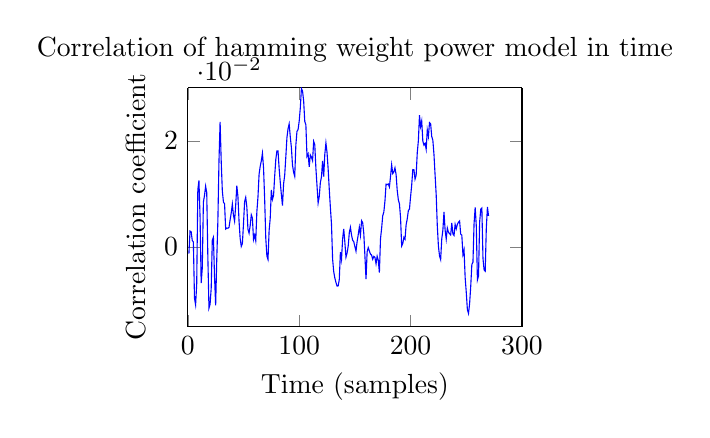
\begin{tikzpicture}

\begin{axis}[%
width=0.35\textwidth,
height=0.25\textwidth,,
at={(0.808889in,0.513333in)},
scale only axis,
separate axis lines,
every outer x axis line/.append style={black},
every x tick label/.append style={font=\color{black}},
xmin=0,
xmax=300,
xlabel={Time (samples)},
every outer y axis line/.append style={black},
every y tick label/.append style={font=\color{black}},
ymin=-0.015,
ymax=0.03,
ylabel={Correlation coefficient},
title={Correlation of hamming weight power model in time}
]
\addplot [color=blue,solid,forget plot]
  table[row sep=crcr]{%
1	-0.00124191773261663\\
2	0.0030113596814982\\
3	0.00289109089867848\\
4	0.00123781070369827\\
5	0.000946988099887706\\
6	-0.00963444456891048\\
7	-0.0109056011278759\\
8	-0.00693908568775801\\
9	0.0107840735377005\\
10	0.0125343776608963\\
11	0.00566982040264624\\
12	-0.00680774801629883\\
13	-0.0039857261866801\\
14	0.00845116032263932\\
15	0.00973204798306401\\
16	0.0114699437140086\\
17	0.0102242980271022\\
18	-0.00188520243615174\\
19	-0.011520990383235\\
20	-0.0107994196744361\\
21	-0.00779826654767437\\
22	0.00127836360759566\\
23	0.00184099855521863\\
24	-0.00561061399013105\\
25	-0.0110238613417115\\
26	-0.00233640502978669\\
27	0.00491525759274175\\
28	0.0162957240373947\\
29	0.0235784489774345\\
30	0.0161311968058564\\
31	0.010577854938711\\
32	0.00847933255520345\\
33	0.00814075206845977\\
34	0.00338920605486348\\
35	0.00357758181192201\\
36	0.00353462925392203\\
37	0.00371033914123386\\
38	0.00513368956680668\\
39	0.00644602160490702\\
40	0.00810143338560267\\
41	0.00594765144431687\\
42	0.00488144389474298\\
43	0.00788758203240359\\
44	0.0115626544397195\\
45	0.0095393978895833\\
46	0.00489084523519676\\
47	0.0016434349561334\\
48	0.000110585378525003\\
49	0.00064212369376973\\
50	0.0043502502868252\\
51	0.00854519292415432\\
52	0.0093547656277726\\
53	0.0075759580881727\\
54	0.00334525961247561\\
55	0.00260739368365825\\
56	0.00401939318844564\\
57	0.00606398367998837\\
58	0.00545671747650534\\
59	0.00139574356078864\\
60	0.00223948171628768\\
61	0.00117639393290399\\
62	0.00664535368435871\\
63	0.00942843442897756\\
64	0.0137394836445989\\
65	0.0152050374130569\\
66	0.0162404709354973\\
67	0.0176702389979158\\
68	0.0149286199194695\\
69	0.00902697241161608\\
70	0.00169534674270825\\
71	-0.00170090513636259\\
72	-0.00236137751348041\\
73	0.00312303886427912\\
74	0.00544256576778266\\
75	0.0107635657109928\\
76	0.00897151525788931\\
77	0.00972964986274892\\
78	0.0133615773465619\\
79	0.0164878422702489\\
80	0.0181110139216583\\
81	0.0180974103658555\\
82	0.0147971413265753\\
83	0.0122360224522456\\
84	0.00988971086424685\\
85	0.00781228758588674\\
86	0.011893444938721\\
87	0.0135579821251652\\
88	0.0169804270891448\\
89	0.0206276522372343\\
90	0.0222882340151556\\
91	0.0232047034746379\\
92	0.0207869299392288\\
93	0.0187463938747807\\
94	0.0154273616867361\\
95	0.014090969845343\\
96	0.0133122515873653\\
97	0.0192029253694727\\
98	0.0217988978932191\\
99	0.0221291846571882\\
100	0.023714742369614\\
101	0.0262075110688421\\
102	0.0298812102452692\\
103	0.029395827675228\\
104	0.0275719947743781\\
105	0.0236841126592988\\
106	0.0230745707301824\\
107	0.0170984254920128\\
108	0.0175613329615171\\
109	0.0151337558018334\\
110	0.017359965898522\\
111	0.0169514169594454\\
112	0.0162865797466159\\
113	0.0198947287357161\\
114	0.0192696502810309\\
115	0.0148477975494898\\
116	0.0115568937642499\\
117	0.00827487217719095\\
118	0.00950553735194381\\
119	0.0121305282915203\\
120	0.0132110607821113\\
121	0.016221619209943\\
122	0.0132699938496486\\
123	0.017461760423934\\
124	0.0196224964573608\\
125	0.0178089702584998\\
126	0.0147178632043674\\
127	0.010908698274486\\
128	0.00745621092976937\\
129	0.00430520214184352\\
130	-0.00229445074267941\\
131	-0.00463806388393287\\
132	-0.00584383423298488\\
133	-0.00668717003628973\\
134	-0.00736562241783064\\
135	-0.00733730561174687\\
136	-0.00613328405343555\\
137	-0.000963440528132496\\
138	-0.00234440088529196\\
139	0.00153726714415262\\
140	0.00342972877119273\\
141	0.000879306751637951\\
142	-0.00191751454386069\\
143	-0.00113280759343479\\
144	0.000165646801663336\\
145	0.00271804058095337\\
146	0.0037041346598561\\
147	0.00224039042791531\\
148	0.00128808306694788\\
149	0.000988697719348249\\
150	8.9761801292765e-05\\
151	-0.000790255444482092\\
152	0.00101504118304252\\
153	0.00230358947036091\\
154	0.00375161175819585\\
155	0.00220319781361994\\
156	0.00496017213796447\\
157	0.00458326128199121\\
158	0.00258186697643241\\
159	-0.00163707894276586\\
160	-0.00606466071647902\\
161	-0.000886345671117554\\
162	-0.000120729691147705\\
163	-0.000765902220651173\\
164	-0.00132455552099588\\
165	-0.00151523532022148\\
166	-0.00230873108163041\\
167	-0.00176492347117222\\
168	-0.00195785092368255\\
169	-0.00316502628396143\\
170	-0.00174031470151016\\
171	-0.00250051816691157\\
172	-0.0048442383672242\\
173	0.00154479777923792\\
174	0.003489420887422\\
175	0.00588981694363952\\
176	0.0066047013568394\\
177	0.00867552177724619\\
178	0.0118487571767962\\
179	0.0117726684930586\\
180	0.0118871092965044\\
181	0.0113115248822237\\
182	0.0133061472422339\\
183	0.0155010005142736\\
184	0.0138377631682439\\
185	0.0141670633649859\\
186	0.0149333226885092\\
187	0.0136628551967338\\
188	0.0106901539638818\\
189	0.00891613188907318\\
190	0.0081262156260998\\
191	0.00554882708633702\\
192	0.000188773855982359\\
193	0.000638565042642912\\
194	0.00182912519553584\\
195	0.00146194110102414\\
196	0.00419242580913252\\
197	0.00528210952063613\\
198	0.00684721699620003\\
199	0.00715148459886334\\
200	0.00948083812227323\\
201	0.0116349390106813\\
202	0.0146002272634951\\
203	0.0145933113233584\\
204	0.0127874378152599\\
205	0.0135011483203399\\
206	0.0177760801932774\\
207	0.0200503882003281\\
208	0.0248390921158618\\
209	0.0226952696941551\\
210	0.0237680512273026\\
211	0.0199705835695962\\
212	0.0192142772463609\\
213	0.0195393179201207\\
214	0.0184200390804313\\
215	0.0220775114553524\\
216	0.0208438183729957\\
217	0.0234521226926168\\
218	0.0232450444027285\\
219	0.0208182208289462\\
220	0.0201331379725087\\
221	0.0174619680724985\\
222	0.0135882200243351\\
223	0.00982326491362919\\
224	0.00397401813164816\\
225	0.000141901213755831\\
226	-0.00169854609445165\\
227	-0.00237724208460807\\
228	0.00153514882408431\\
229	0.00318118431628132\\
230	0.00659913094959573\\
231	0.00322255793069725\\
232	0.00150184307461262\\
233	0.00356748309912564\\
234	0.00275809290490935\\
235	0.00252787453237611\\
236	0.00227568087135651\\
237	0.00452637970640076\\
238	0.00245232879247686\\
239	0.00216681173792444\\
240	0.00425511921157511\\
241	0.00342699651771782\\
242	0.00428385417832136\\
243	0.00466312117151907\\
244	0.0049090152475067\\
245	0.00243430313544051\\
246	0.00224586974842287\\
247	-0.00140734363745939\\
248	-0.00051863732787613\\
249	-0.00578598921261964\\
250	-0.00854277852908817\\
251	-0.0118068677279879\\
252	-0.0125245381309007\\
253	-0.0106753797199441\\
254	-0.00742991762197474\\
255	-0.0033085366870462\\
256	-0.00288477299314674\\
257	0.00443825555692561\\
258	0.00747715112699129\\
259	0.00397046933113535\\
260	-0.00621269406074981\\
261	-0.00545625203895992\\
262	0.0046750592815325\\
263	0.00713684442987915\\
264	0.00734749748562999\\
265	-0.00215008113120001\\
266	-0.00430928584387462\\
267	-0.00456424450346352\\
268	0.00360033000956093\\
269	0.00754387965510516\\
270	0.00587055437017652\\
};
\end{axis}
\end{tikzpicture}%
  \caption{Measured Hamming Distance.}
	\label{fig:cor}
  \end{figure}
  
\section{Conclusion}\label{sec::conclusion} 


% Summarize results and lessons learned.
	Both DPA and CPA have previously been shown to work at recovering secret keys from DES.  We were not able to reproduce such promising results.  We still believe that DPA and CPA should work to recover secret keys from DES but there were some potential flaws in our methods.
  One aspect to this project which could have been done better would have been to take more traces for a single plain text value.  We took 20 traces for each plain text, but we believe that if we had taken many more than this the noise would have averaged out more nicely and the results may have been better.  Perhaps we should have taken an order of magnitude more traces than what we did.  We believe that this was the main contributing factor to the side channel attacks not producing the expected results.
\bibliography{report}
% that's all folks



\end{document}






